\documentclass[twoside]{book}

% Packages required by doxygen
\usepackage{calc}
\usepackage{doxygen}
\usepackage{graphicx}
\usepackage[utf8]{inputenc}
\usepackage{makeidx}
\usepackage{multicol}
\usepackage{multirow}
\usepackage{textcomp}
\usepackage[table]{xcolor}

% Font selection
\usepackage[T1]{fontenc}
\usepackage{mathptmx}
\usepackage[scaled=.90]{helvet}
\usepackage{courier}
\usepackage{amssymb}
\usepackage{sectsty}
\renewcommand{\familydefault}{\sfdefault}
\allsectionsfont{%
  \fontseries{bc}\selectfont%
  \color{darkgray}%
}
\renewcommand{\DoxyLabelFont}{%
  \fontseries{bc}\selectfont%
  \color{darkgray}%
}

% Page & text layout
\usepackage{geometry}
\geometry{%
  a4paper,%
  top=2.5cm,%
  bottom=2.5cm,%
  left=2.5cm,%
  right=2.5cm%
}
\tolerance=750
\hfuzz=15pt
\hbadness=750
\setlength{\emergencystretch}{15pt}
\setlength{\parindent}{0cm}
\setlength{\parskip}{0.2cm}
\makeatletter
\renewcommand{\paragraph}{%
  \@startsection{paragraph}{4}{0ex}{-1.0ex}{1.0ex}{%
    \normalfont\normalsize\bfseries\SS@parafont%
  }%
}
\renewcommand{\subparagraph}{%
  \@startsection{subparagraph}{5}{0ex}{-1.0ex}{1.0ex}{%
    \normalfont\normalsize\bfseries\SS@subparafont%
  }%
}
\makeatother

% Headers & footers
\usepackage{fancyhdr}
\pagestyle{fancyplain}
\fancyhead[LE]{\fancyplain{}{\bfseries\thepage}}
\fancyhead[CE]{\fancyplain{}{}}
\fancyhead[RE]{\fancyplain{}{\bfseries\leftmark}}
\fancyhead[LO]{\fancyplain{}{\bfseries\rightmark}}
\fancyhead[CO]{\fancyplain{}{}}
\fancyhead[RO]{\fancyplain{}{\bfseries\thepage}}
\fancyfoot[LE]{\fancyplain{}{}}
\fancyfoot[CE]{\fancyplain{}{}}
\fancyfoot[RE]{\fancyplain{}{\bfseries\scriptsize Generated on Sat Nov 23 2013 17\-:43\-:23 for Pr�ctica\-\_\-5\-\_\-\-L\-D\-H by Doxygen }}
\fancyfoot[LO]{\fancyplain{}{\bfseries\scriptsize Generated on Sat Nov 23 2013 17\-:43\-:23 for Pr�ctica\-\_\-5\-\_\-\-L\-D\-H by Doxygen }}
\fancyfoot[CO]{\fancyplain{}{}}
\fancyfoot[RO]{\fancyplain{}{}}
\renewcommand{\footrulewidth}{0.4pt}
\renewcommand{\chaptermark}[1]{%
  \markboth{#1}{}%
}
\renewcommand{\sectionmark}[1]{%
  \markright{\thesection\ #1}%
}

% Indices & bibliography
\usepackage{natbib}
\usepackage[titles]{tocloft}
\setcounter{tocdepth}{3}
\setcounter{secnumdepth}{5}
\makeindex

% Hyperlinks (required, but should be loaded last)
\usepackage{ifpdf}
\ifpdf
  \usepackage[pdftex,pagebackref=true]{hyperref}
\else
  \usepackage[ps2pdf,pagebackref=true]{hyperref}
\fi
\hypersetup{%
  colorlinks=true,%
  linkcolor=blue,%
  citecolor=blue,%
  unicode%
}

% Custom commands
\newcommand{\clearemptydoublepage}{%
  \newpage{\pagestyle{empty}\cleardoublepage}%
}


%===== C O N T E N T S =====

\begin{document}

% Titlepage & ToC
\hypersetup{pageanchor=false}
\pagenumbering{roman}
\begin{titlepage}
\vspace*{7cm}
\begin{center}%
{\Large Pr�ctica\-\_\-5\-\_\-\-L\-D\-H \\[1ex]\large 1.\-2 }\\
\vspace*{1cm}
{\large Generated by Doxygen 1.8.5}\\
\vspace*{0.5cm}
{\small Sat Nov 23 2013 17:43:23}\\
\end{center}
\end{titlepage}
\clearemptydoublepage
\tableofcontents
\clearemptydoublepage
\pagenumbering{arabic}
\hypersetup{pageanchor=true}

%--- Begin generated contents ---
\chapter{Todo List}
\label{todo}
\hypertarget{todo}{}

\begin{DoxyRefList}
\item[\label{todo__todo000001}%
\hypertarget{todo__todo000001}{}%
Member \hyperlink{classexamples_1_1audit_1_1_coins_example_ac0a78806e49f802c46d856b1b666d815}{examples.audit.Coins\-Example.make\-Change\-For\-Amount} (int a\-\_\-target\-Change\-Amount)]class Evaluator\-: input\-:
\begin{DoxyItemize}
\item Permuting\-Configuration
\item Number of evaluation runs pers config (to turn off randomness as much as possible)
\item output facility (data container)
\item optional\-: event subscribers output\-:
\item averaged curve of fitness value thru all generations
\item best fitness value accomplished
\item average number of performance improvements for all generations  
\end{DoxyItemize}
\item[\label{todo__todo000002}%
\hypertarget{todo__todo000002}{}%
Member \hyperlink{classexamples_1_1energy_1_1_coins_energy_1_1_energy_gene_constraint_checker_ae31617c18c0e2fb2c936e5994473bf3c}{examples.energy.Coins\-Energy.Energy\-Gene\-Constraint\-Checker.verify} (Gene a\-\_\-gene, final Object a\-\_\-allele\-Value, final I\-Chromosome a\-\_\-chrom, final int a\-\_\-gene\-Index)]compute  
\item[\label{todo__todo000003}%
\hypertarget{todo__todo000003}{}%
Member \hyperlink{classexamples_1_1gp_1_1anttrail_1_1_ant_map_a659ac2b9f81a55d17fb2e236574c8c70}{examples.gp.anttrail.Ant\-Map.Ant\-Map} (final int\mbox{[}\mbox{]}\mbox{[}\mbox{]} a\-\_\-map, int a\-\_\-max\-Moves)]speedup possible by using string?  
\item[\label{todo__todo000004}%
\hypertarget{todo__todo000004}{}%
Member \hyperlink{classexamples_1_1gp_1_1_fibonacci_a09f676281515cca71bae669293152c09}{examples.gp.Fibonacci.create} ()]allow to optionally preset a static program in each chromosome  
\item[\label{todo__todo000005}%
\hypertarget{todo__todo000005}{}%
Member \hyperlink{classexamples_1_1gp_1_1_fibonacci_1_1_formula_fitness_function_a223e3cdf4059c9783a54841061460a8c}{examples.gp.Fibonacci.Formula\-Fitness\-Function.compute\-Raw\-Fitness} (final I\-G\-P\-Program a\-\_\-program)]check if program valid, i.\-e. worth evaluating 

add penalty for longer solutions  
\item[\label{todo__todo000007}%
\hypertarget{todo__todo000007}{}%
Member \hyperlink{classexamples_1_1gp_1_1island_1_1_island_g_p_example_a830119e3f370d14fb0be6187f1d9aa28}{examples.gp.island.Island\-G\-P\-Example.Island\-G\-P\-Example} ()]Island config. einbauen, so dass Island model automatisch ausgef�hrt wird 

impl. Merge\-Event, e.\-g.\-: merge islands when one island stucks 

jeweils beste l�sung geht �fters verloren! Beeinflusst ein Island das andere oder ist die L�sung in einem Island nicht best�ndig?  
\item[\label{todo__todo000010}%
\hypertarget{todo__todo000010}{}%
Member \hyperlink{classexamples_1_1gp_1_1tictactoe_1_1_evaluate_board_abece9125d9ee8fb48cf6aa5a96af7c0a}{examples.gp.tictactoe.Evaluate\-Board.execute\-\_\-void} (Program\-Chromosome c, int n, Object\mbox{[}\mbox{]} args)]support other types than integer  
\item[\label{todo__todo000011}%
\hypertarget{todo__todo000011}{}%
Member \hyperlink{classexamples_1_1gp_1_1tictactoe_1_1_single_node_validator_a32e7b83ad42a193123dbe4dbf9aefc25}{examples.gp.tictactoe.Single\-Node\-Validator.is\-Allowed} (int a\-\_\-chrom\-Index, Program\-Chromosome a\-\_\-pc, Command\-Gene\mbox{[}\mbox{]} a\-\_\-function\-Set, Command\-Gene a\-\_\-function, Class a\-\_\-return\-Type, int a\-\_\-sub\-Return\-Typ, int m\-\_\-index)]provide convenient method set\-Non\-Consecutive(boolean) in Command\-Gene  
\item[\label{todo__todo000017}%
\hypertarget{todo__todo000017}{}%
Member \hyperlink{classexamples_1_1gp_1_1tictactoe_1_1_tic_tac_toe_main_a477f163a17746606ab745ce91e9bde7f}{examples.gp.tictactoe.Tic\-Tac\-Toe\-Main.create} (G\-P\-Configuration a\-\_\-conf, int a\-\_\-color, G\-P\-Genotype a\-\_\-other, int a\-\_\-other\-Color)]evaluate board to matrix  
\item[\label{todo__todo000018}%
\hypertarget{todo__todo000018}{}%
Member \hyperlink{classexamples_1_1gp_1_1tictactoe_1_1_tic_tac_toe_main_1_1_game_fitness_function_abbccfc65cec2ab000327b001f2089822}{examples.gp.tictactoe.Tic\-Tac\-Toe\-Main.Game\-Fitness\-Function.compute\-Raw\-Fitness} (final I\-G\-P\-Program a\-\_\-program)]reduce fitness for N\-O\-P 

value memory reads and writes  
\item[\label{todo__todo000020}%
\hypertarget{todo__todo000020}{}%
Member \hyperlink{classexamples_1_1island_1_1_island_example_aad36c7af08e927224e83d83a04b104e1}{examples.island.Island\-Example.start} ()]
\item[\label{todo__todo000021}%
\hypertarget{todo__todo000021}{}%
Member \hyperlink{classexamples_1_1monalisa_1_1core_1_1_alpha_mutation_operator_ae1fcb87d1d1a9d22a86b7f4bb5593c60}{examples.monalisa.core.Alpha\-Mutation\-Operator.operate} (final Population a\-\_\-population, final List a\-\_\-candidate\-Chromosomes)]move to base class, refactor  
\item[\label{todo__todo000022}%
\hypertarget{todo__todo000022}{}%
Member \hyperlink{classexamples_1_1monalisa_1_1core_1_1_alpha_off_mutation_operator_a68240b26bc561f24ab1251cc97ae9252}{examples.monalisa.core.Alpha\-Off\-Mutation\-Operator.operate} (final Population a\-\_\-population, final List a\-\_\-candidate\-Chromosomes)]move to base class, refactor  
\item[\label{todo__todo000023}%
\hypertarget{todo__todo000023}{}%
Member \hyperlink{classexamples_1_1monalisa_1_1core_1_1_color_mutation_operator_a1143ed54d24aa0d922111a8bede53f0d}{examples.monalisa.core.Color\-Mutation\-Operator.operate} (final Population a\-\_\-population, final List a\-\_\-candidate\-Chromosomes)]move to base class, refactor  
\item[\label{todo__todo000024}%
\hypertarget{todo__todo000024}{}%
Member \hyperlink{classexamples_1_1monalisa_1_1core_1_1_point_mutation_operator_a77dc2c33c39c88ed99f6300dd8022125}{examples.monalisa.core.Point\-Mutation\-Operator.operate} (final Population a\-\_\-population, final List a\-\_\-candidate\-Chromosomes)]move to base class, refactor  
\item[\label{todo__todo000025}%
\hypertarget{todo__todo000025}{}%
Member \hyperlink{classexamples_1_1monalisa_1_1core_1_1_polygon_mutation_operator_a007895c5c90286148d47ef8d1cd1ce93}{examples.monalisa.core.Polygon\-Mutation\-Operator.operate} (final Population a\-\_\-population, final List a\-\_\-candidate\-Chromosomes)]move to base class, refactor  
\item[\label{todo__todo000026}%
\hypertarget{todo__todo000026}{}%
Member \hyperlink{classexamples_1_1monalisa_1_1core_1_1_single_mutation_operator_a07db0eb33cb05fa3407e1b560e0a7a9a}{examples.monalisa.core.Single\-Mutation\-Operator.operate} (final Population a\-\_\-population, final List a\-\_\-candidate\-Chromosomes)]move to base class, refactor  
\item[\label{todo__todo000027}%
\hypertarget{todo__todo000027}{}%
Member \hyperlink{classexamples_1_1simple_boolean_threaded_1_1_simple_example_ab55245566b467d39fbc8098617ba5cbe}{examples.simple\-Boolean\-Threaded.Simple\-Example.main} (String\mbox{[}\mbox{]} args)]evaluate monitor data  
\item[\label{todo__todo000029}%
\hypertarget{todo__todo000029}{}%
Member \hyperlink{classorg_1_1jgap_1_1audit_1_1_evaluator_a68331d6b5db79708b87b72d5077a0e5e}{org.jgap.audit.Evaluator.calc\-Avg\-Fitness\-Impr} (int a\-\_\-permutation)]implement 

implement 

is this method used resp. contained in calc\-Performance?  
\item[\label{todo__todo000028}%
\hypertarget{todo__todo000028}{}%
Member \hyperlink{classorg_1_1jgap_1_1audit_1_1_evaluator_a7a2bf7a73556818006b153c300212453}{org.jgap.audit.Evaluator.C\-V\-S\-\_\-\-R\-E\-V\-I\-S\-I\-O\-N} ]implement\-: overall score calculation (out of best/avg. fitness value etc.)  
\item[\label{todo__todo000032}%
\hypertarget{todo__todo000032}{}%
Member \hyperlink{classorg_1_1jgap_1_1audit_1_1_evaluator_a48f84bb9929cec12795c98bf1185ac68}{org.jgap.audit.Evaluator.store\-Population} (int a\-\_\-permutation, int a\-\_\-run, Population a\-\_\-pop)]implement  
\item[\label{todo__todo000033}%
\hypertarget{todo__todo000033}{}%
Member \hyperlink{classorg_1_1jgap_1_1audit_1_1_evolution_evaluator_a411341e5eb1abbec8e0995d8fb49727a}{org.jgap.audit.Evolution\-Evaluator.evaluate} ()]use chrom\-I\-Ds and chrom\-Track 


\item[\label{todo__todo000035}%
\hypertarget{todo__todo000035}{}%
Member \hyperlink{classorg_1_1jgap_1_1audit_1_1_permuting_configuration_a541cb4586f480c4991369f04753a2be8}{org.jgap.audit.Permuting\-Configuration.next} ()]make permutation below computed dynamic and not static 

introduce new parameters\-: population\-Size, set\-Preserv\-Fittest\-Individual, M\-A\-X\-\_\-\-A\-L\-L\-O\-W\-E\-D\-\_\-\-E\-V\-O\-L\-U\-T\-I\-O\-N\-S 

allow for \char`\"{}false\char`\"{} 

Bulk\-Fitness\-Offset\-Remover vs. Fitness\-Function  
\item[\label{todo__todo000039}%
\hypertarget{todo__todo000039}{}%
Member \hyperlink{classorg_1_1jgap_1_1_base_chromosome_a30276dc8afb0bd632c288bf7d2e18b55}{org.jgap.Base\-Chromosome.set\-Value\-From\-Persistent\-Representation} (String a\-\_\-representation)]we can do this faster! 

we can do this faster!  
\item[\label{todo__todo000041}%
\hypertarget{todo__todo000041}{}%
Member \hyperlink{classorg_1_1jgap_1_1_base_gene_a40f8f3d249145ad028892cd706ba9dae}{org.jgap.Base\-Gene.new\-Gene} ()]clone app.\-data  
\item[\label{todo__todo000184}%
\hypertarget{todo__todo000184}{}%
Member \hyperlink{classorg_1_1jgap_1_1_base_gene_test_a8e859f6d03d8eb3ce5dfe926d11eed92}{org.jgap.Base\-Gene\-Test.test\-Equals\-\_\-3} ()]use other than J\-G\-A\-P\-Factory to be able to receive a null Compare\-To\-Handler for the application data object  
\item[\label{todo__todo000185}%
\hypertarget{todo__todo000185}{}%
Member \hyperlink{classorg_1_1jgap_1_1_base_gene_test_a00bdb1c53bcf6d47c9ad16fec5a52de3}{org.jgap.Base\-Gene\-Test.test\-Set\-Application\-Data\-\_\-1} ()]find the one chromosome  
\item[\label{todo__todo000186}%
\hypertarget{todo__todo000186}{}%
Member \hyperlink{classorg_1_1jgap_1_1_base_gene_test_ab2cd872d724507f006962aecc05830f6}{org.jgap.Base\-Gene\-Test.test\-Set\-Application\-Data\-\_\-2} ()]find the one chromosome  
\item[\label{todo__todo000043}%
\hypertarget{todo__todo000043}{}%
Member \hyperlink{classorg_1_1jgap_1_1_base_genetic_operator_a4db6fa1a99177114c0f19f02cd4a87ec}{org.jgap.Base\-Genetic\-Operator.equals} (final Object a\-\_\-other)]also compare Configuration?  
\item[\label{todo__todo000042}%
\hypertarget{todo__todo000042}{}%
Member \hyperlink{classorg_1_1jgap_1_1_base_genetic_operator_addbc6b98f572331d47397227b7a49f6a}{org.jgap.Base\-Genetic\-Operator.get\-Configuration} ()]make returned object immutable  
\item[\label{todo__todo000046}%
\hypertarget{todo__todo000046}{}%
Member \hyperlink{classorg_1_1jgap_1_1_breeder_base_ac2baa98b33eb5a909ffddc874598c1d2}{org.jgap.Breeder\-Base.apply\-Genetic\-Operators} (Configuration a\-\_\-config, Population a\-\_\-pop)]utilize jobs\-: integrate job into Genetic\-Operator  
\item[\label{todo__todo000044}%
\hypertarget{todo__todo000044}{}%
Member \hyperlink{classorg_1_1jgap_1_1_breeder_base_a3d2ad9ec1c90d78a5598a4dec1400960}{org.jgap.Breeder\-Base.apply\-Natural\-Selectors} (Configuration a\-\_\-config, Population a\-\_\-pop, boolean a\-\_\-process\-Before\-Genetic\-Operators)]optionally use working pool 

utilize jobs\-: integrate job into Natural\-Selector!  
\item[\label{todo__todo000047}%
\hypertarget{todo__todo000047}{}%
Member \hyperlink{classorg_1_1jgap_1_1_cached_fitness_function_ab281e35d33336f473dcc8a252ebcc932}{org.jgap.Cached\-Fitness\-Function.C\-V\-S\-\_\-\-R\-E\-V\-I\-S\-I\-O\-N} ]allow to restrict size of cache / age of entries  
\item[\label{todo__todo000049}%
\hypertarget{todo__todo000049}{}%
Member \hyperlink{classorg_1_1jgap_1_1_chromosome_a9f590d55a34d8b99c2a9a1b4aedd568b}{org.jgap.Chromosome.clone} ()]once output a warning\-: allele should be cloneable!  
\item[\label{todo__todo000052}%
\hypertarget{todo__todo000052}{}%
Member \hyperlink{classorg_1_1jgap_1_1_chromosome_a2be0507944e2ca98bef8372402b33e13}{org.jgap.Chromosome.compare\-To} (Object other)]improve  
\item[\label{todo__todo000048}%
\hypertarget{todo__todo000048}{}%
Member \hyperlink{classorg_1_1jgap_1_1_chromosome_a6d73c5e40fce0219e80021211d4a2d57}{org.jgap.Chromosome.m\-\_\-multi\-Objective} ]move to new subclass of Chromosome (and introduce new interface I\-Multi\-Objective with that)  
\item[\label{todo__todo000050}%
\hypertarget{todo__todo000050}{}%
Member \hyperlink{classorg_1_1jgap_1_1_chromosome_a6b6fb5c7c5b532813a4661de5dbd9ab3}{org.jgap.Chromosome.random\-Initial\-Chromosome} (Configuration a\-\_\-configuration)]what about Gene's energy? 

what about Gene's energy?  
\item[\label{todo__todo000053}%
\hypertarget{todo__todo000053}{}%
Member \hyperlink{classorg_1_1jgap_1_1_configuration_a453c6b764b4f017c058632bc22e5a915}{org.jgap.Configuration.do\-Clone} (Object a\-\_\-obj\-To\-Clone)]try cloning in a standard way  
\item[\label{todo__todo000054}%
\hypertarget{todo__todo000054}{}%
Member \hyperlink{classorg_1_1jgap_1_1data_1_1_data_tree_builder_a6a849e086eb4968ee222f54c88fde434}{org.jgap.data.Data\-Tree\-Builder.C\-V\-S\-\_\-\-R\-E\-V\-I\-S\-I\-O\-N} ]implement represent\-G\-P\-Genotype..  
\item[\label{todo__todo000055}%
\hypertarget{todo__todo000055}{}%
Member \hyperlink{classorg_1_1jgap_1_1data_1_1_document_builder_base_a4a15b7fd875043a3c021b54766f9a8ca}{org.jgap.data.Document\-Builder\-Base.C\-V\-S\-\_\-\-R\-E\-V\-I\-S\-I\-O\-N} ]add new class Document\-Creator\-Base that reads in data written by Document\-Builder\-Base  
\item[\label{todo__todo000060}%
\hypertarget{todo__todo000060}{}%
Member \hyperlink{classorg_1_1jgap_1_1distr_1_1_breeder_ab3ff454f082f23bb5885ea8e0aa2ed89}{org.jgap.distr.Breeder.inform\-Parent} ()]implement  
\item[\label{todo__todo000057}%
\hypertarget{todo__todo000057}{}%
Member \hyperlink{classorg_1_1jgap_1_1distr_1_1_breeder_a86129a6e573ed2ca9961931713250483}{org.jgap.distr.Breeder.m\-\_\-genotype} ]use  
\item[\label{todo__todo000058}%
\hypertarget{todo__todo000058}{}%
Member \hyperlink{classorg_1_1jgap_1_1distr_1_1_breeder_a7ed056f076614c9e220460f107259c5a}{org.jgap.distr.Breeder.m\-\_\-population\-Merger} ]construct somewhere  
\item[\label{todo__todo000059}%
\hypertarget{todo__todo000059}{}%
Member \hyperlink{classorg_1_1jgap_1_1distr_1_1_breeder_a91831c9376bf49003f0f162f1a75f8f2}{org.jgap.distr.Breeder.m\-\_\-running} ]use  
\item[\label{todo__todo000056}%
\hypertarget{todo__todo000056}{}%
Member \hyperlink{classorg_1_1jgap_1_1distr_1_1_breeder_a336a3b9df78c37790c4742f7c4eeb456}{org.jgap.distr.Breeder.m\-\_\-workers} ]use  
\item[\label{todo__todo000061}%
\hypertarget{todo__todo000061}{}%
Member \hyperlink{classorg_1_1jgap_1_1distr_1_1_breeder_ad371c6cce93099457783ac1fe6da74ca}{org.jgap.distr.Breeder.stop} ()]implement  
\item[\label{todo__todo000064}%
\hypertarget{todo__todo000064}{}%
Member \hyperlink{classorg_1_1jgap_1_1distr_1_1grid_1_1_dummy_grid_client_mediator_a7212ea568d78375a552bc599e62e4648}{org.jgap.distr.grid.Dummy\-Grid\-Client\-Mediator.get\-Grid\-Message} (Message\-Context a\-\_\-context, String a\-\_\-datetime, int a\-\_\-timeout\-Seconds, int a\-\_\-wait\-Time\-Seconds, boolean a\-\_\-remove\-Request)]fallback solution  
\item[\label{todo__todo000063}%
\hypertarget{todo__todo000063}{}%
Member \hyperlink{classorg_1_1jgap_1_1distr_1_1grid_1_1_dummy_grid_client_mediator_a080ac41bf4278214c07055ebcc9060f8}{org.jgap.distr.grid.Dummy\-Grid\-Client\-Mediator.start\-Client} ()]allow asynchronous wait for server (check for \char`\"{}java.\-net.\-Connect\-Exception\-: Connection refused\-: connect\char`\"{})  
\item[\label{todo__todo000065}%
\hypertarget{todo__todo000065}{}%
Member \hyperlink{interfaceorg_1_1jgap_1_1distr_1_1grid_1_1gp_1_1_i_grid_configuration_g_p_aa7705e8e26bdc18c2c0e5b69e8ac818a}{org.jgap.distr.grid.gp.I\-Grid\-Configuration\-G\-P.set\-Types} (Class\mbox{[}\mbox{]} a\-\_\-types)]move the following to G\-P\-Configuration, elegantly  
\item[\label{todo__todo000066}%
\hypertarget{todo__todo000066}{}%
Member \hyperlink{classorg_1_1jgap_1_1distr_1_1grid_1_1gp_1_1_j_g_a_p_client_g_p_aeaec2e84d46f7ddc2285335acb069a31}{org.jgap.distr.grid.gp.J\-G\-A\-P\-Client\-G\-P.C\-V\-S\-\_\-\-R\-E\-V\-I\-S\-I\-O\-N} ]in dateiname requester/worker kodieren 

auch schlechtere ergebnisse einmixen\-: die direkt empfangenen gleich wieder in einen request reinstecken --$>$ aber mischen verschiedener results in einen request! 

small, medium, large work requests 

re-\/evaluate each result on behalf of another worker\-: keep separate lookup-\/table for all requests --$>$ m\-\_\-results\-Verified, m\-\_\-results\-Persister 

remove old requests from online store automatically 

info when work request has been taken 

info when worker logs on --$>$ evaluate logon files 

top results in eigener datei speichern, komprimierung durch weglassen �berfl. infos, siehe xml --$>$ injection after reload 

copy good results to online folder  
\item[\label{todo__todo000077}%
\hypertarget{todo__todo000077}{}%
Member \hyperlink{classorg_1_1jgap_1_1distr_1_1grid_1_1gp_1_1_j_g_a_p_client_g_p_acfb2127d50b79830207941705b3f268a}{org.jgap.distr.grid.gp.J\-G\-A\-P\-Client\-G\-P.J\-G\-A\-P\-Client\-G\-P} (I\-Grid\-Client\-Mediator a\-\_\-gcmed, Grid\-Node\-Client\-Config a\-\_\-gridconfig, String a\-\_\-client\-Class\-Name, boolean a\-\_\-\-W\-A\-N\-Mode, boolean a\-\_\-receive\-Only, boolean a\-\_\-list, boolean a\-\_\-no\-\_\-comm, boolean a\-\_\-no\-\_\-evolution, boolean a\-\_\-endless, int a\-\_\-max\-\_\-fetch\-\_\-results)]ab 2. zyklus ist pop.\-gr�sse nur 1 !  
\item[\label{todo__todo000075}%
\hypertarget{todo__todo000075}{}%
Member \hyperlink{classorg_1_1jgap_1_1distr_1_1grid_1_1gp_1_1_j_g_a_p_client_g_p_a0535356c14866325a1f7df6faa19db92}{org.jgap.distr.grid.gp.J\-G\-A\-P\-Client\-G\-P.M\-O\-D\-U\-L\-E\-\_\-\-C\-S} ]store version in external file  
\item[\label{todo__todo000076}%
\hypertarget{todo__todo000076}{}%
Member \hyperlink{classorg_1_1jgap_1_1distr_1_1grid_1_1gp_1_1_j_g_a_p_client_g_p_a6424bb7eb2e4963a50cba03b8e28d241}{org.jgap.distr.grid.gp.J\-G\-A\-P\-Client\-G\-P.M\-O\-D\-U\-L\-E\-\_\-\-S\-C} ]das ist nicht module, sondern sender-\/receiver  
\item[\label{todo__todo000093}%
\hypertarget{todo__todo000093}{}%
Member \hyperlink{classorg_1_1jgap_1_1distr_1_1grid_1_1gp_1_1_j_g_a_p_client_g_p_adf5018d320d27b924e0f16a2ac48fea9}{org.jgap.distr.grid.gp.J\-G\-A\-P\-Client\-G\-P.preset\-Population} (J\-G\-A\-P\-Request\-G\-P a\-\_\-work\-Request)]remove results\mbox{[}index\mbox{]}  
\item[\label{todo__todo000085}%
\hypertarget{todo__todo000085}{}%
Member \hyperlink{classorg_1_1jgap_1_1distr_1_1grid_1_1gp_1_1_j_g_a_p_client_g_p_a67409d14f440abb96b91e1aeb99bd860}{org.jgap.distr.grid.gp.J\-G\-A\-P\-Client\-G\-P.receive\-Work\-Result} (Object a\-\_\-result, I\-Client\-Feedback\-G\-P feedback, boolean a\-\_\-remove)]later\-: S\-C  
\item[\label{todo__todo000086}%
\hypertarget{todo__todo000086}{}%
Member \hyperlink{classorg_1_1jgap_1_1distr_1_1grid_1_1gp_1_1_j_g_a_p_client_g_p_a497f3e3cad175f2d5991ad1b5da02663}{org.jgap.distr.grid.gp.J\-G\-A\-P\-Client\-G\-P.receive\-Work\-Result} (J\-G\-A\-P\-Request\-G\-P\mbox{[}\mbox{]} work\-List, I\-Client\-Feedback\-G\-P feedback)]make this asynchronous with fall-\/back and reconnect! 

later\-: S\-C  
\item[\label{todo__todo000080}%
\hypertarget{todo__todo000080}{}%
Member \hyperlink{classorg_1_1jgap_1_1distr_1_1grid_1_1gp_1_1_j_g_a_p_client_g_p_a7a6ca719b3c2154e9f85d3d09228e523}{org.jgap.distr.grid.gp.J\-G\-A\-P\-Client\-G\-P.receive\-Work\-Results} (J\-G\-A\-P\-Request\-G\-P\mbox{[}\mbox{]} work\-List)]later\-: S\-C 

sort results according to post date, the oldest first 

config.\-params wie popsite, evol.\-anz dazu 

allow fitness 0.\-0 

do this here explicitely and not in receive\-Work\-Result  
\item[\label{todo__todo000088}%
\hypertarget{todo__todo000088}{}%
Member \hyperlink{classorg_1_1jgap_1_1distr_1_1grid_1_1gp_1_1_j_g_a_p_client_g_p_a4151e753398914b0d1d945464fa62e2d}{org.jgap.distr.grid.gp.J\-G\-A\-P\-Client\-G\-P.result\-Received} (I\-G\-P\-Program a\-\_\-fittest)]jeden Worker einer von n (rein logischen) Gruppen zuteilen. Pro logischer Gruppe top n Ergebnisse halten 

make configurable 

compare with to\-String\-Norm(0), use remove(int) instead of remove(\-Object) 

ist nur test! 

skip unnecessary data, inject it after reload  
\item[\label{todo__todo000078}%
\hypertarget{todo__todo000078}{}%
Member \hyperlink{classorg_1_1jgap_1_1distr_1_1grid_1_1gp_1_1_j_g_a_p_client_g_p_a256acdc898522793fa73e386b9cbf4e9}{org.jgap.distr.grid.gp.J\-G\-A\-P\-Client\-G\-P.send\-Work\-Requests} (int a\-\_\-evolution\-Index, I\-Client\-Evolve\-Strategy\-G\-P evolver, I\-Request\-Split\-Strategy\-G\-P splitter, I\-Client\-Feedback\-G\-P feedback)]merge previous results in req.\-get\-Population()  
\item[\label{todo__todo000079}%
\hypertarget{todo__todo000079}{}%
Member \hyperlink{classorg_1_1jgap_1_1distr_1_1grid_1_1gp_1_1_j_g_a_p_client_g_p_ada87d248b0be00887061959c808b5ff7}{org.jgap.distr.grid.gp.J\-G\-A\-P\-Client\-G\-P.send\-Work\-Requests} (J\-G\-A\-P\-Request\-G\-P\mbox{[}\mbox{]} a\-\_\-work\-List)]hier ist fehler aufgetreten!  
\item[\label{todo__todo000094}%
\hypertarget{todo__todo000094}{}%
Member \hyperlink{classorg_1_1jgap_1_1distr_1_1grid_1_1gp_1_1_j_g_a_p_worker_g_p_a793842b038b3f6e753208dcc0d9f8d9f}{org.jgap.distr.grid.gp.J\-G\-A\-P\-Worker\-G\-P.C\-V\-S\-\_\-\-R\-E\-V\-I\-S\-I\-O\-N} ]resume previous work in case worker was stopped  
\item[\label{todo__todo000095}%
\hypertarget{todo__todo000095}{}%
Member \hyperlink{classorg_1_1jgap_1_1distr_1_1grid_1_1gp_1_1_j_g_a_p_worker_g_p_aa04fd0437862a49fe5fce45084c0590f}{org.jgap.distr.grid.gp.J\-G\-A\-P\-Worker\-G\-P.do\-Work} (Work\-Request work, String work\-Dir)]set gridworkerfeedback in class Grid\-Worker  
\item[\label{todo__todo000096}%
\hypertarget{todo__todo000096}{}%
Member \hyperlink{classorg_1_1jgap_1_1distr_1_1grid_1_1gp_1_1_j_g_a_p_workers_g_p_a45d28e995ace9be9709cf592c69d5b39}{org.jgap.distr.grid.gp.J\-G\-A\-P\-Workers\-G\-P.get\-Needed\-Files} (Grid\-Node\-Worker\-Config a\-\_\-config)]implement  
\item[\label{todo__todo000098}%
\hypertarget{todo__todo000098}{}%
Member \hyperlink{classorg_1_1jgap_1_1distr_1_1grid_1_1_j_g_a_p_client_handler_thread_a5513a2e631ddea023820d49fc322a781}{org.jgap.distr.grid.J\-G\-A\-P\-Client\-Handler\-Thread.handle\-Msg} (Grid\-Message msg)]consider 4\-G\-B limit  
\item[\label{todo__todo000099}%
\hypertarget{todo__todo000099}{}%
Member \hyperlink{classorg_1_1jgap_1_1distr_1_1grid_1_1_j_g_a_p_worker_ae03c268f54333b88162959811590558d}{org.jgap.distr.grid.J\-G\-A\-P\-Worker.do\-Work} (Work\-Request work, String work\-Dir)]set gridworkerfeedback in class Grid\-Worker  
\item[\label{todo__todo000100}%
\hypertarget{todo__todo000100}{}%
Member \hyperlink{classorg_1_1jgap_1_1distr_1_1grid_1_1_j_g_a_p_workers_a644cc69c70eb0ed5553eaa60e3dadbe7}{org.jgap.distr.grid.J\-G\-A\-P\-Workers.get\-Needed\-Files} (Grid\-Node\-Worker\-Config a\-\_\-config)]
\item[\label{todo__todo000101}%
\hypertarget{todo__todo000101}{}%
Member \hyperlink{classorg_1_1jgap_1_1distr_1_1grid_1_1_request_split_strategy_afa4582eef1f6ae141ff15d706cf7ec68}{org.jgap.distr.grid.Request\-Split\-Strategy.split} (J\-G\-A\-P\-Request a\-\_\-request)]support cloning of m\-\_\-config  
\item[\label{todo__todo000102}%
\hypertarget{todo__todo000102}{}%
Member \hyperlink{classorg_1_1jgap_1_1distr_1_1grid_1_1util_1_1_grid_kit_a7ed064739e97dbc91ad4cd11ac736864}{org.jgap.distr.grid.util.Grid\-Kit.is\-Update\-Available} (String B\-A\-S\-E\-\_\-\-U\-R\-L, String a\-\_\-module\-Name, String current\-Version)]download a versions.\-txt file and obtain version per project  
\item[\label{todo__todo000103}%
\hypertarget{todo__todo000103}{}%
Member \hyperlink{classorg_1_1jgap_1_1distr_1_1grid_1_1util_1_1_grid_kit_a61d160ee177cb0b07e5e5fda371ad48f}{org.jgap.distr.grid.util.Grid\-Kit.update\-Module} (String a\-\_\-filename, String a\-\_\-work\-Dir, String a\-\_\-lib\-Dir)]write log\-: delete manually  
\item[\label{todo__todo000104}%
\hypertarget{todo__todo000104}{}%
Member \hyperlink{classorg_1_1jgap_1_1distr_1_1grid_1_1util_1_1_grid_kit_afa78889ffda168512995505a1ded1b3b}{org.jgap.distr.grid.util.Grid\-Kit.update\-Module\-Library} (String B\-A\-S\-E\-\_\-\-U\-R\-L, String a\-\_\-module\-Name, String a\-\_\-lib\-Dir, String a\-\_\-work\-Dir)]zuordnung irgendwo abspeichern 

zuordnung irgendwo abspeichern 

zuordnung irgendwo abspeichern  
\item[\label{todo__todo000107}%
\hypertarget{todo__todo000107}{}%
Member \hyperlink{classorg_1_1jgap_1_1distr_1_1grid_1_1wan_1_1_request_information_ab29bbb5cde83ff185ae2122f9f9a0147}{org.jgap.distr.grid.wan.Request\-Information.m\-\_\-id} ]worker gibt durch Datei an, dass er Request bearbeitet  
\item[\label{todo__todo000109}%
\hypertarget{todo__todo000109}{}%
Member \hyperlink{classorg_1_1jgap_1_1distr_1_1_master_aef7c64089218808c9b7f0893e31fffbe}{org.jgap.distr.Master.send\-To\-Worker} (final I\-Worker a\-\_\-worker, final Worker\-Command a\-\_\-command)]implement  
\item[\label{todo__todo000108}%
\hypertarget{todo__todo000108}{}%
Member \hyperlink{classorg_1_1jgap_1_1distr_1_1_master_aec0e9db5db3316ec9ee903c3892f5796}{org.jgap.distr.Master.stop} ()]notify all workers to stop working??? No, better would be\-: next time master is available it can receive old results from workers. So, the workers need to store them for some time, until the master is able to receive the worker results.  
\item[\label{todo__todo000113}%
\hypertarget{todo__todo000113}{}%
Member \hyperlink{classorg_1_1jgap_1_1distr_1_1_worker_a405f281453fcdd0046a370a001af92ef}{org.jgap.distr.Worker.get\-Status} ()]implement\-: idle starting receiving task working sending result stopping stopped  
\item[\label{todo__todo000114}%
\hypertarget{todo__todo000114}{}%
Member \hyperlink{classorg_1_1jgap_1_1distr_1_1_worker_aea81d8531d56e4035cd94c5278e5c604}{org.jgap.distr.Worker.pause} ()]implement\-: able to pause resp. in work?  
\item[\label{todo__todo000116}%
\hypertarget{todo__todo000116}{}%
Member \hyperlink{classorg_1_1jgap_1_1distr_1_1_worker_afc27690dd01d55455271aba6dc32b434}{org.jgap.distr.Worker.resume} ()]implement\-: able to resum resp. paused?  
\item[\label{todo__todo000111}%
\hypertarget{todo__todo000111}{}%
Member \hyperlink{classorg_1_1jgap_1_1distr_1_1_worker_aee8f7803e2655bdfb3aceff9a3f92eb7}{org.jgap.distr.Worker.send\-Command} (final Worker\-Command a\-\_\-command)]this should be moved to a thread 

implement\-: currently working? if yes, add to queue (if queue not full) if no\-: start work  
\item[\label{todo__todo000115}%
\hypertarget{todo__todo000115}{}%
Member \hyperlink{classorg_1_1jgap_1_1distr_1_1_worker_a7ecb6526e7b056129e7f4f8a584865de}{org.jgap.distr.Worker.stop} ()]implement\-: able to stop resp. in work?  
\item[\label{todo__todo000117}%
\hypertarget{todo__todo000117}{}%
Member \hyperlink{classorg_1_1jgap_1_1distr_1_1_worker_command_a9b2e86e89542048dc457e6d0a7bd85bd}{org.jgap.distr.Worker\-Command.execute} (final Object a\-\_\-parameters)]implement  
\item[\label{todo__todo000118}%
\hypertarget{todo__todo000118}{}%
Member \hyperlink{classorg_1_1jgap_1_1_genotype_a6c14c3a36aa8e4291840f0b9c0facb35}{org.jgap.Genotype.apply\-Natural\-Selectors} (boolean a\-\_\-process\-Before\-Genetic\-Operators)]optionally use working pool  
\item[\label{todo__todo000119}%
\hypertarget{todo__todo000119}{}%
Member \hyperlink{classorg_1_1jgap_1_1_genotype_af5e224c5b7c05dbe02b3324d5ec16f2a}{org.jgap.Genotype.keep\-Pop\-Size\-Constant} (Population a\-\_\-pop, int a\-\_\-max\-Size)]use Standard\-Post\-Selector instead?  
\item[\label{todo__todo000120}%
\hypertarget{todo__todo000120}{}%
Member \hyperlink{classorg_1_1jgap_1_1_genotype_aa2b0341edc420ad61e797508b8bf4dd5}{org.jgap.Genotype.merge\-Results} (I\-Population\-Merger a\-\_\-merger, Evolve\-Result\mbox{[}\mbox{]} a\-\_\-results)]use/enhance I\-Population\-Merger  
\item[\label{todo__todo000187}%
\hypertarget{todo__todo000187}{}%
Member \hyperlink{classorg_1_1jgap_1_1_genotype_test_aa0d1c56bf7ef0e020f3d979f784dc5d3}{org.jgap.Genotype\-Test.test\-Is\-Serializable\-\_\-0} ()]following will be obsolete  
\item[\label{todo__todo000121}%
\hypertarget{todo__todo000121}{}%
Member \hyperlink{classorg_1_1jgap_1_1gp_1_1_command_gene_a7d5b399cad245a0276bd0b62c9e5a4a8}{org.jgap.gp.Command\-Gene.compare\-To} (Object a\-\_\-other)]do it more precisely  
\item[\label{todo__todo000122}%
\hypertarget{todo__todo000122}{}%
Member \hyperlink{classorg_1_1jgap_1_1gp_1_1_command_gene_a161c170b4493de85203147a84ac13a3b}{org.jgap.gp.Command\-Gene.set\-Value\-From\-Persistent\-Representation} (final String a\-\_\-representation)]finish  
\item[\label{todo__todo000188}%
\hypertarget{todo__todo000188}{}%
Member \hyperlink{classorg_1_1jgap_1_1gp_1_1_command_gene_test_a670aa7b5c2021f31a719ea32218d6671}{org.jgap.gp.Command\-Gene\-Test.test\-Equals\-\_\-3} ()]use other than J\-G\-A\-P\-Factory to be able to receive a null Compare\-To\-Handler for the application data object  
\item[\label{todo__todo000123}%
\hypertarget{todo__todo000123}{}%
Member \hyperlink{classorg_1_1jgap_1_1gp_1_1function_1_1_a_d_f_a5e377b15d81ca7ceec156614480980d7}{org.jgap.gp.function.A\-D\-F.is\-Valid} (Program\-Chromosome a\-\_\-chrom)]enhance  
\item[\label{todo__todo000124}%
\hypertarget{todo__todo000124}{}%
Member \hyperlink{enumorg_1_1jgap_1_1gp_1_1function_1_1_count_matrix_1_1_count_type_a7ab04ee65255adb71c8f6a47b727b775}{org.jgap.gp.function.Count\-Matrix.Count\-Type.C\-O\-L\-U\-M\-N} ]count over whole matrix  
\item[\label{todo__todo000125}%
\hypertarget{todo__todo000125}{}%
Member \hyperlink{classorg_1_1jgap_1_1gp_1_1function_1_1_exchange_memory_a3e44871ecef23f1319115126c507492b}{org.jgap.gp.function.Exchange\-Memory.is\-Affect\-Global\-State} ()]subclass from new abstract class Memory\-Command?  
\item[\label{todo__todo000126}%
\hypertarget{todo__todo000126}{}%
Member \hyperlink{classorg_1_1jgap_1_1gp_1_1function_1_1_for_x_loop_ae448f21b7912eec72d496b62669993e6}{org.jgap.gp.function.For\-X\-Loop.execute\-\_\-void} (Program\-Chromosome c, int n, Object\mbox{[}\mbox{]} args)]only consider variables appearing before F\-O\-R\-X in the program tree  
\item[\label{todo__todo000127}%
\hypertarget{todo__todo000127}{}%
Member \hyperlink{classorg_1_1jgap_1_1gp_1_1function_1_1_if_a3b36ce8fb25456894c4bb2d136bfc5ef}{org.jgap.gp.function.If.execute\-\_\-void} (Program\-Chromosome c, int n, Object\mbox{[}\mbox{]} args)]add option for type of first child to constructor  
\item[\label{todo__todo000128}%
\hypertarget{todo__todo000128}{}%
Member \hyperlink{classorg_1_1jgap_1_1gp_1_1function_1_1_if_dyn_ac7b9aee1521e3c567cfb36655376faf6}{org.jgap.gp.function.If\-Dyn.execute\-\_\-void} (Program\-Chromosome c, int n, Object\mbox{[}\mbox{]} args)]add option for type of first child to constructor  
\item[\label{todo__todo000129}%
\hypertarget{todo__todo000129}{}%
Member \hyperlink{classorg_1_1jgap_1_1gp_1_1function_1_1_push_a44b325b83a314c139630027e8664eb98}{org.jgap.gp.function.Push.is\-Affect\-Global\-State} ()]use this information  
\item[\label{todo__todo000130}%
\hypertarget{todo__todo000130}{}%
Member \hyperlink{classorg_1_1jgap_1_1gp_1_1function_1_1_push_a6fc7b172011e49476bbf72e88f0512a6}{org.jgap.gp.function.Push.is\-Valid} (Program\-Chromosome a\-\_\-program)]consider n (execute\-\_\-int...)  
\item[\label{todo__todo000133}%
\hypertarget{todo__todo000133}{}%
Member \hyperlink{classorg_1_1jgap_1_1gp_1_1function_1_1_sub_program_a9ef69a70d4ce63696a5825e6f1bbaae8}{org.jgap.gp.function.Sub\-Program.apply\-Mutation} ()]use dynamize\-Arity instead!  
\item[\label{todo__todo000131}%
\hypertarget{todo__todo000131}{}%
Member \hyperlink{classorg_1_1jgap_1_1gp_1_1function_1_1_sub_program_a310c68bd816320dab6cf5c797ef398dc}{org.jgap.gp.function.Sub\-Program.execute\-\_\-int} (Program\-Chromosome c, int n, Object\mbox{[}\mbox{]} args)]evaluate m\-\_\-types  
\item[\label{todo__todo000132}%
\hypertarget{todo__todo000132}{}%
Member \hyperlink{classorg_1_1jgap_1_1gp_1_1function_1_1_sub_program_a6d8e0b323c21b311572bde0fcb8ea3e3}{org.jgap.gp.function.Sub\-Program.execute\-\_\-void} (Program\-Chromosome c, int n, Object\mbox{[}\mbox{]} args)]evaluate m\-\_\-types  
\item[\label{todo__todo000134}%
\hypertarget{todo__todo000134}{}%
Member \hyperlink{classorg_1_1jgap_1_1gp_1_1function_1_1_transfer_memory_a3eb497c878c705b6a8006d87b5d1db70}{org.jgap.gp.function.Transfer\-Memory.is\-Affect\-Global\-State} ()]subclass from new abstract class Memory\-Command?  
\item[\label{todo__todo000136}%
\hypertarget{todo__todo000136}{}%
Member \hyperlink{classorg_1_1jgap_1_1gp_1_1impl_1_1_branch_typing_cross_af4ff7487c5e532031d260dce1b66d74b}{org.jgap.gp.impl.Branch\-Typing\-Cross.do\-Cross} (Program\-Chromosome a\-\_\-c0, Program\-Chromosome a\-\_\-c1)]solve in general  
\item[\label{todo__todo000135}%
\hypertarget{todo__todo000135}{}%
Member \hyperlink{classorg_1_1jgap_1_1gp_1_1impl_1_1_branch_typing_cross_ac9c1c1bf7edeadd26dccbcdd9d33ffc3}{org.jgap.gp.impl.Branch\-Typing\-Cross.operate} (final I\-G\-P\-Program a\-\_\-i1, final I\-G\-P\-Program a\-\_\-i2)]try to ensure uniqueness for unique commands\-: after selecting first node, check if there is a unique node in the sub tree. If so, check if it appears in the sub tree of the second node.  
\item[\label{todo__todo000137}%
\hypertarget{todo__todo000137}{}%
Member \hyperlink{classorg_1_1jgap_1_1gp_1_1impl_1_1_default_population_creator_af6c38314bce32cc040b6beaa0160521f}{org.jgap.gp.impl.Default\-Population\-Creator.initialize} (G\-P\-Population a\-\_\-pop, Class\mbox{[}\mbox{]} a\-\_\-types, Class\mbox{[}\mbox{]}\mbox{[}\mbox{]} a\-\_\-arg\-Types, Command\-Gene\mbox{[}\mbox{]}\mbox{[}\mbox{]} a\-\_\-node\-Sets, int\mbox{[}\mbox{]} a\-\_\-min\-Depths, int\mbox{[}\mbox{]} a\-\_\-max\-Depths, int a\-\_\-max\-Nodes, boolean\mbox{[}\mbox{]} a\-\_\-full\-Mode\-Allowed)]pass params (e.\-g. advanced yes/no for Robocode)  
\item[\label{todo__todo000138}%
\hypertarget{todo__todo000138}{}%
Member \hyperlink{classorg_1_1jgap_1_1gp_1_1impl_1_1_fitness_proportionate_selection_a1bba66dc3595d954f39bd4121bc1fa7f}{org.jgap.gp.impl.Fitness\-Proportionate\-Selection.select} (G\-P\-Genotype a\-\_\-genotype)]implement for delta\-Mode  
\item[\label{todo__todo000141}%
\hypertarget{todo__todo000141}{}%
Member \hyperlink{classorg_1_1jgap_1_1gp_1_1impl_1_1_g_p_configuration_a919b59fd6a2dd43716d28f661ccaf924}{org.jgap.gp.impl.G\-P\-Configuration.get\-Crossover\-Prob} ()]implement something like that  
\item[\label{todo__todo000140}%
\hypertarget{todo__todo000140}{}%
Member \hyperlink{classorg_1_1jgap_1_1gp_1_1impl_1_1_g_p_configuration_a97498de731029f37e23ac9ff7bab3de2}{org.jgap.gp.impl.G\-P\-Configuration.init} (boolean a\-\_\-full\-Init)]make reusable in class Configuration and reuse here from Configuration  
\item[\label{todo__todo000139}%
\hypertarget{todo__todo000139}{}%
Member \hyperlink{classorg_1_1jgap_1_1gp_1_1impl_1_1_g_p_configuration_a620f23497a17109be4d8394cc1c541e1}{org.jgap.gp.impl.G\-P\-Configuration.m\-\_\-objective\-Function} ]introduce lock for configuration  
\item[\label{todo__todo000144}%
\hypertarget{todo__todo000144}{}%
Member \hyperlink{classorg_1_1jgap_1_1gp_1_1impl_1_1_g_p_genotype_aa465c7cbfb45d77644b3d195782a12c9}{org.jgap.gp.impl.G\-P\-Genotype.calc\-Fitness} ()]get information from fitness function how calculation happened. In case of Robocode\-: return the robot competed against, in case the -\/enemies option was used without -\/battle\-All 

do something similar here as with Genotype.\-preserve\-Fittest\-Chromosome 

introduce global value object to be passed to the listener 

should not happen but does with ensure\-Uniqueness(..)  
\item[\label{todo__todo000152}%
\hypertarget{todo__todo000152}{}%
Member \hyperlink{classorg_1_1jgap_1_1gp_1_1impl_1_1_g_p_genotype_aa3bf0b50a73684ff3fe1177017cf9bb8}{org.jgap.gp.impl.G\-P\-Genotype.check\-Erroneous\-Prog} (I\-G\-P\-Program a\-\_\-prog, String s, boolean a\-\_\-clear\-Fitness, boolean a\-\_\-active)]impl. cache  
\item[\label{todo__todo000148}%
\hypertarget{todo__todo000148}{}%
Member \hyperlink{classorg_1_1jgap_1_1gp_1_1impl_1_1_g_p_genotype_ad495c700786596290a63e3d88a902766}{org.jgap.gp.impl.G\-P\-Genotype.evolve} ()]use program creator in case such is registered and returns a non-\/null program 

instead of re-\/using prototype, create a program anyway (ignoring the validator) in case it is the last try. Or even better\-: Make the validator return a defect rate!  
\item[\label{todo__todo000150}%
\hypertarget{todo__todo000150}{}%
Member \hyperlink{classorg_1_1jgap_1_1gp_1_1impl_1_1_g_p_genotype_a4327e7a69fcbcfe051e00e46c933ea7a}{org.jgap.gp.impl.G\-P\-Genotype.fill\-Population} (final int a\-\_\-num)]care about 

implement filling up population  
\item[\label{todo__todo000142}%
\hypertarget{todo__todo000142}{}%
Member \hyperlink{classorg_1_1jgap_1_1gp_1_1impl_1_1_g_p_genotype_af3246cb6a802ae1cde833013c130f6e9}{org.jgap.gp.impl.G\-P\-Genotype.random\-Initial\-Genotype} (final G\-P\-Configuration a\-\_\-conf, Class\mbox{[}\mbox{]} a\-\_\-types, Class\mbox{[}\mbox{]}\mbox{[}\mbox{]} a\-\_\-arg\-Types, Command\-Gene\mbox{[}\mbox{]}\mbox{[}\mbox{]} a\-\_\-node\-Sets, int\mbox{[}\mbox{]} a\-\_\-min\-Depths, int\mbox{[}\mbox{]} a\-\_\-max\-Depths, int a\-\_\-max\-Nodes, boolean\mbox{[}\mbox{]} a\-\_\-full\-Mode\-Allowed, boolean a\-\_\-verbose\-Output, I\-Population\-Creator a\-\_\-pop\-Creator)]remove unused nodes from configuration 

optimize access to map  
\item[\label{todo__todo000153}%
\hypertarget{todo__todo000153}{}%
Member \hyperlink{classorg_1_1jgap_1_1gp_1_1impl_1_1_g_p_genotype_ad264330c888b133296578decc78f265e}{org.jgap.gp.impl.G\-P\-Genotype.verify\-Depths\-For\-Nodes} (G\-P\-Population a\-\_\-pop, G\-P\-Configuration a\-\_\-conf, Class\mbox{[}\mbox{]} a\-\_\-types, int\mbox{[}\mbox{]} a\-\_\-min\-Depths, int\mbox{[}\mbox{]} a\-\_\-max\-Depths, int a\-\_\-max\-Nodes, Command\-Gene\mbox{[}\mbox{]}\mbox{[}\mbox{]} a\-\_\-node\-Sets)]impl 

impl  
\item[\label{todo__todo000155}%
\hypertarget{todo__todo000155}{}%
Member \hyperlink{classorg_1_1jgap_1_1gp_1_1impl_1_1_g_p_population_a21670302d6d9c5ad4bdc2903797eabff}{org.jgap.gp.impl.G\-P\-Population.create} (Class\mbox{[}\mbox{]} a\-\_\-types, Class\mbox{[}\mbox{]}\mbox{[}\mbox{]} a\-\_\-arg\-Types, Command\-Gene\mbox{[}\mbox{]}\mbox{[}\mbox{]} a\-\_\-node\-Sets, int\mbox{[}\mbox{]} a\-\_\-min\-Depths, int\mbox{[}\mbox{]} a\-\_\-max\-Depths, int a\-\_\-max\-Nodes, boolean\mbox{[}\mbox{]} a\-\_\-full\-Mode\-Allowed, I\-Program\-Creator a\-\_\-program\-Creator, int a\-\_\-offset)]add element of randomness 

5\-: make configurable  
\item[\label{todo__todo000189}%
\hypertarget{todo__todo000189}{}%
Member \hyperlink{classorg_1_1jgap_1_1gp_1_1impl_1_1_g_p_population_test_aeeefdb7d33e4e7555cecc9591989b3e1}{org.jgap.gp.impl.G\-P\-Population\-Test.test\-Create\-\_\-1} ()]adapt  
\item[\label{todo__todo000190}%
\hypertarget{todo__todo000190}{}%
Member \hyperlink{classorg_1_1jgap_1_1gp_1_1impl_1_1_g_p_population_test_a0c2d02f51697a84b44ea7a047a2f838e}{org.jgap.gp.impl.G\-P\-Population\-Test.test\-Create\-\_\-2} ()]adapt  
\item[\label{todo__todo000191}%
\hypertarget{todo__todo000191}{}%
Member \hyperlink{classorg_1_1jgap_1_1gp_1_1impl_1_1_g_p_population_test_aa41a4305aac81ed18627fda12889df58}{org.jgap.gp.impl.G\-P\-Population\-Test.test\-Set\-Prototype\-\_\-0} ()]assert that prototype is only set automatically if none is preset  
\item[\label{todo__todo000158}%
\hypertarget{todo__todo000158}{}%
Member \hyperlink{classorg_1_1jgap_1_1gp_1_1impl_1_1_program_chromosome_ac9896e142c28c71711133698041fb72f}{org.jgap.gp.impl.Program\-Chromosome.compare\-To} (Object a\-\_\-other)]compare m\-\_\-function\-Set  
\item[\label{todo__todo000157}%
\hypertarget{todo__todo000157}{}%
Member \hyperlink{classorg_1_1jgap_1_1gp_1_1impl_1_1_program_chromosome_a1ca14815335297629dc3bd4812445405}{org.jgap.gp.impl.Program\-Chromosome.grow\-Or\-Full\-Node} (int a\-\_\-num, int a\-\_\-depth, Class a\-\_\-return\-Type, int a\-\_\-sub\-Return\-Type, Command\-Gene\mbox{[}\mbox{]} a\-\_\-function\-Set, Command\-Gene a\-\_\-root\-Node, int a\-\_\-recurse\-Level, boolean a\-\_\-grow, int a\-\_\-child\-Num, boolean a\-\_\-validate\-Node)]we could optionally use the clone handler  
\item[\label{todo__todo000159}%
\hypertarget{todo__todo000159}{}%
Member \hyperlink{classorg_1_1jgap_1_1gui_1_1_config_frame_a0a1cbfde1ac15b4f66808b90de97e071}{org.jgap.gui.Config\-Frame.setup} ()]find a better way to get the classname than get\-N\-S()  
\item[\label{todo__todo000192}%
\hypertarget{todo__todo000192}{}%
Member \hyperlink{classorg_1_1jgap_1_1gui_1_1_config_writer_test_a689d2d62adc54d0523e5c94ded843546}{org.jgap.gui.Config\-Writer\-Test.test\-Config\-Data\-\_\-0} ()]write to stream 

read from stream  
\item[\label{todo__todo000160}%
\hypertarget{todo__todo000160}{}%
Member \hyperlink{classorg_1_1jgap_1_1impl_1_1_bulk_fitness_offset_remover_a6741e29abe529b43b2e61d3301a1ce3c}{org.jgap.impl.Bulk\-Fitness\-Offset\-Remover.m\-\_\-previous\-Offset} ]This constructor is planned but not possible yet, as the Configuration permits bulk fitness function and simple fitness function both existing in it at the same time.  
\item[\label{todo__todo000194}%
\hypertarget{todo__todo000194}{}%
Member \hyperlink{classorg_1_1jgap_1_1impl_1_1_cauchy_random_generator_test_a157a2f8e2d9d45bfd8dc63fc63cc4867}{org.jgap.impl.Cauchy\-Random\-Generator\-Test.test\-Serialize\-\_\-0} ()]fix test as Java 5 uses java.\-util.\-concurrent.\-Atomic\-Long instead of sun.\-misc.\-Atomic\-Long  
\item[\label{todo__todo000195}%
\hypertarget{todo__todo000195}{}%
Member \hyperlink{classorg_1_1jgap_1_1impl_1_1_chain_of_selectors_test_a2a61fade1cbf2211a2339a2155191839}{org.jgap.impl.Chain\-Of\-Selectors\-Test.test\-Equals\-\_\-0} ()]improve\-: 2 unsame selectors of same class with same params should make the chain equal!  
\item[\label{todo__todo000161}%
\hypertarget{todo__todo000161}{}%
Member \hyperlink{classorg_1_1jgap_1_1impl_1_1_crossover_operator_a13ba59ced7b3bfd8b7f9433756664726}{org.jgap.impl.Crossover\-Operator.compare\-To} (final Object a\-\_\-other)]consider Configuration  
\item[\label{todo__todo000162}%
\hypertarget{todo__todo000162}{}%
Member \hyperlink{classorg_1_1jgap_1_1impl_1_1_double_gene_a9b71158d4e12d38732f9b60bf2ba1949}{org.jgap.impl.Double\-Gene.set\-Value\-From\-Persistent\-Representation} (String a\-\_\-representation)]unify first part of method with Integer\-Gene  
\item[\label{todo__todo000196}%
\hypertarget{todo__todo000196}{}%
Member \hyperlink{classorg_1_1jgap_1_1impl_1_1_double_gene_test_a6e78c6ca74eb86d0d457a7c10c05c999}{org.jgap.impl.Double\-Gene\-Test.test\-Set\-To\-Random\-Value\-\_\-2} ()]test needed any longer?  
\item[\label{todo__todo000163}%
\hypertarget{todo__todo000163}{}%
Member \hyperlink{classorg_1_1jgap_1_1impl_1_1fitness_1_1_truth_table_fitness_function_acd41df30587d5553bf61293c0e025051}{org.jgap.impl.fitness.Truth\-Table\-Fitness\-Function.calc\-Fitness} (final Map a\-\_\-actual\-Input\-Output)]consider length of formula (i.\-e. number of terms, e.\-g.) for fitness calculation  
\item[\label{todo__todo000164}%
\hypertarget{todo__todo000164}{}%
Member \hyperlink{classorg_1_1jgap_1_1impl_1_1_fittest_population_merger_ae0bd6e67df9b565c419733478078e384}{org.jgap.impl.Fittest\-Population\-Merger.merge\-Populations} (final Population a\-\_\-population1, final Population a\-\_\-population2, final int a\-\_\-new\-\_\-population\-\_\-size)]check if configurations of both pops are equal resp. their fitness evaluators!  
\item[\label{todo__todo000197}%
\hypertarget{todo__todo000197}{}%
Member \hyperlink{classorg_1_1jgap_1_1impl_1_1_fixed_binary_gene_test_a7664b9a8cb84c4a3cc420ef9aef5b81b}{org.jgap.impl.Fixed\-Binary\-Gene\-Test.test\-Hash\-Code\-\_\-0} ()]implement checks for uniqueness  
\item[\label{todo__todo000167}%
\hypertarget{todo__todo000167}{}%
Member \hyperlink{classorg_1_1jgap_1_1impl_1_1_g_a_breeder_ae2fbd377bce110b40fd5f1190f172b7e}{org.jgap.impl.G\-A\-Breeder.bulk\-Function\-Evaluation} (Configuration a\-\_\-conf, Bulk\-Fitness\-Function a\-\_\-bulk\-Function, Population a\-\_\-pop, boolean a\-\_\-monitor\-Active)]utilize jobs\-: bulk fitness function is not so important for a prototype!  
\item[\label{todo__todo000165}%
\hypertarget{todo__todo000165}{}%
Member \hyperlink{classorg_1_1jgap_1_1impl_1_1_g_a_breeder_a2714ceb0e7ce43593588c15dd0c7463e}{org.jgap.impl.G\-A\-Breeder.evolve} (Population a\-\_\-pop, Configuration a\-\_\-conf)]utilize jobs. In pop do also utilize jobs, especially for fitness computation  
\item[\label{todo__todo000166}%
\hypertarget{todo__todo000166}{}%
Member \hyperlink{classorg_1_1jgap_1_1impl_1_1_g_a_breeder_a636378341fa111d7301b473f973b5fe0}{org.jgap.impl.G\-A\-Breeder.fill\-Population\-Randomly\-To\-Original\-Size} (Configuration a\-\_\-conf, Population pop)]utilize jobs as initialization may be time-\/consuming as invalid combinations may have to be filtered out  
\item[\label{todo__todo000199}%
\hypertarget{todo__todo000199}{}%
Member \hyperlink{classorg_1_1jgap_1_1impl_1_1_gaussian_random_generator_test_ace1d14a1c8b90112d955db90b5e22eb8}{org.jgap.impl.Gaussian\-Random\-Generator\-Test.test\-Get\-Gaussian\-Std\-Deviation\-\_\-0} ()]finish  
\item[\label{todo__todo000200}%
\hypertarget{todo__todo000200}{}%
Member \hyperlink{classorg_1_1jgap_1_1impl_1_1_gaussian_random_generator_test_a340a0b166f5094800a2e10b63e258bec}{org.jgap.impl.Gaussian\-Random\-Generator\-Test.test\-Serialize\-\_\-0} ()]fix test as Java 5 uses java.\-util.\-concurrent.\-Atomic\-Long instead of sun.\-misc.\-Atomic\-Long  
\item[\label{todo__todo000201}%
\hypertarget{todo__todo000201}{}%
Member \hyperlink{classorg_1_1jgap_1_1impl_1_1_gaussian_random_generator_test_a9710b02b268a1019979c45a065789341}{org.jgap.impl.Gaussian\-Random\-Generator\-Test.test\-Serialize\-\_\-1} ()]fix test as Java 5 uses java.\-util.\-concurrent.\-Atomic\-Long instead of sun.\-misc.\-Atomic\-Long  
\item[\label{todo__todo000168}%
\hypertarget{todo__todo000168}{}%
Member \hyperlink{classorg_1_1jgap_1_1impl_1_1_j_g_a_p_factory_a131e58c62f763615b3e47555a30a5fea}{org.jgap.impl.J\-G\-A\-P\-Factory.clone} ()]check if it works this way  
\item[\label{todo__todo000171}%
\hypertarget{todo__todo000171}{}%
Member \hyperlink{classorg_1_1jgap_1_1impl_1_1job_1_1_evolve_job_a39f8a447fa201c74de218cd06ca0c5bb}{org.jgap.impl.job.Evolve\-Job.apply\-Genetic\-Operators} (Configuration a\-\_\-config, Population a\-\_\-pop)]utilize jobs\-: integrate job into Genetic\-Operator  
\item[\label{todo__todo000169}%
\hypertarget{todo__todo000169}{}%
Member \hyperlink{classorg_1_1jgap_1_1impl_1_1job_1_1_evolve_job_a128b696a7adc919ae743ad7980b59927}{org.jgap.impl.job.Evolve\-Job.apply\-Natural\-Selectors} (Configuration a\-\_\-config, Population a\-\_\-pop, boolean a\-\_\-process\-Before\-Genetic\-Operators)]optionally use working pool 

utilize jobs\-: integrate job into Natural\-Selector!  
\item[\label{todo__todo000172}%
\hypertarget{todo__todo000172}{}%
Member \hyperlink{classorg_1_1jgap_1_1impl_1_1job_1_1_job_base_a4395288c6b1143da26fc7edb5d2bc792}{org.jgap.impl.job.Job\-Base.run} ()]what to do here?  
\item[\label{todo__todo000202}%
\hypertarget{todo__todo000202}{}%
Member \hyperlink{classorg_1_1jgap_1_1impl_1_1_map_gene_test_a7c02a53a8930dc6240785629c6c340d7}{org.jgap.impl.Map\-Gene\-Test.test\-Set\-To\-Random\-Value\-\_\-0} ()]add test for apply\-Mutation  
\item[\label{todo__todo000173}%
\hypertarget{todo__todo000173}{}%
Member \hyperlink{classorg_1_1jgap_1_1impl_1_1_mutation_operator_a4a1c852770559bba4ffa3e9718f4a0d8}{org.jgap.impl.Mutation\-Operator.operate} (final Population a\-\_\-population, final List a\-\_\-candidate\-Chromosomes)]move to base class, refactor  
\item[\label{todo__todo000203}%
\hypertarget{todo__todo000203}{}%
Member \hyperlink{classorg_1_1jgap_1_1impl_1_1_set_gene_test_a41e2d57a098dcfc8358e50f7117efbcf}{org.jgap.impl.Set\-Gene\-Test.test\-Apply\-Mutation\-\_\-3} ()]from here on\-: adapt tests to Set\-Gene  
\item[\label{todo__todo000204}%
\hypertarget{todo__todo000204}{}%
Member \hyperlink{classorg_1_1jgap_1_1impl_1_1_swapping_mutation_operator_test_a92fbca72f89b7df34a3bb3d2047f10ee}{org.jgap.impl.Swapping\-Mutation\-Operator\-Test.test\-Operate\-\_\-1} ()]assert result is correct  
\item[\label{todo__todo000174}%
\hypertarget{todo__todo000174}{}%
Member \hyperlink{classorg_1_1jgap_1_1impl_1_1_threshold_selector_a0503b950969a0c79b42963391ca131f5}{org.jgap.impl.Threshold\-Selector.select\-Chromosomes} (final int a\-\_\-how\-Many\-To\-Select, Population a\-\_\-to\-\_\-pop)]replace this step by adding newly to create chromosomes  
\item[\label{todo__todo000175}%
\hypertarget{todo__todo000175}{}%
Member \hyperlink{classorg_1_1jgap_1_1impl_1_1_two_way_mutation_operator_a53ac73cd4e6b197e6756d4efe02bd01e}{org.jgap.impl.Two\-Way\-Mutation\-Operator.operate} (final Population a\-\_\-population, final List a\-\_\-candidate\-Chromosomes)]make this configurable, it is a first test, see example Dynamic\-Mutation\-Example 

move to base class, refactor  
\item[\label{todo__todo000206}%
\hypertarget{todo__todo000206}{}%
Member \hyperlink{classorg_1_1jgap_1_1_j_g_a_p_test_case_a3ccc244fd7637efacc27641a3b4bac99}{org.jgap.J\-G\-A\-P\-Test\-Case.assert\-Equals\-Map} (Map a\-\_\-map1, Map a\-\_\-map2)]implement  
\item[\label{todo__todo000177}%
\hypertarget{todo__todo000177}{}%
Member \hyperlink{classorg_1_1jgap_1_1_population_a7dd9dbd2fecb4e2c4841787fd78ea64c}{org.jgap.Population.keep\-Pop\-Size\-Constant} ()]use dedicated selector for that  
\item[\label{todo__todo000178}%
\hypertarget{todo__todo000178}{}%
Member \hyperlink{classorg_1_1jgap_1_1supergenes_1_1_abstract_supergene_a9f06a4d966c9e615b2ea5bff4583a183}{org.jgap.supergenes.Abstract\-Supergene.mark\-Immutable} (final int a\-\_\-index)]\-: Implement protection against overgrowing of this data block.  
\item[\label{todo__todo000207}%
\hypertarget{todo__todo000207}{}%
Member \hyperlink{classorg_1_1jgap_1_1supergenes_1_1_supergene_persistent_representation_test_a6cae74832bb9a8131bed212047974f89}{org.jgap.supergenes.Supergene\-Persistent\-Representation\-Test.test\-Reset\-\_\-0} ()]care that m\-\_\-immutable is filled  
\item[\label{todo__todo000179}%
\hypertarget{todo__todo000179}{}%
Member \hyperlink{classorg_1_1jgap_1_1util_1_1_class_kit_a2eb98cd025d7bb9755a162b9392fa5d6}{org.jgap.util.Class\-Kit.find} (final String a\-\_\-tosubclassname)]take care of abstract classes --$>$ introduce parameter for that  
\item[\label{todo__todo000180}%
\hypertarget{todo__todo000180}{}%
Member \hyperlink{classorg_1_1jgap_1_1util_1_1_class_kit_ab3cdf47ea2ab88910b62eb16425585b2}{org.jgap.util.Class\-Kit.get\-Plugins} (final String a\-\_\-directory)]add input param\-: type (or list of types) to look for 

check if class assignable from given type  
\item[\label{todo__todo000183}%
\hypertarget{todo__todo000183}{}%
Member \hyperlink{classorg_1_1jgap_1_1util_1_1_file_kit_af68540ad9faa606310ee8952ca57d894}{org.jgap.util.File\-Kit.get\-Filename} (String name\-\_\-and\-\_\-path, String fileseparator)]possibly use File.\-get\-Name() instead?  
\item[\label{todo__todo000209}%
\hypertarget{todo__todo000209}{}%
Member \hyperlink{classorg_1_1jgap_1_1util_1_1_number_kit_test_a1b68aa7e58cef0016f48dc2208b4db38}{org.jgap.util.Number\-Kit\-Test.test\-Nice\-Decimal\-Number\-\_\-0} ()]this is not an optimal result  
\item[\label{todo__todo000210}%
\hypertarget{todo__todo000210}{}%
Member \hyperlink{classorg_1_1jgap_1_1util_1_1_plugin_discoverer_test_a7c18c34fa61eea040b9d90bb21d8ada5}{org.jgap.util.Plugin\-Discoverer\-Test.test\-Construct\-\_\-0} ()]implement 
\end{DoxyRefList}
\chapter{Deprecated List}
\label{deprecated}
\hypertarget{deprecated}{}

\begin{DoxyRefList}
\item[\label{deprecated__deprecated000002}%
\hypertarget{deprecated__deprecated000002}{}%
Member \hyperlink{classorg_1_1jgap_1_1_configuration_afdd0d844a7b68087a5726028b45ae1ce}{org.jgap.Configuration.get\-Natural\-Selector} ()]use get\-Natural\-Selectors(true) or get\-Natural\-Selectors(false) to obtain the relevant chain of Natural\-Selector's and then call the chain's get(index) method  
\item[\label{deprecated__deprecated000001}%
\hypertarget{deprecated__deprecated000001}{}%
Member \hyperlink{classorg_1_1jgap_1_1_configuration_ac0c94af73f8ac7e40c3e316621c9a377}{org.jgap.Configuration.set\-Natural\-Selector} (final Natural\-Selector a\-\_\-selector\-To\-Set)]use add\-Natural\-Selector(false) instead  
\item[\label{deprecated__deprecated000004}%
\hypertarget{deprecated__deprecated000004}{}%
Member \hyperlink{classorg_1_1jgap_1_1distr_1_1grid_1_1gp_1_1_j_g_a_p_result_g_p_a9b9f0ef167c810310a32b98521adc8c7}{org.jgap.distr.grid.gp.J\-G\-A\-P\-Result\-G\-P.get\-Fittest} ()]use get\-Population instead  
\item[\label{deprecated__deprecated000003}%
\hypertarget{deprecated__deprecated000003}{}%
Member \hyperlink{classorg_1_1jgap_1_1distr_1_1grid_1_1gp_1_1_j_g_a_p_result_g_p_a5df026b60ed9712890fbf6078eb59552}{org.jgap.distr.grid.gp.J\-G\-A\-P\-Result\-G\-P.J\-G\-A\-P\-Result\-G\-P} (String a\-\_\-session\-Name, String a\-\_\-id, int a\-\_\-chunk, I\-G\-P\-Program a\-\_\-fittest\-Prog, long a\-\_\-unitdone)]use other constructor with G\-P\-Population parameter instead  
\item[\label{deprecated__deprecated000006}%
\hypertarget{deprecated__deprecated000006}{}%
Member \hyperlink{classorg_1_1jgap_1_1distr_1_1grid_1_1_j_g_a_p_result_a441428a42adeeec029d29320c17189d8}{org.jgap.distr.grid.J\-G\-A\-P\-Result.get\-Fittest} ()]use get\-Population instead  
\item[\label{deprecated__deprecated000005}%
\hypertarget{deprecated__deprecated000005}{}%
Member \hyperlink{classorg_1_1jgap_1_1distr_1_1grid_1_1_j_g_a_p_result_aa5a4ea648f81e9de03b110a0425424ea}{org.jgap.distr.grid.J\-G\-A\-P\-Result.J\-G\-A\-P\-Result} (String name, int id, I\-Chromosome a\-\_\-fittest\-Chrom, long a\-\_\-unitdone)]use other constructor with Population parameter instead  
\item[\label{deprecated__deprecated000007}%
\hypertarget{deprecated__deprecated000007}{}%
Member \hyperlink{classorg_1_1jgap_1_1_genotype_a00b11af9a68e9d84bbc52afbf661607f}{org.jgap.Genotype.Genotype} (Configuration a\-\_\-configuration, I\-Chromosome\mbox{[}\mbox{]} a\-\_\-initial\-Chromosomes)]use Genotype(\-Configuration, Population) instead  
\item[\label{deprecated__deprecated000008}%
\hypertarget{deprecated__deprecated000008}{}%
Member \hyperlink{classorg_1_1jgap_1_1_genotype_ad6795433da5538c6f520253ff9d2382e}{org.jgap.Genotype.get\-Chromosomes} ()]uses get\-Population() instead  
\item[\label{deprecated__deprecated000009}%
\hypertarget{deprecated__deprecated000009}{}%
Class \hyperlink{classorg_1_1jgap_1_1gp_1_1impl_1_1_fitness_proportionate_selection}{org.jgap.gp.impl.Fitness\-Proportionate\-Selection} ]use Tournament\-Selector instead  
\item[\label{deprecated__deprecated000010}%
\hypertarget{deprecated__deprecated000010}{}%
Member \hyperlink{classorg_1_1jgap_1_1gp_1_1impl_1_1_fitness_proportionate_selection_a1bba66dc3595d954f39bd4121bc1fa7f}{org.jgap.gp.impl.Fitness\-Proportionate\-Selection.select} (G\-P\-Genotype a\-\_\-genotype)]use Tournament\-Selector or Weighted\-G\-P\-Roulette\-Selector instead  
\item[\label{deprecated__deprecated000011}%
\hypertarget{deprecated__deprecated000011}{}%
Member \hyperlink{classorg_1_1jgap_1_1xml_1_1_x_m_l_manager_a3a6c7c2c33542ceec519b33330a839e2}{org.jgap.xml.X\-M\-L\-Manager.represent\-Chromosome\-As\-Document} (final I\-Chromosome a\-\_\-subject)]use X\-M\-L\-Document\-Builder instead  
\item[\label{deprecated__deprecated000014}%
\hypertarget{deprecated__deprecated000014}{}%
Member \hyperlink{classorg_1_1jgap_1_1xml_1_1_x_m_l_manager_a6da62b7bb444f46df933d355239983f0}{org.jgap.xml.X\-M\-L\-Manager.represent\-Chromosome\-As\-Element} (final I\-Chromosome a\-\_\-subject, final Document a\-\_\-xml\-Document)]use X\-M\-L\-Document\-Builder instead  
\item[\label{deprecated__deprecated000013}%
\hypertarget{deprecated__deprecated000013}{}%
Member \hyperlink{classorg_1_1jgap_1_1xml_1_1_x_m_l_manager_a9383eb28213ec1690e56e7db10a6b022}{org.jgap.xml.X\-M\-L\-Manager.represent\-Genes\-As\-Element} (final Gene\mbox{[}\mbox{]} a\-\_\-gene\-Values, final Document a\-\_\-xml\-Document)]use X\-M\-L\-Document\-Builder instead  
\item[\label{deprecated__deprecated000012}%
\hypertarget{deprecated__deprecated000012}{}%
Member \hyperlink{classorg_1_1jgap_1_1xml_1_1_x_m_l_manager_af51f0db3ed6f03635b9b4dbb286bd08d}{org.jgap.xml.X\-M\-L\-Manager.represent\-Genotype\-As\-Document} (final Genotype a\-\_\-subject)]use X\-M\-L\-Document\-Builder instead  
\item[\label{deprecated__deprecated000015}%
\hypertarget{deprecated__deprecated000015}{}%
Member \hyperlink{classorg_1_1jgap_1_1xml_1_1_x_m_l_manager_a699f9db0852b3d50f7d5ab67fccd9ef2}{org.jgap.xml.X\-M\-L\-Manager.represent\-Genotype\-As\-Element} (final Genotype a\-\_\-subject, final Document a\-\_\-xml\-Document)]use X\-M\-L\-Document\-Builder instead 
\end{DoxyRefList}
\chapter{Namespace Index}
\section{Namespace List}
Here is a list of all namespaces with brief descriptions\-:\begin{DoxyCompactList}
\item\contentsline{section}{\hyperlink{namespaceexamples}{examples} }{\pageref{namespaceexamples}}{}
\item\contentsline{section}{\hyperlink{namespaceexamples_1_1audit}{examples.\-audit} }{\pageref{namespaceexamples_1_1audit}}{}
\item\contentsline{section}{\hyperlink{namespaceexamples_1_1chrom_init}{examples.\-chrom\-Init} }{\pageref{namespaceexamples_1_1chrom_init}}{}
\item\contentsline{section}{\hyperlink{namespaceexamples_1_1config}{examples.\-config} }{\pageref{namespaceexamples_1_1config}}{}
\item\contentsline{section}{\hyperlink{namespaceexamples_1_1constraint}{examples.\-constraint} }{\pageref{namespaceexamples_1_1constraint}}{}
\item\contentsline{section}{\hyperlink{namespaceexamples_1_1distinct_genes}{examples.\-distinct\-Genes} }{\pageref{namespaceexamples_1_1distinct_genes}}{}
\item\contentsline{section}{\hyperlink{namespaceexamples_1_1dynamic_mutation}{examples.\-dynamic\-Mutation} }{\pageref{namespaceexamples_1_1dynamic_mutation}}{}
\item\contentsline{section}{\hyperlink{namespaceexamples_1_1energy}{examples.\-energy} }{\pageref{namespaceexamples_1_1energy}}{}
\item\contentsline{section}{\hyperlink{namespaceexamples_1_1equal_distribution}{examples.\-equal\-Distribution} }{\pageref{namespaceexamples_1_1equal_distribution}}{}
\item\contentsline{section}{\hyperlink{namespaceexamples_1_1gp}{examples.\-gp} }{\pageref{namespaceexamples_1_1gp}}{}
\item\contentsline{section}{\hyperlink{namespaceexamples_1_1gp_1_1anttrail}{examples.\-gp.\-anttrail} }{\pageref{namespaceexamples_1_1gp_1_1anttrail}}{}
\item\contentsline{section}{\hyperlink{namespaceexamples_1_1gp_1_1island}{examples.\-gp.\-island} }{\pageref{namespaceexamples_1_1gp_1_1island}}{}
\item\contentsline{section}{\hyperlink{namespaceexamples_1_1gp_1_1monalisa}{examples.\-gp.\-monalisa} }{\pageref{namespaceexamples_1_1gp_1_1monalisa}}{}
\item\contentsline{section}{\hyperlink{namespaceexamples_1_1gp_1_1monalisa_1_1core}{examples.\-gp.\-monalisa.\-core} }{\pageref{namespaceexamples_1_1gp_1_1monalisa_1_1core}}{}
\item\contentsline{section}{\hyperlink{namespaceexamples_1_1gp_1_1monalisa_1_1core_1_1commands}{examples.\-gp.\-monalisa.\-core.\-commands} }{\pageref{namespaceexamples_1_1gp_1_1monalisa_1_1core_1_1commands}}{}
\item\contentsline{section}{\hyperlink{namespaceexamples_1_1gp_1_1monalisa_1_1gui}{examples.\-gp.\-monalisa.\-gui} }{\pageref{namespaceexamples_1_1gp_1_1monalisa_1_1gui}}{}
\item\contentsline{section}{\hyperlink{namespaceexamples_1_1gp_1_1painted_desert}{examples.\-gp.\-painted\-Desert} }{\pageref{namespaceexamples_1_1gp_1_1painted_desert}}{}
\item\contentsline{section}{\hyperlink{namespaceexamples_1_1gp_1_1symbolic_regression}{examples.\-gp.\-symbolic\-Regression} }{\pageref{namespaceexamples_1_1gp_1_1symbolic_regression}}{}
\item\contentsline{section}{\hyperlink{namespaceexamples_1_1gp_1_1tictactoe}{examples.\-gp.\-tictactoe} }{\pageref{namespaceexamples_1_1gp_1_1tictactoe}}{}
\item\contentsline{section}{\hyperlink{namespaceexamples_1_1grid}{examples.\-grid} }{\pageref{namespaceexamples_1_1grid}}{}
\item\contentsline{section}{\hyperlink{namespaceexamples_1_1grid_1_1evolution_distributed}{examples.\-grid.\-evolution\-Distributed} }{\pageref{namespaceexamples_1_1grid_1_1evolution_distributed}}{}
\item\contentsline{section}{\hyperlink{namespaceexamples_1_1grid_1_1fitness_distributed}{examples.\-grid.\-fitness\-Distributed} }{\pageref{namespaceexamples_1_1grid_1_1fitness_distributed}}{}
\item\contentsline{section}{\hyperlink{namespaceexamples_1_1grid_1_1math_problem_distributed}{examples.\-grid.\-math\-Problem\-Distributed} }{\pageref{namespaceexamples_1_1grid_1_1math_problem_distributed}}{}
\item\contentsline{section}{\hyperlink{namespaceexamples_1_1island}{examples.\-island} }{\pageref{namespaceexamples_1_1island}}{}
\item\contentsline{section}{\hyperlink{namespaceexamples_1_1knapsack}{examples.\-knapsack} }{\pageref{namespaceexamples_1_1knapsack}}{}
\item\contentsline{section}{\hyperlink{namespaceexamples_1_1math}{examples.\-math} }{\pageref{namespaceexamples_1_1math}}{}
\item\contentsline{section}{\hyperlink{namespaceexamples_1_1math_1_1cmd}{examples.\-math.\-cmd} }{\pageref{namespaceexamples_1_1math_1_1cmd}}{}
\item\contentsline{section}{\hyperlink{namespaceexamples_1_1math_1_1ga}{examples.\-math.\-ga} }{\pageref{namespaceexamples_1_1math_1_1ga}}{}
\item\contentsline{section}{\hyperlink{namespaceexamples_1_1monalisa}{examples.\-monalisa} }{\pageref{namespaceexamples_1_1monalisa}}{}
\item\contentsline{section}{\hyperlink{namespaceexamples_1_1monalisa_1_1core}{examples.\-monalisa.\-core} }{\pageref{namespaceexamples_1_1monalisa_1_1core}}{}
\item\contentsline{section}{\hyperlink{namespaceexamples_1_1monalisa_1_1gui}{examples.\-monalisa.\-gui} }{\pageref{namespaceexamples_1_1monalisa_1_1gui}}{}
\item\contentsline{section}{\hyperlink{namespaceexamples_1_1multidimension}{examples.\-multidimension} }{\pageref{namespaceexamples_1_1multidimension}}{}
\item\contentsline{section}{\hyperlink{namespaceexamples_1_1multiobjective}{examples.\-multiobjective} }{\pageref{namespaceexamples_1_1multiobjective}}{}
\item\contentsline{section}{\hyperlink{namespaceexamples_1_1salesman}{examples.\-salesman} }{\pageref{namespaceexamples_1_1salesman}}{}
\item\contentsline{section}{\hyperlink{namespaceexamples_1_1simple_boolean}{examples.\-simple\-Boolean} }{\pageref{namespaceexamples_1_1simple_boolean}}{}
\item\contentsline{section}{\hyperlink{namespaceexamples_1_1simple_boolean_threaded}{examples.\-simple\-Boolean\-Threaded} }{\pageref{namespaceexamples_1_1simple_boolean_threaded}}{}
\item\contentsline{section}{\hyperlink{namespaceexamples_1_1supergene}{examples.\-supergene} }{\pageref{namespaceexamples_1_1supergene}}{}
\item\contentsline{section}{\hyperlink{namespaceorg}{org} }{\pageref{namespaceorg}}{}
\item\contentsline{section}{\hyperlink{namespaceorg_1_1jgap}{org.\-jgap} }{\pageref{namespaceorg_1_1jgap}}{}
\item\contentsline{section}{\hyperlink{namespaceorg_1_1jgap_1_1audit}{org.\-jgap.\-audit} }{\pageref{namespaceorg_1_1jgap_1_1audit}}{}
\item\contentsline{section}{\hyperlink{namespaceorg_1_1jgap_1_1data}{org.\-jgap.\-data} }{\pageref{namespaceorg_1_1jgap_1_1data}}{}
\item\contentsline{section}{\hyperlink{namespaceorg_1_1jgap_1_1data_1_1config}{org.\-jgap.\-data.\-config} }{\pageref{namespaceorg_1_1jgap_1_1data_1_1config}}{}
\item\contentsline{section}{\hyperlink{namespaceorg_1_1jgap_1_1distr}{org.\-jgap.\-distr} }{\pageref{namespaceorg_1_1jgap_1_1distr}}{}
\item\contentsline{section}{\hyperlink{namespaceorg_1_1jgap_1_1distr_1_1grid}{org.\-jgap.\-distr.\-grid} }{\pageref{namespaceorg_1_1jgap_1_1distr_1_1grid}}{}
\item\contentsline{section}{\hyperlink{namespaceorg_1_1jgap_1_1distr_1_1grid_1_1common}{org.\-jgap.\-distr.\-grid.\-common} }{\pageref{namespaceorg_1_1jgap_1_1distr_1_1grid_1_1common}}{}
\item\contentsline{section}{\hyperlink{namespaceorg_1_1jgap_1_1distr_1_1grid_1_1gp}{org.\-jgap.\-distr.\-grid.\-gp} }{\pageref{namespaceorg_1_1jgap_1_1distr_1_1grid_1_1gp}}{}
\item\contentsline{section}{\hyperlink{namespaceorg_1_1jgap_1_1distr_1_1grid_1_1request}{org.\-jgap.\-distr.\-grid.\-request} }{\pageref{namespaceorg_1_1jgap_1_1distr_1_1grid_1_1request}}{}
\item\contentsline{section}{\hyperlink{namespaceorg_1_1jgap_1_1distr_1_1grid_1_1util}{org.\-jgap.\-distr.\-grid.\-util} }{\pageref{namespaceorg_1_1jgap_1_1distr_1_1grid_1_1util}}{}
\item\contentsline{section}{\hyperlink{namespaceorg_1_1jgap_1_1distr_1_1grid_1_1wan}{org.\-jgap.\-distr.\-grid.\-wan} }{\pageref{namespaceorg_1_1jgap_1_1distr_1_1grid_1_1wan}}{}
\item\contentsline{section}{\hyperlink{namespaceorg_1_1jgap_1_1eval}{org.\-jgap.\-eval} }{\pageref{namespaceorg_1_1jgap_1_1eval}}{}
\item\contentsline{section}{\hyperlink{namespaceorg_1_1jgap_1_1event}{org.\-jgap.\-event} }{\pageref{namespaceorg_1_1jgap_1_1event}}{}
\item\contentsline{section}{\hyperlink{namespaceorg_1_1jgap_1_1ext}{org.\-jgap.\-ext} }{\pageref{namespaceorg_1_1jgap_1_1ext}}{}
\item\contentsline{section}{\hyperlink{namespaceorg_1_1jgap_1_1gp}{org.\-jgap.\-gp} }{\pageref{namespaceorg_1_1jgap_1_1gp}}{}
\item\contentsline{section}{\hyperlink{namespaceorg_1_1jgap_1_1gp_1_1function}{org.\-jgap.\-gp.\-function} }{\pageref{namespaceorg_1_1jgap_1_1gp_1_1function}}{}
\item\contentsline{section}{\hyperlink{namespaceorg_1_1jgap_1_1gp_1_1function_1_1statistics}{org.\-jgap.\-gp.\-function.\-statistics} }{\pageref{namespaceorg_1_1jgap_1_1gp_1_1function_1_1statistics}}{}
\item\contentsline{section}{\hyperlink{namespaceorg_1_1jgap_1_1gp_1_1impl}{org.\-jgap.\-gp.\-impl} }{\pageref{namespaceorg_1_1jgap_1_1gp_1_1impl}}{}
\item\contentsline{section}{\hyperlink{namespaceorg_1_1jgap_1_1gp_1_1terminal}{org.\-jgap.\-gp.\-terminal} }{\pageref{namespaceorg_1_1jgap_1_1gp_1_1terminal}}{}
\item\contentsline{section}{\hyperlink{namespaceorg_1_1jgap_1_1gui}{org.\-jgap.\-gui} }{\pageref{namespaceorg_1_1jgap_1_1gui}}{}
\item\contentsline{section}{\hyperlink{namespaceorg_1_1jgap_1_1impl}{org.\-jgap.\-impl} }{\pageref{namespaceorg_1_1jgap_1_1impl}}{}
\item\contentsline{section}{\hyperlink{namespaceorg_1_1jgap_1_1impl_1_1fitness}{org.\-jgap.\-impl.\-fitness} }{\pageref{namespaceorg_1_1jgap_1_1impl_1_1fitness}}{}
\item\contentsline{section}{\hyperlink{namespaceorg_1_1jgap_1_1impl_1_1job}{org.\-jgap.\-impl.\-job} }{\pageref{namespaceorg_1_1jgap_1_1impl_1_1job}}{}
\item\contentsline{section}{\hyperlink{namespaceorg_1_1jgap_1_1impl_1_1salesman}{org.\-jgap.\-impl.\-salesman} }{\pageref{namespaceorg_1_1jgap_1_1impl_1_1salesman}}{}
\item\contentsline{section}{\hyperlink{namespaceorg_1_1jgap_1_1perf}{org.\-jgap.\-perf} }{\pageref{namespaceorg_1_1jgap_1_1perf}}{}
\item\contentsline{section}{\hyperlink{namespaceorg_1_1jgap_1_1supergenes}{org.\-jgap.\-supergenes} }{\pageref{namespaceorg_1_1jgap_1_1supergenes}}{}
\item\contentsline{section}{\hyperlink{namespaceorg_1_1jgap_1_1util}{org.\-jgap.\-util} }{\pageref{namespaceorg_1_1jgap_1_1util}}{}
\item\contentsline{section}{\hyperlink{namespaceorg_1_1jgap_1_1util_1_1tree}{org.\-jgap.\-util.\-tree} }{\pageref{namespaceorg_1_1jgap_1_1util_1_1tree}}{}
\item\contentsline{section}{\hyperlink{namespaceorg_1_1jgap_1_1xml}{org.\-jgap.\-xml} }{\pageref{namespaceorg_1_1jgap_1_1xml}}{}
\end{DoxyCompactList}

\chapter{Hierarchical Index}
\section{Class Hierarchy}
This inheritance list is sorted roughly, but not completely, alphabetically\-:\begin{DoxyCompactList}
\item Abstract\-Supergene\begin{DoxyCompactList}
\item \contentsline{section}{examples.\-supergene.\-Nickels\-Pennies\-Supergene}{\pageref{classexamples_1_1supergene_1_1_nickels_pennies_supergene}}{}
\end{DoxyCompactList}
\item \contentsline{section}{examples.\-supergene.\-Abstract\-Supergene\-Test}{\pageref{classexamples_1_1supergene_1_1_abstract_supergene_test}}{}
\begin{DoxyCompactList}
\item \contentsline{section}{examples.\-supergene.\-Supergene\-Sample}{\pageref{classexamples_1_1supergene_1_1_supergene_sample}}{}
\end{DoxyCompactList}
\item Action\-Listener\begin{DoxyCompactList}
\item \contentsline{section}{org.\-jgap.\-gui.\-Config\-Frame.\-List\-Button\-Listener}{\pageref{classorg_1_1jgap_1_1gui_1_1_config_frame_1_1_list_button_listener}}{}
\end{DoxyCompactList}
\item \contentsline{section}{examples.\-gp.\-painted\-Desert.\-Ant}{\pageref{classexamples_1_1gp_1_1painted_desert_1_1_ant}}{}
\item \contentsline{section}{examples.\-gp.\-painted\-Desert.\-Ant\-Map}{\pageref{classexamples_1_1gp_1_1painted_desert_1_1_ant_map}}{}
\item \contentsline{section}{examples.\-gp.\-anttrail.\-Ant\-Map}{\pageref{classexamples_1_1gp_1_1anttrail_1_1_ant_map}}{}
\item \contentsline{section}{examples.\-gp.\-monalisa.\-core.\-Application\-Data}{\pageref{classexamples_1_1gp_1_1monalisa_1_1core_1_1_application_data}}{}
\item Base\-Gene\begin{DoxyCompactList}
\item \contentsline{section}{examples.\-math.\-ga.\-Math\-Gene}{\pageref{classexamples_1_1math_1_1ga_1_1_math_gene}}{}
\item \contentsline{section}{examples.\-math.\-ga.\-My\-Integer\-Gene}{\pageref{classexamples_1_1math_1_1ga_1_1_my_integer_gene}}{}
\end{DoxyCompactList}
\item Basic\-Context\begin{DoxyCompactList}
\item \contentsline{section}{org.\-jgap.\-distr.\-grid.\-Message\-Context}{\pageref{classorg_1_1jgap_1_1distr_1_1grid_1_1_message_context}}{}
\end{DoxyCompactList}
\item \contentsline{section}{examples.\-gp.\-tictactoe.\-Board}{\pageref{classexamples_1_1gp_1_1tictactoe_1_1_board}}{}
\item Bulk\-Fitness\-Function\begin{DoxyCompactList}
\item \contentsline{section}{examples.\-multiobjective.\-Multi\-Objective\-Fitness\-Function}{\pageref{classexamples_1_1multiobjective_1_1_multi_objective_fitness_function}}{}
\end{DoxyCompactList}
\item Cached\-Fitness\-Function\begin{DoxyCompactList}
\item \contentsline{section}{examples.\-Minimizing\-Fitness\-Function\-Cached}{\pageref{classexamples_1_1_minimizing_fitness_function_cached}}{}
\end{DoxyCompactList}
\item Chromosome\begin{DoxyCompactList}
\item \contentsline{section}{examples.\-distinct\-Genes.\-My\-Chromosome}{\pageref{classexamples_1_1distinct_genes_1_1_my_chromosome}}{}
\end{DoxyCompactList}
\item \contentsline{section}{org.\-jgap.\-audit.\-Evaluator.\-Chromosome\-Data}{\pageref{classorg_1_1jgap_1_1audit_1_1_evaluator_1_1_chromosome_data}}{}
\item \contentsline{section}{examples.\-chrom\-Init.\-Chromosome\-Init}{\pageref{classexamples_1_1chrom_init_1_1_chromosome_init}}{}
\item \contentsline{section}{org.\-jgap.\-util.\-Class\-Kit}{\pageref{classorg_1_1jgap_1_1util_1_1_class_kit}}{}
\item Class\-Loader\begin{DoxyCompactList}
\item \contentsline{section}{org.\-jgap.\-util.\-Multi\-Class\-Loader}{\pageref{classorg_1_1jgap_1_1util_1_1_multi_class_loader}}{}
\begin{DoxyCompactList}
\item \contentsline{section}{org.\-jgap.\-util.\-Jar\-Class\-Loader}{\pageref{classorg_1_1jgap_1_1util_1_1_jar_class_loader}}{}
\end{DoxyCompactList}
\end{DoxyCompactList}
\item Client\-Handler\-Thread\begin{DoxyCompactList}
\item \contentsline{section}{org.\-jgap.\-distr.\-grid.\-J\-G\-A\-P\-Client\-Handler\-Thread}{\pageref{classorg_1_1jgap_1_1distr_1_1grid_1_1_j_g_a_p_client_handler_thread}}{}
\end{DoxyCompactList}
\item \contentsline{section}{org.\-jgap.\-distr.\-grid.\-common.\-Client\-Status}{\pageref{classorg_1_1jgap_1_1distr_1_1grid_1_1common_1_1_client_status}}{}
\item Cloneable\begin{DoxyCompactList}
\item \contentsline{section}{org.\-jgap.\-Configuration\-For\-Testing.\-My\-App\-Data}{\pageref{classorg_1_1jgap_1_1_configuration_for_testing_1_1_my_app_data}}{}
\item \contentsline{section}{org.\-jgap.\-gp.\-impl.\-Branch\-Typing\-Cross}{\pageref{classorg_1_1jgap_1_1gp_1_1impl_1_1_branch_typing_cross}}{}
\item \contentsline{section}{org.\-jgap.\-gp.\-impl.\-Default\-G\-P\-Fitness\-Evaluator}{\pageref{classorg_1_1jgap_1_1gp_1_1impl_1_1_default_g_p_fitness_evaluator}}{}
\item \contentsline{section}{org.\-jgap.\-gp.\-impl.\-Delta\-G\-P\-Fitness\-Evaluator}{\pageref{classorg_1_1jgap_1_1gp_1_1impl_1_1_delta_g_p_fitness_evaluator}}{}
\item \contentsline{section}{org.\-jgap.\-gp.\-impl.\-Program\-Chromosome}{\pageref{classorg_1_1jgap_1_1gp_1_1impl_1_1_program_chromosome}}{}
\item \contentsline{section}{org.\-jgap.\-gp.\-impl.\-Tournament\-Selector}{\pageref{classorg_1_1jgap_1_1gp_1_1impl_1_1_tournament_selector}}{}
\item \contentsline{section}{org.\-jgap.\-I\-Application\-Data}{\pageref{interfaceorg_1_1jgap_1_1_i_application_data}}{}
\item \contentsline{section}{org.\-jgap.\-util.\-I\-Cloneable}{\pageref{interfaceorg_1_1jgap_1_1util_1_1_i_cloneable}}{}
\begin{DoxyCompactList}
\item \contentsline{section}{examples.\-gp.\-tictactoe.\-Count\-Stones}{\pageref{classexamples_1_1gp_1_1tictactoe_1_1_count_stones}}{}
\item \contentsline{section}{examples.\-gp.\-tictactoe.\-Evaluate\-Board}{\pageref{classexamples_1_1gp_1_1tictactoe_1_1_evaluate_board}}{}
\item \contentsline{section}{examples.\-gp.\-tictactoe.\-If\-Color}{\pageref{classexamples_1_1gp_1_1tictactoe_1_1_if_color}}{}
\item \contentsline{section}{examples.\-gp.\-tictactoe.\-If\-Is\-Free}{\pageref{classexamples_1_1gp_1_1tictactoe_1_1_if_is_free}}{}
\item \contentsline{section}{examples.\-gp.\-tictactoe.\-If\-Is\-Occupied}{\pageref{classexamples_1_1gp_1_1tictactoe_1_1_if_is_occupied}}{}
\item \contentsline{section}{examples.\-gp.\-tictactoe.\-Is\-Own\-Color}{\pageref{classexamples_1_1gp_1_1tictactoe_1_1_is_own_color}}{}
\item \contentsline{section}{examples.\-gp.\-tictactoe.\-Put\-Stone}{\pageref{classexamples_1_1gp_1_1tictactoe_1_1_put_stone}}{}
\item \contentsline{section}{examples.\-gp.\-tictactoe.\-Put\-Stone1}{\pageref{classexamples_1_1gp_1_1tictactoe_1_1_put_stone1}}{}
\item \contentsline{section}{examples.\-gp.\-tictactoe.\-Read\-Board}{\pageref{classexamples_1_1gp_1_1tictactoe_1_1_read_board}}{}
\item \contentsline{section}{examples.\-gp.\-tictactoe.\-Transfer\-Board\-To\-Memory}{\pageref{classexamples_1_1gp_1_1tictactoe_1_1_transfer_board_to_memory}}{}
\item \contentsline{section}{org.\-jgap.\-audit.\-Keyed\-Value}{\pageref{classorg_1_1jgap_1_1audit_1_1_keyed_value}}{}
\item \contentsline{section}{org.\-jgap.\-audit.\-Keyed\-Values}{\pageref{classorg_1_1jgap_1_1audit_1_1_keyed_values}}{}
\item \contentsline{section}{org.\-jgap.\-audit.\-Keyed\-Values2\-D}{\pageref{classorg_1_1jgap_1_1audit_1_1_keyed_values2_d}}{}
\item \contentsline{section}{org.\-jgap.\-Bulk\-Fitness\-Function}{\pageref{classorg_1_1jgap_1_1_bulk_fitness_function}}{}
\begin{DoxyCompactList}
\item \contentsline{section}{org.\-jgap.\-impl.\-Bulk\-Fitness\-Offset\-Remover}{\pageref{classorg_1_1jgap_1_1impl_1_1_bulk_fitness_offset_remover}}{}
\item \contentsline{section}{org.\-jgap.\-impl.\-fitness.\-Rosenbrocks\-Bulk\-Negative\-Function}{\pageref{classorg_1_1jgap_1_1impl_1_1fitness_1_1_rosenbrocks_bulk_negative_function}}{}
\end{DoxyCompactList}
\item \contentsline{section}{org.\-jgap.\-Configuration}{\pageref{classorg_1_1jgap_1_1_configuration}}{}
\begin{DoxyCompactList}
\item \contentsline{section}{org.\-jgap.\-audit.\-Permuting\-Configuration}{\pageref{classorg_1_1jgap_1_1audit_1_1_permuting_configuration}}{}
\item \contentsline{section}{org.\-jgap.\-Configuration\-For\-Testing}{\pageref{classorg_1_1jgap_1_1_configuration_for_testing}}{}
\item \contentsline{section}{org.\-jgap.\-gp.\-impl.\-G\-P\-Configuration}{\pageref{classorg_1_1jgap_1_1gp_1_1impl_1_1_g_p_configuration}}{}
\begin{DoxyCompactList}
\item \contentsline{section}{examples.\-gp.\-monalisa.\-core.\-Drawing\-G\-P\-Configuration}{\pageref{classexamples_1_1gp_1_1monalisa_1_1core_1_1_drawing_g_p_configuration}}{}
\end{DoxyCompactList}
\item \contentsline{section}{org.\-jgap.\-impl.\-Default\-Configuration}{\pageref{classorg_1_1jgap_1_1impl_1_1_default_configuration}}{}
\end{DoxyCompactList}
\item \contentsline{section}{org.\-jgap.\-Default\-Fitness\-Evaluator}{\pageref{classorg_1_1jgap_1_1_default_fitness_evaluator}}{}
\item \contentsline{section}{org.\-jgap.\-Delta\-Fitness\-Evaluator}{\pageref{classorg_1_1jgap_1_1_delta_fitness_evaluator}}{}
\item \contentsline{section}{org.\-jgap.\-distr.\-grid.\-Default\-Evolve\-Strategy}{\pageref{classorg_1_1jgap_1_1distr_1_1grid_1_1_default_evolve_strategy}}{}
\item \contentsline{section}{org.\-jgap.\-distr.\-grid.\-gp.\-Default\-Evolve\-Strategy\-G\-P}{\pageref{classorg_1_1jgap_1_1distr_1_1grid_1_1gp_1_1_default_evolve_strategy_g_p}}{}
\item \contentsline{section}{org.\-jgap.\-distr.\-grid.\-gp.\-J\-G\-A\-P\-Request\-G\-P}{\pageref{classorg_1_1jgap_1_1distr_1_1grid_1_1gp_1_1_j_g_a_p_request_g_p}}{}
\item \contentsline{section}{org.\-jgap.\-distr.\-grid.\-J\-G\-A\-P\-Request}{\pageref{classorg_1_1jgap_1_1distr_1_1grid_1_1_j_g_a_p_request}}{}
\item \contentsline{section}{org.\-jgap.\-event.\-Event\-Manager}{\pageref{classorg_1_1jgap_1_1event_1_1_event_manager}}{}
\item \contentsline{section}{org.\-jgap.\-Fitness\-Function}{\pageref{classorg_1_1jgap_1_1_fitness_function}}{}
\begin{DoxyCompactList}
\item \contentsline{section}{org.\-jgap.\-Cached\-Fitness\-Function}{\pageref{classorg_1_1jgap_1_1_cached_fitness_function}}{}
\item \contentsline{section}{org.\-jgap.\-Fitness\-Function\-Test.\-Fitness\-Function\-Impl}{\pageref{classorg_1_1jgap_1_1_fitness_function_test_1_1_fitness_function_impl}}{}
\item \contentsline{section}{org.\-jgap.\-Genotype\-Test.\-Test2\-Function}{\pageref{classorg_1_1jgap_1_1_genotype_test_1_1_test2_function}}{}
\item \contentsline{section}{org.\-jgap.\-impl.\-Bulk\-Fitness\-Offset\-Remover\-Test.\-Dummy\-Fitness\-Function}{\pageref{classorg_1_1jgap_1_1impl_1_1_bulk_fitness_offset_remover_test_1_1_dummy_fitness_function}}{}
\item \contentsline{section}{org.\-jgap.\-impl.\-fitness.\-Truth\-Table\-Fitness\-Function}{\pageref{classorg_1_1jgap_1_1impl_1_1fitness_1_1_truth_table_fitness_function}}{}
\begin{DoxyCompactList}
\item \contentsline{section}{org.\-jgap.\-impl.\-fitness.\-Truth\-Table\-Fitness\-Function\-Test.\-Truth\-Table\-Fitness\-Function\-Impl}{\pageref{classorg_1_1jgap_1_1impl_1_1fitness_1_1_truth_table_fitness_function_test_1_1_truth_table_fitness_function_impl}}{}
\end{DoxyCompactList}
\item \contentsline{section}{org.\-jgap.\-impl.\-job.\-Max\-Function}{\pageref{classorg_1_1jgap_1_1impl_1_1job_1_1_max_function}}{}
\item \contentsline{section}{org.\-jgap.\-impl.\-Random\-Fitness\-Function}{\pageref{classorg_1_1jgap_1_1impl_1_1_random_fitness_function}}{}
\item \contentsline{section}{org.\-jgap.\-impl.\-salesman.\-Salesman\-Fitness\-Function}{\pageref{classorg_1_1jgap_1_1impl_1_1salesman_1_1_salesman_fitness_function}}{}
\item \contentsline{section}{org.\-jgap.\-impl.\-Static\-Fitness\-Function}{\pageref{classorg_1_1jgap_1_1impl_1_1_static_fitness_function}}{}
\item \contentsline{section}{org.\-jgap.\-J\-G\-A\-P\-Test\-Case.\-Test\-Fitness\-Function}{\pageref{classorg_1_1jgap_1_1_j_g_a_p_test_case_1_1_test_fitness_function}}{}
\item \contentsline{section}{org.\-jgap.\-perf.\-Test\-Overall\-Performance\-Fitness\-Func}{\pageref{classorg_1_1jgap_1_1perf_1_1_test_overall_performance_fitness_func}}{}
\end{DoxyCompactList}
\item \contentsline{section}{org.\-jgap.\-gp.\-function.\-Abs}{\pageref{classorg_1_1jgap_1_1gp_1_1function_1_1_abs}}{}
\item \contentsline{section}{org.\-jgap.\-gp.\-function.\-Add}{\pageref{classorg_1_1jgap_1_1gp_1_1function_1_1_add}}{}
\item \contentsline{section}{org.\-jgap.\-gp.\-function.\-Add3}{\pageref{classorg_1_1jgap_1_1gp_1_1function_1_1_add3}}{}
\item \contentsline{section}{org.\-jgap.\-gp.\-function.\-Add4}{\pageref{classorg_1_1jgap_1_1gp_1_1function_1_1_add4}}{}
\item \contentsline{section}{org.\-jgap.\-gp.\-function.\-Add\-And\-Store}{\pageref{classorg_1_1jgap_1_1gp_1_1function_1_1_add_and_store}}{}
\item \contentsline{section}{org.\-jgap.\-gp.\-function.\-Add\-And\-Store\-Terminal}{\pageref{classorg_1_1jgap_1_1gp_1_1function_1_1_add_and_store_terminal}}{}
\item \contentsline{section}{org.\-jgap.\-gp.\-function.\-And}{\pageref{classorg_1_1jgap_1_1gp_1_1function_1_1_and}}{}
\item \contentsline{section}{org.\-jgap.\-gp.\-function.\-Arc\-Cosine}{\pageref{classorg_1_1jgap_1_1gp_1_1function_1_1_arc_cosine}}{}
\item \contentsline{section}{org.\-jgap.\-gp.\-function.\-Arc\-Sine}{\pageref{classorg_1_1jgap_1_1gp_1_1function_1_1_arc_sine}}{}
\item \contentsline{section}{org.\-jgap.\-gp.\-function.\-Arc\-Tangent}{\pageref{classorg_1_1jgap_1_1gp_1_1function_1_1_arc_tangent}}{}
\item \contentsline{section}{org.\-jgap.\-gp.\-function.\-Ceil}{\pageref{classorg_1_1jgap_1_1gp_1_1function_1_1_ceil}}{}
\item \contentsline{section}{org.\-jgap.\-gp.\-function.\-Character\-Provider}{\pageref{classorg_1_1jgap_1_1gp_1_1function_1_1_character_provider}}{}
\item \contentsline{section}{org.\-jgap.\-gp.\-function.\-Cosine}{\pageref{classorg_1_1jgap_1_1gp_1_1function_1_1_cosine}}{}
\item \contentsline{section}{org.\-jgap.\-gp.\-function.\-Count\-Matrix}{\pageref{classorg_1_1jgap_1_1gp_1_1function_1_1_count_matrix}}{}
\item \contentsline{section}{org.\-jgap.\-gp.\-function.\-Divide}{\pageref{classorg_1_1jgap_1_1gp_1_1function_1_1_divide}}{}
\item \contentsline{section}{org.\-jgap.\-gp.\-function.\-Equals}{\pageref{classorg_1_1jgap_1_1gp_1_1function_1_1_equals}}{}
\item \contentsline{section}{org.\-jgap.\-gp.\-function.\-Exchange\-Memory}{\pageref{classorg_1_1jgap_1_1gp_1_1function_1_1_exchange_memory}}{}
\item \contentsline{section}{org.\-jgap.\-gp.\-function.\-Exp}{\pageref{classorg_1_1jgap_1_1gp_1_1function_1_1_exp}}{}
\item \contentsline{section}{org.\-jgap.\-gp.\-function.\-Floor}{\pageref{classorg_1_1jgap_1_1gp_1_1function_1_1_floor}}{}
\item \contentsline{section}{org.\-jgap.\-gp.\-function.\-For\-Loop}{\pageref{classorg_1_1jgap_1_1gp_1_1function_1_1_for_loop}}{}
\item \contentsline{section}{org.\-jgap.\-gp.\-function.\-For\-X\-Loop}{\pageref{classorg_1_1jgap_1_1gp_1_1function_1_1_for_x_loop}}{}
\item \contentsline{section}{org.\-jgap.\-gp.\-function.\-Greater\-Than}{\pageref{classorg_1_1jgap_1_1gp_1_1function_1_1_greater_than}}{}
\item \contentsline{section}{org.\-jgap.\-gp.\-function.\-If}{\pageref{classorg_1_1jgap_1_1gp_1_1function_1_1_if}}{}
\item \contentsline{section}{org.\-jgap.\-gp.\-function.\-If\-Dyn}{\pageref{classorg_1_1jgap_1_1gp_1_1function_1_1_if_dyn}}{}
\item \contentsline{section}{org.\-jgap.\-gp.\-function.\-If\-Else}{\pageref{classorg_1_1jgap_1_1gp_1_1function_1_1_if_else}}{}
\item \contentsline{section}{org.\-jgap.\-gp.\-function.\-Increment}{\pageref{classorg_1_1jgap_1_1gp_1_1function_1_1_increment}}{}
\item \contentsline{section}{org.\-jgap.\-gp.\-function.\-Increment\-Memory}{\pageref{classorg_1_1jgap_1_1gp_1_1function_1_1_increment_memory}}{}
\item \contentsline{section}{org.\-jgap.\-gp.\-function.\-Lesser\-Than}{\pageref{classorg_1_1jgap_1_1gp_1_1function_1_1_lesser_than}}{}
\item \contentsline{section}{org.\-jgap.\-gp.\-function.\-Log}{\pageref{classorg_1_1jgap_1_1gp_1_1function_1_1_log}}{}
\item \contentsline{section}{org.\-jgap.\-gp.\-function.\-Loop}{\pageref{classorg_1_1jgap_1_1gp_1_1function_1_1_loop}}{}
\item \contentsline{section}{org.\-jgap.\-gp.\-function.\-Max}{\pageref{classorg_1_1jgap_1_1gp_1_1function_1_1_max}}{}
\item \contentsline{section}{org.\-jgap.\-gp.\-function.\-Mean}{\pageref{classorg_1_1jgap_1_1gp_1_1function_1_1_mean}}{}
\item \contentsline{section}{org.\-jgap.\-gp.\-function.\-Min}{\pageref{classorg_1_1jgap_1_1gp_1_1function_1_1_min}}{}
\item \contentsline{section}{org.\-jgap.\-gp.\-function.\-Modulo}{\pageref{classorg_1_1jgap_1_1gp_1_1function_1_1_modulo}}{}
\item \contentsline{section}{org.\-jgap.\-gp.\-function.\-Multiply}{\pageref{classorg_1_1jgap_1_1gp_1_1function_1_1_multiply}}{}
\item \contentsline{section}{org.\-jgap.\-gp.\-function.\-Multiply3}{\pageref{classorg_1_1jgap_1_1gp_1_1function_1_1_multiply3}}{}
\item \contentsline{section}{org.\-jgap.\-gp.\-function.\-Not}{\pageref{classorg_1_1jgap_1_1gp_1_1function_1_1_not}}{}
\item \contentsline{section}{org.\-jgap.\-gp.\-function.\-Or}{\pageref{classorg_1_1jgap_1_1gp_1_1function_1_1_or}}{}
\item \contentsline{section}{org.\-jgap.\-gp.\-function.\-Pop}{\pageref{classorg_1_1jgap_1_1gp_1_1function_1_1_pop}}{}
\item \contentsline{section}{org.\-jgap.\-gp.\-function.\-Pow}{\pageref{classorg_1_1jgap_1_1gp_1_1function_1_1_pow}}{}
\item \contentsline{section}{org.\-jgap.\-gp.\-function.\-Push}{\pageref{classorg_1_1jgap_1_1gp_1_1function_1_1_push}}{}
\item \contentsline{section}{org.\-jgap.\-gp.\-function.\-Random\-Generator}{\pageref{classorg_1_1jgap_1_1gp_1_1function_1_1_random_generator}}{}
\item \contentsline{section}{org.\-jgap.\-gp.\-function.\-Read\-From\-Matrix}{\pageref{classorg_1_1jgap_1_1gp_1_1function_1_1_read_from_matrix}}{}
\item \contentsline{section}{org.\-jgap.\-gp.\-function.\-Read\-Terminal}{\pageref{classorg_1_1jgap_1_1gp_1_1function_1_1_read_terminal}}{}
\item \contentsline{section}{org.\-jgap.\-gp.\-function.\-Read\-Terminal\-Indexed}{\pageref{classorg_1_1jgap_1_1gp_1_1function_1_1_read_terminal_indexed}}{}
\item \contentsline{section}{org.\-jgap.\-gp.\-function.\-Replace\-In\-Matrix}{\pageref{classorg_1_1jgap_1_1gp_1_1function_1_1_replace_in_matrix}}{}
\item \contentsline{section}{org.\-jgap.\-gp.\-function.\-Reset\-Matrix}{\pageref{classorg_1_1jgap_1_1gp_1_1function_1_1_reset_matrix}}{}
\item \contentsline{section}{org.\-jgap.\-gp.\-function.\-Round}{\pageref{classorg_1_1jgap_1_1gp_1_1function_1_1_round}}{}
\item \contentsline{section}{org.\-jgap.\-gp.\-function.\-Sine}{\pageref{classorg_1_1jgap_1_1gp_1_1function_1_1_sine}}{}
\item \contentsline{section}{org.\-jgap.\-gp.\-function.\-statistics.\-Kurtosis}{\pageref{classorg_1_1jgap_1_1gp_1_1function_1_1statistics_1_1_kurtosis}}{}
\item \contentsline{section}{org.\-jgap.\-gp.\-function.\-statistics.\-Mean}{\pageref{classorg_1_1jgap_1_1gp_1_1function_1_1statistics_1_1_mean}}{}
\item \contentsline{section}{org.\-jgap.\-gp.\-function.\-statistics.\-Skewness}{\pageref{classorg_1_1jgap_1_1gp_1_1function_1_1statistics_1_1_skewness}}{}
\item \contentsline{section}{org.\-jgap.\-gp.\-function.\-statistics.\-Standard\-Deviation}{\pageref{classorg_1_1jgap_1_1gp_1_1function_1_1statistics_1_1_standard_deviation}}{}
\item \contentsline{section}{org.\-jgap.\-gp.\-function.\-statistics.\-Variance}{\pageref{classorg_1_1jgap_1_1gp_1_1function_1_1statistics_1_1_variance}}{}
\item \contentsline{section}{org.\-jgap.\-gp.\-function.\-Store\-Terminal}{\pageref{classorg_1_1jgap_1_1gp_1_1function_1_1_store_terminal}}{}
\item \contentsline{section}{org.\-jgap.\-gp.\-function.\-Store\-Terminal\-Indexed}{\pageref{classorg_1_1jgap_1_1gp_1_1function_1_1_store_terminal_indexed}}{}
\item \contentsline{section}{org.\-jgap.\-gp.\-function.\-Sub\-Program}{\pageref{classorg_1_1jgap_1_1gp_1_1function_1_1_sub_program}}{}
\item \contentsline{section}{org.\-jgap.\-gp.\-function.\-Subtract}{\pageref{classorg_1_1jgap_1_1gp_1_1function_1_1_subtract}}{}
\item \contentsline{section}{org.\-jgap.\-gp.\-function.\-Switch}{\pageref{classorg_1_1jgap_1_1gp_1_1function_1_1_switch}}{}
\item \contentsline{section}{org.\-jgap.\-gp.\-function.\-Tangent}{\pageref{classorg_1_1jgap_1_1gp_1_1function_1_1_tangent}}{}
\item \contentsline{section}{org.\-jgap.\-gp.\-function.\-Transfer\-Memory}{\pageref{classorg_1_1jgap_1_1gp_1_1function_1_1_transfer_memory}}{}
\item \contentsline{section}{org.\-jgap.\-gp.\-function.\-Tupel}{\pageref{classorg_1_1jgap_1_1gp_1_1function_1_1_tupel}}{}
\item \contentsline{section}{org.\-jgap.\-gp.\-function.\-Write\-To\-Matrix}{\pageref{classorg_1_1jgap_1_1gp_1_1function_1_1_write_to_matrix}}{}
\item \contentsline{section}{org.\-jgap.\-gp.\-function.\-Xor}{\pageref{classorg_1_1jgap_1_1gp_1_1function_1_1_xor}}{}
\item \contentsline{section}{org.\-jgap.\-gp.\-I\-G\-P\-Program}{\pageref{interfaceorg_1_1jgap_1_1gp_1_1_i_g_p_program}}{}
\begin{DoxyCompactList}
\item \contentsline{section}{org.\-jgap.\-gp.\-G\-P\-Program\-Base}{\pageref{classorg_1_1jgap_1_1gp_1_1_g_p_program_base}}{}
\begin{DoxyCompactList}
\item \contentsline{section}{org.\-jgap.\-gp.\-impl.\-G\-P\-Program}{\pageref{classorg_1_1jgap_1_1gp_1_1impl_1_1_g_p_program}}{}
\end{DoxyCompactList}
\end{DoxyCompactList}
\item \contentsline{section}{org.\-jgap.\-gp.\-impl.\-G\-P\-Program}{\pageref{classorg_1_1jgap_1_1gp_1_1impl_1_1_g_p_program}}{}
\item \contentsline{section}{org.\-jgap.\-gp.\-terminal.\-Constant}{\pageref{classorg_1_1jgap_1_1gp_1_1terminal_1_1_constant}}{}
\item \contentsline{section}{org.\-jgap.\-gp.\-terminal.\-False}{\pageref{classorg_1_1jgap_1_1gp_1_1terminal_1_1_false}}{}
\item \contentsline{section}{org.\-jgap.\-gp.\-terminal.\-Terminal}{\pageref{classorg_1_1jgap_1_1gp_1_1terminal_1_1_terminal}}{}
\item \contentsline{section}{org.\-jgap.\-gp.\-terminal.\-True}{\pageref{classorg_1_1jgap_1_1gp_1_1terminal_1_1_true}}{}
\item \contentsline{section}{org.\-jgap.\-I\-Breeder}{\pageref{interfaceorg_1_1jgap_1_1_i_breeder}}{}
\begin{DoxyCompactList}
\item \contentsline{section}{org.\-jgap.\-Breeder\-Base}{\pageref{classorg_1_1jgap_1_1_breeder_base}}{}
\begin{DoxyCompactList}
\item \contentsline{section}{org.\-jgap.\-impl.\-G\-A\-Breeder}{\pageref{classorg_1_1jgap_1_1impl_1_1_g_a_breeder}}{}
\end{DoxyCompactList}
\end{DoxyCompactList}
\item \contentsline{section}{org.\-jgap.\-I\-Chromosome}{\pageref{interfaceorg_1_1jgap_1_1_i_chromosome}}{}
\begin{DoxyCompactList}
\item \contentsline{section}{org.\-jgap.\-Base\-Chromosome}{\pageref{classorg_1_1jgap_1_1_base_chromosome}}{}
\begin{DoxyCompactList}
\item \contentsline{section}{org.\-jgap.\-Chromosome}{\pageref{classorg_1_1jgap_1_1_chromosome}}{}
\begin{DoxyCompactList}
\item \contentsline{section}{org.\-jgap.\-Chromosome\-For\-Testing}{\pageref{classorg_1_1jgap_1_1_chromosome_for_testing}}{}
\item \contentsline{section}{org.\-jgap.\-Genotype\-Test.\-Chromosome\-For\-Test2}{\pageref{classorg_1_1jgap_1_1_genotype_test_1_1_chromosome_for_test2}}{}
\item \contentsline{section}{org.\-jgap.\-Chromosome\-For\-Testing2}{\pageref{classorg_1_1jgap_1_1_chromosome_for_testing2}}{}
\end{DoxyCompactList}
\end{DoxyCompactList}
\item \contentsline{section}{org.\-jgap.\-Genotype\-Test.\-My\-Chromosome}{\pageref{classorg_1_1jgap_1_1_genotype_test_1_1_my_chromosome}}{}
\end{DoxyCompactList}
\item \contentsline{section}{org.\-jgap.\-impl.\-Best\-Chromosomes\-Selector}{\pageref{classorg_1_1jgap_1_1impl_1_1_best_chromosomes_selector}}{}
\item \contentsline{section}{org.\-jgap.\-impl.\-Chain\-Of\-Selectors}{\pageref{classorg_1_1jgap_1_1impl_1_1_chain_of_selectors}}{}
\item \contentsline{section}{org.\-jgap.\-impl.\-Default\-Clone\-Handler}{\pageref{classorg_1_1jgap_1_1impl_1_1_default_clone_handler}}{}
\item \contentsline{section}{org.\-jgap.\-impl.\-Default\-Compare\-To\-Handler}{\pageref{classorg_1_1jgap_1_1impl_1_1_default_compare_to_handler}}{}
\item \contentsline{section}{org.\-jgap.\-impl.\-Default\-Configuration}{\pageref{classorg_1_1jgap_1_1impl_1_1_default_configuration}}{}
\item \contentsline{section}{org.\-jgap.\-impl.\-Default\-Initializer}{\pageref{classorg_1_1jgap_1_1impl_1_1_default_initializer}}{}
\item \contentsline{section}{org.\-jgap.\-impl.\-J\-G\-A\-P\-Factory}{\pageref{classorg_1_1jgap_1_1impl_1_1_j_g_a_p_factory}}{}
\item \contentsline{section}{org.\-jgap.\-impl.\-Seeded\-Random\-Generator}{\pageref{classorg_1_1jgap_1_1impl_1_1_seeded_random_generator}}{}
\item \contentsline{section}{org.\-jgap.\-impl.\-Standard\-Post\-Selector}{\pageref{classorg_1_1jgap_1_1impl_1_1_standard_post_selector}}{}
\item \contentsline{section}{org.\-jgap.\-impl.\-Stock\-Random\-Generator}{\pageref{classorg_1_1jgap_1_1impl_1_1_stock_random_generator}}{}
\item \contentsline{section}{org.\-jgap.\-impl.\-Weighted\-Roulette\-Selector}{\pageref{classorg_1_1jgap_1_1impl_1_1_weighted_roulette_selector}}{}
\item \contentsline{section}{org.\-jgap.\-Population}{\pageref{classorg_1_1jgap_1_1_population}}{}
\end{DoxyCompactList}
\end{DoxyCompactList}
\item \contentsline{section}{examples.\-energy.\-Coins\-Energy}{\pageref{classexamples_1_1energy_1_1_coins_energy}}{}
\item \contentsline{section}{examples.\-audit.\-Coins\-Example}{\pageref{classexamples_1_1audit_1_1_coins_example}}{}
\item \contentsline{section}{org.\-jgap.\-gp.\-Command\-Gene.\-C\-O\-M\-M\-A\-N\-D\-\_\-\-T\-Y\-P\-E}{\pageref{enumorg_1_1jgap_1_1gp_1_1_command_gene_1_1_c_o_m_m_a_n_d___t_y_p_e}}{}
\item \contentsline{section}{org.\-jgap.\-gp.\-impl.\-Command\-Factory}{\pageref{classorg_1_1jgap_1_1gp_1_1impl_1_1_command_factory}}{}
\item \contentsline{section}{org.\-jgap.\-util.\-Command\-Result}{\pageref{classorg_1_1jgap_1_1util_1_1_command_result}}{}
\item \contentsline{section}{org.\-jgap.\-distr.\-grid.\-common.\-Common\-Configuration}{\pageref{classorg_1_1jgap_1_1distr_1_1grid_1_1common_1_1_common_configuration}}{}
\item Comparable\begin{DoxyCompactList}
\item \contentsline{section}{org.\-jgap.\-Base\-Genetic\-Operator}{\pageref{classorg_1_1jgap_1_1_base_genetic_operator}}{}
\begin{DoxyCompactList}
\item \contentsline{section}{org.\-jgap.\-impl.\-Averaging\-Crossover\-Operator}{\pageref{classorg_1_1jgap_1_1impl_1_1_averaging_crossover_operator}}{}
\item \contentsline{section}{org.\-jgap.\-impl.\-Crossover\-Operator}{\pageref{classorg_1_1jgap_1_1impl_1_1_crossover_operator}}{}
\item \contentsline{section}{org.\-jgap.\-impl.\-Gaussian\-Mutation\-Operator}{\pageref{classorg_1_1jgap_1_1impl_1_1_gaussian_mutation_operator}}{}
\item \contentsline{section}{org.\-jgap.\-impl.\-Greedy\-Crossover}{\pageref{classorg_1_1jgap_1_1impl_1_1_greedy_crossover}}{}
\item \contentsline{section}{org.\-jgap.\-impl.\-Inversion\-Operator}{\pageref{classorg_1_1jgap_1_1impl_1_1_inversion_operator}}{}
\item \contentsline{section}{org.\-jgap.\-impl.\-Mutation\-Operator}{\pageref{classorg_1_1jgap_1_1impl_1_1_mutation_operator}}{}
\begin{DoxyCompactList}
\item \contentsline{section}{org.\-jgap.\-impl.\-Ranged\-Swapping\-Mutation\-Operator}{\pageref{classorg_1_1jgap_1_1impl_1_1_ranged_swapping_mutation_operator}}{}
\item \contentsline{section}{org.\-jgap.\-impl.\-Swapping\-Mutation\-Operator}{\pageref{classorg_1_1jgap_1_1impl_1_1_swapping_mutation_operator}}{}
\end{DoxyCompactList}
\item \contentsline{section}{org.\-jgap.\-impl.\-Two\-Way\-Mutation\-Operator}{\pageref{classorg_1_1jgap_1_1impl_1_1_two_way_mutation_operator}}{}
\end{DoxyCompactList}
\item \contentsline{section}{org.\-jgap.\-Configuration}{\pageref{classorg_1_1jgap_1_1_configuration}}{}
\item \contentsline{section}{org.\-jgap.\-Default\-Fitness\-Evaluator}{\pageref{classorg_1_1jgap_1_1_default_fitness_evaluator}}{}
\item \contentsline{section}{org.\-jgap.\-Delta\-Fitness\-Evaluator}{\pageref{classorg_1_1jgap_1_1_delta_fitness_evaluator}}{}
\item \contentsline{section}{org.\-jgap.\-distr.\-Culture}{\pageref{classorg_1_1jgap_1_1distr_1_1_culture}}{}
\item \contentsline{section}{org.\-jgap.\-distr.\-Culture\-Memory\-Cell}{\pageref{classorg_1_1jgap_1_1distr_1_1_culture_memory_cell}}{}
\item \contentsline{section}{org.\-jgap.\-distr.\-grid.\-Default\-Genotype\-Initializer}{\pageref{classorg_1_1jgap_1_1distr_1_1grid_1_1_default_genotype_initializer}}{}
\item \contentsline{section}{org.\-jgap.\-Gene}{\pageref{interfaceorg_1_1jgap_1_1_gene}}{}
\begin{DoxyCompactList}
\item \contentsline{section}{org.\-jgap.\-Base\-Gene}{\pageref{classorg_1_1jgap_1_1_base_gene}}{}
\begin{DoxyCompactList}
\item \contentsline{section}{org.\-jgap.\-impl.\-Boolean\-Gene}{\pageref{classorg_1_1jgap_1_1impl_1_1_boolean_gene}}{}
\item \contentsline{section}{org.\-jgap.\-impl.\-Composite\-Gene}{\pageref{classorg_1_1jgap_1_1impl_1_1_composite_gene}}{}
\item \contentsline{section}{org.\-jgap.\-impl.\-Fixed\-Binary\-Gene}{\pageref{classorg_1_1jgap_1_1impl_1_1_fixed_binary_gene}}{}
\item \contentsline{section}{org.\-jgap.\-impl.\-Map\-Gene}{\pageref{classorg_1_1jgap_1_1impl_1_1_map_gene}}{}
\item \contentsline{section}{org.\-jgap.\-impl.\-Number\-Gene}{\pageref{classorg_1_1jgap_1_1impl_1_1_number_gene}}{}
\begin{DoxyCompactList}
\item \contentsline{section}{org.\-jgap.\-impl.\-Double\-Gene}{\pageref{classorg_1_1jgap_1_1impl_1_1_double_gene}}{}
\item \contentsline{section}{org.\-jgap.\-impl.\-Integer\-Gene}{\pageref{classorg_1_1jgap_1_1impl_1_1_integer_gene}}{}
\item \contentsline{section}{org.\-jgap.\-impl.\-Mutiple\-Integer\-Gene}{\pageref{classorg_1_1jgap_1_1impl_1_1_mutiple_integer_gene}}{}
\item \contentsline{section}{org.\-jgap.\-impl.\-Number\-Gene\-Test.\-Number\-Gene\-Impl}{\pageref{classorg_1_1jgap_1_1impl_1_1_number_gene_test_1_1_number_gene_impl}}{}
\end{DoxyCompactList}
\item \contentsline{section}{org.\-jgap.\-impl.\-Set\-Gene}{\pageref{classorg_1_1jgap_1_1impl_1_1_set_gene}}{}
\item \contentsline{section}{org.\-jgap.\-impl.\-String\-Gene}{\pageref{classorg_1_1jgap_1_1impl_1_1_string_gene}}{}
\item \contentsline{section}{org.\-jgap.\-supergenes.\-Abstract\-Supergene}{\pageref{classorg_1_1jgap_1_1supergenes_1_1_abstract_supergene}}{}
\begin{DoxyCompactList}
\item \contentsline{section}{org.\-jgap.\-supergenes.\-Instantiable\-Supergene\-For\-Testing}{\pageref{classorg_1_1jgap_1_1supergenes_1_1_instantiable_supergene_for_testing}}{}
\end{DoxyCompactList}
\end{DoxyCompactList}
\item \contentsline{section}{org.\-jgap.\-I\-Composite\-Gene}{\pageref{interfaceorg_1_1jgap_1_1_i_composite_gene}}{}
\begin{DoxyCompactList}
\item \contentsline{section}{org.\-jgap.\-impl.\-Composite\-Gene}{\pageref{classorg_1_1jgap_1_1impl_1_1_composite_gene}}{}
\item \contentsline{section}{org.\-jgap.\-supergenes.\-Supergene}{\pageref{interfaceorg_1_1jgap_1_1supergenes_1_1_supergene}}{}
\begin{DoxyCompactList}
\item \contentsline{section}{org.\-jgap.\-supergenes.\-Abstract\-Supergene}{\pageref{classorg_1_1jgap_1_1supergenes_1_1_abstract_supergene}}{}
\end{DoxyCompactList}
\end{DoxyCompactList}
\item \contentsline{section}{org.\-jgap.\-supergenes.\-Supergene}{\pageref{interfaceorg_1_1jgap_1_1supergenes_1_1_supergene}}{}
\end{DoxyCompactList}
\item \contentsline{section}{org.\-jgap.\-gp.\-Command\-Gene}{\pageref{classorg_1_1jgap_1_1gp_1_1_command_gene}}{}
\begin{DoxyCompactList}
\item \contentsline{section}{examples.\-gp.\-anttrail.\-Ant\-Command}{\pageref{classexamples_1_1gp_1_1anttrail_1_1_ant_command}}{}
\begin{DoxyCompactList}
\item \contentsline{section}{examples.\-gp.\-anttrail.\-If\-Food\-Ahead\-Else}{\pageref{classexamples_1_1gp_1_1anttrail_1_1_if_food_ahead_else}}{}
\item \contentsline{section}{examples.\-gp.\-anttrail.\-If\-Food\-Ahead\-Left}{\pageref{classexamples_1_1gp_1_1anttrail_1_1_if_food_ahead_left}}{}
\item \contentsline{section}{examples.\-gp.\-anttrail.\-If\-Food\-Ahead\-Right}{\pageref{classexamples_1_1gp_1_1anttrail_1_1_if_food_ahead_right}}{}
\item \contentsline{section}{examples.\-gp.\-anttrail.\-Left}{\pageref{classexamples_1_1gp_1_1anttrail_1_1_left}}{}
\item \contentsline{section}{examples.\-gp.\-anttrail.\-Move}{\pageref{classexamples_1_1gp_1_1anttrail_1_1_move}}{}
\item \contentsline{section}{examples.\-gp.\-anttrail.\-Right}{\pageref{classexamples_1_1gp_1_1anttrail_1_1_right}}{}
\item \contentsline{section}{examples.\-gp.\-anttrail.\-Turn\-To\-Food}{\pageref{classexamples_1_1gp_1_1anttrail_1_1_turn_to_food}}{}
\end{DoxyCompactList}
\item \contentsline{section}{examples.\-gp.\-monalisa.\-core.\-commands.\-Color\-Constructor}{\pageref{classexamples_1_1gp_1_1monalisa_1_1core_1_1commands_1_1_color_constructor}}{}
\item \contentsline{section}{examples.\-gp.\-monalisa.\-core.\-commands.\-Draw\-Polygon}{\pageref{classexamples_1_1gp_1_1monalisa_1_1core_1_1commands_1_1_draw_polygon}}{}
\item \contentsline{section}{examples.\-gp.\-monalisa.\-core.\-commands.\-Point\-Constructor}{\pageref{classexamples_1_1gp_1_1monalisa_1_1core_1_1commands_1_1_point_constructor}}{}
\item \contentsline{section}{examples.\-gp.\-monalisa.\-core.\-commands.\-Polygon\-Constructor}{\pageref{classexamples_1_1gp_1_1monalisa_1_1core_1_1commands_1_1_polygon_constructor}}{}
\item \contentsline{section}{examples.\-gp.\-painted\-Desert.\-Ant\-Command}{\pageref{classexamples_1_1gp_1_1painted_desert_1_1_ant_command}}{}
\begin{DoxyCompactList}
\item \contentsline{section}{examples.\-gp.\-painted\-Desert.\-Carrying}{\pageref{classexamples_1_1gp_1_1painted_desert_1_1_carrying}}{}
\item \contentsline{section}{examples.\-gp.\-painted\-Desert.\-Drop}{\pageref{classexamples_1_1gp_1_1painted_desert_1_1_drop}}{}
\item \contentsline{section}{examples.\-gp.\-painted\-Desert.\-G\-O\-\_\-\-E}{\pageref{classexamples_1_1gp_1_1painted_desert_1_1_g_o___e}}{}
\item \contentsline{section}{examples.\-gp.\-painted\-Desert.\-G\-O\-\_\-\-N}{\pageref{classexamples_1_1gp_1_1painted_desert_1_1_g_o___n}}{}
\item \contentsline{section}{examples.\-gp.\-painted\-Desert.\-G\-O\-\_\-\-S}{\pageref{classexamples_1_1gp_1_1painted_desert_1_1_g_o___s}}{}
\item \contentsline{section}{examples.\-gp.\-painted\-Desert.\-G\-O\-\_\-\-W}{\pageref{classexamples_1_1gp_1_1painted_desert_1_1_g_o___w}}{}
\item \contentsline{section}{examples.\-gp.\-painted\-Desert.\-If\-Drop}{\pageref{classexamples_1_1gp_1_1painted_desert_1_1_if_drop}}{}
\item \contentsline{section}{examples.\-gp.\-painted\-Desert.\-May\-Drop\-Sand}{\pageref{classexamples_1_1gp_1_1painted_desert_1_1_may_drop_sand}}{}
\item \contentsline{section}{examples.\-gp.\-painted\-Desert.\-May\-Pick\-Up}{\pageref{classexamples_1_1gp_1_1painted_desert_1_1_may_pick_up}}{}
\item \contentsline{section}{examples.\-gp.\-painted\-Desert.\-Move\-Random}{\pageref{classexamples_1_1gp_1_1painted_desert_1_1_move_random}}{}
\item \contentsline{section}{examples.\-gp.\-painted\-Desert.\-Pickup}{\pageref{classexamples_1_1gp_1_1painted_desert_1_1_pickup}}{}
\item \contentsline{section}{examples.\-gp.\-painted\-Desert.\-Sand\-At\-Location}{\pageref{classexamples_1_1gp_1_1painted_desert_1_1_sand_at_location}}{}
\item \contentsline{section}{examples.\-gp.\-painted\-Desert.\-Sand\-Belongs\-Here}{\pageref{classexamples_1_1gp_1_1painted_desert_1_1_sand_belongs_here}}{}
\item \contentsline{section}{examples.\-gp.\-painted\-Desert.\-Sand\-Color}{\pageref{classexamples_1_1gp_1_1painted_desert_1_1_sand_color}}{}
\item \contentsline{section}{examples.\-gp.\-painted\-Desert.\-X}{\pageref{classexamples_1_1gp_1_1painted_desert_1_1_x}}{}
\item \contentsline{section}{examples.\-gp.\-painted\-Desert.\-Y}{\pageref{classexamples_1_1gp_1_1painted_desert_1_1_y}}{}
\end{DoxyCompactList}
\item \contentsline{section}{examples.\-gp.\-painted\-Desert.\-If\-Less\-Than\-Or\-Equal}{\pageref{classexamples_1_1gp_1_1painted_desert_1_1_if_less_than_or_equal}}{}
\item \contentsline{section}{examples.\-gp.\-painted\-Desert.\-If\-Less\-Than\-Zero}{\pageref{classexamples_1_1gp_1_1painted_desert_1_1_if_less_than_zero}}{}
\item \contentsline{section}{examples.\-gp.\-painted\-Desert.\-Loop\-Until}{\pageref{classexamples_1_1gp_1_1painted_desert_1_1_loop_until}}{}
\item \contentsline{section}{examples.\-gp.\-tictactoe.\-Count\-Stones}{\pageref{classexamples_1_1gp_1_1tictactoe_1_1_count_stones}}{}
\item \contentsline{section}{examples.\-gp.\-tictactoe.\-Evaluate\-Board}{\pageref{classexamples_1_1gp_1_1tictactoe_1_1_evaluate_board}}{}
\item \contentsline{section}{examples.\-gp.\-tictactoe.\-If\-Color}{\pageref{classexamples_1_1gp_1_1tictactoe_1_1_if_color}}{}
\item \contentsline{section}{examples.\-gp.\-tictactoe.\-If\-Is\-Free}{\pageref{classexamples_1_1gp_1_1tictactoe_1_1_if_is_free}}{}
\item \contentsline{section}{examples.\-gp.\-tictactoe.\-If\-Is\-Occupied}{\pageref{classexamples_1_1gp_1_1tictactoe_1_1_if_is_occupied}}{}
\item \contentsline{section}{examples.\-gp.\-tictactoe.\-Is\-Own\-Color}{\pageref{classexamples_1_1gp_1_1tictactoe_1_1_is_own_color}}{}
\item \contentsline{section}{examples.\-gp.\-tictactoe.\-Put\-Stone}{\pageref{classexamples_1_1gp_1_1tictactoe_1_1_put_stone}}{}
\item \contentsline{section}{examples.\-gp.\-tictactoe.\-Put\-Stone1}{\pageref{classexamples_1_1gp_1_1tictactoe_1_1_put_stone1}}{}
\item \contentsline{section}{examples.\-gp.\-tictactoe.\-Read\-Board}{\pageref{classexamples_1_1gp_1_1tictactoe_1_1_read_board}}{}
\item \contentsline{section}{examples.\-gp.\-tictactoe.\-Transfer\-Board\-To\-Memory}{\pageref{classexamples_1_1gp_1_1tictactoe_1_1_transfer_board_to_memory}}{}
\item \contentsline{section}{org.\-jgap.\-gp.\-Command\-Dynamic\-Arity}{\pageref{classorg_1_1jgap_1_1gp_1_1_command_dynamic_arity}}{}
\begin{DoxyCompactList}
\item \contentsline{section}{org.\-jgap.\-gp.\-function.\-If\-Dyn}{\pageref{classorg_1_1jgap_1_1gp_1_1function_1_1_if_dyn}}{}
\item \contentsline{section}{org.\-jgap.\-gp.\-function.\-Mean}{\pageref{classorg_1_1jgap_1_1gp_1_1function_1_1_mean}}{}
\item \contentsline{section}{org.\-jgap.\-gp.\-function.\-statistics.\-Kurtosis}{\pageref{classorg_1_1jgap_1_1gp_1_1function_1_1statistics_1_1_kurtosis}}{}
\item \contentsline{section}{org.\-jgap.\-gp.\-function.\-statistics.\-Mean}{\pageref{classorg_1_1jgap_1_1gp_1_1function_1_1statistics_1_1_mean}}{}
\item \contentsline{section}{org.\-jgap.\-gp.\-function.\-statistics.\-Skewness}{\pageref{classorg_1_1jgap_1_1gp_1_1function_1_1statistics_1_1_skewness}}{}
\item \contentsline{section}{org.\-jgap.\-gp.\-function.\-statistics.\-Standard\-Deviation}{\pageref{classorg_1_1jgap_1_1gp_1_1function_1_1statistics_1_1_standard_deviation}}{}
\item \contentsline{section}{org.\-jgap.\-gp.\-function.\-statistics.\-Variance}{\pageref{classorg_1_1jgap_1_1gp_1_1function_1_1statistics_1_1_variance}}{}
\end{DoxyCompactList}
\item \contentsline{section}{org.\-jgap.\-gp.\-function.\-Add\-And\-Store\-Terminal}{\pageref{classorg_1_1jgap_1_1gp_1_1function_1_1_add_and_store_terminal}}{}
\item \contentsline{section}{org.\-jgap.\-gp.\-function.\-A\-D\-F}{\pageref{classorg_1_1jgap_1_1gp_1_1function_1_1_a_d_f}}{}
\item \contentsline{section}{org.\-jgap.\-gp.\-function.\-Character\-Provider}{\pageref{classorg_1_1jgap_1_1gp_1_1function_1_1_character_provider}}{}
\item \contentsline{section}{org.\-jgap.\-gp.\-function.\-Count\-Matrix}{\pageref{classorg_1_1jgap_1_1gp_1_1function_1_1_count_matrix}}{}
\item \contentsline{section}{org.\-jgap.\-gp.\-function.\-Exchange\-Memory}{\pageref{classorg_1_1jgap_1_1gp_1_1function_1_1_exchange_memory}}{}
\item \contentsline{section}{org.\-jgap.\-gp.\-function.\-For\-Loop}{\pageref{classorg_1_1jgap_1_1gp_1_1function_1_1_for_loop}}{}
\item \contentsline{section}{org.\-jgap.\-gp.\-function.\-For\-X\-Loop}{\pageref{classorg_1_1jgap_1_1gp_1_1function_1_1_for_x_loop}}{}
\item \contentsline{section}{org.\-jgap.\-gp.\-function.\-If}{\pageref{classorg_1_1jgap_1_1gp_1_1function_1_1_if}}{}
\item \contentsline{section}{org.\-jgap.\-gp.\-function.\-If\-Else}{\pageref{classorg_1_1jgap_1_1gp_1_1function_1_1_if_else}}{}
\item \contentsline{section}{org.\-jgap.\-gp.\-function.\-Loop}{\pageref{classorg_1_1jgap_1_1gp_1_1function_1_1_loop}}{}
\item \contentsline{section}{org.\-jgap.\-gp.\-function.\-Push}{\pageref{classorg_1_1jgap_1_1gp_1_1function_1_1_push}}{}
\item \contentsline{section}{org.\-jgap.\-gp.\-function.\-Read\-From\-Matrix}{\pageref{classorg_1_1jgap_1_1gp_1_1function_1_1_read_from_matrix}}{}
\item \contentsline{section}{org.\-jgap.\-gp.\-function.\-Read\-Terminal}{\pageref{classorg_1_1jgap_1_1gp_1_1function_1_1_read_terminal}}{}
\item \contentsline{section}{org.\-jgap.\-gp.\-function.\-Read\-Terminal\-Indexed}{\pageref{classorg_1_1jgap_1_1gp_1_1function_1_1_read_terminal_indexed}}{}
\item \contentsline{section}{org.\-jgap.\-gp.\-function.\-Replace\-In\-Matrix}{\pageref{classorg_1_1jgap_1_1gp_1_1function_1_1_replace_in_matrix}}{}
\item \contentsline{section}{org.\-jgap.\-gp.\-function.\-Reset\-Matrix}{\pageref{classorg_1_1jgap_1_1gp_1_1function_1_1_reset_matrix}}{}
\item \contentsline{section}{org.\-jgap.\-gp.\-function.\-Store\-Terminal}{\pageref{classorg_1_1jgap_1_1gp_1_1function_1_1_store_terminal}}{}
\item \contentsline{section}{org.\-jgap.\-gp.\-function.\-Store\-Terminal\-Indexed}{\pageref{classorg_1_1jgap_1_1gp_1_1function_1_1_store_terminal_indexed}}{}
\item \contentsline{section}{org.\-jgap.\-gp.\-function.\-Sub\-Program}{\pageref{classorg_1_1jgap_1_1gp_1_1function_1_1_sub_program}}{}
\item \contentsline{section}{org.\-jgap.\-gp.\-function.\-Transfer\-Memory}{\pageref{classorg_1_1jgap_1_1gp_1_1function_1_1_transfer_memory}}{}
\item \contentsline{section}{org.\-jgap.\-gp.\-function.\-Tupel}{\pageref{classorg_1_1jgap_1_1gp_1_1function_1_1_tupel}}{}
\item \contentsline{section}{org.\-jgap.\-gp.\-function.\-Write\-To\-Matrix}{\pageref{classorg_1_1jgap_1_1gp_1_1function_1_1_write_to_matrix}}{}
\item \contentsline{section}{org.\-jgap.\-gp.\-Math\-Command}{\pageref{classorg_1_1jgap_1_1gp_1_1_math_command}}{}
\begin{DoxyCompactList}
\item \contentsline{section}{org.\-jgap.\-gp.\-function.\-Abs}{\pageref{classorg_1_1jgap_1_1gp_1_1function_1_1_abs}}{}
\item \contentsline{section}{org.\-jgap.\-gp.\-function.\-Add}{\pageref{classorg_1_1jgap_1_1gp_1_1function_1_1_add}}{}
\item \contentsline{section}{org.\-jgap.\-gp.\-function.\-Add3}{\pageref{classorg_1_1jgap_1_1gp_1_1function_1_1_add3}}{}
\item \contentsline{section}{org.\-jgap.\-gp.\-function.\-Add4}{\pageref{classorg_1_1jgap_1_1gp_1_1function_1_1_add4}}{}
\item \contentsline{section}{org.\-jgap.\-gp.\-function.\-Add\-And\-Store}{\pageref{classorg_1_1jgap_1_1gp_1_1function_1_1_add_and_store}}{}
\item \contentsline{section}{org.\-jgap.\-gp.\-function.\-And}{\pageref{classorg_1_1jgap_1_1gp_1_1function_1_1_and}}{}
\item \contentsline{section}{org.\-jgap.\-gp.\-function.\-Arc\-Cosine}{\pageref{classorg_1_1jgap_1_1gp_1_1function_1_1_arc_cosine}}{}
\item \contentsline{section}{org.\-jgap.\-gp.\-function.\-Arc\-Sine}{\pageref{classorg_1_1jgap_1_1gp_1_1function_1_1_arc_sine}}{}
\item \contentsline{section}{org.\-jgap.\-gp.\-function.\-Arc\-Tangent}{\pageref{classorg_1_1jgap_1_1gp_1_1function_1_1_arc_tangent}}{}
\item \contentsline{section}{org.\-jgap.\-gp.\-function.\-Ceil}{\pageref{classorg_1_1jgap_1_1gp_1_1function_1_1_ceil}}{}
\item \contentsline{section}{org.\-jgap.\-gp.\-function.\-Cosine}{\pageref{classorg_1_1jgap_1_1gp_1_1function_1_1_cosine}}{}
\item \contentsline{section}{org.\-jgap.\-gp.\-function.\-Divide}{\pageref{classorg_1_1jgap_1_1gp_1_1function_1_1_divide}}{}
\item \contentsline{section}{org.\-jgap.\-gp.\-function.\-Equals}{\pageref{classorg_1_1jgap_1_1gp_1_1function_1_1_equals}}{}
\item \contentsline{section}{org.\-jgap.\-gp.\-function.\-Exp}{\pageref{classorg_1_1jgap_1_1gp_1_1function_1_1_exp}}{}
\item \contentsline{section}{org.\-jgap.\-gp.\-function.\-Floor}{\pageref{classorg_1_1jgap_1_1gp_1_1function_1_1_floor}}{}
\item \contentsline{section}{org.\-jgap.\-gp.\-function.\-Greater\-Than}{\pageref{classorg_1_1jgap_1_1gp_1_1function_1_1_greater_than}}{}
\item \contentsline{section}{org.\-jgap.\-gp.\-function.\-Increment}{\pageref{classorg_1_1jgap_1_1gp_1_1function_1_1_increment}}{}
\item \contentsline{section}{org.\-jgap.\-gp.\-function.\-Increment\-Memory}{\pageref{classorg_1_1jgap_1_1gp_1_1function_1_1_increment_memory}}{}
\item \contentsline{section}{org.\-jgap.\-gp.\-function.\-Lesser\-Than}{\pageref{classorg_1_1jgap_1_1gp_1_1function_1_1_lesser_than}}{}
\item \contentsline{section}{org.\-jgap.\-gp.\-function.\-Log}{\pageref{classorg_1_1jgap_1_1gp_1_1function_1_1_log}}{}
\item \contentsline{section}{org.\-jgap.\-gp.\-function.\-Max}{\pageref{classorg_1_1jgap_1_1gp_1_1function_1_1_max}}{}
\item \contentsline{section}{org.\-jgap.\-gp.\-function.\-Min}{\pageref{classorg_1_1jgap_1_1gp_1_1function_1_1_min}}{}
\item \contentsline{section}{org.\-jgap.\-gp.\-function.\-Modulo}{\pageref{classorg_1_1jgap_1_1gp_1_1function_1_1_modulo}}{}
\item \contentsline{section}{org.\-jgap.\-gp.\-function.\-Multiply}{\pageref{classorg_1_1jgap_1_1gp_1_1function_1_1_multiply}}{}
\item \contentsline{section}{org.\-jgap.\-gp.\-function.\-Multiply3}{\pageref{classorg_1_1jgap_1_1gp_1_1function_1_1_multiply3}}{}
\item \contentsline{section}{org.\-jgap.\-gp.\-function.\-Not}{\pageref{classorg_1_1jgap_1_1gp_1_1function_1_1_not}}{}
\item \contentsline{section}{org.\-jgap.\-gp.\-function.\-Or}{\pageref{classorg_1_1jgap_1_1gp_1_1function_1_1_or}}{}
\item \contentsline{section}{org.\-jgap.\-gp.\-function.\-Pop}{\pageref{classorg_1_1jgap_1_1gp_1_1function_1_1_pop}}{}
\item \contentsline{section}{org.\-jgap.\-gp.\-function.\-Pow}{\pageref{classorg_1_1jgap_1_1gp_1_1function_1_1_pow}}{}
\item \contentsline{section}{org.\-jgap.\-gp.\-function.\-Random\-Generator}{\pageref{classorg_1_1jgap_1_1gp_1_1function_1_1_random_generator}}{}
\item \contentsline{section}{org.\-jgap.\-gp.\-function.\-Round}{\pageref{classorg_1_1jgap_1_1gp_1_1function_1_1_round}}{}
\item \contentsline{section}{org.\-jgap.\-gp.\-function.\-Sine}{\pageref{classorg_1_1jgap_1_1gp_1_1function_1_1_sine}}{}
\item \contentsline{section}{org.\-jgap.\-gp.\-function.\-Subtract}{\pageref{classorg_1_1jgap_1_1gp_1_1function_1_1_subtract}}{}
\item \contentsline{section}{org.\-jgap.\-gp.\-function.\-Switch}{\pageref{classorg_1_1jgap_1_1gp_1_1function_1_1_switch}}{}
\item \contentsline{section}{org.\-jgap.\-gp.\-function.\-Tangent}{\pageref{classorg_1_1jgap_1_1gp_1_1function_1_1_tangent}}{}
\item \contentsline{section}{org.\-jgap.\-gp.\-function.\-Xor}{\pageref{classorg_1_1jgap_1_1gp_1_1function_1_1_xor}}{}
\item \contentsline{section}{org.\-jgap.\-gp.\-terminal.\-Constant}{\pageref{classorg_1_1jgap_1_1gp_1_1terminal_1_1_constant}}{}
\item \contentsline{section}{org.\-jgap.\-gp.\-terminal.\-False}{\pageref{classorg_1_1jgap_1_1gp_1_1terminal_1_1_false}}{}
\item \contentsline{section}{org.\-jgap.\-gp.\-terminal.\-N\-O\-P}{\pageref{classorg_1_1jgap_1_1gp_1_1terminal_1_1_n_o_p}}{}
\item \contentsline{section}{org.\-jgap.\-gp.\-terminal.\-True}{\pageref{classorg_1_1jgap_1_1gp_1_1terminal_1_1_true}}{}
\end{DoxyCompactList}
\item \contentsline{section}{org.\-jgap.\-gp.\-terminal.\-Argument}{\pageref{classorg_1_1jgap_1_1gp_1_1terminal_1_1_argument}}{}
\item \contentsline{section}{org.\-jgap.\-gp.\-terminal.\-Terminal}{\pageref{classorg_1_1jgap_1_1gp_1_1terminal_1_1_terminal}}{}
\item \contentsline{section}{org.\-jgap.\-gp.\-terminal.\-Variable}{\pageref{classorg_1_1jgap_1_1gp_1_1terminal_1_1_variable}}{}
\end{DoxyCompactList}
\item \contentsline{section}{org.\-jgap.\-gp.\-I\-G\-P\-Program}{\pageref{interfaceorg_1_1jgap_1_1gp_1_1_i_g_p_program}}{}
\item \contentsline{section}{org.\-jgap.\-gp.\-impl.\-Branch\-Typing\-Cross}{\pageref{classorg_1_1jgap_1_1gp_1_1impl_1_1_branch_typing_cross}}{}
\item \contentsline{section}{org.\-jgap.\-gp.\-impl.\-G\-P\-Genotype}{\pageref{classorg_1_1jgap_1_1gp_1_1impl_1_1_g_p_genotype}}{}
\item \contentsline{section}{org.\-jgap.\-gp.\-impl.\-G\-P\-Population}{\pageref{classorg_1_1jgap_1_1gp_1_1impl_1_1_g_p_population}}{}
\item \contentsline{section}{org.\-jgap.\-gp.\-impl.\-G\-P\-Program}{\pageref{classorg_1_1jgap_1_1gp_1_1impl_1_1_g_p_program}}{}
\item \contentsline{section}{org.\-jgap.\-gp.\-impl.\-Program\-Chromosome}{\pageref{classorg_1_1jgap_1_1gp_1_1impl_1_1_program_chromosome}}{}
\item \contentsline{section}{org.\-jgap.\-gp.\-impl.\-Static\-G\-P\-Fitness\-Function}{\pageref{classorg_1_1jgap_1_1gp_1_1impl_1_1_static_g_p_fitness_function}}{}
\item \contentsline{section}{org.\-jgap.\-I\-Application\-Data}{\pageref{interfaceorg_1_1jgap_1_1_i_application_data}}{}
\item \contentsline{section}{org.\-jgap.\-I\-Breeder}{\pageref{interfaceorg_1_1jgap_1_1_i_breeder}}{}
\item \contentsline{section}{org.\-jgap.\-I\-Chromosome}{\pageref{interfaceorg_1_1jgap_1_1_i_chromosome}}{}
\item \contentsline{section}{org.\-jgap.\-impl.\-Chain\-Of\-Selectors}{\pageref{classorg_1_1jgap_1_1impl_1_1_chain_of_selectors}}{}
\item \contentsline{section}{org.\-jgap.\-impl.\-Crossover\-Operator}{\pageref{classorg_1_1jgap_1_1impl_1_1_crossover_operator}}{}
\item \contentsline{section}{org.\-jgap.\-impl.\-Default\-Clone\-Handler}{\pageref{classorg_1_1jgap_1_1impl_1_1_default_clone_handler}}{}
\item \contentsline{section}{org.\-jgap.\-impl.\-Default\-Compare\-To\-Handler}{\pageref{classorg_1_1jgap_1_1impl_1_1_default_compare_to_handler}}{}
\item \contentsline{section}{org.\-jgap.\-impl.\-J\-G\-A\-P\-Factory}{\pageref{classorg_1_1jgap_1_1impl_1_1_j_g_a_p_factory}}{}
\item \contentsline{section}{org.\-jgap.\-impl.\-Seeded\-Random\-Generator}{\pageref{classorg_1_1jgap_1_1impl_1_1_seeded_random_generator}}{}
\item \contentsline{section}{org.\-jgap.\-impl.\-Static\-Fitness\-Function}{\pageref{classorg_1_1jgap_1_1impl_1_1_static_fitness_function}}{}
\item \contentsline{section}{org.\-jgap.\-impl.\-Stock\-Random\-Generator}{\pageref{classorg_1_1jgap_1_1impl_1_1_stock_random_generator}}{}
\end{DoxyCompactList}
\item Comparator\begin{DoxyCompactList}
\item \contentsline{section}{examples.\-multiobjective.\-Multi\-Objective\-Example.\-M\-O\-Fitness\-Comparator}{\pageref{classexamples_1_1multiobjective_1_1_multi_objective_example_1_1_m_o_fitness_comparator}}{}
\item \contentsline{section}{org.\-jgap.\-impl.\-Fittest\-Population\-Merger.\-Fitness\-Chromosome\-Comparator}{\pageref{classorg_1_1jgap_1_1impl_1_1_fittest_population_merger_1_1_fitness_chromosome_comparator}}{}
\item \contentsline{section}{org.\-jgap.\-impl.\-Threshold\-Selector.\-Fitness\-Value\-Comparator}{\pageref{classorg_1_1jgap_1_1impl_1_1_threshold_selector_1_1_fitness_value_comparator}}{}
\item \contentsline{section}{org.\-jgap.\-impl.\-Tournament\-Selector.\-Fitness\-Value\-Comparator}{\pageref{classorg_1_1jgap_1_1impl_1_1_tournament_selector_1_1_fitness_value_comparator}}{}
\item \contentsline{section}{org.\-jgap.\-Natural\-Selector.\-Fitness\-Age\-Value\-Comparator}{\pageref{classorg_1_1jgap_1_1_natural_selector_1_1_fitness_age_value_comparator}}{}
\item \contentsline{section}{org.\-jgap.\-Natural\-Selector.\-Fitness\-Value\-Comparator}{\pageref{classorg_1_1jgap_1_1_natural_selector_1_1_fitness_value_comparator}}{}
\end{DoxyCompactList}
\item \contentsline{section}{examples.\-gp.\-symbolic\-Regression.\-Gamma.\-Compatible}{\pageref{interfaceexamples_1_1gp_1_1symbolic_regression_1_1_gamma_1_1_compatible}}{}
\item \contentsline{section}{examples.\-gp.\-symbolic\-Regression.\-Gaussian.\-Compatible}{\pageref{interfaceexamples_1_1gp_1_1symbolic_regression_1_1_gaussian_1_1_compatible}}{}
\item \contentsline{section}{org.\-jgap.\-gp.\-function.\-Abs.\-Compatible}{\pageref{interfaceorg_1_1jgap_1_1gp_1_1function_1_1_abs_1_1_compatible}}{}
\item \contentsline{section}{org.\-jgap.\-gp.\-function.\-Add.\-Compatible}{\pageref{interfaceorg_1_1jgap_1_1gp_1_1function_1_1_add_1_1_compatible}}{}
\item \contentsline{section}{examples.\-gp.\-symbolic\-Regression.\-Hill.\-Compatible}{\pageref{interfaceexamples_1_1gp_1_1symbolic_regression_1_1_hill_1_1_compatible}}{}
\item \contentsline{section}{org.\-jgap.\-gp.\-function.\-Add3.\-Compatible}{\pageref{interfaceorg_1_1jgap_1_1gp_1_1function_1_1_add3_1_1_compatible}}{}
\item \contentsline{section}{org.\-jgap.\-gp.\-function.\-Add4.\-Compatible}{\pageref{interfaceorg_1_1jgap_1_1gp_1_1function_1_1_add4_1_1_compatible}}{}
\item \contentsline{section}{org.\-jgap.\-gp.\-function.\-Arc\-Cosine.\-Compatible}{\pageref{interfaceorg_1_1jgap_1_1gp_1_1function_1_1_arc_cosine_1_1_compatible}}{}
\item \contentsline{section}{org.\-jgap.\-gp.\-function.\-Arc\-Sine.\-Compatible}{\pageref{interfaceorg_1_1jgap_1_1gp_1_1function_1_1_arc_sine_1_1_compatible}}{}
\item \contentsline{section}{examples.\-gp.\-symbolic\-Regression.\-Modulo\-D.\-Compatible}{\pageref{interfaceexamples_1_1gp_1_1symbolic_regression_1_1_modulo_d_1_1_compatible}}{}
\item \contentsline{section}{org.\-jgap.\-gp.\-function.\-Arc\-Tangent.\-Compatible}{\pageref{interfaceorg_1_1jgap_1_1gp_1_1function_1_1_arc_tangent_1_1_compatible}}{}
\item \contentsline{section}{org.\-jgap.\-gp.\-function.\-Ceil.\-Compatible}{\pageref{interfaceorg_1_1jgap_1_1gp_1_1function_1_1_ceil_1_1_compatible}}{}
\item \contentsline{section}{org.\-jgap.\-gp.\-function.\-Cosine.\-Compatible}{\pageref{interfaceorg_1_1jgap_1_1gp_1_1function_1_1_cosine_1_1_compatible}}{}
\item \contentsline{section}{examples.\-gp.\-symbolic\-Regression.\-Logistic.\-Compatible}{\pageref{interfaceexamples_1_1gp_1_1symbolic_regression_1_1_logistic_1_1_compatible}}{}
\item \contentsline{section}{org.\-jgap.\-gp.\-function.\-Divide.\-Compatible}{\pageref{interfaceorg_1_1jgap_1_1gp_1_1function_1_1_divide_1_1_compatible}}{}
\item \contentsline{section}{org.\-jgap.\-gp.\-function.\-Exp.\-Compatible}{\pageref{interfaceorg_1_1jgap_1_1gp_1_1function_1_1_exp_1_1_compatible}}{}
\item \contentsline{section}{examples.\-gp.\-symbolic\-Regression.\-Sigmoid.\-Compatible}{\pageref{interfaceexamples_1_1gp_1_1symbolic_regression_1_1_sigmoid_1_1_compatible}}{}
\item \contentsline{section}{org.\-jgap.\-gp.\-function.\-Floor.\-Compatible}{\pageref{interfaceorg_1_1jgap_1_1gp_1_1function_1_1_floor_1_1_compatible}}{}
\item \contentsline{section}{examples.\-gp.\-symbolic\-Regression.\-Sign.\-Compatible}{\pageref{interfaceexamples_1_1gp_1_1symbolic_regression_1_1_sign_1_1_compatible}}{}
\item \contentsline{section}{org.\-jgap.\-gp.\-function.\-Log.\-Compatible}{\pageref{interfaceorg_1_1jgap_1_1gp_1_1function_1_1_log_1_1_compatible}}{}
\item \contentsline{section}{org.\-jgap.\-gp.\-function.\-Increment.\-Compatible}{\pageref{interfaceorg_1_1jgap_1_1gp_1_1function_1_1_increment_1_1_compatible}}{}
\item \contentsline{section}{examples.\-gp.\-symbolic\-Regression.\-Sqrt.\-Compatible}{\pageref{interfaceexamples_1_1gp_1_1symbolic_regression_1_1_sqrt_1_1_compatible}}{}
\item \contentsline{section}{org.\-jgap.\-gp.\-function.\-Modulo.\-Compatible}{\pageref{interfaceorg_1_1jgap_1_1gp_1_1function_1_1_modulo_1_1_compatible}}{}
\item \contentsline{section}{org.\-jgap.\-gp.\-function.\-Multiply.\-Compatible}{\pageref{interfaceorg_1_1jgap_1_1gp_1_1function_1_1_multiply_1_1_compatible}}{}
\item \contentsline{section}{org.\-jgap.\-gp.\-function.\-Multiply3.\-Compatible}{\pageref{interfaceorg_1_1jgap_1_1gp_1_1function_1_1_multiply3_1_1_compatible}}{}
\item \contentsline{section}{org.\-jgap.\-gp.\-function.\-Pow.\-Compatible}{\pageref{interfaceorg_1_1jgap_1_1gp_1_1function_1_1_pow_1_1_compatible}}{}
\item \contentsline{section}{examples.\-gp.\-symbolic\-Regression.\-Step.\-Compatible}{\pageref{interfaceexamples_1_1gp_1_1symbolic_regression_1_1_step_1_1_compatible}}{}
\item \contentsline{section}{org.\-jgap.\-gp.\-function.\-Sine.\-Compatible}{\pageref{interfaceorg_1_1jgap_1_1gp_1_1function_1_1_sine_1_1_compatible}}{}
\item \contentsline{section}{org.\-jgap.\-gp.\-function.\-Subtract.\-Compatible}{\pageref{interfaceorg_1_1jgap_1_1gp_1_1function_1_1_subtract_1_1_compatible}}{}
\item \contentsline{section}{org.\-jgap.\-gp.\-function.\-Tangent.\-Compatible}{\pageref{interfaceorg_1_1jgap_1_1gp_1_1function_1_1_tangent_1_1_compatible}}{}
\item \contentsline{section}{org.\-jgap.\-gp.\-I\-Complex\-Command.\-Complexity}{\pageref{enumorg_1_1jgap_1_1gp_1_1_i_complex_command_1_1_complexity}}{}
\item \contentsline{section}{org.\-jgap.\-data.\-config.\-Config\-Data}{\pageref{classorg_1_1jgap_1_1data_1_1config_1_1_config_data}}{}
\item \contentsline{section}{org.\-jgap.\-data.\-config.\-Config\-File\-Reader}{\pageref{classorg_1_1jgap_1_1data_1_1config_1_1_config_file_reader}}{}
\item \contentsline{section}{org.\-jgap.\-data.\-config.\-Config\-Property}{\pageref{classorg_1_1jgap_1_1data_1_1config_1_1_config_property}}{}
\item \contentsline{section}{org.\-jgap.\-data.\-config.\-Configurable}{\pageref{interfaceorg_1_1jgap_1_1data_1_1config_1_1_configurable}}{}
\item Configurable\begin{DoxyCompactList}
\item \contentsline{section}{org.\-jgap.\-Configuration}{\pageref{classorg_1_1jgap_1_1_configuration}}{}
\item \contentsline{section}{org.\-jgap.\-impl.\-Mutation\-Operator}{\pageref{classorg_1_1jgap_1_1impl_1_1_mutation_operator}}{}
\item \contentsline{section}{org.\-jgap.\-Natural\-Selector}{\pageref{classorg_1_1jgap_1_1_natural_selector}}{}
\begin{DoxyCompactList}
\item \contentsline{section}{org.\-jgap.\-impl.\-Standard\-Post\-Selector}{\pageref{classorg_1_1jgap_1_1impl_1_1_standard_post_selector}}{}
\item \contentsline{section}{org.\-jgap.\-Natural\-Selector\-Ext}{\pageref{classorg_1_1jgap_1_1_natural_selector_ext}}{}
\begin{DoxyCompactList}
\item \contentsline{section}{org.\-jgap.\-impl.\-Best\-Chromosomes\-Selector}{\pageref{classorg_1_1jgap_1_1impl_1_1_best_chromosomes_selector}}{}
\item \contentsline{section}{org.\-jgap.\-impl.\-Threshold\-Selector}{\pageref{classorg_1_1jgap_1_1impl_1_1_threshold_selector}}{}
\item \contentsline{section}{org.\-jgap.\-impl.\-Tournament\-Selector}{\pageref{classorg_1_1jgap_1_1impl_1_1_tournament_selector}}{}
\item \contentsline{section}{org.\-jgap.\-impl.\-Weighted\-Roulette\-Selector}{\pageref{classorg_1_1jgap_1_1impl_1_1_weighted_roulette_selector}}{}
\end{DoxyCompactList}
\end{DoxyCompactList}
\end{DoxyCompactList}
\item Configuration\begin{DoxyCompactList}
\item \contentsline{section}{examples.\-math.\-ga.\-Math\-Runner\-Configuration}{\pageref{classexamples_1_1math_1_1ga_1_1_math_runner_configuration}}{}
\item \contentsline{section}{examples.\-monalisa.\-core.\-G\-A\-Configuration}{\pageref{classexamples_1_1monalisa_1_1core_1_1_g_a_configuration}}{}
\end{DoxyCompactList}
\item \contentsline{section}{org.\-jgap.\-data.\-config.\-Configuration\-Handler}{\pageref{interfaceorg_1_1jgap_1_1data_1_1config_1_1_configuration_handler}}{}
\begin{DoxyCompactList}
\item \contentsline{section}{org.\-jgap.\-data.\-config.\-Root\-Configuration\-Handler}{\pageref{classorg_1_1jgap_1_1data_1_1config_1_1_root_configuration_handler}}{}
\end{DoxyCompactList}
\item \contentsline{section}{org.\-jgap.\-data.\-config.\-Config\-Writer}{\pageref{classorg_1_1jgap_1_1data_1_1config_1_1_config_writer}}{}
\item \contentsline{section}{examples.\-constraint.\-Constraint\-Example}{\pageref{classexamples_1_1constraint_1_1_constraint_example}}{}
\item \contentsline{section}{org.\-jgap.\-gp.\-function.\-Count\-Matrix.\-Count\-Mode}{\pageref{enumorg_1_1jgap_1_1gp_1_1function_1_1_count_matrix_1_1_count_mode}}{}
\item \contentsline{section}{org.\-jgap.\-gp.\-function.\-Count\-Matrix.\-Count\-Type}{\pageref{enumorg_1_1jgap_1_1gp_1_1function_1_1_count_matrix_1_1_count_type}}{}
\item \contentsline{section}{org.\-jgap.\-data.\-Data\-Tree\-Builder}{\pageref{classorg_1_1jgap_1_1data_1_1_data_tree_builder}}{}
\item \contentsline{section}{org.\-jgap.\-util.\-Date\-Kit}{\pageref{classorg_1_1jgap_1_1util_1_1_date_kit}}{}
\item \contentsline{section}{org.\-jgap.\-data.\-Document\-Builder\-Base}{\pageref{classorg_1_1jgap_1_1data_1_1_document_builder_base}}{}
\item Document\-Builder\-Base\begin{DoxyCompactList}
\item \contentsline{section}{org.\-jgap.\-xml.\-X\-M\-L\-Document\-Builder}{\pageref{classorg_1_1jgap_1_1xml_1_1_x_m_l_document_builder}}{}
\end{DoxyCompactList}
\item \contentsline{section}{examples.\-gp.\-monalisa.\-core.\-Drawing\-G\-P\-Program\-Runner}{\pageref{classexamples_1_1gp_1_1monalisa_1_1core_1_1_drawing_g_p_program_runner}}{}
\item \contentsline{section}{examples.\-dynamic\-Mutation.\-Dynamic\-Mutation\-Example}{\pageref{classexamples_1_1dynamic_mutation_1_1_dynamic_mutation_example}}{}
\item \contentsline{section}{org.\-jgap.\-audit.\-Evolution\-Evaluator}{\pageref{classorg_1_1jgap_1_1audit_1_1_evolution_evaluator}}{}
\item \contentsline{section}{examples.\-audit.\-Evolution\-Monitor\-Example}{\pageref{classexamples_1_1audit_1_1_evolution_monitor_example}}{}
\item Exception\begin{DoxyCompactList}
\item \contentsline{section}{org.\-jgap.\-data.\-config.\-Config\-Exception}{\pageref{classorg_1_1jgap_1_1data_1_1config_1_1_config_exception}}{}
\item \contentsline{section}{org.\-jgap.\-data.\-config.\-Meta\-Config\-Exception}{\pageref{classorg_1_1jgap_1_1data_1_1config_1_1_meta_config_exception}}{}
\item \contentsline{section}{org.\-jgap.\-distr.\-grid.\-common.\-No\-Work\-Results\-Found\-Exception}{\pageref{classorg_1_1jgap_1_1distr_1_1grid_1_1common_1_1_no_work_results_found_exception}}{}
\item \contentsline{section}{org.\-jgap.\-distr.\-grid.\-common.\-Work\-Requests\-Send\-Exception}{\pageref{classorg_1_1jgap_1_1distr_1_1grid_1_1common_1_1_work_requests_send_exception}}{}
\item \contentsline{section}{org.\-jgap.\-distr.\-grid.\-common.\-Work\-Result\-Not\-Found\-Exception}{\pageref{classorg_1_1jgap_1_1distr_1_1grid_1_1common_1_1_work_result_not_found_exception}}{}
\item \contentsline{section}{org.\-jgap.\-Invalid\-Configuration\-Exception}{\pageref{classorg_1_1jgap_1_1_invalid_configuration_exception}}{}
\item \contentsline{section}{org.\-jgap.\-Unsupported\-Representation\-Exception}{\pageref{classorg_1_1jgap_1_1_unsupported_representation_exception}}{}
\item \contentsline{section}{org.\-jgap.\-xml.\-Gene\-Creation\-Exception}{\pageref{classorg_1_1jgap_1_1xml_1_1_gene_creation_exception}}{}
\item \contentsline{section}{org.\-jgap.\-xml.\-Improper\-X\-M\-L\-Exception}{\pageref{classorg_1_1jgap_1_1xml_1_1_improper_x_m_l_exception}}{}
\end{DoxyCompactList}
\item \contentsline{section}{org.\-jgap.\-util.\-File\-Kit}{\pageref{classorg_1_1jgap_1_1util_1_1_file_kit}}{}
\item Filename\-Filter\begin{DoxyCompactList}
\item \contentsline{section}{org.\-jgap.\-util.\-Plugin\-Discoverer.\-Class\-Filter}{\pageref{classorg_1_1jgap_1_1util_1_1_plugin_discoverer_1_1_class_filter}}{}
\item \contentsline{section}{org.\-jgap.\-util.\-Plugin\-Discoverer.\-Directory\-Filter}{\pageref{classorg_1_1jgap_1_1util_1_1_plugin_discoverer_1_1_directory_filter}}{}
\end{DoxyCompactList}
\item Fitness\-Evaluator\begin{DoxyCompactList}
\item \contentsline{section}{examples.\-multiobjective.\-M\-O\-Fitness\-Evaluator}{\pageref{classexamples_1_1multiobjective_1_1_m_o_fitness_evaluator}}{}
\end{DoxyCompactList}
\item Fitness\-Function\begin{DoxyCompactList}
\item \contentsline{section}{examples.\-audit.\-Coins\-Example\-Fitness\-Function}{\pageref{classexamples_1_1audit_1_1_coins_example_fitness_function}}{}
\item \contentsline{section}{examples.\-chrom\-Init.\-Max\-Function}{\pageref{classexamples_1_1chrom_init_1_1_max_function}}{}
\item \contentsline{section}{examples.\-config.\-Maximizing\-Function\-Fitness\-Function}{\pageref{classexamples_1_1config_1_1_maximizing_function_fitness_function}}{}
\item \contentsline{section}{examples.\-constraint.\-Sample\-Fitness\-Function}{\pageref{classexamples_1_1constraint_1_1_sample_fitness_function}}{}
\item \contentsline{section}{examples.\-distinct\-Genes.\-Sample\-Fitness\-Function}{\pageref{classexamples_1_1distinct_genes_1_1_sample_fitness_function}}{}
\item \contentsline{section}{examples.\-dynamic\-Mutation.\-Dynamic\-Mutation\-Fitness\-Function}{\pageref{classexamples_1_1dynamic_mutation_1_1_dynamic_mutation_fitness_function}}{}
\item \contentsline{section}{examples.\-energy.\-Coins\-Energy\-Fitness\-Function}{\pageref{classexamples_1_1energy_1_1_coins_energy_fitness_function}}{}
\item \contentsline{section}{examples.\-equal\-Distribution.\-Sample\-Fitness\-Function}{\pageref{classexamples_1_1equal_distribution_1_1_sample_fitness_function}}{}
\item \contentsline{section}{examples.\-grid.\-evolution\-Distributed.\-Sample\-Fitness\-Function}{\pageref{classexamples_1_1grid_1_1evolution_distributed_1_1_sample_fitness_function}}{}
\item \contentsline{section}{examples.\-grid.\-fitness\-Distributed.\-Sample\-Fitness\-Function}{\pageref{classexamples_1_1grid_1_1fitness_distributed_1_1_sample_fitness_function}}{}
\item \contentsline{section}{examples.\-knapsack.\-Knapsack\-Fitness\-Function}{\pageref{classexamples_1_1knapsack_1_1_knapsack_fitness_function}}{}
\item \contentsline{section}{examples.\-math.\-ga.\-Math\-Runner\-Fitness\-Function}{\pageref{classexamples_1_1math_1_1ga_1_1_math_runner_fitness_function}}{}
\item \contentsline{section}{examples.\-Minimizing\-Make\-Change\-Fitness\-Function}{\pageref{classexamples_1_1_minimizing_make_change_fitness_function}}{}
\item \contentsline{section}{examples.\-monalisa.\-core.\-L\-M\-S\-Fitness\-Function}{\pageref{classexamples_1_1monalisa_1_1core_1_1_l_m_s_fitness_function}}{}
\item \contentsline{section}{examples.\-multidimension.\-Knapsack\-Fitness\-Function}{\pageref{classexamples_1_1multidimension_1_1_knapsack_fitness_function}}{}
\item \contentsline{section}{examples.\-simple\-Boolean.\-Max\-Function}{\pageref{classexamples_1_1simple_boolean_1_1_max_function}}{}
\item \contentsline{section}{examples.\-simple\-Boolean\-Threaded.\-Max\-Function}{\pageref{classexamples_1_1simple_boolean_threaded_1_1_max_function}}{}
\item \contentsline{section}{examples.\-supergene.\-Abstract\-Change\-Fitness\-Function}{\pageref{classexamples_1_1supergene_1_1_abstract_change_fitness_function}}{}
\begin{DoxyCompactList}
\item \contentsline{section}{examples.\-supergene.\-Supergene\-Change\-Fitness\-Function}{\pageref{classexamples_1_1supergene_1_1_supergene_change_fitness_function}}{}
\end{DoxyCompactList}
\end{DoxyCompactList}
\item \contentsline{section}{examples.\-supergene.\-Force}{\pageref{classexamples_1_1supergene_1_1_force}}{}
\item Frame\-View\begin{DoxyCompactList}
\item \contentsline{section}{examples.\-gp.\-monalisa.\-gui.\-Genetic\-Drawing\-View}{\pageref{classexamples_1_1gp_1_1monalisa_1_1gui_1_1_genetic_drawing_view}}{}
\item \contentsline{section}{examples.\-monalisa.\-gui.\-Genetic\-Drawing\-View}{\pageref{classexamples_1_1monalisa_1_1gui_1_1_genetic_drawing_view}}{}
\end{DoxyCompactList}
\item \contentsline{section}{examples.\-monalisa.\-core.\-G\-A\-Initial\-Chromosome\-Factory}{\pageref{classexamples_1_1monalisa_1_1core_1_1_g_a_initial_chromosome_factory}}{}
\item \contentsline{section}{examples.\-monalisa.\-core.\-G\-A\-Phenotype\-Expresser}{\pageref{classexamples_1_1monalisa_1_1core_1_1_g_a_phenotype_expresser}}{}
\item Gene\begin{DoxyCompactList}
\item \contentsline{section}{examples.\-math.\-ga.\-Math\-Gene}{\pageref{classexamples_1_1math_1_1ga_1_1_math_gene}}{}
\item \contentsline{section}{examples.\-math.\-ga.\-My\-Integer\-Gene}{\pageref{classexamples_1_1math_1_1ga_1_1_my_integer_gene}}{}
\end{DoxyCompactList}
\item \contentsline{section}{org.\-jgap.\-event.\-Genetic\-Event\-Listener}{\pageref{interfaceorg_1_1jgap_1_1event_1_1_genetic_event_listener}}{}
\begin{DoxyCompactList}
\item \contentsline{section}{org.\-jgap.\-event.\-Event\-Manager\-Test.\-Event\-Listener}{\pageref{classorg_1_1jgap_1_1event_1_1_event_manager_test_1_1_event_listener}}{}
\end{DoxyCompactList}
\item \contentsline{section}{org.\-jgap.\-audit.\-Evaluator.\-Genotype\-Data}{\pageref{classorg_1_1jgap_1_1audit_1_1_evaluator_1_1_genotype_data}}{}
\item \contentsline{section}{org.\-jgap.\-audit.\-Evaluator.\-Genotype\-Data\-Avg}{\pageref{classorg_1_1jgap_1_1audit_1_1_evaluator_1_1_genotype_data_avg}}{}
\item G\-P\-Fitness\-Function\begin{DoxyCompactList}
\item \contentsline{section}{examples.\-grid.\-math\-Problem\-Distributed.\-Sample\-Fitness\-Function}{\pageref{classexamples_1_1grid_1_1math_problem_distributed_1_1_sample_fitness_function}}{}
\end{DoxyCompactList}
\item G\-P\-Problem\begin{DoxyCompactList}
\item \contentsline{section}{examples.\-grid.\-math\-Problem\-Distributed.\-Client\-Evolve\-Strategy}{\pageref{classexamples_1_1grid_1_1math_problem_distributed_1_1_client_evolve_strategy}}{}
\end{DoxyCompactList}
\item \contentsline{section}{org.\-jgap.\-gp.\-G\-P\-Problem}{\pageref{classorg_1_1jgap_1_1gp_1_1_g_p_problem}}{}
\begin{DoxyCompactList}
\item \contentsline{section}{examples.\-gp.\-anttrail.\-Ant\-Trail\-Problem}{\pageref{classexamples_1_1gp_1_1anttrail_1_1_ant_trail_problem}}{}
\item \contentsline{section}{examples.\-gp.\-Fibonacci}{\pageref{classexamples_1_1gp_1_1_fibonacci}}{}
\item \contentsline{section}{examples.\-gp.\-island.\-Island\-G\-P\-Thread}{\pageref{classexamples_1_1gp_1_1island_1_1_island_g_p_thread}}{}
\item \contentsline{section}{examples.\-gp.\-Karub\-Problem}{\pageref{classexamples_1_1gp_1_1_karub_problem}}{}
\item \contentsline{section}{examples.\-gp.\-Math\-Problem}{\pageref{classexamples_1_1gp_1_1_math_problem}}{}
\item \contentsline{section}{examples.\-gp.\-monalisa.\-core.\-Drawing\-Problem}{\pageref{classexamples_1_1gp_1_1monalisa_1_1core_1_1_drawing_problem}}{}
\item \contentsline{section}{examples.\-gp.\-painted\-Desert.\-Painted\-Desert\-Problem}{\pageref{classexamples_1_1gp_1_1painted_desert_1_1_painted_desert_problem}}{}
\item \contentsline{section}{examples.\-gp.\-Simple\-Example}{\pageref{classexamples_1_1gp_1_1_simple_example}}{}
\item \contentsline{section}{examples.\-gp.\-symbolic\-Regression.\-Symbolic\-Regression}{\pageref{classexamples_1_1gp_1_1symbolic_regression_1_1_symbolic_regression}}{}
\item \contentsline{section}{examples.\-gp.\-tictactoe.\-Tic\-Tac\-Toe\-Main}{\pageref{classexamples_1_1gp_1_1tictactoe_1_1_tic_tac_toe_main}}{}
\end{DoxyCompactList}
\item \contentsline{section}{org.\-jgap.\-gp.\-impl.\-G\-P\-Program\-Info}{\pageref{classorg_1_1jgap_1_1gp_1_1impl_1_1_g_p_program_info}}{}
\item G\-P\-Test\-Case\begin{DoxyCompactList}
\item \contentsline{section}{examples.\-gp.\-tictactoe.\-Tic\-Tac\-Toe\-Test}{\pageref{classexamples_1_1gp_1_1tictactoe_1_1_tic_tac_toe_test}}{}
\end{DoxyCompactList}
\item Grid\-Configuration\-Base\begin{DoxyCompactList}
\item \contentsline{section}{examples.\-grid.\-evolution\-Distributed.\-Grid\-Configuration}{\pageref{classexamples_1_1grid_1_1evolution_distributed_1_1_grid_configuration}}{}
\item \contentsline{section}{examples.\-grid.\-fitness\-Distributed.\-Grid\-Configuration}{\pageref{classexamples_1_1grid_1_1fitness_distributed_1_1_grid_configuration}}{}
\end{DoxyCompactList}
\item Grid\-Configuration\-G\-P\-Base\begin{DoxyCompactList}
\item \contentsline{section}{examples.\-grid.\-math\-Problem\-Distributed.\-Grid\-Configuration}{\pageref{classexamples_1_1grid_1_1math_problem_distributed_1_1_grid_configuration}}{}
\end{DoxyCompactList}
\item \contentsline{section}{org.\-jgap.\-distr.\-grid.\-util.\-Grid\-Kit}{\pageref{classorg_1_1jgap_1_1distr_1_1grid_1_1util_1_1_grid_kit}}{}
\item Grid\-Worker\-Feedback\begin{DoxyCompactList}
\item \contentsline{section}{examples.\-grid.\-fitness\-Distributed.\-My\-Worker\-Feedback}{\pageref{classexamples_1_1grid_1_1fitness_distributed_1_1_my_worker_feedback}}{}
\end{DoxyCompactList}
\item \contentsline{section}{org.\-jgap.\-gui.\-G\-U\-I\-Manager}{\pageref{classorg_1_1jgap_1_1gui_1_1_g_u_i_manager}}{}
\item \contentsline{section}{org.\-jgap.\-I\-Business\-Key}{\pageref{interfaceorg_1_1jgap_1_1_i_business_key}}{}
\begin{DoxyCompactList}
\item \contentsline{section}{org.\-jgap.\-Base\-Chromosome}{\pageref{classorg_1_1jgap_1_1_base_chromosome}}{}
\item \contentsline{section}{org.\-jgap.\-Base\-Gene}{\pageref{classorg_1_1jgap_1_1_base_gene}}{}
\item \contentsline{section}{org.\-jgap.\-gp.\-impl.\-G\-P\-Program}{\pageref{classorg_1_1jgap_1_1gp_1_1impl_1_1_g_p_program}}{}
\item \contentsline{section}{org.\-jgap.\-gp.\-impl.\-Program\-Chromosome}{\pageref{classorg_1_1jgap_1_1gp_1_1impl_1_1_program_chromosome}}{}
\item \contentsline{section}{org.\-jgap.\-impl.\-String\-Gene}{\pageref{classorg_1_1jgap_1_1impl_1_1_string_gene}}{}
\end{DoxyCompactList}
\item \contentsline{section}{org.\-jgap.\-I\-Chromosome\-Pool}{\pageref{interfaceorg_1_1jgap_1_1_i_chromosome_pool}}{}
\begin{DoxyCompactList}
\item \contentsline{section}{org.\-jgap.\-impl.\-Chromosome\-Pool}{\pageref{classorg_1_1jgap_1_1impl_1_1_chromosome_pool}}{}
\end{DoxyCompactList}
\item I\-Client\-Evolve\-Strategy\begin{DoxyCompactList}
\item \contentsline{section}{examples.\-grid.\-evolution\-Distributed.\-Client\-Evolve\-Strategy}{\pageref{classexamples_1_1grid_1_1evolution_distributed_1_1_client_evolve_strategy}}{}
\item \contentsline{section}{examples.\-grid.\-fitness\-Distributed.\-Client\-Evolve\-Strategy}{\pageref{classexamples_1_1grid_1_1fitness_distributed_1_1_client_evolve_strategy}}{}
\end{DoxyCompactList}
\item I\-Client\-Evolve\-Strategy\-G\-P\begin{DoxyCompactList}
\item \contentsline{section}{examples.\-grid.\-math\-Problem\-Distributed.\-Client\-Evolve\-Strategy}{\pageref{classexamples_1_1grid_1_1math_problem_distributed_1_1_client_evolve_strategy}}{}
\end{DoxyCompactList}
\item I\-Client\-Feedback\begin{DoxyCompactList}
\item \contentsline{section}{examples.\-grid.\-evolution\-Distributed.\-My\-Client\-Feedback}{\pageref{classexamples_1_1grid_1_1evolution_distributed_1_1_my_client_feedback}}{}
\item \contentsline{section}{examples.\-grid.\-fitness\-Distributed.\-My\-Client\-Feedback}{\pageref{classexamples_1_1grid_1_1fitness_distributed_1_1_my_client_feedback}}{}
\end{DoxyCompactList}
\item I\-Client\-Feedback\-G\-P\begin{DoxyCompactList}
\item \contentsline{section}{examples.\-grid.\-math\-Problem\-Distributed.\-My\-Client\-Feedback}{\pageref{classexamples_1_1grid_1_1math_problem_distributed_1_1_my_client_feedback}}{}
\end{DoxyCompactList}
\item I\-Cloneable\begin{DoxyCompactList}
\item \contentsline{section}{examples.\-gp.\-monalisa.\-core.\-commands.\-Color\-Constructor}{\pageref{classexamples_1_1gp_1_1monalisa_1_1core_1_1commands_1_1_color_constructor}}{}
\item \contentsline{section}{examples.\-gp.\-monalisa.\-core.\-commands.\-Draw\-Polygon}{\pageref{classexamples_1_1gp_1_1monalisa_1_1core_1_1commands_1_1_draw_polygon}}{}
\item \contentsline{section}{examples.\-gp.\-monalisa.\-core.\-commands.\-Point\-Constructor}{\pageref{classexamples_1_1gp_1_1monalisa_1_1core_1_1commands_1_1_point_constructor}}{}
\item \contentsline{section}{examples.\-gp.\-monalisa.\-core.\-commands.\-Polygon\-Constructor}{\pageref{classexamples_1_1gp_1_1monalisa_1_1core_1_1commands_1_1_polygon_constructor}}{}
\item \contentsline{section}{examples.\-gp.\-symbolic\-Regression.\-And\-D}{\pageref{classexamples_1_1gp_1_1symbolic_regression_1_1_and_d}}{}
\item \contentsline{section}{examples.\-gp.\-symbolic\-Regression.\-Gamma}{\pageref{classexamples_1_1gp_1_1symbolic_regression_1_1_gamma}}{}
\item \contentsline{section}{examples.\-gp.\-symbolic\-Regression.\-Gaussian}{\pageref{classexamples_1_1gp_1_1symbolic_regression_1_1_gaussian}}{}
\item \contentsline{section}{examples.\-gp.\-symbolic\-Regression.\-Hill}{\pageref{classexamples_1_1gp_1_1symbolic_regression_1_1_hill}}{}
\item \contentsline{section}{examples.\-gp.\-symbolic\-Regression.\-Logistic}{\pageref{classexamples_1_1gp_1_1symbolic_regression_1_1_logistic}}{}
\item \contentsline{section}{examples.\-gp.\-symbolic\-Regression.\-Modulo\-D}{\pageref{classexamples_1_1gp_1_1symbolic_regression_1_1_modulo_d}}{}
\item \contentsline{section}{examples.\-gp.\-symbolic\-Regression.\-Not\-D}{\pageref{classexamples_1_1gp_1_1symbolic_regression_1_1_not_d}}{}
\item \contentsline{section}{examples.\-gp.\-symbolic\-Regression.\-Or\-D}{\pageref{classexamples_1_1gp_1_1symbolic_regression_1_1_or_d}}{}
\item \contentsline{section}{examples.\-gp.\-symbolic\-Regression.\-Sigmoid}{\pageref{classexamples_1_1gp_1_1symbolic_regression_1_1_sigmoid}}{}
\item \contentsline{section}{examples.\-gp.\-symbolic\-Regression.\-Sign}{\pageref{classexamples_1_1gp_1_1symbolic_regression_1_1_sign}}{}
\item \contentsline{section}{examples.\-gp.\-symbolic\-Regression.\-Sqrt}{\pageref{classexamples_1_1gp_1_1symbolic_regression_1_1_sqrt}}{}
\item \contentsline{section}{examples.\-gp.\-symbolic\-Regression.\-Step}{\pageref{classexamples_1_1gp_1_1symbolic_regression_1_1_step}}{}
\item \contentsline{section}{examples.\-gp.\-symbolic\-Regression.\-Xor\-D}{\pageref{classexamples_1_1gp_1_1symbolic_regression_1_1_xor_d}}{}
\item \contentsline{section}{examples.\-math.\-cmd.\-Add\-Operator}{\pageref{classexamples_1_1math_1_1cmd_1_1_add_operator}}{}
\item \contentsline{section}{examples.\-math.\-cmd.\-Operand}{\pageref{interfaceexamples_1_1math_1_1cmd_1_1_operand}}{}
\begin{DoxyCompactList}
\item \contentsline{section}{examples.\-math.\-cmd.\-Operator}{\pageref{interfaceexamples_1_1math_1_1cmd_1_1_operator}}{}
\begin{DoxyCompactList}
\item \contentsline{section}{examples.\-math.\-cmd.\-Math\-Operator}{\pageref{classexamples_1_1math_1_1cmd_1_1_math_operator}}{}
\begin{DoxyCompactList}
\item \contentsline{section}{examples.\-math.\-cmd.\-Add\-Operator}{\pageref{classexamples_1_1math_1_1cmd_1_1_add_operator}}{}
\item \contentsline{section}{examples.\-math.\-cmd.\-Divide\-Operator}{\pageref{classexamples_1_1math_1_1cmd_1_1_divide_operator}}{}
\item \contentsline{section}{examples.\-math.\-cmd.\-Minus\-Operator}{\pageref{classexamples_1_1math_1_1cmd_1_1_minus_operator}}{}
\item \contentsline{section}{examples.\-math.\-cmd.\-Multiply\-Operator}{\pageref{classexamples_1_1math_1_1cmd_1_1_multiply_operator}}{}
\end{DoxyCompactList}
\end{DoxyCompactList}
\item \contentsline{section}{examples.\-math.\-cmd.\-Value\-Operand}{\pageref{classexamples_1_1math_1_1cmd_1_1_value_operand}}{}
\end{DoxyCompactList}
\item \contentsline{section}{examples.\-math.\-cmd.\-Operator}{\pageref{interfaceexamples_1_1math_1_1cmd_1_1_operator}}{}
\item \contentsline{section}{examples.\-monalisa.\-core.\-G\-A\-Configuration}{\pageref{classexamples_1_1monalisa_1_1core_1_1_g_a_configuration}}{}
\end{DoxyCompactList}
\item \contentsline{section}{org.\-jgap.\-util.\-I\-Command}{\pageref{interfaceorg_1_1jgap_1_1util_1_1_i_command}}{}
\item I\-Command\begin{DoxyCompactList}
\item \contentsline{section}{org.\-jgap.\-distr.\-Worker\-Command}{\pageref{classorg_1_1jgap_1_1distr_1_1_worker_command}}{}
\end{DoxyCompactList}
\item \contentsline{section}{org.\-jgap.\-data.\-config.\-I\-Config\-Info}{\pageref{interfaceorg_1_1jgap_1_1data_1_1config_1_1_i_config_info}}{}
\item I\-Config\-Info\begin{DoxyCompactList}
\item \contentsline{section}{org.\-jgap.\-gui.\-Config\-Frame}{\pageref{classorg_1_1jgap_1_1gui_1_1_config_frame}}{}
\item \contentsline{section}{org.\-jgap.\-gui.\-Mock\-Config\-Info\-For\-Testing}{\pageref{classorg_1_1jgap_1_1gui_1_1_mock_config_info_for_testing}}{}
\end{DoxyCompactList}
\item \contentsline{section}{org.\-jgap.\-data.\-I\-Data\-Creators}{\pageref{interfaceorg_1_1jgap_1_1data_1_1_i_data_creators}}{}
\begin{DoxyCompactList}
\item \contentsline{section}{org.\-jgap.\-data.\-Data\-Elements\-Document}{\pageref{classorg_1_1jgap_1_1data_1_1_data_elements_document}}{}
\end{DoxyCompactList}
\item \contentsline{section}{org.\-jgap.\-data.\-I\-Data\-Element}{\pageref{interfaceorg_1_1jgap_1_1data_1_1_i_data_element}}{}
\begin{DoxyCompactList}
\item \contentsline{section}{org.\-jgap.\-data.\-Data\-Element}{\pageref{classorg_1_1jgap_1_1data_1_1_data_element}}{}
\end{DoxyCompactList}
\item \contentsline{section}{org.\-jgap.\-data.\-I\-Data\-Element\-List}{\pageref{interfaceorg_1_1jgap_1_1data_1_1_i_data_element_list}}{}
\begin{DoxyCompactList}
\item \contentsline{section}{org.\-jgap.\-data.\-Data\-Element\-List}{\pageref{classorg_1_1jgap_1_1data_1_1_data_element_list}}{}
\end{DoxyCompactList}
\item I\-Gene\-Constraint\-Checker\begin{DoxyCompactList}
\item \contentsline{section}{examples.\-energy.\-Coins\-Energy.\-Energy\-Gene\-Constraint\-Checker}{\pageref{classexamples_1_1energy_1_1_coins_energy_1_1_energy_gene_constraint_checker}}{}
\end{DoxyCompactList}
\item \contentsline{section}{org.\-jgap.\-I\-Genetic\-Operator\-Constraint}{\pageref{interfaceorg_1_1jgap_1_1_i_genetic_operator_constraint}}{}
\begin{DoxyCompactList}
\item \contentsline{section}{org.\-jgap.\-impl.\-Crossover\-Operator\-Test.\-Genetic\-Operator\-Constraint\-For\-Testing}{\pageref{classorg_1_1jgap_1_1impl_1_1_crossover_operator_test_1_1_genetic_operator_constraint_for_testing}}{}
\item \contentsline{section}{org.\-jgap.\-impl.\-Mutation\-Operator\-Test.\-Genetic\-Operator\-Constraint\-For\-Testing}{\pageref{classorg_1_1jgap_1_1impl_1_1_mutation_operator_test_1_1_genetic_operator_constraint_for_testing}}{}
\item \contentsline{section}{org.\-jgap.\-impl.\-Two\-Way\-Mutation\-Operator\-Test.\-Genetic\-Operator\-Constraint\-For\-Testing}{\pageref{classorg_1_1jgap_1_1impl_1_1_two_way_mutation_operator_test_1_1_genetic_operator_constraint_for_testing}}{}
\end{DoxyCompactList}
\item I\-Genotype\-Initializer\begin{DoxyCompactList}
\item \contentsline{section}{examples.\-grid.\-evolution\-Distributed.\-My\-Genotype\-Initializer}{\pageref{classexamples_1_1grid_1_1evolution_distributed_1_1_my_genotype_initializer}}{}
\end{DoxyCompactList}
\item I\-Genotype\-Initializer\-G\-P\begin{DoxyCompactList}
\item \contentsline{section}{examples.\-grid.\-math\-Problem\-Distributed.\-My\-Genotype\-Initializer}{\pageref{classexamples_1_1grid_1_1math_problem_distributed_1_1_my_genotype_initializer}}{}
\end{DoxyCompactList}
\item I\-G\-P\-Init\-Strategy\begin{DoxyCompactList}
\item \contentsline{section}{examples.\-gp.\-monalisa.\-core.\-Init\-Strategy}{\pageref{classexamples_1_1gp_1_1monalisa_1_1core_1_1_init_strategy}}{}
\item \contentsline{section}{examples.\-gp.\-tictactoe.\-Init\-Strategy}{\pageref{classexamples_1_1gp_1_1tictactoe_1_1_init_strategy}}{}
\end{DoxyCompactList}
\item \contentsline{section}{org.\-jgap.\-distr.\-grid.\-gp.\-I\-G\-P\-Population\-Initializer}{\pageref{interfaceorg_1_1jgap_1_1distr_1_1grid_1_1gp_1_1_i_g_p_population_initializer}}{}
\begin{DoxyCompactList}
\item \contentsline{section}{examples.\-grid.\-math\-Problem\-Distributed.\-G\-P\-Population\-Initializer}{\pageref{classexamples_1_1grid_1_1math_problem_distributed_1_1_g_p_population_initializer}}{}
\end{DoxyCompactList}
\item \contentsline{section}{org.\-jgap.\-distr.\-grid.\-I\-Grid\-Master\-Connection\-Listener}{\pageref{interfaceorg_1_1jgap_1_1distr_1_1grid_1_1_i_grid_master_connection_listener}}{}
\item \contentsline{section}{org.\-jgap.\-I\-Handler}{\pageref{interfaceorg_1_1jgap_1_1_i_handler}}{}
\begin{DoxyCompactList}
\item \contentsline{section}{org.\-jgap.\-I\-Clone\-Handler}{\pageref{interfaceorg_1_1jgap_1_1_i_clone_handler}}{}
\begin{DoxyCompactList}
\item \contentsline{section}{org.\-jgap.\-impl.\-Default\-Clone\-Handler}{\pageref{classorg_1_1jgap_1_1impl_1_1_default_clone_handler}}{}
\end{DoxyCompactList}
\item \contentsline{section}{org.\-jgap.\-I\-Compare\-To\-Handler}{\pageref{interfaceorg_1_1jgap_1_1_i_compare_to_handler}}{}
\begin{DoxyCompactList}
\item \contentsline{section}{org.\-jgap.\-impl.\-Default\-Compare\-To\-Handler}{\pageref{classorg_1_1jgap_1_1impl_1_1_default_compare_to_handler}}{}
\end{DoxyCompactList}
\item \contentsline{section}{org.\-jgap.\-I\-Initializer}{\pageref{interfaceorg_1_1jgap_1_1_i_initializer}}{}
\begin{DoxyCompactList}
\item \contentsline{section}{org.\-jgap.\-Base\-Chromosome}{\pageref{classorg_1_1jgap_1_1_base_chromosome}}{}
\item \contentsline{section}{org.\-jgap.\-impl.\-Default\-Initializer}{\pageref{classorg_1_1jgap_1_1impl_1_1_default_initializer}}{}
\item \contentsline{section}{org.\-jgap.\-impl.\-Default\-Initializer\-Test.\-My\-Initializer\-For\-Testing}{\pageref{classorg_1_1jgap_1_1impl_1_1_default_initializer_test_1_1_my_initializer_for_testing}}{}
\end{DoxyCompactList}
\end{DoxyCompactList}
\item I\-Mutateable\begin{DoxyCompactList}
\item \contentsline{section}{examples.\-gp.\-anttrail.\-If\-Food\-Ahead\-Left}{\pageref{classexamples_1_1gp_1_1anttrail_1_1_if_food_ahead_left}}{}
\item \contentsline{section}{examples.\-gp.\-anttrail.\-Left}{\pageref{classexamples_1_1gp_1_1anttrail_1_1_left}}{}
\item \contentsline{section}{examples.\-gp.\-anttrail.\-Right}{\pageref{classexamples_1_1gp_1_1anttrail_1_1_right}}{}
\item \contentsline{section}{examples.\-gp.\-anttrail.\-Turn\-To\-Food}{\pageref{classexamples_1_1gp_1_1anttrail_1_1_turn_to_food}}{}
\item \contentsline{section}{examples.\-gp.\-monalisa.\-core.\-commands.\-Polygon\-Constructor}{\pageref{classexamples_1_1gp_1_1monalisa_1_1core_1_1commands_1_1_polygon_constructor}}{}
\item \contentsline{section}{examples.\-gp.\-painted\-Desert.\-G\-O\-\_\-\-E}{\pageref{classexamples_1_1gp_1_1painted_desert_1_1_g_o___e}}{}
\item \contentsline{section}{examples.\-gp.\-painted\-Desert.\-G\-O\-\_\-\-N}{\pageref{classexamples_1_1gp_1_1painted_desert_1_1_g_o___n}}{}
\item \contentsline{section}{examples.\-gp.\-painted\-Desert.\-G\-O\-\_\-\-S}{\pageref{classexamples_1_1gp_1_1painted_desert_1_1_g_o___s}}{}
\item \contentsline{section}{examples.\-gp.\-painted\-Desert.\-G\-O\-\_\-\-W}{\pageref{classexamples_1_1gp_1_1painted_desert_1_1_g_o___w}}{}
\item \contentsline{section}{examples.\-gp.\-painted\-Desert.\-X}{\pageref{classexamples_1_1gp_1_1painted_desert_1_1_x}}{}
\item \contentsline{section}{examples.\-gp.\-painted\-Desert.\-Y}{\pageref{classexamples_1_1gp_1_1painted_desert_1_1_y}}{}
\item \contentsline{section}{examples.\-gp.\-symbolic\-Regression.\-And\-D}{\pageref{classexamples_1_1gp_1_1symbolic_regression_1_1_and_d}}{}
\item \contentsline{section}{examples.\-gp.\-symbolic\-Regression.\-Or\-D}{\pageref{classexamples_1_1gp_1_1symbolic_regression_1_1_or_d}}{}
\end{DoxyCompactList}
\item \contentsline{section}{org.\-jgap.\-gp.\-I\-Mutateable}{\pageref{interfaceorg_1_1jgap_1_1gp_1_1_i_mutateable}}{}
\begin{DoxyCompactList}
\item \contentsline{section}{org.\-jgap.\-gp.\-function.\-Add}{\pageref{classorg_1_1jgap_1_1gp_1_1function_1_1_add}}{}
\item \contentsline{section}{org.\-jgap.\-gp.\-function.\-And}{\pageref{classorg_1_1jgap_1_1gp_1_1function_1_1_and}}{}
\item \contentsline{section}{org.\-jgap.\-gp.\-function.\-Count\-Matrix}{\pageref{classorg_1_1jgap_1_1gp_1_1function_1_1_count_matrix}}{}
\item \contentsline{section}{org.\-jgap.\-gp.\-function.\-Divide}{\pageref{classorg_1_1jgap_1_1gp_1_1function_1_1_divide}}{}
\item \contentsline{section}{org.\-jgap.\-gp.\-function.\-Multiply}{\pageref{classorg_1_1jgap_1_1gp_1_1function_1_1_multiply}}{}
\item \contentsline{section}{org.\-jgap.\-gp.\-function.\-Or}{\pageref{classorg_1_1jgap_1_1gp_1_1function_1_1_or}}{}
\item \contentsline{section}{org.\-jgap.\-gp.\-function.\-Replace\-In\-Matrix}{\pageref{classorg_1_1jgap_1_1gp_1_1function_1_1_replace_in_matrix}}{}
\item \contentsline{section}{org.\-jgap.\-gp.\-function.\-Sub\-Program}{\pageref{classorg_1_1jgap_1_1gp_1_1function_1_1_sub_program}}{}
\item \contentsline{section}{org.\-jgap.\-gp.\-function.\-Subtract}{\pageref{classorg_1_1jgap_1_1gp_1_1function_1_1_subtract}}{}
\item \contentsline{section}{org.\-jgap.\-gp.\-terminal.\-False}{\pageref{classorg_1_1jgap_1_1gp_1_1terminal_1_1_false}}{}
\item \contentsline{section}{org.\-jgap.\-gp.\-terminal.\-Terminal}{\pageref{classorg_1_1jgap_1_1gp_1_1terminal_1_1_terminal}}{}
\item \contentsline{section}{org.\-jgap.\-gp.\-terminal.\-True}{\pageref{classorg_1_1jgap_1_1gp_1_1terminal_1_1_true}}{}
\end{DoxyCompactList}
\item I\-Node\-Validator\begin{DoxyCompactList}
\item \contentsline{section}{examples.\-gp.\-Fibonacci\-Node\-Validator}{\pageref{classexamples_1_1gp_1_1_fibonacci_node_validator}}{}
\item \contentsline{section}{examples.\-gp.\-monalisa.\-core.\-Node\-Validator}{\pageref{classexamples_1_1gp_1_1monalisa_1_1core_1_1_node_validator}}{}
\item \contentsline{section}{examples.\-gp.\-tictactoe.\-Game\-Node\-Validator}{\pageref{classexamples_1_1gp_1_1tictactoe_1_1_game_node_validator}}{}
\end{DoxyCompactList}
\item \contentsline{section}{org.\-jgap.\-I\-Persistent\-Representation}{\pageref{interfaceorg_1_1jgap_1_1_i_persistent_representation}}{}
\begin{DoxyCompactList}
\item \contentsline{section}{org.\-jgap.\-Base\-Chromosome}{\pageref{classorg_1_1jgap_1_1_base_chromosome}}{}
\item \contentsline{section}{org.\-jgap.\-impl.\-Boolean\-Gene}{\pageref{classorg_1_1jgap_1_1impl_1_1_boolean_gene}}{}
\item \contentsline{section}{org.\-jgap.\-impl.\-Composite\-Gene}{\pageref{classorg_1_1jgap_1_1impl_1_1_composite_gene}}{}
\item \contentsline{section}{org.\-jgap.\-impl.\-Double\-Gene}{\pageref{classorg_1_1jgap_1_1impl_1_1_double_gene}}{}
\item \contentsline{section}{org.\-jgap.\-impl.\-Fixed\-Binary\-Gene}{\pageref{classorg_1_1jgap_1_1impl_1_1_fixed_binary_gene}}{}
\item \contentsline{section}{org.\-jgap.\-impl.\-Integer\-Gene}{\pageref{classorg_1_1jgap_1_1impl_1_1_integer_gene}}{}
\item \contentsline{section}{org.\-jgap.\-impl.\-Map\-Gene}{\pageref{classorg_1_1jgap_1_1impl_1_1_map_gene}}{}
\item \contentsline{section}{org.\-jgap.\-impl.\-Mutiple\-Integer\-Gene}{\pageref{classorg_1_1jgap_1_1impl_1_1_mutiple_integer_gene}}{}
\item \contentsline{section}{org.\-jgap.\-impl.\-Set\-Gene}{\pageref{classorg_1_1jgap_1_1impl_1_1_set_gene}}{}
\item \contentsline{section}{org.\-jgap.\-impl.\-String\-Gene}{\pageref{classorg_1_1jgap_1_1impl_1_1_string_gene}}{}
\item \contentsline{section}{org.\-jgap.\-Population}{\pageref{classorg_1_1jgap_1_1_population}}{}
\item \contentsline{section}{org.\-jgap.\-supergenes.\-Abstract\-Supergene}{\pageref{classorg_1_1jgap_1_1supergenes_1_1_abstract_supergene}}{}
\end{DoxyCompactList}
\item \contentsline{section}{org.\-jgap.\-gp.\-I\-Population\-Creator}{\pageref{interfaceorg_1_1jgap_1_1gp_1_1_i_population_creator}}{}
\begin{DoxyCompactList}
\item \contentsline{section}{org.\-jgap.\-gp.\-impl.\-Default\-Population\-Creator}{\pageref{classorg_1_1jgap_1_1gp_1_1impl_1_1_default_population_creator}}{}
\item \contentsline{section}{org.\-jgap.\-gp.\-impl.\-Static\-Population\-Creator}{\pageref{classorg_1_1jgap_1_1gp_1_1impl_1_1_static_population_creator}}{}
\end{DoxyCompactList}
\item \contentsline{section}{org.\-jgap.\-distr.\-I\-Population\-Merger}{\pageref{interfaceorg_1_1jgap_1_1distr_1_1_i_population_merger}}{}
\item I\-Population\-Merger\begin{DoxyCompactList}
\item \contentsline{section}{org.\-jgap.\-impl.\-Fittest\-Population\-Merger}{\pageref{classorg_1_1jgap_1_1impl_1_1_fittest_population_merger}}{}
\end{DoxyCompactList}
\item \contentsline{section}{org.\-jgap.\-impl.\-job.\-I\-Population\-Splitter}{\pageref{interfaceorg_1_1jgap_1_1impl_1_1job_1_1_i_population_splitter}}{}
\begin{DoxyCompactList}
\item \contentsline{section}{org.\-jgap.\-impl.\-job.\-Simple\-Population\-Splitter}{\pageref{classorg_1_1jgap_1_1impl_1_1job_1_1_simple_population_splitter}}{}
\end{DoxyCompactList}
\item \contentsline{section}{org.\-jgap.\-gp.\-I\-Program\-Creator}{\pageref{interfaceorg_1_1jgap_1_1gp_1_1_i_program_creator}}{}
\begin{DoxyCompactList}
\item \contentsline{section}{org.\-jgap.\-gp.\-impl.\-Default\-Program\-Creator}{\pageref{classorg_1_1jgap_1_1gp_1_1impl_1_1_default_program_creator}}{}
\end{DoxyCompactList}
\item I\-Request\-Split\-Strategy\begin{DoxyCompactList}
\item \contentsline{section}{examples.\-grid.\-evolution\-Distributed.\-My\-Request\-Split\-Strategy}{\pageref{classexamples_1_1grid_1_1evolution_distributed_1_1_my_request_split_strategy}}{}
\item \contentsline{section}{examples.\-grid.\-fitness\-Distributed.\-Fitness\-Split\-Strategy}{\pageref{classexamples_1_1grid_1_1fitness_distributed_1_1_fitness_split_strategy}}{}
\item \contentsline{section}{examples.\-grid.\-fitness\-Distributed.\-My\-Request\-Split\-Strategy}{\pageref{classexamples_1_1grid_1_1fitness_distributed_1_1_my_request_split_strategy}}{}
\end{DoxyCompactList}
\item I\-Request\-Split\-Strategy\-G\-P\begin{DoxyCompactList}
\item \contentsline{section}{examples.\-grid.\-math\-Problem\-Distributed.\-My\-Request\-Split\-Strategy}{\pageref{classexamples_1_1grid_1_1math_problem_distributed_1_1_my_request_split_strategy}}{}
\end{DoxyCompactList}
\item \contentsline{section}{org.\-jgap.\-gp.\-I\-Single\-Node\-Validator}{\pageref{interfaceorg_1_1jgap_1_1gp_1_1_i_single_node_validator}}{}
\begin{DoxyCompactList}
\item \contentsline{section}{examples.\-gp.\-tictactoe.\-Single\-Node\-Validator}{\pageref{classexamples_1_1gp_1_1tictactoe_1_1_single_node_validator}}{}
\end{DoxyCompactList}
\item \contentsline{section}{examples.\-island.\-Island\-Example}{\pageref{classexamples_1_1island_1_1_island_example}}{}
\item \contentsline{section}{examples.\-gp.\-island.\-Island\-G\-P\-Example}{\pageref{classexamples_1_1gp_1_1island_1_1_island_g_p_example}}{}
\item \contentsline{section}{org.\-jgap.\-gp.\-I\-Unique\-Command}{\pageref{interfaceorg_1_1jgap_1_1gp_1_1_i_unique_command}}{}
\item \contentsline{section}{org.\-jgap.\-I\-Unique\-Key}{\pageref{interfaceorg_1_1jgap_1_1_i_unique_key}}{}
\begin{DoxyCompactList}
\item \contentsline{section}{org.\-jgap.\-Gene}{\pageref{interfaceorg_1_1jgap_1_1_gene}}{}
\item \contentsline{section}{org.\-jgap.\-I\-Chromosome}{\pageref{interfaceorg_1_1jgap_1_1_i_chromosome}}{}
\end{DoxyCompactList}
\item I\-Universal\-Rate\-Calculator\begin{DoxyCompactList}
\item \contentsline{section}{examples.\-dynamic\-Mutation.\-Dynamic\-Mutation\-Example.\-Coins\-Mutation\-Rate\-Calc}{\pageref{classexamples_1_1dynamic_mutation_1_1_dynamic_mutation_example_1_1_coins_mutation_rate_calc}}{}
\end{DoxyCompactList}
\item \contentsline{section}{org.\-jgap.\-distr.\-I\-Worker}{\pageref{interfaceorg_1_1jgap_1_1distr_1_1_i_worker}}{}
\begin{DoxyCompactList}
\item \contentsline{section}{org.\-jgap.\-distr.\-Worker}{\pageref{classorg_1_1jgap_1_1distr_1_1_worker}}{}
\begin{DoxyCompactList}
\item \contentsline{section}{org.\-jgap.\-distr.\-grid.\-gp.\-J\-G\-A\-P\-Worker\-G\-P}{\pageref{classorg_1_1jgap_1_1distr_1_1grid_1_1gp_1_1_j_g_a_p_worker_g_p}}{}
\item \contentsline{section}{org.\-jgap.\-distr.\-grid.\-J\-G\-A\-P\-Worker}{\pageref{classorg_1_1jgap_1_1distr_1_1grid_1_1_j_g_a_p_worker}}{}
\end{DoxyCompactList}
\end{DoxyCompactList}
\item I\-Worker\-Evolve\-Strategy\begin{DoxyCompactList}
\item \contentsline{section}{examples.\-grid.\-evolution\-Distributed.\-My\-Evolve\-Strategy}{\pageref{classexamples_1_1grid_1_1evolution_distributed_1_1_my_evolve_strategy}}{}
\end{DoxyCompactList}
\item I\-Worker\-Evolve\-Strategy\-G\-P\begin{DoxyCompactList}
\item \contentsline{section}{examples.\-grid.\-math\-Problem\-Distributed.\-My\-Evolve\-Strategy}{\pageref{classexamples_1_1grid_1_1math_problem_distributed_1_1_my_evolve_strategy}}{}
\end{DoxyCompactList}
\item I\-Worker\-Return\-Strategy\begin{DoxyCompactList}
\item \contentsline{section}{examples.\-grid.\-evolution\-Distributed.\-My\-Worker\-Return\-Strategy}{\pageref{classexamples_1_1grid_1_1evolution_distributed_1_1_my_worker_return_strategy}}{}
\item \contentsline{section}{examples.\-grid.\-fitness\-Distributed.\-My\-Worker\-Return\-Strategy}{\pageref{classexamples_1_1grid_1_1fitness_distributed_1_1_my_worker_return_strategy}}{}
\end{DoxyCompactList}
\item I\-Worker\-Return\-Strategy\-G\-P\begin{DoxyCompactList}
\item \contentsline{section}{examples.\-grid.\-math\-Problem\-Distributed.\-My\-Worker\-Return\-Strategy}{\pageref{classexamples_1_1grid_1_1math_problem_distributed_1_1_my_worker_return_strategy}}{}
\end{DoxyCompactList}
\item \contentsline{section}{org.\-jgap.\-util.\-Jar\-Resources}{\pageref{classorg_1_1jgap_1_1util_1_1_jar_resources}}{}
\item J\-Dialog\begin{DoxyCompactList}
\item \contentsline{section}{examples.\-gp.\-monalisa.\-gui.\-Genetic\-Drawing\-About\-Box}{\pageref{classexamples_1_1gp_1_1monalisa_1_1gui_1_1_genetic_drawing_about_box}}{}
\item \contentsline{section}{examples.\-monalisa.\-gui.\-Genetic\-Drawing\-About\-Box}{\pageref{classexamples_1_1monalisa_1_1gui_1_1_genetic_drawing_about_box}}{}
\end{DoxyCompactList}
\item J\-Frame\begin{DoxyCompactList}
\item \contentsline{section}{org.\-jgap.\-gui.\-Config\-Frame}{\pageref{classorg_1_1jgap_1_1gui_1_1_config_frame}}{}
\end{DoxyCompactList}
\item J\-Frame\begin{DoxyCompactList}
\item \contentsline{section}{examples.\-gp.\-monalisa.\-gui.\-Fittest\-Drawing\-View}{\pageref{classexamples_1_1gp_1_1monalisa_1_1gui_1_1_fittest_drawing_view}}{}
\item \contentsline{section}{examples.\-monalisa.\-gui.\-Fittest\-Drawing\-View}{\pageref{classexamples_1_1monalisa_1_1gui_1_1_fittest_drawing_view}}{}
\end{DoxyCompactList}
\item \contentsline{section}{org.\-jgap.\-distr.\-grid.\-J\-G\-A\-P\-Admin}{\pageref{classorg_1_1jgap_1_1distr_1_1grid_1_1_j_g_a_p_admin}}{}
\item J\-G\-A\-P\-Request\begin{DoxyCompactList}
\item \contentsline{section}{examples.\-grid.\-fitness\-Distributed.\-My\-Request}{\pageref{classexamples_1_1grid_1_1fitness_distributed_1_1_my_request}}{}
\end{DoxyCompactList}
\item J\-G\-A\-P\-Result\begin{DoxyCompactList}
\item \contentsline{section}{examples.\-grid.\-fitness\-Distributed.\-My\-Result}{\pageref{classexamples_1_1grid_1_1fitness_distributed_1_1_my_result}}{}
\end{DoxyCompactList}
\item \contentsline{section}{org.\-jgap.\-distr.\-grid.\-J\-G\-A\-P\-Server}{\pageref{classorg_1_1jgap_1_1distr_1_1grid_1_1_j_g_a_p_server}}{}
\item J\-G\-A\-P\-Test\-Case\begin{DoxyCompactList}
\item \contentsline{section}{examples.\-supergene.\-Supergene\-Sample\-Application\-Test}{\pageref{classexamples_1_1supergene_1_1_supergene_sample_application_test}}{}
\end{DoxyCompactList}
\item J\-G\-A\-P\-Tree\-Branch\-Renderer\begin{DoxyCompactList}
\item \contentsline{section}{examples.\-gp.\-anttrail.\-Ant\-Tree\-Branch\-Renderer}{\pageref{classexamples_1_1gp_1_1anttrail_1_1_ant_tree_branch_renderer}}{}
\end{DoxyCompactList}
\item J\-G\-A\-P\-Tree\-Node\-Renderer\begin{DoxyCompactList}
\item \contentsline{section}{examples.\-gp.\-anttrail.\-Ant\-Tree\-Node\-Renderer}{\pageref{classexamples_1_1gp_1_1anttrail_1_1_ant_tree_node_renderer}}{}
\end{DoxyCompactList}
\item J\-G\-A\-P\-Worker\begin{DoxyCompactList}
\item \contentsline{section}{examples.\-grid.\-evolution\-Distributed.\-My\-G\-A\-Worker}{\pageref{classexamples_1_1grid_1_1evolution_distributed_1_1_my_g_a_worker}}{}
\item \contentsline{section}{examples.\-grid.\-fitness\-Distributed.\-My\-G\-A\-Worker}{\pageref{classexamples_1_1grid_1_1fitness_distributed_1_1_my_g_a_worker}}{}
\end{DoxyCompactList}
\item J\-G\-A\-P\-Worker\-G\-P\begin{DoxyCompactList}
\item \contentsline{section}{examples.\-grid.\-math\-Problem\-Distributed.\-My\-G\-A\-Worker}{\pageref{classexamples_1_1grid_1_1math_problem_distributed_1_1_my_g_a_worker}}{}
\end{DoxyCompactList}
\item \contentsline{section}{org.\-jgap.\-distr.\-grid.\-J\-G\-A\-P\-Workers}{\pageref{classorg_1_1jgap_1_1distr_1_1grid_1_1_j_g_a_p_workers}}{}
\item \contentsline{section}{org.\-jgap.\-distr.\-grid.\-gp.\-J\-G\-A\-P\-Workers\-G\-P}{\pageref{classorg_1_1jgap_1_1distr_1_1grid_1_1gp_1_1_j_g_a_p_workers_g_p}}{}
\item \contentsline{section}{examples.\-knapsack.\-Knapsack\-Main}{\pageref{classexamples_1_1knapsack_1_1_knapsack_main}}{}
\item \contentsline{section}{examples.\-multidimension.\-Knapsack\-Main}{\pageref{classexamples_1_1multidimension_1_1_knapsack_main}}{}
\item Linked\-Hash\-Map\begin{DoxyCompactList}
\item \contentsline{section}{org.\-jgap.\-util.\-L\-R\-U\-Cache}{\pageref{classorg_1_1jgap_1_1util_1_1_l_r_u_cache}}{}
\end{DoxyCompactList}
\item \contentsline{section}{org.\-jgap.\-gui.\-Config\-Frame.\-List\-Group}{\pageref{classorg_1_1jgap_1_1gui_1_1_config_frame_1_1_list_group}}{}
\item List\-Selection\-Listener\begin{DoxyCompactList}
\item \contentsline{section}{org.\-jgap.\-gui.\-Config\-Frame.\-Config\-List\-Selection\-Listener}{\pageref{classorg_1_1jgap_1_1gui_1_1_config_frame_1_1_config_list_selection_listener}}{}
\end{DoxyCompactList}
\item \contentsline{section}{examples.\-grid.\-evolution\-Distributed.\-Local\-Evolution\-Demo}{\pageref{classexamples_1_1grid_1_1evolution_distributed_1_1_local_evolution_demo}}{}
\item \contentsline{section}{examples.\-distinct\-Genes.\-Main}{\pageref{classexamples_1_1distinct_genes_1_1_main}}{}
\item \contentsline{section}{examples.\-equal\-Distribution.\-Main\-Class}{\pageref{classexamples_1_1equal_distribution_1_1_main_class}}{}
\item \contentsline{section}{examples.\-Map\-Gene\-Example}{\pageref{classexamples_1_1_map_gene_example}}{}
\item \contentsline{section}{org.\-jgap.\-distr.\-Master}{\pageref{classorg_1_1jgap_1_1distr_1_1_master}}{}
\item \contentsline{section}{org.\-jgap.\-distr.\-Master\-Listener}{\pageref{classorg_1_1jgap_1_1distr_1_1_master_listener}}{}
\item Math\-Command\begin{DoxyCompactList}
\item \contentsline{section}{examples.\-gp.\-symbolic\-Regression.\-And\-D}{\pageref{classexamples_1_1gp_1_1symbolic_regression_1_1_and_d}}{}
\item \contentsline{section}{examples.\-gp.\-symbolic\-Regression.\-Gamma}{\pageref{classexamples_1_1gp_1_1symbolic_regression_1_1_gamma}}{}
\item \contentsline{section}{examples.\-gp.\-symbolic\-Regression.\-Gaussian}{\pageref{classexamples_1_1gp_1_1symbolic_regression_1_1_gaussian}}{}
\item \contentsline{section}{examples.\-gp.\-symbolic\-Regression.\-Hill}{\pageref{classexamples_1_1gp_1_1symbolic_regression_1_1_hill}}{}
\item \contentsline{section}{examples.\-gp.\-symbolic\-Regression.\-Logistic}{\pageref{classexamples_1_1gp_1_1symbolic_regression_1_1_logistic}}{}
\item \contentsline{section}{examples.\-gp.\-symbolic\-Regression.\-Modulo\-D}{\pageref{classexamples_1_1gp_1_1symbolic_regression_1_1_modulo_d}}{}
\item \contentsline{section}{examples.\-gp.\-symbolic\-Regression.\-Not\-D}{\pageref{classexamples_1_1gp_1_1symbolic_regression_1_1_not_d}}{}
\item \contentsline{section}{examples.\-gp.\-symbolic\-Regression.\-Or\-D}{\pageref{classexamples_1_1gp_1_1symbolic_regression_1_1_or_d}}{}
\item \contentsline{section}{examples.\-gp.\-symbolic\-Regression.\-Sigmoid}{\pageref{classexamples_1_1gp_1_1symbolic_regression_1_1_sigmoid}}{}
\item \contentsline{section}{examples.\-gp.\-symbolic\-Regression.\-Sign}{\pageref{classexamples_1_1gp_1_1symbolic_regression_1_1_sign}}{}
\item \contentsline{section}{examples.\-gp.\-symbolic\-Regression.\-Sqrt}{\pageref{classexamples_1_1gp_1_1symbolic_regression_1_1_sqrt}}{}
\item \contentsline{section}{examples.\-gp.\-symbolic\-Regression.\-Step}{\pageref{classexamples_1_1gp_1_1symbolic_regression_1_1_step}}{}
\item \contentsline{section}{examples.\-gp.\-symbolic\-Regression.\-Xor\-D}{\pageref{classexamples_1_1gp_1_1symbolic_regression_1_1_xor_d}}{}
\end{DoxyCompactList}
\item \contentsline{section}{examples.\-math.\-Math\-Runner}{\pageref{classexamples_1_1math_1_1_math_runner}}{}
\item \contentsline{section}{examples.\-math.\-Math\-Visitor}{\pageref{interfaceexamples_1_1math_1_1_math_visitor}}{}
\begin{DoxyCompactList}
\item \contentsline{section}{examples.\-math.\-ga.\-Math\-Gene.\-Get\-Value\-Operand\-Visitor}{\pageref{classexamples_1_1math_1_1ga_1_1_math_gene_1_1_get_value_operand_visitor}}{}
\item \contentsline{section}{examples.\-math.\-Repl\-Visitor}{\pageref{classexamples_1_1math_1_1_repl_visitor}}{}
\end{DoxyCompactList}
\item \contentsline{section}{examples.\-config.\-Maximizing\-Function}{\pageref{classexamples_1_1config_1_1_maximizing_function}}{}
\item \contentsline{section}{org.\-jgap.\-data.\-config.\-Meta\-Config}{\pageref{classorg_1_1jgap_1_1data_1_1config_1_1_meta_config}}{}
\item \contentsline{section}{examples.\-Minimizing\-Make\-Change}{\pageref{classexamples_1_1_minimizing_make_change}}{}
\item \contentsline{section}{examples.\-Minimizing\-Make\-Change\-Cached}{\pageref{classexamples_1_1_minimizing_make_change_cached}}{}
\item \contentsline{section}{examples.\-multiobjective.\-Multi\-Objective\-Example}{\pageref{classexamples_1_1multiobjective_1_1_multi_objective_example}}{}
\item Mutation\-Operator\begin{DoxyCompactList}
\item \contentsline{section}{examples.\-monalisa.\-core.\-Alpha\-Mutation\-Operator}{\pageref{classexamples_1_1monalisa_1_1core_1_1_alpha_mutation_operator}}{}
\item \contentsline{section}{examples.\-monalisa.\-core.\-Alpha\-Off\-Mutation\-Operator}{\pageref{classexamples_1_1monalisa_1_1core_1_1_alpha_off_mutation_operator}}{}
\item \contentsline{section}{examples.\-monalisa.\-core.\-Color\-Mutation\-Operator}{\pageref{classexamples_1_1monalisa_1_1core_1_1_color_mutation_operator}}{}
\item \contentsline{section}{examples.\-monalisa.\-core.\-Point\-Mutation\-Operator}{\pageref{classexamples_1_1monalisa_1_1core_1_1_point_mutation_operator}}{}
\item \contentsline{section}{examples.\-monalisa.\-core.\-Polygon\-Mutation\-Operator}{\pageref{classexamples_1_1monalisa_1_1core_1_1_polygon_mutation_operator}}{}
\item \contentsline{section}{examples.\-monalisa.\-core.\-Single\-Mutation\-Operator}{\pageref{classexamples_1_1monalisa_1_1core_1_1_single_mutation_operator}}{}
\end{DoxyCompactList}
\item \contentsline{section}{org.\-jgap.\-util.\-Network\-Kit}{\pageref{classorg_1_1jgap_1_1util_1_1_network_kit}}{}
\item \contentsline{section}{org.\-jgap.\-gp.\-impl.\-Program\-Chromosome.\-Node\-Info}{\pageref{classorg_1_1jgap_1_1gp_1_1impl_1_1_program_chromosome_1_1_node_info}}{}
\item \contentsline{section}{org.\-jgap.\-util.\-Number\-Kit}{\pageref{classorg_1_1jgap_1_1util_1_1_number_kit}}{}
\item \contentsline{section}{org.\-jgap.\-util.\-Persistable\-Object}{\pageref{classorg_1_1jgap_1_1util_1_1_persistable_object}}{}
\item Phenotype\-Expresser\begin{DoxyCompactList}
\item \contentsline{section}{examples.\-math.\-ga.\-Integer\-Gene\-Phenotype\-Expresser}{\pageref{classexamples_1_1math_1_1ga_1_1_integer_gene_phenotype_expresser}}{}
\item \contentsline{section}{examples.\-math.\-ga.\-Math\-Gene\-Phenotype\-Expresser}{\pageref{classexamples_1_1math_1_1ga_1_1_math_gene_phenotype_expresser}}{}
\item \contentsline{section}{examples.\-math.\-ga.\-My\-Integer\-Gene\-Phenotype\-Expresser}{\pageref{classexamples_1_1math_1_1ga_1_1_my_integer_gene_phenotype_expresser}}{}
\end{DoxyCompactList}
\item \contentsline{section}{examples.\-math.\-Phenotype\-Expresser$<$ T $>$}{\pageref{interfaceexamples_1_1math_1_1_phenotype_expresser_3_01_t_01_4}}{}
\item \contentsline{section}{org.\-jgap.\-util.\-Plugin\-Discoverer}{\pageref{classorg_1_1jgap_1_1util_1_1_plugin_discoverer}}{}
\item \contentsline{section}{org.\-jgap.\-impl.\-Pool}{\pageref{classorg_1_1jgap_1_1impl_1_1_pool}}{}
\item \contentsline{section}{org.\-jgap.\-eval.\-Population\-Context}{\pageref{classorg_1_1jgap_1_1eval_1_1_population_context}}{}
\item \contentsline{section}{org.\-jgap.\-distr.\-Problem}{\pageref{classorg_1_1jgap_1_1distr_1_1_problem}}{}
\item \contentsline{section}{org.\-jgap.\-util.\-random\-X}{\pageref{classorg_1_1jgap_1_1util_1_1random_x}}{}
\begin{DoxyCompactList}
\item \contentsline{section}{org.\-jgap.\-util.\-random\-Hot\-Bits}{\pageref{classorg_1_1jgap_1_1util_1_1random_hot_bits}}{}
\item \contentsline{section}{org.\-jgap.\-util.\-random\-Java}{\pageref{classorg_1_1jgap_1_1util_1_1random_java}}{}
\item \contentsline{section}{org.\-jgap.\-util.\-random\-L\-C\-G}{\pageref{classorg_1_1jgap_1_1util_1_1random_l_c_g}}{}
\item \contentsline{section}{org.\-jgap.\-util.\-random\-L\-Ecuyer}{\pageref{classorg_1_1jgap_1_1util_1_1random_l_ecuyer}}{}
\item \contentsline{section}{org.\-jgap.\-util.\-random\-M\-C\-G}{\pageref{classorg_1_1jgap_1_1util_1_1random_m_c_g}}{}
\end{DoxyCompactList}
\item \contentsline{section}{org.\-jgap.\-distr.\-grid.\-wan.\-Received\-Packet}{\pageref{classorg_1_1jgap_1_1distr_1_1grid_1_1wan_1_1_received_packet}}{}
\item \contentsline{section}{org.\-jgap.\-gp.\-function.\-Replace\-In\-Matrix.\-Replacement\-Mode}{\pageref{enumorg_1_1jgap_1_1gp_1_1function_1_1_replace_in_matrix_1_1_replacement_mode}}{}
\item \contentsline{section}{org.\-jgap.\-distr.\-Request\-Dispatcher}{\pageref{classorg_1_1jgap_1_1distr_1_1_request_dispatcher}}{}
\item \contentsline{section}{org.\-jgap.\-distr.\-grid.\-wan.\-Request\-Information}{\pageref{classorg_1_1jgap_1_1distr_1_1grid_1_1wan_1_1_request_information}}{}
\item \contentsline{section}{org.\-jgap.\-distr.\-grid.\-Request\-Split\-Strategy}{\pageref{classorg_1_1jgap_1_1distr_1_1grid_1_1_request_split_strategy}}{}
\item \contentsline{section}{org.\-jgap.\-distr.\-grid.\-common.\-Result\-Data}{\pageref{classorg_1_1jgap_1_1distr_1_1grid_1_1common_1_1_result_data}}{}
\item \contentsline{section}{org.\-jgap.\-distr.\-grid.\-wan.\-Result\-Information}{\pageref{classorg_1_1jgap_1_1distr_1_1grid_1_1wan_1_1_result_information}}{}
\item \contentsline{section}{org.\-jgap.\-distr.\-grid.\-common.\-Result\-Verification}{\pageref{classorg_1_1jgap_1_1distr_1_1grid_1_1common_1_1_result_verification}}{}
\item Runnable\begin{DoxyCompactList}
\item \contentsline{section}{examples.\-gp.\-island.\-Island\-G\-P\-Thread}{\pageref{classexamples_1_1gp_1_1island_1_1_island_g_p_thread}}{}
\item \contentsline{section}{examples.\-gp.\-monalisa.\-gui.\-Evolution\-Runnable}{\pageref{classexamples_1_1gp_1_1monalisa_1_1gui_1_1_evolution_runnable}}{}
\item \contentsline{section}{examples.\-monalisa.\-gui.\-Evolution\-Runnable}{\pageref{classexamples_1_1monalisa_1_1gui_1_1_evolution_runnable}}{}
\item \contentsline{section}{org.\-jgap.\-distr.\-Breeder}{\pageref{classorg_1_1jgap_1_1distr_1_1_breeder}}{}
\item \contentsline{section}{org.\-jgap.\-Genotype}{\pageref{classorg_1_1jgap_1_1_genotype}}{}
\begin{DoxyCompactList}
\item \contentsline{section}{org.\-jgap.\-distr.\-Distributed\-Genotype}{\pageref{classorg_1_1jgap_1_1distr_1_1_distributed_genotype}}{}
\end{DoxyCompactList}
\item \contentsline{section}{org.\-jgap.\-gp.\-impl.\-G\-P\-Genotype}{\pageref{classorg_1_1jgap_1_1gp_1_1impl_1_1_g_p_genotype}}{}
\item \contentsline{section}{org.\-jgap.\-impl.\-job.\-I\-Job}{\pageref{interfaceorg_1_1jgap_1_1impl_1_1job_1_1_i_job}}{}
\begin{DoxyCompactList}
\item \contentsline{section}{org.\-jgap.\-impl.\-job.\-I\-Evolve\-Job}{\pageref{interfaceorg_1_1jgap_1_1impl_1_1job_1_1_i_evolve_job}}{}
\begin{DoxyCompactList}
\item \contentsline{section}{org.\-jgap.\-impl.\-job.\-Evolve\-Job}{\pageref{classorg_1_1jgap_1_1impl_1_1job_1_1_evolve_job}}{}
\end{DoxyCompactList}
\item \contentsline{section}{org.\-jgap.\-impl.\-job.\-Job\-Base}{\pageref{classorg_1_1jgap_1_1impl_1_1job_1_1_job_base}}{}
\begin{DoxyCompactList}
\item \contentsline{section}{org.\-jgap.\-impl.\-job.\-Evolve\-Job}{\pageref{classorg_1_1jgap_1_1impl_1_1job_1_1_evolve_job}}{}
\end{DoxyCompactList}
\end{DoxyCompactList}
\end{DoxyCompactList}
\item Runtime\-Exception\begin{DoxyCompactList}
\item \contentsline{section}{examples.\-gp.\-tictactoe.\-Game\-Won\-Exception}{\pageref{classexamples_1_1gp_1_1tictactoe_1_1_game_won_exception}}{}
\item \contentsline{section}{org.\-jgap.\-util.\-Clone\-Exception}{\pageref{classorg_1_1jgap_1_1util_1_1_clone_exception}}{}
\end{DoxyCompactList}
\item Salesman\begin{DoxyCompactList}
\item \contentsline{section}{examples.\-salesman.\-Travelling\-Salesman}{\pageref{classexamples_1_1salesman_1_1_travelling_salesman}}{}
\end{DoxyCompactList}
\item Serializable\begin{DoxyCompactList}
\item \contentsline{section}{examples.\-math.\-ga.\-Math\-Gene}{\pageref{classexamples_1_1math_1_1ga_1_1_math_gene}}{}
\item \contentsline{section}{org.\-jgap.\-Configuration\-For\-Testing.\-My\-App\-Data}{\pageref{classorg_1_1jgap_1_1_configuration_for_testing_1_1_my_app_data}}{}
\item \contentsline{section}{org.\-jgap.\-gp.\-G\-P\-Fitness\-Function}{\pageref{classorg_1_1jgap_1_1gp_1_1_g_p_fitness_function}}{}
\begin{DoxyCompactList}
\item \contentsline{section}{examples.\-gp.\-Fibonacci.\-Formula\-Fitness\-Function}{\pageref{classexamples_1_1gp_1_1_fibonacci_1_1_formula_fitness_function}}{}
\item \contentsline{section}{examples.\-gp.\-Karub\-Problem.\-Formula\-Fitness\-Function}{\pageref{classexamples_1_1gp_1_1_karub_problem_1_1_formula_fitness_function}}{}
\item \contentsline{section}{examples.\-gp.\-Math\-Problem.\-Formula\-Fitness\-Function}{\pageref{classexamples_1_1gp_1_1_math_problem_1_1_formula_fitness_function}}{}
\item \contentsline{section}{examples.\-gp.\-monalisa.\-core.\-L\-M\-S\-Fitness\-Function}{\pageref{classexamples_1_1gp_1_1monalisa_1_1core_1_1_l_m_s_fitness_function}}{}
\item \contentsline{section}{examples.\-gp.\-symbolic\-Regression.\-Symbolic\-Regression.\-Formula\-Fitness\-Function}{\pageref{classexamples_1_1gp_1_1symbolic_regression_1_1_symbolic_regression_1_1_formula_fitness_function}}{}
\item \contentsline{section}{examples.\-gp.\-tictactoe.\-Tic\-Tac\-Toe\-Main.\-Game\-Fitness\-Function}{\pageref{classexamples_1_1gp_1_1tictactoe_1_1_tic_tac_toe_main_1_1_game_fitness_function}}{}
\item \contentsline{section}{org.\-jgap.\-gp.\-impl.\-Static\-G\-P\-Fitness\-Function}{\pageref{classorg_1_1jgap_1_1gp_1_1impl_1_1_static_g_p_fitness_function}}{}
\end{DoxyCompactList}
\item \contentsline{section}{org.\-jgap.\-gp.\-I\-Complex\-Command}{\pageref{interfaceorg_1_1jgap_1_1gp_1_1_i_complex_command}}{}
\item \contentsline{section}{org.\-jgap.\-gp.\-I\-G\-P\-Fitness\-Evaluator}{\pageref{interfaceorg_1_1jgap_1_1gp_1_1_i_g_p_fitness_evaluator}}{}
\begin{DoxyCompactList}
\item \contentsline{section}{org.\-jgap.\-gp.\-impl.\-Default\-G\-P\-Fitness\-Evaluator}{\pageref{classorg_1_1jgap_1_1gp_1_1impl_1_1_default_g_p_fitness_evaluator}}{}
\item \contentsline{section}{org.\-jgap.\-gp.\-impl.\-Delta\-G\-P\-Fitness\-Evaluator}{\pageref{classorg_1_1jgap_1_1gp_1_1impl_1_1_delta_g_p_fitness_evaluator}}{}
\end{DoxyCompactList}
\item \contentsline{section}{org.\-jgap.\-gp.\-I\-Node\-Validator}{\pageref{interfaceorg_1_1jgap_1_1gp_1_1_i_node_validator}}{}
\begin{DoxyCompactList}
\item \contentsline{section}{org.\-jgap.\-gp.\-impl.\-Node\-Validator\-For\-Testing}{\pageref{classorg_1_1jgap_1_1gp_1_1impl_1_1_node_validator_for_testing}}{}
\end{DoxyCompactList}
\item \contentsline{section}{org.\-jgap.\-I\-Gene\-Constraint\-Checker}{\pageref{interfaceorg_1_1jgap_1_1_i_gene_constraint_checker}}{}
\begin{DoxyCompactList}
\item \contentsline{section}{org.\-jgap.\-impl.\-Inversion\-Operator\-Test.\-Test\-Constraint\-Checker}{\pageref{classorg_1_1jgap_1_1impl_1_1_inversion_operator_test_1_1_test_constraint_checker}}{}
\end{DoxyCompactList}
\item \contentsline{section}{org.\-jgap.\-impl.\-job.\-Job\-Result}{\pageref{classorg_1_1jgap_1_1impl_1_1job_1_1_job_result}}{}
\begin{DoxyCompactList}
\item \contentsline{section}{org.\-jgap.\-impl.\-job.\-Evolve\-Result}{\pageref{classorg_1_1jgap_1_1impl_1_1job_1_1_evolve_result}}{}
\end{DoxyCompactList}
\item \contentsline{section}{org.\-jgap.\-impl.\-Random\-Generator\-For\-Testing}{\pageref{classorg_1_1jgap_1_1impl_1_1_random_generator_for_testing}}{}
\item \contentsline{section}{org.\-jgap.\-Natural\-Selector.\-Age\-Fitness\-Value\-Comparator}{\pageref{classorg_1_1jgap_1_1_natural_selector_1_1_age_fitness_value_comparator}}{}
\item \contentsline{section}{org.\-jgap.\-Natural\-Selector.\-Fitness\-Age\-Value\-Comparator}{\pageref{classorg_1_1jgap_1_1_natural_selector_1_1_fitness_age_value_comparator}}{}
\item \contentsline{section}{org.\-jgap.\-Natural\-Selector.\-Fitness\-Value\-Comparator}{\pageref{classorg_1_1jgap_1_1_natural_selector_1_1_fitness_value_comparator}}{}
\end{DoxyCompactList}
\item \contentsline{section}{examples.\-grid.\-fitness\-Distributed.\-Server\-And\-Worker}{\pageref{classexamples_1_1grid_1_1fitness_distributed_1_1_server_and_worker}}{}
\item \contentsline{section}{examples.\-grid.\-math\-Problem\-Distributed.\-Server\-And\-Worker}{\pageref{classexamples_1_1grid_1_1math_problem_distributed_1_1_server_and_worker}}{}
\item \contentsline{section}{examples.\-grid.\-evolution\-Distributed.\-Server\-And\-Worker}{\pageref{classexamples_1_1grid_1_1evolution_distributed_1_1_server_and_worker}}{}
\item \contentsline{section}{examples.\-simple\-Boolean.\-Simple\-Example}{\pageref{classexamples_1_1simple_boolean_1_1_simple_example}}{}
\item \contentsline{section}{examples.\-simple\-Boolean\-Threaded.\-Simple\-Example}{\pageref{classexamples_1_1simple_boolean_threaded_1_1_simple_example}}{}
\item \contentsline{section}{org.\-jgap.\-impl.\-job.\-Simple\-Job\-Consumer}{\pageref{classorg_1_1jgap_1_1impl_1_1job_1_1_simple_job_consumer}}{}
\item \contentsline{section}{org.\-jgap.\-util.\-String\-Kit}{\pageref{classorg_1_1jgap_1_1util_1_1_string_kit}}{}
\item \contentsline{section}{examples.\-supergene.\-Supergenes\-Performance\-Test}{\pageref{classexamples_1_1supergene_1_1_supergenes_performance_test}}{}
\item \contentsline{section}{org.\-jgap.\-supergenes.\-Supergene\-Validator}{\pageref{interfaceorg_1_1jgap_1_1supergenes_1_1_supergene_validator}}{}
\begin{DoxyCompactList}
\item \contentsline{section}{org.\-jgap.\-supergenes.\-Abstract\-Supergene}{\pageref{classorg_1_1jgap_1_1supergenes_1_1_abstract_supergene}}{}
\item \contentsline{section}{org.\-jgap.\-supergenes.\-Validator}{\pageref{classorg_1_1jgap_1_1supergenes_1_1_validator}}{}
\end{DoxyCompactList}
\item \contentsline{section}{org.\-jgap.\-util.\-System\-Kit}{\pageref{classorg_1_1jgap_1_1util_1_1_system_kit}}{}
\item \contentsline{section}{examples.\-gp.\-monalisa.\-core.\-Drawing\-Problem.\-Terminal\-Type}{\pageref{enumexamples_1_1gp_1_1monalisa_1_1core_1_1_drawing_problem_1_1_terminal_type}}{}
\item Test\-Case\begin{DoxyCompactList}
\item \contentsline{section}{examples.\-supergene.\-Total\-Supergene\-Test}{\pageref{classexamples_1_1supergene_1_1_total_supergene_test}}{}
\item \contentsline{section}{examples.\-supergene.\-Total\-Supergene\-Test}{\pageref{classexamples_1_1supergene_1_1_total_supergene_test}}{}
\item \contentsline{section}{org.\-jgap.\-J\-G\-A\-P\-Test\-Case}{\pageref{classorg_1_1jgap_1_1_j_g_a_p_test_case}}{}
\begin{DoxyCompactList}
\item \contentsline{section}{org.\-jgap.\-audit.\-Evaluator\-Test}{\pageref{classorg_1_1jgap_1_1audit_1_1_evaluator_test}}{}
\item \contentsline{section}{org.\-jgap.\-audit.\-Keyed\-Values2\-D\-Test}{\pageref{classorg_1_1jgap_1_1audit_1_1_keyed_values2_d_test}}{}
\item \contentsline{section}{org.\-jgap.\-audit.\-Keyed\-Values\-Test}{\pageref{classorg_1_1jgap_1_1audit_1_1_keyed_values_test}}{}
\item \contentsline{section}{org.\-jgap.\-audit.\-Keyed\-Value\-Test}{\pageref{classorg_1_1jgap_1_1audit_1_1_keyed_value_test}}{}
\item \contentsline{section}{org.\-jgap.\-audit.\-Permuting\-Configuration\-Test}{\pageref{classorg_1_1jgap_1_1audit_1_1_permuting_configuration_test}}{}
\item \contentsline{section}{org.\-jgap.\-Base\-Gene\-Test}{\pageref{classorg_1_1jgap_1_1_base_gene_test}}{}
\item \contentsline{section}{org.\-jgap.\-Base\-Rate\-Calculator\-Test}{\pageref{classorg_1_1jgap_1_1_base_rate_calculator_test}}{}
\item \contentsline{section}{org.\-jgap.\-Chromosome\-Test}{\pageref{classorg_1_1jgap_1_1_chromosome_test}}{}
\item \contentsline{section}{org.\-jgap.\-Configuration\-Test}{\pageref{classorg_1_1jgap_1_1_configuration_test}}{}
\item \contentsline{section}{org.\-jgap.\-data.\-config.\-Config\-Property\-Test}{\pageref{classorg_1_1jgap_1_1data_1_1config_1_1_config_property_test}}{}
\item \contentsline{section}{org.\-jgap.\-data.\-config.\-Meta\-Config\-Test}{\pageref{classorg_1_1jgap_1_1data_1_1config_1_1_meta_config_test}}{}
\item \contentsline{section}{org.\-jgap.\-data.\-config.\-Root\-Configuration\-Handler\-Test}{\pageref{classorg_1_1jgap_1_1data_1_1config_1_1_root_configuration_handler_test}}{}
\item \contentsline{section}{org.\-jgap.\-data.\-Data\-Elements\-Document\-Test}{\pageref{classorg_1_1jgap_1_1data_1_1_data_elements_document_test}}{}
\item \contentsline{section}{org.\-jgap.\-data.\-Data\-Element\-Test}{\pageref{classorg_1_1jgap_1_1data_1_1_data_element_test}}{}
\item \contentsline{section}{org.\-jgap.\-data.\-Data\-Tree\-Builder\-Test}{\pageref{classorg_1_1jgap_1_1data_1_1_data_tree_builder_test}}{}
\item \contentsline{section}{org.\-jgap.\-Default\-Fitness\-Evaluator\-Test}{\pageref{classorg_1_1jgap_1_1_default_fitness_evaluator_test}}{}
\item \contentsline{section}{org.\-jgap.\-Delta\-Fitness\-Evaluator\-Test}{\pageref{classorg_1_1jgap_1_1_delta_fitness_evaluator_test}}{}
\item \contentsline{section}{org.\-jgap.\-distr.\-Culture\-Memory\-Cell\-Test}{\pageref{classorg_1_1jgap_1_1distr_1_1_culture_memory_cell_test}}{}
\item \contentsline{section}{org.\-jgap.\-distr.\-Culture\-Test}{\pageref{classorg_1_1jgap_1_1distr_1_1_culture_test}}{}
\item \contentsline{section}{org.\-jgap.\-distr.\-grid.\-Default\-Genotype\-Initializer\-Test}{\pageref{classorg_1_1jgap_1_1distr_1_1grid_1_1_default_genotype_initializer_test}}{}
\item \contentsline{section}{org.\-jgap.\-distr.\-Problem\-Test}{\pageref{classorg_1_1jgap_1_1distr_1_1_problem_test}}{}
\item \contentsline{section}{org.\-jgap.\-eval.\-Population\-History\-Test}{\pageref{classorg_1_1jgap_1_1eval_1_1_population_history_test}}{}
\item \contentsline{section}{org.\-jgap.\-event.\-Event\-Manager\-Test}{\pageref{classorg_1_1jgap_1_1event_1_1_event_manager_test}}{}
\item \contentsline{section}{org.\-jgap.\-event.\-Genetic\-Event\-Test}{\pageref{classorg_1_1jgap_1_1event_1_1_genetic_event_test}}{}
\item \contentsline{section}{org.\-jgap.\-Fitness\-Function\-Test}{\pageref{classorg_1_1jgap_1_1_fitness_function_test}}{}
\item \contentsline{section}{org.\-jgap.\-Genotype\-Test}{\pageref{classorg_1_1jgap_1_1_genotype_test}}{}
\item \contentsline{section}{org.\-jgap.\-gp.\-G\-P\-Test\-Case}{\pageref{classorg_1_1jgap_1_1gp_1_1_g_p_test_case}}{}
\begin{DoxyCompactList}
\item \contentsline{section}{org.\-jgap.\-gp.\-Command\-Dynamic\-Arity\-Test}{\pageref{classorg_1_1jgap_1_1gp_1_1_command_dynamic_arity_test}}{}
\item \contentsline{section}{org.\-jgap.\-gp.\-Command\-Gene\-Test}{\pageref{classorg_1_1jgap_1_1gp_1_1_command_gene_test}}{}
\item \contentsline{section}{org.\-jgap.\-gp.\-function.\-Equals\-Test}{\pageref{classorg_1_1jgap_1_1gp_1_1function_1_1_equals_test}}{}
\item \contentsline{section}{org.\-jgap.\-gp.\-function.\-For\-Loop\-Test}{\pageref{classorg_1_1jgap_1_1gp_1_1function_1_1_for_loop_test}}{}
\item \contentsline{section}{org.\-jgap.\-gp.\-function.\-Greater\-Than\-Test}{\pageref{classorg_1_1jgap_1_1gp_1_1function_1_1_greater_than_test}}{}
\item \contentsline{section}{org.\-jgap.\-gp.\-function.\-Lesser\-Than\-Test}{\pageref{classorg_1_1jgap_1_1gp_1_1function_1_1_lesser_than_test}}{}
\item \contentsline{section}{org.\-jgap.\-gp.\-impl.\-Branch\-Typing\-Cross\-Test}{\pageref{classorg_1_1jgap_1_1gp_1_1impl_1_1_branch_typing_cross_test}}{}
\item \contentsline{section}{org.\-jgap.\-gp.\-impl.\-Default\-G\-P\-Fitness\-Evaluator\-Test}{\pageref{classorg_1_1jgap_1_1gp_1_1impl_1_1_default_g_p_fitness_evaluator_test}}{}
\item \contentsline{section}{org.\-jgap.\-gp.\-impl.\-Delta\-G\-P\-Fitness\-Evaluator\-Test}{\pageref{classorg_1_1jgap_1_1gp_1_1impl_1_1_delta_g_p_fitness_evaluator_test}}{}
\item \contentsline{section}{org.\-jgap.\-gp.\-impl.\-G\-P\-Configuration\-Test}{\pageref{classorg_1_1jgap_1_1gp_1_1impl_1_1_g_p_configuration_test}}{}
\item \contentsline{section}{org.\-jgap.\-gp.\-impl.\-G\-P\-Genotype\-Test}{\pageref{classorg_1_1jgap_1_1gp_1_1impl_1_1_g_p_genotype_test}}{}
\item \contentsline{section}{org.\-jgap.\-gp.\-impl.\-G\-P\-Population\-Test}{\pageref{classorg_1_1jgap_1_1gp_1_1impl_1_1_g_p_population_test}}{}
\item \contentsline{section}{org.\-jgap.\-gp.\-impl.\-G\-P\-Program\-Test}{\pageref{classorg_1_1jgap_1_1gp_1_1impl_1_1_g_p_program_test}}{}
\item \contentsline{section}{org.\-jgap.\-gp.\-impl.\-Program\-Chromosome\-Test}{\pageref{classorg_1_1jgap_1_1gp_1_1impl_1_1_program_chromosome_test}}{}
\end{DoxyCompactList}
\item \contentsline{section}{org.\-jgap.\-gui.\-Config\-Writer\-Test}{\pageref{classorg_1_1jgap_1_1gui_1_1_config_writer_test}}{}
\item \contentsline{section}{org.\-jgap.\-impl.\-Averaging\-Crossover\-Operator\-Test}{\pageref{classorg_1_1jgap_1_1impl_1_1_averaging_crossover_operator_test}}{}
\item \contentsline{section}{org.\-jgap.\-impl.\-Best\-Chromosomes\-Selector\-Test}{\pageref{classorg_1_1jgap_1_1impl_1_1_best_chromosomes_selector_test}}{}
\item \contentsline{section}{org.\-jgap.\-impl.\-Boolean\-Gene\-Test}{\pageref{classorg_1_1jgap_1_1impl_1_1_boolean_gene_test}}{}
\item \contentsline{section}{org.\-jgap.\-impl.\-Bulk\-Fitness\-Offset\-Remover\-Test}{\pageref{classorg_1_1jgap_1_1impl_1_1_bulk_fitness_offset_remover_test}}{}
\item \contentsline{section}{org.\-jgap.\-impl.\-Cauchy\-Random\-Generator\-Test}{\pageref{classorg_1_1jgap_1_1impl_1_1_cauchy_random_generator_test}}{}
\item \contentsline{section}{org.\-jgap.\-impl.\-Chain\-Of\-Selectors\-Test}{\pageref{classorg_1_1jgap_1_1impl_1_1_chain_of_selectors_test}}{}
\item \contentsline{section}{org.\-jgap.\-impl.\-Chromosome\-Pool\-Test}{\pageref{classorg_1_1jgap_1_1impl_1_1_chromosome_pool_test}}{}
\item \contentsline{section}{org.\-jgap.\-impl.\-Composite\-Gene\-Persistent\-Repr\-Test}{\pageref{classorg_1_1jgap_1_1impl_1_1_composite_gene_persistent_repr_test}}{}
\item \contentsline{section}{org.\-jgap.\-impl.\-Composite\-Gene\-Test}{\pageref{classorg_1_1jgap_1_1impl_1_1_composite_gene_test}}{}
\item \contentsline{section}{org.\-jgap.\-impl.\-Crossover\-Operator\-Test}{\pageref{classorg_1_1jgap_1_1impl_1_1_crossover_operator_test}}{}
\item \contentsline{section}{org.\-jgap.\-impl.\-Default\-Clone\-Handler\-Test}{\pageref{classorg_1_1jgap_1_1impl_1_1_default_clone_handler_test}}{}
\item \contentsline{section}{org.\-jgap.\-impl.\-Default\-Compare\-To\-Handler\-Test}{\pageref{classorg_1_1jgap_1_1impl_1_1_default_compare_to_handler_test}}{}
\item \contentsline{section}{org.\-jgap.\-impl.\-Default\-Configuration\-Test}{\pageref{classorg_1_1jgap_1_1impl_1_1_default_configuration_test}}{}
\item \contentsline{section}{org.\-jgap.\-impl.\-Default\-Crossover\-Rate\-Calculator\-Test}{\pageref{classorg_1_1jgap_1_1impl_1_1_default_crossover_rate_calculator_test}}{}
\item \contentsline{section}{org.\-jgap.\-impl.\-Default\-Initializer\-Test}{\pageref{classorg_1_1jgap_1_1impl_1_1_default_initializer_test}}{}
\item \contentsline{section}{org.\-jgap.\-impl.\-Default\-Mutation\-Rate\-Calculator\-Test}{\pageref{classorg_1_1jgap_1_1impl_1_1_default_mutation_rate_calculator_test}}{}
\item \contentsline{section}{org.\-jgap.\-impl.\-Double\-Gene\-Test}{\pageref{classorg_1_1jgap_1_1impl_1_1_double_gene_test}}{}
\item \contentsline{section}{org.\-jgap.\-impl.\-fitness.\-Truth\-Table\-Fitness\-Function\-Test}{\pageref{classorg_1_1jgap_1_1impl_1_1fitness_1_1_truth_table_fitness_function_test}}{}
\item \contentsline{section}{org.\-jgap.\-impl.\-Fittest\-Population\-Merger\-Test}{\pageref{classorg_1_1jgap_1_1impl_1_1_fittest_population_merger_test}}{}
\item \contentsline{section}{org.\-jgap.\-impl.\-Fixed\-Binary\-Gene\-Test}{\pageref{classorg_1_1jgap_1_1impl_1_1_fixed_binary_gene_test}}{}
\item \contentsline{section}{org.\-jgap.\-impl.\-Gaussian\-Mutation\-Operator\-Test}{\pageref{classorg_1_1jgap_1_1impl_1_1_gaussian_mutation_operator_test}}{}
\item \contentsline{section}{org.\-jgap.\-impl.\-Gaussian\-Random\-Generator\-Test}{\pageref{classorg_1_1jgap_1_1impl_1_1_gaussian_random_generator_test}}{}
\item \contentsline{section}{org.\-jgap.\-impl.\-Greedy\-Crossover\-Test}{\pageref{classorg_1_1jgap_1_1impl_1_1_greedy_crossover_test}}{}
\item \contentsline{section}{org.\-jgap.\-impl.\-Integer\-Gene\-Test}{\pageref{classorg_1_1jgap_1_1impl_1_1_integer_gene_test}}{}
\item \contentsline{section}{org.\-jgap.\-impl.\-Inversion\-Operator\-Test}{\pageref{classorg_1_1jgap_1_1impl_1_1_inversion_operator_test}}{}
\item \contentsline{section}{org.\-jgap.\-impl.\-J\-G\-A\-P\-Factory\-Test}{\pageref{classorg_1_1jgap_1_1impl_1_1_j_g_a_p_factory_test}}{}
\item \contentsline{section}{org.\-jgap.\-impl.\-job.\-Evolve\-Data\-Test}{\pageref{classorg_1_1jgap_1_1impl_1_1job_1_1_evolve_data_test}}{}
\item \contentsline{section}{org.\-jgap.\-impl.\-Map\-Gene\-Test}{\pageref{classorg_1_1jgap_1_1impl_1_1_map_gene_test}}{}
\item \contentsline{section}{org.\-jgap.\-impl.\-Mutation\-Operator\-Test}{\pageref{classorg_1_1jgap_1_1impl_1_1_mutation_operator_test}}{}
\item \contentsline{section}{org.\-jgap.\-impl.\-Number\-Gene\-Test}{\pageref{classorg_1_1jgap_1_1impl_1_1_number_gene_test}}{}
\item \contentsline{section}{org.\-jgap.\-impl.\-Pool\-Test}{\pageref{classorg_1_1jgap_1_1impl_1_1_pool_test}}{}
\item \contentsline{section}{org.\-jgap.\-impl.\-salesman.\-Travelling\-Salesman\-Test}{\pageref{classorg_1_1jgap_1_1impl_1_1salesman_1_1_travelling_salesman_test}}{}
\item \contentsline{section}{org.\-jgap.\-impl.\-Seeded\-Random\-Generator\-Test}{\pageref{classorg_1_1jgap_1_1impl_1_1_seeded_random_generator_test}}{}
\item \contentsline{section}{org.\-jgap.\-impl.\-Set\-Gene\-Test}{\pageref{classorg_1_1jgap_1_1impl_1_1_set_gene_test}}{}
\item \contentsline{section}{org.\-jgap.\-impl.\-Stock\-Random\-Generator\-Test}{\pageref{classorg_1_1jgap_1_1impl_1_1_stock_random_generator_test}}{}
\item \contentsline{section}{org.\-jgap.\-impl.\-String\-Gene\-Test}{\pageref{classorg_1_1jgap_1_1impl_1_1_string_gene_test}}{}
\item \contentsline{section}{org.\-jgap.\-impl.\-Swapping\-Mutation\-Operator\-Test}{\pageref{classorg_1_1jgap_1_1impl_1_1_swapping_mutation_operator_test}}{}
\item \contentsline{section}{org.\-jgap.\-impl.\-Threshold\-Selector\-Test}{\pageref{classorg_1_1jgap_1_1impl_1_1_threshold_selector_test}}{}
\item \contentsline{section}{org.\-jgap.\-impl.\-Tournament\-Selector\-Test}{\pageref{classorg_1_1jgap_1_1impl_1_1_tournament_selector_test}}{}
\item \contentsline{section}{org.\-jgap.\-impl.\-Two\-Way\-Mutation\-Operator\-Test}{\pageref{classorg_1_1jgap_1_1impl_1_1_two_way_mutation_operator_test}}{}
\item \contentsline{section}{org.\-jgap.\-impl.\-Weighted\-Roulette\-Selector\-Test}{\pageref{classorg_1_1jgap_1_1impl_1_1_weighted_roulette_selector_test}}{}
\item \contentsline{section}{org.\-jgap.\-Population\-Test}{\pageref{classorg_1_1jgap_1_1_population_test}}{}
\item \contentsline{section}{org.\-jgap.\-supergenes.\-Supergene\-Internal\-Parser\-Test}{\pageref{classorg_1_1jgap_1_1supergenes_1_1_supergene_internal_parser_test}}{}
\item \contentsline{section}{org.\-jgap.\-supergenes.\-Supergene\-Persistent\-Representation\-Test}{\pageref{classorg_1_1jgap_1_1supergenes_1_1_supergene_persistent_representation_test}}{}
\item \contentsline{section}{org.\-jgap.\-util.\-File\-Kit\-Test}{\pageref{classorg_1_1jgap_1_1util_1_1_file_kit_test}}{}
\item \contentsline{section}{org.\-jgap.\-util.\-Number\-Kit\-Test}{\pageref{classorg_1_1jgap_1_1util_1_1_number_kit_test}}{}
\item \contentsline{section}{org.\-jgap.\-util.\-Plugin\-Discoverer\-Test}{\pageref{classorg_1_1jgap_1_1util_1_1_plugin_discoverer_test}}{}
\item \contentsline{section}{org.\-jgap.\-xml.\-X\-M\-L\-Document\-Builder\-Test}{\pageref{classorg_1_1jgap_1_1xml_1_1_x_m_l_document_builder_test}}{}
\item \contentsline{section}{org.\-jgap.\-xml.\-X\-M\-L\-Manager\-Test}{\pageref{classorg_1_1jgap_1_1xml_1_1_x_m_l_manager_test}}{}
\end{DoxyCompactList}
\end{DoxyCompactList}
\item \contentsline{section}{org.\-jgap.\-util.\-Test\-Hashcode}{\pageref{classorg_1_1jgap_1_1util_1_1_test_hashcode}}{}
\item \contentsline{section}{org.\-jgap.\-perf.\-Test\-Overall\-Performance}{\pageref{classorg_1_1jgap_1_1perf_1_1_test_overall_performance}}{}
\item \contentsline{section}{org.\-jgap.\-Chromosome\-For\-Testing.\-Test\-Result\-Holder}{\pageref{classorg_1_1jgap_1_1_chromosome_for_testing_1_1_test_result_holder}}{}
\item Test\-Suite\begin{DoxyCompactList}
\item \contentsline{section}{examples.\-All\-Example\-Tests}{\pageref{classexamples_1_1_all_example_tests}}{}
\item \contentsline{section}{org.\-jgap.\-All\-Base\-Tests}{\pageref{classorg_1_1jgap_1_1_all_base_tests}}{}
\item \contentsline{section}{org.\-jgap.\-All\-Tests}{\pageref{classorg_1_1jgap_1_1_all_tests}}{}
\item \contentsline{section}{org.\-jgap.\-audit.\-All\-Audit\-Tests}{\pageref{classorg_1_1jgap_1_1audit_1_1_all_audit_tests}}{}
\item \contentsline{section}{org.\-jgap.\-data.\-All\-Data\-Tests}{\pageref{classorg_1_1jgap_1_1data_1_1_all_data_tests}}{}
\item \contentsline{section}{org.\-jgap.\-data.\-config.\-All\-Config\-Tests}{\pageref{classorg_1_1jgap_1_1data_1_1config_1_1_all_config_tests}}{}
\item \contentsline{section}{org.\-jgap.\-distr.\-All\-Distr\-Tests}{\pageref{classorg_1_1jgap_1_1distr_1_1_all_distr_tests}}{}
\item \contentsline{section}{org.\-jgap.\-distr.\-grid.\-All\-Grid\-Tests}{\pageref{classorg_1_1jgap_1_1distr_1_1grid_1_1_all_grid_tests}}{}
\item \contentsline{section}{org.\-jgap.\-eval.\-All\-Eval\-Tests}{\pageref{classorg_1_1jgap_1_1eval_1_1_all_eval_tests}}{}
\item \contentsline{section}{org.\-jgap.\-event.\-All\-Event\-Tests}{\pageref{classorg_1_1jgap_1_1event_1_1_all_event_tests}}{}
\item \contentsline{section}{org.\-jgap.\-ext.\-All\-Ext\-Tests}{\pageref{classorg_1_1jgap_1_1ext_1_1_all_ext_tests}}{}
\item \contentsline{section}{org.\-jgap.\-gp.\-All\-G\-P\-Tests}{\pageref{classorg_1_1jgap_1_1gp_1_1_all_g_p_tests}}{}
\item \contentsline{section}{org.\-jgap.\-gp.\-function.\-All\-G\-P\-Function\-Tests}{\pageref{classorg_1_1jgap_1_1gp_1_1function_1_1_all_g_p_function_tests}}{}
\item \contentsline{section}{org.\-jgap.\-gp.\-impl.\-All\-G\-P\-Impl\-Tests}{\pageref{classorg_1_1jgap_1_1gp_1_1impl_1_1_all_g_p_impl_tests}}{}
\item \contentsline{section}{org.\-jgap.\-gui.\-All\-G\-U\-I\-Tests}{\pageref{classorg_1_1jgap_1_1gui_1_1_all_g_u_i_tests}}{}
\item \contentsline{section}{org.\-jgap.\-impl.\-All\-Impl\-Tests}{\pageref{classorg_1_1jgap_1_1impl_1_1_all_impl_tests}}{}
\item \contentsline{section}{org.\-jgap.\-impl.\-fitness.\-All\-Fitness\-Tests}{\pageref{classorg_1_1jgap_1_1impl_1_1fitness_1_1_all_fitness_tests}}{}
\item \contentsline{section}{org.\-jgap.\-impl.\-job.\-All\-Job\-Tests}{\pageref{classorg_1_1jgap_1_1impl_1_1job_1_1_all_job_tests}}{}
\item \contentsline{section}{org.\-jgap.\-impl.\-salesman.\-All\-Salesman\-Tests}{\pageref{classorg_1_1jgap_1_1impl_1_1salesman_1_1_all_salesman_tests}}{}
\item \contentsline{section}{org.\-jgap.\-supergenes.\-All\-Supergenes\-Tests}{\pageref{classorg_1_1jgap_1_1supergenes_1_1_all_supergenes_tests}}{}
\item \contentsline{section}{org.\-jgap.\-util.\-All\-Util\-Tests}{\pageref{classorg_1_1jgap_1_1util_1_1_all_util_tests}}{}
\item \contentsline{section}{org.\-jgap.\-xml.\-All\-X\-M\-L\-Tests}{\pageref{classorg_1_1jgap_1_1xml_1_1_all_x_m_l_tests}}{}
\end{DoxyCompactList}
\item Thread\begin{DoxyCompactList}
\item \contentsline{section}{examples.\-island.\-Island\-Thread}{\pageref{classexamples_1_1island_1_1_island_thread}}{}
\item \contentsline{section}{org.\-jgap.\-distr.\-grid.\-gp.\-J\-G\-A\-P\-Client\-G\-P}{\pageref{classorg_1_1jgap_1_1distr_1_1grid_1_1gp_1_1_j_g_a_p_client_g_p}}{}
\item \contentsline{section}{org.\-jgap.\-distr.\-grid.\-J\-G\-A\-P\-Client}{\pageref{classorg_1_1jgap_1_1distr_1_1grid_1_1_j_g_a_p_client}}{}
\end{DoxyCompactList}
\item Tree\-Branch\-Renderer\begin{DoxyCompactList}
\item \contentsline{section}{org.\-jgap.\-gp.\-impl.\-J\-G\-A\-P\-Tree\-Branch\-Renderer}{\pageref{classorg_1_1jgap_1_1gp_1_1impl_1_1_j_g_a_p_tree_branch_renderer}}{}
\end{DoxyCompactList}
\item \contentsline{section}{org.\-jgap.\-util.\-tree.\-Tree\-Branch\-Renderer}{\pageref{interfaceorg_1_1jgap_1_1util_1_1tree_1_1_tree_branch_renderer}}{}
\item \contentsline{section}{org.\-jgap.\-util.\-tree.\-Tree\-Node\-Renderer}{\pageref{interfaceorg_1_1jgap_1_1util_1_1tree_1_1_tree_node_renderer}}{}
\item Tree\-Node\-Renderer\begin{DoxyCompactList}
\item \contentsline{section}{org.\-jgap.\-gp.\-impl.\-J\-G\-A\-P\-Tree\-Node\-Renderer}{\pageref{classorg_1_1jgap_1_1gp_1_1impl_1_1_j_g_a_p_tree_node_renderer}}{}
\end{DoxyCompactList}
\item \contentsline{section}{org.\-jgap.\-util.\-tree.\-Tree\-Visualizer}{\pageref{classorg_1_1jgap_1_1util_1_1tree_1_1_tree_visualizer}}{}
\item \contentsline{section}{org.\-jgap.\-util.\-Unique\-Random\-Generator}{\pageref{classorg_1_1jgap_1_1util_1_1_unique_random_generator}}{}
\item \contentsline{section}{examples.\-equal\-Distribution.\-Vent}{\pageref{classexamples_1_1equal_distribution_1_1_vent}}{}
\item \contentsline{section}{org.\-jgap.\-distr.\-grid.\-wan.\-W\-A\-N\-Data}{\pageref{classorg_1_1jgap_1_1distr_1_1grid_1_1wan_1_1_w_a_n_data}}{}
\item \contentsline{section}{org.\-jgap.\-distr.\-grid.\-wan.\-W\-A\-N\-Utils}{\pageref{classorg_1_1jgap_1_1distr_1_1grid_1_1wan_1_1_w_a_n_utils}}{}
\item \contentsline{section}{org.\-jgap.\-distr.\-Worker\-Listener}{\pageref{classorg_1_1jgap_1_1distr_1_1_worker_listener}}{}
\item Work\-Request\begin{DoxyCompactList}
\item \contentsline{section}{org.\-jgap.\-distr.\-grid.\-gp.\-J\-G\-A\-P\-Request\-G\-P}{\pageref{classorg_1_1jgap_1_1distr_1_1grid_1_1gp_1_1_j_g_a_p_request_g_p}}{}
\item \contentsline{section}{org.\-jgap.\-distr.\-grid.\-J\-G\-A\-P\-Request}{\pageref{classorg_1_1jgap_1_1distr_1_1grid_1_1_j_g_a_p_request}}{}
\end{DoxyCompactList}
\item Work\-Result\begin{DoxyCompactList}
\item \contentsline{section}{org.\-jgap.\-distr.\-grid.\-gp.\-J\-G\-A\-P\-Result\-G\-P}{\pageref{classorg_1_1jgap_1_1distr_1_1grid_1_1gp_1_1_j_g_a_p_result_g_p}}{}
\item \contentsline{section}{org.\-jgap.\-distr.\-grid.\-J\-G\-A\-P\-Result}{\pageref{classorg_1_1jgap_1_1distr_1_1grid_1_1_j_g_a_p_result}}{}
\end{DoxyCompactList}
\item \contentsline{section}{org.\-jgap.\-xml.\-X\-M\-L\-Manager}{\pageref{classorg_1_1jgap_1_1xml_1_1_x_m_l_manager}}{}
\item X\-Stream\begin{DoxyCompactList}
\item \contentsline{section}{org.\-jgap.\-distr.\-grid.\-gp.\-J\-G\-A\-P\-G\-P\-X\-Stream}{\pageref{classorg_1_1jgap_1_1distr_1_1grid_1_1gp_1_1_j_g_a_p_g_p_x_stream}}{}
\end{DoxyCompactList}
\item X\-Stream\-Pass\-Thru\-Converter\begin{DoxyCompactList}
\item \contentsline{section}{org.\-jgap.\-gp.\-G\-P\-Population\-Converter}{\pageref{classorg_1_1jgap_1_1gp_1_1_g_p_population_converter}}{}
\end{DoxyCompactList}
\item Comparator\begin{DoxyCompactList}
\item \contentsline{section}{org.\-jgap.\-gp.\-impl.\-G\-P\-Program\-Fitness\-Comparator}{\pageref{classorg_1_1jgap_1_1gp_1_1impl_1_1_g_p_program_fitness_comparator}}{}
\item \contentsline{section}{org.\-jgap.\-Natural\-Selector.\-Age\-Fitness\-Value\-Comparator}{\pageref{classorg_1_1jgap_1_1_natural_selector_1_1_age_fitness_value_comparator}}{}
\item \contentsline{section}{org.\-jgap.\-util.\-Chromosome\-Fitness\-Comparator}{\pageref{classorg_1_1jgap_1_1util_1_1_chromosome_fitness_comparator}}{}
\end{DoxyCompactList}
\item Converter\begin{DoxyCompactList}
\item \contentsline{section}{org.\-jgap.\-gp.\-G\-P\-Population\-Converter}{\pageref{classorg_1_1jgap_1_1gp_1_1_g_p_population_converter}}{}
\item \contentsline{section}{org.\-jgap.\-util.\-X\-Stream\-Pass\-Thru\-Converter}{\pageref{classorg_1_1jgap_1_1util_1_1_x_stream_pass_thru_converter}}{}
\end{DoxyCompactList}
\item Event\-Object\begin{DoxyCompactList}
\item \contentsline{section}{org.\-jgap.\-event.\-Genetic\-Event}{\pageref{classorg_1_1jgap_1_1event_1_1_genetic_event}}{}
\end{DoxyCompactList}
\item Random\begin{DoxyCompactList}
\item \contentsline{section}{org.\-jgap.\-impl.\-Seeded\-Random\-Generator}{\pageref{classorg_1_1jgap_1_1impl_1_1_seeded_random_generator}}{}
\item \contentsline{section}{org.\-jgap.\-impl.\-Stock\-Random\-Generator}{\pageref{classorg_1_1jgap_1_1impl_1_1_stock_random_generator}}{}
\end{DoxyCompactList}
\item Serializable\begin{DoxyCompactList}
\item \contentsline{section}{org.\-jgap.\-audit.\-Evaluator}{\pageref{classorg_1_1jgap_1_1audit_1_1_evaluator}}{}
\item \contentsline{section}{org.\-jgap.\-audit.\-I\-Evolution\-Monitor}{\pageref{interfaceorg_1_1jgap_1_1audit_1_1_i_evolution_monitor}}{}
\begin{DoxyCompactList}
\item \contentsline{section}{org.\-jgap.\-audit.\-Chained\-Monitors}{\pageref{classorg_1_1jgap_1_1audit_1_1_chained_monitors}}{}
\item \contentsline{section}{org.\-jgap.\-audit.\-Evolution\-Monitor}{\pageref{classorg_1_1jgap_1_1audit_1_1_evolution_monitor}}{}
\item \contentsline{section}{org.\-jgap.\-audit.\-Fitness\-Improvement\-Monitor}{\pageref{classorg_1_1jgap_1_1audit_1_1_fitness_improvement_monitor}}{}
\item \contentsline{section}{org.\-jgap.\-audit.\-Timed\-Monitor}{\pageref{classorg_1_1jgap_1_1audit_1_1_timed_monitor}}{}
\end{DoxyCompactList}
\item \contentsline{section}{org.\-jgap.\-audit.\-Keyed\-Value}{\pageref{classorg_1_1jgap_1_1audit_1_1_keyed_value}}{}
\item \contentsline{section}{org.\-jgap.\-audit.\-Keyed\-Values}{\pageref{classorg_1_1jgap_1_1audit_1_1_keyed_values}}{}
\item \contentsline{section}{org.\-jgap.\-audit.\-Keyed\-Values2\-D}{\pageref{classorg_1_1jgap_1_1audit_1_1_keyed_values2_d}}{}
\item \contentsline{section}{org.\-jgap.\-Bulk\-Fitness\-Function}{\pageref{classorg_1_1jgap_1_1_bulk_fitness_function}}{}
\item \contentsline{section}{org.\-jgap.\-Configuration}{\pageref{classorg_1_1jgap_1_1_configuration}}{}
\item \contentsline{section}{org.\-jgap.\-Configuration.\-Configuration\-Configurable}{\pageref{classorg_1_1jgap_1_1_configuration_1_1_configuration_configurable}}{}
\item \contentsline{section}{org.\-jgap.\-distr.\-Culture}{\pageref{classorg_1_1jgap_1_1distr_1_1_culture}}{}
\item \contentsline{section}{org.\-jgap.\-distr.\-Culture\-Memory\-Cell}{\pageref{classorg_1_1jgap_1_1distr_1_1_culture_memory_cell}}{}
\item \contentsline{section}{org.\-jgap.\-distr.\-grid.\-common.\-Basic\-Context}{\pageref{classorg_1_1jgap_1_1distr_1_1grid_1_1common_1_1_basic_context}}{}
\item \contentsline{section}{org.\-jgap.\-distr.\-grid.\-gp.\-I\-Client\-Evolve\-Strategy\-G\-P}{\pageref{interfaceorg_1_1jgap_1_1distr_1_1grid_1_1gp_1_1_i_client_evolve_strategy_g_p}}{}
\item \contentsline{section}{org.\-jgap.\-distr.\-grid.\-gp.\-I\-Client\-Feedback\-G\-P}{\pageref{interfaceorg_1_1jgap_1_1distr_1_1grid_1_1gp_1_1_i_client_feedback_g_p}}{}
\begin{DoxyCompactList}
\item \contentsline{section}{org.\-jgap.\-distr.\-grid.\-gp.\-Null\-Client\-Feedback\-G\-P}{\pageref{classorg_1_1jgap_1_1distr_1_1grid_1_1gp_1_1_null_client_feedback_g_p}}{}
\end{DoxyCompactList}
\item \contentsline{section}{org.\-jgap.\-distr.\-grid.\-gp.\-I\-Genotype\-Initializer\-G\-P}{\pageref{interfaceorg_1_1jgap_1_1distr_1_1grid_1_1gp_1_1_i_genotype_initializer_g_p}}{}
\item \contentsline{section}{org.\-jgap.\-distr.\-grid.\-gp.\-I\-Grid\-Configuration\-G\-P}{\pageref{interfaceorg_1_1jgap_1_1distr_1_1grid_1_1gp_1_1_i_grid_configuration_g_p}}{}
\begin{DoxyCompactList}
\item \contentsline{section}{org.\-jgap.\-distr.\-grid.\-gp.\-Grid\-Configuration\-G\-P\-Base}{\pageref{classorg_1_1jgap_1_1distr_1_1grid_1_1gp_1_1_grid_configuration_g_p_base}}{}
\end{DoxyCompactList}
\item \contentsline{section}{org.\-jgap.\-distr.\-grid.\-gp.\-I\-Request\-Split\-Strategy\-G\-P}{\pageref{interfaceorg_1_1jgap_1_1distr_1_1grid_1_1gp_1_1_i_request_split_strategy_g_p}}{}
\item \contentsline{section}{org.\-jgap.\-distr.\-grid.\-gp.\-I\-Worker\-Evolve\-Strategy\-G\-P}{\pageref{interfaceorg_1_1jgap_1_1distr_1_1grid_1_1gp_1_1_i_worker_evolve_strategy_g_p}}{}
\begin{DoxyCompactList}
\item \contentsline{section}{org.\-jgap.\-distr.\-grid.\-gp.\-Default\-Evolve\-Strategy\-G\-P}{\pageref{classorg_1_1jgap_1_1distr_1_1grid_1_1gp_1_1_default_evolve_strategy_g_p}}{}
\end{DoxyCompactList}
\item \contentsline{section}{org.\-jgap.\-distr.\-grid.\-gp.\-I\-Worker\-Return\-Strategy\-G\-P}{\pageref{interfaceorg_1_1jgap_1_1distr_1_1grid_1_1gp_1_1_i_worker_return_strategy_g_p}}{}
\item \contentsline{section}{org.\-jgap.\-distr.\-grid.\-I\-Client\-Evolve\-Strategy}{\pageref{interfaceorg_1_1jgap_1_1distr_1_1grid_1_1_i_client_evolve_strategy}}{}
\item \contentsline{section}{org.\-jgap.\-distr.\-grid.\-I\-Client\-Feedback}{\pageref{interfaceorg_1_1jgap_1_1distr_1_1grid_1_1_i_client_feedback}}{}
\begin{DoxyCompactList}
\item \contentsline{section}{org.\-jgap.\-distr.\-grid.\-Default\-Client\-Feedback}{\pageref{classorg_1_1jgap_1_1distr_1_1grid_1_1_default_client_feedback}}{}
\end{DoxyCompactList}
\item \contentsline{section}{org.\-jgap.\-distr.\-grid.\-I\-Evolve\-Strategy}{\pageref{interfaceorg_1_1jgap_1_1distr_1_1grid_1_1_i_evolve_strategy}}{}
\item \contentsline{section}{org.\-jgap.\-distr.\-grid.\-I\-Genotype\-Initializer}{\pageref{interfaceorg_1_1jgap_1_1distr_1_1grid_1_1_i_genotype_initializer}}{}
\begin{DoxyCompactList}
\item \contentsline{section}{org.\-jgap.\-distr.\-grid.\-Default\-Genotype\-Initializer}{\pageref{classorg_1_1jgap_1_1distr_1_1grid_1_1_default_genotype_initializer}}{}
\end{DoxyCompactList}
\item \contentsline{section}{org.\-jgap.\-distr.\-grid.\-I\-Grid\-Client\-Mediator}{\pageref{interfaceorg_1_1jgap_1_1distr_1_1grid_1_1_i_grid_client_mediator}}{}
\begin{DoxyCompactList}
\item \contentsline{section}{org.\-jgap.\-distr.\-grid.\-Dummy\-Grid\-Client\-Mediator}{\pageref{classorg_1_1jgap_1_1distr_1_1grid_1_1_dummy_grid_client_mediator}}{}
\end{DoxyCompactList}
\item \contentsline{section}{org.\-jgap.\-distr.\-grid.\-I\-Grid\-Configuration}{\pageref{interfaceorg_1_1jgap_1_1distr_1_1grid_1_1_i_grid_configuration}}{}
\begin{DoxyCompactList}
\item \contentsline{section}{org.\-jgap.\-distr.\-grid.\-Grid\-Configuration\-Base}{\pageref{classorg_1_1jgap_1_1distr_1_1grid_1_1_grid_configuration_base}}{}
\end{DoxyCompactList}
\item \contentsline{section}{org.\-jgap.\-distr.\-grid.\-I\-Request\-Split\-Strategy}{\pageref{interfaceorg_1_1jgap_1_1distr_1_1grid_1_1_i_request_split_strategy}}{}
\begin{DoxyCompactList}
\item \contentsline{section}{org.\-jgap.\-distr.\-grid.\-Sample\-Split\-Strategy}{\pageref{classorg_1_1jgap_1_1distr_1_1grid_1_1_sample_split_strategy}}{}
\end{DoxyCompactList}
\item \contentsline{section}{org.\-jgap.\-distr.\-grid.\-I\-Result\-Merge\-Strategy}{\pageref{interfaceorg_1_1jgap_1_1distr_1_1grid_1_1_i_result_merge_strategy}}{}
\item \contentsline{section}{org.\-jgap.\-distr.\-grid.\-I\-Worker\-Evolve\-Strategy}{\pageref{interfaceorg_1_1jgap_1_1distr_1_1grid_1_1_i_worker_evolve_strategy}}{}
\begin{DoxyCompactList}
\item \contentsline{section}{org.\-jgap.\-distr.\-grid.\-Default\-Evolve\-Strategy}{\pageref{classorg_1_1jgap_1_1distr_1_1grid_1_1_default_evolve_strategy}}{}
\end{DoxyCompactList}
\item \contentsline{section}{org.\-jgap.\-distr.\-grid.\-I\-Worker\-Return\-Strategy}{\pageref{interfaceorg_1_1jgap_1_1distr_1_1grid_1_1_i_worker_return_strategy}}{}
\begin{DoxyCompactList}
\item \contentsline{section}{org.\-jgap.\-distr.\-grid.\-Default\-Worker\-Return\-Strategy}{\pageref{classorg_1_1jgap_1_1distr_1_1grid_1_1_default_worker_return_strategy}}{}
\end{DoxyCompactList}
\item \contentsline{section}{org.\-jgap.\-distr.\-grid.\-request.\-Status}{\pageref{classorg_1_1jgap_1_1distr_1_1grid_1_1request_1_1_status}}{}
\item \contentsline{section}{org.\-jgap.\-distr.\-grid.\-request.\-Version\-Info}{\pageref{classorg_1_1jgap_1_1distr_1_1grid_1_1request_1_1_version_info}}{}
\item \contentsline{section}{org.\-jgap.\-distr.\-Master\-Info}{\pageref{classorg_1_1jgap_1_1distr_1_1_master_info}}{}
\item \contentsline{section}{org.\-jgap.\-eval.\-Population\-History}{\pageref{classorg_1_1jgap_1_1eval_1_1_population_history}}{}
\item \contentsline{section}{org.\-jgap.\-eval.\-Population\-History\-Indexed}{\pageref{classorg_1_1jgap_1_1eval_1_1_population_history_indexed}}{}
\item \contentsline{section}{org.\-jgap.\-event.\-I\-Event\-Manager}{\pageref{interfaceorg_1_1jgap_1_1event_1_1_i_event_manager}}{}
\begin{DoxyCompactList}
\item \contentsline{section}{org.\-jgap.\-event.\-Event\-Manager}{\pageref{classorg_1_1jgap_1_1event_1_1_event_manager}}{}
\end{DoxyCompactList}
\item \contentsline{section}{org.\-jgap.\-Fitness\-Evaluator}{\pageref{interfaceorg_1_1jgap_1_1_fitness_evaluator}}{}
\begin{DoxyCompactList}
\item \contentsline{section}{org.\-jgap.\-Default\-Fitness\-Evaluator}{\pageref{classorg_1_1jgap_1_1_default_fitness_evaluator}}{}
\item \contentsline{section}{org.\-jgap.\-Delta\-Fitness\-Evaluator}{\pageref{classorg_1_1jgap_1_1_delta_fitness_evaluator}}{}
\end{DoxyCompactList}
\item \contentsline{section}{org.\-jgap.\-Fitness\-Function}{\pageref{classorg_1_1jgap_1_1_fitness_function}}{}
\item \contentsline{section}{org.\-jgap.\-Gene}{\pageref{interfaceorg_1_1jgap_1_1_gene}}{}
\item \contentsline{section}{org.\-jgap.\-Genetic\-Operator}{\pageref{interfaceorg_1_1jgap_1_1_genetic_operator}}{}
\begin{DoxyCompactList}
\item \contentsline{section}{org.\-jgap.\-Base\-Genetic\-Operator}{\pageref{classorg_1_1jgap_1_1_base_genetic_operator}}{}
\item \contentsline{section}{org.\-jgap.\-gp.\-I\-G\-P\-Genetic\-Operator}{\pageref{interfaceorg_1_1jgap_1_1gp_1_1_i_g_p_genetic_operator}}{}
\end{DoxyCompactList}
\item \contentsline{section}{org.\-jgap.\-Genotype}{\pageref{classorg_1_1jgap_1_1_genotype}}{}
\item \contentsline{section}{org.\-jgap.\-gp.\-Command\-Gene}{\pageref{classorg_1_1jgap_1_1gp_1_1_command_gene}}{}
\item \contentsline{section}{org.\-jgap.\-gp.\-Cross\-Method}{\pageref{classorg_1_1jgap_1_1gp_1_1_cross_method}}{}
\begin{DoxyCompactList}
\item \contentsline{section}{org.\-jgap.\-gp.\-impl.\-Branch\-Typing\-Cross}{\pageref{classorg_1_1jgap_1_1gp_1_1impl_1_1_branch_typing_cross}}{}
\end{DoxyCompactList}
\item \contentsline{section}{org.\-jgap.\-gp.\-I\-G\-P\-Chromosome}{\pageref{interfaceorg_1_1jgap_1_1gp_1_1_i_g_p_chromosome}}{}
\begin{DoxyCompactList}
\item \contentsline{section}{org.\-jgap.\-gp.\-Base\-G\-P\-Chromosome}{\pageref{classorg_1_1jgap_1_1gp_1_1_base_g_p_chromosome}}{}
\begin{DoxyCompactList}
\item \contentsline{section}{org.\-jgap.\-gp.\-impl.\-Program\-Chromosome}{\pageref{classorg_1_1jgap_1_1gp_1_1impl_1_1_program_chromosome}}{}
\end{DoxyCompactList}
\end{DoxyCompactList}
\item \contentsline{section}{org.\-jgap.\-gp.\-I\-G\-P\-Init\-Strategy}{\pageref{interfaceorg_1_1jgap_1_1gp_1_1_i_g_p_init_strategy}}{}
\item \contentsline{section}{org.\-jgap.\-gp.\-I\-G\-P\-Program}{\pageref{interfaceorg_1_1jgap_1_1gp_1_1_i_g_p_program}}{}
\item \contentsline{section}{org.\-jgap.\-gp.\-impl.\-Branch\-Typing\-Cross}{\pageref{classorg_1_1jgap_1_1gp_1_1impl_1_1_branch_typing_cross}}{}
\item \contentsline{section}{org.\-jgap.\-gp.\-impl.\-Fitness\-Proportionate\-Selection}{\pageref{classorg_1_1jgap_1_1gp_1_1impl_1_1_fitness_proportionate_selection}}{}
\item \contentsline{section}{org.\-jgap.\-gp.\-impl.\-G\-P\-Genotype}{\pageref{classorg_1_1jgap_1_1gp_1_1impl_1_1_g_p_genotype}}{}
\item \contentsline{section}{org.\-jgap.\-gp.\-impl.\-G\-P\-Population}{\pageref{classorg_1_1jgap_1_1gp_1_1impl_1_1_g_p_population}}{}
\item \contentsline{section}{org.\-jgap.\-gp.\-impl.\-G\-P\-Program}{\pageref{classorg_1_1jgap_1_1gp_1_1impl_1_1_g_p_program}}{}
\item \contentsline{section}{org.\-jgap.\-gp.\-impl.\-Tournament\-Selector}{\pageref{classorg_1_1jgap_1_1gp_1_1impl_1_1_tournament_selector}}{}
\item \contentsline{section}{org.\-jgap.\-gp.\-I\-Natural\-G\-P\-Selector}{\pageref{interfaceorg_1_1jgap_1_1gp_1_1_i_natural_g_p_selector}}{}
\begin{DoxyCompactList}
\item \contentsline{section}{org.\-jgap.\-gp.\-impl.\-Fitness\-Proportionate\-Selection}{\pageref{classorg_1_1jgap_1_1gp_1_1impl_1_1_fitness_proportionate_selection}}{}
\item \contentsline{section}{org.\-jgap.\-gp.\-impl.\-Tournament\-Selector}{\pageref{classorg_1_1jgap_1_1gp_1_1impl_1_1_tournament_selector}}{}
\end{DoxyCompactList}
\item \contentsline{section}{org.\-jgap.\-I\-Breeder}{\pageref{interfaceorg_1_1jgap_1_1_i_breeder}}{}
\item \contentsline{section}{org.\-jgap.\-I\-Chromosome}{\pageref{interfaceorg_1_1jgap_1_1_i_chromosome}}{}
\item \contentsline{section}{org.\-jgap.\-I\-J\-G\-A\-P\-Factory}{\pageref{interfaceorg_1_1jgap_1_1_i_j_g_a_p_factory}}{}
\begin{DoxyCompactList}
\item \contentsline{section}{org.\-jgap.\-impl.\-J\-G\-A\-P\-Factory}{\pageref{classorg_1_1jgap_1_1impl_1_1_j_g_a_p_factory}}{}
\end{DoxyCompactList}
\item \contentsline{section}{org.\-jgap.\-impl.\-Chain\-Of\-Selectors}{\pageref{classorg_1_1jgap_1_1impl_1_1_chain_of_selectors}}{}
\item \contentsline{section}{org.\-jgap.\-impl.\-Default\-Clone\-Handler}{\pageref{classorg_1_1jgap_1_1impl_1_1_default_clone_handler}}{}
\item \contentsline{section}{org.\-jgap.\-impl.\-Default\-Compare\-To\-Handler}{\pageref{classorg_1_1jgap_1_1impl_1_1_default_compare_to_handler}}{}
\item \contentsline{section}{org.\-jgap.\-impl.\-Default\-Initializer}{\pageref{classorg_1_1jgap_1_1impl_1_1_default_initializer}}{}
\item \contentsline{section}{org.\-jgap.\-impl.\-J\-G\-A\-P\-Factory}{\pageref{classorg_1_1jgap_1_1impl_1_1_j_g_a_p_factory}}{}
\item \contentsline{section}{org.\-jgap.\-impl.\-job.\-I\-Job}{\pageref{interfaceorg_1_1jgap_1_1impl_1_1job_1_1_i_job}}{}
\item \contentsline{section}{org.\-jgap.\-impl.\-job.\-Job\-Data}{\pageref{classorg_1_1jgap_1_1impl_1_1job_1_1_job_data}}{}
\begin{DoxyCompactList}
\item \contentsline{section}{org.\-jgap.\-impl.\-job.\-Evolve\-Data}{\pageref{classorg_1_1jgap_1_1impl_1_1job_1_1_evolve_data}}{}
\end{DoxyCompactList}
\item \contentsline{section}{org.\-jgap.\-impl.\-salesman.\-Salesman}{\pageref{classorg_1_1jgap_1_1impl_1_1salesman_1_1_salesman}}{}
\begin{DoxyCompactList}
\item \contentsline{section}{org.\-jgap.\-impl.\-salesman.\-Travelling\-Salesman\-Test.\-Travelling\-Salesman\-For\-Testing}{\pageref{classorg_1_1jgap_1_1impl_1_1salesman_1_1_travelling_salesman_test_1_1_travelling_salesman_for_testing}}{}
\end{DoxyCompactList}
\item \contentsline{section}{org.\-jgap.\-I\-Natural\-Selector}{\pageref{interfaceorg_1_1jgap_1_1_i_natural_selector}}{}
\begin{DoxyCompactList}
\item \contentsline{section}{org.\-jgap.\-Natural\-Selector}{\pageref{classorg_1_1jgap_1_1_natural_selector}}{}
\end{DoxyCompactList}
\item \contentsline{section}{org.\-jgap.\-I\-Universal\-Rate\-Calculator}{\pageref{interfaceorg_1_1jgap_1_1_i_universal_rate_calculator}}{}
\begin{DoxyCompactList}
\item \contentsline{section}{org.\-jgap.\-Base\-Rate\-Calculator}{\pageref{classorg_1_1jgap_1_1_base_rate_calculator}}{}
\begin{DoxyCompactList}
\item \contentsline{section}{org.\-jgap.\-impl.\-Default\-Crossover\-Rate\-Calculator}{\pageref{classorg_1_1jgap_1_1impl_1_1_default_crossover_rate_calculator}}{}
\item \contentsline{section}{org.\-jgap.\-impl.\-Default\-Mutation\-Rate\-Calculator}{\pageref{classorg_1_1jgap_1_1impl_1_1_default_mutation_rate_calculator}}{}
\end{DoxyCompactList}
\end{DoxyCompactList}
\item \contentsline{section}{org.\-jgap.\-Population}{\pageref{classorg_1_1jgap_1_1_population}}{}
\item \contentsline{section}{org.\-jgap.\-Random\-Generator}{\pageref{interfaceorg_1_1jgap_1_1_random_generator}}{}
\begin{DoxyCompactList}
\item \contentsline{section}{org.\-jgap.\-impl.\-Cauchy\-Random\-Generator}{\pageref{classorg_1_1jgap_1_1impl_1_1_cauchy_random_generator}}{}
\item \contentsline{section}{org.\-jgap.\-impl.\-Gaussian\-Random\-Generator}{\pageref{classorg_1_1jgap_1_1impl_1_1_gaussian_random_generator}}{}
\item \contentsline{section}{org.\-jgap.\-impl.\-Hot\-Bits\-Random\-Generator}{\pageref{classorg_1_1jgap_1_1impl_1_1_hot_bits_random_generator}}{}
\item \contentsline{section}{org.\-jgap.\-impl.\-Random\-Generator\-For\-Testing}{\pageref{classorg_1_1jgap_1_1impl_1_1_random_generator_for_testing}}{}
\item \contentsline{section}{org.\-jgap.\-impl.\-Seeded\-Random\-Generator}{\pageref{classorg_1_1jgap_1_1impl_1_1_seeded_random_generator}}{}
\item \contentsline{section}{org.\-jgap.\-impl.\-Stock\-Random\-Generator}{\pageref{classorg_1_1jgap_1_1impl_1_1_stock_random_generator}}{}
\end{DoxyCompactList}
\end{DoxyCompactList}
\item Single\-Frame\-Application\begin{DoxyCompactList}
\item \contentsline{section}{examples.\-gp.\-monalisa.\-gui.\-Genetic\-Drawing\-App}{\pageref{classexamples_1_1gp_1_1monalisa_1_1gui_1_1_genetic_drawing_app}}{}
\item \contentsline{section}{examples.\-monalisa.\-gui.\-Genetic\-Drawing\-App}{\pageref{classexamples_1_1monalisa_1_1gui_1_1_genetic_drawing_app}}{}
\end{DoxyCompactList}
\item Tree\-Node\begin{DoxyCompactList}
\item \contentsline{section}{org.\-jgap.\-gp.\-impl.\-J\-G\-A\-P\-Tree\-Node}{\pageref{classorg_1_1jgap_1_1gp_1_1impl_1_1_j_g_a_p_tree_node}}{}
\end{DoxyCompactList}
\end{DoxyCompactList}

\chapter{Class Index}
\section{Class List}
Here are the classes, structs, unions and interfaces with brief descriptions\-:\begin{DoxyCompactList}
\item\contentsline{section}{\hyperlink{classorg_1_1jgap_1_1gp_1_1function_1_1_abs}{org.\-jgap.\-gp.\-function.\-Abs} }{\pageref{classorg_1_1jgap_1_1gp_1_1function_1_1_abs}}{}
\item\contentsline{section}{\hyperlink{classexamples_1_1supergene_1_1_abstract_change_fitness_function}{examples.\-supergene.\-Abstract\-Change\-Fitness\-Function} }{\pageref{classexamples_1_1supergene_1_1_abstract_change_fitness_function}}{}
\item\contentsline{section}{\hyperlink{classorg_1_1jgap_1_1supergenes_1_1_abstract_supergene}{org.\-jgap.\-supergenes.\-Abstract\-Supergene} }{\pageref{classorg_1_1jgap_1_1supergenes_1_1_abstract_supergene}}{}
\item\contentsline{section}{\hyperlink{classexamples_1_1supergene_1_1_abstract_supergene_test}{examples.\-supergene.\-Abstract\-Supergene\-Test} }{\pageref{classexamples_1_1supergene_1_1_abstract_supergene_test}}{}
\item\contentsline{section}{\hyperlink{classorg_1_1jgap_1_1gp_1_1function_1_1_add}{org.\-jgap.\-gp.\-function.\-Add} }{\pageref{classorg_1_1jgap_1_1gp_1_1function_1_1_add}}{}
\item\contentsline{section}{\hyperlink{classorg_1_1jgap_1_1gp_1_1function_1_1_add3}{org.\-jgap.\-gp.\-function.\-Add3} }{\pageref{classorg_1_1jgap_1_1gp_1_1function_1_1_add3}}{}
\item\contentsline{section}{\hyperlink{classorg_1_1jgap_1_1gp_1_1function_1_1_add4}{org.\-jgap.\-gp.\-function.\-Add4} }{\pageref{classorg_1_1jgap_1_1gp_1_1function_1_1_add4}}{}
\item\contentsline{section}{\hyperlink{classorg_1_1jgap_1_1gp_1_1function_1_1_add_and_store}{org.\-jgap.\-gp.\-function.\-Add\-And\-Store} }{\pageref{classorg_1_1jgap_1_1gp_1_1function_1_1_add_and_store}}{}
\item\contentsline{section}{\hyperlink{classorg_1_1jgap_1_1gp_1_1function_1_1_add_and_store_terminal}{org.\-jgap.\-gp.\-function.\-Add\-And\-Store\-Terminal} }{\pageref{classorg_1_1jgap_1_1gp_1_1function_1_1_add_and_store_terminal}}{}
\item\contentsline{section}{\hyperlink{classexamples_1_1math_1_1cmd_1_1_add_operator}{examples.\-math.\-cmd.\-Add\-Operator} }{\pageref{classexamples_1_1math_1_1cmd_1_1_add_operator}}{}
\item\contentsline{section}{\hyperlink{classorg_1_1jgap_1_1gp_1_1function_1_1_a_d_f}{org.\-jgap.\-gp.\-function.\-A\-D\-F} }{\pageref{classorg_1_1jgap_1_1gp_1_1function_1_1_a_d_f}}{}
\item\contentsline{section}{\hyperlink{classorg_1_1jgap_1_1_natural_selector_1_1_age_fitness_value_comparator}{org.\-jgap.\-Natural\-Selector.\-Age\-Fitness\-Value\-Comparator} }{\pageref{classorg_1_1jgap_1_1_natural_selector_1_1_age_fitness_value_comparator}}{}
\item\contentsline{section}{\hyperlink{classorg_1_1jgap_1_1audit_1_1_all_audit_tests}{org.\-jgap.\-audit.\-All\-Audit\-Tests} }{\pageref{classorg_1_1jgap_1_1audit_1_1_all_audit_tests}}{}
\item\contentsline{section}{\hyperlink{classorg_1_1jgap_1_1_all_base_tests}{org.\-jgap.\-All\-Base\-Tests} }{\pageref{classorg_1_1jgap_1_1_all_base_tests}}{}
\item\contentsline{section}{\hyperlink{classorg_1_1jgap_1_1data_1_1config_1_1_all_config_tests}{org.\-jgap.\-data.\-config.\-All\-Config\-Tests} }{\pageref{classorg_1_1jgap_1_1data_1_1config_1_1_all_config_tests}}{}
\item\contentsline{section}{\hyperlink{classorg_1_1jgap_1_1data_1_1_all_data_tests}{org.\-jgap.\-data.\-All\-Data\-Tests} }{\pageref{classorg_1_1jgap_1_1data_1_1_all_data_tests}}{}
\item\contentsline{section}{\hyperlink{classorg_1_1jgap_1_1distr_1_1_all_distr_tests}{org.\-jgap.\-distr.\-All\-Distr\-Tests} }{\pageref{classorg_1_1jgap_1_1distr_1_1_all_distr_tests}}{}
\item\contentsline{section}{\hyperlink{classorg_1_1jgap_1_1eval_1_1_all_eval_tests}{org.\-jgap.\-eval.\-All\-Eval\-Tests} }{\pageref{classorg_1_1jgap_1_1eval_1_1_all_eval_tests}}{}
\item\contentsline{section}{\hyperlink{classorg_1_1jgap_1_1event_1_1_all_event_tests}{org.\-jgap.\-event.\-All\-Event\-Tests} }{\pageref{classorg_1_1jgap_1_1event_1_1_all_event_tests}}{}
\item\contentsline{section}{\hyperlink{classexamples_1_1_all_example_tests}{examples.\-All\-Example\-Tests} }{\pageref{classexamples_1_1_all_example_tests}}{}
\item\contentsline{section}{\hyperlink{classorg_1_1jgap_1_1ext_1_1_all_ext_tests}{org.\-jgap.\-ext.\-All\-Ext\-Tests} }{\pageref{classorg_1_1jgap_1_1ext_1_1_all_ext_tests}}{}
\item\contentsline{section}{\hyperlink{classorg_1_1jgap_1_1impl_1_1fitness_1_1_all_fitness_tests}{org.\-jgap.\-impl.\-fitness.\-All\-Fitness\-Tests} }{\pageref{classorg_1_1jgap_1_1impl_1_1fitness_1_1_all_fitness_tests}}{}
\item\contentsline{section}{\hyperlink{classorg_1_1jgap_1_1gp_1_1function_1_1_all_g_p_function_tests}{org.\-jgap.\-gp.\-function.\-All\-G\-P\-Function\-Tests} }{\pageref{classorg_1_1jgap_1_1gp_1_1function_1_1_all_g_p_function_tests}}{}
\item\contentsline{section}{\hyperlink{classorg_1_1jgap_1_1gp_1_1impl_1_1_all_g_p_impl_tests}{org.\-jgap.\-gp.\-impl.\-All\-G\-P\-Impl\-Tests} }{\pageref{classorg_1_1jgap_1_1gp_1_1impl_1_1_all_g_p_impl_tests}}{}
\item\contentsline{section}{\hyperlink{classorg_1_1jgap_1_1gp_1_1_all_g_p_tests}{org.\-jgap.\-gp.\-All\-G\-P\-Tests} }{\pageref{classorg_1_1jgap_1_1gp_1_1_all_g_p_tests}}{}
\item\contentsline{section}{\hyperlink{classorg_1_1jgap_1_1distr_1_1grid_1_1_all_grid_tests}{org.\-jgap.\-distr.\-grid.\-All\-Grid\-Tests} }{\pageref{classorg_1_1jgap_1_1distr_1_1grid_1_1_all_grid_tests}}{}
\item\contentsline{section}{\hyperlink{classorg_1_1jgap_1_1gui_1_1_all_g_u_i_tests}{org.\-jgap.\-gui.\-All\-G\-U\-I\-Tests} }{\pageref{classorg_1_1jgap_1_1gui_1_1_all_g_u_i_tests}}{}
\item\contentsline{section}{\hyperlink{classorg_1_1jgap_1_1impl_1_1_all_impl_tests}{org.\-jgap.\-impl.\-All\-Impl\-Tests} }{\pageref{classorg_1_1jgap_1_1impl_1_1_all_impl_tests}}{}
\item\contentsline{section}{\hyperlink{classorg_1_1jgap_1_1impl_1_1job_1_1_all_job_tests}{org.\-jgap.\-impl.\-job.\-All\-Job\-Tests} }{\pageref{classorg_1_1jgap_1_1impl_1_1job_1_1_all_job_tests}}{}
\item\contentsline{section}{\hyperlink{classorg_1_1jgap_1_1impl_1_1salesman_1_1_all_salesman_tests}{org.\-jgap.\-impl.\-salesman.\-All\-Salesman\-Tests} }{\pageref{classorg_1_1jgap_1_1impl_1_1salesman_1_1_all_salesman_tests}}{}
\item\contentsline{section}{\hyperlink{classorg_1_1jgap_1_1supergenes_1_1_all_supergenes_tests}{org.\-jgap.\-supergenes.\-All\-Supergenes\-Tests} }{\pageref{classorg_1_1jgap_1_1supergenes_1_1_all_supergenes_tests}}{}
\item\contentsline{section}{\hyperlink{classorg_1_1jgap_1_1_all_tests}{org.\-jgap.\-All\-Tests} }{\pageref{classorg_1_1jgap_1_1_all_tests}}{}
\item\contentsline{section}{\hyperlink{classorg_1_1jgap_1_1util_1_1_all_util_tests}{org.\-jgap.\-util.\-All\-Util\-Tests} }{\pageref{classorg_1_1jgap_1_1util_1_1_all_util_tests}}{}
\item\contentsline{section}{\hyperlink{classorg_1_1jgap_1_1xml_1_1_all_x_m_l_tests}{org.\-jgap.\-xml.\-All\-X\-M\-L\-Tests} }{\pageref{classorg_1_1jgap_1_1xml_1_1_all_x_m_l_tests}}{}
\item\contentsline{section}{\hyperlink{classexamples_1_1monalisa_1_1core_1_1_alpha_mutation_operator}{examples.\-monalisa.\-core.\-Alpha\-Mutation\-Operator} }{\pageref{classexamples_1_1monalisa_1_1core_1_1_alpha_mutation_operator}}{}
\item\contentsline{section}{\hyperlink{classexamples_1_1monalisa_1_1core_1_1_alpha_off_mutation_operator}{examples.\-monalisa.\-core.\-Alpha\-Off\-Mutation\-Operator} }{\pageref{classexamples_1_1monalisa_1_1core_1_1_alpha_off_mutation_operator}}{}
\item\contentsline{section}{\hyperlink{classorg_1_1jgap_1_1gp_1_1function_1_1_and}{org.\-jgap.\-gp.\-function.\-And} }{\pageref{classorg_1_1jgap_1_1gp_1_1function_1_1_and}}{}
\item\contentsline{section}{\hyperlink{classexamples_1_1gp_1_1symbolic_regression_1_1_and_d}{examples.\-gp.\-symbolic\-Regression.\-And\-D} }{\pageref{classexamples_1_1gp_1_1symbolic_regression_1_1_and_d}}{}
\item\contentsline{section}{\hyperlink{classexamples_1_1gp_1_1painted_desert_1_1_ant}{examples.\-gp.\-painted\-Desert.\-Ant} }{\pageref{classexamples_1_1gp_1_1painted_desert_1_1_ant}}{}
\item\contentsline{section}{\hyperlink{classexamples_1_1gp_1_1painted_desert_1_1_ant_command}{examples.\-gp.\-painted\-Desert.\-Ant\-Command} }{\pageref{classexamples_1_1gp_1_1painted_desert_1_1_ant_command}}{}
\item\contentsline{section}{\hyperlink{classexamples_1_1gp_1_1anttrail_1_1_ant_command}{examples.\-gp.\-anttrail.\-Ant\-Command} }{\pageref{classexamples_1_1gp_1_1anttrail_1_1_ant_command}}{}
\item\contentsline{section}{\hyperlink{classexamples_1_1gp_1_1painted_desert_1_1_ant_map}{examples.\-gp.\-painted\-Desert.\-Ant\-Map} }{\pageref{classexamples_1_1gp_1_1painted_desert_1_1_ant_map}}{}
\item\contentsline{section}{\hyperlink{classexamples_1_1gp_1_1anttrail_1_1_ant_map}{examples.\-gp.\-anttrail.\-Ant\-Map} }{\pageref{classexamples_1_1gp_1_1anttrail_1_1_ant_map}}{}
\item\contentsline{section}{\hyperlink{classexamples_1_1gp_1_1anttrail_1_1_ant_trail_problem}{examples.\-gp.\-anttrail.\-Ant\-Trail\-Problem} }{\pageref{classexamples_1_1gp_1_1anttrail_1_1_ant_trail_problem}}{}
\item\contentsline{section}{\hyperlink{classexamples_1_1gp_1_1anttrail_1_1_ant_tree_branch_renderer}{examples.\-gp.\-anttrail.\-Ant\-Tree\-Branch\-Renderer} }{\pageref{classexamples_1_1gp_1_1anttrail_1_1_ant_tree_branch_renderer}}{}
\item\contentsline{section}{\hyperlink{classexamples_1_1gp_1_1anttrail_1_1_ant_tree_node_renderer}{examples.\-gp.\-anttrail.\-Ant\-Tree\-Node\-Renderer} }{\pageref{classexamples_1_1gp_1_1anttrail_1_1_ant_tree_node_renderer}}{}
\item\contentsline{section}{\hyperlink{classexamples_1_1gp_1_1monalisa_1_1core_1_1_application_data}{examples.\-gp.\-monalisa.\-core.\-Application\-Data} }{\pageref{classexamples_1_1gp_1_1monalisa_1_1core_1_1_application_data}}{}
\item\contentsline{section}{\hyperlink{classorg_1_1jgap_1_1gp_1_1function_1_1_arc_cosine}{org.\-jgap.\-gp.\-function.\-Arc\-Cosine} }{\pageref{classorg_1_1jgap_1_1gp_1_1function_1_1_arc_cosine}}{}
\item\contentsline{section}{\hyperlink{classorg_1_1jgap_1_1gp_1_1function_1_1_arc_sine}{org.\-jgap.\-gp.\-function.\-Arc\-Sine} }{\pageref{classorg_1_1jgap_1_1gp_1_1function_1_1_arc_sine}}{}
\item\contentsline{section}{\hyperlink{classorg_1_1jgap_1_1gp_1_1function_1_1_arc_tangent}{org.\-jgap.\-gp.\-function.\-Arc\-Tangent} }{\pageref{classorg_1_1jgap_1_1gp_1_1function_1_1_arc_tangent}}{}
\item\contentsline{section}{\hyperlink{classorg_1_1jgap_1_1gp_1_1terminal_1_1_argument}{org.\-jgap.\-gp.\-terminal.\-Argument} }{\pageref{classorg_1_1jgap_1_1gp_1_1terminal_1_1_argument}}{}
\item\contentsline{section}{\hyperlink{classorg_1_1jgap_1_1impl_1_1_averaging_crossover_operator}{org.\-jgap.\-impl.\-Averaging\-Crossover\-Operator} }{\pageref{classorg_1_1jgap_1_1impl_1_1_averaging_crossover_operator}}{}
\item\contentsline{section}{\hyperlink{classorg_1_1jgap_1_1impl_1_1_averaging_crossover_operator_test}{org.\-jgap.\-impl.\-Averaging\-Crossover\-Operator\-Test} }{\pageref{classorg_1_1jgap_1_1impl_1_1_averaging_crossover_operator_test}}{}
\item\contentsline{section}{\hyperlink{classorg_1_1jgap_1_1_base_chromosome}{org.\-jgap.\-Base\-Chromosome} }{\pageref{classorg_1_1jgap_1_1_base_chromosome}}{}
\item\contentsline{section}{\hyperlink{classorg_1_1jgap_1_1_base_gene}{org.\-jgap.\-Base\-Gene} }{\pageref{classorg_1_1jgap_1_1_base_gene}}{}
\item\contentsline{section}{\hyperlink{classorg_1_1jgap_1_1_base_gene_test}{org.\-jgap.\-Base\-Gene\-Test} }{\pageref{classorg_1_1jgap_1_1_base_gene_test}}{}
\item\contentsline{section}{\hyperlink{classorg_1_1jgap_1_1_base_genetic_operator}{org.\-jgap.\-Base\-Genetic\-Operator} }{\pageref{classorg_1_1jgap_1_1_base_genetic_operator}}{}
\item\contentsline{section}{\hyperlink{classorg_1_1jgap_1_1gp_1_1_base_g_p_chromosome}{org.\-jgap.\-gp.\-Base\-G\-P\-Chromosome} }{\pageref{classorg_1_1jgap_1_1gp_1_1_base_g_p_chromosome}}{}
\item\contentsline{section}{\hyperlink{classorg_1_1jgap_1_1_base_rate_calculator}{org.\-jgap.\-Base\-Rate\-Calculator} }{\pageref{classorg_1_1jgap_1_1_base_rate_calculator}}{}
\item\contentsline{section}{\hyperlink{classorg_1_1jgap_1_1_base_rate_calculator_test}{org.\-jgap.\-Base\-Rate\-Calculator\-Test} }{\pageref{classorg_1_1jgap_1_1_base_rate_calculator_test}}{}
\item\contentsline{section}{\hyperlink{classorg_1_1jgap_1_1distr_1_1grid_1_1common_1_1_basic_context}{org.\-jgap.\-distr.\-grid.\-common.\-Basic\-Context} }{\pageref{classorg_1_1jgap_1_1distr_1_1grid_1_1common_1_1_basic_context}}{}
\item\contentsline{section}{\hyperlink{classorg_1_1jgap_1_1impl_1_1_best_chromosomes_selector}{org.\-jgap.\-impl.\-Best\-Chromosomes\-Selector} }{\pageref{classorg_1_1jgap_1_1impl_1_1_best_chromosomes_selector}}{}
\item\contentsline{section}{\hyperlink{classorg_1_1jgap_1_1impl_1_1_best_chromosomes_selector_test}{org.\-jgap.\-impl.\-Best\-Chromosomes\-Selector\-Test} }{\pageref{classorg_1_1jgap_1_1impl_1_1_best_chromosomes_selector_test}}{}
\item\contentsline{section}{\hyperlink{classexamples_1_1gp_1_1tictactoe_1_1_board}{examples.\-gp.\-tictactoe.\-Board} }{\pageref{classexamples_1_1gp_1_1tictactoe_1_1_board}}{}
\item\contentsline{section}{\hyperlink{classorg_1_1jgap_1_1impl_1_1_boolean_gene}{org.\-jgap.\-impl.\-Boolean\-Gene} }{\pageref{classorg_1_1jgap_1_1impl_1_1_boolean_gene}}{}
\item\contentsline{section}{\hyperlink{classorg_1_1jgap_1_1impl_1_1_boolean_gene_test}{org.\-jgap.\-impl.\-Boolean\-Gene\-Test} }{\pageref{classorg_1_1jgap_1_1impl_1_1_boolean_gene_test}}{}
\item\contentsline{section}{\hyperlink{classorg_1_1jgap_1_1gp_1_1impl_1_1_branch_typing_cross}{org.\-jgap.\-gp.\-impl.\-Branch\-Typing\-Cross} }{\pageref{classorg_1_1jgap_1_1gp_1_1impl_1_1_branch_typing_cross}}{}
\item\contentsline{section}{\hyperlink{classorg_1_1jgap_1_1gp_1_1impl_1_1_branch_typing_cross_test}{org.\-jgap.\-gp.\-impl.\-Branch\-Typing\-Cross\-Test} }{\pageref{classorg_1_1jgap_1_1gp_1_1impl_1_1_branch_typing_cross_test}}{}
\item\contentsline{section}{\hyperlink{classorg_1_1jgap_1_1distr_1_1_breeder}{org.\-jgap.\-distr.\-Breeder} }{\pageref{classorg_1_1jgap_1_1distr_1_1_breeder}}{}
\item\contentsline{section}{\hyperlink{classorg_1_1jgap_1_1_breeder_base}{org.\-jgap.\-Breeder\-Base} }{\pageref{classorg_1_1jgap_1_1_breeder_base}}{}
\item\contentsline{section}{\hyperlink{classorg_1_1jgap_1_1_bulk_fitness_function}{org.\-jgap.\-Bulk\-Fitness\-Function} }{\pageref{classorg_1_1jgap_1_1_bulk_fitness_function}}{}
\item\contentsline{section}{\hyperlink{classorg_1_1jgap_1_1impl_1_1_bulk_fitness_offset_remover}{org.\-jgap.\-impl.\-Bulk\-Fitness\-Offset\-Remover} }{\pageref{classorg_1_1jgap_1_1impl_1_1_bulk_fitness_offset_remover}}{}
\item\contentsline{section}{\hyperlink{classorg_1_1jgap_1_1impl_1_1_bulk_fitness_offset_remover_test}{org.\-jgap.\-impl.\-Bulk\-Fitness\-Offset\-Remover\-Test} }{\pageref{classorg_1_1jgap_1_1impl_1_1_bulk_fitness_offset_remover_test}}{}
\item\contentsline{section}{\hyperlink{classorg_1_1jgap_1_1_cached_fitness_function}{org.\-jgap.\-Cached\-Fitness\-Function} }{\pageref{classorg_1_1jgap_1_1_cached_fitness_function}}{}
\item\contentsline{section}{\hyperlink{classexamples_1_1gp_1_1painted_desert_1_1_carrying}{examples.\-gp.\-painted\-Desert.\-Carrying} }{\pageref{classexamples_1_1gp_1_1painted_desert_1_1_carrying}}{}
\item\contentsline{section}{\hyperlink{classorg_1_1jgap_1_1impl_1_1_cauchy_random_generator}{org.\-jgap.\-impl.\-Cauchy\-Random\-Generator} }{\pageref{classorg_1_1jgap_1_1impl_1_1_cauchy_random_generator}}{}
\item\contentsline{section}{\hyperlink{classorg_1_1jgap_1_1impl_1_1_cauchy_random_generator_test}{org.\-jgap.\-impl.\-Cauchy\-Random\-Generator\-Test} }{\pageref{classorg_1_1jgap_1_1impl_1_1_cauchy_random_generator_test}}{}
\item\contentsline{section}{\hyperlink{classorg_1_1jgap_1_1gp_1_1function_1_1_ceil}{org.\-jgap.\-gp.\-function.\-Ceil} }{\pageref{classorg_1_1jgap_1_1gp_1_1function_1_1_ceil}}{}
\item\contentsline{section}{\hyperlink{classorg_1_1jgap_1_1audit_1_1_chained_monitors}{org.\-jgap.\-audit.\-Chained\-Monitors} }{\pageref{classorg_1_1jgap_1_1audit_1_1_chained_monitors}}{}
\item\contentsline{section}{\hyperlink{classorg_1_1jgap_1_1impl_1_1_chain_of_selectors}{org.\-jgap.\-impl.\-Chain\-Of\-Selectors} }{\pageref{classorg_1_1jgap_1_1impl_1_1_chain_of_selectors}}{}
\item\contentsline{section}{\hyperlink{classorg_1_1jgap_1_1impl_1_1_chain_of_selectors_test}{org.\-jgap.\-impl.\-Chain\-Of\-Selectors\-Test} }{\pageref{classorg_1_1jgap_1_1impl_1_1_chain_of_selectors_test}}{}
\item\contentsline{section}{\hyperlink{classorg_1_1jgap_1_1gp_1_1function_1_1_character_provider}{org.\-jgap.\-gp.\-function.\-Character\-Provider} }{\pageref{classorg_1_1jgap_1_1gp_1_1function_1_1_character_provider}}{}
\item\contentsline{section}{\hyperlink{classorg_1_1jgap_1_1_chromosome}{org.\-jgap.\-Chromosome} }{\pageref{classorg_1_1jgap_1_1_chromosome}}{}
\item\contentsline{section}{\hyperlink{classorg_1_1jgap_1_1audit_1_1_evaluator_1_1_chromosome_data}{org.\-jgap.\-audit.\-Evaluator.\-Chromosome\-Data} }{\pageref{classorg_1_1jgap_1_1audit_1_1_evaluator_1_1_chromosome_data}}{}
\item\contentsline{section}{\hyperlink{classorg_1_1jgap_1_1util_1_1_chromosome_fitness_comparator}{org.\-jgap.\-util.\-Chromosome\-Fitness\-Comparator} }{\pageref{classorg_1_1jgap_1_1util_1_1_chromosome_fitness_comparator}}{}
\item\contentsline{section}{\hyperlink{classorg_1_1jgap_1_1_genotype_test_1_1_chromosome_for_test2}{org.\-jgap.\-Genotype\-Test.\-Chromosome\-For\-Test2} }{\pageref{classorg_1_1jgap_1_1_genotype_test_1_1_chromosome_for_test2}}{}
\item\contentsline{section}{\hyperlink{classorg_1_1jgap_1_1_chromosome_for_testing}{org.\-jgap.\-Chromosome\-For\-Testing} }{\pageref{classorg_1_1jgap_1_1_chromosome_for_testing}}{}
\item\contentsline{section}{\hyperlink{classorg_1_1jgap_1_1_chromosome_for_testing2}{org.\-jgap.\-Chromosome\-For\-Testing2} }{\pageref{classorg_1_1jgap_1_1_chromosome_for_testing2}}{}
\item\contentsline{section}{\hyperlink{classexamples_1_1chrom_init_1_1_chromosome_init}{examples.\-chrom\-Init.\-Chromosome\-Init} }{\pageref{classexamples_1_1chrom_init_1_1_chromosome_init}}{}
\item\contentsline{section}{\hyperlink{classorg_1_1jgap_1_1impl_1_1_chromosome_pool}{org.\-jgap.\-impl.\-Chromosome\-Pool} }{\pageref{classorg_1_1jgap_1_1impl_1_1_chromosome_pool}}{}
\item\contentsline{section}{\hyperlink{classorg_1_1jgap_1_1impl_1_1_chromosome_pool_test}{org.\-jgap.\-impl.\-Chromosome\-Pool\-Test} }{\pageref{classorg_1_1jgap_1_1impl_1_1_chromosome_pool_test}}{}
\item\contentsline{section}{\hyperlink{classorg_1_1jgap_1_1_chromosome_test}{org.\-jgap.\-Chromosome\-Test} }{\pageref{classorg_1_1jgap_1_1_chromosome_test}}{}
\item\contentsline{section}{\hyperlink{classorg_1_1jgap_1_1util_1_1_plugin_discoverer_1_1_class_filter}{org.\-jgap.\-util.\-Plugin\-Discoverer.\-Class\-Filter} }{\pageref{classorg_1_1jgap_1_1util_1_1_plugin_discoverer_1_1_class_filter}}{}
\item\contentsline{section}{\hyperlink{classorg_1_1jgap_1_1util_1_1_class_kit}{org.\-jgap.\-util.\-Class\-Kit} }{\pageref{classorg_1_1jgap_1_1util_1_1_class_kit}}{}
\item\contentsline{section}{\hyperlink{classexamples_1_1grid_1_1evolution_distributed_1_1_client_evolve_strategy}{examples.\-grid.\-evolution\-Distributed.\-Client\-Evolve\-Strategy} }{\pageref{classexamples_1_1grid_1_1evolution_distributed_1_1_client_evolve_strategy}}{}
\item\contentsline{section}{\hyperlink{classexamples_1_1grid_1_1fitness_distributed_1_1_client_evolve_strategy}{examples.\-grid.\-fitness\-Distributed.\-Client\-Evolve\-Strategy} }{\pageref{classexamples_1_1grid_1_1fitness_distributed_1_1_client_evolve_strategy}}{}
\item\contentsline{section}{\hyperlink{classexamples_1_1grid_1_1math_problem_distributed_1_1_client_evolve_strategy}{examples.\-grid.\-math\-Problem\-Distributed.\-Client\-Evolve\-Strategy} }{\pageref{classexamples_1_1grid_1_1math_problem_distributed_1_1_client_evolve_strategy}}{}
\item\contentsline{section}{\hyperlink{classorg_1_1jgap_1_1distr_1_1grid_1_1common_1_1_client_status}{org.\-jgap.\-distr.\-grid.\-common.\-Client\-Status} }{\pageref{classorg_1_1jgap_1_1distr_1_1grid_1_1common_1_1_client_status}}{}
\item\contentsline{section}{\hyperlink{classorg_1_1jgap_1_1util_1_1_clone_exception}{org.\-jgap.\-util.\-Clone\-Exception} }{\pageref{classorg_1_1jgap_1_1util_1_1_clone_exception}}{}
\item\contentsline{section}{\hyperlink{classexamples_1_1energy_1_1_coins_energy}{examples.\-energy.\-Coins\-Energy} }{\pageref{classexamples_1_1energy_1_1_coins_energy}}{}
\item\contentsline{section}{\hyperlink{classexamples_1_1energy_1_1_coins_energy_fitness_function}{examples.\-energy.\-Coins\-Energy\-Fitness\-Function} }{\pageref{classexamples_1_1energy_1_1_coins_energy_fitness_function}}{}
\item\contentsline{section}{\hyperlink{classexamples_1_1audit_1_1_coins_example}{examples.\-audit.\-Coins\-Example} }{\pageref{classexamples_1_1audit_1_1_coins_example}}{}
\item\contentsline{section}{\hyperlink{classexamples_1_1audit_1_1_coins_example_fitness_function}{examples.\-audit.\-Coins\-Example\-Fitness\-Function} }{\pageref{classexamples_1_1audit_1_1_coins_example_fitness_function}}{}
\item\contentsline{section}{\hyperlink{classexamples_1_1dynamic_mutation_1_1_dynamic_mutation_example_1_1_coins_mutation_rate_calc}{examples.\-dynamic\-Mutation.\-Dynamic\-Mutation\-Example.\-Coins\-Mutation\-Rate\-Calc} }{\pageref{classexamples_1_1dynamic_mutation_1_1_dynamic_mutation_example_1_1_coins_mutation_rate_calc}}{}
\item\contentsline{section}{\hyperlink{classexamples_1_1gp_1_1monalisa_1_1core_1_1commands_1_1_color_constructor}{examples.\-gp.\-monalisa.\-core.\-commands.\-Color\-Constructor} }{\pageref{classexamples_1_1gp_1_1monalisa_1_1core_1_1commands_1_1_color_constructor}}{}
\item\contentsline{section}{\hyperlink{classexamples_1_1monalisa_1_1core_1_1_color_mutation_operator}{examples.\-monalisa.\-core.\-Color\-Mutation\-Operator} }{\pageref{classexamples_1_1monalisa_1_1core_1_1_color_mutation_operator}}{}
\item\contentsline{section}{\hyperlink{enumorg_1_1jgap_1_1gp_1_1_command_gene_1_1_c_o_m_m_a_n_d___t_y_p_e}{org.\-jgap.\-gp.\-Command\-Gene.\-C\-O\-M\-M\-A\-N\-D\-\_\-\-T\-Y\-P\-E} }{\pageref{enumorg_1_1jgap_1_1gp_1_1_command_gene_1_1_c_o_m_m_a_n_d___t_y_p_e}}{}
\item\contentsline{section}{\hyperlink{classorg_1_1jgap_1_1gp_1_1_command_dynamic_arity}{org.\-jgap.\-gp.\-Command\-Dynamic\-Arity} }{\pageref{classorg_1_1jgap_1_1gp_1_1_command_dynamic_arity}}{}
\item\contentsline{section}{\hyperlink{classorg_1_1jgap_1_1gp_1_1_command_dynamic_arity_test}{org.\-jgap.\-gp.\-Command\-Dynamic\-Arity\-Test} }{\pageref{classorg_1_1jgap_1_1gp_1_1_command_dynamic_arity_test}}{}
\item\contentsline{section}{\hyperlink{classorg_1_1jgap_1_1gp_1_1impl_1_1_command_factory}{org.\-jgap.\-gp.\-impl.\-Command\-Factory} }{\pageref{classorg_1_1jgap_1_1gp_1_1impl_1_1_command_factory}}{}
\item\contentsline{section}{\hyperlink{classorg_1_1jgap_1_1gp_1_1_command_gene}{org.\-jgap.\-gp.\-Command\-Gene} }{\pageref{classorg_1_1jgap_1_1gp_1_1_command_gene}}{}
\item\contentsline{section}{\hyperlink{classorg_1_1jgap_1_1gp_1_1_command_gene_test}{org.\-jgap.\-gp.\-Command\-Gene\-Test} }{\pageref{classorg_1_1jgap_1_1gp_1_1_command_gene_test}}{}
\item\contentsline{section}{\hyperlink{classorg_1_1jgap_1_1util_1_1_command_result}{org.\-jgap.\-util.\-Command\-Result} }{\pageref{classorg_1_1jgap_1_1util_1_1_command_result}}{}
\item\contentsline{section}{\hyperlink{classorg_1_1jgap_1_1distr_1_1grid_1_1common_1_1_common_configuration}{org.\-jgap.\-distr.\-grid.\-common.\-Common\-Configuration} }{\pageref{classorg_1_1jgap_1_1distr_1_1grid_1_1common_1_1_common_configuration}}{}
\item\contentsline{section}{\hyperlink{interfaceexamples_1_1gp_1_1symbolic_regression_1_1_gamma_1_1_compatible}{examples.\-gp.\-symbolic\-Regression.\-Gamma.\-Compatible} }{\pageref{interfaceexamples_1_1gp_1_1symbolic_regression_1_1_gamma_1_1_compatible}}{}
\item\contentsline{section}{\hyperlink{interfaceexamples_1_1gp_1_1symbolic_regression_1_1_gaussian_1_1_compatible}{examples.\-gp.\-symbolic\-Regression.\-Gaussian.\-Compatible} }{\pageref{interfaceexamples_1_1gp_1_1symbolic_regression_1_1_gaussian_1_1_compatible}}{}
\item\contentsline{section}{\hyperlink{interfaceorg_1_1jgap_1_1gp_1_1function_1_1_abs_1_1_compatible}{org.\-jgap.\-gp.\-function.\-Abs.\-Compatible} }{\pageref{interfaceorg_1_1jgap_1_1gp_1_1function_1_1_abs_1_1_compatible}}{}
\item\contentsline{section}{\hyperlink{interfaceorg_1_1jgap_1_1gp_1_1function_1_1_add_1_1_compatible}{org.\-jgap.\-gp.\-function.\-Add.\-Compatible} }{\pageref{interfaceorg_1_1jgap_1_1gp_1_1function_1_1_add_1_1_compatible}}{}
\item\contentsline{section}{\hyperlink{interfaceexamples_1_1gp_1_1symbolic_regression_1_1_hill_1_1_compatible}{examples.\-gp.\-symbolic\-Regression.\-Hill.\-Compatible} }{\pageref{interfaceexamples_1_1gp_1_1symbolic_regression_1_1_hill_1_1_compatible}}{}
\item\contentsline{section}{\hyperlink{interfaceorg_1_1jgap_1_1gp_1_1function_1_1_add3_1_1_compatible}{org.\-jgap.\-gp.\-function.\-Add3.\-Compatible} }{\pageref{interfaceorg_1_1jgap_1_1gp_1_1function_1_1_add3_1_1_compatible}}{}
\item\contentsline{section}{\hyperlink{interfaceorg_1_1jgap_1_1gp_1_1function_1_1_add4_1_1_compatible}{org.\-jgap.\-gp.\-function.\-Add4.\-Compatible} }{\pageref{interfaceorg_1_1jgap_1_1gp_1_1function_1_1_add4_1_1_compatible}}{}
\item\contentsline{section}{\hyperlink{interfaceorg_1_1jgap_1_1gp_1_1function_1_1_arc_cosine_1_1_compatible}{org.\-jgap.\-gp.\-function.\-Arc\-Cosine.\-Compatible} }{\pageref{interfaceorg_1_1jgap_1_1gp_1_1function_1_1_arc_cosine_1_1_compatible}}{}
\item\contentsline{section}{\hyperlink{interfaceorg_1_1jgap_1_1gp_1_1function_1_1_arc_sine_1_1_compatible}{org.\-jgap.\-gp.\-function.\-Arc\-Sine.\-Compatible} }{\pageref{interfaceorg_1_1jgap_1_1gp_1_1function_1_1_arc_sine_1_1_compatible}}{}
\item\contentsline{section}{\hyperlink{interfaceexamples_1_1gp_1_1symbolic_regression_1_1_modulo_d_1_1_compatible}{examples.\-gp.\-symbolic\-Regression.\-Modulo\-D.\-Compatible} }{\pageref{interfaceexamples_1_1gp_1_1symbolic_regression_1_1_modulo_d_1_1_compatible}}{}
\item\contentsline{section}{\hyperlink{interfaceorg_1_1jgap_1_1gp_1_1function_1_1_arc_tangent_1_1_compatible}{org.\-jgap.\-gp.\-function.\-Arc\-Tangent.\-Compatible} }{\pageref{interfaceorg_1_1jgap_1_1gp_1_1function_1_1_arc_tangent_1_1_compatible}}{}
\item\contentsline{section}{\hyperlink{interfaceorg_1_1jgap_1_1gp_1_1function_1_1_ceil_1_1_compatible}{org.\-jgap.\-gp.\-function.\-Ceil.\-Compatible} }{\pageref{interfaceorg_1_1jgap_1_1gp_1_1function_1_1_ceil_1_1_compatible}}{}
\item\contentsline{section}{\hyperlink{interfaceorg_1_1jgap_1_1gp_1_1function_1_1_cosine_1_1_compatible}{org.\-jgap.\-gp.\-function.\-Cosine.\-Compatible} }{\pageref{interfaceorg_1_1jgap_1_1gp_1_1function_1_1_cosine_1_1_compatible}}{}
\item\contentsline{section}{\hyperlink{interfaceexamples_1_1gp_1_1symbolic_regression_1_1_logistic_1_1_compatible}{examples.\-gp.\-symbolic\-Regression.\-Logistic.\-Compatible} }{\pageref{interfaceexamples_1_1gp_1_1symbolic_regression_1_1_logistic_1_1_compatible}}{}
\item\contentsline{section}{\hyperlink{interfaceorg_1_1jgap_1_1gp_1_1function_1_1_divide_1_1_compatible}{org.\-jgap.\-gp.\-function.\-Divide.\-Compatible} }{\pageref{interfaceorg_1_1jgap_1_1gp_1_1function_1_1_divide_1_1_compatible}}{}
\item\contentsline{section}{\hyperlink{interfaceorg_1_1jgap_1_1gp_1_1function_1_1_exp_1_1_compatible}{org.\-jgap.\-gp.\-function.\-Exp.\-Compatible} }{\pageref{interfaceorg_1_1jgap_1_1gp_1_1function_1_1_exp_1_1_compatible}}{}
\item\contentsline{section}{\hyperlink{interfaceexamples_1_1gp_1_1symbolic_regression_1_1_sigmoid_1_1_compatible}{examples.\-gp.\-symbolic\-Regression.\-Sigmoid.\-Compatible} }{\pageref{interfaceexamples_1_1gp_1_1symbolic_regression_1_1_sigmoid_1_1_compatible}}{}
\item\contentsline{section}{\hyperlink{interfaceorg_1_1jgap_1_1gp_1_1function_1_1_floor_1_1_compatible}{org.\-jgap.\-gp.\-function.\-Floor.\-Compatible} }{\pageref{interfaceorg_1_1jgap_1_1gp_1_1function_1_1_floor_1_1_compatible}}{}
\item\contentsline{section}{\hyperlink{interfaceexamples_1_1gp_1_1symbolic_regression_1_1_sign_1_1_compatible}{examples.\-gp.\-symbolic\-Regression.\-Sign.\-Compatible} }{\pageref{interfaceexamples_1_1gp_1_1symbolic_regression_1_1_sign_1_1_compatible}}{}
\item\contentsline{section}{\hyperlink{interfaceorg_1_1jgap_1_1gp_1_1function_1_1_log_1_1_compatible}{org.\-jgap.\-gp.\-function.\-Log.\-Compatible} }{\pageref{interfaceorg_1_1jgap_1_1gp_1_1function_1_1_log_1_1_compatible}}{}
\item\contentsline{section}{\hyperlink{interfaceorg_1_1jgap_1_1gp_1_1function_1_1_increment_1_1_compatible}{org.\-jgap.\-gp.\-function.\-Increment.\-Compatible} }{\pageref{interfaceorg_1_1jgap_1_1gp_1_1function_1_1_increment_1_1_compatible}}{}
\item\contentsline{section}{\hyperlink{interfaceexamples_1_1gp_1_1symbolic_regression_1_1_sqrt_1_1_compatible}{examples.\-gp.\-symbolic\-Regression.\-Sqrt.\-Compatible} }{\pageref{interfaceexamples_1_1gp_1_1symbolic_regression_1_1_sqrt_1_1_compatible}}{}
\item\contentsline{section}{\hyperlink{interfaceorg_1_1jgap_1_1gp_1_1function_1_1_modulo_1_1_compatible}{org.\-jgap.\-gp.\-function.\-Modulo.\-Compatible} }{\pageref{interfaceorg_1_1jgap_1_1gp_1_1function_1_1_modulo_1_1_compatible}}{}
\item\contentsline{section}{\hyperlink{interfaceorg_1_1jgap_1_1gp_1_1function_1_1_multiply_1_1_compatible}{org.\-jgap.\-gp.\-function.\-Multiply.\-Compatible} }{\pageref{interfaceorg_1_1jgap_1_1gp_1_1function_1_1_multiply_1_1_compatible}}{}
\item\contentsline{section}{\hyperlink{interfaceorg_1_1jgap_1_1gp_1_1function_1_1_multiply3_1_1_compatible}{org.\-jgap.\-gp.\-function.\-Multiply3.\-Compatible} }{\pageref{interfaceorg_1_1jgap_1_1gp_1_1function_1_1_multiply3_1_1_compatible}}{}
\item\contentsline{section}{\hyperlink{interfaceorg_1_1jgap_1_1gp_1_1function_1_1_pow_1_1_compatible}{org.\-jgap.\-gp.\-function.\-Pow.\-Compatible} }{\pageref{interfaceorg_1_1jgap_1_1gp_1_1function_1_1_pow_1_1_compatible}}{}
\item\contentsline{section}{\hyperlink{interfaceexamples_1_1gp_1_1symbolic_regression_1_1_step_1_1_compatible}{examples.\-gp.\-symbolic\-Regression.\-Step.\-Compatible} }{\pageref{interfaceexamples_1_1gp_1_1symbolic_regression_1_1_step_1_1_compatible}}{}
\item\contentsline{section}{\hyperlink{interfaceorg_1_1jgap_1_1gp_1_1function_1_1_sine_1_1_compatible}{org.\-jgap.\-gp.\-function.\-Sine.\-Compatible} }{\pageref{interfaceorg_1_1jgap_1_1gp_1_1function_1_1_sine_1_1_compatible}}{}
\item\contentsline{section}{\hyperlink{interfaceorg_1_1jgap_1_1gp_1_1function_1_1_subtract_1_1_compatible}{org.\-jgap.\-gp.\-function.\-Subtract.\-Compatible} }{\pageref{interfaceorg_1_1jgap_1_1gp_1_1function_1_1_subtract_1_1_compatible}}{}
\item\contentsline{section}{\hyperlink{interfaceorg_1_1jgap_1_1gp_1_1function_1_1_tangent_1_1_compatible}{org.\-jgap.\-gp.\-function.\-Tangent.\-Compatible} }{\pageref{interfaceorg_1_1jgap_1_1gp_1_1function_1_1_tangent_1_1_compatible}}{}
\item\contentsline{section}{\hyperlink{enumorg_1_1jgap_1_1gp_1_1_i_complex_command_1_1_complexity}{org.\-jgap.\-gp.\-I\-Complex\-Command.\-Complexity} }{\pageref{enumorg_1_1jgap_1_1gp_1_1_i_complex_command_1_1_complexity}}{}
\item\contentsline{section}{\hyperlink{classorg_1_1jgap_1_1impl_1_1_composite_gene}{org.\-jgap.\-impl.\-Composite\-Gene} }{\pageref{classorg_1_1jgap_1_1impl_1_1_composite_gene}}{}
\item\contentsline{section}{\hyperlink{classorg_1_1jgap_1_1impl_1_1_composite_gene_persistent_repr_test}{org.\-jgap.\-impl.\-Composite\-Gene\-Persistent\-Repr\-Test} }{\pageref{classorg_1_1jgap_1_1impl_1_1_composite_gene_persistent_repr_test}}{}
\item\contentsline{section}{\hyperlink{classorg_1_1jgap_1_1impl_1_1_composite_gene_test}{org.\-jgap.\-impl.\-Composite\-Gene\-Test} }{\pageref{classorg_1_1jgap_1_1impl_1_1_composite_gene_test}}{}
\item\contentsline{section}{\hyperlink{classorg_1_1jgap_1_1data_1_1config_1_1_config_data}{org.\-jgap.\-data.\-config.\-Config\-Data} }{\pageref{classorg_1_1jgap_1_1data_1_1config_1_1_config_data}}{}
\item\contentsline{section}{\hyperlink{classorg_1_1jgap_1_1data_1_1config_1_1_config_exception}{org.\-jgap.\-data.\-config.\-Config\-Exception} }{\pageref{classorg_1_1jgap_1_1data_1_1config_1_1_config_exception}}{}
\item\contentsline{section}{\hyperlink{classorg_1_1jgap_1_1data_1_1config_1_1_config_file_reader}{org.\-jgap.\-data.\-config.\-Config\-File\-Reader} }{\pageref{classorg_1_1jgap_1_1data_1_1config_1_1_config_file_reader}}{}
\item\contentsline{section}{\hyperlink{classorg_1_1jgap_1_1gui_1_1_config_frame}{org.\-jgap.\-gui.\-Config\-Frame} }{\pageref{classorg_1_1jgap_1_1gui_1_1_config_frame}}{}
\item\contentsline{section}{\hyperlink{classorg_1_1jgap_1_1gui_1_1_config_frame_1_1_config_list_selection_listener}{org.\-jgap.\-gui.\-Config\-Frame.\-Config\-List\-Selection\-Listener} }{\pageref{classorg_1_1jgap_1_1gui_1_1_config_frame_1_1_config_list_selection_listener}}{}
\item\contentsline{section}{\hyperlink{classorg_1_1jgap_1_1data_1_1config_1_1_config_property}{org.\-jgap.\-data.\-config.\-Config\-Property} }{\pageref{classorg_1_1jgap_1_1data_1_1config_1_1_config_property}}{}
\item\contentsline{section}{\hyperlink{classorg_1_1jgap_1_1data_1_1config_1_1_config_property_test}{org.\-jgap.\-data.\-config.\-Config\-Property\-Test} }{\pageref{classorg_1_1jgap_1_1data_1_1config_1_1_config_property_test}}{}
\item\contentsline{section}{\hyperlink{interfaceorg_1_1jgap_1_1data_1_1config_1_1_configurable}{org.\-jgap.\-data.\-config.\-Configurable} }{\pageref{interfaceorg_1_1jgap_1_1data_1_1config_1_1_configurable}}{}
\item\contentsline{section}{\hyperlink{classorg_1_1jgap_1_1_configuration}{org.\-jgap.\-Configuration} }{\pageref{classorg_1_1jgap_1_1_configuration}}{}
\item\contentsline{section}{\hyperlink{classorg_1_1jgap_1_1_configuration_1_1_configuration_configurable}{org.\-jgap.\-Configuration.\-Configuration\-Configurable} }{\pageref{classorg_1_1jgap_1_1_configuration_1_1_configuration_configurable}}{}
\item\contentsline{section}{\hyperlink{classorg_1_1jgap_1_1_configuration_for_testing}{org.\-jgap.\-Configuration\-For\-Testing} }{\pageref{classorg_1_1jgap_1_1_configuration_for_testing}}{}
\item\contentsline{section}{\hyperlink{interfaceorg_1_1jgap_1_1data_1_1config_1_1_configuration_handler}{org.\-jgap.\-data.\-config.\-Configuration\-Handler} }{\pageref{interfaceorg_1_1jgap_1_1data_1_1config_1_1_configuration_handler}}{}
\item\contentsline{section}{\hyperlink{classorg_1_1jgap_1_1_configuration_test}{org.\-jgap.\-Configuration\-Test} }{\pageref{classorg_1_1jgap_1_1_configuration_test}}{}
\item\contentsline{section}{\hyperlink{classorg_1_1jgap_1_1data_1_1config_1_1_config_writer}{org.\-jgap.\-data.\-config.\-Config\-Writer} }{\pageref{classorg_1_1jgap_1_1data_1_1config_1_1_config_writer}}{}
\item\contentsline{section}{\hyperlink{classorg_1_1jgap_1_1gui_1_1_config_writer_test}{org.\-jgap.\-gui.\-Config\-Writer\-Test} }{\pageref{classorg_1_1jgap_1_1gui_1_1_config_writer_test}}{}
\item\contentsline{section}{\hyperlink{classorg_1_1jgap_1_1gp_1_1terminal_1_1_constant}{org.\-jgap.\-gp.\-terminal.\-Constant} }{\pageref{classorg_1_1jgap_1_1gp_1_1terminal_1_1_constant}}{}
\item\contentsline{section}{\hyperlink{classexamples_1_1constraint_1_1_constraint_example}{examples.\-constraint.\-Constraint\-Example} }{\pageref{classexamples_1_1constraint_1_1_constraint_example}}{}
\item\contentsline{section}{\hyperlink{classorg_1_1jgap_1_1gp_1_1function_1_1_cosine}{org.\-jgap.\-gp.\-function.\-Cosine} }{\pageref{classorg_1_1jgap_1_1gp_1_1function_1_1_cosine}}{}
\item\contentsline{section}{\hyperlink{classorg_1_1jgap_1_1gp_1_1function_1_1_count_matrix}{org.\-jgap.\-gp.\-function.\-Count\-Matrix} }{\pageref{classorg_1_1jgap_1_1gp_1_1function_1_1_count_matrix}}{}
\item\contentsline{section}{\hyperlink{enumorg_1_1jgap_1_1gp_1_1function_1_1_count_matrix_1_1_count_mode}{org.\-jgap.\-gp.\-function.\-Count\-Matrix.\-Count\-Mode} }{\pageref{enumorg_1_1jgap_1_1gp_1_1function_1_1_count_matrix_1_1_count_mode}}{}
\item\contentsline{section}{\hyperlink{classexamples_1_1gp_1_1tictactoe_1_1_count_stones}{examples.\-gp.\-tictactoe.\-Count\-Stones} }{\pageref{classexamples_1_1gp_1_1tictactoe_1_1_count_stones}}{}
\item\contentsline{section}{\hyperlink{enumorg_1_1jgap_1_1gp_1_1function_1_1_count_matrix_1_1_count_type}{org.\-jgap.\-gp.\-function.\-Count\-Matrix.\-Count\-Type} }{\pageref{enumorg_1_1jgap_1_1gp_1_1function_1_1_count_matrix_1_1_count_type}}{}
\item\contentsline{section}{\hyperlink{classorg_1_1jgap_1_1gp_1_1_cross_method}{org.\-jgap.\-gp.\-Cross\-Method} }{\pageref{classorg_1_1jgap_1_1gp_1_1_cross_method}}{}
\item\contentsline{section}{\hyperlink{classorg_1_1jgap_1_1impl_1_1_crossover_operator}{org.\-jgap.\-impl.\-Crossover\-Operator} }{\pageref{classorg_1_1jgap_1_1impl_1_1_crossover_operator}}{}
\item\contentsline{section}{\hyperlink{classorg_1_1jgap_1_1impl_1_1_crossover_operator_test}{org.\-jgap.\-impl.\-Crossover\-Operator\-Test} }{\pageref{classorg_1_1jgap_1_1impl_1_1_crossover_operator_test}}{}
\item\contentsline{section}{\hyperlink{classorg_1_1jgap_1_1distr_1_1_culture}{org.\-jgap.\-distr.\-Culture} }{\pageref{classorg_1_1jgap_1_1distr_1_1_culture}}{}
\item\contentsline{section}{\hyperlink{classorg_1_1jgap_1_1distr_1_1_culture_memory_cell}{org.\-jgap.\-distr.\-Culture\-Memory\-Cell} }{\pageref{classorg_1_1jgap_1_1distr_1_1_culture_memory_cell}}{}
\item\contentsline{section}{\hyperlink{classorg_1_1jgap_1_1distr_1_1_culture_memory_cell_test}{org.\-jgap.\-distr.\-Culture\-Memory\-Cell\-Test} }{\pageref{classorg_1_1jgap_1_1distr_1_1_culture_memory_cell_test}}{}
\item\contentsline{section}{\hyperlink{classorg_1_1jgap_1_1distr_1_1_culture_test}{org.\-jgap.\-distr.\-Culture\-Test} }{\pageref{classorg_1_1jgap_1_1distr_1_1_culture_test}}{}
\item\contentsline{section}{\hyperlink{classorg_1_1jgap_1_1data_1_1_data_element}{org.\-jgap.\-data.\-Data\-Element} }{\pageref{classorg_1_1jgap_1_1data_1_1_data_element}}{}
\item\contentsline{section}{\hyperlink{classorg_1_1jgap_1_1data_1_1_data_element_list}{org.\-jgap.\-data.\-Data\-Element\-List} }{\pageref{classorg_1_1jgap_1_1data_1_1_data_element_list}}{}
\item\contentsline{section}{\hyperlink{classorg_1_1jgap_1_1data_1_1_data_elements_document}{org.\-jgap.\-data.\-Data\-Elements\-Document} }{\pageref{classorg_1_1jgap_1_1data_1_1_data_elements_document}}{}
\item\contentsline{section}{\hyperlink{classorg_1_1jgap_1_1data_1_1_data_elements_document_test}{org.\-jgap.\-data.\-Data\-Elements\-Document\-Test} }{\pageref{classorg_1_1jgap_1_1data_1_1_data_elements_document_test}}{}
\item\contentsline{section}{\hyperlink{classorg_1_1jgap_1_1data_1_1_data_element_test}{org.\-jgap.\-data.\-Data\-Element\-Test} }{\pageref{classorg_1_1jgap_1_1data_1_1_data_element_test}}{}
\item\contentsline{section}{\hyperlink{classorg_1_1jgap_1_1data_1_1_data_tree_builder}{org.\-jgap.\-data.\-Data\-Tree\-Builder} }{\pageref{classorg_1_1jgap_1_1data_1_1_data_tree_builder}}{}
\item\contentsline{section}{\hyperlink{classorg_1_1jgap_1_1data_1_1_data_tree_builder_test}{org.\-jgap.\-data.\-Data\-Tree\-Builder\-Test} }{\pageref{classorg_1_1jgap_1_1data_1_1_data_tree_builder_test}}{}
\item\contentsline{section}{\hyperlink{classorg_1_1jgap_1_1util_1_1_date_kit}{org.\-jgap.\-util.\-Date\-Kit} }{\pageref{classorg_1_1jgap_1_1util_1_1_date_kit}}{}
\item\contentsline{section}{\hyperlink{classorg_1_1jgap_1_1distr_1_1grid_1_1_default_client_feedback}{org.\-jgap.\-distr.\-grid.\-Default\-Client\-Feedback} }{\pageref{classorg_1_1jgap_1_1distr_1_1grid_1_1_default_client_feedback}}{}
\item\contentsline{section}{\hyperlink{classorg_1_1jgap_1_1impl_1_1_default_clone_handler}{org.\-jgap.\-impl.\-Default\-Clone\-Handler} }{\pageref{classorg_1_1jgap_1_1impl_1_1_default_clone_handler}}{}
\item\contentsline{section}{\hyperlink{classorg_1_1jgap_1_1impl_1_1_default_clone_handler_test}{org.\-jgap.\-impl.\-Default\-Clone\-Handler\-Test} }{\pageref{classorg_1_1jgap_1_1impl_1_1_default_clone_handler_test}}{}
\item\contentsline{section}{\hyperlink{classorg_1_1jgap_1_1impl_1_1_default_compare_to_handler}{org.\-jgap.\-impl.\-Default\-Compare\-To\-Handler} }{\pageref{classorg_1_1jgap_1_1impl_1_1_default_compare_to_handler}}{}
\item\contentsline{section}{\hyperlink{classorg_1_1jgap_1_1impl_1_1_default_compare_to_handler_test}{org.\-jgap.\-impl.\-Default\-Compare\-To\-Handler\-Test} }{\pageref{classorg_1_1jgap_1_1impl_1_1_default_compare_to_handler_test}}{}
\item\contentsline{section}{\hyperlink{classorg_1_1jgap_1_1impl_1_1_default_configuration}{org.\-jgap.\-impl.\-Default\-Configuration} }{\pageref{classorg_1_1jgap_1_1impl_1_1_default_configuration}}{}
\item\contentsline{section}{\hyperlink{classorg_1_1jgap_1_1impl_1_1_default_configuration_test}{org.\-jgap.\-impl.\-Default\-Configuration\-Test} }{\pageref{classorg_1_1jgap_1_1impl_1_1_default_configuration_test}}{}
\item\contentsline{section}{\hyperlink{classorg_1_1jgap_1_1impl_1_1_default_crossover_rate_calculator}{org.\-jgap.\-impl.\-Default\-Crossover\-Rate\-Calculator} }{\pageref{classorg_1_1jgap_1_1impl_1_1_default_crossover_rate_calculator}}{}
\item\contentsline{section}{\hyperlink{classorg_1_1jgap_1_1impl_1_1_default_crossover_rate_calculator_test}{org.\-jgap.\-impl.\-Default\-Crossover\-Rate\-Calculator\-Test} }{\pageref{classorg_1_1jgap_1_1impl_1_1_default_crossover_rate_calculator_test}}{}
\item\contentsline{section}{\hyperlink{classorg_1_1jgap_1_1distr_1_1grid_1_1_default_evolve_strategy}{org.\-jgap.\-distr.\-grid.\-Default\-Evolve\-Strategy} }{\pageref{classorg_1_1jgap_1_1distr_1_1grid_1_1_default_evolve_strategy}}{}
\item\contentsline{section}{\hyperlink{classorg_1_1jgap_1_1distr_1_1grid_1_1gp_1_1_default_evolve_strategy_g_p}{org.\-jgap.\-distr.\-grid.\-gp.\-Default\-Evolve\-Strategy\-G\-P} }{\pageref{classorg_1_1jgap_1_1distr_1_1grid_1_1gp_1_1_default_evolve_strategy_g_p}}{}
\item\contentsline{section}{\hyperlink{classorg_1_1jgap_1_1_default_fitness_evaluator}{org.\-jgap.\-Default\-Fitness\-Evaluator} }{\pageref{classorg_1_1jgap_1_1_default_fitness_evaluator}}{}
\item\contentsline{section}{\hyperlink{classorg_1_1jgap_1_1_default_fitness_evaluator_test}{org.\-jgap.\-Default\-Fitness\-Evaluator\-Test} }{\pageref{classorg_1_1jgap_1_1_default_fitness_evaluator_test}}{}
\item\contentsline{section}{\hyperlink{classorg_1_1jgap_1_1distr_1_1grid_1_1_default_genotype_initializer}{org.\-jgap.\-distr.\-grid.\-Default\-Genotype\-Initializer} }{\pageref{classorg_1_1jgap_1_1distr_1_1grid_1_1_default_genotype_initializer}}{}
\item\contentsline{section}{\hyperlink{classorg_1_1jgap_1_1distr_1_1grid_1_1_default_genotype_initializer_test}{org.\-jgap.\-distr.\-grid.\-Default\-Genotype\-Initializer\-Test} }{\pageref{classorg_1_1jgap_1_1distr_1_1grid_1_1_default_genotype_initializer_test}}{}
\item\contentsline{section}{\hyperlink{classorg_1_1jgap_1_1gp_1_1impl_1_1_default_g_p_fitness_evaluator}{org.\-jgap.\-gp.\-impl.\-Default\-G\-P\-Fitness\-Evaluator} }{\pageref{classorg_1_1jgap_1_1gp_1_1impl_1_1_default_g_p_fitness_evaluator}}{}
\item\contentsline{section}{\hyperlink{classorg_1_1jgap_1_1gp_1_1impl_1_1_default_g_p_fitness_evaluator_test}{org.\-jgap.\-gp.\-impl.\-Default\-G\-P\-Fitness\-Evaluator\-Test} }{\pageref{classorg_1_1jgap_1_1gp_1_1impl_1_1_default_g_p_fitness_evaluator_test}}{}
\item\contentsline{section}{\hyperlink{classorg_1_1jgap_1_1impl_1_1_default_initializer}{org.\-jgap.\-impl.\-Default\-Initializer} }{\pageref{classorg_1_1jgap_1_1impl_1_1_default_initializer}}{}
\item\contentsline{section}{\hyperlink{classorg_1_1jgap_1_1impl_1_1_default_initializer_test}{org.\-jgap.\-impl.\-Default\-Initializer\-Test} }{\pageref{classorg_1_1jgap_1_1impl_1_1_default_initializer_test}}{}
\item\contentsline{section}{\hyperlink{classorg_1_1jgap_1_1impl_1_1_default_mutation_rate_calculator}{org.\-jgap.\-impl.\-Default\-Mutation\-Rate\-Calculator} }{\pageref{classorg_1_1jgap_1_1impl_1_1_default_mutation_rate_calculator}}{}
\item\contentsline{section}{\hyperlink{classorg_1_1jgap_1_1impl_1_1_default_mutation_rate_calculator_test}{org.\-jgap.\-impl.\-Default\-Mutation\-Rate\-Calculator\-Test} }{\pageref{classorg_1_1jgap_1_1impl_1_1_default_mutation_rate_calculator_test}}{}
\item\contentsline{section}{\hyperlink{classorg_1_1jgap_1_1gp_1_1impl_1_1_default_population_creator}{org.\-jgap.\-gp.\-impl.\-Default\-Population\-Creator} }{\pageref{classorg_1_1jgap_1_1gp_1_1impl_1_1_default_population_creator}}{}
\item\contentsline{section}{\hyperlink{classorg_1_1jgap_1_1gp_1_1impl_1_1_default_program_creator}{org.\-jgap.\-gp.\-impl.\-Default\-Program\-Creator} }{\pageref{classorg_1_1jgap_1_1gp_1_1impl_1_1_default_program_creator}}{}
\item\contentsline{section}{\hyperlink{classorg_1_1jgap_1_1distr_1_1grid_1_1_default_worker_return_strategy}{org.\-jgap.\-distr.\-grid.\-Default\-Worker\-Return\-Strategy} }{\pageref{classorg_1_1jgap_1_1distr_1_1grid_1_1_default_worker_return_strategy}}{}
\item\contentsline{section}{\hyperlink{classorg_1_1jgap_1_1_delta_fitness_evaluator}{org.\-jgap.\-Delta\-Fitness\-Evaluator} }{\pageref{classorg_1_1jgap_1_1_delta_fitness_evaluator}}{}
\item\contentsline{section}{\hyperlink{classorg_1_1jgap_1_1_delta_fitness_evaluator_test}{org.\-jgap.\-Delta\-Fitness\-Evaluator\-Test} }{\pageref{classorg_1_1jgap_1_1_delta_fitness_evaluator_test}}{}
\item\contentsline{section}{\hyperlink{classorg_1_1jgap_1_1gp_1_1impl_1_1_delta_g_p_fitness_evaluator}{org.\-jgap.\-gp.\-impl.\-Delta\-G\-P\-Fitness\-Evaluator} }{\pageref{classorg_1_1jgap_1_1gp_1_1impl_1_1_delta_g_p_fitness_evaluator}}{}
\item\contentsline{section}{\hyperlink{classorg_1_1jgap_1_1gp_1_1impl_1_1_delta_g_p_fitness_evaluator_test}{org.\-jgap.\-gp.\-impl.\-Delta\-G\-P\-Fitness\-Evaluator\-Test} }{\pageref{classorg_1_1jgap_1_1gp_1_1impl_1_1_delta_g_p_fitness_evaluator_test}}{}
\item\contentsline{section}{\hyperlink{classorg_1_1jgap_1_1util_1_1_plugin_discoverer_1_1_directory_filter}{org.\-jgap.\-util.\-Plugin\-Discoverer.\-Directory\-Filter} }{\pageref{classorg_1_1jgap_1_1util_1_1_plugin_discoverer_1_1_directory_filter}}{}
\item\contentsline{section}{\hyperlink{classorg_1_1jgap_1_1distr_1_1_distributed_genotype}{org.\-jgap.\-distr.\-Distributed\-Genotype} }{\pageref{classorg_1_1jgap_1_1distr_1_1_distributed_genotype}}{}
\item\contentsline{section}{\hyperlink{classorg_1_1jgap_1_1gp_1_1function_1_1_divide}{org.\-jgap.\-gp.\-function.\-Divide} }{\pageref{classorg_1_1jgap_1_1gp_1_1function_1_1_divide}}{}
\item\contentsline{section}{\hyperlink{classexamples_1_1math_1_1cmd_1_1_divide_operator}{examples.\-math.\-cmd.\-Divide\-Operator} }{\pageref{classexamples_1_1math_1_1cmd_1_1_divide_operator}}{}
\item\contentsline{section}{\hyperlink{classorg_1_1jgap_1_1data_1_1_document_builder_base}{org.\-jgap.\-data.\-Document\-Builder\-Base} }{\pageref{classorg_1_1jgap_1_1data_1_1_document_builder_base}}{}
\item\contentsline{section}{\hyperlink{classorg_1_1jgap_1_1impl_1_1_double_gene}{org.\-jgap.\-impl.\-Double\-Gene} }{\pageref{classorg_1_1jgap_1_1impl_1_1_double_gene}}{}
\item\contentsline{section}{\hyperlink{classorg_1_1jgap_1_1impl_1_1_double_gene_test}{org.\-jgap.\-impl.\-Double\-Gene\-Test} }{\pageref{classorg_1_1jgap_1_1impl_1_1_double_gene_test}}{}
\item\contentsline{section}{\hyperlink{classexamples_1_1gp_1_1monalisa_1_1core_1_1_drawing_g_p_configuration}{examples.\-gp.\-monalisa.\-core.\-Drawing\-G\-P\-Configuration} }{\pageref{classexamples_1_1gp_1_1monalisa_1_1core_1_1_drawing_g_p_configuration}}{}
\item\contentsline{section}{\hyperlink{classexamples_1_1gp_1_1monalisa_1_1core_1_1_drawing_g_p_program_runner}{examples.\-gp.\-monalisa.\-core.\-Drawing\-G\-P\-Program\-Runner} }{\pageref{classexamples_1_1gp_1_1monalisa_1_1core_1_1_drawing_g_p_program_runner}}{}
\item\contentsline{section}{\hyperlink{classexamples_1_1gp_1_1monalisa_1_1core_1_1_drawing_problem}{examples.\-gp.\-monalisa.\-core.\-Drawing\-Problem} }{\pageref{classexamples_1_1gp_1_1monalisa_1_1core_1_1_drawing_problem}}{}
\item\contentsline{section}{\hyperlink{classexamples_1_1gp_1_1monalisa_1_1core_1_1commands_1_1_draw_polygon}{examples.\-gp.\-monalisa.\-core.\-commands.\-Draw\-Polygon} }{\pageref{classexamples_1_1gp_1_1monalisa_1_1core_1_1commands_1_1_draw_polygon}}{}
\item\contentsline{section}{\hyperlink{classexamples_1_1gp_1_1painted_desert_1_1_drop}{examples.\-gp.\-painted\-Desert.\-Drop} }{\pageref{classexamples_1_1gp_1_1painted_desert_1_1_drop}}{}
\item\contentsline{section}{\hyperlink{classorg_1_1jgap_1_1impl_1_1_bulk_fitness_offset_remover_test_1_1_dummy_fitness_function}{org.\-jgap.\-impl.\-Bulk\-Fitness\-Offset\-Remover\-Test.\-Dummy\-Fitness\-Function} }{\pageref{classorg_1_1jgap_1_1impl_1_1_bulk_fitness_offset_remover_test_1_1_dummy_fitness_function}}{}
\item\contentsline{section}{\hyperlink{classorg_1_1jgap_1_1distr_1_1grid_1_1_dummy_grid_client_mediator}{org.\-jgap.\-distr.\-grid.\-Dummy\-Grid\-Client\-Mediator} }{\pageref{classorg_1_1jgap_1_1distr_1_1grid_1_1_dummy_grid_client_mediator}}{}
\item\contentsline{section}{\hyperlink{classexamples_1_1dynamic_mutation_1_1_dynamic_mutation_example}{examples.\-dynamic\-Mutation.\-Dynamic\-Mutation\-Example} }{\pageref{classexamples_1_1dynamic_mutation_1_1_dynamic_mutation_example}}{}
\item\contentsline{section}{\hyperlink{classexamples_1_1dynamic_mutation_1_1_dynamic_mutation_fitness_function}{examples.\-dynamic\-Mutation.\-Dynamic\-Mutation\-Fitness\-Function} }{\pageref{classexamples_1_1dynamic_mutation_1_1_dynamic_mutation_fitness_function}}{}
\item\contentsline{section}{\hyperlink{classexamples_1_1energy_1_1_coins_energy_1_1_energy_gene_constraint_checker}{examples.\-energy.\-Coins\-Energy.\-Energy\-Gene\-Constraint\-Checker} }{\pageref{classexamples_1_1energy_1_1_coins_energy_1_1_energy_gene_constraint_checker}}{}
\item\contentsline{section}{\hyperlink{classorg_1_1jgap_1_1gp_1_1function_1_1_equals}{org.\-jgap.\-gp.\-function.\-Equals} }{\pageref{classorg_1_1jgap_1_1gp_1_1function_1_1_equals}}{}
\item\contentsline{section}{\hyperlink{classorg_1_1jgap_1_1gp_1_1function_1_1_equals_test}{org.\-jgap.\-gp.\-function.\-Equals\-Test} }{\pageref{classorg_1_1jgap_1_1gp_1_1function_1_1_equals_test}}{}
\item\contentsline{section}{\hyperlink{classexamples_1_1gp_1_1tictactoe_1_1_evaluate_board}{examples.\-gp.\-tictactoe.\-Evaluate\-Board} }{\pageref{classexamples_1_1gp_1_1tictactoe_1_1_evaluate_board}}{}
\item\contentsline{section}{\hyperlink{classorg_1_1jgap_1_1audit_1_1_evaluator}{org.\-jgap.\-audit.\-Evaluator} }{\pageref{classorg_1_1jgap_1_1audit_1_1_evaluator}}{}
\item\contentsline{section}{\hyperlink{classorg_1_1jgap_1_1audit_1_1_evaluator_test}{org.\-jgap.\-audit.\-Evaluator\-Test} }{\pageref{classorg_1_1jgap_1_1audit_1_1_evaluator_test}}{}
\item\contentsline{section}{\hyperlink{classorg_1_1jgap_1_1event_1_1_event_manager_test_1_1_event_listener}{org.\-jgap.\-event.\-Event\-Manager\-Test.\-Event\-Listener} }{\pageref{classorg_1_1jgap_1_1event_1_1_event_manager_test_1_1_event_listener}}{}
\item\contentsline{section}{\hyperlink{classorg_1_1jgap_1_1event_1_1_event_manager}{org.\-jgap.\-event.\-Event\-Manager} }{\pageref{classorg_1_1jgap_1_1event_1_1_event_manager}}{}
\item\contentsline{section}{\hyperlink{classorg_1_1jgap_1_1event_1_1_event_manager_test}{org.\-jgap.\-event.\-Event\-Manager\-Test} }{\pageref{classorg_1_1jgap_1_1event_1_1_event_manager_test}}{}
\item\contentsline{section}{\hyperlink{classorg_1_1jgap_1_1audit_1_1_evolution_evaluator}{org.\-jgap.\-audit.\-Evolution\-Evaluator} }{\pageref{classorg_1_1jgap_1_1audit_1_1_evolution_evaluator}}{}
\item\contentsline{section}{\hyperlink{classorg_1_1jgap_1_1audit_1_1_evolution_monitor}{org.\-jgap.\-audit.\-Evolution\-Monitor} }{\pageref{classorg_1_1jgap_1_1audit_1_1_evolution_monitor}}{}
\item\contentsline{section}{\hyperlink{classexamples_1_1audit_1_1_evolution_monitor_example}{examples.\-audit.\-Evolution\-Monitor\-Example} }{\pageref{classexamples_1_1audit_1_1_evolution_monitor_example}}{}
\item\contentsline{section}{\hyperlink{classexamples_1_1monalisa_1_1gui_1_1_evolution_runnable}{examples.\-monalisa.\-gui.\-Evolution\-Runnable} }{\pageref{classexamples_1_1monalisa_1_1gui_1_1_evolution_runnable}}{}
\item\contentsline{section}{\hyperlink{classexamples_1_1gp_1_1monalisa_1_1gui_1_1_evolution_runnable}{examples.\-gp.\-monalisa.\-gui.\-Evolution\-Runnable} }{\pageref{classexamples_1_1gp_1_1monalisa_1_1gui_1_1_evolution_runnable}}{}
\item\contentsline{section}{\hyperlink{classorg_1_1jgap_1_1impl_1_1job_1_1_evolve_data}{org.\-jgap.\-impl.\-job.\-Evolve\-Data} }{\pageref{classorg_1_1jgap_1_1impl_1_1job_1_1_evolve_data}}{}
\item\contentsline{section}{\hyperlink{classorg_1_1jgap_1_1impl_1_1job_1_1_evolve_data_test}{org.\-jgap.\-impl.\-job.\-Evolve\-Data\-Test} }{\pageref{classorg_1_1jgap_1_1impl_1_1job_1_1_evolve_data_test}}{}
\item\contentsline{section}{\hyperlink{classorg_1_1jgap_1_1impl_1_1job_1_1_evolve_job}{org.\-jgap.\-impl.\-job.\-Evolve\-Job} }{\pageref{classorg_1_1jgap_1_1impl_1_1job_1_1_evolve_job}}{}
\item\contentsline{section}{\hyperlink{classorg_1_1jgap_1_1impl_1_1job_1_1_evolve_result}{org.\-jgap.\-impl.\-job.\-Evolve\-Result} }{\pageref{classorg_1_1jgap_1_1impl_1_1job_1_1_evolve_result}}{}
\item\contentsline{section}{\hyperlink{classorg_1_1jgap_1_1gp_1_1function_1_1_exchange_memory}{org.\-jgap.\-gp.\-function.\-Exchange\-Memory} }{\pageref{classorg_1_1jgap_1_1gp_1_1function_1_1_exchange_memory}}{}
\item\contentsline{section}{\hyperlink{classorg_1_1jgap_1_1gp_1_1function_1_1_exp}{org.\-jgap.\-gp.\-function.\-Exp} }{\pageref{classorg_1_1jgap_1_1gp_1_1function_1_1_exp}}{}
\item\contentsline{section}{\hyperlink{classorg_1_1jgap_1_1gp_1_1terminal_1_1_false}{org.\-jgap.\-gp.\-terminal.\-False} }{\pageref{classorg_1_1jgap_1_1gp_1_1terminal_1_1_false}}{}
\item\contentsline{section}{\hyperlink{classexamples_1_1gp_1_1_fibonacci}{examples.\-gp.\-Fibonacci} }{\pageref{classexamples_1_1gp_1_1_fibonacci}}{}
\item\contentsline{section}{\hyperlink{classexamples_1_1gp_1_1_fibonacci_node_validator}{examples.\-gp.\-Fibonacci\-Node\-Validator} }{\pageref{classexamples_1_1gp_1_1_fibonacci_node_validator}}{}
\item\contentsline{section}{\hyperlink{classorg_1_1jgap_1_1util_1_1_file_kit}{org.\-jgap.\-util.\-File\-Kit} }{\pageref{classorg_1_1jgap_1_1util_1_1_file_kit}}{}
\item\contentsline{section}{\hyperlink{classorg_1_1jgap_1_1util_1_1_file_kit_test}{org.\-jgap.\-util.\-File\-Kit\-Test} }{\pageref{classorg_1_1jgap_1_1util_1_1_file_kit_test}}{}
\item\contentsline{section}{\hyperlink{classorg_1_1jgap_1_1_natural_selector_1_1_fitness_age_value_comparator}{org.\-jgap.\-Natural\-Selector.\-Fitness\-Age\-Value\-Comparator} }{\pageref{classorg_1_1jgap_1_1_natural_selector_1_1_fitness_age_value_comparator}}{}
\item\contentsline{section}{\hyperlink{classorg_1_1jgap_1_1impl_1_1_fittest_population_merger_1_1_fitness_chromosome_comparator}{org.\-jgap.\-impl.\-Fittest\-Population\-Merger.\-Fitness\-Chromosome\-Comparator} }{\pageref{classorg_1_1jgap_1_1impl_1_1_fittest_population_merger_1_1_fitness_chromosome_comparator}}{}
\item\contentsline{section}{\hyperlink{interfaceorg_1_1jgap_1_1_fitness_evaluator}{org.\-jgap.\-Fitness\-Evaluator} }{\pageref{interfaceorg_1_1jgap_1_1_fitness_evaluator}}{}
\item\contentsline{section}{\hyperlink{classorg_1_1jgap_1_1_fitness_function}{org.\-jgap.\-Fitness\-Function} }{\pageref{classorg_1_1jgap_1_1_fitness_function}}{}
\item\contentsline{section}{\hyperlink{classorg_1_1jgap_1_1_fitness_function_test_1_1_fitness_function_impl}{org.\-jgap.\-Fitness\-Function\-Test.\-Fitness\-Function\-Impl} }{\pageref{classorg_1_1jgap_1_1_fitness_function_test_1_1_fitness_function_impl}}{}
\item\contentsline{section}{\hyperlink{classorg_1_1jgap_1_1_fitness_function_test}{org.\-jgap.\-Fitness\-Function\-Test} }{\pageref{classorg_1_1jgap_1_1_fitness_function_test}}{}
\item\contentsline{section}{\hyperlink{classorg_1_1jgap_1_1audit_1_1_fitness_improvement_monitor}{org.\-jgap.\-audit.\-Fitness\-Improvement\-Monitor} }{\pageref{classorg_1_1jgap_1_1audit_1_1_fitness_improvement_monitor}}{}
\item\contentsline{section}{\hyperlink{classorg_1_1jgap_1_1gp_1_1impl_1_1_fitness_proportionate_selection}{org.\-jgap.\-gp.\-impl.\-Fitness\-Proportionate\-Selection} }{\pageref{classorg_1_1jgap_1_1gp_1_1impl_1_1_fitness_proportionate_selection}}{}
\item\contentsline{section}{\hyperlink{classexamples_1_1grid_1_1fitness_distributed_1_1_fitness_split_strategy}{examples.\-grid.\-fitness\-Distributed.\-Fitness\-Split\-Strategy} }{\pageref{classexamples_1_1grid_1_1fitness_distributed_1_1_fitness_split_strategy}}{}
\item\contentsline{section}{\hyperlink{classorg_1_1jgap_1_1impl_1_1_threshold_selector_1_1_fitness_value_comparator}{org.\-jgap.\-impl.\-Threshold\-Selector.\-Fitness\-Value\-Comparator} }{\pageref{classorg_1_1jgap_1_1impl_1_1_threshold_selector_1_1_fitness_value_comparator}}{}
\item\contentsline{section}{\hyperlink{classorg_1_1jgap_1_1impl_1_1_tournament_selector_1_1_fitness_value_comparator}{org.\-jgap.\-impl.\-Tournament\-Selector.\-Fitness\-Value\-Comparator} }{\pageref{classorg_1_1jgap_1_1impl_1_1_tournament_selector_1_1_fitness_value_comparator}}{}
\item\contentsline{section}{\hyperlink{classorg_1_1jgap_1_1_natural_selector_1_1_fitness_value_comparator}{org.\-jgap.\-Natural\-Selector.\-Fitness\-Value\-Comparator} }{\pageref{classorg_1_1jgap_1_1_natural_selector_1_1_fitness_value_comparator}}{}
\item\contentsline{section}{\hyperlink{classexamples_1_1monalisa_1_1gui_1_1_fittest_drawing_view}{examples.\-monalisa.\-gui.\-Fittest\-Drawing\-View} }{\pageref{classexamples_1_1monalisa_1_1gui_1_1_fittest_drawing_view}}{}
\item\contentsline{section}{\hyperlink{classexamples_1_1gp_1_1monalisa_1_1gui_1_1_fittest_drawing_view}{examples.\-gp.\-monalisa.\-gui.\-Fittest\-Drawing\-View} }{\pageref{classexamples_1_1gp_1_1monalisa_1_1gui_1_1_fittest_drawing_view}}{}
\item\contentsline{section}{\hyperlink{classorg_1_1jgap_1_1impl_1_1_fittest_population_merger}{org.\-jgap.\-impl.\-Fittest\-Population\-Merger} }{\pageref{classorg_1_1jgap_1_1impl_1_1_fittest_population_merger}}{}
\item\contentsline{section}{\hyperlink{classorg_1_1jgap_1_1impl_1_1_fittest_population_merger_test}{org.\-jgap.\-impl.\-Fittest\-Population\-Merger\-Test} }{\pageref{classorg_1_1jgap_1_1impl_1_1_fittest_population_merger_test}}{}
\item\contentsline{section}{\hyperlink{classorg_1_1jgap_1_1impl_1_1_fixed_binary_gene}{org.\-jgap.\-impl.\-Fixed\-Binary\-Gene} }{\pageref{classorg_1_1jgap_1_1impl_1_1_fixed_binary_gene}}{}
\item\contentsline{section}{\hyperlink{classorg_1_1jgap_1_1impl_1_1_fixed_binary_gene_test}{org.\-jgap.\-impl.\-Fixed\-Binary\-Gene\-Test} }{\pageref{classorg_1_1jgap_1_1impl_1_1_fixed_binary_gene_test}}{}
\item\contentsline{section}{\hyperlink{classorg_1_1jgap_1_1gp_1_1function_1_1_floor}{org.\-jgap.\-gp.\-function.\-Floor} }{\pageref{classorg_1_1jgap_1_1gp_1_1function_1_1_floor}}{}
\item\contentsline{section}{\hyperlink{classexamples_1_1supergene_1_1_force}{examples.\-supergene.\-Force} }{\pageref{classexamples_1_1supergene_1_1_force}}{}
\item\contentsline{section}{\hyperlink{classorg_1_1jgap_1_1gp_1_1function_1_1_for_loop}{org.\-jgap.\-gp.\-function.\-For\-Loop} }{\pageref{classorg_1_1jgap_1_1gp_1_1function_1_1_for_loop}}{}
\item\contentsline{section}{\hyperlink{classorg_1_1jgap_1_1gp_1_1function_1_1_for_loop_test}{org.\-jgap.\-gp.\-function.\-For\-Loop\-Test} }{\pageref{classorg_1_1jgap_1_1gp_1_1function_1_1_for_loop_test}}{}
\item\contentsline{section}{\hyperlink{classexamples_1_1gp_1_1_fibonacci_1_1_formula_fitness_function}{examples.\-gp.\-Fibonacci.\-Formula\-Fitness\-Function} }{\pageref{classexamples_1_1gp_1_1_fibonacci_1_1_formula_fitness_function}}{}
\item\contentsline{section}{\hyperlink{classexamples_1_1gp_1_1_karub_problem_1_1_formula_fitness_function}{examples.\-gp.\-Karub\-Problem.\-Formula\-Fitness\-Function} }{\pageref{classexamples_1_1gp_1_1_karub_problem_1_1_formula_fitness_function}}{}
\item\contentsline{section}{\hyperlink{classexamples_1_1gp_1_1_math_problem_1_1_formula_fitness_function}{examples.\-gp.\-Math\-Problem.\-Formula\-Fitness\-Function} }{\pageref{classexamples_1_1gp_1_1_math_problem_1_1_formula_fitness_function}}{}
\item\contentsline{section}{\hyperlink{classexamples_1_1gp_1_1symbolic_regression_1_1_symbolic_regression_1_1_formula_fitness_function}{examples.\-gp.\-symbolic\-Regression.\-Symbolic\-Regression.\-Formula\-Fitness\-Function} }{\pageref{classexamples_1_1gp_1_1symbolic_regression_1_1_symbolic_regression_1_1_formula_fitness_function}}{}
\item\contentsline{section}{\hyperlink{classorg_1_1jgap_1_1gp_1_1function_1_1_for_x_loop}{org.\-jgap.\-gp.\-function.\-For\-X\-Loop} }{\pageref{classorg_1_1jgap_1_1gp_1_1function_1_1_for_x_loop}}{}
\item\contentsline{section}{\hyperlink{classorg_1_1jgap_1_1impl_1_1_g_a_breeder}{org.\-jgap.\-impl.\-G\-A\-Breeder} }{\pageref{classorg_1_1jgap_1_1impl_1_1_g_a_breeder}}{}
\item\contentsline{section}{\hyperlink{classexamples_1_1monalisa_1_1core_1_1_g_a_configuration}{examples.\-monalisa.\-core.\-G\-A\-Configuration} }{\pageref{classexamples_1_1monalisa_1_1core_1_1_g_a_configuration}}{}
\item\contentsline{section}{\hyperlink{classexamples_1_1monalisa_1_1core_1_1_g_a_initial_chromosome_factory}{examples.\-monalisa.\-core.\-G\-A\-Initial\-Chromosome\-Factory} }{\pageref{classexamples_1_1monalisa_1_1core_1_1_g_a_initial_chromosome_factory}}{}
\item\contentsline{section}{\hyperlink{classexamples_1_1gp_1_1tictactoe_1_1_tic_tac_toe_main_1_1_game_fitness_function}{examples.\-gp.\-tictactoe.\-Tic\-Tac\-Toe\-Main.\-Game\-Fitness\-Function} }{\pageref{classexamples_1_1gp_1_1tictactoe_1_1_tic_tac_toe_main_1_1_game_fitness_function}}{}
\item\contentsline{section}{\hyperlink{classexamples_1_1gp_1_1tictactoe_1_1_game_node_validator}{examples.\-gp.\-tictactoe.\-Game\-Node\-Validator} }{\pageref{classexamples_1_1gp_1_1tictactoe_1_1_game_node_validator}}{}
\item\contentsline{section}{\hyperlink{classexamples_1_1gp_1_1tictactoe_1_1_game_won_exception}{examples.\-gp.\-tictactoe.\-Game\-Won\-Exception} }{\pageref{classexamples_1_1gp_1_1tictactoe_1_1_game_won_exception}}{}
\item\contentsline{section}{\hyperlink{classexamples_1_1gp_1_1symbolic_regression_1_1_gamma}{examples.\-gp.\-symbolic\-Regression.\-Gamma} }{\pageref{classexamples_1_1gp_1_1symbolic_regression_1_1_gamma}}{}
\item\contentsline{section}{\hyperlink{classexamples_1_1monalisa_1_1core_1_1_g_a_phenotype_expresser}{examples.\-monalisa.\-core.\-G\-A\-Phenotype\-Expresser} }{\pageref{classexamples_1_1monalisa_1_1core_1_1_g_a_phenotype_expresser}}{}
\item\contentsline{section}{\hyperlink{classexamples_1_1gp_1_1symbolic_regression_1_1_gaussian}{examples.\-gp.\-symbolic\-Regression.\-Gaussian} }{\pageref{classexamples_1_1gp_1_1symbolic_regression_1_1_gaussian}}{}
\item\contentsline{section}{\hyperlink{classorg_1_1jgap_1_1impl_1_1_gaussian_mutation_operator}{org.\-jgap.\-impl.\-Gaussian\-Mutation\-Operator} }{\pageref{classorg_1_1jgap_1_1impl_1_1_gaussian_mutation_operator}}{}
\item\contentsline{section}{\hyperlink{classorg_1_1jgap_1_1impl_1_1_gaussian_mutation_operator_test}{org.\-jgap.\-impl.\-Gaussian\-Mutation\-Operator\-Test} }{\pageref{classorg_1_1jgap_1_1impl_1_1_gaussian_mutation_operator_test}}{}
\item\contentsline{section}{\hyperlink{classorg_1_1jgap_1_1impl_1_1_gaussian_random_generator}{org.\-jgap.\-impl.\-Gaussian\-Random\-Generator} }{\pageref{classorg_1_1jgap_1_1impl_1_1_gaussian_random_generator}}{}
\item\contentsline{section}{\hyperlink{classorg_1_1jgap_1_1impl_1_1_gaussian_random_generator_test}{org.\-jgap.\-impl.\-Gaussian\-Random\-Generator\-Test} }{\pageref{classorg_1_1jgap_1_1impl_1_1_gaussian_random_generator_test}}{}
\item\contentsline{section}{\hyperlink{interfaceorg_1_1jgap_1_1_gene}{org.\-jgap.\-Gene} }{\pageref{interfaceorg_1_1jgap_1_1_gene}}{}
\item\contentsline{section}{\hyperlink{classorg_1_1jgap_1_1xml_1_1_gene_creation_exception}{org.\-jgap.\-xml.\-Gene\-Creation\-Exception} }{\pageref{classorg_1_1jgap_1_1xml_1_1_gene_creation_exception}}{}
\item\contentsline{section}{\hyperlink{classexamples_1_1monalisa_1_1gui_1_1_genetic_drawing_about_box}{examples.\-monalisa.\-gui.\-Genetic\-Drawing\-About\-Box} }{\pageref{classexamples_1_1monalisa_1_1gui_1_1_genetic_drawing_about_box}}{}
\item\contentsline{section}{\hyperlink{classexamples_1_1gp_1_1monalisa_1_1gui_1_1_genetic_drawing_about_box}{examples.\-gp.\-monalisa.\-gui.\-Genetic\-Drawing\-About\-Box} }{\pageref{classexamples_1_1gp_1_1monalisa_1_1gui_1_1_genetic_drawing_about_box}}{}
\item\contentsline{section}{\hyperlink{classexamples_1_1monalisa_1_1gui_1_1_genetic_drawing_app}{examples.\-monalisa.\-gui.\-Genetic\-Drawing\-App} }{\pageref{classexamples_1_1monalisa_1_1gui_1_1_genetic_drawing_app}}{}
\item\contentsline{section}{\hyperlink{classexamples_1_1gp_1_1monalisa_1_1gui_1_1_genetic_drawing_app}{examples.\-gp.\-monalisa.\-gui.\-Genetic\-Drawing\-App} }{\pageref{classexamples_1_1gp_1_1monalisa_1_1gui_1_1_genetic_drawing_app}}{}
\item\contentsline{section}{\hyperlink{classexamples_1_1monalisa_1_1gui_1_1_genetic_drawing_view}{examples.\-monalisa.\-gui.\-Genetic\-Drawing\-View} }{\pageref{classexamples_1_1monalisa_1_1gui_1_1_genetic_drawing_view}}{}
\item\contentsline{section}{\hyperlink{classexamples_1_1gp_1_1monalisa_1_1gui_1_1_genetic_drawing_view}{examples.\-gp.\-monalisa.\-gui.\-Genetic\-Drawing\-View} }{\pageref{classexamples_1_1gp_1_1monalisa_1_1gui_1_1_genetic_drawing_view}}{}
\item\contentsline{section}{\hyperlink{classorg_1_1jgap_1_1event_1_1_genetic_event}{org.\-jgap.\-event.\-Genetic\-Event} }{\pageref{classorg_1_1jgap_1_1event_1_1_genetic_event}}{}
\item\contentsline{section}{\hyperlink{interfaceorg_1_1jgap_1_1event_1_1_genetic_event_listener}{org.\-jgap.\-event.\-Genetic\-Event\-Listener} }{\pageref{interfaceorg_1_1jgap_1_1event_1_1_genetic_event_listener}}{}
\item\contentsline{section}{\hyperlink{classorg_1_1jgap_1_1event_1_1_genetic_event_test}{org.\-jgap.\-event.\-Genetic\-Event\-Test} }{\pageref{classorg_1_1jgap_1_1event_1_1_genetic_event_test}}{}
\item\contentsline{section}{\hyperlink{interfaceorg_1_1jgap_1_1_genetic_operator}{org.\-jgap.\-Genetic\-Operator} }{\pageref{interfaceorg_1_1jgap_1_1_genetic_operator}}{}
\item\contentsline{section}{\hyperlink{classorg_1_1jgap_1_1impl_1_1_crossover_operator_test_1_1_genetic_operator_constraint_for_testing}{org.\-jgap.\-impl.\-Crossover\-Operator\-Test.\-Genetic\-Operator\-Constraint\-For\-Testing} }{\pageref{classorg_1_1jgap_1_1impl_1_1_crossover_operator_test_1_1_genetic_operator_constraint_for_testing}}{}
\item\contentsline{section}{\hyperlink{classorg_1_1jgap_1_1impl_1_1_mutation_operator_test_1_1_genetic_operator_constraint_for_testing}{org.\-jgap.\-impl.\-Mutation\-Operator\-Test.\-Genetic\-Operator\-Constraint\-For\-Testing} }{\pageref{classorg_1_1jgap_1_1impl_1_1_mutation_operator_test_1_1_genetic_operator_constraint_for_testing}}{}
\item\contentsline{section}{\hyperlink{classorg_1_1jgap_1_1impl_1_1_two_way_mutation_operator_test_1_1_genetic_operator_constraint_for_testing}{org.\-jgap.\-impl.\-Two\-Way\-Mutation\-Operator\-Test.\-Genetic\-Operator\-Constraint\-For\-Testing} }{\pageref{classorg_1_1jgap_1_1impl_1_1_two_way_mutation_operator_test_1_1_genetic_operator_constraint_for_testing}}{}
\item\contentsline{section}{\hyperlink{classorg_1_1jgap_1_1_genotype}{org.\-jgap.\-Genotype} }{\pageref{classorg_1_1jgap_1_1_genotype}}{}
\item\contentsline{section}{\hyperlink{classorg_1_1jgap_1_1audit_1_1_evaluator_1_1_genotype_data}{org.\-jgap.\-audit.\-Evaluator.\-Genotype\-Data} }{\pageref{classorg_1_1jgap_1_1audit_1_1_evaluator_1_1_genotype_data}}{}
\item\contentsline{section}{\hyperlink{classorg_1_1jgap_1_1audit_1_1_evaluator_1_1_genotype_data_avg}{org.\-jgap.\-audit.\-Evaluator.\-Genotype\-Data\-Avg} }{\pageref{classorg_1_1jgap_1_1audit_1_1_evaluator_1_1_genotype_data_avg}}{}
\item\contentsline{section}{\hyperlink{classorg_1_1jgap_1_1_genotype_test}{org.\-jgap.\-Genotype\-Test} }{\pageref{classorg_1_1jgap_1_1_genotype_test}}{}
\item\contentsline{section}{\hyperlink{classexamples_1_1math_1_1ga_1_1_math_gene_1_1_get_value_operand_visitor}{examples.\-math.\-ga.\-Math\-Gene.\-Get\-Value\-Operand\-Visitor} }{\pageref{classexamples_1_1math_1_1ga_1_1_math_gene_1_1_get_value_operand_visitor}}{}
\item\contentsline{section}{\hyperlink{classexamples_1_1gp_1_1painted_desert_1_1_g_o___e}{examples.\-gp.\-painted\-Desert.\-G\-O\-\_\-\-E} }{\pageref{classexamples_1_1gp_1_1painted_desert_1_1_g_o___e}}{}
\item\contentsline{section}{\hyperlink{classexamples_1_1gp_1_1painted_desert_1_1_g_o___n}{examples.\-gp.\-painted\-Desert.\-G\-O\-\_\-\-N} }{\pageref{classexamples_1_1gp_1_1painted_desert_1_1_g_o___n}}{}
\item\contentsline{section}{\hyperlink{classexamples_1_1gp_1_1painted_desert_1_1_g_o___s}{examples.\-gp.\-painted\-Desert.\-G\-O\-\_\-\-S} }{\pageref{classexamples_1_1gp_1_1painted_desert_1_1_g_o___s}}{}
\item\contentsline{section}{\hyperlink{classexamples_1_1gp_1_1painted_desert_1_1_g_o___w}{examples.\-gp.\-painted\-Desert.\-G\-O\-\_\-\-W} }{\pageref{classexamples_1_1gp_1_1painted_desert_1_1_g_o___w}}{}
\item\contentsline{section}{\hyperlink{classorg_1_1jgap_1_1gp_1_1impl_1_1_g_p_configuration}{org.\-jgap.\-gp.\-impl.\-G\-P\-Configuration} }{\pageref{classorg_1_1jgap_1_1gp_1_1impl_1_1_g_p_configuration}}{}
\item\contentsline{section}{\hyperlink{classorg_1_1jgap_1_1gp_1_1impl_1_1_g_p_configuration_test}{org.\-jgap.\-gp.\-impl.\-G\-P\-Configuration\-Test} }{\pageref{classorg_1_1jgap_1_1gp_1_1impl_1_1_g_p_configuration_test}}{}
\item\contentsline{section}{\hyperlink{classorg_1_1jgap_1_1gp_1_1_g_p_fitness_function}{org.\-jgap.\-gp.\-G\-P\-Fitness\-Function} }{\pageref{classorg_1_1jgap_1_1gp_1_1_g_p_fitness_function}}{}
\item\contentsline{section}{\hyperlink{classorg_1_1jgap_1_1gp_1_1impl_1_1_g_p_genotype}{org.\-jgap.\-gp.\-impl.\-G\-P\-Genotype} }{\pageref{classorg_1_1jgap_1_1gp_1_1impl_1_1_g_p_genotype}}{}
\item\contentsline{section}{\hyperlink{classorg_1_1jgap_1_1gp_1_1impl_1_1_g_p_genotype_test}{org.\-jgap.\-gp.\-impl.\-G\-P\-Genotype\-Test} }{\pageref{classorg_1_1jgap_1_1gp_1_1impl_1_1_g_p_genotype_test}}{}
\item\contentsline{section}{\hyperlink{classorg_1_1jgap_1_1gp_1_1impl_1_1_g_p_population}{org.\-jgap.\-gp.\-impl.\-G\-P\-Population} }{\pageref{classorg_1_1jgap_1_1gp_1_1impl_1_1_g_p_population}}{}
\item\contentsline{section}{\hyperlink{classorg_1_1jgap_1_1gp_1_1_g_p_population_converter}{org.\-jgap.\-gp.\-G\-P\-Population\-Converter} }{\pageref{classorg_1_1jgap_1_1gp_1_1_g_p_population_converter}}{}
\item\contentsline{section}{\hyperlink{classexamples_1_1grid_1_1math_problem_distributed_1_1_g_p_population_initializer}{examples.\-grid.\-math\-Problem\-Distributed.\-G\-P\-Population\-Initializer} }{\pageref{classexamples_1_1grid_1_1math_problem_distributed_1_1_g_p_population_initializer}}{}
\item\contentsline{section}{\hyperlink{classorg_1_1jgap_1_1gp_1_1impl_1_1_g_p_population_test}{org.\-jgap.\-gp.\-impl.\-G\-P\-Population\-Test} }{\pageref{classorg_1_1jgap_1_1gp_1_1impl_1_1_g_p_population_test}}{}
\item\contentsline{section}{\hyperlink{classorg_1_1jgap_1_1gp_1_1_g_p_problem}{org.\-jgap.\-gp.\-G\-P\-Problem} }{\pageref{classorg_1_1jgap_1_1gp_1_1_g_p_problem}}{}
\item\contentsline{section}{\hyperlink{classorg_1_1jgap_1_1gp_1_1impl_1_1_g_p_program}{org.\-jgap.\-gp.\-impl.\-G\-P\-Program} }{\pageref{classorg_1_1jgap_1_1gp_1_1impl_1_1_g_p_program}}{}
\item\contentsline{section}{\hyperlink{classorg_1_1jgap_1_1gp_1_1_g_p_program_base}{org.\-jgap.\-gp.\-G\-P\-Program\-Base} }{\pageref{classorg_1_1jgap_1_1gp_1_1_g_p_program_base}}{}
\item\contentsline{section}{\hyperlink{classorg_1_1jgap_1_1gp_1_1impl_1_1_g_p_program_fitness_comparator}{org.\-jgap.\-gp.\-impl.\-G\-P\-Program\-Fitness\-Comparator} }{\pageref{classorg_1_1jgap_1_1gp_1_1impl_1_1_g_p_program_fitness_comparator}}{}
\item\contentsline{section}{\hyperlink{classorg_1_1jgap_1_1gp_1_1impl_1_1_g_p_program_info}{org.\-jgap.\-gp.\-impl.\-G\-P\-Program\-Info} }{\pageref{classorg_1_1jgap_1_1gp_1_1impl_1_1_g_p_program_info}}{}
\item\contentsline{section}{\hyperlink{classorg_1_1jgap_1_1gp_1_1impl_1_1_g_p_program_test}{org.\-jgap.\-gp.\-impl.\-G\-P\-Program\-Test} }{\pageref{classorg_1_1jgap_1_1gp_1_1impl_1_1_g_p_program_test}}{}
\item\contentsline{section}{\hyperlink{classorg_1_1jgap_1_1gp_1_1_g_p_test_case}{org.\-jgap.\-gp.\-G\-P\-Test\-Case} }{\pageref{classorg_1_1jgap_1_1gp_1_1_g_p_test_case}}{}
\item\contentsline{section}{\hyperlink{classorg_1_1jgap_1_1gp_1_1function_1_1_greater_than}{org.\-jgap.\-gp.\-function.\-Greater\-Than} }{\pageref{classorg_1_1jgap_1_1gp_1_1function_1_1_greater_than}}{}
\item\contentsline{section}{\hyperlink{classorg_1_1jgap_1_1gp_1_1function_1_1_greater_than_test}{org.\-jgap.\-gp.\-function.\-Greater\-Than\-Test} }{\pageref{classorg_1_1jgap_1_1gp_1_1function_1_1_greater_than_test}}{}
\item\contentsline{section}{\hyperlink{classorg_1_1jgap_1_1impl_1_1_greedy_crossover}{org.\-jgap.\-impl.\-Greedy\-Crossover} }{\pageref{classorg_1_1jgap_1_1impl_1_1_greedy_crossover}}{}
\item\contentsline{section}{\hyperlink{classorg_1_1jgap_1_1impl_1_1_greedy_crossover_test}{org.\-jgap.\-impl.\-Greedy\-Crossover\-Test} }{\pageref{classorg_1_1jgap_1_1impl_1_1_greedy_crossover_test}}{}
\item\contentsline{section}{\hyperlink{classexamples_1_1grid_1_1evolution_distributed_1_1_grid_configuration}{examples.\-grid.\-evolution\-Distributed.\-Grid\-Configuration} }{\pageref{classexamples_1_1grid_1_1evolution_distributed_1_1_grid_configuration}}{}
\item\contentsline{section}{\hyperlink{classexamples_1_1grid_1_1fitness_distributed_1_1_grid_configuration}{examples.\-grid.\-fitness\-Distributed.\-Grid\-Configuration} }{\pageref{classexamples_1_1grid_1_1fitness_distributed_1_1_grid_configuration}}{}
\item\contentsline{section}{\hyperlink{classexamples_1_1grid_1_1math_problem_distributed_1_1_grid_configuration}{examples.\-grid.\-math\-Problem\-Distributed.\-Grid\-Configuration} }{\pageref{classexamples_1_1grid_1_1math_problem_distributed_1_1_grid_configuration}}{}
\item\contentsline{section}{\hyperlink{classorg_1_1jgap_1_1distr_1_1grid_1_1_grid_configuration_base}{org.\-jgap.\-distr.\-grid.\-Grid\-Configuration\-Base} }{\pageref{classorg_1_1jgap_1_1distr_1_1grid_1_1_grid_configuration_base}}{}
\item\contentsline{section}{\hyperlink{classorg_1_1jgap_1_1distr_1_1grid_1_1gp_1_1_grid_configuration_g_p_base}{org.\-jgap.\-distr.\-grid.\-gp.\-Grid\-Configuration\-G\-P\-Base} }{\pageref{classorg_1_1jgap_1_1distr_1_1grid_1_1gp_1_1_grid_configuration_g_p_base}}{}
\item\contentsline{section}{\hyperlink{classorg_1_1jgap_1_1distr_1_1grid_1_1util_1_1_grid_kit}{org.\-jgap.\-distr.\-grid.\-util.\-Grid\-Kit} }{\pageref{classorg_1_1jgap_1_1distr_1_1grid_1_1util_1_1_grid_kit}}{}
\item\contentsline{section}{\hyperlink{classorg_1_1jgap_1_1gui_1_1_g_u_i_manager}{org.\-jgap.\-gui.\-G\-U\-I\-Manager} }{\pageref{classorg_1_1jgap_1_1gui_1_1_g_u_i_manager}}{}
\item\contentsline{section}{\hyperlink{classexamples_1_1gp_1_1symbolic_regression_1_1_hill}{examples.\-gp.\-symbolic\-Regression.\-Hill} }{\pageref{classexamples_1_1gp_1_1symbolic_regression_1_1_hill}}{}
\item\contentsline{section}{\hyperlink{classorg_1_1jgap_1_1impl_1_1_hot_bits_random_generator}{org.\-jgap.\-impl.\-Hot\-Bits\-Random\-Generator} }{\pageref{classorg_1_1jgap_1_1impl_1_1_hot_bits_random_generator}}{}
\item\contentsline{section}{\hyperlink{interfaceorg_1_1jgap_1_1_i_application_data}{org.\-jgap.\-I\-Application\-Data} }{\pageref{interfaceorg_1_1jgap_1_1_i_application_data}}{}
\item\contentsline{section}{\hyperlink{interfaceorg_1_1jgap_1_1_i_breeder}{org.\-jgap.\-I\-Breeder} }{\pageref{interfaceorg_1_1jgap_1_1_i_breeder}}{}
\item\contentsline{section}{\hyperlink{interfaceorg_1_1jgap_1_1_i_business_key}{org.\-jgap.\-I\-Business\-Key} }{\pageref{interfaceorg_1_1jgap_1_1_i_business_key}}{}
\item\contentsline{section}{\hyperlink{interfaceorg_1_1jgap_1_1_i_chromosome}{org.\-jgap.\-I\-Chromosome} }{\pageref{interfaceorg_1_1jgap_1_1_i_chromosome}}{}
\item\contentsline{section}{\hyperlink{interfaceorg_1_1jgap_1_1_i_chromosome_pool}{org.\-jgap.\-I\-Chromosome\-Pool} }{\pageref{interfaceorg_1_1jgap_1_1_i_chromosome_pool}}{}
\item\contentsline{section}{\hyperlink{interfaceorg_1_1jgap_1_1distr_1_1grid_1_1_i_client_evolve_strategy}{org.\-jgap.\-distr.\-grid.\-I\-Client\-Evolve\-Strategy} }{\pageref{interfaceorg_1_1jgap_1_1distr_1_1grid_1_1_i_client_evolve_strategy}}{}
\item\contentsline{section}{\hyperlink{interfaceorg_1_1jgap_1_1distr_1_1grid_1_1gp_1_1_i_client_evolve_strategy_g_p}{org.\-jgap.\-distr.\-grid.\-gp.\-I\-Client\-Evolve\-Strategy\-G\-P} }{\pageref{interfaceorg_1_1jgap_1_1distr_1_1grid_1_1gp_1_1_i_client_evolve_strategy_g_p}}{}
\item\contentsline{section}{\hyperlink{interfaceorg_1_1jgap_1_1distr_1_1grid_1_1_i_client_feedback}{org.\-jgap.\-distr.\-grid.\-I\-Client\-Feedback} }{\pageref{interfaceorg_1_1jgap_1_1distr_1_1grid_1_1_i_client_feedback}}{}
\item\contentsline{section}{\hyperlink{interfaceorg_1_1jgap_1_1distr_1_1grid_1_1gp_1_1_i_client_feedback_g_p}{org.\-jgap.\-distr.\-grid.\-gp.\-I\-Client\-Feedback\-G\-P} }{\pageref{interfaceorg_1_1jgap_1_1distr_1_1grid_1_1gp_1_1_i_client_feedback_g_p}}{}
\item\contentsline{section}{\hyperlink{interfaceorg_1_1jgap_1_1util_1_1_i_cloneable}{org.\-jgap.\-util.\-I\-Cloneable} }{\pageref{interfaceorg_1_1jgap_1_1util_1_1_i_cloneable}}{}
\item\contentsline{section}{\hyperlink{interfaceorg_1_1jgap_1_1_i_clone_handler}{org.\-jgap.\-I\-Clone\-Handler} }{\pageref{interfaceorg_1_1jgap_1_1_i_clone_handler}}{}
\item\contentsline{section}{\hyperlink{interfaceorg_1_1jgap_1_1util_1_1_i_command}{org.\-jgap.\-util.\-I\-Command} }{\pageref{interfaceorg_1_1jgap_1_1util_1_1_i_command}}{}
\item\contentsline{section}{\hyperlink{interfaceorg_1_1jgap_1_1_i_compare_to_handler}{org.\-jgap.\-I\-Compare\-To\-Handler} }{\pageref{interfaceorg_1_1jgap_1_1_i_compare_to_handler}}{}
\item\contentsline{section}{\hyperlink{interfaceorg_1_1jgap_1_1gp_1_1_i_complex_command}{org.\-jgap.\-gp.\-I\-Complex\-Command} }{\pageref{interfaceorg_1_1jgap_1_1gp_1_1_i_complex_command}}{}
\item\contentsline{section}{\hyperlink{interfaceorg_1_1jgap_1_1_i_composite_gene}{org.\-jgap.\-I\-Composite\-Gene} }{\pageref{interfaceorg_1_1jgap_1_1_i_composite_gene}}{}
\item\contentsline{section}{\hyperlink{interfaceorg_1_1jgap_1_1data_1_1config_1_1_i_config_info}{org.\-jgap.\-data.\-config.\-I\-Config\-Info} }{\pageref{interfaceorg_1_1jgap_1_1data_1_1config_1_1_i_config_info}}{}
\item\contentsline{section}{\hyperlink{interfaceorg_1_1jgap_1_1data_1_1_i_data_creators}{org.\-jgap.\-data.\-I\-Data\-Creators} }{\pageref{interfaceorg_1_1jgap_1_1data_1_1_i_data_creators}}{}
\item\contentsline{section}{\hyperlink{interfaceorg_1_1jgap_1_1data_1_1_i_data_element}{org.\-jgap.\-data.\-I\-Data\-Element} }{\pageref{interfaceorg_1_1jgap_1_1data_1_1_i_data_element}}{}
\item\contentsline{section}{\hyperlink{interfaceorg_1_1jgap_1_1data_1_1_i_data_element_list}{org.\-jgap.\-data.\-I\-Data\-Element\-List} }{\pageref{interfaceorg_1_1jgap_1_1data_1_1_i_data_element_list}}{}
\item\contentsline{section}{\hyperlink{interfaceorg_1_1jgap_1_1event_1_1_i_event_manager}{org.\-jgap.\-event.\-I\-Event\-Manager} }{\pageref{interfaceorg_1_1jgap_1_1event_1_1_i_event_manager}}{}
\item\contentsline{section}{\hyperlink{interfaceorg_1_1jgap_1_1audit_1_1_i_evolution_monitor}{org.\-jgap.\-audit.\-I\-Evolution\-Monitor} }{\pageref{interfaceorg_1_1jgap_1_1audit_1_1_i_evolution_monitor}}{}
\item\contentsline{section}{\hyperlink{interfaceorg_1_1jgap_1_1impl_1_1job_1_1_i_evolve_job}{org.\-jgap.\-impl.\-job.\-I\-Evolve\-Job} }{\pageref{interfaceorg_1_1jgap_1_1impl_1_1job_1_1_i_evolve_job}}{}
\item\contentsline{section}{\hyperlink{interfaceorg_1_1jgap_1_1distr_1_1grid_1_1_i_evolve_strategy}{org.\-jgap.\-distr.\-grid.\-I\-Evolve\-Strategy} }{\pageref{interfaceorg_1_1jgap_1_1distr_1_1grid_1_1_i_evolve_strategy}}{}
\item\contentsline{section}{\hyperlink{classorg_1_1jgap_1_1gp_1_1function_1_1_if}{org.\-jgap.\-gp.\-function.\-If} }{\pageref{classorg_1_1jgap_1_1gp_1_1function_1_1_if}}{}
\item\contentsline{section}{\hyperlink{classexamples_1_1gp_1_1tictactoe_1_1_if_color}{examples.\-gp.\-tictactoe.\-If\-Color} }{\pageref{classexamples_1_1gp_1_1tictactoe_1_1_if_color}}{}
\item\contentsline{section}{\hyperlink{classexamples_1_1gp_1_1painted_desert_1_1_if_drop}{examples.\-gp.\-painted\-Desert.\-If\-Drop} }{\pageref{classexamples_1_1gp_1_1painted_desert_1_1_if_drop}}{}
\item\contentsline{section}{\hyperlink{classorg_1_1jgap_1_1gp_1_1function_1_1_if_dyn}{org.\-jgap.\-gp.\-function.\-If\-Dyn} }{\pageref{classorg_1_1jgap_1_1gp_1_1function_1_1_if_dyn}}{}
\item\contentsline{section}{\hyperlink{classorg_1_1jgap_1_1gp_1_1function_1_1_if_else}{org.\-jgap.\-gp.\-function.\-If\-Else} }{\pageref{classorg_1_1jgap_1_1gp_1_1function_1_1_if_else}}{}
\item\contentsline{section}{\hyperlink{classexamples_1_1gp_1_1anttrail_1_1_if_food_ahead_else}{examples.\-gp.\-anttrail.\-If\-Food\-Ahead\-Else} }{\pageref{classexamples_1_1gp_1_1anttrail_1_1_if_food_ahead_else}}{}
\item\contentsline{section}{\hyperlink{classexamples_1_1gp_1_1anttrail_1_1_if_food_ahead_left}{examples.\-gp.\-anttrail.\-If\-Food\-Ahead\-Left} }{\pageref{classexamples_1_1gp_1_1anttrail_1_1_if_food_ahead_left}}{}
\item\contentsline{section}{\hyperlink{classexamples_1_1gp_1_1anttrail_1_1_if_food_ahead_right}{examples.\-gp.\-anttrail.\-If\-Food\-Ahead\-Right} }{\pageref{classexamples_1_1gp_1_1anttrail_1_1_if_food_ahead_right}}{}
\item\contentsline{section}{\hyperlink{classexamples_1_1gp_1_1tictactoe_1_1_if_is_free}{examples.\-gp.\-tictactoe.\-If\-Is\-Free} }{\pageref{classexamples_1_1gp_1_1tictactoe_1_1_if_is_free}}{}
\item\contentsline{section}{\hyperlink{classexamples_1_1gp_1_1tictactoe_1_1_if_is_occupied}{examples.\-gp.\-tictactoe.\-If\-Is\-Occupied} }{\pageref{classexamples_1_1gp_1_1tictactoe_1_1_if_is_occupied}}{}
\item\contentsline{section}{\hyperlink{classexamples_1_1gp_1_1painted_desert_1_1_if_less_than_or_equal}{examples.\-gp.\-painted\-Desert.\-If\-Less\-Than\-Or\-Equal} }{\pageref{classexamples_1_1gp_1_1painted_desert_1_1_if_less_than_or_equal}}{}
\item\contentsline{section}{\hyperlink{classexamples_1_1gp_1_1painted_desert_1_1_if_less_than_zero}{examples.\-gp.\-painted\-Desert.\-If\-Less\-Than\-Zero} }{\pageref{classexamples_1_1gp_1_1painted_desert_1_1_if_less_than_zero}}{}
\item\contentsline{section}{\hyperlink{interfaceorg_1_1jgap_1_1_i_gene_constraint_checker}{org.\-jgap.\-I\-Gene\-Constraint\-Checker} }{\pageref{interfaceorg_1_1jgap_1_1_i_gene_constraint_checker}}{}
\item\contentsline{section}{\hyperlink{interfaceorg_1_1jgap_1_1_i_genetic_operator_constraint}{org.\-jgap.\-I\-Genetic\-Operator\-Constraint} }{\pageref{interfaceorg_1_1jgap_1_1_i_genetic_operator_constraint}}{}
\item\contentsline{section}{\hyperlink{interfaceorg_1_1jgap_1_1distr_1_1grid_1_1_i_genotype_initializer}{org.\-jgap.\-distr.\-grid.\-I\-Genotype\-Initializer} }{\pageref{interfaceorg_1_1jgap_1_1distr_1_1grid_1_1_i_genotype_initializer}}{}
\item\contentsline{section}{\hyperlink{interfaceorg_1_1jgap_1_1distr_1_1grid_1_1gp_1_1_i_genotype_initializer_g_p}{org.\-jgap.\-distr.\-grid.\-gp.\-I\-Genotype\-Initializer\-G\-P} }{\pageref{interfaceorg_1_1jgap_1_1distr_1_1grid_1_1gp_1_1_i_genotype_initializer_g_p}}{}
\item\contentsline{section}{\hyperlink{interfaceorg_1_1jgap_1_1gp_1_1_i_g_p_chromosome}{org.\-jgap.\-gp.\-I\-G\-P\-Chromosome} }{\pageref{interfaceorg_1_1jgap_1_1gp_1_1_i_g_p_chromosome}}{}
\item\contentsline{section}{\hyperlink{interfaceorg_1_1jgap_1_1gp_1_1_i_g_p_fitness_evaluator}{org.\-jgap.\-gp.\-I\-G\-P\-Fitness\-Evaluator} }{\pageref{interfaceorg_1_1jgap_1_1gp_1_1_i_g_p_fitness_evaluator}}{}
\item\contentsline{section}{\hyperlink{interfaceorg_1_1jgap_1_1gp_1_1_i_g_p_genetic_operator}{org.\-jgap.\-gp.\-I\-G\-P\-Genetic\-Operator} }{\pageref{interfaceorg_1_1jgap_1_1gp_1_1_i_g_p_genetic_operator}}{}
\item\contentsline{section}{\hyperlink{interfaceorg_1_1jgap_1_1gp_1_1_i_g_p_init_strategy}{org.\-jgap.\-gp.\-I\-G\-P\-Init\-Strategy} }{\pageref{interfaceorg_1_1jgap_1_1gp_1_1_i_g_p_init_strategy}}{}
\item\contentsline{section}{\hyperlink{interfaceorg_1_1jgap_1_1distr_1_1grid_1_1gp_1_1_i_g_p_population_initializer}{org.\-jgap.\-distr.\-grid.\-gp.\-I\-G\-P\-Population\-Initializer} }{\pageref{interfaceorg_1_1jgap_1_1distr_1_1grid_1_1gp_1_1_i_g_p_population_initializer}}{}
\item\contentsline{section}{\hyperlink{interfaceorg_1_1jgap_1_1gp_1_1_i_g_p_program}{org.\-jgap.\-gp.\-I\-G\-P\-Program} }{\pageref{interfaceorg_1_1jgap_1_1gp_1_1_i_g_p_program}}{}
\item\contentsline{section}{\hyperlink{interfaceorg_1_1jgap_1_1distr_1_1grid_1_1_i_grid_client_mediator}{org.\-jgap.\-distr.\-grid.\-I\-Grid\-Client\-Mediator} }{\pageref{interfaceorg_1_1jgap_1_1distr_1_1grid_1_1_i_grid_client_mediator}}{}
\item\contentsline{section}{\hyperlink{interfaceorg_1_1jgap_1_1distr_1_1grid_1_1_i_grid_configuration}{org.\-jgap.\-distr.\-grid.\-I\-Grid\-Configuration} }{\pageref{interfaceorg_1_1jgap_1_1distr_1_1grid_1_1_i_grid_configuration}}{}
\item\contentsline{section}{\hyperlink{interfaceorg_1_1jgap_1_1distr_1_1grid_1_1gp_1_1_i_grid_configuration_g_p}{org.\-jgap.\-distr.\-grid.\-gp.\-I\-Grid\-Configuration\-G\-P} }{\pageref{interfaceorg_1_1jgap_1_1distr_1_1grid_1_1gp_1_1_i_grid_configuration_g_p}}{}
\item\contentsline{section}{\hyperlink{interfaceorg_1_1jgap_1_1distr_1_1grid_1_1_i_grid_master_connection_listener}{org.\-jgap.\-distr.\-grid.\-I\-Grid\-Master\-Connection\-Listener} }{\pageref{interfaceorg_1_1jgap_1_1distr_1_1grid_1_1_i_grid_master_connection_listener}}{}
\item\contentsline{section}{\hyperlink{interfaceorg_1_1jgap_1_1_i_handler}{org.\-jgap.\-I\-Handler} }{\pageref{interfaceorg_1_1jgap_1_1_i_handler}}{}
\item\contentsline{section}{\hyperlink{interfaceorg_1_1jgap_1_1_i_initializer}{org.\-jgap.\-I\-Initializer} }{\pageref{interfaceorg_1_1jgap_1_1_i_initializer}}{}
\item\contentsline{section}{\hyperlink{interfaceorg_1_1jgap_1_1_i_j_g_a_p_factory}{org.\-jgap.\-I\-J\-G\-A\-P\-Factory} }{\pageref{interfaceorg_1_1jgap_1_1_i_j_g_a_p_factory}}{}
\item\contentsline{section}{\hyperlink{interfaceorg_1_1jgap_1_1impl_1_1job_1_1_i_job}{org.\-jgap.\-impl.\-job.\-I\-Job} }{\pageref{interfaceorg_1_1jgap_1_1impl_1_1job_1_1_i_job}}{}
\item\contentsline{section}{\hyperlink{classorg_1_1jgap_1_1xml_1_1_improper_x_m_l_exception}{org.\-jgap.\-xml.\-Improper\-X\-M\-L\-Exception} }{\pageref{classorg_1_1jgap_1_1xml_1_1_improper_x_m_l_exception}}{}
\item\contentsline{section}{\hyperlink{interfaceorg_1_1jgap_1_1gp_1_1_i_mutateable}{org.\-jgap.\-gp.\-I\-Mutateable} }{\pageref{interfaceorg_1_1jgap_1_1gp_1_1_i_mutateable}}{}
\item\contentsline{section}{\hyperlink{interfaceorg_1_1jgap_1_1gp_1_1_i_natural_g_p_selector}{org.\-jgap.\-gp.\-I\-Natural\-G\-P\-Selector} }{\pageref{interfaceorg_1_1jgap_1_1gp_1_1_i_natural_g_p_selector}}{}
\item\contentsline{section}{\hyperlink{interfaceorg_1_1jgap_1_1_i_natural_selector}{org.\-jgap.\-I\-Natural\-Selector} }{\pageref{interfaceorg_1_1jgap_1_1_i_natural_selector}}{}
\item\contentsline{section}{\hyperlink{classorg_1_1jgap_1_1gp_1_1function_1_1_increment}{org.\-jgap.\-gp.\-function.\-Increment} }{\pageref{classorg_1_1jgap_1_1gp_1_1function_1_1_increment}}{}
\item\contentsline{section}{\hyperlink{classorg_1_1jgap_1_1gp_1_1function_1_1_increment_memory}{org.\-jgap.\-gp.\-function.\-Increment\-Memory} }{\pageref{classorg_1_1jgap_1_1gp_1_1function_1_1_increment_memory}}{}
\item\contentsline{section}{\hyperlink{classexamples_1_1gp_1_1monalisa_1_1core_1_1_init_strategy}{examples.\-gp.\-monalisa.\-core.\-Init\-Strategy} }{\pageref{classexamples_1_1gp_1_1monalisa_1_1core_1_1_init_strategy}}{}
\item\contentsline{section}{\hyperlink{classexamples_1_1gp_1_1tictactoe_1_1_init_strategy}{examples.\-gp.\-tictactoe.\-Init\-Strategy} }{\pageref{classexamples_1_1gp_1_1tictactoe_1_1_init_strategy}}{}
\item\contentsline{section}{\hyperlink{interfaceorg_1_1jgap_1_1gp_1_1_i_node_validator}{org.\-jgap.\-gp.\-I\-Node\-Validator} }{\pageref{interfaceorg_1_1jgap_1_1gp_1_1_i_node_validator}}{}
\item\contentsline{section}{\hyperlink{classorg_1_1jgap_1_1supergenes_1_1_instantiable_supergene_for_testing}{org.\-jgap.\-supergenes.\-Instantiable\-Supergene\-For\-Testing} }{\pageref{classorg_1_1jgap_1_1supergenes_1_1_instantiable_supergene_for_testing}}{}
\item\contentsline{section}{\hyperlink{classorg_1_1jgap_1_1impl_1_1_integer_gene}{org.\-jgap.\-impl.\-Integer\-Gene} }{\pageref{classorg_1_1jgap_1_1impl_1_1_integer_gene}}{}
\item\contentsline{section}{\hyperlink{classexamples_1_1math_1_1ga_1_1_integer_gene_phenotype_expresser}{examples.\-math.\-ga.\-Integer\-Gene\-Phenotype\-Expresser} }{\pageref{classexamples_1_1math_1_1ga_1_1_integer_gene_phenotype_expresser}}{}
\item\contentsline{section}{\hyperlink{classorg_1_1jgap_1_1impl_1_1_integer_gene_test}{org.\-jgap.\-impl.\-Integer\-Gene\-Test} }{\pageref{classorg_1_1jgap_1_1impl_1_1_integer_gene_test}}{}
\item\contentsline{section}{\hyperlink{classorg_1_1jgap_1_1_invalid_configuration_exception}{org.\-jgap.\-Invalid\-Configuration\-Exception} }{\pageref{classorg_1_1jgap_1_1_invalid_configuration_exception}}{}
\item\contentsline{section}{\hyperlink{classorg_1_1jgap_1_1impl_1_1_inversion_operator}{org.\-jgap.\-impl.\-Inversion\-Operator} }{\pageref{classorg_1_1jgap_1_1impl_1_1_inversion_operator}}{}
\item\contentsline{section}{\hyperlink{classorg_1_1jgap_1_1impl_1_1_inversion_operator_test}{org.\-jgap.\-impl.\-Inversion\-Operator\-Test} }{\pageref{classorg_1_1jgap_1_1impl_1_1_inversion_operator_test}}{}
\item\contentsline{section}{\hyperlink{interfaceorg_1_1jgap_1_1_i_persistent_representation}{org.\-jgap.\-I\-Persistent\-Representation} }{\pageref{interfaceorg_1_1jgap_1_1_i_persistent_representation}}{}
\item\contentsline{section}{\hyperlink{interfaceorg_1_1jgap_1_1gp_1_1_i_population_creator}{org.\-jgap.\-gp.\-I\-Population\-Creator} }{\pageref{interfaceorg_1_1jgap_1_1gp_1_1_i_population_creator}}{}
\item\contentsline{section}{\hyperlink{interfaceorg_1_1jgap_1_1distr_1_1_i_population_merger}{org.\-jgap.\-distr.\-I\-Population\-Merger} }{\pageref{interfaceorg_1_1jgap_1_1distr_1_1_i_population_merger}}{}
\item\contentsline{section}{\hyperlink{interfaceorg_1_1jgap_1_1impl_1_1job_1_1_i_population_splitter}{org.\-jgap.\-impl.\-job.\-I\-Population\-Splitter} }{\pageref{interfaceorg_1_1jgap_1_1impl_1_1job_1_1_i_population_splitter}}{}
\item\contentsline{section}{\hyperlink{interfaceorg_1_1jgap_1_1gp_1_1_i_program_creator}{org.\-jgap.\-gp.\-I\-Program\-Creator} }{\pageref{interfaceorg_1_1jgap_1_1gp_1_1_i_program_creator}}{}
\item\contentsline{section}{\hyperlink{interfaceorg_1_1jgap_1_1distr_1_1grid_1_1_i_request_split_strategy}{org.\-jgap.\-distr.\-grid.\-I\-Request\-Split\-Strategy} }{\pageref{interfaceorg_1_1jgap_1_1distr_1_1grid_1_1_i_request_split_strategy}}{}
\item\contentsline{section}{\hyperlink{interfaceorg_1_1jgap_1_1distr_1_1grid_1_1gp_1_1_i_request_split_strategy_g_p}{org.\-jgap.\-distr.\-grid.\-gp.\-I\-Request\-Split\-Strategy\-G\-P} }{\pageref{interfaceorg_1_1jgap_1_1distr_1_1grid_1_1gp_1_1_i_request_split_strategy_g_p}}{}
\item\contentsline{section}{\hyperlink{interfaceorg_1_1jgap_1_1distr_1_1grid_1_1_i_result_merge_strategy}{org.\-jgap.\-distr.\-grid.\-I\-Result\-Merge\-Strategy} }{\pageref{interfaceorg_1_1jgap_1_1distr_1_1grid_1_1_i_result_merge_strategy}}{}
\item\contentsline{section}{\hyperlink{interfaceorg_1_1jgap_1_1gp_1_1_i_single_node_validator}{org.\-jgap.\-gp.\-I\-Single\-Node\-Validator} }{\pageref{interfaceorg_1_1jgap_1_1gp_1_1_i_single_node_validator}}{}
\item\contentsline{section}{\hyperlink{classexamples_1_1island_1_1_island_example}{examples.\-island.\-Island\-Example} }{\pageref{classexamples_1_1island_1_1_island_example}}{}
\item\contentsline{section}{\hyperlink{classexamples_1_1gp_1_1island_1_1_island_g_p_example}{examples.\-gp.\-island.\-Island\-G\-P\-Example} }{\pageref{classexamples_1_1gp_1_1island_1_1_island_g_p_example}}{}
\item\contentsline{section}{\hyperlink{classexamples_1_1gp_1_1island_1_1_island_g_p_thread}{examples.\-gp.\-island.\-Island\-G\-P\-Thread} }{\pageref{classexamples_1_1gp_1_1island_1_1_island_g_p_thread}}{}
\item\contentsline{section}{\hyperlink{classexamples_1_1island_1_1_island_thread}{examples.\-island.\-Island\-Thread} }{\pageref{classexamples_1_1island_1_1_island_thread}}{}
\item\contentsline{section}{\hyperlink{classexamples_1_1gp_1_1tictactoe_1_1_is_own_color}{examples.\-gp.\-tictactoe.\-Is\-Own\-Color} }{\pageref{classexamples_1_1gp_1_1tictactoe_1_1_is_own_color}}{}
\item\contentsline{section}{\hyperlink{interfaceorg_1_1jgap_1_1gp_1_1_i_unique_command}{org.\-jgap.\-gp.\-I\-Unique\-Command} }{\pageref{interfaceorg_1_1jgap_1_1gp_1_1_i_unique_command}}{}
\item\contentsline{section}{\hyperlink{interfaceorg_1_1jgap_1_1_i_unique_key}{org.\-jgap.\-I\-Unique\-Key} }{\pageref{interfaceorg_1_1jgap_1_1_i_unique_key}}{}
\item\contentsline{section}{\hyperlink{interfaceorg_1_1jgap_1_1_i_universal_rate_calculator}{org.\-jgap.\-I\-Universal\-Rate\-Calculator} }{\pageref{interfaceorg_1_1jgap_1_1_i_universal_rate_calculator}}{}
\item\contentsline{section}{\hyperlink{interfaceorg_1_1jgap_1_1distr_1_1_i_worker}{org.\-jgap.\-distr.\-I\-Worker} }{\pageref{interfaceorg_1_1jgap_1_1distr_1_1_i_worker}}{}
\item\contentsline{section}{\hyperlink{interfaceorg_1_1jgap_1_1distr_1_1grid_1_1_i_worker_evolve_strategy}{org.\-jgap.\-distr.\-grid.\-I\-Worker\-Evolve\-Strategy} }{\pageref{interfaceorg_1_1jgap_1_1distr_1_1grid_1_1_i_worker_evolve_strategy}}{}
\item\contentsline{section}{\hyperlink{interfaceorg_1_1jgap_1_1distr_1_1grid_1_1gp_1_1_i_worker_evolve_strategy_g_p}{org.\-jgap.\-distr.\-grid.\-gp.\-I\-Worker\-Evolve\-Strategy\-G\-P} }{\pageref{interfaceorg_1_1jgap_1_1distr_1_1grid_1_1gp_1_1_i_worker_evolve_strategy_g_p}}{}
\item\contentsline{section}{\hyperlink{interfaceorg_1_1jgap_1_1distr_1_1grid_1_1_i_worker_return_strategy}{org.\-jgap.\-distr.\-grid.\-I\-Worker\-Return\-Strategy} }{\pageref{interfaceorg_1_1jgap_1_1distr_1_1grid_1_1_i_worker_return_strategy}}{}
\item\contentsline{section}{\hyperlink{interfaceorg_1_1jgap_1_1distr_1_1grid_1_1gp_1_1_i_worker_return_strategy_g_p}{org.\-jgap.\-distr.\-grid.\-gp.\-I\-Worker\-Return\-Strategy\-G\-P} }{\pageref{interfaceorg_1_1jgap_1_1distr_1_1grid_1_1gp_1_1_i_worker_return_strategy_g_p}}{}
\item\contentsline{section}{\hyperlink{classorg_1_1jgap_1_1util_1_1_jar_class_loader}{org.\-jgap.\-util.\-Jar\-Class\-Loader} }{\pageref{classorg_1_1jgap_1_1util_1_1_jar_class_loader}}{}
\item\contentsline{section}{\hyperlink{classorg_1_1jgap_1_1util_1_1_jar_resources}{org.\-jgap.\-util.\-Jar\-Resources} }{\pageref{classorg_1_1jgap_1_1util_1_1_jar_resources}}{}
\item\contentsline{section}{\hyperlink{classorg_1_1jgap_1_1distr_1_1grid_1_1_j_g_a_p_admin}{org.\-jgap.\-distr.\-grid.\-J\-G\-A\-P\-Admin} }{\pageref{classorg_1_1jgap_1_1distr_1_1grid_1_1_j_g_a_p_admin}}{}
\item\contentsline{section}{\hyperlink{classorg_1_1jgap_1_1distr_1_1grid_1_1_j_g_a_p_client}{org.\-jgap.\-distr.\-grid.\-J\-G\-A\-P\-Client} }{\pageref{classorg_1_1jgap_1_1distr_1_1grid_1_1_j_g_a_p_client}}{}
\item\contentsline{section}{\hyperlink{classorg_1_1jgap_1_1distr_1_1grid_1_1gp_1_1_j_g_a_p_client_g_p}{org.\-jgap.\-distr.\-grid.\-gp.\-J\-G\-A\-P\-Client\-G\-P} }{\pageref{classorg_1_1jgap_1_1distr_1_1grid_1_1gp_1_1_j_g_a_p_client_g_p}}{}
\item\contentsline{section}{\hyperlink{classorg_1_1jgap_1_1distr_1_1grid_1_1_j_g_a_p_client_handler_thread}{org.\-jgap.\-distr.\-grid.\-J\-G\-A\-P\-Client\-Handler\-Thread} }{\pageref{classorg_1_1jgap_1_1distr_1_1grid_1_1_j_g_a_p_client_handler_thread}}{}
\item\contentsline{section}{\hyperlink{classorg_1_1jgap_1_1impl_1_1_j_g_a_p_factory}{org.\-jgap.\-impl.\-J\-G\-A\-P\-Factory} }{\pageref{classorg_1_1jgap_1_1impl_1_1_j_g_a_p_factory}}{}
\item\contentsline{section}{\hyperlink{classorg_1_1jgap_1_1impl_1_1_j_g_a_p_factory_test}{org.\-jgap.\-impl.\-J\-G\-A\-P\-Factory\-Test} }{\pageref{classorg_1_1jgap_1_1impl_1_1_j_g_a_p_factory_test}}{}
\item\contentsline{section}{\hyperlink{classorg_1_1jgap_1_1distr_1_1grid_1_1gp_1_1_j_g_a_p_g_p_x_stream}{org.\-jgap.\-distr.\-grid.\-gp.\-J\-G\-A\-P\-G\-P\-X\-Stream} }{\pageref{classorg_1_1jgap_1_1distr_1_1grid_1_1gp_1_1_j_g_a_p_g_p_x_stream}}{}
\item\contentsline{section}{\hyperlink{classorg_1_1jgap_1_1distr_1_1grid_1_1_j_g_a_p_request}{org.\-jgap.\-distr.\-grid.\-J\-G\-A\-P\-Request} }{\pageref{classorg_1_1jgap_1_1distr_1_1grid_1_1_j_g_a_p_request}}{}
\item\contentsline{section}{\hyperlink{classorg_1_1jgap_1_1distr_1_1grid_1_1gp_1_1_j_g_a_p_request_g_p}{org.\-jgap.\-distr.\-grid.\-gp.\-J\-G\-A\-P\-Request\-G\-P} }{\pageref{classorg_1_1jgap_1_1distr_1_1grid_1_1gp_1_1_j_g_a_p_request_g_p}}{}
\item\contentsline{section}{\hyperlink{classorg_1_1jgap_1_1distr_1_1grid_1_1_j_g_a_p_result}{org.\-jgap.\-distr.\-grid.\-J\-G\-A\-P\-Result} }{\pageref{classorg_1_1jgap_1_1distr_1_1grid_1_1_j_g_a_p_result}}{}
\item\contentsline{section}{\hyperlink{classorg_1_1jgap_1_1distr_1_1grid_1_1gp_1_1_j_g_a_p_result_g_p}{org.\-jgap.\-distr.\-grid.\-gp.\-J\-G\-A\-P\-Result\-G\-P} }{\pageref{classorg_1_1jgap_1_1distr_1_1grid_1_1gp_1_1_j_g_a_p_result_g_p}}{}
\item\contentsline{section}{\hyperlink{classorg_1_1jgap_1_1distr_1_1grid_1_1_j_g_a_p_server}{org.\-jgap.\-distr.\-grid.\-J\-G\-A\-P\-Server} }{\pageref{classorg_1_1jgap_1_1distr_1_1grid_1_1_j_g_a_p_server}}{}
\item\contentsline{section}{\hyperlink{classorg_1_1jgap_1_1_j_g_a_p_test_case}{org.\-jgap.\-J\-G\-A\-P\-Test\-Case} }{\pageref{classorg_1_1jgap_1_1_j_g_a_p_test_case}}{}
\item\contentsline{section}{\hyperlink{classorg_1_1jgap_1_1gp_1_1impl_1_1_j_g_a_p_tree_branch_renderer}{org.\-jgap.\-gp.\-impl.\-J\-G\-A\-P\-Tree\-Branch\-Renderer} }{\pageref{classorg_1_1jgap_1_1gp_1_1impl_1_1_j_g_a_p_tree_branch_renderer}}{}
\item\contentsline{section}{\hyperlink{classorg_1_1jgap_1_1gp_1_1impl_1_1_j_g_a_p_tree_node}{org.\-jgap.\-gp.\-impl.\-J\-G\-A\-P\-Tree\-Node} }{\pageref{classorg_1_1jgap_1_1gp_1_1impl_1_1_j_g_a_p_tree_node}}{}
\item\contentsline{section}{\hyperlink{classorg_1_1jgap_1_1gp_1_1impl_1_1_j_g_a_p_tree_node_renderer}{org.\-jgap.\-gp.\-impl.\-J\-G\-A\-P\-Tree\-Node\-Renderer} }{\pageref{classorg_1_1jgap_1_1gp_1_1impl_1_1_j_g_a_p_tree_node_renderer}}{}
\item\contentsline{section}{\hyperlink{classorg_1_1jgap_1_1distr_1_1grid_1_1_j_g_a_p_worker}{org.\-jgap.\-distr.\-grid.\-J\-G\-A\-P\-Worker} }{\pageref{classorg_1_1jgap_1_1distr_1_1grid_1_1_j_g_a_p_worker}}{}
\item\contentsline{section}{\hyperlink{classorg_1_1jgap_1_1distr_1_1grid_1_1gp_1_1_j_g_a_p_worker_g_p}{org.\-jgap.\-distr.\-grid.\-gp.\-J\-G\-A\-P\-Worker\-G\-P} }{\pageref{classorg_1_1jgap_1_1distr_1_1grid_1_1gp_1_1_j_g_a_p_worker_g_p}}{}
\item\contentsline{section}{\hyperlink{classorg_1_1jgap_1_1distr_1_1grid_1_1_j_g_a_p_workers}{org.\-jgap.\-distr.\-grid.\-J\-G\-A\-P\-Workers} }{\pageref{classorg_1_1jgap_1_1distr_1_1grid_1_1_j_g_a_p_workers}}{}
\item\contentsline{section}{\hyperlink{classorg_1_1jgap_1_1distr_1_1grid_1_1gp_1_1_j_g_a_p_workers_g_p}{org.\-jgap.\-distr.\-grid.\-gp.\-J\-G\-A\-P\-Workers\-G\-P} }{\pageref{classorg_1_1jgap_1_1distr_1_1grid_1_1gp_1_1_j_g_a_p_workers_g_p}}{}
\item\contentsline{section}{\hyperlink{classorg_1_1jgap_1_1impl_1_1job_1_1_job_base}{org.\-jgap.\-impl.\-job.\-Job\-Base} }{\pageref{classorg_1_1jgap_1_1impl_1_1job_1_1_job_base}}{}
\item\contentsline{section}{\hyperlink{classorg_1_1jgap_1_1impl_1_1job_1_1_job_data}{org.\-jgap.\-impl.\-job.\-Job\-Data} }{\pageref{classorg_1_1jgap_1_1impl_1_1job_1_1_job_data}}{}
\item\contentsline{section}{\hyperlink{classorg_1_1jgap_1_1impl_1_1job_1_1_job_result}{org.\-jgap.\-impl.\-job.\-Job\-Result} }{\pageref{classorg_1_1jgap_1_1impl_1_1job_1_1_job_result}}{}
\item\contentsline{section}{\hyperlink{classexamples_1_1gp_1_1_karub_problem}{examples.\-gp.\-Karub\-Problem} }{\pageref{classexamples_1_1gp_1_1_karub_problem}}{}
\item\contentsline{section}{\hyperlink{classorg_1_1jgap_1_1audit_1_1_keyed_value}{org.\-jgap.\-audit.\-Keyed\-Value} }{\pageref{classorg_1_1jgap_1_1audit_1_1_keyed_value}}{}
\item\contentsline{section}{\hyperlink{classorg_1_1jgap_1_1audit_1_1_keyed_values}{org.\-jgap.\-audit.\-Keyed\-Values} }{\pageref{classorg_1_1jgap_1_1audit_1_1_keyed_values}}{}
\item\contentsline{section}{\hyperlink{classorg_1_1jgap_1_1audit_1_1_keyed_values2_d}{org.\-jgap.\-audit.\-Keyed\-Values2\-D} }{\pageref{classorg_1_1jgap_1_1audit_1_1_keyed_values2_d}}{}
\item\contentsline{section}{\hyperlink{classorg_1_1jgap_1_1audit_1_1_keyed_values2_d_test}{org.\-jgap.\-audit.\-Keyed\-Values2\-D\-Test} }{\pageref{classorg_1_1jgap_1_1audit_1_1_keyed_values2_d_test}}{}
\item\contentsline{section}{\hyperlink{classorg_1_1jgap_1_1audit_1_1_keyed_values_test}{org.\-jgap.\-audit.\-Keyed\-Values\-Test} }{\pageref{classorg_1_1jgap_1_1audit_1_1_keyed_values_test}}{}
\item\contentsline{section}{\hyperlink{classorg_1_1jgap_1_1audit_1_1_keyed_value_test}{org.\-jgap.\-audit.\-Keyed\-Value\-Test} }{\pageref{classorg_1_1jgap_1_1audit_1_1_keyed_value_test}}{}
\item\contentsline{section}{\hyperlink{classexamples_1_1knapsack_1_1_knapsack_fitness_function}{examples.\-knapsack.\-Knapsack\-Fitness\-Function} }{\pageref{classexamples_1_1knapsack_1_1_knapsack_fitness_function}}{}
\item\contentsline{section}{\hyperlink{classexamples_1_1multidimension_1_1_knapsack_fitness_function}{examples.\-multidimension.\-Knapsack\-Fitness\-Function} }{\pageref{classexamples_1_1multidimension_1_1_knapsack_fitness_function}}{}
\item\contentsline{section}{\hyperlink{classexamples_1_1knapsack_1_1_knapsack_main}{examples.\-knapsack.\-Knapsack\-Main} }{\pageref{classexamples_1_1knapsack_1_1_knapsack_main}}{}
\item\contentsline{section}{\hyperlink{classexamples_1_1multidimension_1_1_knapsack_main}{examples.\-multidimension.\-Knapsack\-Main} }{\pageref{classexamples_1_1multidimension_1_1_knapsack_main}}{}
\item\contentsline{section}{\hyperlink{classorg_1_1jgap_1_1gp_1_1function_1_1statistics_1_1_kurtosis}{org.\-jgap.\-gp.\-function.\-statistics.\-Kurtosis} }{\pageref{classorg_1_1jgap_1_1gp_1_1function_1_1statistics_1_1_kurtosis}}{}
\item\contentsline{section}{\hyperlink{classexamples_1_1gp_1_1anttrail_1_1_left}{examples.\-gp.\-anttrail.\-Left} }{\pageref{classexamples_1_1gp_1_1anttrail_1_1_left}}{}
\item\contentsline{section}{\hyperlink{classorg_1_1jgap_1_1gp_1_1function_1_1_lesser_than}{org.\-jgap.\-gp.\-function.\-Lesser\-Than} }{\pageref{classorg_1_1jgap_1_1gp_1_1function_1_1_lesser_than}}{}
\item\contentsline{section}{\hyperlink{classorg_1_1jgap_1_1gp_1_1function_1_1_lesser_than_test}{org.\-jgap.\-gp.\-function.\-Lesser\-Than\-Test} }{\pageref{classorg_1_1jgap_1_1gp_1_1function_1_1_lesser_than_test}}{}
\item\contentsline{section}{\hyperlink{classorg_1_1jgap_1_1gui_1_1_config_frame_1_1_list_button_listener}{org.\-jgap.\-gui.\-Config\-Frame.\-List\-Button\-Listener} }{\pageref{classorg_1_1jgap_1_1gui_1_1_config_frame_1_1_list_button_listener}}{}
\item\contentsline{section}{\hyperlink{classorg_1_1jgap_1_1gui_1_1_config_frame_1_1_list_group}{org.\-jgap.\-gui.\-Config\-Frame.\-List\-Group} }{\pageref{classorg_1_1jgap_1_1gui_1_1_config_frame_1_1_list_group}}{}
\item\contentsline{section}{\hyperlink{classexamples_1_1gp_1_1monalisa_1_1core_1_1_l_m_s_fitness_function}{examples.\-gp.\-monalisa.\-core.\-L\-M\-S\-Fitness\-Function} }{\pageref{classexamples_1_1gp_1_1monalisa_1_1core_1_1_l_m_s_fitness_function}}{}
\item\contentsline{section}{\hyperlink{classexamples_1_1monalisa_1_1core_1_1_l_m_s_fitness_function}{examples.\-monalisa.\-core.\-L\-M\-S\-Fitness\-Function} }{\pageref{classexamples_1_1monalisa_1_1core_1_1_l_m_s_fitness_function}}{}
\item\contentsline{section}{\hyperlink{classexamples_1_1grid_1_1evolution_distributed_1_1_local_evolution_demo}{examples.\-grid.\-evolution\-Distributed.\-Local\-Evolution\-Demo} }{\pageref{classexamples_1_1grid_1_1evolution_distributed_1_1_local_evolution_demo}}{}
\item\contentsline{section}{\hyperlink{classorg_1_1jgap_1_1gp_1_1function_1_1_log}{org.\-jgap.\-gp.\-function.\-Log} }{\pageref{classorg_1_1jgap_1_1gp_1_1function_1_1_log}}{}
\item\contentsline{section}{\hyperlink{classexamples_1_1gp_1_1symbolic_regression_1_1_logistic}{examples.\-gp.\-symbolic\-Regression.\-Logistic} }{\pageref{classexamples_1_1gp_1_1symbolic_regression_1_1_logistic}}{}
\item\contentsline{section}{\hyperlink{classorg_1_1jgap_1_1gp_1_1function_1_1_loop}{org.\-jgap.\-gp.\-function.\-Loop} }{\pageref{classorg_1_1jgap_1_1gp_1_1function_1_1_loop}}{}
\item\contentsline{section}{\hyperlink{classexamples_1_1gp_1_1painted_desert_1_1_loop_until}{examples.\-gp.\-painted\-Desert.\-Loop\-Until} }{\pageref{classexamples_1_1gp_1_1painted_desert_1_1_loop_until}}{}
\item\contentsline{section}{\hyperlink{classorg_1_1jgap_1_1util_1_1_l_r_u_cache}{org.\-jgap.\-util.\-L\-R\-U\-Cache} }{\pageref{classorg_1_1jgap_1_1util_1_1_l_r_u_cache}}{}
\item\contentsline{section}{\hyperlink{classexamples_1_1distinct_genes_1_1_main}{examples.\-distinct\-Genes.\-Main} }{\pageref{classexamples_1_1distinct_genes_1_1_main}}{}
\item\contentsline{section}{\hyperlink{classexamples_1_1equal_distribution_1_1_main_class}{examples.\-equal\-Distribution.\-Main\-Class} }{\pageref{classexamples_1_1equal_distribution_1_1_main_class}}{}
\item\contentsline{section}{\hyperlink{classorg_1_1jgap_1_1impl_1_1_map_gene}{org.\-jgap.\-impl.\-Map\-Gene} }{\pageref{classorg_1_1jgap_1_1impl_1_1_map_gene}}{}
\item\contentsline{section}{\hyperlink{classexamples_1_1_map_gene_example}{examples.\-Map\-Gene\-Example} }{\pageref{classexamples_1_1_map_gene_example}}{}
\item\contentsline{section}{\hyperlink{classorg_1_1jgap_1_1impl_1_1_map_gene_test}{org.\-jgap.\-impl.\-Map\-Gene\-Test} }{\pageref{classorg_1_1jgap_1_1impl_1_1_map_gene_test}}{}
\item\contentsline{section}{\hyperlink{classorg_1_1jgap_1_1distr_1_1_master}{org.\-jgap.\-distr.\-Master} }{\pageref{classorg_1_1jgap_1_1distr_1_1_master}}{}
\item\contentsline{section}{\hyperlink{classorg_1_1jgap_1_1distr_1_1_master_info}{org.\-jgap.\-distr.\-Master\-Info} }{\pageref{classorg_1_1jgap_1_1distr_1_1_master_info}}{}
\item\contentsline{section}{\hyperlink{classorg_1_1jgap_1_1distr_1_1_master_listener}{org.\-jgap.\-distr.\-Master\-Listener} }{\pageref{classorg_1_1jgap_1_1distr_1_1_master_listener}}{}
\item\contentsline{section}{\hyperlink{classorg_1_1jgap_1_1gp_1_1_math_command}{org.\-jgap.\-gp.\-Math\-Command} }{\pageref{classorg_1_1jgap_1_1gp_1_1_math_command}}{}
\item\contentsline{section}{\hyperlink{classexamples_1_1math_1_1ga_1_1_math_gene}{examples.\-math.\-ga.\-Math\-Gene} }{\pageref{classexamples_1_1math_1_1ga_1_1_math_gene}}{}
\item\contentsline{section}{\hyperlink{classexamples_1_1math_1_1ga_1_1_math_gene_phenotype_expresser}{examples.\-math.\-ga.\-Math\-Gene\-Phenotype\-Expresser} }{\pageref{classexamples_1_1math_1_1ga_1_1_math_gene_phenotype_expresser}}{}
\item\contentsline{section}{\hyperlink{classexamples_1_1math_1_1cmd_1_1_math_operator}{examples.\-math.\-cmd.\-Math\-Operator} }{\pageref{classexamples_1_1math_1_1cmd_1_1_math_operator}}{}
\item\contentsline{section}{\hyperlink{classexamples_1_1gp_1_1_math_problem}{examples.\-gp.\-Math\-Problem} }{\pageref{classexamples_1_1gp_1_1_math_problem}}{}
\item\contentsline{section}{\hyperlink{classexamples_1_1math_1_1_math_runner}{examples.\-math.\-Math\-Runner} }{\pageref{classexamples_1_1math_1_1_math_runner}}{}
\item\contentsline{section}{\hyperlink{classexamples_1_1math_1_1ga_1_1_math_runner_configuration}{examples.\-math.\-ga.\-Math\-Runner\-Configuration} }{\pageref{classexamples_1_1math_1_1ga_1_1_math_runner_configuration}}{}
\item\contentsline{section}{\hyperlink{classexamples_1_1math_1_1ga_1_1_math_runner_fitness_function}{examples.\-math.\-ga.\-Math\-Runner\-Fitness\-Function} }{\pageref{classexamples_1_1math_1_1ga_1_1_math_runner_fitness_function}}{}
\item\contentsline{section}{\hyperlink{interfaceexamples_1_1math_1_1_math_visitor}{examples.\-math.\-Math\-Visitor} }{\pageref{interfaceexamples_1_1math_1_1_math_visitor}}{}
\item\contentsline{section}{\hyperlink{classorg_1_1jgap_1_1gp_1_1function_1_1_max}{org.\-jgap.\-gp.\-function.\-Max} }{\pageref{classorg_1_1jgap_1_1gp_1_1function_1_1_max}}{}
\item\contentsline{section}{\hyperlink{classexamples_1_1simple_boolean_threaded_1_1_max_function}{examples.\-simple\-Boolean\-Threaded.\-Max\-Function} }{\pageref{classexamples_1_1simple_boolean_threaded_1_1_max_function}}{}
\item\contentsline{section}{\hyperlink{classorg_1_1jgap_1_1impl_1_1job_1_1_max_function}{org.\-jgap.\-impl.\-job.\-Max\-Function} }{\pageref{classorg_1_1jgap_1_1impl_1_1job_1_1_max_function}}{}
\item\contentsline{section}{\hyperlink{classexamples_1_1chrom_init_1_1_max_function}{examples.\-chrom\-Init.\-Max\-Function} }{\pageref{classexamples_1_1chrom_init_1_1_max_function}}{}
\item\contentsline{section}{\hyperlink{classexamples_1_1simple_boolean_1_1_max_function}{examples.\-simple\-Boolean.\-Max\-Function} }{\pageref{classexamples_1_1simple_boolean_1_1_max_function}}{}
\item\contentsline{section}{\hyperlink{classexamples_1_1config_1_1_maximizing_function}{examples.\-config.\-Maximizing\-Function} }{\pageref{classexamples_1_1config_1_1_maximizing_function}}{}
\item\contentsline{section}{\hyperlink{classexamples_1_1config_1_1_maximizing_function_fitness_function}{examples.\-config.\-Maximizing\-Function\-Fitness\-Function} }{\pageref{classexamples_1_1config_1_1_maximizing_function_fitness_function}}{}
\item\contentsline{section}{\hyperlink{classexamples_1_1gp_1_1painted_desert_1_1_may_drop_sand}{examples.\-gp.\-painted\-Desert.\-May\-Drop\-Sand} }{\pageref{classexamples_1_1gp_1_1painted_desert_1_1_may_drop_sand}}{}
\item\contentsline{section}{\hyperlink{classexamples_1_1gp_1_1painted_desert_1_1_may_pick_up}{examples.\-gp.\-painted\-Desert.\-May\-Pick\-Up} }{\pageref{classexamples_1_1gp_1_1painted_desert_1_1_may_pick_up}}{}
\item\contentsline{section}{\hyperlink{classorg_1_1jgap_1_1gp_1_1function_1_1_mean}{org.\-jgap.\-gp.\-function.\-Mean} }{\pageref{classorg_1_1jgap_1_1gp_1_1function_1_1_mean}}{}
\item\contentsline{section}{\hyperlink{classorg_1_1jgap_1_1gp_1_1function_1_1statistics_1_1_mean}{org.\-jgap.\-gp.\-function.\-statistics.\-Mean} }{\pageref{classorg_1_1jgap_1_1gp_1_1function_1_1statistics_1_1_mean}}{}
\item\contentsline{section}{\hyperlink{classorg_1_1jgap_1_1distr_1_1grid_1_1_message_context}{org.\-jgap.\-distr.\-grid.\-Message\-Context} }{\pageref{classorg_1_1jgap_1_1distr_1_1grid_1_1_message_context}}{}
\item\contentsline{section}{\hyperlink{classorg_1_1jgap_1_1data_1_1config_1_1_meta_config}{org.\-jgap.\-data.\-config.\-Meta\-Config} }{\pageref{classorg_1_1jgap_1_1data_1_1config_1_1_meta_config}}{}
\item\contentsline{section}{\hyperlink{classorg_1_1jgap_1_1data_1_1config_1_1_meta_config_exception}{org.\-jgap.\-data.\-config.\-Meta\-Config\-Exception} }{\pageref{classorg_1_1jgap_1_1data_1_1config_1_1_meta_config_exception}}{}
\item\contentsline{section}{\hyperlink{classorg_1_1jgap_1_1data_1_1config_1_1_meta_config_test}{org.\-jgap.\-data.\-config.\-Meta\-Config\-Test} }{\pageref{classorg_1_1jgap_1_1data_1_1config_1_1_meta_config_test}}{}
\item\contentsline{section}{\hyperlink{classorg_1_1jgap_1_1gp_1_1function_1_1_min}{org.\-jgap.\-gp.\-function.\-Min} }{\pageref{classorg_1_1jgap_1_1gp_1_1function_1_1_min}}{}
\item\contentsline{section}{\hyperlink{classexamples_1_1_minimizing_fitness_function_cached}{examples.\-Minimizing\-Fitness\-Function\-Cached} }{\pageref{classexamples_1_1_minimizing_fitness_function_cached}}{}
\item\contentsline{section}{\hyperlink{classexamples_1_1_minimizing_make_change}{examples.\-Minimizing\-Make\-Change} }{\pageref{classexamples_1_1_minimizing_make_change}}{}
\item\contentsline{section}{\hyperlink{classexamples_1_1_minimizing_make_change_cached}{examples.\-Minimizing\-Make\-Change\-Cached} }{\pageref{classexamples_1_1_minimizing_make_change_cached}}{}
\item\contentsline{section}{\hyperlink{classexamples_1_1_minimizing_make_change_fitness_function}{examples.\-Minimizing\-Make\-Change\-Fitness\-Function} }{\pageref{classexamples_1_1_minimizing_make_change_fitness_function}}{}
\item\contentsline{section}{\hyperlink{classexamples_1_1math_1_1cmd_1_1_minus_operator}{examples.\-math.\-cmd.\-Minus\-Operator} }{\pageref{classexamples_1_1math_1_1cmd_1_1_minus_operator}}{}
\item\contentsline{section}{\hyperlink{classorg_1_1jgap_1_1gui_1_1_mock_config_info_for_testing}{org.\-jgap.\-gui.\-Mock\-Config\-Info\-For\-Testing} }{\pageref{classorg_1_1jgap_1_1gui_1_1_mock_config_info_for_testing}}{}
\item\contentsline{section}{\hyperlink{classorg_1_1jgap_1_1gp_1_1function_1_1_modulo}{org.\-jgap.\-gp.\-function.\-Modulo} }{\pageref{classorg_1_1jgap_1_1gp_1_1function_1_1_modulo}}{}
\item\contentsline{section}{\hyperlink{classexamples_1_1gp_1_1symbolic_regression_1_1_modulo_d}{examples.\-gp.\-symbolic\-Regression.\-Modulo\-D} }{\pageref{classexamples_1_1gp_1_1symbolic_regression_1_1_modulo_d}}{}
\item\contentsline{section}{\hyperlink{classexamples_1_1multiobjective_1_1_multi_objective_example_1_1_m_o_fitness_comparator}{examples.\-multiobjective.\-Multi\-Objective\-Example.\-M\-O\-Fitness\-Comparator} }{\pageref{classexamples_1_1multiobjective_1_1_multi_objective_example_1_1_m_o_fitness_comparator}}{}
\item\contentsline{section}{\hyperlink{classexamples_1_1multiobjective_1_1_m_o_fitness_evaluator}{examples.\-multiobjective.\-M\-O\-Fitness\-Evaluator} }{\pageref{classexamples_1_1multiobjective_1_1_m_o_fitness_evaluator}}{}
\item\contentsline{section}{\hyperlink{classexamples_1_1gp_1_1anttrail_1_1_move}{examples.\-gp.\-anttrail.\-Move} }{\pageref{classexamples_1_1gp_1_1anttrail_1_1_move}}{}
\item\contentsline{section}{\hyperlink{classexamples_1_1gp_1_1painted_desert_1_1_move_random}{examples.\-gp.\-painted\-Desert.\-Move\-Random} }{\pageref{classexamples_1_1gp_1_1painted_desert_1_1_move_random}}{}
\item\contentsline{section}{\hyperlink{classorg_1_1jgap_1_1util_1_1_multi_class_loader}{org.\-jgap.\-util.\-Multi\-Class\-Loader} }{\pageref{classorg_1_1jgap_1_1util_1_1_multi_class_loader}}{}
\item\contentsline{section}{\hyperlink{classexamples_1_1multiobjective_1_1_multi_objective_example}{examples.\-multiobjective.\-Multi\-Objective\-Example} }{\pageref{classexamples_1_1multiobjective_1_1_multi_objective_example}}{}
\item\contentsline{section}{\hyperlink{classexamples_1_1multiobjective_1_1_multi_objective_fitness_function}{examples.\-multiobjective.\-Multi\-Objective\-Fitness\-Function} }{\pageref{classexamples_1_1multiobjective_1_1_multi_objective_fitness_function}}{}
\item\contentsline{section}{\hyperlink{classorg_1_1jgap_1_1gp_1_1function_1_1_multiply}{org.\-jgap.\-gp.\-function.\-Multiply} }{\pageref{classorg_1_1jgap_1_1gp_1_1function_1_1_multiply}}{}
\item\contentsline{section}{\hyperlink{classorg_1_1jgap_1_1gp_1_1function_1_1_multiply3}{org.\-jgap.\-gp.\-function.\-Multiply3} }{\pageref{classorg_1_1jgap_1_1gp_1_1function_1_1_multiply3}}{}
\item\contentsline{section}{\hyperlink{classexamples_1_1math_1_1cmd_1_1_multiply_operator}{examples.\-math.\-cmd.\-Multiply\-Operator} }{\pageref{classexamples_1_1math_1_1cmd_1_1_multiply_operator}}{}
\item\contentsline{section}{\hyperlink{classorg_1_1jgap_1_1impl_1_1_mutation_operator}{org.\-jgap.\-impl.\-Mutation\-Operator} }{\pageref{classorg_1_1jgap_1_1impl_1_1_mutation_operator}}{}
\item\contentsline{section}{\hyperlink{classorg_1_1jgap_1_1impl_1_1_mutation_operator_test}{org.\-jgap.\-impl.\-Mutation\-Operator\-Test} }{\pageref{classorg_1_1jgap_1_1impl_1_1_mutation_operator_test}}{}
\item\contentsline{section}{\hyperlink{classorg_1_1jgap_1_1impl_1_1_mutiple_integer_gene}{org.\-jgap.\-impl.\-Mutiple\-Integer\-Gene} }{\pageref{classorg_1_1jgap_1_1impl_1_1_mutiple_integer_gene}}{}
\item\contentsline{section}{\hyperlink{classorg_1_1jgap_1_1_configuration_for_testing_1_1_my_app_data}{org.\-jgap.\-Configuration\-For\-Testing.\-My\-App\-Data} }{\pageref{classorg_1_1jgap_1_1_configuration_for_testing_1_1_my_app_data}}{}
\item\contentsline{section}{\hyperlink{classorg_1_1jgap_1_1_genotype_test_1_1_my_chromosome}{org.\-jgap.\-Genotype\-Test.\-My\-Chromosome} }{\pageref{classorg_1_1jgap_1_1_genotype_test_1_1_my_chromosome}}{}
\item\contentsline{section}{\hyperlink{classexamples_1_1distinct_genes_1_1_my_chromosome}{examples.\-distinct\-Genes.\-My\-Chromosome} }{\pageref{classexamples_1_1distinct_genes_1_1_my_chromosome}}{}
\item\contentsline{section}{\hyperlink{classexamples_1_1grid_1_1evolution_distributed_1_1_my_client_feedback}{examples.\-grid.\-evolution\-Distributed.\-My\-Client\-Feedback} }{\pageref{classexamples_1_1grid_1_1evolution_distributed_1_1_my_client_feedback}}{}
\item\contentsline{section}{\hyperlink{classexamples_1_1grid_1_1fitness_distributed_1_1_my_client_feedback}{examples.\-grid.\-fitness\-Distributed.\-My\-Client\-Feedback} }{\pageref{classexamples_1_1grid_1_1fitness_distributed_1_1_my_client_feedback}}{}
\item\contentsline{section}{\hyperlink{classexamples_1_1grid_1_1math_problem_distributed_1_1_my_client_feedback}{examples.\-grid.\-math\-Problem\-Distributed.\-My\-Client\-Feedback} }{\pageref{classexamples_1_1grid_1_1math_problem_distributed_1_1_my_client_feedback}}{}
\item\contentsline{section}{\hyperlink{classexamples_1_1grid_1_1evolution_distributed_1_1_my_evolve_strategy}{examples.\-grid.\-evolution\-Distributed.\-My\-Evolve\-Strategy} }{\pageref{classexamples_1_1grid_1_1evolution_distributed_1_1_my_evolve_strategy}}{}
\item\contentsline{section}{\hyperlink{classexamples_1_1grid_1_1math_problem_distributed_1_1_my_evolve_strategy}{examples.\-grid.\-math\-Problem\-Distributed.\-My\-Evolve\-Strategy} }{\pageref{classexamples_1_1grid_1_1math_problem_distributed_1_1_my_evolve_strategy}}{}
\item\contentsline{section}{\hyperlink{classexamples_1_1grid_1_1fitness_distributed_1_1_my_g_a_worker}{examples.\-grid.\-fitness\-Distributed.\-My\-G\-A\-Worker} }{\pageref{classexamples_1_1grid_1_1fitness_distributed_1_1_my_g_a_worker}}{}
\item\contentsline{section}{\hyperlink{classexamples_1_1grid_1_1math_problem_distributed_1_1_my_g_a_worker}{examples.\-grid.\-math\-Problem\-Distributed.\-My\-G\-A\-Worker} }{\pageref{classexamples_1_1grid_1_1math_problem_distributed_1_1_my_g_a_worker}}{}
\item\contentsline{section}{\hyperlink{classexamples_1_1grid_1_1evolution_distributed_1_1_my_g_a_worker}{examples.\-grid.\-evolution\-Distributed.\-My\-G\-A\-Worker} }{\pageref{classexamples_1_1grid_1_1evolution_distributed_1_1_my_g_a_worker}}{}
\item\contentsline{section}{\hyperlink{classexamples_1_1grid_1_1evolution_distributed_1_1_my_genotype_initializer}{examples.\-grid.\-evolution\-Distributed.\-My\-Genotype\-Initializer} }{\pageref{classexamples_1_1grid_1_1evolution_distributed_1_1_my_genotype_initializer}}{}
\item\contentsline{section}{\hyperlink{classexamples_1_1grid_1_1math_problem_distributed_1_1_my_genotype_initializer}{examples.\-grid.\-math\-Problem\-Distributed.\-My\-Genotype\-Initializer} }{\pageref{classexamples_1_1grid_1_1math_problem_distributed_1_1_my_genotype_initializer}}{}
\item\contentsline{section}{\hyperlink{classorg_1_1jgap_1_1impl_1_1_default_initializer_test_1_1_my_initializer_for_testing}{org.\-jgap.\-impl.\-Default\-Initializer\-Test.\-My\-Initializer\-For\-Testing} }{\pageref{classorg_1_1jgap_1_1impl_1_1_default_initializer_test_1_1_my_initializer_for_testing}}{}
\item\contentsline{section}{\hyperlink{classexamples_1_1math_1_1ga_1_1_my_integer_gene}{examples.\-math.\-ga.\-My\-Integer\-Gene} }{\pageref{classexamples_1_1math_1_1ga_1_1_my_integer_gene}}{}
\item\contentsline{section}{\hyperlink{classexamples_1_1math_1_1ga_1_1_my_integer_gene_phenotype_expresser}{examples.\-math.\-ga.\-My\-Integer\-Gene\-Phenotype\-Expresser} }{\pageref{classexamples_1_1math_1_1ga_1_1_my_integer_gene_phenotype_expresser}}{}
\item\contentsline{section}{\hyperlink{classexamples_1_1grid_1_1fitness_distributed_1_1_my_request}{examples.\-grid.\-fitness\-Distributed.\-My\-Request} }{\pageref{classexamples_1_1grid_1_1fitness_distributed_1_1_my_request}}{}
\item\contentsline{section}{\hyperlink{classexamples_1_1grid_1_1fitness_distributed_1_1_my_request_split_strategy}{examples.\-grid.\-fitness\-Distributed.\-My\-Request\-Split\-Strategy} }{\pageref{classexamples_1_1grid_1_1fitness_distributed_1_1_my_request_split_strategy}}{}
\item\contentsline{section}{\hyperlink{classexamples_1_1grid_1_1evolution_distributed_1_1_my_request_split_strategy}{examples.\-grid.\-evolution\-Distributed.\-My\-Request\-Split\-Strategy} }{\pageref{classexamples_1_1grid_1_1evolution_distributed_1_1_my_request_split_strategy}}{}
\item\contentsline{section}{\hyperlink{classexamples_1_1grid_1_1math_problem_distributed_1_1_my_request_split_strategy}{examples.\-grid.\-math\-Problem\-Distributed.\-My\-Request\-Split\-Strategy} }{\pageref{classexamples_1_1grid_1_1math_problem_distributed_1_1_my_request_split_strategy}}{}
\item\contentsline{section}{\hyperlink{classexamples_1_1grid_1_1fitness_distributed_1_1_my_result}{examples.\-grid.\-fitness\-Distributed.\-My\-Result} }{\pageref{classexamples_1_1grid_1_1fitness_distributed_1_1_my_result}}{}
\item\contentsline{section}{\hyperlink{classexamples_1_1grid_1_1fitness_distributed_1_1_my_worker_feedback}{examples.\-grid.\-fitness\-Distributed.\-My\-Worker\-Feedback} }{\pageref{classexamples_1_1grid_1_1fitness_distributed_1_1_my_worker_feedback}}{}
\item\contentsline{section}{\hyperlink{classexamples_1_1grid_1_1fitness_distributed_1_1_my_worker_return_strategy}{examples.\-grid.\-fitness\-Distributed.\-My\-Worker\-Return\-Strategy} }{\pageref{classexamples_1_1grid_1_1fitness_distributed_1_1_my_worker_return_strategy}}{}
\item\contentsline{section}{\hyperlink{classexamples_1_1grid_1_1math_problem_distributed_1_1_my_worker_return_strategy}{examples.\-grid.\-math\-Problem\-Distributed.\-My\-Worker\-Return\-Strategy} }{\pageref{classexamples_1_1grid_1_1math_problem_distributed_1_1_my_worker_return_strategy}}{}
\item\contentsline{section}{\hyperlink{classexamples_1_1grid_1_1evolution_distributed_1_1_my_worker_return_strategy}{examples.\-grid.\-evolution\-Distributed.\-My\-Worker\-Return\-Strategy} }{\pageref{classexamples_1_1grid_1_1evolution_distributed_1_1_my_worker_return_strategy}}{}
\item\contentsline{section}{\hyperlink{classorg_1_1jgap_1_1_natural_selector}{org.\-jgap.\-Natural\-Selector} }{\pageref{classorg_1_1jgap_1_1_natural_selector}}{}
\item\contentsline{section}{\hyperlink{classorg_1_1jgap_1_1_natural_selector_ext}{org.\-jgap.\-Natural\-Selector\-Ext} }{\pageref{classorg_1_1jgap_1_1_natural_selector_ext}}{}
\item\contentsline{section}{\hyperlink{classorg_1_1jgap_1_1util_1_1_network_kit}{org.\-jgap.\-util.\-Network\-Kit} }{\pageref{classorg_1_1jgap_1_1util_1_1_network_kit}}{}
\item\contentsline{section}{\hyperlink{classexamples_1_1supergene_1_1_nickels_pennies_supergene}{examples.\-supergene.\-Nickels\-Pennies\-Supergene} }{\pageref{classexamples_1_1supergene_1_1_nickels_pennies_supergene}}{}
\item\contentsline{section}{\hyperlink{classorg_1_1jgap_1_1gp_1_1impl_1_1_program_chromosome_1_1_node_info}{org.\-jgap.\-gp.\-impl.\-Program\-Chromosome.\-Node\-Info} }{\pageref{classorg_1_1jgap_1_1gp_1_1impl_1_1_program_chromosome_1_1_node_info}}{}
\item\contentsline{section}{\hyperlink{classexamples_1_1gp_1_1monalisa_1_1core_1_1_node_validator}{examples.\-gp.\-monalisa.\-core.\-Node\-Validator} }{\pageref{classexamples_1_1gp_1_1monalisa_1_1core_1_1_node_validator}}{}
\item\contentsline{section}{\hyperlink{classorg_1_1jgap_1_1gp_1_1impl_1_1_node_validator_for_testing}{org.\-jgap.\-gp.\-impl.\-Node\-Validator\-For\-Testing} }{\pageref{classorg_1_1jgap_1_1gp_1_1impl_1_1_node_validator_for_testing}}{}
\item\contentsline{section}{\hyperlink{classorg_1_1jgap_1_1gp_1_1terminal_1_1_n_o_p}{org.\-jgap.\-gp.\-terminal.\-N\-O\-P} }{\pageref{classorg_1_1jgap_1_1gp_1_1terminal_1_1_n_o_p}}{}
\item\contentsline{section}{\hyperlink{classorg_1_1jgap_1_1gp_1_1function_1_1_not}{org.\-jgap.\-gp.\-function.\-Not} }{\pageref{classorg_1_1jgap_1_1gp_1_1function_1_1_not}}{}
\item\contentsline{section}{\hyperlink{classexamples_1_1gp_1_1symbolic_regression_1_1_not_d}{examples.\-gp.\-symbolic\-Regression.\-Not\-D} }{\pageref{classexamples_1_1gp_1_1symbolic_regression_1_1_not_d}}{}
\item\contentsline{section}{\hyperlink{classorg_1_1jgap_1_1distr_1_1grid_1_1common_1_1_no_work_results_found_exception}{org.\-jgap.\-distr.\-grid.\-common.\-No\-Work\-Results\-Found\-Exception} }{\pageref{classorg_1_1jgap_1_1distr_1_1grid_1_1common_1_1_no_work_results_found_exception}}{}
\item\contentsline{section}{\hyperlink{classorg_1_1jgap_1_1distr_1_1grid_1_1gp_1_1_null_client_feedback_g_p}{org.\-jgap.\-distr.\-grid.\-gp.\-Null\-Client\-Feedback\-G\-P} }{\pageref{classorg_1_1jgap_1_1distr_1_1grid_1_1gp_1_1_null_client_feedback_g_p}}{}
\item\contentsline{section}{\hyperlink{classorg_1_1jgap_1_1impl_1_1_number_gene}{org.\-jgap.\-impl.\-Number\-Gene} }{\pageref{classorg_1_1jgap_1_1impl_1_1_number_gene}}{}
\item\contentsline{section}{\hyperlink{classorg_1_1jgap_1_1impl_1_1_number_gene_test_1_1_number_gene_impl}{org.\-jgap.\-impl.\-Number\-Gene\-Test.\-Number\-Gene\-Impl} }{\pageref{classorg_1_1jgap_1_1impl_1_1_number_gene_test_1_1_number_gene_impl}}{}
\item\contentsline{section}{\hyperlink{classorg_1_1jgap_1_1impl_1_1_number_gene_test}{org.\-jgap.\-impl.\-Number\-Gene\-Test} }{\pageref{classorg_1_1jgap_1_1impl_1_1_number_gene_test}}{}
\item\contentsline{section}{\hyperlink{classorg_1_1jgap_1_1util_1_1_number_kit}{org.\-jgap.\-util.\-Number\-Kit} }{\pageref{classorg_1_1jgap_1_1util_1_1_number_kit}}{}
\item\contentsline{section}{\hyperlink{classorg_1_1jgap_1_1util_1_1_number_kit_test}{org.\-jgap.\-util.\-Number\-Kit\-Test} }{\pageref{classorg_1_1jgap_1_1util_1_1_number_kit_test}}{}
\item\contentsline{section}{\hyperlink{interfaceexamples_1_1math_1_1cmd_1_1_operand}{examples.\-math.\-cmd.\-Operand} }{\pageref{interfaceexamples_1_1math_1_1cmd_1_1_operand}}{}
\item\contentsline{section}{\hyperlink{interfaceexamples_1_1math_1_1cmd_1_1_operator}{examples.\-math.\-cmd.\-Operator} }{\pageref{interfaceexamples_1_1math_1_1cmd_1_1_operator}}{}
\item\contentsline{section}{\hyperlink{classorg_1_1jgap_1_1gp_1_1function_1_1_or}{org.\-jgap.\-gp.\-function.\-Or} }{\pageref{classorg_1_1jgap_1_1gp_1_1function_1_1_or}}{}
\item\contentsline{section}{\hyperlink{classexamples_1_1gp_1_1symbolic_regression_1_1_or_d}{examples.\-gp.\-symbolic\-Regression.\-Or\-D} }{\pageref{classexamples_1_1gp_1_1symbolic_regression_1_1_or_d}}{}
\item\contentsline{section}{\hyperlink{classexamples_1_1gp_1_1painted_desert_1_1_painted_desert_problem}{examples.\-gp.\-painted\-Desert.\-Painted\-Desert\-Problem} }{\pageref{classexamples_1_1gp_1_1painted_desert_1_1_painted_desert_problem}}{}
\item\contentsline{section}{\hyperlink{classorg_1_1jgap_1_1audit_1_1_permuting_configuration}{org.\-jgap.\-audit.\-Permuting\-Configuration} }{\pageref{classorg_1_1jgap_1_1audit_1_1_permuting_configuration}}{}
\item\contentsline{section}{\hyperlink{classorg_1_1jgap_1_1audit_1_1_permuting_configuration_test}{org.\-jgap.\-audit.\-Permuting\-Configuration\-Test} }{\pageref{classorg_1_1jgap_1_1audit_1_1_permuting_configuration_test}}{}
\item\contentsline{section}{\hyperlink{classorg_1_1jgap_1_1util_1_1_persistable_object}{org.\-jgap.\-util.\-Persistable\-Object} }{\pageref{classorg_1_1jgap_1_1util_1_1_persistable_object}}{}
\item\contentsline{section}{\hyperlink{interfaceexamples_1_1math_1_1_phenotype_expresser_3_01_t_01_4}{examples.\-math.\-Phenotype\-Expresser$<$ T $>$} }{\pageref{interfaceexamples_1_1math_1_1_phenotype_expresser_3_01_t_01_4}}{}
\item\contentsline{section}{\hyperlink{classexamples_1_1gp_1_1painted_desert_1_1_pickup}{examples.\-gp.\-painted\-Desert.\-Pickup} }{\pageref{classexamples_1_1gp_1_1painted_desert_1_1_pickup}}{}
\item\contentsline{section}{\hyperlink{classorg_1_1jgap_1_1util_1_1_plugin_discoverer}{org.\-jgap.\-util.\-Plugin\-Discoverer} }{\pageref{classorg_1_1jgap_1_1util_1_1_plugin_discoverer}}{}
\item\contentsline{section}{\hyperlink{classorg_1_1jgap_1_1util_1_1_plugin_discoverer_test}{org.\-jgap.\-util.\-Plugin\-Discoverer\-Test} }{\pageref{classorg_1_1jgap_1_1util_1_1_plugin_discoverer_test}}{}
\item\contentsline{section}{\hyperlink{classexamples_1_1gp_1_1monalisa_1_1core_1_1commands_1_1_point_constructor}{examples.\-gp.\-monalisa.\-core.\-commands.\-Point\-Constructor} }{\pageref{classexamples_1_1gp_1_1monalisa_1_1core_1_1commands_1_1_point_constructor}}{}
\item\contentsline{section}{\hyperlink{classexamples_1_1monalisa_1_1core_1_1_point_mutation_operator}{examples.\-monalisa.\-core.\-Point\-Mutation\-Operator} }{\pageref{classexamples_1_1monalisa_1_1core_1_1_point_mutation_operator}}{}
\item\contentsline{section}{\hyperlink{classexamples_1_1gp_1_1monalisa_1_1core_1_1commands_1_1_polygon_constructor}{examples.\-gp.\-monalisa.\-core.\-commands.\-Polygon\-Constructor} }{\pageref{classexamples_1_1gp_1_1monalisa_1_1core_1_1commands_1_1_polygon_constructor}}{}
\item\contentsline{section}{\hyperlink{classexamples_1_1monalisa_1_1core_1_1_polygon_mutation_operator}{examples.\-monalisa.\-core.\-Polygon\-Mutation\-Operator} }{\pageref{classexamples_1_1monalisa_1_1core_1_1_polygon_mutation_operator}}{}
\item\contentsline{section}{\hyperlink{classorg_1_1jgap_1_1impl_1_1_pool}{org.\-jgap.\-impl.\-Pool} }{\pageref{classorg_1_1jgap_1_1impl_1_1_pool}}{}
\item\contentsline{section}{\hyperlink{classorg_1_1jgap_1_1impl_1_1_pool_test}{org.\-jgap.\-impl.\-Pool\-Test} }{\pageref{classorg_1_1jgap_1_1impl_1_1_pool_test}}{}
\item\contentsline{section}{\hyperlink{classorg_1_1jgap_1_1gp_1_1function_1_1_pop}{org.\-jgap.\-gp.\-function.\-Pop} }{\pageref{classorg_1_1jgap_1_1gp_1_1function_1_1_pop}}{}
\item\contentsline{section}{\hyperlink{classorg_1_1jgap_1_1_population}{org.\-jgap.\-Population} }{\pageref{classorg_1_1jgap_1_1_population}}{}
\item\contentsline{section}{\hyperlink{classorg_1_1jgap_1_1eval_1_1_population_context}{org.\-jgap.\-eval.\-Population\-Context} }{\pageref{classorg_1_1jgap_1_1eval_1_1_population_context}}{}
\item\contentsline{section}{\hyperlink{classorg_1_1jgap_1_1eval_1_1_population_history}{org.\-jgap.\-eval.\-Population\-History} }{\pageref{classorg_1_1jgap_1_1eval_1_1_population_history}}{}
\item\contentsline{section}{\hyperlink{classorg_1_1jgap_1_1eval_1_1_population_history_indexed}{org.\-jgap.\-eval.\-Population\-History\-Indexed} }{\pageref{classorg_1_1jgap_1_1eval_1_1_population_history_indexed}}{}
\item\contentsline{section}{\hyperlink{classorg_1_1jgap_1_1eval_1_1_population_history_test}{org.\-jgap.\-eval.\-Population\-History\-Test} }{\pageref{classorg_1_1jgap_1_1eval_1_1_population_history_test}}{}
\item\contentsline{section}{\hyperlink{classorg_1_1jgap_1_1_population_test}{org.\-jgap.\-Population\-Test} }{\pageref{classorg_1_1jgap_1_1_population_test}}{}
\item\contentsline{section}{\hyperlink{classorg_1_1jgap_1_1gp_1_1function_1_1_pow}{org.\-jgap.\-gp.\-function.\-Pow} }{\pageref{classorg_1_1jgap_1_1gp_1_1function_1_1_pow}}{}
\item\contentsline{section}{\hyperlink{classorg_1_1jgap_1_1distr_1_1_problem}{org.\-jgap.\-distr.\-Problem} }{\pageref{classorg_1_1jgap_1_1distr_1_1_problem}}{}
\item\contentsline{section}{\hyperlink{classorg_1_1jgap_1_1distr_1_1_problem_test}{org.\-jgap.\-distr.\-Problem\-Test} }{\pageref{classorg_1_1jgap_1_1distr_1_1_problem_test}}{}
\item\contentsline{section}{\hyperlink{classorg_1_1jgap_1_1gp_1_1impl_1_1_program_chromosome}{org.\-jgap.\-gp.\-impl.\-Program\-Chromosome} }{\pageref{classorg_1_1jgap_1_1gp_1_1impl_1_1_program_chromosome}}{}
\item\contentsline{section}{\hyperlink{classorg_1_1jgap_1_1gp_1_1impl_1_1_program_chromosome_test}{org.\-jgap.\-gp.\-impl.\-Program\-Chromosome\-Test} }{\pageref{classorg_1_1jgap_1_1gp_1_1impl_1_1_program_chromosome_test}}{}
\item\contentsline{section}{\hyperlink{classorg_1_1jgap_1_1gp_1_1function_1_1_push}{org.\-jgap.\-gp.\-function.\-Push} }{\pageref{classorg_1_1jgap_1_1gp_1_1function_1_1_push}}{}
\item\contentsline{section}{\hyperlink{classexamples_1_1gp_1_1tictactoe_1_1_put_stone}{examples.\-gp.\-tictactoe.\-Put\-Stone} }{\pageref{classexamples_1_1gp_1_1tictactoe_1_1_put_stone}}{}
\item\contentsline{section}{\hyperlink{classexamples_1_1gp_1_1tictactoe_1_1_put_stone1}{examples.\-gp.\-tictactoe.\-Put\-Stone1} }{\pageref{classexamples_1_1gp_1_1tictactoe_1_1_put_stone1}}{}
\item\contentsline{section}{\hyperlink{classorg_1_1jgap_1_1impl_1_1_random_fitness_function}{org.\-jgap.\-impl.\-Random\-Fitness\-Function} }{\pageref{classorg_1_1jgap_1_1impl_1_1_random_fitness_function}}{}
\item\contentsline{section}{\hyperlink{interfaceorg_1_1jgap_1_1_random_generator}{org.\-jgap.\-Random\-Generator} }{\pageref{interfaceorg_1_1jgap_1_1_random_generator}}{}
\item\contentsline{section}{\hyperlink{classorg_1_1jgap_1_1gp_1_1function_1_1_random_generator}{org.\-jgap.\-gp.\-function.\-Random\-Generator} }{\pageref{classorg_1_1jgap_1_1gp_1_1function_1_1_random_generator}}{}
\item\contentsline{section}{\hyperlink{classorg_1_1jgap_1_1impl_1_1_random_generator_for_testing}{org.\-jgap.\-impl.\-Random\-Generator\-For\-Testing} }{\pageref{classorg_1_1jgap_1_1impl_1_1_random_generator_for_testing}}{}
\item\contentsline{section}{\hyperlink{classorg_1_1jgap_1_1util_1_1random_hot_bits}{org.\-jgap.\-util.\-random\-Hot\-Bits} }{\pageref{classorg_1_1jgap_1_1util_1_1random_hot_bits}}{}
\item\contentsline{section}{\hyperlink{classorg_1_1jgap_1_1util_1_1random_java}{org.\-jgap.\-util.\-random\-Java} }{\pageref{classorg_1_1jgap_1_1util_1_1random_java}}{}
\item\contentsline{section}{\hyperlink{classorg_1_1jgap_1_1util_1_1random_l_c_g}{org.\-jgap.\-util.\-random\-L\-C\-G} }{\pageref{classorg_1_1jgap_1_1util_1_1random_l_c_g}}{}
\item\contentsline{section}{\hyperlink{classorg_1_1jgap_1_1util_1_1random_l_ecuyer}{org.\-jgap.\-util.\-random\-L\-Ecuyer} }{\pageref{classorg_1_1jgap_1_1util_1_1random_l_ecuyer}}{}
\item\contentsline{section}{\hyperlink{classorg_1_1jgap_1_1util_1_1random_m_c_g}{org.\-jgap.\-util.\-random\-M\-C\-G} }{\pageref{classorg_1_1jgap_1_1util_1_1random_m_c_g}}{}
\item\contentsline{section}{\hyperlink{classorg_1_1jgap_1_1util_1_1random_x}{org.\-jgap.\-util.\-random\-X} }{\pageref{classorg_1_1jgap_1_1util_1_1random_x}}{}
\item\contentsline{section}{\hyperlink{classorg_1_1jgap_1_1impl_1_1_ranged_swapping_mutation_operator}{org.\-jgap.\-impl.\-Ranged\-Swapping\-Mutation\-Operator} }{\pageref{classorg_1_1jgap_1_1impl_1_1_ranged_swapping_mutation_operator}}{}
\item\contentsline{section}{\hyperlink{classexamples_1_1gp_1_1tictactoe_1_1_read_board}{examples.\-gp.\-tictactoe.\-Read\-Board} }{\pageref{classexamples_1_1gp_1_1tictactoe_1_1_read_board}}{}
\item\contentsline{section}{\hyperlink{classorg_1_1jgap_1_1gp_1_1function_1_1_read_from_matrix}{org.\-jgap.\-gp.\-function.\-Read\-From\-Matrix} }{\pageref{classorg_1_1jgap_1_1gp_1_1function_1_1_read_from_matrix}}{}
\item\contentsline{section}{\hyperlink{classorg_1_1jgap_1_1gp_1_1function_1_1_read_terminal}{org.\-jgap.\-gp.\-function.\-Read\-Terminal} }{\pageref{classorg_1_1jgap_1_1gp_1_1function_1_1_read_terminal}}{}
\item\contentsline{section}{\hyperlink{classorg_1_1jgap_1_1gp_1_1function_1_1_read_terminal_indexed}{org.\-jgap.\-gp.\-function.\-Read\-Terminal\-Indexed} }{\pageref{classorg_1_1jgap_1_1gp_1_1function_1_1_read_terminal_indexed}}{}
\item\contentsline{section}{\hyperlink{classorg_1_1jgap_1_1distr_1_1grid_1_1wan_1_1_received_packet}{org.\-jgap.\-distr.\-grid.\-wan.\-Received\-Packet} }{\pageref{classorg_1_1jgap_1_1distr_1_1grid_1_1wan_1_1_received_packet}}{}
\item\contentsline{section}{\hyperlink{classorg_1_1jgap_1_1gp_1_1function_1_1_replace_in_matrix}{org.\-jgap.\-gp.\-function.\-Replace\-In\-Matrix} }{\pageref{classorg_1_1jgap_1_1gp_1_1function_1_1_replace_in_matrix}}{}
\item\contentsline{section}{\hyperlink{enumorg_1_1jgap_1_1gp_1_1function_1_1_replace_in_matrix_1_1_replacement_mode}{org.\-jgap.\-gp.\-function.\-Replace\-In\-Matrix.\-Replacement\-Mode} }{\pageref{enumorg_1_1jgap_1_1gp_1_1function_1_1_replace_in_matrix_1_1_replacement_mode}}{}
\item\contentsline{section}{\hyperlink{classexamples_1_1math_1_1_repl_visitor}{examples.\-math.\-Repl\-Visitor} }{\pageref{classexamples_1_1math_1_1_repl_visitor}}{}
\item\contentsline{section}{\hyperlink{classorg_1_1jgap_1_1distr_1_1_request_dispatcher}{org.\-jgap.\-distr.\-Request\-Dispatcher} }{\pageref{classorg_1_1jgap_1_1distr_1_1_request_dispatcher}}{}
\item\contentsline{section}{\hyperlink{classorg_1_1jgap_1_1distr_1_1grid_1_1wan_1_1_request_information}{org.\-jgap.\-distr.\-grid.\-wan.\-Request\-Information} }{\pageref{classorg_1_1jgap_1_1distr_1_1grid_1_1wan_1_1_request_information}}{}
\item\contentsline{section}{\hyperlink{classorg_1_1jgap_1_1distr_1_1grid_1_1_request_split_strategy}{org.\-jgap.\-distr.\-grid.\-Request\-Split\-Strategy} }{\pageref{classorg_1_1jgap_1_1distr_1_1grid_1_1_request_split_strategy}}{}
\item\contentsline{section}{\hyperlink{classorg_1_1jgap_1_1gp_1_1function_1_1_reset_matrix}{org.\-jgap.\-gp.\-function.\-Reset\-Matrix} }{\pageref{classorg_1_1jgap_1_1gp_1_1function_1_1_reset_matrix}}{}
\item\contentsline{section}{\hyperlink{classorg_1_1jgap_1_1distr_1_1grid_1_1common_1_1_result_data}{org.\-jgap.\-distr.\-grid.\-common.\-Result\-Data} }{\pageref{classorg_1_1jgap_1_1distr_1_1grid_1_1common_1_1_result_data}}{}
\item\contentsline{section}{\hyperlink{classorg_1_1jgap_1_1distr_1_1grid_1_1wan_1_1_result_information}{org.\-jgap.\-distr.\-grid.\-wan.\-Result\-Information} }{\pageref{classorg_1_1jgap_1_1distr_1_1grid_1_1wan_1_1_result_information}}{}
\item\contentsline{section}{\hyperlink{classorg_1_1jgap_1_1distr_1_1grid_1_1common_1_1_result_verification}{org.\-jgap.\-distr.\-grid.\-common.\-Result\-Verification} }{\pageref{classorg_1_1jgap_1_1distr_1_1grid_1_1common_1_1_result_verification}}{}
\item\contentsline{section}{\hyperlink{classexamples_1_1gp_1_1anttrail_1_1_right}{examples.\-gp.\-anttrail.\-Right} }{\pageref{classexamples_1_1gp_1_1anttrail_1_1_right}}{}
\item\contentsline{section}{\hyperlink{classorg_1_1jgap_1_1data_1_1config_1_1_root_configuration_handler}{org.\-jgap.\-data.\-config.\-Root\-Configuration\-Handler} }{\pageref{classorg_1_1jgap_1_1data_1_1config_1_1_root_configuration_handler}}{}
\item\contentsline{section}{\hyperlink{classorg_1_1jgap_1_1data_1_1config_1_1_root_configuration_handler_test}{org.\-jgap.\-data.\-config.\-Root\-Configuration\-Handler\-Test} }{\pageref{classorg_1_1jgap_1_1data_1_1config_1_1_root_configuration_handler_test}}{}
\item\contentsline{section}{\hyperlink{classorg_1_1jgap_1_1impl_1_1fitness_1_1_rosenbrocks_bulk_negative_function}{org.\-jgap.\-impl.\-fitness.\-Rosenbrocks\-Bulk\-Negative\-Function} }{\pageref{classorg_1_1jgap_1_1impl_1_1fitness_1_1_rosenbrocks_bulk_negative_function}}{}
\item\contentsline{section}{\hyperlink{classorg_1_1jgap_1_1gp_1_1function_1_1_round}{org.\-jgap.\-gp.\-function.\-Round} }{\pageref{classorg_1_1jgap_1_1gp_1_1function_1_1_round}}{}
\item\contentsline{section}{\hyperlink{classorg_1_1jgap_1_1impl_1_1salesman_1_1_salesman}{org.\-jgap.\-impl.\-salesman.\-Salesman} }{\pageref{classorg_1_1jgap_1_1impl_1_1salesman_1_1_salesman}}{}
\item\contentsline{section}{\hyperlink{classorg_1_1jgap_1_1impl_1_1salesman_1_1_salesman_fitness_function}{org.\-jgap.\-impl.\-salesman.\-Salesman\-Fitness\-Function} }{\pageref{classorg_1_1jgap_1_1impl_1_1salesman_1_1_salesman_fitness_function}}{}
\item\contentsline{section}{\hyperlink{classexamples_1_1equal_distribution_1_1_sample_fitness_function}{examples.\-equal\-Distribution.\-Sample\-Fitness\-Function} }{\pageref{classexamples_1_1equal_distribution_1_1_sample_fitness_function}}{}
\item\contentsline{section}{\hyperlink{classexamples_1_1grid_1_1math_problem_distributed_1_1_sample_fitness_function}{examples.\-grid.\-math\-Problem\-Distributed.\-Sample\-Fitness\-Function} }{\pageref{classexamples_1_1grid_1_1math_problem_distributed_1_1_sample_fitness_function}}{}
\item\contentsline{section}{\hyperlink{classexamples_1_1grid_1_1evolution_distributed_1_1_sample_fitness_function}{examples.\-grid.\-evolution\-Distributed.\-Sample\-Fitness\-Function} }{\pageref{classexamples_1_1grid_1_1evolution_distributed_1_1_sample_fitness_function}}{}
\item\contentsline{section}{\hyperlink{classexamples_1_1grid_1_1fitness_distributed_1_1_sample_fitness_function}{examples.\-grid.\-fitness\-Distributed.\-Sample\-Fitness\-Function} }{\pageref{classexamples_1_1grid_1_1fitness_distributed_1_1_sample_fitness_function}}{}
\item\contentsline{section}{\hyperlink{classexamples_1_1distinct_genes_1_1_sample_fitness_function}{examples.\-distinct\-Genes.\-Sample\-Fitness\-Function} }{\pageref{classexamples_1_1distinct_genes_1_1_sample_fitness_function}}{}
\item\contentsline{section}{\hyperlink{classexamples_1_1constraint_1_1_sample_fitness_function}{examples.\-constraint.\-Sample\-Fitness\-Function} }{\pageref{classexamples_1_1constraint_1_1_sample_fitness_function}}{}
\item\contentsline{section}{\hyperlink{classorg_1_1jgap_1_1distr_1_1grid_1_1_sample_split_strategy}{org.\-jgap.\-distr.\-grid.\-Sample\-Split\-Strategy} }{\pageref{classorg_1_1jgap_1_1distr_1_1grid_1_1_sample_split_strategy}}{}
\item\contentsline{section}{\hyperlink{classexamples_1_1gp_1_1painted_desert_1_1_sand_at_location}{examples.\-gp.\-painted\-Desert.\-Sand\-At\-Location} }{\pageref{classexamples_1_1gp_1_1painted_desert_1_1_sand_at_location}}{}
\item\contentsline{section}{\hyperlink{classexamples_1_1gp_1_1painted_desert_1_1_sand_belongs_here}{examples.\-gp.\-painted\-Desert.\-Sand\-Belongs\-Here} }{\pageref{classexamples_1_1gp_1_1painted_desert_1_1_sand_belongs_here}}{}
\item\contentsline{section}{\hyperlink{classexamples_1_1gp_1_1painted_desert_1_1_sand_color}{examples.\-gp.\-painted\-Desert.\-Sand\-Color} }{\pageref{classexamples_1_1gp_1_1painted_desert_1_1_sand_color}}{}
\item\contentsline{section}{\hyperlink{classorg_1_1jgap_1_1impl_1_1_seeded_random_generator}{org.\-jgap.\-impl.\-Seeded\-Random\-Generator} }{\pageref{classorg_1_1jgap_1_1impl_1_1_seeded_random_generator}}{}
\item\contentsline{section}{\hyperlink{classorg_1_1jgap_1_1impl_1_1_seeded_random_generator_test}{org.\-jgap.\-impl.\-Seeded\-Random\-Generator\-Test} }{\pageref{classorg_1_1jgap_1_1impl_1_1_seeded_random_generator_test}}{}
\item\contentsline{section}{\hyperlink{classexamples_1_1grid_1_1fitness_distributed_1_1_server_and_worker}{examples.\-grid.\-fitness\-Distributed.\-Server\-And\-Worker} }{\pageref{classexamples_1_1grid_1_1fitness_distributed_1_1_server_and_worker}}{}
\item\contentsline{section}{\hyperlink{classexamples_1_1grid_1_1math_problem_distributed_1_1_server_and_worker}{examples.\-grid.\-math\-Problem\-Distributed.\-Server\-And\-Worker} }{\pageref{classexamples_1_1grid_1_1math_problem_distributed_1_1_server_and_worker}}{}
\item\contentsline{section}{\hyperlink{classexamples_1_1grid_1_1evolution_distributed_1_1_server_and_worker}{examples.\-grid.\-evolution\-Distributed.\-Server\-And\-Worker} }{\pageref{classexamples_1_1grid_1_1evolution_distributed_1_1_server_and_worker}}{}
\item\contentsline{section}{\hyperlink{classorg_1_1jgap_1_1impl_1_1_set_gene}{org.\-jgap.\-impl.\-Set\-Gene} }{\pageref{classorg_1_1jgap_1_1impl_1_1_set_gene}}{}
\item\contentsline{section}{\hyperlink{classorg_1_1jgap_1_1impl_1_1_set_gene_test}{org.\-jgap.\-impl.\-Set\-Gene\-Test} }{\pageref{classorg_1_1jgap_1_1impl_1_1_set_gene_test}}{}
\item\contentsline{section}{\hyperlink{classexamples_1_1gp_1_1symbolic_regression_1_1_sigmoid}{examples.\-gp.\-symbolic\-Regression.\-Sigmoid} }{\pageref{classexamples_1_1gp_1_1symbolic_regression_1_1_sigmoid}}{}
\item\contentsline{section}{\hyperlink{classexamples_1_1gp_1_1symbolic_regression_1_1_sign}{examples.\-gp.\-symbolic\-Regression.\-Sign} }{\pageref{classexamples_1_1gp_1_1symbolic_regression_1_1_sign}}{}
\item\contentsline{section}{\hyperlink{classexamples_1_1gp_1_1_simple_example}{examples.\-gp.\-Simple\-Example} }{\pageref{classexamples_1_1gp_1_1_simple_example}}{}
\item\contentsline{section}{\hyperlink{classexamples_1_1simple_boolean_1_1_simple_example}{examples.\-simple\-Boolean.\-Simple\-Example} }{\pageref{classexamples_1_1simple_boolean_1_1_simple_example}}{}
\item\contentsline{section}{\hyperlink{classexamples_1_1simple_boolean_threaded_1_1_simple_example}{examples.\-simple\-Boolean\-Threaded.\-Simple\-Example} }{\pageref{classexamples_1_1simple_boolean_threaded_1_1_simple_example}}{}
\item\contentsline{section}{\hyperlink{classorg_1_1jgap_1_1impl_1_1job_1_1_simple_job_consumer}{org.\-jgap.\-impl.\-job.\-Simple\-Job\-Consumer} }{\pageref{classorg_1_1jgap_1_1impl_1_1job_1_1_simple_job_consumer}}{}
\item\contentsline{section}{\hyperlink{classorg_1_1jgap_1_1impl_1_1job_1_1_simple_population_splitter}{org.\-jgap.\-impl.\-job.\-Simple\-Population\-Splitter} }{\pageref{classorg_1_1jgap_1_1impl_1_1job_1_1_simple_population_splitter}}{}
\item\contentsline{section}{\hyperlink{classorg_1_1jgap_1_1gp_1_1function_1_1_sine}{org.\-jgap.\-gp.\-function.\-Sine} }{\pageref{classorg_1_1jgap_1_1gp_1_1function_1_1_sine}}{}
\item\contentsline{section}{\hyperlink{classexamples_1_1monalisa_1_1core_1_1_single_mutation_operator}{examples.\-monalisa.\-core.\-Single\-Mutation\-Operator} }{\pageref{classexamples_1_1monalisa_1_1core_1_1_single_mutation_operator}}{}
\item\contentsline{section}{\hyperlink{classexamples_1_1gp_1_1tictactoe_1_1_single_node_validator}{examples.\-gp.\-tictactoe.\-Single\-Node\-Validator} }{\pageref{classexamples_1_1gp_1_1tictactoe_1_1_single_node_validator}}{}
\item\contentsline{section}{\hyperlink{classorg_1_1jgap_1_1gp_1_1function_1_1statistics_1_1_skewness}{org.\-jgap.\-gp.\-function.\-statistics.\-Skewness} }{\pageref{classorg_1_1jgap_1_1gp_1_1function_1_1statistics_1_1_skewness}}{}
\item\contentsline{section}{\hyperlink{classexamples_1_1gp_1_1symbolic_regression_1_1_sqrt}{examples.\-gp.\-symbolic\-Regression.\-Sqrt} }{\pageref{classexamples_1_1gp_1_1symbolic_regression_1_1_sqrt}}{}
\item\contentsline{section}{\hyperlink{classorg_1_1jgap_1_1gp_1_1function_1_1statistics_1_1_standard_deviation}{org.\-jgap.\-gp.\-function.\-statistics.\-Standard\-Deviation} }{\pageref{classorg_1_1jgap_1_1gp_1_1function_1_1statistics_1_1_standard_deviation}}{}
\item\contentsline{section}{\hyperlink{classorg_1_1jgap_1_1impl_1_1_standard_post_selector}{org.\-jgap.\-impl.\-Standard\-Post\-Selector} }{\pageref{classorg_1_1jgap_1_1impl_1_1_standard_post_selector}}{}
\item\contentsline{section}{\hyperlink{classorg_1_1jgap_1_1impl_1_1_static_fitness_function}{org.\-jgap.\-impl.\-Static\-Fitness\-Function} }{\pageref{classorg_1_1jgap_1_1impl_1_1_static_fitness_function}}{}
\item\contentsline{section}{\hyperlink{classorg_1_1jgap_1_1gp_1_1impl_1_1_static_g_p_fitness_function}{org.\-jgap.\-gp.\-impl.\-Static\-G\-P\-Fitness\-Function} }{\pageref{classorg_1_1jgap_1_1gp_1_1impl_1_1_static_g_p_fitness_function}}{}
\item\contentsline{section}{\hyperlink{classorg_1_1jgap_1_1gp_1_1impl_1_1_static_population_creator}{org.\-jgap.\-gp.\-impl.\-Static\-Population\-Creator} }{\pageref{classorg_1_1jgap_1_1gp_1_1impl_1_1_static_population_creator}}{}
\item\contentsline{section}{\hyperlink{classorg_1_1jgap_1_1distr_1_1grid_1_1request_1_1_status}{org.\-jgap.\-distr.\-grid.\-request.\-Status} }{\pageref{classorg_1_1jgap_1_1distr_1_1grid_1_1request_1_1_status}}{}
\item\contentsline{section}{\hyperlink{classexamples_1_1gp_1_1symbolic_regression_1_1_step}{examples.\-gp.\-symbolic\-Regression.\-Step} }{\pageref{classexamples_1_1gp_1_1symbolic_regression_1_1_step}}{}
\item\contentsline{section}{\hyperlink{classorg_1_1jgap_1_1impl_1_1_stock_random_generator}{org.\-jgap.\-impl.\-Stock\-Random\-Generator} }{\pageref{classorg_1_1jgap_1_1impl_1_1_stock_random_generator}}{}
\item\contentsline{section}{\hyperlink{classorg_1_1jgap_1_1impl_1_1_stock_random_generator_test}{org.\-jgap.\-impl.\-Stock\-Random\-Generator\-Test} }{\pageref{classorg_1_1jgap_1_1impl_1_1_stock_random_generator_test}}{}
\item\contentsline{section}{\hyperlink{classorg_1_1jgap_1_1gp_1_1function_1_1_store_terminal}{org.\-jgap.\-gp.\-function.\-Store\-Terminal} }{\pageref{classorg_1_1jgap_1_1gp_1_1function_1_1_store_terminal}}{}
\item\contentsline{section}{\hyperlink{classorg_1_1jgap_1_1gp_1_1function_1_1_store_terminal_indexed}{org.\-jgap.\-gp.\-function.\-Store\-Terminal\-Indexed} }{\pageref{classorg_1_1jgap_1_1gp_1_1function_1_1_store_terminal_indexed}}{}
\item\contentsline{section}{\hyperlink{classorg_1_1jgap_1_1impl_1_1_string_gene}{org.\-jgap.\-impl.\-String\-Gene} }{\pageref{classorg_1_1jgap_1_1impl_1_1_string_gene}}{}
\item\contentsline{section}{\hyperlink{classorg_1_1jgap_1_1impl_1_1_string_gene_test}{org.\-jgap.\-impl.\-String\-Gene\-Test} }{\pageref{classorg_1_1jgap_1_1impl_1_1_string_gene_test}}{}
\item\contentsline{section}{\hyperlink{classorg_1_1jgap_1_1util_1_1_string_kit}{org.\-jgap.\-util.\-String\-Kit} }{\pageref{classorg_1_1jgap_1_1util_1_1_string_kit}}{}
\item\contentsline{section}{\hyperlink{classorg_1_1jgap_1_1gp_1_1function_1_1_sub_program}{org.\-jgap.\-gp.\-function.\-Sub\-Program} }{\pageref{classorg_1_1jgap_1_1gp_1_1function_1_1_sub_program}}{}
\item\contentsline{section}{\hyperlink{classorg_1_1jgap_1_1gp_1_1function_1_1_subtract}{org.\-jgap.\-gp.\-function.\-Subtract} }{\pageref{classorg_1_1jgap_1_1gp_1_1function_1_1_subtract}}{}
\item\contentsline{section}{\hyperlink{interfaceorg_1_1jgap_1_1supergenes_1_1_supergene}{org.\-jgap.\-supergenes.\-Supergene} }{\pageref{interfaceorg_1_1jgap_1_1supergenes_1_1_supergene}}{}
\item\contentsline{section}{\hyperlink{classexamples_1_1supergene_1_1_supergene_change_fitness_function}{examples.\-supergene.\-Supergene\-Change\-Fitness\-Function} }{\pageref{classexamples_1_1supergene_1_1_supergene_change_fitness_function}}{}
\item\contentsline{section}{\hyperlink{classorg_1_1jgap_1_1supergenes_1_1_supergene_internal_parser_test}{org.\-jgap.\-supergenes.\-Supergene\-Internal\-Parser\-Test} }{\pageref{classorg_1_1jgap_1_1supergenes_1_1_supergene_internal_parser_test}}{}
\item\contentsline{section}{\hyperlink{classorg_1_1jgap_1_1supergenes_1_1_supergene_persistent_representation_test}{org.\-jgap.\-supergenes.\-Supergene\-Persistent\-Representation\-Test} }{\pageref{classorg_1_1jgap_1_1supergenes_1_1_supergene_persistent_representation_test}}{}
\item\contentsline{section}{\hyperlink{classexamples_1_1supergene_1_1_supergene_sample}{examples.\-supergene.\-Supergene\-Sample} }{\pageref{classexamples_1_1supergene_1_1_supergene_sample}}{}
\item\contentsline{section}{\hyperlink{classexamples_1_1supergene_1_1_supergene_sample_application_test}{examples.\-supergene.\-Supergene\-Sample\-Application\-Test} }{\pageref{classexamples_1_1supergene_1_1_supergene_sample_application_test}}{}
\item\contentsline{section}{\hyperlink{classexamples_1_1supergene_1_1_supergenes_performance_test}{examples.\-supergene.\-Supergenes\-Performance\-Test} }{\pageref{classexamples_1_1supergene_1_1_supergenes_performance_test}}{}
\item\contentsline{section}{\hyperlink{interfaceorg_1_1jgap_1_1supergenes_1_1_supergene_validator}{org.\-jgap.\-supergenes.\-Supergene\-Validator} }{\pageref{interfaceorg_1_1jgap_1_1supergenes_1_1_supergene_validator}}{}
\item\contentsline{section}{\hyperlink{classorg_1_1jgap_1_1impl_1_1_swapping_mutation_operator}{org.\-jgap.\-impl.\-Swapping\-Mutation\-Operator} }{\pageref{classorg_1_1jgap_1_1impl_1_1_swapping_mutation_operator}}{}
\item\contentsline{section}{\hyperlink{classorg_1_1jgap_1_1impl_1_1_swapping_mutation_operator_test}{org.\-jgap.\-impl.\-Swapping\-Mutation\-Operator\-Test} }{\pageref{classorg_1_1jgap_1_1impl_1_1_swapping_mutation_operator_test}}{}
\item\contentsline{section}{\hyperlink{classorg_1_1jgap_1_1gp_1_1function_1_1_switch}{org.\-jgap.\-gp.\-function.\-Switch} }{\pageref{classorg_1_1jgap_1_1gp_1_1function_1_1_switch}}{}
\item\contentsline{section}{\hyperlink{classexamples_1_1gp_1_1symbolic_regression_1_1_symbolic_regression}{examples.\-gp.\-symbolic\-Regression.\-Symbolic\-Regression} }{\pageref{classexamples_1_1gp_1_1symbolic_regression_1_1_symbolic_regression}}{}
\item\contentsline{section}{\hyperlink{classorg_1_1jgap_1_1util_1_1_system_kit}{org.\-jgap.\-util.\-System\-Kit} }{\pageref{classorg_1_1jgap_1_1util_1_1_system_kit}}{}
\item\contentsline{section}{\hyperlink{classorg_1_1jgap_1_1gp_1_1function_1_1_tangent}{org.\-jgap.\-gp.\-function.\-Tangent} }{\pageref{classorg_1_1jgap_1_1gp_1_1function_1_1_tangent}}{}
\item\contentsline{section}{\hyperlink{classorg_1_1jgap_1_1gp_1_1terminal_1_1_terminal}{org.\-jgap.\-gp.\-terminal.\-Terminal} }{\pageref{classorg_1_1jgap_1_1gp_1_1terminal_1_1_terminal}}{}
\item\contentsline{section}{\hyperlink{enumexamples_1_1gp_1_1monalisa_1_1core_1_1_drawing_problem_1_1_terminal_type}{examples.\-gp.\-monalisa.\-core.\-Drawing\-Problem.\-Terminal\-Type} }{\pageref{enumexamples_1_1gp_1_1monalisa_1_1core_1_1_drawing_problem_1_1_terminal_type}}{}
\item\contentsline{section}{\hyperlink{classorg_1_1jgap_1_1_genotype_test_1_1_test2_function}{org.\-jgap.\-Genotype\-Test.\-Test2\-Function} }{\pageref{classorg_1_1jgap_1_1_genotype_test_1_1_test2_function}}{}
\item\contentsline{section}{\hyperlink{classorg_1_1jgap_1_1impl_1_1_inversion_operator_test_1_1_test_constraint_checker}{org.\-jgap.\-impl.\-Inversion\-Operator\-Test.\-Test\-Constraint\-Checker} }{\pageref{classorg_1_1jgap_1_1impl_1_1_inversion_operator_test_1_1_test_constraint_checker}}{}
\item\contentsline{section}{\hyperlink{classorg_1_1jgap_1_1_j_g_a_p_test_case_1_1_test_fitness_function}{org.\-jgap.\-J\-G\-A\-P\-Test\-Case.\-Test\-Fitness\-Function} }{\pageref{classorg_1_1jgap_1_1_j_g_a_p_test_case_1_1_test_fitness_function}}{}
\item\contentsline{section}{\hyperlink{classorg_1_1jgap_1_1util_1_1_test_hashcode}{org.\-jgap.\-util.\-Test\-Hashcode} }{\pageref{classorg_1_1jgap_1_1util_1_1_test_hashcode}}{}
\item\contentsline{section}{\hyperlink{classorg_1_1jgap_1_1perf_1_1_test_overall_performance}{org.\-jgap.\-perf.\-Test\-Overall\-Performance} }{\pageref{classorg_1_1jgap_1_1perf_1_1_test_overall_performance}}{}
\item\contentsline{section}{\hyperlink{classorg_1_1jgap_1_1perf_1_1_test_overall_performance_fitness_func}{org.\-jgap.\-perf.\-Test\-Overall\-Performance\-Fitness\-Func} }{\pageref{classorg_1_1jgap_1_1perf_1_1_test_overall_performance_fitness_func}}{}
\item\contentsline{section}{\hyperlink{classorg_1_1jgap_1_1_chromosome_for_testing_1_1_test_result_holder}{org.\-jgap.\-Chromosome\-For\-Testing.\-Test\-Result\-Holder} }{\pageref{classorg_1_1jgap_1_1_chromosome_for_testing_1_1_test_result_holder}}{}
\item\contentsline{section}{\hyperlink{classorg_1_1jgap_1_1impl_1_1_threshold_selector}{org.\-jgap.\-impl.\-Threshold\-Selector} }{\pageref{classorg_1_1jgap_1_1impl_1_1_threshold_selector}}{}
\item\contentsline{section}{\hyperlink{classorg_1_1jgap_1_1impl_1_1_threshold_selector_test}{org.\-jgap.\-impl.\-Threshold\-Selector\-Test} }{\pageref{classorg_1_1jgap_1_1impl_1_1_threshold_selector_test}}{}
\item\contentsline{section}{\hyperlink{classexamples_1_1gp_1_1tictactoe_1_1_tic_tac_toe_main}{examples.\-gp.\-tictactoe.\-Tic\-Tac\-Toe\-Main} }{\pageref{classexamples_1_1gp_1_1tictactoe_1_1_tic_tac_toe_main}}{}
\item\contentsline{section}{\hyperlink{classexamples_1_1gp_1_1tictactoe_1_1_tic_tac_toe_test}{examples.\-gp.\-tictactoe.\-Tic\-Tac\-Toe\-Test} }{\pageref{classexamples_1_1gp_1_1tictactoe_1_1_tic_tac_toe_test}}{}
\item\contentsline{section}{\hyperlink{classorg_1_1jgap_1_1audit_1_1_timed_monitor}{org.\-jgap.\-audit.\-Timed\-Monitor} }{\pageref{classorg_1_1jgap_1_1audit_1_1_timed_monitor}}{}
\item\contentsline{section}{\hyperlink{classexamples_1_1supergene_1_1_total_supergene_test}{examples.\-supergene.\-Total\-Supergene\-Test} }{\pageref{classexamples_1_1supergene_1_1_total_supergene_test}}{}
\item\contentsline{section}{\hyperlink{classorg_1_1jgap_1_1gp_1_1impl_1_1_tournament_selector}{org.\-jgap.\-gp.\-impl.\-Tournament\-Selector} }{\pageref{classorg_1_1jgap_1_1gp_1_1impl_1_1_tournament_selector}}{}
\item\contentsline{section}{\hyperlink{classorg_1_1jgap_1_1impl_1_1_tournament_selector}{org.\-jgap.\-impl.\-Tournament\-Selector} }{\pageref{classorg_1_1jgap_1_1impl_1_1_tournament_selector}}{}
\item\contentsline{section}{\hyperlink{classorg_1_1jgap_1_1impl_1_1_tournament_selector_test}{org.\-jgap.\-impl.\-Tournament\-Selector\-Test} }{\pageref{classorg_1_1jgap_1_1impl_1_1_tournament_selector_test}}{}
\item\contentsline{section}{\hyperlink{classexamples_1_1gp_1_1tictactoe_1_1_transfer_board_to_memory}{examples.\-gp.\-tictactoe.\-Transfer\-Board\-To\-Memory} }{\pageref{classexamples_1_1gp_1_1tictactoe_1_1_transfer_board_to_memory}}{}
\item\contentsline{section}{\hyperlink{classorg_1_1jgap_1_1gp_1_1function_1_1_transfer_memory}{org.\-jgap.\-gp.\-function.\-Transfer\-Memory} }{\pageref{classorg_1_1jgap_1_1gp_1_1function_1_1_transfer_memory}}{}
\item\contentsline{section}{\hyperlink{classexamples_1_1salesman_1_1_travelling_salesman}{examples.\-salesman.\-Travelling\-Salesman} }{\pageref{classexamples_1_1salesman_1_1_travelling_salesman}}{}
\item\contentsline{section}{\hyperlink{classorg_1_1jgap_1_1impl_1_1salesman_1_1_travelling_salesman_test_1_1_travelling_salesman_for_testing}{org.\-jgap.\-impl.\-salesman.\-Travelling\-Salesman\-Test.\-Travelling\-Salesman\-For\-Testing} }{\pageref{classorg_1_1jgap_1_1impl_1_1salesman_1_1_travelling_salesman_test_1_1_travelling_salesman_for_testing}}{}
\item\contentsline{section}{\hyperlink{classorg_1_1jgap_1_1impl_1_1salesman_1_1_travelling_salesman_test}{org.\-jgap.\-impl.\-salesman.\-Travelling\-Salesman\-Test} }{\pageref{classorg_1_1jgap_1_1impl_1_1salesman_1_1_travelling_salesman_test}}{}
\item\contentsline{section}{\hyperlink{interfaceorg_1_1jgap_1_1util_1_1tree_1_1_tree_branch_renderer}{org.\-jgap.\-util.\-tree.\-Tree\-Branch\-Renderer} }{\pageref{interfaceorg_1_1jgap_1_1util_1_1tree_1_1_tree_branch_renderer}}{}
\item\contentsline{section}{\hyperlink{interfaceorg_1_1jgap_1_1util_1_1tree_1_1_tree_node_renderer}{org.\-jgap.\-util.\-tree.\-Tree\-Node\-Renderer} }{\pageref{interfaceorg_1_1jgap_1_1util_1_1tree_1_1_tree_node_renderer}}{}
\item\contentsline{section}{\hyperlink{classorg_1_1jgap_1_1util_1_1tree_1_1_tree_visualizer}{org.\-jgap.\-util.\-tree.\-Tree\-Visualizer} }{\pageref{classorg_1_1jgap_1_1util_1_1tree_1_1_tree_visualizer}}{}
\item\contentsline{section}{\hyperlink{classorg_1_1jgap_1_1gp_1_1terminal_1_1_true}{org.\-jgap.\-gp.\-terminal.\-True} }{\pageref{classorg_1_1jgap_1_1gp_1_1terminal_1_1_true}}{}
\item\contentsline{section}{\hyperlink{classorg_1_1jgap_1_1impl_1_1fitness_1_1_truth_table_fitness_function}{org.\-jgap.\-impl.\-fitness.\-Truth\-Table\-Fitness\-Function} }{\pageref{classorg_1_1jgap_1_1impl_1_1fitness_1_1_truth_table_fitness_function}}{}
\item\contentsline{section}{\hyperlink{classorg_1_1jgap_1_1impl_1_1fitness_1_1_truth_table_fitness_function_test_1_1_truth_table_fitness_function_impl}{org.\-jgap.\-impl.\-fitness.\-Truth\-Table\-Fitness\-Function\-Test.\-Truth\-Table\-Fitness\-Function\-Impl} }{\pageref{classorg_1_1jgap_1_1impl_1_1fitness_1_1_truth_table_fitness_function_test_1_1_truth_table_fitness_function_impl}}{}
\item\contentsline{section}{\hyperlink{classorg_1_1jgap_1_1impl_1_1fitness_1_1_truth_table_fitness_function_test}{org.\-jgap.\-impl.\-fitness.\-Truth\-Table\-Fitness\-Function\-Test} }{\pageref{classorg_1_1jgap_1_1impl_1_1fitness_1_1_truth_table_fitness_function_test}}{}
\item\contentsline{section}{\hyperlink{classorg_1_1jgap_1_1gp_1_1function_1_1_tupel}{org.\-jgap.\-gp.\-function.\-Tupel} }{\pageref{classorg_1_1jgap_1_1gp_1_1function_1_1_tupel}}{}
\item\contentsline{section}{\hyperlink{classexamples_1_1gp_1_1anttrail_1_1_turn_to_food}{examples.\-gp.\-anttrail.\-Turn\-To\-Food} }{\pageref{classexamples_1_1gp_1_1anttrail_1_1_turn_to_food}}{}
\item\contentsline{section}{\hyperlink{classorg_1_1jgap_1_1impl_1_1_two_way_mutation_operator}{org.\-jgap.\-impl.\-Two\-Way\-Mutation\-Operator} }{\pageref{classorg_1_1jgap_1_1impl_1_1_two_way_mutation_operator}}{}
\item\contentsline{section}{\hyperlink{classorg_1_1jgap_1_1impl_1_1_two_way_mutation_operator_test}{org.\-jgap.\-impl.\-Two\-Way\-Mutation\-Operator\-Test} }{\pageref{classorg_1_1jgap_1_1impl_1_1_two_way_mutation_operator_test}}{}
\item\contentsline{section}{\hyperlink{classorg_1_1jgap_1_1util_1_1_unique_random_generator}{org.\-jgap.\-util.\-Unique\-Random\-Generator} }{\pageref{classorg_1_1jgap_1_1util_1_1_unique_random_generator}}{}
\item\contentsline{section}{\hyperlink{classorg_1_1jgap_1_1_unsupported_representation_exception}{org.\-jgap.\-Unsupported\-Representation\-Exception} }{\pageref{classorg_1_1jgap_1_1_unsupported_representation_exception}}{}
\item\contentsline{section}{\hyperlink{classorg_1_1jgap_1_1supergenes_1_1_validator}{org.\-jgap.\-supergenes.\-Validator} }{\pageref{classorg_1_1jgap_1_1supergenes_1_1_validator}}{}
\item\contentsline{section}{\hyperlink{classexamples_1_1math_1_1cmd_1_1_value_operand}{examples.\-math.\-cmd.\-Value\-Operand} }{\pageref{classexamples_1_1math_1_1cmd_1_1_value_operand}}{}
\item\contentsline{section}{\hyperlink{classorg_1_1jgap_1_1gp_1_1terminal_1_1_variable}{org.\-jgap.\-gp.\-terminal.\-Variable} }{\pageref{classorg_1_1jgap_1_1gp_1_1terminal_1_1_variable}}{}
\item\contentsline{section}{\hyperlink{classorg_1_1jgap_1_1gp_1_1function_1_1statistics_1_1_variance}{org.\-jgap.\-gp.\-function.\-statistics.\-Variance} }{\pageref{classorg_1_1jgap_1_1gp_1_1function_1_1statistics_1_1_variance}}{}
\item\contentsline{section}{\hyperlink{classexamples_1_1equal_distribution_1_1_vent}{examples.\-equal\-Distribution.\-Vent} }{\pageref{classexamples_1_1equal_distribution_1_1_vent}}{}
\item\contentsline{section}{\hyperlink{classorg_1_1jgap_1_1distr_1_1grid_1_1request_1_1_version_info}{org.\-jgap.\-distr.\-grid.\-request.\-Version\-Info} }{\pageref{classorg_1_1jgap_1_1distr_1_1grid_1_1request_1_1_version_info}}{}
\item\contentsline{section}{\hyperlink{classorg_1_1jgap_1_1distr_1_1grid_1_1wan_1_1_w_a_n_data}{org.\-jgap.\-distr.\-grid.\-wan.\-W\-A\-N\-Data} }{\pageref{classorg_1_1jgap_1_1distr_1_1grid_1_1wan_1_1_w_a_n_data}}{}
\item\contentsline{section}{\hyperlink{classorg_1_1jgap_1_1distr_1_1grid_1_1wan_1_1_w_a_n_utils}{org.\-jgap.\-distr.\-grid.\-wan.\-W\-A\-N\-Utils} }{\pageref{classorg_1_1jgap_1_1distr_1_1grid_1_1wan_1_1_w_a_n_utils}}{}
\item\contentsline{section}{\hyperlink{classorg_1_1jgap_1_1impl_1_1_weighted_roulette_selector}{org.\-jgap.\-impl.\-Weighted\-Roulette\-Selector} }{\pageref{classorg_1_1jgap_1_1impl_1_1_weighted_roulette_selector}}{}
\item\contentsline{section}{\hyperlink{classorg_1_1jgap_1_1impl_1_1_weighted_roulette_selector_test}{org.\-jgap.\-impl.\-Weighted\-Roulette\-Selector\-Test} }{\pageref{classorg_1_1jgap_1_1impl_1_1_weighted_roulette_selector_test}}{}
\item\contentsline{section}{\hyperlink{classorg_1_1jgap_1_1distr_1_1_worker}{org.\-jgap.\-distr.\-Worker} }{\pageref{classorg_1_1jgap_1_1distr_1_1_worker}}{}
\item\contentsline{section}{\hyperlink{classorg_1_1jgap_1_1distr_1_1_worker_command}{org.\-jgap.\-distr.\-Worker\-Command} }{\pageref{classorg_1_1jgap_1_1distr_1_1_worker_command}}{}
\item\contentsline{section}{\hyperlink{classorg_1_1jgap_1_1distr_1_1_worker_listener}{org.\-jgap.\-distr.\-Worker\-Listener} }{\pageref{classorg_1_1jgap_1_1distr_1_1_worker_listener}}{}
\item\contentsline{section}{\hyperlink{classorg_1_1jgap_1_1distr_1_1grid_1_1common_1_1_work_requests_send_exception}{org.\-jgap.\-distr.\-grid.\-common.\-Work\-Requests\-Send\-Exception} }{\pageref{classorg_1_1jgap_1_1distr_1_1grid_1_1common_1_1_work_requests_send_exception}}{}
\item\contentsline{section}{\hyperlink{classorg_1_1jgap_1_1distr_1_1grid_1_1common_1_1_work_result_not_found_exception}{org.\-jgap.\-distr.\-grid.\-common.\-Work\-Result\-Not\-Found\-Exception} }{\pageref{classorg_1_1jgap_1_1distr_1_1grid_1_1common_1_1_work_result_not_found_exception}}{}
\item\contentsline{section}{\hyperlink{classorg_1_1jgap_1_1gp_1_1function_1_1_write_to_matrix}{org.\-jgap.\-gp.\-function.\-Write\-To\-Matrix} }{\pageref{classorg_1_1jgap_1_1gp_1_1function_1_1_write_to_matrix}}{}
\item\contentsline{section}{\hyperlink{classexamples_1_1gp_1_1painted_desert_1_1_x}{examples.\-gp.\-painted\-Desert.\-X} }{\pageref{classexamples_1_1gp_1_1painted_desert_1_1_x}}{}
\item\contentsline{section}{\hyperlink{classorg_1_1jgap_1_1xml_1_1_x_m_l_document_builder}{org.\-jgap.\-xml.\-X\-M\-L\-Document\-Builder} }{\pageref{classorg_1_1jgap_1_1xml_1_1_x_m_l_document_builder}}{}
\item\contentsline{section}{\hyperlink{classorg_1_1jgap_1_1xml_1_1_x_m_l_document_builder_test}{org.\-jgap.\-xml.\-X\-M\-L\-Document\-Builder\-Test} }{\pageref{classorg_1_1jgap_1_1xml_1_1_x_m_l_document_builder_test}}{}
\item\contentsline{section}{\hyperlink{classorg_1_1jgap_1_1xml_1_1_x_m_l_manager}{org.\-jgap.\-xml.\-X\-M\-L\-Manager} }{\pageref{classorg_1_1jgap_1_1xml_1_1_x_m_l_manager}}{}
\item\contentsline{section}{\hyperlink{classorg_1_1jgap_1_1xml_1_1_x_m_l_manager_test}{org.\-jgap.\-xml.\-X\-M\-L\-Manager\-Test} }{\pageref{classorg_1_1jgap_1_1xml_1_1_x_m_l_manager_test}}{}
\item\contentsline{section}{\hyperlink{classorg_1_1jgap_1_1gp_1_1function_1_1_xor}{org.\-jgap.\-gp.\-function.\-Xor} }{\pageref{classorg_1_1jgap_1_1gp_1_1function_1_1_xor}}{}
\item\contentsline{section}{\hyperlink{classexamples_1_1gp_1_1symbolic_regression_1_1_xor_d}{examples.\-gp.\-symbolic\-Regression.\-Xor\-D} }{\pageref{classexamples_1_1gp_1_1symbolic_regression_1_1_xor_d}}{}
\item\contentsline{section}{\hyperlink{classorg_1_1jgap_1_1util_1_1_x_stream_pass_thru_converter}{org.\-jgap.\-util.\-X\-Stream\-Pass\-Thru\-Converter} }{\pageref{classorg_1_1jgap_1_1util_1_1_x_stream_pass_thru_converter}}{}
\item\contentsline{section}{\hyperlink{classexamples_1_1gp_1_1painted_desert_1_1_y}{examples.\-gp.\-painted\-Desert.\-Y} }{\pageref{classexamples_1_1gp_1_1painted_desert_1_1_y}}{}
\end{DoxyCompactList}

\chapter{File Index}
\section{File List}
Here is a list of all files with brief descriptions\-:\begin{DoxyCompactList}
\item\contentsline{section}{L\-D\-H\-\_\-\-Git/examples/src/examples/\hyperlink{_map_gene_example_8java}{Map\-Gene\-Example.\-java} }{\pageref{_map_gene_example_8java}}{}
\item\contentsline{section}{L\-D\-H\-\_\-\-Git/examples/src/examples/\hyperlink{_minimizing_fitness_function_cached_8java}{Minimizing\-Fitness\-Function\-Cached.\-java} }{\pageref{_minimizing_fitness_function_cached_8java}}{}
\item\contentsline{section}{L\-D\-H\-\_\-\-Git/examples/src/examples/\hyperlink{_minimizing_make_change_8java}{Minimizing\-Make\-Change.\-java} }{\pageref{_minimizing_make_change_8java}}{}
\item\contentsline{section}{L\-D\-H\-\_\-\-Git/examples/src/examples/\hyperlink{_minimizing_make_change_cached_8java}{Minimizing\-Make\-Change\-Cached.\-java} }{\pageref{_minimizing_make_change_cached_8java}}{}
\item\contentsline{section}{L\-D\-H\-\_\-\-Git/examples/src/examples/\hyperlink{_minimizing_make_change_fitness_function_8java}{Minimizing\-Make\-Change\-Fitness\-Function.\-java} }{\pageref{_minimizing_make_change_fitness_function_8java}}{}
\item\contentsline{section}{L\-D\-H\-\_\-\-Git/examples/src/examples/audit/\hyperlink{_coins_example_8java}{Coins\-Example.\-java} }{\pageref{_coins_example_8java}}{}
\item\contentsline{section}{L\-D\-H\-\_\-\-Git/examples/src/examples/audit/\hyperlink{_coins_example_fitness_function_8java}{Coins\-Example\-Fitness\-Function.\-java} }{\pageref{_coins_example_fitness_function_8java}}{}
\item\contentsline{section}{L\-D\-H\-\_\-\-Git/examples/src/examples/audit/\hyperlink{_evolution_monitor_example_8java}{Evolution\-Monitor\-Example.\-java} }{\pageref{_evolution_monitor_example_8java}}{}
\item\contentsline{section}{L\-D\-H\-\_\-\-Git/examples/src/examples/chrom\-Init/\hyperlink{_chromosome_init_8java}{Chromosome\-Init.\-java} }{\pageref{_chromosome_init_8java}}{}
\item\contentsline{section}{L\-D\-H\-\_\-\-Git/examples/src/examples/chrom\-Init/\hyperlink{examples_2src_2examples_2chrom_init_2_max_function_8java}{Max\-Function.\-java} }{\pageref{examples_2src_2examples_2chrom_init_2_max_function_8java}}{}
\item\contentsline{section}{L\-D\-H\-\_\-\-Git/examples/src/examples/config/\hyperlink{_maximizing_function_8java}{Maximizing\-Function.\-java} }{\pageref{_maximizing_function_8java}}{}
\item\contentsline{section}{L\-D\-H\-\_\-\-Git/examples/src/examples/config/\hyperlink{_maximizing_function_fitness_function_8java}{Maximizing\-Function\-Fitness\-Function.\-java} }{\pageref{_maximizing_function_fitness_function_8java}}{}
\item\contentsline{section}{L\-D\-H\-\_\-\-Git/examples/src/examples/constraint/\hyperlink{_constraint_example_8java}{Constraint\-Example.\-java} }{\pageref{_constraint_example_8java}}{}
\item\contentsline{section}{L\-D\-H\-\_\-\-Git/examples/src/examples/constraint/\hyperlink{constraint_2_sample_fitness_function_8java}{Sample\-Fitness\-Function.\-java} }{\pageref{constraint_2_sample_fitness_function_8java}}{}
\item\contentsline{section}{L\-D\-H\-\_\-\-Git/examples/src/examples/distinct\-Genes/\hyperlink{_main_8java}{Main.\-java} }{\pageref{_main_8java}}{}
\item\contentsline{section}{L\-D\-H\-\_\-\-Git/examples/src/examples/distinct\-Genes/\hyperlink{_my_chromosome_8java}{My\-Chromosome.\-java} }{\pageref{_my_chromosome_8java}}{}
\item\contentsline{section}{L\-D\-H\-\_\-\-Git/examples/src/examples/distinct\-Genes/\hyperlink{distinct_genes_2_sample_fitness_function_8java}{Sample\-Fitness\-Function.\-java} }{\pageref{distinct_genes_2_sample_fitness_function_8java}}{}
\item\contentsline{section}{L\-D\-H\-\_\-\-Git/examples/src/examples/dynamic\-Mutation/\hyperlink{_dynamic_mutation_example_8java}{Dynamic\-Mutation\-Example.\-java} }{\pageref{_dynamic_mutation_example_8java}}{}
\item\contentsline{section}{L\-D\-H\-\_\-\-Git/examples/src/examples/dynamic\-Mutation/\hyperlink{_dynamic_mutation_fitness_function_8java}{Dynamic\-Mutation\-Fitness\-Function.\-java} }{\pageref{_dynamic_mutation_fitness_function_8java}}{}
\item\contentsline{section}{L\-D\-H\-\_\-\-Git/examples/src/examples/energy/\hyperlink{_coins_energy_8java}{Coins\-Energy.\-java} }{\pageref{_coins_energy_8java}}{}
\item\contentsline{section}{L\-D\-H\-\_\-\-Git/examples/src/examples/energy/\hyperlink{_coins_energy_fitness_function_8java}{Coins\-Energy\-Fitness\-Function.\-java} }{\pageref{_coins_energy_fitness_function_8java}}{}
\item\contentsline{section}{L\-D\-H\-\_\-\-Git/examples/src/examples/equal\-Distribution/\hyperlink{_main_class_8java}{Main\-Class.\-java} }{\pageref{_main_class_8java}}{}
\item\contentsline{section}{L\-D\-H\-\_\-\-Git/examples/src/examples/equal\-Distribution/\hyperlink{equal_distribution_2_sample_fitness_function_8java}{Sample\-Fitness\-Function.\-java} }{\pageref{equal_distribution_2_sample_fitness_function_8java}}{}
\item\contentsline{section}{L\-D\-H\-\_\-\-Git/examples/src/examples/equal\-Distribution/\hyperlink{_vent_8java}{Vent.\-java} }{\pageref{_vent_8java}}{}
\item\contentsline{section}{L\-D\-H\-\_\-\-Git/examples/src/examples/gp/\hyperlink{_fibonacci_8java}{Fibonacci.\-java} }{\pageref{_fibonacci_8java}}{}
\item\contentsline{section}{L\-D\-H\-\_\-\-Git/examples/src/examples/gp/\hyperlink{_fibonacci_node_validator_8java}{Fibonacci\-Node\-Validator.\-java} }{\pageref{_fibonacci_node_validator_8java}}{}
\item\contentsline{section}{L\-D\-H\-\_\-\-Git/examples/src/examples/gp/\hyperlink{_karub_problem_8java}{Karub\-Problem.\-java} }{\pageref{_karub_problem_8java}}{}
\item\contentsline{section}{L\-D\-H\-\_\-\-Git/examples/src/examples/gp/\hyperlink{_math_problem_8java}{Math\-Problem.\-java} }{\pageref{_math_problem_8java}}{}
\item\contentsline{section}{L\-D\-H\-\_\-\-Git/examples/src/examples/gp/\hyperlink{gp_2_simple_example_8java}{Simple\-Example.\-java} }{\pageref{gp_2_simple_example_8java}}{}
\item\contentsline{section}{L\-D\-H\-\_\-\-Git/examples/src/examples/gp/anttrail/\hyperlink{anttrail_2_ant_command_8java}{Ant\-Command.\-java} }{\pageref{anttrail_2_ant_command_8java}}{}
\item\contentsline{section}{L\-D\-H\-\_\-\-Git/examples/src/examples/gp/anttrail/\hyperlink{anttrail_2_ant_map_8java}{Ant\-Map.\-java} }{\pageref{anttrail_2_ant_map_8java}}{}
\item\contentsline{section}{L\-D\-H\-\_\-\-Git/examples/src/examples/gp/anttrail/\hyperlink{_ant_trail_problem_8java}{Ant\-Trail\-Problem.\-java} }{\pageref{_ant_trail_problem_8java}}{}
\item\contentsline{section}{L\-D\-H\-\_\-\-Git/examples/src/examples/gp/anttrail/\hyperlink{_ant_tree_branch_renderer_8java}{Ant\-Tree\-Branch\-Renderer.\-java} }{\pageref{_ant_tree_branch_renderer_8java}}{}
\item\contentsline{section}{L\-D\-H\-\_\-\-Git/examples/src/examples/gp/anttrail/\hyperlink{_ant_tree_node_renderer_8java}{Ant\-Tree\-Node\-Renderer.\-java} }{\pageref{_ant_tree_node_renderer_8java}}{}
\item\contentsline{section}{L\-D\-H\-\_\-\-Git/examples/src/examples/gp/anttrail/\hyperlink{_if_food_ahead_else_8java}{If\-Food\-Ahead\-Else.\-java} }{\pageref{_if_food_ahead_else_8java}}{}
\item\contentsline{section}{L\-D\-H\-\_\-\-Git/examples/src/examples/gp/anttrail/\hyperlink{_if_food_ahead_left_8java}{If\-Food\-Ahead\-Left.\-java} }{\pageref{_if_food_ahead_left_8java}}{}
\item\contentsline{section}{L\-D\-H\-\_\-\-Git/examples/src/examples/gp/anttrail/\hyperlink{_if_food_ahead_right_8java}{If\-Food\-Ahead\-Right.\-java} }{\pageref{_if_food_ahead_right_8java}}{}
\item\contentsline{section}{L\-D\-H\-\_\-\-Git/examples/src/examples/gp/anttrail/\hyperlink{_left_8java}{Left.\-java} }{\pageref{_left_8java}}{}
\item\contentsline{section}{L\-D\-H\-\_\-\-Git/examples/src/examples/gp/anttrail/\hyperlink{_move_8java}{Move.\-java} }{\pageref{_move_8java}}{}
\item\contentsline{section}{L\-D\-H\-\_\-\-Git/examples/src/examples/gp/anttrail/\hyperlink{_right_8java}{Right.\-java} }{\pageref{_right_8java}}{}
\item\contentsline{section}{L\-D\-H\-\_\-\-Git/examples/src/examples/gp/anttrail/\hyperlink{_turn_to_food_8java}{Turn\-To\-Food.\-java} }{\pageref{_turn_to_food_8java}}{}
\item\contentsline{section}{L\-D\-H\-\_\-\-Git/examples/src/examples/gp/island/\hyperlink{_island_g_p_example_8java}{Island\-G\-P\-Example.\-java} }{\pageref{_island_g_p_example_8java}}{}
\item\contentsline{section}{L\-D\-H\-\_\-\-Git/examples/src/examples/gp/island/\hyperlink{_island_g_p_thread_8java}{Island\-G\-P\-Thread.\-java} }{\pageref{_island_g_p_thread_8java}}{}
\item\contentsline{section}{L\-D\-H\-\_\-\-Git/examples/src/examples/gp/monalisa/core/\hyperlink{_application_data_8java}{Application\-Data.\-java} }{\pageref{_application_data_8java}}{}
\item\contentsline{section}{L\-D\-H\-\_\-\-Git/examples/src/examples/gp/monalisa/core/\hyperlink{_drawing_g_p_configuration_8java}{Drawing\-G\-P\-Configuration.\-java} }{\pageref{_drawing_g_p_configuration_8java}}{}
\item\contentsline{section}{L\-D\-H\-\_\-\-Git/examples/src/examples/gp/monalisa/core/\hyperlink{_drawing_g_p_program_runner_8java}{Drawing\-G\-P\-Program\-Runner.\-java} }{\pageref{_drawing_g_p_program_runner_8java}}{}
\item\contentsline{section}{L\-D\-H\-\_\-\-Git/examples/src/examples/gp/monalisa/core/\hyperlink{_drawing_problem_8java}{Drawing\-Problem.\-java} }{\pageref{_drawing_problem_8java}}{}
\item\contentsline{section}{L\-D\-H\-\_\-\-Git/examples/src/examples/gp/monalisa/core/\hyperlink{monalisa_2core_2_init_strategy_8java}{Init\-Strategy.\-java} }{\pageref{monalisa_2core_2_init_strategy_8java}}{}
\item\contentsline{section}{L\-D\-H\-\_\-\-Git/examples/src/examples/gp/monalisa/core/\hyperlink{gp_2monalisa_2core_2_l_m_s_fitness_function_8java}{L\-M\-S\-Fitness\-Function.\-java} }{\pageref{gp_2monalisa_2core_2_l_m_s_fitness_function_8java}}{}
\item\contentsline{section}{L\-D\-H\-\_\-\-Git/examples/src/examples/gp/monalisa/core/\hyperlink{_node_validator_8java}{Node\-Validator.\-java} }{\pageref{_node_validator_8java}}{}
\item\contentsline{section}{L\-D\-H\-\_\-\-Git/examples/src/examples/gp/monalisa/core/commands/\hyperlink{_color_constructor_8java}{Color\-Constructor.\-java} }{\pageref{_color_constructor_8java}}{}
\item\contentsline{section}{L\-D\-H\-\_\-\-Git/examples/src/examples/gp/monalisa/core/commands/\hyperlink{_draw_polygon_8java}{Draw\-Polygon.\-java} }{\pageref{_draw_polygon_8java}}{}
\item\contentsline{section}{L\-D\-H\-\_\-\-Git/examples/src/examples/gp/monalisa/core/commands/\hyperlink{_point_constructor_8java}{Point\-Constructor.\-java} }{\pageref{_point_constructor_8java}}{}
\item\contentsline{section}{L\-D\-H\-\_\-\-Git/examples/src/examples/gp/monalisa/core/commands/\hyperlink{_polygon_constructor_8java}{Polygon\-Constructor.\-java} }{\pageref{_polygon_constructor_8java}}{}
\item\contentsline{section}{L\-D\-H\-\_\-\-Git/examples/src/examples/gp/monalisa/gui/\hyperlink{gp_2monalisa_2gui_2_evolution_runnable_8java}{Evolution\-Runnable.\-java} }{\pageref{gp_2monalisa_2gui_2_evolution_runnable_8java}}{}
\item\contentsline{section}{L\-D\-H\-\_\-\-Git/examples/src/examples/gp/monalisa/gui/\hyperlink{gp_2monalisa_2gui_2_fittest_drawing_view_8java}{Fittest\-Drawing\-View.\-java} }{\pageref{gp_2monalisa_2gui_2_fittest_drawing_view_8java}}{}
\item\contentsline{section}{L\-D\-H\-\_\-\-Git/examples/src/examples/gp/monalisa/gui/\hyperlink{gp_2monalisa_2gui_2_genetic_drawing_about_box_8java}{Genetic\-Drawing\-About\-Box.\-java} }{\pageref{gp_2monalisa_2gui_2_genetic_drawing_about_box_8java}}{}
\item\contentsline{section}{L\-D\-H\-\_\-\-Git/examples/src/examples/gp/monalisa/gui/\hyperlink{gp_2monalisa_2gui_2_genetic_drawing_app_8java}{Genetic\-Drawing\-App.\-java} }{\pageref{gp_2monalisa_2gui_2_genetic_drawing_app_8java}}{}
\item\contentsline{section}{L\-D\-H\-\_\-\-Git/examples/src/examples/gp/monalisa/gui/\hyperlink{gp_2monalisa_2gui_2_genetic_drawing_view_8java}{Genetic\-Drawing\-View.\-java} }{\pageref{gp_2monalisa_2gui_2_genetic_drawing_view_8java}}{}
\item\contentsline{section}{L\-D\-H\-\_\-\-Git/examples/src/examples/gp/painted\-Desert/\hyperlink{_ant_8java}{Ant.\-java} }{\pageref{_ant_8java}}{}
\item\contentsline{section}{L\-D\-H\-\_\-\-Git/examples/src/examples/gp/painted\-Desert/\hyperlink{painted_desert_2_ant_command_8java}{Ant\-Command.\-java} }{\pageref{painted_desert_2_ant_command_8java}}{}
\item\contentsline{section}{L\-D\-H\-\_\-\-Git/examples/src/examples/gp/painted\-Desert/\hyperlink{painted_desert_2_ant_map_8java}{Ant\-Map.\-java} }{\pageref{painted_desert_2_ant_map_8java}}{}
\item\contentsline{section}{L\-D\-H\-\_\-\-Git/examples/src/examples/gp/painted\-Desert/\hyperlink{_carrying_8java}{Carrying.\-java} }{\pageref{_carrying_8java}}{}
\item\contentsline{section}{L\-D\-H\-\_\-\-Git/examples/src/examples/gp/painted\-Desert/\hyperlink{_drop_8java}{Drop.\-java} }{\pageref{_drop_8java}}{}
\item\contentsline{section}{L\-D\-H\-\_\-\-Git/examples/src/examples/gp/painted\-Desert/\hyperlink{_g_o___e_8java}{G\-O\-\_\-\-E.\-java} }{\pageref{_g_o___e_8java}}{}
\item\contentsline{section}{L\-D\-H\-\_\-\-Git/examples/src/examples/gp/painted\-Desert/\hyperlink{_g_o___n_8java}{G\-O\-\_\-\-N.\-java} }{\pageref{_g_o___n_8java}}{}
\item\contentsline{section}{L\-D\-H\-\_\-\-Git/examples/src/examples/gp/painted\-Desert/\hyperlink{_g_o___s_8java}{G\-O\-\_\-\-S.\-java} }{\pageref{_g_o___s_8java}}{}
\item\contentsline{section}{L\-D\-H\-\_\-\-Git/examples/src/examples/gp/painted\-Desert/\hyperlink{_g_o___w_8java}{G\-O\-\_\-\-W.\-java} }{\pageref{_g_o___w_8java}}{}
\item\contentsline{section}{L\-D\-H\-\_\-\-Git/examples/src/examples/gp/painted\-Desert/\hyperlink{_if_drop_8java}{If\-Drop.\-java} }{\pageref{_if_drop_8java}}{}
\item\contentsline{section}{L\-D\-H\-\_\-\-Git/examples/src/examples/gp/painted\-Desert/\hyperlink{_if_less_than_or_equal_8java}{If\-Less\-Than\-Or\-Equal.\-java} }{\pageref{_if_less_than_or_equal_8java}}{}
\item\contentsline{section}{L\-D\-H\-\_\-\-Git/examples/src/examples/gp/painted\-Desert/\hyperlink{_if_less_than_zero_8java}{If\-Less\-Than\-Zero.\-java} }{\pageref{_if_less_than_zero_8java}}{}
\item\contentsline{section}{L\-D\-H\-\_\-\-Git/examples/src/examples/gp/painted\-Desert/\hyperlink{_loop_until_8java}{Loop\-Until.\-java} }{\pageref{_loop_until_8java}}{}
\item\contentsline{section}{L\-D\-H\-\_\-\-Git/examples/src/examples/gp/painted\-Desert/\hyperlink{_may_drop_sand_8java}{May\-Drop\-Sand.\-java} }{\pageref{_may_drop_sand_8java}}{}
\item\contentsline{section}{L\-D\-H\-\_\-\-Git/examples/src/examples/gp/painted\-Desert/\hyperlink{_may_pick_up_8java}{May\-Pick\-Up.\-java} }{\pageref{_may_pick_up_8java}}{}
\item\contentsline{section}{L\-D\-H\-\_\-\-Git/examples/src/examples/gp/painted\-Desert/\hyperlink{_move_random_8java}{Move\-Random.\-java} }{\pageref{_move_random_8java}}{}
\item\contentsline{section}{L\-D\-H\-\_\-\-Git/examples/src/examples/gp/painted\-Desert/\hyperlink{_painted_desert_problem_8java}{Painted\-Desert\-Problem.\-java} }{\pageref{_painted_desert_problem_8java}}{}
\item\contentsline{section}{L\-D\-H\-\_\-\-Git/examples/src/examples/gp/painted\-Desert/\hyperlink{_pickup_8java}{Pickup.\-java} }{\pageref{_pickup_8java}}{}
\item\contentsline{section}{L\-D\-H\-\_\-\-Git/examples/src/examples/gp/painted\-Desert/\hyperlink{_sand_at_location_8java}{Sand\-At\-Location.\-java} }{\pageref{_sand_at_location_8java}}{}
\item\contentsline{section}{L\-D\-H\-\_\-\-Git/examples/src/examples/gp/painted\-Desert/\hyperlink{_sand_belongs_here_8java}{Sand\-Belongs\-Here.\-java} }{\pageref{_sand_belongs_here_8java}}{}
\item\contentsline{section}{L\-D\-H\-\_\-\-Git/examples/src/examples/gp/painted\-Desert/\hyperlink{_sand_color_8java}{Sand\-Color.\-java} }{\pageref{_sand_color_8java}}{}
\item\contentsline{section}{L\-D\-H\-\_\-\-Git/examples/src/examples/gp/painted\-Desert/\hyperlink{_x_8java}{X.\-java} }{\pageref{_x_8java}}{}
\item\contentsline{section}{L\-D\-H\-\_\-\-Git/examples/src/examples/gp/painted\-Desert/\hyperlink{_y_8java}{Y.\-java} }{\pageref{_y_8java}}{}
\item\contentsline{section}{L\-D\-H\-\_\-\-Git/examples/src/examples/gp/symbolic\-Regression/\hyperlink{_and_d_8java}{And\-D.\-java} }{\pageref{_and_d_8java}}{}
\item\contentsline{section}{L\-D\-H\-\_\-\-Git/examples/src/examples/gp/symbolic\-Regression/\hyperlink{_gamma_8java}{Gamma.\-java} }{\pageref{_gamma_8java}}{}
\item\contentsline{section}{L\-D\-H\-\_\-\-Git/examples/src/examples/gp/symbolic\-Regression/\hyperlink{_gaussian_8java}{Gaussian.\-java} }{\pageref{_gaussian_8java}}{}
\item\contentsline{section}{L\-D\-H\-\_\-\-Git/examples/src/examples/gp/symbolic\-Regression/\hyperlink{_hill_8java}{Hill.\-java} }{\pageref{_hill_8java}}{}
\item\contentsline{section}{L\-D\-H\-\_\-\-Git/examples/src/examples/gp/symbolic\-Regression/\hyperlink{_logistic_8java}{Logistic.\-java} }{\pageref{_logistic_8java}}{}
\item\contentsline{section}{L\-D\-H\-\_\-\-Git/examples/src/examples/gp/symbolic\-Regression/\hyperlink{_modulo_d_8java}{Modulo\-D.\-java} }{\pageref{_modulo_d_8java}}{}
\item\contentsline{section}{L\-D\-H\-\_\-\-Git/examples/src/examples/gp/symbolic\-Regression/\hyperlink{_not_d_8java}{Not\-D.\-java} }{\pageref{_not_d_8java}}{}
\item\contentsline{section}{L\-D\-H\-\_\-\-Git/examples/src/examples/gp/symbolic\-Regression/\hyperlink{_or_d_8java}{Or\-D.\-java} }{\pageref{_or_d_8java}}{}
\item\contentsline{section}{L\-D\-H\-\_\-\-Git/examples/src/examples/gp/symbolic\-Regression/\hyperlink{_sigmoid_8java}{Sigmoid.\-java} }{\pageref{_sigmoid_8java}}{}
\item\contentsline{section}{L\-D\-H\-\_\-\-Git/examples/src/examples/gp/symbolic\-Regression/\hyperlink{_sign_8java}{Sign.\-java} }{\pageref{_sign_8java}}{}
\item\contentsline{section}{L\-D\-H\-\_\-\-Git/examples/src/examples/gp/symbolic\-Regression/\hyperlink{_sqrt_8java}{Sqrt.\-java} }{\pageref{_sqrt_8java}}{}
\item\contentsline{section}{L\-D\-H\-\_\-\-Git/examples/src/examples/gp/symbolic\-Regression/\hyperlink{_step_8java}{Step.\-java} }{\pageref{_step_8java}}{}
\item\contentsline{section}{L\-D\-H\-\_\-\-Git/examples/src/examples/gp/symbolic\-Regression/\hyperlink{_symbolic_regression_8java}{Symbolic\-Regression.\-java} }{\pageref{_symbolic_regression_8java}}{}
\item\contentsline{section}{L\-D\-H\-\_\-\-Git/examples/src/examples/gp/symbolic\-Regression/\hyperlink{_xor_d_8java}{Xor\-D.\-java} }{\pageref{_xor_d_8java}}{}
\item\contentsline{section}{L\-D\-H\-\_\-\-Git/examples/src/examples/gp/tictactoe/\hyperlink{_board_8java}{Board.\-java} }{\pageref{_board_8java}}{}
\item\contentsline{section}{L\-D\-H\-\_\-\-Git/examples/src/examples/gp/tictactoe/\hyperlink{_count_stones_8java}{Count\-Stones.\-java} }{\pageref{_count_stones_8java}}{}
\item\contentsline{section}{L\-D\-H\-\_\-\-Git/examples/src/examples/gp/tictactoe/\hyperlink{_evaluate_board_8java}{Evaluate\-Board.\-java} }{\pageref{_evaluate_board_8java}}{}
\item\contentsline{section}{L\-D\-H\-\_\-\-Git/examples/src/examples/gp/tictactoe/\hyperlink{_game_node_validator_8java}{Game\-Node\-Validator.\-java} }{\pageref{_game_node_validator_8java}}{}
\item\contentsline{section}{L\-D\-H\-\_\-\-Git/examples/src/examples/gp/tictactoe/\hyperlink{_game_won_exception_8java}{Game\-Won\-Exception.\-java} }{\pageref{_game_won_exception_8java}}{}
\item\contentsline{section}{L\-D\-H\-\_\-\-Git/examples/src/examples/gp/tictactoe/\hyperlink{_if_color_8java}{If\-Color.\-java} }{\pageref{_if_color_8java}}{}
\item\contentsline{section}{L\-D\-H\-\_\-\-Git/examples/src/examples/gp/tictactoe/\hyperlink{_if_is_free_8java}{If\-Is\-Free.\-java} }{\pageref{_if_is_free_8java}}{}
\item\contentsline{section}{L\-D\-H\-\_\-\-Git/examples/src/examples/gp/tictactoe/\hyperlink{_if_is_occupied_8java}{If\-Is\-Occupied.\-java} }{\pageref{_if_is_occupied_8java}}{}
\item\contentsline{section}{L\-D\-H\-\_\-\-Git/examples/src/examples/gp/tictactoe/\hyperlink{tictactoe_2_init_strategy_8java}{Init\-Strategy.\-java} }{\pageref{tictactoe_2_init_strategy_8java}}{}
\item\contentsline{section}{L\-D\-H\-\_\-\-Git/examples/src/examples/gp/tictactoe/\hyperlink{_is_own_color_8java}{Is\-Own\-Color.\-java} }{\pageref{_is_own_color_8java}}{}
\item\contentsline{section}{L\-D\-H\-\_\-\-Git/examples/src/examples/gp/tictactoe/\hyperlink{_put_stone_8java}{Put\-Stone.\-java} }{\pageref{_put_stone_8java}}{}
\item\contentsline{section}{L\-D\-H\-\_\-\-Git/examples/src/examples/gp/tictactoe/\hyperlink{_put_stone1_8java}{Put\-Stone1.\-java} }{\pageref{_put_stone1_8java}}{}
\item\contentsline{section}{L\-D\-H\-\_\-\-Git/examples/src/examples/gp/tictactoe/\hyperlink{_read_board_8java}{Read\-Board.\-java} }{\pageref{_read_board_8java}}{}
\item\contentsline{section}{L\-D\-H\-\_\-\-Git/examples/src/examples/gp/tictactoe/\hyperlink{_single_node_validator_8java}{Single\-Node\-Validator.\-java} }{\pageref{_single_node_validator_8java}}{}
\item\contentsline{section}{L\-D\-H\-\_\-\-Git/examples/src/examples/gp/tictactoe/\hyperlink{_tic_tac_toe_main_8java}{Tic\-Tac\-Toe\-Main.\-java} }{\pageref{_tic_tac_toe_main_8java}}{}
\item\contentsline{section}{L\-D\-H\-\_\-\-Git/examples/src/examples/gp/tictactoe/\hyperlink{_tic_tac_toe_test_8java}{Tic\-Tac\-Toe\-Test.\-java} }{\pageref{_tic_tac_toe_test_8java}}{}
\item\contentsline{section}{L\-D\-H\-\_\-\-Git/examples/src/examples/gp/tictactoe/\hyperlink{_transfer_board_to_memory_8java}{Transfer\-Board\-To\-Memory.\-java} }{\pageref{_transfer_board_to_memory_8java}}{}
\item\contentsline{section}{L\-D\-H\-\_\-\-Git/examples/src/examples/grid/evolution\-Distributed/\hyperlink{evolution_distributed_2_client_evolve_strategy_8java}{Client\-Evolve\-Strategy.\-java} }{\pageref{evolution_distributed_2_client_evolve_strategy_8java}}{}
\item\contentsline{section}{L\-D\-H\-\_\-\-Git/examples/src/examples/grid/evolution\-Distributed/\hyperlink{evolution_distributed_2_grid_configuration_8java}{Grid\-Configuration.\-java} }{\pageref{evolution_distributed_2_grid_configuration_8java}}{}
\item\contentsline{section}{L\-D\-H\-\_\-\-Git/examples/src/examples/grid/evolution\-Distributed/\hyperlink{_local_evolution_demo_8java}{Local\-Evolution\-Demo.\-java} }{\pageref{_local_evolution_demo_8java}}{}
\item\contentsline{section}{L\-D\-H\-\_\-\-Git/examples/src/examples/grid/evolution\-Distributed/\hyperlink{evolution_distributed_2_my_client_feedback_8java}{My\-Client\-Feedback.\-java} }{\pageref{evolution_distributed_2_my_client_feedback_8java}}{}
\item\contentsline{section}{L\-D\-H\-\_\-\-Git/examples/src/examples/grid/evolution\-Distributed/\hyperlink{evolution_distributed_2_my_evolve_strategy_8java}{My\-Evolve\-Strategy.\-java} }{\pageref{evolution_distributed_2_my_evolve_strategy_8java}}{}
\item\contentsline{section}{L\-D\-H\-\_\-\-Git/examples/src/examples/grid/evolution\-Distributed/\hyperlink{evolution_distributed_2_my_g_a_worker_8java}{My\-G\-A\-Worker.\-java} }{\pageref{evolution_distributed_2_my_g_a_worker_8java}}{}
\item\contentsline{section}{L\-D\-H\-\_\-\-Git/examples/src/examples/grid/evolution\-Distributed/\hyperlink{evolution_distributed_2_my_genotype_initializer_8java}{My\-Genotype\-Initializer.\-java} }{\pageref{evolution_distributed_2_my_genotype_initializer_8java}}{}
\item\contentsline{section}{L\-D\-H\-\_\-\-Git/examples/src/examples/grid/evolution\-Distributed/\hyperlink{evolution_distributed_2_my_request_split_strategy_8java}{My\-Request\-Split\-Strategy.\-java} }{\pageref{evolution_distributed_2_my_request_split_strategy_8java}}{}
\item\contentsline{section}{L\-D\-H\-\_\-\-Git/examples/src/examples/grid/evolution\-Distributed/\hyperlink{evolution_distributed_2_my_worker_return_strategy_8java}{My\-Worker\-Return\-Strategy.\-java} }{\pageref{evolution_distributed_2_my_worker_return_strategy_8java}}{}
\item\contentsline{section}{L\-D\-H\-\_\-\-Git/examples/src/examples/grid/evolution\-Distributed/\hyperlink{grid_2evolution_distributed_2_sample_fitness_function_8java}{Sample\-Fitness\-Function.\-java} }{\pageref{grid_2evolution_distributed_2_sample_fitness_function_8java}}{}
\item\contentsline{section}{L\-D\-H\-\_\-\-Git/examples/src/examples/grid/evolution\-Distributed/\hyperlink{evolution_distributed_2_server_and_worker_8java}{Server\-And\-Worker.\-java} }{\pageref{evolution_distributed_2_server_and_worker_8java}}{}
\item\contentsline{section}{L\-D\-H\-\_\-\-Git/examples/src/examples/grid/fitness\-Distributed/\hyperlink{fitness_distributed_2_client_evolve_strategy_8java}{Client\-Evolve\-Strategy.\-java} }{\pageref{fitness_distributed_2_client_evolve_strategy_8java}}{}
\item\contentsline{section}{L\-D\-H\-\_\-\-Git/examples/src/examples/grid/fitness\-Distributed/\hyperlink{_fitness_split_strategy_8java}{Fitness\-Split\-Strategy.\-java} }{\pageref{_fitness_split_strategy_8java}}{}
\item\contentsline{section}{L\-D\-H\-\_\-\-Git/examples/src/examples/grid/fitness\-Distributed/\hyperlink{fitness_distributed_2_grid_configuration_8java}{Grid\-Configuration.\-java} }{\pageref{fitness_distributed_2_grid_configuration_8java}}{}
\item\contentsline{section}{L\-D\-H\-\_\-\-Git/examples/src/examples/grid/fitness\-Distributed/\hyperlink{fitness_distributed_2_my_client_feedback_8java}{My\-Client\-Feedback.\-java} }{\pageref{fitness_distributed_2_my_client_feedback_8java}}{}
\item\contentsline{section}{L\-D\-H\-\_\-\-Git/examples/src/examples/grid/fitness\-Distributed/\hyperlink{fitness_distributed_2_my_g_a_worker_8java}{My\-G\-A\-Worker.\-java} }{\pageref{fitness_distributed_2_my_g_a_worker_8java}}{}
\item\contentsline{section}{L\-D\-H\-\_\-\-Git/examples/src/examples/grid/fitness\-Distributed/\hyperlink{_my_request_8java}{My\-Request.\-java} }{\pageref{_my_request_8java}}{}
\item\contentsline{section}{L\-D\-H\-\_\-\-Git/examples/src/examples/grid/fitness\-Distributed/\hyperlink{fitness_distributed_2_my_request_split_strategy_8java}{My\-Request\-Split\-Strategy.\-java} }{\pageref{fitness_distributed_2_my_request_split_strategy_8java}}{}
\item\contentsline{section}{L\-D\-H\-\_\-\-Git/examples/src/examples/grid/fitness\-Distributed/\hyperlink{_my_result_8java}{My\-Result.\-java} }{\pageref{_my_result_8java}}{}
\item\contentsline{section}{L\-D\-H\-\_\-\-Git/examples/src/examples/grid/fitness\-Distributed/\hyperlink{_my_worker_feedback_8java}{My\-Worker\-Feedback.\-java} }{\pageref{_my_worker_feedback_8java}}{}
\item\contentsline{section}{L\-D\-H\-\_\-\-Git/examples/src/examples/grid/fitness\-Distributed/\hyperlink{fitness_distributed_2_my_worker_return_strategy_8java}{My\-Worker\-Return\-Strategy.\-java} }{\pageref{fitness_distributed_2_my_worker_return_strategy_8java}}{}
\item\contentsline{section}{L\-D\-H\-\_\-\-Git/examples/src/examples/grid/fitness\-Distributed/\hyperlink{grid_2fitness_distributed_2_sample_fitness_function_8java}{Sample\-Fitness\-Function.\-java} }{\pageref{grid_2fitness_distributed_2_sample_fitness_function_8java}}{}
\item\contentsline{section}{L\-D\-H\-\_\-\-Git/examples/src/examples/grid/fitness\-Distributed/\hyperlink{fitness_distributed_2_server_and_worker_8java}{Server\-And\-Worker.\-java} }{\pageref{fitness_distributed_2_server_and_worker_8java}}{}
\item\contentsline{section}{L\-D\-H\-\_\-\-Git/examples/src/examples/grid/math\-Problem\-Distributed/\hyperlink{math_problem_distributed_2_client_evolve_strategy_8java}{Client\-Evolve\-Strategy.\-java} }{\pageref{math_problem_distributed_2_client_evolve_strategy_8java}}{}
\item\contentsline{section}{L\-D\-H\-\_\-\-Git/examples/src/examples/grid/math\-Problem\-Distributed/\hyperlink{_g_p_population_initializer_8java}{G\-P\-Population\-Initializer.\-java} }{\pageref{_g_p_population_initializer_8java}}{}
\item\contentsline{section}{L\-D\-H\-\_\-\-Git/examples/src/examples/grid/math\-Problem\-Distributed/\hyperlink{math_problem_distributed_2_grid_configuration_8java}{Grid\-Configuration.\-java} }{\pageref{math_problem_distributed_2_grid_configuration_8java}}{}
\item\contentsline{section}{L\-D\-H\-\_\-\-Git/examples/src/examples/grid/math\-Problem\-Distributed/\hyperlink{math_problem_distributed_2_my_client_feedback_8java}{My\-Client\-Feedback.\-java} }{\pageref{math_problem_distributed_2_my_client_feedback_8java}}{}
\item\contentsline{section}{L\-D\-H\-\_\-\-Git/examples/src/examples/grid/math\-Problem\-Distributed/\hyperlink{math_problem_distributed_2_my_evolve_strategy_8java}{My\-Evolve\-Strategy.\-java} }{\pageref{math_problem_distributed_2_my_evolve_strategy_8java}}{}
\item\contentsline{section}{L\-D\-H\-\_\-\-Git/examples/src/examples/grid/math\-Problem\-Distributed/\hyperlink{math_problem_distributed_2_my_g_a_worker_8java}{My\-G\-A\-Worker.\-java} }{\pageref{math_problem_distributed_2_my_g_a_worker_8java}}{}
\item\contentsline{section}{L\-D\-H\-\_\-\-Git/examples/src/examples/grid/math\-Problem\-Distributed/\hyperlink{math_problem_distributed_2_my_genotype_initializer_8java}{My\-Genotype\-Initializer.\-java} }{\pageref{math_problem_distributed_2_my_genotype_initializer_8java}}{}
\item\contentsline{section}{L\-D\-H\-\_\-\-Git/examples/src/examples/grid/math\-Problem\-Distributed/\hyperlink{math_problem_distributed_2_my_request_split_strategy_8java}{My\-Request\-Split\-Strategy.\-java} }{\pageref{math_problem_distributed_2_my_request_split_strategy_8java}}{}
\item\contentsline{section}{L\-D\-H\-\_\-\-Git/examples/src/examples/grid/math\-Problem\-Distributed/\hyperlink{math_problem_distributed_2_my_worker_return_strategy_8java}{My\-Worker\-Return\-Strategy.\-java} }{\pageref{math_problem_distributed_2_my_worker_return_strategy_8java}}{}
\item\contentsline{section}{L\-D\-H\-\_\-\-Git/examples/src/examples/grid/math\-Problem\-Distributed/\hyperlink{grid_2math_problem_distributed_2_sample_fitness_function_8java}{Sample\-Fitness\-Function.\-java} }{\pageref{grid_2math_problem_distributed_2_sample_fitness_function_8java}}{}
\item\contentsline{section}{L\-D\-H\-\_\-\-Git/examples/src/examples/grid/math\-Problem\-Distributed/\hyperlink{math_problem_distributed_2_server_and_worker_8java}{Server\-And\-Worker.\-java} }{\pageref{math_problem_distributed_2_server_and_worker_8java}}{}
\item\contentsline{section}{L\-D\-H\-\_\-\-Git/examples/src/examples/island/\hyperlink{_island_example_8java}{Island\-Example.\-java} }{\pageref{_island_example_8java}}{}
\item\contentsline{section}{L\-D\-H\-\_\-\-Git/examples/src/examples/island/\hyperlink{_island_thread_8java}{Island\-Thread.\-java} }{\pageref{_island_thread_8java}}{}
\item\contentsline{section}{L\-D\-H\-\_\-\-Git/examples/src/examples/knapsack/\hyperlink{knapsack_2_knapsack_fitness_function_8java}{Knapsack\-Fitness\-Function.\-java} }{\pageref{knapsack_2_knapsack_fitness_function_8java}}{}
\item\contentsline{section}{L\-D\-H\-\_\-\-Git/examples/src/examples/knapsack/\hyperlink{knapsack_2_knapsack_main_8java}{Knapsack\-Main.\-java} }{\pageref{knapsack_2_knapsack_main_8java}}{}
\item\contentsline{section}{L\-D\-H\-\_\-\-Git/examples/src/examples/math/\hyperlink{_math_runner_8java}{Math\-Runner.\-java} }{\pageref{_math_runner_8java}}{}
\item\contentsline{section}{L\-D\-H\-\_\-\-Git/examples/src/examples/math/\hyperlink{_math_visitor_8java}{Math\-Visitor.\-java} }{\pageref{_math_visitor_8java}}{}
\item\contentsline{section}{L\-D\-H\-\_\-\-Git/examples/src/examples/math/\hyperlink{_phenotype_expresser_8java}{Phenotype\-Expresser.\-java} }{\pageref{_phenotype_expresser_8java}}{}
\item\contentsline{section}{L\-D\-H\-\_\-\-Git/examples/src/examples/math/\hyperlink{_repl_visitor_8java}{Repl\-Visitor.\-java} }{\pageref{_repl_visitor_8java}}{}
\item\contentsline{section}{L\-D\-H\-\_\-\-Git/examples/src/examples/math/cmd/\hyperlink{_add_operator_8java}{Add\-Operator.\-java} }{\pageref{_add_operator_8java}}{}
\item\contentsline{section}{L\-D\-H\-\_\-\-Git/examples/src/examples/math/cmd/\hyperlink{_divide_operator_8java}{Divide\-Operator.\-java} }{\pageref{_divide_operator_8java}}{}
\item\contentsline{section}{L\-D\-H\-\_\-\-Git/examples/src/examples/math/cmd/\hyperlink{_math_operator_8java}{Math\-Operator.\-java} }{\pageref{_math_operator_8java}}{}
\item\contentsline{section}{L\-D\-H\-\_\-\-Git/examples/src/examples/math/cmd/\hyperlink{_minus_operator_8java}{Minus\-Operator.\-java} }{\pageref{_minus_operator_8java}}{}
\item\contentsline{section}{L\-D\-H\-\_\-\-Git/examples/src/examples/math/cmd/\hyperlink{_multiply_operator_8java}{Multiply\-Operator.\-java} }{\pageref{_multiply_operator_8java}}{}
\item\contentsline{section}{L\-D\-H\-\_\-\-Git/examples/src/examples/math/cmd/\hyperlink{_operand_8java}{Operand.\-java} }{\pageref{_operand_8java}}{}
\item\contentsline{section}{L\-D\-H\-\_\-\-Git/examples/src/examples/math/cmd/\hyperlink{_operator_8java}{Operator.\-java} }{\pageref{_operator_8java}}{}
\item\contentsline{section}{L\-D\-H\-\_\-\-Git/examples/src/examples/math/cmd/\hyperlink{_value_operand_8java}{Value\-Operand.\-java} }{\pageref{_value_operand_8java}}{}
\item\contentsline{section}{L\-D\-H\-\_\-\-Git/examples/src/examples/math/ga/\hyperlink{_integer_gene_phenotype_expresser_8java}{Integer\-Gene\-Phenotype\-Expresser.\-java} }{\pageref{_integer_gene_phenotype_expresser_8java}}{}
\item\contentsline{section}{L\-D\-H\-\_\-\-Git/examples/src/examples/math/ga/\hyperlink{_math_gene_8java}{Math\-Gene.\-java} }{\pageref{_math_gene_8java}}{}
\item\contentsline{section}{L\-D\-H\-\_\-\-Git/examples/src/examples/math/ga/\hyperlink{_math_gene_phenotype_expresser_8java}{Math\-Gene\-Phenotype\-Expresser.\-java} }{\pageref{_math_gene_phenotype_expresser_8java}}{}
\item\contentsline{section}{L\-D\-H\-\_\-\-Git/examples/src/examples/math/ga/\hyperlink{_math_runner_configuration_8java}{Math\-Runner\-Configuration.\-java} }{\pageref{_math_runner_configuration_8java}}{}
\item\contentsline{section}{L\-D\-H\-\_\-\-Git/examples/src/examples/math/ga/\hyperlink{_math_runner_fitness_function_8java}{Math\-Runner\-Fitness\-Function.\-java} }{\pageref{_math_runner_fitness_function_8java}}{}
\item\contentsline{section}{L\-D\-H\-\_\-\-Git/examples/src/examples/math/ga/\hyperlink{_my_integer_gene_8java}{My\-Integer\-Gene.\-java} }{\pageref{_my_integer_gene_8java}}{}
\item\contentsline{section}{L\-D\-H\-\_\-\-Git/examples/src/examples/math/ga/\hyperlink{_my_integer_gene_phenotype_expresser_8java}{My\-Integer\-Gene\-Phenotype\-Expresser.\-java} }{\pageref{_my_integer_gene_phenotype_expresser_8java}}{}
\item\contentsline{section}{L\-D\-H\-\_\-\-Git/examples/src/examples/monalisa/core/\hyperlink{_alpha_mutation_operator_8java}{Alpha\-Mutation\-Operator.\-java} }{\pageref{_alpha_mutation_operator_8java}}{}
\item\contentsline{section}{L\-D\-H\-\_\-\-Git/examples/src/examples/monalisa/core/\hyperlink{_alpha_off_mutation_operator_8java}{Alpha\-Off\-Mutation\-Operator.\-java} }{\pageref{_alpha_off_mutation_operator_8java}}{}
\item\contentsline{section}{L\-D\-H\-\_\-\-Git/examples/src/examples/monalisa/core/\hyperlink{_color_mutation_operator_8java}{Color\-Mutation\-Operator.\-java} }{\pageref{_color_mutation_operator_8java}}{}
\item\contentsline{section}{L\-D\-H\-\_\-\-Git/examples/src/examples/monalisa/core/\hyperlink{_g_a_configuration_8java}{G\-A\-Configuration.\-java} }{\pageref{_g_a_configuration_8java}}{}
\item\contentsline{section}{L\-D\-H\-\_\-\-Git/examples/src/examples/monalisa/core/\hyperlink{_g_a_initial_chromosome_factory_8java}{G\-A\-Initial\-Chromosome\-Factory.\-java} }{\pageref{_g_a_initial_chromosome_factory_8java}}{}
\item\contentsline{section}{L\-D\-H\-\_\-\-Git/examples/src/examples/monalisa/core/\hyperlink{_g_a_phenotype_expresser_8java}{G\-A\-Phenotype\-Expresser.\-java} }{\pageref{_g_a_phenotype_expresser_8java}}{}
\item\contentsline{section}{L\-D\-H\-\_\-\-Git/examples/src/examples/monalisa/core/\hyperlink{monalisa_2core_2_l_m_s_fitness_function_8java}{L\-M\-S\-Fitness\-Function.\-java} }{\pageref{monalisa_2core_2_l_m_s_fitness_function_8java}}{}
\item\contentsline{section}{L\-D\-H\-\_\-\-Git/examples/src/examples/monalisa/core/\hyperlink{_point_mutation_operator_8java}{Point\-Mutation\-Operator.\-java} }{\pageref{_point_mutation_operator_8java}}{}
\item\contentsline{section}{L\-D\-H\-\_\-\-Git/examples/src/examples/monalisa/core/\hyperlink{_polygon_mutation_operator_8java}{Polygon\-Mutation\-Operator.\-java} }{\pageref{_polygon_mutation_operator_8java}}{}
\item\contentsline{section}{L\-D\-H\-\_\-\-Git/examples/src/examples/monalisa/core/\hyperlink{_single_mutation_operator_8java}{Single\-Mutation\-Operator.\-java} }{\pageref{_single_mutation_operator_8java}}{}
\item\contentsline{section}{L\-D\-H\-\_\-\-Git/examples/src/examples/monalisa/gui/\hyperlink{monalisa_2gui_2_evolution_runnable_8java}{Evolution\-Runnable.\-java} }{\pageref{monalisa_2gui_2_evolution_runnable_8java}}{}
\item\contentsline{section}{L\-D\-H\-\_\-\-Git/examples/src/examples/monalisa/gui/\hyperlink{monalisa_2gui_2_fittest_drawing_view_8java}{Fittest\-Drawing\-View.\-java} }{\pageref{monalisa_2gui_2_fittest_drawing_view_8java}}{}
\item\contentsline{section}{L\-D\-H\-\_\-\-Git/examples/src/examples/monalisa/gui/\hyperlink{monalisa_2gui_2_genetic_drawing_about_box_8java}{Genetic\-Drawing\-About\-Box.\-java} }{\pageref{monalisa_2gui_2_genetic_drawing_about_box_8java}}{}
\item\contentsline{section}{L\-D\-H\-\_\-\-Git/examples/src/examples/monalisa/gui/\hyperlink{monalisa_2gui_2_genetic_drawing_app_8java}{Genetic\-Drawing\-App.\-java} }{\pageref{monalisa_2gui_2_genetic_drawing_app_8java}}{}
\item\contentsline{section}{L\-D\-H\-\_\-\-Git/examples/src/examples/monalisa/gui/\hyperlink{monalisa_2gui_2_genetic_drawing_view_8java}{Genetic\-Drawing\-View.\-java} }{\pageref{monalisa_2gui_2_genetic_drawing_view_8java}}{}
\item\contentsline{section}{L\-D\-H\-\_\-\-Git/examples/src/examples/multidimension/\hyperlink{multidimension_2_knapsack_fitness_function_8java}{Knapsack\-Fitness\-Function.\-java} }{\pageref{multidimension_2_knapsack_fitness_function_8java}}{}
\item\contentsline{section}{L\-D\-H\-\_\-\-Git/examples/src/examples/multidimension/\hyperlink{multidimension_2_knapsack_main_8java}{Knapsack\-Main.\-java} }{\pageref{multidimension_2_knapsack_main_8java}}{}
\item\contentsline{section}{L\-D\-H\-\_\-\-Git/examples/src/examples/multiobjective/\hyperlink{_m_o_fitness_evaluator_8java}{M\-O\-Fitness\-Evaluator.\-java} }{\pageref{_m_o_fitness_evaluator_8java}}{}
\item\contentsline{section}{L\-D\-H\-\_\-\-Git/examples/src/examples/multiobjective/\hyperlink{_multi_objective_example_8java}{Multi\-Objective\-Example.\-java} }{\pageref{_multi_objective_example_8java}}{}
\item\contentsline{section}{L\-D\-H\-\_\-\-Git/examples/src/examples/multiobjective/\hyperlink{_multi_objective_fitness_function_8java}{Multi\-Objective\-Fitness\-Function.\-java} }{\pageref{_multi_objective_fitness_function_8java}}{}
\item\contentsline{section}{L\-D\-H\-\_\-\-Git/examples/src/examples/salesman/\hyperlink{_travelling_salesman_8java}{Travelling\-Salesman.\-java} }{\pageref{_travelling_salesman_8java}}{}
\item\contentsline{section}{L\-D\-H\-\_\-\-Git/examples/src/examples/simple\-Boolean/\hyperlink{examples_2src_2examples_2simple_boolean_2_max_function_8java}{Max\-Function.\-java} }{\pageref{examples_2src_2examples_2simple_boolean_2_max_function_8java}}{}
\item\contentsline{section}{L\-D\-H\-\_\-\-Git/examples/src/examples/simple\-Boolean/\hyperlink{simple_boolean_2_simple_example_8java}{Simple\-Example.\-java} }{\pageref{simple_boolean_2_simple_example_8java}}{}
\item\contentsline{section}{L\-D\-H\-\_\-\-Git/examples/src/examples/simple\-Boolean\-Threaded/\hyperlink{examples_2src_2examples_2simple_boolean_threaded_2_max_function_8java}{Max\-Function.\-java} }{\pageref{examples_2src_2examples_2simple_boolean_threaded_2_max_function_8java}}{}
\item\contentsline{section}{L\-D\-H\-\_\-\-Git/examples/src/examples/simple\-Boolean\-Threaded/\hyperlink{simple_boolean_threaded_2_simple_example_8java}{Simple\-Example.\-java} }{\pageref{simple_boolean_threaded_2_simple_example_8java}}{}
\item\contentsline{section}{L\-D\-H\-\_\-\-Git/examples/src/examples/supergene/\hyperlink{_abstract_change_fitness_function_8java}{Abstract\-Change\-Fitness\-Function.\-java} }{\pageref{_abstract_change_fitness_function_8java}}{}
\item\contentsline{section}{L\-D\-H\-\_\-\-Git/examples/src/examples/supergene/\hyperlink{_abstract_supergene_test_8java}{Abstract\-Supergene\-Test.\-java} }{\pageref{_abstract_supergene_test_8java}}{}
\item\contentsline{section}{L\-D\-H\-\_\-\-Git/examples/src/examples/supergene/\hyperlink{_force_8java}{Force.\-java} }{\pageref{_force_8java}}{}
\item\contentsline{section}{L\-D\-H\-\_\-\-Git/examples/src/examples/supergene/\hyperlink{_nickels_pennies_supergene_8java}{Nickels\-Pennies\-Supergene.\-java} }{\pageref{_nickels_pennies_supergene_8java}}{}
\item\contentsline{section}{L\-D\-H\-\_\-\-Git/examples/src/examples/supergene/\hyperlink{_supergene_change_fitness_function_8java}{Supergene\-Change\-Fitness\-Function.\-java} }{\pageref{_supergene_change_fitness_function_8java}}{}
\item\contentsline{section}{L\-D\-H\-\_\-\-Git/examples/src/examples/supergene/\hyperlink{_supergene_sample_8java}{Supergene\-Sample.\-java} }{\pageref{_supergene_sample_8java}}{}
\item\contentsline{section}{L\-D\-H\-\_\-\-Git/examples/src/examples/supergene/\hyperlink{_supergene_sample_application_test_8java}{Supergene\-Sample\-Application\-Test.\-java} }{\pageref{_supergene_sample_application_test_8java}}{}
\item\contentsline{section}{L\-D\-H\-\_\-\-Git/examples/src/examples/supergene/\hyperlink{_supergenes_performance_test_8java}{Supergenes\-Performance\-Test.\-java} }{\pageref{_supergenes_performance_test_8java}}{}
\item\contentsline{section}{L\-D\-H\-\_\-\-Git/examples/src/examples/supergene/\hyperlink{src_2examples_2supergene_2_total_supergene_test_8java}{Total\-Supergene\-Test.\-java} }{\pageref{src_2examples_2supergene_2_total_supergene_test_8java}}{}
\item\contentsline{section}{L\-D\-H\-\_\-\-Git/examples/src/examples/supergene/\hyperlink{_without_supergene_change_fit_f_for_testing_8java}{Without\-Supergene\-Change\-Fit\-F\-For\-Testing.\-java} }{\pageref{_without_supergene_change_fit_f_for_testing_8java}}{}
\item\contentsline{section}{L\-D\-H\-\_\-\-Git/examples/src/examples/supergene/\hyperlink{_without_supergene_sample_8java}{Without\-Supergene\-Sample.\-java} }{\pageref{_without_supergene_sample_8java}}{}
\item\contentsline{section}{L\-D\-H\-\_\-\-Git/examples/test/examples/\hyperlink{_all_example_tests_8java}{All\-Example\-Tests.\-java} }{\pageref{_all_example_tests_8java}}{}
\item\contentsline{section}{L\-D\-H\-\_\-\-Git/examples/test/examples/supergene/\hyperlink{test_2examples_2supergene_2_total_supergene_test_8java}{Total\-Supergene\-Test.\-java} }{\pageref{test_2examples_2supergene_2_total_supergene_test_8java}}{}
\item\contentsline{section}{L\-D\-H\-\_\-\-Git/src/org/jgap/\hyperlink{_base_chromosome_8java}{Base\-Chromosome.\-java} }{\pageref{_base_chromosome_8java}}{}
\item\contentsline{section}{L\-D\-H\-\_\-\-Git/src/org/jgap/\hyperlink{_base_gene_8java}{Base\-Gene.\-java} }{\pageref{_base_gene_8java}}{}
\item\contentsline{section}{L\-D\-H\-\_\-\-Git/src/org/jgap/\hyperlink{_base_genetic_operator_8java}{Base\-Genetic\-Operator.\-java} }{\pageref{_base_genetic_operator_8java}}{}
\item\contentsline{section}{L\-D\-H\-\_\-\-Git/src/org/jgap/\hyperlink{_base_rate_calculator_8java}{Base\-Rate\-Calculator.\-java} }{\pageref{_base_rate_calculator_8java}}{}
\item\contentsline{section}{L\-D\-H\-\_\-\-Git/src/org/jgap/\hyperlink{_breeder_base_8java}{Breeder\-Base.\-java} }{\pageref{_breeder_base_8java}}{}
\item\contentsline{section}{L\-D\-H\-\_\-\-Git/src/org/jgap/\hyperlink{_bulk_fitness_function_8java}{Bulk\-Fitness\-Function.\-java} }{\pageref{_bulk_fitness_function_8java}}{}
\item\contentsline{section}{L\-D\-H\-\_\-\-Git/src/org/jgap/\hyperlink{_cached_fitness_function_8java}{Cached\-Fitness\-Function.\-java} }{\pageref{_cached_fitness_function_8java}}{}
\item\contentsline{section}{L\-D\-H\-\_\-\-Git/src/org/jgap/\hyperlink{_chromosome_8java}{Chromosome.\-java} }{\pageref{_chromosome_8java}}{}
\item\contentsline{section}{L\-D\-H\-\_\-\-Git/src/org/jgap/\hyperlink{_configuration_8java}{Configuration.\-java} }{\pageref{_configuration_8java}}{}
\item\contentsline{section}{L\-D\-H\-\_\-\-Git/src/org/jgap/\hyperlink{_default_fitness_evaluator_8java}{Default\-Fitness\-Evaluator.\-java} }{\pageref{_default_fitness_evaluator_8java}}{}
\item\contentsline{section}{L\-D\-H\-\_\-\-Git/src/org/jgap/\hyperlink{_delta_fitness_evaluator_8java}{Delta\-Fitness\-Evaluator.\-java} }{\pageref{_delta_fitness_evaluator_8java}}{}
\item\contentsline{section}{L\-D\-H\-\_\-\-Git/src/org/jgap/\hyperlink{_fitness_evaluator_8java}{Fitness\-Evaluator.\-java} }{\pageref{_fitness_evaluator_8java}}{}
\item\contentsline{section}{L\-D\-H\-\_\-\-Git/src/org/jgap/\hyperlink{_fitness_function_8java}{Fitness\-Function.\-java} }{\pageref{_fitness_function_8java}}{}
\item\contentsline{section}{L\-D\-H\-\_\-\-Git/src/org/jgap/\hyperlink{_gene_8java}{Gene.\-java} }{\pageref{_gene_8java}}{}
\item\contentsline{section}{L\-D\-H\-\_\-\-Git/src/org/jgap/\hyperlink{_genetic_operator_8java}{Genetic\-Operator.\-java} }{\pageref{_genetic_operator_8java}}{}
\item\contentsline{section}{L\-D\-H\-\_\-\-Git/src/org/jgap/\hyperlink{_genotype_8java}{Genotype.\-java} }{\pageref{_genotype_8java}}{}
\item\contentsline{section}{L\-D\-H\-\_\-\-Git/src/org/jgap/\hyperlink{_i_application_data_8java}{I\-Application\-Data.\-java} }{\pageref{_i_application_data_8java}}{}
\item\contentsline{section}{L\-D\-H\-\_\-\-Git/src/org/jgap/\hyperlink{_i_breeder_8java}{I\-Breeder.\-java} }{\pageref{_i_breeder_8java}}{}
\item\contentsline{section}{L\-D\-H\-\_\-\-Git/src/org/jgap/\hyperlink{_i_business_key_8java}{I\-Business\-Key.\-java} }{\pageref{_i_business_key_8java}}{}
\item\contentsline{section}{L\-D\-H\-\_\-\-Git/src/org/jgap/\hyperlink{_i_chromosome_8java}{I\-Chromosome.\-java} }{\pageref{_i_chromosome_8java}}{}
\item\contentsline{section}{L\-D\-H\-\_\-\-Git/src/org/jgap/\hyperlink{_i_chromosome_pool_8java}{I\-Chromosome\-Pool.\-java} }{\pageref{_i_chromosome_pool_8java}}{}
\item\contentsline{section}{L\-D\-H\-\_\-\-Git/src/org/jgap/\hyperlink{_i_clone_handler_8java}{I\-Clone\-Handler.\-java} }{\pageref{_i_clone_handler_8java}}{}
\item\contentsline{section}{L\-D\-H\-\_\-\-Git/src/org/jgap/\hyperlink{_i_compare_to_handler_8java}{I\-Compare\-To\-Handler.\-java} }{\pageref{_i_compare_to_handler_8java}}{}
\item\contentsline{section}{L\-D\-H\-\_\-\-Git/src/org/jgap/\hyperlink{_i_composite_gene_8java}{I\-Composite\-Gene.\-java} }{\pageref{_i_composite_gene_8java}}{}
\item\contentsline{section}{L\-D\-H\-\_\-\-Git/src/org/jgap/\hyperlink{_i_gene_constraint_checker_8java}{I\-Gene\-Constraint\-Checker.\-java} }{\pageref{_i_gene_constraint_checker_8java}}{}
\item\contentsline{section}{L\-D\-H\-\_\-\-Git/src/org/jgap/\hyperlink{_i_genetic_operator_constraint_8java}{I\-Genetic\-Operator\-Constraint.\-java} }{\pageref{_i_genetic_operator_constraint_8java}}{}
\item\contentsline{section}{L\-D\-H\-\_\-\-Git/src/org/jgap/\hyperlink{_i_handler_8java}{I\-Handler.\-java} }{\pageref{_i_handler_8java}}{}
\item\contentsline{section}{L\-D\-H\-\_\-\-Git/src/org/jgap/\hyperlink{_i_initializer_8java}{I\-Initializer.\-java} }{\pageref{_i_initializer_8java}}{}
\item\contentsline{section}{L\-D\-H\-\_\-\-Git/src/org/jgap/\hyperlink{_i_j_g_a_p_factory_8java}{I\-J\-G\-A\-P\-Factory.\-java} }{\pageref{_i_j_g_a_p_factory_8java}}{}
\item\contentsline{section}{L\-D\-H\-\_\-\-Git/src/org/jgap/\hyperlink{_i_natural_selector_8java}{I\-Natural\-Selector.\-java} }{\pageref{_i_natural_selector_8java}}{}
\item\contentsline{section}{L\-D\-H\-\_\-\-Git/src/org/jgap/\hyperlink{_invalid_configuration_exception_8java}{Invalid\-Configuration\-Exception.\-java} }{\pageref{_invalid_configuration_exception_8java}}{}
\item\contentsline{section}{L\-D\-H\-\_\-\-Git/src/org/jgap/\hyperlink{_i_persistent_representation_8java}{I\-Persistent\-Representation.\-java} }{\pageref{_i_persistent_representation_8java}}{}
\item\contentsline{section}{L\-D\-H\-\_\-\-Git/src/org/jgap/\hyperlink{_i_unique_key_8java}{I\-Unique\-Key.\-java} }{\pageref{_i_unique_key_8java}}{}
\item\contentsline{section}{L\-D\-H\-\_\-\-Git/src/org/jgap/\hyperlink{_i_universal_rate_calculator_8java}{I\-Universal\-Rate\-Calculator.\-java} }{\pageref{_i_universal_rate_calculator_8java}}{}
\item\contentsline{section}{L\-D\-H\-\_\-\-Git/src/org/jgap/\hyperlink{_natural_selector_8java}{Natural\-Selector.\-java} }{\pageref{_natural_selector_8java}}{}
\item\contentsline{section}{L\-D\-H\-\_\-\-Git/src/org/jgap/\hyperlink{_natural_selector_ext_8java}{Natural\-Selector\-Ext.\-java} }{\pageref{_natural_selector_ext_8java}}{}
\item\contentsline{section}{L\-D\-H\-\_\-\-Git/src/org/jgap/\hyperlink{_population_8java}{Population.\-java} }{\pageref{_population_8java}}{}
\item\contentsline{section}{L\-D\-H\-\_\-\-Git/src/org/jgap/\hyperlink{_random_generator_8java}{Random\-Generator.\-java} }{\pageref{_random_generator_8java}}{}
\item\contentsline{section}{L\-D\-H\-\_\-\-Git/src/org/jgap/\hyperlink{_unsupported_representation_exception_8java}{Unsupported\-Representation\-Exception.\-java} }{\pageref{_unsupported_representation_exception_8java}}{}
\item\contentsline{section}{L\-D\-H\-\_\-\-Git/src/org/jgap/audit/\hyperlink{_chained_monitors_8java}{Chained\-Monitors.\-java} }{\pageref{_chained_monitors_8java}}{}
\item\contentsline{section}{L\-D\-H\-\_\-\-Git/src/org/jgap/audit/\hyperlink{_evaluator_8java}{Evaluator.\-java} }{\pageref{_evaluator_8java}}{}
\item\contentsline{section}{L\-D\-H\-\_\-\-Git/src/org/jgap/audit/\hyperlink{_evolution_evaluator_8java}{Evolution\-Evaluator.\-java} }{\pageref{_evolution_evaluator_8java}}{}
\item\contentsline{section}{L\-D\-H\-\_\-\-Git/src/org/jgap/audit/\hyperlink{_evolution_monitor_8java}{Evolution\-Monitor.\-java} }{\pageref{_evolution_monitor_8java}}{}
\item\contentsline{section}{L\-D\-H\-\_\-\-Git/src/org/jgap/audit/\hyperlink{_fitness_improvement_monitor_8java}{Fitness\-Improvement\-Monitor.\-java} }{\pageref{_fitness_improvement_monitor_8java}}{}
\item\contentsline{section}{L\-D\-H\-\_\-\-Git/src/org/jgap/audit/\hyperlink{_i_evolution_monitor_8java}{I\-Evolution\-Monitor.\-java} }{\pageref{_i_evolution_monitor_8java}}{}
\item\contentsline{section}{L\-D\-H\-\_\-\-Git/src/org/jgap/audit/\hyperlink{_keyed_value_8java}{Keyed\-Value.\-java} }{\pageref{_keyed_value_8java}}{}
\item\contentsline{section}{L\-D\-H\-\_\-\-Git/src/org/jgap/audit/\hyperlink{_keyed_values_8java}{Keyed\-Values.\-java} }{\pageref{_keyed_values_8java}}{}
\item\contentsline{section}{L\-D\-H\-\_\-\-Git/src/org/jgap/audit/\hyperlink{_keyed_values2_d_8java}{Keyed\-Values2\-D.\-java} }{\pageref{_keyed_values2_d_8java}}{}
\item\contentsline{section}{L\-D\-H\-\_\-\-Git/src/org/jgap/audit/\hyperlink{_permuting_configuration_8java}{Permuting\-Configuration.\-java} }{\pageref{_permuting_configuration_8java}}{}
\item\contentsline{section}{L\-D\-H\-\_\-\-Git/src/org/jgap/audit/\hyperlink{_timed_monitor_8java}{Timed\-Monitor.\-java} }{\pageref{_timed_monitor_8java}}{}
\item\contentsline{section}{L\-D\-H\-\_\-\-Git/src/org/jgap/data/\hyperlink{_data_element_8java}{Data\-Element.\-java} }{\pageref{_data_element_8java}}{}
\item\contentsline{section}{L\-D\-H\-\_\-\-Git/src/org/jgap/data/\hyperlink{_data_element_list_8java}{Data\-Element\-List.\-java} }{\pageref{_data_element_list_8java}}{}
\item\contentsline{section}{L\-D\-H\-\_\-\-Git/src/org/jgap/data/\hyperlink{_data_elements_document_8java}{Data\-Elements\-Document.\-java} }{\pageref{_data_elements_document_8java}}{}
\item\contentsline{section}{L\-D\-H\-\_\-\-Git/src/org/jgap/data/\hyperlink{_data_tree_builder_8java}{Data\-Tree\-Builder.\-java} }{\pageref{_data_tree_builder_8java}}{}
\item\contentsline{section}{L\-D\-H\-\_\-\-Git/src/org/jgap/data/\hyperlink{_document_builder_base_8java}{Document\-Builder\-Base.\-java} }{\pageref{_document_builder_base_8java}}{}
\item\contentsline{section}{L\-D\-H\-\_\-\-Git/src/org/jgap/data/\hyperlink{_i_data_creators_8java}{I\-Data\-Creators.\-java} }{\pageref{_i_data_creators_8java}}{}
\item\contentsline{section}{L\-D\-H\-\_\-\-Git/src/org/jgap/data/\hyperlink{_i_data_element_8java}{I\-Data\-Element.\-java} }{\pageref{_i_data_element_8java}}{}
\item\contentsline{section}{L\-D\-H\-\_\-\-Git/src/org/jgap/data/\hyperlink{_i_data_element_list_8java}{I\-Data\-Element\-List.\-java} }{\pageref{_i_data_element_list_8java}}{}
\item\contentsline{section}{L\-D\-H\-\_\-\-Git/src/org/jgap/data/config/\hyperlink{_config_data_8java}{Config\-Data.\-java} }{\pageref{_config_data_8java}}{}
\item\contentsline{section}{L\-D\-H\-\_\-\-Git/src/org/jgap/data/config/\hyperlink{_config_exception_8java}{Config\-Exception.\-java} }{\pageref{_config_exception_8java}}{}
\item\contentsline{section}{L\-D\-H\-\_\-\-Git/src/org/jgap/data/config/\hyperlink{_config_file_reader_8java}{Config\-File\-Reader.\-java} }{\pageref{_config_file_reader_8java}}{}
\item\contentsline{section}{L\-D\-H\-\_\-\-Git/src/org/jgap/data/config/\hyperlink{_config_property_8java}{Config\-Property.\-java} }{\pageref{_config_property_8java}}{}
\item\contentsline{section}{L\-D\-H\-\_\-\-Git/src/org/jgap/data/config/\hyperlink{_configurable_8java}{Configurable.\-java} }{\pageref{_configurable_8java}}{}
\item\contentsline{section}{L\-D\-H\-\_\-\-Git/src/org/jgap/data/config/\hyperlink{_configuration_handler_8java}{Configuration\-Handler.\-java} }{\pageref{_configuration_handler_8java}}{}
\item\contentsline{section}{L\-D\-H\-\_\-\-Git/src/org/jgap/data/config/\hyperlink{_config_writer_8java}{Config\-Writer.\-java} }{\pageref{_config_writer_8java}}{}
\item\contentsline{section}{L\-D\-H\-\_\-\-Git/src/org/jgap/data/config/\hyperlink{_i_config_info_8java}{I\-Config\-Info.\-java} }{\pageref{_i_config_info_8java}}{}
\item\contentsline{section}{L\-D\-H\-\_\-\-Git/src/org/jgap/data/config/\hyperlink{_meta_config_8java}{Meta\-Config.\-java} }{\pageref{_meta_config_8java}}{}
\item\contentsline{section}{L\-D\-H\-\_\-\-Git/src/org/jgap/data/config/\hyperlink{_meta_config_exception_8java}{Meta\-Config\-Exception.\-java} }{\pageref{_meta_config_exception_8java}}{}
\item\contentsline{section}{L\-D\-H\-\_\-\-Git/src/org/jgap/data/config/\hyperlink{_root_configuration_handler_8java}{Root\-Configuration\-Handler.\-java} }{\pageref{_root_configuration_handler_8java}}{}
\item\contentsline{section}{L\-D\-H\-\_\-\-Git/src/org/jgap/distr/\hyperlink{_breeder_8java}{Breeder.\-java} }{\pageref{_breeder_8java}}{}
\item\contentsline{section}{L\-D\-H\-\_\-\-Git/src/org/jgap/distr/\hyperlink{_culture_8java}{Culture.\-java} }{\pageref{_culture_8java}}{}
\item\contentsline{section}{L\-D\-H\-\_\-\-Git/src/org/jgap/distr/\hyperlink{_culture_memory_cell_8java}{Culture\-Memory\-Cell.\-java} }{\pageref{_culture_memory_cell_8java}}{}
\item\contentsline{section}{L\-D\-H\-\_\-\-Git/src/org/jgap/distr/\hyperlink{_distributed_genotype_8java}{Distributed\-Genotype.\-java} }{\pageref{_distributed_genotype_8java}}{}
\item\contentsline{section}{L\-D\-H\-\_\-\-Git/src/org/jgap/distr/\hyperlink{_i_population_merger_8java}{I\-Population\-Merger.\-java} }{\pageref{_i_population_merger_8java}}{}
\item\contentsline{section}{L\-D\-H\-\_\-\-Git/src/org/jgap/distr/\hyperlink{_i_worker_8java}{I\-Worker.\-java} }{\pageref{_i_worker_8java}}{}
\item\contentsline{section}{L\-D\-H\-\_\-\-Git/src/org/jgap/distr/\hyperlink{_master_8java}{Master.\-java} }{\pageref{_master_8java}}{}
\item\contentsline{section}{L\-D\-H\-\_\-\-Git/src/org/jgap/distr/\hyperlink{_master_info_8java}{Master\-Info.\-java} }{\pageref{_master_info_8java}}{}
\item\contentsline{section}{L\-D\-H\-\_\-\-Git/src/org/jgap/distr/\hyperlink{_master_listener_8java}{Master\-Listener.\-java} }{\pageref{_master_listener_8java}}{}
\item\contentsline{section}{L\-D\-H\-\_\-\-Git/src/org/jgap/distr/\hyperlink{_problem_8java}{Problem.\-java} }{\pageref{_problem_8java}}{}
\item\contentsline{section}{L\-D\-H\-\_\-\-Git/src/org/jgap/distr/\hyperlink{_request_dispatcher_8java}{Request\-Dispatcher.\-java} }{\pageref{_request_dispatcher_8java}}{}
\item\contentsline{section}{L\-D\-H\-\_\-\-Git/src/org/jgap/distr/\hyperlink{_worker_8java}{Worker.\-java} }{\pageref{_worker_8java}}{}
\item\contentsline{section}{L\-D\-H\-\_\-\-Git/src/org/jgap/distr/\hyperlink{_worker_command_8java}{Worker\-Command.\-java} }{\pageref{_worker_command_8java}}{}
\item\contentsline{section}{L\-D\-H\-\_\-\-Git/src/org/jgap/distr/\hyperlink{_worker_listener_8java}{Worker\-Listener.\-java} }{\pageref{_worker_listener_8java}}{}
\item\contentsline{section}{L\-D\-H\-\_\-\-Git/src/org/jgap/distr/grid/\hyperlink{_default_client_feedback_8java}{Default\-Client\-Feedback.\-java} }{\pageref{_default_client_feedback_8java}}{}
\item\contentsline{section}{L\-D\-H\-\_\-\-Git/src/org/jgap/distr/grid/\hyperlink{_default_evolve_strategy_8java}{Default\-Evolve\-Strategy.\-java} }{\pageref{_default_evolve_strategy_8java}}{}
\item\contentsline{section}{L\-D\-H\-\_\-\-Git/src/org/jgap/distr/grid/\hyperlink{_default_genotype_initializer_8java}{Default\-Genotype\-Initializer.\-java} }{\pageref{_default_genotype_initializer_8java}}{}
\item\contentsline{section}{L\-D\-H\-\_\-\-Git/src/org/jgap/distr/grid/\hyperlink{_default_worker_return_strategy_8java}{Default\-Worker\-Return\-Strategy.\-java} }{\pageref{_default_worker_return_strategy_8java}}{}
\item\contentsline{section}{L\-D\-H\-\_\-\-Git/src/org/jgap/distr/grid/\hyperlink{_dummy_grid_client_mediator_8java}{Dummy\-Grid\-Client\-Mediator.\-java} }{\pageref{_dummy_grid_client_mediator_8java}}{}
\item\contentsline{section}{L\-D\-H\-\_\-\-Git/src/org/jgap/distr/grid/\hyperlink{_grid_configuration_base_8java}{Grid\-Configuration\-Base.\-java} }{\pageref{_grid_configuration_base_8java}}{}
\item\contentsline{section}{L\-D\-H\-\_\-\-Git/src/org/jgap/distr/grid/\hyperlink{_i_client_evolve_strategy_8java}{I\-Client\-Evolve\-Strategy.\-java} }{\pageref{_i_client_evolve_strategy_8java}}{}
\item\contentsline{section}{L\-D\-H\-\_\-\-Git/src/org/jgap/distr/grid/\hyperlink{_i_client_feedback_8java}{I\-Client\-Feedback.\-java} }{\pageref{_i_client_feedback_8java}}{}
\item\contentsline{section}{L\-D\-H\-\_\-\-Git/src/org/jgap/distr/grid/\hyperlink{_i_evolve_strategy_8java}{I\-Evolve\-Strategy.\-java} }{\pageref{_i_evolve_strategy_8java}}{}
\item\contentsline{section}{L\-D\-H\-\_\-\-Git/src/org/jgap/distr/grid/\hyperlink{_i_genotype_initializer_8java}{I\-Genotype\-Initializer.\-java} }{\pageref{_i_genotype_initializer_8java}}{}
\item\contentsline{section}{L\-D\-H\-\_\-\-Git/src/org/jgap/distr/grid/\hyperlink{_i_grid_client_mediator_8java}{I\-Grid\-Client\-Mediator.\-java} }{\pageref{_i_grid_client_mediator_8java}}{}
\item\contentsline{section}{L\-D\-H\-\_\-\-Git/src/org/jgap/distr/grid/\hyperlink{_i_grid_configuration_8java}{I\-Grid\-Configuration.\-java} }{\pageref{_i_grid_configuration_8java}}{}
\item\contentsline{section}{L\-D\-H\-\_\-\-Git/src/org/jgap/distr/grid/\hyperlink{_i_grid_master_connection_listener_8java}{I\-Grid\-Master\-Connection\-Listener.\-java} }{\pageref{_i_grid_master_connection_listener_8java}}{}
\item\contentsline{section}{L\-D\-H\-\_\-\-Git/src/org/jgap/distr/grid/\hyperlink{_i_request_split_strategy_8java}{I\-Request\-Split\-Strategy.\-java} }{\pageref{_i_request_split_strategy_8java}}{}
\item\contentsline{section}{L\-D\-H\-\_\-\-Git/src/org/jgap/distr/grid/\hyperlink{_i_result_merge_strategy_8java}{I\-Result\-Merge\-Strategy.\-java} }{\pageref{_i_result_merge_strategy_8java}}{}
\item\contentsline{section}{L\-D\-H\-\_\-\-Git/src/org/jgap/distr/grid/\hyperlink{_i_worker_evolve_strategy_8java}{I\-Worker\-Evolve\-Strategy.\-java} }{\pageref{_i_worker_evolve_strategy_8java}}{}
\item\contentsline{section}{L\-D\-H\-\_\-\-Git/src/org/jgap/distr/grid/\hyperlink{_i_worker_return_strategy_8java}{I\-Worker\-Return\-Strategy.\-java} }{\pageref{_i_worker_return_strategy_8java}}{}
\item\contentsline{section}{L\-D\-H\-\_\-\-Git/src/org/jgap/distr/grid/\hyperlink{_j_g_a_p_admin_8java}{J\-G\-A\-P\-Admin.\-java} }{\pageref{_j_g_a_p_admin_8java}}{}
\item\contentsline{section}{L\-D\-H\-\_\-\-Git/src/org/jgap/distr/grid/\hyperlink{_j_g_a_p_client_8java}{J\-G\-A\-P\-Client.\-java} }{\pageref{_j_g_a_p_client_8java}}{}
\item\contentsline{section}{L\-D\-H\-\_\-\-Git/src/org/jgap/distr/grid/\hyperlink{_j_g_a_p_client_handler_thread_8java}{J\-G\-A\-P\-Client\-Handler\-Thread.\-java} }{\pageref{_j_g_a_p_client_handler_thread_8java}}{}
\item\contentsline{section}{L\-D\-H\-\_\-\-Git/src/org/jgap/distr/grid/\hyperlink{_j_g_a_p_request_8java}{J\-G\-A\-P\-Request.\-java} }{\pageref{_j_g_a_p_request_8java}}{}
\item\contentsline{section}{L\-D\-H\-\_\-\-Git/src/org/jgap/distr/grid/\hyperlink{_j_g_a_p_result_8java}{J\-G\-A\-P\-Result.\-java} }{\pageref{_j_g_a_p_result_8java}}{}
\item\contentsline{section}{L\-D\-H\-\_\-\-Git/src/org/jgap/distr/grid/\hyperlink{_j_g_a_p_server_8java}{J\-G\-A\-P\-Server.\-java} }{\pageref{_j_g_a_p_server_8java}}{}
\item\contentsline{section}{L\-D\-H\-\_\-\-Git/src/org/jgap/distr/grid/\hyperlink{_j_g_a_p_worker_8java}{J\-G\-A\-P\-Worker.\-java} }{\pageref{_j_g_a_p_worker_8java}}{}
\item\contentsline{section}{L\-D\-H\-\_\-\-Git/src/org/jgap/distr/grid/\hyperlink{_j_g_a_p_workers_8java}{J\-G\-A\-P\-Workers.\-java} }{\pageref{_j_g_a_p_workers_8java}}{}
\item\contentsline{section}{L\-D\-H\-\_\-\-Git/src/org/jgap/distr/grid/\hyperlink{_message_context_8java}{Message\-Context.\-java} }{\pageref{_message_context_8java}}{}
\item\contentsline{section}{L\-D\-H\-\_\-\-Git/src/org/jgap/distr/grid/\hyperlink{_request_split_strategy_8java}{Request\-Split\-Strategy.\-java} }{\pageref{_request_split_strategy_8java}}{}
\item\contentsline{section}{L\-D\-H\-\_\-\-Git/src/org/jgap/distr/grid/\hyperlink{_sample_split_strategy_8java}{Sample\-Split\-Strategy.\-java} }{\pageref{_sample_split_strategy_8java}}{}
\item\contentsline{section}{L\-D\-H\-\_\-\-Git/src/org/jgap/distr/grid/common/\hyperlink{_basic_context_8java}{Basic\-Context.\-java} }{\pageref{_basic_context_8java}}{}
\item\contentsline{section}{L\-D\-H\-\_\-\-Git/src/org/jgap/distr/grid/common/\hyperlink{_client_status_8java}{Client\-Status.\-java} }{\pageref{_client_status_8java}}{}
\item\contentsline{section}{L\-D\-H\-\_\-\-Git/src/org/jgap/distr/grid/common/\hyperlink{_common_configuration_8java}{Common\-Configuration.\-java} }{\pageref{_common_configuration_8java}}{}
\item\contentsline{section}{L\-D\-H\-\_\-\-Git/src/org/jgap/distr/grid/common/\hyperlink{_no_work_results_found_exception_8java}{No\-Work\-Results\-Found\-Exception.\-java} }{\pageref{_no_work_results_found_exception_8java}}{}
\item\contentsline{section}{L\-D\-H\-\_\-\-Git/src/org/jgap/distr/grid/common/\hyperlink{_result_data_8java}{Result\-Data.\-java} }{\pageref{_result_data_8java}}{}
\item\contentsline{section}{L\-D\-H\-\_\-\-Git/src/org/jgap/distr/grid/common/\hyperlink{_result_verification_8java}{Result\-Verification.\-java} }{\pageref{_result_verification_8java}}{}
\item\contentsline{section}{L\-D\-H\-\_\-\-Git/src/org/jgap/distr/grid/common/\hyperlink{_work_requests_send_exception_8java}{Work\-Requests\-Send\-Exception.\-java} }{\pageref{_work_requests_send_exception_8java}}{}
\item\contentsline{section}{L\-D\-H\-\_\-\-Git/src/org/jgap/distr/grid/common/\hyperlink{_work_result_not_found_exception_8java}{Work\-Result\-Not\-Found\-Exception.\-java} }{\pageref{_work_result_not_found_exception_8java}}{}
\item\contentsline{section}{L\-D\-H\-\_\-\-Git/src/org/jgap/distr/grid/gp/\hyperlink{_default_evolve_strategy_g_p_8java}{Default\-Evolve\-Strategy\-G\-P.\-java} }{\pageref{_default_evolve_strategy_g_p_8java}}{}
\item\contentsline{section}{L\-D\-H\-\_\-\-Git/src/org/jgap/distr/grid/gp/\hyperlink{_grid_configuration_g_p_base_8java}{Grid\-Configuration\-G\-P\-Base.\-java} }{\pageref{_grid_configuration_g_p_base_8java}}{}
\item\contentsline{section}{L\-D\-H\-\_\-\-Git/src/org/jgap/distr/grid/gp/\hyperlink{_i_client_evolve_strategy_g_p_8java}{I\-Client\-Evolve\-Strategy\-G\-P.\-java} }{\pageref{_i_client_evolve_strategy_g_p_8java}}{}
\item\contentsline{section}{L\-D\-H\-\_\-\-Git/src/org/jgap/distr/grid/gp/\hyperlink{_i_client_feedback_g_p_8java}{I\-Client\-Feedback\-G\-P.\-java} }{\pageref{_i_client_feedback_g_p_8java}}{}
\item\contentsline{section}{L\-D\-H\-\_\-\-Git/src/org/jgap/distr/grid/gp/\hyperlink{_i_genotype_initializer_g_p_8java}{I\-Genotype\-Initializer\-G\-P.\-java} }{\pageref{_i_genotype_initializer_g_p_8java}}{}
\item\contentsline{section}{L\-D\-H\-\_\-\-Git/src/org/jgap/distr/grid/gp/\hyperlink{_i_g_p_population_initializer_8java}{I\-G\-P\-Population\-Initializer.\-java} }{\pageref{_i_g_p_population_initializer_8java}}{}
\item\contentsline{section}{L\-D\-H\-\_\-\-Git/src/org/jgap/distr/grid/gp/\hyperlink{_i_grid_configuration_g_p_8java}{I\-Grid\-Configuration\-G\-P.\-java} }{\pageref{_i_grid_configuration_g_p_8java}}{}
\item\contentsline{section}{L\-D\-H\-\_\-\-Git/src/org/jgap/distr/grid/gp/\hyperlink{_i_request_split_strategy_g_p_8java}{I\-Request\-Split\-Strategy\-G\-P.\-java} }{\pageref{_i_request_split_strategy_g_p_8java}}{}
\item\contentsline{section}{L\-D\-H\-\_\-\-Git/src/org/jgap/distr/grid/gp/\hyperlink{_i_worker_evolve_strategy_g_p_8java}{I\-Worker\-Evolve\-Strategy\-G\-P.\-java} }{\pageref{_i_worker_evolve_strategy_g_p_8java}}{}
\item\contentsline{section}{L\-D\-H\-\_\-\-Git/src/org/jgap/distr/grid/gp/\hyperlink{_i_worker_return_strategy_g_p_8java}{I\-Worker\-Return\-Strategy\-G\-P.\-java} }{\pageref{_i_worker_return_strategy_g_p_8java}}{}
\item\contentsline{section}{L\-D\-H\-\_\-\-Git/src/org/jgap/distr/grid/gp/\hyperlink{_j_g_a_p_client_g_p_8java}{J\-G\-A\-P\-Client\-G\-P.\-java} }{\pageref{_j_g_a_p_client_g_p_8java}}{}
\item\contentsline{section}{L\-D\-H\-\_\-\-Git/src/org/jgap/distr/grid/gp/\hyperlink{_j_g_a_p_g_p_x_stream_8java}{J\-G\-A\-P\-G\-P\-X\-Stream.\-java} }{\pageref{_j_g_a_p_g_p_x_stream_8java}}{}
\item\contentsline{section}{L\-D\-H\-\_\-\-Git/src/org/jgap/distr/grid/gp/\hyperlink{_j_g_a_p_request_g_p_8java}{J\-G\-A\-P\-Request\-G\-P.\-java} }{\pageref{_j_g_a_p_request_g_p_8java}}{}
\item\contentsline{section}{L\-D\-H\-\_\-\-Git/src/org/jgap/distr/grid/gp/\hyperlink{_j_g_a_p_result_g_p_8java}{J\-G\-A\-P\-Result\-G\-P.\-java} }{\pageref{_j_g_a_p_result_g_p_8java}}{}
\item\contentsline{section}{L\-D\-H\-\_\-\-Git/src/org/jgap/distr/grid/gp/\hyperlink{_j_g_a_p_worker_g_p_8java}{J\-G\-A\-P\-Worker\-G\-P.\-java} }{\pageref{_j_g_a_p_worker_g_p_8java}}{}
\item\contentsline{section}{L\-D\-H\-\_\-\-Git/src/org/jgap/distr/grid/gp/\hyperlink{_j_g_a_p_workers_g_p_8java}{J\-G\-A\-P\-Workers\-G\-P.\-java} }{\pageref{_j_g_a_p_workers_g_p_8java}}{}
\item\contentsline{section}{L\-D\-H\-\_\-\-Git/src/org/jgap/distr/grid/gp/\hyperlink{_null_client_feedback_g_p_8java}{Null\-Client\-Feedback\-G\-P.\-java} }{\pageref{_null_client_feedback_g_p_8java}}{}
\item\contentsline{section}{L\-D\-H\-\_\-\-Git/src/org/jgap/distr/grid/request/\hyperlink{_status_8java}{Status.\-java} }{\pageref{_status_8java}}{}
\item\contentsline{section}{L\-D\-H\-\_\-\-Git/src/org/jgap/distr/grid/request/\hyperlink{_version_info_8java}{Version\-Info.\-java} }{\pageref{_version_info_8java}}{}
\item\contentsline{section}{L\-D\-H\-\_\-\-Git/src/org/jgap/distr/grid/util/\hyperlink{_grid_kit_8java}{Grid\-Kit.\-java} }{\pageref{_grid_kit_8java}}{}
\item\contentsline{section}{L\-D\-H\-\_\-\-Git/src/org/jgap/distr/grid/wan/\hyperlink{_received_packet_8java}{Received\-Packet.\-java} }{\pageref{_received_packet_8java}}{}
\item\contentsline{section}{L\-D\-H\-\_\-\-Git/src/org/jgap/distr/grid/wan/\hyperlink{_request_information_8java}{Request\-Information.\-java} }{\pageref{_request_information_8java}}{}
\item\contentsline{section}{L\-D\-H\-\_\-\-Git/src/org/jgap/distr/grid/wan/\hyperlink{_result_information_8java}{Result\-Information.\-java} }{\pageref{_result_information_8java}}{}
\item\contentsline{section}{L\-D\-H\-\_\-\-Git/src/org/jgap/distr/grid/wan/\hyperlink{_w_a_n_data_8java}{W\-A\-N\-Data.\-java} }{\pageref{_w_a_n_data_8java}}{}
\item\contentsline{section}{L\-D\-H\-\_\-\-Git/src/org/jgap/distr/grid/wan/\hyperlink{_w_a_n_utils_8java}{W\-A\-N\-Utils.\-java} }{\pageref{_w_a_n_utils_8java}}{}
\item\contentsline{section}{L\-D\-H\-\_\-\-Git/src/org/jgap/eval/\hyperlink{_population_context_8java}{Population\-Context.\-java} }{\pageref{_population_context_8java}}{}
\item\contentsline{section}{L\-D\-H\-\_\-\-Git/src/org/jgap/eval/\hyperlink{_population_history_8java}{Population\-History.\-java} }{\pageref{_population_history_8java}}{}
\item\contentsline{section}{L\-D\-H\-\_\-\-Git/src/org/jgap/eval/\hyperlink{_population_history_indexed_8java}{Population\-History\-Indexed.\-java} }{\pageref{_population_history_indexed_8java}}{}
\item\contentsline{section}{L\-D\-H\-\_\-\-Git/src/org/jgap/event/\hyperlink{_event_manager_8java}{Event\-Manager.\-java} }{\pageref{_event_manager_8java}}{}
\item\contentsline{section}{L\-D\-H\-\_\-\-Git/src/org/jgap/event/\hyperlink{_genetic_event_8java}{Genetic\-Event.\-java} }{\pageref{_genetic_event_8java}}{}
\item\contentsline{section}{L\-D\-H\-\_\-\-Git/src/org/jgap/event/\hyperlink{_genetic_event_listener_8java}{Genetic\-Event\-Listener.\-java} }{\pageref{_genetic_event_listener_8java}}{}
\item\contentsline{section}{L\-D\-H\-\_\-\-Git/src/org/jgap/event/\hyperlink{_i_event_manager_8java}{I\-Event\-Manager.\-java} }{\pageref{_i_event_manager_8java}}{}
\item\contentsline{section}{L\-D\-H\-\_\-\-Git/src/org/jgap/gp/\hyperlink{_base_g_p_chromosome_8java}{Base\-G\-P\-Chromosome.\-java} }{\pageref{_base_g_p_chromosome_8java}}{}
\item\contentsline{section}{L\-D\-H\-\_\-\-Git/src/org/jgap/gp/\hyperlink{_command_dynamic_arity_8java}{Command\-Dynamic\-Arity.\-java} }{\pageref{_command_dynamic_arity_8java}}{}
\item\contentsline{section}{L\-D\-H\-\_\-\-Git/src/org/jgap/gp/\hyperlink{_command_gene_8java}{Command\-Gene.\-java} }{\pageref{_command_gene_8java}}{}
\item\contentsline{section}{L\-D\-H\-\_\-\-Git/src/org/jgap/gp/\hyperlink{_cross_method_8java}{Cross\-Method.\-java} }{\pageref{_cross_method_8java}}{}
\item\contentsline{section}{L\-D\-H\-\_\-\-Git/src/org/jgap/gp/\hyperlink{_g_p_fitness_function_8java}{G\-P\-Fitness\-Function.\-java} }{\pageref{_g_p_fitness_function_8java}}{}
\item\contentsline{section}{L\-D\-H\-\_\-\-Git/src/org/jgap/gp/\hyperlink{_g_p_population_converter_8java}{G\-P\-Population\-Converter.\-java} }{\pageref{_g_p_population_converter_8java}}{}
\item\contentsline{section}{L\-D\-H\-\_\-\-Git/src/org/jgap/gp/\hyperlink{_g_p_problem_8java}{G\-P\-Problem.\-java} }{\pageref{_g_p_problem_8java}}{}
\item\contentsline{section}{L\-D\-H\-\_\-\-Git/src/org/jgap/gp/\hyperlink{_g_p_program_base_8java}{G\-P\-Program\-Base.\-java} }{\pageref{_g_p_program_base_8java}}{}
\item\contentsline{section}{L\-D\-H\-\_\-\-Git/src/org/jgap/gp/\hyperlink{_i_complex_command_8java}{I\-Complex\-Command.\-java} }{\pageref{_i_complex_command_8java}}{}
\item\contentsline{section}{L\-D\-H\-\_\-\-Git/src/org/jgap/gp/\hyperlink{_i_g_p_chromosome_8java}{I\-G\-P\-Chromosome.\-java} }{\pageref{_i_g_p_chromosome_8java}}{}
\item\contentsline{section}{L\-D\-H\-\_\-\-Git/src/org/jgap/gp/\hyperlink{_i_g_p_fitness_evaluator_8java}{I\-G\-P\-Fitness\-Evaluator.\-java} }{\pageref{_i_g_p_fitness_evaluator_8java}}{}
\item\contentsline{section}{L\-D\-H\-\_\-\-Git/src/org/jgap/gp/\hyperlink{_i_g_p_genetic_operator_8java}{I\-G\-P\-Genetic\-Operator.\-java} }{\pageref{_i_g_p_genetic_operator_8java}}{}
\item\contentsline{section}{L\-D\-H\-\_\-\-Git/src/org/jgap/gp/\hyperlink{_i_g_p_init_strategy_8java}{I\-G\-P\-Init\-Strategy.\-java} }{\pageref{_i_g_p_init_strategy_8java}}{}
\item\contentsline{section}{L\-D\-H\-\_\-\-Git/src/org/jgap/gp/\hyperlink{_i_g_p_program_8java}{I\-G\-P\-Program.\-java} }{\pageref{_i_g_p_program_8java}}{}
\item\contentsline{section}{L\-D\-H\-\_\-\-Git/src/org/jgap/gp/\hyperlink{_i_mutateable_8java}{I\-Mutateable.\-java} }{\pageref{_i_mutateable_8java}}{}
\item\contentsline{section}{L\-D\-H\-\_\-\-Git/src/org/jgap/gp/\hyperlink{_i_natural_g_p_selector_8java}{I\-Natural\-G\-P\-Selector.\-java} }{\pageref{_i_natural_g_p_selector_8java}}{}
\item\contentsline{section}{L\-D\-H\-\_\-\-Git/src/org/jgap/gp/\hyperlink{_i_node_validator_8java}{I\-Node\-Validator.\-java} }{\pageref{_i_node_validator_8java}}{}
\item\contentsline{section}{L\-D\-H\-\_\-\-Git/src/org/jgap/gp/\hyperlink{_i_population_creator_8java}{I\-Population\-Creator.\-java} }{\pageref{_i_population_creator_8java}}{}
\item\contentsline{section}{L\-D\-H\-\_\-\-Git/src/org/jgap/gp/\hyperlink{_i_program_creator_8java}{I\-Program\-Creator.\-java} }{\pageref{_i_program_creator_8java}}{}
\item\contentsline{section}{L\-D\-H\-\_\-\-Git/src/org/jgap/gp/\hyperlink{_i_single_node_validator_8java}{I\-Single\-Node\-Validator.\-java} }{\pageref{_i_single_node_validator_8java}}{}
\item\contentsline{section}{L\-D\-H\-\_\-\-Git/src/org/jgap/gp/\hyperlink{_i_unique_command_8java}{I\-Unique\-Command.\-java} }{\pageref{_i_unique_command_8java}}{}
\item\contentsline{section}{L\-D\-H\-\_\-\-Git/src/org/jgap/gp/\hyperlink{_math_command_8java}{Math\-Command.\-java} }{\pageref{_math_command_8java}}{}
\item\contentsline{section}{L\-D\-H\-\_\-\-Git/src/org/jgap/gp/function/\hyperlink{_abs_8java}{Abs.\-java} }{\pageref{_abs_8java}}{}
\item\contentsline{section}{L\-D\-H\-\_\-\-Git/src/org/jgap/gp/function/\hyperlink{_add_8java}{Add.\-java} }{\pageref{_add_8java}}{}
\item\contentsline{section}{L\-D\-H\-\_\-\-Git/src/org/jgap/gp/function/\hyperlink{_add3_8java}{Add3.\-java} }{\pageref{_add3_8java}}{}
\item\contentsline{section}{L\-D\-H\-\_\-\-Git/src/org/jgap/gp/function/\hyperlink{_add4_8java}{Add4.\-java} }{\pageref{_add4_8java}}{}
\item\contentsline{section}{L\-D\-H\-\_\-\-Git/src/org/jgap/gp/function/\hyperlink{_add_and_store_8java}{Add\-And\-Store.\-java} }{\pageref{_add_and_store_8java}}{}
\item\contentsline{section}{L\-D\-H\-\_\-\-Git/src/org/jgap/gp/function/\hyperlink{_add_and_store_terminal_8java}{Add\-And\-Store\-Terminal.\-java} }{\pageref{_add_and_store_terminal_8java}}{}
\item\contentsline{section}{L\-D\-H\-\_\-\-Git/src/org/jgap/gp/function/\hyperlink{_a_d_f_8java}{A\-D\-F.\-java} }{\pageref{_a_d_f_8java}}{}
\item\contentsline{section}{L\-D\-H\-\_\-\-Git/src/org/jgap/gp/function/\hyperlink{_and_8java}{And.\-java} }{\pageref{_and_8java}}{}
\item\contentsline{section}{L\-D\-H\-\_\-\-Git/src/org/jgap/gp/function/\hyperlink{_arc_cosine_8java}{Arc\-Cosine.\-java} }{\pageref{_arc_cosine_8java}}{}
\item\contentsline{section}{L\-D\-H\-\_\-\-Git/src/org/jgap/gp/function/\hyperlink{_arc_sine_8java}{Arc\-Sine.\-java} }{\pageref{_arc_sine_8java}}{}
\item\contentsline{section}{L\-D\-H\-\_\-\-Git/src/org/jgap/gp/function/\hyperlink{_arc_tangent_8java}{Arc\-Tangent.\-java} }{\pageref{_arc_tangent_8java}}{}
\item\contentsline{section}{L\-D\-H\-\_\-\-Git/src/org/jgap/gp/function/\hyperlink{_ceil_8java}{Ceil.\-java} }{\pageref{_ceil_8java}}{}
\item\contentsline{section}{L\-D\-H\-\_\-\-Git/src/org/jgap/gp/function/\hyperlink{_character_provider_8java}{Character\-Provider.\-java} }{\pageref{_character_provider_8java}}{}
\item\contentsline{section}{L\-D\-H\-\_\-\-Git/src/org/jgap/gp/function/\hyperlink{_cosine_8java}{Cosine.\-java} }{\pageref{_cosine_8java}}{}
\item\contentsline{section}{L\-D\-H\-\_\-\-Git/src/org/jgap/gp/function/\hyperlink{_count_matrix_8java}{Count\-Matrix.\-java} }{\pageref{_count_matrix_8java}}{}
\item\contentsline{section}{L\-D\-H\-\_\-\-Git/src/org/jgap/gp/function/\hyperlink{_divide_8java}{Divide.\-java} }{\pageref{_divide_8java}}{}
\item\contentsline{section}{L\-D\-H\-\_\-\-Git/src/org/jgap/gp/function/\hyperlink{_equals_8java}{Equals.\-java} }{\pageref{_equals_8java}}{}
\item\contentsline{section}{L\-D\-H\-\_\-\-Git/src/org/jgap/gp/function/\hyperlink{_exchange_memory_8java}{Exchange\-Memory.\-java} }{\pageref{_exchange_memory_8java}}{}
\item\contentsline{section}{L\-D\-H\-\_\-\-Git/src/org/jgap/gp/function/\hyperlink{_exp_8java}{Exp.\-java} }{\pageref{_exp_8java}}{}
\item\contentsline{section}{L\-D\-H\-\_\-\-Git/src/org/jgap/gp/function/\hyperlink{_floor_8java}{Floor.\-java} }{\pageref{_floor_8java}}{}
\item\contentsline{section}{L\-D\-H\-\_\-\-Git/src/org/jgap/gp/function/\hyperlink{_for_loop_8java}{For\-Loop.\-java} }{\pageref{_for_loop_8java}}{}
\item\contentsline{section}{L\-D\-H\-\_\-\-Git/src/org/jgap/gp/function/\hyperlink{_for_x_loop_8java}{For\-X\-Loop.\-java} }{\pageref{_for_x_loop_8java}}{}
\item\contentsline{section}{L\-D\-H\-\_\-\-Git/src/org/jgap/gp/function/\hyperlink{_greater_than_8java}{Greater\-Than.\-java} }{\pageref{_greater_than_8java}}{}
\item\contentsline{section}{L\-D\-H\-\_\-\-Git/src/org/jgap/gp/function/\hyperlink{_if_8java}{If.\-java} }{\pageref{_if_8java}}{}
\item\contentsline{section}{L\-D\-H\-\_\-\-Git/src/org/jgap/gp/function/\hyperlink{_if_dyn_8java}{If\-Dyn.\-java} }{\pageref{_if_dyn_8java}}{}
\item\contentsline{section}{L\-D\-H\-\_\-\-Git/src/org/jgap/gp/function/\hyperlink{_if_else_8java}{If\-Else.\-java} }{\pageref{_if_else_8java}}{}
\item\contentsline{section}{L\-D\-H\-\_\-\-Git/src/org/jgap/gp/function/\hyperlink{_increment_8java}{Increment.\-java} }{\pageref{_increment_8java}}{}
\item\contentsline{section}{L\-D\-H\-\_\-\-Git/src/org/jgap/gp/function/\hyperlink{_increment_memory_8java}{Increment\-Memory.\-java} }{\pageref{_increment_memory_8java}}{}
\item\contentsline{section}{L\-D\-H\-\_\-\-Git/src/org/jgap/gp/function/\hyperlink{_lesser_than_8java}{Lesser\-Than.\-java} }{\pageref{_lesser_than_8java}}{}
\item\contentsline{section}{L\-D\-H\-\_\-\-Git/src/org/jgap/gp/function/\hyperlink{_log_8java}{Log.\-java} }{\pageref{_log_8java}}{}
\item\contentsline{section}{L\-D\-H\-\_\-\-Git/src/org/jgap/gp/function/\hyperlink{_loop_8java}{Loop.\-java} }{\pageref{_loop_8java}}{}
\item\contentsline{section}{L\-D\-H\-\_\-\-Git/src/org/jgap/gp/function/\hyperlink{_max_8java}{Max.\-java} }{\pageref{_max_8java}}{}
\item\contentsline{section}{L\-D\-H\-\_\-\-Git/src/org/jgap/gp/function/\hyperlink{_mean_8java}{Mean.\-java} }{\pageref{_mean_8java}}{}
\item\contentsline{section}{L\-D\-H\-\_\-\-Git/src/org/jgap/gp/function/\hyperlink{_min_8java}{Min.\-java} }{\pageref{_min_8java}}{}
\item\contentsline{section}{L\-D\-H\-\_\-\-Git/src/org/jgap/gp/function/\hyperlink{_modulo_8java}{Modulo.\-java} }{\pageref{_modulo_8java}}{}
\item\contentsline{section}{L\-D\-H\-\_\-\-Git/src/org/jgap/gp/function/\hyperlink{_multiply_8java}{Multiply.\-java} }{\pageref{_multiply_8java}}{}
\item\contentsline{section}{L\-D\-H\-\_\-\-Git/src/org/jgap/gp/function/\hyperlink{_multiply3_8java}{Multiply3.\-java} }{\pageref{_multiply3_8java}}{}
\item\contentsline{section}{L\-D\-H\-\_\-\-Git/src/org/jgap/gp/function/\hyperlink{_not_8java}{Not.\-java} }{\pageref{_not_8java}}{}
\item\contentsline{section}{L\-D\-H\-\_\-\-Git/src/org/jgap/gp/function/\hyperlink{_or_8java}{Or.\-java} }{\pageref{_or_8java}}{}
\item\contentsline{section}{L\-D\-H\-\_\-\-Git/src/org/jgap/gp/function/\hyperlink{_pop_8java}{Pop.\-java} }{\pageref{_pop_8java}}{}
\item\contentsline{section}{L\-D\-H\-\_\-\-Git/src/org/jgap/gp/function/\hyperlink{_pow_8java}{Pow.\-java} }{\pageref{_pow_8java}}{}
\item\contentsline{section}{L\-D\-H\-\_\-\-Git/src/org/jgap/gp/function/\hyperlink{_push_8java}{Push.\-java} }{\pageref{_push_8java}}{}
\item\contentsline{section}{L\-D\-H\-\_\-\-Git/src/org/jgap/gp/function/\hyperlink{gp_2function_2_random_generator_8java}{Random\-Generator.\-java} }{\pageref{gp_2function_2_random_generator_8java}}{}
\item\contentsline{section}{L\-D\-H\-\_\-\-Git/src/org/jgap/gp/function/\hyperlink{_read_from_matrix_8java}{Read\-From\-Matrix.\-java} }{\pageref{_read_from_matrix_8java}}{}
\item\contentsline{section}{L\-D\-H\-\_\-\-Git/src/org/jgap/gp/function/\hyperlink{_read_terminal_8java}{Read\-Terminal.\-java} }{\pageref{_read_terminal_8java}}{}
\item\contentsline{section}{L\-D\-H\-\_\-\-Git/src/org/jgap/gp/function/\hyperlink{_read_terminal_indexed_8java}{Read\-Terminal\-Indexed.\-java} }{\pageref{_read_terminal_indexed_8java}}{}
\item\contentsline{section}{L\-D\-H\-\_\-\-Git/src/org/jgap/gp/function/\hyperlink{_replace_in_matrix_8java}{Replace\-In\-Matrix.\-java} }{\pageref{_replace_in_matrix_8java}}{}
\item\contentsline{section}{L\-D\-H\-\_\-\-Git/src/org/jgap/gp/function/\hyperlink{_reset_matrix_8java}{Reset\-Matrix.\-java} }{\pageref{_reset_matrix_8java}}{}
\item\contentsline{section}{L\-D\-H\-\_\-\-Git/src/org/jgap/gp/function/\hyperlink{_round_8java}{Round.\-java} }{\pageref{_round_8java}}{}
\item\contentsline{section}{L\-D\-H\-\_\-\-Git/src/org/jgap/gp/function/\hyperlink{_sine_8java}{Sine.\-java} }{\pageref{_sine_8java}}{}
\item\contentsline{section}{L\-D\-H\-\_\-\-Git/src/org/jgap/gp/function/\hyperlink{_store_terminal_8java}{Store\-Terminal.\-java} }{\pageref{_store_terminal_8java}}{}
\item\contentsline{section}{L\-D\-H\-\_\-\-Git/src/org/jgap/gp/function/\hyperlink{_store_terminal_indexed_8java}{Store\-Terminal\-Indexed.\-java} }{\pageref{_store_terminal_indexed_8java}}{}
\item\contentsline{section}{L\-D\-H\-\_\-\-Git/src/org/jgap/gp/function/\hyperlink{_sub_program_8java}{Sub\-Program.\-java} }{\pageref{_sub_program_8java}}{}
\item\contentsline{section}{L\-D\-H\-\_\-\-Git/src/org/jgap/gp/function/\hyperlink{_subtract_8java}{Subtract.\-java} }{\pageref{_subtract_8java}}{}
\item\contentsline{section}{L\-D\-H\-\_\-\-Git/src/org/jgap/gp/function/\hyperlink{_switch_8java}{Switch.\-java} }{\pageref{_switch_8java}}{}
\item\contentsline{section}{L\-D\-H\-\_\-\-Git/src/org/jgap/gp/function/\hyperlink{_tangent_8java}{Tangent.\-java} }{\pageref{_tangent_8java}}{}
\item\contentsline{section}{L\-D\-H\-\_\-\-Git/src/org/jgap/gp/function/\hyperlink{_transfer_memory_8java}{Transfer\-Memory.\-java} }{\pageref{_transfer_memory_8java}}{}
\item\contentsline{section}{L\-D\-H\-\_\-\-Git/src/org/jgap/gp/function/\hyperlink{_tupel_8java}{Tupel.\-java} }{\pageref{_tupel_8java}}{}
\item\contentsline{section}{L\-D\-H\-\_\-\-Git/src/org/jgap/gp/function/\hyperlink{_write_to_matrix_8java}{Write\-To\-Matrix.\-java} }{\pageref{_write_to_matrix_8java}}{}
\item\contentsline{section}{L\-D\-H\-\_\-\-Git/src/org/jgap/gp/function/\hyperlink{_xor_8java}{Xor.\-java} }{\pageref{_xor_8java}}{}
\item\contentsline{section}{L\-D\-H\-\_\-\-Git/src/org/jgap/gp/function/statistics/\hyperlink{_kurtosis_8java}{Kurtosis.\-java} }{\pageref{_kurtosis_8java}}{}
\item\contentsline{section}{L\-D\-H\-\_\-\-Git/src/org/jgap/gp/function/statistics/\hyperlink{statistics_2_mean_8java}{Mean.\-java} }{\pageref{statistics_2_mean_8java}}{}
\item\contentsline{section}{L\-D\-H\-\_\-\-Git/src/org/jgap/gp/function/statistics/\hyperlink{_skewness_8java}{Skewness.\-java} }{\pageref{_skewness_8java}}{}
\item\contentsline{section}{L\-D\-H\-\_\-\-Git/src/org/jgap/gp/function/statistics/\hyperlink{_standard_deviation_8java}{Standard\-Deviation.\-java} }{\pageref{_standard_deviation_8java}}{}
\item\contentsline{section}{L\-D\-H\-\_\-\-Git/src/org/jgap/gp/function/statistics/\hyperlink{_variance_8java}{Variance.\-java} }{\pageref{_variance_8java}}{}
\item\contentsline{section}{L\-D\-H\-\_\-\-Git/src/org/jgap/gp/impl/\hyperlink{_branch_typing_cross_8java}{Branch\-Typing\-Cross.\-java} }{\pageref{_branch_typing_cross_8java}}{}
\item\contentsline{section}{L\-D\-H\-\_\-\-Git/src/org/jgap/gp/impl/\hyperlink{_command_factory_8java}{Command\-Factory.\-java} }{\pageref{_command_factory_8java}}{}
\item\contentsline{section}{L\-D\-H\-\_\-\-Git/src/org/jgap/gp/impl/\hyperlink{_default_g_p_fitness_evaluator_8java}{Default\-G\-P\-Fitness\-Evaluator.\-java} }{\pageref{_default_g_p_fitness_evaluator_8java}}{}
\item\contentsline{section}{L\-D\-H\-\_\-\-Git/src/org/jgap/gp/impl/\hyperlink{_default_population_creator_8java}{Default\-Population\-Creator.\-java} }{\pageref{_default_population_creator_8java}}{}
\item\contentsline{section}{L\-D\-H\-\_\-\-Git/src/org/jgap/gp/impl/\hyperlink{_default_program_creator_8java}{Default\-Program\-Creator.\-java} }{\pageref{_default_program_creator_8java}}{}
\item\contentsline{section}{L\-D\-H\-\_\-\-Git/src/org/jgap/gp/impl/\hyperlink{_delta_g_p_fitness_evaluator_8java}{Delta\-G\-P\-Fitness\-Evaluator.\-java} }{\pageref{_delta_g_p_fitness_evaluator_8java}}{}
\item\contentsline{section}{L\-D\-H\-\_\-\-Git/src/org/jgap/gp/impl/\hyperlink{_fitness_proportionate_selection_8java}{Fitness\-Proportionate\-Selection.\-java} }{\pageref{_fitness_proportionate_selection_8java}}{}
\item\contentsline{section}{L\-D\-H\-\_\-\-Git/src/org/jgap/gp/impl/\hyperlink{_g_p_configuration_8java}{G\-P\-Configuration.\-java} }{\pageref{_g_p_configuration_8java}}{}
\item\contentsline{section}{L\-D\-H\-\_\-\-Git/src/org/jgap/gp/impl/\hyperlink{_g_p_genotype_8java}{G\-P\-Genotype.\-java} }{\pageref{_g_p_genotype_8java}}{}
\item\contentsline{section}{L\-D\-H\-\_\-\-Git/src/org/jgap/gp/impl/\hyperlink{_g_p_population_8java}{G\-P\-Population.\-java} }{\pageref{_g_p_population_8java}}{}
\item\contentsline{section}{L\-D\-H\-\_\-\-Git/src/org/jgap/gp/impl/\hyperlink{_g_p_program_8java}{G\-P\-Program.\-java} }{\pageref{_g_p_program_8java}}{}
\item\contentsline{section}{L\-D\-H\-\_\-\-Git/src/org/jgap/gp/impl/\hyperlink{_g_p_program_fitness_comparator_8java}{G\-P\-Program\-Fitness\-Comparator.\-java} }{\pageref{_g_p_program_fitness_comparator_8java}}{}
\item\contentsline{section}{L\-D\-H\-\_\-\-Git/src/org/jgap/gp/impl/\hyperlink{_g_p_program_info_8java}{G\-P\-Program\-Info.\-java} }{\pageref{_g_p_program_info_8java}}{}
\item\contentsline{section}{L\-D\-H\-\_\-\-Git/src/org/jgap/gp/impl/\hyperlink{_j_g_a_p_tree_branch_renderer_8java}{J\-G\-A\-P\-Tree\-Branch\-Renderer.\-java} }{\pageref{_j_g_a_p_tree_branch_renderer_8java}}{}
\item\contentsline{section}{L\-D\-H\-\_\-\-Git/src/org/jgap/gp/impl/\hyperlink{_j_g_a_p_tree_node_8java}{J\-G\-A\-P\-Tree\-Node.\-java} }{\pageref{_j_g_a_p_tree_node_8java}}{}
\item\contentsline{section}{L\-D\-H\-\_\-\-Git/src/org/jgap/gp/impl/\hyperlink{_j_g_a_p_tree_node_renderer_8java}{J\-G\-A\-P\-Tree\-Node\-Renderer.\-java} }{\pageref{_j_g_a_p_tree_node_renderer_8java}}{}
\item\contentsline{section}{L\-D\-H\-\_\-\-Git/src/org/jgap/gp/impl/\hyperlink{_program_chromosome_8java}{Program\-Chromosome.\-java} }{\pageref{_program_chromosome_8java}}{}
\item\contentsline{section}{L\-D\-H\-\_\-\-Git/src/org/jgap/gp/impl/\hyperlink{_static_population_creator_8java}{Static\-Population\-Creator.\-java} }{\pageref{_static_population_creator_8java}}{}
\item\contentsline{section}{L\-D\-H\-\_\-\-Git/src/org/jgap/gp/impl/\hyperlink{gp_2impl_2_tournament_selector_8java}{Tournament\-Selector.\-java} }{\pageref{gp_2impl_2_tournament_selector_8java}}{}
\item\contentsline{section}{L\-D\-H\-\_\-\-Git/src/org/jgap/gp/terminal/\hyperlink{_argument_8java}{Argument.\-java} }{\pageref{_argument_8java}}{}
\item\contentsline{section}{L\-D\-H\-\_\-\-Git/src/org/jgap/gp/terminal/\hyperlink{_constant_8java}{Constant.\-java} }{\pageref{_constant_8java}}{}
\item\contentsline{section}{L\-D\-H\-\_\-\-Git/src/org/jgap/gp/terminal/\hyperlink{_false_8java}{False.\-java} }{\pageref{_false_8java}}{}
\item\contentsline{section}{L\-D\-H\-\_\-\-Git/src/org/jgap/gp/terminal/\hyperlink{_n_o_p_8java}{N\-O\-P.\-java} }{\pageref{_n_o_p_8java}}{}
\item\contentsline{section}{L\-D\-H\-\_\-\-Git/src/org/jgap/gp/terminal/\hyperlink{_terminal_8java}{Terminal.\-java} }{\pageref{_terminal_8java}}{}
\item\contentsline{section}{L\-D\-H\-\_\-\-Git/src/org/jgap/gp/terminal/\hyperlink{_true_8java}{True.\-java} }{\pageref{_true_8java}}{}
\item\contentsline{section}{L\-D\-H\-\_\-\-Git/src/org/jgap/gp/terminal/\hyperlink{_variable_8java}{Variable.\-java} }{\pageref{_variable_8java}}{}
\item\contentsline{section}{L\-D\-H\-\_\-\-Git/src/org/jgap/gui/\hyperlink{_config_frame_8java}{Config\-Frame.\-java} }{\pageref{_config_frame_8java}}{}
\item\contentsline{section}{L\-D\-H\-\_\-\-Git/src/org/jgap/gui/\hyperlink{_g_u_i_manager_8java}{G\-U\-I\-Manager.\-java} }{\pageref{_g_u_i_manager_8java}}{}
\item\contentsline{section}{L\-D\-H\-\_\-\-Git/src/org/jgap/impl/\hyperlink{_averaging_crossover_operator_8java}{Averaging\-Crossover\-Operator.\-java} }{\pageref{_averaging_crossover_operator_8java}}{}
\item\contentsline{section}{L\-D\-H\-\_\-\-Git/src/org/jgap/impl/\hyperlink{_best_chromosomes_selector_8java}{Best\-Chromosomes\-Selector.\-java} }{\pageref{_best_chromosomes_selector_8java}}{}
\item\contentsline{section}{L\-D\-H\-\_\-\-Git/src/org/jgap/impl/\hyperlink{_boolean_gene_8java}{Boolean\-Gene.\-java} }{\pageref{_boolean_gene_8java}}{}
\item\contentsline{section}{L\-D\-H\-\_\-\-Git/src/org/jgap/impl/\hyperlink{_bulk_fitness_offset_remover_8java}{Bulk\-Fitness\-Offset\-Remover.\-java} }{\pageref{_bulk_fitness_offset_remover_8java}}{}
\item\contentsline{section}{L\-D\-H\-\_\-\-Git/src/org/jgap/impl/\hyperlink{_cauchy_random_generator_8java}{Cauchy\-Random\-Generator.\-java} }{\pageref{_cauchy_random_generator_8java}}{}
\item\contentsline{section}{L\-D\-H\-\_\-\-Git/src/org/jgap/impl/\hyperlink{_chain_of_selectors_8java}{Chain\-Of\-Selectors.\-java} }{\pageref{_chain_of_selectors_8java}}{}
\item\contentsline{section}{L\-D\-H\-\_\-\-Git/src/org/jgap/impl/\hyperlink{_chromosome_pool_8java}{Chromosome\-Pool.\-java} }{\pageref{_chromosome_pool_8java}}{}
\item\contentsline{section}{L\-D\-H\-\_\-\-Git/src/org/jgap/impl/\hyperlink{_composite_gene_8java}{Composite\-Gene.\-java} }{\pageref{_composite_gene_8java}}{}
\item\contentsline{section}{L\-D\-H\-\_\-\-Git/src/org/jgap/impl/\hyperlink{_crossover_operator_8java}{Crossover\-Operator.\-java} }{\pageref{_crossover_operator_8java}}{}
\item\contentsline{section}{L\-D\-H\-\_\-\-Git/src/org/jgap/impl/\hyperlink{_default_clone_handler_8java}{Default\-Clone\-Handler.\-java} }{\pageref{_default_clone_handler_8java}}{}
\item\contentsline{section}{L\-D\-H\-\_\-\-Git/src/org/jgap/impl/\hyperlink{_default_compare_to_handler_8java}{Default\-Compare\-To\-Handler.\-java} }{\pageref{_default_compare_to_handler_8java}}{}
\item\contentsline{section}{L\-D\-H\-\_\-\-Git/src/org/jgap/impl/\hyperlink{_default_configuration_8java}{Default\-Configuration.\-java} }{\pageref{_default_configuration_8java}}{}
\item\contentsline{section}{L\-D\-H\-\_\-\-Git/src/org/jgap/impl/\hyperlink{_default_crossover_rate_calculator_8java}{Default\-Crossover\-Rate\-Calculator.\-java} }{\pageref{_default_crossover_rate_calculator_8java}}{}
\item\contentsline{section}{L\-D\-H\-\_\-\-Git/src/org/jgap/impl/\hyperlink{_default_initializer_8java}{Default\-Initializer.\-java} }{\pageref{_default_initializer_8java}}{}
\item\contentsline{section}{L\-D\-H\-\_\-\-Git/src/org/jgap/impl/\hyperlink{_default_mutation_rate_calculator_8java}{Default\-Mutation\-Rate\-Calculator.\-java} }{\pageref{_default_mutation_rate_calculator_8java}}{}
\item\contentsline{section}{L\-D\-H\-\_\-\-Git/src/org/jgap/impl/\hyperlink{_double_gene_8java}{Double\-Gene.\-java} }{\pageref{_double_gene_8java}}{}
\item\contentsline{section}{L\-D\-H\-\_\-\-Git/src/org/jgap/impl/\hyperlink{_fittest_population_merger_8java}{Fittest\-Population\-Merger.\-java} }{\pageref{_fittest_population_merger_8java}}{}
\item\contentsline{section}{L\-D\-H\-\_\-\-Git/src/org/jgap/impl/\hyperlink{_fixed_binary_gene_8java}{Fixed\-Binary\-Gene.\-java} }{\pageref{_fixed_binary_gene_8java}}{}
\item\contentsline{section}{L\-D\-H\-\_\-\-Git/src/org/jgap/impl/\hyperlink{_g_a_breeder_8java}{G\-A\-Breeder.\-java} }{\pageref{_g_a_breeder_8java}}{}
\item\contentsline{section}{L\-D\-H\-\_\-\-Git/src/org/jgap/impl/\hyperlink{_gaussian_mutation_operator_8java}{Gaussian\-Mutation\-Operator.\-java} }{\pageref{_gaussian_mutation_operator_8java}}{}
\item\contentsline{section}{L\-D\-H\-\_\-\-Git/src/org/jgap/impl/\hyperlink{_gaussian_random_generator_8java}{Gaussian\-Random\-Generator.\-java} }{\pageref{_gaussian_random_generator_8java}}{}
\item\contentsline{section}{L\-D\-H\-\_\-\-Git/src/org/jgap/impl/\hyperlink{_greedy_crossover_8java}{Greedy\-Crossover.\-java} }{\pageref{_greedy_crossover_8java}}{}
\item\contentsline{section}{L\-D\-H\-\_\-\-Git/src/org/jgap/impl/\hyperlink{_integer_gene_8java}{Integer\-Gene.\-java} }{\pageref{_integer_gene_8java}}{}
\item\contentsline{section}{L\-D\-H\-\_\-\-Git/src/org/jgap/impl/\hyperlink{_inversion_operator_8java}{Inversion\-Operator.\-java} }{\pageref{_inversion_operator_8java}}{}
\item\contentsline{section}{L\-D\-H\-\_\-\-Git/src/org/jgap/impl/\hyperlink{_j_g_a_p_factory_8java}{J\-G\-A\-P\-Factory.\-java} }{\pageref{_j_g_a_p_factory_8java}}{}
\item\contentsline{section}{L\-D\-H\-\_\-\-Git/src/org/jgap/impl/\hyperlink{_map_gene_8java}{Map\-Gene.\-java} }{\pageref{_map_gene_8java}}{}
\item\contentsline{section}{L\-D\-H\-\_\-\-Git/src/org/jgap/impl/\hyperlink{_mutation_operator_8java}{Mutation\-Operator.\-java} }{\pageref{_mutation_operator_8java}}{}
\item\contentsline{section}{L\-D\-H\-\_\-\-Git/src/org/jgap/impl/\hyperlink{_mutiple_integer_gene_8java}{Mutiple\-Integer\-Gene.\-java} }{\pageref{_mutiple_integer_gene_8java}}{}
\item\contentsline{section}{L\-D\-H\-\_\-\-Git/src/org/jgap/impl/\hyperlink{_number_gene_8java}{Number\-Gene.\-java} }{\pageref{_number_gene_8java}}{}
\item\contentsline{section}{L\-D\-H\-\_\-\-Git/src/org/jgap/impl/\hyperlink{_pool_8java}{Pool.\-java} }{\pageref{_pool_8java}}{}
\item\contentsline{section}{L\-D\-H\-\_\-\-Git/src/org/jgap/impl/\hyperlink{_ranged_swapping_mutation_operator_8java}{Ranged\-Swapping\-Mutation\-Operator.\-java} }{\pageref{_ranged_swapping_mutation_operator_8java}}{}
\item\contentsline{section}{L\-D\-H\-\_\-\-Git/src/org/jgap/impl/\hyperlink{_seeded_random_generator_8java}{Seeded\-Random\-Generator.\-java} }{\pageref{_seeded_random_generator_8java}}{}
\item\contentsline{section}{L\-D\-H\-\_\-\-Git/src/org/jgap/impl/\hyperlink{_set_gene_8java}{Set\-Gene.\-java} }{\pageref{_set_gene_8java}}{}
\item\contentsline{section}{L\-D\-H\-\_\-\-Git/src/org/jgap/impl/\hyperlink{_standard_post_selector_8java}{Standard\-Post\-Selector.\-java} }{\pageref{_standard_post_selector_8java}}{}
\item\contentsline{section}{L\-D\-H\-\_\-\-Git/src/org/jgap/impl/\hyperlink{_stock_random_generator_8java}{Stock\-Random\-Generator.\-java} }{\pageref{_stock_random_generator_8java}}{}
\item\contentsline{section}{L\-D\-H\-\_\-\-Git/src/org/jgap/impl/\hyperlink{_string_gene_8java}{String\-Gene.\-java} }{\pageref{_string_gene_8java}}{}
\item\contentsline{section}{L\-D\-H\-\_\-\-Git/src/org/jgap/impl/\hyperlink{_swapping_mutation_operator_8java}{Swapping\-Mutation\-Operator.\-java} }{\pageref{_swapping_mutation_operator_8java}}{}
\item\contentsline{section}{L\-D\-H\-\_\-\-Git/src/org/jgap/impl/\hyperlink{_threshold_selector_8java}{Threshold\-Selector.\-java} }{\pageref{_threshold_selector_8java}}{}
\item\contentsline{section}{L\-D\-H\-\_\-\-Git/src/org/jgap/impl/\hyperlink{impl_2_tournament_selector_8java}{Tournament\-Selector.\-java} }{\pageref{impl_2_tournament_selector_8java}}{}
\item\contentsline{section}{L\-D\-H\-\_\-\-Git/src/org/jgap/impl/\hyperlink{_two_way_mutation_operator_8java}{Two\-Way\-Mutation\-Operator.\-java} }{\pageref{_two_way_mutation_operator_8java}}{}
\item\contentsline{section}{L\-D\-H\-\_\-\-Git/src/org/jgap/impl/\hyperlink{_weighted_roulette_selector_8java}{Weighted\-Roulette\-Selector.\-java} }{\pageref{_weighted_roulette_selector_8java}}{}
\item\contentsline{section}{L\-D\-H\-\_\-\-Git/src/org/jgap/impl/fitness/\hyperlink{_rosenbrocks_bulk_negative_function_8java}{Rosenbrocks\-Bulk\-Negative\-Function.\-java} }{\pageref{_rosenbrocks_bulk_negative_function_8java}}{}
\item\contentsline{section}{L\-D\-H\-\_\-\-Git/src/org/jgap/impl/fitness/\hyperlink{_truth_table_fitness_function_8java}{Truth\-Table\-Fitness\-Function.\-java} }{\pageref{_truth_table_fitness_function_8java}}{}
\item\contentsline{section}{L\-D\-H\-\_\-\-Git/src/org/jgap/impl/job/\hyperlink{_evolve_data_8java}{Evolve\-Data.\-java} }{\pageref{_evolve_data_8java}}{}
\item\contentsline{section}{L\-D\-H\-\_\-\-Git/src/org/jgap/impl/job/\hyperlink{_evolve_job_8java}{Evolve\-Job.\-java} }{\pageref{_evolve_job_8java}}{}
\item\contentsline{section}{L\-D\-H\-\_\-\-Git/src/org/jgap/impl/job/\hyperlink{_evolve_result_8java}{Evolve\-Result.\-java} }{\pageref{_evolve_result_8java}}{}
\item\contentsline{section}{L\-D\-H\-\_\-\-Git/src/org/jgap/impl/job/\hyperlink{_i_evolve_job_8java}{I\-Evolve\-Job.\-java} }{\pageref{_i_evolve_job_8java}}{}
\item\contentsline{section}{L\-D\-H\-\_\-\-Git/src/org/jgap/impl/job/\hyperlink{_i_job_8java}{I\-Job.\-java} }{\pageref{_i_job_8java}}{}
\item\contentsline{section}{L\-D\-H\-\_\-\-Git/src/org/jgap/impl/job/\hyperlink{_i_population_splitter_8java}{I\-Population\-Splitter.\-java} }{\pageref{_i_population_splitter_8java}}{}
\item\contentsline{section}{L\-D\-H\-\_\-\-Git/src/org/jgap/impl/job/\hyperlink{_job_base_8java}{Job\-Base.\-java} }{\pageref{_job_base_8java}}{}
\item\contentsline{section}{L\-D\-H\-\_\-\-Git/src/org/jgap/impl/job/\hyperlink{_job_data_8java}{Job\-Data.\-java} }{\pageref{_job_data_8java}}{}
\item\contentsline{section}{L\-D\-H\-\_\-\-Git/src/org/jgap/impl/job/\hyperlink{_job_result_8java}{Job\-Result.\-java} }{\pageref{_job_result_8java}}{}
\item\contentsline{section}{L\-D\-H\-\_\-\-Git/src/org/jgap/impl/job/\hyperlink{src_2org_2jgap_2impl_2job_2_max_function_8java}{Max\-Function.\-java} }{\pageref{src_2org_2jgap_2impl_2job_2_max_function_8java}}{}
\item\contentsline{section}{L\-D\-H\-\_\-\-Git/src/org/jgap/impl/job/\hyperlink{_simple_job_consumer_8java}{Simple\-Job\-Consumer.\-java} }{\pageref{_simple_job_consumer_8java}}{}
\item\contentsline{section}{L\-D\-H\-\_\-\-Git/src/org/jgap/impl/job/\hyperlink{_simple_population_splitter_8java}{Simple\-Population\-Splitter.\-java} }{\pageref{_simple_population_splitter_8java}}{}
\item\contentsline{section}{L\-D\-H\-\_\-\-Git/src/org/jgap/impl/salesman/\hyperlink{_salesman_8java}{Salesman.\-java} }{\pageref{_salesman_8java}}{}
\item\contentsline{section}{L\-D\-H\-\_\-\-Git/src/org/jgap/impl/salesman/\hyperlink{_salesman_fitness_function_8java}{Salesman\-Fitness\-Function.\-java} }{\pageref{_salesman_fitness_function_8java}}{}
\item\contentsline{section}{L\-D\-H\-\_\-\-Git/src/org/jgap/supergenes/\hyperlink{_abstract_supergene_8java}{Abstract\-Supergene.\-java} }{\pageref{_abstract_supergene_8java}}{}
\item\contentsline{section}{L\-D\-H\-\_\-\-Git/src/org/jgap/supergenes/\hyperlink{_supergene_8java}{Supergene.\-java} }{\pageref{_supergene_8java}}{}
\item\contentsline{section}{L\-D\-H\-\_\-\-Git/src/org/jgap/supergenes/\hyperlink{_supergene_validator_8java}{Supergene\-Validator.\-java} }{\pageref{_supergene_validator_8java}}{}
\item\contentsline{section}{L\-D\-H\-\_\-\-Git/src/org/jgap/supergenes/\hyperlink{_validator_8java}{Validator.\-java} }{\pageref{_validator_8java}}{}
\item\contentsline{section}{L\-D\-H\-\_\-\-Git/src/org/jgap/util/\hyperlink{_chromosome_fitness_comparator_8java}{Chromosome\-Fitness\-Comparator.\-java} }{\pageref{_chromosome_fitness_comparator_8java}}{}
\item\contentsline{section}{L\-D\-H\-\_\-\-Git/src/org/jgap/util/\hyperlink{_class_kit_8java}{Class\-Kit.\-java} }{\pageref{_class_kit_8java}}{}
\item\contentsline{section}{L\-D\-H\-\_\-\-Git/src/org/jgap/util/\hyperlink{_clone_exception_8java}{Clone\-Exception.\-java} }{\pageref{_clone_exception_8java}}{}
\item\contentsline{section}{L\-D\-H\-\_\-\-Git/src/org/jgap/util/\hyperlink{_command_result_8java}{Command\-Result.\-java} }{\pageref{_command_result_8java}}{}
\item\contentsline{section}{L\-D\-H\-\_\-\-Git/src/org/jgap/util/\hyperlink{_date_kit_8java}{Date\-Kit.\-java} }{\pageref{_date_kit_8java}}{}
\item\contentsline{section}{L\-D\-H\-\_\-\-Git/src/org/jgap/util/\hyperlink{_file_kit_8java}{File\-Kit.\-java} }{\pageref{_file_kit_8java}}{}
\item\contentsline{section}{L\-D\-H\-\_\-\-Git/src/org/jgap/util/\hyperlink{_i_cloneable_8java}{I\-Cloneable.\-java} }{\pageref{_i_cloneable_8java}}{}
\item\contentsline{section}{L\-D\-H\-\_\-\-Git/src/org/jgap/util/\hyperlink{_i_command_8java}{I\-Command.\-java} }{\pageref{_i_command_8java}}{}
\item\contentsline{section}{L\-D\-H\-\_\-\-Git/src/org/jgap/util/\hyperlink{_jar_class_loader_8java}{Jar\-Class\-Loader.\-java} }{\pageref{_jar_class_loader_8java}}{}
\item\contentsline{section}{L\-D\-H\-\_\-\-Git/src/org/jgap/util/\hyperlink{_jar_resources_8java}{Jar\-Resources.\-java} }{\pageref{_jar_resources_8java}}{}
\item\contentsline{section}{L\-D\-H\-\_\-\-Git/src/org/jgap/util/\hyperlink{_l_r_u_cache_8java}{L\-R\-U\-Cache.\-java} }{\pageref{_l_r_u_cache_8java}}{}
\item\contentsline{section}{L\-D\-H\-\_\-\-Git/src/org/jgap/util/\hyperlink{_multi_class_loader_8java}{Multi\-Class\-Loader.\-java} }{\pageref{_multi_class_loader_8java}}{}
\item\contentsline{section}{L\-D\-H\-\_\-\-Git/src/org/jgap/util/\hyperlink{_network_kit_8java}{Network\-Kit.\-java} }{\pageref{_network_kit_8java}}{}
\item\contentsline{section}{L\-D\-H\-\_\-\-Git/src/org/jgap/util/\hyperlink{_number_kit_8java}{Number\-Kit.\-java} }{\pageref{_number_kit_8java}}{}
\item\contentsline{section}{L\-D\-H\-\_\-\-Git/src/org/jgap/util/\hyperlink{_persistable_object_8java}{Persistable\-Object.\-java} }{\pageref{_persistable_object_8java}}{}
\item\contentsline{section}{L\-D\-H\-\_\-\-Git/src/org/jgap/util/\hyperlink{_plugin_discoverer_8java}{Plugin\-Discoverer.\-java} }{\pageref{_plugin_discoverer_8java}}{}
\item\contentsline{section}{L\-D\-H\-\_\-\-Git/src/org/jgap/util/\hyperlink{random_hot_bits_8java}{random\-Hot\-Bits.\-java} }{\pageref{random_hot_bits_8java}}{}
\item\contentsline{section}{L\-D\-H\-\_\-\-Git/src/org/jgap/util/\hyperlink{random_java_8java}{random\-Java.\-java} }{\pageref{random_java_8java}}{}
\item\contentsline{section}{L\-D\-H\-\_\-\-Git/src/org/jgap/util/\hyperlink{random_l_c_g_8java}{random\-L\-C\-G.\-java} }{\pageref{random_l_c_g_8java}}{}
\item\contentsline{section}{L\-D\-H\-\_\-\-Git/src/org/jgap/util/\hyperlink{random_l_ecuyer_8java}{random\-L\-Ecuyer.\-java} }{\pageref{random_l_ecuyer_8java}}{}
\item\contentsline{section}{L\-D\-H\-\_\-\-Git/src/org/jgap/util/\hyperlink{random_m_c_g_8java}{random\-M\-C\-G.\-java} }{\pageref{random_m_c_g_8java}}{}
\item\contentsline{section}{L\-D\-H\-\_\-\-Git/src/org/jgap/util/\hyperlink{random_x_8java}{random\-X.\-java} }{\pageref{random_x_8java}}{}
\item\contentsline{section}{L\-D\-H\-\_\-\-Git/src/org/jgap/util/\hyperlink{_string_kit_8java}{String\-Kit.\-java} }{\pageref{_string_kit_8java}}{}
\item\contentsline{section}{L\-D\-H\-\_\-\-Git/src/org/jgap/util/\hyperlink{_system_kit_8java}{System\-Kit.\-java} }{\pageref{_system_kit_8java}}{}
\item\contentsline{section}{L\-D\-H\-\_\-\-Git/src/org/jgap/util/\hyperlink{_unique_random_generator_8java}{Unique\-Random\-Generator.\-java} }{\pageref{_unique_random_generator_8java}}{}
\item\contentsline{section}{L\-D\-H\-\_\-\-Git/src/org/jgap/util/\hyperlink{_x_stream_pass_thru_converter_8java}{X\-Stream\-Pass\-Thru\-Converter.\-java} }{\pageref{_x_stream_pass_thru_converter_8java}}{}
\item\contentsline{section}{L\-D\-H\-\_\-\-Git/src/org/jgap/util/tree/\hyperlink{_tree_branch_renderer_8java}{Tree\-Branch\-Renderer.\-java} }{\pageref{_tree_branch_renderer_8java}}{}
\item\contentsline{section}{L\-D\-H\-\_\-\-Git/src/org/jgap/util/tree/\hyperlink{_tree_node_renderer_8java}{Tree\-Node\-Renderer.\-java} }{\pageref{_tree_node_renderer_8java}}{}
\item\contentsline{section}{L\-D\-H\-\_\-\-Git/src/org/jgap/util/tree/\hyperlink{_tree_visualizer_8java}{Tree\-Visualizer.\-java} }{\pageref{_tree_visualizer_8java}}{}
\item\contentsline{section}{L\-D\-H\-\_\-\-Git/src/org/jgap/xml/\hyperlink{_gene_creation_exception_8java}{Gene\-Creation\-Exception.\-java} }{\pageref{_gene_creation_exception_8java}}{}
\item\contentsline{section}{L\-D\-H\-\_\-\-Git/src/org/jgap/xml/\hyperlink{_improper_x_m_l_exception_8java}{Improper\-X\-M\-L\-Exception.\-java} }{\pageref{_improper_x_m_l_exception_8java}}{}
\item\contentsline{section}{L\-D\-H\-\_\-\-Git/src/org/jgap/xml/\hyperlink{_x_m_l_document_builder_8java}{X\-M\-L\-Document\-Builder.\-java} }{\pageref{_x_m_l_document_builder_8java}}{}
\item\contentsline{section}{L\-D\-H\-\_\-\-Git/src/org/jgap/xml/\hyperlink{_x_m_l_manager_8java}{X\-M\-L\-Manager.\-java} }{\pageref{_x_m_l_manager_8java}}{}
\item\contentsline{section}{L\-D\-H\-\_\-\-Git/tests/org/jgap/\hyperlink{_all_base_tests_8java}{All\-Base\-Tests.\-java} }{\pageref{_all_base_tests_8java}}{}
\item\contentsline{section}{L\-D\-H\-\_\-\-Git/tests/org/jgap/\hyperlink{_all_tests_8java}{All\-Tests.\-java} }{\pageref{_all_tests_8java}}{}
\item\contentsline{section}{L\-D\-H\-\_\-\-Git/tests/org/jgap/\hyperlink{_base_gene_test_8java}{Base\-Gene\-Test.\-java} }{\pageref{_base_gene_test_8java}}{}
\item\contentsline{section}{L\-D\-H\-\_\-\-Git/tests/org/jgap/\hyperlink{_base_rate_calculator_test_8java}{Base\-Rate\-Calculator\-Test.\-java} }{\pageref{_base_rate_calculator_test_8java}}{}
\item\contentsline{section}{L\-D\-H\-\_\-\-Git/tests/org/jgap/\hyperlink{_chromosome_for_testing_8java}{Chromosome\-For\-Testing.\-java} }{\pageref{_chromosome_for_testing_8java}}{}
\item\contentsline{section}{L\-D\-H\-\_\-\-Git/tests/org/jgap/\hyperlink{_chromosome_for_testing2_8java}{Chromosome\-For\-Testing2.\-java} }{\pageref{_chromosome_for_testing2_8java}}{}
\item\contentsline{section}{L\-D\-H\-\_\-\-Git/tests/org/jgap/\hyperlink{_chromosome_test_8java}{Chromosome\-Test.\-java} }{\pageref{_chromosome_test_8java}}{}
\item\contentsline{section}{L\-D\-H\-\_\-\-Git/tests/org/jgap/\hyperlink{_configuration_for_testing_8java}{Configuration\-For\-Testing.\-java} }{\pageref{_configuration_for_testing_8java}}{}
\item\contentsline{section}{L\-D\-H\-\_\-\-Git/tests/org/jgap/\hyperlink{_configuration_test_8java}{Configuration\-Test.\-java} }{\pageref{_configuration_test_8java}}{}
\item\contentsline{section}{L\-D\-H\-\_\-\-Git/tests/org/jgap/\hyperlink{_default_fitness_evaluator_test_8java}{Default\-Fitness\-Evaluator\-Test.\-java} }{\pageref{_default_fitness_evaluator_test_8java}}{}
\item\contentsline{section}{L\-D\-H\-\_\-\-Git/tests/org/jgap/\hyperlink{_delta_fitness_evaluator_test_8java}{Delta\-Fitness\-Evaluator\-Test.\-java} }{\pageref{_delta_fitness_evaluator_test_8java}}{}
\item\contentsline{section}{L\-D\-H\-\_\-\-Git/tests/org/jgap/\hyperlink{_fitness_function_test_8java}{Fitness\-Function\-Test.\-java} }{\pageref{_fitness_function_test_8java}}{}
\item\contentsline{section}{L\-D\-H\-\_\-\-Git/tests/org/jgap/\hyperlink{_genotype_test_8java}{Genotype\-Test.\-java} }{\pageref{_genotype_test_8java}}{}
\item\contentsline{section}{L\-D\-H\-\_\-\-Git/tests/org/jgap/\hyperlink{_j_g_a_p_test_case_8java}{J\-G\-A\-P\-Test\-Case.\-java} }{\pageref{_j_g_a_p_test_case_8java}}{}
\item\contentsline{section}{L\-D\-H\-\_\-\-Git/tests/org/jgap/\hyperlink{_population_test_8java}{Population\-Test.\-java} }{\pageref{_population_test_8java}}{}
\item\contentsline{section}{L\-D\-H\-\_\-\-Git/tests/org/jgap/audit/\hyperlink{_all_audit_tests_8java}{All\-Audit\-Tests.\-java} }{\pageref{_all_audit_tests_8java}}{}
\item\contentsline{section}{L\-D\-H\-\_\-\-Git/tests/org/jgap/audit/\hyperlink{_evaluator_test_8java}{Evaluator\-Test.\-java} }{\pageref{_evaluator_test_8java}}{}
\item\contentsline{section}{L\-D\-H\-\_\-\-Git/tests/org/jgap/audit/\hyperlink{_keyed_values2_d_test_8java}{Keyed\-Values2\-D\-Test.\-java} }{\pageref{_keyed_values2_d_test_8java}}{}
\item\contentsline{section}{L\-D\-H\-\_\-\-Git/tests/org/jgap/audit/\hyperlink{_keyed_values_test_8java}{Keyed\-Values\-Test.\-java} }{\pageref{_keyed_values_test_8java}}{}
\item\contentsline{section}{L\-D\-H\-\_\-\-Git/tests/org/jgap/audit/\hyperlink{_keyed_value_test_8java}{Keyed\-Value\-Test.\-java} }{\pageref{_keyed_value_test_8java}}{}
\item\contentsline{section}{L\-D\-H\-\_\-\-Git/tests/org/jgap/audit/\hyperlink{_permuting_configuration_test_8java}{Permuting\-Configuration\-Test.\-java} }{\pageref{_permuting_configuration_test_8java}}{}
\item\contentsline{section}{L\-D\-H\-\_\-\-Git/tests/org/jgap/data/\hyperlink{_all_data_tests_8java}{All\-Data\-Tests.\-java} }{\pageref{_all_data_tests_8java}}{}
\item\contentsline{section}{L\-D\-H\-\_\-\-Git/tests/org/jgap/data/\hyperlink{_data_elements_document_test_8java}{Data\-Elements\-Document\-Test.\-java} }{\pageref{_data_elements_document_test_8java}}{}
\item\contentsline{section}{L\-D\-H\-\_\-\-Git/tests/org/jgap/data/\hyperlink{_data_element_test_8java}{Data\-Element\-Test.\-java} }{\pageref{_data_element_test_8java}}{}
\item\contentsline{section}{L\-D\-H\-\_\-\-Git/tests/org/jgap/data/\hyperlink{_data_tree_builder_test_8java}{Data\-Tree\-Builder\-Test.\-java} }{\pageref{_data_tree_builder_test_8java}}{}
\item\contentsline{section}{L\-D\-H\-\_\-\-Git/tests/org/jgap/data/config/\hyperlink{_all_config_tests_8java}{All\-Config\-Tests.\-java} }{\pageref{_all_config_tests_8java}}{}
\item\contentsline{section}{L\-D\-H\-\_\-\-Git/tests/org/jgap/data/config/\hyperlink{_config_property_test_8java}{Config\-Property\-Test.\-java} }{\pageref{_config_property_test_8java}}{}
\item\contentsline{section}{L\-D\-H\-\_\-\-Git/tests/org/jgap/data/config/\hyperlink{_meta_config_test_8java}{Meta\-Config\-Test.\-java} }{\pageref{_meta_config_test_8java}}{}
\item\contentsline{section}{L\-D\-H\-\_\-\-Git/tests/org/jgap/data/config/\hyperlink{_root_configuration_handler_test_8java}{Root\-Configuration\-Handler\-Test.\-java} }{\pageref{_root_configuration_handler_test_8java}}{}
\item\contentsline{section}{L\-D\-H\-\_\-\-Git/tests/org/jgap/distr/\hyperlink{_all_distr_tests_8java}{All\-Distr\-Tests.\-java} }{\pageref{_all_distr_tests_8java}}{}
\item\contentsline{section}{L\-D\-H\-\_\-\-Git/tests/org/jgap/distr/\hyperlink{_culture_memory_cell_test_8java}{Culture\-Memory\-Cell\-Test.\-java} }{\pageref{_culture_memory_cell_test_8java}}{}
\item\contentsline{section}{L\-D\-H\-\_\-\-Git/tests/org/jgap/distr/\hyperlink{_culture_test_8java}{Culture\-Test.\-java} }{\pageref{_culture_test_8java}}{}
\item\contentsline{section}{L\-D\-H\-\_\-\-Git/tests/org/jgap/distr/\hyperlink{_problem_test_8java}{Problem\-Test.\-java} }{\pageref{_problem_test_8java}}{}
\item\contentsline{section}{L\-D\-H\-\_\-\-Git/tests/org/jgap/distr/grid/\hyperlink{_all_grid_tests_8java}{All\-Grid\-Tests.\-java} }{\pageref{_all_grid_tests_8java}}{}
\item\contentsline{section}{L\-D\-H\-\_\-\-Git/tests/org/jgap/distr/grid/\hyperlink{_default_genotype_initializer_test_8java}{Default\-Genotype\-Initializer\-Test.\-java} }{\pageref{_default_genotype_initializer_test_8java}}{}
\item\contentsline{section}{L\-D\-H\-\_\-\-Git/tests/org/jgap/eval/\hyperlink{_all_eval_tests_8java}{All\-Eval\-Tests.\-java} }{\pageref{_all_eval_tests_8java}}{}
\item\contentsline{section}{L\-D\-H\-\_\-\-Git/tests/org/jgap/eval/\hyperlink{_population_history_test_8java}{Population\-History\-Test.\-java} }{\pageref{_population_history_test_8java}}{}
\item\contentsline{section}{L\-D\-H\-\_\-\-Git/tests/org/jgap/event/\hyperlink{_all_event_tests_8java}{All\-Event\-Tests.\-java} }{\pageref{_all_event_tests_8java}}{}
\item\contentsline{section}{L\-D\-H\-\_\-\-Git/tests/org/jgap/event/\hyperlink{_event_manager_test_8java}{Event\-Manager\-Test.\-java} }{\pageref{_event_manager_test_8java}}{}
\item\contentsline{section}{L\-D\-H\-\_\-\-Git/tests/org/jgap/event/\hyperlink{_genetic_event_test_8java}{Genetic\-Event\-Test.\-java} }{\pageref{_genetic_event_test_8java}}{}
\item\contentsline{section}{L\-D\-H\-\_\-\-Git/tests/org/jgap/ext/\hyperlink{_all_ext_tests_8java}{All\-Ext\-Tests.\-java} }{\pageref{_all_ext_tests_8java}}{}
\item\contentsline{section}{L\-D\-H\-\_\-\-Git/tests/org/jgap/gp/\hyperlink{_all_g_p_tests_8java}{All\-G\-P\-Tests.\-java} }{\pageref{_all_g_p_tests_8java}}{}
\item\contentsline{section}{L\-D\-H\-\_\-\-Git/tests/org/jgap/gp/\hyperlink{_command_dynamic_arity_test_8java}{Command\-Dynamic\-Arity\-Test.\-java} }{\pageref{_command_dynamic_arity_test_8java}}{}
\item\contentsline{section}{L\-D\-H\-\_\-\-Git/tests/org/jgap/gp/\hyperlink{_command_gene_test_8java}{Command\-Gene\-Test.\-java} }{\pageref{_command_gene_test_8java}}{}
\item\contentsline{section}{L\-D\-H\-\_\-\-Git/tests/org/jgap/gp/\hyperlink{_g_p_test_case_8java}{G\-P\-Test\-Case.\-java} }{\pageref{_g_p_test_case_8java}}{}
\item\contentsline{section}{L\-D\-H\-\_\-\-Git/tests/org/jgap/gp/function/\hyperlink{_all_g_p_function_tests_8java}{All\-G\-P\-Function\-Tests.\-java} }{\pageref{_all_g_p_function_tests_8java}}{}
\item\contentsline{section}{L\-D\-H\-\_\-\-Git/tests/org/jgap/gp/function/\hyperlink{_equals_test_8java}{Equals\-Test.\-java} }{\pageref{_equals_test_8java}}{}
\item\contentsline{section}{L\-D\-H\-\_\-\-Git/tests/org/jgap/gp/function/\hyperlink{_for_loop_test_8java}{For\-Loop\-Test.\-java} }{\pageref{_for_loop_test_8java}}{}
\item\contentsline{section}{L\-D\-H\-\_\-\-Git/tests/org/jgap/gp/function/\hyperlink{_greater_than_test_8java}{Greater\-Than\-Test.\-java} }{\pageref{_greater_than_test_8java}}{}
\item\contentsline{section}{L\-D\-H\-\_\-\-Git/tests/org/jgap/gp/function/\hyperlink{_lesser_than_test_8java}{Lesser\-Than\-Test.\-java} }{\pageref{_lesser_than_test_8java}}{}
\item\contentsline{section}{L\-D\-H\-\_\-\-Git/tests/org/jgap/gp/impl/\hyperlink{_all_g_p_impl_tests_8java}{All\-G\-P\-Impl\-Tests.\-java} }{\pageref{_all_g_p_impl_tests_8java}}{}
\item\contentsline{section}{L\-D\-H\-\_\-\-Git/tests/org/jgap/gp/impl/\hyperlink{_branch_typing_cross_test_8java}{Branch\-Typing\-Cross\-Test.\-java} }{\pageref{_branch_typing_cross_test_8java}}{}
\item\contentsline{section}{L\-D\-H\-\_\-\-Git/tests/org/jgap/gp/impl/\hyperlink{_default_g_p_fitness_evaluator_test_8java}{Default\-G\-P\-Fitness\-Evaluator\-Test.\-java} }{\pageref{_default_g_p_fitness_evaluator_test_8java}}{}
\item\contentsline{section}{L\-D\-H\-\_\-\-Git/tests/org/jgap/gp/impl/\hyperlink{_delta_g_p_fitness_evaluator_test_8java}{Delta\-G\-P\-Fitness\-Evaluator\-Test.\-java} }{\pageref{_delta_g_p_fitness_evaluator_test_8java}}{}
\item\contentsline{section}{L\-D\-H\-\_\-\-Git/tests/org/jgap/gp/impl/\hyperlink{_g_p_configuration_test_8java}{G\-P\-Configuration\-Test.\-java} }{\pageref{_g_p_configuration_test_8java}}{}
\item\contentsline{section}{L\-D\-H\-\_\-\-Git/tests/org/jgap/gp/impl/\hyperlink{_g_p_genotype_test_8java}{G\-P\-Genotype\-Test.\-java} }{\pageref{_g_p_genotype_test_8java}}{}
\item\contentsline{section}{L\-D\-H\-\_\-\-Git/tests/org/jgap/gp/impl/\hyperlink{_g_p_population_test_8java}{G\-P\-Population\-Test.\-java} }{\pageref{_g_p_population_test_8java}}{}
\item\contentsline{section}{L\-D\-H\-\_\-\-Git/tests/org/jgap/gp/impl/\hyperlink{_g_p_program_test_8java}{G\-P\-Program\-Test.\-java} }{\pageref{_g_p_program_test_8java}}{}
\item\contentsline{section}{L\-D\-H\-\_\-\-Git/tests/org/jgap/gp/impl/\hyperlink{_node_validator_for_testing_8java}{Node\-Validator\-For\-Testing.\-java} }{\pageref{_node_validator_for_testing_8java}}{}
\item\contentsline{section}{L\-D\-H\-\_\-\-Git/tests/org/jgap/gp/impl/\hyperlink{_program_chromosome_test_8java}{Program\-Chromosome\-Test.\-java} }{\pageref{_program_chromosome_test_8java}}{}
\item\contentsline{section}{L\-D\-H\-\_\-\-Git/tests/org/jgap/gp/impl/\hyperlink{_static_g_p_fitness_function_8java}{Static\-G\-P\-Fitness\-Function.\-java} }{\pageref{_static_g_p_fitness_function_8java}}{}
\item\contentsline{section}{L\-D\-H\-\_\-\-Git/tests/org/jgap/gui/\hyperlink{_all_g_u_i_tests_8java}{All\-G\-U\-I\-Tests.\-java} }{\pageref{_all_g_u_i_tests_8java}}{}
\item\contentsline{section}{L\-D\-H\-\_\-\-Git/tests/org/jgap/gui/\hyperlink{_config_writer_test_8java}{Config\-Writer\-Test.\-java} }{\pageref{_config_writer_test_8java}}{}
\item\contentsline{section}{L\-D\-H\-\_\-\-Git/tests/org/jgap/gui/\hyperlink{_mock_config_info_for_testing_8java}{Mock\-Config\-Info\-For\-Testing.\-java} }{\pageref{_mock_config_info_for_testing_8java}}{}
\item\contentsline{section}{L\-D\-H\-\_\-\-Git/tests/org/jgap/impl/\hyperlink{_all_impl_tests_8java}{All\-Impl\-Tests.\-java} }{\pageref{_all_impl_tests_8java}}{}
\item\contentsline{section}{L\-D\-H\-\_\-\-Git/tests/org/jgap/impl/\hyperlink{_averaging_crossover_operator_test_8java}{Averaging\-Crossover\-Operator\-Test.\-java} }{\pageref{_averaging_crossover_operator_test_8java}}{}
\item\contentsline{section}{L\-D\-H\-\_\-\-Git/tests/org/jgap/impl/\hyperlink{_best_chromosomes_selector_test_8java}{Best\-Chromosomes\-Selector\-Test.\-java} }{\pageref{_best_chromosomes_selector_test_8java}}{}
\item\contentsline{section}{L\-D\-H\-\_\-\-Git/tests/org/jgap/impl/\hyperlink{_boolean_gene_test_8java}{Boolean\-Gene\-Test.\-java} }{\pageref{_boolean_gene_test_8java}}{}
\item\contentsline{section}{L\-D\-H\-\_\-\-Git/tests/org/jgap/impl/\hyperlink{_bulk_fitness_offset_remover_test_8java}{Bulk\-Fitness\-Offset\-Remover\-Test.\-java} }{\pageref{_bulk_fitness_offset_remover_test_8java}}{}
\item\contentsline{section}{L\-D\-H\-\_\-\-Git/tests/org/jgap/impl/\hyperlink{_cauchy_random_generator_test_8java}{Cauchy\-Random\-Generator\-Test.\-java} }{\pageref{_cauchy_random_generator_test_8java}}{}
\item\contentsline{section}{L\-D\-H\-\_\-\-Git/tests/org/jgap/impl/\hyperlink{_chain_of_selectors_test_8java}{Chain\-Of\-Selectors\-Test.\-java} }{\pageref{_chain_of_selectors_test_8java}}{}
\item\contentsline{section}{L\-D\-H\-\_\-\-Git/tests/org/jgap/impl/\hyperlink{_chromosome_pool_test_8java}{Chromosome\-Pool\-Test.\-java} }{\pageref{_chromosome_pool_test_8java}}{}
\item\contentsline{section}{L\-D\-H\-\_\-\-Git/tests/org/jgap/impl/\hyperlink{_composite_gene_persistent_repr_test_8java}{Composite\-Gene\-Persistent\-Repr\-Test.\-java} }{\pageref{_composite_gene_persistent_repr_test_8java}}{}
\item\contentsline{section}{L\-D\-H\-\_\-\-Git/tests/org/jgap/impl/\hyperlink{_composite_gene_test_8java}{Composite\-Gene\-Test.\-java} }{\pageref{_composite_gene_test_8java}}{}
\item\contentsline{section}{L\-D\-H\-\_\-\-Git/tests/org/jgap/impl/\hyperlink{_crossover_operator_test_8java}{Crossover\-Operator\-Test.\-java} }{\pageref{_crossover_operator_test_8java}}{}
\item\contentsline{section}{L\-D\-H\-\_\-\-Git/tests/org/jgap/impl/\hyperlink{_default_clone_handler_test_8java}{Default\-Clone\-Handler\-Test.\-java} }{\pageref{_default_clone_handler_test_8java}}{}
\item\contentsline{section}{L\-D\-H\-\_\-\-Git/tests/org/jgap/impl/\hyperlink{_default_compare_to_handler_test_8java}{Default\-Compare\-To\-Handler\-Test.\-java} }{\pageref{_default_compare_to_handler_test_8java}}{}
\item\contentsline{section}{L\-D\-H\-\_\-\-Git/tests/org/jgap/impl/\hyperlink{_default_configuration_test_8java}{Default\-Configuration\-Test.\-java} }{\pageref{_default_configuration_test_8java}}{}
\item\contentsline{section}{L\-D\-H\-\_\-\-Git/tests/org/jgap/impl/\hyperlink{_default_crossover_rate_calculator_test_8java}{Default\-Crossover\-Rate\-Calculator\-Test.\-java} }{\pageref{_default_crossover_rate_calculator_test_8java}}{}
\item\contentsline{section}{L\-D\-H\-\_\-\-Git/tests/org/jgap/impl/\hyperlink{_default_initializer_test_8java}{Default\-Initializer\-Test.\-java} }{\pageref{_default_initializer_test_8java}}{}
\item\contentsline{section}{L\-D\-H\-\_\-\-Git/tests/org/jgap/impl/\hyperlink{_default_mutation_rate_calculator_test_8java}{Default\-Mutation\-Rate\-Calculator\-Test.\-java} }{\pageref{_default_mutation_rate_calculator_test_8java}}{}
\item\contentsline{section}{L\-D\-H\-\_\-\-Git/tests/org/jgap/impl/\hyperlink{_double_gene_test_8java}{Double\-Gene\-Test.\-java} }{\pageref{_double_gene_test_8java}}{}
\item\contentsline{section}{L\-D\-H\-\_\-\-Git/tests/org/jgap/impl/\hyperlink{_fittest_population_merger_test_8java}{Fittest\-Population\-Merger\-Test.\-java} }{\pageref{_fittest_population_merger_test_8java}}{}
\item\contentsline{section}{L\-D\-H\-\_\-\-Git/tests/org/jgap/impl/\hyperlink{_fixed_binary_gene_test_8java}{Fixed\-Binary\-Gene\-Test.\-java} }{\pageref{_fixed_binary_gene_test_8java}}{}
\item\contentsline{section}{L\-D\-H\-\_\-\-Git/tests/org/jgap/impl/\hyperlink{_gaussian_mutation_operator_test_8java}{Gaussian\-Mutation\-Operator\-Test.\-java} }{\pageref{_gaussian_mutation_operator_test_8java}}{}
\item\contentsline{section}{L\-D\-H\-\_\-\-Git/tests/org/jgap/impl/\hyperlink{_gaussian_random_generator_test_8java}{Gaussian\-Random\-Generator\-Test.\-java} }{\pageref{_gaussian_random_generator_test_8java}}{}
\item\contentsline{section}{L\-D\-H\-\_\-\-Git/tests/org/jgap/impl/\hyperlink{_greedy_crossover_test_8java}{Greedy\-Crossover\-Test.\-java} }{\pageref{_greedy_crossover_test_8java}}{}
\item\contentsline{section}{L\-D\-H\-\_\-\-Git/tests/org/jgap/impl/\hyperlink{_hot_bits_random_generator_8java}{Hot\-Bits\-Random\-Generator.\-java} }{\pageref{_hot_bits_random_generator_8java}}{}
\item\contentsline{section}{L\-D\-H\-\_\-\-Git/tests/org/jgap/impl/\hyperlink{_integer_gene_test_8java}{Integer\-Gene\-Test.\-java} }{\pageref{_integer_gene_test_8java}}{}
\item\contentsline{section}{L\-D\-H\-\_\-\-Git/tests/org/jgap/impl/\hyperlink{_inversion_operator_test_8java}{Inversion\-Operator\-Test.\-java} }{\pageref{_inversion_operator_test_8java}}{}
\item\contentsline{section}{L\-D\-H\-\_\-\-Git/tests/org/jgap/impl/\hyperlink{_j_g_a_p_factory_test_8java}{J\-G\-A\-P\-Factory\-Test.\-java} }{\pageref{_j_g_a_p_factory_test_8java}}{}
\item\contentsline{section}{L\-D\-H\-\_\-\-Git/tests/org/jgap/impl/\hyperlink{_map_gene_test_8java}{Map\-Gene\-Test.\-java} }{\pageref{_map_gene_test_8java}}{}
\item\contentsline{section}{L\-D\-H\-\_\-\-Git/tests/org/jgap/impl/\hyperlink{_mutation_operator_test_8java}{Mutation\-Operator\-Test.\-java} }{\pageref{_mutation_operator_test_8java}}{}
\item\contentsline{section}{L\-D\-H\-\_\-\-Git/tests/org/jgap/impl/\hyperlink{_number_gene_test_8java}{Number\-Gene\-Test.\-java} }{\pageref{_number_gene_test_8java}}{}
\item\contentsline{section}{L\-D\-H\-\_\-\-Git/tests/org/jgap/impl/\hyperlink{_pool_test_8java}{Pool\-Test.\-java} }{\pageref{_pool_test_8java}}{}
\item\contentsline{section}{L\-D\-H\-\_\-\-Git/tests/org/jgap/impl/\hyperlink{_random_fitness_function_8java}{Random\-Fitness\-Function.\-java} }{\pageref{_random_fitness_function_8java}}{}
\item\contentsline{section}{L\-D\-H\-\_\-\-Git/tests/org/jgap/impl/\hyperlink{_random_generator_for_testing_8java}{Random\-Generator\-For\-Testing.\-java} }{\pageref{_random_generator_for_testing_8java}}{}
\item\contentsline{section}{L\-D\-H\-\_\-\-Git/tests/org/jgap/impl/\hyperlink{_seeded_random_generator_test_8java}{Seeded\-Random\-Generator\-Test.\-java} }{\pageref{_seeded_random_generator_test_8java}}{}
\item\contentsline{section}{L\-D\-H\-\_\-\-Git/tests/org/jgap/impl/\hyperlink{_set_gene_test_8java}{Set\-Gene\-Test.\-java} }{\pageref{_set_gene_test_8java}}{}
\item\contentsline{section}{L\-D\-H\-\_\-\-Git/tests/org/jgap/impl/\hyperlink{_static_fitness_function_8java}{Static\-Fitness\-Function.\-java} }{\pageref{_static_fitness_function_8java}}{}
\item\contentsline{section}{L\-D\-H\-\_\-\-Git/tests/org/jgap/impl/\hyperlink{_stock_random_generator_test_8java}{Stock\-Random\-Generator\-Test.\-java} }{\pageref{_stock_random_generator_test_8java}}{}
\item\contentsline{section}{L\-D\-H\-\_\-\-Git/tests/org/jgap/impl/\hyperlink{_string_gene_test_8java}{String\-Gene\-Test.\-java} }{\pageref{_string_gene_test_8java}}{}
\item\contentsline{section}{L\-D\-H\-\_\-\-Git/tests/org/jgap/impl/\hyperlink{_swapping_mutation_operator_test_8java}{Swapping\-Mutation\-Operator\-Test.\-java} }{\pageref{_swapping_mutation_operator_test_8java}}{}
\item\contentsline{section}{L\-D\-H\-\_\-\-Git/tests/org/jgap/impl/\hyperlink{_threshold_selector_test_8java}{Threshold\-Selector\-Test.\-java} }{\pageref{_threshold_selector_test_8java}}{}
\item\contentsline{section}{L\-D\-H\-\_\-\-Git/tests/org/jgap/impl/\hyperlink{_tournament_selector_test_8java}{Tournament\-Selector\-Test.\-java} }{\pageref{_tournament_selector_test_8java}}{}
\item\contentsline{section}{L\-D\-H\-\_\-\-Git/tests/org/jgap/impl/\hyperlink{_two_way_mutation_operator_test_8java}{Two\-Way\-Mutation\-Operator\-Test.\-java} }{\pageref{_two_way_mutation_operator_test_8java}}{}
\item\contentsline{section}{L\-D\-H\-\_\-\-Git/tests/org/jgap/impl/\hyperlink{_weighted_roulette_selector_test_8java}{Weighted\-Roulette\-Selector\-Test.\-java} }{\pageref{_weighted_roulette_selector_test_8java}}{}
\item\contentsline{section}{L\-D\-H\-\_\-\-Git/tests/org/jgap/impl/fitness/\hyperlink{_all_fitness_tests_8java}{All\-Fitness\-Tests.\-java} }{\pageref{_all_fitness_tests_8java}}{}
\item\contentsline{section}{L\-D\-H\-\_\-\-Git/tests/org/jgap/impl/fitness/\hyperlink{_truth_table_fitness_function_test_8java}{Truth\-Table\-Fitness\-Function\-Test.\-java} }{\pageref{_truth_table_fitness_function_test_8java}}{}
\item\contentsline{section}{L\-D\-H\-\_\-\-Git/tests/org/jgap/impl/job/\hyperlink{_all_job_tests_8java}{All\-Job\-Tests.\-java} }{\pageref{_all_job_tests_8java}}{}
\item\contentsline{section}{L\-D\-H\-\_\-\-Git/tests/org/jgap/impl/job/\hyperlink{_evolve_data_test_8java}{Evolve\-Data\-Test.\-java} }{\pageref{_evolve_data_test_8java}}{}
\item\contentsline{section}{L\-D\-H\-\_\-\-Git/tests/org/jgap/impl/salesman/\hyperlink{_all_salesman_tests_8java}{All\-Salesman\-Tests.\-java} }{\pageref{_all_salesman_tests_8java}}{}
\item\contentsline{section}{L\-D\-H\-\_\-\-Git/tests/org/jgap/impl/salesman/\hyperlink{_travelling_salesman_test_8java}{Travelling\-Salesman\-Test.\-java} }{\pageref{_travelling_salesman_test_8java}}{}
\item\contentsline{section}{L\-D\-H\-\_\-\-Git/tests/org/jgap/perf/\hyperlink{_test_overall_performance_8java}{Test\-Overall\-Performance.\-java} }{\pageref{_test_overall_performance_8java}}{}
\item\contentsline{section}{L\-D\-H\-\_\-\-Git/tests/org/jgap/perf/\hyperlink{_test_overall_performance_fitness_func_8java}{Test\-Overall\-Performance\-Fitness\-Func.\-java} }{\pageref{_test_overall_performance_fitness_func_8java}}{}
\item\contentsline{section}{L\-D\-H\-\_\-\-Git/tests/org/jgap/supergenes/\hyperlink{_all_supergenes_tests_8java}{All\-Supergenes\-Tests.\-java} }{\pageref{_all_supergenes_tests_8java}}{}
\item\contentsline{section}{L\-D\-H\-\_\-\-Git/tests/org/jgap/supergenes/\hyperlink{_instantiable_supergene_for_testing_8java}{Instantiable\-Supergene\-For\-Testing.\-java} }{\pageref{_instantiable_supergene_for_testing_8java}}{}
\item\contentsline{section}{L\-D\-H\-\_\-\-Git/tests/org/jgap/supergenes/\hyperlink{_supergene_internal_parser_test_8java}{Supergene\-Internal\-Parser\-Test.\-java} }{\pageref{_supergene_internal_parser_test_8java}}{}
\item\contentsline{section}{L\-D\-H\-\_\-\-Git/tests/org/jgap/supergenes/\hyperlink{_supergene_persistent_representation_test_8java}{Supergene\-Persistent\-Representation\-Test.\-java} }{\pageref{_supergene_persistent_representation_test_8java}}{}
\item\contentsline{section}{L\-D\-H\-\_\-\-Git/tests/org/jgap/util/\hyperlink{_all_util_tests_8java}{All\-Util\-Tests.\-java} }{\pageref{_all_util_tests_8java}}{}
\item\contentsline{section}{L\-D\-H\-\_\-\-Git/tests/org/jgap/util/\hyperlink{_file_kit_test_8java}{File\-Kit\-Test.\-java} }{\pageref{_file_kit_test_8java}}{}
\item\contentsline{section}{L\-D\-H\-\_\-\-Git/tests/org/jgap/util/\hyperlink{_number_kit_test_8java}{Number\-Kit\-Test.\-java} }{\pageref{_number_kit_test_8java}}{}
\item\contentsline{section}{L\-D\-H\-\_\-\-Git/tests/org/jgap/util/\hyperlink{_plugin_discoverer_test_8java}{Plugin\-Discoverer\-Test.\-java} }{\pageref{_plugin_discoverer_test_8java}}{}
\item\contentsline{section}{L\-D\-H\-\_\-\-Git/tests/org/jgap/util/\hyperlink{_test_hashcode_8java}{Test\-Hashcode.\-java} }{\pageref{_test_hashcode_8java}}{}
\item\contentsline{section}{L\-D\-H\-\_\-\-Git/tests/org/jgap/xml/\hyperlink{_all_x_m_l_tests_8java}{All\-X\-M\-L\-Tests.\-java} }{\pageref{_all_x_m_l_tests_8java}}{}
\item\contentsline{section}{L\-D\-H\-\_\-\-Git/tests/org/jgap/xml/\hyperlink{_x_m_l_document_builder_test_8java}{X\-M\-L\-Document\-Builder\-Test.\-java} }{\pageref{_x_m_l_document_builder_test_8java}}{}
\item\contentsline{section}{L\-D\-H\-\_\-\-Git/tests/org/jgap/xml/\hyperlink{_x_m_l_manager_test_8java}{X\-M\-L\-Manager\-Test.\-java} }{\pageref{_x_m_l_manager_test_8java}}{}
\end{DoxyCompactList}

\chapter{Namespace Documentation}
\hypertarget{namespaceexamples}{\section{Package examples}
\label{namespaceexamples}\index{examples@{examples}}
}
\subsection*{Packages}
\begin{DoxyCompactItemize}
\item 
package \hyperlink{namespaceexamples_1_1audit}{audit}
\item 
package \hyperlink{namespaceexamples_1_1chrom_init}{chrom\-Init}
\item 
package \hyperlink{namespaceexamples_1_1config}{config}
\item 
package \hyperlink{namespaceexamples_1_1constraint}{constraint}
\item 
package \hyperlink{namespaceexamples_1_1distinct_genes}{distinct\-Genes}
\item 
package \hyperlink{namespaceexamples_1_1dynamic_mutation}{dynamic\-Mutation}
\item 
package \hyperlink{namespaceexamples_1_1energy}{energy}
\item 
package \hyperlink{namespaceexamples_1_1equal_distribution}{equal\-Distribution}
\item 
package \hyperlink{namespaceexamples_1_1gp}{gp}
\item 
package \hyperlink{namespaceexamples_1_1grid}{grid}
\item 
package \hyperlink{namespaceexamples_1_1island}{island}
\item 
package \hyperlink{namespaceexamples_1_1knapsack}{knapsack}
\item 
package \hyperlink{namespaceexamples_1_1math}{math}
\item 
package \hyperlink{namespaceexamples_1_1monalisa}{monalisa}
\item 
package \hyperlink{namespaceexamples_1_1multidimension}{multidimension}
\item 
package \hyperlink{namespaceexamples_1_1multiobjective}{multiobjective}
\item 
package \hyperlink{namespaceexamples_1_1salesman}{salesman}
\item 
package \hyperlink{namespaceexamples_1_1simple_boolean}{simple\-Boolean}
\item 
package \hyperlink{namespaceexamples_1_1simple_boolean_threaded}{simple\-Boolean\-Threaded}
\item 
package \hyperlink{namespaceexamples_1_1supergene}{supergene}
\end{DoxyCompactItemize}
\subsection*{Classes}
\begin{DoxyCompactItemize}
\item 
class \hyperlink{classexamples_1_1_map_gene_example}{Map\-Gene\-Example}
\item 
class \hyperlink{classexamples_1_1_minimizing_fitness_function_cached}{Minimizing\-Fitness\-Function\-Cached}
\item 
class \hyperlink{classexamples_1_1_minimizing_make_change}{Minimizing\-Make\-Change}
\item 
class \hyperlink{classexamples_1_1_minimizing_make_change_cached}{Minimizing\-Make\-Change\-Cached}
\item 
class \hyperlink{classexamples_1_1_minimizing_make_change_fitness_function}{Minimizing\-Make\-Change\-Fitness\-Function}
\item 
class \hyperlink{classexamples_1_1_all_example_tests}{All\-Example\-Tests}
\end{DoxyCompactItemize}

\hypertarget{namespaceexamples_1_1audit}{\section{Package examples.\-audit}
\label{namespaceexamples_1_1audit}\index{examples.\-audit@{examples.\-audit}}
}
\subsection*{Classes}
\begin{DoxyCompactItemize}
\item 
class \hyperlink{classexamples_1_1audit_1_1_coins_example}{Coins\-Example}
\item 
class \hyperlink{classexamples_1_1audit_1_1_coins_example_fitness_function}{Coins\-Example\-Fitness\-Function}
\item 
class \hyperlink{classexamples_1_1audit_1_1_evolution_monitor_example}{Evolution\-Monitor\-Example}
\end{DoxyCompactItemize}

\hypertarget{namespaceexamples_1_1chrom_init}{\section{Package examples.\-chrom\-Init}
\label{namespaceexamples_1_1chrom_init}\index{examples.\-chrom\-Init@{examples.\-chrom\-Init}}
}
\subsection*{Classes}
\begin{DoxyCompactItemize}
\item 
class \hyperlink{classexamples_1_1chrom_init_1_1_chromosome_init}{Chromosome\-Init}
\item 
class \hyperlink{classexamples_1_1chrom_init_1_1_max_function}{Max\-Function}
\end{DoxyCompactItemize}

\hypertarget{namespaceexamples_1_1config}{\section{Package examples.\-config}
\label{namespaceexamples_1_1config}\index{examples.\-config@{examples.\-config}}
}
\subsection*{Classes}
\begin{DoxyCompactItemize}
\item 
class \hyperlink{classexamples_1_1config_1_1_maximizing_function}{Maximizing\-Function}
\item 
class \hyperlink{classexamples_1_1config_1_1_maximizing_function_fitness_function}{Maximizing\-Function\-Fitness\-Function}
\end{DoxyCompactItemize}

\hypertarget{namespaceexamples_1_1constraint}{\section{Package examples.\-constraint}
\label{namespaceexamples_1_1constraint}\index{examples.\-constraint@{examples.\-constraint}}
}
\subsection*{Classes}
\begin{DoxyCompactItemize}
\item 
class \hyperlink{classexamples_1_1constraint_1_1_constraint_example}{Constraint\-Example}
\item 
class \hyperlink{classexamples_1_1constraint_1_1_sample_fitness_function}{Sample\-Fitness\-Function}
\end{DoxyCompactItemize}

\hypertarget{namespaceexamples_1_1distinct_genes}{\section{Package examples.\-distinct\-Genes}
\label{namespaceexamples_1_1distinct_genes}\index{examples.\-distinct\-Genes@{examples.\-distinct\-Genes}}
}
\subsection*{Classes}
\begin{DoxyCompactItemize}
\item 
class \hyperlink{classexamples_1_1distinct_genes_1_1_main}{Main}
\item 
class \hyperlink{classexamples_1_1distinct_genes_1_1_my_chromosome}{My\-Chromosome}
\item 
class \hyperlink{classexamples_1_1distinct_genes_1_1_sample_fitness_function}{Sample\-Fitness\-Function}
\end{DoxyCompactItemize}

\hypertarget{namespaceexamples_1_1dynamic_mutation}{\section{Package examples.\-dynamic\-Mutation}
\label{namespaceexamples_1_1dynamic_mutation}\index{examples.\-dynamic\-Mutation@{examples.\-dynamic\-Mutation}}
}
\subsection*{Classes}
\begin{DoxyCompactItemize}
\item 
class \hyperlink{classexamples_1_1dynamic_mutation_1_1_dynamic_mutation_example}{Dynamic\-Mutation\-Example}
\item 
class \hyperlink{classexamples_1_1dynamic_mutation_1_1_dynamic_mutation_fitness_function}{Dynamic\-Mutation\-Fitness\-Function}
\end{DoxyCompactItemize}

\hypertarget{namespaceexamples_1_1energy}{\section{Package examples.\-energy}
\label{namespaceexamples_1_1energy}\index{examples.\-energy@{examples.\-energy}}
}
\subsection*{Classes}
\begin{DoxyCompactItemize}
\item 
class \hyperlink{classexamples_1_1energy_1_1_coins_energy}{Coins\-Energy}
\item 
class \hyperlink{classexamples_1_1energy_1_1_coins_energy_fitness_function}{Coins\-Energy\-Fitness\-Function}
\end{DoxyCompactItemize}

\hypertarget{namespaceexamples_1_1equal_distribution}{\section{Package examples.\-equal\-Distribution}
\label{namespaceexamples_1_1equal_distribution}\index{examples.\-equal\-Distribution@{examples.\-equal\-Distribution}}
}
\subsection*{Classes}
\begin{DoxyCompactItemize}
\item 
class \hyperlink{classexamples_1_1equal_distribution_1_1_main_class}{Main\-Class}
\item 
class \hyperlink{classexamples_1_1equal_distribution_1_1_sample_fitness_function}{Sample\-Fitness\-Function}
\item 
class \hyperlink{classexamples_1_1equal_distribution_1_1_vent}{Vent}
\end{DoxyCompactItemize}

\hypertarget{namespaceexamples_1_1gp}{\section{Package examples.\-gp}
\label{namespaceexamples_1_1gp}\index{examples.\-gp@{examples.\-gp}}
}
\subsection*{Packages}
\begin{DoxyCompactItemize}
\item 
package \hyperlink{namespaceexamples_1_1gp_1_1anttrail}{anttrail}
\item 
package \hyperlink{namespaceexamples_1_1gp_1_1island}{island}
\item 
package \hyperlink{namespaceexamples_1_1gp_1_1monalisa}{monalisa}
\item 
package \hyperlink{namespaceexamples_1_1gp_1_1painted_desert}{painted\-Desert}
\item 
package \hyperlink{namespaceexamples_1_1gp_1_1symbolic_regression}{symbolic\-Regression}
\item 
package \hyperlink{namespaceexamples_1_1gp_1_1tictactoe}{tictactoe}
\end{DoxyCompactItemize}
\subsection*{Classes}
\begin{DoxyCompactItemize}
\item 
class \hyperlink{classexamples_1_1gp_1_1_fibonacci}{Fibonacci}
\item 
class \hyperlink{classexamples_1_1gp_1_1_fibonacci_node_validator}{Fibonacci\-Node\-Validator}
\item 
class \hyperlink{classexamples_1_1gp_1_1_karub_problem}{Karub\-Problem}
\item 
class \hyperlink{classexamples_1_1gp_1_1_math_problem}{Math\-Problem}
\item 
class \hyperlink{classexamples_1_1gp_1_1_simple_example}{Simple\-Example}
\end{DoxyCompactItemize}

\hypertarget{namespaceexamples_1_1gp_1_1anttrail}{\section{Package examples.\-gp.\-anttrail}
\label{namespaceexamples_1_1gp_1_1anttrail}\index{examples.\-gp.\-anttrail@{examples.\-gp.\-anttrail}}
}
\subsection*{Classes}
\begin{DoxyCompactItemize}
\item 
class \hyperlink{classexamples_1_1gp_1_1anttrail_1_1_ant_command}{Ant\-Command}
\item 
class \hyperlink{classexamples_1_1gp_1_1anttrail_1_1_ant_map}{Ant\-Map}
\item 
class \hyperlink{classexamples_1_1gp_1_1anttrail_1_1_ant_trail_problem}{Ant\-Trail\-Problem}
\item 
class {\bfseries Event\-Listener}
\item 
class \hyperlink{classexamples_1_1gp_1_1anttrail_1_1_ant_tree_branch_renderer}{Ant\-Tree\-Branch\-Renderer}
\item 
class \hyperlink{classexamples_1_1gp_1_1anttrail_1_1_ant_tree_node_renderer}{Ant\-Tree\-Node\-Renderer}
\item 
class \hyperlink{classexamples_1_1gp_1_1anttrail_1_1_if_food_ahead_else}{If\-Food\-Ahead\-Else}
\item 
class \hyperlink{classexamples_1_1gp_1_1anttrail_1_1_if_food_ahead_left}{If\-Food\-Ahead\-Left}
\item 
class \hyperlink{classexamples_1_1gp_1_1anttrail_1_1_if_food_ahead_right}{If\-Food\-Ahead\-Right}
\item 
class \hyperlink{classexamples_1_1gp_1_1anttrail_1_1_left}{Left}
\item 
class \hyperlink{classexamples_1_1gp_1_1anttrail_1_1_move}{Move}
\item 
class \hyperlink{classexamples_1_1gp_1_1anttrail_1_1_right}{Right}
\item 
class \hyperlink{classexamples_1_1gp_1_1anttrail_1_1_turn_to_food}{Turn\-To\-Food}
\end{DoxyCompactItemize}

\hypertarget{namespaceexamples_1_1gp_1_1island}{\section{Package examples.\-gp.\-island}
\label{namespaceexamples_1_1gp_1_1island}\index{examples.\-gp.\-island@{examples.\-gp.\-island}}
}
\subsection*{Classes}
\begin{DoxyCompactItemize}
\item 
class \hyperlink{classexamples_1_1gp_1_1island_1_1_island_g_p_example}{Island\-G\-P\-Example}
\item 
class \hyperlink{classexamples_1_1gp_1_1island_1_1_island_g_p_thread}{Island\-G\-P\-Thread}
\end{DoxyCompactItemize}

\hypertarget{namespaceexamples_1_1gp_1_1monalisa}{\section{Package examples.\-gp.\-monalisa}
\label{namespaceexamples_1_1gp_1_1monalisa}\index{examples.\-gp.\-monalisa@{examples.\-gp.\-monalisa}}
}
\subsection*{Packages}
\begin{DoxyCompactItemize}
\item 
package \hyperlink{namespaceexamples_1_1gp_1_1monalisa_1_1core}{core}
\item 
package \hyperlink{namespaceexamples_1_1gp_1_1monalisa_1_1gui}{gui}
\end{DoxyCompactItemize}

\hypertarget{namespaceexamples_1_1gp_1_1monalisa_1_1core}{\section{Package examples.\-gp.\-monalisa.\-core}
\label{namespaceexamples_1_1gp_1_1monalisa_1_1core}\index{examples.\-gp.\-monalisa.\-core@{examples.\-gp.\-monalisa.\-core}}
}
\subsection*{Packages}
\begin{DoxyCompactItemize}
\item 
package \hyperlink{namespaceexamples_1_1gp_1_1monalisa_1_1core_1_1commands}{commands}
\end{DoxyCompactItemize}
\subsection*{Classes}
\begin{DoxyCompactItemize}
\item 
class \hyperlink{classexamples_1_1gp_1_1monalisa_1_1core_1_1_application_data}{Application\-Data}
\item 
class \hyperlink{classexamples_1_1gp_1_1monalisa_1_1core_1_1_drawing_g_p_configuration}{Drawing\-G\-P\-Configuration}
\item 
class \hyperlink{classexamples_1_1gp_1_1monalisa_1_1core_1_1_drawing_g_p_program_runner}{Drawing\-G\-P\-Program\-Runner}
\item 
class \hyperlink{classexamples_1_1gp_1_1monalisa_1_1core_1_1_drawing_problem}{Drawing\-Problem}
\item 
class \hyperlink{classexamples_1_1gp_1_1monalisa_1_1core_1_1_init_strategy}{Init\-Strategy}
\item 
class \hyperlink{classexamples_1_1gp_1_1monalisa_1_1core_1_1_l_m_s_fitness_function}{L\-M\-S\-Fitness\-Function}
\item 
class \hyperlink{classexamples_1_1gp_1_1monalisa_1_1core_1_1_node_validator}{Node\-Validator}
\end{DoxyCompactItemize}

\hypertarget{namespaceexamples_1_1gp_1_1monalisa_1_1core_1_1commands}{\section{Package examples.\-gp.\-monalisa.\-core.\-commands}
\label{namespaceexamples_1_1gp_1_1monalisa_1_1core_1_1commands}\index{examples.\-gp.\-monalisa.\-core.\-commands@{examples.\-gp.\-monalisa.\-core.\-commands}}
}
\subsection*{Classes}
\begin{DoxyCompactItemize}
\item 
class \hyperlink{classexamples_1_1gp_1_1monalisa_1_1core_1_1commands_1_1_color_constructor}{Color\-Constructor}
\item 
class \hyperlink{classexamples_1_1gp_1_1monalisa_1_1core_1_1commands_1_1_draw_polygon}{Draw\-Polygon}
\item 
class \hyperlink{classexamples_1_1gp_1_1monalisa_1_1core_1_1commands_1_1_point_constructor}{Point\-Constructor}
\item 
class \hyperlink{classexamples_1_1gp_1_1monalisa_1_1core_1_1commands_1_1_polygon_constructor}{Polygon\-Constructor}
\end{DoxyCompactItemize}

\hypertarget{namespaceexamples_1_1gp_1_1monalisa_1_1gui}{\section{Package examples.\-gp.\-monalisa.\-gui}
\label{namespaceexamples_1_1gp_1_1monalisa_1_1gui}\index{examples.\-gp.\-monalisa.\-gui@{examples.\-gp.\-monalisa.\-gui}}
}
\subsection*{Classes}
\begin{DoxyCompactItemize}
\item 
class \hyperlink{classexamples_1_1gp_1_1monalisa_1_1gui_1_1_evolution_runnable}{Evolution\-Runnable}
\item 
class \hyperlink{classexamples_1_1gp_1_1monalisa_1_1gui_1_1_fittest_drawing_view}{Fittest\-Drawing\-View}
\item 
class \hyperlink{classexamples_1_1gp_1_1monalisa_1_1gui_1_1_genetic_drawing_about_box}{Genetic\-Drawing\-About\-Box}
\item 
class \hyperlink{classexamples_1_1gp_1_1monalisa_1_1gui_1_1_genetic_drawing_app}{Genetic\-Drawing\-App}
\item 
class \hyperlink{classexamples_1_1gp_1_1monalisa_1_1gui_1_1_genetic_drawing_view}{Genetic\-Drawing\-View}
\end{DoxyCompactItemize}

\hypertarget{namespaceexamples_1_1gp_1_1painted_desert}{\section{Package examples.\-gp.\-painted\-Desert}
\label{namespaceexamples_1_1gp_1_1painted_desert}\index{examples.\-gp.\-painted\-Desert@{examples.\-gp.\-painted\-Desert}}
}
\subsection*{Classes}
\begin{DoxyCompactItemize}
\item 
class \hyperlink{classexamples_1_1gp_1_1painted_desert_1_1_ant}{Ant}
\item 
class \hyperlink{classexamples_1_1gp_1_1painted_desert_1_1_ant_command}{Ant\-Command}
\item 
class \hyperlink{classexamples_1_1gp_1_1painted_desert_1_1_ant_map}{Ant\-Map}
\item 
class \hyperlink{classexamples_1_1gp_1_1painted_desert_1_1_carrying}{Carrying}
\item 
class \hyperlink{classexamples_1_1gp_1_1painted_desert_1_1_drop}{Drop}
\item 
class \hyperlink{classexamples_1_1gp_1_1painted_desert_1_1_g_o___e}{G\-O\-\_\-\-E}
\item 
class \hyperlink{classexamples_1_1gp_1_1painted_desert_1_1_g_o___n}{G\-O\-\_\-\-N}
\item 
class \hyperlink{classexamples_1_1gp_1_1painted_desert_1_1_g_o___s}{G\-O\-\_\-\-S}
\item 
class \hyperlink{classexamples_1_1gp_1_1painted_desert_1_1_g_o___w}{G\-O\-\_\-\-W}
\item 
class \hyperlink{classexamples_1_1gp_1_1painted_desert_1_1_if_drop}{If\-Drop}
\item 
class \hyperlink{classexamples_1_1gp_1_1painted_desert_1_1_if_less_than_or_equal}{If\-Less\-Than\-Or\-Equal}
\item 
class \hyperlink{classexamples_1_1gp_1_1painted_desert_1_1_if_less_than_zero}{If\-Less\-Than\-Zero}
\item 
class \hyperlink{classexamples_1_1gp_1_1painted_desert_1_1_loop_until}{Loop\-Until}
\item 
class \hyperlink{classexamples_1_1gp_1_1painted_desert_1_1_may_drop_sand}{May\-Drop\-Sand}
\item 
class \hyperlink{classexamples_1_1gp_1_1painted_desert_1_1_may_pick_up}{May\-Pick\-Up}
\item 
class \hyperlink{classexamples_1_1gp_1_1painted_desert_1_1_move_random}{Move\-Random}
\item 
class \hyperlink{classexamples_1_1gp_1_1painted_desert_1_1_painted_desert_problem}{Painted\-Desert\-Problem}
\item 
class \hyperlink{classexamples_1_1gp_1_1painted_desert_1_1_pickup}{Pickup}
\item 
class \hyperlink{classexamples_1_1gp_1_1painted_desert_1_1_sand_at_location}{Sand\-At\-Location}
\item 
class \hyperlink{classexamples_1_1gp_1_1painted_desert_1_1_sand_belongs_here}{Sand\-Belongs\-Here}
\item 
class \hyperlink{classexamples_1_1gp_1_1painted_desert_1_1_sand_color}{Sand\-Color}
\item 
class \hyperlink{classexamples_1_1gp_1_1painted_desert_1_1_x}{X}
\item 
class \hyperlink{classexamples_1_1gp_1_1painted_desert_1_1_y}{Y}
\end{DoxyCompactItemize}

\hypertarget{namespaceexamples_1_1gp_1_1symbolic_regression}{\section{Package examples.\-gp.\-symbolic\-Regression}
\label{namespaceexamples_1_1gp_1_1symbolic_regression}\index{examples.\-gp.\-symbolic\-Regression@{examples.\-gp.\-symbolic\-Regression}}
}
\subsection*{Classes}
\begin{DoxyCompactItemize}
\item 
class \hyperlink{classexamples_1_1gp_1_1symbolic_regression_1_1_and_d}{And\-D}
\item 
class \hyperlink{classexamples_1_1gp_1_1symbolic_regression_1_1_gamma}{Gamma}
\item 
class \hyperlink{classexamples_1_1gp_1_1symbolic_regression_1_1_gaussian}{Gaussian}
\item 
class \hyperlink{classexamples_1_1gp_1_1symbolic_regression_1_1_hill}{Hill}
\item 
class \hyperlink{classexamples_1_1gp_1_1symbolic_regression_1_1_logistic}{Logistic}
\item 
class \hyperlink{classexamples_1_1gp_1_1symbolic_regression_1_1_modulo_d}{Modulo\-D}
\item 
class \hyperlink{classexamples_1_1gp_1_1symbolic_regression_1_1_not_d}{Not\-D}
\item 
class \hyperlink{classexamples_1_1gp_1_1symbolic_regression_1_1_or_d}{Or\-D}
\item 
class \hyperlink{classexamples_1_1gp_1_1symbolic_regression_1_1_sigmoid}{Sigmoid}
\item 
class \hyperlink{classexamples_1_1gp_1_1symbolic_regression_1_1_sign}{Sign}
\item 
class \hyperlink{classexamples_1_1gp_1_1symbolic_regression_1_1_sqrt}{Sqrt}
\item 
class \hyperlink{classexamples_1_1gp_1_1symbolic_regression_1_1_step}{Step}
\item 
class \hyperlink{classexamples_1_1gp_1_1symbolic_regression_1_1_symbolic_regression}{Symbolic\-Regression}
\item 
class \hyperlink{classexamples_1_1gp_1_1symbolic_regression_1_1_xor_d}{Xor\-D}
\end{DoxyCompactItemize}

\hypertarget{namespaceexamples_1_1gp_1_1tictactoe}{\section{Package examples.\-gp.\-tictactoe}
\label{namespaceexamples_1_1gp_1_1tictactoe}\index{examples.\-gp.\-tictactoe@{examples.\-gp.\-tictactoe}}
}
\subsection*{Classes}
\begin{DoxyCompactItemize}
\item 
class \hyperlink{classexamples_1_1gp_1_1tictactoe_1_1_board}{Board}
\item 
class \hyperlink{classexamples_1_1gp_1_1tictactoe_1_1_count_stones}{Count\-Stones}
\item 
class \hyperlink{classexamples_1_1gp_1_1tictactoe_1_1_evaluate_board}{Evaluate\-Board}
\item 
class \hyperlink{classexamples_1_1gp_1_1tictactoe_1_1_game_node_validator}{Game\-Node\-Validator}
\item 
class \hyperlink{classexamples_1_1gp_1_1tictactoe_1_1_game_won_exception}{Game\-Won\-Exception}
\item 
class \hyperlink{classexamples_1_1gp_1_1tictactoe_1_1_if_color}{If\-Color}
\item 
class \hyperlink{classexamples_1_1gp_1_1tictactoe_1_1_if_is_free}{If\-Is\-Free}
\item 
class \hyperlink{classexamples_1_1gp_1_1tictactoe_1_1_if_is_occupied}{If\-Is\-Occupied}
\item 
class \hyperlink{classexamples_1_1gp_1_1tictactoe_1_1_init_strategy}{Init\-Strategy}
\item 
class \hyperlink{classexamples_1_1gp_1_1tictactoe_1_1_is_own_color}{Is\-Own\-Color}
\item 
class \hyperlink{classexamples_1_1gp_1_1tictactoe_1_1_put_stone}{Put\-Stone}
\item 
class \hyperlink{classexamples_1_1gp_1_1tictactoe_1_1_put_stone1}{Put\-Stone1}
\item 
class \hyperlink{classexamples_1_1gp_1_1tictactoe_1_1_read_board}{Read\-Board}
\item 
class \hyperlink{classexamples_1_1gp_1_1tictactoe_1_1_single_node_validator}{Single\-Node\-Validator}
\item 
class \hyperlink{classexamples_1_1gp_1_1tictactoe_1_1_tic_tac_toe_main}{Tic\-Tac\-Toe\-Main}
\item 
class {\bfseries Best\-Genetic\-Event\-Listener}
\item 
class {\bfseries My\-Genetic\-Event\-Listener}
\item 
class {\bfseries Coevolution}
\item 
class \hyperlink{classexamples_1_1gp_1_1tictactoe_1_1_tic_tac_toe_test}{Tic\-Tac\-Toe\-Test}
\item 
class \hyperlink{classexamples_1_1gp_1_1tictactoe_1_1_transfer_board_to_memory}{Transfer\-Board\-To\-Memory}
\end{DoxyCompactItemize}

\hypertarget{namespaceexamples_1_1grid}{\section{Package examples.\-grid}
\label{namespaceexamples_1_1grid}\index{examples.\-grid@{examples.\-grid}}
}
\subsection*{Packages}
\begin{DoxyCompactItemize}
\item 
package \hyperlink{namespaceexamples_1_1grid_1_1evolution_distributed}{evolution\-Distributed}
\item 
package \hyperlink{namespaceexamples_1_1grid_1_1fitness_distributed}{fitness\-Distributed}
\item 
package \hyperlink{namespaceexamples_1_1grid_1_1math_problem_distributed}{math\-Problem\-Distributed}
\end{DoxyCompactItemize}

\hypertarget{namespaceexamples_1_1grid_1_1evolution_distributed}{\section{Package examples.\-grid.\-evolution\-Distributed}
\label{namespaceexamples_1_1grid_1_1evolution_distributed}\index{examples.\-grid.\-evolution\-Distributed@{examples.\-grid.\-evolution\-Distributed}}
}
\subsection*{Classes}
\begin{DoxyCompactItemize}
\item 
class \hyperlink{classexamples_1_1grid_1_1evolution_distributed_1_1_client_evolve_strategy}{Client\-Evolve\-Strategy}
\item 
class \hyperlink{classexamples_1_1grid_1_1evolution_distributed_1_1_grid_configuration}{Grid\-Configuration}
\item 
class \hyperlink{classexamples_1_1grid_1_1evolution_distributed_1_1_local_evolution_demo}{Local\-Evolution\-Demo}
\item 
class \hyperlink{classexamples_1_1grid_1_1evolution_distributed_1_1_my_client_feedback}{My\-Client\-Feedback}
\item 
class \hyperlink{classexamples_1_1grid_1_1evolution_distributed_1_1_my_evolve_strategy}{My\-Evolve\-Strategy}
\item 
class \hyperlink{classexamples_1_1grid_1_1evolution_distributed_1_1_my_g_a_worker}{My\-G\-A\-Worker}
\item 
class \hyperlink{classexamples_1_1grid_1_1evolution_distributed_1_1_my_genotype_initializer}{My\-Genotype\-Initializer}
\item 
class \hyperlink{classexamples_1_1grid_1_1evolution_distributed_1_1_my_request_split_strategy}{My\-Request\-Split\-Strategy}
\item 
class \hyperlink{classexamples_1_1grid_1_1evolution_distributed_1_1_my_worker_return_strategy}{My\-Worker\-Return\-Strategy}
\item 
class \hyperlink{classexamples_1_1grid_1_1evolution_distributed_1_1_sample_fitness_function}{Sample\-Fitness\-Function}
\item 
class \hyperlink{classexamples_1_1grid_1_1evolution_distributed_1_1_server_and_worker}{Server\-And\-Worker}
\end{DoxyCompactItemize}

\hypertarget{namespaceexamples_1_1grid_1_1fitness_distributed}{\section{Package examples.\-grid.\-fitness\-Distributed}
\label{namespaceexamples_1_1grid_1_1fitness_distributed}\index{examples.\-grid.\-fitness\-Distributed@{examples.\-grid.\-fitness\-Distributed}}
}
\subsection*{Classes}
\begin{DoxyCompactItemize}
\item 
class \hyperlink{classexamples_1_1grid_1_1fitness_distributed_1_1_client_evolve_strategy}{Client\-Evolve\-Strategy}
\item 
class \hyperlink{classexamples_1_1grid_1_1fitness_distributed_1_1_fitness_split_strategy}{Fitness\-Split\-Strategy}
\item 
class \hyperlink{classexamples_1_1grid_1_1fitness_distributed_1_1_grid_configuration}{Grid\-Configuration}
\item 
class \hyperlink{classexamples_1_1grid_1_1fitness_distributed_1_1_my_client_feedback}{My\-Client\-Feedback}
\item 
class \hyperlink{classexamples_1_1grid_1_1fitness_distributed_1_1_my_g_a_worker}{My\-G\-A\-Worker}
\item 
class \hyperlink{classexamples_1_1grid_1_1fitness_distributed_1_1_my_request}{My\-Request}
\item 
class \hyperlink{classexamples_1_1grid_1_1fitness_distributed_1_1_my_request_split_strategy}{My\-Request\-Split\-Strategy}
\item 
class \hyperlink{classexamples_1_1grid_1_1fitness_distributed_1_1_my_result}{My\-Result}
\item 
class \hyperlink{classexamples_1_1grid_1_1fitness_distributed_1_1_my_worker_feedback}{My\-Worker\-Feedback}
\item 
class \hyperlink{classexamples_1_1grid_1_1fitness_distributed_1_1_my_worker_return_strategy}{My\-Worker\-Return\-Strategy}
\item 
class \hyperlink{classexamples_1_1grid_1_1fitness_distributed_1_1_sample_fitness_function}{Sample\-Fitness\-Function}
\item 
class \hyperlink{classexamples_1_1grid_1_1fitness_distributed_1_1_server_and_worker}{Server\-And\-Worker}
\end{DoxyCompactItemize}

\hypertarget{namespaceexamples_1_1grid_1_1math_problem_distributed}{\section{Package examples.\-grid.\-math\-Problem\-Distributed}
\label{namespaceexamples_1_1grid_1_1math_problem_distributed}\index{examples.\-grid.\-math\-Problem\-Distributed@{examples.\-grid.\-math\-Problem\-Distributed}}
}
\subsection*{Classes}
\begin{DoxyCompactItemize}
\item 
class \hyperlink{classexamples_1_1grid_1_1math_problem_distributed_1_1_client_evolve_strategy}{Client\-Evolve\-Strategy}
\item 
class \hyperlink{classexamples_1_1grid_1_1math_problem_distributed_1_1_g_p_population_initializer}{G\-P\-Population\-Initializer}
\item 
class \hyperlink{classexamples_1_1grid_1_1math_problem_distributed_1_1_grid_configuration}{Grid\-Configuration}
\item 
class \hyperlink{classexamples_1_1grid_1_1math_problem_distributed_1_1_my_client_feedback}{My\-Client\-Feedback}
\item 
class \hyperlink{classexamples_1_1grid_1_1math_problem_distributed_1_1_my_evolve_strategy}{My\-Evolve\-Strategy}
\item 
class \hyperlink{classexamples_1_1grid_1_1math_problem_distributed_1_1_my_g_a_worker}{My\-G\-A\-Worker}
\item 
class \hyperlink{classexamples_1_1grid_1_1math_problem_distributed_1_1_my_genotype_initializer}{My\-Genotype\-Initializer}
\item 
class \hyperlink{classexamples_1_1grid_1_1math_problem_distributed_1_1_my_request_split_strategy}{My\-Request\-Split\-Strategy}
\item 
class \hyperlink{classexamples_1_1grid_1_1math_problem_distributed_1_1_my_worker_return_strategy}{My\-Worker\-Return\-Strategy}
\item 
class \hyperlink{classexamples_1_1grid_1_1math_problem_distributed_1_1_sample_fitness_function}{Sample\-Fitness\-Function}
\item 
class \hyperlink{classexamples_1_1grid_1_1math_problem_distributed_1_1_server_and_worker}{Server\-And\-Worker}
\end{DoxyCompactItemize}

\hypertarget{namespaceexamples_1_1island}{\section{Package examples.\-island}
\label{namespaceexamples_1_1island}\index{examples.\-island@{examples.\-island}}
}
\subsection*{Classes}
\begin{DoxyCompactItemize}
\item 
class \hyperlink{classexamples_1_1island_1_1_island_example}{Island\-Example}
\item 
class \hyperlink{classexamples_1_1island_1_1_island_thread}{Island\-Thread}
\end{DoxyCompactItemize}

\hypertarget{namespaceexamples_1_1knapsack}{\section{Package examples.\-knapsack}
\label{namespaceexamples_1_1knapsack}\index{examples.\-knapsack@{examples.\-knapsack}}
}
\subsection*{Classes}
\begin{DoxyCompactItemize}
\item 
class \hyperlink{classexamples_1_1knapsack_1_1_knapsack_fitness_function}{Knapsack\-Fitness\-Function}
\item 
class \hyperlink{classexamples_1_1knapsack_1_1_knapsack_main}{Knapsack\-Main}
\end{DoxyCompactItemize}

\hypertarget{namespaceexamples_1_1math}{\section{Package examples.\-math}
\label{namespaceexamples_1_1math}\index{examples.\-math@{examples.\-math}}
}
\subsection*{Packages}
\begin{DoxyCompactItemize}
\item 
package \hyperlink{namespaceexamples_1_1math_1_1cmd}{cmd}
\item 
package \hyperlink{namespaceexamples_1_1math_1_1ga}{ga}
\end{DoxyCompactItemize}
\subsection*{Classes}
\begin{DoxyCompactItemize}
\item 
class \hyperlink{classexamples_1_1math_1_1_math_runner}{Math\-Runner}
\item 
interface \hyperlink{interfaceexamples_1_1math_1_1_math_visitor}{Math\-Visitor}
\item 
interface \hyperlink{interfaceexamples_1_1math_1_1_phenotype_expresser_3_01_t_01_4}{Phenotype\-Expresser$<$ T $>$}
\item 
class \hyperlink{classexamples_1_1math_1_1_repl_visitor}{Repl\-Visitor}
\end{DoxyCompactItemize}

\hypertarget{namespaceexamples_1_1math_1_1cmd}{\section{Package examples.\-math.\-cmd}
\label{namespaceexamples_1_1math_1_1cmd}\index{examples.\-math.\-cmd@{examples.\-math.\-cmd}}
}
\subsection*{Classes}
\begin{DoxyCompactItemize}
\item 
class \hyperlink{classexamples_1_1math_1_1cmd_1_1_add_operator}{Add\-Operator}
\item 
class \hyperlink{classexamples_1_1math_1_1cmd_1_1_divide_operator}{Divide\-Operator}
\item 
class \hyperlink{classexamples_1_1math_1_1cmd_1_1_math_operator}{Math\-Operator}
\item 
class \hyperlink{classexamples_1_1math_1_1cmd_1_1_minus_operator}{Minus\-Operator}
\item 
class \hyperlink{classexamples_1_1math_1_1cmd_1_1_multiply_operator}{Multiply\-Operator}
\item 
interface \hyperlink{interfaceexamples_1_1math_1_1cmd_1_1_operand}{Operand}
\item 
interface \hyperlink{interfaceexamples_1_1math_1_1cmd_1_1_operator}{Operator}
\item 
class \hyperlink{classexamples_1_1math_1_1cmd_1_1_value_operand}{Value\-Operand}
\end{DoxyCompactItemize}

\hypertarget{namespaceexamples_1_1math_1_1ga}{\section{Package examples.\-math.\-ga}
\label{namespaceexamples_1_1math_1_1ga}\index{examples.\-math.\-ga@{examples.\-math.\-ga}}
}
\subsection*{Classes}
\begin{DoxyCompactItemize}
\item 
class \hyperlink{classexamples_1_1math_1_1ga_1_1_integer_gene_phenotype_expresser}{Integer\-Gene\-Phenotype\-Expresser}
\item 
class \hyperlink{classexamples_1_1math_1_1ga_1_1_math_gene}{Math\-Gene}
\item 
class \hyperlink{classexamples_1_1math_1_1ga_1_1_math_gene_phenotype_expresser}{Math\-Gene\-Phenotype\-Expresser}
\item 
class \hyperlink{classexamples_1_1math_1_1ga_1_1_math_runner_configuration}{Math\-Runner\-Configuration}
\item 
class \hyperlink{classexamples_1_1math_1_1ga_1_1_math_runner_fitness_function}{Math\-Runner\-Fitness\-Function}
\item 
class \hyperlink{classexamples_1_1math_1_1ga_1_1_my_integer_gene}{My\-Integer\-Gene}
\item 
class \hyperlink{classexamples_1_1math_1_1ga_1_1_my_integer_gene_phenotype_expresser}{My\-Integer\-Gene\-Phenotype\-Expresser}
\end{DoxyCompactItemize}

\hypertarget{namespaceexamples_1_1monalisa}{\section{Package examples.\-monalisa}
\label{namespaceexamples_1_1monalisa}\index{examples.\-monalisa@{examples.\-monalisa}}
}
\subsection*{Packages}
\begin{DoxyCompactItemize}
\item 
package \hyperlink{namespaceexamples_1_1monalisa_1_1core}{core}
\item 
package \hyperlink{namespaceexamples_1_1monalisa_1_1gui}{gui}
\end{DoxyCompactItemize}

\hypertarget{namespaceexamples_1_1monalisa_1_1core}{\section{Package examples.\-monalisa.\-core}
\label{namespaceexamples_1_1monalisa_1_1core}\index{examples.\-monalisa.\-core@{examples.\-monalisa.\-core}}
}
\subsection*{Classes}
\begin{DoxyCompactItemize}
\item 
class \hyperlink{classexamples_1_1monalisa_1_1core_1_1_alpha_mutation_operator}{Alpha\-Mutation\-Operator}
\item 
class \hyperlink{classexamples_1_1monalisa_1_1core_1_1_alpha_off_mutation_operator}{Alpha\-Off\-Mutation\-Operator}
\item 
class \hyperlink{classexamples_1_1monalisa_1_1core_1_1_color_mutation_operator}{Color\-Mutation\-Operator}
\item 
class \hyperlink{classexamples_1_1monalisa_1_1core_1_1_g_a_configuration}{G\-A\-Configuration}
\item 
class \hyperlink{classexamples_1_1monalisa_1_1core_1_1_g_a_initial_chromosome_factory}{G\-A\-Initial\-Chromosome\-Factory}
\item 
class \hyperlink{classexamples_1_1monalisa_1_1core_1_1_g_a_phenotype_expresser}{G\-A\-Phenotype\-Expresser}
\item 
class \hyperlink{classexamples_1_1monalisa_1_1core_1_1_l_m_s_fitness_function}{L\-M\-S\-Fitness\-Function}
\item 
class \hyperlink{classexamples_1_1monalisa_1_1core_1_1_point_mutation_operator}{Point\-Mutation\-Operator}
\item 
class \hyperlink{classexamples_1_1monalisa_1_1core_1_1_polygon_mutation_operator}{Polygon\-Mutation\-Operator}
\item 
class \hyperlink{classexamples_1_1monalisa_1_1core_1_1_single_mutation_operator}{Single\-Mutation\-Operator}
\end{DoxyCompactItemize}

\hypertarget{namespaceexamples_1_1monalisa_1_1gui}{\section{Package examples.\-monalisa.\-gui}
\label{namespaceexamples_1_1monalisa_1_1gui}\index{examples.\-monalisa.\-gui@{examples.\-monalisa.\-gui}}
}
\subsection*{Classes}
\begin{DoxyCompactItemize}
\item 
class \hyperlink{classexamples_1_1monalisa_1_1gui_1_1_evolution_runnable}{Evolution\-Runnable}
\item 
class \hyperlink{classexamples_1_1monalisa_1_1gui_1_1_fittest_drawing_view}{Fittest\-Drawing\-View}
\item 
class \hyperlink{classexamples_1_1monalisa_1_1gui_1_1_genetic_drawing_about_box}{Genetic\-Drawing\-About\-Box}
\item 
class \hyperlink{classexamples_1_1monalisa_1_1gui_1_1_genetic_drawing_app}{Genetic\-Drawing\-App}
\item 
class \hyperlink{classexamples_1_1monalisa_1_1gui_1_1_genetic_drawing_view}{Genetic\-Drawing\-View}
\end{DoxyCompactItemize}

\hypertarget{namespaceexamples_1_1multidimension}{\section{Package examples.\-multidimension}
\label{namespaceexamples_1_1multidimension}\index{examples.\-multidimension@{examples.\-multidimension}}
}
\subsection*{Classes}
\begin{DoxyCompactItemize}
\item 
class \hyperlink{classexamples_1_1multidimension_1_1_knapsack_fitness_function}{Knapsack\-Fitness\-Function}
\item 
class \hyperlink{classexamples_1_1multidimension_1_1_knapsack_main}{Knapsack\-Main}
\end{DoxyCompactItemize}

\hypertarget{namespaceexamples_1_1multiobjective}{\section{Package examples.\-multiobjective}
\label{namespaceexamples_1_1multiobjective}\index{examples.\-multiobjective@{examples.\-multiobjective}}
}
\subsection*{Classes}
\begin{DoxyCompactItemize}
\item 
class \hyperlink{classexamples_1_1multiobjective_1_1_m_o_fitness_evaluator}{M\-O\-Fitness\-Evaluator}
\item 
class \hyperlink{classexamples_1_1multiobjective_1_1_multi_objective_example}{Multi\-Objective\-Example}
\item 
class \hyperlink{classexamples_1_1multiobjective_1_1_multi_objective_fitness_function}{Multi\-Objective\-Fitness\-Function}
\end{DoxyCompactItemize}

\hypertarget{namespaceexamples_1_1salesman}{\section{Package examples.\-salesman}
\label{namespaceexamples_1_1salesman}\index{examples.\-salesman@{examples.\-salesman}}
}
\subsection*{Classes}
\begin{DoxyCompactItemize}
\item 
class \hyperlink{classexamples_1_1salesman_1_1_travelling_salesman}{Travelling\-Salesman}
\end{DoxyCompactItemize}

\hypertarget{namespaceexamples_1_1simple_boolean}{\section{Package examples.\-simple\-Boolean}
\label{namespaceexamples_1_1simple_boolean}\index{examples.\-simple\-Boolean@{examples.\-simple\-Boolean}}
}
\subsection*{Classes}
\begin{DoxyCompactItemize}
\item 
class \hyperlink{classexamples_1_1simple_boolean_1_1_max_function}{Max\-Function}
\item 
class \hyperlink{classexamples_1_1simple_boolean_1_1_simple_example}{Simple\-Example}
\end{DoxyCompactItemize}

\hypertarget{namespaceexamples_1_1simple_boolean_threaded}{\section{Package examples.\-simple\-Boolean\-Threaded}
\label{namespaceexamples_1_1simple_boolean_threaded}\index{examples.\-simple\-Boolean\-Threaded@{examples.\-simple\-Boolean\-Threaded}}
}
\subsection*{Classes}
\begin{DoxyCompactItemize}
\item 
class \hyperlink{classexamples_1_1simple_boolean_threaded_1_1_max_function}{Max\-Function}
\item 
class \hyperlink{classexamples_1_1simple_boolean_threaded_1_1_simple_example}{Simple\-Example}
\end{DoxyCompactItemize}

\hypertarget{namespaceexamples_1_1supergene}{\section{Package examples.\-supergene}
\label{namespaceexamples_1_1supergene}\index{examples.\-supergene@{examples.\-supergene}}
}
\subsection*{Classes}
\begin{DoxyCompactItemize}
\item 
class \hyperlink{classexamples_1_1supergene_1_1_abstract_change_fitness_function}{Abstract\-Change\-Fitness\-Function}
\item 
class \hyperlink{classexamples_1_1supergene_1_1_abstract_supergene_test}{Abstract\-Supergene\-Test}
\item 
class \hyperlink{classexamples_1_1supergene_1_1_force}{Force}
\item 
class \hyperlink{classexamples_1_1supergene_1_1_nickels_pennies_supergene}{Nickels\-Pennies\-Supergene}
\item 
class \hyperlink{classexamples_1_1supergene_1_1_supergene_change_fitness_function}{Supergene\-Change\-Fitness\-Function}
\item 
class \hyperlink{classexamples_1_1supergene_1_1_supergene_sample}{Supergene\-Sample}
\item 
class \hyperlink{classexamples_1_1supergene_1_1_supergene_sample_application_test}{Supergene\-Sample\-Application\-Test}
\item 
class \hyperlink{classexamples_1_1supergene_1_1_supergenes_performance_test}{Supergenes\-Performance\-Test}
\item 
class \hyperlink{classexamples_1_1supergene_1_1_total_supergene_test}{Total\-Supergene\-Test}
\item 
class {\bfseries Without\-Supergene\-Change\-Fit\-F\-For\-Testing}
\item 
class {\bfseries Without\-Supergene\-Sample}
\end{DoxyCompactItemize}

\hypertarget{namespaceorg}{\section{Package org}
\label{namespaceorg}\index{org@{org}}
}
\subsection*{Packages}
\begin{DoxyCompactItemize}
\item 
package \hyperlink{namespaceorg_1_1jgap}{jgap}
\end{DoxyCompactItemize}

\hypertarget{namespaceorg_1_1jgap}{\section{Package org.\-jgap}
\label{namespaceorg_1_1jgap}\index{org.\-jgap@{org.\-jgap}}
}
\subsection*{Packages}
\begin{DoxyCompactItemize}
\item 
package \hyperlink{namespaceorg_1_1jgap_1_1audit}{audit}
\item 
package \hyperlink{namespaceorg_1_1jgap_1_1data}{data}
\item 
package \hyperlink{namespaceorg_1_1jgap_1_1distr}{distr}
\item 
package \hyperlink{namespaceorg_1_1jgap_1_1eval}{eval}
\item 
package \hyperlink{namespaceorg_1_1jgap_1_1event}{event}
\item 
package \hyperlink{namespaceorg_1_1jgap_1_1ext}{ext}
\item 
package \hyperlink{namespaceorg_1_1jgap_1_1gp}{gp}
\item 
package \hyperlink{namespaceorg_1_1jgap_1_1gui}{gui}
\item 
package \hyperlink{namespaceorg_1_1jgap_1_1impl}{impl}
\item 
package \hyperlink{namespaceorg_1_1jgap_1_1perf}{perf}
\item 
package \hyperlink{namespaceorg_1_1jgap_1_1supergenes}{supergenes}
\item 
package \hyperlink{namespaceorg_1_1jgap_1_1util}{util}
\item 
package \hyperlink{namespaceorg_1_1jgap_1_1xml}{xml}
\end{DoxyCompactItemize}
\subsection*{Classes}
\begin{DoxyCompactItemize}
\item 
class \hyperlink{classorg_1_1jgap_1_1_base_chromosome}{Base\-Chromosome}
\item 
class \hyperlink{classorg_1_1jgap_1_1_base_gene}{Base\-Gene}
\item 
class \hyperlink{classorg_1_1jgap_1_1_base_genetic_operator}{Base\-Genetic\-Operator}
\item 
class \hyperlink{classorg_1_1jgap_1_1_base_rate_calculator}{Base\-Rate\-Calculator}
\item 
class \hyperlink{classorg_1_1jgap_1_1_breeder_base}{Breeder\-Base}
\item 
class \hyperlink{classorg_1_1jgap_1_1_bulk_fitness_function}{Bulk\-Fitness\-Function}
\item 
class \hyperlink{classorg_1_1jgap_1_1_cached_fitness_function}{Cached\-Fitness\-Function}
\item 
class \hyperlink{classorg_1_1jgap_1_1_chromosome}{Chromosome}
\item 
class \hyperlink{classorg_1_1jgap_1_1_configuration}{Configuration}
\item 
class \hyperlink{classorg_1_1jgap_1_1_default_fitness_evaluator}{Default\-Fitness\-Evaluator}
\item 
class \hyperlink{classorg_1_1jgap_1_1_delta_fitness_evaluator}{Delta\-Fitness\-Evaluator}
\item 
interface \hyperlink{interfaceorg_1_1jgap_1_1_fitness_evaluator}{Fitness\-Evaluator}
\item 
class \hyperlink{classorg_1_1jgap_1_1_fitness_function}{Fitness\-Function}
\item 
interface \hyperlink{interfaceorg_1_1jgap_1_1_gene}{Gene}
\item 
interface \hyperlink{interfaceorg_1_1jgap_1_1_genetic_operator}{Genetic\-Operator}
\item 
class \hyperlink{classorg_1_1jgap_1_1_genotype}{Genotype}
\item 
interface \hyperlink{interfaceorg_1_1jgap_1_1_i_application_data}{I\-Application\-Data}
\item 
interface \hyperlink{interfaceorg_1_1jgap_1_1_i_breeder}{I\-Breeder}
\item 
interface \hyperlink{interfaceorg_1_1jgap_1_1_i_business_key}{I\-Business\-Key}
\item 
interface \hyperlink{interfaceorg_1_1jgap_1_1_i_chromosome}{I\-Chromosome}
\item 
interface \hyperlink{interfaceorg_1_1jgap_1_1_i_chromosome_pool}{I\-Chromosome\-Pool}
\item 
interface \hyperlink{interfaceorg_1_1jgap_1_1_i_clone_handler}{I\-Clone\-Handler}
\item 
interface \hyperlink{interfaceorg_1_1jgap_1_1_i_compare_to_handler}{I\-Compare\-To\-Handler}
\item 
interface \hyperlink{interfaceorg_1_1jgap_1_1_i_composite_gene}{I\-Composite\-Gene}
\item 
interface \hyperlink{interfaceorg_1_1jgap_1_1_i_gene_constraint_checker}{I\-Gene\-Constraint\-Checker}
\item 
interface \hyperlink{interfaceorg_1_1jgap_1_1_i_genetic_operator_constraint}{I\-Genetic\-Operator\-Constraint}
\item 
interface \hyperlink{interfaceorg_1_1jgap_1_1_i_handler}{I\-Handler}
\item 
interface \hyperlink{interfaceorg_1_1jgap_1_1_i_initializer}{I\-Initializer}
\item 
interface \hyperlink{interfaceorg_1_1jgap_1_1_i_j_g_a_p_factory}{I\-J\-G\-A\-P\-Factory}
\item 
interface \hyperlink{interfaceorg_1_1jgap_1_1_i_natural_selector}{I\-Natural\-Selector}
\item 
class \hyperlink{classorg_1_1jgap_1_1_invalid_configuration_exception}{Invalid\-Configuration\-Exception}
\item 
interface \hyperlink{interfaceorg_1_1jgap_1_1_i_persistent_representation}{I\-Persistent\-Representation}
\item 
interface \hyperlink{interfaceorg_1_1jgap_1_1_i_unique_key}{I\-Unique\-Key}
\item 
interface \hyperlink{interfaceorg_1_1jgap_1_1_i_universal_rate_calculator}{I\-Universal\-Rate\-Calculator}
\item 
class \hyperlink{classorg_1_1jgap_1_1_natural_selector}{Natural\-Selector}
\item 
class \hyperlink{classorg_1_1jgap_1_1_natural_selector_ext}{Natural\-Selector\-Ext}
\item 
class \hyperlink{classorg_1_1jgap_1_1_population}{Population}
\item 
interface \hyperlink{interfaceorg_1_1jgap_1_1_random_generator}{Random\-Generator}
\item 
class \hyperlink{classorg_1_1jgap_1_1_unsupported_representation_exception}{Unsupported\-Representation\-Exception}
\item 
class \hyperlink{classorg_1_1jgap_1_1_all_base_tests}{All\-Base\-Tests}
\item 
class \hyperlink{classorg_1_1jgap_1_1_all_tests}{All\-Tests}
\item 
class \hyperlink{classorg_1_1jgap_1_1_base_gene_test}{Base\-Gene\-Test}
\item 
class \hyperlink{classorg_1_1jgap_1_1_base_rate_calculator_test}{Base\-Rate\-Calculator\-Test}
\item 
class \hyperlink{classorg_1_1jgap_1_1_chromosome_for_testing}{Chromosome\-For\-Testing}
\item 
class \hyperlink{classorg_1_1jgap_1_1_chromosome_for_testing2}{Chromosome\-For\-Testing2}
\item 
class \hyperlink{classorg_1_1jgap_1_1_chromosome_test}{Chromosome\-Test}
\item 
class \hyperlink{classorg_1_1jgap_1_1_configuration_for_testing}{Configuration\-For\-Testing}
\item 
class \hyperlink{classorg_1_1jgap_1_1_configuration_test}{Configuration\-Test}
\item 
class {\bfseries My\-Factory\-Test}
\item 
class {\bfseries Test\-Bulk\-Fitness\-Function}
\item 
class {\bfseries Test\-Bulk\-Fitness\-Function2}
\item 
class {\bfseries My\-Thread}
\item 
class {\bfseries My\-Thread\-Bulk}
\item 
class {\bfseries My\-Thread\-Event}
\item 
class {\bfseries Test\-Event\-Manager}
\item 
class \hyperlink{classorg_1_1jgap_1_1_default_fitness_evaluator_test}{Default\-Fitness\-Evaluator\-Test}
\item 
class \hyperlink{classorg_1_1jgap_1_1_delta_fitness_evaluator_test}{Delta\-Fitness\-Evaluator\-Test}
\item 
class \hyperlink{classorg_1_1jgap_1_1_fitness_function_test}{Fitness\-Function\-Test}
\item 
class \hyperlink{classorg_1_1jgap_1_1_genotype_test}{Genotype\-Test}
\item 
class \hyperlink{classorg_1_1jgap_1_1_j_g_a_p_test_case}{J\-G\-A\-P\-Test\-Case}
\item 
class \hyperlink{classorg_1_1jgap_1_1_population_test}{Population\-Test}
\end{DoxyCompactItemize}


\subsection{Detailed Description}
J\-G\-A\-P offers a dual license model(see below for specific license information)\-:
\begin{DoxyItemize}
\item The L\-G\-P\-L may be used anytime.
\item The M\-P\-L may be used if at least \$20 have been donated to the J\-G\-A\-P project thru Pay\-Pal (see \href{http://www.sourceforge.net/projects/jgap}{\tt http\-://www.\-sourceforge.\-net/projects/jgap} or, directly, \href{http://sourceforge.net/donate/index.php?group_id=11618}{\tt http\-://sourceforge.\-net/donate/index.\-php?group\-\_\-id=11618}). Details about usage of J\-G\-A\-P under the M\-P\-L can be found at the homepage \href{http://jgap.sourceforge.net/}{\tt http\-://jgap.\-sourceforge.\-net/}.
\end{DoxyItemize}

\subsubsection*{Specific license information (M\-P\-L and L\-G\-P\-L) }

The contents of this file are subject to the Mozilla Public License Version 1.\-1 (the \char`\"{}\-License\char`\"{}); you may not use this file except in compliance with the License. You may obtain a copy of the License at \href{http://www.mozilla.org/MPL/}{\tt http\-://www.\-mozilla.\-org/\-M\-P\-L/}

Software distributed under the License is distributed on an \char`\"{}\-A\-S I\-S\char`\"{} basis, W\-I\-T\-H\-O\-U\-T W\-A\-R\-R\-A\-N\-T\-Y O\-F A\-N\-Y K\-I\-N\-D, either express or implied. See the License for the specific language governing rights and limitations under the License.

The Original Code is 'J\-G\-A\-P -\/ Java Genetic Algorithms Package'. The initial Developer of the Original Code is Neil Rotstan. Portions created by the initial Developer are Copyright (C) 2002-\/ 2003 by Neil Rotstan. All Rights Reserved. Co-\/developer of the code is Klaus Meffert. Portions created by the co-\/ developer are Copyright (C) 2003-\/2006 by Klaus Meffert. All Rights Reserved. Contributor(s)\-: all the names of the contributors are added in the source code where applicable.

Alternatively, the contents of this file may be used under the terms of the L\-G\-P\-L license (the \char`\"{}\-G\-N\-U L\-E\-S\-S\-E\-R P\-U\-B\-L\-I\-C L\-I\-C\-E\-N\-S\-E\char`\"{}), in which case the provisions of L\-G\-P\-L are applicable instead of those above. If you wish to allow use of your version of this file only under the terms of the L\-G\-P\-L License and not to allow others to use your version of this file under the M\-P\-L, indicate your decision by deleting the provisions above and replace them with the notice and other provisions required by the L\-G\-P\-L. If you do not delete the provisions above, a recipient may use your version of this file under either the M\-P\-L or the L\-G\-P\-L.

This library is free software; you can redistribute it and/or modify it under the terms of the M\-P\-L as stated above or under the terms of the L\-G\-P\-L. This library is distributed in the hope that it will be useful, but W\-I\-T\-H\-O\-U\-T A\-N\-Y W\-A\-R\-R\-A\-N\-T\-Y; without even the implied warranty of M\-E\-R\-C\-H\-A\-N\-T\-A\-B\-I\-L\-I\-T\-Y or F\-I\-T\-N\-E\-S\-S F\-O\-R A P\-A\-R\-T\-I\-C\-U\-L\-A\-R P\-U\-R\-P\-O\-S\-E. See the G\-N\-U Lesser Public License for more details. 
\hypertarget{namespaceorg_1_1jgap_1_1audit}{\section{Package org.\-jgap.\-audit}
\label{namespaceorg_1_1jgap_1_1audit}\index{org.\-jgap.\-audit@{org.\-jgap.\-audit}}
}
\subsection*{Classes}
\begin{DoxyCompactItemize}
\item 
class \hyperlink{classorg_1_1jgap_1_1audit_1_1_chained_monitors}{Chained\-Monitors}
\item 
class \hyperlink{classorg_1_1jgap_1_1audit_1_1_evaluator}{Evaluator}
\item 
class \hyperlink{classorg_1_1jgap_1_1audit_1_1_evolution_evaluator}{Evolution\-Evaluator}
\item 
class \hyperlink{classorg_1_1jgap_1_1audit_1_1_evolution_monitor}{Evolution\-Monitor}
\item 
class \hyperlink{classorg_1_1jgap_1_1audit_1_1_fitness_improvement_monitor}{Fitness\-Improvement\-Monitor}
\item 
interface \hyperlink{interfaceorg_1_1jgap_1_1audit_1_1_i_evolution_monitor}{I\-Evolution\-Monitor}
\item 
class \hyperlink{classorg_1_1jgap_1_1audit_1_1_keyed_value}{Keyed\-Value}
\item 
class \hyperlink{classorg_1_1jgap_1_1audit_1_1_keyed_values}{Keyed\-Values}
\item 
class \hyperlink{classorg_1_1jgap_1_1audit_1_1_keyed_values2_d}{Keyed\-Values2\-D}
\item 
class \hyperlink{classorg_1_1jgap_1_1audit_1_1_permuting_configuration}{Permuting\-Configuration}
\item 
class \hyperlink{classorg_1_1jgap_1_1audit_1_1_timed_monitor}{Timed\-Monitor}
\item 
class \hyperlink{classorg_1_1jgap_1_1audit_1_1_all_audit_tests}{All\-Audit\-Tests}
\item 
class \hyperlink{classorg_1_1jgap_1_1audit_1_1_evaluator_test}{Evaluator\-Test}
\item 
class \hyperlink{classorg_1_1jgap_1_1audit_1_1_keyed_values2_d_test}{Keyed\-Values2\-D\-Test}
\item 
class \hyperlink{classorg_1_1jgap_1_1audit_1_1_keyed_values_test}{Keyed\-Values\-Test}
\item 
class \hyperlink{classorg_1_1jgap_1_1audit_1_1_keyed_value_test}{Keyed\-Value\-Test}
\item 
class \hyperlink{classorg_1_1jgap_1_1audit_1_1_permuting_configuration_test}{Permuting\-Configuration\-Test}
\end{DoxyCompactItemize}

\hypertarget{namespaceorg_1_1jgap_1_1data}{\section{Package org.\-jgap.\-data}
\label{namespaceorg_1_1jgap_1_1data}\index{org.\-jgap.\-data@{org.\-jgap.\-data}}
}
\subsection*{Packages}
\begin{DoxyCompactItemize}
\item 
package \hyperlink{namespaceorg_1_1jgap_1_1data_1_1config}{config}
\end{DoxyCompactItemize}
\subsection*{Classes}
\begin{DoxyCompactItemize}
\item 
class \hyperlink{classorg_1_1jgap_1_1data_1_1_data_element}{Data\-Element}
\item 
class \hyperlink{classorg_1_1jgap_1_1data_1_1_data_element_list}{Data\-Element\-List}
\item 
class \hyperlink{classorg_1_1jgap_1_1data_1_1_data_elements_document}{Data\-Elements\-Document}
\item 
class \hyperlink{classorg_1_1jgap_1_1data_1_1_data_tree_builder}{Data\-Tree\-Builder}
\item 
class \hyperlink{classorg_1_1jgap_1_1data_1_1_document_builder_base}{Document\-Builder\-Base}
\item 
interface \hyperlink{interfaceorg_1_1jgap_1_1data_1_1_i_data_creators}{I\-Data\-Creators}
\item 
interface \hyperlink{interfaceorg_1_1jgap_1_1data_1_1_i_data_element}{I\-Data\-Element}
\item 
interface \hyperlink{interfaceorg_1_1jgap_1_1data_1_1_i_data_element_list}{I\-Data\-Element\-List}
\item 
class \hyperlink{classorg_1_1jgap_1_1data_1_1_all_data_tests}{All\-Data\-Tests}
\item 
class \hyperlink{classorg_1_1jgap_1_1data_1_1_data_elements_document_test}{Data\-Elements\-Document\-Test}
\item 
class \hyperlink{classorg_1_1jgap_1_1data_1_1_data_element_test}{Data\-Element\-Test}
\item 
class \hyperlink{classorg_1_1jgap_1_1data_1_1_data_tree_builder_test}{Data\-Tree\-Builder\-Test}
\end{DoxyCompactItemize}

\hypertarget{namespaceorg_1_1jgap_1_1data_1_1config}{\section{Package org.\-jgap.\-data.\-config}
\label{namespaceorg_1_1jgap_1_1data_1_1config}\index{org.\-jgap.\-data.\-config@{org.\-jgap.\-data.\-config}}
}
\subsection*{Classes}
\begin{DoxyCompactItemize}
\item 
class \hyperlink{classorg_1_1jgap_1_1data_1_1config_1_1_config_data}{Config\-Data}
\item 
class \hyperlink{classorg_1_1jgap_1_1data_1_1config_1_1_config_exception}{Config\-Exception}
\item 
class \hyperlink{classorg_1_1jgap_1_1data_1_1config_1_1_config_file_reader}{Config\-File\-Reader}
\item 
class \hyperlink{classorg_1_1jgap_1_1data_1_1config_1_1_config_property}{Config\-Property}
\item 
interface \hyperlink{interfaceorg_1_1jgap_1_1data_1_1config_1_1_configurable}{Configurable}
\item 
interface \hyperlink{interfaceorg_1_1jgap_1_1data_1_1config_1_1_configuration_handler}{Configuration\-Handler}
\item 
class \hyperlink{classorg_1_1jgap_1_1data_1_1config_1_1_config_writer}{Config\-Writer}
\item 
interface \hyperlink{interfaceorg_1_1jgap_1_1data_1_1config_1_1_i_config_info}{I\-Config\-Info}
\item 
class \hyperlink{classorg_1_1jgap_1_1data_1_1config_1_1_meta_config}{Meta\-Config}
\item 
class \hyperlink{classorg_1_1jgap_1_1data_1_1config_1_1_meta_config_exception}{Meta\-Config\-Exception}
\item 
class \hyperlink{classorg_1_1jgap_1_1data_1_1config_1_1_root_configuration_handler}{Root\-Configuration\-Handler}
\item 
class \hyperlink{classorg_1_1jgap_1_1data_1_1config_1_1_all_config_tests}{All\-Config\-Tests}
\item 
class \hyperlink{classorg_1_1jgap_1_1data_1_1config_1_1_config_property_test}{Config\-Property\-Test}
\item 
class \hyperlink{classorg_1_1jgap_1_1data_1_1config_1_1_meta_config_test}{Meta\-Config\-Test}
\item 
class \hyperlink{classorg_1_1jgap_1_1data_1_1config_1_1_root_configuration_handler_test}{Root\-Configuration\-Handler\-Test}
\end{DoxyCompactItemize}

\hypertarget{namespaceorg_1_1jgap_1_1distr}{\section{Package org.\-jgap.\-distr}
\label{namespaceorg_1_1jgap_1_1distr}\index{org.\-jgap.\-distr@{org.\-jgap.\-distr}}
}
\subsection*{Packages}
\begin{DoxyCompactItemize}
\item 
package \hyperlink{namespaceorg_1_1jgap_1_1distr_1_1grid}{grid}
\end{DoxyCompactItemize}
\subsection*{Classes}
\begin{DoxyCompactItemize}
\item 
class \hyperlink{classorg_1_1jgap_1_1distr_1_1_breeder}{Breeder}
\item 
class {\bfseries Mean\-Buffer}
\item 
class \hyperlink{classorg_1_1jgap_1_1distr_1_1_culture}{Culture}
\item 
class \hyperlink{classorg_1_1jgap_1_1distr_1_1_culture_memory_cell}{Culture\-Memory\-Cell}
\item 
class \hyperlink{classorg_1_1jgap_1_1distr_1_1_distributed_genotype}{Distributed\-Genotype}
\item 
interface \hyperlink{interfaceorg_1_1jgap_1_1distr_1_1_i_population_merger}{I\-Population\-Merger}
\item 
interface \hyperlink{interfaceorg_1_1jgap_1_1distr_1_1_i_worker}{I\-Worker}
\item 
class \hyperlink{classorg_1_1jgap_1_1distr_1_1_master}{Master}
\item 
class \hyperlink{classorg_1_1jgap_1_1distr_1_1_master_info}{Master\-Info}
\item 
class \hyperlink{classorg_1_1jgap_1_1distr_1_1_master_listener}{Master\-Listener}
\item 
class \hyperlink{classorg_1_1jgap_1_1distr_1_1_problem}{Problem}
\item 
class \hyperlink{classorg_1_1jgap_1_1distr_1_1_request_dispatcher}{Request\-Dispatcher}
\item 
class \hyperlink{classorg_1_1jgap_1_1distr_1_1_worker}{Worker}
\item 
class \hyperlink{classorg_1_1jgap_1_1distr_1_1_worker_command}{Worker\-Command}
\item 
class \hyperlink{classorg_1_1jgap_1_1distr_1_1_worker_listener}{Worker\-Listener}
\item 
class \hyperlink{classorg_1_1jgap_1_1distr_1_1_all_distr_tests}{All\-Distr\-Tests}
\item 
class \hyperlink{classorg_1_1jgap_1_1distr_1_1_culture_memory_cell_test}{Culture\-Memory\-Cell\-Test}
\item 
class \hyperlink{classorg_1_1jgap_1_1distr_1_1_culture_test}{Culture\-Test}
\item 
class \hyperlink{classorg_1_1jgap_1_1distr_1_1_problem_test}{Problem\-Test}
\end{DoxyCompactItemize}

\hypertarget{namespaceorg_1_1jgap_1_1distr_1_1grid}{\section{Package org.\-jgap.\-distr.\-grid}
\label{namespaceorg_1_1jgap_1_1distr_1_1grid}\index{org.\-jgap.\-distr.\-grid@{org.\-jgap.\-distr.\-grid}}
}
\subsection*{Packages}
\begin{DoxyCompactItemize}
\item 
package \hyperlink{namespaceorg_1_1jgap_1_1distr_1_1grid_1_1common}{common}
\item 
package \hyperlink{namespaceorg_1_1jgap_1_1distr_1_1grid_1_1gp}{gp}
\item 
package \hyperlink{namespaceorg_1_1jgap_1_1distr_1_1grid_1_1request}{request}
\item 
package \hyperlink{namespaceorg_1_1jgap_1_1distr_1_1grid_1_1util}{util}
\item 
package \hyperlink{namespaceorg_1_1jgap_1_1distr_1_1grid_1_1wan}{wan}
\end{DoxyCompactItemize}
\subsection*{Classes}
\begin{DoxyCompactItemize}
\item 
class \hyperlink{classorg_1_1jgap_1_1distr_1_1grid_1_1_default_client_feedback}{Default\-Client\-Feedback}
\item 
class \hyperlink{classorg_1_1jgap_1_1distr_1_1grid_1_1_default_evolve_strategy}{Default\-Evolve\-Strategy}
\item 
class \hyperlink{classorg_1_1jgap_1_1distr_1_1grid_1_1_default_genotype_initializer}{Default\-Genotype\-Initializer}
\item 
class \hyperlink{classorg_1_1jgap_1_1distr_1_1grid_1_1_default_worker_return_strategy}{Default\-Worker\-Return\-Strategy}
\item 
class \hyperlink{classorg_1_1jgap_1_1distr_1_1grid_1_1_dummy_grid_client_mediator}{Dummy\-Grid\-Client\-Mediator}
\item 
class \hyperlink{classorg_1_1jgap_1_1distr_1_1grid_1_1_grid_configuration_base}{Grid\-Configuration\-Base}
\item 
interface \hyperlink{interfaceorg_1_1jgap_1_1distr_1_1grid_1_1_i_client_evolve_strategy}{I\-Client\-Evolve\-Strategy}
\item 
interface \hyperlink{interfaceorg_1_1jgap_1_1distr_1_1grid_1_1_i_client_feedback}{I\-Client\-Feedback}
\item 
interface \hyperlink{interfaceorg_1_1jgap_1_1distr_1_1grid_1_1_i_evolve_strategy}{I\-Evolve\-Strategy}
\item 
interface \hyperlink{interfaceorg_1_1jgap_1_1distr_1_1grid_1_1_i_genotype_initializer}{I\-Genotype\-Initializer}
\item 
interface \hyperlink{interfaceorg_1_1jgap_1_1distr_1_1grid_1_1_i_grid_client_mediator}{I\-Grid\-Client\-Mediator}
\item 
interface \hyperlink{interfaceorg_1_1jgap_1_1distr_1_1grid_1_1_i_grid_configuration}{I\-Grid\-Configuration}
\item 
interface \hyperlink{interfaceorg_1_1jgap_1_1distr_1_1grid_1_1_i_grid_master_connection_listener}{I\-Grid\-Master\-Connection\-Listener}
\item 
interface \hyperlink{interfaceorg_1_1jgap_1_1distr_1_1grid_1_1_i_request_split_strategy}{I\-Request\-Split\-Strategy}
\item 
interface \hyperlink{interfaceorg_1_1jgap_1_1distr_1_1grid_1_1_i_result_merge_strategy}{I\-Result\-Merge\-Strategy}
\item 
interface \hyperlink{interfaceorg_1_1jgap_1_1distr_1_1grid_1_1_i_worker_evolve_strategy}{I\-Worker\-Evolve\-Strategy}
\item 
interface \hyperlink{interfaceorg_1_1jgap_1_1distr_1_1grid_1_1_i_worker_return_strategy}{I\-Worker\-Return\-Strategy}
\item 
class \hyperlink{classorg_1_1jgap_1_1distr_1_1grid_1_1_j_g_a_p_admin}{J\-G\-A\-P\-Admin}
\item 
class \hyperlink{classorg_1_1jgap_1_1distr_1_1grid_1_1_j_g_a_p_client}{J\-G\-A\-P\-Client}
\item 
class \hyperlink{classorg_1_1jgap_1_1distr_1_1grid_1_1_j_g_a_p_client_handler_thread}{J\-G\-A\-P\-Client\-Handler\-Thread}
\item 
class \hyperlink{classorg_1_1jgap_1_1distr_1_1grid_1_1_j_g_a_p_request}{J\-G\-A\-P\-Request}
\item 
class \hyperlink{classorg_1_1jgap_1_1distr_1_1grid_1_1_j_g_a_p_result}{J\-G\-A\-P\-Result}
\item 
class \hyperlink{classorg_1_1jgap_1_1distr_1_1grid_1_1_j_g_a_p_server}{J\-G\-A\-P\-Server}
\item 
class \hyperlink{classorg_1_1jgap_1_1distr_1_1grid_1_1_j_g_a_p_worker}{J\-G\-A\-P\-Worker}
\item 
class \hyperlink{classorg_1_1jgap_1_1distr_1_1grid_1_1_j_g_a_p_workers}{J\-G\-A\-P\-Workers}
\item 
class \hyperlink{classorg_1_1jgap_1_1distr_1_1grid_1_1_message_context}{Message\-Context}
\item 
class \hyperlink{classorg_1_1jgap_1_1distr_1_1grid_1_1_request_split_strategy}{Request\-Split\-Strategy}
\item 
class \hyperlink{classorg_1_1jgap_1_1distr_1_1grid_1_1_sample_split_strategy}{Sample\-Split\-Strategy}
\item 
class \hyperlink{classorg_1_1jgap_1_1distr_1_1grid_1_1_all_grid_tests}{All\-Grid\-Tests}
\item 
class \hyperlink{classorg_1_1jgap_1_1distr_1_1grid_1_1_default_genotype_initializer_test}{Default\-Genotype\-Initializer\-Test}
\end{DoxyCompactItemize}

\hypertarget{namespaceorg_1_1jgap_1_1distr_1_1grid_1_1common}{\section{Package org.\-jgap.\-distr.\-grid.\-common}
\label{namespaceorg_1_1jgap_1_1distr_1_1grid_1_1common}\index{org.\-jgap.\-distr.\-grid.\-common@{org.\-jgap.\-distr.\-grid.\-common}}
}
\subsection*{Classes}
\begin{DoxyCompactItemize}
\item 
class \hyperlink{classorg_1_1jgap_1_1distr_1_1grid_1_1common_1_1_basic_context}{Basic\-Context}
\item 
class \hyperlink{classorg_1_1jgap_1_1distr_1_1grid_1_1common_1_1_client_status}{Client\-Status}
\item 
class \hyperlink{classorg_1_1jgap_1_1distr_1_1grid_1_1common_1_1_common_configuration}{Common\-Configuration}
\item 
class \hyperlink{classorg_1_1jgap_1_1distr_1_1grid_1_1common_1_1_no_work_results_found_exception}{No\-Work\-Results\-Found\-Exception}
\item 
class \hyperlink{classorg_1_1jgap_1_1distr_1_1grid_1_1common_1_1_result_data}{Result\-Data}
\item 
class \hyperlink{classorg_1_1jgap_1_1distr_1_1grid_1_1common_1_1_result_verification}{Result\-Verification}
\item 
class \hyperlink{classorg_1_1jgap_1_1distr_1_1grid_1_1common_1_1_work_requests_send_exception}{Work\-Requests\-Send\-Exception}
\item 
class \hyperlink{classorg_1_1jgap_1_1distr_1_1grid_1_1common_1_1_work_result_not_found_exception}{Work\-Result\-Not\-Found\-Exception}
\end{DoxyCompactItemize}

\hypertarget{namespaceorg_1_1jgap_1_1distr_1_1grid_1_1gp}{\section{Package org.\-jgap.\-distr.\-grid.\-gp}
\label{namespaceorg_1_1jgap_1_1distr_1_1grid_1_1gp}\index{org.\-jgap.\-distr.\-grid.\-gp@{org.\-jgap.\-distr.\-grid.\-gp}}
}
\subsection*{Classes}
\begin{DoxyCompactItemize}
\item 
class \hyperlink{classorg_1_1jgap_1_1distr_1_1grid_1_1gp_1_1_default_evolve_strategy_g_p}{Default\-Evolve\-Strategy\-G\-P}
\item 
class \hyperlink{classorg_1_1jgap_1_1distr_1_1grid_1_1gp_1_1_grid_configuration_g_p_base}{Grid\-Configuration\-G\-P\-Base}
\item 
interface \hyperlink{interfaceorg_1_1jgap_1_1distr_1_1grid_1_1gp_1_1_i_client_evolve_strategy_g_p}{I\-Client\-Evolve\-Strategy\-G\-P}
\item 
interface \hyperlink{interfaceorg_1_1jgap_1_1distr_1_1grid_1_1gp_1_1_i_client_feedback_g_p}{I\-Client\-Feedback\-G\-P}
\item 
interface \hyperlink{interfaceorg_1_1jgap_1_1distr_1_1grid_1_1gp_1_1_i_genotype_initializer_g_p}{I\-Genotype\-Initializer\-G\-P}
\item 
interface \hyperlink{interfaceorg_1_1jgap_1_1distr_1_1grid_1_1gp_1_1_i_g_p_population_initializer}{I\-G\-P\-Population\-Initializer}
\item 
interface \hyperlink{interfaceorg_1_1jgap_1_1distr_1_1grid_1_1gp_1_1_i_grid_configuration_g_p}{I\-Grid\-Configuration\-G\-P}
\item 
interface \hyperlink{interfaceorg_1_1jgap_1_1distr_1_1grid_1_1gp_1_1_i_request_split_strategy_g_p}{I\-Request\-Split\-Strategy\-G\-P}
\item 
interface \hyperlink{interfaceorg_1_1jgap_1_1distr_1_1grid_1_1gp_1_1_i_worker_evolve_strategy_g_p}{I\-Worker\-Evolve\-Strategy\-G\-P}
\item 
interface \hyperlink{interfaceorg_1_1jgap_1_1distr_1_1grid_1_1gp_1_1_i_worker_return_strategy_g_p}{I\-Worker\-Return\-Strategy\-G\-P}
\item 
class \hyperlink{classorg_1_1jgap_1_1distr_1_1grid_1_1gp_1_1_j_g_a_p_client_g_p}{J\-G\-A\-P\-Client\-G\-P}
\item 
class \hyperlink{classorg_1_1jgap_1_1distr_1_1grid_1_1gp_1_1_j_g_a_p_g_p_x_stream}{J\-G\-A\-P\-G\-P\-X\-Stream}
\item 
class \hyperlink{classorg_1_1jgap_1_1distr_1_1grid_1_1gp_1_1_j_g_a_p_request_g_p}{J\-G\-A\-P\-Request\-G\-P}
\item 
class \hyperlink{classorg_1_1jgap_1_1distr_1_1grid_1_1gp_1_1_j_g_a_p_result_g_p}{J\-G\-A\-P\-Result\-G\-P}
\item 
class \hyperlink{classorg_1_1jgap_1_1distr_1_1grid_1_1gp_1_1_j_g_a_p_worker_g_p}{J\-G\-A\-P\-Worker\-G\-P}
\item 
class \hyperlink{classorg_1_1jgap_1_1distr_1_1grid_1_1gp_1_1_j_g_a_p_workers_g_p}{J\-G\-A\-P\-Workers\-G\-P}
\item 
class \hyperlink{classorg_1_1jgap_1_1distr_1_1grid_1_1gp_1_1_null_client_feedback_g_p}{Null\-Client\-Feedback\-G\-P}
\end{DoxyCompactItemize}

\hypertarget{namespaceorg_1_1jgap_1_1distr_1_1grid_1_1request}{\section{Package org.\-jgap.\-distr.\-grid.\-request}
\label{namespaceorg_1_1jgap_1_1distr_1_1grid_1_1request}\index{org.\-jgap.\-distr.\-grid.\-request@{org.\-jgap.\-distr.\-grid.\-request}}
}
\subsection*{Classes}
\begin{DoxyCompactItemize}
\item 
class \hyperlink{classorg_1_1jgap_1_1distr_1_1grid_1_1request_1_1_status}{Status}
\item 
class \hyperlink{classorg_1_1jgap_1_1distr_1_1grid_1_1request_1_1_version_info}{Version\-Info}
\end{DoxyCompactItemize}

\hypertarget{namespaceorg_1_1jgap_1_1distr_1_1grid_1_1util}{\section{Package org.\-jgap.\-distr.\-grid.\-util}
\label{namespaceorg_1_1jgap_1_1distr_1_1grid_1_1util}\index{org.\-jgap.\-distr.\-grid.\-util@{org.\-jgap.\-distr.\-grid.\-util}}
}
\subsection*{Classes}
\begin{DoxyCompactItemize}
\item 
class \hyperlink{classorg_1_1jgap_1_1distr_1_1grid_1_1util_1_1_grid_kit}{Grid\-Kit}
\end{DoxyCompactItemize}

\hypertarget{namespaceorg_1_1jgap_1_1distr_1_1grid_1_1wan}{\section{Package org.\-jgap.\-distr.\-grid.\-wan}
\label{namespaceorg_1_1jgap_1_1distr_1_1grid_1_1wan}\index{org.\-jgap.\-distr.\-grid.\-wan@{org.\-jgap.\-distr.\-grid.\-wan}}
}
\subsection*{Classes}
\begin{DoxyCompactItemize}
\item 
class \hyperlink{classorg_1_1jgap_1_1distr_1_1grid_1_1wan_1_1_received_packet}{Received\-Packet}
\item 
class \hyperlink{classorg_1_1jgap_1_1distr_1_1grid_1_1wan_1_1_request_information}{Request\-Information}
\item 
class \hyperlink{classorg_1_1jgap_1_1distr_1_1grid_1_1wan_1_1_result_information}{Result\-Information}
\item 
class \hyperlink{classorg_1_1jgap_1_1distr_1_1grid_1_1wan_1_1_w_a_n_data}{W\-A\-N\-Data}
\item 
class \hyperlink{classorg_1_1jgap_1_1distr_1_1grid_1_1wan_1_1_w_a_n_utils}{W\-A\-N\-Utils}
\end{DoxyCompactItemize}

\hypertarget{namespaceorg_1_1jgap_1_1eval}{\section{Package org.\-jgap.\-eval}
\label{namespaceorg_1_1jgap_1_1eval}\index{org.\-jgap.\-eval@{org.\-jgap.\-eval}}
}
\subsection*{Classes}
\begin{DoxyCompactItemize}
\item 
class \hyperlink{classorg_1_1jgap_1_1eval_1_1_population_context}{Population\-Context}
\item 
class \hyperlink{classorg_1_1jgap_1_1eval_1_1_population_history}{Population\-History}
\item 
class \hyperlink{classorg_1_1jgap_1_1eval_1_1_population_history_indexed}{Population\-History\-Indexed}
\item 
class \hyperlink{classorg_1_1jgap_1_1eval_1_1_all_eval_tests}{All\-Eval\-Tests}
\item 
class \hyperlink{classorg_1_1jgap_1_1eval_1_1_population_history_test}{Population\-History\-Test}
\end{DoxyCompactItemize}

\hypertarget{namespaceorg_1_1jgap_1_1event}{\section{Package org.\-jgap.\-event}
\label{namespaceorg_1_1jgap_1_1event}\index{org.\-jgap.\-event@{org.\-jgap.\-event}}
}
\subsection*{Classes}
\begin{DoxyCompactItemize}
\item 
class \hyperlink{classorg_1_1jgap_1_1event_1_1_event_manager}{Event\-Manager}
\item 
class \hyperlink{classorg_1_1jgap_1_1event_1_1_genetic_event}{Genetic\-Event}
\item 
interface \hyperlink{interfaceorg_1_1jgap_1_1event_1_1_genetic_event_listener}{Genetic\-Event\-Listener}
\item 
interface \hyperlink{interfaceorg_1_1jgap_1_1event_1_1_i_event_manager}{I\-Event\-Manager}
\item 
class \hyperlink{classorg_1_1jgap_1_1event_1_1_all_event_tests}{All\-Event\-Tests}
\item 
class \hyperlink{classorg_1_1jgap_1_1event_1_1_event_manager_test}{Event\-Manager\-Test}
\item 
class \hyperlink{classorg_1_1jgap_1_1event_1_1_genetic_event_test}{Genetic\-Event\-Test}
\end{DoxyCompactItemize}

\hypertarget{namespaceorg_1_1jgap_1_1ext}{\section{Package org.\-jgap.\-ext}
\label{namespaceorg_1_1jgap_1_1ext}\index{org.\-jgap.\-ext@{org.\-jgap.\-ext}}
}
\subsection*{Classes}
\begin{DoxyCompactItemize}
\item 
class \hyperlink{classorg_1_1jgap_1_1ext_1_1_all_ext_tests}{All\-Ext\-Tests}
\end{DoxyCompactItemize}

\hypertarget{namespaceorg_1_1jgap_1_1gp}{\section{Package org.\-jgap.\-gp}
\label{namespaceorg_1_1jgap_1_1gp}\index{org.\-jgap.\-gp@{org.\-jgap.\-gp}}
}
\subsection*{Packages}
\begin{DoxyCompactItemize}
\item 
package \hyperlink{namespaceorg_1_1jgap_1_1gp_1_1function}{function}
\item 
package \hyperlink{namespaceorg_1_1jgap_1_1gp_1_1impl}{impl}
\item 
package \hyperlink{namespaceorg_1_1jgap_1_1gp_1_1terminal}{terminal}
\end{DoxyCompactItemize}
\subsection*{Classes}
\begin{DoxyCompactItemize}
\item 
class \hyperlink{classorg_1_1jgap_1_1gp_1_1_base_g_p_chromosome}{Base\-G\-P\-Chromosome}
\item 
class \hyperlink{classorg_1_1jgap_1_1gp_1_1_command_dynamic_arity}{Command\-Dynamic\-Arity}
\item 
class \hyperlink{classorg_1_1jgap_1_1gp_1_1_command_gene}{Command\-Gene}
\item 
class \hyperlink{classorg_1_1jgap_1_1gp_1_1_cross_method}{Cross\-Method}
\item 
class \hyperlink{classorg_1_1jgap_1_1gp_1_1_g_p_fitness_function}{G\-P\-Fitness\-Function}
\item 
class \hyperlink{classorg_1_1jgap_1_1gp_1_1_g_p_population_converter}{G\-P\-Population\-Converter}
\item 
class \hyperlink{classorg_1_1jgap_1_1gp_1_1_g_p_problem}{G\-P\-Problem}
\item 
class \hyperlink{classorg_1_1jgap_1_1gp_1_1_g_p_program_base}{G\-P\-Program\-Base}
\item 
interface \hyperlink{interfaceorg_1_1jgap_1_1gp_1_1_i_complex_command}{I\-Complex\-Command}
\item 
interface \hyperlink{interfaceorg_1_1jgap_1_1gp_1_1_i_g_p_chromosome}{I\-G\-P\-Chromosome}
\item 
interface \hyperlink{interfaceorg_1_1jgap_1_1gp_1_1_i_g_p_fitness_evaluator}{I\-G\-P\-Fitness\-Evaluator}
\item 
interface \hyperlink{interfaceorg_1_1jgap_1_1gp_1_1_i_g_p_genetic_operator}{I\-G\-P\-Genetic\-Operator}
\item 
interface \hyperlink{interfaceorg_1_1jgap_1_1gp_1_1_i_g_p_init_strategy}{I\-G\-P\-Init\-Strategy}
\item 
interface \hyperlink{interfaceorg_1_1jgap_1_1gp_1_1_i_g_p_program}{I\-G\-P\-Program}
\item 
interface \hyperlink{interfaceorg_1_1jgap_1_1gp_1_1_i_mutateable}{I\-Mutateable}
\item 
interface \hyperlink{interfaceorg_1_1jgap_1_1gp_1_1_i_natural_g_p_selector}{I\-Natural\-G\-P\-Selector}
\item 
interface \hyperlink{interfaceorg_1_1jgap_1_1gp_1_1_i_node_validator}{I\-Node\-Validator}
\item 
interface \hyperlink{interfaceorg_1_1jgap_1_1gp_1_1_i_population_creator}{I\-Population\-Creator}
\item 
interface \hyperlink{interfaceorg_1_1jgap_1_1gp_1_1_i_program_creator}{I\-Program\-Creator}
\item 
interface \hyperlink{interfaceorg_1_1jgap_1_1gp_1_1_i_single_node_validator}{I\-Single\-Node\-Validator}
\item 
interface \hyperlink{interfaceorg_1_1jgap_1_1gp_1_1_i_unique_command}{I\-Unique\-Command}
\item 
class \hyperlink{classorg_1_1jgap_1_1gp_1_1_math_command}{Math\-Command}
\item 
class \hyperlink{classorg_1_1jgap_1_1gp_1_1_all_g_p_tests}{All\-G\-P\-Tests}
\item 
class \hyperlink{classorg_1_1jgap_1_1gp_1_1_command_dynamic_arity_test}{Command\-Dynamic\-Arity\-Test}
\item 
class \hyperlink{classorg_1_1jgap_1_1gp_1_1_command_gene_test}{Command\-Gene\-Test}
\item 
class \hyperlink{classorg_1_1jgap_1_1gp_1_1_g_p_test_case}{G\-P\-Test\-Case}
\end{DoxyCompactItemize}

\hypertarget{namespaceorg_1_1jgap_1_1gp_1_1function}{\section{Package org.\-jgap.\-gp.\-function}
\label{namespaceorg_1_1jgap_1_1gp_1_1function}\index{org.\-jgap.\-gp.\-function@{org.\-jgap.\-gp.\-function}}
}
\subsection*{Packages}
\begin{DoxyCompactItemize}
\item 
package \hyperlink{namespaceorg_1_1jgap_1_1gp_1_1function_1_1statistics}{statistics}
\end{DoxyCompactItemize}
\subsection*{Classes}
\begin{DoxyCompactItemize}
\item 
class \hyperlink{classorg_1_1jgap_1_1gp_1_1function_1_1_abs}{Abs}
\item 
class \hyperlink{classorg_1_1jgap_1_1gp_1_1function_1_1_add}{Add}
\item 
class \hyperlink{classorg_1_1jgap_1_1gp_1_1function_1_1_add3}{Add3}
\item 
class \hyperlink{classorg_1_1jgap_1_1gp_1_1function_1_1_add4}{Add4}
\item 
class \hyperlink{classorg_1_1jgap_1_1gp_1_1function_1_1_add_and_store}{Add\-And\-Store}
\item 
class \hyperlink{classorg_1_1jgap_1_1gp_1_1function_1_1_add_and_store_terminal}{Add\-And\-Store\-Terminal}
\item 
class \hyperlink{classorg_1_1jgap_1_1gp_1_1function_1_1_a_d_f}{A\-D\-F}
\item 
class \hyperlink{classorg_1_1jgap_1_1gp_1_1function_1_1_and}{And}
\item 
class \hyperlink{classorg_1_1jgap_1_1gp_1_1function_1_1_arc_cosine}{Arc\-Cosine}
\item 
class \hyperlink{classorg_1_1jgap_1_1gp_1_1function_1_1_arc_sine}{Arc\-Sine}
\item 
class \hyperlink{classorg_1_1jgap_1_1gp_1_1function_1_1_arc_tangent}{Arc\-Tangent}
\item 
class \hyperlink{classorg_1_1jgap_1_1gp_1_1function_1_1_ceil}{Ceil}
\item 
class \hyperlink{classorg_1_1jgap_1_1gp_1_1function_1_1_character_provider}{Character\-Provider}
\item 
class \hyperlink{classorg_1_1jgap_1_1gp_1_1function_1_1_cosine}{Cosine}
\item 
class \hyperlink{classorg_1_1jgap_1_1gp_1_1function_1_1_count_matrix}{Count\-Matrix}
\item 
class \hyperlink{classorg_1_1jgap_1_1gp_1_1function_1_1_divide}{Divide}
\item 
class \hyperlink{classorg_1_1jgap_1_1gp_1_1function_1_1_equals}{Equals}
\item 
class \hyperlink{classorg_1_1jgap_1_1gp_1_1function_1_1_exchange_memory}{Exchange\-Memory}
\item 
class \hyperlink{classorg_1_1jgap_1_1gp_1_1function_1_1_exp}{Exp}
\item 
class \hyperlink{classorg_1_1jgap_1_1gp_1_1function_1_1_floor}{Floor}
\item 
class \hyperlink{classorg_1_1jgap_1_1gp_1_1function_1_1_for_loop}{For\-Loop}
\item 
class \hyperlink{classorg_1_1jgap_1_1gp_1_1function_1_1_for_x_loop}{For\-X\-Loop}
\item 
class \hyperlink{classorg_1_1jgap_1_1gp_1_1function_1_1_greater_than}{Greater\-Than}
\item 
class \hyperlink{classorg_1_1jgap_1_1gp_1_1function_1_1_if}{If}
\item 
class \hyperlink{classorg_1_1jgap_1_1gp_1_1function_1_1_if_dyn}{If\-Dyn}
\item 
class \hyperlink{classorg_1_1jgap_1_1gp_1_1function_1_1_if_else}{If\-Else}
\item 
class \hyperlink{classorg_1_1jgap_1_1gp_1_1function_1_1_increment}{Increment}
\item 
class \hyperlink{classorg_1_1jgap_1_1gp_1_1function_1_1_increment_memory}{Increment\-Memory}
\item 
class \hyperlink{classorg_1_1jgap_1_1gp_1_1function_1_1_lesser_than}{Lesser\-Than}
\item 
class \hyperlink{classorg_1_1jgap_1_1gp_1_1function_1_1_log}{Log}
\item 
class \hyperlink{classorg_1_1jgap_1_1gp_1_1function_1_1_loop}{Loop}
\item 
class \hyperlink{classorg_1_1jgap_1_1gp_1_1function_1_1_max}{Max}
\item 
class \hyperlink{classorg_1_1jgap_1_1gp_1_1function_1_1_mean}{Mean}
\item 
class \hyperlink{classorg_1_1jgap_1_1gp_1_1function_1_1_min}{Min}
\item 
class \hyperlink{classorg_1_1jgap_1_1gp_1_1function_1_1_modulo}{Modulo}
\item 
class \hyperlink{classorg_1_1jgap_1_1gp_1_1function_1_1_multiply}{Multiply}
\item 
class \hyperlink{classorg_1_1jgap_1_1gp_1_1function_1_1_multiply3}{Multiply3}
\item 
class \hyperlink{classorg_1_1jgap_1_1gp_1_1function_1_1_not}{Not}
\item 
class \hyperlink{classorg_1_1jgap_1_1gp_1_1function_1_1_or}{Or}
\item 
class \hyperlink{classorg_1_1jgap_1_1gp_1_1function_1_1_pop}{Pop}
\item 
class \hyperlink{classorg_1_1jgap_1_1gp_1_1function_1_1_pow}{Pow}
\item 
class \hyperlink{classorg_1_1jgap_1_1gp_1_1function_1_1_push}{Push}
\item 
class \hyperlink{classorg_1_1jgap_1_1gp_1_1function_1_1_random_generator}{Random\-Generator}
\item 
class \hyperlink{classorg_1_1jgap_1_1gp_1_1function_1_1_read_from_matrix}{Read\-From\-Matrix}
\item 
class \hyperlink{classorg_1_1jgap_1_1gp_1_1function_1_1_read_terminal}{Read\-Terminal}
\item 
class \hyperlink{classorg_1_1jgap_1_1gp_1_1function_1_1_read_terminal_indexed}{Read\-Terminal\-Indexed}
\item 
class \hyperlink{classorg_1_1jgap_1_1gp_1_1function_1_1_replace_in_matrix}{Replace\-In\-Matrix}
\item 
class \hyperlink{classorg_1_1jgap_1_1gp_1_1function_1_1_reset_matrix}{Reset\-Matrix}
\item 
class \hyperlink{classorg_1_1jgap_1_1gp_1_1function_1_1_round}{Round}
\item 
class \hyperlink{classorg_1_1jgap_1_1gp_1_1function_1_1_sine}{Sine}
\item 
class \hyperlink{classorg_1_1jgap_1_1gp_1_1function_1_1_store_terminal}{Store\-Terminal}
\item 
class \hyperlink{classorg_1_1jgap_1_1gp_1_1function_1_1_store_terminal_indexed}{Store\-Terminal\-Indexed}
\item 
class \hyperlink{classorg_1_1jgap_1_1gp_1_1function_1_1_sub_program}{Sub\-Program}
\item 
class \hyperlink{classorg_1_1jgap_1_1gp_1_1function_1_1_subtract}{Subtract}
\item 
class \hyperlink{classorg_1_1jgap_1_1gp_1_1function_1_1_switch}{Switch}
\item 
class \hyperlink{classorg_1_1jgap_1_1gp_1_1function_1_1_tangent}{Tangent}
\item 
class \hyperlink{classorg_1_1jgap_1_1gp_1_1function_1_1_transfer_memory}{Transfer\-Memory}
\item 
class \hyperlink{classorg_1_1jgap_1_1gp_1_1function_1_1_tupel}{Tupel}
\item 
class \hyperlink{classorg_1_1jgap_1_1gp_1_1function_1_1_write_to_matrix}{Write\-To\-Matrix}
\item 
class \hyperlink{classorg_1_1jgap_1_1gp_1_1function_1_1_xor}{Xor}
\item 
class \hyperlink{classorg_1_1jgap_1_1gp_1_1function_1_1_all_g_p_function_tests}{All\-G\-P\-Function\-Tests}
\item 
class \hyperlink{classorg_1_1jgap_1_1gp_1_1function_1_1_equals_test}{Equals\-Test}
\item 
class \hyperlink{classorg_1_1jgap_1_1gp_1_1function_1_1_for_loop_test}{For\-Loop\-Test}
\item 
class \hyperlink{classorg_1_1jgap_1_1gp_1_1function_1_1_greater_than_test}{Greater\-Than\-Test}
\item 
class \hyperlink{classorg_1_1jgap_1_1gp_1_1function_1_1_lesser_than_test}{Lesser\-Than\-Test}
\end{DoxyCompactItemize}

\hypertarget{namespaceorg_1_1jgap_1_1gp_1_1function_1_1statistics}{\section{Package org.\-jgap.\-gp.\-function.\-statistics}
\label{namespaceorg_1_1jgap_1_1gp_1_1function_1_1statistics}\index{org.\-jgap.\-gp.\-function.\-statistics@{org.\-jgap.\-gp.\-function.\-statistics}}
}
\subsection*{Classes}
\begin{DoxyCompactItemize}
\item 
class \hyperlink{classorg_1_1jgap_1_1gp_1_1function_1_1statistics_1_1_kurtosis}{Kurtosis}
\item 
class \hyperlink{classorg_1_1jgap_1_1gp_1_1function_1_1statistics_1_1_mean}{Mean}
\item 
class \hyperlink{classorg_1_1jgap_1_1gp_1_1function_1_1statistics_1_1_skewness}{Skewness}
\item 
class \hyperlink{classorg_1_1jgap_1_1gp_1_1function_1_1statistics_1_1_standard_deviation}{Standard\-Deviation}
\item 
class \hyperlink{classorg_1_1jgap_1_1gp_1_1function_1_1statistics_1_1_variance}{Variance}
\end{DoxyCompactItemize}

\hypertarget{namespaceorg_1_1jgap_1_1gp_1_1impl}{\section{Package org.\-jgap.\-gp.\-impl}
\label{namespaceorg_1_1jgap_1_1gp_1_1impl}\index{org.\-jgap.\-gp.\-impl@{org.\-jgap.\-gp.\-impl}}
}
\subsection*{Classes}
\begin{DoxyCompactItemize}
\item 
class \hyperlink{classorg_1_1jgap_1_1gp_1_1impl_1_1_branch_typing_cross}{Branch\-Typing\-Cross}
\item 
class \hyperlink{classorg_1_1jgap_1_1gp_1_1impl_1_1_command_factory}{Command\-Factory}
\item 
class \hyperlink{classorg_1_1jgap_1_1gp_1_1impl_1_1_default_g_p_fitness_evaluator}{Default\-G\-P\-Fitness\-Evaluator}
\item 
class \hyperlink{classorg_1_1jgap_1_1gp_1_1impl_1_1_default_population_creator}{Default\-Population\-Creator}
\item 
class \hyperlink{classorg_1_1jgap_1_1gp_1_1impl_1_1_default_program_creator}{Default\-Program\-Creator}
\item 
class \hyperlink{classorg_1_1jgap_1_1gp_1_1impl_1_1_delta_g_p_fitness_evaluator}{Delta\-G\-P\-Fitness\-Evaluator}
\item 
class \hyperlink{classorg_1_1jgap_1_1gp_1_1impl_1_1_fitness_proportionate_selection}{Fitness\-Proportionate\-Selection}
\item 
class \hyperlink{classorg_1_1jgap_1_1gp_1_1impl_1_1_g_p_configuration}{G\-P\-Configuration}
\item 
class \hyperlink{classorg_1_1jgap_1_1gp_1_1impl_1_1_g_p_genotype}{G\-P\-Genotype}
\item 
class \hyperlink{classorg_1_1jgap_1_1gp_1_1impl_1_1_g_p_population}{G\-P\-Population}
\item 
class \hyperlink{classorg_1_1jgap_1_1gp_1_1impl_1_1_g_p_program}{G\-P\-Program}
\item 
class \hyperlink{classorg_1_1jgap_1_1gp_1_1impl_1_1_g_p_program_fitness_comparator}{G\-P\-Program\-Fitness\-Comparator}
\item 
class \hyperlink{classorg_1_1jgap_1_1gp_1_1impl_1_1_g_p_program_info}{G\-P\-Program\-Info}
\item 
class \hyperlink{classorg_1_1jgap_1_1gp_1_1impl_1_1_j_g_a_p_tree_branch_renderer}{J\-G\-A\-P\-Tree\-Branch\-Renderer}
\item 
class \hyperlink{classorg_1_1jgap_1_1gp_1_1impl_1_1_j_g_a_p_tree_node}{J\-G\-A\-P\-Tree\-Node}
\item 
class \hyperlink{classorg_1_1jgap_1_1gp_1_1impl_1_1_j_g_a_p_tree_node_renderer}{J\-G\-A\-P\-Tree\-Node\-Renderer}
\item 
class \hyperlink{classorg_1_1jgap_1_1gp_1_1impl_1_1_program_chromosome}{Program\-Chromosome}
\item 
class \hyperlink{classorg_1_1jgap_1_1gp_1_1impl_1_1_static_population_creator}{Static\-Population\-Creator}
\item 
class \hyperlink{classorg_1_1jgap_1_1gp_1_1impl_1_1_tournament_selector}{Tournament\-Selector}
\item 
class \hyperlink{classorg_1_1jgap_1_1gp_1_1impl_1_1_all_g_p_impl_tests}{All\-G\-P\-Impl\-Tests}
\item 
class \hyperlink{classorg_1_1jgap_1_1gp_1_1impl_1_1_branch_typing_cross_test}{Branch\-Typing\-Cross\-Test}
\item 
class \hyperlink{classorg_1_1jgap_1_1gp_1_1impl_1_1_default_g_p_fitness_evaluator_test}{Default\-G\-P\-Fitness\-Evaluator\-Test}
\item 
class \hyperlink{classorg_1_1jgap_1_1gp_1_1impl_1_1_delta_g_p_fitness_evaluator_test}{Delta\-G\-P\-Fitness\-Evaluator\-Test}
\item 
class \hyperlink{classorg_1_1jgap_1_1gp_1_1impl_1_1_g_p_configuration_test}{G\-P\-Configuration\-Test}
\item 
class \hyperlink{classorg_1_1jgap_1_1gp_1_1impl_1_1_g_p_genotype_test}{G\-P\-Genotype\-Test}
\item 
class \hyperlink{classorg_1_1jgap_1_1gp_1_1impl_1_1_g_p_population_test}{G\-P\-Population\-Test}
\item 
class \hyperlink{classorg_1_1jgap_1_1gp_1_1impl_1_1_g_p_program_test}{G\-P\-Program\-Test}
\item 
class \hyperlink{classorg_1_1jgap_1_1gp_1_1impl_1_1_node_validator_for_testing}{Node\-Validator\-For\-Testing}
\item 
class \hyperlink{classorg_1_1jgap_1_1gp_1_1impl_1_1_program_chromosome_test}{Program\-Chromosome\-Test}
\item 
class \hyperlink{classorg_1_1jgap_1_1gp_1_1impl_1_1_static_g_p_fitness_function}{Static\-G\-P\-Fitness\-Function}
\end{DoxyCompactItemize}

\hypertarget{namespaceorg_1_1jgap_1_1gp_1_1terminal}{\section{Package org.\-jgap.\-gp.\-terminal}
\label{namespaceorg_1_1jgap_1_1gp_1_1terminal}\index{org.\-jgap.\-gp.\-terminal@{org.\-jgap.\-gp.\-terminal}}
}
\subsection*{Classes}
\begin{DoxyCompactItemize}
\item 
class \hyperlink{classorg_1_1jgap_1_1gp_1_1terminal_1_1_argument}{Argument}
\item 
class \hyperlink{classorg_1_1jgap_1_1gp_1_1terminal_1_1_constant}{Constant}
\item 
class \hyperlink{classorg_1_1jgap_1_1gp_1_1terminal_1_1_false}{False}
\item 
class \hyperlink{classorg_1_1jgap_1_1gp_1_1terminal_1_1_n_o_p}{N\-O\-P}
\item 
class \hyperlink{classorg_1_1jgap_1_1gp_1_1terminal_1_1_terminal}{Terminal}
\item 
class \hyperlink{classorg_1_1jgap_1_1gp_1_1terminal_1_1_true}{True}
\item 
class \hyperlink{classorg_1_1jgap_1_1gp_1_1terminal_1_1_variable}{Variable}
\end{DoxyCompactItemize}

\hypertarget{namespaceorg_1_1jgap_1_1gui}{\section{Package org.\-jgap.\-gui}
\label{namespaceorg_1_1jgap_1_1gui}\index{org.\-jgap.\-gui@{org.\-jgap.\-gui}}
}
\subsection*{Classes}
\begin{DoxyCompactItemize}
\item 
class \hyperlink{classorg_1_1jgap_1_1gui_1_1_config_frame}{Config\-Frame}
\item 
class \hyperlink{classorg_1_1jgap_1_1gui_1_1_g_u_i_manager}{G\-U\-I\-Manager}
\item 
class \hyperlink{classorg_1_1jgap_1_1gui_1_1_all_g_u_i_tests}{All\-G\-U\-I\-Tests}
\item 
class \hyperlink{classorg_1_1jgap_1_1gui_1_1_config_writer_test}{Config\-Writer\-Test}
\item 
class \hyperlink{classorg_1_1jgap_1_1gui_1_1_mock_config_info_for_testing}{Mock\-Config\-Info\-For\-Testing}
\end{DoxyCompactItemize}

\hypertarget{namespaceorg_1_1jgap_1_1impl}{\section{Package org.\-jgap.\-impl}
\label{namespaceorg_1_1jgap_1_1impl}\index{org.\-jgap.\-impl@{org.\-jgap.\-impl}}
}
\subsection*{Packages}
\begin{DoxyCompactItemize}
\item 
package \hyperlink{namespaceorg_1_1jgap_1_1impl_1_1fitness}{fitness}
\item 
package \hyperlink{namespaceorg_1_1jgap_1_1impl_1_1job}{job}
\item 
package \hyperlink{namespaceorg_1_1jgap_1_1impl_1_1salesman}{salesman}
\end{DoxyCompactItemize}
\subsection*{Classes}
\begin{DoxyCompactItemize}
\item 
class \hyperlink{classorg_1_1jgap_1_1impl_1_1_averaging_crossover_operator}{Averaging\-Crossover\-Operator}
\item 
class \hyperlink{classorg_1_1jgap_1_1impl_1_1_best_chromosomes_selector}{Best\-Chromosomes\-Selector}
\item 
class \hyperlink{classorg_1_1jgap_1_1impl_1_1_boolean_gene}{Boolean\-Gene}
\item 
class \hyperlink{classorg_1_1jgap_1_1impl_1_1_bulk_fitness_offset_remover}{Bulk\-Fitness\-Offset\-Remover}
\item 
class \hyperlink{classorg_1_1jgap_1_1impl_1_1_cauchy_random_generator}{Cauchy\-Random\-Generator}
\item 
class \hyperlink{classorg_1_1jgap_1_1impl_1_1_chain_of_selectors}{Chain\-Of\-Selectors}
\item 
class \hyperlink{classorg_1_1jgap_1_1impl_1_1_chromosome_pool}{Chromosome\-Pool}
\item 
class \hyperlink{classorg_1_1jgap_1_1impl_1_1_composite_gene}{Composite\-Gene}
\item 
class \hyperlink{classorg_1_1jgap_1_1impl_1_1_crossover_operator}{Crossover\-Operator}
\item 
class \hyperlink{classorg_1_1jgap_1_1impl_1_1_default_clone_handler}{Default\-Clone\-Handler}
\item 
class \hyperlink{classorg_1_1jgap_1_1impl_1_1_default_compare_to_handler}{Default\-Compare\-To\-Handler}
\item 
class \hyperlink{classorg_1_1jgap_1_1impl_1_1_default_configuration}{Default\-Configuration}
\item 
class \hyperlink{classorg_1_1jgap_1_1impl_1_1_default_crossover_rate_calculator}{Default\-Crossover\-Rate\-Calculator}
\item 
class \hyperlink{classorg_1_1jgap_1_1impl_1_1_default_initializer}{Default\-Initializer}
\item 
class \hyperlink{classorg_1_1jgap_1_1impl_1_1_default_mutation_rate_calculator}{Default\-Mutation\-Rate\-Calculator}
\item 
class \hyperlink{classorg_1_1jgap_1_1impl_1_1_double_gene}{Double\-Gene}
\item 
class \hyperlink{classorg_1_1jgap_1_1impl_1_1_fittest_population_merger}{Fittest\-Population\-Merger}
\item 
class \hyperlink{classorg_1_1jgap_1_1impl_1_1_fixed_binary_gene}{Fixed\-Binary\-Gene}
\item 
class \hyperlink{classorg_1_1jgap_1_1impl_1_1_g_a_breeder}{G\-A\-Breeder}
\item 
class \hyperlink{classorg_1_1jgap_1_1impl_1_1_gaussian_mutation_operator}{Gaussian\-Mutation\-Operator}
\item 
class \hyperlink{classorg_1_1jgap_1_1impl_1_1_gaussian_random_generator}{Gaussian\-Random\-Generator}
\item 
class \hyperlink{classorg_1_1jgap_1_1impl_1_1_greedy_crossover}{Greedy\-Crossover}
\item 
class \hyperlink{classorg_1_1jgap_1_1impl_1_1_integer_gene}{Integer\-Gene}
\item 
class \hyperlink{classorg_1_1jgap_1_1impl_1_1_inversion_operator}{Inversion\-Operator}
\item 
class \hyperlink{classorg_1_1jgap_1_1impl_1_1_j_g_a_p_factory}{J\-G\-A\-P\-Factory}
\item 
class \hyperlink{classorg_1_1jgap_1_1impl_1_1_map_gene}{Map\-Gene}
\item 
class \hyperlink{classorg_1_1jgap_1_1impl_1_1_mutation_operator}{Mutation\-Operator}
\item 
class \hyperlink{classorg_1_1jgap_1_1impl_1_1_mutiple_integer_gene}{Mutiple\-Integer\-Gene}
\item 
class \hyperlink{classorg_1_1jgap_1_1impl_1_1_number_gene}{Number\-Gene}
\item 
class \hyperlink{classorg_1_1jgap_1_1impl_1_1_pool}{Pool}
\item 
class \hyperlink{classorg_1_1jgap_1_1impl_1_1_ranged_swapping_mutation_operator}{Ranged\-Swapping\-Mutation\-Operator}
\item 
class \hyperlink{classorg_1_1jgap_1_1impl_1_1_seeded_random_generator}{Seeded\-Random\-Generator}
\item 
class \hyperlink{classorg_1_1jgap_1_1impl_1_1_set_gene}{Set\-Gene}
\item 
class \hyperlink{classorg_1_1jgap_1_1impl_1_1_standard_post_selector}{Standard\-Post\-Selector}
\item 
class \hyperlink{classorg_1_1jgap_1_1impl_1_1_stock_random_generator}{Stock\-Random\-Generator}
\item 
class \hyperlink{classorg_1_1jgap_1_1impl_1_1_string_gene}{String\-Gene}
\item 
class \hyperlink{classorg_1_1jgap_1_1impl_1_1_swapping_mutation_operator}{Swapping\-Mutation\-Operator}
\item 
class \hyperlink{classorg_1_1jgap_1_1impl_1_1_threshold_selector}{Threshold\-Selector}
\item 
class \hyperlink{classorg_1_1jgap_1_1impl_1_1_tournament_selector}{Tournament\-Selector}
\item 
class \hyperlink{classorg_1_1jgap_1_1impl_1_1_two_way_mutation_operator}{Two\-Way\-Mutation\-Operator}
\item 
class \hyperlink{classorg_1_1jgap_1_1impl_1_1_weighted_roulette_selector}{Weighted\-Roulette\-Selector}
\item 
class {\bfseries Slot\-Counter}
\item 
class \hyperlink{classorg_1_1jgap_1_1impl_1_1_all_impl_tests}{All\-Impl\-Tests}
\item 
class \hyperlink{classorg_1_1jgap_1_1impl_1_1_averaging_crossover_operator_test}{Averaging\-Crossover\-Operator\-Test}
\item 
class \hyperlink{classorg_1_1jgap_1_1impl_1_1_best_chromosomes_selector_test}{Best\-Chromosomes\-Selector\-Test}
\item 
class \hyperlink{classorg_1_1jgap_1_1impl_1_1_boolean_gene_test}{Boolean\-Gene\-Test}
\item 
class \hyperlink{classorg_1_1jgap_1_1impl_1_1_bulk_fitness_offset_remover_test}{Bulk\-Fitness\-Offset\-Remover\-Test}
\item 
class \hyperlink{classorg_1_1jgap_1_1impl_1_1_cauchy_random_generator_test}{Cauchy\-Random\-Generator\-Test}
\item 
class \hyperlink{classorg_1_1jgap_1_1impl_1_1_chain_of_selectors_test}{Chain\-Of\-Selectors\-Test}
\item 
class \hyperlink{classorg_1_1jgap_1_1impl_1_1_chromosome_pool_test}{Chromosome\-Pool\-Test}
\item 
class \hyperlink{classorg_1_1jgap_1_1impl_1_1_composite_gene_persistent_repr_test}{Composite\-Gene\-Persistent\-Repr\-Test}
\item 
class \hyperlink{classorg_1_1jgap_1_1impl_1_1_composite_gene_test}{Composite\-Gene\-Test}
\item 
class \hyperlink{classorg_1_1jgap_1_1impl_1_1_crossover_operator_test}{Crossover\-Operator\-Test}
\item 
class \hyperlink{classorg_1_1jgap_1_1impl_1_1_default_clone_handler_test}{Default\-Clone\-Handler\-Test}
\item 
class \hyperlink{classorg_1_1jgap_1_1impl_1_1_default_compare_to_handler_test}{Default\-Compare\-To\-Handler\-Test}
\item 
class \hyperlink{classorg_1_1jgap_1_1impl_1_1_default_configuration_test}{Default\-Configuration\-Test}
\item 
class \hyperlink{classorg_1_1jgap_1_1impl_1_1_default_crossover_rate_calculator_test}{Default\-Crossover\-Rate\-Calculator\-Test}
\item 
class \hyperlink{classorg_1_1jgap_1_1impl_1_1_default_initializer_test}{Default\-Initializer\-Test}
\item 
class \hyperlink{classorg_1_1jgap_1_1impl_1_1_default_mutation_rate_calculator_test}{Default\-Mutation\-Rate\-Calculator\-Test}
\item 
class \hyperlink{classorg_1_1jgap_1_1impl_1_1_double_gene_test}{Double\-Gene\-Test}
\item 
class \hyperlink{classorg_1_1jgap_1_1impl_1_1_fittest_population_merger_test}{Fittest\-Population\-Merger\-Test}
\item 
class \hyperlink{classorg_1_1jgap_1_1impl_1_1_fixed_binary_gene_test}{Fixed\-Binary\-Gene\-Test}
\item 
class \hyperlink{classorg_1_1jgap_1_1impl_1_1_gaussian_mutation_operator_test}{Gaussian\-Mutation\-Operator\-Test}
\item 
class \hyperlink{classorg_1_1jgap_1_1impl_1_1_gaussian_random_generator_test}{Gaussian\-Random\-Generator\-Test}
\item 
class \hyperlink{classorg_1_1jgap_1_1impl_1_1_greedy_crossover_test}{Greedy\-Crossover\-Test}
\item 
class \hyperlink{classorg_1_1jgap_1_1impl_1_1_hot_bits_random_generator}{Hot\-Bits\-Random\-Generator}
\item 
class \hyperlink{classorg_1_1jgap_1_1impl_1_1_integer_gene_test}{Integer\-Gene\-Test}
\item 
class \hyperlink{classorg_1_1jgap_1_1impl_1_1_inversion_operator_test}{Inversion\-Operator\-Test}
\item 
class \hyperlink{classorg_1_1jgap_1_1impl_1_1_j_g_a_p_factory_test}{J\-G\-A\-P\-Factory\-Test}
\item 
class \hyperlink{classorg_1_1jgap_1_1impl_1_1_map_gene_test}{Map\-Gene\-Test}
\item 
class \hyperlink{classorg_1_1jgap_1_1impl_1_1_mutation_operator_test}{Mutation\-Operator\-Test}
\item 
class \hyperlink{classorg_1_1jgap_1_1impl_1_1_number_gene_test}{Number\-Gene\-Test}
\item 
class \hyperlink{classorg_1_1jgap_1_1impl_1_1_pool_test}{Pool\-Test}
\item 
class \hyperlink{classorg_1_1jgap_1_1impl_1_1_random_fitness_function}{Random\-Fitness\-Function}
\item 
class \hyperlink{classorg_1_1jgap_1_1impl_1_1_random_generator_for_testing}{Random\-Generator\-For\-Testing}
\item 
class \hyperlink{classorg_1_1jgap_1_1impl_1_1_seeded_random_generator_test}{Seeded\-Random\-Generator\-Test}
\item 
class \hyperlink{classorg_1_1jgap_1_1impl_1_1_set_gene_test}{Set\-Gene\-Test}
\item 
class \hyperlink{classorg_1_1jgap_1_1impl_1_1_static_fitness_function}{Static\-Fitness\-Function}
\item 
class \hyperlink{classorg_1_1jgap_1_1impl_1_1_stock_random_generator_test}{Stock\-Random\-Generator\-Test}
\item 
class \hyperlink{classorg_1_1jgap_1_1impl_1_1_string_gene_test}{String\-Gene\-Test}
\item 
class \hyperlink{classorg_1_1jgap_1_1impl_1_1_swapping_mutation_operator_test}{Swapping\-Mutation\-Operator\-Test}
\item 
class \hyperlink{classorg_1_1jgap_1_1impl_1_1_threshold_selector_test}{Threshold\-Selector\-Test}
\item 
class \hyperlink{classorg_1_1jgap_1_1impl_1_1_tournament_selector_test}{Tournament\-Selector\-Test}
\item 
class \hyperlink{classorg_1_1jgap_1_1impl_1_1_two_way_mutation_operator_test}{Two\-Way\-Mutation\-Operator\-Test}
\item 
class \hyperlink{classorg_1_1jgap_1_1impl_1_1_weighted_roulette_selector_test}{Weighted\-Roulette\-Selector\-Test}
\end{DoxyCompactItemize}

\hypertarget{namespaceorg_1_1jgap_1_1impl_1_1fitness}{\section{Package org.\-jgap.\-impl.\-fitness}
\label{namespaceorg_1_1jgap_1_1impl_1_1fitness}\index{org.\-jgap.\-impl.\-fitness@{org.\-jgap.\-impl.\-fitness}}
}
\subsection*{Classes}
\begin{DoxyCompactItemize}
\item 
class \hyperlink{classorg_1_1jgap_1_1impl_1_1fitness_1_1_rosenbrocks_bulk_negative_function}{Rosenbrocks\-Bulk\-Negative\-Function}
\item 
class \hyperlink{classorg_1_1jgap_1_1impl_1_1fitness_1_1_truth_table_fitness_function}{Truth\-Table\-Fitness\-Function}
\item 
class \hyperlink{classorg_1_1jgap_1_1impl_1_1fitness_1_1_all_fitness_tests}{All\-Fitness\-Tests}
\item 
class \hyperlink{classorg_1_1jgap_1_1impl_1_1fitness_1_1_truth_table_fitness_function_test}{Truth\-Table\-Fitness\-Function\-Test}
\end{DoxyCompactItemize}

\hypertarget{namespaceorg_1_1jgap_1_1impl_1_1job}{\section{Package org.\-jgap.\-impl.\-job}
\label{namespaceorg_1_1jgap_1_1impl_1_1job}\index{org.\-jgap.\-impl.\-job@{org.\-jgap.\-impl.\-job}}
}
\subsection*{Classes}
\begin{DoxyCompactItemize}
\item 
class \hyperlink{classorg_1_1jgap_1_1impl_1_1job_1_1_evolve_data}{Evolve\-Data}
\item 
class \hyperlink{classorg_1_1jgap_1_1impl_1_1job_1_1_evolve_job}{Evolve\-Job}
\item 
class \hyperlink{classorg_1_1jgap_1_1impl_1_1job_1_1_evolve_result}{Evolve\-Result}
\item 
interface \hyperlink{interfaceorg_1_1jgap_1_1impl_1_1job_1_1_i_evolve_job}{I\-Evolve\-Job}
\item 
interface \hyperlink{interfaceorg_1_1jgap_1_1impl_1_1job_1_1_i_job}{I\-Job}
\item 
interface \hyperlink{interfaceorg_1_1jgap_1_1impl_1_1job_1_1_i_population_splitter}{I\-Population\-Splitter}
\item 
class \hyperlink{classorg_1_1jgap_1_1impl_1_1job_1_1_job_base}{Job\-Base}
\item 
class \hyperlink{classorg_1_1jgap_1_1impl_1_1job_1_1_job_data}{Job\-Data}
\item 
class \hyperlink{classorg_1_1jgap_1_1impl_1_1job_1_1_job_result}{Job\-Result}
\item 
class \hyperlink{classorg_1_1jgap_1_1impl_1_1job_1_1_max_function}{Max\-Function}
\item 
class \hyperlink{classorg_1_1jgap_1_1impl_1_1job_1_1_simple_job_consumer}{Simple\-Job\-Consumer}
\item 
class \hyperlink{classorg_1_1jgap_1_1impl_1_1job_1_1_simple_population_splitter}{Simple\-Population\-Splitter}
\item 
class \hyperlink{classorg_1_1jgap_1_1impl_1_1job_1_1_all_job_tests}{All\-Job\-Tests}
\item 
class \hyperlink{classorg_1_1jgap_1_1impl_1_1job_1_1_evolve_data_test}{Evolve\-Data\-Test}
\end{DoxyCompactItemize}

\hypertarget{namespaceorg_1_1jgap_1_1impl_1_1salesman}{\section{Package org.\-jgap.\-impl.\-salesman}
\label{namespaceorg_1_1jgap_1_1impl_1_1salesman}\index{org.\-jgap.\-impl.\-salesman@{org.\-jgap.\-impl.\-salesman}}
}
\subsection*{Classes}
\begin{DoxyCompactItemize}
\item 
class \hyperlink{classorg_1_1jgap_1_1impl_1_1salesman_1_1_salesman}{Salesman}
\item 
class \hyperlink{classorg_1_1jgap_1_1impl_1_1salesman_1_1_salesman_fitness_function}{Salesman\-Fitness\-Function}
\item 
class \hyperlink{classorg_1_1jgap_1_1impl_1_1salesman_1_1_all_salesman_tests}{All\-Salesman\-Tests}
\item 
class \hyperlink{classorg_1_1jgap_1_1impl_1_1salesman_1_1_travelling_salesman_test}{Travelling\-Salesman\-Test}
\end{DoxyCompactItemize}

\hypertarget{namespaceorg_1_1jgap_1_1perf}{\section{Package org.\-jgap.\-perf}
\label{namespaceorg_1_1jgap_1_1perf}\index{org.\-jgap.\-perf@{org.\-jgap.\-perf}}
}
\subsection*{Classes}
\begin{DoxyCompactItemize}
\item 
class \hyperlink{classorg_1_1jgap_1_1perf_1_1_test_overall_performance}{Test\-Overall\-Performance}
\item 
class \hyperlink{classorg_1_1jgap_1_1perf_1_1_test_overall_performance_fitness_func}{Test\-Overall\-Performance\-Fitness\-Func}
\end{DoxyCompactItemize}

\hypertarget{namespaceorg_1_1jgap_1_1supergenes}{\section{Package org.\-jgap.\-supergenes}
\label{namespaceorg_1_1jgap_1_1supergenes}\index{org.\-jgap.\-supergenes@{org.\-jgap.\-supergenes}}
}
\subsection*{Classes}
\begin{DoxyCompactItemize}
\item 
class \hyperlink{classorg_1_1jgap_1_1supergenes_1_1_abstract_supergene}{Abstract\-Supergene}
\item 
interface \hyperlink{interfaceorg_1_1jgap_1_1supergenes_1_1_supergene}{Supergene}
\item 
interface \hyperlink{interfaceorg_1_1jgap_1_1supergenes_1_1_supergene_validator}{Supergene\-Validator}
\item 
class \hyperlink{classorg_1_1jgap_1_1supergenes_1_1_validator}{Validator}
\item 
class \hyperlink{classorg_1_1jgap_1_1supergenes_1_1_all_supergenes_tests}{All\-Supergenes\-Tests}
\item 
class \hyperlink{classorg_1_1jgap_1_1supergenes_1_1_instantiable_supergene_for_testing}{Instantiable\-Supergene\-For\-Testing}
\item 
class {\bfseries Test\-Validator}
\item 
class \hyperlink{classorg_1_1jgap_1_1supergenes_1_1_supergene_internal_parser_test}{Supergene\-Internal\-Parser\-Test}
\item 
class \hyperlink{classorg_1_1jgap_1_1supergenes_1_1_supergene_persistent_representation_test}{Supergene\-Persistent\-Representation\-Test}
\end{DoxyCompactItemize}

\hypertarget{namespaceorg_1_1jgap_1_1util}{\section{Package org.\-jgap.\-util}
\label{namespaceorg_1_1jgap_1_1util}\index{org.\-jgap.\-util@{org.\-jgap.\-util}}
}
\subsection*{Packages}
\begin{DoxyCompactItemize}
\item 
package \hyperlink{namespaceorg_1_1jgap_1_1util_1_1tree}{tree}
\end{DoxyCompactItemize}
\subsection*{Classes}
\begin{DoxyCompactItemize}
\item 
class \hyperlink{classorg_1_1jgap_1_1util_1_1_chromosome_fitness_comparator}{Chromosome\-Fitness\-Comparator}
\item 
class \hyperlink{classorg_1_1jgap_1_1util_1_1_class_kit}{Class\-Kit}
\item 
class \hyperlink{classorg_1_1jgap_1_1util_1_1_clone_exception}{Clone\-Exception}
\item 
class \hyperlink{classorg_1_1jgap_1_1util_1_1_command_result}{Command\-Result}
\item 
class \hyperlink{classorg_1_1jgap_1_1util_1_1_date_kit}{Date\-Kit}
\item 
class \hyperlink{classorg_1_1jgap_1_1util_1_1_file_kit}{File\-Kit}
\item 
interface \hyperlink{interfaceorg_1_1jgap_1_1util_1_1_i_cloneable}{I\-Cloneable}
\item 
interface \hyperlink{interfaceorg_1_1jgap_1_1util_1_1_i_command}{I\-Command}
\item 
class \hyperlink{classorg_1_1jgap_1_1util_1_1_jar_class_loader}{Jar\-Class\-Loader}
\item 
class \hyperlink{classorg_1_1jgap_1_1util_1_1_jar_resources}{Jar\-Resources}
\item 
class \hyperlink{classorg_1_1jgap_1_1util_1_1_l_r_u_cache}{L\-R\-U\-Cache}
\item 
class \hyperlink{classorg_1_1jgap_1_1util_1_1_multi_class_loader}{Multi\-Class\-Loader}
\item 
class \hyperlink{classorg_1_1jgap_1_1util_1_1_network_kit}{Network\-Kit}
\item 
class \hyperlink{classorg_1_1jgap_1_1util_1_1_number_kit}{Number\-Kit}
\item 
class \hyperlink{classorg_1_1jgap_1_1util_1_1_persistable_object}{Persistable\-Object}
\item 
class \hyperlink{classorg_1_1jgap_1_1util_1_1_plugin_discoverer}{Plugin\-Discoverer}
\item 
class \hyperlink{classorg_1_1jgap_1_1util_1_1random_hot_bits}{random\-Hot\-Bits}
\item 
class \hyperlink{classorg_1_1jgap_1_1util_1_1random_java}{random\-Java}
\item 
class \hyperlink{classorg_1_1jgap_1_1util_1_1random_l_c_g}{random\-L\-C\-G}
\item 
class \hyperlink{classorg_1_1jgap_1_1util_1_1random_l_ecuyer}{random\-L\-Ecuyer}
\item 
class \hyperlink{classorg_1_1jgap_1_1util_1_1random_m_c_g}{random\-M\-C\-G}
\item 
class \hyperlink{classorg_1_1jgap_1_1util_1_1random_x}{random\-X}
\item 
class \hyperlink{classorg_1_1jgap_1_1util_1_1_string_kit}{String\-Kit}
\item 
class \hyperlink{classorg_1_1jgap_1_1util_1_1_system_kit}{System\-Kit}
\item 
class \hyperlink{classorg_1_1jgap_1_1util_1_1_unique_random_generator}{Unique\-Random\-Generator}
\item 
class \hyperlink{classorg_1_1jgap_1_1util_1_1_x_stream_pass_thru_converter}{X\-Stream\-Pass\-Thru\-Converter}
\item 
class \hyperlink{classorg_1_1jgap_1_1util_1_1_all_util_tests}{All\-Util\-Tests}
\item 
class \hyperlink{classorg_1_1jgap_1_1util_1_1_file_kit_test}{File\-Kit\-Test}
\item 
class \hyperlink{classorg_1_1jgap_1_1util_1_1_number_kit_test}{Number\-Kit\-Test}
\item 
class \hyperlink{classorg_1_1jgap_1_1util_1_1_plugin_discoverer_test}{Plugin\-Discoverer\-Test}
\item 
class \hyperlink{classorg_1_1jgap_1_1util_1_1_test_hashcode}{Test\-Hashcode}
\end{DoxyCompactItemize}

\hypertarget{namespaceorg_1_1jgap_1_1util_1_1tree}{\section{Package org.\-jgap.\-util.\-tree}
\label{namespaceorg_1_1jgap_1_1util_1_1tree}\index{org.\-jgap.\-util.\-tree@{org.\-jgap.\-util.\-tree}}
}
\subsection*{Classes}
\begin{DoxyCompactItemize}
\item 
interface \hyperlink{interfaceorg_1_1jgap_1_1util_1_1tree_1_1_tree_branch_renderer}{Tree\-Branch\-Renderer}
\item 
interface \hyperlink{interfaceorg_1_1jgap_1_1util_1_1tree_1_1_tree_node_renderer}{Tree\-Node\-Renderer}
\item 
class \hyperlink{classorg_1_1jgap_1_1util_1_1tree_1_1_tree_visualizer}{Tree\-Visualizer}
\end{DoxyCompactItemize}

\hypertarget{namespaceorg_1_1jgap_1_1xml}{\section{Package org.\-jgap.\-xml}
\label{namespaceorg_1_1jgap_1_1xml}\index{org.\-jgap.\-xml@{org.\-jgap.\-xml}}
}
\subsection*{Classes}
\begin{DoxyCompactItemize}
\item 
class \hyperlink{classorg_1_1jgap_1_1xml_1_1_gene_creation_exception}{Gene\-Creation\-Exception}
\item 
class \hyperlink{classorg_1_1jgap_1_1xml_1_1_improper_x_m_l_exception}{Improper\-X\-M\-L\-Exception}
\item 
class \hyperlink{classorg_1_1jgap_1_1xml_1_1_x_m_l_document_builder}{X\-M\-L\-Document\-Builder}
\item 
class \hyperlink{classorg_1_1jgap_1_1xml_1_1_x_m_l_manager}{X\-M\-L\-Manager}
\item 
class \hyperlink{classorg_1_1jgap_1_1xml_1_1_all_x_m_l_tests}{All\-X\-M\-L\-Tests}
\item 
class \hyperlink{classorg_1_1jgap_1_1xml_1_1_x_m_l_document_builder_test}{X\-M\-L\-Document\-Builder\-Test}
\item 
class \hyperlink{classorg_1_1jgap_1_1xml_1_1_x_m_l_manager_test}{X\-M\-L\-Manager\-Test}
\end{DoxyCompactItemize}

\chapter{Class Documentation}
\hypertarget{classorg_1_1jgap_1_1gp_1_1function_1_1_abs}{\section{org.\-jgap.\-gp.\-function.\-Abs Class Reference}
\label{classorg_1_1jgap_1_1gp_1_1function_1_1_abs}\index{org.\-jgap.\-gp.\-function.\-Abs@{org.\-jgap.\-gp.\-function.\-Abs}}
}


Inheritance diagram for org.\-jgap.\-gp.\-function.\-Abs\-:
\nopagebreak
\begin{figure}[H]
\begin{center}
\leavevmode
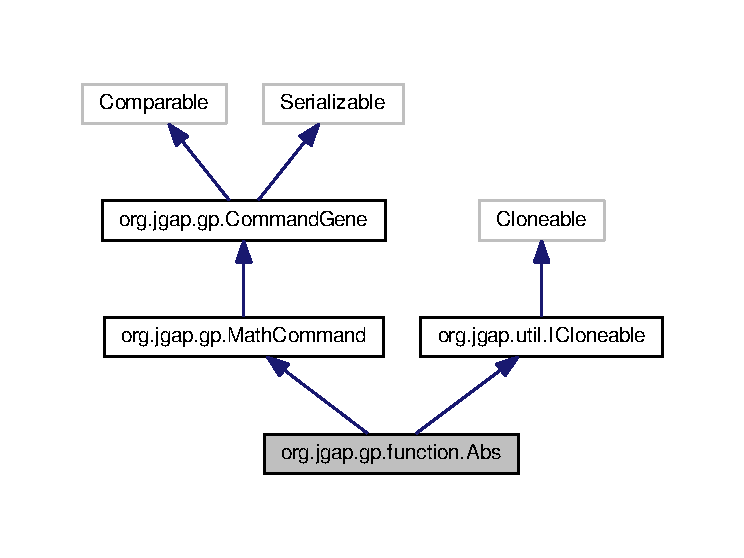
\includegraphics[width=350pt]{classorg_1_1jgap_1_1gp_1_1function_1_1_abs__inherit__graph}
\end{center}
\end{figure}


Collaboration diagram for org.\-jgap.\-gp.\-function.\-Abs\-:
\nopagebreak
\begin{figure}[H]
\begin{center}
\leavevmode
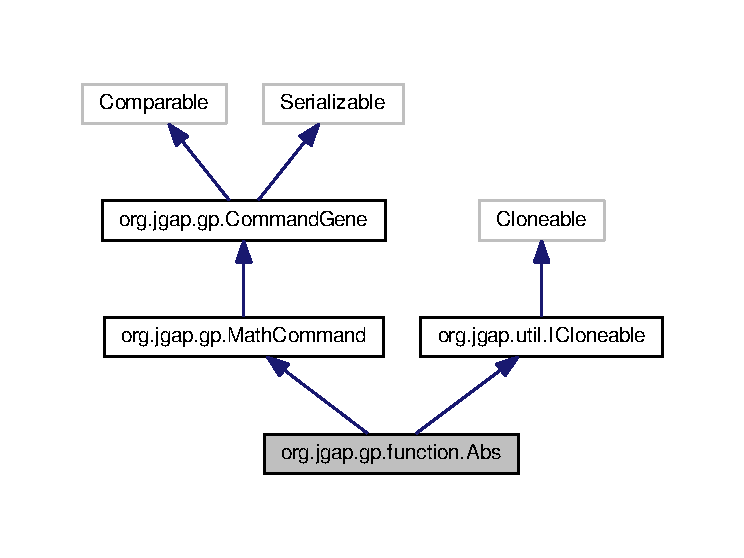
\includegraphics[width=350pt]{classorg_1_1jgap_1_1gp_1_1function_1_1_abs__coll__graph}
\end{center}
\end{figure}
\subsection*{Classes}
\begin{DoxyCompactItemize}
\item 
interface \hyperlink{interfaceorg_1_1jgap_1_1gp_1_1function_1_1_abs_1_1_compatible}{Compatible}
\end{DoxyCompactItemize}
\subsection*{Public Member Functions}
\begin{DoxyCompactItemize}
\item 
\hyperlink{classorg_1_1jgap_1_1gp_1_1function_1_1_abs_a68aebddb3343b8be3238ebd76cacd072}{Abs} (final G\-P\-Configuration a\-\_\-conf, Class a\-\_\-return\-Type)  throws Invalid\-Configuration\-Exception 
\item 
String \hyperlink{classorg_1_1jgap_1_1gp_1_1function_1_1_abs_a9419a3a7a3fe674ad35c3bbfa0bc9c7f}{to\-String} ()
\item 
String \hyperlink{classorg_1_1jgap_1_1gp_1_1function_1_1_abs_a12c0a9424bd3061439bbc89a5b45e9cf}{get\-Name} ()
\item 
float \hyperlink{classorg_1_1jgap_1_1gp_1_1function_1_1_abs_ac7274571667cef0c8875cdcce0fc3eed}{execute\-\_\-float} (Program\-Chromosome c, int n, Object\mbox{[}$\,$\mbox{]} args)
\item 
double \hyperlink{classorg_1_1jgap_1_1gp_1_1function_1_1_abs_a16c0cbe6fe8b7916b0c351c5c068af31}{execute\-\_\-double} (Program\-Chromosome c, int n, Object\mbox{[}$\,$\mbox{]} args)
\item 
Object \hyperlink{classorg_1_1jgap_1_1gp_1_1function_1_1_abs_a2e73ab52ded9043f33eb67920fd0f25c}{execute\-\_\-object} (Program\-Chromosome c, int n, Object\mbox{[}$\,$\mbox{]} args)
\item 
Object \hyperlink{classorg_1_1jgap_1_1gp_1_1function_1_1_abs_a32b7b4b41a89f23fcf860c5b64e27525}{clone} ()
\end{DoxyCompactItemize}
\subsection*{Static Private Attributes}
\begin{DoxyCompactItemize}
\item 
static final String \hyperlink{classorg_1_1jgap_1_1gp_1_1function_1_1_abs_a07dddbcd269d2b449bc66c484cc4a306}{C\-V\-S\-\_\-\-R\-E\-V\-I\-S\-I\-O\-N} = \char`\"{}\$Revision\-: 1.\-3 \$\char`\"{}
\end{DoxyCompactItemize}
\subsection*{Additional Inherited Members}


\subsection{Detailed Description}
Returns the absolute value of a number.

\begin{DoxyAuthor}{Author}
Klaus Meffert 
\end{DoxyAuthor}
\begin{DoxySince}{Since}
3.\-3.\-4 
\end{DoxySince}


Definition at line 23 of file Abs.\-java.



\subsection{Constructor \& Destructor Documentation}
\hypertarget{classorg_1_1jgap_1_1gp_1_1function_1_1_abs_a68aebddb3343b8be3238ebd76cacd072}{\index{org\-::jgap\-::gp\-::function\-::\-Abs@{org\-::jgap\-::gp\-::function\-::\-Abs}!Abs@{Abs}}
\index{Abs@{Abs}!org::jgap::gp::function::Abs@{org\-::jgap\-::gp\-::function\-::\-Abs}}
\subsubsection[{Abs}]{\setlength{\rightskip}{0pt plus 5cm}org.\-jgap.\-gp.\-function.\-Abs.\-Abs (
\begin{DoxyParamCaption}
\item[{final G\-P\-Configuration}]{a\-\_\-conf, }
\item[{Class}]{a\-\_\-return\-Type}
\end{DoxyParamCaption}
) throws {\bf Invalid\-Configuration\-Exception}\hspace{0.3cm}{\ttfamily [inline]}}}\label{classorg_1_1jgap_1_1gp_1_1function_1_1_abs_a68aebddb3343b8be3238ebd76cacd072}


Definition at line 28 of file Abs.\-java.



Referenced by org.\-jgap.\-gp.\-function.\-Abs.\-clone().



\subsection{Member Function Documentation}
\hypertarget{classorg_1_1jgap_1_1gp_1_1function_1_1_abs_a32b7b4b41a89f23fcf860c5b64e27525}{\index{org\-::jgap\-::gp\-::function\-::\-Abs@{org\-::jgap\-::gp\-::function\-::\-Abs}!clone@{clone}}
\index{clone@{clone}!org::jgap::gp::function::Abs@{org\-::jgap\-::gp\-::function\-::\-Abs}}
\subsubsection[{clone}]{\setlength{\rightskip}{0pt plus 5cm}Object org.\-jgap.\-gp.\-function.\-Abs.\-clone (
\begin{DoxyParamCaption}
{}
\end{DoxyParamCaption}
)\hspace{0.3cm}{\ttfamily [inline]}}}\label{classorg_1_1jgap_1_1gp_1_1function_1_1_abs_a32b7b4b41a89f23fcf860c5b64e27525}
Clones the object. Simple and straight forward implementation here.

\begin{DoxyReturn}{Returns}
cloned instance of this object
\end{DoxyReturn}
\begin{DoxyAuthor}{Author}
Klaus Meffert 
\end{DoxyAuthor}
\begin{DoxySince}{Since}
3.\-4 
\end{DoxySince}


Implements \hyperlink{interfaceorg_1_1jgap_1_1util_1_1_i_cloneable_aa7e7d62077e6428ad7904932b1b4f7d5}{org.\-jgap.\-util.\-I\-Cloneable}.



Definition at line 72 of file Abs.\-java.



References org.\-jgap.\-gp.\-function.\-Abs.\-Abs(), org.\-jgap.\-gp.\-Command\-Gene.\-get\-G\-P\-Configuration(), and org.\-jgap.\-gp.\-Command\-Gene.\-get\-Return\-Type().



Here is the call graph for this function\-:
\nopagebreak
\begin{figure}[H]
\begin{center}
\leavevmode
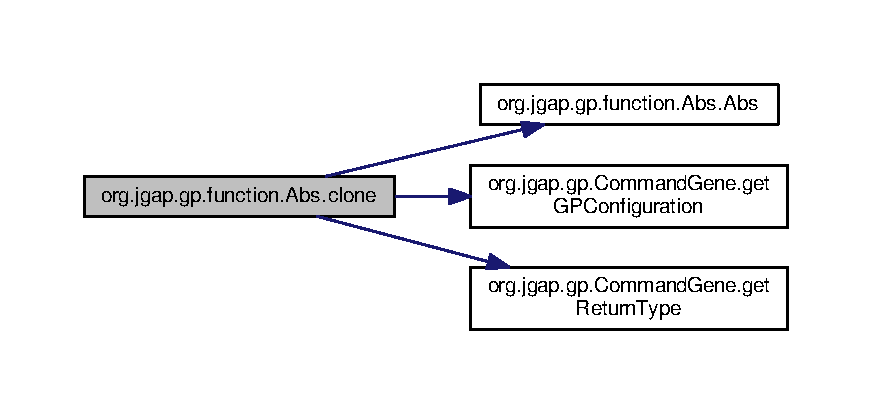
\includegraphics[width=350pt]{classorg_1_1jgap_1_1gp_1_1function_1_1_abs_a32b7b4b41a89f23fcf860c5b64e27525_cgraph}
\end{center}
\end{figure}


\hypertarget{classorg_1_1jgap_1_1gp_1_1function_1_1_abs_a16c0cbe6fe8b7916b0c351c5c068af31}{\index{org\-::jgap\-::gp\-::function\-::\-Abs@{org\-::jgap\-::gp\-::function\-::\-Abs}!execute\-\_\-double@{execute\-\_\-double}}
\index{execute\-\_\-double@{execute\-\_\-double}!org::jgap::gp::function::Abs@{org\-::jgap\-::gp\-::function\-::\-Abs}}
\subsubsection[{execute\-\_\-double}]{\setlength{\rightskip}{0pt plus 5cm}double org.\-jgap.\-gp.\-function.\-Abs.\-execute\-\_\-double (
\begin{DoxyParamCaption}
\item[{Program\-Chromosome}]{c, }
\item[{int}]{n, }
\item[{Object\mbox{[}$\,$\mbox{]}}]{args}
\end{DoxyParamCaption}
)\hspace{0.3cm}{\ttfamily [inline]}}}\label{classorg_1_1jgap_1_1gp_1_1function_1_1_abs_a16c0cbe6fe8b7916b0c351c5c068af31}


Definition at line 52 of file Abs.\-java.

\hypertarget{classorg_1_1jgap_1_1gp_1_1function_1_1_abs_ac7274571667cef0c8875cdcce0fc3eed}{\index{org\-::jgap\-::gp\-::function\-::\-Abs@{org\-::jgap\-::gp\-::function\-::\-Abs}!execute\-\_\-float@{execute\-\_\-float}}
\index{execute\-\_\-float@{execute\-\_\-float}!org::jgap::gp::function::Abs@{org\-::jgap\-::gp\-::function\-::\-Abs}}
\subsubsection[{execute\-\_\-float}]{\setlength{\rightskip}{0pt plus 5cm}float org.\-jgap.\-gp.\-function.\-Abs.\-execute\-\_\-float (
\begin{DoxyParamCaption}
\item[{Program\-Chromosome}]{c, }
\item[{int}]{n, }
\item[{Object\mbox{[}$\,$\mbox{]}}]{args}
\end{DoxyParamCaption}
)\hspace{0.3cm}{\ttfamily [inline]}}}\label{classorg_1_1jgap_1_1gp_1_1function_1_1_abs_ac7274571667cef0c8875cdcce0fc3eed}


Definition at line 47 of file Abs.\-java.

\hypertarget{classorg_1_1jgap_1_1gp_1_1function_1_1_abs_a2e73ab52ded9043f33eb67920fd0f25c}{\index{org\-::jgap\-::gp\-::function\-::\-Abs@{org\-::jgap\-::gp\-::function\-::\-Abs}!execute\-\_\-object@{execute\-\_\-object}}
\index{execute\-\_\-object@{execute\-\_\-object}!org::jgap::gp::function::Abs@{org\-::jgap\-::gp\-::function\-::\-Abs}}
\subsubsection[{execute\-\_\-object}]{\setlength{\rightskip}{0pt plus 5cm}Object org.\-jgap.\-gp.\-function.\-Abs.\-execute\-\_\-object (
\begin{DoxyParamCaption}
\item[{Program\-Chromosome}]{c, }
\item[{int}]{n, }
\item[{Object\mbox{[}$\,$\mbox{]}}]{args}
\end{DoxyParamCaption}
)\hspace{0.3cm}{\ttfamily [inline]}}}\label{classorg_1_1jgap_1_1gp_1_1function_1_1_abs_a2e73ab52ded9043f33eb67920fd0f25c}


Definition at line 57 of file Abs.\-java.

\hypertarget{classorg_1_1jgap_1_1gp_1_1function_1_1_abs_a12c0a9424bd3061439bbc89a5b45e9cf}{\index{org\-::jgap\-::gp\-::function\-::\-Abs@{org\-::jgap\-::gp\-::function\-::\-Abs}!get\-Name@{get\-Name}}
\index{get\-Name@{get\-Name}!org::jgap::gp::function::Abs@{org\-::jgap\-::gp\-::function\-::\-Abs}}
\subsubsection[{get\-Name}]{\setlength{\rightskip}{0pt plus 5cm}String org.\-jgap.\-gp.\-function.\-Abs.\-get\-Name (
\begin{DoxyParamCaption}
{}
\end{DoxyParamCaption}
)\hspace{0.3cm}{\ttfamily [inline]}}}\label{classorg_1_1jgap_1_1gp_1_1function_1_1_abs_a12c0a9424bd3061439bbc89a5b45e9cf}
\begin{DoxyReturn}{Returns}
textual name of this command
\end{DoxyReturn}
\begin{DoxyAuthor}{Author}
Klaus Meffert 
\end{DoxyAuthor}
\begin{DoxySince}{Since}
3.\-3.\-4 
\end{DoxySince}


Definition at line 43 of file Abs.\-java.

\hypertarget{classorg_1_1jgap_1_1gp_1_1function_1_1_abs_a9419a3a7a3fe674ad35c3bbfa0bc9c7f}{\index{org\-::jgap\-::gp\-::function\-::\-Abs@{org\-::jgap\-::gp\-::function\-::\-Abs}!to\-String@{to\-String}}
\index{to\-String@{to\-String}!org::jgap::gp::function::Abs@{org\-::jgap\-::gp\-::function\-::\-Abs}}
\subsubsection[{to\-String}]{\setlength{\rightskip}{0pt plus 5cm}String org.\-jgap.\-gp.\-function.\-Abs.\-to\-String (
\begin{DoxyParamCaption}
{}
\end{DoxyParamCaption}
)\hspace{0.3cm}{\ttfamily [inline]}, {\ttfamily [virtual]}}}\label{classorg_1_1jgap_1_1gp_1_1function_1_1_abs_a9419a3a7a3fe674ad35c3bbfa0bc9c7f}
\begin{DoxyReturn}{Returns}
the string representation of the command. Especially usefull to output a resulting formula in human-\/readable form. 
\end{DoxyReturn}


Implements \hyperlink{classorg_1_1jgap_1_1gp_1_1_command_gene_a236141d99059da808afe7a9217e411c7}{org.\-jgap.\-gp.\-Command\-Gene}.



Definition at line 33 of file Abs.\-java.



\subsection{Member Data Documentation}
\hypertarget{classorg_1_1jgap_1_1gp_1_1function_1_1_abs_a07dddbcd269d2b449bc66c484cc4a306}{\index{org\-::jgap\-::gp\-::function\-::\-Abs@{org\-::jgap\-::gp\-::function\-::\-Abs}!C\-V\-S\-\_\-\-R\-E\-V\-I\-S\-I\-O\-N@{C\-V\-S\-\_\-\-R\-E\-V\-I\-S\-I\-O\-N}}
\index{C\-V\-S\-\_\-\-R\-E\-V\-I\-S\-I\-O\-N@{C\-V\-S\-\_\-\-R\-E\-V\-I\-S\-I\-O\-N}!org::jgap::gp::function::Abs@{org\-::jgap\-::gp\-::function\-::\-Abs}}
\subsubsection[{C\-V\-S\-\_\-\-R\-E\-V\-I\-S\-I\-O\-N}]{\setlength{\rightskip}{0pt plus 5cm}final String org.\-jgap.\-gp.\-function.\-Abs.\-C\-V\-S\-\_\-\-R\-E\-V\-I\-S\-I\-O\-N = \char`\"{}\$Revision\-: 1.\-3 \$\char`\"{}\hspace{0.3cm}{\ttfamily [static]}, {\ttfamily [private]}}}\label{classorg_1_1jgap_1_1gp_1_1function_1_1_abs_a07dddbcd269d2b449bc66c484cc4a306}
String containing the C\-V\-S revision. Read out via reflection! 

Definition at line 26 of file Abs.\-java.



The documentation for this class was generated from the following file\-:\begin{DoxyCompactItemize}
\item 
L\-D\-H\-\_\-\-Git/src/org/jgap/gp/function/\hyperlink{_abs_8java}{Abs.\-java}\end{DoxyCompactItemize}

\hypertarget{classexamples_1_1supergene_1_1_abstract_change_fitness_function}{\section{examples.\-supergene.\-Abstract\-Change\-Fitness\-Function Class Reference}
\label{classexamples_1_1supergene_1_1_abstract_change_fitness_function}\index{examples.\-supergene.\-Abstract\-Change\-Fitness\-Function@{examples.\-supergene.\-Abstract\-Change\-Fitness\-Function}}
}


Inheritance diagram for examples.\-supergene.\-Abstract\-Change\-Fitness\-Function\-:
\nopagebreak
\begin{figure}[H]
\begin{center}
\leavevmode
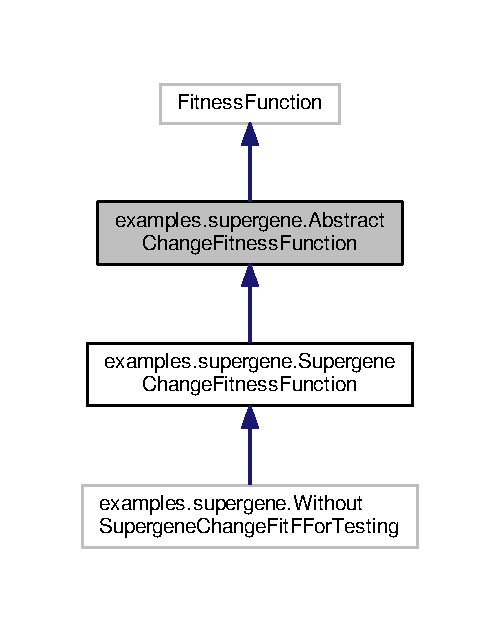
\includegraphics[width=240pt]{classexamples_1_1supergene_1_1_abstract_change_fitness_function__inherit__graph}
\end{center}
\end{figure}


Collaboration diagram for examples.\-supergene.\-Abstract\-Change\-Fitness\-Function\-:
\nopagebreak
\begin{figure}[H]
\begin{center}
\leavevmode
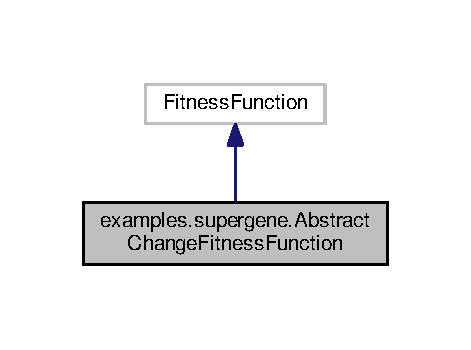
\includegraphics[width=226pt]{classexamples_1_1supergene_1_1_abstract_change_fitness_function__coll__graph}
\end{center}
\end{figure}
\subsection*{Public Member Functions}
\begin{DoxyCompactItemize}
\item 
\hyperlink{classexamples_1_1supergene_1_1_abstract_change_fitness_function_a9c774cb1d329969e3ccfe12472674ce4}{Abstract\-Change\-Fitness\-Function} (int a\-\_\-target\-Amount)
\item 
double \hyperlink{classexamples_1_1supergene_1_1_abstract_change_fitness_function_a71d25b74851304848680b8714fe1ea91}{evaluate} (I\-Chromosome a\-\_\-subject)
\item 
int \hyperlink{classexamples_1_1supergene_1_1_abstract_change_fitness_function_ad3371c34b83fe593d4559661099cbeeb}{amount\-Of\-Change} (I\-Chromosome a\-\_\-potential\-Solution)
\item 
int \hyperlink{classexamples_1_1supergene_1_1_abstract_change_fitness_function_a220025df8f0ed3ca78d9a2546125e62d}{get\-Number\-Of\-Coins\-At\-Gene} (I\-Chromosome a\-\_\-potential\-Solution, int a\-\_\-code)
\item 
int \hyperlink{classexamples_1_1supergene_1_1_abstract_change_fitness_function_aacde9b3f541743a1840cc4d8539e97f7}{get\-Total\-Number\-Of\-Coins} (I\-Chromosome a\-\_\-potentialsolution)
\item 
abstract Gene \hyperlink{classexamples_1_1supergene_1_1_abstract_change_fitness_function_adf1b5ef070f57b87234a09fa075587b2}{get\-Responsible\-Gene} (I\-Chromosome a\-\_\-chromosome, int a\-\_\-code)
\end{DoxyCompactItemize}
\subsection*{Private Attributes}
\begin{DoxyCompactItemize}
\item 
final int \hyperlink{classexamples_1_1supergene_1_1_abstract_change_fitness_function_af113260ddde2433a26a6a266b2969e56}{m\-\_\-target\-Amount}
\end{DoxyCompactItemize}
\subsection*{Static Private Attributes}
\begin{DoxyCompactItemize}
\item 
static final String \hyperlink{classexamples_1_1supergene_1_1_abstract_change_fitness_function_a17bdff475188176a202a6a884ba82853}{C\-V\-S\-\_\-\-R\-E\-V\-I\-S\-I\-O\-N} = \char`\"{}\$Revision\-: 1.\-2 \$\char`\"{}
\end{DoxyCompactItemize}


\subsection{Detailed Description}
Sample fitness function for the Make\-Change example, including supergenes.

\begin{DoxyAuthor}{Author}
Neil Rotstan 

Klaus Meffert 

Audrius Meskauskas 
\end{DoxyAuthor}
\begin{DoxySince}{Since}
2.\-0 
\end{DoxySince}


Definition at line 24 of file Abstract\-Change\-Fitness\-Function.\-java.



\subsection{Constructor \& Destructor Documentation}
\hypertarget{classexamples_1_1supergene_1_1_abstract_change_fitness_function_a9c774cb1d329969e3ccfe12472674ce4}{\index{examples\-::supergene\-::\-Abstract\-Change\-Fitness\-Function@{examples\-::supergene\-::\-Abstract\-Change\-Fitness\-Function}!Abstract\-Change\-Fitness\-Function@{Abstract\-Change\-Fitness\-Function}}
\index{Abstract\-Change\-Fitness\-Function@{Abstract\-Change\-Fitness\-Function}!examples::supergene::AbstractChangeFitnessFunction@{examples\-::supergene\-::\-Abstract\-Change\-Fitness\-Function}}
\subsubsection[{Abstract\-Change\-Fitness\-Function}]{\setlength{\rightskip}{0pt plus 5cm}examples.\-supergene.\-Abstract\-Change\-Fitness\-Function.\-Abstract\-Change\-Fitness\-Function (
\begin{DoxyParamCaption}
\item[{int}]{a\-\_\-target\-Amount}
\end{DoxyParamCaption}
)\hspace{0.3cm}{\ttfamily [inline]}}}\label{classexamples_1_1supergene_1_1_abstract_change_fitness_function_a9c774cb1d329969e3ccfe12472674ce4}


Definition at line 31 of file Abstract\-Change\-Fitness\-Function.\-java.



References examples.\-supergene.\-Abstract\-Change\-Fitness\-Function.\-m\-\_\-target\-Amount.



\subsection{Member Function Documentation}
\hypertarget{classexamples_1_1supergene_1_1_abstract_change_fitness_function_ad3371c34b83fe593d4559661099cbeeb}{\index{examples\-::supergene\-::\-Abstract\-Change\-Fitness\-Function@{examples\-::supergene\-::\-Abstract\-Change\-Fitness\-Function}!amount\-Of\-Change@{amount\-Of\-Change}}
\index{amount\-Of\-Change@{amount\-Of\-Change}!examples::supergene::AbstractChangeFitnessFunction@{examples\-::supergene\-::\-Abstract\-Change\-Fitness\-Function}}
\subsubsection[{amount\-Of\-Change}]{\setlength{\rightskip}{0pt plus 5cm}int examples.\-supergene.\-Abstract\-Change\-Fitness\-Function.\-amount\-Of\-Change (
\begin{DoxyParamCaption}
\item[{I\-Chromosome}]{a\-\_\-potential\-Solution}
\end{DoxyParamCaption}
)\hspace{0.3cm}{\ttfamily [inline]}}}\label{classexamples_1_1supergene_1_1_abstract_change_fitness_function_ad3371c34b83fe593d4559661099cbeeb}
Calculates the total amount of change (in cents) represented by the given potential solution and returns that amount.


\begin{DoxyParams}{Parameters}
{\em a\-\_\-potential\-Solution} & the potential solution to evaluate \\
\hline
\end{DoxyParams}
\begin{DoxyReturn}{Returns}
the total amount of change (in cents) represented by the given solution 
\end{DoxyReturn}


Definition at line 97 of file Abstract\-Change\-Fitness\-Function.\-java.



References examples.\-supergene.\-Abstract\-Supergene\-Test.\-D\-I\-M\-E\-S, examples.\-supergene.\-Abstract\-Change\-Fitness\-Function.\-get\-Number\-Of\-Coins\-At\-Gene(), examples.\-supergene.\-Abstract\-Supergene\-Test.\-N\-I\-C\-K\-E\-L\-S, examples.\-supergene.\-Abstract\-Supergene\-Test.\-P\-E\-N\-N\-I\-E\-S, and examples.\-supergene.\-Abstract\-Supergene\-Test.\-Q\-U\-A\-R\-T\-E\-R\-S.



Referenced by examples.\-supergene.\-Abstract\-Change\-Fitness\-Function.\-evaluate().



Here is the call graph for this function\-:
\nopagebreak
\begin{figure}[H]
\begin{center}
\leavevmode
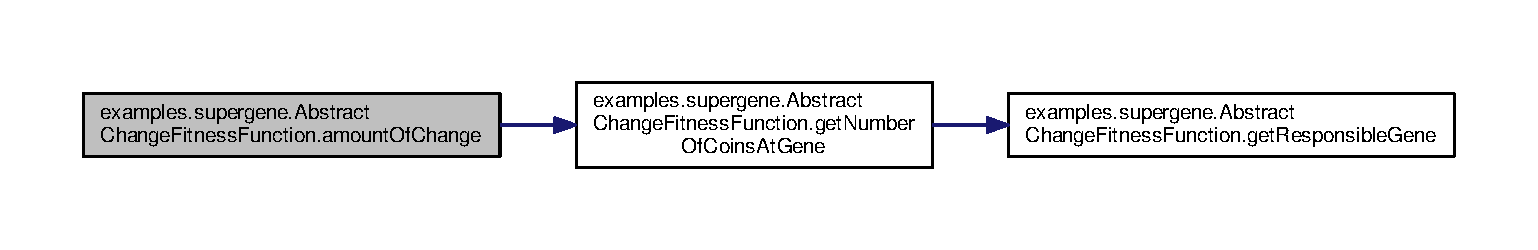
\includegraphics[width=350pt]{classexamples_1_1supergene_1_1_abstract_change_fitness_function_ad3371c34b83fe593d4559661099cbeeb_cgraph}
\end{center}
\end{figure}


\hypertarget{classexamples_1_1supergene_1_1_abstract_change_fitness_function_a71d25b74851304848680b8714fe1ea91}{\index{examples\-::supergene\-::\-Abstract\-Change\-Fitness\-Function@{examples\-::supergene\-::\-Abstract\-Change\-Fitness\-Function}!evaluate@{evaluate}}
\index{evaluate@{evaluate}!examples::supergene::AbstractChangeFitnessFunction@{examples\-::supergene\-::\-Abstract\-Change\-Fitness\-Function}}
\subsubsection[{evaluate}]{\setlength{\rightskip}{0pt plus 5cm}double examples.\-supergene.\-Abstract\-Change\-Fitness\-Function.\-evaluate (
\begin{DoxyParamCaption}
\item[{I\-Chromosome}]{a\-\_\-subject}
\end{DoxyParamCaption}
)\hspace{0.3cm}{\ttfamily [inline]}}}\label{classexamples_1_1supergene_1_1_abstract_change_fitness_function_a71d25b74851304848680b8714fe1ea91}
Determine the fitness of the given Chromosome instance. The higher the return value, the more fit the instance. This method should always return the same fitness value for two equivalent Chromosome instances.


\begin{DoxyParams}{Parameters}
{\em a\-\_\-subject} & the Chromosome instance to evaluate\\
\hline
\end{DoxyParams}
\begin{DoxyReturn}{Returns}
positive integer reflecting the fitness rating of the given Chromosome 
\end{DoxyReturn}
\begin{DoxySince}{Since}
2.\-0 
\end{DoxySince}


Definition at line 50 of file Abstract\-Change\-Fitness\-Function.\-java.



References examples.\-supergene.\-Abstract\-Change\-Fitness\-Function.\-amount\-Of\-Change(), examples.\-supergene.\-Abstract\-Change\-Fitness\-Function.\-get\-Total\-Number\-Of\-Coins(), and examples.\-supergene.\-Abstract\-Change\-Fitness\-Function.\-m\-\_\-target\-Amount.



Here is the call graph for this function\-:
\nopagebreak
\begin{figure}[H]
\begin{center}
\leavevmode
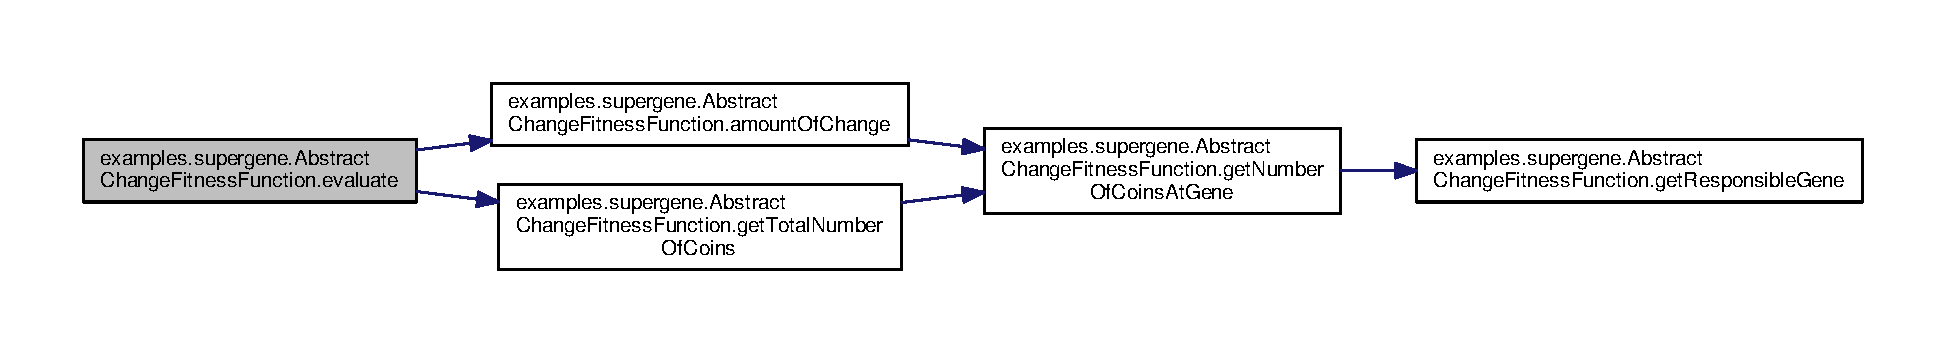
\includegraphics[width=350pt]{classexamples_1_1supergene_1_1_abstract_change_fitness_function_a71d25b74851304848680b8714fe1ea91_cgraph}
\end{center}
\end{figure}


\hypertarget{classexamples_1_1supergene_1_1_abstract_change_fitness_function_a220025df8f0ed3ca78d9a2546125e62d}{\index{examples\-::supergene\-::\-Abstract\-Change\-Fitness\-Function@{examples\-::supergene\-::\-Abstract\-Change\-Fitness\-Function}!get\-Number\-Of\-Coins\-At\-Gene@{get\-Number\-Of\-Coins\-At\-Gene}}
\index{get\-Number\-Of\-Coins\-At\-Gene@{get\-Number\-Of\-Coins\-At\-Gene}!examples::supergene::AbstractChangeFitnessFunction@{examples\-::supergene\-::\-Abstract\-Change\-Fitness\-Function}}
\subsubsection[{get\-Number\-Of\-Coins\-At\-Gene}]{\setlength{\rightskip}{0pt plus 5cm}int examples.\-supergene.\-Abstract\-Change\-Fitness\-Function.\-get\-Number\-Of\-Coins\-At\-Gene (
\begin{DoxyParamCaption}
\item[{I\-Chromosome}]{a\-\_\-potential\-Solution, }
\item[{int}]{a\-\_\-code}
\end{DoxyParamCaption}
)\hspace{0.3cm}{\ttfamily [inline]}}}\label{classexamples_1_1supergene_1_1_abstract_change_fitness_function_a220025df8f0ed3ca78d9a2546125e62d}
Retrieves the number of coins represented by the given potential solution at the given gene position.


\begin{DoxyParams}{Parameters}
{\em a\-\_\-potential\-Solution} & the potential solution to evaluate \\
\hline
{\em a\-\_\-code} & index of gene \\
\hline
\end{DoxyParams}
\begin{DoxyReturn}{Returns}
the number of coins represented by the potential solution at the given gene position 
\end{DoxyReturn}


Definition at line 119 of file Abstract\-Change\-Fitness\-Function.\-java.



References examples.\-supergene.\-Abstract\-Change\-Fitness\-Function.\-get\-Responsible\-Gene().



Referenced by examples.\-supergene.\-Abstract\-Change\-Fitness\-Function.\-amount\-Of\-Change(), and examples.\-supergene.\-Abstract\-Change\-Fitness\-Function.\-get\-Total\-Number\-Of\-Coins().



Here is the call graph for this function\-:
\nopagebreak
\begin{figure}[H]
\begin{center}
\leavevmode
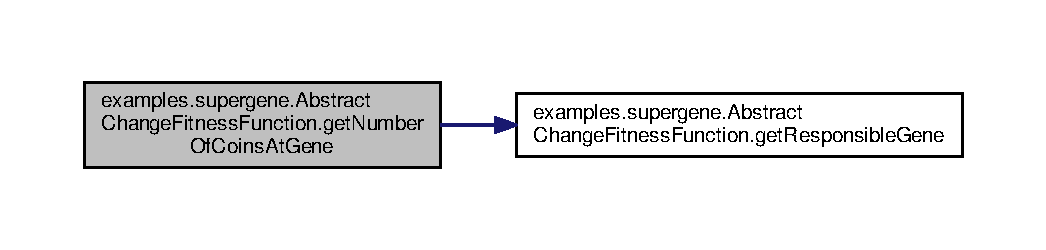
\includegraphics[width=350pt]{classexamples_1_1supergene_1_1_abstract_change_fitness_function_a220025df8f0ed3ca78d9a2546125e62d_cgraph}
\end{center}
\end{figure}


\hypertarget{classexamples_1_1supergene_1_1_abstract_change_fitness_function_adf1b5ef070f57b87234a09fa075587b2}{\index{examples\-::supergene\-::\-Abstract\-Change\-Fitness\-Function@{examples\-::supergene\-::\-Abstract\-Change\-Fitness\-Function}!get\-Responsible\-Gene@{get\-Responsible\-Gene}}
\index{get\-Responsible\-Gene@{get\-Responsible\-Gene}!examples::supergene::AbstractChangeFitnessFunction@{examples\-::supergene\-::\-Abstract\-Change\-Fitness\-Function}}
\subsubsection[{get\-Responsible\-Gene}]{\setlength{\rightskip}{0pt plus 5cm}abstract Gene examples.\-supergene.\-Abstract\-Change\-Fitness\-Function.\-get\-Responsible\-Gene (
\begin{DoxyParamCaption}
\item[{I\-Chromosome}]{a\-\_\-chromosome, }
\item[{int}]{a\-\_\-code}
\end{DoxyParamCaption}
)\hspace{0.3cm}{\ttfamily [pure virtual]}}}\label{classexamples_1_1supergene_1_1_abstract_change_fitness_function_adf1b5ef070f57b87234a09fa075587b2}
Get the gene, responsible for the number of coins, corresponding this code.


\begin{DoxyParams}{Parameters}
{\em a\-\_\-chromosome} & Chromosome to evaluate \\
\hline
{\em a\-\_\-code} & index of Gene \\
\hline
\end{DoxyParams}
\begin{DoxyReturn}{Returns}
responsible gene 
\end{DoxyReturn}


Implemented in \hyperlink{classexamples_1_1supergene_1_1_supergene_change_fitness_function_a3bcce668e64e997376557e371de33717}{examples.\-supergene.\-Supergene\-Change\-Fitness\-Function}.



Referenced by examples.\-supergene.\-Abstract\-Change\-Fitness\-Function.\-get\-Number\-Of\-Coins\-At\-Gene().

\hypertarget{classexamples_1_1supergene_1_1_abstract_change_fitness_function_aacde9b3f541743a1840cc4d8539e97f7}{\index{examples\-::supergene\-::\-Abstract\-Change\-Fitness\-Function@{examples\-::supergene\-::\-Abstract\-Change\-Fitness\-Function}!get\-Total\-Number\-Of\-Coins@{get\-Total\-Number\-Of\-Coins}}
\index{get\-Total\-Number\-Of\-Coins@{get\-Total\-Number\-Of\-Coins}!examples::supergene::AbstractChangeFitnessFunction@{examples\-::supergene\-::\-Abstract\-Change\-Fitness\-Function}}
\subsubsection[{get\-Total\-Number\-Of\-Coins}]{\setlength{\rightskip}{0pt plus 5cm}int examples.\-supergene.\-Abstract\-Change\-Fitness\-Function.\-get\-Total\-Number\-Of\-Coins (
\begin{DoxyParamCaption}
\item[{I\-Chromosome}]{a\-\_\-potentialsolution}
\end{DoxyParamCaption}
)\hspace{0.3cm}{\ttfamily [inline]}}}\label{classexamples_1_1supergene_1_1_abstract_change_fitness_function_aacde9b3f541743a1840cc4d8539e97f7}
Returns the total number of coins represented by all of the genes in the given potential solution.


\begin{DoxyParams}{Parameters}
{\em a\-\_\-potentialsolution} & the potential solution to evaluate \\
\hline
\end{DoxyParams}
\begin{DoxyReturn}{Returns}
the total number of coins represented by the given Chromosome 
\end{DoxyReturn}


Definition at line 132 of file Abstract\-Change\-Fitness\-Function.\-java.



References examples.\-supergene.\-Abstract\-Supergene\-Test.\-D\-I\-M\-E\-S, examples.\-supergene.\-Abstract\-Change\-Fitness\-Function.\-get\-Number\-Of\-Coins\-At\-Gene(), examples.\-supergene.\-Abstract\-Supergene\-Test.\-N\-I\-C\-K\-E\-L\-S, examples.\-supergene.\-Abstract\-Supergene\-Test.\-P\-E\-N\-N\-I\-E\-S, and examples.\-supergene.\-Abstract\-Supergene\-Test.\-Q\-U\-A\-R\-T\-E\-R\-S.



Referenced by examples.\-supergene.\-Abstract\-Change\-Fitness\-Function.\-evaluate(), and examples.\-supergene.\-Abstract\-Supergene\-Test.\-report().



Here is the call graph for this function\-:
\nopagebreak
\begin{figure}[H]
\begin{center}
\leavevmode
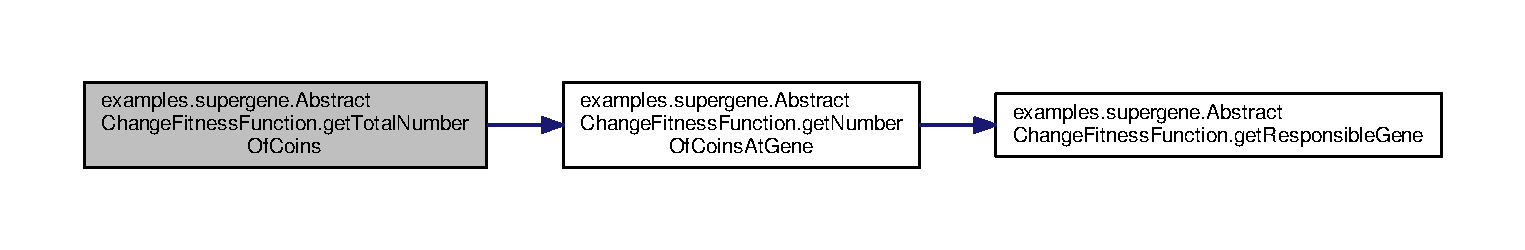
\includegraphics[width=350pt]{classexamples_1_1supergene_1_1_abstract_change_fitness_function_aacde9b3f541743a1840cc4d8539e97f7_cgraph}
\end{center}
\end{figure}




\subsection{Member Data Documentation}
\hypertarget{classexamples_1_1supergene_1_1_abstract_change_fitness_function_a17bdff475188176a202a6a884ba82853}{\index{examples\-::supergene\-::\-Abstract\-Change\-Fitness\-Function@{examples\-::supergene\-::\-Abstract\-Change\-Fitness\-Function}!C\-V\-S\-\_\-\-R\-E\-V\-I\-S\-I\-O\-N@{C\-V\-S\-\_\-\-R\-E\-V\-I\-S\-I\-O\-N}}
\index{C\-V\-S\-\_\-\-R\-E\-V\-I\-S\-I\-O\-N@{C\-V\-S\-\_\-\-R\-E\-V\-I\-S\-I\-O\-N}!examples::supergene::AbstractChangeFitnessFunction@{examples\-::supergene\-::\-Abstract\-Change\-Fitness\-Function}}
\subsubsection[{C\-V\-S\-\_\-\-R\-E\-V\-I\-S\-I\-O\-N}]{\setlength{\rightskip}{0pt plus 5cm}final String examples.\-supergene.\-Abstract\-Change\-Fitness\-Function.\-C\-V\-S\-\_\-\-R\-E\-V\-I\-S\-I\-O\-N = \char`\"{}\$Revision\-: 1.\-2 \$\char`\"{}\hspace{0.3cm}{\ttfamily [static]}, {\ttfamily [private]}}}\label{classexamples_1_1supergene_1_1_abstract_change_fitness_function_a17bdff475188176a202a6a884ba82853}
String containing the C\-V\-S revision. Read out via reflection! 

Definition at line 27 of file Abstract\-Change\-Fitness\-Function.\-java.

\hypertarget{classexamples_1_1supergene_1_1_abstract_change_fitness_function_af113260ddde2433a26a6a266b2969e56}{\index{examples\-::supergene\-::\-Abstract\-Change\-Fitness\-Function@{examples\-::supergene\-::\-Abstract\-Change\-Fitness\-Function}!m\-\_\-target\-Amount@{m\-\_\-target\-Amount}}
\index{m\-\_\-target\-Amount@{m\-\_\-target\-Amount}!examples::supergene::AbstractChangeFitnessFunction@{examples\-::supergene\-::\-Abstract\-Change\-Fitness\-Function}}
\subsubsection[{m\-\_\-target\-Amount}]{\setlength{\rightskip}{0pt plus 5cm}final int examples.\-supergene.\-Abstract\-Change\-Fitness\-Function.\-m\-\_\-target\-Amount\hspace{0.3cm}{\ttfamily [private]}}}\label{classexamples_1_1supergene_1_1_abstract_change_fitness_function_af113260ddde2433a26a6a266b2969e56}


Definition at line 29 of file Abstract\-Change\-Fitness\-Function.\-java.



Referenced by examples.\-supergene.\-Abstract\-Change\-Fitness\-Function.\-Abstract\-Change\-Fitness\-Function(), and examples.\-supergene.\-Abstract\-Change\-Fitness\-Function.\-evaluate().



The documentation for this class was generated from the following file\-:\begin{DoxyCompactItemize}
\item 
L\-D\-H\-\_\-\-Git/examples/src/examples/supergene/\hyperlink{_abstract_change_fitness_function_8java}{Abstract\-Change\-Fitness\-Function.\-java}\end{DoxyCompactItemize}

\hypertarget{classorg_1_1jgap_1_1supergenes_1_1_abstract_supergene}{\section{org.\-jgap.\-supergenes.\-Abstract\-Supergene Class Reference}
\label{classorg_1_1jgap_1_1supergenes_1_1_abstract_supergene}\index{org.\-jgap.\-supergenes.\-Abstract\-Supergene@{org.\-jgap.\-supergenes.\-Abstract\-Supergene}}
}


Inheritance diagram for org.\-jgap.\-supergenes.\-Abstract\-Supergene\-:
\nopagebreak
\begin{figure}[H]
\begin{center}
\leavevmode
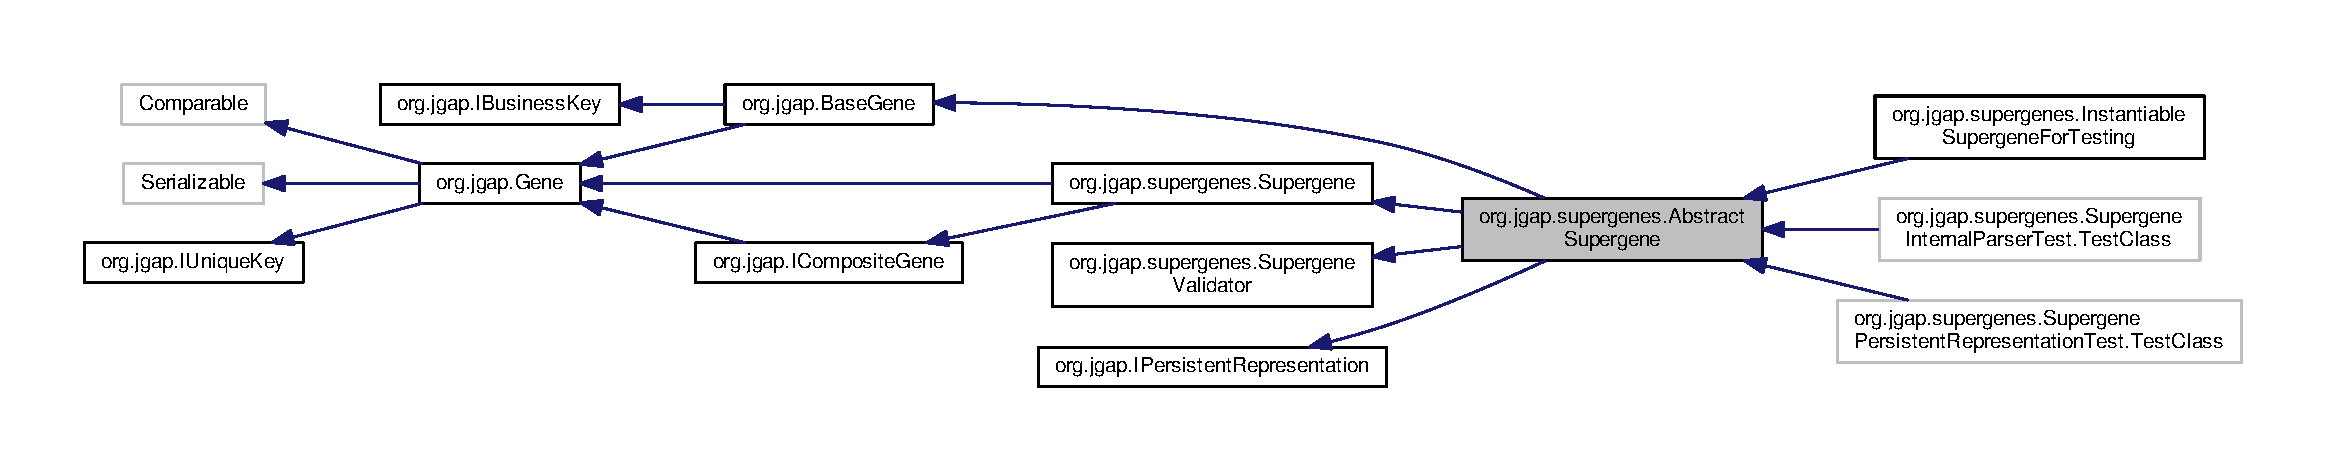
\includegraphics[width=350pt]{classorg_1_1jgap_1_1supergenes_1_1_abstract_supergene__inherit__graph}
\end{center}
\end{figure}


Collaboration diagram for org.\-jgap.\-supergenes.\-Abstract\-Supergene\-:
\nopagebreak
\begin{figure}[H]
\begin{center}
\leavevmode
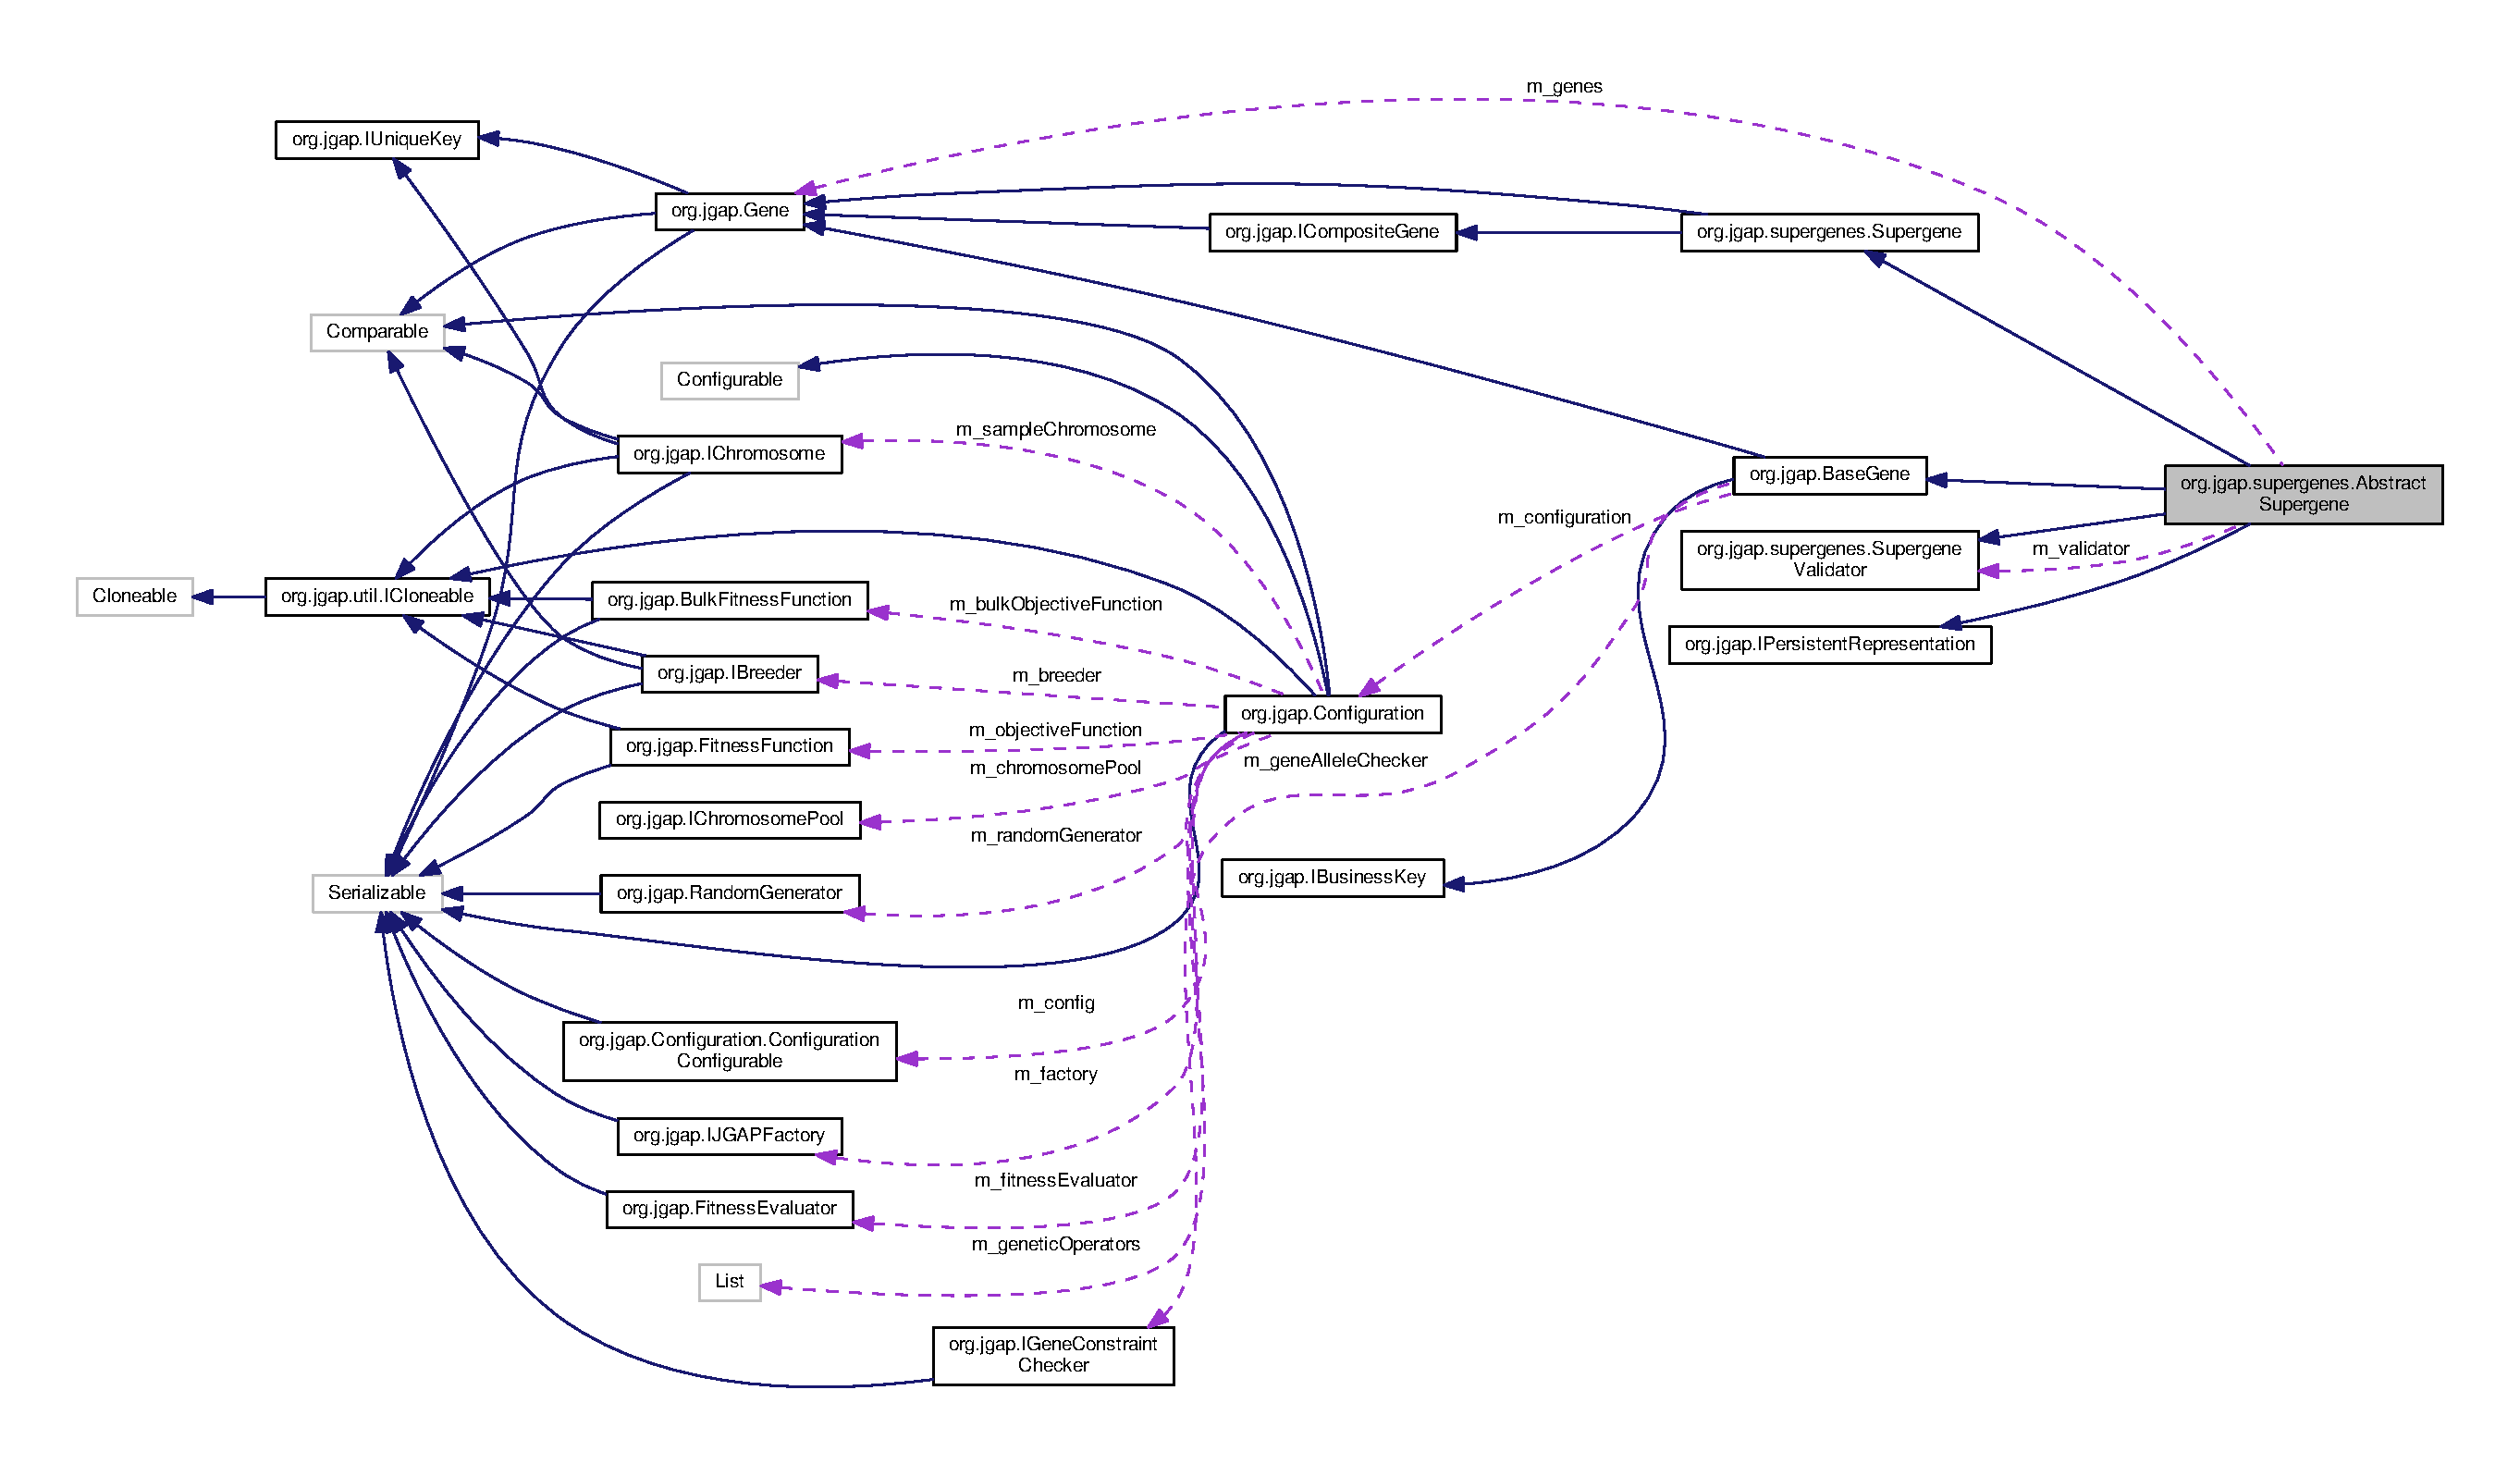
\includegraphics[width=350pt]{classorg_1_1jgap_1_1supergenes_1_1_abstract_supergene__coll__graph}
\end{center}
\end{figure}
\subsection*{Public Member Functions}
\begin{DoxyCompactItemize}
\item 
\hyperlink{interfaceorg_1_1jgap_1_1_gene}{Gene}\mbox{[}$\,$\mbox{]} \hyperlink{classorg_1_1jgap_1_1supergenes_1_1_abstract_supergene_a5b03d0c4d103975b296d280371b901bd}{get\-Genes} ()
\item 
final \hyperlink{interfaceorg_1_1jgap_1_1_gene}{Gene} \hyperlink{classorg_1_1jgap_1_1supergenes_1_1_abstract_supergene_a099bf664561a1f88b9826e25d870ad7f}{gene\-At} (final int a\-\_\-index)
\item 
\hyperlink{classorg_1_1jgap_1_1supergenes_1_1_abstract_supergene_aa67d2e35432f0534c38260e0b3e4d014}{Abstract\-Supergene} ()  throws Invalid\-Configuration\-Exception 
\item 
\hyperlink{classorg_1_1jgap_1_1supergenes_1_1_abstract_supergene_a8ede7cc1a661a1fb8a7d7000ec7ea11f}{Abstract\-Supergene} (final \hyperlink{classorg_1_1jgap_1_1_configuration}{Configuration} a\-\_\-config)  throws Invalid\-Configuration\-Exception 
\item 
\hyperlink{classorg_1_1jgap_1_1supergenes_1_1_abstract_supergene_a1cbbfd45d7cad277949c8571fa067013}{Abstract\-Supergene} (final \hyperlink{classorg_1_1jgap_1_1_configuration}{Configuration} a\-\_\-conf, final \hyperlink{interfaceorg_1_1jgap_1_1_gene}{Gene}\mbox{[}$\,$\mbox{]} a\-\_\-genes)  throws Invalid\-Configuration\-Exception 
\item 
boolean \hyperlink{classorg_1_1jgap_1_1supergenes_1_1_abstract_supergene_adfa0b1f704e28e3a90d187df2cf4b8b5}{is\-Valid} ()
\item 
boolean \hyperlink{classorg_1_1jgap_1_1supergenes_1_1_abstract_supergene_a4d07a7aa9a0af1e4e1a96b1a7663afee}{is\-Valid} (final \hyperlink{interfaceorg_1_1jgap_1_1_gene}{Gene}\mbox{[}$\,$\mbox{]} a\-\_\-case, final \hyperlink{interfaceorg_1_1jgap_1_1supergenes_1_1_supergene}{Supergene} a\-\_\-for\-Supergene)
\item 
void \hyperlink{classorg_1_1jgap_1_1supergenes_1_1_abstract_supergene_a008b2ecc6f66090965919b537fb327b3}{apply\-Mutation} (final int a\-\_\-index, final double a\-\_\-percentage)
\item 
void \hyperlink{classorg_1_1jgap_1_1supergenes_1_1_abstract_supergene_a92df9df781b9ae3bc7811bf76bb7ea87}{set\-To\-Random\-Value} (final \hyperlink{interfaceorg_1_1jgap_1_1_random_generator}{Random\-Generator} a\-\_\-number\-Generator)
\item 
void \hyperlink{classorg_1_1jgap_1_1supergenes_1_1_abstract_supergene_a7b3ce455ac6d30ba31b198ce6824cd19}{set\-Allele} (final Object a\-\_\-super\-Allele)
\item 
Object \hyperlink{classorg_1_1jgap_1_1supergenes_1_1_abstract_supergene_a45f21f887ad34c02fbc88d41e5d0372d}{get\-Allele} ()
\item 
String \hyperlink{classorg_1_1jgap_1_1supergenes_1_1_abstract_supergene_a41a4e0b1cf2366722b5f3b97a1711487}{get\-Persistent\-Representation} ()  throws Unsupported\-Operation\-Exception 
\item 
void \hyperlink{classorg_1_1jgap_1_1supergenes_1_1_abstract_supergene_af8156c2a8b41bc9fe3e397595c513a6d}{set\-Value\-From\-Persistent\-Representation} (String a\-\_\-representation)  throws Unsupported\-Representation\-Exception 
\item 
void \hyperlink{classorg_1_1jgap_1_1supergenes_1_1_abstract_supergene_aec3dc6646255f4187aa9a6b4238a9a2c}{cleanup} ()
\item 
String \hyperlink{classorg_1_1jgap_1_1supergenes_1_1_abstract_supergene_a67a9b1dfccb63d4b2909abdd3e8c1abe}{to\-String} ()
\item 
int \hyperlink{classorg_1_1jgap_1_1supergenes_1_1_abstract_supergene_a8d2326c3d5ce80c73dff063f26994233}{size} ()
\item 
int \hyperlink{classorg_1_1jgap_1_1supergenes_1_1_abstract_supergene_ac17432577a59856d6ef81abaf0a66bf9}{compare\-To} (Object o)
\item 
boolean \hyperlink{classorg_1_1jgap_1_1supergenes_1_1_abstract_supergene_a80be2241977a41672bdbaa85acb7eabc}{equals} (Object a\-\_\-gene)
\item 
int \hyperlink{classorg_1_1jgap_1_1supergenes_1_1_abstract_supergene_a73c5c7702d66268b71e9ed92f0c5d41d}{hash\-Code} ()
\item 
void \hyperlink{classorg_1_1jgap_1_1supergenes_1_1_abstract_supergene_a8b9835e9be1cc5edc8507c957b1f1f2d}{add\-Gene} (\hyperlink{interfaceorg_1_1jgap_1_1_gene}{Gene} a\-\_\-gene)
\item 
void \hyperlink{classorg_1_1jgap_1_1supergenes_1_1_abstract_supergene_afae838561a1237ab6b39456ab0e3b8c8}{set\-Validator} (\hyperlink{interfaceorg_1_1jgap_1_1supergenes_1_1_supergene_validator}{Supergene\-Validator} a\-\_\-validator)
\item 
\hyperlink{interfaceorg_1_1jgap_1_1supergenes_1_1_supergene_validator}{Supergene\-Validator} \hyperlink{classorg_1_1jgap_1_1supergenes_1_1_abstract_supergene_a9ebb4d5fbce8752cba54188ad5958fcf}{get\-Validator} ()
\item 
String \hyperlink{classorg_1_1jgap_1_1supergenes_1_1_abstract_supergene_aa7990463e784192581d7d7918cd0f1b1}{get\-Persistent} ()
\item 
void \hyperlink{classorg_1_1jgap_1_1supergenes_1_1_abstract_supergene_a70a5435dbf92b886ab7d5bbcd2d79d09}{set\-From\-Persistent} (String a\-\_\-from)
\item 
Object \hyperlink{classorg_1_1jgap_1_1supergenes_1_1_abstract_supergene_af4b0e1f740b6aa78679ab71c51568cea}{get\-Internal\-Value} ()
\end{DoxyCompactItemize}
\subsection*{Static Public Member Functions}
\begin{DoxyCompactItemize}
\item 
static void \hyperlink{classorg_1_1jgap_1_1supergenes_1_1_abstract_supergene_afdcc065673680fb080e17ff2596a0eb0}{reset} ()
\end{DoxyCompactItemize}
\subsection*{Static Public Attributes}
\begin{DoxyCompactItemize}
\item 
static final String \hyperlink{classorg_1_1jgap_1_1supergenes_1_1_abstract_supergene_ae7be27a291a2aa7e594384dd7a5936a8}{G\-E\-N\-E\-\_\-\-D\-E\-L\-I\-M\-I\-T\-E\-R} = \char`\"{}\#\char`\"{}
\item 
static final String \hyperlink{classorg_1_1jgap_1_1supergenes_1_1_abstract_supergene_aebbbd0fdd22a6d94c951471c8ae86b84}{G\-E\-N\-E\-\_\-\-D\-E\-L\-I\-M\-I\-T\-E\-R\-\_\-\-H\-E\-A\-D\-I\-N\-G} = \char`\"{}$<$\char`\"{}
\item 
static final String \hyperlink{classorg_1_1jgap_1_1supergenes_1_1_abstract_supergene_a96059d4ef9cca18130330f3ab782c28b}{G\-E\-N\-E\-\_\-\-D\-E\-L\-I\-M\-I\-T\-E\-R\-\_\-\-C\-L\-O\-S\-I\-N\-G} = \char`\"{}$>$\char`\"{}
\item 
static final int \hyperlink{classorg_1_1jgap_1_1supergenes_1_1_abstract_supergene_a6839c4b04a89a58c967219eda28a5dbb}{M\-A\-X\-\_\-\-R\-E\-T\-R\-I\-E\-S} = 1
\item 
static final int \hyperlink{classorg_1_1jgap_1_1supergenes_1_1_abstract_supergene_a40054ab751c7676fcd9f974c029a6a9d}{M\-A\-X\-\_\-\-I\-M\-M\-U\-T\-A\-B\-L\-E\-\_\-\-G\-E\-N\-E\-S} = 100000
\end{DoxyCompactItemize}
\subsection*{Protected Member Functions}
\begin{DoxyCompactItemize}
\item 
\hyperlink{interfaceorg_1_1jgap_1_1_gene}{Gene} \hyperlink{classorg_1_1jgap_1_1supergenes_1_1_abstract_supergene_a1e30b794dee0e8da4d5a4d213e9fb2c1}{new\-Gene\-Internal} ()
\item 
\hyperlink{interfaceorg_1_1jgap_1_1supergenes_1_1_supergene_validator}{Supergene\-Validator} \hyperlink{classorg_1_1jgap_1_1supergenes_1_1_abstract_supergene_a497a53be8d8d711ed48c62b062984a94}{create\-Validator} (String a\-\_\-rep)
\item 
\hyperlink{interfaceorg_1_1jgap_1_1_gene}{Gene} \hyperlink{classorg_1_1jgap_1_1supergenes_1_1_abstract_supergene_a32c5375e3de833953678146fb3dcb5b3}{create\-Gene} (String a\-\_\-gene\-Class\-Name, String a\-\_\-persistent\-Representation)  throws Exception 
\end{DoxyCompactItemize}
\subsection*{Static Protected Member Functions}
\begin{DoxyCompactItemize}
\item 
static final List \hyperlink{classorg_1_1jgap_1_1supergenes_1_1_abstract_supergene_a3ff87dbb7c5c6a4167198184b7171934}{split} (String a\-\_\-string)  throws Unsupported\-Representation\-Exception 
\end{DoxyCompactItemize}
\subsection*{Protected Attributes}
\begin{DoxyCompactItemize}
\item 
\hyperlink{interfaceorg_1_1jgap_1_1supergenes_1_1_supergene_validator}{Supergene\-Validator} \hyperlink{classorg_1_1jgap_1_1supergenes_1_1_abstract_supergene_a8792c7c19ad0cdb48ade652a110a9016}{m\-\_\-validator} = this
\end{DoxyCompactItemize}
\subsection*{Private Member Functions}
\begin{DoxyCompactItemize}
\item 
void \hyperlink{classorg_1_1jgap_1_1supergenes_1_1_abstract_supergene_a9f06a4d966c9e615b2ea5bff4583a183}{mark\-Immutable} (final int a\-\_\-index)
\end{DoxyCompactItemize}
\subsection*{Private Attributes}
\begin{DoxyCompactItemize}
\item 
\hyperlink{interfaceorg_1_1jgap_1_1_gene}{Gene}\mbox{[}$\,$\mbox{]} \hyperlink{classorg_1_1jgap_1_1supergenes_1_1_abstract_supergene_a7e237a04c314d9fbb0ab064ad88a5cb3}{m\-\_\-genes}
\end{DoxyCompactItemize}
\subsection*{Static Private Attributes}
\begin{DoxyCompactItemize}
\item 
static final String \hyperlink{classorg_1_1jgap_1_1supergenes_1_1_abstract_supergene_a9084146c063a12faff254011968f40b8}{C\-V\-S\-\_\-\-R\-E\-V\-I\-S\-I\-O\-N} = \char`\"{}\$Revision\-: 1.\-24 \$\char`\"{}
\item 
static Set\mbox{[}$\,$\mbox{]} \hyperlink{classorg_1_1jgap_1_1supergenes_1_1_abstract_supergene_a92632c12f27c0aaef1984c8550afe9a1}{m\-\_\-immutable} = new Set\mbox{[}1\mbox{]}
\end{DoxyCompactItemize}


\subsection{Detailed Description}
Combined implementation of both \hyperlink{interfaceorg_1_1jgap_1_1supergenes_1_1_supergene}{Supergene} and \hyperlink{interfaceorg_1_1jgap_1_1supergenes_1_1_supergene_validator}{Supergene\-Validator}. A working supergene can be easily created from this class just by adding genes and overriding \hyperlink{classorg_1_1jgap_1_1supergenes_1_1_abstract_supergene_adfa0b1f704e28e3a90d187df2cf4b8b5}{\mbox{[}\mbox{]} a\-\_\-case, Supergene a\-\_\-for\-Supergene) is\-Valid (Gene \mbox{[}\mbox{]}, Supergene)} method. For more complex cases, you may need to set your own \hyperlink{classorg_1_1jgap_1_1supergenes_1_1_validator}{Validator}.

\begin{DoxyAuthor}{Author}
Audrius Meskauskas 
\end{DoxyAuthor}
\begin{DoxySince}{Since}
2.\-0 
\end{DoxySince}


Definition at line 29 of file Abstract\-Supergene.\-java.



\subsection{Constructor \& Destructor Documentation}
\hypertarget{classorg_1_1jgap_1_1supergenes_1_1_abstract_supergene_aa67d2e35432f0534c38260e0b3e4d014}{\index{org\-::jgap\-::supergenes\-::\-Abstract\-Supergene@{org\-::jgap\-::supergenes\-::\-Abstract\-Supergene}!Abstract\-Supergene@{Abstract\-Supergene}}
\index{Abstract\-Supergene@{Abstract\-Supergene}!org::jgap::supergenes::AbstractSupergene@{org\-::jgap\-::supergenes\-::\-Abstract\-Supergene}}
\subsubsection[{Abstract\-Supergene}]{\setlength{\rightskip}{0pt plus 5cm}org.\-jgap.\-supergenes.\-Abstract\-Supergene.\-Abstract\-Supergene (
\begin{DoxyParamCaption}
{}
\end{DoxyParamCaption}
) throws {\bf Invalid\-Configuration\-Exception}\hspace{0.3cm}{\ttfamily [inline]}}}\label{classorg_1_1jgap_1_1supergenes_1_1_abstract_supergene_aa67d2e35432f0534c38260e0b3e4d014}
Default constructor for dynamic instantiation.


\begin{DoxyExceptions}{Exceptions}
{\em \hyperlink{classorg_1_1jgap_1_1_invalid_configuration_exception}{Invalid\-Configuration\-Exception}} & \\
\hline
\end{DoxyExceptions}
\begin{DoxyAuthor}{Author}
Klaus Meffert 
\end{DoxyAuthor}
\begin{DoxySince}{Since}
3.\-0 
\end{DoxySince}


Definition at line 104 of file Abstract\-Supergene.\-java.



Referenced by org.\-jgap.\-supergenes.\-Abstract\-Supergene.\-compare\-To(), org.\-jgap.\-supergenes.\-Abstract\-Supergene.\-equals(), and org.\-jgap.\-supergenes.\-Abstract\-Supergene.\-new\-Gene\-Internal().

\hypertarget{classorg_1_1jgap_1_1supergenes_1_1_abstract_supergene_a8ede7cc1a661a1fb8a7d7000ec7ea11f}{\index{org\-::jgap\-::supergenes\-::\-Abstract\-Supergene@{org\-::jgap\-::supergenes\-::\-Abstract\-Supergene}!Abstract\-Supergene@{Abstract\-Supergene}}
\index{Abstract\-Supergene@{Abstract\-Supergene}!org::jgap::supergenes::AbstractSupergene@{org\-::jgap\-::supergenes\-::\-Abstract\-Supergene}}
\subsubsection[{Abstract\-Supergene}]{\setlength{\rightskip}{0pt plus 5cm}org.\-jgap.\-supergenes.\-Abstract\-Supergene.\-Abstract\-Supergene (
\begin{DoxyParamCaption}
\item[{final {\bf Configuration}}]{a\-\_\-config}
\end{DoxyParamCaption}
) throws {\bf Invalid\-Configuration\-Exception}\hspace{0.3cm}{\ttfamily [inline]}}}\label{classorg_1_1jgap_1_1supergenes_1_1_abstract_supergene_a8ede7cc1a661a1fb8a7d7000ec7ea11f}
Constructor for dynamic instantiation.


\begin{DoxyParams}{Parameters}
{\em a\-\_\-config} & the configuration to use \\
\hline
\end{DoxyParams}

\begin{DoxyExceptions}{Exceptions}
{\em \hyperlink{classorg_1_1jgap_1_1_invalid_configuration_exception}{Invalid\-Configuration\-Exception}} & \\
\hline
\end{DoxyExceptions}
\begin{DoxyAuthor}{Author}
Klaus Meffert 
\end{DoxyAuthor}
\begin{DoxySince}{Since}
3.\-0 
\end{DoxySince}


Definition at line 118 of file Abstract\-Supergene.\-java.

\hypertarget{classorg_1_1jgap_1_1supergenes_1_1_abstract_supergene_a1cbbfd45d7cad277949c8571fa067013}{\index{org\-::jgap\-::supergenes\-::\-Abstract\-Supergene@{org\-::jgap\-::supergenes\-::\-Abstract\-Supergene}!Abstract\-Supergene@{Abstract\-Supergene}}
\index{Abstract\-Supergene@{Abstract\-Supergene}!org::jgap::supergenes::AbstractSupergene@{org\-::jgap\-::supergenes\-::\-Abstract\-Supergene}}
\subsubsection[{Abstract\-Supergene}]{\setlength{\rightskip}{0pt plus 5cm}org.\-jgap.\-supergenes.\-Abstract\-Supergene.\-Abstract\-Supergene (
\begin{DoxyParamCaption}
\item[{final {\bf Configuration}}]{a\-\_\-conf, }
\item[{final {\bf Gene}\mbox{[}$\,$\mbox{]}}]{a\-\_\-genes}
\end{DoxyParamCaption}
) throws {\bf Invalid\-Configuration\-Exception}\hspace{0.3cm}{\ttfamily [inline]}}}\label{classorg_1_1jgap_1_1supergenes_1_1_abstract_supergene_a1cbbfd45d7cad277949c8571fa067013}
Constructs abstract supergene with the given gene list.


\begin{DoxyParams}{Parameters}
{\em a\-\_\-conf} & the configuration to use \\
\hline
{\em a\-\_\-genes} & array of genes for this \hyperlink{interfaceorg_1_1jgap_1_1supergenes_1_1_supergene}{Supergene} \\
\hline
\end{DoxyParams}

\begin{DoxyExceptions}{Exceptions}
{\em \hyperlink{classorg_1_1jgap_1_1_invalid_configuration_exception}{Invalid\-Configuration\-Exception}} & \\
\hline
\end{DoxyExceptions}


Definition at line 130 of file Abstract\-Supergene.\-java.



References org.\-jgap.\-supergenes.\-Abstract\-Supergene.\-m\-\_\-genes.



\subsection{Member Function Documentation}
\hypertarget{classorg_1_1jgap_1_1supergenes_1_1_abstract_supergene_a8b9835e9be1cc5edc8507c957b1f1f2d}{\index{org\-::jgap\-::supergenes\-::\-Abstract\-Supergene@{org\-::jgap\-::supergenes\-::\-Abstract\-Supergene}!add\-Gene@{add\-Gene}}
\index{add\-Gene@{add\-Gene}!org::jgap::supergenes::AbstractSupergene@{org\-::jgap\-::supergenes\-::\-Abstract\-Supergene}}
\subsubsection[{add\-Gene}]{\setlength{\rightskip}{0pt plus 5cm}void org.\-jgap.\-supergenes.\-Abstract\-Supergene.\-add\-Gene (
\begin{DoxyParamCaption}
\item[{{\bf Gene}}]{a\-\_\-gene}
\end{DoxyParamCaption}
)\hspace{0.3cm}{\ttfamily [inline]}}}\label{classorg_1_1jgap_1_1supergenes_1_1_abstract_supergene_a8b9835e9be1cc5edc8507c957b1f1f2d}
Append a new gene to the gene array. 

Implements \hyperlink{interfaceorg_1_1jgap_1_1_i_composite_gene_a28fc3a076dc6983c39108dc10751596d}{org.\-jgap.\-I\-Composite\-Gene}.



Definition at line 611 of file Abstract\-Supergene.\-java.



References org.\-jgap.\-supergenes.\-Abstract\-Supergene.\-m\-\_\-genes.

\hypertarget{classorg_1_1jgap_1_1supergenes_1_1_abstract_supergene_a008b2ecc6f66090965919b537fb327b3}{\index{org\-::jgap\-::supergenes\-::\-Abstract\-Supergene@{org\-::jgap\-::supergenes\-::\-Abstract\-Supergene}!apply\-Mutation@{apply\-Mutation}}
\index{apply\-Mutation@{apply\-Mutation}!org::jgap::supergenes::AbstractSupergene@{org\-::jgap\-::supergenes\-::\-Abstract\-Supergene}}
\subsubsection[{apply\-Mutation}]{\setlength{\rightskip}{0pt plus 5cm}void org.\-jgap.\-supergenes.\-Abstract\-Supergene.\-apply\-Mutation (
\begin{DoxyParamCaption}
\item[{final int}]{a\-\_\-index, }
\item[{final double}]{a\-\_\-percentage}
\end{DoxyParamCaption}
)\hspace{0.3cm}{\ttfamily [inline]}}}\label{classorg_1_1jgap_1_1supergenes_1_1_abstract_supergene_a008b2ecc6f66090965919b537fb327b3}
Applies a mutation of a given intensity (percentage) onto the gene at the given index. Retries while \hyperlink{classorg_1_1jgap_1_1supergenes_1_1_abstract_supergene_adfa0b1f704e28e3a90d187df2cf4b8b5}{is\-Valid()} returns true for the supergene. The method is delegated to the first element of the gene, indexed by a\-\_\-index. See \hyperlink{classorg_1_1jgap_1_1supergenes_1_1_abstract_supergene_adfa0b1f704e28e3a90d187df2cf4b8b5}{org.\-jgap.\-supergenes.\-Abstract\-Supergene.\-is\-Valid()} 

Definition at line 222 of file Abstract\-Supergene.\-java.



References org.\-jgap.\-Base\-Gene.\-get\-Configuration(), org.\-jgap.\-supergenes.\-Abstract\-Supergene.\-is\-Valid(), org.\-jgap.\-supergenes.\-Abstract\-Supergene.\-m\-\_\-genes, org.\-jgap.\-supergenes.\-Abstract\-Supergene.\-m\-\_\-immutable, org.\-jgap.\-supergenes.\-Abstract\-Supergene.\-mark\-Immutable(), org.\-jgap.\-supergenes.\-Abstract\-Supergene.\-M\-A\-X\-\_\-\-R\-E\-T\-R\-I\-E\-S, and org.\-jgap.\-supergenes.\-Abstract\-Supergene.\-size().



Here is the call graph for this function\-:
\nopagebreak
\begin{figure}[H]
\begin{center}
\leavevmode
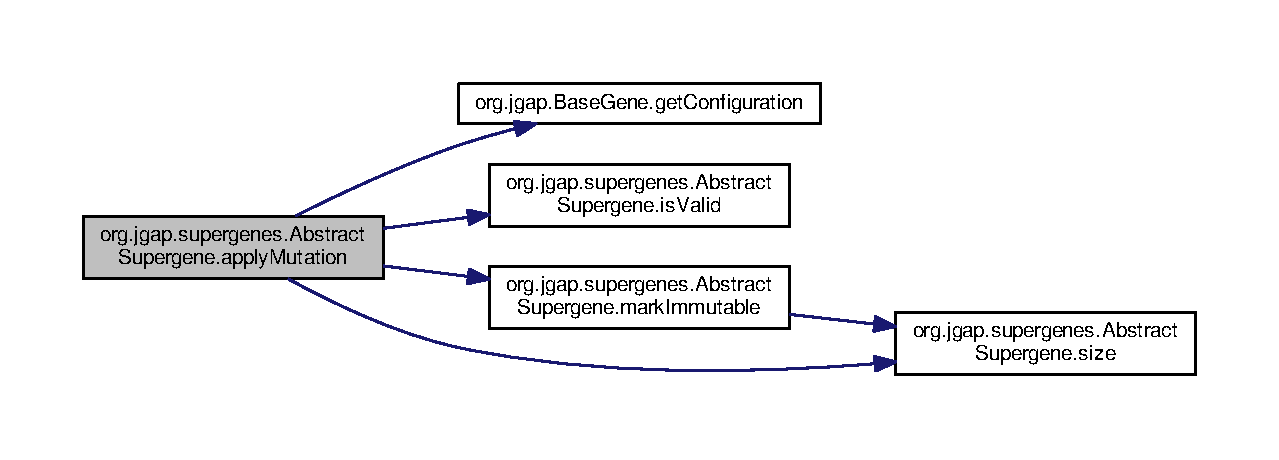
\includegraphics[width=350pt]{classorg_1_1jgap_1_1supergenes_1_1_abstract_supergene_a008b2ecc6f66090965919b537fb327b3_cgraph}
\end{center}
\end{figure}


\hypertarget{classorg_1_1jgap_1_1supergenes_1_1_abstract_supergene_aec3dc6646255f4187aa9a6b4238a9a2c}{\index{org\-::jgap\-::supergenes\-::\-Abstract\-Supergene@{org\-::jgap\-::supergenes\-::\-Abstract\-Supergene}!cleanup@{cleanup}}
\index{cleanup@{cleanup}!org::jgap::supergenes::AbstractSupergene@{org\-::jgap\-::supergenes\-::\-Abstract\-Supergene}}
\subsubsection[{cleanup}]{\setlength{\rightskip}{0pt plus 5cm}void org.\-jgap.\-supergenes.\-Abstract\-Supergene.\-cleanup (
\begin{DoxyParamCaption}
{}
\end{DoxyParamCaption}
)\hspace{0.3cm}{\ttfamily [inline]}}}\label{classorg_1_1jgap_1_1supergenes_1_1_abstract_supergene_aec3dc6646255f4187aa9a6b4238a9a2c}
Calls \hyperlink{classorg_1_1jgap_1_1supergenes_1_1_abstract_supergene_aec3dc6646255f4187aa9a6b4238a9a2c}{cleanup()} for each subgene. 

Implements \hyperlink{interfaceorg_1_1jgap_1_1_gene_a5e353bbf6a9576b702bf466a5f952b82}{org.\-jgap.\-Gene}.



Definition at line 499 of file Abstract\-Supergene.\-java.



References org.\-jgap.\-supergenes.\-Abstract\-Supergene.\-m\-\_\-genes.

\hypertarget{classorg_1_1jgap_1_1supergenes_1_1_abstract_supergene_ac17432577a59856d6ef81abaf0a66bf9}{\index{org\-::jgap\-::supergenes\-::\-Abstract\-Supergene@{org\-::jgap\-::supergenes\-::\-Abstract\-Supergene}!compare\-To@{compare\-To}}
\index{compare\-To@{compare\-To}!org::jgap::supergenes::AbstractSupergene@{org\-::jgap\-::supergenes\-::\-Abstract\-Supergene}}
\subsubsection[{compare\-To}]{\setlength{\rightskip}{0pt plus 5cm}int org.\-jgap.\-supergenes.\-Abstract\-Supergene.\-compare\-To (
\begin{DoxyParamCaption}
\item[{Object}]{o}
\end{DoxyParamCaption}
)\hspace{0.3cm}{\ttfamily [inline]}}}\label{classorg_1_1jgap_1_1supergenes_1_1_abstract_supergene_ac17432577a59856d6ef81abaf0a66bf9}
Calls \hyperlink{classorg_1_1jgap_1_1supergenes_1_1_abstract_supergene_ac17432577a59856d6ef81abaf0a66bf9}{compare\-To()} for all subgenes. The passed parameter must be an instance of \hyperlink{classorg_1_1jgap_1_1supergenes_1_1_abstract_supergene}{Abstract\-Supergene}. 

Definition at line 534 of file Abstract\-Supergene.\-java.



References org.\-jgap.\-supergenes.\-Abstract\-Supergene.\-Abstract\-Supergene(), and org.\-jgap.\-supergenes.\-Abstract\-Supergene.\-m\-\_\-genes.



Referenced by org.\-jgap.\-supergenes.\-Supergene\-Persistent\-Representation\-Test.\-test\-Compare\-To\-\_\-0(), org.\-jgap.\-supergenes.\-Supergene\-Persistent\-Representation\-Test.\-test\-Compare\-To\-\_\-2(), org.\-jgap.\-supergenes.\-Supergene\-Persistent\-Representation\-Test.\-test\-Compare\-To\-\_\-3(), and org.\-jgap.\-supergenes.\-Supergene\-Persistent\-Representation\-Test.\-test\-Equals\-\_\-0().



Here is the call graph for this function\-:
\nopagebreak
\begin{figure}[H]
\begin{center}
\leavevmode
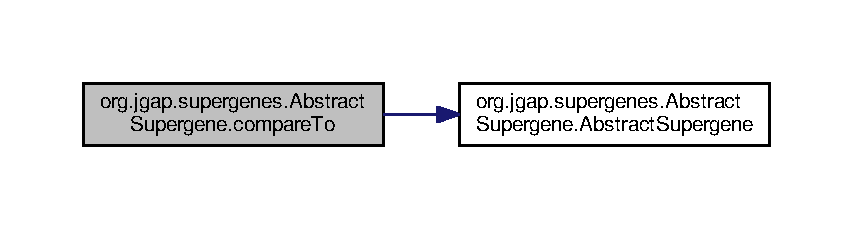
\includegraphics[width=350pt]{classorg_1_1jgap_1_1supergenes_1_1_abstract_supergene_ac17432577a59856d6ef81abaf0a66bf9_cgraph}
\end{center}
\end{figure}


\hypertarget{classorg_1_1jgap_1_1supergenes_1_1_abstract_supergene_a32c5375e3de833953678146fb3dcb5b3}{\index{org\-::jgap\-::supergenes\-::\-Abstract\-Supergene@{org\-::jgap\-::supergenes\-::\-Abstract\-Supergene}!create\-Gene@{create\-Gene}}
\index{create\-Gene@{create\-Gene}!org::jgap::supergenes::AbstractSupergene@{org\-::jgap\-::supergenes\-::\-Abstract\-Supergene}}
\subsubsection[{create\-Gene}]{\setlength{\rightskip}{0pt plus 5cm}{\bf Gene} org.\-jgap.\-supergenes.\-Abstract\-Supergene.\-create\-Gene (
\begin{DoxyParamCaption}
\item[{String}]{a\-\_\-gene\-Class\-Name, }
\item[{String}]{a\-\_\-persistent\-Representation}
\end{DoxyParamCaption}
) throws Exception\hspace{0.3cm}{\ttfamily [inline]}, {\ttfamily [protected]}}}\label{classorg_1_1jgap_1_1supergenes_1_1_abstract_supergene_a32c5375e3de833953678146fb3dcb5b3}
Creates a new instance of gene. 

Definition at line 488 of file Abstract\-Supergene.\-java.



References org.\-jgap.\-Base\-Gene.\-get\-Configuration().



Referenced by org.\-jgap.\-supergenes.\-Abstract\-Supergene.\-set\-Value\-From\-Persistent\-Representation().



Here is the call graph for this function\-:
\nopagebreak
\begin{figure}[H]
\begin{center}
\leavevmode
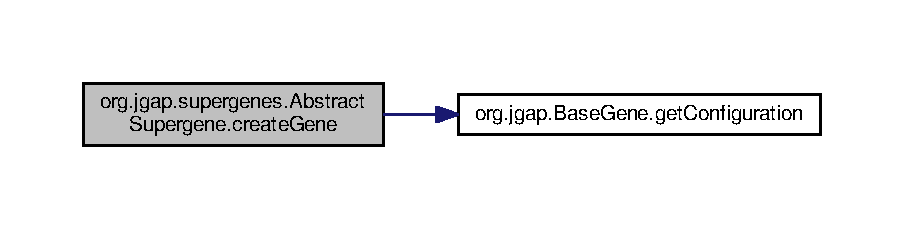
\includegraphics[width=350pt]{classorg_1_1jgap_1_1supergenes_1_1_abstract_supergene_a32c5375e3de833953678146fb3dcb5b3_cgraph}
\end{center}
\end{figure}


\hypertarget{classorg_1_1jgap_1_1supergenes_1_1_abstract_supergene_a497a53be8d8d711ed48c62b062984a94}{\index{org\-::jgap\-::supergenes\-::\-Abstract\-Supergene@{org\-::jgap\-::supergenes\-::\-Abstract\-Supergene}!create\-Validator@{create\-Validator}}
\index{create\-Validator@{create\-Validator}!org::jgap::supergenes::AbstractSupergene@{org\-::jgap\-::supergenes\-::\-Abstract\-Supergene}}
\subsubsection[{create\-Validator}]{\setlength{\rightskip}{0pt plus 5cm}{\bf Supergene\-Validator} org.\-jgap.\-supergenes.\-Abstract\-Supergene.\-create\-Validator (
\begin{DoxyParamCaption}
\item[{String}]{a\-\_\-rep}
\end{DoxyParamCaption}
)\hspace{0.3cm}{\ttfamily [inline]}, {\ttfamily [protected]}}}\label{classorg_1_1jgap_1_1supergenes_1_1_abstract_supergene_a497a53be8d8d711ed48c62b062984a94}
Create validator from the string representation. 

Definition at line 453 of file Abstract\-Supergene.\-java.



References org.\-jgap.\-Base\-Gene.\-decode(), org.\-jgap.\-supergenes.\-Abstract\-Supergene.\-G\-E\-N\-E\-\_\-\-D\-E\-L\-I\-M\-I\-T\-E\-R, and org.\-jgap.\-Base\-Gene.\-get\-Configuration().



Referenced by org.\-jgap.\-supergenes.\-Abstract\-Supergene.\-set\-Value\-From\-Persistent\-Representation().



Here is the call graph for this function\-:
\nopagebreak
\begin{figure}[H]
\begin{center}
\leavevmode
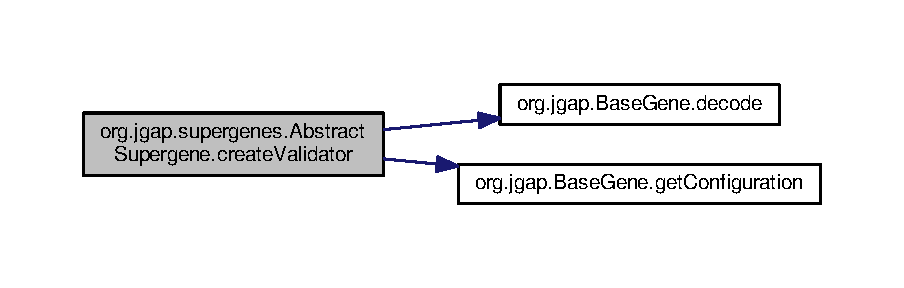
\includegraphics[width=350pt]{classorg_1_1jgap_1_1supergenes_1_1_abstract_supergene_a497a53be8d8d711ed48c62b062984a94_cgraph}
\end{center}
\end{figure}


\hypertarget{classorg_1_1jgap_1_1supergenes_1_1_abstract_supergene_a80be2241977a41672bdbaa85acb7eabc}{\index{org\-::jgap\-::supergenes\-::\-Abstract\-Supergene@{org\-::jgap\-::supergenes\-::\-Abstract\-Supergene}!equals@{equals}}
\index{equals@{equals}!org::jgap::supergenes::AbstractSupergene@{org\-::jgap\-::supergenes\-::\-Abstract\-Supergene}}
\subsubsection[{equals}]{\setlength{\rightskip}{0pt plus 5cm}boolean org.\-jgap.\-supergenes.\-Abstract\-Supergene.\-equals (
\begin{DoxyParamCaption}
\item[{Object}]{a\-\_\-gene}
\end{DoxyParamCaption}
)\hspace{0.3cm}{\ttfamily [inline]}}}\label{classorg_1_1jgap_1_1supergenes_1_1_abstract_supergene_a80be2241977a41672bdbaa85acb7eabc}
Calls \hyperlink{classorg_1_1jgap_1_1supergenes_1_1_abstract_supergene_a80be2241977a41672bdbaa85acb7eabc}{equals()} for each pair of genes. If the supplied object is an instance of the different class, returns false. Also, the genes are assumed to be different if they have different validator classes (or only one of the validators is set to null). 

Definition at line 558 of file Abstract\-Supergene.\-java.



References org.\-jgap.\-supergenes.\-Abstract\-Supergene.\-Abstract\-Supergene(), org.\-jgap.\-supergenes.\-Abstract\-Supergene.\-m\-\_\-genes, org.\-jgap.\-supergenes.\-Abstract\-Supergene.\-m\-\_\-immutable, and org.\-jgap.\-supergenes.\-Abstract\-Supergene.\-m\-\_\-validator.



Referenced by org.\-jgap.\-supergenes.\-Supergene\-Persistent\-Representation\-Test.\-test\-Equals\-\_\-0(), and org.\-jgap.\-supergenes.\-Supergene\-Persistent\-Representation\-Test.\-test\-Representation().



Here is the call graph for this function\-:
\nopagebreak
\begin{figure}[H]
\begin{center}
\leavevmode
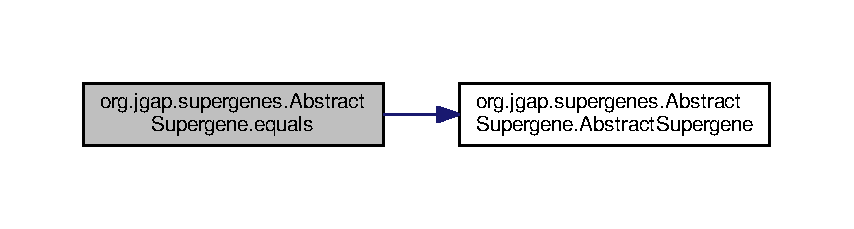
\includegraphics[width=350pt]{classorg_1_1jgap_1_1supergenes_1_1_abstract_supergene_a80be2241977a41672bdbaa85acb7eabc_cgraph}
\end{center}
\end{figure}


\hypertarget{classorg_1_1jgap_1_1supergenes_1_1_abstract_supergene_a099bf664561a1f88b9826e25d870ad7f}{\index{org\-::jgap\-::supergenes\-::\-Abstract\-Supergene@{org\-::jgap\-::supergenes\-::\-Abstract\-Supergene}!gene\-At@{gene\-At}}
\index{gene\-At@{gene\-At}!org::jgap::supergenes::AbstractSupergene@{org\-::jgap\-::supergenes\-::\-Abstract\-Supergene}}
\subsubsection[{gene\-At}]{\setlength{\rightskip}{0pt plus 5cm}final {\bf Gene} org.\-jgap.\-supergenes.\-Abstract\-Supergene.\-gene\-At (
\begin{DoxyParamCaption}
\item[{final int}]{a\-\_\-index}
\end{DoxyParamCaption}
)\hspace{0.3cm}{\ttfamily [inline]}}}\label{classorg_1_1jgap_1_1supergenes_1_1_abstract_supergene_a099bf664561a1f88b9826e25d870ad7f}
Returns the \hyperlink{interfaceorg_1_1jgap_1_1_gene}{Gene} at the given index (locus) within the \hyperlink{classorg_1_1jgap_1_1_chromosome}{Chromosome}. The first gene is at index zero and the last gene is at the index equal to the size of this \hyperlink{classorg_1_1jgap_1_1_chromosome}{Chromosome} -\/ 1.

This seems to be one of the bottlenecks, so it is declared final. I cannot imagine the reason for overriding this trivial single line method.


\begin{DoxyParams}{Parameters}
{\em a\-\_\-index} & the index of the gene value to be returned \\
\hline
\end{DoxyParams}
\begin{DoxyReturn}{Returns}
the \hyperlink{interfaceorg_1_1jgap_1_1_gene}{Gene} at the given index 
\end{DoxyReturn}


Definition at line 92 of file Abstract\-Supergene.\-java.



References org.\-jgap.\-supergenes.\-Abstract\-Supergene.\-m\-\_\-genes.



Referenced by org.\-jgap.\-supergenes.\-Supergene\-Persistent\-Representation\-Test.\-test\-Get\-Genes\-\_\-0(), and org.\-jgap.\-supergenes.\-Supergene\-Persistent\-Representation\-Test.\-test\-Set\-Allele\-\_\-2().

\hypertarget{classorg_1_1jgap_1_1supergenes_1_1_abstract_supergene_a45f21f887ad34c02fbc88d41e5d0372d}{\index{org\-::jgap\-::supergenes\-::\-Abstract\-Supergene@{org\-::jgap\-::supergenes\-::\-Abstract\-Supergene}!get\-Allele@{get\-Allele}}
\index{get\-Allele@{get\-Allele}!org::jgap::supergenes::AbstractSupergene@{org\-::jgap\-::supergenes\-::\-Abstract\-Supergene}}
\subsubsection[{get\-Allele}]{\setlength{\rightskip}{0pt plus 5cm}Object org.\-jgap.\-supergenes.\-Abstract\-Supergene.\-get\-Allele (
\begin{DoxyParamCaption}
{}
\end{DoxyParamCaption}
)\hspace{0.3cm}{\ttfamily [inline]}}}\label{classorg_1_1jgap_1_1supergenes_1_1_abstract_supergene_a45f21f887ad34c02fbc88d41e5d0372d}
Retrieves the allele value represented by this \hyperlink{interfaceorg_1_1jgap_1_1supergenes_1_1_supergene}{Supergene}. \begin{DoxyReturn}{Returns}
array of objects, each matching the subgene in this \hyperlink{interfaceorg_1_1jgap_1_1supergenes_1_1_supergene}{Supergene} 
\end{DoxyReturn}


Implements \hyperlink{interfaceorg_1_1jgap_1_1_gene_aa06c80639659ddbcfa1cfe7b7bb109f9}{org.\-jgap.\-Gene}.



Definition at line 349 of file Abstract\-Supergene.\-java.



References org.\-jgap.\-supergenes.\-Abstract\-Supergene.\-m\-\_\-genes.

\hypertarget{classorg_1_1jgap_1_1supergenes_1_1_abstract_supergene_a5b03d0c4d103975b296d280371b901bd}{\index{org\-::jgap\-::supergenes\-::\-Abstract\-Supergene@{org\-::jgap\-::supergenes\-::\-Abstract\-Supergene}!get\-Genes@{get\-Genes}}
\index{get\-Genes@{get\-Genes}!org::jgap::supergenes::AbstractSupergene@{org\-::jgap\-::supergenes\-::\-Abstract\-Supergene}}
\subsubsection[{get\-Genes}]{\setlength{\rightskip}{0pt plus 5cm}{\bf Gene} \mbox{[}$\,$\mbox{]} org.\-jgap.\-supergenes.\-Abstract\-Supergene.\-get\-Genes (
\begin{DoxyParamCaption}
{}
\end{DoxyParamCaption}
)\hspace{0.3cm}{\ttfamily [inline]}}}\label{classorg_1_1jgap_1_1supergenes_1_1_abstract_supergene_a5b03d0c4d103975b296d280371b901bd}
\begin{DoxyReturn}{Returns}
the array of genes -\/ components of this supergene. The supergene components may be supergenes itself 
\end{DoxyReturn}


Implements \hyperlink{interfaceorg_1_1jgap_1_1supergenes_1_1_supergene_a34ec660dc0d241a9eabc993ddef2ca87}{org.\-jgap.\-supergenes.\-Supergene}.



Definition at line 76 of file Abstract\-Supergene.\-java.



References org.\-jgap.\-supergenes.\-Abstract\-Supergene.\-m\-\_\-genes.



Referenced by org.\-jgap.\-supergenes.\-Supergene\-Persistent\-Representation\-Test.\-test\-Get\-Genes\-\_\-0().

\hypertarget{classorg_1_1jgap_1_1supergenes_1_1_abstract_supergene_af4b0e1f740b6aa78679ab71c51568cea}{\index{org\-::jgap\-::supergenes\-::\-Abstract\-Supergene@{org\-::jgap\-::supergenes\-::\-Abstract\-Supergene}!get\-Internal\-Value@{get\-Internal\-Value}}
\index{get\-Internal\-Value@{get\-Internal\-Value}!org::jgap::supergenes::AbstractSupergene@{org\-::jgap\-::supergenes\-::\-Abstract\-Supergene}}
\subsubsection[{get\-Internal\-Value}]{\setlength{\rightskip}{0pt plus 5cm}Object org.\-jgap.\-supergenes.\-Abstract\-Supergene.\-get\-Internal\-Value (
\begin{DoxyParamCaption}
{}
\end{DoxyParamCaption}
)\hspace{0.3cm}{\ttfamily [inline]}, {\ttfamily [virtual]}}}\label{classorg_1_1jgap_1_1supergenes_1_1_abstract_supergene_af4b0e1f740b6aa78679ab71c51568cea}
\begin{DoxyReturn}{Returns}
not needed for abstract supergene 
\end{DoxyReturn}


Implements \hyperlink{classorg_1_1jgap_1_1_base_gene_ad20da6b23ba524a95caa28f727c26dcd}{org.\-jgap.\-Base\-Gene}.



Definition at line 654 of file Abstract\-Supergene.\-java.

\hypertarget{classorg_1_1jgap_1_1supergenes_1_1_abstract_supergene_aa7990463e784192581d7d7918cd0f1b1}{\index{org\-::jgap\-::supergenes\-::\-Abstract\-Supergene@{org\-::jgap\-::supergenes\-::\-Abstract\-Supergene}!get\-Persistent@{get\-Persistent}}
\index{get\-Persistent@{get\-Persistent}!org::jgap::supergenes::AbstractSupergene@{org\-::jgap\-::supergenes\-::\-Abstract\-Supergene}}
\subsubsection[{get\-Persistent}]{\setlength{\rightskip}{0pt plus 5cm}String org.\-jgap.\-supergenes.\-Abstract\-Supergene.\-get\-Persistent (
\begin{DoxyParamCaption}
{}
\end{DoxyParamCaption}
)\hspace{0.3cm}{\ttfamily [inline]}}}\label{classorg_1_1jgap_1_1supergenes_1_1_abstract_supergene_aa7990463e784192581d7d7918cd0f1b1}
\begin{DoxyReturn}{Returns}
persistent string representation (if needed) of this validator. The method name is different allowing the same class to implement both \hyperlink{interfaceorg_1_1jgap_1_1supergenes_1_1_supergene}{Supergene} and supergene\-Validator.
\end{DoxyReturn}
 The default implementation returns an empty string. 

Implements \hyperlink{interfaceorg_1_1jgap_1_1supergenes_1_1_supergene_validator_a9ef86d28cc29f90d7c451460a4a818fe}{org.\-jgap.\-supergenes.\-Supergene\-Validator}.



Definition at line 642 of file Abstract\-Supergene.\-java.

\hypertarget{classorg_1_1jgap_1_1supergenes_1_1_abstract_supergene_a41a4e0b1cf2366722b5f3b97a1711487}{\index{org\-::jgap\-::supergenes\-::\-Abstract\-Supergene@{org\-::jgap\-::supergenes\-::\-Abstract\-Supergene}!get\-Persistent\-Representation@{get\-Persistent\-Representation}}
\index{get\-Persistent\-Representation@{get\-Persistent\-Representation}!org::jgap::supergenes::AbstractSupergene@{org\-::jgap\-::supergenes\-::\-Abstract\-Supergene}}
\subsubsection[{get\-Persistent\-Representation}]{\setlength{\rightskip}{0pt plus 5cm}String org.\-jgap.\-supergenes.\-Abstract\-Supergene.\-get\-Persistent\-Representation (
\begin{DoxyParamCaption}
{}
\end{DoxyParamCaption}
) throws Unsupported\-Operation\-Exception\hspace{0.3cm}{\ttfamily [inline]}}}\label{classorg_1_1jgap_1_1supergenes_1_1_abstract_supergene_a41a4e0b1cf2366722b5f3b97a1711487}
\begin{DoxyReturn}{Returns}
a string representation of the value of this \hyperlink{interfaceorg_1_1jgap_1_1supergenes_1_1_supergene}{Supergene} instance, using calls to the \hyperlink{interfaceorg_1_1jgap_1_1supergenes_1_1_supergene}{Supergene} components. Supports other (nested) supergenes in this supergene 
\end{DoxyReturn}

\begin{DoxyExceptions}{Exceptions}
{\em Unsupported\-Operation\-Exception} & \\
\hline
\end{DoxyExceptions}


Implements \hyperlink{interfaceorg_1_1jgap_1_1_i_persistent_representation_a07bf7dbaa8de08e268c9357a46e79dac}{org.\-jgap.\-I\-Persistent\-Representation}.



Definition at line 363 of file Abstract\-Supergene.\-java.



References org.\-jgap.\-Base\-Gene.\-encode(), org.\-jgap.\-supergenes.\-Abstract\-Supergene.\-G\-E\-N\-E\-\_\-\-D\-E\-L\-I\-M\-I\-T\-E\-R, org.\-jgap.\-supergenes.\-Abstract\-Supergene.\-G\-E\-N\-E\-\_\-\-D\-E\-L\-I\-M\-I\-T\-E\-R\-\_\-\-C\-L\-O\-S\-I\-N\-G, org.\-jgap.\-supergenes.\-Abstract\-Supergene.\-G\-E\-N\-E\-\_\-\-D\-E\-L\-I\-M\-I\-T\-E\-R\-\_\-\-H\-E\-A\-D\-I\-N\-G, org.\-jgap.\-supergenes.\-Abstract\-Supergene.\-get\-Validator(), and org.\-jgap.\-supergenes.\-Abstract\-Supergene.\-m\-\_\-genes.



Here is the call graph for this function\-:
\nopagebreak
\begin{figure}[H]
\begin{center}
\leavevmode
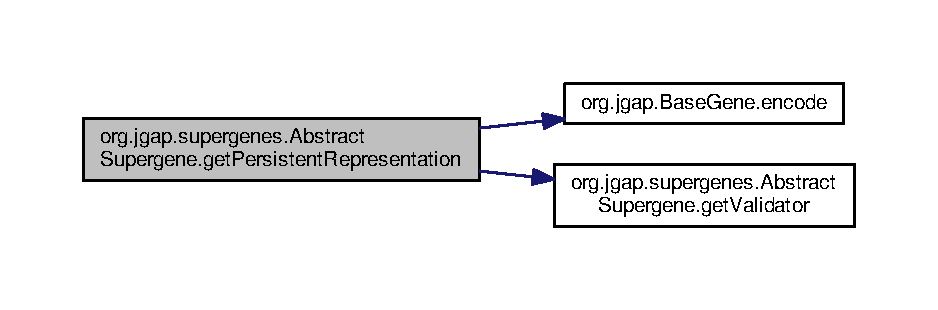
\includegraphics[width=350pt]{classorg_1_1jgap_1_1supergenes_1_1_abstract_supergene_a41a4e0b1cf2366722b5f3b97a1711487_cgraph}
\end{center}
\end{figure}


\hypertarget{classorg_1_1jgap_1_1supergenes_1_1_abstract_supergene_a9ebb4d5fbce8752cba54188ad5958fcf}{\index{org\-::jgap\-::supergenes\-::\-Abstract\-Supergene@{org\-::jgap\-::supergenes\-::\-Abstract\-Supergene}!get\-Validator@{get\-Validator}}
\index{get\-Validator@{get\-Validator}!org::jgap::supergenes::AbstractSupergene@{org\-::jgap\-::supergenes\-::\-Abstract\-Supergene}}
\subsubsection[{get\-Validator}]{\setlength{\rightskip}{0pt plus 5cm}{\bf Supergene\-Validator} org.\-jgap.\-supergenes.\-Abstract\-Supergene.\-get\-Validator (
\begin{DoxyParamCaption}
{}
\end{DoxyParamCaption}
)\hspace{0.3cm}{\ttfamily [inline]}}}\label{classorg_1_1jgap_1_1supergenes_1_1_abstract_supergene_a9ebb4d5fbce8752cba54188ad5958fcf}
Gets an object, responsible for deciding if the \hyperlink{interfaceorg_1_1jgap_1_1supergenes_1_1_supergene}{Supergene} allele combination is valid. If no external validator was set and the class uses its own internal validation method, it returns {\itshape this} 

Implements \hyperlink{interfaceorg_1_1jgap_1_1supergenes_1_1_supergene_a97719a430d58fba89ba26ed8f4a2a490}{org.\-jgap.\-supergenes.\-Supergene}.



Definition at line 633 of file Abstract\-Supergene.\-java.



References org.\-jgap.\-supergenes.\-Abstract\-Supergene.\-m\-\_\-validator.



Referenced by org.\-jgap.\-supergenes.\-Abstract\-Supergene.\-get\-Persistent\-Representation().

\hypertarget{classorg_1_1jgap_1_1supergenes_1_1_abstract_supergene_a73c5c7702d66268b71e9ed92f0c5d41d}{\index{org\-::jgap\-::supergenes\-::\-Abstract\-Supergene@{org\-::jgap\-::supergenes\-::\-Abstract\-Supergene}!hash\-Code@{hash\-Code}}
\index{hash\-Code@{hash\-Code}!org::jgap::supergenes::AbstractSupergene@{org\-::jgap\-::supergenes\-::\-Abstract\-Supergene}}
\subsubsection[{hash\-Code}]{\setlength{\rightskip}{0pt plus 5cm}int org.\-jgap.\-supergenes.\-Abstract\-Supergene.\-hash\-Code (
\begin{DoxyParamCaption}
{}
\end{DoxyParamCaption}
)\hspace{0.3cm}{\ttfamily [inline]}}}\label{classorg_1_1jgap_1_1supergenes_1_1_abstract_supergene_a73c5c7702d66268b71e9ed92f0c5d41d}
Returns sum of \hyperlink{classorg_1_1jgap_1_1supergenes_1_1_abstract_supergene_a73c5c7702d66268b71e9ed92f0c5d41d}{hash\-Code()} of the genes-\/components. 

Definition at line 571 of file Abstract\-Supergene.\-java.



References org.\-jgap.\-supergenes.\-Abstract\-Supergene.\-m\-\_\-genes.

\hypertarget{classorg_1_1jgap_1_1supergenes_1_1_abstract_supergene_adfa0b1f704e28e3a90d187df2cf4b8b5}{\index{org\-::jgap\-::supergenes\-::\-Abstract\-Supergene@{org\-::jgap\-::supergenes\-::\-Abstract\-Supergene}!is\-Valid@{is\-Valid}}
\index{is\-Valid@{is\-Valid}!org::jgap::supergenes::AbstractSupergene@{org\-::jgap\-::supergenes\-::\-Abstract\-Supergene}}
\subsubsection[{is\-Valid}]{\setlength{\rightskip}{0pt plus 5cm}boolean org.\-jgap.\-supergenes.\-Abstract\-Supergene.\-is\-Valid (
\begin{DoxyParamCaption}
{}
\end{DoxyParamCaption}
)\hspace{0.3cm}{\ttfamily [inline]}}}\label{classorg_1_1jgap_1_1supergenes_1_1_abstract_supergene_adfa0b1f704e28e3a90d187df2cf4b8b5}
Test the allele combination of this supergene for validity. This method calls is\-Valid for the current gene list. \begin{DoxyReturn}{Returns}
true only if the supergene allele combination is valid or the set\-Validator ({\itshape null}) has been previously called 
\end{DoxyReturn}


Implements \hyperlink{interfaceorg_1_1jgap_1_1supergenes_1_1_supergene_a9a664a40144dca4dd6fd3b4170ce7570}{org.\-jgap.\-supergenes.\-Supergene}.



Definition at line 145 of file Abstract\-Supergene.\-java.



References org.\-jgap.\-supergenes.\-Abstract\-Supergene.\-m\-\_\-genes, and org.\-jgap.\-supergenes.\-Abstract\-Supergene.\-m\-\_\-validator.



Referenced by org.\-jgap.\-supergenes.\-Abstract\-Supergene.\-apply\-Mutation(), and org.\-jgap.\-supergenes.\-Abstract\-Supergene.\-set\-To\-Random\-Value().

\hypertarget{classorg_1_1jgap_1_1supergenes_1_1_abstract_supergene_a4d07a7aa9a0af1e4e1a96b1a7663afee}{\index{org\-::jgap\-::supergenes\-::\-Abstract\-Supergene@{org\-::jgap\-::supergenes\-::\-Abstract\-Supergene}!is\-Valid@{is\-Valid}}
\index{is\-Valid@{is\-Valid}!org::jgap::supergenes::AbstractSupergene@{org\-::jgap\-::supergenes\-::\-Abstract\-Supergene}}
\subsubsection[{is\-Valid}]{\setlength{\rightskip}{0pt plus 5cm}boolean org.\-jgap.\-supergenes.\-Abstract\-Supergene.\-is\-Valid (
\begin{DoxyParamCaption}
\item[{final {\bf Gene}\mbox{[}$\,$\mbox{]}}]{a\-\_\-case, }
\item[{final {\bf Supergene}}]{a\-\_\-for\-Supergene}
\end{DoxyParamCaption}
)\hspace{0.3cm}{\ttfamily [inline]}}}\label{classorg_1_1jgap_1_1supergenes_1_1_abstract_supergene_a4d07a7aa9a0af1e4e1a96b1a7663afee}
Test the given gene list for validity. The genes must exactly the same as inside this supergene. At {\itshape least about 5 \% of the randomly generated \hyperlink{interfaceorg_1_1jgap_1_1supergenes_1_1_supergene}{Supergene} suparallele values should be valid.} If the valid combinations represents too small part of all possible combinations, it can take too long to find the suitable mutation that does not brake a supergene. If you face this problem, try to split the supergene into several sub-\/supergenes.

This method is only called if you have not set any alternative validator (including {\itshape null}).


\begin{DoxyParams}{Parameters}
{\em a\-\_\-case} & ignored here \\
\hline
{\em a\-\_\-for\-Supergene} & ignored here\\
\hline
\end{DoxyParams}
\begin{DoxyReturn}{Returns}
true only if the supergene allele combination is valid 
\end{DoxyReturn}

\begin{DoxyExceptions}{Exceptions}
{\em Error} & by default. If you do not set external validator, you should always override this method \\
\hline
\end{DoxyExceptions}


Definition at line 174 of file Abstract\-Supergene.\-java.

\hypertarget{classorg_1_1jgap_1_1supergenes_1_1_abstract_supergene_a9f06a4d966c9e615b2ea5bff4583a183}{\index{org\-::jgap\-::supergenes\-::\-Abstract\-Supergene@{org\-::jgap\-::supergenes\-::\-Abstract\-Supergene}!mark\-Immutable@{mark\-Immutable}}
\index{mark\-Immutable@{mark\-Immutable}!org::jgap::supergenes::AbstractSupergene@{org\-::jgap\-::supergenes\-::\-Abstract\-Supergene}}
\subsubsection[{mark\-Immutable}]{\setlength{\rightskip}{0pt plus 5cm}void org.\-jgap.\-supergenes.\-Abstract\-Supergene.\-mark\-Immutable (
\begin{DoxyParamCaption}
\item[{final int}]{a\-\_\-index}
\end{DoxyParamCaption}
)\hspace{0.3cm}{\ttfamily [inline]}, {\ttfamily [private]}}}\label{classorg_1_1jgap_1_1supergenes_1_1_abstract_supergene_a9f06a4d966c9e615b2ea5bff4583a183}
\begin{DoxyRefDesc}{Todo}
\item[\hyperlink{todo__todo000178}{Todo}]\-: Implement protection against overgrowing of this data block. \end{DoxyRefDesc}


Definition at line 267 of file Abstract\-Supergene.\-java.



References org.\-jgap.\-supergenes.\-Abstract\-Supergene.\-m\-\_\-immutable, org.\-jgap.\-supergenes.\-Abstract\-Supergene.\-M\-A\-X\-\_\-\-I\-M\-M\-U\-T\-A\-B\-L\-E\-\_\-\-G\-E\-N\-E\-S, and org.\-jgap.\-supergenes.\-Abstract\-Supergene.\-size().



Referenced by org.\-jgap.\-supergenes.\-Abstract\-Supergene.\-apply\-Mutation().



Here is the call graph for this function\-:
\nopagebreak
\begin{figure}[H]
\begin{center}
\leavevmode
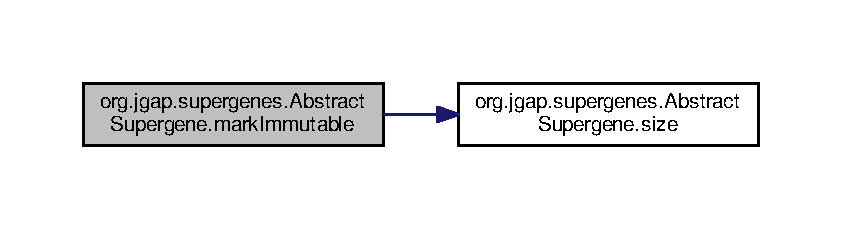
\includegraphics[width=350pt]{classorg_1_1jgap_1_1supergenes_1_1_abstract_supergene_a9f06a4d966c9e615b2ea5bff4583a183_cgraph}
\end{center}
\end{figure}


\hypertarget{classorg_1_1jgap_1_1supergenes_1_1_abstract_supergene_a1e30b794dee0e8da4d5a4d213e9fb2c1}{\index{org\-::jgap\-::supergenes\-::\-Abstract\-Supergene@{org\-::jgap\-::supergenes\-::\-Abstract\-Supergene}!new\-Gene\-Internal@{new\-Gene\-Internal}}
\index{new\-Gene\-Internal@{new\-Gene\-Internal}!org::jgap::supergenes::AbstractSupergene@{org\-::jgap\-::supergenes\-::\-Abstract\-Supergene}}
\subsubsection[{new\-Gene\-Internal}]{\setlength{\rightskip}{0pt plus 5cm}{\bf Gene} org.\-jgap.\-supergenes.\-Abstract\-Supergene.\-new\-Gene\-Internal (
\begin{DoxyParamCaption}
{}
\end{DoxyParamCaption}
)\hspace{0.3cm}{\ttfamily [inline]}, {\ttfamily [protected]}, {\ttfamily [virtual]}}}\label{classorg_1_1jgap_1_1supergenes_1_1_abstract_supergene_a1e30b794dee0e8da4d5a4d213e9fb2c1}
Creates a new instance of this \hyperlink{interfaceorg_1_1jgap_1_1supergenes_1_1_supergene}{Supergene} class with the same number of genes, calling \hyperlink{classorg_1_1jgap_1_1_base_gene_a40f8f3d249145ad028892cd706ba9dae}{new\-Gene()} for each subgene. The class, derived from this abstract supergene will be instantiated (not the instance of abstract\-Supergene itself). If the external validator is set, the same validator will be set for the new gene.

\begin{DoxyReturn}{Returns}
the new \hyperlink{interfaceorg_1_1jgap_1_1_gene}{Gene} 
\end{DoxyReturn}

\begin{DoxyExceptions}{Exceptions}
{\em Error} & if the instance of {\itshape this} cannot be instantiated (for example, if it is not public or the parameterless constructor is not provided). \\
\hline
\end{DoxyExceptions}


Implements \hyperlink{classorg_1_1jgap_1_1_base_gene_aa423e96ffac5a9589fb3a4fbda791b3c}{org.\-jgap.\-Base\-Gene}.



Definition at line 192 of file Abstract\-Supergene.\-java.



References org.\-jgap.\-supergenes.\-Abstract\-Supergene.\-Abstract\-Supergene(), org.\-jgap.\-Base\-Gene.\-get\-Configuration(), org.\-jgap.\-supergenes.\-Abstract\-Supergene.\-m\-\_\-genes, and org.\-jgap.\-supergenes.\-Abstract\-Supergene.\-m\-\_\-validator.



Here is the call graph for this function\-:
\nopagebreak
\begin{figure}[H]
\begin{center}
\leavevmode
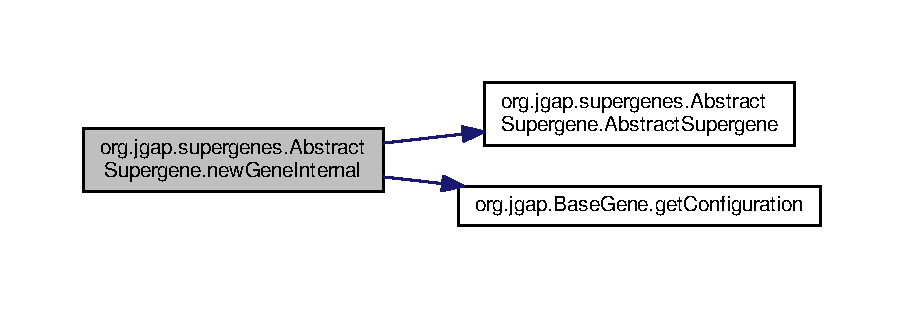
\includegraphics[width=350pt]{classorg_1_1jgap_1_1supergenes_1_1_abstract_supergene_a1e30b794dee0e8da4d5a4d213e9fb2c1_cgraph}
\end{center}
\end{figure}


\hypertarget{classorg_1_1jgap_1_1supergenes_1_1_abstract_supergene_afdcc065673680fb080e17ff2596a0eb0}{\index{org\-::jgap\-::supergenes\-::\-Abstract\-Supergene@{org\-::jgap\-::supergenes\-::\-Abstract\-Supergene}!reset@{reset}}
\index{reset@{reset}!org::jgap::supergenes::AbstractSupergene@{org\-::jgap\-::supergenes\-::\-Abstract\-Supergene}}
\subsubsection[{reset}]{\setlength{\rightskip}{0pt plus 5cm}static void org.\-jgap.\-supergenes.\-Abstract\-Supergene.\-reset (
\begin{DoxyParamCaption}
{}
\end{DoxyParamCaption}
)\hspace{0.3cm}{\ttfamily [inline]}, {\ttfamily [static]}}}\label{classorg_1_1jgap_1_1supergenes_1_1_abstract_supergene_afdcc065673680fb080e17ff2596a0eb0}
Discards all internal caches, ensuring correct repetetive tests of performance. Differently from \hyperlink{classorg_1_1jgap_1_1supergenes_1_1_abstract_supergene_aec3dc6646255f4187aa9a6b4238a9a2c}{cleanup()}, discards also static references, that are assumed to be useful for the multiple instances of the \hyperlink{interfaceorg_1_1jgap_1_1supergenes_1_1_supergene}{Supergene}. Clears the set of the alleles that are known to be immutable. 

Definition at line 293 of file Abstract\-Supergene.\-java.



References org.\-jgap.\-supergenes.\-Abstract\-Supergene.\-m\-\_\-immutable.

\hypertarget{classorg_1_1jgap_1_1supergenes_1_1_abstract_supergene_a7b3ce455ac6d30ba31b198ce6824cd19}{\index{org\-::jgap\-::supergenes\-::\-Abstract\-Supergene@{org\-::jgap\-::supergenes\-::\-Abstract\-Supergene}!set\-Allele@{set\-Allele}}
\index{set\-Allele@{set\-Allele}!org::jgap::supergenes::AbstractSupergene@{org\-::jgap\-::supergenes\-::\-Abstract\-Supergene}}
\subsubsection[{set\-Allele}]{\setlength{\rightskip}{0pt plus 5cm}void org.\-jgap.\-supergenes.\-Abstract\-Supergene.\-set\-Allele (
\begin{DoxyParamCaption}
\item[{final Object}]{a\-\_\-super\-Allele}
\end{DoxyParamCaption}
)\hspace{0.3cm}{\ttfamily [inline]}}}\label{classorg_1_1jgap_1_1supergenes_1_1_abstract_supergene_a7b3ce455ac6d30ba31b198ce6824cd19}
Sets the allele. 
\begin{DoxyParams}{Parameters}
{\em a\-\_\-super\-Allele} & must be an array of objects, size matching the number of genes \\
\hline
\end{DoxyParams}


Definition at line 329 of file Abstract\-Supergene.\-java.



References org.\-jgap.\-supergenes.\-Abstract\-Supergene.\-m\-\_\-genes.

\hypertarget{classorg_1_1jgap_1_1supergenes_1_1_abstract_supergene_a70a5435dbf92b886ab7d5bbcd2d79d09}{\index{org\-::jgap\-::supergenes\-::\-Abstract\-Supergene@{org\-::jgap\-::supergenes\-::\-Abstract\-Supergene}!set\-From\-Persistent@{set\-From\-Persistent}}
\index{set\-From\-Persistent@{set\-From\-Persistent}!org::jgap::supergenes::AbstractSupergene@{org\-::jgap\-::supergenes\-::\-Abstract\-Supergene}}
\subsubsection[{set\-From\-Persistent}]{\setlength{\rightskip}{0pt plus 5cm}void org.\-jgap.\-supergenes.\-Abstract\-Supergene.\-set\-From\-Persistent (
\begin{DoxyParamCaption}
\item[{String}]{a\-\_\-from}
\end{DoxyParamCaption}
)\hspace{0.3cm}{\ttfamily [inline]}}}\label{classorg_1_1jgap_1_1supergenes_1_1_abstract_supergene_a70a5435dbf92b886ab7d5bbcd2d79d09}
Set a persistend string representation (if needed) for this validator. The method name is different allowing the same class to implement both \hyperlink{interfaceorg_1_1jgap_1_1supergenes_1_1_supergene}{Supergene} and supergene\-Validator. The default implementation does nothing. 

Implements \hyperlink{interfaceorg_1_1jgap_1_1supergenes_1_1_supergene_validator_a8718b55ab8474e3b5df097ef152a93f0}{org.\-jgap.\-supergenes.\-Supergene\-Validator}.



Definition at line 648 of file Abstract\-Supergene.\-java.

\hypertarget{classorg_1_1jgap_1_1supergenes_1_1_abstract_supergene_a92df9df781b9ae3bc7811bf76bb7ea87}{\index{org\-::jgap\-::supergenes\-::\-Abstract\-Supergene@{org\-::jgap\-::supergenes\-::\-Abstract\-Supergene}!set\-To\-Random\-Value@{set\-To\-Random\-Value}}
\index{set\-To\-Random\-Value@{set\-To\-Random\-Value}!org::jgap::supergenes::AbstractSupergene@{org\-::jgap\-::supergenes\-::\-Abstract\-Supergene}}
\subsubsection[{set\-To\-Random\-Value}]{\setlength{\rightskip}{0pt plus 5cm}void org.\-jgap.\-supergenes.\-Abstract\-Supergene.\-set\-To\-Random\-Value (
\begin{DoxyParamCaption}
\item[{final {\bf Random\-Generator}}]{a\-\_\-number\-Generator}
\end{DoxyParamCaption}
)\hspace{0.3cm}{\ttfamily [inline]}}}\label{classorg_1_1jgap_1_1supergenes_1_1_abstract_supergene_a92df9df781b9ae3bc7811bf76bb7ea87}
Sets the value of this \hyperlink{interfaceorg_1_1jgap_1_1_gene}{Gene} to a random legal value for the implementation. It calls set\-To\-Random\-Value for all subgenes and then validates. With a large number of subgenes and low percent of valid combinations this may take too long to complete. We think, at lease several \% of the all possible combintations must be valid. 

Definition at line 304 of file Abstract\-Supergene.\-java.



References org.\-jgap.\-supergenes.\-Abstract\-Supergene.\-is\-Valid(), org.\-jgap.\-supergenes.\-Abstract\-Supergene.\-m\-\_\-genes, and org.\-jgap.\-supergenes.\-Abstract\-Supergene.\-M\-A\-X\-\_\-\-R\-E\-T\-R\-I\-E\-S.



Here is the call graph for this function\-:
\nopagebreak
\begin{figure}[H]
\begin{center}
\leavevmode
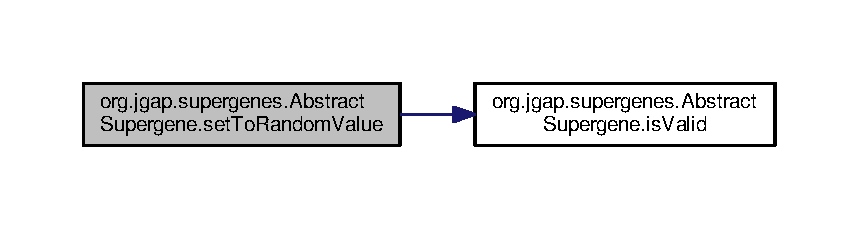
\includegraphics[width=350pt]{classorg_1_1jgap_1_1supergenes_1_1_abstract_supergene_a92df9df781b9ae3bc7811bf76bb7ea87_cgraph}
\end{center}
\end{figure}


\hypertarget{classorg_1_1jgap_1_1supergenes_1_1_abstract_supergene_afae838561a1237ab6b39456ab0e3b8c8}{\index{org\-::jgap\-::supergenes\-::\-Abstract\-Supergene@{org\-::jgap\-::supergenes\-::\-Abstract\-Supergene}!set\-Validator@{set\-Validator}}
\index{set\-Validator@{set\-Validator}!org::jgap::supergenes::AbstractSupergene@{org\-::jgap\-::supergenes\-::\-Abstract\-Supergene}}
\subsubsection[{set\-Validator}]{\setlength{\rightskip}{0pt plus 5cm}void org.\-jgap.\-supergenes.\-Abstract\-Supergene.\-set\-Validator (
\begin{DoxyParamCaption}
\item[{{\bf Supergene\-Validator}}]{a\-\_\-validator}
\end{DoxyParamCaption}
)\hspace{0.3cm}{\ttfamily [inline]}}}\label{classorg_1_1jgap_1_1supergenes_1_1_abstract_supergene_afae838561a1237ab6b39456ab0e3b8c8}
Sets an object, responsible for deciding if the \hyperlink{interfaceorg_1_1jgap_1_1supergenes_1_1_supergene}{Supergene} allele combination is valid. If it is set to null, no validation is performed (all combinations are assumed to be valid). If no validator is set, the method {\ttfamily is\-Valid (\hyperlink{interfaceorg_1_1jgap_1_1_gene}{Gene} \mbox{[}\mbox{]} ) }is called. 

Implements \hyperlink{interfaceorg_1_1jgap_1_1supergenes_1_1_supergene_a56ef316d0073f74cfd2704ac407ad83f}{org.\-jgap.\-supergenes.\-Supergene}.



Definition at line 624 of file Abstract\-Supergene.\-java.



References org.\-jgap.\-supergenes.\-Abstract\-Supergene.\-m\-\_\-validator.



Referenced by org.\-jgap.\-supergenes.\-Abstract\-Supergene.\-set\-Value\-From\-Persistent\-Representation().

\hypertarget{classorg_1_1jgap_1_1supergenes_1_1_abstract_supergene_af8156c2a8b41bc9fe3e397595c513a6d}{\index{org\-::jgap\-::supergenes\-::\-Abstract\-Supergene@{org\-::jgap\-::supergenes\-::\-Abstract\-Supergene}!set\-Value\-From\-Persistent\-Representation@{set\-Value\-From\-Persistent\-Representation}}
\index{set\-Value\-From\-Persistent\-Representation@{set\-Value\-From\-Persistent\-Representation}!org::jgap::supergenes::AbstractSupergene@{org\-::jgap\-::supergenes\-::\-Abstract\-Supergene}}
\subsubsection[{set\-Value\-From\-Persistent\-Representation}]{\setlength{\rightskip}{0pt plus 5cm}void org.\-jgap.\-supergenes.\-Abstract\-Supergene.\-set\-Value\-From\-Persistent\-Representation (
\begin{DoxyParamCaption}
\item[{String}]{a\-\_\-representation}
\end{DoxyParamCaption}
) throws {\bf Unsupported\-Representation\-Exception}\hspace{0.3cm}{\ttfamily [inline]}}}\label{classorg_1_1jgap_1_1supergenes_1_1_abstract_supergene_af8156c2a8b41bc9fe3e397595c513a6d}
Sets the value and internal state of this \hyperlink{interfaceorg_1_1jgap_1_1_gene}{Gene} from the string representation returned by a previous invocation of the \hyperlink{classorg_1_1jgap_1_1supergenes_1_1_abstract_supergene_a41a4e0b1cf2366722b5f3b97a1711487}{get\-Persistent\-Representation()} method.

If the validator is not T\-H\-I\-S and not null, a new validator is created using Class.\-for\-Name(..).new\-Instance.


\begin{DoxyParams}{Parameters}
{\em a\-\_\-representation} & the string representation retrieved from a prior call to the \hyperlink{classorg_1_1jgap_1_1supergenes_1_1_abstract_supergene_a41a4e0b1cf2366722b5f3b97a1711487}{get\-Persistent\-Representation()} method\\
\hline
\end{DoxyParams}

\begin{DoxyExceptions}{Exceptions}
{\em \hyperlink{classorg_1_1jgap_1_1_unsupported_representation_exception}{Unsupported\-Representation\-Exception}} & \\
\hline
\end{DoxyExceptions}
\begin{DoxyAuthor}{Author}
Audrius Meskauskas 
\end{DoxyAuthor}
\begin{DoxySince}{Since}
2.\-0 
\end{DoxySince}
Remove the old content. 

Implements \hyperlink{interfaceorg_1_1jgap_1_1_i_persistent_representation_a94a345f1919c4840dd0b9eecf7afc6a3}{org.\-jgap.\-I\-Persistent\-Representation}.



Definition at line 411 of file Abstract\-Supergene.\-java.



References org.\-jgap.\-supergenes.\-Abstract\-Supergene.\-create\-Gene(), org.\-jgap.\-supergenes.\-Abstract\-Supergene.\-create\-Validator(), org.\-jgap.\-Base\-Gene.\-decode(), org.\-jgap.\-supergenes.\-Abstract\-Supergene.\-G\-E\-N\-E\-\_\-\-D\-E\-L\-I\-M\-I\-T\-E\-R, org.\-jgap.\-supergenes.\-Abstract\-Supergene.\-m\-\_\-genes, org.\-jgap.\-supergenes.\-Abstract\-Supergene.\-set\-Validator(), and org.\-jgap.\-supergenes.\-Abstract\-Supergene.\-split().



Here is the call graph for this function\-:
\nopagebreak
\begin{figure}[H]
\begin{center}
\leavevmode
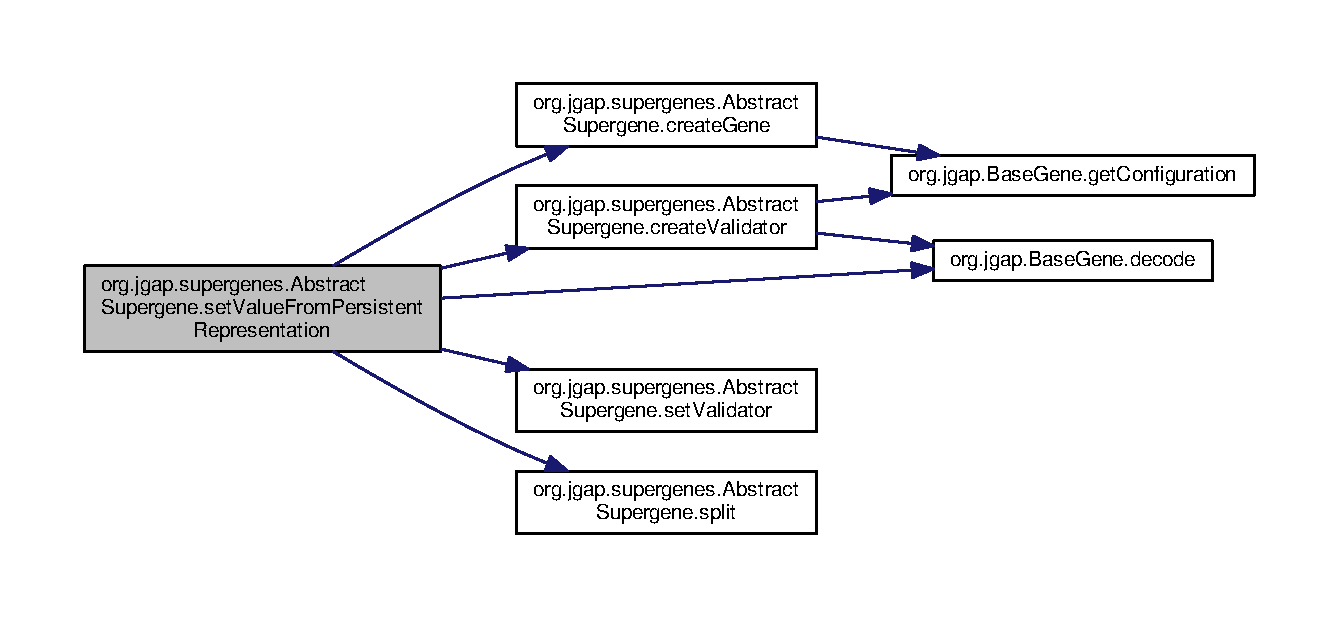
\includegraphics[width=350pt]{classorg_1_1jgap_1_1supergenes_1_1_abstract_supergene_af8156c2a8b41bc9fe3e397595c513a6d_cgraph}
\end{center}
\end{figure}


\hypertarget{classorg_1_1jgap_1_1supergenes_1_1_abstract_supergene_a8d2326c3d5ce80c73dff063f26994233}{\index{org\-::jgap\-::supergenes\-::\-Abstract\-Supergene@{org\-::jgap\-::supergenes\-::\-Abstract\-Supergene}!size@{size}}
\index{size@{size}!org::jgap::supergenes::AbstractSupergene@{org\-::jgap\-::supergenes\-::\-Abstract\-Supergene}}
\subsubsection[{size}]{\setlength{\rightskip}{0pt plus 5cm}int org.\-jgap.\-supergenes.\-Abstract\-Supergene.\-size (
\begin{DoxyParamCaption}
{}
\end{DoxyParamCaption}
)\hspace{0.3cm}{\ttfamily [inline]}}}\label{classorg_1_1jgap_1_1supergenes_1_1_abstract_supergene_a8d2326c3d5ce80c73dff063f26994233}
Returns the number of the genes-\/components of this supergene. 

Implements \hyperlink{interfaceorg_1_1jgap_1_1_gene_a7a975e180dd0ac0fd33cdc182f64bea8}{org.\-jgap.\-Gene}.



Definition at line 528 of file Abstract\-Supergene.\-java.



Referenced by org.\-jgap.\-supergenes.\-Abstract\-Supergene.\-apply\-Mutation(), org.\-jgap.\-supergenes.\-Abstract\-Supergene.\-mark\-Immutable(), org.\-jgap.\-supergenes.\-Supergene\-Persistent\-Representation\-Test.\-test\-Set\-Allele\-\_\-0(), and org.\-jgap.\-supergenes.\-Supergene\-Persistent\-Representation\-Test.\-test\-Size\-\_\-0().

\hypertarget{classorg_1_1jgap_1_1supergenes_1_1_abstract_supergene_a3ff87dbb7c5c6a4167198184b7171934}{\index{org\-::jgap\-::supergenes\-::\-Abstract\-Supergene@{org\-::jgap\-::supergenes\-::\-Abstract\-Supergene}!split@{split}}
\index{split@{split}!org::jgap::supergenes::AbstractSupergene@{org\-::jgap\-::supergenes\-::\-Abstract\-Supergene}}
\subsubsection[{split}]{\setlength{\rightskip}{0pt plus 5cm}static final List org.\-jgap.\-supergenes.\-Abstract\-Supergene.\-split (
\begin{DoxyParamCaption}
\item[{String}]{a\-\_\-string}
\end{DoxyParamCaption}
) throws {\bf Unsupported\-Representation\-Exception}\hspace{0.3cm}{\ttfamily [inline]}, {\ttfamily [static]}, {\ttfamily [protected]}}}\label{classorg_1_1jgap_1_1supergenes_1_1_abstract_supergene_a3ff87dbb7c5c6a4167198184b7171934}
Splits the string a\-\_\-x into individual gene representations 
\begin{DoxyParams}{Parameters}
{\em a\-\_\-string} & the string to split \\
\hline
\end{DoxyParams}
\begin{DoxyReturn}{Returns}
the elements of the returned array are the persistent representation strings of the genes -\/ components
\end{DoxyReturn}
\begin{DoxyAuthor}{Author}
Audrius Meskauskas 
\end{DoxyAuthor}


Definition at line 587 of file Abstract\-Supergene.\-java.



References org.\-jgap.\-supergenes.\-Abstract\-Supergene.\-G\-E\-N\-E\-\_\-\-D\-E\-L\-I\-M\-I\-T\-E\-R\-\_\-\-C\-L\-O\-S\-I\-N\-G, and org.\-jgap.\-supergenes.\-Abstract\-Supergene.\-G\-E\-N\-E\-\_\-\-D\-E\-L\-I\-M\-I\-T\-E\-R\-\_\-\-H\-E\-A\-D\-I\-N\-G.



Referenced by org.\-jgap.\-supergenes.\-Abstract\-Supergene.\-set\-Value\-From\-Persistent\-Representation().

\hypertarget{classorg_1_1jgap_1_1supergenes_1_1_abstract_supergene_a67a9b1dfccb63d4b2909abdd3e8c1abe}{\index{org\-::jgap\-::supergenes\-::\-Abstract\-Supergene@{org\-::jgap\-::supergenes\-::\-Abstract\-Supergene}!to\-String@{to\-String}}
\index{to\-String@{to\-String}!org::jgap::supergenes::AbstractSupergene@{org\-::jgap\-::supergenes\-::\-Abstract\-Supergene}}
\subsubsection[{to\-String}]{\setlength{\rightskip}{0pt plus 5cm}String org.\-jgap.\-supergenes.\-Abstract\-Supergene.\-to\-String (
\begin{DoxyParamCaption}
{}
\end{DoxyParamCaption}
)\hspace{0.3cm}{\ttfamily [inline]}}}\label{classorg_1_1jgap_1_1supergenes_1_1_abstract_supergene_a67a9b1dfccb63d4b2909abdd3e8c1abe}
\begin{DoxyReturn}{Returns}
a string representation of the supergene, providing class name and calling \hyperlink{classorg_1_1jgap_1_1supergenes_1_1_abstract_supergene_a67a9b1dfccb63d4b2909abdd3e8c1abe}{to\-String()} for all subgenes. 
\end{DoxyReturn}


Implements \hyperlink{interfaceorg_1_1jgap_1_1_gene_ac62239b4b7bf81179fd491a4c4bd1901}{org.\-jgap.\-Gene}.



Definition at line 509 of file Abstract\-Supergene.\-java.



References org.\-jgap.\-supergenes.\-Abstract\-Supergene.\-m\-\_\-genes, and org.\-jgap.\-supergenes.\-Abstract\-Supergene.\-m\-\_\-validator.



\subsection{Member Data Documentation}
\hypertarget{classorg_1_1jgap_1_1supergenes_1_1_abstract_supergene_a9084146c063a12faff254011968f40b8}{\index{org\-::jgap\-::supergenes\-::\-Abstract\-Supergene@{org\-::jgap\-::supergenes\-::\-Abstract\-Supergene}!C\-V\-S\-\_\-\-R\-E\-V\-I\-S\-I\-O\-N@{C\-V\-S\-\_\-\-R\-E\-V\-I\-S\-I\-O\-N}}
\index{C\-V\-S\-\_\-\-R\-E\-V\-I\-S\-I\-O\-N@{C\-V\-S\-\_\-\-R\-E\-V\-I\-S\-I\-O\-N}!org::jgap::supergenes::AbstractSupergene@{org\-::jgap\-::supergenes\-::\-Abstract\-Supergene}}
\subsubsection[{C\-V\-S\-\_\-\-R\-E\-V\-I\-S\-I\-O\-N}]{\setlength{\rightskip}{0pt plus 5cm}final String org.\-jgap.\-supergenes.\-Abstract\-Supergene.\-C\-V\-S\-\_\-\-R\-E\-V\-I\-S\-I\-O\-N = \char`\"{}\$Revision\-: 1.\-24 \$\char`\"{}\hspace{0.3cm}{\ttfamily [static]}, {\ttfamily [private]}}}\label{classorg_1_1jgap_1_1supergenes_1_1_abstract_supergene_a9084146c063a12faff254011968f40b8}
String containing the C\-V\-S revision. Read out via reflection! 

Definition at line 33 of file Abstract\-Supergene.\-java.

\hypertarget{classorg_1_1jgap_1_1supergenes_1_1_abstract_supergene_ae7be27a291a2aa7e594384dd7a5936a8}{\index{org\-::jgap\-::supergenes\-::\-Abstract\-Supergene@{org\-::jgap\-::supergenes\-::\-Abstract\-Supergene}!G\-E\-N\-E\-\_\-\-D\-E\-L\-I\-M\-I\-T\-E\-R@{G\-E\-N\-E\-\_\-\-D\-E\-L\-I\-M\-I\-T\-E\-R}}
\index{G\-E\-N\-E\-\_\-\-D\-E\-L\-I\-M\-I\-T\-E\-R@{G\-E\-N\-E\-\_\-\-D\-E\-L\-I\-M\-I\-T\-E\-R}!org::jgap::supergenes::AbstractSupergene@{org\-::jgap\-::supergenes\-::\-Abstract\-Supergene}}
\subsubsection[{G\-E\-N\-E\-\_\-\-D\-E\-L\-I\-M\-I\-T\-E\-R}]{\setlength{\rightskip}{0pt plus 5cm}final String org.\-jgap.\-supergenes.\-Abstract\-Supergene.\-G\-E\-N\-E\-\_\-\-D\-E\-L\-I\-M\-I\-T\-E\-R = \char`\"{}\#\char`\"{}\hspace{0.3cm}{\ttfamily [static]}}}\label{classorg_1_1jgap_1_1supergenes_1_1_abstract_supergene_ae7be27a291a2aa7e594384dd7a5936a8}
This field separates gene class name from the gene persistent representation string. 

Definition at line 39 of file Abstract\-Supergene.\-java.



Referenced by org.\-jgap.\-supergenes.\-Abstract\-Supergene.\-create\-Validator(), org.\-jgap.\-supergenes.\-Abstract\-Supergene.\-get\-Persistent\-Representation(), and org.\-jgap.\-supergenes.\-Abstract\-Supergene.\-set\-Value\-From\-Persistent\-Representation().

\hypertarget{classorg_1_1jgap_1_1supergenes_1_1_abstract_supergene_a96059d4ef9cca18130330f3ab782c28b}{\index{org\-::jgap\-::supergenes\-::\-Abstract\-Supergene@{org\-::jgap\-::supergenes\-::\-Abstract\-Supergene}!G\-E\-N\-E\-\_\-\-D\-E\-L\-I\-M\-I\-T\-E\-R\-\_\-\-C\-L\-O\-S\-I\-N\-G@{G\-E\-N\-E\-\_\-\-D\-E\-L\-I\-M\-I\-T\-E\-R\-\_\-\-C\-L\-O\-S\-I\-N\-G}}
\index{G\-E\-N\-E\-\_\-\-D\-E\-L\-I\-M\-I\-T\-E\-R\-\_\-\-C\-L\-O\-S\-I\-N\-G@{G\-E\-N\-E\-\_\-\-D\-E\-L\-I\-M\-I\-T\-E\-R\-\_\-\-C\-L\-O\-S\-I\-N\-G}!org::jgap::supergenes::AbstractSupergene@{org\-::jgap\-::supergenes\-::\-Abstract\-Supergene}}
\subsubsection[{G\-E\-N\-E\-\_\-\-D\-E\-L\-I\-M\-I\-T\-E\-R\-\_\-\-C\-L\-O\-S\-I\-N\-G}]{\setlength{\rightskip}{0pt plus 5cm}final String org.\-jgap.\-supergenes.\-Abstract\-Supergene.\-G\-E\-N\-E\-\_\-\-D\-E\-L\-I\-M\-I\-T\-E\-R\-\_\-\-C\-L\-O\-S\-I\-N\-G = \char`\"{}$>$\char`\"{}\hspace{0.3cm}{\ttfamily [static]}}}\label{classorg_1_1jgap_1_1supergenes_1_1_abstract_supergene_a96059d4ef9cca18130330f3ab782c28b}
Represents the closing delimiter that is used to separate genes in the persistent representation of Composite\-Gene instances. 

Definition at line 51 of file Abstract\-Supergene.\-java.



Referenced by org.\-jgap.\-supergenes.\-Abstract\-Supergene.\-get\-Persistent\-Representation(), and org.\-jgap.\-supergenes.\-Abstract\-Supergene.\-split().

\hypertarget{classorg_1_1jgap_1_1supergenes_1_1_abstract_supergene_aebbbd0fdd22a6d94c951471c8ae86b84}{\index{org\-::jgap\-::supergenes\-::\-Abstract\-Supergene@{org\-::jgap\-::supergenes\-::\-Abstract\-Supergene}!G\-E\-N\-E\-\_\-\-D\-E\-L\-I\-M\-I\-T\-E\-R\-\_\-\-H\-E\-A\-D\-I\-N\-G@{G\-E\-N\-E\-\_\-\-D\-E\-L\-I\-M\-I\-T\-E\-R\-\_\-\-H\-E\-A\-D\-I\-N\-G}}
\index{G\-E\-N\-E\-\_\-\-D\-E\-L\-I\-M\-I\-T\-E\-R\-\_\-\-H\-E\-A\-D\-I\-N\-G@{G\-E\-N\-E\-\_\-\-D\-E\-L\-I\-M\-I\-T\-E\-R\-\_\-\-H\-E\-A\-D\-I\-N\-G}!org::jgap::supergenes::AbstractSupergene@{org\-::jgap\-::supergenes\-::\-Abstract\-Supergene}}
\subsubsection[{G\-E\-N\-E\-\_\-\-D\-E\-L\-I\-M\-I\-T\-E\-R\-\_\-\-H\-E\-A\-D\-I\-N\-G}]{\setlength{\rightskip}{0pt plus 5cm}final String org.\-jgap.\-supergenes.\-Abstract\-Supergene.\-G\-E\-N\-E\-\_\-\-D\-E\-L\-I\-M\-I\-T\-E\-R\-\_\-\-H\-E\-A\-D\-I\-N\-G = \char`\"{}$<$\char`\"{}\hspace{0.3cm}{\ttfamily [static]}}}\label{classorg_1_1jgap_1_1supergenes_1_1_abstract_supergene_aebbbd0fdd22a6d94c951471c8ae86b84}
Represents the heading delimiter that is used to separate genes in the persistent representation of Composite\-Gene instances. 

Definition at line 45 of file Abstract\-Supergene.\-java.



Referenced by org.\-jgap.\-supergenes.\-Abstract\-Supergene.\-get\-Persistent\-Representation(), and org.\-jgap.\-supergenes.\-Abstract\-Supergene.\-split().

\hypertarget{classorg_1_1jgap_1_1supergenes_1_1_abstract_supergene_a7e237a04c314d9fbb0ab064ad88a5cb3}{\index{org\-::jgap\-::supergenes\-::\-Abstract\-Supergene@{org\-::jgap\-::supergenes\-::\-Abstract\-Supergene}!m\-\_\-genes@{m\-\_\-genes}}
\index{m\-\_\-genes@{m\-\_\-genes}!org::jgap::supergenes::AbstractSupergene@{org\-::jgap\-::supergenes\-::\-Abstract\-Supergene}}
\subsubsection[{m\-\_\-genes}]{\setlength{\rightskip}{0pt plus 5cm}{\bf Gene} \mbox{[}$\,$\mbox{]} org.\-jgap.\-supergenes.\-Abstract\-Supergene.\-m\-\_\-genes\hspace{0.3cm}{\ttfamily [private]}}}\label{classorg_1_1jgap_1_1supergenes_1_1_abstract_supergene_a7e237a04c314d9fbb0ab064ad88a5cb3}
Holds the genes of this supergene. 

Definition at line 67 of file Abstract\-Supergene.\-java.



Referenced by org.\-jgap.\-supergenes.\-Abstract\-Supergene.\-Abstract\-Supergene(), org.\-jgap.\-supergenes.\-Abstract\-Supergene.\-add\-Gene(), org.\-jgap.\-supergenes.\-Abstract\-Supergene.\-apply\-Mutation(), org.\-jgap.\-supergenes.\-Abstract\-Supergene.\-cleanup(), org.\-jgap.\-supergenes.\-Abstract\-Supergene.\-compare\-To(), org.\-jgap.\-supergenes.\-Abstract\-Supergene.\-equals(), org.\-jgap.\-supergenes.\-Abstract\-Supergene.\-gene\-At(), org.\-jgap.\-supergenes.\-Abstract\-Supergene.\-get\-Allele(), org.\-jgap.\-supergenes.\-Abstract\-Supergene.\-get\-Genes(), org.\-jgap.\-supergenes.\-Abstract\-Supergene.\-get\-Persistent\-Representation(), org.\-jgap.\-supergenes.\-Abstract\-Supergene.\-hash\-Code(), org.\-jgap.\-supergenes.\-Abstract\-Supergene.\-is\-Valid(), org.\-jgap.\-supergenes.\-Abstract\-Supergene.\-new\-Gene\-Internal(), org.\-jgap.\-supergenes.\-Abstract\-Supergene.\-set\-Allele(), org.\-jgap.\-supergenes.\-Abstract\-Supergene.\-set\-To\-Random\-Value(), org.\-jgap.\-supergenes.\-Abstract\-Supergene.\-set\-Value\-From\-Persistent\-Representation(), and org.\-jgap.\-supergenes.\-Abstract\-Supergene.\-to\-String().

\hypertarget{classorg_1_1jgap_1_1supergenes_1_1_abstract_supergene_a92632c12f27c0aaef1984c8550afe9a1}{\index{org\-::jgap\-::supergenes\-::\-Abstract\-Supergene@{org\-::jgap\-::supergenes\-::\-Abstract\-Supergene}!m\-\_\-immutable@{m\-\_\-immutable}}
\index{m\-\_\-immutable@{m\-\_\-immutable}!org::jgap::supergenes::AbstractSupergene@{org\-::jgap\-::supergenes\-::\-Abstract\-Supergene}}
\subsubsection[{m\-\_\-immutable}]{\setlength{\rightskip}{0pt plus 5cm}Set \mbox{[}$\,$\mbox{]} org.\-jgap.\-supergenes.\-Abstract\-Supergene.\-m\-\_\-immutable = new Set\mbox{[}1\mbox{]}\hspace{0.3cm}{\ttfamily [static]}, {\ttfamily [private]}}}\label{classorg_1_1jgap_1_1supergenes_1_1_abstract_supergene_a92632c12f27c0aaef1984c8550afe9a1}
Set of supergene allele values that cannot mutate. 

Definition at line 70 of file Abstract\-Supergene.\-java.



Referenced by org.\-jgap.\-supergenes.\-Abstract\-Supergene.\-apply\-Mutation(), org.\-jgap.\-supergenes.\-Abstract\-Supergene.\-equals(), org.\-jgap.\-supergenes.\-Abstract\-Supergene.\-mark\-Immutable(), and org.\-jgap.\-supergenes.\-Abstract\-Supergene.\-reset().

\hypertarget{classorg_1_1jgap_1_1supergenes_1_1_abstract_supergene_a8792c7c19ad0cdb48ade652a110a9016}{\index{org\-::jgap\-::supergenes\-::\-Abstract\-Supergene@{org\-::jgap\-::supergenes\-::\-Abstract\-Supergene}!m\-\_\-validator@{m\-\_\-validator}}
\index{m\-\_\-validator@{m\-\_\-validator}!org::jgap::supergenes::AbstractSupergene@{org\-::jgap\-::supergenes\-::\-Abstract\-Supergene}}
\subsubsection[{m\-\_\-validator}]{\setlength{\rightskip}{0pt plus 5cm}{\bf Supergene\-Validator} org.\-jgap.\-supergenes.\-Abstract\-Supergene.\-m\-\_\-validator = this\hspace{0.3cm}{\ttfamily [protected]}}}\label{classorg_1_1jgap_1_1supergenes_1_1_abstract_supergene_a8792c7c19ad0cdb48ade652a110a9016}
A validator (initially set to {\itshape this} 

Definition at line 638 of file Abstract\-Supergene.\-java.



Referenced by org.\-jgap.\-supergenes.\-Abstract\-Supergene.\-equals(), org.\-jgap.\-supergenes.\-Abstract\-Supergene.\-get\-Validator(), org.\-jgap.\-supergenes.\-Abstract\-Supergene.\-is\-Valid(), org.\-jgap.\-supergenes.\-Abstract\-Supergene.\-new\-Gene\-Internal(), org.\-jgap.\-supergenes.\-Abstract\-Supergene.\-set\-Validator(), and org.\-jgap.\-supergenes.\-Abstract\-Supergene.\-to\-String().

\hypertarget{classorg_1_1jgap_1_1supergenes_1_1_abstract_supergene_a40054ab751c7676fcd9f974c029a6a9d}{\index{org\-::jgap\-::supergenes\-::\-Abstract\-Supergene@{org\-::jgap\-::supergenes\-::\-Abstract\-Supergene}!M\-A\-X\-\_\-\-I\-M\-M\-U\-T\-A\-B\-L\-E\-\_\-\-G\-E\-N\-E\-S@{M\-A\-X\-\_\-\-I\-M\-M\-U\-T\-A\-B\-L\-E\-\_\-\-G\-E\-N\-E\-S}}
\index{M\-A\-X\-\_\-\-I\-M\-M\-U\-T\-A\-B\-L\-E\-\_\-\-G\-E\-N\-E\-S@{M\-A\-X\-\_\-\-I\-M\-M\-U\-T\-A\-B\-L\-E\-\_\-\-G\-E\-N\-E\-S}!org::jgap::supergenes::AbstractSupergene@{org\-::jgap\-::supergenes\-::\-Abstract\-Supergene}}
\subsubsection[{M\-A\-X\-\_\-\-I\-M\-M\-U\-T\-A\-B\-L\-E\-\_\-\-G\-E\-N\-E\-S}]{\setlength{\rightskip}{0pt plus 5cm}final int org.\-jgap.\-supergenes.\-Abstract\-Supergene.\-M\-A\-X\-\_\-\-I\-M\-M\-U\-T\-A\-B\-L\-E\-\_\-\-G\-E\-N\-E\-S = 100000\hspace{0.3cm}{\ttfamily [static]}}}\label{classorg_1_1jgap_1_1supergenes_1_1_abstract_supergene_a40054ab751c7676fcd9f974c029a6a9d}
Maximal number of notes about immutable genes per single gene position 

Definition at line 64 of file Abstract\-Supergene.\-java.



Referenced by org.\-jgap.\-supergenes.\-Abstract\-Supergene.\-mark\-Immutable().

\hypertarget{classorg_1_1jgap_1_1supergenes_1_1_abstract_supergene_a6839c4b04a89a58c967219eda28a5dbb}{\index{org\-::jgap\-::supergenes\-::\-Abstract\-Supergene@{org\-::jgap\-::supergenes\-::\-Abstract\-Supergene}!M\-A\-X\-\_\-\-R\-E\-T\-R\-I\-E\-S@{M\-A\-X\-\_\-\-R\-E\-T\-R\-I\-E\-S}}
\index{M\-A\-X\-\_\-\-R\-E\-T\-R\-I\-E\-S@{M\-A\-X\-\_\-\-R\-E\-T\-R\-I\-E\-S}!org::jgap::supergenes::AbstractSupergene@{org\-::jgap\-::supergenes\-::\-Abstract\-Supergene}}
\subsubsection[{M\-A\-X\-\_\-\-R\-E\-T\-R\-I\-E\-S}]{\setlength{\rightskip}{0pt plus 5cm}final int org.\-jgap.\-supergenes.\-Abstract\-Supergene.\-M\-A\-X\-\_\-\-R\-E\-T\-R\-I\-E\-S = 1\hspace{0.3cm}{\ttfamily [static]}}}\label{classorg_1_1jgap_1_1supergenes_1_1_abstract_supergene_a6839c4b04a89a58c967219eda28a5dbb}
Maximal number of retries for apply\-Mutation and set\-To\-Random\-Value. If the valid supergen cannot be created after this number of iterations, the error message is printed and the unchanged instance is returned. 

Definition at line 58 of file Abstract\-Supergene.\-java.



Referenced by org.\-jgap.\-supergenes.\-Abstract\-Supergene.\-apply\-Mutation(), and org.\-jgap.\-supergenes.\-Abstract\-Supergene.\-set\-To\-Random\-Value().



The documentation for this class was generated from the following file\-:\begin{DoxyCompactItemize}
\item 
L\-D\-H\-\_\-\-Git/src/org/jgap/supergenes/\hyperlink{_abstract_supergene_8java}{Abstract\-Supergene.\-java}\end{DoxyCompactItemize}

\hypertarget{classexamples_1_1supergene_1_1_abstract_supergene_test}{\section{examples.\-supergene.\-Abstract\-Supergene\-Test Class Reference}
\label{classexamples_1_1supergene_1_1_abstract_supergene_test}\index{examples.\-supergene.\-Abstract\-Supergene\-Test@{examples.\-supergene.\-Abstract\-Supergene\-Test}}
}


Inheritance diagram for examples.\-supergene.\-Abstract\-Supergene\-Test\-:
\nopagebreak
\begin{figure}[H]
\begin{center}
\leavevmode
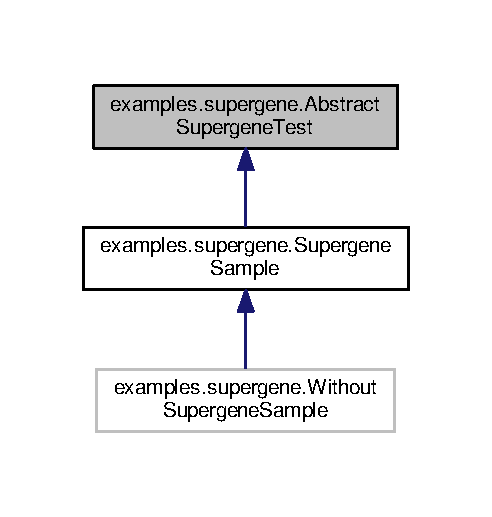
\includegraphics[width=236pt]{classexamples_1_1supergene_1_1_abstract_supergene_test__inherit__graph}
\end{center}
\end{figure}
\subsection*{Public Member Functions}
\begin{DoxyCompactItemize}
\item 
abstract int \hyperlink{classexamples_1_1supergene_1_1_abstract_supergene_test_af2fc5c540e716975e1c4106e8f95a1a5}{make\-Change\-For\-Amount} (int a\-\_\-target\-Change\-Amount)  throws Exception
\item 
I\-Chromosome \hyperlink{classexamples_1_1supergene_1_1_abstract_supergene_test_a739a675575c3932e123f47b774b358f8}{report} (\hyperlink{classexamples_1_1supergene_1_1_supergene_change_fitness_function}{Supergene\-Change\-Fitness\-Function} a\-\_\-fitness\-Function, Genotype a\-\_\-population)
\item 
int \hyperlink{classexamples_1_1supergene_1_1_abstract_supergene_test_a92f6bbeeedeed872a2cb7cb38e6a40c2}{test} ()
\end{DoxyCompactItemize}
\subsection*{Static Public Member Functions}
\begin{DoxyCompactItemize}
\item 
static int \hyperlink{classexamples_1_1supergene_1_1_abstract_supergene_test_a634c86555d7accce1bd015ff6f99c630}{amount\-Of\-Change} (int a\-\_\-num\-Quarters, int a\-\_\-num\-Dimes, int a\-\_\-num\-Nickels, int a\-\_\-num\-Pennies)
\end{DoxyCompactItemize}
\subsection*{Static Public Attributes}
\begin{DoxyCompactItemize}
\item 
static final int \hyperlink{classexamples_1_1supergene_1_1_abstract_supergene_test_a2581251d3607aad43d8b2815b8202c8e}{D\-I\-M\-E\-S} = 0
\item 
static final int \hyperlink{classexamples_1_1supergene_1_1_abstract_supergene_test_aed911231f02517c09e71a453e303b655}{Q\-U\-A\-R\-T\-E\-R\-S} = 1
\item 
static final int \hyperlink{classexamples_1_1supergene_1_1_abstract_supergene_test_a816ceb1de4c9bf5c3df3bac9210c380c}{N\-I\-C\-K\-E\-L\-S} = 2
\item 
static final int \hyperlink{classexamples_1_1supergene_1_1_abstract_supergene_test_a0853afd453197d0e7db44388752d12af}{P\-E\-N\-N\-I\-E\-S} = 3
\item 
static int \hyperlink{classexamples_1_1supergene_1_1_abstract_supergene_test_aabc7656a38ca4e7322c3ff08d34ee8f4}{M\-A\-X\-\_\-\-A\-L\-L\-O\-W\-E\-D\-\_\-\-E\-V\-O\-L\-U\-T\-I\-O\-N\-S} = 200
\item 
static int \hyperlink{classexamples_1_1supergene_1_1_abstract_supergene_test_af5010d4eddc24d9723d539ea6c12c595}{P\-O\-P\-U\-L\-A\-T\-I\-O\-N\-\_\-\-S\-I\-Z\-E} = 2000
\item 
static boolean \hyperlink{classexamples_1_1supergene_1_1_abstract_supergene_test_a6884362188d843b7a05c2845e9857358}{R\-E\-P\-O\-R\-T\-\_\-\-E\-N\-A\-B\-L\-E\-D} = true
\item 
static boolean \hyperlink{classexamples_1_1supergene_1_1_abstract_supergene_test_afa2af2b745985502119958481e9c12f6}{E\-X\-I\-S\-T\-I\-N\-G\-\_\-\-S\-O\-L\-U\-T\-I\-O\-N\-S\-\_\-\-O\-N\-L\-Y} = false
\end{DoxyCompactItemize}
\subsection*{Protected Member Functions}
\begin{DoxyCompactItemize}
\item 
Gene \hyperlink{classexamples_1_1supergene_1_1_abstract_supergene_test_a4dd26799d08a8f8d1e2bfcf047c42738}{get\-Dimes\-Gene} (Configuration a\-\_\-conf)
\item 
Gene \hyperlink{classexamples_1_1supergene_1_1_abstract_supergene_test_a6d4533c657828b3d0e98dda17572dcb6}{get\-Nickels\-Gene} (Configuration a\-\_\-conf)
\item 
Gene \hyperlink{classexamples_1_1supergene_1_1_abstract_supergene_test_aac16c07ab37989c472d80acc4071dafe}{get\-Pennies\-Gene} (Configuration a\-\_\-conf)
\item 
Gene \hyperlink{classexamples_1_1supergene_1_1_abstract_supergene_test_a1b9e8ef8f0436df0feee9337f7c437bd}{get\-Quarters\-Gene} (Configuration a\-\_\-conf)
\item 
int \hyperlink{classexamples_1_1supergene_1_1_abstract_supergene_test_a7f4bc155739845dcac0bc31ec952192d}{solve} (Configuration a\-\_\-conf, int a\-\_\-target\-Change\-Amount, \hyperlink{classexamples_1_1supergene_1_1_supergene_change_fitness_function}{Supergene\-Change\-Fitness\-Function} a\-\_\-fitness\-Function, Gene\mbox{[}$\,$\mbox{]} a\-\_\-sample\-Genes)  throws Invalid\-Configuration\-Exception 
\end{DoxyCompactItemize}
\subsection*{Static Private Attributes}
\begin{DoxyCompactItemize}
\item 
static final String \hyperlink{classexamples_1_1supergene_1_1_abstract_supergene_test_a3bf642196176bfe1e85adea8652098b7}{C\-V\-S\-\_\-\-R\-E\-V\-I\-S\-I\-O\-N} = \char`\"{}\$Revision\-: 1.\-5 \$\char`\"{}
\end{DoxyCompactItemize}


\subsection{Detailed Description}
Abstract class for testing Supergene performance.

\begin{DoxyAuthor}{Author}
Neil Rotstan 

Klaus Meffert 

Audrius Meskauskas 
\end{DoxyAuthor}
\begin{DoxySince}{Since}
2.\-0 
\end{DoxySince}


Definition at line 23 of file Abstract\-Supergene\-Test.\-java.



\subsection{Member Function Documentation}
\hypertarget{classexamples_1_1supergene_1_1_abstract_supergene_test_a634c86555d7accce1bd015ff6f99c630}{\index{examples\-::supergene\-::\-Abstract\-Supergene\-Test@{examples\-::supergene\-::\-Abstract\-Supergene\-Test}!amount\-Of\-Change@{amount\-Of\-Change}}
\index{amount\-Of\-Change@{amount\-Of\-Change}!examples::supergene::AbstractSupergeneTest@{examples\-::supergene\-::\-Abstract\-Supergene\-Test}}
\subsubsection[{amount\-Of\-Change}]{\setlength{\rightskip}{0pt plus 5cm}static int examples.\-supergene.\-Abstract\-Supergene\-Test.\-amount\-Of\-Change (
\begin{DoxyParamCaption}
\item[{int}]{a\-\_\-num\-Quarters, }
\item[{int}]{a\-\_\-num\-Dimes, }
\item[{int}]{a\-\_\-num\-Nickels, }
\item[{int}]{a\-\_\-num\-Pennies}
\end{DoxyParamCaption}
)\hspace{0.3cm}{\ttfamily [inline]}, {\ttfamily [static]}}}\label{classexamples_1_1supergene_1_1_abstract_supergene_test_a634c86555d7accce1bd015ff6f99c630}
Compute the money value from the coin information. 

Definition at line 108 of file Abstract\-Supergene\-Test.\-java.



Referenced by examples.\-supergene.\-Force.\-solve().

\hypertarget{classexamples_1_1supergene_1_1_abstract_supergene_test_a4dd26799d08a8f8d1e2bfcf047c42738}{\index{examples\-::supergene\-::\-Abstract\-Supergene\-Test@{examples\-::supergene\-::\-Abstract\-Supergene\-Test}!get\-Dimes\-Gene@{get\-Dimes\-Gene}}
\index{get\-Dimes\-Gene@{get\-Dimes\-Gene}!examples::supergene::AbstractSupergeneTest@{examples\-::supergene\-::\-Abstract\-Supergene\-Test}}
\subsubsection[{get\-Dimes\-Gene}]{\setlength{\rightskip}{0pt plus 5cm}Gene examples.\-supergene.\-Abstract\-Supergene\-Test.\-get\-Dimes\-Gene (
\begin{DoxyParamCaption}
\item[{Configuration}]{a\-\_\-conf}
\end{DoxyParamCaption}
)\hspace{0.3cm}{\ttfamily [inline]}, {\ttfamily [protected]}}}\label{classexamples_1_1supergene_1_1_abstract_supergene_test_a4dd26799d08a8f8d1e2bfcf047c42738}

\begin{DoxyParams}{Parameters}
{\em a\-\_\-conf} & the configuration to use\\
\hline
\end{DoxyParams}
\begin{DoxyReturn}{Returns}
created Dimes gene instance 
\end{DoxyReturn}


Definition at line 64 of file Abstract\-Supergene\-Test.\-java.



Referenced by examples.\-supergene.\-Supergene\-Sample.\-make\-Change\-For\-Amount().

\hypertarget{classexamples_1_1supergene_1_1_abstract_supergene_test_a6d4533c657828b3d0e98dda17572dcb6}{\index{examples\-::supergene\-::\-Abstract\-Supergene\-Test@{examples\-::supergene\-::\-Abstract\-Supergene\-Test}!get\-Nickels\-Gene@{get\-Nickels\-Gene}}
\index{get\-Nickels\-Gene@{get\-Nickels\-Gene}!examples::supergene::AbstractSupergeneTest@{examples\-::supergene\-::\-Abstract\-Supergene\-Test}}
\subsubsection[{get\-Nickels\-Gene}]{\setlength{\rightskip}{0pt plus 5cm}Gene examples.\-supergene.\-Abstract\-Supergene\-Test.\-get\-Nickels\-Gene (
\begin{DoxyParamCaption}
\item[{Configuration}]{a\-\_\-conf}
\end{DoxyParamCaption}
)\hspace{0.3cm}{\ttfamily [inline]}, {\ttfamily [protected]}}}\label{classexamples_1_1supergene_1_1_abstract_supergene_test_a6d4533c657828b3d0e98dda17572dcb6}

\begin{DoxyParams}{Parameters}
{\em a\-\_\-conf} & the configuration to use\\
\hline
\end{DoxyParams}
\begin{DoxyReturn}{Returns}
created Nickels gene instance 
\end{DoxyReturn}


Definition at line 76 of file Abstract\-Supergene\-Test.\-java.



Referenced by examples.\-supergene.\-Supergene\-Sample.\-make\-Change\-For\-Amount().

\hypertarget{classexamples_1_1supergene_1_1_abstract_supergene_test_aac16c07ab37989c472d80acc4071dafe}{\index{examples\-::supergene\-::\-Abstract\-Supergene\-Test@{examples\-::supergene\-::\-Abstract\-Supergene\-Test}!get\-Pennies\-Gene@{get\-Pennies\-Gene}}
\index{get\-Pennies\-Gene@{get\-Pennies\-Gene}!examples::supergene::AbstractSupergeneTest@{examples\-::supergene\-::\-Abstract\-Supergene\-Test}}
\subsubsection[{get\-Pennies\-Gene}]{\setlength{\rightskip}{0pt plus 5cm}Gene examples.\-supergene.\-Abstract\-Supergene\-Test.\-get\-Pennies\-Gene (
\begin{DoxyParamCaption}
\item[{Configuration}]{a\-\_\-conf}
\end{DoxyParamCaption}
)\hspace{0.3cm}{\ttfamily [inline]}, {\ttfamily [protected]}}}\label{classexamples_1_1supergene_1_1_abstract_supergene_test_aac16c07ab37989c472d80acc4071dafe}

\begin{DoxyParams}{Parameters}
{\em a\-\_\-conf} & the configuration to use\\
\hline
\end{DoxyParams}
\begin{DoxyReturn}{Returns}
created Pennies (1) gene instance 
\end{DoxyReturn}


Definition at line 88 of file Abstract\-Supergene\-Test.\-java.



Referenced by examples.\-supergene.\-Supergene\-Sample.\-make\-Change\-For\-Amount().

\hypertarget{classexamples_1_1supergene_1_1_abstract_supergene_test_a1b9e8ef8f0436df0feee9337f7c437bd}{\index{examples\-::supergene\-::\-Abstract\-Supergene\-Test@{examples\-::supergene\-::\-Abstract\-Supergene\-Test}!get\-Quarters\-Gene@{get\-Quarters\-Gene}}
\index{get\-Quarters\-Gene@{get\-Quarters\-Gene}!examples::supergene::AbstractSupergeneTest@{examples\-::supergene\-::\-Abstract\-Supergene\-Test}}
\subsubsection[{get\-Quarters\-Gene}]{\setlength{\rightskip}{0pt plus 5cm}Gene examples.\-supergene.\-Abstract\-Supergene\-Test.\-get\-Quarters\-Gene (
\begin{DoxyParamCaption}
\item[{Configuration}]{a\-\_\-conf}
\end{DoxyParamCaption}
)\hspace{0.3cm}{\ttfamily [inline]}, {\ttfamily [protected]}}}\label{classexamples_1_1supergene_1_1_abstract_supergene_test_a1b9e8ef8f0436df0feee9337f7c437bd}

\begin{DoxyParams}{Parameters}
{\em a\-\_\-conf} & the configuration to use\\
\hline
\end{DoxyParams}
\begin{DoxyReturn}{Returns}
created Quarters gene instance 
\end{DoxyReturn}


Definition at line 100 of file Abstract\-Supergene\-Test.\-java.



Referenced by examples.\-supergene.\-Supergene\-Sample.\-make\-Change\-For\-Amount().

\hypertarget{classexamples_1_1supergene_1_1_abstract_supergene_test_af2fc5c540e716975e1c4106e8f95a1a5}{\index{examples\-::supergene\-::\-Abstract\-Supergene\-Test@{examples\-::supergene\-::\-Abstract\-Supergene\-Test}!make\-Change\-For\-Amount@{make\-Change\-For\-Amount}}
\index{make\-Change\-For\-Amount@{make\-Change\-For\-Amount}!examples::supergene::AbstractSupergeneTest@{examples\-::supergene\-::\-Abstract\-Supergene\-Test}}
\subsubsection[{make\-Change\-For\-Amount}]{\setlength{\rightskip}{0pt plus 5cm}abstract int examples.\-supergene.\-Abstract\-Supergene\-Test.\-make\-Change\-For\-Amount (
\begin{DoxyParamCaption}
\item[{int}]{a\-\_\-target\-Change\-Amount}
\end{DoxyParamCaption}
) throws Exception\hspace{0.3cm}{\ttfamily [pure virtual]}}}\label{classexamples_1_1supergene_1_1_abstract_supergene_test_af2fc5c540e716975e1c4106e8f95a1a5}
Executes the genetic algorithm to determine the minimum number of coins necessary to make up the given target amount of change. The solution will then be written to System.\-out.


\begin{DoxyParams}{Parameters}
{\em a\-\_\-target\-Change\-Amount} & the target amount of change for which this method is attempting to produce the minimum number of coins\\
\hline
\end{DoxyParams}
\begin{DoxyReturn}{Returns}
absolute difference between the required and computed change amount 
\end{DoxyReturn}

\begin{DoxyExceptions}{Exceptions}
{\em Exception} & \\
\hline
\end{DoxyExceptions}


Implemented in \hyperlink{classexamples_1_1supergene_1_1_supergene_sample_a367571e3fe1b537e62559d15a817ac6d}{examples.\-supergene.\-Supergene\-Sample}.



Referenced by examples.\-supergene.\-Abstract\-Supergene\-Test.\-test().

\hypertarget{classexamples_1_1supergene_1_1_abstract_supergene_test_a739a675575c3932e123f47b774b358f8}{\index{examples\-::supergene\-::\-Abstract\-Supergene\-Test@{examples\-::supergene\-::\-Abstract\-Supergene\-Test}!report@{report}}
\index{report@{report}!examples::supergene::AbstractSupergeneTest@{examples\-::supergene\-::\-Abstract\-Supergene\-Test}}
\subsubsection[{report}]{\setlength{\rightskip}{0pt plus 5cm}I\-Chromosome examples.\-supergene.\-Abstract\-Supergene\-Test.\-report (
\begin{DoxyParamCaption}
\item[{{\bf Supergene\-Change\-Fitness\-Function}}]{a\-\_\-fitness\-Function, }
\item[{Genotype}]{a\-\_\-population}
\end{DoxyParamCaption}
)\hspace{0.3cm}{\ttfamily [inline]}}}\label{classexamples_1_1supergene_1_1_abstract_supergene_test_a739a675575c3932e123f47b774b358f8}
Write report on eveluation to the given stream. 
\begin{DoxyParams}{Parameters}
{\em a\-\_\-fitness\-Function} & p\-\_\-\-Supergene\-Change\-Fitness\-Function \\
\hline
{\em a\-\_\-population} & Genotype \\
\hline
\end{DoxyParams}
\begin{DoxyReturn}{Returns}
Chromosome 
\end{DoxyReturn}


Definition at line 135 of file Abstract\-Supergene\-Test.\-java.



References examples.\-supergene.\-Abstract\-Supergene\-Test.\-D\-I\-M\-E\-S, examples.\-supergene.\-Abstract\-Change\-Fitness\-Function.\-get\-Total\-Number\-Of\-Coins(), examples.\-supergene.\-Abstract\-Supergene\-Test.\-N\-I\-C\-K\-E\-L\-S, examples.\-supergene.\-Abstract\-Supergene\-Test.\-P\-E\-N\-N\-I\-E\-S, examples.\-supergene.\-Abstract\-Supergene\-Test.\-Q\-U\-A\-R\-T\-E\-R\-S, and examples.\-supergene.\-Abstract\-Supergene\-Test.\-R\-E\-P\-O\-R\-T\-\_\-\-E\-N\-A\-B\-L\-E\-D.



Referenced by examples.\-supergene.\-Abstract\-Supergene\-Test.\-solve().



Here is the call graph for this function\-:
\nopagebreak
\begin{figure}[H]
\begin{center}
\leavevmode
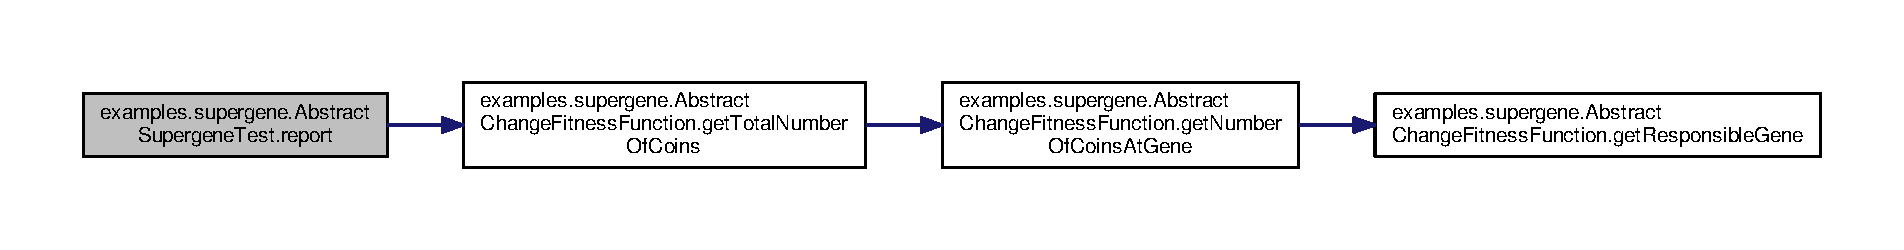
\includegraphics[width=350pt]{classexamples_1_1supergene_1_1_abstract_supergene_test_a739a675575c3932e123f47b774b358f8_cgraph}
\end{center}
\end{figure}


\hypertarget{classexamples_1_1supergene_1_1_abstract_supergene_test_a7f4bc155739845dcac0bc31ec952192d}{\index{examples\-::supergene\-::\-Abstract\-Supergene\-Test@{examples\-::supergene\-::\-Abstract\-Supergene\-Test}!solve@{solve}}
\index{solve@{solve}!examples::supergene::AbstractSupergeneTest@{examples\-::supergene\-::\-Abstract\-Supergene\-Test}}
\subsubsection[{solve}]{\setlength{\rightskip}{0pt plus 5cm}int examples.\-supergene.\-Abstract\-Supergene\-Test.\-solve (
\begin{DoxyParamCaption}
\item[{Configuration}]{a\-\_\-conf, }
\item[{int}]{a\-\_\-target\-Change\-Amount, }
\item[{{\bf Supergene\-Change\-Fitness\-Function}}]{a\-\_\-fitness\-Function, }
\item[{Gene\mbox{[}$\,$\mbox{]}}]{a\-\_\-sample\-Genes}
\end{DoxyParamCaption}
) throws Invalid\-Configuration\-Exception\hspace{0.3cm}{\ttfamily [inline]}, {\ttfamily [protected]}}}\label{classexamples_1_1supergene_1_1_abstract_supergene_test_a7f4bc155739845dcac0bc31ec952192d}
Find and print the solution, return the solution error.


\begin{DoxyParams}{Parameters}
{\em a\-\_\-conf} & the configuration to use\\
\hline
\end{DoxyParams}
\begin{DoxyReturn}{Returns}
absolute difference between the required and computed change 
\end{DoxyReturn}


Definition at line 210 of file Abstract\-Supergene\-Test.\-java.



References examples.\-supergene.\-Abstract\-Supergene\-Test.\-M\-A\-X\-\_\-\-A\-L\-L\-O\-W\-E\-D\-\_\-\-E\-V\-O\-L\-U\-T\-I\-O\-N\-S, examples.\-supergene.\-Abstract\-Supergene\-Test.\-P\-O\-P\-U\-L\-A\-T\-I\-O\-N\-\_\-\-S\-I\-Z\-E, and examples.\-supergene.\-Abstract\-Supergene\-Test.\-report().



Referenced by examples.\-supergene.\-Supergene\-Sample.\-make\-Change\-For\-Amount().



Here is the call graph for this function\-:
\nopagebreak
\begin{figure}[H]
\begin{center}
\leavevmode
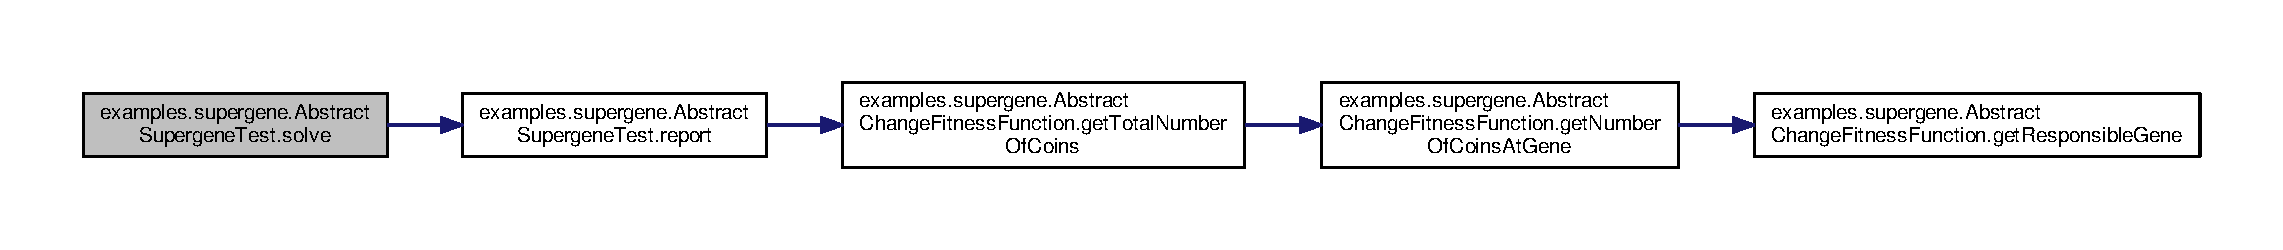
\includegraphics[width=350pt]{classexamples_1_1supergene_1_1_abstract_supergene_test_a7f4bc155739845dcac0bc31ec952192d_cgraph}
\end{center}
\end{figure}


\hypertarget{classexamples_1_1supergene_1_1_abstract_supergene_test_a92f6bbeeedeed872a2cb7cb38e6a40c2}{\index{examples\-::supergene\-::\-Abstract\-Supergene\-Test@{examples\-::supergene\-::\-Abstract\-Supergene\-Test}!test@{test}}
\index{test@{test}!examples::supergene::AbstractSupergeneTest@{examples\-::supergene\-::\-Abstract\-Supergene\-Test}}
\subsubsection[{test}]{\setlength{\rightskip}{0pt plus 5cm}int examples.\-supergene.\-Abstract\-Supergene\-Test.\-test (
\begin{DoxyParamCaption}
{}
\end{DoxyParamCaption}
)\hspace{0.3cm}{\ttfamily [inline]}}}\label{classexamples_1_1supergene_1_1_abstract_supergene_test_a92f6bbeeedeed872a2cb7cb38e6a40c2}
Test the method, returns the sum of all differences between the required and obtained excange amount. One exception counts as 1000 on the error score. 

Definition at line 169 of file Abstract\-Supergene\-Test.\-java.



References examples.\-supergene.\-Abstract\-Supergene\-Test.\-E\-X\-I\-S\-T\-I\-N\-G\-\_\-\-S\-O\-L\-U\-T\-I\-O\-N\-S\-\_\-\-O\-N\-L\-Y, examples.\-supergene.\-Abstract\-Supergene\-Test.\-make\-Change\-For\-Amount(), examples.\-supergene.\-Abstract\-Supergene\-Test.\-R\-E\-P\-O\-R\-T\-\_\-\-E\-N\-A\-B\-L\-E\-D, and examples.\-supergene.\-Force.\-solve().



Referenced by examples.\-supergene.\-Supergene\-Sample.\-main().



Here is the call graph for this function\-:
\nopagebreak
\begin{figure}[H]
\begin{center}
\leavevmode
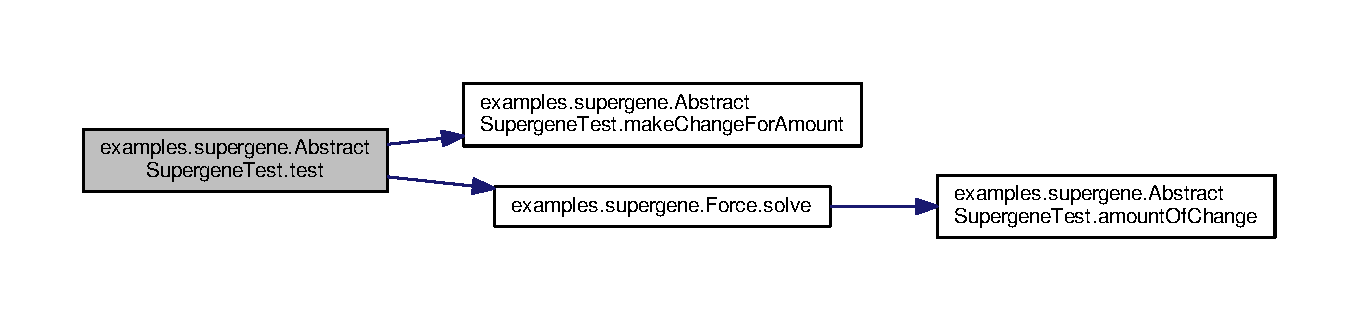
\includegraphics[width=350pt]{classexamples_1_1supergene_1_1_abstract_supergene_test_a92f6bbeeedeed872a2cb7cb38e6a40c2_cgraph}
\end{center}
\end{figure}




\subsection{Member Data Documentation}
\hypertarget{classexamples_1_1supergene_1_1_abstract_supergene_test_a3bf642196176bfe1e85adea8652098b7}{\index{examples\-::supergene\-::\-Abstract\-Supergene\-Test@{examples\-::supergene\-::\-Abstract\-Supergene\-Test}!C\-V\-S\-\_\-\-R\-E\-V\-I\-S\-I\-O\-N@{C\-V\-S\-\_\-\-R\-E\-V\-I\-S\-I\-O\-N}}
\index{C\-V\-S\-\_\-\-R\-E\-V\-I\-S\-I\-O\-N@{C\-V\-S\-\_\-\-R\-E\-V\-I\-S\-I\-O\-N}!examples::supergene::AbstractSupergeneTest@{examples\-::supergene\-::\-Abstract\-Supergene\-Test}}
\subsubsection[{C\-V\-S\-\_\-\-R\-E\-V\-I\-S\-I\-O\-N}]{\setlength{\rightskip}{0pt plus 5cm}final String examples.\-supergene.\-Abstract\-Supergene\-Test.\-C\-V\-S\-\_\-\-R\-E\-V\-I\-S\-I\-O\-N = \char`\"{}\$Revision\-: 1.\-5 \$\char`\"{}\hspace{0.3cm}{\ttfamily [static]}, {\ttfamily [private]}}}\label{classexamples_1_1supergene_1_1_abstract_supergene_test_a3bf642196176bfe1e85adea8652098b7}
String containing the C\-V\-S revision. Read out via reflection! 

Definition at line 25 of file Abstract\-Supergene\-Test.\-java.

\hypertarget{classexamples_1_1supergene_1_1_abstract_supergene_test_a2581251d3607aad43d8b2815b8202c8e}{\index{examples\-::supergene\-::\-Abstract\-Supergene\-Test@{examples\-::supergene\-::\-Abstract\-Supergene\-Test}!D\-I\-M\-E\-S@{D\-I\-M\-E\-S}}
\index{D\-I\-M\-E\-S@{D\-I\-M\-E\-S}!examples::supergene::AbstractSupergeneTest@{examples\-::supergene\-::\-Abstract\-Supergene\-Test}}
\subsubsection[{D\-I\-M\-E\-S}]{\setlength{\rightskip}{0pt plus 5cm}final int examples.\-supergene.\-Abstract\-Supergene\-Test.\-D\-I\-M\-E\-S = 0\hspace{0.3cm}{\ttfamily [static]}}}\label{classexamples_1_1supergene_1_1_abstract_supergene_test_a2581251d3607aad43d8b2815b8202c8e}
Gene index for the dimes gene 

Definition at line 30 of file Abstract\-Supergene\-Test.\-java.



Referenced by examples.\-supergene.\-Abstract\-Change\-Fitness\-Function.\-amount\-Of\-Change(), examples.\-supergene.\-Abstract\-Change\-Fitness\-Function.\-get\-Total\-Number\-Of\-Coins(), examples.\-supergene.\-Supergene\-Sample.\-make\-Change\-For\-Amount(), and examples.\-supergene.\-Abstract\-Supergene\-Test.\-report().

\hypertarget{classexamples_1_1supergene_1_1_abstract_supergene_test_afa2af2b745985502119958481e9c12f6}{\index{examples\-::supergene\-::\-Abstract\-Supergene\-Test@{examples\-::supergene\-::\-Abstract\-Supergene\-Test}!E\-X\-I\-S\-T\-I\-N\-G\-\_\-\-S\-O\-L\-U\-T\-I\-O\-N\-S\-\_\-\-O\-N\-L\-Y@{E\-X\-I\-S\-T\-I\-N\-G\-\_\-\-S\-O\-L\-U\-T\-I\-O\-N\-S\-\_\-\-O\-N\-L\-Y}}
\index{E\-X\-I\-S\-T\-I\-N\-G\-\_\-\-S\-O\-L\-U\-T\-I\-O\-N\-S\-\_\-\-O\-N\-L\-Y@{E\-X\-I\-S\-T\-I\-N\-G\-\_\-\-S\-O\-L\-U\-T\-I\-O\-N\-S\-\_\-\-O\-N\-L\-Y}!examples::supergene::AbstractSupergeneTest@{examples\-::supergene\-::\-Abstract\-Supergene\-Test}}
\subsubsection[{E\-X\-I\-S\-T\-I\-N\-G\-\_\-\-S\-O\-L\-U\-T\-I\-O\-N\-S\-\_\-\-O\-N\-L\-Y}]{\setlength{\rightskip}{0pt plus 5cm}boolean examples.\-supergene.\-Abstract\-Supergene\-Test.\-E\-X\-I\-S\-T\-I\-N\-G\-\_\-\-S\-O\-L\-U\-T\-I\-O\-N\-S\-\_\-\-O\-N\-L\-Y = false\hspace{0.3cm}{\ttfamily [static]}}}\label{classexamples_1_1supergene_1_1_abstract_supergene_test_afa2af2b745985502119958481e9c12f6}
If set to true (required for strict tests), only tasks with existing solutions will be submitted as a test tasks. 

Definition at line 162 of file Abstract\-Supergene\-Test.\-java.



Referenced by examples.\-supergene.\-Abstract\-Supergene\-Test.\-test().

\hypertarget{classexamples_1_1supergene_1_1_abstract_supergene_test_aabc7656a38ca4e7322c3ff08d34ee8f4}{\index{examples\-::supergene\-::\-Abstract\-Supergene\-Test@{examples\-::supergene\-::\-Abstract\-Supergene\-Test}!M\-A\-X\-\_\-\-A\-L\-L\-O\-W\-E\-D\-\_\-\-E\-V\-O\-L\-U\-T\-I\-O\-N\-S@{M\-A\-X\-\_\-\-A\-L\-L\-O\-W\-E\-D\-\_\-\-E\-V\-O\-L\-U\-T\-I\-O\-N\-S}}
\index{M\-A\-X\-\_\-\-A\-L\-L\-O\-W\-E\-D\-\_\-\-E\-V\-O\-L\-U\-T\-I\-O\-N\-S@{M\-A\-X\-\_\-\-A\-L\-L\-O\-W\-E\-D\-\_\-\-E\-V\-O\-L\-U\-T\-I\-O\-N\-S}!examples::supergene::AbstractSupergeneTest@{examples\-::supergene\-::\-Abstract\-Supergene\-Test}}
\subsubsection[{M\-A\-X\-\_\-\-A\-L\-L\-O\-W\-E\-D\-\_\-\-E\-V\-O\-L\-U\-T\-I\-O\-N\-S}]{\setlength{\rightskip}{0pt plus 5cm}int examples.\-supergene.\-Abstract\-Supergene\-Test.\-M\-A\-X\-\_\-\-A\-L\-L\-O\-W\-E\-D\-\_\-\-E\-V\-O\-L\-U\-T\-I\-O\-N\-S = 200\hspace{0.3cm}{\ttfamily [static]}}}\label{classexamples_1_1supergene_1_1_abstract_supergene_test_aabc7656a38ca4e7322c3ff08d34ee8f4}
The total number of times we'll let the population evolve. 

Definition at line 50 of file Abstract\-Supergene\-Test.\-java.



Referenced by examples.\-supergene.\-Abstract\-Supergene\-Test.\-solve().

\hypertarget{classexamples_1_1supergene_1_1_abstract_supergene_test_a816ceb1de4c9bf5c3df3bac9210c380c}{\index{examples\-::supergene\-::\-Abstract\-Supergene\-Test@{examples\-::supergene\-::\-Abstract\-Supergene\-Test}!N\-I\-C\-K\-E\-L\-S@{N\-I\-C\-K\-E\-L\-S}}
\index{N\-I\-C\-K\-E\-L\-S@{N\-I\-C\-K\-E\-L\-S}!examples::supergene::AbstractSupergeneTest@{examples\-::supergene\-::\-Abstract\-Supergene\-Test}}
\subsubsection[{N\-I\-C\-K\-E\-L\-S}]{\setlength{\rightskip}{0pt plus 5cm}final int examples.\-supergene.\-Abstract\-Supergene\-Test.\-N\-I\-C\-K\-E\-L\-S = 2\hspace{0.3cm}{\ttfamily [static]}}}\label{classexamples_1_1supergene_1_1_abstract_supergene_test_a816ceb1de4c9bf5c3df3bac9210c380c}
Gene index for the nickels gene Only used in the alternative presentation 

Definition at line 40 of file Abstract\-Supergene\-Test.\-java.



Referenced by examples.\-supergene.\-Abstract\-Change\-Fitness\-Function.\-amount\-Of\-Change(), examples.\-supergene.\-Abstract\-Change\-Fitness\-Function.\-get\-Total\-Number\-Of\-Coins(), and examples.\-supergene.\-Abstract\-Supergene\-Test.\-report().

\hypertarget{classexamples_1_1supergene_1_1_abstract_supergene_test_a0853afd453197d0e7db44388752d12af}{\index{examples\-::supergene\-::\-Abstract\-Supergene\-Test@{examples\-::supergene\-::\-Abstract\-Supergene\-Test}!P\-E\-N\-N\-I\-E\-S@{P\-E\-N\-N\-I\-E\-S}}
\index{P\-E\-N\-N\-I\-E\-S@{P\-E\-N\-N\-I\-E\-S}!examples::supergene::AbstractSupergeneTest@{examples\-::supergene\-::\-Abstract\-Supergene\-Test}}
\subsubsection[{P\-E\-N\-N\-I\-E\-S}]{\setlength{\rightskip}{0pt plus 5cm}final int examples.\-supergene.\-Abstract\-Supergene\-Test.\-P\-E\-N\-N\-I\-E\-S = 3\hspace{0.3cm}{\ttfamily [static]}}}\label{classexamples_1_1supergene_1_1_abstract_supergene_test_a0853afd453197d0e7db44388752d12af}
Gene index for the pennies gene. Only used in the alternative presentation 

Definition at line 45 of file Abstract\-Supergene\-Test.\-java.



Referenced by examples.\-supergene.\-Abstract\-Change\-Fitness\-Function.\-amount\-Of\-Change(), examples.\-supergene.\-Abstract\-Change\-Fitness\-Function.\-get\-Total\-Number\-Of\-Coins(), and examples.\-supergene.\-Abstract\-Supergene\-Test.\-report().

\hypertarget{classexamples_1_1supergene_1_1_abstract_supergene_test_af5010d4eddc24d9723d539ea6c12c595}{\index{examples\-::supergene\-::\-Abstract\-Supergene\-Test@{examples\-::supergene\-::\-Abstract\-Supergene\-Test}!P\-O\-P\-U\-L\-A\-T\-I\-O\-N\-\_\-\-S\-I\-Z\-E@{P\-O\-P\-U\-L\-A\-T\-I\-O\-N\-\_\-\-S\-I\-Z\-E}}
\index{P\-O\-P\-U\-L\-A\-T\-I\-O\-N\-\_\-\-S\-I\-Z\-E@{P\-O\-P\-U\-L\-A\-T\-I\-O\-N\-\_\-\-S\-I\-Z\-E}!examples::supergene::AbstractSupergeneTest@{examples\-::supergene\-::\-Abstract\-Supergene\-Test}}
\subsubsection[{P\-O\-P\-U\-L\-A\-T\-I\-O\-N\-\_\-\-S\-I\-Z\-E}]{\setlength{\rightskip}{0pt plus 5cm}int examples.\-supergene.\-Abstract\-Supergene\-Test.\-P\-O\-P\-U\-L\-A\-T\-I\-O\-N\-\_\-\-S\-I\-Z\-E = 2000\hspace{0.3cm}{\ttfamily [static]}}}\label{classexamples_1_1supergene_1_1_abstract_supergene_test_af5010d4eddc24d9723d539ea6c12c595}
Chromosome size. 

Definition at line 55 of file Abstract\-Supergene\-Test.\-java.



Referenced by examples.\-supergene.\-Abstract\-Supergene\-Test.\-solve().

\hypertarget{classexamples_1_1supergene_1_1_abstract_supergene_test_aed911231f02517c09e71a453e303b655}{\index{examples\-::supergene\-::\-Abstract\-Supergene\-Test@{examples\-::supergene\-::\-Abstract\-Supergene\-Test}!Q\-U\-A\-R\-T\-E\-R\-S@{Q\-U\-A\-R\-T\-E\-R\-S}}
\index{Q\-U\-A\-R\-T\-E\-R\-S@{Q\-U\-A\-R\-T\-E\-R\-S}!examples::supergene::AbstractSupergeneTest@{examples\-::supergene\-::\-Abstract\-Supergene\-Test}}
\subsubsection[{Q\-U\-A\-R\-T\-E\-R\-S}]{\setlength{\rightskip}{0pt plus 5cm}final int examples.\-supergene.\-Abstract\-Supergene\-Test.\-Q\-U\-A\-R\-T\-E\-R\-S = 1\hspace{0.3cm}{\ttfamily [static]}}}\label{classexamples_1_1supergene_1_1_abstract_supergene_test_aed911231f02517c09e71a453e303b655}
Gene index for the quarters gene. 

Definition at line 35 of file Abstract\-Supergene\-Test.\-java.



Referenced by examples.\-supergene.\-Abstract\-Change\-Fitness\-Function.\-amount\-Of\-Change(), examples.\-supergene.\-Abstract\-Change\-Fitness\-Function.\-get\-Total\-Number\-Of\-Coins(), examples.\-supergene.\-Supergene\-Sample.\-make\-Change\-For\-Amount(), and examples.\-supergene.\-Abstract\-Supergene\-Test.\-report().

\hypertarget{classexamples_1_1supergene_1_1_abstract_supergene_test_a6884362188d843b7a05c2845e9857358}{\index{examples\-::supergene\-::\-Abstract\-Supergene\-Test@{examples\-::supergene\-::\-Abstract\-Supergene\-Test}!R\-E\-P\-O\-R\-T\-\_\-\-E\-N\-A\-B\-L\-E\-D@{R\-E\-P\-O\-R\-T\-\_\-\-E\-N\-A\-B\-L\-E\-D}}
\index{R\-E\-P\-O\-R\-T\-\_\-\-E\-N\-A\-B\-L\-E\-D@{R\-E\-P\-O\-R\-T\-\_\-\-E\-N\-A\-B\-L\-E\-D}!examples::supergene::AbstractSupergeneTest@{examples\-::supergene\-::\-Abstract\-Supergene\-Test}}
\subsubsection[{R\-E\-P\-O\-R\-T\-\_\-\-E\-N\-A\-B\-L\-E\-D}]{\setlength{\rightskip}{0pt plus 5cm}boolean examples.\-supergene.\-Abstract\-Supergene\-Test.\-R\-E\-P\-O\-R\-T\-\_\-\-E\-N\-A\-B\-L\-E\-D = true\hspace{0.3cm}{\ttfamily [static]}}}\label{classexamples_1_1supergene_1_1_abstract_supergene_test_a6884362188d843b7a05c2845e9857358}


Definition at line 57 of file Abstract\-Supergene\-Test.\-java.



Referenced by examples.\-supergene.\-Abstract\-Supergene\-Test.\-report(), and examples.\-supergene.\-Abstract\-Supergene\-Test.\-test().



The documentation for this class was generated from the following file\-:\begin{DoxyCompactItemize}
\item 
L\-D\-H\-\_\-\-Git/examples/src/examples/supergene/\hyperlink{_abstract_supergene_test_8java}{Abstract\-Supergene\-Test.\-java}\end{DoxyCompactItemize}

\hypertarget{classorg_1_1jgap_1_1gp_1_1function_1_1_add}{\section{org.\-jgap.\-gp.\-function.\-Add Class Reference}
\label{classorg_1_1jgap_1_1gp_1_1function_1_1_add}\index{org.\-jgap.\-gp.\-function.\-Add@{org.\-jgap.\-gp.\-function.\-Add}}
}


Inheritance diagram for org.\-jgap.\-gp.\-function.\-Add\-:
\nopagebreak
\begin{figure}[H]
\begin{center}
\leavevmode
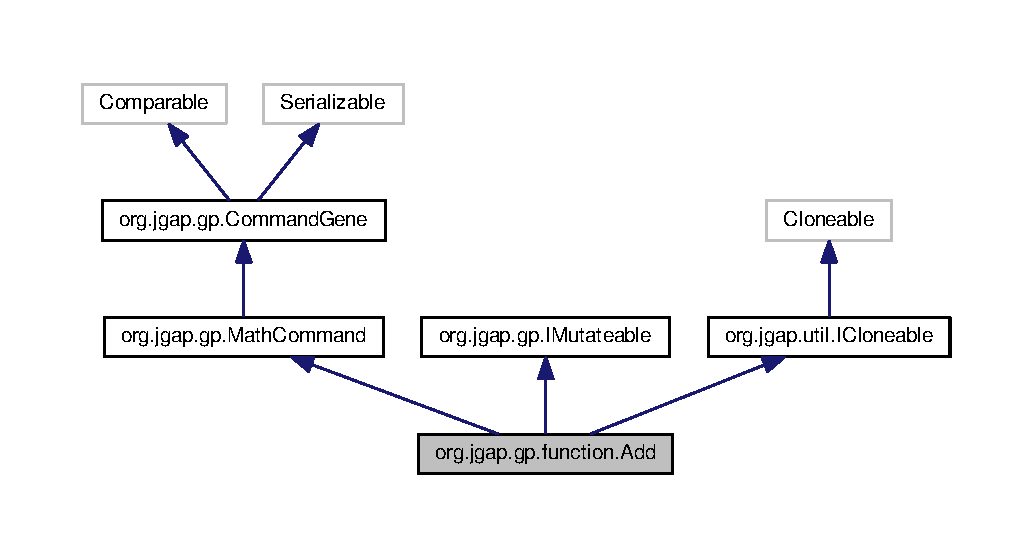
\includegraphics[width=350pt]{classorg_1_1jgap_1_1gp_1_1function_1_1_add__inherit__graph}
\end{center}
\end{figure}


Collaboration diagram for org.\-jgap.\-gp.\-function.\-Add\-:
\nopagebreak
\begin{figure}[H]
\begin{center}
\leavevmode
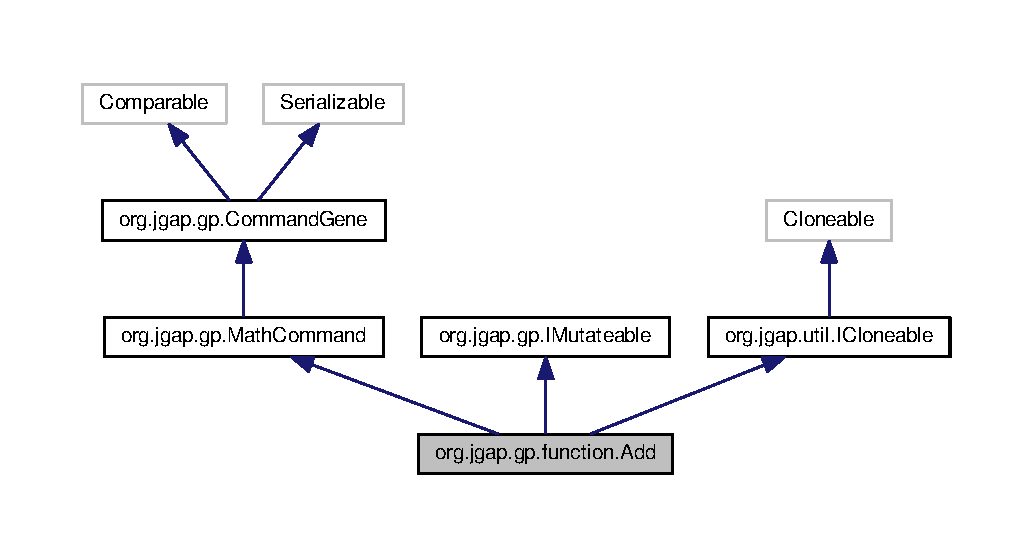
\includegraphics[width=350pt]{classorg_1_1jgap_1_1gp_1_1function_1_1_add__coll__graph}
\end{center}
\end{figure}
\subsection*{Classes}
\begin{DoxyCompactItemize}
\item 
interface \hyperlink{interfaceorg_1_1jgap_1_1gp_1_1function_1_1_add_1_1_compatible}{Compatible}
\end{DoxyCompactItemize}
\subsection*{Public Member Functions}
\begin{DoxyCompactItemize}
\item 
\hyperlink{classorg_1_1jgap_1_1gp_1_1function_1_1_add_af6af7439c7e72986a79ae133eeb68837}{Add} (final G\-P\-Configuration a\-\_\-conf, Class a\-\_\-return\-Type)  throws Invalid\-Configuration\-Exception 
\item 
\hyperlink{classorg_1_1jgap_1_1gp_1_1_command_gene}{Command\-Gene} \hyperlink{classorg_1_1jgap_1_1gp_1_1function_1_1_add_a9f4e9760301a72c2c7452452778eb236}{apply\-Mutation} (int index, double a\-\_\-percentage)  throws Invalid\-Configuration\-Exception 
\item 
Object \hyperlink{classorg_1_1jgap_1_1gp_1_1function_1_1_add_a93b314853a198284fa2b962fa3aa9806}{clone} ()
\item 
String \hyperlink{classorg_1_1jgap_1_1gp_1_1function_1_1_add_a3edf9acb61e2fcc38b3b624853960f5f}{to\-String} ()
\item 
String \hyperlink{classorg_1_1jgap_1_1gp_1_1function_1_1_add_a4c0c1e2d04e7849f50b1eb4177f4f443}{get\-Name} ()
\item 
int \hyperlink{classorg_1_1jgap_1_1gp_1_1function_1_1_add_a4e5fd3d335553589ab24ab9f83cbbcd8}{execute\-\_\-int} (Program\-Chromosome c, int n, Object\mbox{[}$\,$\mbox{]} args)
\item 
long \hyperlink{classorg_1_1jgap_1_1gp_1_1function_1_1_add_af38da5e98760afc6104829a38cbc7732}{execute\-\_\-long} (Program\-Chromosome c, int n, Object\mbox{[}$\,$\mbox{]} args)
\item 
float \hyperlink{classorg_1_1jgap_1_1gp_1_1function_1_1_add_aa91195c0430b3eacea5f0eb083f5e7f4}{execute\-\_\-float} (Program\-Chromosome c, int n, Object\mbox{[}$\,$\mbox{]} args)
\item 
double \hyperlink{classorg_1_1jgap_1_1gp_1_1function_1_1_add_ad830922e5000b6cd9c2ab3028dc2ca87}{execute\-\_\-double} (Program\-Chromosome c, int n, Object\mbox{[}$\,$\mbox{]} args)
\item 
Object \hyperlink{classorg_1_1jgap_1_1gp_1_1function_1_1_add_a4d056e95aac55f8d67b5d2b9646f2ff4}{execute\-\_\-object} (Program\-Chromosome c, int n, Object\mbox{[}$\,$\mbox{]} args)
\end{DoxyCompactItemize}
\subsection*{Static Private Attributes}
\begin{DoxyCompactItemize}
\item 
static final String \hyperlink{classorg_1_1jgap_1_1gp_1_1function_1_1_add_af211bdec40bd7f32aebf9f5436864e76}{C\-V\-S\-\_\-\-R\-E\-V\-I\-S\-I\-O\-N} = \char`\"{}\$Revision\-: 1.\-10 \$\char`\"{}
\end{DoxyCompactItemize}
\subsection*{Additional Inherited Members}


\subsection{Detailed Description}
The add operation.

\begin{DoxyAuthor}{Author}
Klaus Meffert 
\end{DoxyAuthor}
\begin{DoxySince}{Since}
3.\-0 
\end{DoxySince}


Definition at line 23 of file Add.\-java.



\subsection{Constructor \& Destructor Documentation}
\hypertarget{classorg_1_1jgap_1_1gp_1_1function_1_1_add_af6af7439c7e72986a79ae133eeb68837}{\index{org\-::jgap\-::gp\-::function\-::\-Add@{org\-::jgap\-::gp\-::function\-::\-Add}!Add@{Add}}
\index{Add@{Add}!org::jgap::gp::function::Add@{org\-::jgap\-::gp\-::function\-::\-Add}}
\subsubsection[{Add}]{\setlength{\rightskip}{0pt plus 5cm}org.\-jgap.\-gp.\-function.\-Add.\-Add (
\begin{DoxyParamCaption}
\item[{final G\-P\-Configuration}]{a\-\_\-conf, }
\item[{Class}]{a\-\_\-return\-Type}
\end{DoxyParamCaption}
) throws {\bf Invalid\-Configuration\-Exception}\hspace{0.3cm}{\ttfamily [inline]}}}\label{classorg_1_1jgap_1_1gp_1_1function_1_1_add_af6af7439c7e72986a79ae133eeb68837}


Definition at line 28 of file Add.\-java.



Referenced by org.\-jgap.\-gp.\-function.\-Add.\-clone().



\subsection{Member Function Documentation}
\hypertarget{classorg_1_1jgap_1_1gp_1_1function_1_1_add_a9f4e9760301a72c2c7452452778eb236}{\index{org\-::jgap\-::gp\-::function\-::\-Add@{org\-::jgap\-::gp\-::function\-::\-Add}!apply\-Mutation@{apply\-Mutation}}
\index{apply\-Mutation@{apply\-Mutation}!org::jgap::gp::function::Add@{org\-::jgap\-::gp\-::function\-::\-Add}}
\subsubsection[{apply\-Mutation}]{\setlength{\rightskip}{0pt plus 5cm}{\bf Command\-Gene} org.\-jgap.\-gp.\-function.\-Add.\-apply\-Mutation (
\begin{DoxyParamCaption}
\item[{int}]{a\-\_\-index, }
\item[{double}]{a\-\_\-percentage}
\end{DoxyParamCaption}
) throws {\bf Invalid\-Configuration\-Exception}\hspace{0.3cm}{\ttfamily [inline]}}}\label{classorg_1_1jgap_1_1gp_1_1function_1_1_add_a9f4e9760301a72c2c7452452778eb236}
Mutates a \hyperlink{classorg_1_1jgap_1_1gp_1_1_command_gene}{Command\-Gene}.


\begin{DoxyParams}{Parameters}
{\em a\-\_\-index} & references the part of a multipart object, normally not relevant \\
\hline
{\em a\-\_\-percentage} & the mutation rate (0.\-0 to 1.\-0) \\
\hline
\end{DoxyParams}
\begin{DoxyReturn}{Returns}
the mutant 
\end{DoxyReturn}

\begin{DoxyExceptions}{Exceptions}
{\em \hyperlink{classorg_1_1jgap_1_1_invalid_configuration_exception}{Invalid\-Configuration\-Exception}} & \\
\hline
\end{DoxyExceptions}
\begin{DoxyAuthor}{Author}
Klaus Meffert 
\end{DoxyAuthor}
\begin{DoxySince}{Since}
3.\-0 
\end{DoxySince}


Implements \hyperlink{interfaceorg_1_1jgap_1_1gp_1_1_i_mutateable_abe553182ae983c2092495c889eecb2e2}{org.\-jgap.\-gp.\-I\-Mutateable}.



Definition at line 33 of file Add.\-java.



References org.\-jgap.\-gp.\-Command\-Gene.\-get\-G\-P\-Configuration(), and org.\-jgap.\-gp.\-Command\-Gene.\-get\-Return\-Type().



Here is the call graph for this function\-:
\nopagebreak
\begin{figure}[H]
\begin{center}
\leavevmode
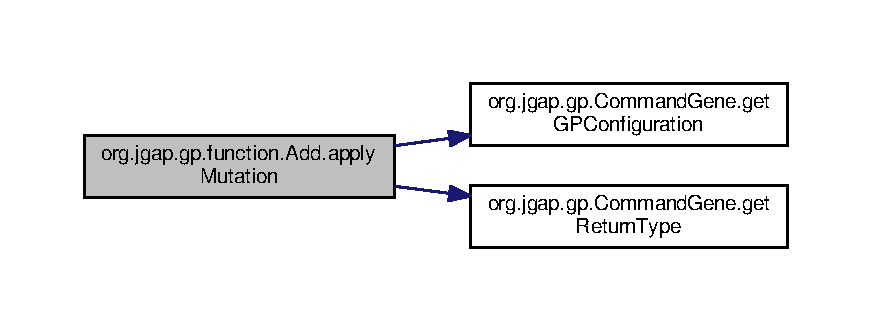
\includegraphics[width=350pt]{classorg_1_1jgap_1_1gp_1_1function_1_1_add_a9f4e9760301a72c2c7452452778eb236_cgraph}
\end{center}
\end{figure}


\hypertarget{classorg_1_1jgap_1_1gp_1_1function_1_1_add_a93b314853a198284fa2b962fa3aa9806}{\index{org\-::jgap\-::gp\-::function\-::\-Add@{org\-::jgap\-::gp\-::function\-::\-Add}!clone@{clone}}
\index{clone@{clone}!org::jgap::gp::function::Add@{org\-::jgap\-::gp\-::function\-::\-Add}}
\subsubsection[{clone}]{\setlength{\rightskip}{0pt plus 5cm}Object org.\-jgap.\-gp.\-function.\-Add.\-clone (
\begin{DoxyParamCaption}
{}
\end{DoxyParamCaption}
)\hspace{0.3cm}{\ttfamily [inline]}}}\label{classorg_1_1jgap_1_1gp_1_1function_1_1_add_a93b314853a198284fa2b962fa3aa9806}
Clones the object. Simple and straight forward implementation here.

\begin{DoxyReturn}{Returns}
cloned instance of this object
\end{DoxyReturn}
\begin{DoxyAuthor}{Author}
Klaus Meffert 
\end{DoxyAuthor}
\begin{DoxySince}{Since}
3.\-4 
\end{DoxySince}


Implements \hyperlink{interfaceorg_1_1jgap_1_1util_1_1_i_cloneable_aa7e7d62077e6428ad7904932b1b4f7d5}{org.\-jgap.\-util.\-I\-Cloneable}.



Definition at line 47 of file Add.\-java.



References org.\-jgap.\-gp.\-function.\-Add.\-Add(), org.\-jgap.\-gp.\-Command\-Gene.\-get\-G\-P\-Configuration(), and org.\-jgap.\-gp.\-Command\-Gene.\-get\-Return\-Type().



Here is the call graph for this function\-:
\nopagebreak
\begin{figure}[H]
\begin{center}
\leavevmode
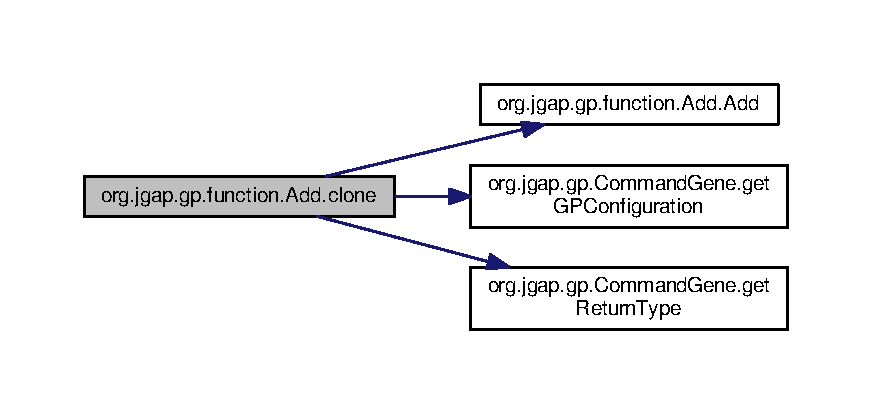
\includegraphics[width=350pt]{classorg_1_1jgap_1_1gp_1_1function_1_1_add_a93b314853a198284fa2b962fa3aa9806_cgraph}
\end{center}
\end{figure}


\hypertarget{classorg_1_1jgap_1_1gp_1_1function_1_1_add_ad830922e5000b6cd9c2ab3028dc2ca87}{\index{org\-::jgap\-::gp\-::function\-::\-Add@{org\-::jgap\-::gp\-::function\-::\-Add}!execute\-\_\-double@{execute\-\_\-double}}
\index{execute\-\_\-double@{execute\-\_\-double}!org::jgap::gp::function::Add@{org\-::jgap\-::gp\-::function\-::\-Add}}
\subsubsection[{execute\-\_\-double}]{\setlength{\rightskip}{0pt plus 5cm}double org.\-jgap.\-gp.\-function.\-Add.\-execute\-\_\-double (
\begin{DoxyParamCaption}
\item[{Program\-Chromosome}]{c, }
\item[{int}]{n, }
\item[{Object\mbox{[}$\,$\mbox{]}}]{args}
\end{DoxyParamCaption}
)\hspace{0.3cm}{\ttfamily [inline]}}}\label{classorg_1_1jgap_1_1gp_1_1function_1_1_add_ad830922e5000b6cd9c2ab3028dc2ca87}


Definition at line 82 of file Add.\-java.

\hypertarget{classorg_1_1jgap_1_1gp_1_1function_1_1_add_aa91195c0430b3eacea5f0eb083f5e7f4}{\index{org\-::jgap\-::gp\-::function\-::\-Add@{org\-::jgap\-::gp\-::function\-::\-Add}!execute\-\_\-float@{execute\-\_\-float}}
\index{execute\-\_\-float@{execute\-\_\-float}!org::jgap::gp::function::Add@{org\-::jgap\-::gp\-::function\-::\-Add}}
\subsubsection[{execute\-\_\-float}]{\setlength{\rightskip}{0pt plus 5cm}float org.\-jgap.\-gp.\-function.\-Add.\-execute\-\_\-float (
\begin{DoxyParamCaption}
\item[{Program\-Chromosome}]{c, }
\item[{int}]{n, }
\item[{Object\mbox{[}$\,$\mbox{]}}]{args}
\end{DoxyParamCaption}
)\hspace{0.3cm}{\ttfamily [inline]}}}\label{classorg_1_1jgap_1_1gp_1_1function_1_1_add_aa91195c0430b3eacea5f0eb083f5e7f4}


Definition at line 78 of file Add.\-java.

\hypertarget{classorg_1_1jgap_1_1gp_1_1function_1_1_add_a4e5fd3d335553589ab24ab9f83cbbcd8}{\index{org\-::jgap\-::gp\-::function\-::\-Add@{org\-::jgap\-::gp\-::function\-::\-Add}!execute\-\_\-int@{execute\-\_\-int}}
\index{execute\-\_\-int@{execute\-\_\-int}!org::jgap::gp::function::Add@{org\-::jgap\-::gp\-::function\-::\-Add}}
\subsubsection[{execute\-\_\-int}]{\setlength{\rightskip}{0pt plus 5cm}int org.\-jgap.\-gp.\-function.\-Add.\-execute\-\_\-int (
\begin{DoxyParamCaption}
\item[{Program\-Chromosome}]{c, }
\item[{int}]{n, }
\item[{Object\mbox{[}$\,$\mbox{]}}]{args}
\end{DoxyParamCaption}
)\hspace{0.3cm}{\ttfamily [inline]}}}\label{classorg_1_1jgap_1_1gp_1_1function_1_1_add_a4e5fd3d335553589ab24ab9f83cbbcd8}


Definition at line 70 of file Add.\-java.

\hypertarget{classorg_1_1jgap_1_1gp_1_1function_1_1_add_af38da5e98760afc6104829a38cbc7732}{\index{org\-::jgap\-::gp\-::function\-::\-Add@{org\-::jgap\-::gp\-::function\-::\-Add}!execute\-\_\-long@{execute\-\_\-long}}
\index{execute\-\_\-long@{execute\-\_\-long}!org::jgap::gp::function::Add@{org\-::jgap\-::gp\-::function\-::\-Add}}
\subsubsection[{execute\-\_\-long}]{\setlength{\rightskip}{0pt plus 5cm}long org.\-jgap.\-gp.\-function.\-Add.\-execute\-\_\-long (
\begin{DoxyParamCaption}
\item[{Program\-Chromosome}]{c, }
\item[{int}]{n, }
\item[{Object\mbox{[}$\,$\mbox{]}}]{args}
\end{DoxyParamCaption}
)\hspace{0.3cm}{\ttfamily [inline]}}}\label{classorg_1_1jgap_1_1gp_1_1function_1_1_add_af38da5e98760afc6104829a38cbc7732}


Definition at line 74 of file Add.\-java.

\hypertarget{classorg_1_1jgap_1_1gp_1_1function_1_1_add_a4d056e95aac55f8d67b5d2b9646f2ff4}{\index{org\-::jgap\-::gp\-::function\-::\-Add@{org\-::jgap\-::gp\-::function\-::\-Add}!execute\-\_\-object@{execute\-\_\-object}}
\index{execute\-\_\-object@{execute\-\_\-object}!org::jgap::gp::function::Add@{org\-::jgap\-::gp\-::function\-::\-Add}}
\subsubsection[{execute\-\_\-object}]{\setlength{\rightskip}{0pt plus 5cm}Object org.\-jgap.\-gp.\-function.\-Add.\-execute\-\_\-object (
\begin{DoxyParamCaption}
\item[{Program\-Chromosome}]{c, }
\item[{int}]{n, }
\item[{Object\mbox{[}$\,$\mbox{]}}]{args}
\end{DoxyParamCaption}
)\hspace{0.3cm}{\ttfamily [inline]}}}\label{classorg_1_1jgap_1_1gp_1_1function_1_1_add_a4d056e95aac55f8d67b5d2b9646f2ff4}


Definition at line 86 of file Add.\-java.

\hypertarget{classorg_1_1jgap_1_1gp_1_1function_1_1_add_a4c0c1e2d04e7849f50b1eb4177f4f443}{\index{org\-::jgap\-::gp\-::function\-::\-Add@{org\-::jgap\-::gp\-::function\-::\-Add}!get\-Name@{get\-Name}}
\index{get\-Name@{get\-Name}!org::jgap::gp::function::Add@{org\-::jgap\-::gp\-::function\-::\-Add}}
\subsubsection[{get\-Name}]{\setlength{\rightskip}{0pt plus 5cm}String org.\-jgap.\-gp.\-function.\-Add.\-get\-Name (
\begin{DoxyParamCaption}
{}
\end{DoxyParamCaption}
)\hspace{0.3cm}{\ttfamily [inline]}}}\label{classorg_1_1jgap_1_1gp_1_1function_1_1_add_a4c0c1e2d04e7849f50b1eb4177f4f443}
\begin{DoxyReturn}{Returns}
textual name of this command
\end{DoxyReturn}
\begin{DoxyAuthor}{Author}
Klaus Meffert 
\end{DoxyAuthor}
\begin{DoxySince}{Since}
3.\-2 
\end{DoxySince}


Definition at line 66 of file Add.\-java.

\hypertarget{classorg_1_1jgap_1_1gp_1_1function_1_1_add_a3edf9acb61e2fcc38b3b624853960f5f}{\index{org\-::jgap\-::gp\-::function\-::\-Add@{org\-::jgap\-::gp\-::function\-::\-Add}!to\-String@{to\-String}}
\index{to\-String@{to\-String}!org::jgap::gp::function::Add@{org\-::jgap\-::gp\-::function\-::\-Add}}
\subsubsection[{to\-String}]{\setlength{\rightskip}{0pt plus 5cm}String org.\-jgap.\-gp.\-function.\-Add.\-to\-String (
\begin{DoxyParamCaption}
{}
\end{DoxyParamCaption}
)\hspace{0.3cm}{\ttfamily [inline]}, {\ttfamily [virtual]}}}\label{classorg_1_1jgap_1_1gp_1_1function_1_1_add_a3edf9acb61e2fcc38b3b624853960f5f}
\begin{DoxyReturn}{Returns}
the string representation of the command. Especially usefull to output a resulting formula in human-\/readable form. 
\end{DoxyReturn}


Implements \hyperlink{classorg_1_1jgap_1_1gp_1_1_command_gene_a236141d99059da808afe7a9217e411c7}{org.\-jgap.\-gp.\-Command\-Gene}.



Definition at line 56 of file Add.\-java.



\subsection{Member Data Documentation}
\hypertarget{classorg_1_1jgap_1_1gp_1_1function_1_1_add_af211bdec40bd7f32aebf9f5436864e76}{\index{org\-::jgap\-::gp\-::function\-::\-Add@{org\-::jgap\-::gp\-::function\-::\-Add}!C\-V\-S\-\_\-\-R\-E\-V\-I\-S\-I\-O\-N@{C\-V\-S\-\_\-\-R\-E\-V\-I\-S\-I\-O\-N}}
\index{C\-V\-S\-\_\-\-R\-E\-V\-I\-S\-I\-O\-N@{C\-V\-S\-\_\-\-R\-E\-V\-I\-S\-I\-O\-N}!org::jgap::gp::function::Add@{org\-::jgap\-::gp\-::function\-::\-Add}}
\subsubsection[{C\-V\-S\-\_\-\-R\-E\-V\-I\-S\-I\-O\-N}]{\setlength{\rightskip}{0pt plus 5cm}final String org.\-jgap.\-gp.\-function.\-Add.\-C\-V\-S\-\_\-\-R\-E\-V\-I\-S\-I\-O\-N = \char`\"{}\$Revision\-: 1.\-10 \$\char`\"{}\hspace{0.3cm}{\ttfamily [static]}, {\ttfamily [private]}}}\label{classorg_1_1jgap_1_1gp_1_1function_1_1_add_af211bdec40bd7f32aebf9f5436864e76}
String containing the C\-V\-S revision. Read out via reflection! 

Definition at line 26 of file Add.\-java.



The documentation for this class was generated from the following file\-:\begin{DoxyCompactItemize}
\item 
L\-D\-H\-\_\-\-Git/src/org/jgap/gp/function/\hyperlink{_add_8java}{Add.\-java}\end{DoxyCompactItemize}

\hypertarget{classorg_1_1jgap_1_1gp_1_1function_1_1_add3}{\section{org.\-jgap.\-gp.\-function.\-Add3 Class Reference}
\label{classorg_1_1jgap_1_1gp_1_1function_1_1_add3}\index{org.\-jgap.\-gp.\-function.\-Add3@{org.\-jgap.\-gp.\-function.\-Add3}}
}


Inheritance diagram for org.\-jgap.\-gp.\-function.\-Add3\-:
\nopagebreak
\begin{figure}[H]
\begin{center}
\leavevmode
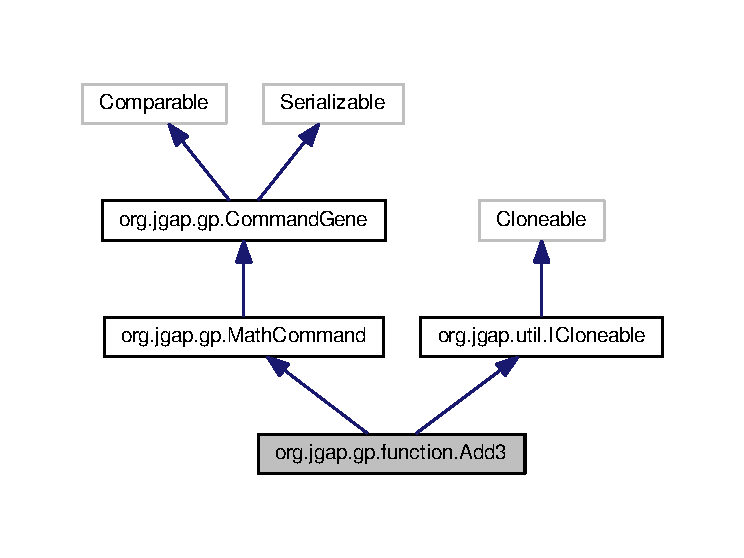
\includegraphics[width=350pt]{classorg_1_1jgap_1_1gp_1_1function_1_1_add3__inherit__graph}
\end{center}
\end{figure}


Collaboration diagram for org.\-jgap.\-gp.\-function.\-Add3\-:
\nopagebreak
\begin{figure}[H]
\begin{center}
\leavevmode
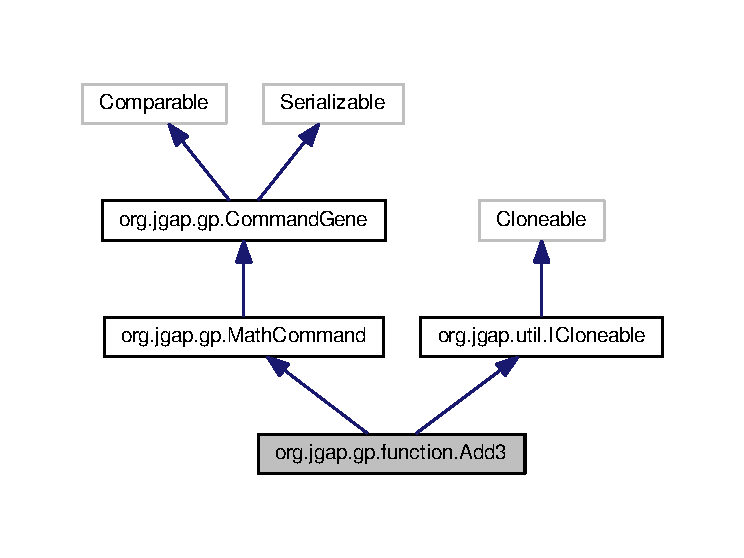
\includegraphics[width=350pt]{classorg_1_1jgap_1_1gp_1_1function_1_1_add3__coll__graph}
\end{center}
\end{figure}
\subsection*{Classes}
\begin{DoxyCompactItemize}
\item 
interface \hyperlink{interfaceorg_1_1jgap_1_1gp_1_1function_1_1_add3_1_1_compatible}{Compatible}
\end{DoxyCompactItemize}
\subsection*{Public Member Functions}
\begin{DoxyCompactItemize}
\item 
\hyperlink{classorg_1_1jgap_1_1gp_1_1function_1_1_add3_a39f0b3eb3fbdcc8e62fed05a254a317a}{Add3} (final G\-P\-Configuration a\-\_\-conf, Class a\-\_\-return\-Type)  throws Invalid\-Configuration\-Exception 
\item 
String \hyperlink{classorg_1_1jgap_1_1gp_1_1function_1_1_add3_a117cb9ae8aaa35ad01819fcd76aa718f}{to\-String} ()
\item 
String \hyperlink{classorg_1_1jgap_1_1gp_1_1function_1_1_add3_a7a86d653423e12958deb96ec59de78b7}{get\-Name} ()
\item 
int \hyperlink{classorg_1_1jgap_1_1gp_1_1function_1_1_add3_a5dd7b4af1ddf5fa3052fa4278de7d87f}{execute\-\_\-int} (Program\-Chromosome c, int n, Object\mbox{[}$\,$\mbox{]} args)
\item 
long \hyperlink{classorg_1_1jgap_1_1gp_1_1function_1_1_add3_a644667568a82eba83abddc983c038ba8}{execute\-\_\-long} (Program\-Chromosome c, int n, Object\mbox{[}$\,$\mbox{]} args)
\item 
float \hyperlink{classorg_1_1jgap_1_1gp_1_1function_1_1_add3_a944669eb2cdedc6feb23501af25796c1}{execute\-\_\-float} (Program\-Chromosome c, int n, Object\mbox{[}$\,$\mbox{]} args)
\item 
double \hyperlink{classorg_1_1jgap_1_1gp_1_1function_1_1_add3_a6ad7138a639c045bcb9d4818e744c782}{execute\-\_\-double} (Program\-Chromosome c, int n, Object\mbox{[}$\,$\mbox{]} args)
\item 
Object \hyperlink{classorg_1_1jgap_1_1gp_1_1function_1_1_add3_a5c1448abe514d25c6a2c2afc351ebcf4}{execute\-\_\-object} (Program\-Chromosome c, int n, Object\mbox{[}$\,$\mbox{]} args)
\item 
Object \hyperlink{classorg_1_1jgap_1_1gp_1_1function_1_1_add3_a9ff6a998602cc7cb369888e54c815d0e}{clone} ()
\end{DoxyCompactItemize}
\subsection*{Static Private Attributes}
\begin{DoxyCompactItemize}
\item 
static final String \hyperlink{classorg_1_1jgap_1_1gp_1_1function_1_1_add3_a0d32aec6060c2b0611837a6d42e84d47}{C\-V\-S\-\_\-\-R\-E\-V\-I\-S\-I\-O\-N} = \char`\"{}\$Revision\-: 1.\-8 \$\char`\"{}
\end{DoxyCompactItemize}
\subsection*{Additional Inherited Members}


\subsection{Detailed Description}
The add operation with three parameters (X + Y + Z).

\begin{DoxyAuthor}{Author}
Klaus Meffert 
\end{DoxyAuthor}
\begin{DoxySince}{Since}
3.\-0 
\end{DoxySince}


Definition at line 23 of file Add3.\-java.



\subsection{Constructor \& Destructor Documentation}
\hypertarget{classorg_1_1jgap_1_1gp_1_1function_1_1_add3_a39f0b3eb3fbdcc8e62fed05a254a317a}{\index{org\-::jgap\-::gp\-::function\-::\-Add3@{org\-::jgap\-::gp\-::function\-::\-Add3}!Add3@{Add3}}
\index{Add3@{Add3}!org::jgap::gp::function::Add3@{org\-::jgap\-::gp\-::function\-::\-Add3}}
\subsubsection[{Add3}]{\setlength{\rightskip}{0pt plus 5cm}org.\-jgap.\-gp.\-function.\-Add3.\-Add3 (
\begin{DoxyParamCaption}
\item[{final G\-P\-Configuration}]{a\-\_\-conf, }
\item[{Class}]{a\-\_\-return\-Type}
\end{DoxyParamCaption}
) throws {\bf Invalid\-Configuration\-Exception}\hspace{0.3cm}{\ttfamily [inline]}}}\label{classorg_1_1jgap_1_1gp_1_1function_1_1_add3_a39f0b3eb3fbdcc8e62fed05a254a317a}


Definition at line 28 of file Add3.\-java.



Referenced by org.\-jgap.\-gp.\-function.\-Add3.\-clone().



\subsection{Member Function Documentation}
\hypertarget{classorg_1_1jgap_1_1gp_1_1function_1_1_add3_a9ff6a998602cc7cb369888e54c815d0e}{\index{org\-::jgap\-::gp\-::function\-::\-Add3@{org\-::jgap\-::gp\-::function\-::\-Add3}!clone@{clone}}
\index{clone@{clone}!org::jgap::gp::function::Add3@{org\-::jgap\-::gp\-::function\-::\-Add3}}
\subsubsection[{clone}]{\setlength{\rightskip}{0pt plus 5cm}Object org.\-jgap.\-gp.\-function.\-Add3.\-clone (
\begin{DoxyParamCaption}
{}
\end{DoxyParamCaption}
)\hspace{0.3cm}{\ttfamily [inline]}}}\label{classorg_1_1jgap_1_1gp_1_1function_1_1_add3_a9ff6a998602cc7cb369888e54c815d0e}
Clones the object. Simple and straight forward implementation here.

\begin{DoxyReturn}{Returns}
cloned instance of this object
\end{DoxyReturn}
\begin{DoxyAuthor}{Author}
Klaus Meffert 
\end{DoxyAuthor}
\begin{DoxySince}{Since}
3.\-4 
\end{DoxySince}


Implements \hyperlink{interfaceorg_1_1jgap_1_1util_1_1_i_cloneable_aa7e7d62077e6428ad7904932b1b4f7d5}{org.\-jgap.\-util.\-I\-Cloneable}.



Definition at line 84 of file Add3.\-java.



References org.\-jgap.\-gp.\-function.\-Add3.\-Add3(), org.\-jgap.\-gp.\-Command\-Gene.\-get\-G\-P\-Configuration(), and org.\-jgap.\-gp.\-Command\-Gene.\-get\-Return\-Type().



Here is the call graph for this function\-:
\nopagebreak
\begin{figure}[H]
\begin{center}
\leavevmode
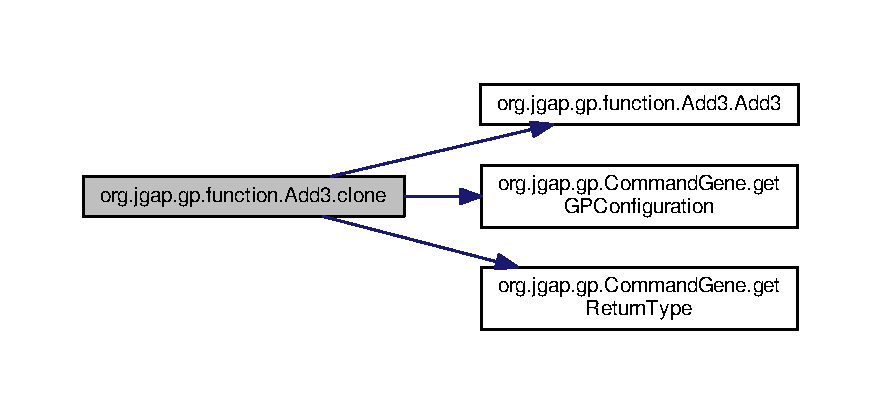
\includegraphics[width=350pt]{classorg_1_1jgap_1_1gp_1_1function_1_1_add3_a9ff6a998602cc7cb369888e54c815d0e_cgraph}
\end{center}
\end{figure}


\hypertarget{classorg_1_1jgap_1_1gp_1_1function_1_1_add3_a6ad7138a639c045bcb9d4818e744c782}{\index{org\-::jgap\-::gp\-::function\-::\-Add3@{org\-::jgap\-::gp\-::function\-::\-Add3}!execute\-\_\-double@{execute\-\_\-double}}
\index{execute\-\_\-double@{execute\-\_\-double}!org::jgap::gp::function::Add3@{org\-::jgap\-::gp\-::function\-::\-Add3}}
\subsubsection[{execute\-\_\-double}]{\setlength{\rightskip}{0pt plus 5cm}double org.\-jgap.\-gp.\-function.\-Add3.\-execute\-\_\-double (
\begin{DoxyParamCaption}
\item[{Program\-Chromosome}]{c, }
\item[{int}]{n, }
\item[{Object\mbox{[}$\,$\mbox{]}}]{args}
\end{DoxyParamCaption}
)\hspace{0.3cm}{\ttfamily [inline]}}}\label{classorg_1_1jgap_1_1gp_1_1function_1_1_add3_a6ad7138a639c045bcb9d4818e744c782}


Definition at line 62 of file Add3.\-java.

\hypertarget{classorg_1_1jgap_1_1gp_1_1function_1_1_add3_a944669eb2cdedc6feb23501af25796c1}{\index{org\-::jgap\-::gp\-::function\-::\-Add3@{org\-::jgap\-::gp\-::function\-::\-Add3}!execute\-\_\-float@{execute\-\_\-float}}
\index{execute\-\_\-float@{execute\-\_\-float}!org::jgap::gp::function::Add3@{org\-::jgap\-::gp\-::function\-::\-Add3}}
\subsubsection[{execute\-\_\-float}]{\setlength{\rightskip}{0pt plus 5cm}float org.\-jgap.\-gp.\-function.\-Add3.\-execute\-\_\-float (
\begin{DoxyParamCaption}
\item[{Program\-Chromosome}]{c, }
\item[{int}]{n, }
\item[{Object\mbox{[}$\,$\mbox{]}}]{args}
\end{DoxyParamCaption}
)\hspace{0.3cm}{\ttfamily [inline]}}}\label{classorg_1_1jgap_1_1gp_1_1function_1_1_add3_a944669eb2cdedc6feb23501af25796c1}


Definition at line 57 of file Add3.\-java.

\hypertarget{classorg_1_1jgap_1_1gp_1_1function_1_1_add3_a5dd7b4af1ddf5fa3052fa4278de7d87f}{\index{org\-::jgap\-::gp\-::function\-::\-Add3@{org\-::jgap\-::gp\-::function\-::\-Add3}!execute\-\_\-int@{execute\-\_\-int}}
\index{execute\-\_\-int@{execute\-\_\-int}!org::jgap::gp::function::Add3@{org\-::jgap\-::gp\-::function\-::\-Add3}}
\subsubsection[{execute\-\_\-int}]{\setlength{\rightskip}{0pt plus 5cm}int org.\-jgap.\-gp.\-function.\-Add3.\-execute\-\_\-int (
\begin{DoxyParamCaption}
\item[{Program\-Chromosome}]{c, }
\item[{int}]{n, }
\item[{Object\mbox{[}$\,$\mbox{]}}]{args}
\end{DoxyParamCaption}
)\hspace{0.3cm}{\ttfamily [inline]}}}\label{classorg_1_1jgap_1_1gp_1_1function_1_1_add3_a5dd7b4af1ddf5fa3052fa4278de7d87f}


Definition at line 47 of file Add3.\-java.

\hypertarget{classorg_1_1jgap_1_1gp_1_1function_1_1_add3_a644667568a82eba83abddc983c038ba8}{\index{org\-::jgap\-::gp\-::function\-::\-Add3@{org\-::jgap\-::gp\-::function\-::\-Add3}!execute\-\_\-long@{execute\-\_\-long}}
\index{execute\-\_\-long@{execute\-\_\-long}!org::jgap::gp::function::Add3@{org\-::jgap\-::gp\-::function\-::\-Add3}}
\subsubsection[{execute\-\_\-long}]{\setlength{\rightskip}{0pt plus 5cm}long org.\-jgap.\-gp.\-function.\-Add3.\-execute\-\_\-long (
\begin{DoxyParamCaption}
\item[{Program\-Chromosome}]{c, }
\item[{int}]{n, }
\item[{Object\mbox{[}$\,$\mbox{]}}]{args}
\end{DoxyParamCaption}
)\hspace{0.3cm}{\ttfamily [inline]}}}\label{classorg_1_1jgap_1_1gp_1_1function_1_1_add3_a644667568a82eba83abddc983c038ba8}


Definition at line 52 of file Add3.\-java.

\hypertarget{classorg_1_1jgap_1_1gp_1_1function_1_1_add3_a5c1448abe514d25c6a2c2afc351ebcf4}{\index{org\-::jgap\-::gp\-::function\-::\-Add3@{org\-::jgap\-::gp\-::function\-::\-Add3}!execute\-\_\-object@{execute\-\_\-object}}
\index{execute\-\_\-object@{execute\-\_\-object}!org::jgap::gp::function::Add3@{org\-::jgap\-::gp\-::function\-::\-Add3}}
\subsubsection[{execute\-\_\-object}]{\setlength{\rightskip}{0pt plus 5cm}Object org.\-jgap.\-gp.\-function.\-Add3.\-execute\-\_\-object (
\begin{DoxyParamCaption}
\item[{Program\-Chromosome}]{c, }
\item[{int}]{n, }
\item[{Object\mbox{[}$\,$\mbox{]}}]{args}
\end{DoxyParamCaption}
)\hspace{0.3cm}{\ttfamily [inline]}}}\label{classorg_1_1jgap_1_1gp_1_1function_1_1_add3_a5c1448abe514d25c6a2c2afc351ebcf4}


Definition at line 67 of file Add3.\-java.

\hypertarget{classorg_1_1jgap_1_1gp_1_1function_1_1_add3_a7a86d653423e12958deb96ec59de78b7}{\index{org\-::jgap\-::gp\-::function\-::\-Add3@{org\-::jgap\-::gp\-::function\-::\-Add3}!get\-Name@{get\-Name}}
\index{get\-Name@{get\-Name}!org::jgap::gp::function::Add3@{org\-::jgap\-::gp\-::function\-::\-Add3}}
\subsubsection[{get\-Name}]{\setlength{\rightskip}{0pt plus 5cm}String org.\-jgap.\-gp.\-function.\-Add3.\-get\-Name (
\begin{DoxyParamCaption}
{}
\end{DoxyParamCaption}
)\hspace{0.3cm}{\ttfamily [inline]}}}\label{classorg_1_1jgap_1_1gp_1_1function_1_1_add3_a7a86d653423e12958deb96ec59de78b7}
\begin{DoxyReturn}{Returns}
textual name of this command
\end{DoxyReturn}
\begin{DoxyAuthor}{Author}
Klaus Meffert 
\end{DoxyAuthor}
\begin{DoxySince}{Since}
3.\-2 
\end{DoxySince}


Definition at line 43 of file Add3.\-java.

\hypertarget{classorg_1_1jgap_1_1gp_1_1function_1_1_add3_a117cb9ae8aaa35ad01819fcd76aa718f}{\index{org\-::jgap\-::gp\-::function\-::\-Add3@{org\-::jgap\-::gp\-::function\-::\-Add3}!to\-String@{to\-String}}
\index{to\-String@{to\-String}!org::jgap::gp::function::Add3@{org\-::jgap\-::gp\-::function\-::\-Add3}}
\subsubsection[{to\-String}]{\setlength{\rightskip}{0pt plus 5cm}String org.\-jgap.\-gp.\-function.\-Add3.\-to\-String (
\begin{DoxyParamCaption}
{}
\end{DoxyParamCaption}
)\hspace{0.3cm}{\ttfamily [inline]}, {\ttfamily [virtual]}}}\label{classorg_1_1jgap_1_1gp_1_1function_1_1_add3_a117cb9ae8aaa35ad01819fcd76aa718f}
\begin{DoxyReturn}{Returns}
the string representation of the command. Especially usefull to output a resulting formula in human-\/readable form. 
\end{DoxyReturn}


Implements \hyperlink{classorg_1_1jgap_1_1gp_1_1_command_gene_a236141d99059da808afe7a9217e411c7}{org.\-jgap.\-gp.\-Command\-Gene}.



Definition at line 33 of file Add3.\-java.



\subsection{Member Data Documentation}
\hypertarget{classorg_1_1jgap_1_1gp_1_1function_1_1_add3_a0d32aec6060c2b0611837a6d42e84d47}{\index{org\-::jgap\-::gp\-::function\-::\-Add3@{org\-::jgap\-::gp\-::function\-::\-Add3}!C\-V\-S\-\_\-\-R\-E\-V\-I\-S\-I\-O\-N@{C\-V\-S\-\_\-\-R\-E\-V\-I\-S\-I\-O\-N}}
\index{C\-V\-S\-\_\-\-R\-E\-V\-I\-S\-I\-O\-N@{C\-V\-S\-\_\-\-R\-E\-V\-I\-S\-I\-O\-N}!org::jgap::gp::function::Add3@{org\-::jgap\-::gp\-::function\-::\-Add3}}
\subsubsection[{C\-V\-S\-\_\-\-R\-E\-V\-I\-S\-I\-O\-N}]{\setlength{\rightskip}{0pt plus 5cm}final String org.\-jgap.\-gp.\-function.\-Add3.\-C\-V\-S\-\_\-\-R\-E\-V\-I\-S\-I\-O\-N = \char`\"{}\$Revision\-: 1.\-8 \$\char`\"{}\hspace{0.3cm}{\ttfamily [static]}, {\ttfamily [private]}}}\label{classorg_1_1jgap_1_1gp_1_1function_1_1_add3_a0d32aec6060c2b0611837a6d42e84d47}
String containing the C\-V\-S revision. Read out via reflection! 

Definition at line 26 of file Add3.\-java.



The documentation for this class was generated from the following file\-:\begin{DoxyCompactItemize}
\item 
L\-D\-H\-\_\-\-Git/src/org/jgap/gp/function/\hyperlink{_add3_8java}{Add3.\-java}\end{DoxyCompactItemize}

\hypertarget{classorg_1_1jgap_1_1gp_1_1function_1_1_add4}{\section{org.\-jgap.\-gp.\-function.\-Add4 Class Reference}
\label{classorg_1_1jgap_1_1gp_1_1function_1_1_add4}\index{org.\-jgap.\-gp.\-function.\-Add4@{org.\-jgap.\-gp.\-function.\-Add4}}
}


Inheritance diagram for org.\-jgap.\-gp.\-function.\-Add4\-:
\nopagebreak
\begin{figure}[H]
\begin{center}
\leavevmode
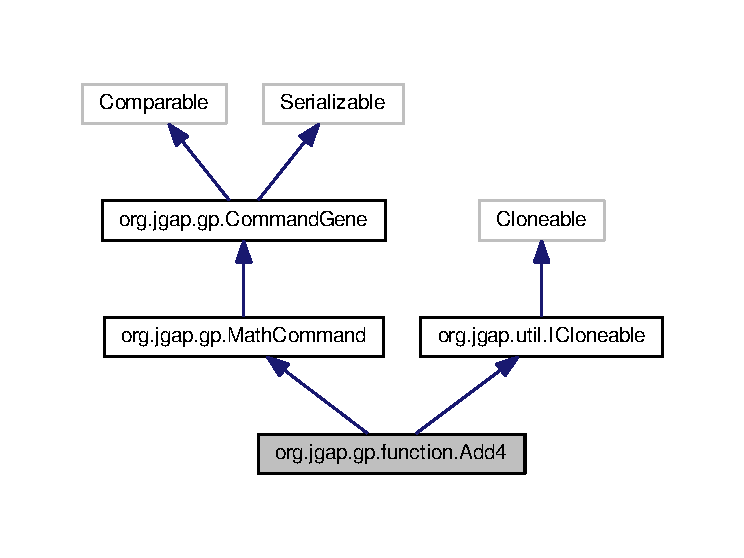
\includegraphics[width=350pt]{classorg_1_1jgap_1_1gp_1_1function_1_1_add4__inherit__graph}
\end{center}
\end{figure}


Collaboration diagram for org.\-jgap.\-gp.\-function.\-Add4\-:
\nopagebreak
\begin{figure}[H]
\begin{center}
\leavevmode
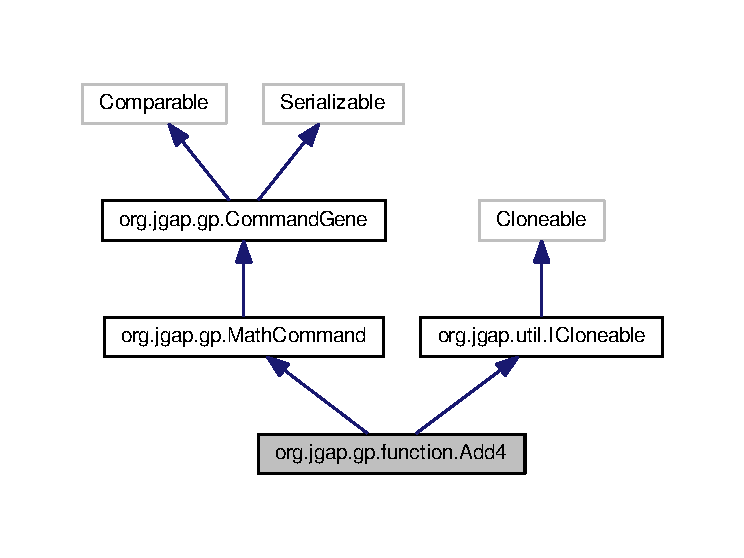
\includegraphics[width=350pt]{classorg_1_1jgap_1_1gp_1_1function_1_1_add4__coll__graph}
\end{center}
\end{figure}
\subsection*{Classes}
\begin{DoxyCompactItemize}
\item 
interface \hyperlink{interfaceorg_1_1jgap_1_1gp_1_1function_1_1_add4_1_1_compatible}{Compatible}
\end{DoxyCompactItemize}
\subsection*{Public Member Functions}
\begin{DoxyCompactItemize}
\item 
\hyperlink{classorg_1_1jgap_1_1gp_1_1function_1_1_add4_a61b95355dfa710c94e592447b7042e75}{Add4} (final G\-P\-Configuration a\-\_\-conf, Class a\-\_\-return\-Type)  throws Invalid\-Configuration\-Exception 
\item 
String \hyperlink{classorg_1_1jgap_1_1gp_1_1function_1_1_add4_a8375b62dc5e6c03a5cc5d86a2be3e1cc}{to\-String} ()
\item 
String \hyperlink{classorg_1_1jgap_1_1gp_1_1function_1_1_add4_afe18c5fd8a2309a0dd3f07d2044c5849}{get\-Name} ()
\item 
int \hyperlink{classorg_1_1jgap_1_1gp_1_1function_1_1_add4_a1036e2a41e834daac87c8caaca7363bf}{execute\-\_\-int} (Program\-Chromosome c, int n, Object\mbox{[}$\,$\mbox{]} args)
\item 
long \hyperlink{classorg_1_1jgap_1_1gp_1_1function_1_1_add4_a20d03531be63935ac1c5fea9ba9ad6d2}{execute\-\_\-long} (Program\-Chromosome c, int n, Object\mbox{[}$\,$\mbox{]} args)
\item 
float \hyperlink{classorg_1_1jgap_1_1gp_1_1function_1_1_add4_af2c73c70cf4a31af8a4a06f4f6c61901}{execute\-\_\-float} (Program\-Chromosome c, int n, Object\mbox{[}$\,$\mbox{]} args)
\item 
double \hyperlink{classorg_1_1jgap_1_1gp_1_1function_1_1_add4_a9f03e277886f52d9f5b9e8caab264c10}{execute\-\_\-double} (Program\-Chromosome c, int n, Object\mbox{[}$\,$\mbox{]} args)
\item 
Object \hyperlink{classorg_1_1jgap_1_1gp_1_1function_1_1_add4_aa7793ad6dff9cfc17b8ef9040554acc7}{execute\-\_\-object} (Program\-Chromosome c, int n, Object\mbox{[}$\,$\mbox{]} args)
\item 
Object \hyperlink{classorg_1_1jgap_1_1gp_1_1function_1_1_add4_ae56c84c38dc3164ce0a74e5b45f7bd25}{clone} ()
\end{DoxyCompactItemize}
\subsection*{Static Private Attributes}
\begin{DoxyCompactItemize}
\item 
static final String \hyperlink{classorg_1_1jgap_1_1gp_1_1function_1_1_add4_a0929e88a1132c13dc1e2b00ae796da1d}{C\-V\-S\-\_\-\-R\-E\-V\-I\-S\-I\-O\-N} = \char`\"{}\$Revision\-: 1.\-3 \$\char`\"{}
\end{DoxyCompactItemize}
\subsection*{Additional Inherited Members}


\subsection{Detailed Description}
The add operation with four parameters (W + X + Y + Z).

\begin{DoxyAuthor}{Author}
Klaus Meffert 
\end{DoxyAuthor}
\begin{DoxySince}{Since}
3.\-3.\-3.\-4 
\end{DoxySince}


Definition at line 23 of file Add4.\-java.



\subsection{Constructor \& Destructor Documentation}
\hypertarget{classorg_1_1jgap_1_1gp_1_1function_1_1_add4_a61b95355dfa710c94e592447b7042e75}{\index{org\-::jgap\-::gp\-::function\-::\-Add4@{org\-::jgap\-::gp\-::function\-::\-Add4}!Add4@{Add4}}
\index{Add4@{Add4}!org::jgap::gp::function::Add4@{org\-::jgap\-::gp\-::function\-::\-Add4}}
\subsubsection[{Add4}]{\setlength{\rightskip}{0pt plus 5cm}org.\-jgap.\-gp.\-function.\-Add4.\-Add4 (
\begin{DoxyParamCaption}
\item[{final G\-P\-Configuration}]{a\-\_\-conf, }
\item[{Class}]{a\-\_\-return\-Type}
\end{DoxyParamCaption}
) throws {\bf Invalid\-Configuration\-Exception}\hspace{0.3cm}{\ttfamily [inline]}}}\label{classorg_1_1jgap_1_1gp_1_1function_1_1_add4_a61b95355dfa710c94e592447b7042e75}


Definition at line 28 of file Add4.\-java.



Referenced by org.\-jgap.\-gp.\-function.\-Add4.\-clone().



\subsection{Member Function Documentation}
\hypertarget{classorg_1_1jgap_1_1gp_1_1function_1_1_add4_ae56c84c38dc3164ce0a74e5b45f7bd25}{\index{org\-::jgap\-::gp\-::function\-::\-Add4@{org\-::jgap\-::gp\-::function\-::\-Add4}!clone@{clone}}
\index{clone@{clone}!org::jgap::gp::function::Add4@{org\-::jgap\-::gp\-::function\-::\-Add4}}
\subsubsection[{clone}]{\setlength{\rightskip}{0pt plus 5cm}Object org.\-jgap.\-gp.\-function.\-Add4.\-clone (
\begin{DoxyParamCaption}
{}
\end{DoxyParamCaption}
)\hspace{0.3cm}{\ttfamily [inline]}}}\label{classorg_1_1jgap_1_1gp_1_1function_1_1_add4_ae56c84c38dc3164ce0a74e5b45f7bd25}
Clones the object. Simple and straight forward implementation here.

\begin{DoxyReturn}{Returns}
cloned instance of this object
\end{DoxyReturn}
\begin{DoxyAuthor}{Author}
Klaus Meffert 
\end{DoxyAuthor}
\begin{DoxySince}{Since}
3.\-4 
\end{DoxySince}


Implements \hyperlink{interfaceorg_1_1jgap_1_1util_1_1_i_cloneable_aa7e7d62077e6428ad7904932b1b4f7d5}{org.\-jgap.\-util.\-I\-Cloneable}.



Definition at line 86 of file Add4.\-java.



References org.\-jgap.\-gp.\-function.\-Add4.\-Add4(), org.\-jgap.\-gp.\-Command\-Gene.\-get\-G\-P\-Configuration(), and org.\-jgap.\-gp.\-Command\-Gene.\-get\-Return\-Type().



Here is the call graph for this function\-:
\nopagebreak
\begin{figure}[H]
\begin{center}
\leavevmode
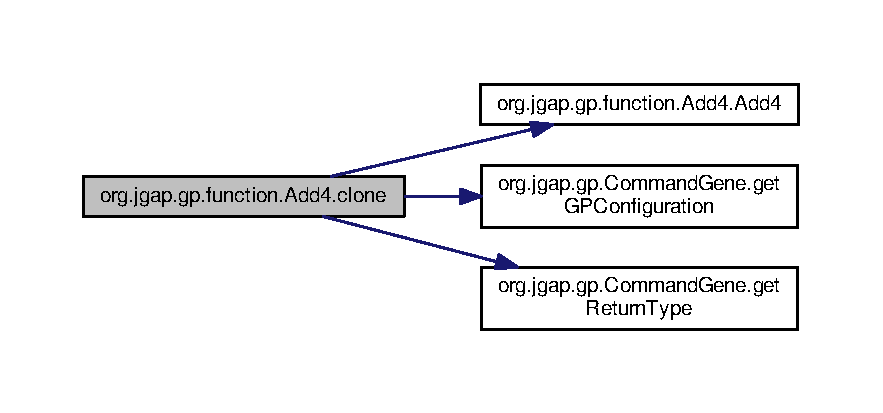
\includegraphics[width=350pt]{classorg_1_1jgap_1_1gp_1_1function_1_1_add4_ae56c84c38dc3164ce0a74e5b45f7bd25_cgraph}
\end{center}
\end{figure}


\hypertarget{classorg_1_1jgap_1_1gp_1_1function_1_1_add4_a9f03e277886f52d9f5b9e8caab264c10}{\index{org\-::jgap\-::gp\-::function\-::\-Add4@{org\-::jgap\-::gp\-::function\-::\-Add4}!execute\-\_\-double@{execute\-\_\-double}}
\index{execute\-\_\-double@{execute\-\_\-double}!org::jgap::gp::function::Add4@{org\-::jgap\-::gp\-::function\-::\-Add4}}
\subsubsection[{execute\-\_\-double}]{\setlength{\rightskip}{0pt plus 5cm}double org.\-jgap.\-gp.\-function.\-Add4.\-execute\-\_\-double (
\begin{DoxyParamCaption}
\item[{Program\-Chromosome}]{c, }
\item[{int}]{n, }
\item[{Object\mbox{[}$\,$\mbox{]}}]{args}
\end{DoxyParamCaption}
)\hspace{0.3cm}{\ttfamily [inline]}}}\label{classorg_1_1jgap_1_1gp_1_1function_1_1_add4_a9f03e277886f52d9f5b9e8caab264c10}


Definition at line 62 of file Add4.\-java.

\hypertarget{classorg_1_1jgap_1_1gp_1_1function_1_1_add4_af2c73c70cf4a31af8a4a06f4f6c61901}{\index{org\-::jgap\-::gp\-::function\-::\-Add4@{org\-::jgap\-::gp\-::function\-::\-Add4}!execute\-\_\-float@{execute\-\_\-float}}
\index{execute\-\_\-float@{execute\-\_\-float}!org::jgap::gp::function::Add4@{org\-::jgap\-::gp\-::function\-::\-Add4}}
\subsubsection[{execute\-\_\-float}]{\setlength{\rightskip}{0pt plus 5cm}float org.\-jgap.\-gp.\-function.\-Add4.\-execute\-\_\-float (
\begin{DoxyParamCaption}
\item[{Program\-Chromosome}]{c, }
\item[{int}]{n, }
\item[{Object\mbox{[}$\,$\mbox{]}}]{args}
\end{DoxyParamCaption}
)\hspace{0.3cm}{\ttfamily [inline]}}}\label{classorg_1_1jgap_1_1gp_1_1function_1_1_add4_af2c73c70cf4a31af8a4a06f4f6c61901}


Definition at line 57 of file Add4.\-java.

\hypertarget{classorg_1_1jgap_1_1gp_1_1function_1_1_add4_a1036e2a41e834daac87c8caaca7363bf}{\index{org\-::jgap\-::gp\-::function\-::\-Add4@{org\-::jgap\-::gp\-::function\-::\-Add4}!execute\-\_\-int@{execute\-\_\-int}}
\index{execute\-\_\-int@{execute\-\_\-int}!org::jgap::gp::function::Add4@{org\-::jgap\-::gp\-::function\-::\-Add4}}
\subsubsection[{execute\-\_\-int}]{\setlength{\rightskip}{0pt plus 5cm}int org.\-jgap.\-gp.\-function.\-Add4.\-execute\-\_\-int (
\begin{DoxyParamCaption}
\item[{Program\-Chromosome}]{c, }
\item[{int}]{n, }
\item[{Object\mbox{[}$\,$\mbox{]}}]{args}
\end{DoxyParamCaption}
)\hspace{0.3cm}{\ttfamily [inline]}}}\label{classorg_1_1jgap_1_1gp_1_1function_1_1_add4_a1036e2a41e834daac87c8caaca7363bf}


Definition at line 47 of file Add4.\-java.

\hypertarget{classorg_1_1jgap_1_1gp_1_1function_1_1_add4_a20d03531be63935ac1c5fea9ba9ad6d2}{\index{org\-::jgap\-::gp\-::function\-::\-Add4@{org\-::jgap\-::gp\-::function\-::\-Add4}!execute\-\_\-long@{execute\-\_\-long}}
\index{execute\-\_\-long@{execute\-\_\-long}!org::jgap::gp::function::Add4@{org\-::jgap\-::gp\-::function\-::\-Add4}}
\subsubsection[{execute\-\_\-long}]{\setlength{\rightskip}{0pt plus 5cm}long org.\-jgap.\-gp.\-function.\-Add4.\-execute\-\_\-long (
\begin{DoxyParamCaption}
\item[{Program\-Chromosome}]{c, }
\item[{int}]{n, }
\item[{Object\mbox{[}$\,$\mbox{]}}]{args}
\end{DoxyParamCaption}
)\hspace{0.3cm}{\ttfamily [inline]}}}\label{classorg_1_1jgap_1_1gp_1_1function_1_1_add4_a20d03531be63935ac1c5fea9ba9ad6d2}


Definition at line 52 of file Add4.\-java.

\hypertarget{classorg_1_1jgap_1_1gp_1_1function_1_1_add4_aa7793ad6dff9cfc17b8ef9040554acc7}{\index{org\-::jgap\-::gp\-::function\-::\-Add4@{org\-::jgap\-::gp\-::function\-::\-Add4}!execute\-\_\-object@{execute\-\_\-object}}
\index{execute\-\_\-object@{execute\-\_\-object}!org::jgap::gp::function::Add4@{org\-::jgap\-::gp\-::function\-::\-Add4}}
\subsubsection[{execute\-\_\-object}]{\setlength{\rightskip}{0pt plus 5cm}Object org.\-jgap.\-gp.\-function.\-Add4.\-execute\-\_\-object (
\begin{DoxyParamCaption}
\item[{Program\-Chromosome}]{c, }
\item[{int}]{n, }
\item[{Object\mbox{[}$\,$\mbox{]}}]{args}
\end{DoxyParamCaption}
)\hspace{0.3cm}{\ttfamily [inline]}}}\label{classorg_1_1jgap_1_1gp_1_1function_1_1_add4_aa7793ad6dff9cfc17b8ef9040554acc7}


Definition at line 67 of file Add4.\-java.

\hypertarget{classorg_1_1jgap_1_1gp_1_1function_1_1_add4_afe18c5fd8a2309a0dd3f07d2044c5849}{\index{org\-::jgap\-::gp\-::function\-::\-Add4@{org\-::jgap\-::gp\-::function\-::\-Add4}!get\-Name@{get\-Name}}
\index{get\-Name@{get\-Name}!org::jgap::gp::function::Add4@{org\-::jgap\-::gp\-::function\-::\-Add4}}
\subsubsection[{get\-Name}]{\setlength{\rightskip}{0pt plus 5cm}String org.\-jgap.\-gp.\-function.\-Add4.\-get\-Name (
\begin{DoxyParamCaption}
{}
\end{DoxyParamCaption}
)\hspace{0.3cm}{\ttfamily [inline]}}}\label{classorg_1_1jgap_1_1gp_1_1function_1_1_add4_afe18c5fd8a2309a0dd3f07d2044c5849}
\begin{DoxyReturn}{Returns}
textual name of this command
\end{DoxyReturn}
\begin{DoxyAuthor}{Author}
Klaus Meffert 
\end{DoxyAuthor}
\begin{DoxySince}{Since}
3.\-3.\-3.\-4 
\end{DoxySince}


Definition at line 43 of file Add4.\-java.

\hypertarget{classorg_1_1jgap_1_1gp_1_1function_1_1_add4_a8375b62dc5e6c03a5cc5d86a2be3e1cc}{\index{org\-::jgap\-::gp\-::function\-::\-Add4@{org\-::jgap\-::gp\-::function\-::\-Add4}!to\-String@{to\-String}}
\index{to\-String@{to\-String}!org::jgap::gp::function::Add4@{org\-::jgap\-::gp\-::function\-::\-Add4}}
\subsubsection[{to\-String}]{\setlength{\rightskip}{0pt plus 5cm}String org.\-jgap.\-gp.\-function.\-Add4.\-to\-String (
\begin{DoxyParamCaption}
{}
\end{DoxyParamCaption}
)\hspace{0.3cm}{\ttfamily [inline]}, {\ttfamily [virtual]}}}\label{classorg_1_1jgap_1_1gp_1_1function_1_1_add4_a8375b62dc5e6c03a5cc5d86a2be3e1cc}
\begin{DoxyReturn}{Returns}
the string representation of the command. Especially usefull to output a resulting formula in human-\/readable form. 
\end{DoxyReturn}


Implements \hyperlink{classorg_1_1jgap_1_1gp_1_1_command_gene_a236141d99059da808afe7a9217e411c7}{org.\-jgap.\-gp.\-Command\-Gene}.



Definition at line 33 of file Add4.\-java.



\subsection{Member Data Documentation}
\hypertarget{classorg_1_1jgap_1_1gp_1_1function_1_1_add4_a0929e88a1132c13dc1e2b00ae796da1d}{\index{org\-::jgap\-::gp\-::function\-::\-Add4@{org\-::jgap\-::gp\-::function\-::\-Add4}!C\-V\-S\-\_\-\-R\-E\-V\-I\-S\-I\-O\-N@{C\-V\-S\-\_\-\-R\-E\-V\-I\-S\-I\-O\-N}}
\index{C\-V\-S\-\_\-\-R\-E\-V\-I\-S\-I\-O\-N@{C\-V\-S\-\_\-\-R\-E\-V\-I\-S\-I\-O\-N}!org::jgap::gp::function::Add4@{org\-::jgap\-::gp\-::function\-::\-Add4}}
\subsubsection[{C\-V\-S\-\_\-\-R\-E\-V\-I\-S\-I\-O\-N}]{\setlength{\rightskip}{0pt plus 5cm}final String org.\-jgap.\-gp.\-function.\-Add4.\-C\-V\-S\-\_\-\-R\-E\-V\-I\-S\-I\-O\-N = \char`\"{}\$Revision\-: 1.\-3 \$\char`\"{}\hspace{0.3cm}{\ttfamily [static]}, {\ttfamily [private]}}}\label{classorg_1_1jgap_1_1gp_1_1function_1_1_add4_a0929e88a1132c13dc1e2b00ae796da1d}
String containing the C\-V\-S revision. Read out via reflection! 

Definition at line 26 of file Add4.\-java.



The documentation for this class was generated from the following file\-:\begin{DoxyCompactItemize}
\item 
L\-D\-H\-\_\-\-Git/src/org/jgap/gp/function/\hyperlink{_add4_8java}{Add4.\-java}\end{DoxyCompactItemize}

\hypertarget{classorg_1_1jgap_1_1gp_1_1function_1_1_add_and_store}{\section{org.\-jgap.\-gp.\-function.\-Add\-And\-Store Class Reference}
\label{classorg_1_1jgap_1_1gp_1_1function_1_1_add_and_store}\index{org.\-jgap.\-gp.\-function.\-Add\-And\-Store@{org.\-jgap.\-gp.\-function.\-Add\-And\-Store}}
}


Inheritance diagram for org.\-jgap.\-gp.\-function.\-Add\-And\-Store\-:
\nopagebreak
\begin{figure}[H]
\begin{center}
\leavevmode
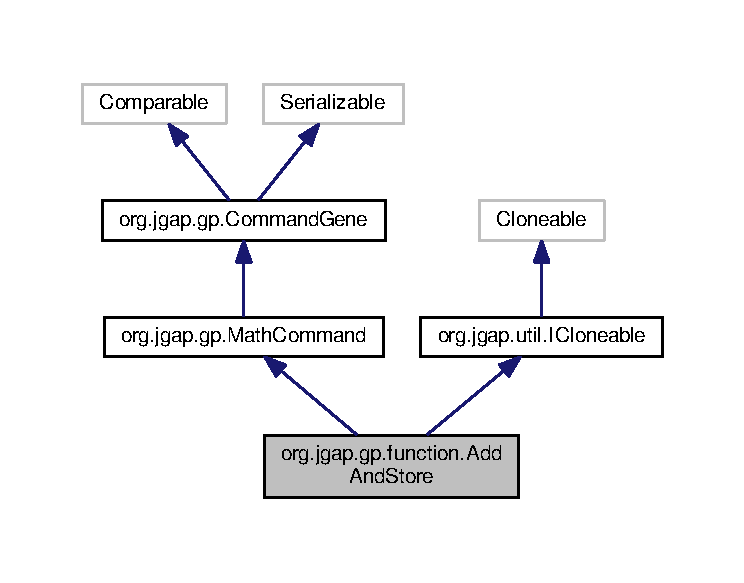
\includegraphics[width=350pt]{classorg_1_1jgap_1_1gp_1_1function_1_1_add_and_store__inherit__graph}
\end{center}
\end{figure}


Collaboration diagram for org.\-jgap.\-gp.\-function.\-Add\-And\-Store\-:
\nopagebreak
\begin{figure}[H]
\begin{center}
\leavevmode
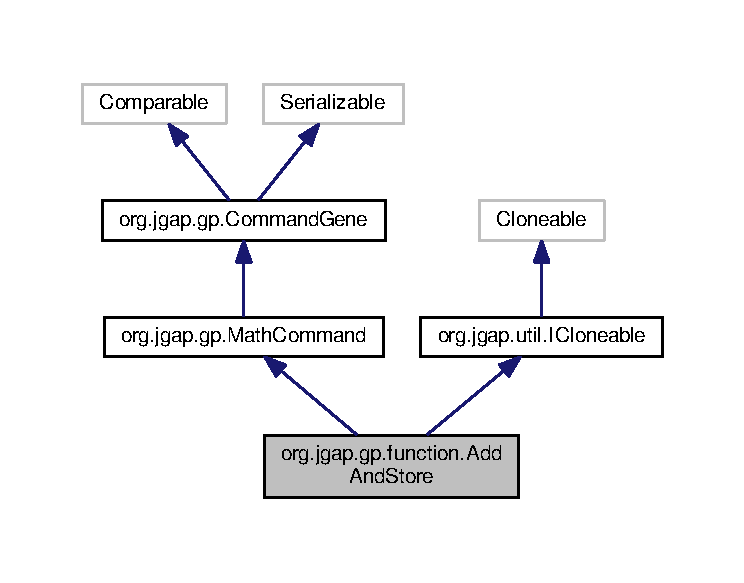
\includegraphics[width=350pt]{classorg_1_1jgap_1_1gp_1_1function_1_1_add_and_store__coll__graph}
\end{center}
\end{figure}
\subsection*{Public Member Functions}
\begin{DoxyCompactItemize}
\item 
\hyperlink{classorg_1_1jgap_1_1gp_1_1function_1_1_add_and_store_af945cf220f74e250e8e85cfdb1d732ed}{Add\-And\-Store} (final G\-P\-Configuration a\-\_\-conf, Class a\-\_\-type, String a\-\_\-storage\-Name)  throws Invalid\-Configuration\-Exception 
\item 
String \hyperlink{classorg_1_1jgap_1_1gp_1_1function_1_1_add_and_store_a7e59b96566c171ff57b15447bfa24176}{to\-String} ()
\item 
String \hyperlink{classorg_1_1jgap_1_1gp_1_1function_1_1_add_and_store_aaadc7ed5e247750a7cbf7d87bcba6bd8}{get\-Name} ()
\item 
void \hyperlink{classorg_1_1jgap_1_1gp_1_1function_1_1_add_and_store_ad7eafe1504fb37c3631687ceda439aa3}{execute\-\_\-void} (Program\-Chromosome c, int n, Object\mbox{[}$\,$\mbox{]} args)
\item 
Class \hyperlink{classorg_1_1jgap_1_1gp_1_1function_1_1_add_and_store_ab12e6bc462f123511f21a6cfe25bb5fc}{get\-Child\-Type} (\hyperlink{interfaceorg_1_1jgap_1_1gp_1_1_i_g_p_program}{I\-G\-P\-Program} a\-\_\-ind, int a\-\_\-chrom\-Num)
\item 
int \hyperlink{classorg_1_1jgap_1_1gp_1_1function_1_1_add_and_store_a85981abb15fda93c1dedd77102482bc6}{compare\-To} (Object a\-\_\-other)
\item 
boolean \hyperlink{classorg_1_1jgap_1_1gp_1_1function_1_1_add_and_store_aa29cf343055f57008053066ccfb1a177}{equals} (Object a\-\_\-other)
\item 
Object \hyperlink{classorg_1_1jgap_1_1gp_1_1function_1_1_add_and_store_abd439c91466f1d3f2aed2752508a00d8}{clone} ()
\end{DoxyCompactItemize}
\subsection*{Private Attributes}
\begin{DoxyCompactItemize}
\item 
String \hyperlink{classorg_1_1jgap_1_1gp_1_1function_1_1_add_and_store_aaea25fb58b8f1efe56df91b0a37da642}{m\-\_\-storage\-Name}
\item 
Class \hyperlink{classorg_1_1jgap_1_1gp_1_1function_1_1_add_and_store_a01a50be6c8cc4fa4106878c9e7e618a0}{m\-\_\-type}
\end{DoxyCompactItemize}
\subsection*{Static Private Attributes}
\begin{DoxyCompactItemize}
\item 
static final String \hyperlink{classorg_1_1jgap_1_1gp_1_1function_1_1_add_and_store_a48e1c2cfa0ce37278055ad74e9539b50}{C\-V\-S\-\_\-\-R\-E\-V\-I\-S\-I\-O\-N} = \char`\"{}\$Revision\-: 1.\-13 \$\char`\"{}
\end{DoxyCompactItemize}
\subsection*{Additional Inherited Members}


\subsection{Detailed Description}
The add operation that stores the result in internal memory afterwards.

\begin{DoxyAuthor}{Author}
Klaus Meffert 
\end{DoxyAuthor}
\begin{DoxySince}{Since}
3.\-0 
\end{DoxySince}


Definition at line 24 of file Add\-And\-Store.\-java.



\subsection{Constructor \& Destructor Documentation}
\hypertarget{classorg_1_1jgap_1_1gp_1_1function_1_1_add_and_store_af945cf220f74e250e8e85cfdb1d732ed}{\index{org\-::jgap\-::gp\-::function\-::\-Add\-And\-Store@{org\-::jgap\-::gp\-::function\-::\-Add\-And\-Store}!Add\-And\-Store@{Add\-And\-Store}}
\index{Add\-And\-Store@{Add\-And\-Store}!org::jgap::gp::function::AddAndStore@{org\-::jgap\-::gp\-::function\-::\-Add\-And\-Store}}
\subsubsection[{Add\-And\-Store}]{\setlength{\rightskip}{0pt plus 5cm}org.\-jgap.\-gp.\-function.\-Add\-And\-Store.\-Add\-And\-Store (
\begin{DoxyParamCaption}
\item[{final G\-P\-Configuration}]{a\-\_\-conf, }
\item[{Class}]{a\-\_\-type, }
\item[{String}]{a\-\_\-storage\-Name}
\end{DoxyParamCaption}
) throws {\bf Invalid\-Configuration\-Exception}\hspace{0.3cm}{\ttfamily [inline]}}}\label{classorg_1_1jgap_1_1gp_1_1function_1_1_add_and_store_af945cf220f74e250e8e85cfdb1d732ed}


Definition at line 37 of file Add\-And\-Store.\-java.



References org.\-jgap.\-gp.\-function.\-Add\-And\-Store.\-m\-\_\-storage\-Name, org.\-jgap.\-gp.\-function.\-Add\-And\-Store.\-m\-\_\-type, and org.\-jgap.\-gp.\-Command\-Gene.\-Void\-Class.



Referenced by org.\-jgap.\-gp.\-function.\-Add\-And\-Store.\-clone(), org.\-jgap.\-gp.\-function.\-Add\-And\-Store.\-compare\-To(), and org.\-jgap.\-gp.\-function.\-Add\-And\-Store.\-equals().



\subsection{Member Function Documentation}
\hypertarget{classorg_1_1jgap_1_1gp_1_1function_1_1_add_and_store_abd439c91466f1d3f2aed2752508a00d8}{\index{org\-::jgap\-::gp\-::function\-::\-Add\-And\-Store@{org\-::jgap\-::gp\-::function\-::\-Add\-And\-Store}!clone@{clone}}
\index{clone@{clone}!org::jgap::gp::function::AddAndStore@{org\-::jgap\-::gp\-::function\-::\-Add\-And\-Store}}
\subsubsection[{clone}]{\setlength{\rightskip}{0pt plus 5cm}Object org.\-jgap.\-gp.\-function.\-Add\-And\-Store.\-clone (
\begin{DoxyParamCaption}
{}
\end{DoxyParamCaption}
)\hspace{0.3cm}{\ttfamily [inline]}}}\label{classorg_1_1jgap_1_1gp_1_1function_1_1_add_and_store_abd439c91466f1d3f2aed2752508a00d8}
Clones the object. Simple and straight forward implementation here.

\begin{DoxyReturn}{Returns}
cloned instance of this object
\end{DoxyReturn}
\begin{DoxyAuthor}{Author}
Klaus Meffert 
\end{DoxyAuthor}
\begin{DoxySince}{Since}
3.\-4 
\end{DoxySince}


Implements \hyperlink{interfaceorg_1_1jgap_1_1util_1_1_i_cloneable_aa7e7d62077e6428ad7904932b1b4f7d5}{org.\-jgap.\-util.\-I\-Cloneable}.



Definition at line 135 of file Add\-And\-Store.\-java.



References org.\-jgap.\-gp.\-function.\-Add\-And\-Store.\-Add\-And\-Store(), org.\-jgap.\-gp.\-Command\-Gene.\-get\-G\-P\-Configuration(), org.\-jgap.\-gp.\-function.\-Add\-And\-Store.\-m\-\_\-storage\-Name, and org.\-jgap.\-gp.\-function.\-Add\-And\-Store.\-m\-\_\-type.



Here is the call graph for this function\-:
\nopagebreak
\begin{figure}[H]
\begin{center}
\leavevmode
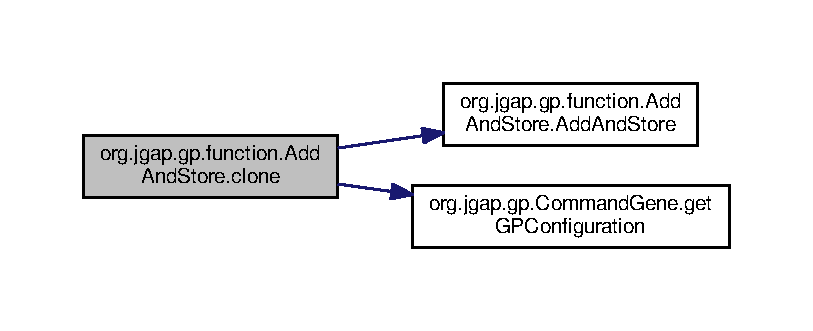
\includegraphics[width=350pt]{classorg_1_1jgap_1_1gp_1_1function_1_1_add_and_store_abd439c91466f1d3f2aed2752508a00d8_cgraph}
\end{center}
\end{figure}


\hypertarget{classorg_1_1jgap_1_1gp_1_1function_1_1_add_and_store_a85981abb15fda93c1dedd77102482bc6}{\index{org\-::jgap\-::gp\-::function\-::\-Add\-And\-Store@{org\-::jgap\-::gp\-::function\-::\-Add\-And\-Store}!compare\-To@{compare\-To}}
\index{compare\-To@{compare\-To}!org::jgap::gp::function::AddAndStore@{org\-::jgap\-::gp\-::function\-::\-Add\-And\-Store}}
\subsubsection[{compare\-To}]{\setlength{\rightskip}{0pt plus 5cm}int org.\-jgap.\-gp.\-function.\-Add\-And\-Store.\-compare\-To (
\begin{DoxyParamCaption}
\item[{Object}]{a\-\_\-other}
\end{DoxyParamCaption}
)\hspace{0.3cm}{\ttfamily [inline]}}}\label{classorg_1_1jgap_1_1gp_1_1function_1_1_add_and_store_a85981abb15fda93c1dedd77102482bc6}
The compare\-To-\/method.


\begin{DoxyParams}{Parameters}
{\em a\-\_\-other} & the other object to compare \\
\hline
\end{DoxyParams}
\begin{DoxyReturn}{Returns}
-\/1, 0, 1
\end{DoxyReturn}
\begin{DoxyAuthor}{Author}
Klaus Meffert 
\end{DoxyAuthor}
\begin{DoxySince}{Since}
3.\-0 
\end{DoxySince}


Definition at line 95 of file Add\-And\-Store.\-java.



References org.\-jgap.\-gp.\-function.\-Add\-And\-Store.\-Add\-And\-Store(), org.\-jgap.\-gp.\-function.\-Add\-And\-Store.\-m\-\_\-storage\-Name, and org.\-jgap.\-gp.\-function.\-Add\-And\-Store.\-m\-\_\-type.



Here is the call graph for this function\-:
\nopagebreak
\begin{figure}[H]
\begin{center}
\leavevmode

\includegraphics[width=350pt]{classorg_1_1jgap_1_1gp_1_1function_1_1_add_and_store_a85981abb15fda93c1dedd77102482bc6_cgraph}
\end{center}
\end{figure}


\hypertarget{classorg_1_1jgap_1_1gp_1_1function_1_1_add_and_store_aa29cf343055f57008053066ccfb1a177}{\index{org\-::jgap\-::gp\-::function\-::\-Add\-And\-Store@{org\-::jgap\-::gp\-::function\-::\-Add\-And\-Store}!equals@{equals}}
\index{equals@{equals}!org::jgap::gp::function::AddAndStore@{org\-::jgap\-::gp\-::function\-::\-Add\-And\-Store}}
\subsubsection[{equals}]{\setlength{\rightskip}{0pt plus 5cm}boolean org.\-jgap.\-gp.\-function.\-Add\-And\-Store.\-equals (
\begin{DoxyParamCaption}
\item[{Object}]{a\-\_\-other}
\end{DoxyParamCaption}
)\hspace{0.3cm}{\ttfamily [inline]}}}\label{classorg_1_1jgap_1_1gp_1_1function_1_1_add_and_store_aa29cf343055f57008053066ccfb1a177}
The equals-\/method. 
\begin{DoxyParams}{Parameters}
{\em a\-\_\-other} & the other object to compare \\
\hline
\end{DoxyParams}
\begin{DoxyReturn}{Returns}
true if the objects are seen as equal
\end{DoxyReturn}
\begin{DoxyAuthor}{Author}
Klaus Meffert 
\end{DoxyAuthor}
\begin{DoxySince}{Since}
3.\-0 
\end{DoxySince}


Definition at line 115 of file Add\-And\-Store.\-java.



References org.\-jgap.\-gp.\-function.\-Add\-And\-Store.\-Add\-And\-Store(), org.\-jgap.\-gp.\-function.\-Add\-And\-Store.\-m\-\_\-storage\-Name, and org.\-jgap.\-gp.\-function.\-Add\-And\-Store.\-m\-\_\-type.



Here is the call graph for this function\-:
\nopagebreak
\begin{figure}[H]
\begin{center}
\leavevmode
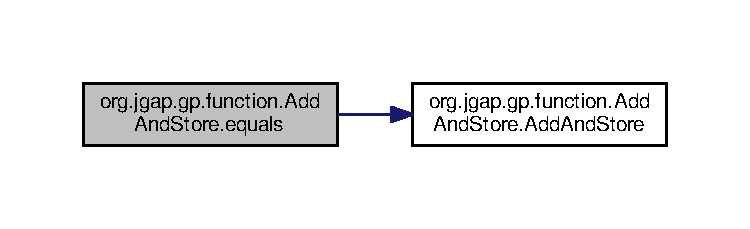
\includegraphics[width=350pt]{classorg_1_1jgap_1_1gp_1_1function_1_1_add_and_store_aa29cf343055f57008053066ccfb1a177_cgraph}
\end{center}
\end{figure}


\hypertarget{classorg_1_1jgap_1_1gp_1_1function_1_1_add_and_store_ad7eafe1504fb37c3631687ceda439aa3}{\index{org\-::jgap\-::gp\-::function\-::\-Add\-And\-Store@{org\-::jgap\-::gp\-::function\-::\-Add\-And\-Store}!execute\-\_\-void@{execute\-\_\-void}}
\index{execute\-\_\-void@{execute\-\_\-void}!org::jgap::gp::function::AddAndStore@{org\-::jgap\-::gp\-::function\-::\-Add\-And\-Store}}
\subsubsection[{execute\-\_\-void}]{\setlength{\rightskip}{0pt plus 5cm}void org.\-jgap.\-gp.\-function.\-Add\-And\-Store.\-execute\-\_\-void (
\begin{DoxyParamCaption}
\item[{Program\-Chromosome}]{c, }
\item[{int}]{n, }
\item[{Object\mbox{[}$\,$\mbox{]}}]{args}
\end{DoxyParamCaption}
)\hspace{0.3cm}{\ttfamily [inline]}}}\label{classorg_1_1jgap_1_1gp_1_1function_1_1_add_and_store_ad7eafe1504fb37c3631687ceda439aa3}


Definition at line 59 of file Add\-And\-Store.\-java.



References org.\-jgap.\-gp.\-Command\-Gene.\-Double\-Class, org.\-jgap.\-gp.\-Command\-Gene.\-Float\-Class, org.\-jgap.\-gp.\-Command\-Gene.\-get\-G\-P\-Configuration(), org.\-jgap.\-gp.\-Command\-Gene.\-Integer\-Class, org.\-jgap.\-gp.\-Command\-Gene.\-Long\-Class, org.\-jgap.\-gp.\-function.\-Add\-And\-Store.\-m\-\_\-storage\-Name, and org.\-jgap.\-gp.\-function.\-Add\-And\-Store.\-m\-\_\-type.



Here is the call graph for this function\-:
\nopagebreak
\begin{figure}[H]
\begin{center}
\leavevmode
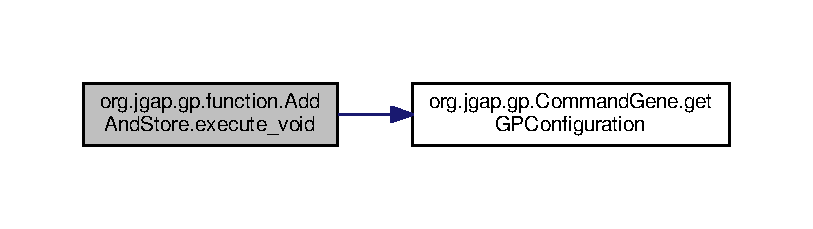
\includegraphics[width=350pt]{classorg_1_1jgap_1_1gp_1_1function_1_1_add_and_store_ad7eafe1504fb37c3631687ceda439aa3_cgraph}
\end{center}
\end{figure}


\hypertarget{classorg_1_1jgap_1_1gp_1_1function_1_1_add_and_store_ab12e6bc462f123511f21a6cfe25bb5fc}{\index{org\-::jgap\-::gp\-::function\-::\-Add\-And\-Store@{org\-::jgap\-::gp\-::function\-::\-Add\-And\-Store}!get\-Child\-Type@{get\-Child\-Type}}
\index{get\-Child\-Type@{get\-Child\-Type}!org::jgap::gp::function::AddAndStore@{org\-::jgap\-::gp\-::function\-::\-Add\-And\-Store}}
\subsubsection[{get\-Child\-Type}]{\setlength{\rightskip}{0pt plus 5cm}Class org.\-jgap.\-gp.\-function.\-Add\-And\-Store.\-get\-Child\-Type (
\begin{DoxyParamCaption}
\item[{{\bf I\-G\-P\-Program}}]{a\-\_\-ind, }
\item[{int}]{a\-\_\-chrom\-Num}
\end{DoxyParamCaption}
)\hspace{0.3cm}{\ttfamily [inline]}}}\label{classorg_1_1jgap_1_1gp_1_1function_1_1_add_and_store_ab12e6bc462f123511f21a6cfe25bb5fc}


Definition at line 82 of file Add\-And\-Store.\-java.



References org.\-jgap.\-gp.\-function.\-Add\-And\-Store.\-m\-\_\-type.

\hypertarget{classorg_1_1jgap_1_1gp_1_1function_1_1_add_and_store_aaadc7ed5e247750a7cbf7d87bcba6bd8}{\index{org\-::jgap\-::gp\-::function\-::\-Add\-And\-Store@{org\-::jgap\-::gp\-::function\-::\-Add\-And\-Store}!get\-Name@{get\-Name}}
\index{get\-Name@{get\-Name}!org::jgap::gp::function::AddAndStore@{org\-::jgap\-::gp\-::function\-::\-Add\-And\-Store}}
\subsubsection[{get\-Name}]{\setlength{\rightskip}{0pt plus 5cm}String org.\-jgap.\-gp.\-function.\-Add\-And\-Store.\-get\-Name (
\begin{DoxyParamCaption}
{}
\end{DoxyParamCaption}
)\hspace{0.3cm}{\ttfamily [inline]}}}\label{classorg_1_1jgap_1_1gp_1_1function_1_1_add_and_store_aaadc7ed5e247750a7cbf7d87bcba6bd8}
\begin{DoxyReturn}{Returns}
textual name of this command
\end{DoxyReturn}
\begin{DoxyAuthor}{Author}
Klaus Meffert 
\end{DoxyAuthor}
\begin{DoxySince}{Since}
3.\-2 
\end{DoxySince}


Definition at line 55 of file Add\-And\-Store.\-java.

\hypertarget{classorg_1_1jgap_1_1gp_1_1function_1_1_add_and_store_a7e59b96566c171ff57b15447bfa24176}{\index{org\-::jgap\-::gp\-::function\-::\-Add\-And\-Store@{org\-::jgap\-::gp\-::function\-::\-Add\-And\-Store}!to\-String@{to\-String}}
\index{to\-String@{to\-String}!org::jgap::gp::function::AddAndStore@{org\-::jgap\-::gp\-::function\-::\-Add\-And\-Store}}
\subsubsection[{to\-String}]{\setlength{\rightskip}{0pt plus 5cm}String org.\-jgap.\-gp.\-function.\-Add\-And\-Store.\-to\-String (
\begin{DoxyParamCaption}
{}
\end{DoxyParamCaption}
)\hspace{0.3cm}{\ttfamily [inline]}, {\ttfamily [virtual]}}}\label{classorg_1_1jgap_1_1gp_1_1function_1_1_add_and_store_a7e59b96566c171ff57b15447bfa24176}
\begin{DoxyReturn}{Returns}
the string representation of the command. Especially usefull to output a resulting formula in human-\/readable form. 
\end{DoxyReturn}


Implements \hyperlink{classorg_1_1jgap_1_1gp_1_1_command_gene_a236141d99059da808afe7a9217e411c7}{org.\-jgap.\-gp.\-Command\-Gene}.



Definition at line 45 of file Add\-And\-Store.\-java.



References org.\-jgap.\-gp.\-function.\-Add\-And\-Store.\-m\-\_\-storage\-Name.



\subsection{Member Data Documentation}
\hypertarget{classorg_1_1jgap_1_1gp_1_1function_1_1_add_and_store_a48e1c2cfa0ce37278055ad74e9539b50}{\index{org\-::jgap\-::gp\-::function\-::\-Add\-And\-Store@{org\-::jgap\-::gp\-::function\-::\-Add\-And\-Store}!C\-V\-S\-\_\-\-R\-E\-V\-I\-S\-I\-O\-N@{C\-V\-S\-\_\-\-R\-E\-V\-I\-S\-I\-O\-N}}
\index{C\-V\-S\-\_\-\-R\-E\-V\-I\-S\-I\-O\-N@{C\-V\-S\-\_\-\-R\-E\-V\-I\-S\-I\-O\-N}!org::jgap::gp::function::AddAndStore@{org\-::jgap\-::gp\-::function\-::\-Add\-And\-Store}}
\subsubsection[{C\-V\-S\-\_\-\-R\-E\-V\-I\-S\-I\-O\-N}]{\setlength{\rightskip}{0pt plus 5cm}final String org.\-jgap.\-gp.\-function.\-Add\-And\-Store.\-C\-V\-S\-\_\-\-R\-E\-V\-I\-S\-I\-O\-N = \char`\"{}\$Revision\-: 1.\-13 \$\char`\"{}\hspace{0.3cm}{\ttfamily [static]}, {\ttfamily [private]}}}\label{classorg_1_1jgap_1_1gp_1_1function_1_1_add_and_store_a48e1c2cfa0ce37278055ad74e9539b50}
String containing the C\-V\-S revision. Read out via reflection! 

Definition at line 27 of file Add\-And\-Store.\-java.

\hypertarget{classorg_1_1jgap_1_1gp_1_1function_1_1_add_and_store_aaea25fb58b8f1efe56df91b0a37da642}{\index{org\-::jgap\-::gp\-::function\-::\-Add\-And\-Store@{org\-::jgap\-::gp\-::function\-::\-Add\-And\-Store}!m\-\_\-storage\-Name@{m\-\_\-storage\-Name}}
\index{m\-\_\-storage\-Name@{m\-\_\-storage\-Name}!org::jgap::gp::function::AddAndStore@{org\-::jgap\-::gp\-::function\-::\-Add\-And\-Store}}
\subsubsection[{m\-\_\-storage\-Name}]{\setlength{\rightskip}{0pt plus 5cm}String org.\-jgap.\-gp.\-function.\-Add\-And\-Store.\-m\-\_\-storage\-Name\hspace{0.3cm}{\ttfamily [private]}}}\label{classorg_1_1jgap_1_1gp_1_1function_1_1_add_and_store_aaea25fb58b8f1efe56df91b0a37da642}
Symbolic name of the storage. Must correspond with a chosen name for Read\-Terminal\-Command. 

Definition at line 33 of file Add\-And\-Store.\-java.



Referenced by org.\-jgap.\-gp.\-function.\-Add\-And\-Store.\-Add\-And\-Store(), org.\-jgap.\-gp.\-function.\-Add\-And\-Store.\-clone(), org.\-jgap.\-gp.\-function.\-Add\-And\-Store.\-compare\-To(), org.\-jgap.\-gp.\-function.\-Add\-And\-Store.\-equals(), org.\-jgap.\-gp.\-function.\-Add\-And\-Store.\-execute\-\_\-void(), and org.\-jgap.\-gp.\-function.\-Add\-And\-Store.\-to\-String().

\hypertarget{classorg_1_1jgap_1_1gp_1_1function_1_1_add_and_store_a01a50be6c8cc4fa4106878c9e7e618a0}{\index{org\-::jgap\-::gp\-::function\-::\-Add\-And\-Store@{org\-::jgap\-::gp\-::function\-::\-Add\-And\-Store}!m\-\_\-type@{m\-\_\-type}}
\index{m\-\_\-type@{m\-\_\-type}!org::jgap::gp::function::AddAndStore@{org\-::jgap\-::gp\-::function\-::\-Add\-And\-Store}}
\subsubsection[{m\-\_\-type}]{\setlength{\rightskip}{0pt plus 5cm}Class org.\-jgap.\-gp.\-function.\-Add\-And\-Store.\-m\-\_\-type\hspace{0.3cm}{\ttfamily [private]}}}\label{classorg_1_1jgap_1_1gp_1_1function_1_1_add_and_store_a01a50be6c8cc4fa4106878c9e7e618a0}


Definition at line 35 of file Add\-And\-Store.\-java.



Referenced by org.\-jgap.\-gp.\-function.\-Add\-And\-Store.\-Add\-And\-Store(), org.\-jgap.\-gp.\-function.\-Add\-And\-Store.\-clone(), org.\-jgap.\-gp.\-function.\-Add\-And\-Store.\-compare\-To(), org.\-jgap.\-gp.\-function.\-Add\-And\-Store.\-equals(), org.\-jgap.\-gp.\-function.\-Add\-And\-Store.\-execute\-\_\-void(), and org.\-jgap.\-gp.\-function.\-Add\-And\-Store.\-get\-Child\-Type().



The documentation for this class was generated from the following file\-:\begin{DoxyCompactItemize}
\item 
L\-D\-H\-\_\-\-Git/src/org/jgap/gp/function/\hyperlink{_add_and_store_8java}{Add\-And\-Store.\-java}\end{DoxyCompactItemize}

\hypertarget{classorg_1_1jgap_1_1gp_1_1function_1_1_add_and_store_terminal}{\section{org.\-jgap.\-gp.\-function.\-Add\-And\-Store\-Terminal Class Reference}
\label{classorg_1_1jgap_1_1gp_1_1function_1_1_add_and_store_terminal}\index{org.\-jgap.\-gp.\-function.\-Add\-And\-Store\-Terminal@{org.\-jgap.\-gp.\-function.\-Add\-And\-Store\-Terminal}}
}


Inheritance diagram for org.\-jgap.\-gp.\-function.\-Add\-And\-Store\-Terminal\-:
\nopagebreak
\begin{figure}[H]
\begin{center}
\leavevmode
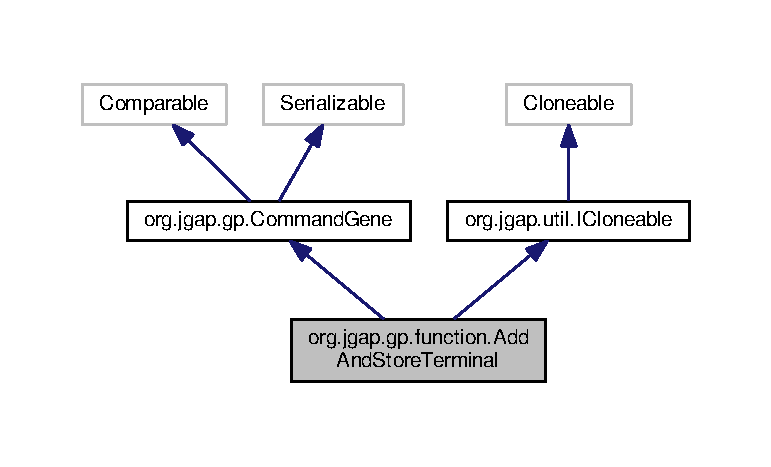
\includegraphics[width=350pt]{classorg_1_1jgap_1_1gp_1_1function_1_1_add_and_store_terminal__inherit__graph}
\end{center}
\end{figure}


Collaboration diagram for org.\-jgap.\-gp.\-function.\-Add\-And\-Store\-Terminal\-:
\nopagebreak
\begin{figure}[H]
\begin{center}
\leavevmode
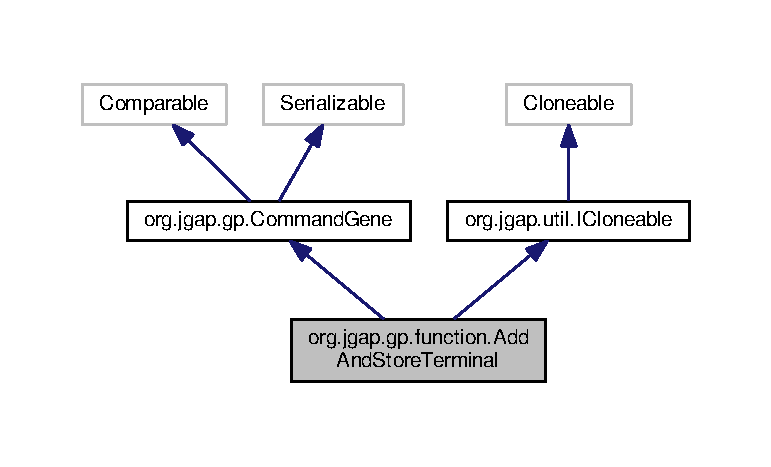
\includegraphics[width=350pt]{classorg_1_1jgap_1_1gp_1_1function_1_1_add_and_store_terminal__coll__graph}
\end{center}
\end{figure}
\subsection*{Public Member Functions}
\begin{DoxyCompactItemize}
\item 
\hyperlink{classorg_1_1jgap_1_1gp_1_1function_1_1_add_and_store_terminal_a253d1d1b4d0ef317cc89bb8dc2aaae93}{Add\-And\-Store\-Terminal} (final G\-P\-Configuration a\-\_\-conf, String a\-\_\-storage\-Name, Class a\-\_\-child\-Type)  throws Invalid\-Configuration\-Exception 
\item 
\hyperlink{classorg_1_1jgap_1_1gp_1_1function_1_1_add_and_store_terminal_a603aceebaab47f1c79bcfabe0c0a0244}{Add\-And\-Store\-Terminal} (final G\-P\-Configuration a\-\_\-conf, String a\-\_\-storage\-Name, Class a\-\_\-child\-Type, int a\-\_\-sub\-Return\-Type, int a\-\_\-sub\-Child\-Type)  throws Invalid\-Configuration\-Exception 
\item 
String \hyperlink{classorg_1_1jgap_1_1gp_1_1function_1_1_add_and_store_terminal_af529ea2032b2ab2da3b4b1a1257daba4}{to\-String} ()
\item 
String \hyperlink{classorg_1_1jgap_1_1gp_1_1function_1_1_add_and_store_terminal_abbe2ab039a01b790be172e3378aa19ba}{get\-Name} ()
\item 
void \hyperlink{classorg_1_1jgap_1_1gp_1_1function_1_1_add_and_store_terminal_a97d517950ee49ea37e8c56f2d171065a}{execute\-\_\-void} (Program\-Chromosome c, int n, Object\mbox{[}$\,$\mbox{]} args)
\item 
boolean \hyperlink{classorg_1_1jgap_1_1gp_1_1function_1_1_add_and_store_terminal_ad630fed4126ace4f4fb0a2083b063b7b}{is\-Affect\-Global\-State} ()
\item 
boolean \hyperlink{classorg_1_1jgap_1_1gp_1_1function_1_1_add_and_store_terminal_af6de474aac647abfeda2d72b18eda760}{is\-Valid} (Program\-Chromosome a\-\_\-program)
\item 
Class \hyperlink{classorg_1_1jgap_1_1gp_1_1function_1_1_add_and_store_terminal_a122727d023e1954671f3b32607b65ee3}{get\-Child\-Type} (\hyperlink{interfaceorg_1_1jgap_1_1gp_1_1_i_g_p_program}{I\-G\-P\-Program} a\-\_\-ind, int a\-\_\-chrom\-Num)
\item 
int \hyperlink{classorg_1_1jgap_1_1gp_1_1function_1_1_add_and_store_terminal_a035feb57f8cb8fc3c9ad397f686f86db}{compare\-To} (Object a\-\_\-other)
\item 
boolean \hyperlink{classorg_1_1jgap_1_1gp_1_1function_1_1_add_and_store_terminal_a8e78f60d9a9df2bd8f7f5c295ebb8d1b}{equals} (Object a\-\_\-other)
\item 
Object \hyperlink{classorg_1_1jgap_1_1gp_1_1function_1_1_add_and_store_terminal_a1d9029480508cb1e803f2ec6e2ffb227}{clone} ()
\end{DoxyCompactItemize}
\subsection*{Private Attributes}
\begin{DoxyCompactItemize}
\item 
String \hyperlink{classorg_1_1jgap_1_1gp_1_1function_1_1_add_and_store_terminal_ad4d924dec40c6808079bba21c2ce7109}{m\-\_\-storage\-Name}
\item 
Class \hyperlink{classorg_1_1jgap_1_1gp_1_1function_1_1_add_and_store_terminal_a4cdce43124d31812835c2e936c5f2811}{m\-\_\-type}
\end{DoxyCompactItemize}
\subsection*{Static Private Attributes}
\begin{DoxyCompactItemize}
\item 
static final String \hyperlink{classorg_1_1jgap_1_1gp_1_1function_1_1_add_and_store_terminal_add1d1d7649a010682468ac5adf7e3d6e}{C\-V\-S\-\_\-\-R\-E\-V\-I\-S\-I\-O\-N} = \char`\"{}\$Revision\-: 1.\-4 \$\char`\"{}
\end{DoxyCompactItemize}
\subsection*{Additional Inherited Members}


\subsection{Detailed Description}
Stores a value in the internal memory but adds the value already stored in the target memory cell before storing it.

\begin{DoxyAuthor}{Author}
Klaus Meffert 
\end{DoxyAuthor}
\begin{DoxySince}{Since}
3.\-2 
\end{DoxySince}


Definition at line 26 of file Add\-And\-Store\-Terminal.\-java.



\subsection{Constructor \& Destructor Documentation}
\hypertarget{classorg_1_1jgap_1_1gp_1_1function_1_1_add_and_store_terminal_a253d1d1b4d0ef317cc89bb8dc2aaae93}{\index{org\-::jgap\-::gp\-::function\-::\-Add\-And\-Store\-Terminal@{org\-::jgap\-::gp\-::function\-::\-Add\-And\-Store\-Terminal}!Add\-And\-Store\-Terminal@{Add\-And\-Store\-Terminal}}
\index{Add\-And\-Store\-Terminal@{Add\-And\-Store\-Terminal}!org::jgap::gp::function::AddAndStoreTerminal@{org\-::jgap\-::gp\-::function\-::\-Add\-And\-Store\-Terminal}}
\subsubsection[{Add\-And\-Store\-Terminal}]{\setlength{\rightskip}{0pt plus 5cm}org.\-jgap.\-gp.\-function.\-Add\-And\-Store\-Terminal.\-Add\-And\-Store\-Terminal (
\begin{DoxyParamCaption}
\item[{final G\-P\-Configuration}]{a\-\_\-conf, }
\item[{String}]{a\-\_\-storage\-Name, }
\item[{Class}]{a\-\_\-child\-Type}
\end{DoxyParamCaption}
) throws {\bf Invalid\-Configuration\-Exception}\hspace{0.3cm}{\ttfamily [inline]}}}\label{classorg_1_1jgap_1_1gp_1_1function_1_1_add_and_store_terminal_a253d1d1b4d0ef317cc89bb8dc2aaae93}
Constructor.


\begin{DoxyParams}{Parameters}
{\em a\-\_\-conf} & G\-P\-Configuration \\
\hline
{\em a\-\_\-storage\-Name} & String \\
\hline
{\em a\-\_\-child\-Type} & Class \\
\hline
\end{DoxyParams}

\begin{DoxyExceptions}{Exceptions}
{\em \hyperlink{classorg_1_1jgap_1_1_invalid_configuration_exception}{Invalid\-Configuration\-Exception}} & \\
\hline
\end{DoxyExceptions}
\begin{DoxyAuthor}{Author}
Klaus Meffert 
\end{DoxyAuthor}
\begin{DoxySince}{Since}
3.\-2 
\end{DoxySince}


Definition at line 50 of file Add\-And\-Store\-Terminal.\-java.

\hypertarget{classorg_1_1jgap_1_1gp_1_1function_1_1_add_and_store_terminal_a603aceebaab47f1c79bcfabe0c0a0244}{\index{org\-::jgap\-::gp\-::function\-::\-Add\-And\-Store\-Terminal@{org\-::jgap\-::gp\-::function\-::\-Add\-And\-Store\-Terminal}!Add\-And\-Store\-Terminal@{Add\-And\-Store\-Terminal}}
\index{Add\-And\-Store\-Terminal@{Add\-And\-Store\-Terminal}!org::jgap::gp::function::AddAndStoreTerminal@{org\-::jgap\-::gp\-::function\-::\-Add\-And\-Store\-Terminal}}
\subsubsection[{Add\-And\-Store\-Terminal}]{\setlength{\rightskip}{0pt plus 5cm}org.\-jgap.\-gp.\-function.\-Add\-And\-Store\-Terminal.\-Add\-And\-Store\-Terminal (
\begin{DoxyParamCaption}
\item[{final G\-P\-Configuration}]{a\-\_\-conf, }
\item[{String}]{a\-\_\-storage\-Name, }
\item[{Class}]{a\-\_\-child\-Type, }
\item[{int}]{a\-\_\-sub\-Return\-Type, }
\item[{int}]{a\-\_\-sub\-Child\-Type}
\end{DoxyParamCaption}
) throws {\bf Invalid\-Configuration\-Exception}\hspace{0.3cm}{\ttfamily [inline]}}}\label{classorg_1_1jgap_1_1gp_1_1function_1_1_add_and_store_terminal_a603aceebaab47f1c79bcfabe0c0a0244}
Allows setting a sub type and sub return type.


\begin{DoxyParams}{Parameters}
{\em a\-\_\-conf} & G\-P\-Configuration \\
\hline
{\em a\-\_\-storage\-Name} & String \\
\hline
{\em a\-\_\-child\-Type} & Class \\
\hline
{\em a\-\_\-sub\-Child\-Type} & int \\
\hline
{\em a\-\_\-sub\-Return\-Type} & int \\
\hline
\end{DoxyParams}

\begin{DoxyExceptions}{Exceptions}
{\em \hyperlink{classorg_1_1jgap_1_1_invalid_configuration_exception}{Invalid\-Configuration\-Exception}} & \\
\hline
\end{DoxyExceptions}
\begin{DoxyAuthor}{Author}
Klaus Meffert 
\end{DoxyAuthor}
\begin{DoxySince}{Since}
3.\-2 
\end{DoxySince}


Definition at line 69 of file Add\-And\-Store\-Terminal.\-java.



References org.\-jgap.\-gp.\-Command\-Gene.\-Void\-Class.



\subsection{Member Function Documentation}
\hypertarget{classorg_1_1jgap_1_1gp_1_1function_1_1_add_and_store_terminal_a1d9029480508cb1e803f2ec6e2ffb227}{\index{org\-::jgap\-::gp\-::function\-::\-Add\-And\-Store\-Terminal@{org\-::jgap\-::gp\-::function\-::\-Add\-And\-Store\-Terminal}!clone@{clone}}
\index{clone@{clone}!org::jgap::gp::function::AddAndStoreTerminal@{org\-::jgap\-::gp\-::function\-::\-Add\-And\-Store\-Terminal}}
\subsubsection[{clone}]{\setlength{\rightskip}{0pt plus 5cm}Object org.\-jgap.\-gp.\-function.\-Add\-And\-Store\-Terminal.\-clone (
\begin{DoxyParamCaption}
{}
\end{DoxyParamCaption}
)\hspace{0.3cm}{\ttfamily [inline]}}}\label{classorg_1_1jgap_1_1gp_1_1function_1_1_add_and_store_terminal_a1d9029480508cb1e803f2ec6e2ffb227}
\begin{DoxyReturn}{Returns}
deep clone of this instance
\end{DoxyReturn}
\begin{DoxyAuthor}{Author}
Klaus Meffert 
\end{DoxyAuthor}
\begin{DoxySince}{Since}
3.\-2 
\end{DoxySince}


Implements \hyperlink{interfaceorg_1_1jgap_1_1util_1_1_i_cloneable_aa7e7d62077e6428ad7904932b1b4f7d5}{org.\-jgap.\-util.\-I\-Cloneable}.



Definition at line 212 of file Add\-And\-Store\-Terminal.\-java.

\hypertarget{classorg_1_1jgap_1_1gp_1_1function_1_1_add_and_store_terminal_a035feb57f8cb8fc3c9ad397f686f86db}{\index{org\-::jgap\-::gp\-::function\-::\-Add\-And\-Store\-Terminal@{org\-::jgap\-::gp\-::function\-::\-Add\-And\-Store\-Terminal}!compare\-To@{compare\-To}}
\index{compare\-To@{compare\-To}!org::jgap::gp::function::AddAndStoreTerminal@{org\-::jgap\-::gp\-::function\-::\-Add\-And\-Store\-Terminal}}
\subsubsection[{compare\-To}]{\setlength{\rightskip}{0pt plus 5cm}int org.\-jgap.\-gp.\-function.\-Add\-And\-Store\-Terminal.\-compare\-To (
\begin{DoxyParamCaption}
\item[{Object}]{a\-\_\-other}
\end{DoxyParamCaption}
)\hspace{0.3cm}{\ttfamily [inline]}}}\label{classorg_1_1jgap_1_1gp_1_1function_1_1_add_and_store_terminal_a035feb57f8cb8fc3c9ad397f686f86db}
The compare\-To-\/method.


\begin{DoxyParams}{Parameters}
{\em a\-\_\-other} & the other object to compare \\
\hline
\end{DoxyParams}
\begin{DoxyReturn}{Returns}
-\/1, 0, 1
\end{DoxyReturn}
\begin{DoxyAuthor}{Author}
Klaus Meffert 
\end{DoxyAuthor}
\begin{DoxySince}{Since}
3.\-2 
\end{DoxySince}


Definition at line 173 of file Add\-And\-Store\-Terminal.\-java.



References org.\-jgap.\-gp.\-function.\-Add\-And\-Store\-Terminal.\-m\-\_\-type.

\hypertarget{classorg_1_1jgap_1_1gp_1_1function_1_1_add_and_store_terminal_a8e78f60d9a9df2bd8f7f5c295ebb8d1b}{\index{org\-::jgap\-::gp\-::function\-::\-Add\-And\-Store\-Terminal@{org\-::jgap\-::gp\-::function\-::\-Add\-And\-Store\-Terminal}!equals@{equals}}
\index{equals@{equals}!org::jgap::gp::function::AddAndStoreTerminal@{org\-::jgap\-::gp\-::function\-::\-Add\-And\-Store\-Terminal}}
\subsubsection[{equals}]{\setlength{\rightskip}{0pt plus 5cm}boolean org.\-jgap.\-gp.\-function.\-Add\-And\-Store\-Terminal.\-equals (
\begin{DoxyParamCaption}
\item[{Object}]{a\-\_\-other}
\end{DoxyParamCaption}
)\hspace{0.3cm}{\ttfamily [inline]}}}\label{classorg_1_1jgap_1_1gp_1_1function_1_1_add_and_store_terminal_a8e78f60d9a9df2bd8f7f5c295ebb8d1b}
The equals-\/method.


\begin{DoxyParams}{Parameters}
{\em a\-\_\-other} & the other object to compare \\
\hline
\end{DoxyParams}
\begin{DoxyReturn}{Returns}
true if the objects are seen as equal
\end{DoxyReturn}
\begin{DoxyAuthor}{Author}
Klaus Meffert 
\end{DoxyAuthor}
\begin{DoxySince}{Since}
3.\-2 
\end{DoxySince}


Definition at line 194 of file Add\-And\-Store\-Terminal.\-java.



References org.\-jgap.\-gp.\-function.\-Add\-And\-Store\-Terminal.\-m\-\_\-type.

\hypertarget{classorg_1_1jgap_1_1gp_1_1function_1_1_add_and_store_terminal_a97d517950ee49ea37e8c56f2d171065a}{\index{org\-::jgap\-::gp\-::function\-::\-Add\-And\-Store\-Terminal@{org\-::jgap\-::gp\-::function\-::\-Add\-And\-Store\-Terminal}!execute\-\_\-void@{execute\-\_\-void}}
\index{execute\-\_\-void@{execute\-\_\-void}!org::jgap::gp::function::AddAndStoreTerminal@{org\-::jgap\-::gp\-::function\-::\-Add\-And\-Store\-Terminal}}
\subsubsection[{execute\-\_\-void}]{\setlength{\rightskip}{0pt plus 5cm}void org.\-jgap.\-gp.\-function.\-Add\-And\-Store\-Terminal.\-execute\-\_\-void (
\begin{DoxyParamCaption}
\item[{Program\-Chromosome}]{c, }
\item[{int}]{n, }
\item[{Object\mbox{[}$\,$\mbox{]}}]{args}
\end{DoxyParamCaption}
)\hspace{0.3cm}{\ttfamily [inline]}}}\label{classorg_1_1jgap_1_1gp_1_1function_1_1_add_and_store_terminal_a97d517950ee49ea37e8c56f2d171065a}


Definition at line 96 of file Add\-And\-Store\-Terminal.\-java.



References org.\-jgap.\-gp.\-Command\-Gene.\-Double\-Class, org.\-jgap.\-gp.\-Command\-Gene.\-Float\-Class, org.\-jgap.\-gp.\-Command\-Gene.\-Integer\-Class, and org.\-jgap.\-gp.\-Command\-Gene.\-Long\-Class.

\hypertarget{classorg_1_1jgap_1_1gp_1_1function_1_1_add_and_store_terminal_a122727d023e1954671f3b32607b65ee3}{\index{org\-::jgap\-::gp\-::function\-::\-Add\-And\-Store\-Terminal@{org\-::jgap\-::gp\-::function\-::\-Add\-And\-Store\-Terminal}!get\-Child\-Type@{get\-Child\-Type}}
\index{get\-Child\-Type@{get\-Child\-Type}!org::jgap::gp::function::AddAndStoreTerminal@{org\-::jgap\-::gp\-::function\-::\-Add\-And\-Store\-Terminal}}
\subsubsection[{get\-Child\-Type}]{\setlength{\rightskip}{0pt plus 5cm}Class org.\-jgap.\-gp.\-function.\-Add\-And\-Store\-Terminal.\-get\-Child\-Type (
\begin{DoxyParamCaption}
\item[{{\bf I\-G\-P\-Program}}]{a\-\_\-ind, }
\item[{int}]{a\-\_\-chrom\-Num}
\end{DoxyParamCaption}
)\hspace{0.3cm}{\ttfamily [inline]}}}\label{classorg_1_1jgap_1_1gp_1_1function_1_1_add_and_store_terminal_a122727d023e1954671f3b32607b65ee3}
Determines which type a specific child of this command has.


\begin{DoxyParams}{Parameters}
{\em a\-\_\-ind} & ignored here \\
\hline
{\em a\-\_\-chrom\-Num} & index of child \\
\hline
\end{DoxyParams}
\begin{DoxyReturn}{Returns}
type of the a\-\_\-chrom\-Num'th child
\end{DoxyReturn}
\begin{DoxyAuthor}{Author}
Klaus Meffert 
\end{DoxyAuthor}
\begin{DoxySince}{Since}
3.\-2 
\end{DoxySince}


Definition at line 160 of file Add\-And\-Store\-Terminal.\-java.

\hypertarget{classorg_1_1jgap_1_1gp_1_1function_1_1_add_and_store_terminal_abbe2ab039a01b790be172e3378aa19ba}{\index{org\-::jgap\-::gp\-::function\-::\-Add\-And\-Store\-Terminal@{org\-::jgap\-::gp\-::function\-::\-Add\-And\-Store\-Terminal}!get\-Name@{get\-Name}}
\index{get\-Name@{get\-Name}!org::jgap::gp::function::AddAndStoreTerminal@{org\-::jgap\-::gp\-::function\-::\-Add\-And\-Store\-Terminal}}
\subsubsection[{get\-Name}]{\setlength{\rightskip}{0pt plus 5cm}String org.\-jgap.\-gp.\-function.\-Add\-And\-Store\-Terminal.\-get\-Name (
\begin{DoxyParamCaption}
{}
\end{DoxyParamCaption}
)\hspace{0.3cm}{\ttfamily [inline]}}}\label{classorg_1_1jgap_1_1gp_1_1function_1_1_add_and_store_terminal_abbe2ab039a01b790be172e3378aa19ba}
\begin{DoxyReturn}{Returns}
textual name of this command
\end{DoxyReturn}
\begin{DoxyAuthor}{Author}
Klaus Meffert 
\end{DoxyAuthor}
\begin{DoxySince}{Since}
3.\-2 
\end{DoxySince}


Definition at line 92 of file Add\-And\-Store\-Terminal.\-java.

\hypertarget{classorg_1_1jgap_1_1gp_1_1function_1_1_add_and_store_terminal_ad630fed4126ace4f4fb0a2083b063b7b}{\index{org\-::jgap\-::gp\-::function\-::\-Add\-And\-Store\-Terminal@{org\-::jgap\-::gp\-::function\-::\-Add\-And\-Store\-Terminal}!is\-Affect\-Global\-State@{is\-Affect\-Global\-State}}
\index{is\-Affect\-Global\-State@{is\-Affect\-Global\-State}!org::jgap::gp::function::AddAndStoreTerminal@{org\-::jgap\-::gp\-::function\-::\-Add\-And\-Store\-Terminal}}
\subsubsection[{is\-Affect\-Global\-State}]{\setlength{\rightskip}{0pt plus 5cm}boolean org.\-jgap.\-gp.\-function.\-Add\-And\-Store\-Terminal.\-is\-Affect\-Global\-State (
\begin{DoxyParamCaption}
{}
\end{DoxyParamCaption}
)\hspace{0.3cm}{\ttfamily [inline]}}}\label{classorg_1_1jgap_1_1gp_1_1function_1_1_add_and_store_terminal_ad630fed4126ace4f4fb0a2083b063b7b}


Definition at line 141 of file Add\-And\-Store\-Terminal.\-java.

\hypertarget{classorg_1_1jgap_1_1gp_1_1function_1_1_add_and_store_terminal_af6de474aac647abfeda2d72b18eda760}{\index{org\-::jgap\-::gp\-::function\-::\-Add\-And\-Store\-Terminal@{org\-::jgap\-::gp\-::function\-::\-Add\-And\-Store\-Terminal}!is\-Valid@{is\-Valid}}
\index{is\-Valid@{is\-Valid}!org::jgap::gp::function::AddAndStoreTerminal@{org\-::jgap\-::gp\-::function\-::\-Add\-And\-Store\-Terminal}}
\subsubsection[{is\-Valid}]{\setlength{\rightskip}{0pt plus 5cm}boolean org.\-jgap.\-gp.\-function.\-Add\-And\-Store\-Terminal.\-is\-Valid (
\begin{DoxyParamCaption}
\item[{Program\-Chromosome}]{a\-\_\-program}
\end{DoxyParamCaption}
)\hspace{0.3cm}{\ttfamily [inline]}}}\label{classorg_1_1jgap_1_1gp_1_1function_1_1_add_and_store_terminal_af6de474aac647abfeda2d72b18eda760}


Definition at line 145 of file Add\-And\-Store\-Terminal.\-java.

\hypertarget{classorg_1_1jgap_1_1gp_1_1function_1_1_add_and_store_terminal_af529ea2032b2ab2da3b4b1a1257daba4}{\index{org\-::jgap\-::gp\-::function\-::\-Add\-And\-Store\-Terminal@{org\-::jgap\-::gp\-::function\-::\-Add\-And\-Store\-Terminal}!to\-String@{to\-String}}
\index{to\-String@{to\-String}!org::jgap::gp::function::AddAndStoreTerminal@{org\-::jgap\-::gp\-::function\-::\-Add\-And\-Store\-Terminal}}
\subsubsection[{to\-String}]{\setlength{\rightskip}{0pt plus 5cm}String org.\-jgap.\-gp.\-function.\-Add\-And\-Store\-Terminal.\-to\-String (
\begin{DoxyParamCaption}
{}
\end{DoxyParamCaption}
)\hspace{0.3cm}{\ttfamily [inline]}, {\ttfamily [virtual]}}}\label{classorg_1_1jgap_1_1gp_1_1function_1_1_add_and_store_terminal_af529ea2032b2ab2da3b4b1a1257daba4}
\begin{DoxyReturn}{Returns}
the string representation of the command. Especially usefull to output a resulting formula in human-\/readable form. 
\end{DoxyReturn}


Implements \hyperlink{classorg_1_1jgap_1_1gp_1_1_command_gene_a236141d99059da808afe7a9217e411c7}{org.\-jgap.\-gp.\-Command\-Gene}.



Definition at line 82 of file Add\-And\-Store\-Terminal.\-java.



\subsection{Member Data Documentation}
\hypertarget{classorg_1_1jgap_1_1gp_1_1function_1_1_add_and_store_terminal_add1d1d7649a010682468ac5adf7e3d6e}{\index{org\-::jgap\-::gp\-::function\-::\-Add\-And\-Store\-Terminal@{org\-::jgap\-::gp\-::function\-::\-Add\-And\-Store\-Terminal}!C\-V\-S\-\_\-\-R\-E\-V\-I\-S\-I\-O\-N@{C\-V\-S\-\_\-\-R\-E\-V\-I\-S\-I\-O\-N}}
\index{C\-V\-S\-\_\-\-R\-E\-V\-I\-S\-I\-O\-N@{C\-V\-S\-\_\-\-R\-E\-V\-I\-S\-I\-O\-N}!org::jgap::gp::function::AddAndStoreTerminal@{org\-::jgap\-::gp\-::function\-::\-Add\-And\-Store\-Terminal}}
\subsubsection[{C\-V\-S\-\_\-\-R\-E\-V\-I\-S\-I\-O\-N}]{\setlength{\rightskip}{0pt plus 5cm}final String org.\-jgap.\-gp.\-function.\-Add\-And\-Store\-Terminal.\-C\-V\-S\-\_\-\-R\-E\-V\-I\-S\-I\-O\-N = \char`\"{}\$Revision\-: 1.\-4 \$\char`\"{}\hspace{0.3cm}{\ttfamily [static]}, {\ttfamily [private]}}}\label{classorg_1_1jgap_1_1gp_1_1function_1_1_add_and_store_terminal_add1d1d7649a010682468ac5adf7e3d6e}
String containing the C\-V\-S revision. Read out via reflection! 

Definition at line 29 of file Add\-And\-Store\-Terminal.\-java.

\hypertarget{classorg_1_1jgap_1_1gp_1_1function_1_1_add_and_store_terminal_ad4d924dec40c6808079bba21c2ce7109}{\index{org\-::jgap\-::gp\-::function\-::\-Add\-And\-Store\-Terminal@{org\-::jgap\-::gp\-::function\-::\-Add\-And\-Store\-Terminal}!m\-\_\-storage\-Name@{m\-\_\-storage\-Name}}
\index{m\-\_\-storage\-Name@{m\-\_\-storage\-Name}!org::jgap::gp::function::AddAndStoreTerminal@{org\-::jgap\-::gp\-::function\-::\-Add\-And\-Store\-Terminal}}
\subsubsection[{m\-\_\-storage\-Name}]{\setlength{\rightskip}{0pt plus 5cm}String org.\-jgap.\-gp.\-function.\-Add\-And\-Store\-Terminal.\-m\-\_\-storage\-Name\hspace{0.3cm}{\ttfamily [private]}}}\label{classorg_1_1jgap_1_1gp_1_1function_1_1_add_and_store_terminal_ad4d924dec40c6808079bba21c2ce7109}
Symbolic name of the storage. Must correspond with a chosen name for Read\-Terminal\-Command. 

Definition at line 35 of file Add\-And\-Store\-Terminal.\-java.

\hypertarget{classorg_1_1jgap_1_1gp_1_1function_1_1_add_and_store_terminal_a4cdce43124d31812835c2e936c5f2811}{\index{org\-::jgap\-::gp\-::function\-::\-Add\-And\-Store\-Terminal@{org\-::jgap\-::gp\-::function\-::\-Add\-And\-Store\-Terminal}!m\-\_\-type@{m\-\_\-type}}
\index{m\-\_\-type@{m\-\_\-type}!org::jgap::gp::function::AddAndStoreTerminal@{org\-::jgap\-::gp\-::function\-::\-Add\-And\-Store\-Terminal}}
\subsubsection[{m\-\_\-type}]{\setlength{\rightskip}{0pt plus 5cm}Class org.\-jgap.\-gp.\-function.\-Add\-And\-Store\-Terminal.\-m\-\_\-type\hspace{0.3cm}{\ttfamily [private]}}}\label{classorg_1_1jgap_1_1gp_1_1function_1_1_add_and_store_terminal_a4cdce43124d31812835c2e936c5f2811}


Definition at line 37 of file Add\-And\-Store\-Terminal.\-java.



Referenced by org.\-jgap.\-gp.\-function.\-Add\-And\-Store\-Terminal.\-compare\-To(), and org.\-jgap.\-gp.\-function.\-Add\-And\-Store\-Terminal.\-equals().



The documentation for this class was generated from the following file\-:\begin{DoxyCompactItemize}
\item 
L\-D\-H\-\_\-\-Git/src/org/jgap/gp/function/\hyperlink{_add_and_store_terminal_8java}{Add\-And\-Store\-Terminal.\-java}\end{DoxyCompactItemize}

\hypertarget{classexamples_1_1math_1_1cmd_1_1_add_operator}{\section{examples.\-math.\-cmd.\-Add\-Operator Class Reference}
\label{classexamples_1_1math_1_1cmd_1_1_add_operator}\index{examples.\-math.\-cmd.\-Add\-Operator@{examples.\-math.\-cmd.\-Add\-Operator}}
}


Inheritance diagram for examples.\-math.\-cmd.\-Add\-Operator\-:
\nopagebreak
\begin{figure}[H]
\begin{center}
\leavevmode
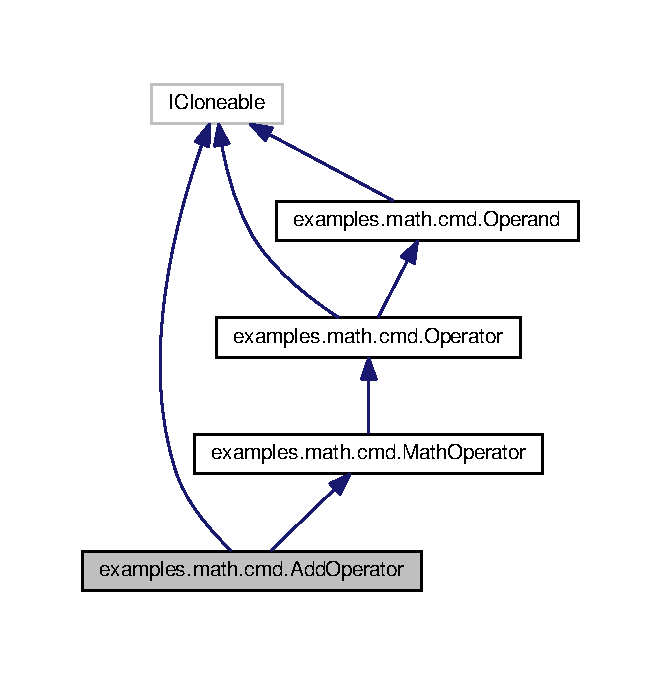
\includegraphics[width=317pt]{classexamples_1_1math_1_1cmd_1_1_add_operator__inherit__graph}
\end{center}
\end{figure}


Collaboration diagram for examples.\-math.\-cmd.\-Add\-Operator\-:
\nopagebreak
\begin{figure}[H]
\begin{center}
\leavevmode
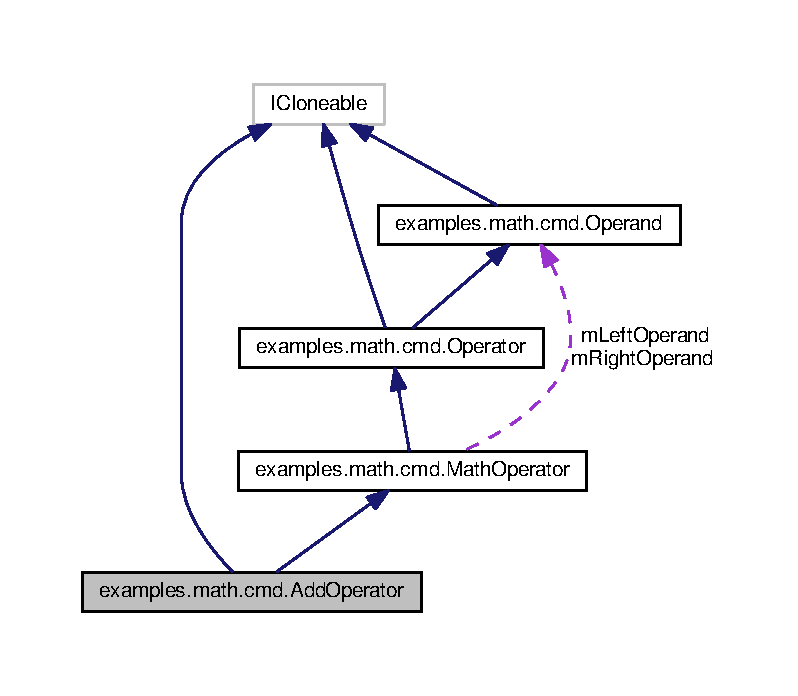
\includegraphics[width=350pt]{classexamples_1_1math_1_1cmd_1_1_add_operator__coll__graph}
\end{center}
\end{figure}
\subsection*{Public Member Functions}
\begin{DoxyCompactItemize}
\item 
\hyperlink{classexamples_1_1math_1_1cmd_1_1_add_operator_ae395d20680a564b727ec445affd1a5a9}{Add\-Operator} ()
\item 
\hyperlink{classexamples_1_1math_1_1cmd_1_1_add_operator_a4b61ad1ecfe81d39c6bf6205bacd9e21}{Add\-Operator} (\hyperlink{interfaceexamples_1_1math_1_1cmd_1_1_operand}{Operand} the\-Left, \hyperlink{interfaceexamples_1_1math_1_1cmd_1_1_operand}{Operand} the\-Right)
\item 
double \hyperlink{classexamples_1_1math_1_1cmd_1_1_add_operator_a2f5f91fe8ca269a76e26554ffb4795ae}{calcuate} ()
\item 
void \hyperlink{classexamples_1_1math_1_1cmd_1_1_add_operator_a1b760c381dd1a76188bbb61e0a92b0bc}{accept} (\hyperlink{interfaceexamples_1_1math_1_1_math_visitor}{Math\-Visitor} the\-Visitor)
\item 
Object \hyperlink{classexamples_1_1math_1_1cmd_1_1_add_operator_ad929bb2675ec30f20015f51c82f92569}{clone} ()
\end{DoxyCompactItemize}
\subsection*{Static Private Attributes}
\begin{DoxyCompactItemize}
\item 
static final String \hyperlink{classexamples_1_1math_1_1cmd_1_1_add_operator_a99850a210d2150a17fe5fd32e4bbc286}{C\-V\-S\-\_\-\-R\-E\-V\-I\-S\-I\-O\-N} = \char`\"{}\$Revision\-: 1.\-1 \$\char`\"{}
\end{DoxyCompactItemize}
\subsection*{Additional Inherited Members}


\subsection{Detailed Description}
The add operation.

\begin{DoxyAuthor}{Author}
Michael Grove 
\end{DoxyAuthor}
\begin{DoxySince}{Since}
3.\-4.\-2 
\end{DoxySince}


Definition at line 21 of file Add\-Operator.\-java.



\subsection{Constructor \& Destructor Documentation}
\hypertarget{classexamples_1_1math_1_1cmd_1_1_add_operator_ae395d20680a564b727ec445affd1a5a9}{\index{examples\-::math\-::cmd\-::\-Add\-Operator@{examples\-::math\-::cmd\-::\-Add\-Operator}!Add\-Operator@{Add\-Operator}}
\index{Add\-Operator@{Add\-Operator}!examples::math::cmd::AddOperator@{examples\-::math\-::cmd\-::\-Add\-Operator}}
\subsubsection[{Add\-Operator}]{\setlength{\rightskip}{0pt plus 5cm}examples.\-math.\-cmd.\-Add\-Operator.\-Add\-Operator (
\begin{DoxyParamCaption}
{}
\end{DoxyParamCaption}
)\hspace{0.3cm}{\ttfamily [inline]}}}\label{classexamples_1_1math_1_1cmd_1_1_add_operator_ae395d20680a564b727ec445affd1a5a9}


Definition at line 26 of file Add\-Operator.\-java.



Referenced by examples.\-math.\-cmd.\-Add\-Operator.\-clone().

\hypertarget{classexamples_1_1math_1_1cmd_1_1_add_operator_a4b61ad1ecfe81d39c6bf6205bacd9e21}{\index{examples\-::math\-::cmd\-::\-Add\-Operator@{examples\-::math\-::cmd\-::\-Add\-Operator}!Add\-Operator@{Add\-Operator}}
\index{Add\-Operator@{Add\-Operator}!examples::math::cmd::AddOperator@{examples\-::math\-::cmd\-::\-Add\-Operator}}
\subsubsection[{Add\-Operator}]{\setlength{\rightskip}{0pt plus 5cm}examples.\-math.\-cmd.\-Add\-Operator.\-Add\-Operator (
\begin{DoxyParamCaption}
\item[{{\bf Operand}}]{the\-Left, }
\item[{{\bf Operand}}]{the\-Right}
\end{DoxyParamCaption}
)\hspace{0.3cm}{\ttfamily [inline]}}}\label{classexamples_1_1math_1_1cmd_1_1_add_operator_a4b61ad1ecfe81d39c6bf6205bacd9e21}


Definition at line 30 of file Add\-Operator.\-java.



\subsection{Member Function Documentation}
\hypertarget{classexamples_1_1math_1_1cmd_1_1_add_operator_a1b760c381dd1a76188bbb61e0a92b0bc}{\index{examples\-::math\-::cmd\-::\-Add\-Operator@{examples\-::math\-::cmd\-::\-Add\-Operator}!accept@{accept}}
\index{accept@{accept}!examples::math::cmd::AddOperator@{examples\-::math\-::cmd\-::\-Add\-Operator}}
\subsubsection[{accept}]{\setlength{\rightskip}{0pt plus 5cm}void examples.\-math.\-cmd.\-Add\-Operator.\-accept (
\begin{DoxyParamCaption}
\item[{{\bf Math\-Visitor}}]{the\-Visitor}
\end{DoxyParamCaption}
)\hspace{0.3cm}{\ttfamily [inline]}}}\label{classexamples_1_1math_1_1cmd_1_1_add_operator_a1b760c381dd1a76188bbb61e0a92b0bc}


Implements \hyperlink{interfaceexamples_1_1math_1_1cmd_1_1_operand_aaadf6877856130d245dbb5a3a6993ef6}{examples.\-math.\-cmd.\-Operand}.



Definition at line 38 of file Add\-Operator.\-java.

\hypertarget{classexamples_1_1math_1_1cmd_1_1_add_operator_a2f5f91fe8ca269a76e26554ffb4795ae}{\index{examples\-::math\-::cmd\-::\-Add\-Operator@{examples\-::math\-::cmd\-::\-Add\-Operator}!calcuate@{calcuate}}
\index{calcuate@{calcuate}!examples::math::cmd::AddOperator@{examples\-::math\-::cmd\-::\-Add\-Operator}}
\subsubsection[{calcuate}]{\setlength{\rightskip}{0pt plus 5cm}double examples.\-math.\-cmd.\-Add\-Operator.\-calcuate (
\begin{DoxyParamCaption}
{}
\end{DoxyParamCaption}
)\hspace{0.3cm}{\ttfamily [inline]}}}\label{classexamples_1_1math_1_1cmd_1_1_add_operator_a2f5f91fe8ca269a76e26554ffb4795ae}


Implements \hyperlink{interfaceexamples_1_1math_1_1cmd_1_1_operator_a2498fd5b2a244bf2e63bc2613dc49e96}{examples.\-math.\-cmd.\-Operator}.



Definition at line 34 of file Add\-Operator.\-java.



References examples.\-math.\-cmd.\-Math\-Operator.\-get\-Left\-Operand(), and examples.\-math.\-cmd.\-Math\-Operator.\-get\-Right\-Operand().



Here is the call graph for this function\-:
\nopagebreak
\begin{figure}[H]
\begin{center}
\leavevmode
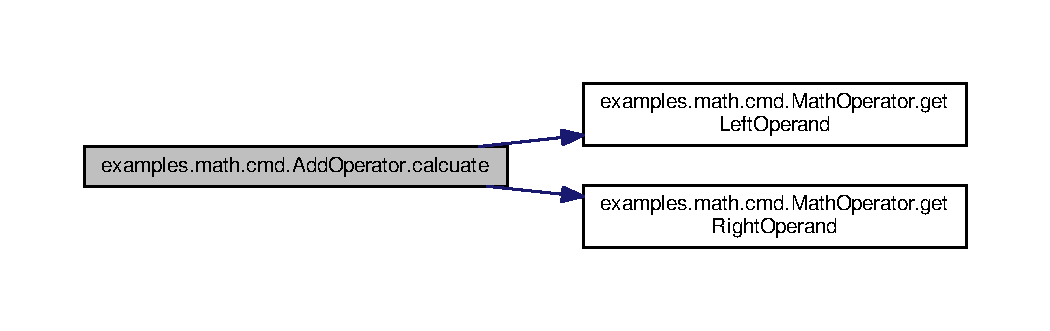
\includegraphics[width=350pt]{classexamples_1_1math_1_1cmd_1_1_add_operator_a2f5f91fe8ca269a76e26554ffb4795ae_cgraph}
\end{center}
\end{figure}


\hypertarget{classexamples_1_1math_1_1cmd_1_1_add_operator_ad929bb2675ec30f20015f51c82f92569}{\index{examples\-::math\-::cmd\-::\-Add\-Operator@{examples\-::math\-::cmd\-::\-Add\-Operator}!clone@{clone}}
\index{clone@{clone}!examples::math::cmd::AddOperator@{examples\-::math\-::cmd\-::\-Add\-Operator}}
\subsubsection[{clone}]{\setlength{\rightskip}{0pt plus 5cm}Object examples.\-math.\-cmd.\-Add\-Operator.\-clone (
\begin{DoxyParamCaption}
{}
\end{DoxyParamCaption}
)\hspace{0.3cm}{\ttfamily [inline]}, {\ttfamily [virtual]}}}\label{classexamples_1_1math_1_1cmd_1_1_add_operator_ad929bb2675ec30f20015f51c82f92569}


Implements \hyperlink{classexamples_1_1math_1_1cmd_1_1_math_operator_a06b476ba62c4b892c2689943a8beed81}{examples.\-math.\-cmd.\-Math\-Operator}.



Definition at line 42 of file Add\-Operator.\-java.



References examples.\-math.\-cmd.\-Add\-Operator.\-Add\-Operator().



Here is the call graph for this function\-:
\nopagebreak
\begin{figure}[H]
\begin{center}
\leavevmode
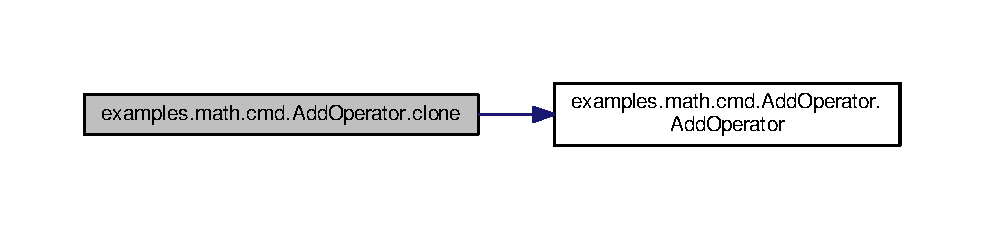
\includegraphics[width=350pt]{classexamples_1_1math_1_1cmd_1_1_add_operator_ad929bb2675ec30f20015f51c82f92569_cgraph}
\end{center}
\end{figure}




\subsection{Member Data Documentation}
\hypertarget{classexamples_1_1math_1_1cmd_1_1_add_operator_a99850a210d2150a17fe5fd32e4bbc286}{\index{examples\-::math\-::cmd\-::\-Add\-Operator@{examples\-::math\-::cmd\-::\-Add\-Operator}!C\-V\-S\-\_\-\-R\-E\-V\-I\-S\-I\-O\-N@{C\-V\-S\-\_\-\-R\-E\-V\-I\-S\-I\-O\-N}}
\index{C\-V\-S\-\_\-\-R\-E\-V\-I\-S\-I\-O\-N@{C\-V\-S\-\_\-\-R\-E\-V\-I\-S\-I\-O\-N}!examples::math::cmd::AddOperator@{examples\-::math\-::cmd\-::\-Add\-Operator}}
\subsubsection[{C\-V\-S\-\_\-\-R\-E\-V\-I\-S\-I\-O\-N}]{\setlength{\rightskip}{0pt plus 5cm}final String examples.\-math.\-cmd.\-Add\-Operator.\-C\-V\-S\-\_\-\-R\-E\-V\-I\-S\-I\-O\-N = \char`\"{}\$Revision\-: 1.\-1 \$\char`\"{}\hspace{0.3cm}{\ttfamily [static]}, {\ttfamily [private]}}}\label{classexamples_1_1math_1_1cmd_1_1_add_operator_a99850a210d2150a17fe5fd32e4bbc286}
String containing the C\-V\-S revision. Read out via reflection! 

Definition at line 24 of file Add\-Operator.\-java.



The documentation for this class was generated from the following file\-:\begin{DoxyCompactItemize}
\item 
L\-D\-H\-\_\-\-Git/examples/src/examples/math/cmd/\hyperlink{_add_operator_8java}{Add\-Operator.\-java}\end{DoxyCompactItemize}

\hypertarget{classorg_1_1jgap_1_1gp_1_1function_1_1_a_d_f}{\section{org.\-jgap.\-gp.\-function.\-A\-D\-F Class Reference}
\label{classorg_1_1jgap_1_1gp_1_1function_1_1_a_d_f}\index{org.\-jgap.\-gp.\-function.\-A\-D\-F@{org.\-jgap.\-gp.\-function.\-A\-D\-F}}
}


Inheritance diagram for org.\-jgap.\-gp.\-function.\-A\-D\-F\-:
\nopagebreak
\begin{figure}[H]
\begin{center}
\leavevmode
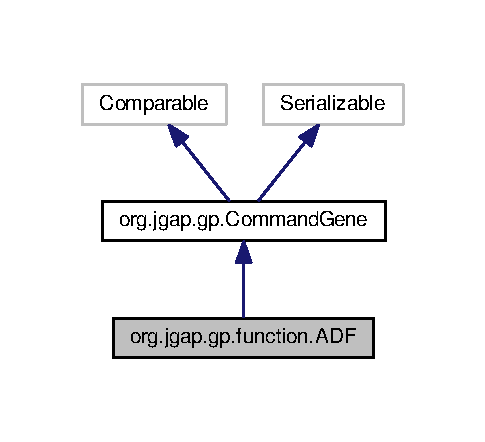
\includegraphics[width=233pt]{classorg_1_1jgap_1_1gp_1_1function_1_1_a_d_f__inherit__graph}
\end{center}
\end{figure}


Collaboration diagram for org.\-jgap.\-gp.\-function.\-A\-D\-F\-:
\nopagebreak
\begin{figure}[H]
\begin{center}
\leavevmode
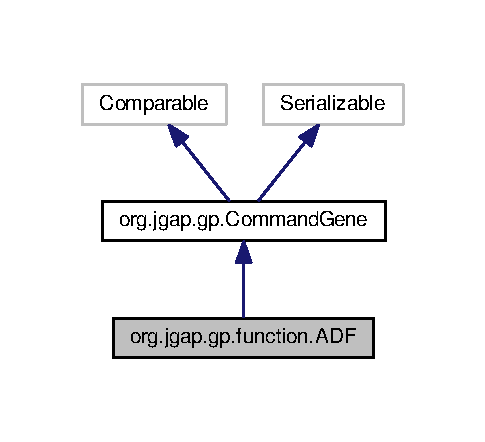
\includegraphics[width=233pt]{classorg_1_1jgap_1_1gp_1_1function_1_1_a_d_f__coll__graph}
\end{center}
\end{figure}
\subsection*{Public Member Functions}
\begin{DoxyCompactItemize}
\item 
\hyperlink{classorg_1_1jgap_1_1gp_1_1function_1_1_a_d_f_a847d2c99357b56047b13551abd009838}{A\-D\-F} (final G\-P\-Configuration a\-\_\-conf, int a\-\_\-chromosome\-Num, int a\-\_\-arity)  throws Invalid\-Configuration\-Exception 
\item 
int \hyperlink{classorg_1_1jgap_1_1gp_1_1function_1_1_a_d_f_ac4f7984d06634b4eda77c2dd8a3e8d2a}{get\-Chromosome\-Num} ()
\item 
String \hyperlink{classorg_1_1jgap_1_1gp_1_1function_1_1_a_d_f_a15d9b81c9ba10c9ba3c08eac71c85bcc}{to\-String} ()
\item 
int \hyperlink{classorg_1_1jgap_1_1gp_1_1function_1_1_a_d_f_aa9955babf21d5aba4be7326fd38b13d4}{get\-Arity} (\hyperlink{interfaceorg_1_1jgap_1_1gp_1_1_i_g_p_program}{I\-G\-P\-Program} a\-\_\-individual)
\item 
int \hyperlink{classorg_1_1jgap_1_1gp_1_1function_1_1_a_d_f_a0d037be27a91fd6c6aa37c4f9a8bfa21}{execute\-\_\-int} (Program\-Chromosome c, int n, Object\mbox{[}$\,$\mbox{]} args)
\item 
boolean \hyperlink{classorg_1_1jgap_1_1gp_1_1function_1_1_a_d_f_a9cdf0e931c26d5b3f4fb4d6c23363dbe}{execute\-\_\-boolean} (Program\-Chromosome c, int n, Object\mbox{[}$\,$\mbox{]} args)
\item 
float \hyperlink{classorg_1_1jgap_1_1gp_1_1function_1_1_a_d_f_af2fdf778c30d9645c686807989e5f1be}{execute\-\_\-float} (Program\-Chromosome c, int n, Object\mbox{[}$\,$\mbox{]} args)
\item 
double \hyperlink{classorg_1_1jgap_1_1gp_1_1function_1_1_a_d_f_a4a89b6b9b2ec1bcc037f3e566c627bf5}{execute\-\_\-double} (Program\-Chromosome c, int n, Object\mbox{[}$\,$\mbox{]} args)
\item 
Object \hyperlink{classorg_1_1jgap_1_1gp_1_1function_1_1_a_d_f_a5acdafb1afbe577cd690df67d319ed62}{execute\-\_\-object} (Program\-Chromosome c, int n, Object\mbox{[}$\,$\mbox{]} args)
\item 
Class \hyperlink{classorg_1_1jgap_1_1gp_1_1function_1_1_a_d_f_a055c28c2508cd2e55b2c13f045e1860f}{get\-Child\-Type} (\hyperlink{interfaceorg_1_1jgap_1_1gp_1_1_i_g_p_program}{I\-G\-P\-Program} a\-\_\-ind, int i)
\item 
boolean \hyperlink{classorg_1_1jgap_1_1gp_1_1function_1_1_a_d_f_a5e377b15d81ca7ceec156614480980d7}{is\-Valid} (Program\-Chromosome a\-\_\-chrom)
\item 
int \hyperlink{classorg_1_1jgap_1_1gp_1_1function_1_1_a_d_f_a8be802e15802a035a5e3b7ffdffa6956}{compare\-To} (Object a\-\_\-other)
\item 
boolean \hyperlink{classorg_1_1jgap_1_1gp_1_1function_1_1_a_d_f_ab0a98d44026a977f9bb0515c73fede00}{equals} (Object a\-\_\-other)
\end{DoxyCompactItemize}
\subsection*{Private Attributes}
\begin{DoxyCompactItemize}
\item 
int \hyperlink{classorg_1_1jgap_1_1gp_1_1function_1_1_a_d_f_a3d113b74e9c0e69bf6127e904de37766}{m\-\_\-chromosome\-Num}
\end{DoxyCompactItemize}
\subsection*{Static Private Attributes}
\begin{DoxyCompactItemize}
\item 
static final String \hyperlink{classorg_1_1jgap_1_1gp_1_1function_1_1_a_d_f_ada15fe1d91f5a31330979c9afc967ed2}{C\-V\-S\-\_\-\-R\-E\-V\-I\-S\-I\-O\-N} = \char`\"{}\$Revision\-: 1.\-19 \$\char`\"{}
\end{DoxyCompactItemize}
\subsection*{Additional Inherited Members}


\subsection{Detailed Description}
Automatically Defined Function (\hyperlink{classorg_1_1jgap_1_1gp_1_1function_1_1_a_d_f}{A\-D\-F}). Works with output of other chromosomes. An \hyperlink{classorg_1_1jgap_1_1gp_1_1function_1_1_a_d_f}{A\-D\-F} is automatically created by Program\-Chromosome. For more information about A\-D\-Fs see John Koza's book on Genetic Programming. \hyperlink{classorg_1_1jgap_1_1gp_1_1function_1_1_or}{Or} google for \char`\"{}\-Koza A\-D\-F\char`\"{}. For a German explanation, see see \href{http://www.tu-chemnitz.de/informatik/ThIS/seminare/ws01/gp/singer.pdf}{\tt http\-://www.\-tu-\/chemnitz.\-de/informatik/\-Th\-I\-S/seminare/ws01/gp/singer.\-pdf} or \href{http://www.tu-chemnitz.de/informatik/ThIS/seminare/ws01/gp/forbriger.pdf}{\tt http\-://www.\-tu-\/chemnitz.\-de/informatik/\-Th\-I\-S/seminare/ws01/gp/forbriger.\-pdf} or \href{http://www.klaus-meffert.de/download/genetische_programmierung_mit_java.pdf}{\tt http\-://www.\-klaus-\/meffert.\-de/download/genetische\-\_\-programmierung\-\_\-mit\-\_\-java.\-pdf}

\begin{DoxyAuthor}{Author}
Klaus Meffert 
\end{DoxyAuthor}
\begin{DoxySince}{Since}
3.\-0 
\end{DoxySince}


Definition at line 32 of file A\-D\-F.\-java.



\subsection{Constructor \& Destructor Documentation}
\hypertarget{classorg_1_1jgap_1_1gp_1_1function_1_1_a_d_f_a847d2c99357b56047b13551abd009838}{\index{org\-::jgap\-::gp\-::function\-::\-A\-D\-F@{org\-::jgap\-::gp\-::function\-::\-A\-D\-F}!A\-D\-F@{A\-D\-F}}
\index{A\-D\-F@{A\-D\-F}!org::jgap::gp::function::ADF@{org\-::jgap\-::gp\-::function\-::\-A\-D\-F}}
\subsubsection[{A\-D\-F}]{\setlength{\rightskip}{0pt plus 5cm}org.\-jgap.\-gp.\-function.\-A\-D\-F.\-A\-D\-F (
\begin{DoxyParamCaption}
\item[{final G\-P\-Configuration}]{a\-\_\-conf, }
\item[{int}]{a\-\_\-chromosome\-Num, }
\item[{int}]{a\-\_\-arity}
\end{DoxyParamCaption}
) throws {\bf Invalid\-Configuration\-Exception}\hspace{0.3cm}{\ttfamily [inline]}}}\label{classorg_1_1jgap_1_1gp_1_1function_1_1_a_d_f_a847d2c99357b56047b13551abd009838}
Constructor.


\begin{DoxyParams}{Parameters}
{\em a\-\_\-conf} & the configuration to use \\
\hline
{\em a\-\_\-chromosome\-Num} & the index of the chromosome to execute \\
\hline
{\em a\-\_\-arity} & the arity of the \hyperlink{classorg_1_1jgap_1_1gp_1_1function_1_1_a_d_f}{A\-D\-F}\\
\hline
\end{DoxyParams}

\begin{DoxyExceptions}{Exceptions}
{\em \hyperlink{classorg_1_1jgap_1_1_invalid_configuration_exception}{Invalid\-Configuration\-Exception}} & \\
\hline
\end{DoxyExceptions}
\begin{DoxyAuthor}{Author}
Klaus Meffert 
\end{DoxyAuthor}
\begin{DoxySince}{Since}
3.\-0 
\end{DoxySince}


Definition at line 53 of file A\-D\-F.\-java.



References org.\-jgap.\-gp.\-function.\-A\-D\-F.\-m\-\_\-chromosome\-Num.



Referenced by org.\-jgap.\-gp.\-function.\-A\-D\-F.\-compare\-To(), and org.\-jgap.\-gp.\-function.\-A\-D\-F.\-equals().



\subsection{Member Function Documentation}
\hypertarget{classorg_1_1jgap_1_1gp_1_1function_1_1_a_d_f_a8be802e15802a035a5e3b7ffdffa6956}{\index{org\-::jgap\-::gp\-::function\-::\-A\-D\-F@{org\-::jgap\-::gp\-::function\-::\-A\-D\-F}!compare\-To@{compare\-To}}
\index{compare\-To@{compare\-To}!org::jgap::gp::function::ADF@{org\-::jgap\-::gp\-::function\-::\-A\-D\-F}}
\subsubsection[{compare\-To}]{\setlength{\rightskip}{0pt plus 5cm}int org.\-jgap.\-gp.\-function.\-A\-D\-F.\-compare\-To (
\begin{DoxyParamCaption}
\item[{Object}]{a\-\_\-other}
\end{DoxyParamCaption}
)\hspace{0.3cm}{\ttfamily [inline]}}}\label{classorg_1_1jgap_1_1gp_1_1function_1_1_a_d_f_a8be802e15802a035a5e3b7ffdffa6956}
The compare\-To-\/method.


\begin{DoxyParams}{Parameters}
{\em a\-\_\-other} & the other object to compare \\
\hline
\end{DoxyParams}
\begin{DoxyReturn}{Returns}
-\/1, 0, 1
\end{DoxyReturn}
\begin{DoxyAuthor}{Author}
Klaus Meffert 
\end{DoxyAuthor}
\begin{DoxySince}{Since}
3.\-0 
\end{DoxySince}


Definition at line 164 of file A\-D\-F.\-java.



References org.\-jgap.\-gp.\-function.\-A\-D\-F.\-A\-D\-F(), and org.\-jgap.\-gp.\-function.\-A\-D\-F.\-m\-\_\-chromosome\-Num.



Here is the call graph for this function\-:
\nopagebreak
\begin{figure}[H]
\begin{center}
\leavevmode
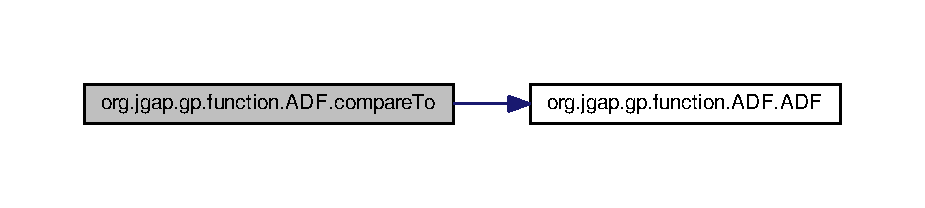
\includegraphics[width=350pt]{classorg_1_1jgap_1_1gp_1_1function_1_1_a_d_f_a8be802e15802a035a5e3b7ffdffa6956_cgraph}
\end{center}
\end{figure}


\hypertarget{classorg_1_1jgap_1_1gp_1_1function_1_1_a_d_f_ab0a98d44026a977f9bb0515c73fede00}{\index{org\-::jgap\-::gp\-::function\-::\-A\-D\-F@{org\-::jgap\-::gp\-::function\-::\-A\-D\-F}!equals@{equals}}
\index{equals@{equals}!org::jgap::gp::function::ADF@{org\-::jgap\-::gp\-::function\-::\-A\-D\-F}}
\subsubsection[{equals}]{\setlength{\rightskip}{0pt plus 5cm}boolean org.\-jgap.\-gp.\-function.\-A\-D\-F.\-equals (
\begin{DoxyParamCaption}
\item[{Object}]{a\-\_\-other}
\end{DoxyParamCaption}
)\hspace{0.3cm}{\ttfamily [inline]}}}\label{classorg_1_1jgap_1_1gp_1_1function_1_1_a_d_f_ab0a98d44026a977f9bb0515c73fede00}
The equals-\/method.


\begin{DoxyParams}{Parameters}
{\em a\-\_\-other} & the other object to compare \\
\hline
\end{DoxyParams}
\begin{DoxyReturn}{Returns}
true if the objects are seen as equal
\end{DoxyReturn}
\begin{DoxyAuthor}{Author}
Klaus Meffert 
\end{DoxyAuthor}
\begin{DoxySince}{Since}
3.\-0 
\end{DoxySince}


Definition at line 184 of file A\-D\-F.\-java.



References org.\-jgap.\-gp.\-function.\-A\-D\-F.\-A\-D\-F(), and org.\-jgap.\-gp.\-function.\-A\-D\-F.\-m\-\_\-chromosome\-Num.



Here is the call graph for this function\-:
\nopagebreak
\begin{figure}[H]
\begin{center}
\leavevmode
\includegraphics[width=350pt]{classorg_1_1jgap_1_1gp_1_1function_1_1_a_d_f_ab0a98d44026a977f9bb0515c73fede00_cgraph}
\end{center}
\end{figure}


\hypertarget{classorg_1_1jgap_1_1gp_1_1function_1_1_a_d_f_a9cdf0e931c26d5b3f4fb4d6c23363dbe}{\index{org\-::jgap\-::gp\-::function\-::\-A\-D\-F@{org\-::jgap\-::gp\-::function\-::\-A\-D\-F}!execute\-\_\-boolean@{execute\-\_\-boolean}}
\index{execute\-\_\-boolean@{execute\-\_\-boolean}!org::jgap::gp::function::ADF@{org\-::jgap\-::gp\-::function\-::\-A\-D\-F}}
\subsubsection[{execute\-\_\-boolean}]{\setlength{\rightskip}{0pt plus 5cm}boolean org.\-jgap.\-gp.\-function.\-A\-D\-F.\-execute\-\_\-boolean (
\begin{DoxyParamCaption}
\item[{Program\-Chromosome}]{c, }
\item[{int}]{n, }
\item[{Object\mbox{[}$\,$\mbox{]}}]{args}
\end{DoxyParamCaption}
)\hspace{0.3cm}{\ttfamily [inline]}}}\label{classorg_1_1jgap_1_1gp_1_1function_1_1_a_d_f_a9cdf0e931c26d5b3f4fb4d6c23363dbe}


Definition at line 101 of file A\-D\-F.\-java.



References org.\-jgap.\-gp.\-Command\-Gene.\-check(), and org.\-jgap.\-gp.\-function.\-A\-D\-F.\-m\-\_\-chromosome\-Num.



Here is the call graph for this function\-:
\nopagebreak
\begin{figure}[H]
\begin{center}
\leavevmode
\includegraphics[width=350pt]{classorg_1_1jgap_1_1gp_1_1function_1_1_a_d_f_a9cdf0e931c26d5b3f4fb4d6c23363dbe_cgraph}
\end{center}
\end{figure}


\hypertarget{classorg_1_1jgap_1_1gp_1_1function_1_1_a_d_f_a4a89b6b9b2ec1bcc037f3e566c627bf5}{\index{org\-::jgap\-::gp\-::function\-::\-A\-D\-F@{org\-::jgap\-::gp\-::function\-::\-A\-D\-F}!execute\-\_\-double@{execute\-\_\-double}}
\index{execute\-\_\-double@{execute\-\_\-double}!org::jgap::gp::function::ADF@{org\-::jgap\-::gp\-::function\-::\-A\-D\-F}}
\subsubsection[{execute\-\_\-double}]{\setlength{\rightskip}{0pt plus 5cm}double org.\-jgap.\-gp.\-function.\-A\-D\-F.\-execute\-\_\-double (
\begin{DoxyParamCaption}
\item[{Program\-Chromosome}]{c, }
\item[{int}]{n, }
\item[{Object\mbox{[}$\,$\mbox{]}}]{args}
\end{DoxyParamCaption}
)\hspace{0.3cm}{\ttfamily [inline]}}}\label{classorg_1_1jgap_1_1gp_1_1function_1_1_a_d_f_a4a89b6b9b2ec1bcc037f3e566c627bf5}


Definition at line 121 of file A\-D\-F.\-java.



References org.\-jgap.\-gp.\-Command\-Gene.\-check(), and org.\-jgap.\-gp.\-function.\-A\-D\-F.\-m\-\_\-chromosome\-Num.



Here is the call graph for this function\-:
\nopagebreak
\begin{figure}[H]
\begin{center}
\leavevmode
\includegraphics[width=350pt]{classorg_1_1jgap_1_1gp_1_1function_1_1_a_d_f_a4a89b6b9b2ec1bcc037f3e566c627bf5_cgraph}
\end{center}
\end{figure}


\hypertarget{classorg_1_1jgap_1_1gp_1_1function_1_1_a_d_f_af2fdf778c30d9645c686807989e5f1be}{\index{org\-::jgap\-::gp\-::function\-::\-A\-D\-F@{org\-::jgap\-::gp\-::function\-::\-A\-D\-F}!execute\-\_\-float@{execute\-\_\-float}}
\index{execute\-\_\-float@{execute\-\_\-float}!org::jgap::gp::function::ADF@{org\-::jgap\-::gp\-::function\-::\-A\-D\-F}}
\subsubsection[{execute\-\_\-float}]{\setlength{\rightskip}{0pt plus 5cm}float org.\-jgap.\-gp.\-function.\-A\-D\-F.\-execute\-\_\-float (
\begin{DoxyParamCaption}
\item[{Program\-Chromosome}]{c, }
\item[{int}]{n, }
\item[{Object\mbox{[}$\,$\mbox{]}}]{args}
\end{DoxyParamCaption}
)\hspace{0.3cm}{\ttfamily [inline]}}}\label{classorg_1_1jgap_1_1gp_1_1function_1_1_a_d_f_af2fdf778c30d9645c686807989e5f1be}


Definition at line 111 of file A\-D\-F.\-java.



References org.\-jgap.\-gp.\-Command\-Gene.\-check(), and org.\-jgap.\-gp.\-function.\-A\-D\-F.\-m\-\_\-chromosome\-Num.



Here is the call graph for this function\-:
\nopagebreak
\begin{figure}[H]
\begin{center}
\leavevmode
\includegraphics[width=350pt]{classorg_1_1jgap_1_1gp_1_1function_1_1_a_d_f_af2fdf778c30d9645c686807989e5f1be_cgraph}
\end{center}
\end{figure}


\hypertarget{classorg_1_1jgap_1_1gp_1_1function_1_1_a_d_f_a0d037be27a91fd6c6aa37c4f9a8bfa21}{\index{org\-::jgap\-::gp\-::function\-::\-A\-D\-F@{org\-::jgap\-::gp\-::function\-::\-A\-D\-F}!execute\-\_\-int@{execute\-\_\-int}}
\index{execute\-\_\-int@{execute\-\_\-int}!org::jgap::gp::function::ADF@{org\-::jgap\-::gp\-::function\-::\-A\-D\-F}}
\subsubsection[{execute\-\_\-int}]{\setlength{\rightskip}{0pt plus 5cm}int org.\-jgap.\-gp.\-function.\-A\-D\-F.\-execute\-\_\-int (
\begin{DoxyParamCaption}
\item[{Program\-Chromosome}]{c, }
\item[{int}]{n, }
\item[{Object\mbox{[}$\,$\mbox{]}}]{args}
\end{DoxyParamCaption}
)\hspace{0.3cm}{\ttfamily [inline]}}}\label{classorg_1_1jgap_1_1gp_1_1function_1_1_a_d_f_a0d037be27a91fd6c6aa37c4f9a8bfa21}


Definition at line 89 of file A\-D\-F.\-java.



References org.\-jgap.\-gp.\-Command\-Gene.\-check(), and org.\-jgap.\-gp.\-function.\-A\-D\-F.\-m\-\_\-chromosome\-Num.



Here is the call graph for this function\-:
\nopagebreak
\begin{figure}[H]
\begin{center}
\leavevmode
\includegraphics[width=350pt]{classorg_1_1jgap_1_1gp_1_1function_1_1_a_d_f_a0d037be27a91fd6c6aa37c4f9a8bfa21_cgraph}
\end{center}
\end{figure}


\hypertarget{classorg_1_1jgap_1_1gp_1_1function_1_1_a_d_f_a5acdafb1afbe577cd690df67d319ed62}{\index{org\-::jgap\-::gp\-::function\-::\-A\-D\-F@{org\-::jgap\-::gp\-::function\-::\-A\-D\-F}!execute\-\_\-object@{execute\-\_\-object}}
\index{execute\-\_\-object@{execute\-\_\-object}!org::jgap::gp::function::ADF@{org\-::jgap\-::gp\-::function\-::\-A\-D\-F}}
\subsubsection[{execute\-\_\-object}]{\setlength{\rightskip}{0pt plus 5cm}Object org.\-jgap.\-gp.\-function.\-A\-D\-F.\-execute\-\_\-object (
\begin{DoxyParamCaption}
\item[{Program\-Chromosome}]{c, }
\item[{int}]{n, }
\item[{Object\mbox{[}$\,$\mbox{]}}]{args}
\end{DoxyParamCaption}
)\hspace{0.3cm}{\ttfamily [inline]}}}\label{classorg_1_1jgap_1_1gp_1_1function_1_1_a_d_f_a5acdafb1afbe577cd690df67d319ed62}


Definition at line 131 of file A\-D\-F.\-java.



References org.\-jgap.\-gp.\-Command\-Gene.\-check(), and org.\-jgap.\-gp.\-function.\-A\-D\-F.\-m\-\_\-chromosome\-Num.



Here is the call graph for this function\-:
\nopagebreak
\begin{figure}[H]
\begin{center}
\leavevmode
\includegraphics[width=350pt]{classorg_1_1jgap_1_1gp_1_1function_1_1_a_d_f_a5acdafb1afbe577cd690df67d319ed62_cgraph}
\end{center}
\end{figure}


\hypertarget{classorg_1_1jgap_1_1gp_1_1function_1_1_a_d_f_aa9955babf21d5aba4be7326fd38b13d4}{\index{org\-::jgap\-::gp\-::function\-::\-A\-D\-F@{org\-::jgap\-::gp\-::function\-::\-A\-D\-F}!get\-Arity@{get\-Arity}}
\index{get\-Arity@{get\-Arity}!org::jgap::gp::function::ADF@{org\-::jgap\-::gp\-::function\-::\-A\-D\-F}}
\subsubsection[{get\-Arity}]{\setlength{\rightskip}{0pt plus 5cm}int org.\-jgap.\-gp.\-function.\-A\-D\-F.\-get\-Arity (
\begin{DoxyParamCaption}
\item[{{\bf I\-G\-P\-Program}}]{a\-\_\-individual}
\end{DoxyParamCaption}
)\hspace{0.3cm}{\ttfamily [inline]}}}\label{classorg_1_1jgap_1_1gp_1_1function_1_1_a_d_f_aa9955babf21d5aba4be7326fd38b13d4}


Definition at line 82 of file A\-D\-F.\-java.



References org.\-jgap.\-gp.\-function.\-A\-D\-F.\-m\-\_\-chromosome\-Num, and org.\-jgap.\-gp.\-I\-G\-P\-Program.\-size().



Here is the call graph for this function\-:
\nopagebreak
\begin{figure}[H]
\begin{center}
\leavevmode
\includegraphics[width=350pt]{classorg_1_1jgap_1_1gp_1_1function_1_1_a_d_f_aa9955babf21d5aba4be7326fd38b13d4_cgraph}
\end{center}
\end{figure}


\hypertarget{classorg_1_1jgap_1_1gp_1_1function_1_1_a_d_f_a055c28c2508cd2e55b2c13f045e1860f}{\index{org\-::jgap\-::gp\-::function\-::\-A\-D\-F@{org\-::jgap\-::gp\-::function\-::\-A\-D\-F}!get\-Child\-Type@{get\-Child\-Type}}
\index{get\-Child\-Type@{get\-Child\-Type}!org::jgap::gp::function::ADF@{org\-::jgap\-::gp\-::function\-::\-A\-D\-F}}
\subsubsection[{get\-Child\-Type}]{\setlength{\rightskip}{0pt plus 5cm}Class org.\-jgap.\-gp.\-function.\-A\-D\-F.\-get\-Child\-Type (
\begin{DoxyParamCaption}
\item[{{\bf I\-G\-P\-Program}}]{a\-\_\-ind, }
\item[{int}]{i}
\end{DoxyParamCaption}
)\hspace{0.3cm}{\ttfamily [inline]}}}\label{classorg_1_1jgap_1_1gp_1_1function_1_1_a_d_f_a055c28c2508cd2e55b2c13f045e1860f}


Definition at line 141 of file A\-D\-F.\-java.



References org.\-jgap.\-gp.\-function.\-A\-D\-F.\-m\-\_\-chromosome\-Num.

\hypertarget{classorg_1_1jgap_1_1gp_1_1function_1_1_a_d_f_ac4f7984d06634b4eda77c2dd8a3e8d2a}{\index{org\-::jgap\-::gp\-::function\-::\-A\-D\-F@{org\-::jgap\-::gp\-::function\-::\-A\-D\-F}!get\-Chromosome\-Num@{get\-Chromosome\-Num}}
\index{get\-Chromosome\-Num@{get\-Chromosome\-Num}!org::jgap::gp::function::ADF@{org\-::jgap\-::gp\-::function\-::\-A\-D\-F}}
\subsubsection[{get\-Chromosome\-Num}]{\setlength{\rightskip}{0pt plus 5cm}int org.\-jgap.\-gp.\-function.\-A\-D\-F.\-get\-Chromosome\-Num (
\begin{DoxyParamCaption}
{}
\end{DoxyParamCaption}
)\hspace{0.3cm}{\ttfamily [inline]}}}\label{classorg_1_1jgap_1_1gp_1_1function_1_1_a_d_f_ac4f7984d06634b4eda77c2dd8a3e8d2a}
\begin{DoxyReturn}{Returns}
the index of the chromosome to execute
\end{DoxyReturn}
\begin{DoxyAuthor}{Author}
Klaus Meffert 
\end{DoxyAuthor}
\begin{DoxySince}{Since}
3.\-0 
\end{DoxySince}


Definition at line 65 of file A\-D\-F.\-java.



References org.\-jgap.\-gp.\-function.\-A\-D\-F.\-m\-\_\-chromosome\-Num.

\hypertarget{classorg_1_1jgap_1_1gp_1_1function_1_1_a_d_f_a5e377b15d81ca7ceec156614480980d7}{\index{org\-::jgap\-::gp\-::function\-::\-A\-D\-F@{org\-::jgap\-::gp\-::function\-::\-A\-D\-F}!is\-Valid@{is\-Valid}}
\index{is\-Valid@{is\-Valid}!org::jgap::gp::function::ADF@{org\-::jgap\-::gp\-::function\-::\-A\-D\-F}}
\subsubsection[{is\-Valid}]{\setlength{\rightskip}{0pt plus 5cm}boolean org.\-jgap.\-gp.\-function.\-A\-D\-F.\-is\-Valid (
\begin{DoxyParamCaption}
\item[{Program\-Chromosome}]{a\-\_\-chrom}
\end{DoxyParamCaption}
)\hspace{0.3cm}{\ttfamily [inline]}}}\label{classorg_1_1jgap_1_1gp_1_1function_1_1_a_d_f_a5e377b15d81ca7ceec156614480980d7}
\begin{DoxyRefDesc}{Todo}
\item[\hyperlink{todo__todo000123}{Todo}]enhance \end{DoxyRefDesc}


Definition at line 145 of file A\-D\-F.\-java.

\hypertarget{classorg_1_1jgap_1_1gp_1_1function_1_1_a_d_f_a15d9b81c9ba10c9ba3c08eac71c85bcc}{\index{org\-::jgap\-::gp\-::function\-::\-A\-D\-F@{org\-::jgap\-::gp\-::function\-::\-A\-D\-F}!to\-String@{to\-String}}
\index{to\-String@{to\-String}!org::jgap::gp::function::ADF@{org\-::jgap\-::gp\-::function\-::\-A\-D\-F}}
\subsubsection[{to\-String}]{\setlength{\rightskip}{0pt plus 5cm}String org.\-jgap.\-gp.\-function.\-A\-D\-F.\-to\-String (
\begin{DoxyParamCaption}
{}
\end{DoxyParamCaption}
)\hspace{0.3cm}{\ttfamily [inline]}, {\ttfamily [virtual]}}}\label{classorg_1_1jgap_1_1gp_1_1function_1_1_a_d_f_a15d9b81c9ba10c9ba3c08eac71c85bcc}
\begin{DoxyReturn}{Returns}
the string representation of the command. Especially usefull to output a resulting formula in human-\/readable form. 
\end{DoxyReturn}


Implements \hyperlink{classorg_1_1jgap_1_1gp_1_1_command_gene_a236141d99059da808afe7a9217e411c7}{org.\-jgap.\-gp.\-Command\-Gene}.



Definition at line 69 of file A\-D\-F.\-java.



References org.\-jgap.\-gp.\-function.\-A\-D\-F.\-m\-\_\-chromosome\-Num, and org.\-jgap.\-gp.\-Command\-Gene.\-size().



Here is the call graph for this function\-:
\nopagebreak
\begin{figure}[H]
\begin{center}
\leavevmode
\includegraphics[width=350pt]{classorg_1_1jgap_1_1gp_1_1function_1_1_a_d_f_a15d9b81c9ba10c9ba3c08eac71c85bcc_cgraph}
\end{center}
\end{figure}




\subsection{Member Data Documentation}
\hypertarget{classorg_1_1jgap_1_1gp_1_1function_1_1_a_d_f_ada15fe1d91f5a31330979c9afc967ed2}{\index{org\-::jgap\-::gp\-::function\-::\-A\-D\-F@{org\-::jgap\-::gp\-::function\-::\-A\-D\-F}!C\-V\-S\-\_\-\-R\-E\-V\-I\-S\-I\-O\-N@{C\-V\-S\-\_\-\-R\-E\-V\-I\-S\-I\-O\-N}}
\index{C\-V\-S\-\_\-\-R\-E\-V\-I\-S\-I\-O\-N@{C\-V\-S\-\_\-\-R\-E\-V\-I\-S\-I\-O\-N}!org::jgap::gp::function::ADF@{org\-::jgap\-::gp\-::function\-::\-A\-D\-F}}
\subsubsection[{C\-V\-S\-\_\-\-R\-E\-V\-I\-S\-I\-O\-N}]{\setlength{\rightskip}{0pt plus 5cm}final String org.\-jgap.\-gp.\-function.\-A\-D\-F.\-C\-V\-S\-\_\-\-R\-E\-V\-I\-S\-I\-O\-N = \char`\"{}\$Revision\-: 1.\-19 \$\char`\"{}\hspace{0.3cm}{\ttfamily [static]}, {\ttfamily [private]}}}\label{classorg_1_1jgap_1_1gp_1_1function_1_1_a_d_f_ada15fe1d91f5a31330979c9afc967ed2}
String containing the C\-V\-S revision. Read out via reflection! 

Definition at line 37 of file A\-D\-F.\-java.

\hypertarget{classorg_1_1jgap_1_1gp_1_1function_1_1_a_d_f_a3d113b74e9c0e69bf6127e904de37766}{\index{org\-::jgap\-::gp\-::function\-::\-A\-D\-F@{org\-::jgap\-::gp\-::function\-::\-A\-D\-F}!m\-\_\-chromosome\-Num@{m\-\_\-chromosome\-Num}}
\index{m\-\_\-chromosome\-Num@{m\-\_\-chromosome\-Num}!org::jgap::gp::function::ADF@{org\-::jgap\-::gp\-::function\-::\-A\-D\-F}}
\subsubsection[{m\-\_\-chromosome\-Num}]{\setlength{\rightskip}{0pt plus 5cm}int org.\-jgap.\-gp.\-function.\-A\-D\-F.\-m\-\_\-chromosome\-Num\hspace{0.3cm}{\ttfamily [private]}}}\label{classorg_1_1jgap_1_1gp_1_1function_1_1_a_d_f_a3d113b74e9c0e69bf6127e904de37766}


Definition at line 39 of file A\-D\-F.\-java.



Referenced by org.\-jgap.\-gp.\-function.\-A\-D\-F.\-A\-D\-F(), org.\-jgap.\-gp.\-function.\-A\-D\-F.\-compare\-To(), org.\-jgap.\-gp.\-function.\-A\-D\-F.\-equals(), org.\-jgap.\-gp.\-function.\-A\-D\-F.\-execute\-\_\-boolean(), org.\-jgap.\-gp.\-function.\-A\-D\-F.\-execute\-\_\-double(), org.\-jgap.\-gp.\-function.\-A\-D\-F.\-execute\-\_\-float(), org.\-jgap.\-gp.\-function.\-A\-D\-F.\-execute\-\_\-int(), org.\-jgap.\-gp.\-function.\-A\-D\-F.\-execute\-\_\-object(), org.\-jgap.\-gp.\-function.\-A\-D\-F.\-get\-Arity(), org.\-jgap.\-gp.\-function.\-A\-D\-F.\-get\-Child\-Type(), org.\-jgap.\-gp.\-function.\-A\-D\-F.\-get\-Chromosome\-Num(), and org.\-jgap.\-gp.\-function.\-A\-D\-F.\-to\-String().



The documentation for this class was generated from the following file\-:\begin{DoxyCompactItemize}
\item 
L\-D\-H\-\_\-\-Git/src/org/jgap/gp/function/\hyperlink{_a_d_f_8java}{A\-D\-F.\-java}\end{DoxyCompactItemize}

\hypertarget{classorg_1_1jgap_1_1_natural_selector_1_1_age_fitness_value_comparator}{\section{org.\-jgap.\-Natural\-Selector.\-Age\-Fitness\-Value\-Comparator Class Reference}
\label{classorg_1_1jgap_1_1_natural_selector_1_1_age_fitness_value_comparator}\index{org.\-jgap.\-Natural\-Selector.\-Age\-Fitness\-Value\-Comparator@{org.\-jgap.\-Natural\-Selector.\-Age\-Fitness\-Value\-Comparator}}
}


Inheritance diagram for org.\-jgap.\-Natural\-Selector.\-Age\-Fitness\-Value\-Comparator\-:
\nopagebreak
\begin{figure}[H]
\begin{center}
\leavevmode
\includegraphics[width=270pt]{classorg_1_1jgap_1_1_natural_selector_1_1_age_fitness_value_comparator__inherit__graph}
\end{center}
\end{figure}


Collaboration diagram for org.\-jgap.\-Natural\-Selector.\-Age\-Fitness\-Value\-Comparator\-:
\nopagebreak
\begin{figure}[H]
\begin{center}
\leavevmode
\includegraphics[width=270pt]{classorg_1_1jgap_1_1_natural_selector_1_1_age_fitness_value_comparator__coll__graph}
\end{center}
\end{figure}
\subsection*{Public Member Functions}
\begin{DoxyCompactItemize}
\item 
int \hyperlink{classorg_1_1jgap_1_1_natural_selector_1_1_age_fitness_value_comparator_ab7093be07c8a2a64cfe5cfe0873e5075}{compare} (Object first, Object second)
\end{DoxyCompactItemize}


\subsection{Detailed Description}
Comparator regarding first the age (older is better), then the fitness value. Better results will be on top of the resulting sorted list.

\begin{DoxyAuthor}{Author}
Klaus Meffert 
\end{DoxyAuthor}
\begin{DoxySince}{Since}
3.\-3.\-3 
\end{DoxySince}


Definition at line 114 of file Natural\-Selector.\-java.



\subsection{Member Function Documentation}
\hypertarget{classorg_1_1jgap_1_1_natural_selector_1_1_age_fitness_value_comparator_ab7093be07c8a2a64cfe5cfe0873e5075}{\index{org\-::jgap\-::\-Natural\-Selector\-::\-Age\-Fitness\-Value\-Comparator@{org\-::jgap\-::\-Natural\-Selector\-::\-Age\-Fitness\-Value\-Comparator}!compare@{compare}}
\index{compare@{compare}!org::jgap::NaturalSelector::AgeFitnessValueComparator@{org\-::jgap\-::\-Natural\-Selector\-::\-Age\-Fitness\-Value\-Comparator}}
\subsubsection[{compare}]{\setlength{\rightskip}{0pt plus 5cm}int org.\-jgap.\-Natural\-Selector.\-Age\-Fitness\-Value\-Comparator.\-compare (
\begin{DoxyParamCaption}
\item[{Object}]{first, }
\item[{Object}]{second}
\end{DoxyParamCaption}
)\hspace{0.3cm}{\ttfamily [inline]}}}\label{classorg_1_1jgap_1_1_natural_selector_1_1_age_fitness_value_comparator_ab7093be07c8a2a64cfe5cfe0873e5075}


Definition at line 116 of file Natural\-Selector.\-java.



References org.\-jgap.\-I\-Chromosome.\-get\-Age(), and org.\-jgap.\-Natural\-Selector.\-get\-Configuration().



Here is the call graph for this function\-:
\nopagebreak
\begin{figure}[H]
\begin{center}
\leavevmode
\includegraphics[width=350pt]{classorg_1_1jgap_1_1_natural_selector_1_1_age_fitness_value_comparator_ab7093be07c8a2a64cfe5cfe0873e5075_cgraph}
\end{center}
\end{figure}




The documentation for this class was generated from the following file\-:\begin{DoxyCompactItemize}
\item 
L\-D\-H\-\_\-\-Git/src/org/jgap/\hyperlink{_natural_selector_8java}{Natural\-Selector.\-java}\end{DoxyCompactItemize}

\hypertarget{classorg_1_1jgap_1_1audit_1_1_all_audit_tests}{\section{org.\-jgap.\-audit.\-All\-Audit\-Tests Class Reference}
\label{classorg_1_1jgap_1_1audit_1_1_all_audit_tests}\index{org.\-jgap.\-audit.\-All\-Audit\-Tests@{org.\-jgap.\-audit.\-All\-Audit\-Tests}}
}


Inheritance diagram for org.\-jgap.\-audit.\-All\-Audit\-Tests\-:
\nopagebreak
\begin{figure}[H]
\begin{center}
\leavevmode
\includegraphics[width=216pt]{classorg_1_1jgap_1_1audit_1_1_all_audit_tests__inherit__graph}
\end{center}
\end{figure}


Collaboration diagram for org.\-jgap.\-audit.\-All\-Audit\-Tests\-:
\nopagebreak
\begin{figure}[H]
\begin{center}
\leavevmode
\includegraphics[width=216pt]{classorg_1_1jgap_1_1audit_1_1_all_audit_tests__coll__graph}
\end{center}
\end{figure}
\subsection*{Static Public Member Functions}
\begin{DoxyCompactItemize}
\item 
static Test \hyperlink{classorg_1_1jgap_1_1audit_1_1_all_audit_tests_aacbe901447ee5930c8737397bbf13c46}{suite} ()
\end{DoxyCompactItemize}
\subsection*{Static Private Attributes}
\begin{DoxyCompactItemize}
\item 
static final String \hyperlink{classorg_1_1jgap_1_1audit_1_1_all_audit_tests_abe8ff0abc5c0e05a3213026eb5ba7ad7}{C\-V\-S\-\_\-\-R\-E\-V\-I\-S\-I\-O\-N} = \char`\"{}\$Revision\-: 1.\-5 \$\char`\"{}
\end{DoxyCompactItemize}


\subsection{Detailed Description}
Test suite for all tests of package \hyperlink{namespaceorg_1_1jgap_1_1distr}{org.\-jgap.\-distr}

\begin{DoxyAuthor}{Author}
Klaus Meffert 
\end{DoxyAuthor}
\begin{DoxySince}{Since}
1.\-0 
\end{DoxySince}


Definition at line 20 of file All\-Audit\-Tests.\-java.



\subsection{Member Function Documentation}
\hypertarget{classorg_1_1jgap_1_1audit_1_1_all_audit_tests_aacbe901447ee5930c8737397bbf13c46}{\index{org\-::jgap\-::audit\-::\-All\-Audit\-Tests@{org\-::jgap\-::audit\-::\-All\-Audit\-Tests}!suite@{suite}}
\index{suite@{suite}!org::jgap::audit::AllAuditTests@{org\-::jgap\-::audit\-::\-All\-Audit\-Tests}}
\subsubsection[{suite}]{\setlength{\rightskip}{0pt plus 5cm}static Test org.\-jgap.\-audit.\-All\-Audit\-Tests.\-suite (
\begin{DoxyParamCaption}
{}
\end{DoxyParamCaption}
)\hspace{0.3cm}{\ttfamily [inline]}, {\ttfamily [static]}}}\label{classorg_1_1jgap_1_1audit_1_1_all_audit_tests_aacbe901447ee5930c8737397bbf13c46}


Definition at line 25 of file All\-Audit\-Tests.\-java.



\subsection{Member Data Documentation}
\hypertarget{classorg_1_1jgap_1_1audit_1_1_all_audit_tests_abe8ff0abc5c0e05a3213026eb5ba7ad7}{\index{org\-::jgap\-::audit\-::\-All\-Audit\-Tests@{org\-::jgap\-::audit\-::\-All\-Audit\-Tests}!C\-V\-S\-\_\-\-R\-E\-V\-I\-S\-I\-O\-N@{C\-V\-S\-\_\-\-R\-E\-V\-I\-S\-I\-O\-N}}
\index{C\-V\-S\-\_\-\-R\-E\-V\-I\-S\-I\-O\-N@{C\-V\-S\-\_\-\-R\-E\-V\-I\-S\-I\-O\-N}!org::jgap::audit::AllAuditTests@{org\-::jgap\-::audit\-::\-All\-Audit\-Tests}}
\subsubsection[{C\-V\-S\-\_\-\-R\-E\-V\-I\-S\-I\-O\-N}]{\setlength{\rightskip}{0pt plus 5cm}final String org.\-jgap.\-audit.\-All\-Audit\-Tests.\-C\-V\-S\-\_\-\-R\-E\-V\-I\-S\-I\-O\-N = \char`\"{}\$Revision\-: 1.\-5 \$\char`\"{}\hspace{0.3cm}{\ttfamily [static]}, {\ttfamily [private]}}}\label{classorg_1_1jgap_1_1audit_1_1_all_audit_tests_abe8ff0abc5c0e05a3213026eb5ba7ad7}
String containing the C\-V\-S revision. Read out via reflection! 

Definition at line 23 of file All\-Audit\-Tests.\-java.



The documentation for this class was generated from the following file\-:\begin{DoxyCompactItemize}
\item 
L\-D\-H\-\_\-\-Git/tests/org/jgap/audit/\hyperlink{_all_audit_tests_8java}{All\-Audit\-Tests.\-java}\end{DoxyCompactItemize}

\hypertarget{classorg_1_1jgap_1_1_all_base_tests}{\section{org.\-jgap.\-All\-Base\-Tests Class Reference}
\label{classorg_1_1jgap_1_1_all_base_tests}\index{org.\-jgap.\-All\-Base\-Tests@{org.\-jgap.\-All\-Base\-Tests}}
}


Inheritance diagram for org.\-jgap.\-All\-Base\-Tests\-:
\nopagebreak
\begin{figure}[H]
\begin{center}
\leavevmode
\includegraphics[width=192pt]{classorg_1_1jgap_1_1_all_base_tests__inherit__graph}
\end{center}
\end{figure}


Collaboration diagram for org.\-jgap.\-All\-Base\-Tests\-:
\nopagebreak
\begin{figure}[H]
\begin{center}
\leavevmode
\includegraphics[width=192pt]{classorg_1_1jgap_1_1_all_base_tests__coll__graph}
\end{center}
\end{figure}
\subsection*{Static Public Member Functions}
\begin{DoxyCompactItemize}
\item 
static Test \hyperlink{classorg_1_1jgap_1_1_all_base_tests_aa766e11a49fe2d92a87cf5268454369b}{suite} ()
\end{DoxyCompactItemize}
\subsection*{Static Private Attributes}
\begin{DoxyCompactItemize}
\item 
static final String \hyperlink{classorg_1_1jgap_1_1_all_base_tests_a5d5461b55484bbb0856445ccfed441fa}{C\-V\-S\-\_\-\-R\-E\-V\-I\-S\-I\-O\-N} = \char`\"{}\$Revision\-: 1.\-12 \$\char`\"{}
\end{DoxyCompactItemize}


\subsection{Detailed Description}
Test suite for all tests of package \hyperlink{namespaceorg_1_1jgap}{org.\-jgap}.

\begin{DoxyAuthor}{Author}
Klaus Meffert 
\end{DoxyAuthor}
\begin{DoxySince}{Since}
1.\-1 
\end{DoxySince}


Definition at line 20 of file All\-Base\-Tests.\-java.



\subsection{Member Function Documentation}
\hypertarget{classorg_1_1jgap_1_1_all_base_tests_aa766e11a49fe2d92a87cf5268454369b}{\index{org\-::jgap\-::\-All\-Base\-Tests@{org\-::jgap\-::\-All\-Base\-Tests}!suite@{suite}}
\index{suite@{suite}!org::jgap::AllBaseTests@{org\-::jgap\-::\-All\-Base\-Tests}}
\subsubsection[{suite}]{\setlength{\rightskip}{0pt plus 5cm}static Test org.\-jgap.\-All\-Base\-Tests.\-suite (
\begin{DoxyParamCaption}
{}
\end{DoxyParamCaption}
)\hspace{0.3cm}{\ttfamily [inline]}, {\ttfamily [static]}}}\label{classorg_1_1jgap_1_1_all_base_tests_aa766e11a49fe2d92a87cf5268454369b}


Definition at line 26 of file All\-Base\-Tests.\-java.



\subsection{Member Data Documentation}
\hypertarget{classorg_1_1jgap_1_1_all_base_tests_a5d5461b55484bbb0856445ccfed441fa}{\index{org\-::jgap\-::\-All\-Base\-Tests@{org\-::jgap\-::\-All\-Base\-Tests}!C\-V\-S\-\_\-\-R\-E\-V\-I\-S\-I\-O\-N@{C\-V\-S\-\_\-\-R\-E\-V\-I\-S\-I\-O\-N}}
\index{C\-V\-S\-\_\-\-R\-E\-V\-I\-S\-I\-O\-N@{C\-V\-S\-\_\-\-R\-E\-V\-I\-S\-I\-O\-N}!org::jgap::AllBaseTests@{org\-::jgap\-::\-All\-Base\-Tests}}
\subsubsection[{C\-V\-S\-\_\-\-R\-E\-V\-I\-S\-I\-O\-N}]{\setlength{\rightskip}{0pt plus 5cm}final String org.\-jgap.\-All\-Base\-Tests.\-C\-V\-S\-\_\-\-R\-E\-V\-I\-S\-I\-O\-N = \char`\"{}\$Revision\-: 1.\-12 \$\char`\"{}\hspace{0.3cm}{\ttfamily [static]}, {\ttfamily [private]}}}\label{classorg_1_1jgap_1_1_all_base_tests_a5d5461b55484bbb0856445ccfed441fa}
String containing the C\-V\-S revision. Read out via reflection! 

Definition at line 24 of file All\-Base\-Tests.\-java.



The documentation for this class was generated from the following file\-:\begin{DoxyCompactItemize}
\item 
L\-D\-H\-\_\-\-Git/tests/org/jgap/\hyperlink{_all_base_tests_8java}{All\-Base\-Tests.\-java}\end{DoxyCompactItemize}

\hypertarget{classorg_1_1jgap_1_1data_1_1config_1_1_all_config_tests}{\section{org.\-jgap.\-data.\-config.\-All\-Config\-Tests Class Reference}
\label{classorg_1_1jgap_1_1data_1_1config_1_1_all_config_tests}\index{org.\-jgap.\-data.\-config.\-All\-Config\-Tests@{org.\-jgap.\-data.\-config.\-All\-Config\-Tests}}
}


Inheritance diagram for org.\-jgap.\-data.\-config.\-All\-Config\-Tests\-:
\nopagebreak
\begin{figure}[H]
\begin{center}
\leavevmode
\includegraphics[width=194pt]{classorg_1_1jgap_1_1data_1_1config_1_1_all_config_tests__inherit__graph}
\end{center}
\end{figure}


Collaboration diagram for org.\-jgap.\-data.\-config.\-All\-Config\-Tests\-:
\nopagebreak
\begin{figure}[H]
\begin{center}
\leavevmode
\includegraphics[width=194pt]{classorg_1_1jgap_1_1data_1_1config_1_1_all_config_tests__coll__graph}
\end{center}
\end{figure}
\subsection*{Static Public Member Functions}
\begin{DoxyCompactItemize}
\item 
static Test \hyperlink{classorg_1_1jgap_1_1data_1_1config_1_1_all_config_tests_a85dbfa5c5871e8bc9ec4af88af2b0702}{suite} ()
\end{DoxyCompactItemize}
\subsection*{Static Private Attributes}
\begin{DoxyCompactItemize}
\item 
static final String \hyperlink{classorg_1_1jgap_1_1data_1_1config_1_1_all_config_tests_ac8513abe695046e34b415153b4b8a2f2}{C\-V\-S\-\_\-\-R\-E\-V\-I\-S\-I\-O\-N} = \char`\"{}\$Revision\-: 1.\-3 \$\char`\"{}
\end{DoxyCompactItemize}


\subsection{Detailed Description}
Test suite for all tests of package \hyperlink{namespaceorg_1_1jgap_1_1data_1_1config}{org.\-jgap.\-data.\-config}

\begin{DoxyAuthor}{Author}
Klaus Meffert 
\end{DoxyAuthor}
\begin{DoxySince}{Since}
3.\-0 
\end{DoxySince}


Definition at line 20 of file All\-Config\-Tests.\-java.



\subsection{Member Function Documentation}
\hypertarget{classorg_1_1jgap_1_1data_1_1config_1_1_all_config_tests_a85dbfa5c5871e8bc9ec4af88af2b0702}{\index{org\-::jgap\-::data\-::config\-::\-All\-Config\-Tests@{org\-::jgap\-::data\-::config\-::\-All\-Config\-Tests}!suite@{suite}}
\index{suite@{suite}!org::jgap::data::config::AllConfigTests@{org\-::jgap\-::data\-::config\-::\-All\-Config\-Tests}}
\subsubsection[{suite}]{\setlength{\rightskip}{0pt plus 5cm}static Test org.\-jgap.\-data.\-config.\-All\-Config\-Tests.\-suite (
\begin{DoxyParamCaption}
{}
\end{DoxyParamCaption}
)\hspace{0.3cm}{\ttfamily [inline]}, {\ttfamily [static]}}}\label{classorg_1_1jgap_1_1data_1_1config_1_1_all_config_tests_a85dbfa5c5871e8bc9ec4af88af2b0702}


Definition at line 26 of file All\-Config\-Tests.\-java.



\subsection{Member Data Documentation}
\hypertarget{classorg_1_1jgap_1_1data_1_1config_1_1_all_config_tests_ac8513abe695046e34b415153b4b8a2f2}{\index{org\-::jgap\-::data\-::config\-::\-All\-Config\-Tests@{org\-::jgap\-::data\-::config\-::\-All\-Config\-Tests}!C\-V\-S\-\_\-\-R\-E\-V\-I\-S\-I\-O\-N@{C\-V\-S\-\_\-\-R\-E\-V\-I\-S\-I\-O\-N}}
\index{C\-V\-S\-\_\-\-R\-E\-V\-I\-S\-I\-O\-N@{C\-V\-S\-\_\-\-R\-E\-V\-I\-S\-I\-O\-N}!org::jgap::data::config::AllConfigTests@{org\-::jgap\-::data\-::config\-::\-All\-Config\-Tests}}
\subsubsection[{C\-V\-S\-\_\-\-R\-E\-V\-I\-S\-I\-O\-N}]{\setlength{\rightskip}{0pt plus 5cm}final String org.\-jgap.\-data.\-config.\-All\-Config\-Tests.\-C\-V\-S\-\_\-\-R\-E\-V\-I\-S\-I\-O\-N = \char`\"{}\$Revision\-: 1.\-3 \$\char`\"{}\hspace{0.3cm}{\ttfamily [static]}, {\ttfamily [private]}}}\label{classorg_1_1jgap_1_1data_1_1config_1_1_all_config_tests_ac8513abe695046e34b415153b4b8a2f2}
String containing the C\-V\-S revision. Read out via reflection! 

Definition at line 24 of file All\-Config\-Tests.\-java.



The documentation for this class was generated from the following file\-:\begin{DoxyCompactItemize}
\item 
L\-D\-H\-\_\-\-Git/tests/org/jgap/data/config/\hyperlink{_all_config_tests_8java}{All\-Config\-Tests.\-java}\end{DoxyCompactItemize}

\hypertarget{classorg_1_1jgap_1_1data_1_1_all_data_tests}{\section{org.\-jgap.\-data.\-All\-Data\-Tests Class Reference}
\label{classorg_1_1jgap_1_1data_1_1_all_data_tests}\index{org.\-jgap.\-data.\-All\-Data\-Tests@{org.\-jgap.\-data.\-All\-Data\-Tests}}
}


Inheritance diagram for org.\-jgap.\-data.\-All\-Data\-Tests\-:
\nopagebreak
\begin{figure}[H]
\begin{center}
\leavevmode
\includegraphics[width=212pt]{classorg_1_1jgap_1_1data_1_1_all_data_tests__inherit__graph}
\end{center}
\end{figure}


Collaboration diagram for org.\-jgap.\-data.\-All\-Data\-Tests\-:
\nopagebreak
\begin{figure}[H]
\begin{center}
\leavevmode
\includegraphics[width=212pt]{classorg_1_1jgap_1_1data_1_1_all_data_tests__coll__graph}
\end{center}
\end{figure}
\subsection*{Static Public Member Functions}
\begin{DoxyCompactItemize}
\item 
static Test \hyperlink{classorg_1_1jgap_1_1data_1_1_all_data_tests_abd2ce9315a6850e1bb3c85a03142e591}{suite} ()
\end{DoxyCompactItemize}
\subsection*{Static Private Attributes}
\begin{DoxyCompactItemize}
\item 
static final String \hyperlink{classorg_1_1jgap_1_1data_1_1_all_data_tests_a743fe7ce2cd1b103cb2f1a693f883a29}{C\-V\-S\-\_\-\-R\-E\-V\-I\-S\-I\-O\-N} = \char`\"{}\$Revision\-: 1.\-8 \$\char`\"{}
\end{DoxyCompactItemize}


\subsection{Detailed Description}
Test suite for all tests of package \hyperlink{namespaceorg_1_1jgap_1_1data}{org.\-jgap.\-data}

\begin{DoxyAuthor}{Author}
Klaus Meffert 
\end{DoxyAuthor}
\begin{DoxySince}{Since}
1.\-0 
\end{DoxySince}


Definition at line 21 of file All\-Data\-Tests.\-java.



\subsection{Member Function Documentation}
\hypertarget{classorg_1_1jgap_1_1data_1_1_all_data_tests_abd2ce9315a6850e1bb3c85a03142e591}{\index{org\-::jgap\-::data\-::\-All\-Data\-Tests@{org\-::jgap\-::data\-::\-All\-Data\-Tests}!suite@{suite}}
\index{suite@{suite}!org::jgap::data::AllDataTests@{org\-::jgap\-::data\-::\-All\-Data\-Tests}}
\subsubsection[{suite}]{\setlength{\rightskip}{0pt plus 5cm}static Test org.\-jgap.\-data.\-All\-Data\-Tests.\-suite (
\begin{DoxyParamCaption}
{}
\end{DoxyParamCaption}
)\hspace{0.3cm}{\ttfamily [inline]}, {\ttfamily [static]}}}\label{classorg_1_1jgap_1_1data_1_1_all_data_tests_abd2ce9315a6850e1bb3c85a03142e591}


Definition at line 27 of file All\-Data\-Tests.\-java.



\subsection{Member Data Documentation}
\hypertarget{classorg_1_1jgap_1_1data_1_1_all_data_tests_a743fe7ce2cd1b103cb2f1a693f883a29}{\index{org\-::jgap\-::data\-::\-All\-Data\-Tests@{org\-::jgap\-::data\-::\-All\-Data\-Tests}!C\-V\-S\-\_\-\-R\-E\-V\-I\-S\-I\-O\-N@{C\-V\-S\-\_\-\-R\-E\-V\-I\-S\-I\-O\-N}}
\index{C\-V\-S\-\_\-\-R\-E\-V\-I\-S\-I\-O\-N@{C\-V\-S\-\_\-\-R\-E\-V\-I\-S\-I\-O\-N}!org::jgap::data::AllDataTests@{org\-::jgap\-::data\-::\-All\-Data\-Tests}}
\subsubsection[{C\-V\-S\-\_\-\-R\-E\-V\-I\-S\-I\-O\-N}]{\setlength{\rightskip}{0pt plus 5cm}final String org.\-jgap.\-data.\-All\-Data\-Tests.\-C\-V\-S\-\_\-\-R\-E\-V\-I\-S\-I\-O\-N = \char`\"{}\$Revision\-: 1.\-8 \$\char`\"{}\hspace{0.3cm}{\ttfamily [static]}, {\ttfamily [private]}}}\label{classorg_1_1jgap_1_1data_1_1_all_data_tests_a743fe7ce2cd1b103cb2f1a693f883a29}
String containing the C\-V\-S revision. Read out via reflection! 

Definition at line 25 of file All\-Data\-Tests.\-java.



The documentation for this class was generated from the following file\-:\begin{DoxyCompactItemize}
\item 
L\-D\-H\-\_\-\-Git/tests/org/jgap/data/\hyperlink{_all_data_tests_8java}{All\-Data\-Tests.\-java}\end{DoxyCompactItemize}

\hypertarget{classorg_1_1jgap_1_1distr_1_1_all_distr_tests}{\section{org.\-jgap.\-distr.\-All\-Distr\-Tests Class Reference}
\label{classorg_1_1jgap_1_1distr_1_1_all_distr_tests}\index{org.\-jgap.\-distr.\-All\-Distr\-Tests@{org.\-jgap.\-distr.\-All\-Distr\-Tests}}
}


Inheritance diagram for org.\-jgap.\-distr.\-All\-Distr\-Tests\-:
\nopagebreak
\begin{figure}[H]
\begin{center}
\leavevmode
\includegraphics[width=212pt]{classorg_1_1jgap_1_1distr_1_1_all_distr_tests__inherit__graph}
\end{center}
\end{figure}


Collaboration diagram for org.\-jgap.\-distr.\-All\-Distr\-Tests\-:
\nopagebreak
\begin{figure}[H]
\begin{center}
\leavevmode
\includegraphics[width=212pt]{classorg_1_1jgap_1_1distr_1_1_all_distr_tests__coll__graph}
\end{center}
\end{figure}
\subsection*{Static Public Member Functions}
\begin{DoxyCompactItemize}
\item 
static Test \hyperlink{classorg_1_1jgap_1_1distr_1_1_all_distr_tests_a38f6a214902fa0a231b35e67631c477a}{suite} ()
\end{DoxyCompactItemize}
\subsection*{Static Private Attributes}
\begin{DoxyCompactItemize}
\item 
static final String \hyperlink{classorg_1_1jgap_1_1distr_1_1_all_distr_tests_a6d3745acb67e8ae9882207c983d556dd}{C\-V\-S\-\_\-\-R\-E\-V\-I\-S\-I\-O\-N} = \char`\"{}\$Revision\-: 1.\-9 \$\char`\"{}
\end{DoxyCompactItemize}


\subsection{Detailed Description}
Test suite for all tests of package \hyperlink{namespaceorg_1_1jgap_1_1distr}{org.\-jgap.\-distr}.

\begin{DoxyAuthor}{Author}
Klaus Meffert 
\end{DoxyAuthor}
\begin{DoxySince}{Since}
1.\-0 
\end{DoxySince}


Definition at line 21 of file All\-Distr\-Tests.\-java.



\subsection{Member Function Documentation}
\hypertarget{classorg_1_1jgap_1_1distr_1_1_all_distr_tests_a38f6a214902fa0a231b35e67631c477a}{\index{org\-::jgap\-::distr\-::\-All\-Distr\-Tests@{org\-::jgap\-::distr\-::\-All\-Distr\-Tests}!suite@{suite}}
\index{suite@{suite}!org::jgap::distr::AllDistrTests@{org\-::jgap\-::distr\-::\-All\-Distr\-Tests}}
\subsubsection[{suite}]{\setlength{\rightskip}{0pt plus 5cm}static Test org.\-jgap.\-distr.\-All\-Distr\-Tests.\-suite (
\begin{DoxyParamCaption}
{}
\end{DoxyParamCaption}
)\hspace{0.3cm}{\ttfamily [inline]}, {\ttfamily [static]}}}\label{classorg_1_1jgap_1_1distr_1_1_all_distr_tests_a38f6a214902fa0a231b35e67631c477a}


Definition at line 26 of file All\-Distr\-Tests.\-java.



\subsection{Member Data Documentation}
\hypertarget{classorg_1_1jgap_1_1distr_1_1_all_distr_tests_a6d3745acb67e8ae9882207c983d556dd}{\index{org\-::jgap\-::distr\-::\-All\-Distr\-Tests@{org\-::jgap\-::distr\-::\-All\-Distr\-Tests}!C\-V\-S\-\_\-\-R\-E\-V\-I\-S\-I\-O\-N@{C\-V\-S\-\_\-\-R\-E\-V\-I\-S\-I\-O\-N}}
\index{C\-V\-S\-\_\-\-R\-E\-V\-I\-S\-I\-O\-N@{C\-V\-S\-\_\-\-R\-E\-V\-I\-S\-I\-O\-N}!org::jgap::distr::AllDistrTests@{org\-::jgap\-::distr\-::\-All\-Distr\-Tests}}
\subsubsection[{C\-V\-S\-\_\-\-R\-E\-V\-I\-S\-I\-O\-N}]{\setlength{\rightskip}{0pt plus 5cm}final String org.\-jgap.\-distr.\-All\-Distr\-Tests.\-C\-V\-S\-\_\-\-R\-E\-V\-I\-S\-I\-O\-N = \char`\"{}\$Revision\-: 1.\-9 \$\char`\"{}\hspace{0.3cm}{\ttfamily [static]}, {\ttfamily [private]}}}\label{classorg_1_1jgap_1_1distr_1_1_all_distr_tests_a6d3745acb67e8ae9882207c983d556dd}
String containing the C\-V\-S revision. Read out via reflection! 

Definition at line 24 of file All\-Distr\-Tests.\-java.



The documentation for this class was generated from the following file\-:\begin{DoxyCompactItemize}
\item 
L\-D\-H\-\_\-\-Git/tests/org/jgap/distr/\hyperlink{_all_distr_tests_8java}{All\-Distr\-Tests.\-java}\end{DoxyCompactItemize}

\hypertarget{classorg_1_1jgap_1_1eval_1_1_all_eval_tests}{\section{org.\-jgap.\-eval.\-All\-Eval\-Tests Class Reference}
\label{classorg_1_1jgap_1_1eval_1_1_all_eval_tests}\index{org.\-jgap.\-eval.\-All\-Eval\-Tests@{org.\-jgap.\-eval.\-All\-Eval\-Tests}}
}


Inheritance diagram for org.\-jgap.\-eval.\-All\-Eval\-Tests\-:
\nopagebreak
\begin{figure}[H]
\begin{center}
\leavevmode
\includegraphics[width=210pt]{classorg_1_1jgap_1_1eval_1_1_all_eval_tests__inherit__graph}
\end{center}
\end{figure}


Collaboration diagram for org.\-jgap.\-eval.\-All\-Eval\-Tests\-:
\nopagebreak
\begin{figure}[H]
\begin{center}
\leavevmode
\includegraphics[width=210pt]{classorg_1_1jgap_1_1eval_1_1_all_eval_tests__coll__graph}
\end{center}
\end{figure}
\subsection*{Static Public Member Functions}
\begin{DoxyCompactItemize}
\item 
static Test \hyperlink{classorg_1_1jgap_1_1eval_1_1_all_eval_tests_a13cd6209ed66cdfa25e353718b33b3a2}{suite} ()
\end{DoxyCompactItemize}
\subsection*{Static Private Attributes}
\begin{DoxyCompactItemize}
\item 
static final String \hyperlink{classorg_1_1jgap_1_1eval_1_1_all_eval_tests_a58f0205f02f08e6ade4063a742b73601}{C\-V\-S\-\_\-\-R\-E\-V\-I\-S\-I\-O\-N} = \char`\"{}\$Revision\-: 1.\-7 \$\char`\"{}
\end{DoxyCompactItemize}


\subsection{Detailed Description}
Test suite for all tests of package \hyperlink{namespaceorg_1_1jgap_1_1eval}{org.\-jgap.\-eval}

\begin{DoxyAuthor}{Author}
Klaus Meffert 
\end{DoxyAuthor}
\begin{DoxySince}{Since}
2.\-0 
\end{DoxySince}


Definition at line 20 of file All\-Eval\-Tests.\-java.



\subsection{Member Function Documentation}
\hypertarget{classorg_1_1jgap_1_1eval_1_1_all_eval_tests_a13cd6209ed66cdfa25e353718b33b3a2}{\index{org\-::jgap\-::eval\-::\-All\-Eval\-Tests@{org\-::jgap\-::eval\-::\-All\-Eval\-Tests}!suite@{suite}}
\index{suite@{suite}!org::jgap::eval::AllEvalTests@{org\-::jgap\-::eval\-::\-All\-Eval\-Tests}}
\subsubsection[{suite}]{\setlength{\rightskip}{0pt plus 5cm}static Test org.\-jgap.\-eval.\-All\-Eval\-Tests.\-suite (
\begin{DoxyParamCaption}
{}
\end{DoxyParamCaption}
)\hspace{0.3cm}{\ttfamily [inline]}, {\ttfamily [static]}}}\label{classorg_1_1jgap_1_1eval_1_1_all_eval_tests_a13cd6209ed66cdfa25e353718b33b3a2}


Definition at line 26 of file All\-Eval\-Tests.\-java.



\subsection{Member Data Documentation}
\hypertarget{classorg_1_1jgap_1_1eval_1_1_all_eval_tests_a58f0205f02f08e6ade4063a742b73601}{\index{org\-::jgap\-::eval\-::\-All\-Eval\-Tests@{org\-::jgap\-::eval\-::\-All\-Eval\-Tests}!C\-V\-S\-\_\-\-R\-E\-V\-I\-S\-I\-O\-N@{C\-V\-S\-\_\-\-R\-E\-V\-I\-S\-I\-O\-N}}
\index{C\-V\-S\-\_\-\-R\-E\-V\-I\-S\-I\-O\-N@{C\-V\-S\-\_\-\-R\-E\-V\-I\-S\-I\-O\-N}!org::jgap::eval::AllEvalTests@{org\-::jgap\-::eval\-::\-All\-Eval\-Tests}}
\subsubsection[{C\-V\-S\-\_\-\-R\-E\-V\-I\-S\-I\-O\-N}]{\setlength{\rightskip}{0pt plus 5cm}final String org.\-jgap.\-eval.\-All\-Eval\-Tests.\-C\-V\-S\-\_\-\-R\-E\-V\-I\-S\-I\-O\-N = \char`\"{}\$Revision\-: 1.\-7 \$\char`\"{}\hspace{0.3cm}{\ttfamily [static]}, {\ttfamily [private]}}}\label{classorg_1_1jgap_1_1eval_1_1_all_eval_tests_a58f0205f02f08e6ade4063a742b73601}
String containing the C\-V\-S revision. Read out via reflection! 

Definition at line 24 of file All\-Eval\-Tests.\-java.



The documentation for this class was generated from the following file\-:\begin{DoxyCompactItemize}
\item 
L\-D\-H\-\_\-\-Git/tests/org/jgap/eval/\hyperlink{_all_eval_tests_8java}{All\-Eval\-Tests.\-java}\end{DoxyCompactItemize}

\hypertarget{classorg_1_1jgap_1_1event_1_1_all_event_tests}{\section{org.\-jgap.\-event.\-All\-Event\-Tests Class Reference}
\label{classorg_1_1jgap_1_1event_1_1_all_event_tests}\index{org.\-jgap.\-event.\-All\-Event\-Tests@{org.\-jgap.\-event.\-All\-Event\-Tests}}
}


Inheritance diagram for org.\-jgap.\-event.\-All\-Event\-Tests\-:
\nopagebreak
\begin{figure}[H]
\begin{center}
\leavevmode
\includegraphics[width=222pt]{classorg_1_1jgap_1_1event_1_1_all_event_tests__inherit__graph}
\end{center}
\end{figure}


Collaboration diagram for org.\-jgap.\-event.\-All\-Event\-Tests\-:
\nopagebreak
\begin{figure}[H]
\begin{center}
\leavevmode
\includegraphics[width=222pt]{classorg_1_1jgap_1_1event_1_1_all_event_tests__coll__graph}
\end{center}
\end{figure}
\subsection*{Static Public Member Functions}
\begin{DoxyCompactItemize}
\item 
static Test \hyperlink{classorg_1_1jgap_1_1event_1_1_all_event_tests_a28b55369dfb4eaa5f7eeafb2f8d39901}{suite} ()
\end{DoxyCompactItemize}
\subsection*{Static Private Attributes}
\begin{DoxyCompactItemize}
\item 
static final String \hyperlink{classorg_1_1jgap_1_1event_1_1_all_event_tests_a3c0199222e6c234e5e60c19a3d4fd75e}{C\-V\-S\-\_\-\-R\-E\-V\-I\-S\-I\-O\-N} = \char`\"{}\$Revision\-: 1.\-7 \$\char`\"{}
\end{DoxyCompactItemize}


\subsection{Detailed Description}
Test suite for all tests of package \hyperlink{namespaceorg_1_1jgap_1_1event}{org.\-jgap.\-event}

\begin{DoxyAuthor}{Author}
Klaus Meffert 
\end{DoxyAuthor}
\begin{DoxySince}{Since}
1.\-0 
\end{DoxySince}


Definition at line 20 of file All\-Event\-Tests.\-java.



\subsection{Member Function Documentation}
\hypertarget{classorg_1_1jgap_1_1event_1_1_all_event_tests_a28b55369dfb4eaa5f7eeafb2f8d39901}{\index{org\-::jgap\-::event\-::\-All\-Event\-Tests@{org\-::jgap\-::event\-::\-All\-Event\-Tests}!suite@{suite}}
\index{suite@{suite}!org::jgap::event::AllEventTests@{org\-::jgap\-::event\-::\-All\-Event\-Tests}}
\subsubsection[{suite}]{\setlength{\rightskip}{0pt plus 5cm}static Test org.\-jgap.\-event.\-All\-Event\-Tests.\-suite (
\begin{DoxyParamCaption}
{}
\end{DoxyParamCaption}
)\hspace{0.3cm}{\ttfamily [inline]}, {\ttfamily [static]}}}\label{classorg_1_1jgap_1_1event_1_1_all_event_tests_a28b55369dfb4eaa5f7eeafb2f8d39901}


Definition at line 26 of file All\-Event\-Tests.\-java.



\subsection{Member Data Documentation}
\hypertarget{classorg_1_1jgap_1_1event_1_1_all_event_tests_a3c0199222e6c234e5e60c19a3d4fd75e}{\index{org\-::jgap\-::event\-::\-All\-Event\-Tests@{org\-::jgap\-::event\-::\-All\-Event\-Tests}!C\-V\-S\-\_\-\-R\-E\-V\-I\-S\-I\-O\-N@{C\-V\-S\-\_\-\-R\-E\-V\-I\-S\-I\-O\-N}}
\index{C\-V\-S\-\_\-\-R\-E\-V\-I\-S\-I\-O\-N@{C\-V\-S\-\_\-\-R\-E\-V\-I\-S\-I\-O\-N}!org::jgap::event::AllEventTests@{org\-::jgap\-::event\-::\-All\-Event\-Tests}}
\subsubsection[{C\-V\-S\-\_\-\-R\-E\-V\-I\-S\-I\-O\-N}]{\setlength{\rightskip}{0pt plus 5cm}final String org.\-jgap.\-event.\-All\-Event\-Tests.\-C\-V\-S\-\_\-\-R\-E\-V\-I\-S\-I\-O\-N = \char`\"{}\$Revision\-: 1.\-7 \$\char`\"{}\hspace{0.3cm}{\ttfamily [static]}, {\ttfamily [private]}}}\label{classorg_1_1jgap_1_1event_1_1_all_event_tests_a3c0199222e6c234e5e60c19a3d4fd75e}
String containing the C\-V\-S revision. Read out via reflection! 

Definition at line 24 of file All\-Event\-Tests.\-java.



The documentation for this class was generated from the following file\-:\begin{DoxyCompactItemize}
\item 
L\-D\-H\-\_\-\-Git/tests/org/jgap/event/\hyperlink{_all_event_tests_8java}{All\-Event\-Tests.\-java}\end{DoxyCompactItemize}

\hypertarget{classexamples_1_1_all_example_tests}{\section{examples.\-All\-Example\-Tests Class Reference}
\label{classexamples_1_1_all_example_tests}\index{examples.\-All\-Example\-Tests@{examples.\-All\-Example\-Tests}}
}


Inheritance diagram for examples.\-All\-Example\-Tests\-:
\nopagebreak
\begin{figure}[H]
\begin{center}
\leavevmode
\includegraphics[width=216pt]{classexamples_1_1_all_example_tests__inherit__graph}
\end{center}
\end{figure}


Collaboration diagram for examples.\-All\-Example\-Tests\-:
\nopagebreak
\begin{figure}[H]
\begin{center}
\leavevmode
\includegraphics[width=216pt]{classexamples_1_1_all_example_tests__coll__graph}
\end{center}
\end{figure}
\subsection*{Static Public Member Functions}
\begin{DoxyCompactItemize}
\item 
static junit.\-framework.\-Test \hyperlink{classexamples_1_1_all_example_tests_af6e9d52e94548d93a7a709e5b310dcea}{suite} ()
\end{DoxyCompactItemize}
\subsection*{Static Private Attributes}
\begin{DoxyCompactItemize}
\item 
static final String \hyperlink{classexamples_1_1_all_example_tests_ae472bfe4c4533cccf96e0f5698b7c64a}{C\-V\-S\-\_\-\-R\-E\-V\-I\-S\-I\-O\-N} = \char`\"{}\$Revision\-: 1.\-3 \$\char`\"{}
\end{DoxyCompactItemize}


\subsection{Detailed Description}
Test suite for all tests of package examples

\begin{DoxyAuthor}{Author}
Klaus Meffert 
\end{DoxyAuthor}
\begin{DoxySince}{Since}
1.\-1 
\end{DoxySince}


Definition at line 21 of file All\-Example\-Tests.\-java.



\subsection{Member Function Documentation}
\hypertarget{classexamples_1_1_all_example_tests_af6e9d52e94548d93a7a709e5b310dcea}{\index{examples\-::\-All\-Example\-Tests@{examples\-::\-All\-Example\-Tests}!suite@{suite}}
\index{suite@{suite}!examples::AllExampleTests@{examples\-::\-All\-Example\-Tests}}
\subsubsection[{suite}]{\setlength{\rightskip}{0pt plus 5cm}static junit.\-framework.\-Test examples.\-All\-Example\-Tests.\-suite (
\begin{DoxyParamCaption}
{}
\end{DoxyParamCaption}
)\hspace{0.3cm}{\ttfamily [inline]}, {\ttfamily [static]}}}\label{classexamples_1_1_all_example_tests_af6e9d52e94548d93a7a709e5b310dcea}


Definition at line 26 of file All\-Example\-Tests.\-java.



\subsection{Member Data Documentation}
\hypertarget{classexamples_1_1_all_example_tests_ae472bfe4c4533cccf96e0f5698b7c64a}{\index{examples\-::\-All\-Example\-Tests@{examples\-::\-All\-Example\-Tests}!C\-V\-S\-\_\-\-R\-E\-V\-I\-S\-I\-O\-N@{C\-V\-S\-\_\-\-R\-E\-V\-I\-S\-I\-O\-N}}
\index{C\-V\-S\-\_\-\-R\-E\-V\-I\-S\-I\-O\-N@{C\-V\-S\-\_\-\-R\-E\-V\-I\-S\-I\-O\-N}!examples::AllExampleTests@{examples\-::\-All\-Example\-Tests}}
\subsubsection[{C\-V\-S\-\_\-\-R\-E\-V\-I\-S\-I\-O\-N}]{\setlength{\rightskip}{0pt plus 5cm}final String examples.\-All\-Example\-Tests.\-C\-V\-S\-\_\-\-R\-E\-V\-I\-S\-I\-O\-N = \char`\"{}\$Revision\-: 1.\-3 \$\char`\"{}\hspace{0.3cm}{\ttfamily [static]}, {\ttfamily [private]}}}\label{classexamples_1_1_all_example_tests_ae472bfe4c4533cccf96e0f5698b7c64a}
String containing the C\-V\-S revision. Read out via reflection! 

Definition at line 24 of file All\-Example\-Tests.\-java.



The documentation for this class was generated from the following file\-:\begin{DoxyCompactItemize}
\item 
L\-D\-H\-\_\-\-Git/examples/test/examples/\hyperlink{_all_example_tests_8java}{All\-Example\-Tests.\-java}\end{DoxyCompactItemize}

\hypertarget{classorg_1_1jgap_1_1ext_1_1_all_ext_tests}{\section{org.\-jgap.\-ext.\-All\-Ext\-Tests Class Reference}
\label{classorg_1_1jgap_1_1ext_1_1_all_ext_tests}\index{org.\-jgap.\-ext.\-All\-Ext\-Tests@{org.\-jgap.\-ext.\-All\-Ext\-Tests}}
}


Inheritance diagram for org.\-jgap.\-ext.\-All\-Ext\-Tests\-:
\nopagebreak
\begin{figure}[H]
\begin{center}
\leavevmode
\includegraphics[width=202pt]{classorg_1_1jgap_1_1ext_1_1_all_ext_tests__inherit__graph}
\end{center}
\end{figure}


Collaboration diagram for org.\-jgap.\-ext.\-All\-Ext\-Tests\-:
\nopagebreak
\begin{figure}[H]
\begin{center}
\leavevmode
\includegraphics[width=202pt]{classorg_1_1jgap_1_1ext_1_1_all_ext_tests__coll__graph}
\end{center}
\end{figure}
\subsection*{Static Public Member Functions}
\begin{DoxyCompactItemize}
\item 
static Test \hyperlink{classorg_1_1jgap_1_1ext_1_1_all_ext_tests_ad07819432cdcb928623a9cc5e3458d9e}{suite} ()
\end{DoxyCompactItemize}
\subsection*{Static Private Attributes}
\begin{DoxyCompactItemize}
\item 
static final String \hyperlink{classorg_1_1jgap_1_1ext_1_1_all_ext_tests_aa4d46a79f04e89ee1139709579fe8c2a}{C\-V\-S\-\_\-\-R\-E\-V\-I\-S\-I\-O\-N} = \char`\"{}\$Revision\-: 1.\-6 \$\char`\"{}
\end{DoxyCompactItemize}


\subsection{Detailed Description}
Test suite for all tests of package \hyperlink{namespaceorg_1_1jgap_1_1ext}{org.\-jgap.\-ext}

\begin{DoxyAuthor}{Author}
Klaus Meffert 
\end{DoxyAuthor}
\begin{DoxySince}{Since}
2.\-0 
\end{DoxySince}


Definition at line 20 of file All\-Ext\-Tests.\-java.



\subsection{Member Function Documentation}
\hypertarget{classorg_1_1jgap_1_1ext_1_1_all_ext_tests_ad07819432cdcb928623a9cc5e3458d9e}{\index{org\-::jgap\-::ext\-::\-All\-Ext\-Tests@{org\-::jgap\-::ext\-::\-All\-Ext\-Tests}!suite@{suite}}
\index{suite@{suite}!org::jgap::ext::AllExtTests@{org\-::jgap\-::ext\-::\-All\-Ext\-Tests}}
\subsubsection[{suite}]{\setlength{\rightskip}{0pt plus 5cm}static Test org.\-jgap.\-ext.\-All\-Ext\-Tests.\-suite (
\begin{DoxyParamCaption}
{}
\end{DoxyParamCaption}
)\hspace{0.3cm}{\ttfamily [inline]}, {\ttfamily [static]}}}\label{classorg_1_1jgap_1_1ext_1_1_all_ext_tests_ad07819432cdcb928623a9cc5e3458d9e}


Definition at line 25 of file All\-Ext\-Tests.\-java.



\subsection{Member Data Documentation}
\hypertarget{classorg_1_1jgap_1_1ext_1_1_all_ext_tests_aa4d46a79f04e89ee1139709579fe8c2a}{\index{org\-::jgap\-::ext\-::\-All\-Ext\-Tests@{org\-::jgap\-::ext\-::\-All\-Ext\-Tests}!C\-V\-S\-\_\-\-R\-E\-V\-I\-S\-I\-O\-N@{C\-V\-S\-\_\-\-R\-E\-V\-I\-S\-I\-O\-N}}
\index{C\-V\-S\-\_\-\-R\-E\-V\-I\-S\-I\-O\-N@{C\-V\-S\-\_\-\-R\-E\-V\-I\-S\-I\-O\-N}!org::jgap::ext::AllExtTests@{org\-::jgap\-::ext\-::\-All\-Ext\-Tests}}
\subsubsection[{C\-V\-S\-\_\-\-R\-E\-V\-I\-S\-I\-O\-N}]{\setlength{\rightskip}{0pt plus 5cm}final String org.\-jgap.\-ext.\-All\-Ext\-Tests.\-C\-V\-S\-\_\-\-R\-E\-V\-I\-S\-I\-O\-N = \char`\"{}\$Revision\-: 1.\-6 \$\char`\"{}\hspace{0.3cm}{\ttfamily [static]}, {\ttfamily [private]}}}\label{classorg_1_1jgap_1_1ext_1_1_all_ext_tests_aa4d46a79f04e89ee1139709579fe8c2a}
String containing the C\-V\-S revision. Read out via reflection! 

Definition at line 23 of file All\-Ext\-Tests.\-java.



The documentation for this class was generated from the following file\-:\begin{DoxyCompactItemize}
\item 
L\-D\-H\-\_\-\-Git/tests/org/jgap/ext/\hyperlink{_all_ext_tests_8java}{All\-Ext\-Tests.\-java}\end{DoxyCompactItemize}

\hypertarget{classorg_1_1jgap_1_1impl_1_1fitness_1_1_all_fitness_tests}{\section{org.\-jgap.\-impl.\-fitness.\-All\-Fitness\-Tests Class Reference}
\label{classorg_1_1jgap_1_1impl_1_1fitness_1_1_all_fitness_tests}\index{org.\-jgap.\-impl.\-fitness.\-All\-Fitness\-Tests@{org.\-jgap.\-impl.\-fitness.\-All\-Fitness\-Tests}}
}


Inheritance diagram for org.\-jgap.\-impl.\-fitness.\-All\-Fitness\-Tests\-:
\nopagebreak
\begin{figure}[H]
\begin{center}
\leavevmode
\includegraphics[width=198pt]{classorg_1_1jgap_1_1impl_1_1fitness_1_1_all_fitness_tests__inherit__graph}
\end{center}
\end{figure}


Collaboration diagram for org.\-jgap.\-impl.\-fitness.\-All\-Fitness\-Tests\-:
\nopagebreak
\begin{figure}[H]
\begin{center}
\leavevmode
\includegraphics[width=198pt]{classorg_1_1jgap_1_1impl_1_1fitness_1_1_all_fitness_tests__coll__graph}
\end{center}
\end{figure}
\subsection*{Static Public Member Functions}
\begin{DoxyCompactItemize}
\item 
static Test \hyperlink{classorg_1_1jgap_1_1impl_1_1fitness_1_1_all_fitness_tests_aaddbd335bd807793d25241ea64339b2a}{suite} ()
\end{DoxyCompactItemize}
\subsection*{Static Private Attributes}
\begin{DoxyCompactItemize}
\item 
static final String \hyperlink{classorg_1_1jgap_1_1impl_1_1fitness_1_1_all_fitness_tests_a2b1dbc552b7e45644811af385df839ec}{C\-V\-S\-\_\-\-R\-E\-V\-I\-S\-I\-O\-N} = \char`\"{}\$Revision\-: 1.\-3 \$\char`\"{}
\end{DoxyCompactItemize}


\subsection{Detailed Description}
Test suite for all tests of package \hyperlink{namespaceorg_1_1jgap_1_1impl_1_1fitness}{org.\-jgap.\-impl.\-fitness}.

\begin{DoxyAuthor}{Author}
Klaus Meffert 
\end{DoxyAuthor}
\begin{DoxySince}{Since}
1.\-1 
\end{DoxySince}


Definition at line 20 of file All\-Fitness\-Tests.\-java.



\subsection{Member Function Documentation}
\hypertarget{classorg_1_1jgap_1_1impl_1_1fitness_1_1_all_fitness_tests_aaddbd335bd807793d25241ea64339b2a}{\index{org\-::jgap\-::impl\-::fitness\-::\-All\-Fitness\-Tests@{org\-::jgap\-::impl\-::fitness\-::\-All\-Fitness\-Tests}!suite@{suite}}
\index{suite@{suite}!org::jgap::impl::fitness::AllFitnessTests@{org\-::jgap\-::impl\-::fitness\-::\-All\-Fitness\-Tests}}
\subsubsection[{suite}]{\setlength{\rightskip}{0pt plus 5cm}static Test org.\-jgap.\-impl.\-fitness.\-All\-Fitness\-Tests.\-suite (
\begin{DoxyParamCaption}
{}
\end{DoxyParamCaption}
)\hspace{0.3cm}{\ttfamily [inline]}, {\ttfamily [static]}}}\label{classorg_1_1jgap_1_1impl_1_1fitness_1_1_all_fitness_tests_aaddbd335bd807793d25241ea64339b2a}


Definition at line 26 of file All\-Fitness\-Tests.\-java.



\subsection{Member Data Documentation}
\hypertarget{classorg_1_1jgap_1_1impl_1_1fitness_1_1_all_fitness_tests_a2b1dbc552b7e45644811af385df839ec}{\index{org\-::jgap\-::impl\-::fitness\-::\-All\-Fitness\-Tests@{org\-::jgap\-::impl\-::fitness\-::\-All\-Fitness\-Tests}!C\-V\-S\-\_\-\-R\-E\-V\-I\-S\-I\-O\-N@{C\-V\-S\-\_\-\-R\-E\-V\-I\-S\-I\-O\-N}}
\index{C\-V\-S\-\_\-\-R\-E\-V\-I\-S\-I\-O\-N@{C\-V\-S\-\_\-\-R\-E\-V\-I\-S\-I\-O\-N}!org::jgap::impl::fitness::AllFitnessTests@{org\-::jgap\-::impl\-::fitness\-::\-All\-Fitness\-Tests}}
\subsubsection[{C\-V\-S\-\_\-\-R\-E\-V\-I\-S\-I\-O\-N}]{\setlength{\rightskip}{0pt plus 5cm}final String org.\-jgap.\-impl.\-fitness.\-All\-Fitness\-Tests.\-C\-V\-S\-\_\-\-R\-E\-V\-I\-S\-I\-O\-N = \char`\"{}\$Revision\-: 1.\-3 \$\char`\"{}\hspace{0.3cm}{\ttfamily [static]}, {\ttfamily [private]}}}\label{classorg_1_1jgap_1_1impl_1_1fitness_1_1_all_fitness_tests_a2b1dbc552b7e45644811af385df839ec}
String containing the C\-V\-S revision. Read out via reflection! 

Definition at line 24 of file All\-Fitness\-Tests.\-java.



The documentation for this class was generated from the following file\-:\begin{DoxyCompactItemize}
\item 
L\-D\-H\-\_\-\-Git/tests/org/jgap/impl/fitness/\hyperlink{_all_fitness_tests_8java}{All\-Fitness\-Tests.\-java}\end{DoxyCompactItemize}

\hypertarget{classorg_1_1jgap_1_1gp_1_1function_1_1_all_g_p_function_tests}{\section{org.\-jgap.\-gp.\-function.\-All\-G\-P\-Function\-Tests Class Reference}
\label{classorg_1_1jgap_1_1gp_1_1function_1_1_all_g_p_function_tests}\index{org.\-jgap.\-gp.\-function.\-All\-G\-P\-Function\-Tests@{org.\-jgap.\-gp.\-function.\-All\-G\-P\-Function\-Tests}}
}


Inheritance diagram for org.\-jgap.\-gp.\-function.\-All\-G\-P\-Function\-Tests\-:
\nopagebreak
\begin{figure}[H]
\begin{center}
\leavevmode
\includegraphics[width=194pt]{classorg_1_1jgap_1_1gp_1_1function_1_1_all_g_p_function_tests__inherit__graph}
\end{center}
\end{figure}


Collaboration diagram for org.\-jgap.\-gp.\-function.\-All\-G\-P\-Function\-Tests\-:
\nopagebreak
\begin{figure}[H]
\begin{center}
\leavevmode
\includegraphics[width=194pt]{classorg_1_1jgap_1_1gp_1_1function_1_1_all_g_p_function_tests__coll__graph}
\end{center}
\end{figure}
\subsection*{Static Public Member Functions}
\begin{DoxyCompactItemize}
\item 
static Test \hyperlink{classorg_1_1jgap_1_1gp_1_1function_1_1_all_g_p_function_tests_ac49aa2c3554e6d4094baa1888be6fb7b}{suite} ()
\end{DoxyCompactItemize}
\subsection*{Static Private Attributes}
\begin{DoxyCompactItemize}
\item 
static final String \hyperlink{classorg_1_1jgap_1_1gp_1_1function_1_1_all_g_p_function_tests_a2b7ed2b74e0e0da77cdc0c3288a7b797}{C\-V\-S\-\_\-\-R\-E\-V\-I\-S\-I\-O\-N} = \char`\"{}\$Revision\-: 1.\-2 \$\char`\"{}
\end{DoxyCompactItemize}


\subsection{Detailed Description}
Test suite for all tests of package \hyperlink{namespaceorg_1_1jgap_1_1gp_1_1function}{org.\-jgap.\-gp.\-function}.

\begin{DoxyAuthor}{Author}
Klaus Meffert 
\end{DoxyAuthor}
\begin{DoxySince}{Since}
3.\-4 
\end{DoxySince}


Definition at line 20 of file All\-G\-P\-Function\-Tests.\-java.



\subsection{Member Function Documentation}
\hypertarget{classorg_1_1jgap_1_1gp_1_1function_1_1_all_g_p_function_tests_ac49aa2c3554e6d4094baa1888be6fb7b}{\index{org\-::jgap\-::gp\-::function\-::\-All\-G\-P\-Function\-Tests@{org\-::jgap\-::gp\-::function\-::\-All\-G\-P\-Function\-Tests}!suite@{suite}}
\index{suite@{suite}!org::jgap::gp::function::AllGPFunctionTests@{org\-::jgap\-::gp\-::function\-::\-All\-G\-P\-Function\-Tests}}
\subsubsection[{suite}]{\setlength{\rightskip}{0pt plus 5cm}static Test org.\-jgap.\-gp.\-function.\-All\-G\-P\-Function\-Tests.\-suite (
\begin{DoxyParamCaption}
{}
\end{DoxyParamCaption}
)\hspace{0.3cm}{\ttfamily [inline]}, {\ttfamily [static]}}}\label{classorg_1_1jgap_1_1gp_1_1function_1_1_all_g_p_function_tests_ac49aa2c3554e6d4094baa1888be6fb7b}


Definition at line 25 of file All\-G\-P\-Function\-Tests.\-java.



\subsection{Member Data Documentation}
\hypertarget{classorg_1_1jgap_1_1gp_1_1function_1_1_all_g_p_function_tests_a2b7ed2b74e0e0da77cdc0c3288a7b797}{\index{org\-::jgap\-::gp\-::function\-::\-All\-G\-P\-Function\-Tests@{org\-::jgap\-::gp\-::function\-::\-All\-G\-P\-Function\-Tests}!C\-V\-S\-\_\-\-R\-E\-V\-I\-S\-I\-O\-N@{C\-V\-S\-\_\-\-R\-E\-V\-I\-S\-I\-O\-N}}
\index{C\-V\-S\-\_\-\-R\-E\-V\-I\-S\-I\-O\-N@{C\-V\-S\-\_\-\-R\-E\-V\-I\-S\-I\-O\-N}!org::jgap::gp::function::AllGPFunctionTests@{org\-::jgap\-::gp\-::function\-::\-All\-G\-P\-Function\-Tests}}
\subsubsection[{C\-V\-S\-\_\-\-R\-E\-V\-I\-S\-I\-O\-N}]{\setlength{\rightskip}{0pt plus 5cm}final String org.\-jgap.\-gp.\-function.\-All\-G\-P\-Function\-Tests.\-C\-V\-S\-\_\-\-R\-E\-V\-I\-S\-I\-O\-N = \char`\"{}\$Revision\-: 1.\-2 \$\char`\"{}\hspace{0.3cm}{\ttfamily [static]}, {\ttfamily [private]}}}\label{classorg_1_1jgap_1_1gp_1_1function_1_1_all_g_p_function_tests_a2b7ed2b74e0e0da77cdc0c3288a7b797}
String containing the C\-V\-S revision. Read out via reflection! 

Definition at line 23 of file All\-G\-P\-Function\-Tests.\-java.



The documentation for this class was generated from the following file\-:\begin{DoxyCompactItemize}
\item 
L\-D\-H\-\_\-\-Git/tests/org/jgap/gp/function/\hyperlink{_all_g_p_function_tests_8java}{All\-G\-P\-Function\-Tests.\-java}\end{DoxyCompactItemize}

\hypertarget{classorg_1_1jgap_1_1gp_1_1impl_1_1_all_g_p_impl_tests}{\section{org.\-jgap.\-gp.\-impl.\-All\-G\-P\-Impl\-Tests Class Reference}
\label{classorg_1_1jgap_1_1gp_1_1impl_1_1_all_g_p_impl_tests}\index{org.\-jgap.\-gp.\-impl.\-All\-G\-P\-Impl\-Tests@{org.\-jgap.\-gp.\-impl.\-All\-G\-P\-Impl\-Tests}}
}


Inheritance diagram for org.\-jgap.\-gp.\-impl.\-All\-G\-P\-Impl\-Tests\-:
\nopagebreak
\begin{figure}[H]
\begin{center}
\leavevmode
\includegraphics[width=212pt]{classorg_1_1jgap_1_1gp_1_1impl_1_1_all_g_p_impl_tests__inherit__graph}
\end{center}
\end{figure}


Collaboration diagram for org.\-jgap.\-gp.\-impl.\-All\-G\-P\-Impl\-Tests\-:
\nopagebreak
\begin{figure}[H]
\begin{center}
\leavevmode
\includegraphics[width=212pt]{classorg_1_1jgap_1_1gp_1_1impl_1_1_all_g_p_impl_tests__coll__graph}
\end{center}
\end{figure}
\subsection*{Static Public Member Functions}
\begin{DoxyCompactItemize}
\item 
static Test \hyperlink{classorg_1_1jgap_1_1gp_1_1impl_1_1_all_g_p_impl_tests_a1dc456a80f0c1440ad41a4b09162da4f}{suite} ()
\end{DoxyCompactItemize}
\subsection*{Static Private Attributes}
\begin{DoxyCompactItemize}
\item 
static final String \hyperlink{classorg_1_1jgap_1_1gp_1_1impl_1_1_all_g_p_impl_tests_a7db04feab6e072a67793c4938248a2ad}{C\-V\-S\-\_\-\-R\-E\-V\-I\-S\-I\-O\-N} = \char`\"{}\$Revision\-: 1.\-5 \$\char`\"{}
\end{DoxyCompactItemize}


\subsection{Detailed Description}
Test suite for all tests of package \hyperlink{namespaceorg_1_1jgap_1_1gp_1_1impl}{org.\-jgap.\-gp.\-impl}

\begin{DoxyAuthor}{Author}
Klaus Meffert 
\end{DoxyAuthor}
\begin{DoxySince}{Since}
3.\-0 
\end{DoxySince}


Definition at line 20 of file All\-G\-P\-Impl\-Tests.\-java.



\subsection{Member Function Documentation}
\hypertarget{classorg_1_1jgap_1_1gp_1_1impl_1_1_all_g_p_impl_tests_a1dc456a80f0c1440ad41a4b09162da4f}{\index{org\-::jgap\-::gp\-::impl\-::\-All\-G\-P\-Impl\-Tests@{org\-::jgap\-::gp\-::impl\-::\-All\-G\-P\-Impl\-Tests}!suite@{suite}}
\index{suite@{suite}!org::jgap::gp::impl::AllGPImplTests@{org\-::jgap\-::gp\-::impl\-::\-All\-G\-P\-Impl\-Tests}}
\subsubsection[{suite}]{\setlength{\rightskip}{0pt plus 5cm}static Test org.\-jgap.\-gp.\-impl.\-All\-G\-P\-Impl\-Tests.\-suite (
\begin{DoxyParamCaption}
{}
\end{DoxyParamCaption}
)\hspace{0.3cm}{\ttfamily [inline]}, {\ttfamily [static]}}}\label{classorg_1_1jgap_1_1gp_1_1impl_1_1_all_g_p_impl_tests_a1dc456a80f0c1440ad41a4b09162da4f}


Definition at line 26 of file All\-G\-P\-Impl\-Tests.\-java.



\subsection{Member Data Documentation}
\hypertarget{classorg_1_1jgap_1_1gp_1_1impl_1_1_all_g_p_impl_tests_a7db04feab6e072a67793c4938248a2ad}{\index{org\-::jgap\-::gp\-::impl\-::\-All\-G\-P\-Impl\-Tests@{org\-::jgap\-::gp\-::impl\-::\-All\-G\-P\-Impl\-Tests}!C\-V\-S\-\_\-\-R\-E\-V\-I\-S\-I\-O\-N@{C\-V\-S\-\_\-\-R\-E\-V\-I\-S\-I\-O\-N}}
\index{C\-V\-S\-\_\-\-R\-E\-V\-I\-S\-I\-O\-N@{C\-V\-S\-\_\-\-R\-E\-V\-I\-S\-I\-O\-N}!org::jgap::gp::impl::AllGPImplTests@{org\-::jgap\-::gp\-::impl\-::\-All\-G\-P\-Impl\-Tests}}
\subsubsection[{C\-V\-S\-\_\-\-R\-E\-V\-I\-S\-I\-O\-N}]{\setlength{\rightskip}{0pt plus 5cm}final String org.\-jgap.\-gp.\-impl.\-All\-G\-P\-Impl\-Tests.\-C\-V\-S\-\_\-\-R\-E\-V\-I\-S\-I\-O\-N = \char`\"{}\$Revision\-: 1.\-5 \$\char`\"{}\hspace{0.3cm}{\ttfamily [static]}, {\ttfamily [private]}}}\label{classorg_1_1jgap_1_1gp_1_1impl_1_1_all_g_p_impl_tests_a7db04feab6e072a67793c4938248a2ad}
String containing the C\-V\-S revision. Read out via reflection! 

Definition at line 24 of file All\-G\-P\-Impl\-Tests.\-java.



The documentation for this class was generated from the following file\-:\begin{DoxyCompactItemize}
\item 
L\-D\-H\-\_\-\-Git/tests/org/jgap/gp/impl/\hyperlink{_all_g_p_impl_tests_8java}{All\-G\-P\-Impl\-Tests.\-java}\end{DoxyCompactItemize}

\hypertarget{classorg_1_1jgap_1_1gp_1_1_all_g_p_tests}{\section{org.\-jgap.\-gp.\-All\-G\-P\-Tests Class Reference}
\label{classorg_1_1jgap_1_1gp_1_1_all_g_p_tests}\index{org.\-jgap.\-gp.\-All\-G\-P\-Tests@{org.\-jgap.\-gp.\-All\-G\-P\-Tests}}
}


Inheritance diagram for org.\-jgap.\-gp.\-All\-G\-P\-Tests\-:
\nopagebreak
\begin{figure}[H]
\begin{center}
\leavevmode
\includegraphics[width=198pt]{classorg_1_1jgap_1_1gp_1_1_all_g_p_tests__inherit__graph}
\end{center}
\end{figure}


Collaboration diagram for org.\-jgap.\-gp.\-All\-G\-P\-Tests\-:
\nopagebreak
\begin{figure}[H]
\begin{center}
\leavevmode
\includegraphics[width=198pt]{classorg_1_1jgap_1_1gp_1_1_all_g_p_tests__coll__graph}
\end{center}
\end{figure}
\subsection*{Static Public Member Functions}
\begin{DoxyCompactItemize}
\item 
static Test \hyperlink{classorg_1_1jgap_1_1gp_1_1_all_g_p_tests_aa6fb0449a691215bef6c1f419bdc845d}{suite} ()
\end{DoxyCompactItemize}
\subsection*{Static Private Attributes}
\begin{DoxyCompactItemize}
\item 
static final String \hyperlink{classorg_1_1jgap_1_1gp_1_1_all_g_p_tests_a894a82d643557982f8df29d679ab8fbf}{C\-V\-S\-\_\-\-R\-E\-V\-I\-S\-I\-O\-N} = \char`\"{}\$Revision\-: 1.\-17 \$\char`\"{}
\end{DoxyCompactItemize}


\subsection{Detailed Description}
Test suite for all tests of package \hyperlink{namespaceorg_1_1jgap_1_1gp}{org.\-jgap.\-gp}.

\begin{DoxyAuthor}{Author}
Klaus Meffert 
\end{DoxyAuthor}
\begin{DoxySince}{Since}
3.\-0 
\end{DoxySince}


Definition at line 22 of file All\-G\-P\-Tests.\-java.



\subsection{Member Function Documentation}
\hypertarget{classorg_1_1jgap_1_1gp_1_1_all_g_p_tests_aa6fb0449a691215bef6c1f419bdc845d}{\index{org\-::jgap\-::gp\-::\-All\-G\-P\-Tests@{org\-::jgap\-::gp\-::\-All\-G\-P\-Tests}!suite@{suite}}
\index{suite@{suite}!org::jgap::gp::AllGPTests@{org\-::jgap\-::gp\-::\-All\-G\-P\-Tests}}
\subsubsection[{suite}]{\setlength{\rightskip}{0pt plus 5cm}static Test org.\-jgap.\-gp.\-All\-G\-P\-Tests.\-suite (
\begin{DoxyParamCaption}
{}
\end{DoxyParamCaption}
)\hspace{0.3cm}{\ttfamily [inline]}, {\ttfamily [static]}}}\label{classorg_1_1jgap_1_1gp_1_1_all_g_p_tests_aa6fb0449a691215bef6c1f419bdc845d}


Definition at line 28 of file All\-G\-P\-Tests.\-java.



\subsection{Member Data Documentation}
\hypertarget{classorg_1_1jgap_1_1gp_1_1_all_g_p_tests_a894a82d643557982f8df29d679ab8fbf}{\index{org\-::jgap\-::gp\-::\-All\-G\-P\-Tests@{org\-::jgap\-::gp\-::\-All\-G\-P\-Tests}!C\-V\-S\-\_\-\-R\-E\-V\-I\-S\-I\-O\-N@{C\-V\-S\-\_\-\-R\-E\-V\-I\-S\-I\-O\-N}}
\index{C\-V\-S\-\_\-\-R\-E\-V\-I\-S\-I\-O\-N@{C\-V\-S\-\_\-\-R\-E\-V\-I\-S\-I\-O\-N}!org::jgap::gp::AllGPTests@{org\-::jgap\-::gp\-::\-All\-G\-P\-Tests}}
\subsubsection[{C\-V\-S\-\_\-\-R\-E\-V\-I\-S\-I\-O\-N}]{\setlength{\rightskip}{0pt plus 5cm}final String org.\-jgap.\-gp.\-All\-G\-P\-Tests.\-C\-V\-S\-\_\-\-R\-E\-V\-I\-S\-I\-O\-N = \char`\"{}\$Revision\-: 1.\-17 \$\char`\"{}\hspace{0.3cm}{\ttfamily [static]}, {\ttfamily [private]}}}\label{classorg_1_1jgap_1_1gp_1_1_all_g_p_tests_a894a82d643557982f8df29d679ab8fbf}
String containing the C\-V\-S revision. Read out via reflection! 

Definition at line 26 of file All\-G\-P\-Tests.\-java.



The documentation for this class was generated from the following file\-:\begin{DoxyCompactItemize}
\item 
L\-D\-H\-\_\-\-Git/tests/org/jgap/gp/\hyperlink{_all_g_p_tests_8java}{All\-G\-P\-Tests.\-java}\end{DoxyCompactItemize}

\hypertarget{classorg_1_1jgap_1_1distr_1_1grid_1_1_all_grid_tests}{\section{org.\-jgap.\-distr.\-grid.\-All\-Grid\-Tests Class Reference}
\label{classorg_1_1jgap_1_1distr_1_1grid_1_1_all_grid_tests}\index{org.\-jgap.\-distr.\-grid.\-All\-Grid\-Tests@{org.\-jgap.\-distr.\-grid.\-All\-Grid\-Tests}}
}


Inheritance diagram for org.\-jgap.\-distr.\-grid.\-All\-Grid\-Tests\-:
\nopagebreak
\begin{figure}[H]
\begin{center}
\leavevmode
\includegraphics[width=202pt]{classorg_1_1jgap_1_1distr_1_1grid_1_1_all_grid_tests__inherit__graph}
\end{center}
\end{figure}


Collaboration diagram for org.\-jgap.\-distr.\-grid.\-All\-Grid\-Tests\-:
\nopagebreak
\begin{figure}[H]
\begin{center}
\leavevmode
\includegraphics[width=202pt]{classorg_1_1jgap_1_1distr_1_1grid_1_1_all_grid_tests__coll__graph}
\end{center}
\end{figure}
\subsection*{Static Public Member Functions}
\begin{DoxyCompactItemize}
\item 
static Test \hyperlink{classorg_1_1jgap_1_1distr_1_1grid_1_1_all_grid_tests_a513507730dfff763ee5ea8950f146c69}{suite} ()
\end{DoxyCompactItemize}
\subsection*{Static Private Attributes}
\begin{DoxyCompactItemize}
\item 
static final String \hyperlink{classorg_1_1jgap_1_1distr_1_1grid_1_1_all_grid_tests_abb279d96897ec4ff9cc1d1160fd75ce5}{C\-V\-S\-\_\-\-R\-E\-V\-I\-S\-I\-O\-N} = \char`\"{}\$Revision\-: 1.\-3 \$\char`\"{}
\end{DoxyCompactItemize}


\subsection{Detailed Description}
Test suite for all tests of package \hyperlink{namespaceorg_1_1jgap_1_1distr_1_1grid}{org.\-jgap.\-distr.\-grid}.

\begin{DoxyAuthor}{Author}
Klaus Meffert 
\end{DoxyAuthor}
\begin{DoxySince}{Since}
3.\-2 
\end{DoxySince}


Definition at line 20 of file All\-Grid\-Tests.\-java.



\subsection{Member Function Documentation}
\hypertarget{classorg_1_1jgap_1_1distr_1_1grid_1_1_all_grid_tests_a513507730dfff763ee5ea8950f146c69}{\index{org\-::jgap\-::distr\-::grid\-::\-All\-Grid\-Tests@{org\-::jgap\-::distr\-::grid\-::\-All\-Grid\-Tests}!suite@{suite}}
\index{suite@{suite}!org::jgap::distr::grid::AllGridTests@{org\-::jgap\-::distr\-::grid\-::\-All\-Grid\-Tests}}
\subsubsection[{suite}]{\setlength{\rightskip}{0pt plus 5cm}static Test org.\-jgap.\-distr.\-grid.\-All\-Grid\-Tests.\-suite (
\begin{DoxyParamCaption}
{}
\end{DoxyParamCaption}
)\hspace{0.3cm}{\ttfamily [inline]}, {\ttfamily [static]}}}\label{classorg_1_1jgap_1_1distr_1_1grid_1_1_all_grid_tests_a513507730dfff763ee5ea8950f146c69}


Definition at line 25 of file All\-Grid\-Tests.\-java.



\subsection{Member Data Documentation}
\hypertarget{classorg_1_1jgap_1_1distr_1_1grid_1_1_all_grid_tests_abb279d96897ec4ff9cc1d1160fd75ce5}{\index{org\-::jgap\-::distr\-::grid\-::\-All\-Grid\-Tests@{org\-::jgap\-::distr\-::grid\-::\-All\-Grid\-Tests}!C\-V\-S\-\_\-\-R\-E\-V\-I\-S\-I\-O\-N@{C\-V\-S\-\_\-\-R\-E\-V\-I\-S\-I\-O\-N}}
\index{C\-V\-S\-\_\-\-R\-E\-V\-I\-S\-I\-O\-N@{C\-V\-S\-\_\-\-R\-E\-V\-I\-S\-I\-O\-N}!org::jgap::distr::grid::AllGridTests@{org\-::jgap\-::distr\-::grid\-::\-All\-Grid\-Tests}}
\subsubsection[{C\-V\-S\-\_\-\-R\-E\-V\-I\-S\-I\-O\-N}]{\setlength{\rightskip}{0pt plus 5cm}final String org.\-jgap.\-distr.\-grid.\-All\-Grid\-Tests.\-C\-V\-S\-\_\-\-R\-E\-V\-I\-S\-I\-O\-N = \char`\"{}\$Revision\-: 1.\-3 \$\char`\"{}\hspace{0.3cm}{\ttfamily [static]}, {\ttfamily [private]}}}\label{classorg_1_1jgap_1_1distr_1_1grid_1_1_all_grid_tests_abb279d96897ec4ff9cc1d1160fd75ce5}
String containing the C\-V\-S revision. Read out via reflection! 

Definition at line 23 of file All\-Grid\-Tests.\-java.



The documentation for this class was generated from the following file\-:\begin{DoxyCompactItemize}
\item 
L\-D\-H\-\_\-\-Git/tests/org/jgap/distr/grid/\hyperlink{_all_grid_tests_8java}{All\-Grid\-Tests.\-java}\end{DoxyCompactItemize}

\hypertarget{classorg_1_1jgap_1_1gui_1_1_all_g_u_i_tests}{\section{org.\-jgap.\-gui.\-All\-G\-U\-I\-Tests Class Reference}
\label{classorg_1_1jgap_1_1gui_1_1_all_g_u_i_tests}\index{org.\-jgap.\-gui.\-All\-G\-U\-I\-Tests@{org.\-jgap.\-gui.\-All\-G\-U\-I\-Tests}}
}


Inheritance diagram for org.\-jgap.\-gui.\-All\-G\-U\-I\-Tests\-:
\nopagebreak
\begin{figure}[H]
\begin{center}
\leavevmode
\includegraphics[width=202pt]{classorg_1_1jgap_1_1gui_1_1_all_g_u_i_tests__inherit__graph}
\end{center}
\end{figure}


Collaboration diagram for org.\-jgap.\-gui.\-All\-G\-U\-I\-Tests\-:
\nopagebreak
\begin{figure}[H]
\begin{center}
\leavevmode
\includegraphics[width=202pt]{classorg_1_1jgap_1_1gui_1_1_all_g_u_i_tests__coll__graph}
\end{center}
\end{figure}
\subsection*{Static Public Member Functions}
\begin{DoxyCompactItemize}
\item 
static Test \hyperlink{classorg_1_1jgap_1_1gui_1_1_all_g_u_i_tests_a775e7e211f102bb003e33021d5cdfa45}{suite} ()
\end{DoxyCompactItemize}
\subsection*{Static Private Attributes}
\begin{DoxyCompactItemize}
\item 
static final String \hyperlink{classorg_1_1jgap_1_1gui_1_1_all_g_u_i_tests_a4e3bef38425e27029ee9911dcae4d82f}{C\-V\-S\-\_\-\-R\-E\-V\-I\-S\-I\-O\-N} = \char`\"{}\$Revision\-: 1.\-4 \$\char`\"{}
\end{DoxyCompactItemize}


\subsection{Detailed Description}
Test suite for all tests of package \hyperlink{namespaceorg_1_1jgap_1_1gui}{org.\-jgap.\-gui} \begin{DoxyAuthor}{Author}
Siddhartha Azad 
\end{DoxyAuthor}


Definition at line 18 of file All\-G\-U\-I\-Tests.\-java.



\subsection{Member Function Documentation}
\hypertarget{classorg_1_1jgap_1_1gui_1_1_all_g_u_i_tests_a775e7e211f102bb003e33021d5cdfa45}{\index{org\-::jgap\-::gui\-::\-All\-G\-U\-I\-Tests@{org\-::jgap\-::gui\-::\-All\-G\-U\-I\-Tests}!suite@{suite}}
\index{suite@{suite}!org::jgap::gui::AllGUITests@{org\-::jgap\-::gui\-::\-All\-G\-U\-I\-Tests}}
\subsubsection[{suite}]{\setlength{\rightskip}{0pt plus 5cm}static Test org.\-jgap.\-gui.\-All\-G\-U\-I\-Tests.\-suite (
\begin{DoxyParamCaption}
{}
\end{DoxyParamCaption}
)\hspace{0.3cm}{\ttfamily [inline]}, {\ttfamily [static]}}}\label{classorg_1_1jgap_1_1gui_1_1_all_g_u_i_tests_a775e7e211f102bb003e33021d5cdfa45}


Definition at line 24 of file All\-G\-U\-I\-Tests.\-java.



\subsection{Member Data Documentation}
\hypertarget{classorg_1_1jgap_1_1gui_1_1_all_g_u_i_tests_a4e3bef38425e27029ee9911dcae4d82f}{\index{org\-::jgap\-::gui\-::\-All\-G\-U\-I\-Tests@{org\-::jgap\-::gui\-::\-All\-G\-U\-I\-Tests}!C\-V\-S\-\_\-\-R\-E\-V\-I\-S\-I\-O\-N@{C\-V\-S\-\_\-\-R\-E\-V\-I\-S\-I\-O\-N}}
\index{C\-V\-S\-\_\-\-R\-E\-V\-I\-S\-I\-O\-N@{C\-V\-S\-\_\-\-R\-E\-V\-I\-S\-I\-O\-N}!org::jgap::gui::AllGUITests@{org\-::jgap\-::gui\-::\-All\-G\-U\-I\-Tests}}
\subsubsection[{C\-V\-S\-\_\-\-R\-E\-V\-I\-S\-I\-O\-N}]{\setlength{\rightskip}{0pt plus 5cm}final String org.\-jgap.\-gui.\-All\-G\-U\-I\-Tests.\-C\-V\-S\-\_\-\-R\-E\-V\-I\-S\-I\-O\-N = \char`\"{}\$Revision\-: 1.\-4 \$\char`\"{}\hspace{0.3cm}{\ttfamily [static]}, {\ttfamily [private]}}}\label{classorg_1_1jgap_1_1gui_1_1_all_g_u_i_tests_a4e3bef38425e27029ee9911dcae4d82f}
String containing the C\-V\-S revision. Read out via reflection! 

Definition at line 22 of file All\-G\-U\-I\-Tests.\-java.



The documentation for this class was generated from the following file\-:\begin{DoxyCompactItemize}
\item 
L\-D\-H\-\_\-\-Git/tests/org/jgap/gui/\hyperlink{_all_g_u_i_tests_8java}{All\-G\-U\-I\-Tests.\-java}\end{DoxyCompactItemize}

\hypertarget{classorg_1_1jgap_1_1impl_1_1_all_impl_tests}{\section{org.\-jgap.\-impl.\-All\-Impl\-Tests Class Reference}
\label{classorg_1_1jgap_1_1impl_1_1_all_impl_tests}\index{org.\-jgap.\-impl.\-All\-Impl\-Tests@{org.\-jgap.\-impl.\-All\-Impl\-Tests}}
}


Inheritance diagram for org.\-jgap.\-impl.\-All\-Impl\-Tests\-:
\nopagebreak
\begin{figure}[H]
\begin{center}
\leavevmode
\includegraphics[width=210pt]{classorg_1_1jgap_1_1impl_1_1_all_impl_tests__inherit__graph}
\end{center}
\end{figure}


Collaboration diagram for org.\-jgap.\-impl.\-All\-Impl\-Tests\-:
\nopagebreak
\begin{figure}[H]
\begin{center}
\leavevmode
\includegraphics[width=210pt]{classorg_1_1jgap_1_1impl_1_1_all_impl_tests__coll__graph}
\end{center}
\end{figure}
\subsection*{Static Public Member Functions}
\begin{DoxyCompactItemize}
\item 
static Test \hyperlink{classorg_1_1jgap_1_1impl_1_1_all_impl_tests_afdbafb348613088370e16527bcde7ddc}{suite} ()
\end{DoxyCompactItemize}
\subsection*{Static Private Attributes}
\begin{DoxyCompactItemize}
\item 
static final String \hyperlink{classorg_1_1jgap_1_1impl_1_1_all_impl_tests_a2d88d651245f7d1be32a673540484b81}{C\-V\-S\-\_\-\-R\-E\-V\-I\-S\-I\-O\-N} = \char`\"{}\$Revision\-: 1.\-39 \$\char`\"{}
\end{DoxyCompactItemize}


\subsection{Detailed Description}
Test suite for all tests of package \hyperlink{namespaceorg_1_1jgap_1_1impl}{org.\-jgap.\-impl}

\begin{DoxyAuthor}{Author}
Klaus Meffert 
\end{DoxyAuthor}
\begin{DoxySince}{Since}
1.\-1 
\end{DoxySince}


Definition at line 24 of file All\-Impl\-Tests.\-java.



\subsection{Member Function Documentation}
\hypertarget{classorg_1_1jgap_1_1impl_1_1_all_impl_tests_afdbafb348613088370e16527bcde7ddc}{\index{org\-::jgap\-::impl\-::\-All\-Impl\-Tests@{org\-::jgap\-::impl\-::\-All\-Impl\-Tests}!suite@{suite}}
\index{suite@{suite}!org::jgap::impl::AllImplTests@{org\-::jgap\-::impl\-::\-All\-Impl\-Tests}}
\subsubsection[{suite}]{\setlength{\rightskip}{0pt plus 5cm}static Test org.\-jgap.\-impl.\-All\-Impl\-Tests.\-suite (
\begin{DoxyParamCaption}
{}
\end{DoxyParamCaption}
)\hspace{0.3cm}{\ttfamily [inline]}, {\ttfamily [static]}}}\label{classorg_1_1jgap_1_1impl_1_1_all_impl_tests_afdbafb348613088370e16527bcde7ddc}


Definition at line 30 of file All\-Impl\-Tests.\-java.



\subsection{Member Data Documentation}
\hypertarget{classorg_1_1jgap_1_1impl_1_1_all_impl_tests_a2d88d651245f7d1be32a673540484b81}{\index{org\-::jgap\-::impl\-::\-All\-Impl\-Tests@{org\-::jgap\-::impl\-::\-All\-Impl\-Tests}!C\-V\-S\-\_\-\-R\-E\-V\-I\-S\-I\-O\-N@{C\-V\-S\-\_\-\-R\-E\-V\-I\-S\-I\-O\-N}}
\index{C\-V\-S\-\_\-\-R\-E\-V\-I\-S\-I\-O\-N@{C\-V\-S\-\_\-\-R\-E\-V\-I\-S\-I\-O\-N}!org::jgap::impl::AllImplTests@{org\-::jgap\-::impl\-::\-All\-Impl\-Tests}}
\subsubsection[{C\-V\-S\-\_\-\-R\-E\-V\-I\-S\-I\-O\-N}]{\setlength{\rightskip}{0pt plus 5cm}final String org.\-jgap.\-impl.\-All\-Impl\-Tests.\-C\-V\-S\-\_\-\-R\-E\-V\-I\-S\-I\-O\-N = \char`\"{}\$Revision\-: 1.\-39 \$\char`\"{}\hspace{0.3cm}{\ttfamily [static]}, {\ttfamily [private]}}}\label{classorg_1_1jgap_1_1impl_1_1_all_impl_tests_a2d88d651245f7d1be32a673540484b81}
String containing the C\-V\-S revision. Read out via reflection! 

Definition at line 28 of file All\-Impl\-Tests.\-java.



The documentation for this class was generated from the following file\-:\begin{DoxyCompactItemize}
\item 
L\-D\-H\-\_\-\-Git/tests/org/jgap/impl/\hyperlink{_all_impl_tests_8java}{All\-Impl\-Tests.\-java}\end{DoxyCompactItemize}

\hypertarget{classorg_1_1jgap_1_1impl_1_1job_1_1_all_job_tests}{\section{org.\-jgap.\-impl.\-job.\-All\-Job\-Tests Class Reference}
\label{classorg_1_1jgap_1_1impl_1_1job_1_1_all_job_tests}\index{org.\-jgap.\-impl.\-job.\-All\-Job\-Tests@{org.\-jgap.\-impl.\-job.\-All\-Job\-Tests}}
}


Inheritance diagram for org.\-jgap.\-impl.\-job.\-All\-Job\-Tests\-:
\nopagebreak
\begin{figure}[H]
\begin{center}
\leavevmode
\includegraphics[width=198pt]{classorg_1_1jgap_1_1impl_1_1job_1_1_all_job_tests__inherit__graph}
\end{center}
\end{figure}


Collaboration diagram for org.\-jgap.\-impl.\-job.\-All\-Job\-Tests\-:
\nopagebreak
\begin{figure}[H]
\begin{center}
\leavevmode
\includegraphics[width=198pt]{classorg_1_1jgap_1_1impl_1_1job_1_1_all_job_tests__coll__graph}
\end{center}
\end{figure}
\subsection*{Static Public Member Functions}
\begin{DoxyCompactItemize}
\item 
static Test \hyperlink{classorg_1_1jgap_1_1impl_1_1job_1_1_all_job_tests_ab9acdb8f11d57f862d42dc526382d8a8}{suite} ()
\end{DoxyCompactItemize}
\subsection*{Static Private Attributes}
\begin{DoxyCompactItemize}
\item 
static final String \hyperlink{classorg_1_1jgap_1_1impl_1_1job_1_1_all_job_tests_ae1b8b8c74f2eb62b92cce3bd93661646}{C\-V\-S\-\_\-\-R\-E\-V\-I\-S\-I\-O\-N} = \char`\"{}\$Revision\-: 1.\-3 \$\char`\"{}
\end{DoxyCompactItemize}


\subsection{Detailed Description}
Test suite for all tests of package \hyperlink{namespaceorg_1_1jgap_1_1impl_1_1job}{org.\-jgap.\-impl.\-job}

\begin{DoxyAuthor}{Author}
Klaus Meffert 
\end{DoxyAuthor}
\begin{DoxySince}{Since}
3.\-0 
\end{DoxySince}


Definition at line 20 of file All\-Job\-Tests.\-java.



\subsection{Member Function Documentation}
\hypertarget{classorg_1_1jgap_1_1impl_1_1job_1_1_all_job_tests_ab9acdb8f11d57f862d42dc526382d8a8}{\index{org\-::jgap\-::impl\-::job\-::\-All\-Job\-Tests@{org\-::jgap\-::impl\-::job\-::\-All\-Job\-Tests}!suite@{suite}}
\index{suite@{suite}!org::jgap::impl::job::AllJobTests@{org\-::jgap\-::impl\-::job\-::\-All\-Job\-Tests}}
\subsubsection[{suite}]{\setlength{\rightskip}{0pt plus 5cm}static Test org.\-jgap.\-impl.\-job.\-All\-Job\-Tests.\-suite (
\begin{DoxyParamCaption}
{}
\end{DoxyParamCaption}
)\hspace{0.3cm}{\ttfamily [inline]}, {\ttfamily [static]}}}\label{classorg_1_1jgap_1_1impl_1_1job_1_1_all_job_tests_ab9acdb8f11d57f862d42dc526382d8a8}


Definition at line 26 of file All\-Job\-Tests.\-java.



\subsection{Member Data Documentation}
\hypertarget{classorg_1_1jgap_1_1impl_1_1job_1_1_all_job_tests_ae1b8b8c74f2eb62b92cce3bd93661646}{\index{org\-::jgap\-::impl\-::job\-::\-All\-Job\-Tests@{org\-::jgap\-::impl\-::job\-::\-All\-Job\-Tests}!C\-V\-S\-\_\-\-R\-E\-V\-I\-S\-I\-O\-N@{C\-V\-S\-\_\-\-R\-E\-V\-I\-S\-I\-O\-N}}
\index{C\-V\-S\-\_\-\-R\-E\-V\-I\-S\-I\-O\-N@{C\-V\-S\-\_\-\-R\-E\-V\-I\-S\-I\-O\-N}!org::jgap::impl::job::AllJobTests@{org\-::jgap\-::impl\-::job\-::\-All\-Job\-Tests}}
\subsubsection[{C\-V\-S\-\_\-\-R\-E\-V\-I\-S\-I\-O\-N}]{\setlength{\rightskip}{0pt plus 5cm}final String org.\-jgap.\-impl.\-job.\-All\-Job\-Tests.\-C\-V\-S\-\_\-\-R\-E\-V\-I\-S\-I\-O\-N = \char`\"{}\$Revision\-: 1.\-3 \$\char`\"{}\hspace{0.3cm}{\ttfamily [static]}, {\ttfamily [private]}}}\label{classorg_1_1jgap_1_1impl_1_1job_1_1_all_job_tests_ae1b8b8c74f2eb62b92cce3bd93661646}
String containing the C\-V\-S revision. Read out via reflection! 

Definition at line 24 of file All\-Job\-Tests.\-java.



The documentation for this class was generated from the following file\-:\begin{DoxyCompactItemize}
\item 
L\-D\-H\-\_\-\-Git/tests/org/jgap/impl/job/\hyperlink{_all_job_tests_8java}{All\-Job\-Tests.\-java}\end{DoxyCompactItemize}

\hypertarget{classorg_1_1jgap_1_1impl_1_1salesman_1_1_all_salesman_tests}{\section{org.\-jgap.\-impl.\-salesman.\-All\-Salesman\-Tests Class Reference}
\label{classorg_1_1jgap_1_1impl_1_1salesman_1_1_all_salesman_tests}\index{org.\-jgap.\-impl.\-salesman.\-All\-Salesman\-Tests@{org.\-jgap.\-impl.\-salesman.\-All\-Salesman\-Tests}}
}


Inheritance diagram for org.\-jgap.\-impl.\-salesman.\-All\-Salesman\-Tests\-:
\nopagebreak
\begin{figure}[H]
\begin{center}
\leavevmode
\includegraphics[width=210pt]{classorg_1_1jgap_1_1impl_1_1salesman_1_1_all_salesman_tests__inherit__graph}
\end{center}
\end{figure}


Collaboration diagram for org.\-jgap.\-impl.\-salesman.\-All\-Salesman\-Tests\-:
\nopagebreak
\begin{figure}[H]
\begin{center}
\leavevmode
\includegraphics[width=210pt]{classorg_1_1jgap_1_1impl_1_1salesman_1_1_all_salesman_tests__coll__graph}
\end{center}
\end{figure}
\subsection*{Static Public Member Functions}
\begin{DoxyCompactItemize}
\item 
static Test \hyperlink{classorg_1_1jgap_1_1impl_1_1salesman_1_1_all_salesman_tests_a35ed38e8d32e0e8ef1b1c712602ddc14}{suite} ()
\end{DoxyCompactItemize}
\subsection*{Static Private Attributes}
\begin{DoxyCompactItemize}
\item 
static final String \hyperlink{classorg_1_1jgap_1_1impl_1_1salesman_1_1_all_salesman_tests_aa0ebd66480f3e5d35d00483209827ca2}{C\-V\-S\-\_\-\-R\-E\-V\-I\-S\-I\-O\-N} = \char`\"{}\$Revision\-: 1.\-6 \$\char`\"{}
\end{DoxyCompactItemize}


\subsection{Detailed Description}
Test the Travelling salesman package

\begin{DoxyAuthor}{Author}
Audrius Meskauskas 
\end{DoxyAuthor}
\begin{DoxySince}{Since}
2.\-0 
\end{DoxySince}


Definition at line 20 of file All\-Salesman\-Tests.\-java.



\subsection{Member Function Documentation}
\hypertarget{classorg_1_1jgap_1_1impl_1_1salesman_1_1_all_salesman_tests_a35ed38e8d32e0e8ef1b1c712602ddc14}{\index{org\-::jgap\-::impl\-::salesman\-::\-All\-Salesman\-Tests@{org\-::jgap\-::impl\-::salesman\-::\-All\-Salesman\-Tests}!suite@{suite}}
\index{suite@{suite}!org::jgap::impl::salesman::AllSalesmanTests@{org\-::jgap\-::impl\-::salesman\-::\-All\-Salesman\-Tests}}
\subsubsection[{suite}]{\setlength{\rightskip}{0pt plus 5cm}static Test org.\-jgap.\-impl.\-salesman.\-All\-Salesman\-Tests.\-suite (
\begin{DoxyParamCaption}
{}
\end{DoxyParamCaption}
)\hspace{0.3cm}{\ttfamily [inline]}, {\ttfamily [static]}}}\label{classorg_1_1jgap_1_1impl_1_1salesman_1_1_all_salesman_tests_a35ed38e8d32e0e8ef1b1c712602ddc14}


Definition at line 26 of file All\-Salesman\-Tests.\-java.



\subsection{Member Data Documentation}
\hypertarget{classorg_1_1jgap_1_1impl_1_1salesman_1_1_all_salesman_tests_aa0ebd66480f3e5d35d00483209827ca2}{\index{org\-::jgap\-::impl\-::salesman\-::\-All\-Salesman\-Tests@{org\-::jgap\-::impl\-::salesman\-::\-All\-Salesman\-Tests}!C\-V\-S\-\_\-\-R\-E\-V\-I\-S\-I\-O\-N@{C\-V\-S\-\_\-\-R\-E\-V\-I\-S\-I\-O\-N}}
\index{C\-V\-S\-\_\-\-R\-E\-V\-I\-S\-I\-O\-N@{C\-V\-S\-\_\-\-R\-E\-V\-I\-S\-I\-O\-N}!org::jgap::impl::salesman::AllSalesmanTests@{org\-::jgap\-::impl\-::salesman\-::\-All\-Salesman\-Tests}}
\subsubsection[{C\-V\-S\-\_\-\-R\-E\-V\-I\-S\-I\-O\-N}]{\setlength{\rightskip}{0pt plus 5cm}final String org.\-jgap.\-impl.\-salesman.\-All\-Salesman\-Tests.\-C\-V\-S\-\_\-\-R\-E\-V\-I\-S\-I\-O\-N = \char`\"{}\$Revision\-: 1.\-6 \$\char`\"{}\hspace{0.3cm}{\ttfamily [static]}, {\ttfamily [private]}}}\label{classorg_1_1jgap_1_1impl_1_1salesman_1_1_all_salesman_tests_aa0ebd66480f3e5d35d00483209827ca2}
String containing the C\-V\-S revision. Read out via reflection! 

Definition at line 24 of file All\-Salesman\-Tests.\-java.



The documentation for this class was generated from the following file\-:\begin{DoxyCompactItemize}
\item 
L\-D\-H\-\_\-\-Git/tests/org/jgap/impl/salesman/\hyperlink{_all_salesman_tests_8java}{All\-Salesman\-Tests.\-java}\end{DoxyCompactItemize}

\hypertarget{classorg_1_1jgap_1_1supergenes_1_1_all_supergenes_tests}{\section{org.\-jgap.\-supergenes.\-All\-Supergenes\-Tests Class Reference}
\label{classorg_1_1jgap_1_1supergenes_1_1_all_supergenes_tests}\index{org.\-jgap.\-supergenes.\-All\-Supergenes\-Tests@{org.\-jgap.\-supergenes.\-All\-Supergenes\-Tests}}
}


Inheritance diagram for org.\-jgap.\-supergenes.\-All\-Supergenes\-Tests\-:
\nopagebreak
\begin{figure}[H]
\begin{center}
\leavevmode
\includegraphics[width=250pt]{classorg_1_1jgap_1_1supergenes_1_1_all_supergenes_tests__inherit__graph}
\end{center}
\end{figure}


Collaboration diagram for org.\-jgap.\-supergenes.\-All\-Supergenes\-Tests\-:
\nopagebreak
\begin{figure}[H]
\begin{center}
\leavevmode
\includegraphics[width=250pt]{classorg_1_1jgap_1_1supergenes_1_1_all_supergenes_tests__coll__graph}
\end{center}
\end{figure}
\subsection*{Public Member Functions}
\begin{DoxyCompactItemize}
\item 
\hyperlink{classorg_1_1jgap_1_1supergenes_1_1_all_supergenes_tests_a15e29bd05f6efc5dc4b01349856077a2}{All\-Supergenes\-Tests} (String a\-\_\-name)
\end{DoxyCompactItemize}
\subsection*{Static Public Member Functions}
\begin{DoxyCompactItemize}
\item 
static Test \hyperlink{classorg_1_1jgap_1_1supergenes_1_1_all_supergenes_tests_a3ffabf04d52a0f5aed7b0b83af517f0a}{suite} ()
\end{DoxyCompactItemize}
\subsection*{Static Private Attributes}
\begin{DoxyCompactItemize}
\item 
static final String \hyperlink{classorg_1_1jgap_1_1supergenes_1_1_all_supergenes_tests_ad55b4c8e5311a44524e559d208f15824}{C\-V\-S\-\_\-\-R\-E\-V\-I\-S\-I\-O\-N} = \char`\"{}\$Revision\-: 1.\-9 \$\char`\"{}
\end{DoxyCompactItemize}


\subsection{Detailed Description}
Test suite for supergene. The last step is rather slow.

\begin{DoxyAuthor}{Author}
Audrius Meskauskas 
\end{DoxyAuthor}
\begin{DoxySince}{Since}
2.\-0 
\end{DoxySince}


Definition at line 20 of file All\-Supergenes\-Tests.\-java.



\subsection{Constructor \& Destructor Documentation}
\hypertarget{classorg_1_1jgap_1_1supergenes_1_1_all_supergenes_tests_a15e29bd05f6efc5dc4b01349856077a2}{\index{org\-::jgap\-::supergenes\-::\-All\-Supergenes\-Tests@{org\-::jgap\-::supergenes\-::\-All\-Supergenes\-Tests}!All\-Supergenes\-Tests@{All\-Supergenes\-Tests}}
\index{All\-Supergenes\-Tests@{All\-Supergenes\-Tests}!org::jgap::supergenes::AllSupergenesTests@{org\-::jgap\-::supergenes\-::\-All\-Supergenes\-Tests}}
\subsubsection[{All\-Supergenes\-Tests}]{\setlength{\rightskip}{0pt plus 5cm}org.\-jgap.\-supergenes.\-All\-Supergenes\-Tests.\-All\-Supergenes\-Tests (
\begin{DoxyParamCaption}
\item[{String}]{a\-\_\-name}
\end{DoxyParamCaption}
)\hspace{0.3cm}{\ttfamily [inline]}}}\label{classorg_1_1jgap_1_1supergenes_1_1_all_supergenes_tests_a15e29bd05f6efc5dc4b01349856077a2}


Definition at line 25 of file All\-Supergenes\-Tests.\-java.



\subsection{Member Function Documentation}
\hypertarget{classorg_1_1jgap_1_1supergenes_1_1_all_supergenes_tests_a3ffabf04d52a0f5aed7b0b83af517f0a}{\index{org\-::jgap\-::supergenes\-::\-All\-Supergenes\-Tests@{org\-::jgap\-::supergenes\-::\-All\-Supergenes\-Tests}!suite@{suite}}
\index{suite@{suite}!org::jgap::supergenes::AllSupergenesTests@{org\-::jgap\-::supergenes\-::\-All\-Supergenes\-Tests}}
\subsubsection[{suite}]{\setlength{\rightskip}{0pt plus 5cm}static Test org.\-jgap.\-supergenes.\-All\-Supergenes\-Tests.\-suite (
\begin{DoxyParamCaption}
{}
\end{DoxyParamCaption}
)\hspace{0.3cm}{\ttfamily [inline]}, {\ttfamily [static]}}}\label{classorg_1_1jgap_1_1supergenes_1_1_all_supergenes_tests_a3ffabf04d52a0f5aed7b0b83af517f0a}


Definition at line 29 of file All\-Supergenes\-Tests.\-java.



\subsection{Member Data Documentation}
\hypertarget{classorg_1_1jgap_1_1supergenes_1_1_all_supergenes_tests_ad55b4c8e5311a44524e559d208f15824}{\index{org\-::jgap\-::supergenes\-::\-All\-Supergenes\-Tests@{org\-::jgap\-::supergenes\-::\-All\-Supergenes\-Tests}!C\-V\-S\-\_\-\-R\-E\-V\-I\-S\-I\-O\-N@{C\-V\-S\-\_\-\-R\-E\-V\-I\-S\-I\-O\-N}}
\index{C\-V\-S\-\_\-\-R\-E\-V\-I\-S\-I\-O\-N@{C\-V\-S\-\_\-\-R\-E\-V\-I\-S\-I\-O\-N}!org::jgap::supergenes::AllSupergenesTests@{org\-::jgap\-::supergenes\-::\-All\-Supergenes\-Tests}}
\subsubsection[{C\-V\-S\-\_\-\-R\-E\-V\-I\-S\-I\-O\-N}]{\setlength{\rightskip}{0pt plus 5cm}final String org.\-jgap.\-supergenes.\-All\-Supergenes\-Tests.\-C\-V\-S\-\_\-\-R\-E\-V\-I\-S\-I\-O\-N = \char`\"{}\$Revision\-: 1.\-9 \$\char`\"{}\hspace{0.3cm}{\ttfamily [static]}, {\ttfamily [private]}}}\label{classorg_1_1jgap_1_1supergenes_1_1_all_supergenes_tests_ad55b4c8e5311a44524e559d208f15824}
String containing the C\-V\-S revision. Read out via reflection! 

Definition at line 23 of file All\-Supergenes\-Tests.\-java.



The documentation for this class was generated from the following file\-:\begin{DoxyCompactItemize}
\item 
L\-D\-H\-\_\-\-Git/tests/org/jgap/supergenes/\hyperlink{_all_supergenes_tests_8java}{All\-Supergenes\-Tests.\-java}\end{DoxyCompactItemize}

\hypertarget{classorg_1_1jgap_1_1_all_tests}{\section{org.\-jgap.\-All\-Tests Class Reference}
\label{classorg_1_1jgap_1_1_all_tests}\index{org.\-jgap.\-All\-Tests@{org.\-jgap.\-All\-Tests}}
}


Inheritance diagram for org.\-jgap.\-All\-Tests\-:
\nopagebreak
\begin{figure}[H]
\begin{center}
\leavevmode
\includegraphics[width=170pt]{classorg_1_1jgap_1_1_all_tests__inherit__graph}
\end{center}
\end{figure}


Collaboration diagram for org.\-jgap.\-All\-Tests\-:
\nopagebreak
\begin{figure}[H]
\begin{center}
\leavevmode
\includegraphics[width=170pt]{classorg_1_1jgap_1_1_all_tests__coll__graph}
\end{center}
\end{figure}
\subsection*{Static Public Member Functions}
\begin{DoxyCompactItemize}
\item 
static Test \hyperlink{classorg_1_1jgap_1_1_all_tests_a25dabed5e6b67f11150a9d334ddfaeb9}{suite} ()
\end{DoxyCompactItemize}
\subsection*{Static Private Attributes}
\begin{DoxyCompactItemize}
\item 
static final String \hyperlink{classorg_1_1jgap_1_1_all_tests_ae60d546975e96d3863ce2b9c252c4630}{C\-V\-S\-\_\-\-R\-E\-V\-I\-S\-I\-O\-N} = \char`\"{}\$Revision\-: 1.\-17 \$\char`\"{}
\end{DoxyCompactItemize}


\subsection{Detailed Description}
Test suite for all test cases. Start this class to execute all Tests. Required are junit.\-jar and junit-\/addons\-\_\-1.\-4.\-jar. In here, only test suites will be referenced (see method \hyperlink{classorg_1_1jgap_1_1_all_tests_a25dabed5e6b67f11150a9d334ddfaeb9}{suite()}). Don't add any test cases to this class!

\begin{DoxyAuthor}{Author}
Klaus Meffert 
\end{DoxyAuthor}
\begin{DoxySince}{Since}
1.\-1 
\end{DoxySince}


Definition at line 37 of file All\-Tests.\-java.



\subsection{Member Function Documentation}
\hypertarget{classorg_1_1jgap_1_1_all_tests_a25dabed5e6b67f11150a9d334ddfaeb9}{\index{org\-::jgap\-::\-All\-Tests@{org\-::jgap\-::\-All\-Tests}!suite@{suite}}
\index{suite@{suite}!org::jgap::AllTests@{org\-::jgap\-::\-All\-Tests}}
\subsubsection[{suite}]{\setlength{\rightskip}{0pt plus 5cm}static Test org.\-jgap.\-All\-Tests.\-suite (
\begin{DoxyParamCaption}
{}
\end{DoxyParamCaption}
)\hspace{0.3cm}{\ttfamily [inline]}, {\ttfamily [static]}}}\label{classorg_1_1jgap_1_1_all_tests_a25dabed5e6b67f11150a9d334ddfaeb9}


Definition at line 42 of file All\-Tests.\-java.



\subsection{Member Data Documentation}
\hypertarget{classorg_1_1jgap_1_1_all_tests_ae60d546975e96d3863ce2b9c252c4630}{\index{org\-::jgap\-::\-All\-Tests@{org\-::jgap\-::\-All\-Tests}!C\-V\-S\-\_\-\-R\-E\-V\-I\-S\-I\-O\-N@{C\-V\-S\-\_\-\-R\-E\-V\-I\-S\-I\-O\-N}}
\index{C\-V\-S\-\_\-\-R\-E\-V\-I\-S\-I\-O\-N@{C\-V\-S\-\_\-\-R\-E\-V\-I\-S\-I\-O\-N}!org::jgap::AllTests@{org\-::jgap\-::\-All\-Tests}}
\subsubsection[{C\-V\-S\-\_\-\-R\-E\-V\-I\-S\-I\-O\-N}]{\setlength{\rightskip}{0pt plus 5cm}final String org.\-jgap.\-All\-Tests.\-C\-V\-S\-\_\-\-R\-E\-V\-I\-S\-I\-O\-N = \char`\"{}\$Revision\-: 1.\-17 \$\char`\"{}\hspace{0.3cm}{\ttfamily [static]}, {\ttfamily [private]}}}\label{classorg_1_1jgap_1_1_all_tests_ae60d546975e96d3863ce2b9c252c4630}
String containing the C\-V\-S revision. Read out via reflection! 

Definition at line 40 of file All\-Tests.\-java.



The documentation for this class was generated from the following file\-:\begin{DoxyCompactItemize}
\item 
L\-D\-H\-\_\-\-Git/tests/org/jgap/\hyperlink{_all_tests_8java}{All\-Tests.\-java}\end{DoxyCompactItemize}

\hypertarget{classorg_1_1jgap_1_1util_1_1_all_util_tests}{\section{org.\-jgap.\-util.\-All\-Util\-Tests Class Reference}
\label{classorg_1_1jgap_1_1util_1_1_all_util_tests}\index{org.\-jgap.\-util.\-All\-Util\-Tests@{org.\-jgap.\-util.\-All\-Util\-Tests}}
}


Inheritance diagram for org.\-jgap.\-util.\-All\-Util\-Tests\-:
\nopagebreak
\begin{figure}[H]
\begin{center}
\leavevmode
\includegraphics[width=200pt]{classorg_1_1jgap_1_1util_1_1_all_util_tests__inherit__graph}
\end{center}
\end{figure}


Collaboration diagram for org.\-jgap.\-util.\-All\-Util\-Tests\-:
\nopagebreak
\begin{figure}[H]
\begin{center}
\leavevmode
\includegraphics[width=200pt]{classorg_1_1jgap_1_1util_1_1_all_util_tests__coll__graph}
\end{center}
\end{figure}
\subsection*{Static Public Member Functions}
\begin{DoxyCompactItemize}
\item 
static Test \hyperlink{classorg_1_1jgap_1_1util_1_1_all_util_tests_ac8f72c639495004ba478b7a0674b3133}{suite} ()
\end{DoxyCompactItemize}
\subsection*{Static Private Attributes}
\begin{DoxyCompactItemize}
\item 
static final String \hyperlink{classorg_1_1jgap_1_1util_1_1_all_util_tests_a4485e096f85101ec256a4dffbf55f258}{C\-V\-S\-\_\-\-R\-E\-V\-I\-S\-I\-O\-N} = \char`\"{}\$Revision\-: 1.\-4 \$\char`\"{}
\end{DoxyCompactItemize}


\subsection{Detailed Description}
Test suite for all tests of package \hyperlink{namespaceorg_1_1jgap_1_1util}{org.\-jgap.\-util}

\begin{DoxyAuthor}{Author}
Klaus Meffert 
\end{DoxyAuthor}
\begin{DoxySince}{Since}
2.\-5 
\end{DoxySince}


Definition at line 20 of file All\-Util\-Tests.\-java.



\subsection{Member Function Documentation}
\hypertarget{classorg_1_1jgap_1_1util_1_1_all_util_tests_ac8f72c639495004ba478b7a0674b3133}{\index{org\-::jgap\-::util\-::\-All\-Util\-Tests@{org\-::jgap\-::util\-::\-All\-Util\-Tests}!suite@{suite}}
\index{suite@{suite}!org::jgap::util::AllUtilTests@{org\-::jgap\-::util\-::\-All\-Util\-Tests}}
\subsubsection[{suite}]{\setlength{\rightskip}{0pt plus 5cm}static Test org.\-jgap.\-util.\-All\-Util\-Tests.\-suite (
\begin{DoxyParamCaption}
{}
\end{DoxyParamCaption}
)\hspace{0.3cm}{\ttfamily [inline]}, {\ttfamily [static]}}}\label{classorg_1_1jgap_1_1util_1_1_all_util_tests_ac8f72c639495004ba478b7a0674b3133}


Definition at line 26 of file All\-Util\-Tests.\-java.



\subsection{Member Data Documentation}
\hypertarget{classorg_1_1jgap_1_1util_1_1_all_util_tests_a4485e096f85101ec256a4dffbf55f258}{\index{org\-::jgap\-::util\-::\-All\-Util\-Tests@{org\-::jgap\-::util\-::\-All\-Util\-Tests}!C\-V\-S\-\_\-\-R\-E\-V\-I\-S\-I\-O\-N@{C\-V\-S\-\_\-\-R\-E\-V\-I\-S\-I\-O\-N}}
\index{C\-V\-S\-\_\-\-R\-E\-V\-I\-S\-I\-O\-N@{C\-V\-S\-\_\-\-R\-E\-V\-I\-S\-I\-O\-N}!org::jgap::util::AllUtilTests@{org\-::jgap\-::util\-::\-All\-Util\-Tests}}
\subsubsection[{C\-V\-S\-\_\-\-R\-E\-V\-I\-S\-I\-O\-N}]{\setlength{\rightskip}{0pt plus 5cm}final String org.\-jgap.\-util.\-All\-Util\-Tests.\-C\-V\-S\-\_\-\-R\-E\-V\-I\-S\-I\-O\-N = \char`\"{}\$Revision\-: 1.\-4 \$\char`\"{}\hspace{0.3cm}{\ttfamily [static]}, {\ttfamily [private]}}}\label{classorg_1_1jgap_1_1util_1_1_all_util_tests_a4485e096f85101ec256a4dffbf55f258}
String containing the C\-V\-S revision. Read out via reflection! 

Definition at line 24 of file All\-Util\-Tests.\-java.



The documentation for this class was generated from the following file\-:\begin{DoxyCompactItemize}
\item 
L\-D\-H\-\_\-\-Git/tests/org/jgap/util/\hyperlink{_all_util_tests_8java}{All\-Util\-Tests.\-java}\end{DoxyCompactItemize}

\hypertarget{classorg_1_1jgap_1_1xml_1_1_all_x_m_l_tests}{\section{org.\-jgap.\-xml.\-All\-X\-M\-L\-Tests Class Reference}
\label{classorg_1_1jgap_1_1xml_1_1_all_x_m_l_tests}\index{org.\-jgap.\-xml.\-All\-X\-M\-L\-Tests@{org.\-jgap.\-xml.\-All\-X\-M\-L\-Tests}}
}


Inheritance diagram for org.\-jgap.\-xml.\-All\-X\-M\-L\-Tests\-:
\nopagebreak
\begin{figure}[H]
\begin{center}
\leavevmode
\includegraphics[width=208pt]{classorg_1_1jgap_1_1xml_1_1_all_x_m_l_tests__inherit__graph}
\end{center}
\end{figure}


Collaboration diagram for org.\-jgap.\-xml.\-All\-X\-M\-L\-Tests\-:
\nopagebreak
\begin{figure}[H]
\begin{center}
\leavevmode
\includegraphics[width=208pt]{classorg_1_1jgap_1_1xml_1_1_all_x_m_l_tests__coll__graph}
\end{center}
\end{figure}
\subsection*{Static Public Member Functions}
\begin{DoxyCompactItemize}
\item 
static Test \hyperlink{classorg_1_1jgap_1_1xml_1_1_all_x_m_l_tests_af6664876ebb16d23853a8b371968ebc1}{suite} ()
\end{DoxyCompactItemize}
\subsection*{Static Private Attributes}
\begin{DoxyCompactItemize}
\item 
static final String \hyperlink{classorg_1_1jgap_1_1xml_1_1_all_x_m_l_tests_a42f072aaae2d500d6aebbc732afaf065}{C\-V\-S\-\_\-\-R\-E\-V\-I\-S\-I\-O\-N} = \char`\"{}\$Revision\-: 1.\-9 \$\char`\"{}
\end{DoxyCompactItemize}


\subsection{Detailed Description}
Test suite for all tests of package \hyperlink{namespaceorg_1_1jgap_1_1xml}{org.\-jgap.\-xml}

\begin{DoxyAuthor}{Author}
Klaus Meffert 
\end{DoxyAuthor}
\begin{DoxySince}{Since}
1.\-0 
\end{DoxySince}


Definition at line 20 of file All\-X\-M\-L\-Tests.\-java.



\subsection{Member Function Documentation}
\hypertarget{classorg_1_1jgap_1_1xml_1_1_all_x_m_l_tests_af6664876ebb16d23853a8b371968ebc1}{\index{org\-::jgap\-::xml\-::\-All\-X\-M\-L\-Tests@{org\-::jgap\-::xml\-::\-All\-X\-M\-L\-Tests}!suite@{suite}}
\index{suite@{suite}!org::jgap::xml::AllXMLTests@{org\-::jgap\-::xml\-::\-All\-X\-M\-L\-Tests}}
\subsubsection[{suite}]{\setlength{\rightskip}{0pt plus 5cm}static Test org.\-jgap.\-xml.\-All\-X\-M\-L\-Tests.\-suite (
\begin{DoxyParamCaption}
{}
\end{DoxyParamCaption}
)\hspace{0.3cm}{\ttfamily [inline]}, {\ttfamily [static]}}}\label{classorg_1_1jgap_1_1xml_1_1_all_x_m_l_tests_af6664876ebb16d23853a8b371968ebc1}


Definition at line 26 of file All\-X\-M\-L\-Tests.\-java.



\subsection{Member Data Documentation}
\hypertarget{classorg_1_1jgap_1_1xml_1_1_all_x_m_l_tests_a42f072aaae2d500d6aebbc732afaf065}{\index{org\-::jgap\-::xml\-::\-All\-X\-M\-L\-Tests@{org\-::jgap\-::xml\-::\-All\-X\-M\-L\-Tests}!C\-V\-S\-\_\-\-R\-E\-V\-I\-S\-I\-O\-N@{C\-V\-S\-\_\-\-R\-E\-V\-I\-S\-I\-O\-N}}
\index{C\-V\-S\-\_\-\-R\-E\-V\-I\-S\-I\-O\-N@{C\-V\-S\-\_\-\-R\-E\-V\-I\-S\-I\-O\-N}!org::jgap::xml::AllXMLTests@{org\-::jgap\-::xml\-::\-All\-X\-M\-L\-Tests}}
\subsubsection[{C\-V\-S\-\_\-\-R\-E\-V\-I\-S\-I\-O\-N}]{\setlength{\rightskip}{0pt plus 5cm}final String org.\-jgap.\-xml.\-All\-X\-M\-L\-Tests.\-C\-V\-S\-\_\-\-R\-E\-V\-I\-S\-I\-O\-N = \char`\"{}\$Revision\-: 1.\-9 \$\char`\"{}\hspace{0.3cm}{\ttfamily [static]}, {\ttfamily [private]}}}\label{classorg_1_1jgap_1_1xml_1_1_all_x_m_l_tests_a42f072aaae2d500d6aebbc732afaf065}
String containing the C\-V\-S revision. Read out via reflection! 

Definition at line 24 of file All\-X\-M\-L\-Tests.\-java.



The documentation for this class was generated from the following file\-:\begin{DoxyCompactItemize}
\item 
L\-D\-H\-\_\-\-Git/tests/org/jgap/xml/\hyperlink{_all_x_m_l_tests_8java}{All\-X\-M\-L\-Tests.\-java}\end{DoxyCompactItemize}

\hypertarget{classexamples_1_1monalisa_1_1core_1_1_alpha_mutation_operator}{\section{examples.\-monalisa.\-core.\-Alpha\-Mutation\-Operator Class Reference}
\label{classexamples_1_1monalisa_1_1core_1_1_alpha_mutation_operator}\index{examples.\-monalisa.\-core.\-Alpha\-Mutation\-Operator@{examples.\-monalisa.\-core.\-Alpha\-Mutation\-Operator}}
}


Inheritance diagram for examples.\-monalisa.\-core.\-Alpha\-Mutation\-Operator\-:
\nopagebreak
\begin{figure}[H]
\begin{center}
\leavevmode
\includegraphics[width=228pt]{classexamples_1_1monalisa_1_1core_1_1_alpha_mutation_operator__inherit__graph}
\end{center}
\end{figure}


Collaboration diagram for examples.\-monalisa.\-core.\-Alpha\-Mutation\-Operator\-:
\nopagebreak
\begin{figure}[H]
\begin{center}
\leavevmode
\includegraphics[width=228pt]{classexamples_1_1monalisa_1_1core_1_1_alpha_mutation_operator__coll__graph}
\end{center}
\end{figure}
\subsection*{Public Member Functions}
\begin{DoxyCompactItemize}
\item 
\hyperlink{classexamples_1_1monalisa_1_1core_1_1_alpha_mutation_operator_aabc6d385d9ef989ff67222b6eac6fd94}{Alpha\-Mutation\-Operator} (final Configuration a\-\_\-config, final int a\-\_\-desired\-Mutation\-Rate)  throws Invalid\-Configuration\-Exception 
\item 
void \hyperlink{classexamples_1_1monalisa_1_1core_1_1_alpha_mutation_operator_ae1fcb87d1d1a9d22a86b7f4bb5593c60}{operate} (final Population a\-\_\-population, final List a\-\_\-candidate\-Chromosomes)
\end{DoxyCompactItemize}
\subsection*{Private Member Functions}
\begin{DoxyCompactItemize}
\item 
void \hyperlink{classexamples_1_1monalisa_1_1core_1_1_alpha_mutation_operator_a6369d804d17783cffefe55b418dc8ec5}{mutate\-Gene} (final Gene a\-\_\-gene, final Random\-Generator a\-\_\-generator)
\end{DoxyCompactItemize}
\subsection*{Static Private Attributes}
\begin{DoxyCompactItemize}
\item 
static final String \hyperlink{classexamples_1_1monalisa_1_1core_1_1_alpha_mutation_operator_a4d6391bbaf0400e4f4cc1075744b2711}{C\-V\-S\-\_\-\-R\-E\-V\-I\-S\-I\-O\-N} = \char`\"{}\$Revision\-: 1.\-3 \$\char`\"{}
\end{DoxyCompactItemize}


\subsection{Detailed Description}
Makes a polygon of each chromosome transparent.

\begin{DoxyAuthor}{Author}
Yann N. Dauphin 
\end{DoxyAuthor}
\begin{DoxySince}{Since}
3.\-4 
\end{DoxySince}


Definition at line 23 of file Alpha\-Mutation\-Operator.\-java.



\subsection{Constructor \& Destructor Documentation}
\hypertarget{classexamples_1_1monalisa_1_1core_1_1_alpha_mutation_operator_aabc6d385d9ef989ff67222b6eac6fd94}{\index{examples\-::monalisa\-::core\-::\-Alpha\-Mutation\-Operator@{examples\-::monalisa\-::core\-::\-Alpha\-Mutation\-Operator}!Alpha\-Mutation\-Operator@{Alpha\-Mutation\-Operator}}
\index{Alpha\-Mutation\-Operator@{Alpha\-Mutation\-Operator}!examples::monalisa::core::AlphaMutationOperator@{examples\-::monalisa\-::core\-::\-Alpha\-Mutation\-Operator}}
\subsubsection[{Alpha\-Mutation\-Operator}]{\setlength{\rightskip}{0pt plus 5cm}examples.\-monalisa.\-core.\-Alpha\-Mutation\-Operator.\-Alpha\-Mutation\-Operator (
\begin{DoxyParamCaption}
\item[{final Configuration}]{a\-\_\-config, }
\item[{final int}]{a\-\_\-desired\-Mutation\-Rate}
\end{DoxyParamCaption}
) throws Invalid\-Configuration\-Exception\hspace{0.3cm}{\ttfamily [inline]}}}\label{classexamples_1_1monalisa_1_1core_1_1_alpha_mutation_operator_aabc6d385d9ef989ff67222b6eac6fd94}


Definition at line 28 of file Alpha\-Mutation\-Operator.\-java.



\subsection{Member Function Documentation}
\hypertarget{classexamples_1_1monalisa_1_1core_1_1_alpha_mutation_operator_a6369d804d17783cffefe55b418dc8ec5}{\index{examples\-::monalisa\-::core\-::\-Alpha\-Mutation\-Operator@{examples\-::monalisa\-::core\-::\-Alpha\-Mutation\-Operator}!mutate\-Gene@{mutate\-Gene}}
\index{mutate\-Gene@{mutate\-Gene}!examples::monalisa::core::AlphaMutationOperator@{examples\-::monalisa\-::core\-::\-Alpha\-Mutation\-Operator}}
\subsubsection[{mutate\-Gene}]{\setlength{\rightskip}{0pt plus 5cm}void examples.\-monalisa.\-core.\-Alpha\-Mutation\-Operator.\-mutate\-Gene (
\begin{DoxyParamCaption}
\item[{final Gene}]{a\-\_\-gene, }
\item[{final Random\-Generator}]{a\-\_\-generator}
\end{DoxyParamCaption}
)\hspace{0.3cm}{\ttfamily [inline]}, {\ttfamily [private]}}}\label{classexamples_1_1monalisa_1_1core_1_1_alpha_mutation_operator_a6369d804d17783cffefe55b418dc8ec5}


Definition at line 151 of file Alpha\-Mutation\-Operator.\-java.



Referenced by examples.\-monalisa.\-core.\-Alpha\-Mutation\-Operator.\-operate().

\hypertarget{classexamples_1_1monalisa_1_1core_1_1_alpha_mutation_operator_ae1fcb87d1d1a9d22a86b7f4bb5593c60}{\index{examples\-::monalisa\-::core\-::\-Alpha\-Mutation\-Operator@{examples\-::monalisa\-::core\-::\-Alpha\-Mutation\-Operator}!operate@{operate}}
\index{operate@{operate}!examples::monalisa::core::AlphaMutationOperator@{examples\-::monalisa\-::core\-::\-Alpha\-Mutation\-Operator}}
\subsubsection[{operate}]{\setlength{\rightskip}{0pt plus 5cm}void examples.\-monalisa.\-core.\-Alpha\-Mutation\-Operator.\-operate (
\begin{DoxyParamCaption}
\item[{final Population}]{a\-\_\-population, }
\item[{final List}]{a\-\_\-candidate\-Chromosomes}
\end{DoxyParamCaption}
)\hspace{0.3cm}{\ttfamily [inline]}}}\label{classexamples_1_1monalisa_1_1core_1_1_alpha_mutation_operator_ae1fcb87d1d1a9d22a86b7f4bb5593c60}
\begin{DoxyRefDesc}{Todo}
\item[\hyperlink{todo__todo000021}{Todo}]move to base class, refactor \end{DoxyRefDesc}


Definition at line 35 of file Alpha\-Mutation\-Operator.\-java.



References examples.\-monalisa.\-core.\-Alpha\-Mutation\-Operator.\-mutate\-Gene().



Here is the call graph for this function\-:
\nopagebreak
\begin{figure}[H]
\begin{center}
\leavevmode
\includegraphics[width=350pt]{classexamples_1_1monalisa_1_1core_1_1_alpha_mutation_operator_ae1fcb87d1d1a9d22a86b7f4bb5593c60_cgraph}
\end{center}
\end{figure}




\subsection{Member Data Documentation}
\hypertarget{classexamples_1_1monalisa_1_1core_1_1_alpha_mutation_operator_a4d6391bbaf0400e4f4cc1075744b2711}{\index{examples\-::monalisa\-::core\-::\-Alpha\-Mutation\-Operator@{examples\-::monalisa\-::core\-::\-Alpha\-Mutation\-Operator}!C\-V\-S\-\_\-\-R\-E\-V\-I\-S\-I\-O\-N@{C\-V\-S\-\_\-\-R\-E\-V\-I\-S\-I\-O\-N}}
\index{C\-V\-S\-\_\-\-R\-E\-V\-I\-S\-I\-O\-N@{C\-V\-S\-\_\-\-R\-E\-V\-I\-S\-I\-O\-N}!examples::monalisa::core::AlphaMutationOperator@{examples\-::monalisa\-::core\-::\-Alpha\-Mutation\-Operator}}
\subsubsection[{C\-V\-S\-\_\-\-R\-E\-V\-I\-S\-I\-O\-N}]{\setlength{\rightskip}{0pt plus 5cm}final String examples.\-monalisa.\-core.\-Alpha\-Mutation\-Operator.\-C\-V\-S\-\_\-\-R\-E\-V\-I\-S\-I\-O\-N = \char`\"{}\$Revision\-: 1.\-3 \$\char`\"{}\hspace{0.3cm}{\ttfamily [static]}, {\ttfamily [private]}}}\label{classexamples_1_1monalisa_1_1core_1_1_alpha_mutation_operator_a4d6391bbaf0400e4f4cc1075744b2711}
String containing the C\-V\-S revision. Read out via reflection! 

Definition at line 26 of file Alpha\-Mutation\-Operator.\-java.



The documentation for this class was generated from the following file\-:\begin{DoxyCompactItemize}
\item 
L\-D\-H\-\_\-\-Git/examples/src/examples/monalisa/core/\hyperlink{_alpha_mutation_operator_8java}{Alpha\-Mutation\-Operator.\-java}\end{DoxyCompactItemize}

\hypertarget{classexamples_1_1monalisa_1_1core_1_1_alpha_off_mutation_operator}{\section{examples.\-monalisa.\-core.\-Alpha\-Off\-Mutation\-Operator Class Reference}
\label{classexamples_1_1monalisa_1_1core_1_1_alpha_off_mutation_operator}\index{examples.\-monalisa.\-core.\-Alpha\-Off\-Mutation\-Operator@{examples.\-monalisa.\-core.\-Alpha\-Off\-Mutation\-Operator}}
}


Inheritance diagram for examples.\-monalisa.\-core.\-Alpha\-Off\-Mutation\-Operator\-:
\nopagebreak
\begin{figure}[H]
\begin{center}
\leavevmode
\includegraphics[width=228pt]{classexamples_1_1monalisa_1_1core_1_1_alpha_off_mutation_operator__inherit__graph}
\end{center}
\end{figure}


Collaboration diagram for examples.\-monalisa.\-core.\-Alpha\-Off\-Mutation\-Operator\-:
\nopagebreak
\begin{figure}[H]
\begin{center}
\leavevmode
\includegraphics[width=228pt]{classexamples_1_1monalisa_1_1core_1_1_alpha_off_mutation_operator__coll__graph}
\end{center}
\end{figure}
\subsection*{Public Member Functions}
\begin{DoxyCompactItemize}
\item 
\hyperlink{classexamples_1_1monalisa_1_1core_1_1_alpha_off_mutation_operator_afb0762339e838285d303859aeca8207a}{Alpha\-Off\-Mutation\-Operator} (final Configuration a\-\_\-config, final int a\-\_\-desired\-Mutation\-Rate)  throws Invalid\-Configuration\-Exception 
\item 
void \hyperlink{classexamples_1_1monalisa_1_1core_1_1_alpha_off_mutation_operator_a68240b26bc561f24ab1251cc97ae9252}{operate} (final Population a\-\_\-population, final List a\-\_\-candidate\-Chromosomes)
\end{DoxyCompactItemize}
\subsection*{Private Member Functions}
\begin{DoxyCompactItemize}
\item 
void \hyperlink{classexamples_1_1monalisa_1_1core_1_1_alpha_off_mutation_operator_a5a3dca2450f1e801a9beefb00d2d468f}{mutate\-Gene} (final Gene a\-\_\-gene, final Random\-Generator a\-\_\-generator)
\end{DoxyCompactItemize}
\subsection*{Static Private Attributes}
\begin{DoxyCompactItemize}
\item 
static final String \hyperlink{classexamples_1_1monalisa_1_1core_1_1_alpha_off_mutation_operator_ab0525b184bc11a073f4c5cb9a0dcad1d}{C\-V\-S\-\_\-\-R\-E\-V\-I\-S\-I\-O\-N} = \char`\"{}\$Revision\-: 1.\-3 \$\char`\"{}
\end{DoxyCompactItemize}


\subsection{Detailed Description}
Makes a polygon of each chromosome transparent.

\begin{DoxyAuthor}{Author}
Yann N. Dauphin 
\end{DoxyAuthor}
\begin{DoxySince}{Since}
3.\-4 
\end{DoxySince}


Definition at line 23 of file Alpha\-Off\-Mutation\-Operator.\-java.



\subsection{Constructor \& Destructor Documentation}
\hypertarget{classexamples_1_1monalisa_1_1core_1_1_alpha_off_mutation_operator_afb0762339e838285d303859aeca8207a}{\index{examples\-::monalisa\-::core\-::\-Alpha\-Off\-Mutation\-Operator@{examples\-::monalisa\-::core\-::\-Alpha\-Off\-Mutation\-Operator}!Alpha\-Off\-Mutation\-Operator@{Alpha\-Off\-Mutation\-Operator}}
\index{Alpha\-Off\-Mutation\-Operator@{Alpha\-Off\-Mutation\-Operator}!examples::monalisa::core::AlphaOffMutationOperator@{examples\-::monalisa\-::core\-::\-Alpha\-Off\-Mutation\-Operator}}
\subsubsection[{Alpha\-Off\-Mutation\-Operator}]{\setlength{\rightskip}{0pt plus 5cm}examples.\-monalisa.\-core.\-Alpha\-Off\-Mutation\-Operator.\-Alpha\-Off\-Mutation\-Operator (
\begin{DoxyParamCaption}
\item[{final Configuration}]{a\-\_\-config, }
\item[{final int}]{a\-\_\-desired\-Mutation\-Rate}
\end{DoxyParamCaption}
) throws Invalid\-Configuration\-Exception\hspace{0.3cm}{\ttfamily [inline]}}}\label{classexamples_1_1monalisa_1_1core_1_1_alpha_off_mutation_operator_afb0762339e838285d303859aeca8207a}


Definition at line 28 of file Alpha\-Off\-Mutation\-Operator.\-java.



\subsection{Member Function Documentation}
\hypertarget{classexamples_1_1monalisa_1_1core_1_1_alpha_off_mutation_operator_a5a3dca2450f1e801a9beefb00d2d468f}{\index{examples\-::monalisa\-::core\-::\-Alpha\-Off\-Mutation\-Operator@{examples\-::monalisa\-::core\-::\-Alpha\-Off\-Mutation\-Operator}!mutate\-Gene@{mutate\-Gene}}
\index{mutate\-Gene@{mutate\-Gene}!examples::monalisa::core::AlphaOffMutationOperator@{examples\-::monalisa\-::core\-::\-Alpha\-Off\-Mutation\-Operator}}
\subsubsection[{mutate\-Gene}]{\setlength{\rightskip}{0pt plus 5cm}void examples.\-monalisa.\-core.\-Alpha\-Off\-Mutation\-Operator.\-mutate\-Gene (
\begin{DoxyParamCaption}
\item[{final Gene}]{a\-\_\-gene, }
\item[{final Random\-Generator}]{a\-\_\-generator}
\end{DoxyParamCaption}
)\hspace{0.3cm}{\ttfamily [inline]}, {\ttfamily [private]}}}\label{classexamples_1_1monalisa_1_1core_1_1_alpha_off_mutation_operator_a5a3dca2450f1e801a9beefb00d2d468f}


Definition at line 153 of file Alpha\-Off\-Mutation\-Operator.\-java.



Referenced by examples.\-monalisa.\-core.\-Alpha\-Off\-Mutation\-Operator.\-operate().

\hypertarget{classexamples_1_1monalisa_1_1core_1_1_alpha_off_mutation_operator_a68240b26bc561f24ab1251cc97ae9252}{\index{examples\-::monalisa\-::core\-::\-Alpha\-Off\-Mutation\-Operator@{examples\-::monalisa\-::core\-::\-Alpha\-Off\-Mutation\-Operator}!operate@{operate}}
\index{operate@{operate}!examples::monalisa::core::AlphaOffMutationOperator@{examples\-::monalisa\-::core\-::\-Alpha\-Off\-Mutation\-Operator}}
\subsubsection[{operate}]{\setlength{\rightskip}{0pt plus 5cm}void examples.\-monalisa.\-core.\-Alpha\-Off\-Mutation\-Operator.\-operate (
\begin{DoxyParamCaption}
\item[{final Population}]{a\-\_\-population, }
\item[{final List}]{a\-\_\-candidate\-Chromosomes}
\end{DoxyParamCaption}
)\hspace{0.3cm}{\ttfamily [inline]}}}\label{classexamples_1_1monalisa_1_1core_1_1_alpha_off_mutation_operator_a68240b26bc561f24ab1251cc97ae9252}
\begin{DoxyRefDesc}{Todo}
\item[\hyperlink{todo__todo000022}{Todo}]move to base class, refactor \end{DoxyRefDesc}


Definition at line 35 of file Alpha\-Off\-Mutation\-Operator.\-java.



References examples.\-monalisa.\-core.\-Alpha\-Off\-Mutation\-Operator.\-mutate\-Gene().



Here is the call graph for this function\-:
\nopagebreak
\begin{figure}[H]
\begin{center}
\leavevmode
\includegraphics[width=350pt]{classexamples_1_1monalisa_1_1core_1_1_alpha_off_mutation_operator_a68240b26bc561f24ab1251cc97ae9252_cgraph}
\end{center}
\end{figure}




\subsection{Member Data Documentation}
\hypertarget{classexamples_1_1monalisa_1_1core_1_1_alpha_off_mutation_operator_ab0525b184bc11a073f4c5cb9a0dcad1d}{\index{examples\-::monalisa\-::core\-::\-Alpha\-Off\-Mutation\-Operator@{examples\-::monalisa\-::core\-::\-Alpha\-Off\-Mutation\-Operator}!C\-V\-S\-\_\-\-R\-E\-V\-I\-S\-I\-O\-N@{C\-V\-S\-\_\-\-R\-E\-V\-I\-S\-I\-O\-N}}
\index{C\-V\-S\-\_\-\-R\-E\-V\-I\-S\-I\-O\-N@{C\-V\-S\-\_\-\-R\-E\-V\-I\-S\-I\-O\-N}!examples::monalisa::core::AlphaOffMutationOperator@{examples\-::monalisa\-::core\-::\-Alpha\-Off\-Mutation\-Operator}}
\subsubsection[{C\-V\-S\-\_\-\-R\-E\-V\-I\-S\-I\-O\-N}]{\setlength{\rightskip}{0pt plus 5cm}final String examples.\-monalisa.\-core.\-Alpha\-Off\-Mutation\-Operator.\-C\-V\-S\-\_\-\-R\-E\-V\-I\-S\-I\-O\-N = \char`\"{}\$Revision\-: 1.\-3 \$\char`\"{}\hspace{0.3cm}{\ttfamily [static]}, {\ttfamily [private]}}}\label{classexamples_1_1monalisa_1_1core_1_1_alpha_off_mutation_operator_ab0525b184bc11a073f4c5cb9a0dcad1d}
String containing the C\-V\-S revision. Read out via reflection! 

Definition at line 26 of file Alpha\-Off\-Mutation\-Operator.\-java.



The documentation for this class was generated from the following file\-:\begin{DoxyCompactItemize}
\item 
L\-D\-H\-\_\-\-Git/examples/src/examples/monalisa/core/\hyperlink{_alpha_off_mutation_operator_8java}{Alpha\-Off\-Mutation\-Operator.\-java}\end{DoxyCompactItemize}

\hypertarget{classorg_1_1jgap_1_1gp_1_1function_1_1_and}{\section{org.\-jgap.\-gp.\-function.\-And Class Reference}
\label{classorg_1_1jgap_1_1gp_1_1function_1_1_and}\index{org.\-jgap.\-gp.\-function.\-And@{org.\-jgap.\-gp.\-function.\-And}}
}


Inheritance diagram for org.\-jgap.\-gp.\-function.\-And\-:
\nopagebreak
\begin{figure}[H]
\begin{center}
\leavevmode
\includegraphics[width=350pt]{classorg_1_1jgap_1_1gp_1_1function_1_1_and__inherit__graph}
\end{center}
\end{figure}


Collaboration diagram for org.\-jgap.\-gp.\-function.\-And\-:
\nopagebreak
\begin{figure}[H]
\begin{center}
\leavevmode
\includegraphics[width=350pt]{classorg_1_1jgap_1_1gp_1_1function_1_1_and__coll__graph}
\end{center}
\end{figure}
\subsection*{Public Member Functions}
\begin{DoxyCompactItemize}
\item 
\hyperlink{classorg_1_1jgap_1_1gp_1_1function_1_1_and_a9590098f07206c5509bb3240f451850b}{And} (final G\-P\-Configuration a\-\_\-conf)  throws Invalid\-Configuration\-Exception 
\item 
\hyperlink{classorg_1_1jgap_1_1gp_1_1function_1_1_and_a3b73669d56f63914489c48c35ab21998}{And} (final G\-P\-Configuration a\-\_\-conf, Class a\-\_\-return\-Type)  throws Invalid\-Configuration\-Exception 
\item 
\hyperlink{classorg_1_1jgap_1_1gp_1_1_command_gene}{Command\-Gene} \hyperlink{classorg_1_1jgap_1_1gp_1_1function_1_1_and_aaaf346d217ba4d386463aa9c1293dc7f}{apply\-Mutation} (int index, double a\-\_\-percentage)  throws Invalid\-Configuration\-Exception 
\item 
Object \hyperlink{classorg_1_1jgap_1_1gp_1_1function_1_1_and_aaee3b30e638bdc0940356575d0eb6fb6}{clone} ()
\item 
String \hyperlink{classorg_1_1jgap_1_1gp_1_1function_1_1_and_a8f45e93083bd636361be7f6baa087494}{to\-String} ()
\item 
String \hyperlink{classorg_1_1jgap_1_1gp_1_1function_1_1_and_af5bbc6a74a460d83f34b69ac8a73bfbd}{get\-Name} ()
\item 
boolean \hyperlink{classorg_1_1jgap_1_1gp_1_1function_1_1_and_a12e2fcecf9075fbe0be2ce082387da0d}{execute\-\_\-boolean} (Program\-Chromosome c, int n, Object\mbox{[}$\,$\mbox{]} args)
\end{DoxyCompactItemize}
\subsection*{Static Private Attributes}
\begin{DoxyCompactItemize}
\item 
static final String \hyperlink{classorg_1_1jgap_1_1gp_1_1function_1_1_and_a8767e982e4da35105d1152c0e35e10e5}{C\-V\-S\-\_\-\-R\-E\-V\-I\-S\-I\-O\-N} = \char`\"{}\$Revision\-: 1.\-8 \$\char`\"{}
\end{DoxyCompactItemize}
\subsection*{Additional Inherited Members}


\subsection{Detailed Description}
The boolean and operation.

\begin{DoxyAuthor}{Author}
Klaus Meffert 
\end{DoxyAuthor}
\begin{DoxySince}{Since}
3.\-0 
\end{DoxySince}


Definition at line 23 of file And.\-java.



\subsection{Constructor \& Destructor Documentation}
\hypertarget{classorg_1_1jgap_1_1gp_1_1function_1_1_and_a9590098f07206c5509bb3240f451850b}{\index{org\-::jgap\-::gp\-::function\-::\-And@{org\-::jgap\-::gp\-::function\-::\-And}!And@{And}}
\index{And@{And}!org::jgap::gp::function::And@{org\-::jgap\-::gp\-::function\-::\-And}}
\subsubsection[{And}]{\setlength{\rightskip}{0pt plus 5cm}org.\-jgap.\-gp.\-function.\-And.\-And (
\begin{DoxyParamCaption}
\item[{final G\-P\-Configuration}]{a\-\_\-conf}
\end{DoxyParamCaption}
) throws {\bf Invalid\-Configuration\-Exception}\hspace{0.3cm}{\ttfamily [inline]}}}\label{classorg_1_1jgap_1_1gp_1_1function_1_1_and_a9590098f07206c5509bb3240f451850b}


Definition at line 28 of file And.\-java.



References org.\-jgap.\-gp.\-Command\-Gene.\-Boolean\-Class.



Referenced by org.\-jgap.\-gp.\-function.\-And.\-clone().

\hypertarget{classorg_1_1jgap_1_1gp_1_1function_1_1_and_a3b73669d56f63914489c48c35ab21998}{\index{org\-::jgap\-::gp\-::function\-::\-And@{org\-::jgap\-::gp\-::function\-::\-And}!And@{And}}
\index{And@{And}!org::jgap::gp::function::And@{org\-::jgap\-::gp\-::function\-::\-And}}
\subsubsection[{And}]{\setlength{\rightskip}{0pt plus 5cm}org.\-jgap.\-gp.\-function.\-And.\-And (
\begin{DoxyParamCaption}
\item[{final G\-P\-Configuration}]{a\-\_\-conf, }
\item[{Class}]{a\-\_\-return\-Type}
\end{DoxyParamCaption}
) throws {\bf Invalid\-Configuration\-Exception}\hspace{0.3cm}{\ttfamily [inline]}}}\label{classorg_1_1jgap_1_1gp_1_1function_1_1_and_a3b73669d56f63914489c48c35ab21998}


Definition at line 33 of file And.\-java.



\subsection{Member Function Documentation}
\hypertarget{classorg_1_1jgap_1_1gp_1_1function_1_1_and_aaaf346d217ba4d386463aa9c1293dc7f}{\index{org\-::jgap\-::gp\-::function\-::\-And@{org\-::jgap\-::gp\-::function\-::\-And}!apply\-Mutation@{apply\-Mutation}}
\index{apply\-Mutation@{apply\-Mutation}!org::jgap::gp::function::And@{org\-::jgap\-::gp\-::function\-::\-And}}
\subsubsection[{apply\-Mutation}]{\setlength{\rightskip}{0pt plus 5cm}{\bf Command\-Gene} org.\-jgap.\-gp.\-function.\-And.\-apply\-Mutation (
\begin{DoxyParamCaption}
\item[{int}]{a\-\_\-index, }
\item[{double}]{a\-\_\-percentage}
\end{DoxyParamCaption}
) throws {\bf Invalid\-Configuration\-Exception}\hspace{0.3cm}{\ttfamily [inline]}}}\label{classorg_1_1jgap_1_1gp_1_1function_1_1_and_aaaf346d217ba4d386463aa9c1293dc7f}
Mutates a \hyperlink{classorg_1_1jgap_1_1gp_1_1_command_gene}{Command\-Gene}.


\begin{DoxyParams}{Parameters}
{\em a\-\_\-index} & references the part of a multipart object, normally not relevant \\
\hline
{\em a\-\_\-percentage} & the mutation rate (0.\-0 to 1.\-0) \\
\hline
\end{DoxyParams}
\begin{DoxyReturn}{Returns}
the mutant 
\end{DoxyReturn}

\begin{DoxyExceptions}{Exceptions}
{\em \hyperlink{classorg_1_1jgap_1_1_invalid_configuration_exception}{Invalid\-Configuration\-Exception}} & \\
\hline
\end{DoxyExceptions}
\begin{DoxyAuthor}{Author}
Klaus Meffert 
\end{DoxyAuthor}
\begin{DoxySince}{Since}
3.\-0 
\end{DoxySince}


Implements \hyperlink{interfaceorg_1_1jgap_1_1gp_1_1_i_mutateable_abe553182ae983c2092495c889eecb2e2}{org.\-jgap.\-gp.\-I\-Mutateable}.



Definition at line 38 of file And.\-java.



References org.\-jgap.\-gp.\-Command\-Gene.\-get\-G\-P\-Configuration().



Here is the call graph for this function\-:
\nopagebreak
\begin{figure}[H]
\begin{center}
\leavevmode
\includegraphics[width=350pt]{classorg_1_1jgap_1_1gp_1_1function_1_1_and_aaaf346d217ba4d386463aa9c1293dc7f_cgraph}
\end{center}
\end{figure}


\hypertarget{classorg_1_1jgap_1_1gp_1_1function_1_1_and_aaee3b30e638bdc0940356575d0eb6fb6}{\index{org\-::jgap\-::gp\-::function\-::\-And@{org\-::jgap\-::gp\-::function\-::\-And}!clone@{clone}}
\index{clone@{clone}!org::jgap::gp::function::And@{org\-::jgap\-::gp\-::function\-::\-And}}
\subsubsection[{clone}]{\setlength{\rightskip}{0pt plus 5cm}Object org.\-jgap.\-gp.\-function.\-And.\-clone (
\begin{DoxyParamCaption}
{}
\end{DoxyParamCaption}
)\hspace{0.3cm}{\ttfamily [inline]}}}\label{classorg_1_1jgap_1_1gp_1_1function_1_1_and_aaee3b30e638bdc0940356575d0eb6fb6}
Clones the object. Simple and straight forward implementation here.

\begin{DoxyReturn}{Returns}
cloned instance of this object
\end{DoxyReturn}
\begin{DoxyAuthor}{Author}
Klaus Meffert 
\end{DoxyAuthor}
\begin{DoxySince}{Since}
3.\-4 
\end{DoxySince}


Implements \hyperlink{interfaceorg_1_1jgap_1_1util_1_1_i_cloneable_aa7e7d62077e6428ad7904932b1b4f7d5}{org.\-jgap.\-util.\-I\-Cloneable}.



Definition at line 58 of file And.\-java.



References org.\-jgap.\-gp.\-function.\-And.\-And(), org.\-jgap.\-gp.\-Command\-Gene.\-get\-G\-P\-Configuration(), and org.\-jgap.\-gp.\-Command\-Gene.\-get\-Return\-Type().



Here is the call graph for this function\-:
\nopagebreak
\begin{figure}[H]
\begin{center}
\leavevmode
\includegraphics[width=350pt]{classorg_1_1jgap_1_1gp_1_1function_1_1_and_aaee3b30e638bdc0940356575d0eb6fb6_cgraph}
\end{center}
\end{figure}


\hypertarget{classorg_1_1jgap_1_1gp_1_1function_1_1_and_a12e2fcecf9075fbe0be2ce082387da0d}{\index{org\-::jgap\-::gp\-::function\-::\-And@{org\-::jgap\-::gp\-::function\-::\-And}!execute\-\_\-boolean@{execute\-\_\-boolean}}
\index{execute\-\_\-boolean@{execute\-\_\-boolean}!org::jgap::gp::function::And@{org\-::jgap\-::gp\-::function\-::\-And}}
\subsubsection[{execute\-\_\-boolean}]{\setlength{\rightskip}{0pt plus 5cm}boolean org.\-jgap.\-gp.\-function.\-And.\-execute\-\_\-boolean (
\begin{DoxyParamCaption}
\item[{Program\-Chromosome}]{c, }
\item[{int}]{n, }
\item[{Object\mbox{[}$\,$\mbox{]}}]{args}
\end{DoxyParamCaption}
)\hspace{0.3cm}{\ttfamily [inline]}}}\label{classorg_1_1jgap_1_1gp_1_1function_1_1_and_a12e2fcecf9075fbe0be2ce082387da0d}


Definition at line 81 of file And.\-java.

\hypertarget{classorg_1_1jgap_1_1gp_1_1function_1_1_and_af5bbc6a74a460d83f34b69ac8a73bfbd}{\index{org\-::jgap\-::gp\-::function\-::\-And@{org\-::jgap\-::gp\-::function\-::\-And}!get\-Name@{get\-Name}}
\index{get\-Name@{get\-Name}!org::jgap::gp::function::And@{org\-::jgap\-::gp\-::function\-::\-And}}
\subsubsection[{get\-Name}]{\setlength{\rightskip}{0pt plus 5cm}String org.\-jgap.\-gp.\-function.\-And.\-get\-Name (
\begin{DoxyParamCaption}
{}
\end{DoxyParamCaption}
)\hspace{0.3cm}{\ttfamily [inline]}}}\label{classorg_1_1jgap_1_1gp_1_1function_1_1_and_af5bbc6a74a460d83f34b69ac8a73bfbd}
\begin{DoxyReturn}{Returns}
textual name of this command
\end{DoxyReturn}
\begin{DoxyAuthor}{Author}
Klaus Meffert 
\end{DoxyAuthor}
\begin{DoxySince}{Since}
3.\-2 
\end{DoxySince}


Definition at line 77 of file And.\-java.

\hypertarget{classorg_1_1jgap_1_1gp_1_1function_1_1_and_a8f45e93083bd636361be7f6baa087494}{\index{org\-::jgap\-::gp\-::function\-::\-And@{org\-::jgap\-::gp\-::function\-::\-And}!to\-String@{to\-String}}
\index{to\-String@{to\-String}!org::jgap::gp::function::And@{org\-::jgap\-::gp\-::function\-::\-And}}
\subsubsection[{to\-String}]{\setlength{\rightskip}{0pt plus 5cm}String org.\-jgap.\-gp.\-function.\-And.\-to\-String (
\begin{DoxyParamCaption}
{}
\end{DoxyParamCaption}
)\hspace{0.3cm}{\ttfamily [inline]}, {\ttfamily [virtual]}}}\label{classorg_1_1jgap_1_1gp_1_1function_1_1_and_a8f45e93083bd636361be7f6baa087494}
\begin{DoxyReturn}{Returns}
the string representation of the command. Especially usefull to output a resulting formula in human-\/readable form. 
\end{DoxyReturn}


Implements \hyperlink{classorg_1_1jgap_1_1gp_1_1_command_gene_a236141d99059da808afe7a9217e411c7}{org.\-jgap.\-gp.\-Command\-Gene}.



Definition at line 67 of file And.\-java.



\subsection{Member Data Documentation}
\hypertarget{classorg_1_1jgap_1_1gp_1_1function_1_1_and_a8767e982e4da35105d1152c0e35e10e5}{\index{org\-::jgap\-::gp\-::function\-::\-And@{org\-::jgap\-::gp\-::function\-::\-And}!C\-V\-S\-\_\-\-R\-E\-V\-I\-S\-I\-O\-N@{C\-V\-S\-\_\-\-R\-E\-V\-I\-S\-I\-O\-N}}
\index{C\-V\-S\-\_\-\-R\-E\-V\-I\-S\-I\-O\-N@{C\-V\-S\-\_\-\-R\-E\-V\-I\-S\-I\-O\-N}!org::jgap::gp::function::And@{org\-::jgap\-::gp\-::function\-::\-And}}
\subsubsection[{C\-V\-S\-\_\-\-R\-E\-V\-I\-S\-I\-O\-N}]{\setlength{\rightskip}{0pt plus 5cm}final String org.\-jgap.\-gp.\-function.\-And.\-C\-V\-S\-\_\-\-R\-E\-V\-I\-S\-I\-O\-N = \char`\"{}\$Revision\-: 1.\-8 \$\char`\"{}\hspace{0.3cm}{\ttfamily [static]}, {\ttfamily [private]}}}\label{classorg_1_1jgap_1_1gp_1_1function_1_1_and_a8767e982e4da35105d1152c0e35e10e5}
String containing the C\-V\-S revision. Read out via reflection! 

Definition at line 26 of file And.\-java.



The documentation for this class was generated from the following file\-:\begin{DoxyCompactItemize}
\item 
L\-D\-H\-\_\-\-Git/src/org/jgap/gp/function/\hyperlink{_and_8java}{And.\-java}\end{DoxyCompactItemize}

\hypertarget{classexamples_1_1gp_1_1symbolic_regression_1_1_and_d}{\section{examples.\-gp.\-symbolic\-Regression.\-And\-D Class Reference}
\label{classexamples_1_1gp_1_1symbolic_regression_1_1_and_d}\index{examples.\-gp.\-symbolic\-Regression.\-And\-D@{examples.\-gp.\-symbolic\-Regression.\-And\-D}}
}


Inheritance diagram for examples.\-gp.\-symbolic\-Regression.\-And\-D\-:
\nopagebreak
\begin{figure}[H]
\begin{center}
\leavevmode
\includegraphics[width=330pt]{classexamples_1_1gp_1_1symbolic_regression_1_1_and_d__inherit__graph}
\end{center}
\end{figure}


Collaboration diagram for examples.\-gp.\-symbolic\-Regression.\-And\-D\-:
\nopagebreak
\begin{figure}[H]
\begin{center}
\leavevmode
\includegraphics[width=330pt]{classexamples_1_1gp_1_1symbolic_regression_1_1_and_d__coll__graph}
\end{center}
\end{figure}
\subsection*{Public Member Functions}
\begin{DoxyCompactItemize}
\item 
\hyperlink{classexamples_1_1gp_1_1symbolic_regression_1_1_and_d_af4cf82cb1c3ec38f1fb358be9f6c8a3c}{And\-D} (final \hyperlink{classorg_1_1jgap_1_1gp_1_1impl_1_1_g_p_configuration}{G\-P\-Configuration} a\-\_\-conf)  throws Invalid\-Configuration\-Exception 
\item 
\hyperlink{classexamples_1_1gp_1_1symbolic_regression_1_1_and_d_a543a918891473f525aac3e6ba2c5ce9f}{And\-D} (final \hyperlink{classorg_1_1jgap_1_1gp_1_1impl_1_1_g_p_configuration}{G\-P\-Configuration} a\-\_\-conf, Class a\-\_\-return\-Type)  throws Invalid\-Configuration\-Exception 
\item 
\hyperlink{classorg_1_1jgap_1_1gp_1_1_command_gene}{Command\-Gene} \hyperlink{classexamples_1_1gp_1_1symbolic_regression_1_1_and_d_abc123ebb5a86ea3479c39b254727a0cf}{apply\-Mutation} (int index, double a\-\_\-percentage)  throws Invalid\-Configuration\-Exception 
\item 
Object \hyperlink{classexamples_1_1gp_1_1symbolic_regression_1_1_and_d_a37a1d782d62692b545df3b76994b4ea0}{clone} ()
\item 
String \hyperlink{classexamples_1_1gp_1_1symbolic_regression_1_1_and_d_acccc0f44ff35846d116b383af0f9dd35}{to\-String} ()
\item 
String \hyperlink{classexamples_1_1gp_1_1symbolic_regression_1_1_and_d_adb607dda6e339988cf39fee9ee7810aa}{get\-Name} ()
\item 
double \hyperlink{classexamples_1_1gp_1_1symbolic_regression_1_1_and_d_aa0ef8797f4453c6fd356b12582a37b32}{execute\-\_\-double} (Program\-Chromosome c, int n, Object\mbox{[}$\,$\mbox{]} args)
\end{DoxyCompactItemize}
\subsection*{Static Private Attributes}
\begin{DoxyCompactItemize}
\item 
static final String \hyperlink{classexamples_1_1gp_1_1symbolic_regression_1_1_and_d_a61e634e6f7c270f29a94374572e35e70}{C\-V\-S\-\_\-\-R\-E\-V\-I\-S\-I\-O\-N} = \char`\"{}\$Revision\-: 1.\-1 \$\char`\"{}
\end{DoxyCompactItemize}


\subsection{Detailed Description}
The boolean and operation.

\begin{DoxyAuthor}{Author}
Klaus Meffert, Hakan Kjellerstrand 
\end{DoxyAuthor}
\begin{DoxySince}{Since}
3.\-5 
\end{DoxySince}


Definition at line 23 of file And\-D.\-java.



\subsection{Constructor \& Destructor Documentation}
\hypertarget{classexamples_1_1gp_1_1symbolic_regression_1_1_and_d_af4cf82cb1c3ec38f1fb358be9f6c8a3c}{\index{examples\-::gp\-::symbolic\-Regression\-::\-And\-D@{examples\-::gp\-::symbolic\-Regression\-::\-And\-D}!And\-D@{And\-D}}
\index{And\-D@{And\-D}!examples::gp::symbolicRegression::AndD@{examples\-::gp\-::symbolic\-Regression\-::\-And\-D}}
\subsubsection[{And\-D}]{\setlength{\rightskip}{0pt plus 5cm}examples.\-gp.\-symbolic\-Regression.\-And\-D.\-And\-D (
\begin{DoxyParamCaption}
\item[{final {\bf G\-P\-Configuration}}]{a\-\_\-conf}
\end{DoxyParamCaption}
) throws {\bf Invalid\-Configuration\-Exception}\hspace{0.3cm}{\ttfamily [inline]}}}\label{classexamples_1_1gp_1_1symbolic_regression_1_1_and_d_af4cf82cb1c3ec38f1fb358be9f6c8a3c}


Definition at line 28 of file And\-D.\-java.



References org.\-jgap.\-gp.\-Command\-Gene.\-Double\-Class.



Referenced by examples.\-gp.\-symbolic\-Regression.\-And\-D.\-clone().

\hypertarget{classexamples_1_1gp_1_1symbolic_regression_1_1_and_d_a543a918891473f525aac3e6ba2c5ce9f}{\index{examples\-::gp\-::symbolic\-Regression\-::\-And\-D@{examples\-::gp\-::symbolic\-Regression\-::\-And\-D}!And\-D@{And\-D}}
\index{And\-D@{And\-D}!examples::gp::symbolicRegression::AndD@{examples\-::gp\-::symbolic\-Regression\-::\-And\-D}}
\subsubsection[{And\-D}]{\setlength{\rightskip}{0pt plus 5cm}examples.\-gp.\-symbolic\-Regression.\-And\-D.\-And\-D (
\begin{DoxyParamCaption}
\item[{final {\bf G\-P\-Configuration}}]{a\-\_\-conf, }
\item[{Class}]{a\-\_\-return\-Type}
\end{DoxyParamCaption}
) throws {\bf Invalid\-Configuration\-Exception}\hspace{0.3cm}{\ttfamily [inline]}}}\label{classexamples_1_1gp_1_1symbolic_regression_1_1_and_d_a543a918891473f525aac3e6ba2c5ce9f}


Definition at line 33 of file And\-D.\-java.



\subsection{Member Function Documentation}
\hypertarget{classexamples_1_1gp_1_1symbolic_regression_1_1_and_d_abc123ebb5a86ea3479c39b254727a0cf}{\index{examples\-::gp\-::symbolic\-Regression\-::\-And\-D@{examples\-::gp\-::symbolic\-Regression\-::\-And\-D}!apply\-Mutation@{apply\-Mutation}}
\index{apply\-Mutation@{apply\-Mutation}!examples::gp::symbolicRegression::AndD@{examples\-::gp\-::symbolic\-Regression\-::\-And\-D}}
\subsubsection[{apply\-Mutation}]{\setlength{\rightskip}{0pt plus 5cm}{\bf Command\-Gene} examples.\-gp.\-symbolic\-Regression.\-And\-D.\-apply\-Mutation (
\begin{DoxyParamCaption}
\item[{int}]{index, }
\item[{double}]{a\-\_\-percentage}
\end{DoxyParamCaption}
) throws {\bf Invalid\-Configuration\-Exception}\hspace{0.3cm}{\ttfamily [inline]}}}\label{classexamples_1_1gp_1_1symbolic_regression_1_1_and_d_abc123ebb5a86ea3479c39b254727a0cf}


Definition at line 38 of file And\-D.\-java.

\hypertarget{classexamples_1_1gp_1_1symbolic_regression_1_1_and_d_a37a1d782d62692b545df3b76994b4ea0}{\index{examples\-::gp\-::symbolic\-Regression\-::\-And\-D@{examples\-::gp\-::symbolic\-Regression\-::\-And\-D}!clone@{clone}}
\index{clone@{clone}!examples::gp::symbolicRegression::AndD@{examples\-::gp\-::symbolic\-Regression\-::\-And\-D}}
\subsubsection[{clone}]{\setlength{\rightskip}{0pt plus 5cm}Object examples.\-gp.\-symbolic\-Regression.\-And\-D.\-clone (
\begin{DoxyParamCaption}
{}
\end{DoxyParamCaption}
)\hspace{0.3cm}{\ttfamily [inline]}}}\label{classexamples_1_1gp_1_1symbolic_regression_1_1_and_d_a37a1d782d62692b545df3b76994b4ea0}
Clones the object. Simple and straight forward implementation here.

\begin{DoxyReturn}{Returns}
cloned instance of this object
\end{DoxyReturn}
\begin{DoxyAuthor}{Author}
Klaus Meffert 
\end{DoxyAuthor}
\begin{DoxySince}{Since}
3.\-4 
\end{DoxySince}


Definition at line 58 of file And\-D.\-java.



References examples.\-gp.\-symbolic\-Regression.\-And\-D.\-And\-D().



Here is the call graph for this function\-:
\nopagebreak
\begin{figure}[H]
\begin{center}
\leavevmode
\includegraphics[width=350pt]{classexamples_1_1gp_1_1symbolic_regression_1_1_and_d_a37a1d782d62692b545df3b76994b4ea0_cgraph}
\end{center}
\end{figure}


\hypertarget{classexamples_1_1gp_1_1symbolic_regression_1_1_and_d_aa0ef8797f4453c6fd356b12582a37b32}{\index{examples\-::gp\-::symbolic\-Regression\-::\-And\-D@{examples\-::gp\-::symbolic\-Regression\-::\-And\-D}!execute\-\_\-double@{execute\-\_\-double}}
\index{execute\-\_\-double@{execute\-\_\-double}!examples::gp::symbolicRegression::AndD@{examples\-::gp\-::symbolic\-Regression\-::\-And\-D}}
\subsubsection[{execute\-\_\-double}]{\setlength{\rightskip}{0pt plus 5cm}double examples.\-gp.\-symbolic\-Regression.\-And\-D.\-execute\-\_\-double (
\begin{DoxyParamCaption}
\item[{Program\-Chromosome}]{c, }
\item[{int}]{n, }
\item[{Object\mbox{[}$\,$\mbox{]}}]{args}
\end{DoxyParamCaption}
)\hspace{0.3cm}{\ttfamily [inline]}}}\label{classexamples_1_1gp_1_1symbolic_regression_1_1_and_d_aa0ef8797f4453c6fd356b12582a37b32}


Definition at line 81 of file And\-D.\-java.

\hypertarget{classexamples_1_1gp_1_1symbolic_regression_1_1_and_d_adb607dda6e339988cf39fee9ee7810aa}{\index{examples\-::gp\-::symbolic\-Regression\-::\-And\-D@{examples\-::gp\-::symbolic\-Regression\-::\-And\-D}!get\-Name@{get\-Name}}
\index{get\-Name@{get\-Name}!examples::gp::symbolicRegression::AndD@{examples\-::gp\-::symbolic\-Regression\-::\-And\-D}}
\subsubsection[{get\-Name}]{\setlength{\rightskip}{0pt plus 5cm}String examples.\-gp.\-symbolic\-Regression.\-And\-D.\-get\-Name (
\begin{DoxyParamCaption}
{}
\end{DoxyParamCaption}
)\hspace{0.3cm}{\ttfamily [inline]}}}\label{classexamples_1_1gp_1_1symbolic_regression_1_1_and_d_adb607dda6e339988cf39fee9ee7810aa}
\begin{DoxyReturn}{Returns}
textual name of this command
\end{DoxyReturn}
\begin{DoxyAuthor}{Author}
Klaus Meffert 
\end{DoxyAuthor}
\begin{DoxySince}{Since}
3.\-2 
\end{DoxySince}


Definition at line 77 of file And\-D.\-java.

\hypertarget{classexamples_1_1gp_1_1symbolic_regression_1_1_and_d_acccc0f44ff35846d116b383af0f9dd35}{\index{examples\-::gp\-::symbolic\-Regression\-::\-And\-D@{examples\-::gp\-::symbolic\-Regression\-::\-And\-D}!to\-String@{to\-String}}
\index{to\-String@{to\-String}!examples::gp::symbolicRegression::AndD@{examples\-::gp\-::symbolic\-Regression\-::\-And\-D}}
\subsubsection[{to\-String}]{\setlength{\rightskip}{0pt plus 5cm}String examples.\-gp.\-symbolic\-Regression.\-And\-D.\-to\-String (
\begin{DoxyParamCaption}
{}
\end{DoxyParamCaption}
)\hspace{0.3cm}{\ttfamily [inline]}}}\label{classexamples_1_1gp_1_1symbolic_regression_1_1_and_d_acccc0f44ff35846d116b383af0f9dd35}


Definition at line 67 of file And\-D.\-java.



\subsection{Member Data Documentation}
\hypertarget{classexamples_1_1gp_1_1symbolic_regression_1_1_and_d_a61e634e6f7c270f29a94374572e35e70}{\index{examples\-::gp\-::symbolic\-Regression\-::\-And\-D@{examples\-::gp\-::symbolic\-Regression\-::\-And\-D}!C\-V\-S\-\_\-\-R\-E\-V\-I\-S\-I\-O\-N@{C\-V\-S\-\_\-\-R\-E\-V\-I\-S\-I\-O\-N}}
\index{C\-V\-S\-\_\-\-R\-E\-V\-I\-S\-I\-O\-N@{C\-V\-S\-\_\-\-R\-E\-V\-I\-S\-I\-O\-N}!examples::gp::symbolicRegression::AndD@{examples\-::gp\-::symbolic\-Regression\-::\-And\-D}}
\subsubsection[{C\-V\-S\-\_\-\-R\-E\-V\-I\-S\-I\-O\-N}]{\setlength{\rightskip}{0pt plus 5cm}final String examples.\-gp.\-symbolic\-Regression.\-And\-D.\-C\-V\-S\-\_\-\-R\-E\-V\-I\-S\-I\-O\-N = \char`\"{}\$Revision\-: 1.\-1 \$\char`\"{}\hspace{0.3cm}{\ttfamily [static]}, {\ttfamily [private]}}}\label{classexamples_1_1gp_1_1symbolic_regression_1_1_and_d_a61e634e6f7c270f29a94374572e35e70}
String containing the C\-V\-S revision. Read out via reflection! 

Definition at line 26 of file And\-D.\-java.



The documentation for this class was generated from the following file\-:\begin{DoxyCompactItemize}
\item 
L\-D\-H\-\_\-\-Git/examples/src/examples/gp/symbolic\-Regression/\hyperlink{_and_d_8java}{And\-D.\-java}\end{DoxyCompactItemize}

\hypertarget{classexamples_1_1gp_1_1painted_desert_1_1_ant}{\section{examples.\-gp.\-painted\-Desert.\-Ant Class Reference}
\label{classexamples_1_1gp_1_1painted_desert_1_1_ant}\index{examples.\-gp.\-painted\-Desert.\-Ant@{examples.\-gp.\-painted\-Desert.\-Ant}}
}
\subsection*{Public Member Functions}
\begin{DoxyCompactItemize}
\item 
\hyperlink{classexamples_1_1gp_1_1painted_desert_1_1_ant_af2f6b038cb4f226c6fd5292ab83f17e8}{Ant} (int x, int y)
\item 
void \hyperlink{classexamples_1_1gp_1_1painted_desert_1_1_ant_ae890ed78d77d7c3958d3d649192c7461}{set\-Xpos} (int \hyperlink{classexamples_1_1gp_1_1painted_desert_1_1_ant_a84346d8657288f8b63c1d45e1490445c}{m\-\_\-xpos})
\item 
int \hyperlink{classexamples_1_1gp_1_1painted_desert_1_1_ant_af7e97ed9804d1d26c422408360d2f63e}{get\-Xpos} ()
\item 
void \hyperlink{classexamples_1_1gp_1_1painted_desert_1_1_ant_aeeb823f6d8d523b82bac4fe91e0aa21b}{set\-Ypos} (int \hyperlink{classexamples_1_1gp_1_1painted_desert_1_1_ant_a2f61949bf3f5ddb83f6b753aeed37da8}{m\-\_\-ypos})
\item 
int \hyperlink{classexamples_1_1gp_1_1painted_desert_1_1_ant_a219d71f5bc1e305ead24b3a419a76d7e}{get\-Ypos} ()
\item 
int \hyperlink{classexamples_1_1gp_1_1painted_desert_1_1_ant_a8372766f39eb096879a3d98c2f3d546c}{get\-Carrying} ()
\item 
boolean \hyperlink{classexamples_1_1gp_1_1painted_desert_1_1_ant_a13ca6ab30edc07a1d37af0a8abbecb02}{is\-Carrying} ()
\item 
void \hyperlink{classexamples_1_1gp_1_1painted_desert_1_1_ant_a5a0d7204f9387b65a0e8bd5d38943f54}{set\-Picked\-Up\-From\-X\-Loc} (int picked\-Up\-From\-X\-Loc)
\item 
int \hyperlink{classexamples_1_1gp_1_1painted_desert_1_1_ant_a802e4a405c75d6373eb9cd5e944a1f45}{get\-Picked\-Up\-From\-X\-Loc} ()
\item 
void \hyperlink{classexamples_1_1gp_1_1painted_desert_1_1_ant_a869c8c56ecbd809631983df1f193eb4e}{set\-Picked\-Up\-From\-Y\-Loc} (int picked\-Up\-From\-Y\-Loc)
\item 
int \hyperlink{classexamples_1_1gp_1_1painted_desert_1_1_ant_aca2e78e0b9846985835404ab3ad76653}{get\-Picked\-Up\-From\-Y\-Loc} ()
\item 
int \hyperlink{classexamples_1_1gp_1_1painted_desert_1_1_ant_aff7748f049d5da568009360f8d5aeb68}{drop} (\hyperlink{classexamples_1_1gp_1_1painted_desert_1_1_ant_map}{Ant\-Map} antmap)
\item 
int \hyperlink{classexamples_1_1gp_1_1painted_desert_1_1_ant_a7db26d98245bc1fb086981b00fe26a2f}{pickup} (\hyperlink{classexamples_1_1gp_1_1painted_desert_1_1_ant_map}{Ant\-Map} antmap)
\item 
int \hyperlink{classexamples_1_1gp_1_1painted_desert_1_1_ant_a489ccb7a59799176ab2ff45184f68092}{move\-Random} (\hyperlink{classexamples_1_1gp_1_1painted_desert_1_1_ant_map}{Ant\-Map} map)
\item 
int \hyperlink{classexamples_1_1gp_1_1painted_desert_1_1_ant_ad2991e6fb21e8cccca0725305ef2d894}{go\-E} (\hyperlink{classexamples_1_1gp_1_1painted_desert_1_1_ant_map}{Ant\-Map} map)
\item 
int \hyperlink{classexamples_1_1gp_1_1painted_desert_1_1_ant_a952dab60b5a44cd208b829c313c688e7}{go\-W} (\hyperlink{classexamples_1_1gp_1_1painted_desert_1_1_ant_map}{Ant\-Map} map)
\item 
int \hyperlink{classexamples_1_1gp_1_1painted_desert_1_1_ant_ab2b7be157d48b8a4386dfd9b69e54ffb}{go\-N} (\hyperlink{classexamples_1_1gp_1_1painted_desert_1_1_ant_map}{Ant\-Map} map)
\item 
int \hyperlink{classexamples_1_1gp_1_1painted_desert_1_1_ant_ab65017c2a36842a09bf2ceba456e4f8c}{go\-S} (\hyperlink{classexamples_1_1gp_1_1painted_desert_1_1_ant_map}{Ant\-Map} map)
\item 
boolean \hyperlink{classexamples_1_1gp_1_1painted_desert_1_1_ant_a76294c6abff2c657c487cf0983bdcbd0}{may\-Pickup} (\hyperlink{classexamples_1_1gp_1_1painted_desert_1_1_ant_map}{Ant\-Map} map)
\item 
boolean \hyperlink{classexamples_1_1gp_1_1painted_desert_1_1_ant_a625142e4f5abf2ea9cf1fc885535eb06}{sand\-At\-Location} (\hyperlink{classexamples_1_1gp_1_1painted_desert_1_1_ant_map}{Ant\-Map} map)
\item 
boolean \hyperlink{classexamples_1_1gp_1_1painted_desert_1_1_ant_afc482fddc69e6ab83316b320170437be}{sand\-Belongs\-Here} (\hyperlink{classexamples_1_1gp_1_1painted_desert_1_1_ant_map}{Ant\-Map} map)
\item 
int \hyperlink{classexamples_1_1gp_1_1painted_desert_1_1_ant_a7826f5f1c76c43b52658d1ae73e6979a}{sand\-Color} (\hyperlink{classexamples_1_1gp_1_1painted_desert_1_1_ant_map}{Ant\-Map} map)
\item 
void \hyperlink{classexamples_1_1gp_1_1painted_desert_1_1_ant_a581e31b5c0c8e96e02d9973cf0a01f4c}{increment\-Move\-Counter} ()
\item 
int \hyperlink{classexamples_1_1gp_1_1painted_desert_1_1_ant_a97e8bbcec25ff2da188e53678970f71e}{get\-Moves} ()
\item 
void \hyperlink{classexamples_1_1gp_1_1painted_desert_1_1_ant_a2a35feb4fa72fe85b685312434b4a623}{reset} ()
\end{DoxyCompactItemize}
\subsection*{Private Attributes}
\begin{DoxyCompactItemize}
\item 
int \hyperlink{classexamples_1_1gp_1_1painted_desert_1_1_ant_a84346d8657288f8b63c1d45e1490445c}{m\-\_\-xpos}
\item 
int \hyperlink{classexamples_1_1gp_1_1painted_desert_1_1_ant_a2f61949bf3f5ddb83f6b753aeed37da8}{m\-\_\-ypos}
\item 
int \hyperlink{classexamples_1_1gp_1_1painted_desert_1_1_ant_a7483963fda857bdc4178d409d8660f76}{m\-\_\-moves}
\item 
int \hyperlink{classexamples_1_1gp_1_1painted_desert_1_1_ant_a1db29299cd14dcfea37f4b09a123dcb9}{m\-\_\-max\-Moves} = 500
\item 
int \hyperlink{classexamples_1_1gp_1_1painted_desert_1_1_ant_aeff0963729db42464f91adbb003a7454}{m\-\_\-carrying} = \hyperlink{classexamples_1_1gp_1_1painted_desert_1_1_ant_map_a615af6a550b5cc40655f383d6f7ee97e}{Ant\-Map.\-E\-M\-P\-T\-Y}
\item 
int \hyperlink{classexamples_1_1gp_1_1painted_desert_1_1_ant_a4c60bbb0297bd97686394a017e68959d}{m\-\_\-picked\-Up\-From\-X\-Loc} = -\/1
\item 
int \hyperlink{classexamples_1_1gp_1_1painted_desert_1_1_ant_acb8a8d8bb3490def0171bdc5f09c0090}{m\-\_\-picked\-Up\-From\-Y\-Loc} = -\/1
\item 
int \hyperlink{classexamples_1_1gp_1_1painted_desert_1_1_ant_a51306678c174f4302bfc7465f02c6f1e}{m\-\_\-init\-X}
\item 
int \hyperlink{classexamples_1_1gp_1_1painted_desert_1_1_ant_a0745688b88023853cc28d8145ee7dde6}{m\-\_\-init\-Y}
\end{DoxyCompactItemize}
\subsection*{Static Private Attributes}
\begin{DoxyCompactItemize}
\item 
static final String \hyperlink{classexamples_1_1gp_1_1painted_desert_1_1_ant_a7d597823cf1b07d70454c15ded3f094a}{C\-V\-S\-\_\-\-R\-E\-V\-I\-S\-I\-O\-N} = \char`\"{}\$Revision\-: 1.\-2 \$\char`\"{}
\end{DoxyCompactItemize}


\subsection{Detailed Description}
Represents the \hyperlink{classexamples_1_1gp_1_1painted_desert_1_1_ant}{Ant}. Contains the rules about how an \hyperlink{classexamples_1_1gp_1_1painted_desert_1_1_ant}{Ant} behaves.

\begin{DoxyAuthor}{Author}
Scott Mueller 
\end{DoxyAuthor}
\begin{DoxySince}{Since}
3.\-2 
\end{DoxySince}


Definition at line 18 of file Ant.\-java.



\subsection{Constructor \& Destructor Documentation}
\hypertarget{classexamples_1_1gp_1_1painted_desert_1_1_ant_af2f6b038cb4f226c6fd5292ab83f17e8}{\index{examples\-::gp\-::painted\-Desert\-::\-Ant@{examples\-::gp\-::painted\-Desert\-::\-Ant}!Ant@{Ant}}
\index{Ant@{Ant}!examples::gp::paintedDesert::Ant@{examples\-::gp\-::painted\-Desert\-::\-Ant}}
\subsubsection[{Ant}]{\setlength{\rightskip}{0pt plus 5cm}examples.\-gp.\-painted\-Desert.\-Ant.\-Ant (
\begin{DoxyParamCaption}
\item[{int}]{x, }
\item[{int}]{y}
\end{DoxyParamCaption}
)\hspace{0.3cm}{\ttfamily [inline]}}}\label{classexamples_1_1gp_1_1painted_desert_1_1_ant_af2f6b038cb4f226c6fd5292ab83f17e8}
Constructs the \hyperlink{classexamples_1_1gp_1_1painted_desert_1_1_ant}{Ant} at an initial location. 
\begin{DoxyParams}{Parameters}
{\em x} & Initial x location \\
\hline
{\em y} & Initial y locaiton \\
\hline
\end{DoxyParams}


Definition at line 74 of file Ant.\-java.



References examples.\-gp.\-painted\-Desert.\-Ant.\-m\-\_\-init\-X, examples.\-gp.\-painted\-Desert.\-Ant.\-m\-\_\-init\-Y, and examples.\-gp.\-painted\-Desert.\-Ant.\-reset().



Here is the call graph for this function\-:
\nopagebreak
\begin{figure}[H]
\begin{center}
\leavevmode
\includegraphics[width=350pt]{classexamples_1_1gp_1_1painted_desert_1_1_ant_af2f6b038cb4f226c6fd5292ab83f17e8_cgraph}
\end{center}
\end{figure}




\subsection{Member Function Documentation}
\hypertarget{classexamples_1_1gp_1_1painted_desert_1_1_ant_aff7748f049d5da568009360f8d5aeb68}{\index{examples\-::gp\-::painted\-Desert\-::\-Ant@{examples\-::gp\-::painted\-Desert\-::\-Ant}!drop@{drop}}
\index{drop@{drop}!examples::gp::paintedDesert::Ant@{examples\-::gp\-::painted\-Desert\-::\-Ant}}
\subsubsection[{drop}]{\setlength{\rightskip}{0pt plus 5cm}int examples.\-gp.\-painted\-Desert.\-Ant.\-drop (
\begin{DoxyParamCaption}
\item[{{\bf Ant\-Map}}]{antmap}
\end{DoxyParamCaption}
)\hspace{0.3cm}{\ttfamily [inline]}}}\label{classexamples_1_1gp_1_1painted_desert_1_1_ant_aff7748f049d5da568009360f8d5aeb68}
Drops the sand at the current location if possible. \begin{DoxyReturn}{Returns}
the color of sand the ant is carrying whether or not it could be dropped at the current location. 
\end{DoxyReturn}


Definition at line 170 of file Ant.\-java.



References examples.\-gp.\-painted\-Desert.\-Ant\-Map.\-at\-Location(), examples.\-gp.\-painted\-Desert.\-Ant\-Map.\-E\-M\-P\-T\-Y, and examples.\-gp.\-painted\-Desert.\-Ant.\-m\-\_\-carrying.



Here is the call graph for this function\-:
\nopagebreak
\begin{figure}[H]
\begin{center}
\leavevmode
\includegraphics[width=350pt]{classexamples_1_1gp_1_1painted_desert_1_1_ant_aff7748f049d5da568009360f8d5aeb68_cgraph}
\end{center}
\end{figure}


\hypertarget{classexamples_1_1gp_1_1painted_desert_1_1_ant_a8372766f39eb096879a3d98c2f3d546c}{\index{examples\-::gp\-::painted\-Desert\-::\-Ant@{examples\-::gp\-::painted\-Desert\-::\-Ant}!get\-Carrying@{get\-Carrying}}
\index{get\-Carrying@{get\-Carrying}!examples::gp::paintedDesert::Ant@{examples\-::gp\-::painted\-Desert\-::\-Ant}}
\subsubsection[{get\-Carrying}]{\setlength{\rightskip}{0pt plus 5cm}int examples.\-gp.\-painted\-Desert.\-Ant.\-get\-Carrying (
\begin{DoxyParamCaption}
{}
\end{DoxyParamCaption}
)\hspace{0.3cm}{\ttfamily [inline]}}}\label{classexamples_1_1gp_1_1painted_desert_1_1_ant_a8372766f39eb096879a3d98c2f3d546c}
Returns the grain of sand the ant is carrying. Returns E\-M\-P\-T\-Y if no sand is being carried. \begin{DoxyReturn}{Returns}
The color of sand 
\end{DoxyReturn}


Definition at line 117 of file Ant.\-java.



References examples.\-gp.\-painted\-Desert.\-Ant.\-m\-\_\-carrying.

\hypertarget{classexamples_1_1gp_1_1painted_desert_1_1_ant_a97e8bbcec25ff2da188e53678970f71e}{\index{examples\-::gp\-::painted\-Desert\-::\-Ant@{examples\-::gp\-::painted\-Desert\-::\-Ant}!get\-Moves@{get\-Moves}}
\index{get\-Moves@{get\-Moves}!examples::gp::paintedDesert::Ant@{examples\-::gp\-::painted\-Desert\-::\-Ant}}
\subsubsection[{get\-Moves}]{\setlength{\rightskip}{0pt plus 5cm}int examples.\-gp.\-painted\-Desert.\-Ant.\-get\-Moves (
\begin{DoxyParamCaption}
{}
\end{DoxyParamCaption}
)\hspace{0.3cm}{\ttfamily [inline]}}}\label{classexamples_1_1gp_1_1painted_desert_1_1_ant_a97e8bbcec25ff2da188e53678970f71e}
Identifies the number of moves the ant has performed \begin{DoxyReturn}{Returns}

\end{DoxyReturn}


Definition at line 344 of file Ant.\-java.



References examples.\-gp.\-painted\-Desert.\-Ant.\-m\-\_\-moves.

\hypertarget{classexamples_1_1gp_1_1painted_desert_1_1_ant_a802e4a405c75d6373eb9cd5e944a1f45}{\index{examples\-::gp\-::painted\-Desert\-::\-Ant@{examples\-::gp\-::painted\-Desert\-::\-Ant}!get\-Picked\-Up\-From\-X\-Loc@{get\-Picked\-Up\-From\-X\-Loc}}
\index{get\-Picked\-Up\-From\-X\-Loc@{get\-Picked\-Up\-From\-X\-Loc}!examples::gp::paintedDesert::Ant@{examples\-::gp\-::painted\-Desert\-::\-Ant}}
\subsubsection[{get\-Picked\-Up\-From\-X\-Loc}]{\setlength{\rightskip}{0pt plus 5cm}int examples.\-gp.\-painted\-Desert.\-Ant.\-get\-Picked\-Up\-From\-X\-Loc (
\begin{DoxyParamCaption}
{}
\end{DoxyParamCaption}
)\hspace{0.3cm}{\ttfamily [inline]}}}\label{classexamples_1_1gp_1_1painted_desert_1_1_ant_a802e4a405c75d6373eb9cd5e944a1f45}
Returns the x location where the sand was picked up. \begin{DoxyReturn}{Returns}

\end{DoxyReturn}


Definition at line 145 of file Ant.\-java.



References examples.\-gp.\-painted\-Desert.\-Ant.\-m\-\_\-picked\-Up\-From\-X\-Loc.

\hypertarget{classexamples_1_1gp_1_1painted_desert_1_1_ant_aca2e78e0b9846985835404ab3ad76653}{\index{examples\-::gp\-::painted\-Desert\-::\-Ant@{examples\-::gp\-::painted\-Desert\-::\-Ant}!get\-Picked\-Up\-From\-Y\-Loc@{get\-Picked\-Up\-From\-Y\-Loc}}
\index{get\-Picked\-Up\-From\-Y\-Loc@{get\-Picked\-Up\-From\-Y\-Loc}!examples::gp::paintedDesert::Ant@{examples\-::gp\-::painted\-Desert\-::\-Ant}}
\subsubsection[{get\-Picked\-Up\-From\-Y\-Loc}]{\setlength{\rightskip}{0pt plus 5cm}int examples.\-gp.\-painted\-Desert.\-Ant.\-get\-Picked\-Up\-From\-Y\-Loc (
\begin{DoxyParamCaption}
{}
\end{DoxyParamCaption}
)\hspace{0.3cm}{\ttfamily [inline]}}}\label{classexamples_1_1gp_1_1painted_desert_1_1_ant_aca2e78e0b9846985835404ab3ad76653}
Returns the \hyperlink{classexamples_1_1gp_1_1painted_desert_1_1_y}{Y} locaiton where the sand was picked up. \begin{DoxyReturn}{Returns}
The \hyperlink{classexamples_1_1gp_1_1painted_desert_1_1_y}{Y} location 
\end{DoxyReturn}


Definition at line 161 of file Ant.\-java.



References examples.\-gp.\-painted\-Desert.\-Ant.\-m\-\_\-picked\-Up\-From\-Y\-Loc.

\hypertarget{classexamples_1_1gp_1_1painted_desert_1_1_ant_af7e97ed9804d1d26c422408360d2f63e}{\index{examples\-::gp\-::painted\-Desert\-::\-Ant@{examples\-::gp\-::painted\-Desert\-::\-Ant}!get\-Xpos@{get\-Xpos}}
\index{get\-Xpos@{get\-Xpos}!examples::gp::paintedDesert::Ant@{examples\-::gp\-::painted\-Desert\-::\-Ant}}
\subsubsection[{get\-Xpos}]{\setlength{\rightskip}{0pt plus 5cm}int examples.\-gp.\-painted\-Desert.\-Ant.\-get\-Xpos (
\begin{DoxyParamCaption}
{}
\end{DoxyParamCaption}
)\hspace{0.3cm}{\ttfamily [inline]}}}\label{classexamples_1_1gp_1_1painted_desert_1_1_ant_af7e97ed9804d1d26c422408360d2f63e}
Returns the x location of the ant. \begin{DoxyReturn}{Returns}
The x location. 
\end{DoxyReturn}


Definition at line 92 of file Ant.\-java.



References examples.\-gp.\-painted\-Desert.\-Ant.\-m\-\_\-xpos.



Referenced by examples.\-gp.\-painted\-Desert.\-Ant.\-go\-E(), examples.\-gp.\-painted\-Desert.\-Ant.\-go\-W(), examples.\-gp.\-painted\-Desert.\-Ant.\-sand\-Belongs\-Here(), and examples.\-gp.\-painted\-Desert.\-Ant.\-sand\-Color().

\hypertarget{classexamples_1_1gp_1_1painted_desert_1_1_ant_a219d71f5bc1e305ead24b3a419a76d7e}{\index{examples\-::gp\-::painted\-Desert\-::\-Ant@{examples\-::gp\-::painted\-Desert\-::\-Ant}!get\-Ypos@{get\-Ypos}}
\index{get\-Ypos@{get\-Ypos}!examples::gp::paintedDesert::Ant@{examples\-::gp\-::painted\-Desert\-::\-Ant}}
\subsubsection[{get\-Ypos}]{\setlength{\rightskip}{0pt plus 5cm}int examples.\-gp.\-painted\-Desert.\-Ant.\-get\-Ypos (
\begin{DoxyParamCaption}
{}
\end{DoxyParamCaption}
)\hspace{0.3cm}{\ttfamily [inline]}}}\label{classexamples_1_1gp_1_1painted_desert_1_1_ant_a219d71f5bc1e305ead24b3a419a76d7e}
Returns the y location of the ant. \begin{DoxyReturn}{Returns}
The y location 
\end{DoxyReturn}


Definition at line 108 of file Ant.\-java.



References examples.\-gp.\-painted\-Desert.\-Ant.\-m\-\_\-ypos.



Referenced by examples.\-gp.\-painted\-Desert.\-Ant.\-go\-N(), examples.\-gp.\-painted\-Desert.\-Ant.\-go\-S(), examples.\-gp.\-painted\-Desert.\-Ant.\-pickup(), and examples.\-gp.\-painted\-Desert.\-Ant.\-sand\-At\-Location().

\hypertarget{classexamples_1_1gp_1_1painted_desert_1_1_ant_ad2991e6fb21e8cccca0725305ef2d894}{\index{examples\-::gp\-::painted\-Desert\-::\-Ant@{examples\-::gp\-::painted\-Desert\-::\-Ant}!go\-E@{go\-E}}
\index{go\-E@{go\-E}!examples::gp::paintedDesert::Ant@{examples\-::gp\-::painted\-Desert\-::\-Ant}}
\subsubsection[{go\-E}]{\setlength{\rightskip}{0pt plus 5cm}int examples.\-gp.\-painted\-Desert.\-Ant.\-go\-E (
\begin{DoxyParamCaption}
\item[{{\bf Ant\-Map}}]{map}
\end{DoxyParamCaption}
)\hspace{0.3cm}{\ttfamily [inline]}}}\label{classexamples_1_1gp_1_1painted_desert_1_1_ant_ad2991e6fb21e8cccca0725305ef2d894}
Instructs the ant to go east, if possible. 

Definition at line 246 of file Ant.\-java.



References examples.\-gp.\-painted\-Desert.\-Ant\-Map.\-get\-Width(), examples.\-gp.\-painted\-Desert.\-Ant.\-get\-Xpos(), examples.\-gp.\-painted\-Desert.\-Ant.\-increment\-Move\-Counter(), and examples.\-gp.\-painted\-Desert.\-Ant.\-sand\-Color().



Here is the call graph for this function\-:
\nopagebreak
\begin{figure}[H]
\begin{center}
\leavevmode
\includegraphics[width=350pt]{classexamples_1_1gp_1_1painted_desert_1_1_ant_ad2991e6fb21e8cccca0725305ef2d894_cgraph}
\end{center}
\end{figure}


\hypertarget{classexamples_1_1gp_1_1painted_desert_1_1_ant_ab2b7be157d48b8a4386dfd9b69e54ffb}{\index{examples\-::gp\-::painted\-Desert\-::\-Ant@{examples\-::gp\-::painted\-Desert\-::\-Ant}!go\-N@{go\-N}}
\index{go\-N@{go\-N}!examples::gp::paintedDesert::Ant@{examples\-::gp\-::painted\-Desert\-::\-Ant}}
\subsubsection[{go\-N}]{\setlength{\rightskip}{0pt plus 5cm}int examples.\-gp.\-painted\-Desert.\-Ant.\-go\-N (
\begin{DoxyParamCaption}
\item[{{\bf Ant\-Map}}]{map}
\end{DoxyParamCaption}
)\hspace{0.3cm}{\ttfamily [inline]}}}\label{classexamples_1_1gp_1_1painted_desert_1_1_ant_ab2b7be157d48b8a4386dfd9b69e54ffb}
Instructs the ant to go north, if possible 
\begin{DoxyParams}{Parameters}
{\em map} & \\
\hline
\end{DoxyParams}
\begin{DoxyReturn}{Returns}
The color of the sand at the new location 
\end{DoxyReturn}


Definition at line 272 of file Ant.\-java.



References examples.\-gp.\-painted\-Desert.\-Ant\-Map.\-get\-Height(), examples.\-gp.\-painted\-Desert.\-Ant.\-get\-Ypos(), examples.\-gp.\-painted\-Desert.\-Ant.\-increment\-Move\-Counter(), and examples.\-gp.\-painted\-Desert.\-Ant.\-sand\-Color().



Here is the call graph for this function\-:
\nopagebreak
\begin{figure}[H]
\begin{center}
\leavevmode
\includegraphics[width=350pt]{classexamples_1_1gp_1_1painted_desert_1_1_ant_ab2b7be157d48b8a4386dfd9b69e54ffb_cgraph}
\end{center}
\end{figure}


\hypertarget{classexamples_1_1gp_1_1painted_desert_1_1_ant_ab65017c2a36842a09bf2ceba456e4f8c}{\index{examples\-::gp\-::painted\-Desert\-::\-Ant@{examples\-::gp\-::painted\-Desert\-::\-Ant}!go\-S@{go\-S}}
\index{go\-S@{go\-S}!examples::gp::paintedDesert::Ant@{examples\-::gp\-::painted\-Desert\-::\-Ant}}
\subsubsection[{go\-S}]{\setlength{\rightskip}{0pt plus 5cm}int examples.\-gp.\-painted\-Desert.\-Ant.\-go\-S (
\begin{DoxyParamCaption}
\item[{{\bf Ant\-Map}}]{map}
\end{DoxyParamCaption}
)\hspace{0.3cm}{\ttfamily [inline]}}}\label{classexamples_1_1gp_1_1painted_desert_1_1_ant_ab65017c2a36842a09bf2ceba456e4f8c}
Instructs the ant to go south, if possible 
\begin{DoxyParams}{Parameters}
{\em map} & \\
\hline
\end{DoxyParams}
\begin{DoxyReturn}{Returns}
The color of the sand at the new location 
\end{DoxyReturn}


Definition at line 285 of file Ant.\-java.



References examples.\-gp.\-painted\-Desert.\-Ant.\-get\-Ypos(), examples.\-gp.\-painted\-Desert.\-Ant.\-increment\-Move\-Counter(), and examples.\-gp.\-painted\-Desert.\-Ant.\-sand\-Color().



Here is the call graph for this function\-:
\nopagebreak
\begin{figure}[H]
\begin{center}
\leavevmode
\includegraphics[width=350pt]{classexamples_1_1gp_1_1painted_desert_1_1_ant_ab65017c2a36842a09bf2ceba456e4f8c_cgraph}
\end{center}
\end{figure}


\hypertarget{classexamples_1_1gp_1_1painted_desert_1_1_ant_a952dab60b5a44cd208b829c313c688e7}{\index{examples\-::gp\-::painted\-Desert\-::\-Ant@{examples\-::gp\-::painted\-Desert\-::\-Ant}!go\-W@{go\-W}}
\index{go\-W@{go\-W}!examples::gp::paintedDesert::Ant@{examples\-::gp\-::painted\-Desert\-::\-Ant}}
\subsubsection[{go\-W}]{\setlength{\rightskip}{0pt plus 5cm}int examples.\-gp.\-painted\-Desert.\-Ant.\-go\-W (
\begin{DoxyParamCaption}
\item[{{\bf Ant\-Map}}]{map}
\end{DoxyParamCaption}
)\hspace{0.3cm}{\ttfamily [inline]}}}\label{classexamples_1_1gp_1_1painted_desert_1_1_ant_a952dab60b5a44cd208b829c313c688e7}
Instructs the ant to go west, if possible 
\begin{DoxyParams}{Parameters}
{\em map} & \\
\hline
\end{DoxyParams}
\begin{DoxyReturn}{Returns}
The color of the sand at the new location 
\end{DoxyReturn}


Definition at line 259 of file Ant.\-java.



References examples.\-gp.\-painted\-Desert.\-Ant.\-get\-Xpos(), examples.\-gp.\-painted\-Desert.\-Ant.\-increment\-Move\-Counter(), and examples.\-gp.\-painted\-Desert.\-Ant.\-sand\-Color().



Here is the call graph for this function\-:
\nopagebreak
\begin{figure}[H]
\begin{center}
\leavevmode
\includegraphics[width=350pt]{classexamples_1_1gp_1_1painted_desert_1_1_ant_a952dab60b5a44cd208b829c313c688e7_cgraph}
\end{center}
\end{figure}


\hypertarget{classexamples_1_1gp_1_1painted_desert_1_1_ant_a581e31b5c0c8e96e02d9973cf0a01f4c}{\index{examples\-::gp\-::painted\-Desert\-::\-Ant@{examples\-::gp\-::painted\-Desert\-::\-Ant}!increment\-Move\-Counter@{increment\-Move\-Counter}}
\index{increment\-Move\-Counter@{increment\-Move\-Counter}!examples::gp::paintedDesert::Ant@{examples\-::gp\-::painted\-Desert\-::\-Ant}}
\subsubsection[{increment\-Move\-Counter}]{\setlength{\rightskip}{0pt plus 5cm}void examples.\-gp.\-painted\-Desert.\-Ant.\-increment\-Move\-Counter (
\begin{DoxyParamCaption}
{}
\end{DoxyParamCaption}
)\hspace{0.3cm}{\ttfamily [inline]}}}\label{classexamples_1_1gp_1_1painted_desert_1_1_ant_a581e31b5c0c8e96e02d9973cf0a01f4c}
Increments the move counter for the ant 

Definition at line 333 of file Ant.\-java.



References examples.\-gp.\-painted\-Desert.\-Ant.\-m\-\_\-max\-Moves, and examples.\-gp.\-painted\-Desert.\-Ant.\-m\-\_\-moves.



Referenced by examples.\-gp.\-painted\-Desert.\-Ant.\-go\-E(), examples.\-gp.\-painted\-Desert.\-Ant.\-go\-N(), examples.\-gp.\-painted\-Desert.\-Ant.\-go\-S(), examples.\-gp.\-painted\-Desert.\-Ant.\-go\-W(), and examples.\-gp.\-painted\-Desert.\-Ant.\-move\-Random().

\hypertarget{classexamples_1_1gp_1_1painted_desert_1_1_ant_a13ca6ab30edc07a1d37af0a8abbecb02}{\index{examples\-::gp\-::painted\-Desert\-::\-Ant@{examples\-::gp\-::painted\-Desert\-::\-Ant}!is\-Carrying@{is\-Carrying}}
\index{is\-Carrying@{is\-Carrying}!examples::gp::paintedDesert::Ant@{examples\-::gp\-::painted\-Desert\-::\-Ant}}
\subsubsection[{is\-Carrying}]{\setlength{\rightskip}{0pt plus 5cm}boolean examples.\-gp.\-painted\-Desert.\-Ant.\-is\-Carrying (
\begin{DoxyParamCaption}
{}
\end{DoxyParamCaption}
)\hspace{0.3cm}{\ttfamily [inline]}}}\label{classexamples_1_1gp_1_1painted_desert_1_1_ant_a13ca6ab30edc07a1d37af0a8abbecb02}
Identifies if the ant is carrying any sand. \begin{DoxyReturn}{Returns}
The color of sand 
\end{DoxyReturn}


Definition at line 125 of file Ant.\-java.



References examples.\-gp.\-painted\-Desert.\-Ant\-Map.\-E\-M\-P\-T\-Y, and examples.\-gp.\-painted\-Desert.\-Ant.\-m\-\_\-carrying.

\hypertarget{classexamples_1_1gp_1_1painted_desert_1_1_ant_a76294c6abff2c657c487cf0983bdcbd0}{\index{examples\-::gp\-::painted\-Desert\-::\-Ant@{examples\-::gp\-::painted\-Desert\-::\-Ant}!may\-Pickup@{may\-Pickup}}
\index{may\-Pickup@{may\-Pickup}!examples::gp::paintedDesert::Ant@{examples\-::gp\-::painted\-Desert\-::\-Ant}}
\subsubsection[{may\-Pickup}]{\setlength{\rightskip}{0pt plus 5cm}boolean examples.\-gp.\-painted\-Desert.\-Ant.\-may\-Pickup (
\begin{DoxyParamCaption}
\item[{{\bf Ant\-Map}}]{map}
\end{DoxyParamCaption}
)\hspace{0.3cm}{\ttfamily [inline]}}}\label{classexamples_1_1gp_1_1painted_desert_1_1_ant_a76294c6abff2c657c487cf0983bdcbd0}
Identifies whether the ant could pickup sand 
\begin{DoxyParams}{Parameters}
{\em map} & \\
\hline
\end{DoxyParams}
\begin{DoxyReturn}{Returns}

\end{DoxyReturn}


Definition at line 298 of file Ant.\-java.

\hypertarget{classexamples_1_1gp_1_1painted_desert_1_1_ant_a489ccb7a59799176ab2ff45184f68092}{\index{examples\-::gp\-::painted\-Desert\-::\-Ant@{examples\-::gp\-::painted\-Desert\-::\-Ant}!move\-Random@{move\-Random}}
\index{move\-Random@{move\-Random}!examples::gp::paintedDesert::Ant@{examples\-::gp\-::painted\-Desert\-::\-Ant}}
\subsubsection[{move\-Random}]{\setlength{\rightskip}{0pt plus 5cm}int examples.\-gp.\-painted\-Desert.\-Ant.\-move\-Random (
\begin{DoxyParamCaption}
\item[{{\bf Ant\-Map}}]{map}
\end{DoxyParamCaption}
)\hspace{0.3cm}{\ttfamily [inline]}}}\label{classexamples_1_1gp_1_1painted_desert_1_1_ant_a489ccb7a59799176ab2ff45184f68092}
Randomly moves the ant. 
\begin{DoxyParams}{Parameters}
{\em map} & The map of locations of sand \\
\hline
\end{DoxyParams}
\begin{DoxyReturn}{Returns}
The sand at the new location of the \hyperlink{classexamples_1_1gp_1_1painted_desert_1_1_ant}{Ant}. 
\end{DoxyReturn}


Definition at line 200 of file Ant.\-java.



References examples.\-gp.\-painted\-Desert.\-Ant\-Map.\-A\-N\-T\-\_\-\-A\-T\-\_\-\-P\-O\-S\-I\-T\-I\-O\-N, examples.\-gp.\-painted\-Desert.\-Ant\-Map.\-get\-Height(), examples.\-gp.\-painted\-Desert.\-Ant\-Map.\-get\-Map(), examples.\-gp.\-painted\-Desert.\-Ant.\-increment\-Move\-Counter(), and examples.\-gp.\-painted\-Desert.\-Ant.\-sand\-Color().



Here is the call graph for this function\-:
\nopagebreak
\begin{figure}[H]
\begin{center}
\leavevmode
\includegraphics[width=350pt]{classexamples_1_1gp_1_1painted_desert_1_1_ant_a489ccb7a59799176ab2ff45184f68092_cgraph}
\end{center}
\end{figure}


\hypertarget{classexamples_1_1gp_1_1painted_desert_1_1_ant_a7db26d98245bc1fb086981b00fe26a2f}{\index{examples\-::gp\-::painted\-Desert\-::\-Ant@{examples\-::gp\-::painted\-Desert\-::\-Ant}!pickup@{pickup}}
\index{pickup@{pickup}!examples::gp::paintedDesert::Ant@{examples\-::gp\-::painted\-Desert\-::\-Ant}}
\subsubsection[{pickup}]{\setlength{\rightskip}{0pt plus 5cm}int examples.\-gp.\-painted\-Desert.\-Ant.\-pickup (
\begin{DoxyParamCaption}
\item[{{\bf Ant\-Map}}]{antmap}
\end{DoxyParamCaption}
)\hspace{0.3cm}{\ttfamily [inline]}}}\label{classexamples_1_1gp_1_1painted_desert_1_1_ant_a7db26d98245bc1fb086981b00fe26a2f}
Picks up the sand at the current location, if the ant is not carrying any sand and there is sand at the location 
\begin{DoxyParams}{Parameters}
{\em antmap} & The map of locations of sand \\
\hline
\end{DoxyParams}
\begin{DoxyReturn}{Returns}
The sand color at the location whether or not the \hyperlink{classexamples_1_1gp_1_1painted_desert_1_1_ant}{Ant} could pick up the sand. 
\end{DoxyReturn}


Definition at line 185 of file Ant.\-java.



References examples.\-gp.\-painted\-Desert.\-Ant\-Map.\-at\-Location(), examples.\-gp.\-painted\-Desert.\-Ant\-Map.\-E\-M\-P\-T\-Y, examples.\-gp.\-painted\-Desert.\-Ant.\-get\-Ypos(), examples.\-gp.\-painted\-Desert.\-Ant.\-m\-\_\-carrying, examples.\-gp.\-painted\-Desert.\-Ant.\-m\-\_\-picked\-Up\-From\-X\-Loc, and examples.\-gp.\-painted\-Desert.\-Ant.\-m\-\_\-picked\-Up\-From\-Y\-Loc.



Here is the call graph for this function\-:
\nopagebreak
\begin{figure}[H]
\begin{center}
\leavevmode
\includegraphics[width=350pt]{classexamples_1_1gp_1_1painted_desert_1_1_ant_a7db26d98245bc1fb086981b00fe26a2f_cgraph}
\end{center}
\end{figure}


\hypertarget{classexamples_1_1gp_1_1painted_desert_1_1_ant_a2a35feb4fa72fe85b685312434b4a623}{\index{examples\-::gp\-::painted\-Desert\-::\-Ant@{examples\-::gp\-::painted\-Desert\-::\-Ant}!reset@{reset}}
\index{reset@{reset}!examples::gp::paintedDesert::Ant@{examples\-::gp\-::painted\-Desert\-::\-Ant}}
\subsubsection[{reset}]{\setlength{\rightskip}{0pt plus 5cm}void examples.\-gp.\-painted\-Desert.\-Ant.\-reset (
\begin{DoxyParamCaption}
{}
\end{DoxyParamCaption}
)\hspace{0.3cm}{\ttfamily [inline]}}}\label{classexamples_1_1gp_1_1painted_desert_1_1_ant_a2a35feb4fa72fe85b685312434b4a623}
Resets the ant to its original location on the map. 

Definition at line 352 of file Ant.\-java.



References examples.\-gp.\-painted\-Desert.\-Ant\-Map.\-E\-M\-P\-T\-Y, examples.\-gp.\-painted\-Desert.\-Ant.\-m\-\_\-carrying, examples.\-gp.\-painted\-Desert.\-Ant.\-m\-\_\-init\-X, examples.\-gp.\-painted\-Desert.\-Ant.\-m\-\_\-init\-Y, examples.\-gp.\-painted\-Desert.\-Ant.\-m\-\_\-moves, examples.\-gp.\-painted\-Desert.\-Ant.\-m\-\_\-picked\-Up\-From\-X\-Loc, examples.\-gp.\-painted\-Desert.\-Ant.\-m\-\_\-picked\-Up\-From\-Y\-Loc, examples.\-gp.\-painted\-Desert.\-Ant.\-m\-\_\-xpos, and examples.\-gp.\-painted\-Desert.\-Ant.\-m\-\_\-ypos.



Referenced by examples.\-gp.\-painted\-Desert.\-Ant.\-Ant().

\hypertarget{classexamples_1_1gp_1_1painted_desert_1_1_ant_a625142e4f5abf2ea9cf1fc885535eb06}{\index{examples\-::gp\-::painted\-Desert\-::\-Ant@{examples\-::gp\-::painted\-Desert\-::\-Ant}!sand\-At\-Location@{sand\-At\-Location}}
\index{sand\-At\-Location@{sand\-At\-Location}!examples::gp::paintedDesert::Ant@{examples\-::gp\-::painted\-Desert\-::\-Ant}}
\subsubsection[{sand\-At\-Location}]{\setlength{\rightskip}{0pt plus 5cm}boolean examples.\-gp.\-painted\-Desert.\-Ant.\-sand\-At\-Location (
\begin{DoxyParamCaption}
\item[{{\bf Ant\-Map}}]{map}
\end{DoxyParamCaption}
)\hspace{0.3cm}{\ttfamily [inline]}}}\label{classexamples_1_1gp_1_1painted_desert_1_1_ant_a625142e4f5abf2ea9cf1fc885535eb06}
Identifies whether there is sand at the location 
\begin{DoxyParams}{Parameters}
{\em map} & \\
\hline
\end{DoxyParams}
\begin{DoxyReturn}{Returns}
true if sand at location 
\end{DoxyReturn}


Definition at line 307 of file Ant.\-java.



References examples.\-gp.\-painted\-Desert.\-Ant.\-get\-Ypos().



Here is the call graph for this function\-:
\nopagebreak
\begin{figure}[H]
\begin{center}
\leavevmode
\includegraphics[width=350pt]{classexamples_1_1gp_1_1painted_desert_1_1_ant_a625142e4f5abf2ea9cf1fc885535eb06_cgraph}
\end{center}
\end{figure}


\hypertarget{classexamples_1_1gp_1_1painted_desert_1_1_ant_afc482fddc69e6ab83316b320170437be}{\index{examples\-::gp\-::painted\-Desert\-::\-Ant@{examples\-::gp\-::painted\-Desert\-::\-Ant}!sand\-Belongs\-Here@{sand\-Belongs\-Here}}
\index{sand\-Belongs\-Here@{sand\-Belongs\-Here}!examples::gp::paintedDesert::Ant@{examples\-::gp\-::painted\-Desert\-::\-Ant}}
\subsubsection[{sand\-Belongs\-Here}]{\setlength{\rightskip}{0pt plus 5cm}boolean examples.\-gp.\-painted\-Desert.\-Ant.\-sand\-Belongs\-Here (
\begin{DoxyParamCaption}
\item[{{\bf Ant\-Map}}]{map}
\end{DoxyParamCaption}
)\hspace{0.3cm}{\ttfamily [inline]}}}\label{classexamples_1_1gp_1_1painted_desert_1_1_ant_afc482fddc69e6ab83316b320170437be}
Identifies that sand the ant is carrying, belongs in this column 
\begin{DoxyParams}{Parameters}
{\em map} & \\
\hline
\end{DoxyParams}
\begin{DoxyReturn}{Returns}

\end{DoxyReturn}


Definition at line 316 of file Ant.\-java.



References examples.\-gp.\-painted\-Desert.\-Ant.\-get\-Xpos().



Here is the call graph for this function\-:
\nopagebreak
\begin{figure}[H]
\begin{center}
\leavevmode
\includegraphics[width=350pt]{classexamples_1_1gp_1_1painted_desert_1_1_ant_afc482fddc69e6ab83316b320170437be_cgraph}
\end{center}
\end{figure}


\hypertarget{classexamples_1_1gp_1_1painted_desert_1_1_ant_a7826f5f1c76c43b52658d1ae73e6979a}{\index{examples\-::gp\-::painted\-Desert\-::\-Ant@{examples\-::gp\-::painted\-Desert\-::\-Ant}!sand\-Color@{sand\-Color}}
\index{sand\-Color@{sand\-Color}!examples::gp::paintedDesert::Ant@{examples\-::gp\-::painted\-Desert\-::\-Ant}}
\subsubsection[{sand\-Color}]{\setlength{\rightskip}{0pt plus 5cm}int examples.\-gp.\-painted\-Desert.\-Ant.\-sand\-Color (
\begin{DoxyParamCaption}
\item[{{\bf Ant\-Map}}]{map}
\end{DoxyParamCaption}
)\hspace{0.3cm}{\ttfamily [inline]}}}\label{classexamples_1_1gp_1_1painted_desert_1_1_ant_a7826f5f1c76c43b52658d1ae73e6979a}
Identifies the color of the sand at the ant's location 
\begin{DoxyParams}{Parameters}
{\em map} & \\
\hline
\end{DoxyParams}
\begin{DoxyReturn}{Returns}

\end{DoxyReturn}


Definition at line 325 of file Ant.\-java.



References examples.\-gp.\-painted\-Desert.\-Ant.\-get\-Xpos().



Referenced by examples.\-gp.\-painted\-Desert.\-Ant.\-go\-E(), examples.\-gp.\-painted\-Desert.\-Ant.\-go\-N(), examples.\-gp.\-painted\-Desert.\-Ant.\-go\-S(), examples.\-gp.\-painted\-Desert.\-Ant.\-go\-W(), and examples.\-gp.\-painted\-Desert.\-Ant.\-move\-Random().



Here is the call graph for this function\-:
\nopagebreak
\begin{figure}[H]
\begin{center}
\leavevmode
\includegraphics[width=350pt]{classexamples_1_1gp_1_1painted_desert_1_1_ant_a7826f5f1c76c43b52658d1ae73e6979a_cgraph}
\end{center}
\end{figure}


\hypertarget{classexamples_1_1gp_1_1painted_desert_1_1_ant_a5a0d7204f9387b65a0e8bd5d38943f54}{\index{examples\-::gp\-::painted\-Desert\-::\-Ant@{examples\-::gp\-::painted\-Desert\-::\-Ant}!set\-Picked\-Up\-From\-X\-Loc@{set\-Picked\-Up\-From\-X\-Loc}}
\index{set\-Picked\-Up\-From\-X\-Loc@{set\-Picked\-Up\-From\-X\-Loc}!examples::gp::paintedDesert::Ant@{examples\-::gp\-::painted\-Desert\-::\-Ant}}
\subsubsection[{set\-Picked\-Up\-From\-X\-Loc}]{\setlength{\rightskip}{0pt plus 5cm}void examples.\-gp.\-painted\-Desert.\-Ant.\-set\-Picked\-Up\-From\-X\-Loc (
\begin{DoxyParamCaption}
\item[{int}]{picked\-Up\-From\-X\-Loc}
\end{DoxyParamCaption}
)\hspace{0.3cm}{\ttfamily [inline]}}}\label{classexamples_1_1gp_1_1painted_desert_1_1_ant_a5a0d7204f9387b65a0e8bd5d38943f54}

\begin{DoxyParams}{Parameters}
{\em m\-\_\-last\-Move} & Stores the x location where the sand was picked up. \\
\hline
\end{DoxyParams}


Definition at line 137 of file Ant.\-java.

\hypertarget{classexamples_1_1gp_1_1painted_desert_1_1_ant_a869c8c56ecbd809631983df1f193eb4e}{\index{examples\-::gp\-::painted\-Desert\-::\-Ant@{examples\-::gp\-::painted\-Desert\-::\-Ant}!set\-Picked\-Up\-From\-Y\-Loc@{set\-Picked\-Up\-From\-Y\-Loc}}
\index{set\-Picked\-Up\-From\-Y\-Loc@{set\-Picked\-Up\-From\-Y\-Loc}!examples::gp::paintedDesert::Ant@{examples\-::gp\-::painted\-Desert\-::\-Ant}}
\subsubsection[{set\-Picked\-Up\-From\-Y\-Loc}]{\setlength{\rightskip}{0pt plus 5cm}void examples.\-gp.\-painted\-Desert.\-Ant.\-set\-Picked\-Up\-From\-Y\-Loc (
\begin{DoxyParamCaption}
\item[{int}]{picked\-Up\-From\-Y\-Loc}
\end{DoxyParamCaption}
)\hspace{0.3cm}{\ttfamily [inline]}}}\label{classexamples_1_1gp_1_1painted_desert_1_1_ant_a869c8c56ecbd809631983df1f193eb4e}
Sets the y location where the sand was picked up. 
\begin{DoxyParams}{Parameters}
{\em picked\-Up\-From\-Y\-Loc} & The y location \\
\hline
\end{DoxyParams}


Definition at line 153 of file Ant.\-java.

\hypertarget{classexamples_1_1gp_1_1painted_desert_1_1_ant_ae890ed78d77d7c3958d3d649192c7461}{\index{examples\-::gp\-::painted\-Desert\-::\-Ant@{examples\-::gp\-::painted\-Desert\-::\-Ant}!set\-Xpos@{set\-Xpos}}
\index{set\-Xpos@{set\-Xpos}!examples::gp::paintedDesert::Ant@{examples\-::gp\-::painted\-Desert\-::\-Ant}}
\subsubsection[{set\-Xpos}]{\setlength{\rightskip}{0pt plus 5cm}void examples.\-gp.\-painted\-Desert.\-Ant.\-set\-Xpos (
\begin{DoxyParamCaption}
\item[{int}]{m\-\_\-xpos}
\end{DoxyParamCaption}
)\hspace{0.3cm}{\ttfamily [inline]}}}\label{classexamples_1_1gp_1_1painted_desert_1_1_ant_ae890ed78d77d7c3958d3d649192c7461}
Sets the x location of the ant. 
\begin{DoxyParams}{Parameters}
{\em m\-\_\-xpos} & \\
\hline
\end{DoxyParams}


Definition at line 84 of file Ant.\-java.



References examples.\-gp.\-painted\-Desert.\-Ant.\-m\-\_\-xpos.

\hypertarget{classexamples_1_1gp_1_1painted_desert_1_1_ant_aeeb823f6d8d523b82bac4fe91e0aa21b}{\index{examples\-::gp\-::painted\-Desert\-::\-Ant@{examples\-::gp\-::painted\-Desert\-::\-Ant}!set\-Ypos@{set\-Ypos}}
\index{set\-Ypos@{set\-Ypos}!examples::gp::paintedDesert::Ant@{examples\-::gp\-::painted\-Desert\-::\-Ant}}
\subsubsection[{set\-Ypos}]{\setlength{\rightskip}{0pt plus 5cm}void examples.\-gp.\-painted\-Desert.\-Ant.\-set\-Ypos (
\begin{DoxyParamCaption}
\item[{int}]{m\-\_\-ypos}
\end{DoxyParamCaption}
)\hspace{0.3cm}{\ttfamily [inline]}}}\label{classexamples_1_1gp_1_1painted_desert_1_1_ant_aeeb823f6d8d523b82bac4fe91e0aa21b}
Sets the y location of the ant. 
\begin{DoxyParams}{Parameters}
{\em m\-\_\-ypos} & The y location \\
\hline
\end{DoxyParams}


Definition at line 100 of file Ant.\-java.



References examples.\-gp.\-painted\-Desert.\-Ant.\-m\-\_\-ypos.



\subsection{Member Data Documentation}
\hypertarget{classexamples_1_1gp_1_1painted_desert_1_1_ant_a7d597823cf1b07d70454c15ded3f094a}{\index{examples\-::gp\-::painted\-Desert\-::\-Ant@{examples\-::gp\-::painted\-Desert\-::\-Ant}!C\-V\-S\-\_\-\-R\-E\-V\-I\-S\-I\-O\-N@{C\-V\-S\-\_\-\-R\-E\-V\-I\-S\-I\-O\-N}}
\index{C\-V\-S\-\_\-\-R\-E\-V\-I\-S\-I\-O\-N@{C\-V\-S\-\_\-\-R\-E\-V\-I\-S\-I\-O\-N}!examples::gp::paintedDesert::Ant@{examples\-::gp\-::painted\-Desert\-::\-Ant}}
\subsubsection[{C\-V\-S\-\_\-\-R\-E\-V\-I\-S\-I\-O\-N}]{\setlength{\rightskip}{0pt plus 5cm}final String examples.\-gp.\-painted\-Desert.\-Ant.\-C\-V\-S\-\_\-\-R\-E\-V\-I\-S\-I\-O\-N = \char`\"{}\$Revision\-: 1.\-2 \$\char`\"{}\hspace{0.3cm}{\ttfamily [static]}, {\ttfamily [private]}}}\label{classexamples_1_1gp_1_1painted_desert_1_1_ant_a7d597823cf1b07d70454c15ded3f094a}
String containing the C\-V\-S revision. Read out via reflection! 

Definition at line 20 of file Ant.\-java.

\hypertarget{classexamples_1_1gp_1_1painted_desert_1_1_ant_aeff0963729db42464f91adbb003a7454}{\index{examples\-::gp\-::painted\-Desert\-::\-Ant@{examples\-::gp\-::painted\-Desert\-::\-Ant}!m\-\_\-carrying@{m\-\_\-carrying}}
\index{m\-\_\-carrying@{m\-\_\-carrying}!examples::gp::paintedDesert::Ant@{examples\-::gp\-::painted\-Desert\-::\-Ant}}
\subsubsection[{m\-\_\-carrying}]{\setlength{\rightskip}{0pt plus 5cm}int examples.\-gp.\-painted\-Desert.\-Ant.\-m\-\_\-carrying = {\bf Ant\-Map.\-E\-M\-P\-T\-Y}\hspace{0.3cm}{\ttfamily [private]}}}\label{classexamples_1_1gp_1_1painted_desert_1_1_ant_aeff0963729db42464f91adbb003a7454}
The grain of sand, if any, that the \hyperlink{classexamples_1_1gp_1_1painted_desert_1_1_ant}{Ant} is carrying. 

Definition at line 45 of file Ant.\-java.



Referenced by examples.\-gp.\-painted\-Desert.\-Ant.\-drop(), examples.\-gp.\-painted\-Desert.\-Ant.\-get\-Carrying(), examples.\-gp.\-painted\-Desert.\-Ant.\-is\-Carrying(), examples.\-gp.\-painted\-Desert.\-Ant.\-pickup(), and examples.\-gp.\-painted\-Desert.\-Ant.\-reset().

\hypertarget{classexamples_1_1gp_1_1painted_desert_1_1_ant_a51306678c174f4302bfc7465f02c6f1e}{\index{examples\-::gp\-::painted\-Desert\-::\-Ant@{examples\-::gp\-::painted\-Desert\-::\-Ant}!m\-\_\-init\-X@{m\-\_\-init\-X}}
\index{m\-\_\-init\-X@{m\-\_\-init\-X}!examples::gp::paintedDesert::Ant@{examples\-::gp\-::painted\-Desert\-::\-Ant}}
\subsubsection[{m\-\_\-init\-X}]{\setlength{\rightskip}{0pt plus 5cm}int examples.\-gp.\-painted\-Desert.\-Ant.\-m\-\_\-init\-X\hspace{0.3cm}{\ttfamily [private]}}}\label{classexamples_1_1gp_1_1painted_desert_1_1_ant_a51306678c174f4302bfc7465f02c6f1e}
The initial x location of the ant. This is used when the ant is reset back to it's original location. 

Definition at line 61 of file Ant.\-java.



Referenced by examples.\-gp.\-painted\-Desert.\-Ant.\-Ant(), and examples.\-gp.\-painted\-Desert.\-Ant.\-reset().

\hypertarget{classexamples_1_1gp_1_1painted_desert_1_1_ant_a0745688b88023853cc28d8145ee7dde6}{\index{examples\-::gp\-::painted\-Desert\-::\-Ant@{examples\-::gp\-::painted\-Desert\-::\-Ant}!m\-\_\-init\-Y@{m\-\_\-init\-Y}}
\index{m\-\_\-init\-Y@{m\-\_\-init\-Y}!examples::gp::paintedDesert::Ant@{examples\-::gp\-::painted\-Desert\-::\-Ant}}
\subsubsection[{m\-\_\-init\-Y}]{\setlength{\rightskip}{0pt plus 5cm}int examples.\-gp.\-painted\-Desert.\-Ant.\-m\-\_\-init\-Y\hspace{0.3cm}{\ttfamily [private]}}}\label{classexamples_1_1gp_1_1painted_desert_1_1_ant_a0745688b88023853cc28d8145ee7dde6}
The initial y locaiton of the \hyperlink{classexamples_1_1gp_1_1painted_desert_1_1_ant}{Ant}. This is used when the ant is reset back to it's original location. 

Definition at line 67 of file Ant.\-java.



Referenced by examples.\-gp.\-painted\-Desert.\-Ant.\-Ant(), and examples.\-gp.\-painted\-Desert.\-Ant.\-reset().

\hypertarget{classexamples_1_1gp_1_1painted_desert_1_1_ant_a1db29299cd14dcfea37f4b09a123dcb9}{\index{examples\-::gp\-::painted\-Desert\-::\-Ant@{examples\-::gp\-::painted\-Desert\-::\-Ant}!m\-\_\-max\-Moves@{m\-\_\-max\-Moves}}
\index{m\-\_\-max\-Moves@{m\-\_\-max\-Moves}!examples::gp::paintedDesert::Ant@{examples\-::gp\-::painted\-Desert\-::\-Ant}}
\subsubsection[{m\-\_\-max\-Moves}]{\setlength{\rightskip}{0pt plus 5cm}int examples.\-gp.\-painted\-Desert.\-Ant.\-m\-\_\-max\-Moves = 500\hspace{0.3cm}{\ttfamily [private]}}}\label{classexamples_1_1gp_1_1painted_desert_1_1_ant_a1db29299cd14dcfea37f4b09a123dcb9}
The maximum number of moves an \hyperlink{classexamples_1_1gp_1_1painted_desert_1_1_ant}{Ant} is allowed to move in a particular program. 

Definition at line 40 of file Ant.\-java.



Referenced by examples.\-gp.\-painted\-Desert.\-Ant.\-increment\-Move\-Counter().

\hypertarget{classexamples_1_1gp_1_1painted_desert_1_1_ant_a7483963fda857bdc4178d409d8660f76}{\index{examples\-::gp\-::painted\-Desert\-::\-Ant@{examples\-::gp\-::painted\-Desert\-::\-Ant}!m\-\_\-moves@{m\-\_\-moves}}
\index{m\-\_\-moves@{m\-\_\-moves}!examples::gp::paintedDesert::Ant@{examples\-::gp\-::painted\-Desert\-::\-Ant}}
\subsubsection[{m\-\_\-moves}]{\setlength{\rightskip}{0pt plus 5cm}int examples.\-gp.\-painted\-Desert.\-Ant.\-m\-\_\-moves\hspace{0.3cm}{\ttfamily [private]}}}\label{classexamples_1_1gp_1_1painted_desert_1_1_ant_a7483963fda857bdc4178d409d8660f76}
The number of moves the ant has made 

Definition at line 35 of file Ant.\-java.



Referenced by examples.\-gp.\-painted\-Desert.\-Ant.\-get\-Moves(), examples.\-gp.\-painted\-Desert.\-Ant.\-increment\-Move\-Counter(), and examples.\-gp.\-painted\-Desert.\-Ant.\-reset().

\hypertarget{classexamples_1_1gp_1_1painted_desert_1_1_ant_a4c60bbb0297bd97686394a017e68959d}{\index{examples\-::gp\-::painted\-Desert\-::\-Ant@{examples\-::gp\-::painted\-Desert\-::\-Ant}!m\-\_\-picked\-Up\-From\-X\-Loc@{m\-\_\-picked\-Up\-From\-X\-Loc}}
\index{m\-\_\-picked\-Up\-From\-X\-Loc@{m\-\_\-picked\-Up\-From\-X\-Loc}!examples::gp::paintedDesert::Ant@{examples\-::gp\-::painted\-Desert\-::\-Ant}}
\subsubsection[{m\-\_\-picked\-Up\-From\-X\-Loc}]{\setlength{\rightskip}{0pt plus 5cm}int examples.\-gp.\-painted\-Desert.\-Ant.\-m\-\_\-picked\-Up\-From\-X\-Loc = -\/1\hspace{0.3cm}{\ttfamily [private]}}}\label{classexamples_1_1gp_1_1painted_desert_1_1_ant_a4c60bbb0297bd97686394a017e68959d}
The x location the ant picked up the sand from. 

Definition at line 50 of file Ant.\-java.



Referenced by examples.\-gp.\-painted\-Desert.\-Ant.\-get\-Picked\-Up\-From\-X\-Loc(), examples.\-gp.\-painted\-Desert.\-Ant.\-pickup(), and examples.\-gp.\-painted\-Desert.\-Ant.\-reset().

\hypertarget{classexamples_1_1gp_1_1painted_desert_1_1_ant_acb8a8d8bb3490def0171bdc5f09c0090}{\index{examples\-::gp\-::painted\-Desert\-::\-Ant@{examples\-::gp\-::painted\-Desert\-::\-Ant}!m\-\_\-picked\-Up\-From\-Y\-Loc@{m\-\_\-picked\-Up\-From\-Y\-Loc}}
\index{m\-\_\-picked\-Up\-From\-Y\-Loc@{m\-\_\-picked\-Up\-From\-Y\-Loc}!examples::gp::paintedDesert::Ant@{examples\-::gp\-::painted\-Desert\-::\-Ant}}
\subsubsection[{m\-\_\-picked\-Up\-From\-Y\-Loc}]{\setlength{\rightskip}{0pt plus 5cm}int examples.\-gp.\-painted\-Desert.\-Ant.\-m\-\_\-picked\-Up\-From\-Y\-Loc = -\/1\hspace{0.3cm}{\ttfamily [private]}}}\label{classexamples_1_1gp_1_1painted_desert_1_1_ant_acb8a8d8bb3490def0171bdc5f09c0090}
The y location the ant picked up the sand from. 

Definition at line 55 of file Ant.\-java.



Referenced by examples.\-gp.\-painted\-Desert.\-Ant.\-get\-Picked\-Up\-From\-Y\-Loc(), examples.\-gp.\-painted\-Desert.\-Ant.\-pickup(), and examples.\-gp.\-painted\-Desert.\-Ant.\-reset().

\hypertarget{classexamples_1_1gp_1_1painted_desert_1_1_ant_a84346d8657288f8b63c1d45e1490445c}{\index{examples\-::gp\-::painted\-Desert\-::\-Ant@{examples\-::gp\-::painted\-Desert\-::\-Ant}!m\-\_\-xpos@{m\-\_\-xpos}}
\index{m\-\_\-xpos@{m\-\_\-xpos}!examples::gp::paintedDesert::Ant@{examples\-::gp\-::painted\-Desert\-::\-Ant}}
\subsubsection[{m\-\_\-xpos}]{\setlength{\rightskip}{0pt plus 5cm}int examples.\-gp.\-painted\-Desert.\-Ant.\-m\-\_\-xpos\hspace{0.3cm}{\ttfamily [private]}}}\label{classexamples_1_1gp_1_1painted_desert_1_1_ant_a84346d8657288f8b63c1d45e1490445c}
The x position of the \hyperlink{classexamples_1_1gp_1_1painted_desert_1_1_ant}{Ant} 

Definition at line 25 of file Ant.\-java.



Referenced by examples.\-gp.\-painted\-Desert.\-Ant.\-get\-Xpos(), examples.\-gp.\-painted\-Desert.\-Ant.\-reset(), and examples.\-gp.\-painted\-Desert.\-Ant.\-set\-Xpos().

\hypertarget{classexamples_1_1gp_1_1painted_desert_1_1_ant_a2f61949bf3f5ddb83f6b753aeed37da8}{\index{examples\-::gp\-::painted\-Desert\-::\-Ant@{examples\-::gp\-::painted\-Desert\-::\-Ant}!m\-\_\-ypos@{m\-\_\-ypos}}
\index{m\-\_\-ypos@{m\-\_\-ypos}!examples::gp::paintedDesert::Ant@{examples\-::gp\-::painted\-Desert\-::\-Ant}}
\subsubsection[{m\-\_\-ypos}]{\setlength{\rightskip}{0pt plus 5cm}int examples.\-gp.\-painted\-Desert.\-Ant.\-m\-\_\-ypos\hspace{0.3cm}{\ttfamily [private]}}}\label{classexamples_1_1gp_1_1painted_desert_1_1_ant_a2f61949bf3f5ddb83f6b753aeed37da8}
The y position of the \hyperlink{classexamples_1_1gp_1_1painted_desert_1_1_ant}{Ant} 

Definition at line 30 of file Ant.\-java.



Referenced by examples.\-gp.\-painted\-Desert.\-Ant.\-get\-Ypos(), examples.\-gp.\-painted\-Desert.\-Ant.\-reset(), and examples.\-gp.\-painted\-Desert.\-Ant.\-set\-Ypos().



The documentation for this class was generated from the following file\-:\begin{DoxyCompactItemize}
\item 
L\-D\-H\-\_\-\-Git/examples/src/examples/gp/painted\-Desert/\hyperlink{_ant_8java}{Ant.\-java}\end{DoxyCompactItemize}

\hypertarget{classexamples_1_1gp_1_1painted_desert_1_1_ant_command}{\section{examples.\-gp.\-painted\-Desert.\-Ant\-Command Class Reference}
\label{classexamples_1_1gp_1_1painted_desert_1_1_ant_command}\index{examples.\-gp.\-painted\-Desert.\-Ant\-Command@{examples.\-gp.\-painted\-Desert.\-Ant\-Command}}
}


Inheritance diagram for examples.\-gp.\-painted\-Desert.\-Ant\-Command\-:
\nopagebreak
\begin{figure}[H]
\begin{center}
\leavevmode
\includegraphics[width=350pt]{classexamples_1_1gp_1_1painted_desert_1_1_ant_command__inherit__graph}
\end{center}
\end{figure}


Collaboration diagram for examples.\-gp.\-painted\-Desert.\-Ant\-Command\-:
\nopagebreak
\begin{figure}[H]
\begin{center}
\leavevmode
\includegraphics[width=233pt]{classexamples_1_1gp_1_1painted_desert_1_1_ant_command__coll__graph}
\end{center}
\end{figure}
\subsection*{Public Member Functions}
\begin{DoxyCompactItemize}
\item 
\hyperlink{classexamples_1_1gp_1_1painted_desert_1_1_ant_command_aa196d660703183d4f16587fb2af8d410}{Ant\-Command} (final \hyperlink{classorg_1_1jgap_1_1gp_1_1impl_1_1_g_p_configuration}{G\-P\-Configuration} a\-\_\-conf, int a\-\_\-arity, Class a\-\_\-type)  throws Invalid\-Configuration\-Exception 
\item 
\hyperlink{classexamples_1_1gp_1_1painted_desert_1_1_ant_command_aa3dfaada71cad97028a28f9cff7cd512}{Ant\-Command} (final \hyperlink{classorg_1_1jgap_1_1gp_1_1impl_1_1_g_p_configuration}{G\-P\-Configuration} a\-\_\-conf, final int a\-\_\-arity, final Class a\-\_\-return\-Type, final int a\-\_\-sub\-Return\-Type, final int\mbox{[}$\,$\mbox{]} a\-\_\-child\-Sub\-Types)  throws Invalid\-Configuration\-Exception 
\item 
\hyperlink{classexamples_1_1gp_1_1painted_desert_1_1_ant_map}{Ant\-Map} \hyperlink{classexamples_1_1gp_1_1painted_desert_1_1_ant_command_a667f3c05fddc4993282a33ca3ed0ab25}{get\-Map} (Program\-Chromosome a\-\_\-chrom)
\end{DoxyCompactItemize}
\subsection*{Static Private Attributes}
\begin{DoxyCompactItemize}
\item 
static final String \hyperlink{classexamples_1_1gp_1_1painted_desert_1_1_ant_command_ab621514a6470804ae5f933f1c7c5ade5}{C\-V\-S\-\_\-\-R\-E\-V\-I\-S\-I\-O\-N} = \char`\"{}\$Revision\-: 1.\-2 \$\char`\"{}
\end{DoxyCompactItemize}
\subsection*{Additional Inherited Members}


\subsection{Detailed Description}
Abstract base class for G\-P-\/commands related to the ant painted desert problem. Derived from class \hyperlink{classexamples_1_1gp_1_1painted_desert_1_1_ant_command}{Ant\-Command} from the ant trail example.

\begin{DoxyAuthor}{Author}
Scott Mueller 
\end{DoxyAuthor}
\begin{DoxySince}{Since}
3.\-2 
\end{DoxySince}


Definition at line 23 of file Ant\-Command.\-java.



\subsection{Constructor \& Destructor Documentation}
\hypertarget{classexamples_1_1gp_1_1painted_desert_1_1_ant_command_aa196d660703183d4f16587fb2af8d410}{\index{examples\-::gp\-::painted\-Desert\-::\-Ant\-Command@{examples\-::gp\-::painted\-Desert\-::\-Ant\-Command}!Ant\-Command@{Ant\-Command}}
\index{Ant\-Command@{Ant\-Command}!examples::gp::paintedDesert::AntCommand@{examples\-::gp\-::painted\-Desert\-::\-Ant\-Command}}
\subsubsection[{Ant\-Command}]{\setlength{\rightskip}{0pt plus 5cm}examples.\-gp.\-painted\-Desert.\-Ant\-Command.\-Ant\-Command (
\begin{DoxyParamCaption}
\item[{final {\bf G\-P\-Configuration}}]{a\-\_\-conf, }
\item[{int}]{a\-\_\-arity, }
\item[{Class}]{a\-\_\-type}
\end{DoxyParamCaption}
) throws {\bf Invalid\-Configuration\-Exception}\hspace{0.3cm}{\ttfamily [inline]}}}\label{classexamples_1_1gp_1_1painted_desert_1_1_ant_command_aa196d660703183d4f16587fb2af8d410}


Definition at line 28 of file Ant\-Command.\-java.

\hypertarget{classexamples_1_1gp_1_1painted_desert_1_1_ant_command_aa3dfaada71cad97028a28f9cff7cd512}{\index{examples\-::gp\-::painted\-Desert\-::\-Ant\-Command@{examples\-::gp\-::painted\-Desert\-::\-Ant\-Command}!Ant\-Command@{Ant\-Command}}
\index{Ant\-Command@{Ant\-Command}!examples::gp::paintedDesert::AntCommand@{examples\-::gp\-::painted\-Desert\-::\-Ant\-Command}}
\subsubsection[{Ant\-Command}]{\setlength{\rightskip}{0pt plus 5cm}examples.\-gp.\-painted\-Desert.\-Ant\-Command.\-Ant\-Command (
\begin{DoxyParamCaption}
\item[{final {\bf G\-P\-Configuration}}]{a\-\_\-conf, }
\item[{final int}]{a\-\_\-arity, }
\item[{final Class}]{a\-\_\-return\-Type, }
\item[{final int}]{a\-\_\-sub\-Return\-Type, }
\item[{final int\mbox{[}$\,$\mbox{]}}]{a\-\_\-child\-Sub\-Types}
\end{DoxyParamCaption}
) throws {\bf Invalid\-Configuration\-Exception}\hspace{0.3cm}{\ttfamily [inline]}}}\label{classexamples_1_1gp_1_1painted_desert_1_1_ant_command_aa3dfaada71cad97028a28f9cff7cd512}


Definition at line 33 of file Ant\-Command.\-java.



\subsection{Member Function Documentation}
\hypertarget{classexamples_1_1gp_1_1painted_desert_1_1_ant_command_a667f3c05fddc4993282a33ca3ed0ab25}{\index{examples\-::gp\-::painted\-Desert\-::\-Ant\-Command@{examples\-::gp\-::painted\-Desert\-::\-Ant\-Command}!get\-Map@{get\-Map}}
\index{get\-Map@{get\-Map}!examples::gp::paintedDesert::AntCommand@{examples\-::gp\-::painted\-Desert\-::\-Ant\-Command}}
\subsubsection[{get\-Map}]{\setlength{\rightskip}{0pt plus 5cm}{\bf Ant\-Map} examples.\-gp.\-painted\-Desert.\-Ant\-Command.\-get\-Map (
\begin{DoxyParamCaption}
\item[{Program\-Chromosome}]{a\-\_\-chrom}
\end{DoxyParamCaption}
)\hspace{0.3cm}{\ttfamily [inline]}}}\label{classexamples_1_1gp_1_1painted_desert_1_1_ant_command_a667f3c05fddc4993282a33ca3ed0ab25}


Definition at line 40 of file Ant\-Command.\-java.



References org.\-jgap.\-gp.\-Command\-Gene.\-get\-Application\-Data().



Referenced by examples.\-gp.\-painted\-Desert.\-May\-Drop\-Sand.\-execute\-\_\-boolean(), examples.\-gp.\-painted\-Desert.\-May\-Pick\-Up.\-execute\-\_\-boolean(), examples.\-gp.\-painted\-Desert.\-Sand\-Belongs\-Here.\-execute\-\_\-boolean(), examples.\-gp.\-painted\-Desert.\-Sand\-At\-Location.\-execute\-\_\-boolean(), examples.\-gp.\-painted\-Desert.\-Pickup.\-execute\-\_\-int(), examples.\-gp.\-painted\-Desert.\-Carrying.\-execute\-\_\-int(), examples.\-gp.\-painted\-Desert.\-Drop.\-execute\-\_\-int(), examples.\-gp.\-painted\-Desert.\-Sand\-Color.\-execute\-\_\-int(), examples.\-gp.\-painted\-Desert.\-Y.\-execute\-\_\-int(), examples.\-gp.\-painted\-Desert.\-X.\-execute\-\_\-int(), examples.\-gp.\-painted\-Desert.\-Move\-Random.\-execute\-\_\-void(), examples.\-gp.\-painted\-Desert.\-G\-O\-\_\-\-W.\-execute\-\_\-void(), examples.\-gp.\-painted\-Desert.\-G\-O\-\_\-\-N.\-execute\-\_\-void(), examples.\-gp.\-painted\-Desert.\-G\-O\-\_\-\-S.\-execute\-\_\-void(), examples.\-gp.\-painted\-Desert.\-G\-O\-\_\-\-E.\-execute\-\_\-void(), and examples.\-gp.\-painted\-Desert.\-If\-Drop.\-execute\-\_\-void().



Here is the call graph for this function\-:
\nopagebreak
\begin{figure}[H]
\begin{center}
\leavevmode
\includegraphics[width=350pt]{classexamples_1_1gp_1_1painted_desert_1_1_ant_command_a667f3c05fddc4993282a33ca3ed0ab25_cgraph}
\end{center}
\end{figure}




\subsection{Member Data Documentation}
\hypertarget{classexamples_1_1gp_1_1painted_desert_1_1_ant_command_ab621514a6470804ae5f933f1c7c5ade5}{\index{examples\-::gp\-::painted\-Desert\-::\-Ant\-Command@{examples\-::gp\-::painted\-Desert\-::\-Ant\-Command}!C\-V\-S\-\_\-\-R\-E\-V\-I\-S\-I\-O\-N@{C\-V\-S\-\_\-\-R\-E\-V\-I\-S\-I\-O\-N}}
\index{C\-V\-S\-\_\-\-R\-E\-V\-I\-S\-I\-O\-N@{C\-V\-S\-\_\-\-R\-E\-V\-I\-S\-I\-O\-N}!examples::gp::paintedDesert::AntCommand@{examples\-::gp\-::painted\-Desert\-::\-Ant\-Command}}
\subsubsection[{C\-V\-S\-\_\-\-R\-E\-V\-I\-S\-I\-O\-N}]{\setlength{\rightskip}{0pt plus 5cm}final String examples.\-gp.\-painted\-Desert.\-Ant\-Command.\-C\-V\-S\-\_\-\-R\-E\-V\-I\-S\-I\-O\-N = \char`\"{}\$Revision\-: 1.\-2 \$\char`\"{}\hspace{0.3cm}{\ttfamily [static]}, {\ttfamily [private]}}}\label{classexamples_1_1gp_1_1painted_desert_1_1_ant_command_ab621514a6470804ae5f933f1c7c5ade5}
String containing the C\-V\-S revision. Read out via reflection! 

Definition at line 26 of file Ant\-Command.\-java.



The documentation for this class was generated from the following file\-:\begin{DoxyCompactItemize}
\item 
L\-D\-H\-\_\-\-Git/examples/src/examples/gp/painted\-Desert/\hyperlink{painted_desert_2_ant_command_8java}{Ant\-Command.\-java}\end{DoxyCompactItemize}

\hypertarget{classexamples_1_1gp_1_1anttrail_1_1_ant_command}{\section{examples.\-gp.\-anttrail.\-Ant\-Command Class Reference}
\label{classexamples_1_1gp_1_1anttrail_1_1_ant_command}\index{examples.\-gp.\-anttrail.\-Ant\-Command@{examples.\-gp.\-anttrail.\-Ant\-Command}}
}


Inheritance diagram for examples.\-gp.\-anttrail.\-Ant\-Command\-:
\nopagebreak
\begin{figure}[H]
\begin{center}
\leavevmode
\includegraphics[width=350pt]{classexamples_1_1gp_1_1anttrail_1_1_ant_command__inherit__graph}
\end{center}
\end{figure}


Collaboration diagram for examples.\-gp.\-anttrail.\-Ant\-Command\-:
\nopagebreak
\begin{figure}[H]
\begin{center}
\leavevmode
\includegraphics[width=233pt]{classexamples_1_1gp_1_1anttrail_1_1_ant_command__coll__graph}
\end{center}
\end{figure}
\subsection*{Public Member Functions}
\begin{DoxyCompactItemize}
\item 
\hyperlink{classexamples_1_1gp_1_1anttrail_1_1_ant_command_a2815672e4240eae4853f4e56dfc9614b}{Ant\-Command} (final \hyperlink{classorg_1_1jgap_1_1gp_1_1impl_1_1_g_p_configuration}{G\-P\-Configuration} a\-\_\-conf)  throws Invalid\-Configuration\-Exception 
\item 
\hyperlink{classexamples_1_1gp_1_1anttrail_1_1_ant_command_ab284c6ce843fbff5779f08b00e651229}{Ant\-Command} (final \hyperlink{classorg_1_1jgap_1_1gp_1_1impl_1_1_g_p_configuration}{G\-P\-Configuration} a\-\_\-conf, int a\-\_\-arity, Class a\-\_\-type)  throws Invalid\-Configuration\-Exception 
\item 
\hyperlink{classexamples_1_1gp_1_1anttrail_1_1_ant_map}{Ant\-Map} \hyperlink{classexamples_1_1gp_1_1anttrail_1_1_ant_command_a968638fbe6ed0bc6af625b25916e7996}{get\-Map} (Program\-Chromosome a\-\_\-chrom)
\end{DoxyCompactItemize}
\subsection*{Static Private Attributes}
\begin{DoxyCompactItemize}
\item 
static final String \hyperlink{classexamples_1_1gp_1_1anttrail_1_1_ant_command_a7f6d89fdbe64b14ca611ab0dc419b5d3}{C\-V\-S\-\_\-\-R\-E\-V\-I\-S\-I\-O\-N} = \char`\"{}\$Revision\-: 1.\-3 \$\char`\"{}
\end{DoxyCompactItemize}
\subsection*{Additional Inherited Members}


\subsection{Detailed Description}
Abstract base class for G\-P-\/commands related to the ant trail problem.

\begin{DoxyAuthor}{Author}
Klaus Meffert 
\end{DoxyAuthor}
\begin{DoxySince}{Since}
3.\-01 
\end{DoxySince}


Definition at line 22 of file Ant\-Command.\-java.



\subsection{Constructor \& Destructor Documentation}
\hypertarget{classexamples_1_1gp_1_1anttrail_1_1_ant_command_a2815672e4240eae4853f4e56dfc9614b}{\index{examples\-::gp\-::anttrail\-::\-Ant\-Command@{examples\-::gp\-::anttrail\-::\-Ant\-Command}!Ant\-Command@{Ant\-Command}}
\index{Ant\-Command@{Ant\-Command}!examples::gp::anttrail::AntCommand@{examples\-::gp\-::anttrail\-::\-Ant\-Command}}
\subsubsection[{Ant\-Command}]{\setlength{\rightskip}{0pt plus 5cm}examples.\-gp.\-anttrail.\-Ant\-Command.\-Ant\-Command (
\begin{DoxyParamCaption}
\item[{final {\bf G\-P\-Configuration}}]{a\-\_\-conf}
\end{DoxyParamCaption}
) throws {\bf Invalid\-Configuration\-Exception}\hspace{0.3cm}{\ttfamily [inline]}}}\label{classexamples_1_1gp_1_1anttrail_1_1_ant_command_a2815672e4240eae4853f4e56dfc9614b}


Definition at line 27 of file Ant\-Command.\-java.



References org.\-jgap.\-gp.\-Command\-Gene.\-Void\-Class.

\hypertarget{classexamples_1_1gp_1_1anttrail_1_1_ant_command_ab284c6ce843fbff5779f08b00e651229}{\index{examples\-::gp\-::anttrail\-::\-Ant\-Command@{examples\-::gp\-::anttrail\-::\-Ant\-Command}!Ant\-Command@{Ant\-Command}}
\index{Ant\-Command@{Ant\-Command}!examples::gp::anttrail::AntCommand@{examples\-::gp\-::anttrail\-::\-Ant\-Command}}
\subsubsection[{Ant\-Command}]{\setlength{\rightskip}{0pt plus 5cm}examples.\-gp.\-anttrail.\-Ant\-Command.\-Ant\-Command (
\begin{DoxyParamCaption}
\item[{final {\bf G\-P\-Configuration}}]{a\-\_\-conf, }
\item[{int}]{a\-\_\-arity, }
\item[{Class}]{a\-\_\-type}
\end{DoxyParamCaption}
) throws {\bf Invalid\-Configuration\-Exception}\hspace{0.3cm}{\ttfamily [inline]}}}\label{classexamples_1_1gp_1_1anttrail_1_1_ant_command_ab284c6ce843fbff5779f08b00e651229}


Definition at line 32 of file Ant\-Command.\-java.



\subsection{Member Function Documentation}
\hypertarget{classexamples_1_1gp_1_1anttrail_1_1_ant_command_a968638fbe6ed0bc6af625b25916e7996}{\index{examples\-::gp\-::anttrail\-::\-Ant\-Command@{examples\-::gp\-::anttrail\-::\-Ant\-Command}!get\-Map@{get\-Map}}
\index{get\-Map@{get\-Map}!examples::gp::anttrail::AntCommand@{examples\-::gp\-::anttrail\-::\-Ant\-Command}}
\subsubsection[{get\-Map}]{\setlength{\rightskip}{0pt plus 5cm}{\bf Ant\-Map} examples.\-gp.\-anttrail.\-Ant\-Command.\-get\-Map (
\begin{DoxyParamCaption}
\item[{Program\-Chromosome}]{a\-\_\-chrom}
\end{DoxyParamCaption}
)\hspace{0.3cm}{\ttfamily [inline]}}}\label{classexamples_1_1gp_1_1anttrail_1_1_ant_command_a968638fbe6ed0bc6af625b25916e7996}


Definition at line 37 of file Ant\-Command.\-java.



References org.\-jgap.\-gp.\-Command\-Gene.\-get\-Application\-Data().



Referenced by examples.\-gp.\-anttrail.\-Left.\-execute\-\_\-void(), examples.\-gp.\-anttrail.\-Right.\-execute\-\_\-void(), examples.\-gp.\-anttrail.\-Turn\-To\-Food.\-execute\-\_\-void(), examples.\-gp.\-anttrail.\-Move.\-execute\-\_\-void(), examples.\-gp.\-anttrail.\-If\-Food\-Ahead\-Else.\-execute\-\_\-void(), examples.\-gp.\-anttrail.\-If\-Food\-Ahead\-Right.\-execute\-\_\-void(), and examples.\-gp.\-anttrail.\-If\-Food\-Ahead\-Left.\-execute\-\_\-void().



Here is the call graph for this function\-:
\nopagebreak
\begin{figure}[H]
\begin{center}
\leavevmode
\includegraphics[width=350pt]{classexamples_1_1gp_1_1anttrail_1_1_ant_command_a968638fbe6ed0bc6af625b25916e7996_cgraph}
\end{center}
\end{figure}




\subsection{Member Data Documentation}
\hypertarget{classexamples_1_1gp_1_1anttrail_1_1_ant_command_a7f6d89fdbe64b14ca611ab0dc419b5d3}{\index{examples\-::gp\-::anttrail\-::\-Ant\-Command@{examples\-::gp\-::anttrail\-::\-Ant\-Command}!C\-V\-S\-\_\-\-R\-E\-V\-I\-S\-I\-O\-N@{C\-V\-S\-\_\-\-R\-E\-V\-I\-S\-I\-O\-N}}
\index{C\-V\-S\-\_\-\-R\-E\-V\-I\-S\-I\-O\-N@{C\-V\-S\-\_\-\-R\-E\-V\-I\-S\-I\-O\-N}!examples::gp::anttrail::AntCommand@{examples\-::gp\-::anttrail\-::\-Ant\-Command}}
\subsubsection[{C\-V\-S\-\_\-\-R\-E\-V\-I\-S\-I\-O\-N}]{\setlength{\rightskip}{0pt plus 5cm}final String examples.\-gp.\-anttrail.\-Ant\-Command.\-C\-V\-S\-\_\-\-R\-E\-V\-I\-S\-I\-O\-N = \char`\"{}\$Revision\-: 1.\-3 \$\char`\"{}\hspace{0.3cm}{\ttfamily [static]}, {\ttfamily [private]}}}\label{classexamples_1_1gp_1_1anttrail_1_1_ant_command_a7f6d89fdbe64b14ca611ab0dc419b5d3}
String containing the C\-V\-S revision. Read out via reflection! 

Definition at line 25 of file Ant\-Command.\-java.



The documentation for this class was generated from the following file\-:\begin{DoxyCompactItemize}
\item 
L\-D\-H\-\_\-\-Git/examples/src/examples/gp/anttrail/\hyperlink{anttrail_2_ant_command_8java}{Ant\-Command.\-java}\end{DoxyCompactItemize}

\hypertarget{classexamples_1_1gp_1_1painted_desert_1_1_ant_map}{\section{examples.\-gp.\-painted\-Desert.\-Ant\-Map Class Reference}
\label{classexamples_1_1gp_1_1painted_desert_1_1_ant_map}\index{examples.\-gp.\-painted\-Desert.\-Ant\-Map@{examples.\-gp.\-painted\-Desert.\-Ant\-Map}}
}


Collaboration diagram for examples.\-gp.\-painted\-Desert.\-Ant\-Map\-:
\nopagebreak
\begin{figure}[H]
\begin{center}
\leavevmode
\includegraphics[width=234pt]{classexamples_1_1gp_1_1painted_desert_1_1_ant_map__coll__graph}
\end{center}
\end{figure}
\subsection*{Public Member Functions}
\begin{DoxyCompactItemize}
\item 
\hyperlink{classexamples_1_1gp_1_1painted_desert_1_1_ant_map_a13f277ea92c85cce0ac88ae86bf4a660}{Ant\-Map} (final int\mbox{[}$\,$\mbox{]}\mbox{[}$\,$\mbox{]} a\-\_\-map, \hyperlink{classexamples_1_1gp_1_1painted_desert_1_1_ant}{Ant}\mbox{[}$\,$\mbox{]} a\-\_\-ants)
\item 
void \hyperlink{classexamples_1_1gp_1_1painted_desert_1_1_ant_map_a2fdacf61c9a101d45150e1801c53cd3a}{place\-Sand} (int sand\-Color, int x, int y)
\item 
int \hyperlink{classexamples_1_1gp_1_1painted_desert_1_1_ant_map_a86da65d9ca66bb54824e94ec18e2bb7e}{at\-Location} (int x, int y)
\item 
int\mbox{[}$\,$\mbox{]}\mbox{[}$\,$\mbox{]} \hyperlink{classexamples_1_1gp_1_1painted_desert_1_1_ant_map_af7516e2ccf2b9deeefc6fc16ebfb8ece}{get\-Map} ()
\item 
int\mbox{[}$\,$\mbox{]}\mbox{[}$\,$\mbox{]} \hyperlink{classexamples_1_1gp_1_1painted_desert_1_1_ant_map_a22c4b8c6d867929f181a22a8389f7e11}{get\-Initial\-Map} ()
\item 
boolean \hyperlink{classexamples_1_1gp_1_1painted_desert_1_1_ant_map_ac94942c52d455e444eedbc7930cebd6c}{sand\-At\-Location} (int x, int y)
\item 
boolean \hyperlink{classexamples_1_1gp_1_1painted_desert_1_1_ant_map_a49737bef6006c9f6a60c601f84d7cfc2}{sand\-Belongs\-Here} (int sand\-Color, int x)
\item 
boolean \hyperlink{classexamples_1_1gp_1_1painted_desert_1_1_ant_map_a118978c36a3420debc0c13d7be7322cb}{may\-Drop\-Sand} (int x, int y)
\item 
int \hyperlink{classexamples_1_1gp_1_1painted_desert_1_1_ant_map_a0273eb3484b415b36b723e12638f5ee2}{remove\-Sand} (int x, int y)
\item 
\hyperlink{classexamples_1_1gp_1_1painted_desert_1_1_ant}{Ant} \hyperlink{classexamples_1_1gp_1_1painted_desert_1_1_ant_map_ae915cb30323586695bf98a92701726db}{get\-Ant} ()
\item 
void \hyperlink{classexamples_1_1gp_1_1painted_desert_1_1_ant_map_a4e6c68130318484bfefb84cf506b52ce}{finalize} ()
\item 
int \hyperlink{classexamples_1_1gp_1_1painted_desert_1_1_ant_map_a322b29185aeefd4f1817d05ec9b30aa1}{fitness} ()
\item 
\hyperlink{classexamples_1_1gp_1_1painted_desert_1_1_ant}{Ant} \hyperlink{classexamples_1_1gp_1_1painted_desert_1_1_ant_map_a0eee6ab93fe62810236695b022a68e61}{next\-Ant} ()
\item 
int \hyperlink{classexamples_1_1gp_1_1painted_desert_1_1_ant_map_aa431d59f37bd4596e31af682beb22fe7}{get\-Move\-Count} ()
\item 
int \hyperlink{classexamples_1_1gp_1_1painted_desert_1_1_ant_map_a3f267aae1f0c060a1a5db2cb1b27bc22}{get\-Width} ()
\item 
int \hyperlink{classexamples_1_1gp_1_1painted_desert_1_1_ant_map_abefbd714aff019a3068d901223171771}{get\-Height} ()
\item 
\hyperlink{classexamples_1_1gp_1_1painted_desert_1_1_ant}{Ant}\mbox{[}$\,$\mbox{]} \hyperlink{classexamples_1_1gp_1_1painted_desert_1_1_ant_map_a8f3458131a74e8c74f465720ec118e62}{get\-Ants} ()
\item 
void \hyperlink{classexamples_1_1gp_1_1painted_desert_1_1_ant_map_ac62a8b1c0ca10639ad9e02b207b45274}{init} ()
\item 
void \hyperlink{classexamples_1_1gp_1_1painted_desert_1_1_ant_map_a29bd145c0f00792b34591f3894251c75}{reset\-Map} ()
\end{DoxyCompactItemize}
\subsection*{Static Public Attributes}
\begin{DoxyCompactItemize}
\item 
static final int \hyperlink{classexamples_1_1gp_1_1painted_desert_1_1_ant_map_a615af6a550b5cc40655f383d6f7ee97e}{E\-M\-P\-T\-Y} = -\/1
\item 
static final int \hyperlink{classexamples_1_1gp_1_1painted_desert_1_1_ant_map_a93de6de82fae66c7bf8423d40669ece8}{B\-L\-A\-C\-K} = 0
\item 
static final int \hyperlink{classexamples_1_1gp_1_1painted_desert_1_1_ant_map_ac514259c0de4809ffc65dbdbddc0c9f6}{G\-R\-A\-Y} = 1
\item 
static final int \hyperlink{classexamples_1_1gp_1_1painted_desert_1_1_ant_map_a06515b627b9763787dd76324bd151d73}{S\-T\-R\-I\-P\-E\-D} = 2
\item 
static final int \hyperlink{classexamples_1_1gp_1_1painted_desert_1_1_ant_map_a261d8f6c6336a40455682b2cc4a03924}{A\-N\-T\-\_\-\-A\-T\-\_\-\-P\-O\-S\-I\-T\-I\-O\-N} = 9
\end{DoxyCompactItemize}
\subsection*{Private Member Functions}
\begin{DoxyCompactItemize}
\item 
int \hyperlink{classexamples_1_1gp_1_1painted_desert_1_1_ant_map_a4214fe244286172023cdfbec6b4145b2}{fitness\-Value} (int\mbox{[}$\,$\mbox{]}\mbox{[}$\,$\mbox{]} antmap, int sand\-Color, int x, int y)
\item 
void \hyperlink{classexamples_1_1gp_1_1painted_desert_1_1_ant_map_af7e2859a55023a63b50e9fd3079fc6ba}{place\-Near} (int sand\-Type, int x, int y)
\end{DoxyCompactItemize}
\subsection*{Private Attributes}
\begin{DoxyCompactItemize}
\item 
int \hyperlink{classexamples_1_1gp_1_1painted_desert_1_1_ant_map_a63111b71122dd708446f8145e6008b26}{m\-\_\-current\-Ant}
\item 
int\mbox{[}$\,$\mbox{]}\mbox{[}$\,$\mbox{]} \hyperlink{classexamples_1_1gp_1_1painted_desert_1_1_ant_map_a289ec5e8a730110d962f03c360ea3041}{m\-\_\-initial\-Position}
\item 
int \hyperlink{classexamples_1_1gp_1_1painted_desert_1_1_ant_map_a016b600ade182674d82cedec8742ce8b}{m\-\_\-sizex}
\item 
int \hyperlink{classexamples_1_1gp_1_1painted_desert_1_1_ant_map_a35b5883a121b1ae1301a39b9cf185fd3}{m\-\_\-sizey}
\item 
int \hyperlink{classexamples_1_1gp_1_1painted_desert_1_1_ant_map_a439ba6a19eee3c4f59c95e80dc2cede7}{m\-\_\-pop\-Size} = 1
\item 
int\mbox{[}$\,$\mbox{]}\mbox{[}$\,$\mbox{]} \hyperlink{classexamples_1_1gp_1_1painted_desert_1_1_ant_map_a3d0989db01dd310b39ff9f9749818465}{m\-\_\-current\-Map}
\item 
\hyperlink{classexamples_1_1gp_1_1painted_desert_1_1_ant}{Ant}\mbox{[}$\,$\mbox{]} \hyperlink{classexamples_1_1gp_1_1painted_desert_1_1_ant_map_a57d23d277ed6f9ae95e8bf0d909bcdcd}{m\-\_\-ants}
\end{DoxyCompactItemize}
\subsection*{Static Private Attributes}
\begin{DoxyCompactItemize}
\item 
static final String \hyperlink{classexamples_1_1gp_1_1painted_desert_1_1_ant_map_ab67ca8f36fdf6039656fe215f4c358e3}{C\-V\-S\-\_\-\-R\-E\-V\-I\-S\-I\-O\-N} = \char`\"{}\$Revision\-: 1.\-4 \$\char`\"{}
\end{DoxyCompactItemize}


\subsection{Detailed Description}
Holds the map of the painted desert sand locations

\begin{DoxyAuthor}{Author}
Scott Mueller 
\end{DoxyAuthor}
\begin{DoxySince}{Since}
3.\-2 
\end{DoxySince}


Definition at line 18 of file Ant\-Map.\-java.



\subsection{Constructor \& Destructor Documentation}
\hypertarget{classexamples_1_1gp_1_1painted_desert_1_1_ant_map_a13f277ea92c85cce0ac88ae86bf4a660}{\index{examples\-::gp\-::painted\-Desert\-::\-Ant\-Map@{examples\-::gp\-::painted\-Desert\-::\-Ant\-Map}!Ant\-Map@{Ant\-Map}}
\index{Ant\-Map@{Ant\-Map}!examples::gp::paintedDesert::AntMap@{examples\-::gp\-::painted\-Desert\-::\-Ant\-Map}}
\subsubsection[{Ant\-Map}]{\setlength{\rightskip}{0pt plus 5cm}examples.\-gp.\-painted\-Desert.\-Ant\-Map.\-Ant\-Map (
\begin{DoxyParamCaption}
\item[{final int}]{a\-\_\-map\mbox{[}$\,$\mbox{]}\mbox{[}$\,$\mbox{]}, }
\item[{{\bf Ant}\mbox{[}$\,$\mbox{]}}]{a\-\_\-ants}
\end{DoxyParamCaption}
)\hspace{0.3cm}{\ttfamily [inline]}}}\label{classexamples_1_1gp_1_1painted_desert_1_1_ant_map_a13f277ea92c85cce0ac88ae86bf4a660}
Maximum number of moves allowed. Creates the map.


\begin{DoxyParams}{Parameters}
{\em a\-\_\-map} & the map itself \\
\hline
{\em a\-\_\-ants} & the list of ants \\
\hline
\end{DoxyParams}


Definition at line 98 of file Ant\-Map.\-java.



References examples.\-gp.\-painted\-Desert.\-Ant\-Map.\-A\-N\-T\-\_\-\-A\-T\-\_\-\-P\-O\-S\-I\-T\-I\-O\-N, examples.\-gp.\-painted\-Desert.\-Ant\-Map.\-m\-\_\-ants, examples.\-gp.\-painted\-Desert.\-Ant\-Map.\-m\-\_\-current\-Ant, examples.\-gp.\-painted\-Desert.\-Ant\-Map.\-m\-\_\-current\-Map, examples.\-gp.\-painted\-Desert.\-Ant\-Map.\-m\-\_\-initial\-Position, examples.\-gp.\-painted\-Desert.\-Ant\-Map.\-m\-\_\-pop\-Size, examples.\-gp.\-painted\-Desert.\-Ant\-Map.\-m\-\_\-sizex, and examples.\-gp.\-painted\-Desert.\-Ant\-Map.\-m\-\_\-sizey.



\subsection{Member Function Documentation}
\hypertarget{classexamples_1_1gp_1_1painted_desert_1_1_ant_map_a86da65d9ca66bb54824e94ec18e2bb7e}{\index{examples\-::gp\-::painted\-Desert\-::\-Ant\-Map@{examples\-::gp\-::painted\-Desert\-::\-Ant\-Map}!at\-Location@{at\-Location}}
\index{at\-Location@{at\-Location}!examples::gp::paintedDesert::AntMap@{examples\-::gp\-::painted\-Desert\-::\-Ant\-Map}}
\subsubsection[{at\-Location}]{\setlength{\rightskip}{0pt plus 5cm}int examples.\-gp.\-painted\-Desert.\-Ant\-Map.\-at\-Location (
\begin{DoxyParamCaption}
\item[{int}]{x, }
\item[{int}]{y}
\end{DoxyParamCaption}
)\hspace{0.3cm}{\ttfamily [inline]}}}\label{classexamples_1_1gp_1_1painted_desert_1_1_ant_map_a86da65d9ca66bb54824e94ec18e2bb7e}
Returns the color of sand at the provided location 
\begin{DoxyParams}{Parameters}
{\em x} & \\
\hline
{\em y} & \\
\hline
\end{DoxyParams}
\begin{DoxyReturn}{Returns}

\end{DoxyReturn}


Definition at line 136 of file Ant\-Map.\-java.



References examples.\-gp.\-painted\-Desert.\-Ant\-Map.\-m\-\_\-current\-Map.



Referenced by examples.\-gp.\-painted\-Desert.\-Ant.\-drop(), and examples.\-gp.\-painted\-Desert.\-Ant.\-pickup().

\hypertarget{classexamples_1_1gp_1_1painted_desert_1_1_ant_map_a4e6c68130318484bfefb84cf506b52ce}{\index{examples\-::gp\-::painted\-Desert\-::\-Ant\-Map@{examples\-::gp\-::painted\-Desert\-::\-Ant\-Map}!finalize@{finalize}}
\index{finalize@{finalize}!examples::gp::paintedDesert::AntMap@{examples\-::gp\-::painted\-Desert\-::\-Ant\-Map}}
\subsubsection[{finalize}]{\setlength{\rightskip}{0pt plus 5cm}void examples.\-gp.\-painted\-Desert.\-Ant\-Map.\-finalize (
\begin{DoxyParamCaption}
{}
\end{DoxyParamCaption}
)\hspace{0.3cm}{\ttfamily [inline]}}}\label{classexamples_1_1gp_1_1painted_desert_1_1_ant_map_a4e6c68130318484bfefb84cf506b52ce}
Determine the final position of grains of sand. If an ant is carrying sand and there is no sand at the current position, drop the sand at this position. If there is sand, rubberband the sand back to where the ant picked up the sand. If both locations are full, then pick the nearest open spot \begin{DoxySeeAlso}{See Also}
java.\-lang.\-Object\-::finalize() 
\end{DoxySeeAlso}


Definition at line 217 of file Ant\-Map.\-java.



References examples.\-gp.\-painted\-Desert.\-Ant\-Map.\-E\-M\-P\-T\-Y, examples.\-gp.\-painted\-Desert.\-Ant\-Map.\-get\-Ants(), examples.\-gp.\-painted\-Desert.\-Ant\-Map.\-get\-Map(), examples.\-gp.\-painted\-Desert.\-Ant\-Map.\-m\-\_\-pop\-Size, and examples.\-gp.\-painted\-Desert.\-Ant\-Map.\-place\-Near().



Here is the call graph for this function\-:
\nopagebreak
\begin{figure}[H]
\begin{center}
\leavevmode
\includegraphics[width=350pt]{classexamples_1_1gp_1_1painted_desert_1_1_ant_map_a4e6c68130318484bfefb84cf506b52ce_cgraph}
\end{center}
\end{figure}


\hypertarget{classexamples_1_1gp_1_1painted_desert_1_1_ant_map_a322b29185aeefd4f1817d05ec9b30aa1}{\index{examples\-::gp\-::painted\-Desert\-::\-Ant\-Map@{examples\-::gp\-::painted\-Desert\-::\-Ant\-Map}!fitness@{fitness}}
\index{fitness@{fitness}!examples::gp::paintedDesert::AntMap@{examples\-::gp\-::painted\-Desert\-::\-Ant\-Map}}
\subsubsection[{fitness}]{\setlength{\rightskip}{0pt plus 5cm}int examples.\-gp.\-painted\-Desert.\-Ant\-Map.\-fitness (
\begin{DoxyParamCaption}
{}
\end{DoxyParamCaption}
)\hspace{0.3cm}{\ttfamily [inline]}}}\label{classexamples_1_1gp_1_1painted_desert_1_1_ant_map_a322b29185aeefd4f1817d05ec9b30aa1}
Calculates how well the sand is moved to the proper columns. \begin{DoxyReturn}{Returns}

\end{DoxyReturn}


Definition at line 251 of file Ant\-Map.\-java.



References examples.\-gp.\-painted\-Desert.\-Ant\-Map.\-E\-M\-P\-T\-Y, examples.\-gp.\-painted\-Desert.\-Ant\-Map.\-fitness\-Value(), and examples.\-gp.\-painted\-Desert.\-Ant\-Map.\-get\-Map().



Here is the call graph for this function\-:
\nopagebreak
\begin{figure}[H]
\begin{center}
\leavevmode
\includegraphics[width=350pt]{classexamples_1_1gp_1_1painted_desert_1_1_ant_map_a322b29185aeefd4f1817d05ec9b30aa1_cgraph}
\end{center}
\end{figure}


\hypertarget{classexamples_1_1gp_1_1painted_desert_1_1_ant_map_a4214fe244286172023cdfbec6b4145b2}{\index{examples\-::gp\-::painted\-Desert\-::\-Ant\-Map@{examples\-::gp\-::painted\-Desert\-::\-Ant\-Map}!fitness\-Value@{fitness\-Value}}
\index{fitness\-Value@{fitness\-Value}!examples::gp::paintedDesert::AntMap@{examples\-::gp\-::painted\-Desert\-::\-Ant\-Map}}
\subsubsection[{fitness\-Value}]{\setlength{\rightskip}{0pt plus 5cm}int examples.\-gp.\-painted\-Desert.\-Ant\-Map.\-fitness\-Value (
\begin{DoxyParamCaption}
\item[{int}]{antmap\mbox{[}$\,$\mbox{]}\mbox{[}$\,$\mbox{]}, }
\item[{int}]{sand\-Color, }
\item[{int}]{x, }
\item[{int}]{y}
\end{DoxyParamCaption}
)\hspace{0.3cm}{\ttfamily [inline]}, {\ttfamily [private]}}}\label{classexamples_1_1gp_1_1painted_desert_1_1_ant_map_a4214fe244286172023cdfbec6b4145b2}
Calculates the fitness value for a single grain of sand 
\begin{DoxyParams}{Parameters}
{\em antmap} & \\
\hline
{\em sand\-Color} & \\
\hline
{\em x} & \\
\hline
{\em y} & \\
\hline
\end{DoxyParams}
\begin{DoxyReturn}{Returns}

\end{DoxyReturn}


Definition at line 285 of file Ant\-Map.\-java.



Referenced by examples.\-gp.\-painted\-Desert.\-Ant\-Map.\-fitness().

\hypertarget{classexamples_1_1gp_1_1painted_desert_1_1_ant_map_ae915cb30323586695bf98a92701726db}{\index{examples\-::gp\-::painted\-Desert\-::\-Ant\-Map@{examples\-::gp\-::painted\-Desert\-::\-Ant\-Map}!get\-Ant@{get\-Ant}}
\index{get\-Ant@{get\-Ant}!examples::gp::paintedDesert::AntMap@{examples\-::gp\-::painted\-Desert\-::\-Ant\-Map}}
\subsubsection[{get\-Ant}]{\setlength{\rightskip}{0pt plus 5cm}{\bf Ant} examples.\-gp.\-painted\-Desert.\-Ant\-Map.\-get\-Ant (
\begin{DoxyParamCaption}
{}
\end{DoxyParamCaption}
)\hspace{0.3cm}{\ttfamily [inline]}}}\label{classexamples_1_1gp_1_1painted_desert_1_1_ant_map_ae915cb30323586695bf98a92701726db}
Returns the current \hyperlink{classexamples_1_1gp_1_1painted_desert_1_1_ant}{Ant}. The current ant is incremented by the Next\-Ant method. \begin{DoxyReturn}{Returns}

\end{DoxyReturn}


Definition at line 203 of file Ant\-Map.\-java.



References examples.\-gp.\-painted\-Desert.\-Ant\-Map.\-get\-Ants(), and examples.\-gp.\-painted\-Desert.\-Ant\-Map.\-m\-\_\-current\-Ant.



Referenced by examples.\-gp.\-painted\-Desert.\-If\-Drop.\-execute\-\_\-void().



Here is the call graph for this function\-:
\nopagebreak
\begin{figure}[H]
\begin{center}
\leavevmode
\includegraphics[width=350pt]{classexamples_1_1gp_1_1painted_desert_1_1_ant_map_ae915cb30323586695bf98a92701726db_cgraph}
\end{center}
\end{figure}


\hypertarget{classexamples_1_1gp_1_1painted_desert_1_1_ant_map_a8f3458131a74e8c74f465720ec118e62}{\index{examples\-::gp\-::painted\-Desert\-::\-Ant\-Map@{examples\-::gp\-::painted\-Desert\-::\-Ant\-Map}!get\-Ants@{get\-Ants}}
\index{get\-Ants@{get\-Ants}!examples::gp::paintedDesert::AntMap@{examples\-::gp\-::painted\-Desert\-::\-Ant\-Map}}
\subsubsection[{get\-Ants}]{\setlength{\rightskip}{0pt plus 5cm}{\bf Ant} \mbox{[}$\,$\mbox{]} examples.\-gp.\-painted\-Desert.\-Ant\-Map.\-get\-Ants (
\begin{DoxyParamCaption}
{}
\end{DoxyParamCaption}
)\hspace{0.3cm}{\ttfamily [inline]}}}\label{classexamples_1_1gp_1_1painted_desert_1_1_ant_map_a8f3458131a74e8c74f465720ec118e62}
Returns this list of ants \begin{DoxyReturn}{Returns}

\end{DoxyReturn}


Definition at line 394 of file Ant\-Map.\-java.



References examples.\-gp.\-painted\-Desert.\-Ant\-Map.\-m\-\_\-ants.



Referenced by examples.\-gp.\-painted\-Desert.\-Ant\-Map.\-finalize(), examples.\-gp.\-painted\-Desert.\-Ant\-Map.\-get\-Ant(), examples.\-gp.\-painted\-Desert.\-Ant\-Map.\-get\-Move\-Count(), and examples.\-gp.\-painted\-Desert.\-Ant\-Map.\-next\-Ant().

\hypertarget{classexamples_1_1gp_1_1painted_desert_1_1_ant_map_abefbd714aff019a3068d901223171771}{\index{examples\-::gp\-::painted\-Desert\-::\-Ant\-Map@{examples\-::gp\-::painted\-Desert\-::\-Ant\-Map}!get\-Height@{get\-Height}}
\index{get\-Height@{get\-Height}!examples::gp::paintedDesert::AntMap@{examples\-::gp\-::painted\-Desert\-::\-Ant\-Map}}
\subsubsection[{get\-Height}]{\setlength{\rightskip}{0pt plus 5cm}int examples.\-gp.\-painted\-Desert.\-Ant\-Map.\-get\-Height (
\begin{DoxyParamCaption}
{}
\end{DoxyParamCaption}
)\hspace{0.3cm}{\ttfamily [inline]}}}\label{classexamples_1_1gp_1_1painted_desert_1_1_ant_map_abefbd714aff019a3068d901223171771}
Returns the height of the map \begin{DoxyReturn}{Returns}

\end{DoxyReturn}


Definition at line 386 of file Ant\-Map.\-java.



References examples.\-gp.\-painted\-Desert.\-Ant\-Map.\-m\-\_\-sizey.



Referenced by examples.\-gp.\-painted\-Desert.\-Ant.\-go\-N(), and examples.\-gp.\-painted\-Desert.\-Ant.\-move\-Random().

\hypertarget{classexamples_1_1gp_1_1painted_desert_1_1_ant_map_a22c4b8c6d867929f181a22a8389f7e11}{\index{examples\-::gp\-::painted\-Desert\-::\-Ant\-Map@{examples\-::gp\-::painted\-Desert\-::\-Ant\-Map}!get\-Initial\-Map@{get\-Initial\-Map}}
\index{get\-Initial\-Map@{get\-Initial\-Map}!examples::gp::paintedDesert::AntMap@{examples\-::gp\-::painted\-Desert\-::\-Ant\-Map}}
\subsubsection[{get\-Initial\-Map}]{\setlength{\rightskip}{0pt plus 5cm}int \mbox{[}$\,$\mbox{]}\mbox{[}$\,$\mbox{]} examples.\-gp.\-painted\-Desert.\-Ant\-Map.\-get\-Initial\-Map (
\begin{DoxyParamCaption}
{}
\end{DoxyParamCaption}
)\hspace{0.3cm}{\ttfamily [inline]}}}\label{classexamples_1_1gp_1_1painted_desert_1_1_ant_map_a22c4b8c6d867929f181a22a8389f7e11}
Returns a representation of the initial map \begin{DoxyReturn}{Returns}

\end{DoxyReturn}


Definition at line 152 of file Ant\-Map.\-java.

\hypertarget{classexamples_1_1gp_1_1painted_desert_1_1_ant_map_af7516e2ccf2b9deeefc6fc16ebfb8ece}{\index{examples\-::gp\-::painted\-Desert\-::\-Ant\-Map@{examples\-::gp\-::painted\-Desert\-::\-Ant\-Map}!get\-Map@{get\-Map}}
\index{get\-Map@{get\-Map}!examples::gp::paintedDesert::AntMap@{examples\-::gp\-::painted\-Desert\-::\-Ant\-Map}}
\subsubsection[{get\-Map}]{\setlength{\rightskip}{0pt plus 5cm}int \mbox{[}$\,$\mbox{]}\mbox{[}$\,$\mbox{]} examples.\-gp.\-painted\-Desert.\-Ant\-Map.\-get\-Map (
\begin{DoxyParamCaption}
{}
\end{DoxyParamCaption}
)\hspace{0.3cm}{\ttfamily [inline]}}}\label{classexamples_1_1gp_1_1painted_desert_1_1_ant_map_af7516e2ccf2b9deeefc6fc16ebfb8ece}
Returns a representation of the current map \begin{DoxyReturn}{Returns}

\end{DoxyReturn}


Definition at line 144 of file Ant\-Map.\-java.



Referenced by examples.\-gp.\-painted\-Desert.\-Ant\-Map.\-finalize(), examples.\-gp.\-painted\-Desert.\-Ant\-Map.\-fitness(), examples.\-gp.\-painted\-Desert.\-Ant.\-move\-Random(), and examples.\-gp.\-painted\-Desert.\-Ant\-Map.\-place\-Near().

\hypertarget{classexamples_1_1gp_1_1painted_desert_1_1_ant_map_aa431d59f37bd4596e31af682beb22fe7}{\index{examples\-::gp\-::painted\-Desert\-::\-Ant\-Map@{examples\-::gp\-::painted\-Desert\-::\-Ant\-Map}!get\-Move\-Count@{get\-Move\-Count}}
\index{get\-Move\-Count@{get\-Move\-Count}!examples::gp::paintedDesert::AntMap@{examples\-::gp\-::painted\-Desert\-::\-Ant\-Map}}
\subsubsection[{get\-Move\-Count}]{\setlength{\rightskip}{0pt plus 5cm}int examples.\-gp.\-painted\-Desert.\-Ant\-Map.\-get\-Move\-Count (
\begin{DoxyParamCaption}
{}
\end{DoxyParamCaption}
)\hspace{0.3cm}{\ttfamily [inline]}}}\label{classexamples_1_1gp_1_1painted_desert_1_1_ant_map_aa431d59f37bd4596e31af682beb22fe7}
Asks each ant for the number of moves and sums up the result. \begin{DoxyReturn}{Returns}

\end{DoxyReturn}


Definition at line 364 of file Ant\-Map.\-java.



References examples.\-gp.\-painted\-Desert.\-Ant\-Map.\-get\-Ants(), and examples.\-gp.\-painted\-Desert.\-Ant\-Map.\-m\-\_\-pop\-Size.



Here is the call graph for this function\-:
\nopagebreak
\begin{figure}[H]
\begin{center}
\leavevmode
\includegraphics[width=350pt]{classexamples_1_1gp_1_1painted_desert_1_1_ant_map_aa431d59f37bd4596e31af682beb22fe7_cgraph}
\end{center}
\end{figure}


\hypertarget{classexamples_1_1gp_1_1painted_desert_1_1_ant_map_a3f267aae1f0c060a1a5db2cb1b27bc22}{\index{examples\-::gp\-::painted\-Desert\-::\-Ant\-Map@{examples\-::gp\-::painted\-Desert\-::\-Ant\-Map}!get\-Width@{get\-Width}}
\index{get\-Width@{get\-Width}!examples::gp::paintedDesert::AntMap@{examples\-::gp\-::painted\-Desert\-::\-Ant\-Map}}
\subsubsection[{get\-Width}]{\setlength{\rightskip}{0pt plus 5cm}int examples.\-gp.\-painted\-Desert.\-Ant\-Map.\-get\-Width (
\begin{DoxyParamCaption}
{}
\end{DoxyParamCaption}
)\hspace{0.3cm}{\ttfamily [inline]}}}\label{classexamples_1_1gp_1_1painted_desert_1_1_ant_map_a3f267aae1f0c060a1a5db2cb1b27bc22}
Returns the width of the map \begin{DoxyReturn}{Returns}

\end{DoxyReturn}


Definition at line 378 of file Ant\-Map.\-java.



References examples.\-gp.\-painted\-Desert.\-Ant\-Map.\-m\-\_\-sizex.



Referenced by examples.\-gp.\-painted\-Desert.\-Ant.\-go\-E().

\hypertarget{classexamples_1_1gp_1_1painted_desert_1_1_ant_map_ac62a8b1c0ca10639ad9e02b207b45274}{\index{examples\-::gp\-::painted\-Desert\-::\-Ant\-Map@{examples\-::gp\-::painted\-Desert\-::\-Ant\-Map}!init@{init}}
\index{init@{init}!examples::gp::paintedDesert::AntMap@{examples\-::gp\-::painted\-Desert\-::\-Ant\-Map}}
\subsubsection[{init}]{\setlength{\rightskip}{0pt plus 5cm}void examples.\-gp.\-painted\-Desert.\-Ant\-Map.\-init (
\begin{DoxyParamCaption}
{}
\end{DoxyParamCaption}
)\hspace{0.3cm}{\ttfamily [inline]}}}\label{classexamples_1_1gp_1_1painted_desert_1_1_ant_map_ac62a8b1c0ca10639ad9e02b207b45274}


Definition at line 398 of file Ant\-Map.\-java.



References examples.\-gp.\-painted\-Desert.\-Ant\-Map.\-reset\-Map().



Here is the call graph for this function\-:
\nopagebreak
\begin{figure}[H]
\begin{center}
\leavevmode
\includegraphics[width=350pt]{classexamples_1_1gp_1_1painted_desert_1_1_ant_map_ac62a8b1c0ca10639ad9e02b207b45274_cgraph}
\end{center}
\end{figure}


\hypertarget{classexamples_1_1gp_1_1painted_desert_1_1_ant_map_a118978c36a3420debc0c13d7be7322cb}{\index{examples\-::gp\-::painted\-Desert\-::\-Ant\-Map@{examples\-::gp\-::painted\-Desert\-::\-Ant\-Map}!may\-Drop\-Sand@{may\-Drop\-Sand}}
\index{may\-Drop\-Sand@{may\-Drop\-Sand}!examples::gp::paintedDesert::AntMap@{examples\-::gp\-::painted\-Desert\-::\-Ant\-Map}}
\subsubsection[{may\-Drop\-Sand}]{\setlength{\rightskip}{0pt plus 5cm}boolean examples.\-gp.\-painted\-Desert.\-Ant\-Map.\-may\-Drop\-Sand (
\begin{DoxyParamCaption}
\item[{int}]{x, }
\item[{int}]{y}
\end{DoxyParamCaption}
)\hspace{0.3cm}{\ttfamily [inline]}}}\label{classexamples_1_1gp_1_1painted_desert_1_1_ant_map_a118978c36a3420debc0c13d7be7322cb}
Identifies that sand may be placed here 
\begin{DoxyParams}{Parameters}
{\em x} & \\
\hline
{\em y} & \\
\hline
\end{DoxyParams}
\begin{DoxyReturn}{Returns}

\end{DoxyReturn}


Definition at line 182 of file Ant\-Map.\-java.



References examples.\-gp.\-painted\-Desert.\-Ant\-Map.\-E\-M\-P\-T\-Y.

\hypertarget{classexamples_1_1gp_1_1painted_desert_1_1_ant_map_a0eee6ab93fe62810236695b022a68e61}{\index{examples\-::gp\-::painted\-Desert\-::\-Ant\-Map@{examples\-::gp\-::painted\-Desert\-::\-Ant\-Map}!next\-Ant@{next\-Ant}}
\index{next\-Ant@{next\-Ant}!examples::gp::paintedDesert::AntMap@{examples\-::gp\-::painted\-Desert\-::\-Ant\-Map}}
\subsubsection[{next\-Ant}]{\setlength{\rightskip}{0pt plus 5cm}{\bf Ant} examples.\-gp.\-painted\-Desert.\-Ant\-Map.\-next\-Ant (
\begin{DoxyParamCaption}
{}
\end{DoxyParamCaption}
)\hspace{0.3cm}{\ttfamily [inline]}}}\label{classexamples_1_1gp_1_1painted_desert_1_1_ant_map_a0eee6ab93fe62810236695b022a68e61}
Increments the index to the next ant. \begin{DoxyReturn}{Returns}

\end{DoxyReturn}


Definition at line 348 of file Ant\-Map.\-java.



References examples.\-gp.\-painted\-Desert.\-Ant\-Map.\-get\-Ants(), examples.\-gp.\-painted\-Desert.\-Ant\-Map.\-m\-\_\-current\-Ant, and examples.\-gp.\-painted\-Desert.\-Ant\-Map.\-m\-\_\-pop\-Size.



Here is the call graph for this function\-:
\nopagebreak
\begin{figure}[H]
\begin{center}
\leavevmode
\includegraphics[width=350pt]{classexamples_1_1gp_1_1painted_desert_1_1_ant_map_a0eee6ab93fe62810236695b022a68e61_cgraph}
\end{center}
\end{figure}


\hypertarget{classexamples_1_1gp_1_1painted_desert_1_1_ant_map_af7e2859a55023a63b50e9fd3079fc6ba}{\index{examples\-::gp\-::painted\-Desert\-::\-Ant\-Map@{examples\-::gp\-::painted\-Desert\-::\-Ant\-Map}!place\-Near@{place\-Near}}
\index{place\-Near@{place\-Near}!examples::gp::paintedDesert::AntMap@{examples\-::gp\-::painted\-Desert\-::\-Ant\-Map}}
\subsubsection[{place\-Near}]{\setlength{\rightskip}{0pt plus 5cm}void examples.\-gp.\-painted\-Desert.\-Ant\-Map.\-place\-Near (
\begin{DoxyParamCaption}
\item[{int}]{sand\-Type, }
\item[{int}]{x, }
\item[{int}]{y}
\end{DoxyParamCaption}
)\hspace{0.3cm}{\ttfamily [inline]}, {\ttfamily [private]}}}\label{classexamples_1_1gp_1_1painted_desert_1_1_ant_map_af7e2859a55023a63b50e9fd3079fc6ba}
Places the grain of sand near where the current location is at. 
\begin{DoxyParams}{Parameters}
{\em sand\-Type} & \\
\hline
{\em x} & \\
\hline
{\em y} & \\
\hline
\end{DoxyParams}


Definition at line 304 of file Ant\-Map.\-java.



References examples.\-gp.\-painted\-Desert.\-Ant\-Map.\-E\-M\-P\-T\-Y, examples.\-gp.\-painted\-Desert.\-Ant\-Map.\-get\-Map(), examples.\-gp.\-painted\-Desert.\-Ant\-Map.\-m\-\_\-sizex, and examples.\-gp.\-painted\-Desert.\-Ant\-Map.\-m\-\_\-sizey.



Referenced by examples.\-gp.\-painted\-Desert.\-Ant\-Map.\-finalize().



Here is the call graph for this function\-:
\nopagebreak
\begin{figure}[H]
\begin{center}
\leavevmode
\includegraphics[width=350pt]{classexamples_1_1gp_1_1painted_desert_1_1_ant_map_af7e2859a55023a63b50e9fd3079fc6ba_cgraph}
\end{center}
\end{figure}


\hypertarget{classexamples_1_1gp_1_1painted_desert_1_1_ant_map_a2fdacf61c9a101d45150e1801c53cd3a}{\index{examples\-::gp\-::painted\-Desert\-::\-Ant\-Map@{examples\-::gp\-::painted\-Desert\-::\-Ant\-Map}!place\-Sand@{place\-Sand}}
\index{place\-Sand@{place\-Sand}!examples::gp::paintedDesert::AntMap@{examples\-::gp\-::painted\-Desert\-::\-Ant\-Map}}
\subsubsection[{place\-Sand}]{\setlength{\rightskip}{0pt plus 5cm}void examples.\-gp.\-painted\-Desert.\-Ant\-Map.\-place\-Sand (
\begin{DoxyParamCaption}
\item[{int}]{sand\-Color, }
\item[{int}]{x, }
\item[{int}]{y}
\end{DoxyParamCaption}
)\hspace{0.3cm}{\ttfamily [inline]}}}\label{classexamples_1_1gp_1_1painted_desert_1_1_ant_map_a2fdacf61c9a101d45150e1801c53cd3a}
Places sand or identifies an empty spot at the current position 
\begin{DoxyParams}{Parameters}
{\em sand\-Color} & \\
\hline
{\em x} & \\
\hline
{\em y} & \\
\hline
\end{DoxyParams}


Definition at line 126 of file Ant\-Map.\-java.



References examples.\-gp.\-painted\-Desert.\-Ant\-Map.\-m\-\_\-current\-Map.

\hypertarget{classexamples_1_1gp_1_1painted_desert_1_1_ant_map_a0273eb3484b415b36b723e12638f5ee2}{\index{examples\-::gp\-::painted\-Desert\-::\-Ant\-Map@{examples\-::gp\-::painted\-Desert\-::\-Ant\-Map}!remove\-Sand@{remove\-Sand}}
\index{remove\-Sand@{remove\-Sand}!examples::gp::paintedDesert::AntMap@{examples\-::gp\-::painted\-Desert\-::\-Ant\-Map}}
\subsubsection[{remove\-Sand}]{\setlength{\rightskip}{0pt plus 5cm}int examples.\-gp.\-painted\-Desert.\-Ant\-Map.\-remove\-Sand (
\begin{DoxyParamCaption}
\item[{int}]{x, }
\item[{int}]{y}
\end{DoxyParamCaption}
)\hspace{0.3cm}{\ttfamily [inline]}}}\label{classexamples_1_1gp_1_1painted_desert_1_1_ant_map_a0273eb3484b415b36b723e12638f5ee2}
Removes the sand from the current position 
\begin{DoxyParams}{Parameters}
{\em x} & \\
\hline
{\em y} & \\
\hline
\end{DoxyParams}
\begin{DoxyReturn}{Returns}

\end{DoxyReturn}


Definition at line 192 of file Ant\-Map.\-java.



References examples.\-gp.\-painted\-Desert.\-Ant\-Map.\-E\-M\-P\-T\-Y.

\hypertarget{classexamples_1_1gp_1_1painted_desert_1_1_ant_map_a29bd145c0f00792b34591f3894251c75}{\index{examples\-::gp\-::painted\-Desert\-::\-Ant\-Map@{examples\-::gp\-::painted\-Desert\-::\-Ant\-Map}!reset\-Map@{reset\-Map}}
\index{reset\-Map@{reset\-Map}!examples::gp::paintedDesert::AntMap@{examples\-::gp\-::painted\-Desert\-::\-Ant\-Map}}
\subsubsection[{reset\-Map}]{\setlength{\rightskip}{0pt plus 5cm}void examples.\-gp.\-painted\-Desert.\-Ant\-Map.\-reset\-Map (
\begin{DoxyParamCaption}
{}
\end{DoxyParamCaption}
)\hspace{0.3cm}{\ttfamily [inline]}}}\label{classexamples_1_1gp_1_1painted_desert_1_1_ant_map_a29bd145c0f00792b34591f3894251c75}
Resets the sand and ant back to their positions before the program was applied 

Definition at line 406 of file Ant\-Map.\-java.



References examples.\-gp.\-painted\-Desert.\-Ant\-Map.\-m\-\_\-ants, examples.\-gp.\-painted\-Desert.\-Ant\-Map.\-m\-\_\-current\-Ant, examples.\-gp.\-painted\-Desert.\-Ant\-Map.\-m\-\_\-current\-Map, examples.\-gp.\-painted\-Desert.\-Ant\-Map.\-m\-\_\-initial\-Position, examples.\-gp.\-painted\-Desert.\-Ant\-Map.\-m\-\_\-sizex, and examples.\-gp.\-painted\-Desert.\-Ant\-Map.\-m\-\_\-sizey.



Referenced by examples.\-gp.\-painted\-Desert.\-Ant\-Map.\-init().

\hypertarget{classexamples_1_1gp_1_1painted_desert_1_1_ant_map_ac94942c52d455e444eedbc7930cebd6c}{\index{examples\-::gp\-::painted\-Desert\-::\-Ant\-Map@{examples\-::gp\-::painted\-Desert\-::\-Ant\-Map}!sand\-At\-Location@{sand\-At\-Location}}
\index{sand\-At\-Location@{sand\-At\-Location}!examples::gp::paintedDesert::AntMap@{examples\-::gp\-::painted\-Desert\-::\-Ant\-Map}}
\subsubsection[{sand\-At\-Location}]{\setlength{\rightskip}{0pt plus 5cm}boolean examples.\-gp.\-painted\-Desert.\-Ant\-Map.\-sand\-At\-Location (
\begin{DoxyParamCaption}
\item[{int}]{x, }
\item[{int}]{y}
\end{DoxyParamCaption}
)\hspace{0.3cm}{\ttfamily [inline]}}}\label{classexamples_1_1gp_1_1painted_desert_1_1_ant_map_ac94942c52d455e444eedbc7930cebd6c}
Identifies whether there is sand at the provided location 
\begin{DoxyParams}{Parameters}
{\em x} & \\
\hline
{\em y} & \\
\hline
\end{DoxyParams}
\begin{DoxyReturn}{Returns}

\end{DoxyReturn}


Definition at line 162 of file Ant\-Map.\-java.



References examples.\-gp.\-painted\-Desert.\-Ant\-Map.\-E\-M\-P\-T\-Y.

\hypertarget{classexamples_1_1gp_1_1painted_desert_1_1_ant_map_a49737bef6006c9f6a60c601f84d7cfc2}{\index{examples\-::gp\-::painted\-Desert\-::\-Ant\-Map@{examples\-::gp\-::painted\-Desert\-::\-Ant\-Map}!sand\-Belongs\-Here@{sand\-Belongs\-Here}}
\index{sand\-Belongs\-Here@{sand\-Belongs\-Here}!examples::gp::paintedDesert::AntMap@{examples\-::gp\-::painted\-Desert\-::\-Ant\-Map}}
\subsubsection[{sand\-Belongs\-Here}]{\setlength{\rightskip}{0pt plus 5cm}boolean examples.\-gp.\-painted\-Desert.\-Ant\-Map.\-sand\-Belongs\-Here (
\begin{DoxyParamCaption}
\item[{int}]{sand\-Color, }
\item[{int}]{x}
\end{DoxyParamCaption}
)\hspace{0.3cm}{\ttfamily [inline]}}}\label{classexamples_1_1gp_1_1painted_desert_1_1_ant_map_a49737bef6006c9f6a60c601f84d7cfc2}
Identifies that sand is at that location 
\begin{DoxyParams}{Parameters}
{\em sand\-Color} & \\
\hline
{\em x} & \\
\hline
\end{DoxyParams}
\begin{DoxyReturn}{Returns}

\end{DoxyReturn}


Definition at line 172 of file Ant\-Map.\-java.



\subsection{Member Data Documentation}
\hypertarget{classexamples_1_1gp_1_1painted_desert_1_1_ant_map_a261d8f6c6336a40455682b2cc4a03924}{\index{examples\-::gp\-::painted\-Desert\-::\-Ant\-Map@{examples\-::gp\-::painted\-Desert\-::\-Ant\-Map}!A\-N\-T\-\_\-\-A\-T\-\_\-\-P\-O\-S\-I\-T\-I\-O\-N@{A\-N\-T\-\_\-\-A\-T\-\_\-\-P\-O\-S\-I\-T\-I\-O\-N}}
\index{A\-N\-T\-\_\-\-A\-T\-\_\-\-P\-O\-S\-I\-T\-I\-O\-N@{A\-N\-T\-\_\-\-A\-T\-\_\-\-P\-O\-S\-I\-T\-I\-O\-N}!examples::gp::paintedDesert::AntMap@{examples\-::gp\-::painted\-Desert\-::\-Ant\-Map}}
\subsubsection[{A\-N\-T\-\_\-\-A\-T\-\_\-\-P\-O\-S\-I\-T\-I\-O\-N}]{\setlength{\rightskip}{0pt plus 5cm}final int examples.\-gp.\-painted\-Desert.\-Ant\-Map.\-A\-N\-T\-\_\-\-A\-T\-\_\-\-P\-O\-S\-I\-T\-I\-O\-N = 9\hspace{0.3cm}{\ttfamily [static]}}}\label{classexamples_1_1gp_1_1painted_desert_1_1_ant_map_a261d8f6c6336a40455682b2cc4a03924}
\hyperlink{classexamples_1_1gp_1_1painted_desert_1_1_ant}{Ant} at this location 

Definition at line 52 of file Ant\-Map.\-java.



Referenced by examples.\-gp.\-painted\-Desert.\-Ant\-Map.\-Ant\-Map(), and examples.\-gp.\-painted\-Desert.\-Ant.\-move\-Random().

\hypertarget{classexamples_1_1gp_1_1painted_desert_1_1_ant_map_a93de6de82fae66c7bf8423d40669ece8}{\index{examples\-::gp\-::painted\-Desert\-::\-Ant\-Map@{examples\-::gp\-::painted\-Desert\-::\-Ant\-Map}!B\-L\-A\-C\-K@{B\-L\-A\-C\-K}}
\index{B\-L\-A\-C\-K@{B\-L\-A\-C\-K}!examples::gp::paintedDesert::AntMap@{examples\-::gp\-::painted\-Desert\-::\-Ant\-Map}}
\subsubsection[{B\-L\-A\-C\-K}]{\setlength{\rightskip}{0pt plus 5cm}final int examples.\-gp.\-painted\-Desert.\-Ant\-Map.\-B\-L\-A\-C\-K = 0\hspace{0.3cm}{\ttfamily [static]}}}\label{classexamples_1_1gp_1_1painted_desert_1_1_ant_map_a93de6de82fae66c7bf8423d40669ece8}
Black sand at this location or carried by the ant 

Definition at line 37 of file Ant\-Map.\-java.



Referenced by examples.\-gp.\-painted\-Desert.\-Painted\-Desert\-Problem.\-read\-Map().

\hypertarget{classexamples_1_1gp_1_1painted_desert_1_1_ant_map_ab67ca8f36fdf6039656fe215f4c358e3}{\index{examples\-::gp\-::painted\-Desert\-::\-Ant\-Map@{examples\-::gp\-::painted\-Desert\-::\-Ant\-Map}!C\-V\-S\-\_\-\-R\-E\-V\-I\-S\-I\-O\-N@{C\-V\-S\-\_\-\-R\-E\-V\-I\-S\-I\-O\-N}}
\index{C\-V\-S\-\_\-\-R\-E\-V\-I\-S\-I\-O\-N@{C\-V\-S\-\_\-\-R\-E\-V\-I\-S\-I\-O\-N}!examples::gp::paintedDesert::AntMap@{examples\-::gp\-::painted\-Desert\-::\-Ant\-Map}}
\subsubsection[{C\-V\-S\-\_\-\-R\-E\-V\-I\-S\-I\-O\-N}]{\setlength{\rightskip}{0pt plus 5cm}final String examples.\-gp.\-painted\-Desert.\-Ant\-Map.\-C\-V\-S\-\_\-\-R\-E\-V\-I\-S\-I\-O\-N = \char`\"{}\$Revision\-: 1.\-4 \$\char`\"{}\hspace{0.3cm}{\ttfamily [static]}, {\ttfamily [private]}}}\label{classexamples_1_1gp_1_1painted_desert_1_1_ant_map_ab67ca8f36fdf6039656fe215f4c358e3}
String containing the C\-V\-S revision. Read out via reflection! 

Definition at line 20 of file Ant\-Map.\-java.

\hypertarget{classexamples_1_1gp_1_1painted_desert_1_1_ant_map_a615af6a550b5cc40655f383d6f7ee97e}{\index{examples\-::gp\-::painted\-Desert\-::\-Ant\-Map@{examples\-::gp\-::painted\-Desert\-::\-Ant\-Map}!E\-M\-P\-T\-Y@{E\-M\-P\-T\-Y}}
\index{E\-M\-P\-T\-Y@{E\-M\-P\-T\-Y}!examples::gp::paintedDesert::AntMap@{examples\-::gp\-::painted\-Desert\-::\-Ant\-Map}}
\subsubsection[{E\-M\-P\-T\-Y}]{\setlength{\rightskip}{0pt plus 5cm}final int examples.\-gp.\-painted\-Desert.\-Ant\-Map.\-E\-M\-P\-T\-Y = -\/1\hspace{0.3cm}{\ttfamily [static]}}}\label{classexamples_1_1gp_1_1painted_desert_1_1_ant_map_a615af6a550b5cc40655f383d6f7ee97e}
No Sand at this location or carried by the ant 

Definition at line 32 of file Ant\-Map.\-java.



Referenced by examples.\-gp.\-painted\-Desert.\-Ant.\-drop(), examples.\-gp.\-painted\-Desert.\-Ant\-Map.\-finalize(), examples.\-gp.\-painted\-Desert.\-Ant\-Map.\-fitness(), examples.\-gp.\-painted\-Desert.\-Ant.\-is\-Carrying(), examples.\-gp.\-painted\-Desert.\-Ant\-Map.\-may\-Drop\-Sand(), examples.\-gp.\-painted\-Desert.\-Ant.\-pickup(), examples.\-gp.\-painted\-Desert.\-Ant\-Map.\-place\-Near(), examples.\-gp.\-painted\-Desert.\-Painted\-Desert\-Problem.\-read\-Map(), examples.\-gp.\-painted\-Desert.\-Ant\-Map.\-remove\-Sand(), examples.\-gp.\-painted\-Desert.\-Ant.\-reset(), and examples.\-gp.\-painted\-Desert.\-Ant\-Map.\-sand\-At\-Location().

\hypertarget{classexamples_1_1gp_1_1painted_desert_1_1_ant_map_ac514259c0de4809ffc65dbdbddc0c9f6}{\index{examples\-::gp\-::painted\-Desert\-::\-Ant\-Map@{examples\-::gp\-::painted\-Desert\-::\-Ant\-Map}!G\-R\-A\-Y@{G\-R\-A\-Y}}
\index{G\-R\-A\-Y@{G\-R\-A\-Y}!examples::gp::paintedDesert::AntMap@{examples\-::gp\-::painted\-Desert\-::\-Ant\-Map}}
\subsubsection[{G\-R\-A\-Y}]{\setlength{\rightskip}{0pt plus 5cm}final int examples.\-gp.\-painted\-Desert.\-Ant\-Map.\-G\-R\-A\-Y = 1\hspace{0.3cm}{\ttfamily [static]}}}\label{classexamples_1_1gp_1_1painted_desert_1_1_ant_map_ac514259c0de4809ffc65dbdbddc0c9f6}
Gray sand at this location or carried by the ant 

Definition at line 42 of file Ant\-Map.\-java.



Referenced by examples.\-gp.\-painted\-Desert.\-Painted\-Desert\-Problem.\-read\-Map().

\hypertarget{classexamples_1_1gp_1_1painted_desert_1_1_ant_map_a57d23d277ed6f9ae95e8bf0d909bcdcd}{\index{examples\-::gp\-::painted\-Desert\-::\-Ant\-Map@{examples\-::gp\-::painted\-Desert\-::\-Ant\-Map}!m\-\_\-ants@{m\-\_\-ants}}
\index{m\-\_\-ants@{m\-\_\-ants}!examples::gp::paintedDesert::AntMap@{examples\-::gp\-::painted\-Desert\-::\-Ant\-Map}}
\subsubsection[{m\-\_\-ants}]{\setlength{\rightskip}{0pt plus 5cm}{\bf Ant} \mbox{[}$\,$\mbox{]} examples.\-gp.\-painted\-Desert.\-Ant\-Map.\-m\-\_\-ants\hspace{0.3cm}{\ttfamily [private]}}}\label{classexamples_1_1gp_1_1painted_desert_1_1_ant_map_a57d23d277ed6f9ae95e8bf0d909bcdcd}
Holds the list of ants 

Definition at line 84 of file Ant\-Map.\-java.



Referenced by examples.\-gp.\-painted\-Desert.\-Ant\-Map.\-Ant\-Map(), examples.\-gp.\-painted\-Desert.\-Ant\-Map.\-get\-Ants(), and examples.\-gp.\-painted\-Desert.\-Ant\-Map.\-reset\-Map().

\hypertarget{classexamples_1_1gp_1_1painted_desert_1_1_ant_map_a63111b71122dd708446f8145e6008b26}{\index{examples\-::gp\-::painted\-Desert\-::\-Ant\-Map@{examples\-::gp\-::painted\-Desert\-::\-Ant\-Map}!m\-\_\-current\-Ant@{m\-\_\-current\-Ant}}
\index{m\-\_\-current\-Ant@{m\-\_\-current\-Ant}!examples::gp::paintedDesert::AntMap@{examples\-::gp\-::painted\-Desert\-::\-Ant\-Map}}
\subsubsection[{m\-\_\-current\-Ant}]{\setlength{\rightskip}{0pt plus 5cm}int examples.\-gp.\-painted\-Desert.\-Ant\-Map.\-m\-\_\-current\-Ant\hspace{0.3cm}{\ttfamily [private]}}}\label{classexamples_1_1gp_1_1painted_desert_1_1_ant_map_a63111b71122dd708446f8145e6008b26}
Holds the instance of the ant being processed. Assumption that some external single threaded process will loop through all the ants using next\-Ant to sequence through the ants. It is expected that the clients of the \hyperlink{classexamples_1_1gp_1_1painted_desert_1_1_ant_map}{Ant\-Map} can use \hyperlink{classexamples_1_1gp_1_1painted_desert_1_1_ant_map_ae915cb30323586695bf98a92701726db}{get\-Ant()} to return the \hyperlink{classexamples_1_1gp_1_1painted_desert_1_1_ant}{Ant} instance at the current\-Ant index. 

Definition at line 26 of file Ant\-Map.\-java.



Referenced by examples.\-gp.\-painted\-Desert.\-Ant\-Map.\-Ant\-Map(), examples.\-gp.\-painted\-Desert.\-Ant\-Map.\-get\-Ant(), examples.\-gp.\-painted\-Desert.\-Ant\-Map.\-next\-Ant(), and examples.\-gp.\-painted\-Desert.\-Ant\-Map.\-reset\-Map().

\hypertarget{classexamples_1_1gp_1_1painted_desert_1_1_ant_map_a3d0989db01dd310b39ff9f9749818465}{\index{examples\-::gp\-::painted\-Desert\-::\-Ant\-Map@{examples\-::gp\-::painted\-Desert\-::\-Ant\-Map}!m\-\_\-current\-Map@{m\-\_\-current\-Map}}
\index{m\-\_\-current\-Map@{m\-\_\-current\-Map}!examples::gp::paintedDesert::AntMap@{examples\-::gp\-::painted\-Desert\-::\-Ant\-Map}}
\subsubsection[{m\-\_\-current\-Map}]{\setlength{\rightskip}{0pt plus 5cm}int \mbox{[}$\,$\mbox{]}\mbox{[}$\,$\mbox{]} examples.\-gp.\-painted\-Desert.\-Ant\-Map.\-m\-\_\-current\-Map\hspace{0.3cm}{\ttfamily [private]}}}\label{classexamples_1_1gp_1_1painted_desert_1_1_ant_map_a3d0989db01dd310b39ff9f9749818465}
Holder of the current map.

Sand is indicated by \hyperlink{classexamples_1_1gp_1_1painted_desert_1_1_ant_map_a615af6a550b5cc40655f383d6f7ee97e}{Ant\-Map.\-E\-M\-P\-T\-Y}$|$\-G\-R\-A\-Y$|$\-S\-T\-R\-I\-P\-E\-D$|$\-B\-L\-A\-C\-K 

Definition at line 79 of file Ant\-Map.\-java.



Referenced by examples.\-gp.\-painted\-Desert.\-Ant\-Map.\-Ant\-Map(), examples.\-gp.\-painted\-Desert.\-Ant\-Map.\-at\-Location(), examples.\-gp.\-painted\-Desert.\-Ant\-Map.\-place\-Sand(), and examples.\-gp.\-painted\-Desert.\-Ant\-Map.\-reset\-Map().

\hypertarget{classexamples_1_1gp_1_1painted_desert_1_1_ant_map_a289ec5e8a730110d962f03c360ea3041}{\index{examples\-::gp\-::painted\-Desert\-::\-Ant\-Map@{examples\-::gp\-::painted\-Desert\-::\-Ant\-Map}!m\-\_\-initial\-Position@{m\-\_\-initial\-Position}}
\index{m\-\_\-initial\-Position@{m\-\_\-initial\-Position}!examples::gp::paintedDesert::AntMap@{examples\-::gp\-::painted\-Desert\-::\-Ant\-Map}}
\subsubsection[{m\-\_\-initial\-Position}]{\setlength{\rightskip}{0pt plus 5cm}int \mbox{[}$\,$\mbox{]}\mbox{[}$\,$\mbox{]} examples.\-gp.\-painted\-Desert.\-Ant\-Map.\-m\-\_\-initial\-Position\hspace{0.3cm}{\ttfamily [private]}}}\label{classexamples_1_1gp_1_1painted_desert_1_1_ant_map_a289ec5e8a730110d962f03c360ea3041}
Initial sand position as \mbox{[}x\mbox{]}\mbox{[}y\mbox{]} 

Definition at line 57 of file Ant\-Map.\-java.



Referenced by examples.\-gp.\-painted\-Desert.\-Ant\-Map.\-Ant\-Map(), and examples.\-gp.\-painted\-Desert.\-Ant\-Map.\-reset\-Map().

\hypertarget{classexamples_1_1gp_1_1painted_desert_1_1_ant_map_a439ba6a19eee3c4f59c95e80dc2cede7}{\index{examples\-::gp\-::painted\-Desert\-::\-Ant\-Map@{examples\-::gp\-::painted\-Desert\-::\-Ant\-Map}!m\-\_\-pop\-Size@{m\-\_\-pop\-Size}}
\index{m\-\_\-pop\-Size@{m\-\_\-pop\-Size}!examples::gp::paintedDesert::AntMap@{examples\-::gp\-::painted\-Desert\-::\-Ant\-Map}}
\subsubsection[{m\-\_\-pop\-Size}]{\setlength{\rightskip}{0pt plus 5cm}int examples.\-gp.\-painted\-Desert.\-Ant\-Map.\-m\-\_\-pop\-Size = 1\hspace{0.3cm}{\ttfamily [private]}}}\label{classexamples_1_1gp_1_1painted_desert_1_1_ant_map_a439ba6a19eee3c4f59c95e80dc2cede7}
Population size. 

Definition at line 72 of file Ant\-Map.\-java.



Referenced by examples.\-gp.\-painted\-Desert.\-Ant\-Map.\-Ant\-Map(), examples.\-gp.\-painted\-Desert.\-Ant\-Map.\-finalize(), examples.\-gp.\-painted\-Desert.\-Ant\-Map.\-get\-Move\-Count(), and examples.\-gp.\-painted\-Desert.\-Ant\-Map.\-next\-Ant().

\hypertarget{classexamples_1_1gp_1_1painted_desert_1_1_ant_map_a016b600ade182674d82cedec8742ce8b}{\index{examples\-::gp\-::painted\-Desert\-::\-Ant\-Map@{examples\-::gp\-::painted\-Desert\-::\-Ant\-Map}!m\-\_\-sizex@{m\-\_\-sizex}}
\index{m\-\_\-sizex@{m\-\_\-sizex}!examples::gp::paintedDesert::AntMap@{examples\-::gp\-::painted\-Desert\-::\-Ant\-Map}}
\subsubsection[{m\-\_\-sizex}]{\setlength{\rightskip}{0pt plus 5cm}int examples.\-gp.\-painted\-Desert.\-Ant\-Map.\-m\-\_\-sizex\hspace{0.3cm}{\ttfamily [private]}}}\label{classexamples_1_1gp_1_1painted_desert_1_1_ant_map_a016b600ade182674d82cedec8742ce8b}
Width of map. 

Definition at line 62 of file Ant\-Map.\-java.



Referenced by examples.\-gp.\-painted\-Desert.\-Ant\-Map.\-Ant\-Map(), examples.\-gp.\-painted\-Desert.\-Ant\-Map.\-get\-Width(), examples.\-gp.\-painted\-Desert.\-Ant\-Map.\-place\-Near(), and examples.\-gp.\-painted\-Desert.\-Ant\-Map.\-reset\-Map().

\hypertarget{classexamples_1_1gp_1_1painted_desert_1_1_ant_map_a35b5883a121b1ae1301a39b9cf185fd3}{\index{examples\-::gp\-::painted\-Desert\-::\-Ant\-Map@{examples\-::gp\-::painted\-Desert\-::\-Ant\-Map}!m\-\_\-sizey@{m\-\_\-sizey}}
\index{m\-\_\-sizey@{m\-\_\-sizey}!examples::gp::paintedDesert::AntMap@{examples\-::gp\-::painted\-Desert\-::\-Ant\-Map}}
\subsubsection[{m\-\_\-sizey}]{\setlength{\rightskip}{0pt plus 5cm}int examples.\-gp.\-painted\-Desert.\-Ant\-Map.\-m\-\_\-sizey\hspace{0.3cm}{\ttfamily [private]}}}\label{classexamples_1_1gp_1_1painted_desert_1_1_ant_map_a35b5883a121b1ae1301a39b9cf185fd3}
Height of map. 

Definition at line 67 of file Ant\-Map.\-java.



Referenced by examples.\-gp.\-painted\-Desert.\-Ant\-Map.\-Ant\-Map(), examples.\-gp.\-painted\-Desert.\-Ant\-Map.\-get\-Height(), examples.\-gp.\-painted\-Desert.\-Ant\-Map.\-place\-Near(), and examples.\-gp.\-painted\-Desert.\-Ant\-Map.\-reset\-Map().

\hypertarget{classexamples_1_1gp_1_1painted_desert_1_1_ant_map_a06515b627b9763787dd76324bd151d73}{\index{examples\-::gp\-::painted\-Desert\-::\-Ant\-Map@{examples\-::gp\-::painted\-Desert\-::\-Ant\-Map}!S\-T\-R\-I\-P\-E\-D@{S\-T\-R\-I\-P\-E\-D}}
\index{S\-T\-R\-I\-P\-E\-D@{S\-T\-R\-I\-P\-E\-D}!examples::gp::paintedDesert::AntMap@{examples\-::gp\-::painted\-Desert\-::\-Ant\-Map}}
\subsubsection[{S\-T\-R\-I\-P\-E\-D}]{\setlength{\rightskip}{0pt plus 5cm}final int examples.\-gp.\-painted\-Desert.\-Ant\-Map.\-S\-T\-R\-I\-P\-E\-D = 2\hspace{0.3cm}{\ttfamily [static]}}}\label{classexamples_1_1gp_1_1painted_desert_1_1_ant_map_a06515b627b9763787dd76324bd151d73}
Striped sand at this location or carried by the ant 

Definition at line 47 of file Ant\-Map.\-java.



Referenced by examples.\-gp.\-painted\-Desert.\-Painted\-Desert\-Problem.\-read\-Map().



The documentation for this class was generated from the following file\-:\begin{DoxyCompactItemize}
\item 
L\-D\-H\-\_\-\-Git/examples/src/examples/gp/painted\-Desert/\hyperlink{painted_desert_2_ant_map_8java}{Ant\-Map.\-java}\end{DoxyCompactItemize}

\hypertarget{classexamples_1_1gp_1_1anttrail_1_1_ant_map}{\section{examples.\-gp.\-anttrail.\-Ant\-Map Class Reference}
\label{classexamples_1_1gp_1_1anttrail_1_1_ant_map}\index{examples.\-gp.\-anttrail.\-Ant\-Map@{examples.\-gp.\-anttrail.\-Ant\-Map}}
}
\subsection*{Public Member Functions}
\begin{DoxyCompactItemize}
\item 
\hyperlink{classexamples_1_1gp_1_1anttrail_1_1_ant_map_a659ac2b9f81a55d17fb2e236574c8c70}{Ant\-Map} (final int\mbox{[}$\,$\mbox{]}\mbox{[}$\,$\mbox{]} a\-\_\-map, int a\-\_\-max\-Moves)
\item 
int\mbox{[}$\,$\mbox{]}\mbox{[}$\,$\mbox{]} \hyperlink{classexamples_1_1gp_1_1anttrail_1_1_ant_map_a87323b6d1e483119c290dc10fc53ae2f}{get\-Map} ()
\item 
int \hyperlink{classexamples_1_1gp_1_1anttrail_1_1_ant_map_a0b34b7b4b061f25e777bf58e846d3ac6}{get\-From\-Map} (int a\-\_\-x, int a\-\_\-y)
\item 
int \hyperlink{classexamples_1_1gp_1_1anttrail_1_1_ant_map_ae926ee02f20b2c3a08df584bac5d7cb5}{get\-Pos\-X} ()
\item 
int \hyperlink{classexamples_1_1gp_1_1anttrail_1_1_ant_map_a0b9e9000c1ad2382ade65951912042c2}{get\-Pos\-Y} ()
\item 
void \hyperlink{classexamples_1_1gp_1_1anttrail_1_1_ant_map_ae407e488cb3dce9ced924c391c974b37}{set\-Pos\-X} (int a\-\_\-value)
\item 
void \hyperlink{classexamples_1_1gp_1_1anttrail_1_1_ant_map_a5d4618cbeb6e6c73ec2f716778dc0222}{set\-Pos\-Y} (int a\-\_\-value)
\item 
int\mbox{[}$\,$\mbox{]}\mbox{[}$\,$\mbox{]} \hyperlink{classexamples_1_1gp_1_1anttrail_1_1_ant_map_af2e73db218ea97a110b0e32b3092a4f1}{get\-Movements} ()
\item 
int \hyperlink{classexamples_1_1gp_1_1anttrail_1_1_ant_map_a5d21717cc2f62b12f2dc22ea6ada24a8}{get\-Orientation} ()
\item 
void \hyperlink{classexamples_1_1gp_1_1anttrail_1_1_ant_map_a1b12f28b0b0de76420758049ebedd3e0}{set\-Orientation} (int a\-\_\-orientation)
\item 
int \hyperlink{classexamples_1_1gp_1_1anttrail_1_1_ant_map_a3f80865f0cdd8d301fae463bf36ae2f7}{get\-Food\-Taken} ()
\item 
int \hyperlink{classexamples_1_1gp_1_1anttrail_1_1_ant_map_a7fb6a60ba24679ab45d2d629f0b227dc}{get\-Move\-Count} ()
\item 
void \hyperlink{classexamples_1_1gp_1_1anttrail_1_1_ant_map_a83b28e68b68037838de3c251b0545cf5}{Increment\-Move\-Counter} ()
\item 
int \hyperlink{classexamples_1_1gp_1_1anttrail_1_1_ant_map_ab330f691f5376c7d901ef57c3504a94f}{get\-Width} ()
\item 
int \hyperlink{classexamples_1_1gp_1_1anttrail_1_1_ant_map_aae92b7a721a76d4cbce5d8ba030899a3}{get\-Height} ()
\end{DoxyCompactItemize}
\subsection*{Static Public Attributes}
\begin{DoxyCompactItemize}
\item 
static final int \hyperlink{classexamples_1_1gp_1_1anttrail_1_1_ant_map_af8255788ef3c81c9b6e31a5e1e2ff7a1}{E\-R\-R\-O\-R} = 0
\item 
static final int \hyperlink{classexamples_1_1gp_1_1anttrail_1_1_ant_map_abc79aa51bbaa3882872e9c83b6596f09}{F\-O\-O\-D} = -\/1
\item 
static final int \hyperlink{classexamples_1_1gp_1_1anttrail_1_1_ant_map_adc109e91c5e271d11e8777732e872d96}{E\-M\-P\-T\-Y} = 1
\item 
static final int \hyperlink{classexamples_1_1gp_1_1anttrail_1_1_ant_map_ab715ea00036e795c9b177f10127a0dda}{T\-R\-A\-I\-L} = 2
\item 
static final int \hyperlink{classexamples_1_1gp_1_1anttrail_1_1_ant_map_a05a7ff98925e4a8fdd57f374d4f6f562}{A\-T\-E} = 3
\item 
static final int \hyperlink{classexamples_1_1gp_1_1anttrail_1_1_ant_map_a17d359be48b28de3b154da7804ffbdff}{O\-\_\-\-U\-P} = 0
\item 
static final int \hyperlink{classexamples_1_1gp_1_1anttrail_1_1_ant_map_a406e10be0612f74b46ad6a59a1c0cb0b}{O\-\_\-\-L\-E\-F\-T} = 1
\item 
static final int \hyperlink{classexamples_1_1gp_1_1anttrail_1_1_ant_map_a91f09a31af79ae14af8fdce70d087b2d}{O\-\_\-\-D\-O\-W\-N} = 2
\item 
static final int \hyperlink{classexamples_1_1gp_1_1anttrail_1_1_ant_map_acd27da7ca68a3c85f50b98bbc76d2630}{O\-\_\-\-R\-I\-G\-H\-T} = 3
\end{DoxyCompactItemize}
\subsection*{Private Member Functions}
\begin{DoxyCompactItemize}
\item 
void \hyperlink{classexamples_1_1gp_1_1anttrail_1_1_ant_map_a85b60fccf8bc3cb7417fe81fcbd08062}{store\-Move} ()
\item 
void \hyperlink{classexamples_1_1gp_1_1anttrail_1_1_ant_map_aae11dd7ebb827880dd11c156a4732799}{check\-Food\-Taken} ()
\end{DoxyCompactItemize}
\subsection*{Private Attributes}
\begin{DoxyCompactItemize}
\item 
int \hyperlink{classexamples_1_1gp_1_1anttrail_1_1_ant_map_acbb73a15f0ac5587a9b0699214336fe4}{m\-\_\-orientation}
\item 
int \hyperlink{classexamples_1_1gp_1_1anttrail_1_1_ant_map_a78bbd25205b3dbd31d534b48305479fc}{m\-\_\-posx}
\item 
int \hyperlink{classexamples_1_1gp_1_1anttrail_1_1_ant_map_aeb439139e9d4dc14ae7c1717ae2a168c}{m\-\_\-posy}
\item 
int \hyperlink{classexamples_1_1gp_1_1anttrail_1_1_ant_map_aa2c81b0a2aeb5f8e3429221c257d368b}{m\-\_\-food\-Taken}
\item 
int \hyperlink{classexamples_1_1gp_1_1anttrail_1_1_ant_map_a718e60059c6e78690ffccd148264726b}{m\-\_\-moves}
\item 
int \hyperlink{classexamples_1_1gp_1_1anttrail_1_1_ant_map_aa00ab3faf14fb86d7527f4a29f13b991}{m\-\_\-sizex}
\item 
int \hyperlink{classexamples_1_1gp_1_1anttrail_1_1_ant_map_a008362c5dd5918e4717d29e16d8f6d9a}{m\-\_\-sizey}
\item 
int\mbox{[}$\,$\mbox{]}\mbox{[}$\,$\mbox{]} \hyperlink{classexamples_1_1gp_1_1anttrail_1_1_ant_map_a35615fc03c2049d64f24775e5600c88a}{m\-\_\-map}
\item 
int \hyperlink{classexamples_1_1gp_1_1anttrail_1_1_ant_map_a5775cffaa10d0b03112296a1f9394d5d}{m\-\_\-move\-Mod}
\item 
boolean \hyperlink{classexamples_1_1gp_1_1anttrail_1_1_ant_map_ad6f8fd4fb0a5468172d43ea23f40f9c0}{m\-\_\-move\-Mod\-Upper}
\item 
int\mbox{[}$\,$\mbox{]}\mbox{[}$\,$\mbox{]} \hyperlink{classexamples_1_1gp_1_1anttrail_1_1_ant_map_a1b9b0d79c9d7638122ad5c56cb48b9fe}{m\-\_\-movement\-Map}
\item 
int \hyperlink{classexamples_1_1gp_1_1anttrail_1_1_ant_map_a44eed38784d41f1d2296a7055ddde1b6}{m\-\_\-max\-Moves}
\end{DoxyCompactItemize}
\subsection*{Static Private Attributes}
\begin{DoxyCompactItemize}
\item 
static final String \hyperlink{classexamples_1_1gp_1_1anttrail_1_1_ant_map_a8b73287edca9a18868ff1b89ccb39843}{C\-V\-S\-\_\-\-R\-E\-V\-I\-S\-I\-O\-N} = \char`\"{}\$Revision\-: 1.\-6 \$\char`\"{}
\end{DoxyCompactItemize}


\subsection{Detailed Description}
Holds the map of the ant trail. Important\-: Clone intentionally not supported here!

\begin{DoxyAuthor}{Author}
Klaus Meffert 
\end{DoxyAuthor}
\begin{DoxySince}{Since}
3.\-01 
\end{DoxySince}


Definition at line 19 of file Ant\-Map.\-java.



\subsection{Constructor \& Destructor Documentation}
\hypertarget{classexamples_1_1gp_1_1anttrail_1_1_ant_map_a659ac2b9f81a55d17fb2e236574c8c70}{\index{examples\-::gp\-::anttrail\-::\-Ant\-Map@{examples\-::gp\-::anttrail\-::\-Ant\-Map}!Ant\-Map@{Ant\-Map}}
\index{Ant\-Map@{Ant\-Map}!examples::gp::anttrail::AntMap@{examples\-::gp\-::anttrail\-::\-Ant\-Map}}
\subsubsection[{Ant\-Map}]{\setlength{\rightskip}{0pt plus 5cm}examples.\-gp.\-anttrail.\-Ant\-Map.\-Ant\-Map (
\begin{DoxyParamCaption}
\item[{final int}]{a\-\_\-map\mbox{[}$\,$\mbox{]}\mbox{[}$\,$\mbox{]}, }
\item[{int}]{a\-\_\-max\-Moves}
\end{DoxyParamCaption}
)\hspace{0.3cm}{\ttfamily [inline]}}}\label{classexamples_1_1gp_1_1anttrail_1_1_ant_map_a659ac2b9f81a55d17fb2e236574c8c70}
\begin{DoxyRefDesc}{Todo}
\item[\hyperlink{todo__todo000003}{Todo}]speedup possible by using string? \end{DoxyRefDesc}


Definition at line 92 of file Ant\-Map.\-java.



References examples.\-gp.\-anttrail.\-Ant\-Map.\-m\-\_\-map, examples.\-gp.\-anttrail.\-Ant\-Map.\-m\-\_\-max\-Moves, examples.\-gp.\-anttrail.\-Ant\-Map.\-m\-\_\-movement\-Map, examples.\-gp.\-anttrail.\-Ant\-Map.\-m\-\_\-move\-Mod, examples.\-gp.\-anttrail.\-Ant\-Map.\-m\-\_\-move\-Mod\-Upper, examples.\-gp.\-anttrail.\-Ant\-Map.\-m\-\_\-moves, examples.\-gp.\-anttrail.\-Ant\-Map.\-m\-\_\-orientation, examples.\-gp.\-anttrail.\-Ant\-Map.\-m\-\_\-posx, examples.\-gp.\-anttrail.\-Ant\-Map.\-m\-\_\-posy, examples.\-gp.\-anttrail.\-Ant\-Map.\-m\-\_\-sizex, examples.\-gp.\-anttrail.\-Ant\-Map.\-m\-\_\-sizey, examples.\-gp.\-anttrail.\-Ant\-Map.\-O\-\_\-\-R\-I\-G\-H\-T, and examples.\-gp.\-anttrail.\-Ant\-Map.\-store\-Move().



Here is the call graph for this function\-:
\nopagebreak
\begin{figure}[H]
\begin{center}
\leavevmode
\includegraphics[width=350pt]{classexamples_1_1gp_1_1anttrail_1_1_ant_map_a659ac2b9f81a55d17fb2e236574c8c70_cgraph}
\end{center}
\end{figure}




\subsection{Member Function Documentation}
\hypertarget{classexamples_1_1gp_1_1anttrail_1_1_ant_map_aae11dd7ebb827880dd11c156a4732799}{\index{examples\-::gp\-::anttrail\-::\-Ant\-Map@{examples\-::gp\-::anttrail\-::\-Ant\-Map}!check\-Food\-Taken@{check\-Food\-Taken}}
\index{check\-Food\-Taken@{check\-Food\-Taken}!examples::gp::anttrail::AntMap@{examples\-::gp\-::anttrail\-::\-Ant\-Map}}
\subsubsection[{check\-Food\-Taken}]{\setlength{\rightskip}{0pt plus 5cm}void examples.\-gp.\-anttrail.\-Ant\-Map.\-check\-Food\-Taken (
\begin{DoxyParamCaption}
{}
\end{DoxyParamCaption}
)\hspace{0.3cm}{\ttfamily [inline]}, {\ttfamily [private]}}}\label{classexamples_1_1gp_1_1anttrail_1_1_ant_map_aae11dd7ebb827880dd11c156a4732799}


Definition at line 165 of file Ant\-Map.\-java.



References examples.\-gp.\-anttrail.\-Ant\-Map.\-A\-T\-E, examples.\-gp.\-anttrail.\-Ant\-Map.\-F\-O\-O\-D, examples.\-gp.\-anttrail.\-Ant\-Map.\-m\-\_\-food\-Taken, examples.\-gp.\-anttrail.\-Ant\-Map.\-m\-\_\-map, examples.\-gp.\-anttrail.\-Ant\-Map.\-m\-\_\-posx, and examples.\-gp.\-anttrail.\-Ant\-Map.\-m\-\_\-posy.



Referenced by examples.\-gp.\-anttrail.\-Ant\-Map.\-set\-Pos\-X(), and examples.\-gp.\-anttrail.\-Ant\-Map.\-set\-Pos\-Y().

\hypertarget{classexamples_1_1gp_1_1anttrail_1_1_ant_map_a3f80865f0cdd8d301fae463bf36ae2f7}{\index{examples\-::gp\-::anttrail\-::\-Ant\-Map@{examples\-::gp\-::anttrail\-::\-Ant\-Map}!get\-Food\-Taken@{get\-Food\-Taken}}
\index{get\-Food\-Taken@{get\-Food\-Taken}!examples::gp::anttrail::AntMap@{examples\-::gp\-::anttrail\-::\-Ant\-Map}}
\subsubsection[{get\-Food\-Taken}]{\setlength{\rightskip}{0pt plus 5cm}int examples.\-gp.\-anttrail.\-Ant\-Map.\-get\-Food\-Taken (
\begin{DoxyParamCaption}
{}
\end{DoxyParamCaption}
)\hspace{0.3cm}{\ttfamily [inline]}}}\label{classexamples_1_1gp_1_1anttrail_1_1_ant_map_a3f80865f0cdd8d301fae463bf36ae2f7}


Definition at line 184 of file Ant\-Map.\-java.



References examples.\-gp.\-anttrail.\-Ant\-Map.\-m\-\_\-food\-Taken.

\hypertarget{classexamples_1_1gp_1_1anttrail_1_1_ant_map_a0b34b7b4b061f25e777bf58e846d3ac6}{\index{examples\-::gp\-::anttrail\-::\-Ant\-Map@{examples\-::gp\-::anttrail\-::\-Ant\-Map}!get\-From\-Map@{get\-From\-Map}}
\index{get\-From\-Map@{get\-From\-Map}!examples::gp::anttrail::AntMap@{examples\-::gp\-::anttrail\-::\-Ant\-Map}}
\subsubsection[{get\-From\-Map}]{\setlength{\rightskip}{0pt plus 5cm}int examples.\-gp.\-anttrail.\-Ant\-Map.\-get\-From\-Map (
\begin{DoxyParamCaption}
\item[{int}]{a\-\_\-x, }
\item[{int}]{a\-\_\-y}
\end{DoxyParamCaption}
)\hspace{0.3cm}{\ttfamily [inline]}}}\label{classexamples_1_1gp_1_1anttrail_1_1_ant_map_a0b34b7b4b061f25e777bf58e846d3ac6}


Definition at line 114 of file Ant\-Map.\-java.



References examples.\-gp.\-anttrail.\-Ant\-Map.\-m\-\_\-map.



Referenced by examples.\-gp.\-anttrail.\-Ant\-Trail\-Problem.\-count\-Food(), and examples.\-gp.\-anttrail.\-Turn\-To\-Food.\-execute\-\_\-void().

\hypertarget{classexamples_1_1gp_1_1anttrail_1_1_ant_map_aae92b7a721a76d4cbce5d8ba030899a3}{\index{examples\-::gp\-::anttrail\-::\-Ant\-Map@{examples\-::gp\-::anttrail\-::\-Ant\-Map}!get\-Height@{get\-Height}}
\index{get\-Height@{get\-Height}!examples::gp::anttrail::AntMap@{examples\-::gp\-::anttrail\-::\-Ant\-Map}}
\subsubsection[{get\-Height}]{\setlength{\rightskip}{0pt plus 5cm}int examples.\-gp.\-anttrail.\-Ant\-Map.\-get\-Height (
\begin{DoxyParamCaption}
{}
\end{DoxyParamCaption}
)\hspace{0.3cm}{\ttfamily [inline]}}}\label{classexamples_1_1gp_1_1anttrail_1_1_ant_map_aae92b7a721a76d4cbce5d8ba030899a3}


Definition at line 203 of file Ant\-Map.\-java.



References examples.\-gp.\-anttrail.\-Ant\-Map.\-m\-\_\-sizey.



Referenced by examples.\-gp.\-anttrail.\-Turn\-To\-Food.\-execute\-\_\-void(), examples.\-gp.\-anttrail.\-Move.\-execute\-\_\-void(), examples.\-gp.\-anttrail.\-If\-Food\-Ahead\-Else.\-execute\-\_\-void(), examples.\-gp.\-anttrail.\-If\-Food\-Ahead\-Right.\-execute\-\_\-void(), and examples.\-gp.\-anttrail.\-If\-Food\-Ahead\-Left.\-execute\-\_\-void().

\hypertarget{classexamples_1_1gp_1_1anttrail_1_1_ant_map_a87323b6d1e483119c290dc10fc53ae2f}{\index{examples\-::gp\-::anttrail\-::\-Ant\-Map@{examples\-::gp\-::anttrail\-::\-Ant\-Map}!get\-Map@{get\-Map}}
\index{get\-Map@{get\-Map}!examples::gp::anttrail::AntMap@{examples\-::gp\-::anttrail\-::\-Ant\-Map}}
\subsubsection[{get\-Map}]{\setlength{\rightskip}{0pt plus 5cm}int \mbox{[}$\,$\mbox{]}\mbox{[}$\,$\mbox{]} examples.\-gp.\-anttrail.\-Ant\-Map.\-get\-Map (
\begin{DoxyParamCaption}
{}
\end{DoxyParamCaption}
)\hspace{0.3cm}{\ttfamily [inline]}}}\label{classexamples_1_1gp_1_1anttrail_1_1_ant_map_a87323b6d1e483119c290dc10fc53ae2f}


Definition at line 110 of file Ant\-Map.\-java.



References examples.\-gp.\-anttrail.\-Ant\-Map.\-m\-\_\-map.

\hypertarget{classexamples_1_1gp_1_1anttrail_1_1_ant_map_a7fb6a60ba24679ab45d2d629f0b227dc}{\index{examples\-::gp\-::anttrail\-::\-Ant\-Map@{examples\-::gp\-::anttrail\-::\-Ant\-Map}!get\-Move\-Count@{get\-Move\-Count}}
\index{get\-Move\-Count@{get\-Move\-Count}!examples::gp::anttrail::AntMap@{examples\-::gp\-::anttrail\-::\-Ant\-Map}}
\subsubsection[{get\-Move\-Count}]{\setlength{\rightskip}{0pt plus 5cm}int examples.\-gp.\-anttrail.\-Ant\-Map.\-get\-Move\-Count (
\begin{DoxyParamCaption}
{}
\end{DoxyParamCaption}
)\hspace{0.3cm}{\ttfamily [inline]}}}\label{classexamples_1_1gp_1_1anttrail_1_1_ant_map_a7fb6a60ba24679ab45d2d629f0b227dc}


Definition at line 188 of file Ant\-Map.\-java.



References examples.\-gp.\-anttrail.\-Ant\-Map.\-m\-\_\-moves.

\hypertarget{classexamples_1_1gp_1_1anttrail_1_1_ant_map_af2e73db218ea97a110b0e32b3092a4f1}{\index{examples\-::gp\-::anttrail\-::\-Ant\-Map@{examples\-::gp\-::anttrail\-::\-Ant\-Map}!get\-Movements@{get\-Movements}}
\index{get\-Movements@{get\-Movements}!examples::gp::anttrail::AntMap@{examples\-::gp\-::anttrail\-::\-Ant\-Map}}
\subsubsection[{get\-Movements}]{\setlength{\rightskip}{0pt plus 5cm}int \mbox{[}$\,$\mbox{]}\mbox{[}$\,$\mbox{]} examples.\-gp.\-anttrail.\-Ant\-Map.\-get\-Movements (
\begin{DoxyParamCaption}
{}
\end{DoxyParamCaption}
)\hspace{0.3cm}{\ttfamily [inline]}}}\label{classexamples_1_1gp_1_1anttrail_1_1_ant_map_af2e73db218ea97a110b0e32b3092a4f1}


Definition at line 161 of file Ant\-Map.\-java.



References examples.\-gp.\-anttrail.\-Ant\-Map.\-m\-\_\-movement\-Map.

\hypertarget{classexamples_1_1gp_1_1anttrail_1_1_ant_map_a5d21717cc2f62b12f2dc22ea6ada24a8}{\index{examples\-::gp\-::anttrail\-::\-Ant\-Map@{examples\-::gp\-::anttrail\-::\-Ant\-Map}!get\-Orientation@{get\-Orientation}}
\index{get\-Orientation@{get\-Orientation}!examples::gp::anttrail::AntMap@{examples\-::gp\-::anttrail\-::\-Ant\-Map}}
\subsubsection[{get\-Orientation}]{\setlength{\rightskip}{0pt plus 5cm}int examples.\-gp.\-anttrail.\-Ant\-Map.\-get\-Orientation (
\begin{DoxyParamCaption}
{}
\end{DoxyParamCaption}
)\hspace{0.3cm}{\ttfamily [inline]}}}\label{classexamples_1_1gp_1_1anttrail_1_1_ant_map_a5d21717cc2f62b12f2dc22ea6ada24a8}


Definition at line 176 of file Ant\-Map.\-java.



References examples.\-gp.\-anttrail.\-Ant\-Map.\-m\-\_\-orientation.

\hypertarget{classexamples_1_1gp_1_1anttrail_1_1_ant_map_ae926ee02f20b2c3a08df584bac5d7cb5}{\index{examples\-::gp\-::anttrail\-::\-Ant\-Map@{examples\-::gp\-::anttrail\-::\-Ant\-Map}!get\-Pos\-X@{get\-Pos\-X}}
\index{get\-Pos\-X@{get\-Pos\-X}!examples::gp::anttrail::AntMap@{examples\-::gp\-::anttrail\-::\-Ant\-Map}}
\subsubsection[{get\-Pos\-X}]{\setlength{\rightskip}{0pt plus 5cm}int examples.\-gp.\-anttrail.\-Ant\-Map.\-get\-Pos\-X (
\begin{DoxyParamCaption}
{}
\end{DoxyParamCaption}
)\hspace{0.3cm}{\ttfamily [inline]}}}\label{classexamples_1_1gp_1_1anttrail_1_1_ant_map_ae926ee02f20b2c3a08df584bac5d7cb5}


Definition at line 122 of file Ant\-Map.\-java.



References examples.\-gp.\-anttrail.\-Ant\-Map.\-m\-\_\-posx.

\hypertarget{classexamples_1_1gp_1_1anttrail_1_1_ant_map_a0b9e9000c1ad2382ade65951912042c2}{\index{examples\-::gp\-::anttrail\-::\-Ant\-Map@{examples\-::gp\-::anttrail\-::\-Ant\-Map}!get\-Pos\-Y@{get\-Pos\-Y}}
\index{get\-Pos\-Y@{get\-Pos\-Y}!examples::gp::anttrail::AntMap@{examples\-::gp\-::anttrail\-::\-Ant\-Map}}
\subsubsection[{get\-Pos\-Y}]{\setlength{\rightskip}{0pt plus 5cm}int examples.\-gp.\-anttrail.\-Ant\-Map.\-get\-Pos\-Y (
\begin{DoxyParamCaption}
{}
\end{DoxyParamCaption}
)\hspace{0.3cm}{\ttfamily [inline]}}}\label{classexamples_1_1gp_1_1anttrail_1_1_ant_map_a0b9e9000c1ad2382ade65951912042c2}


Definition at line 126 of file Ant\-Map.\-java.



References examples.\-gp.\-anttrail.\-Ant\-Map.\-m\-\_\-posy.

\hypertarget{classexamples_1_1gp_1_1anttrail_1_1_ant_map_ab330f691f5376c7d901ef57c3504a94f}{\index{examples\-::gp\-::anttrail\-::\-Ant\-Map@{examples\-::gp\-::anttrail\-::\-Ant\-Map}!get\-Width@{get\-Width}}
\index{get\-Width@{get\-Width}!examples::gp::anttrail::AntMap@{examples\-::gp\-::anttrail\-::\-Ant\-Map}}
\subsubsection[{get\-Width}]{\setlength{\rightskip}{0pt plus 5cm}int examples.\-gp.\-anttrail.\-Ant\-Map.\-get\-Width (
\begin{DoxyParamCaption}
{}
\end{DoxyParamCaption}
)\hspace{0.3cm}{\ttfamily [inline]}}}\label{classexamples_1_1gp_1_1anttrail_1_1_ant_map_ab330f691f5376c7d901ef57c3504a94f}


Definition at line 199 of file Ant\-Map.\-java.



References examples.\-gp.\-anttrail.\-Ant\-Map.\-m\-\_\-sizex.



Referenced by examples.\-gp.\-anttrail.\-Turn\-To\-Food.\-execute\-\_\-void(), examples.\-gp.\-anttrail.\-Move.\-execute\-\_\-void(), examples.\-gp.\-anttrail.\-If\-Food\-Ahead\-Else.\-execute\-\_\-void(), examples.\-gp.\-anttrail.\-If\-Food\-Ahead\-Right.\-execute\-\_\-void(), and examples.\-gp.\-anttrail.\-If\-Food\-Ahead\-Left.\-execute\-\_\-void().

\hypertarget{classexamples_1_1gp_1_1anttrail_1_1_ant_map_a83b28e68b68037838de3c251b0545cf5}{\index{examples\-::gp\-::anttrail\-::\-Ant\-Map@{examples\-::gp\-::anttrail\-::\-Ant\-Map}!Increment\-Move\-Counter@{Increment\-Move\-Counter}}
\index{Increment\-Move\-Counter@{Increment\-Move\-Counter}!examples::gp::anttrail::AntMap@{examples\-::gp\-::anttrail\-::\-Ant\-Map}}
\subsubsection[{Increment\-Move\-Counter}]{\setlength{\rightskip}{0pt plus 5cm}void examples.\-gp.\-anttrail.\-Ant\-Map.\-Increment\-Move\-Counter (
\begin{DoxyParamCaption}
{}
\end{DoxyParamCaption}
)\hspace{0.3cm}{\ttfamily [inline]}}}\label{classexamples_1_1gp_1_1anttrail_1_1_ant_map_a83b28e68b68037838de3c251b0545cf5}


Definition at line 192 of file Ant\-Map.\-java.



References examples.\-gp.\-anttrail.\-Ant\-Map.\-m\-\_\-max\-Moves, and examples.\-gp.\-anttrail.\-Ant\-Map.\-m\-\_\-moves.

\hypertarget{classexamples_1_1gp_1_1anttrail_1_1_ant_map_a1b12f28b0b0de76420758049ebedd3e0}{\index{examples\-::gp\-::anttrail\-::\-Ant\-Map@{examples\-::gp\-::anttrail\-::\-Ant\-Map}!set\-Orientation@{set\-Orientation}}
\index{set\-Orientation@{set\-Orientation}!examples::gp::anttrail::AntMap@{examples\-::gp\-::anttrail\-::\-Ant\-Map}}
\subsubsection[{set\-Orientation}]{\setlength{\rightskip}{0pt plus 5cm}void examples.\-gp.\-anttrail.\-Ant\-Map.\-set\-Orientation (
\begin{DoxyParamCaption}
\item[{int}]{a\-\_\-orientation}
\end{DoxyParamCaption}
)\hspace{0.3cm}{\ttfamily [inline]}}}\label{classexamples_1_1gp_1_1anttrail_1_1_ant_map_a1b12f28b0b0de76420758049ebedd3e0}


Definition at line 180 of file Ant\-Map.\-java.



References examples.\-gp.\-anttrail.\-Ant\-Map.\-m\-\_\-orientation.

\hypertarget{classexamples_1_1gp_1_1anttrail_1_1_ant_map_ae407e488cb3dce9ced924c391c974b37}{\index{examples\-::gp\-::anttrail\-::\-Ant\-Map@{examples\-::gp\-::anttrail\-::\-Ant\-Map}!set\-Pos\-X@{set\-Pos\-X}}
\index{set\-Pos\-X@{set\-Pos\-X}!examples::gp::anttrail::AntMap@{examples\-::gp\-::anttrail\-::\-Ant\-Map}}
\subsubsection[{set\-Pos\-X}]{\setlength{\rightskip}{0pt plus 5cm}void examples.\-gp.\-anttrail.\-Ant\-Map.\-set\-Pos\-X (
\begin{DoxyParamCaption}
\item[{int}]{a\-\_\-value}
\end{DoxyParamCaption}
)\hspace{0.3cm}{\ttfamily [inline]}}}\label{classexamples_1_1gp_1_1anttrail_1_1_ant_map_ae407e488cb3dce9ced924c391c974b37}


Definition at line 130 of file Ant\-Map.\-java.



References examples.\-gp.\-anttrail.\-Ant\-Map.\-check\-Food\-Taken(), examples.\-gp.\-anttrail.\-Ant\-Map.\-m\-\_\-posx, and examples.\-gp.\-anttrail.\-Ant\-Map.\-store\-Move().



Here is the call graph for this function\-:
\nopagebreak
\begin{figure}[H]
\begin{center}
\leavevmode
\includegraphics[width=350pt]{classexamples_1_1gp_1_1anttrail_1_1_ant_map_ae407e488cb3dce9ced924c391c974b37_cgraph}
\end{center}
\end{figure}


\hypertarget{classexamples_1_1gp_1_1anttrail_1_1_ant_map_a5d4618cbeb6e6c73ec2f716778dc0222}{\index{examples\-::gp\-::anttrail\-::\-Ant\-Map@{examples\-::gp\-::anttrail\-::\-Ant\-Map}!set\-Pos\-Y@{set\-Pos\-Y}}
\index{set\-Pos\-Y@{set\-Pos\-Y}!examples::gp::anttrail::AntMap@{examples\-::gp\-::anttrail\-::\-Ant\-Map}}
\subsubsection[{set\-Pos\-Y}]{\setlength{\rightskip}{0pt plus 5cm}void examples.\-gp.\-anttrail.\-Ant\-Map.\-set\-Pos\-Y (
\begin{DoxyParamCaption}
\item[{int}]{a\-\_\-value}
\end{DoxyParamCaption}
)\hspace{0.3cm}{\ttfamily [inline]}}}\label{classexamples_1_1gp_1_1anttrail_1_1_ant_map_a5d4618cbeb6e6c73ec2f716778dc0222}


Definition at line 136 of file Ant\-Map.\-java.



References examples.\-gp.\-anttrail.\-Ant\-Map.\-check\-Food\-Taken(), examples.\-gp.\-anttrail.\-Ant\-Map.\-m\-\_\-posy, and examples.\-gp.\-anttrail.\-Ant\-Map.\-store\-Move().



Here is the call graph for this function\-:
\nopagebreak
\begin{figure}[H]
\begin{center}
\leavevmode
\includegraphics[width=350pt]{classexamples_1_1gp_1_1anttrail_1_1_ant_map_a5d4618cbeb6e6c73ec2f716778dc0222_cgraph}
\end{center}
\end{figure}


\hypertarget{classexamples_1_1gp_1_1anttrail_1_1_ant_map_a85b60fccf8bc3cb7417fe81fcbd08062}{\index{examples\-::gp\-::anttrail\-::\-Ant\-Map@{examples\-::gp\-::anttrail\-::\-Ant\-Map}!store\-Move@{store\-Move}}
\index{store\-Move@{store\-Move}!examples::gp::anttrail::AntMap@{examples\-::gp\-::anttrail\-::\-Ant\-Map}}
\subsubsection[{store\-Move}]{\setlength{\rightskip}{0pt plus 5cm}void examples.\-gp.\-anttrail.\-Ant\-Map.\-store\-Move (
\begin{DoxyParamCaption}
{}
\end{DoxyParamCaption}
)\hspace{0.3cm}{\ttfamily [inline]}, {\ttfamily [private]}}}\label{classexamples_1_1gp_1_1anttrail_1_1_ant_map_a85b60fccf8bc3cb7417fe81fcbd08062}


Definition at line 142 of file Ant\-Map.\-java.



References examples.\-gp.\-anttrail.\-Ant\-Map.\-m\-\_\-movement\-Map, examples.\-gp.\-anttrail.\-Ant\-Map.\-m\-\_\-move\-Mod, examples.\-gp.\-anttrail.\-Ant\-Map.\-m\-\_\-move\-Mod\-Upper, examples.\-gp.\-anttrail.\-Ant\-Map.\-m\-\_\-posx, and examples.\-gp.\-anttrail.\-Ant\-Map.\-m\-\_\-posy.



Referenced by examples.\-gp.\-anttrail.\-Ant\-Map.\-Ant\-Map(), examples.\-gp.\-anttrail.\-Ant\-Map.\-set\-Pos\-X(), and examples.\-gp.\-anttrail.\-Ant\-Map.\-set\-Pos\-Y().



\subsection{Member Data Documentation}
\hypertarget{classexamples_1_1gp_1_1anttrail_1_1_ant_map_a05a7ff98925e4a8fdd57f374d4f6f562}{\index{examples\-::gp\-::anttrail\-::\-Ant\-Map@{examples\-::gp\-::anttrail\-::\-Ant\-Map}!A\-T\-E@{A\-T\-E}}
\index{A\-T\-E@{A\-T\-E}!examples::gp::anttrail::AntMap@{examples\-::gp\-::anttrail\-::\-Ant\-Map}}
\subsubsection[{A\-T\-E}]{\setlength{\rightskip}{0pt plus 5cm}final int examples.\-gp.\-anttrail.\-Ant\-Map.\-A\-T\-E = 3\hspace{0.3cm}{\ttfamily [static]}}}\label{classexamples_1_1gp_1_1anttrail_1_1_ant_map_a05a7ff98925e4a8fdd57f374d4f6f562}


Definition at line 32 of file Ant\-Map.\-java.



Referenced by examples.\-gp.\-anttrail.\-Ant\-Map.\-check\-Food\-Taken().

\hypertarget{classexamples_1_1gp_1_1anttrail_1_1_ant_map_a8b73287edca9a18868ff1b89ccb39843}{\index{examples\-::gp\-::anttrail\-::\-Ant\-Map@{examples\-::gp\-::anttrail\-::\-Ant\-Map}!C\-V\-S\-\_\-\-R\-E\-V\-I\-S\-I\-O\-N@{C\-V\-S\-\_\-\-R\-E\-V\-I\-S\-I\-O\-N}}
\index{C\-V\-S\-\_\-\-R\-E\-V\-I\-S\-I\-O\-N@{C\-V\-S\-\_\-\-R\-E\-V\-I\-S\-I\-O\-N}!examples::gp::anttrail::AntMap@{examples\-::gp\-::anttrail\-::\-Ant\-Map}}
\subsubsection[{C\-V\-S\-\_\-\-R\-E\-V\-I\-S\-I\-O\-N}]{\setlength{\rightskip}{0pt plus 5cm}final String examples.\-gp.\-anttrail.\-Ant\-Map.\-C\-V\-S\-\_\-\-R\-E\-V\-I\-S\-I\-O\-N = \char`\"{}\$Revision\-: 1.\-6 \$\char`\"{}\hspace{0.3cm}{\ttfamily [static]}, {\ttfamily [private]}}}\label{classexamples_1_1gp_1_1anttrail_1_1_ant_map_a8b73287edca9a18868ff1b89ccb39843}
String containing the C\-V\-S revision. Read out via reflection! 

Definition at line 21 of file Ant\-Map.\-java.

\hypertarget{classexamples_1_1gp_1_1anttrail_1_1_ant_map_adc109e91c5e271d11e8777732e872d96}{\index{examples\-::gp\-::anttrail\-::\-Ant\-Map@{examples\-::gp\-::anttrail\-::\-Ant\-Map}!E\-M\-P\-T\-Y@{E\-M\-P\-T\-Y}}
\index{E\-M\-P\-T\-Y@{E\-M\-P\-T\-Y}!examples::gp::anttrail::AntMap@{examples\-::gp\-::anttrail\-::\-Ant\-Map}}
\subsubsection[{E\-M\-P\-T\-Y}]{\setlength{\rightskip}{0pt plus 5cm}final int examples.\-gp.\-anttrail.\-Ant\-Map.\-E\-M\-P\-T\-Y = 1\hspace{0.3cm}{\ttfamily [static]}}}\label{classexamples_1_1gp_1_1anttrail_1_1_ant_map_adc109e91c5e271d11e8777732e872d96}


Definition at line 28 of file Ant\-Map.\-java.



Referenced by examples.\-gp.\-anttrail.\-If\-Food\-Ahead\-Else.\-execute\-\_\-void(), examples.\-gp.\-anttrail.\-If\-Food\-Ahead\-Right.\-execute\-\_\-void(), examples.\-gp.\-anttrail.\-If\-Food\-Ahead\-Left.\-execute\-\_\-void(), and examples.\-gp.\-anttrail.\-Ant\-Trail\-Problem.\-read\-Trail().

\hypertarget{classexamples_1_1gp_1_1anttrail_1_1_ant_map_af8255788ef3c81c9b6e31a5e1e2ff7a1}{\index{examples\-::gp\-::anttrail\-::\-Ant\-Map@{examples\-::gp\-::anttrail\-::\-Ant\-Map}!E\-R\-R\-O\-R@{E\-R\-R\-O\-R}}
\index{E\-R\-R\-O\-R@{E\-R\-R\-O\-R}!examples::gp::anttrail::AntMap@{examples\-::gp\-::anttrail\-::\-Ant\-Map}}
\subsubsection[{E\-R\-R\-O\-R}]{\setlength{\rightskip}{0pt plus 5cm}final int examples.\-gp.\-anttrail.\-Ant\-Map.\-E\-R\-R\-O\-R = 0\hspace{0.3cm}{\ttfamily [static]}}}\label{classexamples_1_1gp_1_1anttrail_1_1_ant_map_af8255788ef3c81c9b6e31a5e1e2ff7a1}


Definition at line 24 of file Ant\-Map.\-java.



Referenced by examples.\-gp.\-anttrail.\-If\-Food\-Ahead\-Else.\-execute\-\_\-void(), examples.\-gp.\-anttrail.\-If\-Food\-Ahead\-Right.\-execute\-\_\-void(), and examples.\-gp.\-anttrail.\-If\-Food\-Ahead\-Left.\-execute\-\_\-void().

\hypertarget{classexamples_1_1gp_1_1anttrail_1_1_ant_map_abc79aa51bbaa3882872e9c83b6596f09}{\index{examples\-::gp\-::anttrail\-::\-Ant\-Map@{examples\-::gp\-::anttrail\-::\-Ant\-Map}!F\-O\-O\-D@{F\-O\-O\-D}}
\index{F\-O\-O\-D@{F\-O\-O\-D}!examples::gp::anttrail::AntMap@{examples\-::gp\-::anttrail\-::\-Ant\-Map}}
\subsubsection[{F\-O\-O\-D}]{\setlength{\rightskip}{0pt plus 5cm}final int examples.\-gp.\-anttrail.\-Ant\-Map.\-F\-O\-O\-D = -\/1\hspace{0.3cm}{\ttfamily [static]}}}\label{classexamples_1_1gp_1_1anttrail_1_1_ant_map_abc79aa51bbaa3882872e9c83b6596f09}


Definition at line 26 of file Ant\-Map.\-java.



Referenced by examples.\-gp.\-anttrail.\-Ant\-Map.\-check\-Food\-Taken(), examples.\-gp.\-anttrail.\-Ant\-Trail\-Problem.\-count\-Food(), examples.\-gp.\-anttrail.\-Turn\-To\-Food.\-execute\-\_\-void(), examples.\-gp.\-anttrail.\-If\-Food\-Ahead\-Else.\-execute\-\_\-void(), examples.\-gp.\-anttrail.\-If\-Food\-Ahead\-Left.\-execute\-\_\-void(), examples.\-gp.\-anttrail.\-If\-Food\-Ahead\-Right.\-execute\-\_\-void(), and examples.\-gp.\-anttrail.\-Ant\-Trail\-Problem.\-read\-Trail().

\hypertarget{classexamples_1_1gp_1_1anttrail_1_1_ant_map_aa2c81b0a2aeb5f8e3429221c257d368b}{\index{examples\-::gp\-::anttrail\-::\-Ant\-Map@{examples\-::gp\-::anttrail\-::\-Ant\-Map}!m\-\_\-food\-Taken@{m\-\_\-food\-Taken}}
\index{m\-\_\-food\-Taken@{m\-\_\-food\-Taken}!examples::gp::anttrail::AntMap@{examples\-::gp\-::anttrail\-::\-Ant\-Map}}
\subsubsection[{m\-\_\-food\-Taken}]{\setlength{\rightskip}{0pt plus 5cm}int examples.\-gp.\-anttrail.\-Ant\-Map.\-m\-\_\-food\-Taken\hspace{0.3cm}{\ttfamily [private]}}}\label{classexamples_1_1gp_1_1anttrail_1_1_ant_map_aa2c81b0a2aeb5f8e3429221c257d368b}


Definition at line 49 of file Ant\-Map.\-java.



Referenced by examples.\-gp.\-anttrail.\-Ant\-Map.\-check\-Food\-Taken(), and examples.\-gp.\-anttrail.\-Ant\-Map.\-get\-Food\-Taken().

\hypertarget{classexamples_1_1gp_1_1anttrail_1_1_ant_map_a35615fc03c2049d64f24775e5600c88a}{\index{examples\-::gp\-::anttrail\-::\-Ant\-Map@{examples\-::gp\-::anttrail\-::\-Ant\-Map}!m\-\_\-map@{m\-\_\-map}}
\index{m\-\_\-map@{m\-\_\-map}!examples::gp::anttrail::AntMap@{examples\-::gp\-::anttrail\-::\-Ant\-Map}}
\subsubsection[{m\-\_\-map}]{\setlength{\rightskip}{0pt plus 5cm}int \mbox{[}$\,$\mbox{]}\mbox{[}$\,$\mbox{]} examples.\-gp.\-anttrail.\-Ant\-Map.\-m\-\_\-map\hspace{0.3cm}{\ttfamily [private]}}}\label{classexamples_1_1gp_1_1anttrail_1_1_ant_map_a35615fc03c2049d64f24775e5600c88a}
Holder of the trail's map. 

Definition at line 69 of file Ant\-Map.\-java.



Referenced by examples.\-gp.\-anttrail.\-Ant\-Map.\-Ant\-Map(), examples.\-gp.\-anttrail.\-Ant\-Map.\-check\-Food\-Taken(), examples.\-gp.\-anttrail.\-Ant\-Map.\-get\-From\-Map(), and examples.\-gp.\-anttrail.\-Ant\-Map.\-get\-Map().

\hypertarget{classexamples_1_1gp_1_1anttrail_1_1_ant_map_a44eed38784d41f1d2296a7055ddde1b6}{\index{examples\-::gp\-::anttrail\-::\-Ant\-Map@{examples\-::gp\-::anttrail\-::\-Ant\-Map}!m\-\_\-max\-Moves@{m\-\_\-max\-Moves}}
\index{m\-\_\-max\-Moves@{m\-\_\-max\-Moves}!examples::gp::anttrail::AntMap@{examples\-::gp\-::anttrail\-::\-Ant\-Map}}
\subsubsection[{m\-\_\-max\-Moves}]{\setlength{\rightskip}{0pt plus 5cm}int examples.\-gp.\-anttrail.\-Ant\-Map.\-m\-\_\-max\-Moves\hspace{0.3cm}{\ttfamily [private]}}}\label{classexamples_1_1gp_1_1anttrail_1_1_ant_map_a44eed38784d41f1d2296a7055ddde1b6}
Maximum number of solutions allowed. 

Definition at line 90 of file Ant\-Map.\-java.



Referenced by examples.\-gp.\-anttrail.\-Ant\-Map.\-Ant\-Map(), and examples.\-gp.\-anttrail.\-Ant\-Map.\-Increment\-Move\-Counter().

\hypertarget{classexamples_1_1gp_1_1anttrail_1_1_ant_map_a1b9b0d79c9d7638122ad5c56cb48b9fe}{\index{examples\-::gp\-::anttrail\-::\-Ant\-Map@{examples\-::gp\-::anttrail\-::\-Ant\-Map}!m\-\_\-movement\-Map@{m\-\_\-movement\-Map}}
\index{m\-\_\-movement\-Map@{m\-\_\-movement\-Map}!examples::gp::anttrail::AntMap@{examples\-::gp\-::anttrail\-::\-Ant\-Map}}
\subsubsection[{m\-\_\-movement\-Map}]{\setlength{\rightskip}{0pt plus 5cm}int \mbox{[}$\,$\mbox{]}\mbox{[}$\,$\mbox{]} examples.\-gp.\-anttrail.\-Ant\-Map.\-m\-\_\-movement\-Map\hspace{0.3cm}{\ttfamily [private]}}}\label{classexamples_1_1gp_1_1anttrail_1_1_ant_map_a1b9b0d79c9d7638122ad5c56cb48b9fe}
Stores the moves done to display them later. 

Definition at line 85 of file Ant\-Map.\-java.



Referenced by examples.\-gp.\-anttrail.\-Ant\-Map.\-Ant\-Map(), examples.\-gp.\-anttrail.\-Ant\-Map.\-get\-Movements(), and examples.\-gp.\-anttrail.\-Ant\-Map.\-store\-Move().

\hypertarget{classexamples_1_1gp_1_1anttrail_1_1_ant_map_a5775cffaa10d0b03112296a1f9394d5d}{\index{examples\-::gp\-::anttrail\-::\-Ant\-Map@{examples\-::gp\-::anttrail\-::\-Ant\-Map}!m\-\_\-move\-Mod@{m\-\_\-move\-Mod}}
\index{m\-\_\-move\-Mod@{m\-\_\-move\-Mod}!examples::gp::anttrail::AntMap@{examples\-::gp\-::anttrail\-::\-Ant\-Map}}
\subsubsection[{m\-\_\-move\-Mod}]{\setlength{\rightskip}{0pt plus 5cm}int examples.\-gp.\-anttrail.\-Ant\-Map.\-m\-\_\-move\-Mod\hspace{0.3cm}{\ttfamily [private]}}}\label{classexamples_1_1gp_1_1anttrail_1_1_ant_map_a5775cffaa10d0b03112296a1f9394d5d}
For displaying moves as a..za..z etc. (idea from E\-C\-J). Also see m\-\_\-move\-Mod\-Upper 

Definition at line 75 of file Ant\-Map.\-java.



Referenced by examples.\-gp.\-anttrail.\-Ant\-Map.\-Ant\-Map(), and examples.\-gp.\-anttrail.\-Ant\-Map.\-store\-Move().

\hypertarget{classexamples_1_1gp_1_1anttrail_1_1_ant_map_ad6f8fd4fb0a5468172d43ea23f40f9c0}{\index{examples\-::gp\-::anttrail\-::\-Ant\-Map@{examples\-::gp\-::anttrail\-::\-Ant\-Map}!m\-\_\-move\-Mod\-Upper@{m\-\_\-move\-Mod\-Upper}}
\index{m\-\_\-move\-Mod\-Upper@{m\-\_\-move\-Mod\-Upper}!examples::gp::anttrail::AntMap@{examples\-::gp\-::anttrail\-::\-Ant\-Map}}
\subsubsection[{m\-\_\-move\-Mod\-Upper}]{\setlength{\rightskip}{0pt plus 5cm}boolean examples.\-gp.\-anttrail.\-Ant\-Map.\-m\-\_\-move\-Mod\-Upper\hspace{0.3cm}{\ttfamily [private]}}}\label{classexamples_1_1gp_1_1anttrail_1_1_ant_map_ad6f8fd4fb0a5468172d43ea23f40f9c0}
False\-: use lower case chars with m\-\_\-move\-Mod. true\-: Use Upper case chars. 

Definition at line 80 of file Ant\-Map.\-java.



Referenced by examples.\-gp.\-anttrail.\-Ant\-Map.\-Ant\-Map(), and examples.\-gp.\-anttrail.\-Ant\-Map.\-store\-Move().

\hypertarget{classexamples_1_1gp_1_1anttrail_1_1_ant_map_a718e60059c6e78690ffccd148264726b}{\index{examples\-::gp\-::anttrail\-::\-Ant\-Map@{examples\-::gp\-::anttrail\-::\-Ant\-Map}!m\-\_\-moves@{m\-\_\-moves}}
\index{m\-\_\-moves@{m\-\_\-moves}!examples::gp::anttrail::AntMap@{examples\-::gp\-::anttrail\-::\-Ant\-Map}}
\subsubsection[{m\-\_\-moves}]{\setlength{\rightskip}{0pt plus 5cm}int examples.\-gp.\-anttrail.\-Ant\-Map.\-m\-\_\-moves\hspace{0.3cm}{\ttfamily [private]}}}\label{classexamples_1_1gp_1_1anttrail_1_1_ant_map_a718e60059c6e78690ffccd148264726b}
Number of moves proceeded. 

Definition at line 54 of file Ant\-Map.\-java.



Referenced by examples.\-gp.\-anttrail.\-Ant\-Map.\-Ant\-Map(), examples.\-gp.\-anttrail.\-Ant\-Map.\-get\-Move\-Count(), and examples.\-gp.\-anttrail.\-Ant\-Map.\-Increment\-Move\-Counter().

\hypertarget{classexamples_1_1gp_1_1anttrail_1_1_ant_map_acbb73a15f0ac5587a9b0699214336fe4}{\index{examples\-::gp\-::anttrail\-::\-Ant\-Map@{examples\-::gp\-::anttrail\-::\-Ant\-Map}!m\-\_\-orientation@{m\-\_\-orientation}}
\index{m\-\_\-orientation@{m\-\_\-orientation}!examples::gp::anttrail::AntMap@{examples\-::gp\-::anttrail\-::\-Ant\-Map}}
\subsubsection[{m\-\_\-orientation}]{\setlength{\rightskip}{0pt plus 5cm}int examples.\-gp.\-anttrail.\-Ant\-Map.\-m\-\_\-orientation\hspace{0.3cm}{\ttfamily [private]}}}\label{classexamples_1_1gp_1_1anttrail_1_1_ant_map_acbb73a15f0ac5587a9b0699214336fe4}


Definition at line 43 of file Ant\-Map.\-java.



Referenced by examples.\-gp.\-anttrail.\-Ant\-Map.\-Ant\-Map(), examples.\-gp.\-anttrail.\-Ant\-Map.\-get\-Orientation(), and examples.\-gp.\-anttrail.\-Ant\-Map.\-set\-Orientation().

\hypertarget{classexamples_1_1gp_1_1anttrail_1_1_ant_map_a78bbd25205b3dbd31d534b48305479fc}{\index{examples\-::gp\-::anttrail\-::\-Ant\-Map@{examples\-::gp\-::anttrail\-::\-Ant\-Map}!m\-\_\-posx@{m\-\_\-posx}}
\index{m\-\_\-posx@{m\-\_\-posx}!examples::gp::anttrail::AntMap@{examples\-::gp\-::anttrail\-::\-Ant\-Map}}
\subsubsection[{m\-\_\-posx}]{\setlength{\rightskip}{0pt plus 5cm}int examples.\-gp.\-anttrail.\-Ant\-Map.\-m\-\_\-posx\hspace{0.3cm}{\ttfamily [private]}}}\label{classexamples_1_1gp_1_1anttrail_1_1_ant_map_a78bbd25205b3dbd31d534b48305479fc}


Definition at line 45 of file Ant\-Map.\-java.



Referenced by examples.\-gp.\-anttrail.\-Ant\-Map.\-Ant\-Map(), examples.\-gp.\-anttrail.\-Ant\-Map.\-check\-Food\-Taken(), examples.\-gp.\-anttrail.\-Ant\-Map.\-get\-Pos\-X(), examples.\-gp.\-anttrail.\-Ant\-Map.\-set\-Pos\-X(), and examples.\-gp.\-anttrail.\-Ant\-Map.\-store\-Move().

\hypertarget{classexamples_1_1gp_1_1anttrail_1_1_ant_map_aeb439139e9d4dc14ae7c1717ae2a168c}{\index{examples\-::gp\-::anttrail\-::\-Ant\-Map@{examples\-::gp\-::anttrail\-::\-Ant\-Map}!m\-\_\-posy@{m\-\_\-posy}}
\index{m\-\_\-posy@{m\-\_\-posy}!examples::gp::anttrail::AntMap@{examples\-::gp\-::anttrail\-::\-Ant\-Map}}
\subsubsection[{m\-\_\-posy}]{\setlength{\rightskip}{0pt plus 5cm}int examples.\-gp.\-anttrail.\-Ant\-Map.\-m\-\_\-posy\hspace{0.3cm}{\ttfamily [private]}}}\label{classexamples_1_1gp_1_1anttrail_1_1_ant_map_aeb439139e9d4dc14ae7c1717ae2a168c}


Definition at line 47 of file Ant\-Map.\-java.



Referenced by examples.\-gp.\-anttrail.\-Ant\-Map.\-Ant\-Map(), examples.\-gp.\-anttrail.\-Ant\-Map.\-check\-Food\-Taken(), examples.\-gp.\-anttrail.\-Ant\-Map.\-get\-Pos\-Y(), examples.\-gp.\-anttrail.\-Ant\-Map.\-set\-Pos\-Y(), and examples.\-gp.\-anttrail.\-Ant\-Map.\-store\-Move().

\hypertarget{classexamples_1_1gp_1_1anttrail_1_1_ant_map_aa00ab3faf14fb86d7527f4a29f13b991}{\index{examples\-::gp\-::anttrail\-::\-Ant\-Map@{examples\-::gp\-::anttrail\-::\-Ant\-Map}!m\-\_\-sizex@{m\-\_\-sizex}}
\index{m\-\_\-sizex@{m\-\_\-sizex}!examples::gp::anttrail::AntMap@{examples\-::gp\-::anttrail\-::\-Ant\-Map}}
\subsubsection[{m\-\_\-sizex}]{\setlength{\rightskip}{0pt plus 5cm}int examples.\-gp.\-anttrail.\-Ant\-Map.\-m\-\_\-sizex\hspace{0.3cm}{\ttfamily [private]}}}\label{classexamples_1_1gp_1_1anttrail_1_1_ant_map_aa00ab3faf14fb86d7527f4a29f13b991}
Width of map. 

Definition at line 59 of file Ant\-Map.\-java.



Referenced by examples.\-gp.\-anttrail.\-Ant\-Map.\-Ant\-Map(), and examples.\-gp.\-anttrail.\-Ant\-Map.\-get\-Width().

\hypertarget{classexamples_1_1gp_1_1anttrail_1_1_ant_map_a008362c5dd5918e4717d29e16d8f6d9a}{\index{examples\-::gp\-::anttrail\-::\-Ant\-Map@{examples\-::gp\-::anttrail\-::\-Ant\-Map}!m\-\_\-sizey@{m\-\_\-sizey}}
\index{m\-\_\-sizey@{m\-\_\-sizey}!examples::gp::anttrail::AntMap@{examples\-::gp\-::anttrail\-::\-Ant\-Map}}
\subsubsection[{m\-\_\-sizey}]{\setlength{\rightskip}{0pt plus 5cm}int examples.\-gp.\-anttrail.\-Ant\-Map.\-m\-\_\-sizey\hspace{0.3cm}{\ttfamily [private]}}}\label{classexamples_1_1gp_1_1anttrail_1_1_ant_map_a008362c5dd5918e4717d29e16d8f6d9a}
Height of map. 

Definition at line 64 of file Ant\-Map.\-java.



Referenced by examples.\-gp.\-anttrail.\-Ant\-Map.\-Ant\-Map(), and examples.\-gp.\-anttrail.\-Ant\-Map.\-get\-Height().

\hypertarget{classexamples_1_1gp_1_1anttrail_1_1_ant_map_a91f09a31af79ae14af8fdce70d087b2d}{\index{examples\-::gp\-::anttrail\-::\-Ant\-Map@{examples\-::gp\-::anttrail\-::\-Ant\-Map}!O\-\_\-\-D\-O\-W\-N@{O\-\_\-\-D\-O\-W\-N}}
\index{O\-\_\-\-D\-O\-W\-N@{O\-\_\-\-D\-O\-W\-N}!examples::gp::anttrail::AntMap@{examples\-::gp\-::anttrail\-::\-Ant\-Map}}
\subsubsection[{O\-\_\-\-D\-O\-W\-N}]{\setlength{\rightskip}{0pt plus 5cm}final int examples.\-gp.\-anttrail.\-Ant\-Map.\-O\-\_\-\-D\-O\-W\-N = 2\hspace{0.3cm}{\ttfamily [static]}}}\label{classexamples_1_1gp_1_1anttrail_1_1_ant_map_a91f09a31af79ae14af8fdce70d087b2d}


Definition at line 39 of file Ant\-Map.\-java.



Referenced by examples.\-gp.\-anttrail.\-Left.\-execute\-\_\-void(), examples.\-gp.\-anttrail.\-Right.\-execute\-\_\-void(), and examples.\-gp.\-anttrail.\-Turn\-To\-Food.\-execute\-\_\-void().

\hypertarget{classexamples_1_1gp_1_1anttrail_1_1_ant_map_a406e10be0612f74b46ad6a59a1c0cb0b}{\index{examples\-::gp\-::anttrail\-::\-Ant\-Map@{examples\-::gp\-::anttrail\-::\-Ant\-Map}!O\-\_\-\-L\-E\-F\-T@{O\-\_\-\-L\-E\-F\-T}}
\index{O\-\_\-\-L\-E\-F\-T@{O\-\_\-\-L\-E\-F\-T}!examples::gp::anttrail::AntMap@{examples\-::gp\-::anttrail\-::\-Ant\-Map}}
\subsubsection[{O\-\_\-\-L\-E\-F\-T}]{\setlength{\rightskip}{0pt plus 5cm}final int examples.\-gp.\-anttrail.\-Ant\-Map.\-O\-\_\-\-L\-E\-F\-T = 1\hspace{0.3cm}{\ttfamily [static]}}}\label{classexamples_1_1gp_1_1anttrail_1_1_ant_map_a406e10be0612f74b46ad6a59a1c0cb0b}


Definition at line 37 of file Ant\-Map.\-java.



Referenced by examples.\-gp.\-anttrail.\-Left.\-execute\-\_\-void(), examples.\-gp.\-anttrail.\-Right.\-execute\-\_\-void(), and examples.\-gp.\-anttrail.\-Turn\-To\-Food.\-execute\-\_\-void().

\hypertarget{classexamples_1_1gp_1_1anttrail_1_1_ant_map_acd27da7ca68a3c85f50b98bbc76d2630}{\index{examples\-::gp\-::anttrail\-::\-Ant\-Map@{examples\-::gp\-::anttrail\-::\-Ant\-Map}!O\-\_\-\-R\-I\-G\-H\-T@{O\-\_\-\-R\-I\-G\-H\-T}}
\index{O\-\_\-\-R\-I\-G\-H\-T@{O\-\_\-\-R\-I\-G\-H\-T}!examples::gp::anttrail::AntMap@{examples\-::gp\-::anttrail\-::\-Ant\-Map}}
\subsubsection[{O\-\_\-\-R\-I\-G\-H\-T}]{\setlength{\rightskip}{0pt plus 5cm}final int examples.\-gp.\-anttrail.\-Ant\-Map.\-O\-\_\-\-R\-I\-G\-H\-T = 3\hspace{0.3cm}{\ttfamily [static]}}}\label{classexamples_1_1gp_1_1anttrail_1_1_ant_map_acd27da7ca68a3c85f50b98bbc76d2630}


Definition at line 41 of file Ant\-Map.\-java.



Referenced by examples.\-gp.\-anttrail.\-Ant\-Map.\-Ant\-Map(), examples.\-gp.\-anttrail.\-Left.\-execute\-\_\-void(), examples.\-gp.\-anttrail.\-Right.\-execute\-\_\-void(), and examples.\-gp.\-anttrail.\-Turn\-To\-Food.\-execute\-\_\-void().

\hypertarget{classexamples_1_1gp_1_1anttrail_1_1_ant_map_a17d359be48b28de3b154da7804ffbdff}{\index{examples\-::gp\-::anttrail\-::\-Ant\-Map@{examples\-::gp\-::anttrail\-::\-Ant\-Map}!O\-\_\-\-U\-P@{O\-\_\-\-U\-P}}
\index{O\-\_\-\-U\-P@{O\-\_\-\-U\-P}!examples::gp::anttrail::AntMap@{examples\-::gp\-::anttrail\-::\-Ant\-Map}}
\subsubsection[{O\-\_\-\-U\-P}]{\setlength{\rightskip}{0pt plus 5cm}final int examples.\-gp.\-anttrail.\-Ant\-Map.\-O\-\_\-\-U\-P = 0\hspace{0.3cm}{\ttfamily [static]}}}\label{classexamples_1_1gp_1_1anttrail_1_1_ant_map_a17d359be48b28de3b154da7804ffbdff}


Definition at line 35 of file Ant\-Map.\-java.



Referenced by examples.\-gp.\-anttrail.\-Left.\-execute\-\_\-void(), examples.\-gp.\-anttrail.\-Right.\-execute\-\_\-void(), and examples.\-gp.\-anttrail.\-Turn\-To\-Food.\-execute\-\_\-void().

\hypertarget{classexamples_1_1gp_1_1anttrail_1_1_ant_map_ab715ea00036e795c9b177f10127a0dda}{\index{examples\-::gp\-::anttrail\-::\-Ant\-Map@{examples\-::gp\-::anttrail\-::\-Ant\-Map}!T\-R\-A\-I\-L@{T\-R\-A\-I\-L}}
\index{T\-R\-A\-I\-L@{T\-R\-A\-I\-L}!examples::gp::anttrail::AntMap@{examples\-::gp\-::anttrail\-::\-Ant\-Map}}
\subsubsection[{T\-R\-A\-I\-L}]{\setlength{\rightskip}{0pt plus 5cm}final int examples.\-gp.\-anttrail.\-Ant\-Map.\-T\-R\-A\-I\-L = 2\hspace{0.3cm}{\ttfamily [static]}}}\label{classexamples_1_1gp_1_1anttrail_1_1_ant_map_ab715ea00036e795c9b177f10127a0dda}


Definition at line 30 of file Ant\-Map.\-java.



Referenced by examples.\-gp.\-anttrail.\-Ant\-Trail\-Problem.\-read\-Trail().



The documentation for this class was generated from the following file\-:\begin{DoxyCompactItemize}
\item 
L\-D\-H\-\_\-\-Git/examples/src/examples/gp/anttrail/\hyperlink{anttrail_2_ant_map_8java}{Ant\-Map.\-java}\end{DoxyCompactItemize}

\hypertarget{classexamples_1_1gp_1_1anttrail_1_1_ant_trail_problem}{\section{examples.\-gp.\-anttrail.\-Ant\-Trail\-Problem Class Reference}
\label{classexamples_1_1gp_1_1anttrail_1_1_ant_trail_problem}\index{examples.\-gp.\-anttrail.\-Ant\-Trail\-Problem@{examples.\-gp.\-anttrail.\-Ant\-Trail\-Problem}}
}


Inheritance diagram for examples.\-gp.\-anttrail.\-Ant\-Trail\-Problem\-:
\nopagebreak
\begin{figure}[H]
\begin{center}
\leavevmode
\includegraphics[width=202pt]{classexamples_1_1gp_1_1anttrail_1_1_ant_trail_problem__inherit__graph}
\end{center}
\end{figure}


Collaboration diagram for examples.\-gp.\-anttrail.\-Ant\-Trail\-Problem\-:
\nopagebreak
\begin{figure}[H]
\begin{center}
\leavevmode
\includegraphics[width=202pt]{classexamples_1_1gp_1_1anttrail_1_1_ant_trail_problem__coll__graph}
\end{center}
\end{figure}
\subsection*{Classes}
\begin{DoxyCompactItemize}
\item 
class {\bfseries Ant\-Fitness\-Function}
\end{DoxyCompactItemize}
\subsection*{Public Member Functions}
\begin{DoxyCompactItemize}
\item 
\hyperlink{classexamples_1_1gp_1_1anttrail_1_1_ant_trail_problem_ad8c75642f5ae87d1a2ab25e6f411c1e5}{Ant\-Trail\-Problem} (\hyperlink{classorg_1_1jgap_1_1gp_1_1impl_1_1_g_p_configuration}{G\-P\-Configuration} config, String a\-\_\-filename)  throws Invalid\-Configuration\-Exception, Exception 
\item 
\hyperlink{classorg_1_1jgap_1_1gp_1_1impl_1_1_g_p_genotype}{G\-P\-Genotype} \hyperlink{classexamples_1_1gp_1_1anttrail_1_1_ant_trail_problem_ad599d0c5965439a824fe20fd900348f2}{create} ()  throws Invalid\-Configuration\-Exception 
\end{DoxyCompactItemize}
\subsection*{Static Public Member Functions}
\begin{DoxyCompactItemize}
\item 
static void \hyperlink{classexamples_1_1gp_1_1anttrail_1_1_ant_trail_problem_a4412d4a6aee009a6ac2633e891e1c9e7}{main} (String\mbox{[}$\,$\mbox{]} args)
\end{DoxyCompactItemize}
\subsection*{Static Public Attributes}
\begin{DoxyCompactItemize}
\item 
static int \hyperlink{classexamples_1_1gp_1_1anttrail_1_1_ant_trail_problem_a6d71eb276ff0940142ab87cac220c45a}{m\-\_\-max\-Moves} = 400
\end{DoxyCompactItemize}
\subsection*{Protected Member Functions}
\begin{DoxyCompactItemize}
\item 
void \hyperlink{classexamples_1_1gp_1_1anttrail_1_1_ant_trail_problem_a62ef5a2c896b24cce83f8165756c2499}{display\-Solution} (int\mbox{[}$\,$\mbox{]}\mbox{[}$\,$\mbox{]} a\-\_\-antmap)
\end{DoxyCompactItemize}
\subsection*{Protected Attributes}
\begin{DoxyCompactItemize}
\item 
int\mbox{[}$\,$\mbox{]}\mbox{[}$\,$\mbox{]} \hyperlink{classexamples_1_1gp_1_1anttrail_1_1_ant_trail_problem_a0a48abbd71c41c8289e11b939905acc0}{m\-\_\-map}
\end{DoxyCompactItemize}
\subsection*{Static Protected Attributes}
\begin{DoxyCompactItemize}
\item 
static int \hyperlink{classexamples_1_1gp_1_1anttrail_1_1_ant_trail_problem_a12541a40eb03cb354f1574947d6f597e}{total\-Food}
\end{DoxyCompactItemize}
\subsection*{Private Member Functions}
\begin{DoxyCompactItemize}
\item 
int\mbox{[}$\,$\mbox{]}\mbox{[}$\,$\mbox{]} \hyperlink{classexamples_1_1gp_1_1anttrail_1_1_ant_trail_problem_ac59269a86b6b2c30cd5976c83e6cb4ca}{read\-Trail} (String a\-\_\-filename)  throws Exception 
\item 
\hyperlink{classorg_1_1jgap_1_1gp_1_1_g_p_fitness_function}{G\-P\-Fitness\-Function} \hyperlink{classexamples_1_1gp_1_1anttrail_1_1_ant_trail_problem_a09cfa551acca35480759c65bdca32366}{create\-Fit\-Func} ()
\end{DoxyCompactItemize}
\subsection*{Static Private Member Functions}
\begin{DoxyCompactItemize}
\item 
static int \hyperlink{classexamples_1_1gp_1_1anttrail_1_1_ant_trail_problem_aeff2076aab21d638949d1109bfcd0a3e}{count\-Food} (\hyperlink{classexamples_1_1gp_1_1anttrail_1_1_ant_map}{Ant\-Map} a\-\_\-map)
\end{DoxyCompactItemize}
\subsection*{Static Private Attributes}
\begin{DoxyCompactItemize}
\item 
static final String \hyperlink{classexamples_1_1gp_1_1anttrail_1_1_ant_trail_problem_aa05111e6a1c8134ae5dffe54a45b9e54}{C\-V\-S\-\_\-\-R\-E\-V\-I\-S\-I\-O\-N} = \char`\"{}\$Revision\-: 1.\-20 \$\char`\"{}
\item 
static int \hyperlink{classexamples_1_1gp_1_1anttrail_1_1_ant_trail_problem_a0c198af0aeb47b118c553a4f0c3304a9}{food\-Avail}
\item 
static int \hyperlink{classexamples_1_1gp_1_1anttrail_1_1_ant_trail_problem_a1456ecc3548fba0c0843f20a0abbb107}{m\-\_\-maxx}
\item 
static int \hyperlink{classexamples_1_1gp_1_1anttrail_1_1_ant_trail_problem_a0c1ac1295239c03087ee11ca6bcbd9f9}{m\-\_\-maxy}
\end{DoxyCompactItemize}


\subsection{Detailed Description}
The ant trail problem. It demonstrates Genetic Programming (G\-P) capabilities of J\-G\-A\-P.

The ant trail problem searches for a solution to let an ant pick up as many food as possible on a given parcours with as few steps as possible. The ant can move, take food and see food in adjacent fields.

Whenever a new best solution has been found, the ant trail is printed to the console. Additionally, the tree represented by the G\-P program is output in graphical representation.

\begin{DoxyAuthor}{Author}
Klaus Meffert 
\end{DoxyAuthor}
\begin{DoxySince}{Since}
3.\-01 
\end{DoxySince}


Definition at line 38 of file Ant\-Trail\-Problem.\-java.



\subsection{Constructor \& Destructor Documentation}
\hypertarget{classexamples_1_1gp_1_1anttrail_1_1_ant_trail_problem_ad8c75642f5ae87d1a2ab25e6f411c1e5}{\index{examples\-::gp\-::anttrail\-::\-Ant\-Trail\-Problem@{examples\-::gp\-::anttrail\-::\-Ant\-Trail\-Problem}!Ant\-Trail\-Problem@{Ant\-Trail\-Problem}}
\index{Ant\-Trail\-Problem@{Ant\-Trail\-Problem}!examples::gp::anttrail::AntTrailProblem@{examples\-::gp\-::anttrail\-::\-Ant\-Trail\-Problem}}
\subsubsection[{Ant\-Trail\-Problem}]{\setlength{\rightskip}{0pt plus 5cm}examples.\-gp.\-anttrail.\-Ant\-Trail\-Problem.\-Ant\-Trail\-Problem (
\begin{DoxyParamCaption}
\item[{{\bf G\-P\-Configuration}}]{config, }
\item[{String}]{a\-\_\-filename}
\end{DoxyParamCaption}
) throws {\bf Invalid\-Configuration\-Exception}, Exception\hspace{0.3cm}{\ttfamily [inline]}}}\label{classexamples_1_1gp_1_1anttrail_1_1_ant_trail_problem_ad8c75642f5ae87d1a2ab25e6f411c1e5}


Definition at line 58 of file Ant\-Trail\-Problem.\-java.



References examples.\-gp.\-anttrail.\-Ant\-Trail\-Problem.\-count\-Food(), examples.\-gp.\-anttrail.\-Ant\-Trail\-Problem.\-create(), examples.\-gp.\-anttrail.\-Ant\-Trail\-Problem.\-create\-Fit\-Func(), examples.\-gp.\-anttrail.\-Ant\-Trail\-Problem.\-m\-\_\-map, examples.\-gp.\-anttrail.\-Ant\-Trail\-Problem.\-m\-\_\-max\-Moves, examples.\-gp.\-anttrail.\-Ant\-Trail\-Problem.\-read\-Trail(), and examples.\-gp.\-anttrail.\-Ant\-Trail\-Problem.\-total\-Food.



Referenced by examples.\-gp.\-anttrail.\-Ant\-Trail\-Problem.\-main().



Here is the call graph for this function\-:
\nopagebreak
\begin{figure}[H]
\begin{center}
\leavevmode
\includegraphics[width=350pt]{classexamples_1_1gp_1_1anttrail_1_1_ant_trail_problem_ad8c75642f5ae87d1a2ab25e6f411c1e5_cgraph}
\end{center}
\end{figure}




\subsection{Member Function Documentation}
\hypertarget{classexamples_1_1gp_1_1anttrail_1_1_ant_trail_problem_aeff2076aab21d638949d1109bfcd0a3e}{\index{examples\-::gp\-::anttrail\-::\-Ant\-Trail\-Problem@{examples\-::gp\-::anttrail\-::\-Ant\-Trail\-Problem}!count\-Food@{count\-Food}}
\index{count\-Food@{count\-Food}!examples::gp::anttrail::AntTrailProblem@{examples\-::gp\-::anttrail\-::\-Ant\-Trail\-Problem}}
\subsubsection[{count\-Food}]{\setlength{\rightskip}{0pt plus 5cm}static int examples.\-gp.\-anttrail.\-Ant\-Trail\-Problem.\-count\-Food (
\begin{DoxyParamCaption}
\item[{{\bf Ant\-Map}}]{a\-\_\-map}
\end{DoxyParamCaption}
)\hspace{0.3cm}{\ttfamily [inline]}, {\ttfamily [static]}, {\ttfamily [private]}}}\label{classexamples_1_1gp_1_1anttrail_1_1_ant_trail_problem_aeff2076aab21d638949d1109bfcd0a3e}


Definition at line 349 of file Ant\-Trail\-Problem.\-java.



References examples.\-gp.\-anttrail.\-Ant\-Map.\-F\-O\-O\-D, examples.\-gp.\-anttrail.\-Ant\-Map.\-get\-From\-Map(), examples.\-gp.\-anttrail.\-Ant\-Trail\-Problem.\-m\-\_\-maxx, and examples.\-gp.\-anttrail.\-Ant\-Trail\-Problem.\-m\-\_\-maxy.



Referenced by examples.\-gp.\-anttrail.\-Ant\-Trail\-Problem.\-Ant\-Trail\-Problem().



Here is the call graph for this function\-:
\nopagebreak
\begin{figure}[H]
\begin{center}
\leavevmode
\includegraphics[width=350pt]{classexamples_1_1gp_1_1anttrail_1_1_ant_trail_problem_aeff2076aab21d638949d1109bfcd0a3e_cgraph}
\end{center}
\end{figure}


\hypertarget{classexamples_1_1gp_1_1anttrail_1_1_ant_trail_problem_ad599d0c5965439a824fe20fd900348f2}{\index{examples\-::gp\-::anttrail\-::\-Ant\-Trail\-Problem@{examples\-::gp\-::anttrail\-::\-Ant\-Trail\-Problem}!create@{create}}
\index{create@{create}!examples::gp::anttrail::AntTrailProblem@{examples\-::gp\-::anttrail\-::\-Ant\-Trail\-Problem}}
\subsubsection[{create}]{\setlength{\rightskip}{0pt plus 5cm}{\bf G\-P\-Genotype} examples.\-gp.\-anttrail.\-Ant\-Trail\-Problem.\-create (
\begin{DoxyParamCaption}
{}
\end{DoxyParamCaption}
) throws {\bf Invalid\-Configuration\-Exception}\hspace{0.3cm}{\ttfamily [inline]}, {\ttfamily [virtual]}}}\label{classexamples_1_1gp_1_1anttrail_1_1_ant_trail_problem_ad599d0c5965439a824fe20fd900348f2}
Sets up the functions to use and other parameters. Then creates the initial genotype.

\begin{DoxyReturn}{Returns}
the genotype created 
\end{DoxyReturn}

\begin{DoxyExceptions}{Exceptions}
{\em Invalid\-Configuration\-Exception} & \\
\hline
\end{DoxyExceptions}
\begin{DoxyAuthor}{Author}
Klaus Meffert 
\end{DoxyAuthor}
\begin{DoxySince}{Since}
3.\-0 
\end{DoxySince}


Implements \hyperlink{classorg_1_1jgap_1_1gp_1_1_g_p_problem_a9c453825ecc8d4f20a6cc17c6c5d78cb}{org.\-jgap.\-gp.\-G\-P\-Problem}.



Definition at line 126 of file Ant\-Trail\-Problem.\-java.



References org.\-jgap.\-gp.\-G\-P\-Problem.\-get\-G\-P\-Configuration(), org.\-jgap.\-gp.\-Command\-Gene.\-Integer\-Class, and org.\-jgap.\-gp.\-Command\-Gene.\-Void\-Class.



Referenced by examples.\-gp.\-anttrail.\-Ant\-Trail\-Problem.\-Ant\-Trail\-Problem().



Here is the call graph for this function\-:
\nopagebreak
\begin{figure}[H]
\begin{center}
\leavevmode
\includegraphics[width=350pt]{classexamples_1_1gp_1_1anttrail_1_1_ant_trail_problem_ad599d0c5965439a824fe20fd900348f2_cgraph}
\end{center}
\end{figure}


\hypertarget{classexamples_1_1gp_1_1anttrail_1_1_ant_trail_problem_a09cfa551acca35480759c65bdca32366}{\index{examples\-::gp\-::anttrail\-::\-Ant\-Trail\-Problem@{examples\-::gp\-::anttrail\-::\-Ant\-Trail\-Problem}!create\-Fit\-Func@{create\-Fit\-Func}}
\index{create\-Fit\-Func@{create\-Fit\-Func}!examples::gp::anttrail::AntTrailProblem@{examples\-::gp\-::anttrail\-::\-Ant\-Trail\-Problem}}
\subsubsection[{create\-Fit\-Func}]{\setlength{\rightskip}{0pt plus 5cm}{\bf G\-P\-Fitness\-Function} examples.\-gp.\-anttrail.\-Ant\-Trail\-Problem.\-create\-Fit\-Func (
\begin{DoxyParamCaption}
{}
\end{DoxyParamCaption}
)\hspace{0.3cm}{\ttfamily [inline]}, {\ttfamily [private]}}}\label{classexamples_1_1gp_1_1anttrail_1_1_ant_trail_problem_a09cfa551acca35480759c65bdca32366}


Definition at line 289 of file Ant\-Trail\-Problem.\-java.



Referenced by examples.\-gp.\-anttrail.\-Ant\-Trail\-Problem.\-Ant\-Trail\-Problem().

\hypertarget{classexamples_1_1gp_1_1anttrail_1_1_ant_trail_problem_a62ef5a2c896b24cce83f8165756c2499}{\index{examples\-::gp\-::anttrail\-::\-Ant\-Trail\-Problem@{examples\-::gp\-::anttrail\-::\-Ant\-Trail\-Problem}!display\-Solution@{display\-Solution}}
\index{display\-Solution@{display\-Solution}!examples::gp::anttrail::AntTrailProblem@{examples\-::gp\-::anttrail\-::\-Ant\-Trail\-Problem}}
\subsubsection[{display\-Solution}]{\setlength{\rightskip}{0pt plus 5cm}void examples.\-gp.\-anttrail.\-Ant\-Trail\-Problem.\-display\-Solution (
\begin{DoxyParamCaption}
\item[{int}]{a\-\_\-antmap\mbox{[}$\,$\mbox{]}\mbox{[}$\,$\mbox{]}}
\end{DoxyParamCaption}
)\hspace{0.3cm}{\ttfamily [inline]}, {\ttfamily [protected]}}}\label{classexamples_1_1gp_1_1anttrail_1_1_ant_trail_problem_a62ef5a2c896b24cce83f8165756c2499}
Display ant trail as found by G\-P.


\begin{DoxyParams}{Parameters}
{\em a\-\_\-antmap} & the map containing the trail \\
\hline
\end{DoxyParams}


Definition at line 263 of file Ant\-Trail\-Problem.\-java.



References examples.\-gp.\-anttrail.\-Ant\-Trail\-Problem.\-m\-\_\-maxx, and examples.\-gp.\-anttrail.\-Ant\-Trail\-Problem.\-m\-\_\-maxy.

\hypertarget{classexamples_1_1gp_1_1anttrail_1_1_ant_trail_problem_a4412d4a6aee009a6ac2633e891e1c9e7}{\index{examples\-::gp\-::anttrail\-::\-Ant\-Trail\-Problem@{examples\-::gp\-::anttrail\-::\-Ant\-Trail\-Problem}!main@{main}}
\index{main@{main}!examples::gp::anttrail::AntTrailProblem@{examples\-::gp\-::anttrail\-::\-Ant\-Trail\-Problem}}
\subsubsection[{main}]{\setlength{\rightskip}{0pt plus 5cm}static void examples.\-gp.\-anttrail.\-Ant\-Trail\-Problem.\-main (
\begin{DoxyParamCaption}
\item[{String\mbox{[}$\,$\mbox{]}}]{args}
\end{DoxyParamCaption}
)\hspace{0.3cm}{\ttfamily [inline]}, {\ttfamily [static]}}}\label{classexamples_1_1gp_1_1anttrail_1_1_ant_trail_problem_a4412d4a6aee009a6ac2633e891e1c9e7}
Starts the example.


\begin{DoxyParams}{Parameters}
{\em args} & ignored \\
\hline
\end{DoxyParams}

\begin{DoxyExceptions}{Exceptions}
{\em Exception} & \\
\hline
\end{DoxyExceptions}
\begin{DoxyAuthor}{Author}
Klaus Meffert 
\end{DoxyAuthor}
\begin{DoxySince}{Since}
3.\-0 
\end{DoxySince}


Definition at line 229 of file Ant\-Trail\-Problem.\-java.



References examples.\-gp.\-anttrail.\-Ant\-Trail\-Problem.\-Ant\-Trail\-Problem().



Here is the call graph for this function\-:
\nopagebreak
\begin{figure}[H]
\begin{center}
\leavevmode
\includegraphics[width=350pt]{classexamples_1_1gp_1_1anttrail_1_1_ant_trail_problem_a4412d4a6aee009a6ac2633e891e1c9e7_cgraph}
\end{center}
\end{figure}


\hypertarget{classexamples_1_1gp_1_1anttrail_1_1_ant_trail_problem_ac59269a86b6b2c30cd5976c83e6cb4ca}{\index{examples\-::gp\-::anttrail\-::\-Ant\-Trail\-Problem@{examples\-::gp\-::anttrail\-::\-Ant\-Trail\-Problem}!read\-Trail@{read\-Trail}}
\index{read\-Trail@{read\-Trail}!examples::gp::anttrail::AntTrailProblem@{examples\-::gp\-::anttrail\-::\-Ant\-Trail\-Problem}}
\subsubsection[{read\-Trail}]{\setlength{\rightskip}{0pt plus 5cm}int \mbox{[}$\,$\mbox{]}\mbox{[}$\,$\mbox{]} examples.\-gp.\-anttrail.\-Ant\-Trail\-Problem.\-read\-Trail (
\begin{DoxyParamCaption}
\item[{String}]{a\-\_\-filename}
\end{DoxyParamCaption}
) throws Exception\hspace{0.3cm}{\ttfamily [inline]}, {\ttfamily [private]}}}\label{classexamples_1_1gp_1_1anttrail_1_1_ant_trail_problem_ac59269a86b6b2c30cd5976c83e6cb4ca}


Definition at line 157 of file Ant\-Trail\-Problem.\-java.



References examples.\-gp.\-anttrail.\-Ant\-Map.\-E\-M\-P\-T\-Y, examples.\-gp.\-anttrail.\-Ant\-Map.\-F\-O\-O\-D, examples.\-gp.\-anttrail.\-Ant\-Trail\-Problem.\-food\-Avail, examples.\-gp.\-anttrail.\-Ant\-Trail\-Problem.\-m\-\_\-maxx, examples.\-gp.\-anttrail.\-Ant\-Trail\-Problem.\-m\-\_\-maxy, and examples.\-gp.\-anttrail.\-Ant\-Map.\-T\-R\-A\-I\-L.



Referenced by examples.\-gp.\-anttrail.\-Ant\-Trail\-Problem.\-Ant\-Trail\-Problem().



\subsection{Member Data Documentation}
\hypertarget{classexamples_1_1gp_1_1anttrail_1_1_ant_trail_problem_aa05111e6a1c8134ae5dffe54a45b9e54}{\index{examples\-::gp\-::anttrail\-::\-Ant\-Trail\-Problem@{examples\-::gp\-::anttrail\-::\-Ant\-Trail\-Problem}!C\-V\-S\-\_\-\-R\-E\-V\-I\-S\-I\-O\-N@{C\-V\-S\-\_\-\-R\-E\-V\-I\-S\-I\-O\-N}}
\index{C\-V\-S\-\_\-\-R\-E\-V\-I\-S\-I\-O\-N@{C\-V\-S\-\_\-\-R\-E\-V\-I\-S\-I\-O\-N}!examples::gp::anttrail::AntTrailProblem@{examples\-::gp\-::anttrail\-::\-Ant\-Trail\-Problem}}
\subsubsection[{C\-V\-S\-\_\-\-R\-E\-V\-I\-S\-I\-O\-N}]{\setlength{\rightskip}{0pt plus 5cm}final String examples.\-gp.\-anttrail.\-Ant\-Trail\-Problem.\-C\-V\-S\-\_\-\-R\-E\-V\-I\-S\-I\-O\-N = \char`\"{}\$Revision\-: 1.\-20 \$\char`\"{}\hspace{0.3cm}{\ttfamily [static]}, {\ttfamily [private]}}}\label{classexamples_1_1gp_1_1anttrail_1_1_ant_trail_problem_aa05111e6a1c8134ae5dffe54a45b9e54}
String containing the C\-V\-S revision. Read out via reflection! 

Definition at line 41 of file Ant\-Trail\-Problem.\-java.

\hypertarget{classexamples_1_1gp_1_1anttrail_1_1_ant_trail_problem_a0c198af0aeb47b118c553a4f0c3304a9}{\index{examples\-::gp\-::anttrail\-::\-Ant\-Trail\-Problem@{examples\-::gp\-::anttrail\-::\-Ant\-Trail\-Problem}!food\-Avail@{food\-Avail}}
\index{food\-Avail@{food\-Avail}!examples::gp::anttrail::AntTrailProblem@{examples\-::gp\-::anttrail\-::\-Ant\-Trail\-Problem}}
\subsubsection[{food\-Avail}]{\setlength{\rightskip}{0pt plus 5cm}int examples.\-gp.\-anttrail.\-Ant\-Trail\-Problem.\-food\-Avail\hspace{0.3cm}{\ttfamily [static]}, {\ttfamily [private]}}}\label{classexamples_1_1gp_1_1anttrail_1_1_ant_trail_problem_a0c198af0aeb47b118c553a4f0c3304a9}


Definition at line 45 of file Ant\-Trail\-Problem.\-java.



Referenced by examples.\-gp.\-anttrail.\-Ant\-Trail\-Problem.\-read\-Trail().

\hypertarget{classexamples_1_1gp_1_1anttrail_1_1_ant_trail_problem_a0a48abbd71c41c8289e11b939905acc0}{\index{examples\-::gp\-::anttrail\-::\-Ant\-Trail\-Problem@{examples\-::gp\-::anttrail\-::\-Ant\-Trail\-Problem}!m\-\_\-map@{m\-\_\-map}}
\index{m\-\_\-map@{m\-\_\-map}!examples::gp::anttrail::AntTrailProblem@{examples\-::gp\-::anttrail\-::\-Ant\-Trail\-Problem}}
\subsubsection[{m\-\_\-map}]{\setlength{\rightskip}{0pt plus 5cm}int \mbox{[}$\,$\mbox{]}\mbox{[}$\,$\mbox{]} examples.\-gp.\-anttrail.\-Ant\-Trail\-Problem.\-m\-\_\-map\hspace{0.3cm}{\ttfamily [protected]}}}\label{classexamples_1_1gp_1_1anttrail_1_1_ant_trail_problem_a0a48abbd71c41c8289e11b939905acc0}


Definition at line 43 of file Ant\-Trail\-Problem.\-java.



Referenced by examples.\-gp.\-anttrail.\-Ant\-Trail\-Problem.\-Ant\-Trail\-Problem().

\hypertarget{classexamples_1_1gp_1_1anttrail_1_1_ant_trail_problem_a6d71eb276ff0940142ab87cac220c45a}{\index{examples\-::gp\-::anttrail\-::\-Ant\-Trail\-Problem@{examples\-::gp\-::anttrail\-::\-Ant\-Trail\-Problem}!m\-\_\-max\-Moves@{m\-\_\-max\-Moves}}
\index{m\-\_\-max\-Moves@{m\-\_\-max\-Moves}!examples::gp::anttrail::AntTrailProblem@{examples\-::gp\-::anttrail\-::\-Ant\-Trail\-Problem}}
\subsubsection[{m\-\_\-max\-Moves}]{\setlength{\rightskip}{0pt plus 5cm}int examples.\-gp.\-anttrail.\-Ant\-Trail\-Problem.\-m\-\_\-max\-Moves = 400\hspace{0.3cm}{\ttfamily [static]}}}\label{classexamples_1_1gp_1_1anttrail_1_1_ant_trail_problem_a6d71eb276ff0940142ab87cac220c45a}
Maximum number of moves allowed. 

Definition at line 56 of file Ant\-Trail\-Problem.\-java.



Referenced by examples.\-gp.\-anttrail.\-Ant\-Trail\-Problem.\-Ant\-Trail\-Problem().

\hypertarget{classexamples_1_1gp_1_1anttrail_1_1_ant_trail_problem_a1456ecc3548fba0c0843f20a0abbb107}{\index{examples\-::gp\-::anttrail\-::\-Ant\-Trail\-Problem@{examples\-::gp\-::anttrail\-::\-Ant\-Trail\-Problem}!m\-\_\-maxx@{m\-\_\-maxx}}
\index{m\-\_\-maxx@{m\-\_\-maxx}!examples::gp::anttrail::AntTrailProblem@{examples\-::gp\-::anttrail\-::\-Ant\-Trail\-Problem}}
\subsubsection[{m\-\_\-maxx}]{\setlength{\rightskip}{0pt plus 5cm}int examples.\-gp.\-anttrail.\-Ant\-Trail\-Problem.\-m\-\_\-maxx\hspace{0.3cm}{\ttfamily [static]}, {\ttfamily [private]}}}\label{classexamples_1_1gp_1_1anttrail_1_1_ant_trail_problem_a1456ecc3548fba0c0843f20a0abbb107}


Definition at line 47 of file Ant\-Trail\-Problem.\-java.



Referenced by examples.\-gp.\-anttrail.\-Ant\-Trail\-Problem.\-count\-Food(), examples.\-gp.\-anttrail.\-Ant\-Trail\-Problem.\-display\-Solution(), and examples.\-gp.\-anttrail.\-Ant\-Trail\-Problem.\-read\-Trail().

\hypertarget{classexamples_1_1gp_1_1anttrail_1_1_ant_trail_problem_a0c1ac1295239c03087ee11ca6bcbd9f9}{\index{examples\-::gp\-::anttrail\-::\-Ant\-Trail\-Problem@{examples\-::gp\-::anttrail\-::\-Ant\-Trail\-Problem}!m\-\_\-maxy@{m\-\_\-maxy}}
\index{m\-\_\-maxy@{m\-\_\-maxy}!examples::gp::anttrail::AntTrailProblem@{examples\-::gp\-::anttrail\-::\-Ant\-Trail\-Problem}}
\subsubsection[{m\-\_\-maxy}]{\setlength{\rightskip}{0pt plus 5cm}int examples.\-gp.\-anttrail.\-Ant\-Trail\-Problem.\-m\-\_\-maxy\hspace{0.3cm}{\ttfamily [static]}, {\ttfamily [private]}}}\label{classexamples_1_1gp_1_1anttrail_1_1_ant_trail_problem_a0c1ac1295239c03087ee11ca6bcbd9f9}


Definition at line 49 of file Ant\-Trail\-Problem.\-java.



Referenced by examples.\-gp.\-anttrail.\-Ant\-Trail\-Problem.\-count\-Food(), examples.\-gp.\-anttrail.\-Ant\-Trail\-Problem.\-display\-Solution(), and examples.\-gp.\-anttrail.\-Ant\-Trail\-Problem.\-read\-Trail().

\hypertarget{classexamples_1_1gp_1_1anttrail_1_1_ant_trail_problem_a12541a40eb03cb354f1574947d6f597e}{\index{examples\-::gp\-::anttrail\-::\-Ant\-Trail\-Problem@{examples\-::gp\-::anttrail\-::\-Ant\-Trail\-Problem}!total\-Food@{total\-Food}}
\index{total\-Food@{total\-Food}!examples::gp::anttrail::AntTrailProblem@{examples\-::gp\-::anttrail\-::\-Ant\-Trail\-Problem}}
\subsubsection[{total\-Food}]{\setlength{\rightskip}{0pt plus 5cm}int examples.\-gp.\-anttrail.\-Ant\-Trail\-Problem.\-total\-Food\hspace{0.3cm}{\ttfamily [static]}, {\ttfamily [protected]}}}\label{classexamples_1_1gp_1_1anttrail_1_1_ant_trail_problem_a12541a40eb03cb354f1574947d6f597e}


Definition at line 51 of file Ant\-Trail\-Problem.\-java.



Referenced by examples.\-gp.\-anttrail.\-Ant\-Trail\-Problem.\-Ant\-Trail\-Problem().



The documentation for this class was generated from the following file\-:\begin{DoxyCompactItemize}
\item 
L\-D\-H\-\_\-\-Git/examples/src/examples/gp/anttrail/\hyperlink{_ant_trail_problem_8java}{Ant\-Trail\-Problem.\-java}\end{DoxyCompactItemize}

\hypertarget{classexamples_1_1gp_1_1anttrail_1_1_ant_tree_branch_renderer}{\section{examples.\-gp.\-anttrail.\-Ant\-Tree\-Branch\-Renderer Class Reference}
\label{classexamples_1_1gp_1_1anttrail_1_1_ant_tree_branch_renderer}\index{examples.\-gp.\-anttrail.\-Ant\-Tree\-Branch\-Renderer@{examples.\-gp.\-anttrail.\-Ant\-Tree\-Branch\-Renderer}}
}


Inheritance diagram for examples.\-gp.\-anttrail.\-Ant\-Tree\-Branch\-Renderer\-:
\nopagebreak
\begin{figure}[H]
\begin{center}
\leavevmode
\includegraphics[width=212pt]{classexamples_1_1gp_1_1anttrail_1_1_ant_tree_branch_renderer__inherit__graph}
\end{center}
\end{figure}


Collaboration diagram for examples.\-gp.\-anttrail.\-Ant\-Tree\-Branch\-Renderer\-:
\nopagebreak
\begin{figure}[H]
\begin{center}
\leavevmode
\includegraphics[width=212pt]{classexamples_1_1gp_1_1anttrail_1_1_ant_tree_branch_renderer__coll__graph}
\end{center}
\end{figure}
\subsection*{Public Member Functions}
\begin{DoxyCompactItemize}
\item 
Color \hyperlink{classexamples_1_1gp_1_1anttrail_1_1_ant_tree_branch_renderer_aea55fc81cf7b57343e5627a55bd1f7fc}{get\-Branch\-Color} (Object a\-\_\-node, int a\-\_\-level)
\end{DoxyCompactItemize}
\subsection*{Static Private Attributes}
\begin{DoxyCompactItemize}
\item 
static final String \hyperlink{classexamples_1_1gp_1_1anttrail_1_1_ant_tree_branch_renderer_a1f9d9b25e58b2232dab7530769322849}{C\-V\-S\-\_\-\-R\-E\-V\-I\-S\-I\-O\-N} = \char`\"{}\$Revision\-: 1.\-3 \$\char`\"{}
\end{DoxyCompactItemize}


\subsection{Detailed Description}
Renders the branches' colors of a tree to display.

\begin{DoxyAuthor}{Author}
Klaus Meffert 
\end{DoxyAuthor}
\begin{DoxySince}{Since}
3.\-01 
\end{DoxySince}


Definition at line 22 of file Ant\-Tree\-Branch\-Renderer.\-java.



\subsection{Member Function Documentation}
\hypertarget{classexamples_1_1gp_1_1anttrail_1_1_ant_tree_branch_renderer_aea55fc81cf7b57343e5627a55bd1f7fc}{\index{examples\-::gp\-::anttrail\-::\-Ant\-Tree\-Branch\-Renderer@{examples\-::gp\-::anttrail\-::\-Ant\-Tree\-Branch\-Renderer}!get\-Branch\-Color@{get\-Branch\-Color}}
\index{get\-Branch\-Color@{get\-Branch\-Color}!examples::gp::anttrail::AntTreeBranchRenderer@{examples\-::gp\-::anttrail\-::\-Ant\-Tree\-Branch\-Renderer}}
\subsubsection[{get\-Branch\-Color}]{\setlength{\rightskip}{0pt plus 5cm}Color examples.\-gp.\-anttrail.\-Ant\-Tree\-Branch\-Renderer.\-get\-Branch\-Color (
\begin{DoxyParamCaption}
\item[{Object}]{a\-\_\-node, }
\item[{int}]{a\-\_\-level}
\end{DoxyParamCaption}
)\hspace{0.3cm}{\ttfamily [inline]}}}\label{classexamples_1_1gp_1_1anttrail_1_1_ant_tree_branch_renderer_aea55fc81cf7b57343e5627a55bd1f7fc}


Definition at line 27 of file Ant\-Tree\-Branch\-Renderer.\-java.



References org.\-jgap.\-gp.\-Command\-Gene.\-get\-Name().



Here is the call graph for this function\-:
\nopagebreak
\begin{figure}[H]
\begin{center}
\leavevmode
\includegraphics[width=350pt]{classexamples_1_1gp_1_1anttrail_1_1_ant_tree_branch_renderer_aea55fc81cf7b57343e5627a55bd1f7fc_cgraph}
\end{center}
\end{figure}




\subsection{Member Data Documentation}
\hypertarget{classexamples_1_1gp_1_1anttrail_1_1_ant_tree_branch_renderer_a1f9d9b25e58b2232dab7530769322849}{\index{examples\-::gp\-::anttrail\-::\-Ant\-Tree\-Branch\-Renderer@{examples\-::gp\-::anttrail\-::\-Ant\-Tree\-Branch\-Renderer}!C\-V\-S\-\_\-\-R\-E\-V\-I\-S\-I\-O\-N@{C\-V\-S\-\_\-\-R\-E\-V\-I\-S\-I\-O\-N}}
\index{C\-V\-S\-\_\-\-R\-E\-V\-I\-S\-I\-O\-N@{C\-V\-S\-\_\-\-R\-E\-V\-I\-S\-I\-O\-N}!examples::gp::anttrail::AntTreeBranchRenderer@{examples\-::gp\-::anttrail\-::\-Ant\-Tree\-Branch\-Renderer}}
\subsubsection[{C\-V\-S\-\_\-\-R\-E\-V\-I\-S\-I\-O\-N}]{\setlength{\rightskip}{0pt plus 5cm}final String examples.\-gp.\-anttrail.\-Ant\-Tree\-Branch\-Renderer.\-C\-V\-S\-\_\-\-R\-E\-V\-I\-S\-I\-O\-N = \char`\"{}\$Revision\-: 1.\-3 \$\char`\"{}\hspace{0.3cm}{\ttfamily [static]}, {\ttfamily [private]}}}\label{classexamples_1_1gp_1_1anttrail_1_1_ant_tree_branch_renderer_a1f9d9b25e58b2232dab7530769322849}
String containing the C\-V\-S revision. Read out via reflection! 

Definition at line 25 of file Ant\-Tree\-Branch\-Renderer.\-java.



The documentation for this class was generated from the following file\-:\begin{DoxyCompactItemize}
\item 
L\-D\-H\-\_\-\-Git/examples/src/examples/gp/anttrail/\hyperlink{_ant_tree_branch_renderer_8java}{Ant\-Tree\-Branch\-Renderer.\-java}\end{DoxyCompactItemize}

\hypertarget{classexamples_1_1gp_1_1anttrail_1_1_ant_tree_node_renderer}{\section{examples.\-gp.\-anttrail.\-Ant\-Tree\-Node\-Renderer Class Reference}
\label{classexamples_1_1gp_1_1anttrail_1_1_ant_tree_node_renderer}\index{examples.\-gp.\-anttrail.\-Ant\-Tree\-Node\-Renderer@{examples.\-gp.\-anttrail.\-Ant\-Tree\-Node\-Renderer}}
}


Inheritance diagram for examples.\-gp.\-anttrail.\-Ant\-Tree\-Node\-Renderer\-:
\nopagebreak
\begin{figure}[H]
\begin{center}
\leavevmode
\includegraphics[width=204pt]{classexamples_1_1gp_1_1anttrail_1_1_ant_tree_node_renderer__inherit__graph}
\end{center}
\end{figure}


Collaboration diagram for examples.\-gp.\-anttrail.\-Ant\-Tree\-Node\-Renderer\-:
\nopagebreak
\begin{figure}[H]
\begin{center}
\leavevmode
\includegraphics[width=204pt]{classexamples_1_1gp_1_1anttrail_1_1_ant_tree_node_renderer__coll__graph}
\end{center}
\end{figure}
\subsection*{Public Member Functions}
\begin{DoxyCompactItemize}
\item 
Color \hyperlink{classexamples_1_1gp_1_1anttrail_1_1_ant_tree_node_renderer_a9494dcd8989ba67f7fd156991caf9932}{get\-Node\-Color} (Object a\-\_\-node, int a\-\_\-level)
\end{DoxyCompactItemize}
\subsection*{Static Private Attributes}
\begin{DoxyCompactItemize}
\item 
static final String \hyperlink{classexamples_1_1gp_1_1anttrail_1_1_ant_tree_node_renderer_a2387dd259f2bb4857ec6c45f2954e174}{C\-V\-S\-\_\-\-R\-E\-V\-I\-S\-I\-O\-N} = \char`\"{}\$Revision\-: 1.\-3 \$\char`\"{}
\end{DoxyCompactItemize}


\subsection{Detailed Description}
Renders the nodes' colors of a tree to display.

\begin{DoxyAuthor}{Author}
Klaus Meffert 
\end{DoxyAuthor}
\begin{DoxySince}{Since}
3.\-0 
\end{DoxySince}


Definition at line 22 of file Ant\-Tree\-Node\-Renderer.\-java.



\subsection{Member Function Documentation}
\hypertarget{classexamples_1_1gp_1_1anttrail_1_1_ant_tree_node_renderer_a9494dcd8989ba67f7fd156991caf9932}{\index{examples\-::gp\-::anttrail\-::\-Ant\-Tree\-Node\-Renderer@{examples\-::gp\-::anttrail\-::\-Ant\-Tree\-Node\-Renderer}!get\-Node\-Color@{get\-Node\-Color}}
\index{get\-Node\-Color@{get\-Node\-Color}!examples::gp::anttrail::AntTreeNodeRenderer@{examples\-::gp\-::anttrail\-::\-Ant\-Tree\-Node\-Renderer}}
\subsubsection[{get\-Node\-Color}]{\setlength{\rightskip}{0pt plus 5cm}Color examples.\-gp.\-anttrail.\-Ant\-Tree\-Node\-Renderer.\-get\-Node\-Color (
\begin{DoxyParamCaption}
\item[{Object}]{a\-\_\-node, }
\item[{int}]{a\-\_\-level}
\end{DoxyParamCaption}
)\hspace{0.3cm}{\ttfamily [inline]}}}\label{classexamples_1_1gp_1_1anttrail_1_1_ant_tree_node_renderer_a9494dcd8989ba67f7fd156991caf9932}


Definition at line 29 of file Ant\-Tree\-Node\-Renderer.\-java.



References org.\-jgap.\-gp.\-Command\-Gene.\-get\-Name().



Here is the call graph for this function\-:
\nopagebreak
\begin{figure}[H]
\begin{center}
\leavevmode
\includegraphics[width=350pt]{classexamples_1_1gp_1_1anttrail_1_1_ant_tree_node_renderer_a9494dcd8989ba67f7fd156991caf9932_cgraph}
\end{center}
\end{figure}




\subsection{Member Data Documentation}
\hypertarget{classexamples_1_1gp_1_1anttrail_1_1_ant_tree_node_renderer_a2387dd259f2bb4857ec6c45f2954e174}{\index{examples\-::gp\-::anttrail\-::\-Ant\-Tree\-Node\-Renderer@{examples\-::gp\-::anttrail\-::\-Ant\-Tree\-Node\-Renderer}!C\-V\-S\-\_\-\-R\-E\-V\-I\-S\-I\-O\-N@{C\-V\-S\-\_\-\-R\-E\-V\-I\-S\-I\-O\-N}}
\index{C\-V\-S\-\_\-\-R\-E\-V\-I\-S\-I\-O\-N@{C\-V\-S\-\_\-\-R\-E\-V\-I\-S\-I\-O\-N}!examples::gp::anttrail::AntTreeNodeRenderer@{examples\-::gp\-::anttrail\-::\-Ant\-Tree\-Node\-Renderer}}
\subsubsection[{C\-V\-S\-\_\-\-R\-E\-V\-I\-S\-I\-O\-N}]{\setlength{\rightskip}{0pt plus 5cm}final String examples.\-gp.\-anttrail.\-Ant\-Tree\-Node\-Renderer.\-C\-V\-S\-\_\-\-R\-E\-V\-I\-S\-I\-O\-N = \char`\"{}\$Revision\-: 1.\-3 \$\char`\"{}\hspace{0.3cm}{\ttfamily [static]}, {\ttfamily [private]}}}\label{classexamples_1_1gp_1_1anttrail_1_1_ant_tree_node_renderer_a2387dd259f2bb4857ec6c45f2954e174}
String containing the C\-V\-S revision. Read out via reflection! 

Definition at line 25 of file Ant\-Tree\-Node\-Renderer.\-java.



The documentation for this class was generated from the following file\-:\begin{DoxyCompactItemize}
\item 
L\-D\-H\-\_\-\-Git/examples/src/examples/gp/anttrail/\hyperlink{_ant_tree_node_renderer_8java}{Ant\-Tree\-Node\-Renderer.\-java}\end{DoxyCompactItemize}

\hypertarget{classexamples_1_1gp_1_1monalisa_1_1core_1_1_application_data}{\section{examples.\-gp.\-monalisa.\-core.\-Application\-Data Class Reference}
\label{classexamples_1_1gp_1_1monalisa_1_1core_1_1_application_data}\index{examples.\-gp.\-monalisa.\-core.\-Application\-Data@{examples.\-gp.\-monalisa.\-core.\-Application\-Data}}
}
\subsection*{Public Member Functions}
\begin{DoxyCompactItemize}
\item 
\hyperlink{classexamples_1_1gp_1_1monalisa_1_1core_1_1_application_data_a51ebf7eb9268c413a4f8ac11fea8e09d}{Application\-Data} ()
\end{DoxyCompactItemize}
\subsection*{Public Attributes}
\begin{DoxyCompactItemize}
\item 
Graphics \hyperlink{classexamples_1_1gp_1_1monalisa_1_1core_1_1_application_data_a8103dc38fc502b0a0cff2133d9ef6589}{graphics}
\item 
int \hyperlink{classexamples_1_1gp_1_1monalisa_1_1core_1_1_application_data_a63022fe46d08350e26c59b7a284f47c7}{num\-Points}
\item 
int \hyperlink{classexamples_1_1gp_1_1monalisa_1_1core_1_1_application_data_ada7916857f89dc2406284c927dfacc8d}{num\-Polygons}
\end{DoxyCompactItemize}
\subsection*{Static Private Attributes}
\begin{DoxyCompactItemize}
\item 
static final String \hyperlink{classexamples_1_1gp_1_1monalisa_1_1core_1_1_application_data_abb2db60e0fc579d0b21f4cd492c5fec5}{C\-V\-S\-\_\-\-R\-E\-V\-I\-S\-I\-O\-N} = \char`\"{}\$Revision\-: 1.\-1 \$\char`\"{}
\end{DoxyCompactItemize}


\subsection{Detailed Description}
Application data for the Mona Lisa example. Holds the graphics object as well as statistics information needed for fitness evaluation.

\begin{DoxyAuthor}{Author}
Klaus Meffert 
\end{DoxyAuthor}
\begin{DoxySince}{Since}
3.\-4.\-1 
\end{DoxySince}


Definition at line 21 of file Application\-Data.\-java.



\subsection{Constructor \& Destructor Documentation}
\hypertarget{classexamples_1_1gp_1_1monalisa_1_1core_1_1_application_data_a51ebf7eb9268c413a4f8ac11fea8e09d}{\index{examples\-::gp\-::monalisa\-::core\-::\-Application\-Data@{examples\-::gp\-::monalisa\-::core\-::\-Application\-Data}!Application\-Data@{Application\-Data}}
\index{Application\-Data@{Application\-Data}!examples::gp::monalisa::core::ApplicationData@{examples\-::gp\-::monalisa\-::core\-::\-Application\-Data}}
\subsubsection[{Application\-Data}]{\setlength{\rightskip}{0pt plus 5cm}examples.\-gp.\-monalisa.\-core.\-Application\-Data.\-Application\-Data (
\begin{DoxyParamCaption}
{}
\end{DoxyParamCaption}
)\hspace{0.3cm}{\ttfamily [inline]}}}\label{classexamples_1_1gp_1_1monalisa_1_1core_1_1_application_data_a51ebf7eb9268c413a4f8ac11fea8e09d}
For dynamic instantiation.

\begin{DoxyAuthor}{Author}
Klaus Meffert 
\end{DoxyAuthor}
\begin{DoxySince}{Since}
3.\-4.\-1 
\end{DoxySince}


Definition at line 38 of file Application\-Data.\-java.



\subsection{Member Data Documentation}
\hypertarget{classexamples_1_1gp_1_1monalisa_1_1core_1_1_application_data_abb2db60e0fc579d0b21f4cd492c5fec5}{\index{examples\-::gp\-::monalisa\-::core\-::\-Application\-Data@{examples\-::gp\-::monalisa\-::core\-::\-Application\-Data}!C\-V\-S\-\_\-\-R\-E\-V\-I\-S\-I\-O\-N@{C\-V\-S\-\_\-\-R\-E\-V\-I\-S\-I\-O\-N}}
\index{C\-V\-S\-\_\-\-R\-E\-V\-I\-S\-I\-O\-N@{C\-V\-S\-\_\-\-R\-E\-V\-I\-S\-I\-O\-N}!examples::gp::monalisa::core::ApplicationData@{examples\-::gp\-::monalisa\-::core\-::\-Application\-Data}}
\subsubsection[{C\-V\-S\-\_\-\-R\-E\-V\-I\-S\-I\-O\-N}]{\setlength{\rightskip}{0pt plus 5cm}final String examples.\-gp.\-monalisa.\-core.\-Application\-Data.\-C\-V\-S\-\_\-\-R\-E\-V\-I\-S\-I\-O\-N = \char`\"{}\$Revision\-: 1.\-1 \$\char`\"{}\hspace{0.3cm}{\ttfamily [static]}, {\ttfamily [private]}}}\label{classexamples_1_1gp_1_1monalisa_1_1core_1_1_application_data_abb2db60e0fc579d0b21f4cd492c5fec5}
String containing the C\-V\-S revision. Read out via reflection! 

Definition at line 23 of file Application\-Data.\-java.

\hypertarget{classexamples_1_1gp_1_1monalisa_1_1core_1_1_application_data_a8103dc38fc502b0a0cff2133d9ef6589}{\index{examples\-::gp\-::monalisa\-::core\-::\-Application\-Data@{examples\-::gp\-::monalisa\-::core\-::\-Application\-Data}!graphics@{graphics}}
\index{graphics@{graphics}!examples::gp::monalisa::core::ApplicationData@{examples\-::gp\-::monalisa\-::core\-::\-Application\-Data}}
\subsubsection[{graphics}]{\setlength{\rightskip}{0pt plus 5cm}Graphics examples.\-gp.\-monalisa.\-core.\-Application\-Data.\-graphics}}\label{classexamples_1_1gp_1_1monalisa_1_1core_1_1_application_data_a8103dc38fc502b0a0cff2133d9ef6589}


Definition at line 25 of file Application\-Data.\-java.



Referenced by examples.\-gp.\-monalisa.\-core.\-commands.\-Draw\-Polygon.\-execute\-\_\-void().

\hypertarget{classexamples_1_1gp_1_1monalisa_1_1core_1_1_application_data_a63022fe46d08350e26c59b7a284f47c7}{\index{examples\-::gp\-::monalisa\-::core\-::\-Application\-Data@{examples\-::gp\-::monalisa\-::core\-::\-Application\-Data}!num\-Points@{num\-Points}}
\index{num\-Points@{num\-Points}!examples::gp::monalisa::core::ApplicationData@{examples\-::gp\-::monalisa\-::core\-::\-Application\-Data}}
\subsubsection[{num\-Points}]{\setlength{\rightskip}{0pt plus 5cm}int examples.\-gp.\-monalisa.\-core.\-Application\-Data.\-num\-Points}}\label{classexamples_1_1gp_1_1monalisa_1_1core_1_1_application_data_a63022fe46d08350e26c59b7a284f47c7}


Definition at line 27 of file Application\-Data.\-java.

\hypertarget{classexamples_1_1gp_1_1monalisa_1_1core_1_1_application_data_ada7916857f89dc2406284c927dfacc8d}{\index{examples\-::gp\-::monalisa\-::core\-::\-Application\-Data@{examples\-::gp\-::monalisa\-::core\-::\-Application\-Data}!num\-Polygons@{num\-Polygons}}
\index{num\-Polygons@{num\-Polygons}!examples::gp::monalisa::core::ApplicationData@{examples\-::gp\-::monalisa\-::core\-::\-Application\-Data}}
\subsubsection[{num\-Polygons}]{\setlength{\rightskip}{0pt plus 5cm}int examples.\-gp.\-monalisa.\-core.\-Application\-Data.\-num\-Polygons}}\label{classexamples_1_1gp_1_1monalisa_1_1core_1_1_application_data_ada7916857f89dc2406284c927dfacc8d}


Definition at line 29 of file Application\-Data.\-java.



The documentation for this class was generated from the following file\-:\begin{DoxyCompactItemize}
\item 
L\-D\-H\-\_\-\-Git/examples/src/examples/gp/monalisa/core/\hyperlink{_application_data_8java}{Application\-Data.\-java}\end{DoxyCompactItemize}

\hypertarget{classorg_1_1jgap_1_1gp_1_1function_1_1_arc_cosine}{\section{org.\-jgap.\-gp.\-function.\-Arc\-Cosine Class Reference}
\label{classorg_1_1jgap_1_1gp_1_1function_1_1_arc_cosine}\index{org.\-jgap.\-gp.\-function.\-Arc\-Cosine@{org.\-jgap.\-gp.\-function.\-Arc\-Cosine}}
}


Inheritance diagram for org.\-jgap.\-gp.\-function.\-Arc\-Cosine\-:
\nopagebreak
\begin{figure}[H]
\begin{center}
\leavevmode
\includegraphics[width=350pt]{classorg_1_1jgap_1_1gp_1_1function_1_1_arc_cosine__inherit__graph}
\end{center}
\end{figure}


Collaboration diagram for org.\-jgap.\-gp.\-function.\-Arc\-Cosine\-:
\nopagebreak
\begin{figure}[H]
\begin{center}
\leavevmode
\includegraphics[width=350pt]{classorg_1_1jgap_1_1gp_1_1function_1_1_arc_cosine__coll__graph}
\end{center}
\end{figure}
\subsection*{Classes}
\begin{DoxyCompactItemize}
\item 
interface \hyperlink{interfaceorg_1_1jgap_1_1gp_1_1function_1_1_arc_cosine_1_1_compatible}{Compatible}
\end{DoxyCompactItemize}
\subsection*{Public Member Functions}
\begin{DoxyCompactItemize}
\item 
\hyperlink{classorg_1_1jgap_1_1gp_1_1function_1_1_arc_cosine_ac4b71d4238e7b844f9c1ae083902144a}{Arc\-Cosine} (final G\-P\-Configuration a\-\_\-conf, Class a\-\_\-return\-Type)  throws Invalid\-Configuration\-Exception 
\item 
String \hyperlink{classorg_1_1jgap_1_1gp_1_1function_1_1_arc_cosine_aec56bf53a5f9f128167984336fb35426}{to\-String} ()
\item 
String \hyperlink{classorg_1_1jgap_1_1gp_1_1function_1_1_arc_cosine_a7aab1ccf509aeaa0b238be47959e67a2}{get\-Name} ()
\item 
float \hyperlink{classorg_1_1jgap_1_1gp_1_1function_1_1_arc_cosine_a50d4240ecc6c38dcda3e66d1ffb98a04}{execute\-\_\-float} (Program\-Chromosome c, int n, Object\mbox{[}$\,$\mbox{]} args)
\item 
double \hyperlink{classorg_1_1jgap_1_1gp_1_1function_1_1_arc_cosine_ac36483b95f08e8feb63864322db74dd2}{execute\-\_\-double} (Program\-Chromosome c, int n, Object\mbox{[}$\,$\mbox{]} args)
\item 
Object \hyperlink{classorg_1_1jgap_1_1gp_1_1function_1_1_arc_cosine_a1dbe3cd9e01c8f3b48f9b0f08ca1b62a}{execute\-\_\-object} (Program\-Chromosome c, int n, Object\mbox{[}$\,$\mbox{]} args)
\item 
Object \hyperlink{classorg_1_1jgap_1_1gp_1_1function_1_1_arc_cosine_a9c547cffc56dabddf82ae149843ec0e6}{clone} ()
\end{DoxyCompactItemize}
\subsection*{Static Private Attributes}
\begin{DoxyCompactItemize}
\item 
static final String \hyperlink{classorg_1_1jgap_1_1gp_1_1function_1_1_arc_cosine_a3e6e2df0c4398834132507ba26ea8303}{C\-V\-S\-\_\-\-R\-E\-V\-I\-S\-I\-O\-N} = \char`\"{}\$Revision\-: 1.\-3 \$\char`\"{}
\end{DoxyCompactItemize}
\subsection*{Additional Inherited Members}


\subsection{Detailed Description}
The arc cosine command.

\begin{DoxyAuthor}{Author}
Klaus Meffert 
\end{DoxyAuthor}
\begin{DoxySince}{Since}
3.\-3.\-4 
\end{DoxySince}


Definition at line 23 of file Arc\-Cosine.\-java.



\subsection{Constructor \& Destructor Documentation}
\hypertarget{classorg_1_1jgap_1_1gp_1_1function_1_1_arc_cosine_ac4b71d4238e7b844f9c1ae083902144a}{\index{org\-::jgap\-::gp\-::function\-::\-Arc\-Cosine@{org\-::jgap\-::gp\-::function\-::\-Arc\-Cosine}!Arc\-Cosine@{Arc\-Cosine}}
\index{Arc\-Cosine@{Arc\-Cosine}!org::jgap::gp::function::ArcCosine@{org\-::jgap\-::gp\-::function\-::\-Arc\-Cosine}}
\subsubsection[{Arc\-Cosine}]{\setlength{\rightskip}{0pt plus 5cm}org.\-jgap.\-gp.\-function.\-Arc\-Cosine.\-Arc\-Cosine (
\begin{DoxyParamCaption}
\item[{final G\-P\-Configuration}]{a\-\_\-conf, }
\item[{Class}]{a\-\_\-return\-Type}
\end{DoxyParamCaption}
) throws {\bf Invalid\-Configuration\-Exception}\hspace{0.3cm}{\ttfamily [inline]}}}\label{classorg_1_1jgap_1_1gp_1_1function_1_1_arc_cosine_ac4b71d4238e7b844f9c1ae083902144a}


Definition at line 28 of file Arc\-Cosine.\-java.



Referenced by org.\-jgap.\-gp.\-function.\-Arc\-Cosine.\-clone().



\subsection{Member Function Documentation}
\hypertarget{classorg_1_1jgap_1_1gp_1_1function_1_1_arc_cosine_a9c547cffc56dabddf82ae149843ec0e6}{\index{org\-::jgap\-::gp\-::function\-::\-Arc\-Cosine@{org\-::jgap\-::gp\-::function\-::\-Arc\-Cosine}!clone@{clone}}
\index{clone@{clone}!org::jgap::gp::function::ArcCosine@{org\-::jgap\-::gp\-::function\-::\-Arc\-Cosine}}
\subsubsection[{clone}]{\setlength{\rightskip}{0pt plus 5cm}Object org.\-jgap.\-gp.\-function.\-Arc\-Cosine.\-clone (
\begin{DoxyParamCaption}
{}
\end{DoxyParamCaption}
)\hspace{0.3cm}{\ttfamily [inline]}}}\label{classorg_1_1jgap_1_1gp_1_1function_1_1_arc_cosine_a9c547cffc56dabddf82ae149843ec0e6}
Clones the object. Simple and straight forward implementation here.

\begin{DoxyReturn}{Returns}
cloned instance of this object
\end{DoxyReturn}
\begin{DoxyAuthor}{Author}
Klaus Meffert 
\end{DoxyAuthor}
\begin{DoxySince}{Since}
3.\-4 
\end{DoxySince}


Implements \hyperlink{interfaceorg_1_1jgap_1_1util_1_1_i_cloneable_aa7e7d62077e6428ad7904932b1b4f7d5}{org.\-jgap.\-util.\-I\-Cloneable}.



Definition at line 72 of file Arc\-Cosine.\-java.



References org.\-jgap.\-gp.\-function.\-Arc\-Cosine.\-Arc\-Cosine(), org.\-jgap.\-gp.\-Command\-Gene.\-get\-G\-P\-Configuration(), and org.\-jgap.\-gp.\-Command\-Gene.\-get\-Return\-Type().



Here is the call graph for this function\-:
\nopagebreak
\begin{figure}[H]
\begin{center}
\leavevmode
\includegraphics[width=350pt]{classorg_1_1jgap_1_1gp_1_1function_1_1_arc_cosine_a9c547cffc56dabddf82ae149843ec0e6_cgraph}
\end{center}
\end{figure}


\hypertarget{classorg_1_1jgap_1_1gp_1_1function_1_1_arc_cosine_ac36483b95f08e8feb63864322db74dd2}{\index{org\-::jgap\-::gp\-::function\-::\-Arc\-Cosine@{org\-::jgap\-::gp\-::function\-::\-Arc\-Cosine}!execute\-\_\-double@{execute\-\_\-double}}
\index{execute\-\_\-double@{execute\-\_\-double}!org::jgap::gp::function::ArcCosine@{org\-::jgap\-::gp\-::function\-::\-Arc\-Cosine}}
\subsubsection[{execute\-\_\-double}]{\setlength{\rightskip}{0pt plus 5cm}double org.\-jgap.\-gp.\-function.\-Arc\-Cosine.\-execute\-\_\-double (
\begin{DoxyParamCaption}
\item[{Program\-Chromosome}]{c, }
\item[{int}]{n, }
\item[{Object\mbox{[}$\,$\mbox{]}}]{args}
\end{DoxyParamCaption}
)\hspace{0.3cm}{\ttfamily [inline]}}}\label{classorg_1_1jgap_1_1gp_1_1function_1_1_arc_cosine_ac36483b95f08e8feb63864322db74dd2}


Definition at line 52 of file Arc\-Cosine.\-java.

\hypertarget{classorg_1_1jgap_1_1gp_1_1function_1_1_arc_cosine_a50d4240ecc6c38dcda3e66d1ffb98a04}{\index{org\-::jgap\-::gp\-::function\-::\-Arc\-Cosine@{org\-::jgap\-::gp\-::function\-::\-Arc\-Cosine}!execute\-\_\-float@{execute\-\_\-float}}
\index{execute\-\_\-float@{execute\-\_\-float}!org::jgap::gp::function::ArcCosine@{org\-::jgap\-::gp\-::function\-::\-Arc\-Cosine}}
\subsubsection[{execute\-\_\-float}]{\setlength{\rightskip}{0pt plus 5cm}float org.\-jgap.\-gp.\-function.\-Arc\-Cosine.\-execute\-\_\-float (
\begin{DoxyParamCaption}
\item[{Program\-Chromosome}]{c, }
\item[{int}]{n, }
\item[{Object\mbox{[}$\,$\mbox{]}}]{args}
\end{DoxyParamCaption}
)\hspace{0.3cm}{\ttfamily [inline]}}}\label{classorg_1_1jgap_1_1gp_1_1function_1_1_arc_cosine_a50d4240ecc6c38dcda3e66d1ffb98a04}


Definition at line 47 of file Arc\-Cosine.\-java.

\hypertarget{classorg_1_1jgap_1_1gp_1_1function_1_1_arc_cosine_a1dbe3cd9e01c8f3b48f9b0f08ca1b62a}{\index{org\-::jgap\-::gp\-::function\-::\-Arc\-Cosine@{org\-::jgap\-::gp\-::function\-::\-Arc\-Cosine}!execute\-\_\-object@{execute\-\_\-object}}
\index{execute\-\_\-object@{execute\-\_\-object}!org::jgap::gp::function::ArcCosine@{org\-::jgap\-::gp\-::function\-::\-Arc\-Cosine}}
\subsubsection[{execute\-\_\-object}]{\setlength{\rightskip}{0pt plus 5cm}Object org.\-jgap.\-gp.\-function.\-Arc\-Cosine.\-execute\-\_\-object (
\begin{DoxyParamCaption}
\item[{Program\-Chromosome}]{c, }
\item[{int}]{n, }
\item[{Object\mbox{[}$\,$\mbox{]}}]{args}
\end{DoxyParamCaption}
)\hspace{0.3cm}{\ttfamily [inline]}}}\label{classorg_1_1jgap_1_1gp_1_1function_1_1_arc_cosine_a1dbe3cd9e01c8f3b48f9b0f08ca1b62a}


Definition at line 57 of file Arc\-Cosine.\-java.

\hypertarget{classorg_1_1jgap_1_1gp_1_1function_1_1_arc_cosine_a7aab1ccf509aeaa0b238be47959e67a2}{\index{org\-::jgap\-::gp\-::function\-::\-Arc\-Cosine@{org\-::jgap\-::gp\-::function\-::\-Arc\-Cosine}!get\-Name@{get\-Name}}
\index{get\-Name@{get\-Name}!org::jgap::gp::function::ArcCosine@{org\-::jgap\-::gp\-::function\-::\-Arc\-Cosine}}
\subsubsection[{get\-Name}]{\setlength{\rightskip}{0pt plus 5cm}String org.\-jgap.\-gp.\-function.\-Arc\-Cosine.\-get\-Name (
\begin{DoxyParamCaption}
{}
\end{DoxyParamCaption}
)\hspace{0.3cm}{\ttfamily [inline]}}}\label{classorg_1_1jgap_1_1gp_1_1function_1_1_arc_cosine_a7aab1ccf509aeaa0b238be47959e67a2}
\begin{DoxyReturn}{Returns}
textual name of this command
\end{DoxyReturn}
\begin{DoxyAuthor}{Author}
Klaus Meffert 
\end{DoxyAuthor}
\begin{DoxySince}{Since}
3.\-3.\-4 
\end{DoxySince}


Definition at line 43 of file Arc\-Cosine.\-java.

\hypertarget{classorg_1_1jgap_1_1gp_1_1function_1_1_arc_cosine_aec56bf53a5f9f128167984336fb35426}{\index{org\-::jgap\-::gp\-::function\-::\-Arc\-Cosine@{org\-::jgap\-::gp\-::function\-::\-Arc\-Cosine}!to\-String@{to\-String}}
\index{to\-String@{to\-String}!org::jgap::gp::function::ArcCosine@{org\-::jgap\-::gp\-::function\-::\-Arc\-Cosine}}
\subsubsection[{to\-String}]{\setlength{\rightskip}{0pt plus 5cm}String org.\-jgap.\-gp.\-function.\-Arc\-Cosine.\-to\-String (
\begin{DoxyParamCaption}
{}
\end{DoxyParamCaption}
)\hspace{0.3cm}{\ttfamily [inline]}, {\ttfamily [virtual]}}}\label{classorg_1_1jgap_1_1gp_1_1function_1_1_arc_cosine_aec56bf53a5f9f128167984336fb35426}
\begin{DoxyReturn}{Returns}
the string representation of the command. Especially usefull to output a resulting formula in human-\/readable form. 
\end{DoxyReturn}


Implements \hyperlink{classorg_1_1jgap_1_1gp_1_1_command_gene_a236141d99059da808afe7a9217e411c7}{org.\-jgap.\-gp.\-Command\-Gene}.



Definition at line 33 of file Arc\-Cosine.\-java.



\subsection{Member Data Documentation}
\hypertarget{classorg_1_1jgap_1_1gp_1_1function_1_1_arc_cosine_a3e6e2df0c4398834132507ba26ea8303}{\index{org\-::jgap\-::gp\-::function\-::\-Arc\-Cosine@{org\-::jgap\-::gp\-::function\-::\-Arc\-Cosine}!C\-V\-S\-\_\-\-R\-E\-V\-I\-S\-I\-O\-N@{C\-V\-S\-\_\-\-R\-E\-V\-I\-S\-I\-O\-N}}
\index{C\-V\-S\-\_\-\-R\-E\-V\-I\-S\-I\-O\-N@{C\-V\-S\-\_\-\-R\-E\-V\-I\-S\-I\-O\-N}!org::jgap::gp::function::ArcCosine@{org\-::jgap\-::gp\-::function\-::\-Arc\-Cosine}}
\subsubsection[{C\-V\-S\-\_\-\-R\-E\-V\-I\-S\-I\-O\-N}]{\setlength{\rightskip}{0pt plus 5cm}final String org.\-jgap.\-gp.\-function.\-Arc\-Cosine.\-C\-V\-S\-\_\-\-R\-E\-V\-I\-S\-I\-O\-N = \char`\"{}\$Revision\-: 1.\-3 \$\char`\"{}\hspace{0.3cm}{\ttfamily [static]}, {\ttfamily [private]}}}\label{classorg_1_1jgap_1_1gp_1_1function_1_1_arc_cosine_a3e6e2df0c4398834132507ba26ea8303}
String containing the C\-V\-S revision. Read out via reflection! 

Definition at line 26 of file Arc\-Cosine.\-java.



The documentation for this class was generated from the following file\-:\begin{DoxyCompactItemize}
\item 
L\-D\-H\-\_\-\-Git/src/org/jgap/gp/function/\hyperlink{_arc_cosine_8java}{Arc\-Cosine.\-java}\end{DoxyCompactItemize}

\hypertarget{classorg_1_1jgap_1_1gp_1_1function_1_1_arc_sine}{\section{org.\-jgap.\-gp.\-function.\-Arc\-Sine Class Reference}
\label{classorg_1_1jgap_1_1gp_1_1function_1_1_arc_sine}\index{org.\-jgap.\-gp.\-function.\-Arc\-Sine@{org.\-jgap.\-gp.\-function.\-Arc\-Sine}}
}


Inheritance diagram for org.\-jgap.\-gp.\-function.\-Arc\-Sine\-:
\nopagebreak
\begin{figure}[H]
\begin{center}
\leavevmode
\includegraphics[width=350pt]{classorg_1_1jgap_1_1gp_1_1function_1_1_arc_sine__inherit__graph}
\end{center}
\end{figure}


Collaboration diagram for org.\-jgap.\-gp.\-function.\-Arc\-Sine\-:
\nopagebreak
\begin{figure}[H]
\begin{center}
\leavevmode
\includegraphics[width=350pt]{classorg_1_1jgap_1_1gp_1_1function_1_1_arc_sine__coll__graph}
\end{center}
\end{figure}
\subsection*{Classes}
\begin{DoxyCompactItemize}
\item 
interface \hyperlink{interfaceorg_1_1jgap_1_1gp_1_1function_1_1_arc_sine_1_1_compatible}{Compatible}
\end{DoxyCompactItemize}
\subsection*{Public Member Functions}
\begin{DoxyCompactItemize}
\item 
\hyperlink{classorg_1_1jgap_1_1gp_1_1function_1_1_arc_sine_ae41dc3953b33040d4107482127d5bb7d}{Arc\-Sine} (final G\-P\-Configuration a\-\_\-conf, Class a\-\_\-return\-Type)  throws Invalid\-Configuration\-Exception 
\item 
String \hyperlink{classorg_1_1jgap_1_1gp_1_1function_1_1_arc_sine_a7ed9f247e02cf756cea05e2d2c5e4df7}{to\-String} ()
\item 
String \hyperlink{classorg_1_1jgap_1_1gp_1_1function_1_1_arc_sine_ab254db7227acec95c5014bf041237129}{get\-Name} ()
\item 
float \hyperlink{classorg_1_1jgap_1_1gp_1_1function_1_1_arc_sine_a244666f876073e0b20b898af65e69e4f}{execute\-\_\-float} (Program\-Chromosome c, int n, Object\mbox{[}$\,$\mbox{]} args)
\item 
double \hyperlink{classorg_1_1jgap_1_1gp_1_1function_1_1_arc_sine_a011fdac96c4e256080e0312b8593fdfe}{execute\-\_\-double} (Program\-Chromosome c, int n, Object\mbox{[}$\,$\mbox{]} args)
\item 
Object \hyperlink{classorg_1_1jgap_1_1gp_1_1function_1_1_arc_sine_af9915a7273e79f4ad74cd4e836255c69}{execute\-\_\-object} (Program\-Chromosome c, int n, Object\mbox{[}$\,$\mbox{]} args)
\item 
Object \hyperlink{classorg_1_1jgap_1_1gp_1_1function_1_1_arc_sine_a04e83f357275b8636df5ab66b8e43367}{clone} ()
\end{DoxyCompactItemize}
\subsection*{Static Private Attributes}
\begin{DoxyCompactItemize}
\item 
static final String \hyperlink{classorg_1_1jgap_1_1gp_1_1function_1_1_arc_sine_a6bbc43a5bdd3ac43cbdb749cfb1afcf5}{C\-V\-S\-\_\-\-R\-E\-V\-I\-S\-I\-O\-N} = \char`\"{}\$Revision\-: 1.\-3 \$\char`\"{}
\end{DoxyCompactItemize}
\subsection*{Additional Inherited Members}


\subsection{Detailed Description}
The arc sine command.

\begin{DoxyAuthor}{Author}
Klaus Meffert 
\end{DoxyAuthor}
\begin{DoxySince}{Since}
3.\-3.\-4 
\end{DoxySince}


Definition at line 23 of file Arc\-Sine.\-java.



\subsection{Constructor \& Destructor Documentation}
\hypertarget{classorg_1_1jgap_1_1gp_1_1function_1_1_arc_sine_ae41dc3953b33040d4107482127d5bb7d}{\index{org\-::jgap\-::gp\-::function\-::\-Arc\-Sine@{org\-::jgap\-::gp\-::function\-::\-Arc\-Sine}!Arc\-Sine@{Arc\-Sine}}
\index{Arc\-Sine@{Arc\-Sine}!org::jgap::gp::function::ArcSine@{org\-::jgap\-::gp\-::function\-::\-Arc\-Sine}}
\subsubsection[{Arc\-Sine}]{\setlength{\rightskip}{0pt plus 5cm}org.\-jgap.\-gp.\-function.\-Arc\-Sine.\-Arc\-Sine (
\begin{DoxyParamCaption}
\item[{final G\-P\-Configuration}]{a\-\_\-conf, }
\item[{Class}]{a\-\_\-return\-Type}
\end{DoxyParamCaption}
) throws {\bf Invalid\-Configuration\-Exception}\hspace{0.3cm}{\ttfamily [inline]}}}\label{classorg_1_1jgap_1_1gp_1_1function_1_1_arc_sine_ae41dc3953b33040d4107482127d5bb7d}


Definition at line 28 of file Arc\-Sine.\-java.



Referenced by org.\-jgap.\-gp.\-function.\-Arc\-Sine.\-clone().



\subsection{Member Function Documentation}
\hypertarget{classorg_1_1jgap_1_1gp_1_1function_1_1_arc_sine_a04e83f357275b8636df5ab66b8e43367}{\index{org\-::jgap\-::gp\-::function\-::\-Arc\-Sine@{org\-::jgap\-::gp\-::function\-::\-Arc\-Sine}!clone@{clone}}
\index{clone@{clone}!org::jgap::gp::function::ArcSine@{org\-::jgap\-::gp\-::function\-::\-Arc\-Sine}}
\subsubsection[{clone}]{\setlength{\rightskip}{0pt plus 5cm}Object org.\-jgap.\-gp.\-function.\-Arc\-Sine.\-clone (
\begin{DoxyParamCaption}
{}
\end{DoxyParamCaption}
)\hspace{0.3cm}{\ttfamily [inline]}}}\label{classorg_1_1jgap_1_1gp_1_1function_1_1_arc_sine_a04e83f357275b8636df5ab66b8e43367}
Clones the object. Simple and straight forward implementation here.

\begin{DoxyReturn}{Returns}
cloned instance of this object
\end{DoxyReturn}
\begin{DoxyAuthor}{Author}
Klaus Meffert 
\end{DoxyAuthor}
\begin{DoxySince}{Since}
3.\-4 
\end{DoxySince}


Implements \hyperlink{interfaceorg_1_1jgap_1_1util_1_1_i_cloneable_aa7e7d62077e6428ad7904932b1b4f7d5}{org.\-jgap.\-util.\-I\-Cloneable}.



Definition at line 72 of file Arc\-Sine.\-java.



References org.\-jgap.\-gp.\-function.\-Arc\-Sine.\-Arc\-Sine(), org.\-jgap.\-gp.\-Command\-Gene.\-get\-G\-P\-Configuration(), and org.\-jgap.\-gp.\-Command\-Gene.\-get\-Return\-Type().



Here is the call graph for this function\-:
\nopagebreak
\begin{figure}[H]
\begin{center}
\leavevmode
\includegraphics[width=350pt]{classorg_1_1jgap_1_1gp_1_1function_1_1_arc_sine_a04e83f357275b8636df5ab66b8e43367_cgraph}
\end{center}
\end{figure}


\hypertarget{classorg_1_1jgap_1_1gp_1_1function_1_1_arc_sine_a011fdac96c4e256080e0312b8593fdfe}{\index{org\-::jgap\-::gp\-::function\-::\-Arc\-Sine@{org\-::jgap\-::gp\-::function\-::\-Arc\-Sine}!execute\-\_\-double@{execute\-\_\-double}}
\index{execute\-\_\-double@{execute\-\_\-double}!org::jgap::gp::function::ArcSine@{org\-::jgap\-::gp\-::function\-::\-Arc\-Sine}}
\subsubsection[{execute\-\_\-double}]{\setlength{\rightskip}{0pt plus 5cm}double org.\-jgap.\-gp.\-function.\-Arc\-Sine.\-execute\-\_\-double (
\begin{DoxyParamCaption}
\item[{Program\-Chromosome}]{c, }
\item[{int}]{n, }
\item[{Object\mbox{[}$\,$\mbox{]}}]{args}
\end{DoxyParamCaption}
)\hspace{0.3cm}{\ttfamily [inline]}}}\label{classorg_1_1jgap_1_1gp_1_1function_1_1_arc_sine_a011fdac96c4e256080e0312b8593fdfe}


Definition at line 52 of file Arc\-Sine.\-java.

\hypertarget{classorg_1_1jgap_1_1gp_1_1function_1_1_arc_sine_a244666f876073e0b20b898af65e69e4f}{\index{org\-::jgap\-::gp\-::function\-::\-Arc\-Sine@{org\-::jgap\-::gp\-::function\-::\-Arc\-Sine}!execute\-\_\-float@{execute\-\_\-float}}
\index{execute\-\_\-float@{execute\-\_\-float}!org::jgap::gp::function::ArcSine@{org\-::jgap\-::gp\-::function\-::\-Arc\-Sine}}
\subsubsection[{execute\-\_\-float}]{\setlength{\rightskip}{0pt plus 5cm}float org.\-jgap.\-gp.\-function.\-Arc\-Sine.\-execute\-\_\-float (
\begin{DoxyParamCaption}
\item[{Program\-Chromosome}]{c, }
\item[{int}]{n, }
\item[{Object\mbox{[}$\,$\mbox{]}}]{args}
\end{DoxyParamCaption}
)\hspace{0.3cm}{\ttfamily [inline]}}}\label{classorg_1_1jgap_1_1gp_1_1function_1_1_arc_sine_a244666f876073e0b20b898af65e69e4f}


Definition at line 47 of file Arc\-Sine.\-java.

\hypertarget{classorg_1_1jgap_1_1gp_1_1function_1_1_arc_sine_af9915a7273e79f4ad74cd4e836255c69}{\index{org\-::jgap\-::gp\-::function\-::\-Arc\-Sine@{org\-::jgap\-::gp\-::function\-::\-Arc\-Sine}!execute\-\_\-object@{execute\-\_\-object}}
\index{execute\-\_\-object@{execute\-\_\-object}!org::jgap::gp::function::ArcSine@{org\-::jgap\-::gp\-::function\-::\-Arc\-Sine}}
\subsubsection[{execute\-\_\-object}]{\setlength{\rightskip}{0pt plus 5cm}Object org.\-jgap.\-gp.\-function.\-Arc\-Sine.\-execute\-\_\-object (
\begin{DoxyParamCaption}
\item[{Program\-Chromosome}]{c, }
\item[{int}]{n, }
\item[{Object\mbox{[}$\,$\mbox{]}}]{args}
\end{DoxyParamCaption}
)\hspace{0.3cm}{\ttfamily [inline]}}}\label{classorg_1_1jgap_1_1gp_1_1function_1_1_arc_sine_af9915a7273e79f4ad74cd4e836255c69}


Definition at line 57 of file Arc\-Sine.\-java.

\hypertarget{classorg_1_1jgap_1_1gp_1_1function_1_1_arc_sine_ab254db7227acec95c5014bf041237129}{\index{org\-::jgap\-::gp\-::function\-::\-Arc\-Sine@{org\-::jgap\-::gp\-::function\-::\-Arc\-Sine}!get\-Name@{get\-Name}}
\index{get\-Name@{get\-Name}!org::jgap::gp::function::ArcSine@{org\-::jgap\-::gp\-::function\-::\-Arc\-Sine}}
\subsubsection[{get\-Name}]{\setlength{\rightskip}{0pt plus 5cm}String org.\-jgap.\-gp.\-function.\-Arc\-Sine.\-get\-Name (
\begin{DoxyParamCaption}
{}
\end{DoxyParamCaption}
)\hspace{0.3cm}{\ttfamily [inline]}}}\label{classorg_1_1jgap_1_1gp_1_1function_1_1_arc_sine_ab254db7227acec95c5014bf041237129}
\begin{DoxyReturn}{Returns}
textual name of this command
\end{DoxyReturn}
\begin{DoxyAuthor}{Author}
Klaus Meffert 
\end{DoxyAuthor}
\begin{DoxySince}{Since}
3.\-3.\-4 
\end{DoxySince}


Definition at line 43 of file Arc\-Sine.\-java.

\hypertarget{classorg_1_1jgap_1_1gp_1_1function_1_1_arc_sine_a7ed9f247e02cf756cea05e2d2c5e4df7}{\index{org\-::jgap\-::gp\-::function\-::\-Arc\-Sine@{org\-::jgap\-::gp\-::function\-::\-Arc\-Sine}!to\-String@{to\-String}}
\index{to\-String@{to\-String}!org::jgap::gp::function::ArcSine@{org\-::jgap\-::gp\-::function\-::\-Arc\-Sine}}
\subsubsection[{to\-String}]{\setlength{\rightskip}{0pt plus 5cm}String org.\-jgap.\-gp.\-function.\-Arc\-Sine.\-to\-String (
\begin{DoxyParamCaption}
{}
\end{DoxyParamCaption}
)\hspace{0.3cm}{\ttfamily [inline]}, {\ttfamily [virtual]}}}\label{classorg_1_1jgap_1_1gp_1_1function_1_1_arc_sine_a7ed9f247e02cf756cea05e2d2c5e4df7}
\begin{DoxyReturn}{Returns}
the string representation of the command. Especially usefull to output a resulting formula in human-\/readable form. 
\end{DoxyReturn}


Implements \hyperlink{classorg_1_1jgap_1_1gp_1_1_command_gene_a236141d99059da808afe7a9217e411c7}{org.\-jgap.\-gp.\-Command\-Gene}.



Definition at line 33 of file Arc\-Sine.\-java.



\subsection{Member Data Documentation}
\hypertarget{classorg_1_1jgap_1_1gp_1_1function_1_1_arc_sine_a6bbc43a5bdd3ac43cbdb749cfb1afcf5}{\index{org\-::jgap\-::gp\-::function\-::\-Arc\-Sine@{org\-::jgap\-::gp\-::function\-::\-Arc\-Sine}!C\-V\-S\-\_\-\-R\-E\-V\-I\-S\-I\-O\-N@{C\-V\-S\-\_\-\-R\-E\-V\-I\-S\-I\-O\-N}}
\index{C\-V\-S\-\_\-\-R\-E\-V\-I\-S\-I\-O\-N@{C\-V\-S\-\_\-\-R\-E\-V\-I\-S\-I\-O\-N}!org::jgap::gp::function::ArcSine@{org\-::jgap\-::gp\-::function\-::\-Arc\-Sine}}
\subsubsection[{C\-V\-S\-\_\-\-R\-E\-V\-I\-S\-I\-O\-N}]{\setlength{\rightskip}{0pt plus 5cm}final String org.\-jgap.\-gp.\-function.\-Arc\-Sine.\-C\-V\-S\-\_\-\-R\-E\-V\-I\-S\-I\-O\-N = \char`\"{}\$Revision\-: 1.\-3 \$\char`\"{}\hspace{0.3cm}{\ttfamily [static]}, {\ttfamily [private]}}}\label{classorg_1_1jgap_1_1gp_1_1function_1_1_arc_sine_a6bbc43a5bdd3ac43cbdb749cfb1afcf5}
String containing the C\-V\-S revision. Read out via reflection! 

Definition at line 26 of file Arc\-Sine.\-java.



The documentation for this class was generated from the following file\-:\begin{DoxyCompactItemize}
\item 
L\-D\-H\-\_\-\-Git/src/org/jgap/gp/function/\hyperlink{_arc_sine_8java}{Arc\-Sine.\-java}\end{DoxyCompactItemize}

\hypertarget{classorg_1_1jgap_1_1gp_1_1function_1_1_arc_tangent}{\section{org.\-jgap.\-gp.\-function.\-Arc\-Tangent Class Reference}
\label{classorg_1_1jgap_1_1gp_1_1function_1_1_arc_tangent}\index{org.\-jgap.\-gp.\-function.\-Arc\-Tangent@{org.\-jgap.\-gp.\-function.\-Arc\-Tangent}}
}


Inheritance diagram for org.\-jgap.\-gp.\-function.\-Arc\-Tangent\-:
\nopagebreak
\begin{figure}[H]
\begin{center}
\leavevmode
\includegraphics[width=350pt]{classorg_1_1jgap_1_1gp_1_1function_1_1_arc_tangent__inherit__graph}
\end{center}
\end{figure}


Collaboration diagram for org.\-jgap.\-gp.\-function.\-Arc\-Tangent\-:
\nopagebreak
\begin{figure}[H]
\begin{center}
\leavevmode
\includegraphics[width=350pt]{classorg_1_1jgap_1_1gp_1_1function_1_1_arc_tangent__coll__graph}
\end{center}
\end{figure}
\subsection*{Classes}
\begin{DoxyCompactItemize}
\item 
interface \hyperlink{interfaceorg_1_1jgap_1_1gp_1_1function_1_1_arc_tangent_1_1_compatible}{Compatible}
\end{DoxyCompactItemize}
\subsection*{Public Member Functions}
\begin{DoxyCompactItemize}
\item 
\hyperlink{classorg_1_1jgap_1_1gp_1_1function_1_1_arc_tangent_a5110ad35bb07c1c38bbb93f3f8127f99}{Arc\-Tangent} (final G\-P\-Configuration a\-\_\-conf, Class a\-\_\-return\-Type)  throws Invalid\-Configuration\-Exception 
\item 
String \hyperlink{classorg_1_1jgap_1_1gp_1_1function_1_1_arc_tangent_ac95528133e0b3622d28e3c6ec52249e9}{to\-String} ()
\item 
String \hyperlink{classorg_1_1jgap_1_1gp_1_1function_1_1_arc_tangent_a2305bed813095fb0d513b091dd5093cb}{get\-Name} ()
\item 
float \hyperlink{classorg_1_1jgap_1_1gp_1_1function_1_1_arc_tangent_ab2196a273ef1bc366fe7275620d8d5f4}{execute\-\_\-float} (Program\-Chromosome c, int n, Object\mbox{[}$\,$\mbox{]} args)
\item 
double \hyperlink{classorg_1_1jgap_1_1gp_1_1function_1_1_arc_tangent_aac5d652cdcb4f78919bfd91b607a9909}{execute\-\_\-double} (Program\-Chromosome c, int n, Object\mbox{[}$\,$\mbox{]} args)
\item 
Object \hyperlink{classorg_1_1jgap_1_1gp_1_1function_1_1_arc_tangent_a2840ea55609eaf6cec907bb83d26a235}{execute\-\_\-object} (Program\-Chromosome c, int n, Object\mbox{[}$\,$\mbox{]} args)
\item 
Object \hyperlink{classorg_1_1jgap_1_1gp_1_1function_1_1_arc_tangent_a34d31b13939e26c7b5bff5320c2a32f9}{clone} ()
\end{DoxyCompactItemize}
\subsection*{Static Private Attributes}
\begin{DoxyCompactItemize}
\item 
static final String \hyperlink{classorg_1_1jgap_1_1gp_1_1function_1_1_arc_tangent_a6745bcec6afdb58c2b993658c97100b7}{C\-V\-S\-\_\-\-R\-E\-V\-I\-S\-I\-O\-N} = \char`\"{}\$Revision\-: 1.\-3 \$\char`\"{}
\end{DoxyCompactItemize}
\subsection*{Additional Inherited Members}


\subsection{Detailed Description}
The arc tangent command.

\begin{DoxyAuthor}{Author}
Klaus Meffert 
\end{DoxyAuthor}
\begin{DoxySince}{Since}
3.\-3.\-4 
\end{DoxySince}


Definition at line 23 of file Arc\-Tangent.\-java.



\subsection{Constructor \& Destructor Documentation}
\hypertarget{classorg_1_1jgap_1_1gp_1_1function_1_1_arc_tangent_a5110ad35bb07c1c38bbb93f3f8127f99}{\index{org\-::jgap\-::gp\-::function\-::\-Arc\-Tangent@{org\-::jgap\-::gp\-::function\-::\-Arc\-Tangent}!Arc\-Tangent@{Arc\-Tangent}}
\index{Arc\-Tangent@{Arc\-Tangent}!org::jgap::gp::function::ArcTangent@{org\-::jgap\-::gp\-::function\-::\-Arc\-Tangent}}
\subsubsection[{Arc\-Tangent}]{\setlength{\rightskip}{0pt plus 5cm}org.\-jgap.\-gp.\-function.\-Arc\-Tangent.\-Arc\-Tangent (
\begin{DoxyParamCaption}
\item[{final G\-P\-Configuration}]{a\-\_\-conf, }
\item[{Class}]{a\-\_\-return\-Type}
\end{DoxyParamCaption}
) throws {\bf Invalid\-Configuration\-Exception}\hspace{0.3cm}{\ttfamily [inline]}}}\label{classorg_1_1jgap_1_1gp_1_1function_1_1_arc_tangent_a5110ad35bb07c1c38bbb93f3f8127f99}


Definition at line 28 of file Arc\-Tangent.\-java.



Referenced by org.\-jgap.\-gp.\-function.\-Arc\-Tangent.\-clone().



\subsection{Member Function Documentation}
\hypertarget{classorg_1_1jgap_1_1gp_1_1function_1_1_arc_tangent_a34d31b13939e26c7b5bff5320c2a32f9}{\index{org\-::jgap\-::gp\-::function\-::\-Arc\-Tangent@{org\-::jgap\-::gp\-::function\-::\-Arc\-Tangent}!clone@{clone}}
\index{clone@{clone}!org::jgap::gp::function::ArcTangent@{org\-::jgap\-::gp\-::function\-::\-Arc\-Tangent}}
\subsubsection[{clone}]{\setlength{\rightskip}{0pt plus 5cm}Object org.\-jgap.\-gp.\-function.\-Arc\-Tangent.\-clone (
\begin{DoxyParamCaption}
{}
\end{DoxyParamCaption}
)\hspace{0.3cm}{\ttfamily [inline]}}}\label{classorg_1_1jgap_1_1gp_1_1function_1_1_arc_tangent_a34d31b13939e26c7b5bff5320c2a32f9}
Clones the object. Simple and straight forward implementation here.

\begin{DoxyReturn}{Returns}
cloned instance of this object
\end{DoxyReturn}
\begin{DoxyAuthor}{Author}
Klaus Meffert 
\end{DoxyAuthor}
\begin{DoxySince}{Since}
3.\-4 
\end{DoxySince}


Implements \hyperlink{interfaceorg_1_1jgap_1_1util_1_1_i_cloneable_aa7e7d62077e6428ad7904932b1b4f7d5}{org.\-jgap.\-util.\-I\-Cloneable}.



Definition at line 72 of file Arc\-Tangent.\-java.



References org.\-jgap.\-gp.\-function.\-Arc\-Tangent.\-Arc\-Tangent(), org.\-jgap.\-gp.\-Command\-Gene.\-get\-G\-P\-Configuration(), and org.\-jgap.\-gp.\-Command\-Gene.\-get\-Return\-Type().



Here is the call graph for this function\-:
\nopagebreak
\begin{figure}[H]
\begin{center}
\leavevmode
\includegraphics[width=350pt]{classorg_1_1jgap_1_1gp_1_1function_1_1_arc_tangent_a34d31b13939e26c7b5bff5320c2a32f9_cgraph}
\end{center}
\end{figure}


\hypertarget{classorg_1_1jgap_1_1gp_1_1function_1_1_arc_tangent_aac5d652cdcb4f78919bfd91b607a9909}{\index{org\-::jgap\-::gp\-::function\-::\-Arc\-Tangent@{org\-::jgap\-::gp\-::function\-::\-Arc\-Tangent}!execute\-\_\-double@{execute\-\_\-double}}
\index{execute\-\_\-double@{execute\-\_\-double}!org::jgap::gp::function::ArcTangent@{org\-::jgap\-::gp\-::function\-::\-Arc\-Tangent}}
\subsubsection[{execute\-\_\-double}]{\setlength{\rightskip}{0pt plus 5cm}double org.\-jgap.\-gp.\-function.\-Arc\-Tangent.\-execute\-\_\-double (
\begin{DoxyParamCaption}
\item[{Program\-Chromosome}]{c, }
\item[{int}]{n, }
\item[{Object\mbox{[}$\,$\mbox{]}}]{args}
\end{DoxyParamCaption}
)\hspace{0.3cm}{\ttfamily [inline]}}}\label{classorg_1_1jgap_1_1gp_1_1function_1_1_arc_tangent_aac5d652cdcb4f78919bfd91b607a9909}


Definition at line 52 of file Arc\-Tangent.\-java.

\hypertarget{classorg_1_1jgap_1_1gp_1_1function_1_1_arc_tangent_ab2196a273ef1bc366fe7275620d8d5f4}{\index{org\-::jgap\-::gp\-::function\-::\-Arc\-Tangent@{org\-::jgap\-::gp\-::function\-::\-Arc\-Tangent}!execute\-\_\-float@{execute\-\_\-float}}
\index{execute\-\_\-float@{execute\-\_\-float}!org::jgap::gp::function::ArcTangent@{org\-::jgap\-::gp\-::function\-::\-Arc\-Tangent}}
\subsubsection[{execute\-\_\-float}]{\setlength{\rightskip}{0pt plus 5cm}float org.\-jgap.\-gp.\-function.\-Arc\-Tangent.\-execute\-\_\-float (
\begin{DoxyParamCaption}
\item[{Program\-Chromosome}]{c, }
\item[{int}]{n, }
\item[{Object\mbox{[}$\,$\mbox{]}}]{args}
\end{DoxyParamCaption}
)\hspace{0.3cm}{\ttfamily [inline]}}}\label{classorg_1_1jgap_1_1gp_1_1function_1_1_arc_tangent_ab2196a273ef1bc366fe7275620d8d5f4}


Definition at line 47 of file Arc\-Tangent.\-java.

\hypertarget{classorg_1_1jgap_1_1gp_1_1function_1_1_arc_tangent_a2840ea55609eaf6cec907bb83d26a235}{\index{org\-::jgap\-::gp\-::function\-::\-Arc\-Tangent@{org\-::jgap\-::gp\-::function\-::\-Arc\-Tangent}!execute\-\_\-object@{execute\-\_\-object}}
\index{execute\-\_\-object@{execute\-\_\-object}!org::jgap::gp::function::ArcTangent@{org\-::jgap\-::gp\-::function\-::\-Arc\-Tangent}}
\subsubsection[{execute\-\_\-object}]{\setlength{\rightskip}{0pt plus 5cm}Object org.\-jgap.\-gp.\-function.\-Arc\-Tangent.\-execute\-\_\-object (
\begin{DoxyParamCaption}
\item[{Program\-Chromosome}]{c, }
\item[{int}]{n, }
\item[{Object\mbox{[}$\,$\mbox{]}}]{args}
\end{DoxyParamCaption}
)\hspace{0.3cm}{\ttfamily [inline]}}}\label{classorg_1_1jgap_1_1gp_1_1function_1_1_arc_tangent_a2840ea55609eaf6cec907bb83d26a235}


Definition at line 57 of file Arc\-Tangent.\-java.

\hypertarget{classorg_1_1jgap_1_1gp_1_1function_1_1_arc_tangent_a2305bed813095fb0d513b091dd5093cb}{\index{org\-::jgap\-::gp\-::function\-::\-Arc\-Tangent@{org\-::jgap\-::gp\-::function\-::\-Arc\-Tangent}!get\-Name@{get\-Name}}
\index{get\-Name@{get\-Name}!org::jgap::gp::function::ArcTangent@{org\-::jgap\-::gp\-::function\-::\-Arc\-Tangent}}
\subsubsection[{get\-Name}]{\setlength{\rightskip}{0pt plus 5cm}String org.\-jgap.\-gp.\-function.\-Arc\-Tangent.\-get\-Name (
\begin{DoxyParamCaption}
{}
\end{DoxyParamCaption}
)\hspace{0.3cm}{\ttfamily [inline]}}}\label{classorg_1_1jgap_1_1gp_1_1function_1_1_arc_tangent_a2305bed813095fb0d513b091dd5093cb}
\begin{DoxyReturn}{Returns}
textual name of this command
\end{DoxyReturn}
\begin{DoxyAuthor}{Author}
Klaus Meffert 
\end{DoxyAuthor}
\begin{DoxySince}{Since}
3.\-3.\-4 
\end{DoxySince}


Definition at line 43 of file Arc\-Tangent.\-java.

\hypertarget{classorg_1_1jgap_1_1gp_1_1function_1_1_arc_tangent_ac95528133e0b3622d28e3c6ec52249e9}{\index{org\-::jgap\-::gp\-::function\-::\-Arc\-Tangent@{org\-::jgap\-::gp\-::function\-::\-Arc\-Tangent}!to\-String@{to\-String}}
\index{to\-String@{to\-String}!org::jgap::gp::function::ArcTangent@{org\-::jgap\-::gp\-::function\-::\-Arc\-Tangent}}
\subsubsection[{to\-String}]{\setlength{\rightskip}{0pt plus 5cm}String org.\-jgap.\-gp.\-function.\-Arc\-Tangent.\-to\-String (
\begin{DoxyParamCaption}
{}
\end{DoxyParamCaption}
)\hspace{0.3cm}{\ttfamily [inline]}, {\ttfamily [virtual]}}}\label{classorg_1_1jgap_1_1gp_1_1function_1_1_arc_tangent_ac95528133e0b3622d28e3c6ec52249e9}
\begin{DoxyReturn}{Returns}
the string representation of the command. Especially usefull to output a resulting formula in human-\/readable form. 
\end{DoxyReturn}


Implements \hyperlink{classorg_1_1jgap_1_1gp_1_1_command_gene_a236141d99059da808afe7a9217e411c7}{org.\-jgap.\-gp.\-Command\-Gene}.



Definition at line 33 of file Arc\-Tangent.\-java.



\subsection{Member Data Documentation}
\hypertarget{classorg_1_1jgap_1_1gp_1_1function_1_1_arc_tangent_a6745bcec6afdb58c2b993658c97100b7}{\index{org\-::jgap\-::gp\-::function\-::\-Arc\-Tangent@{org\-::jgap\-::gp\-::function\-::\-Arc\-Tangent}!C\-V\-S\-\_\-\-R\-E\-V\-I\-S\-I\-O\-N@{C\-V\-S\-\_\-\-R\-E\-V\-I\-S\-I\-O\-N}}
\index{C\-V\-S\-\_\-\-R\-E\-V\-I\-S\-I\-O\-N@{C\-V\-S\-\_\-\-R\-E\-V\-I\-S\-I\-O\-N}!org::jgap::gp::function::ArcTangent@{org\-::jgap\-::gp\-::function\-::\-Arc\-Tangent}}
\subsubsection[{C\-V\-S\-\_\-\-R\-E\-V\-I\-S\-I\-O\-N}]{\setlength{\rightskip}{0pt plus 5cm}final String org.\-jgap.\-gp.\-function.\-Arc\-Tangent.\-C\-V\-S\-\_\-\-R\-E\-V\-I\-S\-I\-O\-N = \char`\"{}\$Revision\-: 1.\-3 \$\char`\"{}\hspace{0.3cm}{\ttfamily [static]}, {\ttfamily [private]}}}\label{classorg_1_1jgap_1_1gp_1_1function_1_1_arc_tangent_a6745bcec6afdb58c2b993658c97100b7}
String containing the C\-V\-S revision. Read out via reflection! 

Definition at line 26 of file Arc\-Tangent.\-java.



The documentation for this class was generated from the following file\-:\begin{DoxyCompactItemize}
\item 
L\-D\-H\-\_\-\-Git/src/org/jgap/gp/function/\hyperlink{_arc_tangent_8java}{Arc\-Tangent.\-java}\end{DoxyCompactItemize}

\hypertarget{classorg_1_1jgap_1_1gp_1_1terminal_1_1_argument}{\section{org.\-jgap.\-gp.\-terminal.\-Argument Class Reference}
\label{classorg_1_1jgap_1_1gp_1_1terminal_1_1_argument}\index{org.\-jgap.\-gp.\-terminal.\-Argument@{org.\-jgap.\-gp.\-terminal.\-Argument}}
}


Inheritance diagram for org.\-jgap.\-gp.\-terminal.\-Argument\-:
\nopagebreak
\begin{figure}[H]
\begin{center}
\leavevmode
\includegraphics[width=233pt]{classorg_1_1jgap_1_1gp_1_1terminal_1_1_argument__inherit__graph}
\end{center}
\end{figure}


Collaboration diagram for org.\-jgap.\-gp.\-terminal.\-Argument\-:
\nopagebreak
\begin{figure}[H]
\begin{center}
\leavevmode
\includegraphics[width=233pt]{classorg_1_1jgap_1_1gp_1_1terminal_1_1_argument__coll__graph}
\end{center}
\end{figure}
\subsection*{Public Member Functions}
\begin{DoxyCompactItemize}
\item 
\hyperlink{classorg_1_1jgap_1_1gp_1_1terminal_1_1_argument_a730af6655e2539dbbdf5ad8161bd6518}{Argument} (final G\-P\-Configuration a\-\_\-conf, int a\-\_\-index, Class type)  throws Invalid\-Configuration\-Exception 
\item 
String \hyperlink{classorg_1_1jgap_1_1gp_1_1terminal_1_1_argument_a16d7f8f3b7914bc0dff034899b1b8bb3}{to\-String} ()
\item 
String \hyperlink{classorg_1_1jgap_1_1gp_1_1terminal_1_1_argument_a8090805d65db8ca8287109a73df8e13c}{get\-Name} ()
\item 
boolean \hyperlink{classorg_1_1jgap_1_1gp_1_1terminal_1_1_argument_afefa1cc1f047ec93533c0ce9ab182bf7}{execute\-\_\-boolean} (Program\-Chromosome c, int n, Object\mbox{[}$\,$\mbox{]} args)
\item 
int \hyperlink{classorg_1_1jgap_1_1gp_1_1terminal_1_1_argument_a176c023b368129edc529254645e99287}{execute\-\_\-int} (Program\-Chromosome c, int n, Object\mbox{[}$\,$\mbox{]} args)
\item 
long \hyperlink{classorg_1_1jgap_1_1gp_1_1terminal_1_1_argument_a886ebd7e4b20642ad22c8bb810cbdc10}{execute\-\_\-long} (Program\-Chromosome c, int n, Object\mbox{[}$\,$\mbox{]} args)
\item 
float \hyperlink{classorg_1_1jgap_1_1gp_1_1terminal_1_1_argument_a06d11e994b44ecf6de604f74e5e38605}{execute\-\_\-float} (Program\-Chromosome c, int n, Object\mbox{[}$\,$\mbox{]} args)
\item 
double \hyperlink{classorg_1_1jgap_1_1gp_1_1terminal_1_1_argument_a8e008cf3642ff7d23dbbec34c22aa9c3}{execute\-\_\-double} (Program\-Chromosome c, int n, Object\mbox{[}$\,$\mbox{]} args)
\item 
Object \hyperlink{classorg_1_1jgap_1_1gp_1_1terminal_1_1_argument_a7980fdbdbd56f53e6fa8745dd97714b9}{execute\-\_\-object} (Program\-Chromosome c, int n, Object\mbox{[}$\,$\mbox{]} args)
\item 
Class \hyperlink{classorg_1_1jgap_1_1gp_1_1terminal_1_1_argument_ab729abaeaa6f1108970876f257c1b504}{get\-Child\-Type} (\hyperlink{interfaceorg_1_1jgap_1_1gp_1_1_i_g_p_program}{I\-G\-P\-Program} a\-\_\-ind, int a\-\_\-chrom\-Num)
\end{DoxyCompactItemize}
\subsection*{Private Attributes}
\begin{DoxyCompactItemize}
\item 
int \hyperlink{classorg_1_1jgap_1_1gp_1_1terminal_1_1_argument_abb43ae28c3638e8f5ad85a75f628774a}{m\-\_\-index}
\end{DoxyCompactItemize}
\subsection*{Static Private Attributes}
\begin{DoxyCompactItemize}
\item 
static final String \hyperlink{classorg_1_1jgap_1_1gp_1_1terminal_1_1_argument_aa3a8fd00a6a809b091e34247f22c7e69}{C\-V\-S\-\_\-\-R\-E\-V\-I\-S\-I\-O\-N} = \char`\"{}\$Revision\-: 1.\-9 \$\char`\"{}
\end{DoxyCompactItemize}
\subsection*{Additional Inherited Members}


\subsection{Detailed Description}
An argument that will be used internally only by A\-D\-F's.

\begin{DoxyAuthor}{Author}
Klaus Meffert 
\end{DoxyAuthor}
\begin{DoxySince}{Since}
3.\-0 
\end{DoxySince}


Definition at line 22 of file Argument.\-java.



\subsection{Constructor \& Destructor Documentation}
\hypertarget{classorg_1_1jgap_1_1gp_1_1terminal_1_1_argument_a730af6655e2539dbbdf5ad8161bd6518}{\index{org\-::jgap\-::gp\-::terminal\-::\-Argument@{org\-::jgap\-::gp\-::terminal\-::\-Argument}!Argument@{Argument}}
\index{Argument@{Argument}!org::jgap::gp::terminal::Argument@{org\-::jgap\-::gp\-::terminal\-::\-Argument}}
\subsubsection[{Argument}]{\setlength{\rightskip}{0pt plus 5cm}org.\-jgap.\-gp.\-terminal.\-Argument.\-Argument (
\begin{DoxyParamCaption}
\item[{final G\-P\-Configuration}]{a\-\_\-conf, }
\item[{int}]{a\-\_\-index, }
\item[{Class}]{type}
\end{DoxyParamCaption}
) throws {\bf Invalid\-Configuration\-Exception}\hspace{0.3cm}{\ttfamily [inline]}}}\label{classorg_1_1jgap_1_1gp_1_1terminal_1_1_argument_a730af6655e2539dbbdf5ad8161bd6518}


Definition at line 29 of file Argument.\-java.



References org.\-jgap.\-gp.\-terminal.\-Argument.\-m\-\_\-index.



\subsection{Member Function Documentation}
\hypertarget{classorg_1_1jgap_1_1gp_1_1terminal_1_1_argument_afefa1cc1f047ec93533c0ce9ab182bf7}{\index{org\-::jgap\-::gp\-::terminal\-::\-Argument@{org\-::jgap\-::gp\-::terminal\-::\-Argument}!execute\-\_\-boolean@{execute\-\_\-boolean}}
\index{execute\-\_\-boolean@{execute\-\_\-boolean}!org::jgap::gp::terminal::Argument@{org\-::jgap\-::gp\-::terminal\-::\-Argument}}
\subsubsection[{execute\-\_\-boolean}]{\setlength{\rightskip}{0pt plus 5cm}boolean org.\-jgap.\-gp.\-terminal.\-Argument.\-execute\-\_\-boolean (
\begin{DoxyParamCaption}
\item[{Program\-Chromosome}]{c, }
\item[{int}]{n, }
\item[{Object\mbox{[}$\,$\mbox{]}}]{args}
\end{DoxyParamCaption}
)\hspace{0.3cm}{\ttfamily [inline]}}}\label{classorg_1_1jgap_1_1gp_1_1terminal_1_1_argument_afefa1cc1f047ec93533c0ce9ab182bf7}


Definition at line 49 of file Argument.\-java.



References org.\-jgap.\-gp.\-terminal.\-Argument.\-m\-\_\-index.

\hypertarget{classorg_1_1jgap_1_1gp_1_1terminal_1_1_argument_a8e008cf3642ff7d23dbbec34c22aa9c3}{\index{org\-::jgap\-::gp\-::terminal\-::\-Argument@{org\-::jgap\-::gp\-::terminal\-::\-Argument}!execute\-\_\-double@{execute\-\_\-double}}
\index{execute\-\_\-double@{execute\-\_\-double}!org::jgap::gp::terminal::Argument@{org\-::jgap\-::gp\-::terminal\-::\-Argument}}
\subsubsection[{execute\-\_\-double}]{\setlength{\rightskip}{0pt plus 5cm}double org.\-jgap.\-gp.\-terminal.\-Argument.\-execute\-\_\-double (
\begin{DoxyParamCaption}
\item[{Program\-Chromosome}]{c, }
\item[{int}]{n, }
\item[{Object\mbox{[}$\,$\mbox{]}}]{args}
\end{DoxyParamCaption}
)\hspace{0.3cm}{\ttfamily [inline]}}}\label{classorg_1_1jgap_1_1gp_1_1terminal_1_1_argument_a8e008cf3642ff7d23dbbec34c22aa9c3}


Definition at line 65 of file Argument.\-java.



References org.\-jgap.\-gp.\-terminal.\-Argument.\-m\-\_\-index.

\hypertarget{classorg_1_1jgap_1_1gp_1_1terminal_1_1_argument_a06d11e994b44ecf6de604f74e5e38605}{\index{org\-::jgap\-::gp\-::terminal\-::\-Argument@{org\-::jgap\-::gp\-::terminal\-::\-Argument}!execute\-\_\-float@{execute\-\_\-float}}
\index{execute\-\_\-float@{execute\-\_\-float}!org::jgap::gp::terminal::Argument@{org\-::jgap\-::gp\-::terminal\-::\-Argument}}
\subsubsection[{execute\-\_\-float}]{\setlength{\rightskip}{0pt plus 5cm}float org.\-jgap.\-gp.\-terminal.\-Argument.\-execute\-\_\-float (
\begin{DoxyParamCaption}
\item[{Program\-Chromosome}]{c, }
\item[{int}]{n, }
\item[{Object\mbox{[}$\,$\mbox{]}}]{args}
\end{DoxyParamCaption}
)\hspace{0.3cm}{\ttfamily [inline]}}}\label{classorg_1_1jgap_1_1gp_1_1terminal_1_1_argument_a06d11e994b44ecf6de604f74e5e38605}


Definition at line 61 of file Argument.\-java.



References org.\-jgap.\-gp.\-terminal.\-Argument.\-m\-\_\-index.

\hypertarget{classorg_1_1jgap_1_1gp_1_1terminal_1_1_argument_a176c023b368129edc529254645e99287}{\index{org\-::jgap\-::gp\-::terminal\-::\-Argument@{org\-::jgap\-::gp\-::terminal\-::\-Argument}!execute\-\_\-int@{execute\-\_\-int}}
\index{execute\-\_\-int@{execute\-\_\-int}!org::jgap::gp::terminal::Argument@{org\-::jgap\-::gp\-::terminal\-::\-Argument}}
\subsubsection[{execute\-\_\-int}]{\setlength{\rightskip}{0pt plus 5cm}int org.\-jgap.\-gp.\-terminal.\-Argument.\-execute\-\_\-int (
\begin{DoxyParamCaption}
\item[{Program\-Chromosome}]{c, }
\item[{int}]{n, }
\item[{Object\mbox{[}$\,$\mbox{]}}]{args}
\end{DoxyParamCaption}
)\hspace{0.3cm}{\ttfamily [inline]}}}\label{classorg_1_1jgap_1_1gp_1_1terminal_1_1_argument_a176c023b368129edc529254645e99287}


Definition at line 53 of file Argument.\-java.



References org.\-jgap.\-gp.\-terminal.\-Argument.\-m\-\_\-index.

\hypertarget{classorg_1_1jgap_1_1gp_1_1terminal_1_1_argument_a886ebd7e4b20642ad22c8bb810cbdc10}{\index{org\-::jgap\-::gp\-::terminal\-::\-Argument@{org\-::jgap\-::gp\-::terminal\-::\-Argument}!execute\-\_\-long@{execute\-\_\-long}}
\index{execute\-\_\-long@{execute\-\_\-long}!org::jgap::gp::terminal::Argument@{org\-::jgap\-::gp\-::terminal\-::\-Argument}}
\subsubsection[{execute\-\_\-long}]{\setlength{\rightskip}{0pt plus 5cm}long org.\-jgap.\-gp.\-terminal.\-Argument.\-execute\-\_\-long (
\begin{DoxyParamCaption}
\item[{Program\-Chromosome}]{c, }
\item[{int}]{n, }
\item[{Object\mbox{[}$\,$\mbox{]}}]{args}
\end{DoxyParamCaption}
)\hspace{0.3cm}{\ttfamily [inline]}}}\label{classorg_1_1jgap_1_1gp_1_1terminal_1_1_argument_a886ebd7e4b20642ad22c8bb810cbdc10}


Definition at line 57 of file Argument.\-java.



References org.\-jgap.\-gp.\-terminal.\-Argument.\-m\-\_\-index.

\hypertarget{classorg_1_1jgap_1_1gp_1_1terminal_1_1_argument_a7980fdbdbd56f53e6fa8745dd97714b9}{\index{org\-::jgap\-::gp\-::terminal\-::\-Argument@{org\-::jgap\-::gp\-::terminal\-::\-Argument}!execute\-\_\-object@{execute\-\_\-object}}
\index{execute\-\_\-object@{execute\-\_\-object}!org::jgap::gp::terminal::Argument@{org\-::jgap\-::gp\-::terminal\-::\-Argument}}
\subsubsection[{execute\-\_\-object}]{\setlength{\rightskip}{0pt plus 5cm}Object org.\-jgap.\-gp.\-terminal.\-Argument.\-execute\-\_\-object (
\begin{DoxyParamCaption}
\item[{Program\-Chromosome}]{c, }
\item[{int}]{n, }
\item[{Object\mbox{[}$\,$\mbox{]}}]{args}
\end{DoxyParamCaption}
)\hspace{0.3cm}{\ttfamily [inline]}}}\label{classorg_1_1jgap_1_1gp_1_1terminal_1_1_argument_a7980fdbdbd56f53e6fa8745dd97714b9}


Definition at line 69 of file Argument.\-java.



References org.\-jgap.\-gp.\-terminal.\-Argument.\-m\-\_\-index.

\hypertarget{classorg_1_1jgap_1_1gp_1_1terminal_1_1_argument_ab729abaeaa6f1108970876f257c1b504}{\index{org\-::jgap\-::gp\-::terminal\-::\-Argument@{org\-::jgap\-::gp\-::terminal\-::\-Argument}!get\-Child\-Type@{get\-Child\-Type}}
\index{get\-Child\-Type@{get\-Child\-Type}!org::jgap::gp::terminal::Argument@{org\-::jgap\-::gp\-::terminal\-::\-Argument}}
\subsubsection[{get\-Child\-Type}]{\setlength{\rightskip}{0pt plus 5cm}Class org.\-jgap.\-gp.\-terminal.\-Argument.\-get\-Child\-Type (
\begin{DoxyParamCaption}
\item[{{\bf I\-G\-P\-Program}}]{a\-\_\-ind, }
\item[{int}]{a\-\_\-chrom\-Num}
\end{DoxyParamCaption}
)\hspace{0.3cm}{\ttfamily [inline]}}}\label{classorg_1_1jgap_1_1gp_1_1terminal_1_1_argument_ab729abaeaa6f1108970876f257c1b504}


Definition at line 73 of file Argument.\-java.

\hypertarget{classorg_1_1jgap_1_1gp_1_1terminal_1_1_argument_a8090805d65db8ca8287109a73df8e13c}{\index{org\-::jgap\-::gp\-::terminal\-::\-Argument@{org\-::jgap\-::gp\-::terminal\-::\-Argument}!get\-Name@{get\-Name}}
\index{get\-Name@{get\-Name}!org::jgap::gp::terminal::Argument@{org\-::jgap\-::gp\-::terminal\-::\-Argument}}
\subsubsection[{get\-Name}]{\setlength{\rightskip}{0pt plus 5cm}String org.\-jgap.\-gp.\-terminal.\-Argument.\-get\-Name (
\begin{DoxyParamCaption}
{}
\end{DoxyParamCaption}
)\hspace{0.3cm}{\ttfamily [inline]}}}\label{classorg_1_1jgap_1_1gp_1_1terminal_1_1_argument_a8090805d65db8ca8287109a73df8e13c}
\begin{DoxyReturn}{Returns}
textual name of this command
\end{DoxyReturn}
\begin{DoxyAuthor}{Author}
Klaus Meffert 
\end{DoxyAuthor}
\begin{DoxySince}{Since}
3.\-2 
\end{DoxySince}


Definition at line 45 of file Argument.\-java.

\hypertarget{classorg_1_1jgap_1_1gp_1_1terminal_1_1_argument_a16d7f8f3b7914bc0dff034899b1b8bb3}{\index{org\-::jgap\-::gp\-::terminal\-::\-Argument@{org\-::jgap\-::gp\-::terminal\-::\-Argument}!to\-String@{to\-String}}
\index{to\-String@{to\-String}!org::jgap::gp::terminal::Argument@{org\-::jgap\-::gp\-::terminal\-::\-Argument}}
\subsubsection[{to\-String}]{\setlength{\rightskip}{0pt plus 5cm}String org.\-jgap.\-gp.\-terminal.\-Argument.\-to\-String (
\begin{DoxyParamCaption}
{}
\end{DoxyParamCaption}
)\hspace{0.3cm}{\ttfamily [inline]}, {\ttfamily [virtual]}}}\label{classorg_1_1jgap_1_1gp_1_1terminal_1_1_argument_a16d7f8f3b7914bc0dff034899b1b8bb3}
\begin{DoxyReturn}{Returns}
the string representation of the command. Especially usefull to output a resulting formula in human-\/readable form. 
\end{DoxyReturn}


Implements \hyperlink{classorg_1_1jgap_1_1gp_1_1_command_gene_a236141d99059da808afe7a9217e411c7}{org.\-jgap.\-gp.\-Command\-Gene}.



Definition at line 35 of file Argument.\-java.



References org.\-jgap.\-gp.\-terminal.\-Argument.\-m\-\_\-index.



\subsection{Member Data Documentation}
\hypertarget{classorg_1_1jgap_1_1gp_1_1terminal_1_1_argument_aa3a8fd00a6a809b091e34247f22c7e69}{\index{org\-::jgap\-::gp\-::terminal\-::\-Argument@{org\-::jgap\-::gp\-::terminal\-::\-Argument}!C\-V\-S\-\_\-\-R\-E\-V\-I\-S\-I\-O\-N@{C\-V\-S\-\_\-\-R\-E\-V\-I\-S\-I\-O\-N}}
\index{C\-V\-S\-\_\-\-R\-E\-V\-I\-S\-I\-O\-N@{C\-V\-S\-\_\-\-R\-E\-V\-I\-S\-I\-O\-N}!org::jgap::gp::terminal::Argument@{org\-::jgap\-::gp\-::terminal\-::\-Argument}}
\subsubsection[{C\-V\-S\-\_\-\-R\-E\-V\-I\-S\-I\-O\-N}]{\setlength{\rightskip}{0pt plus 5cm}final String org.\-jgap.\-gp.\-terminal.\-Argument.\-C\-V\-S\-\_\-\-R\-E\-V\-I\-S\-I\-O\-N = \char`\"{}\$Revision\-: 1.\-9 \$\char`\"{}\hspace{0.3cm}{\ttfamily [static]}, {\ttfamily [private]}}}\label{classorg_1_1jgap_1_1gp_1_1terminal_1_1_argument_aa3a8fd00a6a809b091e34247f22c7e69}
String containing the C\-V\-S revision. Read out via reflection! 

Definition at line 25 of file Argument.\-java.

\hypertarget{classorg_1_1jgap_1_1gp_1_1terminal_1_1_argument_abb43ae28c3638e8f5ad85a75f628774a}{\index{org\-::jgap\-::gp\-::terminal\-::\-Argument@{org\-::jgap\-::gp\-::terminal\-::\-Argument}!m\-\_\-index@{m\-\_\-index}}
\index{m\-\_\-index@{m\-\_\-index}!org::jgap::gp::terminal::Argument@{org\-::jgap\-::gp\-::terminal\-::\-Argument}}
\subsubsection[{m\-\_\-index}]{\setlength{\rightskip}{0pt plus 5cm}int org.\-jgap.\-gp.\-terminal.\-Argument.\-m\-\_\-index\hspace{0.3cm}{\ttfamily [private]}}}\label{classorg_1_1jgap_1_1gp_1_1terminal_1_1_argument_abb43ae28c3638e8f5ad85a75f628774a}


Definition at line 27 of file Argument.\-java.



Referenced by org.\-jgap.\-gp.\-terminal.\-Argument.\-Argument(), org.\-jgap.\-gp.\-terminal.\-Argument.\-execute\-\_\-boolean(), org.\-jgap.\-gp.\-terminal.\-Argument.\-execute\-\_\-double(), org.\-jgap.\-gp.\-terminal.\-Argument.\-execute\-\_\-float(), org.\-jgap.\-gp.\-terminal.\-Argument.\-execute\-\_\-int(), org.\-jgap.\-gp.\-terminal.\-Argument.\-execute\-\_\-long(), org.\-jgap.\-gp.\-terminal.\-Argument.\-execute\-\_\-object(), and org.\-jgap.\-gp.\-terminal.\-Argument.\-to\-String().



The documentation for this class was generated from the following file\-:\begin{DoxyCompactItemize}
\item 
L\-D\-H\-\_\-\-Git/src/org/jgap/gp/terminal/\hyperlink{_argument_8java}{Argument.\-java}\end{DoxyCompactItemize}

\hypertarget{classorg_1_1jgap_1_1impl_1_1_averaging_crossover_operator}{\section{org.\-jgap.\-impl.\-Averaging\-Crossover\-Operator Class Reference}
\label{classorg_1_1jgap_1_1impl_1_1_averaging_crossover_operator}\index{org.\-jgap.\-impl.\-Averaging\-Crossover\-Operator@{org.\-jgap.\-impl.\-Averaging\-Crossover\-Operator}}
}


Inheritance diagram for org.\-jgap.\-impl.\-Averaging\-Crossover\-Operator\-:
\nopagebreak
\begin{figure}[H]
\begin{center}
\leavevmode
\includegraphics[width=291pt]{classorg_1_1jgap_1_1impl_1_1_averaging_crossover_operator__inherit__graph}
\end{center}
\end{figure}


Collaboration diagram for org.\-jgap.\-impl.\-Averaging\-Crossover\-Operator\-:
\nopagebreak
\begin{figure}[H]
\begin{center}
\leavevmode
\includegraphics[width=350pt]{classorg_1_1jgap_1_1impl_1_1_averaging_crossover_operator__coll__graph}
\end{center}
\end{figure}
\subsection*{Public Member Functions}
\begin{DoxyCompactItemize}
\item 
\hyperlink{classorg_1_1jgap_1_1impl_1_1_averaging_crossover_operator_a445b36b5652013a1c76d10e0863025ca}{Averaging\-Crossover\-Operator} ()  throws Invalid\-Configuration\-Exception 
\item 
\hyperlink{classorg_1_1jgap_1_1impl_1_1_averaging_crossover_operator_a3e09ea7b51ae0506f7afdb2acad786e4}{Averaging\-Crossover\-Operator} (final \hyperlink{classorg_1_1jgap_1_1_configuration}{Configuration} a\-\_\-configuration)  throws Invalid\-Configuration\-Exception 
\item 
\hyperlink{classorg_1_1jgap_1_1impl_1_1_averaging_crossover_operator_ac417121ec63c38f40703fdd07cec2410}{Averaging\-Crossover\-Operator} (final \hyperlink{classorg_1_1jgap_1_1_configuration}{Configuration} a\-\_\-configuration, final \hyperlink{interfaceorg_1_1jgap_1_1_random_generator}{Random\-Generator} a\-\_\-generator\-For\-Averaging)  throws Invalid\-Configuration\-Exception 
\item 
\hyperlink{classorg_1_1jgap_1_1impl_1_1_averaging_crossover_operator_a9647d105455fe598519bfb512b8a4a98}{Averaging\-Crossover\-Operator} (final \hyperlink{classorg_1_1jgap_1_1_configuration}{Configuration} a\-\_\-configuration, final \hyperlink{interfaceorg_1_1jgap_1_1_i_universal_rate_calculator}{I\-Universal\-Rate\-Calculator} a\-\_\-crossover\-Rate\-Calculator)  throws Invalid\-Configuration\-Exception 
\item 
void \hyperlink{classorg_1_1jgap_1_1impl_1_1_averaging_crossover_operator_a6acef66720d9c62e2be2f570bd0755f9}{operate} (final \hyperlink{classorg_1_1jgap_1_1_population}{Population} a\-\_\-population, final List a\-\_\-candidate\-Chromosomes)
\item 
boolean \hyperlink{classorg_1_1jgap_1_1impl_1_1_averaging_crossover_operator_a09845e6953f1666564ee8b0b5656533b}{equals} (final Object a\-\_\-other)
\item 
int \hyperlink{classorg_1_1jgap_1_1impl_1_1_averaging_crossover_operator_a64d5267c8a2a2087c24839db5d2ff892}{compare\-To} (final Object a\-\_\-other)
\item 
void \hyperlink{classorg_1_1jgap_1_1impl_1_1_averaging_crossover_operator_a8f32339f91d5f29c452f2a01b19d815d}{set\-Crossover\-Rate} (int a\-\_\-rate)
\end{DoxyCompactItemize}
\subsection*{Protected Member Functions}
\begin{DoxyCompactItemize}
\item 
int \hyperlink{classorg_1_1jgap_1_1impl_1_1_averaging_crossover_operator_ae6166be762fcee1c05d90279bf8c47d2}{get\-Locus} (final \hyperlink{interfaceorg_1_1jgap_1_1_random_generator}{Random\-Generator} a\-\_\-generator, final int a\-\_\-index, final int a\-\_\-max)
\end{DoxyCompactItemize}
\subsection*{Private Member Functions}
\begin{DoxyCompactItemize}
\item 
void \hyperlink{classorg_1_1jgap_1_1impl_1_1_averaging_crossover_operator_a3bd2658bf965ed59f61d5ae352151866}{init} ()
\item 
void \hyperlink{classorg_1_1jgap_1_1impl_1_1_averaging_crossover_operator_a00e8ac596774907b7fcb8d887ea0fe5e}{set\-Crossover\-Rate\-Calc} (final \hyperlink{interfaceorg_1_1jgap_1_1_i_universal_rate_calculator}{I\-Universal\-Rate\-Calculator} a\-\_\-crossover\-Rate\-Calculator)
\end{DoxyCompactItemize}
\subsection*{Private Attributes}
\begin{DoxyCompactItemize}
\item 
\hyperlink{interfaceorg_1_1jgap_1_1_random_generator}{Random\-Generator} \hyperlink{classorg_1_1jgap_1_1impl_1_1_averaging_crossover_operator_a613f7b49028a51994326f663f312f4a3}{m\-\_\-crossover\-Generator}
\item 
int \hyperlink{classorg_1_1jgap_1_1impl_1_1_averaging_crossover_operator_ab3cb82ebc4ff8b1a325bf347105621d5}{m\-\_\-crossover\-Rate}
\item 
Map \hyperlink{classorg_1_1jgap_1_1impl_1_1_averaging_crossover_operator_ab8eb15d0c67e895208ff78dd426f5213}{m\-\_\-loci}
\item 
\hyperlink{interfaceorg_1_1jgap_1_1_i_universal_rate_calculator}{I\-Universal\-Rate\-Calculator} \hyperlink{classorg_1_1jgap_1_1impl_1_1_averaging_crossover_operator_a4f84d3a8075f22f84f42db7f2faa66f0}{m\-\_\-crossover\-Rate\-Calc}
\end{DoxyCompactItemize}
\subsection*{Static Private Attributes}
\begin{DoxyCompactItemize}
\item 
static final String \hyperlink{classorg_1_1jgap_1_1impl_1_1_averaging_crossover_operator_abe86441786d8a0e6133096021230594c}{C\-V\-S\-\_\-\-R\-E\-V\-I\-S\-I\-O\-N} = \char`\"{}\$Revision\-: 1.\-29 \$\char`\"{}
\end{DoxyCompactItemize}
\subsection*{Additional Inherited Members}


\subsection{Detailed Description}
The averaging crossover operator randomly selects two Chromosomes from the population and \char`\"{}mates\char`\"{} them by randomly picking a gene and then swapping that gene and all subsequent genes between the two Chromosomes. The two modified Chromosomes are then added to the list of candidate Chromosomes. This operation is performed half as many times as there are Chromosomes in the population. Additionally, the loci of crossing over are cached for each index, i.\-e., after randomizing the loci for each index once, they don't change again.

If you work with \hyperlink{classorg_1_1jgap_1_1impl_1_1_composite_gene}{Composite\-Gene}'s, this operator expects them to contain genes of the same type (e.\-g. \hyperlink{classorg_1_1jgap_1_1impl_1_1_integer_gene}{Integer\-Gene}). If you have mixed types, please provide your own crossover operator.

\begin{DoxyAuthor}{Author}
Klaus Meffert 
\end{DoxyAuthor}
\begin{DoxySince}{Since}
2.\-0 
\end{DoxySince}


Definition at line 32 of file Averaging\-Crossover\-Operator.\-java.



\subsection{Constructor \& Destructor Documentation}
\hypertarget{classorg_1_1jgap_1_1impl_1_1_averaging_crossover_operator_a445b36b5652013a1c76d10e0863025ca}{\index{org\-::jgap\-::impl\-::\-Averaging\-Crossover\-Operator@{org\-::jgap\-::impl\-::\-Averaging\-Crossover\-Operator}!Averaging\-Crossover\-Operator@{Averaging\-Crossover\-Operator}}
\index{Averaging\-Crossover\-Operator@{Averaging\-Crossover\-Operator}!org::jgap::impl::AveragingCrossoverOperator@{org\-::jgap\-::impl\-::\-Averaging\-Crossover\-Operator}}
\subsubsection[{Averaging\-Crossover\-Operator}]{\setlength{\rightskip}{0pt plus 5cm}org.\-jgap.\-impl.\-Averaging\-Crossover\-Operator.\-Averaging\-Crossover\-Operator (
\begin{DoxyParamCaption}
{}
\end{DoxyParamCaption}
) throws {\bf Invalid\-Configuration\-Exception}\hspace{0.3cm}{\ttfamily [inline]}}}\label{classorg_1_1jgap_1_1impl_1_1_averaging_crossover_operator_a445b36b5652013a1c76d10e0863025ca}
Using the same random generator for randomizing the loci for crossing over as for selecting the genes to be crossed over.

Attention\-: The configuration used is the one set with the static method Genotype.\-set\-Configuration.


\begin{DoxyExceptions}{Exceptions}
{\em \hyperlink{classorg_1_1jgap_1_1_invalid_configuration_exception}{Invalid\-Configuration\-Exception}} & \\
\hline
\end{DoxyExceptions}
\begin{DoxyAuthor}{Author}
Klaus Meffert 
\end{DoxyAuthor}
\begin{DoxySince}{Since}
2.\-0 
\end{DoxySince}


Definition at line 74 of file Averaging\-Crossover\-Operator.\-java.



Referenced by org.\-jgap.\-impl.\-Averaging\-Crossover\-Operator.\-compare\-To().

\hypertarget{classorg_1_1jgap_1_1impl_1_1_averaging_crossover_operator_a3e09ea7b51ae0506f7afdb2acad786e4}{\index{org\-::jgap\-::impl\-::\-Averaging\-Crossover\-Operator@{org\-::jgap\-::impl\-::\-Averaging\-Crossover\-Operator}!Averaging\-Crossover\-Operator@{Averaging\-Crossover\-Operator}}
\index{Averaging\-Crossover\-Operator@{Averaging\-Crossover\-Operator}!org::jgap::impl::AveragingCrossoverOperator@{org\-::jgap\-::impl\-::\-Averaging\-Crossover\-Operator}}
\subsubsection[{Averaging\-Crossover\-Operator}]{\setlength{\rightskip}{0pt plus 5cm}org.\-jgap.\-impl.\-Averaging\-Crossover\-Operator.\-Averaging\-Crossover\-Operator (
\begin{DoxyParamCaption}
\item[{final {\bf Configuration}}]{a\-\_\-configuration}
\end{DoxyParamCaption}
) throws {\bf Invalid\-Configuration\-Exception}\hspace{0.3cm}{\ttfamily [inline]}}}\label{classorg_1_1jgap_1_1impl_1_1_averaging_crossover_operator_a3e09ea7b51ae0506f7afdb2acad786e4}
Using the same random generator for randomizing the loci for crossing over as for selecting the genes to be crossed over.


\begin{DoxyParams}{Parameters}
{\em a\-\_\-configuration} & the configuration to use\\
\hline
\end{DoxyParams}

\begin{DoxyExceptions}{Exceptions}
{\em \hyperlink{classorg_1_1jgap_1_1_invalid_configuration_exception}{Invalid\-Configuration\-Exception}} & \\
\hline
\end{DoxyExceptions}
\begin{DoxyAuthor}{Author}
Klaus Meffert 
\end{DoxyAuthor}
\begin{DoxySince}{Since}
3.\-0 
\end{DoxySince}


Definition at line 90 of file Averaging\-Crossover\-Operator.\-java.

\hypertarget{classorg_1_1jgap_1_1impl_1_1_averaging_crossover_operator_ac417121ec63c38f40703fdd07cec2410}{\index{org\-::jgap\-::impl\-::\-Averaging\-Crossover\-Operator@{org\-::jgap\-::impl\-::\-Averaging\-Crossover\-Operator}!Averaging\-Crossover\-Operator@{Averaging\-Crossover\-Operator}}
\index{Averaging\-Crossover\-Operator@{Averaging\-Crossover\-Operator}!org::jgap::impl::AveragingCrossoverOperator@{org\-::jgap\-::impl\-::\-Averaging\-Crossover\-Operator}}
\subsubsection[{Averaging\-Crossover\-Operator}]{\setlength{\rightskip}{0pt plus 5cm}org.\-jgap.\-impl.\-Averaging\-Crossover\-Operator.\-Averaging\-Crossover\-Operator (
\begin{DoxyParamCaption}
\item[{final {\bf Configuration}}]{a\-\_\-configuration, }
\item[{final {\bf Random\-Generator}}]{a\-\_\-generator\-For\-Averaging}
\end{DoxyParamCaption}
) throws {\bf Invalid\-Configuration\-Exception}\hspace{0.3cm}{\ttfamily [inline]}}}\label{classorg_1_1jgap_1_1impl_1_1_averaging_crossover_operator_ac417121ec63c38f40703fdd07cec2410}
Using a different random generator for randomizing the loci for crossing over than for selecting the genes to be crossed over 
\begin{DoxyParams}{Parameters}
{\em a\-\_\-configuration} & the configuration to use \\
\hline
{\em a\-\_\-generator\-For\-Averaging} & \hyperlink{interfaceorg_1_1jgap_1_1_random_generator}{Random\-Generator} to use\\
\hline
\end{DoxyParams}

\begin{DoxyExceptions}{Exceptions}
{\em \hyperlink{classorg_1_1jgap_1_1_invalid_configuration_exception}{Invalid\-Configuration\-Exception}} & \\
\hline
\end{DoxyExceptions}
\begin{DoxyAuthor}{Author}
Klaus Meffert 
\end{DoxyAuthor}
\begin{DoxySince}{Since}
3.\-0 (since 2.\-0 without a\-\_\-configuration) 
\end{DoxySince}


Definition at line 106 of file Averaging\-Crossover\-Operator.\-java.



References org.\-jgap.\-impl.\-Averaging\-Crossover\-Operator.\-init(), and org.\-jgap.\-impl.\-Averaging\-Crossover\-Operator.\-m\-\_\-crossover\-Generator.



Here is the call graph for this function\-:
\nopagebreak
\begin{figure}[H]
\begin{center}
\leavevmode
\includegraphics[width=350pt]{classorg_1_1jgap_1_1impl_1_1_averaging_crossover_operator_ac417121ec63c38f40703fdd07cec2410_cgraph}
\end{center}
\end{figure}


\hypertarget{classorg_1_1jgap_1_1impl_1_1_averaging_crossover_operator_a9647d105455fe598519bfb512b8a4a98}{\index{org\-::jgap\-::impl\-::\-Averaging\-Crossover\-Operator@{org\-::jgap\-::impl\-::\-Averaging\-Crossover\-Operator}!Averaging\-Crossover\-Operator@{Averaging\-Crossover\-Operator}}
\index{Averaging\-Crossover\-Operator@{Averaging\-Crossover\-Operator}!org::jgap::impl::AveragingCrossoverOperator@{org\-::jgap\-::impl\-::\-Averaging\-Crossover\-Operator}}
\subsubsection[{Averaging\-Crossover\-Operator}]{\setlength{\rightskip}{0pt plus 5cm}org.\-jgap.\-impl.\-Averaging\-Crossover\-Operator.\-Averaging\-Crossover\-Operator (
\begin{DoxyParamCaption}
\item[{final {\bf Configuration}}]{a\-\_\-configuration, }
\item[{final {\bf I\-Universal\-Rate\-Calculator}}]{a\-\_\-crossover\-Rate\-Calculator}
\end{DoxyParamCaption}
) throws {\bf Invalid\-Configuration\-Exception}\hspace{0.3cm}{\ttfamily [inline]}}}\label{classorg_1_1jgap_1_1impl_1_1_averaging_crossover_operator_a9647d105455fe598519bfb512b8a4a98}
Constructs a new instance of this \hyperlink{classorg_1_1jgap_1_1impl_1_1_crossover_operator}{Crossover\-Operator} with a specified crossover rate calculator, which results in dynamic crossover being turned on. 
\begin{DoxyParams}{Parameters}
{\em a\-\_\-configuration} & the configuration to use \\
\hline
{\em a\-\_\-crossover\-Rate\-Calculator} & calculator for dynamic crossover rate computation\\
\hline
\end{DoxyParams}

\begin{DoxyExceptions}{Exceptions}
{\em \hyperlink{classorg_1_1jgap_1_1_invalid_configuration_exception}{Invalid\-Configuration\-Exception}} & \\
\hline
\end{DoxyExceptions}
\begin{DoxyAuthor}{Author}
Klaus Meffert 
\end{DoxyAuthor}
\begin{DoxySince}{Since}
3.\-0 (since 2.\-0 without a\-\_\-configuration) 
\end{DoxySince}


Definition at line 128 of file Averaging\-Crossover\-Operator.\-java.



References org.\-jgap.\-impl.\-Averaging\-Crossover\-Operator.\-init(), and org.\-jgap.\-impl.\-Averaging\-Crossover\-Operator.\-set\-Crossover\-Rate\-Calc().



Here is the call graph for this function\-:
\nopagebreak
\begin{figure}[H]
\begin{center}
\leavevmode
\includegraphics[width=350pt]{classorg_1_1jgap_1_1impl_1_1_averaging_crossover_operator_a9647d105455fe598519bfb512b8a4a98_cgraph}
\end{center}
\end{figure}




\subsection{Member Function Documentation}
\hypertarget{classorg_1_1jgap_1_1impl_1_1_averaging_crossover_operator_a64d5267c8a2a2087c24839db5d2ff892}{\index{org\-::jgap\-::impl\-::\-Averaging\-Crossover\-Operator@{org\-::jgap\-::impl\-::\-Averaging\-Crossover\-Operator}!compare\-To@{compare\-To}}
\index{compare\-To@{compare\-To}!org::jgap::impl::AveragingCrossoverOperator@{org\-::jgap\-::impl\-::\-Averaging\-Crossover\-Operator}}
\subsubsection[{compare\-To}]{\setlength{\rightskip}{0pt plus 5cm}int org.\-jgap.\-impl.\-Averaging\-Crossover\-Operator.\-compare\-To (
\begin{DoxyParamCaption}
\item[{final Object}]{a\-\_\-other}
\end{DoxyParamCaption}
)\hspace{0.3cm}{\ttfamily [inline]}}}\label{classorg_1_1jgap_1_1impl_1_1_averaging_crossover_operator_a64d5267c8a2a2087c24839db5d2ff892}
Compares the given object to this one.


\begin{DoxyParams}{Parameters}
{\em a\-\_\-other} & the instance against which to compare this instance \\
\hline
\end{DoxyParams}
\begin{DoxyReturn}{Returns}
a negative number if this instance is \char`\"{}less than\char`\"{} the given instance, zero if they are equal to each other, and a positive number if this is \char`\"{}greater than\char`\"{} the given instance
\end{DoxyReturn}
\begin{DoxyAuthor}{Author}
Klaus Meffert 
\end{DoxyAuthor}
\begin{DoxySince}{Since}
2.\-6 
\end{DoxySince}


Definition at line 297 of file Averaging\-Crossover\-Operator.\-java.



References org.\-jgap.\-impl.\-Averaging\-Crossover\-Operator.\-Averaging\-Crossover\-Operator(), org.\-jgap.\-impl.\-Averaging\-Crossover\-Operator.\-m\-\_\-crossover\-Rate, and org.\-jgap.\-impl.\-Averaging\-Crossover\-Operator.\-m\-\_\-crossover\-Rate\-Calc.



Referenced by org.\-jgap.\-impl.\-Averaging\-Crossover\-Operator.\-equals(), org.\-jgap.\-impl.\-Averaging\-Crossover\-Operator\-Test.\-test\-Compare\-To\-\_\-0(), and org.\-jgap.\-impl.\-Averaging\-Crossover\-Operator\-Test.\-test\-Compare\-To\-\_\-1().



Here is the call graph for this function\-:
\nopagebreak
\begin{figure}[H]
\begin{center}
\leavevmode
\includegraphics[width=350pt]{classorg_1_1jgap_1_1impl_1_1_averaging_crossover_operator_a64d5267c8a2a2087c24839db5d2ff892_cgraph}
\end{center}
\end{figure}


\hypertarget{classorg_1_1jgap_1_1impl_1_1_averaging_crossover_operator_a09845e6953f1666564ee8b0b5656533b}{\index{org\-::jgap\-::impl\-::\-Averaging\-Crossover\-Operator@{org\-::jgap\-::impl\-::\-Averaging\-Crossover\-Operator}!equals@{equals}}
\index{equals@{equals}!org::jgap::impl::AveragingCrossoverOperator@{org\-::jgap\-::impl\-::\-Averaging\-Crossover\-Operator}}
\subsubsection[{equals}]{\setlength{\rightskip}{0pt plus 5cm}boolean org.\-jgap.\-impl.\-Averaging\-Crossover\-Operator.\-equals (
\begin{DoxyParamCaption}
\item[{final Object}]{a\-\_\-other}
\end{DoxyParamCaption}
)\hspace{0.3cm}{\ttfamily [inline]}}}\label{classorg_1_1jgap_1_1impl_1_1_averaging_crossover_operator_a09845e6953f1666564ee8b0b5656533b}
Compares this \hyperlink{interfaceorg_1_1jgap_1_1_genetic_operator}{Genetic\-Operator} against the specified object. The result is true if and the argument is an instance of this class and is equal wrt the data.


\begin{DoxyParams}{Parameters}
{\em a\-\_\-other} & the object to compare against \\
\hline
\end{DoxyParams}
\begin{DoxyReturn}{Returns}
true\-: if the objects are the same, false otherwise
\end{DoxyReturn}
\begin{DoxyAuthor}{Author}
Klaus Meffert 
\end{DoxyAuthor}
\begin{DoxySince}{Since}
2.\-6 
\end{DoxySince}


Definition at line 277 of file Averaging\-Crossover\-Operator.\-java.



References org.\-jgap.\-impl.\-Averaging\-Crossover\-Operator.\-compare\-To().



Here is the call graph for this function\-:
\nopagebreak
\begin{figure}[H]
\begin{center}
\leavevmode
\includegraphics[width=350pt]{classorg_1_1jgap_1_1impl_1_1_averaging_crossover_operator_a09845e6953f1666564ee8b0b5656533b_cgraph}
\end{center}
\end{figure}


\hypertarget{classorg_1_1jgap_1_1impl_1_1_averaging_crossover_operator_ae6166be762fcee1c05d90279bf8c47d2}{\index{org\-::jgap\-::impl\-::\-Averaging\-Crossover\-Operator@{org\-::jgap\-::impl\-::\-Averaging\-Crossover\-Operator}!get\-Locus@{get\-Locus}}
\index{get\-Locus@{get\-Locus}!org::jgap::impl::AveragingCrossoverOperator@{org\-::jgap\-::impl\-::\-Averaging\-Crossover\-Operator}}
\subsubsection[{get\-Locus}]{\setlength{\rightskip}{0pt plus 5cm}int org.\-jgap.\-impl.\-Averaging\-Crossover\-Operator.\-get\-Locus (
\begin{DoxyParamCaption}
\item[{final {\bf Random\-Generator}}]{a\-\_\-generator, }
\item[{final int}]{a\-\_\-index, }
\item[{final int}]{a\-\_\-max}
\end{DoxyParamCaption}
)\hspace{0.3cm}{\ttfamily [inline]}, {\ttfamily [protected]}}}\label{classorg_1_1jgap_1_1impl_1_1_averaging_crossover_operator_ae6166be762fcee1c05d90279bf8c47d2}
Returns the crossover location for a given index. For each index the crossover locatio is the same, therefor it is cached!


\begin{DoxyParams}{Parameters}
{\em a\-\_\-generator} & to generate random values the first time \\
\hline
{\em a\-\_\-index} & the index of the crossover operation \\
\hline
{\em a\-\_\-max} & upper boundary for random generator\\
\hline
\end{DoxyParams}
\begin{DoxyReturn}{Returns}
crossover location for a given index
\end{DoxyReturn}
\begin{DoxyAuthor}{Author}
Klaus Meffert 
\end{DoxyAuthor}
\begin{DoxySince}{Since}
2.\-0 
\end{DoxySince}


Definition at line 256 of file Averaging\-Crossover\-Operator.\-java.



References org.\-jgap.\-impl.\-Averaging\-Crossover\-Operator.\-m\-\_\-loci, and org.\-jgap.\-Random\-Generator.\-next\-Int().



Referenced by org.\-jgap.\-impl.\-Averaging\-Crossover\-Operator.\-operate().



Here is the call graph for this function\-:
\nopagebreak
\begin{figure}[H]
\begin{center}
\leavevmode
\includegraphics[width=350pt]{classorg_1_1jgap_1_1impl_1_1_averaging_crossover_operator_ae6166be762fcee1c05d90279bf8c47d2_cgraph}
\end{center}
\end{figure}


\hypertarget{classorg_1_1jgap_1_1impl_1_1_averaging_crossover_operator_a3bd2658bf965ed59f61d5ae352151866}{\index{org\-::jgap\-::impl\-::\-Averaging\-Crossover\-Operator@{org\-::jgap\-::impl\-::\-Averaging\-Crossover\-Operator}!init@{init}}
\index{init@{init}!org::jgap::impl::AveragingCrossoverOperator@{org\-::jgap\-::impl\-::\-Averaging\-Crossover\-Operator}}
\subsubsection[{init}]{\setlength{\rightskip}{0pt plus 5cm}void org.\-jgap.\-impl.\-Averaging\-Crossover\-Operator.\-init (
\begin{DoxyParamCaption}
{}
\end{DoxyParamCaption}
)\hspace{0.3cm}{\ttfamily [inline]}, {\ttfamily [private]}}}\label{classorg_1_1jgap_1_1impl_1_1_averaging_crossover_operator_a3bd2658bf965ed59f61d5ae352151866}


Definition at line 58 of file Averaging\-Crossover\-Operator.\-java.



References org.\-jgap.\-impl.\-Averaging\-Crossover\-Operator.\-m\-\_\-crossover\-Rate, and org.\-jgap.\-impl.\-Averaging\-Crossover\-Operator.\-m\-\_\-loci.



Referenced by org.\-jgap.\-impl.\-Averaging\-Crossover\-Operator.\-Averaging\-Crossover\-Operator().

\hypertarget{classorg_1_1jgap_1_1impl_1_1_averaging_crossover_operator_a6acef66720d9c62e2be2f570bd0755f9}{\index{org\-::jgap\-::impl\-::\-Averaging\-Crossover\-Operator@{org\-::jgap\-::impl\-::\-Averaging\-Crossover\-Operator}!operate@{operate}}
\index{operate@{operate}!org::jgap::impl::AveragingCrossoverOperator@{org\-::jgap\-::impl\-::\-Averaging\-Crossover\-Operator}}
\subsubsection[{operate}]{\setlength{\rightskip}{0pt plus 5cm}void org.\-jgap.\-impl.\-Averaging\-Crossover\-Operator.\-operate (
\begin{DoxyParamCaption}
\item[{final {\bf Population}}]{a\-\_\-population, }
\item[{final List}]{a\-\_\-candidate\-Chromosomes}
\end{DoxyParamCaption}
)\hspace{0.3cm}{\ttfamily [inline]}}}\label{classorg_1_1jgap_1_1impl_1_1_averaging_crossover_operator_a6acef66720d9c62e2be2f570bd0755f9}
Crossover that acts as a perturbed mean of two individuals. x\-\_\-i = p$\ast$x1\-\_\-i + (1-\/p)$\ast$x2\-\_\-i p -\/ uniform random value over \mbox{[}0,1\mbox{]}. Averaging over line means p is same for every i, averaging over space if different p is chosen for each i. See \hyperlink{classorg_1_1jgap_1_1impl_1_1_crossover_operator}{Crossover\-Operator} for general description, also see feature request 708774


\begin{DoxyParams}{Parameters}
{\em a\-\_\-population} & \hyperlink{classorg_1_1jgap_1_1_chromosome}{Chromosome}\mbox{[}\mbox{]} \\
\hline
{\em a\-\_\-candidate\-Chromosomes} & List\\
\hline
\end{DoxyParams}
\begin{DoxyAuthor}{Author}
Klaus Meffert 
\end{DoxyAuthor}
\begin{DoxySince}{Since}
2.\-0 
\end{DoxySince}


Implements \hyperlink{interfaceorg_1_1jgap_1_1_genetic_operator_a0f9dfe925c4c21e07522be67d6c5d084}{org.\-jgap.\-Genetic\-Operator}.



Definition at line 164 of file Averaging\-Crossover\-Operator.\-java.



References org.\-jgap.\-util.\-I\-Cloneable.\-clone(), org.\-jgap.\-Base\-Genetic\-Operator.\-get\-Configuration(), org.\-jgap.\-impl.\-Averaging\-Crossover\-Operator.\-get\-Locus(), org.\-jgap.\-impl.\-Averaging\-Crossover\-Operator.\-m\-\_\-crossover\-Generator, org.\-jgap.\-impl.\-Averaging\-Crossover\-Operator.\-m\-\_\-crossover\-Rate, org.\-jgap.\-impl.\-Averaging\-Crossover\-Operator.\-m\-\_\-crossover\-Rate\-Calc, org.\-jgap.\-Base\-Genetic\-Operator.\-m\-\_\-monitor\-Active, and org.\-jgap.\-Population.\-size().



Here is the call graph for this function\-:
\nopagebreak
\begin{figure}[H]
\begin{center}
\leavevmode
\includegraphics[width=350pt]{classorg_1_1jgap_1_1impl_1_1_averaging_crossover_operator_a6acef66720d9c62e2be2f570bd0755f9_cgraph}
\end{center}
\end{figure}


\hypertarget{classorg_1_1jgap_1_1impl_1_1_averaging_crossover_operator_a8f32339f91d5f29c452f2a01b19d815d}{\index{org\-::jgap\-::impl\-::\-Averaging\-Crossover\-Operator@{org\-::jgap\-::impl\-::\-Averaging\-Crossover\-Operator}!set\-Crossover\-Rate@{set\-Crossover\-Rate}}
\index{set\-Crossover\-Rate@{set\-Crossover\-Rate}!org::jgap::impl::AveragingCrossoverOperator@{org\-::jgap\-::impl\-::\-Averaging\-Crossover\-Operator}}
\subsubsection[{set\-Crossover\-Rate}]{\setlength{\rightskip}{0pt plus 5cm}void org.\-jgap.\-impl.\-Averaging\-Crossover\-Operator.\-set\-Crossover\-Rate (
\begin{DoxyParamCaption}
\item[{int}]{a\-\_\-rate}
\end{DoxyParamCaption}
)\hspace{0.3cm}{\ttfamily [inline]}}}\label{classorg_1_1jgap_1_1impl_1_1_averaging_crossover_operator_a8f32339f91d5f29c452f2a01b19d815d}

\begin{DoxyParams}{Parameters}
{\em a\-\_\-rate} & crossover rate to use by this crossover operator \\
\hline
\end{DoxyParams}
\begin{DoxyAuthor}{Author}
Klaus Meffert 
\end{DoxyAuthor}
\begin{DoxySince}{Since}
2.\-6 
\end{DoxySince}


Definition at line 330 of file Averaging\-Crossover\-Operator.\-java.



References org.\-jgap.\-impl.\-Averaging\-Crossover\-Operator.\-m\-\_\-crossover\-Rate.

\hypertarget{classorg_1_1jgap_1_1impl_1_1_averaging_crossover_operator_a00e8ac596774907b7fcb8d887ea0fe5e}{\index{org\-::jgap\-::impl\-::\-Averaging\-Crossover\-Operator@{org\-::jgap\-::impl\-::\-Averaging\-Crossover\-Operator}!set\-Crossover\-Rate\-Calc@{set\-Crossover\-Rate\-Calc}}
\index{set\-Crossover\-Rate\-Calc@{set\-Crossover\-Rate\-Calc}!org::jgap::impl::AveragingCrossoverOperator@{org\-::jgap\-::impl\-::\-Averaging\-Crossover\-Operator}}
\subsubsection[{set\-Crossover\-Rate\-Calc}]{\setlength{\rightskip}{0pt plus 5cm}void org.\-jgap.\-impl.\-Averaging\-Crossover\-Operator.\-set\-Crossover\-Rate\-Calc (
\begin{DoxyParamCaption}
\item[{final {\bf I\-Universal\-Rate\-Calculator}}]{a\-\_\-crossover\-Rate\-Calculator}
\end{DoxyParamCaption}
)\hspace{0.3cm}{\ttfamily [inline]}, {\ttfamily [private]}}}\label{classorg_1_1jgap_1_1impl_1_1_averaging_crossover_operator_a00e8ac596774907b7fcb8d887ea0fe5e}
Sets the crossover rate calculator 
\begin{DoxyParams}{Parameters}
{\em a\-\_\-crossover\-Rate\-Calculator} & the new calculator\\
\hline
\end{DoxyParams}
\begin{DoxyAuthor}{Author}
Klaus Meffert 
\end{DoxyAuthor}
\begin{DoxySince}{Since}
2.\-0 
\end{DoxySince}


Definition at line 144 of file Averaging\-Crossover\-Operator.\-java.



References org.\-jgap.\-impl.\-Averaging\-Crossover\-Operator.\-m\-\_\-crossover\-Rate\-Calc.



Referenced by org.\-jgap.\-impl.\-Averaging\-Crossover\-Operator.\-Averaging\-Crossover\-Operator().



\subsection{Member Data Documentation}
\hypertarget{classorg_1_1jgap_1_1impl_1_1_averaging_crossover_operator_abe86441786d8a0e6133096021230594c}{\index{org\-::jgap\-::impl\-::\-Averaging\-Crossover\-Operator@{org\-::jgap\-::impl\-::\-Averaging\-Crossover\-Operator}!C\-V\-S\-\_\-\-R\-E\-V\-I\-S\-I\-O\-N@{C\-V\-S\-\_\-\-R\-E\-V\-I\-S\-I\-O\-N}}
\index{C\-V\-S\-\_\-\-R\-E\-V\-I\-S\-I\-O\-N@{C\-V\-S\-\_\-\-R\-E\-V\-I\-S\-I\-O\-N}!org::jgap::impl::AveragingCrossoverOperator@{org\-::jgap\-::impl\-::\-Averaging\-Crossover\-Operator}}
\subsubsection[{C\-V\-S\-\_\-\-R\-E\-V\-I\-S\-I\-O\-N}]{\setlength{\rightskip}{0pt plus 5cm}final String org.\-jgap.\-impl.\-Averaging\-Crossover\-Operator.\-C\-V\-S\-\_\-\-R\-E\-V\-I\-S\-I\-O\-N = \char`\"{}\$Revision\-: 1.\-29 \$\char`\"{}\hspace{0.3cm}{\ttfamily [static]}, {\ttfamily [private]}}}\label{classorg_1_1jgap_1_1impl_1_1_averaging_crossover_operator_abe86441786d8a0e6133096021230594c}
String containing the C\-V\-S revision. Read out via reflection! 

Definition at line 35 of file Averaging\-Crossover\-Operator.\-java.

\hypertarget{classorg_1_1jgap_1_1impl_1_1_averaging_crossover_operator_a613f7b49028a51994326f663f312f4a3}{\index{org\-::jgap\-::impl\-::\-Averaging\-Crossover\-Operator@{org\-::jgap\-::impl\-::\-Averaging\-Crossover\-Operator}!m\-\_\-crossover\-Generator@{m\-\_\-crossover\-Generator}}
\index{m\-\_\-crossover\-Generator@{m\-\_\-crossover\-Generator}!org::jgap::impl::AveragingCrossoverOperator@{org\-::jgap\-::impl\-::\-Averaging\-Crossover\-Operator}}
\subsubsection[{m\-\_\-crossover\-Generator}]{\setlength{\rightskip}{0pt plus 5cm}{\bf Random\-Generator} org.\-jgap.\-impl.\-Averaging\-Crossover\-Operator.\-m\-\_\-crossover\-Generator\hspace{0.3cm}{\ttfamily [private]}}}\label{classorg_1_1jgap_1_1impl_1_1_averaging_crossover_operator_a613f7b49028a51994326f663f312f4a3}
Random generator for randomizing the loci for crossing over 

Definition at line 40 of file Averaging\-Crossover\-Operator.\-java.



Referenced by org.\-jgap.\-impl.\-Averaging\-Crossover\-Operator.\-Averaging\-Crossover\-Operator(), and org.\-jgap.\-impl.\-Averaging\-Crossover\-Operator.\-operate().

\hypertarget{classorg_1_1jgap_1_1impl_1_1_averaging_crossover_operator_ab3cb82ebc4ff8b1a325bf347105621d5}{\index{org\-::jgap\-::impl\-::\-Averaging\-Crossover\-Operator@{org\-::jgap\-::impl\-::\-Averaging\-Crossover\-Operator}!m\-\_\-crossover\-Rate@{m\-\_\-crossover\-Rate}}
\index{m\-\_\-crossover\-Rate@{m\-\_\-crossover\-Rate}!org::jgap::impl::AveragingCrossoverOperator@{org\-::jgap\-::impl\-::\-Averaging\-Crossover\-Operator}}
\subsubsection[{m\-\_\-crossover\-Rate}]{\setlength{\rightskip}{0pt plus 5cm}int org.\-jgap.\-impl.\-Averaging\-Crossover\-Operator.\-m\-\_\-crossover\-Rate\hspace{0.3cm}{\ttfamily [private]}}}\label{classorg_1_1jgap_1_1impl_1_1_averaging_crossover_operator_ab3cb82ebc4ff8b1a325bf347105621d5}
The current crossover rate used by this crossover operator. 

Definition at line 45 of file Averaging\-Crossover\-Operator.\-java.



Referenced by org.\-jgap.\-impl.\-Averaging\-Crossover\-Operator.\-compare\-To(), org.\-jgap.\-impl.\-Averaging\-Crossover\-Operator.\-init(), org.\-jgap.\-impl.\-Averaging\-Crossover\-Operator.\-operate(), and org.\-jgap.\-impl.\-Averaging\-Crossover\-Operator.\-set\-Crossover\-Rate().

\hypertarget{classorg_1_1jgap_1_1impl_1_1_averaging_crossover_operator_a4f84d3a8075f22f84f42db7f2faa66f0}{\index{org\-::jgap\-::impl\-::\-Averaging\-Crossover\-Operator@{org\-::jgap\-::impl\-::\-Averaging\-Crossover\-Operator}!m\-\_\-crossover\-Rate\-Calc@{m\-\_\-crossover\-Rate\-Calc}}
\index{m\-\_\-crossover\-Rate\-Calc@{m\-\_\-crossover\-Rate\-Calc}!org::jgap::impl::AveragingCrossoverOperator@{org\-::jgap\-::impl\-::\-Averaging\-Crossover\-Operator}}
\subsubsection[{m\-\_\-crossover\-Rate\-Calc}]{\setlength{\rightskip}{0pt plus 5cm}{\bf I\-Universal\-Rate\-Calculator} org.\-jgap.\-impl.\-Averaging\-Crossover\-Operator.\-m\-\_\-crossover\-Rate\-Calc\hspace{0.3cm}{\ttfamily [private]}}}\label{classorg_1_1jgap_1_1impl_1_1_averaging_crossover_operator_a4f84d3a8075f22f84f42db7f2faa66f0}
Calculator for dynamically determining the crossover rate. If set to null the value of m\-\_\-crossover\-Rate will be used instead. 

Definition at line 56 of file Averaging\-Crossover\-Operator.\-java.



Referenced by org.\-jgap.\-impl.\-Averaging\-Crossover\-Operator.\-compare\-To(), org.\-jgap.\-impl.\-Averaging\-Crossover\-Operator.\-operate(), and org.\-jgap.\-impl.\-Averaging\-Crossover\-Operator.\-set\-Crossover\-Rate\-Calc().

\hypertarget{classorg_1_1jgap_1_1impl_1_1_averaging_crossover_operator_ab8eb15d0c67e895208ff78dd426f5213}{\index{org\-::jgap\-::impl\-::\-Averaging\-Crossover\-Operator@{org\-::jgap\-::impl\-::\-Averaging\-Crossover\-Operator}!m\-\_\-loci@{m\-\_\-loci}}
\index{m\-\_\-loci@{m\-\_\-loci}!org::jgap::impl::AveragingCrossoverOperator@{org\-::jgap\-::impl\-::\-Averaging\-Crossover\-Operator}}
\subsubsection[{m\-\_\-loci}]{\setlength{\rightskip}{0pt plus 5cm}Map org.\-jgap.\-impl.\-Averaging\-Crossover\-Operator.\-m\-\_\-loci\hspace{0.3cm}{\ttfamily [private]}}}\label{classorg_1_1jgap_1_1impl_1_1_averaging_crossover_operator_ab8eb15d0c67e895208ff78dd426f5213}
Cache for alreadycrandomized loci for crossing over 

Definition at line 50 of file Averaging\-Crossover\-Operator.\-java.



Referenced by org.\-jgap.\-impl.\-Averaging\-Crossover\-Operator.\-get\-Locus(), and org.\-jgap.\-impl.\-Averaging\-Crossover\-Operator.\-init().



The documentation for this class was generated from the following file\-:\begin{DoxyCompactItemize}
\item 
L\-D\-H\-\_\-\-Git/src/org/jgap/impl/\hyperlink{_averaging_crossover_operator_8java}{Averaging\-Crossover\-Operator.\-java}\end{DoxyCompactItemize}

\hypertarget{classorg_1_1jgap_1_1impl_1_1_averaging_crossover_operator_test}{\section{org.\-jgap.\-impl.\-Averaging\-Crossover\-Operator\-Test Class Reference}
\label{classorg_1_1jgap_1_1impl_1_1_averaging_crossover_operator_test}\index{org.\-jgap.\-impl.\-Averaging\-Crossover\-Operator\-Test@{org.\-jgap.\-impl.\-Averaging\-Crossover\-Operator\-Test}}
}


Inheritance diagram for org.\-jgap.\-impl.\-Averaging\-Crossover\-Operator\-Test\-:
\nopagebreak
\begin{figure}[H]
\begin{center}
\leavevmode
\includegraphics[width=244pt]{classorg_1_1jgap_1_1impl_1_1_averaging_crossover_operator_test__inherit__graph}
\end{center}
\end{figure}


Collaboration diagram for org.\-jgap.\-impl.\-Averaging\-Crossover\-Operator\-Test\-:
\nopagebreak
\begin{figure}[H]
\begin{center}
\leavevmode
\includegraphics[width=350pt]{classorg_1_1jgap_1_1impl_1_1_averaging_crossover_operator_test__coll__graph}
\end{center}
\end{figure}
\subsection*{Public Member Functions}
\begin{DoxyCompactItemize}
\item 
void \hyperlink{classorg_1_1jgap_1_1impl_1_1_averaging_crossover_operator_test_a846870fb31f8e692c810f97515104a78}{set\-Up} ()
\item 
void \hyperlink{classorg_1_1jgap_1_1impl_1_1_averaging_crossover_operator_test_a9482a07a4e269489611bde38d55f5343}{test\-Operate\-\_\-0} ()  throws Exception 
\item 
void \hyperlink{classorg_1_1jgap_1_1impl_1_1_averaging_crossover_operator_test_aa2df872526cbc34c707f0597b55171d0}{test\-Operate\-\_\-1} ()  throws Exception 
\item 
void \hyperlink{classorg_1_1jgap_1_1impl_1_1_averaging_crossover_operator_test_aea721bcd9f97d7e05e0df42f75e022b8}{test\-Operate\-\_\-2} ()  throws Exception 
\item 
void \hyperlink{classorg_1_1jgap_1_1impl_1_1_averaging_crossover_operator_test_aa9990fa94a49428fb957ac1b6f8991ce}{test\-Operate\-\_\-3} ()  throws Exception 
\item 
void \hyperlink{classorg_1_1jgap_1_1impl_1_1_averaging_crossover_operator_test_a10b7f54f4998e2b5128a0164ec373b0b}{test\-Operate\-\_\-4} ()  throws Exception 
\item 
void \hyperlink{classorg_1_1jgap_1_1impl_1_1_averaging_crossover_operator_test_aa090cc1ef25b8ee6bbc99e692ef255f7}{test\-Construct\-\_\-0} ()  throws Exception 
\item 
void \hyperlink{classorg_1_1jgap_1_1impl_1_1_averaging_crossover_operator_test_a1b5f792bc78559ad0ffc4c00fc7b4db9}{test\-Construct\-\_\-1} ()  throws Exception 
\item 
void \hyperlink{classorg_1_1jgap_1_1impl_1_1_averaging_crossover_operator_test_a5640cc05f419f245521a3604ab3c81db}{test\-Construct\-\_\-2} ()  throws Exception 
\item 
void \hyperlink{classorg_1_1jgap_1_1impl_1_1_averaging_crossover_operator_test_a9a45283b2533d998b8639e5760286ea7}{test\-Is\-Serializable\-\_\-0} ()  throws Exception 
\item 
void \hyperlink{classorg_1_1jgap_1_1impl_1_1_averaging_crossover_operator_test_a4e481c26cbb2c65621367071bd1faf8c}{test\-Do\-Serialize\-\_\-0} ()  throws Exception 
\item 
void \hyperlink{classorg_1_1jgap_1_1impl_1_1_averaging_crossover_operator_test_adab982698024fbd7d8a9fdb131675d32}{test\-Equals\-\_\-0} ()  throws Exception 
\item 
void \hyperlink{classorg_1_1jgap_1_1impl_1_1_averaging_crossover_operator_test_a57d8ec0cb85663631cc701dde3246cd8}{test\-Compare\-To\-\_\-0} ()  throws Exception 
\item 
void \hyperlink{classorg_1_1jgap_1_1impl_1_1_averaging_crossover_operator_test_ab6b2bb631ac9f5825391f76aad6587f7}{test\-Compare\-To\-\_\-1} ()  throws Exception 
\end{DoxyCompactItemize}
\subsection*{Static Public Member Functions}
\begin{DoxyCompactItemize}
\item 
static Test \hyperlink{classorg_1_1jgap_1_1impl_1_1_averaging_crossover_operator_test_af464871bcab6cfd3a5ebc0c64d7a922c}{suite} ()
\end{DoxyCompactItemize}
\subsection*{Static Private Attributes}
\begin{DoxyCompactItemize}
\item 
static final String \hyperlink{classorg_1_1jgap_1_1impl_1_1_averaging_crossover_operator_test_a1b43c3cc2c1234476b994d0ea2b44ac5}{C\-V\-S\-\_\-\-R\-E\-V\-I\-S\-I\-O\-N} = \char`\"{}\$Revision\-: 1.\-23 \$\char`\"{}
\end{DoxyCompactItemize}
\subsection*{Additional Inherited Members}


\subsection{Detailed Description}
Tests the \hyperlink{classorg_1_1jgap_1_1impl_1_1_averaging_crossover_operator}{Averaging\-Crossover\-Operator} class.

\begin{DoxyAuthor}{Author}
Klaus Meffert 
\end{DoxyAuthor}
\begin{DoxySince}{Since}
2.\-0 
\end{DoxySince}


Definition at line 22 of file Averaging\-Crossover\-Operator\-Test.\-java.



\subsection{Member Function Documentation}
\hypertarget{classorg_1_1jgap_1_1impl_1_1_averaging_crossover_operator_test_a846870fb31f8e692c810f97515104a78}{\index{org\-::jgap\-::impl\-::\-Averaging\-Crossover\-Operator\-Test@{org\-::jgap\-::impl\-::\-Averaging\-Crossover\-Operator\-Test}!set\-Up@{set\-Up}}
\index{set\-Up@{set\-Up}!org::jgap::impl::AveragingCrossoverOperatorTest@{org\-::jgap\-::impl\-::\-Averaging\-Crossover\-Operator\-Test}}
\subsubsection[{set\-Up}]{\setlength{\rightskip}{0pt plus 5cm}void org.\-jgap.\-impl.\-Averaging\-Crossover\-Operator\-Test.\-set\-Up (
\begin{DoxyParamCaption}
{}
\end{DoxyParamCaption}
)\hspace{0.3cm}{\ttfamily [inline]}}}\label{classorg_1_1jgap_1_1impl_1_1_averaging_crossover_operator_test_a846870fb31f8e692c810f97515104a78}


Definition at line 32 of file Averaging\-Crossover\-Operator\-Test.\-java.

\hypertarget{classorg_1_1jgap_1_1impl_1_1_averaging_crossover_operator_test_af464871bcab6cfd3a5ebc0c64d7a922c}{\index{org\-::jgap\-::impl\-::\-Averaging\-Crossover\-Operator\-Test@{org\-::jgap\-::impl\-::\-Averaging\-Crossover\-Operator\-Test}!suite@{suite}}
\index{suite@{suite}!org::jgap::impl::AveragingCrossoverOperatorTest@{org\-::jgap\-::impl\-::\-Averaging\-Crossover\-Operator\-Test}}
\subsubsection[{suite}]{\setlength{\rightskip}{0pt plus 5cm}static Test org.\-jgap.\-impl.\-Averaging\-Crossover\-Operator\-Test.\-suite (
\begin{DoxyParamCaption}
{}
\end{DoxyParamCaption}
)\hspace{0.3cm}{\ttfamily [inline]}, {\ttfamily [static]}}}\label{classorg_1_1jgap_1_1impl_1_1_averaging_crossover_operator_test_af464871bcab6cfd3a5ebc0c64d7a922c}


Definition at line 27 of file Averaging\-Crossover\-Operator\-Test.\-java.

\hypertarget{classorg_1_1jgap_1_1impl_1_1_averaging_crossover_operator_test_a57d8ec0cb85663631cc701dde3246cd8}{\index{org\-::jgap\-::impl\-::\-Averaging\-Crossover\-Operator\-Test@{org\-::jgap\-::impl\-::\-Averaging\-Crossover\-Operator\-Test}!test\-Compare\-To\-\_\-0@{test\-Compare\-To\-\_\-0}}
\index{test\-Compare\-To\-\_\-0@{test\-Compare\-To\-\_\-0}!org::jgap::impl::AveragingCrossoverOperatorTest@{org\-::jgap\-::impl\-::\-Averaging\-Crossover\-Operator\-Test}}
\subsubsection[{test\-Compare\-To\-\_\-0}]{\setlength{\rightskip}{0pt plus 5cm}void org.\-jgap.\-impl.\-Averaging\-Crossover\-Operator\-Test.\-test\-Compare\-To\-\_\-0 (
\begin{DoxyParamCaption}
{}
\end{DoxyParamCaption}
) throws Exception\hspace{0.3cm}{\ttfamily [inline]}}}\label{classorg_1_1jgap_1_1impl_1_1_averaging_crossover_operator_test_a57d8ec0cb85663631cc701dde3246cd8}

\begin{DoxyExceptions}{Exceptions}
{\em Exception} & \\
\hline
\end{DoxyExceptions}
\begin{DoxyAuthor}{Author}
Klaus Meffert 
\end{DoxyAuthor}
\begin{DoxySince}{Since}
2.\-6 
\end{DoxySince}


Definition at line 389 of file Averaging\-Crossover\-Operator\-Test.\-java.



References org.\-jgap.\-J\-G\-A\-P\-Test\-Case.\-assert\-Equals(), org.\-jgap.\-impl.\-Averaging\-Crossover\-Operator.\-compare\-To(), and org.\-jgap.\-J\-G\-A\-P\-Test\-Case.\-conf.



Here is the call graph for this function\-:
\nopagebreak
\begin{figure}[H]
\begin{center}
\leavevmode
\includegraphics[width=350pt]{classorg_1_1jgap_1_1impl_1_1_averaging_crossover_operator_test_a57d8ec0cb85663631cc701dde3246cd8_cgraph}
\end{center}
\end{figure}


\hypertarget{classorg_1_1jgap_1_1impl_1_1_averaging_crossover_operator_test_ab6b2bb631ac9f5825391f76aad6587f7}{\index{org\-::jgap\-::impl\-::\-Averaging\-Crossover\-Operator\-Test@{org\-::jgap\-::impl\-::\-Averaging\-Crossover\-Operator\-Test}!test\-Compare\-To\-\_\-1@{test\-Compare\-To\-\_\-1}}
\index{test\-Compare\-To\-\_\-1@{test\-Compare\-To\-\_\-1}!org::jgap::impl::AveragingCrossoverOperatorTest@{org\-::jgap\-::impl\-::\-Averaging\-Crossover\-Operator\-Test}}
\subsubsection[{test\-Compare\-To\-\_\-1}]{\setlength{\rightskip}{0pt plus 5cm}void org.\-jgap.\-impl.\-Averaging\-Crossover\-Operator\-Test.\-test\-Compare\-To\-\_\-1 (
\begin{DoxyParamCaption}
{}
\end{DoxyParamCaption}
) throws Exception\hspace{0.3cm}{\ttfamily [inline]}}}\label{classorg_1_1jgap_1_1impl_1_1_averaging_crossover_operator_test_ab6b2bb631ac9f5825391f76aad6587f7}
Crossover rate (setter introduced in 2.\-6). 
\begin{DoxyExceptions}{Exceptions}
{\em Exception} & \\
\hline
\end{DoxyExceptions}
\begin{DoxyAuthor}{Author}
Klaus Meffert 
\end{DoxyAuthor}
\begin{DoxySince}{Since}
2.\-6 
\end{DoxySince}


Definition at line 415 of file Averaging\-Crossover\-Operator\-Test.\-java.



References org.\-jgap.\-J\-G\-A\-P\-Test\-Case.\-assert\-Equals(), org.\-jgap.\-impl.\-Averaging\-Crossover\-Operator.\-compare\-To(), and org.\-jgap.\-J\-G\-A\-P\-Test\-Case.\-conf.



Here is the call graph for this function\-:
\nopagebreak
\begin{figure}[H]
\begin{center}
\leavevmode
\includegraphics[width=350pt]{classorg_1_1jgap_1_1impl_1_1_averaging_crossover_operator_test_ab6b2bb631ac9f5825391f76aad6587f7_cgraph}
\end{center}
\end{figure}


\hypertarget{classorg_1_1jgap_1_1impl_1_1_averaging_crossover_operator_test_aa090cc1ef25b8ee6bbc99e692ef255f7}{\index{org\-::jgap\-::impl\-::\-Averaging\-Crossover\-Operator\-Test@{org\-::jgap\-::impl\-::\-Averaging\-Crossover\-Operator\-Test}!test\-Construct\-\_\-0@{test\-Construct\-\_\-0}}
\index{test\-Construct\-\_\-0@{test\-Construct\-\_\-0}!org::jgap::impl::AveragingCrossoverOperatorTest@{org\-::jgap\-::impl\-::\-Averaging\-Crossover\-Operator\-Test}}
\subsubsection[{test\-Construct\-\_\-0}]{\setlength{\rightskip}{0pt plus 5cm}void org.\-jgap.\-impl.\-Averaging\-Crossover\-Operator\-Test.\-test\-Construct\-\_\-0 (
\begin{DoxyParamCaption}
{}
\end{DoxyParamCaption}
) throws Exception\hspace{0.3cm}{\ttfamily [inline]}}}\label{classorg_1_1jgap_1_1impl_1_1_averaging_crossover_operator_test_aa090cc1ef25b8ee6bbc99e692ef255f7}
Following should be possible without exception. 
\begin{DoxyExceptions}{Exceptions}
{\em Exception} & \\
\hline
\end{DoxyExceptions}
\begin{DoxyAuthor}{Author}
Klaus Meffert 
\end{DoxyAuthor}
\begin{DoxySince}{Since}
2.\-2 
\end{DoxySince}


Definition at line 309 of file Averaging\-Crossover\-Operator\-Test.\-java.



References org.\-jgap.\-J\-G\-A\-P\-Test\-Case.\-conf.

\hypertarget{classorg_1_1jgap_1_1impl_1_1_averaging_crossover_operator_test_a1b5f792bc78559ad0ffc4c00fc7b4db9}{\index{org\-::jgap\-::impl\-::\-Averaging\-Crossover\-Operator\-Test@{org\-::jgap\-::impl\-::\-Averaging\-Crossover\-Operator\-Test}!test\-Construct\-\_\-1@{test\-Construct\-\_\-1}}
\index{test\-Construct\-\_\-1@{test\-Construct\-\_\-1}!org::jgap::impl::AveragingCrossoverOperatorTest@{org\-::jgap\-::impl\-::\-Averaging\-Crossover\-Operator\-Test}}
\subsubsection[{test\-Construct\-\_\-1}]{\setlength{\rightskip}{0pt plus 5cm}void org.\-jgap.\-impl.\-Averaging\-Crossover\-Operator\-Test.\-test\-Construct\-\_\-1 (
\begin{DoxyParamCaption}
{}
\end{DoxyParamCaption}
) throws Exception\hspace{0.3cm}{\ttfamily [inline]}}}\label{classorg_1_1jgap_1_1impl_1_1_averaging_crossover_operator_test_a1b5f792bc78559ad0ffc4c00fc7b4db9}
Following should be possible without exception. 
\begin{DoxyExceptions}{Exceptions}
{\em Exception} & \\
\hline
\end{DoxyExceptions}
\begin{DoxyAuthor}{Author}
Klaus Meffert 
\end{DoxyAuthor}
\begin{DoxySince}{Since}
2.\-2 
\end{DoxySince}


Definition at line 322 of file Averaging\-Crossover\-Operator\-Test.\-java.



References org.\-jgap.\-J\-G\-A\-P\-Test\-Case.\-conf.

\hypertarget{classorg_1_1jgap_1_1impl_1_1_averaging_crossover_operator_test_a5640cc05f419f245521a3604ab3c81db}{\index{org\-::jgap\-::impl\-::\-Averaging\-Crossover\-Operator\-Test@{org\-::jgap\-::impl\-::\-Averaging\-Crossover\-Operator\-Test}!test\-Construct\-\_\-2@{test\-Construct\-\_\-2}}
\index{test\-Construct\-\_\-2@{test\-Construct\-\_\-2}!org::jgap::impl::AveragingCrossoverOperatorTest@{org\-::jgap\-::impl\-::\-Averaging\-Crossover\-Operator\-Test}}
\subsubsection[{test\-Construct\-\_\-2}]{\setlength{\rightskip}{0pt plus 5cm}void org.\-jgap.\-impl.\-Averaging\-Crossover\-Operator\-Test.\-test\-Construct\-\_\-2 (
\begin{DoxyParamCaption}
{}
\end{DoxyParamCaption}
) throws Exception\hspace{0.3cm}{\ttfamily [inline]}}}\label{classorg_1_1jgap_1_1impl_1_1_averaging_crossover_operator_test_a5640cc05f419f245521a3604ab3c81db}

\begin{DoxyExceptions}{Exceptions}
{\em Exception} & \\
\hline
\end{DoxyExceptions}
\begin{DoxyAuthor}{Author}
Klaus Meffert 
\end{DoxyAuthor}
\begin{DoxySince}{Since}
3.\-1 
\end{DoxySince}


Definition at line 334 of file Averaging\-Crossover\-Operator\-Test.\-java.



References org.\-jgap.\-J\-G\-A\-P\-Test\-Case.\-conf.

\hypertarget{classorg_1_1jgap_1_1impl_1_1_averaging_crossover_operator_test_a4e481c26cbb2c65621367071bd1faf8c}{\index{org\-::jgap\-::impl\-::\-Averaging\-Crossover\-Operator\-Test@{org\-::jgap\-::impl\-::\-Averaging\-Crossover\-Operator\-Test}!test\-Do\-Serialize\-\_\-0@{test\-Do\-Serialize\-\_\-0}}
\index{test\-Do\-Serialize\-\_\-0@{test\-Do\-Serialize\-\_\-0}!org::jgap::impl::AveragingCrossoverOperatorTest@{org\-::jgap\-::impl\-::\-Averaging\-Crossover\-Operator\-Test}}
\subsubsection[{test\-Do\-Serialize\-\_\-0}]{\setlength{\rightskip}{0pt plus 5cm}void org.\-jgap.\-impl.\-Averaging\-Crossover\-Operator\-Test.\-test\-Do\-Serialize\-\_\-0 (
\begin{DoxyParamCaption}
{}
\end{DoxyParamCaption}
) throws Exception\hspace{0.3cm}{\ttfamily [inline]}}}\label{classorg_1_1jgap_1_1impl_1_1_averaging_crossover_operator_test_a4e481c26cbb2c65621367071bd1faf8c}
Ensures that Object and all objects contained implement Serializable 
\begin{DoxyExceptions}{Exceptions}
{\em Exception} & \\
\hline
\end{DoxyExceptions}
\begin{DoxyAuthor}{Author}
Klaus Meffert 
\end{DoxyAuthor}
\begin{DoxySince}{Since}
2.\-6 
\end{DoxySince}


Definition at line 361 of file Averaging\-Crossover\-Operator\-Test.\-java.



References org.\-jgap.\-J\-G\-A\-P\-Test\-Case.\-assert\-Equals(), org.\-jgap.\-J\-G\-A\-P\-Test\-Case.\-conf, and org.\-jgap.\-J\-G\-A\-P\-Test\-Case.\-do\-Serialize().



Here is the call graph for this function\-:
\nopagebreak
\begin{figure}[H]
\begin{center}
\leavevmode
\includegraphics[width=350pt]{classorg_1_1jgap_1_1impl_1_1_averaging_crossover_operator_test_a4e481c26cbb2c65621367071bd1faf8c_cgraph}
\end{center}
\end{figure}


\hypertarget{classorg_1_1jgap_1_1impl_1_1_averaging_crossover_operator_test_adab982698024fbd7d8a9fdb131675d32}{\index{org\-::jgap\-::impl\-::\-Averaging\-Crossover\-Operator\-Test@{org\-::jgap\-::impl\-::\-Averaging\-Crossover\-Operator\-Test}!test\-Equals\-\_\-0@{test\-Equals\-\_\-0}}
\index{test\-Equals\-\_\-0@{test\-Equals\-\_\-0}!org::jgap::impl::AveragingCrossoverOperatorTest@{org\-::jgap\-::impl\-::\-Averaging\-Crossover\-Operator\-Test}}
\subsubsection[{test\-Equals\-\_\-0}]{\setlength{\rightskip}{0pt plus 5cm}void org.\-jgap.\-impl.\-Averaging\-Crossover\-Operator\-Test.\-test\-Equals\-\_\-0 (
\begin{DoxyParamCaption}
{}
\end{DoxyParamCaption}
) throws Exception\hspace{0.3cm}{\ttfamily [inline]}}}\label{classorg_1_1jgap_1_1impl_1_1_averaging_crossover_operator_test_adab982698024fbd7d8a9fdb131675d32}
Test equals with classcast object. 
\begin{DoxyExceptions}{Exceptions}
{\em Exception} & \\
\hline
\end{DoxyExceptions}
\begin{DoxyAuthor}{Author}
Klaus Meffert 
\end{DoxyAuthor}
\begin{DoxySince}{Since}
2.\-6 
\end{DoxySince}


Definition at line 377 of file Averaging\-Crossover\-Operator\-Test.\-java.



References org.\-jgap.\-J\-G\-A\-P\-Test\-Case.\-conf.

\hypertarget{classorg_1_1jgap_1_1impl_1_1_averaging_crossover_operator_test_a9a45283b2533d998b8639e5760286ea7}{\index{org\-::jgap\-::impl\-::\-Averaging\-Crossover\-Operator\-Test@{org\-::jgap\-::impl\-::\-Averaging\-Crossover\-Operator\-Test}!test\-Is\-Serializable\-\_\-0@{test\-Is\-Serializable\-\_\-0}}
\index{test\-Is\-Serializable\-\_\-0@{test\-Is\-Serializable\-\_\-0}!org::jgap::impl::AveragingCrossoverOperatorTest@{org\-::jgap\-::impl\-::\-Averaging\-Crossover\-Operator\-Test}}
\subsubsection[{test\-Is\-Serializable\-\_\-0}]{\setlength{\rightskip}{0pt plus 5cm}void org.\-jgap.\-impl.\-Averaging\-Crossover\-Operator\-Test.\-test\-Is\-Serializable\-\_\-0 (
\begin{DoxyParamCaption}
{}
\end{DoxyParamCaption}
) throws Exception\hspace{0.3cm}{\ttfamily [inline]}}}\label{classorg_1_1jgap_1_1impl_1_1_averaging_crossover_operator_test_a9a45283b2533d998b8639e5760286ea7}
Ensures Object is implementing Serializable. 
\begin{DoxyExceptions}{Exceptions}
{\em Exception} & \\
\hline
\end{DoxyExceptions}
\begin{DoxyAuthor}{Author}
Klaus Meffert 
\end{DoxyAuthor}
\begin{DoxySince}{Since}
2.\-6 
\end{DoxySince}


Definition at line 348 of file Averaging\-Crossover\-Operator\-Test.\-java.



References org.\-jgap.\-J\-G\-A\-P\-Test\-Case.\-conf, and org.\-jgap.\-J\-G\-A\-P\-Test\-Case.\-is\-Serializable().



Here is the call graph for this function\-:
\nopagebreak
\begin{figure}[H]
\begin{center}
\leavevmode
\includegraphics[width=350pt]{classorg_1_1jgap_1_1impl_1_1_averaging_crossover_operator_test_a9a45283b2533d998b8639e5760286ea7_cgraph}
\end{center}
\end{figure}


\hypertarget{classorg_1_1jgap_1_1impl_1_1_averaging_crossover_operator_test_a9482a07a4e269489611bde38d55f5343}{\index{org\-::jgap\-::impl\-::\-Averaging\-Crossover\-Operator\-Test@{org\-::jgap\-::impl\-::\-Averaging\-Crossover\-Operator\-Test}!test\-Operate\-\_\-0@{test\-Operate\-\_\-0}}
\index{test\-Operate\-\_\-0@{test\-Operate\-\_\-0}!org::jgap::impl::AveragingCrossoverOperatorTest@{org\-::jgap\-::impl\-::\-Averaging\-Crossover\-Operator\-Test}}
\subsubsection[{test\-Operate\-\_\-0}]{\setlength{\rightskip}{0pt plus 5cm}void org.\-jgap.\-impl.\-Averaging\-Crossover\-Operator\-Test.\-test\-Operate\-\_\-0 (
\begin{DoxyParamCaption}
{}
\end{DoxyParamCaption}
) throws Exception\hspace{0.3cm}{\ttfamily [inline]}}}\label{classorg_1_1jgap_1_1impl_1_1_averaging_crossover_operator_test_a9482a07a4e269489611bde38d55f5343}

\begin{DoxyExceptions}{Exceptions}
{\em Exception} & \\
\hline
\end{DoxyExceptions}
\begin{DoxyAuthor}{Author}
Klaus Meffert 
\end{DoxyAuthor}
\begin{DoxySince}{Since}
2.\-0 
\end{DoxySince}


Definition at line 43 of file Averaging\-Crossover\-Operator\-Test.\-java.



References org.\-jgap.\-J\-G\-A\-P\-Test\-Case.\-assert\-Equals(), and org.\-jgap.\-J\-G\-A\-P\-Test\-Case.\-conf.



Here is the call graph for this function\-:
\nopagebreak
\begin{figure}[H]
\begin{center}
\leavevmode
\includegraphics[width=350pt]{classorg_1_1jgap_1_1impl_1_1_averaging_crossover_operator_test_a9482a07a4e269489611bde38d55f5343_cgraph}
\end{center}
\end{figure}


\hypertarget{classorg_1_1jgap_1_1impl_1_1_averaging_crossover_operator_test_aa2df872526cbc34c707f0597b55171d0}{\index{org\-::jgap\-::impl\-::\-Averaging\-Crossover\-Operator\-Test@{org\-::jgap\-::impl\-::\-Averaging\-Crossover\-Operator\-Test}!test\-Operate\-\_\-1@{test\-Operate\-\_\-1}}
\index{test\-Operate\-\_\-1@{test\-Operate\-\_\-1}!org::jgap::impl::AveragingCrossoverOperatorTest@{org\-::jgap\-::impl\-::\-Averaging\-Crossover\-Operator\-Test}}
\subsubsection[{test\-Operate\-\_\-1}]{\setlength{\rightskip}{0pt plus 5cm}void org.\-jgap.\-impl.\-Averaging\-Crossover\-Operator\-Test.\-test\-Operate\-\_\-1 (
\begin{DoxyParamCaption}
{}
\end{DoxyParamCaption}
) throws Exception\hspace{0.3cm}{\ttfamily [inline]}}}\label{classorg_1_1jgap_1_1impl_1_1_averaging_crossover_operator_test_aa2df872526cbc34c707f0597b55171d0}
Tests if crossing over produces same results for two operate-\/runs. 
\begin{DoxyExceptions}{Exceptions}
{\em Exception} & \\
\hline
\end{DoxyExceptions}
\begin{DoxyAuthor}{Author}
Klaus Meffert 
\end{DoxyAuthor}
\begin{DoxySince}{Since}
2.\-0 
\end{DoxySince}


Definition at line 93 of file Averaging\-Crossover\-Operator\-Test.\-java.



References org.\-jgap.\-Chromosome.\-clone(), org.\-jgap.\-J\-G\-A\-P\-Test\-Case.\-conf, and org.\-jgap.\-J\-G\-A\-P\-Test\-Case.\-is\-Chromosomes\-Equal().



Here is the call graph for this function\-:
\nopagebreak
\begin{figure}[H]
\begin{center}
\leavevmode
\includegraphics[width=350pt]{classorg_1_1jgap_1_1impl_1_1_averaging_crossover_operator_test_aa2df872526cbc34c707f0597b55171d0_cgraph}
\end{center}
\end{figure}


\hypertarget{classorg_1_1jgap_1_1impl_1_1_averaging_crossover_operator_test_aea721bcd9f97d7e05e0df42f75e022b8}{\index{org\-::jgap\-::impl\-::\-Averaging\-Crossover\-Operator\-Test@{org\-::jgap\-::impl\-::\-Averaging\-Crossover\-Operator\-Test}!test\-Operate\-\_\-2@{test\-Operate\-\_\-2}}
\index{test\-Operate\-\_\-2@{test\-Operate\-\_\-2}!org::jgap::impl::AveragingCrossoverOperatorTest@{org\-::jgap\-::impl\-::\-Averaging\-Crossover\-Operator\-Test}}
\subsubsection[{test\-Operate\-\_\-2}]{\setlength{\rightskip}{0pt plus 5cm}void org.\-jgap.\-impl.\-Averaging\-Crossover\-Operator\-Test.\-test\-Operate\-\_\-2 (
\begin{DoxyParamCaption}
{}
\end{DoxyParamCaption}
) throws Exception\hspace{0.3cm}{\ttfamily [inline]}}}\label{classorg_1_1jgap_1_1impl_1_1_averaging_crossover_operator_test_aea721bcd9f97d7e05e0df42f75e022b8}
Using \hyperlink{classorg_1_1jgap_1_1impl_1_1_composite_gene}{Composite\-Gene} as first crossover candidate. 
\begin{DoxyExceptions}{Exceptions}
{\em Exception} & \\
\hline
\end{DoxyExceptions}
\begin{DoxyAuthor}{Author}
Klaus Meffert 
\end{DoxyAuthor}
\begin{DoxySince}{Since}
2.\-0 
\end{DoxySince}


Definition at line 142 of file Averaging\-Crossover\-Operator\-Test.\-java.



References org.\-jgap.\-J\-G\-A\-P\-Test\-Case.\-assert\-Equals(), org.\-jgap.\-J\-G\-A\-P\-Test\-Case.\-conf, and org.\-jgap.\-impl.\-Composite\-Gene.\-get\-Allele().



Here is the call graph for this function\-:
\nopagebreak
\begin{figure}[H]
\begin{center}
\leavevmode
\includegraphics[width=350pt]{classorg_1_1jgap_1_1impl_1_1_averaging_crossover_operator_test_aea721bcd9f97d7e05e0df42f75e022b8_cgraph}
\end{center}
\end{figure}


\hypertarget{classorg_1_1jgap_1_1impl_1_1_averaging_crossover_operator_test_aa9990fa94a49428fb957ac1b6f8991ce}{\index{org\-::jgap\-::impl\-::\-Averaging\-Crossover\-Operator\-Test@{org\-::jgap\-::impl\-::\-Averaging\-Crossover\-Operator\-Test}!test\-Operate\-\_\-3@{test\-Operate\-\_\-3}}
\index{test\-Operate\-\_\-3@{test\-Operate\-\_\-3}!org::jgap::impl::AveragingCrossoverOperatorTest@{org\-::jgap\-::impl\-::\-Averaging\-Crossover\-Operator\-Test}}
\subsubsection[{test\-Operate\-\_\-3}]{\setlength{\rightskip}{0pt plus 5cm}void org.\-jgap.\-impl.\-Averaging\-Crossover\-Operator\-Test.\-test\-Operate\-\_\-3 (
\begin{DoxyParamCaption}
{}
\end{DoxyParamCaption}
) throws Exception\hspace{0.3cm}{\ttfamily [inline]}}}\label{classorg_1_1jgap_1_1impl_1_1_averaging_crossover_operator_test_aa9990fa94a49428fb957ac1b6f8991ce}
Considers crossover rate calculator 
\begin{DoxyExceptions}{Exceptions}
{\em Exception} & \\
\hline
\end{DoxyExceptions}
\begin{DoxyAuthor}{Author}
Klaus Meffert 
\end{DoxyAuthor}
\begin{DoxySince}{Since}
2.\-6 
\end{DoxySince}


Definition at line 199 of file Averaging\-Crossover\-Operator\-Test.\-java.



References org.\-jgap.\-J\-G\-A\-P\-Test\-Case.\-assert\-Equals(), and org.\-jgap.\-J\-G\-A\-P\-Test\-Case.\-conf.



Here is the call graph for this function\-:
\nopagebreak
\begin{figure}[H]
\begin{center}
\leavevmode
\includegraphics[width=350pt]{classorg_1_1jgap_1_1impl_1_1_averaging_crossover_operator_test_aa9990fa94a49428fb957ac1b6f8991ce_cgraph}
\end{center}
\end{figure}


\hypertarget{classorg_1_1jgap_1_1impl_1_1_averaging_crossover_operator_test_a10b7f54f4998e2b5128a0164ec373b0b}{\index{org\-::jgap\-::impl\-::\-Averaging\-Crossover\-Operator\-Test@{org\-::jgap\-::impl\-::\-Averaging\-Crossover\-Operator\-Test}!test\-Operate\-\_\-4@{test\-Operate\-\_\-4}}
\index{test\-Operate\-\_\-4@{test\-Operate\-\_\-4}!org::jgap::impl::AveragingCrossoverOperatorTest@{org\-::jgap\-::impl\-::\-Averaging\-Crossover\-Operator\-Test}}
\subsubsection[{test\-Operate\-\_\-4}]{\setlength{\rightskip}{0pt plus 5cm}void org.\-jgap.\-impl.\-Averaging\-Crossover\-Operator\-Test.\-test\-Operate\-\_\-4 (
\begin{DoxyParamCaption}
{}
\end{DoxyParamCaption}
) throws Exception\hspace{0.3cm}{\ttfamily [inline]}}}\label{classorg_1_1jgap_1_1impl_1_1_averaging_crossover_operator_test_a10b7f54f4998e2b5128a0164ec373b0b}
Using \hyperlink{classorg_1_1jgap_1_1impl_1_1_composite_gene}{Composite\-Gene} as second crossover candidate. 
\begin{DoxyExceptions}{Exceptions}
{\em Exception} & \\
\hline
\end{DoxyExceptions}
\begin{DoxyAuthor}{Author}
Klaus Meffert 
\end{DoxyAuthor}
\begin{DoxySince}{Since}
2.\-6 
\end{DoxySince}


Definition at line 253 of file Averaging\-Crossover\-Operator\-Test.\-java.



References org.\-jgap.\-J\-G\-A\-P\-Test\-Case.\-assert\-Equals(), org.\-jgap.\-J\-G\-A\-P\-Test\-Case.\-conf, and org.\-jgap.\-impl.\-Composite\-Gene.\-get\-Allele().



Here is the call graph for this function\-:
\nopagebreak
\begin{figure}[H]
\begin{center}
\leavevmode
\includegraphics[width=350pt]{classorg_1_1jgap_1_1impl_1_1_averaging_crossover_operator_test_a10b7f54f4998e2b5128a0164ec373b0b_cgraph}
\end{center}
\end{figure}




\subsection{Member Data Documentation}
\hypertarget{classorg_1_1jgap_1_1impl_1_1_averaging_crossover_operator_test_a1b43c3cc2c1234476b994d0ea2b44ac5}{\index{org\-::jgap\-::impl\-::\-Averaging\-Crossover\-Operator\-Test@{org\-::jgap\-::impl\-::\-Averaging\-Crossover\-Operator\-Test}!C\-V\-S\-\_\-\-R\-E\-V\-I\-S\-I\-O\-N@{C\-V\-S\-\_\-\-R\-E\-V\-I\-S\-I\-O\-N}}
\index{C\-V\-S\-\_\-\-R\-E\-V\-I\-S\-I\-O\-N@{C\-V\-S\-\_\-\-R\-E\-V\-I\-S\-I\-O\-N}!org::jgap::impl::AveragingCrossoverOperatorTest@{org\-::jgap\-::impl\-::\-Averaging\-Crossover\-Operator\-Test}}
\subsubsection[{C\-V\-S\-\_\-\-R\-E\-V\-I\-S\-I\-O\-N}]{\setlength{\rightskip}{0pt plus 5cm}final String org.\-jgap.\-impl.\-Averaging\-Crossover\-Operator\-Test.\-C\-V\-S\-\_\-\-R\-E\-V\-I\-S\-I\-O\-N = \char`\"{}\$Revision\-: 1.\-23 \$\char`\"{}\hspace{0.3cm}{\ttfamily [static]}, {\ttfamily [private]}}}\label{classorg_1_1jgap_1_1impl_1_1_averaging_crossover_operator_test_a1b43c3cc2c1234476b994d0ea2b44ac5}
String containing the C\-V\-S revision. Read out via reflection! 

Definition at line 25 of file Averaging\-Crossover\-Operator\-Test.\-java.



The documentation for this class was generated from the following file\-:\begin{DoxyCompactItemize}
\item 
L\-D\-H\-\_\-\-Git/tests/org/jgap/impl/\hyperlink{_averaging_crossover_operator_test_8java}{Averaging\-Crossover\-Operator\-Test.\-java}\end{DoxyCompactItemize}

\hypertarget{classorg_1_1jgap_1_1_base_chromosome}{\section{org.\-jgap.\-Base\-Chromosome Class Reference}
\label{classorg_1_1jgap_1_1_base_chromosome}\index{org.\-jgap.\-Base\-Chromosome@{org.\-jgap.\-Base\-Chromosome}}
}


Inheritance diagram for org.\-jgap.\-Base\-Chromosome\-:
\nopagebreak
\begin{figure}[H]
\begin{center}
\leavevmode
\includegraphics[width=350pt]{classorg_1_1jgap_1_1_base_chromosome__inherit__graph}
\end{center}
\end{figure}


Collaboration diagram for org.\-jgap.\-Base\-Chromosome\-:
\nopagebreak
\begin{figure}[H]
\begin{center}
\leavevmode
\includegraphics[width=350pt]{classorg_1_1jgap_1_1_base_chromosome__coll__graph}
\end{center}
\end{figure}
\subsection*{Public Member Functions}
\begin{DoxyCompactItemize}
\item 
\hyperlink{classorg_1_1jgap_1_1_base_chromosome_a94e1af5ba804061833ed3883d42f9441}{Base\-Chromosome} (\hyperlink{classorg_1_1jgap_1_1_configuration}{Configuration} a\-\_\-configuration)  throws Invalid\-Configuration\-Exception 
\item 
String \hyperlink{classorg_1_1jgap_1_1_base_chromosome_a8cf998c46fddd9ee2f8bfcd2a7b6bffa}{get\-Unique\-I\-D} ()
\item 
void \hyperlink{classorg_1_1jgap_1_1_base_chromosome_a06156bb0f2c8512ca6a7f7f0fee305b9}{set\-Unique\-I\-D\-Template} (String a\-\_\-template\-I\-D, int a\-\_\-index)
\item 
String \hyperlink{classorg_1_1jgap_1_1_base_chromosome_a2d23cfd243723be4d5eb775532e36a6e}{get\-Unique\-I\-D\-Template} (int a\-\_\-index)
\item 
\hyperlink{classorg_1_1jgap_1_1_configuration}{Configuration} \hyperlink{classorg_1_1jgap_1_1_base_chromosome_a104b33f29941ba6ba405889964fc2bf5}{get\-Configuration} ()
\item 
abstract Object \hyperlink{classorg_1_1jgap_1_1_base_chromosome_a97071ef6dba552c1c1f2b2780d27eec3}{clone} ()
\item 
void \hyperlink{classorg_1_1jgap_1_1_base_chromosome_a6dcae8b12cad267f6f91431281869e02}{increase\-Age} ()
\item 
void \hyperlink{classorg_1_1jgap_1_1_base_chromosome_a7d4483ef679d0e1eb335256b72ab0731}{reset\-Age} ()
\item 
int \hyperlink{classorg_1_1jgap_1_1_base_chromosome_af987f6a74486145a139985297c18ae80}{get\-Age} ()
\item 
void \hyperlink{classorg_1_1jgap_1_1_base_chromosome_aaf9e8ca50d99c27775ce186613320624}{set\-Age} (int a\-\_\-age)
\item 
void \hyperlink{classorg_1_1jgap_1_1_base_chromosome_a89c0c0959ca4af0152520a2d6c512edd}{increase\-Operated\-On} ()
\item 
void \hyperlink{classorg_1_1jgap_1_1_base_chromosome_a93a541bdb76c316543a201e8718dd29c}{reset\-Operated\-On} ()
\item 
int \hyperlink{classorg_1_1jgap_1_1_base_chromosome_a86349c8e5dbe93c54580a283f70ea2d0}{operated\-On} ()
\item 
synchronized \hyperlink{interfaceorg_1_1jgap_1_1_gene}{Gene}\mbox{[}$\,$\mbox{]} \hyperlink{classorg_1_1jgap_1_1_base_chromosome_a1f9e4971a34546a0d77fa24061e753a0}{get\-Genes} ()
\item 
void \hyperlink{classorg_1_1jgap_1_1_base_chromosome_ac4de43d022e2cc7a7a8ac78ff47ad0a0}{set\-Genes} (\hyperlink{interfaceorg_1_1jgap_1_1_gene}{Gene}\mbox{[}$\,$\mbox{]} a\-\_\-genes)  throws Invalid\-Configuration\-Exception 
\item 
synchronized \hyperlink{interfaceorg_1_1jgap_1_1_gene}{Gene} \hyperlink{classorg_1_1jgap_1_1_base_chromosome_aef0e40ec9b5956389365f5c3144ab207}{get\-Gene} (int a\-\_\-desired\-Locus)
\item 
void \hyperlink{classorg_1_1jgap_1_1_base_chromosome_a8177b71d092d3ce87909d827ec91492a}{set\-Gene} (int a\-\_\-index, \hyperlink{interfaceorg_1_1jgap_1_1_gene}{Gene} a\-\_\-gene)
\item 
int \hyperlink{classorg_1_1jgap_1_1_base_chromosome_a78c8ae0471973855e19a9b79496f2bec}{size} ()
\item 
String \hyperlink{classorg_1_1jgap_1_1_base_chromosome_ab4a4ad55945458548488f87940aa852e}{get\-Persistent\-Representation} ()
\item 
String\-Buffer \hyperlink{classorg_1_1jgap_1_1_base_chromosome_a124394f7e5c4651e59dd1475e0d2c3b0}{get\-Genes\-Persistent\-Representation} ()
\item 
String \hyperlink{classorg_1_1jgap_1_1_base_chromosome_aa35172e2b9535ace3b8fa31c1b2ef2fe}{get\-Business\-Key} ()
\item 
void \hyperlink{classorg_1_1jgap_1_1_base_chromosome_a2bef76845dd6e92c09037dae72e7ca15}{get\-Genes\-Persistent\-Representation} (String\-Buffer a\-\_\-buffer)
\item 
void \hyperlink{classorg_1_1jgap_1_1_base_chromosome_a30276dc8afb0bd632c288bf7d2e18b55}{set\-Value\-From\-Persistent\-Representation} (String a\-\_\-representation)  throws Unsupported\-Representation\-Exception 
\end{DoxyCompactItemize}
\subsection*{Static Public Attributes}
\begin{DoxyCompactItemize}
\item 
static final String \hyperlink{classorg_1_1jgap_1_1_base_chromosome_a5cb3ac5d20e1fccb7eacdd0bb38bd650}{G\-E\-N\-E\-\_\-\-D\-E\-L\-I\-M\-I\-T\-E\-R} = \char`\"{}\#\char`\"{}
\item 
static final String \hyperlink{classorg_1_1jgap_1_1_base_chromosome_a52428dfc927129c8960a9d9ca3864346}{G\-E\-N\-E\-\_\-\-D\-E\-L\-I\-M\-I\-T\-E\-R\-\_\-\-H\-E\-A\-D\-I\-N\-G} = \char`\"{}$<$\char`\"{}
\item 
static final String \hyperlink{classorg_1_1jgap_1_1_base_chromosome_a05f3c0c0caa0e1676345b2303c842be0}{G\-E\-N\-E\-\_\-\-D\-E\-L\-I\-M\-I\-T\-E\-R\-\_\-\-C\-L\-O\-S\-I\-N\-G} = \char`\"{}$>$\char`\"{}
\item 
static final String \hyperlink{classorg_1_1jgap_1_1_base_chromosome_a4efa73cb7ff2c5dcd0e16f1d7287dc78}{C\-H\-R\-O\-M\-\_\-\-D\-E\-L\-I\-M\-I\-T\-E\-R} = \char`\"{}\#\char`\"{}
\end{DoxyCompactItemize}
\subsection*{Protected Member Functions}
\begin{DoxyCompactItemize}
\item 
String \hyperlink{classorg_1_1jgap_1_1_base_chromosome_a2c339c9c70184d1a911878e1be39dc82}{encode} (String a\-\_\-string)
\item 
String \hyperlink{classorg_1_1jgap_1_1_base_chromosome_a0ccfa10730437df1a23322886a6949e7}{decode} (String a\-\_\-string)  throws Unsupported\-Encoding\-Exception 
\item 
\hyperlink{interfaceorg_1_1jgap_1_1_gene}{Gene} \hyperlink{classorg_1_1jgap_1_1_base_chromosome_a61d504512312fdc761af87fe0f3ca36d}{create\-Gene} (String a\-\_\-gene\-Class\-Name, String a\-\_\-persistent\-Representation)  throws Exception 
\end{DoxyCompactItemize}
\subsection*{Static Protected Member Functions}
\begin{DoxyCompactItemize}
\item 
static final List \hyperlink{classorg_1_1jgap_1_1_base_chromosome_a9237b2c8d40b9d466d5f68792ba04036}{split} (String a\-\_\-string)  throws Unsupported\-Representation\-Exception 
\end{DoxyCompactItemize}
\subsection*{Private Attributes}
\begin{DoxyCompactItemize}
\item 
\hyperlink{classorg_1_1jgap_1_1_configuration}{Configuration} \hyperlink{classorg_1_1jgap_1_1_base_chromosome_a2303f591b284ec1ad116c135806af7c3}{m\-\_\-configuration}
\item 
\hyperlink{interfaceorg_1_1jgap_1_1_gene}{Gene}\mbox{[}$\,$\mbox{]} \hyperlink{classorg_1_1jgap_1_1_base_chromosome_ac1d06474d7d21f73fd602cee8f0d50b4}{m\-\_\-genes}
\item 
int \hyperlink{classorg_1_1jgap_1_1_base_chromosome_a8208f36f8feb650c1e72edf2244e44f3}{m\-\_\-age}
\item 
int \hyperlink{classorg_1_1jgap_1_1_base_chromosome_af0a5c64437918ed0e28233f39fa60a30}{m\-\_\-operated\-On}
\item 
String \hyperlink{classorg_1_1jgap_1_1_base_chromosome_a04dcfa7a4ba552f754ab440b21ebe558}{m\-\_\-unique\-I\-D}
\item 
Map$<$ Integer, String $>$ \hyperlink{classorg_1_1jgap_1_1_base_chromosome_ae74c4eae0fc849d8210ec100bbb01042}{m\-\_\-unique\-I\-D\-Templates}
\end{DoxyCompactItemize}
\subsection*{Static Private Attributes}
\begin{DoxyCompactItemize}
\item 
static final String \hyperlink{classorg_1_1jgap_1_1_base_chromosome_a1d84ed799a8428ca04fdd53a59e68df0}{C\-V\-S\-\_\-\-R\-E\-V\-I\-S\-I\-O\-N} = \char`\"{}\$Revision\-: 1.\-15 \$\char`\"{}
\end{DoxyCompactItemize}


\subsection{Detailed Description}
Base class for any implementation of interface \hyperlink{interfaceorg_1_1jgap_1_1_i_chromosome}{I\-Chromosome}.

\begin{DoxyAuthor}{Author}
Klaus Meffert 
\end{DoxyAuthor}
\begin{DoxySince}{Since}
3.\-0 
\end{DoxySince}


Definition at line 25 of file Base\-Chromosome.\-java.



\subsection{Constructor \& Destructor Documentation}
\hypertarget{classorg_1_1jgap_1_1_base_chromosome_a94e1af5ba804061833ed3883d42f9441}{\index{org\-::jgap\-::\-Base\-Chromosome@{org\-::jgap\-::\-Base\-Chromosome}!Base\-Chromosome@{Base\-Chromosome}}
\index{Base\-Chromosome@{Base\-Chromosome}!org::jgap::BaseChromosome@{org\-::jgap\-::\-Base\-Chromosome}}
\subsubsection[{Base\-Chromosome}]{\setlength{\rightskip}{0pt plus 5cm}org.\-jgap.\-Base\-Chromosome.\-Base\-Chromosome (
\begin{DoxyParamCaption}
\item[{{\bf Configuration}}]{a\-\_\-configuration}
\end{DoxyParamCaption}
) throws {\bf Invalid\-Configuration\-Exception}\hspace{0.3cm}{\ttfamily [inline]}}}\label{classorg_1_1jgap_1_1_base_chromosome_a94e1af5ba804061833ed3883d42f9441}
The only constructor in this class. Sets the immutable configuration.


\begin{DoxyParams}{Parameters}
{\em a\-\_\-configuration} & the configuration to set \\
\hline
\end{DoxyParams}

\begin{DoxyExceptions}{Exceptions}
{\em \hyperlink{classorg_1_1jgap_1_1_invalid_configuration_exception}{Invalid\-Configuration\-Exception}} & if configuration is null\\
\hline
\end{DoxyExceptions}
\begin{DoxyAuthor}{Author}
Klaus Meffert 
\end{DoxyAuthor}
\begin{DoxySince}{Since}
3.\-0 
\end{DoxySince}


Definition at line 88 of file Base\-Chromosome.\-java.



References org.\-jgap.\-Configuration.\-get\-J\-G\-A\-P\-Factory(), org.\-jgap.\-Configuration.\-is\-Unique\-Keys\-Active(), org.\-jgap.\-Base\-Chromosome.\-m\-\_\-configuration, org.\-jgap.\-Base\-Chromosome.\-m\-\_\-unique\-I\-D, and org.\-jgap.\-Base\-Chromosome.\-m\-\_\-unique\-I\-D\-Templates.



Here is the call graph for this function\-:
\nopagebreak
\begin{figure}[H]
\begin{center}
\leavevmode
\includegraphics[width=350pt]{classorg_1_1jgap_1_1_base_chromosome_a94e1af5ba804061833ed3883d42f9441_cgraph}
\end{center}
\end{figure}




\subsection{Member Function Documentation}
\hypertarget{classorg_1_1jgap_1_1_base_chromosome_a97071ef6dba552c1c1f2b2780d27eec3}{\index{org\-::jgap\-::\-Base\-Chromosome@{org\-::jgap\-::\-Base\-Chromosome}!clone@{clone}}
\index{clone@{clone}!org::jgap::BaseChromosome@{org\-::jgap\-::\-Base\-Chromosome}}
\subsubsection[{clone}]{\setlength{\rightskip}{0pt plus 5cm}abstract Object org.\-jgap.\-Base\-Chromosome.\-clone (
\begin{DoxyParamCaption}
{}
\end{DoxyParamCaption}
)\hspace{0.3cm}{\ttfamily [pure virtual]}}}\label{classorg_1_1jgap_1_1_base_chromosome_a97071ef6dba552c1c1f2b2780d27eec3}
Creates and returns a copy of this object.

\begin{DoxyReturn}{Returns}
a clone of this instance 
\end{DoxyReturn}

\begin{DoxyExceptions}{Exceptions}
{\em Illegal\-State\-Exception} & instead of Clone\-Not\-Supported\-Exception\\
\hline
\end{DoxyExceptions}
\begin{DoxyAuthor}{Author}
Klaus Meffert 
\end{DoxyAuthor}
\begin{DoxySince}{Since}
3.\-0 
\end{DoxySince}


Implements \hyperlink{interfaceorg_1_1jgap_1_1util_1_1_i_cloneable_aa7e7d62077e6428ad7904932b1b4f7d5}{org.\-jgap.\-util.\-I\-Cloneable}.



Implemented in \hyperlink{classorg_1_1jgap_1_1_chromosome_a9f590d55a34d8b99c2a9a1b4aedd568b}{org.\-jgap.\-Chromosome}, and \hyperlink{classorg_1_1jgap_1_1_chromosome_for_testing_acfcef639c3443fde7d324164050e3e19}{org.\-jgap.\-Chromosome\-For\-Testing}.

\hypertarget{classorg_1_1jgap_1_1_base_chromosome_a61d504512312fdc761af87fe0f3ca36d}{\index{org\-::jgap\-::\-Base\-Chromosome@{org\-::jgap\-::\-Base\-Chromosome}!create\-Gene@{create\-Gene}}
\index{create\-Gene@{create\-Gene}!org::jgap::BaseChromosome@{org\-::jgap\-::\-Base\-Chromosome}}
\subsubsection[{create\-Gene}]{\setlength{\rightskip}{0pt plus 5cm}{\bf Gene} org.\-jgap.\-Base\-Chromosome.\-create\-Gene (
\begin{DoxyParamCaption}
\item[{String}]{a\-\_\-gene\-Class\-Name, }
\item[{String}]{a\-\_\-persistent\-Representation}
\end{DoxyParamCaption}
) throws Exception\hspace{0.3cm}{\ttfamily [inline]}, {\ttfamily [protected]}}}\label{classorg_1_1jgap_1_1_base_chromosome_a61d504512312fdc761af87fe0f3ca36d}
Creates a new \hyperlink{interfaceorg_1_1jgap_1_1_gene}{Gene} instance.

Taken from Composite\-Gene.


\begin{DoxyParams}{Parameters}
{\em a\-\_\-gene\-Class\-Name} & name of the gene class \\
\hline
{\em a\-\_\-persistent\-Representation} & persistent representation of the gene to create (could be obtained via get\-Persistent\-Representation)\\
\hline
\end{DoxyParams}
\begin{DoxyReturn}{Returns}
newly created gene 
\end{DoxyReturn}

\begin{DoxyExceptions}{Exceptions}
{\em Exception} & \\
\hline
\end{DoxyExceptions}
\begin{DoxyAuthor}{Author}
Klaus Meffert 
\end{DoxyAuthor}
\begin{DoxySince}{Since}
3.\-2 
\end{DoxySince}


Definition at line 457 of file Base\-Chromosome.\-java.



References org.\-jgap.\-Base\-Chromosome.\-get\-Configuration().



Referenced by org.\-jgap.\-Base\-Chromosome.\-set\-Value\-From\-Persistent\-Representation().



Here is the call graph for this function\-:
\nopagebreak
\begin{figure}[H]
\begin{center}
\leavevmode
\includegraphics[width=350pt]{classorg_1_1jgap_1_1_base_chromosome_a61d504512312fdc761af87fe0f3ca36d_cgraph}
\end{center}
\end{figure}


\hypertarget{classorg_1_1jgap_1_1_base_chromosome_a0ccfa10730437df1a23322886a6949e7}{\index{org\-::jgap\-::\-Base\-Chromosome@{org\-::jgap\-::\-Base\-Chromosome}!decode@{decode}}
\index{decode@{decode}!org::jgap::BaseChromosome@{org\-::jgap\-::\-Base\-Chromosome}}
\subsubsection[{decode}]{\setlength{\rightskip}{0pt plus 5cm}String org.\-jgap.\-Base\-Chromosome.\-decode (
\begin{DoxyParamCaption}
\item[{String}]{a\-\_\-string}
\end{DoxyParamCaption}
) throws Unsupported\-Encoding\-Exception\hspace{0.3cm}{\ttfamily [inline]}, {\ttfamily [protected]}}}\label{classorg_1_1jgap_1_1_base_chromosome_a0ccfa10730437df1a23322886a6949e7}


Definition at line 385 of file Base\-Chromosome.\-java.



Referenced by org.\-jgap.\-Base\-Chromosome.\-set\-Value\-From\-Persistent\-Representation().

\hypertarget{classorg_1_1jgap_1_1_base_chromosome_a2c339c9c70184d1a911878e1be39dc82}{\index{org\-::jgap\-::\-Base\-Chromosome@{org\-::jgap\-::\-Base\-Chromosome}!encode@{encode}}
\index{encode@{encode}!org::jgap::BaseChromosome@{org\-::jgap\-::\-Base\-Chromosome}}
\subsubsection[{encode}]{\setlength{\rightskip}{0pt plus 5cm}String org.\-jgap.\-Base\-Chromosome.\-encode (
\begin{DoxyParamCaption}
\item[{String}]{a\-\_\-string}
\end{DoxyParamCaption}
)\hspace{0.3cm}{\ttfamily [inline]}, {\ttfamily [protected]}}}\label{classorg_1_1jgap_1_1_base_chromosome_a2c339c9c70184d1a911878e1be39dc82}


Definition at line 381 of file Base\-Chromosome.\-java.



Referenced by org.\-jgap.\-Base\-Chromosome.\-get\-Genes\-Persistent\-Representation().

\hypertarget{classorg_1_1jgap_1_1_base_chromosome_af987f6a74486145a139985297c18ae80}{\index{org\-::jgap\-::\-Base\-Chromosome@{org\-::jgap\-::\-Base\-Chromosome}!get\-Age@{get\-Age}}
\index{get\-Age@{get\-Age}!org::jgap::BaseChromosome@{org\-::jgap\-::\-Base\-Chromosome}}
\subsubsection[{get\-Age}]{\setlength{\rightskip}{0pt plus 5cm}int org.\-jgap.\-Base\-Chromosome.\-get\-Age (
\begin{DoxyParamCaption}
{}
\end{DoxyParamCaption}
)\hspace{0.3cm}{\ttfamily [inline]}}}\label{classorg_1_1jgap_1_1_base_chromosome_af987f6a74486145a139985297c18ae80}
\begin{DoxyReturn}{Returns}
0\-: \hyperlink{classorg_1_1jgap_1_1_chromosome}{Chromosome} newly created in this generation. This means it does not need being crossed over with another newly created one
\end{DoxyReturn}
\begin{DoxyAuthor}{Author}
Klaus Meffert 
\end{DoxyAuthor}
\begin{DoxySince}{Since}
3.\-2 
\end{DoxySince}


Implements \hyperlink{interfaceorg_1_1jgap_1_1_i_chromosome_a6186b5e6184d55dbc03adee6bacc8e9a}{org.\-jgap.\-I\-Chromosome}.



Definition at line 193 of file Base\-Chromosome.\-java.



References org.\-jgap.\-Base\-Chromosome.\-m\-\_\-age.

\hypertarget{classorg_1_1jgap_1_1_base_chromosome_aa35172e2b9535ace3b8fa31c1b2ef2fe}{\index{org\-::jgap\-::\-Base\-Chromosome@{org\-::jgap\-::\-Base\-Chromosome}!get\-Business\-Key@{get\-Business\-Key}}
\index{get\-Business\-Key@{get\-Business\-Key}!org::jgap::BaseChromosome@{org\-::jgap\-::\-Base\-Chromosome}}
\subsubsection[{get\-Business\-Key}]{\setlength{\rightskip}{0pt plus 5cm}String org.\-jgap.\-Base\-Chromosome.\-get\-Business\-Key (
\begin{DoxyParamCaption}
{}
\end{DoxyParamCaption}
)\hspace{0.3cm}{\ttfamily [inline]}}}\label{classorg_1_1jgap_1_1_base_chromosome_aa35172e2b9535ace3b8fa31c1b2ef2fe}
\begin{DoxyReturn}{Returns}
business key of the chromosome
\end{DoxyReturn}
\begin{DoxyAuthor}{Author}
Klaus Meffert 
\end{DoxyAuthor}
\begin{DoxySince}{Since}
3.\-2 
\end{DoxySince}


Implements \hyperlink{interfaceorg_1_1jgap_1_1_i_business_key_ab1b12087d8726e9020441a1fed6be0f8}{org.\-jgap.\-I\-Business\-Key}.



Definition at line 356 of file Base\-Chromosome.\-java.



References org.\-jgap.\-Base\-Chromosome.\-get\-Genes\-Persistent\-Representation().



Here is the call graph for this function\-:
\nopagebreak
\begin{figure}[H]
\begin{center}
\leavevmode
\includegraphics[width=350pt]{classorg_1_1jgap_1_1_base_chromosome_aa35172e2b9535ace3b8fa31c1b2ef2fe_cgraph}
\end{center}
\end{figure}


\hypertarget{classorg_1_1jgap_1_1_base_chromosome_a104b33f29941ba6ba405889964fc2bf5}{\index{org\-::jgap\-::\-Base\-Chromosome@{org\-::jgap\-::\-Base\-Chromosome}!get\-Configuration@{get\-Configuration}}
\index{get\-Configuration@{get\-Configuration}!org::jgap::BaseChromosome@{org\-::jgap\-::\-Base\-Chromosome}}
\subsubsection[{get\-Configuration}]{\setlength{\rightskip}{0pt plus 5cm}{\bf Configuration} org.\-jgap.\-Base\-Chromosome.\-get\-Configuration (
\begin{DoxyParamCaption}
{}
\end{DoxyParamCaption}
)\hspace{0.3cm}{\ttfamily [inline]}}}\label{classorg_1_1jgap_1_1_base_chromosome_a104b33f29941ba6ba405889964fc2bf5}
\begin{DoxyReturn}{Returns}
the configuration used
\end{DoxyReturn}
\begin{DoxyAuthor}{Author}
Klaus Meffert 
\end{DoxyAuthor}
\begin{DoxySince}{Since}
3.\-0 
\end{DoxySince}


Implements \hyperlink{interfaceorg_1_1jgap_1_1_i_chromosome_a4426723f5d26695fd80a0b28b3acb9eb}{org.\-jgap.\-I\-Chromosome}.



Definition at line 150 of file Base\-Chromosome.\-java.



References org.\-jgap.\-Base\-Chromosome.\-m\-\_\-configuration.



Referenced by org.\-jgap.\-Chromosome.\-calc\-Fitness\-Value(), org.\-jgap.\-Chromosome.\-cleanup(), org.\-jgap.\-Chromosome\-For\-Testing.\-clone(), org.\-jgap.\-Chromosome.\-clone(), org.\-jgap.\-Chromosome.\-clone\-Object(), org.\-jgap.\-Chromosome.\-compare\-To(), org.\-jgap.\-Base\-Chromosome.\-create\-Gene(), org.\-jgap.\-Chromosome.\-perform(), and org.\-jgap.\-Chromosome\-For\-Testing.\-random\-Initial\-Chromosome2().

\hypertarget{classorg_1_1jgap_1_1_base_chromosome_aef0e40ec9b5956389365f5c3144ab207}{\index{org\-::jgap\-::\-Base\-Chromosome@{org\-::jgap\-::\-Base\-Chromosome}!get\-Gene@{get\-Gene}}
\index{get\-Gene@{get\-Gene}!org::jgap::BaseChromosome@{org\-::jgap\-::\-Base\-Chromosome}}
\subsubsection[{get\-Gene}]{\setlength{\rightskip}{0pt plus 5cm}synchronized {\bf Gene} org.\-jgap.\-Base\-Chromosome.\-get\-Gene (
\begin{DoxyParamCaption}
\item[{int}]{a\-\_\-desired\-Locus}
\end{DoxyParamCaption}
)\hspace{0.3cm}{\ttfamily [inline]}}}\label{classorg_1_1jgap_1_1_base_chromosome_aef0e40ec9b5956389365f5c3144ab207}
Returns the \hyperlink{interfaceorg_1_1jgap_1_1_gene}{Gene} at the given index (locus) within the \hyperlink{classorg_1_1jgap_1_1_chromosome}{Chromosome}. The first gene is at index zero and the last gene is at the index equal to the size of this \hyperlink{classorg_1_1jgap_1_1_chromosome}{Chromosome} -\/ 1.


\begin{DoxyParams}{Parameters}
{\em a\-\_\-desired\-Locus} & index of the gene value to be returned \\
\hline
\end{DoxyParams}
\begin{DoxyReturn}{Returns}
\hyperlink{interfaceorg_1_1jgap_1_1_gene}{Gene} at the given index
\end{DoxyReturn}
\begin{DoxyAuthor}{Author}
Neil Rotstan 
\end{DoxyAuthor}
\begin{DoxySince}{Since}
1.\-0 
\end{DoxySince}


Implements \hyperlink{interfaceorg_1_1jgap_1_1_i_chromosome_ac84a3ec514b365e25f023d9e78bfa382}{org.\-jgap.\-I\-Chromosome}.



Definition at line 283 of file Base\-Chromosome.\-java.



References org.\-jgap.\-Base\-Chromosome.\-m\-\_\-genes.



Referenced by org.\-jgap.\-Chromosome.\-cleanup(), org.\-jgap.\-Chromosome.\-clone(), org.\-jgap.\-Chromosome.\-compare\-To(), org.\-jgap.\-Base\-Chromosome.\-get\-Genes\-Persistent\-Representation(), org.\-jgap.\-Chromosome.\-hash\-Code(), org.\-jgap.\-Chromosome\-Test.\-test\-Construct\-\_\-10(), org.\-jgap.\-Chromosome\-Test.\-test\-Construct\-\_\-7\-\_\-3(), org.\-jgap.\-impl.\-Mutation\-Operator\-Test.\-test\-Operate\-\_\-3\-\_\-1(), org.\-jgap.\-impl.\-Two\-Way\-Mutation\-Operator\-Test.\-test\-Operate\-\_\-3\-\_\-1(), org.\-jgap.\-Chromosome.\-to\-String(), and org.\-jgap.\-Chromosome.\-verify().

\hypertarget{classorg_1_1jgap_1_1_base_chromosome_a1f9e4971a34546a0d77fa24061e753a0}{\index{org\-::jgap\-::\-Base\-Chromosome@{org\-::jgap\-::\-Base\-Chromosome}!get\-Genes@{get\-Genes}}
\index{get\-Genes@{get\-Genes}!org::jgap::BaseChromosome@{org\-::jgap\-::\-Base\-Chromosome}}
\subsubsection[{get\-Genes}]{\setlength{\rightskip}{0pt plus 5cm}synchronized {\bf Gene} \mbox{[}$\,$\mbox{]} org.\-jgap.\-Base\-Chromosome.\-get\-Genes (
\begin{DoxyParamCaption}
{}
\end{DoxyParamCaption}
)\hspace{0.3cm}{\ttfamily [inline]}}}\label{classorg_1_1jgap_1_1_base_chromosome_a1f9e4971a34546a0d77fa24061e753a0}
Retrieves the set of genes that make up this \hyperlink{classorg_1_1jgap_1_1_chromosome}{Chromosome}. This method exists primarily for the benefit of Genetic\-Operators that require the ability to manipulate Chromosomes at a low level.

\begin{DoxyReturn}{Returns}
an array of the Genes contained within this \hyperlink{classorg_1_1jgap_1_1_chromosome}{Chromosome}
\end{DoxyReturn}
\begin{DoxyAuthor}{Author}
Neil Rotstan 
\end{DoxyAuthor}
\begin{DoxySince}{Since}
1.\-0 
\end{DoxySince}


Implements \hyperlink{interfaceorg_1_1jgap_1_1_i_chromosome_a995b4203af3bd22b8fd2028749736a03}{org.\-jgap.\-I\-Chromosome}.



Definition at line 252 of file Base\-Chromosome.\-java.



References org.\-jgap.\-Base\-Chromosome.\-m\-\_\-genes.



Referenced by org.\-jgap.\-Chromosome.\-hash\-Code(), org.\-jgap.\-Chromosome\-Test.\-test\-Clone\-\_\-1(), org.\-jgap.\-Chromosome\-Test.\-test\-Construct\-\_\-7\-\_\-3(), and org.\-jgap.\-Chromosome.\-verify().

\hypertarget{classorg_1_1jgap_1_1_base_chromosome_a124394f7e5c4651e59dd1475e0d2c3b0}{\index{org\-::jgap\-::\-Base\-Chromosome@{org\-::jgap\-::\-Base\-Chromosome}!get\-Genes\-Persistent\-Representation@{get\-Genes\-Persistent\-Representation}}
\index{get\-Genes\-Persistent\-Representation@{get\-Genes\-Persistent\-Representation}!org::jgap::BaseChromosome@{org\-::jgap\-::\-Base\-Chromosome}}
\subsubsection[{get\-Genes\-Persistent\-Representation}]{\setlength{\rightskip}{0pt plus 5cm}String\-Buffer org.\-jgap.\-Base\-Chromosome.\-get\-Genes\-Persistent\-Representation (
\begin{DoxyParamCaption}
{}
\end{DoxyParamCaption}
)\hspace{0.3cm}{\ttfamily [inline]}}}\label{classorg_1_1jgap_1_1_base_chromosome_a124394f7e5c4651e59dd1475e0d2c3b0}
\begin{DoxyReturn}{Returns}
the persistent representation of the chromosome by considering its genes.
\end{DoxyReturn}
\begin{DoxyAuthor}{Author}
Klaus Meffert 
\end{DoxyAuthor}


Definition at line 344 of file Base\-Chromosome.\-java.



Referenced by org.\-jgap.\-Base\-Chromosome.\-get\-Business\-Key(), and org.\-jgap.\-Base\-Chromosome.\-get\-Persistent\-Representation().

\hypertarget{classorg_1_1jgap_1_1_base_chromosome_a2bef76845dd6e92c09037dae72e7ca15}{\index{org\-::jgap\-::\-Base\-Chromosome@{org\-::jgap\-::\-Base\-Chromosome}!get\-Genes\-Persistent\-Representation@{get\-Genes\-Persistent\-Representation}}
\index{get\-Genes\-Persistent\-Representation@{get\-Genes\-Persistent\-Representation}!org::jgap::BaseChromosome@{org\-::jgap\-::\-Base\-Chromosome}}
\subsubsection[{get\-Genes\-Persistent\-Representation}]{\setlength{\rightskip}{0pt plus 5cm}void org.\-jgap.\-Base\-Chromosome.\-get\-Genes\-Persistent\-Representation (
\begin{DoxyParamCaption}
\item[{String\-Buffer}]{a\-\_\-buffer}
\end{DoxyParamCaption}
)\hspace{0.3cm}{\ttfamily [inline]}}}\label{classorg_1_1jgap_1_1_base_chromosome_a2bef76845dd6e92c09037dae72e7ca15}
Retrieves the persistent representation of the chromosome by considering its genes.


\begin{DoxyParams}{Parameters}
{\em a\-\_\-buffer} & the variable to store the persistent representation in\\
\hline
\end{DoxyParams}
\begin{DoxyAuthor}{Author}
Klaus Meffert 
\end{DoxyAuthor}


Definition at line 368 of file Base\-Chromosome.\-java.



References org.\-jgap.\-Base\-Chromosome.\-encode(), org.\-jgap.\-Base\-Chromosome.\-G\-E\-N\-E\-\_\-\-D\-E\-L\-I\-M\-I\-T\-E\-R, org.\-jgap.\-Base\-Chromosome.\-G\-E\-N\-E\-\_\-\-D\-E\-L\-I\-M\-I\-T\-E\-R\-\_\-\-C\-L\-O\-S\-I\-N\-G, org.\-jgap.\-Base\-Chromosome.\-G\-E\-N\-E\-\_\-\-D\-E\-L\-I\-M\-I\-T\-E\-R\-\_\-\-H\-E\-A\-D\-I\-N\-G, org.\-jgap.\-Base\-Chromosome.\-get\-Gene(), org.\-jgap.\-Gene.\-get\-Persistent\-Representation(), and org.\-jgap.\-Base\-Chromosome.\-size().



Here is the call graph for this function\-:
\nopagebreak
\begin{figure}[H]
\begin{center}
\leavevmode
\includegraphics[width=350pt]{classorg_1_1jgap_1_1_base_chromosome_a2bef76845dd6e92c09037dae72e7ca15_cgraph}
\end{center}
\end{figure}


\hypertarget{classorg_1_1jgap_1_1_base_chromosome_ab4a4ad55945458548488f87940aa852e}{\index{org\-::jgap\-::\-Base\-Chromosome@{org\-::jgap\-::\-Base\-Chromosome}!get\-Persistent\-Representation@{get\-Persistent\-Representation}}
\index{get\-Persistent\-Representation@{get\-Persistent\-Representation}!org::jgap::BaseChromosome@{org\-::jgap\-::\-Base\-Chromosome}}
\subsubsection[{get\-Persistent\-Representation}]{\setlength{\rightskip}{0pt plus 5cm}String org.\-jgap.\-Base\-Chromosome.\-get\-Persistent\-Representation (
\begin{DoxyParamCaption}
{}
\end{DoxyParamCaption}
)\hspace{0.3cm}{\ttfamily [inline]}}}\label{classorg_1_1jgap_1_1_base_chromosome_ab4a4ad55945458548488f87940aa852e}
Returns a persistent representation of this chromosome, see interface \hyperlink{interfaceorg_1_1jgap_1_1_gene}{Gene} for description. Similar to Composite\-Gene's routine. But does not include all information of the chromosome (yet).

\begin{DoxyReturn}{Returns}
string representation of this \hyperlink{classorg_1_1jgap_1_1_chromosome}{Chromosome}'s relevant parts of its current state 
\end{DoxyReturn}

\begin{DoxyExceptions}{Exceptions}
{\em Unsupported\-Operation\-Exception} & \\
\hline
\end{DoxyExceptions}
\begin{DoxyAuthor}{Author}
Klaus Meffert 
\end{DoxyAuthor}
\begin{DoxySince}{Since}
3.\-2 
\end{DoxySince}


Implements \hyperlink{interfaceorg_1_1jgap_1_1_i_persistent_representation_a07bf7dbaa8de08e268c9357a46e79dac}{org.\-jgap.\-I\-Persistent\-Representation}.



Definition at line 324 of file Base\-Chromosome.\-java.



References org.\-jgap.\-Base\-Chromosome.\-C\-H\-R\-O\-M\-\_\-\-D\-E\-L\-I\-M\-I\-T\-E\-R, org.\-jgap.\-I\-Chromosome.\-get\-Fitness\-Value\-Directly(), org.\-jgap.\-Base\-Chromosome.\-get\-Genes\-Persistent\-Representation(), and org.\-jgap.\-Base\-Chromosome.\-size().



Referenced by org.\-jgap.\-Chromosome\-Test.\-test\-Construct\-\_\-9(), org.\-jgap.\-Chromosome\-Test.\-test\-Persistent\-Representation\-\_\-0(), org.\-jgap.\-Chromosome\-Test.\-test\-Persistent\-Representation\-\_\-1(), and org.\-jgap.\-Chromosome\-Test.\-test\-Persistent\-Representation\-\_\-7().



Here is the call graph for this function\-:
\nopagebreak
\begin{figure}[H]
\begin{center}
\leavevmode
\includegraphics[width=350pt]{classorg_1_1jgap_1_1_base_chromosome_ab4a4ad55945458548488f87940aa852e_cgraph}
\end{center}
\end{figure}


\hypertarget{classorg_1_1jgap_1_1_base_chromosome_a8cf998c46fddd9ee2f8bfcd2a7b6bffa}{\index{org\-::jgap\-::\-Base\-Chromosome@{org\-::jgap\-::\-Base\-Chromosome}!get\-Unique\-I\-D@{get\-Unique\-I\-D}}
\index{get\-Unique\-I\-D@{get\-Unique\-I\-D}!org::jgap::BaseChromosome@{org\-::jgap\-::\-Base\-Chromosome}}
\subsubsection[{get\-Unique\-I\-D}]{\setlength{\rightskip}{0pt plus 5cm}String org.\-jgap.\-Base\-Chromosome.\-get\-Unique\-I\-D (
\begin{DoxyParamCaption}
{}
\end{DoxyParamCaption}
)\hspace{0.3cm}{\ttfamily [inline]}}}\label{classorg_1_1jgap_1_1_base_chromosome_a8cf998c46fddd9ee2f8bfcd2a7b6bffa}
\begin{DoxyReturn}{Returns}
unique I\-D of the chromosome, which allows to distinct this instance from others, in the best case worldwide
\end{DoxyReturn}
\begin{DoxyAuthor}{Author}
Klaus Meffert 
\end{DoxyAuthor}
\begin{DoxySince}{Since}
3.\-5 
\end{DoxySince}


Implements \hyperlink{interfaceorg_1_1jgap_1_1_i_unique_key_a1276412b558e169199771997a190f876}{org.\-jgap.\-I\-Unique\-Key}.



Definition at line 112 of file Base\-Chromosome.\-java.



References org.\-jgap.\-Base\-Chromosome.\-m\-\_\-unique\-I\-D.

\hypertarget{classorg_1_1jgap_1_1_base_chromosome_a2d23cfd243723be4d5eb775532e36a6e}{\index{org\-::jgap\-::\-Base\-Chromosome@{org\-::jgap\-::\-Base\-Chromosome}!get\-Unique\-I\-D\-Template@{get\-Unique\-I\-D\-Template}}
\index{get\-Unique\-I\-D\-Template@{get\-Unique\-I\-D\-Template}!org::jgap::BaseChromosome@{org\-::jgap\-::\-Base\-Chromosome}}
\subsubsection[{get\-Unique\-I\-D\-Template}]{\setlength{\rightskip}{0pt plus 5cm}String org.\-jgap.\-Base\-Chromosome.\-get\-Unique\-I\-D\-Template (
\begin{DoxyParamCaption}
\item[{int}]{a\-\_\-index}
\end{DoxyParamCaption}
)\hspace{0.3cm}{\ttfamily [inline]}}}\label{classorg_1_1jgap_1_1_base_chromosome_a2d23cfd243723be4d5eb775532e36a6e}

\begin{DoxyParams}{Parameters}
{\em a\-\_\-index} & the index of the template to retrieve the key for \\
\hline
\end{DoxyParams}
\begin{DoxyReturn}{Returns}
String
\end{DoxyReturn}
\begin{DoxyAuthor}{Author}
Klaus Meffert 
\end{DoxyAuthor}
\begin{DoxySince}{Since}
3.\-5 
\end{DoxySince}


Implements \hyperlink{interfaceorg_1_1jgap_1_1_i_unique_key_af26fbe03487632a16c84b62325489652}{org.\-jgap.\-I\-Unique\-Key}.



Definition at line 140 of file Base\-Chromosome.\-java.

\hypertarget{classorg_1_1jgap_1_1_base_chromosome_a6dcae8b12cad267f6f91431281869e02}{\index{org\-::jgap\-::\-Base\-Chromosome@{org\-::jgap\-::\-Base\-Chromosome}!increase\-Age@{increase\-Age}}
\index{increase\-Age@{increase\-Age}!org::jgap::BaseChromosome@{org\-::jgap\-::\-Base\-Chromosome}}
\subsubsection[{increase\-Age}]{\setlength{\rightskip}{0pt plus 5cm}void org.\-jgap.\-Base\-Chromosome.\-increase\-Age (
\begin{DoxyParamCaption}
{}
\end{DoxyParamCaption}
)\hspace{0.3cm}{\ttfamily [inline]}}}\label{classorg_1_1jgap_1_1_base_chromosome_a6dcae8b12cad267f6f91431281869e02}
Increases the number of evolutionary rounds of chromosome in which it has not been changed by one.

\begin{DoxyAuthor}{Author}
Klaus Meffert 
\end{DoxyAuthor}
\begin{DoxySince}{Since}
3.\-2 
\end{DoxySince}


Implements \hyperlink{interfaceorg_1_1jgap_1_1_i_chromosome_a651016ea5a204fc14c7c146e32fd76cf}{org.\-jgap.\-I\-Chromosome}.



Definition at line 172 of file Base\-Chromosome.\-java.



References org.\-jgap.\-Base\-Chromosome.\-m\-\_\-age.

\hypertarget{classorg_1_1jgap_1_1_base_chromosome_a89c0c0959ca4af0152520a2d6c512edd}{\index{org\-::jgap\-::\-Base\-Chromosome@{org\-::jgap\-::\-Base\-Chromosome}!increase\-Operated\-On@{increase\-Operated\-On}}
\index{increase\-Operated\-On@{increase\-Operated\-On}!org::jgap::BaseChromosome@{org\-::jgap\-::\-Base\-Chromosome}}
\subsubsection[{increase\-Operated\-On}]{\setlength{\rightskip}{0pt plus 5cm}void org.\-jgap.\-Base\-Chromosome.\-increase\-Operated\-On (
\begin{DoxyParamCaption}
{}
\end{DoxyParamCaption}
)\hspace{0.3cm}{\ttfamily [inline]}}}\label{classorg_1_1jgap_1_1_base_chromosome_a89c0c0959ca4af0152520a2d6c512edd}
Increase information of number of genetic operations performed on chromosome in current evolution round.

\begin{DoxyAuthor}{Author}
Klaus Meffert 
\end{DoxyAuthor}
\begin{DoxySince}{Since}
3.\-2 
\end{DoxySince}


Implements \hyperlink{interfaceorg_1_1jgap_1_1_i_chromosome_a8fda999d5a66640dd577bcff960b368b}{org.\-jgap.\-I\-Chromosome}.



Definition at line 215 of file Base\-Chromosome.\-java.



References org.\-jgap.\-Base\-Chromosome.\-m\-\_\-operated\-On.

\hypertarget{classorg_1_1jgap_1_1_base_chromosome_a86349c8e5dbe93c54580a283f70ea2d0}{\index{org\-::jgap\-::\-Base\-Chromosome@{org\-::jgap\-::\-Base\-Chromosome}!operated\-On@{operated\-On}}
\index{operated\-On@{operated\-On}!org::jgap::BaseChromosome@{org\-::jgap\-::\-Base\-Chromosome}}
\subsubsection[{operated\-On}]{\setlength{\rightskip}{0pt plus 5cm}int org.\-jgap.\-Base\-Chromosome.\-operated\-On (
\begin{DoxyParamCaption}
{}
\end{DoxyParamCaption}
)\hspace{0.3cm}{\ttfamily [inline]}}}\label{classorg_1_1jgap_1_1_base_chromosome_a86349c8e5dbe93c54580a283f70ea2d0}
\begin{DoxyReturn}{Returns}
number of genetic operations performed on chromosome in current evolution round
\end{DoxyReturn}
\begin{DoxyAuthor}{Author}
Klaus Meffert 
\end{DoxyAuthor}
\begin{DoxySince}{Since}
3.\-2 
\end{DoxySince}


Implements \hyperlink{interfaceorg_1_1jgap_1_1_i_chromosome_a47f09dd85e4f9f0e3908c85b63394a7d}{org.\-jgap.\-I\-Chromosome}.



Definition at line 238 of file Base\-Chromosome.\-java.



References org.\-jgap.\-Base\-Chromosome.\-m\-\_\-operated\-On.

\hypertarget{classorg_1_1jgap_1_1_base_chromosome_a7d4483ef679d0e1eb335256b72ab0731}{\index{org\-::jgap\-::\-Base\-Chromosome@{org\-::jgap\-::\-Base\-Chromosome}!reset\-Age@{reset\-Age}}
\index{reset\-Age@{reset\-Age}!org::jgap::BaseChromosome@{org\-::jgap\-::\-Base\-Chromosome}}
\subsubsection[{reset\-Age}]{\setlength{\rightskip}{0pt plus 5cm}void org.\-jgap.\-Base\-Chromosome.\-reset\-Age (
\begin{DoxyParamCaption}
{}
\end{DoxyParamCaption}
)\hspace{0.3cm}{\ttfamily [inline]}}}\label{classorg_1_1jgap_1_1_base_chromosome_a7d4483ef679d0e1eb335256b72ab0731}
Reset age of chromosome because it has been changed.

\begin{DoxyAuthor}{Author}
Klaus Meffert 
\end{DoxyAuthor}
\begin{DoxySince}{Since}
3.\-2 
\end{DoxySince}


Implements \hyperlink{interfaceorg_1_1jgap_1_1_i_chromosome_aefc4884cc5bbbc511feb8d9ec827a31f}{org.\-jgap.\-I\-Chromosome}.



Definition at line 182 of file Base\-Chromosome.\-java.



References org.\-jgap.\-Base\-Chromosome.\-m\-\_\-age.

\hypertarget{classorg_1_1jgap_1_1_base_chromosome_a93a541bdb76c316543a201e8718dd29c}{\index{org\-::jgap\-::\-Base\-Chromosome@{org\-::jgap\-::\-Base\-Chromosome}!reset\-Operated\-On@{reset\-Operated\-On}}
\index{reset\-Operated\-On@{reset\-Operated\-On}!org::jgap::BaseChromosome@{org\-::jgap\-::\-Base\-Chromosome}}
\subsubsection[{reset\-Operated\-On}]{\setlength{\rightskip}{0pt plus 5cm}void org.\-jgap.\-Base\-Chromosome.\-reset\-Operated\-On (
\begin{DoxyParamCaption}
{}
\end{DoxyParamCaption}
)\hspace{0.3cm}{\ttfamily [inline]}}}\label{classorg_1_1jgap_1_1_base_chromosome_a93a541bdb76c316543a201e8718dd29c}
Resets the information of how many genetic operators have been performed on the chromosome in the current round of evolution.

\begin{DoxyAuthor}{Author}
Klaus Meffert 
\end{DoxyAuthor}
\begin{DoxySince}{Since}
3.\-2 
\end{DoxySince}


Implements \hyperlink{interfaceorg_1_1jgap_1_1_i_chromosome_a4fb2f78d39b20b7f5a9ff8d37402f7bd}{org.\-jgap.\-I\-Chromosome}.



Definition at line 227 of file Base\-Chromosome.\-java.



References org.\-jgap.\-Base\-Chromosome.\-m\-\_\-operated\-On.

\hypertarget{classorg_1_1jgap_1_1_base_chromosome_aaf9e8ca50d99c27775ce186613320624}{\index{org\-::jgap\-::\-Base\-Chromosome@{org\-::jgap\-::\-Base\-Chromosome}!set\-Age@{set\-Age}}
\index{set\-Age@{set\-Age}!org::jgap::BaseChromosome@{org\-::jgap\-::\-Base\-Chromosome}}
\subsubsection[{set\-Age}]{\setlength{\rightskip}{0pt plus 5cm}void org.\-jgap.\-Base\-Chromosome.\-set\-Age (
\begin{DoxyParamCaption}
\item[{int}]{a\-\_\-age}
\end{DoxyParamCaption}
)\hspace{0.3cm}{\ttfamily [inline]}}}\label{classorg_1_1jgap_1_1_base_chromosome_aaf9e8ca50d99c27775ce186613320624}

\begin{DoxyParams}{Parameters}
{\em a\-\_\-age} & set the age of the chromosome, see Best\-Chromosomes\-Selector for a use-\/case\\
\hline
\end{DoxyParams}
\begin{DoxyAuthor}{Author}
Klaus Meffert 
\end{DoxyAuthor}
\begin{DoxySince}{Since}
3.\-3.\-3 
\end{DoxySince}


Implements \hyperlink{interfaceorg_1_1jgap_1_1_i_chromosome_a9146b114972d86aac3cfb32b249b166f}{org.\-jgap.\-I\-Chromosome}.



Definition at line 204 of file Base\-Chromosome.\-java.



References org.\-jgap.\-Base\-Chromosome.\-m\-\_\-age.

\hypertarget{classorg_1_1jgap_1_1_base_chromosome_a8177b71d092d3ce87909d827ec91492a}{\index{org\-::jgap\-::\-Base\-Chromosome@{org\-::jgap\-::\-Base\-Chromosome}!set\-Gene@{set\-Gene}}
\index{set\-Gene@{set\-Gene}!org::jgap::BaseChromosome@{org\-::jgap\-::\-Base\-Chromosome}}
\subsubsection[{set\-Gene}]{\setlength{\rightskip}{0pt plus 5cm}void org.\-jgap.\-Base\-Chromosome.\-set\-Gene (
\begin{DoxyParamCaption}
\item[{int}]{a\-\_\-index, }
\item[{{\bf Gene}}]{a\-\_\-gene}
\end{DoxyParamCaption}
)\hspace{0.3cm}{\ttfamily [inline]}}}\label{classorg_1_1jgap_1_1_base_chromosome_a8177b71d092d3ce87909d827ec91492a}


Definition at line 287 of file Base\-Chromosome.\-java.



References org.\-jgap.\-Base\-Chromosome.\-m\-\_\-genes.



Referenced by org.\-jgap.\-Chromosome.\-init\-From\-Gene(), and org.\-jgap.\-Base\-Chromosome.\-set\-Value\-From\-Persistent\-Representation().

\hypertarget{classorg_1_1jgap_1_1_base_chromosome_ac4de43d022e2cc7a7a8ac78ff47ad0a0}{\index{org\-::jgap\-::\-Base\-Chromosome@{org\-::jgap\-::\-Base\-Chromosome}!set\-Genes@{set\-Genes}}
\index{set\-Genes@{set\-Genes}!org::jgap::BaseChromosome@{org\-::jgap\-::\-Base\-Chromosome}}
\subsubsection[{set\-Genes}]{\setlength{\rightskip}{0pt plus 5cm}void org.\-jgap.\-Base\-Chromosome.\-set\-Genes (
\begin{DoxyParamCaption}
\item[{{\bf Gene}\mbox{[}$\,$\mbox{]}}]{a\-\_\-genes}
\end{DoxyParamCaption}
) throws {\bf Invalid\-Configuration\-Exception}\hspace{0.3cm}{\ttfamily [inline]}}}\label{classorg_1_1jgap_1_1_base_chromosome_ac4de43d022e2cc7a7a8ac78ff47ad0a0}
Sets the genes for the chromosome.


\begin{DoxyParams}{Parameters}
{\em a\-\_\-genes} & the genes to set for the chromosome\\
\hline
\end{DoxyParams}

\begin{DoxyExceptions}{Exceptions}
{\em \hyperlink{classorg_1_1jgap_1_1_invalid_configuration_exception}{Invalid\-Configuration\-Exception}} & in case constraint checker is provided\\
\hline
\end{DoxyExceptions}
\begin{DoxyAuthor}{Author}
Klaus Meffert 
\end{DoxyAuthor}
\begin{DoxySince}{Since}
3.\-2 (previously in class \hyperlink{classorg_1_1jgap_1_1_chromosome}{Chromosome}) 
\end{DoxySince}


Implements \hyperlink{interfaceorg_1_1jgap_1_1_i_chromosome_a0ff42f1935dab73296301b29ad0a1716}{org.\-jgap.\-I\-Chromosome}.



Definition at line 267 of file Base\-Chromosome.\-java.



References org.\-jgap.\-Base\-Chromosome.\-m\-\_\-genes.



Referenced by org.\-jgap.\-Base\-Chromosome.\-set\-Value\-From\-Persistent\-Representation().

\hypertarget{classorg_1_1jgap_1_1_base_chromosome_a06156bb0f2c8512ca6a7f7f0fee305b9}{\index{org\-::jgap\-::\-Base\-Chromosome@{org\-::jgap\-::\-Base\-Chromosome}!set\-Unique\-I\-D\-Template@{set\-Unique\-I\-D\-Template}}
\index{set\-Unique\-I\-D\-Template@{set\-Unique\-I\-D\-Template}!org::jgap::BaseChromosome@{org\-::jgap\-::\-Base\-Chromosome}}
\subsubsection[{set\-Unique\-I\-D\-Template}]{\setlength{\rightskip}{0pt plus 5cm}void org.\-jgap.\-Base\-Chromosome.\-set\-Unique\-I\-D\-Template (
\begin{DoxyParamCaption}
\item[{String}]{a\-\_\-template\-I\-D, }
\item[{int}]{a\-\_\-index}
\end{DoxyParamCaption}
)\hspace{0.3cm}{\ttfamily [inline]}}}\label{classorg_1_1jgap_1_1_base_chromosome_a06156bb0f2c8512ca6a7f7f0fee305b9}
A template is a chromosome that is the logical predecessor of the current chromosome. A template can occur in mutation or crossing over. In the latter case can be at least two template chromosomes. This is why in this setter method the parameter a\-\_\-index exists.


\begin{DoxyParams}{Parameters}
{\em a\-\_\-template\-I\-D} & the unique I\-D of the template \\
\hline
{\em a\-\_\-index} & the index of the template, e.\-g. in crossing over for the second candidate chromosome this is 2\\
\hline
\end{DoxyParams}
\begin{DoxyAuthor}{Author}
Klaus Meffert 
\end{DoxyAuthor}
\begin{DoxySince}{Since}
3.\-5 
\end{DoxySince}


Implements \hyperlink{interfaceorg_1_1jgap_1_1_i_unique_key_aeac223774f93ba6640bc07cc97a9ef4c}{org.\-jgap.\-I\-Unique\-Key}.



Definition at line 129 of file Base\-Chromosome.\-java.

\hypertarget{classorg_1_1jgap_1_1_base_chromosome_a30276dc8afb0bd632c288bf7d2e18b55}{\index{org\-::jgap\-::\-Base\-Chromosome@{org\-::jgap\-::\-Base\-Chromosome}!set\-Value\-From\-Persistent\-Representation@{set\-Value\-From\-Persistent\-Representation}}
\index{set\-Value\-From\-Persistent\-Representation@{set\-Value\-From\-Persistent\-Representation}!org::jgap::BaseChromosome@{org\-::jgap\-::\-Base\-Chromosome}}
\subsubsection[{set\-Value\-From\-Persistent\-Representation}]{\setlength{\rightskip}{0pt plus 5cm}void org.\-jgap.\-Base\-Chromosome.\-set\-Value\-From\-Persistent\-Representation (
\begin{DoxyParamCaption}
\item[{String}]{a\-\_\-representation}
\end{DoxyParamCaption}
) throws {\bf Unsupported\-Representation\-Exception}\hspace{0.3cm}{\ttfamily [inline]}}}\label{classorg_1_1jgap_1_1_base_chromosome_a30276dc8afb0bd632c288bf7d2e18b55}
Counterpart of get\-Persistent\-Representation.


\begin{DoxyParams}{Parameters}
{\em a\-\_\-representation} & the string representation retrieved from a prior call to the \hyperlink{classorg_1_1jgap_1_1_base_chromosome_ab4a4ad55945458548488f87940aa852e}{get\-Persistent\-Representation()} method\\
\hline
\end{DoxyParams}

\begin{DoxyExceptions}{Exceptions}
{\em \hyperlink{classorg_1_1jgap_1_1_unsupported_representation_exception}{Unsupported\-Representation\-Exception}} & \\
\hline
\end{DoxyExceptions}
\begin{DoxyAuthor}{Author}
Klaus Meffert 
\end{DoxyAuthor}
\begin{DoxySince}{Since}
3.\-2 
\end{DoxySince}
\begin{DoxyRefDesc}{Todo}
\item[\hyperlink{todo__todo000039}{Todo}]we can do this faster! \end{DoxyRefDesc}


\begin{DoxyRefDesc}{Todo}
\item[\hyperlink{todo__todo000040}{Todo}]we can do this faster! \end{DoxyRefDesc}


Implements \hyperlink{interfaceorg_1_1jgap_1_1_i_persistent_representation_a94a345f1919c4840dd0b9eecf7afc6a3}{org.\-jgap.\-I\-Persistent\-Representation}.



Definition at line 400 of file Base\-Chromosome.\-java.



References org.\-jgap.\-Base\-Chromosome.\-create\-Gene(), org.\-jgap.\-Base\-Chromosome.\-decode(), org.\-jgap.\-Base\-Chromosome.\-G\-E\-N\-E\-\_\-\-D\-E\-L\-I\-M\-I\-T\-E\-R, org.\-jgap.\-I\-Chromosome.\-set\-Fitness\-Value(), org.\-jgap.\-Base\-Chromosome.\-set\-Gene(), org.\-jgap.\-Base\-Chromosome.\-set\-Genes(), and org.\-jgap.\-Base\-Chromosome.\-split().



Referenced by org.\-jgap.\-Chromosome.\-Chromosome().



Here is the call graph for this function\-:
\nopagebreak
\begin{figure}[H]
\begin{center}
\leavevmode
\includegraphics[width=350pt]{classorg_1_1jgap_1_1_base_chromosome_a30276dc8afb0bd632c288bf7d2e18b55_cgraph}
\end{center}
\end{figure}


\hypertarget{classorg_1_1jgap_1_1_base_chromosome_a78c8ae0471973855e19a9b79496f2bec}{\index{org\-::jgap\-::\-Base\-Chromosome@{org\-::jgap\-::\-Base\-Chromosome}!size@{size}}
\index{size@{size}!org::jgap::BaseChromosome@{org\-::jgap\-::\-Base\-Chromosome}}
\subsubsection[{size}]{\setlength{\rightskip}{0pt plus 5cm}int org.\-jgap.\-Base\-Chromosome.\-size (
\begin{DoxyParamCaption}
{}
\end{DoxyParamCaption}
)\hspace{0.3cm}{\ttfamily [inline]}}}\label{classorg_1_1jgap_1_1_base_chromosome_a78c8ae0471973855e19a9b79496f2bec}
Returns the size of this \hyperlink{classorg_1_1jgap_1_1_chromosome}{Chromosome} (the number of genes it contains). A \hyperlink{classorg_1_1jgap_1_1_chromosome}{Chromosome}'s size is constant and will not change, until set\-Genes(...) is used.

\begin{DoxyReturn}{Returns}
number of genes contained within this \hyperlink{classorg_1_1jgap_1_1_chromosome}{Chromosome} instance
\end{DoxyReturn}
\begin{DoxyAuthor}{Author}
Neil Rotstan 

Klaus Meffert 
\end{DoxyAuthor}
\begin{DoxySince}{Since}
1.\-0 
\end{DoxySince}


Implements \hyperlink{interfaceorg_1_1jgap_1_1_i_chromosome_a9b460ad665ea1ab4e789061233fc6fa3}{org.\-jgap.\-I\-Chromosome}.



Definition at line 302 of file Base\-Chromosome.\-java.



References org.\-jgap.\-Base\-Chromosome.\-m\-\_\-genes.



Referenced by org.\-jgap.\-Chromosome.\-cleanup(), org.\-jgap.\-Chromosome.\-clone(), org.\-jgap.\-Chromosome.\-compare\-To(), org.\-jgap.\-Base\-Chromosome.\-get\-Genes\-Persistent\-Representation(), org.\-jgap.\-Base\-Chromosome.\-get\-Persistent\-Representation(), org.\-jgap.\-Chromosome.\-hash\-Code(), org.\-jgap.\-Chromosome.\-init\-From\-Gene(), org.\-jgap.\-Chromosome\-Test.\-test\-Clone\-\_\-6(), org.\-jgap.\-Chromosome\-Test.\-test\-Construct\-\_\-10(), org.\-jgap.\-Chromosome\-Test.\-test\-Construct\-\_\-3(), org.\-jgap.\-Chromosome\-Test.\-test\-Persistent\-Representation\-\_\-2(), org.\-jgap.\-Chromosome\-Test.\-test\-Persistent\-Representation\-\_\-5(), org.\-jgap.\-Chromosome\-Test.\-test\-Size\-\_\-0(), org.\-jgap.\-Chromosome\-Test.\-test\-Size\-\_\-1(), org.\-jgap.\-Chromosome\-Test.\-test\-To\-String\-\_\-0(), org.\-jgap.\-Chromosome\-Test.\-test\-To\-String\-\_\-2(), and org.\-jgap.\-Chromosome.\-to\-String().

\hypertarget{classorg_1_1jgap_1_1_base_chromosome_a9237b2c8d40b9d466d5f68792ba04036}{\index{org\-::jgap\-::\-Base\-Chromosome@{org\-::jgap\-::\-Base\-Chromosome}!split@{split}}
\index{split@{split}!org::jgap::BaseChromosome@{org\-::jgap\-::\-Base\-Chromosome}}
\subsubsection[{split}]{\setlength{\rightskip}{0pt plus 5cm}static final List org.\-jgap.\-Base\-Chromosome.\-split (
\begin{DoxyParamCaption}
\item[{String}]{a\-\_\-string}
\end{DoxyParamCaption}
) throws {\bf Unsupported\-Representation\-Exception}\hspace{0.3cm}{\ttfamily [inline]}, {\ttfamily [static]}, {\ttfamily [protected]}}}\label{classorg_1_1jgap_1_1_base_chromosome_a9237b2c8d40b9d466d5f68792ba04036}
Splits the input a\-\_\-string into individual gene representations.

Taken and adapted from Composite\-Gene.


\begin{DoxyParams}{Parameters}
{\em a\-\_\-string} & the string to split \\
\hline
\end{DoxyParams}
\begin{DoxyReturn}{Returns}
the elements of the returned array are the persistent representation strings of the chromosome's components 
\end{DoxyReturn}

\begin{DoxyExceptions}{Exceptions}
{\em \hyperlink{classorg_1_1jgap_1_1_unsupported_representation_exception}{Unsupported\-Representation\-Exception}} & \\
\hline
\end{DoxyExceptions}
\begin{DoxyAuthor}{Author}
Klaus Meffert 
\end{DoxyAuthor}
\begin{DoxySince}{Since}
3.\-2 
\end{DoxySince}


Definition at line 479 of file Base\-Chromosome.\-java.



References org.\-jgap.\-Base\-Chromosome.\-C\-H\-R\-O\-M\-\_\-\-D\-E\-L\-I\-M\-I\-T\-E\-R, org.\-jgap.\-Base\-Chromosome.\-G\-E\-N\-E\-\_\-\-D\-E\-L\-I\-M\-I\-T\-E\-R\-\_\-\-C\-L\-O\-S\-I\-N\-G, and org.\-jgap.\-Base\-Chromosome.\-G\-E\-N\-E\-\_\-\-D\-E\-L\-I\-M\-I\-T\-E\-R\-\_\-\-H\-E\-A\-D\-I\-N\-G.



Referenced by org.\-jgap.\-Base\-Chromosome.\-set\-Value\-From\-Persistent\-Representation().



\subsection{Member Data Documentation}
\hypertarget{classorg_1_1jgap_1_1_base_chromosome_a4efa73cb7ff2c5dcd0e16f1d7287dc78}{\index{org\-::jgap\-::\-Base\-Chromosome@{org\-::jgap\-::\-Base\-Chromosome}!C\-H\-R\-O\-M\-\_\-\-D\-E\-L\-I\-M\-I\-T\-E\-R@{C\-H\-R\-O\-M\-\_\-\-D\-E\-L\-I\-M\-I\-T\-E\-R}}
\index{C\-H\-R\-O\-M\-\_\-\-D\-E\-L\-I\-M\-I\-T\-E\-R@{C\-H\-R\-O\-M\-\_\-\-D\-E\-L\-I\-M\-I\-T\-E\-R}!org::jgap::BaseChromosome@{org\-::jgap\-::\-Base\-Chromosome}}
\subsubsection[{C\-H\-R\-O\-M\-\_\-\-D\-E\-L\-I\-M\-I\-T\-E\-R}]{\setlength{\rightskip}{0pt plus 5cm}final String org.\-jgap.\-Base\-Chromosome.\-C\-H\-R\-O\-M\-\_\-\-D\-E\-L\-I\-M\-I\-T\-E\-R = \char`\"{}\#\char`\"{}\hspace{0.3cm}{\ttfamily [static]}}}\label{classorg_1_1jgap_1_1_base_chromosome_a4efa73cb7ff2c5dcd0e16f1d7287dc78}
Separates chromosome-\/related information. 

Definition at line 51 of file Base\-Chromosome.\-java.



Referenced by org.\-jgap.\-Base\-Chromosome.\-get\-Persistent\-Representation(), org.\-jgap.\-Base\-Chromosome.\-split(), org.\-jgap.\-Chromosome\-Test.\-test\-Persistent\-Representation\-\_\-4(), org.\-jgap.\-Population\-Test.\-test\-Persistent\-Representation\-\_\-5(), and org.\-jgap.\-Population\-Test.\-test\-Persistent\-Representation\-\_\-6().

\hypertarget{classorg_1_1jgap_1_1_base_chromosome_a1d84ed799a8428ca04fdd53a59e68df0}{\index{org\-::jgap\-::\-Base\-Chromosome@{org\-::jgap\-::\-Base\-Chromosome}!C\-V\-S\-\_\-\-R\-E\-V\-I\-S\-I\-O\-N@{C\-V\-S\-\_\-\-R\-E\-V\-I\-S\-I\-O\-N}}
\index{C\-V\-S\-\_\-\-R\-E\-V\-I\-S\-I\-O\-N@{C\-V\-S\-\_\-\-R\-E\-V\-I\-S\-I\-O\-N}!org::jgap::BaseChromosome@{org\-::jgap\-::\-Base\-Chromosome}}
\subsubsection[{C\-V\-S\-\_\-\-R\-E\-V\-I\-S\-I\-O\-N}]{\setlength{\rightskip}{0pt plus 5cm}final String org.\-jgap.\-Base\-Chromosome.\-C\-V\-S\-\_\-\-R\-E\-V\-I\-S\-I\-O\-N = \char`\"{}\$Revision\-: 1.\-15 \$\char`\"{}\hspace{0.3cm}{\ttfamily [static]}, {\ttfamily [private]}}}\label{classorg_1_1jgap_1_1_base_chromosome_a1d84ed799a8428ca04fdd53a59e68df0}
String containing the C\-V\-S revision. Read out via reflection! 

Definition at line 28 of file Base\-Chromosome.\-java.

\hypertarget{classorg_1_1jgap_1_1_base_chromosome_a5cb3ac5d20e1fccb7eacdd0bb38bd650}{\index{org\-::jgap\-::\-Base\-Chromosome@{org\-::jgap\-::\-Base\-Chromosome}!G\-E\-N\-E\-\_\-\-D\-E\-L\-I\-M\-I\-T\-E\-R@{G\-E\-N\-E\-\_\-\-D\-E\-L\-I\-M\-I\-T\-E\-R}}
\index{G\-E\-N\-E\-\_\-\-D\-E\-L\-I\-M\-I\-T\-E\-R@{G\-E\-N\-E\-\_\-\-D\-E\-L\-I\-M\-I\-T\-E\-R}!org::jgap::BaseChromosome@{org\-::jgap\-::\-Base\-Chromosome}}
\subsubsection[{G\-E\-N\-E\-\_\-\-D\-E\-L\-I\-M\-I\-T\-E\-R}]{\setlength{\rightskip}{0pt plus 5cm}final String org.\-jgap.\-Base\-Chromosome.\-G\-E\-N\-E\-\_\-\-D\-E\-L\-I\-M\-I\-T\-E\-R = \char`\"{}\#\char`\"{}\hspace{0.3cm}{\ttfamily [static]}}}\label{classorg_1_1jgap_1_1_base_chromosome_a5cb3ac5d20e1fccb7eacdd0bb38bd650}
This field separates gene class name from the gene persistent representation string. '$\ast$' does not work properly with U\-R\-L\-Encoder! 

Definition at line 34 of file Base\-Chromosome.\-java.



Referenced by org.\-jgap.\-Base\-Chromosome.\-get\-Genes\-Persistent\-Representation(), org.\-jgap.\-Base\-Chromosome.\-set\-Value\-From\-Persistent\-Representation(), org.\-jgap.\-Chromosome\-Test.\-test\-Persistent\-Representation\-\_\-5(), and org.\-jgap.\-Chromosome\-Test.\-test\-Persistent\-Representation\-\_\-6().

\hypertarget{classorg_1_1jgap_1_1_base_chromosome_a05f3c0c0caa0e1676345b2303c842be0}{\index{org\-::jgap\-::\-Base\-Chromosome@{org\-::jgap\-::\-Base\-Chromosome}!G\-E\-N\-E\-\_\-\-D\-E\-L\-I\-M\-I\-T\-E\-R\-\_\-\-C\-L\-O\-S\-I\-N\-G@{G\-E\-N\-E\-\_\-\-D\-E\-L\-I\-M\-I\-T\-E\-R\-\_\-\-C\-L\-O\-S\-I\-N\-G}}
\index{G\-E\-N\-E\-\_\-\-D\-E\-L\-I\-M\-I\-T\-E\-R\-\_\-\-C\-L\-O\-S\-I\-N\-G@{G\-E\-N\-E\-\_\-\-D\-E\-L\-I\-M\-I\-T\-E\-R\-\_\-\-C\-L\-O\-S\-I\-N\-G}!org::jgap::BaseChromosome@{org\-::jgap\-::\-Base\-Chromosome}}
\subsubsection[{G\-E\-N\-E\-\_\-\-D\-E\-L\-I\-M\-I\-T\-E\-R\-\_\-\-C\-L\-O\-S\-I\-N\-G}]{\setlength{\rightskip}{0pt plus 5cm}final String org.\-jgap.\-Base\-Chromosome.\-G\-E\-N\-E\-\_\-\-D\-E\-L\-I\-M\-I\-T\-E\-R\-\_\-\-C\-L\-O\-S\-I\-N\-G = \char`\"{}$>$\char`\"{}\hspace{0.3cm}{\ttfamily [static]}}}\label{classorg_1_1jgap_1_1_base_chromosome_a05f3c0c0caa0e1676345b2303c842be0}
Represents the closing delimiter that is used to separate genes in the persistent representation of \hyperlink{classorg_1_1jgap_1_1_chromosome}{Chromosome} instances. 

Definition at line 46 of file Base\-Chromosome.\-java.



Referenced by org.\-jgap.\-Base\-Chromosome.\-get\-Genes\-Persistent\-Representation(), and org.\-jgap.\-Base\-Chromosome.\-split().

\hypertarget{classorg_1_1jgap_1_1_base_chromosome_a52428dfc927129c8960a9d9ca3864346}{\index{org\-::jgap\-::\-Base\-Chromosome@{org\-::jgap\-::\-Base\-Chromosome}!G\-E\-N\-E\-\_\-\-D\-E\-L\-I\-M\-I\-T\-E\-R\-\_\-\-H\-E\-A\-D\-I\-N\-G@{G\-E\-N\-E\-\_\-\-D\-E\-L\-I\-M\-I\-T\-E\-R\-\_\-\-H\-E\-A\-D\-I\-N\-G}}
\index{G\-E\-N\-E\-\_\-\-D\-E\-L\-I\-M\-I\-T\-E\-R\-\_\-\-H\-E\-A\-D\-I\-N\-G@{G\-E\-N\-E\-\_\-\-D\-E\-L\-I\-M\-I\-T\-E\-R\-\_\-\-H\-E\-A\-D\-I\-N\-G}!org::jgap::BaseChromosome@{org\-::jgap\-::\-Base\-Chromosome}}
\subsubsection[{G\-E\-N\-E\-\_\-\-D\-E\-L\-I\-M\-I\-T\-E\-R\-\_\-\-H\-E\-A\-D\-I\-N\-G}]{\setlength{\rightskip}{0pt plus 5cm}final String org.\-jgap.\-Base\-Chromosome.\-G\-E\-N\-E\-\_\-\-D\-E\-L\-I\-M\-I\-T\-E\-R\-\_\-\-H\-E\-A\-D\-I\-N\-G = \char`\"{}$<$\char`\"{}\hspace{0.3cm}{\ttfamily [static]}}}\label{classorg_1_1jgap_1_1_base_chromosome_a52428dfc927129c8960a9d9ca3864346}
Represents the heading delimiter that is used to separate genes in the persistent representation of \hyperlink{classorg_1_1jgap_1_1_chromosome}{Chromosome} instances. 

Definition at line 40 of file Base\-Chromosome.\-java.



Referenced by org.\-jgap.\-Base\-Chromosome.\-get\-Genes\-Persistent\-Representation(), and org.\-jgap.\-Base\-Chromosome.\-split().

\hypertarget{classorg_1_1jgap_1_1_base_chromosome_a8208f36f8feb650c1e72edf2244e44f3}{\index{org\-::jgap\-::\-Base\-Chromosome@{org\-::jgap\-::\-Base\-Chromosome}!m\-\_\-age@{m\-\_\-age}}
\index{m\-\_\-age@{m\-\_\-age}!org::jgap::BaseChromosome@{org\-::jgap\-::\-Base\-Chromosome}}
\subsubsection[{m\-\_\-age}]{\setlength{\rightskip}{0pt plus 5cm}int org.\-jgap.\-Base\-Chromosome.\-m\-\_\-age\hspace{0.3cm}{\ttfamily [private]}}}\label{classorg_1_1jgap_1_1_base_chromosome_a8208f36f8feb650c1e72edf2244e44f3}


Definition at line 63 of file Base\-Chromosome.\-java.



Referenced by org.\-jgap.\-Base\-Chromosome.\-get\-Age(), org.\-jgap.\-Base\-Chromosome.\-increase\-Age(), org.\-jgap.\-Base\-Chromosome.\-reset\-Age(), and org.\-jgap.\-Base\-Chromosome.\-set\-Age().

\hypertarget{classorg_1_1jgap_1_1_base_chromosome_a2303f591b284ec1ad116c135806af7c3}{\index{org\-::jgap\-::\-Base\-Chromosome@{org\-::jgap\-::\-Base\-Chromosome}!m\-\_\-configuration@{m\-\_\-configuration}}
\index{m\-\_\-configuration@{m\-\_\-configuration}!org::jgap::BaseChromosome@{org\-::jgap\-::\-Base\-Chromosome}}
\subsubsection[{m\-\_\-configuration}]{\setlength{\rightskip}{0pt plus 5cm}{\bf Configuration} org.\-jgap.\-Base\-Chromosome.\-m\-\_\-configuration\hspace{0.3cm}{\ttfamily [private]}}}\label{classorg_1_1jgap_1_1_base_chromosome_a2303f591b284ec1ad116c135806af7c3}
The configuration object to use 

Definition at line 56 of file Base\-Chromosome.\-java.



Referenced by org.\-jgap.\-Base\-Chromosome.\-Base\-Chromosome(), and org.\-jgap.\-Base\-Chromosome.\-get\-Configuration().

\hypertarget{classorg_1_1jgap_1_1_base_chromosome_ac1d06474d7d21f73fd602cee8f0d50b4}{\index{org\-::jgap\-::\-Base\-Chromosome@{org\-::jgap\-::\-Base\-Chromosome}!m\-\_\-genes@{m\-\_\-genes}}
\index{m\-\_\-genes@{m\-\_\-genes}!org::jgap::BaseChromosome@{org\-::jgap\-::\-Base\-Chromosome}}
\subsubsection[{m\-\_\-genes}]{\setlength{\rightskip}{0pt plus 5cm}{\bf Gene} \mbox{[}$\,$\mbox{]} org.\-jgap.\-Base\-Chromosome.\-m\-\_\-genes\hspace{0.3cm}{\ttfamily [private]}}}\label{classorg_1_1jgap_1_1_base_chromosome_ac1d06474d7d21f73fd602cee8f0d50b4}
The array of Genes contained in this \hyperlink{classorg_1_1jgap_1_1_chromosome}{Chromosome}. 

Definition at line 61 of file Base\-Chromosome.\-java.



Referenced by org.\-jgap.\-Base\-Chromosome.\-get\-Gene(), org.\-jgap.\-Base\-Chromosome.\-get\-Genes(), org.\-jgap.\-Base\-Chromosome.\-set\-Gene(), org.\-jgap.\-Base\-Chromosome.\-set\-Genes(), and org.\-jgap.\-Base\-Chromosome.\-size().

\hypertarget{classorg_1_1jgap_1_1_base_chromosome_af0a5c64437918ed0e28233f39fa60a30}{\index{org\-::jgap\-::\-Base\-Chromosome@{org\-::jgap\-::\-Base\-Chromosome}!m\-\_\-operated\-On@{m\-\_\-operated\-On}}
\index{m\-\_\-operated\-On@{m\-\_\-operated\-On}!org::jgap::BaseChromosome@{org\-::jgap\-::\-Base\-Chromosome}}
\subsubsection[{m\-\_\-operated\-On}]{\setlength{\rightskip}{0pt plus 5cm}int org.\-jgap.\-Base\-Chromosome.\-m\-\_\-operated\-On\hspace{0.3cm}{\ttfamily [private]}}}\label{classorg_1_1jgap_1_1_base_chromosome_af0a5c64437918ed0e28233f39fa60a30}


Definition at line 65 of file Base\-Chromosome.\-java.



Referenced by org.\-jgap.\-Base\-Chromosome.\-increase\-Operated\-On(), org.\-jgap.\-Base\-Chromosome.\-operated\-On(), and org.\-jgap.\-Base\-Chromosome.\-reset\-Operated\-On().

\hypertarget{classorg_1_1jgap_1_1_base_chromosome_a04dcfa7a4ba552f754ab440b21ebe558}{\index{org\-::jgap\-::\-Base\-Chromosome@{org\-::jgap\-::\-Base\-Chromosome}!m\-\_\-unique\-I\-D@{m\-\_\-unique\-I\-D}}
\index{m\-\_\-unique\-I\-D@{m\-\_\-unique\-I\-D}!org::jgap::BaseChromosome@{org\-::jgap\-::\-Base\-Chromosome}}
\subsubsection[{m\-\_\-unique\-I\-D}]{\setlength{\rightskip}{0pt plus 5cm}String org.\-jgap.\-Base\-Chromosome.\-m\-\_\-unique\-I\-D\hspace{0.3cm}{\ttfamily [private]}}}\label{classorg_1_1jgap_1_1_base_chromosome_a04dcfa7a4ba552f754ab440b21ebe558}
Unique I\-D of the chromosome that allows to distinct it from other chromosomes. In the best case, this I\-D is unique worldwide. 

Definition at line 71 of file Base\-Chromosome.\-java.



Referenced by org.\-jgap.\-Base\-Chromosome.\-Base\-Chromosome(), and org.\-jgap.\-Base\-Chromosome.\-get\-Unique\-I\-D().

\hypertarget{classorg_1_1jgap_1_1_base_chromosome_ae74c4eae0fc849d8210ec100bbb01042}{\index{org\-::jgap\-::\-Base\-Chromosome@{org\-::jgap\-::\-Base\-Chromosome}!m\-\_\-unique\-I\-D\-Templates@{m\-\_\-unique\-I\-D\-Templates}}
\index{m\-\_\-unique\-I\-D\-Templates@{m\-\_\-unique\-I\-D\-Templates}!org::jgap::BaseChromosome@{org\-::jgap\-::\-Base\-Chromosome}}
\subsubsection[{m\-\_\-unique\-I\-D\-Templates}]{\setlength{\rightskip}{0pt plus 5cm}Map$<$Integer,String$>$ org.\-jgap.\-Base\-Chromosome.\-m\-\_\-unique\-I\-D\-Templates\hspace{0.3cm}{\ttfamily [private]}}}\label{classorg_1_1jgap_1_1_base_chromosome_ae74c4eae0fc849d8210ec100bbb01042}
In case mutation, crossing over etc. happened, this sequence gives evidence about the parent(s) of the current chromosome. 

Definition at line 77 of file Base\-Chromosome.\-java.



Referenced by org.\-jgap.\-Base\-Chromosome.\-Base\-Chromosome().



The documentation for this class was generated from the following file\-:\begin{DoxyCompactItemize}
\item 
L\-D\-H\-\_\-\-Git/src/org/jgap/\hyperlink{_base_chromosome_8java}{Base\-Chromosome.\-java}\end{DoxyCompactItemize}

\hypertarget{classorg_1_1jgap_1_1_base_gene}{\section{org.\-jgap.\-Base\-Gene Class Reference}
\label{classorg_1_1jgap_1_1_base_gene}\index{org.\-jgap.\-Base\-Gene@{org.\-jgap.\-Base\-Gene}}
}


Inheritance diagram for org.\-jgap.\-Base\-Gene\-:
\nopagebreak
\begin{figure}[H]
\begin{center}
\leavevmode
\includegraphics[width=350pt]{classorg_1_1jgap_1_1_base_gene__inherit__graph}
\end{center}
\end{figure}


Collaboration diagram for org.\-jgap.\-Base\-Gene\-:
\nopagebreak
\begin{figure}[H]
\begin{center}
\leavevmode
\includegraphics[width=350pt]{classorg_1_1jgap_1_1_base_gene__coll__graph}
\end{center}
\end{figure}
\subsection*{Public Member Functions}
\begin{DoxyCompactItemize}
\item 
\hyperlink{classorg_1_1jgap_1_1_base_gene_acea53de5bb68978322967e8019607f24}{Base\-Gene} (\hyperlink{classorg_1_1jgap_1_1_configuration}{Configuration} a\-\_\-configuration)  throws Invalid\-Configuration\-Exception 
\item 
Object \hyperlink{classorg_1_1jgap_1_1_base_gene_a35e754e8e217bdd26962e1c3c31d0169}{get\-Allele} ()
\item 
int \hyperlink{classorg_1_1jgap_1_1_base_gene_af842a106d90ca973956f560ae448464e}{hash\-Code} ()
\item 
void \hyperlink{classorg_1_1jgap_1_1_base_gene_a569b99cf460d27d2c1acbea2b7775975}{cleanup} ()
\item 
String \hyperlink{classorg_1_1jgap_1_1_base_gene_a935dfec06cb77bff0d2a45859d6a35b7}{to\-String} ()
\item 
int \hyperlink{classorg_1_1jgap_1_1_base_gene_a26c00775111b327b178288164ed9c667}{size} ()
\item 
boolean \hyperlink{classorg_1_1jgap_1_1_base_gene_a9fb0e302ae57ee3f2f5d1ee08a75bf43}{equals} (final Object a\-\_\-other)
\item 
double \hyperlink{classorg_1_1jgap_1_1_base_gene_a48f71c4c1282de2ca2cf8f4009c4615a}{get\-Energy} ()
\item 
void \hyperlink{classorg_1_1jgap_1_1_base_gene_afb39fbd8997971a140a9a4380ceecc4a}{set\-Energy} (final double a\-\_\-energy)
\item 
void \hyperlink{classorg_1_1jgap_1_1_base_gene_afeb9a5f42018c057c8197fb0e7d57354}{set\-Application\-Data} (final Object a\-\_\-new\-Data)
\item 
Object \hyperlink{classorg_1_1jgap_1_1_base_gene_a0520139dc694dc6034aeb631ae7d70bd}{get\-Application\-Data} ()
\item 
void \hyperlink{classorg_1_1jgap_1_1_base_gene_adad4ccd46efd7b2a3dc81bd0ba0c410c}{set\-Compare\-Application\-Data} (final boolean a\-\_\-do\-Compare)
\item 
boolean \hyperlink{classorg_1_1jgap_1_1_base_gene_acd6431c06c81bc03b4abbe32e4d9d8ef}{is\-Compare\-Application\-Data} ()
\item 
void \hyperlink{classorg_1_1jgap_1_1_base_gene_a334db8a543f3008719d78ee219826b65}{set\-Constraint\-Checker} (final \hyperlink{interfaceorg_1_1jgap_1_1_i_gene_constraint_checker}{I\-Gene\-Constraint\-Checker} a\-\_\-constraint\-Checker)
\item 
\hyperlink{interfaceorg_1_1jgap_1_1_i_gene_constraint_checker}{I\-Gene\-Constraint\-Checker} \hyperlink{classorg_1_1jgap_1_1_base_gene_ae9823bef7c550fc1533afb8ab2b34d93}{get\-Constraint\-Checker} ()
\item 
\hyperlink{interfaceorg_1_1jgap_1_1_gene}{Gene} \hyperlink{classorg_1_1jgap_1_1_base_gene_a40f8f3d249145ad028892cd706ba9dae}{new\-Gene} ()
\item 
\hyperlink{classorg_1_1jgap_1_1_configuration}{Configuration} \hyperlink{classorg_1_1jgap_1_1_base_gene_a32a316c9cc9e273bd75182cbdf188fb6}{get\-Configuration} ()
\item 
String \hyperlink{classorg_1_1jgap_1_1_base_gene_ac4e7c0fad73465365953b375cfa802a8}{get\-Business\-Key} ()
\item 
String \hyperlink{classorg_1_1jgap_1_1_base_gene_ab53d562a62f5c72fc88c7e5315a23ed7}{get\-Unique\-I\-D} ()
\item 
void \hyperlink{classorg_1_1jgap_1_1_base_gene_aa7d9f1c3c2e727d496d66a85818c17d0}{set\-Unique\-I\-D\-Template} (String a\-\_\-template\-I\-D, int a\-\_\-index)
\item 
String \hyperlink{classorg_1_1jgap_1_1_base_gene_ad3c210e440f2b542391db5a909fda3b7}{get\-Unique\-I\-D\-Template} (int a\-\_\-index)
\end{DoxyCompactItemize}
\subsection*{Static Public Attributes}
\begin{DoxyCompactItemize}
\item 
static final String \hyperlink{classorg_1_1jgap_1_1_base_gene_acc4b1c46f3508b835bf95b9058eae3a0}{S\-\_\-\-A\-P\-P\-L\-I\-C\-A\-T\-I\-O\-N\-\_\-\-D\-A\-T\-A} = \char`\"{}Application data\char`\"{}
\item 
static final double \hyperlink{classorg_1_1jgap_1_1_base_gene_a86edb3d2c29e5064305fabc2dd59a3b9}{D\-E\-L\-T\-A} = 0.\-0000001
\end{DoxyCompactItemize}
\subsection*{Protected Member Functions}
\begin{DoxyCompactItemize}
\item 
abstract Object \hyperlink{classorg_1_1jgap_1_1_base_gene_ad20da6b23ba524a95caa28f727c26dcd}{get\-Internal\-Value} ()
\item 
int \hyperlink{classorg_1_1jgap_1_1_base_gene_a72fa365cdcc9f2eb399fb8346a0a511b}{compare\-Application\-Data} (final Object a\-\_\-appdata1, final Object a\-\_\-appdata2)
\item 
abstract \hyperlink{interfaceorg_1_1jgap_1_1_gene}{Gene} \hyperlink{classorg_1_1jgap_1_1_base_gene_aa423e96ffac5a9589fb3a4fbda791b3c}{new\-Gene\-Internal} ()
\item 
String \hyperlink{classorg_1_1jgap_1_1_base_gene_a5e8fc72c1fccdb665113c0c34e3fa4b5}{encode} (String a\-\_\-string)
\item 
String \hyperlink{classorg_1_1jgap_1_1_base_gene_ae9277d0b77c1e8ca244687a8ab8cf42f}{decode} (String a\-\_\-string)
\end{DoxyCompactItemize}
\subsection*{Private Attributes}
\begin{DoxyCompactItemize}
\item 
double \hyperlink{classorg_1_1jgap_1_1_base_gene_a8553da900cf30fc4b0f5463404b86a8e}{m\-\_\-energy}
\item 
Object \hyperlink{classorg_1_1jgap_1_1_base_gene_ab2e121e812be7a4dead5ca7e300ac3d7}{m\-\_\-application\-Data}
\item 
boolean \hyperlink{classorg_1_1jgap_1_1_base_gene_a27bb3cd52e8cd52fffc4953f172709a2}{m\-\_\-compare\-App\-Data}
\item 
\hyperlink{classorg_1_1jgap_1_1_configuration}{Configuration} \hyperlink{classorg_1_1jgap_1_1_base_gene_a4d41d885b45ce031c33c88214f98019e}{m\-\_\-configuration}
\item 
String \hyperlink{classorg_1_1jgap_1_1_base_gene_a8cd57f3a57f5a892f590df9e06b82e47}{m\-\_\-unique\-I\-D}
\item 
Map$<$ Integer, String $>$ \hyperlink{classorg_1_1jgap_1_1_base_gene_a3f14fef3c7107830f24306cf7bb0abf0}{m\-\_\-unique\-I\-D\-Templates}
\item 
\hyperlink{interfaceorg_1_1jgap_1_1_i_gene_constraint_checker}{I\-Gene\-Constraint\-Checker} \hyperlink{classorg_1_1jgap_1_1_base_gene_a846344a347601679d0935dcdba7f7e6f}{m\-\_\-gene\-Allele\-Checker}
\end{DoxyCompactItemize}
\subsection*{Static Private Attributes}
\begin{DoxyCompactItemize}
\item 
static final String \hyperlink{classorg_1_1jgap_1_1_base_gene_a7e83775c4b2b9391ec833869808d0154}{C\-V\-S\-\_\-\-R\-E\-V\-I\-S\-I\-O\-N} = \char`\"{}\$Revision\-: 1.\-28 \$\char`\"{}
\end{DoxyCompactItemize}


\subsection{Detailed Description}
Abstract base class for all genes. Provides default implementations.

\begin{DoxyAuthor}{Author}
Klaus Meffert 
\end{DoxyAuthor}
\begin{DoxySince}{Since}
2.\-2 
\end{DoxySince}


Definition at line 23 of file Base\-Gene.\-java.



\subsection{Constructor \& Destructor Documentation}
\hypertarget{classorg_1_1jgap_1_1_base_gene_acea53de5bb68978322967e8019607f24}{\index{org\-::jgap\-::\-Base\-Gene@{org\-::jgap\-::\-Base\-Gene}!Base\-Gene@{Base\-Gene}}
\index{Base\-Gene@{Base\-Gene}!org::jgap::BaseGene@{org\-::jgap\-::\-Base\-Gene}}
\subsubsection[{Base\-Gene}]{\setlength{\rightskip}{0pt plus 5cm}org.\-jgap.\-Base\-Gene.\-Base\-Gene (
\begin{DoxyParamCaption}
\item[{{\bf Configuration}}]{a\-\_\-configuration}
\end{DoxyParamCaption}
) throws {\bf Invalid\-Configuration\-Exception}\hspace{0.3cm}{\ttfamily [inline]}}}\label{classorg_1_1jgap_1_1_base_gene_acea53de5bb68978322967e8019607f24}

\begin{DoxyParams}{Parameters}
{\em a\-\_\-configuration} & the configuration to use \\
\hline
\end{DoxyParams}

\begin{DoxyExceptions}{Exceptions}
{\em \hyperlink{classorg_1_1jgap_1_1_invalid_configuration_exception}{Invalid\-Configuration\-Exception}} & \\
\hline
\end{DoxyExceptions}
\begin{DoxyAuthor}{Author}
Klaus Meffert 
\end{DoxyAuthor}
\begin{DoxySince}{Since}
3.\-0 
\end{DoxySince}


Definition at line 82 of file Base\-Gene.\-java.



References org.\-jgap.\-Configuration.\-get\-J\-G\-A\-P\-Factory(), org.\-jgap.\-Configuration.\-is\-Unique\-Keys\-Active(), org.\-jgap.\-Base\-Gene.\-m\-\_\-configuration, org.\-jgap.\-Base\-Gene.\-m\-\_\-unique\-I\-D, and org.\-jgap.\-Base\-Gene.\-m\-\_\-unique\-I\-D\-Templates.



Here is the call graph for this function\-:
\nopagebreak
\begin{figure}[H]
\begin{center}
\leavevmode
\includegraphics[width=350pt]{classorg_1_1jgap_1_1_base_gene_acea53de5bb68978322967e8019607f24_cgraph}
\end{center}
\end{figure}




\subsection{Member Function Documentation}
\hypertarget{classorg_1_1jgap_1_1_base_gene_a569b99cf460d27d2c1acbea2b7775975}{\index{org\-::jgap\-::\-Base\-Gene@{org\-::jgap\-::\-Base\-Gene}!cleanup@{cleanup}}
\index{cleanup@{cleanup}!org::jgap::BaseGene@{org\-::jgap\-::\-Base\-Gene}}
\subsubsection[{cleanup}]{\setlength{\rightskip}{0pt plus 5cm}void org.\-jgap.\-Base\-Gene.\-cleanup (
\begin{DoxyParamCaption}
{}
\end{DoxyParamCaption}
)\hspace{0.3cm}{\ttfamily [inline]}}}\label{classorg_1_1jgap_1_1_base_gene_a569b99cf460d27d2c1acbea2b7775975}
Executed by the genetic engine when this \hyperlink{interfaceorg_1_1jgap_1_1_gene}{Gene} instance is no longer needed and should perform any necessary resource cleanup. If you need a special cleanup, override this method.

\begin{DoxyAuthor}{Author}
Klaus Meffert 
\end{DoxyAuthor}
\begin{DoxySince}{Since}
1.\-0 
\end{DoxySince}


Implements \hyperlink{interfaceorg_1_1jgap_1_1_gene_a5e353bbf6a9576b702bf466a5f952b82}{org.\-jgap.\-Gene}.



Definition at line 138 of file Base\-Gene.\-java.

\hypertarget{classorg_1_1jgap_1_1_base_gene_a72fa365cdcc9f2eb399fb8346a0a511b}{\index{org\-::jgap\-::\-Base\-Gene@{org\-::jgap\-::\-Base\-Gene}!compare\-Application\-Data@{compare\-Application\-Data}}
\index{compare\-Application\-Data@{compare\-Application\-Data}!org::jgap::BaseGene@{org\-::jgap\-::\-Base\-Gene}}
\subsubsection[{compare\-Application\-Data}]{\setlength{\rightskip}{0pt plus 5cm}int org.\-jgap.\-Base\-Gene.\-compare\-Application\-Data (
\begin{DoxyParamCaption}
\item[{final Object}]{a\-\_\-appdata1, }
\item[{final Object}]{a\-\_\-appdata2}
\end{DoxyParamCaption}
)\hspace{0.3cm}{\ttfamily [inline]}, {\ttfamily [protected]}}}\label{classorg_1_1jgap_1_1_base_gene_a72fa365cdcc9f2eb399fb8346a0a511b}


Definition at line 306 of file Base\-Gene.\-java.



References org.\-jgap.\-Base\-Gene.\-get\-Configuration().



Referenced by org.\-jgap.\-impl.\-Number\-Gene.\-compare\-To(), org.\-jgap.\-impl.\-Boolean\-Gene.\-compare\-To(), org.\-jgap.\-impl.\-String\-Gene.\-compare\-To(), org.\-jgap.\-impl.\-Fixed\-Binary\-Gene.\-compare\-To(), org.\-jgap.\-impl.\-Composite\-Gene.\-compare\-To(), and org.\-jgap.\-Base\-Gene.\-equals().



Here is the call graph for this function\-:
\nopagebreak
\begin{figure}[H]
\begin{center}
\leavevmode
\includegraphics[width=350pt]{classorg_1_1jgap_1_1_base_gene_a72fa365cdcc9f2eb399fb8346a0a511b_cgraph}
\end{center}
\end{figure}


\hypertarget{classorg_1_1jgap_1_1_base_gene_ae9277d0b77c1e8ca244687a8ab8cf42f}{\index{org\-::jgap\-::\-Base\-Gene@{org\-::jgap\-::\-Base\-Gene}!decode@{decode}}
\index{decode@{decode}!org::jgap::BaseGene@{org\-::jgap\-::\-Base\-Gene}}
\subsubsection[{decode}]{\setlength{\rightskip}{0pt plus 5cm}String org.\-jgap.\-Base\-Gene.\-decode (
\begin{DoxyParamCaption}
\item[{String}]{a\-\_\-string}
\end{DoxyParamCaption}
)\hspace{0.3cm}{\ttfamily [inline]}, {\ttfamily [protected]}}}\label{classorg_1_1jgap_1_1_base_gene_ae9277d0b77c1e8ca244687a8ab8cf42f}


Definition at line 426 of file Base\-Gene.\-java.



Referenced by org.\-jgap.\-supergenes.\-Abstract\-Supergene.\-create\-Validator(), org.\-jgap.\-impl.\-String\-Gene.\-set\-Value\-From\-Persistent\-Representation(), org.\-jgap.\-impl.\-Composite\-Gene.\-set\-Value\-From\-Persistent\-Representation(), and org.\-jgap.\-supergenes.\-Abstract\-Supergene.\-set\-Value\-From\-Persistent\-Representation().

\hypertarget{classorg_1_1jgap_1_1_base_gene_a5e8fc72c1fccdb665113c0c34e3fa4b5}{\index{org\-::jgap\-::\-Base\-Gene@{org\-::jgap\-::\-Base\-Gene}!encode@{encode}}
\index{encode@{encode}!org::jgap::BaseGene@{org\-::jgap\-::\-Base\-Gene}}
\subsubsection[{encode}]{\setlength{\rightskip}{0pt plus 5cm}String org.\-jgap.\-Base\-Gene.\-encode (
\begin{DoxyParamCaption}
\item[{String}]{a\-\_\-string}
\end{DoxyParamCaption}
)\hspace{0.3cm}{\ttfamily [inline]}, {\ttfamily [protected]}}}\label{classorg_1_1jgap_1_1_base_gene_a5e8fc72c1fccdb665113c0c34e3fa4b5}


Definition at line 422 of file Base\-Gene.\-java.



Referenced by org.\-jgap.\-impl.\-String\-Gene.\-get\-Persistent\-Representation(), org.\-jgap.\-impl.\-Composite\-Gene.\-get\-Persistent\-Representation(), and org.\-jgap.\-supergenes.\-Abstract\-Supergene.\-get\-Persistent\-Representation().

\hypertarget{classorg_1_1jgap_1_1_base_gene_a9fb0e302ae57ee3f2f5d1ee08a75bf43}{\index{org\-::jgap\-::\-Base\-Gene@{org\-::jgap\-::\-Base\-Gene}!equals@{equals}}
\index{equals@{equals}!org::jgap::BaseGene@{org\-::jgap\-::\-Base\-Gene}}
\subsubsection[{equals}]{\setlength{\rightskip}{0pt plus 5cm}boolean org.\-jgap.\-Base\-Gene.\-equals (
\begin{DoxyParamCaption}
\item[{final Object}]{a\-\_\-other}
\end{DoxyParamCaption}
)\hspace{0.3cm}{\ttfamily [inline]}}}\label{classorg_1_1jgap_1_1_base_gene_a9fb0e302ae57ee3f2f5d1ee08a75bf43}
Compares this \hyperlink{interfaceorg_1_1jgap_1_1_gene}{Gene} with the given object and returns true if the other object is a \hyperlink{interfaceorg_1_1jgap_1_1_gene}{Gene} of the same type and has the same value (allele) as this \hyperlink{interfaceorg_1_1jgap_1_1_gene}{Gene}. Otherwise it returns false.


\begin{DoxyParams}{Parameters}
{\em a\-\_\-other} & the object to compare to this \hyperlink{interfaceorg_1_1jgap_1_1_gene}{Gene} for equality \\
\hline
\end{DoxyParams}
\begin{DoxyReturn}{Returns}
true if this \hyperlink{interfaceorg_1_1jgap_1_1_gene}{Gene} is equal to the given object, false otherwise
\end{DoxyReturn}
\begin{DoxyAuthor}{Author}
Klaus Meffert 
\end{DoxyAuthor}
\begin{DoxySince}{Since}
1.\-1 
\end{DoxySince}


Definition at line 193 of file Base\-Gene.\-java.



References org.\-jgap.\-Base\-Gene.\-compare\-Application\-Data(), org.\-jgap.\-Gene.\-get\-Application\-Data(), org.\-jgap.\-Base\-Gene.\-get\-Application\-Data(), and org.\-jgap.\-Base\-Gene.\-is\-Compare\-Application\-Data().



Referenced by org.\-jgap.\-impl.\-Composite\-Gene.\-add\-Gene(), org.\-jgap.\-impl.\-Set\-Gene\-Test.\-test\-Equals\-\_\-2(), org.\-jgap.\-impl.\-Composite\-Gene\-Test.\-test\-Equals\-\_\-5(), org.\-jgap.\-impl.\-Composite\-Gene\-Test.\-test\-Equals\-\_\-5\-\_\-2(), org.\-jgap.\-impl.\-Integer\-Gene\-Test.\-test\-Equals\-\_\-8(), org.\-jgap.\-impl.\-Integer\-Gene\-Test.\-test\-Equals\-\_\-9(), org.\-jgap.\-impl.\-Integer\-Gene\-Test.\-test\-Equals\-\_\-9\-\_\-2(), org.\-jgap.\-impl.\-Integer\-Gene\-Test.\-test\-Equals\-\_\-9\-\_\-3(), org.\-jgap.\-impl.\-Composite\-Gene\-Test.\-test\-New\-Gene\-\_\-0(), org.\-jgap.\-impl.\-Fixed\-Binary\-Gene\-Test.\-test\-New\-Gene\-\_\-0(), org.\-jgap.\-impl.\-Map\-Gene\-Test.\-test\-New\-Gene\-\_\-2(), and org.\-jgap.\-impl.\-Map\-Gene\-Test.\-test\-New\-Gene\-\_\-3().



Here is the call graph for this function\-:
\nopagebreak
\begin{figure}[H]
\begin{center}
\leavevmode
\includegraphics[width=350pt]{classorg_1_1jgap_1_1_base_gene_a9fb0e302ae57ee3f2f5d1ee08a75bf43_cgraph}
\end{center}
\end{figure}


\hypertarget{classorg_1_1jgap_1_1_base_gene_a35e754e8e217bdd26962e1c3c31d0169}{\index{org\-::jgap\-::\-Base\-Gene@{org\-::jgap\-::\-Base\-Gene}!get\-Allele@{get\-Allele}}
\index{get\-Allele@{get\-Allele}!org::jgap::BaseGene@{org\-::jgap\-::\-Base\-Gene}}
\subsubsection[{get\-Allele}]{\setlength{\rightskip}{0pt plus 5cm}Object org.\-jgap.\-Base\-Gene.\-get\-Allele (
\begin{DoxyParamCaption}
{}
\end{DoxyParamCaption}
)\hspace{0.3cm}{\ttfamily [inline]}}}\label{classorg_1_1jgap_1_1_base_gene_a35e754e8e217bdd26962e1c3c31d0169}
Retrieves the allele value represented by this \hyperlink{interfaceorg_1_1jgap_1_1_gene}{Gene}.

\begin{DoxyReturn}{Returns}
the allele value of this \hyperlink{interfaceorg_1_1jgap_1_1_gene}{Gene} 
\end{DoxyReturn}
\begin{DoxySince}{Since}
1.\-0 
\end{DoxySince}


Implements \hyperlink{interfaceorg_1_1jgap_1_1_gene_aa06c80639659ddbcfa1cfe7b7bb109f9}{org.\-jgap.\-Gene}.



Definition at line 103 of file Base\-Gene.\-java.



References org.\-jgap.\-Base\-Gene.\-get\-Internal\-Value().



Referenced by org.\-jgap.\-impl.\-Integer\-Gene.\-apply\-Mutation(), org.\-jgap.\-impl.\-Mutiple\-Integer\-Gene.\-apply\-Mutation(), org.\-jgap.\-impl.\-Double\-Gene.\-double\-Value(), org.\-jgap.\-Base\-Gene.\-get\-Business\-Key(), org.\-jgap.\-impl.\-Integer\-Gene.\-int\-Value(), org.\-jgap.\-impl.\-Double\-Gene.\-map\-Value\-To\-Within\-Bounds(), org.\-jgap.\-impl.\-Integer\-Gene.\-map\-Value\-To\-Within\-Bounds(), org.\-jgap.\-impl.\-Mutiple\-Integer\-Gene.\-map\-Value\-To\-Within\-Bounds(), org.\-jgap.\-impl.\-Number\-Gene\-Test.\-Number\-Gene\-Impl.\-map\-Value\-To\-Within\-Bounds(), org.\-jgap.\-impl.\-Map\-Gene.\-new\-Gene\-Internal(), org.\-jgap.\-impl.\-Set\-Gene\-Test.\-test\-Get\-Allele\-\_\-0(), org.\-jgap.\-impl.\-Map\-Gene\-Test.\-test\-Get\-Allele\-\_\-0(), org.\-jgap.\-impl.\-Double\-Gene\-Test.\-test\-Map\-Value\-To\-Within\-Bounds\-Supports\-Full\-Double\-Range(), org.\-jgap.\-impl.\-Double\-Gene\-Test.\-test\-Map\-Value\-To\-Within\-Bounds\-Supports\-Full\-Double\-Range2(), org.\-jgap.\-impl.\-Double\-Gene\-Test.\-test\-Map\-Value\-To\-Within\-Bounds\-Supports\-Full\-Double\-Range3(), org.\-jgap.\-impl.\-Double\-Gene\-Test.\-test\-Map\-Value\-To\-Within\-Bounds\-Supports\-Full\-Double\-Range4(), org.\-jgap.\-impl.\-Double\-Gene\-Test.\-test\-Map\-Value\-To\-Within\-Bounds\-Supports\-Full\-Double\-Range5(), org.\-jgap.\-impl.\-Integer\-Gene\-Test.\-test\-Map\-Value\-To\-Within\-Bounds\-Supports\-Full\-Integer\-Range(), org.\-jgap.\-impl.\-Inversion\-Operator\-Test.\-test\-Operate\-\_\-2(), org.\-jgap.\-impl.\-Composite\-Gene\-Test.\-test\-Persistent\-Presentation\-\_\-1(), org.\-jgap.\-impl.\-Map\-Gene\-Test.\-test\-Persistent\-Representation\-\_\-2(), org.\-jgap.\-impl.\-Integer\-Gene\-Test.\-test\-Persistent\-Representation\-\_\-2(), org.\-jgap.\-impl.\-Integer\-Gene\-Test.\-test\-Persistent\-Representation\-\_\-3(), org.\-jgap.\-impl.\-Composite\-Gene\-Test.\-test\-Set\-Allele\-\_\-4(), org.\-jgap.\-impl.\-Composite\-Gene\-Test.\-test\-Set\-Allele\-\_\-5(), org.\-jgap.\-impl.\-String\-Gene\-Test.\-test\-Set\-To\-Random\-Value\-\_\-0(), org.\-jgap.\-impl.\-String\-Gene\-Test.\-test\-Set\-To\-Random\-Value\-\_\-3(), org.\-jgap.\-impl.\-String\-Gene\-Test.\-test\-Set\-To\-Random\-Value\-\_\-4(), org.\-jgap.\-impl.\-Set\-Gene\-Test.\-test\-Set\-Value\-From\-Persistent\-Representation\-\_\-1(), org.\-jgap.\-impl.\-Boolean\-Gene\-Test.\-test\-Set\-Value\-From\-Persistent\-Representation\-\_\-1(), org.\-jgap.\-impl.\-Set\-Gene\-Test.\-test\-Set\-Value\-From\-Persistent\-Representation\-\_\-2(), org.\-jgap.\-impl.\-Boolean\-Gene\-Test.\-test\-Set\-Value\-From\-Persistent\-Representation\-\_\-2(), org.\-jgap.\-impl.\-Set\-Gene\-Test.\-test\-Set\-Value\-From\-Persistent\-Representation\-\_\-3(), and org.\-jgap.\-impl.\-Boolean\-Gene\-Test.\-test\-Set\-Value\-From\-Persistent\-Representation\-\_\-3().



Here is the call graph for this function\-:
\nopagebreak
\begin{figure}[H]
\begin{center}
\leavevmode
\includegraphics[width=350pt]{classorg_1_1jgap_1_1_base_gene_a35e754e8e217bdd26962e1c3c31d0169_cgraph}
\end{center}
\end{figure}


\hypertarget{classorg_1_1jgap_1_1_base_gene_a0520139dc694dc6034aeb631ae7d70bd}{\index{org\-::jgap\-::\-Base\-Gene@{org\-::jgap\-::\-Base\-Gene}!get\-Application\-Data@{get\-Application\-Data}}
\index{get\-Application\-Data@{get\-Application\-Data}!org::jgap::BaseGene@{org\-::jgap\-::\-Base\-Gene}}
\subsubsection[{get\-Application\-Data}]{\setlength{\rightskip}{0pt plus 5cm}Object org.\-jgap.\-Base\-Gene.\-get\-Application\-Data (
\begin{DoxyParamCaption}
{}
\end{DoxyParamCaption}
)\hspace{0.3cm}{\ttfamily [inline]}}}\label{classorg_1_1jgap_1_1_base_gene_a0520139dc694dc6034aeb631ae7d70bd}
Retrieves the application-\/specific data that is attached to this \hyperlink{interfaceorg_1_1jgap_1_1_gene}{Gene}. Attaching application-\/specific data may be useful for some applications when it comes time to distinguish a \hyperlink{interfaceorg_1_1jgap_1_1_gene}{Gene} from another. J\-G\-A\-P ignores this data functionally.

\begin{DoxyReturn}{Returns}
the application-\/specific data previously attached to this \hyperlink{interfaceorg_1_1jgap_1_1_gene}{Gene}, or null if there is no data attached
\end{DoxyReturn}
\begin{DoxyAuthor}{Author}
Klaus Meffert 
\end{DoxyAuthor}
\begin{DoxySince}{Since}
2.\-4 
\end{DoxySince}


Implements \hyperlink{interfaceorg_1_1jgap_1_1_gene_a4eb1d079f14465a2324ad41a6ee3b77a}{org.\-jgap.\-Gene}.



Definition at line 278 of file Base\-Gene.\-java.



References org.\-jgap.\-Base\-Gene.\-m\-\_\-application\-Data.



Referenced by org.\-jgap.\-impl.\-Number\-Gene.\-compare\-To(), org.\-jgap.\-impl.\-Boolean\-Gene.\-compare\-To(), org.\-jgap.\-impl.\-String\-Gene.\-compare\-To(), org.\-jgap.\-impl.\-Fixed\-Binary\-Gene.\-compare\-To(), org.\-jgap.\-impl.\-Composite\-Gene.\-compare\-To(), org.\-jgap.\-Base\-Gene.\-equals(), org.\-jgap.\-Base\-Gene.\-new\-Gene(), and org.\-jgap.\-Base\-Gene.\-to\-String().

\hypertarget{classorg_1_1jgap_1_1_base_gene_ac4e7c0fad73465365953b375cfa802a8}{\index{org\-::jgap\-::\-Base\-Gene@{org\-::jgap\-::\-Base\-Gene}!get\-Business\-Key@{get\-Business\-Key}}
\index{get\-Business\-Key@{get\-Business\-Key}!org::jgap::BaseGene@{org\-::jgap\-::\-Base\-Gene}}
\subsubsection[{get\-Business\-Key}]{\setlength{\rightskip}{0pt plus 5cm}String org.\-jgap.\-Base\-Gene.\-get\-Business\-Key (
\begin{DoxyParamCaption}
{}
\end{DoxyParamCaption}
)\hspace{0.3cm}{\ttfamily [inline]}}}\label{classorg_1_1jgap_1_1_base_gene_ac4e7c0fad73465365953b375cfa802a8}
\begin{DoxyReturn}{Returns}
business key
\end{DoxyReturn}
\begin{DoxyAuthor}{Author}
Klaus Meffert 
\end{DoxyAuthor}
\begin{DoxySince}{Since}
3.\-2 
\end{DoxySince}


Implements \hyperlink{interfaceorg_1_1jgap_1_1_i_business_key_ab1b12087d8726e9020441a1fed6be0f8}{org.\-jgap.\-I\-Business\-Key}.



Definition at line 413 of file Base\-Gene.\-java.



References org.\-jgap.\-Base\-Gene.\-get\-Allele(), and org.\-jgap.\-Gene.\-P\-E\-R\-S\-I\-S\-T\-E\-N\-T\-\_\-\-F\-I\-E\-L\-D\-\_\-\-D\-E\-L\-I\-M\-I\-T\-E\-R.



Here is the call graph for this function\-:
\nopagebreak
\begin{figure}[H]
\begin{center}
\leavevmode
\includegraphics[width=350pt]{classorg_1_1jgap_1_1_base_gene_ac4e7c0fad73465365953b375cfa802a8_cgraph}
\end{center}
\end{figure}


\hypertarget{classorg_1_1jgap_1_1_base_gene_a32a316c9cc9e273bd75182cbdf188fb6}{\index{org\-::jgap\-::\-Base\-Gene@{org\-::jgap\-::\-Base\-Gene}!get\-Configuration@{get\-Configuration}}
\index{get\-Configuration@{get\-Configuration}!org::jgap::BaseGene@{org\-::jgap\-::\-Base\-Gene}}
\subsubsection[{get\-Configuration}]{\setlength{\rightskip}{0pt plus 5cm}{\bf Configuration} org.\-jgap.\-Base\-Gene.\-get\-Configuration (
\begin{DoxyParamCaption}
{}
\end{DoxyParamCaption}
)\hspace{0.3cm}{\ttfamily [inline]}}}\label{classorg_1_1jgap_1_1_base_gene_a32a316c9cc9e273bd75182cbdf188fb6}
\begin{DoxyReturn}{Returns}
the configuration set
\end{DoxyReturn}
\begin{DoxyAuthor}{Author}
Klaus Meffert 
\end{DoxyAuthor}
\begin{DoxySince}{Since}
3.\-0 
\end{DoxySince}


Implements \hyperlink{interfaceorg_1_1jgap_1_1_gene_aa178414303649867b6176de80c6ba892}{org.\-jgap.\-Gene}.



Definition at line 409 of file Base\-Gene.\-java.



References org.\-jgap.\-Base\-Gene.\-m\-\_\-configuration.



Referenced by org.\-jgap.\-impl.\-Set\-Gene.\-apply\-Mutation(), org.\-jgap.\-impl.\-Map\-Gene.\-apply\-Mutation(), org.\-jgap.\-supergenes.\-Abstract\-Supergene.\-apply\-Mutation(), org.\-jgap.\-impl.\-String\-Gene.\-apply\-Mutation(), org.\-jgap.\-impl.\-Fixed\-Binary\-Gene.\-clone(), org.\-jgap.\-Base\-Gene.\-compare\-Application\-Data(), org.\-jgap.\-impl.\-Set\-Gene.\-compare\-To(), org.\-jgap.\-impl.\-Composite\-Gene.\-create\-Gene(), org.\-jgap.\-supergenes.\-Abstract\-Supergene.\-create\-Gene(), org.\-jgap.\-supergenes.\-Abstract\-Supergene.\-create\-Validator(), org.\-jgap.\-impl.\-Double\-Gene.\-map\-Value\-To\-Within\-Bounds(), org.\-jgap.\-impl.\-Integer\-Gene.\-map\-Value\-To\-Within\-Bounds(), org.\-jgap.\-impl.\-Mutiple\-Integer\-Gene.\-map\-Value\-To\-Within\-Bounds(), org.\-jgap.\-impl.\-Set\-Gene.\-new\-Gene\-Internal(), org.\-jgap.\-impl.\-Fixed\-Binary\-Gene.\-new\-Gene\-Internal(), org.\-jgap.\-impl.\-Map\-Gene.\-new\-Gene\-Internal(), org.\-jgap.\-impl.\-Double\-Gene.\-new\-Gene\-Internal(), org.\-jgap.\-impl.\-Integer\-Gene.\-new\-Gene\-Internal(), org.\-jgap.\-impl.\-Mutiple\-Integer\-Gene.\-new\-Gene\-Internal(), org.\-jgap.\-impl.\-Boolean\-Gene.\-new\-Gene\-Internal(), org.\-jgap.\-supergenes.\-Abstract\-Supergene.\-new\-Gene\-Internal(), org.\-jgap.\-impl.\-String\-Gene.\-new\-Gene\-Internal(), org.\-jgap.\-impl.\-Composite\-Gene.\-new\-Gene\-Internal(), org.\-jgap.\-impl.\-Number\-Gene\-Test.\-Number\-Gene\-Impl.\-new\-Gene\-Internal(), org.\-jgap.\-impl.\-Fixed\-Binary\-Gene.\-substring(), and org.\-jgap.\-impl.\-Set\-Gene\-Test.\-test\-Construct\-\_\-0().

\hypertarget{classorg_1_1jgap_1_1_base_gene_ae9823bef7c550fc1533afb8ab2b34d93}{\index{org\-::jgap\-::\-Base\-Gene@{org\-::jgap\-::\-Base\-Gene}!get\-Constraint\-Checker@{get\-Constraint\-Checker}}
\index{get\-Constraint\-Checker@{get\-Constraint\-Checker}!org::jgap::BaseGene@{org\-::jgap\-::\-Base\-Gene}}
\subsubsection[{get\-Constraint\-Checker}]{\setlength{\rightskip}{0pt plus 5cm}{\bf I\-Gene\-Constraint\-Checker} org.\-jgap.\-Base\-Gene.\-get\-Constraint\-Checker (
\begin{DoxyParamCaption}
{}
\end{DoxyParamCaption}
)\hspace{0.3cm}{\ttfamily [inline]}}}\label{classorg_1_1jgap_1_1_base_gene_ae9823bef7c550fc1533afb8ab2b34d93}
\begin{DoxyReturn}{Returns}
\hyperlink{interfaceorg_1_1jgap_1_1_i_gene_constraint_checker}{I\-Gene\-Constraint\-Checker} the constraint checker to be used whenever method \hyperlink{interfaceorg_1_1jgap_1_1_gene_af46a0c31e0fecea483497e87ca278127}{set\-Allele(\-Object)} is called.
\end{DoxyReturn}
\begin{DoxyAuthor}{Author}
Klaus Meffert 
\end{DoxyAuthor}
\begin{DoxySince}{Since}
2.\-5 (moved from Composite\-Gene, where it was since 2.\-0) 
\end{DoxySince}


Definition at line 370 of file Base\-Gene.\-java.



References org.\-jgap.\-Base\-Gene.\-m\-\_\-gene\-Allele\-Checker.



Referenced by org.\-jgap.\-Base\-Gene.\-new\-Gene(), org.\-jgap.\-impl.\-String\-Gene.\-new\-Gene\-Internal(), org.\-jgap.\-impl.\-Composite\-Gene.\-new\-Gene\-Internal(), org.\-jgap.\-impl.\-Fixed\-Binary\-Gene.\-set\-Allele(), org.\-jgap.\-impl.\-Number\-Gene.\-set\-Allele(), org.\-jgap.\-impl.\-String\-Gene.\-set\-Allele(), org.\-jgap.\-impl.\-Composite\-Gene.\-set\-Allele(), org.\-jgap.\-impl.\-Double\-Gene\-Test.\-test\-New\-Gene\-\_\-0(), org.\-jgap.\-impl.\-Number\-Gene\-Test.\-test\-Set\-Constraint\-Checker\-\_\-0(), org.\-jgap.\-impl.\-Fixed\-Binary\-Gene\-Test.\-test\-Set\-Constraint\-Checker\-\_\-0(), org.\-jgap.\-impl.\-Double\-Gene\-Test.\-test\-Set\-Constraint\-Checker\-\_\-0(), org.\-jgap.\-impl.\-Composite\-Gene\-Test.\-test\-Set\-Constraint\-Checker\-\_\-0(), and org.\-jgap.\-impl.\-String\-Gene\-Test.\-test\-Set\-Constraint\-Checker\-\_\-0().

\hypertarget{classorg_1_1jgap_1_1_base_gene_a48f71c4c1282de2ca2cf8f4009c4615a}{\index{org\-::jgap\-::\-Base\-Gene@{org\-::jgap\-::\-Base\-Gene}!get\-Energy@{get\-Energy}}
\index{get\-Energy@{get\-Energy}!org::jgap::BaseGene@{org\-::jgap\-::\-Base\-Gene}}
\subsubsection[{get\-Energy}]{\setlength{\rightskip}{0pt plus 5cm}double org.\-jgap.\-Base\-Gene.\-get\-Energy (
\begin{DoxyParamCaption}
{}
\end{DoxyParamCaption}
)\hspace{0.3cm}{\ttfamily [inline]}}}\label{classorg_1_1jgap_1_1_base_gene_a48f71c4c1282de2ca2cf8f4009c4615a}
\begin{DoxyReturn}{Returns}
energy of the gene
\end{DoxyReturn}
\begin{DoxyAuthor}{Author}
Klaus Meffert 
\end{DoxyAuthor}
\begin{DoxySince}{Since}
2.\-3 
\end{DoxySince}


Implements \hyperlink{interfaceorg_1_1jgap_1_1_gene_aa1794038b5018cdb49998639c79cb57a}{org.\-jgap.\-Gene}.



Definition at line 235 of file Base\-Gene.\-java.



References org.\-jgap.\-Base\-Gene.\-m\-\_\-energy.



Referenced by org.\-jgap.\-Base\-Gene.\-new\-Gene(), org.\-jgap.\-impl.\-Number\-Gene\-Test.\-test\-Set\-Energy\-\_\-0(), org.\-jgap.\-impl.\-Set\-Gene\-Test.\-test\-Set\-Energy\-\_\-0(), org.\-jgap.\-impl.\-Boolean\-Gene\-Test.\-test\-Set\-Energy\-\_\-0(), org.\-jgap.\-impl.\-Double\-Gene\-Test.\-test\-Set\-Energy\-\_\-0(), org.\-jgap.\-impl.\-Integer\-Gene\-Test.\-test\-Set\-Energy\-\_\-0(), org.\-jgap.\-impl.\-Composite\-Gene\-Test.\-test\-Set\-Energy\-\_\-0(), org.\-jgap.\-impl.\-String\-Gene\-Test.\-test\-Set\-Energy\-\_\-0(), org.\-jgap.\-impl.\-Fixed\-Binary\-Gene\-Test.\-test\-Set\-Energy\-\_\-0(), org.\-jgap.\-impl.\-Number\-Gene\-Test.\-test\-Set\-Energy\-\_\-1(), org.\-jgap.\-impl.\-Set\-Gene\-Test.\-test\-Set\-Energy\-\_\-1(), org.\-jgap.\-impl.\-Boolean\-Gene\-Test.\-test\-Set\-Energy\-\_\-1(), org.\-jgap.\-impl.\-Double\-Gene\-Test.\-test\-Set\-Energy\-\_\-1(), org.\-jgap.\-impl.\-Integer\-Gene\-Test.\-test\-Set\-Energy\-\_\-1(), org.\-jgap.\-impl.\-Composite\-Gene\-Test.\-test\-Set\-Energy\-\_\-1(), org.\-jgap.\-impl.\-String\-Gene\-Test.\-test\-Set\-Energy\-\_\-1(), and org.\-jgap.\-impl.\-Fixed\-Binary\-Gene\-Test.\-test\-Set\-Energy\-\_\-1().

\hypertarget{classorg_1_1jgap_1_1_base_gene_ad20da6b23ba524a95caa28f727c26dcd}{\index{org\-::jgap\-::\-Base\-Gene@{org\-::jgap\-::\-Base\-Gene}!get\-Internal\-Value@{get\-Internal\-Value}}
\index{get\-Internal\-Value@{get\-Internal\-Value}!org::jgap::BaseGene@{org\-::jgap\-::\-Base\-Gene}}
\subsubsection[{get\-Internal\-Value}]{\setlength{\rightskip}{0pt plus 5cm}abstract Object org.\-jgap.\-Base\-Gene.\-get\-Internal\-Value (
\begin{DoxyParamCaption}
{}
\end{DoxyParamCaption}
)\hspace{0.3cm}{\ttfamily [protected]}, {\ttfamily [pure virtual]}}}\label{classorg_1_1jgap_1_1_base_gene_ad20da6b23ba524a95caa28f727c26dcd}
Each \hyperlink{interfaceorg_1_1jgap_1_1_gene}{Gene} implementation holds its own m\-\_\-value object keeping the allele value. In your \hyperlink{interfaceorg_1_1jgap_1_1_gene}{Gene} implementation, just return it with this method (see \hyperlink{classorg_1_1jgap_1_1impl_1_1_boolean_gene}{org.\-jgap.\-impl.\-Boolean\-Gene} for example) \begin{DoxyReturn}{Returns}
the m\-\_\-value object
\end{DoxyReturn}
\begin{DoxyAuthor}{Author}
Klaus Meffert 
\end{DoxyAuthor}
\begin{DoxySince}{Since}
2.\-2 
\end{DoxySince}


Implemented in \hyperlink{classorg_1_1jgap_1_1impl_1_1_composite_gene_a9ee20f6169c0d441cdacb3685d5336f6}{org.\-jgap.\-impl.\-Composite\-Gene}, \hyperlink{classorg_1_1jgap_1_1supergenes_1_1_abstract_supergene_af4b0e1f740b6aa78679ab71c51568cea}{org.\-jgap.\-supergenes.\-Abstract\-Supergene}, \hyperlink{classorg_1_1jgap_1_1impl_1_1_string_gene_a2510aeb97b5362ab5ce9e00d412873dd}{org.\-jgap.\-impl.\-String\-Gene}, \hyperlink{classorg_1_1jgap_1_1impl_1_1_map_gene_a20a2cdecf740152ac3454df33e0d8449}{org.\-jgap.\-impl.\-Map\-Gene}, \hyperlink{classorg_1_1jgap_1_1impl_1_1_fixed_binary_gene_a9c3d7ad5bd78dbdf8b6c17278fe14f11}{org.\-jgap.\-impl.\-Fixed\-Binary\-Gene}, \hyperlink{classorg_1_1jgap_1_1impl_1_1_boolean_gene_ad1d9fb9f74b0905a92472f22050ab5b8}{org.\-jgap.\-impl.\-Boolean\-Gene}, \hyperlink{classorg_1_1jgap_1_1impl_1_1_set_gene_a5877331914ff77741c6bcde9531008a2}{org.\-jgap.\-impl.\-Set\-Gene}, and \hyperlink{classorg_1_1jgap_1_1impl_1_1_number_gene_a123a17deb1c4d63e97ade4ec25e2917f}{org.\-jgap.\-impl.\-Number\-Gene}.



Referenced by org.\-jgap.\-Base\-Gene.\-get\-Allele(), org.\-jgap.\-Base\-Gene.\-hash\-Code(), and org.\-jgap.\-Base\-Gene.\-to\-String().

\hypertarget{classorg_1_1jgap_1_1_base_gene_ab53d562a62f5c72fc88c7e5315a23ed7}{\index{org\-::jgap\-::\-Base\-Gene@{org\-::jgap\-::\-Base\-Gene}!get\-Unique\-I\-D@{get\-Unique\-I\-D}}
\index{get\-Unique\-I\-D@{get\-Unique\-I\-D}!org::jgap::BaseGene@{org\-::jgap\-::\-Base\-Gene}}
\subsubsection[{get\-Unique\-I\-D}]{\setlength{\rightskip}{0pt plus 5cm}String org.\-jgap.\-Base\-Gene.\-get\-Unique\-I\-D (
\begin{DoxyParamCaption}
{}
\end{DoxyParamCaption}
)\hspace{0.3cm}{\ttfamily [inline]}}}\label{classorg_1_1jgap_1_1_base_gene_ab53d562a62f5c72fc88c7e5315a23ed7}
\begin{DoxyReturn}{Returns}
unique I\-D of the gene, which allows to distinct this instance from others, in the best case worldwide
\end{DoxyReturn}
\begin{DoxyAuthor}{Author}
Klaus Meffert 
\end{DoxyAuthor}
\begin{DoxySince}{Since}
3.\-5 
\end{DoxySince}


Implements \hyperlink{interfaceorg_1_1jgap_1_1_i_unique_key_a1276412b558e169199771997a190f876}{org.\-jgap.\-I\-Unique\-Key}.



Definition at line 437 of file Base\-Gene.\-java.



References org.\-jgap.\-Base\-Gene.\-m\-\_\-unique\-I\-D.

\hypertarget{classorg_1_1jgap_1_1_base_gene_ad3c210e440f2b542391db5a909fda3b7}{\index{org\-::jgap\-::\-Base\-Gene@{org\-::jgap\-::\-Base\-Gene}!get\-Unique\-I\-D\-Template@{get\-Unique\-I\-D\-Template}}
\index{get\-Unique\-I\-D\-Template@{get\-Unique\-I\-D\-Template}!org::jgap::BaseGene@{org\-::jgap\-::\-Base\-Gene}}
\subsubsection[{get\-Unique\-I\-D\-Template}]{\setlength{\rightskip}{0pt plus 5cm}String org.\-jgap.\-Base\-Gene.\-get\-Unique\-I\-D\-Template (
\begin{DoxyParamCaption}
\item[{int}]{a\-\_\-index}
\end{DoxyParamCaption}
)\hspace{0.3cm}{\ttfamily [inline]}}}\label{classorg_1_1jgap_1_1_base_gene_ad3c210e440f2b542391db5a909fda3b7}

\begin{DoxyParams}{Parameters}
{\em a\-\_\-index} & the index of the template to retrieve the key for \\
\hline
\end{DoxyParams}
\begin{DoxyReturn}{Returns}
String
\end{DoxyReturn}
\begin{DoxyAuthor}{Author}
Klaus Meffert 
\end{DoxyAuthor}
\begin{DoxySince}{Since}
3.\-5 
\end{DoxySince}


Implements \hyperlink{interfaceorg_1_1jgap_1_1_i_unique_key_af26fbe03487632a16c84b62325489652}{org.\-jgap.\-I\-Unique\-Key}.



Definition at line 465 of file Base\-Gene.\-java.

\hypertarget{classorg_1_1jgap_1_1_base_gene_af842a106d90ca973956f560ae448464e}{\index{org\-::jgap\-::\-Base\-Gene@{org\-::jgap\-::\-Base\-Gene}!hash\-Code@{hash\-Code}}
\index{hash\-Code@{hash\-Code}!org::jgap::BaseGene@{org\-::jgap\-::\-Base\-Gene}}
\subsubsection[{hash\-Code}]{\setlength{\rightskip}{0pt plus 5cm}int org.\-jgap.\-Base\-Gene.\-hash\-Code (
\begin{DoxyParamCaption}
{}
\end{DoxyParamCaption}
)\hspace{0.3cm}{\ttfamily [inline]}}}\label{classorg_1_1jgap_1_1_base_gene_af842a106d90ca973956f560ae448464e}
Retrieves the hash code value for a \hyperlink{interfaceorg_1_1jgap_1_1_gene}{Gene}. Override if another \hyperlink{classorg_1_1jgap_1_1_base_gene_af842a106d90ca973956f560ae448464e}{hash\-Code()} implementation is necessary or more appropriate than this default implementation.

\begin{DoxyReturn}{Returns}
this \hyperlink{interfaceorg_1_1jgap_1_1_gene}{Gene}'s hash code
\end{DoxyReturn}
\begin{DoxyAuthor}{Author}
Neil Rotstan 

Klaus Meffert 
\end{DoxyAuthor}
\begin{DoxySince}{Since}
1.\-0 
\end{DoxySince}


Definition at line 118 of file Base\-Gene.\-java.



References org.\-jgap.\-Base\-Gene.\-get\-Internal\-Value().



Here is the call graph for this function\-:
\nopagebreak
\begin{figure}[H]
\begin{center}
\leavevmode
\includegraphics[width=350pt]{classorg_1_1jgap_1_1_base_gene_af842a106d90ca973956f560ae448464e_cgraph}
\end{center}
\end{figure}


\hypertarget{classorg_1_1jgap_1_1_base_gene_acd6431c06c81bc03b4abbe32e4d9d8ef}{\index{org\-::jgap\-::\-Base\-Gene@{org\-::jgap\-::\-Base\-Gene}!is\-Compare\-Application\-Data@{is\-Compare\-Application\-Data}}
\index{is\-Compare\-Application\-Data@{is\-Compare\-Application\-Data}!org::jgap::BaseGene@{org\-::jgap\-::\-Base\-Gene}}
\subsubsection[{is\-Compare\-Application\-Data}]{\setlength{\rightskip}{0pt plus 5cm}boolean org.\-jgap.\-Base\-Gene.\-is\-Compare\-Application\-Data (
\begin{DoxyParamCaption}
{}
\end{DoxyParamCaption}
)\hspace{0.3cm}{\ttfamily [inline]}}}\label{classorg_1_1jgap_1_1_base_gene_acd6431c06c81bc03b4abbe32e4d9d8ef}


Implements \hyperlink{interfaceorg_1_1jgap_1_1_gene_a71de32c2c6bf2b71332449f20d604f81}{org.\-jgap.\-Gene}.



Definition at line 302 of file Base\-Gene.\-java.



References org.\-jgap.\-Base\-Gene.\-m\-\_\-compare\-App\-Data.



Referenced by org.\-jgap.\-impl.\-Number\-Gene.\-compare\-To(), org.\-jgap.\-impl.\-Boolean\-Gene.\-compare\-To(), org.\-jgap.\-impl.\-String\-Gene.\-compare\-To(), org.\-jgap.\-impl.\-Fixed\-Binary\-Gene.\-compare\-To(), org.\-jgap.\-impl.\-Composite\-Gene.\-compare\-To(), and org.\-jgap.\-Base\-Gene.\-equals().

\hypertarget{classorg_1_1jgap_1_1_base_gene_a40f8f3d249145ad028892cd706ba9dae}{\index{org\-::jgap\-::\-Base\-Gene@{org\-::jgap\-::\-Base\-Gene}!new\-Gene@{new\-Gene}}
\index{new\-Gene@{new\-Gene}!org::jgap::BaseGene@{org\-::jgap\-::\-Base\-Gene}}
\subsubsection[{new\-Gene}]{\setlength{\rightskip}{0pt plus 5cm}{\bf Gene} org.\-jgap.\-Base\-Gene.\-new\-Gene (
\begin{DoxyParamCaption}
{}
\end{DoxyParamCaption}
)\hspace{0.3cm}{\ttfamily [inline]}}}\label{classorg_1_1jgap_1_1_base_gene_a40f8f3d249145ad028892cd706ba9dae}
Provides implementation-\/independent means for creating new \hyperlink{interfaceorg_1_1jgap_1_1_gene}{Gene} instances. The new instance that is created and returned should be setup with any implementation-\/dependent configuration that this \hyperlink{interfaceorg_1_1jgap_1_1_gene}{Gene} instance is setup with (aside from the actual value, of course). For example, if this \hyperlink{interfaceorg_1_1jgap_1_1_gene}{Gene} were setup with bounds on its value, then the \hyperlink{interfaceorg_1_1jgap_1_1_gene}{Gene} instance returned from this method should also be setup with those same bounds. This is important, as the J\-G\-A\-P core will invoke this method on each \hyperlink{interfaceorg_1_1jgap_1_1_gene}{Gene} in the sample \hyperlink{classorg_1_1jgap_1_1_chromosome}{Chromosome} in order to create each new \hyperlink{interfaceorg_1_1jgap_1_1_gene}{Gene} in the same respective gene position for a new \hyperlink{classorg_1_1jgap_1_1_chromosome}{Chromosome}.

\begin{DoxyReturn}{Returns}
a new \hyperlink{interfaceorg_1_1jgap_1_1_gene}{Gene} instance of the same type and with the same setup as this concrete \hyperlink{interfaceorg_1_1jgap_1_1_gene}{Gene}
\end{DoxyReturn}
\begin{DoxyAuthor}{Author}
Neil Rostan 

Klaus Meffert 
\end{DoxyAuthor}
\begin{DoxySince}{Since}
2.\-6 (since 1.\-0 in Integer\-Gene) 
\end{DoxySince}
\begin{DoxyRefDesc}{Todo}
\item[\hyperlink{todo__todo000041}{Todo}]clone app.\-data \end{DoxyRefDesc}


Implements \hyperlink{interfaceorg_1_1jgap_1_1_gene_ae4ddccb7bf569c0ed6cdc19def590964}{org.\-jgap.\-Gene}.



Definition at line 392 of file Base\-Gene.\-java.



References org.\-jgap.\-Base\-Gene.\-get\-Application\-Data(), org.\-jgap.\-Base\-Gene.\-get\-Constraint\-Checker(), org.\-jgap.\-Base\-Gene.\-get\-Energy(), and org.\-jgap.\-Base\-Gene.\-new\-Gene\-Internal().



Referenced by org.\-jgap.\-supergenes.\-Supergene\-Persistent\-Representation\-Test.\-test\-New\-Gene\-\_\-0(), org.\-jgap.\-impl.\-Map\-Gene\-Test.\-test\-New\-Gene\-\_\-0(), org.\-jgap.\-impl.\-Integer\-Gene\-Test.\-test\-New\-Gene\-\_\-0(), org.\-jgap.\-impl.\-Double\-Gene\-Test.\-test\-New\-Gene\-\_\-0(), org.\-jgap.\-impl.\-Composite\-Gene\-Test.\-test\-New\-Gene\-\_\-0(), org.\-jgap.\-impl.\-String\-Gene\-Test.\-test\-New\-Gene\-\_\-0(), org.\-jgap.\-impl.\-Fixed\-Binary\-Gene\-Test.\-test\-New\-Gene\-\_\-0(), org.\-jgap.\-supergenes.\-Supergene\-Persistent\-Representation\-Test.\-test\-New\-Gene\-\_\-1(), org.\-jgap.\-impl.\-Map\-Gene\-Test.\-test\-New\-Gene\-\_\-1(), org.\-jgap.\-supergenes.\-Supergene\-Persistent\-Representation\-Test.\-test\-New\-Gene\-\_\-2(), org.\-jgap.\-impl.\-Map\-Gene\-Test.\-test\-New\-Gene\-\_\-2(), and org.\-jgap.\-impl.\-Map\-Gene\-Test.\-test\-New\-Gene\-\_\-3().



Here is the call graph for this function\-:
\nopagebreak
\begin{figure}[H]
\begin{center}
\leavevmode
\includegraphics[width=350pt]{classorg_1_1jgap_1_1_base_gene_a40f8f3d249145ad028892cd706ba9dae_cgraph}
\end{center}
\end{figure}


\hypertarget{classorg_1_1jgap_1_1_base_gene_aa423e96ffac5a9589fb3a4fbda791b3c}{\index{org\-::jgap\-::\-Base\-Gene@{org\-::jgap\-::\-Base\-Gene}!new\-Gene\-Internal@{new\-Gene\-Internal}}
\index{new\-Gene\-Internal@{new\-Gene\-Internal}!org::jgap::BaseGene@{org\-::jgap\-::\-Base\-Gene}}
\subsubsection[{new\-Gene\-Internal}]{\setlength{\rightskip}{0pt plus 5cm}abstract {\bf Gene} org.\-jgap.\-Base\-Gene.\-new\-Gene\-Internal (
\begin{DoxyParamCaption}
{}
\end{DoxyParamCaption}
)\hspace{0.3cm}{\ttfamily [protected]}, {\ttfamily [pure virtual]}}}\label{classorg_1_1jgap_1_1_base_gene_aa423e96ffac5a9589fb3a4fbda791b3c}


Implemented in \hyperlink{classorg_1_1jgap_1_1impl_1_1_number_gene_test_1_1_number_gene_impl_a4dcdc2431e0b48f6d53f4cdbdc605996}{org.\-jgap.\-impl.\-Number\-Gene\-Test.\-Number\-Gene\-Impl}, \hyperlink{classorg_1_1jgap_1_1impl_1_1_composite_gene_ab71f66feb3b88bb9bdcab5682abd4b03}{org.\-jgap.\-impl.\-Composite\-Gene}, \hyperlink{classorg_1_1jgap_1_1impl_1_1_string_gene_ab9957400b5eb890f04032b5ce498cbf4}{org.\-jgap.\-impl.\-String\-Gene}, \hyperlink{classorg_1_1jgap_1_1supergenes_1_1_abstract_supergene_a1e30b794dee0e8da4d5a4d213e9fb2c1}{org.\-jgap.\-supergenes.\-Abstract\-Supergene}, \hyperlink{classorg_1_1jgap_1_1impl_1_1_boolean_gene_a57df173aaf3d927451500893e5cccaf3}{org.\-jgap.\-impl.\-Boolean\-Gene}, \hyperlink{classorg_1_1jgap_1_1impl_1_1_mutiple_integer_gene_a0d94e1fe37cbc3e7cda6481117f2a45a}{org.\-jgap.\-impl.\-Mutiple\-Integer\-Gene}, \hyperlink{classorg_1_1jgap_1_1impl_1_1_integer_gene_a225ed6a7409f890ce21009051eb7392f}{org.\-jgap.\-impl.\-Integer\-Gene}, \hyperlink{classorg_1_1jgap_1_1impl_1_1_double_gene_af714cdfc2b8f7f3e4d397cf149c09b95}{org.\-jgap.\-impl.\-Double\-Gene}, \hyperlink{classorg_1_1jgap_1_1impl_1_1_map_gene_aea5223852eb46cf96ffb04b4b16165b7}{org.\-jgap.\-impl.\-Map\-Gene}, \hyperlink{classorg_1_1jgap_1_1impl_1_1_fixed_binary_gene_acf83c8bd879cbbcf3e091eaf718594be}{org.\-jgap.\-impl.\-Fixed\-Binary\-Gene}, and \hyperlink{classorg_1_1jgap_1_1impl_1_1_set_gene_abe5acebc3f0d099bdb825e6ef7a7c233}{org.\-jgap.\-impl.\-Set\-Gene}.



Referenced by org.\-jgap.\-Base\-Gene.\-new\-Gene().

\hypertarget{classorg_1_1jgap_1_1_base_gene_afeb9a5f42018c057c8197fb0e7d57354}{\index{org\-::jgap\-::\-Base\-Gene@{org\-::jgap\-::\-Base\-Gene}!set\-Application\-Data@{set\-Application\-Data}}
\index{set\-Application\-Data@{set\-Application\-Data}!org::jgap::BaseGene@{org\-::jgap\-::\-Base\-Gene}}
\subsubsection[{set\-Application\-Data}]{\setlength{\rightskip}{0pt plus 5cm}void org.\-jgap.\-Base\-Gene.\-set\-Application\-Data (
\begin{DoxyParamCaption}
\item[{final Object}]{a\-\_\-new\-Data}
\end{DoxyParamCaption}
)\hspace{0.3cm}{\ttfamily [inline]}}}\label{classorg_1_1jgap_1_1_base_gene_afeb9a5f42018c057c8197fb0e7d57354}
This sets the application-\/specific data that is attached to this \hyperlink{interfaceorg_1_1jgap_1_1_gene}{Gene}. Attaching application-\/specific data may be useful for some applications when it comes time to distinguish a \hyperlink{interfaceorg_1_1jgap_1_1_gene}{Gene} from another. J\-G\-A\-P ignores this data functionally.


\begin{DoxyParams}{Parameters}
{\em a\-\_\-new\-Data} & the new application-\/specific data to attach to this \hyperlink{interfaceorg_1_1jgap_1_1_gene}{Gene}\\
\hline
\end{DoxyParams}
\begin{DoxyAuthor}{Author}
Klaus Meffert 
\end{DoxyAuthor}
\begin{DoxySince}{Since}
2.\-4 
\end{DoxySince}


Definition at line 262 of file Base\-Gene.\-java.



References org.\-jgap.\-Base\-Gene.\-m\-\_\-application\-Data.

\hypertarget{classorg_1_1jgap_1_1_base_gene_adad4ccd46efd7b2a3dc81bd0ba0c410c}{\index{org\-::jgap\-::\-Base\-Gene@{org\-::jgap\-::\-Base\-Gene}!set\-Compare\-Application\-Data@{set\-Compare\-Application\-Data}}
\index{set\-Compare\-Application\-Data@{set\-Compare\-Application\-Data}!org::jgap::BaseGene@{org\-::jgap\-::\-Base\-Gene}}
\subsubsection[{set\-Compare\-Application\-Data}]{\setlength{\rightskip}{0pt plus 5cm}void org.\-jgap.\-Base\-Gene.\-set\-Compare\-Application\-Data (
\begin{DoxyParamCaption}
\item[{final boolean}]{a\-\_\-do\-Compare}
\end{DoxyParamCaption}
)\hspace{0.3cm}{\ttfamily [inline]}}}\label{classorg_1_1jgap_1_1_base_gene_adad4ccd46efd7b2a3dc81bd0ba0c410c}
Should we also consider the application data when comparing? Default is \char`\"{}false\char`\"{} as \char`\"{}true\char`\"{} means a \hyperlink{interfaceorg_1_1jgap_1_1_gene}{Gene} is losing its identity when application data is set differently!


\begin{DoxyParams}{Parameters}
{\em a\-\_\-do\-Compare} & true\-: consider application data in method compare\-To\\
\hline
\end{DoxyParams}
\begin{DoxyAuthor}{Author}
Klaus Meffert 
\end{DoxyAuthor}
\begin{DoxySince}{Since}
2.\-4 
\end{DoxySince}


Definition at line 292 of file Base\-Gene.\-java.



References org.\-jgap.\-Base\-Gene.\-m\-\_\-compare\-App\-Data.

\hypertarget{classorg_1_1jgap_1_1_base_gene_a334db8a543f3008719d78ee219826b65}{\index{org\-::jgap\-::\-Base\-Gene@{org\-::jgap\-::\-Base\-Gene}!set\-Constraint\-Checker@{set\-Constraint\-Checker}}
\index{set\-Constraint\-Checker@{set\-Constraint\-Checker}!org::jgap::BaseGene@{org\-::jgap\-::\-Base\-Gene}}
\subsubsection[{set\-Constraint\-Checker}]{\setlength{\rightskip}{0pt plus 5cm}void org.\-jgap.\-Base\-Gene.\-set\-Constraint\-Checker (
\begin{DoxyParamCaption}
\item[{final {\bf I\-Gene\-Constraint\-Checker}}]{a\-\_\-constraint\-Checker}
\end{DoxyParamCaption}
)\hspace{0.3cm}{\ttfamily [inline]}}}\label{classorg_1_1jgap_1_1_base_gene_a334db8a543f3008719d78ee219826b65}
Sets the constraint checker to be used for this gene whenever method \hyperlink{interfaceorg_1_1jgap_1_1_gene_af46a0c31e0fecea483497e87ca278127}{set\-Allele(\-Object)} is called. 
\begin{DoxyParams}{Parameters}
{\em a\-\_\-constraint\-Checker} & the constraint checker to be set\\
\hline
\end{DoxyParams}
\begin{DoxyAuthor}{Author}
Klaus Meffert 
\end{DoxyAuthor}
\begin{DoxySince}{Since}
2.\-5 (moved from Composite\-Gene, where it was since 2.\-0) 
\end{DoxySince}


Implements \hyperlink{interfaceorg_1_1jgap_1_1_gene_a1ef8e9cd912cc68ebe6cd246cf896633}{org.\-jgap.\-Gene}.



Definition at line 358 of file Base\-Gene.\-java.



References org.\-jgap.\-Base\-Gene.\-m\-\_\-gene\-Allele\-Checker.

\hypertarget{classorg_1_1jgap_1_1_base_gene_afb39fbd8997971a140a9a4380ceecc4a}{\index{org\-::jgap\-::\-Base\-Gene@{org\-::jgap\-::\-Base\-Gene}!set\-Energy@{set\-Energy}}
\index{set\-Energy@{set\-Energy}!org::jgap::BaseGene@{org\-::jgap\-::\-Base\-Gene}}
\subsubsection[{set\-Energy}]{\setlength{\rightskip}{0pt plus 5cm}void org.\-jgap.\-Base\-Gene.\-set\-Energy (
\begin{DoxyParamCaption}
\item[{final double}]{a\-\_\-energy}
\end{DoxyParamCaption}
)\hspace{0.3cm}{\ttfamily [inline]}}}\label{classorg_1_1jgap_1_1_base_gene_afb39fbd8997971a140a9a4380ceecc4a}
Sets the energy of the gene 
\begin{DoxyParams}{Parameters}
{\em a\-\_\-energy} & the energy to set\\
\hline
\end{DoxyParams}
\begin{DoxyAuthor}{Author}
Klaus Meffert 
\end{DoxyAuthor}
\begin{DoxySince}{Since}
2.\-3 
\end{DoxySince}


Definition at line 246 of file Base\-Gene.\-java.



References org.\-jgap.\-Base\-Gene.\-m\-\_\-energy.

\hypertarget{classorg_1_1jgap_1_1_base_gene_aa7d9f1c3c2e727d496d66a85818c17d0}{\index{org\-::jgap\-::\-Base\-Gene@{org\-::jgap\-::\-Base\-Gene}!set\-Unique\-I\-D\-Template@{set\-Unique\-I\-D\-Template}}
\index{set\-Unique\-I\-D\-Template@{set\-Unique\-I\-D\-Template}!org::jgap::BaseGene@{org\-::jgap\-::\-Base\-Gene}}
\subsubsection[{set\-Unique\-I\-D\-Template}]{\setlength{\rightskip}{0pt plus 5cm}void org.\-jgap.\-Base\-Gene.\-set\-Unique\-I\-D\-Template (
\begin{DoxyParamCaption}
\item[{String}]{a\-\_\-template\-I\-D, }
\item[{int}]{a\-\_\-index}
\end{DoxyParamCaption}
)\hspace{0.3cm}{\ttfamily [inline]}}}\label{classorg_1_1jgap_1_1_base_gene_aa7d9f1c3c2e727d496d66a85818c17d0}
A template is a gene that is the logical predecessor of the current gene. A template can occur in mutation or crossing over. In the latter case can be at least two template genes. This is why in this setter method the parameter a\-\_\-index exists.


\begin{DoxyParams}{Parameters}
{\em a\-\_\-template\-I\-D} & the unique I\-D of the template \\
\hline
{\em a\-\_\-index} & the index of the template, e.\-g. in crossing over for the second candidate gene this is 2\\
\hline
\end{DoxyParams}
\begin{DoxyAuthor}{Author}
Klaus Meffert 
\end{DoxyAuthor}
\begin{DoxySince}{Since}
3.\-5 
\end{DoxySince}


Implements \hyperlink{interfaceorg_1_1jgap_1_1_i_unique_key_aeac223774f93ba6640bc07cc97a9ef4c}{org.\-jgap.\-I\-Unique\-Key}.



Definition at line 454 of file Base\-Gene.\-java.

\hypertarget{classorg_1_1jgap_1_1_base_gene_a26c00775111b327b178288164ed9c667}{\index{org\-::jgap\-::\-Base\-Gene@{org\-::jgap\-::\-Base\-Gene}!size@{size}}
\index{size@{size}!org::jgap::BaseGene@{org\-::jgap\-::\-Base\-Gene}}
\subsubsection[{size}]{\setlength{\rightskip}{0pt plus 5cm}int org.\-jgap.\-Base\-Gene.\-size (
\begin{DoxyParamCaption}
{}
\end{DoxyParamCaption}
)\hspace{0.3cm}{\ttfamily [inline]}}}\label{classorg_1_1jgap_1_1_base_gene_a26c00775111b327b178288164ed9c667}
\begin{DoxyReturn}{Returns}
the size of the gene, i.\-e the number of atomic elements. Always 1 for non-\/composed \hyperlink{interfaceorg_1_1jgap_1_1_gene}{Gene} types. Override for composed \hyperlink{interfaceorg_1_1jgap_1_1_gene}{Gene} types
\end{DoxyReturn}
\begin{DoxyAuthor}{Author}
Neil Rotstan 
\end{DoxyAuthor}
\begin{DoxySince}{Since}
1.\-0 
\end{DoxySince}


Implements \hyperlink{interfaceorg_1_1jgap_1_1_gene_a7a975e180dd0ac0fd33cdc182f64bea8}{org.\-jgap.\-Gene}.



Definition at line 178 of file Base\-Gene.\-java.

\hypertarget{classorg_1_1jgap_1_1_base_gene_a935dfec06cb77bff0d2a45859d6a35b7}{\index{org\-::jgap\-::\-Base\-Gene@{org\-::jgap\-::\-Base\-Gene}!to\-String@{to\-String}}
\index{to\-String@{to\-String}!org::jgap::BaseGene@{org\-::jgap\-::\-Base\-Gene}}
\subsubsection[{to\-String}]{\setlength{\rightskip}{0pt plus 5cm}String org.\-jgap.\-Base\-Gene.\-to\-String (
\begin{DoxyParamCaption}
{}
\end{DoxyParamCaption}
)\hspace{0.3cm}{\ttfamily [inline]}}}\label{classorg_1_1jgap_1_1_base_gene_a935dfec06cb77bff0d2a45859d6a35b7}
Retrieves a string representation of this \hyperlink{interfaceorg_1_1jgap_1_1_gene}{Gene}'s value that may be useful for display purposes.

\begin{DoxyReturn}{Returns}
a string representation of this \hyperlink{interfaceorg_1_1jgap_1_1_gene}{Gene}'s value
\end{DoxyReturn}
\begin{DoxyAuthor}{Author}
Klaus Meffert 
\end{DoxyAuthor}
\begin{DoxySince}{Since}
1.\-0 
\end{DoxySince}


Implements \hyperlink{interfaceorg_1_1jgap_1_1_gene_ac62239b4b7bf81179fd491a4c4bd1901}{org.\-jgap.\-Gene}.



Definition at line 152 of file Base\-Gene.\-java.



References org.\-jgap.\-Base\-Gene.\-get\-Application\-Data(), org.\-jgap.\-Base\-Gene.\-get\-Internal\-Value(), and org.\-jgap.\-Base\-Gene.\-S\-\_\-\-A\-P\-P\-L\-I\-C\-A\-T\-I\-O\-N\-\_\-\-D\-A\-T\-A.



Referenced by org.\-jgap.\-impl.\-Set\-Gene.\-get\-Persistent\-Representation(), org.\-jgap.\-impl.\-Number\-Gene\-Test.\-Number\-Gene\-Impl.\-get\-Persistent\-Representation(), org.\-jgap.\-impl.\-Set\-Gene\-Test.\-test\-To\-String\-\_\-0(), and org.\-jgap.\-impl.\-Set\-Gene\-Test.\-test\-To\-String\-\_\-1().



Here is the call graph for this function\-:
\nopagebreak
\begin{figure}[H]
\begin{center}
\leavevmode
\includegraphics[width=350pt]{classorg_1_1jgap_1_1_base_gene_a935dfec06cb77bff0d2a45859d6a35b7_cgraph}
\end{center}
\end{figure}




\subsection{Member Data Documentation}
\hypertarget{classorg_1_1jgap_1_1_base_gene_a7e83775c4b2b9391ec833869808d0154}{\index{org\-::jgap\-::\-Base\-Gene@{org\-::jgap\-::\-Base\-Gene}!C\-V\-S\-\_\-\-R\-E\-V\-I\-S\-I\-O\-N@{C\-V\-S\-\_\-\-R\-E\-V\-I\-S\-I\-O\-N}}
\index{C\-V\-S\-\_\-\-R\-E\-V\-I\-S\-I\-O\-N@{C\-V\-S\-\_\-\-R\-E\-V\-I\-S\-I\-O\-N}!org::jgap::BaseGene@{org\-::jgap\-::\-Base\-Gene}}
\subsubsection[{C\-V\-S\-\_\-\-R\-E\-V\-I\-S\-I\-O\-N}]{\setlength{\rightskip}{0pt plus 5cm}final String org.\-jgap.\-Base\-Gene.\-C\-V\-S\-\_\-\-R\-E\-V\-I\-S\-I\-O\-N = \char`\"{}\$Revision\-: 1.\-28 \$\char`\"{}\hspace{0.3cm}{\ttfamily [static]}, {\ttfamily [private]}}}\label{classorg_1_1jgap_1_1_base_gene_a7e83775c4b2b9391ec833869808d0154}
String containing the C\-V\-S revision. Read out via reflection! 

Definition at line 26 of file Base\-Gene.\-java.

\hypertarget{classorg_1_1jgap_1_1_base_gene_a86edb3d2c29e5064305fabc2dd59a3b9}{\index{org\-::jgap\-::\-Base\-Gene@{org\-::jgap\-::\-Base\-Gene}!D\-E\-L\-T\-A@{D\-E\-L\-T\-A}}
\index{D\-E\-L\-T\-A@{D\-E\-L\-T\-A}!org::jgap::BaseGene@{org\-::jgap\-::\-Base\-Gene}}
\subsubsection[{D\-E\-L\-T\-A}]{\setlength{\rightskip}{0pt plus 5cm}final double org.\-jgap.\-Base\-Gene.\-D\-E\-L\-T\-A = 0.\-0000001\hspace{0.3cm}{\ttfamily [static]}}}\label{classorg_1_1jgap_1_1_base_gene_a86edb3d2c29e5064305fabc2dd59a3b9}
Delta, useful for comparing doubles and floats. 

Definition at line 36 of file Base\-Gene.\-java.

\hypertarget{classorg_1_1jgap_1_1_base_gene_ab2e121e812be7a4dead5ca7e300ac3d7}{\index{org\-::jgap\-::\-Base\-Gene@{org\-::jgap\-::\-Base\-Gene}!m\-\_\-application\-Data@{m\-\_\-application\-Data}}
\index{m\-\_\-application\-Data@{m\-\_\-application\-Data}!org::jgap::BaseGene@{org\-::jgap\-::\-Base\-Gene}}
\subsubsection[{m\-\_\-application\-Data}]{\setlength{\rightskip}{0pt plus 5cm}Object org.\-jgap.\-Base\-Gene.\-m\-\_\-application\-Data\hspace{0.3cm}{\ttfamily [private]}}}\label{classorg_1_1jgap_1_1_base_gene_ab2e121e812be7a4dead5ca7e300ac3d7}
Application-\/specific data that is attached to the \hyperlink{interfaceorg_1_1jgap_1_1_gene}{Gene}. This data may assist the application in labelling this \hyperlink{interfaceorg_1_1jgap_1_1_gene}{Gene}. J\-G\-A\-P ignores the data, aside from allowing it to be set and retrieved and considering it in clone() and compare\-To().

\begin{DoxySince}{Since}
2.\-4 
\end{DoxySince}


Definition at line 49 of file Base\-Gene.\-java.



Referenced by org.\-jgap.\-Base\-Gene.\-get\-Application\-Data(), and org.\-jgap.\-Base\-Gene.\-set\-Application\-Data().

\hypertarget{classorg_1_1jgap_1_1_base_gene_a27bb3cd52e8cd52fffc4953f172709a2}{\index{org\-::jgap\-::\-Base\-Gene@{org\-::jgap\-::\-Base\-Gene}!m\-\_\-compare\-App\-Data@{m\-\_\-compare\-App\-Data}}
\index{m\-\_\-compare\-App\-Data@{m\-\_\-compare\-App\-Data}!org::jgap::BaseGene@{org\-::jgap\-::\-Base\-Gene}}
\subsubsection[{m\-\_\-compare\-App\-Data}]{\setlength{\rightskip}{0pt plus 5cm}boolean org.\-jgap.\-Base\-Gene.\-m\-\_\-compare\-App\-Data\hspace{0.3cm}{\ttfamily [private]}}}\label{classorg_1_1jgap_1_1_base_gene_a27bb3cd52e8cd52fffc4953f172709a2}
Method compare\-To()\-: Should we also consider the application data when comparing? Default is \char`\"{}false\char`\"{} as \char`\"{}true\char`\"{} means a \hyperlink{interfaceorg_1_1jgap_1_1_gene}{Gene}'s losing its identity when application data is set differently!

\begin{DoxySince}{Since}
2.\-4 
\end{DoxySince}


Definition at line 58 of file Base\-Gene.\-java.



Referenced by org.\-jgap.\-Base\-Gene.\-is\-Compare\-Application\-Data(), and org.\-jgap.\-Base\-Gene.\-set\-Compare\-Application\-Data().

\hypertarget{classorg_1_1jgap_1_1_base_gene_a4d41d885b45ce031c33c88214f98019e}{\index{org\-::jgap\-::\-Base\-Gene@{org\-::jgap\-::\-Base\-Gene}!m\-\_\-configuration@{m\-\_\-configuration}}
\index{m\-\_\-configuration@{m\-\_\-configuration}!org::jgap::BaseGene@{org\-::jgap\-::\-Base\-Gene}}
\subsubsection[{m\-\_\-configuration}]{\setlength{\rightskip}{0pt plus 5cm}{\bf Configuration} org.\-jgap.\-Base\-Gene.\-m\-\_\-configuration\hspace{0.3cm}{\ttfamily [private]}}}\label{classorg_1_1jgap_1_1_base_gene_a4d41d885b45ce031c33c88214f98019e}


Definition at line 60 of file Base\-Gene.\-java.



Referenced by org.\-jgap.\-Base\-Gene.\-Base\-Gene(), and org.\-jgap.\-Base\-Gene.\-get\-Configuration().

\hypertarget{classorg_1_1jgap_1_1_base_gene_a8553da900cf30fc4b0f5463404b86a8e}{\index{org\-::jgap\-::\-Base\-Gene@{org\-::jgap\-::\-Base\-Gene}!m\-\_\-energy@{m\-\_\-energy}}
\index{m\-\_\-energy@{m\-\_\-energy}!org::jgap::BaseGene@{org\-::jgap\-::\-Base\-Gene}}
\subsubsection[{m\-\_\-energy}]{\setlength{\rightskip}{0pt plus 5cm}double org.\-jgap.\-Base\-Gene.\-m\-\_\-energy\hspace{0.3cm}{\ttfamily [private]}}}\label{classorg_1_1jgap_1_1_base_gene_a8553da900cf30fc4b0f5463404b86a8e}
Energy of a gene, see R\-F\-E 1102206 

Definition at line 39 of file Base\-Gene.\-java.



Referenced by org.\-jgap.\-Base\-Gene.\-get\-Energy(), and org.\-jgap.\-Base\-Gene.\-set\-Energy().

\hypertarget{classorg_1_1jgap_1_1_base_gene_a846344a347601679d0935dcdba7f7e6f}{\index{org\-::jgap\-::\-Base\-Gene@{org\-::jgap\-::\-Base\-Gene}!m\-\_\-gene\-Allele\-Checker@{m\-\_\-gene\-Allele\-Checker}}
\index{m\-\_\-gene\-Allele\-Checker@{m\-\_\-gene\-Allele\-Checker}!org::jgap::BaseGene@{org\-::jgap\-::\-Base\-Gene}}
\subsubsection[{m\-\_\-gene\-Allele\-Checker}]{\setlength{\rightskip}{0pt plus 5cm}{\bf I\-Gene\-Constraint\-Checker} org.\-jgap.\-Base\-Gene.\-m\-\_\-gene\-Allele\-Checker\hspace{0.3cm}{\ttfamily [private]}}}\label{classorg_1_1jgap_1_1_base_gene_a846344a347601679d0935dcdba7f7e6f}
Optional helper class for checking if a given allele value to be set for a given gene is valid. If not, the allele value may not be set for the gene or the gene type (e.\-g. Integer\-Gene) is not allowed in general!

\begin{DoxySince}{Since}
2.\-5 (moved from Composite\-Gene, where it was since 2.\-0) 
\end{DoxySince}


Definition at line 348 of file Base\-Gene.\-java.



Referenced by org.\-jgap.\-Base\-Gene.\-get\-Constraint\-Checker(), and org.\-jgap.\-Base\-Gene.\-set\-Constraint\-Checker().

\hypertarget{classorg_1_1jgap_1_1_base_gene_a8cd57f3a57f5a892f590df9e06b82e47}{\index{org\-::jgap\-::\-Base\-Gene@{org\-::jgap\-::\-Base\-Gene}!m\-\_\-unique\-I\-D@{m\-\_\-unique\-I\-D}}
\index{m\-\_\-unique\-I\-D@{m\-\_\-unique\-I\-D}!org::jgap::BaseGene@{org\-::jgap\-::\-Base\-Gene}}
\subsubsection[{m\-\_\-unique\-I\-D}]{\setlength{\rightskip}{0pt plus 5cm}String org.\-jgap.\-Base\-Gene.\-m\-\_\-unique\-I\-D\hspace{0.3cm}{\ttfamily [private]}}}\label{classorg_1_1jgap_1_1_base_gene_a8cd57f3a57f5a892f590df9e06b82e47}
Unique I\-D of the gene that allows to distinct it from other genes. In the best case, this I\-D is unique worldwide. 

Definition at line 66 of file Base\-Gene.\-java.



Referenced by org.\-jgap.\-Base\-Gene.\-Base\-Gene(), and org.\-jgap.\-Base\-Gene.\-get\-Unique\-I\-D().

\hypertarget{classorg_1_1jgap_1_1_base_gene_a3f14fef3c7107830f24306cf7bb0abf0}{\index{org\-::jgap\-::\-Base\-Gene@{org\-::jgap\-::\-Base\-Gene}!m\-\_\-unique\-I\-D\-Templates@{m\-\_\-unique\-I\-D\-Templates}}
\index{m\-\_\-unique\-I\-D\-Templates@{m\-\_\-unique\-I\-D\-Templates}!org::jgap::BaseGene@{org\-::jgap\-::\-Base\-Gene}}
\subsubsection[{m\-\_\-unique\-I\-D\-Templates}]{\setlength{\rightskip}{0pt plus 5cm}Map$<$Integer,String$>$ org.\-jgap.\-Base\-Gene.\-m\-\_\-unique\-I\-D\-Templates\hspace{0.3cm}{\ttfamily [private]}}}\label{classorg_1_1jgap_1_1_base_gene_a3f14fef3c7107830f24306cf7bb0abf0}
In case mutation, crossing over etc. happened, this sequence gives evidence about the parent(s) of the current gene. 

Definition at line 72 of file Base\-Gene.\-java.



Referenced by org.\-jgap.\-Base\-Gene.\-Base\-Gene().

\hypertarget{classorg_1_1jgap_1_1_base_gene_acc4b1c46f3508b835bf95b9058eae3a0}{\index{org\-::jgap\-::\-Base\-Gene@{org\-::jgap\-::\-Base\-Gene}!S\-\_\-\-A\-P\-P\-L\-I\-C\-A\-T\-I\-O\-N\-\_\-\-D\-A\-T\-A@{S\-\_\-\-A\-P\-P\-L\-I\-C\-A\-T\-I\-O\-N\-\_\-\-D\-A\-T\-A}}
\index{S\-\_\-\-A\-P\-P\-L\-I\-C\-A\-T\-I\-O\-N\-\_\-\-D\-A\-T\-A@{S\-\_\-\-A\-P\-P\-L\-I\-C\-A\-T\-I\-O\-N\-\_\-\-D\-A\-T\-A}!org::jgap::BaseGene@{org\-::jgap\-::\-Base\-Gene}}
\subsubsection[{S\-\_\-\-A\-P\-P\-L\-I\-C\-A\-T\-I\-O\-N\-\_\-\-D\-A\-T\-A}]{\setlength{\rightskip}{0pt plus 5cm}final String org.\-jgap.\-Base\-Gene.\-S\-\_\-\-A\-P\-P\-L\-I\-C\-A\-T\-I\-O\-N\-\_\-\-D\-A\-T\-A = \char`\"{}Application data\char`\"{}\hspace{0.3cm}{\ttfamily [static]}}}\label{classorg_1_1jgap_1_1_base_gene_acc4b1c46f3508b835bf95b9058eae3a0}
Constants for \hyperlink{classorg_1_1jgap_1_1_base_gene_a935dfec06cb77bff0d2a45859d6a35b7}{to\-String()} 

Definition at line 31 of file Base\-Gene.\-java.



Referenced by org.\-jgap.\-Base\-Gene\-Test.\-test\-To\-String\-\_\-0(), org.\-jgap.\-impl.\-Number\-Gene\-Test.\-test\-To\-String\-\_\-0(), org.\-jgap.\-Base\-Gene\-Test.\-test\-To\-String\-\_\-1(), org.\-jgap.\-Base\-Gene\-Test.\-test\-To\-String\-\_\-2(), and org.\-jgap.\-Base\-Gene.\-to\-String().



The documentation for this class was generated from the following file\-:\begin{DoxyCompactItemize}
\item 
L\-D\-H\-\_\-\-Git/src/org/jgap/\hyperlink{_base_gene_8java}{Base\-Gene.\-java}\end{DoxyCompactItemize}

\hypertarget{classorg_1_1jgap_1_1_base_gene_test}{\section{org.\-jgap.\-Base\-Gene\-Test Class Reference}
\label{classorg_1_1jgap_1_1_base_gene_test}\index{org.\-jgap.\-Base\-Gene\-Test@{org.\-jgap.\-Base\-Gene\-Test}}
}


Inheritance diagram for org.\-jgap.\-Base\-Gene\-Test\-:
\nopagebreak
\begin{figure}[H]
\begin{center}
\leavevmode
\includegraphics[width=202pt]{classorg_1_1jgap_1_1_base_gene_test__inherit__graph}
\end{center}
\end{figure}


Collaboration diagram for org.\-jgap.\-Base\-Gene\-Test\-:
\nopagebreak
\begin{figure}[H]
\begin{center}
\leavevmode
\includegraphics[width=350pt]{classorg_1_1jgap_1_1_base_gene_test__coll__graph}
\end{center}
\end{figure}
\subsection*{Classes}
\begin{DoxyCompactItemize}
\item 
class {\bfseries App\-Data\-For\-Testing}
\item 
class {\bfseries Base\-Gene\-Impl}
\end{DoxyCompactItemize}
\subsection*{Public Member Functions}
\begin{DoxyCompactItemize}
\item 
void \hyperlink{classorg_1_1jgap_1_1_base_gene_test_a8e52d151cf5b8df62a727d2b904be58c}{test\-Construct\-\_\-0} ()  throws Exception 
\item 
void \hyperlink{classorg_1_1jgap_1_1_base_gene_test_a0f40cae2a08a312d2a151cce68b9b6b9}{test\-To\-String\-\_\-0} ()  throws Exception 
\item 
void \hyperlink{classorg_1_1jgap_1_1_base_gene_test_aead7ff4df4c451b9651c71d5511448fb}{test\-To\-String\-\_\-1} ()  throws Exception 
\item 
void \hyperlink{classorg_1_1jgap_1_1_base_gene_test_adc93f7f406a22a00b578002e99a22fcb}{test\-To\-String\-\_\-2} ()  throws Exception 
\item 
void \hyperlink{classorg_1_1jgap_1_1_base_gene_test_a455a90298c73ab7d52e5e559ba3710de}{test\-Get\-Allele\-\_\-0} ()  throws Exception 
\item 
void \hyperlink{classorg_1_1jgap_1_1_base_gene_test_a73d2f1e2216984439d5d81aab9354d3f}{test\-Size\-\_\-0} ()  throws Exception 
\item 
void \hyperlink{classorg_1_1jgap_1_1_base_gene_test_a1606c51e50a973ac47f4b94b99c1b6a4}{test\-Equals\-\_\-0} ()  throws Exception 
\item 
void \hyperlink{classorg_1_1jgap_1_1_base_gene_test_af0654ebf43db9b60b2f55e557b6ff5b5}{test\-Equals\-\_\-1} ()  throws Exception 
\item 
void \hyperlink{classorg_1_1jgap_1_1_base_gene_test_a3435dca715dbf596e3c2923bc0e4ebfd}{test\-Equals\-\_\-2} ()  throws Exception 
\item 
void \hyperlink{classorg_1_1jgap_1_1_base_gene_test_a8e859f6d03d8eb3ce5dfe926d11eed92}{test\-Equals\-\_\-3} ()  throws Exception 
\item 
void \hyperlink{classorg_1_1jgap_1_1_base_gene_test_a09d667a803f0e86c783f702c2e42d4fa}{test\-Cleanup\-\_\-0} ()  throws Exception 
\item 
void \hyperlink{classorg_1_1jgap_1_1_base_gene_test_af4e1dca49bf17b54149dcde4c25df007}{test\-Hash\-Code\-\_\-0} ()  throws Exception 
\item 
void \hyperlink{classorg_1_1jgap_1_1_base_gene_test_a7cacd1fb9a9279cd4f747a9db827c7c0}{test\-Hash\-Code\-\_\-1} ()  throws Exception 
\item 
void \hyperlink{classorg_1_1jgap_1_1_base_gene_test_a114e42c4580104520d13d7b15aebdc34}{test\-Set\-Energy\-\_\-0} ()  throws Exception 
\item 
void \hyperlink{classorg_1_1jgap_1_1_base_gene_test_a17325d21cc9a65fe7e8e49f4d6d3b04e}{test\-Set\-Energy\-\_\-1} ()  throws Exception 
\item 
void \hyperlink{classorg_1_1jgap_1_1_base_gene_test_af0253799ad5bf1f0f586c3b767afab10}{test\-Set\-Application\-Data\-\_\-0} ()  throws Exception 
\item 
void \hyperlink{classorg_1_1jgap_1_1_base_gene_test_a00bdb1c53bcf6d47c9ad16fec5a52de3}{test\-Set\-Application\-Data\-\_\-1} ()  throws Exception 
\item 
void \hyperlink{classorg_1_1jgap_1_1_base_gene_test_ab2cd872d724507f006962aecc05830f6}{test\-Set\-Application\-Data\-\_\-2} ()  throws Exception 
\item 
void \hyperlink{classorg_1_1jgap_1_1_base_gene_test_ad1e4dea7bc733738ded517705bf5b6be}{test\-Is\-Compare\-Application\-Data\-\_\-0} ()  throws Exception 
\end{DoxyCompactItemize}
\subsection*{Static Public Member Functions}
\begin{DoxyCompactItemize}
\item 
static Test \hyperlink{classorg_1_1jgap_1_1_base_gene_test_a844331adc01c1d874a86ba1a0663e26d}{suite} ()
\end{DoxyCompactItemize}
\subsection*{Static Private Attributes}
\begin{DoxyCompactItemize}
\item 
static final String \hyperlink{classorg_1_1jgap_1_1_base_gene_test_aa6ac0a1de88c8143bfd3fb4174a09427}{C\-V\-S\-\_\-\-R\-E\-V\-I\-S\-I\-O\-N} = \char`\"{}\$Revision\-: 1.\-28 \$\char`\"{}
\end{DoxyCompactItemize}
\subsection*{Additional Inherited Members}


\subsection{Detailed Description}
Tests the \hyperlink{classorg_1_1jgap_1_1_base_gene}{Base\-Gene} class.

\begin{DoxyAuthor}{Author}
Klaus Meffert 
\end{DoxyAuthor}
\begin{DoxySince}{Since}
2.\-3 
\end{DoxySince}


Definition at line 21 of file Base\-Gene\-Test.\-java.



\subsection{Member Function Documentation}
\hypertarget{classorg_1_1jgap_1_1_base_gene_test_a844331adc01c1d874a86ba1a0663e26d}{\index{org\-::jgap\-::\-Base\-Gene\-Test@{org\-::jgap\-::\-Base\-Gene\-Test}!suite@{suite}}
\index{suite@{suite}!org::jgap::BaseGeneTest@{org\-::jgap\-::\-Base\-Gene\-Test}}
\subsubsection[{suite}]{\setlength{\rightskip}{0pt plus 5cm}static Test org.\-jgap.\-Base\-Gene\-Test.\-suite (
\begin{DoxyParamCaption}
{}
\end{DoxyParamCaption}
)\hspace{0.3cm}{\ttfamily [inline]}, {\ttfamily [static]}}}\label{classorg_1_1jgap_1_1_base_gene_test_a844331adc01c1d874a86ba1a0663e26d}


Definition at line 26 of file Base\-Gene\-Test.\-java.

\hypertarget{classorg_1_1jgap_1_1_base_gene_test_a09d667a803f0e86c783f702c2e42d4fa}{\index{org\-::jgap\-::\-Base\-Gene\-Test@{org\-::jgap\-::\-Base\-Gene\-Test}!test\-Cleanup\-\_\-0@{test\-Cleanup\-\_\-0}}
\index{test\-Cleanup\-\_\-0@{test\-Cleanup\-\_\-0}!org::jgap::BaseGeneTest@{org\-::jgap\-::\-Base\-Gene\-Test}}
\subsubsection[{test\-Cleanup\-\_\-0}]{\setlength{\rightskip}{0pt plus 5cm}void org.\-jgap.\-Base\-Gene\-Test.\-test\-Cleanup\-\_\-0 (
\begin{DoxyParamCaption}
{}
\end{DoxyParamCaption}
) throws Exception\hspace{0.3cm}{\ttfamily [inline]}}}\label{classorg_1_1jgap_1_1_base_gene_test_a09d667a803f0e86c783f702c2e42d4fa}
Simple cleanup should be possible without exception. 
\begin{DoxyExceptions}{Exceptions}
{\em Exception} & \\
\hline
\end{DoxyExceptions}
\begin{DoxyAuthor}{Author}
Klaus Meffert 
\end{DoxyAuthor}
\begin{DoxySince}{Since}
2.\-4 
\end{DoxySince}


Definition at line 189 of file Base\-Gene\-Test.\-java.



References org.\-jgap.\-J\-G\-A\-P\-Test\-Case.\-conf.

\hypertarget{classorg_1_1jgap_1_1_base_gene_test_a8e52d151cf5b8df62a727d2b904be58c}{\index{org\-::jgap\-::\-Base\-Gene\-Test@{org\-::jgap\-::\-Base\-Gene\-Test}!test\-Construct\-\_\-0@{test\-Construct\-\_\-0}}
\index{test\-Construct\-\_\-0@{test\-Construct\-\_\-0}!org::jgap::BaseGeneTest@{org\-::jgap\-::\-Base\-Gene\-Test}}
\subsubsection[{test\-Construct\-\_\-0}]{\setlength{\rightskip}{0pt plus 5cm}void org.\-jgap.\-Base\-Gene\-Test.\-test\-Construct\-\_\-0 (
\begin{DoxyParamCaption}
{}
\end{DoxyParamCaption}
) throws Exception\hspace{0.3cm}{\ttfamily [inline]}}}\label{classorg_1_1jgap_1_1_base_gene_test_a8e52d151cf5b8df62a727d2b904be58c}
Following should be possible without exception. 
\begin{DoxyExceptions}{Exceptions}
{\em Exception} & \\
\hline
\end{DoxyExceptions}
\begin{DoxyAuthor}{Author}
Klaus Meffert 
\end{DoxyAuthor}
\begin{DoxySince}{Since}
2.\-3 
\end{DoxySince}


Definition at line 38 of file Base\-Gene\-Test.\-java.



References org.\-jgap.\-J\-G\-A\-P\-Test\-Case.\-conf.

\hypertarget{classorg_1_1jgap_1_1_base_gene_test_a1606c51e50a973ac47f4b94b99c1b6a4}{\index{org\-::jgap\-::\-Base\-Gene\-Test@{org\-::jgap\-::\-Base\-Gene\-Test}!test\-Equals\-\_\-0@{test\-Equals\-\_\-0}}
\index{test\-Equals\-\_\-0@{test\-Equals\-\_\-0}!org::jgap::BaseGeneTest@{org\-::jgap\-::\-Base\-Gene\-Test}}
\subsubsection[{test\-Equals\-\_\-0}]{\setlength{\rightskip}{0pt plus 5cm}void org.\-jgap.\-Base\-Gene\-Test.\-test\-Equals\-\_\-0 (
\begin{DoxyParamCaption}
{}
\end{DoxyParamCaption}
) throws Exception\hspace{0.3cm}{\ttfamily [inline]}}}\label{classorg_1_1jgap_1_1_base_gene_test_a1606c51e50a973ac47f4b94b99c1b6a4}

\begin{DoxyExceptions}{Exceptions}
{\em Exception} & \\
\hline
\end{DoxyExceptions}
\begin{DoxyAuthor}{Author}
Klaus Meffert 
\end{DoxyAuthor}
\begin{DoxySince}{Since}
2.\-4 
\end{DoxySince}


Definition at line 116 of file Base\-Gene\-Test.\-java.



References org.\-jgap.\-J\-G\-A\-P\-Test\-Case.\-conf.

\hypertarget{classorg_1_1jgap_1_1_base_gene_test_af0654ebf43db9b60b2f55e557b6ff5b5}{\index{org\-::jgap\-::\-Base\-Gene\-Test@{org\-::jgap\-::\-Base\-Gene\-Test}!test\-Equals\-\_\-1@{test\-Equals\-\_\-1}}
\index{test\-Equals\-\_\-1@{test\-Equals\-\_\-1}!org::jgap::BaseGeneTest@{org\-::jgap\-::\-Base\-Gene\-Test}}
\subsubsection[{test\-Equals\-\_\-1}]{\setlength{\rightskip}{0pt plus 5cm}void org.\-jgap.\-Base\-Gene\-Test.\-test\-Equals\-\_\-1 (
\begin{DoxyParamCaption}
{}
\end{DoxyParamCaption}
) throws Exception\hspace{0.3cm}{\ttfamily [inline]}}}\label{classorg_1_1jgap_1_1_base_gene_test_af0654ebf43db9b60b2f55e557b6ff5b5}

\begin{DoxyExceptions}{Exceptions}
{\em Exception} & \\
\hline
\end{DoxyExceptions}
\begin{DoxyAuthor}{Author}
Klaus Meffert 
\end{DoxyAuthor}
\begin{DoxySince}{Since}
2.\-4 
\end{DoxySince}


Definition at line 131 of file Base\-Gene\-Test.\-java.



References org.\-jgap.\-J\-G\-A\-P\-Test\-Case.\-conf.

\hypertarget{classorg_1_1jgap_1_1_base_gene_test_a3435dca715dbf596e3c2923bc0e4ebfd}{\index{org\-::jgap\-::\-Base\-Gene\-Test@{org\-::jgap\-::\-Base\-Gene\-Test}!test\-Equals\-\_\-2@{test\-Equals\-\_\-2}}
\index{test\-Equals\-\_\-2@{test\-Equals\-\_\-2}!org::jgap::BaseGeneTest@{org\-::jgap\-::\-Base\-Gene\-Test}}
\subsubsection[{test\-Equals\-\_\-2}]{\setlength{\rightskip}{0pt plus 5cm}void org.\-jgap.\-Base\-Gene\-Test.\-test\-Equals\-\_\-2 (
\begin{DoxyParamCaption}
{}
\end{DoxyParamCaption}
) throws Exception\hspace{0.3cm}{\ttfamily [inline]}}}\label{classorg_1_1jgap_1_1_base_gene_test_a3435dca715dbf596e3c2923bc0e4ebfd}

\begin{DoxyExceptions}{Exceptions}
{\em Exception} & \\
\hline
\end{DoxyExceptions}
\begin{DoxyAuthor}{Author}
Klaus Meffert 
\end{DoxyAuthor}
\begin{DoxySince}{Since}
2.\-4 
\end{DoxySince}


Definition at line 146 of file Base\-Gene\-Test.\-java.



References org.\-jgap.\-J\-G\-A\-P\-Test\-Case.\-conf.

\hypertarget{classorg_1_1jgap_1_1_base_gene_test_a8e859f6d03d8eb3ce5dfe926d11eed92}{\index{org\-::jgap\-::\-Base\-Gene\-Test@{org\-::jgap\-::\-Base\-Gene\-Test}!test\-Equals\-\_\-3@{test\-Equals\-\_\-3}}
\index{test\-Equals\-\_\-3@{test\-Equals\-\_\-3}!org::jgap::BaseGeneTest@{org\-::jgap\-::\-Base\-Gene\-Test}}
\subsubsection[{test\-Equals\-\_\-3}]{\setlength{\rightskip}{0pt plus 5cm}void org.\-jgap.\-Base\-Gene\-Test.\-test\-Equals\-\_\-3 (
\begin{DoxyParamCaption}
{}
\end{DoxyParamCaption}
) throws Exception\hspace{0.3cm}{\ttfamily [inline]}}}\label{classorg_1_1jgap_1_1_base_gene_test_a8e859f6d03d8eb3ce5dfe926d11eed92}
Compare application data.


\begin{DoxyExceptions}{Exceptions}
{\em Exception} & \\
\hline
\end{DoxyExceptions}
\begin{DoxyAuthor}{Author}
Klaus Meffert 
\end{DoxyAuthor}
\begin{DoxySince}{Since}
2.\-6 
\end{DoxySince}
\begin{DoxyRefDesc}{Todo}
\item[\hyperlink{todo__todo000184}{Todo}]use other than J\-G\-A\-P\-Factory to be able to receive a null Compare\-To\-Handler for the application data object \end{DoxyRefDesc}


Definition at line 163 of file Base\-Gene\-Test.\-java.



References org.\-jgap.\-J\-G\-A\-P\-Test\-Case.\-conf.

\hypertarget{classorg_1_1jgap_1_1_base_gene_test_a455a90298c73ab7d52e5e559ba3710de}{\index{org\-::jgap\-::\-Base\-Gene\-Test@{org\-::jgap\-::\-Base\-Gene\-Test}!test\-Get\-Allele\-\_\-0@{test\-Get\-Allele\-\_\-0}}
\index{test\-Get\-Allele\-\_\-0@{test\-Get\-Allele\-\_\-0}!org::jgap::BaseGeneTest@{org\-::jgap\-::\-Base\-Gene\-Test}}
\subsubsection[{test\-Get\-Allele\-\_\-0}]{\setlength{\rightskip}{0pt plus 5cm}void org.\-jgap.\-Base\-Gene\-Test.\-test\-Get\-Allele\-\_\-0 (
\begin{DoxyParamCaption}
{}
\end{DoxyParamCaption}
) throws Exception\hspace{0.3cm}{\ttfamily [inline]}}}\label{classorg_1_1jgap_1_1_base_gene_test_a455a90298c73ab7d52e5e559ba3710de}

\begin{DoxyExceptions}{Exceptions}
{\em Exception} & \\
\hline
\end{DoxyExceptions}
\begin{DoxyAuthor}{Author}
Klaus Meffert 
\end{DoxyAuthor}
\begin{DoxySince}{Since}
2.\-4 
\end{DoxySince}


Definition at line 91 of file Base\-Gene\-Test.\-java.



References org.\-jgap.\-J\-G\-A\-P\-Test\-Case.\-assert\-Equals(), org.\-jgap.\-J\-G\-A\-P\-Test\-Case.\-conf, and org.\-jgap.\-Gene.\-get\-Allele().



Here is the call graph for this function\-:
\nopagebreak
\begin{figure}[H]
\begin{center}
\leavevmode
\includegraphics[width=350pt]{classorg_1_1jgap_1_1_base_gene_test_a455a90298c73ab7d52e5e559ba3710de_cgraph}
\end{center}
\end{figure}


\hypertarget{classorg_1_1jgap_1_1_base_gene_test_af4e1dca49bf17b54149dcde4c25df007}{\index{org\-::jgap\-::\-Base\-Gene\-Test@{org\-::jgap\-::\-Base\-Gene\-Test}!test\-Hash\-Code\-\_\-0@{test\-Hash\-Code\-\_\-0}}
\index{test\-Hash\-Code\-\_\-0@{test\-Hash\-Code\-\_\-0}!org::jgap::BaseGeneTest@{org\-::jgap\-::\-Base\-Gene\-Test}}
\subsubsection[{test\-Hash\-Code\-\_\-0}]{\setlength{\rightskip}{0pt plus 5cm}void org.\-jgap.\-Base\-Gene\-Test.\-test\-Hash\-Code\-\_\-0 (
\begin{DoxyParamCaption}
{}
\end{DoxyParamCaption}
) throws Exception\hspace{0.3cm}{\ttfamily [inline]}}}\label{classorg_1_1jgap_1_1_base_gene_test_af4e1dca49bf17b54149dcde4c25df007}

\begin{DoxyExceptions}{Exceptions}
{\em Exception} & \\
\hline
\end{DoxyExceptions}
\begin{DoxyAuthor}{Author}
Klaus Meffert 
\end{DoxyAuthor}
\begin{DoxySince}{Since}
2.\-3 
\end{DoxySince}


Definition at line 202 of file Base\-Gene\-Test.\-java.



References org.\-jgap.\-J\-G\-A\-P\-Test\-Case.\-assert\-Equals(), and org.\-jgap.\-J\-G\-A\-P\-Test\-Case.\-conf.



Here is the call graph for this function\-:
\nopagebreak
\begin{figure}[H]
\begin{center}
\leavevmode
\includegraphics[width=350pt]{classorg_1_1jgap_1_1_base_gene_test_af4e1dca49bf17b54149dcde4c25df007_cgraph}
\end{center}
\end{figure}


\hypertarget{classorg_1_1jgap_1_1_base_gene_test_a7cacd1fb9a9279cd4f747a9db827c7c0}{\index{org\-::jgap\-::\-Base\-Gene\-Test@{org\-::jgap\-::\-Base\-Gene\-Test}!test\-Hash\-Code\-\_\-1@{test\-Hash\-Code\-\_\-1}}
\index{test\-Hash\-Code\-\_\-1@{test\-Hash\-Code\-\_\-1}!org::jgap::BaseGeneTest@{org\-::jgap\-::\-Base\-Gene\-Test}}
\subsubsection[{test\-Hash\-Code\-\_\-1}]{\setlength{\rightskip}{0pt plus 5cm}void org.\-jgap.\-Base\-Gene\-Test.\-test\-Hash\-Code\-\_\-1 (
\begin{DoxyParamCaption}
{}
\end{DoxyParamCaption}
) throws Exception\hspace{0.3cm}{\ttfamily [inline]}}}\label{classorg_1_1jgap_1_1_base_gene_test_a7cacd1fb9a9279cd4f747a9db827c7c0}

\begin{DoxyExceptions}{Exceptions}
{\em Exception} & \\
\hline
\end{DoxyExceptions}
\begin{DoxyAuthor}{Author}
Klaus Meffert 
\end{DoxyAuthor}
\begin{DoxySince}{Since}
2.\-4 
\end{DoxySince}


Definition at line 214 of file Base\-Gene\-Test.\-java.



References org.\-jgap.\-J\-G\-A\-P\-Test\-Case.\-assert\-Equals(), and org.\-jgap.\-J\-G\-A\-P\-Test\-Case.\-conf.



Here is the call graph for this function\-:
\nopagebreak
\begin{figure}[H]
\begin{center}
\leavevmode
\includegraphics[width=350pt]{classorg_1_1jgap_1_1_base_gene_test_a7cacd1fb9a9279cd4f747a9db827c7c0_cgraph}
\end{center}
\end{figure}


\hypertarget{classorg_1_1jgap_1_1_base_gene_test_ad1e4dea7bc733738ded517705bf5b6be}{\index{org\-::jgap\-::\-Base\-Gene\-Test@{org\-::jgap\-::\-Base\-Gene\-Test}!test\-Is\-Compare\-Application\-Data\-\_\-0@{test\-Is\-Compare\-Application\-Data\-\_\-0}}
\index{test\-Is\-Compare\-Application\-Data\-\_\-0@{test\-Is\-Compare\-Application\-Data\-\_\-0}!org::jgap::BaseGeneTest@{org\-::jgap\-::\-Base\-Gene\-Test}}
\subsubsection[{test\-Is\-Compare\-Application\-Data\-\_\-0}]{\setlength{\rightskip}{0pt plus 5cm}void org.\-jgap.\-Base\-Gene\-Test.\-test\-Is\-Compare\-Application\-Data\-\_\-0 (
\begin{DoxyParamCaption}
{}
\end{DoxyParamCaption}
) throws Exception\hspace{0.3cm}{\ttfamily [inline]}}}\label{classorg_1_1jgap_1_1_base_gene_test_ad1e4dea7bc733738ded517705bf5b6be}

\begin{DoxyExceptions}{Exceptions}
{\em Exception} & \\
\hline
\end{DoxyExceptions}
\begin{DoxyAuthor}{Author}
Klaus Meffert 
\end{DoxyAuthor}
\begin{DoxySince}{Since}
2.\-4 
\end{DoxySince}


Definition at line 338 of file Base\-Gene\-Test.\-java.



References org.\-jgap.\-J\-G\-A\-P\-Test\-Case.\-conf.

\hypertarget{classorg_1_1jgap_1_1_base_gene_test_af0253799ad5bf1f0f586c3b767afab10}{\index{org\-::jgap\-::\-Base\-Gene\-Test@{org\-::jgap\-::\-Base\-Gene\-Test}!test\-Set\-Application\-Data\-\_\-0@{test\-Set\-Application\-Data\-\_\-0}}
\index{test\-Set\-Application\-Data\-\_\-0@{test\-Set\-Application\-Data\-\_\-0}!org::jgap::BaseGeneTest@{org\-::jgap\-::\-Base\-Gene\-Test}}
\subsubsection[{test\-Set\-Application\-Data\-\_\-0}]{\setlength{\rightskip}{0pt plus 5cm}void org.\-jgap.\-Base\-Gene\-Test.\-test\-Set\-Application\-Data\-\_\-0 (
\begin{DoxyParamCaption}
{}
\end{DoxyParamCaption}
) throws Exception\hspace{0.3cm}{\ttfamily [inline]}}}\label{classorg_1_1jgap_1_1_base_gene_test_af0253799ad5bf1f0f586c3b767afab10}

\begin{DoxyExceptions}{Exceptions}
{\em Exception} & \\
\hline
\end{DoxyExceptions}
\begin{DoxyAuthor}{Author}
Klaus Meffert 
\end{DoxyAuthor}
\begin{DoxySince}{Since}
2.\-4 
\end{DoxySince}


Definition at line 259 of file Base\-Gene\-Test.\-java.



References org.\-jgap.\-J\-G\-A\-P\-Test\-Case.\-conf.

\hypertarget{classorg_1_1jgap_1_1_base_gene_test_a00bdb1c53bcf6d47c9ad16fec5a52de3}{\index{org\-::jgap\-::\-Base\-Gene\-Test@{org\-::jgap\-::\-Base\-Gene\-Test}!test\-Set\-Application\-Data\-\_\-1@{test\-Set\-Application\-Data\-\_\-1}}
\index{test\-Set\-Application\-Data\-\_\-1@{test\-Set\-Application\-Data\-\_\-1}!org::jgap::BaseGeneTest@{org\-::jgap\-::\-Base\-Gene\-Test}}
\subsubsection[{test\-Set\-Application\-Data\-\_\-1}]{\setlength{\rightskip}{0pt plus 5cm}void org.\-jgap.\-Base\-Gene\-Test.\-test\-Set\-Application\-Data\-\_\-1 (
\begin{DoxyParamCaption}
{}
\end{DoxyParamCaption}
) throws Exception\hspace{0.3cm}{\ttfamily [inline]}}}\label{classorg_1_1jgap_1_1_base_gene_test_a00bdb1c53bcf6d47c9ad16fec5a52de3}

\begin{DoxyExceptions}{Exceptions}
{\em Exception} & \\
\hline
\end{DoxyExceptions}
\begin{DoxyAuthor}{Author}
Klaus Meffert 
\end{DoxyAuthor}
\begin{DoxySince}{Since}
3.\-2.\-2 
\end{DoxySince}
\begin{DoxyRefDesc}{Todo}
\item[\hyperlink{todo__todo000185}{Todo}]find the one chromosome \end{DoxyRefDesc}


Definition at line 277 of file Base\-Gene\-Test.\-java.



References org.\-jgap.\-J\-G\-A\-P\-Test\-Case.\-conf.

\hypertarget{classorg_1_1jgap_1_1_base_gene_test_ab2cd872d724507f006962aecc05830f6}{\index{org\-::jgap\-::\-Base\-Gene\-Test@{org\-::jgap\-::\-Base\-Gene\-Test}!test\-Set\-Application\-Data\-\_\-2@{test\-Set\-Application\-Data\-\_\-2}}
\index{test\-Set\-Application\-Data\-\_\-2@{test\-Set\-Application\-Data\-\_\-2}!org::jgap::BaseGeneTest@{org\-::jgap\-::\-Base\-Gene\-Test}}
\subsubsection[{test\-Set\-Application\-Data\-\_\-2}]{\setlength{\rightskip}{0pt plus 5cm}void org.\-jgap.\-Base\-Gene\-Test.\-test\-Set\-Application\-Data\-\_\-2 (
\begin{DoxyParamCaption}
{}
\end{DoxyParamCaption}
) throws Exception\hspace{0.3cm}{\ttfamily [inline]}}}\label{classorg_1_1jgap_1_1_base_gene_test_ab2cd872d724507f006962aecc05830f6}

\begin{DoxyExceptions}{Exceptions}
{\em Exception} & \\
\hline
\end{DoxyExceptions}
\begin{DoxyAuthor}{Author}
Klaus Meffert 
\end{DoxyAuthor}
\begin{DoxySince}{Since}
3.\-3 
\end{DoxySince}
\begin{DoxyRefDesc}{Todo}
\item[\hyperlink{todo__todo000186}{Todo}]find the one chromosome \end{DoxyRefDesc}


Definition at line 304 of file Base\-Gene\-Test.\-java.



References org.\-jgap.\-J\-G\-A\-P\-Test\-Case.\-conf.

\hypertarget{classorg_1_1jgap_1_1_base_gene_test_a114e42c4580104520d13d7b15aebdc34}{\index{org\-::jgap\-::\-Base\-Gene\-Test@{org\-::jgap\-::\-Base\-Gene\-Test}!test\-Set\-Energy\-\_\-0@{test\-Set\-Energy\-\_\-0}}
\index{test\-Set\-Energy\-\_\-0@{test\-Set\-Energy\-\_\-0}!org::jgap::BaseGeneTest@{org\-::jgap\-::\-Base\-Gene\-Test}}
\subsubsection[{test\-Set\-Energy\-\_\-0}]{\setlength{\rightskip}{0pt plus 5cm}void org.\-jgap.\-Base\-Gene\-Test.\-test\-Set\-Energy\-\_\-0 (
\begin{DoxyParamCaption}
{}
\end{DoxyParamCaption}
) throws Exception\hspace{0.3cm}{\ttfamily [inline]}}}\label{classorg_1_1jgap_1_1_base_gene_test_a114e42c4580104520d13d7b15aebdc34}

\begin{DoxyExceptions}{Exceptions}
{\em Exception} & \\
\hline
\end{DoxyExceptions}
\begin{DoxyAuthor}{Author}
Klaus Meffert 
\end{DoxyAuthor}
\begin{DoxySince}{Since}
2.\-4 
\end{DoxySince}


Definition at line 227 of file Base\-Gene\-Test.\-java.



References org.\-jgap.\-J\-G\-A\-P\-Test\-Case.\-assert\-Equals(), org.\-jgap.\-J\-G\-A\-P\-Test\-Case.\-conf, and org.\-jgap.\-J\-G\-A\-P\-Test\-Case.\-D\-E\-L\-T\-A.



Here is the call graph for this function\-:
\nopagebreak
\begin{figure}[H]
\begin{center}
\leavevmode
\includegraphics[width=350pt]{classorg_1_1jgap_1_1_base_gene_test_a114e42c4580104520d13d7b15aebdc34_cgraph}
\end{center}
\end{figure}


\hypertarget{classorg_1_1jgap_1_1_base_gene_test_a17325d21cc9a65fe7e8e49f4d6d3b04e}{\index{org\-::jgap\-::\-Base\-Gene\-Test@{org\-::jgap\-::\-Base\-Gene\-Test}!test\-Set\-Energy\-\_\-1@{test\-Set\-Energy\-\_\-1}}
\index{test\-Set\-Energy\-\_\-1@{test\-Set\-Energy\-\_\-1}!org::jgap::BaseGeneTest@{org\-::jgap\-::\-Base\-Gene\-Test}}
\subsubsection[{test\-Set\-Energy\-\_\-1}]{\setlength{\rightskip}{0pt plus 5cm}void org.\-jgap.\-Base\-Gene\-Test.\-test\-Set\-Energy\-\_\-1 (
\begin{DoxyParamCaption}
{}
\end{DoxyParamCaption}
) throws Exception\hspace{0.3cm}{\ttfamily [inline]}}}\label{classorg_1_1jgap_1_1_base_gene_test_a17325d21cc9a65fe7e8e49f4d6d3b04e}

\begin{DoxyExceptions}{Exceptions}
{\em Exception} & \\
\hline
\end{DoxyExceptions}
\begin{DoxyAuthor}{Author}
Klaus Meffert 
\end{DoxyAuthor}
\begin{DoxySince}{Since}
2.\-4 
\end{DoxySince}


Definition at line 241 of file Base\-Gene\-Test.\-java.



References org.\-jgap.\-J\-G\-A\-P\-Test\-Case.\-assert\-Equals(), org.\-jgap.\-J\-G\-A\-P\-Test\-Case.\-conf, and org.\-jgap.\-J\-G\-A\-P\-Test\-Case.\-D\-E\-L\-T\-A.



Here is the call graph for this function\-:
\nopagebreak
\begin{figure}[H]
\begin{center}
\leavevmode
\includegraphics[width=350pt]{classorg_1_1jgap_1_1_base_gene_test_a17325d21cc9a65fe7e8e49f4d6d3b04e_cgraph}
\end{center}
\end{figure}


\hypertarget{classorg_1_1jgap_1_1_base_gene_test_a73d2f1e2216984439d5d81aab9354d3f}{\index{org\-::jgap\-::\-Base\-Gene\-Test@{org\-::jgap\-::\-Base\-Gene\-Test}!test\-Size\-\_\-0@{test\-Size\-\_\-0}}
\index{test\-Size\-\_\-0@{test\-Size\-\_\-0}!org::jgap::BaseGeneTest@{org\-::jgap\-::\-Base\-Gene\-Test}}
\subsubsection[{test\-Size\-\_\-0}]{\setlength{\rightskip}{0pt plus 5cm}void org.\-jgap.\-Base\-Gene\-Test.\-test\-Size\-\_\-0 (
\begin{DoxyParamCaption}
{}
\end{DoxyParamCaption}
) throws Exception\hspace{0.3cm}{\ttfamily [inline]}}}\label{classorg_1_1jgap_1_1_base_gene_test_a73d2f1e2216984439d5d81aab9354d3f}

\begin{DoxyExceptions}{Exceptions}
{\em Exception} & \\
\hline
\end{DoxyExceptions}
\begin{DoxyAuthor}{Author}
Klaus Meffert 
\end{DoxyAuthor}
\begin{DoxySince}{Since}
2.\-4 
\end{DoxySince}


Definition at line 104 of file Base\-Gene\-Test.\-java.



References org.\-jgap.\-J\-G\-A\-P\-Test\-Case.\-assert\-Equals(), org.\-jgap.\-J\-G\-A\-P\-Test\-Case.\-conf, and org.\-jgap.\-Gene.\-size().



Here is the call graph for this function\-:
\nopagebreak
\begin{figure}[H]
\begin{center}
\leavevmode
\includegraphics[width=350pt]{classorg_1_1jgap_1_1_base_gene_test_a73d2f1e2216984439d5d81aab9354d3f_cgraph}
\end{center}
\end{figure}


\hypertarget{classorg_1_1jgap_1_1_base_gene_test_a0f40cae2a08a312d2a151cce68b9b6b9}{\index{org\-::jgap\-::\-Base\-Gene\-Test@{org\-::jgap\-::\-Base\-Gene\-Test}!test\-To\-String\-\_\-0@{test\-To\-String\-\_\-0}}
\index{test\-To\-String\-\_\-0@{test\-To\-String\-\_\-0}!org::jgap::BaseGeneTest@{org\-::jgap\-::\-Base\-Gene\-Test}}
\subsubsection[{test\-To\-String\-\_\-0}]{\setlength{\rightskip}{0pt plus 5cm}void org.\-jgap.\-Base\-Gene\-Test.\-test\-To\-String\-\_\-0 (
\begin{DoxyParamCaption}
{}
\end{DoxyParamCaption}
) throws Exception\hspace{0.3cm}{\ttfamily [inline]}}}\label{classorg_1_1jgap_1_1_base_gene_test_a0f40cae2a08a312d2a151cce68b9b6b9}

\begin{DoxyExceptions}{Exceptions}
{\em Exception} & \\
\hline
\end{DoxyExceptions}
\begin{DoxyAuthor}{Author}
Klaus Meffert 
\end{DoxyAuthor}
\begin{DoxySince}{Since}
2.\-3 
\end{DoxySince}


Definition at line 49 of file Base\-Gene\-Test.\-java.



References org.\-jgap.\-J\-G\-A\-P\-Test\-Case.\-assert\-Equals(), org.\-jgap.\-J\-G\-A\-P\-Test\-Case.\-conf, org.\-jgap.\-Base\-Gene.\-S\-\_\-\-A\-P\-P\-L\-I\-C\-A\-T\-I\-O\-N\-\_\-\-D\-A\-T\-A, and org.\-jgap.\-Gene.\-to\-String().



Here is the call graph for this function\-:
\nopagebreak
\begin{figure}[H]
\begin{center}
\leavevmode
\includegraphics[width=350pt]{classorg_1_1jgap_1_1_base_gene_test_a0f40cae2a08a312d2a151cce68b9b6b9_cgraph}
\end{center}
\end{figure}


\hypertarget{classorg_1_1jgap_1_1_base_gene_test_aead7ff4df4c451b9651c71d5511448fb}{\index{org\-::jgap\-::\-Base\-Gene\-Test@{org\-::jgap\-::\-Base\-Gene\-Test}!test\-To\-String\-\_\-1@{test\-To\-String\-\_\-1}}
\index{test\-To\-String\-\_\-1@{test\-To\-String\-\_\-1}!org::jgap::BaseGeneTest@{org\-::jgap\-::\-Base\-Gene\-Test}}
\subsubsection[{test\-To\-String\-\_\-1}]{\setlength{\rightskip}{0pt plus 5cm}void org.\-jgap.\-Base\-Gene\-Test.\-test\-To\-String\-\_\-1 (
\begin{DoxyParamCaption}
{}
\end{DoxyParamCaption}
) throws Exception\hspace{0.3cm}{\ttfamily [inline]}}}\label{classorg_1_1jgap_1_1_base_gene_test_aead7ff4df4c451b9651c71d5511448fb}

\begin{DoxyExceptions}{Exceptions}
{\em Exception} & \\
\hline
\end{DoxyExceptions}
\begin{DoxyAuthor}{Author}
Klaus Meffert 
\end{DoxyAuthor}
\begin{DoxySince}{Since}
2.\-3 
\end{DoxySince}


Definition at line 62 of file Base\-Gene\-Test.\-java.



References org.\-jgap.\-J\-G\-A\-P\-Test\-Case.\-assert\-Equals(), org.\-jgap.\-J\-G\-A\-P\-Test\-Case.\-conf, org.\-jgap.\-Base\-Gene.\-S\-\_\-\-A\-P\-P\-L\-I\-C\-A\-T\-I\-O\-N\-\_\-\-D\-A\-T\-A, and org.\-jgap.\-Gene.\-to\-String().



Here is the call graph for this function\-:
\nopagebreak
\begin{figure}[H]
\begin{center}
\leavevmode
\includegraphics[width=350pt]{classorg_1_1jgap_1_1_base_gene_test_aead7ff4df4c451b9651c71d5511448fb_cgraph}
\end{center}
\end{figure}


\hypertarget{classorg_1_1jgap_1_1_base_gene_test_adc93f7f406a22a00b578002e99a22fcb}{\index{org\-::jgap\-::\-Base\-Gene\-Test@{org\-::jgap\-::\-Base\-Gene\-Test}!test\-To\-String\-\_\-2@{test\-To\-String\-\_\-2}}
\index{test\-To\-String\-\_\-2@{test\-To\-String\-\_\-2}!org::jgap::BaseGeneTest@{org\-::jgap\-::\-Base\-Gene\-Test}}
\subsubsection[{test\-To\-String\-\_\-2}]{\setlength{\rightskip}{0pt plus 5cm}void org.\-jgap.\-Base\-Gene\-Test.\-test\-To\-String\-\_\-2 (
\begin{DoxyParamCaption}
{}
\end{DoxyParamCaption}
) throws Exception\hspace{0.3cm}{\ttfamily [inline]}}}\label{classorg_1_1jgap_1_1_base_gene_test_adc93f7f406a22a00b578002e99a22fcb}

\begin{DoxyExceptions}{Exceptions}
{\em Exception} & \\
\hline
\end{DoxyExceptions}
\begin{DoxyAuthor}{Author}
Klaus Meffert 
\end{DoxyAuthor}
\begin{DoxySince}{Since}
2.\-6 
\end{DoxySince}


Definition at line 76 of file Base\-Gene\-Test.\-java.



References org.\-jgap.\-J\-G\-A\-P\-Test\-Case.\-assert\-Equals(), org.\-jgap.\-J\-G\-A\-P\-Test\-Case.\-conf, org.\-jgap.\-Base\-Gene.\-S\-\_\-\-A\-P\-P\-L\-I\-C\-A\-T\-I\-O\-N\-\_\-\-D\-A\-T\-A, and org.\-jgap.\-Gene.\-to\-String().



Here is the call graph for this function\-:
\nopagebreak
\begin{figure}[H]
\begin{center}
\leavevmode
\includegraphics[width=350pt]{classorg_1_1jgap_1_1_base_gene_test_adc93f7f406a22a00b578002e99a22fcb_cgraph}
\end{center}
\end{figure}




\subsection{Member Data Documentation}
\hypertarget{classorg_1_1jgap_1_1_base_gene_test_aa6ac0a1de88c8143bfd3fb4174a09427}{\index{org\-::jgap\-::\-Base\-Gene\-Test@{org\-::jgap\-::\-Base\-Gene\-Test}!C\-V\-S\-\_\-\-R\-E\-V\-I\-S\-I\-O\-N@{C\-V\-S\-\_\-\-R\-E\-V\-I\-S\-I\-O\-N}}
\index{C\-V\-S\-\_\-\-R\-E\-V\-I\-S\-I\-O\-N@{C\-V\-S\-\_\-\-R\-E\-V\-I\-S\-I\-O\-N}!org::jgap::BaseGeneTest@{org\-::jgap\-::\-Base\-Gene\-Test}}
\subsubsection[{C\-V\-S\-\_\-\-R\-E\-V\-I\-S\-I\-O\-N}]{\setlength{\rightskip}{0pt plus 5cm}final String org.\-jgap.\-Base\-Gene\-Test.\-C\-V\-S\-\_\-\-R\-E\-V\-I\-S\-I\-O\-N = \char`\"{}\$Revision\-: 1.\-28 \$\char`\"{}\hspace{0.3cm}{\ttfamily [static]}, {\ttfamily [private]}}}\label{classorg_1_1jgap_1_1_base_gene_test_aa6ac0a1de88c8143bfd3fb4174a09427}
String containing the C\-V\-S revision. Read out via reflection! 

Definition at line 24 of file Base\-Gene\-Test.\-java.



The documentation for this class was generated from the following file\-:\begin{DoxyCompactItemize}
\item 
L\-D\-H\-\_\-\-Git/tests/org/jgap/\hyperlink{_base_gene_test_8java}{Base\-Gene\-Test.\-java}\end{DoxyCompactItemize}

\hypertarget{classorg_1_1jgap_1_1_base_genetic_operator}{\section{org.\-jgap.\-Base\-Genetic\-Operator Class Reference}
\label{classorg_1_1jgap_1_1_base_genetic_operator}\index{org.\-jgap.\-Base\-Genetic\-Operator@{org.\-jgap.\-Base\-Genetic\-Operator}}
}


Inheritance diagram for org.\-jgap.\-Base\-Genetic\-Operator\-:
\nopagebreak
\begin{figure}[H]
\begin{center}
\leavevmode
\includegraphics[width=350pt]{classorg_1_1jgap_1_1_base_genetic_operator__inherit__graph}
\end{center}
\end{figure}


Collaboration diagram for org.\-jgap.\-Base\-Genetic\-Operator\-:
\nopagebreak
\begin{figure}[H]
\begin{center}
\leavevmode
\includegraphics[width=350pt]{classorg_1_1jgap_1_1_base_genetic_operator__coll__graph}
\end{center}
\end{figure}
\subsection*{Public Member Functions}
\begin{DoxyCompactItemize}
\item 
\hyperlink{classorg_1_1jgap_1_1_base_genetic_operator_a061b47c0f891c0041d5ece5bc6e052f8}{Base\-Genetic\-Operator} (\hyperlink{classorg_1_1jgap_1_1_configuration}{Configuration} a\-\_\-configuration)  throws Invalid\-Configuration\-Exception 
\item 
\hyperlink{classorg_1_1jgap_1_1_configuration}{Configuration} \hyperlink{classorg_1_1jgap_1_1_base_genetic_operator_addbc6b98f572331d47397227b7a49f6a}{get\-Configuration} ()
\item 
boolean \hyperlink{classorg_1_1jgap_1_1_base_genetic_operator_a4db6fa1a99177114c0f19f02cd4a87ec}{equals} (final Object a\-\_\-other)
\end{DoxyCompactItemize}
\subsection*{Protected Attributes}
\begin{DoxyCompactItemize}
\item 
I\-Evolution\-Monitor \hyperlink{classorg_1_1jgap_1_1_base_genetic_operator_a516d89e8f56eb2e58768218c7f9cf3de}{m\-\_\-monitor}
\item 
boolean \hyperlink{classorg_1_1jgap_1_1_base_genetic_operator_a5194e705ed206f99852bf158546646b5}{m\-\_\-monitor\-Active}
\end{DoxyCompactItemize}
\subsection*{Private Attributes}
\begin{DoxyCompactItemize}
\item 
\hyperlink{classorg_1_1jgap_1_1_configuration}{Configuration} \hyperlink{classorg_1_1jgap_1_1_base_genetic_operator_ad085c4f27e1cc7b3a3cff5fec3b5f5de}{m\-\_\-configuration}
\end{DoxyCompactItemize}
\subsection*{Static Private Attributes}
\begin{DoxyCompactItemize}
\item 
static final String \hyperlink{classorg_1_1jgap_1_1_base_genetic_operator_aba554ef332d2c5e8ed792e26e466ae12}{C\-V\-S\-\_\-\-R\-E\-V\-I\-S\-I\-O\-N} = \char`\"{}\$Revision\-: 1.\-7 \$\char`\"{}
\end{DoxyCompactItemize}
\subsection*{Additional Inherited Members}


\subsection{Detailed Description}
Base class for any implementation of interface \hyperlink{interfaceorg_1_1jgap_1_1_genetic_operator}{Genetic\-Operator}. See Mutation\-Operator or Crossover\-Operator for examples.

\begin{DoxyAuthor}{Author}
Klaus Meffert 
\end{DoxyAuthor}
\begin{DoxySince}{Since}
3.\-0 
\end{DoxySince}


Definition at line 21 of file Base\-Genetic\-Operator.\-java.



\subsection{Constructor \& Destructor Documentation}
\hypertarget{classorg_1_1jgap_1_1_base_genetic_operator_a061b47c0f891c0041d5ece5bc6e052f8}{\index{org\-::jgap\-::\-Base\-Genetic\-Operator@{org\-::jgap\-::\-Base\-Genetic\-Operator}!Base\-Genetic\-Operator@{Base\-Genetic\-Operator}}
\index{Base\-Genetic\-Operator@{Base\-Genetic\-Operator}!org::jgap::BaseGeneticOperator@{org\-::jgap\-::\-Base\-Genetic\-Operator}}
\subsubsection[{Base\-Genetic\-Operator}]{\setlength{\rightskip}{0pt plus 5cm}org.\-jgap.\-Base\-Genetic\-Operator.\-Base\-Genetic\-Operator (
\begin{DoxyParamCaption}
\item[{{\bf Configuration}}]{a\-\_\-configuration}
\end{DoxyParamCaption}
) throws {\bf Invalid\-Configuration\-Exception}\hspace{0.3cm}{\ttfamily [inline]}}}\label{classorg_1_1jgap_1_1_base_genetic_operator_a061b47c0f891c0041d5ece5bc6e052f8}
The only constructor in this class. Sets the immutable configuration. 
\begin{DoxyParams}{Parameters}
{\em a\-\_\-configuration} & the configuration to set (must not be null) \\
\hline
\end{DoxyParams}

\begin{DoxyExceptions}{Exceptions}
{\em \hyperlink{classorg_1_1jgap_1_1_invalid_configuration_exception}{Invalid\-Configuration\-Exception}} & \\
\hline
\end{DoxyExceptions}
\begin{DoxyAuthor}{Author}
Klaus Meffert 
\end{DoxyAuthor}
\begin{DoxySince}{Since}
3.\-0 
\end{DoxySince}


Definition at line 39 of file Base\-Genetic\-Operator.\-java.



References org.\-jgap.\-Base\-Genetic\-Operator.\-get\-Configuration(), org.\-jgap.\-Base\-Genetic\-Operator.\-m\-\_\-configuration, org.\-jgap.\-Base\-Genetic\-Operator.\-m\-\_\-monitor, and org.\-jgap.\-Base\-Genetic\-Operator.\-m\-\_\-monitor\-Active.



Here is the call graph for this function\-:
\nopagebreak
\begin{figure}[H]
\begin{center}
\leavevmode
\includegraphics[width=350pt]{classorg_1_1jgap_1_1_base_genetic_operator_a061b47c0f891c0041d5ece5bc6e052f8_cgraph}
\end{center}
\end{figure}




\subsection{Member Function Documentation}
\hypertarget{classorg_1_1jgap_1_1_base_genetic_operator_a4db6fa1a99177114c0f19f02cd4a87ec}{\index{org\-::jgap\-::\-Base\-Genetic\-Operator@{org\-::jgap\-::\-Base\-Genetic\-Operator}!equals@{equals}}
\index{equals@{equals}!org::jgap::BaseGeneticOperator@{org\-::jgap\-::\-Base\-Genetic\-Operator}}
\subsubsection[{equals}]{\setlength{\rightskip}{0pt plus 5cm}boolean org.\-jgap.\-Base\-Genetic\-Operator.\-equals (
\begin{DoxyParamCaption}
\item[{final Object}]{a\-\_\-other}
\end{DoxyParamCaption}
)\hspace{0.3cm}{\ttfamily [inline]}}}\label{classorg_1_1jgap_1_1_base_genetic_operator_a4db6fa1a99177114c0f19f02cd4a87ec}
Compares this \hyperlink{interfaceorg_1_1jgap_1_1_genetic_operator}{Genetic\-Operator} against the specified object. The result is true if the argument is an instance of this class and is equal with respect to the data.


\begin{DoxyParams}{Parameters}
{\em a\-\_\-other} & the object to compare against \\
\hline
\end{DoxyParams}
\begin{DoxyReturn}{Returns}
true\-: if the objects are the same, false otherwise
\end{DoxyReturn}
\begin{DoxyAuthor}{Author}
Klaus Meffert 
\end{DoxyAuthor}
\begin{DoxySince}{Since}
2.\-6 
\end{DoxySince}
\begin{DoxyRefDesc}{Todo}
\item[\hyperlink{todo__todo000043}{Todo}]also compare \hyperlink{classorg_1_1jgap_1_1_configuration}{Configuration}? \end{DoxyRefDesc}


Definition at line 72 of file Base\-Genetic\-Operator.\-java.



Referenced by org.\-jgap.\-impl.\-Greedy\-Crossover.\-find\-Next(), and org.\-jgap.\-impl.\-Greedy\-Crossover.\-operate().

\hypertarget{classorg_1_1jgap_1_1_base_genetic_operator_addbc6b98f572331d47397227b7a49f6a}{\index{org\-::jgap\-::\-Base\-Genetic\-Operator@{org\-::jgap\-::\-Base\-Genetic\-Operator}!get\-Configuration@{get\-Configuration}}
\index{get\-Configuration@{get\-Configuration}!org::jgap::BaseGeneticOperator@{org\-::jgap\-::\-Base\-Genetic\-Operator}}
\subsubsection[{get\-Configuration}]{\setlength{\rightskip}{0pt plus 5cm}{\bf Configuration} org.\-jgap.\-Base\-Genetic\-Operator.\-get\-Configuration (
\begin{DoxyParamCaption}
{}
\end{DoxyParamCaption}
)\hspace{0.3cm}{\ttfamily [inline]}}}\label{classorg_1_1jgap_1_1_base_genetic_operator_addbc6b98f572331d47397227b7a49f6a}
\begin{DoxyRefDesc}{Todo}
\item[\hyperlink{todo__todo000042}{Todo}]make returned object immutable \end{DoxyRefDesc}
\begin{DoxyReturn}{Returns}
the configuration set
\end{DoxyReturn}
\begin{DoxyAuthor}{Author}
Klaus Meffert 
\end{DoxyAuthor}
\begin{DoxySince}{Since}
3.\-0 
\end{DoxySince}


Definition at line 57 of file Base\-Genetic\-Operator.\-java.



References org.\-jgap.\-Base\-Genetic\-Operator.\-m\-\_\-configuration.



Referenced by org.\-jgap.\-Base\-Genetic\-Operator.\-Base\-Genetic\-Operator(), org.\-jgap.\-impl.\-Inversion\-Operator.\-operate(), org.\-jgap.\-impl.\-Gaussian\-Mutation\-Operator.\-operate(), org.\-jgap.\-impl.\-Greedy\-Crossover.\-operate(), org.\-jgap.\-impl.\-Swapping\-Mutation\-Operator.\-operate(), org.\-jgap.\-impl.\-Ranged\-Swapping\-Mutation\-Operator.\-operate(), org.\-jgap.\-impl.\-Two\-Way\-Mutation\-Operator.\-operate(), org.\-jgap.\-impl.\-Mutation\-Operator.\-operate(), org.\-jgap.\-impl.\-Averaging\-Crossover\-Operator.\-operate(), org.\-jgap.\-impl.\-Crossover\-Operator.\-operate(), org.\-jgap.\-impl.\-Crossover\-Operator\-Test.\-test\-Construct\-\_\-4(), org.\-jgap.\-impl.\-Crossover\-Operator\-Test.\-test\-Construct\-\_\-5(), org.\-jgap.\-impl.\-Crossover\-Operator\-Test.\-test\-Construct\-\_\-6(), org.\-jgap.\-impl.\-Crossover\-Operator\-Test.\-test\-Construct\-\_\-7(), org.\-jgap.\-impl.\-Crossover\-Operator\-Test.\-test\-Construct\-\_\-8(), and org.\-jgap.\-impl.\-Crossover\-Operator\-Test.\-test\-Construct\-\_\-9().



\subsection{Member Data Documentation}
\hypertarget{classorg_1_1jgap_1_1_base_genetic_operator_aba554ef332d2c5e8ed792e26e466ae12}{\index{org\-::jgap\-::\-Base\-Genetic\-Operator@{org\-::jgap\-::\-Base\-Genetic\-Operator}!C\-V\-S\-\_\-\-R\-E\-V\-I\-S\-I\-O\-N@{C\-V\-S\-\_\-\-R\-E\-V\-I\-S\-I\-O\-N}}
\index{C\-V\-S\-\_\-\-R\-E\-V\-I\-S\-I\-O\-N@{C\-V\-S\-\_\-\-R\-E\-V\-I\-S\-I\-O\-N}!org::jgap::BaseGeneticOperator@{org\-::jgap\-::\-Base\-Genetic\-Operator}}
\subsubsection[{C\-V\-S\-\_\-\-R\-E\-V\-I\-S\-I\-O\-N}]{\setlength{\rightskip}{0pt plus 5cm}final String org.\-jgap.\-Base\-Genetic\-Operator.\-C\-V\-S\-\_\-\-R\-E\-V\-I\-S\-I\-O\-N = \char`\"{}\$Revision\-: 1.\-7 \$\char`\"{}\hspace{0.3cm}{\ttfamily [static]}, {\ttfamily [private]}}}\label{classorg_1_1jgap_1_1_base_genetic_operator_aba554ef332d2c5e8ed792e26e466ae12}
String containing the C\-V\-S revision. Read out via reflection! 

Definition at line 24 of file Base\-Genetic\-Operator.\-java.

\hypertarget{classorg_1_1jgap_1_1_base_genetic_operator_ad085c4f27e1cc7b3a3cff5fec3b5f5de}{\index{org\-::jgap\-::\-Base\-Genetic\-Operator@{org\-::jgap\-::\-Base\-Genetic\-Operator}!m\-\_\-configuration@{m\-\_\-configuration}}
\index{m\-\_\-configuration@{m\-\_\-configuration}!org::jgap::BaseGeneticOperator@{org\-::jgap\-::\-Base\-Genetic\-Operator}}
\subsubsection[{m\-\_\-configuration}]{\setlength{\rightskip}{0pt plus 5cm}{\bf Configuration} org.\-jgap.\-Base\-Genetic\-Operator.\-m\-\_\-configuration\hspace{0.3cm}{\ttfamily [private]}}}\label{classorg_1_1jgap_1_1_base_genetic_operator_ad085c4f27e1cc7b3a3cff5fec3b5f5de}


Definition at line 26 of file Base\-Genetic\-Operator.\-java.



Referenced by org.\-jgap.\-Base\-Genetic\-Operator.\-Base\-Genetic\-Operator(), and org.\-jgap.\-Base\-Genetic\-Operator.\-get\-Configuration().

\hypertarget{classorg_1_1jgap_1_1_base_genetic_operator_a516d89e8f56eb2e58768218c7f9cf3de}{\index{org\-::jgap\-::\-Base\-Genetic\-Operator@{org\-::jgap\-::\-Base\-Genetic\-Operator}!m\-\_\-monitor@{m\-\_\-monitor}}
\index{m\-\_\-monitor@{m\-\_\-monitor}!org::jgap::BaseGeneticOperator@{org\-::jgap\-::\-Base\-Genetic\-Operator}}
\subsubsection[{m\-\_\-monitor}]{\setlength{\rightskip}{0pt plus 5cm}I\-Evolution\-Monitor org.\-jgap.\-Base\-Genetic\-Operator.\-m\-\_\-monitor\hspace{0.3cm}{\ttfamily [protected]}}}\label{classorg_1_1jgap_1_1_base_genetic_operator_a516d89e8f56eb2e58768218c7f9cf3de}


Definition at line 28 of file Base\-Genetic\-Operator.\-java.



Referenced by org.\-jgap.\-Base\-Genetic\-Operator.\-Base\-Genetic\-Operator().

\hypertarget{classorg_1_1jgap_1_1_base_genetic_operator_a5194e705ed206f99852bf158546646b5}{\index{org\-::jgap\-::\-Base\-Genetic\-Operator@{org\-::jgap\-::\-Base\-Genetic\-Operator}!m\-\_\-monitor\-Active@{m\-\_\-monitor\-Active}}
\index{m\-\_\-monitor\-Active@{m\-\_\-monitor\-Active}!org::jgap::BaseGeneticOperator@{org\-::jgap\-::\-Base\-Genetic\-Operator}}
\subsubsection[{m\-\_\-monitor\-Active}]{\setlength{\rightskip}{0pt plus 5cm}boolean org.\-jgap.\-Base\-Genetic\-Operator.\-m\-\_\-monitor\-Active\hspace{0.3cm}{\ttfamily [protected]}}}\label{classorg_1_1jgap_1_1_base_genetic_operator_a5194e705ed206f99852bf158546646b5}


Definition at line 30 of file Base\-Genetic\-Operator.\-java.



Referenced by org.\-jgap.\-Base\-Genetic\-Operator.\-Base\-Genetic\-Operator(), org.\-jgap.\-impl.\-Crossover\-Operator.\-do\-Crossover(), org.\-jgap.\-impl.\-Inversion\-Operator.\-operate(), org.\-jgap.\-impl.\-Gaussian\-Mutation\-Operator.\-operate(), org.\-jgap.\-impl.\-Greedy\-Crossover.\-operate(), org.\-jgap.\-impl.\-Two\-Way\-Mutation\-Operator.\-operate(), org.\-jgap.\-impl.\-Mutation\-Operator.\-operate(), org.\-jgap.\-impl.\-Averaging\-Crossover\-Operator.\-operate(), org.\-jgap.\-impl.\-Swapping\-Mutation\-Operator.\-operate(), org.\-jgap.\-impl.\-Ranged\-Swapping\-Mutation\-Operator.\-operate(), and org.\-jgap.\-impl.\-Crossover\-Operator.\-operate().



The documentation for this class was generated from the following file\-:\begin{DoxyCompactItemize}
\item 
L\-D\-H\-\_\-\-Git/src/org/jgap/\hyperlink{_base_genetic_operator_8java}{Base\-Genetic\-Operator.\-java}\end{DoxyCompactItemize}

\hypertarget{classorg_1_1jgap_1_1gp_1_1_base_g_p_chromosome}{\section{org.\-jgap.\-gp.\-Base\-G\-P\-Chromosome Class Reference}
\label{classorg_1_1jgap_1_1gp_1_1_base_g_p_chromosome}\index{org.\-jgap.\-gp.\-Base\-G\-P\-Chromosome@{org.\-jgap.\-gp.\-Base\-G\-P\-Chromosome}}
}


Inheritance diagram for org.\-jgap.\-gp.\-Base\-G\-P\-Chromosome\-:
\nopagebreak
\begin{figure}[H]
\begin{center}
\leavevmode
\includegraphics[width=242pt]{classorg_1_1jgap_1_1gp_1_1_base_g_p_chromosome__inherit__graph}
\end{center}
\end{figure}


Collaboration diagram for org.\-jgap.\-gp.\-Base\-G\-P\-Chromosome\-:
\nopagebreak
\begin{figure}[H]
\begin{center}
\leavevmode
\includegraphics[width=350pt]{classorg_1_1jgap_1_1gp_1_1_base_g_p_chromosome__coll__graph}
\end{center}
\end{figure}
\subsection*{Public Member Functions}
\begin{DoxyCompactItemize}
\item 
\hyperlink{classorg_1_1jgap_1_1gp_1_1_base_g_p_chromosome_a3a61509cd85185506992df4e6a34eee9}{Base\-G\-P\-Chromosome} (G\-P\-Configuration a\-\_\-configuration)  throws Invalid\-Configuration\-Exception 
\item 
\hyperlink{classorg_1_1jgap_1_1gp_1_1_base_g_p_chromosome_ae675ec47db0ce8fd88b6ac3f2235ba6c}{Base\-G\-P\-Chromosome} (G\-P\-Configuration a\-\_\-configuration, \hyperlink{interfaceorg_1_1jgap_1_1gp_1_1_i_g_p_program}{I\-G\-P\-Program} a\-\_\-ind)  throws Invalid\-Configuration\-Exception 
\item 
\hyperlink{interfaceorg_1_1jgap_1_1gp_1_1_i_g_p_program}{I\-G\-P\-Program} \hyperlink{classorg_1_1jgap_1_1gp_1_1_base_g_p_chromosome_a13d8f2e469a316fd02a863a1d924ad5d}{get\-Individual} ()
\item 
void \hyperlink{classorg_1_1jgap_1_1gp_1_1_base_g_p_chromosome_adef0faa3a73f86c1fe91af2f15c2d514}{set\-Individual} (\hyperlink{interfaceorg_1_1jgap_1_1gp_1_1_i_g_p_program}{I\-G\-P\-Program} a\-\_\-ind)
\item 
int \hyperlink{classorg_1_1jgap_1_1gp_1_1_base_g_p_chromosome_a0c2122b764f1957c28e418a27a062f08}{get\-Terminal} (int a\-\_\-index)
\item 
int \hyperlink{classorg_1_1jgap_1_1gp_1_1_base_g_p_chromosome_af1de58df592374bed5f5765988e37f6e}{get\-Function} (int a\-\_\-index)
\item 
int \hyperlink{classorg_1_1jgap_1_1gp_1_1_base_g_p_chromosome_a9bc14b556db8f5e4c05e1a4af5424828}{get\-Terminal} (int a\-\_\-index, Class a\-\_\-type, int a\-\_\-sub\-Type)
\item 
int \hyperlink{classorg_1_1jgap_1_1gp_1_1_base_g_p_chromosome_a1d10424ef765a2f738593b06a476a193}{get\-Function} (int a\-\_\-index, Class a\-\_\-type, int a\-\_\-sub\-Type)
\item 
int \hyperlink{classorg_1_1jgap_1_1gp_1_1_base_g_p_chromosome_af454a483e125909d9a4f9b06c5ec8e98}{num\-Terminals} ()
\item 
int \hyperlink{classorg_1_1jgap_1_1gp_1_1_base_g_p_chromosome_ab46c095e367ecc9d40b3a7646571e61c}{num\-Functions} ()
\item 
int \hyperlink{classorg_1_1jgap_1_1gp_1_1_base_g_p_chromosome_abd24b5ee2a8e7552a724303706c5b978}{num\-Terminals} (Class a\-\_\-type, int a\-\_\-sub\-Type)
\item 
int \hyperlink{classorg_1_1jgap_1_1gp_1_1_base_g_p_chromosome_a88ccabd79eb3647f41d073b48b10696d}{num\-Functions} (Class a\-\_\-type, int a\-\_\-sub\-Type)
\item 
\hyperlink{classorg_1_1jgap_1_1gp_1_1_command_gene}{Command\-Gene} \hyperlink{classorg_1_1jgap_1_1gp_1_1_base_g_p_chromosome_abb9145c6fb3601ff2b579f9789408258}{get\-Node} (int a\-\_\-index)
\item 
int \hyperlink{classorg_1_1jgap_1_1gp_1_1_base_g_p_chromosome_a92b35be05ab42231ab0842197332fde8}{get\-Command\-Of\-Class} (int a\-\_\-n, Class a\-\_\-class)
\item 
int \hyperlink{classorg_1_1jgap_1_1gp_1_1_base_g_p_chromosome_adbeb3b252e3e345b2f08b0377030179d}{get\-Assignable\-From\-Class} (int a\-\_\-n, Class a\-\_\-class)
\item 
int \hyperlink{classorg_1_1jgap_1_1gp_1_1_base_g_p_chromosome_a166411347ff6092fd2ba1c957893846d}{get\-Variable\-With\-Return\-Type} (int a\-\_\-n, Class a\-\_\-return\-Type)
\item 
G\-P\-Configuration \hyperlink{classorg_1_1jgap_1_1gp_1_1_base_g_p_chromosome_a57f6a4989aa1e01bda2c1f77cc086c4a}{get\-G\-P\-Configuration} ()
\end{DoxyCompactItemize}
\subsection*{Private Attributes}
\begin{DoxyCompactItemize}
\item 
G\-P\-Configuration \hyperlink{classorg_1_1jgap_1_1gp_1_1_base_g_p_chromosome_a1338f1d889a4190afaaca96b3f8896e3}{m\-\_\-configuration}
\item 
\hyperlink{interfaceorg_1_1jgap_1_1gp_1_1_i_g_p_program}{I\-G\-P\-Program} \hyperlink{classorg_1_1jgap_1_1gp_1_1_base_g_p_chromosome_abd0ec56e028878c736c081cea8dae1f7}{m\-\_\-ind}
\end{DoxyCompactItemize}
\subsection*{Static Private Attributes}
\begin{DoxyCompactItemize}
\item 
static final String \hyperlink{classorg_1_1jgap_1_1gp_1_1_base_g_p_chromosome_ae4c4327ee83f75b3cce9b14abb51c59c}{C\-V\-S\-\_\-\-R\-E\-V\-I\-S\-I\-O\-N} = \char`\"{}\$Revision\-: 1.\-8 \$\char`\"{}
\end{DoxyCompactItemize}
\subsection*{Additional Inherited Members}


\subsection{Detailed Description}
Abstract base class for all implementations of \hyperlink{interfaceorg_1_1jgap_1_1gp_1_1_i_g_p_chromosome}{I\-G\-P\-Chromosome}.

\begin{DoxyAuthor}{Author}
Klaus Meffert 
\end{DoxyAuthor}
\begin{DoxySince}{Since}
3.\-01 
\end{DoxySince}


Definition at line 22 of file Base\-G\-P\-Chromosome.\-java.



\subsection{Constructor \& Destructor Documentation}
\hypertarget{classorg_1_1jgap_1_1gp_1_1_base_g_p_chromosome_a3a61509cd85185506992df4e6a34eee9}{\index{org\-::jgap\-::gp\-::\-Base\-G\-P\-Chromosome@{org\-::jgap\-::gp\-::\-Base\-G\-P\-Chromosome}!Base\-G\-P\-Chromosome@{Base\-G\-P\-Chromosome}}
\index{Base\-G\-P\-Chromosome@{Base\-G\-P\-Chromosome}!org::jgap::gp::BaseGPChromosome@{org\-::jgap\-::gp\-::\-Base\-G\-P\-Chromosome}}
\subsubsection[{Base\-G\-P\-Chromosome}]{\setlength{\rightskip}{0pt plus 5cm}org.\-jgap.\-gp.\-Base\-G\-P\-Chromosome.\-Base\-G\-P\-Chromosome (
\begin{DoxyParamCaption}
\item[{G\-P\-Configuration}]{a\-\_\-configuration}
\end{DoxyParamCaption}
) throws {\bf Invalid\-Configuration\-Exception}\hspace{0.3cm}{\ttfamily [inline]}}}\label{classorg_1_1jgap_1_1gp_1_1_base_g_p_chromosome_a3a61509cd85185506992df4e6a34eee9}


Definition at line 37 of file Base\-G\-P\-Chromosome.\-java.



References org.\-jgap.\-gp.\-Base\-G\-P\-Chromosome.\-m\-\_\-configuration.

\hypertarget{classorg_1_1jgap_1_1gp_1_1_base_g_p_chromosome_ae675ec47db0ce8fd88b6ac3f2235ba6c}{\index{org\-::jgap\-::gp\-::\-Base\-G\-P\-Chromosome@{org\-::jgap\-::gp\-::\-Base\-G\-P\-Chromosome}!Base\-G\-P\-Chromosome@{Base\-G\-P\-Chromosome}}
\index{Base\-G\-P\-Chromosome@{Base\-G\-P\-Chromosome}!org::jgap::gp::BaseGPChromosome@{org\-::jgap\-::gp\-::\-Base\-G\-P\-Chromosome}}
\subsubsection[{Base\-G\-P\-Chromosome}]{\setlength{\rightskip}{0pt plus 5cm}org.\-jgap.\-gp.\-Base\-G\-P\-Chromosome.\-Base\-G\-P\-Chromosome (
\begin{DoxyParamCaption}
\item[{G\-P\-Configuration}]{a\-\_\-configuration, }
\item[{{\bf I\-G\-P\-Program}}]{a\-\_\-ind}
\end{DoxyParamCaption}
) throws {\bf Invalid\-Configuration\-Exception}\hspace{0.3cm}{\ttfamily [inline]}}}\label{classorg_1_1jgap_1_1gp_1_1_base_g_p_chromosome_ae675ec47db0ce8fd88b6ac3f2235ba6c}


Definition at line 47 of file Base\-G\-P\-Chromosome.\-java.



References org.\-jgap.\-gp.\-Base\-G\-P\-Chromosome.\-m\-\_\-ind.



\subsection{Member Function Documentation}
\hypertarget{classorg_1_1jgap_1_1gp_1_1_base_g_p_chromosome_adbeb3b252e3e345b2f08b0377030179d}{\index{org\-::jgap\-::gp\-::\-Base\-G\-P\-Chromosome@{org\-::jgap\-::gp\-::\-Base\-G\-P\-Chromosome}!get\-Assignable\-From\-Class@{get\-Assignable\-From\-Class}}
\index{get\-Assignable\-From\-Class@{get\-Assignable\-From\-Class}!org::jgap::gp::BaseGPChromosome@{org\-::jgap\-::gp\-::\-Base\-G\-P\-Chromosome}}
\subsubsection[{get\-Assignable\-From\-Class}]{\setlength{\rightskip}{0pt plus 5cm}int org.\-jgap.\-gp.\-Base\-G\-P\-Chromosome.\-get\-Assignable\-From\-Class (
\begin{DoxyParamCaption}
\item[{int}]{a\-\_\-n, }
\item[{Class}]{a\-\_\-class}
\end{DoxyParamCaption}
)\hspace{0.3cm}{\ttfamily [inline]}}}\label{classorg_1_1jgap_1_1gp_1_1_base_g_p_chromosome_adbeb3b252e3e345b2f08b0377030179d}
Helper\-: Find G\-P command being assignable from given class.


\begin{DoxyParams}{Parameters}
{\em a\-\_\-n} & return the n'th found command (starting at zero) \\
\hline
{\em a\-\_\-class} & the class to find a command for \\
\hline
\end{DoxyParams}
\begin{DoxyReturn}{Returns}
index of first found matching G\-P command, or -\/1 if none found
\end{DoxyReturn}
\begin{DoxyAuthor}{Author}
Klaus Meffert 
\end{DoxyAuthor}
\begin{DoxySince}{Since}
3.\-3 
\end{DoxySince}


Definition at line 318 of file Base\-G\-P\-Chromosome.\-java.



References org.\-jgap.\-gp.\-I\-G\-P\-Chromosome.\-get\-Functions().



Here is the call graph for this function\-:
\nopagebreak
\begin{figure}[H]
\begin{center}
\leavevmode
\includegraphics[width=350pt]{classorg_1_1jgap_1_1gp_1_1_base_g_p_chromosome_adbeb3b252e3e345b2f08b0377030179d_cgraph}
\end{center}
\end{figure}


\hypertarget{classorg_1_1jgap_1_1gp_1_1_base_g_p_chromosome_a92b35be05ab42231ab0842197332fde8}{\index{org\-::jgap\-::gp\-::\-Base\-G\-P\-Chromosome@{org\-::jgap\-::gp\-::\-Base\-G\-P\-Chromosome}!get\-Command\-Of\-Class@{get\-Command\-Of\-Class}}
\index{get\-Command\-Of\-Class@{get\-Command\-Of\-Class}!org::jgap::gp::BaseGPChromosome@{org\-::jgap\-::gp\-::\-Base\-G\-P\-Chromosome}}
\subsubsection[{get\-Command\-Of\-Class}]{\setlength{\rightskip}{0pt plus 5cm}int org.\-jgap.\-gp.\-Base\-G\-P\-Chromosome.\-get\-Command\-Of\-Class (
\begin{DoxyParamCaption}
\item[{int}]{a\-\_\-n, }
\item[{Class}]{a\-\_\-class}
\end{DoxyParamCaption}
)\hspace{0.3cm}{\ttfamily [inline]}}}\label{classorg_1_1jgap_1_1gp_1_1_base_g_p_chromosome_a92b35be05ab42231ab0842197332fde8}
Helper\-: Find G\-P command with given class and return index of it.


\begin{DoxyParams}{Parameters}
{\em a\-\_\-n} & return the n'th found command (starting at zero) \\
\hline
{\em a\-\_\-class} & the class to find a command for \\
\hline
\end{DoxyParams}
\begin{DoxyReturn}{Returns}
index of first found matching G\-P command, or -\/1 if none found
\end{DoxyReturn}
\begin{DoxyAuthor}{Author}
Klaus Meffert 
\end{DoxyAuthor}
\begin{DoxySince}{Since}
3.\-01 
\end{DoxySince}


Definition at line 295 of file Base\-G\-P\-Chromosome.\-java.



References org.\-jgap.\-gp.\-I\-G\-P\-Chromosome.\-get\-Functions().



Referenced by org.\-jgap.\-gp.\-impl.\-Program\-Chromosome.\-grow\-Or\-Full\-Node().



Here is the call graph for this function\-:
\nopagebreak
\begin{figure}[H]
\begin{center}
\leavevmode
\includegraphics[width=350pt]{classorg_1_1jgap_1_1gp_1_1_base_g_p_chromosome_a92b35be05ab42231ab0842197332fde8_cgraph}
\end{center}
\end{figure}


\hypertarget{classorg_1_1jgap_1_1gp_1_1_base_g_p_chromosome_af1de58df592374bed5f5765988e37f6e}{\index{org\-::jgap\-::gp\-::\-Base\-G\-P\-Chromosome@{org\-::jgap\-::gp\-::\-Base\-G\-P\-Chromosome}!get\-Function@{get\-Function}}
\index{get\-Function@{get\-Function}!org::jgap::gp::BaseGPChromosome@{org\-::jgap\-::gp\-::\-Base\-G\-P\-Chromosome}}
\subsubsection[{get\-Function}]{\setlength{\rightskip}{0pt plus 5cm}int org.\-jgap.\-gp.\-Base\-G\-P\-Chromosome.\-get\-Function (
\begin{DoxyParamCaption}
\item[{int}]{a\-\_\-index}
\end{DoxyParamCaption}
)\hspace{0.3cm}{\ttfamily [inline]}}}\label{classorg_1_1jgap_1_1gp_1_1_base_g_p_chromosome_af1de58df592374bed5f5765988e37f6e}
Gets the a\-\_\-index'th function in this chromosome. The nodes are counted in a depth-\/first manner, with node zero being the first function in this chromosome.


\begin{DoxyParams}{Parameters}
{\em a\-\_\-index} & the a\-\_\-index'th function to get \\
\hline
\end{DoxyParams}
\begin{DoxyReturn}{Returns}
the function
\end{DoxyReturn}
\begin{DoxyAuthor}{Author}
Klaus Meffert 
\end{DoxyAuthor}
\begin{DoxySince}{Since}
3.\-01 (since 3.\-0 in Program\-Chromosome) 
\end{DoxySince}


Implements \hyperlink{interfaceorg_1_1jgap_1_1gp_1_1_i_g_p_chromosome_a76a7d9f2310e31bb9509bbd6ddc6c41d}{org.\-jgap.\-gp.\-I\-G\-P\-Chromosome}.



Definition at line 113 of file Base\-G\-P\-Chromosome.\-java.



References org.\-jgap.\-gp.\-I\-G\-P\-Chromosome.\-get\-Functions(), and org.\-jgap.\-gp.\-Base\-G\-P\-Chromosome.\-m\-\_\-ind.



Here is the call graph for this function\-:
\nopagebreak
\begin{figure}[H]
\begin{center}
\leavevmode
\includegraphics[width=350pt]{classorg_1_1jgap_1_1gp_1_1_base_g_p_chromosome_af1de58df592374bed5f5765988e37f6e_cgraph}
\end{center}
\end{figure}


\hypertarget{classorg_1_1jgap_1_1gp_1_1_base_g_p_chromosome_a1d10424ef765a2f738593b06a476a193}{\index{org\-::jgap\-::gp\-::\-Base\-G\-P\-Chromosome@{org\-::jgap\-::gp\-::\-Base\-G\-P\-Chromosome}!get\-Function@{get\-Function}}
\index{get\-Function@{get\-Function}!org::jgap::gp::BaseGPChromosome@{org\-::jgap\-::gp\-::\-Base\-G\-P\-Chromosome}}
\subsubsection[{get\-Function}]{\setlength{\rightskip}{0pt plus 5cm}int org.\-jgap.\-gp.\-Base\-G\-P\-Chromosome.\-get\-Function (
\begin{DoxyParamCaption}
\item[{int}]{a\-\_\-index, }
\item[{Class}]{a\-\_\-type, }
\item[{int}]{a\-\_\-sub\-Type}
\end{DoxyParamCaption}
)\hspace{0.3cm}{\ttfamily [inline]}}}\label{classorg_1_1jgap_1_1gp_1_1_base_g_p_chromosome_a1d10424ef765a2f738593b06a476a193}
Gets the i'th function of the given return type in this chromosome. The nodes are counted in a depth-\/first manner, with node zero being the first function of the given type in this chromosome.


\begin{DoxyParams}{Parameters}
{\em a\-\_\-index} & the i'th function to get \\
\hline
{\em a\-\_\-type} & the type of function to get \\
\hline
{\em a\-\_\-sub\-Type} & the subtype to consider \\
\hline
\end{DoxyParams}
\begin{DoxyReturn}{Returns}
the index of the function found, or -\/1 if no appropriate function was found
\end{DoxyReturn}
\begin{DoxyAuthor}{Author}
Klaus Meffert 
\end{DoxyAuthor}
\begin{DoxySince}{Since}
3.\-01 (since 3.\-0 in Program\-Chromosome) 
\end{DoxySince}


Implements \hyperlink{interfaceorg_1_1jgap_1_1gp_1_1_i_g_p_chromosome_a177b13dc67dda26fa8056598207706ae}{org.\-jgap.\-gp.\-I\-G\-P\-Chromosome}.



Definition at line 169 of file Base\-G\-P\-Chromosome.\-java.



References org.\-jgap.\-gp.\-I\-G\-P\-Chromosome.\-get\-Functions(), and org.\-jgap.\-gp.\-Base\-G\-P\-Chromosome.\-m\-\_\-ind.



Here is the call graph for this function\-:
\nopagebreak
\begin{figure}[H]
\begin{center}
\leavevmode
\includegraphics[width=350pt]{classorg_1_1jgap_1_1gp_1_1_base_g_p_chromosome_a1d10424ef765a2f738593b06a476a193_cgraph}
\end{center}
\end{figure}


\hypertarget{classorg_1_1jgap_1_1gp_1_1_base_g_p_chromosome_a57f6a4989aa1e01bda2c1f77cc086c4a}{\index{org\-::jgap\-::gp\-::\-Base\-G\-P\-Chromosome@{org\-::jgap\-::gp\-::\-Base\-G\-P\-Chromosome}!get\-G\-P\-Configuration@{get\-G\-P\-Configuration}}
\index{get\-G\-P\-Configuration@{get\-G\-P\-Configuration}!org::jgap::gp::BaseGPChromosome@{org\-::jgap\-::gp\-::\-Base\-G\-P\-Chromosome}}
\subsubsection[{get\-G\-P\-Configuration}]{\setlength{\rightskip}{0pt plus 5cm}G\-P\-Configuration org.\-jgap.\-gp.\-Base\-G\-P\-Chromosome.\-get\-G\-P\-Configuration (
\begin{DoxyParamCaption}
{}
\end{DoxyParamCaption}
)\hspace{0.3cm}{\ttfamily [inline]}}}\label{classorg_1_1jgap_1_1gp_1_1_base_g_p_chromosome_a57f6a4989aa1e01bda2c1f77cc086c4a}


Implements \hyperlink{interfaceorg_1_1jgap_1_1gp_1_1_i_g_p_chromosome_a71916348b8ae9397bb30c26d92e616a6}{org.\-jgap.\-gp.\-I\-G\-P\-Chromosome}.



Definition at line 357 of file Base\-G\-P\-Chromosome.\-java.



References org.\-jgap.\-gp.\-Base\-G\-P\-Chromosome.\-m\-\_\-configuration.



Referenced by org.\-jgap.\-gp.\-impl.\-Program\-Chromosome.\-clone(), org.\-jgap.\-gp.\-impl.\-Program\-Chromosome.\-create\-Gene(), org.\-jgap.\-gp.\-impl.\-Program\-Chromosome.\-grow\-Or\-Full(), org.\-jgap.\-gp.\-impl.\-Program\-Chromosome.\-grow\-Or\-Full\-Node(), org.\-jgap.\-gp.\-impl.\-Program\-Chromosome.\-init(), and org.\-jgap.\-gp.\-impl.\-Program\-Chromosome.\-select\-Node().

\hypertarget{classorg_1_1jgap_1_1gp_1_1_base_g_p_chromosome_a13d8f2e469a316fd02a863a1d924ad5d}{\index{org\-::jgap\-::gp\-::\-Base\-G\-P\-Chromosome@{org\-::jgap\-::gp\-::\-Base\-G\-P\-Chromosome}!get\-Individual@{get\-Individual}}
\index{get\-Individual@{get\-Individual}!org::jgap::gp::BaseGPChromosome@{org\-::jgap\-::gp\-::\-Base\-G\-P\-Chromosome}}
\subsubsection[{get\-Individual}]{\setlength{\rightskip}{0pt plus 5cm}{\bf I\-G\-P\-Program} org.\-jgap.\-gp.\-Base\-G\-P\-Chromosome.\-get\-Individual (
\begin{DoxyParamCaption}
{}
\end{DoxyParamCaption}
)\hspace{0.3cm}{\ttfamily [inline]}}}\label{classorg_1_1jgap_1_1gp_1_1_base_g_p_chromosome_a13d8f2e469a316fd02a863a1d924ad5d}
\begin{DoxyReturn}{Returns}
the individual containing this chromosome
\end{DoxyReturn}
\begin{DoxyAuthor}{Author}
Klaus Meffert 
\end{DoxyAuthor}
\begin{DoxySince}{Since}
3.\-01 (since 3.\-0 in Program\-Chromosome) 
\end{DoxySince}


Implements \hyperlink{interfaceorg_1_1jgap_1_1gp_1_1_i_g_p_chromosome_ad23867a04266a9b7f28936fe516925ad}{org.\-jgap.\-gp.\-I\-G\-P\-Chromosome}.



Definition at line 59 of file Base\-G\-P\-Chromosome.\-java.



References org.\-jgap.\-gp.\-Base\-G\-P\-Chromosome.\-m\-\_\-ind.



Referenced by org.\-jgap.\-gp.\-impl.\-Program\-Chromosome.\-clone(), org.\-jgap.\-gp.\-impl.\-Program\-Chromosome.\-grow\-Or\-Full\-Node(), org.\-jgap.\-gp.\-impl.\-Program\-Chromosome.\-is\-Possible(), org.\-jgap.\-gp.\-impl.\-Program\-Chromosome.\-redepth(), org.\-jgap.\-gp.\-impl.\-Program\-Chromosome.\-select\-Node(), org.\-jgap.\-gp.\-impl.\-Program\-Chromosome.\-to\-String(), org.\-jgap.\-gp.\-impl.\-Program\-Chromosome.\-to\-String\-Debug(), and org.\-jgap.\-gp.\-impl.\-Program\-Chromosome.\-to\-String\-Norm().

\hypertarget{classorg_1_1jgap_1_1gp_1_1_base_g_p_chromosome_abb9145c6fb3601ff2b579f9789408258}{\index{org\-::jgap\-::gp\-::\-Base\-G\-P\-Chromosome@{org\-::jgap\-::gp\-::\-Base\-G\-P\-Chromosome}!get\-Node@{get\-Node}}
\index{get\-Node@{get\-Node}!org::jgap::gp::BaseGPChromosome@{org\-::jgap\-::gp\-::\-Base\-G\-P\-Chromosome}}
\subsubsection[{get\-Node}]{\setlength{\rightskip}{0pt plus 5cm}{\bf Command\-Gene} org.\-jgap.\-gp.\-Base\-G\-P\-Chromosome.\-get\-Node (
\begin{DoxyParamCaption}
\item[{int}]{a\-\_\-index}
\end{DoxyParamCaption}
)\hspace{0.3cm}{\ttfamily [inline]}}}\label{classorg_1_1jgap_1_1gp_1_1_base_g_p_chromosome_abb9145c6fb3601ff2b579f9789408258}
Gets the a\-\_\-index'th node in this chromosome. The nodes are counted in a depth-\/first manner, with node zero being the root of this chromosome.


\begin{DoxyParams}{Parameters}
{\em a\-\_\-index} & the node number to get \\
\hline
\end{DoxyParams}
\begin{DoxyReturn}{Returns}
the node
\end{DoxyReturn}
\begin{DoxyAuthor}{Author}
Klaus Meffert 
\end{DoxyAuthor}
\begin{DoxySince}{Since}
3.\-01 
\end{DoxySince}


Implements \hyperlink{interfaceorg_1_1jgap_1_1gp_1_1_i_g_p_chromosome_ac251ef923a060b3033553a832c8eaa58}{org.\-jgap.\-gp.\-I\-G\-P\-Chromosome}.



Definition at line 278 of file Base\-G\-P\-Chromosome.\-java.



References org.\-jgap.\-gp.\-I\-G\-P\-Chromosome.\-get\-Functions().



Here is the call graph for this function\-:
\nopagebreak
\begin{figure}[H]
\begin{center}
\leavevmode
\includegraphics[width=350pt]{classorg_1_1jgap_1_1gp_1_1_base_g_p_chromosome_abb9145c6fb3601ff2b579f9789408258_cgraph}
\end{center}
\end{figure}


\hypertarget{classorg_1_1jgap_1_1gp_1_1_base_g_p_chromosome_a0c2122b764f1957c28e418a27a062f08}{\index{org\-::jgap\-::gp\-::\-Base\-G\-P\-Chromosome@{org\-::jgap\-::gp\-::\-Base\-G\-P\-Chromosome}!get\-Terminal@{get\-Terminal}}
\index{get\-Terminal@{get\-Terminal}!org::jgap::gp::BaseGPChromosome@{org\-::jgap\-::gp\-::\-Base\-G\-P\-Chromosome}}
\subsubsection[{get\-Terminal}]{\setlength{\rightskip}{0pt plus 5cm}int org.\-jgap.\-gp.\-Base\-G\-P\-Chromosome.\-get\-Terminal (
\begin{DoxyParamCaption}
\item[{int}]{a\-\_\-index}
\end{DoxyParamCaption}
)\hspace{0.3cm}{\ttfamily [inline]}}}\label{classorg_1_1jgap_1_1gp_1_1_base_g_p_chromosome_a0c2122b764f1957c28e418a27a062f08}
Gets the i'th terminal in this chromosome. The nodes are counted in a depth-\/first manner, with node zero being the first terminal in this chromosome.


\begin{DoxyParams}{Parameters}
{\em a\-\_\-index} & the i'th terminal to get \\
\hline
\end{DoxyParams}
\begin{DoxyReturn}{Returns}
the terminal
\end{DoxyReturn}
\begin{DoxyAuthor}{Author}
Klaus Meffert 
\end{DoxyAuthor}
\begin{DoxySince}{Since}
3.\-01 (since 3.\-0 in Program\-Chromosome) 
\end{DoxySince}


Implements \hyperlink{interfaceorg_1_1jgap_1_1gp_1_1_i_g_p_chromosome_a816df9f1773505f2494867c955400524}{org.\-jgap.\-gp.\-I\-G\-P\-Chromosome}.



Definition at line 89 of file Base\-G\-P\-Chromosome.\-java.



References org.\-jgap.\-gp.\-I\-G\-P\-Chromosome.\-get\-Functions(), and org.\-jgap.\-gp.\-Base\-G\-P\-Chromosome.\-m\-\_\-ind.



Here is the call graph for this function\-:
\nopagebreak
\begin{figure}[H]
\begin{center}
\leavevmode
\includegraphics[width=350pt]{classorg_1_1jgap_1_1gp_1_1_base_g_p_chromosome_a0c2122b764f1957c28e418a27a062f08_cgraph}
\end{center}
\end{figure}


\hypertarget{classorg_1_1jgap_1_1gp_1_1_base_g_p_chromosome_a9bc14b556db8f5e4c05e1a4af5424828}{\index{org\-::jgap\-::gp\-::\-Base\-G\-P\-Chromosome@{org\-::jgap\-::gp\-::\-Base\-G\-P\-Chromosome}!get\-Terminal@{get\-Terminal}}
\index{get\-Terminal@{get\-Terminal}!org::jgap::gp::BaseGPChromosome@{org\-::jgap\-::gp\-::\-Base\-G\-P\-Chromosome}}
\subsubsection[{get\-Terminal}]{\setlength{\rightskip}{0pt plus 5cm}int org.\-jgap.\-gp.\-Base\-G\-P\-Chromosome.\-get\-Terminal (
\begin{DoxyParamCaption}
\item[{int}]{a\-\_\-index, }
\item[{Class}]{a\-\_\-type, }
\item[{int}]{a\-\_\-sub\-Type}
\end{DoxyParamCaption}
)\hspace{0.3cm}{\ttfamily [inline]}}}\label{classorg_1_1jgap_1_1gp_1_1_base_g_p_chromosome_a9bc14b556db8f5e4c05e1a4af5424828}
Gets the a\-\_\-index'th terminal of the given type in this chromosome. The nodes are counted in a depth-\/first manner, with node zero being the first terminal of the given type in this chromosome.


\begin{DoxyParams}{Parameters}
{\em a\-\_\-index} & the a\-\_\-index'th terminal to get \\
\hline
{\em a\-\_\-type} & the type of terminal to get \\
\hline
{\em a\-\_\-sub\-Type} & the subtype to consider \\
\hline
\end{DoxyParams}
\begin{DoxyReturn}{Returns}
the index of the terminal found, or -\/1 if no appropriate terminal was found
\end{DoxyReturn}
\begin{DoxyAuthor}{Author}
Klaus Meffert 
\end{DoxyAuthor}
\begin{DoxySince}{Since}
3.\-01 (since 3.\-0 in Program\-Chromosome) 
\end{DoxySince}


Implements \hyperlink{interfaceorg_1_1jgap_1_1gp_1_1_i_g_p_chromosome_a25bde73c597bf33feb35232ee32ee52d}{org.\-jgap.\-gp.\-I\-G\-P\-Chromosome}.



Definition at line 140 of file Base\-G\-P\-Chromosome.\-java.



References org.\-jgap.\-gp.\-I\-G\-P\-Chromosome.\-get\-Functions(), and org.\-jgap.\-gp.\-Base\-G\-P\-Chromosome.\-m\-\_\-ind.



Here is the call graph for this function\-:
\nopagebreak
\begin{figure}[H]
\begin{center}
\leavevmode
\includegraphics[width=350pt]{classorg_1_1jgap_1_1gp_1_1_base_g_p_chromosome_a9bc14b556db8f5e4c05e1a4af5424828_cgraph}
\end{center}
\end{figure}


\hypertarget{classorg_1_1jgap_1_1gp_1_1_base_g_p_chromosome_a166411347ff6092fd2ba1c957893846d}{\index{org\-::jgap\-::gp\-::\-Base\-G\-P\-Chromosome@{org\-::jgap\-::gp\-::\-Base\-G\-P\-Chromosome}!get\-Variable\-With\-Return\-Type@{get\-Variable\-With\-Return\-Type}}
\index{get\-Variable\-With\-Return\-Type@{get\-Variable\-With\-Return\-Type}!org::jgap::gp::BaseGPChromosome@{org\-::jgap\-::gp\-::\-Base\-G\-P\-Chromosome}}
\subsubsection[{get\-Variable\-With\-Return\-Type}]{\setlength{\rightskip}{0pt plus 5cm}int org.\-jgap.\-gp.\-Base\-G\-P\-Chromosome.\-get\-Variable\-With\-Return\-Type (
\begin{DoxyParamCaption}
\item[{int}]{a\-\_\-n, }
\item[{Class}]{a\-\_\-return\-Type}
\end{DoxyParamCaption}
)\hspace{0.3cm}{\ttfamily [inline]}}}\label{classorg_1_1jgap_1_1gp_1_1_base_g_p_chromosome_a166411347ff6092fd2ba1c957893846d}
Helper\-: Find G\-P Variable with given return type and return index of it.


\begin{DoxyParams}{Parameters}
{\em a\-\_\-n} & return the n'th found command (starting at zero) \\
\hline
{\em a\-\_\-return\-Type} & the return type to find a Variable for \\
\hline
\end{DoxyParams}
\begin{DoxyReturn}{Returns}
index of first found matching G\-P command, or -\/1 if none found
\end{DoxyReturn}
\begin{DoxyAuthor}{Author}
Klaus Meffert 
\end{DoxyAuthor}
\begin{DoxySince}{Since}
3.\-01 (since 3.\-0 in Program\-Chromosome) 
\end{DoxySince}


Definition at line 341 of file Base\-G\-P\-Chromosome.\-java.



References org.\-jgap.\-gp.\-I\-G\-P\-Chromosome.\-get\-Functions().



Here is the call graph for this function\-:
\nopagebreak
\begin{figure}[H]
\begin{center}
\leavevmode
\includegraphics[width=350pt]{classorg_1_1jgap_1_1gp_1_1_base_g_p_chromosome_a166411347ff6092fd2ba1c957893846d_cgraph}
\end{center}
\end{figure}


\hypertarget{classorg_1_1jgap_1_1gp_1_1_base_g_p_chromosome_ab46c095e367ecc9d40b3a7646571e61c}{\index{org\-::jgap\-::gp\-::\-Base\-G\-P\-Chromosome@{org\-::jgap\-::gp\-::\-Base\-G\-P\-Chromosome}!num\-Functions@{num\-Functions}}
\index{num\-Functions@{num\-Functions}!org::jgap::gp::BaseGPChromosome@{org\-::jgap\-::gp\-::\-Base\-G\-P\-Chromosome}}
\subsubsection[{num\-Functions}]{\setlength{\rightskip}{0pt plus 5cm}int org.\-jgap.\-gp.\-Base\-G\-P\-Chromosome.\-num\-Functions (
\begin{DoxyParamCaption}
{}
\end{DoxyParamCaption}
)\hspace{0.3cm}{\ttfamily [inline]}}}\label{classorg_1_1jgap_1_1gp_1_1_base_g_p_chromosome_ab46c095e367ecc9d40b3a7646571e61c}
\begin{DoxyReturn}{Returns}
the number of functions in this chromosome
\end{DoxyReturn}
\begin{DoxyAuthor}{Author}
Klaus Meffert 
\end{DoxyAuthor}
\begin{DoxySince}{Since}
3.\-0 
\end{DoxySince}


Implements \hyperlink{interfaceorg_1_1jgap_1_1gp_1_1_i_g_p_chromosome_ac76c23a65ea2d42c259308ad56c09f09}{org.\-jgap.\-gp.\-I\-G\-P\-Chromosome}.



Definition at line 208 of file Base\-G\-P\-Chromosome.\-java.



References org.\-jgap.\-gp.\-I\-G\-P\-Chromosome.\-get\-Functions(), and org.\-jgap.\-gp.\-Base\-G\-P\-Chromosome.\-m\-\_\-ind.



Here is the call graph for this function\-:
\nopagebreak
\begin{figure}[H]
\begin{center}
\leavevmode
\includegraphics[width=350pt]{classorg_1_1jgap_1_1gp_1_1_base_g_p_chromosome_ab46c095e367ecc9d40b3a7646571e61c_cgraph}
\end{center}
\end{figure}


\hypertarget{classorg_1_1jgap_1_1gp_1_1_base_g_p_chromosome_a88ccabd79eb3647f41d073b48b10696d}{\index{org\-::jgap\-::gp\-::\-Base\-G\-P\-Chromosome@{org\-::jgap\-::gp\-::\-Base\-G\-P\-Chromosome}!num\-Functions@{num\-Functions}}
\index{num\-Functions@{num\-Functions}!org::jgap::gp::BaseGPChromosome@{org\-::jgap\-::gp\-::\-Base\-G\-P\-Chromosome}}
\subsubsection[{num\-Functions}]{\setlength{\rightskip}{0pt plus 5cm}int org.\-jgap.\-gp.\-Base\-G\-P\-Chromosome.\-num\-Functions (
\begin{DoxyParamCaption}
\item[{Class}]{a\-\_\-type, }
\item[{int}]{a\-\_\-sub\-Type}
\end{DoxyParamCaption}
)\hspace{0.3cm}{\ttfamily [inline]}}}\label{classorg_1_1jgap_1_1gp_1_1_base_g_p_chromosome_a88ccabd79eb3647f41d073b48b10696d}
Counts the number of functions of the given type in this chromosome.


\begin{DoxyParams}{Parameters}
{\em a\-\_\-type} & the type of function to count \\
\hline
{\em a\-\_\-sub\-Type} & the subtype to consider \\
\hline
\end{DoxyParams}
\begin{DoxyReturn}{Returns}
the number of functions in this chromosome.
\end{DoxyReturn}
\begin{DoxyAuthor}{Author}
Klaus Meffert 
\end{DoxyAuthor}
\begin{DoxySince}{Since}
3.\-01 (since 3.\-0 in Program\-Chromosome) 
\end{DoxySince}


Implements \hyperlink{interfaceorg_1_1jgap_1_1gp_1_1_i_g_p_chromosome_a059849cd0d034570934a095fd7887c72}{org.\-jgap.\-gp.\-I\-G\-P\-Chromosome}.



Definition at line 254 of file Base\-G\-P\-Chromosome.\-java.



References org.\-jgap.\-gp.\-I\-G\-P\-Chromosome.\-get\-Functions(), and org.\-jgap.\-gp.\-Base\-G\-P\-Chromosome.\-m\-\_\-ind.



Here is the call graph for this function\-:
\nopagebreak
\begin{figure}[H]
\begin{center}
\leavevmode
\includegraphics[width=350pt]{classorg_1_1jgap_1_1gp_1_1_base_g_p_chromosome_a88ccabd79eb3647f41d073b48b10696d_cgraph}
\end{center}
\end{figure}


\hypertarget{classorg_1_1jgap_1_1gp_1_1_base_g_p_chromosome_af454a483e125909d9a4f9b06c5ec8e98}{\index{org\-::jgap\-::gp\-::\-Base\-G\-P\-Chromosome@{org\-::jgap\-::gp\-::\-Base\-G\-P\-Chromosome}!num\-Terminals@{num\-Terminals}}
\index{num\-Terminals@{num\-Terminals}!org::jgap::gp::BaseGPChromosome@{org\-::jgap\-::gp\-::\-Base\-G\-P\-Chromosome}}
\subsubsection[{num\-Terminals}]{\setlength{\rightskip}{0pt plus 5cm}int org.\-jgap.\-gp.\-Base\-G\-P\-Chromosome.\-num\-Terminals (
\begin{DoxyParamCaption}
{}
\end{DoxyParamCaption}
)\hspace{0.3cm}{\ttfamily [inline]}}}\label{classorg_1_1jgap_1_1gp_1_1_base_g_p_chromosome_af454a483e125909d9a4f9b06c5ec8e98}
\begin{DoxyReturn}{Returns}
the number of terminals in this chromosome
\end{DoxyReturn}
\begin{DoxyAuthor}{Author}
Klaus Meffert 
\end{DoxyAuthor}
\begin{DoxySince}{Since}
3.\-0 
\end{DoxySince}


Implements \hyperlink{interfaceorg_1_1jgap_1_1gp_1_1_i_g_p_chromosome_af948067a13b619fb1e8493eedc8a7bba}{org.\-jgap.\-gp.\-I\-G\-P\-Chromosome}.



Definition at line 190 of file Base\-G\-P\-Chromosome.\-java.



References org.\-jgap.\-gp.\-I\-G\-P\-Chromosome.\-get\-Functions(), and org.\-jgap.\-gp.\-Base\-G\-P\-Chromosome.\-m\-\_\-ind.



Here is the call graph for this function\-:
\nopagebreak
\begin{figure}[H]
\begin{center}
\leavevmode
\includegraphics[width=350pt]{classorg_1_1jgap_1_1gp_1_1_base_g_p_chromosome_af454a483e125909d9a4f9b06c5ec8e98_cgraph}
\end{center}
\end{figure}


\hypertarget{classorg_1_1jgap_1_1gp_1_1_base_g_p_chromosome_abd24b5ee2a8e7552a724303706c5b978}{\index{org\-::jgap\-::gp\-::\-Base\-G\-P\-Chromosome@{org\-::jgap\-::gp\-::\-Base\-G\-P\-Chromosome}!num\-Terminals@{num\-Terminals}}
\index{num\-Terminals@{num\-Terminals}!org::jgap::gp::BaseGPChromosome@{org\-::jgap\-::gp\-::\-Base\-G\-P\-Chromosome}}
\subsubsection[{num\-Terminals}]{\setlength{\rightskip}{0pt plus 5cm}int org.\-jgap.\-gp.\-Base\-G\-P\-Chromosome.\-num\-Terminals (
\begin{DoxyParamCaption}
\item[{Class}]{a\-\_\-type, }
\item[{int}]{a\-\_\-sub\-Type}
\end{DoxyParamCaption}
)\hspace{0.3cm}{\ttfamily [inline]}}}\label{classorg_1_1jgap_1_1gp_1_1_base_g_p_chromosome_abd24b5ee2a8e7552a724303706c5b978}
Counts the number of terminals of the given type in this chromosome.


\begin{DoxyParams}{Parameters}
{\em a\-\_\-type} & the type of terminal to count \\
\hline
{\em a\-\_\-sub\-Type} & the subtype to consider \\
\hline
\end{DoxyParams}
\begin{DoxyReturn}{Returns}
the number of terminals in this chromosome
\end{DoxyReturn}
\begin{DoxyAuthor}{Author}
Klaus Meffert 
\end{DoxyAuthor}
\begin{DoxySince}{Since}
3.\-01 (since 3.\-0 in Program\-Chromosome) 
\end{DoxySince}


Implements \hyperlink{interfaceorg_1_1jgap_1_1gp_1_1_i_g_p_chromosome_a771b466e4e0d30e692dd611d8eedc1ab}{org.\-jgap.\-gp.\-I\-G\-P\-Chromosome}.



Definition at line 230 of file Base\-G\-P\-Chromosome.\-java.



References org.\-jgap.\-gp.\-I\-G\-P\-Chromosome.\-get\-Functions(), and org.\-jgap.\-gp.\-Base\-G\-P\-Chromosome.\-m\-\_\-ind.



Here is the call graph for this function\-:
\nopagebreak
\begin{figure}[H]
\begin{center}
\leavevmode
\includegraphics[width=350pt]{classorg_1_1jgap_1_1gp_1_1_base_g_p_chromosome_abd24b5ee2a8e7552a724303706c5b978_cgraph}
\end{center}
\end{figure}


\hypertarget{classorg_1_1jgap_1_1gp_1_1_base_g_p_chromosome_adef0faa3a73f86c1fe91af2f15c2d514}{\index{org\-::jgap\-::gp\-::\-Base\-G\-P\-Chromosome@{org\-::jgap\-::gp\-::\-Base\-G\-P\-Chromosome}!set\-Individual@{set\-Individual}}
\index{set\-Individual@{set\-Individual}!org::jgap::gp::BaseGPChromosome@{org\-::jgap\-::gp\-::\-Base\-G\-P\-Chromosome}}
\subsubsection[{set\-Individual}]{\setlength{\rightskip}{0pt plus 5cm}void org.\-jgap.\-gp.\-Base\-G\-P\-Chromosome.\-set\-Individual (
\begin{DoxyParamCaption}
\item[{{\bf I\-G\-P\-Program}}]{a\-\_\-ind}
\end{DoxyParamCaption}
)\hspace{0.3cm}{\ttfamily [inline]}}}\label{classorg_1_1jgap_1_1gp_1_1_base_g_p_chromosome_adef0faa3a73f86c1fe91af2f15c2d514}
Sets the individual the chromosome belongs to.


\begin{DoxyParams}{Parameters}
{\em a\-\_\-ind} & the individual containing this chromosome\\
\hline
\end{DoxyParams}
\begin{DoxyAuthor}{Author}
Klaus Meffert 
\end{DoxyAuthor}
\begin{DoxySince}{Since}
3.\-01 (since 3.\-0 in Program\-Chromosome) 
\end{DoxySince}


Implements \hyperlink{interfaceorg_1_1jgap_1_1gp_1_1_i_g_p_chromosome_a6e828748e1d0dfb0f1120a6aafa67fd0}{org.\-jgap.\-gp.\-I\-G\-P\-Chromosome}.



Definition at line 71 of file Base\-G\-P\-Chromosome.\-java.



References org.\-jgap.\-gp.\-Base\-G\-P\-Chromosome.\-m\-\_\-ind.



\subsection{Member Data Documentation}
\hypertarget{classorg_1_1jgap_1_1gp_1_1_base_g_p_chromosome_ae4c4327ee83f75b3cce9b14abb51c59c}{\index{org\-::jgap\-::gp\-::\-Base\-G\-P\-Chromosome@{org\-::jgap\-::gp\-::\-Base\-G\-P\-Chromosome}!C\-V\-S\-\_\-\-R\-E\-V\-I\-S\-I\-O\-N@{C\-V\-S\-\_\-\-R\-E\-V\-I\-S\-I\-O\-N}}
\index{C\-V\-S\-\_\-\-R\-E\-V\-I\-S\-I\-O\-N@{C\-V\-S\-\_\-\-R\-E\-V\-I\-S\-I\-O\-N}!org::jgap::gp::BaseGPChromosome@{org\-::jgap\-::gp\-::\-Base\-G\-P\-Chromosome}}
\subsubsection[{C\-V\-S\-\_\-\-R\-E\-V\-I\-S\-I\-O\-N}]{\setlength{\rightskip}{0pt plus 5cm}final String org.\-jgap.\-gp.\-Base\-G\-P\-Chromosome.\-C\-V\-S\-\_\-\-R\-E\-V\-I\-S\-I\-O\-N = \char`\"{}\$Revision\-: 1.\-8 \$\char`\"{}\hspace{0.3cm}{\ttfamily [static]}, {\ttfamily [private]}}}\label{classorg_1_1jgap_1_1gp_1_1_base_g_p_chromosome_ae4c4327ee83f75b3cce9b14abb51c59c}
String containing the C\-V\-S revision. Read out via reflection! 

Definition at line 25 of file Base\-G\-P\-Chromosome.\-java.

\hypertarget{classorg_1_1jgap_1_1gp_1_1_base_g_p_chromosome_a1338f1d889a4190afaaca96b3f8896e3}{\index{org\-::jgap\-::gp\-::\-Base\-G\-P\-Chromosome@{org\-::jgap\-::gp\-::\-Base\-G\-P\-Chromosome}!m\-\_\-configuration@{m\-\_\-configuration}}
\index{m\-\_\-configuration@{m\-\_\-configuration}!org::jgap::gp::BaseGPChromosome@{org\-::jgap\-::gp\-::\-Base\-G\-P\-Chromosome}}
\subsubsection[{m\-\_\-configuration}]{\setlength{\rightskip}{0pt plus 5cm}G\-P\-Configuration org.\-jgap.\-gp.\-Base\-G\-P\-Chromosome.\-m\-\_\-configuration\hspace{0.3cm}{\ttfamily [private]}}}\label{classorg_1_1jgap_1_1gp_1_1_base_g_p_chromosome_a1338f1d889a4190afaaca96b3f8896e3}
The configuration object to use. 

Definition at line 30 of file Base\-G\-P\-Chromosome.\-java.



Referenced by org.\-jgap.\-gp.\-Base\-G\-P\-Chromosome.\-Base\-G\-P\-Chromosome(), and org.\-jgap.\-gp.\-Base\-G\-P\-Chromosome.\-get\-G\-P\-Configuration().

\hypertarget{classorg_1_1jgap_1_1gp_1_1_base_g_p_chromosome_abd0ec56e028878c736c081cea8dae1f7}{\index{org\-::jgap\-::gp\-::\-Base\-G\-P\-Chromosome@{org\-::jgap\-::gp\-::\-Base\-G\-P\-Chromosome}!m\-\_\-ind@{m\-\_\-ind}}
\index{m\-\_\-ind@{m\-\_\-ind}!org::jgap::gp::BaseGPChromosome@{org\-::jgap\-::gp\-::\-Base\-G\-P\-Chromosome}}
\subsubsection[{m\-\_\-ind}]{\setlength{\rightskip}{0pt plus 5cm}{\bf I\-G\-P\-Program} org.\-jgap.\-gp.\-Base\-G\-P\-Chromosome.\-m\-\_\-ind\hspace{0.3cm}{\ttfamily [private]}}}\label{classorg_1_1jgap_1_1gp_1_1_base_g_p_chromosome_abd0ec56e028878c736c081cea8dae1f7}
The individual the chromosome belongs to. 

Definition at line 35 of file Base\-G\-P\-Chromosome.\-java.



Referenced by org.\-jgap.\-gp.\-Base\-G\-P\-Chromosome.\-Base\-G\-P\-Chromosome(), org.\-jgap.\-gp.\-Base\-G\-P\-Chromosome.\-get\-Function(), org.\-jgap.\-gp.\-Base\-G\-P\-Chromosome.\-get\-Individual(), org.\-jgap.\-gp.\-Base\-G\-P\-Chromosome.\-get\-Terminal(), org.\-jgap.\-gp.\-Base\-G\-P\-Chromosome.\-num\-Functions(), org.\-jgap.\-gp.\-Base\-G\-P\-Chromosome.\-num\-Terminals(), and org.\-jgap.\-gp.\-Base\-G\-P\-Chromosome.\-set\-Individual().



The documentation for this class was generated from the following file\-:\begin{DoxyCompactItemize}
\item 
L\-D\-H\-\_\-\-Git/src/org/jgap/gp/\hyperlink{_base_g_p_chromosome_8java}{Base\-G\-P\-Chromosome.\-java}\end{DoxyCompactItemize}

\hypertarget{classorg_1_1jgap_1_1_base_rate_calculator}{\section{org.\-jgap.\-Base\-Rate\-Calculator Class Reference}
\label{classorg_1_1jgap_1_1_base_rate_calculator}\index{org.\-jgap.\-Base\-Rate\-Calculator@{org.\-jgap.\-Base\-Rate\-Calculator}}
}


Inheritance diagram for org.\-jgap.\-Base\-Rate\-Calculator\-:
\nopagebreak
\begin{figure}[H]
\begin{center}
\leavevmode
\includegraphics[width=350pt]{classorg_1_1jgap_1_1_base_rate_calculator__inherit__graph}
\end{center}
\end{figure}


Collaboration diagram for org.\-jgap.\-Base\-Rate\-Calculator\-:
\nopagebreak
\begin{figure}[H]
\begin{center}
\leavevmode
\includegraphics[width=350pt]{classorg_1_1jgap_1_1_base_rate_calculator__coll__graph}
\end{center}
\end{figure}
\subsection*{Public Member Functions}
\begin{DoxyCompactItemize}
\item 
\hyperlink{classorg_1_1jgap_1_1_base_rate_calculator_af142977d13e5c3719973233312e4c214}{Base\-Rate\-Calculator} (\hyperlink{classorg_1_1jgap_1_1_configuration}{Configuration} a\-\_\-config)  throws Invalid\-Configuration\-Exception 
\item 
\hyperlink{classorg_1_1jgap_1_1_configuration}{Configuration} \hyperlink{classorg_1_1jgap_1_1_base_rate_calculator_a73cc1aa27dc6be2fc0eb3c21c88a34a6}{get\-Configuration} ()
\end{DoxyCompactItemize}
\subsection*{Private Attributes}
\begin{DoxyCompactItemize}
\item 
transient \hyperlink{classorg_1_1jgap_1_1_configuration}{Configuration} \hyperlink{classorg_1_1jgap_1_1_base_rate_calculator_a8d44e6ee2a72e6249cf1f6a85de3c5ea}{m\-\_\-config}
\end{DoxyCompactItemize}
\subsection*{Static Private Attributes}
\begin{DoxyCompactItemize}
\item 
static final String \hyperlink{classorg_1_1jgap_1_1_base_rate_calculator_a62f95e305b9eb1d71549fb91bbd7b013}{C\-V\-S\-\_\-\-R\-E\-V\-I\-S\-I\-O\-N} = \char`\"{}\$Revision\-: 1.\-3 \$\char`\"{}
\end{DoxyCompactItemize}
\subsection*{Additional Inherited Members}


\subsection{Detailed Description}
Base class for rate calculators.

\begin{DoxyAuthor}{Author}
Klaus Meffert 
\end{DoxyAuthor}
\begin{DoxySince}{Since}
3.\-0 
\end{DoxySince}


Definition at line 18 of file Base\-Rate\-Calculator.\-java.



\subsection{Constructor \& Destructor Documentation}
\hypertarget{classorg_1_1jgap_1_1_base_rate_calculator_af142977d13e5c3719973233312e4c214}{\index{org\-::jgap\-::\-Base\-Rate\-Calculator@{org\-::jgap\-::\-Base\-Rate\-Calculator}!Base\-Rate\-Calculator@{Base\-Rate\-Calculator}}
\index{Base\-Rate\-Calculator@{Base\-Rate\-Calculator}!org::jgap::BaseRateCalculator@{org\-::jgap\-::\-Base\-Rate\-Calculator}}
\subsubsection[{Base\-Rate\-Calculator}]{\setlength{\rightskip}{0pt plus 5cm}org.\-jgap.\-Base\-Rate\-Calculator.\-Base\-Rate\-Calculator (
\begin{DoxyParamCaption}
\item[{{\bf Configuration}}]{a\-\_\-config}
\end{DoxyParamCaption}
) throws {\bf Invalid\-Configuration\-Exception}\hspace{0.3cm}{\ttfamily [inline]}}}\label{classorg_1_1jgap_1_1_base_rate_calculator_af142977d13e5c3719973233312e4c214}

\begin{DoxyParams}{Parameters}
{\em a\-\_\-config} & the configuration to use \\
\hline
\end{DoxyParams}

\begin{DoxyExceptions}{Exceptions}
{\em \hyperlink{classorg_1_1jgap_1_1_invalid_configuration_exception}{Invalid\-Configuration\-Exception}} & \\
\hline
\end{DoxyExceptions}
\begin{DoxyAuthor}{Author}
Klaus Meffert 
\end{DoxyAuthor}
\begin{DoxySince}{Since}
3.\-0 
\end{DoxySince}


Definition at line 32 of file Base\-Rate\-Calculator.\-java.



References org.\-jgap.\-Base\-Rate\-Calculator.\-m\-\_\-config.



\subsection{Member Function Documentation}
\hypertarget{classorg_1_1jgap_1_1_base_rate_calculator_a73cc1aa27dc6be2fc0eb3c21c88a34a6}{\index{org\-::jgap\-::\-Base\-Rate\-Calculator@{org\-::jgap\-::\-Base\-Rate\-Calculator}!get\-Configuration@{get\-Configuration}}
\index{get\-Configuration@{get\-Configuration}!org::jgap::BaseRateCalculator@{org\-::jgap\-::\-Base\-Rate\-Calculator}}
\subsubsection[{get\-Configuration}]{\setlength{\rightskip}{0pt plus 5cm}{\bf Configuration} org.\-jgap.\-Base\-Rate\-Calculator.\-get\-Configuration (
\begin{DoxyParamCaption}
{}
\end{DoxyParamCaption}
)\hspace{0.3cm}{\ttfamily [inline]}}}\label{classorg_1_1jgap_1_1_base_rate_calculator_a73cc1aa27dc6be2fc0eb3c21c88a34a6}
\begin{DoxyReturn}{Returns}
the configuration used
\end{DoxyReturn}
\begin{DoxyAuthor}{Author}
Klaus Meffert 
\end{DoxyAuthor}
\begin{DoxySince}{Since}
3.\-0 
\end{DoxySince}


Definition at line 46 of file Base\-Rate\-Calculator.\-java.



References org.\-jgap.\-Base\-Rate\-Calculator.\-m\-\_\-config.



Referenced by org.\-jgap.\-impl.\-Default\-Crossover\-Rate\-Calculator.\-calculate\-Current\-Rate(), org.\-jgap.\-impl.\-Default\-Mutation\-Rate\-Calculator.\-calculate\-Current\-Rate(), org.\-jgap.\-Base\-Rate\-Calculator\-Test.\-test\-Get\-Configuration\-\_\-0(), and org.\-jgap.\-impl.\-Default\-Mutation\-Rate\-Calculator.\-to\-Be\-Permutated().



\subsection{Member Data Documentation}
\hypertarget{classorg_1_1jgap_1_1_base_rate_calculator_a62f95e305b9eb1d71549fb91bbd7b013}{\index{org\-::jgap\-::\-Base\-Rate\-Calculator@{org\-::jgap\-::\-Base\-Rate\-Calculator}!C\-V\-S\-\_\-\-R\-E\-V\-I\-S\-I\-O\-N@{C\-V\-S\-\_\-\-R\-E\-V\-I\-S\-I\-O\-N}}
\index{C\-V\-S\-\_\-\-R\-E\-V\-I\-S\-I\-O\-N@{C\-V\-S\-\_\-\-R\-E\-V\-I\-S\-I\-O\-N}!org::jgap::BaseRateCalculator@{org\-::jgap\-::\-Base\-Rate\-Calculator}}
\subsubsection[{C\-V\-S\-\_\-\-R\-E\-V\-I\-S\-I\-O\-N}]{\setlength{\rightskip}{0pt plus 5cm}final String org.\-jgap.\-Base\-Rate\-Calculator.\-C\-V\-S\-\_\-\-R\-E\-V\-I\-S\-I\-O\-N = \char`\"{}\$Revision\-: 1.\-3 \$\char`\"{}\hspace{0.3cm}{\ttfamily [static]}, {\ttfamily [private]}}}\label{classorg_1_1jgap_1_1_base_rate_calculator_a62f95e305b9eb1d71549fb91bbd7b013}
String containing the C\-V\-S revision. Read out via reflection! 

Definition at line 21 of file Base\-Rate\-Calculator.\-java.

\hypertarget{classorg_1_1jgap_1_1_base_rate_calculator_a8d44e6ee2a72e6249cf1f6a85de3c5ea}{\index{org\-::jgap\-::\-Base\-Rate\-Calculator@{org\-::jgap\-::\-Base\-Rate\-Calculator}!m\-\_\-config@{m\-\_\-config}}
\index{m\-\_\-config@{m\-\_\-config}!org::jgap::BaseRateCalculator@{org\-::jgap\-::\-Base\-Rate\-Calculator}}
\subsubsection[{m\-\_\-config}]{\setlength{\rightskip}{0pt plus 5cm}transient {\bf Configuration} org.\-jgap.\-Base\-Rate\-Calculator.\-m\-\_\-config\hspace{0.3cm}{\ttfamily [private]}}}\label{classorg_1_1jgap_1_1_base_rate_calculator_a8d44e6ee2a72e6249cf1f6a85de3c5ea}


Definition at line 23 of file Base\-Rate\-Calculator.\-java.



Referenced by org.\-jgap.\-Base\-Rate\-Calculator.\-Base\-Rate\-Calculator(), and org.\-jgap.\-Base\-Rate\-Calculator.\-get\-Configuration().



The documentation for this class was generated from the following file\-:\begin{DoxyCompactItemize}
\item 
L\-D\-H\-\_\-\-Git/src/org/jgap/\hyperlink{_base_rate_calculator_8java}{Base\-Rate\-Calculator.\-java}\end{DoxyCompactItemize}

\hypertarget{classorg_1_1jgap_1_1_base_rate_calculator_test}{\section{org.\-jgap.\-Base\-Rate\-Calculator\-Test Class Reference}
\label{classorg_1_1jgap_1_1_base_rate_calculator_test}\index{org.\-jgap.\-Base\-Rate\-Calculator\-Test@{org.\-jgap.\-Base\-Rate\-Calculator\-Test}}
}


Inheritance diagram for org.\-jgap.\-Base\-Rate\-Calculator\-Test\-:
\nopagebreak
\begin{figure}[H]
\begin{center}
\leavevmode
\includegraphics[width=240pt]{classorg_1_1jgap_1_1_base_rate_calculator_test__inherit__graph}
\end{center}
\end{figure}


Collaboration diagram for org.\-jgap.\-Base\-Rate\-Calculator\-Test\-:
\nopagebreak
\begin{figure}[H]
\begin{center}
\leavevmode
\includegraphics[width=350pt]{classorg_1_1jgap_1_1_base_rate_calculator_test__coll__graph}
\end{center}
\end{figure}
\subsection*{Classes}
\begin{DoxyCompactItemize}
\item 
class {\bfseries App\-Data\-For\-Testing}
\item 
class {\bfseries Base\-Rate\-Calculator\-Impl}
\end{DoxyCompactItemize}
\subsection*{Public Member Functions}
\begin{DoxyCompactItemize}
\item 
void \hyperlink{classorg_1_1jgap_1_1_base_rate_calculator_test_aa8d51a305ff11ab889759451399d8e09}{test\-Construct\-\_\-0} ()  throws Exception 
\item 
void \hyperlink{classorg_1_1jgap_1_1_base_rate_calculator_test_a52cc372b82a04fc9b175e9c6af1454e5}{test\-Construct\-\_\-1} ()  throws Exception 
\item 
void \hyperlink{classorg_1_1jgap_1_1_base_rate_calculator_test_a1d5ecacf681bfadcb38d2a3f6a0bb770}{test\-Get\-Configuration\-\_\-0} ()  throws Exception 
\end{DoxyCompactItemize}
\subsection*{Static Public Member Functions}
\begin{DoxyCompactItemize}
\item 
static Test \hyperlink{classorg_1_1jgap_1_1_base_rate_calculator_test_a5c799561753098eb7ca58f71a57c87f8}{suite} ()
\end{DoxyCompactItemize}
\subsection*{Static Private Attributes}
\begin{DoxyCompactItemize}
\item 
static final String \hyperlink{classorg_1_1jgap_1_1_base_rate_calculator_test_adcd369bbbf536ed1839b8475a633d9ea}{C\-V\-S\-\_\-\-R\-E\-V\-I\-S\-I\-O\-N} = \char`\"{}\$Revision\-: 1.\-3 \$\char`\"{}
\end{DoxyCompactItemize}
\subsection*{Additional Inherited Members}


\subsection{Detailed Description}
Tests the \hyperlink{classorg_1_1jgap_1_1_base_rate_calculator}{Base\-Rate\-Calculator} class.

\begin{DoxyAuthor}{Author}
Klaus Meffert 
\end{DoxyAuthor}
\begin{DoxySince}{Since}
3.\-0 
\end{DoxySince}


Definition at line 20 of file Base\-Rate\-Calculator\-Test.\-java.



\subsection{Member Function Documentation}
\hypertarget{classorg_1_1jgap_1_1_base_rate_calculator_test_a5c799561753098eb7ca58f71a57c87f8}{\index{org\-::jgap\-::\-Base\-Rate\-Calculator\-Test@{org\-::jgap\-::\-Base\-Rate\-Calculator\-Test}!suite@{suite}}
\index{suite@{suite}!org::jgap::BaseRateCalculatorTest@{org\-::jgap\-::\-Base\-Rate\-Calculator\-Test}}
\subsubsection[{suite}]{\setlength{\rightskip}{0pt plus 5cm}static Test org.\-jgap.\-Base\-Rate\-Calculator\-Test.\-suite (
\begin{DoxyParamCaption}
{}
\end{DoxyParamCaption}
)\hspace{0.3cm}{\ttfamily [inline]}, {\ttfamily [static]}}}\label{classorg_1_1jgap_1_1_base_rate_calculator_test_a5c799561753098eb7ca58f71a57c87f8}


Definition at line 25 of file Base\-Rate\-Calculator\-Test.\-java.

\hypertarget{classorg_1_1jgap_1_1_base_rate_calculator_test_aa8d51a305ff11ab889759451399d8e09}{\index{org\-::jgap\-::\-Base\-Rate\-Calculator\-Test@{org\-::jgap\-::\-Base\-Rate\-Calculator\-Test}!test\-Construct\-\_\-0@{test\-Construct\-\_\-0}}
\index{test\-Construct\-\_\-0@{test\-Construct\-\_\-0}!org::jgap::BaseRateCalculatorTest@{org\-::jgap\-::\-Base\-Rate\-Calculator\-Test}}
\subsubsection[{test\-Construct\-\_\-0}]{\setlength{\rightskip}{0pt plus 5cm}void org.\-jgap.\-Base\-Rate\-Calculator\-Test.\-test\-Construct\-\_\-0 (
\begin{DoxyParamCaption}
{}
\end{DoxyParamCaption}
) throws Exception\hspace{0.3cm}{\ttfamily [inline]}}}\label{classorg_1_1jgap_1_1_base_rate_calculator_test_aa8d51a305ff11ab889759451399d8e09}
Following should be possible without exception. 
\begin{DoxyExceptions}{Exceptions}
{\em Exception} & \\
\hline
\end{DoxyExceptions}
\begin{DoxyAuthor}{Author}
Klaus Meffert 
\end{DoxyAuthor}
\begin{DoxySince}{Since}
3.\-0 
\end{DoxySince}


Definition at line 37 of file Base\-Rate\-Calculator\-Test.\-java.



References org.\-jgap.\-J\-G\-A\-P\-Test\-Case.\-conf.

\hypertarget{classorg_1_1jgap_1_1_base_rate_calculator_test_a52cc372b82a04fc9b175e9c6af1454e5}{\index{org\-::jgap\-::\-Base\-Rate\-Calculator\-Test@{org\-::jgap\-::\-Base\-Rate\-Calculator\-Test}!test\-Construct\-\_\-1@{test\-Construct\-\_\-1}}
\index{test\-Construct\-\_\-1@{test\-Construct\-\_\-1}!org::jgap::BaseRateCalculatorTest@{org\-::jgap\-::\-Base\-Rate\-Calculator\-Test}}
\subsubsection[{test\-Construct\-\_\-1}]{\setlength{\rightskip}{0pt plus 5cm}void org.\-jgap.\-Base\-Rate\-Calculator\-Test.\-test\-Construct\-\_\-1 (
\begin{DoxyParamCaption}
{}
\end{DoxyParamCaption}
) throws Exception\hspace{0.3cm}{\ttfamily [inline]}}}\label{classorg_1_1jgap_1_1_base_rate_calculator_test_a52cc372b82a04fc9b175e9c6af1454e5}

\begin{DoxyExceptions}{Exceptions}
{\em Exception} & \\
\hline
\end{DoxyExceptions}
\begin{DoxyAuthor}{Author}
Klaus Meffert 
\end{DoxyAuthor}
\begin{DoxySince}{Since}
3.\-0 
\end{DoxySince}


Definition at line 48 of file Base\-Rate\-Calculator\-Test.\-java.

\hypertarget{classorg_1_1jgap_1_1_base_rate_calculator_test_a1d5ecacf681bfadcb38d2a3f6a0bb770}{\index{org\-::jgap\-::\-Base\-Rate\-Calculator\-Test@{org\-::jgap\-::\-Base\-Rate\-Calculator\-Test}!test\-Get\-Configuration\-\_\-0@{test\-Get\-Configuration\-\_\-0}}
\index{test\-Get\-Configuration\-\_\-0@{test\-Get\-Configuration\-\_\-0}!org::jgap::BaseRateCalculatorTest@{org\-::jgap\-::\-Base\-Rate\-Calculator\-Test}}
\subsubsection[{test\-Get\-Configuration\-\_\-0}]{\setlength{\rightskip}{0pt plus 5cm}void org.\-jgap.\-Base\-Rate\-Calculator\-Test.\-test\-Get\-Configuration\-\_\-0 (
\begin{DoxyParamCaption}
{}
\end{DoxyParamCaption}
) throws Exception\hspace{0.3cm}{\ttfamily [inline]}}}\label{classorg_1_1jgap_1_1_base_rate_calculator_test_a1d5ecacf681bfadcb38d2a3f6a0bb770}

\begin{DoxyExceptions}{Exceptions}
{\em Exception} & \\
\hline
\end{DoxyExceptions}
\begin{DoxyAuthor}{Author}
Klaus Meffert 
\end{DoxyAuthor}
\begin{DoxySince}{Since}
3.\-0 
\end{DoxySince}


Definition at line 65 of file Base\-Rate\-Calculator\-Test.\-java.



References org.\-jgap.\-J\-G\-A\-P\-Test\-Case.\-conf, and org.\-jgap.\-Base\-Rate\-Calculator.\-get\-Configuration().



Here is the call graph for this function\-:
\nopagebreak
\begin{figure}[H]
\begin{center}
\leavevmode
\includegraphics[width=350pt]{classorg_1_1jgap_1_1_base_rate_calculator_test_a1d5ecacf681bfadcb38d2a3f6a0bb770_cgraph}
\end{center}
\end{figure}




\subsection{Member Data Documentation}
\hypertarget{classorg_1_1jgap_1_1_base_rate_calculator_test_adcd369bbbf536ed1839b8475a633d9ea}{\index{org\-::jgap\-::\-Base\-Rate\-Calculator\-Test@{org\-::jgap\-::\-Base\-Rate\-Calculator\-Test}!C\-V\-S\-\_\-\-R\-E\-V\-I\-S\-I\-O\-N@{C\-V\-S\-\_\-\-R\-E\-V\-I\-S\-I\-O\-N}}
\index{C\-V\-S\-\_\-\-R\-E\-V\-I\-S\-I\-O\-N@{C\-V\-S\-\_\-\-R\-E\-V\-I\-S\-I\-O\-N}!org::jgap::BaseRateCalculatorTest@{org\-::jgap\-::\-Base\-Rate\-Calculator\-Test}}
\subsubsection[{C\-V\-S\-\_\-\-R\-E\-V\-I\-S\-I\-O\-N}]{\setlength{\rightskip}{0pt plus 5cm}final String org.\-jgap.\-Base\-Rate\-Calculator\-Test.\-C\-V\-S\-\_\-\-R\-E\-V\-I\-S\-I\-O\-N = \char`\"{}\$Revision\-: 1.\-3 \$\char`\"{}\hspace{0.3cm}{\ttfamily [static]}, {\ttfamily [private]}}}\label{classorg_1_1jgap_1_1_base_rate_calculator_test_adcd369bbbf536ed1839b8475a633d9ea}
String containing the C\-V\-S revision. Read out via reflection! 

Definition at line 23 of file Base\-Rate\-Calculator\-Test.\-java.



The documentation for this class was generated from the following file\-:\begin{DoxyCompactItemize}
\item 
L\-D\-H\-\_\-\-Git/tests/org/jgap/\hyperlink{_base_rate_calculator_test_8java}{Base\-Rate\-Calculator\-Test.\-java}\end{DoxyCompactItemize}

\hypertarget{classorg_1_1jgap_1_1distr_1_1grid_1_1common_1_1_basic_context}{\section{org.\-jgap.\-distr.\-grid.\-common.\-Basic\-Context Class Reference}
\label{classorg_1_1jgap_1_1distr_1_1grid_1_1common_1_1_basic_context}\index{org.\-jgap.\-distr.\-grid.\-common.\-Basic\-Context@{org.\-jgap.\-distr.\-grid.\-common.\-Basic\-Context}}
}


Inheritance diagram for org.\-jgap.\-distr.\-grid.\-common.\-Basic\-Context\-:
\nopagebreak
\begin{figure}[H]
\begin{center}
\leavevmode
\includegraphics[width=214pt]{classorg_1_1jgap_1_1distr_1_1grid_1_1common_1_1_basic_context__inherit__graph}
\end{center}
\end{figure}


Collaboration diagram for org.\-jgap.\-distr.\-grid.\-common.\-Basic\-Context\-:
\nopagebreak
\begin{figure}[H]
\begin{center}
\leavevmode
\includegraphics[width=214pt]{classorg_1_1jgap_1_1distr_1_1grid_1_1common_1_1_basic_context__coll__graph}
\end{center}
\end{figure}
\subsection*{Public Member Functions}
\begin{DoxyCompactItemize}
\item 
\hyperlink{classorg_1_1jgap_1_1distr_1_1grid_1_1common_1_1_basic_context_a3c07c52953376670681a3c0138d0e790}{Basic\-Context} ()
\item 
\hyperlink{classorg_1_1jgap_1_1distr_1_1grid_1_1common_1_1_basic_context_ab932a4a5473afce70d67c46f72da6793}{Basic\-Context} (String a\-\_\-app\-Id, Object a\-\_\-context\-Id)
\item 
Object \hyperlink{classorg_1_1jgap_1_1distr_1_1grid_1_1common_1_1_basic_context_a4dd90ba262464e28345370bfd321b5f7}{get\-Context\-Id} ()
\item 
String \hyperlink{classorg_1_1jgap_1_1distr_1_1grid_1_1common_1_1_basic_context_a70a8f8afec2fd33ec71e19fc4de6b0d1}{get\-Context\-Id\-As\-String} ()
\item 
void \hyperlink{classorg_1_1jgap_1_1distr_1_1grid_1_1common_1_1_basic_context_aa43cb563a9525d72e7066494e3fcd024}{set\-Context\-Id} (Object a\-\_\-context\-Id)
\item 
String \hyperlink{classorg_1_1jgap_1_1distr_1_1grid_1_1common_1_1_basic_context_a013e844ec406d6d7d595172793ba090c}{get\-App\-Id} ()
\item 
void \hyperlink{classorg_1_1jgap_1_1distr_1_1grid_1_1common_1_1_basic_context_a69eecaad49ba228b6495c92a276122d5}{set\-App\-Id} (String a\-\_\-app\-Id)
\end{DoxyCompactItemize}
\subsection*{Private Attributes}
\begin{DoxyCompactItemize}
\item 
String \hyperlink{classorg_1_1jgap_1_1distr_1_1grid_1_1common_1_1_basic_context_afc60459b792c5b97dded9b688dfe5ed0}{m\-\_\-app\-Id}
\item 
Object \hyperlink{classorg_1_1jgap_1_1distr_1_1grid_1_1common_1_1_basic_context_a4405e07a69a3fc4ce5c8614f275e5df8}{m\-\_\-context\-Id}
\end{DoxyCompactItemize}
\subsection*{Static Private Attributes}
\begin{DoxyCompactItemize}
\item 
static final String \hyperlink{classorg_1_1jgap_1_1distr_1_1grid_1_1common_1_1_basic_context_ad0efe7cb452822b126d6d19649d009e2}{C\-V\-S\-\_\-\-R\-E\-V\-I\-S\-I\-O\-N} = \char`\"{}\$Revision\-: 1.\-3 \$\char`\"{}
\end{DoxyCompactItemize}


\subsection{Detailed Description}
Holds information to identify the context in which a solution should be evolved.

\begin{DoxyAuthor}{Author}
Klaus Meffert 
\end{DoxyAuthor}
\begin{DoxySince}{Since}
3.\-3.\-3 
\end{DoxySince}


Definition at line 21 of file Basic\-Context.\-java.



\subsection{Constructor \& Destructor Documentation}
\hypertarget{classorg_1_1jgap_1_1distr_1_1grid_1_1common_1_1_basic_context_a3c07c52953376670681a3c0138d0e790}{\index{org\-::jgap\-::distr\-::grid\-::common\-::\-Basic\-Context@{org\-::jgap\-::distr\-::grid\-::common\-::\-Basic\-Context}!Basic\-Context@{Basic\-Context}}
\index{Basic\-Context@{Basic\-Context}!org::jgap::distr::grid::common::BasicContext@{org\-::jgap\-::distr\-::grid\-::common\-::\-Basic\-Context}}
\subsubsection[{Basic\-Context}]{\setlength{\rightskip}{0pt plus 5cm}org.\-jgap.\-distr.\-grid.\-common.\-Basic\-Context.\-Basic\-Context (
\begin{DoxyParamCaption}
{}
\end{DoxyParamCaption}
)\hspace{0.3cm}{\ttfamily [inline]}}}\label{classorg_1_1jgap_1_1distr_1_1grid_1_1common_1_1_basic_context_a3c07c52953376670681a3c0138d0e790}


Definition at line 29 of file Basic\-Context.\-java.

\hypertarget{classorg_1_1jgap_1_1distr_1_1grid_1_1common_1_1_basic_context_ab932a4a5473afce70d67c46f72da6793}{\index{org\-::jgap\-::distr\-::grid\-::common\-::\-Basic\-Context@{org\-::jgap\-::distr\-::grid\-::common\-::\-Basic\-Context}!Basic\-Context@{Basic\-Context}}
\index{Basic\-Context@{Basic\-Context}!org::jgap::distr::grid::common::BasicContext@{org\-::jgap\-::distr\-::grid\-::common\-::\-Basic\-Context}}
\subsubsection[{Basic\-Context}]{\setlength{\rightskip}{0pt plus 5cm}org.\-jgap.\-distr.\-grid.\-common.\-Basic\-Context.\-Basic\-Context (
\begin{DoxyParamCaption}
\item[{String}]{a\-\_\-app\-Id, }
\item[{Object}]{a\-\_\-context\-Id}
\end{DoxyParamCaption}
)\hspace{0.3cm}{\ttfamily [inline]}}}\label{classorg_1_1jgap_1_1distr_1_1grid_1_1common_1_1_basic_context_ab932a4a5473afce70d67c46f72da6793}


Definition at line 32 of file Basic\-Context.\-java.



References org.\-jgap.\-distr.\-grid.\-common.\-Basic\-Context.\-set\-App\-Id(), and org.\-jgap.\-distr.\-grid.\-common.\-Basic\-Context.\-set\-Context\-Id().



Here is the call graph for this function\-:
\nopagebreak
\begin{figure}[H]
\begin{center}
\leavevmode
\includegraphics[width=350pt]{classorg_1_1jgap_1_1distr_1_1grid_1_1common_1_1_basic_context_ab932a4a5473afce70d67c46f72da6793_cgraph}
\end{center}
\end{figure}




\subsection{Member Function Documentation}
\hypertarget{classorg_1_1jgap_1_1distr_1_1grid_1_1common_1_1_basic_context_a013e844ec406d6d7d595172793ba090c}{\index{org\-::jgap\-::distr\-::grid\-::common\-::\-Basic\-Context@{org\-::jgap\-::distr\-::grid\-::common\-::\-Basic\-Context}!get\-App\-Id@{get\-App\-Id}}
\index{get\-App\-Id@{get\-App\-Id}!org::jgap::distr::grid::common::BasicContext@{org\-::jgap\-::distr\-::grid\-::common\-::\-Basic\-Context}}
\subsubsection[{get\-App\-Id}]{\setlength{\rightskip}{0pt plus 5cm}String org.\-jgap.\-distr.\-grid.\-common.\-Basic\-Context.\-get\-App\-Id (
\begin{DoxyParamCaption}
{}
\end{DoxyParamCaption}
)\hspace{0.3cm}{\ttfamily [inline]}}}\label{classorg_1_1jgap_1_1distr_1_1grid_1_1common_1_1_basic_context_a013e844ec406d6d7d595172793ba090c}


Definition at line 59 of file Basic\-Context.\-java.



References org.\-jgap.\-distr.\-grid.\-common.\-Basic\-Context.\-m\-\_\-app\-Id.

\hypertarget{classorg_1_1jgap_1_1distr_1_1grid_1_1common_1_1_basic_context_a4dd90ba262464e28345370bfd321b5f7}{\index{org\-::jgap\-::distr\-::grid\-::common\-::\-Basic\-Context@{org\-::jgap\-::distr\-::grid\-::common\-::\-Basic\-Context}!get\-Context\-Id@{get\-Context\-Id}}
\index{get\-Context\-Id@{get\-Context\-Id}!org::jgap::distr::grid::common::BasicContext@{org\-::jgap\-::distr\-::grid\-::common\-::\-Basic\-Context}}
\subsubsection[{get\-Context\-Id}]{\setlength{\rightskip}{0pt plus 5cm}Object org.\-jgap.\-distr.\-grid.\-common.\-Basic\-Context.\-get\-Context\-Id (
\begin{DoxyParamCaption}
{}
\end{DoxyParamCaption}
)\hspace{0.3cm}{\ttfamily [inline]}}}\label{classorg_1_1jgap_1_1distr_1_1grid_1_1common_1_1_basic_context_a4dd90ba262464e28345370bfd321b5f7}


Definition at line 37 of file Basic\-Context.\-java.



References org.\-jgap.\-distr.\-grid.\-common.\-Basic\-Context.\-m\-\_\-context\-Id.

\hypertarget{classorg_1_1jgap_1_1distr_1_1grid_1_1common_1_1_basic_context_a70a8f8afec2fd33ec71e19fc4de6b0d1}{\index{org\-::jgap\-::distr\-::grid\-::common\-::\-Basic\-Context@{org\-::jgap\-::distr\-::grid\-::common\-::\-Basic\-Context}!get\-Context\-Id\-As\-String@{get\-Context\-Id\-As\-String}}
\index{get\-Context\-Id\-As\-String@{get\-Context\-Id\-As\-String}!org::jgap::distr::grid::common::BasicContext@{org\-::jgap\-::distr\-::grid\-::common\-::\-Basic\-Context}}
\subsubsection[{get\-Context\-Id\-As\-String}]{\setlength{\rightskip}{0pt plus 5cm}String org.\-jgap.\-distr.\-grid.\-common.\-Basic\-Context.\-get\-Context\-Id\-As\-String (
\begin{DoxyParamCaption}
{}
\end{DoxyParamCaption}
)\hspace{0.3cm}{\ttfamily [inline]}}}\label{classorg_1_1jgap_1_1distr_1_1grid_1_1common_1_1_basic_context_a70a8f8afec2fd33ec71e19fc4de6b0d1}
\begin{DoxyReturn}{Returns}
context I\-D as a string, as it should be a string most times (but not always!) 
\end{DoxyReturn}


Definition at line 45 of file Basic\-Context.\-java.



References org.\-jgap.\-distr.\-grid.\-common.\-Basic\-Context.\-m\-\_\-context\-Id.

\hypertarget{classorg_1_1jgap_1_1distr_1_1grid_1_1common_1_1_basic_context_a69eecaad49ba228b6495c92a276122d5}{\index{org\-::jgap\-::distr\-::grid\-::common\-::\-Basic\-Context@{org\-::jgap\-::distr\-::grid\-::common\-::\-Basic\-Context}!set\-App\-Id@{set\-App\-Id}}
\index{set\-App\-Id@{set\-App\-Id}!org::jgap::distr::grid::common::BasicContext@{org\-::jgap\-::distr\-::grid\-::common\-::\-Basic\-Context}}
\subsubsection[{set\-App\-Id}]{\setlength{\rightskip}{0pt plus 5cm}void org.\-jgap.\-distr.\-grid.\-common.\-Basic\-Context.\-set\-App\-Id (
\begin{DoxyParamCaption}
\item[{String}]{a\-\_\-app\-Id}
\end{DoxyParamCaption}
)\hspace{0.3cm}{\ttfamily [inline]}}}\label{classorg_1_1jgap_1_1distr_1_1grid_1_1common_1_1_basic_context_a69eecaad49ba228b6495c92a276122d5}


Definition at line 63 of file Basic\-Context.\-java.



References org.\-jgap.\-distr.\-grid.\-common.\-Basic\-Context.\-m\-\_\-app\-Id.



Referenced by org.\-jgap.\-distr.\-grid.\-common.\-Basic\-Context.\-Basic\-Context().

\hypertarget{classorg_1_1jgap_1_1distr_1_1grid_1_1common_1_1_basic_context_aa43cb563a9525d72e7066494e3fcd024}{\index{org\-::jgap\-::distr\-::grid\-::common\-::\-Basic\-Context@{org\-::jgap\-::distr\-::grid\-::common\-::\-Basic\-Context}!set\-Context\-Id@{set\-Context\-Id}}
\index{set\-Context\-Id@{set\-Context\-Id}!org::jgap::distr::grid::common::BasicContext@{org\-::jgap\-::distr\-::grid\-::common\-::\-Basic\-Context}}
\subsubsection[{set\-Context\-Id}]{\setlength{\rightskip}{0pt plus 5cm}void org.\-jgap.\-distr.\-grid.\-common.\-Basic\-Context.\-set\-Context\-Id (
\begin{DoxyParamCaption}
\item[{Object}]{a\-\_\-context\-Id}
\end{DoxyParamCaption}
)\hspace{0.3cm}{\ttfamily [inline]}}}\label{classorg_1_1jgap_1_1distr_1_1grid_1_1common_1_1_basic_context_aa43cb563a9525d72e7066494e3fcd024}
Sets the context id. It is an object, not a string, as a request or a response could be available as a header-\/object and not by its I\-D.


\begin{DoxyParams}{Parameters}
{\em a\-\_\-context\-Id} & the context id to set \\
\hline
\end{DoxyParams}


Definition at line 55 of file Basic\-Context.\-java.



References org.\-jgap.\-distr.\-grid.\-common.\-Basic\-Context.\-m\-\_\-context\-Id.



Referenced by org.\-jgap.\-distr.\-grid.\-common.\-Basic\-Context.\-Basic\-Context().



\subsection{Member Data Documentation}
\hypertarget{classorg_1_1jgap_1_1distr_1_1grid_1_1common_1_1_basic_context_ad0efe7cb452822b126d6d19649d009e2}{\index{org\-::jgap\-::distr\-::grid\-::common\-::\-Basic\-Context@{org\-::jgap\-::distr\-::grid\-::common\-::\-Basic\-Context}!C\-V\-S\-\_\-\-R\-E\-V\-I\-S\-I\-O\-N@{C\-V\-S\-\_\-\-R\-E\-V\-I\-S\-I\-O\-N}}
\index{C\-V\-S\-\_\-\-R\-E\-V\-I\-S\-I\-O\-N@{C\-V\-S\-\_\-\-R\-E\-V\-I\-S\-I\-O\-N}!org::jgap::distr::grid::common::BasicContext@{org\-::jgap\-::distr\-::grid\-::common\-::\-Basic\-Context}}
\subsubsection[{C\-V\-S\-\_\-\-R\-E\-V\-I\-S\-I\-O\-N}]{\setlength{\rightskip}{0pt plus 5cm}final String org.\-jgap.\-distr.\-grid.\-common.\-Basic\-Context.\-C\-V\-S\-\_\-\-R\-E\-V\-I\-S\-I\-O\-N = \char`\"{}\$Revision\-: 1.\-3 \$\char`\"{}\hspace{0.3cm}{\ttfamily [static]}, {\ttfamily [private]}}}\label{classorg_1_1jgap_1_1distr_1_1grid_1_1common_1_1_basic_context_ad0efe7cb452822b126d6d19649d009e2}
String containing the C\-V\-S revision. Read out via reflection! 

Definition at line 23 of file Basic\-Context.\-java.

\hypertarget{classorg_1_1jgap_1_1distr_1_1grid_1_1common_1_1_basic_context_afc60459b792c5b97dded9b688dfe5ed0}{\index{org\-::jgap\-::distr\-::grid\-::common\-::\-Basic\-Context@{org\-::jgap\-::distr\-::grid\-::common\-::\-Basic\-Context}!m\-\_\-app\-Id@{m\-\_\-app\-Id}}
\index{m\-\_\-app\-Id@{m\-\_\-app\-Id}!org::jgap::distr::grid::common::BasicContext@{org\-::jgap\-::distr\-::grid\-::common\-::\-Basic\-Context}}
\subsubsection[{m\-\_\-app\-Id}]{\setlength{\rightskip}{0pt plus 5cm}String org.\-jgap.\-distr.\-grid.\-common.\-Basic\-Context.\-m\-\_\-app\-Id\hspace{0.3cm}{\ttfamily [private]}}}\label{classorg_1_1jgap_1_1distr_1_1grid_1_1common_1_1_basic_context_afc60459b792c5b97dded9b688dfe5ed0}


Definition at line 25 of file Basic\-Context.\-java.



Referenced by org.\-jgap.\-distr.\-grid.\-common.\-Basic\-Context.\-get\-App\-Id(), and org.\-jgap.\-distr.\-grid.\-common.\-Basic\-Context.\-set\-App\-Id().

\hypertarget{classorg_1_1jgap_1_1distr_1_1grid_1_1common_1_1_basic_context_a4405e07a69a3fc4ce5c8614f275e5df8}{\index{org\-::jgap\-::distr\-::grid\-::common\-::\-Basic\-Context@{org\-::jgap\-::distr\-::grid\-::common\-::\-Basic\-Context}!m\-\_\-context\-Id@{m\-\_\-context\-Id}}
\index{m\-\_\-context\-Id@{m\-\_\-context\-Id}!org::jgap::distr::grid::common::BasicContext@{org\-::jgap\-::distr\-::grid\-::common\-::\-Basic\-Context}}
\subsubsection[{m\-\_\-context\-Id}]{\setlength{\rightskip}{0pt plus 5cm}Object org.\-jgap.\-distr.\-grid.\-common.\-Basic\-Context.\-m\-\_\-context\-Id\hspace{0.3cm}{\ttfamily [private]}}}\label{classorg_1_1jgap_1_1distr_1_1grid_1_1common_1_1_basic_context_a4405e07a69a3fc4ce5c8614f275e5df8}


Definition at line 27 of file Basic\-Context.\-java.



Referenced by org.\-jgap.\-distr.\-grid.\-common.\-Basic\-Context.\-get\-Context\-Id(), org.\-jgap.\-distr.\-grid.\-common.\-Basic\-Context.\-get\-Context\-Id\-As\-String(), and org.\-jgap.\-distr.\-grid.\-common.\-Basic\-Context.\-set\-Context\-Id().



The documentation for this class was generated from the following file\-:\begin{DoxyCompactItemize}
\item 
L\-D\-H\-\_\-\-Git/src/org/jgap/distr/grid/common/\hyperlink{_basic_context_8java}{Basic\-Context.\-java}\end{DoxyCompactItemize}

\hypertarget{classorg_1_1jgap_1_1impl_1_1_best_chromosomes_selector}{\section{org.\-jgap.\-impl.\-Best\-Chromosomes\-Selector Class Reference}
\label{classorg_1_1jgap_1_1impl_1_1_best_chromosomes_selector}\index{org.\-jgap.\-impl.\-Best\-Chromosomes\-Selector@{org.\-jgap.\-impl.\-Best\-Chromosomes\-Selector}}
}


Inheritance diagram for org.\-jgap.\-impl.\-Best\-Chromosomes\-Selector\-:
\nopagebreak
\begin{figure}[H]
\begin{center}
\leavevmode
\includegraphics[width=350pt]{classorg_1_1jgap_1_1impl_1_1_best_chromosomes_selector__inherit__graph}
\end{center}
\end{figure}


Collaboration diagram for org.\-jgap.\-impl.\-Best\-Chromosomes\-Selector\-:
\nopagebreak
\begin{figure}[H]
\begin{center}
\leavevmode
\includegraphics[width=350pt]{classorg_1_1jgap_1_1impl_1_1_best_chromosomes_selector__coll__graph}
\end{center}
\end{figure}
\subsection*{Classes}
\begin{DoxyCompactItemize}
\item 
class {\bfseries Best\-Chromosomes\-Selector\-Config}
\end{DoxyCompactItemize}
\subsection*{Public Member Functions}
\begin{DoxyCompactItemize}
\item 
\hyperlink{classorg_1_1jgap_1_1impl_1_1_best_chromosomes_selector_a3ea96e0ab01abd0a12f324fd484e82b4}{Best\-Chromosomes\-Selector} ()  throws Invalid\-Configuration\-Exception 
\item 
\hyperlink{classorg_1_1jgap_1_1impl_1_1_best_chromosomes_selector_a7f758fb893bf4d7270cdd587251063a2}{Best\-Chromosomes\-Selector} (final \hyperlink{classorg_1_1jgap_1_1_configuration}{Configuration} a\-\_\-config)  throws Invalid\-Configuration\-Exception 
\item 
\hyperlink{classorg_1_1jgap_1_1impl_1_1_best_chromosomes_selector_ae2ea64513693e0beb2cc713daf56ffc5}{Best\-Chromosomes\-Selector} (final \hyperlink{classorg_1_1jgap_1_1_configuration}{Configuration} a\-\_\-config, final double a\-\_\-original\-Rate)  throws Invalid\-Configuration\-Exception 
\item 
void \hyperlink{classorg_1_1jgap_1_1impl_1_1_best_chromosomes_selector_afa8c26dbb642fa1809cd89cb9b7e0d43}{select\-Chromosomes} (final int a\-\_\-how\-Many\-To\-Select, \hyperlink{classorg_1_1jgap_1_1_population}{Population} a\-\_\-to\-\_\-pop)
\item 
void \hyperlink{classorg_1_1jgap_1_1impl_1_1_best_chromosomes_selector_a807b0148412ef68d5a5d4b660a515f80}{empty} ()
\item 
boolean \hyperlink{classorg_1_1jgap_1_1impl_1_1_best_chromosomes_selector_ac1b16641fb070ed5039193e4f081d809}{returns\-Unique\-Chromosomes} ()
\item 
void \hyperlink{classorg_1_1jgap_1_1impl_1_1_best_chromosomes_selector_aba1bf0b64c8a0515a958ee6eced6f78d}{set\-Original\-Rate} (final double a\-\_\-original\-Rate)
\item 
double \hyperlink{classorg_1_1jgap_1_1impl_1_1_best_chromosomes_selector_ac06f03890f0fa7e11109ae8bce3a25fe}{get\-Original\-Rate} ()
\item 
boolean \hyperlink{classorg_1_1jgap_1_1impl_1_1_best_chromosomes_selector_ac75ef274bef9371aa93d5b370061f8d8}{equals} (Object a\-\_\-o)
\item 
Object \hyperlink{classorg_1_1jgap_1_1impl_1_1_best_chromosomes_selector_a5853ec606d4404adc52c906857fee0c5}{clone} ()
\end{DoxyCompactItemize}
\subsection*{Protected Member Functions}
\begin{DoxyCompactItemize}
\item 
void \hyperlink{classorg_1_1jgap_1_1impl_1_1_best_chromosomes_selector_a0bc7fd36123954647b0c8a7e6ca8e5ae}{add} (final \hyperlink{interfaceorg_1_1jgap_1_1_i_chromosome}{I\-Chromosome} a\-\_\-chromosome\-To\-Add)
\end{DoxyCompactItemize}
\subsection*{Private Attributes}
\begin{DoxyCompactItemize}
\item 
\hyperlink{classorg_1_1jgap_1_1_population}{Population} \hyperlink{classorg_1_1jgap_1_1impl_1_1_best_chromosomes_selector_ad57ed87538c6396da97b9da75e7b9fcc}{m\-\_\-chromosomes}
\item 
boolean \hyperlink{classorg_1_1jgap_1_1impl_1_1_best_chromosomes_selector_a81d9b14ee7e7e116fbd1c71ec41ba059}{m\-\_\-needs\-Sorting}
\item 
Comparator \hyperlink{classorg_1_1jgap_1_1impl_1_1_best_chromosomes_selector_a22d07dd607627312855df65e2e4ea770}{m\-\_\-fitness\-Value\-Comparator}
\item 
Best\-Chromosomes\-Selector\-Config \hyperlink{classorg_1_1jgap_1_1impl_1_1_best_chromosomes_selector_a9b16ee07ecb31c2bd6b0af709cdd2248}{m\-\_\-config}
\end{DoxyCompactItemize}
\subsection*{Static Private Attributes}
\begin{DoxyCompactItemize}
\item 
static final String \hyperlink{classorg_1_1jgap_1_1impl_1_1_best_chromosomes_selector_a15ff008a0835eb0a54af6df185c864f9}{C\-V\-S\-\_\-\-R\-E\-V\-I\-S\-I\-O\-N} = \char`\"{}\$Revision\-: 1.\-54 \$\char`\"{}
\end{DoxyCompactItemize}
\subsection*{Additional Inherited Members}


\subsection{Detailed Description}
Implementation of a \hyperlink{classorg_1_1jgap_1_1_natural_selector}{Natural\-Selector} that takes the top n chromosomes into the next generation. n can be specified. Which chromosomes are the best is decided by evaluating their fitness value.

\begin{DoxyAuthor}{Author}
Klaus Meffert 
\end{DoxyAuthor}
\begin{DoxySince}{Since}
1.\-1 
\end{DoxySince}


Definition at line 24 of file Best\-Chromosomes\-Selector.\-java.



\subsection{Constructor \& Destructor Documentation}
\hypertarget{classorg_1_1jgap_1_1impl_1_1_best_chromosomes_selector_a3ea96e0ab01abd0a12f324fd484e82b4}{\index{org\-::jgap\-::impl\-::\-Best\-Chromosomes\-Selector@{org\-::jgap\-::impl\-::\-Best\-Chromosomes\-Selector}!Best\-Chromosomes\-Selector@{Best\-Chromosomes\-Selector}}
\index{Best\-Chromosomes\-Selector@{Best\-Chromosomes\-Selector}!org::jgap::impl::BestChromosomesSelector@{org\-::jgap\-::impl\-::\-Best\-Chromosomes\-Selector}}
\subsubsection[{Best\-Chromosomes\-Selector}]{\setlength{\rightskip}{0pt plus 5cm}org.\-jgap.\-impl.\-Best\-Chromosomes\-Selector.\-Best\-Chromosomes\-Selector (
\begin{DoxyParamCaption}
{}
\end{DoxyParamCaption}
) throws {\bf Invalid\-Configuration\-Exception}\hspace{0.3cm}{\ttfamily [inline]}}}\label{classorg_1_1jgap_1_1impl_1_1_best_chromosomes_selector_a3ea96e0ab01abd0a12f324fd484e82b4}
Default constructor. Attention\-: The configuration used is the one set with the static method Genotype.\-set\-Configuration.


\begin{DoxyExceptions}{Exceptions}
{\em \hyperlink{classorg_1_1jgap_1_1_invalid_configuration_exception}{Invalid\-Configuration\-Exception}} & \\
\hline
\end{DoxyExceptions}
\begin{DoxyAuthor}{Author}
Klaus Meffert 
\end{DoxyAuthor}
\begin{DoxySince}{Since}
1.\-1 
\end{DoxySince}


Definition at line 57 of file Best\-Chromosomes\-Selector.\-java.



Referenced by org.\-jgap.\-impl.\-Best\-Chromosomes\-Selector.\-clone(), and org.\-jgap.\-impl.\-Best\-Chromosomes\-Selector.\-equals().

\hypertarget{classorg_1_1jgap_1_1impl_1_1_best_chromosomes_selector_a7f758fb893bf4d7270cdd587251063a2}{\index{org\-::jgap\-::impl\-::\-Best\-Chromosomes\-Selector@{org\-::jgap\-::impl\-::\-Best\-Chromosomes\-Selector}!Best\-Chromosomes\-Selector@{Best\-Chromosomes\-Selector}}
\index{Best\-Chromosomes\-Selector@{Best\-Chromosomes\-Selector}!org::jgap::impl::BestChromosomesSelector@{org\-::jgap\-::impl\-::\-Best\-Chromosomes\-Selector}}
\subsubsection[{Best\-Chromosomes\-Selector}]{\setlength{\rightskip}{0pt plus 5cm}org.\-jgap.\-impl.\-Best\-Chromosomes\-Selector.\-Best\-Chromosomes\-Selector (
\begin{DoxyParamCaption}
\item[{final {\bf Configuration}}]{a\-\_\-config}
\end{DoxyParamCaption}
) throws {\bf Invalid\-Configuration\-Exception}\hspace{0.3cm}{\ttfamily [inline]}}}\label{classorg_1_1jgap_1_1impl_1_1_best_chromosomes_selector_a7f758fb893bf4d7270cdd587251063a2}
Using original rate of 1.\-0


\begin{DoxyParams}{Parameters}
{\em a\-\_\-config} & the configuration to use \\
\hline
\end{DoxyParams}

\begin{DoxyExceptions}{Exceptions}
{\em \hyperlink{classorg_1_1jgap_1_1_invalid_configuration_exception}{Invalid\-Configuration\-Exception}} & \\
\hline
\end{DoxyExceptions}
\begin{DoxyAuthor}{Author}
Klaus Meffert 
\end{DoxyAuthor}
\begin{DoxySince}{Since}
3.\-0 
\end{DoxySince}


Definition at line 71 of file Best\-Chromosomes\-Selector.\-java.

\hypertarget{classorg_1_1jgap_1_1impl_1_1_best_chromosomes_selector_ae2ea64513693e0beb2cc713daf56ffc5}{\index{org\-::jgap\-::impl\-::\-Best\-Chromosomes\-Selector@{org\-::jgap\-::impl\-::\-Best\-Chromosomes\-Selector}!Best\-Chromosomes\-Selector@{Best\-Chromosomes\-Selector}}
\index{Best\-Chromosomes\-Selector@{Best\-Chromosomes\-Selector}!org::jgap::impl::BestChromosomesSelector@{org\-::jgap\-::impl\-::\-Best\-Chromosomes\-Selector}}
\subsubsection[{Best\-Chromosomes\-Selector}]{\setlength{\rightskip}{0pt plus 5cm}org.\-jgap.\-impl.\-Best\-Chromosomes\-Selector.\-Best\-Chromosomes\-Selector (
\begin{DoxyParamCaption}
\item[{final {\bf Configuration}}]{a\-\_\-config, }
\item[{final double}]{a\-\_\-original\-Rate}
\end{DoxyParamCaption}
) throws {\bf Invalid\-Configuration\-Exception}\hspace{0.3cm}{\ttfamily [inline]}}}\label{classorg_1_1jgap_1_1impl_1_1_best_chromosomes_selector_ae2ea64513693e0beb2cc713daf56ffc5}


Definition at line 76 of file Best\-Chromosomes\-Selector.\-java.



References org.\-jgap.\-impl.\-Best\-Chromosomes\-Selector.\-m\-\_\-chromosomes, org.\-jgap.\-impl.\-Best\-Chromosomes\-Selector.\-m\-\_\-fitness\-Value\-Comparator, org.\-jgap.\-impl.\-Best\-Chromosomes\-Selector.\-m\-\_\-needs\-Sorting, org.\-jgap.\-Natural\-Selector\-Ext.\-set\-Doublette\-Chromosomes\-Allowed(), and org.\-jgap.\-impl.\-Best\-Chromosomes\-Selector.\-set\-Original\-Rate().



Here is the call graph for this function\-:
\nopagebreak
\begin{figure}[H]
\begin{center}
\leavevmode
\includegraphics[width=350pt]{classorg_1_1jgap_1_1impl_1_1_best_chromosomes_selector_ae2ea64513693e0beb2cc713daf56ffc5_cgraph}
\end{center}
\end{figure}




\subsection{Member Function Documentation}
\hypertarget{classorg_1_1jgap_1_1impl_1_1_best_chromosomes_selector_a0bc7fd36123954647b0c8a7e6ca8e5ae}{\index{org\-::jgap\-::impl\-::\-Best\-Chromosomes\-Selector@{org\-::jgap\-::impl\-::\-Best\-Chromosomes\-Selector}!add@{add}}
\index{add@{add}!org::jgap::impl::BestChromosomesSelector@{org\-::jgap\-::impl\-::\-Best\-Chromosomes\-Selector}}
\subsubsection[{add}]{\setlength{\rightskip}{0pt plus 5cm}void org.\-jgap.\-impl.\-Best\-Chromosomes\-Selector.\-add (
\begin{DoxyParamCaption}
\item[{final {\bf I\-Chromosome}}]{a\-\_\-chromosome\-To\-Add}
\end{DoxyParamCaption}
)\hspace{0.3cm}{\ttfamily [inline]}, {\ttfamily [protected]}, {\ttfamily [virtual]}}}\label{classorg_1_1jgap_1_1impl_1_1_best_chromosomes_selector_a0bc7fd36123954647b0c8a7e6ca8e5ae}
Add a \hyperlink{classorg_1_1jgap_1_1_chromosome}{Chromosome} instance to this selector's working pool of Chromosomes. 
\begin{DoxyParams}{Parameters}
{\em a\-\_\-chromosome\-To\-Add} & the specimen to add to the pool\\
\hline
\end{DoxyParams}
\begin{DoxyAuthor}{Author}
Klaus Meffert 
\end{DoxyAuthor}
\begin{DoxySince}{Since}
1.\-1 
\end{DoxySince}


Implements \hyperlink{classorg_1_1jgap_1_1_natural_selector_ext_ab42019c92f31cc0c859202b0ae3b4e96}{org.\-jgap.\-Natural\-Selector\-Ext}.



Definition at line 94 of file Best\-Chromosomes\-Selector.\-java.



References org.\-jgap.\-impl.\-Best\-Chromosomes\-Selector.\-clone(), org.\-jgap.\-Population.\-get\-Chromosomes(), org.\-jgap.\-Natural\-Selector.\-get\-Configuration(), org.\-jgap.\-Natural\-Selector\-Ext.\-get\-Doublette\-Chromosomes\-Allowed(), org.\-jgap.\-impl.\-Best\-Chromosomes\-Selector.\-m\-\_\-chromosomes, org.\-jgap.\-impl.\-Best\-Chromosomes\-Selector.\-m\-\_\-needs\-Sorting, and org.\-jgap.\-I\-Handler.\-perform().



Here is the call graph for this function\-:
\nopagebreak
\begin{figure}[H]
\begin{center}
\leavevmode
\includegraphics[width=350pt]{classorg_1_1jgap_1_1impl_1_1_best_chromosomes_selector_a0bc7fd36123954647b0c8a7e6ca8e5ae_cgraph}
\end{center}
\end{figure}


\hypertarget{classorg_1_1jgap_1_1impl_1_1_best_chromosomes_selector_a5853ec606d4404adc52c906857fee0c5}{\index{org\-::jgap\-::impl\-::\-Best\-Chromosomes\-Selector@{org\-::jgap\-::impl\-::\-Best\-Chromosomes\-Selector}!clone@{clone}}
\index{clone@{clone}!org::jgap::impl::BestChromosomesSelector@{org\-::jgap\-::impl\-::\-Best\-Chromosomes\-Selector}}
\subsubsection[{clone}]{\setlength{\rightskip}{0pt plus 5cm}Object org.\-jgap.\-impl.\-Best\-Chromosomes\-Selector.\-clone (
\begin{DoxyParamCaption}
{}
\end{DoxyParamCaption}
)\hspace{0.3cm}{\ttfamily [inline]}}}\label{classorg_1_1jgap_1_1impl_1_1_best_chromosomes_selector_a5853ec606d4404adc52c906857fee0c5}
\begin{DoxyReturn}{Returns}
clone of the current object instance 
\end{DoxyReturn}


Implements \hyperlink{interfaceorg_1_1jgap_1_1util_1_1_i_cloneable_aa7e7d62077e6428ad7904932b1b4f7d5}{org.\-jgap.\-util.\-I\-Cloneable}.



Definition at line 298 of file Best\-Chromosomes\-Selector.\-java.



References org.\-jgap.\-impl.\-Best\-Chromosomes\-Selector.\-Best\-Chromosomes\-Selector(), org.\-jgap.\-Natural\-Selector.\-get\-Configuration(), org.\-jgap.\-Natural\-Selector\-Ext.\-get\-Doublette\-Chromosomes\-Allowed(), org.\-jgap.\-impl.\-Best\-Chromosomes\-Selector.\-m\-\_\-config, and org.\-jgap.\-impl.\-Best\-Chromosomes\-Selector.\-m\-\_\-needs\-Sorting.



Referenced by org.\-jgap.\-impl.\-Best\-Chromosomes\-Selector.\-add().



Here is the call graph for this function\-:
\nopagebreak
\begin{figure}[H]
\begin{center}
\leavevmode
\includegraphics[width=350pt]{classorg_1_1jgap_1_1impl_1_1_best_chromosomes_selector_a5853ec606d4404adc52c906857fee0c5_cgraph}
\end{center}
\end{figure}


\hypertarget{classorg_1_1jgap_1_1impl_1_1_best_chromosomes_selector_a807b0148412ef68d5a5d4b660a515f80}{\index{org\-::jgap\-::impl\-::\-Best\-Chromosomes\-Selector@{org\-::jgap\-::impl\-::\-Best\-Chromosomes\-Selector}!empty@{empty}}
\index{empty@{empty}!org::jgap::impl::BestChromosomesSelector@{org\-::jgap\-::impl\-::\-Best\-Chromosomes\-Selector}}
\subsubsection[{empty}]{\setlength{\rightskip}{0pt plus 5cm}void org.\-jgap.\-impl.\-Best\-Chromosomes\-Selector.\-empty (
\begin{DoxyParamCaption}
{}
\end{DoxyParamCaption}
)\hspace{0.3cm}{\ttfamily [inline]}}}\label{classorg_1_1jgap_1_1impl_1_1_best_chromosomes_selector_a807b0148412ef68d5a5d4b660a515f80}
Empties out the working pool of Chromosomes.

\begin{DoxyAuthor}{Author}
Klaus Meffert 
\end{DoxyAuthor}
\begin{DoxySince}{Since}
1.\-1 
\end{DoxySince}


Implements \hyperlink{interfaceorg_1_1jgap_1_1_i_natural_selector_a824307b8be94282a3dfd03aaa6531139}{org.\-jgap.\-I\-Natural\-Selector}.



Definition at line 216 of file Best\-Chromosomes\-Selector.\-java.



References org.\-jgap.\-impl.\-Best\-Chromosomes\-Selector.\-m\-\_\-needs\-Sorting.

\hypertarget{classorg_1_1jgap_1_1impl_1_1_best_chromosomes_selector_ac75ef274bef9371aa93d5b370061f8d8}{\index{org\-::jgap\-::impl\-::\-Best\-Chromosomes\-Selector@{org\-::jgap\-::impl\-::\-Best\-Chromosomes\-Selector}!equals@{equals}}
\index{equals@{equals}!org::jgap::impl::BestChromosomesSelector@{org\-::jgap\-::impl\-::\-Best\-Chromosomes\-Selector}}
\subsubsection[{equals}]{\setlength{\rightskip}{0pt plus 5cm}boolean org.\-jgap.\-impl.\-Best\-Chromosomes\-Selector.\-equals (
\begin{DoxyParamCaption}
\item[{Object}]{a\-\_\-o}
\end{DoxyParamCaption}
)\hspace{0.3cm}{\ttfamily [inline]}}}\label{classorg_1_1jgap_1_1impl_1_1_best_chromosomes_selector_ac75ef274bef9371aa93d5b370061f8d8}


Definition at line 275 of file Best\-Chromosomes\-Selector.\-java.



References org.\-jgap.\-impl.\-Best\-Chromosomes\-Selector.\-Best\-Chromosomes\-Selector(), org.\-jgap.\-Population.\-equals(), org.\-jgap.\-Natural\-Selector\-Ext.\-get\-Doublette\-Chromosomes\-Allowed(), org.\-jgap.\-impl.\-Best\-Chromosomes\-Selector.\-m\-\_\-chromosomes, org.\-jgap.\-impl.\-Best\-Chromosomes\-Selector.\-m\-\_\-config, and org.\-jgap.\-impl.\-Best\-Chromosomes\-Selector.\-m\-\_\-fitness\-Value\-Comparator.



Here is the call graph for this function\-:
\nopagebreak
\begin{figure}[H]
\begin{center}
\leavevmode
\includegraphics[width=350pt]{classorg_1_1jgap_1_1impl_1_1_best_chromosomes_selector_ac75ef274bef9371aa93d5b370061f8d8_cgraph}
\end{center}
\end{figure}


\hypertarget{classorg_1_1jgap_1_1impl_1_1_best_chromosomes_selector_ac06f03890f0fa7e11109ae8bce3a25fe}{\index{org\-::jgap\-::impl\-::\-Best\-Chromosomes\-Selector@{org\-::jgap\-::impl\-::\-Best\-Chromosomes\-Selector}!get\-Original\-Rate@{get\-Original\-Rate}}
\index{get\-Original\-Rate@{get\-Original\-Rate}!org::jgap::impl::BestChromosomesSelector@{org\-::jgap\-::impl\-::\-Best\-Chromosomes\-Selector}}
\subsubsection[{get\-Original\-Rate}]{\setlength{\rightskip}{0pt plus 5cm}double org.\-jgap.\-impl.\-Best\-Chromosomes\-Selector.\-get\-Original\-Rate (
\begin{DoxyParamCaption}
{}
\end{DoxyParamCaption}
)\hspace{0.3cm}{\ttfamily [inline]}}}\label{classorg_1_1jgap_1_1impl_1_1_best_chromosomes_selector_ac06f03890f0fa7e11109ae8bce3a25fe}
\begin{DoxyReturn}{Returns}
see set\-Original\-Rate
\end{DoxyReturn}
\begin{DoxyAuthor}{Author}
Klaus Meffert 
\end{DoxyAuthor}
\begin{DoxySince}{Since}
2.\-0 
\end{DoxySince}


Definition at line 262 of file Best\-Chromosomes\-Selector.\-java.



Referenced by org.\-jgap.\-impl.\-Best\-Chromosomes\-Selector\-Test.\-test\-Set\-Original\-Rate\-\_\-1().

\hypertarget{classorg_1_1jgap_1_1impl_1_1_best_chromosomes_selector_ac1b16641fb070ed5039193e4f081d809}{\index{org\-::jgap\-::impl\-::\-Best\-Chromosomes\-Selector@{org\-::jgap\-::impl\-::\-Best\-Chromosomes\-Selector}!returns\-Unique\-Chromosomes@{returns\-Unique\-Chromosomes}}
\index{returns\-Unique\-Chromosomes@{returns\-Unique\-Chromosomes}!org::jgap::impl::BestChromosomesSelector@{org\-::jgap\-::impl\-::\-Best\-Chromosomes\-Selector}}
\subsubsection[{returns\-Unique\-Chromosomes}]{\setlength{\rightskip}{0pt plus 5cm}boolean org.\-jgap.\-impl.\-Best\-Chromosomes\-Selector.\-returns\-Unique\-Chromosomes (
\begin{DoxyParamCaption}
{}
\end{DoxyParamCaption}
)\hspace{0.3cm}{\ttfamily [inline]}}}\label{classorg_1_1jgap_1_1impl_1_1_best_chromosomes_selector_ac1b16641fb070ed5039193e4f081d809}
\begin{DoxyReturn}{Returns}
always true as no \hyperlink{classorg_1_1jgap_1_1_chromosome}{Chromosome} can be returnd multiple times
\end{DoxyReturn}
\begin{DoxyAuthor}{Author}
Klaus Meffert 
\end{DoxyAuthor}
\begin{DoxySince}{Since}
2.\-0 
\end{DoxySince}


Implements \hyperlink{interfaceorg_1_1jgap_1_1_i_natural_selector_a7a6e97dab3548d73a829c9b998df377a}{org.\-jgap.\-I\-Natural\-Selector}.



Definition at line 229 of file Best\-Chromosomes\-Selector.\-java.



Referenced by org.\-jgap.\-impl.\-Best\-Chromosomes\-Selector\-Test.\-test\-Construct\-\_\-0(), and org.\-jgap.\-impl.\-Best\-Chromosomes\-Selector\-Test.\-test\-Returns\-Unique\-\_\-0().

\hypertarget{classorg_1_1jgap_1_1impl_1_1_best_chromosomes_selector_afa8c26dbb642fa1809cd89cb9b7e0d43}{\index{org\-::jgap\-::impl\-::\-Best\-Chromosomes\-Selector@{org\-::jgap\-::impl\-::\-Best\-Chromosomes\-Selector}!select\-Chromosomes@{select\-Chromosomes}}
\index{select\-Chromosomes@{select\-Chromosomes}!org::jgap::impl::BestChromosomesSelector@{org\-::jgap\-::impl\-::\-Best\-Chromosomes\-Selector}}
\subsubsection[{select\-Chromosomes}]{\setlength{\rightskip}{0pt plus 5cm}void org.\-jgap.\-impl.\-Best\-Chromosomes\-Selector.\-select\-Chromosomes (
\begin{DoxyParamCaption}
\item[{final int}]{a\-\_\-how\-Many\-To\-Select, }
\item[{{\bf Population}}]{a\-\_\-to\-\_\-pop}
\end{DoxyParamCaption}
)\hspace{0.3cm}{\ttfamily [inline]}}}\label{classorg_1_1jgap_1_1impl_1_1_best_chromosomes_selector_afa8c26dbb642fa1809cd89cb9b7e0d43}
Selects a given number of chromosomes from the pool that will move on to the next generation population. This selection will be guided by the fitness values. The chromosomes with the best fitness value win.


\begin{DoxyParams}{Parameters}
{\em a\-\_\-to\-\_\-pop} & the population the chromosomes will be added to \\
\hline
{\em a\-\_\-how\-Many\-To\-Select} & the number of chromosomes to select\\
\hline
\end{DoxyParams}
\begin{DoxyAuthor}{Author}
Klaus Meffert 
\end{DoxyAuthor}
\begin{DoxySince}{Since}
1.\-1 
\end{DoxySince}


Definition at line 141 of file Best\-Chromosomes\-Selector.\-java.



References org.\-jgap.\-Natural\-Selector.\-get\-Configuration(), org.\-jgap.\-Natural\-Selector\-Ext.\-get\-Doublette\-Chromosomes\-Allowed(), org.\-jgap.\-impl.\-Best\-Chromosomes\-Selector.\-m\-\_\-fitness\-Value\-Comparator, org.\-jgap.\-Natural\-Selector.\-m\-\_\-monitor\-Active, and org.\-jgap.\-impl.\-Best\-Chromosomes\-Selector.\-m\-\_\-needs\-Sorting.



Here is the call graph for this function\-:
\nopagebreak
\begin{figure}[H]
\begin{center}
\leavevmode
\includegraphics[width=350pt]{classorg_1_1jgap_1_1impl_1_1_best_chromosomes_selector_afa8c26dbb642fa1809cd89cb9b7e0d43_cgraph}
\end{center}
\end{figure}


\hypertarget{classorg_1_1jgap_1_1impl_1_1_best_chromosomes_selector_aba1bf0b64c8a0515a958ee6eced6f78d}{\index{org\-::jgap\-::impl\-::\-Best\-Chromosomes\-Selector@{org\-::jgap\-::impl\-::\-Best\-Chromosomes\-Selector}!set\-Original\-Rate@{set\-Original\-Rate}}
\index{set\-Original\-Rate@{set\-Original\-Rate}!org::jgap::impl::BestChromosomesSelector@{org\-::jgap\-::impl\-::\-Best\-Chromosomes\-Selector}}
\subsubsection[{set\-Original\-Rate}]{\setlength{\rightskip}{0pt plus 5cm}void org.\-jgap.\-impl.\-Best\-Chromosomes\-Selector.\-set\-Original\-Rate (
\begin{DoxyParamCaption}
\item[{final double}]{a\-\_\-original\-Rate}
\end{DoxyParamCaption}
)\hspace{0.3cm}{\ttfamily [inline]}}}\label{classorg_1_1jgap_1_1impl_1_1_best_chromosomes_selector_aba1bf0b64c8a0515a958ee6eced6f78d}
Setting this parameter controls how many chromosomes of the original population will be considered for selection to the next population. If the value is 1 then the whole original population is considered, if it is 0.\-5 only half of the chromosomes are considered. If doublettes are allowed, then a number of chromosomes missing (number of to be selected minus number selected) will be added. 
\begin{DoxyParams}{Parameters}
{\em a\-\_\-original\-Rate} & the rate of how many of the original chromosomes will be selected according to Best\-Chromosome\-Selector's strategy. The rest (non-\/original) of the chromosomes is added as duplicates\\
\hline
\end{DoxyParams}
\begin{DoxyAuthor}{Author}
Klaus Meffert 
\end{DoxyAuthor}
\begin{DoxySince}{Since}
2.\-0 
\end{DoxySince}


Definition at line 247 of file Best\-Chromosomes\-Selector.\-java.



Referenced by org.\-jgap.\-impl.\-Best\-Chromosomes\-Selector.\-Best\-Chromosomes\-Selector().



\subsection{Member Data Documentation}
\hypertarget{classorg_1_1jgap_1_1impl_1_1_best_chromosomes_selector_a15ff008a0835eb0a54af6df185c864f9}{\index{org\-::jgap\-::impl\-::\-Best\-Chromosomes\-Selector@{org\-::jgap\-::impl\-::\-Best\-Chromosomes\-Selector}!C\-V\-S\-\_\-\-R\-E\-V\-I\-S\-I\-O\-N@{C\-V\-S\-\_\-\-R\-E\-V\-I\-S\-I\-O\-N}}
\index{C\-V\-S\-\_\-\-R\-E\-V\-I\-S\-I\-O\-N@{C\-V\-S\-\_\-\-R\-E\-V\-I\-S\-I\-O\-N}!org::jgap::impl::BestChromosomesSelector@{org\-::jgap\-::impl\-::\-Best\-Chromosomes\-Selector}}
\subsubsection[{C\-V\-S\-\_\-\-R\-E\-V\-I\-S\-I\-O\-N}]{\setlength{\rightskip}{0pt plus 5cm}final String org.\-jgap.\-impl.\-Best\-Chromosomes\-Selector.\-C\-V\-S\-\_\-\-R\-E\-V\-I\-S\-I\-O\-N = \char`\"{}\$Revision\-: 1.\-54 \$\char`\"{}\hspace{0.3cm}{\ttfamily [static]}, {\ttfamily [private]}}}\label{classorg_1_1jgap_1_1impl_1_1_best_chromosomes_selector_a15ff008a0835eb0a54af6df185c864f9}
String containing the C\-V\-S revision. Read out via reflection! 

Definition at line 27 of file Best\-Chromosomes\-Selector.\-java.

\hypertarget{classorg_1_1jgap_1_1impl_1_1_best_chromosomes_selector_ad57ed87538c6396da97b9da75e7b9fcc}{\index{org\-::jgap\-::impl\-::\-Best\-Chromosomes\-Selector@{org\-::jgap\-::impl\-::\-Best\-Chromosomes\-Selector}!m\-\_\-chromosomes@{m\-\_\-chromosomes}}
\index{m\-\_\-chromosomes@{m\-\_\-chromosomes}!org::jgap::impl::BestChromosomesSelector@{org\-::jgap\-::impl\-::\-Best\-Chromosomes\-Selector}}
\subsubsection[{m\-\_\-chromosomes}]{\setlength{\rightskip}{0pt plus 5cm}{\bf Population} org.\-jgap.\-impl.\-Best\-Chromosomes\-Selector.\-m\-\_\-chromosomes\hspace{0.3cm}{\ttfamily [private]}}}\label{classorg_1_1jgap_1_1impl_1_1_best_chromosomes_selector_ad57ed87538c6396da97b9da75e7b9fcc}
Stores the chromosomes to be taken into account for selection 

Definition at line 32 of file Best\-Chromosomes\-Selector.\-java.



Referenced by org.\-jgap.\-impl.\-Best\-Chromosomes\-Selector.\-add(), org.\-jgap.\-impl.\-Best\-Chromosomes\-Selector.\-Best\-Chromosomes\-Selector(), and org.\-jgap.\-impl.\-Best\-Chromosomes\-Selector.\-equals().

\hypertarget{classorg_1_1jgap_1_1impl_1_1_best_chromosomes_selector_a9b16ee07ecb31c2bd6b0af709cdd2248}{\index{org\-::jgap\-::impl\-::\-Best\-Chromosomes\-Selector@{org\-::jgap\-::impl\-::\-Best\-Chromosomes\-Selector}!m\-\_\-config@{m\-\_\-config}}
\index{m\-\_\-config@{m\-\_\-config}!org::jgap::impl::BestChromosomesSelector@{org\-::jgap\-::impl\-::\-Best\-Chromosomes\-Selector}}
\subsubsection[{m\-\_\-config}]{\setlength{\rightskip}{0pt plus 5cm}Best\-Chromosomes\-Selector\-Config org.\-jgap.\-impl.\-Best\-Chromosomes\-Selector.\-m\-\_\-config\hspace{0.3cm}{\ttfamily [private]}}}\label{classorg_1_1jgap_1_1impl_1_1_best_chromosomes_selector_a9b16ee07ecb31c2bd6b0af709cdd2248}
{\bfseries Initial value\-:}
\begin{DoxyCode}
= \textcolor{keyword}{new}
      BestChromosomesSelectorConfig()
\end{DoxyCode}


Definition at line 44 of file Best\-Chromosomes\-Selector.\-java.



Referenced by org.\-jgap.\-impl.\-Best\-Chromosomes\-Selector.\-clone(), and org.\-jgap.\-impl.\-Best\-Chromosomes\-Selector.\-equals().

\hypertarget{classorg_1_1jgap_1_1impl_1_1_best_chromosomes_selector_a22d07dd607627312855df65e2e4ea770}{\index{org\-::jgap\-::impl\-::\-Best\-Chromosomes\-Selector@{org\-::jgap\-::impl\-::\-Best\-Chromosomes\-Selector}!m\-\_\-fitness\-Value\-Comparator@{m\-\_\-fitness\-Value\-Comparator}}
\index{m\-\_\-fitness\-Value\-Comparator@{m\-\_\-fitness\-Value\-Comparator}!org::jgap::impl::BestChromosomesSelector@{org\-::jgap\-::impl\-::\-Best\-Chromosomes\-Selector}}
\subsubsection[{m\-\_\-fitness\-Value\-Comparator}]{\setlength{\rightskip}{0pt plus 5cm}Comparator org.\-jgap.\-impl.\-Best\-Chromosomes\-Selector.\-m\-\_\-fitness\-Value\-Comparator\hspace{0.3cm}{\ttfamily [private]}}}\label{classorg_1_1jgap_1_1impl_1_1_best_chromosomes_selector_a22d07dd607627312855df65e2e4ea770}
Comparator that is concerned about both age and fitness values 

Definition at line 42 of file Best\-Chromosomes\-Selector.\-java.



Referenced by org.\-jgap.\-impl.\-Best\-Chromosomes\-Selector.\-Best\-Chromosomes\-Selector(), org.\-jgap.\-impl.\-Best\-Chromosomes\-Selector.\-equals(), and org.\-jgap.\-impl.\-Best\-Chromosomes\-Selector.\-select\-Chromosomes().

\hypertarget{classorg_1_1jgap_1_1impl_1_1_best_chromosomes_selector_a81d9b14ee7e7e116fbd1c71ec41ba059}{\index{org\-::jgap\-::impl\-::\-Best\-Chromosomes\-Selector@{org\-::jgap\-::impl\-::\-Best\-Chromosomes\-Selector}!m\-\_\-needs\-Sorting@{m\-\_\-needs\-Sorting}}
\index{m\-\_\-needs\-Sorting@{m\-\_\-needs\-Sorting}!org::jgap::impl::BestChromosomesSelector@{org\-::jgap\-::impl\-::\-Best\-Chromosomes\-Selector}}
\subsubsection[{m\-\_\-needs\-Sorting}]{\setlength{\rightskip}{0pt plus 5cm}boolean org.\-jgap.\-impl.\-Best\-Chromosomes\-Selector.\-m\-\_\-needs\-Sorting\hspace{0.3cm}{\ttfamily [private]}}}\label{classorg_1_1jgap_1_1impl_1_1_best_chromosomes_selector_a81d9b14ee7e7e116fbd1c71ec41ba059}
Indicated whether the list of added chromosomes needs sorting 

Definition at line 37 of file Best\-Chromosomes\-Selector.\-java.



Referenced by org.\-jgap.\-impl.\-Best\-Chromosomes\-Selector.\-add(), org.\-jgap.\-impl.\-Best\-Chromosomes\-Selector.\-Best\-Chromosomes\-Selector(), org.\-jgap.\-impl.\-Best\-Chromosomes\-Selector.\-clone(), org.\-jgap.\-impl.\-Best\-Chromosomes\-Selector.\-empty(), and org.\-jgap.\-impl.\-Best\-Chromosomes\-Selector.\-select\-Chromosomes().



The documentation for this class was generated from the following file\-:\begin{DoxyCompactItemize}
\item 
L\-D\-H\-\_\-\-Git/src/org/jgap/impl/\hyperlink{_best_chromosomes_selector_8java}{Best\-Chromosomes\-Selector.\-java}\end{DoxyCompactItemize}

\hypertarget{classorg_1_1jgap_1_1impl_1_1_best_chromosomes_selector_test}{\section{org.\-jgap.\-impl.\-Best\-Chromosomes\-Selector\-Test Class Reference}
\label{classorg_1_1jgap_1_1impl_1_1_best_chromosomes_selector_test}\index{org.\-jgap.\-impl.\-Best\-Chromosomes\-Selector\-Test@{org.\-jgap.\-impl.\-Best\-Chromosomes\-Selector\-Test}}
}


Inheritance diagram for org.\-jgap.\-impl.\-Best\-Chromosomes\-Selector\-Test\-:
\nopagebreak
\begin{figure}[H]
\begin{center}
\leavevmode
\includegraphics[width=238pt]{classorg_1_1jgap_1_1impl_1_1_best_chromosomes_selector_test__inherit__graph}
\end{center}
\end{figure}


Collaboration diagram for org.\-jgap.\-impl.\-Best\-Chromosomes\-Selector\-Test\-:
\nopagebreak
\begin{figure}[H]
\begin{center}
\leavevmode
\includegraphics[width=350pt]{classorg_1_1jgap_1_1impl_1_1_best_chromosomes_selector_test__coll__graph}
\end{center}
\end{figure}
\subsection*{Public Member Functions}
\begin{DoxyCompactItemize}
\item 
void \hyperlink{classorg_1_1jgap_1_1impl_1_1_best_chromosomes_selector_test_a52b32e57b945d4d94e2058a74c15811f}{test\-Construct\-\_\-0} ()  throws Exception 
\item 
void \hyperlink{classorg_1_1jgap_1_1impl_1_1_best_chromosomes_selector_test_a2b85f1596d640441d40e3f913713d857}{test\-Construct\-\_\-3} ()  throws Exception 
\item 
void \hyperlink{classorg_1_1jgap_1_1impl_1_1_best_chromosomes_selector_test_a27432a83f0ca68f6877b9a97fa1717f8}{test\-Doublette\-Chromosomes\-Allowed\-\_\-0} ()  throws Exception 
\item 
void \hyperlink{classorg_1_1jgap_1_1impl_1_1_best_chromosomes_selector_test_a6800de00c540fdee601e94f96b4852b0}{test\-Add\-\_\-0} ()  throws Exception 
\item 
void \hyperlink{classorg_1_1jgap_1_1impl_1_1_best_chromosomes_selector_test_a58e3715ed962fa9def3987226af463cc}{test\-Select\-\_\-0} ()  throws Exception 
\item 
void \hyperlink{classorg_1_1jgap_1_1impl_1_1_best_chromosomes_selector_test_a307adcabd1ad71cbd83e4317a3e40cbb}{test\-Select\-\_\-1} ()  throws Exception 
\item 
void \hyperlink{classorg_1_1jgap_1_1impl_1_1_best_chromosomes_selector_test_a876723917dda9c683bacc1a4031b48d1}{test\-Select\-\_\-2} ()  throws Exception 
\item 
void \hyperlink{classorg_1_1jgap_1_1impl_1_1_best_chromosomes_selector_test_a6fc17ee759b983eda87ada647a3fa542}{test\-Select\-\_\-3} ()  throws Exception 
\item 
void \hyperlink{classorg_1_1jgap_1_1impl_1_1_best_chromosomes_selector_test_ab3cdb6c266f0e3e3f1a28844b40162c2}{test\-Select\-\_\-4} ()  throws Exception 
\item 
void \hyperlink{classorg_1_1jgap_1_1impl_1_1_best_chromosomes_selector_test_a07d9941f0e699b399cc682539b297f38}{test\-Empty\-\_\-0} ()  throws Exception 
\item 
void \hyperlink{classorg_1_1jgap_1_1impl_1_1_best_chromosomes_selector_test_a83d47f8cd387a47af4c493f5aa79a665}{test\-Empty\-\_\-1} ()  throws Exception 
\item 
void \hyperlink{classorg_1_1jgap_1_1impl_1_1_best_chromosomes_selector_test_a1d20b6036addfc09653c9b62c1baa3b9}{test\-Empty\-\_\-2} ()  throws Exception 
\item 
void \hyperlink{classorg_1_1jgap_1_1impl_1_1_best_chromosomes_selector_test_a6e7a4b6302b1c1cb01c063917f9455bf}{test\-Set\-Original\-Rate\-\_\-0} ()  throws Exception 
\item 
void \hyperlink{classorg_1_1jgap_1_1impl_1_1_best_chromosomes_selector_test_a21c2fa6ef36b224b61152daadc95b2d4}{test\-Set\-Original\-Rate\-\_\-0\-\_\-1} ()  throws Exception 
\item 
void \hyperlink{classorg_1_1jgap_1_1impl_1_1_best_chromosomes_selector_test_accef041deb5e095382c162b427d86fac}{test\-Set\-Original\-Rate\-\_\-1} ()  throws Exception 
\item 
void \hyperlink{classorg_1_1jgap_1_1impl_1_1_best_chromosomes_selector_test_a571766234647a1162362435c1465a55b}{test\-Returns\-Unique\-\_\-0} ()  throws Exception 
\item 
void \hyperlink{classorg_1_1jgap_1_1impl_1_1_best_chromosomes_selector_test_a684744a746ef3c99e8b1cfc203a4a71f}{test\-Is\-Serializable\-\_\-0} ()  throws Exception 
\item 
void \hyperlink{classorg_1_1jgap_1_1impl_1_1_best_chromosomes_selector_test_a0cc6ac3252668f610936ef583c40dc6e}{test\-Do\-Serialize\-\_\-0} ()  throws Exception 
\end{DoxyCompactItemize}
\subsection*{Static Public Member Functions}
\begin{DoxyCompactItemize}
\item 
static Test \hyperlink{classorg_1_1jgap_1_1impl_1_1_best_chromosomes_selector_test_a59d2430a7695a4b8165688fb400c095d}{suite} ()
\end{DoxyCompactItemize}
\subsection*{Static Private Attributes}
\begin{DoxyCompactItemize}
\item 
static final String \hyperlink{classorg_1_1jgap_1_1impl_1_1_best_chromosomes_selector_test_a8aed148320deaab264d956cf0791a9ec}{C\-V\-S\-\_\-\-R\-E\-V\-I\-S\-I\-O\-N} = \char`\"{}\$Revision\-: 1.\-35 \$\char`\"{}
\end{DoxyCompactItemize}
\subsection*{Additional Inherited Members}


\subsection{Detailed Description}
Tests the \hyperlink{classorg_1_1jgap_1_1impl_1_1_best_chromosomes_selector}{Best\-Chromosomes\-Selector} class.

\begin{DoxyAuthor}{Author}
Klaus Meffert 
\end{DoxyAuthor}
\begin{DoxySince}{Since}
1.\-1 
\end{DoxySince}


Definition at line 22 of file Best\-Chromosomes\-Selector\-Test.\-java.



\subsection{Member Function Documentation}
\hypertarget{classorg_1_1jgap_1_1impl_1_1_best_chromosomes_selector_test_a59d2430a7695a4b8165688fb400c095d}{\index{org\-::jgap\-::impl\-::\-Best\-Chromosomes\-Selector\-Test@{org\-::jgap\-::impl\-::\-Best\-Chromosomes\-Selector\-Test}!suite@{suite}}
\index{suite@{suite}!org::jgap::impl::BestChromosomesSelectorTest@{org\-::jgap\-::impl\-::\-Best\-Chromosomes\-Selector\-Test}}
\subsubsection[{suite}]{\setlength{\rightskip}{0pt plus 5cm}static Test org.\-jgap.\-impl.\-Best\-Chromosomes\-Selector\-Test.\-suite (
\begin{DoxyParamCaption}
{}
\end{DoxyParamCaption}
)\hspace{0.3cm}{\ttfamily [inline]}, {\ttfamily [static]}}}\label{classorg_1_1jgap_1_1impl_1_1_best_chromosomes_selector_test_a59d2430a7695a4b8165688fb400c095d}


Definition at line 27 of file Best\-Chromosomes\-Selector\-Test.\-java.

\hypertarget{classorg_1_1jgap_1_1impl_1_1_best_chromosomes_selector_test_a6800de00c540fdee601e94f96b4852b0}{\index{org\-::jgap\-::impl\-::\-Best\-Chromosomes\-Selector\-Test@{org\-::jgap\-::impl\-::\-Best\-Chromosomes\-Selector\-Test}!test\-Add\-\_\-0@{test\-Add\-\_\-0}}
\index{test\-Add\-\_\-0@{test\-Add\-\_\-0}!org::jgap::impl::BestChromosomesSelectorTest@{org\-::jgap\-::impl\-::\-Best\-Chromosomes\-Selector\-Test}}
\subsubsection[{test\-Add\-\_\-0}]{\setlength{\rightskip}{0pt plus 5cm}void org.\-jgap.\-impl.\-Best\-Chromosomes\-Selector\-Test.\-test\-Add\-\_\-0 (
\begin{DoxyParamCaption}
{}
\end{DoxyParamCaption}
) throws Exception\hspace{0.3cm}{\ttfamily [inline]}}}\label{classorg_1_1jgap_1_1impl_1_1_best_chromosomes_selector_test_a6800de00c540fdee601e94f96b4852b0}

\begin{DoxyExceptions}{Exceptions}
{\em Exception} & \\
\hline
\end{DoxyExceptions}
\begin{DoxyAuthor}{Author}
Klaus Meffert 
\end{DoxyAuthor}
\begin{DoxySince}{Since}
1.\-1 
\end{DoxySince}


Definition at line 89 of file Best\-Chromosomes\-Selector\-Test.\-java.



References org.\-jgap.\-J\-G\-A\-P\-Test\-Case.\-assert\-Equals(), org.\-jgap.\-J\-G\-A\-P\-Test\-Case.\-conf, and org.\-jgap.\-J\-G\-A\-P\-Test\-Case.\-private\-Accessor.



Here is the call graph for this function\-:
\nopagebreak
\begin{figure}[H]
\begin{center}
\leavevmode
\includegraphics[width=350pt]{classorg_1_1jgap_1_1impl_1_1_best_chromosomes_selector_test_a6800de00c540fdee601e94f96b4852b0_cgraph}
\end{center}
\end{figure}


\hypertarget{classorg_1_1jgap_1_1impl_1_1_best_chromosomes_selector_test_a52b32e57b945d4d94e2058a74c15811f}{\index{org\-::jgap\-::impl\-::\-Best\-Chromosomes\-Selector\-Test@{org\-::jgap\-::impl\-::\-Best\-Chromosomes\-Selector\-Test}!test\-Construct\-\_\-0@{test\-Construct\-\_\-0}}
\index{test\-Construct\-\_\-0@{test\-Construct\-\_\-0}!org::jgap::impl::BestChromosomesSelectorTest@{org\-::jgap\-::impl\-::\-Best\-Chromosomes\-Selector\-Test}}
\subsubsection[{test\-Construct\-\_\-0}]{\setlength{\rightskip}{0pt plus 5cm}void org.\-jgap.\-impl.\-Best\-Chromosomes\-Selector\-Test.\-test\-Construct\-\_\-0 (
\begin{DoxyParamCaption}
{}
\end{DoxyParamCaption}
) throws Exception\hspace{0.3cm}{\ttfamily [inline]}}}\label{classorg_1_1jgap_1_1impl_1_1_best_chromosomes_selector_test_a52b32e57b945d4d94e2058a74c15811f}

\begin{DoxyExceptions}{Exceptions}
{\em Exception} & \\
\hline
\end{DoxyExceptions}
\begin{DoxyAuthor}{Author}
Klaus Meffert 
\end{DoxyAuthor}
\begin{DoxySince}{Since}
1.\-1 
\end{DoxySince}


Definition at line 38 of file Best\-Chromosomes\-Selector\-Test.\-java.



References org.\-jgap.\-J\-G\-A\-P\-Test\-Case.\-assert\-Equals(), org.\-jgap.\-J\-G\-A\-P\-Test\-Case.\-conf, org.\-jgap.\-Natural\-Selector\-Ext.\-get\-Doublette\-Chromosomes\-Allowed(), org.\-jgap.\-J\-G\-A\-P\-Test\-Case.\-private\-Accessor, and org.\-jgap.\-impl.\-Best\-Chromosomes\-Selector.\-returns\-Unique\-Chromosomes().



Here is the call graph for this function\-:
\nopagebreak
\begin{figure}[H]
\begin{center}
\leavevmode
\includegraphics[width=350pt]{classorg_1_1jgap_1_1impl_1_1_best_chromosomes_selector_test_a52b32e57b945d4d94e2058a74c15811f_cgraph}
\end{center}
\end{figure}


\hypertarget{classorg_1_1jgap_1_1impl_1_1_best_chromosomes_selector_test_a2b85f1596d640441d40e3f913713d857}{\index{org\-::jgap\-::impl\-::\-Best\-Chromosomes\-Selector\-Test@{org\-::jgap\-::impl\-::\-Best\-Chromosomes\-Selector\-Test}!test\-Construct\-\_\-3@{test\-Construct\-\_\-3}}
\index{test\-Construct\-\_\-3@{test\-Construct\-\_\-3}!org::jgap::impl::BestChromosomesSelectorTest@{org\-::jgap\-::impl\-::\-Best\-Chromosomes\-Selector\-Test}}
\subsubsection[{test\-Construct\-\_\-3}]{\setlength{\rightskip}{0pt plus 5cm}void org.\-jgap.\-impl.\-Best\-Chromosomes\-Selector\-Test.\-test\-Construct\-\_\-3 (
\begin{DoxyParamCaption}
{}
\end{DoxyParamCaption}
) throws Exception\hspace{0.3cm}{\ttfamily [inline]}}}\label{classorg_1_1jgap_1_1impl_1_1_best_chromosomes_selector_test_a2b85f1596d640441d40e3f913713d857}

\begin{DoxyExceptions}{Exceptions}
{\em Exception} & \\
\hline
\end{DoxyExceptions}
\begin{DoxyAuthor}{Author}
Klaus Meffert 
\end{DoxyAuthor}
\begin{DoxySince}{Since}
3.\-1 
\end{DoxySince}


Definition at line 57 of file Best\-Chromosomes\-Selector\-Test.\-java.



References org.\-jgap.\-J\-G\-A\-P\-Test\-Case.\-conf.

\hypertarget{classorg_1_1jgap_1_1impl_1_1_best_chromosomes_selector_test_a0cc6ac3252668f610936ef583c40dc6e}{\index{org\-::jgap\-::impl\-::\-Best\-Chromosomes\-Selector\-Test@{org\-::jgap\-::impl\-::\-Best\-Chromosomes\-Selector\-Test}!test\-Do\-Serialize\-\_\-0@{test\-Do\-Serialize\-\_\-0}}
\index{test\-Do\-Serialize\-\_\-0@{test\-Do\-Serialize\-\_\-0}!org::jgap::impl::BestChromosomesSelectorTest@{org\-::jgap\-::impl\-::\-Best\-Chromosomes\-Selector\-Test}}
\subsubsection[{test\-Do\-Serialize\-\_\-0}]{\setlength{\rightskip}{0pt plus 5cm}void org.\-jgap.\-impl.\-Best\-Chromosomes\-Selector\-Test.\-test\-Do\-Serialize\-\_\-0 (
\begin{DoxyParamCaption}
{}
\end{DoxyParamCaption}
) throws Exception\hspace{0.3cm}{\ttfamily [inline]}}}\label{classorg_1_1jgap_1_1impl_1_1_best_chromosomes_selector_test_a0cc6ac3252668f610936ef583c40dc6e}
Ensures that B\-C\-S implements Serializable correctly.


\begin{DoxyExceptions}{Exceptions}
{\em Exception} & \\
\hline
\end{DoxyExceptions}
\begin{DoxyAuthor}{Author}
Klaus Meffert 
\end{DoxyAuthor}
\begin{DoxySince}{Since}
3.\-2 
\end{DoxySince}


Definition at line 488 of file Best\-Chromosomes\-Selector\-Test.\-java.



References org.\-jgap.\-J\-G\-A\-P\-Test\-Case.\-assert\-Equals(), org.\-jgap.\-J\-G\-A\-P\-Test\-Case.\-conf, and org.\-jgap.\-J\-G\-A\-P\-Test\-Case.\-do\-Serialize().



Here is the call graph for this function\-:
\nopagebreak
\begin{figure}[H]
\begin{center}
\leavevmode
\includegraphics[width=350pt]{classorg_1_1jgap_1_1impl_1_1_best_chromosomes_selector_test_a0cc6ac3252668f610936ef583c40dc6e_cgraph}
\end{center}
\end{figure}


\hypertarget{classorg_1_1jgap_1_1impl_1_1_best_chromosomes_selector_test_a27432a83f0ca68f6877b9a97fa1717f8}{\index{org\-::jgap\-::impl\-::\-Best\-Chromosomes\-Selector\-Test@{org\-::jgap\-::impl\-::\-Best\-Chromosomes\-Selector\-Test}!test\-Doublette\-Chromosomes\-Allowed\-\_\-0@{test\-Doublette\-Chromosomes\-Allowed\-\_\-0}}
\index{test\-Doublette\-Chromosomes\-Allowed\-\_\-0@{test\-Doublette\-Chromosomes\-Allowed\-\_\-0}!org::jgap::impl::BestChromosomesSelectorTest@{org\-::jgap\-::impl\-::\-Best\-Chromosomes\-Selector\-Test}}
\subsubsection[{test\-Doublette\-Chromosomes\-Allowed\-\_\-0}]{\setlength{\rightskip}{0pt plus 5cm}void org.\-jgap.\-impl.\-Best\-Chromosomes\-Selector\-Test.\-test\-Doublette\-Chromosomes\-Allowed\-\_\-0 (
\begin{DoxyParamCaption}
{}
\end{DoxyParamCaption}
) throws Exception\hspace{0.3cm}{\ttfamily [inline]}}}\label{classorg_1_1jgap_1_1impl_1_1_best_chromosomes_selector_test_a27432a83f0ca68f6877b9a97fa1717f8}

\begin{DoxyExceptions}{Exceptions}
{\em Exception} & \\
\hline
\end{DoxyExceptions}
\begin{DoxyAuthor}{Author}
Klaus Meffert 
\end{DoxyAuthor}
\begin{DoxySince}{Since}
1.\-1 
\end{DoxySince}


Definition at line 70 of file Best\-Chromosomes\-Selector\-Test.\-java.



References org.\-jgap.\-J\-G\-A\-P\-Test\-Case.\-conf, and org.\-jgap.\-Natural\-Selector\-Ext.\-get\-Doublette\-Chromosomes\-Allowed().



Here is the call graph for this function\-:
\nopagebreak
\begin{figure}[H]
\begin{center}
\leavevmode
\includegraphics[width=350pt]{classorg_1_1jgap_1_1impl_1_1_best_chromosomes_selector_test_a27432a83f0ca68f6877b9a97fa1717f8_cgraph}
\end{center}
\end{figure}


\hypertarget{classorg_1_1jgap_1_1impl_1_1_best_chromosomes_selector_test_a07d9941f0e699b399cc682539b297f38}{\index{org\-::jgap\-::impl\-::\-Best\-Chromosomes\-Selector\-Test@{org\-::jgap\-::impl\-::\-Best\-Chromosomes\-Selector\-Test}!test\-Empty\-\_\-0@{test\-Empty\-\_\-0}}
\index{test\-Empty\-\_\-0@{test\-Empty\-\_\-0}!org::jgap::impl::BestChromosomesSelectorTest@{org\-::jgap\-::impl\-::\-Best\-Chromosomes\-Selector\-Test}}
\subsubsection[{test\-Empty\-\_\-0}]{\setlength{\rightskip}{0pt plus 5cm}void org.\-jgap.\-impl.\-Best\-Chromosomes\-Selector\-Test.\-test\-Empty\-\_\-0 (
\begin{DoxyParamCaption}
{}
\end{DoxyParamCaption}
) throws Exception\hspace{0.3cm}{\ttfamily [inline]}}}\label{classorg_1_1jgap_1_1impl_1_1_best_chromosomes_selector_test_a07d9941f0e699b399cc682539b297f38}

\begin{DoxyExceptions}{Exceptions}
{\em Exception} & \\
\hline
\end{DoxyExceptions}
\begin{DoxyAuthor}{Author}
Klaus Meffert 
\end{DoxyAuthor}
\begin{DoxySince}{Since}
1.\-1 
\end{DoxySince}


Definition at line 348 of file Best\-Chromosomes\-Selector\-Test.\-java.



References org.\-jgap.\-J\-G\-A\-P\-Test\-Case.\-assert\-Equals(), org.\-jgap.\-J\-G\-A\-P\-Test\-Case.\-conf, and org.\-jgap.\-J\-G\-A\-P\-Test\-Case.\-private\-Accessor.



Here is the call graph for this function\-:
\nopagebreak
\begin{figure}[H]
\begin{center}
\leavevmode
\includegraphics[width=350pt]{classorg_1_1jgap_1_1impl_1_1_best_chromosomes_selector_test_a07d9941f0e699b399cc682539b297f38_cgraph}
\end{center}
\end{figure}


\hypertarget{classorg_1_1jgap_1_1impl_1_1_best_chromosomes_selector_test_a83d47f8cd387a47af4c493f5aa79a665}{\index{org\-::jgap\-::impl\-::\-Best\-Chromosomes\-Selector\-Test@{org\-::jgap\-::impl\-::\-Best\-Chromosomes\-Selector\-Test}!test\-Empty\-\_\-1@{test\-Empty\-\_\-1}}
\index{test\-Empty\-\_\-1@{test\-Empty\-\_\-1}!org::jgap::impl::BestChromosomesSelectorTest@{org\-::jgap\-::impl\-::\-Best\-Chromosomes\-Selector\-Test}}
\subsubsection[{test\-Empty\-\_\-1}]{\setlength{\rightskip}{0pt plus 5cm}void org.\-jgap.\-impl.\-Best\-Chromosomes\-Selector\-Test.\-test\-Empty\-\_\-1 (
\begin{DoxyParamCaption}
{}
\end{DoxyParamCaption}
) throws Exception\hspace{0.3cm}{\ttfamily [inline]}}}\label{classorg_1_1jgap_1_1impl_1_1_best_chromosomes_selector_test_a83d47f8cd387a47af4c493f5aa79a665}
Test if clear()-\/method does not affect original \hyperlink{classorg_1_1jgap_1_1_population}{Population}.


\begin{DoxyExceptions}{Exceptions}
{\em Exception} & \\
\hline
\end{DoxyExceptions}
\begin{DoxyAuthor}{Author}
Klaus Meffert 
\end{DoxyAuthor}
\begin{DoxySince}{Since}
1.\-1 
\end{DoxySince}


Definition at line 370 of file Best\-Chromosomes\-Selector\-Test.\-java.



References org.\-jgap.\-J\-G\-A\-P\-Test\-Case.\-assert\-Equals(), and org.\-jgap.\-J\-G\-A\-P\-Test\-Case.\-conf.



Here is the call graph for this function\-:
\nopagebreak
\begin{figure}[H]
\begin{center}
\leavevmode
\includegraphics[width=350pt]{classorg_1_1jgap_1_1impl_1_1_best_chromosomes_selector_test_a83d47f8cd387a47af4c493f5aa79a665_cgraph}
\end{center}
\end{figure}


\hypertarget{classorg_1_1jgap_1_1impl_1_1_best_chromosomes_selector_test_a1d20b6036addfc09653c9b62c1baa3b9}{\index{org\-::jgap\-::impl\-::\-Best\-Chromosomes\-Selector\-Test@{org\-::jgap\-::impl\-::\-Best\-Chromosomes\-Selector\-Test}!test\-Empty\-\_\-2@{test\-Empty\-\_\-2}}
\index{test\-Empty\-\_\-2@{test\-Empty\-\_\-2}!org::jgap::impl::BestChromosomesSelectorTest@{org\-::jgap\-::impl\-::\-Best\-Chromosomes\-Selector\-Test}}
\subsubsection[{test\-Empty\-\_\-2}]{\setlength{\rightskip}{0pt plus 5cm}void org.\-jgap.\-impl.\-Best\-Chromosomes\-Selector\-Test.\-test\-Empty\-\_\-2 (
\begin{DoxyParamCaption}
{}
\end{DoxyParamCaption}
) throws Exception\hspace{0.3cm}{\ttfamily [inline]}}}\label{classorg_1_1jgap_1_1impl_1_1_best_chromosomes_selector_test_a1d20b6036addfc09653c9b62c1baa3b9}
Test if clear()-\/method does not affect return value.


\begin{DoxyExceptions}{Exceptions}
{\em Exception} & \\
\hline
\end{DoxyExceptions}
\begin{DoxyAuthor}{Author}
Klaus Meffert 
\end{DoxyAuthor}
\begin{DoxySince}{Since}
1.\-1 
\end{DoxySince}


Definition at line 391 of file Best\-Chromosomes\-Selector\-Test.\-java.



References org.\-jgap.\-J\-G\-A\-P\-Test\-Case.\-assert\-Equals(), and org.\-jgap.\-J\-G\-A\-P\-Test\-Case.\-conf.



Here is the call graph for this function\-:
\nopagebreak
\begin{figure}[H]
\begin{center}
\leavevmode
\includegraphics[width=350pt]{classorg_1_1jgap_1_1impl_1_1_best_chromosomes_selector_test_a1d20b6036addfc09653c9b62c1baa3b9_cgraph}
\end{center}
\end{figure}


\hypertarget{classorg_1_1jgap_1_1impl_1_1_best_chromosomes_selector_test_a684744a746ef3c99e8b1cfc203a4a71f}{\index{org\-::jgap\-::impl\-::\-Best\-Chromosomes\-Selector\-Test@{org\-::jgap\-::impl\-::\-Best\-Chromosomes\-Selector\-Test}!test\-Is\-Serializable\-\_\-0@{test\-Is\-Serializable\-\_\-0}}
\index{test\-Is\-Serializable\-\_\-0@{test\-Is\-Serializable\-\_\-0}!org::jgap::impl::BestChromosomesSelectorTest@{org\-::jgap\-::impl\-::\-Best\-Chromosomes\-Selector\-Test}}
\subsubsection[{test\-Is\-Serializable\-\_\-0}]{\setlength{\rightskip}{0pt plus 5cm}void org.\-jgap.\-impl.\-Best\-Chromosomes\-Selector\-Test.\-test\-Is\-Serializable\-\_\-0 (
\begin{DoxyParamCaption}
{}
\end{DoxyParamCaption}
) throws Exception\hspace{0.3cm}{\ttfamily [inline]}}}\label{classorg_1_1jgap_1_1impl_1_1_best_chromosomes_selector_test_a684744a746ef3c99e8b1cfc203a4a71f}
Ensures B\-C\-S is implementing Serializable.


\begin{DoxyExceptions}{Exceptions}
{\em Exception} & \\
\hline
\end{DoxyExceptions}
\begin{DoxyAuthor}{Author}
Klaus Meffert 
\end{DoxyAuthor}
\begin{DoxySince}{Since}
3.\-2 
\end{DoxySince}


Definition at line 474 of file Best\-Chromosomes\-Selector\-Test.\-java.



References org.\-jgap.\-J\-G\-A\-P\-Test\-Case.\-conf, and org.\-jgap.\-J\-G\-A\-P\-Test\-Case.\-is\-Serializable().



Here is the call graph for this function\-:
\nopagebreak
\begin{figure}[H]
\begin{center}
\leavevmode
\includegraphics[width=350pt]{classorg_1_1jgap_1_1impl_1_1_best_chromosomes_selector_test_a684744a746ef3c99e8b1cfc203a4a71f_cgraph}
\end{center}
\end{figure}


\hypertarget{classorg_1_1jgap_1_1impl_1_1_best_chromosomes_selector_test_a571766234647a1162362435c1465a55b}{\index{org\-::jgap\-::impl\-::\-Best\-Chromosomes\-Selector\-Test@{org\-::jgap\-::impl\-::\-Best\-Chromosomes\-Selector\-Test}!test\-Returns\-Unique\-\_\-0@{test\-Returns\-Unique\-\_\-0}}
\index{test\-Returns\-Unique\-\_\-0@{test\-Returns\-Unique\-\_\-0}!org::jgap::impl::BestChromosomesSelectorTest@{org\-::jgap\-::impl\-::\-Best\-Chromosomes\-Selector\-Test}}
\subsubsection[{test\-Returns\-Unique\-\_\-0}]{\setlength{\rightskip}{0pt plus 5cm}void org.\-jgap.\-impl.\-Best\-Chromosomes\-Selector\-Test.\-test\-Returns\-Unique\-\_\-0 (
\begin{DoxyParamCaption}
{}
\end{DoxyParamCaption}
) throws Exception\hspace{0.3cm}{\ttfamily [inline]}}}\label{classorg_1_1jgap_1_1impl_1_1_best_chromosomes_selector_test_a571766234647a1162362435c1465a55b}

\begin{DoxyExceptions}{Exceptions}
{\em Exception} & \\
\hline
\end{DoxyExceptions}
\begin{DoxyAuthor}{Author}
Klaus Meffert 
\end{DoxyAuthor}
\begin{DoxySince}{Since}
2.\-6 
\end{DoxySince}


Definition at line 460 of file Best\-Chromosomes\-Selector\-Test.\-java.



References org.\-jgap.\-J\-G\-A\-P\-Test\-Case.\-conf, and org.\-jgap.\-impl.\-Best\-Chromosomes\-Selector.\-returns\-Unique\-Chromosomes().



Here is the call graph for this function\-:
\nopagebreak
\begin{figure}[H]
\begin{center}
\leavevmode
\includegraphics[width=350pt]{classorg_1_1jgap_1_1impl_1_1_best_chromosomes_selector_test_a571766234647a1162362435c1465a55b_cgraph}
\end{center}
\end{figure}


\hypertarget{classorg_1_1jgap_1_1impl_1_1_best_chromosomes_selector_test_a58e3715ed962fa9def3987226af463cc}{\index{org\-::jgap\-::impl\-::\-Best\-Chromosomes\-Selector\-Test@{org\-::jgap\-::impl\-::\-Best\-Chromosomes\-Selector\-Test}!test\-Select\-\_\-0@{test\-Select\-\_\-0}}
\index{test\-Select\-\_\-0@{test\-Select\-\_\-0}!org::jgap::impl::BestChromosomesSelectorTest@{org\-::jgap\-::impl\-::\-Best\-Chromosomes\-Selector\-Test}}
\subsubsection[{test\-Select\-\_\-0}]{\setlength{\rightskip}{0pt plus 5cm}void org.\-jgap.\-impl.\-Best\-Chromosomes\-Selector\-Test.\-test\-Select\-\_\-0 (
\begin{DoxyParamCaption}
{}
\end{DoxyParamCaption}
) throws Exception\hspace{0.3cm}{\ttfamily [inline]}}}\label{classorg_1_1jgap_1_1impl_1_1_best_chromosomes_selector_test_a58e3715ed962fa9def3987226af463cc}
Test if below functionality available without error.


\begin{DoxyExceptions}{Exceptions}
{\em Exception} & \\
\hline
\end{DoxyExceptions}
\begin{DoxyAuthor}{Author}
Klaus Meffert 
\end{DoxyAuthor}
\begin{DoxySince}{Since}
1.\-1 
\end{DoxySince}


Definition at line 121 of file Best\-Chromosomes\-Selector\-Test.\-java.



References org.\-jgap.\-J\-G\-A\-P\-Test\-Case.\-conf.

\hypertarget{classorg_1_1jgap_1_1impl_1_1_best_chromosomes_selector_test_a307adcabd1ad71cbd83e4317a3e40cbb}{\index{org\-::jgap\-::impl\-::\-Best\-Chromosomes\-Selector\-Test@{org\-::jgap\-::impl\-::\-Best\-Chromosomes\-Selector\-Test}!test\-Select\-\_\-1@{test\-Select\-\_\-1}}
\index{test\-Select\-\_\-1@{test\-Select\-\_\-1}!org::jgap::impl::BestChromosomesSelectorTest@{org\-::jgap\-::impl\-::\-Best\-Chromosomes\-Selector\-Test}}
\subsubsection[{test\-Select\-\_\-1}]{\setlength{\rightskip}{0pt plus 5cm}void org.\-jgap.\-impl.\-Best\-Chromosomes\-Selector\-Test.\-test\-Select\-\_\-1 (
\begin{DoxyParamCaption}
{}
\end{DoxyParamCaption}
) throws Exception\hspace{0.3cm}{\ttfamily [inline]}}}\label{classorg_1_1jgap_1_1impl_1_1_best_chromosomes_selector_test_a307adcabd1ad71cbd83e4317a3e40cbb}
Test selection algorithm.


\begin{DoxyExceptions}{Exceptions}
{\em Exception} & \\
\hline
\end{DoxyExceptions}
\begin{DoxyAuthor}{Author}
Klaus Meffert 
\end{DoxyAuthor}
\begin{DoxySince}{Since}
1.\-1 
\end{DoxySince}


Definition at line 145 of file Best\-Chromosomes\-Selector\-Test.\-java.



References org.\-jgap.\-J\-G\-A\-P\-Test\-Case.\-assert\-Equals(), and org.\-jgap.\-J\-G\-A\-P\-Test\-Case.\-conf.



Here is the call graph for this function\-:
\nopagebreak
\begin{figure}[H]
\begin{center}
\leavevmode
\includegraphics[width=350pt]{classorg_1_1jgap_1_1impl_1_1_best_chromosomes_selector_test_a307adcabd1ad71cbd83e4317a3e40cbb_cgraph}
\end{center}
\end{figure}


\hypertarget{classorg_1_1jgap_1_1impl_1_1_best_chromosomes_selector_test_a876723917dda9c683bacc1a4031b48d1}{\index{org\-::jgap\-::impl\-::\-Best\-Chromosomes\-Selector\-Test@{org\-::jgap\-::impl\-::\-Best\-Chromosomes\-Selector\-Test}!test\-Select\-\_\-2@{test\-Select\-\_\-2}}
\index{test\-Select\-\_\-2@{test\-Select\-\_\-2}!org::jgap::impl::BestChromosomesSelectorTest@{org\-::jgap\-::impl\-::\-Best\-Chromosomes\-Selector\-Test}}
\subsubsection[{test\-Select\-\_\-2}]{\setlength{\rightskip}{0pt plus 5cm}void org.\-jgap.\-impl.\-Best\-Chromosomes\-Selector\-Test.\-test\-Select\-\_\-2 (
\begin{DoxyParamCaption}
{}
\end{DoxyParamCaption}
) throws Exception\hspace{0.3cm}{\ttfamily [inline]}}}\label{classorg_1_1jgap_1_1impl_1_1_best_chromosomes_selector_test_a876723917dda9c683bacc1a4031b48d1}
Test selection algorithm.


\begin{DoxyExceptions}{Exceptions}
{\em Exception} & \\
\hline
\end{DoxyExceptions}
\begin{DoxyAuthor}{Author}
Klaus Meffert 
\end{DoxyAuthor}
\begin{DoxySince}{Since}
1.\-1 
\end{DoxySince}


Definition at line 196 of file Best\-Chromosomes\-Selector\-Test.\-java.



References org.\-jgap.\-J\-G\-A\-P\-Test\-Case.\-assert\-Equals(), and org.\-jgap.\-J\-G\-A\-P\-Test\-Case.\-conf.



Here is the call graph for this function\-:
\nopagebreak
\begin{figure}[H]
\begin{center}
\leavevmode
\includegraphics[width=350pt]{classorg_1_1jgap_1_1impl_1_1_best_chromosomes_selector_test_a876723917dda9c683bacc1a4031b48d1_cgraph}
\end{center}
\end{figure}


\hypertarget{classorg_1_1jgap_1_1impl_1_1_best_chromosomes_selector_test_a6fc17ee759b983eda87ada647a3fa542}{\index{org\-::jgap\-::impl\-::\-Best\-Chromosomes\-Selector\-Test@{org\-::jgap\-::impl\-::\-Best\-Chromosomes\-Selector\-Test}!test\-Select\-\_\-3@{test\-Select\-\_\-3}}
\index{test\-Select\-\_\-3@{test\-Select\-\_\-3}!org::jgap::impl::BestChromosomesSelectorTest@{org\-::jgap\-::impl\-::\-Best\-Chromosomes\-Selector\-Test}}
\subsubsection[{test\-Select\-\_\-3}]{\setlength{\rightskip}{0pt plus 5cm}void org.\-jgap.\-impl.\-Best\-Chromosomes\-Selector\-Test.\-test\-Select\-\_\-3 (
\begin{DoxyParamCaption}
{}
\end{DoxyParamCaption}
) throws Exception\hspace{0.3cm}{\ttfamily [inline]}}}\label{classorg_1_1jgap_1_1impl_1_1_best_chromosomes_selector_test_a6fc17ee759b983eda87ada647a3fa542}
Ensure that selected Chromosomes are not equal to added Chromosomes.


\begin{DoxyExceptions}{Exceptions}
{\em Exception} & \\
\hline
\end{DoxyExceptions}
\begin{DoxyAuthor}{Author}
Klaus Meffert 
\end{DoxyAuthor}
\begin{DoxySince}{Since}
1.\-1 
\end{DoxySince}


Definition at line 242 of file Best\-Chromosomes\-Selector\-Test.\-java.



References org.\-jgap.\-J\-G\-A\-P\-Test\-Case.\-conf, and org.\-jgap.\-J\-G\-A\-P\-Test\-Case.\-private\-Accessor.

\hypertarget{classorg_1_1jgap_1_1impl_1_1_best_chromosomes_selector_test_ab3cdb6c266f0e3e3f1a28844b40162c2}{\index{org\-::jgap\-::impl\-::\-Best\-Chromosomes\-Selector\-Test@{org\-::jgap\-::impl\-::\-Best\-Chromosomes\-Selector\-Test}!test\-Select\-\_\-4@{test\-Select\-\_\-4}}
\index{test\-Select\-\_\-4@{test\-Select\-\_\-4}!org::jgap::impl::BestChromosomesSelectorTest@{org\-::jgap\-::impl\-::\-Best\-Chromosomes\-Selector\-Test}}
\subsubsection[{test\-Select\-\_\-4}]{\setlength{\rightskip}{0pt plus 5cm}void org.\-jgap.\-impl.\-Best\-Chromosomes\-Selector\-Test.\-test\-Select\-\_\-4 (
\begin{DoxyParamCaption}
{}
\end{DoxyParamCaption}
) throws Exception\hspace{0.3cm}{\ttfamily [inline]}}}\label{classorg_1_1jgap_1_1impl_1_1_best_chromosomes_selector_test_ab3cdb6c266f0e3e3f1a28844b40162c2}
Test selection algorithm with allowed doublettes.


\begin{DoxyExceptions}{Exceptions}
{\em Exception} & \\
\hline
\end{DoxyExceptions}
\begin{DoxyAuthor}{Author}
Klaus Meffert 
\end{DoxyAuthor}
\begin{DoxySince}{Since}
1.\-1 
\end{DoxySince}


Definition at line 280 of file Best\-Chromosomes\-Selector\-Test.\-java.



References org.\-jgap.\-J\-G\-A\-P\-Test\-Case.\-assert\-Equals(), and org.\-jgap.\-J\-G\-A\-P\-Test\-Case.\-conf.



Here is the call graph for this function\-:
\nopagebreak
\begin{figure}[H]
\begin{center}
\leavevmode
\includegraphics[width=350pt]{classorg_1_1jgap_1_1impl_1_1_best_chromosomes_selector_test_ab3cdb6c266f0e3e3f1a28844b40162c2_cgraph}
\end{center}
\end{figure}


\hypertarget{classorg_1_1jgap_1_1impl_1_1_best_chromosomes_selector_test_a6e7a4b6302b1c1cb01c063917f9455bf}{\index{org\-::jgap\-::impl\-::\-Best\-Chromosomes\-Selector\-Test@{org\-::jgap\-::impl\-::\-Best\-Chromosomes\-Selector\-Test}!test\-Set\-Original\-Rate\-\_\-0@{test\-Set\-Original\-Rate\-\_\-0}}
\index{test\-Set\-Original\-Rate\-\_\-0@{test\-Set\-Original\-Rate\-\_\-0}!org::jgap::impl::BestChromosomesSelectorTest@{org\-::jgap\-::impl\-::\-Best\-Chromosomes\-Selector\-Test}}
\subsubsection[{test\-Set\-Original\-Rate\-\_\-0}]{\setlength{\rightskip}{0pt plus 5cm}void org.\-jgap.\-impl.\-Best\-Chromosomes\-Selector\-Test.\-test\-Set\-Original\-Rate\-\_\-0 (
\begin{DoxyParamCaption}
{}
\end{DoxyParamCaption}
) throws Exception\hspace{0.3cm}{\ttfamily [inline]}}}\label{classorg_1_1jgap_1_1impl_1_1_best_chromosomes_selector_test_a6e7a4b6302b1c1cb01c063917f9455bf}

\begin{DoxyExceptions}{Exceptions}
{\em Exception} & \\
\hline
\end{DoxyExceptions}
\begin{DoxyAuthor}{Author}
Klaus Meffert 
\end{DoxyAuthor}
\begin{DoxySince}{Since}
2.\-2 
\end{DoxySince}


Definition at line 411 of file Best\-Chromosomes\-Selector\-Test.\-java.



References org.\-jgap.\-J\-G\-A\-P\-Test\-Case.\-conf.

\hypertarget{classorg_1_1jgap_1_1impl_1_1_best_chromosomes_selector_test_a21c2fa6ef36b224b61152daadc95b2d4}{\index{org\-::jgap\-::impl\-::\-Best\-Chromosomes\-Selector\-Test@{org\-::jgap\-::impl\-::\-Best\-Chromosomes\-Selector\-Test}!test\-Set\-Original\-Rate\-\_\-0\-\_\-1@{test\-Set\-Original\-Rate\-\_\-0\-\_\-1}}
\index{test\-Set\-Original\-Rate\-\_\-0\-\_\-1@{test\-Set\-Original\-Rate\-\_\-0\-\_\-1}!org::jgap::impl::BestChromosomesSelectorTest@{org\-::jgap\-::impl\-::\-Best\-Chromosomes\-Selector\-Test}}
\subsubsection[{test\-Set\-Original\-Rate\-\_\-0\-\_\-1}]{\setlength{\rightskip}{0pt plus 5cm}void org.\-jgap.\-impl.\-Best\-Chromosomes\-Selector\-Test.\-test\-Set\-Original\-Rate\-\_\-0\-\_\-1 (
\begin{DoxyParamCaption}
{}
\end{DoxyParamCaption}
) throws Exception\hspace{0.3cm}{\ttfamily [inline]}}}\label{classorg_1_1jgap_1_1impl_1_1_best_chromosomes_selector_test_a21c2fa6ef36b224b61152daadc95b2d4}

\begin{DoxyExceptions}{Exceptions}
{\em Exception} & \\
\hline
\end{DoxyExceptions}
\begin{DoxyAuthor}{Author}
Klaus Meffert 
\end{DoxyAuthor}
\begin{DoxySince}{Since}
2.\-2 
\end{DoxySince}


Definition at line 429 of file Best\-Chromosomes\-Selector\-Test.\-java.



References org.\-jgap.\-J\-G\-A\-P\-Test\-Case.\-conf.

\hypertarget{classorg_1_1jgap_1_1impl_1_1_best_chromosomes_selector_test_accef041deb5e095382c162b427d86fac}{\index{org\-::jgap\-::impl\-::\-Best\-Chromosomes\-Selector\-Test@{org\-::jgap\-::impl\-::\-Best\-Chromosomes\-Selector\-Test}!test\-Set\-Original\-Rate\-\_\-1@{test\-Set\-Original\-Rate\-\_\-1}}
\index{test\-Set\-Original\-Rate\-\_\-1@{test\-Set\-Original\-Rate\-\_\-1}!org::jgap::impl::BestChromosomesSelectorTest@{org\-::jgap\-::impl\-::\-Best\-Chromosomes\-Selector\-Test}}
\subsubsection[{test\-Set\-Original\-Rate\-\_\-1}]{\setlength{\rightskip}{0pt plus 5cm}void org.\-jgap.\-impl.\-Best\-Chromosomes\-Selector\-Test.\-test\-Set\-Original\-Rate\-\_\-1 (
\begin{DoxyParamCaption}
{}
\end{DoxyParamCaption}
) throws Exception\hspace{0.3cm}{\ttfamily [inline]}}}\label{classorg_1_1jgap_1_1impl_1_1_best_chromosomes_selector_test_accef041deb5e095382c162b427d86fac}

\begin{DoxyExceptions}{Exceptions}
{\em Exception} & \\
\hline
\end{DoxyExceptions}
\begin{DoxyAuthor}{Author}
Klaus Meffert 
\end{DoxyAuthor}
\begin{DoxySince}{Since}
2.\-2 
\end{DoxySince}


Definition at line 447 of file Best\-Chromosomes\-Selector\-Test.\-java.



References org.\-jgap.\-J\-G\-A\-P\-Test\-Case.\-assert\-Equals(), org.\-jgap.\-J\-G\-A\-P\-Test\-Case.\-conf, org.\-jgap.\-J\-G\-A\-P\-Test\-Case.\-D\-E\-L\-T\-A, and org.\-jgap.\-impl.\-Best\-Chromosomes\-Selector.\-get\-Original\-Rate().



Here is the call graph for this function\-:
\nopagebreak
\begin{figure}[H]
\begin{center}
\leavevmode
\includegraphics[width=350pt]{classorg_1_1jgap_1_1impl_1_1_best_chromosomes_selector_test_accef041deb5e095382c162b427d86fac_cgraph}
\end{center}
\end{figure}




\subsection{Member Data Documentation}
\hypertarget{classorg_1_1jgap_1_1impl_1_1_best_chromosomes_selector_test_a8aed148320deaab264d956cf0791a9ec}{\index{org\-::jgap\-::impl\-::\-Best\-Chromosomes\-Selector\-Test@{org\-::jgap\-::impl\-::\-Best\-Chromosomes\-Selector\-Test}!C\-V\-S\-\_\-\-R\-E\-V\-I\-S\-I\-O\-N@{C\-V\-S\-\_\-\-R\-E\-V\-I\-S\-I\-O\-N}}
\index{C\-V\-S\-\_\-\-R\-E\-V\-I\-S\-I\-O\-N@{C\-V\-S\-\_\-\-R\-E\-V\-I\-S\-I\-O\-N}!org::jgap::impl::BestChromosomesSelectorTest@{org\-::jgap\-::impl\-::\-Best\-Chromosomes\-Selector\-Test}}
\subsubsection[{C\-V\-S\-\_\-\-R\-E\-V\-I\-S\-I\-O\-N}]{\setlength{\rightskip}{0pt plus 5cm}final String org.\-jgap.\-impl.\-Best\-Chromosomes\-Selector\-Test.\-C\-V\-S\-\_\-\-R\-E\-V\-I\-S\-I\-O\-N = \char`\"{}\$Revision\-: 1.\-35 \$\char`\"{}\hspace{0.3cm}{\ttfamily [static]}, {\ttfamily [private]}}}\label{classorg_1_1jgap_1_1impl_1_1_best_chromosomes_selector_test_a8aed148320deaab264d956cf0791a9ec}
String containing the C\-V\-S revision. Read out via reflection! 

Definition at line 25 of file Best\-Chromosomes\-Selector\-Test.\-java.



The documentation for this class was generated from the following file\-:\begin{DoxyCompactItemize}
\item 
L\-D\-H\-\_\-\-Git/tests/org/jgap/impl/\hyperlink{_best_chromosomes_selector_test_8java}{Best\-Chromosomes\-Selector\-Test.\-java}\end{DoxyCompactItemize}

\hypertarget{classexamples_1_1gp_1_1tictactoe_1_1_board}{\section{examples.\-gp.\-tictactoe.\-Board Class Reference}
\label{classexamples_1_1gp_1_1tictactoe_1_1_board}\index{examples.\-gp.\-tictactoe.\-Board@{examples.\-gp.\-tictactoe.\-Board}}
}
\subsection*{Public Member Functions}
\begin{DoxyCompactItemize}
\item 
\hyperlink{classexamples_1_1gp_1_1tictactoe_1_1_board_af7a6c3241d7cdbcbe469780f5b4efa3f}{Board} ()
\item 
void \hyperlink{classexamples_1_1gp_1_1tictactoe_1_1_board_a6a7211faba911ea008efee47cf1a0c15}{reset\-Board} ()
\item 
void \hyperlink{classexamples_1_1gp_1_1tictactoe_1_1_board_ac46c9ae108fe371ca04658a70da9787d}{start\-New\-Round} ()
\item 
void \hyperlink{classexamples_1_1gp_1_1tictactoe_1_1_board_abeffe3405b61e784325328bca0966537}{begin\-Turn} ()
\item 
void \hyperlink{classexamples_1_1gp_1_1tictactoe_1_1_board_a232f0325b5ef3fe5f8fd2ceeb832e9a3}{end\-Turn} ()
\item 
void \hyperlink{classexamples_1_1gp_1_1tictactoe_1_1_board_a79fdca483b7510757c09556c74cf1a71}{end\-Round} ()
\item 
boolean \hyperlink{classexamples_1_1gp_1_1tictactoe_1_1_board_a68ff8972942d75e84e0f1d6aed92099f}{put\-Stone} (int x, int y, int a\-\_\-color)  throws Illegal\-Argument\-Exception 
\item 
int \hyperlink{classexamples_1_1gp_1_1tictactoe_1_1_board_a0eb055a2660809449417c167699e44d7}{read\-Field} (int x, int y)  throws Illegal\-Argument\-Exception 
\item 
int \hyperlink{classexamples_1_1gp_1_1tictactoe_1_1_board_aebf2a859e86f2640b8e372f8fe050ab7}{get\-Read\-Position\-Count} ()
\item 
int \hyperlink{classexamples_1_1gp_1_1tictactoe_1_1_board_adb145c8f1efde7c97895ce125a52f0ce}{read\-Field} (int a\-\_\-index)  throws Illegal\-Argument\-Exception 
\item 
boolean \hyperlink{classexamples_1_1gp_1_1tictactoe_1_1_board_ac0d47f11096b45b444232bb152469c46}{is\-End\-Of\-Game} ()
\item 
int \hyperlink{classexamples_1_1gp_1_1tictactoe_1_1_board_a7c558f63181ef10aaaeb69186799c182}{get\-Last\-Color} ()
\end{DoxyCompactItemize}
\subsection*{Static Public Attributes}
\begin{DoxyCompactItemize}
\item 
static int \hyperlink{classexamples_1_1gp_1_1tictactoe_1_1_board_a09c11cc14ebbe4fdabb088a97fcfd5ea}{W\-I\-D\-T\-H} = 3
\item 
static int \hyperlink{classexamples_1_1gp_1_1tictactoe_1_1_board_aa0183ffc1692e094a69283aeb7903003}{H\-E\-I\-G\-H\-T} = \hyperlink{classexamples_1_1gp_1_1tictactoe_1_1_board_a09c11cc14ebbe4fdabb088a97fcfd5ea}{W\-I\-D\-T\-H}
\end{DoxyCompactItemize}
\subsection*{Private Member Functions}
\begin{DoxyCompactItemize}
\item 
boolean \hyperlink{classexamples_1_1gp_1_1tictactoe_1_1_board_a9600ee9c35a8f599f024d05102cd2dac}{is\-Winner} (int a\-\_\-first\-X, int a\-\_\-last\-X, int a\-\_\-first\-Y, int a\-\_\-last\-Y)
\item 
boolean \hyperlink{classexamples_1_1gp_1_1tictactoe_1_1_board_a447d664de2f55e195e732b47221351e4}{is\-Winner\-Diag} (int a\-\_\-start\-X, int a\-\_\-start\-Y, int a\-\_\-increment)
\end{DoxyCompactItemize}
\subsection*{Private Attributes}
\begin{DoxyCompactItemize}
\item 
int\mbox{[}$\,$\mbox{]}\mbox{[}$\,$\mbox{]} \hyperlink{classexamples_1_1gp_1_1tictactoe_1_1_board_ac9a85f9960650c1049d9939f66c89457}{m\-\_\-board}
\item 
int \hyperlink{classexamples_1_1gp_1_1tictactoe_1_1_board_acd48df1a754036bd19d55f17239b4e05}{m\-\_\-last\-Color}
\item 
int \hyperlink{classexamples_1_1gp_1_1tictactoe_1_1_board_abbbe4475b523d12b347b7d778804295b}{moves\-In\-Round}
\item 
int \hyperlink{classexamples_1_1gp_1_1tictactoe_1_1_board_a46d9da07a0b53107047b89120aab646d}{moves\-In\-Turn}
\item 
Map \hyperlink{classexamples_1_1gp_1_1tictactoe_1_1_board_aa10007ea09d3626f4be425e2aaa416a1}{m\-\_\-read\-Positions}
\item 
int \hyperlink{classexamples_1_1gp_1_1tictactoe_1_1_board_a82ff9c8f75d493909e1bd0e06d261a21}{m\-\_\-read\-Position\-Count}
\end{DoxyCompactItemize}


\subsection{Detailed Description}
A Tic Tac Toe board (3x3).

\begin{DoxyAuthor}{Author}
Klaus Meffert 
\end{DoxyAuthor}
\begin{DoxySince}{Since}
3.\-2 
\end{DoxySince}


Definition at line 20 of file Board.\-java.



\subsection{Constructor \& Destructor Documentation}
\hypertarget{classexamples_1_1gp_1_1tictactoe_1_1_board_af7a6c3241d7cdbcbe469780f5b4efa3f}{\index{examples\-::gp\-::tictactoe\-::\-Board@{examples\-::gp\-::tictactoe\-::\-Board}!Board@{Board}}
\index{Board@{Board}!examples::gp::tictactoe::Board@{examples\-::gp\-::tictactoe\-::\-Board}}
\subsubsection[{Board}]{\setlength{\rightskip}{0pt plus 5cm}examples.\-gp.\-tictactoe.\-Board.\-Board (
\begin{DoxyParamCaption}
{}
\end{DoxyParamCaption}
)\hspace{0.3cm}{\ttfamily [inline]}}}\label{classexamples_1_1gp_1_1tictactoe_1_1_board_af7a6c3241d7cdbcbe469780f5b4efa3f}


Definition at line 34 of file Board.\-java.



References examples.\-gp.\-tictactoe.\-Board.\-H\-E\-I\-G\-H\-T, examples.\-gp.\-tictactoe.\-Board.\-m\-\_\-board, examples.\-gp.\-tictactoe.\-Board.\-m\-\_\-read\-Positions, examples.\-gp.\-tictactoe.\-Board.\-start\-New\-Round(), and examples.\-gp.\-tictactoe.\-Board.\-W\-I\-D\-T\-H.



Here is the call graph for this function\-:
\nopagebreak
\begin{figure}[H]
\begin{center}
\leavevmode
\includegraphics[width=350pt]{classexamples_1_1gp_1_1tictactoe_1_1_board_af7a6c3241d7cdbcbe469780f5b4efa3f_cgraph}
\end{center}
\end{figure}




\subsection{Member Function Documentation}
\hypertarget{classexamples_1_1gp_1_1tictactoe_1_1_board_abeffe3405b61e784325328bca0966537}{\index{examples\-::gp\-::tictactoe\-::\-Board@{examples\-::gp\-::tictactoe\-::\-Board}!begin\-Turn@{begin\-Turn}}
\index{begin\-Turn@{begin\-Turn}!examples::gp::tictactoe::Board@{examples\-::gp\-::tictactoe\-::\-Board}}
\subsubsection[{begin\-Turn}]{\setlength{\rightskip}{0pt plus 5cm}void examples.\-gp.\-tictactoe.\-Board.\-begin\-Turn (
\begin{DoxyParamCaption}
{}
\end{DoxyParamCaption}
)\hspace{0.3cm}{\ttfamily [inline]}}}\label{classexamples_1_1gp_1_1tictactoe_1_1_board_abeffe3405b61e784325328bca0966537}


Definition at line 54 of file Board.\-java.



References examples.\-gp.\-tictactoe.\-Board.\-m\-\_\-read\-Position\-Count, and examples.\-gp.\-tictactoe.\-Board.\-moves\-In\-Turn.

\hypertarget{classexamples_1_1gp_1_1tictactoe_1_1_board_a79fdca483b7510757c09556c74cf1a71}{\index{examples\-::gp\-::tictactoe\-::\-Board@{examples\-::gp\-::tictactoe\-::\-Board}!end\-Round@{end\-Round}}
\index{end\-Round@{end\-Round}!examples::gp::tictactoe::Board@{examples\-::gp\-::tictactoe\-::\-Board}}
\subsubsection[{end\-Round}]{\setlength{\rightskip}{0pt plus 5cm}void examples.\-gp.\-tictactoe.\-Board.\-end\-Round (
\begin{DoxyParamCaption}
{}
\end{DoxyParamCaption}
)\hspace{0.3cm}{\ttfamily [inline]}}}\label{classexamples_1_1gp_1_1tictactoe_1_1_board_a79fdca483b7510757c09556c74cf1a71}


Definition at line 66 of file Board.\-java.



References examples.\-gp.\-tictactoe.\-Board.\-m\-\_\-last\-Color, and examples.\-gp.\-tictactoe.\-Board.\-moves\-In\-Round.

\hypertarget{classexamples_1_1gp_1_1tictactoe_1_1_board_a232f0325b5ef3fe5f8fd2ceeb832e9a3}{\index{examples\-::gp\-::tictactoe\-::\-Board@{examples\-::gp\-::tictactoe\-::\-Board}!end\-Turn@{end\-Turn}}
\index{end\-Turn@{end\-Turn}!examples::gp::tictactoe::Board@{examples\-::gp\-::tictactoe\-::\-Board}}
\subsubsection[{end\-Turn}]{\setlength{\rightskip}{0pt plus 5cm}void examples.\-gp.\-tictactoe.\-Board.\-end\-Turn (
\begin{DoxyParamCaption}
{}
\end{DoxyParamCaption}
)\hspace{0.3cm}{\ttfamily [inline]}}}\label{classexamples_1_1gp_1_1tictactoe_1_1_board_a232f0325b5ef3fe5f8fd2ceeb832e9a3}


Definition at line 60 of file Board.\-java.



References examples.\-gp.\-tictactoe.\-Board.\-moves\-In\-Turn.

\hypertarget{classexamples_1_1gp_1_1tictactoe_1_1_board_a7c558f63181ef10aaaeb69186799c182}{\index{examples\-::gp\-::tictactoe\-::\-Board@{examples\-::gp\-::tictactoe\-::\-Board}!get\-Last\-Color@{get\-Last\-Color}}
\index{get\-Last\-Color@{get\-Last\-Color}!examples::gp::tictactoe::Board@{examples\-::gp\-::tictactoe\-::\-Board}}
\subsubsection[{get\-Last\-Color}]{\setlength{\rightskip}{0pt plus 5cm}int examples.\-gp.\-tictactoe.\-Board.\-get\-Last\-Color (
\begin{DoxyParamCaption}
{}
\end{DoxyParamCaption}
)\hspace{0.3cm}{\ttfamily [inline]}}}\label{classexamples_1_1gp_1_1tictactoe_1_1_board_a7c558f63181ef10aaaeb69186799c182}


Definition at line 205 of file Board.\-java.



References examples.\-gp.\-tictactoe.\-Board.\-m\-\_\-last\-Color.



Referenced by examples.\-gp.\-tictactoe.\-Put\-Stone1.\-check(), and examples.\-gp.\-tictactoe.\-Put\-Stone.\-check().

\hypertarget{classexamples_1_1gp_1_1tictactoe_1_1_board_aebf2a859e86f2640b8e372f8fe050ab7}{\index{examples\-::gp\-::tictactoe\-::\-Board@{examples\-::gp\-::tictactoe\-::\-Board}!get\-Read\-Position\-Count@{get\-Read\-Position\-Count}}
\index{get\-Read\-Position\-Count@{get\-Read\-Position\-Count}!examples::gp::tictactoe::Board@{examples\-::gp\-::tictactoe\-::\-Board}}
\subsubsection[{get\-Read\-Position\-Count}]{\setlength{\rightskip}{0pt plus 5cm}int examples.\-gp.\-tictactoe.\-Board.\-get\-Read\-Position\-Count (
\begin{DoxyParamCaption}
{}
\end{DoxyParamCaption}
)\hspace{0.3cm}{\ttfamily [inline]}}}\label{classexamples_1_1gp_1_1tictactoe_1_1_board_aebf2a859e86f2640b8e372f8fe050ab7}


Definition at line 116 of file Board.\-java.



References examples.\-gp.\-tictactoe.\-Board.\-m\-\_\-read\-Position\-Count.

\hypertarget{classexamples_1_1gp_1_1tictactoe_1_1_board_ac0d47f11096b45b444232bb152469c46}{\index{examples\-::gp\-::tictactoe\-::\-Board@{examples\-::gp\-::tictactoe\-::\-Board}!is\-End\-Of\-Game@{is\-End\-Of\-Game}}
\index{is\-End\-Of\-Game@{is\-End\-Of\-Game}!examples::gp::tictactoe::Board@{examples\-::gp\-::tictactoe\-::\-Board}}
\subsubsection[{is\-End\-Of\-Game}]{\setlength{\rightskip}{0pt plus 5cm}boolean examples.\-gp.\-tictactoe.\-Board.\-is\-End\-Of\-Game (
\begin{DoxyParamCaption}
{}
\end{DoxyParamCaption}
)\hspace{0.3cm}{\ttfamily [inline]}}}\label{classexamples_1_1gp_1_1tictactoe_1_1_board_ac0d47f11096b45b444232bb152469c46}


Definition at line 131 of file Board.\-java.



References examples.\-gp.\-tictactoe.\-Board.\-H\-E\-I\-G\-H\-T, examples.\-gp.\-tictactoe.\-Board.\-is\-Winner(), examples.\-gp.\-tictactoe.\-Board.\-is\-Winner\-Diag(), and examples.\-gp.\-tictactoe.\-Board.\-W\-I\-D\-T\-H.



Referenced by examples.\-gp.\-tictactoe.\-Board.\-put\-Stone().



Here is the call graph for this function\-:
\nopagebreak
\begin{figure}[H]
\begin{center}
\leavevmode
\includegraphics[width=350pt]{classexamples_1_1gp_1_1tictactoe_1_1_board_ac0d47f11096b45b444232bb152469c46_cgraph}
\end{center}
\end{figure}


\hypertarget{classexamples_1_1gp_1_1tictactoe_1_1_board_a9600ee9c35a8f599f024d05102cd2dac}{\index{examples\-::gp\-::tictactoe\-::\-Board@{examples\-::gp\-::tictactoe\-::\-Board}!is\-Winner@{is\-Winner}}
\index{is\-Winner@{is\-Winner}!examples::gp::tictactoe::Board@{examples\-::gp\-::tictactoe\-::\-Board}}
\subsubsection[{is\-Winner}]{\setlength{\rightskip}{0pt plus 5cm}boolean examples.\-gp.\-tictactoe.\-Board.\-is\-Winner (
\begin{DoxyParamCaption}
\item[{int}]{a\-\_\-first\-X, }
\item[{int}]{a\-\_\-last\-X, }
\item[{int}]{a\-\_\-first\-Y, }
\item[{int}]{a\-\_\-last\-Y}
\end{DoxyParamCaption}
)\hspace{0.3cm}{\ttfamily [inline]}, {\ttfamily [private]}}}\label{classexamples_1_1gp_1_1tictactoe_1_1_board_a9600ee9c35a8f599f024d05102cd2dac}


Definition at line 151 of file Board.\-java.



References examples.\-gp.\-tictactoe.\-Board.\-m\-\_\-board.



Referenced by examples.\-gp.\-tictactoe.\-Board.\-is\-End\-Of\-Game().

\hypertarget{classexamples_1_1gp_1_1tictactoe_1_1_board_a447d664de2f55e195e732b47221351e4}{\index{examples\-::gp\-::tictactoe\-::\-Board@{examples\-::gp\-::tictactoe\-::\-Board}!is\-Winner\-Diag@{is\-Winner\-Diag}}
\index{is\-Winner\-Diag@{is\-Winner\-Diag}!examples::gp::tictactoe::Board@{examples\-::gp\-::tictactoe\-::\-Board}}
\subsubsection[{is\-Winner\-Diag}]{\setlength{\rightskip}{0pt plus 5cm}boolean examples.\-gp.\-tictactoe.\-Board.\-is\-Winner\-Diag (
\begin{DoxyParamCaption}
\item[{int}]{a\-\_\-start\-X, }
\item[{int}]{a\-\_\-start\-Y, }
\item[{int}]{a\-\_\-increment}
\end{DoxyParamCaption}
)\hspace{0.3cm}{\ttfamily [inline]}, {\ttfamily [private]}}}\label{classexamples_1_1gp_1_1tictactoe_1_1_board_a447d664de2f55e195e732b47221351e4}


Definition at line 177 of file Board.\-java.



References examples.\-gp.\-tictactoe.\-Board.\-m\-\_\-board, and examples.\-gp.\-tictactoe.\-Board.\-W\-I\-D\-T\-H.



Referenced by examples.\-gp.\-tictactoe.\-Board.\-is\-End\-Of\-Game().

\hypertarget{classexamples_1_1gp_1_1tictactoe_1_1_board_a68ff8972942d75e84e0f1d6aed92099f}{\index{examples\-::gp\-::tictactoe\-::\-Board@{examples\-::gp\-::tictactoe\-::\-Board}!put\-Stone@{put\-Stone}}
\index{put\-Stone@{put\-Stone}!examples::gp::tictactoe::Board@{examples\-::gp\-::tictactoe\-::\-Board}}
\subsubsection[{put\-Stone}]{\setlength{\rightskip}{0pt plus 5cm}boolean examples.\-gp.\-tictactoe.\-Board.\-put\-Stone (
\begin{DoxyParamCaption}
\item[{int}]{x, }
\item[{int}]{y, }
\item[{int}]{a\-\_\-color}
\end{DoxyParamCaption}
) throws Illegal\-Argument\-Exception\hspace{0.3cm}{\ttfamily [inline]}}}\label{classexamples_1_1gp_1_1tictactoe_1_1_board_a68ff8972942d75e84e0f1d6aed92099f}


Definition at line 78 of file Board.\-java.



References examples.\-gp.\-tictactoe.\-Board.\-H\-E\-I\-G\-H\-T, examples.\-gp.\-tictactoe.\-Board.\-is\-End\-Of\-Game(), examples.\-gp.\-tictactoe.\-Board.\-m\-\_\-board, examples.\-gp.\-tictactoe.\-Board.\-m\-\_\-last\-Color, examples.\-gp.\-tictactoe.\-Board.\-moves\-In\-Round, examples.\-gp.\-tictactoe.\-Board.\-moves\-In\-Turn, and examples.\-gp.\-tictactoe.\-Board.\-W\-I\-D\-T\-H.



Here is the call graph for this function\-:
\nopagebreak
\begin{figure}[H]
\begin{center}
\leavevmode
\includegraphics[width=350pt]{classexamples_1_1gp_1_1tictactoe_1_1_board_a68ff8972942d75e84e0f1d6aed92099f_cgraph}
\end{center}
\end{figure}


\hypertarget{classexamples_1_1gp_1_1tictactoe_1_1_board_a0eb055a2660809449417c167699e44d7}{\index{examples\-::gp\-::tictactoe\-::\-Board@{examples\-::gp\-::tictactoe\-::\-Board}!read\-Field@{read\-Field}}
\index{read\-Field@{read\-Field}!examples::gp::tictactoe::Board@{examples\-::gp\-::tictactoe\-::\-Board}}
\subsubsection[{read\-Field}]{\setlength{\rightskip}{0pt plus 5cm}int examples.\-gp.\-tictactoe.\-Board.\-read\-Field (
\begin{DoxyParamCaption}
\item[{int}]{x, }
\item[{int}]{y}
\end{DoxyParamCaption}
) throws Illegal\-Argument\-Exception\hspace{0.3cm}{\ttfamily [inline]}}}\label{classexamples_1_1gp_1_1tictactoe_1_1_board_a0eb055a2660809449417c167699e44d7}


Definition at line 103 of file Board.\-java.



References examples.\-gp.\-tictactoe.\-Board.\-H\-E\-I\-G\-H\-T, examples.\-gp.\-tictactoe.\-Board.\-m\-\_\-board, examples.\-gp.\-tictactoe.\-Board.\-m\-\_\-read\-Position\-Count, examples.\-gp.\-tictactoe.\-Board.\-m\-\_\-read\-Positions, and examples.\-gp.\-tictactoe.\-Board.\-W\-I\-D\-T\-H.



Referenced by examples.\-gp.\-tictactoe.\-Count\-Stones.\-read\-Col(), examples.\-gp.\-tictactoe.\-Count\-Stones.\-read\-Dia(), and examples.\-gp.\-tictactoe.\-Count\-Stones.\-read\-Row().

\hypertarget{classexamples_1_1gp_1_1tictactoe_1_1_board_adb145c8f1efde7c97895ce125a52f0ce}{\index{examples\-::gp\-::tictactoe\-::\-Board@{examples\-::gp\-::tictactoe\-::\-Board}!read\-Field@{read\-Field}}
\index{read\-Field@{read\-Field}!examples::gp::tictactoe::Board@{examples\-::gp\-::tictactoe\-::\-Board}}
\subsubsection[{read\-Field}]{\setlength{\rightskip}{0pt plus 5cm}int examples.\-gp.\-tictactoe.\-Board.\-read\-Field (
\begin{DoxyParamCaption}
\item[{int}]{a\-\_\-index}
\end{DoxyParamCaption}
) throws Illegal\-Argument\-Exception\hspace{0.3cm}{\ttfamily [inline]}}}\label{classexamples_1_1gp_1_1tictactoe_1_1_board_adb145c8f1efde7c97895ce125a52f0ce}


Definition at line 120 of file Board.\-java.



References examples.\-gp.\-tictactoe.\-Board.\-H\-E\-I\-G\-H\-T, examples.\-gp.\-tictactoe.\-Board.\-m\-\_\-board, and examples.\-gp.\-tictactoe.\-Board.\-W\-I\-D\-T\-H.

\hypertarget{classexamples_1_1gp_1_1tictactoe_1_1_board_a6a7211faba911ea008efee47cf1a0c15}{\index{examples\-::gp\-::tictactoe\-::\-Board@{examples\-::gp\-::tictactoe\-::\-Board}!reset\-Board@{reset\-Board}}
\index{reset\-Board@{reset\-Board}!examples::gp::tictactoe::Board@{examples\-::gp\-::tictactoe\-::\-Board}}
\subsubsection[{reset\-Board}]{\setlength{\rightskip}{0pt plus 5cm}void examples.\-gp.\-tictactoe.\-Board.\-reset\-Board (
\begin{DoxyParamCaption}
{}
\end{DoxyParamCaption}
)\hspace{0.3cm}{\ttfamily [inline]}}}\label{classexamples_1_1gp_1_1tictactoe_1_1_board_a6a7211faba911ea008efee47cf1a0c15}


Definition at line 40 of file Board.\-java.



References examples.\-gp.\-tictactoe.\-Board.\-H\-E\-I\-G\-H\-T, examples.\-gp.\-tictactoe.\-Board.\-m\-\_\-board, and examples.\-gp.\-tictactoe.\-Board.\-W\-I\-D\-T\-H.



Referenced by examples.\-gp.\-tictactoe.\-Board.\-start\-New\-Round().

\hypertarget{classexamples_1_1gp_1_1tictactoe_1_1_board_ac46c9ae108fe371ca04658a70da9787d}{\index{examples\-::gp\-::tictactoe\-::\-Board@{examples\-::gp\-::tictactoe\-::\-Board}!start\-New\-Round@{start\-New\-Round}}
\index{start\-New\-Round@{start\-New\-Round}!examples::gp::tictactoe::Board@{examples\-::gp\-::tictactoe\-::\-Board}}
\subsubsection[{start\-New\-Round}]{\setlength{\rightskip}{0pt plus 5cm}void examples.\-gp.\-tictactoe.\-Board.\-start\-New\-Round (
\begin{DoxyParamCaption}
{}
\end{DoxyParamCaption}
)\hspace{0.3cm}{\ttfamily [inline]}}}\label{classexamples_1_1gp_1_1tictactoe_1_1_board_ac46c9ae108fe371ca04658a70da9787d}


Definition at line 48 of file Board.\-java.



References examples.\-gp.\-tictactoe.\-Board.\-m\-\_\-last\-Color, examples.\-gp.\-tictactoe.\-Board.\-moves\-In\-Round, and examples.\-gp.\-tictactoe.\-Board.\-reset\-Board().



Referenced by examples.\-gp.\-tictactoe.\-Board.\-Board().



Here is the call graph for this function\-:
\nopagebreak
\begin{figure}[H]
\begin{center}
\leavevmode
\includegraphics[width=350pt]{classexamples_1_1gp_1_1tictactoe_1_1_board_ac46c9ae108fe371ca04658a70da9787d_cgraph}
\end{center}
\end{figure}




\subsection{Member Data Documentation}
\hypertarget{classexamples_1_1gp_1_1tictactoe_1_1_board_aa0183ffc1692e094a69283aeb7903003}{\index{examples\-::gp\-::tictactoe\-::\-Board@{examples\-::gp\-::tictactoe\-::\-Board}!H\-E\-I\-G\-H\-T@{H\-E\-I\-G\-H\-T}}
\index{H\-E\-I\-G\-H\-T@{H\-E\-I\-G\-H\-T}!examples::gp::tictactoe::Board@{examples\-::gp\-::tictactoe\-::\-Board}}
\subsubsection[{H\-E\-I\-G\-H\-T}]{\setlength{\rightskip}{0pt plus 5cm}int examples.\-gp.\-tictactoe.\-Board.\-H\-E\-I\-G\-H\-T = {\bf W\-I\-D\-T\-H}\hspace{0.3cm}{\ttfamily [static]}}}\label{classexamples_1_1gp_1_1tictactoe_1_1_board_aa0183ffc1692e094a69283aeb7903003}


Definition at line 27 of file Board.\-java.



Referenced by examples.\-gp.\-tictactoe.\-Board.\-Board(), examples.\-gp.\-tictactoe.\-Tic\-Tac\-Toe\-Main.\-Game\-Fitness\-Function.\-compute\-Raw\-Fitness(), examples.\-gp.\-tictactoe.\-Tic\-Tac\-Toe\-Main.\-create(), examples.\-gp.\-tictactoe.\-Put\-Stone1.\-execute\-\_\-void(), examples.\-gp.\-tictactoe.\-Count\-Stones.\-execute\-\_\-void(), examples.\-gp.\-tictactoe.\-If\-Is\-Free.\-execute\-\_\-void(), examples.\-gp.\-tictactoe.\-If\-Is\-Occupied.\-execute\-\_\-void(), examples.\-gp.\-tictactoe.\-Transfer\-Board\-To\-Memory.\-execute\-\_\-void(), examples.\-gp.\-tictactoe.\-Evaluate\-Board.\-execute\-\_\-void(), examples.\-gp.\-tictactoe.\-Board.\-is\-End\-Of\-Game(), examples.\-gp.\-tictactoe.\-Board.\-put\-Stone(), examples.\-gp.\-tictactoe.\-Count\-Stones.\-read\-Col(), examples.\-gp.\-tictactoe.\-Count\-Stones.\-read\-Dia(), examples.\-gp.\-tictactoe.\-Board.\-read\-Field(), and examples.\-gp.\-tictactoe.\-Board.\-reset\-Board().

\hypertarget{classexamples_1_1gp_1_1tictactoe_1_1_board_ac9a85f9960650c1049d9939f66c89457}{\index{examples\-::gp\-::tictactoe\-::\-Board@{examples\-::gp\-::tictactoe\-::\-Board}!m\-\_\-board@{m\-\_\-board}}
\index{m\-\_\-board@{m\-\_\-board}!examples::gp::tictactoe::Board@{examples\-::gp\-::tictactoe\-::\-Board}}
\subsubsection[{m\-\_\-board}]{\setlength{\rightskip}{0pt plus 5cm}int \mbox{[}$\,$\mbox{]}\mbox{[}$\,$\mbox{]} examples.\-gp.\-tictactoe.\-Board.\-m\-\_\-board\hspace{0.3cm}{\ttfamily [private]}}}\label{classexamples_1_1gp_1_1tictactoe_1_1_board_ac9a85f9960650c1049d9939f66c89457}


Definition at line 21 of file Board.\-java.



Referenced by examples.\-gp.\-tictactoe.\-Board.\-Board(), examples.\-gp.\-tictactoe.\-Board.\-is\-Winner(), examples.\-gp.\-tictactoe.\-Board.\-is\-Winner\-Diag(), examples.\-gp.\-tictactoe.\-Board.\-put\-Stone(), examples.\-gp.\-tictactoe.\-Board.\-read\-Field(), and examples.\-gp.\-tictactoe.\-Board.\-reset\-Board().

\hypertarget{classexamples_1_1gp_1_1tictactoe_1_1_board_acd48df1a754036bd19d55f17239b4e05}{\index{examples\-::gp\-::tictactoe\-::\-Board@{examples\-::gp\-::tictactoe\-::\-Board}!m\-\_\-last\-Color@{m\-\_\-last\-Color}}
\index{m\-\_\-last\-Color@{m\-\_\-last\-Color}!examples::gp::tictactoe::Board@{examples\-::gp\-::tictactoe\-::\-Board}}
\subsubsection[{m\-\_\-last\-Color}]{\setlength{\rightskip}{0pt plus 5cm}int examples.\-gp.\-tictactoe.\-Board.\-m\-\_\-last\-Color\hspace{0.3cm}{\ttfamily [private]}}}\label{classexamples_1_1gp_1_1tictactoe_1_1_board_acd48df1a754036bd19d55f17239b4e05}


Definition at line 23 of file Board.\-java.



Referenced by examples.\-gp.\-tictactoe.\-Board.\-end\-Round(), examples.\-gp.\-tictactoe.\-Board.\-get\-Last\-Color(), examples.\-gp.\-tictactoe.\-Board.\-put\-Stone(), and examples.\-gp.\-tictactoe.\-Board.\-start\-New\-Round().

\hypertarget{classexamples_1_1gp_1_1tictactoe_1_1_board_a82ff9c8f75d493909e1bd0e06d261a21}{\index{examples\-::gp\-::tictactoe\-::\-Board@{examples\-::gp\-::tictactoe\-::\-Board}!m\-\_\-read\-Position\-Count@{m\-\_\-read\-Position\-Count}}
\index{m\-\_\-read\-Position\-Count@{m\-\_\-read\-Position\-Count}!examples::gp::tictactoe::Board@{examples\-::gp\-::tictactoe\-::\-Board}}
\subsubsection[{m\-\_\-read\-Position\-Count}]{\setlength{\rightskip}{0pt plus 5cm}int examples.\-gp.\-tictactoe.\-Board.\-m\-\_\-read\-Position\-Count\hspace{0.3cm}{\ttfamily [private]}}}\label{classexamples_1_1gp_1_1tictactoe_1_1_board_a82ff9c8f75d493909e1bd0e06d261a21}


Definition at line 32 of file Board.\-java.



Referenced by examples.\-gp.\-tictactoe.\-Board.\-begin\-Turn(), examples.\-gp.\-tictactoe.\-Board.\-get\-Read\-Position\-Count(), and examples.\-gp.\-tictactoe.\-Board.\-read\-Field().

\hypertarget{classexamples_1_1gp_1_1tictactoe_1_1_board_aa10007ea09d3626f4be425e2aaa416a1}{\index{examples\-::gp\-::tictactoe\-::\-Board@{examples\-::gp\-::tictactoe\-::\-Board}!m\-\_\-read\-Positions@{m\-\_\-read\-Positions}}
\index{m\-\_\-read\-Positions@{m\-\_\-read\-Positions}!examples::gp::tictactoe::Board@{examples\-::gp\-::tictactoe\-::\-Board}}
\subsubsection[{m\-\_\-read\-Positions}]{\setlength{\rightskip}{0pt plus 5cm}Map examples.\-gp.\-tictactoe.\-Board.\-m\-\_\-read\-Positions\hspace{0.3cm}{\ttfamily [private]}}}\label{classexamples_1_1gp_1_1tictactoe_1_1_board_aa10007ea09d3626f4be425e2aaa416a1}


Definition at line 31 of file Board.\-java.



Referenced by examples.\-gp.\-tictactoe.\-Board.\-Board(), and examples.\-gp.\-tictactoe.\-Board.\-read\-Field().

\hypertarget{classexamples_1_1gp_1_1tictactoe_1_1_board_abbbe4475b523d12b347b7d778804295b}{\index{examples\-::gp\-::tictactoe\-::\-Board@{examples\-::gp\-::tictactoe\-::\-Board}!moves\-In\-Round@{moves\-In\-Round}}
\index{moves\-In\-Round@{moves\-In\-Round}!examples::gp::tictactoe::Board@{examples\-::gp\-::tictactoe\-::\-Board}}
\subsubsection[{moves\-In\-Round}]{\setlength{\rightskip}{0pt plus 5cm}int examples.\-gp.\-tictactoe.\-Board.\-moves\-In\-Round\hspace{0.3cm}{\ttfamily [private]}}}\label{classexamples_1_1gp_1_1tictactoe_1_1_board_abbbe4475b523d12b347b7d778804295b}


Definition at line 29 of file Board.\-java.



Referenced by examples.\-gp.\-tictactoe.\-Board.\-end\-Round(), examples.\-gp.\-tictactoe.\-Board.\-put\-Stone(), and examples.\-gp.\-tictactoe.\-Board.\-start\-New\-Round().

\hypertarget{classexamples_1_1gp_1_1tictactoe_1_1_board_a46d9da07a0b53107047b89120aab646d}{\index{examples\-::gp\-::tictactoe\-::\-Board@{examples\-::gp\-::tictactoe\-::\-Board}!moves\-In\-Turn@{moves\-In\-Turn}}
\index{moves\-In\-Turn@{moves\-In\-Turn}!examples::gp::tictactoe::Board@{examples\-::gp\-::tictactoe\-::\-Board}}
\subsubsection[{moves\-In\-Turn}]{\setlength{\rightskip}{0pt plus 5cm}int examples.\-gp.\-tictactoe.\-Board.\-moves\-In\-Turn\hspace{0.3cm}{\ttfamily [private]}}}\label{classexamples_1_1gp_1_1tictactoe_1_1_board_a46d9da07a0b53107047b89120aab646d}


Definition at line 30 of file Board.\-java.



Referenced by examples.\-gp.\-tictactoe.\-Board.\-begin\-Turn(), examples.\-gp.\-tictactoe.\-Board.\-end\-Turn(), and examples.\-gp.\-tictactoe.\-Board.\-put\-Stone().

\hypertarget{classexamples_1_1gp_1_1tictactoe_1_1_board_a09c11cc14ebbe4fdabb088a97fcfd5ea}{\index{examples\-::gp\-::tictactoe\-::\-Board@{examples\-::gp\-::tictactoe\-::\-Board}!W\-I\-D\-T\-H@{W\-I\-D\-T\-H}}
\index{W\-I\-D\-T\-H@{W\-I\-D\-T\-H}!examples::gp::tictactoe::Board@{examples\-::gp\-::tictactoe\-::\-Board}}
\subsubsection[{W\-I\-D\-T\-H}]{\setlength{\rightskip}{0pt plus 5cm}int examples.\-gp.\-tictactoe.\-Board.\-W\-I\-D\-T\-H = 3\hspace{0.3cm}{\ttfamily [static]}}}\label{classexamples_1_1gp_1_1tictactoe_1_1_board_a09c11cc14ebbe4fdabb088a97fcfd5ea}


Definition at line 25 of file Board.\-java.



Referenced by examples.\-gp.\-tictactoe.\-Board.\-Board(), examples.\-gp.\-tictactoe.\-Tic\-Tac\-Toe\-Main.\-Game\-Fitness\-Function.\-compute\-Raw\-Fitness(), examples.\-gp.\-tictactoe.\-Tic\-Tac\-Toe\-Main.\-create(), examples.\-gp.\-tictactoe.\-Put\-Stone1.\-execute\-\_\-void(), examples.\-gp.\-tictactoe.\-Count\-Stones.\-execute\-\_\-void(), examples.\-gp.\-tictactoe.\-If\-Is\-Free.\-execute\-\_\-void(), examples.\-gp.\-tictactoe.\-If\-Is\-Occupied.\-execute\-\_\-void(), examples.\-gp.\-tictactoe.\-Transfer\-Board\-To\-Memory.\-execute\-\_\-void(), examples.\-gp.\-tictactoe.\-Evaluate\-Board.\-execute\-\_\-void(), examples.\-gp.\-tictactoe.\-Board.\-is\-End\-Of\-Game(), examples.\-gp.\-tictactoe.\-Board.\-is\-Winner\-Diag(), examples.\-gp.\-tictactoe.\-Board.\-put\-Stone(), examples.\-gp.\-tictactoe.\-Count\-Stones.\-read\-Dia(), examples.\-gp.\-tictactoe.\-Board.\-read\-Field(), examples.\-gp.\-tictactoe.\-Count\-Stones.\-read\-Row(), and examples.\-gp.\-tictactoe.\-Board.\-reset\-Board().



The documentation for this class was generated from the following file\-:\begin{DoxyCompactItemize}
\item 
L\-D\-H\-\_\-\-Git/examples/src/examples/gp/tictactoe/\hyperlink{_board_8java}{Board.\-java}\end{DoxyCompactItemize}

\hypertarget{classorg_1_1jgap_1_1impl_1_1_boolean_gene}{\section{org.\-jgap.\-impl.\-Boolean\-Gene Class Reference}
\label{classorg_1_1jgap_1_1impl_1_1_boolean_gene}\index{org.\-jgap.\-impl.\-Boolean\-Gene@{org.\-jgap.\-impl.\-Boolean\-Gene}}
}


Inheritance diagram for org.\-jgap.\-impl.\-Boolean\-Gene\-:
\nopagebreak
\begin{figure}[H]
\begin{center}
\leavevmode
\includegraphics[width=350pt]{classorg_1_1jgap_1_1impl_1_1_boolean_gene__inherit__graph}
\end{center}
\end{figure}


Collaboration diagram for org.\-jgap.\-impl.\-Boolean\-Gene\-:
\nopagebreak
\begin{figure}[H]
\begin{center}
\leavevmode
\includegraphics[width=350pt]{classorg_1_1jgap_1_1impl_1_1_boolean_gene__coll__graph}
\end{center}
\end{figure}
\subsection*{Public Member Functions}
\begin{DoxyCompactItemize}
\item 
\hyperlink{classorg_1_1jgap_1_1impl_1_1_boolean_gene_aa3f2fb3fadb98124f1f98a84330fa6d2}{Boolean\-Gene} ()  throws Invalid\-Configuration\-Exception 
\item 
\hyperlink{classorg_1_1jgap_1_1impl_1_1_boolean_gene_a49dc542469f4b0306471491c11a69b77}{Boolean\-Gene} (final \hyperlink{classorg_1_1jgap_1_1_configuration}{Configuration} a\-\_\-config)  throws Invalid\-Configuration\-Exception 
\item 
\hyperlink{classorg_1_1jgap_1_1impl_1_1_boolean_gene_acb769537ae976c488764a996aa53df6e}{Boolean\-Gene} (final \hyperlink{classorg_1_1jgap_1_1_configuration}{Configuration} a\-\_\-config, final boolean a\-\_\-value)  throws Invalid\-Configuration\-Exception 
\item 
\hyperlink{classorg_1_1jgap_1_1impl_1_1_boolean_gene_a5837da5a107b86bf4f956339abd9780b}{Boolean\-Gene} (final \hyperlink{classorg_1_1jgap_1_1_configuration}{Configuration} a\-\_\-config, final Boolean a\-\_\-value)  throws Invalid\-Configuration\-Exception 
\item 
void \hyperlink{classorg_1_1jgap_1_1impl_1_1_boolean_gene_af8a4411701b8ebe94cc9e4ede4d392ef}{set\-Allele} (final Object a\-\_\-new\-Value)
\item 
String \hyperlink{classorg_1_1jgap_1_1impl_1_1_boolean_gene_a616c3ec92db2cc4ef9bcc6ba33b2e0a1}{get\-Persistent\-Representation} ()
\item 
void \hyperlink{classorg_1_1jgap_1_1impl_1_1_boolean_gene_a67b5e436592a8e9fa9e17a3794ec6deb}{set\-Value\-From\-Persistent\-Representation} (String a\-\_\-representation)  throws Unsupported\-Representation\-Exception 
\item 
boolean \hyperlink{classorg_1_1jgap_1_1impl_1_1_boolean_gene_aca61d17f9e53c1840bd7d08f4a6ac101}{boolean\-Value} ()
\item 
void \hyperlink{classorg_1_1jgap_1_1impl_1_1_boolean_gene_a21dd7e5973db3e3a32745d3e2e3dcbb0}{set\-To\-Random\-Value} (\hyperlink{interfaceorg_1_1jgap_1_1_random_generator}{Random\-Generator} a\-\_\-number\-Generator)
\item 
int \hyperlink{classorg_1_1jgap_1_1impl_1_1_boolean_gene_a3d7f5c0543076d1b8090a17b7935aabd}{compare\-To} (Object a\-\_\-other)
\item 
void \hyperlink{classorg_1_1jgap_1_1impl_1_1_boolean_gene_a70dea740df4046662f3c4d56205e9986}{apply\-Mutation} (int a\-\_\-index, double a\-\_\-percentage)
\item 
int \hyperlink{classorg_1_1jgap_1_1impl_1_1_boolean_gene_a9875df72d7bb5c7b1bc03fdbe0719955}{hash\-Code} ()
\item 
String \hyperlink{classorg_1_1jgap_1_1impl_1_1_boolean_gene_abf9d0e79fbf043ff7eca2d9eaee04a64}{to\-String} ()
\end{DoxyCompactItemize}
\subsection*{Protected Member Functions}
\begin{DoxyCompactItemize}
\item 
\hyperlink{interfaceorg_1_1jgap_1_1_gene}{Gene} \hyperlink{classorg_1_1jgap_1_1impl_1_1_boolean_gene_a57df173aaf3d927451500893e5cccaf3}{new\-Gene\-Internal} ()
\item 
Object \hyperlink{classorg_1_1jgap_1_1impl_1_1_boolean_gene_ad1d9fb9f74b0905a92472f22050ab5b8}{get\-Internal\-Value} ()
\end{DoxyCompactItemize}
\subsection*{Static Protected Attributes}
\begin{DoxyCompactItemize}
\item 
static final Boolean \hyperlink{classorg_1_1jgap_1_1impl_1_1_boolean_gene_a1ac51ccfad17bf032f212248ab27c4d8}{T\-R\-U\-E\-\_\-\-B\-O\-O\-L\-E\-A\-N} = Boolean.\-value\-Of(true)
\item 
static final Boolean \hyperlink{classorg_1_1jgap_1_1impl_1_1_boolean_gene_ad70a1308d2e7b7872660808d59ca3332}{F\-A\-L\-S\-E\-\_\-\-B\-O\-O\-L\-E\-A\-N} = Boolean.\-value\-Of(false)
\end{DoxyCompactItemize}
\subsection*{Private Attributes}
\begin{DoxyCompactItemize}
\item 
Boolean \hyperlink{classorg_1_1jgap_1_1impl_1_1_boolean_gene_acd3b6512c17c7acf81b8d96a913d83cc}{m\-\_\-value}
\end{DoxyCompactItemize}
\subsection*{Static Private Attributes}
\begin{DoxyCompactItemize}
\item 
static final String \hyperlink{classorg_1_1jgap_1_1impl_1_1_boolean_gene_aeef14a51d83d4580e4adb0218fc51387}{C\-V\-S\-\_\-\-R\-E\-V\-I\-S\-I\-O\-N} = \char`\"{}\$Revision\-: 1.\-32 \$\char`\"{}
\end{DoxyCompactItemize}
\subsection*{Additional Inherited Members}


\subsection{Detailed Description}
A \hyperlink{interfaceorg_1_1jgap_1_1_gene}{Gene} implementation that supports two possible values (alleles) for each gene\-: true and false. 

N\-O\-T\-E\-: Since this \hyperlink{interfaceorg_1_1jgap_1_1_gene}{Gene} implementation only supports two different values (true and false), there's only a 50\% chance that invocation of the \hyperlink{classorg_1_1jgap_1_1impl_1_1_boolean_gene_a21dd7e5973db3e3a32745d3e2e3dcbb0}{set\-To\-Random\-Value()} method will actually change the value of this \hyperlink{interfaceorg_1_1jgap_1_1_gene}{Gene} (if it has a value). As a result, it may be desirable to use a higher overall mutation rate when this \hyperlink{interfaceorg_1_1jgap_1_1_gene}{Gene} implementation is in use.

\begin{DoxyAuthor}{Author}
Neil Rotstan 

Klaus Meffert 
\end{DoxyAuthor}
\begin{DoxySince}{Since}
1.\-0 
\end{DoxySince}


Definition at line 29 of file Boolean\-Gene.\-java.



\subsection{Constructor \& Destructor Documentation}
\hypertarget{classorg_1_1jgap_1_1impl_1_1_boolean_gene_aa3f2fb3fadb98124f1f98a84330fa6d2}{\index{org\-::jgap\-::impl\-::\-Boolean\-Gene@{org\-::jgap\-::impl\-::\-Boolean\-Gene}!Boolean\-Gene@{Boolean\-Gene}}
\index{Boolean\-Gene@{Boolean\-Gene}!org::jgap::impl::BooleanGene@{org\-::jgap\-::impl\-::\-Boolean\-Gene}}
\subsubsection[{Boolean\-Gene}]{\setlength{\rightskip}{0pt plus 5cm}org.\-jgap.\-impl.\-Boolean\-Gene.\-Boolean\-Gene (
\begin{DoxyParamCaption}
{}
\end{DoxyParamCaption}
) throws {\bf Invalid\-Configuration\-Exception}\hspace{0.3cm}{\ttfamily [inline]}}}\label{classorg_1_1jgap_1_1impl_1_1_boolean_gene_aa3f2fb3fadb98124f1f98a84330fa6d2}
Default constructor.

Attention\-: The configuration used is the one set with the static method Genotype.\-set\-Configuration. 
\begin{DoxyExceptions}{Exceptions}
{\em \hyperlink{classorg_1_1jgap_1_1_invalid_configuration_exception}{Invalid\-Configuration\-Exception}} & \\
\hline
\end{DoxyExceptions}
\begin{DoxyAuthor}{Author}
Klaus Meffert 
\end{DoxyAuthor}
\begin{DoxySince}{Since}
2.\-4 
\end{DoxySince}


Definition at line 62 of file Boolean\-Gene.\-java.



Referenced by org.\-jgap.\-impl.\-Boolean\-Gene.\-compare\-To(), and org.\-jgap.\-impl.\-Boolean\-Gene.\-new\-Gene\-Internal().

\hypertarget{classorg_1_1jgap_1_1impl_1_1_boolean_gene_a49dc542469f4b0306471491c11a69b77}{\index{org\-::jgap\-::impl\-::\-Boolean\-Gene@{org\-::jgap\-::impl\-::\-Boolean\-Gene}!Boolean\-Gene@{Boolean\-Gene}}
\index{Boolean\-Gene@{Boolean\-Gene}!org::jgap::impl::BooleanGene@{org\-::jgap\-::impl\-::\-Boolean\-Gene}}
\subsubsection[{Boolean\-Gene}]{\setlength{\rightskip}{0pt plus 5cm}org.\-jgap.\-impl.\-Boolean\-Gene.\-Boolean\-Gene (
\begin{DoxyParamCaption}
\item[{final {\bf Configuration}}]{a\-\_\-config}
\end{DoxyParamCaption}
) throws {\bf Invalid\-Configuration\-Exception}\hspace{0.3cm}{\ttfamily [inline]}}}\label{classorg_1_1jgap_1_1impl_1_1_boolean_gene_a49dc542469f4b0306471491c11a69b77}

\begin{DoxyParams}{Parameters}
{\em a\-\_\-config} & the configuration to use \\
\hline
\end{DoxyParams}

\begin{DoxyExceptions}{Exceptions}
{\em \hyperlink{classorg_1_1jgap_1_1_invalid_configuration_exception}{Invalid\-Configuration\-Exception}} & \\
\hline
\end{DoxyExceptions}
\begin{DoxyAuthor}{Author}
Klaus Meffert 
\end{DoxyAuthor}
\begin{DoxySince}{Since}
3.\-0 
\end{DoxySince}


Definition at line 74 of file Boolean\-Gene.\-java.

\hypertarget{classorg_1_1jgap_1_1impl_1_1_boolean_gene_acb769537ae976c488764a996aa53df6e}{\index{org\-::jgap\-::impl\-::\-Boolean\-Gene@{org\-::jgap\-::impl\-::\-Boolean\-Gene}!Boolean\-Gene@{Boolean\-Gene}}
\index{Boolean\-Gene@{Boolean\-Gene}!org::jgap::impl::BooleanGene@{org\-::jgap\-::impl\-::\-Boolean\-Gene}}
\subsubsection[{Boolean\-Gene}]{\setlength{\rightskip}{0pt plus 5cm}org.\-jgap.\-impl.\-Boolean\-Gene.\-Boolean\-Gene (
\begin{DoxyParamCaption}
\item[{final {\bf Configuration}}]{a\-\_\-config, }
\item[{final boolean}]{a\-\_\-value}
\end{DoxyParamCaption}
) throws {\bf Invalid\-Configuration\-Exception}\hspace{0.3cm}{\ttfamily [inline]}}}\label{classorg_1_1jgap_1_1impl_1_1_boolean_gene_acb769537ae976c488764a996aa53df6e}

\begin{DoxyParams}{Parameters}
{\em a\-\_\-config} & the configuration to use \\
\hline
{\em a\-\_\-value} & allele value to setup the gene with \\
\hline
\end{DoxyParams}

\begin{DoxyExceptions}{Exceptions}
{\em \hyperlink{classorg_1_1jgap_1_1_invalid_configuration_exception}{Invalid\-Configuration\-Exception}} & \\
\hline
\end{DoxyExceptions}
\begin{DoxyAuthor}{Author}
Klaus Meffert 
\end{DoxyAuthor}
\begin{DoxySince}{Since}
2.\-4 
\end{DoxySince}


Definition at line 87 of file Boolean\-Gene.\-java.



References org.\-jgap.\-impl.\-Boolean\-Gene.\-m\-\_\-value.

\hypertarget{classorg_1_1jgap_1_1impl_1_1_boolean_gene_a5837da5a107b86bf4f956339abd9780b}{\index{org\-::jgap\-::impl\-::\-Boolean\-Gene@{org\-::jgap\-::impl\-::\-Boolean\-Gene}!Boolean\-Gene@{Boolean\-Gene}}
\index{Boolean\-Gene@{Boolean\-Gene}!org::jgap::impl::BooleanGene@{org\-::jgap\-::impl\-::\-Boolean\-Gene}}
\subsubsection[{Boolean\-Gene}]{\setlength{\rightskip}{0pt plus 5cm}org.\-jgap.\-impl.\-Boolean\-Gene.\-Boolean\-Gene (
\begin{DoxyParamCaption}
\item[{final {\bf Configuration}}]{a\-\_\-config, }
\item[{final Boolean}]{a\-\_\-value}
\end{DoxyParamCaption}
) throws {\bf Invalid\-Configuration\-Exception}\hspace{0.3cm}{\ttfamily [inline]}}}\label{classorg_1_1jgap_1_1impl_1_1_boolean_gene_a5837da5a107b86bf4f956339abd9780b}

\begin{DoxyParams}{Parameters}
{\em a\-\_\-config} & the configuration to use \\
\hline
{\em a\-\_\-value} & allele value to setup the gene with \\
\hline
\end{DoxyParams}

\begin{DoxyExceptions}{Exceptions}
{\em \hyperlink{classorg_1_1jgap_1_1_invalid_configuration_exception}{Invalid\-Configuration\-Exception}} & \\
\hline
\end{DoxyExceptions}
\begin{DoxyAuthor}{Author}
Klaus Meffert 
\end{DoxyAuthor}
\begin{DoxySince}{Since}
2.\-4 
\end{DoxySince}


Definition at line 101 of file Boolean\-Gene.\-java.



References org.\-jgap.\-impl.\-Boolean\-Gene.\-m\-\_\-value.



\subsection{Member Function Documentation}
\hypertarget{classorg_1_1jgap_1_1impl_1_1_boolean_gene_a70dea740df4046662f3c4d56205e9986}{\index{org\-::jgap\-::impl\-::\-Boolean\-Gene@{org\-::jgap\-::impl\-::\-Boolean\-Gene}!apply\-Mutation@{apply\-Mutation}}
\index{apply\-Mutation@{apply\-Mutation}!org::jgap::impl::BooleanGene@{org\-::jgap\-::impl\-::\-Boolean\-Gene}}
\subsubsection[{apply\-Mutation}]{\setlength{\rightskip}{0pt plus 5cm}void org.\-jgap.\-impl.\-Boolean\-Gene.\-apply\-Mutation (
\begin{DoxyParamCaption}
\item[{int}]{a\-\_\-index, }
\item[{double}]{a\-\_\-percentage}
\end{DoxyParamCaption}
)\hspace{0.3cm}{\ttfamily [inline]}}}\label{classorg_1_1jgap_1_1impl_1_1_boolean_gene_a70dea740df4046662f3c4d56205e9986}
Applies a mutation of a given intensity (percentage) onto the atomic element at given index 
\begin{DoxyParams}{Parameters}
{\em a\-\_\-index} & not used here \\
\hline
{\em a\-\_\-percentage} & percentage of mutation (greater than -\/1 and smaller than 1).\\
\hline
\end{DoxyParams}
\begin{DoxyAuthor}{Author}
Klaus Meffert 
\end{DoxyAuthor}
\begin{DoxySince}{Since}
1.\-1 
\end{DoxySince}


Implements \hyperlink{interfaceorg_1_1jgap_1_1_gene_af506b6e1d6ceb3e88e522da4c79adba4}{org.\-jgap.\-Gene}.



Definition at line 353 of file Boolean\-Gene.\-java.



References org.\-jgap.\-impl.\-Boolean\-Gene.\-m\-\_\-value.

\hypertarget{classorg_1_1jgap_1_1impl_1_1_boolean_gene_aca61d17f9e53c1840bd7d08f4a6ac101}{\index{org\-::jgap\-::impl\-::\-Boolean\-Gene@{org\-::jgap\-::impl\-::\-Boolean\-Gene}!boolean\-Value@{boolean\-Value}}
\index{boolean\-Value@{boolean\-Value}!org::jgap::impl::BooleanGene@{org\-::jgap\-::impl\-::\-Boolean\-Gene}}
\subsubsection[{boolean\-Value}]{\setlength{\rightskip}{0pt plus 5cm}boolean org.\-jgap.\-impl.\-Boolean\-Gene.\-boolean\-Value (
\begin{DoxyParamCaption}
{}
\end{DoxyParamCaption}
)\hspace{0.3cm}{\ttfamily [inline]}}}\label{classorg_1_1jgap_1_1impl_1_1_boolean_gene_aca61d17f9e53c1840bd7d08f4a6ac101}
Retrieves the boolean value of this \hyperlink{interfaceorg_1_1jgap_1_1_gene}{Gene}. This may be more convenient in some cases than the more general \hyperlink{classorg_1_1jgap_1_1_base_gene_a35e754e8e217bdd26962e1c3c31d0169}{get\-Allele()} method.

\begin{DoxyReturn}{Returns}
the boolean value of this \hyperlink{interfaceorg_1_1jgap_1_1_gene}{Gene} 
\end{DoxyReturn}


Definition at line 219 of file Boolean\-Gene.\-java.



Referenced by org.\-jgap.\-impl.\-job.\-Max\-Function.\-evaluate(), org.\-jgap.\-impl.\-Boolean\-Gene\-Test.\-test\-Apply\-Mutation\-\_\-0(), org.\-jgap.\-impl.\-Boolean\-Gene\-Test.\-test\-Apply\-Mutation\-\_\-1(), org.\-jgap.\-impl.\-Set\-Gene\-Test.\-test\-Apply\-Mutation\-\_\-10(), org.\-jgap.\-impl.\-Boolean\-Gene\-Test.\-test\-Apply\-Mutation\-\_\-10(), org.\-jgap.\-impl.\-Boolean\-Gene\-Test.\-test\-Apply\-Mutation\-\_\-2(), org.\-jgap.\-impl.\-Set\-Gene\-Test.\-test\-Apply\-Mutation\-\_\-3(), org.\-jgap.\-impl.\-Boolean\-Gene\-Test.\-test\-Apply\-Mutation\-\_\-3(), org.\-jgap.\-impl.\-Set\-Gene\-Test.\-test\-Apply\-Mutation\-\_\-4(), org.\-jgap.\-impl.\-Boolean\-Gene\-Test.\-test\-Apply\-Mutation\-\_\-4(), org.\-jgap.\-impl.\-Set\-Gene\-Test.\-test\-Apply\-Mutation\-\_\-5(), org.\-jgap.\-impl.\-Boolean\-Gene\-Test.\-test\-Apply\-Mutation\-\_\-5(), org.\-jgap.\-impl.\-Set\-Gene\-Test.\-test\-Apply\-Mutation\-\_\-6(), org.\-jgap.\-impl.\-Boolean\-Gene\-Test.\-test\-Apply\-Mutation\-\_\-6(), org.\-jgap.\-impl.\-Set\-Gene\-Test.\-test\-Apply\-Mutation\-\_\-7(), org.\-jgap.\-impl.\-Boolean\-Gene\-Test.\-test\-Apply\-Mutation\-\_\-7(), org.\-jgap.\-impl.\-Set\-Gene\-Test.\-test\-Apply\-Mutation\-\_\-8(), org.\-jgap.\-impl.\-Boolean\-Gene\-Test.\-test\-Apply\-Mutation\-\_\-8(), org.\-jgap.\-impl.\-Set\-Gene\-Test.\-test\-Apply\-Mutation\-\_\-9(), org.\-jgap.\-impl.\-Boolean\-Gene\-Test.\-test\-Apply\-Mutation\-\_\-9(), org.\-jgap.\-impl.\-Boolean\-Gene\-Test.\-test\-Boolean\-Value\-\_\-0(), org.\-jgap.\-impl.\-Boolean\-Gene\-Test.\-test\-Boolean\-Value\-\_\-1(), org.\-jgap.\-impl.\-Boolean\-Gene\-Test.\-test\-Boolean\-Value\-\_\-2(), org.\-jgap.\-impl.\-Boolean\-Gene\-Test.\-test\-Construct\-\_\-1(), and org.\-jgap.\-impl.\-Boolean\-Gene\-Test.\-test\-Construct\-\_\-2().

\hypertarget{classorg_1_1jgap_1_1impl_1_1_boolean_gene_a3d7f5c0543076d1b8090a17b7935aabd}{\index{org\-::jgap\-::impl\-::\-Boolean\-Gene@{org\-::jgap\-::impl\-::\-Boolean\-Gene}!compare\-To@{compare\-To}}
\index{compare\-To@{compare\-To}!org::jgap::impl::BooleanGene@{org\-::jgap\-::impl\-::\-Boolean\-Gene}}
\subsubsection[{compare\-To}]{\setlength{\rightskip}{0pt plus 5cm}int org.\-jgap.\-impl.\-Boolean\-Gene.\-compare\-To (
\begin{DoxyParamCaption}
\item[{Object}]{a\-\_\-other}
\end{DoxyParamCaption}
)\hspace{0.3cm}{\ttfamily [inline]}}}\label{classorg_1_1jgap_1_1impl_1_1_boolean_gene_a3d7f5c0543076d1b8090a17b7935aabd}
Compares this \hyperlink{classorg_1_1jgap_1_1impl_1_1_boolean_gene}{Boolean\-Gene} with the specified object for order. A false value is considered to be less than a true value. A null value is considered to be less than any non-\/null value.


\begin{DoxyParams}{Parameters}
{\em a\-\_\-other} & the \hyperlink{classorg_1_1jgap_1_1impl_1_1_boolean_gene}{Boolean\-Gene} to be compared \\
\hline
\end{DoxyParams}
\begin{DoxyReturn}{Returns}
a negative integer, zero, or a positive integer as this object is less than, equal to, or greater than the specified object
\end{DoxyReturn}

\begin{DoxyExceptions}{Exceptions}
{\em Class\-Cast\-Exception} & if the specified object's type prevents it from being compared to this \hyperlink{classorg_1_1jgap_1_1impl_1_1_boolean_gene}{Boolean\-Gene}\\
\hline
\end{DoxyExceptions}
\begin{DoxyAuthor}{Author}
Neil Rotstan 

Klaus Meffert 
\end{DoxyAuthor}
\begin{DoxySince}{Since}
1.\-0 
\end{DoxySince}


Definition at line 264 of file Boolean\-Gene.\-java.



References org.\-jgap.\-impl.\-Boolean\-Gene.\-Boolean\-Gene(), org.\-jgap.\-Base\-Gene.\-compare\-Application\-Data(), org.\-jgap.\-Base\-Gene.\-get\-Application\-Data(), org.\-jgap.\-Base\-Gene.\-is\-Compare\-Application\-Data(), and org.\-jgap.\-impl.\-Boolean\-Gene.\-m\-\_\-value.



Here is the call graph for this function\-:
\nopagebreak
\begin{figure}[H]
\begin{center}
\leavevmode
\includegraphics[width=350pt]{classorg_1_1jgap_1_1impl_1_1_boolean_gene_a3d7f5c0543076d1b8090a17b7935aabd_cgraph}
\end{center}
\end{figure}


\hypertarget{classorg_1_1jgap_1_1impl_1_1_boolean_gene_ad1d9fb9f74b0905a92472f22050ab5b8}{\index{org\-::jgap\-::impl\-::\-Boolean\-Gene@{org\-::jgap\-::impl\-::\-Boolean\-Gene}!get\-Internal\-Value@{get\-Internal\-Value}}
\index{get\-Internal\-Value@{get\-Internal\-Value}!org::jgap::impl::BooleanGene@{org\-::jgap\-::impl\-::\-Boolean\-Gene}}
\subsubsection[{get\-Internal\-Value}]{\setlength{\rightskip}{0pt plus 5cm}Object org.\-jgap.\-impl.\-Boolean\-Gene.\-get\-Internal\-Value (
\begin{DoxyParamCaption}
{}
\end{DoxyParamCaption}
)\hspace{0.3cm}{\ttfamily [inline]}, {\ttfamily [protected]}, {\ttfamily [virtual]}}}\label{classorg_1_1jgap_1_1impl_1_1_boolean_gene_ad1d9fb9f74b0905a92472f22050ab5b8}
Each \hyperlink{interfaceorg_1_1jgap_1_1_gene}{Gene} implementation holds its own m\-\_\-value object keeping the allele value. In your \hyperlink{interfaceorg_1_1jgap_1_1_gene}{Gene} implementation, just return it with this method (see \hyperlink{}{org.\-jgap.\-impl.\-Boolean\-Gene} for example) \begin{DoxyReturn}{Returns}
the m\-\_\-value object
\end{DoxyReturn}
\begin{DoxyAuthor}{Author}
Klaus Meffert 
\end{DoxyAuthor}
\begin{DoxySince}{Since}
2.\-2 
\end{DoxySince}


Implements \hyperlink{classorg_1_1jgap_1_1_base_gene_ad20da6b23ba524a95caa28f727c26dcd}{org.\-jgap.\-Base\-Gene}.



Definition at line 373 of file Boolean\-Gene.\-java.



References org.\-jgap.\-impl.\-Boolean\-Gene.\-m\-\_\-value.



Referenced by org.\-jgap.\-impl.\-Boolean\-Gene.\-get\-Persistent\-Representation(), org.\-jgap.\-impl.\-Boolean\-Gene.\-hash\-Code(), and org.\-jgap.\-impl.\-Boolean\-Gene.\-to\-String().

\hypertarget{classorg_1_1jgap_1_1impl_1_1_boolean_gene_a616c3ec92db2cc4ef9bcc6ba33b2e0a1}{\index{org\-::jgap\-::impl\-::\-Boolean\-Gene@{org\-::jgap\-::impl\-::\-Boolean\-Gene}!get\-Persistent\-Representation@{get\-Persistent\-Representation}}
\index{get\-Persistent\-Representation@{get\-Persistent\-Representation}!org::jgap::impl::BooleanGene@{org\-::jgap\-::impl\-::\-Boolean\-Gene}}
\subsubsection[{get\-Persistent\-Representation}]{\setlength{\rightskip}{0pt plus 5cm}String org.\-jgap.\-impl.\-Boolean\-Gene.\-get\-Persistent\-Representation (
\begin{DoxyParamCaption}
{}
\end{DoxyParamCaption}
)\hspace{0.3cm}{\ttfamily [inline]}}}\label{classorg_1_1jgap_1_1impl_1_1_boolean_gene_a616c3ec92db2cc4ef9bcc6ba33b2e0a1}
Retrieves a string representation of this \hyperlink{interfaceorg_1_1jgap_1_1_gene}{Gene} that includes any information required to reconstruct it at a later time, such as its value and internal state. This string will be used to represent this \hyperlink{interfaceorg_1_1jgap_1_1_gene}{Gene} in X\-M\-L persistence. This is an optional method but, if not implemented, X\-M\-L persistence and possibly other features will not be available. An Unsupported\-Operation\-Exception should be thrown if no implementation is provided.

\begin{DoxyReturn}{Returns}
a string representation of this \hyperlink{interfaceorg_1_1jgap_1_1_gene}{Gene}'s current state
\end{DoxyReturn}
\begin{DoxyAuthor}{Author}
Neil Rotstan 

Klaus Meffert 
\end{DoxyAuthor}


Implements \hyperlink{interfaceorg_1_1jgap_1_1_i_persistent_representation_a07bf7dbaa8de08e268c9357a46e79dac}{org.\-jgap.\-I\-Persistent\-Representation}.



Definition at line 158 of file Boolean\-Gene.\-java.



References org.\-jgap.\-impl.\-Boolean\-Gene.\-get\-Internal\-Value().



Here is the call graph for this function\-:
\nopagebreak
\begin{figure}[H]
\begin{center}
\leavevmode
\includegraphics[width=350pt]{classorg_1_1jgap_1_1impl_1_1_boolean_gene_a616c3ec92db2cc4ef9bcc6ba33b2e0a1_cgraph}
\end{center}
\end{figure}


\hypertarget{classorg_1_1jgap_1_1impl_1_1_boolean_gene_a9875df72d7bb5c7b1bc03fdbe0719955}{\index{org\-::jgap\-::impl\-::\-Boolean\-Gene@{org\-::jgap\-::impl\-::\-Boolean\-Gene}!hash\-Code@{hash\-Code}}
\index{hash\-Code@{hash\-Code}!org::jgap::impl::BooleanGene@{org\-::jgap\-::impl\-::\-Boolean\-Gene}}
\subsubsection[{hash\-Code}]{\setlength{\rightskip}{0pt plus 5cm}int org.\-jgap.\-impl.\-Boolean\-Gene.\-hash\-Code (
\begin{DoxyParamCaption}
{}
\end{DoxyParamCaption}
)\hspace{0.3cm}{\ttfamily [inline]}}}\label{classorg_1_1jgap_1_1impl_1_1_boolean_gene_a9875df72d7bb5c7b1bc03fdbe0719955}
Modified \hyperlink{classorg_1_1jgap_1_1impl_1_1_boolean_gene_a9875df72d7bb5c7b1bc03fdbe0719955}{hash\-Code()} function to return different hashcodes for differently ordered genes in a chromosome \begin{DoxyReturn}{Returns}
-\/2 if no allele set, otherwise value return by \hyperlink{classorg_1_1jgap_1_1_base_gene_af842a106d90ca973956f560ae448464e}{Base\-Gene.\-hash\-Code()}
\end{DoxyReturn}
\begin{DoxyAuthor}{Author}
Klaus Meffert 
\end{DoxyAuthor}
\begin{DoxySince}{Since}
2.\-2 
\end{DoxySince}


Definition at line 385 of file Boolean\-Gene.\-java.



References org.\-jgap.\-impl.\-Boolean\-Gene.\-get\-Internal\-Value().



Referenced by org.\-jgap.\-impl.\-Set\-Gene\-Test.\-test\-Hash\-Code\-\_\-0(), and org.\-jgap.\-impl.\-Boolean\-Gene\-Test.\-test\-Hash\-Code\-\_\-0().



Here is the call graph for this function\-:
\nopagebreak
\begin{figure}[H]
\begin{center}
\leavevmode
\includegraphics[width=350pt]{classorg_1_1jgap_1_1impl_1_1_boolean_gene_a9875df72d7bb5c7b1bc03fdbe0719955_cgraph}
\end{center}
\end{figure}


\hypertarget{classorg_1_1jgap_1_1impl_1_1_boolean_gene_a57df173aaf3d927451500893e5cccaf3}{\index{org\-::jgap\-::impl\-::\-Boolean\-Gene@{org\-::jgap\-::impl\-::\-Boolean\-Gene}!new\-Gene\-Internal@{new\-Gene\-Internal}}
\index{new\-Gene\-Internal@{new\-Gene\-Internal}!org::jgap::impl::BooleanGene@{org\-::jgap\-::impl\-::\-Boolean\-Gene}}
\subsubsection[{new\-Gene\-Internal}]{\setlength{\rightskip}{0pt plus 5cm}{\bf Gene} org.\-jgap.\-impl.\-Boolean\-Gene.\-new\-Gene\-Internal (
\begin{DoxyParamCaption}
{}
\end{DoxyParamCaption}
)\hspace{0.3cm}{\ttfamily [inline]}, {\ttfamily [protected]}, {\ttfamily [virtual]}}}\label{classorg_1_1jgap_1_1impl_1_1_boolean_gene_a57df173aaf3d927451500893e5cccaf3}
Provides an implementation-\/independent means for creating new \hyperlink{interfaceorg_1_1jgap_1_1_gene}{Gene} instances.

\begin{DoxyReturn}{Returns}
a new \hyperlink{interfaceorg_1_1jgap_1_1_gene}{Gene} instance of the same type and with the same setup as this concrete \hyperlink{interfaceorg_1_1jgap_1_1_gene}{Gene}
\end{DoxyReturn}
\begin{DoxyAuthor}{Author}
Neil Rotstan 

Klaus Meffert 
\end{DoxyAuthor}


Implements \hyperlink{classorg_1_1jgap_1_1_base_gene_aa423e96ffac5a9589fb3a4fbda791b3c}{org.\-jgap.\-Base\-Gene}.



Definition at line 125 of file Boolean\-Gene.\-java.



References org.\-jgap.\-impl.\-Boolean\-Gene.\-Boolean\-Gene(), and org.\-jgap.\-Base\-Gene.\-get\-Configuration().



Here is the call graph for this function\-:
\nopagebreak
\begin{figure}[H]
\begin{center}
\leavevmode
\includegraphics[width=350pt]{classorg_1_1jgap_1_1impl_1_1_boolean_gene_a57df173aaf3d927451500893e5cccaf3_cgraph}
\end{center}
\end{figure}


\hypertarget{classorg_1_1jgap_1_1impl_1_1_boolean_gene_af8a4411701b8ebe94cc9e4ede4d392ef}{\index{org\-::jgap\-::impl\-::\-Boolean\-Gene@{org\-::jgap\-::impl\-::\-Boolean\-Gene}!set\-Allele@{set\-Allele}}
\index{set\-Allele@{set\-Allele}!org::jgap::impl::BooleanGene@{org\-::jgap\-::impl\-::\-Boolean\-Gene}}
\subsubsection[{set\-Allele}]{\setlength{\rightskip}{0pt plus 5cm}void org.\-jgap.\-impl.\-Boolean\-Gene.\-set\-Allele (
\begin{DoxyParamCaption}
\item[{final Object}]{a\-\_\-new\-Value}
\end{DoxyParamCaption}
)\hspace{0.3cm}{\ttfamily [inline]}}}\label{classorg_1_1jgap_1_1impl_1_1_boolean_gene_af8a4411701b8ebe94cc9e4ede4d392ef}
Sets the value of this \hyperlink{interfaceorg_1_1jgap_1_1_gene}{Gene} to the new given value. This class expects the value to be a Boolean instance.


\begin{DoxyParams}{Parameters}
{\em a\-\_\-new\-Value} & the new value of this \hyperlink{interfaceorg_1_1jgap_1_1_gene}{Gene} instance \\
\hline
\end{DoxyParams}


Definition at line 140 of file Boolean\-Gene.\-java.



References org.\-jgap.\-impl.\-Boolean\-Gene.\-m\-\_\-value.

\hypertarget{classorg_1_1jgap_1_1impl_1_1_boolean_gene_a21dd7e5973db3e3a32745d3e2e3dcbb0}{\index{org\-::jgap\-::impl\-::\-Boolean\-Gene@{org\-::jgap\-::impl\-::\-Boolean\-Gene}!set\-To\-Random\-Value@{set\-To\-Random\-Value}}
\index{set\-To\-Random\-Value@{set\-To\-Random\-Value}!org::jgap::impl::BooleanGene@{org\-::jgap\-::impl\-::\-Boolean\-Gene}}
\subsubsection[{set\-To\-Random\-Value}]{\setlength{\rightskip}{0pt plus 5cm}void org.\-jgap.\-impl.\-Boolean\-Gene.\-set\-To\-Random\-Value (
\begin{DoxyParamCaption}
\item[{{\bf Random\-Generator}}]{a\-\_\-number\-Generator}
\end{DoxyParamCaption}
)\hspace{0.3cm}{\ttfamily [inline]}}}\label{classorg_1_1jgap_1_1impl_1_1_boolean_gene_a21dd7e5973db3e3a32745d3e2e3dcbb0}
Sets the value (allele) of this \hyperlink{interfaceorg_1_1jgap_1_1_gene}{Gene} to a random legal value. This method exists for the benefit of mutation and other operations that simply desire to randomize the value of a gene. 

N\-O\-T\-E\-: Since this \hyperlink{interfaceorg_1_1jgap_1_1_gene}{Gene} implementation only supports two different values (true and false), there's only a 50\% chance that invocation of this method will actually change the value of this \hyperlink{interfaceorg_1_1jgap_1_1_gene}{Gene} (if it has a value). As a result, it may be desirable to use a higher overall mutation rate when this \hyperlink{interfaceorg_1_1jgap_1_1_gene}{Gene} implementation is in use.


\begin{DoxyParams}{Parameters}
{\em a\-\_\-number\-Generator} & The random number generator that should be used to create any random values. It's important to use this generator to maintain the user's flexibility to configure the genetic engine to use the random number generator of their choice \\
\hline
\end{DoxyParams}


Implements \hyperlink{interfaceorg_1_1jgap_1_1_gene_a4ef135da7549ee98139928e21adb841a}{org.\-jgap.\-Gene}.



Definition at line 239 of file Boolean\-Gene.\-java.



References org.\-jgap.\-impl.\-Boolean\-Gene.\-F\-A\-L\-S\-E\-\_\-\-B\-O\-O\-L\-E\-A\-N, org.\-jgap.\-impl.\-Boolean\-Gene.\-m\-\_\-value, org.\-jgap.\-Random\-Generator.\-next\-Boolean(), and org.\-jgap.\-impl.\-Boolean\-Gene.\-T\-R\-U\-E\-\_\-\-B\-O\-O\-L\-E\-A\-N.



Here is the call graph for this function\-:
\nopagebreak
\begin{figure}[H]
\begin{center}
\leavevmode
\includegraphics[width=350pt]{classorg_1_1jgap_1_1impl_1_1_boolean_gene_a21dd7e5973db3e3a32745d3e2e3dcbb0_cgraph}
\end{center}
\end{figure}


\hypertarget{classorg_1_1jgap_1_1impl_1_1_boolean_gene_a67b5e436592a8e9fa9e17a3794ec6deb}{\index{org\-::jgap\-::impl\-::\-Boolean\-Gene@{org\-::jgap\-::impl\-::\-Boolean\-Gene}!set\-Value\-From\-Persistent\-Representation@{set\-Value\-From\-Persistent\-Representation}}
\index{set\-Value\-From\-Persistent\-Representation@{set\-Value\-From\-Persistent\-Representation}!org::jgap::impl::BooleanGene@{org\-::jgap\-::impl\-::\-Boolean\-Gene}}
\subsubsection[{set\-Value\-From\-Persistent\-Representation}]{\setlength{\rightskip}{0pt plus 5cm}void org.\-jgap.\-impl.\-Boolean\-Gene.\-set\-Value\-From\-Persistent\-Representation (
\begin{DoxyParamCaption}
\item[{String}]{a\-\_\-representation}
\end{DoxyParamCaption}
) throws {\bf Unsupported\-Representation\-Exception}\hspace{0.3cm}{\ttfamily [inline]}}}\label{classorg_1_1jgap_1_1impl_1_1_boolean_gene_a67b5e436592a8e9fa9e17a3794ec6deb}
Sets the value and internal state of this \hyperlink{interfaceorg_1_1jgap_1_1_gene}{Gene} from the string representation returned by a previous invocation of the \hyperlink{classorg_1_1jgap_1_1impl_1_1_boolean_gene_a616c3ec92db2cc4ef9bcc6ba33b2e0a1}{get\-Persistent\-Representation()} method. This is an optional method but, if not implemented, X\-M\-L persistence and possibly other features will not be available. An Unsupported\-Operation\-Exception should be thrown if no implementation is provided.


\begin{DoxyParams}{Parameters}
{\em a\-\_\-representation} & the string representation retrieved from a prior call to the \hyperlink{classorg_1_1jgap_1_1impl_1_1_boolean_gene_a616c3ec92db2cc4ef9bcc6ba33b2e0a1}{get\-Persistent\-Representation()} method\\
\hline
\end{DoxyParams}

\begin{DoxyExceptions}{Exceptions}
{\em Unsupported\-Operation\-Exception} & to indicate that no implementation is provided for this method \\
\hline
{\em \hyperlink{classorg_1_1jgap_1_1_unsupported_representation_exception}{Unsupported\-Representation\-Exception}} & if this \hyperlink{interfaceorg_1_1jgap_1_1_gene}{Gene} implementation does not support the given string representation\\
\hline
\end{DoxyExceptions}
\begin{DoxyAuthor}{Author}
Neil Rotstan 

Klaus Meffert 
\end{DoxyAuthor}
\begin{DoxySince}{Since}
1.\-0 
\end{DoxySince}


Implements \hyperlink{interfaceorg_1_1jgap_1_1_i_persistent_representation_a94a345f1919c4840dd0b9eecf7afc6a3}{org.\-jgap.\-I\-Persistent\-Representation}.



Definition at line 189 of file Boolean\-Gene.\-java.



References org.\-jgap.\-impl.\-Boolean\-Gene.\-F\-A\-L\-S\-E\-\_\-\-B\-O\-O\-L\-E\-A\-N, org.\-jgap.\-impl.\-Boolean\-Gene.\-m\-\_\-value, and org.\-jgap.\-impl.\-Boolean\-Gene.\-T\-R\-U\-E\-\_\-\-B\-O\-O\-L\-E\-A\-N.

\hypertarget{classorg_1_1jgap_1_1impl_1_1_boolean_gene_abf9d0e79fbf043ff7eca2d9eaee04a64}{\index{org\-::jgap\-::impl\-::\-Boolean\-Gene@{org\-::jgap\-::impl\-::\-Boolean\-Gene}!to\-String@{to\-String}}
\index{to\-String@{to\-String}!org::jgap::impl::BooleanGene@{org\-::jgap\-::impl\-::\-Boolean\-Gene}}
\subsubsection[{to\-String}]{\setlength{\rightskip}{0pt plus 5cm}String org.\-jgap.\-impl.\-Boolean\-Gene.\-to\-String (
\begin{DoxyParamCaption}
{}
\end{DoxyParamCaption}
)\hspace{0.3cm}{\ttfamily [inline]}}}\label{classorg_1_1jgap_1_1impl_1_1_boolean_gene_abf9d0e79fbf043ff7eca2d9eaee04a64}
\begin{DoxyReturn}{Returns}
string representation of this \hyperlink{interfaceorg_1_1jgap_1_1_gene}{Gene}'s value that may be useful for display purposes.
\end{DoxyReturn}
\begin{DoxyAuthor}{Author}
Klaus Meffert 
\end{DoxyAuthor}
\begin{DoxySince}{Since}
2.\-4 
\end{DoxySince}


Implements \hyperlink{interfaceorg_1_1jgap_1_1_gene_ac62239b4b7bf81179fd491a4c4bd1901}{org.\-jgap.\-Gene}.



Definition at line 401 of file Boolean\-Gene.\-java.



References org.\-jgap.\-impl.\-Boolean\-Gene.\-get\-Internal\-Value().



Here is the call graph for this function\-:
\nopagebreak
\begin{figure}[H]
\begin{center}
\leavevmode
\includegraphics[width=350pt]{classorg_1_1jgap_1_1impl_1_1_boolean_gene_abf9d0e79fbf043ff7eca2d9eaee04a64_cgraph}
\end{center}
\end{figure}




\subsection{Member Data Documentation}
\hypertarget{classorg_1_1jgap_1_1impl_1_1_boolean_gene_aeef14a51d83d4580e4adb0218fc51387}{\index{org\-::jgap\-::impl\-::\-Boolean\-Gene@{org\-::jgap\-::impl\-::\-Boolean\-Gene}!C\-V\-S\-\_\-\-R\-E\-V\-I\-S\-I\-O\-N@{C\-V\-S\-\_\-\-R\-E\-V\-I\-S\-I\-O\-N}}
\index{C\-V\-S\-\_\-\-R\-E\-V\-I\-S\-I\-O\-N@{C\-V\-S\-\_\-\-R\-E\-V\-I\-S\-I\-O\-N}!org::jgap::impl::BooleanGene@{org\-::jgap\-::impl\-::\-Boolean\-Gene}}
\subsubsection[{C\-V\-S\-\_\-\-R\-E\-V\-I\-S\-I\-O\-N}]{\setlength{\rightskip}{0pt plus 5cm}final String org.\-jgap.\-impl.\-Boolean\-Gene.\-C\-V\-S\-\_\-\-R\-E\-V\-I\-S\-I\-O\-N = \char`\"{}\$Revision\-: 1.\-32 \$\char`\"{}\hspace{0.3cm}{\ttfamily [static]}, {\ttfamily [private]}}}\label{classorg_1_1jgap_1_1impl_1_1_boolean_gene_aeef14a51d83d4580e4adb0218fc51387}
String containing the C\-V\-S revision. Read out via reflection! 

Definition at line 32 of file Boolean\-Gene.\-java.

\hypertarget{classorg_1_1jgap_1_1impl_1_1_boolean_gene_ad70a1308d2e7b7872660808d59ca3332}{\index{org\-::jgap\-::impl\-::\-Boolean\-Gene@{org\-::jgap\-::impl\-::\-Boolean\-Gene}!F\-A\-L\-S\-E\-\_\-\-B\-O\-O\-L\-E\-A\-N@{F\-A\-L\-S\-E\-\_\-\-B\-O\-O\-L\-E\-A\-N}}
\index{F\-A\-L\-S\-E\-\_\-\-B\-O\-O\-L\-E\-A\-N@{F\-A\-L\-S\-E\-\_\-\-B\-O\-O\-L\-E\-A\-N}!org::jgap::impl::BooleanGene@{org\-::jgap\-::impl\-::\-Boolean\-Gene}}
\subsubsection[{F\-A\-L\-S\-E\-\_\-\-B\-O\-O\-L\-E\-A\-N}]{\setlength{\rightskip}{0pt plus 5cm}final Boolean org.\-jgap.\-impl.\-Boolean\-Gene.\-F\-A\-L\-S\-E\-\_\-\-B\-O\-O\-L\-E\-A\-N = Boolean.\-value\-Of(false)\hspace{0.3cm}{\ttfamily [static]}, {\ttfamily [protected]}}}\label{classorg_1_1jgap_1_1impl_1_1_boolean_gene_ad70a1308d2e7b7872660808d59ca3332}
Shared constant representing the \char`\"{}false\char`\"{} boolean value. Shared constants are used to save memory so that a new Boolean object doesn't have to be constructed each time. 

Definition at line 46 of file Boolean\-Gene.\-java.



Referenced by org.\-jgap.\-impl.\-Boolean\-Gene.\-set\-To\-Random\-Value(), and org.\-jgap.\-impl.\-Boolean\-Gene.\-set\-Value\-From\-Persistent\-Representation().

\hypertarget{classorg_1_1jgap_1_1impl_1_1_boolean_gene_acd3b6512c17c7acf81b8d96a913d83cc}{\index{org\-::jgap\-::impl\-::\-Boolean\-Gene@{org\-::jgap\-::impl\-::\-Boolean\-Gene}!m\-\_\-value@{m\-\_\-value}}
\index{m\-\_\-value@{m\-\_\-value}!org::jgap::impl::BooleanGene@{org\-::jgap\-::impl\-::\-Boolean\-Gene}}
\subsubsection[{m\-\_\-value}]{\setlength{\rightskip}{0pt plus 5cm}Boolean org.\-jgap.\-impl.\-Boolean\-Gene.\-m\-\_\-value\hspace{0.3cm}{\ttfamily [private]}}}\label{classorg_1_1jgap_1_1impl_1_1_boolean_gene_acd3b6512c17c7acf81b8d96a913d83cc}
References the internal boolean value of this \hyperlink{interfaceorg_1_1jgap_1_1_gene}{Gene}. 

Definition at line 51 of file Boolean\-Gene.\-java.



Referenced by org.\-jgap.\-impl.\-Boolean\-Gene.\-apply\-Mutation(), org.\-jgap.\-impl.\-Boolean\-Gene.\-Boolean\-Gene(), org.\-jgap.\-impl.\-Boolean\-Gene.\-compare\-To(), org.\-jgap.\-impl.\-Boolean\-Gene.\-get\-Internal\-Value(), org.\-jgap.\-impl.\-Boolean\-Gene.\-set\-Allele(), org.\-jgap.\-impl.\-Boolean\-Gene.\-set\-To\-Random\-Value(), and org.\-jgap.\-impl.\-Boolean\-Gene.\-set\-Value\-From\-Persistent\-Representation().

\hypertarget{classorg_1_1jgap_1_1impl_1_1_boolean_gene_a1ac51ccfad17bf032f212248ab27c4d8}{\index{org\-::jgap\-::impl\-::\-Boolean\-Gene@{org\-::jgap\-::impl\-::\-Boolean\-Gene}!T\-R\-U\-E\-\_\-\-B\-O\-O\-L\-E\-A\-N@{T\-R\-U\-E\-\_\-\-B\-O\-O\-L\-E\-A\-N}}
\index{T\-R\-U\-E\-\_\-\-B\-O\-O\-L\-E\-A\-N@{T\-R\-U\-E\-\_\-\-B\-O\-O\-L\-E\-A\-N}!org::jgap::impl::BooleanGene@{org\-::jgap\-::impl\-::\-Boolean\-Gene}}
\subsubsection[{T\-R\-U\-E\-\_\-\-B\-O\-O\-L\-E\-A\-N}]{\setlength{\rightskip}{0pt plus 5cm}final Boolean org.\-jgap.\-impl.\-Boolean\-Gene.\-T\-R\-U\-E\-\_\-\-B\-O\-O\-L\-E\-A\-N = Boolean.\-value\-Of(true)\hspace{0.3cm}{\ttfamily [static]}, {\ttfamily [protected]}}}\label{classorg_1_1jgap_1_1impl_1_1_boolean_gene_a1ac51ccfad17bf032f212248ab27c4d8}
Shared constant representing the \char`\"{}true\char`\"{} boolean value. Shared constants are used to save memory so that a new Boolean object doesn't have to be constructed each time. 

Definition at line 39 of file Boolean\-Gene.\-java.



Referenced by org.\-jgap.\-impl.\-Boolean\-Gene.\-set\-To\-Random\-Value(), and org.\-jgap.\-impl.\-Boolean\-Gene.\-set\-Value\-From\-Persistent\-Representation().



The documentation for this class was generated from the following file\-:\begin{DoxyCompactItemize}
\item 
L\-D\-H\-\_\-\-Git/src/org/jgap/impl/\hyperlink{_boolean_gene_8java}{Boolean\-Gene.\-java}\end{DoxyCompactItemize}

\hypertarget{classorg_1_1jgap_1_1impl_1_1_boolean_gene_test}{\section{org.\-jgap.\-impl.\-Boolean\-Gene\-Test Class Reference}
\label{classorg_1_1jgap_1_1impl_1_1_boolean_gene_test}\index{org.\-jgap.\-impl.\-Boolean\-Gene\-Test@{org.\-jgap.\-impl.\-Boolean\-Gene\-Test}}
}


Inheritance diagram for org.\-jgap.\-impl.\-Boolean\-Gene\-Test\-:
\nopagebreak
\begin{figure}[H]
\begin{center}
\leavevmode
\includegraphics[width=232pt]{classorg_1_1jgap_1_1impl_1_1_boolean_gene_test__inherit__graph}
\end{center}
\end{figure}


Collaboration diagram for org.\-jgap.\-impl.\-Boolean\-Gene\-Test\-:
\nopagebreak
\begin{figure}[H]
\begin{center}
\leavevmode
\includegraphics[width=350pt]{classorg_1_1jgap_1_1impl_1_1_boolean_gene_test__coll__graph}
\end{center}
\end{figure}
\subsection*{Public Member Functions}
\begin{DoxyCompactItemize}
\item 
void \hyperlink{classorg_1_1jgap_1_1impl_1_1_boolean_gene_test_a763d1230d69ce26ecc446b199d4ffe35}{test\-Construct\-\_\-0} ()  throws Exception 
\item 
void \hyperlink{classorg_1_1jgap_1_1impl_1_1_boolean_gene_test_a627656b864f7943cd3d88e41a391b7bf}{test\-Construct\-\_\-1} ()  throws Exception 
\item 
void \hyperlink{classorg_1_1jgap_1_1impl_1_1_boolean_gene_test_ab1feba7162434b8a9e36b007930cf207}{test\-Construct\-\_\-2} ()  throws Exception 
\item 
void \hyperlink{classorg_1_1jgap_1_1impl_1_1_boolean_gene_test_a91475bbef8836615c2ecc95169dceefd}{test\-Construct\-\_\-3} ()  throws Exception 
\item 
void \hyperlink{classorg_1_1jgap_1_1impl_1_1_boolean_gene_test_a692ebd48a4e1b711ce08d4c172c8a89c}{test\-Construct\-\_\-4} ()  throws Exception 
\item 
void \hyperlink{classorg_1_1jgap_1_1impl_1_1_boolean_gene_test_a708b0ca8dd431e60c9fb8f4e7089d98b}{test\-To\-String\-\_\-0} ()  throws Exception 
\item 
void \hyperlink{classorg_1_1jgap_1_1impl_1_1_boolean_gene_test_aab652f751096e101f59aa22cc82ae1c5}{test\-To\-String\-\_\-1} ()  throws Exception 
\item 
void \hyperlink{classorg_1_1jgap_1_1impl_1_1_boolean_gene_test_a88ca0d100fe9f39ccac97a2300aaf8b9}{test\-To\-String\-\_\-2} ()  throws Exception 
\item 
void \hyperlink{classorg_1_1jgap_1_1impl_1_1_boolean_gene_test_a2a18abbcac317647e28ab483a35ee5e5}{test\-Get\-Allele\-\_\-0} ()  throws Exception 
\item 
void \hyperlink{classorg_1_1jgap_1_1impl_1_1_boolean_gene_test_a7fdd00cd59d8c55f62b38ff3d275d85a}{test\-Get\-Allele\-\_\-1} ()  throws Exception 
\item 
void \hyperlink{classorg_1_1jgap_1_1impl_1_1_boolean_gene_test_a6090cadbb461f80f900f5dd1635e12fb}{test\-Get\-Allele\-\_\-2} ()  throws Exception 
\item 
void \hyperlink{classorg_1_1jgap_1_1impl_1_1_boolean_gene_test_a7e7df65f53982631f1787bab433b5522}{test\-Equals\-\_\-0} ()  throws Exception 
\item 
void \hyperlink{classorg_1_1jgap_1_1impl_1_1_boolean_gene_test_a7a21882ce5db97c2325dccdc9f41a5e5}{test\-Equals\-\_\-1} ()  throws Exception 
\item 
void \hyperlink{classorg_1_1jgap_1_1impl_1_1_boolean_gene_test_a05a9e689983cbe6b16954de35b40099f}{test\-Equals\-\_\-2} ()  throws Exception 
\item 
void \hyperlink{classorg_1_1jgap_1_1impl_1_1_boolean_gene_test_ace1a4026f4d48b825565825e94993f40}{test\-Equals\-\_\-3} ()  throws Exception 
\item 
void \hyperlink{classorg_1_1jgap_1_1impl_1_1_boolean_gene_test_af3c953006ebe11778484ecd28947b8f0}{test\-Equals\-\_\-4} ()  throws Exception 
\item 
void \hyperlink{classorg_1_1jgap_1_1impl_1_1_boolean_gene_test_a914458aabdc93f1c0a1344b705ef27b8}{test\-Equals\-\_\-5} ()  throws Exception 
\item 
void \hyperlink{classorg_1_1jgap_1_1impl_1_1_boolean_gene_test_ad7ae6783919eec2b4d34d13ef837daf2}{test\-Boolean\-Value\-\_\-0} ()  throws Exception 
\item 
void \hyperlink{classorg_1_1jgap_1_1impl_1_1_boolean_gene_test_a3f2c025085453fe93228b1143c734cd2}{test\-Boolean\-Value\-\_\-1} ()  throws Exception 
\item 
void \hyperlink{classorg_1_1jgap_1_1impl_1_1_boolean_gene_test_a739d7ae711471785509432c021837a1c}{test\-Boolean\-Value\-\_\-2} ()  throws Exception 
\item 
void \hyperlink{classorg_1_1jgap_1_1impl_1_1_boolean_gene_test_ab7d4e208056a4a042057b94e3bb938bf}{test\-Set\-Allele\-\_\-0} ()  throws Exception 
\item 
void \hyperlink{classorg_1_1jgap_1_1impl_1_1_boolean_gene_test_a4812a2d5e07ba2893724294c3518583c}{test\-Set\-Allele\-\_\-1} ()  throws Exception 
\item 
void \hyperlink{classorg_1_1jgap_1_1impl_1_1_boolean_gene_test_af31cb99a5ca6d6e2c64c685153f1e83f}{test\-Set\-Allele\-\_\-2} ()  throws Exception 
\item 
void \hyperlink{classorg_1_1jgap_1_1impl_1_1_boolean_gene_test_a49197400d0d0a4740ba43a94d777820a}{test\-Set\-Allele\-\_\-3} ()  throws Exception 
\item 
void \hyperlink{classorg_1_1jgap_1_1impl_1_1_boolean_gene_test_a504b1c6fd4473152ac9ef6008a49c30d}{test\-Compare\-To\-\_\-0} ()  throws Exception 
\item 
void \hyperlink{classorg_1_1jgap_1_1impl_1_1_boolean_gene_test_a2e9420715977a791768ce38e58a2d2ea}{test\-Compare\-To\-\_\-1} ()  throws Exception 
\item 
void \hyperlink{classorg_1_1jgap_1_1impl_1_1_boolean_gene_test_a4d220c8462d4e811ac9a23c9024773e4}{test\-Compare\-To\-\_\-2} ()  throws Exception 
\item 
void \hyperlink{classorg_1_1jgap_1_1impl_1_1_boolean_gene_test_a6adec80491c8d95c20ed3ded865dddb6}{test\-Compare\-To\-\_\-3} ()  throws Exception 
\item 
void \hyperlink{classorg_1_1jgap_1_1impl_1_1_boolean_gene_test_a1bb50d4dd40c979902b7d9ccd865dfe2}{test\-Compare\-To\-\_\-4} ()  throws Exception 
\item 
void \hyperlink{classorg_1_1jgap_1_1impl_1_1_boolean_gene_test_a1bf39a9ef4d6fd598d67aced8cb4bfc0}{test\-Compare\-To\-\_\-5} ()  throws Exception 
\item 
void \hyperlink{classorg_1_1jgap_1_1impl_1_1_boolean_gene_test_a468a3046d931633a524482a39acb9f53}{test\-Compare\-To\-\_\-6} ()  throws Exception 
\item 
void \hyperlink{classorg_1_1jgap_1_1impl_1_1_boolean_gene_test_a3dd780686c5882131b59a0b9bcaf8ff4}{test\-Compare\-To\-\_\-6\-\_\-2} ()  throws Exception 
\item 
void \hyperlink{classorg_1_1jgap_1_1impl_1_1_boolean_gene_test_acd374e60b7dfabe280cdd6ec6b8dc591}{test\-Compare\-To\-\_\-6\-\_\-3} ()  throws Exception 
\item 
void \hyperlink{classorg_1_1jgap_1_1impl_1_1_boolean_gene_test_a0514dcf9e17cee0dffb9b93e815db71b}{test\-Compare\-To\-\_\-7} ()  throws Exception 
\item 
void \hyperlink{classorg_1_1jgap_1_1impl_1_1_boolean_gene_test_a5d15629734e0d3ea53e1b1aaae723454}{test\-Apply\-Mutation\-\_\-0} ()  throws Exception 
\item 
void \hyperlink{classorg_1_1jgap_1_1impl_1_1_boolean_gene_test_aceac01532c3254bb2537591a28127c58}{test\-Apply\-Mutation\-\_\-1} ()  throws Exception 
\item 
void \hyperlink{classorg_1_1jgap_1_1impl_1_1_boolean_gene_test_a39c14919d3647fc335522c1dc19e6dd3}{test\-Apply\-Mutation\-\_\-2} ()  throws Exception 
\item 
void \hyperlink{classorg_1_1jgap_1_1impl_1_1_boolean_gene_test_ae894d6f2e3e540c0049d68c1bf5cabc7}{test\-Apply\-Mutation\-\_\-3} ()  throws Exception 
\item 
void \hyperlink{classorg_1_1jgap_1_1impl_1_1_boolean_gene_test_a8f1c8b12e8dbbf3c2c212beac5cbd61b}{test\-Apply\-Mutation\-\_\-4} ()  throws Exception 
\item 
void \hyperlink{classorg_1_1jgap_1_1impl_1_1_boolean_gene_test_ae067e5eaf68fb5e0345cc890ad089987}{test\-Apply\-Mutation\-\_\-5} ()  throws Exception 
\item 
void \hyperlink{classorg_1_1jgap_1_1impl_1_1_boolean_gene_test_aa83d5a63c465c5045663146a576ea507}{test\-Apply\-Mutation\-\_\-6} ()  throws Exception 
\item 
void \hyperlink{classorg_1_1jgap_1_1impl_1_1_boolean_gene_test_a8c25ad3196113f337a82c7258d5d9a12}{test\-Apply\-Mutation\-\_\-7} ()  throws Exception 
\item 
void \hyperlink{classorg_1_1jgap_1_1impl_1_1_boolean_gene_test_a88a259c13278d12557a365fa28b6592e}{test\-Apply\-Mutation\-\_\-8} ()  throws Exception 
\item 
void \hyperlink{classorg_1_1jgap_1_1impl_1_1_boolean_gene_test_a07c5ee01f343aa281e83ff402392ad91}{test\-Apply\-Mutation\-\_\-9} ()  throws Exception 
\item 
void \hyperlink{classorg_1_1jgap_1_1impl_1_1_boolean_gene_test_a9b26fa9b346a57530e71ba499755d185}{test\-Apply\-Mutation\-\_\-10} ()  throws Exception 
\item 
void \hyperlink{classorg_1_1jgap_1_1impl_1_1_boolean_gene_test_a964eb8372a769a63d7ccebe838f95955}{test\-Set\-Value\-From\-Persistent\-Representation\-\_\-0} ()  throws Exception 
\item 
void \hyperlink{classorg_1_1jgap_1_1impl_1_1_boolean_gene_test_a74a3edfd1a7bd8535386b86e1e9a136e}{test\-Set\-Value\-From\-Persistent\-Representation\-\_\-1} ()  throws Exception 
\item 
void \hyperlink{classorg_1_1jgap_1_1impl_1_1_boolean_gene_test_a4d5319f5916e1663ce805e558204a7ce}{test\-Set\-Value\-From\-Persistent\-Representation\-\_\-2} ()  throws Exception 
\item 
void \hyperlink{classorg_1_1jgap_1_1impl_1_1_boolean_gene_test_a328bc133cf71b9d5ead453976301aa33}{test\-Set\-Value\-From\-Persistent\-Representation\-\_\-3} ()  throws Exception 
\item 
void \hyperlink{classorg_1_1jgap_1_1impl_1_1_boolean_gene_test_aa917e5a36374ee0281462c79b82d6feb}{test\-Set\-Value\-From\-Persistent\-Representation\-\_\-4} ()  throws Exception 
\item 
void \hyperlink{classorg_1_1jgap_1_1impl_1_1_boolean_gene_test_a647018c654df2ba53930c522fe8762e4}{test\-Set\-Value\-From\-Persistent\-Representation\-\_\-5} ()  throws Exception 
\item 
void \hyperlink{classorg_1_1jgap_1_1impl_1_1_boolean_gene_test_afaa48a20c2c4b06a8e66ffe5926e5669}{test\-Set\-Value\-From\-Persistent\-Representation\-\_\-6} ()  throws Exception 
\item 
void \hyperlink{classorg_1_1jgap_1_1impl_1_1_boolean_gene_test_ae6808c141bb528e4ac1bf0951a20258e}{test\-Get\-Persistent\-Representation\-\_\-0} ()  throws Exception 
\item 
void \hyperlink{classorg_1_1jgap_1_1impl_1_1_boolean_gene_test_a36422f6dd6f02ad062b28b9a7f770c5a}{test\-Get\-Persistent\-Representation\-\_\-1} ()  throws Exception 
\item 
void \hyperlink{classorg_1_1jgap_1_1impl_1_1_boolean_gene_test_a3954195f64f0e6fae5121d8ec3c2e139}{test\-Get\-Persistent\-Representation\-\_\-2} ()  throws Exception 
\item 
void \hyperlink{classorg_1_1jgap_1_1impl_1_1_boolean_gene_test_a2423abc483c18ba0f9069c2dc4540c3f}{test\-Hash\-Code\-\_\-0} ()  throws Exception 
\item 
void \hyperlink{classorg_1_1jgap_1_1impl_1_1_boolean_gene_test_aa64b7484648be18e15b627b0b14a9be5}{test\-Set\-Energy\-\_\-0} ()  throws Exception 
\item 
void \hyperlink{classorg_1_1jgap_1_1impl_1_1_boolean_gene_test_a1ffa7414ec2fda7638d7ef84a54e9f26}{test\-Set\-Energy\-\_\-1} ()  throws Exception 
\end{DoxyCompactItemize}
\subsection*{Static Public Member Functions}
\begin{DoxyCompactItemize}
\item 
static Test \hyperlink{classorg_1_1jgap_1_1impl_1_1_boolean_gene_test_a45524bc7392fe29b8e3916f1fb423078}{suite} ()
\end{DoxyCompactItemize}
\subsection*{Static Private Attributes}
\begin{DoxyCompactItemize}
\item 
static final String \hyperlink{classorg_1_1jgap_1_1impl_1_1_boolean_gene_test_a29015b9bd17fb294aa4c5a1184046bb8}{C\-V\-S\-\_\-\-R\-E\-V\-I\-S\-I\-O\-N} = \char`\"{}\$Revision\-: 1.\-22 \$\char`\"{}
\end{DoxyCompactItemize}
\subsection*{Additional Inherited Members}


\subsection{Detailed Description}
Tests the \hyperlink{classorg_1_1jgap_1_1impl_1_1_boolean_gene}{Boolean\-Gene} class.

\begin{DoxyAuthor}{Author}
Klaus Meffert 
\end{DoxyAuthor}
\begin{DoxySince}{Since}
1.\-1 
\end{DoxySince}


Definition at line 22 of file Boolean\-Gene\-Test.\-java.



\subsection{Member Function Documentation}
\hypertarget{classorg_1_1jgap_1_1impl_1_1_boolean_gene_test_a45524bc7392fe29b8e3916f1fb423078}{\index{org\-::jgap\-::impl\-::\-Boolean\-Gene\-Test@{org\-::jgap\-::impl\-::\-Boolean\-Gene\-Test}!suite@{suite}}
\index{suite@{suite}!org::jgap::impl::BooleanGeneTest@{org\-::jgap\-::impl\-::\-Boolean\-Gene\-Test}}
\subsubsection[{suite}]{\setlength{\rightskip}{0pt plus 5cm}static Test org.\-jgap.\-impl.\-Boolean\-Gene\-Test.\-suite (
\begin{DoxyParamCaption}
{}
\end{DoxyParamCaption}
)\hspace{0.3cm}{\ttfamily [inline]}, {\ttfamily [static]}}}\label{classorg_1_1jgap_1_1impl_1_1_boolean_gene_test_a45524bc7392fe29b8e3916f1fb423078}


Definition at line 27 of file Boolean\-Gene\-Test.\-java.

\hypertarget{classorg_1_1jgap_1_1impl_1_1_boolean_gene_test_a5d15629734e0d3ea53e1b1aaae723454}{\index{org\-::jgap\-::impl\-::\-Boolean\-Gene\-Test@{org\-::jgap\-::impl\-::\-Boolean\-Gene\-Test}!test\-Apply\-Mutation\-\_\-0@{test\-Apply\-Mutation\-\_\-0}}
\index{test\-Apply\-Mutation\-\_\-0@{test\-Apply\-Mutation\-\_\-0}!org::jgap::impl::BooleanGeneTest@{org\-::jgap\-::impl\-::\-Boolean\-Gene\-Test}}
\subsubsection[{test\-Apply\-Mutation\-\_\-0}]{\setlength{\rightskip}{0pt plus 5cm}void org.\-jgap.\-impl.\-Boolean\-Gene\-Test.\-test\-Apply\-Mutation\-\_\-0 (
\begin{DoxyParamCaption}
{}
\end{DoxyParamCaption}
) throws Exception\hspace{0.3cm}{\ttfamily [inline]}}}\label{classorg_1_1jgap_1_1impl_1_1_boolean_gene_test_a5d15629734e0d3ea53e1b1aaae723454}

\begin{DoxyExceptions}{Exceptions}
{\em Exception} & \\
\hline
\end{DoxyExceptions}
\begin{DoxyAuthor}{Author}
Klaus Meffert 
\end{DoxyAuthor}


Definition at line 408 of file Boolean\-Gene\-Test.\-java.



References org.\-jgap.\-J\-G\-A\-P\-Test\-Case.\-assert\-Equals(), org.\-jgap.\-impl.\-Boolean\-Gene.\-boolean\-Value(), and org.\-jgap.\-J\-G\-A\-P\-Test\-Case.\-conf.



Here is the call graph for this function\-:
\nopagebreak
\begin{figure}[H]
\begin{center}
\leavevmode
\includegraphics[width=350pt]{classorg_1_1jgap_1_1impl_1_1_boolean_gene_test_a5d15629734e0d3ea53e1b1aaae723454_cgraph}
\end{center}
\end{figure}


\hypertarget{classorg_1_1jgap_1_1impl_1_1_boolean_gene_test_aceac01532c3254bb2537591a28127c58}{\index{org\-::jgap\-::impl\-::\-Boolean\-Gene\-Test@{org\-::jgap\-::impl\-::\-Boolean\-Gene\-Test}!test\-Apply\-Mutation\-\_\-1@{test\-Apply\-Mutation\-\_\-1}}
\index{test\-Apply\-Mutation\-\_\-1@{test\-Apply\-Mutation\-\_\-1}!org::jgap::impl::BooleanGeneTest@{org\-::jgap\-::impl\-::\-Boolean\-Gene\-Test}}
\subsubsection[{test\-Apply\-Mutation\-\_\-1}]{\setlength{\rightskip}{0pt plus 5cm}void org.\-jgap.\-impl.\-Boolean\-Gene\-Test.\-test\-Apply\-Mutation\-\_\-1 (
\begin{DoxyParamCaption}
{}
\end{DoxyParamCaption}
) throws Exception\hspace{0.3cm}{\ttfamily [inline]}}}\label{classorg_1_1jgap_1_1impl_1_1_boolean_gene_test_aceac01532c3254bb2537591a28127c58}

\begin{DoxyExceptions}{Exceptions}
{\em Exception} & \\
\hline
\end{DoxyExceptions}
\begin{DoxyAuthor}{Author}
Klaus Meffert 
\end{DoxyAuthor}


Definition at line 421 of file Boolean\-Gene\-Test.\-java.



References org.\-jgap.\-J\-G\-A\-P\-Test\-Case.\-assert\-Equals(), org.\-jgap.\-impl.\-Boolean\-Gene.\-boolean\-Value(), and org.\-jgap.\-J\-G\-A\-P\-Test\-Case.\-conf.



Here is the call graph for this function\-:
\nopagebreak
\begin{figure}[H]
\begin{center}
\leavevmode
\includegraphics[width=350pt]{classorg_1_1jgap_1_1impl_1_1_boolean_gene_test_aceac01532c3254bb2537591a28127c58_cgraph}
\end{center}
\end{figure}


\hypertarget{classorg_1_1jgap_1_1impl_1_1_boolean_gene_test_a9b26fa9b346a57530e71ba499755d185}{\index{org\-::jgap\-::impl\-::\-Boolean\-Gene\-Test@{org\-::jgap\-::impl\-::\-Boolean\-Gene\-Test}!test\-Apply\-Mutation\-\_\-10@{test\-Apply\-Mutation\-\_\-10}}
\index{test\-Apply\-Mutation\-\_\-10@{test\-Apply\-Mutation\-\_\-10}!org::jgap::impl::BooleanGeneTest@{org\-::jgap\-::impl\-::\-Boolean\-Gene\-Test}}
\subsubsection[{test\-Apply\-Mutation\-\_\-10}]{\setlength{\rightskip}{0pt plus 5cm}void org.\-jgap.\-impl.\-Boolean\-Gene\-Test.\-test\-Apply\-Mutation\-\_\-10 (
\begin{DoxyParamCaption}
{}
\end{DoxyParamCaption}
) throws Exception\hspace{0.3cm}{\ttfamily [inline]}}}\label{classorg_1_1jgap_1_1impl_1_1_boolean_gene_test_a9b26fa9b346a57530e71ba499755d185}

\begin{DoxyExceptions}{Exceptions}
{\em Exception} & \\
\hline
\end{DoxyExceptions}
\begin{DoxyAuthor}{Author}
Klaus Meffert 
\end{DoxyAuthor}
\begin{DoxySince}{Since}
2.\-2 
\end{DoxySince}


Definition at line 539 of file Boolean\-Gene\-Test.\-java.



References org.\-jgap.\-J\-G\-A\-P\-Test\-Case.\-assert\-Equals(), org.\-jgap.\-impl.\-Boolean\-Gene.\-boolean\-Value(), and org.\-jgap.\-J\-G\-A\-P\-Test\-Case.\-conf.



Here is the call graph for this function\-:
\nopagebreak
\begin{figure}[H]
\begin{center}
\leavevmode
\includegraphics[width=350pt]{classorg_1_1jgap_1_1impl_1_1_boolean_gene_test_a9b26fa9b346a57530e71ba499755d185_cgraph}
\end{center}
\end{figure}


\hypertarget{classorg_1_1jgap_1_1impl_1_1_boolean_gene_test_a39c14919d3647fc335522c1dc19e6dd3}{\index{org\-::jgap\-::impl\-::\-Boolean\-Gene\-Test@{org\-::jgap\-::impl\-::\-Boolean\-Gene\-Test}!test\-Apply\-Mutation\-\_\-2@{test\-Apply\-Mutation\-\_\-2}}
\index{test\-Apply\-Mutation\-\_\-2@{test\-Apply\-Mutation\-\_\-2}!org::jgap::impl::BooleanGeneTest@{org\-::jgap\-::impl\-::\-Boolean\-Gene\-Test}}
\subsubsection[{test\-Apply\-Mutation\-\_\-2}]{\setlength{\rightskip}{0pt plus 5cm}void org.\-jgap.\-impl.\-Boolean\-Gene\-Test.\-test\-Apply\-Mutation\-\_\-2 (
\begin{DoxyParamCaption}
{}
\end{DoxyParamCaption}
) throws Exception\hspace{0.3cm}{\ttfamily [inline]}}}\label{classorg_1_1jgap_1_1impl_1_1_boolean_gene_test_a39c14919d3647fc335522c1dc19e6dd3}

\begin{DoxyExceptions}{Exceptions}
{\em Exception} & \\
\hline
\end{DoxyExceptions}
\begin{DoxyAuthor}{Author}
Klaus Meffert 
\end{DoxyAuthor}


Definition at line 434 of file Boolean\-Gene\-Test.\-java.



References org.\-jgap.\-J\-G\-A\-P\-Test\-Case.\-assert\-Equals(), org.\-jgap.\-impl.\-Boolean\-Gene.\-boolean\-Value(), and org.\-jgap.\-J\-G\-A\-P\-Test\-Case.\-conf.



Here is the call graph for this function\-:
\nopagebreak
\begin{figure}[H]
\begin{center}
\leavevmode
\includegraphics[width=350pt]{classorg_1_1jgap_1_1impl_1_1_boolean_gene_test_a39c14919d3647fc335522c1dc19e6dd3_cgraph}
\end{center}
\end{figure}


\hypertarget{classorg_1_1jgap_1_1impl_1_1_boolean_gene_test_ae894d6f2e3e540c0049d68c1bf5cabc7}{\index{org\-::jgap\-::impl\-::\-Boolean\-Gene\-Test@{org\-::jgap\-::impl\-::\-Boolean\-Gene\-Test}!test\-Apply\-Mutation\-\_\-3@{test\-Apply\-Mutation\-\_\-3}}
\index{test\-Apply\-Mutation\-\_\-3@{test\-Apply\-Mutation\-\_\-3}!org::jgap::impl::BooleanGeneTest@{org\-::jgap\-::impl\-::\-Boolean\-Gene\-Test}}
\subsubsection[{test\-Apply\-Mutation\-\_\-3}]{\setlength{\rightskip}{0pt plus 5cm}void org.\-jgap.\-impl.\-Boolean\-Gene\-Test.\-test\-Apply\-Mutation\-\_\-3 (
\begin{DoxyParamCaption}
{}
\end{DoxyParamCaption}
) throws Exception\hspace{0.3cm}{\ttfamily [inline]}}}\label{classorg_1_1jgap_1_1impl_1_1_boolean_gene_test_ae894d6f2e3e540c0049d68c1bf5cabc7}

\begin{DoxyExceptions}{Exceptions}
{\em Exception} & \\
\hline
\end{DoxyExceptions}
\begin{DoxyAuthor}{Author}
Klaus Meffert 
\end{DoxyAuthor}


Definition at line 447 of file Boolean\-Gene\-Test.\-java.



References org.\-jgap.\-J\-G\-A\-P\-Test\-Case.\-assert\-Equals(), org.\-jgap.\-impl.\-Boolean\-Gene.\-boolean\-Value(), and org.\-jgap.\-J\-G\-A\-P\-Test\-Case.\-conf.



Here is the call graph for this function\-:
\nopagebreak
\begin{figure}[H]
\begin{center}
\leavevmode
\includegraphics[width=350pt]{classorg_1_1jgap_1_1impl_1_1_boolean_gene_test_ae894d6f2e3e540c0049d68c1bf5cabc7_cgraph}
\end{center}
\end{figure}


\hypertarget{classorg_1_1jgap_1_1impl_1_1_boolean_gene_test_a8f1c8b12e8dbbf3c2c212beac5cbd61b}{\index{org\-::jgap\-::impl\-::\-Boolean\-Gene\-Test@{org\-::jgap\-::impl\-::\-Boolean\-Gene\-Test}!test\-Apply\-Mutation\-\_\-4@{test\-Apply\-Mutation\-\_\-4}}
\index{test\-Apply\-Mutation\-\_\-4@{test\-Apply\-Mutation\-\_\-4}!org::jgap::impl::BooleanGeneTest@{org\-::jgap\-::impl\-::\-Boolean\-Gene\-Test}}
\subsubsection[{test\-Apply\-Mutation\-\_\-4}]{\setlength{\rightskip}{0pt plus 5cm}void org.\-jgap.\-impl.\-Boolean\-Gene\-Test.\-test\-Apply\-Mutation\-\_\-4 (
\begin{DoxyParamCaption}
{}
\end{DoxyParamCaption}
) throws Exception\hspace{0.3cm}{\ttfamily [inline]}}}\label{classorg_1_1jgap_1_1impl_1_1_boolean_gene_test_a8f1c8b12e8dbbf3c2c212beac5cbd61b}

\begin{DoxyExceptions}{Exceptions}
{\em Exception} & \\
\hline
\end{DoxyExceptions}
\begin{DoxyAuthor}{Author}
Klaus Meffert 
\end{DoxyAuthor}


Definition at line 460 of file Boolean\-Gene\-Test.\-java.



References org.\-jgap.\-J\-G\-A\-P\-Test\-Case.\-assert\-Equals(), org.\-jgap.\-impl.\-Boolean\-Gene.\-boolean\-Value(), and org.\-jgap.\-J\-G\-A\-P\-Test\-Case.\-conf.



Here is the call graph for this function\-:
\nopagebreak
\begin{figure}[H]
\begin{center}
\leavevmode
\includegraphics[width=350pt]{classorg_1_1jgap_1_1impl_1_1_boolean_gene_test_a8f1c8b12e8dbbf3c2c212beac5cbd61b_cgraph}
\end{center}
\end{figure}


\hypertarget{classorg_1_1jgap_1_1impl_1_1_boolean_gene_test_ae067e5eaf68fb5e0345cc890ad089987}{\index{org\-::jgap\-::impl\-::\-Boolean\-Gene\-Test@{org\-::jgap\-::impl\-::\-Boolean\-Gene\-Test}!test\-Apply\-Mutation\-\_\-5@{test\-Apply\-Mutation\-\_\-5}}
\index{test\-Apply\-Mutation\-\_\-5@{test\-Apply\-Mutation\-\_\-5}!org::jgap::impl::BooleanGeneTest@{org\-::jgap\-::impl\-::\-Boolean\-Gene\-Test}}
\subsubsection[{test\-Apply\-Mutation\-\_\-5}]{\setlength{\rightskip}{0pt plus 5cm}void org.\-jgap.\-impl.\-Boolean\-Gene\-Test.\-test\-Apply\-Mutation\-\_\-5 (
\begin{DoxyParamCaption}
{}
\end{DoxyParamCaption}
) throws Exception\hspace{0.3cm}{\ttfamily [inline]}}}\label{classorg_1_1jgap_1_1impl_1_1_boolean_gene_test_ae067e5eaf68fb5e0345cc890ad089987}

\begin{DoxyExceptions}{Exceptions}
{\em Exception} & \\
\hline
\end{DoxyExceptions}
\begin{DoxyAuthor}{Author}
Klaus Meffert 
\end{DoxyAuthor}


Definition at line 473 of file Boolean\-Gene\-Test.\-java.



References org.\-jgap.\-J\-G\-A\-P\-Test\-Case.\-assert\-Equals(), org.\-jgap.\-impl.\-Boolean\-Gene.\-boolean\-Value(), and org.\-jgap.\-J\-G\-A\-P\-Test\-Case.\-conf.



Here is the call graph for this function\-:
\nopagebreak
\begin{figure}[H]
\begin{center}
\leavevmode
\includegraphics[width=350pt]{classorg_1_1jgap_1_1impl_1_1_boolean_gene_test_ae067e5eaf68fb5e0345cc890ad089987_cgraph}
\end{center}
\end{figure}


\hypertarget{classorg_1_1jgap_1_1impl_1_1_boolean_gene_test_aa83d5a63c465c5045663146a576ea507}{\index{org\-::jgap\-::impl\-::\-Boolean\-Gene\-Test@{org\-::jgap\-::impl\-::\-Boolean\-Gene\-Test}!test\-Apply\-Mutation\-\_\-6@{test\-Apply\-Mutation\-\_\-6}}
\index{test\-Apply\-Mutation\-\_\-6@{test\-Apply\-Mutation\-\_\-6}!org::jgap::impl::BooleanGeneTest@{org\-::jgap\-::impl\-::\-Boolean\-Gene\-Test}}
\subsubsection[{test\-Apply\-Mutation\-\_\-6}]{\setlength{\rightskip}{0pt plus 5cm}void org.\-jgap.\-impl.\-Boolean\-Gene\-Test.\-test\-Apply\-Mutation\-\_\-6 (
\begin{DoxyParamCaption}
{}
\end{DoxyParamCaption}
) throws Exception\hspace{0.3cm}{\ttfamily [inline]}}}\label{classorg_1_1jgap_1_1impl_1_1_boolean_gene_test_aa83d5a63c465c5045663146a576ea507}

\begin{DoxyExceptions}{Exceptions}
{\em Exception} & \\
\hline
\end{DoxyExceptions}
\begin{DoxyAuthor}{Author}
Klaus Meffert 
\end{DoxyAuthor}


Definition at line 486 of file Boolean\-Gene\-Test.\-java.



References org.\-jgap.\-J\-G\-A\-P\-Test\-Case.\-assert\-Equals(), org.\-jgap.\-impl.\-Boolean\-Gene.\-boolean\-Value(), and org.\-jgap.\-J\-G\-A\-P\-Test\-Case.\-conf.



Here is the call graph for this function\-:
\nopagebreak
\begin{figure}[H]
\begin{center}
\leavevmode
\includegraphics[width=350pt]{classorg_1_1jgap_1_1impl_1_1_boolean_gene_test_aa83d5a63c465c5045663146a576ea507_cgraph}
\end{center}
\end{figure}


\hypertarget{classorg_1_1jgap_1_1impl_1_1_boolean_gene_test_a8c25ad3196113f337a82c7258d5d9a12}{\index{org\-::jgap\-::impl\-::\-Boolean\-Gene\-Test@{org\-::jgap\-::impl\-::\-Boolean\-Gene\-Test}!test\-Apply\-Mutation\-\_\-7@{test\-Apply\-Mutation\-\_\-7}}
\index{test\-Apply\-Mutation\-\_\-7@{test\-Apply\-Mutation\-\_\-7}!org::jgap::impl::BooleanGeneTest@{org\-::jgap\-::impl\-::\-Boolean\-Gene\-Test}}
\subsubsection[{test\-Apply\-Mutation\-\_\-7}]{\setlength{\rightskip}{0pt plus 5cm}void org.\-jgap.\-impl.\-Boolean\-Gene\-Test.\-test\-Apply\-Mutation\-\_\-7 (
\begin{DoxyParamCaption}
{}
\end{DoxyParamCaption}
) throws Exception\hspace{0.3cm}{\ttfamily [inline]}}}\label{classorg_1_1jgap_1_1impl_1_1_boolean_gene_test_a8c25ad3196113f337a82c7258d5d9a12}

\begin{DoxyExceptions}{Exceptions}
{\em Exception} & \\
\hline
\end{DoxyExceptions}
\begin{DoxyAuthor}{Author}
Klaus Meffert 
\end{DoxyAuthor}


Definition at line 499 of file Boolean\-Gene\-Test.\-java.



References org.\-jgap.\-J\-G\-A\-P\-Test\-Case.\-assert\-Equals(), org.\-jgap.\-impl.\-Boolean\-Gene.\-boolean\-Value(), and org.\-jgap.\-J\-G\-A\-P\-Test\-Case.\-conf.



Here is the call graph for this function\-:
\nopagebreak
\begin{figure}[H]
\begin{center}
\leavevmode
\includegraphics[width=350pt]{classorg_1_1jgap_1_1impl_1_1_boolean_gene_test_a8c25ad3196113f337a82c7258d5d9a12_cgraph}
\end{center}
\end{figure}


\hypertarget{classorg_1_1jgap_1_1impl_1_1_boolean_gene_test_a88a259c13278d12557a365fa28b6592e}{\index{org\-::jgap\-::impl\-::\-Boolean\-Gene\-Test@{org\-::jgap\-::impl\-::\-Boolean\-Gene\-Test}!test\-Apply\-Mutation\-\_\-8@{test\-Apply\-Mutation\-\_\-8}}
\index{test\-Apply\-Mutation\-\_\-8@{test\-Apply\-Mutation\-\_\-8}!org::jgap::impl::BooleanGeneTest@{org\-::jgap\-::impl\-::\-Boolean\-Gene\-Test}}
\subsubsection[{test\-Apply\-Mutation\-\_\-8}]{\setlength{\rightskip}{0pt plus 5cm}void org.\-jgap.\-impl.\-Boolean\-Gene\-Test.\-test\-Apply\-Mutation\-\_\-8 (
\begin{DoxyParamCaption}
{}
\end{DoxyParamCaption}
) throws Exception\hspace{0.3cm}{\ttfamily [inline]}}}\label{classorg_1_1jgap_1_1impl_1_1_boolean_gene_test_a88a259c13278d12557a365fa28b6592e}

\begin{DoxyExceptions}{Exceptions}
{\em Exception} & \\
\hline
\end{DoxyExceptions}
\begin{DoxyAuthor}{Author}
Klaus Meffert 
\end{DoxyAuthor}


Definition at line 512 of file Boolean\-Gene\-Test.\-java.



References org.\-jgap.\-J\-G\-A\-P\-Test\-Case.\-assert\-Equals(), org.\-jgap.\-impl.\-Boolean\-Gene.\-boolean\-Value(), and org.\-jgap.\-J\-G\-A\-P\-Test\-Case.\-conf.



Here is the call graph for this function\-:
\nopagebreak
\begin{figure}[H]
\begin{center}
\leavevmode
\includegraphics[width=350pt]{classorg_1_1jgap_1_1impl_1_1_boolean_gene_test_a88a259c13278d12557a365fa28b6592e_cgraph}
\end{center}
\end{figure}


\hypertarget{classorg_1_1jgap_1_1impl_1_1_boolean_gene_test_a07c5ee01f343aa281e83ff402392ad91}{\index{org\-::jgap\-::impl\-::\-Boolean\-Gene\-Test@{org\-::jgap\-::impl\-::\-Boolean\-Gene\-Test}!test\-Apply\-Mutation\-\_\-9@{test\-Apply\-Mutation\-\_\-9}}
\index{test\-Apply\-Mutation\-\_\-9@{test\-Apply\-Mutation\-\_\-9}!org::jgap::impl::BooleanGeneTest@{org\-::jgap\-::impl\-::\-Boolean\-Gene\-Test}}
\subsubsection[{test\-Apply\-Mutation\-\_\-9}]{\setlength{\rightskip}{0pt plus 5cm}void org.\-jgap.\-impl.\-Boolean\-Gene\-Test.\-test\-Apply\-Mutation\-\_\-9 (
\begin{DoxyParamCaption}
{}
\end{DoxyParamCaption}
) throws Exception\hspace{0.3cm}{\ttfamily [inline]}}}\label{classorg_1_1jgap_1_1impl_1_1_boolean_gene_test_a07c5ee01f343aa281e83ff402392ad91}

\begin{DoxyExceptions}{Exceptions}
{\em Exception} & \\
\hline
\end{DoxyExceptions}
\begin{DoxyAuthor}{Author}
Klaus Meffert 
\end{DoxyAuthor}


Definition at line 525 of file Boolean\-Gene\-Test.\-java.



References org.\-jgap.\-J\-G\-A\-P\-Test\-Case.\-assert\-Equals(), org.\-jgap.\-impl.\-Boolean\-Gene.\-boolean\-Value(), and org.\-jgap.\-J\-G\-A\-P\-Test\-Case.\-conf.



Here is the call graph for this function\-:
\nopagebreak
\begin{figure}[H]
\begin{center}
\leavevmode
\includegraphics[width=350pt]{classorg_1_1jgap_1_1impl_1_1_boolean_gene_test_a07c5ee01f343aa281e83ff402392ad91_cgraph}
\end{center}
\end{figure}


\hypertarget{classorg_1_1jgap_1_1impl_1_1_boolean_gene_test_ad7ae6783919eec2b4d34d13ef837daf2}{\index{org\-::jgap\-::impl\-::\-Boolean\-Gene\-Test@{org\-::jgap\-::impl\-::\-Boolean\-Gene\-Test}!test\-Boolean\-Value\-\_\-0@{test\-Boolean\-Value\-\_\-0}}
\index{test\-Boolean\-Value\-\_\-0@{test\-Boolean\-Value\-\_\-0}!org::jgap::impl::BooleanGeneTest@{org\-::jgap\-::impl\-::\-Boolean\-Gene\-Test}}
\subsubsection[{test\-Boolean\-Value\-\_\-0}]{\setlength{\rightskip}{0pt plus 5cm}void org.\-jgap.\-impl.\-Boolean\-Gene\-Test.\-test\-Boolean\-Value\-\_\-0 (
\begin{DoxyParamCaption}
{}
\end{DoxyParamCaption}
) throws Exception\hspace{0.3cm}{\ttfamily [inline]}}}\label{classorg_1_1jgap_1_1impl_1_1_boolean_gene_test_ad7ae6783919eec2b4d34d13ef837daf2}


Definition at line 193 of file Boolean\-Gene\-Test.\-java.



References org.\-jgap.\-J\-G\-A\-P\-Test\-Case.\-assert\-Equals(), org.\-jgap.\-impl.\-Boolean\-Gene.\-boolean\-Value(), and org.\-jgap.\-J\-G\-A\-P\-Test\-Case.\-conf.



Here is the call graph for this function\-:
\nopagebreak
\begin{figure}[H]
\begin{center}
\leavevmode
\includegraphics[width=350pt]{classorg_1_1jgap_1_1impl_1_1_boolean_gene_test_ad7ae6783919eec2b4d34d13ef837daf2_cgraph}
\end{center}
\end{figure}


\hypertarget{classorg_1_1jgap_1_1impl_1_1_boolean_gene_test_a3f2c025085453fe93228b1143c734cd2}{\index{org\-::jgap\-::impl\-::\-Boolean\-Gene\-Test@{org\-::jgap\-::impl\-::\-Boolean\-Gene\-Test}!test\-Boolean\-Value\-\_\-1@{test\-Boolean\-Value\-\_\-1}}
\index{test\-Boolean\-Value\-\_\-1@{test\-Boolean\-Value\-\_\-1}!org::jgap::impl::BooleanGeneTest@{org\-::jgap\-::impl\-::\-Boolean\-Gene\-Test}}
\subsubsection[{test\-Boolean\-Value\-\_\-1}]{\setlength{\rightskip}{0pt plus 5cm}void org.\-jgap.\-impl.\-Boolean\-Gene\-Test.\-test\-Boolean\-Value\-\_\-1 (
\begin{DoxyParamCaption}
{}
\end{DoxyParamCaption}
) throws Exception\hspace{0.3cm}{\ttfamily [inline]}}}\label{classorg_1_1jgap_1_1impl_1_1_boolean_gene_test_a3f2c025085453fe93228b1143c734cd2}


Definition at line 200 of file Boolean\-Gene\-Test.\-java.



References org.\-jgap.\-J\-G\-A\-P\-Test\-Case.\-assert\-Equals(), org.\-jgap.\-impl.\-Boolean\-Gene.\-boolean\-Value(), and org.\-jgap.\-J\-G\-A\-P\-Test\-Case.\-conf.



Here is the call graph for this function\-:
\nopagebreak
\begin{figure}[H]
\begin{center}
\leavevmode
\includegraphics[width=350pt]{classorg_1_1jgap_1_1impl_1_1_boolean_gene_test_a3f2c025085453fe93228b1143c734cd2_cgraph}
\end{center}
\end{figure}


\hypertarget{classorg_1_1jgap_1_1impl_1_1_boolean_gene_test_a739d7ae711471785509432c021837a1c}{\index{org\-::jgap\-::impl\-::\-Boolean\-Gene\-Test@{org\-::jgap\-::impl\-::\-Boolean\-Gene\-Test}!test\-Boolean\-Value\-\_\-2@{test\-Boolean\-Value\-\_\-2}}
\index{test\-Boolean\-Value\-\_\-2@{test\-Boolean\-Value\-\_\-2}!org::jgap::impl::BooleanGeneTest@{org\-::jgap\-::impl\-::\-Boolean\-Gene\-Test}}
\subsubsection[{test\-Boolean\-Value\-\_\-2}]{\setlength{\rightskip}{0pt plus 5cm}void org.\-jgap.\-impl.\-Boolean\-Gene\-Test.\-test\-Boolean\-Value\-\_\-2 (
\begin{DoxyParamCaption}
{}
\end{DoxyParamCaption}
) throws Exception\hspace{0.3cm}{\ttfamily [inline]}}}\label{classorg_1_1jgap_1_1impl_1_1_boolean_gene_test_a739d7ae711471785509432c021837a1c}


Definition at line 207 of file Boolean\-Gene\-Test.\-java.



References org.\-jgap.\-J\-G\-A\-P\-Test\-Case.\-assert\-Equals(), org.\-jgap.\-impl.\-Boolean\-Gene.\-boolean\-Value(), and org.\-jgap.\-J\-G\-A\-P\-Test\-Case.\-conf.



Here is the call graph for this function\-:
\nopagebreak
\begin{figure}[H]
\begin{center}
\leavevmode
\includegraphics[width=350pt]{classorg_1_1jgap_1_1impl_1_1_boolean_gene_test_a739d7ae711471785509432c021837a1c_cgraph}
\end{center}
\end{figure}


\hypertarget{classorg_1_1jgap_1_1impl_1_1_boolean_gene_test_a504b1c6fd4473152ac9ef6008a49c30d}{\index{org\-::jgap\-::impl\-::\-Boolean\-Gene\-Test@{org\-::jgap\-::impl\-::\-Boolean\-Gene\-Test}!test\-Compare\-To\-\_\-0@{test\-Compare\-To\-\_\-0}}
\index{test\-Compare\-To\-\_\-0@{test\-Compare\-To\-\_\-0}!org::jgap::impl::BooleanGeneTest@{org\-::jgap\-::impl\-::\-Boolean\-Gene\-Test}}
\subsubsection[{test\-Compare\-To\-\_\-0}]{\setlength{\rightskip}{0pt plus 5cm}void org.\-jgap.\-impl.\-Boolean\-Gene\-Test.\-test\-Compare\-To\-\_\-0 (
\begin{DoxyParamCaption}
{}
\end{DoxyParamCaption}
) throws Exception\hspace{0.3cm}{\ttfamily [inline]}}}\label{classorg_1_1jgap_1_1impl_1_1_boolean_gene_test_a504b1c6fd4473152ac9ef6008a49c30d}


Definition at line 263 of file Boolean\-Gene\-Test.\-java.



References org.\-jgap.\-J\-G\-A\-P\-Test\-Case.\-assert\-Equals(), and org.\-jgap.\-J\-G\-A\-P\-Test\-Case.\-conf.



Here is the call graph for this function\-:
\nopagebreak
\begin{figure}[H]
\begin{center}
\leavevmode
\includegraphics[width=350pt]{classorg_1_1jgap_1_1impl_1_1_boolean_gene_test_a504b1c6fd4473152ac9ef6008a49c30d_cgraph}
\end{center}
\end{figure}


\hypertarget{classorg_1_1jgap_1_1impl_1_1_boolean_gene_test_a2e9420715977a791768ce38e58a2d2ea}{\index{org\-::jgap\-::impl\-::\-Boolean\-Gene\-Test@{org\-::jgap\-::impl\-::\-Boolean\-Gene\-Test}!test\-Compare\-To\-\_\-1@{test\-Compare\-To\-\_\-1}}
\index{test\-Compare\-To\-\_\-1@{test\-Compare\-To\-\_\-1}!org::jgap::impl::BooleanGeneTest@{org\-::jgap\-::impl\-::\-Boolean\-Gene\-Test}}
\subsubsection[{test\-Compare\-To\-\_\-1}]{\setlength{\rightskip}{0pt plus 5cm}void org.\-jgap.\-impl.\-Boolean\-Gene\-Test.\-test\-Compare\-To\-\_\-1 (
\begin{DoxyParamCaption}
{}
\end{DoxyParamCaption}
) throws Exception\hspace{0.3cm}{\ttfamily [inline]}}}\label{classorg_1_1jgap_1_1impl_1_1_boolean_gene_test_a2e9420715977a791768ce38e58a2d2ea}


Definition at line 269 of file Boolean\-Gene\-Test.\-java.



References org.\-jgap.\-J\-G\-A\-P\-Test\-Case.\-assert\-Equals(), and org.\-jgap.\-J\-G\-A\-P\-Test\-Case.\-conf.



Here is the call graph for this function\-:
\nopagebreak
\begin{figure}[H]
\begin{center}
\leavevmode
\includegraphics[width=350pt]{classorg_1_1jgap_1_1impl_1_1_boolean_gene_test_a2e9420715977a791768ce38e58a2d2ea_cgraph}
\end{center}
\end{figure}


\hypertarget{classorg_1_1jgap_1_1impl_1_1_boolean_gene_test_a4d220c8462d4e811ac9a23c9024773e4}{\index{org\-::jgap\-::impl\-::\-Boolean\-Gene\-Test@{org\-::jgap\-::impl\-::\-Boolean\-Gene\-Test}!test\-Compare\-To\-\_\-2@{test\-Compare\-To\-\_\-2}}
\index{test\-Compare\-To\-\_\-2@{test\-Compare\-To\-\_\-2}!org::jgap::impl::BooleanGeneTest@{org\-::jgap\-::impl\-::\-Boolean\-Gene\-Test}}
\subsubsection[{test\-Compare\-To\-\_\-2}]{\setlength{\rightskip}{0pt plus 5cm}void org.\-jgap.\-impl.\-Boolean\-Gene\-Test.\-test\-Compare\-To\-\_\-2 (
\begin{DoxyParamCaption}
{}
\end{DoxyParamCaption}
) throws Exception\hspace{0.3cm}{\ttfamily [inline]}}}\label{classorg_1_1jgap_1_1impl_1_1_boolean_gene_test_a4d220c8462d4e811ac9a23c9024773e4}


Definition at line 277 of file Boolean\-Gene\-Test.\-java.



References org.\-jgap.\-J\-G\-A\-P\-Test\-Case.\-assert\-Equals(), and org.\-jgap.\-J\-G\-A\-P\-Test\-Case.\-conf.



Here is the call graph for this function\-:
\nopagebreak
\begin{figure}[H]
\begin{center}
\leavevmode
\includegraphics[width=350pt]{classorg_1_1jgap_1_1impl_1_1_boolean_gene_test_a4d220c8462d4e811ac9a23c9024773e4_cgraph}
\end{center}
\end{figure}


\hypertarget{classorg_1_1jgap_1_1impl_1_1_boolean_gene_test_a6adec80491c8d95c20ed3ded865dddb6}{\index{org\-::jgap\-::impl\-::\-Boolean\-Gene\-Test@{org\-::jgap\-::impl\-::\-Boolean\-Gene\-Test}!test\-Compare\-To\-\_\-3@{test\-Compare\-To\-\_\-3}}
\index{test\-Compare\-To\-\_\-3@{test\-Compare\-To\-\_\-3}!org::jgap::impl::BooleanGeneTest@{org\-::jgap\-::impl\-::\-Boolean\-Gene\-Test}}
\subsubsection[{test\-Compare\-To\-\_\-3}]{\setlength{\rightskip}{0pt plus 5cm}void org.\-jgap.\-impl.\-Boolean\-Gene\-Test.\-test\-Compare\-To\-\_\-3 (
\begin{DoxyParamCaption}
{}
\end{DoxyParamCaption}
) throws Exception\hspace{0.3cm}{\ttfamily [inline]}}}\label{classorg_1_1jgap_1_1impl_1_1_boolean_gene_test_a6adec80491c8d95c20ed3ded865dddb6}


Definition at line 291 of file Boolean\-Gene\-Test.\-java.



References org.\-jgap.\-J\-G\-A\-P\-Test\-Case.\-assert\-Equals(), and org.\-jgap.\-J\-G\-A\-P\-Test\-Case.\-conf.



Here is the call graph for this function\-:
\nopagebreak
\begin{figure}[H]
\begin{center}
\leavevmode
\includegraphics[width=350pt]{classorg_1_1jgap_1_1impl_1_1_boolean_gene_test_a6adec80491c8d95c20ed3ded865dddb6_cgraph}
\end{center}
\end{figure}


\hypertarget{classorg_1_1jgap_1_1impl_1_1_boolean_gene_test_a1bb50d4dd40c979902b7d9ccd865dfe2}{\index{org\-::jgap\-::impl\-::\-Boolean\-Gene\-Test@{org\-::jgap\-::impl\-::\-Boolean\-Gene\-Test}!test\-Compare\-To\-\_\-4@{test\-Compare\-To\-\_\-4}}
\index{test\-Compare\-To\-\_\-4@{test\-Compare\-To\-\_\-4}!org::jgap::impl::BooleanGeneTest@{org\-::jgap\-::impl\-::\-Boolean\-Gene\-Test}}
\subsubsection[{test\-Compare\-To\-\_\-4}]{\setlength{\rightskip}{0pt plus 5cm}void org.\-jgap.\-impl.\-Boolean\-Gene\-Test.\-test\-Compare\-To\-\_\-4 (
\begin{DoxyParamCaption}
{}
\end{DoxyParamCaption}
) throws Exception\hspace{0.3cm}{\ttfamily [inline]}}}\label{classorg_1_1jgap_1_1impl_1_1_boolean_gene_test_a1bb50d4dd40c979902b7d9ccd865dfe2}

\begin{DoxyExceptions}{Exceptions}
{\em Exception} & \\
\hline
\end{DoxyExceptions}
\begin{DoxyAuthor}{Author}
Klaus Meffert 
\end{DoxyAuthor}
\begin{DoxySince}{Since}
2.\-2 
\end{DoxySince}


Definition at line 307 of file Boolean\-Gene\-Test.\-java.



References org.\-jgap.\-J\-G\-A\-P\-Test\-Case.\-assert\-Equals(), and org.\-jgap.\-J\-G\-A\-P\-Test\-Case.\-conf.



Here is the call graph for this function\-:
\nopagebreak
\begin{figure}[H]
\begin{center}
\leavevmode
\includegraphics[width=350pt]{classorg_1_1jgap_1_1impl_1_1_boolean_gene_test_a1bb50d4dd40c979902b7d9ccd865dfe2_cgraph}
\end{center}
\end{figure}


\hypertarget{classorg_1_1jgap_1_1impl_1_1_boolean_gene_test_a1bf39a9ef4d6fd598d67aced8cb4bfc0}{\index{org\-::jgap\-::impl\-::\-Boolean\-Gene\-Test@{org\-::jgap\-::impl\-::\-Boolean\-Gene\-Test}!test\-Compare\-To\-\_\-5@{test\-Compare\-To\-\_\-5}}
\index{test\-Compare\-To\-\_\-5@{test\-Compare\-To\-\_\-5}!org::jgap::impl::BooleanGeneTest@{org\-::jgap\-::impl\-::\-Boolean\-Gene\-Test}}
\subsubsection[{test\-Compare\-To\-\_\-5}]{\setlength{\rightskip}{0pt plus 5cm}void org.\-jgap.\-impl.\-Boolean\-Gene\-Test.\-test\-Compare\-To\-\_\-5 (
\begin{DoxyParamCaption}
{}
\end{DoxyParamCaption}
) throws Exception\hspace{0.3cm}{\ttfamily [inline]}}}\label{classorg_1_1jgap_1_1impl_1_1_boolean_gene_test_a1bf39a9ef4d6fd598d67aced8cb4bfc0}

\begin{DoxyExceptions}{Exceptions}
{\em Exception} & \\
\hline
\end{DoxyExceptions}
\begin{DoxyAuthor}{Author}
Klaus Meffert 
\end{DoxyAuthor}
\begin{DoxySince}{Since}
2.\-2 
\end{DoxySince}


Definition at line 322 of file Boolean\-Gene\-Test.\-java.



References org.\-jgap.\-J\-G\-A\-P\-Test\-Case.\-assert\-Equals(), and org.\-jgap.\-J\-G\-A\-P\-Test\-Case.\-conf.



Here is the call graph for this function\-:
\nopagebreak
\begin{figure}[H]
\begin{center}
\leavevmode
\includegraphics[width=350pt]{classorg_1_1jgap_1_1impl_1_1_boolean_gene_test_a1bf39a9ef4d6fd598d67aced8cb4bfc0_cgraph}
\end{center}
\end{figure}


\hypertarget{classorg_1_1jgap_1_1impl_1_1_boolean_gene_test_a468a3046d931633a524482a39acb9f53}{\index{org\-::jgap\-::impl\-::\-Boolean\-Gene\-Test@{org\-::jgap\-::impl\-::\-Boolean\-Gene\-Test}!test\-Compare\-To\-\_\-6@{test\-Compare\-To\-\_\-6}}
\index{test\-Compare\-To\-\_\-6@{test\-Compare\-To\-\_\-6}!org::jgap::impl::BooleanGeneTest@{org\-::jgap\-::impl\-::\-Boolean\-Gene\-Test}}
\subsubsection[{test\-Compare\-To\-\_\-6}]{\setlength{\rightskip}{0pt plus 5cm}void org.\-jgap.\-impl.\-Boolean\-Gene\-Test.\-test\-Compare\-To\-\_\-6 (
\begin{DoxyParamCaption}
{}
\end{DoxyParamCaption}
) throws Exception\hspace{0.3cm}{\ttfamily [inline]}}}\label{classorg_1_1jgap_1_1impl_1_1_boolean_gene_test_a468a3046d931633a524482a39acb9f53}

\begin{DoxyExceptions}{Exceptions}
{\em Exception} & \\
\hline
\end{DoxyExceptions}
\begin{DoxyAuthor}{Author}
Klaus Meffert 
\end{DoxyAuthor}
\begin{DoxySince}{Since}
3.\-1 
\end{DoxySince}


Definition at line 336 of file Boolean\-Gene\-Test.\-java.



References org.\-jgap.\-J\-G\-A\-P\-Test\-Case.\-assert\-Equals(), and org.\-jgap.\-J\-G\-A\-P\-Test\-Case.\-conf.



Here is the call graph for this function\-:
\nopagebreak
\begin{figure}[H]
\begin{center}
\leavevmode
\includegraphics[width=350pt]{classorg_1_1jgap_1_1impl_1_1_boolean_gene_test_a468a3046d931633a524482a39acb9f53_cgraph}
\end{center}
\end{figure}


\hypertarget{classorg_1_1jgap_1_1impl_1_1_boolean_gene_test_a3dd780686c5882131b59a0b9bcaf8ff4}{\index{org\-::jgap\-::impl\-::\-Boolean\-Gene\-Test@{org\-::jgap\-::impl\-::\-Boolean\-Gene\-Test}!test\-Compare\-To\-\_\-6\-\_\-2@{test\-Compare\-To\-\_\-6\-\_\-2}}
\index{test\-Compare\-To\-\_\-6\-\_\-2@{test\-Compare\-To\-\_\-6\-\_\-2}!org::jgap::impl::BooleanGeneTest@{org\-::jgap\-::impl\-::\-Boolean\-Gene\-Test}}
\subsubsection[{test\-Compare\-To\-\_\-6\-\_\-2}]{\setlength{\rightskip}{0pt plus 5cm}void org.\-jgap.\-impl.\-Boolean\-Gene\-Test.\-test\-Compare\-To\-\_\-6\-\_\-2 (
\begin{DoxyParamCaption}
{}
\end{DoxyParamCaption}
) throws Exception\hspace{0.3cm}{\ttfamily [inline]}}}\label{classorg_1_1jgap_1_1impl_1_1_boolean_gene_test_a3dd780686c5882131b59a0b9bcaf8ff4}

\begin{DoxyExceptions}{Exceptions}
{\em Exception} & \\
\hline
\end{DoxyExceptions}
\begin{DoxyAuthor}{Author}
Klaus Meffert 
\end{DoxyAuthor}
\begin{DoxySince}{Since}
3.\-1 
\end{DoxySince}


Definition at line 354 of file Boolean\-Gene\-Test.\-java.



References org.\-jgap.\-J\-G\-A\-P\-Test\-Case.\-assert\-Equals(), and org.\-jgap.\-J\-G\-A\-P\-Test\-Case.\-conf.



Here is the call graph for this function\-:
\nopagebreak
\begin{figure}[H]
\begin{center}
\leavevmode
\includegraphics[width=350pt]{classorg_1_1jgap_1_1impl_1_1_boolean_gene_test_a3dd780686c5882131b59a0b9bcaf8ff4_cgraph}
\end{center}
\end{figure}


\hypertarget{classorg_1_1jgap_1_1impl_1_1_boolean_gene_test_acd374e60b7dfabe280cdd6ec6b8dc591}{\index{org\-::jgap\-::impl\-::\-Boolean\-Gene\-Test@{org\-::jgap\-::impl\-::\-Boolean\-Gene\-Test}!test\-Compare\-To\-\_\-6\-\_\-3@{test\-Compare\-To\-\_\-6\-\_\-3}}
\index{test\-Compare\-To\-\_\-6\-\_\-3@{test\-Compare\-To\-\_\-6\-\_\-3}!org::jgap::impl::BooleanGeneTest@{org\-::jgap\-::impl\-::\-Boolean\-Gene\-Test}}
\subsubsection[{test\-Compare\-To\-\_\-6\-\_\-3}]{\setlength{\rightskip}{0pt plus 5cm}void org.\-jgap.\-impl.\-Boolean\-Gene\-Test.\-test\-Compare\-To\-\_\-6\-\_\-3 (
\begin{DoxyParamCaption}
{}
\end{DoxyParamCaption}
) throws Exception\hspace{0.3cm}{\ttfamily [inline]}}}\label{classorg_1_1jgap_1_1impl_1_1_boolean_gene_test_acd374e60b7dfabe280cdd6ec6b8dc591}

\begin{DoxyExceptions}{Exceptions}
{\em Exception} & \\
\hline
\end{DoxyExceptions}
\begin{DoxyAuthor}{Author}
Klaus Meffert 
\end{DoxyAuthor}
\begin{DoxySince}{Since}
3.\-1 
\end{DoxySince}


Definition at line 374 of file Boolean\-Gene\-Test.\-java.



References org.\-jgap.\-J\-G\-A\-P\-Test\-Case.\-assert\-Equals(), and org.\-jgap.\-J\-G\-A\-P\-Test\-Case.\-conf.



Here is the call graph for this function\-:
\nopagebreak
\begin{figure}[H]
\begin{center}
\leavevmode
\includegraphics[width=350pt]{classorg_1_1jgap_1_1impl_1_1_boolean_gene_test_acd374e60b7dfabe280cdd6ec6b8dc591_cgraph}
\end{center}
\end{figure}


\hypertarget{classorg_1_1jgap_1_1impl_1_1_boolean_gene_test_a0514dcf9e17cee0dffb9b93e815db71b}{\index{org\-::jgap\-::impl\-::\-Boolean\-Gene\-Test@{org\-::jgap\-::impl\-::\-Boolean\-Gene\-Test}!test\-Compare\-To\-\_\-7@{test\-Compare\-To\-\_\-7}}
\index{test\-Compare\-To\-\_\-7@{test\-Compare\-To\-\_\-7}!org::jgap::impl::BooleanGeneTest@{org\-::jgap\-::impl\-::\-Boolean\-Gene\-Test}}
\subsubsection[{test\-Compare\-To\-\_\-7}]{\setlength{\rightskip}{0pt plus 5cm}void org.\-jgap.\-impl.\-Boolean\-Gene\-Test.\-test\-Compare\-To\-\_\-7 (
\begin{DoxyParamCaption}
{}
\end{DoxyParamCaption}
) throws Exception\hspace{0.3cm}{\ttfamily [inline]}}}\label{classorg_1_1jgap_1_1impl_1_1_boolean_gene_test_a0514dcf9e17cee0dffb9b93e815db71b}

\begin{DoxyExceptions}{Exceptions}
{\em Exception} & \\
\hline
\end{DoxyExceptions}
\begin{DoxyAuthor}{Author}
Klaus Meffert 
\end{DoxyAuthor}
\begin{DoxySince}{Since}
3.\-1 
\end{DoxySince}


Definition at line 394 of file Boolean\-Gene\-Test.\-java.



References org.\-jgap.\-J\-G\-A\-P\-Test\-Case.\-assert\-Equals(), and org.\-jgap.\-J\-G\-A\-P\-Test\-Case.\-conf.



Here is the call graph for this function\-:
\nopagebreak
\begin{figure}[H]
\begin{center}
\leavevmode
\includegraphics[width=350pt]{classorg_1_1jgap_1_1impl_1_1_boolean_gene_test_a0514dcf9e17cee0dffb9b93e815db71b_cgraph}
\end{center}
\end{figure}


\hypertarget{classorg_1_1jgap_1_1impl_1_1_boolean_gene_test_a763d1230d69ce26ecc446b199d4ffe35}{\index{org\-::jgap\-::impl\-::\-Boolean\-Gene\-Test@{org\-::jgap\-::impl\-::\-Boolean\-Gene\-Test}!test\-Construct\-\_\-0@{test\-Construct\-\_\-0}}
\index{test\-Construct\-\_\-0@{test\-Construct\-\_\-0}!org::jgap::impl::BooleanGeneTest@{org\-::jgap\-::impl\-::\-Boolean\-Gene\-Test}}
\subsubsection[{test\-Construct\-\_\-0}]{\setlength{\rightskip}{0pt plus 5cm}void org.\-jgap.\-impl.\-Boolean\-Gene\-Test.\-test\-Construct\-\_\-0 (
\begin{DoxyParamCaption}
{}
\end{DoxyParamCaption}
) throws Exception\hspace{0.3cm}{\ttfamily [inline]}}}\label{classorg_1_1jgap_1_1impl_1_1_boolean_gene_test_a763d1230d69ce26ecc446b199d4ffe35}


Definition at line 32 of file Boolean\-Gene\-Test.\-java.



References org.\-jgap.\-J\-G\-A\-P\-Test\-Case.\-conf.

\hypertarget{classorg_1_1jgap_1_1impl_1_1_boolean_gene_test_a627656b864f7943cd3d88e41a391b7bf}{\index{org\-::jgap\-::impl\-::\-Boolean\-Gene\-Test@{org\-::jgap\-::impl\-::\-Boolean\-Gene\-Test}!test\-Construct\-\_\-1@{test\-Construct\-\_\-1}}
\index{test\-Construct\-\_\-1@{test\-Construct\-\_\-1}!org::jgap::impl::BooleanGeneTest@{org\-::jgap\-::impl\-::\-Boolean\-Gene\-Test}}
\subsubsection[{test\-Construct\-\_\-1}]{\setlength{\rightskip}{0pt plus 5cm}void org.\-jgap.\-impl.\-Boolean\-Gene\-Test.\-test\-Construct\-\_\-1 (
\begin{DoxyParamCaption}
{}
\end{DoxyParamCaption}
) throws Exception\hspace{0.3cm}{\ttfamily [inline]}}}\label{classorg_1_1jgap_1_1impl_1_1_boolean_gene_test_a627656b864f7943cd3d88e41a391b7bf}

\begin{DoxyExceptions}{Exceptions}
{\em Exception} & \\
\hline
\end{DoxyExceptions}
\begin{DoxyAuthor}{Author}
Klaus Meffert 
\end{DoxyAuthor}
\begin{DoxySince}{Since}
2.\-4 
\end{DoxySince}


Definition at line 46 of file Boolean\-Gene\-Test.\-java.



References org.\-jgap.\-J\-G\-A\-P\-Test\-Case.\-assert\-Equals(), org.\-jgap.\-impl.\-Boolean\-Gene.\-boolean\-Value(), and org.\-jgap.\-J\-G\-A\-P\-Test\-Case.\-conf.



Here is the call graph for this function\-:
\nopagebreak
\begin{figure}[H]
\begin{center}
\leavevmode
\includegraphics[width=350pt]{classorg_1_1jgap_1_1impl_1_1_boolean_gene_test_a627656b864f7943cd3d88e41a391b7bf_cgraph}
\end{center}
\end{figure}


\hypertarget{classorg_1_1jgap_1_1impl_1_1_boolean_gene_test_ab1feba7162434b8a9e36b007930cf207}{\index{org\-::jgap\-::impl\-::\-Boolean\-Gene\-Test@{org\-::jgap\-::impl\-::\-Boolean\-Gene\-Test}!test\-Construct\-\_\-2@{test\-Construct\-\_\-2}}
\index{test\-Construct\-\_\-2@{test\-Construct\-\_\-2}!org::jgap::impl::BooleanGeneTest@{org\-::jgap\-::impl\-::\-Boolean\-Gene\-Test}}
\subsubsection[{test\-Construct\-\_\-2}]{\setlength{\rightskip}{0pt plus 5cm}void org.\-jgap.\-impl.\-Boolean\-Gene\-Test.\-test\-Construct\-\_\-2 (
\begin{DoxyParamCaption}
{}
\end{DoxyParamCaption}
) throws Exception\hspace{0.3cm}{\ttfamily [inline]}}}\label{classorg_1_1jgap_1_1impl_1_1_boolean_gene_test_ab1feba7162434b8a9e36b007930cf207}

\begin{DoxyExceptions}{Exceptions}
{\em Exception} & \\
\hline
\end{DoxyExceptions}
\begin{DoxyAuthor}{Author}
Klaus Meffert 
\end{DoxyAuthor}
\begin{DoxySince}{Since}
2.\-4 
\end{DoxySince}


Definition at line 60 of file Boolean\-Gene\-Test.\-java.



References org.\-jgap.\-J\-G\-A\-P\-Test\-Case.\-assert\-Equals(), org.\-jgap.\-impl.\-Boolean\-Gene.\-boolean\-Value(), and org.\-jgap.\-J\-G\-A\-P\-Test\-Case.\-conf.



Here is the call graph for this function\-:
\nopagebreak
\begin{figure}[H]
\begin{center}
\leavevmode
\includegraphics[width=350pt]{classorg_1_1jgap_1_1impl_1_1_boolean_gene_test_ab1feba7162434b8a9e36b007930cf207_cgraph}
\end{center}
\end{figure}


\hypertarget{classorg_1_1jgap_1_1impl_1_1_boolean_gene_test_a91475bbef8836615c2ecc95169dceefd}{\index{org\-::jgap\-::impl\-::\-Boolean\-Gene\-Test@{org\-::jgap\-::impl\-::\-Boolean\-Gene\-Test}!test\-Construct\-\_\-3@{test\-Construct\-\_\-3}}
\index{test\-Construct\-\_\-3@{test\-Construct\-\_\-3}!org::jgap::impl::BooleanGeneTest@{org\-::jgap\-::impl\-::\-Boolean\-Gene\-Test}}
\subsubsection[{test\-Construct\-\_\-3}]{\setlength{\rightskip}{0pt plus 5cm}void org.\-jgap.\-impl.\-Boolean\-Gene\-Test.\-test\-Construct\-\_\-3 (
\begin{DoxyParamCaption}
{}
\end{DoxyParamCaption}
) throws Exception\hspace{0.3cm}{\ttfamily [inline]}}}\label{classorg_1_1jgap_1_1impl_1_1_boolean_gene_test_a91475bbef8836615c2ecc95169dceefd}

\begin{DoxyExceptions}{Exceptions}
{\em Exception} & \\
\hline
\end{DoxyExceptions}
\begin{DoxyAuthor}{Author}
Klaus Meffert 
\end{DoxyAuthor}
\begin{DoxySince}{Since}
2.\-4 
\end{DoxySince}


Definition at line 74 of file Boolean\-Gene\-Test.\-java.



References org.\-jgap.\-J\-G\-A\-P\-Test\-Case.\-conf.

\hypertarget{classorg_1_1jgap_1_1impl_1_1_boolean_gene_test_a692ebd48a4e1b711ce08d4c172c8a89c}{\index{org\-::jgap\-::impl\-::\-Boolean\-Gene\-Test@{org\-::jgap\-::impl\-::\-Boolean\-Gene\-Test}!test\-Construct\-\_\-4@{test\-Construct\-\_\-4}}
\index{test\-Construct\-\_\-4@{test\-Construct\-\_\-4}!org::jgap::impl::BooleanGeneTest@{org\-::jgap\-::impl\-::\-Boolean\-Gene\-Test}}
\subsubsection[{test\-Construct\-\_\-4}]{\setlength{\rightskip}{0pt plus 5cm}void org.\-jgap.\-impl.\-Boolean\-Gene\-Test.\-test\-Construct\-\_\-4 (
\begin{DoxyParamCaption}
{}
\end{DoxyParamCaption}
) throws Exception\hspace{0.3cm}{\ttfamily [inline]}}}\label{classorg_1_1jgap_1_1impl_1_1_boolean_gene_test_a692ebd48a4e1b711ce08d4c172c8a89c}

\begin{DoxyExceptions}{Exceptions}
{\em Exception} & \\
\hline
\end{DoxyExceptions}
\begin{DoxyAuthor}{Author}
Klaus Meffert 
\end{DoxyAuthor}
\begin{DoxySince}{Since}
3.\-1 
\end{DoxySince}


Definition at line 90 of file Boolean\-Gene\-Test.\-java.



References org.\-jgap.\-J\-G\-A\-P\-Test\-Case.\-conf.

\hypertarget{classorg_1_1jgap_1_1impl_1_1_boolean_gene_test_a7e7df65f53982631f1787bab433b5522}{\index{org\-::jgap\-::impl\-::\-Boolean\-Gene\-Test@{org\-::jgap\-::impl\-::\-Boolean\-Gene\-Test}!test\-Equals\-\_\-0@{test\-Equals\-\_\-0}}
\index{test\-Equals\-\_\-0@{test\-Equals\-\_\-0}!org::jgap::impl::BooleanGeneTest@{org\-::jgap\-::impl\-::\-Boolean\-Gene\-Test}}
\subsubsection[{test\-Equals\-\_\-0}]{\setlength{\rightskip}{0pt plus 5cm}void org.\-jgap.\-impl.\-Boolean\-Gene\-Test.\-test\-Equals\-\_\-0 (
\begin{DoxyParamCaption}
{}
\end{DoxyParamCaption}
) throws Exception\hspace{0.3cm}{\ttfamily [inline]}}}\label{classorg_1_1jgap_1_1impl_1_1_boolean_gene_test_a7e7df65f53982631f1787bab433b5522}


Definition at line 148 of file Boolean\-Gene\-Test.\-java.



References org.\-jgap.\-J\-G\-A\-P\-Test\-Case.\-conf.

\hypertarget{classorg_1_1jgap_1_1impl_1_1_boolean_gene_test_a7a21882ce5db97c2325dccdc9f41a5e5}{\index{org\-::jgap\-::impl\-::\-Boolean\-Gene\-Test@{org\-::jgap\-::impl\-::\-Boolean\-Gene\-Test}!test\-Equals\-\_\-1@{test\-Equals\-\_\-1}}
\index{test\-Equals\-\_\-1@{test\-Equals\-\_\-1}!org::jgap::impl::BooleanGeneTest@{org\-::jgap\-::impl\-::\-Boolean\-Gene\-Test}}
\subsubsection[{test\-Equals\-\_\-1}]{\setlength{\rightskip}{0pt plus 5cm}void org.\-jgap.\-impl.\-Boolean\-Gene\-Test.\-test\-Equals\-\_\-1 (
\begin{DoxyParamCaption}
{}
\end{DoxyParamCaption}
) throws Exception\hspace{0.3cm}{\ttfamily [inline]}}}\label{classorg_1_1jgap_1_1impl_1_1_boolean_gene_test_a7a21882ce5db97c2325dccdc9f41a5e5}


Definition at line 155 of file Boolean\-Gene\-Test.\-java.



References org.\-jgap.\-J\-G\-A\-P\-Test\-Case.\-conf.

\hypertarget{classorg_1_1jgap_1_1impl_1_1_boolean_gene_test_a05a9e689983cbe6b16954de35b40099f}{\index{org\-::jgap\-::impl\-::\-Boolean\-Gene\-Test@{org\-::jgap\-::impl\-::\-Boolean\-Gene\-Test}!test\-Equals\-\_\-2@{test\-Equals\-\_\-2}}
\index{test\-Equals\-\_\-2@{test\-Equals\-\_\-2}!org::jgap::impl::BooleanGeneTest@{org\-::jgap\-::impl\-::\-Boolean\-Gene\-Test}}
\subsubsection[{test\-Equals\-\_\-2}]{\setlength{\rightskip}{0pt plus 5cm}void org.\-jgap.\-impl.\-Boolean\-Gene\-Test.\-test\-Equals\-\_\-2 (
\begin{DoxyParamCaption}
{}
\end{DoxyParamCaption}
) throws Exception\hspace{0.3cm}{\ttfamily [inline]}}}\label{classorg_1_1jgap_1_1impl_1_1_boolean_gene_test_a05a9e689983cbe6b16954de35b40099f}


Definition at line 161 of file Boolean\-Gene\-Test.\-java.



References org.\-jgap.\-J\-G\-A\-P\-Test\-Case.\-conf.

\hypertarget{classorg_1_1jgap_1_1impl_1_1_boolean_gene_test_ace1a4026f4d48b825565825e94993f40}{\index{org\-::jgap\-::impl\-::\-Boolean\-Gene\-Test@{org\-::jgap\-::impl\-::\-Boolean\-Gene\-Test}!test\-Equals\-\_\-3@{test\-Equals\-\_\-3}}
\index{test\-Equals\-\_\-3@{test\-Equals\-\_\-3}!org::jgap::impl::BooleanGeneTest@{org\-::jgap\-::impl\-::\-Boolean\-Gene\-Test}}
\subsubsection[{test\-Equals\-\_\-3}]{\setlength{\rightskip}{0pt plus 5cm}void org.\-jgap.\-impl.\-Boolean\-Gene\-Test.\-test\-Equals\-\_\-3 (
\begin{DoxyParamCaption}
{}
\end{DoxyParamCaption}
) throws Exception\hspace{0.3cm}{\ttfamily [inline]}}}\label{classorg_1_1jgap_1_1impl_1_1_boolean_gene_test_ace1a4026f4d48b825565825e94993f40}


Definition at line 171 of file Boolean\-Gene\-Test.\-java.



References org.\-jgap.\-J\-G\-A\-P\-Test\-Case.\-conf.

\hypertarget{classorg_1_1jgap_1_1impl_1_1_boolean_gene_test_af3c953006ebe11778484ecd28947b8f0}{\index{org\-::jgap\-::impl\-::\-Boolean\-Gene\-Test@{org\-::jgap\-::impl\-::\-Boolean\-Gene\-Test}!test\-Equals\-\_\-4@{test\-Equals\-\_\-4}}
\index{test\-Equals\-\_\-4@{test\-Equals\-\_\-4}!org::jgap::impl::BooleanGeneTest@{org\-::jgap\-::impl\-::\-Boolean\-Gene\-Test}}
\subsubsection[{test\-Equals\-\_\-4}]{\setlength{\rightskip}{0pt plus 5cm}void org.\-jgap.\-impl.\-Boolean\-Gene\-Test.\-test\-Equals\-\_\-4 (
\begin{DoxyParamCaption}
{}
\end{DoxyParamCaption}
) throws Exception\hspace{0.3cm}{\ttfamily [inline]}}}\label{classorg_1_1jgap_1_1impl_1_1_boolean_gene_test_af3c953006ebe11778484ecd28947b8f0}


Definition at line 177 of file Boolean\-Gene\-Test.\-java.



References org.\-jgap.\-J\-G\-A\-P\-Test\-Case.\-conf.

\hypertarget{classorg_1_1jgap_1_1impl_1_1_boolean_gene_test_a914458aabdc93f1c0a1344b705ef27b8}{\index{org\-::jgap\-::impl\-::\-Boolean\-Gene\-Test@{org\-::jgap\-::impl\-::\-Boolean\-Gene\-Test}!test\-Equals\-\_\-5@{test\-Equals\-\_\-5}}
\index{test\-Equals\-\_\-5@{test\-Equals\-\_\-5}!org::jgap::impl::BooleanGeneTest@{org\-::jgap\-::impl\-::\-Boolean\-Gene\-Test}}
\subsubsection[{test\-Equals\-\_\-5}]{\setlength{\rightskip}{0pt plus 5cm}void org.\-jgap.\-impl.\-Boolean\-Gene\-Test.\-test\-Equals\-\_\-5 (
\begin{DoxyParamCaption}
{}
\end{DoxyParamCaption}
) throws Exception\hspace{0.3cm}{\ttfamily [inline]}}}\label{classorg_1_1jgap_1_1impl_1_1_boolean_gene_test_a914458aabdc93f1c0a1344b705ef27b8}


Definition at line 185 of file Boolean\-Gene\-Test.\-java.



References org.\-jgap.\-J\-G\-A\-P\-Test\-Case.\-conf.

\hypertarget{classorg_1_1jgap_1_1impl_1_1_boolean_gene_test_a2a18abbcac317647e28ab483a35ee5e5}{\index{org\-::jgap\-::impl\-::\-Boolean\-Gene\-Test@{org\-::jgap\-::impl\-::\-Boolean\-Gene\-Test}!test\-Get\-Allele\-\_\-0@{test\-Get\-Allele\-\_\-0}}
\index{test\-Get\-Allele\-\_\-0@{test\-Get\-Allele\-\_\-0}!org::jgap::impl::BooleanGeneTest@{org\-::jgap\-::impl\-::\-Boolean\-Gene\-Test}}
\subsubsection[{test\-Get\-Allele\-\_\-0}]{\setlength{\rightskip}{0pt plus 5cm}void org.\-jgap.\-impl.\-Boolean\-Gene\-Test.\-test\-Get\-Allele\-\_\-0 (
\begin{DoxyParamCaption}
{}
\end{DoxyParamCaption}
) throws Exception\hspace{0.3cm}{\ttfamily [inline]}}}\label{classorg_1_1jgap_1_1impl_1_1_boolean_gene_test_a2a18abbcac317647e28ab483a35ee5e5}


Definition at line 123 of file Boolean\-Gene\-Test.\-java.



References org.\-jgap.\-J\-G\-A\-P\-Test\-Case.\-assert\-Equals(), and org.\-jgap.\-J\-G\-A\-P\-Test\-Case.\-conf.



Here is the call graph for this function\-:
\nopagebreak
\begin{figure}[H]
\begin{center}
\leavevmode
\includegraphics[width=350pt]{classorg_1_1jgap_1_1impl_1_1_boolean_gene_test_a2a18abbcac317647e28ab483a35ee5e5_cgraph}
\end{center}
\end{figure}


\hypertarget{classorg_1_1jgap_1_1impl_1_1_boolean_gene_test_a7fdd00cd59d8c55f62b38ff3d275d85a}{\index{org\-::jgap\-::impl\-::\-Boolean\-Gene\-Test@{org\-::jgap\-::impl\-::\-Boolean\-Gene\-Test}!test\-Get\-Allele\-\_\-1@{test\-Get\-Allele\-\_\-1}}
\index{test\-Get\-Allele\-\_\-1@{test\-Get\-Allele\-\_\-1}!org::jgap::impl::BooleanGeneTest@{org\-::jgap\-::impl\-::\-Boolean\-Gene\-Test}}
\subsubsection[{test\-Get\-Allele\-\_\-1}]{\setlength{\rightskip}{0pt plus 5cm}void org.\-jgap.\-impl.\-Boolean\-Gene\-Test.\-test\-Get\-Allele\-\_\-1 (
\begin{DoxyParamCaption}
{}
\end{DoxyParamCaption}
) throws Exception\hspace{0.3cm}{\ttfamily [inline]}}}\label{classorg_1_1jgap_1_1impl_1_1_boolean_gene_test_a7fdd00cd59d8c55f62b38ff3d275d85a}


Definition at line 130 of file Boolean\-Gene\-Test.\-java.



References org.\-jgap.\-J\-G\-A\-P\-Test\-Case.\-assert\-Equals(), and org.\-jgap.\-J\-G\-A\-P\-Test\-Case.\-conf.



Here is the call graph for this function\-:
\nopagebreak
\begin{figure}[H]
\begin{center}
\leavevmode
\includegraphics[width=350pt]{classorg_1_1jgap_1_1impl_1_1_boolean_gene_test_a7fdd00cd59d8c55f62b38ff3d275d85a_cgraph}
\end{center}
\end{figure}


\hypertarget{classorg_1_1jgap_1_1impl_1_1_boolean_gene_test_a6090cadbb461f80f900f5dd1635e12fb}{\index{org\-::jgap\-::impl\-::\-Boolean\-Gene\-Test@{org\-::jgap\-::impl\-::\-Boolean\-Gene\-Test}!test\-Get\-Allele\-\_\-2@{test\-Get\-Allele\-\_\-2}}
\index{test\-Get\-Allele\-\_\-2@{test\-Get\-Allele\-\_\-2}!org::jgap::impl::BooleanGeneTest@{org\-::jgap\-::impl\-::\-Boolean\-Gene\-Test}}
\subsubsection[{test\-Get\-Allele\-\_\-2}]{\setlength{\rightskip}{0pt plus 5cm}void org.\-jgap.\-impl.\-Boolean\-Gene\-Test.\-test\-Get\-Allele\-\_\-2 (
\begin{DoxyParamCaption}
{}
\end{DoxyParamCaption}
) throws Exception\hspace{0.3cm}{\ttfamily [inline]}}}\label{classorg_1_1jgap_1_1impl_1_1_boolean_gene_test_a6090cadbb461f80f900f5dd1635e12fb}


Definition at line 137 of file Boolean\-Gene\-Test.\-java.



References org.\-jgap.\-J\-G\-A\-P\-Test\-Case.\-conf.

\hypertarget{classorg_1_1jgap_1_1impl_1_1_boolean_gene_test_ae6808c141bb528e4ac1bf0951a20258e}{\index{org\-::jgap\-::impl\-::\-Boolean\-Gene\-Test@{org\-::jgap\-::impl\-::\-Boolean\-Gene\-Test}!test\-Get\-Persistent\-Representation\-\_\-0@{test\-Get\-Persistent\-Representation\-\_\-0}}
\index{test\-Get\-Persistent\-Representation\-\_\-0@{test\-Get\-Persistent\-Representation\-\_\-0}!org::jgap::impl::BooleanGeneTest@{org\-::jgap\-::impl\-::\-Boolean\-Gene\-Test}}
\subsubsection[{test\-Get\-Persistent\-Representation\-\_\-0}]{\setlength{\rightskip}{0pt plus 5cm}void org.\-jgap.\-impl.\-Boolean\-Gene\-Test.\-test\-Get\-Persistent\-Representation\-\_\-0 (
\begin{DoxyParamCaption}
{}
\end{DoxyParamCaption}
) throws Exception\hspace{0.3cm}{\ttfamily [inline]}}}\label{classorg_1_1jgap_1_1impl_1_1_boolean_gene_test_ae6808c141bb528e4ac1bf0951a20258e}

\begin{DoxyExceptions}{Exceptions}
{\em Exception} & \\
\hline
\end{DoxyExceptions}
\begin{DoxyAuthor}{Author}
Klaus Meffert 
\end{DoxyAuthor}


Definition at line 658 of file Boolean\-Gene\-Test.\-java.



References org.\-jgap.\-J\-G\-A\-P\-Test\-Case.\-assert\-Equals(), and org.\-jgap.\-J\-G\-A\-P\-Test\-Case.\-conf.



Here is the call graph for this function\-:
\nopagebreak
\begin{figure}[H]
\begin{center}
\leavevmode
\includegraphics[width=350pt]{classorg_1_1jgap_1_1impl_1_1_boolean_gene_test_ae6808c141bb528e4ac1bf0951a20258e_cgraph}
\end{center}
\end{figure}


\hypertarget{classorg_1_1jgap_1_1impl_1_1_boolean_gene_test_a36422f6dd6f02ad062b28b9a7f770c5a}{\index{org\-::jgap\-::impl\-::\-Boolean\-Gene\-Test@{org\-::jgap\-::impl\-::\-Boolean\-Gene\-Test}!test\-Get\-Persistent\-Representation\-\_\-1@{test\-Get\-Persistent\-Representation\-\_\-1}}
\index{test\-Get\-Persistent\-Representation\-\_\-1@{test\-Get\-Persistent\-Representation\-\_\-1}!org::jgap::impl::BooleanGeneTest@{org\-::jgap\-::impl\-::\-Boolean\-Gene\-Test}}
\subsubsection[{test\-Get\-Persistent\-Representation\-\_\-1}]{\setlength{\rightskip}{0pt plus 5cm}void org.\-jgap.\-impl.\-Boolean\-Gene\-Test.\-test\-Get\-Persistent\-Representation\-\_\-1 (
\begin{DoxyParamCaption}
{}
\end{DoxyParamCaption}
) throws Exception\hspace{0.3cm}{\ttfamily [inline]}}}\label{classorg_1_1jgap_1_1impl_1_1_boolean_gene_test_a36422f6dd6f02ad062b28b9a7f770c5a}

\begin{DoxyExceptions}{Exceptions}
{\em Exception} & \\
\hline
\end{DoxyExceptions}
\begin{DoxyAuthor}{Author}
Klaus Meffert 
\end{DoxyAuthor}


Definition at line 671 of file Boolean\-Gene\-Test.\-java.



References org.\-jgap.\-J\-G\-A\-P\-Test\-Case.\-assert\-Equals(), and org.\-jgap.\-J\-G\-A\-P\-Test\-Case.\-conf.



Here is the call graph for this function\-:
\nopagebreak
\begin{figure}[H]
\begin{center}
\leavevmode
\includegraphics[width=350pt]{classorg_1_1jgap_1_1impl_1_1_boolean_gene_test_a36422f6dd6f02ad062b28b9a7f770c5a_cgraph}
\end{center}
\end{figure}


\hypertarget{classorg_1_1jgap_1_1impl_1_1_boolean_gene_test_a3954195f64f0e6fae5121d8ec3c2e139}{\index{org\-::jgap\-::impl\-::\-Boolean\-Gene\-Test@{org\-::jgap\-::impl\-::\-Boolean\-Gene\-Test}!test\-Get\-Persistent\-Representation\-\_\-2@{test\-Get\-Persistent\-Representation\-\_\-2}}
\index{test\-Get\-Persistent\-Representation\-\_\-2@{test\-Get\-Persistent\-Representation\-\_\-2}!org::jgap::impl::BooleanGeneTest@{org\-::jgap\-::impl\-::\-Boolean\-Gene\-Test}}
\subsubsection[{test\-Get\-Persistent\-Representation\-\_\-2}]{\setlength{\rightskip}{0pt plus 5cm}void org.\-jgap.\-impl.\-Boolean\-Gene\-Test.\-test\-Get\-Persistent\-Representation\-\_\-2 (
\begin{DoxyParamCaption}
{}
\end{DoxyParamCaption}
) throws Exception\hspace{0.3cm}{\ttfamily [inline]}}}\label{classorg_1_1jgap_1_1impl_1_1_boolean_gene_test_a3954195f64f0e6fae5121d8ec3c2e139}

\begin{DoxyExceptions}{Exceptions}
{\em Exception} & \\
\hline
\end{DoxyExceptions}
\begin{DoxyAuthor}{Author}
Klaus Meffert 
\end{DoxyAuthor}


Definition at line 684 of file Boolean\-Gene\-Test.\-java.



References org.\-jgap.\-J\-G\-A\-P\-Test\-Case.\-assert\-Equals(), and org.\-jgap.\-J\-G\-A\-P\-Test\-Case.\-conf.



Here is the call graph for this function\-:
\nopagebreak
\begin{figure}[H]
\begin{center}
\leavevmode
\includegraphics[width=350pt]{classorg_1_1jgap_1_1impl_1_1_boolean_gene_test_a3954195f64f0e6fae5121d8ec3c2e139_cgraph}
\end{center}
\end{figure}


\hypertarget{classorg_1_1jgap_1_1impl_1_1_boolean_gene_test_a2423abc483c18ba0f9069c2dc4540c3f}{\index{org\-::jgap\-::impl\-::\-Boolean\-Gene\-Test@{org\-::jgap\-::impl\-::\-Boolean\-Gene\-Test}!test\-Hash\-Code\-\_\-0@{test\-Hash\-Code\-\_\-0}}
\index{test\-Hash\-Code\-\_\-0@{test\-Hash\-Code\-\_\-0}!org::jgap::impl::BooleanGeneTest@{org\-::jgap\-::impl\-::\-Boolean\-Gene\-Test}}
\subsubsection[{test\-Hash\-Code\-\_\-0}]{\setlength{\rightskip}{0pt plus 5cm}void org.\-jgap.\-impl.\-Boolean\-Gene\-Test.\-test\-Hash\-Code\-\_\-0 (
\begin{DoxyParamCaption}
{}
\end{DoxyParamCaption}
) throws Exception\hspace{0.3cm}{\ttfamily [inline]}}}\label{classorg_1_1jgap_1_1impl_1_1_boolean_gene_test_a2423abc483c18ba0f9069c2dc4540c3f}

\begin{DoxyExceptions}{Exceptions}
{\em Exception} & \\
\hline
\end{DoxyExceptions}
\begin{DoxyAuthor}{Author}
Klaus Meffert 
\end{DoxyAuthor}
\begin{DoxySince}{Since}
2.\-2 
\end{DoxySince}


Definition at line 697 of file Boolean\-Gene\-Test.\-java.



References org.\-jgap.\-J\-G\-A\-P\-Test\-Case.\-assert\-Equals(), org.\-jgap.\-J\-G\-A\-P\-Test\-Case.\-conf, and org.\-jgap.\-impl.\-Boolean\-Gene.\-hash\-Code().



Here is the call graph for this function\-:
\nopagebreak
\begin{figure}[H]
\begin{center}
\leavevmode
\includegraphics[width=350pt]{classorg_1_1jgap_1_1impl_1_1_boolean_gene_test_a2423abc483c18ba0f9069c2dc4540c3f_cgraph}
\end{center}
\end{figure}


\hypertarget{classorg_1_1jgap_1_1impl_1_1_boolean_gene_test_ab7d4e208056a4a042057b94e3bb938bf}{\index{org\-::jgap\-::impl\-::\-Boolean\-Gene\-Test@{org\-::jgap\-::impl\-::\-Boolean\-Gene\-Test}!test\-Set\-Allele\-\_\-0@{test\-Set\-Allele\-\_\-0}}
\index{test\-Set\-Allele\-\_\-0@{test\-Set\-Allele\-\_\-0}!org::jgap::impl::BooleanGeneTest@{org\-::jgap\-::impl\-::\-Boolean\-Gene\-Test}}
\subsubsection[{test\-Set\-Allele\-\_\-0}]{\setlength{\rightskip}{0pt plus 5cm}void org.\-jgap.\-impl.\-Boolean\-Gene\-Test.\-test\-Set\-Allele\-\_\-0 (
\begin{DoxyParamCaption}
{}
\end{DoxyParamCaption}
) throws Exception\hspace{0.3cm}{\ttfamily [inline]}}}\label{classorg_1_1jgap_1_1impl_1_1_boolean_gene_test_ab7d4e208056a4a042057b94e3bb938bf}
Set Allele to null, no exception should occur.


\begin{DoxyExceptions}{Exceptions}
{\em Exception} & \\
\hline
\end{DoxyExceptions}


Definition at line 224 of file Boolean\-Gene\-Test.\-java.



References org.\-jgap.\-J\-G\-A\-P\-Test\-Case.\-conf.

\hypertarget{classorg_1_1jgap_1_1impl_1_1_boolean_gene_test_a4812a2d5e07ba2893724294c3518583c}{\index{org\-::jgap\-::impl\-::\-Boolean\-Gene\-Test@{org\-::jgap\-::impl\-::\-Boolean\-Gene\-Test}!test\-Set\-Allele\-\_\-1@{test\-Set\-Allele\-\_\-1}}
\index{test\-Set\-Allele\-\_\-1@{test\-Set\-Allele\-\_\-1}!org::jgap::impl::BooleanGeneTest@{org\-::jgap\-::impl\-::\-Boolean\-Gene\-Test}}
\subsubsection[{test\-Set\-Allele\-\_\-1}]{\setlength{\rightskip}{0pt plus 5cm}void org.\-jgap.\-impl.\-Boolean\-Gene\-Test.\-test\-Set\-Allele\-\_\-1 (
\begin{DoxyParamCaption}
{}
\end{DoxyParamCaption}
) throws Exception\hspace{0.3cm}{\ttfamily [inline]}}}\label{classorg_1_1jgap_1_1impl_1_1_boolean_gene_test_a4812a2d5e07ba2893724294c3518583c}


Definition at line 230 of file Boolean\-Gene\-Test.\-java.



References org.\-jgap.\-J\-G\-A\-P\-Test\-Case.\-conf.

\hypertarget{classorg_1_1jgap_1_1impl_1_1_boolean_gene_test_af31cb99a5ca6d6e2c64c685153f1e83f}{\index{org\-::jgap\-::impl\-::\-Boolean\-Gene\-Test@{org\-::jgap\-::impl\-::\-Boolean\-Gene\-Test}!test\-Set\-Allele\-\_\-2@{test\-Set\-Allele\-\_\-2}}
\index{test\-Set\-Allele\-\_\-2@{test\-Set\-Allele\-\_\-2}!org::jgap::impl::BooleanGeneTest@{org\-::jgap\-::impl\-::\-Boolean\-Gene\-Test}}
\subsubsection[{test\-Set\-Allele\-\_\-2}]{\setlength{\rightskip}{0pt plus 5cm}void org.\-jgap.\-impl.\-Boolean\-Gene\-Test.\-test\-Set\-Allele\-\_\-2 (
\begin{DoxyParamCaption}
{}
\end{DoxyParamCaption}
) throws Exception\hspace{0.3cm}{\ttfamily [inline]}}}\label{classorg_1_1jgap_1_1impl_1_1_boolean_gene_test_af31cb99a5ca6d6e2c64c685153f1e83f}
Set Allele to boolean value, no exception should occur.


\begin{DoxyExceptions}{Exceptions}
{\em Exception} & \\
\hline
\end{DoxyExceptions}


Definition at line 246 of file Boolean\-Gene\-Test.\-java.



References org.\-jgap.\-J\-G\-A\-P\-Test\-Case.\-conf.

\hypertarget{classorg_1_1jgap_1_1impl_1_1_boolean_gene_test_a49197400d0d0a4740ba43a94d777820a}{\index{org\-::jgap\-::impl\-::\-Boolean\-Gene\-Test@{org\-::jgap\-::impl\-::\-Boolean\-Gene\-Test}!test\-Set\-Allele\-\_\-3@{test\-Set\-Allele\-\_\-3}}
\index{test\-Set\-Allele\-\_\-3@{test\-Set\-Allele\-\_\-3}!org::jgap::impl::BooleanGeneTest@{org\-::jgap\-::impl\-::\-Boolean\-Gene\-Test}}
\subsubsection[{test\-Set\-Allele\-\_\-3}]{\setlength{\rightskip}{0pt plus 5cm}void org.\-jgap.\-impl.\-Boolean\-Gene\-Test.\-test\-Set\-Allele\-\_\-3 (
\begin{DoxyParamCaption}
{}
\end{DoxyParamCaption}
) throws Exception\hspace{0.3cm}{\ttfamily [inline]}}}\label{classorg_1_1jgap_1_1impl_1_1_boolean_gene_test_a49197400d0d0a4740ba43a94d777820a}
Set Allele to boolean value, no exception should occur.


\begin{DoxyExceptions}{Exceptions}
{\em Exception} & \\
\hline
\end{DoxyExceptions}


Definition at line 257 of file Boolean\-Gene\-Test.\-java.



References org.\-jgap.\-J\-G\-A\-P\-Test\-Case.\-conf.

\hypertarget{classorg_1_1jgap_1_1impl_1_1_boolean_gene_test_aa64b7484648be18e15b627b0b14a9be5}{\index{org\-::jgap\-::impl\-::\-Boolean\-Gene\-Test@{org\-::jgap\-::impl\-::\-Boolean\-Gene\-Test}!test\-Set\-Energy\-\_\-0@{test\-Set\-Energy\-\_\-0}}
\index{test\-Set\-Energy\-\_\-0@{test\-Set\-Energy\-\_\-0}!org::jgap::impl::BooleanGeneTest@{org\-::jgap\-::impl\-::\-Boolean\-Gene\-Test}}
\subsubsection[{test\-Set\-Energy\-\_\-0}]{\setlength{\rightskip}{0pt plus 5cm}void org.\-jgap.\-impl.\-Boolean\-Gene\-Test.\-test\-Set\-Energy\-\_\-0 (
\begin{DoxyParamCaption}
{}
\end{DoxyParamCaption}
) throws Exception\hspace{0.3cm}{\ttfamily [inline]}}}\label{classorg_1_1jgap_1_1impl_1_1_boolean_gene_test_aa64b7484648be18e15b627b0b14a9be5}

\begin{DoxyExceptions}{Exceptions}
{\em Exception} & \\
\hline
\end{DoxyExceptions}
\begin{DoxyAuthor}{Author}
Klaus Meffert 
\end{DoxyAuthor}
\begin{DoxySince}{Since}
2.\-4 
\end{DoxySince}


Definition at line 709 of file Boolean\-Gene\-Test.\-java.



References org.\-jgap.\-J\-G\-A\-P\-Test\-Case.\-assert\-Equals(), org.\-jgap.\-J\-G\-A\-P\-Test\-Case.\-conf, org.\-jgap.\-J\-G\-A\-P\-Test\-Case.\-D\-E\-L\-T\-A, and org.\-jgap.\-Base\-Gene.\-get\-Energy().



Here is the call graph for this function\-:
\nopagebreak
\begin{figure}[H]
\begin{center}
\leavevmode
\includegraphics[width=350pt]{classorg_1_1jgap_1_1impl_1_1_boolean_gene_test_aa64b7484648be18e15b627b0b14a9be5_cgraph}
\end{center}
\end{figure}


\hypertarget{classorg_1_1jgap_1_1impl_1_1_boolean_gene_test_a1ffa7414ec2fda7638d7ef84a54e9f26}{\index{org\-::jgap\-::impl\-::\-Boolean\-Gene\-Test@{org\-::jgap\-::impl\-::\-Boolean\-Gene\-Test}!test\-Set\-Energy\-\_\-1@{test\-Set\-Energy\-\_\-1}}
\index{test\-Set\-Energy\-\_\-1@{test\-Set\-Energy\-\_\-1}!org::jgap::impl::BooleanGeneTest@{org\-::jgap\-::impl\-::\-Boolean\-Gene\-Test}}
\subsubsection[{test\-Set\-Energy\-\_\-1}]{\setlength{\rightskip}{0pt plus 5cm}void org.\-jgap.\-impl.\-Boolean\-Gene\-Test.\-test\-Set\-Energy\-\_\-1 (
\begin{DoxyParamCaption}
{}
\end{DoxyParamCaption}
) throws Exception\hspace{0.3cm}{\ttfamily [inline]}}}\label{classorg_1_1jgap_1_1impl_1_1_boolean_gene_test_a1ffa7414ec2fda7638d7ef84a54e9f26}

\begin{DoxyExceptions}{Exceptions}
{\em Exception} & \\
\hline
\end{DoxyExceptions}
\begin{DoxyAuthor}{Author}
Klaus Meffert 
\end{DoxyAuthor}
\begin{DoxySince}{Since}
2.\-4 
\end{DoxySince}


Definition at line 721 of file Boolean\-Gene\-Test.\-java.



References org.\-jgap.\-J\-G\-A\-P\-Test\-Case.\-assert\-Equals(), org.\-jgap.\-J\-G\-A\-P\-Test\-Case.\-conf, org.\-jgap.\-J\-G\-A\-P\-Test\-Case.\-D\-E\-L\-T\-A, and org.\-jgap.\-Base\-Gene.\-get\-Energy().



Here is the call graph for this function\-:
\nopagebreak
\begin{figure}[H]
\begin{center}
\leavevmode
\includegraphics[width=350pt]{classorg_1_1jgap_1_1impl_1_1_boolean_gene_test_a1ffa7414ec2fda7638d7ef84a54e9f26_cgraph}
\end{center}
\end{figure}


\hypertarget{classorg_1_1jgap_1_1impl_1_1_boolean_gene_test_a964eb8372a769a63d7ccebe838f95955}{\index{org\-::jgap\-::impl\-::\-Boolean\-Gene\-Test@{org\-::jgap\-::impl\-::\-Boolean\-Gene\-Test}!test\-Set\-Value\-From\-Persistent\-Representation\-\_\-0@{test\-Set\-Value\-From\-Persistent\-Representation\-\_\-0}}
\index{test\-Set\-Value\-From\-Persistent\-Representation\-\_\-0@{test\-Set\-Value\-From\-Persistent\-Representation\-\_\-0}!org::jgap::impl::BooleanGeneTest@{org\-::jgap\-::impl\-::\-Boolean\-Gene\-Test}}
\subsubsection[{test\-Set\-Value\-From\-Persistent\-Representation\-\_\-0}]{\setlength{\rightskip}{0pt plus 5cm}void org.\-jgap.\-impl.\-Boolean\-Gene\-Test.\-test\-Set\-Value\-From\-Persistent\-Representation\-\_\-0 (
\begin{DoxyParamCaption}
{}
\end{DoxyParamCaption}
) throws Exception\hspace{0.3cm}{\ttfamily [inline]}}}\label{classorg_1_1jgap_1_1impl_1_1_boolean_gene_test_a964eb8372a769a63d7ccebe838f95955}

\begin{DoxyExceptions}{Exceptions}
{\em Exception} & \\
\hline
\end{DoxyExceptions}
\begin{DoxyAuthor}{Author}
Klaus Meffert 
\end{DoxyAuthor}
\begin{DoxySince}{Since}
2.\-0 
\end{DoxySince}


Definition at line 552 of file Boolean\-Gene\-Test.\-java.



References org.\-jgap.\-J\-G\-A\-P\-Test\-Case.\-conf.

\hypertarget{classorg_1_1jgap_1_1impl_1_1_boolean_gene_test_a74a3edfd1a7bd8535386b86e1e9a136e}{\index{org\-::jgap\-::impl\-::\-Boolean\-Gene\-Test@{org\-::jgap\-::impl\-::\-Boolean\-Gene\-Test}!test\-Set\-Value\-From\-Persistent\-Representation\-\_\-1@{test\-Set\-Value\-From\-Persistent\-Representation\-\_\-1}}
\index{test\-Set\-Value\-From\-Persistent\-Representation\-\_\-1@{test\-Set\-Value\-From\-Persistent\-Representation\-\_\-1}!org::jgap::impl::BooleanGeneTest@{org\-::jgap\-::impl\-::\-Boolean\-Gene\-Test}}
\subsubsection[{test\-Set\-Value\-From\-Persistent\-Representation\-\_\-1}]{\setlength{\rightskip}{0pt plus 5cm}void org.\-jgap.\-impl.\-Boolean\-Gene\-Test.\-test\-Set\-Value\-From\-Persistent\-Representation\-\_\-1 (
\begin{DoxyParamCaption}
{}
\end{DoxyParamCaption}
) throws Exception\hspace{0.3cm}{\ttfamily [inline]}}}\label{classorg_1_1jgap_1_1impl_1_1_boolean_gene_test_a74a3edfd1a7bd8535386b86e1e9a136e}

\begin{DoxyExceptions}{Exceptions}
{\em Exception} & \\
\hline
\end{DoxyExceptions}
\begin{DoxyAuthor}{Author}
Klaus Meffert 
\end{DoxyAuthor}
\begin{DoxySince}{Since}
2.\-0 
\end{DoxySince}


Definition at line 569 of file Boolean\-Gene\-Test.\-java.



References org.\-jgap.\-J\-G\-A\-P\-Test\-Case.\-assert\-Equals(), org.\-jgap.\-J\-G\-A\-P\-Test\-Case.\-conf, and org.\-jgap.\-Base\-Gene.\-get\-Allele().



Here is the call graph for this function\-:
\nopagebreak
\begin{figure}[H]
\begin{center}
\leavevmode
\includegraphics[width=350pt]{classorg_1_1jgap_1_1impl_1_1_boolean_gene_test_a74a3edfd1a7bd8535386b86e1e9a136e_cgraph}
\end{center}
\end{figure}


\hypertarget{classorg_1_1jgap_1_1impl_1_1_boolean_gene_test_a4d5319f5916e1663ce805e558204a7ce}{\index{org\-::jgap\-::impl\-::\-Boolean\-Gene\-Test@{org\-::jgap\-::impl\-::\-Boolean\-Gene\-Test}!test\-Set\-Value\-From\-Persistent\-Representation\-\_\-2@{test\-Set\-Value\-From\-Persistent\-Representation\-\_\-2}}
\index{test\-Set\-Value\-From\-Persistent\-Representation\-\_\-2@{test\-Set\-Value\-From\-Persistent\-Representation\-\_\-2}!org::jgap::impl::BooleanGeneTest@{org\-::jgap\-::impl\-::\-Boolean\-Gene\-Test}}
\subsubsection[{test\-Set\-Value\-From\-Persistent\-Representation\-\_\-2}]{\setlength{\rightskip}{0pt plus 5cm}void org.\-jgap.\-impl.\-Boolean\-Gene\-Test.\-test\-Set\-Value\-From\-Persistent\-Representation\-\_\-2 (
\begin{DoxyParamCaption}
{}
\end{DoxyParamCaption}
) throws Exception\hspace{0.3cm}{\ttfamily [inline]}}}\label{classorg_1_1jgap_1_1impl_1_1_boolean_gene_test_a4d5319f5916e1663ce805e558204a7ce}

\begin{DoxyExceptions}{Exceptions}
{\em Exception} & \\
\hline
\end{DoxyExceptions}
\begin{DoxyAuthor}{Author}
Klaus Meffert 
\end{DoxyAuthor}
\begin{DoxySince}{Since}
2.\-0 
\end{DoxySince}


Definition at line 582 of file Boolean\-Gene\-Test.\-java.



References org.\-jgap.\-J\-G\-A\-P\-Test\-Case.\-assert\-Equals(), org.\-jgap.\-J\-G\-A\-P\-Test\-Case.\-conf, and org.\-jgap.\-Base\-Gene.\-get\-Allele().



Here is the call graph for this function\-:
\nopagebreak
\begin{figure}[H]
\begin{center}
\leavevmode
\includegraphics[width=350pt]{classorg_1_1jgap_1_1impl_1_1_boolean_gene_test_a4d5319f5916e1663ce805e558204a7ce_cgraph}
\end{center}
\end{figure}


\hypertarget{classorg_1_1jgap_1_1impl_1_1_boolean_gene_test_a328bc133cf71b9d5ead453976301aa33}{\index{org\-::jgap\-::impl\-::\-Boolean\-Gene\-Test@{org\-::jgap\-::impl\-::\-Boolean\-Gene\-Test}!test\-Set\-Value\-From\-Persistent\-Representation\-\_\-3@{test\-Set\-Value\-From\-Persistent\-Representation\-\_\-3}}
\index{test\-Set\-Value\-From\-Persistent\-Representation\-\_\-3@{test\-Set\-Value\-From\-Persistent\-Representation\-\_\-3}!org::jgap::impl::BooleanGeneTest@{org\-::jgap\-::impl\-::\-Boolean\-Gene\-Test}}
\subsubsection[{test\-Set\-Value\-From\-Persistent\-Representation\-\_\-3}]{\setlength{\rightskip}{0pt plus 5cm}void org.\-jgap.\-impl.\-Boolean\-Gene\-Test.\-test\-Set\-Value\-From\-Persistent\-Representation\-\_\-3 (
\begin{DoxyParamCaption}
{}
\end{DoxyParamCaption}
) throws Exception\hspace{0.3cm}{\ttfamily [inline]}}}\label{classorg_1_1jgap_1_1impl_1_1_boolean_gene_test_a328bc133cf71b9d5ead453976301aa33}

\begin{DoxyExceptions}{Exceptions}
{\em Exception} & \\
\hline
\end{DoxyExceptions}
\begin{DoxyAuthor}{Author}
Klaus Meffert 
\end{DoxyAuthor}
\begin{DoxySince}{Since}
2.\-0 
\end{DoxySince}


Definition at line 595 of file Boolean\-Gene\-Test.\-java.



References org.\-jgap.\-J\-G\-A\-P\-Test\-Case.\-assert\-Equals(), org.\-jgap.\-J\-G\-A\-P\-Test\-Case.\-conf, and org.\-jgap.\-Base\-Gene.\-get\-Allele().



Here is the call graph for this function\-:
\nopagebreak
\begin{figure}[H]
\begin{center}
\leavevmode
\includegraphics[width=350pt]{classorg_1_1jgap_1_1impl_1_1_boolean_gene_test_a328bc133cf71b9d5ead453976301aa33_cgraph}
\end{center}
\end{figure}


\hypertarget{classorg_1_1jgap_1_1impl_1_1_boolean_gene_test_aa917e5a36374ee0281462c79b82d6feb}{\index{org\-::jgap\-::impl\-::\-Boolean\-Gene\-Test@{org\-::jgap\-::impl\-::\-Boolean\-Gene\-Test}!test\-Set\-Value\-From\-Persistent\-Representation\-\_\-4@{test\-Set\-Value\-From\-Persistent\-Representation\-\_\-4}}
\index{test\-Set\-Value\-From\-Persistent\-Representation\-\_\-4@{test\-Set\-Value\-From\-Persistent\-Representation\-\_\-4}!org::jgap::impl::BooleanGeneTest@{org\-::jgap\-::impl\-::\-Boolean\-Gene\-Test}}
\subsubsection[{test\-Set\-Value\-From\-Persistent\-Representation\-\_\-4}]{\setlength{\rightskip}{0pt plus 5cm}void org.\-jgap.\-impl.\-Boolean\-Gene\-Test.\-test\-Set\-Value\-From\-Persistent\-Representation\-\_\-4 (
\begin{DoxyParamCaption}
{}
\end{DoxyParamCaption}
) throws Exception\hspace{0.3cm}{\ttfamily [inline]}}}\label{classorg_1_1jgap_1_1impl_1_1_boolean_gene_test_aa917e5a36374ee0281462c79b82d6feb}

\begin{DoxyExceptions}{Exceptions}
{\em Exception} & \\
\hline
\end{DoxyExceptions}
\begin{DoxyAuthor}{Author}
Klaus Meffert 
\end{DoxyAuthor}
\begin{DoxySince}{Since}
2.\-0 
\end{DoxySince}


Definition at line 608 of file Boolean\-Gene\-Test.\-java.



References org.\-jgap.\-J\-G\-A\-P\-Test\-Case.\-conf.

\hypertarget{classorg_1_1jgap_1_1impl_1_1_boolean_gene_test_a647018c654df2ba53930c522fe8762e4}{\index{org\-::jgap\-::impl\-::\-Boolean\-Gene\-Test@{org\-::jgap\-::impl\-::\-Boolean\-Gene\-Test}!test\-Set\-Value\-From\-Persistent\-Representation\-\_\-5@{test\-Set\-Value\-From\-Persistent\-Representation\-\_\-5}}
\index{test\-Set\-Value\-From\-Persistent\-Representation\-\_\-5@{test\-Set\-Value\-From\-Persistent\-Representation\-\_\-5}!org::jgap::impl::BooleanGeneTest@{org\-::jgap\-::impl\-::\-Boolean\-Gene\-Test}}
\subsubsection[{test\-Set\-Value\-From\-Persistent\-Representation\-\_\-5}]{\setlength{\rightskip}{0pt plus 5cm}void org.\-jgap.\-impl.\-Boolean\-Gene\-Test.\-test\-Set\-Value\-From\-Persistent\-Representation\-\_\-5 (
\begin{DoxyParamCaption}
{}
\end{DoxyParamCaption}
) throws Exception\hspace{0.3cm}{\ttfamily [inline]}}}\label{classorg_1_1jgap_1_1impl_1_1_boolean_gene_test_a647018c654df2ba53930c522fe8762e4}

\begin{DoxyExceptions}{Exceptions}
{\em Exception} & \\
\hline
\end{DoxyExceptions}
\begin{DoxyAuthor}{Author}
Klaus Meffert 
\end{DoxyAuthor}
\begin{DoxySince}{Since}
2.\-0 
\end{DoxySince}


Definition at line 625 of file Boolean\-Gene\-Test.\-java.



References org.\-jgap.\-J\-G\-A\-P\-Test\-Case.\-conf.

\hypertarget{classorg_1_1jgap_1_1impl_1_1_boolean_gene_test_afaa48a20c2c4b06a8e66ffe5926e5669}{\index{org\-::jgap\-::impl\-::\-Boolean\-Gene\-Test@{org\-::jgap\-::impl\-::\-Boolean\-Gene\-Test}!test\-Set\-Value\-From\-Persistent\-Representation\-\_\-6@{test\-Set\-Value\-From\-Persistent\-Representation\-\_\-6}}
\index{test\-Set\-Value\-From\-Persistent\-Representation\-\_\-6@{test\-Set\-Value\-From\-Persistent\-Representation\-\_\-6}!org::jgap::impl::BooleanGeneTest@{org\-::jgap\-::impl\-::\-Boolean\-Gene\-Test}}
\subsubsection[{test\-Set\-Value\-From\-Persistent\-Representation\-\_\-6}]{\setlength{\rightskip}{0pt plus 5cm}void org.\-jgap.\-impl.\-Boolean\-Gene\-Test.\-test\-Set\-Value\-From\-Persistent\-Representation\-\_\-6 (
\begin{DoxyParamCaption}
{}
\end{DoxyParamCaption}
) throws Exception\hspace{0.3cm}{\ttfamily [inline]}}}\label{classorg_1_1jgap_1_1impl_1_1_boolean_gene_test_afaa48a20c2c4b06a8e66ffe5926e5669}

\begin{DoxyExceptions}{Exceptions}
{\em Exception} & \\
\hline
\end{DoxyExceptions}
\begin{DoxyAuthor}{Author}
Klaus Meffert 
\end{DoxyAuthor}
\begin{DoxySince}{Since}
2.\-0 
\end{DoxySince}


Definition at line 642 of file Boolean\-Gene\-Test.\-java.



References org.\-jgap.\-J\-G\-A\-P\-Test\-Case.\-conf.

\hypertarget{classorg_1_1jgap_1_1impl_1_1_boolean_gene_test_a708b0ca8dd431e60c9fb8f4e7089d98b}{\index{org\-::jgap\-::impl\-::\-Boolean\-Gene\-Test@{org\-::jgap\-::impl\-::\-Boolean\-Gene\-Test}!test\-To\-String\-\_\-0@{test\-To\-String\-\_\-0}}
\index{test\-To\-String\-\_\-0@{test\-To\-String\-\_\-0}!org::jgap::impl::BooleanGeneTest@{org\-::jgap\-::impl\-::\-Boolean\-Gene\-Test}}
\subsubsection[{test\-To\-String\-\_\-0}]{\setlength{\rightskip}{0pt plus 5cm}void org.\-jgap.\-impl.\-Boolean\-Gene\-Test.\-test\-To\-String\-\_\-0 (
\begin{DoxyParamCaption}
{}
\end{DoxyParamCaption}
) throws Exception\hspace{0.3cm}{\ttfamily [inline]}}}\label{classorg_1_1jgap_1_1impl_1_1_boolean_gene_test_a708b0ca8dd431e60c9fb8f4e7089d98b}


Definition at line 97 of file Boolean\-Gene\-Test.\-java.



References org.\-jgap.\-J\-G\-A\-P\-Test\-Case.\-assert\-Equals(), org.\-jgap.\-J\-G\-A\-P\-Test\-Case.\-conf, and org.\-jgap.\-Gene.\-to\-String().



Here is the call graph for this function\-:
\nopagebreak
\begin{figure}[H]
\begin{center}
\leavevmode
\includegraphics[width=350pt]{classorg_1_1jgap_1_1impl_1_1_boolean_gene_test_a708b0ca8dd431e60c9fb8f4e7089d98b_cgraph}
\end{center}
\end{figure}


\hypertarget{classorg_1_1jgap_1_1impl_1_1_boolean_gene_test_aab652f751096e101f59aa22cc82ae1c5}{\index{org\-::jgap\-::impl\-::\-Boolean\-Gene\-Test@{org\-::jgap\-::impl\-::\-Boolean\-Gene\-Test}!test\-To\-String\-\_\-1@{test\-To\-String\-\_\-1}}
\index{test\-To\-String\-\_\-1@{test\-To\-String\-\_\-1}!org::jgap::impl::BooleanGeneTest@{org\-::jgap\-::impl\-::\-Boolean\-Gene\-Test}}
\subsubsection[{test\-To\-String\-\_\-1}]{\setlength{\rightskip}{0pt plus 5cm}void org.\-jgap.\-impl.\-Boolean\-Gene\-Test.\-test\-To\-String\-\_\-1 (
\begin{DoxyParamCaption}
{}
\end{DoxyParamCaption}
) throws Exception\hspace{0.3cm}{\ttfamily [inline]}}}\label{classorg_1_1jgap_1_1impl_1_1_boolean_gene_test_aab652f751096e101f59aa22cc82ae1c5}


Definition at line 104 of file Boolean\-Gene\-Test.\-java.



References org.\-jgap.\-J\-G\-A\-P\-Test\-Case.\-assert\-Equals(), org.\-jgap.\-J\-G\-A\-P\-Test\-Case.\-conf, and org.\-jgap.\-Gene.\-to\-String().



Here is the call graph for this function\-:
\nopagebreak
\begin{figure}[H]
\begin{center}
\leavevmode
\includegraphics[width=350pt]{classorg_1_1jgap_1_1impl_1_1_boolean_gene_test_aab652f751096e101f59aa22cc82ae1c5_cgraph}
\end{center}
\end{figure}


\hypertarget{classorg_1_1jgap_1_1impl_1_1_boolean_gene_test_a88ca0d100fe9f39ccac97a2300aaf8b9}{\index{org\-::jgap\-::impl\-::\-Boolean\-Gene\-Test@{org\-::jgap\-::impl\-::\-Boolean\-Gene\-Test}!test\-To\-String\-\_\-2@{test\-To\-String\-\_\-2}}
\index{test\-To\-String\-\_\-2@{test\-To\-String\-\_\-2}!org::jgap::impl::BooleanGeneTest@{org\-::jgap\-::impl\-::\-Boolean\-Gene\-Test}}
\subsubsection[{test\-To\-String\-\_\-2}]{\setlength{\rightskip}{0pt plus 5cm}void org.\-jgap.\-impl.\-Boolean\-Gene\-Test.\-test\-To\-String\-\_\-2 (
\begin{DoxyParamCaption}
{}
\end{DoxyParamCaption}
) throws Exception\hspace{0.3cm}{\ttfamily [inline]}}}\label{classorg_1_1jgap_1_1impl_1_1_boolean_gene_test_a88ca0d100fe9f39ccac97a2300aaf8b9}

\begin{DoxyExceptions}{Exceptions}
{\em Exception} & \\
\hline
\end{DoxyExceptions}
\begin{DoxyAuthor}{Author}
Klaus Meffert 
\end{DoxyAuthor}
\begin{DoxySince}{Since}
2.\-4 
\end{DoxySince}


Definition at line 117 of file Boolean\-Gene\-Test.\-java.



References org.\-jgap.\-J\-G\-A\-P\-Test\-Case.\-assert\-Equals(), org.\-jgap.\-J\-G\-A\-P\-Test\-Case.\-conf, and org.\-jgap.\-Gene.\-to\-String().



Here is the call graph for this function\-:
\nopagebreak
\begin{figure}[H]
\begin{center}
\leavevmode
\includegraphics[width=350pt]{classorg_1_1jgap_1_1impl_1_1_boolean_gene_test_a88ca0d100fe9f39ccac97a2300aaf8b9_cgraph}
\end{center}
\end{figure}




\subsection{Member Data Documentation}
\hypertarget{classorg_1_1jgap_1_1impl_1_1_boolean_gene_test_a29015b9bd17fb294aa4c5a1184046bb8}{\index{org\-::jgap\-::impl\-::\-Boolean\-Gene\-Test@{org\-::jgap\-::impl\-::\-Boolean\-Gene\-Test}!C\-V\-S\-\_\-\-R\-E\-V\-I\-S\-I\-O\-N@{C\-V\-S\-\_\-\-R\-E\-V\-I\-S\-I\-O\-N}}
\index{C\-V\-S\-\_\-\-R\-E\-V\-I\-S\-I\-O\-N@{C\-V\-S\-\_\-\-R\-E\-V\-I\-S\-I\-O\-N}!org::jgap::impl::BooleanGeneTest@{org\-::jgap\-::impl\-::\-Boolean\-Gene\-Test}}
\subsubsection[{C\-V\-S\-\_\-\-R\-E\-V\-I\-S\-I\-O\-N}]{\setlength{\rightskip}{0pt plus 5cm}final String org.\-jgap.\-impl.\-Boolean\-Gene\-Test.\-C\-V\-S\-\_\-\-R\-E\-V\-I\-S\-I\-O\-N = \char`\"{}\$Revision\-: 1.\-22 \$\char`\"{}\hspace{0.3cm}{\ttfamily [static]}, {\ttfamily [private]}}}\label{classorg_1_1jgap_1_1impl_1_1_boolean_gene_test_a29015b9bd17fb294aa4c5a1184046bb8}
String containing the C\-V\-S revision. Read out via reflection! 

Definition at line 25 of file Boolean\-Gene\-Test.\-java.



The documentation for this class was generated from the following file\-:\begin{DoxyCompactItemize}
\item 
L\-D\-H\-\_\-\-Git/tests/org/jgap/impl/\hyperlink{_boolean_gene_test_8java}{Boolean\-Gene\-Test.\-java}\end{DoxyCompactItemize}

\hypertarget{classorg_1_1jgap_1_1gp_1_1impl_1_1_branch_typing_cross}{\section{org.\-jgap.\-gp.\-impl.\-Branch\-Typing\-Cross Class Reference}
\label{classorg_1_1jgap_1_1gp_1_1impl_1_1_branch_typing_cross}\index{org.\-jgap.\-gp.\-impl.\-Branch\-Typing\-Cross@{org.\-jgap.\-gp.\-impl.\-Branch\-Typing\-Cross}}
}


Inheritance diagram for org.\-jgap.\-gp.\-impl.\-Branch\-Typing\-Cross\-:
\nopagebreak
\begin{figure}[H]
\begin{center}
\leavevmode
\includegraphics[width=350pt]{classorg_1_1jgap_1_1gp_1_1impl_1_1_branch_typing_cross__inherit__graph}
\end{center}
\end{figure}


Collaboration diagram for org.\-jgap.\-gp.\-impl.\-Branch\-Typing\-Cross\-:
\nopagebreak
\begin{figure}[H]
\begin{center}
\leavevmode
\includegraphics[width=350pt]{classorg_1_1jgap_1_1gp_1_1impl_1_1_branch_typing_cross__coll__graph}
\end{center}
\end{figure}
\subsection*{Public Member Functions}
\begin{DoxyCompactItemize}
\item 
\hyperlink{classorg_1_1jgap_1_1gp_1_1impl_1_1_branch_typing_cross_a3758029d8ce09cc9042edaf0914d21c6}{Branch\-Typing\-Cross} (\hyperlink{classorg_1_1jgap_1_1gp_1_1impl_1_1_g_p_configuration}{G\-P\-Configuration} a\-\_\-config)
\item 
\hyperlink{classorg_1_1jgap_1_1gp_1_1impl_1_1_branch_typing_cross_a103a52b1a81b625eed76163143085938}{Branch\-Typing\-Cross} (\hyperlink{classorg_1_1jgap_1_1gp_1_1impl_1_1_g_p_configuration}{G\-P\-Configuration} a\-\_\-config, boolean a\-\_\-simple\-Chromosome\-Selection)
\item 
\hyperlink{interfaceorg_1_1jgap_1_1gp_1_1_i_g_p_program}{I\-G\-P\-Program}\mbox{[}$\,$\mbox{]} \hyperlink{classorg_1_1jgap_1_1gp_1_1impl_1_1_branch_typing_cross_ac9c1c1bf7edeadd26dccbcdd9d33ffc3}{operate} (final \hyperlink{interfaceorg_1_1jgap_1_1gp_1_1_i_g_p_program}{I\-G\-P\-Program} a\-\_\-i1, final \hyperlink{interfaceorg_1_1jgap_1_1gp_1_1_i_g_p_program}{I\-G\-P\-Program} a\-\_\-i2)
\item 
int \hyperlink{classorg_1_1jgap_1_1gp_1_1impl_1_1_branch_typing_cross_aee82d058776b77a2af99d5fada3612cb}{compare\-To} (Object a\-\_\-other)
\item 
boolean \hyperlink{classorg_1_1jgap_1_1gp_1_1impl_1_1_branch_typing_cross_a0cfbce5588aac6f850bd62cdcf8db52b}{equals} (Object a\-\_\-other)
\item 
Object \hyperlink{classorg_1_1jgap_1_1gp_1_1impl_1_1_branch_typing_cross_a42f7839caf694df2721f85464cf0508d}{clone} ()
\end{DoxyCompactItemize}
\subsection*{Protected Member Functions}
\begin{DoxyCompactItemize}
\item 
\hyperlink{classorg_1_1jgap_1_1gp_1_1impl_1_1_program_chromosome}{Program\-Chromosome}\mbox{[}$\,$\mbox{]} \hyperlink{classorg_1_1jgap_1_1gp_1_1impl_1_1_branch_typing_cross_af4ff7487c5e532031d260dce1b66d74b}{do\-Cross} (\hyperlink{classorg_1_1jgap_1_1gp_1_1impl_1_1_program_chromosome}{Program\-Chromosome} a\-\_\-c0, \hyperlink{classorg_1_1jgap_1_1gp_1_1impl_1_1_program_chromosome}{Program\-Chromosome} a\-\_\-c1)  throws Invalid\-Configuration\-Exception 
\end{DoxyCompactItemize}
\subsection*{Private Attributes}
\begin{DoxyCompactItemize}
\item 
boolean \hyperlink{classorg_1_1jgap_1_1gp_1_1impl_1_1_branch_typing_cross_a8b02cfc725e59ad740b82f356924f437}{m\-\_\-simple\-Chromosome\-Selection}
\end{DoxyCompactItemize}
\subsection*{Static Private Attributes}
\begin{DoxyCompactItemize}
\item 
static final String \hyperlink{classorg_1_1jgap_1_1gp_1_1impl_1_1_branch_typing_cross_a21c41aec2a5244c447fce04e787d2044}{C\-V\-S\-\_\-\-R\-E\-V\-I\-S\-I\-O\-N} = \char`\"{}\$Revision\-: 1.\-19 \$\char`\"{}
\end{DoxyCompactItemize}


\subsection{Detailed Description}
Crossing over for G\-P Program\-Chromosomes.

\begin{DoxyAuthor}{Author}
Klaus Meffert 
\end{DoxyAuthor}
\begin{DoxySince}{Since}
3.\-0 
\end{DoxySince}


Definition at line 22 of file Branch\-Typing\-Cross.\-java.



\subsection{Constructor \& Destructor Documentation}
\hypertarget{classorg_1_1jgap_1_1gp_1_1impl_1_1_branch_typing_cross_a3758029d8ce09cc9042edaf0914d21c6}{\index{org\-::jgap\-::gp\-::impl\-::\-Branch\-Typing\-Cross@{org\-::jgap\-::gp\-::impl\-::\-Branch\-Typing\-Cross}!Branch\-Typing\-Cross@{Branch\-Typing\-Cross}}
\index{Branch\-Typing\-Cross@{Branch\-Typing\-Cross}!org::jgap::gp::impl::BranchTypingCross@{org\-::jgap\-::gp\-::impl\-::\-Branch\-Typing\-Cross}}
\subsubsection[{Branch\-Typing\-Cross}]{\setlength{\rightskip}{0pt plus 5cm}org.\-jgap.\-gp.\-impl.\-Branch\-Typing\-Cross.\-Branch\-Typing\-Cross (
\begin{DoxyParamCaption}
\item[{{\bf G\-P\-Configuration}}]{a\-\_\-config}
\end{DoxyParamCaption}
)\hspace{0.3cm}{\ttfamily [inline]}}}\label{classorg_1_1jgap_1_1gp_1_1impl_1_1_branch_typing_cross_a3758029d8ce09cc9042edaf0914d21c6}
Standard constructor.


\begin{DoxyParams}{Parameters}
{\em a\-\_\-config} & the configuration to use \\
\hline
\end{DoxyParams}


Definition at line 34 of file Branch\-Typing\-Cross.\-java.



Referenced by org.\-jgap.\-gp.\-impl.\-Branch\-Typing\-Cross.\-clone(), org.\-jgap.\-gp.\-impl.\-Branch\-Typing\-Cross.\-compare\-To(), and org.\-jgap.\-gp.\-impl.\-Branch\-Typing\-Cross.\-equals().

\hypertarget{classorg_1_1jgap_1_1gp_1_1impl_1_1_branch_typing_cross_a103a52b1a81b625eed76163143085938}{\index{org\-::jgap\-::gp\-::impl\-::\-Branch\-Typing\-Cross@{org\-::jgap\-::gp\-::impl\-::\-Branch\-Typing\-Cross}!Branch\-Typing\-Cross@{Branch\-Typing\-Cross}}
\index{Branch\-Typing\-Cross@{Branch\-Typing\-Cross}!org::jgap::gp::impl::BranchTypingCross@{org\-::jgap\-::gp\-::impl\-::\-Branch\-Typing\-Cross}}
\subsubsection[{Branch\-Typing\-Cross}]{\setlength{\rightskip}{0pt plus 5cm}org.\-jgap.\-gp.\-impl.\-Branch\-Typing\-Cross.\-Branch\-Typing\-Cross (
\begin{DoxyParamCaption}
\item[{{\bf G\-P\-Configuration}}]{a\-\_\-config, }
\item[{boolean}]{a\-\_\-simple\-Chromosome\-Selection}
\end{DoxyParamCaption}
)\hspace{0.3cm}{\ttfamily [inline]}}}\label{classorg_1_1jgap_1_1gp_1_1impl_1_1_branch_typing_cross_a103a52b1a81b625eed76163143085938}

\begin{DoxyParams}{Parameters}
{\em a\-\_\-config} & the configuration to use \\
\hline
{\em a\-\_\-simple\-Chromosome\-Selection} & true\-: plainly select chromosomes, false\-: select chromosomes proportionally to their size (=number of nodes within a chromosome)\\
\hline
\end{DoxyParams}
\begin{DoxyAuthor}{Author}
Klaus Meffert 
\end{DoxyAuthor}
\begin{DoxySince}{Since}
3.\-4 
\end{DoxySince}


Definition at line 48 of file Branch\-Typing\-Cross.\-java.



References org.\-jgap.\-gp.\-impl.\-Branch\-Typing\-Cross.\-m\-\_\-simple\-Chromosome\-Selection.



\subsection{Member Function Documentation}
\hypertarget{classorg_1_1jgap_1_1gp_1_1impl_1_1_branch_typing_cross_a42f7839caf694df2721f85464cf0508d}{\index{org\-::jgap\-::gp\-::impl\-::\-Branch\-Typing\-Cross@{org\-::jgap\-::gp\-::impl\-::\-Branch\-Typing\-Cross}!clone@{clone}}
\index{clone@{clone}!org::jgap::gp::impl::BranchTypingCross@{org\-::jgap\-::gp\-::impl\-::\-Branch\-Typing\-Cross}}
\subsubsection[{clone}]{\setlength{\rightskip}{0pt plus 5cm}Object org.\-jgap.\-gp.\-impl.\-Branch\-Typing\-Cross.\-clone (
\begin{DoxyParamCaption}
{}
\end{DoxyParamCaption}
)\hspace{0.3cm}{\ttfamily [inline]}}}\label{classorg_1_1jgap_1_1gp_1_1impl_1_1_branch_typing_cross_a42f7839caf694df2721f85464cf0508d}
\begin{DoxyReturn}{Returns}
deep clone of this instance
\end{DoxyReturn}
\begin{DoxyAuthor}{Author}
Klaus Meffert 
\end{DoxyAuthor}
\begin{DoxySince}{Since}
3.\-2 
\end{DoxySince}


Definition at line 347 of file Branch\-Typing\-Cross.\-java.



References org.\-jgap.\-gp.\-impl.\-Branch\-Typing\-Cross.\-Branch\-Typing\-Cross(), and org.\-jgap.\-gp.\-Cross\-Method.\-get\-Configuration().



Here is the call graph for this function\-:
\nopagebreak
\begin{figure}[H]
\begin{center}
\leavevmode
\includegraphics[width=350pt]{classorg_1_1jgap_1_1gp_1_1impl_1_1_branch_typing_cross_a42f7839caf694df2721f85464cf0508d_cgraph}
\end{center}
\end{figure}


\hypertarget{classorg_1_1jgap_1_1gp_1_1impl_1_1_branch_typing_cross_aee82d058776b77a2af99d5fada3612cb}{\index{org\-::jgap\-::gp\-::impl\-::\-Branch\-Typing\-Cross@{org\-::jgap\-::gp\-::impl\-::\-Branch\-Typing\-Cross}!compare\-To@{compare\-To}}
\index{compare\-To@{compare\-To}!org::jgap::gp::impl::BranchTypingCross@{org\-::jgap\-::gp\-::impl\-::\-Branch\-Typing\-Cross}}
\subsubsection[{compare\-To}]{\setlength{\rightskip}{0pt plus 5cm}int org.\-jgap.\-gp.\-impl.\-Branch\-Typing\-Cross.\-compare\-To (
\begin{DoxyParamCaption}
\item[{Object}]{a\-\_\-other}
\end{DoxyParamCaption}
)\hspace{0.3cm}{\ttfamily [inline]}}}\label{classorg_1_1jgap_1_1gp_1_1impl_1_1_branch_typing_cross_aee82d058776b77a2af99d5fada3612cb}
The compare\-To-\/method.


\begin{DoxyParams}{Parameters}
{\em a\-\_\-other} & the other object to compare \\
\hline
\end{DoxyParams}
\begin{DoxyReturn}{Returns}
0 or 1 in this case, as \hyperlink{classorg_1_1jgap_1_1gp_1_1impl_1_1_branch_typing_cross}{Branch\-Typing\-Cross} objects keep no state
\end{DoxyReturn}
\begin{DoxyAuthor}{Author}
Klaus Meffert 
\end{DoxyAuthor}
\begin{DoxySince}{Since}
3.\-0 
\end{DoxySince}


Definition at line 309 of file Branch\-Typing\-Cross.\-java.



References org.\-jgap.\-gp.\-impl.\-Branch\-Typing\-Cross.\-Branch\-Typing\-Cross().



Here is the call graph for this function\-:
\nopagebreak
\begin{figure}[H]
\begin{center}
\leavevmode
\includegraphics[width=350pt]{classorg_1_1jgap_1_1gp_1_1impl_1_1_branch_typing_cross_aee82d058776b77a2af99d5fada3612cb_cgraph}
\end{center}
\end{figure}


\hypertarget{classorg_1_1jgap_1_1gp_1_1impl_1_1_branch_typing_cross_af4ff7487c5e532031d260dce1b66d74b}{\index{org\-::jgap\-::gp\-::impl\-::\-Branch\-Typing\-Cross@{org\-::jgap\-::gp\-::impl\-::\-Branch\-Typing\-Cross}!do\-Cross@{do\-Cross}}
\index{do\-Cross@{do\-Cross}!org::jgap::gp::impl::BranchTypingCross@{org\-::jgap\-::gp\-::impl\-::\-Branch\-Typing\-Cross}}
\subsubsection[{do\-Cross}]{\setlength{\rightskip}{0pt plus 5cm}{\bf Program\-Chromosome} \mbox{[}$\,$\mbox{]} org.\-jgap.\-gp.\-impl.\-Branch\-Typing\-Cross.\-do\-Cross (
\begin{DoxyParamCaption}
\item[{{\bf Program\-Chromosome}}]{a\-\_\-c0, }
\item[{{\bf Program\-Chromosome}}]{a\-\_\-c1}
\end{DoxyParamCaption}
) throws {\bf Invalid\-Configuration\-Exception}\hspace{0.3cm}{\ttfamily [inline]}, {\ttfamily [protected]}}}\label{classorg_1_1jgap_1_1gp_1_1impl_1_1_branch_typing_cross_af4ff7487c5e532031d260dce1b66d74b}
Crosses two chromsomes using branch-\/typing. A random point in the first chromosome is chosen, with a certain probability it will be a function and with a rest probability it will be a terminal. A random point in the second chromosome is chosen using the same probability distribution, but the node chosen must be of the same type as the chosen node in the first chromosome. If a suitable point in the second chromosome couldn't be found then the chromosomes are not crossed. If a resulting chromosome's depth is larger than the maximum crossover depth then that chromosome is simply copied from the original rather than crossed.


\begin{DoxyParams}{Parameters}
{\em a\-\_\-c0} & the first chromosome to cross \\
\hline
{\em a\-\_\-c1} & the second chromosome to cross \\
\hline
\end{DoxyParams}
\begin{DoxyReturn}{Returns}
an array of the two resulting chromosomes 
\end{DoxyReturn}

\begin{DoxyExceptions}{Exceptions}
{\em \hyperlink{classorg_1_1jgap_1_1_invalid_configuration_exception}{Invalid\-Configuration\-Exception}} & \\
\hline
\end{DoxyExceptions}
\begin{DoxyAuthor}{Author}
Klaus Meffert 
\end{DoxyAuthor}
\begin{DoxySince}{Since}
3.\-0 
\end{DoxySince}
\begin{DoxyRefDesc}{Todo}
\item[\hyperlink{todo__todo000136}{Todo}]solve in general \end{DoxyRefDesc}


Definition at line 158 of file Branch\-Typing\-Cross.\-java.



References org.\-jgap.\-gp.\-Cross\-Method.\-get\-Configuration(), org.\-jgap.\-Random\-Generator.\-next\-Double(), and org.\-jgap.\-Random\-Generator.\-next\-Float().



Referenced by org.\-jgap.\-gp.\-impl.\-Branch\-Typing\-Cross.\-operate().



Here is the call graph for this function\-:
\nopagebreak
\begin{figure}[H]
\begin{center}
\leavevmode
\includegraphics[width=350pt]{classorg_1_1jgap_1_1gp_1_1impl_1_1_branch_typing_cross_af4ff7487c5e532031d260dce1b66d74b_cgraph}
\end{center}
\end{figure}


\hypertarget{classorg_1_1jgap_1_1gp_1_1impl_1_1_branch_typing_cross_a0cfbce5588aac6f850bd62cdcf8db52b}{\index{org\-::jgap\-::gp\-::impl\-::\-Branch\-Typing\-Cross@{org\-::jgap\-::gp\-::impl\-::\-Branch\-Typing\-Cross}!equals@{equals}}
\index{equals@{equals}!org::jgap::gp::impl::BranchTypingCross@{org\-::jgap\-::gp\-::impl\-::\-Branch\-Typing\-Cross}}
\subsubsection[{equals}]{\setlength{\rightskip}{0pt plus 5cm}boolean org.\-jgap.\-gp.\-impl.\-Branch\-Typing\-Cross.\-equals (
\begin{DoxyParamCaption}
\item[{Object}]{a\-\_\-other}
\end{DoxyParamCaption}
)\hspace{0.3cm}{\ttfamily [inline]}}}\label{classorg_1_1jgap_1_1gp_1_1impl_1_1_branch_typing_cross_a0cfbce5588aac6f850bd62cdcf8db52b}
The equals-\/method.


\begin{DoxyParams}{Parameters}
{\em a\-\_\-other} & the other object to compare \\
\hline
\end{DoxyParams}
\begin{DoxyReturn}{Returns}
always true for non-\/null \hyperlink{classorg_1_1jgap_1_1gp_1_1impl_1_1_branch_typing_cross}{Branch\-Typing\-Cross} objects because they keep no state
\end{DoxyReturn}
\begin{DoxyAuthor}{Author}
Klaus Meffert 
\end{DoxyAuthor}
\begin{DoxySince}{Since}
3.\-0 
\end{DoxySince}


Definition at line 327 of file Branch\-Typing\-Cross.\-java.



References org.\-jgap.\-gp.\-impl.\-Branch\-Typing\-Cross.\-Branch\-Typing\-Cross().



Here is the call graph for this function\-:
\nopagebreak
\begin{figure}[H]
\begin{center}
\leavevmode
\includegraphics[width=350pt]{classorg_1_1jgap_1_1gp_1_1impl_1_1_branch_typing_cross_a0cfbce5588aac6f850bd62cdcf8db52b_cgraph}
\end{center}
\end{figure}


\hypertarget{classorg_1_1jgap_1_1gp_1_1impl_1_1_branch_typing_cross_ac9c1c1bf7edeadd26dccbcdd9d33ffc3}{\index{org\-::jgap\-::gp\-::impl\-::\-Branch\-Typing\-Cross@{org\-::jgap\-::gp\-::impl\-::\-Branch\-Typing\-Cross}!operate@{operate}}
\index{operate@{operate}!org::jgap::gp::impl::BranchTypingCross@{org\-::jgap\-::gp\-::impl\-::\-Branch\-Typing\-Cross}}
\subsubsection[{operate}]{\setlength{\rightskip}{0pt plus 5cm}{\bf I\-G\-P\-Program} \mbox{[}$\,$\mbox{]} org.\-jgap.\-gp.\-impl.\-Branch\-Typing\-Cross.\-operate (
\begin{DoxyParamCaption}
\item[{final {\bf I\-G\-P\-Program}}]{a\-\_\-i1, }
\item[{final {\bf I\-G\-P\-Program}}]{a\-\_\-i2}
\end{DoxyParamCaption}
)\hspace{0.3cm}{\ttfamily [inline]}, {\ttfamily [virtual]}}}\label{classorg_1_1jgap_1_1gp_1_1impl_1_1_branch_typing_cross_ac9c1c1bf7edeadd26dccbcdd9d33ffc3}
Crosses two individuals. A random chromosome is chosen for crossing based on the proportion of nodes in each chromosome in the first individual.


\begin{DoxyParams}{Parameters}
{\em a\-\_\-i1} & the first individual to cross \\
\hline
{\em a\-\_\-i2} & the second individual to cross \\
\hline
\end{DoxyParams}
\begin{DoxyReturn}{Returns}
an array of the two resulting individuals
\end{DoxyReturn}
\begin{DoxyAuthor}{Author}
Klaus Meffert 
\end{DoxyAuthor}
\begin{DoxySince}{Since}
3.\-0 
\end{DoxySince}
\begin{DoxyRefDesc}{Todo}
\item[\hyperlink{todo__todo000135}{Todo}]try to ensure uniqueness for unique commands\-: after selecting first node, check if there is a unique node in the sub tree. If so, check if it appears in the sub tree of the second node. \end{DoxyRefDesc}


Implements \hyperlink{classorg_1_1jgap_1_1gp_1_1_cross_method_afe487df2227dfcb1bc80ad0beab6c342}{org.\-jgap.\-gp.\-Cross\-Method}.



Definition at line 65 of file Branch\-Typing\-Cross.\-java.



References org.\-jgap.\-gp.\-impl.\-Branch\-Typing\-Cross.\-do\-Cross(), org.\-jgap.\-gp.\-I\-G\-P\-Program.\-get\-Chromosome(), org.\-jgap.\-gp.\-Cross\-Method.\-get\-Configuration(), org.\-jgap.\-gp.\-impl.\-Branch\-Typing\-Cross.\-m\-\_\-simple\-Chromosome\-Selection, and org.\-jgap.\-gp.\-I\-G\-P\-Program.\-size().



Here is the call graph for this function\-:
\nopagebreak
\begin{figure}[H]
\begin{center}
\leavevmode
\includegraphics[width=350pt]{classorg_1_1jgap_1_1gp_1_1impl_1_1_branch_typing_cross_ac9c1c1bf7edeadd26dccbcdd9d33ffc3_cgraph}
\end{center}
\end{figure}




\subsection{Member Data Documentation}
\hypertarget{classorg_1_1jgap_1_1gp_1_1impl_1_1_branch_typing_cross_a21c41aec2a5244c447fce04e787d2044}{\index{org\-::jgap\-::gp\-::impl\-::\-Branch\-Typing\-Cross@{org\-::jgap\-::gp\-::impl\-::\-Branch\-Typing\-Cross}!C\-V\-S\-\_\-\-R\-E\-V\-I\-S\-I\-O\-N@{C\-V\-S\-\_\-\-R\-E\-V\-I\-S\-I\-O\-N}}
\index{C\-V\-S\-\_\-\-R\-E\-V\-I\-S\-I\-O\-N@{C\-V\-S\-\_\-\-R\-E\-V\-I\-S\-I\-O\-N}!org::jgap::gp::impl::BranchTypingCross@{org\-::jgap\-::gp\-::impl\-::\-Branch\-Typing\-Cross}}
\subsubsection[{C\-V\-S\-\_\-\-R\-E\-V\-I\-S\-I\-O\-N}]{\setlength{\rightskip}{0pt plus 5cm}final String org.\-jgap.\-gp.\-impl.\-Branch\-Typing\-Cross.\-C\-V\-S\-\_\-\-R\-E\-V\-I\-S\-I\-O\-N = \char`\"{}\$Revision\-: 1.\-19 \$\char`\"{}\hspace{0.3cm}{\ttfamily [static]}, {\ttfamily [private]}}}\label{classorg_1_1jgap_1_1gp_1_1impl_1_1_branch_typing_cross_a21c41aec2a5244c447fce04e787d2044}
String containing the C\-V\-S revision. Read out via reflection! 

Definition at line 25 of file Branch\-Typing\-Cross.\-java.

\hypertarget{classorg_1_1jgap_1_1gp_1_1impl_1_1_branch_typing_cross_a8b02cfc725e59ad740b82f356924f437}{\index{org\-::jgap\-::gp\-::impl\-::\-Branch\-Typing\-Cross@{org\-::jgap\-::gp\-::impl\-::\-Branch\-Typing\-Cross}!m\-\_\-simple\-Chromosome\-Selection@{m\-\_\-simple\-Chromosome\-Selection}}
\index{m\-\_\-simple\-Chromosome\-Selection@{m\-\_\-simple\-Chromosome\-Selection}!org::jgap::gp::impl::BranchTypingCross@{org\-::jgap\-::gp\-::impl\-::\-Branch\-Typing\-Cross}}
\subsubsection[{m\-\_\-simple\-Chromosome\-Selection}]{\setlength{\rightskip}{0pt plus 5cm}boolean org.\-jgap.\-gp.\-impl.\-Branch\-Typing\-Cross.\-m\-\_\-simple\-Chromosome\-Selection\hspace{0.3cm}{\ttfamily [private]}}}\label{classorg_1_1jgap_1_1gp_1_1impl_1_1_branch_typing_cross_a8b02cfc725e59ad740b82f356924f437}


Definition at line 27 of file Branch\-Typing\-Cross.\-java.



Referenced by org.\-jgap.\-gp.\-impl.\-Branch\-Typing\-Cross.\-Branch\-Typing\-Cross(), and org.\-jgap.\-gp.\-impl.\-Branch\-Typing\-Cross.\-operate().



The documentation for this class was generated from the following file\-:\begin{DoxyCompactItemize}
\item 
L\-D\-H\-\_\-\-Git/src/org/jgap/gp/impl/\hyperlink{_branch_typing_cross_8java}{Branch\-Typing\-Cross.\-java}\end{DoxyCompactItemize}

\hypertarget{classorg_1_1jgap_1_1gp_1_1impl_1_1_branch_typing_cross_test}{\section{org.\-jgap.\-gp.\-impl.\-Branch\-Typing\-Cross\-Test Class Reference}
\label{classorg_1_1jgap_1_1gp_1_1impl_1_1_branch_typing_cross_test}\index{org.\-jgap.\-gp.\-impl.\-Branch\-Typing\-Cross\-Test@{org.\-jgap.\-gp.\-impl.\-Branch\-Typing\-Cross\-Test}}
}


Inheritance diagram for org.\-jgap.\-gp.\-impl.\-Branch\-Typing\-Cross\-Test\-:
\nopagebreak
\begin{figure}[H]
\begin{center}
\leavevmode
\includegraphics[width=228pt]{classorg_1_1jgap_1_1gp_1_1impl_1_1_branch_typing_cross_test__inherit__graph}
\end{center}
\end{figure}


Collaboration diagram for org.\-jgap.\-gp.\-impl.\-Branch\-Typing\-Cross\-Test\-:
\nopagebreak
\begin{figure}[H]
\begin{center}
\leavevmode
\includegraphics[width=350pt]{classorg_1_1jgap_1_1gp_1_1impl_1_1_branch_typing_cross_test__coll__graph}
\end{center}
\end{figure}
\subsection*{Public Member Functions}
\begin{DoxyCompactItemize}
\item 
void \hyperlink{classorg_1_1jgap_1_1gp_1_1impl_1_1_branch_typing_cross_test_a68fd021ac10fe9cd8f951d068ccbb0c6}{set\-Up} ()
\item 
void \hyperlink{classorg_1_1jgap_1_1gp_1_1impl_1_1_branch_typing_cross_test_a721f9f6743f55f02adc1bdff3d480287}{test\-Operate\-\_\-0} ()  throws Exception 
\item 
void \hyperlink{classorg_1_1jgap_1_1gp_1_1impl_1_1_branch_typing_cross_test_aba1d4726ae7ac40e2662484e97e9e976}{test\-Operate\-\_\-1} ()  throws Exception 
\item 
void \hyperlink{classorg_1_1jgap_1_1gp_1_1impl_1_1_branch_typing_cross_test_a6e7beec2186972473262c756a14ce611}{test\-Operate\-\_\-2} ()  throws Exception 
\item 
void \hyperlink{classorg_1_1jgap_1_1gp_1_1impl_1_1_branch_typing_cross_test_a05c75b872106ddaecb51761924a84fb4}{test\-Serialize\-\_\-0} ()  throws Exception 
\end{DoxyCompactItemize}
\subsection*{Static Public Member Functions}
\begin{DoxyCompactItemize}
\item 
static Test \hyperlink{classorg_1_1jgap_1_1gp_1_1impl_1_1_branch_typing_cross_test_a0c59e930517b1d13084b8787f22a465f}{suite} ()
\end{DoxyCompactItemize}
\subsection*{Static Private Attributes}
\begin{DoxyCompactItemize}
\item 
static final String \hyperlink{classorg_1_1jgap_1_1gp_1_1impl_1_1_branch_typing_cross_test_a5a6e4f3f89a7b5cbfbe46268ffb8b1c1}{C\-V\-S\-\_\-\-R\-E\-V\-I\-S\-I\-O\-N} = \char`\"{}\$Revision\-: 1.\-7 \$\char`\"{}
\end{DoxyCompactItemize}
\subsection*{Additional Inherited Members}


\subsection{Detailed Description}
Tests the \hyperlink{classorg_1_1jgap_1_1gp_1_1impl_1_1_branch_typing_cross}{Branch\-Typing\-Cross} class.

\begin{DoxyAuthor}{Author}
Klaus Meffert 
\end{DoxyAuthor}
\begin{DoxySince}{Since}
3.\-0 
\end{DoxySince}


Definition at line 23 of file Branch\-Typing\-Cross\-Test.\-java.



\subsection{Member Function Documentation}
\hypertarget{classorg_1_1jgap_1_1gp_1_1impl_1_1_branch_typing_cross_test_a68fd021ac10fe9cd8f951d068ccbb0c6}{\index{org\-::jgap\-::gp\-::impl\-::\-Branch\-Typing\-Cross\-Test@{org\-::jgap\-::gp\-::impl\-::\-Branch\-Typing\-Cross\-Test}!set\-Up@{set\-Up}}
\index{set\-Up@{set\-Up}!org::jgap::gp::impl::BranchTypingCrossTest@{org\-::jgap\-::gp\-::impl\-::\-Branch\-Typing\-Cross\-Test}}
\subsubsection[{set\-Up}]{\setlength{\rightskip}{0pt plus 5cm}void org.\-jgap.\-gp.\-impl.\-Branch\-Typing\-Cross\-Test.\-set\-Up (
\begin{DoxyParamCaption}
{}
\end{DoxyParamCaption}
)\hspace{0.3cm}{\ttfamily [inline]}}}\label{classorg_1_1jgap_1_1gp_1_1impl_1_1_branch_typing_cross_test_a68fd021ac10fe9cd8f951d068ccbb0c6}


Definition at line 33 of file Branch\-Typing\-Cross\-Test.\-java.

\hypertarget{classorg_1_1jgap_1_1gp_1_1impl_1_1_branch_typing_cross_test_a0c59e930517b1d13084b8787f22a465f}{\index{org\-::jgap\-::gp\-::impl\-::\-Branch\-Typing\-Cross\-Test@{org\-::jgap\-::gp\-::impl\-::\-Branch\-Typing\-Cross\-Test}!suite@{suite}}
\index{suite@{suite}!org::jgap::gp::impl::BranchTypingCrossTest@{org\-::jgap\-::gp\-::impl\-::\-Branch\-Typing\-Cross\-Test}}
\subsubsection[{suite}]{\setlength{\rightskip}{0pt plus 5cm}static Test org.\-jgap.\-gp.\-impl.\-Branch\-Typing\-Cross\-Test.\-suite (
\begin{DoxyParamCaption}
{}
\end{DoxyParamCaption}
)\hspace{0.3cm}{\ttfamily [inline]}, {\ttfamily [static]}}}\label{classorg_1_1jgap_1_1gp_1_1impl_1_1_branch_typing_cross_test_a0c59e930517b1d13084b8787f22a465f}


Definition at line 28 of file Branch\-Typing\-Cross\-Test.\-java.

\hypertarget{classorg_1_1jgap_1_1gp_1_1impl_1_1_branch_typing_cross_test_a721f9f6743f55f02adc1bdff3d480287}{\index{org\-::jgap\-::gp\-::impl\-::\-Branch\-Typing\-Cross\-Test@{org\-::jgap\-::gp\-::impl\-::\-Branch\-Typing\-Cross\-Test}!test\-Operate\-\_\-0@{test\-Operate\-\_\-0}}
\index{test\-Operate\-\_\-0@{test\-Operate\-\_\-0}!org::jgap::gp::impl::BranchTypingCrossTest@{org\-::jgap\-::gp\-::impl\-::\-Branch\-Typing\-Cross\-Test}}
\subsubsection[{test\-Operate\-\_\-0}]{\setlength{\rightskip}{0pt plus 5cm}void org.\-jgap.\-gp.\-impl.\-Branch\-Typing\-Cross\-Test.\-test\-Operate\-\_\-0 (
\begin{DoxyParamCaption}
{}
\end{DoxyParamCaption}
) throws Exception\hspace{0.3cm}{\ttfamily [inline]}}}\label{classorg_1_1jgap_1_1gp_1_1impl_1_1_branch_typing_cross_test_a721f9f6743f55f02adc1bdff3d480287}
See if crossover chooses a correct function for a function selected priorly. Simple case\-: De facto replace subtrees (from \char`\"{}\-F\-O\-R\char`\"{} on, see above code). Cross over at functions in this test case.


\begin{DoxyExceptions}{Exceptions}
{\em Exception} & \\
\hline
\end{DoxyExceptions}
\begin{DoxyAuthor}{Author}
Klaus Meffert 
\end{DoxyAuthor}
\begin{DoxySince}{Since}
3.\-0 
\end{DoxySince}


Definition at line 47 of file Branch\-Typing\-Cross\-Test.\-java.



References org.\-jgap.\-J\-G\-A\-P\-Test\-Case.\-assert\-Equals(), org.\-jgap.\-gp.\-G\-P\-Test\-Case.\-C\-M\-D\-\_\-\-A\-D\-D, org.\-jgap.\-gp.\-G\-P\-Test\-Case.\-C\-M\-D\-\_\-\-C\-O\-N\-S\-T0, org.\-jgap.\-gp.\-G\-P\-Test\-Case.\-C\-M\-D\-\_\-\-F\-O\-R, org.\-jgap.\-gp.\-G\-P\-Test\-Case.\-C\-M\-D\-\_\-\-N\-O\-P, org.\-jgap.\-gp.\-impl.\-Program\-Chromosome.\-get\-Gene(), and org.\-jgap.\-gp.\-G\-P\-Test\-Case.\-m\-\_\-gpconf.



Here is the call graph for this function\-:
\nopagebreak
\begin{figure}[H]
\begin{center}
\leavevmode
\includegraphics[width=350pt]{classorg_1_1jgap_1_1gp_1_1impl_1_1_branch_typing_cross_test_a721f9f6743f55f02adc1bdff3d480287_cgraph}
\end{center}
\end{figure}


\hypertarget{classorg_1_1jgap_1_1gp_1_1impl_1_1_branch_typing_cross_test_aba1d4726ae7ac40e2662484e97e9e976}{\index{org\-::jgap\-::gp\-::impl\-::\-Branch\-Typing\-Cross\-Test@{org\-::jgap\-::gp\-::impl\-::\-Branch\-Typing\-Cross\-Test}!test\-Operate\-\_\-1@{test\-Operate\-\_\-1}}
\index{test\-Operate\-\_\-1@{test\-Operate\-\_\-1}!org::jgap::gp::impl::BranchTypingCrossTest@{org\-::jgap\-::gp\-::impl\-::\-Branch\-Typing\-Cross\-Test}}
\subsubsection[{test\-Operate\-\_\-1}]{\setlength{\rightskip}{0pt plus 5cm}void org.\-jgap.\-gp.\-impl.\-Branch\-Typing\-Cross\-Test.\-test\-Operate\-\_\-1 (
\begin{DoxyParamCaption}
{}
\end{DoxyParamCaption}
) throws Exception\hspace{0.3cm}{\ttfamily [inline]}}}\label{classorg_1_1jgap_1_1gp_1_1impl_1_1_branch_typing_cross_test_aba1d4726ae7ac40e2662484e97e9e976}
Cross over a function with a terminal.


\begin{DoxyExceptions}{Exceptions}
{\em Exception} & \\
\hline
\end{DoxyExceptions}
\begin{DoxyAuthor}{Author}
Klaus Meffert 
\end{DoxyAuthor}
\begin{DoxySince}{Since}
3.\-0 
\end{DoxySince}


Definition at line 119 of file Branch\-Typing\-Cross\-Test.\-java.



References org.\-jgap.\-J\-G\-A\-P\-Test\-Case.\-assert\-Equals(), org.\-jgap.\-gp.\-G\-P\-Test\-Case.\-C\-M\-D\-\_\-\-A\-D\-D, org.\-jgap.\-gp.\-G\-P\-Test\-Case.\-C\-M\-D\-\_\-\-C\-O\-N\-S\-T0, org.\-jgap.\-gp.\-G\-P\-Test\-Case.\-C\-M\-D\-\_\-\-F\-O\-R, org.\-jgap.\-gp.\-G\-P\-Test\-Case.\-C\-M\-D\-\_\-\-N\-O\-P, org.\-jgap.\-gp.\-impl.\-Program\-Chromosome.\-get\-Gene(), and org.\-jgap.\-gp.\-G\-P\-Test\-Case.\-m\-\_\-gpconf.



Here is the call graph for this function\-:
\nopagebreak
\begin{figure}[H]
\begin{center}
\leavevmode
\includegraphics[width=350pt]{classorg_1_1jgap_1_1gp_1_1impl_1_1_branch_typing_cross_test_aba1d4726ae7ac40e2662484e97e9e976_cgraph}
\end{center}
\end{figure}


\hypertarget{classorg_1_1jgap_1_1gp_1_1impl_1_1_branch_typing_cross_test_a6e7beec2186972473262c756a14ce611}{\index{org\-::jgap\-::gp\-::impl\-::\-Branch\-Typing\-Cross\-Test@{org\-::jgap\-::gp\-::impl\-::\-Branch\-Typing\-Cross\-Test}!test\-Operate\-\_\-2@{test\-Operate\-\_\-2}}
\index{test\-Operate\-\_\-2@{test\-Operate\-\_\-2}!org::jgap::gp::impl::BranchTypingCrossTest@{org\-::jgap\-::gp\-::impl\-::\-Branch\-Typing\-Cross\-Test}}
\subsubsection[{test\-Operate\-\_\-2}]{\setlength{\rightskip}{0pt plus 5cm}void org.\-jgap.\-gp.\-impl.\-Branch\-Typing\-Cross\-Test.\-test\-Operate\-\_\-2 (
\begin{DoxyParamCaption}
{}
\end{DoxyParamCaption}
) throws Exception\hspace{0.3cm}{\ttfamily [inline]}}}\label{classorg_1_1jgap_1_1gp_1_1impl_1_1_branch_typing_cross_test_a6e7beec2186972473262c756a14ce611}
Cross over a terminal with a terminal.


\begin{DoxyExceptions}{Exceptions}
{\em Exception} & \\
\hline
\end{DoxyExceptions}
\begin{DoxyAuthor}{Author}
Klaus Meffert 
\end{DoxyAuthor}
\begin{DoxySince}{Since}
3.\-0 
\end{DoxySince}


Definition at line 191 of file Branch\-Typing\-Cross\-Test.\-java.



References org.\-jgap.\-J\-G\-A\-P\-Test\-Case.\-assert\-Equals(), org.\-jgap.\-gp.\-G\-P\-Test\-Case.\-C\-M\-D\-\_\-\-A\-D\-D, org.\-jgap.\-gp.\-G\-P\-Test\-Case.\-C\-M\-D\-\_\-\-C\-O\-N\-S\-T0, org.\-jgap.\-gp.\-G\-P\-Test\-Case.\-C\-M\-D\-\_\-\-F\-O\-R, org.\-jgap.\-gp.\-G\-P\-Test\-Case.\-C\-M\-D\-\_\-\-N\-O\-P, org.\-jgap.\-gp.\-impl.\-Program\-Chromosome.\-get\-Gene(), and org.\-jgap.\-gp.\-G\-P\-Test\-Case.\-m\-\_\-gpconf.



Here is the call graph for this function\-:
\nopagebreak
\begin{figure}[H]
\begin{center}
\leavevmode
\includegraphics[width=350pt]{classorg_1_1jgap_1_1gp_1_1impl_1_1_branch_typing_cross_test_a6e7beec2186972473262c756a14ce611_cgraph}
\end{center}
\end{figure}


\hypertarget{classorg_1_1jgap_1_1gp_1_1impl_1_1_branch_typing_cross_test_a05c75b872106ddaecb51761924a84fb4}{\index{org\-::jgap\-::gp\-::impl\-::\-Branch\-Typing\-Cross\-Test@{org\-::jgap\-::gp\-::impl\-::\-Branch\-Typing\-Cross\-Test}!test\-Serialize\-\_\-0@{test\-Serialize\-\_\-0}}
\index{test\-Serialize\-\_\-0@{test\-Serialize\-\_\-0}!org::jgap::gp::impl::BranchTypingCrossTest@{org\-::jgap\-::gp\-::impl\-::\-Branch\-Typing\-Cross\-Test}}
\subsubsection[{test\-Serialize\-\_\-0}]{\setlength{\rightskip}{0pt plus 5cm}void org.\-jgap.\-gp.\-impl.\-Branch\-Typing\-Cross\-Test.\-test\-Serialize\-\_\-0 (
\begin{DoxyParamCaption}
{}
\end{DoxyParamCaption}
) throws Exception\hspace{0.3cm}{\ttfamily [inline]}}}\label{classorg_1_1jgap_1_1gp_1_1impl_1_1_branch_typing_cross_test_a05c75b872106ddaecb51761924a84fb4}

\begin{DoxyExceptions}{Exceptions}
{\em Exception} & \\
\hline
\end{DoxyExceptions}
\begin{DoxyAuthor}{Author}
Klaus Meffert 
\end{DoxyAuthor}
\begin{DoxySince}{Since}
3.\-0 
\end{DoxySince}


Definition at line 255 of file Branch\-Typing\-Cross\-Test.\-java.



References org.\-jgap.\-J\-G\-A\-P\-Test\-Case.\-assert\-Equals(), org.\-jgap.\-J\-G\-A\-P\-Test\-Case.\-do\-Serialize(), and org.\-jgap.\-gp.\-G\-P\-Test\-Case.\-m\-\_\-gpconf.



Here is the call graph for this function\-:
\nopagebreak
\begin{figure}[H]
\begin{center}
\leavevmode
\includegraphics[width=350pt]{classorg_1_1jgap_1_1gp_1_1impl_1_1_branch_typing_cross_test_a05c75b872106ddaecb51761924a84fb4_cgraph}
\end{center}
\end{figure}




\subsection{Member Data Documentation}
\hypertarget{classorg_1_1jgap_1_1gp_1_1impl_1_1_branch_typing_cross_test_a5a6e4f3f89a7b5cbfbe46268ffb8b1c1}{\index{org\-::jgap\-::gp\-::impl\-::\-Branch\-Typing\-Cross\-Test@{org\-::jgap\-::gp\-::impl\-::\-Branch\-Typing\-Cross\-Test}!C\-V\-S\-\_\-\-R\-E\-V\-I\-S\-I\-O\-N@{C\-V\-S\-\_\-\-R\-E\-V\-I\-S\-I\-O\-N}}
\index{C\-V\-S\-\_\-\-R\-E\-V\-I\-S\-I\-O\-N@{C\-V\-S\-\_\-\-R\-E\-V\-I\-S\-I\-O\-N}!org::jgap::gp::impl::BranchTypingCrossTest@{org\-::jgap\-::gp\-::impl\-::\-Branch\-Typing\-Cross\-Test}}
\subsubsection[{C\-V\-S\-\_\-\-R\-E\-V\-I\-S\-I\-O\-N}]{\setlength{\rightskip}{0pt plus 5cm}final String org.\-jgap.\-gp.\-impl.\-Branch\-Typing\-Cross\-Test.\-C\-V\-S\-\_\-\-R\-E\-V\-I\-S\-I\-O\-N = \char`\"{}\$Revision\-: 1.\-7 \$\char`\"{}\hspace{0.3cm}{\ttfamily [static]}, {\ttfamily [private]}}}\label{classorg_1_1jgap_1_1gp_1_1impl_1_1_branch_typing_cross_test_a5a6e4f3f89a7b5cbfbe46268ffb8b1c1}
String containing the C\-V\-S revision. Read out via reflection! 

Definition at line 26 of file Branch\-Typing\-Cross\-Test.\-java.



The documentation for this class was generated from the following file\-:\begin{DoxyCompactItemize}
\item 
L\-D\-H\-\_\-\-Git/tests/org/jgap/gp/impl/\hyperlink{_branch_typing_cross_test_8java}{Branch\-Typing\-Cross\-Test.\-java}\end{DoxyCompactItemize}

\hypertarget{classorg_1_1jgap_1_1distr_1_1_breeder}{\section{org.\-jgap.\-distr.\-Breeder Class Reference}
\label{classorg_1_1jgap_1_1distr_1_1_breeder}\index{org.\-jgap.\-distr.\-Breeder@{org.\-jgap.\-distr.\-Breeder}}
}


Inheritance diagram for org.\-jgap.\-distr.\-Breeder\-:
\nopagebreak
\begin{figure}[H]
\begin{center}
\leavevmode
\includegraphics[width=190pt]{classorg_1_1jgap_1_1distr_1_1_breeder__inherit__graph}
\end{center}
\end{figure}


Collaboration diagram for org.\-jgap.\-distr.\-Breeder\-:
\nopagebreak
\begin{figure}[H]
\begin{center}
\leavevmode
\includegraphics[width=350pt]{classorg_1_1jgap_1_1distr_1_1_breeder__coll__graph}
\end{center}
\end{figure}
\subsection*{Public Member Functions}
\begin{DoxyCompactItemize}
\item 
\hyperlink{classorg_1_1jgap_1_1distr_1_1_breeder_a2477a923e516c1586d97ff7076ade32d}{Breeder} (final \hyperlink{interfaceorg_1_1jgap_1_1distr_1_1_i_population_merger}{I\-Population\-Merger} a\-\_\-population\-Merger)
\item 
void \hyperlink{classorg_1_1jgap_1_1distr_1_1_breeder_af9b202a7dc7e8b3c2ce849ffb04e2fec}{run} ()
\item 
void \hyperlink{classorg_1_1jgap_1_1distr_1_1_breeder_a499de68ac24779970fbd14b64743fc5a}{start} ()
\item 
void \hyperlink{classorg_1_1jgap_1_1distr_1_1_breeder_ad371c6cce93099457783ac1fe6da74ca}{stop} ()
\item 
boolean \hyperlink{classorg_1_1jgap_1_1distr_1_1_breeder_ac5f4800b3c2fc9c5028d2d551319bfa6}{is\-Running} ()
\item 
boolean \hyperlink{classorg_1_1jgap_1_1distr_1_1_breeder_aa6cefdca311d1d7de887b4e2e15a6880}{can\-Be\-Started} ()
\item 
boolean \hyperlink{classorg_1_1jgap_1_1distr_1_1_breeder_ae47f796c30a1fee9d4b34c11616dc52d}{can\-Be\-Stopped} ()
\end{DoxyCompactItemize}
\subsection*{Protected Member Functions}
\begin{DoxyCompactItemize}
\item 
void \hyperlink{classorg_1_1jgap_1_1distr_1_1_breeder_ab3ff454f082f23bb5885ea8e0aa2ed89}{inform\-Parent} ()
\end{DoxyCompactItemize}
\subsection*{Private Member Functions}
\begin{DoxyCompactItemize}
\item 
void \hyperlink{classorg_1_1jgap_1_1distr_1_1_breeder_a0b61a2b972f6c6b42c9f777dc0d67abb}{eval\-One\-Generation} ()  throws Exception 
\item 
synchronized void \hyperlink{classorg_1_1jgap_1_1distr_1_1_breeder_adf23e815a3ef895842d4681b0a07595e}{pause} (final int a\-\_\-milli\-Sec)
\end{DoxyCompactItemize}
\subsection*{Private Attributes}
\begin{DoxyCompactItemize}
\item 
\hyperlink{classorg_1_1jgap_1_1distr_1_1_breeder}{Breeder} \hyperlink{classorg_1_1jgap_1_1distr_1_1_breeder_a75f60c6d46054aa34fed05f6a6d6d058}{m\-\_\-master}
\item 
\hyperlink{classorg_1_1jgap_1_1distr_1_1_breeder}{Breeder}\mbox{[}$\,$\mbox{]} \hyperlink{classorg_1_1jgap_1_1distr_1_1_breeder_a336a3b9df78c37790c4742f7c4eeb456}{m\-\_\-workers}
\item 
\hyperlink{classorg_1_1jgap_1_1_genotype}{Genotype} \hyperlink{classorg_1_1jgap_1_1distr_1_1_breeder_a86129a6e573ed2ca9961931713250483}{m\-\_\-genotype}
\item 
\hyperlink{interfaceorg_1_1jgap_1_1distr_1_1_i_population_merger}{I\-Population\-Merger} \hyperlink{classorg_1_1jgap_1_1distr_1_1_breeder_a7ed056f076614c9e220460f107259c5a}{m\-\_\-population\-Merger}
\item 
transient boolean \hyperlink{classorg_1_1jgap_1_1distr_1_1_breeder_a91831c9376bf49003f0f162f1a75f8f2}{m\-\_\-running}
\item 
transient boolean \hyperlink{classorg_1_1jgap_1_1distr_1_1_breeder_a4ff067764f6ccbe3eb6c3db7ea542e63}{m\-\_\-stopped} = true
\item 
transient Mean\-Buffer \hyperlink{classorg_1_1jgap_1_1distr_1_1_breeder_afdbe7d0bf0133cb06ec341749d04eccf}{m\-\_\-mean\-Buffer} = new Mean\-Buffer(40)
\end{DoxyCompactItemize}
\subsection*{Static Private Attributes}
\begin{DoxyCompactItemize}
\item 
static final String \hyperlink{classorg_1_1jgap_1_1distr_1_1_breeder_a33945fdaddc67a98814f59c61ce919bf}{C\-V\-S\-\_\-\-R\-E\-V\-I\-S\-I\-O\-N} = \char`\"{}\$Revision\-: 1.\-13 \$\char`\"{}
\end{DoxyCompactItemize}


\subsection{Detailed Description}
Breeds populations using a G\-A that will be executed either on a single server or on multiple servers, whose results will be merged/synchronized later on. 

A breeder is part of a fractal structure (fractal because each \hyperlink{classorg_1_1jgap_1_1distr_1_1_breeder}{Breeder} can be parent and/or child of other \hyperlink{classorg_1_1jgap_1_1distr_1_1_breeder}{Breeder}'s).

\begin{DoxyAuthor}{Author}
Klaus Meffert 
\end{DoxyAuthor}
\begin{DoxySince}{Since}
2.\-0 
\end{DoxySince}


Definition at line 25 of file Breeder.\-java.



\subsection{Constructor \& Destructor Documentation}
\hypertarget{classorg_1_1jgap_1_1distr_1_1_breeder_a2477a923e516c1586d97ff7076ade32d}{\index{org\-::jgap\-::distr\-::\-Breeder@{org\-::jgap\-::distr\-::\-Breeder}!Breeder@{Breeder}}
\index{Breeder@{Breeder}!org::jgap::distr::Breeder@{org\-::jgap\-::distr\-::\-Breeder}}
\subsubsection[{Breeder}]{\setlength{\rightskip}{0pt plus 5cm}org.\-jgap.\-distr.\-Breeder.\-Breeder (
\begin{DoxyParamCaption}
\item[{final {\bf I\-Population\-Merger}}]{a\-\_\-population\-Merger}
\end{DoxyParamCaption}
)\hspace{0.3cm}{\ttfamily [inline]}}}\label{classorg_1_1jgap_1_1distr_1_1_breeder_a2477a923e516c1586d97ff7076ade32d}


Definition at line 56 of file Breeder.\-java.



References org.\-jgap.\-distr.\-Breeder.\-m\-\_\-population\-Merger.



\subsection{Member Function Documentation}
\hypertarget{classorg_1_1jgap_1_1distr_1_1_breeder_aa6cefdca311d1d7de887b4e2e15a6880}{\index{org\-::jgap\-::distr\-::\-Breeder@{org\-::jgap\-::distr\-::\-Breeder}!can\-Be\-Started@{can\-Be\-Started}}
\index{can\-Be\-Started@{can\-Be\-Started}!org::jgap::distr::Breeder@{org\-::jgap\-::distr\-::\-Breeder}}
\subsubsection[{can\-Be\-Started}]{\setlength{\rightskip}{0pt plus 5cm}boolean org.\-jgap.\-distr.\-Breeder.\-can\-Be\-Started (
\begin{DoxyParamCaption}
{}
\end{DoxyParamCaption}
)\hspace{0.3cm}{\ttfamily [inline]}}}\label{classorg_1_1jgap_1_1distr_1_1_breeder_aa6cefdca311d1d7de887b4e2e15a6880}


Definition at line 155 of file Breeder.\-java.



References org.\-jgap.\-distr.\-Breeder.\-m\-\_\-running.

\hypertarget{classorg_1_1jgap_1_1distr_1_1_breeder_ae47f796c30a1fee9d4b34c11616dc52d}{\index{org\-::jgap\-::distr\-::\-Breeder@{org\-::jgap\-::distr\-::\-Breeder}!can\-Be\-Stopped@{can\-Be\-Stopped}}
\index{can\-Be\-Stopped@{can\-Be\-Stopped}!org::jgap::distr::Breeder@{org\-::jgap\-::distr\-::\-Breeder}}
\subsubsection[{can\-Be\-Stopped}]{\setlength{\rightskip}{0pt plus 5cm}boolean org.\-jgap.\-distr.\-Breeder.\-can\-Be\-Stopped (
\begin{DoxyParamCaption}
{}
\end{DoxyParamCaption}
)\hspace{0.3cm}{\ttfamily [inline]}}}\label{classorg_1_1jgap_1_1distr_1_1_breeder_ae47f796c30a1fee9d4b34c11616dc52d}


Definition at line 159 of file Breeder.\-java.



References org.\-jgap.\-distr.\-Breeder.\-m\-\_\-running.

\hypertarget{classorg_1_1jgap_1_1distr_1_1_breeder_a0b61a2b972f6c6b42c9f777dc0d67abb}{\index{org\-::jgap\-::distr\-::\-Breeder@{org\-::jgap\-::distr\-::\-Breeder}!eval\-One\-Generation@{eval\-One\-Generation}}
\index{eval\-One\-Generation@{eval\-One\-Generation}!org::jgap::distr::Breeder@{org\-::jgap\-::distr\-::\-Breeder}}
\subsubsection[{eval\-One\-Generation}]{\setlength{\rightskip}{0pt plus 5cm}void org.\-jgap.\-distr.\-Breeder.\-eval\-One\-Generation (
\begin{DoxyParamCaption}
{}
\end{DoxyParamCaption}
) throws Exception\hspace{0.3cm}{\ttfamily [inline]}, {\ttfamily [private]}}}\label{classorg_1_1jgap_1_1distr_1_1_breeder_a0b61a2b972f6c6b42c9f777dc0d67abb}
Evaluate one generation and memorize the time needed. This is important for load balancing and calculating the performance of a system 
\begin{DoxyExceptions}{Exceptions}
{\em Exception} & \\
\hline
\end{DoxyExceptions}
\begin{DoxyAuthor}{Author}
Klaus Meffert 
\end{DoxyAuthor}
\begin{DoxySince}{Since}
2.\-0 
\end{DoxySince}


Definition at line 99 of file Breeder.\-java.



References org.\-jgap.\-distr.\-Breeder.\-inform\-Parent().



Referenced by org.\-jgap.\-distr.\-Breeder.\-run().



Here is the call graph for this function\-:
\nopagebreak
\begin{figure}[H]
\begin{center}
\leavevmode
\includegraphics[width=350pt]{classorg_1_1jgap_1_1distr_1_1_breeder_a0b61a2b972f6c6b42c9f777dc0d67abb_cgraph}
\end{center}
\end{figure}


\hypertarget{classorg_1_1jgap_1_1distr_1_1_breeder_ab3ff454f082f23bb5885ea8e0aa2ed89}{\index{org\-::jgap\-::distr\-::\-Breeder@{org\-::jgap\-::distr\-::\-Breeder}!inform\-Parent@{inform\-Parent}}
\index{inform\-Parent@{inform\-Parent}!org::jgap::distr::Breeder@{org\-::jgap\-::distr\-::\-Breeder}}
\subsubsection[{inform\-Parent}]{\setlength{\rightskip}{0pt plus 5cm}void org.\-jgap.\-distr.\-Breeder.\-inform\-Parent (
\begin{DoxyParamCaption}
{}
\end{DoxyParamCaption}
)\hspace{0.3cm}{\ttfamily [inline]}, {\ttfamily [protected]}}}\label{classorg_1_1jgap_1_1distr_1_1_breeder_ab3ff454f082f23bb5885ea8e0aa2ed89}
\begin{DoxyRefDesc}{Todo}
\item[\hyperlink{todo__todo000060}{Todo}]implement \end{DoxyRefDesc}


Definition at line 107 of file Breeder.\-java.



Referenced by org.\-jgap.\-distr.\-Breeder.\-eval\-One\-Generation().

\hypertarget{classorg_1_1jgap_1_1distr_1_1_breeder_ac5f4800b3c2fc9c5028d2d551319bfa6}{\index{org\-::jgap\-::distr\-::\-Breeder@{org\-::jgap\-::distr\-::\-Breeder}!is\-Running@{is\-Running}}
\index{is\-Running@{is\-Running}!org::jgap::distr::Breeder@{org\-::jgap\-::distr\-::\-Breeder}}
\subsubsection[{is\-Running}]{\setlength{\rightskip}{0pt plus 5cm}boolean org.\-jgap.\-distr.\-Breeder.\-is\-Running (
\begin{DoxyParamCaption}
{}
\end{DoxyParamCaption}
)\hspace{0.3cm}{\ttfamily [inline]}}}\label{classorg_1_1jgap_1_1distr_1_1_breeder_ac5f4800b3c2fc9c5028d2d551319bfa6}


Definition at line 151 of file Breeder.\-java.



References org.\-jgap.\-distr.\-Breeder.\-m\-\_\-running.

\hypertarget{classorg_1_1jgap_1_1distr_1_1_breeder_adf23e815a3ef895842d4681b0a07595e}{\index{org\-::jgap\-::distr\-::\-Breeder@{org\-::jgap\-::distr\-::\-Breeder}!pause@{pause}}
\index{pause@{pause}!org::jgap::distr::Breeder@{org\-::jgap\-::distr\-::\-Breeder}}
\subsubsection[{pause}]{\setlength{\rightskip}{0pt plus 5cm}synchronized void org.\-jgap.\-distr.\-Breeder.\-pause (
\begin{DoxyParamCaption}
\item[{final int}]{a\-\_\-milli\-Sec}
\end{DoxyParamCaption}
)\hspace{0.3cm}{\ttfamily [inline]}, {\ttfamily [private]}}}\label{classorg_1_1jgap_1_1distr_1_1_breeder_adf23e815a3ef895842d4681b0a07595e}
Pauses the \hyperlink{classorg_1_1jgap_1_1distr_1_1_breeder}{Breeder}. This is important if a user providing a system for running the G\-A does not want to make available 100\% of his C\-P\-U resources. 
\begin{DoxyParams}{Parameters}
{\em a\-\_\-milli\-Sec} & number of milliseconds to wait\\
\hline
\end{DoxyParams}
\begin{DoxyAuthor}{Author}
Klaus Meffert 
\end{DoxyAuthor}
\begin{DoxySince}{Since}
2.\-0 
\end{DoxySince}


Definition at line 119 of file Breeder.\-java.



Referenced by org.\-jgap.\-distr.\-Breeder.\-run().

\hypertarget{classorg_1_1jgap_1_1distr_1_1_breeder_af9b202a7dc7e8b3c2ce849ffb04e2fec}{\index{org\-::jgap\-::distr\-::\-Breeder@{org\-::jgap\-::distr\-::\-Breeder}!run@{run}}
\index{run@{run}!org::jgap::distr::Breeder@{org\-::jgap\-::distr\-::\-Breeder}}
\subsubsection[{run}]{\setlength{\rightskip}{0pt plus 5cm}void org.\-jgap.\-distr.\-Breeder.\-run (
\begin{DoxyParamCaption}
{}
\end{DoxyParamCaption}
)\hspace{0.3cm}{\ttfamily [inline]}}}\label{classorg_1_1jgap_1_1distr_1_1_breeder_af9b202a7dc7e8b3c2ce849ffb04e2fec}
Runs the evolution.

\begin{DoxyAuthor}{Author}
Klaus Meffert 
\end{DoxyAuthor}
\begin{DoxySince}{Since}
2.\-0 
\end{DoxySince}


Definition at line 67 of file Breeder.\-java.



References org.\-jgap.\-distr.\-Breeder.\-eval\-One\-Generation(), org.\-jgap.\-distr.\-Breeder.\-m\-\_\-running, org.\-jgap.\-distr.\-Breeder.\-m\-\_\-stopped, and org.\-jgap.\-distr.\-Breeder.\-pause().



Here is the call graph for this function\-:
\nopagebreak
\begin{figure}[H]
\begin{center}
\leavevmode
\includegraphics[width=350pt]{classorg_1_1jgap_1_1distr_1_1_breeder_af9b202a7dc7e8b3c2ce849ffb04e2fec_cgraph}
\end{center}
\end{figure}


\hypertarget{classorg_1_1jgap_1_1distr_1_1_breeder_a499de68ac24779970fbd14b64743fc5a}{\index{org\-::jgap\-::distr\-::\-Breeder@{org\-::jgap\-::distr\-::\-Breeder}!start@{start}}
\index{start@{start}!org::jgap::distr::Breeder@{org\-::jgap\-::distr\-::\-Breeder}}
\subsubsection[{start}]{\setlength{\rightskip}{0pt plus 5cm}void org.\-jgap.\-distr.\-Breeder.\-start (
\begin{DoxyParamCaption}
{}
\end{DoxyParamCaption}
)\hspace{0.3cm}{\ttfamily [inline]}}}\label{classorg_1_1jgap_1_1distr_1_1_breeder_a499de68ac24779970fbd14b64743fc5a}


Definition at line 128 of file Breeder.\-java.



References org.\-jgap.\-distr.\-Breeder.\-m\-\_\-running.

\hypertarget{classorg_1_1jgap_1_1distr_1_1_breeder_ad371c6cce93099457783ac1fe6da74ca}{\index{org\-::jgap\-::distr\-::\-Breeder@{org\-::jgap\-::distr\-::\-Breeder}!stop@{stop}}
\index{stop@{stop}!org::jgap::distr::Breeder@{org\-::jgap\-::distr\-::\-Breeder}}
\subsubsection[{stop}]{\setlength{\rightskip}{0pt plus 5cm}void org.\-jgap.\-distr.\-Breeder.\-stop (
\begin{DoxyParamCaption}
{}
\end{DoxyParamCaption}
)\hspace{0.3cm}{\ttfamily [inline]}}}\label{classorg_1_1jgap_1_1distr_1_1_breeder_ad371c6cce93099457783ac1fe6da74ca}
\begin{DoxyRefDesc}{Todo}
\item[\hyperlink{todo__todo000061}{Todo}]implement \end{DoxyRefDesc}


Definition at line 136 of file Breeder.\-java.



References org.\-jgap.\-distr.\-Breeder.\-m\-\_\-genotype, and org.\-jgap.\-distr.\-Breeder.\-m\-\_\-running.



\subsection{Member Data Documentation}
\hypertarget{classorg_1_1jgap_1_1distr_1_1_breeder_a33945fdaddc67a98814f59c61ce919bf}{\index{org\-::jgap\-::distr\-::\-Breeder@{org\-::jgap\-::distr\-::\-Breeder}!C\-V\-S\-\_\-\-R\-E\-V\-I\-S\-I\-O\-N@{C\-V\-S\-\_\-\-R\-E\-V\-I\-S\-I\-O\-N}}
\index{C\-V\-S\-\_\-\-R\-E\-V\-I\-S\-I\-O\-N@{C\-V\-S\-\_\-\-R\-E\-V\-I\-S\-I\-O\-N}!org::jgap::distr::Breeder@{org\-::jgap\-::distr\-::\-Breeder}}
\subsubsection[{C\-V\-S\-\_\-\-R\-E\-V\-I\-S\-I\-O\-N}]{\setlength{\rightskip}{0pt plus 5cm}final String org.\-jgap.\-distr.\-Breeder.\-C\-V\-S\-\_\-\-R\-E\-V\-I\-S\-I\-O\-N = \char`\"{}\$Revision\-: 1.\-13 \$\char`\"{}\hspace{0.3cm}{\ttfamily [static]}, {\ttfamily [private]}}}\label{classorg_1_1jgap_1_1distr_1_1_breeder_a33945fdaddc67a98814f59c61ce919bf}
String containing the C\-V\-S revision. Read out via reflection! 

Definition at line 28 of file Breeder.\-java.

\hypertarget{classorg_1_1jgap_1_1distr_1_1_breeder_a86129a6e573ed2ca9961931713250483}{\index{org\-::jgap\-::distr\-::\-Breeder@{org\-::jgap\-::distr\-::\-Breeder}!m\-\_\-genotype@{m\-\_\-genotype}}
\index{m\-\_\-genotype@{m\-\_\-genotype}!org::jgap::distr::Breeder@{org\-::jgap\-::distr\-::\-Breeder}}
\subsubsection[{m\-\_\-genotype}]{\setlength{\rightskip}{0pt plus 5cm}{\bf Genotype} org.\-jgap.\-distr.\-Breeder.\-m\-\_\-genotype\hspace{0.3cm}{\ttfamily [private]}}}\label{classorg_1_1jgap_1_1distr_1_1_breeder_a86129a6e573ed2ca9961931713250483}
\begin{DoxyRefDesc}{Todo}
\item[\hyperlink{todo__todo000057}{Todo}]use \end{DoxyRefDesc}
The \hyperlink{classorg_1_1jgap_1_1_genotype}{Genotype} this \hyperlink{classorg_1_1jgap_1_1distr_1_1_breeder}{Breeder} is responsible for 

Definition at line 43 of file Breeder.\-java.



Referenced by org.\-jgap.\-distr.\-Breeder.\-stop().

\hypertarget{classorg_1_1jgap_1_1distr_1_1_breeder_a75f60c6d46054aa34fed05f6a6d6d058}{\index{org\-::jgap\-::distr\-::\-Breeder@{org\-::jgap\-::distr\-::\-Breeder}!m\-\_\-master@{m\-\_\-master}}
\index{m\-\_\-master@{m\-\_\-master}!org::jgap::distr::Breeder@{org\-::jgap\-::distr\-::\-Breeder}}
\subsubsection[{m\-\_\-master}]{\setlength{\rightskip}{0pt plus 5cm}{\bf Breeder} org.\-jgap.\-distr.\-Breeder.\-m\-\_\-master\hspace{0.3cm}{\ttfamily [private]}}}\label{classorg_1_1jgap_1_1distr_1_1_breeder_a75f60c6d46054aa34fed05f6a6d6d058}
The parent \hyperlink{classorg_1_1jgap_1_1distr_1_1_breeder}{Breeder} to report to 

Definition at line 33 of file Breeder.\-java.

\hypertarget{classorg_1_1jgap_1_1distr_1_1_breeder_afdbe7d0bf0133cb06ec341749d04eccf}{\index{org\-::jgap\-::distr\-::\-Breeder@{org\-::jgap\-::distr\-::\-Breeder}!m\-\_\-mean\-Buffer@{m\-\_\-mean\-Buffer}}
\index{m\-\_\-mean\-Buffer@{m\-\_\-mean\-Buffer}!org::jgap::distr::Breeder@{org\-::jgap\-::distr\-::\-Breeder}}
\subsubsection[{m\-\_\-mean\-Buffer}]{\setlength{\rightskip}{0pt plus 5cm}transient Mean\-Buffer org.\-jgap.\-distr.\-Breeder.\-m\-\_\-mean\-Buffer = new Mean\-Buffer(40)\hspace{0.3cm}{\ttfamily [private]}}}\label{classorg_1_1jgap_1_1distr_1_1_breeder_afdbe7d0bf0133cb06ec341749d04eccf}


Definition at line 54 of file Breeder.\-java.

\hypertarget{classorg_1_1jgap_1_1distr_1_1_breeder_a7ed056f076614c9e220460f107259c5a}{\index{org\-::jgap\-::distr\-::\-Breeder@{org\-::jgap\-::distr\-::\-Breeder}!m\-\_\-population\-Merger@{m\-\_\-population\-Merger}}
\index{m\-\_\-population\-Merger@{m\-\_\-population\-Merger}!org::jgap::distr::Breeder@{org\-::jgap\-::distr\-::\-Breeder}}
\subsubsection[{m\-\_\-population\-Merger}]{\setlength{\rightskip}{0pt plus 5cm}{\bf I\-Population\-Merger} org.\-jgap.\-distr.\-Breeder.\-m\-\_\-population\-Merger\hspace{0.3cm}{\ttfamily [private]}}}\label{classorg_1_1jgap_1_1distr_1_1_breeder_a7ed056f076614c9e220460f107259c5a}
\begin{DoxyRefDesc}{Todo}
\item[\hyperlink{todo__todo000058}{Todo}]construct somewhere \end{DoxyRefDesc}
Helper class for merging together two Populations into one. 

Definition at line 48 of file Breeder.\-java.



Referenced by org.\-jgap.\-distr.\-Breeder.\-Breeder().

\hypertarget{classorg_1_1jgap_1_1distr_1_1_breeder_a91831c9376bf49003f0f162f1a75f8f2}{\index{org\-::jgap\-::distr\-::\-Breeder@{org\-::jgap\-::distr\-::\-Breeder}!m\-\_\-running@{m\-\_\-running}}
\index{m\-\_\-running@{m\-\_\-running}!org::jgap::distr::Breeder@{org\-::jgap\-::distr\-::\-Breeder}}
\subsubsection[{m\-\_\-running}]{\setlength{\rightskip}{0pt plus 5cm}transient boolean org.\-jgap.\-distr.\-Breeder.\-m\-\_\-running\hspace{0.3cm}{\ttfamily [private]}}}\label{classorg_1_1jgap_1_1distr_1_1_breeder_a91831c9376bf49003f0f162f1a75f8f2}
\begin{DoxyRefDesc}{Todo}
\item[\hyperlink{todo__todo000059}{Todo}]use \end{DoxyRefDesc}


Definition at line 50 of file Breeder.\-java.



Referenced by org.\-jgap.\-distr.\-Breeder.\-can\-Be\-Started(), org.\-jgap.\-distr.\-Breeder.\-can\-Be\-Stopped(), org.\-jgap.\-distr.\-Breeder.\-is\-Running(), org.\-jgap.\-distr.\-Breeder.\-run(), org.\-jgap.\-distr.\-Breeder.\-start(), and org.\-jgap.\-distr.\-Breeder.\-stop().

\hypertarget{classorg_1_1jgap_1_1distr_1_1_breeder_a4ff067764f6ccbe3eb6c3db7ea542e63}{\index{org\-::jgap\-::distr\-::\-Breeder@{org\-::jgap\-::distr\-::\-Breeder}!m\-\_\-stopped@{m\-\_\-stopped}}
\index{m\-\_\-stopped@{m\-\_\-stopped}!org::jgap::distr::Breeder@{org\-::jgap\-::distr\-::\-Breeder}}
\subsubsection[{m\-\_\-stopped}]{\setlength{\rightskip}{0pt plus 5cm}transient boolean org.\-jgap.\-distr.\-Breeder.\-m\-\_\-stopped = true\hspace{0.3cm}{\ttfamily [private]}}}\label{classorg_1_1jgap_1_1distr_1_1_breeder_a4ff067764f6ccbe3eb6c3db7ea542e63}


Definition at line 52 of file Breeder.\-java.



Referenced by org.\-jgap.\-distr.\-Breeder.\-run().

\hypertarget{classorg_1_1jgap_1_1distr_1_1_breeder_a336a3b9df78c37790c4742f7c4eeb456}{\index{org\-::jgap\-::distr\-::\-Breeder@{org\-::jgap\-::distr\-::\-Breeder}!m\-\_\-workers@{m\-\_\-workers}}
\index{m\-\_\-workers@{m\-\_\-workers}!org::jgap::distr::Breeder@{org\-::jgap\-::distr\-::\-Breeder}}
\subsubsection[{m\-\_\-workers}]{\setlength{\rightskip}{0pt plus 5cm}{\bf Breeder} \mbox{[}$\,$\mbox{]} org.\-jgap.\-distr.\-Breeder.\-m\-\_\-workers\hspace{0.3cm}{\ttfamily [private]}}}\label{classorg_1_1jgap_1_1distr_1_1_breeder_a336a3b9df78c37790c4742f7c4eeb456}
\begin{DoxyRefDesc}{Todo}
\item[\hyperlink{todo__todo000056}{Todo}]use \end{DoxyRefDesc}
The child \hyperlink{classorg_1_1jgap_1_1distr_1_1_breeder}{Breeder}'s doing work for us and reporting to this \hyperlink{classorg_1_1jgap_1_1distr_1_1_breeder}{Breeder}. 

Definition at line 38 of file Breeder.\-java.



The documentation for this class was generated from the following file\-:\begin{DoxyCompactItemize}
\item 
L\-D\-H\-\_\-\-Git/src/org/jgap/distr/\hyperlink{_breeder_8java}{Breeder.\-java}\end{DoxyCompactItemize}

\hypertarget{classorg_1_1jgap_1_1_breeder_base}{\section{org.\-jgap.\-Breeder\-Base Class Reference}
\label{classorg_1_1jgap_1_1_breeder_base}\index{org.\-jgap.\-Breeder\-Base@{org.\-jgap.\-Breeder\-Base}}
}


Inheritance diagram for org.\-jgap.\-Breeder\-Base\-:
\nopagebreak
\begin{figure}[H]
\begin{center}
\leavevmode
\includegraphics[width=350pt]{classorg_1_1jgap_1_1_breeder_base__inherit__graph}
\end{center}
\end{figure}


Collaboration diagram for org.\-jgap.\-Breeder\-Base\-:
\nopagebreak
\begin{figure}[H]
\begin{center}
\leavevmode
\includegraphics[width=350pt]{classorg_1_1jgap_1_1_breeder_base__coll__graph}
\end{center}
\end{figure}
\subsection*{Public Member Functions}
\begin{DoxyCompactItemize}
\item 
\hyperlink{classorg_1_1jgap_1_1_breeder_base_a1ce28560875364adb5ac369ad26aa0f1}{Breeder\-Base} ()
\item 
abstract Object \hyperlink{classorg_1_1jgap_1_1_breeder_base_aea55323a43089102e706f52ca5839611}{clone} ()
\item 
int \hyperlink{classorg_1_1jgap_1_1_breeder_base_ae3b27c2dffe2f0d3e189e5af354612e1}{compare\-To} (Object a\-\_\-other)
\end{DoxyCompactItemize}
\subsection*{Public Attributes}
\begin{DoxyCompactItemize}
\item 
int \hyperlink{classorg_1_1jgap_1_1_breeder_base_aabb0562c937ba7fee15a5760e83eafa5}{select}
\item 
int \hyperlink{classorg_1_1jgap_1_1_breeder_base_a4facd977a198d2377912156a74d87515}{merge}
\end{DoxyCompactItemize}
\subsection*{Protected Member Functions}
\begin{DoxyCompactItemize}
\item 
\hyperlink{classorg_1_1jgap_1_1_population}{Population} \hyperlink{classorg_1_1jgap_1_1_breeder_base_a3d2ad9ec1c90d78a5598a4dec1400960}{apply\-Natural\-Selectors} (\hyperlink{classorg_1_1jgap_1_1_configuration}{Configuration} a\-\_\-config, \hyperlink{classorg_1_1jgap_1_1_population}{Population} a\-\_\-pop, boolean a\-\_\-process\-Before\-Genetic\-Operators)
\item 
void \hyperlink{classorg_1_1jgap_1_1_breeder_base_ac2baa98b33eb5a909ffddc874598c1d2}{apply\-Genetic\-Operators} (\hyperlink{classorg_1_1jgap_1_1_configuration}{Configuration} a\-\_\-config, \hyperlink{classorg_1_1jgap_1_1_population}{Population} a\-\_\-pop)
\end{DoxyCompactItemize}
\subsection*{Static Private Attributes}
\begin{DoxyCompactItemize}
\item 
static final String \hyperlink{classorg_1_1jgap_1_1_breeder_base_aa8696d77b1b808a291d4760794651713}{C\-V\-S\-\_\-\-R\-E\-V\-I\-S\-I\-O\-N} = \char`\"{}\$Revision\-: 1.\-10 \$\char`\"{}
\end{DoxyCompactItemize}
\subsection*{Additional Inherited Members}


\subsection{Detailed Description}
Abstract base class for breeders.

\begin{DoxyAuthor}{Author}
Klaus Meffert 
\end{DoxyAuthor}
\begin{DoxySince}{Since}
3.\-2 
\end{DoxySince}


Definition at line 23 of file Breeder\-Base.\-java.



\subsection{Constructor \& Destructor Documentation}
\hypertarget{classorg_1_1jgap_1_1_breeder_base_a1ce28560875364adb5ac369ad26aa0f1}{\index{org\-::jgap\-::\-Breeder\-Base@{org\-::jgap\-::\-Breeder\-Base}!Breeder\-Base@{Breeder\-Base}}
\index{Breeder\-Base@{Breeder\-Base}!org::jgap::BreederBase@{org\-::jgap\-::\-Breeder\-Base}}
\subsubsection[{Breeder\-Base}]{\setlength{\rightskip}{0pt plus 5cm}org.\-jgap.\-Breeder\-Base.\-Breeder\-Base (
\begin{DoxyParamCaption}
{}
\end{DoxyParamCaption}
)\hspace{0.3cm}{\ttfamily [inline]}}}\label{classorg_1_1jgap_1_1_breeder_base_a1ce28560875364adb5ac369ad26aa0f1}


Definition at line 33 of file Breeder\-Base.\-java.



\subsection{Member Function Documentation}
\hypertarget{classorg_1_1jgap_1_1_breeder_base_ac2baa98b33eb5a909ffddc874598c1d2}{\index{org\-::jgap\-::\-Breeder\-Base@{org\-::jgap\-::\-Breeder\-Base}!apply\-Genetic\-Operators@{apply\-Genetic\-Operators}}
\index{apply\-Genetic\-Operators@{apply\-Genetic\-Operators}!org::jgap::BreederBase@{org\-::jgap\-::\-Breeder\-Base}}
\subsubsection[{apply\-Genetic\-Operators}]{\setlength{\rightskip}{0pt plus 5cm}void org.\-jgap.\-Breeder\-Base.\-apply\-Genetic\-Operators (
\begin{DoxyParamCaption}
\item[{{\bf Configuration}}]{a\-\_\-config, }
\item[{{\bf Population}}]{a\-\_\-pop}
\end{DoxyParamCaption}
)\hspace{0.3cm}{\ttfamily [inline]}, {\ttfamily [protected]}}}\label{classorg_1_1jgap_1_1_breeder_base_ac2baa98b33eb5a909ffddc874598c1d2}
Applies all Genetic\-Operators registered with the \hyperlink{classorg_1_1jgap_1_1_configuration}{Configuration}.


\begin{DoxyParams}{Parameters}
{\em a\-\_\-config} & the configuration to use \\
\hline
{\em a\-\_\-pop} & the population to use as input\\
\hline
\end{DoxyParams}
\begin{DoxyAuthor}{Author}
Klaus Meffert 
\end{DoxyAuthor}
\begin{DoxySince}{Since}
3.\-2 
\end{DoxySince}
\begin{DoxyRefDesc}{Todo}
\item[\hyperlink{todo__todo000046}{Todo}]utilize jobs\-: integrate job into \hyperlink{interfaceorg_1_1jgap_1_1_genetic_operator}{Genetic\-Operator} \end{DoxyRefDesc}


Definition at line 126 of file Breeder\-Base.\-java.



References org.\-jgap.\-Configuration.\-get\-Generation\-Nr().



Referenced by org.\-jgap.\-impl.\-G\-A\-Breeder.\-evolve().



Here is the call graph for this function\-:
\nopagebreak
\begin{figure}[H]
\begin{center}
\leavevmode
\includegraphics[width=350pt]{classorg_1_1jgap_1_1_breeder_base_ac2baa98b33eb5a909ffddc874598c1d2_cgraph}
\end{center}
\end{figure}


\hypertarget{classorg_1_1jgap_1_1_breeder_base_a3d2ad9ec1c90d78a5598a4dec1400960}{\index{org\-::jgap\-::\-Breeder\-Base@{org\-::jgap\-::\-Breeder\-Base}!apply\-Natural\-Selectors@{apply\-Natural\-Selectors}}
\index{apply\-Natural\-Selectors@{apply\-Natural\-Selectors}!org::jgap::BreederBase@{org\-::jgap\-::\-Breeder\-Base}}
\subsubsection[{apply\-Natural\-Selectors}]{\setlength{\rightskip}{0pt plus 5cm}{\bf Population} org.\-jgap.\-Breeder\-Base.\-apply\-Natural\-Selectors (
\begin{DoxyParamCaption}
\item[{{\bf Configuration}}]{a\-\_\-config, }
\item[{{\bf Population}}]{a\-\_\-pop, }
\item[{boolean}]{a\-\_\-process\-Before\-Genetic\-Operators}
\end{DoxyParamCaption}
)\hspace{0.3cm}{\ttfamily [inline]}, {\ttfamily [protected]}}}\label{classorg_1_1jgap_1_1_breeder_base_a3d2ad9ec1c90d78a5598a4dec1400960}
Applies all Natural\-Selectors registered with the \hyperlink{classorg_1_1jgap_1_1_configuration}{Configuration}.


\begin{DoxyParams}{Parameters}
{\em a\-\_\-config} & the configuration to use \\
\hline
{\em a\-\_\-pop} & the population to use as input \\
\hline
{\em a\-\_\-process\-Before\-Genetic\-Operators} & true apply Natural\-Selectors applicable before Genetic\-Operators, false\-: apply the ones applicable after Genetic\-Operators \\
\hline
\end{DoxyParams}
\begin{DoxyReturn}{Returns}
selected part of input population
\end{DoxyReturn}
\begin{DoxyAuthor}{Author}
Klaus Meffert 
\end{DoxyAuthor}
\begin{DoxySince}{Since}
3.\-2 
\end{DoxySince}
\begin{DoxyRefDesc}{Todo}
\item[\hyperlink{todo__todo000044}{Todo}]optionally use working pool \end{DoxyRefDesc}


\begin{DoxyRefDesc}{Todo}
\item[\hyperlink{todo__todo000045}{Todo}]utilize jobs\-: integrate job into Natural\-Selector! \end{DoxyRefDesc}


Definition at line 49 of file Breeder\-Base.\-java.



References org.\-jgap.\-Configuration.\-get\-Generation\-Nr(), and org.\-jgap.\-Configuration.\-get\-Select\-From\-Prev\-Gen().



Referenced by org.\-jgap.\-impl.\-G\-A\-Breeder.\-evolve().



Here is the call graph for this function\-:
\nopagebreak
\begin{figure}[H]
\begin{center}
\leavevmode
\includegraphics[width=350pt]{classorg_1_1jgap_1_1_breeder_base_a3d2ad9ec1c90d78a5598a4dec1400960_cgraph}
\end{center}
\end{figure}


\hypertarget{classorg_1_1jgap_1_1_breeder_base_aea55323a43089102e706f52ca5839611}{\index{org\-::jgap\-::\-Breeder\-Base@{org\-::jgap\-::\-Breeder\-Base}!clone@{clone}}
\index{clone@{clone}!org::jgap::BreederBase@{org\-::jgap\-::\-Breeder\-Base}}
\subsubsection[{clone}]{\setlength{\rightskip}{0pt plus 5cm}abstract Object org.\-jgap.\-Breeder\-Base.\-clone (
\begin{DoxyParamCaption}
{}
\end{DoxyParamCaption}
)\hspace{0.3cm}{\ttfamily [pure virtual]}}}\label{classorg_1_1jgap_1_1_breeder_base_aea55323a43089102e706f52ca5839611}
\begin{DoxyReturn}{Returns}
deep clone of this instance
\end{DoxyReturn}
\begin{DoxyAuthor}{Author}
Klaus Meffert 
\end{DoxyAuthor}
\begin{DoxySince}{Since}
3.\-2 
\end{DoxySince}


Implements \hyperlink{interfaceorg_1_1jgap_1_1util_1_1_i_cloneable_aa7e7d62077e6428ad7904932b1b4f7d5}{org.\-jgap.\-util.\-I\-Cloneable}.



Implemented in \hyperlink{classorg_1_1jgap_1_1impl_1_1_g_a_breeder_ae1a85544ed35077e1ef35eee71769b84}{org.\-jgap.\-impl.\-G\-A\-Breeder}.

\hypertarget{classorg_1_1jgap_1_1_breeder_base_ae3b27c2dffe2f0d3e189e5af354612e1}{\index{org\-::jgap\-::\-Breeder\-Base@{org\-::jgap\-::\-Breeder\-Base}!compare\-To@{compare\-To}}
\index{compare\-To@{compare\-To}!org::jgap::BreederBase@{org\-::jgap\-::\-Breeder\-Base}}
\subsubsection[{compare\-To}]{\setlength{\rightskip}{0pt plus 5cm}int org.\-jgap.\-Breeder\-Base.\-compare\-To (
\begin{DoxyParamCaption}
\item[{Object}]{a\-\_\-other}
\end{DoxyParamCaption}
)\hspace{0.3cm}{\ttfamily [inline]}}}\label{classorg_1_1jgap_1_1_breeder_base_ae3b27c2dffe2f0d3e189e5af354612e1}

\begin{DoxyParams}{Parameters}
{\em a\-\_\-other} & object to compare to \\
\hline
\end{DoxyParams}
\begin{DoxyReturn}{Returns}
as always
\end{DoxyReturn}
\begin{DoxyAuthor}{Author}
Klaus Meffert 
\end{DoxyAuthor}
\begin{DoxySince}{Since}
3.\-2 
\end{DoxySince}


Definition at line 178 of file Breeder\-Base.\-java.



\subsection{Member Data Documentation}
\hypertarget{classorg_1_1jgap_1_1_breeder_base_aa8696d77b1b808a291d4760794651713}{\index{org\-::jgap\-::\-Breeder\-Base@{org\-::jgap\-::\-Breeder\-Base}!C\-V\-S\-\_\-\-R\-E\-V\-I\-S\-I\-O\-N@{C\-V\-S\-\_\-\-R\-E\-V\-I\-S\-I\-O\-N}}
\index{C\-V\-S\-\_\-\-R\-E\-V\-I\-S\-I\-O\-N@{C\-V\-S\-\_\-\-R\-E\-V\-I\-S\-I\-O\-N}!org::jgap::BreederBase@{org\-::jgap\-::\-Breeder\-Base}}
\subsubsection[{C\-V\-S\-\_\-\-R\-E\-V\-I\-S\-I\-O\-N}]{\setlength{\rightskip}{0pt plus 5cm}final String org.\-jgap.\-Breeder\-Base.\-C\-V\-S\-\_\-\-R\-E\-V\-I\-S\-I\-O\-N = \char`\"{}\$Revision\-: 1.\-10 \$\char`\"{}\hspace{0.3cm}{\ttfamily [static]}, {\ttfamily [private]}}}\label{classorg_1_1jgap_1_1_breeder_base_aa8696d77b1b808a291d4760794651713}
String containing the C\-V\-S revision. Read out via reflection! 

Definition at line 26 of file Breeder\-Base.\-java.

\hypertarget{classorg_1_1jgap_1_1_breeder_base_a4facd977a198d2377912156a74d87515}{\index{org\-::jgap\-::\-Breeder\-Base@{org\-::jgap\-::\-Breeder\-Base}!merge@{merge}}
\index{merge@{merge}!org::jgap::BreederBase@{org\-::jgap\-::\-Breeder\-Base}}
\subsubsection[{merge}]{\setlength{\rightskip}{0pt plus 5cm}int org.\-jgap.\-Breeder\-Base.\-merge}}\label{classorg_1_1jgap_1_1_breeder_base_a4facd977a198d2377912156a74d87515}


Definition at line 30 of file Breeder\-Base.\-java.

\hypertarget{classorg_1_1jgap_1_1_breeder_base_aabb0562c937ba7fee15a5760e83eafa5}{\index{org\-::jgap\-::\-Breeder\-Base@{org\-::jgap\-::\-Breeder\-Base}!select@{select}}
\index{select@{select}!org::jgap::BreederBase@{org\-::jgap\-::\-Breeder\-Base}}
\subsubsection[{select}]{\setlength{\rightskip}{0pt plus 5cm}int org.\-jgap.\-Breeder\-Base.\-select}}\label{classorg_1_1jgap_1_1_breeder_base_aabb0562c937ba7fee15a5760e83eafa5}


Definition at line 28 of file Breeder\-Base.\-java.



The documentation for this class was generated from the following file\-:\begin{DoxyCompactItemize}
\item 
L\-D\-H\-\_\-\-Git/src/org/jgap/\hyperlink{_breeder_base_8java}{Breeder\-Base.\-java}\end{DoxyCompactItemize}

\hypertarget{classorg_1_1jgap_1_1_bulk_fitness_function}{\section{org.\-jgap.\-Bulk\-Fitness\-Function Class Reference}
\label{classorg_1_1jgap_1_1_bulk_fitness_function}\index{org.\-jgap.\-Bulk\-Fitness\-Function@{org.\-jgap.\-Bulk\-Fitness\-Function}}
}


Inheritance diagram for org.\-jgap.\-Bulk\-Fitness\-Function\-:
\nopagebreak
\begin{figure}[H]
\begin{center}
\leavevmode
\includegraphics[width=350pt]{classorg_1_1jgap_1_1_bulk_fitness_function__inherit__graph}
\end{center}
\end{figure}


Collaboration diagram for org.\-jgap.\-Bulk\-Fitness\-Function\-:
\nopagebreak
\begin{figure}[H]
\begin{center}
\leavevmode
\includegraphics[width=280pt]{classorg_1_1jgap_1_1_bulk_fitness_function__coll__graph}
\end{center}
\end{figure}
\subsection*{Public Member Functions}
\begin{DoxyCompactItemize}
\item 
abstract void \hyperlink{classorg_1_1jgap_1_1_bulk_fitness_function_a2685b837c809586e7a029e670bc1cd42}{evaluate} (\hyperlink{classorg_1_1jgap_1_1_population}{Population} a\-\_\-chromosomes)
\item 
Object \hyperlink{classorg_1_1jgap_1_1_bulk_fitness_function_a3789d9f9a8c4245f3f970c172241b1da}{clone} ()
\end{DoxyCompactItemize}
\subsection*{Static Private Attributes}
\begin{DoxyCompactItemize}
\item 
static final String \hyperlink{classorg_1_1jgap_1_1_bulk_fitness_function_a2cf877b42f4607be78def1b50cb0008f}{C\-V\-S\-\_\-\-R\-E\-V\-I\-S\-I\-O\-N} = \char`\"{}\$Revision\-: 1.\-9 \$\char`\"{}
\end{DoxyCompactItemize}
\subsection*{Additional Inherited Members}


\subsection{Detailed Description}
Bulk fitness functions are used to determine how optimal a group of solutions are relative to each other. Bulk fitness functions can be useful (vs. normal fitness functions) when fitness of a particular solution cannot be easily computed in isolation, but instead is dependent upon the fitness of its fellow solutions that are also under consideration. This abstract class should be extended and the evaluate\-Chromosomes() method implemented to evaluate each of the Chromosomes given in an array and set their fitness values prior to returning.

\begin{DoxyAuthor}{Author}
Neil Rotstan 

Klaus Meffert 
\end{DoxyAuthor}
\begin{DoxySince}{Since}
1.\-0 
\end{DoxySince}


Definition at line 30 of file Bulk\-Fitness\-Function.\-java.



\subsection{Member Function Documentation}
\hypertarget{classorg_1_1jgap_1_1_bulk_fitness_function_a3789d9f9a8c4245f3f970c172241b1da}{\index{org\-::jgap\-::\-Bulk\-Fitness\-Function@{org\-::jgap\-::\-Bulk\-Fitness\-Function}!clone@{clone}}
\index{clone@{clone}!org::jgap::BulkFitnessFunction@{org\-::jgap\-::\-Bulk\-Fitness\-Function}}
\subsubsection[{clone}]{\setlength{\rightskip}{0pt plus 5cm}Object org.\-jgap.\-Bulk\-Fitness\-Function.\-clone (
\begin{DoxyParamCaption}
{}
\end{DoxyParamCaption}
)\hspace{0.3cm}{\ttfamily [inline]}}}\label{classorg_1_1jgap_1_1_bulk_fitness_function_a3789d9f9a8c4245f3f970c172241b1da}
Override in your implementation if necessary.

\begin{DoxyReturn}{Returns}
deep clone of the current instance
\end{DoxyReturn}
\begin{DoxyAuthor}{Author}
Klaus Meffert 
\end{DoxyAuthor}
\begin{DoxySince}{Since}
3.\-2 
\end{DoxySince}


Implements \hyperlink{interfaceorg_1_1jgap_1_1util_1_1_i_cloneable_aa7e7d62077e6428ad7904932b1b4f7d5}{org.\-jgap.\-util.\-I\-Cloneable}.



Definition at line 56 of file Bulk\-Fitness\-Function.\-java.

\hypertarget{classorg_1_1jgap_1_1_bulk_fitness_function_a2685b837c809586e7a029e670bc1cd42}{\index{org\-::jgap\-::\-Bulk\-Fitness\-Function@{org\-::jgap\-::\-Bulk\-Fitness\-Function}!evaluate@{evaluate}}
\index{evaluate@{evaluate}!org::jgap::BulkFitnessFunction@{org\-::jgap\-::\-Bulk\-Fitness\-Function}}
\subsubsection[{evaluate}]{\setlength{\rightskip}{0pt plus 5cm}abstract void org.\-jgap.\-Bulk\-Fitness\-Function.\-evaluate (
\begin{DoxyParamCaption}
\item[{{\bf Population}}]{a\-\_\-chromosomes}
\end{DoxyParamCaption}
)\hspace{0.3cm}{\ttfamily [pure virtual]}}}\label{classorg_1_1jgap_1_1_bulk_fitness_function_a2685b837c809586e7a029e670bc1cd42}
Calculates and sets the fitness values on each of the given Chromosomes via their set\-Fitness\-Value() method.


\begin{DoxyParams}{Parameters}
{\em a\-\_\-chromosomes} & list of Chromosomes for which the fitness values must be computed and set\\
\hline
\end{DoxyParams}
\begin{DoxyAuthor}{Author}
Neil Rotstan 

Klaus Meffert 
\end{DoxyAuthor}
\begin{DoxySince}{Since}
2.\-2 (prior versions used other input type) 
\end{DoxySince}


Implemented in \hyperlink{classorg_1_1jgap_1_1impl_1_1fitness_1_1_rosenbrocks_bulk_negative_function_ad5b5b0c55e81266cf47abbed3069f470}{org.\-jgap.\-impl.\-fitness.\-Rosenbrocks\-Bulk\-Negative\-Function}.



\subsection{Member Data Documentation}
\hypertarget{classorg_1_1jgap_1_1_bulk_fitness_function_a2cf877b42f4607be78def1b50cb0008f}{\index{org\-::jgap\-::\-Bulk\-Fitness\-Function@{org\-::jgap\-::\-Bulk\-Fitness\-Function}!C\-V\-S\-\_\-\-R\-E\-V\-I\-S\-I\-O\-N@{C\-V\-S\-\_\-\-R\-E\-V\-I\-S\-I\-O\-N}}
\index{C\-V\-S\-\_\-\-R\-E\-V\-I\-S\-I\-O\-N@{C\-V\-S\-\_\-\-R\-E\-V\-I\-S\-I\-O\-N}!org::jgap::BulkFitnessFunction@{org\-::jgap\-::\-Bulk\-Fitness\-Function}}
\subsubsection[{C\-V\-S\-\_\-\-R\-E\-V\-I\-S\-I\-O\-N}]{\setlength{\rightskip}{0pt plus 5cm}final String org.\-jgap.\-Bulk\-Fitness\-Function.\-C\-V\-S\-\_\-\-R\-E\-V\-I\-S\-I\-O\-N = \char`\"{}\$Revision\-: 1.\-9 \$\char`\"{}\hspace{0.3cm}{\ttfamily [static]}, {\ttfamily [private]}}}\label{classorg_1_1jgap_1_1_bulk_fitness_function_a2cf877b42f4607be78def1b50cb0008f}
String containing the C\-V\-S revision. Read out via reflection! 

Definition at line 33 of file Bulk\-Fitness\-Function.\-java.



The documentation for this class was generated from the following file\-:\begin{DoxyCompactItemize}
\item 
L\-D\-H\-\_\-\-Git/src/org/jgap/\hyperlink{_bulk_fitness_function_8java}{Bulk\-Fitness\-Function.\-java}\end{DoxyCompactItemize}

\hypertarget{classorg_1_1jgap_1_1impl_1_1_bulk_fitness_offset_remover}{\section{org.\-jgap.\-impl.\-Bulk\-Fitness\-Offset\-Remover Class Reference}
\label{classorg_1_1jgap_1_1impl_1_1_bulk_fitness_offset_remover}\index{org.\-jgap.\-impl.\-Bulk\-Fitness\-Offset\-Remover@{org.\-jgap.\-impl.\-Bulk\-Fitness\-Offset\-Remover}}
}


Inheritance diagram for org.\-jgap.\-impl.\-Bulk\-Fitness\-Offset\-Remover\-:
\nopagebreak
\begin{figure}[H]
\begin{center}
\leavevmode
\includegraphics[width=280pt]{classorg_1_1jgap_1_1impl_1_1_bulk_fitness_offset_remover__inherit__graph}
\end{center}
\end{figure}


Collaboration diagram for org.\-jgap.\-impl.\-Bulk\-Fitness\-Offset\-Remover\-:
\nopagebreak
\begin{figure}[H]
\begin{center}
\leavevmode
\includegraphics[width=350pt]{classorg_1_1jgap_1_1impl_1_1_bulk_fitness_offset_remover__coll__graph}
\end{center}
\end{figure}
\subsection*{Public Member Functions}
\begin{DoxyCompactItemize}
\item 
\hyperlink{classorg_1_1jgap_1_1impl_1_1_bulk_fitness_offset_remover_a3cb4232935702ce5db82a3e8bb378f71}{Bulk\-Fitness\-Offset\-Remover} (final \hyperlink{classorg_1_1jgap_1_1_fitness_function}{Fitness\-Function} a\-\_\-ff)
\item 
void \hyperlink{classorg_1_1jgap_1_1impl_1_1_bulk_fitness_offset_remover_a5ffd62bd47b23dfa534a5f4e775d3a0e}{evaluate} (final \hyperlink{classorg_1_1jgap_1_1_population}{Population} a\-\_\-chromosomes)
\item 
double \hyperlink{classorg_1_1jgap_1_1impl_1_1_bulk_fitness_offset_remover_ab0c11462e990be4138a99d0a6e4611e2}{get\-Absolute\-Fitness} (final \hyperlink{interfaceorg_1_1jgap_1_1_i_chromosome}{I\-Chromosome} a\-\_\-individuum)
\item 
Object \hyperlink{classorg_1_1jgap_1_1impl_1_1_bulk_fitness_offset_remover_ab7f936892509f88c709361f5356d2195}{clone} ()
\end{DoxyCompactItemize}
\subsection*{Private Attributes}
\begin{DoxyCompactItemize}
\item 
\hyperlink{classorg_1_1jgap_1_1_fitness_function}{Fitness\-Function} \hyperlink{classorg_1_1jgap_1_1impl_1_1_bulk_fitness_offset_remover_a146b2858f31e684e3bec61818a32f730}{m\-\_\-ff}
\item 
double \hyperlink{classorg_1_1jgap_1_1impl_1_1_bulk_fitness_offset_remover_a6741e29abe529b43b2e61d3301a1ce3c}{m\-\_\-previous\-Offset}
\end{DoxyCompactItemize}
\subsection*{Static Private Attributes}
\begin{DoxyCompactItemize}
\item 
static final String \hyperlink{classorg_1_1jgap_1_1impl_1_1_bulk_fitness_offset_remover_a5a306d0059b248c4b2282b633e49f878}{C\-V\-S\-\_\-\-R\-E\-V\-I\-S\-I\-O\-N} = \char`\"{}\$Revision\-: 1.\-12 \$\char`\"{}
\end{DoxyCompactItemize}
\subsection*{Additional Inherited Members}


\subsection{Detailed Description}
Takes away the fitness offset of the population to evolve. The fitness function values of the population of \hyperlink{interfaceorg_1_1jgap_1_1_i_chromosome}{org.\-jgap.\-I\-Chromosome} instances will start from a minimum of 1 afterwards. 

The removal of an offset in the fitness values of a population strengthens the \char`\"{}survival of the fittest\char`\"{} effect of a selector that performs selection upon fitness values. A high offset in the fitness values of a population lowers the relative difference between the fitness values of the Chromosomes in a population. 

\paragraph*{Example of applicability}

You are optimizing a black box with {\itshape n} parameters that are mapped to \hyperlink{interfaceorg_1_1jgap_1_1_i_chromosome}{org.\-jgap.\-I\-Chromosome} instances each having {\itshape n} \hyperlink{interfaceorg_1_1jgap_1_1_gene}{org.\-jgap.\-Gene} instances.\par
 You want to minimize the answer time of the black box and provide a \hyperlink{classorg_1_1jgap_1_1_fitness_function_a0078e42480eac93729f906ac4dc185d9}{org.\-jgap.\-Fitness\-Function\#evaluate(org.\-jgap.\-I\-Chromosome)} that takes the genes out of the chromosome, put's it's \hyperlink{interfaceorg_1_1jgap_1_1_gene_aa06c80639659ddbcfa1cfe7b7bb109f9}{org.\-jgap.\-Gene\#get\-Allele()} values to the parameters and measures the answer time of the black box (by invoking it's service to optimize). \par
 The longer the time takes, the worse it's fitness is, so you have to invert the measured times to fitness values\-: \label{_bboptimizer}%
 
\begin{DoxyPre}
<font color="#0011EE">
class BlackBoxOptimizer extends \hyperlink{classorg_1_1jgap_1_1_fitness_function}{org.jgap.FitnessFunction}\{
  private BlackBox bbox;
  <font color="#999999">//Additional code: constructors</font>
  <font color="#999999">...</font>
  public double evaluate(\hyperlink{interfaceorg_1_1jgap_1_1_i_chromosome}{org.jgap.IChromosome} chromosome)\{
    double fitness = 0;
    <font color="#999999">// get the \hyperlink{interfaceorg_1_1jgap_1_1_gene}{Gene}[] \& put the parameters into the box.
    ...
    </font>
    long duration = System.currentTimeMillis();
<font color="#999999">
// You certainly will use an advanced StopWatch...</font>
    this.bbox.service();
<font color="#999999">// The black boxes service to optimize.</font>
    duration = System.currentTimeMillis()-duration;
    <font color="#999999">// transform the time into fitness value:</font>
    fitness = double.MAX\_VALUE - (double)duration;
    return fitness;
  \}
\}
</font>
\end{DoxyPre}
 

\subparagraph*{We might get the following results (each row stands for a \hyperlink{classorg_1_1jgap_1_1_chromosome}{Chromosome}, the table is a population)\-:}

\begin{TabularC}{3}
\hline
\rowcolor{lightgray}{\bf duration  }&{\bf fitness  }&{\bf piece of fitness cake   }\\\cline{1-3}
2000  &9218868437227403311  &33.\-333333333333336949106088992532 \%   \\\cline{1-3}
3000  &9218868437227402311  &33.\-333333333333333333333333333333 \%   \\\cline{1-3}
4000  &9218868437227401311  &33.\-333333333333329717560577674135 \%   \\\cline{1-3}
\end{TabularC}


If any \hyperlink{classorg_1_1jgap_1_1_natural_selector}{org.\-jgap.\-Natural\-Selector} performs selection based upon the fitness values, it will have to put those values in relation to each other. As a fact, the probability to select the \hyperlink{classorg_1_1jgap_1_1_chromosome}{Chromosome} that contained the black box parameters that caused an answer time of 4000 ms is \char`\"{}equal\char`\"{} to the probability to select the \hyperlink{classorg_1_1jgap_1_1_chromosome}{Chromosome} that caused a black box answer time to be 2000 ms! 

Of course one could work around that problem by replacing the {\ttfamily Integer.\-M\-A\-X\-\_\-\-V\-A\-L\-U\-E} transformation by a fixed maximum value the black box would need for the service. But what, if you have no guaranteed maximum answer time for the service of the black box ? Even if you have got one, it will be chosen sufficently high above the average answer time thus letting your fitness function return values with a high offset in the fitness. 

\subparagraph*{This is, what happens, if you use this instance for fitness evaluation\-:}

\begin{TabularC}{3}
\hline
\rowcolor{lightgray}{\bf duration  }&{\bf fitness  }&{\bf piece of fitness cake   }\\\cline{1-3}
2000  &2001  &66.\-63 \%   \\\cline{1-3}
3000  &1001  &33.\-33 \%   \\\cline{1-3}
4000  &1  &0.\-03 \%   \\\cline{1-3}
\end{TabularC}


\paragraph*{Example of usage}

This example shows how to use this instance for cutting fitness offsets. It is the same example as used \href{#bboptimizer}{\tt above}. 
\begin{DoxyPre}
<font color="#0011EE">
class BlackBoxOptimizer extends \hyperlink{classorg_1_1jgap_1_1_fitness_function}{org.jgap.FitnessFunction}\{
  <font color="#999999">// Additional code: constructors
  ...</font>
  public double evaluate(\hyperlink{interfaceorg_1_1jgap_1_1_i_chromosome}{org.jgap.IChromosome} chromosome)\{
    <font color="#999999">.... // As shown above.</font>
  \}\end{DoxyPre}



\begin{DoxyPre}  public void startOptimization(\hyperlink{classorg_1_1jgap_1_1_configuration}{org.jgap.Configuration} gaConf)
      throws \hyperlink{classorg_1_1jgap_1_1_invalid_configuration_exception}{InvalidConfigurationException}\{
    <font color="#999999">
    // The given \hyperlink{classorg_1_1jgap_1_1_configuration}{Configuration} may be preconfigured with
    // \hyperlink{classorg_1_1jgap_1_1_natural_selector}{NaturalSelector} \& \hyperlink{interfaceorg_1_1jgap_1_1_genetic_operator}{GeneticOperator} instances,.
    // But should not contain a \hyperlink{classorg_1_1jgap_1_1_fitness_function}{FitnessFunction} or BulkFitnessFunction!
</font>
    {\bfseries gaConf.setBulkFitnessFunction(new BulkFitnessOffsetRemover(this));}
    <font color="#999999">// Why does it work? We implement FitnessFunction!
    // Still to do here:
    // - Create a sample chromosome according to your blackbox \& set it to
     //   the configuration.
    // - Create a random inital \hyperlink{classorg_1_1jgap_1_1_genotype}{Genotype}.
    // - loop over a desired amount of generations invoking
     //   aGenotype.evolve()..</font>
  \}
\}
</font>
\end{DoxyPre}
 

\begin{DoxyAuthor}{Author}
Achim Westermann 
\end{DoxyAuthor}
\begin{DoxySince}{Since}
2.\-2 
\end{DoxySince}


Definition at line 223 of file Bulk\-Fitness\-Offset\-Remover.\-java.



\subsection{Constructor \& Destructor Documentation}
\hypertarget{classorg_1_1jgap_1_1impl_1_1_bulk_fitness_offset_remover_a3cb4232935702ce5db82a3e8bb378f71}{\index{org\-::jgap\-::impl\-::\-Bulk\-Fitness\-Offset\-Remover@{org\-::jgap\-::impl\-::\-Bulk\-Fitness\-Offset\-Remover}!Bulk\-Fitness\-Offset\-Remover@{Bulk\-Fitness\-Offset\-Remover}}
\index{Bulk\-Fitness\-Offset\-Remover@{Bulk\-Fitness\-Offset\-Remover}!org::jgap::impl::BulkFitnessOffsetRemover@{org\-::jgap\-::impl\-::\-Bulk\-Fitness\-Offset\-Remover}}
\subsubsection[{Bulk\-Fitness\-Offset\-Remover}]{\setlength{\rightskip}{0pt plus 5cm}org.\-jgap.\-impl.\-Bulk\-Fitness\-Offset\-Remover.\-Bulk\-Fitness\-Offset\-Remover (
\begin{DoxyParamCaption}
\item[{final {\bf Fitness\-Function}}]{a\-\_\-ff}
\end{DoxyParamCaption}
)\hspace{0.3cm}{\ttfamily [inline]}}}\label{classorg_1_1jgap_1_1impl_1_1_bulk_fitness_offset_remover_a3cb4232935702ce5db82a3e8bb378f71}


Definition at line 261 of file Bulk\-Fitness\-Offset\-Remover.\-java.



References org.\-jgap.\-impl.\-Bulk\-Fitness\-Offset\-Remover.\-m\-\_\-ff.



Referenced by org.\-jgap.\-impl.\-Bulk\-Fitness\-Offset\-Remover.\-clone().



\subsection{Member Function Documentation}
\hypertarget{classorg_1_1jgap_1_1impl_1_1_bulk_fitness_offset_remover_ab7f936892509f88c709361f5356d2195}{\index{org\-::jgap\-::impl\-::\-Bulk\-Fitness\-Offset\-Remover@{org\-::jgap\-::impl\-::\-Bulk\-Fitness\-Offset\-Remover}!clone@{clone}}
\index{clone@{clone}!org::jgap::impl::BulkFitnessOffsetRemover@{org\-::jgap\-::impl\-::\-Bulk\-Fitness\-Offset\-Remover}}
\subsubsection[{clone}]{\setlength{\rightskip}{0pt plus 5cm}Object org.\-jgap.\-impl.\-Bulk\-Fitness\-Offset\-Remover.\-clone (
\begin{DoxyParamCaption}
{}
\end{DoxyParamCaption}
)\hspace{0.3cm}{\ttfamily [inline]}}}\label{classorg_1_1jgap_1_1impl_1_1_bulk_fitness_offset_remover_ab7f936892509f88c709361f5356d2195}
\begin{DoxyReturn}{Returns}
deep clone of current instance
\end{DoxyReturn}
\begin{DoxyAuthor}{Author}
Klaus Meffert 
\end{DoxyAuthor}
\begin{DoxySince}{Since}
3.\-2 
\end{DoxySince}


Implements \hyperlink{interfaceorg_1_1jgap_1_1util_1_1_i_cloneable_aa7e7d62077e6428ad7904932b1b4f7d5}{org.\-jgap.\-util.\-I\-Cloneable}.



Definition at line 461 of file Bulk\-Fitness\-Offset\-Remover.\-java.



References org.\-jgap.\-impl.\-Bulk\-Fitness\-Offset\-Remover.\-Bulk\-Fitness\-Offset\-Remover(), org.\-jgap.\-Fitness\-Function.\-clone(), and org.\-jgap.\-impl.\-Bulk\-Fitness\-Offset\-Remover.\-m\-\_\-ff.



Here is the call graph for this function\-:
\nopagebreak
\begin{figure}[H]
\begin{center}
\leavevmode
\includegraphics[width=350pt]{classorg_1_1jgap_1_1impl_1_1_bulk_fitness_offset_remover_ab7f936892509f88c709361f5356d2195_cgraph}
\end{center}
\end{figure}


\hypertarget{classorg_1_1jgap_1_1impl_1_1_bulk_fitness_offset_remover_a5ffd62bd47b23dfa534a5f4e775d3a0e}{\index{org\-::jgap\-::impl\-::\-Bulk\-Fitness\-Offset\-Remover@{org\-::jgap\-::impl\-::\-Bulk\-Fitness\-Offset\-Remover}!evaluate@{evaluate}}
\index{evaluate@{evaluate}!org::jgap::impl::BulkFitnessOffsetRemover@{org\-::jgap\-::impl\-::\-Bulk\-Fitness\-Offset\-Remover}}
\subsubsection[{evaluate}]{\setlength{\rightskip}{0pt plus 5cm}void org.\-jgap.\-impl.\-Bulk\-Fitness\-Offset\-Remover.\-evaluate (
\begin{DoxyParamCaption}
\item[{final {\bf Population}}]{a\-\_\-chromosomes}
\end{DoxyParamCaption}
)\hspace{0.3cm}{\ttfamily [inline]}}}\label{classorg_1_1jgap_1_1impl_1_1_bulk_fitness_offset_remover_a5ffd62bd47b23dfa534a5f4e775d3a0e}


Definition at line 271 of file Bulk\-Fitness\-Offset\-Remover.\-java.



References org.\-jgap.\-impl.\-Bulk\-Fitness\-Offset\-Remover.\-m\-\_\-previous\-Offset.

\hypertarget{classorg_1_1jgap_1_1impl_1_1_bulk_fitness_offset_remover_ab0c11462e990be4138a99d0a6e4611e2}{\index{org\-::jgap\-::impl\-::\-Bulk\-Fitness\-Offset\-Remover@{org\-::jgap\-::impl\-::\-Bulk\-Fitness\-Offset\-Remover}!get\-Absolute\-Fitness@{get\-Absolute\-Fitness}}
\index{get\-Absolute\-Fitness@{get\-Absolute\-Fitness}!org::jgap::impl::BulkFitnessOffsetRemover@{org\-::jgap\-::impl\-::\-Bulk\-Fitness\-Offset\-Remover}}
\subsubsection[{get\-Absolute\-Fitness}]{\setlength{\rightskip}{0pt plus 5cm}double org.\-jgap.\-impl.\-Bulk\-Fitness\-Offset\-Remover.\-get\-Absolute\-Fitness (
\begin{DoxyParamCaption}
\item[{final {\bf I\-Chromosome}}]{a\-\_\-individuum}
\end{DoxyParamCaption}
)\hspace{0.3cm}{\ttfamily [inline]}}}\label{classorg_1_1jgap_1_1impl_1_1_bulk_fitness_offset_remover_ab0c11462e990be4138a99d0a6e4611e2}
Using this instance to remove the fitness offset in the populations brings the advantage of getting a selection more sensitive to the differences of fitness of the chromosomes. 

The disadvantage is, that the fitness values are modified. The modification is good for jgap's selection method but bad for the guys that want to see the success of your work, or need a proof that a G\-A improves over time\-: \par
 The value of \hyperlink{classorg_1_1jgap_1_1_genotype_a05380af4c0737841c09d3a5533f9f942}{org.\-jgap.\-Genotype\#get\-Fittest\-Chromosome()} does not seem to increase over the generations. Most often it becomes worse. This is caused by the fact, that all Chromosomes are getting better over time (the fitness interval of all Chromosomes gets narrower) and the offset that may be cut becomes bigger. 

If you want to get an absolute value independant from the offset that is cut off from the chromosome's fitness value, this method has to be used. 

Stop reading here because a 

\subparagraph*{Mathematical Proof}

is following. How can it work to get the absolute value for all Chromosomes fitness values? Some Chromosomes may have lived for many generations and everytime their fitness was evaluated here, the old offset was added and a new one was calculated and subtracted from the fitness value. 

Each bulk fitness evaluation a \hyperlink{classorg_1_1jgap_1_1_chromosome}{Chromosome} experiences, it's fitness value {\itshape F} get's an addition of the old offset {\itshape O$_{\mbox{(n-\/1)}}$ } and a substraction by the new offset {\itshape O$_{\mbox{n}}$ }.\par
 {\itshape $_{\mbox{n}}$ } is the generation index.


\begin{DoxyPre}
F$_{\mbox{1}}$  = F$_{\mbox{0}}$  + O$_{\mbox{0}}$  - O$_{\mbox{1}}$ 
F$_{\mbox{2}}$  = F$_{\mbox{1}}$  + O$_{\mbox{1}}$  - O$_{\mbox{2}}$ 
F$_{\mbox{3}}$  = F$_{\mbox{2}}$  + O$_{\mbox{2}}$  - O$_{\mbox{3}}$ \end{DoxyPre}



\begin{DoxyPre}=>\end{DoxyPre}



\begin{DoxyPre}1) F$_{\mbox{n}}$  = {\bfseries F$_{\mbox{(n-1)}}$ }
+ O$_{\mbox{(n-1)}}$  - O$_{\mbox{n}}$ \end{DoxyPre}



\begin{DoxyPre}2) {\bfseries F$_{\mbox{(n-1)}}$ } = F$_{\mbox{(n-2)}}$ 
+ O$_{\mbox{(n-2)}}$  - O$_{\mbox{(n-1)}}$ \end{DoxyPre}



\begin{DoxyPre}2 in 1)
   F$_{\mbox{n}}$  = (F$_{\mbox{(n-2)}}$  + O$_{\mbox{(n-2)}}$ 
\begin{DoxyItemize}
\item O$_{\mbox{(n-1)}}$ ) + O$_{\mbox{(n-1)}}$  - O$_{\mbox{n}}$ 
   F$_{\mbox{n}}$  = F$_{\mbox{(n-2)}}$  + O$_{\mbox{(n-2)}}$  - O$_{\mbox{n}}$ 
\end{DoxyItemize}\end{DoxyPre}



\begin{DoxyPre}We made a step over 2 generations: With the current offset and the
fitness \& offset of the
"preprevious" generation we can calculate the current fitness.
We can assume that this generation stepping works for farer steps
$_{\mbox{m}}$  (just continue step 2) until you have a generation step value
high enough ;-))\end{DoxyPre}



\begin{DoxyPre}=> F$_{\mbox{n}}$  = F$_{\mbox{(n-m)}}$  + O$_{\mbox{(n-m)}}$  - O$_{\mbox{n}}$ \end{DoxyPre}



\begin{DoxyPre}We want to get the original absolute value of fitness:\end{DoxyPre}



\begin{DoxyPre}3) m := n\end{DoxyPre}



\begin{DoxyPre}=> F$_{\mbox{n}}$  = F$_{\mbox{0}}$  + O$_{\mbox{0}}$  - O$_{\mbox{n}}$ \end{DoxyPre}



\begin{DoxyPre}solved to F$_{\mbox{0}}$  our original value:\end{DoxyPre}



\begin{DoxyPre}F$_{\mbox{0}}$  = F$_{\mbox{n}}$  + O$_{\mbox{n}}$  - O$_{\mbox{0}}$ \end{DoxyPre}



\begin{DoxyPre}And our initial offset \hyperlink{classorg_1_1jgap_1_1impl_1_1_bulk_fitness_offset_remover_a6741e29abe529b43b2e61d3301a1ce3c}{O$_{\mbox{0}}$ } is zero!
\end{DoxyPre}
 

This shows, that it is possible to compute the original fitness value of a \hyperlink{classorg_1_1jgap_1_1_chromosome}{Chromosome} from it's current fitness value and the \hyperlink{classorg_1_1jgap_1_1impl_1_1_bulk_fitness_offset_remover_a6741e29abe529b43b2e61d3301a1ce3c}{previous offset} regardless of the amounts of generations between original evaluation and the current generation. 


\begin{DoxyParams}{Parameters}
{\em a\-\_\-individuum} & any \hyperlink{classorg_1_1jgap_1_1_chromosome}{Chromosome} that is normally being evaluated by this {\ttfamily \hyperlink{classorg_1_1jgap_1_1_bulk_fitness_function}{Bulk\-Fitness\-Function}} \\
\hline
\end{DoxyParams}
\begin{DoxyReturn}{Returns}
the original fitness value as returned by the registered \hyperlink{classorg_1_1jgap_1_1impl_1_1_bulk_fitness_offset_remover_a146b2858f31e684e3bec61818a32f730}{fitness\-Function} instance. 
\end{DoxyReturn}


Definition at line 434 of file Bulk\-Fitness\-Offset\-Remover.\-java.



References org.\-jgap.\-impl.\-Bulk\-Fitness\-Offset\-Remover.\-m\-\_\-previous\-Offset.



\subsection{Member Data Documentation}
\hypertarget{classorg_1_1jgap_1_1impl_1_1_bulk_fitness_offset_remover_a5a306d0059b248c4b2282b633e49f878}{\index{org\-::jgap\-::impl\-::\-Bulk\-Fitness\-Offset\-Remover@{org\-::jgap\-::impl\-::\-Bulk\-Fitness\-Offset\-Remover}!C\-V\-S\-\_\-\-R\-E\-V\-I\-S\-I\-O\-N@{C\-V\-S\-\_\-\-R\-E\-V\-I\-S\-I\-O\-N}}
\index{C\-V\-S\-\_\-\-R\-E\-V\-I\-S\-I\-O\-N@{C\-V\-S\-\_\-\-R\-E\-V\-I\-S\-I\-O\-N}!org::jgap::impl::BulkFitnessOffsetRemover@{org\-::jgap\-::impl\-::\-Bulk\-Fitness\-Offset\-Remover}}
\subsubsection[{C\-V\-S\-\_\-\-R\-E\-V\-I\-S\-I\-O\-N}]{\setlength{\rightskip}{0pt plus 5cm}final String org.\-jgap.\-impl.\-Bulk\-Fitness\-Offset\-Remover.\-C\-V\-S\-\_\-\-R\-E\-V\-I\-S\-I\-O\-N = \char`\"{}\$Revision\-: 1.\-12 \$\char`\"{}\hspace{0.3cm}{\ttfamily [static]}, {\ttfamily [private]}}}\label{classorg_1_1jgap_1_1impl_1_1_bulk_fitness_offset_remover_a5a306d0059b248c4b2282b633e49f878}
String containing the C\-V\-S revision. Read out via reflection! 

Definition at line 226 of file Bulk\-Fitness\-Offset\-Remover.\-java.

\hypertarget{classorg_1_1jgap_1_1impl_1_1_bulk_fitness_offset_remover_a146b2858f31e684e3bec61818a32f730}{\index{org\-::jgap\-::impl\-::\-Bulk\-Fitness\-Offset\-Remover@{org\-::jgap\-::impl\-::\-Bulk\-Fitness\-Offset\-Remover}!m\-\_\-ff@{m\-\_\-ff}}
\index{m\-\_\-ff@{m\-\_\-ff}!org::jgap::impl::BulkFitnessOffsetRemover@{org\-::jgap\-::impl\-::\-Bulk\-Fitness\-Offset\-Remover}}
\subsubsection[{m\-\_\-ff}]{\setlength{\rightskip}{0pt plus 5cm}{\bf Fitness\-Function} org.\-jgap.\-impl.\-Bulk\-Fitness\-Offset\-Remover.\-m\-\_\-ff\hspace{0.3cm}{\ttfamily [private]}}}\label{classorg_1_1jgap_1_1impl_1_1_bulk_fitness_offset_remover_a146b2858f31e684e3bec61818a32f730}


Definition at line 232 of file Bulk\-Fitness\-Offset\-Remover.\-java.



Referenced by org.\-jgap.\-impl.\-Bulk\-Fitness\-Offset\-Remover.\-Bulk\-Fitness\-Offset\-Remover(), and org.\-jgap.\-impl.\-Bulk\-Fitness\-Offset\-Remover.\-clone().

\hypertarget{classorg_1_1jgap_1_1impl_1_1_bulk_fitness_offset_remover_a6741e29abe529b43b2e61d3301a1ce3c}{\index{org\-::jgap\-::impl\-::\-Bulk\-Fitness\-Offset\-Remover@{org\-::jgap\-::impl\-::\-Bulk\-Fitness\-Offset\-Remover}!m\-\_\-previous\-Offset@{m\-\_\-previous\-Offset}}
\index{m\-\_\-previous\-Offset@{m\-\_\-previous\-Offset}!org::jgap::impl::BulkFitnessOffsetRemover@{org\-::jgap\-::impl\-::\-Bulk\-Fitness\-Offset\-Remover}}
\subsubsection[{m\-\_\-previous\-Offset}]{\setlength{\rightskip}{0pt plus 5cm}double org.\-jgap.\-impl.\-Bulk\-Fitness\-Offset\-Remover.\-m\-\_\-previous\-Offset\hspace{0.3cm}{\ttfamily [private]}}}\label{classorg_1_1jgap_1_1impl_1_1_bulk_fitness_offset_remover_a6741e29abe529b43b2e61d3301a1ce3c}
\begin{DoxyRefDesc}{Todo}
\item[\hyperlink{todo__todo000160}{Todo}]This constructor is planned but not possible yet, as the \hyperlink{classorg_1_1jgap_1_1_configuration}{Configuration} permits bulk fitness function and simple fitness function both existing in it at the same time. \end{DoxyRefDesc}


The last generations offset. This has to be stored because Chromosomes that were put into the new generation's candidate list already have the fitness value without offset from their previous evaluation. 

We try to avoid evaluations of the fitness function as it might be expensive, so we reuse fitness values. If a \hyperlink{classorg_1_1jgap_1_1_chromosome}{Chromosome} already has a fitness value $>$0 this previous\-Offset is added to it's fitness to allow comparing this \hyperlink{classorg_1_1jgap_1_1_chromosome}{Chromosome}'s fitness with newly evaluated Chromosomes (which still have the offset from the evaluation). 

Definition at line 259 of file Bulk\-Fitness\-Offset\-Remover.\-java.



Referenced by org.\-jgap.\-impl.\-Bulk\-Fitness\-Offset\-Remover.\-evaluate(), and org.\-jgap.\-impl.\-Bulk\-Fitness\-Offset\-Remover.\-get\-Absolute\-Fitness().



The documentation for this class was generated from the following file\-:\begin{DoxyCompactItemize}
\item 
L\-D\-H\-\_\-\-Git/src/org/jgap/impl/\hyperlink{_bulk_fitness_offset_remover_8java}{Bulk\-Fitness\-Offset\-Remover.\-java}\end{DoxyCompactItemize}

\hypertarget{classorg_1_1jgap_1_1impl_1_1_bulk_fitness_offset_remover_test}{\section{org.\-jgap.\-impl.\-Bulk\-Fitness\-Offset\-Remover\-Test Class Reference}
\label{classorg_1_1jgap_1_1impl_1_1_bulk_fitness_offset_remover_test}\index{org.\-jgap.\-impl.\-Bulk\-Fitness\-Offset\-Remover\-Test@{org.\-jgap.\-impl.\-Bulk\-Fitness\-Offset\-Remover\-Test}}
}


Inheritance diagram for org.\-jgap.\-impl.\-Bulk\-Fitness\-Offset\-Remover\-Test\-:
\nopagebreak
\begin{figure}[H]
\begin{center}
\leavevmode
\includegraphics[width=206pt]{classorg_1_1jgap_1_1impl_1_1_bulk_fitness_offset_remover_test__inherit__graph}
\end{center}
\end{figure}


Collaboration diagram for org.\-jgap.\-impl.\-Bulk\-Fitness\-Offset\-Remover\-Test\-:
\nopagebreak
\begin{figure}[H]
\begin{center}
\leavevmode
\includegraphics[width=350pt]{classorg_1_1jgap_1_1impl_1_1_bulk_fitness_offset_remover_test__coll__graph}
\end{center}
\end{figure}
\subsection*{Classes}
\begin{DoxyCompactItemize}
\item 
class \hyperlink{classorg_1_1jgap_1_1impl_1_1_bulk_fitness_offset_remover_test_1_1_dummy_fitness_function}{Dummy\-Fitness\-Function}
\end{DoxyCompactItemize}
\subsection*{Public Member Functions}
\begin{DoxyCompactItemize}
\item 
void \hyperlink{classorg_1_1jgap_1_1impl_1_1_bulk_fitness_offset_remover_test_a36c976875fcd22e4446956c0e1c9d250}{test\-Dummy\-Fitness\-Function\-\_\-0} ()  throws Exception 
\item 
void \hyperlink{classorg_1_1jgap_1_1impl_1_1_bulk_fitness_offset_remover_test_a4194b6f0918527477f2cfabc243212db}{test\-Dummy\-Fitness\-Function\-\_\-1} ()  throws Exception 
\item 
void \hyperlink{classorg_1_1jgap_1_1impl_1_1_bulk_fitness_offset_remover_test_a0d044442b9e458c3e05cfe670c5c96e9}{test\-Constructor\-\_\-0} ()
\item 
void \hyperlink{classorg_1_1jgap_1_1impl_1_1_bulk_fitness_offset_remover_test_a5783fb815202c689381c9fb654c47e8b}{test\-Constructor\-\_\-1} ()
\item 
void \hyperlink{classorg_1_1jgap_1_1impl_1_1_bulk_fitness_offset_remover_test_a12ae2c111865652a6878c800c6449a63}{test\-Evaluate\-\_\-0} ()  throws Exception 
\item 
void \hyperlink{classorg_1_1jgap_1_1impl_1_1_bulk_fitness_offset_remover_test_a53ce8117533ef5848319697e7c2909d6}{test\-Evaluate\-\_\-1} ()  throws Exception 
\item 
void \hyperlink{classorg_1_1jgap_1_1impl_1_1_bulk_fitness_offset_remover_test_a83d074f246bde5580fd12942d5737bbc}{test\-Evaluate\-\_\-2} ()  throws Exception 
\item 
void \hyperlink{classorg_1_1jgap_1_1impl_1_1_bulk_fitness_offset_remover_test_a589f0d4caf7e50048437528c2eb93bdd}{test\-Evaluate\-\_\-3} ()  throws Exception 
\item 
void \hyperlink{classorg_1_1jgap_1_1impl_1_1_bulk_fitness_offset_remover_test_aa92a14a7d2ec8c15dc845a02ab56ad70}{test\-Get\-Absolute\-Fitness\-\_\-0} ()  throws Exception 
\end{DoxyCompactItemize}
\subsection*{Static Public Member Functions}
\begin{DoxyCompactItemize}
\item 
static Test \hyperlink{classorg_1_1jgap_1_1impl_1_1_bulk_fitness_offset_remover_test_a37493b7e43c05b205cb5bd79038fbf68}{suite} ()
\end{DoxyCompactItemize}
\subsection*{Private Attributes}
\begin{DoxyCompactItemize}
\item 
final transient \hyperlink{classorg_1_1jgap_1_1_fitness_function}{Fitness\-Function} \hyperlink{classorg_1_1jgap_1_1impl_1_1_bulk_fitness_offset_remover_test_a95ce67f68c7c6892c52d27ee6a74cae0}{m\-\_\-fitness\-Function}
\item 
final transient \hyperlink{classorg_1_1jgap_1_1_bulk_fitness_function}{Bulk\-Fitness\-Function} \hyperlink{classorg_1_1jgap_1_1impl_1_1_bulk_fitness_offset_remover_test_abee16fba385081beafcf80b3bd269be0}{m\-\_\-bulk\-Fitness\-Function}
\end{DoxyCompactItemize}
\subsection*{Static Private Attributes}
\begin{DoxyCompactItemize}
\item 
static final String \hyperlink{classorg_1_1jgap_1_1impl_1_1_bulk_fitness_offset_remover_test_ac70f40c6296c050d30a1c5447faaa52a}{C\-V\-S\-\_\-\-R\-E\-V\-I\-S\-I\-O\-N} = \char`\"{}\$Revision\-: 1.\-12 \$\char`\"{}
\end{DoxyCompactItemize}
\subsection*{Additional Inherited Members}


\subsection{Detailed Description}
Tests for the \hyperlink{classorg_1_1jgap_1_1impl_1_1_bulk_fitness_offset_remover}{Bulk\-Fitness\-Offset\-Remover} class.

\begin{DoxyAuthor}{Author}
Achim Westermann 
\end{DoxyAuthor}
\begin{DoxySince}{Since}
2.\-2 
\end{DoxySince}


Definition at line 21 of file Bulk\-Fitness\-Offset\-Remover\-Test.\-java.



\subsection{Member Function Documentation}
\hypertarget{classorg_1_1jgap_1_1impl_1_1_bulk_fitness_offset_remover_test_a37493b7e43c05b205cb5bd79038fbf68}{\index{org\-::jgap\-::impl\-::\-Bulk\-Fitness\-Offset\-Remover\-Test@{org\-::jgap\-::impl\-::\-Bulk\-Fitness\-Offset\-Remover\-Test}!suite@{suite}}
\index{suite@{suite}!org::jgap::impl::BulkFitnessOffsetRemoverTest@{org\-::jgap\-::impl\-::\-Bulk\-Fitness\-Offset\-Remover\-Test}}
\subsubsection[{suite}]{\setlength{\rightskip}{0pt plus 5cm}static Test org.\-jgap.\-impl.\-Bulk\-Fitness\-Offset\-Remover\-Test.\-suite (
\begin{DoxyParamCaption}
{}
\end{DoxyParamCaption}
)\hspace{0.3cm}{\ttfamily [inline]}, {\ttfamily [static]}}}\label{classorg_1_1jgap_1_1impl_1_1_bulk_fitness_offset_remover_test_a37493b7e43c05b205cb5bd79038fbf68}


Definition at line 36 of file Bulk\-Fitness\-Offset\-Remover\-Test.\-java.

\hypertarget{classorg_1_1jgap_1_1impl_1_1_bulk_fitness_offset_remover_test_a0d044442b9e458c3e05cfe670c5c96e9}{\index{org\-::jgap\-::impl\-::\-Bulk\-Fitness\-Offset\-Remover\-Test@{org\-::jgap\-::impl\-::\-Bulk\-Fitness\-Offset\-Remover\-Test}!test\-Constructor\-\_\-0@{test\-Constructor\-\_\-0}}
\index{test\-Constructor\-\_\-0@{test\-Constructor\-\_\-0}!org::jgap::impl::BulkFitnessOffsetRemoverTest@{org\-::jgap\-::impl\-::\-Bulk\-Fitness\-Offset\-Remover\-Test}}
\subsubsection[{test\-Constructor\-\_\-0}]{\setlength{\rightskip}{0pt plus 5cm}void org.\-jgap.\-impl.\-Bulk\-Fitness\-Offset\-Remover\-Test.\-test\-Constructor\-\_\-0 (
\begin{DoxyParamCaption}
{}
\end{DoxyParamCaption}
)\hspace{0.3cm}{\ttfamily [inline]}}}\label{classorg_1_1jgap_1_1impl_1_1_bulk_fitness_offset_remover_test_a0d044442b9e458c3e05cfe670c5c96e9}


Definition at line 99 of file Bulk\-Fitness\-Offset\-Remover\-Test.\-java.



References org.\-jgap.\-impl.\-Bulk\-Fitness\-Offset\-Remover\-Test.\-m\-\_\-fitness\-Function.

\hypertarget{classorg_1_1jgap_1_1impl_1_1_bulk_fitness_offset_remover_test_a5783fb815202c689381c9fb654c47e8b}{\index{org\-::jgap\-::impl\-::\-Bulk\-Fitness\-Offset\-Remover\-Test@{org\-::jgap\-::impl\-::\-Bulk\-Fitness\-Offset\-Remover\-Test}!test\-Constructor\-\_\-1@{test\-Constructor\-\_\-1}}
\index{test\-Constructor\-\_\-1@{test\-Constructor\-\_\-1}!org::jgap::impl::BulkFitnessOffsetRemoverTest@{org\-::jgap\-::impl\-::\-Bulk\-Fitness\-Offset\-Remover\-Test}}
\subsubsection[{test\-Constructor\-\_\-1}]{\setlength{\rightskip}{0pt plus 5cm}void org.\-jgap.\-impl.\-Bulk\-Fitness\-Offset\-Remover\-Test.\-test\-Constructor\-\_\-1 (
\begin{DoxyParamCaption}
{}
\end{DoxyParamCaption}
)\hspace{0.3cm}{\ttfamily [inline]}}}\label{classorg_1_1jgap_1_1impl_1_1_bulk_fitness_offset_remover_test_a5783fb815202c689381c9fb654c47e8b}


Definition at line 104 of file Bulk\-Fitness\-Offset\-Remover\-Test.\-java.

\hypertarget{classorg_1_1jgap_1_1impl_1_1_bulk_fitness_offset_remover_test_a36c976875fcd22e4446956c0e1c9d250}{\index{org\-::jgap\-::impl\-::\-Bulk\-Fitness\-Offset\-Remover\-Test@{org\-::jgap\-::impl\-::\-Bulk\-Fitness\-Offset\-Remover\-Test}!test\-Dummy\-Fitness\-Function\-\_\-0@{test\-Dummy\-Fitness\-Function\-\_\-0}}
\index{test\-Dummy\-Fitness\-Function\-\_\-0@{test\-Dummy\-Fitness\-Function\-\_\-0}!org::jgap::impl::BulkFitnessOffsetRemoverTest@{org\-::jgap\-::impl\-::\-Bulk\-Fitness\-Offset\-Remover\-Test}}
\subsubsection[{test\-Dummy\-Fitness\-Function\-\_\-0}]{\setlength{\rightskip}{0pt plus 5cm}void org.\-jgap.\-impl.\-Bulk\-Fitness\-Offset\-Remover\-Test.\-test\-Dummy\-Fitness\-Function\-\_\-0 (
\begin{DoxyParamCaption}
{}
\end{DoxyParamCaption}
) throws Exception\hspace{0.3cm}{\ttfamily [inline]}}}\label{classorg_1_1jgap_1_1impl_1_1_bulk_fitness_offset_remover_test_a36c976875fcd22e4446956c0e1c9d250}
Test the inner class \hyperlink{classorg_1_1jgap_1_1impl_1_1_bulk_fitness_offset_remover_test_1_1_dummy_fitness_function}{Dummy\-Fitness\-Function} that is needed for this test with Integer\-Genes in a \hyperlink{classorg_1_1jgap_1_1_chromosome}{Chromosome}.


\begin{DoxyExceptions}{Exceptions}
{\em Exception} & \\
\hline
\end{DoxyExceptions}


Definition at line 47 of file Bulk\-Fitness\-Offset\-Remover\-Test.\-java.



References org.\-jgap.\-J\-G\-A\-P\-Test\-Case.\-assert\-Equals(), org.\-jgap.\-J\-G\-A\-P\-Test\-Case.\-conf, and org.\-jgap.\-impl.\-Bulk\-Fitness\-Offset\-Remover\-Test.\-m\-\_\-fitness\-Function.



Here is the call graph for this function\-:
\nopagebreak
\begin{figure}[H]
\begin{center}
\leavevmode
\includegraphics[width=350pt]{classorg_1_1jgap_1_1impl_1_1_bulk_fitness_offset_remover_test_a36c976875fcd22e4446956c0e1c9d250_cgraph}
\end{center}
\end{figure}


\hypertarget{classorg_1_1jgap_1_1impl_1_1_bulk_fitness_offset_remover_test_a4194b6f0918527477f2cfabc243212db}{\index{org\-::jgap\-::impl\-::\-Bulk\-Fitness\-Offset\-Remover\-Test@{org\-::jgap\-::impl\-::\-Bulk\-Fitness\-Offset\-Remover\-Test}!test\-Dummy\-Fitness\-Function\-\_\-1@{test\-Dummy\-Fitness\-Function\-\_\-1}}
\index{test\-Dummy\-Fitness\-Function\-\_\-1@{test\-Dummy\-Fitness\-Function\-\_\-1}!org::jgap::impl::BulkFitnessOffsetRemoverTest@{org\-::jgap\-::impl\-::\-Bulk\-Fitness\-Offset\-Remover\-Test}}
\subsubsection[{test\-Dummy\-Fitness\-Function\-\_\-1}]{\setlength{\rightskip}{0pt plus 5cm}void org.\-jgap.\-impl.\-Bulk\-Fitness\-Offset\-Remover\-Test.\-test\-Dummy\-Fitness\-Function\-\_\-1 (
\begin{DoxyParamCaption}
{}
\end{DoxyParamCaption}
) throws Exception\hspace{0.3cm}{\ttfamily [inline]}}}\label{classorg_1_1jgap_1_1impl_1_1_bulk_fitness_offset_remover_test_a4194b6f0918527477f2cfabc243212db}
Test the inner class \hyperlink{classorg_1_1jgap_1_1impl_1_1_bulk_fitness_offset_remover_test_1_1_dummy_fitness_function}{Dummy\-Fitness\-Function} that is needed for this test with a mix of Integer\-Genes and Double\-Genes in a \hyperlink{classorg_1_1jgap_1_1_chromosome}{Chromosome}.


\begin{DoxyExceptions}{Exceptions}
{\em Exception} & \\
\hline
\end{DoxyExceptions}


Definition at line 76 of file Bulk\-Fitness\-Offset\-Remover\-Test.\-java.



References org.\-jgap.\-J\-G\-A\-P\-Test\-Case.\-assert\-Equals(), org.\-jgap.\-J\-G\-A\-P\-Test\-Case.\-conf, and org.\-jgap.\-impl.\-Bulk\-Fitness\-Offset\-Remover\-Test.\-m\-\_\-fitness\-Function.



Here is the call graph for this function\-:
\nopagebreak
\begin{figure}[H]
\begin{center}
\leavevmode
\includegraphics[width=350pt]{classorg_1_1jgap_1_1impl_1_1_bulk_fitness_offset_remover_test_a4194b6f0918527477f2cfabc243212db_cgraph}
\end{center}
\end{figure}


\hypertarget{classorg_1_1jgap_1_1impl_1_1_bulk_fitness_offset_remover_test_a12ae2c111865652a6878c800c6449a63}{\index{org\-::jgap\-::impl\-::\-Bulk\-Fitness\-Offset\-Remover\-Test@{org\-::jgap\-::impl\-::\-Bulk\-Fitness\-Offset\-Remover\-Test}!test\-Evaluate\-\_\-0@{test\-Evaluate\-\_\-0}}
\index{test\-Evaluate\-\_\-0@{test\-Evaluate\-\_\-0}!org::jgap::impl::BulkFitnessOffsetRemoverTest@{org\-::jgap\-::impl\-::\-Bulk\-Fitness\-Offset\-Remover\-Test}}
\subsubsection[{test\-Evaluate\-\_\-0}]{\setlength{\rightskip}{0pt plus 5cm}void org.\-jgap.\-impl.\-Bulk\-Fitness\-Offset\-Remover\-Test.\-test\-Evaluate\-\_\-0 (
\begin{DoxyParamCaption}
{}
\end{DoxyParamCaption}
) throws Exception\hspace{0.3cm}{\ttfamily [inline]}}}\label{classorg_1_1jgap_1_1impl_1_1_bulk_fitness_offset_remover_test_a12ae2c111865652a6878c800c6449a63}
Tests the method \hyperlink{classorg_1_1jgap_1_1impl_1_1_bulk_fitness_offset_remover_a5ffd62bd47b23dfa534a5f4e775d3a0e}{Bulk\-Fitness\-Offset\-Remover.\-evaluate}(java.\-util.\-List) with a list of two Chromosomes with each one \hyperlink{classorg_1_1jgap_1_1impl_1_1_integer_gene}{Integer\-Gene} with the allele 100.

\begin{DoxyAuthor}{Author}
Achim Westermann 
\end{DoxyAuthor}
\begin{DoxySince}{Since}
2.\-2 
\end{DoxySince}

\begin{DoxyExceptions}{Exceptions}
{\em Exception} & \\
\hline
\end{DoxyExceptions}


Definition at line 123 of file Bulk\-Fitness\-Offset\-Remover\-Test.\-java.



References org.\-jgap.\-J\-G\-A\-P\-Test\-Case.\-assert\-Equals(), org.\-jgap.\-J\-G\-A\-P\-Test\-Case.\-conf, org.\-jgap.\-impl.\-Bulk\-Fitness\-Offset\-Remover\-Test.\-m\-\_\-bulk\-Fitness\-Function, and org.\-jgap.\-impl.\-Bulk\-Fitness\-Offset\-Remover\-Test.\-m\-\_\-fitness\-Function.



Here is the call graph for this function\-:
\nopagebreak
\begin{figure}[H]
\begin{center}
\leavevmode
\includegraphics[width=350pt]{classorg_1_1jgap_1_1impl_1_1_bulk_fitness_offset_remover_test_a12ae2c111865652a6878c800c6449a63_cgraph}
\end{center}
\end{figure}


\hypertarget{classorg_1_1jgap_1_1impl_1_1_bulk_fitness_offset_remover_test_a53ce8117533ef5848319697e7c2909d6}{\index{org\-::jgap\-::impl\-::\-Bulk\-Fitness\-Offset\-Remover\-Test@{org\-::jgap\-::impl\-::\-Bulk\-Fitness\-Offset\-Remover\-Test}!test\-Evaluate\-\_\-1@{test\-Evaluate\-\_\-1}}
\index{test\-Evaluate\-\_\-1@{test\-Evaluate\-\_\-1}!org::jgap::impl::BulkFitnessOffsetRemoverTest@{org\-::jgap\-::impl\-::\-Bulk\-Fitness\-Offset\-Remover\-Test}}
\subsubsection[{test\-Evaluate\-\_\-1}]{\setlength{\rightskip}{0pt plus 5cm}void org.\-jgap.\-impl.\-Bulk\-Fitness\-Offset\-Remover\-Test.\-test\-Evaluate\-\_\-1 (
\begin{DoxyParamCaption}
{}
\end{DoxyParamCaption}
) throws Exception\hspace{0.3cm}{\ttfamily [inline]}}}\label{classorg_1_1jgap_1_1impl_1_1_bulk_fitness_offset_remover_test_a53ce8117533ef5848319697e7c2909d6}
Tests the method Bulk\-Fitness\-Offset\-Remover.\-evaluate(\-List) with a list of two Chromosomes with one \hyperlink{classorg_1_1jgap_1_1impl_1_1_integer_gene}{Integer\-Gene} with the allele 100. The \hyperlink{classorg_1_1jgap_1_1impl_1_1_integer_gene}{Integer\-Gene} is the same instance in both Chromosomes.

\begin{DoxyAuthor}{Author}
Achim Westermann 
\end{DoxyAuthor}
\begin{DoxySince}{Since}
2.\-2 
\end{DoxySince}

\begin{DoxyExceptions}{Exceptions}
{\em Exception} & \\
\hline
\end{DoxyExceptions}


Definition at line 157 of file Bulk\-Fitness\-Offset\-Remover\-Test.\-java.



References org.\-jgap.\-J\-G\-A\-P\-Test\-Case.\-assert\-Equals(), org.\-jgap.\-J\-G\-A\-P\-Test\-Case.\-conf, org.\-jgap.\-impl.\-Bulk\-Fitness\-Offset\-Remover\-Test.\-m\-\_\-bulk\-Fitness\-Function, and org.\-jgap.\-impl.\-Bulk\-Fitness\-Offset\-Remover\-Test.\-m\-\_\-fitness\-Function.



Here is the call graph for this function\-:
\nopagebreak
\begin{figure}[H]
\begin{center}
\leavevmode
\includegraphics[width=350pt]{classorg_1_1jgap_1_1impl_1_1_bulk_fitness_offset_remover_test_a53ce8117533ef5848319697e7c2909d6_cgraph}
\end{center}
\end{figure}


\hypertarget{classorg_1_1jgap_1_1impl_1_1_bulk_fitness_offset_remover_test_a83d074f246bde5580fd12942d5737bbc}{\index{org\-::jgap\-::impl\-::\-Bulk\-Fitness\-Offset\-Remover\-Test@{org\-::jgap\-::impl\-::\-Bulk\-Fitness\-Offset\-Remover\-Test}!test\-Evaluate\-\_\-2@{test\-Evaluate\-\_\-2}}
\index{test\-Evaluate\-\_\-2@{test\-Evaluate\-\_\-2}!org::jgap::impl::BulkFitnessOffsetRemoverTest@{org\-::jgap\-::impl\-::\-Bulk\-Fitness\-Offset\-Remover\-Test}}
\subsubsection[{test\-Evaluate\-\_\-2}]{\setlength{\rightskip}{0pt plus 5cm}void org.\-jgap.\-impl.\-Bulk\-Fitness\-Offset\-Remover\-Test.\-test\-Evaluate\-\_\-2 (
\begin{DoxyParamCaption}
{}
\end{DoxyParamCaption}
) throws Exception\hspace{0.3cm}{\ttfamily [inline]}}}\label{classorg_1_1jgap_1_1impl_1_1_bulk_fitness_offset_remover_test_a83d074f246bde5580fd12942d5737bbc}
Tests the method Bulk\-Fitness\-Offset\-Remover.\-evaluate(\-List) with a list of two Chromosomes with each one \hyperlink{classorg_1_1jgap_1_1impl_1_1_integer_gene}{Integer\-Gene} with the allele 200. The Chromosomes ar the same instance in the List that is evaluated.

\begin{DoxyAuthor}{Author}
Achim Westermann 
\end{DoxyAuthor}
\begin{DoxySince}{Since}
2.\-2 
\end{DoxySince}

\begin{DoxyExceptions}{Exceptions}
{\em Exception} & \\
\hline
\end{DoxyExceptions}


Definition at line 189 of file Bulk\-Fitness\-Offset\-Remover\-Test.\-java.



References org.\-jgap.\-J\-G\-A\-P\-Test\-Case.\-assert\-Equals(), org.\-jgap.\-J\-G\-A\-P\-Test\-Case.\-conf, org.\-jgap.\-impl.\-Bulk\-Fitness\-Offset\-Remover\-Test.\-m\-\_\-bulk\-Fitness\-Function, and org.\-jgap.\-impl.\-Bulk\-Fitness\-Offset\-Remover\-Test.\-m\-\_\-fitness\-Function.



Here is the call graph for this function\-:
\nopagebreak
\begin{figure}[H]
\begin{center}
\leavevmode
\includegraphics[width=350pt]{classorg_1_1jgap_1_1impl_1_1_bulk_fitness_offset_remover_test_a83d074f246bde5580fd12942d5737bbc_cgraph}
\end{center}
\end{figure}


\hypertarget{classorg_1_1jgap_1_1impl_1_1_bulk_fitness_offset_remover_test_a589f0d4caf7e50048437528c2eb93bdd}{\index{org\-::jgap\-::impl\-::\-Bulk\-Fitness\-Offset\-Remover\-Test@{org\-::jgap\-::impl\-::\-Bulk\-Fitness\-Offset\-Remover\-Test}!test\-Evaluate\-\_\-3@{test\-Evaluate\-\_\-3}}
\index{test\-Evaluate\-\_\-3@{test\-Evaluate\-\_\-3}!org::jgap::impl::BulkFitnessOffsetRemoverTest@{org\-::jgap\-::impl\-::\-Bulk\-Fitness\-Offset\-Remover\-Test}}
\subsubsection[{test\-Evaluate\-\_\-3}]{\setlength{\rightskip}{0pt plus 5cm}void org.\-jgap.\-impl.\-Bulk\-Fitness\-Offset\-Remover\-Test.\-test\-Evaluate\-\_\-3 (
\begin{DoxyParamCaption}
{}
\end{DoxyParamCaption}
) throws Exception\hspace{0.3cm}{\ttfamily [inline]}}}\label{classorg_1_1jgap_1_1impl_1_1_bulk_fitness_offset_remover_test_a589f0d4caf7e50048437528c2eb93bdd}
Tests the method Bulk\-Fitness\-Offset\-Remover.\-evaluate(\-List) with a list of two Chromosomes with each two Number\-Genes. 
\begin{DoxyPre}
                 chromosomeA
                /           \textbackslash{}
            \hyperlink{classorg_1_1jgap_1_1impl_1_1_integer_gene}{IntegerGene}   \hyperlink{classorg_1_1jgap_1_1impl_1_1_double_gene}{DoubleGene}   => Fitness 4100.15
               |             |
             100            4000.15
                 chromosomeB
                /           \textbackslash{}
            \hyperlink{classorg_1_1jgap_1_1impl_1_1_integer_gene}{IntegerGene}   \hyperlink{classorg_1_1jgap_1_1impl_1_1_double_gene}{DoubleGene}   =>; Fitness 1234 + 14e-5
               |             |
             1234           14e-5
 \end{DoxyPre}


\begin{DoxyAuthor}{Author}
Achim Westermann 
\end{DoxyAuthor}
\begin{DoxySince}{Since}
2.\-2 
\end{DoxySince}

\begin{DoxyExceptions}{Exceptions}
{\em Exception} & \\
\hline
\end{DoxyExceptions}


Definition at line 229 of file Bulk\-Fitness\-Offset\-Remover\-Test.\-java.



References org.\-jgap.\-J\-G\-A\-P\-Test\-Case.\-assert\-Equals(), org.\-jgap.\-J\-G\-A\-P\-Test\-Case.\-conf, org.\-jgap.\-Chromosome.\-get\-Fitness\-Value(), org.\-jgap.\-impl.\-Bulk\-Fitness\-Offset\-Remover\-Test.\-m\-\_\-bulk\-Fitness\-Function, and org.\-jgap.\-impl.\-Bulk\-Fitness\-Offset\-Remover\-Test.\-m\-\_\-fitness\-Function.



Here is the call graph for this function\-:
\nopagebreak
\begin{figure}[H]
\begin{center}
\leavevmode
\includegraphics[width=350pt]{classorg_1_1jgap_1_1impl_1_1_bulk_fitness_offset_remover_test_a589f0d4caf7e50048437528c2eb93bdd_cgraph}
\end{center}
\end{figure}


\hypertarget{classorg_1_1jgap_1_1impl_1_1_bulk_fitness_offset_remover_test_aa92a14a7d2ec8c15dc845a02ab56ad70}{\index{org\-::jgap\-::impl\-::\-Bulk\-Fitness\-Offset\-Remover\-Test@{org\-::jgap\-::impl\-::\-Bulk\-Fitness\-Offset\-Remover\-Test}!test\-Get\-Absolute\-Fitness\-\_\-0@{test\-Get\-Absolute\-Fitness\-\_\-0}}
\index{test\-Get\-Absolute\-Fitness\-\_\-0@{test\-Get\-Absolute\-Fitness\-\_\-0}!org::jgap::impl::BulkFitnessOffsetRemoverTest@{org\-::jgap\-::impl\-::\-Bulk\-Fitness\-Offset\-Remover\-Test}}
\subsubsection[{test\-Get\-Absolute\-Fitness\-\_\-0}]{\setlength{\rightskip}{0pt plus 5cm}void org.\-jgap.\-impl.\-Bulk\-Fitness\-Offset\-Remover\-Test.\-test\-Get\-Absolute\-Fitness\-\_\-0 (
\begin{DoxyParamCaption}
{}
\end{DoxyParamCaption}
) throws Exception\hspace{0.3cm}{\ttfamily [inline]}}}\label{classorg_1_1jgap_1_1impl_1_1_bulk_fitness_offset_remover_test_aa92a14a7d2ec8c15dc845a02ab56ad70}
\begin{DoxyAuthor}{Author}
Klaus Meffert 
\end{DoxyAuthor}
\begin{DoxySince}{Since}
2.\-2 
\end{DoxySince}

\begin{DoxyExceptions}{Exceptions}
{\em Exception} & \\
\hline
\end{DoxyExceptions}


Definition at line 284 of file Bulk\-Fitness\-Offset\-Remover\-Test.\-java.



References org.\-jgap.\-J\-G\-A\-P\-Test\-Case.\-assert\-Equals(), org.\-jgap.\-J\-G\-A\-P\-Test\-Case.\-conf, org.\-jgap.\-J\-G\-A\-P\-Test\-Case.\-D\-E\-L\-T\-A, and org.\-jgap.\-Chromosome.\-get\-Fitness\-Value().



Here is the call graph for this function\-:
\nopagebreak
\begin{figure}[H]
\begin{center}
\leavevmode
\includegraphics[width=350pt]{classorg_1_1jgap_1_1impl_1_1_bulk_fitness_offset_remover_test_aa92a14a7d2ec8c15dc845a02ab56ad70_cgraph}
\end{center}
\end{figure}




\subsection{Member Data Documentation}
\hypertarget{classorg_1_1jgap_1_1impl_1_1_bulk_fitness_offset_remover_test_ac70f40c6296c050d30a1c5447faaa52a}{\index{org\-::jgap\-::impl\-::\-Bulk\-Fitness\-Offset\-Remover\-Test@{org\-::jgap\-::impl\-::\-Bulk\-Fitness\-Offset\-Remover\-Test}!C\-V\-S\-\_\-\-R\-E\-V\-I\-S\-I\-O\-N@{C\-V\-S\-\_\-\-R\-E\-V\-I\-S\-I\-O\-N}}
\index{C\-V\-S\-\_\-\-R\-E\-V\-I\-S\-I\-O\-N@{C\-V\-S\-\_\-\-R\-E\-V\-I\-S\-I\-O\-N}!org::jgap::impl::BulkFitnessOffsetRemoverTest@{org\-::jgap\-::impl\-::\-Bulk\-Fitness\-Offset\-Remover\-Test}}
\subsubsection[{C\-V\-S\-\_\-\-R\-E\-V\-I\-S\-I\-O\-N}]{\setlength{\rightskip}{0pt plus 5cm}final String org.\-jgap.\-impl.\-Bulk\-Fitness\-Offset\-Remover\-Test.\-C\-V\-S\-\_\-\-R\-E\-V\-I\-S\-I\-O\-N = \char`\"{}\$Revision\-: 1.\-12 \$\char`\"{}\hspace{0.3cm}{\ttfamily [static]}, {\ttfamily [private]}}}\label{classorg_1_1jgap_1_1impl_1_1_bulk_fitness_offset_remover_test_ac70f40c6296c050d30a1c5447faaa52a}
String containing the C\-V\-S revision. Read out via reflection! 

Definition at line 24 of file Bulk\-Fitness\-Offset\-Remover\-Test.\-java.

\hypertarget{classorg_1_1jgap_1_1impl_1_1_bulk_fitness_offset_remover_test_abee16fba385081beafcf80b3bd269be0}{\index{org\-::jgap\-::impl\-::\-Bulk\-Fitness\-Offset\-Remover\-Test@{org\-::jgap\-::impl\-::\-Bulk\-Fitness\-Offset\-Remover\-Test}!m\-\_\-bulk\-Fitness\-Function@{m\-\_\-bulk\-Fitness\-Function}}
\index{m\-\_\-bulk\-Fitness\-Function@{m\-\_\-bulk\-Fitness\-Function}!org::jgap::impl::BulkFitnessOffsetRemoverTest@{org\-::jgap\-::impl\-::\-Bulk\-Fitness\-Offset\-Remover\-Test}}
\subsubsection[{m\-\_\-bulk\-Fitness\-Function}]{\setlength{\rightskip}{0pt plus 5cm}final transient {\bf Bulk\-Fitness\-Function} org.\-jgap.\-impl.\-Bulk\-Fitness\-Offset\-Remover\-Test.\-m\-\_\-bulk\-Fitness\-Function\hspace{0.3cm}{\ttfamily [private]}}}\label{classorg_1_1jgap_1_1impl_1_1_bulk_fitness_offset_remover_test_abee16fba385081beafcf80b3bd269be0}
{\bfseries Initial value\-:}
\begin{DoxyCode}
=
      \textcolor{keyword}{new} BulkFitnessOffsetRemover(\hyperlink{classorg_1_1jgap_1_1impl_1_1_bulk_fitness_offset_remover_test_a95ce67f68c7c6892c52d27ee6a74cae0}{m\_fitnessFunction})
\end{DoxyCode}


Definition at line 33 of file Bulk\-Fitness\-Offset\-Remover\-Test.\-java.



Referenced by org.\-jgap.\-impl.\-Bulk\-Fitness\-Offset\-Remover\-Test.\-test\-Evaluate\-\_\-0(), org.\-jgap.\-impl.\-Bulk\-Fitness\-Offset\-Remover\-Test.\-test\-Evaluate\-\_\-1(), org.\-jgap.\-impl.\-Bulk\-Fitness\-Offset\-Remover\-Test.\-test\-Evaluate\-\_\-2(), and org.\-jgap.\-impl.\-Bulk\-Fitness\-Offset\-Remover\-Test.\-test\-Evaluate\-\_\-3().

\hypertarget{classorg_1_1jgap_1_1impl_1_1_bulk_fitness_offset_remover_test_a95ce67f68c7c6892c52d27ee6a74cae0}{\index{org\-::jgap\-::impl\-::\-Bulk\-Fitness\-Offset\-Remover\-Test@{org\-::jgap\-::impl\-::\-Bulk\-Fitness\-Offset\-Remover\-Test}!m\-\_\-fitness\-Function@{m\-\_\-fitness\-Function}}
\index{m\-\_\-fitness\-Function@{m\-\_\-fitness\-Function}!org::jgap::impl::BulkFitnessOffsetRemoverTest@{org\-::jgap\-::impl\-::\-Bulk\-Fitness\-Offset\-Remover\-Test}}
\subsubsection[{m\-\_\-fitness\-Function}]{\setlength{\rightskip}{0pt plus 5cm}final transient {\bf Fitness\-Function} org.\-jgap.\-impl.\-Bulk\-Fitness\-Offset\-Remover\-Test.\-m\-\_\-fitness\-Function\hspace{0.3cm}{\ttfamily [private]}}}\label{classorg_1_1jgap_1_1impl_1_1_bulk_fitness_offset_remover_test_a95ce67f68c7c6892c52d27ee6a74cae0}
{\bfseries Initial value\-:}
\begin{DoxyCode}
=
      \textcolor{keyword}{new} DummyFitnessFunction()
\end{DoxyCode}


Definition at line 28 of file Bulk\-Fitness\-Offset\-Remover\-Test.\-java.



Referenced by org.\-jgap.\-impl.\-Bulk\-Fitness\-Offset\-Remover\-Test.\-test\-Constructor\-\_\-0(), org.\-jgap.\-impl.\-Bulk\-Fitness\-Offset\-Remover\-Test.\-test\-Dummy\-Fitness\-Function\-\_\-0(), org.\-jgap.\-impl.\-Bulk\-Fitness\-Offset\-Remover\-Test.\-test\-Dummy\-Fitness\-Function\-\_\-1(), org.\-jgap.\-impl.\-Bulk\-Fitness\-Offset\-Remover\-Test.\-test\-Evaluate\-\_\-0(), org.\-jgap.\-impl.\-Bulk\-Fitness\-Offset\-Remover\-Test.\-test\-Evaluate\-\_\-1(), org.\-jgap.\-impl.\-Bulk\-Fitness\-Offset\-Remover\-Test.\-test\-Evaluate\-\_\-2(), and org.\-jgap.\-impl.\-Bulk\-Fitness\-Offset\-Remover\-Test.\-test\-Evaluate\-\_\-3().



The documentation for this class was generated from the following file\-:\begin{DoxyCompactItemize}
\item 
L\-D\-H\-\_\-\-Git/tests/org/jgap/impl/\hyperlink{_bulk_fitness_offset_remover_test_8java}{Bulk\-Fitness\-Offset\-Remover\-Test.\-java}\end{DoxyCompactItemize}

\hypertarget{classorg_1_1jgap_1_1_cached_fitness_function}{\section{org.\-jgap.\-Cached\-Fitness\-Function Class Reference}
\label{classorg_1_1jgap_1_1_cached_fitness_function}\index{org.\-jgap.\-Cached\-Fitness\-Function@{org.\-jgap.\-Cached\-Fitness\-Function}}
}


Inheritance diagram for org.\-jgap.\-Cached\-Fitness\-Function\-:
\nopagebreak
\begin{figure}[H]
\begin{center}
\leavevmode
\includegraphics[width=280pt]{classorg_1_1jgap_1_1_cached_fitness_function__inherit__graph}
\end{center}
\end{figure}


Collaboration diagram for org.\-jgap.\-Cached\-Fitness\-Function\-:
\nopagebreak
\begin{figure}[H]
\begin{center}
\leavevmode
\includegraphics[width=280pt]{classorg_1_1jgap_1_1_cached_fitness_function__coll__graph}
\end{center}
\end{figure}
\subsection*{Public Member Functions}
\begin{DoxyCompactItemize}
\item 
\hyperlink{classorg_1_1jgap_1_1_cached_fitness_function_aa9dcd784be94cfeee7d6437e9818f0c0}{Cached\-Fitness\-Function} ()
\item 
\hyperlink{classorg_1_1jgap_1_1_cached_fitness_function_a7ff94e1abb8dbb178ba278de372e0f6d}{Cached\-Fitness\-Function} (Map$<$ String, Double $>$ cache)
\item 
final double \hyperlink{classorg_1_1jgap_1_1_cached_fitness_function_a5c83cd337b2adc95adb5a46e674dd842}{get\-Fitness\-Value} (final \hyperlink{interfaceorg_1_1jgap_1_1_i_chromosome}{I\-Chromosome} a\-\_\-subject)
\end{DoxyCompactItemize}
\subsection*{Protected Member Functions}
\begin{DoxyCompactItemize}
\item 
String \hyperlink{classorg_1_1jgap_1_1_cached_fitness_function_a543b8a4679c3fd68f16467d844b5b01e}{get\-Business\-Key} (\hyperlink{interfaceorg_1_1jgap_1_1_i_chromosome}{I\-Chromosome} a\-\_\-subject)
\end{DoxyCompactItemize}
\subsection*{Private Attributes}
\begin{DoxyCompactItemize}
\item 
Map$<$ String, Double $>$ \hyperlink{classorg_1_1jgap_1_1_cached_fitness_function_a050080fb109ccbf262449ded034f08b4}{cached\-Fitness\-Values}
\end{DoxyCompactItemize}
\subsection*{Static Private Attributes}
\begin{DoxyCompactItemize}
\item 
static final String \hyperlink{classorg_1_1jgap_1_1_cached_fitness_function_ab281e35d33336f473dcc8a252ebcc932}{C\-V\-S\-\_\-\-R\-E\-V\-I\-S\-I\-O\-N} = \char`\"{}\$Revision\-: 1.\-4 \$\char`\"{}
\end{DoxyCompactItemize}
\subsection*{Additional Inherited Members}


\subsection{Detailed Description}
The cached fitness function extends the original \hyperlink{classorg_1_1jgap_1_1_fitness_function}{Fitness\-Function} functionality in order to reduce evaluating something twice.

\begin{DoxyAuthor}{Author}
Dennis Fleurbaaij 

Klaus Meffert 

Tobias Getrost 
\end{DoxyAuthor}
\begin{DoxySince}{Since}
3.\-2 
\end{DoxySince}


Definition at line 24 of file Cached\-Fitness\-Function.\-java.



\subsection{Constructor \& Destructor Documentation}
\hypertarget{classorg_1_1jgap_1_1_cached_fitness_function_aa9dcd784be94cfeee7d6437e9818f0c0}{\index{org\-::jgap\-::\-Cached\-Fitness\-Function@{org\-::jgap\-::\-Cached\-Fitness\-Function}!Cached\-Fitness\-Function@{Cached\-Fitness\-Function}}
\index{Cached\-Fitness\-Function@{Cached\-Fitness\-Function}!org::jgap::CachedFitnessFunction@{org\-::jgap\-::\-Cached\-Fitness\-Function}}
\subsubsection[{Cached\-Fitness\-Function}]{\setlength{\rightskip}{0pt plus 5cm}org.\-jgap.\-Cached\-Fitness\-Function.\-Cached\-Fitness\-Function (
\begin{DoxyParamCaption}
{}
\end{DoxyParamCaption}
)\hspace{0.3cm}{\ttfamily [inline]}}}\label{classorg_1_1jgap_1_1_cached_fitness_function_aa9dcd784be94cfeee7d6437e9818f0c0}
Default Constructor ensuring downward compatibility.

\begin{DoxyAuthor}{Author}
Tobias Getrost 
\end{DoxyAuthor}
\begin{DoxySince}{Since}
3.\-3.\-2 
\end{DoxySince}


Definition at line 39 of file Cached\-Fitness\-Function.\-java.

\hypertarget{classorg_1_1jgap_1_1_cached_fitness_function_a7ff94e1abb8dbb178ba278de372e0f6d}{\index{org\-::jgap\-::\-Cached\-Fitness\-Function@{org\-::jgap\-::\-Cached\-Fitness\-Function}!Cached\-Fitness\-Function@{Cached\-Fitness\-Function}}
\index{Cached\-Fitness\-Function@{Cached\-Fitness\-Function}!org::jgap::CachedFitnessFunction@{org\-::jgap\-::\-Cached\-Fitness\-Function}}
\subsubsection[{Cached\-Fitness\-Function}]{\setlength{\rightskip}{0pt plus 5cm}org.\-jgap.\-Cached\-Fitness\-Function.\-Cached\-Fitness\-Function (
\begin{DoxyParamCaption}
\item[{Map$<$ String, Double $>$}]{cache}
\end{DoxyParamCaption}
)\hspace{0.3cm}{\ttfamily [inline]}}}\label{classorg_1_1jgap_1_1_cached_fitness_function_a7ff94e1abb8dbb178ba278de372e0f6d}
Constructor that allows to use a custom {\ttfamily java.\-util.\-Map} implementation as cache.\par
 E.\-g. for multi-\/threaded fitness calculations one could use one instance of {\ttfamily java.\-util.\-concurrent.\-Concurrent\-Hash\-Map} for all instances of the fitness function.


\begin{DoxyParams}{Parameters}
{\em cache} & {\ttfamily java.\-util.\-Map} data structure used to cache the fitness values\\
\hline
\end{DoxyParams}
\begin{DoxyAuthor}{Author}
Tobias Getrost 
\end{DoxyAuthor}
\begin{DoxySince}{Since}
3.\-3.\-2 
\end{DoxySince}


Definition at line 56 of file Cached\-Fitness\-Function.\-java.



References org.\-jgap.\-Cached\-Fitness\-Function.\-cached\-Fitness\-Values.



\subsection{Member Function Documentation}
\hypertarget{classorg_1_1jgap_1_1_cached_fitness_function_a543b8a4679c3fd68f16467d844b5b01e}{\index{org\-::jgap\-::\-Cached\-Fitness\-Function@{org\-::jgap\-::\-Cached\-Fitness\-Function}!get\-Business\-Key@{get\-Business\-Key}}
\index{get\-Business\-Key@{get\-Business\-Key}!org::jgap::CachedFitnessFunction@{org\-::jgap\-::\-Cached\-Fitness\-Function}}
\subsubsection[{get\-Business\-Key}]{\setlength{\rightskip}{0pt plus 5cm}String org.\-jgap.\-Cached\-Fitness\-Function.\-get\-Business\-Key (
\begin{DoxyParamCaption}
\item[{{\bf I\-Chromosome}}]{a\-\_\-subject}
\end{DoxyParamCaption}
)\hspace{0.3cm}{\ttfamily [inline]}, {\ttfamily [protected]}}}\label{classorg_1_1jgap_1_1_cached_fitness_function_a543b8a4679c3fd68f16467d844b5b01e}
Retrieves the business key of a chromosome instance.


\begin{DoxyParams}{Parameters}
{\em a\-\_\-subject} & the chromosome to retrieve the key for \\
\hline
\end{DoxyParams}
\begin{DoxyReturn}{Returns}
the business key of the chromosome
\end{DoxyReturn}
\begin{DoxyAuthor}{Author}
Klaus Meffert 
\end{DoxyAuthor}
\begin{DoxySince}{Since}
3.\-2 
\end{DoxySince}


Definition at line 107 of file Cached\-Fitness\-Function.\-java.



Referenced by org.\-jgap.\-Cached\-Fitness\-Function.\-get\-Fitness\-Value().

\hypertarget{classorg_1_1jgap_1_1_cached_fitness_function_a5c83cd337b2adc95adb5a46e674dd842}{\index{org\-::jgap\-::\-Cached\-Fitness\-Function@{org\-::jgap\-::\-Cached\-Fitness\-Function}!get\-Fitness\-Value@{get\-Fitness\-Value}}
\index{get\-Fitness\-Value@{get\-Fitness\-Value}!org::jgap::CachedFitnessFunction@{org\-::jgap\-::\-Cached\-Fitness\-Function}}
\subsubsection[{get\-Fitness\-Value}]{\setlength{\rightskip}{0pt plus 5cm}final double org.\-jgap.\-Cached\-Fitness\-Function.\-get\-Fitness\-Value (
\begin{DoxyParamCaption}
\item[{final {\bf I\-Chromosome}}]{a\-\_\-subject}
\end{DoxyParamCaption}
)\hspace{0.3cm}{\ttfamily [inline]}}}\label{classorg_1_1jgap_1_1_cached_fitness_function_a5c83cd337b2adc95adb5a46e674dd842}
Cached fitness value function.


\begin{DoxyParams}{Parameters}
{\em a\-\_\-subject} & the chromosome to evaluate \\
\hline
\end{DoxyParams}
\begin{DoxyReturn}{Returns}
fitness value, from cache if available
\end{DoxyReturn}
\begin{DoxyAuthor}{Author}
Dennis Fleurbaaij 
\end{DoxyAuthor}
\begin{DoxySince}{Since}
3.\-2 
\end{DoxySince}


Definition at line 70 of file Cached\-Fitness\-Function.\-java.



References org.\-jgap.\-Cached\-Fitness\-Function.\-get\-Business\-Key().



Here is the call graph for this function\-:
\nopagebreak
\begin{figure}[H]
\begin{center}
\leavevmode
\includegraphics[width=350pt]{classorg_1_1jgap_1_1_cached_fitness_function_a5c83cd337b2adc95adb5a46e674dd842_cgraph}
\end{center}
\end{figure}




\subsection{Member Data Documentation}
\hypertarget{classorg_1_1jgap_1_1_cached_fitness_function_a050080fb109ccbf262449ded034f08b4}{\index{org\-::jgap\-::\-Cached\-Fitness\-Function@{org\-::jgap\-::\-Cached\-Fitness\-Function}!cached\-Fitness\-Values@{cached\-Fitness\-Values}}
\index{cached\-Fitness\-Values@{cached\-Fitness\-Values}!org::jgap::CachedFitnessFunction@{org\-::jgap\-::\-Cached\-Fitness\-Function}}
\subsubsection[{cached\-Fitness\-Values}]{\setlength{\rightskip}{0pt plus 5cm}Map$<$String, Double$>$ org.\-jgap.\-Cached\-Fitness\-Function.\-cached\-Fitness\-Values\hspace{0.3cm}{\ttfamily [private]}}}\label{classorg_1_1jgap_1_1_cached_fitness_function_a050080fb109ccbf262449ded034f08b4}


Definition at line 31 of file Cached\-Fitness\-Function.\-java.



Referenced by org.\-jgap.\-Cached\-Fitness\-Function.\-Cached\-Fitness\-Function().

\hypertarget{classorg_1_1jgap_1_1_cached_fitness_function_ab281e35d33336f473dcc8a252ebcc932}{\index{org\-::jgap\-::\-Cached\-Fitness\-Function@{org\-::jgap\-::\-Cached\-Fitness\-Function}!C\-V\-S\-\_\-\-R\-E\-V\-I\-S\-I\-O\-N@{C\-V\-S\-\_\-\-R\-E\-V\-I\-S\-I\-O\-N}}
\index{C\-V\-S\-\_\-\-R\-E\-V\-I\-S\-I\-O\-N@{C\-V\-S\-\_\-\-R\-E\-V\-I\-S\-I\-O\-N}!org::jgap::CachedFitnessFunction@{org\-::jgap\-::\-Cached\-Fitness\-Function}}
\subsubsection[{C\-V\-S\-\_\-\-R\-E\-V\-I\-S\-I\-O\-N}]{\setlength{\rightskip}{0pt plus 5cm}final String org.\-jgap.\-Cached\-Fitness\-Function.\-C\-V\-S\-\_\-\-R\-E\-V\-I\-S\-I\-O\-N = \char`\"{}\$Revision\-: 1.\-4 \$\char`\"{}\hspace{0.3cm}{\ttfamily [static]}, {\ttfamily [private]}}}\label{classorg_1_1jgap_1_1_cached_fitness_function_ab281e35d33336f473dcc8a252ebcc932}
\begin{DoxyRefDesc}{Todo}
\item[\hyperlink{todo__todo000047}{Todo}]allow to restrict size of cache / age of entries \end{DoxyRefDesc}
String containing the C\-V\-S revision. Read out via reflection! 

Definition at line 28 of file Cached\-Fitness\-Function.\-java.



The documentation for this class was generated from the following file\-:\begin{DoxyCompactItemize}
\item 
L\-D\-H\-\_\-\-Git/src/org/jgap/\hyperlink{_cached_fitness_function_8java}{Cached\-Fitness\-Function.\-java}\end{DoxyCompactItemize}

\hypertarget{classexamples_1_1gp_1_1painted_desert_1_1_carrying}{\section{examples.\-gp.\-painted\-Desert.\-Carrying Class Reference}
\label{classexamples_1_1gp_1_1painted_desert_1_1_carrying}\index{examples.\-gp.\-painted\-Desert.\-Carrying@{examples.\-gp.\-painted\-Desert.\-Carrying}}
}


Inheritance diagram for examples.\-gp.\-painted\-Desert.\-Carrying\-:
\nopagebreak
\begin{figure}[H]
\begin{center}
\leavevmode
\includegraphics[width=233pt]{classexamples_1_1gp_1_1painted_desert_1_1_carrying__inherit__graph}
\end{center}
\end{figure}


Collaboration diagram for examples.\-gp.\-painted\-Desert.\-Carrying\-:
\nopagebreak
\begin{figure}[H]
\begin{center}
\leavevmode
\includegraphics[width=233pt]{classexamples_1_1gp_1_1painted_desert_1_1_carrying__coll__graph}
\end{center}
\end{figure}
\subsection*{Public Member Functions}
\begin{DoxyCompactItemize}
\item 
\hyperlink{classexamples_1_1gp_1_1painted_desert_1_1_carrying_a9cd66cf12d090505a64dfb98b704e0a2}{Carrying} (final \hyperlink{classorg_1_1jgap_1_1gp_1_1impl_1_1_g_p_configuration}{G\-P\-Configuration} a\-\_\-conf)  throws Invalid\-Configuration\-Exception 
\item 
int \hyperlink{classexamples_1_1gp_1_1painted_desert_1_1_carrying_a41f47b9c7bce778e35e81a005b1ce799}{execute\-\_\-int} (Program\-Chromosome a\-\_\-chrom, int a\-\_\-n, Object\mbox{[}$\,$\mbox{]} a\-\_\-args)
\item 
String \hyperlink{classexamples_1_1gp_1_1painted_desert_1_1_carrying_aeaa364978742e28acf92d61d6eb6fd07}{to\-String} ()
\end{DoxyCompactItemize}
\subsection*{Static Private Attributes}
\begin{DoxyCompactItemize}
\item 
static final String \hyperlink{classexamples_1_1gp_1_1painted_desert_1_1_carrying_a4d6d5c371d4988778367443c30ca6ef6}{C\-V\-S\-\_\-\-R\-E\-V\-I\-S\-I\-O\-N} = \char`\"{}\$Revision\-: 1.\-2 \$\char`\"{}
\end{DoxyCompactItemize}
\subsection*{Additional Inherited Members}


\subsection{Detailed Description}
Terminal function to identify the sand, if any, the ant is carrying.

\begin{DoxyAuthor}{Author}
Klaus Meffert 
\end{DoxyAuthor}
\begin{DoxySince}{Since}
3.\-2 
\end{DoxySince}


Definition at line 22 of file Carrying.\-java.



\subsection{Constructor \& Destructor Documentation}
\hypertarget{classexamples_1_1gp_1_1painted_desert_1_1_carrying_a9cd66cf12d090505a64dfb98b704e0a2}{\index{examples\-::gp\-::painted\-Desert\-::\-Carrying@{examples\-::gp\-::painted\-Desert\-::\-Carrying}!Carrying@{Carrying}}
\index{Carrying@{Carrying}!examples::gp::paintedDesert::Carrying@{examples\-::gp\-::painted\-Desert\-::\-Carrying}}
\subsubsection[{Carrying}]{\setlength{\rightskip}{0pt plus 5cm}examples.\-gp.\-painted\-Desert.\-Carrying.\-Carrying (
\begin{DoxyParamCaption}
\item[{final {\bf G\-P\-Configuration}}]{a\-\_\-conf}
\end{DoxyParamCaption}
) throws {\bf Invalid\-Configuration\-Exception}\hspace{0.3cm}{\ttfamily [inline]}}}\label{classexamples_1_1gp_1_1painted_desert_1_1_carrying_a9cd66cf12d090505a64dfb98b704e0a2}
Constructor for the \hyperlink{classexamples_1_1gp_1_1painted_desert_1_1_carrying}{Carrying} function.


\begin{DoxyParams}{Parameters}
{\em a\-\_\-conf} & the configuration to use \\
\hline
\end{DoxyParams}

\begin{DoxyExceptions}{Exceptions}
{\em Invalid\-Configuration\-Exception} & \\
\hline
\end{DoxyExceptions}


Definition at line 35 of file Carrying.\-java.



References org.\-jgap.\-gp.\-Command\-Gene.\-Integer\-Class.



\subsection{Member Function Documentation}
\hypertarget{classexamples_1_1gp_1_1painted_desert_1_1_carrying_a41f47b9c7bce778e35e81a005b1ce799}{\index{examples\-::gp\-::painted\-Desert\-::\-Carrying@{examples\-::gp\-::painted\-Desert\-::\-Carrying}!execute\-\_\-int@{execute\-\_\-int}}
\index{execute\-\_\-int@{execute\-\_\-int}!examples::gp::paintedDesert::Carrying@{examples\-::gp\-::painted\-Desert\-::\-Carrying}}
\subsubsection[{execute\-\_\-int}]{\setlength{\rightskip}{0pt plus 5cm}int examples.\-gp.\-painted\-Desert.\-Carrying.\-execute\-\_\-int (
\begin{DoxyParamCaption}
\item[{Program\-Chromosome}]{a\-\_\-chrom, }
\item[{int}]{a\-\_\-n, }
\item[{Object\mbox{[}$\,$\mbox{]}}]{a\-\_\-args}
\end{DoxyParamCaption}
)\hspace{0.3cm}{\ttfamily [inline]}}}\label{classexamples_1_1gp_1_1painted_desert_1_1_carrying_a41f47b9c7bce778e35e81a005b1ce799}
Returns the sand the ant is carrying 

Definition at line 43 of file Carrying.\-java.



References examples.\-gp.\-painted\-Desert.\-Ant\-Command.\-get\-Map().



Here is the call graph for this function\-:
\nopagebreak
\begin{figure}[H]
\begin{center}
\leavevmode
\includegraphics[width=350pt]{classexamples_1_1gp_1_1painted_desert_1_1_carrying_a41f47b9c7bce778e35e81a005b1ce799_cgraph}
\end{center}
\end{figure}


\hypertarget{classexamples_1_1gp_1_1painted_desert_1_1_carrying_aeaa364978742e28acf92d61d6eb6fd07}{\index{examples\-::gp\-::painted\-Desert\-::\-Carrying@{examples\-::gp\-::painted\-Desert\-::\-Carrying}!to\-String@{to\-String}}
\index{to\-String@{to\-String}!examples::gp::paintedDesert::Carrying@{examples\-::gp\-::painted\-Desert\-::\-Carrying}}
\subsubsection[{to\-String}]{\setlength{\rightskip}{0pt plus 5cm}String examples.\-gp.\-painted\-Desert.\-Carrying.\-to\-String (
\begin{DoxyParamCaption}
{}
\end{DoxyParamCaption}
)\hspace{0.3cm}{\ttfamily [inline]}, {\ttfamily [virtual]}}}\label{classexamples_1_1gp_1_1painted_desert_1_1_carrying_aeaa364978742e28acf92d61d6eb6fd07}
Program listing name 

Implements \hyperlink{classorg_1_1jgap_1_1gp_1_1_command_gene_a236141d99059da808afe7a9217e411c7}{org.\-jgap.\-gp.\-Command\-Gene}.



Definition at line 51 of file Carrying.\-java.



\subsection{Member Data Documentation}
\hypertarget{classexamples_1_1gp_1_1painted_desert_1_1_carrying_a4d6d5c371d4988778367443c30ca6ef6}{\index{examples\-::gp\-::painted\-Desert\-::\-Carrying@{examples\-::gp\-::painted\-Desert\-::\-Carrying}!C\-V\-S\-\_\-\-R\-E\-V\-I\-S\-I\-O\-N@{C\-V\-S\-\_\-\-R\-E\-V\-I\-S\-I\-O\-N}}
\index{C\-V\-S\-\_\-\-R\-E\-V\-I\-S\-I\-O\-N@{C\-V\-S\-\_\-\-R\-E\-V\-I\-S\-I\-O\-N}!examples::gp::paintedDesert::Carrying@{examples\-::gp\-::painted\-Desert\-::\-Carrying}}
\subsubsection[{C\-V\-S\-\_\-\-R\-E\-V\-I\-S\-I\-O\-N}]{\setlength{\rightskip}{0pt plus 5cm}final String examples.\-gp.\-painted\-Desert.\-Carrying.\-C\-V\-S\-\_\-\-R\-E\-V\-I\-S\-I\-O\-N = \char`\"{}\$Revision\-: 1.\-2 \$\char`\"{}\hspace{0.3cm}{\ttfamily [static]}, {\ttfamily [private]}}}\label{classexamples_1_1gp_1_1painted_desert_1_1_carrying_a4d6d5c371d4988778367443c30ca6ef6}
String containing the C\-V\-S revision. Read out via reflection! 

Definition at line 25 of file Carrying.\-java.



The documentation for this class was generated from the following file\-:\begin{DoxyCompactItemize}
\item 
L\-D\-H\-\_\-\-Git/examples/src/examples/gp/painted\-Desert/\hyperlink{_carrying_8java}{Carrying.\-java}\end{DoxyCompactItemize}

\hypertarget{classorg_1_1jgap_1_1impl_1_1_cauchy_random_generator}{\section{org.\-jgap.\-impl.\-Cauchy\-Random\-Generator Class Reference}
\label{classorg_1_1jgap_1_1impl_1_1_cauchy_random_generator}\index{org.\-jgap.\-impl.\-Cauchy\-Random\-Generator@{org.\-jgap.\-impl.\-Cauchy\-Random\-Generator}}
}


Inheritance diagram for org.\-jgap.\-impl.\-Cauchy\-Random\-Generator\-:
\nopagebreak
\begin{figure}[H]
\begin{center}
\leavevmode
\includegraphics[width=226pt]{classorg_1_1jgap_1_1impl_1_1_cauchy_random_generator__inherit__graph}
\end{center}
\end{figure}


Collaboration diagram for org.\-jgap.\-impl.\-Cauchy\-Random\-Generator\-:
\nopagebreak
\begin{figure}[H]
\begin{center}
\leavevmode
\includegraphics[width=304pt]{classorg_1_1jgap_1_1impl_1_1_cauchy_random_generator__coll__graph}
\end{center}
\end{figure}
\subsection*{Public Member Functions}
\begin{DoxyCompactItemize}
\item 
\hyperlink{classorg_1_1jgap_1_1impl_1_1_cauchy_random_generator_a103993b60163f18d281f0ceb35d57e90}{Cauchy\-Random\-Generator} ()
\item 
\hyperlink{classorg_1_1jgap_1_1impl_1_1_cauchy_random_generator_a7f4a7583b8b52569e49e9191792cb500}{Cauchy\-Random\-Generator} (final double a\-\_\-location, final double a\-\_\-scale)
\item 
int \hyperlink{classorg_1_1jgap_1_1impl_1_1_cauchy_random_generator_acf3fabb321753b72320c58eec7df3bdb}{next\-Int} ()
\item 
int \hyperlink{classorg_1_1jgap_1_1impl_1_1_cauchy_random_generator_a6ffce7b46aaee10397ff8af14971d47e}{next\-Int} (final int a\-\_\-ceiling)
\item 
long \hyperlink{classorg_1_1jgap_1_1impl_1_1_cauchy_random_generator_a560e1ee63aec73631c1df0fdd01b7141}{next\-Long} ()
\item 
double \hyperlink{classorg_1_1jgap_1_1impl_1_1_cauchy_random_generator_a187d4166f1b8a187a61c0f2058973de3}{next\-Double} ()
\item 
float \hyperlink{classorg_1_1jgap_1_1impl_1_1_cauchy_random_generator_a2ebaf9c01d0525ed47ffc6b4fada8abb}{next\-Float} ()
\item 
boolean \hyperlink{classorg_1_1jgap_1_1impl_1_1_cauchy_random_generator_ac264a286fef31aeda9a789366353d679}{next\-Boolean} ()
\item 
double \hyperlink{classorg_1_1jgap_1_1impl_1_1_cauchy_random_generator_a7225570041665b6da0460797b7d52ccc}{next\-Cauchy} ()
\item 
double \hyperlink{classorg_1_1jgap_1_1impl_1_1_cauchy_random_generator_ac137983fc618059f79e3c22cf18948c0}{get\-Cauchy\-Standard\-Deviation} ()
\end{DoxyCompactItemize}
\subsection*{Private Member Functions}
\begin{DoxyCompactItemize}
\item 
void \hyperlink{classorg_1_1jgap_1_1impl_1_1_cauchy_random_generator_a53607155b70065d698184ae8e96d9a2b}{read\-Object} (Object\-Input\-Stream a\-\_\-input\-Stream)  throws I\-O\-Exception, Class\-Not\-Found\-Exception 
\end{DoxyCompactItemize}
\subsection*{Private Attributes}
\begin{DoxyCompactItemize}
\item 
double \hyperlink{classorg_1_1jgap_1_1impl_1_1_cauchy_random_generator_a6d9ef477f95ada68c829dc05938c1ca5}{m\-\_\-scale}
\item 
double \hyperlink{classorg_1_1jgap_1_1impl_1_1_cauchy_random_generator_a30a8446618e2ba879e31a09fbfcd5818}{m\-\_\-location}
\item 
Random \hyperlink{classorg_1_1jgap_1_1impl_1_1_cauchy_random_generator_a9897946e348321835339fa2a01f1ccae}{m\-\_\-rn}
\end{DoxyCompactItemize}
\subsection*{Static Private Attributes}
\begin{DoxyCompactItemize}
\item 
static final String \hyperlink{classorg_1_1jgap_1_1impl_1_1_cauchy_random_generator_a265f6cc2785a476a7ea6de340a6f3a35}{C\-V\-S\-\_\-\-R\-E\-V\-I\-S\-I\-O\-N} = \char`\"{}\$Revision\-: 1.\-15 \$\char`\"{}
\end{DoxyCompactItemize}
\subsection*{Additional Inherited Members}


\subsection{Detailed Description}
Cauchy probability density function (cumulative distribution function).

\begin{DoxyAuthor}{Author}
Klaus Meffert 
\end{DoxyAuthor}
\begin{DoxySince}{Since}
1.\-1 
\end{DoxySince}


Definition at line 23 of file Cauchy\-Random\-Generator.\-java.



\subsection{Constructor \& Destructor Documentation}
\hypertarget{classorg_1_1jgap_1_1impl_1_1_cauchy_random_generator_a103993b60163f18d281f0ceb35d57e90}{\index{org\-::jgap\-::impl\-::\-Cauchy\-Random\-Generator@{org\-::jgap\-::impl\-::\-Cauchy\-Random\-Generator}!Cauchy\-Random\-Generator@{Cauchy\-Random\-Generator}}
\index{Cauchy\-Random\-Generator@{Cauchy\-Random\-Generator}!org::jgap::impl::CauchyRandomGenerator@{org\-::jgap\-::impl\-::\-Cauchy\-Random\-Generator}}
\subsubsection[{Cauchy\-Random\-Generator}]{\setlength{\rightskip}{0pt plus 5cm}org.\-jgap.\-impl.\-Cauchy\-Random\-Generator.\-Cauchy\-Random\-Generator (
\begin{DoxyParamCaption}
{}
\end{DoxyParamCaption}
)\hspace{0.3cm}{\ttfamily [inline]}}}\label{classorg_1_1jgap_1_1impl_1_1_cauchy_random_generator_a103993b60163f18d281f0ceb35d57e90}
Defaults to location = 0.\-0 and scale = 1.\-0.

\begin{DoxyAuthor}{Author}
Klaus Meffert 
\end{DoxyAuthor}
\begin{DoxySince}{Since}
1.\-1 
\end{DoxySince}


Definition at line 40 of file Cauchy\-Random\-Generator.\-java.

\hypertarget{classorg_1_1jgap_1_1impl_1_1_cauchy_random_generator_a7f4a7583b8b52569e49e9191792cb500}{\index{org\-::jgap\-::impl\-::\-Cauchy\-Random\-Generator@{org\-::jgap\-::impl\-::\-Cauchy\-Random\-Generator}!Cauchy\-Random\-Generator@{Cauchy\-Random\-Generator}}
\index{Cauchy\-Random\-Generator@{Cauchy\-Random\-Generator}!org::jgap::impl::CauchyRandomGenerator@{org\-::jgap\-::impl\-::\-Cauchy\-Random\-Generator}}
\subsubsection[{Cauchy\-Random\-Generator}]{\setlength{\rightskip}{0pt plus 5cm}org.\-jgap.\-impl.\-Cauchy\-Random\-Generator.\-Cauchy\-Random\-Generator (
\begin{DoxyParamCaption}
\item[{final double}]{a\-\_\-location, }
\item[{final double}]{a\-\_\-scale}
\end{DoxyParamCaption}
)\hspace{0.3cm}{\ttfamily [inline]}}}\label{classorg_1_1jgap_1_1impl_1_1_cauchy_random_generator_a7f4a7583b8b52569e49e9191792cb500}

\begin{DoxyParams}{Parameters}
{\em a\-\_\-location} & cauchy parameter, 0 is standard \\
\hline
{\em a\-\_\-scale} & cauchy parameter, 1 is standard\\
\hline
\end{DoxyParams}
\begin{DoxyAuthor}{Author}
Klaus Meffert 
\end{DoxyAuthor}
\begin{DoxySince}{Since}
1.\-1 
\end{DoxySince}


Definition at line 51 of file Cauchy\-Random\-Generator.\-java.



References org.\-jgap.\-impl.\-Cauchy\-Random\-Generator.\-m\-\_\-location, org.\-jgap.\-impl.\-Cauchy\-Random\-Generator.\-m\-\_\-rn, and org.\-jgap.\-impl.\-Cauchy\-Random\-Generator.\-m\-\_\-scale.



\subsection{Member Function Documentation}
\hypertarget{classorg_1_1jgap_1_1impl_1_1_cauchy_random_generator_ac137983fc618059f79e3c22cf18948c0}{\index{org\-::jgap\-::impl\-::\-Cauchy\-Random\-Generator@{org\-::jgap\-::impl\-::\-Cauchy\-Random\-Generator}!get\-Cauchy\-Standard\-Deviation@{get\-Cauchy\-Standard\-Deviation}}
\index{get\-Cauchy\-Standard\-Deviation@{get\-Cauchy\-Standard\-Deviation}!org::jgap::impl::CauchyRandomGenerator@{org\-::jgap\-::impl\-::\-Cauchy\-Random\-Generator}}
\subsubsection[{get\-Cauchy\-Standard\-Deviation}]{\setlength{\rightskip}{0pt plus 5cm}double org.\-jgap.\-impl.\-Cauchy\-Random\-Generator.\-get\-Cauchy\-Standard\-Deviation (
\begin{DoxyParamCaption}
{}
\end{DoxyParamCaption}
)\hspace{0.3cm}{\ttfamily [inline]}}}\label{classorg_1_1jgap_1_1impl_1_1_cauchy_random_generator_ac137983fc618059f79e3c22cf18948c0}
\begin{DoxyReturn}{Returns}
the cauchy standard deviation
\end{DoxyReturn}
\begin{DoxyAuthor}{Author}
Klaus Meffert 
\end{DoxyAuthor}
\begin{DoxySince}{Since}
1.\-1 
\end{DoxySince}


Definition at line 104 of file Cauchy\-Random\-Generator.\-java.



References org.\-jgap.\-impl.\-Cauchy\-Random\-Generator.\-m\-\_\-scale.



Referenced by org.\-jgap.\-impl.\-Cauchy\-Random\-Generator\-Test.\-test\-Get\-Cauchy\-Std\-Deviation\-\_\-0().

\hypertarget{classorg_1_1jgap_1_1impl_1_1_cauchy_random_generator_ac264a286fef31aeda9a789366353d679}{\index{org\-::jgap\-::impl\-::\-Cauchy\-Random\-Generator@{org\-::jgap\-::impl\-::\-Cauchy\-Random\-Generator}!next\-Boolean@{next\-Boolean}}
\index{next\-Boolean@{next\-Boolean}!org::jgap::impl::CauchyRandomGenerator@{org\-::jgap\-::impl\-::\-Cauchy\-Random\-Generator}}
\subsubsection[{next\-Boolean}]{\setlength{\rightskip}{0pt plus 5cm}boolean org.\-jgap.\-impl.\-Cauchy\-Random\-Generator.\-next\-Boolean (
\begin{DoxyParamCaption}
{}
\end{DoxyParamCaption}
)\hspace{0.3cm}{\ttfamily [inline]}}}\label{classorg_1_1jgap_1_1impl_1_1_cauchy_random_generator_ac264a286fef31aeda9a789366353d679}
Returns the next pseudorandom, uniformly distributed boolean value from this random number generator's sequence. The general contract of next\-Boolean is that one boolean value is pseudorandomly generated and returned. The values true and false are produced with (approximately) equal probability.

\begin{DoxyReturn}{Returns}
a pseudorandom boolean value
\end{DoxyReturn}
\begin{DoxyAuthor}{Author}
Neil Rotstan 
\end{DoxyAuthor}
\begin{DoxySince}{Since}
1.\-0 
\end{DoxySince}


Implements \hyperlink{interfaceorg_1_1jgap_1_1_random_generator_ae1e8373d795fa8269c2f51f2e5525150}{org.\-jgap.\-Random\-Generator}.



Definition at line 81 of file Cauchy\-Random\-Generator.\-java.



References org.\-jgap.\-impl.\-Cauchy\-Random\-Generator.\-next\-Cauchy().



Here is the call graph for this function\-:
\nopagebreak
\begin{figure}[H]
\begin{center}
\leavevmode
\includegraphics[width=350pt]{classorg_1_1jgap_1_1impl_1_1_cauchy_random_generator_ac264a286fef31aeda9a789366353d679_cgraph}
\end{center}
\end{figure}


\hypertarget{classorg_1_1jgap_1_1impl_1_1_cauchy_random_generator_a7225570041665b6da0460797b7d52ccc}{\index{org\-::jgap\-::impl\-::\-Cauchy\-Random\-Generator@{org\-::jgap\-::impl\-::\-Cauchy\-Random\-Generator}!next\-Cauchy@{next\-Cauchy}}
\index{next\-Cauchy@{next\-Cauchy}!org::jgap::impl::CauchyRandomGenerator@{org\-::jgap\-::impl\-::\-Cauchy\-Random\-Generator}}
\subsubsection[{next\-Cauchy}]{\setlength{\rightskip}{0pt plus 5cm}double org.\-jgap.\-impl.\-Cauchy\-Random\-Generator.\-next\-Cauchy (
\begin{DoxyParamCaption}
{}
\end{DoxyParamCaption}
)\hspace{0.3cm}{\ttfamily [inline]}}}\label{classorg_1_1jgap_1_1impl_1_1_cauchy_random_generator_a7225570041665b6da0460797b7d52ccc}
Calculate Cumulative Cauchy distribution function.

\begin{DoxyReturn}{Returns}
the probability that a stochastic variable x is less than X
\end{DoxyReturn}
\begin{DoxyAuthor}{Author}
Klaus Meffert 
\end{DoxyAuthor}
\begin{DoxySince}{Since}
1.\-1 
\end{DoxySince}


Definition at line 93 of file Cauchy\-Random\-Generator.\-java.



References org.\-jgap.\-impl.\-Cauchy\-Random\-Generator.\-m\-\_\-location, and org.\-jgap.\-impl.\-Cauchy\-Random\-Generator.\-m\-\_\-scale.



Referenced by org.\-jgap.\-impl.\-Cauchy\-Random\-Generator.\-next\-Boolean(), org.\-jgap.\-impl.\-Cauchy\-Random\-Generator.\-next\-Double(), org.\-jgap.\-impl.\-Cauchy\-Random\-Generator.\-next\-Float(), org.\-jgap.\-impl.\-Cauchy\-Random\-Generator.\-next\-Int(), and org.\-jgap.\-impl.\-Cauchy\-Random\-Generator.\-next\-Long().

\hypertarget{classorg_1_1jgap_1_1impl_1_1_cauchy_random_generator_a187d4166f1b8a187a61c0f2058973de3}{\index{org\-::jgap\-::impl\-::\-Cauchy\-Random\-Generator@{org\-::jgap\-::impl\-::\-Cauchy\-Random\-Generator}!next\-Double@{next\-Double}}
\index{next\-Double@{next\-Double}!org::jgap::impl::CauchyRandomGenerator@{org\-::jgap\-::impl\-::\-Cauchy\-Random\-Generator}}
\subsubsection[{next\-Double}]{\setlength{\rightskip}{0pt plus 5cm}double org.\-jgap.\-impl.\-Cauchy\-Random\-Generator.\-next\-Double (
\begin{DoxyParamCaption}
{}
\end{DoxyParamCaption}
)\hspace{0.3cm}{\ttfamily [inline]}}}\label{classorg_1_1jgap_1_1impl_1_1_cauchy_random_generator_a187d4166f1b8a187a61c0f2058973de3}
Returns the next pseudorandom, uniformly distributed double value between 0.\-0 and 1.\-0 from this random number generator's sequence.

\begin{DoxyReturn}{Returns}
a psuedorandom double value G\-R\-E\-A\-T\-E\-R/\-E\-Q\-U\-A\-L 0 A\-N\-D L\-E\-S\-S T\-H\-A\-N 1
\end{DoxyReturn}
\begin{DoxyAuthor}{Author}
Neil Rotstan 
\end{DoxyAuthor}
\begin{DoxySince}{Since}
1.\-0 
\end{DoxySince}


Implements \hyperlink{interfaceorg_1_1jgap_1_1_random_generator_a708f273cc71846c2ae973172f20f2c01}{org.\-jgap.\-Random\-Generator}.



Definition at line 72 of file Cauchy\-Random\-Generator.\-java.



References org.\-jgap.\-impl.\-Cauchy\-Random\-Generator.\-next\-Cauchy().



Here is the call graph for this function\-:
\nopagebreak
\begin{figure}[H]
\begin{center}
\leavevmode
\includegraphics[width=350pt]{classorg_1_1jgap_1_1impl_1_1_cauchy_random_generator_a187d4166f1b8a187a61c0f2058973de3_cgraph}
\end{center}
\end{figure}


\hypertarget{classorg_1_1jgap_1_1impl_1_1_cauchy_random_generator_a2ebaf9c01d0525ed47ffc6b4fada8abb}{\index{org\-::jgap\-::impl\-::\-Cauchy\-Random\-Generator@{org\-::jgap\-::impl\-::\-Cauchy\-Random\-Generator}!next\-Float@{next\-Float}}
\index{next\-Float@{next\-Float}!org::jgap::impl::CauchyRandomGenerator@{org\-::jgap\-::impl\-::\-Cauchy\-Random\-Generator}}
\subsubsection[{next\-Float}]{\setlength{\rightskip}{0pt plus 5cm}float org.\-jgap.\-impl.\-Cauchy\-Random\-Generator.\-next\-Float (
\begin{DoxyParamCaption}
{}
\end{DoxyParamCaption}
)\hspace{0.3cm}{\ttfamily [inline]}}}\label{classorg_1_1jgap_1_1impl_1_1_cauchy_random_generator_a2ebaf9c01d0525ed47ffc6b4fada8abb}
Returns the next pseudorandom, uniformly distributed float value between 0.\-0 and 1.\-0 from this random number generator's sequence.

\begin{DoxyReturn}{Returns}
a psuedorandom float value
\end{DoxyReturn}
\begin{DoxyAuthor}{Author}
Neil Rotstan 
\end{DoxyAuthor}
\begin{DoxySince}{Since}
1.\-0 
\end{DoxySince}


Implements \hyperlink{interfaceorg_1_1jgap_1_1_random_generator_a0c5ff6cb7faf2d5385405f56f463a070}{org.\-jgap.\-Random\-Generator}.



Definition at line 76 of file Cauchy\-Random\-Generator.\-java.



References org.\-jgap.\-impl.\-Cauchy\-Random\-Generator.\-next\-Cauchy().



Here is the call graph for this function\-:
\nopagebreak
\begin{figure}[H]
\begin{center}
\leavevmode
\includegraphics[width=350pt]{classorg_1_1jgap_1_1impl_1_1_cauchy_random_generator_a2ebaf9c01d0525ed47ffc6b4fada8abb_cgraph}
\end{center}
\end{figure}


\hypertarget{classorg_1_1jgap_1_1impl_1_1_cauchy_random_generator_acf3fabb321753b72320c58eec7df3bdb}{\index{org\-::jgap\-::impl\-::\-Cauchy\-Random\-Generator@{org\-::jgap\-::impl\-::\-Cauchy\-Random\-Generator}!next\-Int@{next\-Int}}
\index{next\-Int@{next\-Int}!org::jgap::impl::CauchyRandomGenerator@{org\-::jgap\-::impl\-::\-Cauchy\-Random\-Generator}}
\subsubsection[{next\-Int}]{\setlength{\rightskip}{0pt plus 5cm}int org.\-jgap.\-impl.\-Cauchy\-Random\-Generator.\-next\-Int (
\begin{DoxyParamCaption}
{}
\end{DoxyParamCaption}
)\hspace{0.3cm}{\ttfamily [inline]}}}\label{classorg_1_1jgap_1_1impl_1_1_cauchy_random_generator_acf3fabb321753b72320c58eec7df3bdb}
Returns the next pseudorandom, uniformly distributed int value from this random number generator's sequence. The general contract of next\-Int is that one int value is pseudorandomly generated and returned. All 2$^\wedge$32 possible int values are produced with (approximately) equal probability.

\begin{DoxyReturn}{Returns}
a pseudorandom integer value
\end{DoxyReturn}
\begin{DoxyAuthor}{Author}
Neil Rotstan 
\end{DoxyAuthor}
\begin{DoxySince}{Since}
1.\-0 
\end{DoxySince}


Implements \hyperlink{interfaceorg_1_1jgap_1_1_random_generator_a993f3b23cfbc3f8001405544580eda2e}{org.\-jgap.\-Random\-Generator}.



Definition at line 57 of file Cauchy\-Random\-Generator.\-java.



References org.\-jgap.\-impl.\-Cauchy\-Random\-Generator.\-next\-Cauchy().



Here is the call graph for this function\-:
\nopagebreak
\begin{figure}[H]
\begin{center}
\leavevmode
\includegraphics[width=350pt]{classorg_1_1jgap_1_1impl_1_1_cauchy_random_generator_acf3fabb321753b72320c58eec7df3bdb_cgraph}
\end{center}
\end{figure}


\hypertarget{classorg_1_1jgap_1_1impl_1_1_cauchy_random_generator_a6ffce7b46aaee10397ff8af14971d47e}{\index{org\-::jgap\-::impl\-::\-Cauchy\-Random\-Generator@{org\-::jgap\-::impl\-::\-Cauchy\-Random\-Generator}!next\-Int@{next\-Int}}
\index{next\-Int@{next\-Int}!org::jgap::impl::CauchyRandomGenerator@{org\-::jgap\-::impl\-::\-Cauchy\-Random\-Generator}}
\subsubsection[{next\-Int}]{\setlength{\rightskip}{0pt plus 5cm}int org.\-jgap.\-impl.\-Cauchy\-Random\-Generator.\-next\-Int (
\begin{DoxyParamCaption}
\item[{final int}]{a\-\_\-ceiling}
\end{DoxyParamCaption}
)\hspace{0.3cm}{\ttfamily [inline]}}}\label{classorg_1_1jgap_1_1impl_1_1_cauchy_random_generator_a6ffce7b46aaee10397ff8af14971d47e}


Definition at line 62 of file Cauchy\-Random\-Generator.\-java.



References org.\-jgap.\-impl.\-Cauchy\-Random\-Generator.\-next\-Cauchy().



Here is the call graph for this function\-:
\nopagebreak
\begin{figure}[H]
\begin{center}
\leavevmode
\includegraphics[width=350pt]{classorg_1_1jgap_1_1impl_1_1_cauchy_random_generator_a6ffce7b46aaee10397ff8af14971d47e_cgraph}
\end{center}
\end{figure}


\hypertarget{classorg_1_1jgap_1_1impl_1_1_cauchy_random_generator_a560e1ee63aec73631c1df0fdd01b7141}{\index{org\-::jgap\-::impl\-::\-Cauchy\-Random\-Generator@{org\-::jgap\-::impl\-::\-Cauchy\-Random\-Generator}!next\-Long@{next\-Long}}
\index{next\-Long@{next\-Long}!org::jgap::impl::CauchyRandomGenerator@{org\-::jgap\-::impl\-::\-Cauchy\-Random\-Generator}}
\subsubsection[{next\-Long}]{\setlength{\rightskip}{0pt plus 5cm}long org.\-jgap.\-impl.\-Cauchy\-Random\-Generator.\-next\-Long (
\begin{DoxyParamCaption}
{}
\end{DoxyParamCaption}
)\hspace{0.3cm}{\ttfamily [inline]}}}\label{classorg_1_1jgap_1_1impl_1_1_cauchy_random_generator_a560e1ee63aec73631c1df0fdd01b7141}
Returns the next pseudorandom, uniformly distributed long value from this random number generator's sequence. The general contract of \hyperlink{classorg_1_1jgap_1_1impl_1_1_cauchy_random_generator_a560e1ee63aec73631c1df0fdd01b7141}{next\-Long()} is that one long value is pseudorandomly generated and returned. All 2$^\wedge$64 possible long values are produced with (approximately) equal probability.

\begin{DoxyReturn}{Returns}
a psuedorandom long value
\end{DoxyReturn}
\begin{DoxyAuthor}{Author}
Neil Rotstan 
\end{DoxyAuthor}
\begin{DoxySince}{Since}
1.\-0 
\end{DoxySince}


Implements \hyperlink{interfaceorg_1_1jgap_1_1_random_generator_a09b1ace0d1020d186b726bb725557ad2}{org.\-jgap.\-Random\-Generator}.



Definition at line 67 of file Cauchy\-Random\-Generator.\-java.



References org.\-jgap.\-impl.\-Cauchy\-Random\-Generator.\-next\-Cauchy().



Here is the call graph for this function\-:
\nopagebreak
\begin{figure}[H]
\begin{center}
\leavevmode
\includegraphics[width=350pt]{classorg_1_1jgap_1_1impl_1_1_cauchy_random_generator_a560e1ee63aec73631c1df0fdd01b7141_cgraph}
\end{center}
\end{figure}


\hypertarget{classorg_1_1jgap_1_1impl_1_1_cauchy_random_generator_a53607155b70065d698184ae8e96d9a2b}{\index{org\-::jgap\-::impl\-::\-Cauchy\-Random\-Generator@{org\-::jgap\-::impl\-::\-Cauchy\-Random\-Generator}!read\-Object@{read\-Object}}
\index{read\-Object@{read\-Object}!org::jgap::impl::CauchyRandomGenerator@{org\-::jgap\-::impl\-::\-Cauchy\-Random\-Generator}}
\subsubsection[{read\-Object}]{\setlength{\rightskip}{0pt plus 5cm}void org.\-jgap.\-impl.\-Cauchy\-Random\-Generator.\-read\-Object (
\begin{DoxyParamCaption}
\item[{Object\-Input\-Stream}]{a\-\_\-input\-Stream}
\end{DoxyParamCaption}
) throws I\-O\-Exception, Class\-Not\-Found\-Exception\hspace{0.3cm}{\ttfamily [inline]}, {\ttfamily [private]}}}\label{classorg_1_1jgap_1_1impl_1_1_cauchy_random_generator_a53607155b70065d698184ae8e96d9a2b}
When deserializing, initialize the seed because otherwise we could get duplicate evolution results when doing distributed computing!


\begin{DoxyParams}{Parameters}
{\em a\-\_\-input\-Stream} & the Object\-Input\-Stream provided for deserialzation\\
\hline
\end{DoxyParams}

\begin{DoxyExceptions}{Exceptions}
{\em I\-O\-Exception} & \\
\hline
{\em Class\-Not\-Found\-Exception} & \\
\hline
\end{DoxyExceptions}
\begin{DoxyAuthor}{Author}
Klaus Meffert 
\end{DoxyAuthor}
\begin{DoxySince}{Since}
3.\-01 
\end{DoxySince}


Definition at line 120 of file Cauchy\-Random\-Generator.\-java.



\subsection{Member Data Documentation}
\hypertarget{classorg_1_1jgap_1_1impl_1_1_cauchy_random_generator_a265f6cc2785a476a7ea6de340a6f3a35}{\index{org\-::jgap\-::impl\-::\-Cauchy\-Random\-Generator@{org\-::jgap\-::impl\-::\-Cauchy\-Random\-Generator}!C\-V\-S\-\_\-\-R\-E\-V\-I\-S\-I\-O\-N@{C\-V\-S\-\_\-\-R\-E\-V\-I\-S\-I\-O\-N}}
\index{C\-V\-S\-\_\-\-R\-E\-V\-I\-S\-I\-O\-N@{C\-V\-S\-\_\-\-R\-E\-V\-I\-S\-I\-O\-N}!org::jgap::impl::CauchyRandomGenerator@{org\-::jgap\-::impl\-::\-Cauchy\-Random\-Generator}}
\subsubsection[{C\-V\-S\-\_\-\-R\-E\-V\-I\-S\-I\-O\-N}]{\setlength{\rightskip}{0pt plus 5cm}final String org.\-jgap.\-impl.\-Cauchy\-Random\-Generator.\-C\-V\-S\-\_\-\-R\-E\-V\-I\-S\-I\-O\-N = \char`\"{}\$Revision\-: 1.\-15 \$\char`\"{}\hspace{0.3cm}{\ttfamily [static]}, {\ttfamily [private]}}}\label{classorg_1_1jgap_1_1impl_1_1_cauchy_random_generator_a265f6cc2785a476a7ea6de340a6f3a35}
String containing the C\-V\-S revision. Read out via reflection! 

Definition at line 26 of file Cauchy\-Random\-Generator.\-java.

\hypertarget{classorg_1_1jgap_1_1impl_1_1_cauchy_random_generator_a30a8446618e2ba879e31a09fbfcd5818}{\index{org\-::jgap\-::impl\-::\-Cauchy\-Random\-Generator@{org\-::jgap\-::impl\-::\-Cauchy\-Random\-Generator}!m\-\_\-location@{m\-\_\-location}}
\index{m\-\_\-location@{m\-\_\-location}!org::jgap::impl::CauchyRandomGenerator@{org\-::jgap\-::impl\-::\-Cauchy\-Random\-Generator}}
\subsubsection[{m\-\_\-location}]{\setlength{\rightskip}{0pt plus 5cm}double org.\-jgap.\-impl.\-Cauchy\-Random\-Generator.\-m\-\_\-location\hspace{0.3cm}{\ttfamily [private]}}}\label{classorg_1_1jgap_1_1impl_1_1_cauchy_random_generator_a30a8446618e2ba879e31a09fbfcd5818}


Definition at line 30 of file Cauchy\-Random\-Generator.\-java.



Referenced by org.\-jgap.\-impl.\-Cauchy\-Random\-Generator.\-Cauchy\-Random\-Generator(), and org.\-jgap.\-impl.\-Cauchy\-Random\-Generator.\-next\-Cauchy().

\hypertarget{classorg_1_1jgap_1_1impl_1_1_cauchy_random_generator_a9897946e348321835339fa2a01f1ccae}{\index{org\-::jgap\-::impl\-::\-Cauchy\-Random\-Generator@{org\-::jgap\-::impl\-::\-Cauchy\-Random\-Generator}!m\-\_\-rn@{m\-\_\-rn}}
\index{m\-\_\-rn@{m\-\_\-rn}!org::jgap::impl::CauchyRandomGenerator@{org\-::jgap\-::impl\-::\-Cauchy\-Random\-Generator}}
\subsubsection[{m\-\_\-rn}]{\setlength{\rightskip}{0pt plus 5cm}Random org.\-jgap.\-impl.\-Cauchy\-Random\-Generator.\-m\-\_\-rn\hspace{0.3cm}{\ttfamily [private]}}}\label{classorg_1_1jgap_1_1impl_1_1_cauchy_random_generator_a9897946e348321835339fa2a01f1ccae}


Definition at line 32 of file Cauchy\-Random\-Generator.\-java.



Referenced by org.\-jgap.\-impl.\-Cauchy\-Random\-Generator.\-Cauchy\-Random\-Generator().

\hypertarget{classorg_1_1jgap_1_1impl_1_1_cauchy_random_generator_a6d9ef477f95ada68c829dc05938c1ca5}{\index{org\-::jgap\-::impl\-::\-Cauchy\-Random\-Generator@{org\-::jgap\-::impl\-::\-Cauchy\-Random\-Generator}!m\-\_\-scale@{m\-\_\-scale}}
\index{m\-\_\-scale@{m\-\_\-scale}!org::jgap::impl::CauchyRandomGenerator@{org\-::jgap\-::impl\-::\-Cauchy\-Random\-Generator}}
\subsubsection[{m\-\_\-scale}]{\setlength{\rightskip}{0pt plus 5cm}double org.\-jgap.\-impl.\-Cauchy\-Random\-Generator.\-m\-\_\-scale\hspace{0.3cm}{\ttfamily [private]}}}\label{classorg_1_1jgap_1_1impl_1_1_cauchy_random_generator_a6d9ef477f95ada68c829dc05938c1ca5}


Definition at line 28 of file Cauchy\-Random\-Generator.\-java.



Referenced by org.\-jgap.\-impl.\-Cauchy\-Random\-Generator.\-Cauchy\-Random\-Generator(), org.\-jgap.\-impl.\-Cauchy\-Random\-Generator.\-get\-Cauchy\-Standard\-Deviation(), and org.\-jgap.\-impl.\-Cauchy\-Random\-Generator.\-next\-Cauchy().



The documentation for this class was generated from the following file\-:\begin{DoxyCompactItemize}
\item 
L\-D\-H\-\_\-\-Git/src/org/jgap/impl/\hyperlink{_cauchy_random_generator_8java}{Cauchy\-Random\-Generator.\-java}\end{DoxyCompactItemize}

\hypertarget{classorg_1_1jgap_1_1impl_1_1_cauchy_random_generator_test}{\section{org.\-jgap.\-impl.\-Cauchy\-Random\-Generator\-Test Class Reference}
\label{classorg_1_1jgap_1_1impl_1_1_cauchy_random_generator_test}\index{org.\-jgap.\-impl.\-Cauchy\-Random\-Generator\-Test@{org.\-jgap.\-impl.\-Cauchy\-Random\-Generator\-Test}}
}


Inheritance diagram for org.\-jgap.\-impl.\-Cauchy\-Random\-Generator\-Test\-:
\nopagebreak
\begin{figure}[H]
\begin{center}
\leavevmode
\includegraphics[width=226pt]{classorg_1_1jgap_1_1impl_1_1_cauchy_random_generator_test__inherit__graph}
\end{center}
\end{figure}


Collaboration diagram for org.\-jgap.\-impl.\-Cauchy\-Random\-Generator\-Test\-:
\nopagebreak
\begin{figure}[H]
\begin{center}
\leavevmode
\includegraphics[width=350pt]{classorg_1_1jgap_1_1impl_1_1_cauchy_random_generator_test__coll__graph}
\end{center}
\end{figure}
\subsection*{Public Member Functions}
\begin{DoxyCompactItemize}
\item 
void \hyperlink{classorg_1_1jgap_1_1impl_1_1_cauchy_random_generator_test_abbee59e7277ce668b7765d4fcd68c902}{test\-General} ()
\item 
void \hyperlink{classorg_1_1jgap_1_1impl_1_1_cauchy_random_generator_test_aa1d18ef9636a7adf1d57582ed2f66ce8}{test\-Next\-Cauchy\-\_\-0} ()  throws Exception 
\item 
void \hyperlink{classorg_1_1jgap_1_1impl_1_1_cauchy_random_generator_test_ab4c709e82a32f56e87ada1947a8bd21a}{test\-Get\-Cauchy\-Std\-Deviation\-\_\-0} ()
\item 
void \hyperlink{classorg_1_1jgap_1_1impl_1_1_cauchy_random_generator_test_aeecddbf9c0574d1d322cce47eb6124f5}{test\-Next\-Int\-\_\-0} ()
\item 
void \hyperlink{classorg_1_1jgap_1_1impl_1_1_cauchy_random_generator_test_a157a2f8e2d9d45bfd8dc63fc63cc4867}{test\-Serialize\-\_\-0} ()  throws Exception 
\end{DoxyCompactItemize}
\subsection*{Static Public Member Functions}
\begin{DoxyCompactItemize}
\item 
static Test \hyperlink{classorg_1_1jgap_1_1impl_1_1_cauchy_random_generator_test_a6e12cb315bb90d5c3439b3d7b97d4a32}{suite} ()
\end{DoxyCompactItemize}
\subsection*{Static Private Attributes}
\begin{DoxyCompactItemize}
\item 
static final String \hyperlink{classorg_1_1jgap_1_1impl_1_1_cauchy_random_generator_test_a22237fc504630f8b03232d9775e60169}{C\-V\-S\-\_\-\-R\-E\-V\-I\-S\-I\-O\-N} = \char`\"{}\$Revision\-: 1.\-11 \$\char`\"{}
\end{DoxyCompactItemize}
\subsection*{Additional Inherited Members}


\subsection{Detailed Description}
Tests the \hyperlink{classorg_1_1jgap_1_1impl_1_1_cauchy_random_generator}{Cauchy\-Random\-Generator} class.

\begin{DoxyAuthor}{Author}
Klaus Meffert 
\end{DoxyAuthor}
\begin{DoxySince}{Since}
1.\-1 
\end{DoxySince}


Definition at line 23 of file Cauchy\-Random\-Generator\-Test.\-java.



\subsection{Member Function Documentation}
\hypertarget{classorg_1_1jgap_1_1impl_1_1_cauchy_random_generator_test_a6e12cb315bb90d5c3439b3d7b97d4a32}{\index{org\-::jgap\-::impl\-::\-Cauchy\-Random\-Generator\-Test@{org\-::jgap\-::impl\-::\-Cauchy\-Random\-Generator\-Test}!suite@{suite}}
\index{suite@{suite}!org::jgap::impl::CauchyRandomGeneratorTest@{org\-::jgap\-::impl\-::\-Cauchy\-Random\-Generator\-Test}}
\subsubsection[{suite}]{\setlength{\rightskip}{0pt plus 5cm}static Test org.\-jgap.\-impl.\-Cauchy\-Random\-Generator\-Test.\-suite (
\begin{DoxyParamCaption}
{}
\end{DoxyParamCaption}
)\hspace{0.3cm}{\ttfamily [inline]}, {\ttfamily [static]}}}\label{classorg_1_1jgap_1_1impl_1_1_cauchy_random_generator_test_a6e12cb315bb90d5c3439b3d7b97d4a32}


Definition at line 28 of file Cauchy\-Random\-Generator\-Test.\-java.

\hypertarget{classorg_1_1jgap_1_1impl_1_1_cauchy_random_generator_test_abbee59e7277ce668b7765d4fcd68c902}{\index{org\-::jgap\-::impl\-::\-Cauchy\-Random\-Generator\-Test@{org\-::jgap\-::impl\-::\-Cauchy\-Random\-Generator\-Test}!test\-General@{test\-General}}
\index{test\-General@{test\-General}!org::jgap::impl::CauchyRandomGeneratorTest@{org\-::jgap\-::impl\-::\-Cauchy\-Random\-Generator\-Test}}
\subsubsection[{test\-General}]{\setlength{\rightskip}{0pt plus 5cm}void org.\-jgap.\-impl.\-Cauchy\-Random\-Generator\-Test.\-test\-General (
\begin{DoxyParamCaption}
{}
\end{DoxyParamCaption}
)\hspace{0.3cm}{\ttfamily [inline]}}}\label{classorg_1_1jgap_1_1impl_1_1_cauchy_random_generator_test_abbee59e7277ce668b7765d4fcd68c902}
Check if construction and calculation possible in general.

\begin{DoxyAuthor}{Author}
Klaus Meffert 
\end{DoxyAuthor}


Definition at line 38 of file Cauchy\-Random\-Generator\-Test.\-java.

\hypertarget{classorg_1_1jgap_1_1impl_1_1_cauchy_random_generator_test_ab4c709e82a32f56e87ada1947a8bd21a}{\index{org\-::jgap\-::impl\-::\-Cauchy\-Random\-Generator\-Test@{org\-::jgap\-::impl\-::\-Cauchy\-Random\-Generator\-Test}!test\-Get\-Cauchy\-Std\-Deviation\-\_\-0@{test\-Get\-Cauchy\-Std\-Deviation\-\_\-0}}
\index{test\-Get\-Cauchy\-Std\-Deviation\-\_\-0@{test\-Get\-Cauchy\-Std\-Deviation\-\_\-0}!org::jgap::impl::CauchyRandomGeneratorTest@{org\-::jgap\-::impl\-::\-Cauchy\-Random\-Generator\-Test}}
\subsubsection[{test\-Get\-Cauchy\-Std\-Deviation\-\_\-0}]{\setlength{\rightskip}{0pt plus 5cm}void org.\-jgap.\-impl.\-Cauchy\-Random\-Generator\-Test.\-test\-Get\-Cauchy\-Std\-Deviation\-\_\-0 (
\begin{DoxyParamCaption}
{}
\end{DoxyParamCaption}
)\hspace{0.3cm}{\ttfamily [inline]}}}\label{classorg_1_1jgap_1_1impl_1_1_cauchy_random_generator_test_ab4c709e82a32f56e87ada1947a8bd21a}
\begin{DoxyAuthor}{Author}
Klaus Meffert 
\end{DoxyAuthor}
\begin{DoxySince}{Since}
2.\-2 
\end{DoxySince}


Definition at line 64 of file Cauchy\-Random\-Generator\-Test.\-java.



References org.\-jgap.\-J\-G\-A\-P\-Test\-Case.\-assert\-Equals(), org.\-jgap.\-J\-G\-A\-P\-Test\-Case.\-D\-E\-L\-T\-A, and org.\-jgap.\-impl.\-Cauchy\-Random\-Generator.\-get\-Cauchy\-Standard\-Deviation().



Here is the call graph for this function\-:
\nopagebreak
\begin{figure}[H]
\begin{center}
\leavevmode
\includegraphics[width=350pt]{classorg_1_1jgap_1_1impl_1_1_cauchy_random_generator_test_ab4c709e82a32f56e87ada1947a8bd21a_cgraph}
\end{center}
\end{figure}


\hypertarget{classorg_1_1jgap_1_1impl_1_1_cauchy_random_generator_test_aa1d18ef9636a7adf1d57582ed2f66ce8}{\index{org\-::jgap\-::impl\-::\-Cauchy\-Random\-Generator\-Test@{org\-::jgap\-::impl\-::\-Cauchy\-Random\-Generator\-Test}!test\-Next\-Cauchy\-\_\-0@{test\-Next\-Cauchy\-\_\-0}}
\index{test\-Next\-Cauchy\-\_\-0@{test\-Next\-Cauchy\-\_\-0}!org::jgap::impl::CauchyRandomGeneratorTest@{org\-::jgap\-::impl\-::\-Cauchy\-Random\-Generator\-Test}}
\subsubsection[{test\-Next\-Cauchy\-\_\-0}]{\setlength{\rightskip}{0pt plus 5cm}void org.\-jgap.\-impl.\-Cauchy\-Random\-Generator\-Test.\-test\-Next\-Cauchy\-\_\-0 (
\begin{DoxyParamCaption}
{}
\end{DoxyParamCaption}
) throws Exception\hspace{0.3cm}{\ttfamily [inline]}}}\label{classorg_1_1jgap_1_1impl_1_1_cauchy_random_generator_test_aa1d18ef9636a7adf1d57582ed2f66ce8}

\begin{DoxyExceptions}{Exceptions}
{\em Exception} & \\
\hline
\end{DoxyExceptions}
\begin{DoxyAuthor}{Author}
Klaus Meffert 
\end{DoxyAuthor}


Definition at line 53 of file Cauchy\-Random\-Generator\-Test.\-java.

\hypertarget{classorg_1_1jgap_1_1impl_1_1_cauchy_random_generator_test_aeecddbf9c0574d1d322cce47eb6124f5}{\index{org\-::jgap\-::impl\-::\-Cauchy\-Random\-Generator\-Test@{org\-::jgap\-::impl\-::\-Cauchy\-Random\-Generator\-Test}!test\-Next\-Int\-\_\-0@{test\-Next\-Int\-\_\-0}}
\index{test\-Next\-Int\-\_\-0@{test\-Next\-Int\-\_\-0}!org::jgap::impl::CauchyRandomGeneratorTest@{org\-::jgap\-::impl\-::\-Cauchy\-Random\-Generator\-Test}}
\subsubsection[{test\-Next\-Int\-\_\-0}]{\setlength{\rightskip}{0pt plus 5cm}void org.\-jgap.\-impl.\-Cauchy\-Random\-Generator\-Test.\-test\-Next\-Int\-\_\-0 (
\begin{DoxyParamCaption}
{}
\end{DoxyParamCaption}
)\hspace{0.3cm}{\ttfamily [inline]}}}\label{classorg_1_1jgap_1_1impl_1_1_cauchy_random_generator_test_aeecddbf9c0574d1d322cce47eb6124f5}
\begin{DoxyAuthor}{Author}
Klaus Meffert 
\end{DoxyAuthor}
\begin{DoxySince}{Since}
2.\-6 
\end{DoxySince}


Definition at line 74 of file Cauchy\-Random\-Generator\-Test.\-java.



References org.\-jgap.\-J\-G\-A\-P\-Test\-Case.\-assert\-Equals().



Here is the call graph for this function\-:
\nopagebreak
\begin{figure}[H]
\begin{center}
\leavevmode
\includegraphics[width=350pt]{classorg_1_1jgap_1_1impl_1_1_cauchy_random_generator_test_aeecddbf9c0574d1d322cce47eb6124f5_cgraph}
\end{center}
\end{figure}


\hypertarget{classorg_1_1jgap_1_1impl_1_1_cauchy_random_generator_test_a157a2f8e2d9d45bfd8dc63fc63cc4867}{\index{org\-::jgap\-::impl\-::\-Cauchy\-Random\-Generator\-Test@{org\-::jgap\-::impl\-::\-Cauchy\-Random\-Generator\-Test}!test\-Serialize\-\_\-0@{test\-Serialize\-\_\-0}}
\index{test\-Serialize\-\_\-0@{test\-Serialize\-\_\-0}!org::jgap::impl::CauchyRandomGeneratorTest@{org\-::jgap\-::impl\-::\-Cauchy\-Random\-Generator\-Test}}
\subsubsection[{test\-Serialize\-\_\-0}]{\setlength{\rightskip}{0pt plus 5cm}void org.\-jgap.\-impl.\-Cauchy\-Random\-Generator\-Test.\-test\-Serialize\-\_\-0 (
\begin{DoxyParamCaption}
{}
\end{DoxyParamCaption}
) throws Exception\hspace{0.3cm}{\ttfamily [inline]}}}\label{classorg_1_1jgap_1_1impl_1_1_cauchy_random_generator_test_a157a2f8e2d9d45bfd8dc63fc63cc4867}
Tests serializability capabilities.


\begin{DoxyExceptions}{Exceptions}
{\em Exception} & \\
\hline
\end{DoxyExceptions}
\begin{DoxyAuthor}{Author}
Klaus Meffert 
\end{DoxyAuthor}
\begin{DoxySince}{Since}
3.\-01 
\end{DoxySince}
\begin{DoxyRefDesc}{Todo}
\item[\hyperlink{todo__todo000194}{Todo}]fix test as Java 5 uses java.\-util.\-concurrent.\-Atomic\-Long instead of sun.\-misc.\-Atomic\-Long \end{DoxyRefDesc}


Definition at line 91 of file Cauchy\-Random\-Generator\-Test.\-java.



References org.\-jgap.\-J\-G\-A\-P\-Test\-Case.\-do\-Serialize(), and org.\-jgap.\-J\-G\-A\-P\-Test\-Case.\-private\-Accessor.



Here is the call graph for this function\-:
\nopagebreak
\begin{figure}[H]
\begin{center}
\leavevmode
\includegraphics[width=350pt]{classorg_1_1jgap_1_1impl_1_1_cauchy_random_generator_test_a157a2f8e2d9d45bfd8dc63fc63cc4867_cgraph}
\end{center}
\end{figure}




\subsection{Member Data Documentation}
\hypertarget{classorg_1_1jgap_1_1impl_1_1_cauchy_random_generator_test_a22237fc504630f8b03232d9775e60169}{\index{org\-::jgap\-::impl\-::\-Cauchy\-Random\-Generator\-Test@{org\-::jgap\-::impl\-::\-Cauchy\-Random\-Generator\-Test}!C\-V\-S\-\_\-\-R\-E\-V\-I\-S\-I\-O\-N@{C\-V\-S\-\_\-\-R\-E\-V\-I\-S\-I\-O\-N}}
\index{C\-V\-S\-\_\-\-R\-E\-V\-I\-S\-I\-O\-N@{C\-V\-S\-\_\-\-R\-E\-V\-I\-S\-I\-O\-N}!org::jgap::impl::CauchyRandomGeneratorTest@{org\-::jgap\-::impl\-::\-Cauchy\-Random\-Generator\-Test}}
\subsubsection[{C\-V\-S\-\_\-\-R\-E\-V\-I\-S\-I\-O\-N}]{\setlength{\rightskip}{0pt plus 5cm}final String org.\-jgap.\-impl.\-Cauchy\-Random\-Generator\-Test.\-C\-V\-S\-\_\-\-R\-E\-V\-I\-S\-I\-O\-N = \char`\"{}\$Revision\-: 1.\-11 \$\char`\"{}\hspace{0.3cm}{\ttfamily [static]}, {\ttfamily [private]}}}\label{classorg_1_1jgap_1_1impl_1_1_cauchy_random_generator_test_a22237fc504630f8b03232d9775e60169}
String containing the C\-V\-S revision. Read out via reflection! 

Definition at line 26 of file Cauchy\-Random\-Generator\-Test.\-java.



The documentation for this class was generated from the following file\-:\begin{DoxyCompactItemize}
\item 
L\-D\-H\-\_\-\-Git/tests/org/jgap/impl/\hyperlink{_cauchy_random_generator_test_8java}{Cauchy\-Random\-Generator\-Test.\-java}\end{DoxyCompactItemize}

\hypertarget{classorg_1_1jgap_1_1gp_1_1function_1_1_ceil}{\section{org.\-jgap.\-gp.\-function.\-Ceil Class Reference}
\label{classorg_1_1jgap_1_1gp_1_1function_1_1_ceil}\index{org.\-jgap.\-gp.\-function.\-Ceil@{org.\-jgap.\-gp.\-function.\-Ceil}}
}


Inheritance diagram for org.\-jgap.\-gp.\-function.\-Ceil\-:
\nopagebreak
\begin{figure}[H]
\begin{center}
\leavevmode
\includegraphics[width=350pt]{classorg_1_1jgap_1_1gp_1_1function_1_1_ceil__inherit__graph}
\end{center}
\end{figure}


Collaboration diagram for org.\-jgap.\-gp.\-function.\-Ceil\-:
\nopagebreak
\begin{figure}[H]
\begin{center}
\leavevmode
\includegraphics[width=350pt]{classorg_1_1jgap_1_1gp_1_1function_1_1_ceil__coll__graph}
\end{center}
\end{figure}
\subsection*{Classes}
\begin{DoxyCompactItemize}
\item 
interface \hyperlink{interfaceorg_1_1jgap_1_1gp_1_1function_1_1_ceil_1_1_compatible}{Compatible}
\end{DoxyCompactItemize}
\subsection*{Public Member Functions}
\begin{DoxyCompactItemize}
\item 
\hyperlink{classorg_1_1jgap_1_1gp_1_1function_1_1_ceil_a958ad6a7207ccb31376c5a7bdd3109da}{Ceil} (final G\-P\-Configuration a\-\_\-conf, Class a\-\_\-return\-Type)  throws Invalid\-Configuration\-Exception 
\item 
String \hyperlink{classorg_1_1jgap_1_1gp_1_1function_1_1_ceil_a8c19aa027493c5c309925f05e8394472}{to\-String} ()
\item 
String \hyperlink{classorg_1_1jgap_1_1gp_1_1function_1_1_ceil_a07b24dcfd2b690fd36e67acbe4ba86f3}{get\-Name} ()
\item 
float \hyperlink{classorg_1_1jgap_1_1gp_1_1function_1_1_ceil_a7b9b3dbdc00a76dd51d5f9383e21a610}{execute\-\_\-float} (Program\-Chromosome c, int n, Object\mbox{[}$\,$\mbox{]} args)
\item 
double \hyperlink{classorg_1_1jgap_1_1gp_1_1function_1_1_ceil_a11bc7a180f0d3283df12180a0ffdaf5b}{execute\-\_\-double} (Program\-Chromosome c, int n, Object\mbox{[}$\,$\mbox{]} args)
\item 
Object \hyperlink{classorg_1_1jgap_1_1gp_1_1function_1_1_ceil_a5cfba9cbe95e5da1b9ee1016a6e7e135}{execute\-\_\-object} (Program\-Chromosome c, int n, Object\mbox{[}$\,$\mbox{]} args)
\item 
Object \hyperlink{classorg_1_1jgap_1_1gp_1_1function_1_1_ceil_a03d3afd5780ce34bde4c0fa3b41cc660}{clone} ()
\end{DoxyCompactItemize}
\subsection*{Static Private Attributes}
\begin{DoxyCompactItemize}
\item 
static final String \hyperlink{classorg_1_1jgap_1_1gp_1_1function_1_1_ceil_ab4560a8a7ed51cebb580fc0ce195d280}{C\-V\-S\-\_\-\-R\-E\-V\-I\-S\-I\-O\-N} = \char`\"{}\$Revision\-: 1.\-3 \$\char`\"{}
\end{DoxyCompactItemize}
\subsection*{Additional Inherited Members}


\subsection{Detailed Description}
Returns the smallest (closest to negative infinity) double/float value that is not less than the argument and is equal to a mathematical integer.

\begin{DoxyAuthor}{Author}
Klaus Meffert 
\end{DoxyAuthor}
\begin{DoxySince}{Since}
3.\-3.\-4 
\end{DoxySince}


Definition at line 24 of file Ceil.\-java.



\subsection{Constructor \& Destructor Documentation}
\hypertarget{classorg_1_1jgap_1_1gp_1_1function_1_1_ceil_a958ad6a7207ccb31376c5a7bdd3109da}{\index{org\-::jgap\-::gp\-::function\-::\-Ceil@{org\-::jgap\-::gp\-::function\-::\-Ceil}!Ceil@{Ceil}}
\index{Ceil@{Ceil}!org::jgap::gp::function::Ceil@{org\-::jgap\-::gp\-::function\-::\-Ceil}}
\subsubsection[{Ceil}]{\setlength{\rightskip}{0pt plus 5cm}org.\-jgap.\-gp.\-function.\-Ceil.\-Ceil (
\begin{DoxyParamCaption}
\item[{final G\-P\-Configuration}]{a\-\_\-conf, }
\item[{Class}]{a\-\_\-return\-Type}
\end{DoxyParamCaption}
) throws {\bf Invalid\-Configuration\-Exception}\hspace{0.3cm}{\ttfamily [inline]}}}\label{classorg_1_1jgap_1_1gp_1_1function_1_1_ceil_a958ad6a7207ccb31376c5a7bdd3109da}


Definition at line 29 of file Ceil.\-java.



Referenced by org.\-jgap.\-gp.\-function.\-Ceil.\-clone().



\subsection{Member Function Documentation}
\hypertarget{classorg_1_1jgap_1_1gp_1_1function_1_1_ceil_a03d3afd5780ce34bde4c0fa3b41cc660}{\index{org\-::jgap\-::gp\-::function\-::\-Ceil@{org\-::jgap\-::gp\-::function\-::\-Ceil}!clone@{clone}}
\index{clone@{clone}!org::jgap::gp::function::Ceil@{org\-::jgap\-::gp\-::function\-::\-Ceil}}
\subsubsection[{clone}]{\setlength{\rightskip}{0pt plus 5cm}Object org.\-jgap.\-gp.\-function.\-Ceil.\-clone (
\begin{DoxyParamCaption}
{}
\end{DoxyParamCaption}
)\hspace{0.3cm}{\ttfamily [inline]}}}\label{classorg_1_1jgap_1_1gp_1_1function_1_1_ceil_a03d3afd5780ce34bde4c0fa3b41cc660}
Clones the object. Simple and straight forward implementation here.

\begin{DoxyReturn}{Returns}
cloned instance of this object
\end{DoxyReturn}
\begin{DoxyAuthor}{Author}
Klaus Meffert 
\end{DoxyAuthor}
\begin{DoxySince}{Since}
3.\-4 
\end{DoxySince}


Implements \hyperlink{interfaceorg_1_1jgap_1_1util_1_1_i_cloneable_aa7e7d62077e6428ad7904932b1b4f7d5}{org.\-jgap.\-util.\-I\-Cloneable}.



Definition at line 73 of file Ceil.\-java.



References org.\-jgap.\-gp.\-function.\-Ceil.\-Ceil(), org.\-jgap.\-gp.\-Command\-Gene.\-get\-G\-P\-Configuration(), and org.\-jgap.\-gp.\-Command\-Gene.\-get\-Return\-Type().



Here is the call graph for this function\-:
\nopagebreak
\begin{figure}[H]
\begin{center}
\leavevmode
\includegraphics[width=350pt]{classorg_1_1jgap_1_1gp_1_1function_1_1_ceil_a03d3afd5780ce34bde4c0fa3b41cc660_cgraph}
\end{center}
\end{figure}


\hypertarget{classorg_1_1jgap_1_1gp_1_1function_1_1_ceil_a11bc7a180f0d3283df12180a0ffdaf5b}{\index{org\-::jgap\-::gp\-::function\-::\-Ceil@{org\-::jgap\-::gp\-::function\-::\-Ceil}!execute\-\_\-double@{execute\-\_\-double}}
\index{execute\-\_\-double@{execute\-\_\-double}!org::jgap::gp::function::Ceil@{org\-::jgap\-::gp\-::function\-::\-Ceil}}
\subsubsection[{execute\-\_\-double}]{\setlength{\rightskip}{0pt plus 5cm}double org.\-jgap.\-gp.\-function.\-Ceil.\-execute\-\_\-double (
\begin{DoxyParamCaption}
\item[{Program\-Chromosome}]{c, }
\item[{int}]{n, }
\item[{Object\mbox{[}$\,$\mbox{]}}]{args}
\end{DoxyParamCaption}
)\hspace{0.3cm}{\ttfamily [inline]}}}\label{classorg_1_1jgap_1_1gp_1_1function_1_1_ceil_a11bc7a180f0d3283df12180a0ffdaf5b}


Definition at line 53 of file Ceil.\-java.

\hypertarget{classorg_1_1jgap_1_1gp_1_1function_1_1_ceil_a7b9b3dbdc00a76dd51d5f9383e21a610}{\index{org\-::jgap\-::gp\-::function\-::\-Ceil@{org\-::jgap\-::gp\-::function\-::\-Ceil}!execute\-\_\-float@{execute\-\_\-float}}
\index{execute\-\_\-float@{execute\-\_\-float}!org::jgap::gp::function::Ceil@{org\-::jgap\-::gp\-::function\-::\-Ceil}}
\subsubsection[{execute\-\_\-float}]{\setlength{\rightskip}{0pt plus 5cm}float org.\-jgap.\-gp.\-function.\-Ceil.\-execute\-\_\-float (
\begin{DoxyParamCaption}
\item[{Program\-Chromosome}]{c, }
\item[{int}]{n, }
\item[{Object\mbox{[}$\,$\mbox{]}}]{args}
\end{DoxyParamCaption}
)\hspace{0.3cm}{\ttfamily [inline]}}}\label{classorg_1_1jgap_1_1gp_1_1function_1_1_ceil_a7b9b3dbdc00a76dd51d5f9383e21a610}


Definition at line 48 of file Ceil.\-java.

\hypertarget{classorg_1_1jgap_1_1gp_1_1function_1_1_ceil_a5cfba9cbe95e5da1b9ee1016a6e7e135}{\index{org\-::jgap\-::gp\-::function\-::\-Ceil@{org\-::jgap\-::gp\-::function\-::\-Ceil}!execute\-\_\-object@{execute\-\_\-object}}
\index{execute\-\_\-object@{execute\-\_\-object}!org::jgap::gp::function::Ceil@{org\-::jgap\-::gp\-::function\-::\-Ceil}}
\subsubsection[{execute\-\_\-object}]{\setlength{\rightskip}{0pt plus 5cm}Object org.\-jgap.\-gp.\-function.\-Ceil.\-execute\-\_\-object (
\begin{DoxyParamCaption}
\item[{Program\-Chromosome}]{c, }
\item[{int}]{n, }
\item[{Object\mbox{[}$\,$\mbox{]}}]{args}
\end{DoxyParamCaption}
)\hspace{0.3cm}{\ttfamily [inline]}}}\label{classorg_1_1jgap_1_1gp_1_1function_1_1_ceil_a5cfba9cbe95e5da1b9ee1016a6e7e135}


Definition at line 58 of file Ceil.\-java.

\hypertarget{classorg_1_1jgap_1_1gp_1_1function_1_1_ceil_a07b24dcfd2b690fd36e67acbe4ba86f3}{\index{org\-::jgap\-::gp\-::function\-::\-Ceil@{org\-::jgap\-::gp\-::function\-::\-Ceil}!get\-Name@{get\-Name}}
\index{get\-Name@{get\-Name}!org::jgap::gp::function::Ceil@{org\-::jgap\-::gp\-::function\-::\-Ceil}}
\subsubsection[{get\-Name}]{\setlength{\rightskip}{0pt plus 5cm}String org.\-jgap.\-gp.\-function.\-Ceil.\-get\-Name (
\begin{DoxyParamCaption}
{}
\end{DoxyParamCaption}
)\hspace{0.3cm}{\ttfamily [inline]}}}\label{classorg_1_1jgap_1_1gp_1_1function_1_1_ceil_a07b24dcfd2b690fd36e67acbe4ba86f3}
\begin{DoxyReturn}{Returns}
textual name of this command
\end{DoxyReturn}
\begin{DoxyAuthor}{Author}
Klaus Meffert 
\end{DoxyAuthor}
\begin{DoxySince}{Since}
3.\-3.\-4 
\end{DoxySince}


Definition at line 44 of file Ceil.\-java.

\hypertarget{classorg_1_1jgap_1_1gp_1_1function_1_1_ceil_a8c19aa027493c5c309925f05e8394472}{\index{org\-::jgap\-::gp\-::function\-::\-Ceil@{org\-::jgap\-::gp\-::function\-::\-Ceil}!to\-String@{to\-String}}
\index{to\-String@{to\-String}!org::jgap::gp::function::Ceil@{org\-::jgap\-::gp\-::function\-::\-Ceil}}
\subsubsection[{to\-String}]{\setlength{\rightskip}{0pt plus 5cm}String org.\-jgap.\-gp.\-function.\-Ceil.\-to\-String (
\begin{DoxyParamCaption}
{}
\end{DoxyParamCaption}
)\hspace{0.3cm}{\ttfamily [inline]}, {\ttfamily [virtual]}}}\label{classorg_1_1jgap_1_1gp_1_1function_1_1_ceil_a8c19aa027493c5c309925f05e8394472}
\begin{DoxyReturn}{Returns}
the string representation of the command. Especially usefull to output a resulting formula in human-\/readable form. 
\end{DoxyReturn}


Implements \hyperlink{classorg_1_1jgap_1_1gp_1_1_command_gene_a236141d99059da808afe7a9217e411c7}{org.\-jgap.\-gp.\-Command\-Gene}.



Definition at line 34 of file Ceil.\-java.



\subsection{Member Data Documentation}
\hypertarget{classorg_1_1jgap_1_1gp_1_1function_1_1_ceil_ab4560a8a7ed51cebb580fc0ce195d280}{\index{org\-::jgap\-::gp\-::function\-::\-Ceil@{org\-::jgap\-::gp\-::function\-::\-Ceil}!C\-V\-S\-\_\-\-R\-E\-V\-I\-S\-I\-O\-N@{C\-V\-S\-\_\-\-R\-E\-V\-I\-S\-I\-O\-N}}
\index{C\-V\-S\-\_\-\-R\-E\-V\-I\-S\-I\-O\-N@{C\-V\-S\-\_\-\-R\-E\-V\-I\-S\-I\-O\-N}!org::jgap::gp::function::Ceil@{org\-::jgap\-::gp\-::function\-::\-Ceil}}
\subsubsection[{C\-V\-S\-\_\-\-R\-E\-V\-I\-S\-I\-O\-N}]{\setlength{\rightskip}{0pt plus 5cm}final String org.\-jgap.\-gp.\-function.\-Ceil.\-C\-V\-S\-\_\-\-R\-E\-V\-I\-S\-I\-O\-N = \char`\"{}\$Revision\-: 1.\-3 \$\char`\"{}\hspace{0.3cm}{\ttfamily [static]}, {\ttfamily [private]}}}\label{classorg_1_1jgap_1_1gp_1_1function_1_1_ceil_ab4560a8a7ed51cebb580fc0ce195d280}
String containing the C\-V\-S revision. Read out via reflection! 

Definition at line 27 of file Ceil.\-java.



The documentation for this class was generated from the following file\-:\begin{DoxyCompactItemize}
\item 
L\-D\-H\-\_\-\-Git/src/org/jgap/gp/function/\hyperlink{_ceil_8java}{Ceil.\-java}\end{DoxyCompactItemize}

\hypertarget{classorg_1_1jgap_1_1audit_1_1_chained_monitors}{\section{org.\-jgap.\-audit.\-Chained\-Monitors Class Reference}
\label{classorg_1_1jgap_1_1audit_1_1_chained_monitors}\index{org.\-jgap.\-audit.\-Chained\-Monitors@{org.\-jgap.\-audit.\-Chained\-Monitors}}
}


Inheritance diagram for org.\-jgap.\-audit.\-Chained\-Monitors\-:
\nopagebreak
\begin{figure}[H]
\begin{center}
\leavevmode
\includegraphics[width=232pt]{classorg_1_1jgap_1_1audit_1_1_chained_monitors__inherit__graph}
\end{center}
\end{figure}


Collaboration diagram for org.\-jgap.\-audit.\-Chained\-Monitors\-:
\nopagebreak
\begin{figure}[H]
\begin{center}
\leavevmode
\includegraphics[width=350pt]{classorg_1_1jgap_1_1audit_1_1_chained_monitors__coll__graph}
\end{center}
\end{figure}
\subsection*{Public Member Functions}
\begin{DoxyCompactItemize}
\item 
\hyperlink{classorg_1_1jgap_1_1audit_1_1_chained_monitors_a8d1f97e55b38f1b8a5085a87d4516add}{Chained\-Monitors} (List$<$ \hyperlink{interfaceorg_1_1jgap_1_1audit_1_1_i_evolution_monitor}{I\-Evolution\-Monitor} $>$ a\-\_\-monitors, int a\-\_\-positive\-Monitors\-Required)
\item 
boolean \hyperlink{classorg_1_1jgap_1_1audit_1_1_chained_monitors_ad2a2560cea8fb1f897b0ba347b28a5bd}{next\-Cycle} (\hyperlink{classorg_1_1jgap_1_1_population}{Population} a\-\_\-pop, List$<$ String $>$ a\-\_\-messages)
\item 
void \hyperlink{classorg_1_1jgap_1_1audit_1_1_chained_monitors_ad4fa7086f56505222c788d88a0fa7e6d}{start} (\hyperlink{classorg_1_1jgap_1_1_configuration}{Configuration} a\-\_\-config)
\item 
void \hyperlink{classorg_1_1jgap_1_1audit_1_1_chained_monitors_a8fb335d5dff7e61e0b8f73c776d507cc}{event} (String a\-\_\-monitor\-Event, int a\-\_\-evolution\-No, Object\mbox{[}$\,$\mbox{]} a\-\_\-information)
\item 
\hyperlink{classorg_1_1jgap_1_1eval_1_1_population_history_indexed}{Population\-History\-Indexed} \hyperlink{classorg_1_1jgap_1_1audit_1_1_chained_monitors_a1ff09859f60e65f12dc159230b7a1271}{get\-Populations} ()
\item 
List$<$ \hyperlink{interfaceorg_1_1jgap_1_1audit_1_1_i_evolution_monitor}{I\-Evolution\-Monitor} $>$ \hyperlink{classorg_1_1jgap_1_1audit_1_1_chained_monitors_a7eb955c722f3d0d8d2a30825a9089168}{get\-Monitors} ()
\end{DoxyCompactItemize}
\subsection*{Private Attributes}
\begin{DoxyCompactItemize}
\item 
List$<$ \hyperlink{interfaceorg_1_1jgap_1_1audit_1_1_i_evolution_monitor}{I\-Evolution\-Monitor} $>$ \hyperlink{classorg_1_1jgap_1_1audit_1_1_chained_monitors_adccb968fc8473c44367a069975c646d9}{m\-\_\-monitors}
\item 
int \hyperlink{classorg_1_1jgap_1_1audit_1_1_chained_monitors_acbdf2715020932454cc3cf90a999d0e2}{m\-\_\-positive\-Monitors\-Required}
\end{DoxyCompactItemize}
\subsection*{Static Private Attributes}
\begin{DoxyCompactItemize}
\item 
static final String \hyperlink{classorg_1_1jgap_1_1audit_1_1_chained_monitors_a45eeefd18ac7ad5499a7ef164e365131}{C\-V\-S\-\_\-\-R\-E\-V\-I\-S\-I\-O\-N} = \char`\"{}\$Revision\-: 1.\-4 \$\char`\"{}
\end{DoxyCompactItemize}
\subsection*{Additional Inherited Members}


\subsection{Detailed Description}
A meta monitor that chains together given monitors and executes them subsequently.

\begin{DoxyAuthor}{Author}
Klaus Meffert 
\end{DoxyAuthor}
\begin{DoxySince}{Since}
3.\-4.\-4 
\end{DoxySince}


Definition at line 23 of file Chained\-Monitors.\-java.



\subsection{Constructor \& Destructor Documentation}
\hypertarget{classorg_1_1jgap_1_1audit_1_1_chained_monitors_a8d1f97e55b38f1b8a5085a87d4516add}{\index{org\-::jgap\-::audit\-::\-Chained\-Monitors@{org\-::jgap\-::audit\-::\-Chained\-Monitors}!Chained\-Monitors@{Chained\-Monitors}}
\index{Chained\-Monitors@{Chained\-Monitors}!org::jgap::audit::ChainedMonitors@{org\-::jgap\-::audit\-::\-Chained\-Monitors}}
\subsubsection[{Chained\-Monitors}]{\setlength{\rightskip}{0pt plus 5cm}org.\-jgap.\-audit.\-Chained\-Monitors.\-Chained\-Monitors (
\begin{DoxyParamCaption}
\item[{List$<$ {\bf I\-Evolution\-Monitor} $>$}]{a\-\_\-monitors, }
\item[{int}]{a\-\_\-positive\-Monitors\-Required}
\end{DoxyParamCaption}
)\hspace{0.3cm}{\ttfamily [inline]}}}\label{classorg_1_1jgap_1_1audit_1_1_chained_monitors_a8d1f97e55b38f1b8a5085a87d4516add}

\begin{DoxyParams}{Parameters}
{\em a\-\_\-monitors} & sequence of monitors to use \\
\hline
{\em a\-\_\-positive\-Monitors\-Required} & number of monitors that must return true in next\-Cycle in order to let the evolution continue. If this parameter equals one, it means we have an or-\/operation, if it equals the number of monitors, we have an and-\/operation.\\
\hline
\end{DoxyParams}
\begin{DoxyAuthor}{Author}
Klaus Meffert 
\end{DoxyAuthor}
\begin{DoxySince}{Since}
3.\-4.\-4 
\end{DoxySince}


Definition at line 43 of file Chained\-Monitors.\-java.



References org.\-jgap.\-audit.\-Chained\-Monitors.\-m\-\_\-monitors, and org.\-jgap.\-audit.\-Chained\-Monitors.\-m\-\_\-positive\-Monitors\-Required.



\subsection{Member Function Documentation}
\hypertarget{classorg_1_1jgap_1_1audit_1_1_chained_monitors_a8fb335d5dff7e61e0b8f73c776d507cc}{\index{org\-::jgap\-::audit\-::\-Chained\-Monitors@{org\-::jgap\-::audit\-::\-Chained\-Monitors}!event@{event}}
\index{event@{event}!org::jgap::audit::ChainedMonitors@{org\-::jgap\-::audit\-::\-Chained\-Monitors}}
\subsubsection[{event}]{\setlength{\rightskip}{0pt plus 5cm}void org.\-jgap.\-audit.\-Chained\-Monitors.\-event (
\begin{DoxyParamCaption}
\item[{String}]{a\-\_\-monitor\-Event, }
\item[{int}]{a\-\_\-evolution\-No, }
\item[{Object\mbox{[}$\,$\mbox{]}}]{a\-\_\-information}
\end{DoxyParamCaption}
)\hspace{0.3cm}{\ttfamily [inline]}}}\label{classorg_1_1jgap_1_1audit_1_1_chained_monitors_a8fb335d5dff7e61e0b8f73c776d507cc}
Called whenever it's worth monitoring.


\begin{DoxyParams}{Parameters}
{\em a\-\_\-monitor\-Event} & see constants at top of class \hyperlink{interfaceorg_1_1jgap_1_1audit_1_1_i_evolution_monitor}{I\-Evolution\-Monitor} \\
\hline
{\em a\-\_\-evolution\-No} & the index of the evolution round (1, 2, ...) \\
\hline
{\em a\-\_\-information} & event-\/specific information\\
\hline
\end{DoxyParams}
\begin{DoxyAuthor}{Author}
Klaus Meffert 
\end{DoxyAuthor}
\begin{DoxySince}{Since}
3.\-5 
\end{DoxySince}


Implements \hyperlink{interfaceorg_1_1jgap_1_1audit_1_1_i_evolution_monitor_a0358692771cccc5f0affe4ae2ac17869}{org.\-jgap.\-audit.\-I\-Evolution\-Monitor}.



Definition at line 116 of file Chained\-Monitors.\-java.



References org.\-jgap.\-audit.\-Chained\-Monitors.\-m\-\_\-monitors.

\hypertarget{classorg_1_1jgap_1_1audit_1_1_chained_monitors_a7eb955c722f3d0d8d2a30825a9089168}{\index{org\-::jgap\-::audit\-::\-Chained\-Monitors@{org\-::jgap\-::audit\-::\-Chained\-Monitors}!get\-Monitors@{get\-Monitors}}
\index{get\-Monitors@{get\-Monitors}!org::jgap::audit::ChainedMonitors@{org\-::jgap\-::audit\-::\-Chained\-Monitors}}
\subsubsection[{get\-Monitors}]{\setlength{\rightskip}{0pt plus 5cm}List$<${\bf I\-Evolution\-Monitor}$>$ org.\-jgap.\-audit.\-Chained\-Monitors.\-get\-Monitors (
\begin{DoxyParamCaption}
{}
\end{DoxyParamCaption}
)\hspace{0.3cm}{\ttfamily [inline]}}}\label{classorg_1_1jgap_1_1audit_1_1_chained_monitors_a7eb955c722f3d0d8d2a30825a9089168}
\begin{DoxyReturn}{Returns}
List of monitors registered
\end{DoxyReturn}
\begin{DoxyAuthor}{Author}
Klaus Meffert 
\end{DoxyAuthor}
\begin{DoxySince}{Since}
3.\-5 
\end{DoxySince}


Definition at line 139 of file Chained\-Monitors.\-java.



References org.\-jgap.\-audit.\-Chained\-Monitors.\-m\-\_\-monitors.

\hypertarget{classorg_1_1jgap_1_1audit_1_1_chained_monitors_a1ff09859f60e65f12dc159230b7a1271}{\index{org\-::jgap\-::audit\-::\-Chained\-Monitors@{org\-::jgap\-::audit\-::\-Chained\-Monitors}!get\-Populations@{get\-Populations}}
\index{get\-Populations@{get\-Populations}!org::jgap::audit::ChainedMonitors@{org\-::jgap\-::audit\-::\-Chained\-Monitors}}
\subsubsection[{get\-Populations}]{\setlength{\rightskip}{0pt plus 5cm}{\bf Population\-History\-Indexed} org.\-jgap.\-audit.\-Chained\-Monitors.\-get\-Populations (
\begin{DoxyParamCaption}
{}
\end{DoxyParamCaption}
)\hspace{0.3cm}{\ttfamily [inline]}}}\label{classorg_1_1jgap_1_1audit_1_1_chained_monitors_a1ff09859f60e65f12dc159230b7a1271}
\begin{DoxyReturn}{Returns}
null, use \hyperlink{classorg_1_1jgap_1_1audit_1_1_chained_monitors_a7eb955c722f3d0d8d2a30825a9089168}{get\-Monitors()} and then call each monitor's method
\end{DoxyReturn}
\begin{DoxyAuthor}{Author}
Klaus Meffert 
\end{DoxyAuthor}
\begin{DoxySince}{Since}
3.\-5 
\end{DoxySince}


Implements \hyperlink{interfaceorg_1_1jgap_1_1audit_1_1_i_evolution_monitor_a1e5a15cbea7eb8277b70db7e8318bc6d}{org.\-jgap.\-audit.\-I\-Evolution\-Monitor}.



Definition at line 129 of file Chained\-Monitors.\-java.

\hypertarget{classorg_1_1jgap_1_1audit_1_1_chained_monitors_ad2a2560cea8fb1f897b0ba347b28a5bd}{\index{org\-::jgap\-::audit\-::\-Chained\-Monitors@{org\-::jgap\-::audit\-::\-Chained\-Monitors}!next\-Cycle@{next\-Cycle}}
\index{next\-Cycle@{next\-Cycle}!org::jgap::audit::ChainedMonitors@{org\-::jgap\-::audit\-::\-Chained\-Monitors}}
\subsubsection[{next\-Cycle}]{\setlength{\rightskip}{0pt plus 5cm}boolean org.\-jgap.\-audit.\-Chained\-Monitors.\-next\-Cycle (
\begin{DoxyParamCaption}
\item[{{\bf Population}}]{a\-\_\-pop, }
\item[{List$<$ String $>$}]{a\-\_\-messages}
\end{DoxyParamCaption}
)\hspace{0.3cm}{\ttfamily [inline]}}}\label{classorg_1_1jgap_1_1audit_1_1_chained_monitors_ad2a2560cea8fb1f897b0ba347b28a5bd}
Called after another evolution cycle has been executed.


\begin{DoxyParams}{Parameters}
{\em a\-\_\-pop} & the currently evolved population \\
\hline
{\em a\-\_\-messages} & the monitor can append messages here to indicate why it asks evolution to stop\\
\hline
\end{DoxyParams}
\begin{DoxyReturn}{Returns}
true\-: continue with the evolution; false\-: stop evolution
\end{DoxyReturn}
\begin{DoxyAuthor}{Author}
Klaus Meffert 
\end{DoxyAuthor}
\begin{DoxySince}{Since}
3.\-4.\-4 
\end{DoxySince}


Implements \hyperlink{interfaceorg_1_1jgap_1_1audit_1_1_i_evolution_monitor_a564db6ed7124c706e5828c3ef1e1be82}{org.\-jgap.\-audit.\-I\-Evolution\-Monitor}.



Definition at line 73 of file Chained\-Monitors.\-java.



References org.\-jgap.\-audit.\-Chained\-Monitors.\-m\-\_\-monitors, and org.\-jgap.\-audit.\-Chained\-Monitors.\-m\-\_\-positive\-Monitors\-Required.

\hypertarget{classorg_1_1jgap_1_1audit_1_1_chained_monitors_ad4fa7086f56505222c788d88a0fa7e6d}{\index{org\-::jgap\-::audit\-::\-Chained\-Monitors@{org\-::jgap\-::audit\-::\-Chained\-Monitors}!start@{start}}
\index{start@{start}!org::jgap::audit::ChainedMonitors@{org\-::jgap\-::audit\-::\-Chained\-Monitors}}
\subsubsection[{start}]{\setlength{\rightskip}{0pt plus 5cm}void org.\-jgap.\-audit.\-Chained\-Monitors.\-start (
\begin{DoxyParamCaption}
\item[{{\bf Configuration}}]{a\-\_\-config}
\end{DoxyParamCaption}
)\hspace{0.3cm}{\ttfamily [inline]}}}\label{classorg_1_1jgap_1_1audit_1_1_chained_monitors_ad4fa7086f56505222c788d88a0fa7e6d}
Called just before the evolution starts.


\begin{DoxyParams}{Parameters}
{\em a\-\_\-config} & the configuration used \\
\hline
\end{DoxyParams}


Implements \hyperlink{interfaceorg_1_1jgap_1_1audit_1_1_i_evolution_monitor_a4352de2b8b067f78d8a4befcd6bf6593}{org.\-jgap.\-audit.\-I\-Evolution\-Monitor}.



Definition at line 100 of file Chained\-Monitors.\-java.



References org.\-jgap.\-audit.\-Chained\-Monitors.\-m\-\_\-monitors.



\subsection{Member Data Documentation}
\hypertarget{classorg_1_1jgap_1_1audit_1_1_chained_monitors_a45eeefd18ac7ad5499a7ef164e365131}{\index{org\-::jgap\-::audit\-::\-Chained\-Monitors@{org\-::jgap\-::audit\-::\-Chained\-Monitors}!C\-V\-S\-\_\-\-R\-E\-V\-I\-S\-I\-O\-N@{C\-V\-S\-\_\-\-R\-E\-V\-I\-S\-I\-O\-N}}
\index{C\-V\-S\-\_\-\-R\-E\-V\-I\-S\-I\-O\-N@{C\-V\-S\-\_\-\-R\-E\-V\-I\-S\-I\-O\-N}!org::jgap::audit::ChainedMonitors@{org\-::jgap\-::audit\-::\-Chained\-Monitors}}
\subsubsection[{C\-V\-S\-\_\-\-R\-E\-V\-I\-S\-I\-O\-N}]{\setlength{\rightskip}{0pt plus 5cm}final String org.\-jgap.\-audit.\-Chained\-Monitors.\-C\-V\-S\-\_\-\-R\-E\-V\-I\-S\-I\-O\-N = \char`\"{}\$Revision\-: 1.\-4 \$\char`\"{}\hspace{0.3cm}{\ttfamily [static]}, {\ttfamily [private]}}}\label{classorg_1_1jgap_1_1audit_1_1_chained_monitors_a45eeefd18ac7ad5499a7ef164e365131}
String containing the C\-V\-S revision. Read out via reflection! 

Definition at line 26 of file Chained\-Monitors.\-java.

\hypertarget{classorg_1_1jgap_1_1audit_1_1_chained_monitors_adccb968fc8473c44367a069975c646d9}{\index{org\-::jgap\-::audit\-::\-Chained\-Monitors@{org\-::jgap\-::audit\-::\-Chained\-Monitors}!m\-\_\-monitors@{m\-\_\-monitors}}
\index{m\-\_\-monitors@{m\-\_\-monitors}!org::jgap::audit::ChainedMonitors@{org\-::jgap\-::audit\-::\-Chained\-Monitors}}
\subsubsection[{m\-\_\-monitors}]{\setlength{\rightskip}{0pt plus 5cm}List$<${\bf I\-Evolution\-Monitor}$>$ org.\-jgap.\-audit.\-Chained\-Monitors.\-m\-\_\-monitors\hspace{0.3cm}{\ttfamily [private]}}}\label{classorg_1_1jgap_1_1audit_1_1_chained_monitors_adccb968fc8473c44367a069975c646d9}


Definition at line 28 of file Chained\-Monitors.\-java.



Referenced by org.\-jgap.\-audit.\-Chained\-Monitors.\-Chained\-Monitors(), org.\-jgap.\-audit.\-Chained\-Monitors.\-event(), org.\-jgap.\-audit.\-Chained\-Monitors.\-get\-Monitors(), org.\-jgap.\-audit.\-Chained\-Monitors.\-next\-Cycle(), and org.\-jgap.\-audit.\-Chained\-Monitors.\-start().

\hypertarget{classorg_1_1jgap_1_1audit_1_1_chained_monitors_acbdf2715020932454cc3cf90a999d0e2}{\index{org\-::jgap\-::audit\-::\-Chained\-Monitors@{org\-::jgap\-::audit\-::\-Chained\-Monitors}!m\-\_\-positive\-Monitors\-Required@{m\-\_\-positive\-Monitors\-Required}}
\index{m\-\_\-positive\-Monitors\-Required@{m\-\_\-positive\-Monitors\-Required}!org::jgap::audit::ChainedMonitors@{org\-::jgap\-::audit\-::\-Chained\-Monitors}}
\subsubsection[{m\-\_\-positive\-Monitors\-Required}]{\setlength{\rightskip}{0pt plus 5cm}int org.\-jgap.\-audit.\-Chained\-Monitors.\-m\-\_\-positive\-Monitors\-Required\hspace{0.3cm}{\ttfamily [private]}}}\label{classorg_1_1jgap_1_1audit_1_1_chained_monitors_acbdf2715020932454cc3cf90a999d0e2}


Definition at line 30 of file Chained\-Monitors.\-java.



Referenced by org.\-jgap.\-audit.\-Chained\-Monitors.\-Chained\-Monitors(), and org.\-jgap.\-audit.\-Chained\-Monitors.\-next\-Cycle().



The documentation for this class was generated from the following file\-:\begin{DoxyCompactItemize}
\item 
L\-D\-H\-\_\-\-Git/src/org/jgap/audit/\hyperlink{_chained_monitors_8java}{Chained\-Monitors.\-java}\end{DoxyCompactItemize}

\hypertarget{classorg_1_1jgap_1_1impl_1_1_chain_of_selectors}{\section{org.\-jgap.\-impl.\-Chain\-Of\-Selectors Class Reference}
\label{classorg_1_1jgap_1_1impl_1_1_chain_of_selectors}\index{org.\-jgap.\-impl.\-Chain\-Of\-Selectors@{org.\-jgap.\-impl.\-Chain\-Of\-Selectors}}
}


Inheritance diagram for org.\-jgap.\-impl.\-Chain\-Of\-Selectors\-:
\nopagebreak
\begin{figure}[H]
\begin{center}
\leavevmode
\includegraphics[width=350pt]{classorg_1_1jgap_1_1impl_1_1_chain_of_selectors__inherit__graph}
\end{center}
\end{figure}


Collaboration diagram for org.\-jgap.\-impl.\-Chain\-Of\-Selectors\-:
\nopagebreak
\begin{figure}[H]
\begin{center}
\leavevmode
\includegraphics[width=350pt]{classorg_1_1jgap_1_1impl_1_1_chain_of_selectors__coll__graph}
\end{center}
\end{figure}
\subsection*{Public Member Functions}
\begin{DoxyCompactItemize}
\item 
\hyperlink{classorg_1_1jgap_1_1impl_1_1_chain_of_selectors_a3dd0a6898224c13e3981faf074d6a63a}{Chain\-Of\-Selectors} ()
\item 
\hyperlink{classorg_1_1jgap_1_1impl_1_1_chain_of_selectors_a102d3ad23459e420d134ff241062d68e}{Chain\-Of\-Selectors} (\hyperlink{classorg_1_1jgap_1_1_configuration}{Configuration} a\-\_\-conf)
\item 
void \hyperlink{classorg_1_1jgap_1_1impl_1_1_chain_of_selectors_a7704efbd90e6e1749e85e9f53736806c}{add\-Natural\-Selector} (\hyperlink{classorg_1_1jgap_1_1_natural_selector}{Natural\-Selector} a\-\_\-selector)  throws Invalid\-Configuration\-Exception 
\item 
void \hyperlink{classorg_1_1jgap_1_1impl_1_1_chain_of_selectors_adc6c7eaa7c3daa0c13a81555642334a1}{add\-All} (Collection a\-\_\-c)  throws Invalid\-Configuration\-Exception 
\item 
int \hyperlink{classorg_1_1jgap_1_1impl_1_1_chain_of_selectors_a4588a14b0db4d503999c327ff7977a8b}{size} ()
\item 
boolean \hyperlink{classorg_1_1jgap_1_1impl_1_1_chain_of_selectors_a7a2654999e560f0c3977742b9d2a7809}{is\-Empty} ()
\item 
int \hyperlink{classorg_1_1jgap_1_1impl_1_1_chain_of_selectors_aed2b355ad6b2a322c554918ec6ef77ad}{hash\-Code} ()
\item 
boolean \hyperlink{classorg_1_1jgap_1_1impl_1_1_chain_of_selectors_ab75576d0847bf1e877f50c9c9149f3a8}{equals} (final Object a\-\_\-obj)
\item 
\hyperlink{classorg_1_1jgap_1_1_natural_selector}{Natural\-Selector} \hyperlink{classorg_1_1jgap_1_1impl_1_1_chain_of_selectors_ae558a4530b64654da843bcd72fb7d24a}{get} (final int a\-\_\-index)
\item 
void \hyperlink{classorg_1_1jgap_1_1impl_1_1_chain_of_selectors_a0a2a71015c12325c6027a5c049987a8b}{clear} ()
\item 
Iterator \hyperlink{classorg_1_1jgap_1_1impl_1_1_chain_of_selectors_a340450dda72db3319b3896cdcaebb7d6}{iterator} ()
\item 
Object \hyperlink{classorg_1_1jgap_1_1impl_1_1_chain_of_selectors_a81b45967844c2ac4484f9c06113037dc}{clone} ()
\item 
int \hyperlink{classorg_1_1jgap_1_1impl_1_1_chain_of_selectors_a63d1fc9e64182d363504c191bd7f9d83}{compare\-To} (Object a\-\_\-other)
\end{DoxyCompactItemize}
\subsection*{Private Attributes}
\begin{DoxyCompactItemize}
\item 
List \hyperlink{classorg_1_1jgap_1_1impl_1_1_chain_of_selectors_a246b1875379b6215222b201c838ddd1c}{m\-\_\-selectors}
\item 
\hyperlink{classorg_1_1jgap_1_1_configuration}{Configuration} \hyperlink{classorg_1_1jgap_1_1impl_1_1_chain_of_selectors_ae4fad23cc6cc7f47f8445baadab152c8}{m\-\_\-conf}
\end{DoxyCompactItemize}
\subsection*{Static Private Attributes}
\begin{DoxyCompactItemize}
\item 
static final String \hyperlink{classorg_1_1jgap_1_1impl_1_1_chain_of_selectors_a506aea491defe82826e504d504be910b}{C\-V\-S\-\_\-\-R\-E\-V\-I\-S\-I\-O\-N} = \char`\"{}\$Revision\-: 1.\-19 \$\char`\"{}
\end{DoxyCompactItemize}
\subsection*{Additional Inherited Members}


\subsection{Detailed Description}
Ordered chain of Natural\-Selectors. With this container you can plugin \hyperlink{classorg_1_1jgap_1_1_natural_selector}{Natural\-Selector} implementations which will be performed either before (pre-\/) or after (post-\/selectors) registered genetic operations have been applied.

\begin{DoxySeeAlso}{See Also}
\hyperlink{classorg_1_1jgap_1_1_configuration}{Configuration} 

\hyperlink{classorg_1_1jgap_1_1_genotype}{Genotype}
\end{DoxySeeAlso}
\begin{DoxyAuthor}{Author}
Klaus Meffert 
\end{DoxyAuthor}
\begin{DoxySince}{Since}
1.\-1 
\end{DoxySince}


Definition at line 28 of file Chain\-Of\-Selectors.\-java.



\subsection{Constructor \& Destructor Documentation}
\hypertarget{classorg_1_1jgap_1_1impl_1_1_chain_of_selectors_a3dd0a6898224c13e3981faf074d6a63a}{\index{org\-::jgap\-::impl\-::\-Chain\-Of\-Selectors@{org\-::jgap\-::impl\-::\-Chain\-Of\-Selectors}!Chain\-Of\-Selectors@{Chain\-Of\-Selectors}}
\index{Chain\-Of\-Selectors@{Chain\-Of\-Selectors}!org::jgap::impl::ChainOfSelectors@{org\-::jgap\-::impl\-::\-Chain\-Of\-Selectors}}
\subsubsection[{Chain\-Of\-Selectors}]{\setlength{\rightskip}{0pt plus 5cm}org.\-jgap.\-impl.\-Chain\-Of\-Selectors.\-Chain\-Of\-Selectors (
\begin{DoxyParamCaption}
{}
\end{DoxyParamCaption}
)\hspace{0.3cm}{\ttfamily [inline]}}}\label{classorg_1_1jgap_1_1impl_1_1_chain_of_selectors_a3dd0a6898224c13e3981faf074d6a63a}
Only for dynamic instantiation.

\begin{DoxyAuthor}{Author}
Klaus Meffert 
\end{DoxyAuthor}
\begin{DoxySince}{Since}
3.\-2 
\end{DoxySince}


Definition at line 47 of file Chain\-Of\-Selectors.\-java.



Referenced by org.\-jgap.\-impl.\-Chain\-Of\-Selectors.\-clone(), org.\-jgap.\-impl.\-Chain\-Of\-Selectors.\-compare\-To(), and org.\-jgap.\-impl.\-Chain\-Of\-Selectors.\-equals().

\hypertarget{classorg_1_1jgap_1_1impl_1_1_chain_of_selectors_a102d3ad23459e420d134ff241062d68e}{\index{org\-::jgap\-::impl\-::\-Chain\-Of\-Selectors@{org\-::jgap\-::impl\-::\-Chain\-Of\-Selectors}!Chain\-Of\-Selectors@{Chain\-Of\-Selectors}}
\index{Chain\-Of\-Selectors@{Chain\-Of\-Selectors}!org::jgap::impl::ChainOfSelectors@{org\-::jgap\-::impl\-::\-Chain\-Of\-Selectors}}
\subsubsection[{Chain\-Of\-Selectors}]{\setlength{\rightskip}{0pt plus 5cm}org.\-jgap.\-impl.\-Chain\-Of\-Selectors.\-Chain\-Of\-Selectors (
\begin{DoxyParamCaption}
\item[{{\bf Configuration}}]{a\-\_\-conf}
\end{DoxyParamCaption}
)\hspace{0.3cm}{\ttfamily [inline]}}}\label{classorg_1_1jgap_1_1impl_1_1_chain_of_selectors_a102d3ad23459e420d134ff241062d68e}


Definition at line 51 of file Chain\-Of\-Selectors.\-java.



References org.\-jgap.\-impl.\-Chain\-Of\-Selectors.\-m\-\_\-conf, and org.\-jgap.\-impl.\-Chain\-Of\-Selectors.\-m\-\_\-selectors.



\subsection{Member Function Documentation}
\hypertarget{classorg_1_1jgap_1_1impl_1_1_chain_of_selectors_adc6c7eaa7c3daa0c13a81555642334a1}{\index{org\-::jgap\-::impl\-::\-Chain\-Of\-Selectors@{org\-::jgap\-::impl\-::\-Chain\-Of\-Selectors}!add\-All@{add\-All}}
\index{add\-All@{add\-All}!org::jgap::impl::ChainOfSelectors@{org\-::jgap\-::impl\-::\-Chain\-Of\-Selectors}}
\subsubsection[{add\-All}]{\setlength{\rightskip}{0pt plus 5cm}void org.\-jgap.\-impl.\-Chain\-Of\-Selectors.\-add\-All (
\begin{DoxyParamCaption}
\item[{Collection}]{a\-\_\-c}
\end{DoxyParamCaption}
) throws {\bf Invalid\-Configuration\-Exception}\hspace{0.3cm}{\ttfamily [inline]}}}\label{classorg_1_1jgap_1_1impl_1_1_chain_of_selectors_adc6c7eaa7c3daa0c13a81555642334a1}

\begin{DoxyParams}{Parameters}
{\em a\-\_\-c} & Collection to add all elements from \\
\hline
\end{DoxyParams}

\begin{DoxyExceptions}{Exceptions}
{\em \hyperlink{classorg_1_1jgap_1_1_invalid_configuration_exception}{Invalid\-Configuration\-Exception}} & \\
\hline
\end{DoxyExceptions}
\begin{DoxyAuthor}{Author}
Klaus Meffert 
\end{DoxyAuthor}
\begin{DoxySince}{Since}
1.\-1 
\end{DoxySince}


Definition at line 83 of file Chain\-Of\-Selectors.\-java.



References org.\-jgap.\-impl.\-Chain\-Of\-Selectors.\-add\-Natural\-Selector().



Here is the call graph for this function\-:
\nopagebreak
\begin{figure}[H]
\begin{center}
\leavevmode
\includegraphics[width=350pt]{classorg_1_1jgap_1_1impl_1_1_chain_of_selectors_adc6c7eaa7c3daa0c13a81555642334a1_cgraph}
\end{center}
\end{figure}


\hypertarget{classorg_1_1jgap_1_1impl_1_1_chain_of_selectors_a7704efbd90e6e1749e85e9f53736806c}{\index{org\-::jgap\-::impl\-::\-Chain\-Of\-Selectors@{org\-::jgap\-::impl\-::\-Chain\-Of\-Selectors}!add\-Natural\-Selector@{add\-Natural\-Selector}}
\index{add\-Natural\-Selector@{add\-Natural\-Selector}!org::jgap::impl::ChainOfSelectors@{org\-::jgap\-::impl\-::\-Chain\-Of\-Selectors}}
\subsubsection[{add\-Natural\-Selector}]{\setlength{\rightskip}{0pt plus 5cm}void org.\-jgap.\-impl.\-Chain\-Of\-Selectors.\-add\-Natural\-Selector (
\begin{DoxyParamCaption}
\item[{{\bf Natural\-Selector}}]{a\-\_\-selector}
\end{DoxyParamCaption}
) throws {\bf Invalid\-Configuration\-Exception}\hspace{0.3cm}{\ttfamily [inline]}}}\label{classorg_1_1jgap_1_1impl_1_1_chain_of_selectors_a7704efbd90e6e1749e85e9f53736806c}
Adds a natural selector to the chain.


\begin{DoxyParams}{Parameters}
{\em a\-\_\-selector} & the selector to be added \\
\hline
\end{DoxyParams}

\begin{DoxyExceptions}{Exceptions}
{\em \hyperlink{classorg_1_1jgap_1_1_invalid_configuration_exception}{Invalid\-Configuration\-Exception}} & \\
\hline
\end{DoxyExceptions}
\begin{DoxyAuthor}{Author}
Klaus Meffert 
\end{DoxyAuthor}
\begin{DoxySince}{Since}
1.\-1 (previously part of class \hyperlink{classorg_1_1jgap_1_1_configuration}{Configuration}) 
\end{DoxySince}


Definition at line 65 of file Chain\-Of\-Selectors.\-java.



Referenced by org.\-jgap.\-impl.\-Chain\-Of\-Selectors.\-add\-All().

\hypertarget{classorg_1_1jgap_1_1impl_1_1_chain_of_selectors_a0a2a71015c12325c6027a5c049987a8b}{\index{org\-::jgap\-::impl\-::\-Chain\-Of\-Selectors@{org\-::jgap\-::impl\-::\-Chain\-Of\-Selectors}!clear@{clear}}
\index{clear@{clear}!org::jgap::impl::ChainOfSelectors@{org\-::jgap\-::impl\-::\-Chain\-Of\-Selectors}}
\subsubsection[{clear}]{\setlength{\rightskip}{0pt plus 5cm}void org.\-jgap.\-impl.\-Chain\-Of\-Selectors.\-clear (
\begin{DoxyParamCaption}
{}
\end{DoxyParamCaption}
)\hspace{0.3cm}{\ttfamily [inline]}}}\label{classorg_1_1jgap_1_1impl_1_1_chain_of_selectors_a0a2a71015c12325c6027a5c049987a8b}
Clears all registered selectors.

\begin{DoxyAuthor}{Author}
Klaus Meffert 
\end{DoxyAuthor}
\begin{DoxySince}{Since}
1.\-1 
\end{DoxySince}


Definition at line 156 of file Chain\-Of\-Selectors.\-java.

\hypertarget{classorg_1_1jgap_1_1impl_1_1_chain_of_selectors_a81b45967844c2ac4484f9c06113037dc}{\index{org\-::jgap\-::impl\-::\-Chain\-Of\-Selectors@{org\-::jgap\-::impl\-::\-Chain\-Of\-Selectors}!clone@{clone}}
\index{clone@{clone}!org::jgap::impl::ChainOfSelectors@{org\-::jgap\-::impl\-::\-Chain\-Of\-Selectors}}
\subsubsection[{clone}]{\setlength{\rightskip}{0pt plus 5cm}Object org.\-jgap.\-impl.\-Chain\-Of\-Selectors.\-clone (
\begin{DoxyParamCaption}
{}
\end{DoxyParamCaption}
)\hspace{0.3cm}{\ttfamily [inline]}}}\label{classorg_1_1jgap_1_1impl_1_1_chain_of_selectors_a81b45967844c2ac4484f9c06113037dc}
\begin{DoxyReturn}{Returns}
deep clone of this instance
\end{DoxyReturn}
\begin{DoxyAuthor}{Author}
Klaus Meffert 
\end{DoxyAuthor}
\begin{DoxySince}{Since}
3.\-2 
\end{DoxySince}


Implements \hyperlink{interfaceorg_1_1jgap_1_1util_1_1_i_cloneable_aa7e7d62077e6428ad7904932b1b4f7d5}{org.\-jgap.\-util.\-I\-Cloneable}.



Definition at line 176 of file Chain\-Of\-Selectors.\-java.



References org.\-jgap.\-impl.\-Chain\-Of\-Selectors.\-Chain\-Of\-Selectors(), org.\-jgap.\-impl.\-Chain\-Of\-Selectors.\-m\-\_\-conf, and org.\-jgap.\-impl.\-Chain\-Of\-Selectors.\-m\-\_\-selectors.



Here is the call graph for this function\-:
\nopagebreak
\begin{figure}[H]
\begin{center}
\leavevmode
\includegraphics[width=350pt]{classorg_1_1jgap_1_1impl_1_1_chain_of_selectors_a81b45967844c2ac4484f9c06113037dc_cgraph}
\end{center}
\end{figure}


\hypertarget{classorg_1_1jgap_1_1impl_1_1_chain_of_selectors_a63d1fc9e64182d363504c191bd7f9d83}{\index{org\-::jgap\-::impl\-::\-Chain\-Of\-Selectors@{org\-::jgap\-::impl\-::\-Chain\-Of\-Selectors}!compare\-To@{compare\-To}}
\index{compare\-To@{compare\-To}!org::jgap::impl::ChainOfSelectors@{org\-::jgap\-::impl\-::\-Chain\-Of\-Selectors}}
\subsubsection[{compare\-To}]{\setlength{\rightskip}{0pt plus 5cm}int org.\-jgap.\-impl.\-Chain\-Of\-Selectors.\-compare\-To (
\begin{DoxyParamCaption}
\item[{Object}]{a\-\_\-other}
\end{DoxyParamCaption}
)\hspace{0.3cm}{\ttfamily [inline]}}}\label{classorg_1_1jgap_1_1impl_1_1_chain_of_selectors_a63d1fc9e64182d363504c191bd7f9d83}
The compare\-To-\/method. Here we simply compare the class names of the contained selectors as \hyperlink{interfaceorg_1_1jgap_1_1_i_natural_selector}{I\-Natural\-Selector} does not contain interface Comparable.


\begin{DoxyParams}{Parameters}
{\em a\-\_\-other} & the other object to compare \\
\hline
\end{DoxyParams}
\begin{DoxyReturn}{Returns}
-\/1, 0, 1
\end{DoxyReturn}
\begin{DoxyAuthor}{Author}
Klaus Meffert 
\end{DoxyAuthor}
\begin{DoxySince}{Since}
3.\-2 
\end{DoxySince}


Definition at line 212 of file Chain\-Of\-Selectors.\-java.



References org.\-jgap.\-impl.\-Chain\-Of\-Selectors.\-Chain\-Of\-Selectors(), org.\-jgap.\-impl.\-Chain\-Of\-Selectors.\-m\-\_\-selectors, and org.\-jgap.\-impl.\-Chain\-Of\-Selectors.\-size().



Here is the call graph for this function\-:
\nopagebreak
\begin{figure}[H]
\begin{center}
\leavevmode
\includegraphics[width=350pt]{classorg_1_1jgap_1_1impl_1_1_chain_of_selectors_a63d1fc9e64182d363504c191bd7f9d83_cgraph}
\end{center}
\end{figure}


\hypertarget{classorg_1_1jgap_1_1impl_1_1_chain_of_selectors_ab75576d0847bf1e877f50c9c9149f3a8}{\index{org\-::jgap\-::impl\-::\-Chain\-Of\-Selectors@{org\-::jgap\-::impl\-::\-Chain\-Of\-Selectors}!equals@{equals}}
\index{equals@{equals}!org::jgap::impl::ChainOfSelectors@{org\-::jgap\-::impl\-::\-Chain\-Of\-Selectors}}
\subsubsection[{equals}]{\setlength{\rightskip}{0pt plus 5cm}boolean org.\-jgap.\-impl.\-Chain\-Of\-Selectors.\-equals (
\begin{DoxyParamCaption}
\item[{final Object}]{a\-\_\-obj}
\end{DoxyParamCaption}
)\hspace{0.3cm}{\ttfamily [inline]}}}\label{classorg_1_1jgap_1_1impl_1_1_chain_of_selectors_ab75576d0847bf1e877f50c9c9149f3a8}

\begin{DoxyParams}{Parameters}
{\em a\-\_\-obj} & Object \\
\hline
\end{DoxyParams}
\begin{DoxyReturn}{Returns}
boolean
\end{DoxyReturn}
\begin{DoxyAuthor}{Author}
Klaus Meffert 
\end{DoxyAuthor}
\begin{DoxySince}{Since}
1.\-1 
\end{DoxySince}


Definition at line 124 of file Chain\-Of\-Selectors.\-java.



References org.\-jgap.\-impl.\-Chain\-Of\-Selectors.\-Chain\-Of\-Selectors().



Referenced by org.\-jgap.\-impl.\-Chain\-Of\-Selectors\-Test.\-test\-Equals\-\_\-0(), and org.\-jgap.\-impl.\-Chain\-Of\-Selectors\-Test.\-test\-Equals\-\_\-1().



Here is the call graph for this function\-:
\nopagebreak
\begin{figure}[H]
\begin{center}
\leavevmode
\includegraphics[width=350pt]{classorg_1_1jgap_1_1impl_1_1_chain_of_selectors_ab75576d0847bf1e877f50c9c9149f3a8_cgraph}
\end{center}
\end{figure}


\hypertarget{classorg_1_1jgap_1_1impl_1_1_chain_of_selectors_ae558a4530b64654da843bcd72fb7d24a}{\index{org\-::jgap\-::impl\-::\-Chain\-Of\-Selectors@{org\-::jgap\-::impl\-::\-Chain\-Of\-Selectors}!get@{get}}
\index{get@{get}!org::jgap::impl::ChainOfSelectors@{org\-::jgap\-::impl\-::\-Chain\-Of\-Selectors}}
\subsubsection[{get}]{\setlength{\rightskip}{0pt plus 5cm}{\bf Natural\-Selector} org.\-jgap.\-impl.\-Chain\-Of\-Selectors.\-get (
\begin{DoxyParamCaption}
\item[{final int}]{a\-\_\-index}
\end{DoxyParamCaption}
)\hspace{0.3cm}{\ttfamily [inline]}}}\label{classorg_1_1jgap_1_1impl_1_1_chain_of_selectors_ae558a4530b64654da843bcd72fb7d24a}
Returns a Selector with specific index in the list.


\begin{DoxyParams}{Parameters}
{\em a\-\_\-index} & the index of the Selector to read from the list \\
\hline
\end{DoxyParams}
\begin{DoxyReturn}{Returns}
\hyperlink{classorg_1_1jgap_1_1_natural_selector}{Natural\-Selector}
\end{DoxyReturn}
\begin{DoxyAuthor}{Author}
Klaus Meffert 
\end{DoxyAuthor}
\begin{DoxySince}{Since}
1.\-1 
\end{DoxySince}


Definition at line 145 of file Chain\-Of\-Selectors.\-java.

\hypertarget{classorg_1_1jgap_1_1impl_1_1_chain_of_selectors_aed2b355ad6b2a322c554918ec6ef77ad}{\index{org\-::jgap\-::impl\-::\-Chain\-Of\-Selectors@{org\-::jgap\-::impl\-::\-Chain\-Of\-Selectors}!hash\-Code@{hash\-Code}}
\index{hash\-Code@{hash\-Code}!org::jgap::impl::ChainOfSelectors@{org\-::jgap\-::impl\-::\-Chain\-Of\-Selectors}}
\subsubsection[{hash\-Code}]{\setlength{\rightskip}{0pt plus 5cm}int org.\-jgap.\-impl.\-Chain\-Of\-Selectors.\-hash\-Code (
\begin{DoxyParamCaption}
{}
\end{DoxyParamCaption}
)\hspace{0.3cm}{\ttfamily [inline]}}}\label{classorg_1_1jgap_1_1impl_1_1_chain_of_selectors_aed2b355ad6b2a322c554918ec6ef77ad}


Definition at line 112 of file Chain\-Of\-Selectors.\-java.



Referenced by org.\-jgap.\-impl.\-Chain\-Of\-Selectors\-Test.\-test\-Hash\-Code\-\_\-0().

\hypertarget{classorg_1_1jgap_1_1impl_1_1_chain_of_selectors_a7a2654999e560f0c3977742b9d2a7809}{\index{org\-::jgap\-::impl\-::\-Chain\-Of\-Selectors@{org\-::jgap\-::impl\-::\-Chain\-Of\-Selectors}!is\-Empty@{is\-Empty}}
\index{is\-Empty@{is\-Empty}!org::jgap::impl::ChainOfSelectors@{org\-::jgap\-::impl\-::\-Chain\-Of\-Selectors}}
\subsubsection[{is\-Empty}]{\setlength{\rightskip}{0pt plus 5cm}boolean org.\-jgap.\-impl.\-Chain\-Of\-Selectors.\-is\-Empty (
\begin{DoxyParamCaption}
{}
\end{DoxyParamCaption}
)\hspace{0.3cm}{\ttfamily [inline]}}}\label{classorg_1_1jgap_1_1impl_1_1_chain_of_selectors_a7a2654999e560f0c3977742b9d2a7809}
\begin{DoxyReturn}{Returns}
true if number of selectors is zero
\end{DoxyReturn}
\begin{DoxyAuthor}{Author}
Klaus Meffert 
\end{DoxyAuthor}
\begin{DoxySince}{Since}
1.\-1 
\end{DoxySince}


Definition at line 108 of file Chain\-Of\-Selectors.\-java.



References org.\-jgap.\-impl.\-Chain\-Of\-Selectors.\-size().



Referenced by org.\-jgap.\-impl.\-Chain\-Of\-Selectors\-Test.\-test\-Clear\-\_\-0(), org.\-jgap.\-impl.\-Chain\-Of\-Selectors\-Test.\-test\-Clear\-\_\-1(), and org.\-jgap.\-impl.\-Chain\-Of\-Selectors\-Test.\-test\-Clear\-\_\-2().



Here is the call graph for this function\-:
\nopagebreak
\begin{figure}[H]
\begin{center}
\leavevmode
\includegraphics[width=350pt]{classorg_1_1jgap_1_1impl_1_1_chain_of_selectors_a7a2654999e560f0c3977742b9d2a7809_cgraph}
\end{center}
\end{figure}


\hypertarget{classorg_1_1jgap_1_1impl_1_1_chain_of_selectors_a340450dda72db3319b3896cdcaebb7d6}{\index{org\-::jgap\-::impl\-::\-Chain\-Of\-Selectors@{org\-::jgap\-::impl\-::\-Chain\-Of\-Selectors}!iterator@{iterator}}
\index{iterator@{iterator}!org::jgap::impl::ChainOfSelectors@{org\-::jgap\-::impl\-::\-Chain\-Of\-Selectors}}
\subsubsection[{iterator}]{\setlength{\rightskip}{0pt plus 5cm}Iterator org.\-jgap.\-impl.\-Chain\-Of\-Selectors.\-iterator (
\begin{DoxyParamCaption}
{}
\end{DoxyParamCaption}
)\hspace{0.3cm}{\ttfamily [inline]}}}\label{classorg_1_1jgap_1_1impl_1_1_chain_of_selectors_a340450dda72db3319b3896cdcaebb7d6}
\begin{DoxyReturn}{Returns}
Iterator for iterating over list of selectors
\end{DoxyReturn}
\begin{DoxyAuthor}{Author}
Klaus Meffert 
\end{DoxyAuthor}
\begin{DoxySince}{Since}
1.\-1 
\end{DoxySince}


Definition at line 166 of file Chain\-Of\-Selectors.\-java.

\hypertarget{classorg_1_1jgap_1_1impl_1_1_chain_of_selectors_a4588a14b0db4d503999c327ff7977a8b}{\index{org\-::jgap\-::impl\-::\-Chain\-Of\-Selectors@{org\-::jgap\-::impl\-::\-Chain\-Of\-Selectors}!size@{size}}
\index{size@{size}!org::jgap::impl::ChainOfSelectors@{org\-::jgap\-::impl\-::\-Chain\-Of\-Selectors}}
\subsubsection[{size}]{\setlength{\rightskip}{0pt plus 5cm}int org.\-jgap.\-impl.\-Chain\-Of\-Selectors.\-size (
\begin{DoxyParamCaption}
{}
\end{DoxyParamCaption}
)\hspace{0.3cm}{\ttfamily [inline]}}}\label{classorg_1_1jgap_1_1impl_1_1_chain_of_selectors_a4588a14b0db4d503999c327ff7977a8b}
\begin{DoxyReturn}{Returns}
number of selectors in list
\end{DoxyReturn}
\begin{DoxyAuthor}{Author}
Klaus Meffert 
\end{DoxyAuthor}
\begin{DoxySince}{Since}
1.\-1 (previously part of class \hyperlink{classorg_1_1jgap_1_1_configuration}{Configuration}) 
\end{DoxySince}


Definition at line 98 of file Chain\-Of\-Selectors.\-java.



Referenced by org.\-jgap.\-impl.\-Chain\-Of\-Selectors.\-compare\-To(), org.\-jgap.\-impl.\-Chain\-Of\-Selectors.\-is\-Empty(), org.\-jgap.\-impl.\-Chain\-Of\-Selectors\-Test.\-test\-Clear\-\_\-1(), and org.\-jgap.\-impl.\-Chain\-Of\-Selectors\-Test.\-test\-Clear\-\_\-2().



\subsection{Member Data Documentation}
\hypertarget{classorg_1_1jgap_1_1impl_1_1_chain_of_selectors_a506aea491defe82826e504d504be910b}{\index{org\-::jgap\-::impl\-::\-Chain\-Of\-Selectors@{org\-::jgap\-::impl\-::\-Chain\-Of\-Selectors}!C\-V\-S\-\_\-\-R\-E\-V\-I\-S\-I\-O\-N@{C\-V\-S\-\_\-\-R\-E\-V\-I\-S\-I\-O\-N}}
\index{C\-V\-S\-\_\-\-R\-E\-V\-I\-S\-I\-O\-N@{C\-V\-S\-\_\-\-R\-E\-V\-I\-S\-I\-O\-N}!org::jgap::impl::ChainOfSelectors@{org\-::jgap\-::impl\-::\-Chain\-Of\-Selectors}}
\subsubsection[{C\-V\-S\-\_\-\-R\-E\-V\-I\-S\-I\-O\-N}]{\setlength{\rightskip}{0pt plus 5cm}final String org.\-jgap.\-impl.\-Chain\-Of\-Selectors.\-C\-V\-S\-\_\-\-R\-E\-V\-I\-S\-I\-O\-N = \char`\"{}\$Revision\-: 1.\-19 \$\char`\"{}\hspace{0.3cm}{\ttfamily [static]}, {\ttfamily [private]}}}\label{classorg_1_1jgap_1_1impl_1_1_chain_of_selectors_a506aea491defe82826e504d504be910b}
String containing the C\-V\-S revision. Read out via reflection! 

Definition at line 31 of file Chain\-Of\-Selectors.\-java.

\hypertarget{classorg_1_1jgap_1_1impl_1_1_chain_of_selectors_ae4fad23cc6cc7f47f8445baadab152c8}{\index{org\-::jgap\-::impl\-::\-Chain\-Of\-Selectors@{org\-::jgap\-::impl\-::\-Chain\-Of\-Selectors}!m\-\_\-conf@{m\-\_\-conf}}
\index{m\-\_\-conf@{m\-\_\-conf}!org::jgap::impl::ChainOfSelectors@{org\-::jgap\-::impl\-::\-Chain\-Of\-Selectors}}
\subsubsection[{m\-\_\-conf}]{\setlength{\rightskip}{0pt plus 5cm}{\bf Configuration} org.\-jgap.\-impl.\-Chain\-Of\-Selectors.\-m\-\_\-conf\hspace{0.3cm}{\ttfamily [private]}}}\label{classorg_1_1jgap_1_1impl_1_1_chain_of_selectors_ae4fad23cc6cc7f47f8445baadab152c8}


Definition at line 39 of file Chain\-Of\-Selectors.\-java.



Referenced by org.\-jgap.\-impl.\-Chain\-Of\-Selectors.\-Chain\-Of\-Selectors(), and org.\-jgap.\-impl.\-Chain\-Of\-Selectors.\-clone().

\hypertarget{classorg_1_1jgap_1_1impl_1_1_chain_of_selectors_a246b1875379b6215222b201c838ddd1c}{\index{org\-::jgap\-::impl\-::\-Chain\-Of\-Selectors@{org\-::jgap\-::impl\-::\-Chain\-Of\-Selectors}!m\-\_\-selectors@{m\-\_\-selectors}}
\index{m\-\_\-selectors@{m\-\_\-selectors}!org::jgap::impl::ChainOfSelectors@{org\-::jgap\-::impl\-::\-Chain\-Of\-Selectors}}
\subsubsection[{m\-\_\-selectors}]{\setlength{\rightskip}{0pt plus 5cm}List org.\-jgap.\-impl.\-Chain\-Of\-Selectors.\-m\-\_\-selectors\hspace{0.3cm}{\ttfamily [private]}}}\label{classorg_1_1jgap_1_1impl_1_1_chain_of_selectors_a246b1875379b6215222b201c838ddd1c}
Ordered list holding the \hyperlink{classorg_1_1jgap_1_1_natural_selector}{Natural\-Selector}'s. Intentionally used as a decorator and not via inheritance! 

Definition at line 37 of file Chain\-Of\-Selectors.\-java.



Referenced by org.\-jgap.\-impl.\-Chain\-Of\-Selectors.\-Chain\-Of\-Selectors(), org.\-jgap.\-impl.\-Chain\-Of\-Selectors.\-clone(), and org.\-jgap.\-impl.\-Chain\-Of\-Selectors.\-compare\-To().



The documentation for this class was generated from the following file\-:\begin{DoxyCompactItemize}
\item 
L\-D\-H\-\_\-\-Git/src/org/jgap/impl/\hyperlink{_chain_of_selectors_8java}{Chain\-Of\-Selectors.\-java}\end{DoxyCompactItemize}

\hypertarget{classorg_1_1jgap_1_1impl_1_1_chain_of_selectors_test}{\section{org.\-jgap.\-impl.\-Chain\-Of\-Selectors\-Test Class Reference}
\label{classorg_1_1jgap_1_1impl_1_1_chain_of_selectors_test}\index{org.\-jgap.\-impl.\-Chain\-Of\-Selectors\-Test@{org.\-jgap.\-impl.\-Chain\-Of\-Selectors\-Test}}
}


Inheritance diagram for org.\-jgap.\-impl.\-Chain\-Of\-Selectors\-Test\-:
\nopagebreak
\begin{figure}[H]
\begin{center}
\leavevmode
\includegraphics[width=252pt]{classorg_1_1jgap_1_1impl_1_1_chain_of_selectors_test__inherit__graph}
\end{center}
\end{figure}


Collaboration diagram for org.\-jgap.\-impl.\-Chain\-Of\-Selectors\-Test\-:
\nopagebreak
\begin{figure}[H]
\begin{center}
\leavevmode
\includegraphics[width=350pt]{classorg_1_1jgap_1_1impl_1_1_chain_of_selectors_test__coll__graph}
\end{center}
\end{figure}
\subsection*{Public Member Functions}
\begin{DoxyCompactItemize}
\item 
void \hyperlink{classorg_1_1jgap_1_1impl_1_1_chain_of_selectors_test_a7f91133438f695752e4bb621c645d196}{test\-Construct\-\_\-0} ()
\item 
void \hyperlink{classorg_1_1jgap_1_1impl_1_1_chain_of_selectors_test_a7ca8517c401deb766ed048444e3f9800}{test\-Clear\-\_\-0} ()
\item 
void \hyperlink{classorg_1_1jgap_1_1impl_1_1_chain_of_selectors_test_a8723793678cf911fe734e6a95abc0873}{test\-Clear\-\_\-1} ()  throws Exception 
\item 
void \hyperlink{classorg_1_1jgap_1_1impl_1_1_chain_of_selectors_test_a58caeed3dff52d7ba18b62b19448ce04}{test\-Clear\-\_\-2} ()  throws Exception 
\item 
void \hyperlink{classorg_1_1jgap_1_1impl_1_1_chain_of_selectors_test_a5c89fa739a3a78eb530a7da96259da33}{test\-Iterator\-\_\-0} ()  throws Exception 
\item 
void \hyperlink{classorg_1_1jgap_1_1impl_1_1_chain_of_selectors_test_a7c88877b669d48a3ff0bd49bc51e5608}{test\-Add\-Natural\-Selector\-\_\-0} ()  throws Exception 
\item 
void \hyperlink{classorg_1_1jgap_1_1impl_1_1_chain_of_selectors_test_a2a61fade1cbf2211a2339a2155191839}{test\-Equals\-\_\-0} ()  throws Exception 
\item 
void \hyperlink{classorg_1_1jgap_1_1impl_1_1_chain_of_selectors_test_a18846186b82214f56b429252f5d8a030}{test\-Equals\-\_\-1} ()  throws Exception 
\item 
void \hyperlink{classorg_1_1jgap_1_1impl_1_1_chain_of_selectors_test_aa4c3da9bcbbafbb1cfc6827a2128802b}{test\-Hash\-Code\-\_\-0} ()  throws Exception 
\end{DoxyCompactItemize}
\subsection*{Static Public Member Functions}
\begin{DoxyCompactItemize}
\item 
static Test \hyperlink{classorg_1_1jgap_1_1impl_1_1_chain_of_selectors_test_a1f6e73f171171828a3adac47548e877a}{suite} ()
\end{DoxyCompactItemize}
\subsection*{Static Private Attributes}
\begin{DoxyCompactItemize}
\item 
static final String \hyperlink{classorg_1_1jgap_1_1impl_1_1_chain_of_selectors_test_a6cd5d9470440395077911a42b5272630}{C\-V\-S\-\_\-\-R\-E\-V\-I\-S\-I\-O\-N} = \char`\"{}\$Revision\-: 1.\-13 \$\char`\"{}
\end{DoxyCompactItemize}
\subsection*{Additional Inherited Members}


\subsection{Detailed Description}
Tests the \hyperlink{classorg_1_1jgap_1_1impl_1_1_chain_of_selectors}{Chain\-Of\-Selectors} class.

\begin{DoxySince}{Since}
1.\-1 
\end{DoxySince}
\begin{DoxyAuthor}{Author}
Klaus Meffert 
\end{DoxyAuthor}


Definition at line 22 of file Chain\-Of\-Selectors\-Test.\-java.



\subsection{Member Function Documentation}
\hypertarget{classorg_1_1jgap_1_1impl_1_1_chain_of_selectors_test_a1f6e73f171171828a3adac47548e877a}{\index{org\-::jgap\-::impl\-::\-Chain\-Of\-Selectors\-Test@{org\-::jgap\-::impl\-::\-Chain\-Of\-Selectors\-Test}!suite@{suite}}
\index{suite@{suite}!org::jgap::impl::ChainOfSelectorsTest@{org\-::jgap\-::impl\-::\-Chain\-Of\-Selectors\-Test}}
\subsubsection[{suite}]{\setlength{\rightskip}{0pt plus 5cm}static Test org.\-jgap.\-impl.\-Chain\-Of\-Selectors\-Test.\-suite (
\begin{DoxyParamCaption}
{}
\end{DoxyParamCaption}
)\hspace{0.3cm}{\ttfamily [inline]}, {\ttfamily [static]}}}\label{classorg_1_1jgap_1_1impl_1_1_chain_of_selectors_test_a1f6e73f171171828a3adac47548e877a}


Definition at line 27 of file Chain\-Of\-Selectors\-Test.\-java.

\hypertarget{classorg_1_1jgap_1_1impl_1_1_chain_of_selectors_test_a7c88877b669d48a3ff0bd49bc51e5608}{\index{org\-::jgap\-::impl\-::\-Chain\-Of\-Selectors\-Test@{org\-::jgap\-::impl\-::\-Chain\-Of\-Selectors\-Test}!test\-Add\-Natural\-Selector\-\_\-0@{test\-Add\-Natural\-Selector\-\_\-0}}
\index{test\-Add\-Natural\-Selector\-\_\-0@{test\-Add\-Natural\-Selector\-\_\-0}!org::jgap::impl::ChainOfSelectorsTest@{org\-::jgap\-::impl\-::\-Chain\-Of\-Selectors\-Test}}
\subsubsection[{test\-Add\-Natural\-Selector\-\_\-0}]{\setlength{\rightskip}{0pt plus 5cm}void org.\-jgap.\-impl.\-Chain\-Of\-Selectors\-Test.\-test\-Add\-Natural\-Selector\-\_\-0 (
\begin{DoxyParamCaption}
{}
\end{DoxyParamCaption}
) throws Exception\hspace{0.3cm}{\ttfamily [inline]}}}\label{classorg_1_1jgap_1_1impl_1_1_chain_of_selectors_test_a7c88877b669d48a3ff0bd49bc51e5608}

\begin{DoxyExceptions}{Exceptions}
{\em Exception} & \\
\hline
\end{DoxyExceptions}
\begin{DoxyAuthor}{Author}
Klaus Meffert 
\end{DoxyAuthor}
\begin{DoxySince}{Since}
2.\-2 
\end{DoxySince}


Definition at line 114 of file Chain\-Of\-Selectors\-Test.\-java.



References org.\-jgap.\-J\-G\-A\-P\-Test\-Case.\-conf.

\hypertarget{classorg_1_1jgap_1_1impl_1_1_chain_of_selectors_test_a7ca8517c401deb766ed048444e3f9800}{\index{org\-::jgap\-::impl\-::\-Chain\-Of\-Selectors\-Test@{org\-::jgap\-::impl\-::\-Chain\-Of\-Selectors\-Test}!test\-Clear\-\_\-0@{test\-Clear\-\_\-0}}
\index{test\-Clear\-\_\-0@{test\-Clear\-\_\-0}!org::jgap::impl::ChainOfSelectorsTest@{org\-::jgap\-::impl\-::\-Chain\-Of\-Selectors\-Test}}
\subsubsection[{test\-Clear\-\_\-0}]{\setlength{\rightskip}{0pt plus 5cm}void org.\-jgap.\-impl.\-Chain\-Of\-Selectors\-Test.\-test\-Clear\-\_\-0 (
\begin{DoxyParamCaption}
{}
\end{DoxyParamCaption}
)\hspace{0.3cm}{\ttfamily [inline]}}}\label{classorg_1_1jgap_1_1impl_1_1_chain_of_selectors_test_a7ca8517c401deb766ed048444e3f9800}
\begin{DoxyAuthor}{Author}
Klaus Meffert 
\end{DoxyAuthor}
\begin{DoxySince}{Since}
2.\-2 
\end{DoxySince}


Definition at line 44 of file Chain\-Of\-Selectors\-Test.\-java.



References org.\-jgap.\-J\-G\-A\-P\-Test\-Case.\-conf, and org.\-jgap.\-impl.\-Chain\-Of\-Selectors.\-is\-Empty().



Here is the call graph for this function\-:
\nopagebreak
\begin{figure}[H]
\begin{center}
\leavevmode
\includegraphics[width=350pt]{classorg_1_1jgap_1_1impl_1_1_chain_of_selectors_test_a7ca8517c401deb766ed048444e3f9800_cgraph}
\end{center}
\end{figure}


\hypertarget{classorg_1_1jgap_1_1impl_1_1_chain_of_selectors_test_a8723793678cf911fe734e6a95abc0873}{\index{org\-::jgap\-::impl\-::\-Chain\-Of\-Selectors\-Test@{org\-::jgap\-::impl\-::\-Chain\-Of\-Selectors\-Test}!test\-Clear\-\_\-1@{test\-Clear\-\_\-1}}
\index{test\-Clear\-\_\-1@{test\-Clear\-\_\-1}!org::jgap::impl::ChainOfSelectorsTest@{org\-::jgap\-::impl\-::\-Chain\-Of\-Selectors\-Test}}
\subsubsection[{test\-Clear\-\_\-1}]{\setlength{\rightskip}{0pt plus 5cm}void org.\-jgap.\-impl.\-Chain\-Of\-Selectors\-Test.\-test\-Clear\-\_\-1 (
\begin{DoxyParamCaption}
{}
\end{DoxyParamCaption}
) throws Exception\hspace{0.3cm}{\ttfamily [inline]}}}\label{classorg_1_1jgap_1_1impl_1_1_chain_of_selectors_test_a8723793678cf911fe734e6a95abc0873}

\begin{DoxyExceptions}{Exceptions}
{\em Exception} & \\
\hline
\end{DoxyExceptions}
\begin{DoxyAuthor}{Author}
Klaus Meffert 
\end{DoxyAuthor}
\begin{DoxySince}{Since}
2.\-2 
\end{DoxySince}


Definition at line 57 of file Chain\-Of\-Selectors\-Test.\-java.



References org.\-jgap.\-J\-G\-A\-P\-Test\-Case.\-assert\-Equals(), org.\-jgap.\-J\-G\-A\-P\-Test\-Case.\-conf, org.\-jgap.\-impl.\-Chain\-Of\-Selectors.\-is\-Empty(), and org.\-jgap.\-impl.\-Chain\-Of\-Selectors.\-size().



Here is the call graph for this function\-:
\nopagebreak
\begin{figure}[H]
\begin{center}
\leavevmode
\includegraphics[width=350pt]{classorg_1_1jgap_1_1impl_1_1_chain_of_selectors_test_a8723793678cf911fe734e6a95abc0873_cgraph}
\end{center}
\end{figure}


\hypertarget{classorg_1_1jgap_1_1impl_1_1_chain_of_selectors_test_a58caeed3dff52d7ba18b62b19448ce04}{\index{org\-::jgap\-::impl\-::\-Chain\-Of\-Selectors\-Test@{org\-::jgap\-::impl\-::\-Chain\-Of\-Selectors\-Test}!test\-Clear\-\_\-2@{test\-Clear\-\_\-2}}
\index{test\-Clear\-\_\-2@{test\-Clear\-\_\-2}!org::jgap::impl::ChainOfSelectorsTest@{org\-::jgap\-::impl\-::\-Chain\-Of\-Selectors\-Test}}
\subsubsection[{test\-Clear\-\_\-2}]{\setlength{\rightskip}{0pt plus 5cm}void org.\-jgap.\-impl.\-Chain\-Of\-Selectors\-Test.\-test\-Clear\-\_\-2 (
\begin{DoxyParamCaption}
{}
\end{DoxyParamCaption}
) throws Exception\hspace{0.3cm}{\ttfamily [inline]}}}\label{classorg_1_1jgap_1_1impl_1_1_chain_of_selectors_test_a58caeed3dff52d7ba18b62b19448ce04}

\begin{DoxyExceptions}{Exceptions}
{\em Exception} & \\
\hline
\end{DoxyExceptions}
\begin{DoxyAuthor}{Author}
Klaus Meffert 
\end{DoxyAuthor}
\begin{DoxySince}{Since}
2.\-2 
\end{DoxySince}


Definition at line 74 of file Chain\-Of\-Selectors\-Test.\-java.



References org.\-jgap.\-J\-G\-A\-P\-Test\-Case.\-assert\-Equals(), org.\-jgap.\-J\-G\-A\-P\-Test\-Case.\-conf, org.\-jgap.\-impl.\-Chain\-Of\-Selectors.\-is\-Empty(), and org.\-jgap.\-impl.\-Chain\-Of\-Selectors.\-size().



Here is the call graph for this function\-:
\nopagebreak
\begin{figure}[H]
\begin{center}
\leavevmode
\includegraphics[width=350pt]{classorg_1_1jgap_1_1impl_1_1_chain_of_selectors_test_a58caeed3dff52d7ba18b62b19448ce04_cgraph}
\end{center}
\end{figure}


\hypertarget{classorg_1_1jgap_1_1impl_1_1_chain_of_selectors_test_a7f91133438f695752e4bb621c645d196}{\index{org\-::jgap\-::impl\-::\-Chain\-Of\-Selectors\-Test@{org\-::jgap\-::impl\-::\-Chain\-Of\-Selectors\-Test}!test\-Construct\-\_\-0@{test\-Construct\-\_\-0}}
\index{test\-Construct\-\_\-0@{test\-Construct\-\_\-0}!org::jgap::impl::ChainOfSelectorsTest@{org\-::jgap\-::impl\-::\-Chain\-Of\-Selectors\-Test}}
\subsubsection[{test\-Construct\-\_\-0}]{\setlength{\rightskip}{0pt plus 5cm}void org.\-jgap.\-impl.\-Chain\-Of\-Selectors\-Test.\-test\-Construct\-\_\-0 (
\begin{DoxyParamCaption}
{}
\end{DoxyParamCaption}
)\hspace{0.3cm}{\ttfamily [inline]}}}\label{classorg_1_1jgap_1_1impl_1_1_chain_of_selectors_test_a7f91133438f695752e4bb621c645d196}
\begin{DoxyAuthor}{Author}
Klaus Meffert 
\end{DoxyAuthor}
\begin{DoxySince}{Since}
2.\-2 
\end{DoxySince}


Definition at line 36 of file Chain\-Of\-Selectors\-Test.\-java.



References org.\-jgap.\-J\-G\-A\-P\-Test\-Case.\-conf.

\hypertarget{classorg_1_1jgap_1_1impl_1_1_chain_of_selectors_test_a2a61fade1cbf2211a2339a2155191839}{\index{org\-::jgap\-::impl\-::\-Chain\-Of\-Selectors\-Test@{org\-::jgap\-::impl\-::\-Chain\-Of\-Selectors\-Test}!test\-Equals\-\_\-0@{test\-Equals\-\_\-0}}
\index{test\-Equals\-\_\-0@{test\-Equals\-\_\-0}!org::jgap::impl::ChainOfSelectorsTest@{org\-::jgap\-::impl\-::\-Chain\-Of\-Selectors\-Test}}
\subsubsection[{test\-Equals\-\_\-0}]{\setlength{\rightskip}{0pt plus 5cm}void org.\-jgap.\-impl.\-Chain\-Of\-Selectors\-Test.\-test\-Equals\-\_\-0 (
\begin{DoxyParamCaption}
{}
\end{DoxyParamCaption}
) throws Exception\hspace{0.3cm}{\ttfamily [inline]}}}\label{classorg_1_1jgap_1_1impl_1_1_chain_of_selectors_test_a2a61fade1cbf2211a2339a2155191839}
\begin{DoxyRefDesc}{Todo}
\item[\hyperlink{todo__todo000195}{Todo}]improve\-: 2 unsame selectors of same class with same params should make the chain equal! \end{DoxyRefDesc}


Definition at line 126 of file Chain\-Of\-Selectors\-Test.\-java.



References org.\-jgap.\-J\-G\-A\-P\-Test\-Case.\-conf, and org.\-jgap.\-impl.\-Chain\-Of\-Selectors.\-equals().



Here is the call graph for this function\-:
\nopagebreak
\begin{figure}[H]
\begin{center}
\leavevmode
\includegraphics[width=350pt]{classorg_1_1jgap_1_1impl_1_1_chain_of_selectors_test_a2a61fade1cbf2211a2339a2155191839_cgraph}
\end{center}
\end{figure}


\hypertarget{classorg_1_1jgap_1_1impl_1_1_chain_of_selectors_test_a18846186b82214f56b429252f5d8a030}{\index{org\-::jgap\-::impl\-::\-Chain\-Of\-Selectors\-Test@{org\-::jgap\-::impl\-::\-Chain\-Of\-Selectors\-Test}!test\-Equals\-\_\-1@{test\-Equals\-\_\-1}}
\index{test\-Equals\-\_\-1@{test\-Equals\-\_\-1}!org::jgap::impl::ChainOfSelectorsTest@{org\-::jgap\-::impl\-::\-Chain\-Of\-Selectors\-Test}}
\subsubsection[{test\-Equals\-\_\-1}]{\setlength{\rightskip}{0pt plus 5cm}void org.\-jgap.\-impl.\-Chain\-Of\-Selectors\-Test.\-test\-Equals\-\_\-1 (
\begin{DoxyParamCaption}
{}
\end{DoxyParamCaption}
) throws Exception\hspace{0.3cm}{\ttfamily [inline]}}}\label{classorg_1_1jgap_1_1impl_1_1_chain_of_selectors_test_a18846186b82214f56b429252f5d8a030}

\begin{DoxyExceptions}{Exceptions}
{\em Exception} & \\
\hline
\end{DoxyExceptions}
\begin{DoxyAuthor}{Author}
Klaus Meffert 
\end{DoxyAuthor}
\begin{DoxySince}{Since}
2.\-6 
\end{DoxySince}


Definition at line 151 of file Chain\-Of\-Selectors\-Test.\-java.



References org.\-jgap.\-J\-G\-A\-P\-Test\-Case.\-conf, and org.\-jgap.\-impl.\-Chain\-Of\-Selectors.\-equals().



Here is the call graph for this function\-:
\nopagebreak
\begin{figure}[H]
\begin{center}
\leavevmode
\includegraphics[width=350pt]{classorg_1_1jgap_1_1impl_1_1_chain_of_selectors_test_a18846186b82214f56b429252f5d8a030_cgraph}
\end{center}
\end{figure}


\hypertarget{classorg_1_1jgap_1_1impl_1_1_chain_of_selectors_test_aa4c3da9bcbbafbb1cfc6827a2128802b}{\index{org\-::jgap\-::impl\-::\-Chain\-Of\-Selectors\-Test@{org\-::jgap\-::impl\-::\-Chain\-Of\-Selectors\-Test}!test\-Hash\-Code\-\_\-0@{test\-Hash\-Code\-\_\-0}}
\index{test\-Hash\-Code\-\_\-0@{test\-Hash\-Code\-\_\-0}!org::jgap::impl::ChainOfSelectorsTest@{org\-::jgap\-::impl\-::\-Chain\-Of\-Selectors\-Test}}
\subsubsection[{test\-Hash\-Code\-\_\-0}]{\setlength{\rightskip}{0pt plus 5cm}void org.\-jgap.\-impl.\-Chain\-Of\-Selectors\-Test.\-test\-Hash\-Code\-\_\-0 (
\begin{DoxyParamCaption}
{}
\end{DoxyParamCaption}
) throws Exception\hspace{0.3cm}{\ttfamily [inline]}}}\label{classorg_1_1jgap_1_1impl_1_1_chain_of_selectors_test_aa4c3da9bcbbafbb1cfc6827a2128802b}

\begin{DoxyExceptions}{Exceptions}
{\em Exception} & \\
\hline
\end{DoxyExceptions}
\begin{DoxyAuthor}{Author}
Klaus Meffert 
\end{DoxyAuthor}
\begin{DoxySince}{Since}
2.\-6 
\end{DoxySince}


Definition at line 163 of file Chain\-Of\-Selectors\-Test.\-java.



References org.\-jgap.\-J\-G\-A\-P\-Test\-Case.\-assert\-Equals(), org.\-jgap.\-J\-G\-A\-P\-Test\-Case.\-conf, and org.\-jgap.\-impl.\-Chain\-Of\-Selectors.\-hash\-Code().



Here is the call graph for this function\-:
\nopagebreak
\begin{figure}[H]
\begin{center}
\leavevmode
\includegraphics[width=350pt]{classorg_1_1jgap_1_1impl_1_1_chain_of_selectors_test_aa4c3da9bcbbafbb1cfc6827a2128802b_cgraph}
\end{center}
\end{figure}


\hypertarget{classorg_1_1jgap_1_1impl_1_1_chain_of_selectors_test_a5c89fa739a3a78eb530a7da96259da33}{\index{org\-::jgap\-::impl\-::\-Chain\-Of\-Selectors\-Test@{org\-::jgap\-::impl\-::\-Chain\-Of\-Selectors\-Test}!test\-Iterator\-\_\-0@{test\-Iterator\-\_\-0}}
\index{test\-Iterator\-\_\-0@{test\-Iterator\-\_\-0}!org::jgap::impl::ChainOfSelectorsTest@{org\-::jgap\-::impl\-::\-Chain\-Of\-Selectors\-Test}}
\subsubsection[{test\-Iterator\-\_\-0}]{\setlength{\rightskip}{0pt plus 5cm}void org.\-jgap.\-impl.\-Chain\-Of\-Selectors\-Test.\-test\-Iterator\-\_\-0 (
\begin{DoxyParamCaption}
{}
\end{DoxyParamCaption}
) throws Exception\hspace{0.3cm}{\ttfamily [inline]}}}\label{classorg_1_1jgap_1_1impl_1_1_chain_of_selectors_test_a5c89fa739a3a78eb530a7da96259da33}

\begin{DoxyExceptions}{Exceptions}
{\em Exception} & \\
\hline
\end{DoxyExceptions}
\begin{DoxyAuthor}{Author}
Klaus Meffert 
\end{DoxyAuthor}
\begin{DoxySince}{Since}
2.\-2 
\end{DoxySince}


Definition at line 93 of file Chain\-Of\-Selectors\-Test.\-java.



References org.\-jgap.\-J\-G\-A\-P\-Test\-Case.\-conf.



\subsection{Member Data Documentation}
\hypertarget{classorg_1_1jgap_1_1impl_1_1_chain_of_selectors_test_a6cd5d9470440395077911a42b5272630}{\index{org\-::jgap\-::impl\-::\-Chain\-Of\-Selectors\-Test@{org\-::jgap\-::impl\-::\-Chain\-Of\-Selectors\-Test}!C\-V\-S\-\_\-\-R\-E\-V\-I\-S\-I\-O\-N@{C\-V\-S\-\_\-\-R\-E\-V\-I\-S\-I\-O\-N}}
\index{C\-V\-S\-\_\-\-R\-E\-V\-I\-S\-I\-O\-N@{C\-V\-S\-\_\-\-R\-E\-V\-I\-S\-I\-O\-N}!org::jgap::impl::ChainOfSelectorsTest@{org\-::jgap\-::impl\-::\-Chain\-Of\-Selectors\-Test}}
\subsubsection[{C\-V\-S\-\_\-\-R\-E\-V\-I\-S\-I\-O\-N}]{\setlength{\rightskip}{0pt plus 5cm}final String org.\-jgap.\-impl.\-Chain\-Of\-Selectors\-Test.\-C\-V\-S\-\_\-\-R\-E\-V\-I\-S\-I\-O\-N = \char`\"{}\$Revision\-: 1.\-13 \$\char`\"{}\hspace{0.3cm}{\ttfamily [static]}, {\ttfamily [private]}}}\label{classorg_1_1jgap_1_1impl_1_1_chain_of_selectors_test_a6cd5d9470440395077911a42b5272630}
String containing the C\-V\-S revision. Read out via reflection! 

Definition at line 25 of file Chain\-Of\-Selectors\-Test.\-java.



The documentation for this class was generated from the following file\-:\begin{DoxyCompactItemize}
\item 
L\-D\-H\-\_\-\-Git/tests/org/jgap/impl/\hyperlink{_chain_of_selectors_test_8java}{Chain\-Of\-Selectors\-Test.\-java}\end{DoxyCompactItemize}

\hypertarget{classorg_1_1jgap_1_1gp_1_1function_1_1_character_provider}{\section{org.\-jgap.\-gp.\-function.\-Character\-Provider Class Reference}
\label{classorg_1_1jgap_1_1gp_1_1function_1_1_character_provider}\index{org.\-jgap.\-gp.\-function.\-Character\-Provider@{org.\-jgap.\-gp.\-function.\-Character\-Provider}}
}


Inheritance diagram for org.\-jgap.\-gp.\-function.\-Character\-Provider\-:
\nopagebreak
\begin{figure}[H]
\begin{center}
\leavevmode
\includegraphics[width=350pt]{classorg_1_1jgap_1_1gp_1_1function_1_1_character_provider__inherit__graph}
\end{center}
\end{figure}


Collaboration diagram for org.\-jgap.\-gp.\-function.\-Character\-Provider\-:
\nopagebreak
\begin{figure}[H]
\begin{center}
\leavevmode
\includegraphics[width=350pt]{classorg_1_1jgap_1_1gp_1_1function_1_1_character_provider__coll__graph}
\end{center}
\end{figure}
\subsection*{Public Member Functions}
\begin{DoxyCompactItemize}
\item 
\hyperlink{classorg_1_1jgap_1_1gp_1_1function_1_1_character_provider_a0bfd35c148355477e68adf0fcd4333fb}{Character\-Provider} (final G\-P\-Configuration a\-\_\-conf, Class a\-\_\-return\-Type, String a\-\_\-alphabet)  throws Invalid\-Configuration\-Exception 
\item 
\hyperlink{classorg_1_1jgap_1_1gp_1_1function_1_1_character_provider_a0122fd25072169c2833505cdd68d5018}{Character\-Provider} (final G\-P\-Configuration a\-\_\-conf, Class a\-\_\-return\-Type, String a\-\_\-alphabet, int a\-\_\-sub\-Return\-Type)  throws Invalid\-Configuration\-Exception 
\item 
String \hyperlink{classorg_1_1jgap_1_1gp_1_1function_1_1_character_provider_a2ef83cebd50f6216a5c83b38f3f910b9}{to\-String} ()
\item 
String \hyperlink{classorg_1_1jgap_1_1gp_1_1function_1_1_character_provider_af30af2220974771a797076c7d3e2b644}{get\-Name} ()
\item 
Object \hyperlink{classorg_1_1jgap_1_1gp_1_1function_1_1_character_provider_a40c48ba4728a15ed38f9f466f8a90b62}{execute\-\_\-object} (Program\-Chromosome c, int n, Object\mbox{[}$\,$\mbox{]} args)
\item 
int \hyperlink{classorg_1_1jgap_1_1gp_1_1function_1_1_character_provider_ac480cb28253a5ca289a7350b93136ba8}{compare\-To} (Object a\-\_\-other)
\item 
boolean \hyperlink{classorg_1_1jgap_1_1gp_1_1function_1_1_character_provider_af492ade6411a9ad519857dcf28b07ddb}{equals} (Object a\-\_\-other)
\item 
Object \hyperlink{classorg_1_1jgap_1_1gp_1_1function_1_1_character_provider_a56e17a30324098c2693eee149e323382}{clone} ()
\end{DoxyCompactItemize}
\subsection*{Private Attributes}
\begin{DoxyCompactItemize}
\item 
String \hyperlink{classorg_1_1jgap_1_1gp_1_1function_1_1_character_provider_aeac5dd7525dfff4d0bcf89857cd53dd0}{m\-\_\-alphabet}
\end{DoxyCompactItemize}
\subsection*{Static Private Attributes}
\begin{DoxyCompactItemize}
\item 
static final String \hyperlink{classorg_1_1jgap_1_1gp_1_1function_1_1_character_provider_aa287904ee125ee2580da4842a675ecf3}{C\-V\-S\-\_\-\-R\-E\-V\-I\-S\-I\-O\-N} = \char`\"{}\$Revision\-: 1.\-2 \$\char`\"{}
\end{DoxyCompactItemize}
\subsection*{Additional Inherited Members}


\subsection{Detailed Description}
Returns a single character out of a set of given characters. The decision which character to return is controlled by a child of this command which in turn returns an integer index.

\begin{DoxyAuthor}{Author}
Klaus Meffert 
\end{DoxyAuthor}
\begin{DoxySince}{Since}
3.\-4.\-3 
\end{DoxySince}


Definition at line 26 of file Character\-Provider.\-java.



\subsection{Constructor \& Destructor Documentation}
\hypertarget{classorg_1_1jgap_1_1gp_1_1function_1_1_character_provider_a0bfd35c148355477e68adf0fcd4333fb}{\index{org\-::jgap\-::gp\-::function\-::\-Character\-Provider@{org\-::jgap\-::gp\-::function\-::\-Character\-Provider}!Character\-Provider@{Character\-Provider}}
\index{Character\-Provider@{Character\-Provider}!org::jgap::gp::function::CharacterProvider@{org\-::jgap\-::gp\-::function\-::\-Character\-Provider}}
\subsubsection[{Character\-Provider}]{\setlength{\rightskip}{0pt plus 5cm}org.\-jgap.\-gp.\-function.\-Character\-Provider.\-Character\-Provider (
\begin{DoxyParamCaption}
\item[{final G\-P\-Configuration}]{a\-\_\-conf, }
\item[{Class}]{a\-\_\-return\-Type, }
\item[{String}]{a\-\_\-alphabet}
\end{DoxyParamCaption}
) throws {\bf Invalid\-Configuration\-Exception}\hspace{0.3cm}{\ttfamily [inline]}}}\label{classorg_1_1jgap_1_1gp_1_1function_1_1_character_provider_a0bfd35c148355477e68adf0fcd4333fb}


Definition at line 36 of file Character\-Provider.\-java.



Referenced by org.\-jgap.\-gp.\-function.\-Character\-Provider.\-clone(), org.\-jgap.\-gp.\-function.\-Character\-Provider.\-compare\-To(), and org.\-jgap.\-gp.\-function.\-Character\-Provider.\-equals().

\hypertarget{classorg_1_1jgap_1_1gp_1_1function_1_1_character_provider_a0122fd25072169c2833505cdd68d5018}{\index{org\-::jgap\-::gp\-::function\-::\-Character\-Provider@{org\-::jgap\-::gp\-::function\-::\-Character\-Provider}!Character\-Provider@{Character\-Provider}}
\index{Character\-Provider@{Character\-Provider}!org::jgap::gp::function::CharacterProvider@{org\-::jgap\-::gp\-::function\-::\-Character\-Provider}}
\subsubsection[{Character\-Provider}]{\setlength{\rightskip}{0pt plus 5cm}org.\-jgap.\-gp.\-function.\-Character\-Provider.\-Character\-Provider (
\begin{DoxyParamCaption}
\item[{final G\-P\-Configuration}]{a\-\_\-conf, }
\item[{Class}]{a\-\_\-return\-Type, }
\item[{String}]{a\-\_\-alphabet, }
\item[{int}]{a\-\_\-sub\-Return\-Type}
\end{DoxyParamCaption}
) throws {\bf Invalid\-Configuration\-Exception}\hspace{0.3cm}{\ttfamily [inline]}}}\label{classorg_1_1jgap_1_1gp_1_1function_1_1_character_provider_a0122fd25072169c2833505cdd68d5018}


Definition at line 42 of file Character\-Provider.\-java.



References org.\-jgap.\-gp.\-function.\-Character\-Provider.\-m\-\_\-alphabet.



\subsection{Member Function Documentation}
\hypertarget{classorg_1_1jgap_1_1gp_1_1function_1_1_character_provider_a56e17a30324098c2693eee149e323382}{\index{org\-::jgap\-::gp\-::function\-::\-Character\-Provider@{org\-::jgap\-::gp\-::function\-::\-Character\-Provider}!clone@{clone}}
\index{clone@{clone}!org::jgap::gp::function::CharacterProvider@{org\-::jgap\-::gp\-::function\-::\-Character\-Provider}}
\subsubsection[{clone}]{\setlength{\rightskip}{0pt plus 5cm}Object org.\-jgap.\-gp.\-function.\-Character\-Provider.\-clone (
\begin{DoxyParamCaption}
{}
\end{DoxyParamCaption}
)\hspace{0.3cm}{\ttfamily [inline]}}}\label{classorg_1_1jgap_1_1gp_1_1function_1_1_character_provider_a56e17a30324098c2693eee149e323382}
Clones the object. Simple and straight forward implementation here.

\begin{DoxyReturn}{Returns}
cloned instance of this object
\end{DoxyReturn}
\begin{DoxyAuthor}{Author}
Klaus Meffert 
\end{DoxyAuthor}
\begin{DoxySince}{Since}
3.\-4.\-3 
\end{DoxySince}


Implements \hyperlink{interfaceorg_1_1jgap_1_1util_1_1_i_cloneable_aa7e7d62077e6428ad7904932b1b4f7d5}{org.\-jgap.\-util.\-I\-Cloneable}.



Definition at line 124 of file Character\-Provider.\-java.



References org.\-jgap.\-gp.\-function.\-Character\-Provider.\-Character\-Provider(), org.\-jgap.\-gp.\-Command\-Gene.\-get\-G\-P\-Configuration(), org.\-jgap.\-gp.\-Command\-Gene.\-get\-Return\-Type(), org.\-jgap.\-gp.\-Command\-Gene.\-get\-Sub\-Return\-Type(), and org.\-jgap.\-gp.\-function.\-Character\-Provider.\-m\-\_\-alphabet.



Here is the call graph for this function\-:
\nopagebreak
\begin{figure}[H]
\begin{center}
\leavevmode
\includegraphics[width=350pt]{classorg_1_1jgap_1_1gp_1_1function_1_1_character_provider_a56e17a30324098c2693eee149e323382_cgraph}
\end{center}
\end{figure}


\hypertarget{classorg_1_1jgap_1_1gp_1_1function_1_1_character_provider_ac480cb28253a5ca289a7350b93136ba8}{\index{org\-::jgap\-::gp\-::function\-::\-Character\-Provider@{org\-::jgap\-::gp\-::function\-::\-Character\-Provider}!compare\-To@{compare\-To}}
\index{compare\-To@{compare\-To}!org::jgap::gp::function::CharacterProvider@{org\-::jgap\-::gp\-::function\-::\-Character\-Provider}}
\subsubsection[{compare\-To}]{\setlength{\rightskip}{0pt plus 5cm}int org.\-jgap.\-gp.\-function.\-Character\-Provider.\-compare\-To (
\begin{DoxyParamCaption}
\item[{Object}]{a\-\_\-other}
\end{DoxyParamCaption}
)\hspace{0.3cm}{\ttfamily [inline]}}}\label{classorg_1_1jgap_1_1gp_1_1function_1_1_character_provider_ac480cb28253a5ca289a7350b93136ba8}
The compare\-To-\/method.


\begin{DoxyParams}{Parameters}
{\em a\-\_\-other} & the other object to compare \\
\hline
\end{DoxyParams}
\begin{DoxyReturn}{Returns}
-\/1, 0, 1
\end{DoxyReturn}
\begin{DoxyAuthor}{Author}
Klaus Meffert 
\end{DoxyAuthor}
\begin{DoxySince}{Since}
3.\-4.\-3 
\end{DoxySince}


Definition at line 85 of file Character\-Provider.\-java.



References org.\-jgap.\-gp.\-function.\-Character\-Provider.\-Character\-Provider(), and org.\-jgap.\-gp.\-function.\-Character\-Provider.\-m\-\_\-alphabet.



Here is the call graph for this function\-:
\nopagebreak
\begin{figure}[H]
\begin{center}
\leavevmode
\includegraphics[width=350pt]{classorg_1_1jgap_1_1gp_1_1function_1_1_character_provider_ac480cb28253a5ca289a7350b93136ba8_cgraph}
\end{center}
\end{figure}


\hypertarget{classorg_1_1jgap_1_1gp_1_1function_1_1_character_provider_af492ade6411a9ad519857dcf28b07ddb}{\index{org\-::jgap\-::gp\-::function\-::\-Character\-Provider@{org\-::jgap\-::gp\-::function\-::\-Character\-Provider}!equals@{equals}}
\index{equals@{equals}!org::jgap::gp::function::CharacterProvider@{org\-::jgap\-::gp\-::function\-::\-Character\-Provider}}
\subsubsection[{equals}]{\setlength{\rightskip}{0pt plus 5cm}boolean org.\-jgap.\-gp.\-function.\-Character\-Provider.\-equals (
\begin{DoxyParamCaption}
\item[{Object}]{a\-\_\-other}
\end{DoxyParamCaption}
)\hspace{0.3cm}{\ttfamily [inline]}}}\label{classorg_1_1jgap_1_1gp_1_1function_1_1_character_provider_af492ade6411a9ad519857dcf28b07ddb}
The equals-\/method.


\begin{DoxyParams}{Parameters}
{\em a\-\_\-other} & the other object to compare \\
\hline
\end{DoxyParams}
\begin{DoxyReturn}{Returns}
true if the objects are seen as equal
\end{DoxyReturn}
\begin{DoxyAuthor}{Author}
Klaus Meffert 
\end{DoxyAuthor}
\begin{DoxySince}{Since}
3.\-4.\-3 
\end{DoxySince}


Definition at line 105 of file Character\-Provider.\-java.



References org.\-jgap.\-gp.\-function.\-Character\-Provider.\-Character\-Provider(), and org.\-jgap.\-gp.\-function.\-Character\-Provider.\-m\-\_\-alphabet.



Here is the call graph for this function\-:
\nopagebreak
\begin{figure}[H]
\begin{center}
\leavevmode
\includegraphics[width=350pt]{classorg_1_1jgap_1_1gp_1_1function_1_1_character_provider_af492ade6411a9ad519857dcf28b07ddb_cgraph}
\end{center}
\end{figure}


\hypertarget{classorg_1_1jgap_1_1gp_1_1function_1_1_character_provider_a40c48ba4728a15ed38f9f466f8a90b62}{\index{org\-::jgap\-::gp\-::function\-::\-Character\-Provider@{org\-::jgap\-::gp\-::function\-::\-Character\-Provider}!execute\-\_\-object@{execute\-\_\-object}}
\index{execute\-\_\-object@{execute\-\_\-object}!org::jgap::gp::function::CharacterProvider@{org\-::jgap\-::gp\-::function\-::\-Character\-Provider}}
\subsubsection[{execute\-\_\-object}]{\setlength{\rightskip}{0pt plus 5cm}Object org.\-jgap.\-gp.\-function.\-Character\-Provider.\-execute\-\_\-object (
\begin{DoxyParamCaption}
\item[{Program\-Chromosome}]{c, }
\item[{int}]{n, }
\item[{Object\mbox{[}$\,$\mbox{]}}]{args}
\end{DoxyParamCaption}
)\hspace{0.3cm}{\ttfamily [inline]}}}\label{classorg_1_1jgap_1_1gp_1_1function_1_1_character_provider_a40c48ba4728a15ed38f9f466f8a90b62}


Definition at line 66 of file Character\-Provider.\-java.

\hypertarget{classorg_1_1jgap_1_1gp_1_1function_1_1_character_provider_af30af2220974771a797076c7d3e2b644}{\index{org\-::jgap\-::gp\-::function\-::\-Character\-Provider@{org\-::jgap\-::gp\-::function\-::\-Character\-Provider}!get\-Name@{get\-Name}}
\index{get\-Name@{get\-Name}!org::jgap::gp::function::CharacterProvider@{org\-::jgap\-::gp\-::function\-::\-Character\-Provider}}
\subsubsection[{get\-Name}]{\setlength{\rightskip}{0pt plus 5cm}String org.\-jgap.\-gp.\-function.\-Character\-Provider.\-get\-Name (
\begin{DoxyParamCaption}
{}
\end{DoxyParamCaption}
)\hspace{0.3cm}{\ttfamily [inline]}}}\label{classorg_1_1jgap_1_1gp_1_1function_1_1_character_provider_af30af2220974771a797076c7d3e2b644}
\begin{DoxyReturn}{Returns}
textual name of this command
\end{DoxyReturn}
\begin{DoxyAuthor}{Author}
Klaus Meffert 
\end{DoxyAuthor}
\begin{DoxySince}{Since}
3.\-2 
\end{DoxySince}


Definition at line 62 of file Character\-Provider.\-java.

\hypertarget{classorg_1_1jgap_1_1gp_1_1function_1_1_character_provider_a2ef83cebd50f6216a5c83b38f3f910b9}{\index{org\-::jgap\-::gp\-::function\-::\-Character\-Provider@{org\-::jgap\-::gp\-::function\-::\-Character\-Provider}!to\-String@{to\-String}}
\index{to\-String@{to\-String}!org::jgap::gp::function::CharacterProvider@{org\-::jgap\-::gp\-::function\-::\-Character\-Provider}}
\subsubsection[{to\-String}]{\setlength{\rightskip}{0pt plus 5cm}String org.\-jgap.\-gp.\-function.\-Character\-Provider.\-to\-String (
\begin{DoxyParamCaption}
{}
\end{DoxyParamCaption}
)\hspace{0.3cm}{\ttfamily [inline]}, {\ttfamily [virtual]}}}\label{classorg_1_1jgap_1_1gp_1_1function_1_1_character_provider_a2ef83cebd50f6216a5c83b38f3f910b9}
\begin{DoxyReturn}{Returns}
the string representation of the command. Especially usefull to output a resulting formula in human-\/readable form. 
\end{DoxyReturn}


Implements \hyperlink{classorg_1_1jgap_1_1gp_1_1_command_gene_a236141d99059da808afe7a9217e411c7}{org.\-jgap.\-gp.\-Command\-Gene}.



Definition at line 52 of file Character\-Provider.\-java.



References org.\-jgap.\-gp.\-function.\-Character\-Provider.\-m\-\_\-alphabet.



\subsection{Member Data Documentation}
\hypertarget{classorg_1_1jgap_1_1gp_1_1function_1_1_character_provider_aa287904ee125ee2580da4842a675ecf3}{\index{org\-::jgap\-::gp\-::function\-::\-Character\-Provider@{org\-::jgap\-::gp\-::function\-::\-Character\-Provider}!C\-V\-S\-\_\-\-R\-E\-V\-I\-S\-I\-O\-N@{C\-V\-S\-\_\-\-R\-E\-V\-I\-S\-I\-O\-N}}
\index{C\-V\-S\-\_\-\-R\-E\-V\-I\-S\-I\-O\-N@{C\-V\-S\-\_\-\-R\-E\-V\-I\-S\-I\-O\-N}!org::jgap::gp::function::CharacterProvider@{org\-::jgap\-::gp\-::function\-::\-Character\-Provider}}
\subsubsection[{C\-V\-S\-\_\-\-R\-E\-V\-I\-S\-I\-O\-N}]{\setlength{\rightskip}{0pt plus 5cm}final String org.\-jgap.\-gp.\-function.\-Character\-Provider.\-C\-V\-S\-\_\-\-R\-E\-V\-I\-S\-I\-O\-N = \char`\"{}\$Revision\-: 1.\-2 \$\char`\"{}\hspace{0.3cm}{\ttfamily [static]}, {\ttfamily [private]}}}\label{classorg_1_1jgap_1_1gp_1_1function_1_1_character_provider_aa287904ee125ee2580da4842a675ecf3}
String containing the C\-V\-S revision. Read out via reflection! 

Definition at line 29 of file Character\-Provider.\-java.

\hypertarget{classorg_1_1jgap_1_1gp_1_1function_1_1_character_provider_aeac5dd7525dfff4d0bcf89857cd53dd0}{\index{org\-::jgap\-::gp\-::function\-::\-Character\-Provider@{org\-::jgap\-::gp\-::function\-::\-Character\-Provider}!m\-\_\-alphabet@{m\-\_\-alphabet}}
\index{m\-\_\-alphabet@{m\-\_\-alphabet}!org::jgap::gp::function::CharacterProvider@{org\-::jgap\-::gp\-::function\-::\-Character\-Provider}}
\subsubsection[{m\-\_\-alphabet}]{\setlength{\rightskip}{0pt plus 5cm}String org.\-jgap.\-gp.\-function.\-Character\-Provider.\-m\-\_\-alphabet\hspace{0.3cm}{\ttfamily [private]}}}\label{classorg_1_1jgap_1_1gp_1_1function_1_1_character_provider_aeac5dd7525dfff4d0bcf89857cd53dd0}
Alphabet of valid characters. 

Definition at line 34 of file Character\-Provider.\-java.



Referenced by org.\-jgap.\-gp.\-function.\-Character\-Provider.\-Character\-Provider(), org.\-jgap.\-gp.\-function.\-Character\-Provider.\-clone(), org.\-jgap.\-gp.\-function.\-Character\-Provider.\-compare\-To(), org.\-jgap.\-gp.\-function.\-Character\-Provider.\-equals(), and org.\-jgap.\-gp.\-function.\-Character\-Provider.\-to\-String().



The documentation for this class was generated from the following file\-:\begin{DoxyCompactItemize}
\item 
L\-D\-H\-\_\-\-Git/src/org/jgap/gp/function/\hyperlink{_character_provider_8java}{Character\-Provider.\-java}\end{DoxyCompactItemize}

\hypertarget{classorg_1_1jgap_1_1_chromosome}{\section{org.\-jgap.\-Chromosome Class Reference}
\label{classorg_1_1jgap_1_1_chromosome}\index{org.\-jgap.\-Chromosome@{org.\-jgap.\-Chromosome}}
}


Inheritance diagram for org.\-jgap.\-Chromosome\-:
\nopagebreak
\begin{figure}[H]
\begin{center}
\leavevmode
\includegraphics[width=350pt]{classorg_1_1jgap_1_1_chromosome__inherit__graph}
\end{center}
\end{figure}


Collaboration diagram for org.\-jgap.\-Chromosome\-:
\nopagebreak
\begin{figure}[H]
\begin{center}
\leavevmode
\includegraphics[width=350pt]{classorg_1_1jgap_1_1_chromosome__coll__graph}
\end{center}
\end{figure}
\subsection*{Public Member Functions}
\begin{DoxyCompactItemize}
\item 
\hyperlink{classorg_1_1jgap_1_1_chromosome_a14c96eb2e38fe28b05526633e4677ec6}{Chromosome} ()  throws Invalid\-Configuration\-Exception 
\item 
\hyperlink{classorg_1_1jgap_1_1_chromosome_a62510703fe45c4a8c453801eaa148bb7}{Chromosome} (final \hyperlink{classorg_1_1jgap_1_1_configuration}{Configuration} a\-\_\-configuration)  throws Invalid\-Configuration\-Exception 
\item 
\hyperlink{classorg_1_1jgap_1_1_chromosome_a7290755db8269b79ebdb00b0cd0a9935}{Chromosome} (final \hyperlink{classorg_1_1jgap_1_1_configuration}{Configuration} a\-\_\-configuration, String a\-\_\-persistent\-Representatuion)  throws Invalid\-Configuration\-Exception, Unsupported\-Representation\-Exception 
\item 
\hyperlink{classorg_1_1jgap_1_1_chromosome_a6e5e72f40a4e2f2b7b72ce6678235f40}{Chromosome} (final \hyperlink{classorg_1_1jgap_1_1_configuration}{Configuration} a\-\_\-configuration, final int a\-\_\-desired\-Size)  throws Invalid\-Configuration\-Exception 
\item 
\hyperlink{classorg_1_1jgap_1_1_chromosome_a2872ac725d9182b66352057850f89176}{Chromosome} (final \hyperlink{classorg_1_1jgap_1_1_configuration}{Configuration} a\-\_\-configuration, final \hyperlink{interfaceorg_1_1jgap_1_1_gene}{Gene} a\-\_\-sample\-Gene, final int a\-\_\-desired\-Size)  throws Invalid\-Configuration\-Exception 
\item 
\hyperlink{classorg_1_1jgap_1_1_chromosome_a4f6e9e1bf122719fe420c3bc034fb4b3}{Chromosome} (final \hyperlink{classorg_1_1jgap_1_1_configuration}{Configuration} a\-\_\-configuration, \hyperlink{interfaceorg_1_1jgap_1_1_gene}{Gene} a\-\_\-sample\-Gene, int a\-\_\-desired\-Size, \hyperlink{interfaceorg_1_1jgap_1_1_i_gene_constraint_checker}{I\-Gene\-Constraint\-Checker} a\-\_\-constraint\-Checker)  throws Invalid\-Configuration\-Exception 
\item 
\hyperlink{classorg_1_1jgap_1_1_chromosome_a9156d92adcdf9c918bb37c771805b497}{Chromosome} (final \hyperlink{classorg_1_1jgap_1_1_configuration}{Configuration} a\-\_\-configuration, \hyperlink{interfaceorg_1_1jgap_1_1_gene}{Gene}\mbox{[}$\,$\mbox{]} a\-\_\-initial\-Genes)  throws Invalid\-Configuration\-Exception 
\item 
\hyperlink{classorg_1_1jgap_1_1_chromosome_ab836c132fb64477cad4d0a2e3b997d6f}{Chromosome} (final \hyperlink{classorg_1_1jgap_1_1_configuration}{Configuration} a\-\_\-configuration, \hyperlink{interfaceorg_1_1jgap_1_1_gene}{Gene}\mbox{[}$\,$\mbox{]} a\-\_\-initial\-Genes, \hyperlink{interfaceorg_1_1jgap_1_1_i_gene_constraint_checker}{I\-Gene\-Constraint\-Checker} a\-\_\-constraint\-Checker)  throws Invalid\-Configuration\-Exception 
\item 
synchronized Object \hyperlink{classorg_1_1jgap_1_1_chromosome_a9f590d55a34d8b99c2a9a1b4aedd568b}{clone} ()
\item 
double \hyperlink{classorg_1_1jgap_1_1_chromosome_a9ccc6c05aa9c785d1cbae40acc90c80c}{get\-Fitness\-Value} ()
\item 
double \hyperlink{classorg_1_1jgap_1_1_chromosome_ad0c53486ddb583ddbee2bede065ae068}{get\-Fitness\-Value\-Directly} ()
\item 
void \hyperlink{classorg_1_1jgap_1_1_chromosome_a3715ce380f59756a954566a315514ed0}{set\-Fitness\-Value} (double a\-\_\-new\-Fitness\-Value)
\item 
void \hyperlink{classorg_1_1jgap_1_1_chromosome_a4fb0934f7919084f0b5e9ca132e6aaa6}{set\-Fitness\-Value\-Directly} (double a\-\_\-new\-Fitness\-Value)
\item 
String \hyperlink{classorg_1_1jgap_1_1_chromosome_a9cedcb4abe7b9e5f5cfd6cfea0cd949d}{to\-String} ()
\item 
boolean \hyperlink{classorg_1_1jgap_1_1_chromosome_ac75a21fd23483ff275422e0791289ac8}{equals} (Object other)
\item 
int \hyperlink{classorg_1_1jgap_1_1_chromosome_a9f3e1fc14f84b25f09386a2dd1fc69d9}{hash\-Code} ()
\item 
int \hyperlink{classorg_1_1jgap_1_1_chromosome_a2be0507944e2ca98bef8372402b33e13}{compare\-To} (Object other)
\item 
void \hyperlink{classorg_1_1jgap_1_1_chromosome_a1249d045c9830c9dc76e14e4dbe20f5f}{set\-Is\-Selected\-For\-Next\-Generation} (boolean a\-\_\-is\-Selected)
\item 
boolean \hyperlink{classorg_1_1jgap_1_1_chromosome_a61d28f792a1389214f06a88dba42260d}{is\-Selected\-For\-Next\-Generation} ()
\item 
void \hyperlink{classorg_1_1jgap_1_1_chromosome_ab608acb21ff95b3fe2ff9667a207fd72}{cleanup} ()
\item 
void \hyperlink{classorg_1_1jgap_1_1_chromosome_a03e0d17b0df1765a442f76645aa4e5b8}{set\-Application\-Data} (Object a\-\_\-new\-Data)
\item 
Object \hyperlink{classorg_1_1jgap_1_1_chromosome_aae49bf34668621de1d691cd759ff50b9}{get\-Application\-Data} ()
\item 
void \hyperlink{classorg_1_1jgap_1_1_chromosome_a96692e7942a035e9b661360ca758c7cb}{set\-Genes} (\hyperlink{interfaceorg_1_1jgap_1_1_gene}{Gene}\mbox{[}$\,$\mbox{]} a\-\_\-genes)  throws Invalid\-Configuration\-Exception 
\item 
void \hyperlink{classorg_1_1jgap_1_1_chromosome_aa82fc94cbbfeb5b6b5b89a97f9089e9e}{set\-Compare\-Application\-Data} (boolean a\-\_\-do\-Compare)
\item 
boolean \hyperlink{classorg_1_1jgap_1_1_chromosome_a284d75bb2919718325b376e2c91870d0}{is\-Compare\-Application\-Data} ()
\item 
void \hyperlink{classorg_1_1jgap_1_1_chromosome_ae99251567d68bd079e8c4dfaf15dc513}{set\-Constraint\-Checker} (\hyperlink{interfaceorg_1_1jgap_1_1_i_gene_constraint_checker}{I\-Gene\-Constraint\-Checker} a\-\_\-constraint\-Checker)  throws Invalid\-Configuration\-Exception 
\item 
\hyperlink{interfaceorg_1_1jgap_1_1_i_gene_constraint_checker}{I\-Gene\-Constraint\-Checker} \hyperlink{classorg_1_1jgap_1_1_chromosome_a6c56caed7a052c678daa6af668cad388}{get\-Constraint\-Checker} ()
\item 
boolean \hyperlink{classorg_1_1jgap_1_1_chromosome_a45bc47533c183ecf3297d7507299cc85}{is\-Handler\-For} (Object a\-\_\-obj, Class a\-\_\-class)
\item 
Object \hyperlink{classorg_1_1jgap_1_1_chromosome_abee38007a07ba7a1442dd96571ed7cc1}{perform} (Object a\-\_\-obj, Class a\-\_\-class, Object a\-\_\-params)  throws Exception 
\item 
void \hyperlink{classorg_1_1jgap_1_1_chromosome_aaeae2078063f38074853b06d5c913fa6}{set\-Multi\-Objectives} (List a\-\_\-values)
\item 
List \hyperlink{classorg_1_1jgap_1_1_chromosome_a6129d035292cd1d271b5ef5dbc3e3161}{get\-Multi\-Objectives} ()
\end{DoxyCompactItemize}
\subsection*{Static Public Member Functions}
\begin{DoxyCompactItemize}
\item 
static Object \hyperlink{classorg_1_1jgap_1_1_chromosome_ab77c73b07816a5f3b99a3459fbe0208c}{clone\-Object} (\hyperlink{classorg_1_1jgap_1_1_configuration}{Configuration} a\-\_\-config, Object a\-\_\-object, Object a\-\_\-master)  throws Exception 
\item 
static \hyperlink{interfaceorg_1_1jgap_1_1_i_chromosome}{I\-Chromosome} \hyperlink{classorg_1_1jgap_1_1_chromosome_a6b6fb5c7c5b532813a4661de5dbd9ab3}{random\-Initial\-Chromosome} (\hyperlink{classorg_1_1jgap_1_1_configuration}{Configuration} a\-\_\-configuration)  throws Invalid\-Configuration\-Exception 
\end{DoxyCompactItemize}
\subsection*{Protected Member Functions}
\begin{DoxyCompactItemize}
\item 
void \hyperlink{classorg_1_1jgap_1_1_chromosome_aa6b7f021f64700b1926d5819f5fde5aa}{init\-From\-Gene} (\hyperlink{interfaceorg_1_1jgap_1_1_gene}{Gene} a\-\_\-sample\-Gene)
\item 
void \hyperlink{classorg_1_1jgap_1_1_chromosome_a74df7a8e7986a3ed2a18c9715fae7b90}{check\-Genes} (\hyperlink{interfaceorg_1_1jgap_1_1_gene}{Gene}\mbox{[}$\,$\mbox{]} a\-\_\-initial\-Genes)
\item 
Object \hyperlink{classorg_1_1jgap_1_1_chromosome_adf4d7c5113d0c70283ffb2323b7e0cda}{clone\-Object} (Object a\-\_\-object)  throws Exception 
\item 
double \hyperlink{classorg_1_1jgap_1_1_chromosome_aea063618aebe23aa8579baf20063db24}{calc\-Fitness\-Value} ()
\item 
void \hyperlink{classorg_1_1jgap_1_1_chromosome_af472c1bacfaf6e5e5c1d5ac3af75ddef}{verify} (\hyperlink{interfaceorg_1_1jgap_1_1_i_gene_constraint_checker}{I\-Gene\-Constraint\-Checker} a\-\_\-constraint\-Checker)  throws Invalid\-Configuration\-Exception 
\end{DoxyCompactItemize}
\subsection*{Protected Attributes}
\begin{DoxyCompactItemize}
\item 
double \hyperlink{classorg_1_1jgap_1_1_chromosome_a905236819a9904ca3d096fa1c325aa1b}{m\-\_\-fitness\-Value} = \hyperlink{classorg_1_1jgap_1_1_fitness_function_a5f1f23e6f8a0f9606aee5d52fac6a06b}{Fitness\-Function.\-N\-O\-\_\-\-F\-I\-T\-N\-E\-S\-S\-\_\-\-V\-A\-L\-U\-E}
\end{DoxyCompactItemize}
\subsection*{Private Attributes}
\begin{DoxyCompactItemize}
\item 
Object \hyperlink{classorg_1_1jgap_1_1_chromosome_af2b4e1abcdf5995b45fb7d5cf93a559c}{m\-\_\-application\-Data}
\item 
List \hyperlink{classorg_1_1jgap_1_1_chromosome_a6d73c5e40fce0219e80021211d4a2d57}{m\-\_\-multi\-Objective}
\item 
boolean \hyperlink{classorg_1_1jgap_1_1_chromosome_ad8bb6734b245d112a8e6d66fb38914c9}{m\-\_\-is\-Selected\-For\-Next\-Generation}
\item 
boolean \hyperlink{classorg_1_1jgap_1_1_chromosome_a7c696f550a4f4458ed4115833abf02fb}{m\-\_\-compare\-App\-Data}
\item 
\hyperlink{interfaceorg_1_1jgap_1_1_i_gene_constraint_checker}{I\-Gene\-Constraint\-Checker} \hyperlink{classorg_1_1jgap_1_1_chromosome_af890b1160c9b97defdf107e6a4e53329}{m\-\_\-gene\-Allele\-Checker}
\item 
boolean \hyperlink{classorg_1_1jgap_1_1_chromosome_a678ed92a2a1a47343638de24f40b66e3}{m\-\_\-always\-Calculate}
\end{DoxyCompactItemize}
\subsection*{Static Private Attributes}
\begin{DoxyCompactItemize}
\item 
static final String \hyperlink{classorg_1_1jgap_1_1_chromosome_aa8e104e9bc3f5f2bfdfe67b604c10d9c}{C\-V\-S\-\_\-\-R\-E\-V\-I\-S\-I\-O\-N} = \char`\"{}\$Revision\-: 1.\-105 \$\char`\"{}
\end{DoxyCompactItemize}
\subsection*{Additional Inherited Members}


\subsection{Detailed Description}
Chromosomes represent potential solutions and consist of a fixed-\/length collection of genes. Each gene represents a discrete part of the solution. Each gene in the \hyperlink{classorg_1_1jgap_1_1_chromosome}{Chromosome} may be backed by a different concrete implementation of the \hyperlink{interfaceorg_1_1jgap_1_1_gene}{Gene} interface, but all genes in a respective position (locus) must share the same concrete implementation across Chromosomes within a single population (genotype). In other words, gene 1 in a chromosome must share the same concrete implementation as gene 1 in all other chromosomes in the population.

\begin{DoxyAuthor}{Author}
Neil Rotstan 

Klaus Meffert 
\end{DoxyAuthor}
\begin{DoxySince}{Since}
1.\-0 
\end{DoxySince}


Definition at line 65 of file Chromosome.\-java.



\subsection{Constructor \& Destructor Documentation}
\hypertarget{classorg_1_1jgap_1_1_chromosome_a14c96eb2e38fe28b05526633e4677ec6}{\index{org\-::jgap\-::\-Chromosome@{org\-::jgap\-::\-Chromosome}!Chromosome@{Chromosome}}
\index{Chromosome@{Chromosome}!org::jgap::Chromosome@{org\-::jgap\-::\-Chromosome}}
\subsubsection[{Chromosome}]{\setlength{\rightskip}{0pt plus 5cm}org.\-jgap.\-Chromosome.\-Chromosome (
\begin{DoxyParamCaption}
{}
\end{DoxyParamCaption}
) throws {\bf Invalid\-Configuration\-Exception}\hspace{0.3cm}{\ttfamily [inline]}}}\label{classorg_1_1jgap_1_1_chromosome_a14c96eb2e38fe28b05526633e4677ec6}
Default constructor, only provided for dynamic instantiation.

Attention\-: The configuration used is the one set with the static method Genotype.\-set\-Configuration.


\begin{DoxyExceptions}{Exceptions}
{\em \hyperlink{classorg_1_1jgap_1_1_invalid_configuration_exception}{Invalid\-Configuration\-Exception}} & \\
\hline
\end{DoxyExceptions}
\begin{DoxyAuthor}{Author}
Klaus Meffert 
\end{DoxyAuthor}
\begin{DoxySince}{Since}
2.\-4 
\end{DoxySince}


Definition at line 141 of file Chromosome.\-java.



Referenced by org.\-jgap.\-Chromosome.\-clone(), and org.\-jgap.\-Chromosome.\-random\-Initial\-Chromosome().

\hypertarget{classorg_1_1jgap_1_1_chromosome_a62510703fe45c4a8c453801eaa148bb7}{\index{org\-::jgap\-::\-Chromosome@{org\-::jgap\-::\-Chromosome}!Chromosome@{Chromosome}}
\index{Chromosome@{Chromosome}!org::jgap::Chromosome@{org\-::jgap\-::\-Chromosome}}
\subsubsection[{Chromosome}]{\setlength{\rightskip}{0pt plus 5cm}org.\-jgap.\-Chromosome.\-Chromosome (
\begin{DoxyParamCaption}
\item[{final {\bf Configuration}}]{a\-\_\-configuration}
\end{DoxyParamCaption}
) throws {\bf Invalid\-Configuration\-Exception}\hspace{0.3cm}{\ttfamily [inline]}}}\label{classorg_1_1jgap_1_1_chromosome_a62510703fe45c4a8c453801eaa148bb7}
Constructor, provided for dynamic or minimal instantiation.


\begin{DoxyParams}{Parameters}
{\em a\-\_\-configuration} & the configuration to use \\
\hline
\end{DoxyParams}

\begin{DoxyExceptions}{Exceptions}
{\em \hyperlink{classorg_1_1jgap_1_1_invalid_configuration_exception}{Invalid\-Configuration\-Exception}} & \\
\hline
\end{DoxyExceptions}
\begin{DoxyAuthor}{Author}
Klaus Meffert 
\end{DoxyAuthor}
\begin{DoxySince}{Since}
3.\-0 
\end{DoxySince}


Definition at line 155 of file Chromosome.\-java.



References org.\-jgap.\-Chromosome.\-m\-\_\-always\-Calculate.

\hypertarget{classorg_1_1jgap_1_1_chromosome_a7290755db8269b79ebdb00b0cd0a9935}{\index{org\-::jgap\-::\-Chromosome@{org\-::jgap\-::\-Chromosome}!Chromosome@{Chromosome}}
\index{Chromosome@{Chromosome}!org::jgap::Chromosome@{org\-::jgap\-::\-Chromosome}}
\subsubsection[{Chromosome}]{\setlength{\rightskip}{0pt plus 5cm}org.\-jgap.\-Chromosome.\-Chromosome (
\begin{DoxyParamCaption}
\item[{final {\bf Configuration}}]{a\-\_\-configuration, }
\item[{String}]{a\-\_\-persistent\-Representatuion}
\end{DoxyParamCaption}
) throws {\bf Invalid\-Configuration\-Exception}, {\bf Unsupported\-Representation\-Exception}\hspace{0.3cm}{\ttfamily [inline]}}}\label{classorg_1_1jgap_1_1_chromosome_a7290755db8269b79ebdb00b0cd0a9935}
Constructor, provided for instantiation via persistent representation.


\begin{DoxyParams}{Parameters}
{\em a\-\_\-configuration} & the configuration to use \\
\hline
{\em a\-\_\-persistent\-Representatuion} & valid persistent representation that was most likely obtained via \hyperlink{classorg_1_1jgap_1_1_base_chromosome_ab4a4ad55945458548488f87940aa852e}{get\-Persistent\-Representation()} \\
\hline
\end{DoxyParams}

\begin{DoxyExceptions}{Exceptions}
{\em \hyperlink{classorg_1_1jgap_1_1_invalid_configuration_exception}{Invalid\-Configuration\-Exception}} & \\
\hline
{\em \hyperlink{classorg_1_1jgap_1_1_unsupported_representation_exception}{Unsupported\-Representation\-Exception}} & \\
\hline
\end{DoxyExceptions}
\begin{DoxyAuthor}{Author}
Klaus Meffert 
\end{DoxyAuthor}
\begin{DoxySince}{Since}
3.\-2 
\end{DoxySince}


Definition at line 173 of file Chromosome.\-java.



References org.\-jgap.\-Base\-Chromosome.\-set\-Value\-From\-Persistent\-Representation().



Here is the call graph for this function\-:
\nopagebreak
\begin{figure}[H]
\begin{center}
\leavevmode
\includegraphics[width=350pt]{classorg_1_1jgap_1_1_chromosome_a7290755db8269b79ebdb00b0cd0a9935_cgraph}
\end{center}
\end{figure}


\hypertarget{classorg_1_1jgap_1_1_chromosome_a6e5e72f40a4e2f2b7b72ce6678235f40}{\index{org\-::jgap\-::\-Chromosome@{org\-::jgap\-::\-Chromosome}!Chromosome@{Chromosome}}
\index{Chromosome@{Chromosome}!org::jgap::Chromosome@{org\-::jgap\-::\-Chromosome}}
\subsubsection[{Chromosome}]{\setlength{\rightskip}{0pt plus 5cm}org.\-jgap.\-Chromosome.\-Chromosome (
\begin{DoxyParamCaption}
\item[{final {\bf Configuration}}]{a\-\_\-configuration, }
\item[{final int}]{a\-\_\-desired\-Size}
\end{DoxyParamCaption}
) throws {\bf Invalid\-Configuration\-Exception}\hspace{0.3cm}{\ttfamily [inline]}}}\label{classorg_1_1jgap_1_1_chromosome_a6e5e72f40a4e2f2b7b72ce6678235f40}
Constructor for specifying the number of genes.


\begin{DoxyParams}{Parameters}
{\em a\-\_\-configuration} & the configuration to use \\
\hline
{\em a\-\_\-desired\-Size} & number of genes the chromosome contains of \\
\hline
\end{DoxyParams}

\begin{DoxyExceptions}{Exceptions}
{\em \hyperlink{classorg_1_1jgap_1_1_invalid_configuration_exception}{Invalid\-Configuration\-Exception}} & \\
\hline
\end{DoxyExceptions}
\begin{DoxyAuthor}{Author}
Klaus Meffert 
\end{DoxyAuthor}
\begin{DoxySince}{Since}
2.\-2 
\end{DoxySince}


Definition at line 190 of file Chromosome.\-java.



References org.\-jgap.\-Chromosome.\-set\-Genes().



Here is the call graph for this function\-:
\nopagebreak
\begin{figure}[H]
\begin{center}
\leavevmode
\includegraphics[width=350pt]{classorg_1_1jgap_1_1_chromosome_a6e5e72f40a4e2f2b7b72ce6678235f40_cgraph}
\end{center}
\end{figure}


\hypertarget{classorg_1_1jgap_1_1_chromosome_a2872ac725d9182b66352057850f89176}{\index{org\-::jgap\-::\-Chromosome@{org\-::jgap\-::\-Chromosome}!Chromosome@{Chromosome}}
\index{Chromosome@{Chromosome}!org::jgap::Chromosome@{org\-::jgap\-::\-Chromosome}}
\subsubsection[{Chromosome}]{\setlength{\rightskip}{0pt plus 5cm}org.\-jgap.\-Chromosome.\-Chromosome (
\begin{DoxyParamCaption}
\item[{final {\bf Configuration}}]{a\-\_\-configuration, }
\item[{final {\bf Gene}}]{a\-\_\-sample\-Gene, }
\item[{final int}]{a\-\_\-desired\-Size}
\end{DoxyParamCaption}
) throws {\bf Invalid\-Configuration\-Exception}\hspace{0.3cm}{\ttfamily [inline]}}}\label{classorg_1_1jgap_1_1_chromosome_a2872ac725d9182b66352057850f89176}
Constructs a \hyperlink{classorg_1_1jgap_1_1_chromosome}{Chromosome} of the given size separate from any specific \hyperlink{classorg_1_1jgap_1_1_configuration}{Configuration}. This constructor will use the given sample \hyperlink{interfaceorg_1_1jgap_1_1_gene}{Gene} to construct a new \hyperlink{classorg_1_1jgap_1_1_chromosome}{Chromosome} instance containing genes all of the same type as the sample \hyperlink{interfaceorg_1_1jgap_1_1_gene}{Gene}. This can be useful for constructing sample chromosomes that use the same \hyperlink{interfaceorg_1_1jgap_1_1_gene}{Gene} type for all of their genes and that are to be used to setup a \hyperlink{classorg_1_1jgap_1_1_configuration}{Configuration} object.


\begin{DoxyParams}{Parameters}
{\em a\-\_\-configuration} & the configuration to use \\
\hline
{\em a\-\_\-sample\-Gene} & a concrete sample\-Gene instance that will be used as a template for all of the genes in this \hyperlink{classorg_1_1jgap_1_1_chromosome}{Chromosome} \\
\hline
{\em a\-\_\-desired\-Size} & the desired size (number of genes) of this \hyperlink{classorg_1_1jgap_1_1_chromosome}{Chromosome} \\
\hline
\end{DoxyParams}

\begin{DoxyExceptions}{Exceptions}
{\em \hyperlink{classorg_1_1jgap_1_1_invalid_configuration_exception}{Invalid\-Configuration\-Exception}} & \\
\hline
\end{DoxyExceptions}
\begin{DoxyAuthor}{Author}
Neil Rotstan 

Klaus Meffert 
\end{DoxyAuthor}
\begin{DoxySince}{Since}
1.\-0 
\end{DoxySince}


Definition at line 219 of file Chromosome.\-java.



References org.\-jgap.\-Chromosome.\-init\-From\-Gene().



Here is the call graph for this function\-:
\nopagebreak
\begin{figure}[H]
\begin{center}
\leavevmode
\includegraphics[width=350pt]{classorg_1_1jgap_1_1_chromosome_a2872ac725d9182b66352057850f89176_cgraph}
\end{center}
\end{figure}


\hypertarget{classorg_1_1jgap_1_1_chromosome_a4f6e9e1bf122719fe420c3bc034fb4b3}{\index{org\-::jgap\-::\-Chromosome@{org\-::jgap\-::\-Chromosome}!Chromosome@{Chromosome}}
\index{Chromosome@{Chromosome}!org::jgap::Chromosome@{org\-::jgap\-::\-Chromosome}}
\subsubsection[{Chromosome}]{\setlength{\rightskip}{0pt plus 5cm}org.\-jgap.\-Chromosome.\-Chromosome (
\begin{DoxyParamCaption}
\item[{final {\bf Configuration}}]{a\-\_\-configuration, }
\item[{{\bf Gene}}]{a\-\_\-sample\-Gene, }
\item[{int}]{a\-\_\-desired\-Size, }
\item[{{\bf I\-Gene\-Constraint\-Checker}}]{a\-\_\-constraint\-Checker}
\end{DoxyParamCaption}
) throws {\bf Invalid\-Configuration\-Exception}\hspace{0.3cm}{\ttfamily [inline]}}}\label{classorg_1_1jgap_1_1_chromosome_a4f6e9e1bf122719fe420c3bc034fb4b3}


Definition at line 226 of file Chromosome.\-java.



References org.\-jgap.\-Chromosome.\-init\-From\-Gene(), and org.\-jgap.\-Chromosome.\-set\-Constraint\-Checker().



Here is the call graph for this function\-:
\nopagebreak
\begin{figure}[H]
\begin{center}
\leavevmode
\includegraphics[width=350pt]{classorg_1_1jgap_1_1_chromosome_a4f6e9e1bf122719fe420c3bc034fb4b3_cgraph}
\end{center}
\end{figure}


\hypertarget{classorg_1_1jgap_1_1_chromosome_a9156d92adcdf9c918bb37c771805b497}{\index{org\-::jgap\-::\-Chromosome@{org\-::jgap\-::\-Chromosome}!Chromosome@{Chromosome}}
\index{Chromosome@{Chromosome}!org::jgap::Chromosome@{org\-::jgap\-::\-Chromosome}}
\subsubsection[{Chromosome}]{\setlength{\rightskip}{0pt plus 5cm}org.\-jgap.\-Chromosome.\-Chromosome (
\begin{DoxyParamCaption}
\item[{final {\bf Configuration}}]{a\-\_\-configuration, }
\item[{{\bf Gene}\mbox{[}$\,$\mbox{]}}]{a\-\_\-initial\-Genes}
\end{DoxyParamCaption}
) throws {\bf Invalid\-Configuration\-Exception}\hspace{0.3cm}{\ttfamily [inline]}}}\label{classorg_1_1jgap_1_1_chromosome_a9156d92adcdf9c918bb37c771805b497}
Constructs a \hyperlink{classorg_1_1jgap_1_1_chromosome}{Chromosome} separate from any specific \hyperlink{classorg_1_1jgap_1_1_configuration}{Configuration}. This can be useful for constructing sample chromosomes that are to be used to setup a \hyperlink{classorg_1_1jgap_1_1_configuration}{Configuration} object.


\begin{DoxyParams}{Parameters}
{\em a\-\_\-configuration} & the configuration to use \\
\hline
{\em a\-\_\-initial\-Genes} & the initial genes of this \hyperlink{classorg_1_1jgap_1_1_chromosome}{Chromosome} \\
\hline
\end{DoxyParams}

\begin{DoxyExceptions}{Exceptions}
{\em \hyperlink{classorg_1_1jgap_1_1_invalid_configuration_exception}{Invalid\-Configuration\-Exception}} & \\
\hline
\end{DoxyExceptions}
\begin{DoxyAuthor}{Author}
Neil Rotstan 
\end{DoxyAuthor}
\begin{DoxySince}{Since}
1.\-0 
\end{DoxySince}


Definition at line 264 of file Chromosome.\-java.



References org.\-jgap.\-Chromosome.\-check\-Genes(), and org.\-jgap.\-Chromosome.\-set\-Genes().



Here is the call graph for this function\-:
\nopagebreak
\begin{figure}[H]
\begin{center}
\leavevmode
\includegraphics[width=350pt]{classorg_1_1jgap_1_1_chromosome_a9156d92adcdf9c918bb37c771805b497_cgraph}
\end{center}
\end{figure}


\hypertarget{classorg_1_1jgap_1_1_chromosome_ab836c132fb64477cad4d0a2e3b997d6f}{\index{org\-::jgap\-::\-Chromosome@{org\-::jgap\-::\-Chromosome}!Chromosome@{Chromosome}}
\index{Chromosome@{Chromosome}!org::jgap::Chromosome@{org\-::jgap\-::\-Chromosome}}
\subsubsection[{Chromosome}]{\setlength{\rightskip}{0pt plus 5cm}org.\-jgap.\-Chromosome.\-Chromosome (
\begin{DoxyParamCaption}
\item[{final {\bf Configuration}}]{a\-\_\-configuration, }
\item[{{\bf Gene}\mbox{[}$\,$\mbox{]}}]{a\-\_\-initial\-Genes, }
\item[{{\bf I\-Gene\-Constraint\-Checker}}]{a\-\_\-constraint\-Checker}
\end{DoxyParamCaption}
) throws {\bf Invalid\-Configuration\-Exception}\hspace{0.3cm}{\ttfamily [inline]}}}\label{classorg_1_1jgap_1_1_chromosome_ab836c132fb64477cad4d0a2e3b997d6f}
Constructs a \hyperlink{classorg_1_1jgap_1_1_chromosome}{Chromosome} separate from any specific \hyperlink{classorg_1_1jgap_1_1_configuration}{Configuration}. This can be useful for constructing sample chromosomes that are to be used to setup a \hyperlink{classorg_1_1jgap_1_1_configuration}{Configuration} object. Additionally, a constraint checker can be specified. It is used right here to verify the validity of the gene types supplied.


\begin{DoxyParams}{Parameters}
{\em a\-\_\-configuration} & the configuration to use \\
\hline
{\em a\-\_\-initial\-Genes} & the initial genes of this \hyperlink{classorg_1_1jgap_1_1_chromosome}{Chromosome} \\
\hline
{\em a\-\_\-constraint\-Checker} & constraint checker to use \\
\hline
\end{DoxyParams}

\begin{DoxyExceptions}{Exceptions}
{\em \hyperlink{classorg_1_1jgap_1_1_invalid_configuration_exception}{Invalid\-Configuration\-Exception}} & in case the constraint checker reports a configuration error\\
\hline
\end{DoxyExceptions}
\begin{DoxyAuthor}{Author}
Klaus Meffert 
\end{DoxyAuthor}
\begin{DoxySince}{Since}
2.\-5 
\end{DoxySince}


Definition at line 287 of file Chromosome.\-java.



References org.\-jgap.\-Chromosome.\-check\-Genes(), org.\-jgap.\-Chromosome.\-set\-Constraint\-Checker(), and org.\-jgap.\-Chromosome.\-set\-Genes().



Here is the call graph for this function\-:
\nopagebreak
\begin{figure}[H]
\begin{center}
\leavevmode
\includegraphics[width=350pt]{classorg_1_1jgap_1_1_chromosome_ab836c132fb64477cad4d0a2e3b997d6f_cgraph}
\end{center}
\end{figure}




\subsection{Member Function Documentation}
\hypertarget{classorg_1_1jgap_1_1_chromosome_aea063618aebe23aa8579baf20063db24}{\index{org\-::jgap\-::\-Chromosome@{org\-::jgap\-::\-Chromosome}!calc\-Fitness\-Value@{calc\-Fitness\-Value}}
\index{calc\-Fitness\-Value@{calc\-Fitness\-Value}!org::jgap::Chromosome@{org\-::jgap\-::\-Chromosome}}
\subsubsection[{calc\-Fitness\-Value}]{\setlength{\rightskip}{0pt plus 5cm}double org.\-jgap.\-Chromosome.\-calc\-Fitness\-Value (
\begin{DoxyParamCaption}
{}
\end{DoxyParamCaption}
)\hspace{0.3cm}{\ttfamily [inline]}, {\ttfamily [protected]}}}\label{classorg_1_1jgap_1_1_chromosome_aea063618aebe23aa8579baf20063db24}
\begin{DoxyReturn}{Returns}
fitness value of this chromosome determined via the registered fitness function
\end{DoxyReturn}
\begin{DoxyAuthor}{Author}
Klaus Meffert 
\end{DoxyAuthor}
\begin{DoxySince}{Since}
2.\-4 
\end{DoxySince}


Definition at line 560 of file Chromosome.\-java.



References org.\-jgap.\-Base\-Chromosome.\-get\-Configuration(), and org.\-jgap.\-Chromosome.\-m\-\_\-fitness\-Value.



Referenced by org.\-jgap.\-Chromosome.\-get\-Fitness\-Value().



Here is the call graph for this function\-:
\nopagebreak
\begin{figure}[H]
\begin{center}
\leavevmode
\includegraphics[width=350pt]{classorg_1_1jgap_1_1_chromosome_aea063618aebe23aa8579baf20063db24_cgraph}
\end{center}
\end{figure}


\hypertarget{classorg_1_1jgap_1_1_chromosome_a74df7a8e7986a3ed2a18c9715fae7b90}{\index{org\-::jgap\-::\-Chromosome@{org\-::jgap\-::\-Chromosome}!check\-Genes@{check\-Genes}}
\index{check\-Genes@{check\-Genes}!org::jgap::Chromosome@{org\-::jgap\-::\-Chromosome}}
\subsubsection[{check\-Genes}]{\setlength{\rightskip}{0pt plus 5cm}void org.\-jgap.\-Chromosome.\-check\-Genes (
\begin{DoxyParamCaption}
\item[{{\bf Gene}\mbox{[}$\,$\mbox{]}}]{a\-\_\-initial\-Genes}
\end{DoxyParamCaption}
)\hspace{0.3cm}{\ttfamily [inline]}, {\ttfamily [protected]}}}\label{classorg_1_1jgap_1_1_chromosome_a74df7a8e7986a3ed2a18c9715fae7b90}
Helper\-: called by constructors only to verify the initial genes.


\begin{DoxyParams}{Parameters}
{\em a\-\_\-initial\-Genes} & the initial genes of this \hyperlink{classorg_1_1jgap_1_1_chromosome}{Chromosome} to verify\\
\hline
\end{DoxyParams}
\begin{DoxyAuthor}{Author}
Klaus Meffert 
\end{DoxyAuthor}
\begin{DoxySince}{Since}
2.\-5 
\end{DoxySince}


Definition at line 304 of file Chromosome.\-java.



Referenced by org.\-jgap.\-Chromosome.\-Chromosome().

\hypertarget{classorg_1_1jgap_1_1_chromosome_ab608acb21ff95b3fe2ff9667a207fd72}{\index{org\-::jgap\-::\-Chromosome@{org\-::jgap\-::\-Chromosome}!cleanup@{cleanup}}
\index{cleanup@{cleanup}!org::jgap::Chromosome@{org\-::jgap\-::\-Chromosome}}
\subsubsection[{cleanup}]{\setlength{\rightskip}{0pt plus 5cm}void org.\-jgap.\-Chromosome.\-cleanup (
\begin{DoxyParamCaption}
{}
\end{DoxyParamCaption}
)\hspace{0.3cm}{\ttfamily [inline]}}}\label{classorg_1_1jgap_1_1_chromosome_ab608acb21ff95b3fe2ff9667a207fd72}
Invoked when this \hyperlink{classorg_1_1jgap_1_1_chromosome}{Chromosome} is no longer needed and should perform any necessary cleanup. Note that this method will attempt to release this \hyperlink{classorg_1_1jgap_1_1_chromosome}{Chromosome} instance to the active Chromosome\-Pool, if any.

\begin{DoxyAuthor}{Author}
Neil Rotstan 
\end{DoxyAuthor}
\begin{DoxySince}{Since}
1.\-0 
\end{DoxySince}


Implements \hyperlink{interfaceorg_1_1jgap_1_1_i_chromosome_a184e942f9b44185236492ee7261b2b14}{org.\-jgap.\-I\-Chromosome}.



Definition at line 928 of file Chromosome.\-java.



References org.\-jgap.\-Base\-Chromosome.\-get\-Configuration(), org.\-jgap.\-Base\-Chromosome.\-get\-Gene(), org.\-jgap.\-Chromosome.\-m\-\_\-fitness\-Value, org.\-jgap.\-Chromosome.\-m\-\_\-is\-Selected\-For\-Next\-Generation, and org.\-jgap.\-Base\-Chromosome.\-size().



Here is the call graph for this function\-:
\nopagebreak
\begin{figure}[H]
\begin{center}
\leavevmode
\includegraphics[width=350pt]{classorg_1_1jgap_1_1_chromosome_ab608acb21ff95b3fe2ff9667a207fd72_cgraph}
\end{center}
\end{figure}


\hypertarget{classorg_1_1jgap_1_1_chromosome_a9f590d55a34d8b99c2a9a1b4aedd568b}{\index{org\-::jgap\-::\-Chromosome@{org\-::jgap\-::\-Chromosome}!clone@{clone}}
\index{clone@{clone}!org::jgap::Chromosome@{org\-::jgap\-::\-Chromosome}}
\subsubsection[{clone}]{\setlength{\rightskip}{0pt plus 5cm}synchronized Object org.\-jgap.\-Chromosome.\-clone (
\begin{DoxyParamCaption}
{}
\end{DoxyParamCaption}
)\hspace{0.3cm}{\ttfamily [inline]}, {\ttfamily [virtual]}}}\label{classorg_1_1jgap_1_1_chromosome_a9f590d55a34d8b99c2a9a1b4aedd568b}
Returns a copy of this \hyperlink{classorg_1_1jgap_1_1_chromosome}{Chromosome}. The returned instance can evolve independently of this instance. Note that, if possible, this method will first attempt to acquire a \hyperlink{classorg_1_1jgap_1_1_chromosome}{Chromosome} instance from the active Chromosome\-Pool (if any) and set its value appropriately before returning it. If that is not possible, then a new \hyperlink{classorg_1_1jgap_1_1_chromosome}{Chromosome} instance will be constructed and its value set appropriately before returning.

\begin{DoxyReturn}{Returns}
copy of this \hyperlink{classorg_1_1jgap_1_1_chromosome}{Chromosome} 
\end{DoxyReturn}

\begin{DoxyExceptions}{Exceptions}
{\em Illegal\-State\-Exception} & instead of Clone\-Not\-Supported\-Exception\\
\hline
\end{DoxyExceptions}
\begin{DoxyAuthor}{Author}
Neil Rotstan 

Klaus Meffert 
\end{DoxyAuthor}
\begin{DoxySince}{Since}
1.\-0 
\end{DoxySince}
\begin{DoxyRefDesc}{Todo}
\item[\hyperlink{todo__todo000049}{Todo}]once output a warning\-: allele should be cloneable! \end{DoxyRefDesc}


Implements \hyperlink{classorg_1_1jgap_1_1_base_chromosome_a97071ef6dba552c1c1f2b2780d27eec3}{org.\-jgap.\-Base\-Chromosome}.



Reimplemented in \hyperlink{classorg_1_1jgap_1_1_chromosome_for_testing_acfcef639c3443fde7d324164050e3e19}{org.\-jgap.\-Chromosome\-For\-Testing}.



Definition at line 334 of file Chromosome.\-java.



References org.\-jgap.\-Chromosome.\-Chromosome(), org.\-jgap.\-Chromosome.\-clone\-Object(), org.\-jgap.\-Chromosome.\-get\-Application\-Data(), org.\-jgap.\-Base\-Chromosome.\-get\-Configuration(), org.\-jgap.\-Chromosome.\-get\-Constraint\-Checker(), org.\-jgap.\-Base\-Chromosome.\-get\-Gene(), org.\-jgap.\-Chromosome.\-m\-\_\-fitness\-Value, org.\-jgap.\-Chromosome.\-m\-\_\-multi\-Objective, and org.\-jgap.\-Base\-Chromosome.\-size().



Referenced by org.\-jgap.\-impl.\-G\-A\-Breeder.\-bulk\-Function\-Evaluation(), org.\-jgap.\-Chromosome\-Test.\-test\-Clone\-\_\-1(), org.\-jgap.\-Chromosome\-Test.\-test\-Clone\-\_\-2(), org.\-jgap.\-Chromosome\-Test.\-test\-Clone\-\_\-4(), org.\-jgap.\-Chromosome\-Test.\-test\-Clone\-\_\-5(), org.\-jgap.\-Chromosome\-Test.\-test\-Clone\-\_\-6(), org.\-jgap.\-impl.\-Averaging\-Crossover\-Operator\-Test.\-test\-Operate\-\_\-1(), org.\-jgap.\-impl.\-Gaussian\-Mutation\-Operator\-Test.\-test\-Operate\-\_\-1(), org.\-jgap.\-impl.\-Inversion\-Operator\-Test.\-test\-Operate\-\_\-1(), and org.\-jgap.\-impl.\-Crossover\-Operator\-Test.\-test\-Operate\-\_\-1().



Here is the call graph for this function\-:
\nopagebreak
\begin{figure}[H]
\begin{center}
\leavevmode
\includegraphics[width=350pt]{classorg_1_1jgap_1_1_chromosome_a9f590d55a34d8b99c2a9a1b4aedd568b_cgraph}
\end{center}
\end{figure}


\hypertarget{classorg_1_1jgap_1_1_chromosome_adf4d7c5113d0c70283ffb2323b7e0cda}{\index{org\-::jgap\-::\-Chromosome@{org\-::jgap\-::\-Chromosome}!clone\-Object@{clone\-Object}}
\index{clone\-Object@{clone\-Object}!org::jgap::Chromosome@{org\-::jgap\-::\-Chromosome}}
\subsubsection[{clone\-Object}]{\setlength{\rightskip}{0pt plus 5cm}Object org.\-jgap.\-Chromosome.\-clone\-Object (
\begin{DoxyParamCaption}
\item[{Object}]{a\-\_\-object}
\end{DoxyParamCaption}
) throws Exception\hspace{0.3cm}{\ttfamily [inline]}, {\ttfamily [protected]}}}\label{classorg_1_1jgap_1_1_chromosome_adf4d7c5113d0c70283ffb2323b7e0cda}
Clones an object by using clone handlers. If no deep cloning possible, then return the reference.


\begin{DoxyParams}{Parameters}
{\em a\-\_\-object} & the object to clone \\
\hline
\end{DoxyParams}
\begin{DoxyReturn}{Returns}
the cloned object, or the object itself if no coning supported 
\end{DoxyReturn}

\begin{DoxyExceptions}{Exceptions}
{\em Exception} & \\
\hline
\end{DoxyExceptions}
\begin{DoxyAuthor}{Author}
Klaus Meffert 
\end{DoxyAuthor}
\begin{DoxySince}{Since}
2.\-6 
\end{DoxySince}


Definition at line 478 of file Chromosome.\-java.



References org.\-jgap.\-Base\-Chromosome.\-get\-Configuration().



Referenced by org.\-jgap.\-Chromosome.\-clone(), and org.\-jgap.\-Chromosome.\-random\-Initial\-Chromosome().



Here is the call graph for this function\-:
\nopagebreak
\begin{figure}[H]
\begin{center}
\leavevmode
\includegraphics[width=350pt]{classorg_1_1jgap_1_1_chromosome_adf4d7c5113d0c70283ffb2323b7e0cda_cgraph}
\end{center}
\end{figure}


\hypertarget{classorg_1_1jgap_1_1_chromosome_ab77c73b07816a5f3b99a3459fbe0208c}{\index{org\-::jgap\-::\-Chromosome@{org\-::jgap\-::\-Chromosome}!clone\-Object@{clone\-Object}}
\index{clone\-Object@{clone\-Object}!org::jgap::Chromosome@{org\-::jgap\-::\-Chromosome}}
\subsubsection[{clone\-Object}]{\setlength{\rightskip}{0pt plus 5cm}static Object org.\-jgap.\-Chromosome.\-clone\-Object (
\begin{DoxyParamCaption}
\item[{{\bf Configuration}}]{a\-\_\-config, }
\item[{Object}]{a\-\_\-object, }
\item[{Object}]{a\-\_\-master}
\end{DoxyParamCaption}
) throws Exception\hspace{0.3cm}{\ttfamily [inline]}, {\ttfamily [static]}}}\label{classorg_1_1jgap_1_1_chromosome_ab77c73b07816a5f3b99a3459fbe0208c}
Static convenience method. Clones an object by using clone handlers. If no deep cloning possible, then return the reference.


\begin{DoxyParams}{Parameters}
{\em a\-\_\-config} & a valid configuration to obtain the J\-G\-A\-P\-Factory from \\
\hline
{\em a\-\_\-object} & the object to clone \\
\hline
{\em a\-\_\-master} & the super object of a\-\_\-object, e.\-g. a chromosome in case of application to be cloned \\
\hline
\end{DoxyParams}
\begin{DoxyReturn}{Returns}
the cloned object, or the object itself if no coning supported 
\end{DoxyReturn}

\begin{DoxyExceptions}{Exceptions}
{\em Exception} & \\
\hline
\end{DoxyExceptions}
\begin{DoxyAuthor}{Author}
Klaus Meffert 
\end{DoxyAuthor}
\begin{DoxySince}{Since}
3.\-5 
\end{DoxySince}


Definition at line 498 of file Chromosome.\-java.

\hypertarget{classorg_1_1jgap_1_1_chromosome_a2be0507944e2ca98bef8372402b33e13}{\index{org\-::jgap\-::\-Chromosome@{org\-::jgap\-::\-Chromosome}!compare\-To@{compare\-To}}
\index{compare\-To@{compare\-To}!org::jgap::Chromosome@{org\-::jgap\-::\-Chromosome}}
\subsubsection[{compare\-To}]{\setlength{\rightskip}{0pt plus 5cm}int org.\-jgap.\-Chromosome.\-compare\-To (
\begin{DoxyParamCaption}
\item[{Object}]{other}
\end{DoxyParamCaption}
)\hspace{0.3cm}{\ttfamily [inline]}}}\label{classorg_1_1jgap_1_1_chromosome_a2be0507944e2ca98bef8372402b33e13}
Compares the given \hyperlink{classorg_1_1jgap_1_1_chromosome}{Chromosome} to this \hyperlink{classorg_1_1jgap_1_1_chromosome}{Chromosome}. This chromosome is considered to be \char`\"{}less than\char`\"{} the given chromosome if it has a fewer number of genes or if any of its gene values (alleles) are less than their corresponding gene values in the other chromosome.


\begin{DoxyParams}{Parameters}
{\em other} & the \hyperlink{classorg_1_1jgap_1_1_chromosome}{Chromosome} against which to compare this chromosome \\
\hline
\end{DoxyParams}
\begin{DoxyReturn}{Returns}
a negative number if this chromosome is \char`\"{}less than\char`\"{} the given chromosome, zero if they are equal to each other, and a positive number if this chromosome is \char`\"{}greater than\char`\"{} the given chromosome
\end{DoxyReturn}
\begin{DoxyAuthor}{Author}
Neil Rotstan 

Klaus Meffert 
\end{DoxyAuthor}
\begin{DoxySince}{Since}
1.\-0 
\end{DoxySince}
\begin{DoxyRefDesc}{Todo}
\item[\hyperlink{todo__todo000052}{Todo}]improve \end{DoxyRefDesc}


Definition at line 816 of file Chromosome.\-java.



References org.\-jgap.\-I\-Chromosome.\-get\-Application\-Data(), org.\-jgap.\-Chromosome.\-get\-Application\-Data(), org.\-jgap.\-Base\-Chromosome.\-get\-Configuration(), org.\-jgap.\-I\-Chromosome.\-get\-Fitness\-Value\-Directly(), org.\-jgap.\-Base\-Chromosome.\-get\-Gene(), org.\-jgap.\-Fitness\-Evaluator.\-is\-Fitter(), org.\-jgap.\-Chromosome.\-m\-\_\-compare\-App\-Data, org.\-jgap.\-Chromosome.\-m\-\_\-fitness\-Value, org.\-jgap.\-I\-Chromosome.\-size(), and org.\-jgap.\-Base\-Chromosome.\-size().



Referenced by org.\-jgap.\-Chromosome.\-equals(), org.\-jgap.\-Chromosome\-Test.\-test\-Compare\-To\-\_\-1(), org.\-jgap.\-Chromosome\-Test.\-test\-Compare\-To\-\_\-2(), org.\-jgap.\-Chromosome\-Test.\-test\-Compare\-To\-\_\-3(), and org.\-jgap.\-Chromosome\-Test.\-test\-Compare\-To\-\_\-4().



Here is the call graph for this function\-:
\nopagebreak
\begin{figure}[H]
\begin{center}
\leavevmode
\includegraphics[width=350pt]{classorg_1_1jgap_1_1_chromosome_a2be0507944e2ca98bef8372402b33e13_cgraph}
\end{center}
\end{figure}


\hypertarget{classorg_1_1jgap_1_1_chromosome_ac75a21fd23483ff275422e0791289ac8}{\index{org\-::jgap\-::\-Chromosome@{org\-::jgap\-::\-Chromosome}!equals@{equals}}
\index{equals@{equals}!org::jgap::Chromosome@{org\-::jgap\-::\-Chromosome}}
\subsubsection[{equals}]{\setlength{\rightskip}{0pt plus 5cm}boolean org.\-jgap.\-Chromosome.\-equals (
\begin{DoxyParamCaption}
\item[{Object}]{other}
\end{DoxyParamCaption}
)\hspace{0.3cm}{\ttfamily [inline]}}}\label{classorg_1_1jgap_1_1_chromosome_ac75a21fd23483ff275422e0791289ac8}
Compares this \hyperlink{classorg_1_1jgap_1_1_chromosome}{Chromosome} against the specified object. The result is true if and the argument is an instance of the \hyperlink{classorg_1_1jgap_1_1_chromosome}{Chromosome} class and has a set of genes equal to this one.


\begin{DoxyParams}{Parameters}
{\em other} & the object to compare against \\
\hline
\end{DoxyParams}
\begin{DoxyReturn}{Returns}
true\-: if the objects are the same, false otherwise
\end{DoxyReturn}
\begin{DoxyAuthor}{Author}
Neil Rotstan 

Klaus Meffert 
\end{DoxyAuthor}
\begin{DoxySince}{Since}
1.\-0 
\end{DoxySince}


Definition at line 751 of file Chromosome.\-java.



References org.\-jgap.\-Chromosome.\-compare\-To().



Referenced by org.\-jgap.\-Chromosome\-Test.\-test\-Equals\-\_\-0(), org.\-jgap.\-Chromosome\-Test.\-test\-Equals\-\_\-1(), org.\-jgap.\-Chromosome\-Test.\-test\-Equals\-\_\-2(), org.\-jgap.\-Chromosome\-Test.\-test\-Equals\-\_\-3(), org.\-jgap.\-xml.\-X\-M\-L\-Manager\-Test.\-test\-Get\-Chromosome\-From\-Document\-\_\-1(), and org.\-jgap.\-Population\-Test.\-test\-Set\-Chromosome\-\_\-1().



Here is the call graph for this function\-:
\nopagebreak
\begin{figure}[H]
\begin{center}
\leavevmode
\includegraphics[width=350pt]{classorg_1_1jgap_1_1_chromosome_ac75a21fd23483ff275422e0791289ac8_cgraph}
\end{center}
\end{figure}


\hypertarget{classorg_1_1jgap_1_1_chromosome_aae49bf34668621de1d691cd759ff50b9}{\index{org\-::jgap\-::\-Chromosome@{org\-::jgap\-::\-Chromosome}!get\-Application\-Data@{get\-Application\-Data}}
\index{get\-Application\-Data@{get\-Application\-Data}!org::jgap::Chromosome@{org\-::jgap\-::\-Chromosome}}
\subsubsection[{get\-Application\-Data}]{\setlength{\rightskip}{0pt plus 5cm}Object org.\-jgap.\-Chromosome.\-get\-Application\-Data (
\begin{DoxyParamCaption}
{}
\end{DoxyParamCaption}
)\hspace{0.3cm}{\ttfamily [inline]}}}\label{classorg_1_1jgap_1_1_chromosome_aae49bf34668621de1d691cd759ff50b9}
Retrieves the application-\/specific data that is attached to this \hyperlink{classorg_1_1jgap_1_1_chromosome}{Chromosome}. Attaching application-\/specific data may be useful for some applications when it comes time to evaluate this \hyperlink{classorg_1_1jgap_1_1_chromosome}{Chromosome} in the fitness function. J\-G\-A\-P ignores this data functionally.

\begin{DoxyReturn}{Returns}
the application-\/specific data previously attached to this \hyperlink{classorg_1_1jgap_1_1_chromosome}{Chromosome}, or null if there is no data attached
\end{DoxyReturn}
\begin{DoxyAuthor}{Author}
Neil Rotstan 
\end{DoxyAuthor}
\begin{DoxySince}{Since}
1.\-1 
\end{DoxySince}


Implements \hyperlink{interfaceorg_1_1jgap_1_1_i_chromosome_a1734f351c78c6d36bec48fdc8a334902}{org.\-jgap.\-I\-Chromosome}.



Definition at line 993 of file Chromosome.\-java.



References org.\-jgap.\-Chromosome.\-m\-\_\-application\-Data.



Referenced by org.\-jgap.\-Chromosome.\-clone(), org.\-jgap.\-Chromosome.\-compare\-To(), and org.\-jgap.\-Chromosome.\-to\-String().

\hypertarget{classorg_1_1jgap_1_1_chromosome_a6c56caed7a052c678daa6af668cad388}{\index{org\-::jgap\-::\-Chromosome@{org\-::jgap\-::\-Chromosome}!get\-Constraint\-Checker@{get\-Constraint\-Checker}}
\index{get\-Constraint\-Checker@{get\-Constraint\-Checker}!org::jgap::Chromosome@{org\-::jgap\-::\-Chromosome}}
\subsubsection[{get\-Constraint\-Checker}]{\setlength{\rightskip}{0pt plus 5cm}{\bf I\-Gene\-Constraint\-Checker} org.\-jgap.\-Chromosome.\-get\-Constraint\-Checker (
\begin{DoxyParamCaption}
{}
\end{DoxyParamCaption}
)\hspace{0.3cm}{\ttfamily [inline]}}}\label{classorg_1_1jgap_1_1_chromosome_a6c56caed7a052c678daa6af668cad388}
\begin{DoxyReturn}{Returns}
\hyperlink{interfaceorg_1_1jgap_1_1_i_gene_constraint_checker}{I\-Gene\-Constraint\-Checker} the constraint checker to be used whenever method \hyperlink{classorg_1_1jgap_1_1_chromosome_a96692e7942a035e9b661360ca758c7cb}{set\-Genes(\-Gene\mbox{[}$\,$\mbox{]})} is called.
\end{DoxyReturn}
\begin{DoxyAuthor}{Author}
Klaus Meffert 
\end{DoxyAuthor}
\begin{DoxySince}{Since}
2.\-5 
\end{DoxySince}


Definition at line 1059 of file Chromosome.\-java.



References org.\-jgap.\-Chromosome.\-m\-\_\-gene\-Allele\-Checker.



Referenced by org.\-jgap.\-Chromosome.\-clone(), org.\-jgap.\-Chromosome.\-set\-Genes(), org.\-jgap.\-Chromosome\-Test.\-test\-Set\-Constraint\-Checker\-\_\-0(), org.\-jgap.\-Chromosome\-Test.\-test\-Set\-Constraint\-Checker\-\_\-1(), and org.\-jgap.\-Chromosome\-Test.\-test\-Set\-Constraint\-Checker\-\_\-2().

\hypertarget{classorg_1_1jgap_1_1_chromosome_a9ccc6c05aa9c785d1cbae40acc90c80c}{\index{org\-::jgap\-::\-Chromosome@{org\-::jgap\-::\-Chromosome}!get\-Fitness\-Value@{get\-Fitness\-Value}}
\index{get\-Fitness\-Value@{get\-Fitness\-Value}!org::jgap::Chromosome@{org\-::jgap\-::\-Chromosome}}
\subsubsection[{get\-Fitness\-Value}]{\setlength{\rightskip}{0pt plus 5cm}double org.\-jgap.\-Chromosome.\-get\-Fitness\-Value (
\begin{DoxyParamCaption}
{}
\end{DoxyParamCaption}
)\hspace{0.3cm}{\ttfamily [inline]}}}\label{classorg_1_1jgap_1_1_chromosome_a9ccc6c05aa9c785d1cbae40acc90c80c}
Retrieves the fitness value of this \hyperlink{classorg_1_1jgap_1_1_chromosome}{Chromosome}, as determined by the active fitness function. If a bulk fitness function is in use and has not yet assigned a fitness value to this \hyperlink{classorg_1_1jgap_1_1_chromosome}{Chromosome}, then -\/1 is returned.

Attention\-: should not be called from \hyperlink{classorg_1_1jgap_1_1_chromosome_a9cedcb4abe7b9e5f5cfd6cfea0cd949d}{to\-String()} as the fitness value would be computed if it was initial!

\begin{DoxyReturn}{Returns}
a positive double value representing the fitness of this \hyperlink{classorg_1_1jgap_1_1_chromosome}{Chromosome}, or -\/1 if a bulk fitness function is in use and has not yet assigned a fitness value to this \hyperlink{classorg_1_1jgap_1_1_chromosome}{Chromosome}
\end{DoxyReturn}
\begin{DoxyAuthor}{Author}
Neil Rotstan 

Klaus Meffert 
\end{DoxyAuthor}
\begin{DoxySince}{Since}
2.\-0 
\end{DoxySince}


Implements \hyperlink{interfaceorg_1_1jgap_1_1_i_chromosome_a9b68991c832a2054176d522e49a19ebd}{org.\-jgap.\-I\-Chromosome}.



Definition at line 534 of file Chromosome.\-java.



References org.\-jgap.\-Chromosome.\-calc\-Fitness\-Value(), org.\-jgap.\-Chromosome.\-m\-\_\-always\-Calculate, and org.\-jgap.\-Chromosome.\-m\-\_\-fitness\-Value.



Referenced by org.\-jgap.\-impl.\-Bulk\-Fitness\-Offset\-Remover\-Test.\-test\-Evaluate\-\_\-3(), and org.\-jgap.\-impl.\-Bulk\-Fitness\-Offset\-Remover\-Test.\-test\-Get\-Absolute\-Fitness\-\_\-0().



Here is the call graph for this function\-:
\nopagebreak
\begin{figure}[H]
\begin{center}
\leavevmode
\includegraphics[width=350pt]{classorg_1_1jgap_1_1_chromosome_a9ccc6c05aa9c785d1cbae40acc90c80c_cgraph}
\end{center}
\end{figure}


\hypertarget{classorg_1_1jgap_1_1_chromosome_ad0c53486ddb583ddbee2bede065ae068}{\index{org\-::jgap\-::\-Chromosome@{org\-::jgap\-::\-Chromosome}!get\-Fitness\-Value\-Directly@{get\-Fitness\-Value\-Directly}}
\index{get\-Fitness\-Value\-Directly@{get\-Fitness\-Value\-Directly}!org::jgap::Chromosome@{org\-::jgap\-::\-Chromosome}}
\subsubsection[{get\-Fitness\-Value\-Directly}]{\setlength{\rightskip}{0pt plus 5cm}double org.\-jgap.\-Chromosome.\-get\-Fitness\-Value\-Directly (
\begin{DoxyParamCaption}
{}
\end{DoxyParamCaption}
)\hspace{0.3cm}{\ttfamily [inline]}}}\label{classorg_1_1jgap_1_1_chromosome_ad0c53486ddb583ddbee2bede065ae068}
\begin{DoxyReturn}{Returns}
the lastly computed fitness value, or \hyperlink{classorg_1_1jgap_1_1_fitness_function_a5f1f23e6f8a0f9606aee5d52fac6a06b}{Fitness\-Function.\-N\-O\-\_\-\-F\-I\-T\-N\-E\-S\-S\-\_\-\-V\-A\-L\-U\-E} in case no value has been computed yet.
\end{DoxyReturn}
\begin{DoxyAuthor}{Author}
Klaus Meffert 
\end{DoxyAuthor}


Implements \hyperlink{interfaceorg_1_1jgap_1_1_i_chromosome_a743303c75d2a001f88af579051862964}{org.\-jgap.\-I\-Chromosome}.



Definition at line 549 of file Chromosome.\-java.



References org.\-jgap.\-Chromosome.\-m\-\_\-fitness\-Value.

\hypertarget{classorg_1_1jgap_1_1_chromosome_a6129d035292cd1d271b5ef5dbc3e3161}{\index{org\-::jgap\-::\-Chromosome@{org\-::jgap\-::\-Chromosome}!get\-Multi\-Objectives@{get\-Multi\-Objectives}}
\index{get\-Multi\-Objectives@{get\-Multi\-Objectives}!org::jgap::Chromosome@{org\-::jgap\-::\-Chromosome}}
\subsubsection[{get\-Multi\-Objectives}]{\setlength{\rightskip}{0pt plus 5cm}List org.\-jgap.\-Chromosome.\-get\-Multi\-Objectives (
\begin{DoxyParamCaption}
{}
\end{DoxyParamCaption}
)\hspace{0.3cm}{\ttfamily [inline]}}}\label{classorg_1_1jgap_1_1_chromosome_a6129d035292cd1d271b5ef5dbc3e3161}


Definition at line 1121 of file Chromosome.\-java.



References org.\-jgap.\-Chromosome.\-m\-\_\-multi\-Objective.



Referenced by org.\-jgap.\-Chromosome\-Test.\-test\-Set\-Multi\-Objectives\-\_\-0().

\hypertarget{classorg_1_1jgap_1_1_chromosome_a9f3e1fc14f84b25f09386a2dd1fc69d9}{\index{org\-::jgap\-::\-Chromosome@{org\-::jgap\-::\-Chromosome}!hash\-Code@{hash\-Code}}
\index{hash\-Code@{hash\-Code}!org::jgap::Chromosome@{org\-::jgap\-::\-Chromosome}}
\subsubsection[{hash\-Code}]{\setlength{\rightskip}{0pt plus 5cm}int org.\-jgap.\-Chromosome.\-hash\-Code (
\begin{DoxyParamCaption}
{}
\end{DoxyParamCaption}
)\hspace{0.3cm}{\ttfamily [inline]}}}\label{classorg_1_1jgap_1_1_chromosome_a9f3e1fc14f84b25f09386a2dd1fc69d9}
Retrieve a hash code for this \hyperlink{classorg_1_1jgap_1_1_chromosome}{Chromosome}. Does not considers the order of the Genes for all cases (especially when gene is empty).

\begin{DoxyReturn}{Returns}
the hash code of this \hyperlink{classorg_1_1jgap_1_1_chromosome}{Chromosome}
\end{DoxyReturn}
\begin{DoxyAuthor}{Author}
Neil Rotstan 

Klaus Meffert 
\end{DoxyAuthor}
\begin{DoxySince}{Since}
1.\-0 
\end{DoxySince}


Definition at line 780 of file Chromosome.\-java.



References org.\-jgap.\-Base\-Chromosome.\-get\-Gene(), org.\-jgap.\-Base\-Chromosome.\-get\-Genes(), and org.\-jgap.\-Base\-Chromosome.\-size().



Here is the call graph for this function\-:
\nopagebreak
\begin{figure}[H]
\begin{center}
\leavevmode
\includegraphics[width=350pt]{classorg_1_1jgap_1_1_chromosome_a9f3e1fc14f84b25f09386a2dd1fc69d9_cgraph}
\end{center}
\end{figure}


\hypertarget{classorg_1_1jgap_1_1_chromosome_aa6b7f021f64700b1926d5819f5fde5aa}{\index{org\-::jgap\-::\-Chromosome@{org\-::jgap\-::\-Chromosome}!init\-From\-Gene@{init\-From\-Gene}}
\index{init\-From\-Gene@{init\-From\-Gene}!org::jgap::Chromosome@{org\-::jgap\-::\-Chromosome}}
\subsubsection[{init\-From\-Gene}]{\setlength{\rightskip}{0pt plus 5cm}void org.\-jgap.\-Chromosome.\-init\-From\-Gene (
\begin{DoxyParamCaption}
\item[{{\bf Gene}}]{a\-\_\-sample\-Gene}
\end{DoxyParamCaption}
)\hspace{0.3cm}{\ttfamily [inline]}, {\ttfamily [protected]}}}\label{classorg_1_1jgap_1_1_chromosome_aa6b7f021f64700b1926d5819f5fde5aa}


Definition at line 235 of file Chromosome.\-java.



References org.\-jgap.\-Gene.\-new\-Gene(), org.\-jgap.\-Base\-Chromosome.\-set\-Gene(), and org.\-jgap.\-Base\-Chromosome.\-size().



Referenced by org.\-jgap.\-Chromosome.\-Chromosome().



Here is the call graph for this function\-:
\nopagebreak
\begin{figure}[H]
\begin{center}
\leavevmode
\includegraphics[width=350pt]{classorg_1_1jgap_1_1_chromosome_aa6b7f021f64700b1926d5819f5fde5aa_cgraph}
\end{center}
\end{figure}


\hypertarget{classorg_1_1jgap_1_1_chromosome_a284d75bb2919718325b376e2c91870d0}{\index{org\-::jgap\-::\-Chromosome@{org\-::jgap\-::\-Chromosome}!is\-Compare\-Application\-Data@{is\-Compare\-Application\-Data}}
\index{is\-Compare\-Application\-Data@{is\-Compare\-Application\-Data}!org::jgap::Chromosome@{org\-::jgap\-::\-Chromosome}}
\subsubsection[{is\-Compare\-Application\-Data}]{\setlength{\rightskip}{0pt plus 5cm}boolean org.\-jgap.\-Chromosome.\-is\-Compare\-Application\-Data (
\begin{DoxyParamCaption}
{}
\end{DoxyParamCaption}
)\hspace{0.3cm}{\ttfamily [inline]}}}\label{classorg_1_1jgap_1_1_chromosome_a284d75bb2919718325b376e2c91870d0}


Definition at line 1032 of file Chromosome.\-java.



References org.\-jgap.\-Chromosome.\-m\-\_\-compare\-App\-Data.



Referenced by org.\-jgap.\-Chromosome\-Test.\-test\-Set\-Compare\-Application\-Data\-\_\-0().

\hypertarget{classorg_1_1jgap_1_1_chromosome_a45bc47533c183ecf3297d7507299cc85}{\index{org\-::jgap\-::\-Chromosome@{org\-::jgap\-::\-Chromosome}!is\-Handler\-For@{is\-Handler\-For}}
\index{is\-Handler\-For@{is\-Handler\-For}!org::jgap::Chromosome@{org\-::jgap\-::\-Chromosome}}
\subsubsection[{is\-Handler\-For}]{\setlength{\rightskip}{0pt plus 5cm}boolean org.\-jgap.\-Chromosome.\-is\-Handler\-For (
\begin{DoxyParamCaption}
\item[{Object}]{a\-\_\-obj, }
\item[{Class}]{a\-\_\-class}
\end{DoxyParamCaption}
)\hspace{0.3cm}{\ttfamily [inline]}}}\label{classorg_1_1jgap_1_1_chromosome_a45bc47533c183ecf3297d7507299cc85}
Determines whether the handler is suitable for the given object instance or class.


\begin{DoxyParams}{Parameters}
{\em a\-\_\-obj} & the object instance to check \\
\hline
{\em a\-\_\-class} & the class to check, alternatively if no object instance is available (some handlers could need to get an object and would always return false if only a class is provided) \\
\hline
\end{DoxyParams}
\begin{DoxyReturn}{Returns}
true\-: handler suitable for given object or class
\end{DoxyReturn}
\begin{DoxyAuthor}{Author}
Klaus Meffert 
\end{DoxyAuthor}
\begin{DoxySince}{Since}
2.\-6
\end{DoxySince}
 

Implements \hyperlink{interfaceorg_1_1jgap_1_1_i_handler_a026d7a41944049a4f812ee0d1151d40e}{org.\-jgap.\-I\-Handler}.



Definition at line 1095 of file Chromosome.\-java.



Referenced by org.\-jgap.\-Chromosome\-Test.\-test\-Is\-Handler\-For\-\_\-0().

\hypertarget{classorg_1_1jgap_1_1_chromosome_a61d28f792a1389214f06a88dba42260d}{\index{org\-::jgap\-::\-Chromosome@{org\-::jgap\-::\-Chromosome}!is\-Selected\-For\-Next\-Generation@{is\-Selected\-For\-Next\-Generation}}
\index{is\-Selected\-For\-Next\-Generation@{is\-Selected\-For\-Next\-Generation}!org::jgap::Chromosome@{org\-::jgap\-::\-Chromosome}}
\subsubsection[{is\-Selected\-For\-Next\-Generation}]{\setlength{\rightskip}{0pt plus 5cm}boolean org.\-jgap.\-Chromosome.\-is\-Selected\-For\-Next\-Generation (
\begin{DoxyParamCaption}
{}
\end{DoxyParamCaption}
)\hspace{0.3cm}{\ttfamily [inline]}}}\label{classorg_1_1jgap_1_1_chromosome_a61d28f792a1389214f06a88dba42260d}
Retrieves whether this \hyperlink{classorg_1_1jgap_1_1_chromosome}{Chromosome} has been selected by the natural selector to continue to the next generation.

\begin{DoxyReturn}{Returns}
true if this \hyperlink{classorg_1_1jgap_1_1_chromosome}{Chromosome} has been selected, false otherwise
\end{DoxyReturn}
\begin{DoxyAuthor}{Author}
Neil Rotstan 
\end{DoxyAuthor}
\begin{DoxySince}{Since}
1.\-0 
\end{DoxySince}


Implements \hyperlink{interfaceorg_1_1jgap_1_1_i_chromosome_af4aa1487bfa13ba0f038b628f44554be}{org.\-jgap.\-I\-Chromosome}.



Definition at line 916 of file Chromosome.\-java.



References org.\-jgap.\-Chromosome.\-m\-\_\-is\-Selected\-For\-Next\-Generation.

\hypertarget{classorg_1_1jgap_1_1_chromosome_abee38007a07ba7a1442dd96571ed7cc1}{\index{org\-::jgap\-::\-Chromosome@{org\-::jgap\-::\-Chromosome}!perform@{perform}}
\index{perform@{perform}!org::jgap::Chromosome@{org\-::jgap\-::\-Chromosome}}
\subsubsection[{perform}]{\setlength{\rightskip}{0pt plus 5cm}Object org.\-jgap.\-Chromosome.\-perform (
\begin{DoxyParamCaption}
\item[{Object}]{a\-\_\-obj, }
\item[{Class}]{a\-\_\-class, }
\item[{Object}]{a\-\_\-params}
\end{DoxyParamCaption}
) throws Exception\hspace{0.3cm}{\ttfamily [inline]}}}\label{classorg_1_1jgap_1_1_chromosome_abee38007a07ba7a1442dd96571ed7cc1}
Performs a task for the given object or class. For some handlers, additional parameters are necessary, which could be provided.


\begin{DoxyParams}{Parameters}
{\em a\-\_\-obj} & the object instance to perform the handler task for \\
\hline
{\em a\-\_\-class} & the class to perform the handler task for, in case no object instance is available (some handlers could need to get an object and would always throw an exception if only a class is provided) \\
\hline
{\em a\-\_\-params} & optional parameters needed for the handler to perform its task \\
\hline
\end{DoxyParams}

\begin{DoxyExceptions}{Exceptions}
{\em Exception} & in case of any error \\
\hline
\end{DoxyExceptions}
\begin{DoxyReturn}{Returns}
Object
\end{DoxyReturn}
\begin{DoxyAuthor}{Author}
Klaus Meffert 
\end{DoxyAuthor}
\begin{DoxySince}{Since}
2.\-6
\end{DoxySince}
 

Implements \hyperlink{interfaceorg_1_1jgap_1_1_i_handler_a60199862000df04a4b2491d6d08f2f2c}{org.\-jgap.\-I\-Handler}.



Definition at line 1105 of file Chromosome.\-java.



References org.\-jgap.\-Base\-Chromosome.\-get\-Configuration(), and org.\-jgap.\-Chromosome.\-random\-Initial\-Chromosome().



Referenced by org.\-jgap.\-Chromosome\-Test.\-test\-Is\-Handler\-For\-\_\-0().



Here is the call graph for this function\-:
\nopagebreak
\begin{figure}[H]
\begin{center}
\leavevmode
\includegraphics[width=350pt]{classorg_1_1jgap_1_1_chromosome_abee38007a07ba7a1442dd96571ed7cc1_cgraph}
\end{center}
\end{figure}


\hypertarget{classorg_1_1jgap_1_1_chromosome_a6b6fb5c7c5b532813a4661de5dbd9ab3}{\index{org\-::jgap\-::\-Chromosome@{org\-::jgap\-::\-Chromosome}!random\-Initial\-Chromosome@{random\-Initial\-Chromosome}}
\index{random\-Initial\-Chromosome@{random\-Initial\-Chromosome}!org::jgap::Chromosome@{org\-::jgap\-::\-Chromosome}}
\subsubsection[{random\-Initial\-Chromosome}]{\setlength{\rightskip}{0pt plus 5cm}static {\bf I\-Chromosome} org.\-jgap.\-Chromosome.\-random\-Initial\-Chromosome (
\begin{DoxyParamCaption}
\item[{{\bf Configuration}}]{a\-\_\-configuration}
\end{DoxyParamCaption}
) throws {\bf Invalid\-Configuration\-Exception}\hspace{0.3cm}{\ttfamily [inline]}, {\ttfamily [static]}}}\label{classorg_1_1jgap_1_1_chromosome_a6b6fb5c7c5b532813a4661de5dbd9ab3}
Convenience method that returns a new \hyperlink{classorg_1_1jgap_1_1_chromosome}{Chromosome} instance with its genes values (alleles) randomized. Note that, if possible, this method will acquire a \hyperlink{classorg_1_1jgap_1_1_chromosome}{Chromosome} instance from the active Chromosome\-Pool (if any) and then randomize its gene values before returning it. If a \hyperlink{classorg_1_1jgap_1_1_chromosome}{Chromosome} cannot be acquired from the pool, then a new instance will be constructed and its gene values randomized before returning it.


\begin{DoxyParams}{Parameters}
{\em a\-\_\-configuration} & the configuration to use \\
\hline
\end{DoxyParams}
\begin{DoxyReturn}{Returns}
randomly initialized \hyperlink{classorg_1_1jgap_1_1_chromosome}{Chromosome} 
\end{DoxyReturn}

\begin{DoxyExceptions}{Exceptions}
{\em \hyperlink{classorg_1_1jgap_1_1_invalid_configuration_exception}{Invalid\-Configuration\-Exception}} & if the given \hyperlink{classorg_1_1jgap_1_1_configuration}{Configuration} instance is invalid \\
\hline
{\em Illegal\-Argument\-Exception} & if the given \hyperlink{classorg_1_1jgap_1_1_configuration}{Configuration} instance is null\\
\hline
\end{DoxyExceptions}
\begin{DoxyAuthor}{Author}
Neil Rotstan 

Klaus Meffert 
\end{DoxyAuthor}
\begin{DoxySince}{Since}
1.\-0 
\end{DoxySince}
\begin{DoxyRefDesc}{Todo}
\item[\hyperlink{todo__todo000050}{Todo}]what about \hyperlink{interfaceorg_1_1jgap_1_1_gene}{Gene}'s energy? \end{DoxyRefDesc}


\begin{DoxyRefDesc}{Todo}
\item[\hyperlink{todo__todo000051}{Todo}]what about \hyperlink{interfaceorg_1_1jgap_1_1_gene}{Gene}'s energy? \end{DoxyRefDesc}


Definition at line 668 of file Chromosome.\-java.



References org.\-jgap.\-Chromosome.\-Chromosome(), org.\-jgap.\-Chromosome.\-clone\-Object(), and org.\-jgap.\-Fitness\-Function.\-N\-O\-\_\-\-F\-I\-T\-N\-E\-S\-S\-\_\-\-V\-A\-L\-U\-E.



Referenced by org.\-jgap.\-Chromosome.\-perform(), and org.\-jgap.\-Chromosome\-Test.\-test\-Set\-Compare\-Application\-Data\-\_\-0().



Here is the call graph for this function\-:
\nopagebreak
\begin{figure}[H]
\begin{center}
\leavevmode
\includegraphics[width=350pt]{classorg_1_1jgap_1_1_chromosome_a6b6fb5c7c5b532813a4661de5dbd9ab3_cgraph}
\end{center}
\end{figure}


\hypertarget{classorg_1_1jgap_1_1_chromosome_a03e0d17b0df1765a442f76645aa4e5b8}{\index{org\-::jgap\-::\-Chromosome@{org\-::jgap\-::\-Chromosome}!set\-Application\-Data@{set\-Application\-Data}}
\index{set\-Application\-Data@{set\-Application\-Data}!org::jgap::Chromosome@{org\-::jgap\-::\-Chromosome}}
\subsubsection[{set\-Application\-Data}]{\setlength{\rightskip}{0pt plus 5cm}void org.\-jgap.\-Chromosome.\-set\-Application\-Data (
\begin{DoxyParamCaption}
\item[{Object}]{a\-\_\-new\-Data}
\end{DoxyParamCaption}
)\hspace{0.3cm}{\ttfamily [inline]}}}\label{classorg_1_1jgap_1_1_chromosome_a03e0d17b0df1765a442f76645aa4e5b8}
This sets the application-\/specific data that is attached to this \hyperlink{classorg_1_1jgap_1_1_chromosome}{Chromosome}. Attaching application-\/specific data may be useful for some applications when it comes time to evaluate this \hyperlink{classorg_1_1jgap_1_1_chromosome}{Chromosome} in the fitness function. J\-G\-A\-P ignores this data, except for cloning and comparison (latter only if opted in via set\-Compare\-Application\-Data(..))


\begin{DoxyParams}{Parameters}
{\em a\-\_\-new\-Data} & the new application-\/specific data to attach to this \hyperlink{classorg_1_1jgap_1_1_chromosome}{Chromosome}. Should be an instance of \hyperlink{interfaceorg_1_1jgap_1_1_i_application_data}{I\-Application\-Data}\\
\hline
\end{DoxyParams}
\begin{DoxyAuthor}{Author}
Neil Rotstan 
\end{DoxyAuthor}
\begin{DoxySince}{Since}
1.\-1 
\end{DoxySince}


Implements \hyperlink{interfaceorg_1_1jgap_1_1_i_chromosome_a99da03ae9bca8f2ca884186aea82c771}{org.\-jgap.\-I\-Chromosome}.



Definition at line 977 of file Chromosome.\-java.



References org.\-jgap.\-Chromosome.\-m\-\_\-application\-Data.

\hypertarget{classorg_1_1jgap_1_1_chromosome_aa82fc94cbbfeb5b6b5b89a97f9089e9e}{\index{org\-::jgap\-::\-Chromosome@{org\-::jgap\-::\-Chromosome}!set\-Compare\-Application\-Data@{set\-Compare\-Application\-Data}}
\index{set\-Compare\-Application\-Data@{set\-Compare\-Application\-Data}!org::jgap::Chromosome@{org\-::jgap\-::\-Chromosome}}
\subsubsection[{set\-Compare\-Application\-Data}]{\setlength{\rightskip}{0pt plus 5cm}void org.\-jgap.\-Chromosome.\-set\-Compare\-Application\-Data (
\begin{DoxyParamCaption}
\item[{boolean}]{a\-\_\-do\-Compare}
\end{DoxyParamCaption}
)\hspace{0.3cm}{\ttfamily [inline]}}}\label{classorg_1_1jgap_1_1_chromosome_aa82fc94cbbfeb5b6b5b89a97f9089e9e}
Should we also consider the application data when comparing? Default is \char`\"{}false\char`\"{} as \char`\"{}true\char`\"{} means a \hyperlink{classorg_1_1jgap_1_1_chromosome}{Chromosome} is losing its identity when application data is set differently!


\begin{DoxyParams}{Parameters}
{\em a\-\_\-do\-Compare} & true\-: consider application data in method compare\-To\\
\hline
\end{DoxyParams}
\begin{DoxyAuthor}{Author}
Klaus Meffert 
\end{DoxyAuthor}
\begin{DoxySince}{Since}
2.\-2 
\end{DoxySince}


Definition at line 1022 of file Chromosome.\-java.



References org.\-jgap.\-Chromosome.\-m\-\_\-compare\-App\-Data.

\hypertarget{classorg_1_1jgap_1_1_chromosome_ae99251567d68bd079e8c4dfaf15dc513}{\index{org\-::jgap\-::\-Chromosome@{org\-::jgap\-::\-Chromosome}!set\-Constraint\-Checker@{set\-Constraint\-Checker}}
\index{set\-Constraint\-Checker@{set\-Constraint\-Checker}!org::jgap::Chromosome@{org\-::jgap\-::\-Chromosome}}
\subsubsection[{set\-Constraint\-Checker}]{\setlength{\rightskip}{0pt plus 5cm}void org.\-jgap.\-Chromosome.\-set\-Constraint\-Checker (
\begin{DoxyParamCaption}
\item[{{\bf I\-Gene\-Constraint\-Checker}}]{a\-\_\-constraint\-Checker}
\end{DoxyParamCaption}
) throws {\bf Invalid\-Configuration\-Exception}\hspace{0.3cm}{\ttfamily [inline]}}}\label{classorg_1_1jgap_1_1_chromosome_ae99251567d68bd079e8c4dfaf15dc513}
Sets the constraint checker to be used for this gene whenever method set\-Allele(\-Object) is called.


\begin{DoxyParams}{Parameters}
{\em a\-\_\-constraint\-Checker} & the constraint checker to be set \\
\hline
\end{DoxyParams}

\begin{DoxyExceptions}{Exceptions}
{\em \hyperlink{classorg_1_1jgap_1_1_invalid_configuration_exception}{Invalid\-Configuration\-Exception}} & \\
\hline
\end{DoxyExceptions}
\begin{DoxyAuthor}{Author}
Klaus Meffert 
\end{DoxyAuthor}
\begin{DoxySince}{Since}
2.\-5 
\end{DoxySince}


Implements \hyperlink{interfaceorg_1_1jgap_1_1_i_chromosome_a05c61ae9fb2caf56455eb66405a164c4}{org.\-jgap.\-I\-Chromosome}.



Definition at line 1046 of file Chromosome.\-java.



References org.\-jgap.\-Chromosome.\-m\-\_\-gene\-Allele\-Checker, and org.\-jgap.\-Chromosome.\-verify().



Referenced by org.\-jgap.\-Chromosome.\-Chromosome().



Here is the call graph for this function\-:
\nopagebreak
\begin{figure}[H]
\begin{center}
\leavevmode
\includegraphics[width=350pt]{classorg_1_1jgap_1_1_chromosome_ae99251567d68bd079e8c4dfaf15dc513_cgraph}
\end{center}
\end{figure}


\hypertarget{classorg_1_1jgap_1_1_chromosome_a3715ce380f59756a954566a315514ed0}{\index{org\-::jgap\-::\-Chromosome@{org\-::jgap\-::\-Chromosome}!set\-Fitness\-Value@{set\-Fitness\-Value}}
\index{set\-Fitness\-Value@{set\-Fitness\-Value}!org::jgap::Chromosome@{org\-::jgap\-::\-Chromosome}}
\subsubsection[{set\-Fitness\-Value}]{\setlength{\rightskip}{0pt plus 5cm}void org.\-jgap.\-Chromosome.\-set\-Fitness\-Value (
\begin{DoxyParamCaption}
\item[{double}]{a\-\_\-new\-Fitness\-Value}
\end{DoxyParamCaption}
)\hspace{0.3cm}{\ttfamily [inline]}}}\label{classorg_1_1jgap_1_1_chromosome_a3715ce380f59756a954566a315514ed0}
Sets the fitness value of this \hyperlink{classorg_1_1jgap_1_1_chromosome}{Chromosome}. This method is for use by bulk fitness functions and should not be invoked from anything else (except test cases).


\begin{DoxyParams}{Parameters}
{\em a\-\_\-new\-Fitness\-Value} & a positive integer representing the fitness of this \hyperlink{classorg_1_1jgap_1_1_chromosome}{Chromosome}\\
\hline
\end{DoxyParams}
\begin{DoxyAuthor}{Author}
Neil Rotstan 
\end{DoxyAuthor}
\begin{DoxySince}{Since}
1.\-0 
\end{DoxySince}


Implements \hyperlink{interfaceorg_1_1jgap_1_1_i_chromosome_a56f82d43b102fc5da8e0a071e32dc13d}{org.\-jgap.\-I\-Chromosome}.



Definition at line 585 of file Chromosome.\-java.



References org.\-jgap.\-Chromosome.\-m\-\_\-fitness\-Value.

\hypertarget{classorg_1_1jgap_1_1_chromosome_a4fb0934f7919084f0b5e9ca132e6aaa6}{\index{org\-::jgap\-::\-Chromosome@{org\-::jgap\-::\-Chromosome}!set\-Fitness\-Value\-Directly@{set\-Fitness\-Value\-Directly}}
\index{set\-Fitness\-Value\-Directly@{set\-Fitness\-Value\-Directly}!org::jgap::Chromosome@{org\-::jgap\-::\-Chromosome}}
\subsubsection[{set\-Fitness\-Value\-Directly}]{\setlength{\rightskip}{0pt plus 5cm}void org.\-jgap.\-Chromosome.\-set\-Fitness\-Value\-Directly (
\begin{DoxyParamCaption}
\item[{double}]{a\-\_\-new\-Fitness\-Value}
\end{DoxyParamCaption}
)\hspace{0.3cm}{\ttfamily [inline]}}}\label{classorg_1_1jgap_1_1_chromosome_a4fb0934f7919084f0b5e9ca132e6aaa6}
Sets the fitness value of this \hyperlink{classorg_1_1jgap_1_1_chromosome}{Chromosome} directly without any constraint checks, conversions or checks. Only use if you know what you do.


\begin{DoxyParams}{Parameters}
{\em a\-\_\-new\-Fitness\-Value} & a positive integer representing the fitness of this \hyperlink{classorg_1_1jgap_1_1_chromosome}{Chromosome}\\
\hline
\end{DoxyParams}
\begin{DoxyAuthor}{Author}
Klaus Meffert 
\end{DoxyAuthor}


Implements \hyperlink{interfaceorg_1_1jgap_1_1_i_chromosome_ac2acf33157b233e8c5553fc62861fa23}{org.\-jgap.\-I\-Chromosome}.



Definition at line 602 of file Chromosome.\-java.



References org.\-jgap.\-Chromosome.\-m\-\_\-fitness\-Value.

\hypertarget{classorg_1_1jgap_1_1_chromosome_a96692e7942a035e9b661360ca758c7cb}{\index{org\-::jgap\-::\-Chromosome@{org\-::jgap\-::\-Chromosome}!set\-Genes@{set\-Genes}}
\index{set\-Genes@{set\-Genes}!org::jgap::Chromosome@{org\-::jgap\-::\-Chromosome}}
\subsubsection[{set\-Genes}]{\setlength{\rightskip}{0pt plus 5cm}void org.\-jgap.\-Chromosome.\-set\-Genes (
\begin{DoxyParamCaption}
\item[{{\bf Gene}\mbox{[}$\,$\mbox{]}}]{a\-\_\-genes}
\end{DoxyParamCaption}
) throws {\bf Invalid\-Configuration\-Exception}\hspace{0.3cm}{\ttfamily [inline]}}}\label{classorg_1_1jgap_1_1_chromosome_a96692e7942a035e9b661360ca758c7cb}
Sets the genes for the chromosome. 
\begin{DoxyParams}{Parameters}
{\em a\-\_\-genes} & the genes to set for the chromosome\\
\hline
\end{DoxyParams}

\begin{DoxyExceptions}{Exceptions}
{\em \hyperlink{classorg_1_1jgap_1_1_invalid_configuration_exception}{Invalid\-Configuration\-Exception}} & in case constraint checker is provided\\
\hline
\end{DoxyExceptions}
\begin{DoxyAuthor}{Author}
Klaus Meffert 
\end{DoxyAuthor}


Implements \hyperlink{interfaceorg_1_1jgap_1_1_i_chromosome_a0ff42f1935dab73296301b29ad0a1716}{org.\-jgap.\-I\-Chromosome}.



Definition at line 1006 of file Chromosome.\-java.



References org.\-jgap.\-Chromosome.\-get\-Constraint\-Checker(), and org.\-jgap.\-Chromosome.\-verify().



Referenced by org.\-jgap.\-Chromosome.\-Chromosome().



Here is the call graph for this function\-:
\nopagebreak
\begin{figure}[H]
\begin{center}
\leavevmode
\includegraphics[width=350pt]{classorg_1_1jgap_1_1_chromosome_a96692e7942a035e9b661360ca758c7cb_cgraph}
\end{center}
\end{figure}


\hypertarget{classorg_1_1jgap_1_1_chromosome_a1249d045c9830c9dc76e14e4dbe20f5f}{\index{org\-::jgap\-::\-Chromosome@{org\-::jgap\-::\-Chromosome}!set\-Is\-Selected\-For\-Next\-Generation@{set\-Is\-Selected\-For\-Next\-Generation}}
\index{set\-Is\-Selected\-For\-Next\-Generation@{set\-Is\-Selected\-For\-Next\-Generation}!org::jgap::Chromosome@{org\-::jgap\-::\-Chromosome}}
\subsubsection[{set\-Is\-Selected\-For\-Next\-Generation}]{\setlength{\rightskip}{0pt plus 5cm}void org.\-jgap.\-Chromosome.\-set\-Is\-Selected\-For\-Next\-Generation (
\begin{DoxyParamCaption}
\item[{boolean}]{a\-\_\-is\-Selected}
\end{DoxyParamCaption}
)\hspace{0.3cm}{\ttfamily [inline]}}}\label{classorg_1_1jgap_1_1_chromosome_a1249d045c9830c9dc76e14e4dbe20f5f}
Sets whether this \hyperlink{classorg_1_1jgap_1_1_chromosome}{Chromosome} has been selected by the natural selector to continue to the next generation or manually (e.\-g. via an add-\/method).


\begin{DoxyParams}{Parameters}
{\em a\-\_\-is\-Selected} & true if this \hyperlink{classorg_1_1jgap_1_1_chromosome}{Chromosome} has been selected, false otherwise\\
\hline
\end{DoxyParams}
\begin{DoxyAuthor}{Author}
Neil Rotstan 
\end{DoxyAuthor}
\begin{DoxySince}{Since}
1.\-0 
\end{DoxySince}


Implements \hyperlink{interfaceorg_1_1jgap_1_1_i_chromosome_afeeed3697d5f22154cab618432602ca6}{org.\-jgap.\-I\-Chromosome}.



Definition at line 903 of file Chromosome.\-java.



References org.\-jgap.\-Chromosome.\-m\-\_\-is\-Selected\-For\-Next\-Generation.

\hypertarget{classorg_1_1jgap_1_1_chromosome_aaeae2078063f38074853b06d5c913fa6}{\index{org\-::jgap\-::\-Chromosome@{org\-::jgap\-::\-Chromosome}!set\-Multi\-Objectives@{set\-Multi\-Objectives}}
\index{set\-Multi\-Objectives@{set\-Multi\-Objectives}!org::jgap::Chromosome@{org\-::jgap\-::\-Chromosome}}
\subsubsection[{set\-Multi\-Objectives}]{\setlength{\rightskip}{0pt plus 5cm}void org.\-jgap.\-Chromosome.\-set\-Multi\-Objectives (
\begin{DoxyParamCaption}
\item[{List}]{a\-\_\-values}
\end{DoxyParamCaption}
)\hspace{0.3cm}{\ttfamily [inline]}}}\label{classorg_1_1jgap_1_1_chromosome_aaeae2078063f38074853b06d5c913fa6}


Definition at line 1113 of file Chromosome.\-java.



References org.\-jgap.\-Chromosome.\-m\-\_\-multi\-Objective.

\hypertarget{classorg_1_1jgap_1_1_chromosome_a9cedcb4abe7b9e5f5cfd6cfea0cd949d}{\index{org\-::jgap\-::\-Chromosome@{org\-::jgap\-::\-Chromosome}!to\-String@{to\-String}}
\index{to\-String@{to\-String}!org::jgap::Chromosome@{org\-::jgap\-::\-Chromosome}}
\subsubsection[{to\-String}]{\setlength{\rightskip}{0pt plus 5cm}String org.\-jgap.\-Chromosome.\-to\-String (
\begin{DoxyParamCaption}
{}
\end{DoxyParamCaption}
)\hspace{0.3cm}{\ttfamily [inline]}}}\label{classorg_1_1jgap_1_1_chromosome_a9cedcb4abe7b9e5f5cfd6cfea0cd949d}
\begin{DoxyReturn}{Returns}
a string representation of this \hyperlink{classorg_1_1jgap_1_1_chromosome}{Chromosome}, useful for display purposes
\end{DoxyReturn}
\begin{DoxyAuthor}{Author}
Neil Rotstan 

Klaus Meffert 
\end{DoxyAuthor}
\begin{DoxySince}{Since}
1.\-0 
\end{DoxySince}


Definition at line 614 of file Chromosome.\-java.



References org.\-jgap.\-Chromosome.\-get\-Application\-Data(), org.\-jgap.\-Base\-Chromosome.\-get\-Gene(), org.\-jgap.\-Chromosome.\-m\-\_\-fitness\-Value, org.\-jgap.\-I\-Chromosome.\-S\-\_\-\-A\-L\-L\-E\-L\-E\-S, org.\-jgap.\-I\-Chromosome.\-S\-\_\-\-A\-P\-P\-L\-I\-C\-A\-T\-I\-O\-N\-\_\-\-D\-A\-T\-A, org.\-jgap.\-I\-Chromosome.\-S\-\_\-\-F\-I\-T\-N\-E\-S\-S\-\_\-\-V\-A\-L\-U\-E, org.\-jgap.\-I\-Chromosome.\-S\-\_\-\-S\-I\-Z\-E, and org.\-jgap.\-Base\-Chromosome.\-size().



Here is the call graph for this function\-:
\nopagebreak
\begin{figure}[H]
\begin{center}
\leavevmode
\includegraphics[width=350pt]{classorg_1_1jgap_1_1_chromosome_a9cedcb4abe7b9e5f5cfd6cfea0cd949d_cgraph}
\end{center}
\end{figure}


\hypertarget{classorg_1_1jgap_1_1_chromosome_af472c1bacfaf6e5e5c1d5ac3af75ddef}{\index{org\-::jgap\-::\-Chromosome@{org\-::jgap\-::\-Chromosome}!verify@{verify}}
\index{verify@{verify}!org::jgap::Chromosome@{org\-::jgap\-::\-Chromosome}}
\subsubsection[{verify}]{\setlength{\rightskip}{0pt plus 5cm}void org.\-jgap.\-Chromosome.\-verify (
\begin{DoxyParamCaption}
\item[{{\bf I\-Gene\-Constraint\-Checker}}]{a\-\_\-constraint\-Checker}
\end{DoxyParamCaption}
) throws {\bf Invalid\-Configuration\-Exception}\hspace{0.3cm}{\ttfamily [inline]}, {\ttfamily [protected]}}}\label{classorg_1_1jgap_1_1_chromosome_af472c1bacfaf6e5e5c1d5ac3af75ddef}
Verifies the state of the chromosome. Especially takes care of the given constraint checker. 
\begin{DoxyParams}{Parameters}
{\em a\-\_\-constraint\-Checker} & the constraint checker to verify\\
\hline
\end{DoxyParams}

\begin{DoxyExceptions}{Exceptions}
{\em \hyperlink{classorg_1_1jgap_1_1_invalid_configuration_exception}{Invalid\-Configuration\-Exception}} & \\
\hline
\end{DoxyExceptions}
\begin{DoxyAuthor}{Author}
Klaus Meffert 
\end{DoxyAuthor}
\begin{DoxySince}{Since}
2.\-5 
\end{DoxySince}


Definition at line 1073 of file Chromosome.\-java.



References org.\-jgap.\-Base\-Chromosome.\-get\-Gene(), and org.\-jgap.\-Base\-Chromosome.\-get\-Genes().



Referenced by org.\-jgap.\-Chromosome.\-set\-Constraint\-Checker(), and org.\-jgap.\-Chromosome.\-set\-Genes().



Here is the call graph for this function\-:
\nopagebreak
\begin{figure}[H]
\begin{center}
\leavevmode
\includegraphics[width=350pt]{classorg_1_1jgap_1_1_chromosome_af472c1bacfaf6e5e5c1d5ac3af75ddef_cgraph}
\end{center}
\end{figure}




\subsection{Member Data Documentation}
\hypertarget{classorg_1_1jgap_1_1_chromosome_aa8e104e9bc3f5f2bfdfe67b604c10d9c}{\index{org\-::jgap\-::\-Chromosome@{org\-::jgap\-::\-Chromosome}!C\-V\-S\-\_\-\-R\-E\-V\-I\-S\-I\-O\-N@{C\-V\-S\-\_\-\-R\-E\-V\-I\-S\-I\-O\-N}}
\index{C\-V\-S\-\_\-\-R\-E\-V\-I\-S\-I\-O\-N@{C\-V\-S\-\_\-\-R\-E\-V\-I\-S\-I\-O\-N}!org::jgap::Chromosome@{org\-::jgap\-::\-Chromosome}}
\subsubsection[{C\-V\-S\-\_\-\-R\-E\-V\-I\-S\-I\-O\-N}]{\setlength{\rightskip}{0pt plus 5cm}final String org.\-jgap.\-Chromosome.\-C\-V\-S\-\_\-\-R\-E\-V\-I\-S\-I\-O\-N = \char`\"{}\$Revision\-: 1.\-105 \$\char`\"{}\hspace{0.3cm}{\ttfamily [static]}, {\ttfamily [private]}}}\label{classorg_1_1jgap_1_1_chromosome_aa8e104e9bc3f5f2bfdfe67b604c10d9c}
String containing the C\-V\-S revision. Read out via reflection! 

Definition at line 68 of file Chromosome.\-java.

\hypertarget{classorg_1_1jgap_1_1_chromosome_a678ed92a2a1a47343638de24f40b66e3}{\index{org\-::jgap\-::\-Chromosome@{org\-::jgap\-::\-Chromosome}!m\-\_\-always\-Calculate@{m\-\_\-always\-Calculate}}
\index{m\-\_\-always\-Calculate@{m\-\_\-always\-Calculate}!org::jgap::Chromosome@{org\-::jgap\-::\-Chromosome}}
\subsubsection[{m\-\_\-always\-Calculate}]{\setlength{\rightskip}{0pt plus 5cm}boolean org.\-jgap.\-Chromosome.\-m\-\_\-always\-Calculate\hspace{0.3cm}{\ttfamily [private]}}}\label{classorg_1_1jgap_1_1_chromosome_a678ed92a2a1a47343638de24f40b66e3}
If set to true the method \hyperlink{classorg_1_1jgap_1_1_chromosome_a9ccc6c05aa9c785d1cbae40acc90c80c}{get\-Fitness\-Value()} will always (re-\/)calculate the fitness value. This may be necessary in case of environments where the state changes without the chromosome to notice

\begin{DoxySince}{Since}
3.\-2.\-2 
\end{DoxySince}


Definition at line 129 of file Chromosome.\-java.



Referenced by org.\-jgap.\-Chromosome.\-Chromosome(), and org.\-jgap.\-Chromosome.\-get\-Fitness\-Value().

\hypertarget{classorg_1_1jgap_1_1_chromosome_af2b4e1abcdf5995b45fb7d5cf93a559c}{\index{org\-::jgap\-::\-Chromosome@{org\-::jgap\-::\-Chromosome}!m\-\_\-application\-Data@{m\-\_\-application\-Data}}
\index{m\-\_\-application\-Data@{m\-\_\-application\-Data}!org::jgap::Chromosome@{org\-::jgap\-::\-Chromosome}}
\subsubsection[{m\-\_\-application\-Data}]{\setlength{\rightskip}{0pt plus 5cm}Object org.\-jgap.\-Chromosome.\-m\-\_\-application\-Data\hspace{0.3cm}{\ttfamily [private]}}}\label{classorg_1_1jgap_1_1_chromosome_af2b4e1abcdf5995b45fb7d5cf93a559c}
Application-\/specific data that is attached to this \hyperlink{classorg_1_1jgap_1_1_chromosome}{Chromosome}. This data may assist the application in evaluating this \hyperlink{classorg_1_1jgap_1_1_chromosome}{Chromosome} in the fitness function. J\-G\-A\-P does not operate on the data, aside from allowing it to be set and retrieved, and considering it with comparations (if user opted in to do so). 

Definition at line 77 of file Chromosome.\-java.



Referenced by org.\-jgap.\-Chromosome.\-get\-Application\-Data(), and org.\-jgap.\-Chromosome.\-set\-Application\-Data().

\hypertarget{classorg_1_1jgap_1_1_chromosome_a7c696f550a4f4458ed4115833abf02fb}{\index{org\-::jgap\-::\-Chromosome@{org\-::jgap\-::\-Chromosome}!m\-\_\-compare\-App\-Data@{m\-\_\-compare\-App\-Data}}
\index{m\-\_\-compare\-App\-Data@{m\-\_\-compare\-App\-Data}!org::jgap::Chromosome@{org\-::jgap\-::\-Chromosome}}
\subsubsection[{m\-\_\-compare\-App\-Data}]{\setlength{\rightskip}{0pt plus 5cm}boolean org.\-jgap.\-Chromosome.\-m\-\_\-compare\-App\-Data\hspace{0.3cm}{\ttfamily [private]}}}\label{classorg_1_1jgap_1_1_chromosome_a7c696f550a4f4458ed4115833abf02fb}
Method \hyperlink{classorg_1_1jgap_1_1_chromosome_a2be0507944e2ca98bef8372402b33e13}{compare\-To()}\-: Should we also consider the application data when comparing? Default is \char`\"{}false\char`\"{}, as \char`\"{}true\char`\"{} means a \hyperlink{classorg_1_1jgap_1_1_chromosome}{Chromosome}'s losing its identity when application data is set differently!

\begin{DoxySince}{Since}
2.\-2 
\end{DoxySince}


Definition at line 111 of file Chromosome.\-java.



Referenced by org.\-jgap.\-Chromosome.\-compare\-To(), org.\-jgap.\-Chromosome.\-is\-Compare\-Application\-Data(), and org.\-jgap.\-Chromosome.\-set\-Compare\-Application\-Data().

\hypertarget{classorg_1_1jgap_1_1_chromosome_a905236819a9904ca3d096fa1c325aa1b}{\index{org\-::jgap\-::\-Chromosome@{org\-::jgap\-::\-Chromosome}!m\-\_\-fitness\-Value@{m\-\_\-fitness\-Value}}
\index{m\-\_\-fitness\-Value@{m\-\_\-fitness\-Value}!org::jgap::Chromosome@{org\-::jgap\-::\-Chromosome}}
\subsubsection[{m\-\_\-fitness\-Value}]{\setlength{\rightskip}{0pt plus 5cm}double org.\-jgap.\-Chromosome.\-m\-\_\-fitness\-Value = {\bf Fitness\-Function.\-N\-O\-\_\-\-F\-I\-T\-N\-E\-S\-S\-\_\-\-V\-A\-L\-U\-E}\hspace{0.3cm}{\ttfamily [protected]}}}\label{classorg_1_1jgap_1_1_chromosome_a905236819a9904ca3d096fa1c325aa1b}
Stores the fitness value of this \hyperlink{classorg_1_1jgap_1_1_chromosome}{Chromosome} as determined by the active fitness function. A value of -\/1 indicates that this field has not yet been set with this \hyperlink{classorg_1_1jgap_1_1_chromosome}{Chromosome}'s fitness values (valid fitness values are always positive).

\begin{DoxySince}{Since}
2.\-0 (until 1.\-1\-: type int) 
\end{DoxySince}


Definition at line 102 of file Chromosome.\-java.



Referenced by org.\-jgap.\-Chromosome.\-calc\-Fitness\-Value(), org.\-jgap.\-Chromosome.\-cleanup(), org.\-jgap.\-Chromosome.\-clone(), org.\-jgap.\-Chromosome.\-compare\-To(), org.\-jgap.\-Chromosome\-For\-Testing.\-get\-Fitness\-Value(), org.\-jgap.\-Chromosome.\-get\-Fitness\-Value(), org.\-jgap.\-Chromosome.\-get\-Fitness\-Value\-Directly(), org.\-jgap.\-Chromosome.\-set\-Fitness\-Value(), org.\-jgap.\-Chromosome.\-set\-Fitness\-Value\-Directly(), and org.\-jgap.\-Chromosome.\-to\-String().

\hypertarget{classorg_1_1jgap_1_1_chromosome_af890b1160c9b97defdf107e6a4e53329}{\index{org\-::jgap\-::\-Chromosome@{org\-::jgap\-::\-Chromosome}!m\-\_\-gene\-Allele\-Checker@{m\-\_\-gene\-Allele\-Checker}}
\index{m\-\_\-gene\-Allele\-Checker@{m\-\_\-gene\-Allele\-Checker}!org::jgap::Chromosome@{org\-::jgap\-::\-Chromosome}}
\subsubsection[{m\-\_\-gene\-Allele\-Checker}]{\setlength{\rightskip}{0pt plus 5cm}{\bf I\-Gene\-Constraint\-Checker} org.\-jgap.\-Chromosome.\-m\-\_\-gene\-Allele\-Checker\hspace{0.3cm}{\ttfamily [private]}}}\label{classorg_1_1jgap_1_1_chromosome_af890b1160c9b97defdf107e6a4e53329}
Optional helper class for checking if a given allele value to be set for a given gene is valid. If not, the allele value may not be set for the gene or the gene type (e.\-g. Integer\-Gene) is not allowed in general!

\begin{DoxySince}{Since}
2.\-5 
\end{DoxySince}


Definition at line 120 of file Chromosome.\-java.



Referenced by org.\-jgap.\-Chromosome.\-get\-Constraint\-Checker(), and org.\-jgap.\-Chromosome.\-set\-Constraint\-Checker().

\hypertarget{classorg_1_1jgap_1_1_chromosome_ad8bb6734b245d112a8e6d66fb38914c9}{\index{org\-::jgap\-::\-Chromosome@{org\-::jgap\-::\-Chromosome}!m\-\_\-is\-Selected\-For\-Next\-Generation@{m\-\_\-is\-Selected\-For\-Next\-Generation}}
\index{m\-\_\-is\-Selected\-For\-Next\-Generation@{m\-\_\-is\-Selected\-For\-Next\-Generation}!org::jgap::Chromosome@{org\-::jgap\-::\-Chromosome}}
\subsubsection[{m\-\_\-is\-Selected\-For\-Next\-Generation}]{\setlength{\rightskip}{0pt plus 5cm}boolean org.\-jgap.\-Chromosome.\-m\-\_\-is\-Selected\-For\-Next\-Generation\hspace{0.3cm}{\ttfamily [private]}}}\label{classorg_1_1jgap_1_1_chromosome_ad8bb6734b245d112a8e6d66fb38914c9}
Keeps track of whether or not this \hyperlink{classorg_1_1jgap_1_1_chromosome}{Chromosome} has been selected by the natural selector to move on to the next generation. 

Definition at line 92 of file Chromosome.\-java.



Referenced by org.\-jgap.\-Chromosome.\-cleanup(), org.\-jgap.\-Chromosome.\-is\-Selected\-For\-Next\-Generation(), and org.\-jgap.\-Chromosome.\-set\-Is\-Selected\-For\-Next\-Generation().

\hypertarget{classorg_1_1jgap_1_1_chromosome_a6d73c5e40fce0219e80021211d4a2d57}{\index{org\-::jgap\-::\-Chromosome@{org\-::jgap\-::\-Chromosome}!m\-\_\-multi\-Objective@{m\-\_\-multi\-Objective}}
\index{m\-\_\-multi\-Objective@{m\-\_\-multi\-Objective}!org::jgap::Chromosome@{org\-::jgap\-::\-Chromosome}}
\subsubsection[{m\-\_\-multi\-Objective}]{\setlength{\rightskip}{0pt plus 5cm}List org.\-jgap.\-Chromosome.\-m\-\_\-multi\-Objective\hspace{0.3cm}{\ttfamily [private]}}}\label{classorg_1_1jgap_1_1_chromosome_a6d73c5e40fce0219e80021211d4a2d57}
Holds multiobjective values.

\begin{DoxySince}{Since}
2.\-6 
\end{DoxySince}
\begin{DoxyRefDesc}{Todo}
\item[\hyperlink{todo__todo000048}{Todo}]move to new subclass of \hyperlink{classorg_1_1jgap_1_1_chromosome}{Chromosome} (and introduce new interface I\-Multi\-Objective with that) \end{DoxyRefDesc}


Definition at line 86 of file Chromosome.\-java.



Referenced by org.\-jgap.\-Chromosome.\-clone(), org.\-jgap.\-Chromosome.\-get\-Multi\-Objectives(), and org.\-jgap.\-Chromosome.\-set\-Multi\-Objectives().



The documentation for this class was generated from the following file\-:\begin{DoxyCompactItemize}
\item 
L\-D\-H\-\_\-\-Git/src/org/jgap/\hyperlink{_chromosome_8java}{Chromosome.\-java}\end{DoxyCompactItemize}

\hypertarget{classorg_1_1jgap_1_1audit_1_1_evaluator_1_1_chromosome_data}{\section{org.\-jgap.\-audit.\-Evaluator.\-Chromosome\-Data Class Reference}
\label{classorg_1_1jgap_1_1audit_1_1_evaluator_1_1_chromosome_data}\index{org.\-jgap.\-audit.\-Evaluator.\-Chromosome\-Data@{org.\-jgap.\-audit.\-Evaluator.\-Chromosome\-Data}}
}
\subsection*{Public Attributes}
\begin{DoxyCompactItemize}
\item 
int \hyperlink{classorg_1_1jgap_1_1audit_1_1_evaluator_1_1_chromosome_data_a4ea7171a22feb8dafcaf26efe86d7f1f}{index}
\item 
int \hyperlink{classorg_1_1jgap_1_1audit_1_1_evaluator_1_1_chromosome_data_a446ea7472f2a4f26eeee6dbb42b89dd2}{size}
\item 
double \hyperlink{classorg_1_1jgap_1_1audit_1_1_evaluator_1_1_chromosome_data_a7026f257606f9dc7aa7b7f397ae8e4cb}{fitness\-Value}
\end{DoxyCompactItemize}


\subsection{Detailed Description}


Definition at line 464 of file Evaluator.\-java.



\subsection{Member Data Documentation}
\hypertarget{classorg_1_1jgap_1_1audit_1_1_evaluator_1_1_chromosome_data_a7026f257606f9dc7aa7b7f397ae8e4cb}{\index{org\-::jgap\-::audit\-::\-Evaluator\-::\-Chromosome\-Data@{org\-::jgap\-::audit\-::\-Evaluator\-::\-Chromosome\-Data}!fitness\-Value@{fitness\-Value}}
\index{fitness\-Value@{fitness\-Value}!org::jgap::audit::Evaluator::ChromosomeData@{org\-::jgap\-::audit\-::\-Evaluator\-::\-Chromosome\-Data}}
\subsubsection[{fitness\-Value}]{\setlength{\rightskip}{0pt plus 5cm}double org.\-jgap.\-audit.\-Evaluator.\-Chromosome\-Data.\-fitness\-Value}}\label{classorg_1_1jgap_1_1audit_1_1_evaluator_1_1_chromosome_data_a7026f257606f9dc7aa7b7f397ae8e4cb}


Definition at line 469 of file Evaluator.\-java.

\hypertarget{classorg_1_1jgap_1_1audit_1_1_evaluator_1_1_chromosome_data_a4ea7171a22feb8dafcaf26efe86d7f1f}{\index{org\-::jgap\-::audit\-::\-Evaluator\-::\-Chromosome\-Data@{org\-::jgap\-::audit\-::\-Evaluator\-::\-Chromosome\-Data}!index@{index}}
\index{index@{index}!org::jgap::audit::Evaluator::ChromosomeData@{org\-::jgap\-::audit\-::\-Evaluator\-::\-Chromosome\-Data}}
\subsubsection[{index}]{\setlength{\rightskip}{0pt plus 5cm}int org.\-jgap.\-audit.\-Evaluator.\-Chromosome\-Data.\-index}}\label{classorg_1_1jgap_1_1audit_1_1_evaluator_1_1_chromosome_data_a4ea7171a22feb8dafcaf26efe86d7f1f}


Definition at line 465 of file Evaluator.\-java.

\hypertarget{classorg_1_1jgap_1_1audit_1_1_evaluator_1_1_chromosome_data_a446ea7472f2a4f26eeee6dbb42b89dd2}{\index{org\-::jgap\-::audit\-::\-Evaluator\-::\-Chromosome\-Data@{org\-::jgap\-::audit\-::\-Evaluator\-::\-Chromosome\-Data}!size@{size}}
\index{size@{size}!org::jgap::audit::Evaluator::ChromosomeData@{org\-::jgap\-::audit\-::\-Evaluator\-::\-Chromosome\-Data}}
\subsubsection[{size}]{\setlength{\rightskip}{0pt plus 5cm}int org.\-jgap.\-audit.\-Evaluator.\-Chromosome\-Data.\-size}}\label{classorg_1_1jgap_1_1audit_1_1_evaluator_1_1_chromosome_data_a446ea7472f2a4f26eeee6dbb42b89dd2}


Definition at line 467 of file Evaluator.\-java.



The documentation for this class was generated from the following file\-:\begin{DoxyCompactItemize}
\item 
L\-D\-H\-\_\-\-Git/src/org/jgap/audit/\hyperlink{_evaluator_8java}{Evaluator.\-java}\end{DoxyCompactItemize}

\hypertarget{classorg_1_1jgap_1_1util_1_1_chromosome_fitness_comparator}{\section{org.\-jgap.\-util.\-Chromosome\-Fitness\-Comparator Class Reference}
\label{classorg_1_1jgap_1_1util_1_1_chromosome_fitness_comparator}\index{org.\-jgap.\-util.\-Chromosome\-Fitness\-Comparator@{org.\-jgap.\-util.\-Chromosome\-Fitness\-Comparator}}
}


Inheritance diagram for org.\-jgap.\-util.\-Chromosome\-Fitness\-Comparator\-:
\nopagebreak
\begin{figure}[H]
\begin{center}
\leavevmode
\includegraphics[width=208pt]{classorg_1_1jgap_1_1util_1_1_chromosome_fitness_comparator__inherit__graph}
\end{center}
\end{figure}


Collaboration diagram for org.\-jgap.\-util.\-Chromosome\-Fitness\-Comparator\-:
\nopagebreak
\begin{figure}[H]
\begin{center}
\leavevmode
\includegraphics[width=294pt]{classorg_1_1jgap_1_1util_1_1_chromosome_fitness_comparator__coll__graph}
\end{center}
\end{figure}
\subsection*{Public Member Functions}
\begin{DoxyCompactItemize}
\item 
\hyperlink{classorg_1_1jgap_1_1util_1_1_chromosome_fitness_comparator_a0dd4ff94cfd269ec1b69bb21c10bd0c3}{Chromosome\-Fitness\-Comparator} ()
\item 
\hyperlink{classorg_1_1jgap_1_1util_1_1_chromosome_fitness_comparator_a823db3fab492b605c03da112b2979c3a}{Chromosome\-Fitness\-Comparator} (\hyperlink{interfaceorg_1_1jgap_1_1_fitness_evaluator}{Fitness\-Evaluator} a\-\_\-evaluator)
\item 
int \hyperlink{classorg_1_1jgap_1_1util_1_1_chromosome_fitness_comparator_a690f397bbe843f98c2c875f7e0aae36d}{compare} (final Object a\-\_\-chromosome1, final Object a\-\_\-chromosome2)
\end{DoxyCompactItemize}
\subsection*{Private Attributes}
\begin{DoxyCompactItemize}
\item 
\hyperlink{interfaceorg_1_1jgap_1_1_fitness_evaluator}{Fitness\-Evaluator} \hyperlink{classorg_1_1jgap_1_1util_1_1_chromosome_fitness_comparator_afe202126def6a65145bae12f304d0c47}{m\-\_\-fitness\-Evaluator}
\end{DoxyCompactItemize}
\subsection*{Static Private Attributes}
\begin{DoxyCompactItemize}
\item 
static final String \hyperlink{classorg_1_1jgap_1_1util_1_1_chromosome_fitness_comparator_a32b7298f77b4def1cc350d085f9647d4}{C\-V\-S\-\_\-\-R\-E\-V\-I\-S\-I\-O\-N} = \char`\"{}\$Revision\-: 1.\-9 \$\char`\"{}
\end{DoxyCompactItemize}


\subsection{Detailed Description}
Simple comparator to allow the sorting of \hyperlink{classorg_1_1jgap_1_1_chromosome}{Chromosome} lists with the highest fitness value in first place of the list. Usage example\-: Collections.\-sort( population.\-get\-Chromosomes(), new \hyperlink{classorg_1_1jgap_1_1util_1_1_chromosome_fitness_comparator_a0dd4ff94cfd269ec1b69bb21c10bd0c3}{Chromosome\-Fitness\-Comparator()} );

\begin{DoxyAuthor}{Author}
Charles Kevin Hill, Klaus Meffert 
\end{DoxyAuthor}
\begin{DoxySince}{Since}
2.\-4 
\end{DoxySince}


Definition at line 25 of file Chromosome\-Fitness\-Comparator.\-java.



\subsection{Constructor \& Destructor Documentation}
\hypertarget{classorg_1_1jgap_1_1util_1_1_chromosome_fitness_comparator_a0dd4ff94cfd269ec1b69bb21c10bd0c3}{\index{org\-::jgap\-::util\-::\-Chromosome\-Fitness\-Comparator@{org\-::jgap\-::util\-::\-Chromosome\-Fitness\-Comparator}!Chromosome\-Fitness\-Comparator@{Chromosome\-Fitness\-Comparator}}
\index{Chromosome\-Fitness\-Comparator@{Chromosome\-Fitness\-Comparator}!org::jgap::util::ChromosomeFitnessComparator@{org\-::jgap\-::util\-::\-Chromosome\-Fitness\-Comparator}}
\subsubsection[{Chromosome\-Fitness\-Comparator}]{\setlength{\rightskip}{0pt plus 5cm}org.\-jgap.\-util.\-Chromosome\-Fitness\-Comparator.\-Chromosome\-Fitness\-Comparator (
\begin{DoxyParamCaption}
{}
\end{DoxyParamCaption}
)\hspace{0.3cm}{\ttfamily [inline]}}}\label{classorg_1_1jgap_1_1util_1_1_chromosome_fitness_comparator_a0dd4ff94cfd269ec1b69bb21c10bd0c3}
Constructs the comparator using the \hyperlink{classorg_1_1jgap_1_1_default_fitness_evaluator}{Default\-Fitness\-Evaluator}

\begin{DoxyAuthor}{Author}
Klaus Meffert 
\end{DoxyAuthor}
\begin{DoxySince}{Since}
2.\-6 
\end{DoxySince}


Definition at line 38 of file Chromosome\-Fitness\-Comparator.\-java.

\hypertarget{classorg_1_1jgap_1_1util_1_1_chromosome_fitness_comparator_a823db3fab492b605c03da112b2979c3a}{\index{org\-::jgap\-::util\-::\-Chromosome\-Fitness\-Comparator@{org\-::jgap\-::util\-::\-Chromosome\-Fitness\-Comparator}!Chromosome\-Fitness\-Comparator@{Chromosome\-Fitness\-Comparator}}
\index{Chromosome\-Fitness\-Comparator@{Chromosome\-Fitness\-Comparator}!org::jgap::util::ChromosomeFitnessComparator@{org\-::jgap\-::util\-::\-Chromosome\-Fitness\-Comparator}}
\subsubsection[{Chromosome\-Fitness\-Comparator}]{\setlength{\rightskip}{0pt plus 5cm}org.\-jgap.\-util.\-Chromosome\-Fitness\-Comparator.\-Chromosome\-Fitness\-Comparator (
\begin{DoxyParamCaption}
\item[{{\bf Fitness\-Evaluator}}]{a\-\_\-evaluator}
\end{DoxyParamCaption}
)\hspace{0.3cm}{\ttfamily [inline]}}}\label{classorg_1_1jgap_1_1util_1_1_chromosome_fitness_comparator_a823db3fab492b605c03da112b2979c3a}

\begin{DoxyParams}{Parameters}
{\em a\-\_\-evaluator} & the fitness evaluator to use\\
\hline
\end{DoxyParams}
\begin{DoxyAuthor}{Author}
Klaus Meffert 
\end{DoxyAuthor}
\begin{DoxySince}{Since}
2.\-6 
\end{DoxySince}


Definition at line 48 of file Chromosome\-Fitness\-Comparator.\-java.



References org.\-jgap.\-util.\-Chromosome\-Fitness\-Comparator.\-m\-\_\-fitness\-Evaluator.



\subsection{Member Function Documentation}
\hypertarget{classorg_1_1jgap_1_1util_1_1_chromosome_fitness_comparator_a690f397bbe843f98c2c875f7e0aae36d}{\index{org\-::jgap\-::util\-::\-Chromosome\-Fitness\-Comparator@{org\-::jgap\-::util\-::\-Chromosome\-Fitness\-Comparator}!compare@{compare}}
\index{compare@{compare}!org::jgap::util::ChromosomeFitnessComparator@{org\-::jgap\-::util\-::\-Chromosome\-Fitness\-Comparator}}
\subsubsection[{compare}]{\setlength{\rightskip}{0pt plus 5cm}int org.\-jgap.\-util.\-Chromosome\-Fitness\-Comparator.\-compare (
\begin{DoxyParamCaption}
\item[{final Object}]{a\-\_\-chromosome1, }
\item[{final Object}]{a\-\_\-chromosome2}
\end{DoxyParamCaption}
)\hspace{0.3cm}{\ttfamily [inline]}}}\label{classorg_1_1jgap_1_1util_1_1_chromosome_fitness_comparator_a690f397bbe843f98c2c875f7e0aae36d}
Compares two chromosomes by using a \hyperlink{interfaceorg_1_1jgap_1_1_fitness_evaluator}{Fitness\-Evaluator}.


\begin{DoxyParams}{Parameters}
{\em a\-\_\-chromosome1} & the first chromosome to compare \\
\hline
{\em a\-\_\-chromosome2} & the second chromosome to compare \\
\hline
\end{DoxyParams}
\begin{DoxyReturn}{Returns}
-\/1 if a\-\_\-chromosome1 is fitter than a\-\_\-chromosome2, 1 if it is the other way round and 0 if both are equal 
\end{DoxyReturn}
\begin{DoxyAuthor}{Author}
Charles Kevin Hill, Klaus Meffert 
\end{DoxyAuthor}
\begin{DoxySince}{Since}
2.\-6 
\end{DoxySince}


Definition at line 65 of file Chromosome\-Fitness\-Comparator.\-java.



References org.\-jgap.\-Fitness\-Evaluator.\-is\-Fitter(), and org.\-jgap.\-util.\-Chromosome\-Fitness\-Comparator.\-m\-\_\-fitness\-Evaluator.



Here is the call graph for this function\-:
\nopagebreak
\begin{figure}[H]
\begin{center}
\leavevmode
\includegraphics[width=350pt]{classorg_1_1jgap_1_1util_1_1_chromosome_fitness_comparator_a690f397bbe843f98c2c875f7e0aae36d_cgraph}
\end{center}
\end{figure}




\subsection{Member Data Documentation}
\hypertarget{classorg_1_1jgap_1_1util_1_1_chromosome_fitness_comparator_a32b7298f77b4def1cc350d085f9647d4}{\index{org\-::jgap\-::util\-::\-Chromosome\-Fitness\-Comparator@{org\-::jgap\-::util\-::\-Chromosome\-Fitness\-Comparator}!C\-V\-S\-\_\-\-R\-E\-V\-I\-S\-I\-O\-N@{C\-V\-S\-\_\-\-R\-E\-V\-I\-S\-I\-O\-N}}
\index{C\-V\-S\-\_\-\-R\-E\-V\-I\-S\-I\-O\-N@{C\-V\-S\-\_\-\-R\-E\-V\-I\-S\-I\-O\-N}!org::jgap::util::ChromosomeFitnessComparator@{org\-::jgap\-::util\-::\-Chromosome\-Fitness\-Comparator}}
\subsubsection[{C\-V\-S\-\_\-\-R\-E\-V\-I\-S\-I\-O\-N}]{\setlength{\rightskip}{0pt plus 5cm}final String org.\-jgap.\-util.\-Chromosome\-Fitness\-Comparator.\-C\-V\-S\-\_\-\-R\-E\-V\-I\-S\-I\-O\-N = \char`\"{}\$Revision\-: 1.\-9 \$\char`\"{}\hspace{0.3cm}{\ttfamily [static]}, {\ttfamily [private]}}}\label{classorg_1_1jgap_1_1util_1_1_chromosome_fitness_comparator_a32b7298f77b4def1cc350d085f9647d4}
String containing the C\-V\-S revision. Read out via reflection! 

Definition at line 28 of file Chromosome\-Fitness\-Comparator.\-java.

\hypertarget{classorg_1_1jgap_1_1util_1_1_chromosome_fitness_comparator_afe202126def6a65145bae12f304d0c47}{\index{org\-::jgap\-::util\-::\-Chromosome\-Fitness\-Comparator@{org\-::jgap\-::util\-::\-Chromosome\-Fitness\-Comparator}!m\-\_\-fitness\-Evaluator@{m\-\_\-fitness\-Evaluator}}
\index{m\-\_\-fitness\-Evaluator@{m\-\_\-fitness\-Evaluator}!org::jgap::util::ChromosomeFitnessComparator@{org\-::jgap\-::util\-::\-Chromosome\-Fitness\-Comparator}}
\subsubsection[{m\-\_\-fitness\-Evaluator}]{\setlength{\rightskip}{0pt plus 5cm}{\bf Fitness\-Evaluator} org.\-jgap.\-util.\-Chromosome\-Fitness\-Comparator.\-m\-\_\-fitness\-Evaluator\hspace{0.3cm}{\ttfamily [private]}}}\label{classorg_1_1jgap_1_1util_1_1_chromosome_fitness_comparator_afe202126def6a65145bae12f304d0c47}


Definition at line 30 of file Chromosome\-Fitness\-Comparator.\-java.



Referenced by org.\-jgap.\-util.\-Chromosome\-Fitness\-Comparator.\-Chromosome\-Fitness\-Comparator(), and org.\-jgap.\-util.\-Chromosome\-Fitness\-Comparator.\-compare().



The documentation for this class was generated from the following file\-:\begin{DoxyCompactItemize}
\item 
L\-D\-H\-\_\-\-Git/src/org/jgap/util/\hyperlink{_chromosome_fitness_comparator_8java}{Chromosome\-Fitness\-Comparator.\-java}\end{DoxyCompactItemize}

\hypertarget{classorg_1_1jgap_1_1_genotype_test_1_1_chromosome_for_test2}{\section{org.\-jgap.\-Genotype\-Test.\-Chromosome\-For\-Test2 Class Reference}
\label{classorg_1_1jgap_1_1_genotype_test_1_1_chromosome_for_test2}\index{org.\-jgap.\-Genotype\-Test.\-Chromosome\-For\-Test2@{org.\-jgap.\-Genotype\-Test.\-Chromosome\-For\-Test2}}
}


Inheritance diagram for org.\-jgap.\-Genotype\-Test.\-Chromosome\-For\-Test2\-:
\nopagebreak
\begin{figure}[H]
\begin{center}
\leavevmode
\includegraphics[width=350pt]{classorg_1_1jgap_1_1_genotype_test_1_1_chromosome_for_test2__inherit__graph}
\end{center}
\end{figure}


Collaboration diagram for org.\-jgap.\-Genotype\-Test.\-Chromosome\-For\-Test2\-:
\nopagebreak
\begin{figure}[H]
\begin{center}
\leavevmode
\includegraphics[width=350pt]{classorg_1_1jgap_1_1_genotype_test_1_1_chromosome_for_test2__coll__graph}
\end{center}
\end{figure}
\subsection*{Public Member Functions}
\begin{DoxyCompactItemize}
\item 
\hyperlink{classorg_1_1jgap_1_1_genotype_test_1_1_chromosome_for_test2_acff19d230763288b8ca4ec884023e06c}{Chromosome\-For\-Test2} (\hyperlink{classorg_1_1jgap_1_1_configuration}{Configuration} a\-\_\-config, final \hyperlink{interfaceorg_1_1jgap_1_1_gene}{Gene}\mbox{[}$\,$\mbox{]} a\-\_\-initial\-Genes)  throws Invalid\-Configuration\-Exception 
\item 
boolean \hyperlink{classorg_1_1jgap_1_1_genotype_test_1_1_chromosome_for_test2_adad0d0fcf0a47dcf8d6d99c9250b62f8}{is\-Handler\-For} (Class a\-\_\-class)
\item 
Object \hyperlink{classorg_1_1jgap_1_1_genotype_test_1_1_chromosome_for_test2_a1bdbbfe0c132aa8096c909a7bfd7f7b8}{perform} (Object a\-\_\-obj, Class a\-\_\-class, Object a\-\_\-params)  throws Exception 
\end{DoxyCompactItemize}
\subsection*{Additional Inherited Members}


\subsection{Detailed Description}


Definition at line 1333 of file Genotype\-Test.\-java.



\subsection{Constructor \& Destructor Documentation}
\hypertarget{classorg_1_1jgap_1_1_genotype_test_1_1_chromosome_for_test2_acff19d230763288b8ca4ec884023e06c}{\index{org\-::jgap\-::\-Genotype\-Test\-::\-Chromosome\-For\-Test2@{org\-::jgap\-::\-Genotype\-Test\-::\-Chromosome\-For\-Test2}!Chromosome\-For\-Test2@{Chromosome\-For\-Test2}}
\index{Chromosome\-For\-Test2@{Chromosome\-For\-Test2}!org::jgap::GenotypeTest::ChromosomeForTest2@{org\-::jgap\-::\-Genotype\-Test\-::\-Chromosome\-For\-Test2}}
\subsubsection[{Chromosome\-For\-Test2}]{\setlength{\rightskip}{0pt plus 5cm}org.\-jgap.\-Genotype\-Test.\-Chromosome\-For\-Test2.\-Chromosome\-For\-Test2 (
\begin{DoxyParamCaption}
\item[{{\bf Configuration}}]{a\-\_\-config, }
\item[{final {\bf Gene}\mbox{[}$\,$\mbox{]}}]{a\-\_\-initial\-Genes}
\end{DoxyParamCaption}
) throws {\bf Invalid\-Configuration\-Exception}\hspace{0.3cm}{\ttfamily [inline]}}}\label{classorg_1_1jgap_1_1_genotype_test_1_1_chromosome_for_test2_acff19d230763288b8ca4ec884023e06c}


Definition at line 1335 of file Genotype\-Test.\-java.



\subsection{Member Function Documentation}
\hypertarget{classorg_1_1jgap_1_1_genotype_test_1_1_chromosome_for_test2_adad0d0fcf0a47dcf8d6d99c9250b62f8}{\index{org\-::jgap\-::\-Genotype\-Test\-::\-Chromosome\-For\-Test2@{org\-::jgap\-::\-Genotype\-Test\-::\-Chromosome\-For\-Test2}!is\-Handler\-For@{is\-Handler\-For}}
\index{is\-Handler\-For@{is\-Handler\-For}!org::jgap::GenotypeTest::ChromosomeForTest2@{org\-::jgap\-::\-Genotype\-Test\-::\-Chromosome\-For\-Test2}}
\subsubsection[{is\-Handler\-For}]{\setlength{\rightskip}{0pt plus 5cm}boolean org.\-jgap.\-Genotype\-Test.\-Chromosome\-For\-Test2.\-is\-Handler\-For (
\begin{DoxyParamCaption}
\item[{Class}]{a\-\_\-class}
\end{DoxyParamCaption}
)\hspace{0.3cm}{\ttfamily [inline]}}}\label{classorg_1_1jgap_1_1_genotype_test_1_1_chromosome_for_test2_adad0d0fcf0a47dcf8d6d99c9250b62f8}


Definition at line 1341 of file Genotype\-Test.\-java.

\hypertarget{classorg_1_1jgap_1_1_genotype_test_1_1_chromosome_for_test2_a1bdbbfe0c132aa8096c909a7bfd7f7b8}{\index{org\-::jgap\-::\-Genotype\-Test\-::\-Chromosome\-For\-Test2@{org\-::jgap\-::\-Genotype\-Test\-::\-Chromosome\-For\-Test2}!perform@{perform}}
\index{perform@{perform}!org::jgap::GenotypeTest::ChromosomeForTest2@{org\-::jgap\-::\-Genotype\-Test\-::\-Chromosome\-For\-Test2}}
\subsubsection[{perform}]{\setlength{\rightskip}{0pt plus 5cm}Object org.\-jgap.\-Genotype\-Test.\-Chromosome\-For\-Test2.\-perform (
\begin{DoxyParamCaption}
\item[{Object}]{a\-\_\-obj, }
\item[{Class}]{a\-\_\-class, }
\item[{Object}]{a\-\_\-params}
\end{DoxyParamCaption}
) throws Exception\hspace{0.3cm}{\ttfamily [inline]}}}\label{classorg_1_1jgap_1_1_genotype_test_1_1_chromosome_for_test2_a1bdbbfe0c132aa8096c909a7bfd7f7b8}
Performs a task for the given object or class. For some handlers, additional parameters are necessary, which could be provided.


\begin{DoxyParams}{Parameters}
{\em a\-\_\-obj} & the object instance to perform the handler task for \\
\hline
{\em a\-\_\-class} & the class to perform the handler task for, in case no object instance is available (some handlers could need to get an object and would always throw an exception if only a class is provided) \\
\hline
{\em a\-\_\-params} & optional parameters needed for the handler to perform its task \\
\hline
\end{DoxyParams}

\begin{DoxyExceptions}{Exceptions}
{\em Exception} & in case of any error \\
\hline
\end{DoxyExceptions}
\begin{DoxyReturn}{Returns}
Object
\end{DoxyReturn}
\begin{DoxyAuthor}{Author}
Klaus Meffert 
\end{DoxyAuthor}
\begin{DoxySince}{Since}
2.\-6 
\end{DoxySince}


Implements \hyperlink{interfaceorg_1_1jgap_1_1_i_handler_a60199862000df04a4b2491d6d08f2f2c}{org.\-jgap.\-I\-Handler}.



Definition at line 1350 of file Genotype\-Test.\-java.



References org.\-jgap.\-Chromosome\-For\-Testing.\-random\-Initial\-Chromosome2().



Here is the call graph for this function\-:
\nopagebreak
\begin{figure}[H]
\begin{center}
\leavevmode
\includegraphics[width=350pt]{classorg_1_1jgap_1_1_genotype_test_1_1_chromosome_for_test2_a1bdbbfe0c132aa8096c909a7bfd7f7b8_cgraph}
\end{center}
\end{figure}




The documentation for this class was generated from the following file\-:\begin{DoxyCompactItemize}
\item 
L\-D\-H\-\_\-\-Git/tests/org/jgap/\hyperlink{_genotype_test_8java}{Genotype\-Test.\-java}\end{DoxyCompactItemize}

\hypertarget{classorg_1_1jgap_1_1_chromosome_for_testing}{\section{org.\-jgap.\-Chromosome\-For\-Testing Class Reference}
\label{classorg_1_1jgap_1_1_chromosome_for_testing}\index{org.\-jgap.\-Chromosome\-For\-Testing@{org.\-jgap.\-Chromosome\-For\-Testing}}
}


Inheritance diagram for org.\-jgap.\-Chromosome\-For\-Testing\-:
\nopagebreak
\begin{figure}[H]
\begin{center}
\leavevmode
\includegraphics[width=350pt]{classorg_1_1jgap_1_1_chromosome_for_testing__inherit__graph}
\end{center}
\end{figure}


Collaboration diagram for org.\-jgap.\-Chromosome\-For\-Testing\-:
\nopagebreak
\begin{figure}[H]
\begin{center}
\leavevmode
\includegraphics[width=350pt]{classorg_1_1jgap_1_1_chromosome_for_testing__coll__graph}
\end{center}
\end{figure}
\subsection*{Classes}
\begin{DoxyCompactItemize}
\item 
class \hyperlink{classorg_1_1jgap_1_1_chromosome_for_testing_1_1_test_result_holder}{Test\-Result\-Holder}
\end{DoxyCompactItemize}
\subsection*{Public Member Functions}
\begin{DoxyCompactItemize}
\item 
\hyperlink{classorg_1_1jgap_1_1_chromosome_for_testing_aa30c6d1e2e69ce1978d97c2540aa9ed4}{Chromosome\-For\-Testing} ()  throws Invalid\-Configuration\-Exception 
\item 
\hyperlink{classorg_1_1jgap_1_1_chromosome_for_testing_a505b60c5fe34d7540a878c67d7a221f1}{Chromosome\-For\-Testing} (\hyperlink{classorg_1_1jgap_1_1_configuration}{Configuration} a\-\_\-config)  throws Invalid\-Configuration\-Exception 
\item 
\hyperlink{classorg_1_1jgap_1_1_chromosome_for_testing_a3c91e8c54303339456cb83662d7c1c44}{Chromosome\-For\-Testing} (\hyperlink{classorg_1_1jgap_1_1_configuration}{Configuration} a\-\_\-config, final \hyperlink{interfaceorg_1_1jgap_1_1_gene}{Gene}\mbox{[}$\,$\mbox{]} a\-\_\-initial\-Genes)  throws Invalid\-Configuration\-Exception 
\item 
int \hyperlink{classorg_1_1jgap_1_1_chromosome_for_testing_a09badc9a3c7e94041057df27c3e4c5c6}{get\-Computed\-Times} ()
\item 
void \hyperlink{classorg_1_1jgap_1_1_chromosome_for_testing_ad62fc0d30ee4773a96b91fb1a7c5e4cc}{reset\-Computed\-Times} ()
\item 
double \hyperlink{classorg_1_1jgap_1_1_chromosome_for_testing_af25dacbcb89fed18007d55f1fde951b4}{get\-Fitness\-Value} ()
\item 
void \hyperlink{classorg_1_1jgap_1_1_chromosome_for_testing_a7442bca45bb55a07fa7bc9a0dab795c9}{reset\-Is\-Cloned} ()
\item 
\hyperlink{interfaceorg_1_1jgap_1_1_i_chromosome}{I\-Chromosome} \hyperlink{classorg_1_1jgap_1_1_chromosome_for_testing_aa186eea2900ad70d989ae91f334a4c9c}{random\-Initial\-Chromosome2} ()  throws Invalid\-Configuration\-Exception 
\item 
synchronized Object \hyperlink{classorg_1_1jgap_1_1_chromosome_for_testing_acfcef639c3443fde7d324164050e3e19}{clone} ()
\item 
boolean \hyperlink{classorg_1_1jgap_1_1_chromosome_for_testing_a05fb9ea1e9bcdb28eef5ab4ee7f22f94}{is\-Handler\-For} (Object a\-\_\-obj, Class a\-\_\-class)
\item 
Object \hyperlink{classorg_1_1jgap_1_1_chromosome_for_testing_a89f5971800a63faa175bed4d141aa932}{perform} (Object a\-\_\-obj, Class a\-\_\-class, Object a\-\_\-params)  throws Exception 
\end{DoxyCompactItemize}
\subsection*{Private Attributes}
\begin{DoxyCompactItemize}
\item 
boolean \hyperlink{classorg_1_1jgap_1_1_chromosome_for_testing_abdcdd40ec54fed0a8fcd0cb1437cfc0e}{m\-\_\-is\-Cloned}
\end{DoxyCompactItemize}
\subsection*{Additional Inherited Members}


\subsection{Detailed Description}
Derived \hyperlink{classorg_1_1jgap_1_1_chromosome}{Chromosome} class for testing purposes only.

\begin{DoxyAuthor}{Author}
Klaus Meffert 
\end{DoxyAuthor}
\begin{DoxySince}{Since}
2.\-5 
\end{DoxySince}


Definition at line 18 of file Chromosome\-For\-Testing.\-java.



\subsection{Constructor \& Destructor Documentation}
\hypertarget{classorg_1_1jgap_1_1_chromosome_for_testing_aa30c6d1e2e69ce1978d97c2540aa9ed4}{\index{org\-::jgap\-::\-Chromosome\-For\-Testing@{org\-::jgap\-::\-Chromosome\-For\-Testing}!Chromosome\-For\-Testing@{Chromosome\-For\-Testing}}
\index{Chromosome\-For\-Testing@{Chromosome\-For\-Testing}!org::jgap::ChromosomeForTesting@{org\-::jgap\-::\-Chromosome\-For\-Testing}}
\subsubsection[{Chromosome\-For\-Testing}]{\setlength{\rightskip}{0pt plus 5cm}org.\-jgap.\-Chromosome\-For\-Testing.\-Chromosome\-For\-Testing (
\begin{DoxyParamCaption}
{}
\end{DoxyParamCaption}
) throws {\bf Invalid\-Configuration\-Exception}\hspace{0.3cm}{\ttfamily [inline]}}}\label{classorg_1_1jgap_1_1_chromosome_for_testing_aa30c6d1e2e69ce1978d97c2540aa9ed4}


Definition at line 23 of file Chromosome\-For\-Testing.\-java.



References org.\-jgap.\-Genotype.\-get\-Static\-Configuration().



Referenced by org.\-jgap.\-Chromosome\-For\-Testing.\-clone(), and org.\-jgap.\-Chromosome\-For\-Testing.\-random\-Initial\-Chromosome2().



Here is the call graph for this function\-:
\nopagebreak
\begin{figure}[H]
\begin{center}
\leavevmode
\includegraphics[width=350pt]{classorg_1_1jgap_1_1_chromosome_for_testing_aa30c6d1e2e69ce1978d97c2540aa9ed4_cgraph}
\end{center}
\end{figure}


\hypertarget{classorg_1_1jgap_1_1_chromosome_for_testing_a505b60c5fe34d7540a878c67d7a221f1}{\index{org\-::jgap\-::\-Chromosome\-For\-Testing@{org\-::jgap\-::\-Chromosome\-For\-Testing}!Chromosome\-For\-Testing@{Chromosome\-For\-Testing}}
\index{Chromosome\-For\-Testing@{Chromosome\-For\-Testing}!org::jgap::ChromosomeForTesting@{org\-::jgap\-::\-Chromosome\-For\-Testing}}
\subsubsection[{Chromosome\-For\-Testing}]{\setlength{\rightskip}{0pt plus 5cm}org.\-jgap.\-Chromosome\-For\-Testing.\-Chromosome\-For\-Testing (
\begin{DoxyParamCaption}
\item[{{\bf Configuration}}]{a\-\_\-config}
\end{DoxyParamCaption}
) throws {\bf Invalid\-Configuration\-Exception}\hspace{0.3cm}{\ttfamily [inline]}}}\label{classorg_1_1jgap_1_1_chromosome_for_testing_a505b60c5fe34d7540a878c67d7a221f1}


Definition at line 28 of file Chromosome\-For\-Testing.\-java.

\hypertarget{classorg_1_1jgap_1_1_chromosome_for_testing_a3c91e8c54303339456cb83662d7c1c44}{\index{org\-::jgap\-::\-Chromosome\-For\-Testing@{org\-::jgap\-::\-Chromosome\-For\-Testing}!Chromosome\-For\-Testing@{Chromosome\-For\-Testing}}
\index{Chromosome\-For\-Testing@{Chromosome\-For\-Testing}!org::jgap::ChromosomeForTesting@{org\-::jgap\-::\-Chromosome\-For\-Testing}}
\subsubsection[{Chromosome\-For\-Testing}]{\setlength{\rightskip}{0pt plus 5cm}org.\-jgap.\-Chromosome\-For\-Testing.\-Chromosome\-For\-Testing (
\begin{DoxyParamCaption}
\item[{{\bf Configuration}}]{a\-\_\-config, }
\item[{final {\bf Gene}\mbox{[}$\,$\mbox{]}}]{a\-\_\-initial\-Genes}
\end{DoxyParamCaption}
) throws {\bf Invalid\-Configuration\-Exception}\hspace{0.3cm}{\ttfamily [inline]}}}\label{classorg_1_1jgap_1_1_chromosome_for_testing_a3c91e8c54303339456cb83662d7c1c44}


Definition at line 33 of file Chromosome\-For\-Testing.\-java.



\subsection{Member Function Documentation}
\hypertarget{classorg_1_1jgap_1_1_chromosome_for_testing_acfcef639c3443fde7d324164050e3e19}{\index{org\-::jgap\-::\-Chromosome\-For\-Testing@{org\-::jgap\-::\-Chromosome\-For\-Testing}!clone@{clone}}
\index{clone@{clone}!org::jgap::ChromosomeForTesting@{org\-::jgap\-::\-Chromosome\-For\-Testing}}
\subsubsection[{clone}]{\setlength{\rightskip}{0pt plus 5cm}synchronized Object org.\-jgap.\-Chromosome\-For\-Testing.\-clone (
\begin{DoxyParamCaption}
{}
\end{DoxyParamCaption}
)\hspace{0.3cm}{\ttfamily [inline]}, {\ttfamily [virtual]}}}\label{classorg_1_1jgap_1_1_chromosome_for_testing_acfcef639c3443fde7d324164050e3e19}
Returns a copy of this \hyperlink{classorg_1_1jgap_1_1_chromosome}{Chromosome}. The returned instance can evolve independently of this instance. Note that, if possible, this method will first attempt to acquire a \hyperlink{classorg_1_1jgap_1_1_chromosome}{Chromosome} instance from the active Chromosome\-Pool (if any) and set its value appropriately before returning it. If that is not possible, then a new \hyperlink{classorg_1_1jgap_1_1_chromosome}{Chromosome} instance will be constructed and its value set appropriately before returning.

\begin{DoxyReturn}{Returns}
copy of this \hyperlink{classorg_1_1jgap_1_1_chromosome}{Chromosome} 
\end{DoxyReturn}

\begin{DoxyExceptions}{Exceptions}
{\em Illegal\-State\-Exception} & instead of Clone\-Not\-Supported\-Exception\\
\hline
\end{DoxyExceptions}
\begin{DoxyAuthor}{Author}
Neil Rotstan 

Klaus Meffert 
\end{DoxyAuthor}
\begin{DoxySince}{Since}
1.\-0 
\end{DoxySince}
\begin{DoxyRefDesc}{Todo}
\item[\hyperlink{todo__todo000049}{Todo}]once output a warning\-: allele should be cloneable! \end{DoxyRefDesc}


Reimplemented from \hyperlink{classorg_1_1jgap_1_1_chromosome_a9f590d55a34d8b99c2a9a1b4aedd568b}{org.\-jgap.\-Chromosome}.



Definition at line 114 of file Chromosome\-For\-Testing.\-java.



References org.\-jgap.\-Chromosome\-For\-Testing.\-Chromosome\-For\-Testing(), and org.\-jgap.\-Base\-Chromosome.\-get\-Configuration().



Here is the call graph for this function\-:
\nopagebreak
\begin{figure}[H]
\begin{center}
\leavevmode
\includegraphics[width=350pt]{classorg_1_1jgap_1_1_chromosome_for_testing_acfcef639c3443fde7d324164050e3e19_cgraph}
\end{center}
\end{figure}


\hypertarget{classorg_1_1jgap_1_1_chromosome_for_testing_a09badc9a3c7e94041057df27c3e4c5c6}{\index{org\-::jgap\-::\-Chromosome\-For\-Testing@{org\-::jgap\-::\-Chromosome\-For\-Testing}!get\-Computed\-Times@{get\-Computed\-Times}}
\index{get\-Computed\-Times@{get\-Computed\-Times}!org::jgap::ChromosomeForTesting@{org\-::jgap\-::\-Chromosome\-For\-Testing}}
\subsubsection[{get\-Computed\-Times}]{\setlength{\rightskip}{0pt plus 5cm}int org.\-jgap.\-Chromosome\-For\-Testing.\-get\-Computed\-Times (
\begin{DoxyParamCaption}
{}
\end{DoxyParamCaption}
)\hspace{0.3cm}{\ttfamily [inline]}}}\label{classorg_1_1jgap_1_1_chromosome_for_testing_a09badc9a3c7e94041057df27c3e4c5c6}


Definition at line 38 of file Chromosome\-For\-Testing.\-java.

\hypertarget{classorg_1_1jgap_1_1_chromosome_for_testing_af25dacbcb89fed18007d55f1fde951b4}{\index{org\-::jgap\-::\-Chromosome\-For\-Testing@{org\-::jgap\-::\-Chromosome\-For\-Testing}!get\-Fitness\-Value@{get\-Fitness\-Value}}
\index{get\-Fitness\-Value@{get\-Fitness\-Value}!org::jgap::ChromosomeForTesting@{org\-::jgap\-::\-Chromosome\-For\-Testing}}
\subsubsection[{get\-Fitness\-Value}]{\setlength{\rightskip}{0pt plus 5cm}double org.\-jgap.\-Chromosome\-For\-Testing.\-get\-Fitness\-Value (
\begin{DoxyParamCaption}
{}
\end{DoxyParamCaption}
)\hspace{0.3cm}{\ttfamily [inline]}}}\label{classorg_1_1jgap_1_1_chromosome_for_testing_af25dacbcb89fed18007d55f1fde951b4}
Retrieves the fitness value of this \hyperlink{classorg_1_1jgap_1_1_chromosome}{Chromosome}, as determined by the active fitness function. If a bulk fitness function is in use and has not yet assigned a fitness value to this \hyperlink{classorg_1_1jgap_1_1_chromosome}{Chromosome}, then -\/1 is returned.

Attention\-: should not be called from \hyperlink{classorg_1_1jgap_1_1_chromosome_a9cedcb4abe7b9e5f5cfd6cfea0cd949d}{to\-String()} as the fitness value would be computed if it was initial!

\begin{DoxyReturn}{Returns}
a positive double value representing the fitness of this \hyperlink{classorg_1_1jgap_1_1_chromosome}{Chromosome}, or -\/1 if a bulk fitness function is in use and has not yet assigned a fitness value to this \hyperlink{classorg_1_1jgap_1_1_chromosome}{Chromosome}
\end{DoxyReturn}
\begin{DoxyAuthor}{Author}
Neil Rotstan 

Klaus Meffert 
\end{DoxyAuthor}
\begin{DoxySince}{Since}
2.\-6 
\end{DoxySince}


Implements \hyperlink{interfaceorg_1_1jgap_1_1_i_chromosome_a9b68991c832a2054176d522e49a19ebd}{org.\-jgap.\-I\-Chromosome}.



Definition at line 46 of file Chromosome\-For\-Testing.\-java.



References org.\-jgap.\-Chromosome.\-m\-\_\-fitness\-Value, and org.\-jgap.\-Chromosome\-For\-Testing.\-m\-\_\-is\-Cloned.

\hypertarget{classorg_1_1jgap_1_1_chromosome_for_testing_a05fb9ea1e9bcdb28eef5ab4ee7f22f94}{\index{org\-::jgap\-::\-Chromosome\-For\-Testing@{org\-::jgap\-::\-Chromosome\-For\-Testing}!is\-Handler\-For@{is\-Handler\-For}}
\index{is\-Handler\-For@{is\-Handler\-For}!org::jgap::ChromosomeForTesting@{org\-::jgap\-::\-Chromosome\-For\-Testing}}
\subsubsection[{is\-Handler\-For}]{\setlength{\rightskip}{0pt plus 5cm}boolean org.\-jgap.\-Chromosome\-For\-Testing.\-is\-Handler\-For (
\begin{DoxyParamCaption}
\item[{Object}]{a\-\_\-obj, }
\item[{Class}]{a\-\_\-class}
\end{DoxyParamCaption}
)\hspace{0.3cm}{\ttfamily [inline]}}}\label{classorg_1_1jgap_1_1_chromosome_for_testing_a05fb9ea1e9bcdb28eef5ab4ee7f22f94}
Determines whether the handler is suitable for the given object instance or class.


\begin{DoxyParams}{Parameters}
{\em a\-\_\-obj} & the object instance to check \\
\hline
{\em a\-\_\-class} & the class to check, alternatively if no object instance is available (some handlers could need to get an object and would always return false if only a class is provided) \\
\hline
\end{DoxyParams}
\begin{DoxyReturn}{Returns}
true\-: handler suitable for given object or class
\end{DoxyReturn}
\begin{DoxyAuthor}{Author}
Klaus Meffert 
\end{DoxyAuthor}
\begin{DoxySince}{Since}
2.\-6 
\end{DoxySince}


Implements \hyperlink{interfaceorg_1_1jgap_1_1_i_handler_a026d7a41944049a4f812ee0d1151d40e}{org.\-jgap.\-I\-Handler}.



Definition at line 129 of file Chromosome\-For\-Testing.\-java.

\hypertarget{classorg_1_1jgap_1_1_chromosome_for_testing_a89f5971800a63faa175bed4d141aa932}{\index{org\-::jgap\-::\-Chromosome\-For\-Testing@{org\-::jgap\-::\-Chromosome\-For\-Testing}!perform@{perform}}
\index{perform@{perform}!org::jgap::ChromosomeForTesting@{org\-::jgap\-::\-Chromosome\-For\-Testing}}
\subsubsection[{perform}]{\setlength{\rightskip}{0pt plus 5cm}Object org.\-jgap.\-Chromosome\-For\-Testing.\-perform (
\begin{DoxyParamCaption}
\item[{Object}]{a\-\_\-obj, }
\item[{Class}]{a\-\_\-class, }
\item[{Object}]{a\-\_\-params}
\end{DoxyParamCaption}
) throws Exception\hspace{0.3cm}{\ttfamily [inline]}}}\label{classorg_1_1jgap_1_1_chromosome_for_testing_a89f5971800a63faa175bed4d141aa932}
Performs a task for the given object or class. For some handlers, additional parameters are necessary, which could be provided.


\begin{DoxyParams}{Parameters}
{\em a\-\_\-obj} & the object instance to perform the handler task for \\
\hline
{\em a\-\_\-class} & the class to perform the handler task for, in case no object instance is available (some handlers could need to get an object and would always throw an exception if only a class is provided) \\
\hline
{\em a\-\_\-params} & optional parameters needed for the handler to perform its task \\
\hline
\end{DoxyParams}

\begin{DoxyExceptions}{Exceptions}
{\em Exception} & in case of any error \\
\hline
\end{DoxyExceptions}
\begin{DoxyReturn}{Returns}
Object
\end{DoxyReturn}
\begin{DoxyAuthor}{Author}
Klaus Meffert 
\end{DoxyAuthor}
\begin{DoxySince}{Since}
2.\-6 
\end{DoxySince}


Implements \hyperlink{interfaceorg_1_1jgap_1_1_i_handler_a60199862000df04a4b2491d6d08f2f2c}{org.\-jgap.\-I\-Handler}.



Definition at line 138 of file Chromosome\-For\-Testing.\-java.



References org.\-jgap.\-Chromosome\-For\-Testing.\-random\-Initial\-Chromosome2().



Here is the call graph for this function\-:
\nopagebreak
\begin{figure}[H]
\begin{center}
\leavevmode
\includegraphics[width=350pt]{classorg_1_1jgap_1_1_chromosome_for_testing_a89f5971800a63faa175bed4d141aa932_cgraph}
\end{center}
\end{figure}


\hypertarget{classorg_1_1jgap_1_1_chromosome_for_testing_aa186eea2900ad70d989ae91f334a4c9c}{\index{org\-::jgap\-::\-Chromosome\-For\-Testing@{org\-::jgap\-::\-Chromosome\-For\-Testing}!random\-Initial\-Chromosome2@{random\-Initial\-Chromosome2}}
\index{random\-Initial\-Chromosome2@{random\-Initial\-Chromosome2}!org::jgap::ChromosomeForTesting@{org\-::jgap\-::\-Chromosome\-For\-Testing}}
\subsubsection[{random\-Initial\-Chromosome2}]{\setlength{\rightskip}{0pt plus 5cm}{\bf I\-Chromosome} org.\-jgap.\-Chromosome\-For\-Testing.\-random\-Initial\-Chromosome2 (
\begin{DoxyParamCaption}
{}
\end{DoxyParamCaption}
) throws {\bf Invalid\-Configuration\-Exception}\hspace{0.3cm}{\ttfamily [inline]}}}\label{classorg_1_1jgap_1_1_chromosome_for_testing_aa186eea2900ad70d989ae91f334a4c9c}


Definition at line 58 of file Chromosome\-For\-Testing.\-java.



References org.\-jgap.\-Chromosome\-For\-Testing.\-Chromosome\-For\-Testing(), org.\-jgap.\-Base\-Chromosome.\-get\-Configuration(), and org.\-jgap.\-Fitness\-Function.\-N\-O\-\_\-\-F\-I\-T\-N\-E\-S\-S\-\_\-\-V\-A\-L\-U\-E.



Referenced by org.\-jgap.\-Chromosome\-For\-Testing.\-perform(), and org.\-jgap.\-Genotype\-Test.\-Chromosome\-For\-Test2.\-perform().



Here is the call graph for this function\-:
\nopagebreak
\begin{figure}[H]
\begin{center}
\leavevmode
\includegraphics[width=350pt]{classorg_1_1jgap_1_1_chromosome_for_testing_aa186eea2900ad70d989ae91f334a4c9c_cgraph}
\end{center}
\end{figure}


\hypertarget{classorg_1_1jgap_1_1_chromosome_for_testing_ad62fc0d30ee4773a96b91fb1a7c5e4cc}{\index{org\-::jgap\-::\-Chromosome\-For\-Testing@{org\-::jgap\-::\-Chromosome\-For\-Testing}!reset\-Computed\-Times@{reset\-Computed\-Times}}
\index{reset\-Computed\-Times@{reset\-Computed\-Times}!org::jgap::ChromosomeForTesting@{org\-::jgap\-::\-Chromosome\-For\-Testing}}
\subsubsection[{reset\-Computed\-Times}]{\setlength{\rightskip}{0pt plus 5cm}void org.\-jgap.\-Chromosome\-For\-Testing.\-reset\-Computed\-Times (
\begin{DoxyParamCaption}
{}
\end{DoxyParamCaption}
)\hspace{0.3cm}{\ttfamily [inline]}}}\label{classorg_1_1jgap_1_1_chromosome_for_testing_ad62fc0d30ee4773a96b91fb1a7c5e4cc}


Definition at line 42 of file Chromosome\-For\-Testing.\-java.

\hypertarget{classorg_1_1jgap_1_1_chromosome_for_testing_a7442bca45bb55a07fa7bc9a0dab795c9}{\index{org\-::jgap\-::\-Chromosome\-For\-Testing@{org\-::jgap\-::\-Chromosome\-For\-Testing}!reset\-Is\-Cloned@{reset\-Is\-Cloned}}
\index{reset\-Is\-Cloned@{reset\-Is\-Cloned}!org::jgap::ChromosomeForTesting@{org\-::jgap\-::\-Chromosome\-For\-Testing}}
\subsubsection[{reset\-Is\-Cloned}]{\setlength{\rightskip}{0pt plus 5cm}void org.\-jgap.\-Chromosome\-For\-Testing.\-reset\-Is\-Cloned (
\begin{DoxyParamCaption}
{}
\end{DoxyParamCaption}
)\hspace{0.3cm}{\ttfamily [inline]}}}\label{classorg_1_1jgap_1_1_chromosome_for_testing_a7442bca45bb55a07fa7bc9a0dab795c9}


Definition at line 54 of file Chromosome\-For\-Testing.\-java.



References org.\-jgap.\-Chromosome\-For\-Testing.\-m\-\_\-is\-Cloned.



\subsection{Member Data Documentation}
\hypertarget{classorg_1_1jgap_1_1_chromosome_for_testing_abdcdd40ec54fed0a8fcd0cb1437cfc0e}{\index{org\-::jgap\-::\-Chromosome\-For\-Testing@{org\-::jgap\-::\-Chromosome\-For\-Testing}!m\-\_\-is\-Cloned@{m\-\_\-is\-Cloned}}
\index{m\-\_\-is\-Cloned@{m\-\_\-is\-Cloned}!org::jgap::ChromosomeForTesting@{org\-::jgap\-::\-Chromosome\-For\-Testing}}
\subsubsection[{m\-\_\-is\-Cloned}]{\setlength{\rightskip}{0pt plus 5cm}boolean org.\-jgap.\-Chromosome\-For\-Testing.\-m\-\_\-is\-Cloned\hspace{0.3cm}{\ttfamily [private]}}}\label{classorg_1_1jgap_1_1_chromosome_for_testing_abdcdd40ec54fed0a8fcd0cb1437cfc0e}


Definition at line 20 of file Chromosome\-For\-Testing.\-java.



Referenced by org.\-jgap.\-Chromosome\-For\-Testing.\-get\-Fitness\-Value(), and org.\-jgap.\-Chromosome\-For\-Testing.\-reset\-Is\-Cloned().



The documentation for this class was generated from the following file\-:\begin{DoxyCompactItemize}
\item 
L\-D\-H\-\_\-\-Git/tests/org/jgap/\hyperlink{_chromosome_for_testing_8java}{Chromosome\-For\-Testing.\-java}\end{DoxyCompactItemize}

\hypertarget{classorg_1_1jgap_1_1_chromosome_for_testing2}{\section{org.\-jgap.\-Chromosome\-For\-Testing2 Class Reference}
\label{classorg_1_1jgap_1_1_chromosome_for_testing2}\index{org.\-jgap.\-Chromosome\-For\-Testing2@{org.\-jgap.\-Chromosome\-For\-Testing2}}
}


Inheritance diagram for org.\-jgap.\-Chromosome\-For\-Testing2\-:
\nopagebreak
\begin{figure}[H]
\begin{center}
\leavevmode
\includegraphics[width=350pt]{classorg_1_1jgap_1_1_chromosome_for_testing2__inherit__graph}
\end{center}
\end{figure}


Collaboration diagram for org.\-jgap.\-Chromosome\-For\-Testing2\-:
\nopagebreak
\begin{figure}[H]
\begin{center}
\leavevmode
\includegraphics[width=350pt]{classorg_1_1jgap_1_1_chromosome_for_testing2__coll__graph}
\end{center}
\end{figure}
\subsection*{Public Member Functions}
\begin{DoxyCompactItemize}
\item 
\hyperlink{classorg_1_1jgap_1_1_chromosome_for_testing2_a6d8476250d738933105dc7c1514214c6}{Chromosome\-For\-Testing2} ()  throws Invalid\-Configuration\-Exception 
\item 
\hyperlink{classorg_1_1jgap_1_1_chromosome_for_testing2_a531ffcf192a47f69abaa0c175ac2d627}{Chromosome\-For\-Testing2} (\hyperlink{classorg_1_1jgap_1_1_configuration}{Configuration} a\-\_\-config)  throws Invalid\-Configuration\-Exception 
\end{DoxyCompactItemize}
\subsection*{Private Attributes}
\begin{DoxyCompactItemize}
\item 
boolean \hyperlink{classorg_1_1jgap_1_1_chromosome_for_testing2_a15641c41e53783cccc3adbd51caebce2}{m\-\_\-is\-Cloned}
\end{DoxyCompactItemize}
\subsection*{Additional Inherited Members}


\subsection{Detailed Description}
Derived \hyperlink{classorg_1_1jgap_1_1_chromosome}{Chromosome} class for testing purposes only.

\begin{DoxyAuthor}{Author}
Klaus Meffert 
\end{DoxyAuthor}
\begin{DoxySince}{Since}
3.\-5 
\end{DoxySince}


Definition at line 18 of file Chromosome\-For\-Testing2.\-java.



\subsection{Constructor \& Destructor Documentation}
\hypertarget{classorg_1_1jgap_1_1_chromosome_for_testing2_a6d8476250d738933105dc7c1514214c6}{\index{org\-::jgap\-::\-Chromosome\-For\-Testing2@{org\-::jgap\-::\-Chromosome\-For\-Testing2}!Chromosome\-For\-Testing2@{Chromosome\-For\-Testing2}}
\index{Chromosome\-For\-Testing2@{Chromosome\-For\-Testing2}!org::jgap::ChromosomeForTesting2@{org\-::jgap\-::\-Chromosome\-For\-Testing2}}
\subsubsection[{Chromosome\-For\-Testing2}]{\setlength{\rightskip}{0pt plus 5cm}org.\-jgap.\-Chromosome\-For\-Testing2.\-Chromosome\-For\-Testing2 (
\begin{DoxyParamCaption}
{}
\end{DoxyParamCaption}
) throws {\bf Invalid\-Configuration\-Exception}\hspace{0.3cm}{\ttfamily [inline]}}}\label{classorg_1_1jgap_1_1_chromosome_for_testing2_a6d8476250d738933105dc7c1514214c6}


Definition at line 23 of file Chromosome\-For\-Testing2.\-java.



References org.\-jgap.\-Genotype.\-get\-Static\-Configuration().



Here is the call graph for this function\-:
\nopagebreak
\begin{figure}[H]
\begin{center}
\leavevmode
\includegraphics[width=350pt]{classorg_1_1jgap_1_1_chromosome_for_testing2_a6d8476250d738933105dc7c1514214c6_cgraph}
\end{center}
\end{figure}


\hypertarget{classorg_1_1jgap_1_1_chromosome_for_testing2_a531ffcf192a47f69abaa0c175ac2d627}{\index{org\-::jgap\-::\-Chromosome\-For\-Testing2@{org\-::jgap\-::\-Chromosome\-For\-Testing2}!Chromosome\-For\-Testing2@{Chromosome\-For\-Testing2}}
\index{Chromosome\-For\-Testing2@{Chromosome\-For\-Testing2}!org::jgap::ChromosomeForTesting2@{org\-::jgap\-::\-Chromosome\-For\-Testing2}}
\subsubsection[{Chromosome\-For\-Testing2}]{\setlength{\rightskip}{0pt plus 5cm}org.\-jgap.\-Chromosome\-For\-Testing2.\-Chromosome\-For\-Testing2 (
\begin{DoxyParamCaption}
\item[{{\bf Configuration}}]{a\-\_\-config}
\end{DoxyParamCaption}
) throws {\bf Invalid\-Configuration\-Exception}\hspace{0.3cm}{\ttfamily [inline]}}}\label{classorg_1_1jgap_1_1_chromosome_for_testing2_a531ffcf192a47f69abaa0c175ac2d627}


Definition at line 28 of file Chromosome\-For\-Testing2.\-java.



\subsection{Member Data Documentation}
\hypertarget{classorg_1_1jgap_1_1_chromosome_for_testing2_a15641c41e53783cccc3adbd51caebce2}{\index{org\-::jgap\-::\-Chromosome\-For\-Testing2@{org\-::jgap\-::\-Chromosome\-For\-Testing2}!m\-\_\-is\-Cloned@{m\-\_\-is\-Cloned}}
\index{m\-\_\-is\-Cloned@{m\-\_\-is\-Cloned}!org::jgap::ChromosomeForTesting2@{org\-::jgap\-::\-Chromosome\-For\-Testing2}}
\subsubsection[{m\-\_\-is\-Cloned}]{\setlength{\rightskip}{0pt plus 5cm}boolean org.\-jgap.\-Chromosome\-For\-Testing2.\-m\-\_\-is\-Cloned\hspace{0.3cm}{\ttfamily [private]}}}\label{classorg_1_1jgap_1_1_chromosome_for_testing2_a15641c41e53783cccc3adbd51caebce2}


Definition at line 20 of file Chromosome\-For\-Testing2.\-java.



The documentation for this class was generated from the following file\-:\begin{DoxyCompactItemize}
\item 
L\-D\-H\-\_\-\-Git/tests/org/jgap/\hyperlink{_chromosome_for_testing2_8java}{Chromosome\-For\-Testing2.\-java}\end{DoxyCompactItemize}

\hypertarget{classexamples_1_1chrom_init_1_1_chromosome_init}{\section{examples.\-chrom\-Init.\-Chromosome\-Init Class Reference}
\label{classexamples_1_1chrom_init_1_1_chromosome_init}\index{examples.\-chrom\-Init.\-Chromosome\-Init@{examples.\-chrom\-Init.\-Chromosome\-Init}}
}
\subsection*{Static Public Member Functions}
\begin{DoxyCompactItemize}
\item 
static void \hyperlink{classexamples_1_1chrom_init_1_1_chromosome_init_a19913b822b6e365456d5bd2ab47d7637}{main} (String\mbox{[}$\,$\mbox{]} args)
\end{DoxyCompactItemize}
\subsection*{Static Private Attributes}
\begin{DoxyCompactItemize}
\item 
static final String \hyperlink{classexamples_1_1chrom_init_1_1_chromosome_init_a3383b876a809eaaa31d3c6747a2862fd}{C\-V\-S\-\_\-\-R\-E\-V\-I\-S\-I\-O\-N} = \char`\"{}\$Revision\-: 1.\-7 \$\char`\"{}
\end{DoxyCompactItemize}


\subsection{Detailed Description}
Simple test class that demonstrates how to initialize chromosomes with different numbers of Genes.

\begin{DoxyAuthor}{Author}
Klaus Meffert 
\end{DoxyAuthor}
\begin{DoxySince}{Since}
2.\-4 
\end{DoxySince}


Definition at line 22 of file Chromosome\-Init.\-java.



\subsection{Member Function Documentation}
\hypertarget{classexamples_1_1chrom_init_1_1_chromosome_init_a19913b822b6e365456d5bd2ab47d7637}{\index{examples\-::chrom\-Init\-::\-Chromosome\-Init@{examples\-::chrom\-Init\-::\-Chromosome\-Init}!main@{main}}
\index{main@{main}!examples::chromInit::ChromosomeInit@{examples\-::chrom\-Init\-::\-Chromosome\-Init}}
\subsubsection[{main}]{\setlength{\rightskip}{0pt plus 5cm}static void examples.\-chrom\-Init.\-Chromosome\-Init.\-main (
\begin{DoxyParamCaption}
\item[{String\mbox{[}$\,$\mbox{]}}]{args}
\end{DoxyParamCaption}
)\hspace{0.3cm}{\ttfamily [inline]}, {\ttfamily [static]}}}\label{classexamples_1_1chrom_init_1_1_chromosome_init_a19913b822b6e365456d5bd2ab47d7637}


Definition at line 26 of file Chromosome\-Init.\-java.



\subsection{Member Data Documentation}
\hypertarget{classexamples_1_1chrom_init_1_1_chromosome_init_a3383b876a809eaaa31d3c6747a2862fd}{\index{examples\-::chrom\-Init\-::\-Chromosome\-Init@{examples\-::chrom\-Init\-::\-Chromosome\-Init}!C\-V\-S\-\_\-\-R\-E\-V\-I\-S\-I\-O\-N@{C\-V\-S\-\_\-\-R\-E\-V\-I\-S\-I\-O\-N}}
\index{C\-V\-S\-\_\-\-R\-E\-V\-I\-S\-I\-O\-N@{C\-V\-S\-\_\-\-R\-E\-V\-I\-S\-I\-O\-N}!examples::chromInit::ChromosomeInit@{examples\-::chrom\-Init\-::\-Chromosome\-Init}}
\subsubsection[{C\-V\-S\-\_\-\-R\-E\-V\-I\-S\-I\-O\-N}]{\setlength{\rightskip}{0pt plus 5cm}final String examples.\-chrom\-Init.\-Chromosome\-Init.\-C\-V\-S\-\_\-\-R\-E\-V\-I\-S\-I\-O\-N = \char`\"{}\$Revision\-: 1.\-7 \$\char`\"{}\hspace{0.3cm}{\ttfamily [static]}, {\ttfamily [private]}}}\label{classexamples_1_1chrom_init_1_1_chromosome_init_a3383b876a809eaaa31d3c6747a2862fd}
String containing the C\-V\-S revision. Read out via reflection! 

Definition at line 24 of file Chromosome\-Init.\-java.



The documentation for this class was generated from the following file\-:\begin{DoxyCompactItemize}
\item 
L\-D\-H\-\_\-\-Git/examples/src/examples/chrom\-Init/\hyperlink{_chromosome_init_8java}{Chromosome\-Init.\-java}\end{DoxyCompactItemize}

\hypertarget{classorg_1_1jgap_1_1impl_1_1_chromosome_pool}{\section{org.\-jgap.\-impl.\-Chromosome\-Pool Class Reference}
\label{classorg_1_1jgap_1_1impl_1_1_chromosome_pool}\index{org.\-jgap.\-impl.\-Chromosome\-Pool@{org.\-jgap.\-impl.\-Chromosome\-Pool}}
}


Inheritance diagram for org.\-jgap.\-impl.\-Chromosome\-Pool\-:
\nopagebreak
\begin{figure}[H]
\begin{center}
\leavevmode
\includegraphics[width=232pt]{classorg_1_1jgap_1_1impl_1_1_chromosome_pool__inherit__graph}
\end{center}
\end{figure}


Collaboration diagram for org.\-jgap.\-impl.\-Chromosome\-Pool\-:
\nopagebreak
\begin{figure}[H]
\begin{center}
\leavevmode
\includegraphics[width=350pt]{classorg_1_1jgap_1_1impl_1_1_chromosome_pool__coll__graph}
\end{center}
\end{figure}
\subsection*{Public Member Functions}
\begin{DoxyCompactItemize}
\item 
\hyperlink{classorg_1_1jgap_1_1impl_1_1_chromosome_pool_aac54417db26316ae6e15c3d8877f50a3}{Chromosome\-Pool} ()
\item 
synchronized \hyperlink{interfaceorg_1_1jgap_1_1_i_chromosome}{I\-Chromosome} \hyperlink{classorg_1_1jgap_1_1impl_1_1_chromosome_pool_a3d6d1ebd5a974a85a62e89897a2be0a7}{acquire\-Chromosome} ()
\item 
synchronized void \hyperlink{classorg_1_1jgap_1_1impl_1_1_chromosome_pool_a2db14878acc50a99083385dc8bb51e68}{release\-Chromosome} (final \hyperlink{interfaceorg_1_1jgap_1_1_i_chromosome}{I\-Chromosome} a\-\_\-chromosome)
\end{DoxyCompactItemize}
\subsection*{Private Attributes}
\begin{DoxyCompactItemize}
\item 
\hyperlink{classorg_1_1jgap_1_1impl_1_1_pool}{Pool} \hyperlink{classorg_1_1jgap_1_1impl_1_1_chromosome_pool_a04c0039ba1e078a78ceecfe2e75cbb22}{m\-\_\-chromosome\-Pool}
\end{DoxyCompactItemize}
\subsection*{Static Private Attributes}
\begin{DoxyCompactItemize}
\item 
static final String \hyperlink{classorg_1_1jgap_1_1impl_1_1_chromosome_pool_a33d1323ce195bba5e48f029024db061b}{C\-V\-S\-\_\-\-R\-E\-V\-I\-S\-I\-O\-N} = \char`\"{}\$Revision\-: 1.\-12 \$\char`\"{}
\end{DoxyCompactItemize}
\subsection*{Additional Inherited Members}


\subsection{Detailed Description}
Provides a pooling mechanism for \hyperlink{classorg_1_1jgap_1_1_chromosome}{Chromosome} instances so that discarded \hyperlink{classorg_1_1jgap_1_1_chromosome}{Chromosome} instances can be recycled, thus saving memory and the overhead of constructing new ones from scratch each time.

\begin{DoxyAuthor}{Author}
Neil Rotstan 

Klaus Meffert 
\end{DoxyAuthor}
\begin{DoxySince}{Since}
1.\-0 
\end{DoxySince}


Definition at line 23 of file Chromosome\-Pool.\-java.



\subsection{Constructor \& Destructor Documentation}
\hypertarget{classorg_1_1jgap_1_1impl_1_1_chromosome_pool_aac54417db26316ae6e15c3d8877f50a3}{\index{org\-::jgap\-::impl\-::\-Chromosome\-Pool@{org\-::jgap\-::impl\-::\-Chromosome\-Pool}!Chromosome\-Pool@{Chromosome\-Pool}}
\index{Chromosome\-Pool@{Chromosome\-Pool}!org::jgap::impl::ChromosomePool@{org\-::jgap\-::impl\-::\-Chromosome\-Pool}}
\subsubsection[{Chromosome\-Pool}]{\setlength{\rightskip}{0pt plus 5cm}org.\-jgap.\-impl.\-Chromosome\-Pool.\-Chromosome\-Pool (
\begin{DoxyParamCaption}
{}
\end{DoxyParamCaption}
)\hspace{0.3cm}{\ttfamily [inline]}}}\label{classorg_1_1jgap_1_1impl_1_1_chromosome_pool_aac54417db26316ae6e15c3d8877f50a3}
Constructor.

\begin{DoxyAuthor}{Author}
Neil Rostan 
\end{DoxyAuthor}
\begin{DoxySince}{Since}
1.\-0 
\end{DoxySince}


Definition at line 39 of file Chromosome\-Pool.\-java.



References org.\-jgap.\-impl.\-Chromosome\-Pool.\-m\-\_\-chromosome\-Pool.



\subsection{Member Function Documentation}
\hypertarget{classorg_1_1jgap_1_1impl_1_1_chromosome_pool_a3d6d1ebd5a974a85a62e89897a2be0a7}{\index{org\-::jgap\-::impl\-::\-Chromosome\-Pool@{org\-::jgap\-::impl\-::\-Chromosome\-Pool}!acquire\-Chromosome@{acquire\-Chromosome}}
\index{acquire\-Chromosome@{acquire\-Chromosome}!org::jgap::impl::ChromosomePool@{org\-::jgap\-::impl\-::\-Chromosome\-Pool}}
\subsubsection[{acquire\-Chromosome}]{\setlength{\rightskip}{0pt plus 5cm}synchronized {\bf I\-Chromosome} org.\-jgap.\-impl.\-Chromosome\-Pool.\-acquire\-Chromosome (
\begin{DoxyParamCaption}
{}
\end{DoxyParamCaption}
)\hspace{0.3cm}{\ttfamily [inline]}}}\label{classorg_1_1jgap_1_1impl_1_1_chromosome_pool_a3d6d1ebd5a974a85a62e89897a2be0a7}
Attempts to acquire an \hyperlink{classorg_1_1jgap_1_1_chromosome}{Chromosome} instance from the chromosome pool. It should be noted that nothing is guaranteed about the value of the \hyperlink{classorg_1_1jgap_1_1_chromosome}{Chromosome}'s genes and they should be treated as undefined.

\begin{DoxyReturn}{Returns}
a \hyperlink{classorg_1_1jgap_1_1_chromosome}{Chromosome} instance from the pool or null if no \hyperlink{classorg_1_1jgap_1_1_chromosome}{Chromosome} instances are available in the pool
\end{DoxyReturn}
\begin{DoxyAuthor}{Author}
Neil Rostan 
\end{DoxyAuthor}
\begin{DoxySince}{Since}
1.\-0 
\end{DoxySince}


Implements \hyperlink{interfaceorg_1_1jgap_1_1_i_chromosome_pool_a8ca58eebe408999a357f4c6c8d413f9d}{org.\-jgap.\-I\-Chromosome\-Pool}.



Definition at line 54 of file Chromosome\-Pool.\-java.

\hypertarget{classorg_1_1jgap_1_1impl_1_1_chromosome_pool_a2db14878acc50a99083385dc8bb51e68}{\index{org\-::jgap\-::impl\-::\-Chromosome\-Pool@{org\-::jgap\-::impl\-::\-Chromosome\-Pool}!release\-Chromosome@{release\-Chromosome}}
\index{release\-Chromosome@{release\-Chromosome}!org::jgap::impl::ChromosomePool@{org\-::jgap\-::impl\-::\-Chromosome\-Pool}}
\subsubsection[{release\-Chromosome}]{\setlength{\rightskip}{0pt plus 5cm}synchronized void org.\-jgap.\-impl.\-Chromosome\-Pool.\-release\-Chromosome (
\begin{DoxyParamCaption}
\item[{final {\bf I\-Chromosome}}]{a\-\_\-chromosome}
\end{DoxyParamCaption}
)\hspace{0.3cm}{\ttfamily [inline]}}}\label{classorg_1_1jgap_1_1impl_1_1_chromosome_pool_a2db14878acc50a99083385dc8bb51e68}
Releases a \hyperlink{classorg_1_1jgap_1_1_chromosome}{Chromosome} to the pool. It's not required that the \hyperlink{classorg_1_1jgap_1_1_chromosome}{Chromosome} originated from the pool--any \hyperlink{classorg_1_1jgap_1_1_chromosome}{Chromosome} can be released to it. This method will invoke the cleanup() method on each of the \hyperlink{classorg_1_1jgap_1_1_chromosome}{Chromosome}'s genes prior to adding it back to the pool.


\begin{DoxyParams}{Parameters}
{\em a\-\_\-chromosome} & the \hyperlink{classorg_1_1jgap_1_1_chromosome}{Chromosome} instance to be released into the pool\\
\hline
\end{DoxyParams}
\begin{DoxyAuthor}{Author}
Neil Rostan 
\end{DoxyAuthor}
\begin{DoxySince}{Since}
1.\-0 
\end{DoxySince}


Definition at line 69 of file Chromosome\-Pool.\-java.



\subsection{Member Data Documentation}
\hypertarget{classorg_1_1jgap_1_1impl_1_1_chromosome_pool_a33d1323ce195bba5e48f029024db061b}{\index{org\-::jgap\-::impl\-::\-Chromosome\-Pool@{org\-::jgap\-::impl\-::\-Chromosome\-Pool}!C\-V\-S\-\_\-\-R\-E\-V\-I\-S\-I\-O\-N@{C\-V\-S\-\_\-\-R\-E\-V\-I\-S\-I\-O\-N}}
\index{C\-V\-S\-\_\-\-R\-E\-V\-I\-S\-I\-O\-N@{C\-V\-S\-\_\-\-R\-E\-V\-I\-S\-I\-O\-N}!org::jgap::impl::ChromosomePool@{org\-::jgap\-::impl\-::\-Chromosome\-Pool}}
\subsubsection[{C\-V\-S\-\_\-\-R\-E\-V\-I\-S\-I\-O\-N}]{\setlength{\rightskip}{0pt plus 5cm}final String org.\-jgap.\-impl.\-Chromosome\-Pool.\-C\-V\-S\-\_\-\-R\-E\-V\-I\-S\-I\-O\-N = \char`\"{}\$Revision\-: 1.\-12 \$\char`\"{}\hspace{0.3cm}{\ttfamily [static]}, {\ttfamily [private]}}}\label{classorg_1_1jgap_1_1impl_1_1_chromosome_pool_a33d1323ce195bba5e48f029024db061b}
String containing the C\-V\-S revision. Read out via reflection! 

Definition at line 26 of file Chromosome\-Pool.\-java.

\hypertarget{classorg_1_1jgap_1_1impl_1_1_chromosome_pool_a04c0039ba1e078a78ceecfe2e75cbb22}{\index{org\-::jgap\-::impl\-::\-Chromosome\-Pool@{org\-::jgap\-::impl\-::\-Chromosome\-Pool}!m\-\_\-chromosome\-Pool@{m\-\_\-chromosome\-Pool}}
\index{m\-\_\-chromosome\-Pool@{m\-\_\-chromosome\-Pool}!org::jgap::impl::ChromosomePool@{org\-::jgap\-::impl\-::\-Chromosome\-Pool}}
\subsubsection[{m\-\_\-chromosome\-Pool}]{\setlength{\rightskip}{0pt plus 5cm}{\bf Pool} org.\-jgap.\-impl.\-Chromosome\-Pool.\-m\-\_\-chromosome\-Pool\hspace{0.3cm}{\ttfamily [private]}}}\label{classorg_1_1jgap_1_1impl_1_1_chromosome_pool_a04c0039ba1e078a78ceecfe2e75cbb22}
The internal pool in which the Chromosomes are stored. 

Definition at line 31 of file Chromosome\-Pool.\-java.



Referenced by org.\-jgap.\-impl.\-Chromosome\-Pool.\-Chromosome\-Pool().



The documentation for this class was generated from the following file\-:\begin{DoxyCompactItemize}
\item 
L\-D\-H\-\_\-\-Git/src/org/jgap/impl/\hyperlink{_chromosome_pool_8java}{Chromosome\-Pool.\-java}\end{DoxyCompactItemize}

\hypertarget{classorg_1_1jgap_1_1impl_1_1_chromosome_pool_test}{\section{org.\-jgap.\-impl.\-Chromosome\-Pool\-Test Class Reference}
\label{classorg_1_1jgap_1_1impl_1_1_chromosome_pool_test}\index{org.\-jgap.\-impl.\-Chromosome\-Pool\-Test@{org.\-jgap.\-impl.\-Chromosome\-Pool\-Test}}
}


Inheritance diagram for org.\-jgap.\-impl.\-Chromosome\-Pool\-Test\-:
\nopagebreak
\begin{figure}[H]
\begin{center}
\leavevmode
\includegraphics[width=214pt]{classorg_1_1jgap_1_1impl_1_1_chromosome_pool_test__inherit__graph}
\end{center}
\end{figure}


Collaboration diagram for org.\-jgap.\-impl.\-Chromosome\-Pool\-Test\-:
\nopagebreak
\begin{figure}[H]
\begin{center}
\leavevmode
\includegraphics[width=350pt]{classorg_1_1jgap_1_1impl_1_1_chromosome_pool_test__coll__graph}
\end{center}
\end{figure}
\subsection*{Public Member Functions}
\begin{DoxyCompactItemize}
\item 
void \hyperlink{classorg_1_1jgap_1_1impl_1_1_chromosome_pool_test_a59b59a8939b97d96f08fb3721a137fb3}{set\-Up} ()
\item 
void \hyperlink{classorg_1_1jgap_1_1impl_1_1_chromosome_pool_test_a1b21b31704823032325afcaf6a92354c}{test\-Construct\-\_\-0} ()  throws Exception 
\item 
void \hyperlink{classorg_1_1jgap_1_1impl_1_1_chromosome_pool_test_a689607025ac2ed2170b30f9bb94799dd}{test\-Aquire\-Chromosome\-\_\-0} ()
\item 
void \hyperlink{classorg_1_1jgap_1_1impl_1_1_chromosome_pool_test_ac1ddc0010d4b3f0d2123628c886dea41}{test\-Release\-Chromosome\-\_\-0} ()
\item 
void \hyperlink{classorg_1_1jgap_1_1impl_1_1_chromosome_pool_test_ab0e9900de6a8a7ba34a91ee7f904e856}{test\-Release\-Chromosome\-\_\-1} ()  throws Exception 
\end{DoxyCompactItemize}
\subsection*{Static Public Member Functions}
\begin{DoxyCompactItemize}
\item 
static Test \hyperlink{classorg_1_1jgap_1_1impl_1_1_chromosome_pool_test_a55bff0d2afeb0fb43b029ebf548a1674}{suite} ()
\end{DoxyCompactItemize}
\subsection*{Static Private Attributes}
\begin{DoxyCompactItemize}
\item 
static final String \hyperlink{classorg_1_1jgap_1_1impl_1_1_chromosome_pool_test_a7e104e684c196518f46f73b43505b362}{C\-V\-S\-\_\-\-R\-E\-V\-I\-S\-I\-O\-N} = \char`\"{}\$Revision\-: 1.\-10 \$\char`\"{}
\end{DoxyCompactItemize}
\subsection*{Additional Inherited Members}


\subsection{Detailed Description}
Tests the \hyperlink{classorg_1_1jgap_1_1impl_1_1_chromosome_pool}{Chromosome\-Pool} class.

\begin{DoxyAuthor}{Author}
Klaus Meffert 
\end{DoxyAuthor}
\begin{DoxySince}{Since}
2.\-0 
\end{DoxySince}


Definition at line 21 of file Chromosome\-Pool\-Test.\-java.



\subsection{Member Function Documentation}
\hypertarget{classorg_1_1jgap_1_1impl_1_1_chromosome_pool_test_a59b59a8939b97d96f08fb3721a137fb3}{\index{org\-::jgap\-::impl\-::\-Chromosome\-Pool\-Test@{org\-::jgap\-::impl\-::\-Chromosome\-Pool\-Test}!set\-Up@{set\-Up}}
\index{set\-Up@{set\-Up}!org::jgap::impl::ChromosomePoolTest@{org\-::jgap\-::impl\-::\-Chromosome\-Pool\-Test}}
\subsubsection[{set\-Up}]{\setlength{\rightskip}{0pt plus 5cm}void org.\-jgap.\-impl.\-Chromosome\-Pool\-Test.\-set\-Up (
\begin{DoxyParamCaption}
{}
\end{DoxyParamCaption}
)\hspace{0.3cm}{\ttfamily [inline]}}}\label{classorg_1_1jgap_1_1impl_1_1_chromosome_pool_test_a59b59a8939b97d96f08fb3721a137fb3}


Definition at line 31 of file Chromosome\-Pool\-Test.\-java.

\hypertarget{classorg_1_1jgap_1_1impl_1_1_chromosome_pool_test_a55bff0d2afeb0fb43b029ebf548a1674}{\index{org\-::jgap\-::impl\-::\-Chromosome\-Pool\-Test@{org\-::jgap\-::impl\-::\-Chromosome\-Pool\-Test}!suite@{suite}}
\index{suite@{suite}!org::jgap::impl::ChromosomePoolTest@{org\-::jgap\-::impl\-::\-Chromosome\-Pool\-Test}}
\subsubsection[{suite}]{\setlength{\rightskip}{0pt plus 5cm}static Test org.\-jgap.\-impl.\-Chromosome\-Pool\-Test.\-suite (
\begin{DoxyParamCaption}
{}
\end{DoxyParamCaption}
)\hspace{0.3cm}{\ttfamily [inline]}, {\ttfamily [static]}}}\label{classorg_1_1jgap_1_1impl_1_1_chromosome_pool_test_a55bff0d2afeb0fb43b029ebf548a1674}


Definition at line 26 of file Chromosome\-Pool\-Test.\-java.

\hypertarget{classorg_1_1jgap_1_1impl_1_1_chromosome_pool_test_a689607025ac2ed2170b30f9bb94799dd}{\index{org\-::jgap\-::impl\-::\-Chromosome\-Pool\-Test@{org\-::jgap\-::impl\-::\-Chromosome\-Pool\-Test}!test\-Aquire\-Chromosome\-\_\-0@{test\-Aquire\-Chromosome\-\_\-0}}
\index{test\-Aquire\-Chromosome\-\_\-0@{test\-Aquire\-Chromosome\-\_\-0}!org::jgap::impl::ChromosomePoolTest@{org\-::jgap\-::impl\-::\-Chromosome\-Pool\-Test}}
\subsubsection[{test\-Aquire\-Chromosome\-\_\-0}]{\setlength{\rightskip}{0pt plus 5cm}void org.\-jgap.\-impl.\-Chromosome\-Pool\-Test.\-test\-Aquire\-Chromosome\-\_\-0 (
\begin{DoxyParamCaption}
{}
\end{DoxyParamCaption}
)\hspace{0.3cm}{\ttfamily [inline]}}}\label{classorg_1_1jgap_1_1impl_1_1_chromosome_pool_test_a689607025ac2ed2170b30f9bb94799dd}
\begin{DoxyAuthor}{Author}
Klaus Meffert 
\end{DoxyAuthor}
\begin{DoxySince}{Since}
2.\-0 
\end{DoxySince}


Definition at line 53 of file Chromosome\-Pool\-Test.\-java.



References org.\-jgap.\-J\-G\-A\-P\-Test\-Case.\-assert\-Equals().



Here is the call graph for this function\-:
\nopagebreak
\begin{figure}[H]
\begin{center}
\leavevmode
\includegraphics[width=350pt]{classorg_1_1jgap_1_1impl_1_1_chromosome_pool_test_a689607025ac2ed2170b30f9bb94799dd_cgraph}
\end{center}
\end{figure}


\hypertarget{classorg_1_1jgap_1_1impl_1_1_chromosome_pool_test_a1b21b31704823032325afcaf6a92354c}{\index{org\-::jgap\-::impl\-::\-Chromosome\-Pool\-Test@{org\-::jgap\-::impl\-::\-Chromosome\-Pool\-Test}!test\-Construct\-\_\-0@{test\-Construct\-\_\-0}}
\index{test\-Construct\-\_\-0@{test\-Construct\-\_\-0}!org::jgap::impl::ChromosomePoolTest@{org\-::jgap\-::impl\-::\-Chromosome\-Pool\-Test}}
\subsubsection[{test\-Construct\-\_\-0}]{\setlength{\rightskip}{0pt plus 5cm}void org.\-jgap.\-impl.\-Chromosome\-Pool\-Test.\-test\-Construct\-\_\-0 (
\begin{DoxyParamCaption}
{}
\end{DoxyParamCaption}
) throws Exception\hspace{0.3cm}{\ttfamily [inline]}}}\label{classorg_1_1jgap_1_1impl_1_1_chromosome_pool_test_a1b21b31704823032325afcaf6a92354c}
Test if construction possible without failure. 
\begin{DoxyExceptions}{Exceptions}
{\em Exception} & \\
\hline
\end{DoxyExceptions}
\begin{DoxyAuthor}{Author}
Klaus Meffert 
\end{DoxyAuthor}
\begin{DoxySince}{Since}
2.\-0 
\end{DoxySince}


Definition at line 43 of file Chromosome\-Pool\-Test.\-java.



References org.\-jgap.\-J\-G\-A\-P\-Test\-Case.\-private\-Accessor.

\hypertarget{classorg_1_1jgap_1_1impl_1_1_chromosome_pool_test_ac1ddc0010d4b3f0d2123628c886dea41}{\index{org\-::jgap\-::impl\-::\-Chromosome\-Pool\-Test@{org\-::jgap\-::impl\-::\-Chromosome\-Pool\-Test}!test\-Release\-Chromosome\-\_\-0@{test\-Release\-Chromosome\-\_\-0}}
\index{test\-Release\-Chromosome\-\_\-0@{test\-Release\-Chromosome\-\_\-0}!org::jgap::impl::ChromosomePoolTest@{org\-::jgap\-::impl\-::\-Chromosome\-Pool\-Test}}
\subsubsection[{test\-Release\-Chromosome\-\_\-0}]{\setlength{\rightskip}{0pt plus 5cm}void org.\-jgap.\-impl.\-Chromosome\-Pool\-Test.\-test\-Release\-Chromosome\-\_\-0 (
\begin{DoxyParamCaption}
{}
\end{DoxyParamCaption}
)\hspace{0.3cm}{\ttfamily [inline]}}}\label{classorg_1_1jgap_1_1impl_1_1_chromosome_pool_test_ac1ddc0010d4b3f0d2123628c886dea41}
\begin{DoxyAuthor}{Author}
Klaus Meffert 
\end{DoxyAuthor}
\begin{DoxySince}{Since}
2.\-0 
\end{DoxySince}


Definition at line 61 of file Chromosome\-Pool\-Test.\-java.

\hypertarget{classorg_1_1jgap_1_1impl_1_1_chromosome_pool_test_ab0e9900de6a8a7ba34a91ee7f904e856}{\index{org\-::jgap\-::impl\-::\-Chromosome\-Pool\-Test@{org\-::jgap\-::impl\-::\-Chromosome\-Pool\-Test}!test\-Release\-Chromosome\-\_\-1@{test\-Release\-Chromosome\-\_\-1}}
\index{test\-Release\-Chromosome\-\_\-1@{test\-Release\-Chromosome\-\_\-1}!org::jgap::impl::ChromosomePoolTest@{org\-::jgap\-::impl\-::\-Chromosome\-Pool\-Test}}
\subsubsection[{test\-Release\-Chromosome\-\_\-1}]{\setlength{\rightskip}{0pt plus 5cm}void org.\-jgap.\-impl.\-Chromosome\-Pool\-Test.\-test\-Release\-Chromosome\-\_\-1 (
\begin{DoxyParamCaption}
{}
\end{DoxyParamCaption}
) throws Exception\hspace{0.3cm}{\ttfamily [inline]}}}\label{classorg_1_1jgap_1_1impl_1_1_chromosome_pool_test_ab0e9900de6a8a7ba34a91ee7f904e856}
Should be possible without exception. 
\begin{DoxyExceptions}{Exceptions}
{\em Exception} & \\
\hline
\end{DoxyExceptions}
\begin{DoxyAuthor}{Author}
Klaus Meffert 
\end{DoxyAuthor}
\begin{DoxySince}{Since}
2.\-0 
\end{DoxySince}


Definition at line 78 of file Chromosome\-Pool\-Test.\-java.



References org.\-jgap.\-J\-G\-A\-P\-Test\-Case.\-conf.



\subsection{Member Data Documentation}
\hypertarget{classorg_1_1jgap_1_1impl_1_1_chromosome_pool_test_a7e104e684c196518f46f73b43505b362}{\index{org\-::jgap\-::impl\-::\-Chromosome\-Pool\-Test@{org\-::jgap\-::impl\-::\-Chromosome\-Pool\-Test}!C\-V\-S\-\_\-\-R\-E\-V\-I\-S\-I\-O\-N@{C\-V\-S\-\_\-\-R\-E\-V\-I\-S\-I\-O\-N}}
\index{C\-V\-S\-\_\-\-R\-E\-V\-I\-S\-I\-O\-N@{C\-V\-S\-\_\-\-R\-E\-V\-I\-S\-I\-O\-N}!org::jgap::impl::ChromosomePoolTest@{org\-::jgap\-::impl\-::\-Chromosome\-Pool\-Test}}
\subsubsection[{C\-V\-S\-\_\-\-R\-E\-V\-I\-S\-I\-O\-N}]{\setlength{\rightskip}{0pt plus 5cm}final String org.\-jgap.\-impl.\-Chromosome\-Pool\-Test.\-C\-V\-S\-\_\-\-R\-E\-V\-I\-S\-I\-O\-N = \char`\"{}\$Revision\-: 1.\-10 \$\char`\"{}\hspace{0.3cm}{\ttfamily [static]}, {\ttfamily [private]}}}\label{classorg_1_1jgap_1_1impl_1_1_chromosome_pool_test_a7e104e684c196518f46f73b43505b362}
String containing the C\-V\-S revision. Read out via reflection! 

Definition at line 24 of file Chromosome\-Pool\-Test.\-java.



The documentation for this class was generated from the following file\-:\begin{DoxyCompactItemize}
\item 
L\-D\-H\-\_\-\-Git/tests/org/jgap/impl/\hyperlink{_chromosome_pool_test_8java}{Chromosome\-Pool\-Test.\-java}\end{DoxyCompactItemize}

\hypertarget{classorg_1_1jgap_1_1_chromosome_test}{\section{org.\-jgap.\-Chromosome\-Test Class Reference}
\label{classorg_1_1jgap_1_1_chromosome_test}\index{org.\-jgap.\-Chromosome\-Test@{org.\-jgap.\-Chromosome\-Test}}
}


Inheritance diagram for org.\-jgap.\-Chromosome\-Test\-:
\nopagebreak
\begin{figure}[H]
\begin{center}
\leavevmode
\includegraphics[width=212pt]{classorg_1_1jgap_1_1_chromosome_test__inherit__graph}
\end{center}
\end{figure}


Collaboration diagram for org.\-jgap.\-Chromosome\-Test\-:
\nopagebreak
\begin{figure}[H]
\begin{center}
\leavevmode
\includegraphics[width=350pt]{classorg_1_1jgap_1_1_chromosome_test__coll__graph}
\end{center}
\end{figure}
\subsection*{Classes}
\begin{DoxyCompactItemize}
\item 
class {\bfseries My\-App\-Object}
\item 
class {\bfseries My\-App\-Object2}
\item 
class {\bfseries My\-Chromosome}
\item 
class {\bfseries My\-Constraint\-Checker}
\end{DoxyCompactItemize}
\subsection*{Public Member Functions}
\begin{DoxyCompactItemize}
\item 
void \hyperlink{classorg_1_1jgap_1_1_chromosome_test_a3e32c16e26f7ed527b96d4fe205295ca}{set\-Up} ()
\item 
void \hyperlink{classorg_1_1jgap_1_1_chromosome_test_a87842a66f88c016c20f7576b76b1313b}{test\-Construct\-\_\-0} ()  throws Exception 
\item 
void \hyperlink{classorg_1_1jgap_1_1_chromosome_test_a0bcb2fa9efd025d4ab767c1b632ecb6a}{test\-Construct\-\_\-0\-\_\-2} ()  throws Exception 
\item 
void \hyperlink{classorg_1_1jgap_1_1_chromosome_test_a5f8b402af5ae5c5a35e062009d7b8323}{test\-Construct\-\_\-1} ()  throws Exception 
\item 
void \hyperlink{classorg_1_1jgap_1_1_chromosome_test_a808fcbe4d93593b24614fcbed7a25dfc}{test\-Construct\-\_\-1\-\_\-2} ()  throws Exception 
\item 
void \hyperlink{classorg_1_1jgap_1_1_chromosome_test_aba93245e2e55e4e9d26a6549adf4c434}{test\-Construct\-\_\-1\-\_\-3} ()  throws Exception 
\item 
void \hyperlink{classorg_1_1jgap_1_1_chromosome_test_aebfa2beb4bdaa04617a3315ff47800d2}{test\-Construct\-\_\-2} ()  throws Exception 
\item 
void \hyperlink{classorg_1_1jgap_1_1_chromosome_test_a6789b1c4918241b833d7078c35564820}{test\-Construct\-\_\-2\-\_\-2} ()  throws Exception 
\item 
void \hyperlink{classorg_1_1jgap_1_1_chromosome_test_ae3147db60782c3e9b7f21778657af7ef}{test\-Construct\-\_\-2\-\_\-3} ()  throws Exception 
\item 
void \hyperlink{classorg_1_1jgap_1_1_chromosome_test_a156a5721cf5cc22c13c75a9bf4ec3c41}{test\-Construct\-\_\-3} ()  throws Exception 
\item 
void \hyperlink{classorg_1_1jgap_1_1_chromosome_test_ad805979146ecb9fd48e36ca865691cc5}{test\-Construct\-\_\-5\-\_\-2} ()  throws Exception 
\item 
void \hyperlink{classorg_1_1jgap_1_1_chromosome_test_a65a8db7b64fcfc43f0912a07110542ad}{test\-Construct\-\_\-5\-\_\-3} ()  throws Exception 
\item 
void \hyperlink{classorg_1_1jgap_1_1_chromosome_test_af8e9d87cb95ff6074cd3a020efde9d62}{test\-Construct\-\_\-6} ()  throws Exception 
\item 
void \hyperlink{classorg_1_1jgap_1_1_chromosome_test_a9df673b85508d6fb1cbaec4c264a4008}{test\-Construct\-\_\-7\-\_\-1} ()  throws Exception 
\item 
void \hyperlink{classorg_1_1jgap_1_1_chromosome_test_a9a94d2d658f07f94ba22b4becb4b6ab1}{test\-Construct\-\_\-7\-\_\-2} ()  throws Exception 
\item 
void \hyperlink{classorg_1_1jgap_1_1_chromosome_test_ad4ac29c343a40c78c0580659fac655a7}{test\-Construct\-\_\-7\-\_\-3} ()  throws Exception 
\item 
void \hyperlink{classorg_1_1jgap_1_1_chromosome_test_a8a2f635714cfd5fef9a39d6548ea7d72}{test\-Construct\-\_\-8} ()  throws Exception 
\item 
void \hyperlink{classorg_1_1jgap_1_1_chromosome_test_a32b221573379b8f8e681b444a1951166}{test\-Construct\-\_\-9} ()  throws Exception 
\item 
void \hyperlink{classorg_1_1jgap_1_1_chromosome_test_a4ae38d775f96f5af40e1dd52db132ea6}{test\-Construct\-\_\-10} ()  throws Exception 
\item 
void \hyperlink{classorg_1_1jgap_1_1_chromosome_test_a433ac1792bbbe37c7149d6a2a3eb63d3}{test\-Construct\-\_\-11} ()  throws Exception 
\item 
void \hyperlink{classorg_1_1jgap_1_1_chromosome_test_a4a6262d0387b2753a6abe967701e65da}{test\-Construct\-\_\-12} ()  throws Exception 
\item 
void \hyperlink{classorg_1_1jgap_1_1_chromosome_test_a3a46da82dd0cd16ab6b06c651c6dae30}{test\-Construct\-\_\-14} ()  throws Exception 
\item 
void \hyperlink{classorg_1_1jgap_1_1_chromosome_test_aeb81539a86d39d9ce8e96c67ca116ab2}{test\-Clone\-\_\-5} ()  throws Exception 
\item 
void \hyperlink{classorg_1_1jgap_1_1_chromosome_test_ad673b6e23e17b215ec5fdbcf8dc68580}{test\-Clone\-\_\-6} ()  throws Exception 
\item 
void \hyperlink{classorg_1_1jgap_1_1_chromosome_test_aa4a82aaa3663f9f872b9dee934d48837}{test\-Clone\-\_\-1} ()  throws Invalid\-Configuration\-Exception 
\item 
void \hyperlink{classorg_1_1jgap_1_1_chromosome_test_abab66cfa25fa59aae7ea0f3d99c33225}{test\-Clone\-\_\-2} ()  throws Invalid\-Configuration\-Exception 
\item 
void \hyperlink{classorg_1_1jgap_1_1_chromosome_test_a03673190df90af1afba271b3455c1618}{test\-Clone\-\_\-3} ()  throws Invalid\-Configuration\-Exception 
\item 
void \hyperlink{classorg_1_1jgap_1_1_chromosome_test_a58e371a9c93a7023b32851fe820ffe09}{test\-Clone\-\_\-4} ()  throws Invalid\-Configuration\-Exception 
\item 
void \hyperlink{classorg_1_1jgap_1_1_chromosome_test_abf4b8088ca47aeeba7d0f43b3faecbbb}{test\-Clone\-\_\-7} ()  throws Exception 
\item 
void \hyperlink{classorg_1_1jgap_1_1_chromosome_test_abcd1bd4ea6d5a117e35668752f1255df}{test\-Clone\-\_\-8} ()  throws Exception 
\item 
void \hyperlink{classorg_1_1jgap_1_1_chromosome_test_a489cfcc18676536402e52ee6d390fb51}{test\-Hash\-Code\-\_\-0} ()  throws Invalid\-Configuration\-Exception 
\item 
void \hyperlink{classorg_1_1jgap_1_1_chromosome_test_ad5bdf2fdda9844d57ccf06fb47c1fb8f}{test\-Equals\-\_\-0} ()  throws Exception 
\item 
void \hyperlink{classorg_1_1jgap_1_1_chromosome_test_adfdf4c81333c8b63c82fa5167b8c5ab6}{test\-Equals\-\_\-1} ()  throws Exception 
\item 
void \hyperlink{classorg_1_1jgap_1_1_chromosome_test_a4751a3bdfcbbd6971ce08de638d728ad}{test\-Equals\-\_\-2} ()  throws Exception 
\item 
void \hyperlink{classorg_1_1jgap_1_1_chromosome_test_af8b451a1da200ab905e01a15e9153d57}{test\-Equals\-\_\-3} ()  throws Exception 
\item 
void \hyperlink{classorg_1_1jgap_1_1_chromosome_test_aacbbd4432e0d5601758d71c19dc8bf0d}{test\-Get\-Fitness\-Value\-\_\-0} ()  throws Exception 
\item 
void \hyperlink{classorg_1_1jgap_1_1_chromosome_test_a57e50b09589cc7aac38ba9ee8cd36783}{test\-Get\-Fitness\-Value\-\_\-1} ()  throws Exception 
\item 
void \hyperlink{classorg_1_1jgap_1_1_chromosome_test_a2b2a793cbb620eeb969fb17edbdb1747}{test\-Size\-\_\-0} ()  throws Exception 
\item 
void \hyperlink{classorg_1_1jgap_1_1_chromosome_test_a86944398d2aeeddc0428dc7dc2555847}{test\-Size\-\_\-1} ()  throws Exception 
\item 
void \hyperlink{classorg_1_1jgap_1_1_chromosome_test_a50d5f28dcaba52ef319351cddd6b3c3c}{test\-Size\-\_\-2} ()  throws Exception 
\item 
void \hyperlink{classorg_1_1jgap_1_1_chromosome_test_a2fb2a2d705cc1e7d7a6f06813fb54496}{test\-Compare\-To\-\_\-0} ()  throws Exception 
\item 
void \hyperlink{classorg_1_1jgap_1_1_chromosome_test_aa1e8dec9018882ee106415ce4d94520c}{test\-Compare\-To\-\_\-0\-\_\-2} ()  throws Exception 
\item 
void \hyperlink{classorg_1_1jgap_1_1_chromosome_test_a64fed24326dd8ebd8a884ad1dbd10d16}{test\-Compare\-To\-\_\-0\-\_\-3} ()  throws Exception 
\item 
void \hyperlink{classorg_1_1jgap_1_1_chromosome_test_ad2abea02551eff092551445718940fef}{test\-Compare\-To\-\_\-0\-\_\-4} ()  throws Exception 
\item 
void \hyperlink{classorg_1_1jgap_1_1_chromosome_test_aa22713b950dfcaefd5425a31588d1844}{test\-Compare\-To\-\_\-1} ()  throws Exception 
\item 
void \hyperlink{classorg_1_1jgap_1_1_chromosome_test_a8285fca5ffecd0c73859898eccd327a7}{test\-Compare\-To\-\_\-2} ()  throws Exception 
\item 
void \hyperlink{classorg_1_1jgap_1_1_chromosome_test_ae03b562582a0fa6ebc4fde8e012d3598}{test\-Compare\-To\-\_\-3} ()  throws Exception 
\item 
void \hyperlink{classorg_1_1jgap_1_1_chromosome_test_a8d96875942f57764a14925106b791950}{test\-Compare\-To\-\_\-4} ()  throws Exception 
\item 
void \hyperlink{classorg_1_1jgap_1_1_chromosome_test_a331ef1e675e6ddc534d86606935fae77}{test\-Compare\-To\-\_\-5} ()  throws Exception 
\item 
void \hyperlink{classorg_1_1jgap_1_1_chromosome_test_a8db6974675e8033b23fb9ea0f0f2f541}{test\-Compare\-To\-\_\-6} ()  throws Exception 
\item 
void \hyperlink{classorg_1_1jgap_1_1_chromosome_test_a2bca78edfac9189865be292a63e04850}{test\-Random\-Initial\-Chromosome\-\_\-0} ()  throws Exception 
\item 
void \hyperlink{classorg_1_1jgap_1_1_chromosome_test_a76fc778f31213b76425a3be7c7263c9b}{test\-Random\-Initial\-Chromosome\-\_\-1} ()  throws Exception 
\item 
void \hyperlink{classorg_1_1jgap_1_1_chromosome_test_a1400006f36eccf4a73be2c577a5e88fb}{test\-Random\-Initial\-Chromosome\-\_\-2} ()  throws Exception 
\item 
void \hyperlink{classorg_1_1jgap_1_1_chromosome_test_adc45f0550aa041be3478e865ac29bd95}{test\-Random\-Initial\-Chromosome\-\_\-3} ()  throws Exception 
\item 
void \hyperlink{classorg_1_1jgap_1_1_chromosome_test_a7da4e9f8ee8166bf9dd3cc8e0b0a7a09}{test\-Random\-Initial\-Chromosome\-\_\-4} ()  throws Exception 
\item 
void \hyperlink{classorg_1_1jgap_1_1_chromosome_test_aad4f09973af03f5e7a70acdcc16982c1}{test\-Cleanup\-\_\-0} ()  throws Exception 
\item 
void \hyperlink{classorg_1_1jgap_1_1_chromosome_test_aa27a6f8191c6e8f0eeaaa69a599882c1}{test\-Cleanup\-\_\-2} ()  throws Exception 
\item 
void \hyperlink{classorg_1_1jgap_1_1_chromosome_test_ab6ee639400035944f42a46b3ebae7cbf}{test\-Set\-Compare\-Application\-Data\-\_\-0} ()  throws Exception 
\item 
void \hyperlink{classorg_1_1jgap_1_1_chromosome_test_aafb800406349ad224896138f5ce5cc38}{test\-To\-String\-\_\-0} ()  throws Exception 
\item 
void \hyperlink{classorg_1_1jgap_1_1_chromosome_test_ab9a15688031e9be3bdb1c336df04d1b9}{test\-To\-String\-\_\-1} ()  throws Exception 
\item 
void \hyperlink{classorg_1_1jgap_1_1_chromosome_test_ae2b8d323c03b12da879bcaa6166909be}{test\-To\-String\-\_\-2} ()  throws Exception 
\item 
void \hyperlink{classorg_1_1jgap_1_1_chromosome_test_a6f6896fcdac1ebefd78f43486cefc7e6}{test\-Set\-Constraint\-Checker\-\_\-0} ()  throws Exception 
\item 
void \hyperlink{classorg_1_1jgap_1_1_chromosome_test_a43769965500bcf0a6cc6e4fad179642b}{test\-Set\-Constraint\-Checker\-\_\-1} ()  throws Exception 
\item 
void \hyperlink{classorg_1_1jgap_1_1_chromosome_test_a60e6166405faff97542095c89be9ad08}{test\-Set\-Constraint\-Checker\-\_\-2} ()  throws Exception 
\item 
void \hyperlink{classorg_1_1jgap_1_1_chromosome_test_a59ee4ec66e945e8607e459f379635d2b}{test\-Set\-Constraint\-Checker\-\_\-3} ()  throws Exception 
\item 
void \hyperlink{classorg_1_1jgap_1_1_chromosome_test_a70de70db91ccc9d02f6a85f5e438189c}{test\-Set\-Constraint\-Checker\-\_\-4} ()  throws Exception 
\item 
void \hyperlink{classorg_1_1jgap_1_1_chromosome_test_a754fd39a12bff54e1c6a320956b2e582}{test\-Is\-Serializable\-\_\-0} ()  throws Exception 
\item 
void \hyperlink{classorg_1_1jgap_1_1_chromosome_test_acc3a5204d875825f43a8f75a981d59c3}{test\-Do\-Serialize\-\_\-0} ()  throws Exception 
\item 
void \hyperlink{classorg_1_1jgap_1_1_chromosome_test_a32cb16cc2ddc2d6b6083206e7343a6e2}{test\-Is\-Handler\-For\-\_\-0} ()  throws Exception 
\item 
void \hyperlink{classorg_1_1jgap_1_1_chromosome_test_a3d1e272c18c97803d4c899db511eea2f}{test\-Set\-Multi\-Objectives\-\_\-0} ()  throws Exception 
\item 
void \hyperlink{classorg_1_1jgap_1_1_chromosome_test_a7acb7c4cadf33875acc90905e5337060}{test\-Persistent\-Representation\-\_\-0} ()  throws Exception 
\item 
void \hyperlink{classorg_1_1jgap_1_1_chromosome_test_a1976aedf9f3800f1a5a0fc41800cc205}{test\-Persistent\-Representation\-\_\-1} ()  throws Exception 
\item 
void \hyperlink{classorg_1_1jgap_1_1_chromosome_test_a72b7293c2f36685ad26a4bde4d4104ec}{test\-Persistent\-Representation\-\_\-2} ()  throws Exception 
\item 
void \hyperlink{classorg_1_1jgap_1_1_chromosome_test_a305f438acdc6b2a71bed9914d65d7b9e}{test\-Persistent\-Representation\-\_\-3} ()  throws Exception 
\item 
void \hyperlink{classorg_1_1jgap_1_1_chromosome_test_a2ce588805b6ec5032fc306dff0b8f3db}{test\-Persistent\-Representation\-\_\-4} ()  throws Exception 
\item 
void \hyperlink{classorg_1_1jgap_1_1_chromosome_test_aeb2d6321d40bfc90403b587dc2f394bc}{test\-Persistent\-Representation\-\_\-6} ()  throws Exception 
\item 
void \hyperlink{classorg_1_1jgap_1_1_chromosome_test_aab67d18b92a7eba71533592b282c1469}{test\-Persistent\-Representation\-\_\-7} ()  throws Exception 
\item 
void \hyperlink{classorg_1_1jgap_1_1_chromosome_test_a4d968b5e0064d46c6b1d7ce9a6ea50ab}{test\-Persistent\-Representation\-\_\-5} ()  throws Exception 
\item 
void \hyperlink{classorg_1_1jgap_1_1_chromosome_test_a84dc7e0f769f5aca021188141e03f5b1}{test\-Always\-Calculate\-\_\-0} ()  throws Exception 
\item 
void \hyperlink{classorg_1_1jgap_1_1_chromosome_test_a795ef8a14f315269755b8099d87d37ab}{test\-Always\-Calculate\-\_\-1} ()  throws Exception 
\item 
void \hyperlink{classorg_1_1jgap_1_1_chromosome_test_ac2e1cd4c7c34eae45c805aeb8302eb62}{test\-Always\-Calculate\-\_\-2} ()  throws Exception 
\end{DoxyCompactItemize}
\subsection*{Static Public Member Functions}
\begin{DoxyCompactItemize}
\item 
static Test \hyperlink{classorg_1_1jgap_1_1_chromosome_test_ae86fdd6f122fabdaa89adcba19c182f8}{suite} ()
\end{DoxyCompactItemize}
\subsection*{Static Private Attributes}
\begin{DoxyCompactItemize}
\item 
static final String \hyperlink{classorg_1_1jgap_1_1_chromosome_test_a1a3841cd59e0654b6e17c762a59e2406}{C\-V\-S\-\_\-\-R\-E\-V\-I\-S\-I\-O\-N} = \char`\"{}\$Revision\-: 1.\-69 \$\char`\"{}
\item 
static final int \hyperlink{classorg_1_1jgap_1_1_chromosome_test_a1f7579cded003cd9b4169cc476bffdbc}{M\-A\-X\-\_\-\-C\-H\-R\-O\-M\-O\-S\-O\-M\-E\-\_\-\-T\-O\-\_\-\-T\-E\-S\-T} = 1000
\item 
static final int \hyperlink{classorg_1_1jgap_1_1_chromosome_test_a8f2eac9032a3f66194ae70969aa6ca0a}{M\-A\-X\-\_\-\-G\-E\-N\-E\-S\-\_\-\-T\-O\-\_\-\-T\-E\-S\-T} = 25
\item 
static final int \hyperlink{classorg_1_1jgap_1_1_chromosome_test_abab0e4e99f0b3cd4e7a7ee308d70782f}{M\-A\-X\-\_\-\-G\-E\-N\-E\-S\-\_\-\-T\-Y\-P\-E\-S} = 6
\end{DoxyCompactItemize}
\subsection*{Additional Inherited Members}


\subsection{Detailed Description}
Tests the \hyperlink{classorg_1_1jgap_1_1_chromosome}{Chromosome} class.

\begin{DoxyAuthor}{Author}
Klaus Meffert 
\end{DoxyAuthor}
\begin{DoxySince}{Since}
1.\-1 
\end{DoxySince}


Definition at line 23 of file Chromosome\-Test.\-java.



\subsection{Member Function Documentation}
\hypertarget{classorg_1_1jgap_1_1_chromosome_test_a3e32c16e26f7ed527b96d4fe205295ca}{\index{org\-::jgap\-::\-Chromosome\-Test@{org\-::jgap\-::\-Chromosome\-Test}!set\-Up@{set\-Up}}
\index{set\-Up@{set\-Up}!org::jgap::ChromosomeTest@{org\-::jgap\-::\-Chromosome\-Test}}
\subsubsection[{set\-Up}]{\setlength{\rightskip}{0pt plus 5cm}void org.\-jgap.\-Chromosome\-Test.\-set\-Up (
\begin{DoxyParamCaption}
{}
\end{DoxyParamCaption}
)\hspace{0.3cm}{\ttfamily [inline]}}}\label{classorg_1_1jgap_1_1_chromosome_test_a3e32c16e26f7ed527b96d4fe205295ca}


Definition at line 32 of file Chromosome\-Test.\-java.

\hypertarget{classorg_1_1jgap_1_1_chromosome_test_ae86fdd6f122fabdaa89adcba19c182f8}{\index{org\-::jgap\-::\-Chromosome\-Test@{org\-::jgap\-::\-Chromosome\-Test}!suite@{suite}}
\index{suite@{suite}!org::jgap::ChromosomeTest@{org\-::jgap\-::\-Chromosome\-Test}}
\subsubsection[{suite}]{\setlength{\rightskip}{0pt plus 5cm}static Test org.\-jgap.\-Chromosome\-Test.\-suite (
\begin{DoxyParamCaption}
{}
\end{DoxyParamCaption}
)\hspace{0.3cm}{\ttfamily [inline]}, {\ttfamily [static]}}}\label{classorg_1_1jgap_1_1_chromosome_test_ae86fdd6f122fabdaa89adcba19c182f8}


Definition at line 28 of file Chromosome\-Test.\-java.

\hypertarget{classorg_1_1jgap_1_1_chromosome_test_a84dc7e0f769f5aca021188141e03f5b1}{\index{org\-::jgap\-::\-Chromosome\-Test@{org\-::jgap\-::\-Chromosome\-Test}!test\-Always\-Calculate\-\_\-0@{test\-Always\-Calculate\-\_\-0}}
\index{test\-Always\-Calculate\-\_\-0@{test\-Always\-Calculate\-\_\-0}!org::jgap::ChromosomeTest@{org\-::jgap\-::\-Chromosome\-Test}}
\subsubsection[{test\-Always\-Calculate\-\_\-0}]{\setlength{\rightskip}{0pt plus 5cm}void org.\-jgap.\-Chromosome\-Test.\-test\-Always\-Calculate\-\_\-0 (
\begin{DoxyParamCaption}
{}
\end{DoxyParamCaption}
) throws Exception\hspace{0.3cm}{\ttfamily [inline]}}}\label{classorg_1_1jgap_1_1_chromosome_test_a84dc7e0f769f5aca021188141e03f5b1}

\begin{DoxyExceptions}{Exceptions}
{\em Exception} & \\
\hline
\end{DoxyExceptions}
\begin{DoxyAuthor}{Author}
Klaus Meffert 
\end{DoxyAuthor}
\begin{DoxySince}{Since}
3.\-2.\-2 
\end{DoxySince}


Definition at line 1783 of file Chromosome\-Test.\-java.



References org.\-jgap.\-J\-G\-A\-P\-Test\-Case.\-conf, and org.\-jgap.\-J\-G\-A\-P\-Test\-Case.\-private\-Accessor.

\hypertarget{classorg_1_1jgap_1_1_chromosome_test_a795ef8a14f315269755b8099d87d37ab}{\index{org\-::jgap\-::\-Chromosome\-Test@{org\-::jgap\-::\-Chromosome\-Test}!test\-Always\-Calculate\-\_\-1@{test\-Always\-Calculate\-\_\-1}}
\index{test\-Always\-Calculate\-\_\-1@{test\-Always\-Calculate\-\_\-1}!org::jgap::ChromosomeTest@{org\-::jgap\-::\-Chromosome\-Test}}
\subsubsection[{test\-Always\-Calculate\-\_\-1}]{\setlength{\rightskip}{0pt plus 5cm}void org.\-jgap.\-Chromosome\-Test.\-test\-Always\-Calculate\-\_\-1 (
\begin{DoxyParamCaption}
{}
\end{DoxyParamCaption}
) throws Exception\hspace{0.3cm}{\ttfamily [inline]}}}\label{classorg_1_1jgap_1_1_chromosome_test_a795ef8a14f315269755b8099d87d37ab}

\begin{DoxyExceptions}{Exceptions}
{\em Exception} & \\
\hline
\end{DoxyExceptions}
\begin{DoxyAuthor}{Author}
Klaus Meffert 
\end{DoxyAuthor}
\begin{DoxySince}{Since}
3.\-2.\-2 
\end{DoxySince}


Definition at line 1803 of file Chromosome\-Test.\-java.



References org.\-jgap.\-J\-G\-A\-P\-Test\-Case.\-conf, and org.\-jgap.\-J\-G\-A\-P\-Test\-Case.\-private\-Accessor.

\hypertarget{classorg_1_1jgap_1_1_chromosome_test_ac2e1cd4c7c34eae45c805aeb8302eb62}{\index{org\-::jgap\-::\-Chromosome\-Test@{org\-::jgap\-::\-Chromosome\-Test}!test\-Always\-Calculate\-\_\-2@{test\-Always\-Calculate\-\_\-2}}
\index{test\-Always\-Calculate\-\_\-2@{test\-Always\-Calculate\-\_\-2}!org::jgap::ChromosomeTest@{org\-::jgap\-::\-Chromosome\-Test}}
\subsubsection[{test\-Always\-Calculate\-\_\-2}]{\setlength{\rightskip}{0pt plus 5cm}void org.\-jgap.\-Chromosome\-Test.\-test\-Always\-Calculate\-\_\-2 (
\begin{DoxyParamCaption}
{}
\end{DoxyParamCaption}
) throws Exception\hspace{0.3cm}{\ttfamily [inline]}}}\label{classorg_1_1jgap_1_1_chromosome_test_ac2e1cd4c7c34eae45c805aeb8302eb62}

\begin{DoxyExceptions}{Exceptions}
{\em Exception} & \\
\hline
\end{DoxyExceptions}
\begin{DoxyAuthor}{Author}
Klaus Meffert 
\end{DoxyAuthor}
\begin{DoxySince}{Since}
3.\-2.\-2 
\end{DoxySince}


Definition at line 1820 of file Chromosome\-Test.\-java.



References org.\-jgap.\-J\-G\-A\-P\-Test\-Case.\-conf, and org.\-jgap.\-J\-G\-A\-P\-Test\-Case.\-private\-Accessor.

\hypertarget{classorg_1_1jgap_1_1_chromosome_test_aad4f09973af03f5e7a70acdcc16982c1}{\index{org\-::jgap\-::\-Chromosome\-Test@{org\-::jgap\-::\-Chromosome\-Test}!test\-Cleanup\-\_\-0@{test\-Cleanup\-\_\-0}}
\index{test\-Cleanup\-\_\-0@{test\-Cleanup\-\_\-0}!org::jgap::ChromosomeTest@{org\-::jgap\-::\-Chromosome\-Test}}
\subsubsection[{test\-Cleanup\-\_\-0}]{\setlength{\rightskip}{0pt plus 5cm}void org.\-jgap.\-Chromosome\-Test.\-test\-Cleanup\-\_\-0 (
\begin{DoxyParamCaption}
{}
\end{DoxyParamCaption}
) throws Exception\hspace{0.3cm}{\ttfamily [inline]}}}\label{classorg_1_1jgap_1_1_chromosome_test_aad4f09973af03f5e7a70acdcc16982c1}

\begin{DoxyExceptions}{Exceptions}
{\em Exception} & \\
\hline
\end{DoxyExceptions}
\begin{DoxyAuthor}{Author}
Klaus Meffert 
\end{DoxyAuthor}


Definition at line 1255 of file Chromosome\-Test.\-java.



References org.\-jgap.\-J\-G\-A\-P\-Test\-Case.\-conf.

\hypertarget{classorg_1_1jgap_1_1_chromosome_test_aa27a6f8191c6e8f0eeaaa69a599882c1}{\index{org\-::jgap\-::\-Chromosome\-Test@{org\-::jgap\-::\-Chromosome\-Test}!test\-Cleanup\-\_\-2@{test\-Cleanup\-\_\-2}}
\index{test\-Cleanup\-\_\-2@{test\-Cleanup\-\_\-2}!org::jgap::ChromosomeTest@{org\-::jgap\-::\-Chromosome\-Test}}
\subsubsection[{test\-Cleanup\-\_\-2}]{\setlength{\rightskip}{0pt plus 5cm}void org.\-jgap.\-Chromosome\-Test.\-test\-Cleanup\-\_\-2 (
\begin{DoxyParamCaption}
{}
\end{DoxyParamCaption}
) throws Exception\hspace{0.3cm}{\ttfamily [inline]}}}\label{classorg_1_1jgap_1_1_chromosome_test_aa27a6f8191c6e8f0eeaaa69a599882c1}

\begin{DoxyExceptions}{Exceptions}
{\em Exception} & \\
\hline
\end{DoxyExceptions}
\begin{DoxyAuthor}{Author}
Klaus Meffert 
\end{DoxyAuthor}
\begin{DoxySince}{Since}
2.\-2 
\end{DoxySince}


Definition at line 1268 of file Chromosome\-Test.\-java.



References org.\-jgap.\-J\-G\-A\-P\-Test\-Case.\-conf.

\hypertarget{classorg_1_1jgap_1_1_chromosome_test_aa4a82aaa3663f9f872b9dee934d48837}{\index{org\-::jgap\-::\-Chromosome\-Test@{org\-::jgap\-::\-Chromosome\-Test}!test\-Clone\-\_\-1@{test\-Clone\-\_\-1}}
\index{test\-Clone\-\_\-1@{test\-Clone\-\_\-1}!org::jgap::ChromosomeTest@{org\-::jgap\-::\-Chromosome\-Test}}
\subsubsection[{test\-Clone\-\_\-1}]{\setlength{\rightskip}{0pt plus 5cm}void org.\-jgap.\-Chromosome\-Test.\-test\-Clone\-\_\-1 (
\begin{DoxyParamCaption}
{}
\end{DoxyParamCaption}
) throws {\bf Invalid\-Configuration\-Exception}\hspace{0.3cm}{\ttfamily [inline]}}}\label{classorg_1_1jgap_1_1_chromosome_test_aa4a82aaa3663f9f872b9dee934d48837}
Test clone with configuration set.


\begin{DoxyExceptions}{Exceptions}
{\em \hyperlink{classorg_1_1jgap_1_1_invalid_configuration_exception}{Invalid\-Configuration\-Exception}} & \\
\hline
\end{DoxyExceptions}
\begin{DoxyAuthor}{Author}
Klaus Meffert 
\end{DoxyAuthor}


Definition at line 476 of file Chromosome\-Test.\-java.



References org.\-jgap.\-J\-G\-A\-P\-Test\-Case.\-assert\-Equals(), org.\-jgap.\-Chromosome.\-clone(), org.\-jgap.\-J\-G\-A\-P\-Test\-Case.\-conf, org.\-jgap.\-J\-G\-A\-P\-Test\-Case.\-D\-E\-L\-T\-A, and org.\-jgap.\-Base\-Chromosome.\-get\-Genes().



Here is the call graph for this function\-:
\nopagebreak
\begin{figure}[H]
\begin{center}
\leavevmode
\includegraphics[width=350pt]{classorg_1_1jgap_1_1_chromosome_test_aa4a82aaa3663f9f872b9dee934d48837_cgraph}
\end{center}
\end{figure}


\hypertarget{classorg_1_1jgap_1_1_chromosome_test_abab66cfa25fa59aae7ea0f3d99c33225}{\index{org\-::jgap\-::\-Chromosome\-Test@{org\-::jgap\-::\-Chromosome\-Test}!test\-Clone\-\_\-2@{test\-Clone\-\_\-2}}
\index{test\-Clone\-\_\-2@{test\-Clone\-\_\-2}!org::jgap::ChromosomeTest@{org\-::jgap\-::\-Chromosome\-Test}}
\subsubsection[{test\-Clone\-\_\-2}]{\setlength{\rightskip}{0pt plus 5cm}void org.\-jgap.\-Chromosome\-Test.\-test\-Clone\-\_\-2 (
\begin{DoxyParamCaption}
{}
\end{DoxyParamCaption}
) throws {\bf Invalid\-Configuration\-Exception}\hspace{0.3cm}{\ttfamily [inline]}}}\label{classorg_1_1jgap_1_1_chromosome_test_abab66cfa25fa59aae7ea0f3d99c33225}
Test clone with set application data implementing interface Cloneable, but restricting access because My\-App\-Data is a package protected class (and the \hyperlink{classorg_1_1jgap_1_1_chromosome}{Chromosome} class resides in different package) and also not implementing \hyperlink{interfaceorg_1_1jgap_1_1_i_application_data}{I\-Application\-Data}. But by using set\-Accessible in framework code, now it works. Some months ago it didn't {\itshape uuumm}.


\begin{DoxyExceptions}{Exceptions}
{\em \hyperlink{classorg_1_1jgap_1_1_invalid_configuration_exception}{Invalid\-Configuration\-Exception}} & \\
\hline
\end{DoxyExceptions}
\begin{DoxyAuthor}{Author}
Klaus Meffert 
\end{DoxyAuthor}


Definition at line 514 of file Chromosome\-Test.\-java.



References org.\-jgap.\-Chromosome.\-clone(), and org.\-jgap.\-J\-G\-A\-P\-Test\-Case.\-conf.



Here is the call graph for this function\-:
\nopagebreak
\begin{figure}[H]
\begin{center}
\leavevmode
\includegraphics[width=350pt]{classorg_1_1jgap_1_1_chromosome_test_abab66cfa25fa59aae7ea0f3d99c33225_cgraph}
\end{center}
\end{figure}


\hypertarget{classorg_1_1jgap_1_1_chromosome_test_a03673190df90af1afba271b3455c1618}{\index{org\-::jgap\-::\-Chromosome\-Test@{org\-::jgap\-::\-Chromosome\-Test}!test\-Clone\-\_\-3@{test\-Clone\-\_\-3}}
\index{test\-Clone\-\_\-3@{test\-Clone\-\_\-3}!org::jgap::ChromosomeTest@{org\-::jgap\-::\-Chromosome\-Test}}
\subsubsection[{test\-Clone\-\_\-3}]{\setlength{\rightskip}{0pt plus 5cm}void org.\-jgap.\-Chromosome\-Test.\-test\-Clone\-\_\-3 (
\begin{DoxyParamCaption}
{}
\end{DoxyParamCaption}
) throws {\bf Invalid\-Configuration\-Exception}\hspace{0.3cm}{\ttfamily [inline]}}}\label{classorg_1_1jgap_1_1_chromosome_test_a03673190df90af1afba271b3455c1618}
Test clone with set application data, where cloning supported. Access is not granted via Cloneable (because of inner class) but via explicit and specially considered interface \hyperlink{interfaceorg_1_1jgap_1_1_i_application_data}{I\-Application\-Data} (see My\-App\-Object2)!


\begin{DoxyExceptions}{Exceptions}
{\em \hyperlink{classorg_1_1jgap_1_1_invalid_configuration_exception}{Invalid\-Configuration\-Exception}} & \\
\hline
\end{DoxyExceptions}
\begin{DoxyAuthor}{Author}
Klaus Meffert 
\end{DoxyAuthor}


Definition at line 540 of file Chromosome\-Test.\-java.



References org.\-jgap.\-J\-G\-A\-P\-Test\-Case.\-assert\-Equals(), and org.\-jgap.\-J\-G\-A\-P\-Test\-Case.\-conf.



Here is the call graph for this function\-:
\nopagebreak
\begin{figure}[H]
\begin{center}
\leavevmode
\includegraphics[width=350pt]{classorg_1_1jgap_1_1_chromosome_test_a03673190df90af1afba271b3455c1618_cgraph}
\end{center}
\end{figure}


\hypertarget{classorg_1_1jgap_1_1_chromosome_test_a58e371a9c93a7023b32851fe820ffe09}{\index{org\-::jgap\-::\-Chromosome\-Test@{org\-::jgap\-::\-Chromosome\-Test}!test\-Clone\-\_\-4@{test\-Clone\-\_\-4}}
\index{test\-Clone\-\_\-4@{test\-Clone\-\_\-4}!org::jgap::ChromosomeTest@{org\-::jgap\-::\-Chromosome\-Test}}
\subsubsection[{test\-Clone\-\_\-4}]{\setlength{\rightskip}{0pt plus 5cm}void org.\-jgap.\-Chromosome\-Test.\-test\-Clone\-\_\-4 (
\begin{DoxyParamCaption}
{}
\end{DoxyParamCaption}
) throws {\bf Invalid\-Configuration\-Exception}\hspace{0.3cm}{\ttfamily [inline]}}}\label{classorg_1_1jgap_1_1_chromosome_test_a58e371a9c93a7023b32851fe820ffe09}
Test clone with \hyperlink{interfaceorg_1_1jgap_1_1_gene}{Gene}'s energy set (value should be considered, too).


\begin{DoxyExceptions}{Exceptions}
{\em \hyperlink{classorg_1_1jgap_1_1_invalid_configuration_exception}{Invalid\-Configuration\-Exception}} & \\
\hline
\end{DoxyExceptions}
\begin{DoxyAuthor}{Author}
Klaus Meffert 
\end{DoxyAuthor}
\begin{DoxySince}{Since}
2.\-6 
\end{DoxySince}


Definition at line 567 of file Chromosome\-Test.\-java.



References org.\-jgap.\-J\-G\-A\-P\-Test\-Case.\-assert\-Equals(), org.\-jgap.\-Chromosome.\-clone(), org.\-jgap.\-J\-G\-A\-P\-Test\-Case.\-conf, and org.\-jgap.\-J\-G\-A\-P\-Test\-Case.\-D\-E\-L\-T\-A.



Here is the call graph for this function\-:
\nopagebreak
\begin{figure}[H]
\begin{center}
\leavevmode
\includegraphics[width=350pt]{classorg_1_1jgap_1_1_chromosome_test_a58e371a9c93a7023b32851fe820ffe09_cgraph}
\end{center}
\end{figure}


\hypertarget{classorg_1_1jgap_1_1_chromosome_test_aeb81539a86d39d9ce8e96c67ca116ab2}{\index{org\-::jgap\-::\-Chromosome\-Test@{org\-::jgap\-::\-Chromosome\-Test}!test\-Clone\-\_\-5@{test\-Clone\-\_\-5}}
\index{test\-Clone\-\_\-5@{test\-Clone\-\_\-5}!org::jgap::ChromosomeTest@{org\-::jgap\-::\-Chromosome\-Test}}
\subsubsection[{test\-Clone\-\_\-5}]{\setlength{\rightskip}{0pt plus 5cm}void org.\-jgap.\-Chromosome\-Test.\-test\-Clone\-\_\-5 (
\begin{DoxyParamCaption}
{}
\end{DoxyParamCaption}
) throws Exception\hspace{0.3cm}{\ttfamily [inline]}}}\label{classorg_1_1jgap_1_1_chromosome_test_aeb81539a86d39d9ce8e96c67ca116ab2}
Tests cloning and cleanup of a chromosome.


\begin{DoxyExceptions}{Exceptions}
{\em Exception} & \\
\hline
\end{DoxyExceptions}
\begin{DoxyAuthor}{Author}
Klaus Meffert 
\end{DoxyAuthor}
\begin{DoxySince}{Since}
2.\-4 
\end{DoxySince}


Definition at line 431 of file Chromosome\-Test.\-java.



References org.\-jgap.\-J\-G\-A\-P\-Test\-Case.\-assert\-Equals(), org.\-jgap.\-Chromosome.\-clone(), and org.\-jgap.\-J\-G\-A\-P\-Test\-Case.\-conf.



Here is the call graph for this function\-:
\nopagebreak
\begin{figure}[H]
\begin{center}
\leavevmode
\includegraphics[width=350pt]{classorg_1_1jgap_1_1_chromosome_test_aeb81539a86d39d9ce8e96c67ca116ab2_cgraph}
\end{center}
\end{figure}


\hypertarget{classorg_1_1jgap_1_1_chromosome_test_ad673b6e23e17b215ec5fdbcf8dc68580}{\index{org\-::jgap\-::\-Chromosome\-Test@{org\-::jgap\-::\-Chromosome\-Test}!test\-Clone\-\_\-6@{test\-Clone\-\_\-6}}
\index{test\-Clone\-\_\-6@{test\-Clone\-\_\-6}!org::jgap::ChromosomeTest@{org\-::jgap\-::\-Chromosome\-Test}}
\subsubsection[{test\-Clone\-\_\-6}]{\setlength{\rightskip}{0pt plus 5cm}void org.\-jgap.\-Chromosome\-Test.\-test\-Clone\-\_\-6 (
\begin{DoxyParamCaption}
{}
\end{DoxyParamCaption}
) throws Exception\hspace{0.3cm}{\ttfamily [inline]}}}\label{classorg_1_1jgap_1_1_chromosome_test_ad673b6e23e17b215ec5fdbcf8dc68580}
Tests cloning of a chromosome with genes using the chromosome pool.


\begin{DoxyExceptions}{Exceptions}
{\em Exception} & \\
\hline
\end{DoxyExceptions}
\begin{DoxyAuthor}{Author}
Klaus Meffert 
\end{DoxyAuthor}
\begin{DoxySince}{Since}
2.\-6 
\end{DoxySince}


Definition at line 453 of file Chromosome\-Test.\-java.



References org.\-jgap.\-J\-G\-A\-P\-Test\-Case.\-assert\-Equals(), org.\-jgap.\-Chromosome.\-clone(), org.\-jgap.\-J\-G\-A\-P\-Test\-Case.\-conf, and org.\-jgap.\-Base\-Chromosome.\-size().



Here is the call graph for this function\-:
\nopagebreak
\begin{figure}[H]
\begin{center}
\leavevmode
\includegraphics[width=350pt]{classorg_1_1jgap_1_1_chromosome_test_ad673b6e23e17b215ec5fdbcf8dc68580_cgraph}
\end{center}
\end{figure}


\hypertarget{classorg_1_1jgap_1_1_chromosome_test_abf4b8088ca47aeeba7d0f43b3faecbbb}{\index{org\-::jgap\-::\-Chromosome\-Test@{org\-::jgap\-::\-Chromosome\-Test}!test\-Clone\-\_\-7@{test\-Clone\-\_\-7}}
\index{test\-Clone\-\_\-7@{test\-Clone\-\_\-7}!org::jgap::ChromosomeTest@{org\-::jgap\-::\-Chromosome\-Test}}
\subsubsection[{test\-Clone\-\_\-7}]{\setlength{\rightskip}{0pt plus 5cm}void org.\-jgap.\-Chromosome\-Test.\-test\-Clone\-\_\-7 (
\begin{DoxyParamCaption}
{}
\end{DoxyParamCaption}
) throws Exception\hspace{0.3cm}{\ttfamily [inline]}}}\label{classorg_1_1jgap_1_1_chromosome_test_abf4b8088ca47aeeba7d0f43b3faecbbb}
Tests cloning of sub class of \hyperlink{classorg_1_1jgap_1_1_chromosome}{org.\-jgap.\-Chromosome}. This test uses a chromosome with own clone method. Thanx to Peter Molettiere for pointing out the problem with \hyperlink{classorg_1_1jgap_1_1_chromosome_a9f590d55a34d8b99c2a9a1b4aedd568b}{Chromosome.\-clone()}.


\begin{DoxyExceptions}{Exceptions}
{\em Exception} & \\
\hline
\end{DoxyExceptions}
\begin{DoxyAuthor}{Author}
Klaus Meffert 
\end{DoxyAuthor}
\begin{DoxySince}{Since}
3.\-5 
\end{DoxySince}


Definition at line 597 of file Chromosome\-Test.\-java.



References org.\-jgap.\-J\-G\-A\-P\-Test\-Case.\-assert\-Equals(), org.\-jgap.\-util.\-I\-Cloneable.\-clone(), and org.\-jgap.\-J\-G\-A\-P\-Test\-Case.\-conf.



Here is the call graph for this function\-:
\nopagebreak
\begin{figure}[H]
\begin{center}
\leavevmode
\includegraphics[width=350pt]{classorg_1_1jgap_1_1_chromosome_test_abf4b8088ca47aeeba7d0f43b3faecbbb_cgraph}
\end{center}
\end{figure}


\hypertarget{classorg_1_1jgap_1_1_chromosome_test_abcd1bd4ea6d5a117e35668752f1255df}{\index{org\-::jgap\-::\-Chromosome\-Test@{org\-::jgap\-::\-Chromosome\-Test}!test\-Clone\-\_\-8@{test\-Clone\-\_\-8}}
\index{test\-Clone\-\_\-8@{test\-Clone\-\_\-8}!org::jgap::ChromosomeTest@{org\-::jgap\-::\-Chromosome\-Test}}
\subsubsection[{test\-Clone\-\_\-8}]{\setlength{\rightskip}{0pt plus 5cm}void org.\-jgap.\-Chromosome\-Test.\-test\-Clone\-\_\-8 (
\begin{DoxyParamCaption}
{}
\end{DoxyParamCaption}
) throws Exception\hspace{0.3cm}{\ttfamily [inline]}}}\label{classorg_1_1jgap_1_1_chromosome_test_abcd1bd4ea6d5a117e35668752f1255df}
Tests cloning of sub class of \hyperlink{classorg_1_1jgap_1_1_chromosome}{org.\-jgap.\-Chromosome}. This test uses a chromosome without own clone method.


\begin{DoxyExceptions}{Exceptions}
{\em Exception} & \\
\hline
\end{DoxyExceptions}
\begin{DoxyAuthor}{Author}
Klaus Meffert 
\end{DoxyAuthor}
\begin{DoxySince}{Since}
3.\-5 
\end{DoxySince}


Definition at line 619 of file Chromosome\-Test.\-java.



References org.\-jgap.\-J\-G\-A\-P\-Test\-Case.\-assert\-Equals(), org.\-jgap.\-util.\-I\-Cloneable.\-clone(), and org.\-jgap.\-J\-G\-A\-P\-Test\-Case.\-conf.



Here is the call graph for this function\-:
\nopagebreak
\begin{figure}[H]
\begin{center}
\leavevmode
\includegraphics[width=350pt]{classorg_1_1jgap_1_1_chromosome_test_abcd1bd4ea6d5a117e35668752f1255df_cgraph}
\end{center}
\end{figure}


\hypertarget{classorg_1_1jgap_1_1_chromosome_test_a2fb2a2d705cc1e7d7a6f06813fb54496}{\index{org\-::jgap\-::\-Chromosome\-Test@{org\-::jgap\-::\-Chromosome\-Test}!test\-Compare\-To\-\_\-0@{test\-Compare\-To\-\_\-0}}
\index{test\-Compare\-To\-\_\-0@{test\-Compare\-To\-\_\-0}!org::jgap::ChromosomeTest@{org\-::jgap\-::\-Chromosome\-Test}}
\subsubsection[{test\-Compare\-To\-\_\-0}]{\setlength{\rightskip}{0pt plus 5cm}void org.\-jgap.\-Chromosome\-Test.\-test\-Compare\-To\-\_\-0 (
\begin{DoxyParamCaption}
{}
\end{DoxyParamCaption}
) throws Exception\hspace{0.3cm}{\ttfamily [inline]}}}\label{classorg_1_1jgap_1_1_chromosome_test_a2fb2a2d705cc1e7d7a6f06813fb54496}

\begin{DoxyExceptions}{Exceptions}
{\em Exception} & \\
\hline
\end{DoxyExceptions}
\begin{DoxyAuthor}{Author}
Klaus Meffert 
\end{DoxyAuthor}


Definition at line 915 of file Chromosome\-Test.\-java.



References org.\-jgap.\-J\-G\-A\-P\-Test\-Case.\-conf.

\hypertarget{classorg_1_1jgap_1_1_chromosome_test_aa1e8dec9018882ee106415ce4d94520c}{\index{org\-::jgap\-::\-Chromosome\-Test@{org\-::jgap\-::\-Chromosome\-Test}!test\-Compare\-To\-\_\-0\-\_\-2@{test\-Compare\-To\-\_\-0\-\_\-2}}
\index{test\-Compare\-To\-\_\-0\-\_\-2@{test\-Compare\-To\-\_\-0\-\_\-2}!org::jgap::ChromosomeTest@{org\-::jgap\-::\-Chromosome\-Test}}
\subsubsection[{test\-Compare\-To\-\_\-0\-\_\-2}]{\setlength{\rightskip}{0pt plus 5cm}void org.\-jgap.\-Chromosome\-Test.\-test\-Compare\-To\-\_\-0\-\_\-2 (
\begin{DoxyParamCaption}
{}
\end{DoxyParamCaption}
) throws Exception\hspace{0.3cm}{\ttfamily [inline]}}}\label{classorg_1_1jgap_1_1_chromosome_test_aa1e8dec9018882ee106415ce4d94520c}

\begin{DoxyExceptions}{Exceptions}
{\em Exception} & \\
\hline
\end{DoxyExceptions}
\begin{DoxyAuthor}{Author}
Klaus Meffert 
\end{DoxyAuthor}


Definition at line 936 of file Chromosome\-Test.\-java.



References org.\-jgap.\-J\-G\-A\-P\-Test\-Case.\-conf.

\hypertarget{classorg_1_1jgap_1_1_chromosome_test_a64fed24326dd8ebd8a884ad1dbd10d16}{\index{org\-::jgap\-::\-Chromosome\-Test@{org\-::jgap\-::\-Chromosome\-Test}!test\-Compare\-To\-\_\-0\-\_\-3@{test\-Compare\-To\-\_\-0\-\_\-3}}
\index{test\-Compare\-To\-\_\-0\-\_\-3@{test\-Compare\-To\-\_\-0\-\_\-3}!org::jgap::ChromosomeTest@{org\-::jgap\-::\-Chromosome\-Test}}
\subsubsection[{test\-Compare\-To\-\_\-0\-\_\-3}]{\setlength{\rightskip}{0pt plus 5cm}void org.\-jgap.\-Chromosome\-Test.\-test\-Compare\-To\-\_\-0\-\_\-3 (
\begin{DoxyParamCaption}
{}
\end{DoxyParamCaption}
) throws Exception\hspace{0.3cm}{\ttfamily [inline]}}}\label{classorg_1_1jgap_1_1_chromosome_test_a64fed24326dd8ebd8a884ad1dbd10d16}

\begin{DoxyExceptions}{Exceptions}
{\em Exception} & \\
\hline
\end{DoxyExceptions}
\begin{DoxyAuthor}{Author}
Klaus Meffert 
\end{DoxyAuthor}


Definition at line 959 of file Chromosome\-Test.\-java.



References org.\-jgap.\-J\-G\-A\-P\-Test\-Case.\-conf.

\hypertarget{classorg_1_1jgap_1_1_chromosome_test_ad2abea02551eff092551445718940fef}{\index{org\-::jgap\-::\-Chromosome\-Test@{org\-::jgap\-::\-Chromosome\-Test}!test\-Compare\-To\-\_\-0\-\_\-4@{test\-Compare\-To\-\_\-0\-\_\-4}}
\index{test\-Compare\-To\-\_\-0\-\_\-4@{test\-Compare\-To\-\_\-0\-\_\-4}!org::jgap::ChromosomeTest@{org\-::jgap\-::\-Chromosome\-Test}}
\subsubsection[{test\-Compare\-To\-\_\-0\-\_\-4}]{\setlength{\rightskip}{0pt plus 5cm}void org.\-jgap.\-Chromosome\-Test.\-test\-Compare\-To\-\_\-0\-\_\-4 (
\begin{DoxyParamCaption}
{}
\end{DoxyParamCaption}
) throws Exception\hspace{0.3cm}{\ttfamily [inline]}}}\label{classorg_1_1jgap_1_1_chromosome_test_ad2abea02551eff092551445718940fef}

\begin{DoxyExceptions}{Exceptions}
{\em Exception} & \\
\hline
\end{DoxyExceptions}
\begin{DoxyAuthor}{Author}
Klaus Meffert 
\end{DoxyAuthor}


Definition at line 984 of file Chromosome\-Test.\-java.



References org.\-jgap.\-J\-G\-A\-P\-Test\-Case.\-conf.

\hypertarget{classorg_1_1jgap_1_1_chromosome_test_aa22713b950dfcaefd5425a31588d1844}{\index{org\-::jgap\-::\-Chromosome\-Test@{org\-::jgap\-::\-Chromosome\-Test}!test\-Compare\-To\-\_\-1@{test\-Compare\-To\-\_\-1}}
\index{test\-Compare\-To\-\_\-1@{test\-Compare\-To\-\_\-1}!org::jgap::ChromosomeTest@{org\-::jgap\-::\-Chromosome\-Test}}
\subsubsection[{test\-Compare\-To\-\_\-1}]{\setlength{\rightskip}{0pt plus 5cm}void org.\-jgap.\-Chromosome\-Test.\-test\-Compare\-To\-\_\-1 (
\begin{DoxyParamCaption}
{}
\end{DoxyParamCaption}
) throws Exception\hspace{0.3cm}{\ttfamily [inline]}}}\label{classorg_1_1jgap_1_1_chromosome_test_aa22713b950dfcaefd5425a31588d1844}

\begin{DoxyExceptions}{Exceptions}
{\em Exception} & \\
\hline
\end{DoxyExceptions}
\begin{DoxyAuthor}{Author}
Klaus Meffert 
\end{DoxyAuthor}


Definition at line 1009 of file Chromosome\-Test.\-java.



References org.\-jgap.\-Chromosome.\-compare\-To(), and org.\-jgap.\-J\-G\-A\-P\-Test\-Case.\-conf.



Here is the call graph for this function\-:
\nopagebreak
\begin{figure}[H]
\begin{center}
\leavevmode
\includegraphics[width=350pt]{classorg_1_1jgap_1_1_chromosome_test_aa22713b950dfcaefd5425a31588d1844_cgraph}
\end{center}
\end{figure}


\hypertarget{classorg_1_1jgap_1_1_chromosome_test_a8285fca5ffecd0c73859898eccd327a7}{\index{org\-::jgap\-::\-Chromosome\-Test@{org\-::jgap\-::\-Chromosome\-Test}!test\-Compare\-To\-\_\-2@{test\-Compare\-To\-\_\-2}}
\index{test\-Compare\-To\-\_\-2@{test\-Compare\-To\-\_\-2}!org::jgap::ChromosomeTest@{org\-::jgap\-::\-Chromosome\-Test}}
\subsubsection[{test\-Compare\-To\-\_\-2}]{\setlength{\rightskip}{0pt plus 5cm}void org.\-jgap.\-Chromosome\-Test.\-test\-Compare\-To\-\_\-2 (
\begin{DoxyParamCaption}
{}
\end{DoxyParamCaption}
) throws Exception\hspace{0.3cm}{\ttfamily [inline]}}}\label{classorg_1_1jgap_1_1_chromosome_test_a8285fca5ffecd0c73859898eccd327a7}

\begin{DoxyExceptions}{Exceptions}
{\em Exception} & \\
\hline
\end{DoxyExceptions}
\begin{DoxyAuthor}{Author}
Klaus Meffert 
\end{DoxyAuthor}


Definition at line 1038 of file Chromosome\-Test.\-java.



References org.\-jgap.\-Chromosome.\-compare\-To(), and org.\-jgap.\-J\-G\-A\-P\-Test\-Case.\-conf.



Here is the call graph for this function\-:
\nopagebreak
\begin{figure}[H]
\begin{center}
\leavevmode
\includegraphics[width=350pt]{classorg_1_1jgap_1_1_chromosome_test_a8285fca5ffecd0c73859898eccd327a7_cgraph}
\end{center}
\end{figure}


\hypertarget{classorg_1_1jgap_1_1_chromosome_test_ae03b562582a0fa6ebc4fde8e012d3598}{\index{org\-::jgap\-::\-Chromosome\-Test@{org\-::jgap\-::\-Chromosome\-Test}!test\-Compare\-To\-\_\-3@{test\-Compare\-To\-\_\-3}}
\index{test\-Compare\-To\-\_\-3@{test\-Compare\-To\-\_\-3}!org::jgap::ChromosomeTest@{org\-::jgap\-::\-Chromosome\-Test}}
\subsubsection[{test\-Compare\-To\-\_\-3}]{\setlength{\rightskip}{0pt plus 5cm}void org.\-jgap.\-Chromosome\-Test.\-test\-Compare\-To\-\_\-3 (
\begin{DoxyParamCaption}
{}
\end{DoxyParamCaption}
) throws Exception\hspace{0.3cm}{\ttfamily [inline]}}}\label{classorg_1_1jgap_1_1_chromosome_test_ae03b562582a0fa6ebc4fde8e012d3598}

\begin{DoxyExceptions}{Exceptions}
{\em Exception} & \\
\hline
\end{DoxyExceptions}
\begin{DoxyAuthor}{Author}
Klaus Meffert 
\end{DoxyAuthor}


Definition at line 1063 of file Chromosome\-Test.\-java.



References org.\-jgap.\-Chromosome.\-compare\-To(), and org.\-jgap.\-J\-G\-A\-P\-Test\-Case.\-conf.



Here is the call graph for this function\-:
\nopagebreak
\begin{figure}[H]
\begin{center}
\leavevmode
\includegraphics[width=350pt]{classorg_1_1jgap_1_1_chromosome_test_ae03b562582a0fa6ebc4fde8e012d3598_cgraph}
\end{center}
\end{figure}


\hypertarget{classorg_1_1jgap_1_1_chromosome_test_a8d96875942f57764a14925106b791950}{\index{org\-::jgap\-::\-Chromosome\-Test@{org\-::jgap\-::\-Chromosome\-Test}!test\-Compare\-To\-\_\-4@{test\-Compare\-To\-\_\-4}}
\index{test\-Compare\-To\-\_\-4@{test\-Compare\-To\-\_\-4}!org::jgap::ChromosomeTest@{org\-::jgap\-::\-Chromosome\-Test}}
\subsubsection[{test\-Compare\-To\-\_\-4}]{\setlength{\rightskip}{0pt plus 5cm}void org.\-jgap.\-Chromosome\-Test.\-test\-Compare\-To\-\_\-4 (
\begin{DoxyParamCaption}
{}
\end{DoxyParamCaption}
) throws Exception\hspace{0.3cm}{\ttfamily [inline]}}}\label{classorg_1_1jgap_1_1_chromosome_test_a8d96875942f57764a14925106b791950}

\begin{DoxyExceptions}{Exceptions}
{\em Exception} & \\
\hline
\end{DoxyExceptions}
\begin{DoxyAuthor}{Author}
Klaus Meffert 
\end{DoxyAuthor}


Definition at line 1077 of file Chromosome\-Test.\-java.



References org.\-jgap.\-Chromosome.\-compare\-To(), and org.\-jgap.\-J\-G\-A\-P\-Test\-Case.\-conf.



Here is the call graph for this function\-:
\nopagebreak
\begin{figure}[H]
\begin{center}
\leavevmode
\includegraphics[width=350pt]{classorg_1_1jgap_1_1_chromosome_test_a8d96875942f57764a14925106b791950_cgraph}
\end{center}
\end{figure}


\hypertarget{classorg_1_1jgap_1_1_chromosome_test_a331ef1e675e6ddc534d86606935fae77}{\index{org\-::jgap\-::\-Chromosome\-Test@{org\-::jgap\-::\-Chromosome\-Test}!test\-Compare\-To\-\_\-5@{test\-Compare\-To\-\_\-5}}
\index{test\-Compare\-To\-\_\-5@{test\-Compare\-To\-\_\-5}!org::jgap::ChromosomeTest@{org\-::jgap\-::\-Chromosome\-Test}}
\subsubsection[{test\-Compare\-To\-\_\-5}]{\setlength{\rightskip}{0pt plus 5cm}void org.\-jgap.\-Chromosome\-Test.\-test\-Compare\-To\-\_\-5 (
\begin{DoxyParamCaption}
{}
\end{DoxyParamCaption}
) throws Exception\hspace{0.3cm}{\ttfamily [inline]}}}\label{classorg_1_1jgap_1_1_chromosome_test_a331ef1e675e6ddc534d86606935fae77}

\begin{DoxyExceptions}{Exceptions}
{\em Exception} & \\
\hline
\end{DoxyExceptions}
\begin{DoxyAuthor}{Author}
Klaus Meffert 
\end{DoxyAuthor}


Definition at line 1106 of file Chromosome\-Test.\-java.



References org.\-jgap.\-J\-G\-A\-P\-Test\-Case.\-conf.

\hypertarget{classorg_1_1jgap_1_1_chromosome_test_a8db6974675e8033b23fb9ea0f0f2f541}{\index{org\-::jgap\-::\-Chromosome\-Test@{org\-::jgap\-::\-Chromosome\-Test}!test\-Compare\-To\-\_\-6@{test\-Compare\-To\-\_\-6}}
\index{test\-Compare\-To\-\_\-6@{test\-Compare\-To\-\_\-6}!org::jgap::ChromosomeTest@{org\-::jgap\-::\-Chromosome\-Test}}
\subsubsection[{test\-Compare\-To\-\_\-6}]{\setlength{\rightskip}{0pt plus 5cm}void org.\-jgap.\-Chromosome\-Test.\-test\-Compare\-To\-\_\-6 (
\begin{DoxyParamCaption}
{}
\end{DoxyParamCaption}
) throws Exception\hspace{0.3cm}{\ttfamily [inline]}}}\label{classorg_1_1jgap_1_1_chromosome_test_a8db6974675e8033b23fb9ea0f0f2f541}

\begin{DoxyExceptions}{Exceptions}
{\em Exception} & \\
\hline
\end{DoxyExceptions}
\begin{DoxyAuthor}{Author}
Klaus Meffert 
\end{DoxyAuthor}


Definition at line 1127 of file Chromosome\-Test.\-java.



References org.\-jgap.\-J\-G\-A\-P\-Test\-Case.\-conf.

\hypertarget{classorg_1_1jgap_1_1_chromosome_test_a87842a66f88c016c20f7576b76b1313b}{\index{org\-::jgap\-::\-Chromosome\-Test@{org\-::jgap\-::\-Chromosome\-Test}!test\-Construct\-\_\-0@{test\-Construct\-\_\-0}}
\index{test\-Construct\-\_\-0@{test\-Construct\-\_\-0}!org::jgap::ChromosomeTest@{org\-::jgap\-::\-Chromosome\-Test}}
\subsubsection[{test\-Construct\-\_\-0}]{\setlength{\rightskip}{0pt plus 5cm}void org.\-jgap.\-Chromosome\-Test.\-test\-Construct\-\_\-0 (
\begin{DoxyParamCaption}
{}
\end{DoxyParamCaption}
) throws Exception\hspace{0.3cm}{\ttfamily [inline]}}}\label{classorg_1_1jgap_1_1_chromosome_test_a87842a66f88c016c20f7576b76b1313b}
Illegal constructions regarding second parameter.


\begin{DoxyExceptions}{Exceptions}
{\em Exception} & \\
\hline
\end{DoxyExceptions}
\begin{DoxyAuthor}{Author}
Klaus Meffert 
\end{DoxyAuthor}
\begin{DoxySince}{Since}
2.\-5 
\end{DoxySince}


Definition at line 45 of file Chromosome\-Test.\-java.



References org.\-jgap.\-J\-G\-A\-P\-Test\-Case.\-conf.

\hypertarget{classorg_1_1jgap_1_1_chromosome_test_a0bcb2fa9efd025d4ab767c1b632ecb6a}{\index{org\-::jgap\-::\-Chromosome\-Test@{org\-::jgap\-::\-Chromosome\-Test}!test\-Construct\-\_\-0\-\_\-2@{test\-Construct\-\_\-0\-\_\-2}}
\index{test\-Construct\-\_\-0\-\_\-2@{test\-Construct\-\_\-0\-\_\-2}!org::jgap::ChromosomeTest@{org\-::jgap\-::\-Chromosome\-Test}}
\subsubsection[{test\-Construct\-\_\-0\-\_\-2}]{\setlength{\rightskip}{0pt plus 5cm}void org.\-jgap.\-Chromosome\-Test.\-test\-Construct\-\_\-0\-\_\-2 (
\begin{DoxyParamCaption}
{}
\end{DoxyParamCaption}
) throws Exception\hspace{0.3cm}{\ttfamily [inline]}}}\label{classorg_1_1jgap_1_1_chromosome_test_a0bcb2fa9efd025d4ab767c1b632ecb6a}
Illegal constructions regarding second parameter.


\begin{DoxyExceptions}{Exceptions}
{\em Exception} & \\
\hline
\end{DoxyExceptions}
\begin{DoxyAuthor}{Author}
Klaus Meffert 
\end{DoxyAuthor}
\begin{DoxySince}{Since}
2.\-5 
\end{DoxySince}


Definition at line 63 of file Chromosome\-Test.\-java.



References org.\-jgap.\-J\-G\-A\-P\-Test\-Case.\-conf.

\hypertarget{classorg_1_1jgap_1_1_chromosome_test_a5f8b402af5ae5c5a35e062009d7b8323}{\index{org\-::jgap\-::\-Chromosome\-Test@{org\-::jgap\-::\-Chromosome\-Test}!test\-Construct\-\_\-1@{test\-Construct\-\_\-1}}
\index{test\-Construct\-\_\-1@{test\-Construct\-\_\-1}!org::jgap::ChromosomeTest@{org\-::jgap\-::\-Chromosome\-Test}}
\subsubsection[{test\-Construct\-\_\-1}]{\setlength{\rightskip}{0pt plus 5cm}void org.\-jgap.\-Chromosome\-Test.\-test\-Construct\-\_\-1 (
\begin{DoxyParamCaption}
{}
\end{DoxyParamCaption}
) throws Exception\hspace{0.3cm}{\ttfamily [inline]}}}\label{classorg_1_1jgap_1_1_chromosome_test_a5f8b402af5ae5c5a35e062009d7b8323}
Illegal constructions regarding third parameter.


\begin{DoxyExceptions}{Exceptions}
{\em Exception} & \\
\hline
\end{DoxyExceptions}
\begin{DoxyAuthor}{Author}
Klaus Meffert 
\end{DoxyAuthor}


Definition at line 80 of file Chromosome\-Test.\-java.



References org.\-jgap.\-J\-G\-A\-P\-Test\-Case.\-conf.

\hypertarget{classorg_1_1jgap_1_1_chromosome_test_a4ae38d775f96f5af40e1dd52db132ea6}{\index{org\-::jgap\-::\-Chromosome\-Test@{org\-::jgap\-::\-Chromosome\-Test}!test\-Construct\-\_\-10@{test\-Construct\-\_\-10}}
\index{test\-Construct\-\_\-10@{test\-Construct\-\_\-10}!org::jgap::ChromosomeTest@{org\-::jgap\-::\-Chromosome\-Test}}
\subsubsection[{test\-Construct\-\_\-10}]{\setlength{\rightskip}{0pt plus 5cm}void org.\-jgap.\-Chromosome\-Test.\-test\-Construct\-\_\-10 (
\begin{DoxyParamCaption}
{}
\end{DoxyParamCaption}
) throws Exception\hspace{0.3cm}{\ttfamily [inline]}}}\label{classorg_1_1jgap_1_1_chromosome_test_a4ae38d775f96f5af40e1dd52db132ea6}

\begin{DoxyExceptions}{Exceptions}
{\em Exception} & \\
\hline
\end{DoxyExceptions}
\begin{DoxyAuthor}{Author}
Klaus Meffert 
\end{DoxyAuthor}


Definition at line 355 of file Chromosome\-Test.\-java.



References org.\-jgap.\-J\-G\-A\-P\-Test\-Case.\-assert\-Equals(), org.\-jgap.\-J\-G\-A\-P\-Test\-Case.\-conf, org.\-jgap.\-Base\-Chromosome.\-get\-Gene(), and org.\-jgap.\-Base\-Chromosome.\-size().



Here is the call graph for this function\-:
\nopagebreak
\begin{figure}[H]
\begin{center}
\leavevmode
\includegraphics[width=350pt]{classorg_1_1jgap_1_1_chromosome_test_a4ae38d775f96f5af40e1dd52db132ea6_cgraph}
\end{center}
\end{figure}


\hypertarget{classorg_1_1jgap_1_1_chromosome_test_a433ac1792bbbe37c7149d6a2a3eb63d3}{\index{org\-::jgap\-::\-Chromosome\-Test@{org\-::jgap\-::\-Chromosome\-Test}!test\-Construct\-\_\-11@{test\-Construct\-\_\-11}}
\index{test\-Construct\-\_\-11@{test\-Construct\-\_\-11}!org::jgap::ChromosomeTest@{org\-::jgap\-::\-Chromosome\-Test}}
\subsubsection[{test\-Construct\-\_\-11}]{\setlength{\rightskip}{0pt plus 5cm}void org.\-jgap.\-Chromosome\-Test.\-test\-Construct\-\_\-11 (
\begin{DoxyParamCaption}
{}
\end{DoxyParamCaption}
) throws Exception\hspace{0.3cm}{\ttfamily [inline]}}}\label{classorg_1_1jgap_1_1_chromosome_test_a433ac1792bbbe37c7149d6a2a3eb63d3}

\begin{DoxyExceptions}{Exceptions}
{\em Exception} & \\
\hline
\end{DoxyExceptions}
\begin{DoxyAuthor}{Author}
Klaus Meffert 
\end{DoxyAuthor}


Definition at line 372 of file Chromosome\-Test.\-java.



References org.\-jgap.\-J\-G\-A\-P\-Test\-Case.\-assert\-Equals(), and org.\-jgap.\-J\-G\-A\-P\-Test\-Case.\-conf.



Here is the call graph for this function\-:
\nopagebreak
\begin{figure}[H]
\begin{center}
\leavevmode
\includegraphics[width=350pt]{classorg_1_1jgap_1_1_chromosome_test_a433ac1792bbbe37c7149d6a2a3eb63d3_cgraph}
\end{center}
\end{figure}


\hypertarget{classorg_1_1jgap_1_1_chromosome_test_a4a6262d0387b2753a6abe967701e65da}{\index{org\-::jgap\-::\-Chromosome\-Test@{org\-::jgap\-::\-Chromosome\-Test}!test\-Construct\-\_\-12@{test\-Construct\-\_\-12}}
\index{test\-Construct\-\_\-12@{test\-Construct\-\_\-12}!org::jgap::ChromosomeTest@{org\-::jgap\-::\-Chromosome\-Test}}
\subsubsection[{test\-Construct\-\_\-12}]{\setlength{\rightskip}{0pt plus 5cm}void org.\-jgap.\-Chromosome\-Test.\-test\-Construct\-\_\-12 (
\begin{DoxyParamCaption}
{}
\end{DoxyParamCaption}
) throws Exception\hspace{0.3cm}{\ttfamily [inline]}}}\label{classorg_1_1jgap_1_1_chromosome_test_a4a6262d0387b2753a6abe967701e65da}

\begin{DoxyExceptions}{Exceptions}
{\em Exception} & \\
\hline
\end{DoxyExceptions}
\begin{DoxyAuthor}{Author}
Klaus Meffert 
\end{DoxyAuthor}


Definition at line 393 of file Chromosome\-Test.\-java.



References org.\-jgap.\-J\-G\-A\-P\-Test\-Case.\-conf.

\hypertarget{classorg_1_1jgap_1_1_chromosome_test_a3a46da82dd0cd16ab6b06c651c6dae30}{\index{org\-::jgap\-::\-Chromosome\-Test@{org\-::jgap\-::\-Chromosome\-Test}!test\-Construct\-\_\-14@{test\-Construct\-\_\-14}}
\index{test\-Construct\-\_\-14@{test\-Construct\-\_\-14}!org::jgap::ChromosomeTest@{org\-::jgap\-::\-Chromosome\-Test}}
\subsubsection[{test\-Construct\-\_\-14}]{\setlength{\rightskip}{0pt plus 5cm}void org.\-jgap.\-Chromosome\-Test.\-test\-Construct\-\_\-14 (
\begin{DoxyParamCaption}
{}
\end{DoxyParamCaption}
) throws Exception\hspace{0.3cm}{\ttfamily [inline]}}}\label{classorg_1_1jgap_1_1_chromosome_test_a3a46da82dd0cd16ab6b06c651c6dae30}

\begin{DoxyExceptions}{Exceptions}
{\em Exception} & \\
\hline
\end{DoxyExceptions}
\begin{DoxyAuthor}{Author}
Klaus Meffert 
\end{DoxyAuthor}


Definition at line 410 of file Chromosome\-Test.\-java.



References org.\-jgap.\-J\-G\-A\-P\-Test\-Case.\-assert\-Equals(), and org.\-jgap.\-J\-G\-A\-P\-Test\-Case.\-conf.



Here is the call graph for this function\-:
\nopagebreak
\begin{figure}[H]
\begin{center}
\leavevmode
\includegraphics[width=350pt]{classorg_1_1jgap_1_1_chromosome_test_a3a46da82dd0cd16ab6b06c651c6dae30_cgraph}
\end{center}
\end{figure}


\hypertarget{classorg_1_1jgap_1_1_chromosome_test_a808fcbe4d93593b24614fcbed7a25dfc}{\index{org\-::jgap\-::\-Chromosome\-Test@{org\-::jgap\-::\-Chromosome\-Test}!test\-Construct\-\_\-1\-\_\-2@{test\-Construct\-\_\-1\-\_\-2}}
\index{test\-Construct\-\_\-1\-\_\-2@{test\-Construct\-\_\-1\-\_\-2}!org::jgap::ChromosomeTest@{org\-::jgap\-::\-Chromosome\-Test}}
\subsubsection[{test\-Construct\-\_\-1\-\_\-2}]{\setlength{\rightskip}{0pt plus 5cm}void org.\-jgap.\-Chromosome\-Test.\-test\-Construct\-\_\-1\-\_\-2 (
\begin{DoxyParamCaption}
{}
\end{DoxyParamCaption}
) throws Exception\hspace{0.3cm}{\ttfamily [inline]}}}\label{classorg_1_1jgap_1_1_chromosome_test_a808fcbe4d93593b24614fcbed7a25dfc}
Illegal constructions regarding third parameter.


\begin{DoxyExceptions}{Exceptions}
{\em Exception} & \\
\hline
\end{DoxyExceptions}
\begin{DoxyAuthor}{Author}
Klaus Meffert 
\end{DoxyAuthor}
\begin{DoxySince}{Since}
2.\-5 
\end{DoxySince}


Definition at line 98 of file Chromosome\-Test.\-java.



References org.\-jgap.\-J\-G\-A\-P\-Test\-Case.\-conf.

\hypertarget{classorg_1_1jgap_1_1_chromosome_test_aba93245e2e55e4e9d26a6549adf4c434}{\index{org\-::jgap\-::\-Chromosome\-Test@{org\-::jgap\-::\-Chromosome\-Test}!test\-Construct\-\_\-1\-\_\-3@{test\-Construct\-\_\-1\-\_\-3}}
\index{test\-Construct\-\_\-1\-\_\-3@{test\-Construct\-\_\-1\-\_\-3}!org::jgap::ChromosomeTest@{org\-::jgap\-::\-Chromosome\-Test}}
\subsubsection[{test\-Construct\-\_\-1\-\_\-3}]{\setlength{\rightskip}{0pt plus 5cm}void org.\-jgap.\-Chromosome\-Test.\-test\-Construct\-\_\-1\-\_\-3 (
\begin{DoxyParamCaption}
{}
\end{DoxyParamCaption}
) throws Exception\hspace{0.3cm}{\ttfamily [inline]}}}\label{classorg_1_1jgap_1_1_chromosome_test_aba93245e2e55e4e9d26a6549adf4c434}
Illegal constructions regarding second parameter.


\begin{DoxyExceptions}{Exceptions}
{\em Exception} & \\
\hline
\end{DoxyExceptions}
\begin{DoxyAuthor}{Author}
Klaus Meffert 
\end{DoxyAuthor}
\begin{DoxySince}{Since}
2.\-5 
\end{DoxySince}


Definition at line 116 of file Chromosome\-Test.\-java.



References org.\-jgap.\-J\-G\-A\-P\-Test\-Case.\-conf.

\hypertarget{classorg_1_1jgap_1_1_chromosome_test_aebfa2beb4bdaa04617a3315ff47800d2}{\index{org\-::jgap\-::\-Chromosome\-Test@{org\-::jgap\-::\-Chromosome\-Test}!test\-Construct\-\_\-2@{test\-Construct\-\_\-2}}
\index{test\-Construct\-\_\-2@{test\-Construct\-\_\-2}!org::jgap::ChromosomeTest@{org\-::jgap\-::\-Chromosome\-Test}}
\subsubsection[{test\-Construct\-\_\-2}]{\setlength{\rightskip}{0pt plus 5cm}void org.\-jgap.\-Chromosome\-Test.\-test\-Construct\-\_\-2 (
\begin{DoxyParamCaption}
{}
\end{DoxyParamCaption}
) throws Exception\hspace{0.3cm}{\ttfamily [inline]}}}\label{classorg_1_1jgap_1_1_chromosome_test_aebfa2beb4bdaa04617a3315ff47800d2}
Illegal constructions regarding second and third parameter.


\begin{DoxyExceptions}{Exceptions}
{\em Exception} & \\
\hline
\end{DoxyExceptions}
\begin{DoxyAuthor}{Author}
Klaus Meffert 
\end{DoxyAuthor}


Definition at line 133 of file Chromosome\-Test.\-java.



References org.\-jgap.\-J\-G\-A\-P\-Test\-Case.\-conf.

\hypertarget{classorg_1_1jgap_1_1_chromosome_test_a6789b1c4918241b833d7078c35564820}{\index{org\-::jgap\-::\-Chromosome\-Test@{org\-::jgap\-::\-Chromosome\-Test}!test\-Construct\-\_\-2\-\_\-2@{test\-Construct\-\_\-2\-\_\-2}}
\index{test\-Construct\-\_\-2\-\_\-2@{test\-Construct\-\_\-2\-\_\-2}!org::jgap::ChromosomeTest@{org\-::jgap\-::\-Chromosome\-Test}}
\subsubsection[{test\-Construct\-\_\-2\-\_\-2}]{\setlength{\rightskip}{0pt plus 5cm}void org.\-jgap.\-Chromosome\-Test.\-test\-Construct\-\_\-2\-\_\-2 (
\begin{DoxyParamCaption}
{}
\end{DoxyParamCaption}
) throws Exception\hspace{0.3cm}{\ttfamily [inline]}}}\label{classorg_1_1jgap_1_1_chromosome_test_a6789b1c4918241b833d7078c35564820}
Illegal constructions regarding second and third parameter.


\begin{DoxyExceptions}{Exceptions}
{\em Exception} & \\
\hline
\end{DoxyExceptions}
\begin{DoxyAuthor}{Author}
Klaus Meffert 
\end{DoxyAuthor}
\begin{DoxySince}{Since}
2.\-5 
\end{DoxySince}


Definition at line 151 of file Chromosome\-Test.\-java.



References org.\-jgap.\-J\-G\-A\-P\-Test\-Case.\-conf.

\hypertarget{classorg_1_1jgap_1_1_chromosome_test_ae3147db60782c3e9b7f21778657af7ef}{\index{org\-::jgap\-::\-Chromosome\-Test@{org\-::jgap\-::\-Chromosome\-Test}!test\-Construct\-\_\-2\-\_\-3@{test\-Construct\-\_\-2\-\_\-3}}
\index{test\-Construct\-\_\-2\-\_\-3@{test\-Construct\-\_\-2\-\_\-3}!org::jgap::ChromosomeTest@{org\-::jgap\-::\-Chromosome\-Test}}
\subsubsection[{test\-Construct\-\_\-2\-\_\-3}]{\setlength{\rightskip}{0pt plus 5cm}void org.\-jgap.\-Chromosome\-Test.\-test\-Construct\-\_\-2\-\_\-3 (
\begin{DoxyParamCaption}
{}
\end{DoxyParamCaption}
) throws Exception\hspace{0.3cm}{\ttfamily [inline]}}}\label{classorg_1_1jgap_1_1_chromosome_test_ae3147db60782c3e9b7f21778657af7ef}

\begin{DoxyExceptions}{Exceptions}
{\em Exception} & \\
\hline
\end{DoxyExceptions}
\begin{DoxyAuthor}{Author}
Klaus Meffert 
\end{DoxyAuthor}
\begin{DoxySince}{Since}
3.\-2 
\end{DoxySince}


Definition at line 167 of file Chromosome\-Test.\-java.

\hypertarget{classorg_1_1jgap_1_1_chromosome_test_a156a5721cf5cc22c13c75a9bf4ec3c41}{\index{org\-::jgap\-::\-Chromosome\-Test@{org\-::jgap\-::\-Chromosome\-Test}!test\-Construct\-\_\-3@{test\-Construct\-\_\-3}}
\index{test\-Construct\-\_\-3@{test\-Construct\-\_\-3}!org::jgap::ChromosomeTest@{org\-::jgap\-::\-Chromosome\-Test}}
\subsubsection[{test\-Construct\-\_\-3}]{\setlength{\rightskip}{0pt plus 5cm}void org.\-jgap.\-Chromosome\-Test.\-test\-Construct\-\_\-3 (
\begin{DoxyParamCaption}
{}
\end{DoxyParamCaption}
) throws Exception\hspace{0.3cm}{\ttfamily [inline]}}}\label{classorg_1_1jgap_1_1_chromosome_test_a156a5721cf5cc22c13c75a9bf4ec3c41}
Legal construction.


\begin{DoxyExceptions}{Exceptions}
{\em Exception} & \\
\hline
\end{DoxyExceptions}
\begin{DoxyAuthor}{Author}
Klaus Meffert 
\end{DoxyAuthor}


Definition at line 184 of file Chromosome\-Test.\-java.



References org.\-jgap.\-J\-G\-A\-P\-Test\-Case.\-assert\-Equals(), org.\-jgap.\-J\-G\-A\-P\-Test\-Case.\-conf, and org.\-jgap.\-Base\-Chromosome.\-size().



Here is the call graph for this function\-:
\nopagebreak
\begin{figure}[H]
\begin{center}
\leavevmode
\includegraphics[width=350pt]{classorg_1_1jgap_1_1_chromosome_test_a156a5721cf5cc22c13c75a9bf4ec3c41_cgraph}
\end{center}
\end{figure}


\hypertarget{classorg_1_1jgap_1_1_chromosome_test_ad805979146ecb9fd48e36ca865691cc5}{\index{org\-::jgap\-::\-Chromosome\-Test@{org\-::jgap\-::\-Chromosome\-Test}!test\-Construct\-\_\-5\-\_\-2@{test\-Construct\-\_\-5\-\_\-2}}
\index{test\-Construct\-\_\-5\-\_\-2@{test\-Construct\-\_\-5\-\_\-2}!org::jgap::ChromosomeTest@{org\-::jgap\-::\-Chromosome\-Test}}
\subsubsection[{test\-Construct\-\_\-5\-\_\-2}]{\setlength{\rightskip}{0pt plus 5cm}void org.\-jgap.\-Chromosome\-Test.\-test\-Construct\-\_\-5\-\_\-2 (
\begin{DoxyParamCaption}
{}
\end{DoxyParamCaption}
) throws Exception\hspace{0.3cm}{\ttfamily [inline]}}}\label{classorg_1_1jgap_1_1_chromosome_test_ad805979146ecb9fd48e36ca865691cc5}
Illegal constructions regarding an element of the second parameter.


\begin{DoxyExceptions}{Exceptions}
{\em Exception} & \\
\hline
\end{DoxyExceptions}
\begin{DoxyAuthor}{Author}
Klaus Meffert 
\end{DoxyAuthor}


Definition at line 204 of file Chromosome\-Test.\-java.



References org.\-jgap.\-J\-G\-A\-P\-Test\-Case.\-conf.

\hypertarget{classorg_1_1jgap_1_1_chromosome_test_a65a8db7b64fcfc43f0912a07110542ad}{\index{org\-::jgap\-::\-Chromosome\-Test@{org\-::jgap\-::\-Chromosome\-Test}!test\-Construct\-\_\-5\-\_\-3@{test\-Construct\-\_\-5\-\_\-3}}
\index{test\-Construct\-\_\-5\-\_\-3@{test\-Construct\-\_\-5\-\_\-3}!org::jgap::ChromosomeTest@{org\-::jgap\-::\-Chromosome\-Test}}
\subsubsection[{test\-Construct\-\_\-5\-\_\-3}]{\setlength{\rightskip}{0pt plus 5cm}void org.\-jgap.\-Chromosome\-Test.\-test\-Construct\-\_\-5\-\_\-3 (
\begin{DoxyParamCaption}
{}
\end{DoxyParamCaption}
) throws Exception\hspace{0.3cm}{\ttfamily [inline]}}}\label{classorg_1_1jgap_1_1_chromosome_test_a65a8db7b64fcfc43f0912a07110542ad}
Illegal constructions regarding a gene type forbidden by the constraint checker used.


\begin{DoxyExceptions}{Exceptions}
{\em Exception} & \\
\hline
\end{DoxyExceptions}
\begin{DoxyAuthor}{Author}
Klaus Meffert 
\end{DoxyAuthor}
\begin{DoxySince}{Since}
2.\-5 
\end{DoxySince}


Definition at line 225 of file Chromosome\-Test.\-java.



References org.\-jgap.\-J\-G\-A\-P\-Test\-Case.\-conf.

\hypertarget{classorg_1_1jgap_1_1_chromosome_test_af8e9d87cb95ff6074cd3a020efde9d62}{\index{org\-::jgap\-::\-Chromosome\-Test@{org\-::jgap\-::\-Chromosome\-Test}!test\-Construct\-\_\-6@{test\-Construct\-\_\-6}}
\index{test\-Construct\-\_\-6@{test\-Construct\-\_\-6}!org::jgap::ChromosomeTest@{org\-::jgap\-::\-Chromosome\-Test}}
\subsubsection[{test\-Construct\-\_\-6}]{\setlength{\rightskip}{0pt plus 5cm}void org.\-jgap.\-Chromosome\-Test.\-test\-Construct\-\_\-6 (
\begin{DoxyParamCaption}
{}
\end{DoxyParamCaption}
) throws Exception\hspace{0.3cm}{\ttfamily [inline]}}}\label{classorg_1_1jgap_1_1_chromosome_test_af8e9d87cb95ff6074cd3a020efde9d62}
Illegal constructions regarding second parameter.


\begin{DoxyExceptions}{Exceptions}
{\em Exception} & \\
\hline
\end{DoxyExceptions}
\begin{DoxyAuthor}{Author}
Klaus Meffert 
\end{DoxyAuthor}


Definition at line 248 of file Chromosome\-Test.\-java.



References org.\-jgap.\-J\-G\-A\-P\-Test\-Case.\-conf.

\hypertarget{classorg_1_1jgap_1_1_chromosome_test_a9df673b85508d6fb1cbaec4c264a4008}{\index{org\-::jgap\-::\-Chromosome\-Test@{org\-::jgap\-::\-Chromosome\-Test}!test\-Construct\-\_\-7\-\_\-1@{test\-Construct\-\_\-7\-\_\-1}}
\index{test\-Construct\-\_\-7\-\_\-1@{test\-Construct\-\_\-7\-\_\-1}!org::jgap::ChromosomeTest@{org\-::jgap\-::\-Chromosome\-Test}}
\subsubsection[{test\-Construct\-\_\-7\-\_\-1}]{\setlength{\rightskip}{0pt plus 5cm}void org.\-jgap.\-Chromosome\-Test.\-test\-Construct\-\_\-7\-\_\-1 (
\begin{DoxyParamCaption}
{}
\end{DoxyParamCaption}
) throws Exception\hspace{0.3cm}{\ttfamily [inline]}}}\label{classorg_1_1jgap_1_1_chromosome_test_a9df673b85508d6fb1cbaec4c264a4008}
Illegal constructions regarding second parameter.


\begin{DoxyExceptions}{Exceptions}
{\em Exception} & \\
\hline
\end{DoxyExceptions}
\begin{DoxyAuthor}{Author}
Klaus Meffert 
\end{DoxyAuthor}
\begin{DoxySince}{Since}
2.\-4 
\end{DoxySince}


Definition at line 266 of file Chromosome\-Test.\-java.



References org.\-jgap.\-J\-G\-A\-P\-Test\-Case.\-conf.

\hypertarget{classorg_1_1jgap_1_1_chromosome_test_a9a94d2d658f07f94ba22b4becb4b6ab1}{\index{org\-::jgap\-::\-Chromosome\-Test@{org\-::jgap\-::\-Chromosome\-Test}!test\-Construct\-\_\-7\-\_\-2@{test\-Construct\-\_\-7\-\_\-2}}
\index{test\-Construct\-\_\-7\-\_\-2@{test\-Construct\-\_\-7\-\_\-2}!org::jgap::ChromosomeTest@{org\-::jgap\-::\-Chromosome\-Test}}
\subsubsection[{test\-Construct\-\_\-7\-\_\-2}]{\setlength{\rightskip}{0pt plus 5cm}void org.\-jgap.\-Chromosome\-Test.\-test\-Construct\-\_\-7\-\_\-2 (
\begin{DoxyParamCaption}
{}
\end{DoxyParamCaption}
) throws Exception\hspace{0.3cm}{\ttfamily [inline]}}}\label{classorg_1_1jgap_1_1_chromosome_test_a9a94d2d658f07f94ba22b4becb4b6ab1}
Illegal constructions regarding second parameter.


\begin{DoxyExceptions}{Exceptions}
{\em Exception} & \\
\hline
\end{DoxyExceptions}
\begin{DoxyAuthor}{Author}
Klaus Meffert 
\end{DoxyAuthor}
\begin{DoxySince}{Since}
2.\-4 
\end{DoxySince}


Definition at line 284 of file Chromosome\-Test.\-java.



References org.\-jgap.\-J\-G\-A\-P\-Test\-Case.\-conf.

\hypertarget{classorg_1_1jgap_1_1_chromosome_test_ad4ac29c343a40c78c0580659fac655a7}{\index{org\-::jgap\-::\-Chromosome\-Test@{org\-::jgap\-::\-Chromosome\-Test}!test\-Construct\-\_\-7\-\_\-3@{test\-Construct\-\_\-7\-\_\-3}}
\index{test\-Construct\-\_\-7\-\_\-3@{test\-Construct\-\_\-7\-\_\-3}!org::jgap::ChromosomeTest@{org\-::jgap\-::\-Chromosome\-Test}}
\subsubsection[{test\-Construct\-\_\-7\-\_\-3}]{\setlength{\rightskip}{0pt plus 5cm}void org.\-jgap.\-Chromosome\-Test.\-test\-Construct\-\_\-7\-\_\-3 (
\begin{DoxyParamCaption}
{}
\end{DoxyParamCaption}
) throws Exception\hspace{0.3cm}{\ttfamily [inline]}}}\label{classorg_1_1jgap_1_1_chromosome_test_ad4ac29c343a40c78c0580659fac655a7}

\begin{DoxyExceptions}{Exceptions}
{\em Exception} & \\
\hline
\end{DoxyExceptions}
\begin{DoxyAuthor}{Author}
Klaus Meffert 
\end{DoxyAuthor}
\begin{DoxySince}{Since}
2.\-4 
\end{DoxySince}


Definition at line 300 of file Chromosome\-Test.\-java.



References org.\-jgap.\-J\-G\-A\-P\-Test\-Case.\-assert\-Equals(), org.\-jgap.\-J\-G\-A\-P\-Test\-Case.\-conf, org.\-jgap.\-Base\-Chromosome.\-get\-Gene(), and org.\-jgap.\-Base\-Chromosome.\-get\-Genes().



Here is the call graph for this function\-:
\nopagebreak
\begin{figure}[H]
\begin{center}
\leavevmode
\includegraphics[width=350pt]{classorg_1_1jgap_1_1_chromosome_test_ad4ac29c343a40c78c0580659fac655a7_cgraph}
\end{center}
\end{figure}


\hypertarget{classorg_1_1jgap_1_1_chromosome_test_a8a2f635714cfd5fef9a39d6548ea7d72}{\index{org\-::jgap\-::\-Chromosome\-Test@{org\-::jgap\-::\-Chromosome\-Test}!test\-Construct\-\_\-8@{test\-Construct\-\_\-8}}
\index{test\-Construct\-\_\-8@{test\-Construct\-\_\-8}!org::jgap::ChromosomeTest@{org\-::jgap\-::\-Chromosome\-Test}}
\subsubsection[{test\-Construct\-\_\-8}]{\setlength{\rightskip}{0pt plus 5cm}void org.\-jgap.\-Chromosome\-Test.\-test\-Construct\-\_\-8 (
\begin{DoxyParamCaption}
{}
\end{DoxyParamCaption}
) throws Exception\hspace{0.3cm}{\ttfamily [inline]}}}\label{classorg_1_1jgap_1_1_chromosome_test_a8a2f635714cfd5fef9a39d6548ea7d72}
Illegal constructions regarding first parameter.


\begin{DoxyExceptions}{Exceptions}
{\em Exception} & \\
\hline
\end{DoxyExceptions}
\begin{DoxyAuthor}{Author}
Klaus Meffert 
\end{DoxyAuthor}


Definition at line 316 of file Chromosome\-Test.\-java.



References org.\-jgap.\-J\-G\-A\-P\-Test\-Case.\-conf.

\hypertarget{classorg_1_1jgap_1_1_chromosome_test_a32b221573379b8f8e681b444a1951166}{\index{org\-::jgap\-::\-Chromosome\-Test@{org\-::jgap\-::\-Chromosome\-Test}!test\-Construct\-\_\-9@{test\-Construct\-\_\-9}}
\index{test\-Construct\-\_\-9@{test\-Construct\-\_\-9}!org::jgap::ChromosomeTest@{org\-::jgap\-::\-Chromosome\-Test}}
\subsubsection[{test\-Construct\-\_\-9}]{\setlength{\rightskip}{0pt plus 5cm}void org.\-jgap.\-Chromosome\-Test.\-test\-Construct\-\_\-9 (
\begin{DoxyParamCaption}
{}
\end{DoxyParamCaption}
) throws Exception\hspace{0.3cm}{\ttfamily [inline]}}}\label{classorg_1_1jgap_1_1_chromosome_test_a32b221573379b8f8e681b444a1951166}

\begin{DoxyExceptions}{Exceptions}
{\em Exception} & \\
\hline
\end{DoxyExceptions}
\begin{DoxyAuthor}{Author}
Klaus Meffert 
\end{DoxyAuthor}
\begin{DoxySince}{Since}
3.\-2 
\end{DoxySince}


Definition at line 336 of file Chromosome\-Test.\-java.



References org.\-jgap.\-J\-G\-A\-P\-Test\-Case.\-assert\-Equals(), org.\-jgap.\-J\-G\-A\-P\-Test\-Case.\-conf, and org.\-jgap.\-Base\-Chromosome.\-get\-Persistent\-Representation().



Here is the call graph for this function\-:
\nopagebreak
\begin{figure}[H]
\begin{center}
\leavevmode
\includegraphics[width=350pt]{classorg_1_1jgap_1_1_chromosome_test_a32b221573379b8f8e681b444a1951166_cgraph}
\end{center}
\end{figure}


\hypertarget{classorg_1_1jgap_1_1_chromosome_test_acc3a5204d875825f43a8f75a981d59c3}{\index{org\-::jgap\-::\-Chromosome\-Test@{org\-::jgap\-::\-Chromosome\-Test}!test\-Do\-Serialize\-\_\-0@{test\-Do\-Serialize\-\_\-0}}
\index{test\-Do\-Serialize\-\_\-0@{test\-Do\-Serialize\-\_\-0}!org::jgap::ChromosomeTest@{org\-::jgap\-::\-Chromosome\-Test}}
\subsubsection[{test\-Do\-Serialize\-\_\-0}]{\setlength{\rightskip}{0pt plus 5cm}void org.\-jgap.\-Chromosome\-Test.\-test\-Do\-Serialize\-\_\-0 (
\begin{DoxyParamCaption}
{}
\end{DoxyParamCaption}
) throws Exception\hspace{0.3cm}{\ttfamily [inline]}}}\label{classorg_1_1jgap_1_1_chromosome_test_acc3a5204d875825f43a8f75a981d59c3}
Ensures that \hyperlink{classorg_1_1jgap_1_1_chromosome}{Chromosome} and all objects contained implement Serializable correctly.


\begin{DoxyExceptions}{Exceptions}
{\em Exception} & \\
\hline
\end{DoxyExceptions}
\begin{DoxyAuthor}{Author}
Klaus Meffert 
\end{DoxyAuthor}
\begin{DoxySince}{Since}
2.\-6 
\end{DoxySince}


Definition at line 1556 of file Chromosome\-Test.\-java.



References org.\-jgap.\-J\-G\-A\-P\-Test\-Case.\-assert\-Equals(), and org.\-jgap.\-J\-G\-A\-P\-Test\-Case.\-do\-Serialize().



Here is the call graph for this function\-:
\nopagebreak
\begin{figure}[H]
\begin{center}
\leavevmode
\includegraphics[width=350pt]{classorg_1_1jgap_1_1_chromosome_test_acc3a5204d875825f43a8f75a981d59c3_cgraph}
\end{center}
\end{figure}


\hypertarget{classorg_1_1jgap_1_1_chromosome_test_ad5bdf2fdda9844d57ccf06fb47c1fb8f}{\index{org\-::jgap\-::\-Chromosome\-Test@{org\-::jgap\-::\-Chromosome\-Test}!test\-Equals\-\_\-0@{test\-Equals\-\_\-0}}
\index{test\-Equals\-\_\-0@{test\-Equals\-\_\-0}!org::jgap::ChromosomeTest@{org\-::jgap\-::\-Chromosome\-Test}}
\subsubsection[{test\-Equals\-\_\-0}]{\setlength{\rightskip}{0pt plus 5cm}void org.\-jgap.\-Chromosome\-Test.\-test\-Equals\-\_\-0 (
\begin{DoxyParamCaption}
{}
\end{DoxyParamCaption}
) throws Exception\hspace{0.3cm}{\ttfamily [inline]}}}\label{classorg_1_1jgap_1_1_chromosome_test_ad5bdf2fdda9844d57ccf06fb47c1fb8f}

\begin{DoxyExceptions}{Exceptions}
{\em Exception} & \\
\hline
\end{DoxyExceptions}
\begin{DoxyAuthor}{Author}
Klaus Meffert 
\end{DoxyAuthor}


Definition at line 731 of file Chromosome\-Test.\-java.



References org.\-jgap.\-J\-G\-A\-P\-Test\-Case.\-conf, and org.\-jgap.\-Chromosome.\-equals().



Here is the call graph for this function\-:
\nopagebreak
\begin{figure}[H]
\begin{center}
\leavevmode
\includegraphics[width=350pt]{classorg_1_1jgap_1_1_chromosome_test_ad5bdf2fdda9844d57ccf06fb47c1fb8f_cgraph}
\end{center}
\end{figure}


\hypertarget{classorg_1_1jgap_1_1_chromosome_test_adfdf4c81333c8b63c82fa5167b8c5ab6}{\index{org\-::jgap\-::\-Chromosome\-Test@{org\-::jgap\-::\-Chromosome\-Test}!test\-Equals\-\_\-1@{test\-Equals\-\_\-1}}
\index{test\-Equals\-\_\-1@{test\-Equals\-\_\-1}!org::jgap::ChromosomeTest@{org\-::jgap\-::\-Chromosome\-Test}}
\subsubsection[{test\-Equals\-\_\-1}]{\setlength{\rightskip}{0pt plus 5cm}void org.\-jgap.\-Chromosome\-Test.\-test\-Equals\-\_\-1 (
\begin{DoxyParamCaption}
{}
\end{DoxyParamCaption}
) throws Exception\hspace{0.3cm}{\ttfamily [inline]}}}\label{classorg_1_1jgap_1_1_chromosome_test_adfdf4c81333c8b63c82fa5167b8c5ab6}

\begin{DoxyExceptions}{Exceptions}
{\em Exception} & \\
\hline
\end{DoxyExceptions}
\begin{DoxyAuthor}{Author}
Klaus Meffert 
\end{DoxyAuthor}


Definition at line 748 of file Chromosome\-Test.\-java.



References org.\-jgap.\-J\-G\-A\-P\-Test\-Case.\-conf, and org.\-jgap.\-Chromosome.\-equals().



Here is the call graph for this function\-:
\nopagebreak
\begin{figure}[H]
\begin{center}
\leavevmode
\includegraphics[width=350pt]{classorg_1_1jgap_1_1_chromosome_test_adfdf4c81333c8b63c82fa5167b8c5ab6_cgraph}
\end{center}
\end{figure}


\hypertarget{classorg_1_1jgap_1_1_chromosome_test_a4751a3bdfcbbd6971ce08de638d728ad}{\index{org\-::jgap\-::\-Chromosome\-Test@{org\-::jgap\-::\-Chromosome\-Test}!test\-Equals\-\_\-2@{test\-Equals\-\_\-2}}
\index{test\-Equals\-\_\-2@{test\-Equals\-\_\-2}!org::jgap::ChromosomeTest@{org\-::jgap\-::\-Chromosome\-Test}}
\subsubsection[{test\-Equals\-\_\-2}]{\setlength{\rightskip}{0pt plus 5cm}void org.\-jgap.\-Chromosome\-Test.\-test\-Equals\-\_\-2 (
\begin{DoxyParamCaption}
{}
\end{DoxyParamCaption}
) throws Exception\hspace{0.3cm}{\ttfamily [inline]}}}\label{classorg_1_1jgap_1_1_chromosome_test_a4751a3bdfcbbd6971ce08de638d728ad}

\begin{DoxyExceptions}{Exceptions}
{\em Exception} & \\
\hline
\end{DoxyExceptions}
\begin{DoxyAuthor}{Author}
Klaus Meffert 
\end{DoxyAuthor}


Definition at line 768 of file Chromosome\-Test.\-java.



References org.\-jgap.\-J\-G\-A\-P\-Test\-Case.\-conf, and org.\-jgap.\-Chromosome.\-equals().



Here is the call graph for this function\-:
\nopagebreak
\begin{figure}[H]
\begin{center}
\leavevmode
\includegraphics[width=350pt]{classorg_1_1jgap_1_1_chromosome_test_a4751a3bdfcbbd6971ce08de638d728ad_cgraph}
\end{center}
\end{figure}


\hypertarget{classorg_1_1jgap_1_1_chromosome_test_af8b451a1da200ab905e01a15e9153d57}{\index{org\-::jgap\-::\-Chromosome\-Test@{org\-::jgap\-::\-Chromosome\-Test}!test\-Equals\-\_\-3@{test\-Equals\-\_\-3}}
\index{test\-Equals\-\_\-3@{test\-Equals\-\_\-3}!org::jgap::ChromosomeTest@{org\-::jgap\-::\-Chromosome\-Test}}
\subsubsection[{test\-Equals\-\_\-3}]{\setlength{\rightskip}{0pt plus 5cm}void org.\-jgap.\-Chromosome\-Test.\-test\-Equals\-\_\-3 (
\begin{DoxyParamCaption}
{}
\end{DoxyParamCaption}
) throws Exception\hspace{0.3cm}{\ttfamily [inline]}}}\label{classorg_1_1jgap_1_1_chromosome_test_af8b451a1da200ab905e01a15e9153d57}

\begin{DoxyExceptions}{Exceptions}
{\em Exception} & \\
\hline
\end{DoxyExceptions}
\begin{DoxyAuthor}{Author}
Klaus Meffert 
\end{DoxyAuthor}


Definition at line 802 of file Chromosome\-Test.\-java.



References org.\-jgap.\-J\-G\-A\-P\-Test\-Case.\-conf, and org.\-jgap.\-Chromosome.\-equals().



Here is the call graph for this function\-:
\nopagebreak
\begin{figure}[H]
\begin{center}
\leavevmode
\includegraphics[width=350pt]{classorg_1_1jgap_1_1_chromosome_test_af8b451a1da200ab905e01a15e9153d57_cgraph}
\end{center}
\end{figure}


\hypertarget{classorg_1_1jgap_1_1_chromosome_test_aacbbd4432e0d5601758d71c19dc8bf0d}{\index{org\-::jgap\-::\-Chromosome\-Test@{org\-::jgap\-::\-Chromosome\-Test}!test\-Get\-Fitness\-Value\-\_\-0@{test\-Get\-Fitness\-Value\-\_\-0}}
\index{test\-Get\-Fitness\-Value\-\_\-0@{test\-Get\-Fitness\-Value\-\_\-0}!org::jgap::ChromosomeTest@{org\-::jgap\-::\-Chromosome\-Test}}
\subsubsection[{test\-Get\-Fitness\-Value\-\_\-0}]{\setlength{\rightskip}{0pt plus 5cm}void org.\-jgap.\-Chromosome\-Test.\-test\-Get\-Fitness\-Value\-\_\-0 (
\begin{DoxyParamCaption}
{}
\end{DoxyParamCaption}
) throws Exception\hspace{0.3cm}{\ttfamily [inline]}}}\label{classorg_1_1jgap_1_1_chromosome_test_aacbbd4432e0d5601758d71c19dc8bf0d}

\begin{DoxyExceptions}{Exceptions}
{\em Exception} & \\
\hline
\end{DoxyExceptions}
\begin{DoxyAuthor}{Author}
Klaus Meffert 
\end{DoxyAuthor}


Definition at line 820 of file Chromosome\-Test.\-java.



References org.\-jgap.\-J\-G\-A\-P\-Test\-Case.\-assert\-Equals(), org.\-jgap.\-J\-G\-A\-P\-Test\-Case.\-conf, and org.\-jgap.\-J\-G\-A\-P\-Test\-Case.\-D\-E\-L\-T\-A.



Here is the call graph for this function\-:
\nopagebreak
\begin{figure}[H]
\begin{center}
\leavevmode
\includegraphics[width=350pt]{classorg_1_1jgap_1_1_chromosome_test_aacbbd4432e0d5601758d71c19dc8bf0d_cgraph}
\end{center}
\end{figure}


\hypertarget{classorg_1_1jgap_1_1_chromosome_test_a57e50b09589cc7aac38ba9ee8cd36783}{\index{org\-::jgap\-::\-Chromosome\-Test@{org\-::jgap\-::\-Chromosome\-Test}!test\-Get\-Fitness\-Value\-\_\-1@{test\-Get\-Fitness\-Value\-\_\-1}}
\index{test\-Get\-Fitness\-Value\-\_\-1@{test\-Get\-Fitness\-Value\-\_\-1}!org::jgap::ChromosomeTest@{org\-::jgap\-::\-Chromosome\-Test}}
\subsubsection[{test\-Get\-Fitness\-Value\-\_\-1}]{\setlength{\rightskip}{0pt plus 5cm}void org.\-jgap.\-Chromosome\-Test.\-test\-Get\-Fitness\-Value\-\_\-1 (
\begin{DoxyParamCaption}
{}
\end{DoxyParamCaption}
) throws Exception\hspace{0.3cm}{\ttfamily [inline]}}}\label{classorg_1_1jgap_1_1_chromosome_test_a57e50b09589cc7aac38ba9ee8cd36783}

\begin{DoxyExceptions}{Exceptions}
{\em Exception} & \\
\hline
\end{DoxyExceptions}
\begin{DoxyAuthor}{Author}
Klaus Meffert 
\end{DoxyAuthor}


Definition at line 843 of file Chromosome\-Test.\-java.



References org.\-jgap.\-J\-G\-A\-P\-Test\-Case.\-assert\-Equals(), org.\-jgap.\-J\-G\-A\-P\-Test\-Case.\-conf, and org.\-jgap.\-J\-G\-A\-P\-Test\-Case.\-D\-E\-L\-T\-A.



Here is the call graph for this function\-:
\nopagebreak
\begin{figure}[H]
\begin{center}
\leavevmode
\includegraphics[width=350pt]{classorg_1_1jgap_1_1_chromosome_test_a57e50b09589cc7aac38ba9ee8cd36783_cgraph}
\end{center}
\end{figure}


\hypertarget{classorg_1_1jgap_1_1_chromosome_test_a489cfcc18676536402e52ee6d390fb51}{\index{org\-::jgap\-::\-Chromosome\-Test@{org\-::jgap\-::\-Chromosome\-Test}!test\-Hash\-Code\-\_\-0@{test\-Hash\-Code\-\_\-0}}
\index{test\-Hash\-Code\-\_\-0@{test\-Hash\-Code\-\_\-0}!org::jgap::ChromosomeTest@{org\-::jgap\-::\-Chromosome\-Test}}
\subsubsection[{test\-Hash\-Code\-\_\-0}]{\setlength{\rightskip}{0pt plus 5cm}void org.\-jgap.\-Chromosome\-Test.\-test\-Hash\-Code\-\_\-0 (
\begin{DoxyParamCaption}
{}
\end{DoxyParamCaption}
) throws {\bf Invalid\-Configuration\-Exception}\hspace{0.3cm}{\ttfamily [inline]}}}\label{classorg_1_1jgap_1_1_chromosome_test_a489cfcc18676536402e52ee6d390fb51}
Test hashcode for intensity of diversity.

{\bfseries Warning\-:} when a new \hyperlink{interfaceorg_1_1jgap_1_1_gene}{Gene} type is added the constant M\-A\-X\-\_\-\-G\-E\-N\-E\-S\-\_\-\-T\-Y\-P\-E\-S must be adjusted as well as adding the new type in the switch case below.


\begin{DoxyExceptions}{Exceptions}
{\em \hyperlink{classorg_1_1jgap_1_1_invalid_configuration_exception}{Invalid\-Configuration\-Exception}} & \\
\hline
\end{DoxyExceptions}
\begin{DoxyAuthor}{Author}
John Serri 
\end{DoxyAuthor}
\begin{DoxySince}{Since}
2.\-1 
\end{DoxySince}


Definition at line 648 of file Chromosome\-Test.\-java.



References org.\-jgap.\-J\-G\-A\-P\-Test\-Case.\-conf, org.\-jgap.\-Chromosome\-Test.\-M\-A\-X\-\_\-\-C\-H\-R\-O\-M\-O\-S\-O\-M\-E\-\_\-\-T\-O\-\_\-\-T\-E\-S\-T, org.\-jgap.\-Chromosome\-Test.\-M\-A\-X\-\_\-\-G\-E\-N\-E\-S\-\_\-\-T\-O\-\_\-\-T\-E\-S\-T, and org.\-jgap.\-Chromosome\-Test.\-M\-A\-X\-\_\-\-G\-E\-N\-E\-S\-\_\-\-T\-Y\-P\-E\-S.

\hypertarget{classorg_1_1jgap_1_1_chromosome_test_a32cb16cc2ddc2d6b6083206e7343a6e2}{\index{org\-::jgap\-::\-Chromosome\-Test@{org\-::jgap\-::\-Chromosome\-Test}!test\-Is\-Handler\-For\-\_\-0@{test\-Is\-Handler\-For\-\_\-0}}
\index{test\-Is\-Handler\-For\-\_\-0@{test\-Is\-Handler\-For\-\_\-0}!org::jgap::ChromosomeTest@{org\-::jgap\-::\-Chromosome\-Test}}
\subsubsection[{test\-Is\-Handler\-For\-\_\-0}]{\setlength{\rightskip}{0pt plus 5cm}void org.\-jgap.\-Chromosome\-Test.\-test\-Is\-Handler\-For\-\_\-0 (
\begin{DoxyParamCaption}
{}
\end{DoxyParamCaption}
) throws Exception\hspace{0.3cm}{\ttfamily [inline]}}}\label{classorg_1_1jgap_1_1_chromosome_test_a32cb16cc2ddc2d6b6083206e7343a6e2}

\begin{DoxyExceptions}{Exceptions}
{\em Exception} & \\
\hline
\end{DoxyExceptions}
\begin{DoxyAuthor}{Author}
Klaus Meffert 
\end{DoxyAuthor}
\begin{DoxySince}{Since}
2.\-6 
\end{DoxySince}


Definition at line 1574 of file Chromosome\-Test.\-java.



References org.\-jgap.\-Chromosome.\-is\-Handler\-For(), and org.\-jgap.\-Chromosome.\-perform().



Here is the call graph for this function\-:
\nopagebreak
\begin{figure}[H]
\begin{center}
\leavevmode
\includegraphics[width=350pt]{classorg_1_1jgap_1_1_chromosome_test_a32cb16cc2ddc2d6b6083206e7343a6e2_cgraph}
\end{center}
\end{figure}


\hypertarget{classorg_1_1jgap_1_1_chromosome_test_a754fd39a12bff54e1c6a320956b2e582}{\index{org\-::jgap\-::\-Chromosome\-Test@{org\-::jgap\-::\-Chromosome\-Test}!test\-Is\-Serializable\-\_\-0@{test\-Is\-Serializable\-\_\-0}}
\index{test\-Is\-Serializable\-\_\-0@{test\-Is\-Serializable\-\_\-0}!org::jgap::ChromosomeTest@{org\-::jgap\-::\-Chromosome\-Test}}
\subsubsection[{test\-Is\-Serializable\-\_\-0}]{\setlength{\rightskip}{0pt plus 5cm}void org.\-jgap.\-Chromosome\-Test.\-test\-Is\-Serializable\-\_\-0 (
\begin{DoxyParamCaption}
{}
\end{DoxyParamCaption}
) throws Exception\hspace{0.3cm}{\ttfamily [inline]}}}\label{classorg_1_1jgap_1_1_chromosome_test_a754fd39a12bff54e1c6a320956b2e582}
Ensures \hyperlink{classorg_1_1jgap_1_1_chromosome}{Chromosome} is implementing Serializable.


\begin{DoxyExceptions}{Exceptions}
{\em Exception} & \\
\hline
\end{DoxyExceptions}
\begin{DoxyAuthor}{Author}
Klaus Meffert 
\end{DoxyAuthor}
\begin{DoxySince}{Since}
2.\-6 
\end{DoxySince}


Definition at line 1539 of file Chromosome\-Test.\-java.



References org.\-jgap.\-J\-G\-A\-P\-Test\-Case.\-is\-Serializable().



Here is the call graph for this function\-:
\nopagebreak
\begin{figure}[H]
\begin{center}
\leavevmode
\includegraphics[width=350pt]{classorg_1_1jgap_1_1_chromosome_test_a754fd39a12bff54e1c6a320956b2e582_cgraph}
\end{center}
\end{figure}


\hypertarget{classorg_1_1jgap_1_1_chromosome_test_a7acb7c4cadf33875acc90905e5337060}{\index{org\-::jgap\-::\-Chromosome\-Test@{org\-::jgap\-::\-Chromosome\-Test}!test\-Persistent\-Representation\-\_\-0@{test\-Persistent\-Representation\-\_\-0}}
\index{test\-Persistent\-Representation\-\_\-0@{test\-Persistent\-Representation\-\_\-0}!org::jgap::ChromosomeTest@{org\-::jgap\-::\-Chromosome\-Test}}
\subsubsection[{test\-Persistent\-Representation\-\_\-0}]{\setlength{\rightskip}{0pt plus 5cm}void org.\-jgap.\-Chromosome\-Test.\-test\-Persistent\-Representation\-\_\-0 (
\begin{DoxyParamCaption}
{}
\end{DoxyParamCaption}
) throws Exception\hspace{0.3cm}{\ttfamily [inline]}}}\label{classorg_1_1jgap_1_1_chromosome_test_a7acb7c4cadf33875acc90905e5337060}

\begin{DoxyExceptions}{Exceptions}
{\em Exception} & \\
\hline
\end{DoxyExceptions}
\begin{DoxyAuthor}{Author}
Klaus Meffert 
\end{DoxyAuthor}
\begin{DoxySince}{Since}
3.\-2 
\end{DoxySince}


Definition at line 1613 of file Chromosome\-Test.\-java.



References org.\-jgap.\-J\-G\-A\-P\-Test\-Case.\-assert\-Equals(), org.\-jgap.\-J\-G\-A\-P\-Test\-Case.\-conf, and org.\-jgap.\-Base\-Chromosome.\-get\-Persistent\-Representation().



Here is the call graph for this function\-:
\nopagebreak
\begin{figure}[H]
\begin{center}
\leavevmode
\includegraphics[width=350pt]{classorg_1_1jgap_1_1_chromosome_test_a7acb7c4cadf33875acc90905e5337060_cgraph}
\end{center}
\end{figure}


\hypertarget{classorg_1_1jgap_1_1_chromosome_test_a1976aedf9f3800f1a5a0fc41800cc205}{\index{org\-::jgap\-::\-Chromosome\-Test@{org\-::jgap\-::\-Chromosome\-Test}!test\-Persistent\-Representation\-\_\-1@{test\-Persistent\-Representation\-\_\-1}}
\index{test\-Persistent\-Representation\-\_\-1@{test\-Persistent\-Representation\-\_\-1}!org::jgap::ChromosomeTest@{org\-::jgap\-::\-Chromosome\-Test}}
\subsubsection[{test\-Persistent\-Representation\-\_\-1}]{\setlength{\rightskip}{0pt plus 5cm}void org.\-jgap.\-Chromosome\-Test.\-test\-Persistent\-Representation\-\_\-1 (
\begin{DoxyParamCaption}
{}
\end{DoxyParamCaption}
) throws Exception\hspace{0.3cm}{\ttfamily [inline]}}}\label{classorg_1_1jgap_1_1_chromosome_test_a1976aedf9f3800f1a5a0fc41800cc205}

\begin{DoxyExceptions}{Exceptions}
{\em Exception} & \\
\hline
\end{DoxyExceptions}
\begin{DoxyAuthor}{Author}
Klaus Meffert 
\end{DoxyAuthor}
\begin{DoxySince}{Since}
3.\-2 
\end{DoxySince}


Definition at line 1635 of file Chromosome\-Test.\-java.



References org.\-jgap.\-J\-G\-A\-P\-Test\-Case.\-assert\-Equals(), org.\-jgap.\-J\-G\-A\-P\-Test\-Case.\-conf, and org.\-jgap.\-Base\-Chromosome.\-get\-Persistent\-Representation().



Here is the call graph for this function\-:
\nopagebreak
\begin{figure}[H]
\begin{center}
\leavevmode
\includegraphics[width=350pt]{classorg_1_1jgap_1_1_chromosome_test_a1976aedf9f3800f1a5a0fc41800cc205_cgraph}
\end{center}
\end{figure}


\hypertarget{classorg_1_1jgap_1_1_chromosome_test_a72b7293c2f36685ad26a4bde4d4104ec}{\index{org\-::jgap\-::\-Chromosome\-Test@{org\-::jgap\-::\-Chromosome\-Test}!test\-Persistent\-Representation\-\_\-2@{test\-Persistent\-Representation\-\_\-2}}
\index{test\-Persistent\-Representation\-\_\-2@{test\-Persistent\-Representation\-\_\-2}!org::jgap::ChromosomeTest@{org\-::jgap\-::\-Chromosome\-Test}}
\subsubsection[{test\-Persistent\-Representation\-\_\-2}]{\setlength{\rightskip}{0pt plus 5cm}void org.\-jgap.\-Chromosome\-Test.\-test\-Persistent\-Representation\-\_\-2 (
\begin{DoxyParamCaption}
{}
\end{DoxyParamCaption}
) throws Exception\hspace{0.3cm}{\ttfamily [inline]}}}\label{classorg_1_1jgap_1_1_chromosome_test_a72b7293c2f36685ad26a4bde4d4104ec}

\begin{DoxyExceptions}{Exceptions}
{\em Exception} & \\
\hline
\end{DoxyExceptions}
\begin{DoxyAuthor}{Author}
Klaus Meffert 
\end{DoxyAuthor}
\begin{DoxySince}{Since}
3.\-2 
\end{DoxySince}


Definition at line 1656 of file Chromosome\-Test.\-java.



References org.\-jgap.\-J\-G\-A\-P\-Test\-Case.\-assert\-Equals(), org.\-jgap.\-J\-G\-A\-P\-Test\-Case.\-conf, and org.\-jgap.\-Base\-Chromosome.\-size().



Here is the call graph for this function\-:
\nopagebreak
\begin{figure}[H]
\begin{center}
\leavevmode
\includegraphics[width=350pt]{classorg_1_1jgap_1_1_chromosome_test_a72b7293c2f36685ad26a4bde4d4104ec_cgraph}
\end{center}
\end{figure}


\hypertarget{classorg_1_1jgap_1_1_chromosome_test_a305f438acdc6b2a71bed9914d65d7b9e}{\index{org\-::jgap\-::\-Chromosome\-Test@{org\-::jgap\-::\-Chromosome\-Test}!test\-Persistent\-Representation\-\_\-3@{test\-Persistent\-Representation\-\_\-3}}
\index{test\-Persistent\-Representation\-\_\-3@{test\-Persistent\-Representation\-\_\-3}!org::jgap::ChromosomeTest@{org\-::jgap\-::\-Chromosome\-Test}}
\subsubsection[{test\-Persistent\-Representation\-\_\-3}]{\setlength{\rightskip}{0pt plus 5cm}void org.\-jgap.\-Chromosome\-Test.\-test\-Persistent\-Representation\-\_\-3 (
\begin{DoxyParamCaption}
{}
\end{DoxyParamCaption}
) throws Exception\hspace{0.3cm}{\ttfamily [inline]}}}\label{classorg_1_1jgap_1_1_chromosome_test_a305f438acdc6b2a71bed9914d65d7b9e}

\begin{DoxyExceptions}{Exceptions}
{\em Exception} & \\
\hline
\end{DoxyExceptions}
\begin{DoxyAuthor}{Author}
Klaus Meffert 
\end{DoxyAuthor}
\begin{DoxySince}{Since}
3.\-2 
\end{DoxySince}


Definition at line 1669 of file Chromosome\-Test.\-java.



References org.\-jgap.\-J\-G\-A\-P\-Test\-Case.\-conf.

\hypertarget{classorg_1_1jgap_1_1_chromosome_test_a2ce588805b6ec5032fc306dff0b8f3db}{\index{org\-::jgap\-::\-Chromosome\-Test@{org\-::jgap\-::\-Chromosome\-Test}!test\-Persistent\-Representation\-\_\-4@{test\-Persistent\-Representation\-\_\-4}}
\index{test\-Persistent\-Representation\-\_\-4@{test\-Persistent\-Representation\-\_\-4}!org::jgap::ChromosomeTest@{org\-::jgap\-::\-Chromosome\-Test}}
\subsubsection[{test\-Persistent\-Representation\-\_\-4}]{\setlength{\rightskip}{0pt plus 5cm}void org.\-jgap.\-Chromosome\-Test.\-test\-Persistent\-Representation\-\_\-4 (
\begin{DoxyParamCaption}
{}
\end{DoxyParamCaption}
) throws Exception\hspace{0.3cm}{\ttfamily [inline]}}}\label{classorg_1_1jgap_1_1_chromosome_test_a2ce588805b6ec5032fc306dff0b8f3db}

\begin{DoxyExceptions}{Exceptions}
{\em Exception} & \\
\hline
\end{DoxyExceptions}
\begin{DoxyAuthor}{Author}
Klaus Meffert 
\end{DoxyAuthor}
\begin{DoxySince}{Since}
3.\-2 
\end{DoxySince}


Definition at line 1688 of file Chromosome\-Test.\-java.



References org.\-jgap.\-Base\-Chromosome.\-C\-H\-R\-O\-M\-\_\-\-D\-E\-L\-I\-M\-I\-T\-E\-R, and org.\-jgap.\-J\-G\-A\-P\-Test\-Case.\-conf.

\hypertarget{classorg_1_1jgap_1_1_chromosome_test_a4d968b5e0064d46c6b1d7ce9a6ea50ab}{\index{org\-::jgap\-::\-Chromosome\-Test@{org\-::jgap\-::\-Chromosome\-Test}!test\-Persistent\-Representation\-\_\-5@{test\-Persistent\-Representation\-\_\-5}}
\index{test\-Persistent\-Representation\-\_\-5@{test\-Persistent\-Representation\-\_\-5}!org::jgap::ChromosomeTest@{org\-::jgap\-::\-Chromosome\-Test}}
\subsubsection[{test\-Persistent\-Representation\-\_\-5}]{\setlength{\rightskip}{0pt plus 5cm}void org.\-jgap.\-Chromosome\-Test.\-test\-Persistent\-Representation\-\_\-5 (
\begin{DoxyParamCaption}
{}
\end{DoxyParamCaption}
) throws Exception\hspace{0.3cm}{\ttfamily [inline]}}}\label{classorg_1_1jgap_1_1_chromosome_test_a4d968b5e0064d46c6b1d7ce9a6ea50ab}
Empty representation.


\begin{DoxyExceptions}{Exceptions}
{\em Exception} & \\
\hline
\end{DoxyExceptions}
\begin{DoxyAuthor}{Author}
Klaus Meffert 
\end{DoxyAuthor}
\begin{DoxySince}{Since}
3.\-2 
\end{DoxySince}


Definition at line 1757 of file Chromosome\-Test.\-java.



References org.\-jgap.\-J\-G\-A\-P\-Test\-Case.\-assert\-Equals(), org.\-jgap.\-J\-G\-A\-P\-Test\-Case.\-conf, org.\-jgap.\-Base\-Chromosome.\-G\-E\-N\-E\-\_\-\-D\-E\-L\-I\-M\-I\-T\-E\-R, and org.\-jgap.\-Base\-Chromosome.\-size().



Here is the call graph for this function\-:
\nopagebreak
\begin{figure}[H]
\begin{center}
\leavevmode
\includegraphics[width=350pt]{classorg_1_1jgap_1_1_chromosome_test_a4d968b5e0064d46c6b1d7ce9a6ea50ab_cgraph}
\end{center}
\end{figure}


\hypertarget{classorg_1_1jgap_1_1_chromosome_test_aeb2d6321d40bfc90403b587dc2f394bc}{\index{org\-::jgap\-::\-Chromosome\-Test@{org\-::jgap\-::\-Chromosome\-Test}!test\-Persistent\-Representation\-\_\-6@{test\-Persistent\-Representation\-\_\-6}}
\index{test\-Persistent\-Representation\-\_\-6@{test\-Persistent\-Representation\-\_\-6}!org::jgap::ChromosomeTest@{org\-::jgap\-::\-Chromosome\-Test}}
\subsubsection[{test\-Persistent\-Representation\-\_\-6}]{\setlength{\rightskip}{0pt plus 5cm}void org.\-jgap.\-Chromosome\-Test.\-test\-Persistent\-Representation\-\_\-6 (
\begin{DoxyParamCaption}
{}
\end{DoxyParamCaption}
) throws Exception\hspace{0.3cm}{\ttfamily [inline]}}}\label{classorg_1_1jgap_1_1_chromosome_test_aeb2d6321d40bfc90403b587dc2f394bc}
Invalid closing tag.


\begin{DoxyExceptions}{Exceptions}
{\em Exception} & \\
\hline
\end{DoxyExceptions}
\begin{DoxyAuthor}{Author}
Klaus Meffert 
\end{DoxyAuthor}
\begin{DoxySince}{Since}
3.\-2 
\end{DoxySince}


Definition at line 1710 of file Chromosome\-Test.\-java.



References org.\-jgap.\-J\-G\-A\-P\-Test\-Case.\-conf, and org.\-jgap.\-Base\-Chromosome.\-G\-E\-N\-E\-\_\-\-D\-E\-L\-I\-M\-I\-T\-E\-R.

\hypertarget{classorg_1_1jgap_1_1_chromosome_test_aab67d18b92a7eba71533592b282c1469}{\index{org\-::jgap\-::\-Chromosome\-Test@{org\-::jgap\-::\-Chromosome\-Test}!test\-Persistent\-Representation\-\_\-7@{test\-Persistent\-Representation\-\_\-7}}
\index{test\-Persistent\-Representation\-\_\-7@{test\-Persistent\-Representation\-\_\-7}!org::jgap::ChromosomeTest@{org\-::jgap\-::\-Chromosome\-Test}}
\subsubsection[{test\-Persistent\-Representation\-\_\-7}]{\setlength{\rightskip}{0pt plus 5cm}void org.\-jgap.\-Chromosome\-Test.\-test\-Persistent\-Representation\-\_\-7 (
\begin{DoxyParamCaption}
{}
\end{DoxyParamCaption}
) throws Exception\hspace{0.3cm}{\ttfamily [inline]}}}\label{classorg_1_1jgap_1_1_chromosome_test_aab67d18b92a7eba71533592b282c1469}

\begin{DoxyExceptions}{Exceptions}
{\em Exception} & \\
\hline
\end{DoxyExceptions}
\begin{DoxyAuthor}{Author}
Klaus Meffert 
\end{DoxyAuthor}
\begin{DoxySince}{Since}
3.\-2 
\end{DoxySince}


Definition at line 1734 of file Chromosome\-Test.\-java.



References org.\-jgap.\-J\-G\-A\-P\-Test\-Case.\-assert\-Equals(), org.\-jgap.\-J\-G\-A\-P\-Test\-Case.\-conf, and org.\-jgap.\-Base\-Chromosome.\-get\-Persistent\-Representation().



Here is the call graph for this function\-:
\nopagebreak
\begin{figure}[H]
\begin{center}
\leavevmode
\includegraphics[width=350pt]{classorg_1_1jgap_1_1_chromosome_test_aab67d18b92a7eba71533592b282c1469_cgraph}
\end{center}
\end{figure}


\hypertarget{classorg_1_1jgap_1_1_chromosome_test_a2bca78edfac9189865be292a63e04850}{\index{org\-::jgap\-::\-Chromosome\-Test@{org\-::jgap\-::\-Chromosome\-Test}!test\-Random\-Initial\-Chromosome\-\_\-0@{test\-Random\-Initial\-Chromosome\-\_\-0}}
\index{test\-Random\-Initial\-Chromosome\-\_\-0@{test\-Random\-Initial\-Chromosome\-\_\-0}!org::jgap::ChromosomeTest@{org\-::jgap\-::\-Chromosome\-Test}}
\subsubsection[{test\-Random\-Initial\-Chromosome\-\_\-0}]{\setlength{\rightskip}{0pt plus 5cm}void org.\-jgap.\-Chromosome\-Test.\-test\-Random\-Initial\-Chromosome\-\_\-0 (
\begin{DoxyParamCaption}
{}
\end{DoxyParamCaption}
) throws Exception\hspace{0.3cm}{\ttfamily [inline]}}}\label{classorg_1_1jgap_1_1_chromosome_test_a2bca78edfac9189865be292a63e04850}

\begin{DoxyExceptions}{Exceptions}
{\em Exception} & \\
\hline
\end{DoxyExceptions}
\begin{DoxyAuthor}{Author}
Klaus Meffert 
\end{DoxyAuthor}


Definition at line 1154 of file Chromosome\-Test.\-java.

\hypertarget{classorg_1_1jgap_1_1_chromosome_test_a76fc778f31213b76425a3be7c7263c9b}{\index{org\-::jgap\-::\-Chromosome\-Test@{org\-::jgap\-::\-Chromosome\-Test}!test\-Random\-Initial\-Chromosome\-\_\-1@{test\-Random\-Initial\-Chromosome\-\_\-1}}
\index{test\-Random\-Initial\-Chromosome\-\_\-1@{test\-Random\-Initial\-Chromosome\-\_\-1}!org::jgap::ChromosomeTest@{org\-::jgap\-::\-Chromosome\-Test}}
\subsubsection[{test\-Random\-Initial\-Chromosome\-\_\-1}]{\setlength{\rightskip}{0pt plus 5cm}void org.\-jgap.\-Chromosome\-Test.\-test\-Random\-Initial\-Chromosome\-\_\-1 (
\begin{DoxyParamCaption}
{}
\end{DoxyParamCaption}
) throws Exception\hspace{0.3cm}{\ttfamily [inline]}}}\label{classorg_1_1jgap_1_1_chromosome_test_a76fc778f31213b76425a3be7c7263c9b}

\begin{DoxyExceptions}{Exceptions}
{\em Exception} & \\
\hline
\end{DoxyExceptions}
\begin{DoxyAuthor}{Author}
Klaus Meffert 
\end{DoxyAuthor}
\begin{DoxySince}{Since}
2.\-2 
\end{DoxySince}


Definition at line 1170 of file Chromosome\-Test.\-java.



References org.\-jgap.\-J\-G\-A\-P\-Test\-Case.\-assert\-Equals(), and org.\-jgap.\-J\-G\-A\-P\-Test\-Case.\-conf.



Here is the call graph for this function\-:
\nopagebreak
\begin{figure}[H]
\begin{center}
\leavevmode
\includegraphics[width=350pt]{classorg_1_1jgap_1_1_chromosome_test_a76fc778f31213b76425a3be7c7263c9b_cgraph}
\end{center}
\end{figure}


\hypertarget{classorg_1_1jgap_1_1_chromosome_test_a1400006f36eccf4a73be2c577a5e88fb}{\index{org\-::jgap\-::\-Chromosome\-Test@{org\-::jgap\-::\-Chromosome\-Test}!test\-Random\-Initial\-Chromosome\-\_\-2@{test\-Random\-Initial\-Chromosome\-\_\-2}}
\index{test\-Random\-Initial\-Chromosome\-\_\-2@{test\-Random\-Initial\-Chromosome\-\_\-2}!org::jgap::ChromosomeTest@{org\-::jgap\-::\-Chromosome\-Test}}
\subsubsection[{test\-Random\-Initial\-Chromosome\-\_\-2}]{\setlength{\rightskip}{0pt plus 5cm}void org.\-jgap.\-Chromosome\-Test.\-test\-Random\-Initial\-Chromosome\-\_\-2 (
\begin{DoxyParamCaption}
{}
\end{DoxyParamCaption}
) throws Exception\hspace{0.3cm}{\ttfamily [inline]}}}\label{classorg_1_1jgap_1_1_chromosome_test_a1400006f36eccf4a73be2c577a5e88fb}

\begin{DoxyExceptions}{Exceptions}
{\em Exception} & \\
\hline
\end{DoxyExceptions}
\begin{DoxyAuthor}{Author}
Klaus Meffert 
\end{DoxyAuthor}
\begin{DoxySince}{Since}
2.\-2 
\end{DoxySince}


Definition at line 1190 of file Chromosome\-Test.\-java.



References org.\-jgap.\-J\-G\-A\-P\-Test\-Case.\-conf.

\hypertarget{classorg_1_1jgap_1_1_chromosome_test_adc45f0550aa041be3478e865ac29bd95}{\index{org\-::jgap\-::\-Chromosome\-Test@{org\-::jgap\-::\-Chromosome\-Test}!test\-Random\-Initial\-Chromosome\-\_\-3@{test\-Random\-Initial\-Chromosome\-\_\-3}}
\index{test\-Random\-Initial\-Chromosome\-\_\-3@{test\-Random\-Initial\-Chromosome\-\_\-3}!org::jgap::ChromosomeTest@{org\-::jgap\-::\-Chromosome\-Test}}
\subsubsection[{test\-Random\-Initial\-Chromosome\-\_\-3}]{\setlength{\rightskip}{0pt plus 5cm}void org.\-jgap.\-Chromosome\-Test.\-test\-Random\-Initial\-Chromosome\-\_\-3 (
\begin{DoxyParamCaption}
{}
\end{DoxyParamCaption}
) throws Exception\hspace{0.3cm}{\ttfamily [inline]}}}\label{classorg_1_1jgap_1_1_chromosome_test_adc45f0550aa041be3478e865ac29bd95}
Use \hyperlink{classorg_1_1jgap_1_1_chromosome}{Chromosome} Pool.


\begin{DoxyExceptions}{Exceptions}
{\em Exception} & \\
\hline
\end{DoxyExceptions}
\begin{DoxyAuthor}{Author}
Klaus Meffert 
\end{DoxyAuthor}
\begin{DoxySince}{Since}
2.\-6 
\end{DoxySince}


Definition at line 1208 of file Chromosome\-Test.\-java.



References org.\-jgap.\-J\-G\-A\-P\-Test\-Case.\-assert\-Equals(), org.\-jgap.\-J\-G\-A\-P\-Test\-Case.\-conf, org.\-jgap.\-J\-G\-A\-P\-Test\-Case.\-D\-E\-L\-T\-A, and org.\-jgap.\-Fitness\-Function.\-N\-O\-\_\-\-F\-I\-T\-N\-E\-S\-S\-\_\-\-V\-A\-L\-U\-E.



Here is the call graph for this function\-:
\nopagebreak
\begin{figure}[H]
\begin{center}
\leavevmode
\includegraphics[width=350pt]{classorg_1_1jgap_1_1_chromosome_test_adc45f0550aa041be3478e865ac29bd95_cgraph}
\end{center}
\end{figure}


\hypertarget{classorg_1_1jgap_1_1_chromosome_test_a7da4e9f8ee8166bf9dd3cc8e0b0a7a09}{\index{org\-::jgap\-::\-Chromosome\-Test@{org\-::jgap\-::\-Chromosome\-Test}!test\-Random\-Initial\-Chromosome\-\_\-4@{test\-Random\-Initial\-Chromosome\-\_\-4}}
\index{test\-Random\-Initial\-Chromosome\-\_\-4@{test\-Random\-Initial\-Chromosome\-\_\-4}!org::jgap::ChromosomeTest@{org\-::jgap\-::\-Chromosome\-Test}}
\subsubsection[{test\-Random\-Initial\-Chromosome\-\_\-4}]{\setlength{\rightskip}{0pt plus 5cm}void org.\-jgap.\-Chromosome\-Test.\-test\-Random\-Initial\-Chromosome\-\_\-4 (
\begin{DoxyParamCaption}
{}
\end{DoxyParamCaption}
) throws Exception\hspace{0.3cm}{\ttfamily [inline]}}}\label{classorg_1_1jgap_1_1_chromosome_test_a7da4e9f8ee8166bf9dd3cc8e0b0a7a09}
Setting random generator not allowed after configuration has been locked.


\begin{DoxyExceptions}{Exceptions}
{\em Exception} & \\
\hline
\end{DoxyExceptions}
\begin{DoxyAuthor}{Author}
Klaus Meffert 
\end{DoxyAuthor}
\begin{DoxySince}{Since}
3.\-0 
\end{DoxySince}


Definition at line 1229 of file Chromosome\-Test.\-java.



References org.\-jgap.\-J\-G\-A\-P\-Test\-Case.\-conf.

\hypertarget{classorg_1_1jgap_1_1_chromosome_test_ab6ee639400035944f42a46b3ebae7cbf}{\index{org\-::jgap\-::\-Chromosome\-Test@{org\-::jgap\-::\-Chromosome\-Test}!test\-Set\-Compare\-Application\-Data\-\_\-0@{test\-Set\-Compare\-Application\-Data\-\_\-0}}
\index{test\-Set\-Compare\-Application\-Data\-\_\-0@{test\-Set\-Compare\-Application\-Data\-\_\-0}!org::jgap::ChromosomeTest@{org\-::jgap\-::\-Chromosome\-Test}}
\subsubsection[{test\-Set\-Compare\-Application\-Data\-\_\-0}]{\setlength{\rightskip}{0pt plus 5cm}void org.\-jgap.\-Chromosome\-Test.\-test\-Set\-Compare\-Application\-Data\-\_\-0 (
\begin{DoxyParamCaption}
{}
\end{DoxyParamCaption}
) throws Exception\hspace{0.3cm}{\ttfamily [inline]}}}\label{classorg_1_1jgap_1_1_chromosome_test_ab6ee639400035944f42a46b3ebae7cbf}

\begin{DoxyExceptions}{Exceptions}
{\em Exception} & \\
\hline
\end{DoxyExceptions}
\begin{DoxyAuthor}{Author}
Klaus Meffert 
\end{DoxyAuthor}


Definition at line 1284 of file Chromosome\-Test.\-java.



References org.\-jgap.\-J\-G\-A\-P\-Test\-Case.\-conf, org.\-jgap.\-Chromosome.\-is\-Compare\-Application\-Data(), and org.\-jgap.\-Chromosome.\-random\-Initial\-Chromosome().



Here is the call graph for this function\-:
\nopagebreak
\begin{figure}[H]
\begin{center}
\leavevmode
\includegraphics[width=350pt]{classorg_1_1jgap_1_1_chromosome_test_ab6ee639400035944f42a46b3ebae7cbf_cgraph}
\end{center}
\end{figure}


\hypertarget{classorg_1_1jgap_1_1_chromosome_test_a6f6896fcdac1ebefd78f43486cefc7e6}{\index{org\-::jgap\-::\-Chromosome\-Test@{org\-::jgap\-::\-Chromosome\-Test}!test\-Set\-Constraint\-Checker\-\_\-0@{test\-Set\-Constraint\-Checker\-\_\-0}}
\index{test\-Set\-Constraint\-Checker\-\_\-0@{test\-Set\-Constraint\-Checker\-\_\-0}!org::jgap::ChromosomeTest@{org\-::jgap\-::\-Chromosome\-Test}}
\subsubsection[{test\-Set\-Constraint\-Checker\-\_\-0}]{\setlength{\rightskip}{0pt plus 5cm}void org.\-jgap.\-Chromosome\-Test.\-test\-Set\-Constraint\-Checker\-\_\-0 (
\begin{DoxyParamCaption}
{}
\end{DoxyParamCaption}
) throws Exception\hspace{0.3cm}{\ttfamily [inline]}}}\label{classorg_1_1jgap_1_1_chromosome_test_a6f6896fcdac1ebefd78f43486cefc7e6}
Test setter/getter of constraint checker.


\begin{DoxyExceptions}{Exceptions}
{\em Exception} & \\
\hline
\end{DoxyExceptions}
\begin{DoxyAuthor}{Author}
Klaus Meffert 
\end{DoxyAuthor}
\begin{DoxySince}{Since}
2.\-5 
\end{DoxySince}


Definition at line 1370 of file Chromosome\-Test.\-java.



References org.\-jgap.\-J\-G\-A\-P\-Test\-Case.\-assert\-Equals(), and org.\-jgap.\-Chromosome.\-get\-Constraint\-Checker().



Here is the call graph for this function\-:
\nopagebreak
\begin{figure}[H]
\begin{center}
\leavevmode
\includegraphics[width=350pt]{classorg_1_1jgap_1_1_chromosome_test_a6f6896fcdac1ebefd78f43486cefc7e6_cgraph}
\end{center}
\end{figure}


\hypertarget{classorg_1_1jgap_1_1_chromosome_test_a43769965500bcf0a6cc6e4fad179642b}{\index{org\-::jgap\-::\-Chromosome\-Test@{org\-::jgap\-::\-Chromosome\-Test}!test\-Set\-Constraint\-Checker\-\_\-1@{test\-Set\-Constraint\-Checker\-\_\-1}}
\index{test\-Set\-Constraint\-Checker\-\_\-1@{test\-Set\-Constraint\-Checker\-\_\-1}!org::jgap::ChromosomeTest@{org\-::jgap\-::\-Chromosome\-Test}}
\subsubsection[{test\-Set\-Constraint\-Checker\-\_\-1}]{\setlength{\rightskip}{0pt plus 5cm}void org.\-jgap.\-Chromosome\-Test.\-test\-Set\-Constraint\-Checker\-\_\-1 (
\begin{DoxyParamCaption}
{}
\end{DoxyParamCaption}
) throws Exception\hspace{0.3cm}{\ttfamily [inline]}}}\label{classorg_1_1jgap_1_1_chromosome_test_a43769965500bcf0a6cc6e4fad179642b}
Test setter/getter of constraint checker.


\begin{DoxyExceptions}{Exceptions}
{\em Exception} & \\
\hline
\end{DoxyExceptions}
\begin{DoxyAuthor}{Author}
Klaus Meffert 
\end{DoxyAuthor}
\begin{DoxySince}{Since}
2.\-5 
\end{DoxySince}


Definition at line 1389 of file Chromosome\-Test.\-java.



References org.\-jgap.\-J\-G\-A\-P\-Test\-Case.\-conf, and org.\-jgap.\-Chromosome.\-get\-Constraint\-Checker().



Here is the call graph for this function\-:
\nopagebreak
\begin{figure}[H]
\begin{center}
\leavevmode
\includegraphics[width=350pt]{classorg_1_1jgap_1_1_chromosome_test_a43769965500bcf0a6cc6e4fad179642b_cgraph}
\end{center}
\end{figure}


\hypertarget{classorg_1_1jgap_1_1_chromosome_test_a60e6166405faff97542095c89be9ad08}{\index{org\-::jgap\-::\-Chromosome\-Test@{org\-::jgap\-::\-Chromosome\-Test}!test\-Set\-Constraint\-Checker\-\_\-2@{test\-Set\-Constraint\-Checker\-\_\-2}}
\index{test\-Set\-Constraint\-Checker\-\_\-2@{test\-Set\-Constraint\-Checker\-\_\-2}!org::jgap::ChromosomeTest@{org\-::jgap\-::\-Chromosome\-Test}}
\subsubsection[{test\-Set\-Constraint\-Checker\-\_\-2}]{\setlength{\rightskip}{0pt plus 5cm}void org.\-jgap.\-Chromosome\-Test.\-test\-Set\-Constraint\-Checker\-\_\-2 (
\begin{DoxyParamCaption}
{}
\end{DoxyParamCaption}
) throws Exception\hspace{0.3cm}{\ttfamily [inline]}}}\label{classorg_1_1jgap_1_1_chromosome_test_a60e6166405faff97542095c89be9ad08}
Test setter/getter of constraint checker.


\begin{DoxyExceptions}{Exceptions}
{\em Exception} & \\
\hline
\end{DoxyExceptions}
\begin{DoxyAuthor}{Author}
Klaus Meffert 
\end{DoxyAuthor}
\begin{DoxySince}{Since}
2.\-6 
\end{DoxySince}


Definition at line 1412 of file Chromosome\-Test.\-java.



References org.\-jgap.\-J\-G\-A\-P\-Test\-Case.\-conf, and org.\-jgap.\-Chromosome.\-get\-Constraint\-Checker().



Here is the call graph for this function\-:
\nopagebreak
\begin{figure}[H]
\begin{center}
\leavevmode
\includegraphics[width=350pt]{classorg_1_1jgap_1_1_chromosome_test_a60e6166405faff97542095c89be9ad08_cgraph}
\end{center}
\end{figure}


\hypertarget{classorg_1_1jgap_1_1_chromosome_test_a59ee4ec66e945e8607e459f379635d2b}{\index{org\-::jgap\-::\-Chromosome\-Test@{org\-::jgap\-::\-Chromosome\-Test}!test\-Set\-Constraint\-Checker\-\_\-3@{test\-Set\-Constraint\-Checker\-\_\-3}}
\index{test\-Set\-Constraint\-Checker\-\_\-3@{test\-Set\-Constraint\-Checker\-\_\-3}!org::jgap::ChromosomeTest@{org\-::jgap\-::\-Chromosome\-Test}}
\subsubsection[{test\-Set\-Constraint\-Checker\-\_\-3}]{\setlength{\rightskip}{0pt plus 5cm}void org.\-jgap.\-Chromosome\-Test.\-test\-Set\-Constraint\-Checker\-\_\-3 (
\begin{DoxyParamCaption}
{}
\end{DoxyParamCaption}
) throws Exception\hspace{0.3cm}{\ttfamily [inline]}}}\label{classorg_1_1jgap_1_1_chromosome_test_a59ee4ec66e945e8607e459f379635d2b}
Test setter/getter of constraint checker which forbids the used gene type.


\begin{DoxyExceptions}{Exceptions}
{\em Exception} & \\
\hline
\end{DoxyExceptions}
\begin{DoxyAuthor}{Author}
Klaus Meffert 
\end{DoxyAuthor}
\begin{DoxySince}{Since}
2.\-6 
\end{DoxySince}


Definition at line 1432 of file Chromosome\-Test.\-java.



References org.\-jgap.\-J\-G\-A\-P\-Test\-Case.\-conf.

\hypertarget{classorg_1_1jgap_1_1_chromosome_test_a70de70db91ccc9d02f6a85f5e438189c}{\index{org\-::jgap\-::\-Chromosome\-Test@{org\-::jgap\-::\-Chromosome\-Test}!test\-Set\-Constraint\-Checker\-\_\-4@{test\-Set\-Constraint\-Checker\-\_\-4}}
\index{test\-Set\-Constraint\-Checker\-\_\-4@{test\-Set\-Constraint\-Checker\-\_\-4}!org::jgap::ChromosomeTest@{org\-::jgap\-::\-Chromosome\-Test}}
\subsubsection[{test\-Set\-Constraint\-Checker\-\_\-4}]{\setlength{\rightskip}{0pt plus 5cm}void org.\-jgap.\-Chromosome\-Test.\-test\-Set\-Constraint\-Checker\-\_\-4 (
\begin{DoxyParamCaption}
{}
\end{DoxyParamCaption}
) throws Exception\hspace{0.3cm}{\ttfamily [inline]}}}\label{classorg_1_1jgap_1_1_chromosome_test_a70de70db91ccc9d02f6a85f5e438189c}
Test setter/getter of constraint checker which allows ther used gene type.


\begin{DoxyExceptions}{Exceptions}
{\em Exception} & \\
\hline
\end{DoxyExceptions}
\begin{DoxyAuthor}{Author}
Klaus Meffert 
\end{DoxyAuthor}
\begin{DoxySince}{Since}
2.\-6 
\end{DoxySince}


Definition at line 1453 of file Chromosome\-Test.\-java.



References org.\-jgap.\-J\-G\-A\-P\-Test\-Case.\-conf.

\hypertarget{classorg_1_1jgap_1_1_chromosome_test_a3d1e272c18c97803d4c899db511eea2f}{\index{org\-::jgap\-::\-Chromosome\-Test@{org\-::jgap\-::\-Chromosome\-Test}!test\-Set\-Multi\-Objectives\-\_\-0@{test\-Set\-Multi\-Objectives\-\_\-0}}
\index{test\-Set\-Multi\-Objectives\-\_\-0@{test\-Set\-Multi\-Objectives\-\_\-0}!org::jgap::ChromosomeTest@{org\-::jgap\-::\-Chromosome\-Test}}
\subsubsection[{test\-Set\-Multi\-Objectives\-\_\-0}]{\setlength{\rightskip}{0pt plus 5cm}void org.\-jgap.\-Chromosome\-Test.\-test\-Set\-Multi\-Objectives\-\_\-0 (
\begin{DoxyParamCaption}
{}
\end{DoxyParamCaption}
) throws Exception\hspace{0.3cm}{\ttfamily [inline]}}}\label{classorg_1_1jgap_1_1_chromosome_test_a3d1e272c18c97803d4c899db511eea2f}

\begin{DoxyExceptions}{Exceptions}
{\em Exception} & \\
\hline
\end{DoxyExceptions}
\begin{DoxyAuthor}{Author}
Klaus Meffert 
\end{DoxyAuthor}
\begin{DoxySince}{Since}
3.\-0 
\end{DoxySince}


Definition at line 1590 of file Chromosome\-Test.\-java.



References org.\-jgap.\-J\-G\-A\-P\-Test\-Case.\-assert\-Equals(), and org.\-jgap.\-Chromosome.\-get\-Multi\-Objectives().



Here is the call graph for this function\-:
\nopagebreak
\begin{figure}[H]
\begin{center}
\leavevmode
\includegraphics[width=350pt]{classorg_1_1jgap_1_1_chromosome_test_a3d1e272c18c97803d4c899db511eea2f_cgraph}
\end{center}
\end{figure}


\hypertarget{classorg_1_1jgap_1_1_chromosome_test_a2b2a793cbb620eeb969fb17edbdb1747}{\index{org\-::jgap\-::\-Chromosome\-Test@{org\-::jgap\-::\-Chromosome\-Test}!test\-Size\-\_\-0@{test\-Size\-\_\-0}}
\index{test\-Size\-\_\-0@{test\-Size\-\_\-0}!org::jgap::ChromosomeTest@{org\-::jgap\-::\-Chromosome\-Test}}
\subsubsection[{test\-Size\-\_\-0}]{\setlength{\rightskip}{0pt plus 5cm}void org.\-jgap.\-Chromosome\-Test.\-test\-Size\-\_\-0 (
\begin{DoxyParamCaption}
{}
\end{DoxyParamCaption}
) throws Exception\hspace{0.3cm}{\ttfamily [inline]}}}\label{classorg_1_1jgap_1_1_chromosome_test_a2b2a793cbb620eeb969fb17edbdb1747}

\begin{DoxyExceptions}{Exceptions}
{\em Exception} & \\
\hline
\end{DoxyExceptions}
\begin{DoxyAuthor}{Author}
Klaus Meffert 
\end{DoxyAuthor}


Definition at line 869 of file Chromosome\-Test.\-java.



References org.\-jgap.\-J\-G\-A\-P\-Test\-Case.\-assert\-Equals(), org.\-jgap.\-J\-G\-A\-P\-Test\-Case.\-conf, and org.\-jgap.\-Base\-Chromosome.\-size().



Here is the call graph for this function\-:
\nopagebreak
\begin{figure}[H]
\begin{center}
\leavevmode
\includegraphics[width=350pt]{classorg_1_1jgap_1_1_chromosome_test_a2b2a793cbb620eeb969fb17edbdb1747_cgraph}
\end{center}
\end{figure}


\hypertarget{classorg_1_1jgap_1_1_chromosome_test_a86944398d2aeeddc0428dc7dc2555847}{\index{org\-::jgap\-::\-Chromosome\-Test@{org\-::jgap\-::\-Chromosome\-Test}!test\-Size\-\_\-1@{test\-Size\-\_\-1}}
\index{test\-Size\-\_\-1@{test\-Size\-\_\-1}!org::jgap::ChromosomeTest@{org\-::jgap\-::\-Chromosome\-Test}}
\subsubsection[{test\-Size\-\_\-1}]{\setlength{\rightskip}{0pt plus 5cm}void org.\-jgap.\-Chromosome\-Test.\-test\-Size\-\_\-1 (
\begin{DoxyParamCaption}
{}
\end{DoxyParamCaption}
) throws Exception\hspace{0.3cm}{\ttfamily [inline]}}}\label{classorg_1_1jgap_1_1_chromosome_test_a86944398d2aeeddc0428dc7dc2555847}

\begin{DoxyExceptions}{Exceptions}
{\em Exception} & \\
\hline
\end{DoxyExceptions}
\begin{DoxyAuthor}{Author}
Klaus Meffert 
\end{DoxyAuthor}


Definition at line 884 of file Chromosome\-Test.\-java.



References org.\-jgap.\-J\-G\-A\-P\-Test\-Case.\-assert\-Equals(), org.\-jgap.\-J\-G\-A\-P\-Test\-Case.\-conf, and org.\-jgap.\-Base\-Chromosome.\-size().



Here is the call graph for this function\-:
\nopagebreak
\begin{figure}[H]
\begin{center}
\leavevmode
\includegraphics[width=350pt]{classorg_1_1jgap_1_1_chromosome_test_a86944398d2aeeddc0428dc7dc2555847_cgraph}
\end{center}
\end{figure}


\hypertarget{classorg_1_1jgap_1_1_chromosome_test_a50d5f28dcaba52ef319351cddd6b3c3c}{\index{org\-::jgap\-::\-Chromosome\-Test@{org\-::jgap\-::\-Chromosome\-Test}!test\-Size\-\_\-2@{test\-Size\-\_\-2}}
\index{test\-Size\-\_\-2@{test\-Size\-\_\-2}!org::jgap::ChromosomeTest@{org\-::jgap\-::\-Chromosome\-Test}}
\subsubsection[{test\-Size\-\_\-2}]{\setlength{\rightskip}{0pt plus 5cm}void org.\-jgap.\-Chromosome\-Test.\-test\-Size\-\_\-2 (
\begin{DoxyParamCaption}
{}
\end{DoxyParamCaption}
) throws Exception\hspace{0.3cm}{\ttfamily [inline]}}}\label{classorg_1_1jgap_1_1_chromosome_test_a50d5f28dcaba52ef319351cddd6b3c3c}

\begin{DoxyExceptions}{Exceptions}
{\em Exception} & \\
\hline
\end{DoxyExceptions}
\begin{DoxyAuthor}{Author}
Klaus Meffert 
\end{DoxyAuthor}


Definition at line 898 of file Chromosome\-Test.\-java.



References org.\-jgap.\-J\-G\-A\-P\-Test\-Case.\-conf.

\hypertarget{classorg_1_1jgap_1_1_chromosome_test_aafb800406349ad224896138f5ce5cc38}{\index{org\-::jgap\-::\-Chromosome\-Test@{org\-::jgap\-::\-Chromosome\-Test}!test\-To\-String\-\_\-0@{test\-To\-String\-\_\-0}}
\index{test\-To\-String\-\_\-0@{test\-To\-String\-\_\-0}!org::jgap::ChromosomeTest@{org\-::jgap\-::\-Chromosome\-Test}}
\subsubsection[{test\-To\-String\-\_\-0}]{\setlength{\rightskip}{0pt plus 5cm}void org.\-jgap.\-Chromosome\-Test.\-test\-To\-String\-\_\-0 (
\begin{DoxyParamCaption}
{}
\end{DoxyParamCaption}
) throws Exception\hspace{0.3cm}{\ttfamily [inline]}}}\label{classorg_1_1jgap_1_1_chromosome_test_aafb800406349ad224896138f5ce5cc38}
No genes.


\begin{DoxyExceptions}{Exceptions}
{\em Exception} & \\
\hline
\end{DoxyExceptions}
\begin{DoxyAuthor}{Author}
Klaus Meffert 
\end{DoxyAuthor}
\begin{DoxySince}{Since}
2.\-4 
\end{DoxySince}


Definition at line 1301 of file Chromosome\-Test.\-java.



References org.\-jgap.\-J\-G\-A\-P\-Test\-Case.\-assert\-Equals(), org.\-jgap.\-J\-G\-A\-P\-Test\-Case.\-conf, org.\-jgap.\-I\-Chromosome.\-S\-\_\-\-S\-I\-Z\-E, and org.\-jgap.\-Base\-Chromosome.\-size().



Here is the call graph for this function\-:
\nopagebreak
\begin{figure}[H]
\begin{center}
\leavevmode
\includegraphics[width=350pt]{classorg_1_1jgap_1_1_chromosome_test_aafb800406349ad224896138f5ce5cc38_cgraph}
\end{center}
\end{figure}


\hypertarget{classorg_1_1jgap_1_1_chromosome_test_ab9a15688031e9be3bdb1c336df04d1b9}{\index{org\-::jgap\-::\-Chromosome\-Test@{org\-::jgap\-::\-Chromosome\-Test}!test\-To\-String\-\_\-1@{test\-To\-String\-\_\-1}}
\index{test\-To\-String\-\_\-1@{test\-To\-String\-\_\-1}!org::jgap::ChromosomeTest@{org\-::jgap\-::\-Chromosome\-Test}}
\subsubsection[{test\-To\-String\-\_\-1}]{\setlength{\rightskip}{0pt plus 5cm}void org.\-jgap.\-Chromosome\-Test.\-test\-To\-String\-\_\-1 (
\begin{DoxyParamCaption}
{}
\end{DoxyParamCaption}
) throws Exception\hspace{0.3cm}{\ttfamily [inline]}}}\label{classorg_1_1jgap_1_1_chromosome_test_ab9a15688031e9be3bdb1c336df04d1b9}
Two genes.


\begin{DoxyExceptions}{Exceptions}
{\em Exception} & \\
\hline
\end{DoxyExceptions}
\begin{DoxyAuthor}{Author}
Klaus Meffert 
\end{DoxyAuthor}
\begin{DoxySince}{Since}
2.\-4 
\end{DoxySince}


Definition at line 1321 of file Chromosome\-Test.\-java.



References org.\-jgap.\-J\-G\-A\-P\-Test\-Case.\-assert\-Equals(), org.\-jgap.\-J\-G\-A\-P\-Test\-Case.\-conf, and org.\-jgap.\-I\-Chromosome.\-S\-\_\-\-S\-I\-Z\-E.



Here is the call graph for this function\-:
\nopagebreak
\begin{figure}[H]
\begin{center}
\leavevmode
\includegraphics[width=350pt]{classorg_1_1jgap_1_1_chromosome_test_ab9a15688031e9be3bdb1c336df04d1b9_cgraph}
\end{center}
\end{figure}


\hypertarget{classorg_1_1jgap_1_1_chromosome_test_ae2b8d323c03b12da879bcaa6166909be}{\index{org\-::jgap\-::\-Chromosome\-Test@{org\-::jgap\-::\-Chromosome\-Test}!test\-To\-String\-\_\-2@{test\-To\-String\-\_\-2}}
\index{test\-To\-String\-\_\-2@{test\-To\-String\-\_\-2}!org::jgap::ChromosomeTest@{org\-::jgap\-::\-Chromosome\-Test}}
\subsubsection[{test\-To\-String\-\_\-2}]{\setlength{\rightskip}{0pt plus 5cm}void org.\-jgap.\-Chromosome\-Test.\-test\-To\-String\-\_\-2 (
\begin{DoxyParamCaption}
{}
\end{DoxyParamCaption}
) throws Exception\hspace{0.3cm}{\ttfamily [inline]}}}\label{classorg_1_1jgap_1_1_chromosome_test_ae2b8d323c03b12da879bcaa6166909be}
Considering application data.


\begin{DoxyExceptions}{Exceptions}
{\em Exception} & \\
\hline
\end{DoxyExceptions}
\begin{DoxyAuthor}{Author}
Klaus Meffert 
\end{DoxyAuthor}
\begin{DoxySince}{Since}
2.\-6 
\end{DoxySince}


Definition at line 1349 of file Chromosome\-Test.\-java.



References org.\-jgap.\-J\-G\-A\-P\-Test\-Case.\-assert\-Equals(), org.\-jgap.\-J\-G\-A\-P\-Test\-Case.\-conf, org.\-jgap.\-I\-Chromosome.\-S\-\_\-\-S\-I\-Z\-E, and org.\-jgap.\-Base\-Chromosome.\-size().



Here is the call graph for this function\-:
\nopagebreak
\begin{figure}[H]
\begin{center}
\leavevmode
\includegraphics[width=350pt]{classorg_1_1jgap_1_1_chromosome_test_ae2b8d323c03b12da879bcaa6166909be_cgraph}
\end{center}
\end{figure}




\subsection{Member Data Documentation}
\hypertarget{classorg_1_1jgap_1_1_chromosome_test_a1a3841cd59e0654b6e17c762a59e2406}{\index{org\-::jgap\-::\-Chromosome\-Test@{org\-::jgap\-::\-Chromosome\-Test}!C\-V\-S\-\_\-\-R\-E\-V\-I\-S\-I\-O\-N@{C\-V\-S\-\_\-\-R\-E\-V\-I\-S\-I\-O\-N}}
\index{C\-V\-S\-\_\-\-R\-E\-V\-I\-S\-I\-O\-N@{C\-V\-S\-\_\-\-R\-E\-V\-I\-S\-I\-O\-N}!org::jgap::ChromosomeTest@{org\-::jgap\-::\-Chromosome\-Test}}
\subsubsection[{C\-V\-S\-\_\-\-R\-E\-V\-I\-S\-I\-O\-N}]{\setlength{\rightskip}{0pt plus 5cm}final String org.\-jgap.\-Chromosome\-Test.\-C\-V\-S\-\_\-\-R\-E\-V\-I\-S\-I\-O\-N = \char`\"{}\$Revision\-: 1.\-69 \$\char`\"{}\hspace{0.3cm}{\ttfamily [static]}, {\ttfamily [private]}}}\label{classorg_1_1jgap_1_1_chromosome_test_a1a3841cd59e0654b6e17c762a59e2406}
String containing the C\-V\-S revision. Read out via reflection! 

Definition at line 26 of file Chromosome\-Test.\-java.

\hypertarget{classorg_1_1jgap_1_1_chromosome_test_a1f7579cded003cd9b4169cc476bffdbc}{\index{org\-::jgap\-::\-Chromosome\-Test@{org\-::jgap\-::\-Chromosome\-Test}!M\-A\-X\-\_\-\-C\-H\-R\-O\-M\-O\-S\-O\-M\-E\-\_\-\-T\-O\-\_\-\-T\-E\-S\-T@{M\-A\-X\-\_\-\-C\-H\-R\-O\-M\-O\-S\-O\-M\-E\-\_\-\-T\-O\-\_\-\-T\-E\-S\-T}}
\index{M\-A\-X\-\_\-\-C\-H\-R\-O\-M\-O\-S\-O\-M\-E\-\_\-\-T\-O\-\_\-\-T\-E\-S\-T@{M\-A\-X\-\_\-\-C\-H\-R\-O\-M\-O\-S\-O\-M\-E\-\_\-\-T\-O\-\_\-\-T\-E\-S\-T}!org::jgap::ChromosomeTest@{org\-::jgap\-::\-Chromosome\-Test}}
\subsubsection[{M\-A\-X\-\_\-\-C\-H\-R\-O\-M\-O\-S\-O\-M\-E\-\_\-\-T\-O\-\_\-\-T\-E\-S\-T}]{\setlength{\rightskip}{0pt plus 5cm}final int org.\-jgap.\-Chromosome\-Test.\-M\-A\-X\-\_\-\-C\-H\-R\-O\-M\-O\-S\-O\-M\-E\-\_\-\-T\-O\-\_\-\-T\-E\-S\-T = 1000\hspace{0.3cm}{\ttfamily [static]}, {\ttfamily [private]}}}\label{classorg_1_1jgap_1_1_chromosome_test_a1f7579cded003cd9b4169cc476bffdbc}


Definition at line 632 of file Chromosome\-Test.\-java.



Referenced by org.\-jgap.\-Chromosome\-Test.\-test\-Hash\-Code\-\_\-0().

\hypertarget{classorg_1_1jgap_1_1_chromosome_test_a8f2eac9032a3f66194ae70969aa6ca0a}{\index{org\-::jgap\-::\-Chromosome\-Test@{org\-::jgap\-::\-Chromosome\-Test}!M\-A\-X\-\_\-\-G\-E\-N\-E\-S\-\_\-\-T\-O\-\_\-\-T\-E\-S\-T@{M\-A\-X\-\_\-\-G\-E\-N\-E\-S\-\_\-\-T\-O\-\_\-\-T\-E\-S\-T}}
\index{M\-A\-X\-\_\-\-G\-E\-N\-E\-S\-\_\-\-T\-O\-\_\-\-T\-E\-S\-T@{M\-A\-X\-\_\-\-G\-E\-N\-E\-S\-\_\-\-T\-O\-\_\-\-T\-E\-S\-T}!org::jgap::ChromosomeTest@{org\-::jgap\-::\-Chromosome\-Test}}
\subsubsection[{M\-A\-X\-\_\-\-G\-E\-N\-E\-S\-\_\-\-T\-O\-\_\-\-T\-E\-S\-T}]{\setlength{\rightskip}{0pt plus 5cm}final int org.\-jgap.\-Chromosome\-Test.\-M\-A\-X\-\_\-\-G\-E\-N\-E\-S\-\_\-\-T\-O\-\_\-\-T\-E\-S\-T = 25\hspace{0.3cm}{\ttfamily [static]}, {\ttfamily [private]}}}\label{classorg_1_1jgap_1_1_chromosome_test_a8f2eac9032a3f66194ae70969aa6ca0a}


Definition at line 634 of file Chromosome\-Test.\-java.



Referenced by org.\-jgap.\-Chromosome\-Test.\-test\-Hash\-Code\-\_\-0().

\hypertarget{classorg_1_1jgap_1_1_chromosome_test_abab0e4e99f0b3cd4e7a7ee308d70782f}{\index{org\-::jgap\-::\-Chromosome\-Test@{org\-::jgap\-::\-Chromosome\-Test}!M\-A\-X\-\_\-\-G\-E\-N\-E\-S\-\_\-\-T\-Y\-P\-E\-S@{M\-A\-X\-\_\-\-G\-E\-N\-E\-S\-\_\-\-T\-Y\-P\-E\-S}}
\index{M\-A\-X\-\_\-\-G\-E\-N\-E\-S\-\_\-\-T\-Y\-P\-E\-S@{M\-A\-X\-\_\-\-G\-E\-N\-E\-S\-\_\-\-T\-Y\-P\-E\-S}!org::jgap::ChromosomeTest@{org\-::jgap\-::\-Chromosome\-Test}}
\subsubsection[{M\-A\-X\-\_\-\-G\-E\-N\-E\-S\-\_\-\-T\-Y\-P\-E\-S}]{\setlength{\rightskip}{0pt plus 5cm}final int org.\-jgap.\-Chromosome\-Test.\-M\-A\-X\-\_\-\-G\-E\-N\-E\-S\-\_\-\-T\-Y\-P\-E\-S = 6\hspace{0.3cm}{\ttfamily [static]}, {\ttfamily [private]}}}\label{classorg_1_1jgap_1_1_chromosome_test_abab0e4e99f0b3cd4e7a7ee308d70782f}


Definition at line 636 of file Chromosome\-Test.\-java.



Referenced by org.\-jgap.\-Chromosome\-Test.\-test\-Hash\-Code\-\_\-0().



The documentation for this class was generated from the following file\-:\begin{DoxyCompactItemize}
\item 
L\-D\-H\-\_\-\-Git/tests/org/jgap/\hyperlink{_chromosome_test_8java}{Chromosome\-Test.\-java}\end{DoxyCompactItemize}

\hypertarget{classorg_1_1jgap_1_1util_1_1_plugin_discoverer_1_1_class_filter}{\section{org.\-jgap.\-util.\-Plugin\-Discoverer.\-Class\-Filter Class Reference}
\label{classorg_1_1jgap_1_1util_1_1_plugin_discoverer_1_1_class_filter}\index{org.\-jgap.\-util.\-Plugin\-Discoverer.\-Class\-Filter@{org.\-jgap.\-util.\-Plugin\-Discoverer.\-Class\-Filter}}
}


Inheritance diagram for org.\-jgap.\-util.\-Plugin\-Discoverer.\-Class\-Filter\-:
\nopagebreak
\begin{figure}[H]
\begin{center}
\leavevmode
\includegraphics[width=226pt]{classorg_1_1jgap_1_1util_1_1_plugin_discoverer_1_1_class_filter__inherit__graph}
\end{center}
\end{figure}


Collaboration diagram for org.\-jgap.\-util.\-Plugin\-Discoverer.\-Class\-Filter\-:
\nopagebreak
\begin{figure}[H]
\begin{center}
\leavevmode
\includegraphics[width=226pt]{classorg_1_1jgap_1_1util_1_1_plugin_discoverer_1_1_class_filter__coll__graph}
\end{center}
\end{figure}
\subsection*{Public Member Functions}
\begin{DoxyCompactItemize}
\item 
boolean \hyperlink{classorg_1_1jgap_1_1util_1_1_plugin_discoverer_1_1_class_filter_a03be330a6b6518bb735f5394477d1a32}{accept} (final File a\-\_\-dir, final String a\-\_\-name)
\end{DoxyCompactItemize}


\subsection{Detailed Description}
Filter that only matches class files 

Definition at line 289 of file Plugin\-Discoverer.\-java.



\subsection{Member Function Documentation}
\hypertarget{classorg_1_1jgap_1_1util_1_1_plugin_discoverer_1_1_class_filter_a03be330a6b6518bb735f5394477d1a32}{\index{org\-::jgap\-::util\-::\-Plugin\-Discoverer\-::\-Class\-Filter@{org\-::jgap\-::util\-::\-Plugin\-Discoverer\-::\-Class\-Filter}!accept@{accept}}
\index{accept@{accept}!org::jgap::util::PluginDiscoverer::ClassFilter@{org\-::jgap\-::util\-::\-Plugin\-Discoverer\-::\-Class\-Filter}}
\subsubsection[{accept}]{\setlength{\rightskip}{0pt plus 5cm}boolean org.\-jgap.\-util.\-Plugin\-Discoverer.\-Class\-Filter.\-accept (
\begin{DoxyParamCaption}
\item[{final File}]{a\-\_\-dir, }
\item[{final String}]{a\-\_\-name}
\end{DoxyParamCaption}
)\hspace{0.3cm}{\ttfamily [inline]}}}\label{classorg_1_1jgap_1_1util_1_1_plugin_discoverer_1_1_class_filter_a03be330a6b6518bb735f5394477d1a32}


Definition at line 291 of file Plugin\-Discoverer.\-java.



The documentation for this class was generated from the following file\-:\begin{DoxyCompactItemize}
\item 
L\-D\-H\-\_\-\-Git/src/org/jgap/util/\hyperlink{_plugin_discoverer_8java}{Plugin\-Discoverer.\-java}\end{DoxyCompactItemize}

\hypertarget{classorg_1_1jgap_1_1util_1_1_class_kit}{\section{org.\-jgap.\-util.\-Class\-Kit Class Reference}
\label{classorg_1_1jgap_1_1util_1_1_class_kit}\index{org.\-jgap.\-util.\-Class\-Kit@{org.\-jgap.\-util.\-Class\-Kit}}
}


Collaboration diagram for org.\-jgap.\-util.\-Class\-Kit\-:
\nopagebreak
\begin{figure}[H]
\begin{center}
\leavevmode
\includegraphics[width=186pt]{classorg_1_1jgap_1_1util_1_1_class_kit__coll__graph}
\end{center}
\end{figure}
\subsection*{Classes}
\begin{DoxyCompactItemize}
\item 
class {\bfseries Extensions\-Filter}
\end{DoxyCompactItemize}
\subsection*{Static Public Member Functions}
\begin{DoxyCompactItemize}
\item 
static void \hyperlink{classorg_1_1jgap_1_1util_1_1_class_kit_aa2b281a15d71471b15810fbf81587fc2}{main} (String\mbox{[}$\,$\mbox{]} args)  throws Exception 
\item 
static List \hyperlink{classorg_1_1jgap_1_1util_1_1_class_kit_a2eb98cd025d7bb9755a162b9392fa5d6}{find} (final String a\-\_\-tosubclassname)
\item 
static List \hyperlink{classorg_1_1jgap_1_1util_1_1_class_kit_a74bdc6e5f9ee6a4593a007b979c1e7a5}{find} (final String a\-\_\-pckname, final String a\-\_\-tosubclassname)  throws Class\-Not\-Found\-Exception 
\item 
static List \hyperlink{classorg_1_1jgap_1_1util_1_1_class_kit_af422020391bbc23d196aeddfa752e76d}{find} (final String a\-\_\-pckgname, final Class a\-\_\-tosubclass)
\item 
static List \hyperlink{classorg_1_1jgap_1_1util_1_1_class_kit_a2588544ca151013f32f2571746620eba}{find} (final U\-R\-L a\-\_\-url, final String a\-\_\-pckgname, final Class a\-\_\-tosubclass)
\item 
static void \hyperlink{classorg_1_1jgap_1_1util_1_1_class_kit_a03374974cb1e241e6c9a3a60390ebde1}{find\-In\-Jar} (final List a\-\_\-result, final U\-R\-L a\-\_\-url, Class a\-\_\-tosubclass)
\item 
static boolean \hyperlink{classorg_1_1jgap_1_1util_1_1_class_kit_a3cbe0db83368d14b20a9f2183f3c637a}{implements\-Interface} (final Class a\-\_\-o, final Class a\-\_\-clazz)
\item 
static boolean \hyperlink{classorg_1_1jgap_1_1util_1_1_class_kit_a819363a1edce22437209324b781b1989}{extends\-Class} (final Class a\-\_\-o, final Class a\-\_\-clazz)
\item 
static void \hyperlink{classorg_1_1jgap_1_1util_1_1_class_kit_ab3cdf47ea2ab88910b62eb16425585b2}{get\-Plugins} (final String a\-\_\-directory)
\item 
static void \hyperlink{classorg_1_1jgap_1_1util_1_1_class_kit_a228f4f952302e46bf78abbb6ba4c96ba}{add\-Classes} (final Vector a\-\_\-v, final File a\-\_\-path, final String a\-\_\-name)
\item 
static void \hyperlink{classorg_1_1jgap_1_1util_1_1_class_kit_ab70d7c17d435f84073a70044f93c3168}{add\-Classes\-Jar} (final Vector a\-\_\-v, final File a\-\_\-path)
\item 
static void \hyperlink{classorg_1_1jgap_1_1util_1_1_class_kit_af1de54c5270228efc74e8002c9ffa31e}{add\-Classes\-File} (Vector a\-\_\-v, final File a\-\_\-path, final String a\-\_\-name)
\end{DoxyCompactItemize}
\subsection*{Static Private Attributes}
\begin{DoxyCompactItemize}
\item 
static final String \hyperlink{classorg_1_1jgap_1_1util_1_1_class_kit_ab14b632520edbc8f694623ec8af2dac6}{C\-V\-S\-\_\-\-R\-E\-V\-I\-S\-I\-O\-N} = \char`\"{}\$Revision\-: 1.\-10 \$\char`\"{}
\item 
static transient Logger \hyperlink{classorg_1_1jgap_1_1util_1_1_class_kit_af54f8a63e011c2eaae52d54400629293}{L\-O\-G\-G\-E\-R} = Logger.\-get\-Logger(Class\-Kit.\-class)
\end{DoxyCompactItemize}


\subsection{Detailed Description}


Definition at line 19 of file Class\-Kit.\-java.



\subsection{Member Function Documentation}
\hypertarget{classorg_1_1jgap_1_1util_1_1_class_kit_a228f4f952302e46bf78abbb6ba4c96ba}{\index{org\-::jgap\-::util\-::\-Class\-Kit@{org\-::jgap\-::util\-::\-Class\-Kit}!add\-Classes@{add\-Classes}}
\index{add\-Classes@{add\-Classes}!org::jgap::util::ClassKit@{org\-::jgap\-::util\-::\-Class\-Kit}}
\subsubsection[{add\-Classes}]{\setlength{\rightskip}{0pt plus 5cm}static void org.\-jgap.\-util.\-Class\-Kit.\-add\-Classes (
\begin{DoxyParamCaption}
\item[{final Vector}]{a\-\_\-v, }
\item[{final File}]{a\-\_\-path, }
\item[{final String}]{a\-\_\-name}
\end{DoxyParamCaption}
)\hspace{0.3cm}{\ttfamily [inline]}, {\ttfamily [static]}}}\label{classorg_1_1jgap_1_1util_1_1_class_kit_a228f4f952302e46bf78abbb6ba4c96ba}


Definition at line 272 of file Class\-Kit.\-java.



References org.\-jgap.\-util.\-Class\-Kit.\-add\-Classes\-File(), and org.\-jgap.\-util.\-Class\-Kit.\-add\-Classes\-Jar().



Referenced by org.\-jgap.\-util.\-Class\-Kit.\-get\-Plugins().



Here is the call graph for this function\-:
\nopagebreak
\begin{figure}[H]
\begin{center}
\leavevmode
\includegraphics[width=350pt]{classorg_1_1jgap_1_1util_1_1_class_kit_a228f4f952302e46bf78abbb6ba4c96ba_cgraph}
\end{center}
\end{figure}


\hypertarget{classorg_1_1jgap_1_1util_1_1_class_kit_af1de54c5270228efc74e8002c9ffa31e}{\index{org\-::jgap\-::util\-::\-Class\-Kit@{org\-::jgap\-::util\-::\-Class\-Kit}!add\-Classes\-File@{add\-Classes\-File}}
\index{add\-Classes\-File@{add\-Classes\-File}!org::jgap::util::ClassKit@{org\-::jgap\-::util\-::\-Class\-Kit}}
\subsubsection[{add\-Classes\-File}]{\setlength{\rightskip}{0pt plus 5cm}static void org.\-jgap.\-util.\-Class\-Kit.\-add\-Classes\-File (
\begin{DoxyParamCaption}
\item[{Vector}]{a\-\_\-v, }
\item[{final File}]{a\-\_\-path, }
\item[{final String}]{a\-\_\-name}
\end{DoxyParamCaption}
)\hspace{0.3cm}{\ttfamily [inline]}, {\ttfamily [static]}}}\label{classorg_1_1jgap_1_1util_1_1_class_kit_af1de54c5270228efc74e8002c9ffa31e}


Definition at line 299 of file Class\-Kit.\-java.



Referenced by org.\-jgap.\-util.\-Class\-Kit.\-add\-Classes().

\hypertarget{classorg_1_1jgap_1_1util_1_1_class_kit_ab70d7c17d435f84073a70044f93c3168}{\index{org\-::jgap\-::util\-::\-Class\-Kit@{org\-::jgap\-::util\-::\-Class\-Kit}!add\-Classes\-Jar@{add\-Classes\-Jar}}
\index{add\-Classes\-Jar@{add\-Classes\-Jar}!org::jgap::util::ClassKit@{org\-::jgap\-::util\-::\-Class\-Kit}}
\subsubsection[{add\-Classes\-Jar}]{\setlength{\rightskip}{0pt plus 5cm}static void org.\-jgap.\-util.\-Class\-Kit.\-add\-Classes\-Jar (
\begin{DoxyParamCaption}
\item[{final Vector}]{a\-\_\-v, }
\item[{final File}]{a\-\_\-path}
\end{DoxyParamCaption}
)\hspace{0.3cm}{\ttfamily [inline]}, {\ttfamily [static]}}}\label{classorg_1_1jgap_1_1util_1_1_class_kit_ab70d7c17d435f84073a70044f93c3168}


Definition at line 278 of file Class\-Kit.\-java.



Referenced by org.\-jgap.\-util.\-Class\-Kit.\-add\-Classes().

\hypertarget{classorg_1_1jgap_1_1util_1_1_class_kit_a819363a1edce22437209324b781b1989}{\index{org\-::jgap\-::util\-::\-Class\-Kit@{org\-::jgap\-::util\-::\-Class\-Kit}!extends\-Class@{extends\-Class}}
\index{extends\-Class@{extends\-Class}!org::jgap::util::ClassKit@{org\-::jgap\-::util\-::\-Class\-Kit}}
\subsubsection[{extends\-Class}]{\setlength{\rightskip}{0pt plus 5cm}static boolean org.\-jgap.\-util.\-Class\-Kit.\-extends\-Class (
\begin{DoxyParamCaption}
\item[{final Class}]{a\-\_\-o, }
\item[{final Class}]{a\-\_\-clazz}
\end{DoxyParamCaption}
)\hspace{0.3cm}{\ttfamily [inline]}, {\ttfamily [static]}}}\label{classorg_1_1jgap_1_1util_1_1_class_kit_a819363a1edce22437209324b781b1989}


Definition at line 217 of file Class\-Kit.\-java.



Referenced by org.\-jgap.\-util.\-Class\-Kit.\-find(), and org.\-jgap.\-util.\-Class\-Kit.\-find\-In\-Jar().

\hypertarget{classorg_1_1jgap_1_1util_1_1_class_kit_a2eb98cd025d7bb9755a162b9392fa5d6}{\index{org\-::jgap\-::util\-::\-Class\-Kit@{org\-::jgap\-::util\-::\-Class\-Kit}!find@{find}}
\index{find@{find}!org::jgap::util::ClassKit@{org\-::jgap\-::util\-::\-Class\-Kit}}
\subsubsection[{find}]{\setlength{\rightskip}{0pt plus 5cm}static List org.\-jgap.\-util.\-Class\-Kit.\-find (
\begin{DoxyParamCaption}
\item[{final String}]{a\-\_\-tosubclassname}
\end{DoxyParamCaption}
)\hspace{0.3cm}{\ttfamily [inline]}, {\ttfamily [static]}}}\label{classorg_1_1jgap_1_1util_1_1_class_kit_a2eb98cd025d7bb9755a162b9392fa5d6}
Retrieves all the classes inheriting or implementing a given class in the currently loaded packages. 
\begin{DoxyParams}{Parameters}
{\em a\-\_\-tosubclassname} & the name of the class to inherit from \\
\hline
\end{DoxyParams}
\begin{DoxyReturn}{Returns}
classes inheriting or implementing a given class in the currently loaded packages 
\end{DoxyReturn}
\begin{DoxySeeAlso}{See Also}
http//www.javaworld.\-com/javaworld/javatips/jw-\/javatip113.html 
\end{DoxySeeAlso}
\begin{DoxyRefDesc}{Todo}
\item[\hyperlink{todo__todo000179}{Todo}]take care of abstract classes --$>$ introduce parameter for that \end{DoxyRefDesc}


Definition at line 51 of file Class\-Kit.\-java.



Referenced by org.\-jgap.\-util.\-Class\-Kit.\-find(), and org.\-jgap.\-util.\-Class\-Kit.\-main().

\hypertarget{classorg_1_1jgap_1_1util_1_1_class_kit_a74bdc6e5f9ee6a4593a007b979c1e7a5}{\index{org\-::jgap\-::util\-::\-Class\-Kit@{org\-::jgap\-::util\-::\-Class\-Kit}!find@{find}}
\index{find@{find}!org::jgap::util::ClassKit@{org\-::jgap\-::util\-::\-Class\-Kit}}
\subsubsection[{find}]{\setlength{\rightskip}{0pt plus 5cm}static List org.\-jgap.\-util.\-Class\-Kit.\-find (
\begin{DoxyParamCaption}
\item[{final String}]{a\-\_\-pckname, }
\item[{final String}]{a\-\_\-tosubclassname}
\end{DoxyParamCaption}
) throws Class\-Not\-Found\-Exception\hspace{0.3cm}{\ttfamily [inline]}, {\ttfamily [static]}}}\label{classorg_1_1jgap_1_1util_1_1_class_kit_a74bdc6e5f9ee6a4593a007b979c1e7a5}
Display all the classes inheriting or implementing a given class in a given package.


\begin{DoxyParams}{Parameters}
{\em a\-\_\-pckname} & the fully qualified name of the package \\
\hline
{\em a\-\_\-tosubclassname} & the name of the class to inherit from \\
\hline
\end{DoxyParams}
\begin{DoxyReturn}{Returns}
classes inheriting or implementing a given class in a given package 
\end{DoxyReturn}

\begin{DoxyExceptions}{Exceptions}
{\em Class\-Not\-Found\-Exception} & \\
\hline
\end{DoxyExceptions}
\begin{DoxySeeAlso}{See Also}
http//www.javaworld.\-com/javaworld/javatips/jw-\/javatip113.html 
\end{DoxySeeAlso}


Definition at line 82 of file Class\-Kit.\-java.



References org.\-jgap.\-util.\-Class\-Kit.\-find().



Here is the call graph for this function\-:
\nopagebreak
\begin{figure}[H]
\begin{center}
\leavevmode
\includegraphics[width=350pt]{classorg_1_1jgap_1_1util_1_1_class_kit_a74bdc6e5f9ee6a4593a007b979c1e7a5_cgraph}
\end{center}
\end{figure}


\hypertarget{classorg_1_1jgap_1_1util_1_1_class_kit_af422020391bbc23d196aeddfa752e76d}{\index{org\-::jgap\-::util\-::\-Class\-Kit@{org\-::jgap\-::util\-::\-Class\-Kit}!find@{find}}
\index{find@{find}!org::jgap::util::ClassKit@{org\-::jgap\-::util\-::\-Class\-Kit}}
\subsubsection[{find}]{\setlength{\rightskip}{0pt plus 5cm}static List org.\-jgap.\-util.\-Class\-Kit.\-find (
\begin{DoxyParamCaption}
\item[{final String}]{a\-\_\-pckgname, }
\item[{final Class}]{a\-\_\-tosubclass}
\end{DoxyParamCaption}
)\hspace{0.3cm}{\ttfamily [inline]}, {\ttfamily [static]}}}\label{classorg_1_1jgap_1_1util_1_1_class_kit_af422020391bbc23d196aeddfa752e76d}
Display all the classes inheriting or implementing a given class in a given package. 
\begin{DoxyParams}{Parameters}
{\em a\-\_\-pckgname} & the fully qualified name of the package \\
\hline
{\em a\-\_\-tosubclass} & the Class object to inherit from See http//www.javaworld.\-com/javaworld/javatips/jw-\/javatip113.html \\
\hline
\end{DoxyParams}


Definition at line 95 of file Class\-Kit.\-java.



References org.\-jgap.\-util.\-Class\-Kit.\-find().



Here is the call graph for this function\-:
\nopagebreak
\begin{figure}[H]
\begin{center}
\leavevmode
\includegraphics[width=350pt]{classorg_1_1jgap_1_1util_1_1_class_kit_af422020391bbc23d196aeddfa752e76d_cgraph}
\end{center}
\end{figure}


\hypertarget{classorg_1_1jgap_1_1util_1_1_class_kit_a2588544ca151013f32f2571746620eba}{\index{org\-::jgap\-::util\-::\-Class\-Kit@{org\-::jgap\-::util\-::\-Class\-Kit}!find@{find}}
\index{find@{find}!org::jgap::util::ClassKit@{org\-::jgap\-::util\-::\-Class\-Kit}}
\subsubsection[{find}]{\setlength{\rightskip}{0pt plus 5cm}static List org.\-jgap.\-util.\-Class\-Kit.\-find (
\begin{DoxyParamCaption}
\item[{final U\-R\-L}]{a\-\_\-url, }
\item[{final String}]{a\-\_\-pckgname, }
\item[{final Class}]{a\-\_\-tosubclass}
\end{DoxyParamCaption}
)\hspace{0.3cm}{\ttfamily [inline]}, {\ttfamily [static]}}}\label{classorg_1_1jgap_1_1util_1_1_class_kit_a2588544ca151013f32f2571746620eba}


Definition at line 125 of file Class\-Kit.\-java.



References org.\-jgap.\-util.\-Class\-Kit.\-extends\-Class(), org.\-jgap.\-util.\-Class\-Kit.\-find\-In\-Jar(), and org.\-jgap.\-util.\-Class\-Kit.\-implements\-Interface().



Here is the call graph for this function\-:
\nopagebreak
\begin{figure}[H]
\begin{center}
\leavevmode
\includegraphics[width=350pt]{classorg_1_1jgap_1_1util_1_1_class_kit_a2588544ca151013f32f2571746620eba_cgraph}
\end{center}
\end{figure}


\hypertarget{classorg_1_1jgap_1_1util_1_1_class_kit_a03374974cb1e241e6c9a3a60390ebde1}{\index{org\-::jgap\-::util\-::\-Class\-Kit@{org\-::jgap\-::util\-::\-Class\-Kit}!find\-In\-Jar@{find\-In\-Jar}}
\index{find\-In\-Jar@{find\-In\-Jar}!org::jgap::util::ClassKit@{org\-::jgap\-::util\-::\-Class\-Kit}}
\subsubsection[{find\-In\-Jar}]{\setlength{\rightskip}{0pt plus 5cm}static void org.\-jgap.\-util.\-Class\-Kit.\-find\-In\-Jar (
\begin{DoxyParamCaption}
\item[{final List}]{a\-\_\-result, }
\item[{final U\-R\-L}]{a\-\_\-url, }
\item[{Class}]{a\-\_\-tosubclass}
\end{DoxyParamCaption}
)\hspace{0.3cm}{\ttfamily [inline]}, {\ttfamily [static]}}}\label{classorg_1_1jgap_1_1util_1_1_class_kit_a03374974cb1e241e6c9a3a60390ebde1}


Definition at line 164 of file Class\-Kit.\-java.



References org.\-jgap.\-util.\-Class\-Kit.\-extends\-Class(), and org.\-jgap.\-util.\-Class\-Kit.\-implements\-Interface().



Referenced by org.\-jgap.\-util.\-Class\-Kit.\-find(), and org.\-jgap.\-util.\-Class\-Kit.\-main().



Here is the call graph for this function\-:
\nopagebreak
\begin{figure}[H]
\begin{center}
\leavevmode
\includegraphics[width=350pt]{classorg_1_1jgap_1_1util_1_1_class_kit_a03374974cb1e241e6c9a3a60390ebde1_cgraph}
\end{center}
\end{figure}


\hypertarget{classorg_1_1jgap_1_1util_1_1_class_kit_ab3cdf47ea2ab88910b62eb16425585b2}{\index{org\-::jgap\-::util\-::\-Class\-Kit@{org\-::jgap\-::util\-::\-Class\-Kit}!get\-Plugins@{get\-Plugins}}
\index{get\-Plugins@{get\-Plugins}!org::jgap::util::ClassKit@{org\-::jgap\-::util\-::\-Class\-Kit}}
\subsubsection[{get\-Plugins}]{\setlength{\rightskip}{0pt plus 5cm}static void org.\-jgap.\-util.\-Class\-Kit.\-get\-Plugins (
\begin{DoxyParamCaption}
\item[{final String}]{a\-\_\-directory}
\end{DoxyParamCaption}
)\hspace{0.3cm}{\ttfamily [inline]}, {\ttfamily [static]}}}\label{classorg_1_1jgap_1_1util_1_1_class_kit_ab3cdf47ea2ab88910b62eb16425585b2}
\begin{DoxyRefDesc}{Todo}
\item[\hyperlink{todo__todo000180}{Todo}]add input param\-: type (or list of types) to look for \end{DoxyRefDesc}
\begin{DoxyRefDesc}{Todo}
\item[\hyperlink{todo__todo000181}{Todo}]check if class assignable from given type \end{DoxyRefDesc}


Definition at line 230 of file Class\-Kit.\-java.



References org.\-jgap.\-util.\-Class\-Kit.\-add\-Classes().



Referenced by org.\-jgap.\-util.\-Class\-Kit.\-main().



Here is the call graph for this function\-:
\nopagebreak
\begin{figure}[H]
\begin{center}
\leavevmode
\includegraphics[width=350pt]{classorg_1_1jgap_1_1util_1_1_class_kit_ab3cdf47ea2ab88910b62eb16425585b2_cgraph}
\end{center}
\end{figure}


\hypertarget{classorg_1_1jgap_1_1util_1_1_class_kit_a3cbe0db83368d14b20a9f2183f3c637a}{\index{org\-::jgap\-::util\-::\-Class\-Kit@{org\-::jgap\-::util\-::\-Class\-Kit}!implements\-Interface@{implements\-Interface}}
\index{implements\-Interface@{implements\-Interface}!org::jgap::util::ClassKit@{org\-::jgap\-::util\-::\-Class\-Kit}}
\subsubsection[{implements\-Interface}]{\setlength{\rightskip}{0pt plus 5cm}static boolean org.\-jgap.\-util.\-Class\-Kit.\-implements\-Interface (
\begin{DoxyParamCaption}
\item[{final Class}]{a\-\_\-o, }
\item[{final Class}]{a\-\_\-clazz}
\end{DoxyParamCaption}
)\hspace{0.3cm}{\ttfamily [inline]}, {\ttfamily [static]}}}\label{classorg_1_1jgap_1_1util_1_1_class_kit_a3cbe0db83368d14b20a9f2183f3c637a}


Definition at line 205 of file Class\-Kit.\-java.



Referenced by org.\-jgap.\-util.\-Class\-Kit.\-find(), and org.\-jgap.\-util.\-Class\-Kit.\-find\-In\-Jar().

\hypertarget{classorg_1_1jgap_1_1util_1_1_class_kit_aa2b281a15d71471b15810fbf81587fc2}{\index{org\-::jgap\-::util\-::\-Class\-Kit@{org\-::jgap\-::util\-::\-Class\-Kit}!main@{main}}
\index{main@{main}!org::jgap::util::ClassKit@{org\-::jgap\-::util\-::\-Class\-Kit}}
\subsubsection[{main}]{\setlength{\rightskip}{0pt plus 5cm}static void org.\-jgap.\-util.\-Class\-Kit.\-main (
\begin{DoxyParamCaption}
\item[{String\mbox{[}$\,$\mbox{]}}]{args}
\end{DoxyParamCaption}
) throws Exception\hspace{0.3cm}{\ttfamily [inline]}, {\ttfamily [static]}}}\label{classorg_1_1jgap_1_1util_1_1_class_kit_aa2b281a15d71471b15810fbf81587fc2}


Definition at line 25 of file Class\-Kit.\-java.



References org.\-jgap.\-util.\-Class\-Kit.\-find(), org.\-jgap.\-util.\-Class\-Kit.\-find\-In\-Jar(), and org.\-jgap.\-util.\-Class\-Kit.\-get\-Plugins().



Here is the call graph for this function\-:
\nopagebreak
\begin{figure}[H]
\begin{center}
\leavevmode
\includegraphics[width=350pt]{classorg_1_1jgap_1_1util_1_1_class_kit_aa2b281a15d71471b15810fbf81587fc2_cgraph}
\end{center}
\end{figure}




\subsection{Member Data Documentation}
\hypertarget{classorg_1_1jgap_1_1util_1_1_class_kit_ab14b632520edbc8f694623ec8af2dac6}{\index{org\-::jgap\-::util\-::\-Class\-Kit@{org\-::jgap\-::util\-::\-Class\-Kit}!C\-V\-S\-\_\-\-R\-E\-V\-I\-S\-I\-O\-N@{C\-V\-S\-\_\-\-R\-E\-V\-I\-S\-I\-O\-N}}
\index{C\-V\-S\-\_\-\-R\-E\-V\-I\-S\-I\-O\-N@{C\-V\-S\-\_\-\-R\-E\-V\-I\-S\-I\-O\-N}!org::jgap::util::ClassKit@{org\-::jgap\-::util\-::\-Class\-Kit}}
\subsubsection[{C\-V\-S\-\_\-\-R\-E\-V\-I\-S\-I\-O\-N}]{\setlength{\rightskip}{0pt plus 5cm}final String org.\-jgap.\-util.\-Class\-Kit.\-C\-V\-S\-\_\-\-R\-E\-V\-I\-S\-I\-O\-N = \char`\"{}\$Revision\-: 1.\-10 \$\char`\"{}\hspace{0.3cm}{\ttfamily [static]}, {\ttfamily [private]}}}\label{classorg_1_1jgap_1_1util_1_1_class_kit_ab14b632520edbc8f694623ec8af2dac6}
String containing the C\-V\-S revision. Read out via reflection! 

Definition at line 21 of file Class\-Kit.\-java.

\hypertarget{classorg_1_1jgap_1_1util_1_1_class_kit_af54f8a63e011c2eaae52d54400629293}{\index{org\-::jgap\-::util\-::\-Class\-Kit@{org\-::jgap\-::util\-::\-Class\-Kit}!L\-O\-G\-G\-E\-R@{L\-O\-G\-G\-E\-R}}
\index{L\-O\-G\-G\-E\-R@{L\-O\-G\-G\-E\-R}!org::jgap::util::ClassKit@{org\-::jgap\-::util\-::\-Class\-Kit}}
\subsubsection[{L\-O\-G\-G\-E\-R}]{\setlength{\rightskip}{0pt plus 5cm}transient Logger org.\-jgap.\-util.\-Class\-Kit.\-L\-O\-G\-G\-E\-R = Logger.\-get\-Logger(Class\-Kit.\-class)\hspace{0.3cm}{\ttfamily [static]}, {\ttfamily [private]}}}\label{classorg_1_1jgap_1_1util_1_1_class_kit_af54f8a63e011c2eaae52d54400629293}


Definition at line 23 of file Class\-Kit.\-java.



The documentation for this class was generated from the following file\-:\begin{DoxyCompactItemize}
\item 
L\-D\-H\-\_\-\-Git/src/org/jgap/util/\hyperlink{_class_kit_8java}{Class\-Kit.\-java}\end{DoxyCompactItemize}

\hypertarget{classexamples_1_1grid_1_1evolution_distributed_1_1_client_evolve_strategy}{\section{examples.\-grid.\-evolution\-Distributed.\-Client\-Evolve\-Strategy Class Reference}
\label{classexamples_1_1grid_1_1evolution_distributed_1_1_client_evolve_strategy}\index{examples.\-grid.\-evolution\-Distributed.\-Client\-Evolve\-Strategy@{examples.\-grid.\-evolution\-Distributed.\-Client\-Evolve\-Strategy}}
}


Inheritance diagram for examples.\-grid.\-evolution\-Distributed.\-Client\-Evolve\-Strategy\-:
\nopagebreak
\begin{figure}[H]
\begin{center}
\leavevmode
\includegraphics[width=250pt]{classexamples_1_1grid_1_1evolution_distributed_1_1_client_evolve_strategy__inherit__graph}
\end{center}
\end{figure}


Collaboration diagram for examples.\-grid.\-evolution\-Distributed.\-Client\-Evolve\-Strategy\-:
\nopagebreak
\begin{figure}[H]
\begin{center}
\leavevmode
\includegraphics[width=250pt]{classexamples_1_1grid_1_1evolution_distributed_1_1_client_evolve_strategy__coll__graph}
\end{center}
\end{figure}
\subsection*{Public Member Functions}
\begin{DoxyCompactItemize}
\item 
\hyperlink{classexamples_1_1grid_1_1evolution_distributed_1_1_client_evolve_strategy_aa44d8e89dfe9004876577f44aef810fd}{Client\-Evolve\-Strategy} ()
\item 
void \hyperlink{classexamples_1_1grid_1_1evolution_distributed_1_1_client_evolve_strategy_ae22865d0faeb9b0b6833d1ba67379251}{initialize} (Grid\-Client a\-\_\-gc, Configuration a\-\_\-config, I\-Client\-Feedback a\-\_\-client\-Feedback)  throws Exception 
\item 
void \hyperlink{classexamples_1_1grid_1_1evolution_distributed_1_1_client_evolve_strategy_a54eb4417108e38b673ce83aebf34ef65}{after\-Work\-Requests\-Sent} ()  throws Exception 
\item 
boolean \hyperlink{classexamples_1_1grid_1_1evolution_distributed_1_1_client_evolve_strategy_a0313b94e6d068fcdc1fc806d86bdf5f0}{is\-Evolution\-Finished} (int a\-\_\-evolutions\-Done)
\item 
void \hyperlink{classexamples_1_1grid_1_1evolution_distributed_1_1_client_evolve_strategy_a1648e9891cd2f2df568287489ed34542}{on\-Finished} ()
\item 
void \hyperlink{classexamples_1_1grid_1_1evolution_distributed_1_1_client_evolve_strategy_a1d94151504925be6de53753d92b2f269}{evolve} ()  throws Exception 
\item 
J\-G\-A\-P\-Request\mbox{[}$\,$\mbox{]} \hyperlink{classexamples_1_1grid_1_1evolution_distributed_1_1_client_evolve_strategy_a69bdffe66446efa8e6d06e8fcfca7f9b}{generate\-Work\-Requests} (J\-G\-A\-P\-Request m\-\_\-work\-Req, I\-Request\-Split\-Strategy m\-\_\-split\-Strategy, Object data)  throws Exception 
\item 
void \hyperlink{classexamples_1_1grid_1_1evolution_distributed_1_1_client_evolve_strategy_ac6fc406ca744177ffdf69dcf9beadcd8}{result\-Received} (J\-G\-A\-P\-Result a\-\_\-result)  throws Exception 
\end{DoxyCompactItemize}
\subsection*{Static Public Attributes}
\begin{DoxyCompactItemize}
\item 
static final String \hyperlink{classexamples_1_1grid_1_1evolution_distributed_1_1_client_evolve_strategy_a5e78f5941d71c6faf84b588c0f3814da}{C\-V\-S\-\_\-\-R\-E\-V\-I\-S\-I\-O\-N} = \char`\"{}\$Revision\-: 1.\-3 \$\char`\"{}
\end{DoxyCompactItemize}
\subsection*{Private Attributes}
\begin{DoxyCompactItemize}
\item 
Configuration \hyperlink{classexamples_1_1grid_1_1evolution_distributed_1_1_client_evolve_strategy_a74d6e70dcb6fff747a2d0b90c9dbc499}{m\-\_\-config}
\item 
I\-Client\-Feedback \hyperlink{classexamples_1_1grid_1_1evolution_distributed_1_1_client_evolve_strategy_a38aab9f20be2019017d7f3dfed47fd2e}{m\-\_\-client\-Feedback}
\item 
final int \hyperlink{classexamples_1_1grid_1_1evolution_distributed_1_1_client_evolve_strategy_a0bafd8b0667b17e11a333f89afa24a96}{m\-\_\-max\-Evolutions} = 3
\item 
Population \hyperlink{classexamples_1_1grid_1_1evolution_distributed_1_1_client_evolve_strategy_aaa3ff06ee06818aa8240564231e03e64}{m\-\_\-pop}
\end{DoxyCompactItemize}


\subsection{Detailed Description}
Sample implementation of a strategy for evolving a generation on the client.

\begin{DoxyAuthor}{Author}
Klaus Meffert 
\end{DoxyAuthor}
\begin{DoxySince}{Since}
3.\-2 
\end{DoxySince}


Definition at line 22 of file Client\-Evolve\-Strategy.\-java.



\subsection{Constructor \& Destructor Documentation}
\hypertarget{classexamples_1_1grid_1_1evolution_distributed_1_1_client_evolve_strategy_aa44d8e89dfe9004876577f44aef810fd}{\index{examples\-::grid\-::evolution\-Distributed\-::\-Client\-Evolve\-Strategy@{examples\-::grid\-::evolution\-Distributed\-::\-Client\-Evolve\-Strategy}!Client\-Evolve\-Strategy@{Client\-Evolve\-Strategy}}
\index{Client\-Evolve\-Strategy@{Client\-Evolve\-Strategy}!examples::grid::evolutionDistributed::ClientEvolveStrategy@{examples\-::grid\-::evolution\-Distributed\-::\-Client\-Evolve\-Strategy}}
\subsubsection[{Client\-Evolve\-Strategy}]{\setlength{\rightskip}{0pt plus 5cm}examples.\-grid.\-evolution\-Distributed.\-Client\-Evolve\-Strategy.\-Client\-Evolve\-Strategy (
\begin{DoxyParamCaption}
{}
\end{DoxyParamCaption}
)\hspace{0.3cm}{\ttfamily [inline]}}}\label{classexamples_1_1grid_1_1evolution_distributed_1_1_client_evolve_strategy_aa44d8e89dfe9004876577f44aef810fd}
Default constructor is necessary here as it will be called dynamically! Don't declare any other constructor as it will not be called! 

Definition at line 39 of file Client\-Evolve\-Strategy.\-java.



\subsection{Member Function Documentation}
\hypertarget{classexamples_1_1grid_1_1evolution_distributed_1_1_client_evolve_strategy_a54eb4417108e38b673ce83aebf34ef65}{\index{examples\-::grid\-::evolution\-Distributed\-::\-Client\-Evolve\-Strategy@{examples\-::grid\-::evolution\-Distributed\-::\-Client\-Evolve\-Strategy}!after\-Work\-Requests\-Sent@{after\-Work\-Requests\-Sent}}
\index{after\-Work\-Requests\-Sent@{after\-Work\-Requests\-Sent}!examples::grid::evolutionDistributed::ClientEvolveStrategy@{examples\-::grid\-::evolution\-Distributed\-::\-Client\-Evolve\-Strategy}}
\subsubsection[{after\-Work\-Requests\-Sent}]{\setlength{\rightskip}{0pt plus 5cm}void examples.\-grid.\-evolution\-Distributed.\-Client\-Evolve\-Strategy.\-after\-Work\-Requests\-Sent (
\begin{DoxyParamCaption}
{}
\end{DoxyParamCaption}
) throws Exception\hspace{0.3cm}{\ttfamily [inline]}}}\label{classexamples_1_1grid_1_1evolution_distributed_1_1_client_evolve_strategy_a54eb4417108e38b673ce83aebf34ef65}


Definition at line 65 of file Client\-Evolve\-Strategy.\-java.

\hypertarget{classexamples_1_1grid_1_1evolution_distributed_1_1_client_evolve_strategy_a1d94151504925be6de53753d92b2f269}{\index{examples\-::grid\-::evolution\-Distributed\-::\-Client\-Evolve\-Strategy@{examples\-::grid\-::evolution\-Distributed\-::\-Client\-Evolve\-Strategy}!evolve@{evolve}}
\index{evolve@{evolve}!examples::grid::evolutionDistributed::ClientEvolveStrategy@{examples\-::grid\-::evolution\-Distributed\-::\-Client\-Evolve\-Strategy}}
\subsubsection[{evolve}]{\setlength{\rightskip}{0pt plus 5cm}void examples.\-grid.\-evolution\-Distributed.\-Client\-Evolve\-Strategy.\-evolve (
\begin{DoxyParamCaption}
{}
\end{DoxyParamCaption}
) throws Exception\hspace{0.3cm}{\ttfamily [inline]}}}\label{classexamples_1_1grid_1_1evolution_distributed_1_1_client_evolve_strategy_a1d94151504925be6de53753d92b2f269}


Definition at line 98 of file Client\-Evolve\-Strategy.\-java.

\hypertarget{classexamples_1_1grid_1_1evolution_distributed_1_1_client_evolve_strategy_a69bdffe66446efa8e6d06e8fcfca7f9b}{\index{examples\-::grid\-::evolution\-Distributed\-::\-Client\-Evolve\-Strategy@{examples\-::grid\-::evolution\-Distributed\-::\-Client\-Evolve\-Strategy}!generate\-Work\-Requests@{generate\-Work\-Requests}}
\index{generate\-Work\-Requests@{generate\-Work\-Requests}!examples::grid::evolutionDistributed::ClientEvolveStrategy@{examples\-::grid\-::evolution\-Distributed\-::\-Client\-Evolve\-Strategy}}
\subsubsection[{generate\-Work\-Requests}]{\setlength{\rightskip}{0pt plus 5cm}J\-G\-A\-P\-Request \mbox{[}$\,$\mbox{]} examples.\-grid.\-evolution\-Distributed.\-Client\-Evolve\-Strategy.\-generate\-Work\-Requests (
\begin{DoxyParamCaption}
\item[{J\-G\-A\-P\-Request}]{m\-\_\-work\-Req, }
\item[{I\-Request\-Split\-Strategy}]{m\-\_\-split\-Strategy, }
\item[{Object}]{data}
\end{DoxyParamCaption}
) throws Exception\hspace{0.3cm}{\ttfamily [inline]}}}\label{classexamples_1_1grid_1_1evolution_distributed_1_1_client_evolve_strategy_a69bdffe66446efa8e6d06e8fcfca7f9b}


Definition at line 105 of file Client\-Evolve\-Strategy.\-java.



References examples.\-grid.\-evolution\-Distributed.\-Client\-Evolve\-Strategy.\-m\-\_\-config, and examples.\-grid.\-evolution\-Distributed.\-Client\-Evolve\-Strategy.\-m\-\_\-pop.

\hypertarget{classexamples_1_1grid_1_1evolution_distributed_1_1_client_evolve_strategy_ae22865d0faeb9b0b6833d1ba67379251}{\index{examples\-::grid\-::evolution\-Distributed\-::\-Client\-Evolve\-Strategy@{examples\-::grid\-::evolution\-Distributed\-::\-Client\-Evolve\-Strategy}!initialize@{initialize}}
\index{initialize@{initialize}!examples::grid::evolutionDistributed::ClientEvolveStrategy@{examples\-::grid\-::evolution\-Distributed\-::\-Client\-Evolve\-Strategy}}
\subsubsection[{initialize}]{\setlength{\rightskip}{0pt plus 5cm}void examples.\-grid.\-evolution\-Distributed.\-Client\-Evolve\-Strategy.\-initialize (
\begin{DoxyParamCaption}
\item[{Grid\-Client}]{a\-\_\-gc, }
\item[{Configuration}]{a\-\_\-config, }
\item[{I\-Client\-Feedback}]{a\-\_\-client\-Feedback}
\end{DoxyParamCaption}
) throws Exception\hspace{0.3cm}{\ttfamily [inline]}}}\label{classexamples_1_1grid_1_1evolution_distributed_1_1_client_evolve_strategy_ae22865d0faeb9b0b6833d1ba67379251}
Called at the very beginning and only once before distributed evolution starts.


\begin{DoxyParams}{Parameters}
{\em a\-\_\-gc} & Grid\-Client \\
\hline
{\em a\-\_\-config} & Configuration \\
\hline
{\em a\-\_\-client\-Feedback} & I\-Client\-Feedback \\
\hline
\end{DoxyParams}

\begin{DoxyExceptions}{Exceptions}
{\em Exception} & \\
\hline
\end{DoxyExceptions}
\begin{DoxyAuthor}{Author}
Klaus Meffert 
\end{DoxyAuthor}
\begin{DoxySince}{Since}
3.\-2 
\end{DoxySince}


Definition at line 55 of file Client\-Evolve\-Strategy.\-java.



References examples.\-grid.\-evolution\-Distributed.\-Client\-Evolve\-Strategy.\-m\-\_\-client\-Feedback, examples.\-grid.\-evolution\-Distributed.\-Client\-Evolve\-Strategy.\-m\-\_\-config, and examples.\-grid.\-evolution\-Distributed.\-Client\-Evolve\-Strategy.\-m\-\_\-pop.

\hypertarget{classexamples_1_1grid_1_1evolution_distributed_1_1_client_evolve_strategy_a0313b94e6d068fcdc1fc806d86bdf5f0}{\index{examples\-::grid\-::evolution\-Distributed\-::\-Client\-Evolve\-Strategy@{examples\-::grid\-::evolution\-Distributed\-::\-Client\-Evolve\-Strategy}!is\-Evolution\-Finished@{is\-Evolution\-Finished}}
\index{is\-Evolution\-Finished@{is\-Evolution\-Finished}!examples::grid::evolutionDistributed::ClientEvolveStrategy@{examples\-::grid\-::evolution\-Distributed\-::\-Client\-Evolve\-Strategy}}
\subsubsection[{is\-Evolution\-Finished}]{\setlength{\rightskip}{0pt plus 5cm}boolean examples.\-grid.\-evolution\-Distributed.\-Client\-Evolve\-Strategy.\-is\-Evolution\-Finished (
\begin{DoxyParamCaption}
\item[{int}]{a\-\_\-evolutions\-Done}
\end{DoxyParamCaption}
)\hspace{0.3cm}{\ttfamily [inline]}}}\label{classexamples_1_1grid_1_1evolution_distributed_1_1_client_evolve_strategy_a0313b94e6d068fcdc1fc806d86bdf5f0}


Definition at line 73 of file Client\-Evolve\-Strategy.\-java.



References examples.\-grid.\-evolution\-Distributed.\-Client\-Evolve\-Strategy.\-m\-\_\-max\-Evolutions.

\hypertarget{classexamples_1_1grid_1_1evolution_distributed_1_1_client_evolve_strategy_a1648e9891cd2f2df568287489ed34542}{\index{examples\-::grid\-::evolution\-Distributed\-::\-Client\-Evolve\-Strategy@{examples\-::grid\-::evolution\-Distributed\-::\-Client\-Evolve\-Strategy}!on\-Finished@{on\-Finished}}
\index{on\-Finished@{on\-Finished}!examples::grid::evolutionDistributed::ClientEvolveStrategy@{examples\-::grid\-::evolution\-Distributed\-::\-Client\-Evolve\-Strategy}}
\subsubsection[{on\-Finished}]{\setlength{\rightskip}{0pt plus 5cm}void examples.\-grid.\-evolution\-Distributed.\-Client\-Evolve\-Strategy.\-on\-Finished (
\begin{DoxyParamCaption}
{}
\end{DoxyParamCaption}
)\hspace{0.3cm}{\ttfamily [inline]}}}\label{classexamples_1_1grid_1_1evolution_distributed_1_1_client_evolve_strategy_a1648e9891cd2f2df568287489ed34542}
Called after evolution has finished. 

Definition at line 93 of file Client\-Evolve\-Strategy.\-java.

\hypertarget{classexamples_1_1grid_1_1evolution_distributed_1_1_client_evolve_strategy_ac6fc406ca744177ffdf69dcf9beadcd8}{\index{examples\-::grid\-::evolution\-Distributed\-::\-Client\-Evolve\-Strategy@{examples\-::grid\-::evolution\-Distributed\-::\-Client\-Evolve\-Strategy}!result\-Received@{result\-Received}}
\index{result\-Received@{result\-Received}!examples::grid::evolutionDistributed::ClientEvolveStrategy@{examples\-::grid\-::evolution\-Distributed\-::\-Client\-Evolve\-Strategy}}
\subsubsection[{result\-Received}]{\setlength{\rightskip}{0pt plus 5cm}void examples.\-grid.\-evolution\-Distributed.\-Client\-Evolve\-Strategy.\-result\-Received (
\begin{DoxyParamCaption}
\item[{J\-G\-A\-P\-Result}]{a\-\_\-result}
\end{DoxyParamCaption}
) throws Exception\hspace{0.3cm}{\ttfamily [inline]}}}\label{classexamples_1_1grid_1_1evolution_distributed_1_1_client_evolve_strategy_ac6fc406ca744177ffdf69dcf9beadcd8}
Merge the received results as a basis for the next evolution.


\begin{DoxyParams}{Parameters}
{\em a\-\_\-result} & J\-G\-A\-P\-Result \\
\hline
\end{DoxyParams}

\begin{DoxyExceptions}{Exceptions}
{\em Exception} & \\
\hline
\end{DoxyExceptions}


Definition at line 121 of file Client\-Evolve\-Strategy.\-java.



\subsection{Member Data Documentation}
\hypertarget{classexamples_1_1grid_1_1evolution_distributed_1_1_client_evolve_strategy_a5e78f5941d71c6faf84b588c0f3814da}{\index{examples\-::grid\-::evolution\-Distributed\-::\-Client\-Evolve\-Strategy@{examples\-::grid\-::evolution\-Distributed\-::\-Client\-Evolve\-Strategy}!C\-V\-S\-\_\-\-R\-E\-V\-I\-S\-I\-O\-N@{C\-V\-S\-\_\-\-R\-E\-V\-I\-S\-I\-O\-N}}
\index{C\-V\-S\-\_\-\-R\-E\-V\-I\-S\-I\-O\-N@{C\-V\-S\-\_\-\-R\-E\-V\-I\-S\-I\-O\-N}!examples::grid::evolutionDistributed::ClientEvolveStrategy@{examples\-::grid\-::evolution\-Distributed\-::\-Client\-Evolve\-Strategy}}
\subsubsection[{C\-V\-S\-\_\-\-R\-E\-V\-I\-S\-I\-O\-N}]{\setlength{\rightskip}{0pt plus 5cm}final String examples.\-grid.\-evolution\-Distributed.\-Client\-Evolve\-Strategy.\-C\-V\-S\-\_\-\-R\-E\-V\-I\-S\-I\-O\-N = \char`\"{}\$Revision\-: 1.\-3 \$\char`\"{}\hspace{0.3cm}{\ttfamily [static]}}}\label{classexamples_1_1grid_1_1evolution_distributed_1_1_client_evolve_strategy_a5e78f5941d71c6faf84b588c0f3814da}
String containing the C\-V\-S revision. Read out via reflection! 

Definition at line 25 of file Client\-Evolve\-Strategy.\-java.

\hypertarget{classexamples_1_1grid_1_1evolution_distributed_1_1_client_evolve_strategy_a38aab9f20be2019017d7f3dfed47fd2e}{\index{examples\-::grid\-::evolution\-Distributed\-::\-Client\-Evolve\-Strategy@{examples\-::grid\-::evolution\-Distributed\-::\-Client\-Evolve\-Strategy}!m\-\_\-client\-Feedback@{m\-\_\-client\-Feedback}}
\index{m\-\_\-client\-Feedback@{m\-\_\-client\-Feedback}!examples::grid::evolutionDistributed::ClientEvolveStrategy@{examples\-::grid\-::evolution\-Distributed\-::\-Client\-Evolve\-Strategy}}
\subsubsection[{m\-\_\-client\-Feedback}]{\setlength{\rightskip}{0pt plus 5cm}I\-Client\-Feedback examples.\-grid.\-evolution\-Distributed.\-Client\-Evolve\-Strategy.\-m\-\_\-client\-Feedback\hspace{0.3cm}{\ttfamily [private]}}}\label{classexamples_1_1grid_1_1evolution_distributed_1_1_client_evolve_strategy_a38aab9f20be2019017d7f3dfed47fd2e}


Definition at line 29 of file Client\-Evolve\-Strategy.\-java.



Referenced by examples.\-grid.\-evolution\-Distributed.\-Client\-Evolve\-Strategy.\-initialize().

\hypertarget{classexamples_1_1grid_1_1evolution_distributed_1_1_client_evolve_strategy_a74d6e70dcb6fff747a2d0b90c9dbc499}{\index{examples\-::grid\-::evolution\-Distributed\-::\-Client\-Evolve\-Strategy@{examples\-::grid\-::evolution\-Distributed\-::\-Client\-Evolve\-Strategy}!m\-\_\-config@{m\-\_\-config}}
\index{m\-\_\-config@{m\-\_\-config}!examples::grid::evolutionDistributed::ClientEvolveStrategy@{examples\-::grid\-::evolution\-Distributed\-::\-Client\-Evolve\-Strategy}}
\subsubsection[{m\-\_\-config}]{\setlength{\rightskip}{0pt plus 5cm}Configuration examples.\-grid.\-evolution\-Distributed.\-Client\-Evolve\-Strategy.\-m\-\_\-config\hspace{0.3cm}{\ttfamily [private]}}}\label{classexamples_1_1grid_1_1evolution_distributed_1_1_client_evolve_strategy_a74d6e70dcb6fff747a2d0b90c9dbc499}


Definition at line 27 of file Client\-Evolve\-Strategy.\-java.



Referenced by examples.\-grid.\-evolution\-Distributed.\-Client\-Evolve\-Strategy.\-generate\-Work\-Requests(), and examples.\-grid.\-evolution\-Distributed.\-Client\-Evolve\-Strategy.\-initialize().

\hypertarget{classexamples_1_1grid_1_1evolution_distributed_1_1_client_evolve_strategy_a0bafd8b0667b17e11a333f89afa24a96}{\index{examples\-::grid\-::evolution\-Distributed\-::\-Client\-Evolve\-Strategy@{examples\-::grid\-::evolution\-Distributed\-::\-Client\-Evolve\-Strategy}!m\-\_\-max\-Evolutions@{m\-\_\-max\-Evolutions}}
\index{m\-\_\-max\-Evolutions@{m\-\_\-max\-Evolutions}!examples::grid::evolutionDistributed::ClientEvolveStrategy@{examples\-::grid\-::evolution\-Distributed\-::\-Client\-Evolve\-Strategy}}
\subsubsection[{m\-\_\-max\-Evolutions}]{\setlength{\rightskip}{0pt plus 5cm}final int examples.\-grid.\-evolution\-Distributed.\-Client\-Evolve\-Strategy.\-m\-\_\-max\-Evolutions = 3\hspace{0.3cm}{\ttfamily [private]}}}\label{classexamples_1_1grid_1_1evolution_distributed_1_1_client_evolve_strategy_a0bafd8b0667b17e11a333f89afa24a96}


Definition at line 31 of file Client\-Evolve\-Strategy.\-java.



Referenced by examples.\-grid.\-evolution\-Distributed.\-Client\-Evolve\-Strategy.\-is\-Evolution\-Finished().

\hypertarget{classexamples_1_1grid_1_1evolution_distributed_1_1_client_evolve_strategy_aaa3ff06ee06818aa8240564231e03e64}{\index{examples\-::grid\-::evolution\-Distributed\-::\-Client\-Evolve\-Strategy@{examples\-::grid\-::evolution\-Distributed\-::\-Client\-Evolve\-Strategy}!m\-\_\-pop@{m\-\_\-pop}}
\index{m\-\_\-pop@{m\-\_\-pop}!examples::grid::evolutionDistributed::ClientEvolveStrategy@{examples\-::grid\-::evolution\-Distributed\-::\-Client\-Evolve\-Strategy}}
\subsubsection[{m\-\_\-pop}]{\setlength{\rightskip}{0pt plus 5cm}Population examples.\-grid.\-evolution\-Distributed.\-Client\-Evolve\-Strategy.\-m\-\_\-pop\hspace{0.3cm}{\ttfamily [private]}}}\label{classexamples_1_1grid_1_1evolution_distributed_1_1_client_evolve_strategy_aaa3ff06ee06818aa8240564231e03e64}


Definition at line 33 of file Client\-Evolve\-Strategy.\-java.



Referenced by examples.\-grid.\-evolution\-Distributed.\-Client\-Evolve\-Strategy.\-generate\-Work\-Requests(), and examples.\-grid.\-evolution\-Distributed.\-Client\-Evolve\-Strategy.\-initialize().



The documentation for this class was generated from the following file\-:\begin{DoxyCompactItemize}
\item 
L\-D\-H\-\_\-\-Git/examples/src/examples/grid/evolution\-Distributed/\hyperlink{evolution_distributed_2_client_evolve_strategy_8java}{Client\-Evolve\-Strategy.\-java}\end{DoxyCompactItemize}

\hypertarget{classexamples_1_1grid_1_1fitness_distributed_1_1_client_evolve_strategy}{\section{examples.\-grid.\-fitness\-Distributed.\-Client\-Evolve\-Strategy Class Reference}
\label{classexamples_1_1grid_1_1fitness_distributed_1_1_client_evolve_strategy}\index{examples.\-grid.\-fitness\-Distributed.\-Client\-Evolve\-Strategy@{examples.\-grid.\-fitness\-Distributed.\-Client\-Evolve\-Strategy}}
}


Inheritance diagram for examples.\-grid.\-fitness\-Distributed.\-Client\-Evolve\-Strategy\-:
\nopagebreak
\begin{figure}[H]
\begin{center}
\leavevmode
\includegraphics[width=240pt]{classexamples_1_1grid_1_1fitness_distributed_1_1_client_evolve_strategy__inherit__graph}
\end{center}
\end{figure}


Collaboration diagram for examples.\-grid.\-fitness\-Distributed.\-Client\-Evolve\-Strategy\-:
\nopagebreak
\begin{figure}[H]
\begin{center}
\leavevmode
\includegraphics[width=240pt]{classexamples_1_1grid_1_1fitness_distributed_1_1_client_evolve_strategy__coll__graph}
\end{center}
\end{figure}
\subsection*{Public Member Functions}
\begin{DoxyCompactItemize}
\item 
\hyperlink{classexamples_1_1grid_1_1fitness_distributed_1_1_client_evolve_strategy_a9ff44774bab591094bf29e7de42cd877}{Client\-Evolve\-Strategy} ()
\item 
void \hyperlink{classexamples_1_1grid_1_1fitness_distributed_1_1_client_evolve_strategy_a7821818153d45fdd3f44661c65fe165a}{initialize} (Grid\-Client a\-\_\-gc, Configuration a\-\_\-config, I\-Client\-Feedback a\-\_\-client\-Feedback)  throws Exception 
\item 
void \hyperlink{classexamples_1_1grid_1_1fitness_distributed_1_1_client_evolve_strategy_a24c4adbb97ab9fdab3bedd117bc4aa32}{after\-Work\-Requests\-Sent} ()  throws Exception 
\item 
boolean \hyperlink{classexamples_1_1grid_1_1fitness_distributed_1_1_client_evolve_strategy_a9408472eecd367346c323d11adcd7393}{is\-Evolution\-Finished} (int a\-\_\-evolutions\-Done)
\item 
void \hyperlink{classexamples_1_1grid_1_1fitness_distributed_1_1_client_evolve_strategy_ac908aac515d3bae2d6b1f201d2b93a3c}{on\-Finished} ()
\item 
void \hyperlink{classexamples_1_1grid_1_1fitness_distributed_1_1_client_evolve_strategy_ad4fdba9a574a7ffcdaaef9df7d8a41e5}{evolve} ()  throws Exception 
\item 
J\-G\-A\-P\-Request\mbox{[}$\,$\mbox{]} \hyperlink{classexamples_1_1grid_1_1fitness_distributed_1_1_client_evolve_strategy_add1d3c9743ec44a5929ffe39cf237960}{generate\-Work\-Requests} (J\-G\-A\-P\-Request m\-\_\-work\-Req, I\-Request\-Split\-Strategy m\-\_\-split\-Strategy, Object data)  throws Exception 
\item 
void \hyperlink{classexamples_1_1grid_1_1fitness_distributed_1_1_client_evolve_strategy_a068302207f44050958ec7057bbc57771}{result\-Received} (J\-G\-A\-P\-Result a\-\_\-result)  throws Exception 
\end{DoxyCompactItemize}
\subsection*{Static Public Attributes}
\begin{DoxyCompactItemize}
\item 
static final String \hyperlink{classexamples_1_1grid_1_1fitness_distributed_1_1_client_evolve_strategy_ad66b843778b4280bc65527d80e4a6ae2}{C\-V\-S\-\_\-\-R\-E\-V\-I\-S\-I\-O\-N} = \char`\"{}\$Revision\-: 1.\-3 \$\char`\"{}
\end{DoxyCompactItemize}
\subsection*{Private Attributes}
\begin{DoxyCompactItemize}
\item 
Configuration \hyperlink{classexamples_1_1grid_1_1fitness_distributed_1_1_client_evolve_strategy_aacec10581f524f5dce17f416de96affa}{m\-\_\-config}
\item 
I\-Client\-Feedback \hyperlink{classexamples_1_1grid_1_1fitness_distributed_1_1_client_evolve_strategy_a61f755a872db4d7a4e41fdfbc6cd75df}{m\-\_\-client\-Feedback}
\item 
final int \hyperlink{classexamples_1_1grid_1_1fitness_distributed_1_1_client_evolve_strategy_ab2a181827fc5cba31c595505808cb815}{m\-\_\-max\-Evolutions} = 3
\item 
Population \hyperlink{classexamples_1_1grid_1_1fitness_distributed_1_1_client_evolve_strategy_a3aa392e608c9e310d0d825880d69d6c9}{m\-\_\-pop}
\end{DoxyCompactItemize}


\subsection{Detailed Description}
Sample implementation of a strategy for evolving a generation on the client.

\begin{DoxyAuthor}{Author}
Klaus Meffert 
\end{DoxyAuthor}
\begin{DoxySince}{Since}
3.\-2 
\end{DoxySince}


Definition at line 22 of file Client\-Evolve\-Strategy.\-java.



\subsection{Constructor \& Destructor Documentation}
\hypertarget{classexamples_1_1grid_1_1fitness_distributed_1_1_client_evolve_strategy_a9ff44774bab591094bf29e7de42cd877}{\index{examples\-::grid\-::fitness\-Distributed\-::\-Client\-Evolve\-Strategy@{examples\-::grid\-::fitness\-Distributed\-::\-Client\-Evolve\-Strategy}!Client\-Evolve\-Strategy@{Client\-Evolve\-Strategy}}
\index{Client\-Evolve\-Strategy@{Client\-Evolve\-Strategy}!examples::grid::fitnessDistributed::ClientEvolveStrategy@{examples\-::grid\-::fitness\-Distributed\-::\-Client\-Evolve\-Strategy}}
\subsubsection[{Client\-Evolve\-Strategy}]{\setlength{\rightskip}{0pt plus 5cm}examples.\-grid.\-fitness\-Distributed.\-Client\-Evolve\-Strategy.\-Client\-Evolve\-Strategy (
\begin{DoxyParamCaption}
{}
\end{DoxyParamCaption}
)\hspace{0.3cm}{\ttfamily [inline]}}}\label{classexamples_1_1grid_1_1fitness_distributed_1_1_client_evolve_strategy_a9ff44774bab591094bf29e7de42cd877}
Default constructor is necessary here as it will be called dynamically! Don't declare any other constructor as it will not be called! 

Definition at line 41 of file Client\-Evolve\-Strategy.\-java.



\subsection{Member Function Documentation}
\hypertarget{classexamples_1_1grid_1_1fitness_distributed_1_1_client_evolve_strategy_a24c4adbb97ab9fdab3bedd117bc4aa32}{\index{examples\-::grid\-::fitness\-Distributed\-::\-Client\-Evolve\-Strategy@{examples\-::grid\-::fitness\-Distributed\-::\-Client\-Evolve\-Strategy}!after\-Work\-Requests\-Sent@{after\-Work\-Requests\-Sent}}
\index{after\-Work\-Requests\-Sent@{after\-Work\-Requests\-Sent}!examples::grid::fitnessDistributed::ClientEvolveStrategy@{examples\-::grid\-::fitness\-Distributed\-::\-Client\-Evolve\-Strategy}}
\subsubsection[{after\-Work\-Requests\-Sent}]{\setlength{\rightskip}{0pt plus 5cm}void examples.\-grid.\-fitness\-Distributed.\-Client\-Evolve\-Strategy.\-after\-Work\-Requests\-Sent (
\begin{DoxyParamCaption}
{}
\end{DoxyParamCaption}
) throws Exception\hspace{0.3cm}{\ttfamily [inline]}}}\label{classexamples_1_1grid_1_1fitness_distributed_1_1_client_evolve_strategy_a24c4adbb97ab9fdab3bedd117bc4aa32}


Definition at line 68 of file Client\-Evolve\-Strategy.\-java.



References examples.\-grid.\-fitness\-Distributed.\-Client\-Evolve\-Strategy.\-m\-\_\-config, and examples.\-grid.\-fitness\-Distributed.\-Client\-Evolve\-Strategy.\-m\-\_\-pop.

\hypertarget{classexamples_1_1grid_1_1fitness_distributed_1_1_client_evolve_strategy_ad4fdba9a574a7ffcdaaef9df7d8a41e5}{\index{examples\-::grid\-::fitness\-Distributed\-::\-Client\-Evolve\-Strategy@{examples\-::grid\-::fitness\-Distributed\-::\-Client\-Evolve\-Strategy}!evolve@{evolve}}
\index{evolve@{evolve}!examples::grid::fitnessDistributed::ClientEvolveStrategy@{examples\-::grid\-::fitness\-Distributed\-::\-Client\-Evolve\-Strategy}}
\subsubsection[{evolve}]{\setlength{\rightskip}{0pt plus 5cm}void examples.\-grid.\-fitness\-Distributed.\-Client\-Evolve\-Strategy.\-evolve (
\begin{DoxyParamCaption}
{}
\end{DoxyParamCaption}
) throws Exception\hspace{0.3cm}{\ttfamily [inline]}}}\label{classexamples_1_1grid_1_1fitness_distributed_1_1_client_evolve_strategy_ad4fdba9a574a7ffcdaaef9df7d8a41e5}


Definition at line 89 of file Client\-Evolve\-Strategy.\-java.



References examples.\-grid.\-fitness\-Distributed.\-Client\-Evolve\-Strategy.\-m\-\_\-config, and examples.\-grid.\-fitness\-Distributed.\-Client\-Evolve\-Strategy.\-m\-\_\-pop.

\hypertarget{classexamples_1_1grid_1_1fitness_distributed_1_1_client_evolve_strategy_add1d3c9743ec44a5929ffe39cf237960}{\index{examples\-::grid\-::fitness\-Distributed\-::\-Client\-Evolve\-Strategy@{examples\-::grid\-::fitness\-Distributed\-::\-Client\-Evolve\-Strategy}!generate\-Work\-Requests@{generate\-Work\-Requests}}
\index{generate\-Work\-Requests@{generate\-Work\-Requests}!examples::grid::fitnessDistributed::ClientEvolveStrategy@{examples\-::grid\-::fitness\-Distributed\-::\-Client\-Evolve\-Strategy}}
\subsubsection[{generate\-Work\-Requests}]{\setlength{\rightskip}{0pt plus 5cm}J\-G\-A\-P\-Request \mbox{[}$\,$\mbox{]} examples.\-grid.\-fitness\-Distributed.\-Client\-Evolve\-Strategy.\-generate\-Work\-Requests (
\begin{DoxyParamCaption}
\item[{J\-G\-A\-P\-Request}]{m\-\_\-work\-Req, }
\item[{I\-Request\-Split\-Strategy}]{m\-\_\-split\-Strategy, }
\item[{Object}]{data}
\end{DoxyParamCaption}
) throws Exception\hspace{0.3cm}{\ttfamily [inline]}}}\label{classexamples_1_1grid_1_1fitness_distributed_1_1_client_evolve_strategy_add1d3c9743ec44a5929ffe39cf237960}


Definition at line 102 of file Client\-Evolve\-Strategy.\-java.



References examples.\-grid.\-fitness\-Distributed.\-Client\-Evolve\-Strategy.\-m\-\_\-pop.

\hypertarget{classexamples_1_1grid_1_1fitness_distributed_1_1_client_evolve_strategy_a7821818153d45fdd3f44661c65fe165a}{\index{examples\-::grid\-::fitness\-Distributed\-::\-Client\-Evolve\-Strategy@{examples\-::grid\-::fitness\-Distributed\-::\-Client\-Evolve\-Strategy}!initialize@{initialize}}
\index{initialize@{initialize}!examples::grid::fitnessDistributed::ClientEvolveStrategy@{examples\-::grid\-::fitness\-Distributed\-::\-Client\-Evolve\-Strategy}}
\subsubsection[{initialize}]{\setlength{\rightskip}{0pt plus 5cm}void examples.\-grid.\-fitness\-Distributed.\-Client\-Evolve\-Strategy.\-initialize (
\begin{DoxyParamCaption}
\item[{Grid\-Client}]{a\-\_\-gc, }
\item[{Configuration}]{a\-\_\-config, }
\item[{I\-Client\-Feedback}]{a\-\_\-client\-Feedback}
\end{DoxyParamCaption}
) throws Exception\hspace{0.3cm}{\ttfamily [inline]}}}\label{classexamples_1_1grid_1_1fitness_distributed_1_1_client_evolve_strategy_a7821818153d45fdd3f44661c65fe165a}
Called at the very beginning and only once before distributed evolution starts.


\begin{DoxyParams}{Parameters}
{\em a\-\_\-gc} & Grid\-Client \\
\hline
{\em a\-\_\-config} & Configuration \\
\hline
{\em a\-\_\-client\-Feedback} & I\-Client\-Feedback \\
\hline
\end{DoxyParams}

\begin{DoxyExceptions}{Exceptions}
{\em Exception} & \\
\hline
\end{DoxyExceptions}
\begin{DoxyAuthor}{Author}
Klaus Meffert 
\end{DoxyAuthor}
\begin{DoxySince}{Since}
3.\-2 
\end{DoxySince}


Definition at line 56 of file Client\-Evolve\-Strategy.\-java.



References examples.\-grid.\-fitness\-Distributed.\-Client\-Evolve\-Strategy.\-m\-\_\-client\-Feedback, examples.\-grid.\-fitness\-Distributed.\-Client\-Evolve\-Strategy.\-m\-\_\-config, and examples.\-grid.\-fitness\-Distributed.\-Client\-Evolve\-Strategy.\-m\-\_\-pop.

\hypertarget{classexamples_1_1grid_1_1fitness_distributed_1_1_client_evolve_strategy_a9408472eecd367346c323d11adcd7393}{\index{examples\-::grid\-::fitness\-Distributed\-::\-Client\-Evolve\-Strategy@{examples\-::grid\-::fitness\-Distributed\-::\-Client\-Evolve\-Strategy}!is\-Evolution\-Finished@{is\-Evolution\-Finished}}
\index{is\-Evolution\-Finished@{is\-Evolution\-Finished}!examples::grid::fitnessDistributed::ClientEvolveStrategy@{examples\-::grid\-::fitness\-Distributed\-::\-Client\-Evolve\-Strategy}}
\subsubsection[{is\-Evolution\-Finished}]{\setlength{\rightskip}{0pt plus 5cm}boolean examples.\-grid.\-fitness\-Distributed.\-Client\-Evolve\-Strategy.\-is\-Evolution\-Finished (
\begin{DoxyParamCaption}
\item[{int}]{a\-\_\-evolutions\-Done}
\end{DoxyParamCaption}
)\hspace{0.3cm}{\ttfamily [inline]}}}\label{classexamples_1_1grid_1_1fitness_distributed_1_1_client_evolve_strategy_a9408472eecd367346c323d11adcd7393}


Definition at line 73 of file Client\-Evolve\-Strategy.\-java.



References examples.\-grid.\-fitness\-Distributed.\-Client\-Evolve\-Strategy.\-m\-\_\-max\-Evolutions.

\hypertarget{classexamples_1_1grid_1_1fitness_distributed_1_1_client_evolve_strategy_ac908aac515d3bae2d6b1f201d2b93a3c}{\index{examples\-::grid\-::fitness\-Distributed\-::\-Client\-Evolve\-Strategy@{examples\-::grid\-::fitness\-Distributed\-::\-Client\-Evolve\-Strategy}!on\-Finished@{on\-Finished}}
\index{on\-Finished@{on\-Finished}!examples::grid::fitnessDistributed::ClientEvolveStrategy@{examples\-::grid\-::fitness\-Distributed\-::\-Client\-Evolve\-Strategy}}
\subsubsection[{on\-Finished}]{\setlength{\rightskip}{0pt plus 5cm}void examples.\-grid.\-fitness\-Distributed.\-Client\-Evolve\-Strategy.\-on\-Finished (
\begin{DoxyParamCaption}
{}
\end{DoxyParamCaption}
)\hspace{0.3cm}{\ttfamily [inline]}}}\label{classexamples_1_1grid_1_1fitness_distributed_1_1_client_evolve_strategy_ac908aac515d3bae2d6b1f201d2b93a3c}


Definition at line 84 of file Client\-Evolve\-Strategy.\-java.

\hypertarget{classexamples_1_1grid_1_1fitness_distributed_1_1_client_evolve_strategy_a068302207f44050958ec7057bbc57771}{\index{examples\-::grid\-::fitness\-Distributed\-::\-Client\-Evolve\-Strategy@{examples\-::grid\-::fitness\-Distributed\-::\-Client\-Evolve\-Strategy}!result\-Received@{result\-Received}}
\index{result\-Received@{result\-Received}!examples::grid::fitnessDistributed::ClientEvolveStrategy@{examples\-::grid\-::fitness\-Distributed\-::\-Client\-Evolve\-Strategy}}
\subsubsection[{result\-Received}]{\setlength{\rightskip}{0pt plus 5cm}void examples.\-grid.\-fitness\-Distributed.\-Client\-Evolve\-Strategy.\-result\-Received (
\begin{DoxyParamCaption}
\item[{J\-G\-A\-P\-Result}]{a\-\_\-result}
\end{DoxyParamCaption}
) throws Exception\hspace{0.3cm}{\ttfamily [inline]}}}\label{classexamples_1_1grid_1_1fitness_distributed_1_1_client_evolve_strategy_a068302207f44050958ec7057bbc57771}


Definition at line 114 of file Client\-Evolve\-Strategy.\-java.



\subsection{Member Data Documentation}
\hypertarget{classexamples_1_1grid_1_1fitness_distributed_1_1_client_evolve_strategy_ad66b843778b4280bc65527d80e4a6ae2}{\index{examples\-::grid\-::fitness\-Distributed\-::\-Client\-Evolve\-Strategy@{examples\-::grid\-::fitness\-Distributed\-::\-Client\-Evolve\-Strategy}!C\-V\-S\-\_\-\-R\-E\-V\-I\-S\-I\-O\-N@{C\-V\-S\-\_\-\-R\-E\-V\-I\-S\-I\-O\-N}}
\index{C\-V\-S\-\_\-\-R\-E\-V\-I\-S\-I\-O\-N@{C\-V\-S\-\_\-\-R\-E\-V\-I\-S\-I\-O\-N}!examples::grid::fitnessDistributed::ClientEvolveStrategy@{examples\-::grid\-::fitness\-Distributed\-::\-Client\-Evolve\-Strategy}}
\subsubsection[{C\-V\-S\-\_\-\-R\-E\-V\-I\-S\-I\-O\-N}]{\setlength{\rightskip}{0pt plus 5cm}final String examples.\-grid.\-fitness\-Distributed.\-Client\-Evolve\-Strategy.\-C\-V\-S\-\_\-\-R\-E\-V\-I\-S\-I\-O\-N = \char`\"{}\$Revision\-: 1.\-3 \$\char`\"{}\hspace{0.3cm}{\ttfamily [static]}}}\label{classexamples_1_1grid_1_1fitness_distributed_1_1_client_evolve_strategy_ad66b843778b4280bc65527d80e4a6ae2}
String containing the C\-V\-S revision. Read out via reflection! 

Definition at line 25 of file Client\-Evolve\-Strategy.\-java.

\hypertarget{classexamples_1_1grid_1_1fitness_distributed_1_1_client_evolve_strategy_a61f755a872db4d7a4e41fdfbc6cd75df}{\index{examples\-::grid\-::fitness\-Distributed\-::\-Client\-Evolve\-Strategy@{examples\-::grid\-::fitness\-Distributed\-::\-Client\-Evolve\-Strategy}!m\-\_\-client\-Feedback@{m\-\_\-client\-Feedback}}
\index{m\-\_\-client\-Feedback@{m\-\_\-client\-Feedback}!examples::grid::fitnessDistributed::ClientEvolveStrategy@{examples\-::grid\-::fitness\-Distributed\-::\-Client\-Evolve\-Strategy}}
\subsubsection[{m\-\_\-client\-Feedback}]{\setlength{\rightskip}{0pt plus 5cm}I\-Client\-Feedback examples.\-grid.\-fitness\-Distributed.\-Client\-Evolve\-Strategy.\-m\-\_\-client\-Feedback\hspace{0.3cm}{\ttfamily [private]}}}\label{classexamples_1_1grid_1_1fitness_distributed_1_1_client_evolve_strategy_a61f755a872db4d7a4e41fdfbc6cd75df}


Definition at line 31 of file Client\-Evolve\-Strategy.\-java.



Referenced by examples.\-grid.\-fitness\-Distributed.\-Client\-Evolve\-Strategy.\-initialize().

\hypertarget{classexamples_1_1grid_1_1fitness_distributed_1_1_client_evolve_strategy_aacec10581f524f5dce17f416de96affa}{\index{examples\-::grid\-::fitness\-Distributed\-::\-Client\-Evolve\-Strategy@{examples\-::grid\-::fitness\-Distributed\-::\-Client\-Evolve\-Strategy}!m\-\_\-config@{m\-\_\-config}}
\index{m\-\_\-config@{m\-\_\-config}!examples::grid::fitnessDistributed::ClientEvolveStrategy@{examples\-::grid\-::fitness\-Distributed\-::\-Client\-Evolve\-Strategy}}
\subsubsection[{m\-\_\-config}]{\setlength{\rightskip}{0pt plus 5cm}Configuration examples.\-grid.\-fitness\-Distributed.\-Client\-Evolve\-Strategy.\-m\-\_\-config\hspace{0.3cm}{\ttfamily [private]}}}\label{classexamples_1_1grid_1_1fitness_distributed_1_1_client_evolve_strategy_aacec10581f524f5dce17f416de96affa}


Definition at line 29 of file Client\-Evolve\-Strategy.\-java.



Referenced by examples.\-grid.\-fitness\-Distributed.\-Client\-Evolve\-Strategy.\-after\-Work\-Requests\-Sent(), examples.\-grid.\-fitness\-Distributed.\-Client\-Evolve\-Strategy.\-evolve(), and examples.\-grid.\-fitness\-Distributed.\-Client\-Evolve\-Strategy.\-initialize().

\hypertarget{classexamples_1_1grid_1_1fitness_distributed_1_1_client_evolve_strategy_ab2a181827fc5cba31c595505808cb815}{\index{examples\-::grid\-::fitness\-Distributed\-::\-Client\-Evolve\-Strategy@{examples\-::grid\-::fitness\-Distributed\-::\-Client\-Evolve\-Strategy}!m\-\_\-max\-Evolutions@{m\-\_\-max\-Evolutions}}
\index{m\-\_\-max\-Evolutions@{m\-\_\-max\-Evolutions}!examples::grid::fitnessDistributed::ClientEvolveStrategy@{examples\-::grid\-::fitness\-Distributed\-::\-Client\-Evolve\-Strategy}}
\subsubsection[{m\-\_\-max\-Evolutions}]{\setlength{\rightskip}{0pt plus 5cm}final int examples.\-grid.\-fitness\-Distributed.\-Client\-Evolve\-Strategy.\-m\-\_\-max\-Evolutions = 3\hspace{0.3cm}{\ttfamily [private]}}}\label{classexamples_1_1grid_1_1fitness_distributed_1_1_client_evolve_strategy_ab2a181827fc5cba31c595505808cb815}


Definition at line 33 of file Client\-Evolve\-Strategy.\-java.



Referenced by examples.\-grid.\-fitness\-Distributed.\-Client\-Evolve\-Strategy.\-is\-Evolution\-Finished().

\hypertarget{classexamples_1_1grid_1_1fitness_distributed_1_1_client_evolve_strategy_a3aa392e608c9e310d0d825880d69d6c9}{\index{examples\-::grid\-::fitness\-Distributed\-::\-Client\-Evolve\-Strategy@{examples\-::grid\-::fitness\-Distributed\-::\-Client\-Evolve\-Strategy}!m\-\_\-pop@{m\-\_\-pop}}
\index{m\-\_\-pop@{m\-\_\-pop}!examples::grid::fitnessDistributed::ClientEvolveStrategy@{examples\-::grid\-::fitness\-Distributed\-::\-Client\-Evolve\-Strategy}}
\subsubsection[{m\-\_\-pop}]{\setlength{\rightskip}{0pt plus 5cm}Population examples.\-grid.\-fitness\-Distributed.\-Client\-Evolve\-Strategy.\-m\-\_\-pop\hspace{0.3cm}{\ttfamily [private]}}}\label{classexamples_1_1grid_1_1fitness_distributed_1_1_client_evolve_strategy_a3aa392e608c9e310d0d825880d69d6c9}


Definition at line 35 of file Client\-Evolve\-Strategy.\-java.



Referenced by examples.\-grid.\-fitness\-Distributed.\-Client\-Evolve\-Strategy.\-after\-Work\-Requests\-Sent(), examples.\-grid.\-fitness\-Distributed.\-Client\-Evolve\-Strategy.\-evolve(), examples.\-grid.\-fitness\-Distributed.\-Client\-Evolve\-Strategy.\-generate\-Work\-Requests(), and examples.\-grid.\-fitness\-Distributed.\-Client\-Evolve\-Strategy.\-initialize().



The documentation for this class was generated from the following file\-:\begin{DoxyCompactItemize}
\item 
L\-D\-H\-\_\-\-Git/examples/src/examples/grid/fitness\-Distributed/\hyperlink{fitness_distributed_2_client_evolve_strategy_8java}{Client\-Evolve\-Strategy.\-java}\end{DoxyCompactItemize}

\hypertarget{classexamples_1_1grid_1_1math_problem_distributed_1_1_client_evolve_strategy}{\section{examples.\-grid.\-math\-Problem\-Distributed.\-Client\-Evolve\-Strategy Class Reference}
\label{classexamples_1_1grid_1_1math_problem_distributed_1_1_client_evolve_strategy}\index{examples.\-grid.\-math\-Problem\-Distributed.\-Client\-Evolve\-Strategy@{examples.\-grid.\-math\-Problem\-Distributed.\-Client\-Evolve\-Strategy}}
}


Inheritance diagram for examples.\-grid.\-math\-Problem\-Distributed.\-Client\-Evolve\-Strategy\-:
\nopagebreak
\begin{figure}[H]
\begin{center}
\leavevmode
\includegraphics[width=291pt]{classexamples_1_1grid_1_1math_problem_distributed_1_1_client_evolve_strategy__inherit__graph}
\end{center}
\end{figure}


Collaboration diagram for examples.\-grid.\-math\-Problem\-Distributed.\-Client\-Evolve\-Strategy\-:
\nopagebreak
\begin{figure}[H]
\begin{center}
\leavevmode
\includegraphics[width=350pt]{classexamples_1_1grid_1_1math_problem_distributed_1_1_client_evolve_strategy__coll__graph}
\end{center}
\end{figure}
\subsection*{Public Member Functions}
\begin{DoxyCompactItemize}
\item 
\hyperlink{classexamples_1_1grid_1_1math_problem_distributed_1_1_client_evolve_strategy_a0ad8d79a672c0357771f54c021b4c090}{Client\-Evolve\-Strategy} (\hyperlink{classexamples_1_1grid_1_1math_problem_distributed_1_1_grid_configuration}{Grid\-Configuration} a\-\_\-grid\-Config)
\item 
void \hyperlink{classexamples_1_1grid_1_1math_problem_distributed_1_1_client_evolve_strategy_adeea4800a3e2af53a324a306bd2c3c4c}{initialize} (I\-Grid\-Client\-Mediator a\-\_\-gc, \hyperlink{classorg_1_1jgap_1_1gp_1_1impl_1_1_g_p_configuration}{G\-P\-Configuration} a\-\_\-config, I\-Client\-Feedback\-G\-P a\-\_\-client\-Feedback)  throws Exception 
\item 
void \hyperlink{classexamples_1_1grid_1_1math_problem_distributed_1_1_client_evolve_strategy_a7b0c5a677297a08fffe823b94bbc8d9c}{after\-Work\-Requests\-Sent} ()  throws Exception 
\item 
boolean \hyperlink{classexamples_1_1grid_1_1math_problem_distributed_1_1_client_evolve_strategy_acddb8ec026e7127a7f2577365d0baaae}{is\-Evolution\-Finished} (int a\-\_\-evolutions\-Done)
\item 
void \hyperlink{classexamples_1_1grid_1_1math_problem_distributed_1_1_client_evolve_strategy_a92541f850491d647fe5607ce5fb48e0b}{on\-Finished} ()
\item 
void \hyperlink{classexamples_1_1grid_1_1math_problem_distributed_1_1_client_evolve_strategy_a821d02bb9ee9282711b6db57343e2f2f}{evolve} ()  throws Exception 
\item 
J\-G\-A\-P\-Request\-G\-P\mbox{[}$\,$\mbox{]} \hyperlink{classexamples_1_1grid_1_1math_problem_distributed_1_1_client_evolve_strategy_af33956d48611de7061d107744aa3d599}{generate\-Work\-Requests} (J\-G\-A\-P\-Request\-G\-P m\-\_\-work\-Req, I\-Request\-Split\-Strategy\-G\-P m\-\_\-split\-Strategy, Object data)  throws Exception 
\item 
void \hyperlink{classexamples_1_1grid_1_1math_problem_distributed_1_1_client_evolve_strategy_aeb5ce2077915475eb1b2a8b9debc8754}{result\-Received} (J\-G\-A\-P\-Result\-G\-P a\-\_\-result)  throws Exception 
\item 
\hyperlink{classorg_1_1jgap_1_1gp_1_1terminal_1_1_variable}{Variable} \hyperlink{classexamples_1_1grid_1_1math_problem_distributed_1_1_client_evolve_strategy_a39a213813f301a11505afb216d976330}{create\-Variable} (\hyperlink{classorg_1_1jgap_1_1gp_1_1impl_1_1_g_p_configuration}{G\-P\-Configuration} a\-\_\-conf)  throws Invalid\-Configuration\-Exception 
\item 
\hyperlink{classorg_1_1jgap_1_1gp_1_1_command_gene}{Command\-Gene}\mbox{[}$\,$\mbox{]}\mbox{[}$\,$\mbox{]} \hyperlink{classexamples_1_1grid_1_1math_problem_distributed_1_1_client_evolve_strategy_a9b2fa5b55d1c7886bec5251f0c11710c}{get\-Node\-Sets} (\hyperlink{classorg_1_1jgap_1_1gp_1_1impl_1_1_g_p_configuration}{G\-P\-Configuration} conf)  throws Invalid\-Configuration\-Exception 
\item 
\hyperlink{classorg_1_1jgap_1_1gp_1_1impl_1_1_g_p_genotype}{G\-P\-Genotype} \hyperlink{classexamples_1_1grid_1_1math_problem_distributed_1_1_client_evolve_strategy_a2f74acd3f4568cae66d8ee7ca2ba0012}{create} ()  throws Invalid\-Configuration\-Exception 
\end{DoxyCompactItemize}
\subsection*{Static Public Attributes}
\begin{DoxyCompactItemize}
\item 
static final String \hyperlink{classexamples_1_1grid_1_1math_problem_distributed_1_1_client_evolve_strategy_aea23fd80f9fdb26be3ebb3bb3836b84f}{C\-V\-S\-\_\-\-R\-E\-V\-I\-S\-I\-O\-N} = \char`\"{}\$Revision\-: 1.\-14 \$\char`\"{}
\end{DoxyCompactItemize}
\subsection*{Private Attributes}
\begin{DoxyCompactItemize}
\item 
I\-Client\-Feedback\-G\-P \hyperlink{classexamples_1_1grid_1_1math_problem_distributed_1_1_client_evolve_strategy_ae48b9c70ed4cbd0fc93c7ac650ec0b8a}{m\-\_\-client\-Feedback}
\item 
final int \hyperlink{classexamples_1_1grid_1_1math_problem_distributed_1_1_client_evolve_strategy_ae9dde44546202496c6ec538cfe89665f}{m\-\_\-max\-Evolutions} = 3
\item 
G\-P\-Population \hyperlink{classexamples_1_1grid_1_1math_problem_distributed_1_1_client_evolve_strategy_afb7ebd90cdce7410e2d66a3b5fa512a4}{m\-\_\-pop}
\item 
\hyperlink{classexamples_1_1grid_1_1math_problem_distributed_1_1_grid_configuration}{Grid\-Configuration} \hyperlink{classexamples_1_1grid_1_1math_problem_distributed_1_1_client_evolve_strategy_a0577ef3c95315bf1e2afe9e74c775861}{m\-\_\-grid\-Config}
\end{DoxyCompactItemize}
\subsection*{Static Private Attributes}
\begin{DoxyCompactItemize}
\item 
static Logger \hyperlink{classexamples_1_1grid_1_1math_problem_distributed_1_1_client_evolve_strategy_ab9dbd30db73c004ae43e231238c85308}{log} = Logger.\-get\-Logger(Client\-Evolve\-Strategy.\-class)
\item 
static Float\mbox{[}$\,$\mbox{]} \hyperlink{classexamples_1_1grid_1_1math_problem_distributed_1_1_client_evolve_strategy_aac86cd006f0a8604f858b04d8a6922d8}{x} = new Float\mbox{[}20\mbox{]}
\item 
static float\mbox{[}$\,$\mbox{]} \hyperlink{classexamples_1_1grid_1_1math_problem_distributed_1_1_client_evolve_strategy_a78a08fbfc56464ac25a1578cac4acefc}{y} = new float\mbox{[}20\mbox{]}
\end{DoxyCompactItemize}


\subsection{Detailed Description}
Sample implementation of a strategy for evolving a generation on the client.

\begin{DoxyAuthor}{Author}
Klaus Meffert 
\end{DoxyAuthor}
\begin{DoxySince}{Since}
3.\-2 
\end{DoxySince}


Definition at line 27 of file Client\-Evolve\-Strategy.\-java.



\subsection{Constructor \& Destructor Documentation}
\hypertarget{classexamples_1_1grid_1_1math_problem_distributed_1_1_client_evolve_strategy_a0ad8d79a672c0357771f54c021b4c090}{\index{examples\-::grid\-::math\-Problem\-Distributed\-::\-Client\-Evolve\-Strategy@{examples\-::grid\-::math\-Problem\-Distributed\-::\-Client\-Evolve\-Strategy}!Client\-Evolve\-Strategy@{Client\-Evolve\-Strategy}}
\index{Client\-Evolve\-Strategy@{Client\-Evolve\-Strategy}!examples::grid::mathProblemDistributed::ClientEvolveStrategy@{examples\-::grid\-::math\-Problem\-Distributed\-::\-Client\-Evolve\-Strategy}}
\subsubsection[{Client\-Evolve\-Strategy}]{\setlength{\rightskip}{0pt plus 5cm}examples.\-grid.\-math\-Problem\-Distributed.\-Client\-Evolve\-Strategy.\-Client\-Evolve\-Strategy (
\begin{DoxyParamCaption}
\item[{{\bf Grid\-Configuration}}]{a\-\_\-grid\-Config}
\end{DoxyParamCaption}
)\hspace{0.3cm}{\ttfamily [inline]}}}\label{classexamples_1_1grid_1_1math_problem_distributed_1_1_client_evolve_strategy_a0ad8d79a672c0357771f54c021b4c090}
Default constructor is necessary here as it will be called dynamically! Don't declare any other constructor as it will not be called!


\begin{DoxyParams}{Parameters}
{\em a\-\_\-grid\-Config} & the grid configuration to use \\
\hline
\end{DoxyParams}


Definition at line 54 of file Client\-Evolve\-Strategy.\-java.



References examples.\-grid.\-math\-Problem\-Distributed.\-Client\-Evolve\-Strategy.\-m\-\_\-grid\-Config.



\subsection{Member Function Documentation}
\hypertarget{classexamples_1_1grid_1_1math_problem_distributed_1_1_client_evolve_strategy_a7b0c5a677297a08fffe823b94bbc8d9c}{\index{examples\-::grid\-::math\-Problem\-Distributed\-::\-Client\-Evolve\-Strategy@{examples\-::grid\-::math\-Problem\-Distributed\-::\-Client\-Evolve\-Strategy}!after\-Work\-Requests\-Sent@{after\-Work\-Requests\-Sent}}
\index{after\-Work\-Requests\-Sent@{after\-Work\-Requests\-Sent}!examples::grid::mathProblemDistributed::ClientEvolveStrategy@{examples\-::grid\-::math\-Problem\-Distributed\-::\-Client\-Evolve\-Strategy}}
\subsubsection[{after\-Work\-Requests\-Sent}]{\setlength{\rightskip}{0pt plus 5cm}void examples.\-grid.\-math\-Problem\-Distributed.\-Client\-Evolve\-Strategy.\-after\-Work\-Requests\-Sent (
\begin{DoxyParamCaption}
{}
\end{DoxyParamCaption}
) throws Exception\hspace{0.3cm}{\ttfamily [inline]}}}\label{classexamples_1_1grid_1_1math_problem_distributed_1_1_client_evolve_strategy_a7b0c5a677297a08fffe823b94bbc8d9c}


Definition at line 83 of file Client\-Evolve\-Strategy.\-java.



References examples.\-grid.\-math\-Problem\-Distributed.\-Client\-Evolve\-Strategy.\-m\-\_\-pop.

\hypertarget{classexamples_1_1grid_1_1math_problem_distributed_1_1_client_evolve_strategy_a2f74acd3f4568cae66d8ee7ca2ba0012}{\index{examples\-::grid\-::math\-Problem\-Distributed\-::\-Client\-Evolve\-Strategy@{examples\-::grid\-::math\-Problem\-Distributed\-::\-Client\-Evolve\-Strategy}!create@{create}}
\index{create@{create}!examples::grid::mathProblemDistributed::ClientEvolveStrategy@{examples\-::grid\-::math\-Problem\-Distributed\-::\-Client\-Evolve\-Strategy}}
\subsubsection[{create}]{\setlength{\rightskip}{0pt plus 5cm}{\bf G\-P\-Genotype} examples.\-grid.\-math\-Problem\-Distributed.\-Client\-Evolve\-Strategy.\-create (
\begin{DoxyParamCaption}
{}
\end{DoxyParamCaption}
) throws {\bf Invalid\-Configuration\-Exception}\hspace{0.3cm}{\ttfamily [inline]}}}\label{classexamples_1_1grid_1_1math_problem_distributed_1_1_client_evolve_strategy_a2f74acd3f4568cae66d8ee7ca2ba0012}


Definition at line 204 of file Client\-Evolve\-Strategy.\-java.



References examples.\-grid.\-math\-Problem\-Distributed.\-Client\-Evolve\-Strategy.\-get\-Node\-Sets(), and examples.\-grid.\-math\-Problem\-Distributed.\-Client\-Evolve\-Strategy.\-m\-\_\-grid\-Config.



Referenced by examples.\-grid.\-math\-Problem\-Distributed.\-Client\-Evolve\-Strategy.\-initialize().



Here is the call graph for this function\-:
\nopagebreak
\begin{figure}[H]
\begin{center}
\leavevmode
\includegraphics[width=350pt]{classexamples_1_1grid_1_1math_problem_distributed_1_1_client_evolve_strategy_a2f74acd3f4568cae66d8ee7ca2ba0012_cgraph}
\end{center}
\end{figure}


\hypertarget{classexamples_1_1grid_1_1math_problem_distributed_1_1_client_evolve_strategy_a39a213813f301a11505afb216d976330}{\index{examples\-::grid\-::math\-Problem\-Distributed\-::\-Client\-Evolve\-Strategy@{examples\-::grid\-::math\-Problem\-Distributed\-::\-Client\-Evolve\-Strategy}!create\-Variable@{create\-Variable}}
\index{create\-Variable@{create\-Variable}!examples::grid::mathProblemDistributed::ClientEvolveStrategy@{examples\-::grid\-::math\-Problem\-Distributed\-::\-Client\-Evolve\-Strategy}}
\subsubsection[{create\-Variable}]{\setlength{\rightskip}{0pt plus 5cm}{\bf Variable} examples.\-grid.\-math\-Problem\-Distributed.\-Client\-Evolve\-Strategy.\-create\-Variable (
\begin{DoxyParamCaption}
\item[{{\bf G\-P\-Configuration}}]{a\-\_\-conf}
\end{DoxyParamCaption}
) throws {\bf Invalid\-Configuration\-Exception}\hspace{0.3cm}{\ttfamily [inline]}}}\label{classexamples_1_1grid_1_1math_problem_distributed_1_1_client_evolve_strategy_a39a213813f301a11505afb216d976330}


Definition at line 177 of file Client\-Evolve\-Strategy.\-java.



References org.\-jgap.\-gp.\-Command\-Gene.\-Float\-Class.



Referenced by examples.\-grid.\-math\-Problem\-Distributed.\-Client\-Evolve\-Strategy.\-get\-Node\-Sets().

\hypertarget{classexamples_1_1grid_1_1math_problem_distributed_1_1_client_evolve_strategy_a821d02bb9ee9282711b6db57343e2f2f}{\index{examples\-::grid\-::math\-Problem\-Distributed\-::\-Client\-Evolve\-Strategy@{examples\-::grid\-::math\-Problem\-Distributed\-::\-Client\-Evolve\-Strategy}!evolve@{evolve}}
\index{evolve@{evolve}!examples::grid::mathProblemDistributed::ClientEvolveStrategy@{examples\-::grid\-::math\-Problem\-Distributed\-::\-Client\-Evolve\-Strategy}}
\subsubsection[{evolve}]{\setlength{\rightskip}{0pt plus 5cm}void examples.\-grid.\-math\-Problem\-Distributed.\-Client\-Evolve\-Strategy.\-evolve (
\begin{DoxyParamCaption}
{}
\end{DoxyParamCaption}
) throws Exception\hspace{0.3cm}{\ttfamily [inline]}}}\label{classexamples_1_1grid_1_1math_problem_distributed_1_1_client_evolve_strategy_a821d02bb9ee9282711b6db57343e2f2f}


Definition at line 125 of file Client\-Evolve\-Strategy.\-java.

\hypertarget{classexamples_1_1grid_1_1math_problem_distributed_1_1_client_evolve_strategy_af33956d48611de7061d107744aa3d599}{\index{examples\-::grid\-::math\-Problem\-Distributed\-::\-Client\-Evolve\-Strategy@{examples\-::grid\-::math\-Problem\-Distributed\-::\-Client\-Evolve\-Strategy}!generate\-Work\-Requests@{generate\-Work\-Requests}}
\index{generate\-Work\-Requests@{generate\-Work\-Requests}!examples::grid::mathProblemDistributed::ClientEvolveStrategy@{examples\-::grid\-::math\-Problem\-Distributed\-::\-Client\-Evolve\-Strategy}}
\subsubsection[{generate\-Work\-Requests}]{\setlength{\rightskip}{0pt plus 5cm}J\-G\-A\-P\-Request\-G\-P \mbox{[}$\,$\mbox{]} examples.\-grid.\-math\-Problem\-Distributed.\-Client\-Evolve\-Strategy.\-generate\-Work\-Requests (
\begin{DoxyParamCaption}
\item[{J\-G\-A\-P\-Request\-G\-P}]{m\-\_\-work\-Req, }
\item[{I\-Request\-Split\-Strategy\-G\-P}]{m\-\_\-split\-Strategy, }
\item[{Object}]{data}
\end{DoxyParamCaption}
) throws Exception\hspace{0.3cm}{\ttfamily [inline]}}}\label{classexamples_1_1grid_1_1math_problem_distributed_1_1_client_evolve_strategy_af33956d48611de7061d107744aa3d599}


Definition at line 132 of file Client\-Evolve\-Strategy.\-java.



References examples.\-grid.\-math\-Problem\-Distributed.\-Client\-Evolve\-Strategy.\-m\-\_\-pop.

\hypertarget{classexamples_1_1grid_1_1math_problem_distributed_1_1_client_evolve_strategy_a9b2fa5b55d1c7886bec5251f0c11710c}{\index{examples\-::grid\-::math\-Problem\-Distributed\-::\-Client\-Evolve\-Strategy@{examples\-::grid\-::math\-Problem\-Distributed\-::\-Client\-Evolve\-Strategy}!get\-Node\-Sets@{get\-Node\-Sets}}
\index{get\-Node\-Sets@{get\-Node\-Sets}!examples::grid::mathProblemDistributed::ClientEvolveStrategy@{examples\-::grid\-::math\-Problem\-Distributed\-::\-Client\-Evolve\-Strategy}}
\subsubsection[{get\-Node\-Sets}]{\setlength{\rightskip}{0pt plus 5cm}{\bf Command\-Gene} \mbox{[}$\,$\mbox{]}\mbox{[}$\,$\mbox{]} examples.\-grid.\-math\-Problem\-Distributed.\-Client\-Evolve\-Strategy.\-get\-Node\-Sets (
\begin{DoxyParamCaption}
\item[{{\bf G\-P\-Configuration}}]{conf}
\end{DoxyParamCaption}
) throws {\bf Invalid\-Configuration\-Exception}\hspace{0.3cm}{\ttfamily [inline]}}}\label{classexamples_1_1grid_1_1math_problem_distributed_1_1_client_evolve_strategy_a9b2fa5b55d1c7886bec5251f0c11710c}


Definition at line 182 of file Client\-Evolve\-Strategy.\-java.



References examples.\-grid.\-math\-Problem\-Distributed.\-Client\-Evolve\-Strategy.\-create\-Variable(), org.\-jgap.\-gp.\-Command\-Gene.\-Float\-Class, examples.\-grid.\-math\-Problem\-Distributed.\-Grid\-Configuration.\-get\-Variable(), and examples.\-grid.\-math\-Problem\-Distributed.\-Client\-Evolve\-Strategy.\-m\-\_\-grid\-Config.



Referenced by examples.\-grid.\-math\-Problem\-Distributed.\-Client\-Evolve\-Strategy.\-create().



Here is the call graph for this function\-:
\nopagebreak
\begin{figure}[H]
\begin{center}
\leavevmode
\includegraphics[width=350pt]{classexamples_1_1grid_1_1math_problem_distributed_1_1_client_evolve_strategy_a9b2fa5b55d1c7886bec5251f0c11710c_cgraph}
\end{center}
\end{figure}


\hypertarget{classexamples_1_1grid_1_1math_problem_distributed_1_1_client_evolve_strategy_adeea4800a3e2af53a324a306bd2c3c4c}{\index{examples\-::grid\-::math\-Problem\-Distributed\-::\-Client\-Evolve\-Strategy@{examples\-::grid\-::math\-Problem\-Distributed\-::\-Client\-Evolve\-Strategy}!initialize@{initialize}}
\index{initialize@{initialize}!examples::grid::mathProblemDistributed::ClientEvolveStrategy@{examples\-::grid\-::math\-Problem\-Distributed\-::\-Client\-Evolve\-Strategy}}
\subsubsection[{initialize}]{\setlength{\rightskip}{0pt plus 5cm}void examples.\-grid.\-math\-Problem\-Distributed.\-Client\-Evolve\-Strategy.\-initialize (
\begin{DoxyParamCaption}
\item[{I\-Grid\-Client\-Mediator}]{a\-\_\-gc, }
\item[{{\bf G\-P\-Configuration}}]{a\-\_\-config, }
\item[{I\-Client\-Feedback\-G\-P}]{a\-\_\-client\-Feedback}
\end{DoxyParamCaption}
) throws Exception\hspace{0.3cm}{\ttfamily [inline]}}}\label{classexamples_1_1grid_1_1math_problem_distributed_1_1_client_evolve_strategy_adeea4800a3e2af53a324a306bd2c3c4c}
Called at the very beginning and only once before distributed evolution starts.


\begin{DoxyParams}{Parameters}
{\em a\-\_\-gc} & Grid\-Client mediator \\
\hline
{\em a\-\_\-config} & Configuration \\
\hline
{\em a\-\_\-client\-Feedback} & I\-Client\-Feedback \\
\hline
\end{DoxyParams}

\begin{DoxyExceptions}{Exceptions}
{\em Exception} & \\
\hline
\end{DoxyExceptions}
\begin{DoxyAuthor}{Author}
Klaus Meffert 
\end{DoxyAuthor}
\begin{DoxySince}{Since}
3.\-2 
\end{DoxySince}


Definition at line 71 of file Client\-Evolve\-Strategy.\-java.



References examples.\-grid.\-math\-Problem\-Distributed.\-Client\-Evolve\-Strategy.\-create(), examples.\-grid.\-math\-Problem\-Distributed.\-Client\-Evolve\-Strategy.\-m\-\_\-client\-Feedback, and examples.\-grid.\-math\-Problem\-Distributed.\-Client\-Evolve\-Strategy.\-m\-\_\-pop.



Here is the call graph for this function\-:
\nopagebreak
\begin{figure}[H]
\begin{center}
\leavevmode
\includegraphics[width=350pt]{classexamples_1_1grid_1_1math_problem_distributed_1_1_client_evolve_strategy_adeea4800a3e2af53a324a306bd2c3c4c_cgraph}
\end{center}
\end{figure}


\hypertarget{classexamples_1_1grid_1_1math_problem_distributed_1_1_client_evolve_strategy_acddb8ec026e7127a7f2577365d0baaae}{\index{examples\-::grid\-::math\-Problem\-Distributed\-::\-Client\-Evolve\-Strategy@{examples\-::grid\-::math\-Problem\-Distributed\-::\-Client\-Evolve\-Strategy}!is\-Evolution\-Finished@{is\-Evolution\-Finished}}
\index{is\-Evolution\-Finished@{is\-Evolution\-Finished}!examples::grid::mathProblemDistributed::ClientEvolveStrategy@{examples\-::grid\-::math\-Problem\-Distributed\-::\-Client\-Evolve\-Strategy}}
\subsubsection[{is\-Evolution\-Finished}]{\setlength{\rightskip}{0pt plus 5cm}boolean examples.\-grid.\-math\-Problem\-Distributed.\-Client\-Evolve\-Strategy.\-is\-Evolution\-Finished (
\begin{DoxyParamCaption}
\item[{int}]{a\-\_\-evolutions\-Done}
\end{DoxyParamCaption}
)\hspace{0.3cm}{\ttfamily [inline]}}}\label{classexamples_1_1grid_1_1math_problem_distributed_1_1_client_evolve_strategy_acddb8ec026e7127a7f2577365d0baaae}


Definition at line 97 of file Client\-Evolve\-Strategy.\-java.



References examples.\-grid.\-math\-Problem\-Distributed.\-Client\-Evolve\-Strategy.\-m\-\_\-max\-Evolutions, and examples.\-grid.\-math\-Problem\-Distributed.\-Client\-Evolve\-Strategy.\-m\-\_\-pop.

\hypertarget{classexamples_1_1grid_1_1math_problem_distributed_1_1_client_evolve_strategy_a92541f850491d647fe5607ce5fb48e0b}{\index{examples\-::grid\-::math\-Problem\-Distributed\-::\-Client\-Evolve\-Strategy@{examples\-::grid\-::math\-Problem\-Distributed\-::\-Client\-Evolve\-Strategy}!on\-Finished@{on\-Finished}}
\index{on\-Finished@{on\-Finished}!examples::grid::mathProblemDistributed::ClientEvolveStrategy@{examples\-::grid\-::math\-Problem\-Distributed\-::\-Client\-Evolve\-Strategy}}
\subsubsection[{on\-Finished}]{\setlength{\rightskip}{0pt plus 5cm}void examples.\-grid.\-math\-Problem\-Distributed.\-Client\-Evolve\-Strategy.\-on\-Finished (
\begin{DoxyParamCaption}
{}
\end{DoxyParamCaption}
)\hspace{0.3cm}{\ttfamily [inline]}}}\label{classexamples_1_1grid_1_1math_problem_distributed_1_1_client_evolve_strategy_a92541f850491d647fe5607ce5fb48e0b}
Called after evolution has finished. 

Definition at line 119 of file Client\-Evolve\-Strategy.\-java.

\hypertarget{classexamples_1_1grid_1_1math_problem_distributed_1_1_client_evolve_strategy_aeb5ce2077915475eb1b2a8b9debc8754}{\index{examples\-::grid\-::math\-Problem\-Distributed\-::\-Client\-Evolve\-Strategy@{examples\-::grid\-::math\-Problem\-Distributed\-::\-Client\-Evolve\-Strategy}!result\-Received@{result\-Received}}
\index{result\-Received@{result\-Received}!examples::grid::mathProblemDistributed::ClientEvolveStrategy@{examples\-::grid\-::math\-Problem\-Distributed\-::\-Client\-Evolve\-Strategy}}
\subsubsection[{result\-Received}]{\setlength{\rightskip}{0pt plus 5cm}void examples.\-grid.\-math\-Problem\-Distributed.\-Client\-Evolve\-Strategy.\-result\-Received (
\begin{DoxyParamCaption}
\item[{J\-G\-A\-P\-Result\-G\-P}]{a\-\_\-result}
\end{DoxyParamCaption}
) throws Exception\hspace{0.3cm}{\ttfamily [inline]}}}\label{classexamples_1_1grid_1_1math_problem_distributed_1_1_client_evolve_strategy_aeb5ce2077915475eb1b2a8b9debc8754}
Merge the received results as a basis for the next evolution.


\begin{DoxyParams}{Parameters}
{\em a\-\_\-result} & J\-G\-A\-P\-Result \\
\hline
\end{DoxyParams}

\begin{DoxyExceptions}{Exceptions}
{\em Exception} & \\
\hline
\end{DoxyExceptions}
\begin{DoxySince}{Since}
3.\-2 
\end{DoxySince}


Definition at line 155 of file Client\-Evolve\-Strategy.\-java.



References examples.\-grid.\-math\-Problem\-Distributed.\-Client\-Evolve\-Strategy.\-m\-\_\-pop.



\subsection{Member Data Documentation}
\hypertarget{classexamples_1_1grid_1_1math_problem_distributed_1_1_client_evolve_strategy_aea23fd80f9fdb26be3ebb3bb3836b84f}{\index{examples\-::grid\-::math\-Problem\-Distributed\-::\-Client\-Evolve\-Strategy@{examples\-::grid\-::math\-Problem\-Distributed\-::\-Client\-Evolve\-Strategy}!C\-V\-S\-\_\-\-R\-E\-V\-I\-S\-I\-O\-N@{C\-V\-S\-\_\-\-R\-E\-V\-I\-S\-I\-O\-N}}
\index{C\-V\-S\-\_\-\-R\-E\-V\-I\-S\-I\-O\-N@{C\-V\-S\-\_\-\-R\-E\-V\-I\-S\-I\-O\-N}!examples::grid::mathProblemDistributed::ClientEvolveStrategy@{examples\-::grid\-::math\-Problem\-Distributed\-::\-Client\-Evolve\-Strategy}}
\subsubsection[{C\-V\-S\-\_\-\-R\-E\-V\-I\-S\-I\-O\-N}]{\setlength{\rightskip}{0pt plus 5cm}final String examples.\-grid.\-math\-Problem\-Distributed.\-Client\-Evolve\-Strategy.\-C\-V\-S\-\_\-\-R\-E\-V\-I\-S\-I\-O\-N = \char`\"{}\$Revision\-: 1.\-14 \$\char`\"{}\hspace{0.3cm}{\ttfamily [static]}}}\label{classexamples_1_1grid_1_1math_problem_distributed_1_1_client_evolve_strategy_aea23fd80f9fdb26be3ebb3bb3836b84f}
String containing the C\-V\-S revision. Read out via reflection! 

Definition at line 30 of file Client\-Evolve\-Strategy.\-java.

\hypertarget{classexamples_1_1grid_1_1math_problem_distributed_1_1_client_evolve_strategy_ab9dbd30db73c004ae43e231238c85308}{\index{examples\-::grid\-::math\-Problem\-Distributed\-::\-Client\-Evolve\-Strategy@{examples\-::grid\-::math\-Problem\-Distributed\-::\-Client\-Evolve\-Strategy}!log@{log}}
\index{log@{log}!examples::grid::mathProblemDistributed::ClientEvolveStrategy@{examples\-::grid\-::math\-Problem\-Distributed\-::\-Client\-Evolve\-Strategy}}
\subsubsection[{log}]{\setlength{\rightskip}{0pt plus 5cm}Logger examples.\-grid.\-math\-Problem\-Distributed.\-Client\-Evolve\-Strategy.\-log = Logger.\-get\-Logger(Client\-Evolve\-Strategy.\-class)\hspace{0.3cm}{\ttfamily [static]}, {\ttfamily [private]}}}\label{classexamples_1_1grid_1_1math_problem_distributed_1_1_client_evolve_strategy_ab9dbd30db73c004ae43e231238c85308}


Definition at line 32 of file Client\-Evolve\-Strategy.\-java.

\hypertarget{classexamples_1_1grid_1_1math_problem_distributed_1_1_client_evolve_strategy_ae48b9c70ed4cbd0fc93c7ac650ec0b8a}{\index{examples\-::grid\-::math\-Problem\-Distributed\-::\-Client\-Evolve\-Strategy@{examples\-::grid\-::math\-Problem\-Distributed\-::\-Client\-Evolve\-Strategy}!m\-\_\-client\-Feedback@{m\-\_\-client\-Feedback}}
\index{m\-\_\-client\-Feedback@{m\-\_\-client\-Feedback}!examples::grid::mathProblemDistributed::ClientEvolveStrategy@{examples\-::grid\-::math\-Problem\-Distributed\-::\-Client\-Evolve\-Strategy}}
\subsubsection[{m\-\_\-client\-Feedback}]{\setlength{\rightskip}{0pt plus 5cm}I\-Client\-Feedback\-G\-P examples.\-grid.\-math\-Problem\-Distributed.\-Client\-Evolve\-Strategy.\-m\-\_\-client\-Feedback\hspace{0.3cm}{\ttfamily [private]}}}\label{classexamples_1_1grid_1_1math_problem_distributed_1_1_client_evolve_strategy_ae48b9c70ed4cbd0fc93c7ac650ec0b8a}


Definition at line 36 of file Client\-Evolve\-Strategy.\-java.



Referenced by examples.\-grid.\-math\-Problem\-Distributed.\-Client\-Evolve\-Strategy.\-initialize().

\hypertarget{classexamples_1_1grid_1_1math_problem_distributed_1_1_client_evolve_strategy_a0577ef3c95315bf1e2afe9e74c775861}{\index{examples\-::grid\-::math\-Problem\-Distributed\-::\-Client\-Evolve\-Strategy@{examples\-::grid\-::math\-Problem\-Distributed\-::\-Client\-Evolve\-Strategy}!m\-\_\-grid\-Config@{m\-\_\-grid\-Config}}
\index{m\-\_\-grid\-Config@{m\-\_\-grid\-Config}!examples::grid::mathProblemDistributed::ClientEvolveStrategy@{examples\-::grid\-::math\-Problem\-Distributed\-::\-Client\-Evolve\-Strategy}}
\subsubsection[{m\-\_\-grid\-Config}]{\setlength{\rightskip}{0pt plus 5cm}{\bf Grid\-Configuration} examples.\-grid.\-math\-Problem\-Distributed.\-Client\-Evolve\-Strategy.\-m\-\_\-grid\-Config\hspace{0.3cm}{\ttfamily [private]}}}\label{classexamples_1_1grid_1_1math_problem_distributed_1_1_client_evolve_strategy_a0577ef3c95315bf1e2afe9e74c775861}


Definition at line 42 of file Client\-Evolve\-Strategy.\-java.



Referenced by examples.\-grid.\-math\-Problem\-Distributed.\-Client\-Evolve\-Strategy.\-Client\-Evolve\-Strategy(), examples.\-grid.\-math\-Problem\-Distributed.\-Client\-Evolve\-Strategy.\-create(), and examples.\-grid.\-math\-Problem\-Distributed.\-Client\-Evolve\-Strategy.\-get\-Node\-Sets().

\hypertarget{classexamples_1_1grid_1_1math_problem_distributed_1_1_client_evolve_strategy_ae9dde44546202496c6ec538cfe89665f}{\index{examples\-::grid\-::math\-Problem\-Distributed\-::\-Client\-Evolve\-Strategy@{examples\-::grid\-::math\-Problem\-Distributed\-::\-Client\-Evolve\-Strategy}!m\-\_\-max\-Evolutions@{m\-\_\-max\-Evolutions}}
\index{m\-\_\-max\-Evolutions@{m\-\_\-max\-Evolutions}!examples::grid::mathProblemDistributed::ClientEvolveStrategy@{examples\-::grid\-::math\-Problem\-Distributed\-::\-Client\-Evolve\-Strategy}}
\subsubsection[{m\-\_\-max\-Evolutions}]{\setlength{\rightskip}{0pt plus 5cm}final int examples.\-grid.\-math\-Problem\-Distributed.\-Client\-Evolve\-Strategy.\-m\-\_\-max\-Evolutions = 3\hspace{0.3cm}{\ttfamily [private]}}}\label{classexamples_1_1grid_1_1math_problem_distributed_1_1_client_evolve_strategy_ae9dde44546202496c6ec538cfe89665f}


Definition at line 38 of file Client\-Evolve\-Strategy.\-java.



Referenced by examples.\-grid.\-math\-Problem\-Distributed.\-Client\-Evolve\-Strategy.\-is\-Evolution\-Finished().

\hypertarget{classexamples_1_1grid_1_1math_problem_distributed_1_1_client_evolve_strategy_afb7ebd90cdce7410e2d66a3b5fa512a4}{\index{examples\-::grid\-::math\-Problem\-Distributed\-::\-Client\-Evolve\-Strategy@{examples\-::grid\-::math\-Problem\-Distributed\-::\-Client\-Evolve\-Strategy}!m\-\_\-pop@{m\-\_\-pop}}
\index{m\-\_\-pop@{m\-\_\-pop}!examples::grid::mathProblemDistributed::ClientEvolveStrategy@{examples\-::grid\-::math\-Problem\-Distributed\-::\-Client\-Evolve\-Strategy}}
\subsubsection[{m\-\_\-pop}]{\setlength{\rightskip}{0pt plus 5cm}G\-P\-Population examples.\-grid.\-math\-Problem\-Distributed.\-Client\-Evolve\-Strategy.\-m\-\_\-pop\hspace{0.3cm}{\ttfamily [private]}}}\label{classexamples_1_1grid_1_1math_problem_distributed_1_1_client_evolve_strategy_afb7ebd90cdce7410e2d66a3b5fa512a4}


Definition at line 40 of file Client\-Evolve\-Strategy.\-java.



Referenced by examples.\-grid.\-math\-Problem\-Distributed.\-Client\-Evolve\-Strategy.\-after\-Work\-Requests\-Sent(), examples.\-grid.\-math\-Problem\-Distributed.\-Client\-Evolve\-Strategy.\-generate\-Work\-Requests(), examples.\-grid.\-math\-Problem\-Distributed.\-Client\-Evolve\-Strategy.\-initialize(), examples.\-grid.\-math\-Problem\-Distributed.\-Client\-Evolve\-Strategy.\-is\-Evolution\-Finished(), and examples.\-grid.\-math\-Problem\-Distributed.\-Client\-Evolve\-Strategy.\-result\-Received().

\hypertarget{classexamples_1_1grid_1_1math_problem_distributed_1_1_client_evolve_strategy_aac86cd006f0a8604f858b04d8a6922d8}{\index{examples\-::grid\-::math\-Problem\-Distributed\-::\-Client\-Evolve\-Strategy@{examples\-::grid\-::math\-Problem\-Distributed\-::\-Client\-Evolve\-Strategy}!x@{x}}
\index{x@{x}!examples::grid::mathProblemDistributed::ClientEvolveStrategy@{examples\-::grid\-::math\-Problem\-Distributed\-::\-Client\-Evolve\-Strategy}}
\subsubsection[{x}]{\setlength{\rightskip}{0pt plus 5cm}Float \mbox{[}$\,$\mbox{]} examples.\-grid.\-math\-Problem\-Distributed.\-Client\-Evolve\-Strategy.\-x = new Float\mbox{[}20\mbox{]}\hspace{0.3cm}{\ttfamily [static]}, {\ttfamily [private]}}}\label{classexamples_1_1grid_1_1math_problem_distributed_1_1_client_evolve_strategy_aac86cd006f0a8604f858b04d8a6922d8}


Definition at line 44 of file Client\-Evolve\-Strategy.\-java.

\hypertarget{classexamples_1_1grid_1_1math_problem_distributed_1_1_client_evolve_strategy_a78a08fbfc56464ac25a1578cac4acefc}{\index{examples\-::grid\-::math\-Problem\-Distributed\-::\-Client\-Evolve\-Strategy@{examples\-::grid\-::math\-Problem\-Distributed\-::\-Client\-Evolve\-Strategy}!y@{y}}
\index{y@{y}!examples::grid::mathProblemDistributed::ClientEvolveStrategy@{examples\-::grid\-::math\-Problem\-Distributed\-::\-Client\-Evolve\-Strategy}}
\subsubsection[{y}]{\setlength{\rightskip}{0pt plus 5cm}float \mbox{[}$\,$\mbox{]} examples.\-grid.\-math\-Problem\-Distributed.\-Client\-Evolve\-Strategy.\-y = new float\mbox{[}20\mbox{]}\hspace{0.3cm}{\ttfamily [static]}, {\ttfamily [private]}}}\label{classexamples_1_1grid_1_1math_problem_distributed_1_1_client_evolve_strategy_a78a08fbfc56464ac25a1578cac4acefc}


Definition at line 46 of file Client\-Evolve\-Strategy.\-java.



The documentation for this class was generated from the following file\-:\begin{DoxyCompactItemize}
\item 
L\-D\-H\-\_\-\-Git/examples/src/examples/grid/math\-Problem\-Distributed/\hyperlink{math_problem_distributed_2_client_evolve_strategy_8java}{Client\-Evolve\-Strategy.\-java}\end{DoxyCompactItemize}

\hypertarget{classorg_1_1jgap_1_1distr_1_1grid_1_1common_1_1_client_status}{\section{org.\-jgap.\-distr.\-grid.\-common.\-Client\-Status Class Reference}
\label{classorg_1_1jgap_1_1distr_1_1grid_1_1common_1_1_client_status}\index{org.\-jgap.\-distr.\-grid.\-common.\-Client\-Status@{org.\-jgap.\-distr.\-grid.\-common.\-Client\-Status}}
}
\subsection*{Public Member Functions}
\begin{DoxyCompactItemize}
\item 
\hyperlink{classorg_1_1jgap_1_1distr_1_1grid_1_1common_1_1_client_status_a255c94642929dc9361f6f2903e527443}{Client\-Status} ()
\item 
long \hyperlink{classorg_1_1jgap_1_1distr_1_1grid_1_1common_1_1_client_status_a3266ec64c07021203ddfb955aadaff62}{get\-Last\-Listing\-Requests\-Millis} ()
\item 
void \hyperlink{classorg_1_1jgap_1_1distr_1_1grid_1_1common_1_1_client_status_a2467b3cdbbd89b201f60c71266ed92bd}{set\-Last\-Listing\-Requests\-Millis} (long last\-Listing\-Requests\-Millis)
\item 
Map \hyperlink{classorg_1_1jgap_1_1distr_1_1grid_1_1common_1_1_client_status_a65bce88ac143f6acaa45932850b228c3}{get\-Requests} ()
\item 
void \hyperlink{classorg_1_1jgap_1_1distr_1_1grid_1_1common_1_1_client_status_a4432ff8815b29420f5dd4928cc62d53d}{set\-Requests} (Map \hyperlink{classorg_1_1jgap_1_1distr_1_1grid_1_1common_1_1_client_status_a0afa5f4c9a0b5a684fb486e67858306b}{requests})
\item 
Map$<$ String, String $>$ \hyperlink{classorg_1_1jgap_1_1distr_1_1grid_1_1common_1_1_client_status_adbc0834e312d0900b6eb314ec91feaf3}{get\-Results} ()
\item 
void \hyperlink{classorg_1_1jgap_1_1distr_1_1grid_1_1common_1_1_client_status_a6e28b6b99cdf47e33770181c0b875731}{set\-Results} (Map \hyperlink{classorg_1_1jgap_1_1distr_1_1grid_1_1common_1_1_client_status_a2ca3e7f0916d416de51230724aaae46d}{results})
\item 
Map \hyperlink{classorg_1_1jgap_1_1distr_1_1grid_1_1common_1_1_client_status_a32ca83d71f4ffd040fd6e1fbe9918b19}{get\-Top\-Results} ()
\item 
long \hyperlink{classorg_1_1jgap_1_1distr_1_1grid_1_1common_1_1_client_status_ab76a221ace3d6f5bf709e6e912432d7d}{get\-Last\-Listing\-Results\-Millis} ()
\item 
void \hyperlink{classorg_1_1jgap_1_1distr_1_1grid_1_1common_1_1_client_status_a48cfbe3db06e727a7f3a94f1407be715}{set\-Top\-Results} (Map \hyperlink{classorg_1_1jgap_1_1distr_1_1grid_1_1common_1_1_client_status_a2223b5599789c9241742767afb0317bd}{top\-Results})
\item 
void \hyperlink{classorg_1_1jgap_1_1distr_1_1grid_1_1common_1_1_client_status_a6cdf5cd5d28a7c456447b4e3e1561c6d}{set\-Last\-Listing\-Results\-Millis} (long last\-Listing\-Results\-Millis)
\end{DoxyCompactItemize}
\subsection*{Private Attributes}
\begin{DoxyCompactItemize}
\item 
long \hyperlink{classorg_1_1jgap_1_1distr_1_1grid_1_1common_1_1_client_status_aebf08467549930ad382ab8b188ff83ac}{m\-\_\-last\-Listing\-Requests\-Millis}
\item 
long \hyperlink{classorg_1_1jgap_1_1distr_1_1grid_1_1common_1_1_client_status_ac9e68055b17c703a0945260eae356fac}{m\-\_\-last\-Listing\-Results\-Millis}
\item 
Map$<$ String, Object $>$ \hyperlink{classorg_1_1jgap_1_1distr_1_1grid_1_1common_1_1_client_status_a0afa5f4c9a0b5a684fb486e67858306b}{requests}
\item 
Map$<$ String, String $>$ \hyperlink{classorg_1_1jgap_1_1distr_1_1grid_1_1common_1_1_client_status_a2ca3e7f0916d416de51230724aaae46d}{results}
\item 
Map$<$ String, List$<$ Object $>$ $>$ \hyperlink{classorg_1_1jgap_1_1distr_1_1grid_1_1common_1_1_client_status_a2223b5599789c9241742767afb0317bd}{top\-Results}
\end{DoxyCompactItemize}
\subsection*{Static Private Attributes}
\begin{DoxyCompactItemize}
\item 
static final String \hyperlink{classorg_1_1jgap_1_1distr_1_1grid_1_1common_1_1_client_status_a16e28841b9a87e0f86501660dde29343}{C\-V\-S\-\_\-\-R\-E\-V\-I\-S\-I\-O\-N} = \char`\"{}\$Revision\-: 1.\-3 \$\char`\"{}
\end{DoxyCompactItemize}


\subsection{Detailed Description}
Status information about the client.

\begin{DoxyAuthor}{Author}
Klaus Meffert 
\end{DoxyAuthor}
\begin{DoxySince}{Since}
3.\-3.\-3 
\end{DoxySince}


Definition at line 20 of file Client\-Status.\-java.



\subsection{Constructor \& Destructor Documentation}
\hypertarget{classorg_1_1jgap_1_1distr_1_1grid_1_1common_1_1_client_status_a255c94642929dc9361f6f2903e527443}{\index{org\-::jgap\-::distr\-::grid\-::common\-::\-Client\-Status@{org\-::jgap\-::distr\-::grid\-::common\-::\-Client\-Status}!Client\-Status@{Client\-Status}}
\index{Client\-Status@{Client\-Status}!org::jgap::distr::grid::common::ClientStatus@{org\-::jgap\-::distr\-::grid\-::common\-::\-Client\-Status}}
\subsubsection[{Client\-Status}]{\setlength{\rightskip}{0pt plus 5cm}org.\-jgap.\-distr.\-grid.\-common.\-Client\-Status.\-Client\-Status (
\begin{DoxyParamCaption}
{}
\end{DoxyParamCaption}
)\hspace{0.3cm}{\ttfamily [inline]}}}\label{classorg_1_1jgap_1_1distr_1_1grid_1_1common_1_1_client_status_a255c94642929dc9361f6f2903e527443}


Definition at line 40 of file Client\-Status.\-java.



\subsection{Member Function Documentation}
\hypertarget{classorg_1_1jgap_1_1distr_1_1grid_1_1common_1_1_client_status_a3266ec64c07021203ddfb955aadaff62}{\index{org\-::jgap\-::distr\-::grid\-::common\-::\-Client\-Status@{org\-::jgap\-::distr\-::grid\-::common\-::\-Client\-Status}!get\-Last\-Listing\-Requests\-Millis@{get\-Last\-Listing\-Requests\-Millis}}
\index{get\-Last\-Listing\-Requests\-Millis@{get\-Last\-Listing\-Requests\-Millis}!org::jgap::distr::grid::common::ClientStatus@{org\-::jgap\-::distr\-::grid\-::common\-::\-Client\-Status}}
\subsubsection[{get\-Last\-Listing\-Requests\-Millis}]{\setlength{\rightskip}{0pt plus 5cm}long org.\-jgap.\-distr.\-grid.\-common.\-Client\-Status.\-get\-Last\-Listing\-Requests\-Millis (
\begin{DoxyParamCaption}
{}
\end{DoxyParamCaption}
)\hspace{0.3cm}{\ttfamily [inline]}}}\label{classorg_1_1jgap_1_1distr_1_1grid_1_1common_1_1_client_status_a3266ec64c07021203ddfb955aadaff62}


Definition at line 43 of file Client\-Status.\-java.



References org.\-jgap.\-distr.\-grid.\-common.\-Client\-Status.\-m\-\_\-last\-Listing\-Requests\-Millis.

\hypertarget{classorg_1_1jgap_1_1distr_1_1grid_1_1common_1_1_client_status_ab76a221ace3d6f5bf709e6e912432d7d}{\index{org\-::jgap\-::distr\-::grid\-::common\-::\-Client\-Status@{org\-::jgap\-::distr\-::grid\-::common\-::\-Client\-Status}!get\-Last\-Listing\-Results\-Millis@{get\-Last\-Listing\-Results\-Millis}}
\index{get\-Last\-Listing\-Results\-Millis@{get\-Last\-Listing\-Results\-Millis}!org::jgap::distr::grid::common::ClientStatus@{org\-::jgap\-::distr\-::grid\-::common\-::\-Client\-Status}}
\subsubsection[{get\-Last\-Listing\-Results\-Millis}]{\setlength{\rightskip}{0pt plus 5cm}long org.\-jgap.\-distr.\-grid.\-common.\-Client\-Status.\-get\-Last\-Listing\-Results\-Millis (
\begin{DoxyParamCaption}
{}
\end{DoxyParamCaption}
)\hspace{0.3cm}{\ttfamily [inline]}}}\label{classorg_1_1jgap_1_1distr_1_1grid_1_1common_1_1_client_status_ab76a221ace3d6f5bf709e6e912432d7d}


Definition at line 80 of file Client\-Status.\-java.



References org.\-jgap.\-distr.\-grid.\-common.\-Client\-Status.\-m\-\_\-last\-Listing\-Results\-Millis.

\hypertarget{classorg_1_1jgap_1_1distr_1_1grid_1_1common_1_1_client_status_a65bce88ac143f6acaa45932850b228c3}{\index{org\-::jgap\-::distr\-::grid\-::common\-::\-Client\-Status@{org\-::jgap\-::distr\-::grid\-::common\-::\-Client\-Status}!get\-Requests@{get\-Requests}}
\index{get\-Requests@{get\-Requests}!org::jgap::distr::grid::common::ClientStatus@{org\-::jgap\-::distr\-::grid\-::common\-::\-Client\-Status}}
\subsubsection[{get\-Requests}]{\setlength{\rightskip}{0pt plus 5cm}Map org.\-jgap.\-distr.\-grid.\-common.\-Client\-Status.\-get\-Requests (
\begin{DoxyParamCaption}
{}
\end{DoxyParamCaption}
)\hspace{0.3cm}{\ttfamily [inline]}}}\label{classorg_1_1jgap_1_1distr_1_1grid_1_1common_1_1_client_status_a65bce88ac143f6acaa45932850b228c3}


Definition at line 51 of file Client\-Status.\-java.



References org.\-jgap.\-distr.\-grid.\-common.\-Client\-Status.\-requests.

\hypertarget{classorg_1_1jgap_1_1distr_1_1grid_1_1common_1_1_client_status_adbc0834e312d0900b6eb314ec91feaf3}{\index{org\-::jgap\-::distr\-::grid\-::common\-::\-Client\-Status@{org\-::jgap\-::distr\-::grid\-::common\-::\-Client\-Status}!get\-Results@{get\-Results}}
\index{get\-Results@{get\-Results}!org::jgap::distr::grid::common::ClientStatus@{org\-::jgap\-::distr\-::grid\-::common\-::\-Client\-Status}}
\subsubsection[{get\-Results}]{\setlength{\rightskip}{0pt plus 5cm}Map$<$String, String$>$ org.\-jgap.\-distr.\-grid.\-common.\-Client\-Status.\-get\-Results (
\begin{DoxyParamCaption}
{}
\end{DoxyParamCaption}
)\hspace{0.3cm}{\ttfamily [inline]}}}\label{classorg_1_1jgap_1_1distr_1_1grid_1_1common_1_1_client_status_adbc0834e312d0900b6eb314ec91feaf3}


Definition at line 62 of file Client\-Status.\-java.



References org.\-jgap.\-distr.\-grid.\-common.\-Client\-Status.\-results.

\hypertarget{classorg_1_1jgap_1_1distr_1_1grid_1_1common_1_1_client_status_a32ca83d71f4ffd040fd6e1fbe9918b19}{\index{org\-::jgap\-::distr\-::grid\-::common\-::\-Client\-Status@{org\-::jgap\-::distr\-::grid\-::common\-::\-Client\-Status}!get\-Top\-Results@{get\-Top\-Results}}
\index{get\-Top\-Results@{get\-Top\-Results}!org::jgap::distr::grid::common::ClientStatus@{org\-::jgap\-::distr\-::grid\-::common\-::\-Client\-Status}}
\subsubsection[{get\-Top\-Results}]{\setlength{\rightskip}{0pt plus 5cm}Map org.\-jgap.\-distr.\-grid.\-common.\-Client\-Status.\-get\-Top\-Results (
\begin{DoxyParamCaption}
{}
\end{DoxyParamCaption}
)\hspace{0.3cm}{\ttfamily [inline]}}}\label{classorg_1_1jgap_1_1distr_1_1grid_1_1common_1_1_client_status_a32ca83d71f4ffd040fd6e1fbe9918b19}


Definition at line 73 of file Client\-Status.\-java.



References org.\-jgap.\-distr.\-grid.\-common.\-Client\-Status.\-top\-Results.

\hypertarget{classorg_1_1jgap_1_1distr_1_1grid_1_1common_1_1_client_status_a2467b3cdbbd89b201f60c71266ed92bd}{\index{org\-::jgap\-::distr\-::grid\-::common\-::\-Client\-Status@{org\-::jgap\-::distr\-::grid\-::common\-::\-Client\-Status}!set\-Last\-Listing\-Requests\-Millis@{set\-Last\-Listing\-Requests\-Millis}}
\index{set\-Last\-Listing\-Requests\-Millis@{set\-Last\-Listing\-Requests\-Millis}!org::jgap::distr::grid::common::ClientStatus@{org\-::jgap\-::distr\-::grid\-::common\-::\-Client\-Status}}
\subsubsection[{set\-Last\-Listing\-Requests\-Millis}]{\setlength{\rightskip}{0pt plus 5cm}void org.\-jgap.\-distr.\-grid.\-common.\-Client\-Status.\-set\-Last\-Listing\-Requests\-Millis (
\begin{DoxyParamCaption}
\item[{long}]{last\-Listing\-Requests\-Millis}
\end{DoxyParamCaption}
)\hspace{0.3cm}{\ttfamily [inline]}}}\label{classorg_1_1jgap_1_1distr_1_1grid_1_1common_1_1_client_status_a2467b3cdbbd89b201f60c71266ed92bd}


Definition at line 47 of file Client\-Status.\-java.



References org.\-jgap.\-distr.\-grid.\-common.\-Client\-Status.\-m\-\_\-last\-Listing\-Requests\-Millis.

\hypertarget{classorg_1_1jgap_1_1distr_1_1grid_1_1common_1_1_client_status_a6cdf5cd5d28a7c456447b4e3e1561c6d}{\index{org\-::jgap\-::distr\-::grid\-::common\-::\-Client\-Status@{org\-::jgap\-::distr\-::grid\-::common\-::\-Client\-Status}!set\-Last\-Listing\-Results\-Millis@{set\-Last\-Listing\-Results\-Millis}}
\index{set\-Last\-Listing\-Results\-Millis@{set\-Last\-Listing\-Results\-Millis}!org::jgap::distr::grid::common::ClientStatus@{org\-::jgap\-::distr\-::grid\-::common\-::\-Client\-Status}}
\subsubsection[{set\-Last\-Listing\-Results\-Millis}]{\setlength{\rightskip}{0pt plus 5cm}void org.\-jgap.\-distr.\-grid.\-common.\-Client\-Status.\-set\-Last\-Listing\-Results\-Millis (
\begin{DoxyParamCaption}
\item[{long}]{last\-Listing\-Results\-Millis}
\end{DoxyParamCaption}
)\hspace{0.3cm}{\ttfamily [inline]}}}\label{classorg_1_1jgap_1_1distr_1_1grid_1_1common_1_1_client_status_a6cdf5cd5d28a7c456447b4e3e1561c6d}


Definition at line 88 of file Client\-Status.\-java.



References org.\-jgap.\-distr.\-grid.\-common.\-Client\-Status.\-m\-\_\-last\-Listing\-Results\-Millis.

\hypertarget{classorg_1_1jgap_1_1distr_1_1grid_1_1common_1_1_client_status_a4432ff8815b29420f5dd4928cc62d53d}{\index{org\-::jgap\-::distr\-::grid\-::common\-::\-Client\-Status@{org\-::jgap\-::distr\-::grid\-::common\-::\-Client\-Status}!set\-Requests@{set\-Requests}}
\index{set\-Requests@{set\-Requests}!org::jgap::distr::grid::common::ClientStatus@{org\-::jgap\-::distr\-::grid\-::common\-::\-Client\-Status}}
\subsubsection[{set\-Requests}]{\setlength{\rightskip}{0pt plus 5cm}void org.\-jgap.\-distr.\-grid.\-common.\-Client\-Status.\-set\-Requests (
\begin{DoxyParamCaption}
\item[{Map}]{requests}
\end{DoxyParamCaption}
)\hspace{0.3cm}{\ttfamily [inline]}}}\label{classorg_1_1jgap_1_1distr_1_1grid_1_1common_1_1_client_status_a4432ff8815b29420f5dd4928cc62d53d}


Definition at line 58 of file Client\-Status.\-java.



References org.\-jgap.\-distr.\-grid.\-common.\-Client\-Status.\-requests.

\hypertarget{classorg_1_1jgap_1_1distr_1_1grid_1_1common_1_1_client_status_a6e28b6b99cdf47e33770181c0b875731}{\index{org\-::jgap\-::distr\-::grid\-::common\-::\-Client\-Status@{org\-::jgap\-::distr\-::grid\-::common\-::\-Client\-Status}!set\-Results@{set\-Results}}
\index{set\-Results@{set\-Results}!org::jgap::distr::grid::common::ClientStatus@{org\-::jgap\-::distr\-::grid\-::common\-::\-Client\-Status}}
\subsubsection[{set\-Results}]{\setlength{\rightskip}{0pt plus 5cm}void org.\-jgap.\-distr.\-grid.\-common.\-Client\-Status.\-set\-Results (
\begin{DoxyParamCaption}
\item[{Map}]{results}
\end{DoxyParamCaption}
)\hspace{0.3cm}{\ttfamily [inline]}}}\label{classorg_1_1jgap_1_1distr_1_1grid_1_1common_1_1_client_status_a6e28b6b99cdf47e33770181c0b875731}


Definition at line 69 of file Client\-Status.\-java.



References org.\-jgap.\-distr.\-grid.\-common.\-Client\-Status.\-results.

\hypertarget{classorg_1_1jgap_1_1distr_1_1grid_1_1common_1_1_client_status_a48cfbe3db06e727a7f3a94f1407be715}{\index{org\-::jgap\-::distr\-::grid\-::common\-::\-Client\-Status@{org\-::jgap\-::distr\-::grid\-::common\-::\-Client\-Status}!set\-Top\-Results@{set\-Top\-Results}}
\index{set\-Top\-Results@{set\-Top\-Results}!org::jgap::distr::grid::common::ClientStatus@{org\-::jgap\-::distr\-::grid\-::common\-::\-Client\-Status}}
\subsubsection[{set\-Top\-Results}]{\setlength{\rightskip}{0pt plus 5cm}void org.\-jgap.\-distr.\-grid.\-common.\-Client\-Status.\-set\-Top\-Results (
\begin{DoxyParamCaption}
\item[{Map}]{top\-Results}
\end{DoxyParamCaption}
)\hspace{0.3cm}{\ttfamily [inline]}}}\label{classorg_1_1jgap_1_1distr_1_1grid_1_1common_1_1_client_status_a48cfbe3db06e727a7f3a94f1407be715}


Definition at line 84 of file Client\-Status.\-java.



References org.\-jgap.\-distr.\-grid.\-common.\-Client\-Status.\-top\-Results.



\subsection{Member Data Documentation}
\hypertarget{classorg_1_1jgap_1_1distr_1_1grid_1_1common_1_1_client_status_a16e28841b9a87e0f86501660dde29343}{\index{org\-::jgap\-::distr\-::grid\-::common\-::\-Client\-Status@{org\-::jgap\-::distr\-::grid\-::common\-::\-Client\-Status}!C\-V\-S\-\_\-\-R\-E\-V\-I\-S\-I\-O\-N@{C\-V\-S\-\_\-\-R\-E\-V\-I\-S\-I\-O\-N}}
\index{C\-V\-S\-\_\-\-R\-E\-V\-I\-S\-I\-O\-N@{C\-V\-S\-\_\-\-R\-E\-V\-I\-S\-I\-O\-N}!org::jgap::distr::grid::common::ClientStatus@{org\-::jgap\-::distr\-::grid\-::common\-::\-Client\-Status}}
\subsubsection[{C\-V\-S\-\_\-\-R\-E\-V\-I\-S\-I\-O\-N}]{\setlength{\rightskip}{0pt plus 5cm}final String org.\-jgap.\-distr.\-grid.\-common.\-Client\-Status.\-C\-V\-S\-\_\-\-R\-E\-V\-I\-S\-I\-O\-N = \char`\"{}\$Revision\-: 1.\-3 \$\char`\"{}\hspace{0.3cm}{\ttfamily [static]}, {\ttfamily [private]}}}\label{classorg_1_1jgap_1_1distr_1_1grid_1_1common_1_1_client_status_a16e28841b9a87e0f86501660dde29343}
String containing the C\-V\-S revision. Read out via reflection! 

Definition at line 22 of file Client\-Status.\-java.

\hypertarget{classorg_1_1jgap_1_1distr_1_1grid_1_1common_1_1_client_status_aebf08467549930ad382ab8b188ff83ac}{\index{org\-::jgap\-::distr\-::grid\-::common\-::\-Client\-Status@{org\-::jgap\-::distr\-::grid\-::common\-::\-Client\-Status}!m\-\_\-last\-Listing\-Requests\-Millis@{m\-\_\-last\-Listing\-Requests\-Millis}}
\index{m\-\_\-last\-Listing\-Requests\-Millis@{m\-\_\-last\-Listing\-Requests\-Millis}!org::jgap::distr::grid::common::ClientStatus@{org\-::jgap\-::distr\-::grid\-::common\-::\-Client\-Status}}
\subsubsection[{m\-\_\-last\-Listing\-Requests\-Millis}]{\setlength{\rightskip}{0pt plus 5cm}long org.\-jgap.\-distr.\-grid.\-common.\-Client\-Status.\-m\-\_\-last\-Listing\-Requests\-Millis\hspace{0.3cm}{\ttfamily [private]}}}\label{classorg_1_1jgap_1_1distr_1_1grid_1_1common_1_1_client_status_aebf08467549930ad382ab8b188ff83ac}
Last time a requests listing was executed. 

Definition at line 27 of file Client\-Status.\-java.



Referenced by org.\-jgap.\-distr.\-grid.\-common.\-Client\-Status.\-get\-Last\-Listing\-Requests\-Millis(), and org.\-jgap.\-distr.\-grid.\-common.\-Client\-Status.\-set\-Last\-Listing\-Requests\-Millis().

\hypertarget{classorg_1_1jgap_1_1distr_1_1grid_1_1common_1_1_client_status_ac9e68055b17c703a0945260eae356fac}{\index{org\-::jgap\-::distr\-::grid\-::common\-::\-Client\-Status@{org\-::jgap\-::distr\-::grid\-::common\-::\-Client\-Status}!m\-\_\-last\-Listing\-Results\-Millis@{m\-\_\-last\-Listing\-Results\-Millis}}
\index{m\-\_\-last\-Listing\-Results\-Millis@{m\-\_\-last\-Listing\-Results\-Millis}!org::jgap::distr::grid::common::ClientStatus@{org\-::jgap\-::distr\-::grid\-::common\-::\-Client\-Status}}
\subsubsection[{m\-\_\-last\-Listing\-Results\-Millis}]{\setlength{\rightskip}{0pt plus 5cm}long org.\-jgap.\-distr.\-grid.\-common.\-Client\-Status.\-m\-\_\-last\-Listing\-Results\-Millis\hspace{0.3cm}{\ttfamily [private]}}}\label{classorg_1_1jgap_1_1distr_1_1grid_1_1common_1_1_client_status_ac9e68055b17c703a0945260eae356fac}
Last time a results listing was executed. 

Definition at line 32 of file Client\-Status.\-java.



Referenced by org.\-jgap.\-distr.\-grid.\-common.\-Client\-Status.\-get\-Last\-Listing\-Results\-Millis(), and org.\-jgap.\-distr.\-grid.\-common.\-Client\-Status.\-set\-Last\-Listing\-Results\-Millis().

\hypertarget{classorg_1_1jgap_1_1distr_1_1grid_1_1common_1_1_client_status_a0afa5f4c9a0b5a684fb486e67858306b}{\index{org\-::jgap\-::distr\-::grid\-::common\-::\-Client\-Status@{org\-::jgap\-::distr\-::grid\-::common\-::\-Client\-Status}!requests@{requests}}
\index{requests@{requests}!org::jgap::distr::grid::common::ClientStatus@{org\-::jgap\-::distr\-::grid\-::common\-::\-Client\-Status}}
\subsubsection[{requests}]{\setlength{\rightskip}{0pt plus 5cm}Map$<$String, Object$>$ org.\-jgap.\-distr.\-grid.\-common.\-Client\-Status.\-requests\hspace{0.3cm}{\ttfamily [private]}}}\label{classorg_1_1jgap_1_1distr_1_1grid_1_1common_1_1_client_status_a0afa5f4c9a0b5a684fb486e67858306b}


Definition at line 34 of file Client\-Status.\-java.



Referenced by org.\-jgap.\-distr.\-grid.\-common.\-Client\-Status.\-get\-Requests(), and org.\-jgap.\-distr.\-grid.\-common.\-Client\-Status.\-set\-Requests().

\hypertarget{classorg_1_1jgap_1_1distr_1_1grid_1_1common_1_1_client_status_a2ca3e7f0916d416de51230724aaae46d}{\index{org\-::jgap\-::distr\-::grid\-::common\-::\-Client\-Status@{org\-::jgap\-::distr\-::grid\-::common\-::\-Client\-Status}!results@{results}}
\index{results@{results}!org::jgap::distr::grid::common::ClientStatus@{org\-::jgap\-::distr\-::grid\-::common\-::\-Client\-Status}}
\subsubsection[{results}]{\setlength{\rightskip}{0pt plus 5cm}Map$<$String, String$>$ org.\-jgap.\-distr.\-grid.\-common.\-Client\-Status.\-results\hspace{0.3cm}{\ttfamily [private]}}}\label{classorg_1_1jgap_1_1distr_1_1grid_1_1common_1_1_client_status_a2ca3e7f0916d416de51230724aaae46d}


Definition at line 36 of file Client\-Status.\-java.



Referenced by org.\-jgap.\-distr.\-grid.\-common.\-Client\-Status.\-get\-Results(), and org.\-jgap.\-distr.\-grid.\-common.\-Client\-Status.\-set\-Results().

\hypertarget{classorg_1_1jgap_1_1distr_1_1grid_1_1common_1_1_client_status_a2223b5599789c9241742767afb0317bd}{\index{org\-::jgap\-::distr\-::grid\-::common\-::\-Client\-Status@{org\-::jgap\-::distr\-::grid\-::common\-::\-Client\-Status}!top\-Results@{top\-Results}}
\index{top\-Results@{top\-Results}!org::jgap::distr::grid::common::ClientStatus@{org\-::jgap\-::distr\-::grid\-::common\-::\-Client\-Status}}
\subsubsection[{top\-Results}]{\setlength{\rightskip}{0pt plus 5cm}Map$<$String, List$<$Object$>$ $>$ org.\-jgap.\-distr.\-grid.\-common.\-Client\-Status.\-top\-Results\hspace{0.3cm}{\ttfamily [private]}}}\label{classorg_1_1jgap_1_1distr_1_1grid_1_1common_1_1_client_status_a2223b5599789c9241742767afb0317bd}


Definition at line 38 of file Client\-Status.\-java.



Referenced by org.\-jgap.\-distr.\-grid.\-common.\-Client\-Status.\-get\-Top\-Results(), and org.\-jgap.\-distr.\-grid.\-common.\-Client\-Status.\-set\-Top\-Results().



The documentation for this class was generated from the following file\-:\begin{DoxyCompactItemize}
\item 
L\-D\-H\-\_\-\-Git/src/org/jgap/distr/grid/common/\hyperlink{_client_status_8java}{Client\-Status.\-java}\end{DoxyCompactItemize}

\hypertarget{classorg_1_1jgap_1_1util_1_1_clone_exception}{\section{org.\-jgap.\-util.\-Clone\-Exception Class Reference}
\label{classorg_1_1jgap_1_1util_1_1_clone_exception}\index{org.\-jgap.\-util.\-Clone\-Exception@{org.\-jgap.\-util.\-Clone\-Exception}}
}


Inheritance diagram for org.\-jgap.\-util.\-Clone\-Exception\-:
\nopagebreak
\begin{figure}[H]
\begin{center}
\leavevmode
\includegraphics[width=218pt]{classorg_1_1jgap_1_1util_1_1_clone_exception__inherit__graph}
\end{center}
\end{figure}


Collaboration diagram for org.\-jgap.\-util.\-Clone\-Exception\-:
\nopagebreak
\begin{figure}[H]
\begin{center}
\leavevmode
\includegraphics[width=218pt]{classorg_1_1jgap_1_1util_1_1_clone_exception__coll__graph}
\end{center}
\end{figure}
\subsection*{Public Member Functions}
\begin{DoxyCompactItemize}
\item 
\hyperlink{classorg_1_1jgap_1_1util_1_1_clone_exception_adb04c3a6d8d16b6e5bb46332fd727c23}{Clone\-Exception} ()
\item 
\hyperlink{classorg_1_1jgap_1_1util_1_1_clone_exception_ab49d184dfe49e55423d32235e4d0aa75}{Clone\-Exception} (Throwable a\-\_\-throwable)
\item 
\hyperlink{classorg_1_1jgap_1_1util_1_1_clone_exception_af5dc2a5aae0eec6ce0a124fdfd994d14}{Clone\-Exception} (String a\-\_\-message)
\end{DoxyCompactItemize}


\subsection{Detailed Description}
Exception that occurs during cloning an object.

\begin{DoxyAuthor}{Author}
Klaus Meffert 
\end{DoxyAuthor}
\begin{DoxySince}{Since}
3.\-1 
\end{DoxySince}


Definition at line 10 of file Clone\-Exception.\-java.



\subsection{Constructor \& Destructor Documentation}
\hypertarget{classorg_1_1jgap_1_1util_1_1_clone_exception_adb04c3a6d8d16b6e5bb46332fd727c23}{\index{org\-::jgap\-::util\-::\-Clone\-Exception@{org\-::jgap\-::util\-::\-Clone\-Exception}!Clone\-Exception@{Clone\-Exception}}
\index{Clone\-Exception@{Clone\-Exception}!org::jgap::util::CloneException@{org\-::jgap\-::util\-::\-Clone\-Exception}}
\subsubsection[{Clone\-Exception}]{\setlength{\rightskip}{0pt plus 5cm}org.\-jgap.\-util.\-Clone\-Exception.\-Clone\-Exception (
\begin{DoxyParamCaption}
{}
\end{DoxyParamCaption}
)\hspace{0.3cm}{\ttfamily [inline]}}}\label{classorg_1_1jgap_1_1util_1_1_clone_exception_adb04c3a6d8d16b6e5bb46332fd727c23}


Definition at line 15 of file Clone\-Exception.\-java.

\hypertarget{classorg_1_1jgap_1_1util_1_1_clone_exception_ab49d184dfe49e55423d32235e4d0aa75}{\index{org\-::jgap\-::util\-::\-Clone\-Exception@{org\-::jgap\-::util\-::\-Clone\-Exception}!Clone\-Exception@{Clone\-Exception}}
\index{Clone\-Exception@{Clone\-Exception}!org::jgap::util::CloneException@{org\-::jgap\-::util\-::\-Clone\-Exception}}
\subsubsection[{Clone\-Exception}]{\setlength{\rightskip}{0pt plus 5cm}org.\-jgap.\-util.\-Clone\-Exception.\-Clone\-Exception (
\begin{DoxyParamCaption}
\item[{Throwable}]{a\-\_\-throwable}
\end{DoxyParamCaption}
)\hspace{0.3cm}{\ttfamily [inline]}}}\label{classorg_1_1jgap_1_1util_1_1_clone_exception_ab49d184dfe49e55423d32235e4d0aa75}


Definition at line 19 of file Clone\-Exception.\-java.

\hypertarget{classorg_1_1jgap_1_1util_1_1_clone_exception_af5dc2a5aae0eec6ce0a124fdfd994d14}{\index{org\-::jgap\-::util\-::\-Clone\-Exception@{org\-::jgap\-::util\-::\-Clone\-Exception}!Clone\-Exception@{Clone\-Exception}}
\index{Clone\-Exception@{Clone\-Exception}!org::jgap::util::CloneException@{org\-::jgap\-::util\-::\-Clone\-Exception}}
\subsubsection[{Clone\-Exception}]{\setlength{\rightskip}{0pt plus 5cm}org.\-jgap.\-util.\-Clone\-Exception.\-Clone\-Exception (
\begin{DoxyParamCaption}
\item[{String}]{a\-\_\-message}
\end{DoxyParamCaption}
)\hspace{0.3cm}{\ttfamily [inline]}}}\label{classorg_1_1jgap_1_1util_1_1_clone_exception_af5dc2a5aae0eec6ce0a124fdfd994d14}


Definition at line 23 of file Clone\-Exception.\-java.



The documentation for this class was generated from the following file\-:\begin{DoxyCompactItemize}
\item 
L\-D\-H\-\_\-\-Git/src/org/jgap/util/\hyperlink{_clone_exception_8java}{Clone\-Exception.\-java}\end{DoxyCompactItemize}

\hypertarget{classexamples_1_1energy_1_1_coins_energy}{\section{examples.\-energy.\-Coins\-Energy Class Reference}
\label{classexamples_1_1energy_1_1_coins_energy}\index{examples.\-energy.\-Coins\-Energy@{examples.\-energy.\-Coins\-Energy}}
}
\subsection*{Classes}
\begin{DoxyCompactItemize}
\item 
class \hyperlink{classexamples_1_1energy_1_1_coins_energy_1_1_energy_gene_constraint_checker}{Energy\-Gene\-Constraint\-Checker}
\end{DoxyCompactItemize}
\subsection*{Static Public Member Functions}
\begin{DoxyCompactItemize}
\item 
static void \hyperlink{classexamples_1_1energy_1_1_coins_energy_ab95e158e011d37a7e988c30ad377fdb9}{make\-Change\-For\-Amount} (int a\-\_\-target\-Change\-Amount, double a\-\_\-max\-Weight)  throws Exception 
\item 
static void \hyperlink{classexamples_1_1energy_1_1_coins_energy_aade3a595fc1223055f6572b6218b072e}{main} (String\mbox{[}$\,$\mbox{]} args)  throws Exception 
\end{DoxyCompactItemize}
\subsection*{Static Protected Member Functions}
\begin{DoxyCompactItemize}
\item 
static int \hyperlink{classexamples_1_1energy_1_1_coins_energy_a9025e5fbc9d109acf260768d17dfefda}{get\-Value} (String\mbox{[}$\,$\mbox{]} args, int index)
\end{DoxyCompactItemize}
\subsection*{Static Private Attributes}
\begin{DoxyCompactItemize}
\item 
static final String \hyperlink{classexamples_1_1energy_1_1_coins_energy_ad964325397305c7bd3de4f0b6cba279c}{C\-V\-S\-\_\-\-R\-E\-V\-I\-S\-I\-O\-N} = \char`\"{}\$Revision\-: 1.\-10 \$\char`\"{}
\item 
static final int \hyperlink{classexamples_1_1energy_1_1_coins_energy_a1c4eabfda7d3e4b77309afda15f3057b}{M\-A\-X\-\_\-\-A\-L\-L\-O\-W\-E\-D\-\_\-\-E\-V\-O\-L\-U\-T\-I\-O\-N\-S} = 200
\end{DoxyCompactItemize}


\subsection{Detailed Description}
T\-H\-I\-S E\-X\-A\-M\-P\-L\-E I\-S N\-O\-T I\-M\-P\-L\-E\-M\-E\-N\-T\-E\-D F\-U\-L\-L\-Y! For general description, see \hyperlink{classexamples_1_1_minimizing_make_change}{examples.\-Minimizing\-Make\-Change}.

Additionally, each to coin an energy value is assigned (new feature since J\-G\-A\-P version 2.\-4). Energy is interpreted here as weight of a coin. You could think of a coins holder that wants a low total weight as possible and that is capable of only holding a given maximum weight.

\begin{DoxyAuthor}{Author}
Klaus Meffert 
\end{DoxyAuthor}
\begin{DoxySince}{Since}
2.\-4 
\end{DoxySince}


Definition at line 26 of file Coins\-Energy.\-java.



\subsection{Member Function Documentation}
\hypertarget{classexamples_1_1energy_1_1_coins_energy_a9025e5fbc9d109acf260768d17dfefda}{\index{examples\-::energy\-::\-Coins\-Energy@{examples\-::energy\-::\-Coins\-Energy}!get\-Value@{get\-Value}}
\index{get\-Value@{get\-Value}!examples::energy::CoinsEnergy@{examples\-::energy\-::\-Coins\-Energy}}
\subsubsection[{get\-Value}]{\setlength{\rightskip}{0pt plus 5cm}static int examples.\-energy.\-Coins\-Energy.\-get\-Value (
\begin{DoxyParamCaption}
\item[{String\mbox{[}$\,$\mbox{]}}]{args, }
\item[{int}]{index}
\end{DoxyParamCaption}
)\hspace{0.3cm}{\ttfamily [inline]}, {\ttfamily [static]}, {\ttfamily [protected]}}}\label{classexamples_1_1energy_1_1_coins_energy_a9025e5fbc9d109acf260768d17dfefda}


Definition at line 161 of file Coins\-Energy.\-java.



Referenced by examples.\-energy.\-Coins\-Energy.\-main().

\hypertarget{classexamples_1_1energy_1_1_coins_energy_aade3a595fc1223055f6572b6218b072e}{\index{examples\-::energy\-::\-Coins\-Energy@{examples\-::energy\-::\-Coins\-Energy}!main@{main}}
\index{main@{main}!examples::energy::CoinsEnergy@{examples\-::energy\-::\-Coins\-Energy}}
\subsubsection[{main}]{\setlength{\rightskip}{0pt plus 5cm}static void examples.\-energy.\-Coins\-Energy.\-main (
\begin{DoxyParamCaption}
\item[{String\mbox{[}$\,$\mbox{]}}]{args}
\end{DoxyParamCaption}
) throws Exception\hspace{0.3cm}{\ttfamily [inline]}, {\ttfamily [static]}}}\label{classexamples_1_1energy_1_1_coins_energy_aade3a595fc1223055f6572b6218b072e}
Main method. A single command-\/line argument is expected, which is the amount of change to create (in other words, 75 would be equal to 75 cents).


\begin{DoxyParams}{Parameters}
{\em args} & amount of change in cents to create \\
\hline
\end{DoxyParams}

\begin{DoxyExceptions}{Exceptions}
{\em Exception} & \\
\hline
\end{DoxyExceptions}
\begin{DoxyAuthor}{Author}
Neil Rotstan 

Klaus Meffert 
\end{DoxyAuthor}
\begin{DoxySince}{Since}
1.\-0 
\end{DoxySince}


Definition at line 149 of file Coins\-Energy.\-java.



References examples.\-energy.\-Coins\-Energy.\-get\-Value(), and examples.\-energy.\-Coins\-Energy.\-make\-Change\-For\-Amount().



Here is the call graph for this function\-:
\nopagebreak
\begin{figure}[H]
\begin{center}
\leavevmode
\includegraphics[width=350pt]{classexamples_1_1energy_1_1_coins_energy_aade3a595fc1223055f6572b6218b072e_cgraph}
\end{center}
\end{figure}


\hypertarget{classexamples_1_1energy_1_1_coins_energy_ab95e158e011d37a7e988c30ad377fdb9}{\index{examples\-::energy\-::\-Coins\-Energy@{examples\-::energy\-::\-Coins\-Energy}!make\-Change\-For\-Amount@{make\-Change\-For\-Amount}}
\index{make\-Change\-For\-Amount@{make\-Change\-For\-Amount}!examples::energy::CoinsEnergy@{examples\-::energy\-::\-Coins\-Energy}}
\subsubsection[{make\-Change\-For\-Amount}]{\setlength{\rightskip}{0pt plus 5cm}static void examples.\-energy.\-Coins\-Energy.\-make\-Change\-For\-Amount (
\begin{DoxyParamCaption}
\item[{int}]{a\-\_\-target\-Change\-Amount, }
\item[{double}]{a\-\_\-max\-Weight}
\end{DoxyParamCaption}
) throws Exception\hspace{0.3cm}{\ttfamily [inline]}, {\ttfamily [static]}}}\label{classexamples_1_1energy_1_1_coins_energy_ab95e158e011d37a7e988c30ad377fdb9}
Executes the genetic algorithm to determine the minimum number of coins necessary to make up the given target amount of change. The solution will then be written to System.\-out.


\begin{DoxyParams}{Parameters}
{\em a\-\_\-target\-Change\-Amount} & the target amount of change for which this method is attempting to produce the minimum number of coins \\
\hline
{\em a\-\_\-max\-Weight} & the maximum weight allowed in sum over all coins \\
\hline
\end{DoxyParams}

\begin{DoxyExceptions}{Exceptions}
{\em Exception} & \\
\hline
\end{DoxyExceptions}
\begin{DoxyAuthor}{Author}
Neil Rotstan 

Klaus Meffert 
\end{DoxyAuthor}
\begin{DoxySince}{Since}
1.\-0 
\end{DoxySince}


Definition at line 49 of file Coins\-Energy.\-java.



References examples.\-energy.\-Coins\-Energy\-Fitness\-Function.\-get\-Total\-Number\-Of\-Coins(), and examples.\-energy.\-Coins\-Energy.\-M\-A\-X\-\_\-\-A\-L\-L\-O\-W\-E\-D\-\_\-\-E\-V\-O\-L\-U\-T\-I\-O\-N\-S.



Referenced by examples.\-energy.\-Coins\-Energy.\-main().



Here is the call graph for this function\-:
\nopagebreak
\begin{figure}[H]
\begin{center}
\leavevmode
\includegraphics[width=350pt]{classexamples_1_1energy_1_1_coins_energy_ab95e158e011d37a7e988c30ad377fdb9_cgraph}
\end{center}
\end{figure}




\subsection{Member Data Documentation}
\hypertarget{classexamples_1_1energy_1_1_coins_energy_ad964325397305c7bd3de4f0b6cba279c}{\index{examples\-::energy\-::\-Coins\-Energy@{examples\-::energy\-::\-Coins\-Energy}!C\-V\-S\-\_\-\-R\-E\-V\-I\-S\-I\-O\-N@{C\-V\-S\-\_\-\-R\-E\-V\-I\-S\-I\-O\-N}}
\index{C\-V\-S\-\_\-\-R\-E\-V\-I\-S\-I\-O\-N@{C\-V\-S\-\_\-\-R\-E\-V\-I\-S\-I\-O\-N}!examples::energy::CoinsEnergy@{examples\-::energy\-::\-Coins\-Energy}}
\subsubsection[{C\-V\-S\-\_\-\-R\-E\-V\-I\-S\-I\-O\-N}]{\setlength{\rightskip}{0pt plus 5cm}final String examples.\-energy.\-Coins\-Energy.\-C\-V\-S\-\_\-\-R\-E\-V\-I\-S\-I\-O\-N = \char`\"{}\$Revision\-: 1.\-10 \$\char`\"{}\hspace{0.3cm}{\ttfamily [static]}, {\ttfamily [private]}}}\label{classexamples_1_1energy_1_1_coins_energy_ad964325397305c7bd3de4f0b6cba279c}
String containing the C\-V\-S revision. Read out via reflection! 

Definition at line 28 of file Coins\-Energy.\-java.

\hypertarget{classexamples_1_1energy_1_1_coins_energy_a1c4eabfda7d3e4b77309afda15f3057b}{\index{examples\-::energy\-::\-Coins\-Energy@{examples\-::energy\-::\-Coins\-Energy}!M\-A\-X\-\_\-\-A\-L\-L\-O\-W\-E\-D\-\_\-\-E\-V\-O\-L\-U\-T\-I\-O\-N\-S@{M\-A\-X\-\_\-\-A\-L\-L\-O\-W\-E\-D\-\_\-\-E\-V\-O\-L\-U\-T\-I\-O\-N\-S}}
\index{M\-A\-X\-\_\-\-A\-L\-L\-O\-W\-E\-D\-\_\-\-E\-V\-O\-L\-U\-T\-I\-O\-N\-S@{M\-A\-X\-\_\-\-A\-L\-L\-O\-W\-E\-D\-\_\-\-E\-V\-O\-L\-U\-T\-I\-O\-N\-S}!examples::energy::CoinsEnergy@{examples\-::energy\-::\-Coins\-Energy}}
\subsubsection[{M\-A\-X\-\_\-\-A\-L\-L\-O\-W\-E\-D\-\_\-\-E\-V\-O\-L\-U\-T\-I\-O\-N\-S}]{\setlength{\rightskip}{0pt plus 5cm}final int examples.\-energy.\-Coins\-Energy.\-M\-A\-X\-\_\-\-A\-L\-L\-O\-W\-E\-D\-\_\-\-E\-V\-O\-L\-U\-T\-I\-O\-N\-S = 200\hspace{0.3cm}{\ttfamily [static]}, {\ttfamily [private]}}}\label{classexamples_1_1energy_1_1_coins_energy_a1c4eabfda7d3e4b77309afda15f3057b}
The total number of times we'll let the population evolve. 

Definition at line 33 of file Coins\-Energy.\-java.



Referenced by examples.\-energy.\-Coins\-Energy.\-make\-Change\-For\-Amount().



The documentation for this class was generated from the following file\-:\begin{DoxyCompactItemize}
\item 
L\-D\-H\-\_\-\-Git/examples/src/examples/energy/\hyperlink{_coins_energy_8java}{Coins\-Energy.\-java}\end{DoxyCompactItemize}

\hypertarget{classexamples_1_1energy_1_1_coins_energy_fitness_function}{\section{examples.\-energy.\-Coins\-Energy\-Fitness\-Function Class Reference}
\label{classexamples_1_1energy_1_1_coins_energy_fitness_function}\index{examples.\-energy.\-Coins\-Energy\-Fitness\-Function@{examples.\-energy.\-Coins\-Energy\-Fitness\-Function}}
}


Inheritance diagram for examples.\-energy.\-Coins\-Energy\-Fitness\-Function\-:
\nopagebreak
\begin{figure}[H]
\begin{center}
\leavevmode
\includegraphics[width=228pt]{classexamples_1_1energy_1_1_coins_energy_fitness_function__inherit__graph}
\end{center}
\end{figure}


Collaboration diagram for examples.\-energy.\-Coins\-Energy\-Fitness\-Function\-:
\nopagebreak
\begin{figure}[H]
\begin{center}
\leavevmode
\includegraphics[width=228pt]{classexamples_1_1energy_1_1_coins_energy_fitness_function__coll__graph}
\end{center}
\end{figure}
\subsection*{Public Member Functions}
\begin{DoxyCompactItemize}
\item 
\hyperlink{classexamples_1_1energy_1_1_coins_energy_fitness_function_a758bc8c12c72af929451d1b836765fdf}{Coins\-Energy\-Fitness\-Function} (int a\-\_\-target\-Amount, double a\-\_\-max\-Weight)
\item 
double \hyperlink{classexamples_1_1energy_1_1_coins_energy_fitness_function_a647f56ab17e1de1ce724c104f960e375}{evaluate} (I\-Chromosome a\-\_\-subject)
\end{DoxyCompactItemize}
\subsection*{Static Public Member Functions}
\begin{DoxyCompactItemize}
\item 
static int \hyperlink{classexamples_1_1energy_1_1_coins_energy_fitness_function_a39b14edc81ee46d55ba8eb8e4b49343a}{amount\-Of\-Change} (I\-Chromosome a\-\_\-potential\-Solution)
\item 
static int \hyperlink{classexamples_1_1energy_1_1_coins_energy_fitness_function_ad0c2f852bfec71e3bee9f5da0299d3ea}{get\-Number\-Of\-Coins\-At\-Gene} (I\-Chromosome a\-\_\-potential\-Solution, int a\-\_\-position)
\item 
static int \hyperlink{classexamples_1_1energy_1_1_coins_energy_fitness_function_a445c98a57b3e2c4e4077625d873753b2}{get\-Total\-Number\-Of\-Coins} (I\-Chromosome a\-\_\-potentialsolution)
\item 
static double \hyperlink{classexamples_1_1energy_1_1_coins_energy_fitness_function_a784078a27e79464d231c85eed97ae5f2}{get\-Total\-Weight} (I\-Chromosome a\-\_\-potential\-Solution)
\end{DoxyCompactItemize}
\subsection*{Static Public Attributes}
\begin{DoxyCompactItemize}
\item 
static final int \hyperlink{classexamples_1_1energy_1_1_coins_energy_fitness_function_ac02e8fa7435c47582e6afcd04dd49d89}{M\-A\-X\-\_\-\-B\-O\-U\-N\-D} = 10000
\item 
static final double \hyperlink{classexamples_1_1energy_1_1_coins_energy_fitness_function_a2dcea27142210c447f29ef1ffb12fed3}{M\-A\-X\-\_\-\-W\-E\-I\-G\-H\-T} = 500
\end{DoxyCompactItemize}
\subsection*{Protected Member Functions}
\begin{DoxyCompactItemize}
\item 
double \hyperlink{classexamples_1_1energy_1_1_coins_energy_fitness_function_a2524fcb067f71c157f796e4bca796fc4}{change\-Difference\-Bonus} (double a\-\_\-max\-Fitness, int a\-\_\-change\-Difference)
\item 
double \hyperlink{classexamples_1_1energy_1_1_coins_energy_fitness_function_acaae0bc3e2fc761477fec4ac4fa94037}{compute\-Coin\-Number\-Penalty} (double a\-\_\-max\-Fitness, int a\-\_\-coins)
\item 
double \hyperlink{classexamples_1_1energy_1_1_coins_energy_fitness_function_a4a1a52e10d8967624c31f70de102366c}{compute\-Weight\-Penalty} (double a\-\_\-max\-Fitness, double a\-\_\-weight)
\end{DoxyCompactItemize}
\subsection*{Private Attributes}
\begin{DoxyCompactItemize}
\item 
final int \hyperlink{classexamples_1_1energy_1_1_coins_energy_fitness_function_afb63b58598f3772fa2f97c979879b281}{m\-\_\-target\-Amount}
\item 
final double \hyperlink{classexamples_1_1energy_1_1_coins_energy_fitness_function_a079206bf03780d52517c7407ced880fe}{m\-\_\-max\-Weight}
\end{DoxyCompactItemize}
\subsection*{Static Private Attributes}
\begin{DoxyCompactItemize}
\item 
static final String \hyperlink{classexamples_1_1energy_1_1_coins_energy_fitness_function_a3389a0536829e5063a1e0a311a865396}{C\-V\-S\-\_\-\-R\-E\-V\-I\-S\-I\-O\-N} = \char`\"{}\$Revision\-: 1.\-5 \$\char`\"{}
\item 
static final double \hyperlink{classexamples_1_1energy_1_1_coins_energy_fitness_function_aa4488040e568b03f30ad220c4425e612}{Z\-E\-R\-O\-\_\-\-D\-I\-F\-F\-E\-R\-E\-N\-C\-E\-\_\-\-F\-I\-T\-N\-E\-S\-S} = Math.\-sqrt(\hyperlink{classexamples_1_1energy_1_1_coins_energy_fitness_function_ac02e8fa7435c47582e6afcd04dd49d89}{M\-A\-X\-\_\-\-B\-O\-U\-N\-D})
\end{DoxyCompactItemize}


\subsection{Detailed Description}
Sample fitness function for the \hyperlink{classexamples_1_1energy_1_1_coins_energy}{Coins\-Energy} example. Adapted from \hyperlink{classexamples_1_1_minimizing_make_change_fitness_function}{examples.\-Minimizing\-Make\-Change\-Fitness\-Function}

\begin{DoxyAuthor}{Author}
Klaus Meffert 
\end{DoxyAuthor}
\begin{DoxySince}{Since}
2.\-4 
\end{DoxySince}


Definition at line 21 of file Coins\-Energy\-Fitness\-Function.\-java.



\subsection{Constructor \& Destructor Documentation}
\hypertarget{classexamples_1_1energy_1_1_coins_energy_fitness_function_a758bc8c12c72af929451d1b836765fdf}{\index{examples\-::energy\-::\-Coins\-Energy\-Fitness\-Function@{examples\-::energy\-::\-Coins\-Energy\-Fitness\-Function}!Coins\-Energy\-Fitness\-Function@{Coins\-Energy\-Fitness\-Function}}
\index{Coins\-Energy\-Fitness\-Function@{Coins\-Energy\-Fitness\-Function}!examples::energy::CoinsEnergyFitnessFunction@{examples\-::energy\-::\-Coins\-Energy\-Fitness\-Function}}
\subsubsection[{Coins\-Energy\-Fitness\-Function}]{\setlength{\rightskip}{0pt plus 5cm}examples.\-energy.\-Coins\-Energy\-Fitness\-Function.\-Coins\-Energy\-Fitness\-Function (
\begin{DoxyParamCaption}
\item[{int}]{a\-\_\-target\-Amount, }
\item[{double}]{a\-\_\-max\-Weight}
\end{DoxyParamCaption}
)\hspace{0.3cm}{\ttfamily [inline]}}}\label{classexamples_1_1energy_1_1_coins_energy_fitness_function_a758bc8c12c72af929451d1b836765fdf}


Definition at line 35 of file Coins\-Energy\-Fitness\-Function.\-java.



References examples.\-energy.\-Coins\-Energy\-Fitness\-Function.\-m\-\_\-max\-Weight, examples.\-energy.\-Coins\-Energy\-Fitness\-Function.\-m\-\_\-target\-Amount, examples.\-energy.\-Coins\-Energy\-Fitness\-Function.\-M\-A\-X\-\_\-\-B\-O\-U\-N\-D, and examples.\-energy.\-Coins\-Energy\-Fitness\-Function.\-M\-A\-X\-\_\-\-W\-E\-I\-G\-H\-T.



\subsection{Member Function Documentation}
\hypertarget{classexamples_1_1energy_1_1_coins_energy_fitness_function_a39b14edc81ee46d55ba8eb8e4b49343a}{\index{examples\-::energy\-::\-Coins\-Energy\-Fitness\-Function@{examples\-::energy\-::\-Coins\-Energy\-Fitness\-Function}!amount\-Of\-Change@{amount\-Of\-Change}}
\index{amount\-Of\-Change@{amount\-Of\-Change}!examples::energy::CoinsEnergyFitnessFunction@{examples\-::energy\-::\-Coins\-Energy\-Fitness\-Function}}
\subsubsection[{amount\-Of\-Change}]{\setlength{\rightskip}{0pt plus 5cm}static int examples.\-energy.\-Coins\-Energy\-Fitness\-Function.\-amount\-Of\-Change (
\begin{DoxyParamCaption}
\item[{I\-Chromosome}]{a\-\_\-potential\-Solution}
\end{DoxyParamCaption}
)\hspace{0.3cm}{\ttfamily [inline]}, {\ttfamily [static]}}}\label{classexamples_1_1energy_1_1_coins_energy_fitness_function_a39b14edc81ee46d55ba8eb8e4b49343a}
Calculates the total amount of change (in cents) represented by the given potential solution and returns that amount.


\begin{DoxyParams}{Parameters}
{\em a\-\_\-potential\-Solution} & the potential solution to evaluate \\
\hline
\end{DoxyParams}
\begin{DoxyReturn}{Returns}
the total amount of change (in cents) represented by the given solution
\end{DoxyReturn}
\begin{DoxyAuthor}{Author}
Neil Rotstan 
\end{DoxyAuthor}
\begin{DoxySince}{Since}
1.\-0 
\end{DoxySince}


Definition at line 195 of file Coins\-Energy\-Fitness\-Function.\-java.



References examples.\-energy.\-Coins\-Energy\-Fitness\-Function.\-get\-Number\-Of\-Coins\-At\-Gene().



Referenced by examples.\-energy.\-Coins\-Energy\-Fitness\-Function.\-evaluate().



Here is the call graph for this function\-:
\nopagebreak
\begin{figure}[H]
\begin{center}
\leavevmode
\includegraphics[width=350pt]{classexamples_1_1energy_1_1_coins_energy_fitness_function_a39b14edc81ee46d55ba8eb8e4b49343a_cgraph}
\end{center}
\end{figure}


\hypertarget{classexamples_1_1energy_1_1_coins_energy_fitness_function_a2524fcb067f71c157f796e4bca796fc4}{\index{examples\-::energy\-::\-Coins\-Energy\-Fitness\-Function@{examples\-::energy\-::\-Coins\-Energy\-Fitness\-Function}!change\-Difference\-Bonus@{change\-Difference\-Bonus}}
\index{change\-Difference\-Bonus@{change\-Difference\-Bonus}!examples::energy::CoinsEnergyFitnessFunction@{examples\-::energy\-::\-Coins\-Energy\-Fitness\-Function}}
\subsubsection[{change\-Difference\-Bonus}]{\setlength{\rightskip}{0pt plus 5cm}double examples.\-energy.\-Coins\-Energy\-Fitness\-Function.\-change\-Difference\-Bonus (
\begin{DoxyParamCaption}
\item[{double}]{a\-\_\-max\-Fitness, }
\item[{int}]{a\-\_\-change\-Difference}
\end{DoxyParamCaption}
)\hspace{0.3cm}{\ttfamily [inline]}, {\ttfamily [protected]}}}\label{classexamples_1_1energy_1_1_coins_energy_fitness_function_a2524fcb067f71c157f796e4bca796fc4}
Bonus calculation of fitness value. 
\begin{DoxyParams}{Parameters}
{\em a\-\_\-max\-Fitness} & maximum fitness value appliable \\
\hline
{\em a\-\_\-change\-Difference} & change difference in coins for the coins problem \\
\hline
\end{DoxyParams}
\begin{DoxyReturn}{Returns}
bonus for given change difference 
\end{DoxyReturn}
\begin{DoxyAuthor}{Author}
Klaus Meffert 
\end{DoxyAuthor}
\begin{DoxySince}{Since}
2.\-3 
\end{DoxySince}


Definition at line 145 of file Coins\-Energy\-Fitness\-Function.\-java.



Referenced by examples.\-energy.\-Coins\-Energy\-Fitness\-Function.\-evaluate().

\hypertarget{classexamples_1_1energy_1_1_coins_energy_fitness_function_acaae0bc3e2fc761477fec4ac4fa94037}{\index{examples\-::energy\-::\-Coins\-Energy\-Fitness\-Function@{examples\-::energy\-::\-Coins\-Energy\-Fitness\-Function}!compute\-Coin\-Number\-Penalty@{compute\-Coin\-Number\-Penalty}}
\index{compute\-Coin\-Number\-Penalty@{compute\-Coin\-Number\-Penalty}!examples::energy::CoinsEnergyFitnessFunction@{examples\-::energy\-::\-Coins\-Energy\-Fitness\-Function}}
\subsubsection[{compute\-Coin\-Number\-Penalty}]{\setlength{\rightskip}{0pt plus 5cm}double examples.\-energy.\-Coins\-Energy\-Fitness\-Function.\-compute\-Coin\-Number\-Penalty (
\begin{DoxyParamCaption}
\item[{double}]{a\-\_\-max\-Fitness, }
\item[{int}]{a\-\_\-coins}
\end{DoxyParamCaption}
)\hspace{0.3cm}{\ttfamily [inline]}, {\ttfamily [protected]}}}\label{classexamples_1_1energy_1_1_coins_energy_fitness_function_acaae0bc3e2fc761477fec4ac4fa94037}
Calculates the penalty to apply to the fitness value based on the ammount of coins in the solution


\begin{DoxyParams}{Parameters}
{\em a\-\_\-max\-Fitness} & maximum fitness value allowed \\
\hline
{\em a\-\_\-coins} & number of coins in the solution \\
\hline
\end{DoxyParams}
\begin{DoxyReturn}{Returns}
penalty for the fitness value base on the number of coins
\end{DoxyReturn}
\begin{DoxyAuthor}{Author}
John Serri 
\end{DoxyAuthor}
\begin{DoxySince}{Since}
2.\-4 
\end{DoxySince}


Definition at line 168 of file Coins\-Energy\-Fitness\-Function.\-java.



Referenced by examples.\-energy.\-Coins\-Energy\-Fitness\-Function.\-evaluate().

\hypertarget{classexamples_1_1energy_1_1_coins_energy_fitness_function_a4a1a52e10d8967624c31f70de102366c}{\index{examples\-::energy\-::\-Coins\-Energy\-Fitness\-Function@{examples\-::energy\-::\-Coins\-Energy\-Fitness\-Function}!compute\-Weight\-Penalty@{compute\-Weight\-Penalty}}
\index{compute\-Weight\-Penalty@{compute\-Weight\-Penalty}!examples::energy::CoinsEnergyFitnessFunction@{examples\-::energy\-::\-Coins\-Energy\-Fitness\-Function}}
\subsubsection[{compute\-Weight\-Penalty}]{\setlength{\rightskip}{0pt plus 5cm}double examples.\-energy.\-Coins\-Energy\-Fitness\-Function.\-compute\-Weight\-Penalty (
\begin{DoxyParamCaption}
\item[{double}]{a\-\_\-max\-Fitness, }
\item[{double}]{a\-\_\-weight}
\end{DoxyParamCaption}
)\hspace{0.3cm}{\ttfamily [inline]}, {\ttfamily [protected]}}}\label{classexamples_1_1energy_1_1_coins_energy_fitness_function_a4a1a52e10d8967624c31f70de102366c}

\begin{DoxyParams}{Parameters}
{\em a\-\_\-max\-Fitness} & the maximum fitness value allowed \\
\hline
{\em a\-\_\-weight} & the coins weight of the current solution \\
\hline
\end{DoxyParams}
\begin{DoxyReturn}{Returns}
the penalty computed 
\end{DoxyReturn}
\begin{DoxyAuthor}{Author}
Klaus Meffert 
\end{DoxyAuthor}
\begin{DoxySince}{Since}
2.\-4 
\end{DoxySince}


Definition at line 269 of file Coins\-Energy\-Fitness\-Function.\-java.



Referenced by examples.\-energy.\-Coins\-Energy\-Fitness\-Function.\-evaluate().

\hypertarget{classexamples_1_1energy_1_1_coins_energy_fitness_function_a647f56ab17e1de1ce724c104f960e375}{\index{examples\-::energy\-::\-Coins\-Energy\-Fitness\-Function@{examples\-::energy\-::\-Coins\-Energy\-Fitness\-Function}!evaluate@{evaluate}}
\index{evaluate@{evaluate}!examples::energy::CoinsEnergyFitnessFunction@{examples\-::energy\-::\-Coins\-Energy\-Fitness\-Function}}
\subsubsection[{evaluate}]{\setlength{\rightskip}{0pt plus 5cm}double examples.\-energy.\-Coins\-Energy\-Fitness\-Function.\-evaluate (
\begin{DoxyParamCaption}
\item[{I\-Chromosome}]{a\-\_\-subject}
\end{DoxyParamCaption}
)\hspace{0.3cm}{\ttfamily [inline]}}}\label{classexamples_1_1energy_1_1_coins_energy_fitness_function_a647f56ab17e1de1ce724c104f960e375}
Determine the fitness of the given Chromosome instance. The higher the return value, the more fit the instance. This method should always return the same fitness value for two equivalent Chromosome instances.


\begin{DoxyParams}{Parameters}
{\em a\-\_\-subject} & the Chromosome instance to evaluate\\
\hline
\end{DoxyParams}
\begin{DoxyReturn}{Returns}
positive double reflecting the fitness rating of the given Chromosome 
\end{DoxyReturn}
\begin{DoxySince}{Since}
2.\-0 (until 1.\-1\-: return type int) 
\end{DoxySince}
\begin{DoxyAuthor}{Author}
Neil Rotstan, Klaus Meffert, John Serri 
\end{DoxyAuthor}


Definition at line 62 of file Coins\-Energy\-Fitness\-Function.\-java.



References examples.\-energy.\-Coins\-Energy\-Fitness\-Function.\-amount\-Of\-Change(), examples.\-energy.\-Coins\-Energy\-Fitness\-Function.\-change\-Difference\-Bonus(), examples.\-energy.\-Coins\-Energy\-Fitness\-Function.\-compute\-Coin\-Number\-Penalty(), examples.\-energy.\-Coins\-Energy\-Fitness\-Function.\-compute\-Weight\-Penalty(), examples.\-energy.\-Coins\-Energy\-Fitness\-Function.\-get\-Total\-Number\-Of\-Coins(), examples.\-energy.\-Coins\-Energy\-Fitness\-Function.\-get\-Total\-Weight(), examples.\-energy.\-Coins\-Energy\-Fitness\-Function.\-m\-\_\-max\-Weight, examples.\-energy.\-Coins\-Energy\-Fitness\-Function.\-m\-\_\-target\-Amount, and examples.\-energy.\-Coins\-Energy\-Fitness\-Function.\-M\-A\-X\-\_\-\-B\-O\-U\-N\-D.



Here is the call graph for this function\-:
\nopagebreak
\begin{figure}[H]
\begin{center}
\leavevmode
\includegraphics[width=350pt]{classexamples_1_1energy_1_1_coins_energy_fitness_function_a647f56ab17e1de1ce724c104f960e375_cgraph}
\end{center}
\end{figure}


\hypertarget{classexamples_1_1energy_1_1_coins_energy_fitness_function_ad0c2f852bfec71e3bee9f5da0299d3ea}{\index{examples\-::energy\-::\-Coins\-Energy\-Fitness\-Function@{examples\-::energy\-::\-Coins\-Energy\-Fitness\-Function}!get\-Number\-Of\-Coins\-At\-Gene@{get\-Number\-Of\-Coins\-At\-Gene}}
\index{get\-Number\-Of\-Coins\-At\-Gene@{get\-Number\-Of\-Coins\-At\-Gene}!examples::energy::CoinsEnergyFitnessFunction@{examples\-::energy\-::\-Coins\-Energy\-Fitness\-Function}}
\subsubsection[{get\-Number\-Of\-Coins\-At\-Gene}]{\setlength{\rightskip}{0pt plus 5cm}static int examples.\-energy.\-Coins\-Energy\-Fitness\-Function.\-get\-Number\-Of\-Coins\-At\-Gene (
\begin{DoxyParamCaption}
\item[{I\-Chromosome}]{a\-\_\-potential\-Solution, }
\item[{int}]{a\-\_\-position}
\end{DoxyParamCaption}
)\hspace{0.3cm}{\ttfamily [inline]}, {\ttfamily [static]}}}\label{classexamples_1_1energy_1_1_coins_energy_fitness_function_ad0c2f852bfec71e3bee9f5da0299d3ea}
Retrieves the number of coins represented by the given potential solution at the given gene position.


\begin{DoxyParams}{Parameters}
{\em a\-\_\-potential\-Solution} & the potential solution to evaluate \\
\hline
{\em a\-\_\-position} & the gene position to evaluate \\
\hline
\end{DoxyParams}
\begin{DoxyReturn}{Returns}
the number of coins represented by the potential solution at the given gene position
\end{DoxyReturn}
\begin{DoxyAuthor}{Author}
Neil Rotstan 
\end{DoxyAuthor}
\begin{DoxySince}{Since}
1.\-0 
\end{DoxySince}


Definition at line 216 of file Coins\-Energy\-Fitness\-Function.\-java.



Referenced by examples.\-energy.\-Coins\-Energy\-Fitness\-Function.\-amount\-Of\-Change(), examples.\-energy.\-Coins\-Energy\-Fitness\-Function.\-get\-Total\-Number\-Of\-Coins(), and examples.\-energy.\-Coins\-Energy\-Fitness\-Function.\-get\-Total\-Weight().

\hypertarget{classexamples_1_1energy_1_1_coins_energy_fitness_function_a445c98a57b3e2c4e4077625d873753b2}{\index{examples\-::energy\-::\-Coins\-Energy\-Fitness\-Function@{examples\-::energy\-::\-Coins\-Energy\-Fitness\-Function}!get\-Total\-Number\-Of\-Coins@{get\-Total\-Number\-Of\-Coins}}
\index{get\-Total\-Number\-Of\-Coins@{get\-Total\-Number\-Of\-Coins}!examples::energy::CoinsEnergyFitnessFunction@{examples\-::energy\-::\-Coins\-Energy\-Fitness\-Function}}
\subsubsection[{get\-Total\-Number\-Of\-Coins}]{\setlength{\rightskip}{0pt plus 5cm}static int examples.\-energy.\-Coins\-Energy\-Fitness\-Function.\-get\-Total\-Number\-Of\-Coins (
\begin{DoxyParamCaption}
\item[{I\-Chromosome}]{a\-\_\-potentialsolution}
\end{DoxyParamCaption}
)\hspace{0.3cm}{\ttfamily [inline]}, {\ttfamily [static]}}}\label{classexamples_1_1energy_1_1_coins_energy_fitness_function_a445c98a57b3e2c4e4077625d873753b2}
Returns the total number of coins represented by all of the genes in the given potential solution.


\begin{DoxyParams}{Parameters}
{\em a\-\_\-potentialsolution} & the potential solution to evaluate \\
\hline
\end{DoxyParams}
\begin{DoxyReturn}{Returns}
total number of coins represented by the given Chromosome
\end{DoxyReturn}
\begin{DoxyAuthor}{Author}
Neil Rotstan 
\end{DoxyAuthor}
\begin{DoxySince}{Since}
2.\-4 
\end{DoxySince}


Definition at line 233 of file Coins\-Energy\-Fitness\-Function.\-java.



References examples.\-energy.\-Coins\-Energy\-Fitness\-Function.\-get\-Number\-Of\-Coins\-At\-Gene().



Referenced by examples.\-energy.\-Coins\-Energy\-Fitness\-Function.\-evaluate(), and examples.\-energy.\-Coins\-Energy.\-make\-Change\-For\-Amount().



Here is the call graph for this function\-:
\nopagebreak
\begin{figure}[H]
\begin{center}
\leavevmode
\includegraphics[width=350pt]{classexamples_1_1energy_1_1_coins_energy_fitness_function_a445c98a57b3e2c4e4077625d873753b2_cgraph}
\end{center}
\end{figure}


\hypertarget{classexamples_1_1energy_1_1_coins_energy_fitness_function_a784078a27e79464d231c85eed97ae5f2}{\index{examples\-::energy\-::\-Coins\-Energy\-Fitness\-Function@{examples\-::energy\-::\-Coins\-Energy\-Fitness\-Function}!get\-Total\-Weight@{get\-Total\-Weight}}
\index{get\-Total\-Weight@{get\-Total\-Weight}!examples::energy::CoinsEnergyFitnessFunction@{examples\-::energy\-::\-Coins\-Energy\-Fitness\-Function}}
\subsubsection[{get\-Total\-Weight}]{\setlength{\rightskip}{0pt plus 5cm}static double examples.\-energy.\-Coins\-Energy\-Fitness\-Function.\-get\-Total\-Weight (
\begin{DoxyParamCaption}
\item[{I\-Chromosome}]{a\-\_\-potential\-Solution}
\end{DoxyParamCaption}
)\hspace{0.3cm}{\ttfamily [inline]}, {\ttfamily [static]}}}\label{classexamples_1_1energy_1_1_coins_energy_fitness_function_a784078a27e79464d231c85eed97ae5f2}
Returns the total weight of all coins.


\begin{DoxyParams}{Parameters}
{\em a\-\_\-potential\-Solution} & the potential solution to evaluate \\
\hline
\end{DoxyParams}
\begin{DoxyReturn}{Returns}
total weight of all coins
\end{DoxyReturn}
\begin{DoxyAuthor}{Author}
Klaus Meffert 
\end{DoxyAuthor}
\begin{DoxySince}{Since}
2.\-4 
\end{DoxySince}


Definition at line 251 of file Coins\-Energy\-Fitness\-Function.\-java.



References examples.\-energy.\-Coins\-Energy\-Fitness\-Function.\-get\-Number\-Of\-Coins\-At\-Gene().



Referenced by examples.\-energy.\-Coins\-Energy\-Fitness\-Function.\-evaluate().



Here is the call graph for this function\-:
\nopagebreak
\begin{figure}[H]
\begin{center}
\leavevmode
\includegraphics[width=350pt]{classexamples_1_1energy_1_1_coins_energy_fitness_function_a784078a27e79464d231c85eed97ae5f2_cgraph}
\end{center}
\end{figure}




\subsection{Member Data Documentation}
\hypertarget{classexamples_1_1energy_1_1_coins_energy_fitness_function_a3389a0536829e5063a1e0a311a865396}{\index{examples\-::energy\-::\-Coins\-Energy\-Fitness\-Function@{examples\-::energy\-::\-Coins\-Energy\-Fitness\-Function}!C\-V\-S\-\_\-\-R\-E\-V\-I\-S\-I\-O\-N@{C\-V\-S\-\_\-\-R\-E\-V\-I\-S\-I\-O\-N}}
\index{C\-V\-S\-\_\-\-R\-E\-V\-I\-S\-I\-O\-N@{C\-V\-S\-\_\-\-R\-E\-V\-I\-S\-I\-O\-N}!examples::energy::CoinsEnergyFitnessFunction@{examples\-::energy\-::\-Coins\-Energy\-Fitness\-Function}}
\subsubsection[{C\-V\-S\-\_\-\-R\-E\-V\-I\-S\-I\-O\-N}]{\setlength{\rightskip}{0pt plus 5cm}final String examples.\-energy.\-Coins\-Energy\-Fitness\-Function.\-C\-V\-S\-\_\-\-R\-E\-V\-I\-S\-I\-O\-N = \char`\"{}\$Revision\-: 1.\-5 \$\char`\"{}\hspace{0.3cm}{\ttfamily [static]}, {\ttfamily [private]}}}\label{classexamples_1_1energy_1_1_coins_energy_fitness_function_a3389a0536829e5063a1e0a311a865396}
String containing the C\-V\-S revision. Read out via reflection! 

Definition at line 24 of file Coins\-Energy\-Fitness\-Function.\-java.

\hypertarget{classexamples_1_1energy_1_1_coins_energy_fitness_function_a079206bf03780d52517c7407ced880fe}{\index{examples\-::energy\-::\-Coins\-Energy\-Fitness\-Function@{examples\-::energy\-::\-Coins\-Energy\-Fitness\-Function}!m\-\_\-max\-Weight@{m\-\_\-max\-Weight}}
\index{m\-\_\-max\-Weight@{m\-\_\-max\-Weight}!examples::energy::CoinsEnergyFitnessFunction@{examples\-::energy\-::\-Coins\-Energy\-Fitness\-Function}}
\subsubsection[{m\-\_\-max\-Weight}]{\setlength{\rightskip}{0pt plus 5cm}final double examples.\-energy.\-Coins\-Energy\-Fitness\-Function.\-m\-\_\-max\-Weight\hspace{0.3cm}{\ttfamily [private]}}}\label{classexamples_1_1energy_1_1_coins_energy_fitness_function_a079206bf03780d52517c7407ced880fe}


Definition at line 28 of file Coins\-Energy\-Fitness\-Function.\-java.



Referenced by examples.\-energy.\-Coins\-Energy\-Fitness\-Function.\-Coins\-Energy\-Fitness\-Function(), and examples.\-energy.\-Coins\-Energy\-Fitness\-Function.\-evaluate().

\hypertarget{classexamples_1_1energy_1_1_coins_energy_fitness_function_afb63b58598f3772fa2f97c979879b281}{\index{examples\-::energy\-::\-Coins\-Energy\-Fitness\-Function@{examples\-::energy\-::\-Coins\-Energy\-Fitness\-Function}!m\-\_\-target\-Amount@{m\-\_\-target\-Amount}}
\index{m\-\_\-target\-Amount@{m\-\_\-target\-Amount}!examples::energy::CoinsEnergyFitnessFunction@{examples\-::energy\-::\-Coins\-Energy\-Fitness\-Function}}
\subsubsection[{m\-\_\-target\-Amount}]{\setlength{\rightskip}{0pt plus 5cm}final int examples.\-energy.\-Coins\-Energy\-Fitness\-Function.\-m\-\_\-target\-Amount\hspace{0.3cm}{\ttfamily [private]}}}\label{classexamples_1_1energy_1_1_coins_energy_fitness_function_afb63b58598f3772fa2f97c979879b281}


Definition at line 26 of file Coins\-Energy\-Fitness\-Function.\-java.



Referenced by examples.\-energy.\-Coins\-Energy\-Fitness\-Function.\-Coins\-Energy\-Fitness\-Function(), and examples.\-energy.\-Coins\-Energy\-Fitness\-Function.\-evaluate().

\hypertarget{classexamples_1_1energy_1_1_coins_energy_fitness_function_ac02e8fa7435c47582e6afcd04dd49d89}{\index{examples\-::energy\-::\-Coins\-Energy\-Fitness\-Function@{examples\-::energy\-::\-Coins\-Energy\-Fitness\-Function}!M\-A\-X\-\_\-\-B\-O\-U\-N\-D@{M\-A\-X\-\_\-\-B\-O\-U\-N\-D}}
\index{M\-A\-X\-\_\-\-B\-O\-U\-N\-D@{M\-A\-X\-\_\-\-B\-O\-U\-N\-D}!examples::energy::CoinsEnergyFitnessFunction@{examples\-::energy\-::\-Coins\-Energy\-Fitness\-Function}}
\subsubsection[{M\-A\-X\-\_\-\-B\-O\-U\-N\-D}]{\setlength{\rightskip}{0pt plus 5cm}final int examples.\-energy.\-Coins\-Energy\-Fitness\-Function.\-M\-A\-X\-\_\-\-B\-O\-U\-N\-D = 10000\hspace{0.3cm}{\ttfamily [static]}}}\label{classexamples_1_1energy_1_1_coins_energy_fitness_function_ac02e8fa7435c47582e6afcd04dd49d89}


Definition at line 30 of file Coins\-Energy\-Fitness\-Function.\-java.



Referenced by examples.\-energy.\-Coins\-Energy\-Fitness\-Function.\-Coins\-Energy\-Fitness\-Function(), and examples.\-energy.\-Coins\-Energy\-Fitness\-Function.\-evaluate().

\hypertarget{classexamples_1_1energy_1_1_coins_energy_fitness_function_a2dcea27142210c447f29ef1ffb12fed3}{\index{examples\-::energy\-::\-Coins\-Energy\-Fitness\-Function@{examples\-::energy\-::\-Coins\-Energy\-Fitness\-Function}!M\-A\-X\-\_\-\-W\-E\-I\-G\-H\-T@{M\-A\-X\-\_\-\-W\-E\-I\-G\-H\-T}}
\index{M\-A\-X\-\_\-\-W\-E\-I\-G\-H\-T@{M\-A\-X\-\_\-\-W\-E\-I\-G\-H\-T}!examples::energy::CoinsEnergyFitnessFunction@{examples\-::energy\-::\-Coins\-Energy\-Fitness\-Function}}
\subsubsection[{M\-A\-X\-\_\-\-W\-E\-I\-G\-H\-T}]{\setlength{\rightskip}{0pt plus 5cm}final double examples.\-energy.\-Coins\-Energy\-Fitness\-Function.\-M\-A\-X\-\_\-\-W\-E\-I\-G\-H\-T = 500\hspace{0.3cm}{\ttfamily [static]}}}\label{classexamples_1_1energy_1_1_coins_energy_fitness_function_a2dcea27142210c447f29ef1ffb12fed3}


Definition at line 31 of file Coins\-Energy\-Fitness\-Function.\-java.



Referenced by examples.\-energy.\-Coins\-Energy\-Fitness\-Function.\-Coins\-Energy\-Fitness\-Function().

\hypertarget{classexamples_1_1energy_1_1_coins_energy_fitness_function_aa4488040e568b03f30ad220c4425e612}{\index{examples\-::energy\-::\-Coins\-Energy\-Fitness\-Function@{examples\-::energy\-::\-Coins\-Energy\-Fitness\-Function}!Z\-E\-R\-O\-\_\-\-D\-I\-F\-F\-E\-R\-E\-N\-C\-E\-\_\-\-F\-I\-T\-N\-E\-S\-S@{Z\-E\-R\-O\-\_\-\-D\-I\-F\-F\-E\-R\-E\-N\-C\-E\-\_\-\-F\-I\-T\-N\-E\-S\-S}}
\index{Z\-E\-R\-O\-\_\-\-D\-I\-F\-F\-E\-R\-E\-N\-C\-E\-\_\-\-F\-I\-T\-N\-E\-S\-S@{Z\-E\-R\-O\-\_\-\-D\-I\-F\-F\-E\-R\-E\-N\-C\-E\-\_\-\-F\-I\-T\-N\-E\-S\-S}!examples::energy::CoinsEnergyFitnessFunction@{examples\-::energy\-::\-Coins\-Energy\-Fitness\-Function}}
\subsubsection[{Z\-E\-R\-O\-\_\-\-D\-I\-F\-F\-E\-R\-E\-N\-C\-E\-\_\-\-F\-I\-T\-N\-E\-S\-S}]{\setlength{\rightskip}{0pt plus 5cm}final double examples.\-energy.\-Coins\-Energy\-Fitness\-Function.\-Z\-E\-R\-O\-\_\-\-D\-I\-F\-F\-E\-R\-E\-N\-C\-E\-\_\-\-F\-I\-T\-N\-E\-S\-S = Math.\-sqrt({\bf M\-A\-X\-\_\-\-B\-O\-U\-N\-D})\hspace{0.3cm}{\ttfamily [static]}, {\ttfamily [private]}}}\label{classexamples_1_1energy_1_1_coins_energy_fitness_function_aa4488040e568b03f30ad220c4425e612}


Definition at line 33 of file Coins\-Energy\-Fitness\-Function.\-java.



The documentation for this class was generated from the following file\-:\begin{DoxyCompactItemize}
\item 
L\-D\-H\-\_\-\-Git/examples/src/examples/energy/\hyperlink{_coins_energy_fitness_function_8java}{Coins\-Energy\-Fitness\-Function.\-java}\end{DoxyCompactItemize}

\hypertarget{classexamples_1_1audit_1_1_coins_example}{\section{examples.\-audit.\-Coins\-Example Class Reference}
\label{classexamples_1_1audit_1_1_coins_example}\index{examples.\-audit.\-Coins\-Example@{examples.\-audit.\-Coins\-Example}}
}
\subsection*{Static Public Member Functions}
\begin{DoxyCompactItemize}
\item 
static void \hyperlink{classexamples_1_1audit_1_1_coins_example_ac0a78806e49f802c46d856b1b666d815}{make\-Change\-For\-Amount} (int a\-\_\-target\-Change\-Amount)  throws Exception 
\item 
static void \hyperlink{classexamples_1_1audit_1_1_coins_example_a94b6f82db53b500543e3a6004485b8ae}{main} (String\mbox{[}$\,$\mbox{]} args)
\end{DoxyCompactItemize}
\subsection*{Static Private Attributes}
\begin{DoxyCompactItemize}
\item 
static final String \hyperlink{classexamples_1_1audit_1_1_coins_example_aa8c485cb7545c44bcea25462778a9a7f}{C\-V\-S\-\_\-\-R\-E\-V\-I\-S\-I\-O\-N} = \char`\"{}\$Revision\-: 1.\-25 \$\char`\"{}
\item 
static final int \hyperlink{classexamples_1_1audit_1_1_coins_example_a2dc1f51908580ca9a6f693a7cfb99b10}{M\-A\-X\-\_\-\-A\-L\-L\-O\-W\-E\-D\-\_\-\-E\-V\-O\-L\-U\-T\-I\-O\-N\-S} = 80
\end{DoxyCompactItemize}


\subsection{Detailed Description}
Same logic as in \hyperlink{classexamples_1_1_minimizing_make_change}{Minimizing\-Make\-Change} except that we are using the new audit capabilities provided by J\-G\-A\-P 2.\-2

\begin{DoxyAuthor}{Author}
Klaus Meffert 
\end{DoxyAuthor}
\begin{DoxySince}{Since}
2.\-2 
\end{DoxySince}


Definition at line 28 of file Coins\-Example.\-java.



\subsection{Member Function Documentation}
\hypertarget{classexamples_1_1audit_1_1_coins_example_a94b6f82db53b500543e3a6004485b8ae}{\index{examples\-::audit\-::\-Coins\-Example@{examples\-::audit\-::\-Coins\-Example}!main@{main}}
\index{main@{main}!examples::audit::CoinsExample@{examples\-::audit\-::\-Coins\-Example}}
\subsubsection[{main}]{\setlength{\rightskip}{0pt plus 5cm}static void examples.\-audit.\-Coins\-Example.\-main (
\begin{DoxyParamCaption}
\item[{String\mbox{[}$\,$\mbox{]}}]{args}
\end{DoxyParamCaption}
)\hspace{0.3cm}{\ttfamily [inline]}, {\ttfamily [static]}}}\label{classexamples_1_1audit_1_1_coins_example_a94b6f82db53b500543e3a6004485b8ae}


Definition at line 263 of file Coins\-Example.\-java.



References examples.\-audit.\-Coins\-Example.\-make\-Change\-For\-Amount(), and examples.\-audit.\-Coins\-Example\-Fitness\-Function.\-M\-A\-X\-\_\-\-B\-O\-U\-N\-D.



Here is the call graph for this function\-:
\nopagebreak
\begin{figure}[H]
\begin{center}
\leavevmode
\includegraphics[width=350pt]{classexamples_1_1audit_1_1_coins_example_a94b6f82db53b500543e3a6004485b8ae_cgraph}
\end{center}
\end{figure}


\hypertarget{classexamples_1_1audit_1_1_coins_example_ac0a78806e49f802c46d856b1b666d815}{\index{examples\-::audit\-::\-Coins\-Example@{examples\-::audit\-::\-Coins\-Example}!make\-Change\-For\-Amount@{make\-Change\-For\-Amount}}
\index{make\-Change\-For\-Amount@{make\-Change\-For\-Amount}!examples::audit::CoinsExample@{examples\-::audit\-::\-Coins\-Example}}
\subsubsection[{make\-Change\-For\-Amount}]{\setlength{\rightskip}{0pt plus 5cm}static void examples.\-audit.\-Coins\-Example.\-make\-Change\-For\-Amount (
\begin{DoxyParamCaption}
\item[{int}]{a\-\_\-target\-Change\-Amount}
\end{DoxyParamCaption}
) throws Exception\hspace{0.3cm}{\ttfamily [inline]}, {\ttfamily [static]}}}\label{classexamples_1_1audit_1_1_coins_example_ac0a78806e49f802c46d856b1b666d815}
Executes the genetic algorithm to determine the minimum number of coins necessary to make up the given target amount of change. The solution will then be written to System.\-out.


\begin{DoxyParams}{Parameters}
{\em a\-\_\-target\-Change\-Amount} & the target amount of change for which this method is attempting to produce the minimum number of coins \\
\hline
\end{DoxyParams}

\begin{DoxyExceptions}{Exceptions}
{\em Exception} & \\
\hline
\end{DoxyExceptions}
\begin{DoxyAuthor}{Author}
Neil Rotstan 

Klaus Meffert 
\end{DoxyAuthor}
\begin{DoxySince}{Since}
1.\-0 
\end{DoxySince}
\begin{DoxyRefDesc}{Todo}
\item[\hyperlink{todo__todo000001}{Todo}]class Evaluator\-: input\-:
\begin{DoxyItemize}
\item Permuting\-Configuration
\item Number of evaluation runs pers config (to turn off randomness as much as possible)
\item output facility (data container)
\item optional\-: event subscribers output\-:
\item averaged curve of fitness value thru all generations
\item best fitness value accomplished
\item average number of performance improvements for all generations 
\end{DoxyItemize}\end{DoxyRefDesc}


Definition at line 50 of file Coins\-Example.\-java.



References examples.\-audit.\-Coins\-Example.\-M\-A\-X\-\_\-\-A\-L\-L\-O\-W\-E\-D\-\_\-\-E\-V\-O\-L\-U\-T\-I\-O\-N\-S.



Referenced by examples.\-audit.\-Coins\-Example.\-main().



\subsection{Member Data Documentation}
\hypertarget{classexamples_1_1audit_1_1_coins_example_aa8c485cb7545c44bcea25462778a9a7f}{\index{examples\-::audit\-::\-Coins\-Example@{examples\-::audit\-::\-Coins\-Example}!C\-V\-S\-\_\-\-R\-E\-V\-I\-S\-I\-O\-N@{C\-V\-S\-\_\-\-R\-E\-V\-I\-S\-I\-O\-N}}
\index{C\-V\-S\-\_\-\-R\-E\-V\-I\-S\-I\-O\-N@{C\-V\-S\-\_\-\-R\-E\-V\-I\-S\-I\-O\-N}!examples::audit::CoinsExample@{examples\-::audit\-::\-Coins\-Example}}
\subsubsection[{C\-V\-S\-\_\-\-R\-E\-V\-I\-S\-I\-O\-N}]{\setlength{\rightskip}{0pt plus 5cm}final String examples.\-audit.\-Coins\-Example.\-C\-V\-S\-\_\-\-R\-E\-V\-I\-S\-I\-O\-N = \char`\"{}\$Revision\-: 1.\-25 \$\char`\"{}\hspace{0.3cm}{\ttfamily [static]}, {\ttfamily [private]}}}\label{classexamples_1_1audit_1_1_coins_example_aa8c485cb7545c44bcea25462778a9a7f}
String containing the C\-V\-S revision. Read out via reflection! 

Definition at line 30 of file Coins\-Example.\-java.

\hypertarget{classexamples_1_1audit_1_1_coins_example_a2dc1f51908580ca9a6f693a7cfb99b10}{\index{examples\-::audit\-::\-Coins\-Example@{examples\-::audit\-::\-Coins\-Example}!M\-A\-X\-\_\-\-A\-L\-L\-O\-W\-E\-D\-\_\-\-E\-V\-O\-L\-U\-T\-I\-O\-N\-S@{M\-A\-X\-\_\-\-A\-L\-L\-O\-W\-E\-D\-\_\-\-E\-V\-O\-L\-U\-T\-I\-O\-N\-S}}
\index{M\-A\-X\-\_\-\-A\-L\-L\-O\-W\-E\-D\-\_\-\-E\-V\-O\-L\-U\-T\-I\-O\-N\-S@{M\-A\-X\-\_\-\-A\-L\-L\-O\-W\-E\-D\-\_\-\-E\-V\-O\-L\-U\-T\-I\-O\-N\-S}!examples::audit::CoinsExample@{examples\-::audit\-::\-Coins\-Example}}
\subsubsection[{M\-A\-X\-\_\-\-A\-L\-L\-O\-W\-E\-D\-\_\-\-E\-V\-O\-L\-U\-T\-I\-O\-N\-S}]{\setlength{\rightskip}{0pt plus 5cm}final int examples.\-audit.\-Coins\-Example.\-M\-A\-X\-\_\-\-A\-L\-L\-O\-W\-E\-D\-\_\-\-E\-V\-O\-L\-U\-T\-I\-O\-N\-S = 80\hspace{0.3cm}{\ttfamily [static]}, {\ttfamily [private]}}}\label{classexamples_1_1audit_1_1_coins_example_a2dc1f51908580ca9a6f693a7cfb99b10}
The total number of times we'll let the population evolve. 

Definition at line 35 of file Coins\-Example.\-java.



Referenced by examples.\-audit.\-Coins\-Example.\-make\-Change\-For\-Amount().



The documentation for this class was generated from the following file\-:\begin{DoxyCompactItemize}
\item 
L\-D\-H\-\_\-\-Git/examples/src/examples/audit/\hyperlink{_coins_example_8java}{Coins\-Example.\-java}\end{DoxyCompactItemize}

\hypertarget{classexamples_1_1audit_1_1_coins_example_fitness_function}{\section{examples.\-audit.\-Coins\-Example\-Fitness\-Function Class Reference}
\label{classexamples_1_1audit_1_1_coins_example_fitness_function}\index{examples.\-audit.\-Coins\-Example\-Fitness\-Function@{examples.\-audit.\-Coins\-Example\-Fitness\-Function}}
}


Inheritance diagram for examples.\-audit.\-Coins\-Example\-Fitness\-Function\-:
\nopagebreak
\begin{figure}[H]
\begin{center}
\leavevmode
\includegraphics[width=228pt]{classexamples_1_1audit_1_1_coins_example_fitness_function__inherit__graph}
\end{center}
\end{figure}


Collaboration diagram for examples.\-audit.\-Coins\-Example\-Fitness\-Function\-:
\nopagebreak
\begin{figure}[H]
\begin{center}
\leavevmode
\includegraphics[width=228pt]{classexamples_1_1audit_1_1_coins_example_fitness_function__coll__graph}
\end{center}
\end{figure}
\subsection*{Public Member Functions}
\begin{DoxyCompactItemize}
\item 
\hyperlink{classexamples_1_1audit_1_1_coins_example_fitness_function_ab5d9ed7b6212098bf6a810d2f601d43d}{Coins\-Example\-Fitness\-Function} (int a\-\_\-target\-Amount)
\item 
double \hyperlink{classexamples_1_1audit_1_1_coins_example_fitness_function_aed089c3cf48df47309416160e1746d7f}{evaluate} (I\-Chromosome a\-\_\-subject)
\end{DoxyCompactItemize}
\subsection*{Static Public Member Functions}
\begin{DoxyCompactItemize}
\item 
static int \hyperlink{classexamples_1_1audit_1_1_coins_example_fitness_function_a27bfff7299c88e40420530d963f0c047}{amount\-Of\-Change} (I\-Chromosome a\-\_\-potential\-Solution)
\item 
static int \hyperlink{classexamples_1_1audit_1_1_coins_example_fitness_function_a9ba197bfba22c3d7d510dc83aa8a4e0e}{get\-Number\-Of\-Coins\-At\-Gene} (I\-Chromosome a\-\_\-potential\-Solution, int a\-\_\-position)
\item 
static int \hyperlink{classexamples_1_1audit_1_1_coins_example_fitness_function_a6737f37061b5800e64fea85f29c69471}{get\-Total\-Number\-Of\-Coins} (I\-Chromosome a\-\_\-potentialsolution)
\end{DoxyCompactItemize}
\subsection*{Static Public Attributes}
\begin{DoxyCompactItemize}
\item 
static final int \hyperlink{classexamples_1_1audit_1_1_coins_example_fitness_function_a8cef507218435b4d205761e8f3ed4341}{M\-A\-X\-\_\-\-B\-O\-U\-N\-D} = 1000
\end{DoxyCompactItemize}
\subsection*{Protected Member Functions}
\begin{DoxyCompactItemize}
\item 
double \hyperlink{classexamples_1_1audit_1_1_coins_example_fitness_function_a1f5dd049791f0ec71fa9f380ccdafa1d}{compute\-Coin\-Number\-Bonus} (int a\-\_\-coins)
\end{DoxyCompactItemize}
\subsection*{Private Attributes}
\begin{DoxyCompactItemize}
\item 
final int \hyperlink{classexamples_1_1audit_1_1_coins_example_fitness_function_add5c9b674159b5c21bcb5946647441fb}{m\-\_\-target\-Amount}
\end{DoxyCompactItemize}
\subsection*{Static Private Attributes}
\begin{DoxyCompactItemize}
\item 
static final String \hyperlink{classexamples_1_1audit_1_1_coins_example_fitness_function_a6914d4d9f17508cf2c926e5c0e081fea}{C\-V\-S\-\_\-\-R\-E\-V\-I\-S\-I\-O\-N} = \char`\"{}\$Revision\-: 1.\-4 \$\char`\"{}
\end{DoxyCompactItemize}


\subsection{Detailed Description}
Sample fitness function for the coins example.

\begin{DoxyAuthor}{Author}
Klaus Meffert 
\end{DoxyAuthor}
\begin{DoxySince}{Since}
2.\-2 
\end{DoxySince}


Definition at line 20 of file Coins\-Example\-Fitness\-Function.\-java.



\subsection{Constructor \& Destructor Documentation}
\hypertarget{classexamples_1_1audit_1_1_coins_example_fitness_function_ab5d9ed7b6212098bf6a810d2f601d43d}{\index{examples\-::audit\-::\-Coins\-Example\-Fitness\-Function@{examples\-::audit\-::\-Coins\-Example\-Fitness\-Function}!Coins\-Example\-Fitness\-Function@{Coins\-Example\-Fitness\-Function}}
\index{Coins\-Example\-Fitness\-Function@{Coins\-Example\-Fitness\-Function}!examples::audit::CoinsExampleFitnessFunction@{examples\-::audit\-::\-Coins\-Example\-Fitness\-Function}}
\subsubsection[{Coins\-Example\-Fitness\-Function}]{\setlength{\rightskip}{0pt plus 5cm}examples.\-audit.\-Coins\-Example\-Fitness\-Function.\-Coins\-Example\-Fitness\-Function (
\begin{DoxyParamCaption}
\item[{int}]{a\-\_\-target\-Amount}
\end{DoxyParamCaption}
)\hspace{0.3cm}{\ttfamily [inline]}}}\label{classexamples_1_1audit_1_1_coins_example_fitness_function_ab5d9ed7b6212098bf6a810d2f601d43d}


Definition at line 29 of file Coins\-Example\-Fitness\-Function.\-java.



References examples.\-audit.\-Coins\-Example\-Fitness\-Function.\-m\-\_\-target\-Amount, and examples.\-audit.\-Coins\-Example\-Fitness\-Function.\-M\-A\-X\-\_\-\-B\-O\-U\-N\-D.



\subsection{Member Function Documentation}
\hypertarget{classexamples_1_1audit_1_1_coins_example_fitness_function_a27bfff7299c88e40420530d963f0c047}{\index{examples\-::audit\-::\-Coins\-Example\-Fitness\-Function@{examples\-::audit\-::\-Coins\-Example\-Fitness\-Function}!amount\-Of\-Change@{amount\-Of\-Change}}
\index{amount\-Of\-Change@{amount\-Of\-Change}!examples::audit::CoinsExampleFitnessFunction@{examples\-::audit\-::\-Coins\-Example\-Fitness\-Function}}
\subsubsection[{amount\-Of\-Change}]{\setlength{\rightskip}{0pt plus 5cm}static int examples.\-audit.\-Coins\-Example\-Fitness\-Function.\-amount\-Of\-Change (
\begin{DoxyParamCaption}
\item[{I\-Chromosome}]{a\-\_\-potential\-Solution}
\end{DoxyParamCaption}
)\hspace{0.3cm}{\ttfamily [inline]}, {\ttfamily [static]}}}\label{classexamples_1_1audit_1_1_coins_example_fitness_function_a27bfff7299c88e40420530d963f0c047}
Calculates the total amount of change (in cents) represented by the given potential solution and returns that amount.


\begin{DoxyParams}{Parameters}
{\em a\-\_\-potential\-Solution} & the pontential solution to evaluate \\
\hline
\end{DoxyParams}
\begin{DoxyReturn}{Returns}
the total amount of change (in cents) represented by the given solution
\end{DoxyReturn}
\begin{DoxyAuthor}{Author}
Klaus Meffert 
\end{DoxyAuthor}
\begin{DoxySince}{Since}
2.\-2 
\end{DoxySince}


Definition at line 100 of file Coins\-Example\-Fitness\-Function.\-java.



References examples.\-audit.\-Coins\-Example\-Fitness\-Function.\-get\-Number\-Of\-Coins\-At\-Gene().



Referenced by examples.\-audit.\-Coins\-Example\-Fitness\-Function.\-evaluate().



Here is the call graph for this function\-:
\nopagebreak
\begin{figure}[H]
\begin{center}
\leavevmode
\includegraphics[width=350pt]{classexamples_1_1audit_1_1_coins_example_fitness_function_a27bfff7299c88e40420530d963f0c047_cgraph}
\end{center}
\end{figure}


\hypertarget{classexamples_1_1audit_1_1_coins_example_fitness_function_a1f5dd049791f0ec71fa9f380ccdafa1d}{\index{examples\-::audit\-::\-Coins\-Example\-Fitness\-Function@{examples\-::audit\-::\-Coins\-Example\-Fitness\-Function}!compute\-Coin\-Number\-Bonus@{compute\-Coin\-Number\-Bonus}}
\index{compute\-Coin\-Number\-Bonus@{compute\-Coin\-Number\-Bonus}!examples::audit::CoinsExampleFitnessFunction@{examples\-::audit\-::\-Coins\-Example\-Fitness\-Function}}
\subsubsection[{compute\-Coin\-Number\-Bonus}]{\setlength{\rightskip}{0pt plus 5cm}double examples.\-audit.\-Coins\-Example\-Fitness\-Function.\-compute\-Coin\-Number\-Bonus (
\begin{DoxyParamCaption}
\item[{int}]{a\-\_\-coins}
\end{DoxyParamCaption}
)\hspace{0.3cm}{\ttfamily [inline]}, {\ttfamily [protected]}}}\label{classexamples_1_1audit_1_1_coins_example_fitness_function_a1f5dd049791f0ec71fa9f380ccdafa1d}


Definition at line 85 of file Coins\-Example\-Fitness\-Function.\-java.



References examples.\-audit.\-Coins\-Example\-Fitness\-Function.\-M\-A\-X\-\_\-\-B\-O\-U\-N\-D.



Referenced by examples.\-audit.\-Coins\-Example\-Fitness\-Function.\-evaluate().

\hypertarget{classexamples_1_1audit_1_1_coins_example_fitness_function_aed089c3cf48df47309416160e1746d7f}{\index{examples\-::audit\-::\-Coins\-Example\-Fitness\-Function@{examples\-::audit\-::\-Coins\-Example\-Fitness\-Function}!evaluate@{evaluate}}
\index{evaluate@{evaluate}!examples::audit::CoinsExampleFitnessFunction@{examples\-::audit\-::\-Coins\-Example\-Fitness\-Function}}
\subsubsection[{evaluate}]{\setlength{\rightskip}{0pt plus 5cm}double examples.\-audit.\-Coins\-Example\-Fitness\-Function.\-evaluate (
\begin{DoxyParamCaption}
\item[{I\-Chromosome}]{a\-\_\-subject}
\end{DoxyParamCaption}
)\hspace{0.3cm}{\ttfamily [inline]}}}\label{classexamples_1_1audit_1_1_coins_example_fitness_function_aed089c3cf48df47309416160e1746d7f}
Determine the fitness of the given Chromosome instance. The higher the return value, the more fit the instance. This method should always return the same fitness value for two equivalent Chromosome instances.


\begin{DoxyParams}{Parameters}
{\em a\-\_\-subject} & the Chromosome instance to evaluate\\
\hline
\end{DoxyParams}
\begin{DoxyReturn}{Returns}
a positive integer reflecting the fitness rating of the given Chromosome
\end{DoxyReturn}
\begin{DoxyAuthor}{Author}
Klaus Meffert 
\end{DoxyAuthor}
\begin{DoxySince}{Since}
2.\-2 
\end{DoxySince}


Definition at line 50 of file Coins\-Example\-Fitness\-Function.\-java.



References examples.\-audit.\-Coins\-Example\-Fitness\-Function.\-amount\-Of\-Change(), examples.\-audit.\-Coins\-Example\-Fitness\-Function.\-compute\-Coin\-Number\-Bonus(), examples.\-audit.\-Coins\-Example\-Fitness\-Function.\-get\-Total\-Number\-Of\-Coins(), examples.\-audit.\-Coins\-Example\-Fitness\-Function.\-m\-\_\-target\-Amount, and examples.\-audit.\-Coins\-Example\-Fitness\-Function.\-M\-A\-X\-\_\-\-B\-O\-U\-N\-D.



Here is the call graph for this function\-:
\nopagebreak
\begin{figure}[H]
\begin{center}
\leavevmode
\includegraphics[width=350pt]{classexamples_1_1audit_1_1_coins_example_fitness_function_aed089c3cf48df47309416160e1746d7f_cgraph}
\end{center}
\end{figure}


\hypertarget{classexamples_1_1audit_1_1_coins_example_fitness_function_a9ba197bfba22c3d7d510dc83aa8a4e0e}{\index{examples\-::audit\-::\-Coins\-Example\-Fitness\-Function@{examples\-::audit\-::\-Coins\-Example\-Fitness\-Function}!get\-Number\-Of\-Coins\-At\-Gene@{get\-Number\-Of\-Coins\-At\-Gene}}
\index{get\-Number\-Of\-Coins\-At\-Gene@{get\-Number\-Of\-Coins\-At\-Gene}!examples::audit::CoinsExampleFitnessFunction@{examples\-::audit\-::\-Coins\-Example\-Fitness\-Function}}
\subsubsection[{get\-Number\-Of\-Coins\-At\-Gene}]{\setlength{\rightskip}{0pt plus 5cm}static int examples.\-audit.\-Coins\-Example\-Fitness\-Function.\-get\-Number\-Of\-Coins\-At\-Gene (
\begin{DoxyParamCaption}
\item[{I\-Chromosome}]{a\-\_\-potential\-Solution, }
\item[{int}]{a\-\_\-position}
\end{DoxyParamCaption}
)\hspace{0.3cm}{\ttfamily [inline]}, {\ttfamily [static]}}}\label{classexamples_1_1audit_1_1_coins_example_fitness_function_a9ba197bfba22c3d7d510dc83aa8a4e0e}
Retrieves the number of coins represented by the given potential solution at the given gene position.


\begin{DoxyParams}{Parameters}
{\em a\-\_\-potential\-Solution} & the potential solution to evaluate \\
\hline
{\em a\-\_\-position} & the gene position to evaluate \\
\hline
\end{DoxyParams}
\begin{DoxyReturn}{Returns}
the number of coins represented by the potential solution at the given gene position.
\end{DoxyReturn}
\begin{DoxyAuthor}{Author}
Klaus Meffert 
\end{DoxyAuthor}
\begin{DoxySince}{Since}
2.\-2 
\end{DoxySince}


Definition at line 121 of file Coins\-Example\-Fitness\-Function.\-java.



Referenced by examples.\-audit.\-Coins\-Example\-Fitness\-Function.\-amount\-Of\-Change(), and examples.\-audit.\-Coins\-Example\-Fitness\-Function.\-get\-Total\-Number\-Of\-Coins().

\hypertarget{classexamples_1_1audit_1_1_coins_example_fitness_function_a6737f37061b5800e64fea85f29c69471}{\index{examples\-::audit\-::\-Coins\-Example\-Fitness\-Function@{examples\-::audit\-::\-Coins\-Example\-Fitness\-Function}!get\-Total\-Number\-Of\-Coins@{get\-Total\-Number\-Of\-Coins}}
\index{get\-Total\-Number\-Of\-Coins@{get\-Total\-Number\-Of\-Coins}!examples::audit::CoinsExampleFitnessFunction@{examples\-::audit\-::\-Coins\-Example\-Fitness\-Function}}
\subsubsection[{get\-Total\-Number\-Of\-Coins}]{\setlength{\rightskip}{0pt plus 5cm}static int examples.\-audit.\-Coins\-Example\-Fitness\-Function.\-get\-Total\-Number\-Of\-Coins (
\begin{DoxyParamCaption}
\item[{I\-Chromosome}]{a\-\_\-potentialsolution}
\end{DoxyParamCaption}
)\hspace{0.3cm}{\ttfamily [inline]}, {\ttfamily [static]}}}\label{classexamples_1_1audit_1_1_coins_example_fitness_function_a6737f37061b5800e64fea85f29c69471}
Returns the total number of coins represented by all of the genes in the given potential solution.


\begin{DoxyParams}{Parameters}
{\em a\-\_\-potentialsolution} & The potential solution to evaluate. \\
\hline
\end{DoxyParams}
\begin{DoxyReturn}{Returns}
The total number of coins represented by the given Chromosome.
\end{DoxyReturn}
\begin{DoxySince}{Since}
2.\-2 
\end{DoxySince}


Definition at line 137 of file Coins\-Example\-Fitness\-Function.\-java.



References examples.\-audit.\-Coins\-Example\-Fitness\-Function.\-get\-Number\-Of\-Coins\-At\-Gene().



Referenced by examples.\-audit.\-Coins\-Example\-Fitness\-Function.\-evaluate().



Here is the call graph for this function\-:
\nopagebreak
\begin{figure}[H]
\begin{center}
\leavevmode
\includegraphics[width=350pt]{classexamples_1_1audit_1_1_coins_example_fitness_function_a6737f37061b5800e64fea85f29c69471_cgraph}
\end{center}
\end{figure}




\subsection{Member Data Documentation}
\hypertarget{classexamples_1_1audit_1_1_coins_example_fitness_function_a6914d4d9f17508cf2c926e5c0e081fea}{\index{examples\-::audit\-::\-Coins\-Example\-Fitness\-Function@{examples\-::audit\-::\-Coins\-Example\-Fitness\-Function}!C\-V\-S\-\_\-\-R\-E\-V\-I\-S\-I\-O\-N@{C\-V\-S\-\_\-\-R\-E\-V\-I\-S\-I\-O\-N}}
\index{C\-V\-S\-\_\-\-R\-E\-V\-I\-S\-I\-O\-N@{C\-V\-S\-\_\-\-R\-E\-V\-I\-S\-I\-O\-N}!examples::audit::CoinsExampleFitnessFunction@{examples\-::audit\-::\-Coins\-Example\-Fitness\-Function}}
\subsubsection[{C\-V\-S\-\_\-\-R\-E\-V\-I\-S\-I\-O\-N}]{\setlength{\rightskip}{0pt plus 5cm}final String examples.\-audit.\-Coins\-Example\-Fitness\-Function.\-C\-V\-S\-\_\-\-R\-E\-V\-I\-S\-I\-O\-N = \char`\"{}\$Revision\-: 1.\-4 \$\char`\"{}\hspace{0.3cm}{\ttfamily [static]}, {\ttfamily [private]}}}\label{classexamples_1_1audit_1_1_coins_example_fitness_function_a6914d4d9f17508cf2c926e5c0e081fea}
String containing the C\-V\-S revision. Read out via reflection! 

Definition at line 23 of file Coins\-Example\-Fitness\-Function.\-java.

\hypertarget{classexamples_1_1audit_1_1_coins_example_fitness_function_add5c9b674159b5c21bcb5946647441fb}{\index{examples\-::audit\-::\-Coins\-Example\-Fitness\-Function@{examples\-::audit\-::\-Coins\-Example\-Fitness\-Function}!m\-\_\-target\-Amount@{m\-\_\-target\-Amount}}
\index{m\-\_\-target\-Amount@{m\-\_\-target\-Amount}!examples::audit::CoinsExampleFitnessFunction@{examples\-::audit\-::\-Coins\-Example\-Fitness\-Function}}
\subsubsection[{m\-\_\-target\-Amount}]{\setlength{\rightskip}{0pt plus 5cm}final int examples.\-audit.\-Coins\-Example\-Fitness\-Function.\-m\-\_\-target\-Amount\hspace{0.3cm}{\ttfamily [private]}}}\label{classexamples_1_1audit_1_1_coins_example_fitness_function_add5c9b674159b5c21bcb5946647441fb}


Definition at line 25 of file Coins\-Example\-Fitness\-Function.\-java.



Referenced by examples.\-audit.\-Coins\-Example\-Fitness\-Function.\-Coins\-Example\-Fitness\-Function(), and examples.\-audit.\-Coins\-Example\-Fitness\-Function.\-evaluate().

\hypertarget{classexamples_1_1audit_1_1_coins_example_fitness_function_a8cef507218435b4d205761e8f3ed4341}{\index{examples\-::audit\-::\-Coins\-Example\-Fitness\-Function@{examples\-::audit\-::\-Coins\-Example\-Fitness\-Function}!M\-A\-X\-\_\-\-B\-O\-U\-N\-D@{M\-A\-X\-\_\-\-B\-O\-U\-N\-D}}
\index{M\-A\-X\-\_\-\-B\-O\-U\-N\-D@{M\-A\-X\-\_\-\-B\-O\-U\-N\-D}!examples::audit::CoinsExampleFitnessFunction@{examples\-::audit\-::\-Coins\-Example\-Fitness\-Function}}
\subsubsection[{M\-A\-X\-\_\-\-B\-O\-U\-N\-D}]{\setlength{\rightskip}{0pt plus 5cm}final int examples.\-audit.\-Coins\-Example\-Fitness\-Function.\-M\-A\-X\-\_\-\-B\-O\-U\-N\-D = 1000\hspace{0.3cm}{\ttfamily [static]}}}\label{classexamples_1_1audit_1_1_coins_example_fitness_function_a8cef507218435b4d205761e8f3ed4341}


Definition at line 27 of file Coins\-Example\-Fitness\-Function.\-java.



Referenced by examples.\-audit.\-Coins\-Example\-Fitness\-Function.\-Coins\-Example\-Fitness\-Function(), examples.\-audit.\-Coins\-Example\-Fitness\-Function.\-compute\-Coin\-Number\-Bonus(), examples.\-audit.\-Coins\-Example\-Fitness\-Function.\-evaluate(), and examples.\-audit.\-Coins\-Example.\-main().



The documentation for this class was generated from the following file\-:\begin{DoxyCompactItemize}
\item 
L\-D\-H\-\_\-\-Git/examples/src/examples/audit/\hyperlink{_coins_example_fitness_function_8java}{Coins\-Example\-Fitness\-Function.\-java}\end{DoxyCompactItemize}

\hypertarget{classexamples_1_1dynamic_mutation_1_1_dynamic_mutation_example_1_1_coins_mutation_rate_calc}{\section{examples.\-dynamic\-Mutation.\-Dynamic\-Mutation\-Example.\-Coins\-Mutation\-Rate\-Calc Class Reference}
\label{classexamples_1_1dynamic_mutation_1_1_dynamic_mutation_example_1_1_coins_mutation_rate_calc}\index{examples.\-dynamic\-Mutation.\-Dynamic\-Mutation\-Example.\-Coins\-Mutation\-Rate\-Calc@{examples.\-dynamic\-Mutation.\-Dynamic\-Mutation\-Example.\-Coins\-Mutation\-Rate\-Calc}}
}


Inheritance diagram for examples.\-dynamic\-Mutation.\-Dynamic\-Mutation\-Example.\-Coins\-Mutation\-Rate\-Calc\-:
\nopagebreak
\begin{figure}[H]
\begin{center}
\leavevmode
\includegraphics[width=276pt]{classexamples_1_1dynamic_mutation_1_1_dynamic_mutation_example_1_1_coins_mutation_rate_calc__inherit__graph}
\end{center}
\end{figure}


Collaboration diagram for examples.\-dynamic\-Mutation.\-Dynamic\-Mutation\-Example.\-Coins\-Mutation\-Rate\-Calc\-:
\nopagebreak
\begin{figure}[H]
\begin{center}
\leavevmode
\includegraphics[width=276pt]{classexamples_1_1dynamic_mutation_1_1_dynamic_mutation_example_1_1_coins_mutation_rate_calc__coll__graph}
\end{center}
\end{figure}
\subsection*{Public Member Functions}
\begin{DoxyCompactItemize}
\item 
int \hyperlink{classexamples_1_1dynamic_mutation_1_1_dynamic_mutation_example_1_1_coins_mutation_rate_calc_a2183d8499367574803527154ce9808b6}{calculate\-Current\-Rate} ()
\item 
boolean \hyperlink{classexamples_1_1dynamic_mutation_1_1_dynamic_mutation_example_1_1_coins_mutation_rate_calc_acd41ed17033a68b250901ef41d546056}{to\-Be\-Permutated} (I\-Chromosome a\-\_\-chrom, int a\-\_\-gene\-Index)
\end{DoxyCompactItemize}
\subsection*{Private Member Functions}
\begin{DoxyCompactItemize}
\item 
double \hyperlink{classexamples_1_1dynamic_mutation_1_1_dynamic_mutation_example_1_1_coins_mutation_rate_calc_ad9966d08952872f203c1e72db59e1e82}{get} (int a\-\_\-index)
\end{DoxyCompactItemize}
\subsection*{Private Attributes}
\begin{DoxyCompactItemize}
\item 
int \hyperlink{classexamples_1_1dynamic_mutation_1_1_dynamic_mutation_example_1_1_coins_mutation_rate_calc_a3da954e31d2649518e4da534062a550f}{m\-\_\-evolution}
\item 
double \hyperlink{classexamples_1_1dynamic_mutation_1_1_dynamic_mutation_example_1_1_coins_mutation_rate_calc_ade7ce4741a3e5a78bbf48e6cdb8cfbbd}{m\-\_\-rate0} = 0.\-2d
\item 
double \hyperlink{classexamples_1_1dynamic_mutation_1_1_dynamic_mutation_example_1_1_coins_mutation_rate_calc_ad8b35f863c415cd957a70670bfdc1a19}{m\-\_\-rate1} = 0.\-6d
\item 
double \hyperlink{classexamples_1_1dynamic_mutation_1_1_dynamic_mutation_example_1_1_coins_mutation_rate_calc_a85e1e3d4f5fa8de787245bb5a04f469b}{m\-\_\-rate2} = 0.\-7d
\item 
double \hyperlink{classexamples_1_1dynamic_mutation_1_1_dynamic_mutation_example_1_1_coins_mutation_rate_calc_a987da9386c5ff26b545f489ed94fe5f4}{m\-\_\-rate3} = 1.\-0d
\end{DoxyCompactItemize}


\subsection{Detailed Description}
This class only is an experiment!

\begin{DoxyAuthor}{Author}
Klaus Meffert 
\end{DoxyAuthor}
\begin{DoxySince}{Since}
2.\-6 
\end{DoxySince}


Definition at line 184 of file Dynamic\-Mutation\-Example.\-java.



\subsection{Member Function Documentation}
\hypertarget{classexamples_1_1dynamic_mutation_1_1_dynamic_mutation_example_1_1_coins_mutation_rate_calc_a2183d8499367574803527154ce9808b6}{\index{examples\-::dynamic\-Mutation\-::\-Dynamic\-Mutation\-Example\-::\-Coins\-Mutation\-Rate\-Calc@{examples\-::dynamic\-Mutation\-::\-Dynamic\-Mutation\-Example\-::\-Coins\-Mutation\-Rate\-Calc}!calculate\-Current\-Rate@{calculate\-Current\-Rate}}
\index{calculate\-Current\-Rate@{calculate\-Current\-Rate}!examples::dynamicMutation::DynamicMutationExample::CoinsMutationRateCalc@{examples\-::dynamic\-Mutation\-::\-Dynamic\-Mutation\-Example\-::\-Coins\-Mutation\-Rate\-Calc}}
\subsubsection[{calculate\-Current\-Rate}]{\setlength{\rightskip}{0pt plus 5cm}int examples.\-dynamic\-Mutation.\-Dynamic\-Mutation\-Example.\-Coins\-Mutation\-Rate\-Calc.\-calculate\-Current\-Rate (
\begin{DoxyParamCaption}
{}
\end{DoxyParamCaption}
)\hspace{0.3cm}{\ttfamily [inline]}}}\label{classexamples_1_1dynamic_mutation_1_1_dynamic_mutation_example_1_1_coins_mutation_rate_calc_a2183d8499367574803527154ce9808b6}


Definition at line 196 of file Dynamic\-Mutation\-Example.\-java.



Referenced by examples.\-dynamic\-Mutation.\-Dynamic\-Mutation\-Example.\-Coins\-Mutation\-Rate\-Calc.\-to\-Be\-Permutated().

\hypertarget{classexamples_1_1dynamic_mutation_1_1_dynamic_mutation_example_1_1_coins_mutation_rate_calc_ad9966d08952872f203c1e72db59e1e82}{\index{examples\-::dynamic\-Mutation\-::\-Dynamic\-Mutation\-Example\-::\-Coins\-Mutation\-Rate\-Calc@{examples\-::dynamic\-Mutation\-::\-Dynamic\-Mutation\-Example\-::\-Coins\-Mutation\-Rate\-Calc}!get@{get}}
\index{get@{get}!examples::dynamicMutation::DynamicMutationExample::CoinsMutationRateCalc@{examples\-::dynamic\-Mutation\-::\-Dynamic\-Mutation\-Example\-::\-Coins\-Mutation\-Rate\-Calc}}
\subsubsection[{get}]{\setlength{\rightskip}{0pt plus 5cm}double examples.\-dynamic\-Mutation.\-Dynamic\-Mutation\-Example.\-Coins\-Mutation\-Rate\-Calc.\-get (
\begin{DoxyParamCaption}
\item[{int}]{a\-\_\-index}
\end{DoxyParamCaption}
)\hspace{0.3cm}{\ttfamily [inline]}, {\ttfamily [private]}}}\label{classexamples_1_1dynamic_mutation_1_1_dynamic_mutation_example_1_1_coins_mutation_rate_calc_ad9966d08952872f203c1e72db59e1e82}


Definition at line 227 of file Dynamic\-Mutation\-Example.\-java.



References examples.\-dynamic\-Mutation.\-Dynamic\-Mutation\-Example.\-Coins\-Mutation\-Rate\-Calc.\-m\-\_\-evolution, and examples.\-dynamic\-Mutation.\-Dynamic\-Mutation\-Example.\-Coins\-Mutation\-Rate\-Calc.\-m\-\_\-rate0.

\hypertarget{classexamples_1_1dynamic_mutation_1_1_dynamic_mutation_example_1_1_coins_mutation_rate_calc_acd41ed17033a68b250901ef41d546056}{\index{examples\-::dynamic\-Mutation\-::\-Dynamic\-Mutation\-Example\-::\-Coins\-Mutation\-Rate\-Calc@{examples\-::dynamic\-Mutation\-::\-Dynamic\-Mutation\-Example\-::\-Coins\-Mutation\-Rate\-Calc}!to\-Be\-Permutated@{to\-Be\-Permutated}}
\index{to\-Be\-Permutated@{to\-Be\-Permutated}!examples::dynamicMutation::DynamicMutationExample::CoinsMutationRateCalc@{examples\-::dynamic\-Mutation\-::\-Dynamic\-Mutation\-Example\-::\-Coins\-Mutation\-Rate\-Calc}}
\subsubsection[{to\-Be\-Permutated}]{\setlength{\rightskip}{0pt plus 5cm}boolean examples.\-dynamic\-Mutation.\-Dynamic\-Mutation\-Example.\-Coins\-Mutation\-Rate\-Calc.\-to\-Be\-Permutated (
\begin{DoxyParamCaption}
\item[{I\-Chromosome}]{a\-\_\-chrom, }
\item[{int}]{a\-\_\-gene\-Index}
\end{DoxyParamCaption}
)\hspace{0.3cm}{\ttfamily [inline]}}}\label{classexamples_1_1dynamic_mutation_1_1_dynamic_mutation_example_1_1_coins_mutation_rate_calc_acd41ed17033a68b250901ef41d546056}


Definition at line 205 of file Dynamic\-Mutation\-Example.\-java.



References examples.\-dynamic\-Mutation.\-Dynamic\-Mutation\-Example.\-Coins\-Mutation\-Rate\-Calc.\-calculate\-Current\-Rate(), examples.\-dynamic\-Mutation.\-Dynamic\-Mutation\-Example.\-Coins\-Mutation\-Rate\-Calc.\-m\-\_\-evolution, examples.\-dynamic\-Mutation.\-Dynamic\-Mutation\-Example.\-Coins\-Mutation\-Rate\-Calc.\-m\-\_\-rate1, examples.\-dynamic\-Mutation.\-Dynamic\-Mutation\-Example.\-Coins\-Mutation\-Rate\-Calc.\-m\-\_\-rate2, and examples.\-dynamic\-Mutation.\-Dynamic\-Mutation\-Example.\-Coins\-Mutation\-Rate\-Calc.\-m\-\_\-rate3.



Here is the call graph for this function\-:
\nopagebreak
\begin{figure}[H]
\begin{center}
\leavevmode
\includegraphics[width=350pt]{classexamples_1_1dynamic_mutation_1_1_dynamic_mutation_example_1_1_coins_mutation_rate_calc_acd41ed17033a68b250901ef41d546056_cgraph}
\end{center}
\end{figure}




\subsection{Member Data Documentation}
\hypertarget{classexamples_1_1dynamic_mutation_1_1_dynamic_mutation_example_1_1_coins_mutation_rate_calc_a3da954e31d2649518e4da534062a550f}{\index{examples\-::dynamic\-Mutation\-::\-Dynamic\-Mutation\-Example\-::\-Coins\-Mutation\-Rate\-Calc@{examples\-::dynamic\-Mutation\-::\-Dynamic\-Mutation\-Example\-::\-Coins\-Mutation\-Rate\-Calc}!m\-\_\-evolution@{m\-\_\-evolution}}
\index{m\-\_\-evolution@{m\-\_\-evolution}!examples::dynamicMutation::DynamicMutationExample::CoinsMutationRateCalc@{examples\-::dynamic\-Mutation\-::\-Dynamic\-Mutation\-Example\-::\-Coins\-Mutation\-Rate\-Calc}}
\subsubsection[{m\-\_\-evolution}]{\setlength{\rightskip}{0pt plus 5cm}int examples.\-dynamic\-Mutation.\-Dynamic\-Mutation\-Example.\-Coins\-Mutation\-Rate\-Calc.\-m\-\_\-evolution\hspace{0.3cm}{\ttfamily [private]}}}\label{classexamples_1_1dynamic_mutation_1_1_dynamic_mutation_example_1_1_coins_mutation_rate_calc_a3da954e31d2649518e4da534062a550f}


Definition at line 186 of file Dynamic\-Mutation\-Example.\-java.



Referenced by examples.\-dynamic\-Mutation.\-Dynamic\-Mutation\-Example.\-Coins\-Mutation\-Rate\-Calc.\-get(), and examples.\-dynamic\-Mutation.\-Dynamic\-Mutation\-Example.\-Coins\-Mutation\-Rate\-Calc.\-to\-Be\-Permutated().

\hypertarget{classexamples_1_1dynamic_mutation_1_1_dynamic_mutation_example_1_1_coins_mutation_rate_calc_ade7ce4741a3e5a78bbf48e6cdb8cfbbd}{\index{examples\-::dynamic\-Mutation\-::\-Dynamic\-Mutation\-Example\-::\-Coins\-Mutation\-Rate\-Calc@{examples\-::dynamic\-Mutation\-::\-Dynamic\-Mutation\-Example\-::\-Coins\-Mutation\-Rate\-Calc}!m\-\_\-rate0@{m\-\_\-rate0}}
\index{m\-\_\-rate0@{m\-\_\-rate0}!examples::dynamicMutation::DynamicMutationExample::CoinsMutationRateCalc@{examples\-::dynamic\-Mutation\-::\-Dynamic\-Mutation\-Example\-::\-Coins\-Mutation\-Rate\-Calc}}
\subsubsection[{m\-\_\-rate0}]{\setlength{\rightskip}{0pt plus 5cm}double examples.\-dynamic\-Mutation.\-Dynamic\-Mutation\-Example.\-Coins\-Mutation\-Rate\-Calc.\-m\-\_\-rate0 = 0.\-2d\hspace{0.3cm}{\ttfamily [private]}}}\label{classexamples_1_1dynamic_mutation_1_1_dynamic_mutation_example_1_1_coins_mutation_rate_calc_ade7ce4741a3e5a78bbf48e6cdb8cfbbd}


Definition at line 188 of file Dynamic\-Mutation\-Example.\-java.



Referenced by examples.\-dynamic\-Mutation.\-Dynamic\-Mutation\-Example.\-Coins\-Mutation\-Rate\-Calc.\-get().

\hypertarget{classexamples_1_1dynamic_mutation_1_1_dynamic_mutation_example_1_1_coins_mutation_rate_calc_ad8b35f863c415cd957a70670bfdc1a19}{\index{examples\-::dynamic\-Mutation\-::\-Dynamic\-Mutation\-Example\-::\-Coins\-Mutation\-Rate\-Calc@{examples\-::dynamic\-Mutation\-::\-Dynamic\-Mutation\-Example\-::\-Coins\-Mutation\-Rate\-Calc}!m\-\_\-rate1@{m\-\_\-rate1}}
\index{m\-\_\-rate1@{m\-\_\-rate1}!examples::dynamicMutation::DynamicMutationExample::CoinsMutationRateCalc@{examples\-::dynamic\-Mutation\-::\-Dynamic\-Mutation\-Example\-::\-Coins\-Mutation\-Rate\-Calc}}
\subsubsection[{m\-\_\-rate1}]{\setlength{\rightskip}{0pt plus 5cm}double examples.\-dynamic\-Mutation.\-Dynamic\-Mutation\-Example.\-Coins\-Mutation\-Rate\-Calc.\-m\-\_\-rate1 = 0.\-6d\hspace{0.3cm}{\ttfamily [private]}}}\label{classexamples_1_1dynamic_mutation_1_1_dynamic_mutation_example_1_1_coins_mutation_rate_calc_ad8b35f863c415cd957a70670bfdc1a19}


Definition at line 190 of file Dynamic\-Mutation\-Example.\-java.



Referenced by examples.\-dynamic\-Mutation.\-Dynamic\-Mutation\-Example.\-Coins\-Mutation\-Rate\-Calc.\-to\-Be\-Permutated().

\hypertarget{classexamples_1_1dynamic_mutation_1_1_dynamic_mutation_example_1_1_coins_mutation_rate_calc_a85e1e3d4f5fa8de787245bb5a04f469b}{\index{examples\-::dynamic\-Mutation\-::\-Dynamic\-Mutation\-Example\-::\-Coins\-Mutation\-Rate\-Calc@{examples\-::dynamic\-Mutation\-::\-Dynamic\-Mutation\-Example\-::\-Coins\-Mutation\-Rate\-Calc}!m\-\_\-rate2@{m\-\_\-rate2}}
\index{m\-\_\-rate2@{m\-\_\-rate2}!examples::dynamicMutation::DynamicMutationExample::CoinsMutationRateCalc@{examples\-::dynamic\-Mutation\-::\-Dynamic\-Mutation\-Example\-::\-Coins\-Mutation\-Rate\-Calc}}
\subsubsection[{m\-\_\-rate2}]{\setlength{\rightskip}{0pt plus 5cm}double examples.\-dynamic\-Mutation.\-Dynamic\-Mutation\-Example.\-Coins\-Mutation\-Rate\-Calc.\-m\-\_\-rate2 = 0.\-7d\hspace{0.3cm}{\ttfamily [private]}}}\label{classexamples_1_1dynamic_mutation_1_1_dynamic_mutation_example_1_1_coins_mutation_rate_calc_a85e1e3d4f5fa8de787245bb5a04f469b}


Definition at line 192 of file Dynamic\-Mutation\-Example.\-java.



Referenced by examples.\-dynamic\-Mutation.\-Dynamic\-Mutation\-Example.\-Coins\-Mutation\-Rate\-Calc.\-to\-Be\-Permutated().

\hypertarget{classexamples_1_1dynamic_mutation_1_1_dynamic_mutation_example_1_1_coins_mutation_rate_calc_a987da9386c5ff26b545f489ed94fe5f4}{\index{examples\-::dynamic\-Mutation\-::\-Dynamic\-Mutation\-Example\-::\-Coins\-Mutation\-Rate\-Calc@{examples\-::dynamic\-Mutation\-::\-Dynamic\-Mutation\-Example\-::\-Coins\-Mutation\-Rate\-Calc}!m\-\_\-rate3@{m\-\_\-rate3}}
\index{m\-\_\-rate3@{m\-\_\-rate3}!examples::dynamicMutation::DynamicMutationExample::CoinsMutationRateCalc@{examples\-::dynamic\-Mutation\-::\-Dynamic\-Mutation\-Example\-::\-Coins\-Mutation\-Rate\-Calc}}
\subsubsection[{m\-\_\-rate3}]{\setlength{\rightskip}{0pt plus 5cm}double examples.\-dynamic\-Mutation.\-Dynamic\-Mutation\-Example.\-Coins\-Mutation\-Rate\-Calc.\-m\-\_\-rate3 = 1.\-0d\hspace{0.3cm}{\ttfamily [private]}}}\label{classexamples_1_1dynamic_mutation_1_1_dynamic_mutation_example_1_1_coins_mutation_rate_calc_a987da9386c5ff26b545f489ed94fe5f4}


Definition at line 194 of file Dynamic\-Mutation\-Example.\-java.



Referenced by examples.\-dynamic\-Mutation.\-Dynamic\-Mutation\-Example.\-Coins\-Mutation\-Rate\-Calc.\-to\-Be\-Permutated().



The documentation for this class was generated from the following file\-:\begin{DoxyCompactItemize}
\item 
L\-D\-H\-\_\-\-Git/examples/src/examples/dynamic\-Mutation/\hyperlink{_dynamic_mutation_example_8java}{Dynamic\-Mutation\-Example.\-java}\end{DoxyCompactItemize}

\hypertarget{classexamples_1_1gp_1_1monalisa_1_1core_1_1commands_1_1_color_constructor}{\section{examples.\-gp.\-monalisa.\-core.\-commands.\-Color\-Constructor Class Reference}
\label{classexamples_1_1gp_1_1monalisa_1_1core_1_1commands_1_1_color_constructor}\index{examples.\-gp.\-monalisa.\-core.\-commands.\-Color\-Constructor@{examples.\-gp.\-monalisa.\-core.\-commands.\-Color\-Constructor}}
}


Inheritance diagram for examples.\-gp.\-monalisa.\-core.\-commands.\-Color\-Constructor\-:
\nopagebreak
\begin{figure}[H]
\begin{center}
\leavevmode
\includegraphics[width=311pt]{classexamples_1_1gp_1_1monalisa_1_1core_1_1commands_1_1_color_constructor__inherit__graph}
\end{center}
\end{figure}


Collaboration diagram for examples.\-gp.\-monalisa.\-core.\-commands.\-Color\-Constructor\-:
\nopagebreak
\begin{figure}[H]
\begin{center}
\leavevmode
\includegraphics[width=311pt]{classexamples_1_1gp_1_1monalisa_1_1core_1_1commands_1_1_color_constructor__coll__graph}
\end{center}
\end{figure}
\subsection*{Public Member Functions}
\begin{DoxyCompactItemize}
\item 
\hyperlink{classexamples_1_1gp_1_1monalisa_1_1core_1_1commands_1_1_color_constructor_acf43ad8ae30ac4e40f5b5c85070ef0b4}{Color\-Constructor} (\hyperlink{classorg_1_1jgap_1_1gp_1_1impl_1_1_g_p_configuration}{G\-P\-Configuration} a\-\_\-conf)  throws Invalid\-Configuration\-Exception 
\item 
Object \hyperlink{classexamples_1_1gp_1_1monalisa_1_1core_1_1commands_1_1_color_constructor_a841b49485b96c42b59afdcb8e6e5451c}{execute\-\_\-object} (Program\-Chromosome a\-\_\-chrom, int a\-\_\-n, Object\mbox{[}$\,$\mbox{]} a\-\_\-args)
\item 
Class \hyperlink{classexamples_1_1gp_1_1monalisa_1_1core_1_1commands_1_1_color_constructor_af4ce9fe0a23dc423c538650b247043d4}{get\-Child\-Type} (\hyperlink{interfaceorg_1_1jgap_1_1gp_1_1_i_g_p_program}{I\-G\-P\-Program} a\-\_\-ind, int a\-\_\-chrom\-Num)
\item 
String \hyperlink{classexamples_1_1gp_1_1monalisa_1_1core_1_1commands_1_1_color_constructor_a194e21a034ed81cd359fb9dbe1afc4c3}{to\-String} ()
\item 
Object \hyperlink{classexamples_1_1gp_1_1monalisa_1_1core_1_1commands_1_1_color_constructor_a81b90e0292c645f624b7f0c0b6f2a70b}{clone} ()
\end{DoxyCompactItemize}
\subsection*{Static Private Attributes}
\begin{DoxyCompactItemize}
\item 
static final String \hyperlink{classexamples_1_1gp_1_1monalisa_1_1core_1_1commands_1_1_color_constructor_acc7472a767fcea41aad7df0481cff40b}{C\-V\-S\-\_\-\-R\-E\-V\-I\-S\-I\-O\-N} = \char`\"{}\$Revision\-: 1.\-4 \$\char`\"{}
\end{DoxyCompactItemize}
\subsection*{Additional Inherited Members}


\subsection{Detailed Description}
Specifies a color, represented by R, G, B and Alpha.

\begin{DoxyAuthor}{Author}
Yann N. Dauphin 
\end{DoxyAuthor}
\begin{DoxySince}{Since}
3.\-4 
\end{DoxySince}


Definition at line 25 of file Color\-Constructor.\-java.



\subsection{Constructor \& Destructor Documentation}
\hypertarget{classexamples_1_1gp_1_1monalisa_1_1core_1_1commands_1_1_color_constructor_acf43ad8ae30ac4e40f5b5c85070ef0b4}{\index{examples\-::gp\-::monalisa\-::core\-::commands\-::\-Color\-Constructor@{examples\-::gp\-::monalisa\-::core\-::commands\-::\-Color\-Constructor}!Color\-Constructor@{Color\-Constructor}}
\index{Color\-Constructor@{Color\-Constructor}!examples::gp::monalisa::core::commands::ColorConstructor@{examples\-::gp\-::monalisa\-::core\-::commands\-::\-Color\-Constructor}}
\subsubsection[{Color\-Constructor}]{\setlength{\rightskip}{0pt plus 5cm}examples.\-gp.\-monalisa.\-core.\-commands.\-Color\-Constructor.\-Color\-Constructor (
\begin{DoxyParamCaption}
\item[{{\bf G\-P\-Configuration}}]{a\-\_\-conf}
\end{DoxyParamCaption}
) throws {\bf Invalid\-Configuration\-Exception}\hspace{0.3cm}{\ttfamily [inline]}}}\label{classexamples_1_1gp_1_1monalisa_1_1core_1_1commands_1_1_color_constructor_acf43ad8ae30ac4e40f5b5c85070ef0b4}


Definition at line 30 of file Color\-Constructor.\-java.



Referenced by examples.\-gp.\-monalisa.\-core.\-commands.\-Color\-Constructor.\-clone().



\subsection{Member Function Documentation}
\hypertarget{classexamples_1_1gp_1_1monalisa_1_1core_1_1commands_1_1_color_constructor_a81b90e0292c645f624b7f0c0b6f2a70b}{\index{examples\-::gp\-::monalisa\-::core\-::commands\-::\-Color\-Constructor@{examples\-::gp\-::monalisa\-::core\-::commands\-::\-Color\-Constructor}!clone@{clone}}
\index{clone@{clone}!examples::gp::monalisa::core::commands::ColorConstructor@{examples\-::gp\-::monalisa\-::core\-::commands\-::\-Color\-Constructor}}
\subsubsection[{clone}]{\setlength{\rightskip}{0pt plus 5cm}Object examples.\-gp.\-monalisa.\-core.\-commands.\-Color\-Constructor.\-clone (
\begin{DoxyParamCaption}
{}
\end{DoxyParamCaption}
)\hspace{0.3cm}{\ttfamily [inline]}}}\label{classexamples_1_1gp_1_1monalisa_1_1core_1_1commands_1_1_color_constructor_a81b90e0292c645f624b7f0c0b6f2a70b}
Clones the object. Simple and straight forward implementation here.

\begin{DoxyReturn}{Returns}
cloned instance of this object
\end{DoxyReturn}
\begin{DoxyAuthor}{Author}
Klaus Meffert 
\end{DoxyAuthor}
\begin{DoxySince}{Since}
3.\-4.\-1 
\end{DoxySince}


Definition at line 63 of file Color\-Constructor.\-java.



References examples.\-gp.\-monalisa.\-core.\-commands.\-Color\-Constructor.\-Color\-Constructor(), and org.\-jgap.\-gp.\-Command\-Gene.\-get\-G\-P\-Configuration().



Here is the call graph for this function\-:
\nopagebreak
\begin{figure}[H]
\begin{center}
\leavevmode
\includegraphics[width=350pt]{classexamples_1_1gp_1_1monalisa_1_1core_1_1commands_1_1_color_constructor_a81b90e0292c645f624b7f0c0b6f2a70b_cgraph}
\end{center}
\end{figure}


\hypertarget{classexamples_1_1gp_1_1monalisa_1_1core_1_1commands_1_1_color_constructor_a841b49485b96c42b59afdcb8e6e5451c}{\index{examples\-::gp\-::monalisa\-::core\-::commands\-::\-Color\-Constructor@{examples\-::gp\-::monalisa\-::core\-::commands\-::\-Color\-Constructor}!execute\-\_\-object@{execute\-\_\-object}}
\index{execute\-\_\-object@{execute\-\_\-object}!examples::gp::monalisa::core::commands::ColorConstructor@{examples\-::gp\-::monalisa\-::core\-::commands\-::\-Color\-Constructor}}
\subsubsection[{execute\-\_\-object}]{\setlength{\rightskip}{0pt plus 5cm}Object examples.\-gp.\-monalisa.\-core.\-commands.\-Color\-Constructor.\-execute\-\_\-object (
\begin{DoxyParamCaption}
\item[{Program\-Chromosome}]{a\-\_\-chrom, }
\item[{int}]{a\-\_\-n, }
\item[{Object\mbox{[}$\,$\mbox{]}}]{a\-\_\-args}
\end{DoxyParamCaption}
)\hspace{0.3cm}{\ttfamily [inline]}}}\label{classexamples_1_1gp_1_1monalisa_1_1core_1_1commands_1_1_color_constructor_a841b49485b96c42b59afdcb8e6e5451c}


Definition at line 36 of file Color\-Constructor.\-java.

\hypertarget{classexamples_1_1gp_1_1monalisa_1_1core_1_1commands_1_1_color_constructor_af4ce9fe0a23dc423c538650b247043d4}{\index{examples\-::gp\-::monalisa\-::core\-::commands\-::\-Color\-Constructor@{examples\-::gp\-::monalisa\-::core\-::commands\-::\-Color\-Constructor}!get\-Child\-Type@{get\-Child\-Type}}
\index{get\-Child\-Type@{get\-Child\-Type}!examples::gp::monalisa::core::commands::ColorConstructor@{examples\-::gp\-::monalisa\-::core\-::commands\-::\-Color\-Constructor}}
\subsubsection[{get\-Child\-Type}]{\setlength{\rightskip}{0pt plus 5cm}Class examples.\-gp.\-monalisa.\-core.\-commands.\-Color\-Constructor.\-get\-Child\-Type (
\begin{DoxyParamCaption}
\item[{{\bf I\-G\-P\-Program}}]{a\-\_\-ind, }
\item[{int}]{a\-\_\-chrom\-Num}
\end{DoxyParamCaption}
)\hspace{0.3cm}{\ttfamily [inline]}}}\label{classexamples_1_1gp_1_1monalisa_1_1core_1_1commands_1_1_color_constructor_af4ce9fe0a23dc423c538650b247043d4}


Definition at line 46 of file Color\-Constructor.\-java.



References org.\-jgap.\-gp.\-Command\-Gene.\-Float\-Class.

\hypertarget{classexamples_1_1gp_1_1monalisa_1_1core_1_1commands_1_1_color_constructor_a194e21a034ed81cd359fb9dbe1afc4c3}{\index{examples\-::gp\-::monalisa\-::core\-::commands\-::\-Color\-Constructor@{examples\-::gp\-::monalisa\-::core\-::commands\-::\-Color\-Constructor}!to\-String@{to\-String}}
\index{to\-String@{to\-String}!examples::gp::monalisa::core::commands::ColorConstructor@{examples\-::gp\-::monalisa\-::core\-::commands\-::\-Color\-Constructor}}
\subsubsection[{to\-String}]{\setlength{\rightskip}{0pt plus 5cm}String examples.\-gp.\-monalisa.\-core.\-commands.\-Color\-Constructor.\-to\-String (
\begin{DoxyParamCaption}
{}
\end{DoxyParamCaption}
)\hspace{0.3cm}{\ttfamily [inline]}, {\ttfamily [virtual]}}}\label{classexamples_1_1gp_1_1monalisa_1_1core_1_1commands_1_1_color_constructor_a194e21a034ed81cd359fb9dbe1afc4c3}
\begin{DoxyReturn}{Returns}
the string representation of the command. Especially usefull to output a resulting formula in human-\/readable form. 
\end{DoxyReturn}


Implements \hyperlink{classorg_1_1jgap_1_1gp_1_1_command_gene_a236141d99059da808afe7a9217e411c7}{org.\-jgap.\-gp.\-Command\-Gene}.



Definition at line 51 of file Color\-Constructor.\-java.



\subsection{Member Data Documentation}
\hypertarget{classexamples_1_1gp_1_1monalisa_1_1core_1_1commands_1_1_color_constructor_acc7472a767fcea41aad7df0481cff40b}{\index{examples\-::gp\-::monalisa\-::core\-::commands\-::\-Color\-Constructor@{examples\-::gp\-::monalisa\-::core\-::commands\-::\-Color\-Constructor}!C\-V\-S\-\_\-\-R\-E\-V\-I\-S\-I\-O\-N@{C\-V\-S\-\_\-\-R\-E\-V\-I\-S\-I\-O\-N}}
\index{C\-V\-S\-\_\-\-R\-E\-V\-I\-S\-I\-O\-N@{C\-V\-S\-\_\-\-R\-E\-V\-I\-S\-I\-O\-N}!examples::gp::monalisa::core::commands::ColorConstructor@{examples\-::gp\-::monalisa\-::core\-::commands\-::\-Color\-Constructor}}
\subsubsection[{C\-V\-S\-\_\-\-R\-E\-V\-I\-S\-I\-O\-N}]{\setlength{\rightskip}{0pt plus 5cm}final String examples.\-gp.\-monalisa.\-core.\-commands.\-Color\-Constructor.\-C\-V\-S\-\_\-\-R\-E\-V\-I\-S\-I\-O\-N = \char`\"{}\$Revision\-: 1.\-4 \$\char`\"{}\hspace{0.3cm}{\ttfamily [static]}, {\ttfamily [private]}}}\label{classexamples_1_1gp_1_1monalisa_1_1core_1_1commands_1_1_color_constructor_acc7472a767fcea41aad7df0481cff40b}
String containing the C\-V\-S revision. Read out via reflection! 

Definition at line 28 of file Color\-Constructor.\-java.



The documentation for this class was generated from the following file\-:\begin{DoxyCompactItemize}
\item 
L\-D\-H\-\_\-\-Git/examples/src/examples/gp/monalisa/core/commands/\hyperlink{_color_constructor_8java}{Color\-Constructor.\-java}\end{DoxyCompactItemize}

\hypertarget{classexamples_1_1monalisa_1_1core_1_1_color_mutation_operator}{\section{examples.\-monalisa.\-core.\-Color\-Mutation\-Operator Class Reference}
\label{classexamples_1_1monalisa_1_1core_1_1_color_mutation_operator}\index{examples.\-monalisa.\-core.\-Color\-Mutation\-Operator@{examples.\-monalisa.\-core.\-Color\-Mutation\-Operator}}
}


Inheritance diagram for examples.\-monalisa.\-core.\-Color\-Mutation\-Operator\-:
\nopagebreak
\begin{figure}[H]
\begin{center}
\leavevmode
\includegraphics[width=228pt]{classexamples_1_1monalisa_1_1core_1_1_color_mutation_operator__inherit__graph}
\end{center}
\end{figure}


Collaboration diagram for examples.\-monalisa.\-core.\-Color\-Mutation\-Operator\-:
\nopagebreak
\begin{figure}[H]
\begin{center}
\leavevmode
\includegraphics[width=228pt]{classexamples_1_1monalisa_1_1core_1_1_color_mutation_operator__coll__graph}
\end{center}
\end{figure}
\subsection*{Public Member Functions}
\begin{DoxyCompactItemize}
\item 
\hyperlink{classexamples_1_1monalisa_1_1core_1_1_color_mutation_operator_a57c1bbb0ac687a1162358f8ace9925d5}{Color\-Mutation\-Operator} (final Configuration a\-\_\-config, final int a\-\_\-desired\-Mutation\-Rate)  throws Invalid\-Configuration\-Exception 
\item 
void \hyperlink{classexamples_1_1monalisa_1_1core_1_1_color_mutation_operator_a1143ed54d24aa0d922111a8bede53f0d}{operate} (final Population a\-\_\-population, final List a\-\_\-candidate\-Chromosomes)
\end{DoxyCompactItemize}
\subsection*{Private Member Functions}
\begin{DoxyCompactItemize}
\item 
void \hyperlink{classexamples_1_1monalisa_1_1core_1_1_color_mutation_operator_a72784622a656b4f31b562407c6036bd0}{mutate\-Gene} (final Gene a\-\_\-gene, final Random\-Generator a\-\_\-generator)
\end{DoxyCompactItemize}
\subsection*{Static Private Attributes}
\begin{DoxyCompactItemize}
\item 
static final String \hyperlink{classexamples_1_1monalisa_1_1core_1_1_color_mutation_operator_a2f8c7e3d6be4315ac2bfb40af4c5af46}{C\-V\-S\-\_\-\-R\-E\-V\-I\-S\-I\-O\-N} = \char`\"{}\$Revision\-: 1.\-3 \$\char`\"{}
\end{DoxyCompactItemize}


\subsection{Detailed Description}
Changes the color of a polygon of each chromosome.

\begin{DoxyAuthor}{Author}
Yann N. Dauphin 
\end{DoxyAuthor}
\begin{DoxySince}{Since}
3.\-4 
\end{DoxySince}


Definition at line 23 of file Color\-Mutation\-Operator.\-java.



\subsection{Constructor \& Destructor Documentation}
\hypertarget{classexamples_1_1monalisa_1_1core_1_1_color_mutation_operator_a57c1bbb0ac687a1162358f8ace9925d5}{\index{examples\-::monalisa\-::core\-::\-Color\-Mutation\-Operator@{examples\-::monalisa\-::core\-::\-Color\-Mutation\-Operator}!Color\-Mutation\-Operator@{Color\-Mutation\-Operator}}
\index{Color\-Mutation\-Operator@{Color\-Mutation\-Operator}!examples::monalisa::core::ColorMutationOperator@{examples\-::monalisa\-::core\-::\-Color\-Mutation\-Operator}}
\subsubsection[{Color\-Mutation\-Operator}]{\setlength{\rightskip}{0pt plus 5cm}examples.\-monalisa.\-core.\-Color\-Mutation\-Operator.\-Color\-Mutation\-Operator (
\begin{DoxyParamCaption}
\item[{final Configuration}]{a\-\_\-config, }
\item[{final int}]{a\-\_\-desired\-Mutation\-Rate}
\end{DoxyParamCaption}
) throws Invalid\-Configuration\-Exception\hspace{0.3cm}{\ttfamily [inline]}}}\label{classexamples_1_1monalisa_1_1core_1_1_color_mutation_operator_a57c1bbb0ac687a1162358f8ace9925d5}


Definition at line 28 of file Color\-Mutation\-Operator.\-java.



\subsection{Member Function Documentation}
\hypertarget{classexamples_1_1monalisa_1_1core_1_1_color_mutation_operator_a72784622a656b4f31b562407c6036bd0}{\index{examples\-::monalisa\-::core\-::\-Color\-Mutation\-Operator@{examples\-::monalisa\-::core\-::\-Color\-Mutation\-Operator}!mutate\-Gene@{mutate\-Gene}}
\index{mutate\-Gene@{mutate\-Gene}!examples::monalisa::core::ColorMutationOperator@{examples\-::monalisa\-::core\-::\-Color\-Mutation\-Operator}}
\subsubsection[{mutate\-Gene}]{\setlength{\rightskip}{0pt plus 5cm}void examples.\-monalisa.\-core.\-Color\-Mutation\-Operator.\-mutate\-Gene (
\begin{DoxyParamCaption}
\item[{final Gene}]{a\-\_\-gene, }
\item[{final Random\-Generator}]{a\-\_\-generator}
\end{DoxyParamCaption}
)\hspace{0.3cm}{\ttfamily [inline]}, {\ttfamily [private]}}}\label{classexamples_1_1monalisa_1_1core_1_1_color_mutation_operator_a72784622a656b4f31b562407c6036bd0}


Definition at line 152 of file Color\-Mutation\-Operator.\-java.



Referenced by examples.\-monalisa.\-core.\-Color\-Mutation\-Operator.\-operate().

\hypertarget{classexamples_1_1monalisa_1_1core_1_1_color_mutation_operator_a1143ed54d24aa0d922111a8bede53f0d}{\index{examples\-::monalisa\-::core\-::\-Color\-Mutation\-Operator@{examples\-::monalisa\-::core\-::\-Color\-Mutation\-Operator}!operate@{operate}}
\index{operate@{operate}!examples::monalisa::core::ColorMutationOperator@{examples\-::monalisa\-::core\-::\-Color\-Mutation\-Operator}}
\subsubsection[{operate}]{\setlength{\rightskip}{0pt plus 5cm}void examples.\-monalisa.\-core.\-Color\-Mutation\-Operator.\-operate (
\begin{DoxyParamCaption}
\item[{final Population}]{a\-\_\-population, }
\item[{final List}]{a\-\_\-candidate\-Chromosomes}
\end{DoxyParamCaption}
)\hspace{0.3cm}{\ttfamily [inline]}}}\label{classexamples_1_1monalisa_1_1core_1_1_color_mutation_operator_a1143ed54d24aa0d922111a8bede53f0d}
\begin{DoxyRefDesc}{Todo}
\item[\hyperlink{todo__todo000023}{Todo}]move to base class, refactor \end{DoxyRefDesc}


Definition at line 35 of file Color\-Mutation\-Operator.\-java.



References examples.\-monalisa.\-core.\-Color\-Mutation\-Operator.\-mutate\-Gene().



Here is the call graph for this function\-:
\nopagebreak
\begin{figure}[H]
\begin{center}
\leavevmode
\includegraphics[width=350pt]{classexamples_1_1monalisa_1_1core_1_1_color_mutation_operator_a1143ed54d24aa0d922111a8bede53f0d_cgraph}
\end{center}
\end{figure}




\subsection{Member Data Documentation}
\hypertarget{classexamples_1_1monalisa_1_1core_1_1_color_mutation_operator_a2f8c7e3d6be4315ac2bfb40af4c5af46}{\index{examples\-::monalisa\-::core\-::\-Color\-Mutation\-Operator@{examples\-::monalisa\-::core\-::\-Color\-Mutation\-Operator}!C\-V\-S\-\_\-\-R\-E\-V\-I\-S\-I\-O\-N@{C\-V\-S\-\_\-\-R\-E\-V\-I\-S\-I\-O\-N}}
\index{C\-V\-S\-\_\-\-R\-E\-V\-I\-S\-I\-O\-N@{C\-V\-S\-\_\-\-R\-E\-V\-I\-S\-I\-O\-N}!examples::monalisa::core::ColorMutationOperator@{examples\-::monalisa\-::core\-::\-Color\-Mutation\-Operator}}
\subsubsection[{C\-V\-S\-\_\-\-R\-E\-V\-I\-S\-I\-O\-N}]{\setlength{\rightskip}{0pt plus 5cm}final String examples.\-monalisa.\-core.\-Color\-Mutation\-Operator.\-C\-V\-S\-\_\-\-R\-E\-V\-I\-S\-I\-O\-N = \char`\"{}\$Revision\-: 1.\-3 \$\char`\"{}\hspace{0.3cm}{\ttfamily [static]}, {\ttfamily [private]}}}\label{classexamples_1_1monalisa_1_1core_1_1_color_mutation_operator_a2f8c7e3d6be4315ac2bfb40af4c5af46}
String containing the C\-V\-S revision. Read out via reflection! 

Definition at line 26 of file Color\-Mutation\-Operator.\-java.



The documentation for this class was generated from the following file\-:\begin{DoxyCompactItemize}
\item 
L\-D\-H\-\_\-\-Git/examples/src/examples/monalisa/core/\hyperlink{_color_mutation_operator_8java}{Color\-Mutation\-Operator.\-java}\end{DoxyCompactItemize}

\hypertarget{enumorg_1_1jgap_1_1gp_1_1_command_gene_1_1_c_o_m_m_a_n_d___t_y_p_e}{\section{org.\-jgap.\-gp.\-Command\-Gene.\-C\-O\-M\-M\-A\-N\-D\-\_\-\-T\-Y\-P\-E Enum Reference}
\label{enumorg_1_1jgap_1_1gp_1_1_command_gene_1_1_c_o_m_m_a_n_d___t_y_p_e}\index{org.\-jgap.\-gp.\-Command\-Gene.\-C\-O\-M\-M\-A\-N\-D\-\_\-\-T\-Y\-P\-E@{org.\-jgap.\-gp.\-Command\-Gene.\-C\-O\-M\-M\-A\-N\-D\-\_\-\-T\-Y\-P\-E}}
}
\subsection*{Public Member Functions}
\begin{DoxyCompactItemize}
\item 
int \hyperlink{enumorg_1_1jgap_1_1gp_1_1_command_gene_1_1_c_o_m_m_a_n_d___t_y_p_e_a38c699d20c74ab638ae8c99e7214d348}{int\-Value} ()
\item 
\hyperlink{enumorg_1_1jgap_1_1gp_1_1_command_gene_1_1_c_o_m_m_a_n_d___t_y_p_e_a6c997a39767cf35d081547be321c46ff}{C\-O\-M\-M\-A\-N\-D\-\_\-\-T\-Y\-P\-E} (int a\-\_\-value)
\end{DoxyCompactItemize}
\subsection*{Public Attributes}
\begin{DoxyCompactItemize}
\item 
\hyperlink{enumorg_1_1jgap_1_1gp_1_1_command_gene_1_1_c_o_m_m_a_n_d___t_y_p_e_ab949014831b08b5cf66481a3c9af8cfd}{C\-O\-M\-M\-A\-N\-D\-\_\-\-T\-Y\-P\-E\-\_\-\-U\-N\-D\-E\-F\-I\-N\-E\-D} =(0)
\item 
\hyperlink{enumorg_1_1jgap_1_1gp_1_1_command_gene_1_1_c_o_m_m_a_n_d___t_y_p_e_aacc937265246317d806203dea32ba6f1}{C\-O\-M\-M\-A\-N\-D\-\_\-\-T\-Y\-P\-E\-\_\-\-L\-O\-O\-P} =(8)
\item 
\hyperlink{enumorg_1_1jgap_1_1gp_1_1_command_gene_1_1_c_o_m_m_a_n_d___t_y_p_e_a064c105951871c2b63dba19d4086f430}{C\-O\-M\-M\-A\-N\-D\-\_\-\-T\-Y\-P\-E\-\_\-\-C\-O\-N\-D\-I\-T\-I\-O\-N\-A\-L} =(16)
\item 
\hyperlink{enumorg_1_1jgap_1_1gp_1_1_command_gene_1_1_c_o_m_m_a_n_d___t_y_p_e_a97a73a6d51ef1a77b27fe182eefada10}{C\-O\-M\-M\-A\-N\-D\-\_\-\-T\-Y\-P\-E\-\_\-\-O\-P\-E\-R\-A\-T\-I\-O\-N} =(32)
\item 
\hyperlink{enumorg_1_1jgap_1_1gp_1_1_command_gene_1_1_c_o_m_m_a_n_d___t_y_p_e_a53ba23defcfab0d7bc3718d90c05a103}{C\-O\-M\-M\-A\-N\-D\-\_\-\-T\-Y\-P\-E\-\_\-\-M\-A\-T\-H\-\_\-\-O\-P\-E\-R\-A\-T\-I\-O\-N} =(33)
\item 
\hyperlink{enumorg_1_1jgap_1_1gp_1_1_command_gene_1_1_c_o_m_m_a_n_d___t_y_p_e_a9c520f6bdbe3c2b4d4462a2e6d4a8ff7}{C\-O\-M\-M\-A\-N\-D\-\_\-\-T\-Y\-P\-E\-\_\-\-D\-E\-C\-L\-A\-R\-A\-T\-I\-O\-N} =(64)
\item 
\hyperlink{enumorg_1_1jgap_1_1gp_1_1_command_gene_1_1_c_o_m_m_a_n_d___t_y_p_e_ae228959730dbee0afabbb081a614e546}{C\-O\-M\-M\-A\-N\-D\-\_\-\-T\-Y\-P\-E\-\_\-\-A\-S\-S\-I\-G\-N\-M\-E\-N\-T} =(128)
\item 
\hyperlink{enumorg_1_1jgap_1_1gp_1_1_command_gene_1_1_c_o_m_m_a_n_d___t_y_p_e_a1ba378ac44245a7db488e9d4ffbd4042}{C\-O\-M\-M\-A\-N\-D\-\_\-\-T\-Y\-P\-E\-\_\-\-A\-N\-A\-L\-Y\-S\-I\-S} =(256)
\item 
\hyperlink{enumorg_1_1jgap_1_1gp_1_1_command_gene_1_1_c_o_m_m_a_n_d___t_y_p_e_abf915f62c27da7b75a821cbed20c8a78}{C\-O\-M\-M\-A\-N\-D\-\_\-\-T\-Y\-P\-E\-\_\-\-E\-X\-E\-C\-U\-T\-I\-O\-N} =(512)
\end{DoxyCompactItemize}
\subsection*{Private Attributes}
\begin{DoxyCompactItemize}
\item 
int \hyperlink{enumorg_1_1jgap_1_1gp_1_1_command_gene_1_1_c_o_m_m_a_n_d___t_y_p_e_ab3894d76aba663f75f77e72c51e347d8}{m\-\_\-value}
\end{DoxyCompactItemize}


\subsection{Detailed Description}


Definition at line 63 of file Command\-Gene.\-java.



\subsection{Constructor \& Destructor Documentation}
\hypertarget{enumorg_1_1jgap_1_1gp_1_1_command_gene_1_1_c_o_m_m_a_n_d___t_y_p_e_a6c997a39767cf35d081547be321c46ff}{\index{org\-::jgap\-::gp\-::\-Command\-Gene\-::\-C\-O\-M\-M\-A\-N\-D\-\_\-\-T\-Y\-P\-E@{org\-::jgap\-::gp\-::\-Command\-Gene\-::\-C\-O\-M\-M\-A\-N\-D\-\_\-\-T\-Y\-P\-E}!C\-O\-M\-M\-A\-N\-D\-\_\-\-T\-Y\-P\-E@{C\-O\-M\-M\-A\-N\-D\-\_\-\-T\-Y\-P\-E}}
\index{C\-O\-M\-M\-A\-N\-D\-\_\-\-T\-Y\-P\-E@{C\-O\-M\-M\-A\-N\-D\-\_\-\-T\-Y\-P\-E}!org::jgap::gp::CommandGene::COMMAND_TYPE@{org\-::jgap\-::gp\-::\-Command\-Gene\-::\-C\-O\-M\-M\-A\-N\-D\-\_\-\-T\-Y\-P\-E}}
\subsubsection[{C\-O\-M\-M\-A\-N\-D\-\_\-\-T\-Y\-P\-E}]{\setlength{\rightskip}{0pt plus 5cm}org.\-jgap.\-gp.\-Command\-Gene.\-C\-O\-M\-M\-A\-N\-D\-\_\-\-T\-Y\-P\-E.\-C\-O\-M\-M\-A\-N\-D\-\_\-\-T\-Y\-P\-E (
\begin{DoxyParamCaption}
\item[{int}]{a\-\_\-value}
\end{DoxyParamCaption}
)\hspace{0.3cm}{\ttfamily [inline]}}}\label{enumorg_1_1jgap_1_1gp_1_1_command_gene_1_1_c_o_m_m_a_n_d___t_y_p_e_a6c997a39767cf35d081547be321c46ff}


Definition at line 80 of file Command\-Gene.\-java.



\subsection{Member Function Documentation}
\hypertarget{enumorg_1_1jgap_1_1gp_1_1_command_gene_1_1_c_o_m_m_a_n_d___t_y_p_e_a38c699d20c74ab638ae8c99e7214d348}{\index{org\-::jgap\-::gp\-::\-Command\-Gene\-::\-C\-O\-M\-M\-A\-N\-D\-\_\-\-T\-Y\-P\-E@{org\-::jgap\-::gp\-::\-Command\-Gene\-::\-C\-O\-M\-M\-A\-N\-D\-\_\-\-T\-Y\-P\-E}!int\-Value@{int\-Value}}
\index{int\-Value@{int\-Value}!org::jgap::gp::CommandGene::COMMAND_TYPE@{org\-::jgap\-::gp\-::\-Command\-Gene\-::\-C\-O\-M\-M\-A\-N\-D\-\_\-\-T\-Y\-P\-E}}
\subsubsection[{int\-Value}]{\setlength{\rightskip}{0pt plus 5cm}int org.\-jgap.\-gp.\-Command\-Gene.\-C\-O\-M\-M\-A\-N\-D\-\_\-\-T\-Y\-P\-E.\-int\-Value (
\begin{DoxyParamCaption}
{}
\end{DoxyParamCaption}
)\hspace{0.3cm}{\ttfamily [inline]}}}\label{enumorg_1_1jgap_1_1gp_1_1_command_gene_1_1_c_o_m_m_a_n_d___t_y_p_e_a38c699d20c74ab638ae8c99e7214d348}


Definition at line 76 of file Command\-Gene.\-java.



\subsection{Member Data Documentation}
\hypertarget{enumorg_1_1jgap_1_1gp_1_1_command_gene_1_1_c_o_m_m_a_n_d___t_y_p_e_a1ba378ac44245a7db488e9d4ffbd4042}{\index{org\-::jgap\-::gp\-::\-Command\-Gene\-::\-C\-O\-M\-M\-A\-N\-D\-\_\-\-T\-Y\-P\-E@{org\-::jgap\-::gp\-::\-Command\-Gene\-::\-C\-O\-M\-M\-A\-N\-D\-\_\-\-T\-Y\-P\-E}!C\-O\-M\-M\-A\-N\-D\-\_\-\-T\-Y\-P\-E\-\_\-\-A\-N\-A\-L\-Y\-S\-I\-S@{C\-O\-M\-M\-A\-N\-D\-\_\-\-T\-Y\-P\-E\-\_\-\-A\-N\-A\-L\-Y\-S\-I\-S}}
\index{C\-O\-M\-M\-A\-N\-D\-\_\-\-T\-Y\-P\-E\-\_\-\-A\-N\-A\-L\-Y\-S\-I\-S@{C\-O\-M\-M\-A\-N\-D\-\_\-\-T\-Y\-P\-E\-\_\-\-A\-N\-A\-L\-Y\-S\-I\-S}!org::jgap::gp::CommandGene::COMMAND_TYPE@{org\-::jgap\-::gp\-::\-Command\-Gene\-::\-C\-O\-M\-M\-A\-N\-D\-\_\-\-T\-Y\-P\-E}}
\subsubsection[{C\-O\-M\-M\-A\-N\-D\-\_\-\-T\-Y\-P\-E\-\_\-\-A\-N\-A\-L\-Y\-S\-I\-S}]{\setlength{\rightskip}{0pt plus 5cm}org.\-jgap.\-gp.\-Command\-Gene.\-C\-O\-M\-M\-A\-N\-D\-\_\-\-T\-Y\-P\-E.\-C\-O\-M\-M\-A\-N\-D\-\_\-\-T\-Y\-P\-E\-\_\-\-A\-N\-A\-L\-Y\-S\-I\-S =(256)}}\label{enumorg_1_1jgap_1_1gp_1_1_command_gene_1_1_c_o_m_m_a_n_d___t_y_p_e_a1ba378ac44245a7db488e9d4ffbd4042}


Definition at line 71 of file Command\-Gene.\-java.

\hypertarget{enumorg_1_1jgap_1_1gp_1_1_command_gene_1_1_c_o_m_m_a_n_d___t_y_p_e_ae228959730dbee0afabbb081a614e546}{\index{org\-::jgap\-::gp\-::\-Command\-Gene\-::\-C\-O\-M\-M\-A\-N\-D\-\_\-\-T\-Y\-P\-E@{org\-::jgap\-::gp\-::\-Command\-Gene\-::\-C\-O\-M\-M\-A\-N\-D\-\_\-\-T\-Y\-P\-E}!C\-O\-M\-M\-A\-N\-D\-\_\-\-T\-Y\-P\-E\-\_\-\-A\-S\-S\-I\-G\-N\-M\-E\-N\-T@{C\-O\-M\-M\-A\-N\-D\-\_\-\-T\-Y\-P\-E\-\_\-\-A\-S\-S\-I\-G\-N\-M\-E\-N\-T}}
\index{C\-O\-M\-M\-A\-N\-D\-\_\-\-T\-Y\-P\-E\-\_\-\-A\-S\-S\-I\-G\-N\-M\-E\-N\-T@{C\-O\-M\-M\-A\-N\-D\-\_\-\-T\-Y\-P\-E\-\_\-\-A\-S\-S\-I\-G\-N\-M\-E\-N\-T}!org::jgap::gp::CommandGene::COMMAND_TYPE@{org\-::jgap\-::gp\-::\-Command\-Gene\-::\-C\-O\-M\-M\-A\-N\-D\-\_\-\-T\-Y\-P\-E}}
\subsubsection[{C\-O\-M\-M\-A\-N\-D\-\_\-\-T\-Y\-P\-E\-\_\-\-A\-S\-S\-I\-G\-N\-M\-E\-N\-T}]{\setlength{\rightskip}{0pt plus 5cm}org.\-jgap.\-gp.\-Command\-Gene.\-C\-O\-M\-M\-A\-N\-D\-\_\-\-T\-Y\-P\-E.\-C\-O\-M\-M\-A\-N\-D\-\_\-\-T\-Y\-P\-E\-\_\-\-A\-S\-S\-I\-G\-N\-M\-E\-N\-T =(128)}}\label{enumorg_1_1jgap_1_1gp_1_1_command_gene_1_1_c_o_m_m_a_n_d___t_y_p_e_ae228959730dbee0afabbb081a614e546}


Definition at line 70 of file Command\-Gene.\-java.

\hypertarget{enumorg_1_1jgap_1_1gp_1_1_command_gene_1_1_c_o_m_m_a_n_d___t_y_p_e_a064c105951871c2b63dba19d4086f430}{\index{org\-::jgap\-::gp\-::\-Command\-Gene\-::\-C\-O\-M\-M\-A\-N\-D\-\_\-\-T\-Y\-P\-E@{org\-::jgap\-::gp\-::\-Command\-Gene\-::\-C\-O\-M\-M\-A\-N\-D\-\_\-\-T\-Y\-P\-E}!C\-O\-M\-M\-A\-N\-D\-\_\-\-T\-Y\-P\-E\-\_\-\-C\-O\-N\-D\-I\-T\-I\-O\-N\-A\-L@{C\-O\-M\-M\-A\-N\-D\-\_\-\-T\-Y\-P\-E\-\_\-\-C\-O\-N\-D\-I\-T\-I\-O\-N\-A\-L}}
\index{C\-O\-M\-M\-A\-N\-D\-\_\-\-T\-Y\-P\-E\-\_\-\-C\-O\-N\-D\-I\-T\-I\-O\-N\-A\-L@{C\-O\-M\-M\-A\-N\-D\-\_\-\-T\-Y\-P\-E\-\_\-\-C\-O\-N\-D\-I\-T\-I\-O\-N\-A\-L}!org::jgap::gp::CommandGene::COMMAND_TYPE@{org\-::jgap\-::gp\-::\-Command\-Gene\-::\-C\-O\-M\-M\-A\-N\-D\-\_\-\-T\-Y\-P\-E}}
\subsubsection[{C\-O\-M\-M\-A\-N\-D\-\_\-\-T\-Y\-P\-E\-\_\-\-C\-O\-N\-D\-I\-T\-I\-O\-N\-A\-L}]{\setlength{\rightskip}{0pt plus 5cm}org.\-jgap.\-gp.\-Command\-Gene.\-C\-O\-M\-M\-A\-N\-D\-\_\-\-T\-Y\-P\-E.\-C\-O\-M\-M\-A\-N\-D\-\_\-\-T\-Y\-P\-E\-\_\-\-C\-O\-N\-D\-I\-T\-I\-O\-N\-A\-L =(16)}}\label{enumorg_1_1jgap_1_1gp_1_1_command_gene_1_1_c_o_m_m_a_n_d___t_y_p_e_a064c105951871c2b63dba19d4086f430}


Definition at line 66 of file Command\-Gene.\-java.

\hypertarget{enumorg_1_1jgap_1_1gp_1_1_command_gene_1_1_c_o_m_m_a_n_d___t_y_p_e_a9c520f6bdbe3c2b4d4462a2e6d4a8ff7}{\index{org\-::jgap\-::gp\-::\-Command\-Gene\-::\-C\-O\-M\-M\-A\-N\-D\-\_\-\-T\-Y\-P\-E@{org\-::jgap\-::gp\-::\-Command\-Gene\-::\-C\-O\-M\-M\-A\-N\-D\-\_\-\-T\-Y\-P\-E}!C\-O\-M\-M\-A\-N\-D\-\_\-\-T\-Y\-P\-E\-\_\-\-D\-E\-C\-L\-A\-R\-A\-T\-I\-O\-N@{C\-O\-M\-M\-A\-N\-D\-\_\-\-T\-Y\-P\-E\-\_\-\-D\-E\-C\-L\-A\-R\-A\-T\-I\-O\-N}}
\index{C\-O\-M\-M\-A\-N\-D\-\_\-\-T\-Y\-P\-E\-\_\-\-D\-E\-C\-L\-A\-R\-A\-T\-I\-O\-N@{C\-O\-M\-M\-A\-N\-D\-\_\-\-T\-Y\-P\-E\-\_\-\-D\-E\-C\-L\-A\-R\-A\-T\-I\-O\-N}!org::jgap::gp::CommandGene::COMMAND_TYPE@{org\-::jgap\-::gp\-::\-Command\-Gene\-::\-C\-O\-M\-M\-A\-N\-D\-\_\-\-T\-Y\-P\-E}}
\subsubsection[{C\-O\-M\-M\-A\-N\-D\-\_\-\-T\-Y\-P\-E\-\_\-\-D\-E\-C\-L\-A\-R\-A\-T\-I\-O\-N}]{\setlength{\rightskip}{0pt plus 5cm}org.\-jgap.\-gp.\-Command\-Gene.\-C\-O\-M\-M\-A\-N\-D\-\_\-\-T\-Y\-P\-E.\-C\-O\-M\-M\-A\-N\-D\-\_\-\-T\-Y\-P\-E\-\_\-\-D\-E\-C\-L\-A\-R\-A\-T\-I\-O\-N =(64)}}\label{enumorg_1_1jgap_1_1gp_1_1_command_gene_1_1_c_o_m_m_a_n_d___t_y_p_e_a9c520f6bdbe3c2b4d4462a2e6d4a8ff7}


Definition at line 69 of file Command\-Gene.\-java.

\hypertarget{enumorg_1_1jgap_1_1gp_1_1_command_gene_1_1_c_o_m_m_a_n_d___t_y_p_e_abf915f62c27da7b75a821cbed20c8a78}{\index{org\-::jgap\-::gp\-::\-Command\-Gene\-::\-C\-O\-M\-M\-A\-N\-D\-\_\-\-T\-Y\-P\-E@{org\-::jgap\-::gp\-::\-Command\-Gene\-::\-C\-O\-M\-M\-A\-N\-D\-\_\-\-T\-Y\-P\-E}!C\-O\-M\-M\-A\-N\-D\-\_\-\-T\-Y\-P\-E\-\_\-\-E\-X\-E\-C\-U\-T\-I\-O\-N@{C\-O\-M\-M\-A\-N\-D\-\_\-\-T\-Y\-P\-E\-\_\-\-E\-X\-E\-C\-U\-T\-I\-O\-N}}
\index{C\-O\-M\-M\-A\-N\-D\-\_\-\-T\-Y\-P\-E\-\_\-\-E\-X\-E\-C\-U\-T\-I\-O\-N@{C\-O\-M\-M\-A\-N\-D\-\_\-\-T\-Y\-P\-E\-\_\-\-E\-X\-E\-C\-U\-T\-I\-O\-N}!org::jgap::gp::CommandGene::COMMAND_TYPE@{org\-::jgap\-::gp\-::\-Command\-Gene\-::\-C\-O\-M\-M\-A\-N\-D\-\_\-\-T\-Y\-P\-E}}
\subsubsection[{C\-O\-M\-M\-A\-N\-D\-\_\-\-T\-Y\-P\-E\-\_\-\-E\-X\-E\-C\-U\-T\-I\-O\-N}]{\setlength{\rightskip}{0pt plus 5cm}org.\-jgap.\-gp.\-Command\-Gene.\-C\-O\-M\-M\-A\-N\-D\-\_\-\-T\-Y\-P\-E.\-C\-O\-M\-M\-A\-N\-D\-\_\-\-T\-Y\-P\-E\-\_\-\-E\-X\-E\-C\-U\-T\-I\-O\-N =(512)}}\label{enumorg_1_1jgap_1_1gp_1_1_command_gene_1_1_c_o_m_m_a_n_d___t_y_p_e_abf915f62c27da7b75a821cbed20c8a78}


Definition at line 72 of file Command\-Gene.\-java.

\hypertarget{enumorg_1_1jgap_1_1gp_1_1_command_gene_1_1_c_o_m_m_a_n_d___t_y_p_e_aacc937265246317d806203dea32ba6f1}{\index{org\-::jgap\-::gp\-::\-Command\-Gene\-::\-C\-O\-M\-M\-A\-N\-D\-\_\-\-T\-Y\-P\-E@{org\-::jgap\-::gp\-::\-Command\-Gene\-::\-C\-O\-M\-M\-A\-N\-D\-\_\-\-T\-Y\-P\-E}!C\-O\-M\-M\-A\-N\-D\-\_\-\-T\-Y\-P\-E\-\_\-\-L\-O\-O\-P@{C\-O\-M\-M\-A\-N\-D\-\_\-\-T\-Y\-P\-E\-\_\-\-L\-O\-O\-P}}
\index{C\-O\-M\-M\-A\-N\-D\-\_\-\-T\-Y\-P\-E\-\_\-\-L\-O\-O\-P@{C\-O\-M\-M\-A\-N\-D\-\_\-\-T\-Y\-P\-E\-\_\-\-L\-O\-O\-P}!org::jgap::gp::CommandGene::COMMAND_TYPE@{org\-::jgap\-::gp\-::\-Command\-Gene\-::\-C\-O\-M\-M\-A\-N\-D\-\_\-\-T\-Y\-P\-E}}
\subsubsection[{C\-O\-M\-M\-A\-N\-D\-\_\-\-T\-Y\-P\-E\-\_\-\-L\-O\-O\-P}]{\setlength{\rightskip}{0pt plus 5cm}org.\-jgap.\-gp.\-Command\-Gene.\-C\-O\-M\-M\-A\-N\-D\-\_\-\-T\-Y\-P\-E.\-C\-O\-M\-M\-A\-N\-D\-\_\-\-T\-Y\-P\-E\-\_\-\-L\-O\-O\-P =(8)}}\label{enumorg_1_1jgap_1_1gp_1_1_command_gene_1_1_c_o_m_m_a_n_d___t_y_p_e_aacc937265246317d806203dea32ba6f1}


Definition at line 65 of file Command\-Gene.\-java.

\hypertarget{enumorg_1_1jgap_1_1gp_1_1_command_gene_1_1_c_o_m_m_a_n_d___t_y_p_e_a53ba23defcfab0d7bc3718d90c05a103}{\index{org\-::jgap\-::gp\-::\-Command\-Gene\-::\-C\-O\-M\-M\-A\-N\-D\-\_\-\-T\-Y\-P\-E@{org\-::jgap\-::gp\-::\-Command\-Gene\-::\-C\-O\-M\-M\-A\-N\-D\-\_\-\-T\-Y\-P\-E}!C\-O\-M\-M\-A\-N\-D\-\_\-\-T\-Y\-P\-E\-\_\-\-M\-A\-T\-H\-\_\-\-O\-P\-E\-R\-A\-T\-I\-O\-N@{C\-O\-M\-M\-A\-N\-D\-\_\-\-T\-Y\-P\-E\-\_\-\-M\-A\-T\-H\-\_\-\-O\-P\-E\-R\-A\-T\-I\-O\-N}}
\index{C\-O\-M\-M\-A\-N\-D\-\_\-\-T\-Y\-P\-E\-\_\-\-M\-A\-T\-H\-\_\-\-O\-P\-E\-R\-A\-T\-I\-O\-N@{C\-O\-M\-M\-A\-N\-D\-\_\-\-T\-Y\-P\-E\-\_\-\-M\-A\-T\-H\-\_\-\-O\-P\-E\-R\-A\-T\-I\-O\-N}!org::jgap::gp::CommandGene::COMMAND_TYPE@{org\-::jgap\-::gp\-::\-Command\-Gene\-::\-C\-O\-M\-M\-A\-N\-D\-\_\-\-T\-Y\-P\-E}}
\subsubsection[{C\-O\-M\-M\-A\-N\-D\-\_\-\-T\-Y\-P\-E\-\_\-\-M\-A\-T\-H\-\_\-\-O\-P\-E\-R\-A\-T\-I\-O\-N}]{\setlength{\rightskip}{0pt plus 5cm}org.\-jgap.\-gp.\-Command\-Gene.\-C\-O\-M\-M\-A\-N\-D\-\_\-\-T\-Y\-P\-E.\-C\-O\-M\-M\-A\-N\-D\-\_\-\-T\-Y\-P\-E\-\_\-\-M\-A\-T\-H\-\_\-\-O\-P\-E\-R\-A\-T\-I\-O\-N =(33)}}\label{enumorg_1_1jgap_1_1gp_1_1_command_gene_1_1_c_o_m_m_a_n_d___t_y_p_e_a53ba23defcfab0d7bc3718d90c05a103}


Definition at line 68 of file Command\-Gene.\-java.

\hypertarget{enumorg_1_1jgap_1_1gp_1_1_command_gene_1_1_c_o_m_m_a_n_d___t_y_p_e_a97a73a6d51ef1a77b27fe182eefada10}{\index{org\-::jgap\-::gp\-::\-Command\-Gene\-::\-C\-O\-M\-M\-A\-N\-D\-\_\-\-T\-Y\-P\-E@{org\-::jgap\-::gp\-::\-Command\-Gene\-::\-C\-O\-M\-M\-A\-N\-D\-\_\-\-T\-Y\-P\-E}!C\-O\-M\-M\-A\-N\-D\-\_\-\-T\-Y\-P\-E\-\_\-\-O\-P\-E\-R\-A\-T\-I\-O\-N@{C\-O\-M\-M\-A\-N\-D\-\_\-\-T\-Y\-P\-E\-\_\-\-O\-P\-E\-R\-A\-T\-I\-O\-N}}
\index{C\-O\-M\-M\-A\-N\-D\-\_\-\-T\-Y\-P\-E\-\_\-\-O\-P\-E\-R\-A\-T\-I\-O\-N@{C\-O\-M\-M\-A\-N\-D\-\_\-\-T\-Y\-P\-E\-\_\-\-O\-P\-E\-R\-A\-T\-I\-O\-N}!org::jgap::gp::CommandGene::COMMAND_TYPE@{org\-::jgap\-::gp\-::\-Command\-Gene\-::\-C\-O\-M\-M\-A\-N\-D\-\_\-\-T\-Y\-P\-E}}
\subsubsection[{C\-O\-M\-M\-A\-N\-D\-\_\-\-T\-Y\-P\-E\-\_\-\-O\-P\-E\-R\-A\-T\-I\-O\-N}]{\setlength{\rightskip}{0pt plus 5cm}org.\-jgap.\-gp.\-Command\-Gene.\-C\-O\-M\-M\-A\-N\-D\-\_\-\-T\-Y\-P\-E.\-C\-O\-M\-M\-A\-N\-D\-\_\-\-T\-Y\-P\-E\-\_\-\-O\-P\-E\-R\-A\-T\-I\-O\-N =(32)}}\label{enumorg_1_1jgap_1_1gp_1_1_command_gene_1_1_c_o_m_m_a_n_d___t_y_p_e_a97a73a6d51ef1a77b27fe182eefada10}


Definition at line 67 of file Command\-Gene.\-java.

\hypertarget{enumorg_1_1jgap_1_1gp_1_1_command_gene_1_1_c_o_m_m_a_n_d___t_y_p_e_ab949014831b08b5cf66481a3c9af8cfd}{\index{org\-::jgap\-::gp\-::\-Command\-Gene\-::\-C\-O\-M\-M\-A\-N\-D\-\_\-\-T\-Y\-P\-E@{org\-::jgap\-::gp\-::\-Command\-Gene\-::\-C\-O\-M\-M\-A\-N\-D\-\_\-\-T\-Y\-P\-E}!C\-O\-M\-M\-A\-N\-D\-\_\-\-T\-Y\-P\-E\-\_\-\-U\-N\-D\-E\-F\-I\-N\-E\-D@{C\-O\-M\-M\-A\-N\-D\-\_\-\-T\-Y\-P\-E\-\_\-\-U\-N\-D\-E\-F\-I\-N\-E\-D}}
\index{C\-O\-M\-M\-A\-N\-D\-\_\-\-T\-Y\-P\-E\-\_\-\-U\-N\-D\-E\-F\-I\-N\-E\-D@{C\-O\-M\-M\-A\-N\-D\-\_\-\-T\-Y\-P\-E\-\_\-\-U\-N\-D\-E\-F\-I\-N\-E\-D}!org::jgap::gp::CommandGene::COMMAND_TYPE@{org\-::jgap\-::gp\-::\-Command\-Gene\-::\-C\-O\-M\-M\-A\-N\-D\-\_\-\-T\-Y\-P\-E}}
\subsubsection[{C\-O\-M\-M\-A\-N\-D\-\_\-\-T\-Y\-P\-E\-\_\-\-U\-N\-D\-E\-F\-I\-N\-E\-D}]{\setlength{\rightskip}{0pt plus 5cm}org.\-jgap.\-gp.\-Command\-Gene.\-C\-O\-M\-M\-A\-N\-D\-\_\-\-T\-Y\-P\-E.\-C\-O\-M\-M\-A\-N\-D\-\_\-\-T\-Y\-P\-E\-\_\-\-U\-N\-D\-E\-F\-I\-N\-E\-D =(0)}}\label{enumorg_1_1jgap_1_1gp_1_1_command_gene_1_1_c_o_m_m_a_n_d___t_y_p_e_ab949014831b08b5cf66481a3c9af8cfd}


Definition at line 64 of file Command\-Gene.\-java.



Referenced by org.\-jgap.\-gp.\-Command\-Gene.\-get\-Command\-Type().

\hypertarget{enumorg_1_1jgap_1_1gp_1_1_command_gene_1_1_c_o_m_m_a_n_d___t_y_p_e_ab3894d76aba663f75f77e72c51e347d8}{\index{org\-::jgap\-::gp\-::\-Command\-Gene\-::\-C\-O\-M\-M\-A\-N\-D\-\_\-\-T\-Y\-P\-E@{org\-::jgap\-::gp\-::\-Command\-Gene\-::\-C\-O\-M\-M\-A\-N\-D\-\_\-\-T\-Y\-P\-E}!m\-\_\-value@{m\-\_\-value}}
\index{m\-\_\-value@{m\-\_\-value}!org::jgap::gp::CommandGene::COMMAND_TYPE@{org\-::jgap\-::gp\-::\-Command\-Gene\-::\-C\-O\-M\-M\-A\-N\-D\-\_\-\-T\-Y\-P\-E}}
\subsubsection[{m\-\_\-value}]{\setlength{\rightskip}{0pt plus 5cm}int org.\-jgap.\-gp.\-Command\-Gene.\-C\-O\-M\-M\-A\-N\-D\-\_\-\-T\-Y\-P\-E.\-m\-\_\-value\hspace{0.3cm}{\ttfamily [private]}}}\label{enumorg_1_1jgap_1_1gp_1_1_command_gene_1_1_c_o_m_m_a_n_d___t_y_p_e_ab3894d76aba663f75f77e72c51e347d8}


Definition at line 74 of file Command\-Gene.\-java.



The documentation for this enum was generated from the following file\-:\begin{DoxyCompactItemize}
\item 
L\-D\-H\-\_\-\-Git/src/org/jgap/gp/\hyperlink{_command_gene_8java}{Command\-Gene.\-java}\end{DoxyCompactItemize}

\hypertarget{classorg_1_1jgap_1_1gp_1_1_command_dynamic_arity}{\section{org.\-jgap.\-gp.\-Command\-Dynamic\-Arity Class Reference}
\label{classorg_1_1jgap_1_1gp_1_1_command_dynamic_arity}\index{org.\-jgap.\-gp.\-Command\-Dynamic\-Arity@{org.\-jgap.\-gp.\-Command\-Dynamic\-Arity}}
}


Inheritance diagram for org.\-jgap.\-gp.\-Command\-Dynamic\-Arity\-:
\nopagebreak
\begin{figure}[H]
\begin{center}
\leavevmode
\includegraphics[width=350pt]{classorg_1_1jgap_1_1gp_1_1_command_dynamic_arity__inherit__graph}
\end{center}
\end{figure}


Collaboration diagram for org.\-jgap.\-gp.\-Command\-Dynamic\-Arity\-:
\nopagebreak
\begin{figure}[H]
\begin{center}
\leavevmode
\includegraphics[width=233pt]{classorg_1_1jgap_1_1gp_1_1_command_dynamic_arity__coll__graph}
\end{center}
\end{figure}
\subsection*{Public Member Functions}
\begin{DoxyCompactItemize}
\item 
\hyperlink{classorg_1_1jgap_1_1gp_1_1_command_dynamic_arity_a91409347451d0ed427fe8df98a102360}{Command\-Dynamic\-Arity} ()  throws Exception 
\item 
\hyperlink{classorg_1_1jgap_1_1gp_1_1_command_dynamic_arity_a8fa173e9e71f91467f972b011c3f04ed}{Command\-Dynamic\-Arity} (final G\-P\-Configuration a\-\_\-conf, int a\-\_\-arity\-Initial, int a\-\_\-arity\-Min, int a\-\_\-arity\-Max, Class a\-\_\-return\-Type)  throws Invalid\-Configuration\-Exception 
\item 
\hyperlink{classorg_1_1jgap_1_1gp_1_1_command_dynamic_arity_a32c0eb4d5638e608e3295555e0989fd3}{Command\-Dynamic\-Arity} (final G\-P\-Configuration a\-\_\-conf, int a\-\_\-arity\-Initial, int a\-\_\-arity\-Min, int a\-\_\-arity\-Max, Class a\-\_\-return\-Type, int a\-\_\-sub\-Return\-Type)  throws Invalid\-Configuration\-Exception 
\item 
\hyperlink{classorg_1_1jgap_1_1gp_1_1_command_dynamic_arity_af95948e29b24e768615aebc8bdc202d8}{Command\-Dynamic\-Arity} (final G\-P\-Configuration a\-\_\-conf, int a\-\_\-arity\-Initial, int a\-\_\-arity\-Min, int a\-\_\-arity\-Max, Class a\-\_\-return\-Type, int a\-\_\-sub\-Return\-Type, int\mbox{[}$\,$\mbox{]} a\-\_\-sub\-Child\-Types)  throws Invalid\-Configuration\-Exception 
\item 
void \hyperlink{classorg_1_1jgap_1_1gp_1_1_command_dynamic_arity_a4077850471373a67d40569e810b9a170}{dynamize\-Arity} ()
\end{DoxyCompactItemize}
\subsection*{Static Private Attributes}
\begin{DoxyCompactItemize}
\item 
static final String \hyperlink{classorg_1_1jgap_1_1gp_1_1_command_dynamic_arity_aefd7dd683f00353b2fc7d25ab7686784}{C\-V\-S\-\_\-\-R\-E\-V\-I\-S\-I\-O\-N} = \char`\"{}\$Revision\-: 1.\-2 \$\char`\"{}
\end{DoxyCompactItemize}
\subsection*{Additional Inherited Members}


\subsection{Detailed Description}
Abstract base class for G\-P-\/commands with a dynamic number of children.

\begin{DoxyAuthor}{Author}
Klaus Meffert 
\end{DoxyAuthor}
\begin{DoxySince}{Since}
3.\-4 
\end{DoxySince}


Definition at line 21 of file Command\-Dynamic\-Arity.\-java.



\subsection{Constructor \& Destructor Documentation}
\hypertarget{classorg_1_1jgap_1_1gp_1_1_command_dynamic_arity_a91409347451d0ed427fe8df98a102360}{\index{org\-::jgap\-::gp\-::\-Command\-Dynamic\-Arity@{org\-::jgap\-::gp\-::\-Command\-Dynamic\-Arity}!Command\-Dynamic\-Arity@{Command\-Dynamic\-Arity}}
\index{Command\-Dynamic\-Arity@{Command\-Dynamic\-Arity}!org::jgap::gp::CommandDynamicArity@{org\-::jgap\-::gp\-::\-Command\-Dynamic\-Arity}}
\subsubsection[{Command\-Dynamic\-Arity}]{\setlength{\rightskip}{0pt plus 5cm}org.\-jgap.\-gp.\-Command\-Dynamic\-Arity.\-Command\-Dynamic\-Arity (
\begin{DoxyParamCaption}
{}
\end{DoxyParamCaption}
) throws Exception\hspace{0.3cm}{\ttfamily [inline]}}}\label{classorg_1_1jgap_1_1gp_1_1_command_dynamic_arity_a91409347451d0ed427fe8df98a102360}
Default constructor, only for dynamic instantiation.


\begin{DoxyExceptions}{Exceptions}
{\em Exception} & \\
\hline
\end{DoxyExceptions}
\begin{DoxyAuthor}{Author}
Klaus Meffert 
\end{DoxyAuthor}
\begin{DoxySince}{Since}
3.\-4 
\end{DoxySince}


Definition at line 34 of file Command\-Dynamic\-Arity.\-java.

\hypertarget{classorg_1_1jgap_1_1gp_1_1_command_dynamic_arity_a8fa173e9e71f91467f972b011c3f04ed}{\index{org\-::jgap\-::gp\-::\-Command\-Dynamic\-Arity@{org\-::jgap\-::gp\-::\-Command\-Dynamic\-Arity}!Command\-Dynamic\-Arity@{Command\-Dynamic\-Arity}}
\index{Command\-Dynamic\-Arity@{Command\-Dynamic\-Arity}!org::jgap::gp::CommandDynamicArity@{org\-::jgap\-::gp\-::\-Command\-Dynamic\-Arity}}
\subsubsection[{Command\-Dynamic\-Arity}]{\setlength{\rightskip}{0pt plus 5cm}org.\-jgap.\-gp.\-Command\-Dynamic\-Arity.\-Command\-Dynamic\-Arity (
\begin{DoxyParamCaption}
\item[{final G\-P\-Configuration}]{a\-\_\-conf, }
\item[{int}]{a\-\_\-arity\-Initial, }
\item[{int}]{a\-\_\-arity\-Min, }
\item[{int}]{a\-\_\-arity\-Max, }
\item[{Class}]{a\-\_\-return\-Type}
\end{DoxyParamCaption}
) throws {\bf Invalid\-Configuration\-Exception}\hspace{0.3cm}{\ttfamily [inline]}}}\label{classorg_1_1jgap_1_1gp_1_1_command_dynamic_arity_a8fa173e9e71f91467f972b011c3f04ed}


Definition at line 39 of file Command\-Dynamic\-Arity.\-java.

\hypertarget{classorg_1_1jgap_1_1gp_1_1_command_dynamic_arity_a32c0eb4d5638e608e3295555e0989fd3}{\index{org\-::jgap\-::gp\-::\-Command\-Dynamic\-Arity@{org\-::jgap\-::gp\-::\-Command\-Dynamic\-Arity}!Command\-Dynamic\-Arity@{Command\-Dynamic\-Arity}}
\index{Command\-Dynamic\-Arity@{Command\-Dynamic\-Arity}!org::jgap::gp::CommandDynamicArity@{org\-::jgap\-::gp\-::\-Command\-Dynamic\-Arity}}
\subsubsection[{Command\-Dynamic\-Arity}]{\setlength{\rightskip}{0pt plus 5cm}org.\-jgap.\-gp.\-Command\-Dynamic\-Arity.\-Command\-Dynamic\-Arity (
\begin{DoxyParamCaption}
\item[{final G\-P\-Configuration}]{a\-\_\-conf, }
\item[{int}]{a\-\_\-arity\-Initial, }
\item[{int}]{a\-\_\-arity\-Min, }
\item[{int}]{a\-\_\-arity\-Max, }
\item[{Class}]{a\-\_\-return\-Type, }
\item[{int}]{a\-\_\-sub\-Return\-Type}
\end{DoxyParamCaption}
) throws {\bf Invalid\-Configuration\-Exception}\hspace{0.3cm}{\ttfamily [inline]}}}\label{classorg_1_1jgap_1_1gp_1_1_command_dynamic_arity_a32c0eb4d5638e608e3295555e0989fd3}


Definition at line 45 of file Command\-Dynamic\-Arity.\-java.

\hypertarget{classorg_1_1jgap_1_1gp_1_1_command_dynamic_arity_af95948e29b24e768615aebc8bdc202d8}{\index{org\-::jgap\-::gp\-::\-Command\-Dynamic\-Arity@{org\-::jgap\-::gp\-::\-Command\-Dynamic\-Arity}!Command\-Dynamic\-Arity@{Command\-Dynamic\-Arity}}
\index{Command\-Dynamic\-Arity@{Command\-Dynamic\-Arity}!org::jgap::gp::CommandDynamicArity@{org\-::jgap\-::gp\-::\-Command\-Dynamic\-Arity}}
\subsubsection[{Command\-Dynamic\-Arity}]{\setlength{\rightskip}{0pt plus 5cm}org.\-jgap.\-gp.\-Command\-Dynamic\-Arity.\-Command\-Dynamic\-Arity (
\begin{DoxyParamCaption}
\item[{final G\-P\-Configuration}]{a\-\_\-conf, }
\item[{int}]{a\-\_\-arity\-Initial, }
\item[{int}]{a\-\_\-arity\-Min, }
\item[{int}]{a\-\_\-arity\-Max, }
\item[{Class}]{a\-\_\-return\-Type, }
\item[{int}]{a\-\_\-sub\-Return\-Type, }
\item[{int\mbox{[}$\,$\mbox{]}}]{a\-\_\-sub\-Child\-Types}
\end{DoxyParamCaption}
) throws {\bf Invalid\-Configuration\-Exception}\hspace{0.3cm}{\ttfamily [inline]}}}\label{classorg_1_1jgap_1_1gp_1_1_command_dynamic_arity_af95948e29b24e768615aebc8bdc202d8}
Allows specifying a sub return type and sub child types.


\begin{DoxyParams}{Parameters}
{\em a\-\_\-conf} & the configuration to use \\
\hline
{\em a\-\_\-arity\-Initial} & the number of children of the node \\
\hline
{\em a\-\_\-arity\-Min} & the minimum arity allowed/required \\
\hline
{\em a\-\_\-arity\-Max} & the maximum arity allowed/required \\
\hline
{\em a\-\_\-return\-Type} & type of the return value of the node \\
\hline
{\em a\-\_\-sub\-Return\-Type} & sub type of the return type, optional usage \\
\hline
{\em a\-\_\-sub\-Child\-Types} & sub type of a child, optional usage \\
\hline
\end{DoxyParams}

\begin{DoxyExceptions}{Exceptions}
{\em \hyperlink{classorg_1_1jgap_1_1_invalid_configuration_exception}{Invalid\-Configuration\-Exception}} & \\
\hline
\end{DoxyExceptions}
\begin{DoxyAuthor}{Author}
Klaus Meffert 
\end{DoxyAuthor}
\begin{DoxySince}{Since}
3.\-4 
\end{DoxySince}


Definition at line 68 of file Command\-Dynamic\-Arity.\-java.



References org.\-jgap.\-gp.\-Command\-Gene.\-set\-Arity\-Max(), and org.\-jgap.\-gp.\-Command\-Gene.\-set\-Arity\-Min().



Here is the call graph for this function\-:
\nopagebreak
\begin{figure}[H]
\begin{center}
\leavevmode
\includegraphics[width=350pt]{classorg_1_1jgap_1_1gp_1_1_command_dynamic_arity_af95948e29b24e768615aebc8bdc202d8_cgraph}
\end{center}
\end{figure}




\subsection{Member Function Documentation}
\hypertarget{classorg_1_1jgap_1_1gp_1_1_command_dynamic_arity_a4077850471373a67d40569e810b9a170}{\index{org\-::jgap\-::gp\-::\-Command\-Dynamic\-Arity@{org\-::jgap\-::gp\-::\-Command\-Dynamic\-Arity}!dynamize\-Arity@{dynamize\-Arity}}
\index{dynamize\-Arity@{dynamize\-Arity}!org::jgap::gp::CommandDynamicArity@{org\-::jgap\-::gp\-::\-Command\-Dynamic\-Arity}}
\subsubsection[{dynamize\-Arity}]{\setlength{\rightskip}{0pt plus 5cm}void org.\-jgap.\-gp.\-Command\-Dynamic\-Arity.\-dynamize\-Arity (
\begin{DoxyParamCaption}
{}
\end{DoxyParamCaption}
)\hspace{0.3cm}{\ttfamily [inline]}}}\label{classorg_1_1jgap_1_1gp_1_1_command_dynamic_arity_a4077850471373a67d40569e810b9a170}
Adaptation of the arity so that it represents a value within the interval \mbox{[}m\-\_\-arity\-Min, m\-\_\-arity\-Max\mbox{]}.

\begin{DoxyAuthor}{Author}
Klaus Meffert 
\end{DoxyAuthor}
\begin{DoxySince}{Since}
3.\-4 
\end{DoxySince}


Definition at line 96 of file Command\-Dynamic\-Arity.\-java.



References org.\-jgap.\-gp.\-Command\-Gene.\-get\-Arity\-Max(), org.\-jgap.\-gp.\-Command\-Gene.\-get\-Arity\-Min(), org.\-jgap.\-gp.\-Command\-Gene.\-get\-G\-P\-Configuration(), and org.\-jgap.\-gp.\-Command\-Gene.\-set\-Arity().



Here is the call graph for this function\-:
\nopagebreak
\begin{figure}[H]
\begin{center}
\leavevmode
\includegraphics[width=350pt]{classorg_1_1jgap_1_1gp_1_1_command_dynamic_arity_a4077850471373a67d40569e810b9a170_cgraph}
\end{center}
\end{figure}




\subsection{Member Data Documentation}
\hypertarget{classorg_1_1jgap_1_1gp_1_1_command_dynamic_arity_aefd7dd683f00353b2fc7d25ab7686784}{\index{org\-::jgap\-::gp\-::\-Command\-Dynamic\-Arity@{org\-::jgap\-::gp\-::\-Command\-Dynamic\-Arity}!C\-V\-S\-\_\-\-R\-E\-V\-I\-S\-I\-O\-N@{C\-V\-S\-\_\-\-R\-E\-V\-I\-S\-I\-O\-N}}
\index{C\-V\-S\-\_\-\-R\-E\-V\-I\-S\-I\-O\-N@{C\-V\-S\-\_\-\-R\-E\-V\-I\-S\-I\-O\-N}!org::jgap::gp::CommandDynamicArity@{org\-::jgap\-::gp\-::\-Command\-Dynamic\-Arity}}
\subsubsection[{C\-V\-S\-\_\-\-R\-E\-V\-I\-S\-I\-O\-N}]{\setlength{\rightskip}{0pt plus 5cm}final String org.\-jgap.\-gp.\-Command\-Dynamic\-Arity.\-C\-V\-S\-\_\-\-R\-E\-V\-I\-S\-I\-O\-N = \char`\"{}\$Revision\-: 1.\-2 \$\char`\"{}\hspace{0.3cm}{\ttfamily [static]}, {\ttfamily [private]}}}\label{classorg_1_1jgap_1_1gp_1_1_command_dynamic_arity_aefd7dd683f00353b2fc7d25ab7686784}
String containing the C\-V\-S revision. Read out via reflection! 

Definition at line 24 of file Command\-Dynamic\-Arity.\-java.



The documentation for this class was generated from the following file\-:\begin{DoxyCompactItemize}
\item 
L\-D\-H\-\_\-\-Git/src/org/jgap/gp/\hyperlink{_command_dynamic_arity_8java}{Command\-Dynamic\-Arity.\-java}\end{DoxyCompactItemize}

\hypertarget{classorg_1_1jgap_1_1gp_1_1_command_dynamic_arity_test}{\section{org.\-jgap.\-gp.\-Command\-Dynamic\-Arity\-Test Class Reference}
\label{classorg_1_1jgap_1_1gp_1_1_command_dynamic_arity_test}\index{org.\-jgap.\-gp.\-Command\-Dynamic\-Arity\-Test@{org.\-jgap.\-gp.\-Command\-Dynamic\-Arity\-Test}}
}


Inheritance diagram for org.\-jgap.\-gp.\-Command\-Dynamic\-Arity\-Test\-:
\nopagebreak
\begin{figure}[H]
\begin{center}
\leavevmode
\includegraphics[width=232pt]{classorg_1_1jgap_1_1gp_1_1_command_dynamic_arity_test__inherit__graph}
\end{center}
\end{figure}


Collaboration diagram for org.\-jgap.\-gp.\-Command\-Dynamic\-Arity\-Test\-:
\nopagebreak
\begin{figure}[H]
\begin{center}
\leavevmode
\includegraphics[width=350pt]{classorg_1_1jgap_1_1gp_1_1_command_dynamic_arity_test__coll__graph}
\end{center}
\end{figure}
\subsection*{Classes}
\begin{DoxyCompactItemize}
\item 
class {\bfseries Command\-Dynamic\-Arity\-Impl}
\end{DoxyCompactItemize}
\subsection*{Public Member Functions}
\begin{DoxyCompactItemize}
\item 
void \hyperlink{classorg_1_1jgap_1_1gp_1_1_command_dynamic_arity_test_a55c5c21ff125d079a04daeeadd135fdb}{test\-Construct\-\_\-0} ()  throws Exception 
\item 
void \hyperlink{classorg_1_1jgap_1_1gp_1_1_command_dynamic_arity_test_ad691e267abfbc8f39d19ec932f40b9f7}{test\-Construct\-\_\-1} ()  throws Exception 
\item 
void \hyperlink{classorg_1_1jgap_1_1gp_1_1_command_dynamic_arity_test_a0c6759cfb6f541af1f771879c90a7f28}{test\-Construct\-\_\-2} ()  throws Exception 
\item 
void \hyperlink{classorg_1_1jgap_1_1gp_1_1_command_dynamic_arity_test_a79b3f13985cdcb966f03b15afe6e9cd2}{test\-Construct\-\_\-3} ()  throws Exception 
\item 
void \hyperlink{classorg_1_1jgap_1_1gp_1_1_command_dynamic_arity_test_a1198e1ca8ce61a36717f6b84b08ebac2}{test\-Execution\-\_\-0} ()  throws Exception 
\end{DoxyCompactItemize}
\subsection*{Static Public Member Functions}
\begin{DoxyCompactItemize}
\item 
static Test \hyperlink{classorg_1_1jgap_1_1gp_1_1_command_dynamic_arity_test_aecdf2c57e029c1fa3c8cc68da45570b0}{suite} ()
\end{DoxyCompactItemize}
\subsection*{Static Private Attributes}
\begin{DoxyCompactItemize}
\item 
static final String \hyperlink{classorg_1_1jgap_1_1gp_1_1_command_dynamic_arity_test_a89ac117fa956c7a608c04d2f74db30b2}{C\-V\-S\-\_\-\-R\-E\-V\-I\-S\-I\-O\-N} = \char`\"{}\$Revision\-: 1.\-6 \$\char`\"{}
\end{DoxyCompactItemize}
\subsection*{Additional Inherited Members}


\subsection{Detailed Description}
Tests the \hyperlink{classorg_1_1jgap_1_1gp_1_1_command_dynamic_arity}{Command\-Dynamic\-Arity} class and the dynamic arity concept.

\begin{DoxyAuthor}{Author}
Klaus Meffert 
\end{DoxyAuthor}
\begin{DoxySince}{Since}
3.\-4 
\end{DoxySince}


Definition at line 24 of file Command\-Dynamic\-Arity\-Test.\-java.



\subsection{Member Function Documentation}
\hypertarget{classorg_1_1jgap_1_1gp_1_1_command_dynamic_arity_test_aecdf2c57e029c1fa3c8cc68da45570b0}{\index{org\-::jgap\-::gp\-::\-Command\-Dynamic\-Arity\-Test@{org\-::jgap\-::gp\-::\-Command\-Dynamic\-Arity\-Test}!suite@{suite}}
\index{suite@{suite}!org::jgap::gp::CommandDynamicArityTest@{org\-::jgap\-::gp\-::\-Command\-Dynamic\-Arity\-Test}}
\subsubsection[{suite}]{\setlength{\rightskip}{0pt plus 5cm}static Test org.\-jgap.\-gp.\-Command\-Dynamic\-Arity\-Test.\-suite (
\begin{DoxyParamCaption}
{}
\end{DoxyParamCaption}
)\hspace{0.3cm}{\ttfamily [inline]}, {\ttfamily [static]}}}\label{classorg_1_1jgap_1_1gp_1_1_command_dynamic_arity_test_aecdf2c57e029c1fa3c8cc68da45570b0}


Definition at line 29 of file Command\-Dynamic\-Arity\-Test.\-java.

\hypertarget{classorg_1_1jgap_1_1gp_1_1_command_dynamic_arity_test_a55c5c21ff125d079a04daeeadd135fdb}{\index{org\-::jgap\-::gp\-::\-Command\-Dynamic\-Arity\-Test@{org\-::jgap\-::gp\-::\-Command\-Dynamic\-Arity\-Test}!test\-Construct\-\_\-0@{test\-Construct\-\_\-0}}
\index{test\-Construct\-\_\-0@{test\-Construct\-\_\-0}!org::jgap::gp::CommandDynamicArityTest@{org\-::jgap\-::gp\-::\-Command\-Dynamic\-Arity\-Test}}
\subsubsection[{test\-Construct\-\_\-0}]{\setlength{\rightskip}{0pt plus 5cm}void org.\-jgap.\-gp.\-Command\-Dynamic\-Arity\-Test.\-test\-Construct\-\_\-0 (
\begin{DoxyParamCaption}
{}
\end{DoxyParamCaption}
) throws Exception\hspace{0.3cm}{\ttfamily [inline]}}}\label{classorg_1_1jgap_1_1gp_1_1_command_dynamic_arity_test_a55c5c21ff125d079a04daeeadd135fdb}
Following should be possible without exception.


\begin{DoxyExceptions}{Exceptions}
{\em Exception} & \\
\hline
\end{DoxyExceptions}
\begin{DoxyAuthor}{Author}
Klaus Meffert 
\end{DoxyAuthor}
\begin{DoxySince}{Since}
3.\-4 
\end{DoxySince}


Definition at line 42 of file Command\-Dynamic\-Arity\-Test.\-java.



References org.\-jgap.\-gp.\-G\-P\-Test\-Case.\-m\-\_\-gpconf.

\hypertarget{classorg_1_1jgap_1_1gp_1_1_command_dynamic_arity_test_ad691e267abfbc8f39d19ec932f40b9f7}{\index{org\-::jgap\-::gp\-::\-Command\-Dynamic\-Arity\-Test@{org\-::jgap\-::gp\-::\-Command\-Dynamic\-Arity\-Test}!test\-Construct\-\_\-1@{test\-Construct\-\_\-1}}
\index{test\-Construct\-\_\-1@{test\-Construct\-\_\-1}!org::jgap::gp::CommandDynamicArityTest@{org\-::jgap\-::gp\-::\-Command\-Dynamic\-Arity\-Test}}
\subsubsection[{test\-Construct\-\_\-1}]{\setlength{\rightskip}{0pt plus 5cm}void org.\-jgap.\-gp.\-Command\-Dynamic\-Arity\-Test.\-test\-Construct\-\_\-1 (
\begin{DoxyParamCaption}
{}
\end{DoxyParamCaption}
) throws Exception\hspace{0.3cm}{\ttfamily [inline]}}}\label{classorg_1_1jgap_1_1gp_1_1_command_dynamic_arity_test_ad691e267abfbc8f39d19ec932f40b9f7}

\begin{DoxyExceptions}{Exceptions}
{\em Exception} & \\
\hline
\end{DoxyExceptions}
\begin{DoxyAuthor}{Author}
Klaus Meffert 
\end{DoxyAuthor}
\begin{DoxySince}{Since}
3.\-4 
\end{DoxySince}


Definition at line 54 of file Command\-Dynamic\-Arity\-Test.\-java.



References org.\-jgap.\-gp.\-G\-P\-Test\-Case.\-m\-\_\-gpconf.

\hypertarget{classorg_1_1jgap_1_1gp_1_1_command_dynamic_arity_test_a0c6759cfb6f541af1f771879c90a7f28}{\index{org\-::jgap\-::gp\-::\-Command\-Dynamic\-Arity\-Test@{org\-::jgap\-::gp\-::\-Command\-Dynamic\-Arity\-Test}!test\-Construct\-\_\-2@{test\-Construct\-\_\-2}}
\index{test\-Construct\-\_\-2@{test\-Construct\-\_\-2}!org::jgap::gp::CommandDynamicArityTest@{org\-::jgap\-::gp\-::\-Command\-Dynamic\-Arity\-Test}}
\subsubsection[{test\-Construct\-\_\-2}]{\setlength{\rightskip}{0pt plus 5cm}void org.\-jgap.\-gp.\-Command\-Dynamic\-Arity\-Test.\-test\-Construct\-\_\-2 (
\begin{DoxyParamCaption}
{}
\end{DoxyParamCaption}
) throws Exception\hspace{0.3cm}{\ttfamily [inline]}}}\label{classorg_1_1jgap_1_1gp_1_1_command_dynamic_arity_test_a0c6759cfb6f541af1f771879c90a7f28}

\begin{DoxyExceptions}{Exceptions}
{\em Exception} & \\
\hline
\end{DoxyExceptions}
\begin{DoxyAuthor}{Author}
Klaus Meffert 
\end{DoxyAuthor}
\begin{DoxySince}{Since}
3.\-4 
\end{DoxySince}


Definition at line 69 of file Command\-Dynamic\-Arity\-Test.\-java.



References org.\-jgap.\-gp.\-G\-P\-Test\-Case.\-m\-\_\-gpconf.

\hypertarget{classorg_1_1jgap_1_1gp_1_1_command_dynamic_arity_test_a79b3f13985cdcb966f03b15afe6e9cd2}{\index{org\-::jgap\-::gp\-::\-Command\-Dynamic\-Arity\-Test@{org\-::jgap\-::gp\-::\-Command\-Dynamic\-Arity\-Test}!test\-Construct\-\_\-3@{test\-Construct\-\_\-3}}
\index{test\-Construct\-\_\-3@{test\-Construct\-\_\-3}!org::jgap::gp::CommandDynamicArityTest@{org\-::jgap\-::gp\-::\-Command\-Dynamic\-Arity\-Test}}
\subsubsection[{test\-Construct\-\_\-3}]{\setlength{\rightskip}{0pt plus 5cm}void org.\-jgap.\-gp.\-Command\-Dynamic\-Arity\-Test.\-test\-Construct\-\_\-3 (
\begin{DoxyParamCaption}
{}
\end{DoxyParamCaption}
) throws Exception\hspace{0.3cm}{\ttfamily [inline]}}}\label{classorg_1_1jgap_1_1gp_1_1_command_dynamic_arity_test_a79b3f13985cdcb966f03b15afe6e9cd2}

\begin{DoxyExceptions}{Exceptions}
{\em Exception} & \\
\hline
\end{DoxyExceptions}
\begin{DoxyAuthor}{Author}
Klaus Meffert 
\end{DoxyAuthor}
\begin{DoxySince}{Since}
3.\-4 
\end{DoxySince}


Definition at line 84 of file Command\-Dynamic\-Arity\-Test.\-java.



References org.\-jgap.\-gp.\-G\-P\-Test\-Case.\-m\-\_\-gpconf.

\hypertarget{classorg_1_1jgap_1_1gp_1_1_command_dynamic_arity_test_a1198e1ca8ce61a36717f6b84b08ebac2}{\index{org\-::jgap\-::gp\-::\-Command\-Dynamic\-Arity\-Test@{org\-::jgap\-::gp\-::\-Command\-Dynamic\-Arity\-Test}!test\-Execution\-\_\-0@{test\-Execution\-\_\-0}}
\index{test\-Execution\-\_\-0@{test\-Execution\-\_\-0}!org::jgap::gp::CommandDynamicArityTest@{org\-::jgap\-::gp\-::\-Command\-Dynamic\-Arity\-Test}}
\subsubsection[{test\-Execution\-\_\-0}]{\setlength{\rightskip}{0pt plus 5cm}void org.\-jgap.\-gp.\-Command\-Dynamic\-Arity\-Test.\-test\-Execution\-\_\-0 (
\begin{DoxyParamCaption}
{}
\end{DoxyParamCaption}
) throws Exception\hspace{0.3cm}{\ttfamily [inline]}}}\label{classorg_1_1jgap_1_1gp_1_1_command_dynamic_arity_test_a1198e1ca8ce61a36717f6b84b08ebac2}


Definition at line 93 of file Command\-Dynamic\-Arity\-Test.\-java.



References org.\-jgap.\-J\-G\-A\-P\-Test\-Case.\-assert\-Equals(), org.\-jgap.\-gp.\-G\-P\-Test\-Case.\-get\-Random\-Generator(), and org.\-jgap.\-gp.\-G\-P\-Test\-Case.\-m\-\_\-gpconf.



Here is the call graph for this function\-:
\nopagebreak
\begin{figure}[H]
\begin{center}
\leavevmode
\includegraphics[width=350pt]{classorg_1_1jgap_1_1gp_1_1_command_dynamic_arity_test_a1198e1ca8ce61a36717f6b84b08ebac2_cgraph}
\end{center}
\end{figure}




\subsection{Member Data Documentation}
\hypertarget{classorg_1_1jgap_1_1gp_1_1_command_dynamic_arity_test_a89ac117fa956c7a608c04d2f74db30b2}{\index{org\-::jgap\-::gp\-::\-Command\-Dynamic\-Arity\-Test@{org\-::jgap\-::gp\-::\-Command\-Dynamic\-Arity\-Test}!C\-V\-S\-\_\-\-R\-E\-V\-I\-S\-I\-O\-N@{C\-V\-S\-\_\-\-R\-E\-V\-I\-S\-I\-O\-N}}
\index{C\-V\-S\-\_\-\-R\-E\-V\-I\-S\-I\-O\-N@{C\-V\-S\-\_\-\-R\-E\-V\-I\-S\-I\-O\-N}!org::jgap::gp::CommandDynamicArityTest@{org\-::jgap\-::gp\-::\-Command\-Dynamic\-Arity\-Test}}
\subsubsection[{C\-V\-S\-\_\-\-R\-E\-V\-I\-S\-I\-O\-N}]{\setlength{\rightskip}{0pt plus 5cm}final String org.\-jgap.\-gp.\-Command\-Dynamic\-Arity\-Test.\-C\-V\-S\-\_\-\-R\-E\-V\-I\-S\-I\-O\-N = \char`\"{}\$Revision\-: 1.\-6 \$\char`\"{}\hspace{0.3cm}{\ttfamily [static]}, {\ttfamily [private]}}}\label{classorg_1_1jgap_1_1gp_1_1_command_dynamic_arity_test_a89ac117fa956c7a608c04d2f74db30b2}
String containing the C\-V\-S revision. Read out via reflection! 

Definition at line 27 of file Command\-Dynamic\-Arity\-Test.\-java.



The documentation for this class was generated from the following file\-:\begin{DoxyCompactItemize}
\item 
L\-D\-H\-\_\-\-Git/tests/org/jgap/gp/\hyperlink{_command_dynamic_arity_test_8java}{Command\-Dynamic\-Arity\-Test.\-java}\end{DoxyCompactItemize}

\hypertarget{classorg_1_1jgap_1_1gp_1_1impl_1_1_command_factory}{\section{org.\-jgap.\-gp.\-impl.\-Command\-Factory Class Reference}
\label{classorg_1_1jgap_1_1gp_1_1impl_1_1_command_factory}\index{org.\-jgap.\-gp.\-impl.\-Command\-Factory@{org.\-jgap.\-gp.\-impl.\-Command\-Factory}}
}
\subsection*{Static Public Member Functions}
\begin{DoxyCompactItemize}
\item 
static \hyperlink{classorg_1_1jgap_1_1gp_1_1_command_gene}{Command\-Gene}\mbox{[}$\,$\mbox{]} \hyperlink{classorg_1_1jgap_1_1gp_1_1impl_1_1_command_factory_a7def106ec48870af803918a2860da5bc}{create\-Store\-Commands} (\hyperlink{classorg_1_1jgap_1_1gp_1_1_command_gene}{Command\-Gene}\mbox{[}$\,$\mbox{]} a\-\_\-target, \hyperlink{classorg_1_1jgap_1_1gp_1_1impl_1_1_g_p_configuration}{G\-P\-Configuration} a\-\_\-conf, Class a\-\_\-type, String a\-\_\-prefix, int a\-\_\-count)  throws Invalid\-Configuration\-Exception 
\item 
static \hyperlink{classorg_1_1jgap_1_1gp_1_1_command_gene}{Command\-Gene}\mbox{[}$\,$\mbox{]} \hyperlink{classorg_1_1jgap_1_1gp_1_1impl_1_1_command_factory_a2ccd8570f7a5351ba0db9217d728f7e0}{create\-Write\-Only\-Commands} (\hyperlink{classorg_1_1jgap_1_1gp_1_1_command_gene}{Command\-Gene}\mbox{[}$\,$\mbox{]} a\-\_\-target, \hyperlink{classorg_1_1jgap_1_1gp_1_1impl_1_1_g_p_configuration}{G\-P\-Configuration} a\-\_\-conf, Class a\-\_\-type, String a\-\_\-prefix, int a\-\_\-count, boolean a\-\_\-no\-Validation)  throws Invalid\-Configuration\-Exception 
\item 
static \hyperlink{classorg_1_1jgap_1_1gp_1_1_command_gene}{Command\-Gene}\mbox{[}$\,$\mbox{]} \hyperlink{classorg_1_1jgap_1_1gp_1_1impl_1_1_command_factory_a5608719a4fc2d8daeb5ae9f56dd4cd00}{create\-Read\-Only\-Commands} (\hyperlink{classorg_1_1jgap_1_1gp_1_1_command_gene}{Command\-Gene}\mbox{[}$\,$\mbox{]} a\-\_\-target, \hyperlink{classorg_1_1jgap_1_1gp_1_1impl_1_1_g_p_configuration}{G\-P\-Configuration} a\-\_\-conf, Class a\-\_\-type, String a\-\_\-prefix, int a\-\_\-count, int a\-\_\-start\-Index, boolean a\-\_\-no\-Validation)  throws Invalid\-Configuration\-Exception 
\item 
static \hyperlink{classorg_1_1jgap_1_1gp_1_1_command_gene}{Command\-Gene}\mbox{[}$\,$\mbox{]} \hyperlink{classorg_1_1jgap_1_1gp_1_1impl_1_1_command_factory_a3983da01b9cc6fdc92839328e8061849}{create\-Stack\-Commands} (\hyperlink{classorg_1_1jgap_1_1gp_1_1_command_gene}{Command\-Gene}\mbox{[}$\,$\mbox{]} a\-\_\-target, \hyperlink{classorg_1_1jgap_1_1gp_1_1impl_1_1_g_p_configuration}{G\-P\-Configuration} a\-\_\-conf, Class a\-\_\-type)  throws Invalid\-Configuration\-Exception 
\end{DoxyCompactItemize}
\subsection*{Static Private Attributes}
\begin{DoxyCompactItemize}
\item 
static final String \hyperlink{classorg_1_1jgap_1_1gp_1_1impl_1_1_command_factory_a7d6ce98f1fdbc2b0dc87d69701afb866}{C\-V\-S\-\_\-\-R\-E\-V\-I\-S\-I\-O\-N} = \char`\"{}\$Revision\-: 1.\-2 \$\char`\"{}
\end{DoxyCompactItemize}


\subsection{Detailed Description}
Easily creates single and batched consistent command objects.

\begin{DoxyAuthor}{Author}
Klaus Meffert 
\end{DoxyAuthor}
\begin{DoxySince}{Since}
3.\-0 
\end{DoxySince}


Definition at line 23 of file Command\-Factory.\-java.



\subsection{Member Function Documentation}
\hypertarget{classorg_1_1jgap_1_1gp_1_1impl_1_1_command_factory_a5608719a4fc2d8daeb5ae9f56dd4cd00}{\index{org\-::jgap\-::gp\-::impl\-::\-Command\-Factory@{org\-::jgap\-::gp\-::impl\-::\-Command\-Factory}!create\-Read\-Only\-Commands@{create\-Read\-Only\-Commands}}
\index{create\-Read\-Only\-Commands@{create\-Read\-Only\-Commands}!org::jgap::gp::impl::CommandFactory@{org\-::jgap\-::gp\-::impl\-::\-Command\-Factory}}
\subsubsection[{create\-Read\-Only\-Commands}]{\setlength{\rightskip}{0pt plus 5cm}static {\bf Command\-Gene} \mbox{[}$\,$\mbox{]} org.\-jgap.\-gp.\-impl.\-Command\-Factory.\-create\-Read\-Only\-Commands (
\begin{DoxyParamCaption}
\item[{{\bf Command\-Gene}\mbox{[}$\,$\mbox{]}}]{a\-\_\-target, }
\item[{{\bf G\-P\-Configuration}}]{a\-\_\-conf, }
\item[{Class}]{a\-\_\-type, }
\item[{String}]{a\-\_\-prefix, }
\item[{int}]{a\-\_\-count, }
\item[{int}]{a\-\_\-start\-Index, }
\item[{boolean}]{a\-\_\-no\-Validation}
\end{DoxyParamCaption}
) throws {\bf Invalid\-Configuration\-Exception}\hspace{0.3cm}{\ttfamily [inline]}, {\ttfamily [static]}}}\label{classorg_1_1jgap_1_1gp_1_1impl_1_1_command_factory_a5608719a4fc2d8daeb5ae9f56dd4cd00}


Definition at line 65 of file Command\-Factory.\-java.

\hypertarget{classorg_1_1jgap_1_1gp_1_1impl_1_1_command_factory_a3983da01b9cc6fdc92839328e8061849}{\index{org\-::jgap\-::gp\-::impl\-::\-Command\-Factory@{org\-::jgap\-::gp\-::impl\-::\-Command\-Factory}!create\-Stack\-Commands@{create\-Stack\-Commands}}
\index{create\-Stack\-Commands@{create\-Stack\-Commands}!org::jgap::gp::impl::CommandFactory@{org\-::jgap\-::gp\-::impl\-::\-Command\-Factory}}
\subsubsection[{create\-Stack\-Commands}]{\setlength{\rightskip}{0pt plus 5cm}static {\bf Command\-Gene} \mbox{[}$\,$\mbox{]} org.\-jgap.\-gp.\-impl.\-Command\-Factory.\-create\-Stack\-Commands (
\begin{DoxyParamCaption}
\item[{{\bf Command\-Gene}\mbox{[}$\,$\mbox{]}}]{a\-\_\-target, }
\item[{{\bf G\-P\-Configuration}}]{a\-\_\-conf, }
\item[{Class}]{a\-\_\-type}
\end{DoxyParamCaption}
) throws {\bf Invalid\-Configuration\-Exception}\hspace{0.3cm}{\ttfamily [inline]}, {\ttfamily [static]}}}\label{classorg_1_1jgap_1_1gp_1_1impl_1_1_command_factory_a3983da01b9cc6fdc92839328e8061849}


Definition at line 85 of file Command\-Factory.\-java.

\hypertarget{classorg_1_1jgap_1_1gp_1_1impl_1_1_command_factory_a7def106ec48870af803918a2860da5bc}{\index{org\-::jgap\-::gp\-::impl\-::\-Command\-Factory@{org\-::jgap\-::gp\-::impl\-::\-Command\-Factory}!create\-Store\-Commands@{create\-Store\-Commands}}
\index{create\-Store\-Commands@{create\-Store\-Commands}!org::jgap::gp::impl::CommandFactory@{org\-::jgap\-::gp\-::impl\-::\-Command\-Factory}}
\subsubsection[{create\-Store\-Commands}]{\setlength{\rightskip}{0pt plus 5cm}static {\bf Command\-Gene} \mbox{[}$\,$\mbox{]} org.\-jgap.\-gp.\-impl.\-Command\-Factory.\-create\-Store\-Commands (
\begin{DoxyParamCaption}
\item[{{\bf Command\-Gene}\mbox{[}$\,$\mbox{]}}]{a\-\_\-target, }
\item[{{\bf G\-P\-Configuration}}]{a\-\_\-conf, }
\item[{Class}]{a\-\_\-type, }
\item[{String}]{a\-\_\-prefix, }
\item[{int}]{a\-\_\-count}
\end{DoxyParamCaption}
) throws {\bf Invalid\-Configuration\-Exception}\hspace{0.3cm}{\ttfamily [inline]}, {\ttfamily [static]}}}\label{classorg_1_1jgap_1_1gp_1_1impl_1_1_command_factory_a7def106ec48870af803918a2860da5bc}


Definition at line 27 of file Command\-Factory.\-java.

\hypertarget{classorg_1_1jgap_1_1gp_1_1impl_1_1_command_factory_a2ccd8570f7a5351ba0db9217d728f7e0}{\index{org\-::jgap\-::gp\-::impl\-::\-Command\-Factory@{org\-::jgap\-::gp\-::impl\-::\-Command\-Factory}!create\-Write\-Only\-Commands@{create\-Write\-Only\-Commands}}
\index{create\-Write\-Only\-Commands@{create\-Write\-Only\-Commands}!org::jgap::gp::impl::CommandFactory@{org\-::jgap\-::gp\-::impl\-::\-Command\-Factory}}
\subsubsection[{create\-Write\-Only\-Commands}]{\setlength{\rightskip}{0pt plus 5cm}static {\bf Command\-Gene} \mbox{[}$\,$\mbox{]} org.\-jgap.\-gp.\-impl.\-Command\-Factory.\-create\-Write\-Only\-Commands (
\begin{DoxyParamCaption}
\item[{{\bf Command\-Gene}\mbox{[}$\,$\mbox{]}}]{a\-\_\-target, }
\item[{{\bf G\-P\-Configuration}}]{a\-\_\-conf, }
\item[{Class}]{a\-\_\-type, }
\item[{String}]{a\-\_\-prefix, }
\item[{int}]{a\-\_\-count, }
\item[{boolean}]{a\-\_\-no\-Validation}
\end{DoxyParamCaption}
) throws {\bf Invalid\-Configuration\-Exception}\hspace{0.3cm}{\ttfamily [inline]}, {\ttfamily [static]}}}\label{classorg_1_1jgap_1_1gp_1_1impl_1_1_command_factory_a2ccd8570f7a5351ba0db9217d728f7e0}


Definition at line 46 of file Command\-Factory.\-java.



\subsection{Member Data Documentation}
\hypertarget{classorg_1_1jgap_1_1gp_1_1impl_1_1_command_factory_a7d6ce98f1fdbc2b0dc87d69701afb866}{\index{org\-::jgap\-::gp\-::impl\-::\-Command\-Factory@{org\-::jgap\-::gp\-::impl\-::\-Command\-Factory}!C\-V\-S\-\_\-\-R\-E\-V\-I\-S\-I\-O\-N@{C\-V\-S\-\_\-\-R\-E\-V\-I\-S\-I\-O\-N}}
\index{C\-V\-S\-\_\-\-R\-E\-V\-I\-S\-I\-O\-N@{C\-V\-S\-\_\-\-R\-E\-V\-I\-S\-I\-O\-N}!org::jgap::gp::impl::CommandFactory@{org\-::jgap\-::gp\-::impl\-::\-Command\-Factory}}
\subsubsection[{C\-V\-S\-\_\-\-R\-E\-V\-I\-S\-I\-O\-N}]{\setlength{\rightskip}{0pt plus 5cm}final String org.\-jgap.\-gp.\-impl.\-Command\-Factory.\-C\-V\-S\-\_\-\-R\-E\-V\-I\-S\-I\-O\-N = \char`\"{}\$Revision\-: 1.\-2 \$\char`\"{}\hspace{0.3cm}{\ttfamily [static]}, {\ttfamily [private]}}}\label{classorg_1_1jgap_1_1gp_1_1impl_1_1_command_factory_a7d6ce98f1fdbc2b0dc87d69701afb866}
String containing the C\-V\-S revision. Read out via reflection! 

Definition at line 25 of file Command\-Factory.\-java.



The documentation for this class was generated from the following file\-:\begin{DoxyCompactItemize}
\item 
L\-D\-H\-\_\-\-Git/src/org/jgap/gp/impl/\hyperlink{_command_factory_8java}{Command\-Factory.\-java}\end{DoxyCompactItemize}

\hypertarget{classorg_1_1jgap_1_1gp_1_1_command_gene}{\section{org.\-jgap.\-gp.\-Command\-Gene Class Reference}
\label{classorg_1_1jgap_1_1gp_1_1_command_gene}\index{org.\-jgap.\-gp.\-Command\-Gene@{org.\-jgap.\-gp.\-Command\-Gene}}
}


Inheritance diagram for org.\-jgap.\-gp.\-Command\-Gene\-:
\nopagebreak
\begin{figure}[H]
\begin{center}
\leavevmode
\includegraphics[height=550pt]{classorg_1_1jgap_1_1gp_1_1_command_gene__inherit__graph}
\end{center}
\end{figure}


Collaboration diagram for org.\-jgap.\-gp.\-Command\-Gene\-:
\nopagebreak
\begin{figure}[H]
\begin{center}
\leavevmode
\includegraphics[width=233pt]{classorg_1_1jgap_1_1gp_1_1_command_gene__coll__graph}
\end{center}
\end{figure}
\subsection*{Classes}
\begin{DoxyCompactItemize}
\item 
enum \hyperlink{enumorg_1_1jgap_1_1gp_1_1_command_gene_1_1_c_o_m_m_a_n_d___t_y_p_e}{C\-O\-M\-M\-A\-N\-D\-\_\-\-T\-Y\-P\-E}
\end{DoxyCompactItemize}
\subsection*{Public Member Functions}
\begin{DoxyCompactItemize}
\item 
\hyperlink{classorg_1_1jgap_1_1gp_1_1_command_gene_a4db8d60219c7a6321e1cedf6314091e8}{Command\-Gene} ()  throws Exception 
\item 
\hyperlink{classorg_1_1jgap_1_1gp_1_1_command_gene_acde008eb16a780d2e933f8c48703da1c}{Command\-Gene} (final G\-P\-Configuration a\-\_\-conf, final int a\-\_\-arity, final Class a\-\_\-return\-Type)  throws Invalid\-Configuration\-Exception 
\item 
\hyperlink{classorg_1_1jgap_1_1gp_1_1_command_gene_a50cbf3716df846faa00e274e557e30a1}{Command\-Gene} (final G\-P\-Configuration a\-\_\-conf, final int a\-\_\-arity, final Class a\-\_\-return\-Type, final int a\-\_\-sub\-Return\-Type, final int\mbox{[}$\,$\mbox{]} a\-\_\-child\-Sub\-Types)  throws Invalid\-Configuration\-Exception 
\item 
\hyperlink{classorg_1_1jgap_1_1gp_1_1_command_gene_af6e4074e2f026bcc69186e35af245f9e}{Command\-Gene} (final G\-P\-Configuration a\-\_\-conf, final int a\-\_\-arity, final Class a\-\_\-return\-Type, final int a\-\_\-sub\-Return\-Type)  throws Invalid\-Configuration\-Exception 
\item 
\hyperlink{classorg_1_1jgap_1_1gp_1_1_command_gene_a0f1dba8d326b40e3c4451a3f1999d957}{Command\-Gene} (final G\-P\-Configuration a\-\_\-conf, final int a\-\_\-arity, final Class a\-\_\-return\-Type, final int a\-\_\-sub\-Return\-Type, final int a\-\_\-child\-Sub\-Type)  throws Invalid\-Configuration\-Exception 
\item 
void \hyperlink{classorg_1_1jgap_1_1gp_1_1_command_gene_a45c9513c809672f45de49e184d12d183}{set\-Allele} (Object a\-\_\-new\-Value)
\item 
Object \hyperlink{classorg_1_1jgap_1_1gp_1_1_command_gene_aeed3e001c69516b1a9b45bcc8a16cd0e}{get\-Allele} ()
\item 
void \hyperlink{classorg_1_1jgap_1_1gp_1_1_command_gene_a0f4add0508f6d5643e6eb570177e7cbd}{set\-To\-Random\-Value} (\hyperlink{interfaceorg_1_1jgap_1_1_random_generator}{Random\-Generator} a\-\_\-number\-Generator)
\item 
void \hyperlink{classorg_1_1jgap_1_1gp_1_1_command_gene_a2cc458a0ec9413c20edf137234118f98}{cleanup} ()
\item 
int \hyperlink{classorg_1_1jgap_1_1gp_1_1_command_gene_abfcfdcce950bae1d2bbc6d7f5e3e788a}{size} ()
\item 
int \hyperlink{classorg_1_1jgap_1_1gp_1_1_command_gene_a2f2fd7c05e6e948e2fd1a7bd0df37ef1}{get\-Arity} (\hyperlink{interfaceorg_1_1jgap_1_1gp_1_1_i_g_p_program}{I\-G\-P\-Program} a\-\_\-indvividual)
\item 
void \hyperlink{classorg_1_1jgap_1_1gp_1_1_command_gene_aabe0b0ca8475649ed49a75a4aba5f6d7}{dynamize\-Arity} ()
\item 
int \hyperlink{classorg_1_1jgap_1_1gp_1_1_command_gene_a7d5b399cad245a0276bd0b62c9e5a4a8}{compare\-To} (Object a\-\_\-other)
\item 
boolean \hyperlink{classorg_1_1jgap_1_1gp_1_1_command_gene_abe7b7d820daf4157937f16688f5d7a8d}{equals} (Object a\-\_\-other)
\item 
abstract String \hyperlink{classorg_1_1jgap_1_1gp_1_1_command_gene_a236141d99059da808afe7a9217e411c7}{to\-String} ()
\item 
Object \hyperlink{classorg_1_1jgap_1_1gp_1_1_command_gene_ad52394b663eee83923a49edc55c1b638}{execute} (Program\-Chromosome c, int n, Object\mbox{[}$\,$\mbox{]} args)
\item 
Class \hyperlink{classorg_1_1jgap_1_1gp_1_1_command_gene_a2b466f1bd4416ce97c0d2567be1f65a8}{get\-Return\-Type} ()
\item 
void \hyperlink{classorg_1_1jgap_1_1gp_1_1_command_gene_ab67c5d8d2c3ced1f0a0b6b4c5753a38a}{set\-Return\-Type} (Class a\-\_\-type)
\item 
boolean \hyperlink{classorg_1_1jgap_1_1gp_1_1_command_gene_af35f8b1f9627260aa16e9689cb43c8ec}{execute\-\_\-boolean} (Program\-Chromosome c, int n, Object\mbox{[}$\,$\mbox{]} args)
\item 
void \hyperlink{classorg_1_1jgap_1_1gp_1_1_command_gene_aa9c066b919322a628e3191d18aa051ac}{execute\-\_\-void} (Program\-Chromosome c, int n, Object\mbox{[}$\,$\mbox{]} args)
\item 
int \hyperlink{classorg_1_1jgap_1_1gp_1_1_command_gene_a573adc8c273f5b31440eb3a9f5b5bf92}{execute\-\_\-int} (Program\-Chromosome c, int n, Object\mbox{[}$\,$\mbox{]} args)
\item 
long \hyperlink{classorg_1_1jgap_1_1gp_1_1_command_gene_a1e749ee8c4254a0b9fe05304b4059835}{execute\-\_\-long} (Program\-Chromosome c, int n, Object\mbox{[}$\,$\mbox{]} args)
\item 
float \hyperlink{classorg_1_1jgap_1_1gp_1_1_command_gene_a3121d3fa3968828546b94ea413d030a4}{execute\-\_\-float} (Program\-Chromosome c, int n, Object\mbox{[}$\,$\mbox{]} args)
\item 
double \hyperlink{classorg_1_1jgap_1_1gp_1_1_command_gene_ad96a8c605329ea0d714b036f2f8db92d}{execute\-\_\-double} (Program\-Chromosome c, int n, Object\mbox{[}$\,$\mbox{]} args)
\item 
Object \hyperlink{classorg_1_1jgap_1_1gp_1_1_command_gene_afcdfe4dafc461cd01f2c813486a40911}{execute\-\_\-object} (Program\-Chromosome c, int n, Object\mbox{[}$\,$\mbox{]} args)
\item 
String \hyperlink{classorg_1_1jgap_1_1gp_1_1_command_gene_a49afdf9e494280ef38aa2c170cf85f0d}{get\-Name} ()
\item 
Class \hyperlink{classorg_1_1jgap_1_1gp_1_1_command_gene_a764c86ce05fec22c79f4092ecd6a2269}{get\-Child\-Type} (\hyperlink{interfaceorg_1_1jgap_1_1gp_1_1_i_g_p_program}{I\-G\-P\-Program} a\-\_\-ind, int a\-\_\-chrom\-Num)
\item 
int \hyperlink{classorg_1_1jgap_1_1gp_1_1_command_gene_a45fa4e15f4091faf9eaa038d6dd8d1a3}{hash\-Code} ()
\item 
boolean \hyperlink{classorg_1_1jgap_1_1gp_1_1_command_gene_a9835d9b07cdd539e814b1793fe2a2f8c}{is\-Integer\-Type} ()
\item 
boolean \hyperlink{classorg_1_1jgap_1_1gp_1_1_command_gene_af104512c27ffe6ed75b9120ecdd3c716}{is\-Float\-Type} ()
\item 
boolean \hyperlink{classorg_1_1jgap_1_1gp_1_1_command_gene_abc4db0d72cc2dd979e75f51cdca46529}{is\-Affect\-Global\-State} ()
\item 
boolean \hyperlink{classorg_1_1jgap_1_1gp_1_1_command_gene_a48219d5f6d59be04610fe5bdac58e86a}{is\-Valid} (Program\-Chromosome a\-\_\-program)
\item 
boolean \hyperlink{classorg_1_1jgap_1_1gp_1_1_command_gene_aff0babc30b2f341ee042c7ea33e9be14}{is\-Valid} (Program\-Chromosome a\-\_\-program, int a\-\_\-index)
\item 
void \hyperlink{classorg_1_1jgap_1_1gp_1_1_command_gene_ae8c2f83511f429ff904dc761f8e1be67}{set\-No\-Validation} (boolean a\-\_\-no\-Validation)
\item 
G\-P\-Configuration \hyperlink{classorg_1_1jgap_1_1gp_1_1_command_gene_a8093c30ad437344240369be5185698bb}{get\-G\-P\-Configuration} ()
\item 
void \hyperlink{classorg_1_1jgap_1_1gp_1_1_command_gene_ac94aeae2835caaf476e1cbecf179ba0f}{set\-Application\-Data} (final Object a\-\_\-new\-Data)
\item 
Object \hyperlink{classorg_1_1jgap_1_1gp_1_1_command_gene_ae92c8f24a90acf8721ac6e229bdb03d6}{get\-Application\-Data} ()
\item 
void \hyperlink{classorg_1_1jgap_1_1gp_1_1_command_gene_ac639ada88f209d8bbf291c573634c609}{set\-Compare\-Application\-Data} (final boolean a\-\_\-do\-Compare)
\item 
boolean \hyperlink{classorg_1_1jgap_1_1gp_1_1_command_gene_add4162190bb3649a612b04cf2d41e9cc}{is\-Compare\-Application\-Data} ()
\item 
double \hyperlink{classorg_1_1jgap_1_1gp_1_1_command_gene_ab3c21c981a1d9d1ebb7f42b8bfb87456}{get\-Energy} ()
\item 
void \hyperlink{classorg_1_1jgap_1_1gp_1_1_command_gene_af4f7270a908a7b3bed573d33b0ae761a}{set\-Energy} (final double a\-\_\-energy)
\item 
int \hyperlink{classorg_1_1jgap_1_1gp_1_1_command_gene_af1493149bbcf86ee3d848b493f7adcc6}{get\-Sub\-Return\-Type} ()
\item 
int \hyperlink{classorg_1_1jgap_1_1gp_1_1_command_gene_a9c00a591e99e0f1139388a334e613d3e}{get\-Sub\-Child\-Type} (int a\-\_\-child\-Num)
\item 
int\mbox{[}$\,$\mbox{]} \hyperlink{classorg_1_1jgap_1_1gp_1_1_command_gene_a479e8b5355b16cf06b8cbd02cd1dbb6c}{get\-Sub\-Child\-Types} ()
\item 
void \hyperlink{classorg_1_1jgap_1_1gp_1_1_command_gene_abd086341b627c05cda554a22697ab3ff}{ensure\-Uniqueness} (Program\-Chromosome a\-\_\-program)
\item 
void \hyperlink{classorg_1_1jgap_1_1gp_1_1_command_gene_aaf8dad002debcb8c75f5ae7ef807dc3e}{ensure\-Uniqueness} (Program\-Chromosome a\-\_\-program, int a\-\_\-max\-Count)
\item 
boolean \hyperlink{classorg_1_1jgap_1_1gp_1_1_command_gene_ad4cebfe42a7a1c3a326e2ac4e7003b3a}{ensure\-Uniqueness2} (Program\-Chromosome a\-\_\-program, int a\-\_\-max\-Count)
\item 
String \hyperlink{classorg_1_1jgap_1_1gp_1_1_command_gene_a31121f568fa8715838155bef3a04cab2}{get\-Persistent\-Representation} ()
\item 
void \hyperlink{classorg_1_1jgap_1_1gp_1_1_command_gene_a161c170b4493de85203147a84ac13a3b}{set\-Value\-From\-Persistent\-Representation} (final String a\-\_\-representation)  throws Unsupported\-Representation\-Exception 
\end{DoxyCompactItemize}
\subsection*{Public Attributes}
\begin{DoxyCompactItemize}
\item 
int \hyperlink{classorg_1_1jgap_1_1gp_1_1_command_gene_a6bb62473b76e1ada228260009a972dc2}{node\-Index}
\end{DoxyCompactItemize}
\subsection*{Static Public Attributes}
\begin{DoxyCompactItemize}
\item 
static final double \hyperlink{classorg_1_1jgap_1_1gp_1_1_command_gene_aaae25157e6e9d3c86ce546a00673629e}{D\-E\-L\-T\-A} = 0.\-0000001
\item 
static final Class \hyperlink{classorg_1_1jgap_1_1gp_1_1_command_gene_a5a4fe8e5d732bbd32363b683332808a7}{Boolean\-Class} = Boolean.\-class
\item 
static final Class \hyperlink{classorg_1_1jgap_1_1gp_1_1_command_gene_a8e354d57c541097dab355e145b048b22}{Integer\-Class} = Integer.\-class
\item 
static final Class \hyperlink{classorg_1_1jgap_1_1gp_1_1_command_gene_aa6af3e3a6fcf5e73f008eca7718a3b4e}{Long\-Class} = Long.\-class
\item 
static final Class \hyperlink{classorg_1_1jgap_1_1gp_1_1_command_gene_a45c853c890dbbba4a629bca1688ab16e}{Float\-Class} = Float.\-class
\item 
static final Class \hyperlink{classorg_1_1jgap_1_1gp_1_1_command_gene_a085d36818c24978468c002c57d982363}{Double\-Class} = Double.\-class
\item 
static final Class \hyperlink{classorg_1_1jgap_1_1gp_1_1_command_gene_a1214548cf4ac295646ccdf73259210d6}{Void\-Class} = Void.\-class
\item 
static final Class \hyperlink{classorg_1_1jgap_1_1gp_1_1_command_gene_abf05098901c0eb523e5f2bd9ee2879b4}{Character\-Class} = Character.\-class
\end{DoxyCompactItemize}
\subsection*{Protected Member Functions}
\begin{DoxyCompactItemize}
\item 
void \hyperlink{classorg_1_1jgap_1_1gp_1_1_command_gene_a03f1904f942d1c53e85d038d110ca0da}{init} ()
\item 
void \hyperlink{classorg_1_1jgap_1_1gp_1_1_command_gene_a759f5ec6d53219ca2e5b7ae32408636c}{set\-Arity} (int a\-\_\-arity)
\item 
void \hyperlink{classorg_1_1jgap_1_1gp_1_1_command_gene_a6c1bdf5652728828b15a8cedc0ebe967}{set\-Arity\-Min} (int a\-\_\-arity\-Min)
\item 
void \hyperlink{classorg_1_1jgap_1_1gp_1_1_command_gene_a3b4e0282bdd590393e437e5cfd2fcd1a}{set\-Arity\-Max} (int a\-\_\-arity\-Max)
\item 
int \hyperlink{classorg_1_1jgap_1_1gp_1_1_command_gene_a786ac13a7091440afde2272257408803}{get\-Arity\-Min} ()
\item 
int \hyperlink{classorg_1_1jgap_1_1gp_1_1_command_gene_a498137ec405f98114565d0745667bacc}{get\-Arity\-Max} ()
\item 
Object \hyperlink{classorg_1_1jgap_1_1gp_1_1_command_gene_afc3e8a671fa57a62c513bc79e7671721}{get\-Internal\-Value} ()
\item 
void \hyperlink{classorg_1_1jgap_1_1gp_1_1_command_gene_ae035736365ad5b9d7e03094b412c2252}{check} (Program\-Chromosome a\-\_\-program)
\item 
void \hyperlink{classorg_1_1jgap_1_1gp_1_1_command_gene_ac2064797a1bcf3e683386727c704df4e}{check} (Program\-Chromosome a\-\_\-program, int a\-\_\-index)
\item 
Command\-Gene.\-C\-O\-M\-M\-A\-N\-D\-\_\-\-T\-Y\-P\-E \hyperlink{classorg_1_1jgap_1_1gp_1_1_command_gene_a0ed49662d3cd73975d9e311363c90989}{get\-Command\-Type} ()
\item 
String \hyperlink{classorg_1_1jgap_1_1gp_1_1_command_gene_a2edfe3b83bebde4b16bc9a30e3c9a1b7}{get\-Persistent\-Representation\-Ext} ()
\item 
void \hyperlink{classorg_1_1jgap_1_1gp_1_1_command_gene_a5483a1f55331eb699d680f251b42759d}{set\-Value\-From\-String} (int a\-\_\-index, String a\-\_\-value)
\end{DoxyCompactItemize}
\subsection*{Private Attributes}
\begin{DoxyCompactItemize}
\item 
G\-P\-Configuration \hyperlink{classorg_1_1jgap_1_1gp_1_1_command_gene_a6ae8e74ae5261a7e70b8879dec8eac96}{m\-\_\-configuration}
\item 
boolean \hyperlink{classorg_1_1jgap_1_1gp_1_1_command_gene_a843747066fa55788301f6205267f4e92}{m\-\_\-no\-Validation}
\item 
Class \hyperlink{classorg_1_1jgap_1_1gp_1_1_command_gene_a8f12f97706af7a21c916ca10c24b9ef6}{m\-\_\-return\-Type}
\item 
int \hyperlink{classorg_1_1jgap_1_1gp_1_1_command_gene_a951edb6bc5891e6a1dd2a58aab9c7b58}{m\-\_\-arity}
\item 
int \hyperlink{classorg_1_1jgap_1_1gp_1_1_command_gene_a33531c47c9faca001b4fe1a82bd0d177}{m\-\_\-arity\-Min}
\item 
int \hyperlink{classorg_1_1jgap_1_1gp_1_1_command_gene_aa47dae1c5b5af003cfad3d3aaf1acfaa}{m\-\_\-arity\-Max}
\item 
boolean \hyperlink{classorg_1_1jgap_1_1gp_1_1_command_gene_a9cc9f83eef23abb125cc812b386e40a1}{m\-\_\-integer\-Type}
\item 
boolean \hyperlink{classorg_1_1jgap_1_1gp_1_1_command_gene_a7e302c9b5bd345bb9effeb6feccdd439}{m\-\_\-float\-Type}
\item 
double \hyperlink{classorg_1_1jgap_1_1gp_1_1_command_gene_a20b190feb9710d390ee59cbd30386c95}{m\-\_\-energy}
\item 
Object \hyperlink{classorg_1_1jgap_1_1gp_1_1_command_gene_a454ff64d5021d90fcd1ecc879bddfc82}{m\-\_\-application\-Data}
\item 
boolean \hyperlink{classorg_1_1jgap_1_1gp_1_1_command_gene_ae1553ab72b757d9999f3556d7ed187ba}{m\-\_\-compare\-App\-Data}
\item 
int \hyperlink{classorg_1_1jgap_1_1gp_1_1_command_gene_a8fb8742b3f1740df8a71bf96619b5372}{m\-\_\-sub\-Return\-Type}
\item 
int\mbox{[}$\,$\mbox{]} \hyperlink{classorg_1_1jgap_1_1gp_1_1_command_gene_a0048389afa8d081b56e5b00d1eee343e}{m\-\_\-sub\-Child\-Types}
\end{DoxyCompactItemize}
\subsection*{Static Private Attributes}
\begin{DoxyCompactItemize}
\item 
static final String \hyperlink{classorg_1_1jgap_1_1gp_1_1_command_gene_aff4fea0f4d150814aa1659c457d0401c}{C\-V\-S\-\_\-\-R\-E\-V\-I\-S\-I\-O\-N} = \char`\"{}\$Revision\-: 1.\-40 \$\char`\"{}
\end{DoxyCompactItemize}


\subsection{Detailed Description}
Abstract base class for all G\-P commands.

A \hyperlink{classorg_1_1jgap_1_1gp_1_1_command_gene}{Command\-Gene} represents a node within a G\-P program. A node either is a terminal (like a constant), or a function (having input parameters).

A \hyperlink{classorg_1_1jgap_1_1gp_1_1_command_gene}{Command\-Gene} can hold additional \hyperlink{classorg_1_1jgap_1_1gp_1_1_command_gene}{Command\-Gene}'s, it acts sort of like a
\begin{DoxyItemize}
\item Composite (also see Composite\-Gene for a comparable concept, although for a G\-A).
\end{DoxyItemize}

\begin{DoxyAuthor}{Author}
Klaus Meffert 
\end{DoxyAuthor}
\begin{DoxySince}{Since}
3.\-0 
\end{DoxySince}


Definition at line 31 of file Command\-Gene.\-java.



\subsection{Constructor \& Destructor Documentation}
\hypertarget{classorg_1_1jgap_1_1gp_1_1_command_gene_a4db8d60219c7a6321e1cedf6314091e8}{\index{org\-::jgap\-::gp\-::\-Command\-Gene@{org\-::jgap\-::gp\-::\-Command\-Gene}!Command\-Gene@{Command\-Gene}}
\index{Command\-Gene@{Command\-Gene}!org::jgap::gp::CommandGene@{org\-::jgap\-::gp\-::\-Command\-Gene}}
\subsubsection[{Command\-Gene}]{\setlength{\rightskip}{0pt plus 5cm}org.\-jgap.\-gp.\-Command\-Gene.\-Command\-Gene (
\begin{DoxyParamCaption}
{}
\end{DoxyParamCaption}
) throws Exception\hspace{0.3cm}{\ttfamily [inline]}}}\label{classorg_1_1jgap_1_1gp_1_1_command_gene_a4db8d60219c7a6321e1cedf6314091e8}
Default constructor, only for dynamic instantiation.


\begin{DoxyExceptions}{Exceptions}
{\em Exception} & \\
\hline
\end{DoxyExceptions}
\begin{DoxyAuthor}{Author}
Klaus Meffert 
\end{DoxyAuthor}
\begin{DoxySince}{Since}
3.\-3.\-4 
\end{DoxySince}


Definition at line 153 of file Command\-Gene.\-java.



Referenced by org.\-jgap.\-gp.\-Command\-Gene.\-compare\-To(), and org.\-jgap.\-gp.\-Command\-Gene.\-equals().

\hypertarget{classorg_1_1jgap_1_1gp_1_1_command_gene_acde008eb16a780d2e933f8c48703da1c}{\index{org\-::jgap\-::gp\-::\-Command\-Gene@{org\-::jgap\-::gp\-::\-Command\-Gene}!Command\-Gene@{Command\-Gene}}
\index{Command\-Gene@{Command\-Gene}!org::jgap::gp::CommandGene@{org\-::jgap\-::gp\-::\-Command\-Gene}}
\subsubsection[{Command\-Gene}]{\setlength{\rightskip}{0pt plus 5cm}org.\-jgap.\-gp.\-Command\-Gene.\-Command\-Gene (
\begin{DoxyParamCaption}
\item[{final G\-P\-Configuration}]{a\-\_\-conf, }
\item[{final int}]{a\-\_\-arity, }
\item[{final Class}]{a\-\_\-return\-Type}
\end{DoxyParamCaption}
) throws {\bf Invalid\-Configuration\-Exception}\hspace{0.3cm}{\ttfamily [inline]}}}\label{classorg_1_1jgap_1_1gp_1_1_command_gene_acde008eb16a780d2e933f8c48703da1c}

\begin{DoxyParams}{Parameters}
{\em a\-\_\-conf} & the configuration to use \\
\hline
{\em a\-\_\-arity} & the number of children of the node \\
\hline
{\em a\-\_\-return\-Type} & type of the return value of the node \\
\hline
\end{DoxyParams}

\begin{DoxyExceptions}{Exceptions}
{\em \hyperlink{classorg_1_1jgap_1_1_invalid_configuration_exception}{Invalid\-Configuration\-Exception}} & \\
\hline
\end{DoxyExceptions}


Definition at line 164 of file Command\-Gene.\-java.



References org.\-jgap.\-gp.\-Command\-Gene.\-Double\-Class, org.\-jgap.\-gp.\-Command\-Gene.\-Float\-Class, org.\-jgap.\-gp.\-Command\-Gene.\-init(), org.\-jgap.\-gp.\-Command\-Gene.\-Integer\-Class, org.\-jgap.\-gp.\-Command\-Gene.\-Long\-Class, org.\-jgap.\-gp.\-Command\-Gene.\-m\-\_\-arity, org.\-jgap.\-gp.\-Command\-Gene.\-m\-\_\-configuration, org.\-jgap.\-gp.\-Command\-Gene.\-m\-\_\-float\-Type, org.\-jgap.\-gp.\-Command\-Gene.\-m\-\_\-integer\-Type, and org.\-jgap.\-gp.\-Command\-Gene.\-m\-\_\-return\-Type.



Here is the call graph for this function\-:
\nopagebreak
\begin{figure}[H]
\begin{center}
\leavevmode
\includegraphics[width=350pt]{classorg_1_1jgap_1_1gp_1_1_command_gene_acde008eb16a780d2e933f8c48703da1c_cgraph}
\end{center}
\end{figure}


\hypertarget{classorg_1_1jgap_1_1gp_1_1_command_gene_a50cbf3716df846faa00e274e557e30a1}{\index{org\-::jgap\-::gp\-::\-Command\-Gene@{org\-::jgap\-::gp\-::\-Command\-Gene}!Command\-Gene@{Command\-Gene}}
\index{Command\-Gene@{Command\-Gene}!org::jgap::gp::CommandGene@{org\-::jgap\-::gp\-::\-Command\-Gene}}
\subsubsection[{Command\-Gene}]{\setlength{\rightskip}{0pt plus 5cm}org.\-jgap.\-gp.\-Command\-Gene.\-Command\-Gene (
\begin{DoxyParamCaption}
\item[{final G\-P\-Configuration}]{a\-\_\-conf, }
\item[{final int}]{a\-\_\-arity, }
\item[{final Class}]{a\-\_\-return\-Type, }
\item[{final int}]{a\-\_\-sub\-Return\-Type, }
\item[{final int\mbox{[}$\,$\mbox{]}}]{a\-\_\-child\-Sub\-Types}
\end{DoxyParamCaption}
) throws {\bf Invalid\-Configuration\-Exception}\hspace{0.3cm}{\ttfamily [inline]}}}\label{classorg_1_1jgap_1_1gp_1_1_command_gene_a50cbf3716df846faa00e274e557e30a1}
Allows specifying a sub return type and sub child types.


\begin{DoxyParams}{Parameters}
{\em a\-\_\-conf} & the configuration to use \\
\hline
{\em a\-\_\-arity} & the number of children of the node \\
\hline
{\em a\-\_\-return\-Type} & type of the return value of the node \\
\hline
{\em a\-\_\-sub\-Return\-Type} & sub type of the return type, optional usage \\
\hline
{\em a\-\_\-child\-Sub\-Types} & sub types of the childs, optional usage \\
\hline
\end{DoxyParams}

\begin{DoxyExceptions}{Exceptions}
{\em \hyperlink{classorg_1_1jgap_1_1_invalid_configuration_exception}{Invalid\-Configuration\-Exception}} & \\
\hline
\end{DoxyExceptions}
\begin{DoxyAuthor}{Author}
Klaus Meffert 
\end{DoxyAuthor}
\begin{DoxySince}{Since}
3.\-2 
\end{DoxySince}


Definition at line 201 of file Command\-Gene.\-java.



References org.\-jgap.\-gp.\-Command\-Gene.\-m\-\_\-sub\-Child\-Types, and org.\-jgap.\-gp.\-Command\-Gene.\-m\-\_\-sub\-Return\-Type.

\hypertarget{classorg_1_1jgap_1_1gp_1_1_command_gene_af6e4074e2f026bcc69186e35af245f9e}{\index{org\-::jgap\-::gp\-::\-Command\-Gene@{org\-::jgap\-::gp\-::\-Command\-Gene}!Command\-Gene@{Command\-Gene}}
\index{Command\-Gene@{Command\-Gene}!org::jgap::gp::CommandGene@{org\-::jgap\-::gp\-::\-Command\-Gene}}
\subsubsection[{Command\-Gene}]{\setlength{\rightskip}{0pt plus 5cm}org.\-jgap.\-gp.\-Command\-Gene.\-Command\-Gene (
\begin{DoxyParamCaption}
\item[{final G\-P\-Configuration}]{a\-\_\-conf, }
\item[{final int}]{a\-\_\-arity, }
\item[{final Class}]{a\-\_\-return\-Type, }
\item[{final int}]{a\-\_\-sub\-Return\-Type}
\end{DoxyParamCaption}
) throws {\bf Invalid\-Configuration\-Exception}\hspace{0.3cm}{\ttfamily [inline]}}}\label{classorg_1_1jgap_1_1gp_1_1_command_gene_af6e4074e2f026bcc69186e35af245f9e}
Allows specifying a sub return type.


\begin{DoxyParams}{Parameters}
{\em a\-\_\-conf} & the configuration to use \\
\hline
{\em a\-\_\-arity} & the number of children of the node \\
\hline
{\em a\-\_\-return\-Type} & type of the return value of the node \\
\hline
{\em a\-\_\-sub\-Return\-Type} & sub type of the return type, optional usage \\
\hline
\end{DoxyParams}

\begin{DoxyExceptions}{Exceptions}
{\em \hyperlink{classorg_1_1jgap_1_1_invalid_configuration_exception}{Invalid\-Configuration\-Exception}} & \\
\hline
\end{DoxyExceptions}
\begin{DoxyAuthor}{Author}
Klaus Meffert 
\end{DoxyAuthor}
\begin{DoxySince}{Since}
3.\-2 
\end{DoxySince}


Definition at line 245 of file Command\-Gene.\-java.

\hypertarget{classorg_1_1jgap_1_1gp_1_1_command_gene_a0f1dba8d326b40e3c4451a3f1999d957}{\index{org\-::jgap\-::gp\-::\-Command\-Gene@{org\-::jgap\-::gp\-::\-Command\-Gene}!Command\-Gene@{Command\-Gene}}
\index{Command\-Gene@{Command\-Gene}!org::jgap::gp::CommandGene@{org\-::jgap\-::gp\-::\-Command\-Gene}}
\subsubsection[{Command\-Gene}]{\setlength{\rightskip}{0pt plus 5cm}org.\-jgap.\-gp.\-Command\-Gene.\-Command\-Gene (
\begin{DoxyParamCaption}
\item[{final G\-P\-Configuration}]{a\-\_\-conf, }
\item[{final int}]{a\-\_\-arity, }
\item[{final Class}]{a\-\_\-return\-Type, }
\item[{final int}]{a\-\_\-sub\-Return\-Type, }
\item[{final int}]{a\-\_\-child\-Sub\-Type}
\end{DoxyParamCaption}
) throws {\bf Invalid\-Configuration\-Exception}\hspace{0.3cm}{\ttfamily [inline]}}}\label{classorg_1_1jgap_1_1gp_1_1_command_gene_a0f1dba8d326b40e3c4451a3f1999d957}
Command with one child\-: Allows specifying a sub return type and a sub child type. Convenience version of the called constructor.


\begin{DoxyParams}{Parameters}
{\em a\-\_\-conf} & the configuration to use \\
\hline
{\em a\-\_\-arity} & the number of children of the node \\
\hline
{\em a\-\_\-return\-Type} & type of the return value of the node \\
\hline
{\em a\-\_\-sub\-Return\-Type} & sub type of the return type, optional usage \\
\hline
{\em a\-\_\-child\-Sub\-Type} & sub type of a child, optional usage \\
\hline
\end{DoxyParams}

\begin{DoxyExceptions}{Exceptions}
{\em \hyperlink{classorg_1_1jgap_1_1_invalid_configuration_exception}{Invalid\-Configuration\-Exception}} & \\
\hline
\end{DoxyExceptions}
\begin{DoxyAuthor}{Author}
Klaus Meffert 
\end{DoxyAuthor}
\begin{DoxySince}{Since}
3.\-2 
\end{DoxySince}


Definition at line 265 of file Command\-Gene.\-java.



\subsection{Member Function Documentation}
\hypertarget{classorg_1_1jgap_1_1gp_1_1_command_gene_ae035736365ad5b9d7e03094b412c2252}{\index{org\-::jgap\-::gp\-::\-Command\-Gene@{org\-::jgap\-::gp\-::\-Command\-Gene}!check@{check}}
\index{check@{check}!org::jgap::gp::CommandGene@{org\-::jgap\-::gp\-::\-Command\-Gene}}
\subsubsection[{check}]{\setlength{\rightskip}{0pt plus 5cm}void org.\-jgap.\-gp.\-Command\-Gene.\-check (
\begin{DoxyParamCaption}
\item[{Program\-Chromosome}]{a\-\_\-program}
\end{DoxyParamCaption}
)\hspace{0.3cm}{\ttfamily [inline]}, {\ttfamily [protected]}}}\label{classorg_1_1jgap_1_1gp_1_1_command_gene_ae035736365ad5b9d7e03094b412c2252}


Definition at line 700 of file Command\-Gene.\-java.



References org.\-jgap.\-gp.\-Command\-Gene.\-is\-Valid(), and org.\-jgap.\-gp.\-Command\-Gene.\-m\-\_\-no\-Validation.



Referenced by examples.\-gp.\-tictactoe.\-Is\-Own\-Color.\-execute\-\_\-boolean(), org.\-jgap.\-gp.\-function.\-If\-Else.\-execute\-\_\-boolean(), org.\-jgap.\-gp.\-function.\-A\-D\-F.\-execute\-\_\-boolean(), org.\-jgap.\-gp.\-function.\-Pop.\-execute\-\_\-double(), org.\-jgap.\-gp.\-function.\-Push.\-execute\-\_\-double(), org.\-jgap.\-gp.\-function.\-Read\-Terminal.\-execute\-\_\-double(), org.\-jgap.\-gp.\-function.\-Read\-Terminal\-Indexed.\-execute\-\_\-double(), org.\-jgap.\-gp.\-function.\-A\-D\-F.\-execute\-\_\-double(), org.\-jgap.\-gp.\-function.\-Sub\-Program.\-execute\-\_\-double(), org.\-jgap.\-gp.\-function.\-Pop.\-execute\-\_\-float(), org.\-jgap.\-gp.\-function.\-Push.\-execute\-\_\-float(), org.\-jgap.\-gp.\-function.\-Read\-Terminal.\-execute\-\_\-float(), org.\-jgap.\-gp.\-function.\-A\-D\-F.\-execute\-\_\-float(), org.\-jgap.\-gp.\-function.\-Read\-Terminal\-Indexed.\-execute\-\_\-float(), org.\-jgap.\-gp.\-function.\-Sub\-Program.\-execute\-\_\-float(), examples.\-gp.\-tictactoe.\-Read\-Board.\-execute\-\_\-int(), org.\-jgap.\-gp.\-function.\-Pop.\-execute\-\_\-int(), org.\-jgap.\-gp.\-function.\-Read\-Terminal\-Indexed.\-execute\-\_\-int(), org.\-jgap.\-gp.\-function.\-Read\-Terminal.\-execute\-\_\-int(), org.\-jgap.\-gp.\-function.\-Push.\-execute\-\_\-int(), org.\-jgap.\-gp.\-function.\-If\-Else.\-execute\-\_\-int(), org.\-jgap.\-gp.\-function.\-A\-D\-F.\-execute\-\_\-int(), examples.\-gp.\-tictactoe.\-If\-Color.\-execute\-\_\-int(), org.\-jgap.\-gp.\-function.\-Sub\-Program.\-execute\-\_\-int(), org.\-jgap.\-gp.\-function.\-Pop.\-execute\-\_\-long(), org.\-jgap.\-gp.\-function.\-Push.\-execute\-\_\-long(), org.\-jgap.\-gp.\-function.\-Read\-Terminal.\-execute\-\_\-long(), org.\-jgap.\-gp.\-function.\-Read\-Terminal\-Indexed.\-execute\-\_\-long(), org.\-jgap.\-gp.\-function.\-Sub\-Program.\-execute\-\_\-long(), org.\-jgap.\-gp.\-function.\-Pop.\-execute\-\_\-object(), org.\-jgap.\-gp.\-function.\-Push.\-execute\-\_\-object(), org.\-jgap.\-gp.\-function.\-Read\-Terminal.\-execute\-\_\-object(), org.\-jgap.\-gp.\-function.\-Read\-Terminal\-Indexed.\-execute\-\_\-object(), org.\-jgap.\-gp.\-function.\-A\-D\-F.\-execute\-\_\-object(), org.\-jgap.\-gp.\-function.\-Sub\-Program.\-execute\-\_\-object(), org.\-jgap.\-gp.\-function.\-For\-X\-Loop.\-execute\-\_\-void(), org.\-jgap.\-gp.\-function.\-Push.\-execute\-\_\-void(), examples.\-gp.\-tictactoe.\-Count\-Stones.\-execute\-\_\-void(), examples.\-gp.\-tictactoe.\-If\-Is\-Occupied.\-execute\-\_\-void(), examples.\-gp.\-tictactoe.\-If\-Is\-Free.\-execute\-\_\-void(), examples.\-gp.\-painted\-Desert.\-If\-Less\-Than\-Zero.\-execute\-\_\-void(), examples.\-gp.\-tictactoe.\-Transfer\-Board\-To\-Memory.\-execute\-\_\-void(), examples.\-gp.\-painted\-Desert.\-If\-Less\-Than\-Or\-Equal.\-execute\-\_\-void(), org.\-jgap.\-gp.\-function.\-Exchange\-Memory.\-execute\-\_\-void(), org.\-jgap.\-gp.\-function.\-Transfer\-Memory.\-execute\-\_\-void(), examples.\-gp.\-tictactoe.\-If\-Color.\-execute\-\_\-void(), examples.\-gp.\-tictactoe.\-Evaluate\-Board.\-execute\-\_\-void(), org.\-jgap.\-gp.\-function.\-If\-Else.\-execute\-\_\-void(), and org.\-jgap.\-gp.\-function.\-Sub\-Program.\-execute\-\_\-void().



Here is the call graph for this function\-:
\nopagebreak
\begin{figure}[H]
\begin{center}
\leavevmode
\includegraphics[width=350pt]{classorg_1_1jgap_1_1gp_1_1_command_gene_ae035736365ad5b9d7e03094b412c2252_cgraph}
\end{center}
\end{figure}


\hypertarget{classorg_1_1jgap_1_1gp_1_1_command_gene_ac2064797a1bcf3e683386727c704df4e}{\index{org\-::jgap\-::gp\-::\-Command\-Gene@{org\-::jgap\-::gp\-::\-Command\-Gene}!check@{check}}
\index{check@{check}!org::jgap::gp::CommandGene@{org\-::jgap\-::gp\-::\-Command\-Gene}}
\subsubsection[{check}]{\setlength{\rightskip}{0pt plus 5cm}void org.\-jgap.\-gp.\-Command\-Gene.\-check (
\begin{DoxyParamCaption}
\item[{Program\-Chromosome}]{a\-\_\-program, }
\item[{int}]{a\-\_\-index}
\end{DoxyParamCaption}
)\hspace{0.3cm}{\ttfamily [inline]}, {\ttfamily [protected]}}}\label{classorg_1_1jgap_1_1gp_1_1_command_gene_ac2064797a1bcf3e683386727c704df4e}


Definition at line 709 of file Command\-Gene.\-java.



References org.\-jgap.\-gp.\-Command\-Gene.\-is\-Valid(), and org.\-jgap.\-gp.\-Command\-Gene.\-m\-\_\-no\-Validation.



Here is the call graph for this function\-:
\nopagebreak
\begin{figure}[H]
\begin{center}
\leavevmode
\includegraphics[width=350pt]{classorg_1_1jgap_1_1gp_1_1_command_gene_ac2064797a1bcf3e683386727c704df4e_cgraph}
\end{center}
\end{figure}


\hypertarget{classorg_1_1jgap_1_1gp_1_1_command_gene_a2cc458a0ec9413c20edf137234118f98}{\index{org\-::jgap\-::gp\-::\-Command\-Gene@{org\-::jgap\-::gp\-::\-Command\-Gene}!cleanup@{cleanup}}
\index{cleanup@{cleanup}!org::jgap::gp::CommandGene@{org\-::jgap\-::gp\-::\-Command\-Gene}}
\subsubsection[{cleanup}]{\setlength{\rightskip}{0pt plus 5cm}void org.\-jgap.\-gp.\-Command\-Gene.\-cleanup (
\begin{DoxyParamCaption}
{}
\end{DoxyParamCaption}
)\hspace{0.3cm}{\ttfamily [inline]}}}\label{classorg_1_1jgap_1_1gp_1_1_command_gene_a2cc458a0ec9413c20edf137234118f98}


Definition at line 287 of file Command\-Gene.\-java.

\hypertarget{classorg_1_1jgap_1_1gp_1_1_command_gene_a7d5b399cad245a0276bd0b62c9e5a4a8}{\index{org\-::jgap\-::gp\-::\-Command\-Gene@{org\-::jgap\-::gp\-::\-Command\-Gene}!compare\-To@{compare\-To}}
\index{compare\-To@{compare\-To}!org::jgap::gp::CommandGene@{org\-::jgap\-::gp\-::\-Command\-Gene}}
\subsubsection[{compare\-To}]{\setlength{\rightskip}{0pt plus 5cm}int org.\-jgap.\-gp.\-Command\-Gene.\-compare\-To (
\begin{DoxyParamCaption}
\item[{Object}]{a\-\_\-other}
\end{DoxyParamCaption}
)\hspace{0.3cm}{\ttfamily [inline]}}}\label{classorg_1_1jgap_1_1gp_1_1_command_gene_a7d5b399cad245a0276bd0b62c9e5a4a8}
The compare\-To-\/method. Considers application data when the configuration asks for this.


\begin{DoxyParams}{Parameters}
{\em a\-\_\-other} & the other object to compare \\
\hline
\end{DoxyParams}
\begin{DoxyReturn}{Returns}
-\/1, 0, 1
\end{DoxyReturn}
\begin{DoxyAuthor}{Author}
Klaus Meffert 
\end{DoxyAuthor}
\begin{DoxySince}{Since}
3.\-0 
\end{DoxySince}
\begin{DoxyRefDesc}{Todo}
\item[\hyperlink{todo__todo000121}{Todo}]do it more precisely \end{DoxyRefDesc}


Definition at line 377 of file Command\-Gene.\-java.



References org.\-jgap.\-gp.\-Command\-Gene.\-Command\-Gene(), org.\-jgap.\-gp.\-Command\-Gene.\-m\-\_\-application\-Data, org.\-jgap.\-gp.\-Command\-Gene.\-m\-\_\-compare\-App\-Data, org.\-jgap.\-gp.\-Command\-Gene.\-m\-\_\-sub\-Child\-Types, org.\-jgap.\-gp.\-Command\-Gene.\-m\-\_\-sub\-Return\-Type, and org.\-jgap.\-gp.\-Command\-Gene.\-size().



Here is the call graph for this function\-:
\nopagebreak
\begin{figure}[H]
\begin{center}
\leavevmode
\includegraphics[width=350pt]{classorg_1_1jgap_1_1gp_1_1_command_gene_a7d5b399cad245a0276bd0b62c9e5a4a8_cgraph}
\end{center}
\end{figure}


\hypertarget{classorg_1_1jgap_1_1gp_1_1_command_gene_aabe0b0ca8475649ed49a75a4aba5f6d7}{\index{org\-::jgap\-::gp\-::\-Command\-Gene@{org\-::jgap\-::gp\-::\-Command\-Gene}!dynamize\-Arity@{dynamize\-Arity}}
\index{dynamize\-Arity@{dynamize\-Arity}!org::jgap::gp::CommandGene@{org\-::jgap\-::gp\-::\-Command\-Gene}}
\subsubsection[{dynamize\-Arity}]{\setlength{\rightskip}{0pt plus 5cm}void org.\-jgap.\-gp.\-Command\-Gene.\-dynamize\-Arity (
\begin{DoxyParamCaption}
{}
\end{DoxyParamCaption}
)\hspace{0.3cm}{\ttfamily [inline]}}}\label{classorg_1_1jgap_1_1gp_1_1_command_gene_aabe0b0ca8475649ed49a75a4aba5f6d7}
Adaptation of the arity so that it represents a value within the interval \mbox{[}m\-\_\-arity\-Min, m\-\_\-arity\-Max\mbox{]}.

Override if necessary. See \hyperlink{classorg_1_1jgap_1_1gp_1_1_command_dynamic_arity}{Command\-Dynamic\-Arity} for an implementation.

\begin{DoxyAuthor}{Author}
Klaus Meffert 
\end{DoxyAuthor}
\begin{DoxySince}{Since}
3.\-4 
\end{DoxySince}


Definition at line 332 of file Command\-Gene.\-java.

\hypertarget{classorg_1_1jgap_1_1gp_1_1_command_gene_abd086341b627c05cda554a22697ab3ff}{\index{org\-::jgap\-::gp\-::\-Command\-Gene@{org\-::jgap\-::gp\-::\-Command\-Gene}!ensure\-Uniqueness@{ensure\-Uniqueness}}
\index{ensure\-Uniqueness@{ensure\-Uniqueness}!org::jgap::gp::CommandGene@{org\-::jgap\-::gp\-::\-Command\-Gene}}
\subsubsection[{ensure\-Uniqueness}]{\setlength{\rightskip}{0pt plus 5cm}void org.\-jgap.\-gp.\-Command\-Gene.\-ensure\-Uniqueness (
\begin{DoxyParamCaption}
\item[{Program\-Chromosome}]{a\-\_\-program}
\end{DoxyParamCaption}
)\hspace{0.3cm}{\ttfamily [inline]}}}\label{classorg_1_1jgap_1_1gp_1_1_command_gene_abd086341b627c05cda554a22697ab3ff}
Ensures that the calling command is unique within the program. Call it on first place from the execute method.


\begin{DoxyParams}{Parameters}
{\em a\-\_\-program} & the program to validate\\
\hline
\end{DoxyParams}
\begin{DoxyAuthor}{Author}
Klaus Meffert 
\end{DoxyAuthor}
\begin{DoxySince}{Since}
3.\-3 
\end{DoxySince}


Definition at line 856 of file Command\-Gene.\-java.

\hypertarget{classorg_1_1jgap_1_1gp_1_1_command_gene_aaf8dad002debcb8c75f5ae7ef807dc3e}{\index{org\-::jgap\-::gp\-::\-Command\-Gene@{org\-::jgap\-::gp\-::\-Command\-Gene}!ensure\-Uniqueness@{ensure\-Uniqueness}}
\index{ensure\-Uniqueness@{ensure\-Uniqueness}!org::jgap::gp::CommandGene@{org\-::jgap\-::gp\-::\-Command\-Gene}}
\subsubsection[{ensure\-Uniqueness}]{\setlength{\rightskip}{0pt plus 5cm}void org.\-jgap.\-gp.\-Command\-Gene.\-ensure\-Uniqueness (
\begin{DoxyParamCaption}
\item[{Program\-Chromosome}]{a\-\_\-program, }
\item[{int}]{a\-\_\-max\-Count}
\end{DoxyParamCaption}
)\hspace{0.3cm}{\ttfamily [inline]}}}\label{classorg_1_1jgap_1_1gp_1_1_command_gene_aaf8dad002debcb8c75f5ae7ef807dc3e}
Ensures that the calling command is unique within the program. Throws an exception if uniqueness is violated. Call it on first place from the execute method.


\begin{DoxyParams}{Parameters}
{\em a\-\_\-program} & the program to validate \\
\hline
{\em a\-\_\-max\-Count} & maximum number of allowed occurences\\
\hline
\end{DoxyParams}
\begin{DoxyAuthor}{Author}
Klaus Meffert 
\end{DoxyAuthor}
\begin{DoxySince}{Since}
3.\-4 
\end{DoxySince}


Definition at line 875 of file Command\-Gene.\-java.

\hypertarget{classorg_1_1jgap_1_1gp_1_1_command_gene_ad4cebfe42a7a1c3a326e2ac4e7003b3a}{\index{org\-::jgap\-::gp\-::\-Command\-Gene@{org\-::jgap\-::gp\-::\-Command\-Gene}!ensure\-Uniqueness2@{ensure\-Uniqueness2}}
\index{ensure\-Uniqueness2@{ensure\-Uniqueness2}!org::jgap::gp::CommandGene@{org\-::jgap\-::gp\-::\-Command\-Gene}}
\subsubsection[{ensure\-Uniqueness2}]{\setlength{\rightskip}{0pt plus 5cm}boolean org.\-jgap.\-gp.\-Command\-Gene.\-ensure\-Uniqueness2 (
\begin{DoxyParamCaption}
\item[{Program\-Chromosome}]{a\-\_\-program, }
\item[{int}]{a\-\_\-max\-Count}
\end{DoxyParamCaption}
)\hspace{0.3cm}{\ttfamily [inline]}}}\label{classorg_1_1jgap_1_1gp_1_1_command_gene_ad4cebfe42a7a1c3a326e2ac4e7003b3a}
Ensures that the calling command is unique within the program. Returns false if uniqueness is violated. Call it on first place from the execute method.


\begin{DoxyParams}{Parameters}
{\em a\-\_\-program} & the program to validate \\
\hline
{\em a\-\_\-max\-Count} & maximum number of allowed occurences\\
\hline
\end{DoxyParams}
\begin{DoxyReturn}{Returns}
false\-: uniqueness constraint violated
\end{DoxyReturn}
\begin{DoxyAuthor}{Author}
Klaus Meffert 
\end{DoxyAuthor}
\begin{DoxySince}{Since}
3.\-4 
\end{DoxySince}


Definition at line 898 of file Command\-Gene.\-java.

\hypertarget{classorg_1_1jgap_1_1gp_1_1_command_gene_abe7b7d820daf4157937f16688f5d7a8d}{\index{org\-::jgap\-::gp\-::\-Command\-Gene@{org\-::jgap\-::gp\-::\-Command\-Gene}!equals@{equals}}
\index{equals@{equals}!org::jgap::gp::CommandGene@{org\-::jgap\-::gp\-::\-Command\-Gene}}
\subsubsection[{equals}]{\setlength{\rightskip}{0pt plus 5cm}boolean org.\-jgap.\-gp.\-Command\-Gene.\-equals (
\begin{DoxyParamCaption}
\item[{Object}]{a\-\_\-other}
\end{DoxyParamCaption}
)\hspace{0.3cm}{\ttfamily [inline]}}}\label{classorg_1_1jgap_1_1gp_1_1_command_gene_abe7b7d820daf4157937f16688f5d7a8d}
The equals-\/method. Considers application data when the configuration asks for this.


\begin{DoxyParams}{Parameters}
{\em a\-\_\-other} & the other object to compare \\
\hline
\end{DoxyParams}
\begin{DoxyReturn}{Returns}
true if the objects are seen as equal
\end{DoxyReturn}
\begin{DoxyAuthor}{Author}
Klaus Meffert 
\end{DoxyAuthor}
\begin{DoxySince}{Since}
3.\-0 
\end{DoxySince}


Definition at line 408 of file Command\-Gene.\-java.



References org.\-jgap.\-gp.\-Command\-Gene.\-Command\-Gene(), org.\-jgap.\-gp.\-Command\-Gene.\-m\-\_\-application\-Data, org.\-jgap.\-gp.\-Command\-Gene.\-m\-\_\-compare\-App\-Data, org.\-jgap.\-gp.\-Command\-Gene.\-m\-\_\-return\-Type, org.\-jgap.\-gp.\-Command\-Gene.\-m\-\_\-sub\-Child\-Types, org.\-jgap.\-gp.\-Command\-Gene.\-m\-\_\-sub\-Return\-Type, and org.\-jgap.\-gp.\-Command\-Gene.\-size().



Referenced by org.\-jgap.\-gp.\-function.\-Equals\-Test.\-test\-Equals\-\_\-0(), org.\-jgap.\-gp.\-function.\-Lesser\-Than\-Test.\-test\-Equals\-\_\-0(), and org.\-jgap.\-gp.\-function.\-Greater\-Than\-Test.\-test\-Equals\-\_\-0().



Here is the call graph for this function\-:
\nopagebreak
\begin{figure}[H]
\begin{center}
\leavevmode
\includegraphics[width=350pt]{classorg_1_1jgap_1_1gp_1_1_command_gene_abe7b7d820daf4157937f16688f5d7a8d_cgraph}
\end{center}
\end{figure}


\hypertarget{classorg_1_1jgap_1_1gp_1_1_command_gene_ad52394b663eee83923a49edc55c1b638}{\index{org\-::jgap\-::gp\-::\-Command\-Gene@{org\-::jgap\-::gp\-::\-Command\-Gene}!execute@{execute}}
\index{execute@{execute}!org::jgap::gp::CommandGene@{org\-::jgap\-::gp\-::\-Command\-Gene}}
\subsubsection[{execute}]{\setlength{\rightskip}{0pt plus 5cm}Object org.\-jgap.\-gp.\-Command\-Gene.\-execute (
\begin{DoxyParamCaption}
\item[{Program\-Chromosome}]{c, }
\item[{int}]{n, }
\item[{Object\mbox{[}$\,$\mbox{]}}]{args}
\end{DoxyParamCaption}
)\hspace{0.3cm}{\ttfamily [inline]}}}\label{classorg_1_1jgap_1_1gp_1_1_command_gene_ad52394b663eee83923a49edc55c1b638}
Executes this node without knowing its return type.


\begin{DoxyParams}{Parameters}
{\em c} & the current \hyperlink{classorg_1_1jgap_1_1_chromosome}{Chromosome} which is executing \\
\hline
{\em n} & the index of the Function in the \hyperlink{classorg_1_1jgap_1_1_chromosome}{Chromosome}'s Function array which is executing \\
\hline
{\em args} & the arguments to the current \hyperlink{classorg_1_1jgap_1_1_chromosome}{Chromosome} which is executing \\
\hline
\end{DoxyParams}
\begin{DoxyReturn}{Returns}
the object which wraps the return value of this node, or null if the return type is null or unknown 
\end{DoxyReturn}

\begin{DoxyExceptions}{Exceptions}
{\em Unsupported\-Operation\-Exception} & if the type of this node is not boolean\\
\hline
\end{DoxyExceptions}
\begin{DoxyAuthor}{Author}
Klaus Meffert 
\end{DoxyAuthor}
\begin{DoxySince}{Since}
3.\-0 
\end{DoxySince}


Definition at line 448 of file Command\-Gene.\-java.



References org.\-jgap.\-gp.\-Command\-Gene.\-Boolean\-Class, org.\-jgap.\-gp.\-Command\-Gene.\-Double\-Class, org.\-jgap.\-gp.\-Command\-Gene.\-execute\-\_\-boolean(), org.\-jgap.\-gp.\-Command\-Gene.\-execute\-\_\-double(), org.\-jgap.\-gp.\-Command\-Gene.\-execute\-\_\-float(), org.\-jgap.\-gp.\-Command\-Gene.\-execute\-\_\-int(), org.\-jgap.\-gp.\-Command\-Gene.\-execute\-\_\-long(), org.\-jgap.\-gp.\-Command\-Gene.\-execute\-\_\-object(), org.\-jgap.\-gp.\-Command\-Gene.\-execute\-\_\-void(), org.\-jgap.\-gp.\-Command\-Gene.\-Float\-Class, org.\-jgap.\-gp.\-Command\-Gene.\-Integer\-Class, org.\-jgap.\-gp.\-Command\-Gene.\-Long\-Class, org.\-jgap.\-gp.\-Command\-Gene.\-m\-\_\-return\-Type, and org.\-jgap.\-gp.\-Command\-Gene.\-Void\-Class.



Here is the call graph for this function\-:
\nopagebreak
\begin{figure}[H]
\begin{center}
\leavevmode
\includegraphics[width=350pt]{classorg_1_1jgap_1_1gp_1_1_command_gene_ad52394b663eee83923a49edc55c1b638_cgraph}
\end{center}
\end{figure}


\hypertarget{classorg_1_1jgap_1_1gp_1_1_command_gene_af35f8b1f9627260aa16e9689cb43c8ec}{\index{org\-::jgap\-::gp\-::\-Command\-Gene@{org\-::jgap\-::gp\-::\-Command\-Gene}!execute\-\_\-boolean@{execute\-\_\-boolean}}
\index{execute\-\_\-boolean@{execute\-\_\-boolean}!org::jgap::gp::CommandGene@{org\-::jgap\-::gp\-::\-Command\-Gene}}
\subsubsection[{execute\-\_\-boolean}]{\setlength{\rightskip}{0pt plus 5cm}boolean org.\-jgap.\-gp.\-Command\-Gene.\-execute\-\_\-boolean (
\begin{DoxyParamCaption}
\item[{Program\-Chromosome}]{c, }
\item[{int}]{n, }
\item[{Object\mbox{[}$\,$\mbox{]}}]{args}
\end{DoxyParamCaption}
)\hspace{0.3cm}{\ttfamily [inline]}}}\label{classorg_1_1jgap_1_1gp_1_1_command_gene_af35f8b1f9627260aa16e9689cb43c8ec}
Executes this node as a boolean. Override to implement.


\begin{DoxyParams}{Parameters}
{\em c} & ignored here \\
\hline
{\em n} & ignored here \\
\hline
{\em args} & ignored here \\
\hline
\end{DoxyParams}
\begin{DoxyReturn}{Returns}
nothing but exception 
\end{DoxyReturn}

\begin{DoxyExceptions}{Exceptions}
{\em Unsupported\-Operation\-Exception} & \\
\hline
\end{DoxyExceptions}
\begin{DoxyAuthor}{Author}
Klaus Meffert 
\end{DoxyAuthor}
\begin{DoxySince}{Since}
3.\-0 
\end{DoxySince}


Definition at line 507 of file Command\-Gene.\-java.



References org.\-jgap.\-gp.\-Command\-Gene.\-get\-Name().



Referenced by org.\-jgap.\-gp.\-Command\-Gene.\-execute().



Here is the call graph for this function\-:
\nopagebreak
\begin{figure}[H]
\begin{center}
\leavevmode
\includegraphics[width=350pt]{classorg_1_1jgap_1_1gp_1_1_command_gene_af35f8b1f9627260aa16e9689cb43c8ec_cgraph}
\end{center}
\end{figure}


\hypertarget{classorg_1_1jgap_1_1gp_1_1_command_gene_ad96a8c605329ea0d714b036f2f8db92d}{\index{org\-::jgap\-::gp\-::\-Command\-Gene@{org\-::jgap\-::gp\-::\-Command\-Gene}!execute\-\_\-double@{execute\-\_\-double}}
\index{execute\-\_\-double@{execute\-\_\-double}!org::jgap::gp::CommandGene@{org\-::jgap\-::gp\-::\-Command\-Gene}}
\subsubsection[{execute\-\_\-double}]{\setlength{\rightskip}{0pt plus 5cm}double org.\-jgap.\-gp.\-Command\-Gene.\-execute\-\_\-double (
\begin{DoxyParamCaption}
\item[{Program\-Chromosome}]{c, }
\item[{int}]{n, }
\item[{Object\mbox{[}$\,$\mbox{]}}]{args}
\end{DoxyParamCaption}
)\hspace{0.3cm}{\ttfamily [inline]}}}\label{classorg_1_1jgap_1_1gp_1_1_command_gene_ad96a8c605329ea0d714b036f2f8db92d}
Executes this node as a double. Override to implement.


\begin{DoxyParams}{Parameters}
{\em c} & ignored here \\
\hline
{\em n} & ignored here \\
\hline
{\em args} & ignored here \\
\hline
\end{DoxyParams}
\begin{DoxyReturn}{Returns}
nothing but exception 
\end{DoxyReturn}

\begin{DoxyExceptions}{Exceptions}
{\em Unsupported\-Operation\-Exception} & \\
\hline
\end{DoxyExceptions}
\begin{DoxyAuthor}{Author}
Klaus Meffert 
\end{DoxyAuthor}
\begin{DoxySince}{Since}
3.\-0 
\end{DoxySince}


Definition at line 591 of file Command\-Gene.\-java.



References org.\-jgap.\-gp.\-Command\-Gene.\-get\-Name().



Referenced by org.\-jgap.\-gp.\-Command\-Gene.\-execute().



Here is the call graph for this function\-:
\nopagebreak
\begin{figure}[H]
\begin{center}
\leavevmode
\includegraphics[width=350pt]{classorg_1_1jgap_1_1gp_1_1_command_gene_ad96a8c605329ea0d714b036f2f8db92d_cgraph}
\end{center}
\end{figure}


\hypertarget{classorg_1_1jgap_1_1gp_1_1_command_gene_a3121d3fa3968828546b94ea413d030a4}{\index{org\-::jgap\-::gp\-::\-Command\-Gene@{org\-::jgap\-::gp\-::\-Command\-Gene}!execute\-\_\-float@{execute\-\_\-float}}
\index{execute\-\_\-float@{execute\-\_\-float}!org::jgap::gp::CommandGene@{org\-::jgap\-::gp\-::\-Command\-Gene}}
\subsubsection[{execute\-\_\-float}]{\setlength{\rightskip}{0pt plus 5cm}float org.\-jgap.\-gp.\-Command\-Gene.\-execute\-\_\-float (
\begin{DoxyParamCaption}
\item[{Program\-Chromosome}]{c, }
\item[{int}]{n, }
\item[{Object\mbox{[}$\,$\mbox{]}}]{args}
\end{DoxyParamCaption}
)\hspace{0.3cm}{\ttfamily [inline]}}}\label{classorg_1_1jgap_1_1gp_1_1_command_gene_a3121d3fa3968828546b94ea413d030a4}
Executes this node as a float. Override to implement.


\begin{DoxyParams}{Parameters}
{\em c} & ignored here \\
\hline
{\em n} & ignored here \\
\hline
{\em args} & ignored here \\
\hline
\end{DoxyParams}
\begin{DoxyReturn}{Returns}
nothing but exception 
\end{DoxyReturn}

\begin{DoxyExceptions}{Exceptions}
{\em Unsupported\-Operation\-Exception} & \\
\hline
\end{DoxyExceptions}
\begin{DoxyAuthor}{Author}
Klaus Meffert 
\end{DoxyAuthor}
\begin{DoxySince}{Since}
3.\-0 
\end{DoxySince}


Definition at line 574 of file Command\-Gene.\-java.



References org.\-jgap.\-gp.\-Command\-Gene.\-get\-Name().



Referenced by org.\-jgap.\-gp.\-Command\-Gene.\-execute().



Here is the call graph for this function\-:
\nopagebreak
\begin{figure}[H]
\begin{center}
\leavevmode
\includegraphics[width=350pt]{classorg_1_1jgap_1_1gp_1_1_command_gene_a3121d3fa3968828546b94ea413d030a4_cgraph}
\end{center}
\end{figure}


\hypertarget{classorg_1_1jgap_1_1gp_1_1_command_gene_a573adc8c273f5b31440eb3a9f5b5bf92}{\index{org\-::jgap\-::gp\-::\-Command\-Gene@{org\-::jgap\-::gp\-::\-Command\-Gene}!execute\-\_\-int@{execute\-\_\-int}}
\index{execute\-\_\-int@{execute\-\_\-int}!org::jgap::gp::CommandGene@{org\-::jgap\-::gp\-::\-Command\-Gene}}
\subsubsection[{execute\-\_\-int}]{\setlength{\rightskip}{0pt plus 5cm}int org.\-jgap.\-gp.\-Command\-Gene.\-execute\-\_\-int (
\begin{DoxyParamCaption}
\item[{Program\-Chromosome}]{c, }
\item[{int}]{n, }
\item[{Object\mbox{[}$\,$\mbox{]}}]{args}
\end{DoxyParamCaption}
)\hspace{0.3cm}{\ttfamily [inline]}}}\label{classorg_1_1jgap_1_1gp_1_1_command_gene_a573adc8c273f5b31440eb3a9f5b5bf92}
Executes this node as an integer. Override to implement.


\begin{DoxyParams}{Parameters}
{\em c} & ignored here \\
\hline
{\em n} & ignored here \\
\hline
{\em args} & ignored here \\
\hline
\end{DoxyParams}
\begin{DoxyReturn}{Returns}
nothing but exception 
\end{DoxyReturn}

\begin{DoxyExceptions}{Exceptions}
{\em Unsupported\-Operation\-Exception} & \\
\hline
\end{DoxyExceptions}
\begin{DoxyAuthor}{Author}
Klaus Meffert 
\end{DoxyAuthor}
\begin{DoxySince}{Since}
3.\-0 
\end{DoxySince}


Definition at line 540 of file Command\-Gene.\-java.



References org.\-jgap.\-gp.\-Command\-Gene.\-get\-Name().



Referenced by org.\-jgap.\-gp.\-Command\-Gene.\-execute().



Here is the call graph for this function\-:
\nopagebreak
\begin{figure}[H]
\begin{center}
\leavevmode
\includegraphics[width=350pt]{classorg_1_1jgap_1_1gp_1_1_command_gene_a573adc8c273f5b31440eb3a9f5b5bf92_cgraph}
\end{center}
\end{figure}


\hypertarget{classorg_1_1jgap_1_1gp_1_1_command_gene_a1e749ee8c4254a0b9fe05304b4059835}{\index{org\-::jgap\-::gp\-::\-Command\-Gene@{org\-::jgap\-::gp\-::\-Command\-Gene}!execute\-\_\-long@{execute\-\_\-long}}
\index{execute\-\_\-long@{execute\-\_\-long}!org::jgap::gp::CommandGene@{org\-::jgap\-::gp\-::\-Command\-Gene}}
\subsubsection[{execute\-\_\-long}]{\setlength{\rightskip}{0pt plus 5cm}long org.\-jgap.\-gp.\-Command\-Gene.\-execute\-\_\-long (
\begin{DoxyParamCaption}
\item[{Program\-Chromosome}]{c, }
\item[{int}]{n, }
\item[{Object\mbox{[}$\,$\mbox{]}}]{args}
\end{DoxyParamCaption}
)\hspace{0.3cm}{\ttfamily [inline]}}}\label{classorg_1_1jgap_1_1gp_1_1_command_gene_a1e749ee8c4254a0b9fe05304b4059835}
Executes this node as a long. Override to implement.


\begin{DoxyParams}{Parameters}
{\em c} & ignored here \\
\hline
{\em n} & ignored here \\
\hline
{\em args} & ignored here \\
\hline
\end{DoxyParams}
\begin{DoxyReturn}{Returns}
nothing but exception 
\end{DoxyReturn}

\begin{DoxyExceptions}{Exceptions}
{\em Unsupported\-Operation\-Exception} & \\
\hline
\end{DoxyExceptions}
\begin{DoxyAuthor}{Author}
Klaus Meffert 
\end{DoxyAuthor}
\begin{DoxySince}{Since}
3.\-0 
\end{DoxySince}


Definition at line 557 of file Command\-Gene.\-java.



References org.\-jgap.\-gp.\-Command\-Gene.\-get\-Name().



Referenced by org.\-jgap.\-gp.\-Command\-Gene.\-execute().



Here is the call graph for this function\-:
\nopagebreak
\begin{figure}[H]
\begin{center}
\leavevmode
\includegraphics[width=350pt]{classorg_1_1jgap_1_1gp_1_1_command_gene_a1e749ee8c4254a0b9fe05304b4059835_cgraph}
\end{center}
\end{figure}


\hypertarget{classorg_1_1jgap_1_1gp_1_1_command_gene_afcdfe4dafc461cd01f2c813486a40911}{\index{org\-::jgap\-::gp\-::\-Command\-Gene@{org\-::jgap\-::gp\-::\-Command\-Gene}!execute\-\_\-object@{execute\-\_\-object}}
\index{execute\-\_\-object@{execute\-\_\-object}!org::jgap::gp::CommandGene@{org\-::jgap\-::gp\-::\-Command\-Gene}}
\subsubsection[{execute\-\_\-object}]{\setlength{\rightskip}{0pt plus 5cm}Object org.\-jgap.\-gp.\-Command\-Gene.\-execute\-\_\-object (
\begin{DoxyParamCaption}
\item[{Program\-Chromosome}]{c, }
\item[{int}]{n, }
\item[{Object\mbox{[}$\,$\mbox{]}}]{args}
\end{DoxyParamCaption}
)\hspace{0.3cm}{\ttfamily [inline]}}}\label{classorg_1_1jgap_1_1gp_1_1_command_gene_afcdfe4dafc461cd01f2c813486a40911}
Executes this node as an object. Override to implement.


\begin{DoxyParams}{Parameters}
{\em c} & ignored here \\
\hline
{\em n} & ignored here \\
\hline
{\em args} & ignored here \\
\hline
\end{DoxyParams}
\begin{DoxyReturn}{Returns}
nothing but exception 
\end{DoxyReturn}

\begin{DoxyExceptions}{Exceptions}
{\em Unsupported\-Operation\-Exception} & \\
\hline
\end{DoxyExceptions}
\begin{DoxyAuthor}{Author}
Klaus Meffert 
\end{DoxyAuthor}
\begin{DoxySince}{Since}
3.\-0 
\end{DoxySince}


Definition at line 608 of file Command\-Gene.\-java.



References org.\-jgap.\-gp.\-Command\-Gene.\-get\-Name().



Referenced by org.\-jgap.\-gp.\-Command\-Gene.\-execute().



Here is the call graph for this function\-:
\nopagebreak
\begin{figure}[H]
\begin{center}
\leavevmode
\includegraphics[width=350pt]{classorg_1_1jgap_1_1gp_1_1_command_gene_afcdfe4dafc461cd01f2c813486a40911_cgraph}
\end{center}
\end{figure}


\hypertarget{classorg_1_1jgap_1_1gp_1_1_command_gene_aa9c066b919322a628e3191d18aa051ac}{\index{org\-::jgap\-::gp\-::\-Command\-Gene@{org\-::jgap\-::gp\-::\-Command\-Gene}!execute\-\_\-void@{execute\-\_\-void}}
\index{execute\-\_\-void@{execute\-\_\-void}!org::jgap::gp::CommandGene@{org\-::jgap\-::gp\-::\-Command\-Gene}}
\subsubsection[{execute\-\_\-void}]{\setlength{\rightskip}{0pt plus 5cm}void org.\-jgap.\-gp.\-Command\-Gene.\-execute\-\_\-void (
\begin{DoxyParamCaption}
\item[{Program\-Chromosome}]{c, }
\item[{int}]{n, }
\item[{Object\mbox{[}$\,$\mbox{]}}]{args}
\end{DoxyParamCaption}
)\hspace{0.3cm}{\ttfamily [inline]}}}\label{classorg_1_1jgap_1_1gp_1_1_command_gene_aa9c066b919322a628e3191d18aa051ac}
Executes this node, returning nothing. Override to implement.


\begin{DoxyParams}{Parameters}
{\em c} & ignored here \\
\hline
{\em n} & ignored here \\
\hline
{\em args} & ignored here \\
\hline
\end{DoxyParams}

\begin{DoxyExceptions}{Exceptions}
{\em Unsupported\-Operation\-Exception} & \\
\hline
\end{DoxyExceptions}
\begin{DoxyAuthor}{Author}
Klaus Meffert 
\end{DoxyAuthor}
\begin{DoxySince}{Since}
3.\-0 
\end{DoxySince}


Definition at line 523 of file Command\-Gene.\-java.



References org.\-jgap.\-gp.\-Command\-Gene.\-get\-Name().



Referenced by org.\-jgap.\-gp.\-Command\-Gene.\-execute().



Here is the call graph for this function\-:
\nopagebreak
\begin{figure}[H]
\begin{center}
\leavevmode
\includegraphics[width=350pt]{classorg_1_1jgap_1_1gp_1_1_command_gene_aa9c066b919322a628e3191d18aa051ac_cgraph}
\end{center}
\end{figure}


\hypertarget{classorg_1_1jgap_1_1gp_1_1_command_gene_aeed3e001c69516b1a9b45bcc8a16cd0e}{\index{org\-::jgap\-::gp\-::\-Command\-Gene@{org\-::jgap\-::gp\-::\-Command\-Gene}!get\-Allele@{get\-Allele}}
\index{get\-Allele@{get\-Allele}!org::jgap::gp::CommandGene@{org\-::jgap\-::gp\-::\-Command\-Gene}}
\subsubsection[{get\-Allele}]{\setlength{\rightskip}{0pt plus 5cm}Object org.\-jgap.\-gp.\-Command\-Gene.\-get\-Allele (
\begin{DoxyParamCaption}
{}
\end{DoxyParamCaption}
)\hspace{0.3cm}{\ttfamily [inline]}}}\label{classorg_1_1jgap_1_1gp_1_1_command_gene_aeed3e001c69516b1a9b45bcc8a16cd0e}


Definition at line 278 of file Command\-Gene.\-java.

\hypertarget{classorg_1_1jgap_1_1gp_1_1_command_gene_ae92c8f24a90acf8721ac6e229bdb03d6}{\index{org\-::jgap\-::gp\-::\-Command\-Gene@{org\-::jgap\-::gp\-::\-Command\-Gene}!get\-Application\-Data@{get\-Application\-Data}}
\index{get\-Application\-Data@{get\-Application\-Data}!org::jgap::gp::CommandGene@{org\-::jgap\-::gp\-::\-Command\-Gene}}
\subsubsection[{get\-Application\-Data}]{\setlength{\rightskip}{0pt plus 5cm}Object org.\-jgap.\-gp.\-Command\-Gene.\-get\-Application\-Data (
\begin{DoxyParamCaption}
{}
\end{DoxyParamCaption}
)\hspace{0.3cm}{\ttfamily [inline]}}}\label{classorg_1_1jgap_1_1gp_1_1_command_gene_ae92c8f24a90acf8721ac6e229bdb03d6}
Retrieves the application-\/specific data that is attached to this \hyperlink{interfaceorg_1_1jgap_1_1_gene}{Gene}. Attaching application-\/specific data may be useful for some applications when it comes time to distinguish a \hyperlink{interfaceorg_1_1jgap_1_1_gene}{Gene} from another. J\-G\-A\-P ignores this data functionally.

\begin{DoxyReturn}{Returns}
the application-\/specific data previously attached to this \hyperlink{interfaceorg_1_1jgap_1_1_gene}{Gene}, or null if there is no data attached
\end{DoxyReturn}
\begin{DoxyAuthor}{Author}
Klaus Meffert 
\end{DoxyAuthor}
\begin{DoxySince}{Since}
3.\-0 
\end{DoxySince}


Definition at line 760 of file Command\-Gene.\-java.



References org.\-jgap.\-gp.\-Command\-Gene.\-m\-\_\-application\-Data.



Referenced by examples.\-gp.\-anttrail.\-Ant\-Command.\-get\-Map(), and examples.\-gp.\-painted\-Desert.\-Ant\-Command.\-get\-Map().

\hypertarget{classorg_1_1jgap_1_1gp_1_1_command_gene_a2f2fd7c05e6e948e2fd1a7bd0df37ef1}{\index{org\-::jgap\-::gp\-::\-Command\-Gene@{org\-::jgap\-::gp\-::\-Command\-Gene}!get\-Arity@{get\-Arity}}
\index{get\-Arity@{get\-Arity}!org::jgap::gp::CommandGene@{org\-::jgap\-::gp\-::\-Command\-Gene}}
\subsubsection[{get\-Arity}]{\setlength{\rightskip}{0pt plus 5cm}int org.\-jgap.\-gp.\-Command\-Gene.\-get\-Arity (
\begin{DoxyParamCaption}
\item[{{\bf I\-G\-P\-Program}}]{a\-\_\-indvividual}
\end{DoxyParamCaption}
)\hspace{0.3cm}{\ttfamily [inline]}}}\label{classorg_1_1jgap_1_1gp_1_1_command_gene_a2f2fd7c05e6e948e2fd1a7bd0df37ef1}
Arity of the command. Override if necessary. The arity is the number of children a node has.


\begin{DoxyParams}{Parameters}
{\em a\-\_\-indvividual} & the invididual the command's arity may depend on (in most cases the arity will not depend on the individual) \\
\hline
\end{DoxyParams}
\begin{DoxyReturn}{Returns}
arity of the command
\end{DoxyReturn}
\begin{DoxyAuthor}{Author}
Klaus Meffert 
\end{DoxyAuthor}
\begin{DoxySince}{Since}
3.\-0 
\end{DoxySince}


Definition at line 307 of file Command\-Gene.\-java.



References org.\-jgap.\-gp.\-Command\-Gene.\-m\-\_\-arity.



Referenced by org.\-jgap.\-gp.\-function.\-statistics.\-Mean.\-clone(), org.\-jgap.\-gp.\-function.\-Mean.\-clone(), org.\-jgap.\-gp.\-function.\-statistics.\-Standard\-Deviation.\-clone(), org.\-jgap.\-gp.\-function.\-statistics.\-Variance.\-clone(), org.\-jgap.\-gp.\-function.\-statistics.\-Skewness.\-clone(), org.\-jgap.\-gp.\-function.\-statistics.\-Kurtosis.\-clone(), org.\-jgap.\-gp.\-function.\-If\-Dyn.\-clone(), org.\-jgap.\-gp.\-function.\-For\-Loop.\-clone(), org.\-jgap.\-gp.\-impl.\-Program\-Chromosome.\-grow\-Or\-Full\-Node(), org.\-jgap.\-gp.\-function.\-For\-Loop\-Test.\-test\-Clone\-\_\-1(), org.\-jgap.\-gp.\-function.\-Lesser\-Than\-Test.\-test\-Clone\-\_\-1(), org.\-jgap.\-gp.\-function.\-Equals\-Test.\-test\-Clone\-\_\-1(), org.\-jgap.\-gp.\-function.\-Greater\-Than\-Test.\-test\-Clone\-\_\-1(), org.\-jgap.\-gp.\-function.\-For\-Loop\-Test.\-test\-Clone\-\_\-2(), and org.\-jgap.\-gp.\-Command\-Gene\-Test.\-test\-Size\-\_\-0().

\hypertarget{classorg_1_1jgap_1_1gp_1_1_command_gene_a498137ec405f98114565d0745667bacc}{\index{org\-::jgap\-::gp\-::\-Command\-Gene@{org\-::jgap\-::gp\-::\-Command\-Gene}!get\-Arity\-Max@{get\-Arity\-Max}}
\index{get\-Arity\-Max@{get\-Arity\-Max}!org::jgap::gp::CommandGene@{org\-::jgap\-::gp\-::\-Command\-Gene}}
\subsubsection[{get\-Arity\-Max}]{\setlength{\rightskip}{0pt plus 5cm}int org.\-jgap.\-gp.\-Command\-Gene.\-get\-Arity\-Max (
\begin{DoxyParamCaption}
{}
\end{DoxyParamCaption}
)\hspace{0.3cm}{\ttfamily [inline]}, {\ttfamily [protected]}}}\label{classorg_1_1jgap_1_1gp_1_1_command_gene_a498137ec405f98114565d0745667bacc}


Definition at line 363 of file Command\-Gene.\-java.



References org.\-jgap.\-gp.\-Command\-Gene.\-m\-\_\-arity\-Max.



Referenced by org.\-jgap.\-gp.\-function.\-statistics.\-Mean.\-clone(), org.\-jgap.\-gp.\-function.\-Mean.\-clone(), org.\-jgap.\-gp.\-function.\-statistics.\-Standard\-Deviation.\-clone(), org.\-jgap.\-gp.\-function.\-statistics.\-Variance.\-clone(), org.\-jgap.\-gp.\-function.\-statistics.\-Skewness.\-clone(), org.\-jgap.\-gp.\-function.\-statistics.\-Kurtosis.\-clone(), org.\-jgap.\-gp.\-function.\-If\-Dyn.\-clone(), and org.\-jgap.\-gp.\-Command\-Dynamic\-Arity.\-dynamize\-Arity().

\hypertarget{classorg_1_1jgap_1_1gp_1_1_command_gene_a786ac13a7091440afde2272257408803}{\index{org\-::jgap\-::gp\-::\-Command\-Gene@{org\-::jgap\-::gp\-::\-Command\-Gene}!get\-Arity\-Min@{get\-Arity\-Min}}
\index{get\-Arity\-Min@{get\-Arity\-Min}!org::jgap::gp::CommandGene@{org\-::jgap\-::gp\-::\-Command\-Gene}}
\subsubsection[{get\-Arity\-Min}]{\setlength{\rightskip}{0pt plus 5cm}int org.\-jgap.\-gp.\-Command\-Gene.\-get\-Arity\-Min (
\begin{DoxyParamCaption}
{}
\end{DoxyParamCaption}
)\hspace{0.3cm}{\ttfamily [inline]}, {\ttfamily [protected]}}}\label{classorg_1_1jgap_1_1gp_1_1_command_gene_a786ac13a7091440afde2272257408803}


Definition at line 359 of file Command\-Gene.\-java.



References org.\-jgap.\-gp.\-Command\-Gene.\-m\-\_\-arity\-Min.



Referenced by org.\-jgap.\-gp.\-function.\-statistics.\-Mean.\-clone(), org.\-jgap.\-gp.\-function.\-Mean.\-clone(), org.\-jgap.\-gp.\-function.\-statistics.\-Standard\-Deviation.\-clone(), org.\-jgap.\-gp.\-function.\-statistics.\-Variance.\-clone(), org.\-jgap.\-gp.\-function.\-statistics.\-Skewness.\-clone(), org.\-jgap.\-gp.\-function.\-statistics.\-Kurtosis.\-clone(), org.\-jgap.\-gp.\-function.\-If\-Dyn.\-clone(), and org.\-jgap.\-gp.\-Command\-Dynamic\-Arity.\-dynamize\-Arity().

\hypertarget{classorg_1_1jgap_1_1gp_1_1_command_gene_a764c86ce05fec22c79f4092ecd6a2269}{\index{org\-::jgap\-::gp\-::\-Command\-Gene@{org\-::jgap\-::gp\-::\-Command\-Gene}!get\-Child\-Type@{get\-Child\-Type}}
\index{get\-Child\-Type@{get\-Child\-Type}!org::jgap::gp::CommandGene@{org\-::jgap\-::gp\-::\-Command\-Gene}}
\subsubsection[{get\-Child\-Type}]{\setlength{\rightskip}{0pt plus 5cm}Class org.\-jgap.\-gp.\-Command\-Gene.\-get\-Child\-Type (
\begin{DoxyParamCaption}
\item[{{\bf I\-G\-P\-Program}}]{a\-\_\-ind, }
\item[{int}]{a\-\_\-chrom\-Num}
\end{DoxyParamCaption}
)\hspace{0.3cm}{\ttfamily [inline]}}}\label{classorg_1_1jgap_1_1gp_1_1_command_gene_a764c86ce05fec22c79f4092ecd6a2269}
Gets the type of node allowed from the given child number. Should be overridden in subclasses.


\begin{DoxyParams}{Parameters}
{\em a\-\_\-ind} & the individual the child belongs to \\
\hline
{\em a\-\_\-chrom\-Num} & the chromosome number \\
\hline
\end{DoxyParams}
\begin{DoxyReturn}{Returns}
the type of node allowed for that child, or null of no child exists
\end{DoxyReturn}
\begin{DoxyAuthor}{Author}
Klaus Meffert 
\end{DoxyAuthor}
\begin{DoxySince}{Since}
3.\-0 
\end{DoxySince}


Definition at line 629 of file Command\-Gene.\-java.



References org.\-jgap.\-gp.\-Command\-Gene.\-get\-Return\-Type(), and org.\-jgap.\-gp.\-Command\-Gene.\-m\-\_\-arity.



Referenced by org.\-jgap.\-gp.\-impl.\-Program\-Chromosome.\-grow\-Or\-Full\-Node().



Here is the call graph for this function\-:
\nopagebreak
\begin{figure}[H]
\begin{center}
\leavevmode
\includegraphics[width=350pt]{classorg_1_1jgap_1_1gp_1_1_command_gene_a764c86ce05fec22c79f4092ecd6a2269_cgraph}
\end{center}
\end{figure}


\hypertarget{classorg_1_1jgap_1_1gp_1_1_command_gene_a0ed49662d3cd73975d9e311363c90989}{\index{org\-::jgap\-::gp\-::\-Command\-Gene@{org\-::jgap\-::gp\-::\-Command\-Gene}!get\-Command\-Type@{get\-Command\-Type}}
\index{get\-Command\-Type@{get\-Command\-Type}!org::jgap::gp::CommandGene@{org\-::jgap\-::gp\-::\-Command\-Gene}}
\subsubsection[{get\-Command\-Type}]{\setlength{\rightskip}{0pt plus 5cm}Command\-Gene.\-C\-O\-M\-M\-A\-N\-D\-\_\-\-T\-Y\-P\-E org.\-jgap.\-gp.\-Command\-Gene.\-get\-Command\-Type (
\begin{DoxyParamCaption}
{}
\end{DoxyParamCaption}
)\hspace{0.3cm}{\ttfamily [inline]}, {\ttfamily [protected]}}}\label{classorg_1_1jgap_1_1gp_1_1_command_gene_a0ed49662d3cd73975d9e311363c90989}
The type of the command this gene represents. Overwrite in sub classes. This is optional and allows fine-\/tuning of G\-P program creating. For example, you could have a function as a part of a desired G\-P program that only does some analysis stuff and not any execution. E.\-g. take a game like Noughts and Crosses (Tic Tac Toe). There, a first part could be analysing the current state of the board and a second part could cope with exploiting the analysis results to execute a command (like put stone onto board at specific position).

\begin{DoxyReturn}{Returns}
type of the command this gene represents
\end{DoxyReturn}
\begin{DoxyAuthor}{Author}
Klaus Meffert 
\end{DoxyAuthor}
\begin{DoxySince}{Since}
3.\-4.\-3 
\end{DoxySince}


Definition at line 920 of file Command\-Gene.\-java.



References org.\-jgap.\-gp.\-Command\-Gene.\-C\-O\-M\-M\-A\-N\-D\-\_\-\-T\-Y\-P\-E.\-C\-O\-M\-M\-A\-N\-D\-\_\-\-T\-Y\-P\-E\-\_\-\-U\-N\-D\-E\-F\-I\-N\-E\-D.

\hypertarget{classorg_1_1jgap_1_1gp_1_1_command_gene_ab3c21c981a1d9d1ebb7f42b8bfb87456}{\index{org\-::jgap\-::gp\-::\-Command\-Gene@{org\-::jgap\-::gp\-::\-Command\-Gene}!get\-Energy@{get\-Energy}}
\index{get\-Energy@{get\-Energy}!org::jgap::gp::CommandGene@{org\-::jgap\-::gp\-::\-Command\-Gene}}
\subsubsection[{get\-Energy}]{\setlength{\rightskip}{0pt plus 5cm}double org.\-jgap.\-gp.\-Command\-Gene.\-get\-Energy (
\begin{DoxyParamCaption}
{}
\end{DoxyParamCaption}
)\hspace{0.3cm}{\ttfamily [inline]}}}\label{classorg_1_1jgap_1_1gp_1_1_command_gene_ab3c21c981a1d9d1ebb7f42b8bfb87456}
\begin{DoxyReturn}{Returns}
energy of the gene
\end{DoxyReturn}
\begin{DoxyAuthor}{Author}
Klaus Meffert 
\end{DoxyAuthor}
\begin{DoxySince}{Since}
2.\-3 
\end{DoxySince}


Definition at line 795 of file Command\-Gene.\-java.



References org.\-jgap.\-gp.\-Command\-Gene.\-m\-\_\-energy.

\hypertarget{classorg_1_1jgap_1_1gp_1_1_command_gene_a8093c30ad437344240369be5185698bb}{\index{org\-::jgap\-::gp\-::\-Command\-Gene@{org\-::jgap\-::gp\-::\-Command\-Gene}!get\-G\-P\-Configuration@{get\-G\-P\-Configuration}}
\index{get\-G\-P\-Configuration@{get\-G\-P\-Configuration}!org::jgap::gp::CommandGene@{org\-::jgap\-::gp\-::\-Command\-Gene}}
\subsubsection[{get\-G\-P\-Configuration}]{\setlength{\rightskip}{0pt plus 5cm}G\-P\-Configuration org.\-jgap.\-gp.\-Command\-Gene.\-get\-G\-P\-Configuration (
\begin{DoxyParamCaption}
{}
\end{DoxyParamCaption}
)\hspace{0.3cm}{\ttfamily [inline]}}}\label{classorg_1_1jgap_1_1gp_1_1_command_gene_a8093c30ad437344240369be5185698bb}
\begin{DoxyReturn}{Returns}
the configuration set
\end{DoxyReturn}
\begin{DoxyAuthor}{Author}
Klaus Meffert 
\end{DoxyAuthor}
\begin{DoxySince}{Since}
3.\-0 
\end{DoxySince}


Definition at line 728 of file Command\-Gene.\-java.



References org.\-jgap.\-gp.\-Command\-Gene.\-m\-\_\-configuration.



Referenced by examples.\-gp.\-anttrail.\-Left.\-apply\-Mutation(), examples.\-gp.\-anttrail.\-Right.\-apply\-Mutation(), org.\-jgap.\-gp.\-function.\-Add.\-apply\-Mutation(), org.\-jgap.\-gp.\-function.\-Multiply.\-apply\-Mutation(), org.\-jgap.\-gp.\-function.\-Or.\-apply\-Mutation(), org.\-jgap.\-gp.\-function.\-Divide.\-apply\-Mutation(), org.\-jgap.\-gp.\-function.\-Subtract.\-apply\-Mutation(), org.\-jgap.\-gp.\-function.\-Xor.\-apply\-Mutation(), examples.\-gp.\-painted\-Desert.\-G\-O\-\_\-\-W.\-apply\-Mutation(), org.\-jgap.\-gp.\-function.\-And.\-apply\-Mutation(), org.\-jgap.\-gp.\-terminal.\-False.\-apply\-Mutation(), org.\-jgap.\-gp.\-terminal.\-True.\-apply\-Mutation(), examples.\-gp.\-painted\-Desert.\-G\-O\-\_\-\-E.\-apply\-Mutation(), examples.\-gp.\-painted\-Desert.\-G\-O\-\_\-\-S.\-apply\-Mutation(), examples.\-gp.\-painted\-Desert.\-G\-O\-\_\-\-N.\-apply\-Mutation(), examples.\-gp.\-anttrail.\-Turn\-To\-Food.\-apply\-Mutation(), examples.\-gp.\-painted\-Desert.\-Y.\-apply\-Mutation(), examples.\-gp.\-painted\-Desert.\-X.\-apply\-Mutation(), examples.\-gp.\-anttrail.\-If\-Food\-Ahead\-Right.\-apply\-Mutation(), examples.\-gp.\-anttrail.\-If\-Food\-Ahead\-Left.\-apply\-Mutation(), examples.\-gp.\-monalisa.\-core.\-commands.\-Polygon\-Constructor.\-apply\-Mutation(), org.\-jgap.\-gp.\-terminal.\-Terminal.\-apply\-Mutation(), org.\-jgap.\-gp.\-function.\-Sub\-Program.\-apply\-Mutation(), org.\-jgap.\-gp.\-function.\-Add.\-clone(), org.\-jgap.\-gp.\-function.\-Multiply.\-clone(), org.\-jgap.\-gp.\-function.\-Divide.\-clone(), org.\-jgap.\-gp.\-function.\-Subtract.\-clone(), org.\-jgap.\-gp.\-terminal.\-True.\-clone(), org.\-jgap.\-gp.\-terminal.\-False.\-clone(), org.\-jgap.\-gp.\-function.\-statistics.\-Mean.\-clone(), org.\-jgap.\-gp.\-function.\-And.\-clone(), org.\-jgap.\-gp.\-function.\-Mean.\-clone(), org.\-jgap.\-gp.\-function.\-Not.\-clone(), examples.\-gp.\-tictactoe.\-Is\-Own\-Color.\-clone(), examples.\-gp.\-monalisa.\-core.\-commands.\-Color\-Constructor.\-clone(), org.\-jgap.\-gp.\-function.\-Random\-Generator.\-clone(), examples.\-gp.\-monalisa.\-core.\-commands.\-Point\-Constructor.\-clone(), org.\-jgap.\-gp.\-function.\-Round.\-clone(), org.\-jgap.\-gp.\-function.\-statistics.\-Standard\-Deviation.\-clone(), org.\-jgap.\-gp.\-function.\-Max.\-clone(), org.\-jgap.\-gp.\-function.\-Min.\-clone(), examples.\-gp.\-tictactoe.\-Read\-Board.\-clone(), org.\-jgap.\-gp.\-function.\-statistics.\-Variance.\-clone(), org.\-jgap.\-gp.\-function.\-Log.\-clone(), org.\-jgap.\-gp.\-function.\-Arc\-Sine.\-clone(), org.\-jgap.\-gp.\-function.\-Arc\-Cosine.\-clone(), org.\-jgap.\-gp.\-function.\-Arc\-Tangent.\-clone(), org.\-jgap.\-gp.\-function.\-Tangent.\-clone(), org.\-jgap.\-gp.\-function.\-Xor.\-clone(), org.\-jgap.\-gp.\-function.\-Abs.\-clone(), org.\-jgap.\-gp.\-function.\-Ceil.\-clone(), org.\-jgap.\-gp.\-function.\-Floor.\-clone(), org.\-jgap.\-gp.\-function.\-statistics.\-Skewness.\-clone(), org.\-jgap.\-gp.\-function.\-Cosine.\-clone(), org.\-jgap.\-gp.\-function.\-Sine.\-clone(), org.\-jgap.\-gp.\-function.\-Or.\-clone(), examples.\-gp.\-monalisa.\-core.\-commands.\-Draw\-Polygon.\-clone(), org.\-jgap.\-gp.\-function.\-statistics.\-Kurtosis.\-clone(), org.\-jgap.\-gp.\-function.\-Exp.\-clone(), org.\-jgap.\-gp.\-function.\-If\-Dyn.\-clone(), examples.\-gp.\-tictactoe.\-Transfer\-Board\-To\-Memory.\-clone(), org.\-jgap.\-gp.\-function.\-Add3.\-clone(), org.\-jgap.\-gp.\-terminal.\-Constant.\-clone(), org.\-jgap.\-gp.\-function.\-Multiply3.\-clone(), org.\-jgap.\-gp.\-function.\-Add4.\-clone(), org.\-jgap.\-gp.\-function.\-Pow.\-clone(), org.\-jgap.\-gp.\-function.\-Greater\-Than.\-clone(), org.\-jgap.\-gp.\-function.\-Lesser\-Than.\-clone(), org.\-jgap.\-gp.\-function.\-Equals.\-clone(), examples.\-gp.\-tictactoe.\-Put\-Stone1.\-clone(), examples.\-gp.\-tictactoe.\-Put\-Stone.\-clone(), org.\-jgap.\-gp.\-function.\-Modulo.\-clone(), examples.\-gp.\-tictactoe.\-If\-Is\-Free.\-clone(), org.\-jgap.\-gp.\-function.\-Pop.\-clone(), examples.\-gp.\-tictactoe.\-If\-Is\-Occupied.\-clone(), org.\-jgap.\-gp.\-function.\-Tupel.\-clone(), examples.\-gp.\-tictactoe.\-If\-Color.\-clone(), examples.\-gp.\-monalisa.\-core.\-commands.\-Polygon\-Constructor.\-clone(), org.\-jgap.\-gp.\-function.\-Character\-Provider.\-clone(), org.\-jgap.\-gp.\-function.\-Reset\-Matrix.\-clone(), examples.\-gp.\-tictactoe.\-Count\-Stones.\-clone(), examples.\-gp.\-tictactoe.\-Evaluate\-Board.\-clone(), org.\-jgap.\-gp.\-function.\-If.\-clone(), org.\-jgap.\-gp.\-function.\-Add\-And\-Store.\-clone(), org.\-jgap.\-gp.\-function.\-Loop.\-clone(), org.\-jgap.\-gp.\-function.\-For\-X\-Loop.\-clone(), org.\-jgap.\-gp.\-function.\-Switch.\-clone(), org.\-jgap.\-gp.\-function.\-Transfer\-Memory.\-clone(), org.\-jgap.\-gp.\-function.\-Increment.\-clone(), org.\-jgap.\-gp.\-function.\-Exchange\-Memory.\-clone(), org.\-jgap.\-gp.\-function.\-Increment\-Memory.\-clone(), org.\-jgap.\-gp.\-function.\-If\-Else.\-clone(), org.\-jgap.\-gp.\-function.\-Push.\-clone(), org.\-jgap.\-gp.\-function.\-Read\-Terminal.\-clone(), org.\-jgap.\-gp.\-function.\-Read\-Terminal\-Indexed.\-clone(), org.\-jgap.\-gp.\-function.\-Sub\-Program.\-clone(), org.\-jgap.\-gp.\-function.\-For\-Loop.\-clone(), org.\-jgap.\-gp.\-terminal.\-Terminal.\-clone(), org.\-jgap.\-gp.\-Command\-Dynamic\-Arity.\-dynamize\-Arity(), org.\-jgap.\-gp.\-function.\-Pop.\-execute\-\_\-double(), org.\-jgap.\-gp.\-function.\-Read\-Terminal.\-execute\-\_\-double(), org.\-jgap.\-gp.\-function.\-Read\-Terminal\-Indexed.\-execute\-\_\-double(), org.\-jgap.\-gp.\-function.\-Pop.\-execute\-\_\-float(), org.\-jgap.\-gp.\-function.\-Read\-Terminal.\-execute\-\_\-float(), org.\-jgap.\-gp.\-function.\-Read\-Terminal\-Indexed.\-execute\-\_\-float(), org.\-jgap.\-gp.\-function.\-Pop.\-execute\-\_\-int(), org.\-jgap.\-gp.\-function.\-Read\-Terminal\-Indexed.\-execute\-\_\-int(), org.\-jgap.\-gp.\-function.\-Read\-Terminal.\-execute\-\_\-int(), org.\-jgap.\-gp.\-function.\-Increment\-Memory.\-execute\-\_\-int(), org.\-jgap.\-gp.\-function.\-Pop.\-execute\-\_\-long(), org.\-jgap.\-gp.\-function.\-Read\-Terminal.\-execute\-\_\-long(), org.\-jgap.\-gp.\-function.\-Read\-Terminal\-Indexed.\-execute\-\_\-long(), org.\-jgap.\-gp.\-function.\-Pop.\-execute\-\_\-object(), org.\-jgap.\-gp.\-function.\-Read\-Terminal.\-execute\-\_\-object(), org.\-jgap.\-gp.\-function.\-Read\-Terminal\-Indexed.\-execute\-\_\-object(), org.\-jgap.\-gp.\-function.\-Add\-And\-Store.\-execute\-\_\-void(), examples.\-gp.\-tictactoe.\-Transfer\-Board\-To\-Memory.\-execute\-\_\-void(), org.\-jgap.\-gp.\-function.\-Reset\-Matrix.\-execute\-\_\-void(), org.\-jgap.\-gp.\-function.\-Transfer\-Memory.\-execute\-\_\-void(), org.\-jgap.\-gp.\-function.\-Exchange\-Memory.\-execute\-\_\-void(), examples.\-gp.\-tictactoe.\-Evaluate\-Board.\-execute\-\_\-void(), org.\-jgap.\-gp.\-function.\-For\-Loop.\-execute\-\_\-void(), org.\-jgap.\-gp.\-function.\-For\-Loop.\-init(), org.\-jgap.\-gp.\-function.\-Push.\-push\-It(), org.\-jgap.\-gp.\-function.\-Read\-Terminal\-Indexed.\-Read\-Terminal\-Indexed(), org.\-jgap.\-gp.\-terminal.\-Terminal.\-set\-Random\-Value(), and examples.\-gp.\-tictactoe.\-Count\-Stones.\-store().

\hypertarget{classorg_1_1jgap_1_1gp_1_1_command_gene_afc3e8a671fa57a62c513bc79e7671721}{\index{org\-::jgap\-::gp\-::\-Command\-Gene@{org\-::jgap\-::gp\-::\-Command\-Gene}!get\-Internal\-Value@{get\-Internal\-Value}}
\index{get\-Internal\-Value@{get\-Internal\-Value}!org::jgap::gp::CommandGene@{org\-::jgap\-::gp\-::\-Command\-Gene}}
\subsubsection[{get\-Internal\-Value}]{\setlength{\rightskip}{0pt plus 5cm}Object org.\-jgap.\-gp.\-Command\-Gene.\-get\-Internal\-Value (
\begin{DoxyParamCaption}
{}
\end{DoxyParamCaption}
)\hspace{0.3cm}{\ttfamily [inline]}, {\ttfamily [protected]}}}\label{classorg_1_1jgap_1_1gp_1_1_command_gene_afc3e8a671fa57a62c513bc79e7671721}


Definition at line 638 of file Command\-Gene.\-java.



Referenced by org.\-jgap.\-gp.\-Command\-Gene.\-hash\-Code().

\hypertarget{classorg_1_1jgap_1_1gp_1_1_command_gene_a49afdf9e494280ef38aa2c170cf85f0d}{\index{org\-::jgap\-::gp\-::\-Command\-Gene@{org\-::jgap\-::gp\-::\-Command\-Gene}!get\-Name@{get\-Name}}
\index{get\-Name@{get\-Name}!org::jgap::gp::CommandGene@{org\-::jgap\-::gp\-::\-Command\-Gene}}
\subsubsection[{get\-Name}]{\setlength{\rightskip}{0pt plus 5cm}String org.\-jgap.\-gp.\-Command\-Gene.\-get\-Name (
\begin{DoxyParamCaption}
{}
\end{DoxyParamCaption}
)\hspace{0.3cm}{\ttfamily [inline]}}}\label{classorg_1_1jgap_1_1gp_1_1_command_gene_a49afdf9e494280ef38aa2c170cf85f0d}


Definition at line 613 of file Command\-Gene.\-java.



References org.\-jgap.\-gp.\-Command\-Gene.\-to\-String().



Referenced by org.\-jgap.\-gp.\-Command\-Gene.\-execute\-\_\-boolean(), org.\-jgap.\-gp.\-Command\-Gene.\-execute\-\_\-double(), org.\-jgap.\-gp.\-Command\-Gene.\-execute\-\_\-float(), org.\-jgap.\-gp.\-Command\-Gene.\-execute\-\_\-int(), org.\-jgap.\-gp.\-Command\-Gene.\-execute\-\_\-long(), org.\-jgap.\-gp.\-Command\-Gene.\-execute\-\_\-object(), examples.\-gp.\-tictactoe.\-Put\-Stone1.\-execute\-\_\-void(), org.\-jgap.\-gp.\-Command\-Gene.\-execute\-\_\-void(), examples.\-gp.\-anttrail.\-Ant\-Tree\-Branch\-Renderer.\-get\-Branch\-Color(), examples.\-gp.\-anttrail.\-Ant\-Tree\-Node\-Renderer.\-get\-Node\-Color(), and org.\-jgap.\-gp.\-Command\-Gene.\-get\-Persistent\-Representation().



Here is the call graph for this function\-:
\nopagebreak
\begin{figure}[H]
\begin{center}
\leavevmode
\includegraphics[width=350pt]{classorg_1_1jgap_1_1gp_1_1_command_gene_a49afdf9e494280ef38aa2c170cf85f0d_cgraph}
\end{center}
\end{figure}


\hypertarget{classorg_1_1jgap_1_1gp_1_1_command_gene_a31121f568fa8715838155bef3a04cab2}{\index{org\-::jgap\-::gp\-::\-Command\-Gene@{org\-::jgap\-::gp\-::\-Command\-Gene}!get\-Persistent\-Representation@{get\-Persistent\-Representation}}
\index{get\-Persistent\-Representation@{get\-Persistent\-Representation}!org::jgap::gp::CommandGene@{org\-::jgap\-::gp\-::\-Command\-Gene}}
\subsubsection[{get\-Persistent\-Representation}]{\setlength{\rightskip}{0pt plus 5cm}String org.\-jgap.\-gp.\-Command\-Gene.\-get\-Persistent\-Representation (
\begin{DoxyParamCaption}
{}
\end{DoxyParamCaption}
)\hspace{0.3cm}{\ttfamily [inline]}}}\label{classorg_1_1jgap_1_1gp_1_1_command_gene_a31121f568fa8715838155bef3a04cab2}
\begin{DoxyReturn}{Returns}
the persistent representation of the chromosome, including all genes
\end{DoxyReturn}
\begin{DoxyAuthor}{Author}
Klaus Meffert 
\end{DoxyAuthor}
\begin{DoxySince}{Since}
3.\-3 
\end{DoxySince}


Definition at line 931 of file Command\-Gene.\-java.



References org.\-jgap.\-gp.\-Command\-Gene.\-get\-Name(), org.\-jgap.\-gp.\-Command\-Gene.\-get\-Persistent\-Representation\-Ext(), org.\-jgap.\-gp.\-Command\-Gene.\-m\-\_\-arity, org.\-jgap.\-gp.\-Command\-Gene.\-m\-\_\-return\-Type, org.\-jgap.\-gp.\-Command\-Gene.\-m\-\_\-sub\-Child\-Types, and org.\-jgap.\-gp.\-Command\-Gene.\-m\-\_\-sub\-Return\-Type.



Here is the call graph for this function\-:
\nopagebreak
\begin{figure}[H]
\begin{center}
\leavevmode
\includegraphics[width=350pt]{classorg_1_1jgap_1_1gp_1_1_command_gene_a31121f568fa8715838155bef3a04cab2_cgraph}
\end{center}
\end{figure}


\hypertarget{classorg_1_1jgap_1_1gp_1_1_command_gene_a2edfe3b83bebde4b16bc9a30e3c9a1b7}{\index{org\-::jgap\-::gp\-::\-Command\-Gene@{org\-::jgap\-::gp\-::\-Command\-Gene}!get\-Persistent\-Representation\-Ext@{get\-Persistent\-Representation\-Ext}}
\index{get\-Persistent\-Representation\-Ext@{get\-Persistent\-Representation\-Ext}!org::jgap::gp::CommandGene@{org\-::jgap\-::gp\-::\-Command\-Gene}}
\subsubsection[{get\-Persistent\-Representation\-Ext}]{\setlength{\rightskip}{0pt plus 5cm}String org.\-jgap.\-gp.\-Command\-Gene.\-get\-Persistent\-Representation\-Ext (
\begin{DoxyParamCaption}
{}
\end{DoxyParamCaption}
)\hspace{0.3cm}{\ttfamily [inline]}, {\ttfamily [protected]}}}\label{classorg_1_1jgap_1_1gp_1_1_command_gene_a2edfe3b83bebde4b16bc9a30e3c9a1b7}
Override in your sub classes of \hyperlink{classorg_1_1jgap_1_1gp_1_1_command_gene}{Command\-Gene} if you have to add additional information to be persisted.

\begin{DoxyReturn}{Returns}
additional infos
\end{DoxyReturn}
\begin{DoxyAuthor}{Author}
Klaus Meffert 
\end{DoxyAuthor}
\begin{DoxySince}{Since}
3.\-3 
\end{DoxySince}


Definition at line 958 of file Command\-Gene.\-java.



Referenced by org.\-jgap.\-gp.\-Command\-Gene.\-get\-Persistent\-Representation().

\hypertarget{classorg_1_1jgap_1_1gp_1_1_command_gene_a2b466f1bd4416ce97c0d2567be1f65a8}{\index{org\-::jgap\-::gp\-::\-Command\-Gene@{org\-::jgap\-::gp\-::\-Command\-Gene}!get\-Return\-Type@{get\-Return\-Type}}
\index{get\-Return\-Type@{get\-Return\-Type}!org::jgap::gp::CommandGene@{org\-::jgap\-::gp\-::\-Command\-Gene}}
\subsubsection[{get\-Return\-Type}]{\setlength{\rightskip}{0pt plus 5cm}Class org.\-jgap.\-gp.\-Command\-Gene.\-get\-Return\-Type (
\begin{DoxyParamCaption}
{}
\end{DoxyParamCaption}
)\hspace{0.3cm}{\ttfamily [inline]}}}\label{classorg_1_1jgap_1_1gp_1_1_command_gene_a2b466f1bd4416ce97c0d2567be1f65a8}
\begin{DoxyReturn}{Returns}
the return type of this node
\end{DoxyReturn}
\begin{DoxyAuthor}{Author}
Klaus Meffert 
\end{DoxyAuthor}
\begin{DoxySince}{Since}
3.\-0 
\end{DoxySince}


Definition at line 479 of file Command\-Gene.\-java.



References org.\-jgap.\-gp.\-Command\-Gene.\-m\-\_\-return\-Type.



Referenced by org.\-jgap.\-gp.\-function.\-Add.\-apply\-Mutation(), org.\-jgap.\-gp.\-function.\-Subtract.\-apply\-Mutation(), org.\-jgap.\-gp.\-function.\-Divide.\-apply\-Mutation(), org.\-jgap.\-gp.\-function.\-Multiply.\-apply\-Mutation(), org.\-jgap.\-gp.\-terminal.\-False.\-apply\-Mutation(), org.\-jgap.\-gp.\-terminal.\-True.\-apply\-Mutation(), org.\-jgap.\-gp.\-terminal.\-Terminal.\-apply\-Mutation(), org.\-jgap.\-gp.\-function.\-Add.\-clone(), org.\-jgap.\-gp.\-function.\-Subtract.\-clone(), org.\-jgap.\-gp.\-function.\-Divide.\-clone(), org.\-jgap.\-gp.\-function.\-Multiply.\-clone(), org.\-jgap.\-gp.\-terminal.\-True.\-clone(), org.\-jgap.\-gp.\-terminal.\-False.\-clone(), org.\-jgap.\-gp.\-function.\-statistics.\-Mean.\-clone(), org.\-jgap.\-gp.\-function.\-And.\-clone(), org.\-jgap.\-gp.\-function.\-Mean.\-clone(), org.\-jgap.\-gp.\-function.\-Random\-Generator.\-clone(), org.\-jgap.\-gp.\-function.\-Round.\-clone(), org.\-jgap.\-gp.\-function.\-statistics.\-Standard\-Deviation.\-clone(), org.\-jgap.\-gp.\-function.\-Max.\-clone(), org.\-jgap.\-gp.\-function.\-Min.\-clone(), org.\-jgap.\-gp.\-function.\-statistics.\-Variance.\-clone(), org.\-jgap.\-gp.\-function.\-Arc\-Cosine.\-clone(), org.\-jgap.\-gp.\-function.\-Arc\-Sine.\-clone(), org.\-jgap.\-gp.\-function.\-Arc\-Tangent.\-clone(), org.\-jgap.\-gp.\-function.\-Log.\-clone(), org.\-jgap.\-gp.\-function.\-Tangent.\-clone(), org.\-jgap.\-gp.\-function.\-Abs.\-clone(), org.\-jgap.\-gp.\-function.\-Floor.\-clone(), org.\-jgap.\-gp.\-function.\-statistics.\-Skewness.\-clone(), org.\-jgap.\-gp.\-function.\-Ceil.\-clone(), org.\-jgap.\-gp.\-function.\-Sine.\-clone(), org.\-jgap.\-gp.\-function.\-Cosine.\-clone(), org.\-jgap.\-gp.\-function.\-statistics.\-Kurtosis.\-clone(), org.\-jgap.\-gp.\-function.\-Exp.\-clone(), org.\-jgap.\-gp.\-function.\-If\-Dyn.\-clone(), org.\-jgap.\-gp.\-function.\-Add3.\-clone(), org.\-jgap.\-gp.\-terminal.\-Constant.\-clone(), org.\-jgap.\-gp.\-function.\-Multiply3.\-clone(), org.\-jgap.\-gp.\-function.\-Add4.\-clone(), org.\-jgap.\-gp.\-function.\-Pow.\-clone(), org.\-jgap.\-gp.\-function.\-Modulo.\-clone(), org.\-jgap.\-gp.\-function.\-Pop.\-clone(), org.\-jgap.\-gp.\-function.\-Tupel.\-clone(), org.\-jgap.\-gp.\-function.\-Character\-Provider.\-clone(), org.\-jgap.\-gp.\-function.\-If.\-clone(), org.\-jgap.\-gp.\-function.\-Increment.\-clone(), org.\-jgap.\-gp.\-function.\-Increment\-Memory.\-clone(), org.\-jgap.\-gp.\-function.\-Read\-Terminal.\-clone(), org.\-jgap.\-gp.\-function.\-Read\-Terminal\-Indexed.\-clone(), org.\-jgap.\-gp.\-terminal.\-Terminal.\-clone(), org.\-jgap.\-gp.\-terminal.\-Terminal.\-execute\-\_\-object(), org.\-jgap.\-gp.\-function.\-If.\-get\-Child\-Type(), org.\-jgap.\-gp.\-Command\-Gene.\-get\-Child\-Type(), org.\-jgap.\-gp.\-terminal.\-Terminal.\-set\-Random\-Value(), org.\-jgap.\-gp.\-terminal.\-Terminal.\-to\-String(), and org.\-jgap.\-gp.\-impl.\-G\-P\-Genotype.\-verify\-Depths\-For\-Nodes().

\hypertarget{classorg_1_1jgap_1_1gp_1_1_command_gene_a9c00a591e99e0f1139388a334e613d3e}{\index{org\-::jgap\-::gp\-::\-Command\-Gene@{org\-::jgap\-::gp\-::\-Command\-Gene}!get\-Sub\-Child\-Type@{get\-Sub\-Child\-Type}}
\index{get\-Sub\-Child\-Type@{get\-Sub\-Child\-Type}!org::jgap::gp::CommandGene@{org\-::jgap\-::gp\-::\-Command\-Gene}}
\subsubsection[{get\-Sub\-Child\-Type}]{\setlength{\rightskip}{0pt plus 5cm}int org.\-jgap.\-gp.\-Command\-Gene.\-get\-Sub\-Child\-Type (
\begin{DoxyParamCaption}
\item[{int}]{a\-\_\-child\-Num}
\end{DoxyParamCaption}
)\hspace{0.3cm}{\ttfamily [inline]}}}\label{classorg_1_1jgap_1_1gp_1_1_command_gene_a9c00a591e99e0f1139388a334e613d3e}

\begin{DoxyParams}{Parameters}
{\em a\-\_\-child\-Num} & the index of the child \\
\hline
\end{DoxyParams}
\begin{DoxyReturn}{Returns}
the sub type of the given child
\end{DoxyReturn}
\begin{DoxyAuthor}{Author}
Klaus Meffert 
\end{DoxyAuthor}
\begin{DoxySince}{Since}
3.\-2 
\end{DoxySince}


Definition at line 828 of file Command\-Gene.\-java.



References org.\-jgap.\-gp.\-Command\-Gene.\-m\-\_\-sub\-Child\-Types.



Referenced by examples.\-gp.\-tictactoe.\-Put\-Stone1.\-clone(), org.\-jgap.\-gp.\-function.\-Loop.\-clone(), org.\-jgap.\-gp.\-function.\-Push.\-clone(), org.\-jgap.\-gp.\-function.\-For\-Loop.\-clone(), and org.\-jgap.\-gp.\-impl.\-G\-P\-Genotype.\-verify\-Depths\-For\-Nodes().

\hypertarget{classorg_1_1jgap_1_1gp_1_1_command_gene_a479e8b5355b16cf06b8cbd02cd1dbb6c}{\index{org\-::jgap\-::gp\-::\-Command\-Gene@{org\-::jgap\-::gp\-::\-Command\-Gene}!get\-Sub\-Child\-Types@{get\-Sub\-Child\-Types}}
\index{get\-Sub\-Child\-Types@{get\-Sub\-Child\-Types}!org::jgap::gp::CommandGene@{org\-::jgap\-::gp\-::\-Command\-Gene}}
\subsubsection[{get\-Sub\-Child\-Types}]{\setlength{\rightskip}{0pt plus 5cm}int \mbox{[}$\,$\mbox{]} org.\-jgap.\-gp.\-Command\-Gene.\-get\-Sub\-Child\-Types (
\begin{DoxyParamCaption}
{}
\end{DoxyParamCaption}
)\hspace{0.3cm}{\ttfamily [inline]}}}\label{classorg_1_1jgap_1_1gp_1_1_command_gene_a479e8b5355b16cf06b8cbd02cd1dbb6c}
\begin{DoxyReturn}{Returns}
sub type for all children
\end{DoxyReturn}
\begin{DoxyAuthor}{Author}
Klaus Meffert 
\end{DoxyAuthor}
\begin{DoxySince}{Since}
3.\-2 
\end{DoxySince}


Definition at line 843 of file Command\-Gene.\-java.



References org.\-jgap.\-gp.\-Command\-Gene.\-m\-\_\-sub\-Child\-Types.



Referenced by org.\-jgap.\-gp.\-function.\-Sub\-Program.\-apply\-Mutation(), examples.\-gp.\-tictactoe.\-Read\-Board.\-clone(), org.\-jgap.\-gp.\-function.\-Greater\-Than.\-clone(), org.\-jgap.\-gp.\-function.\-Lesser\-Than.\-clone(), org.\-jgap.\-gp.\-function.\-Equals.\-clone(), examples.\-gp.\-tictactoe.\-Put\-Stone.\-clone(), examples.\-gp.\-tictactoe.\-If\-Is\-Free.\-clone(), examples.\-gp.\-tictactoe.\-If\-Is\-Occupied.\-clone(), examples.\-gp.\-tictactoe.\-If\-Color.\-clone(), org.\-jgap.\-gp.\-function.\-If\-Else.\-clone(), org.\-jgap.\-gp.\-function.\-Sub\-Program.\-clone(), and org.\-jgap.\-gp.\-impl.\-G\-P\-Genotype.\-verify\-Child\-Nodes().

\hypertarget{classorg_1_1jgap_1_1gp_1_1_command_gene_af1493149bbcf86ee3d848b493f7adcc6}{\index{org\-::jgap\-::gp\-::\-Command\-Gene@{org\-::jgap\-::gp\-::\-Command\-Gene}!get\-Sub\-Return\-Type@{get\-Sub\-Return\-Type}}
\index{get\-Sub\-Return\-Type@{get\-Sub\-Return\-Type}!org::jgap::gp::CommandGene@{org\-::jgap\-::gp\-::\-Command\-Gene}}
\subsubsection[{get\-Sub\-Return\-Type}]{\setlength{\rightskip}{0pt plus 5cm}int org.\-jgap.\-gp.\-Command\-Gene.\-get\-Sub\-Return\-Type (
\begin{DoxyParamCaption}
{}
\end{DoxyParamCaption}
)\hspace{0.3cm}{\ttfamily [inline]}}}\label{classorg_1_1jgap_1_1gp_1_1_command_gene_af1493149bbcf86ee3d848b493f7adcc6}
\begin{DoxyReturn}{Returns}
sub return type
\end{DoxyReturn}
\begin{DoxyAuthor}{Author}
Klaus Meffert 
\end{DoxyAuthor}
\begin{DoxySince}{Since}
3.\-2 
\end{DoxySince}


Definition at line 817 of file Command\-Gene.\-java.



References org.\-jgap.\-gp.\-Command\-Gene.\-m\-\_\-sub\-Return\-Type.



Referenced by org.\-jgap.\-gp.\-function.\-Sub\-Program.\-apply\-Mutation(), examples.\-gp.\-tictactoe.\-Is\-Own\-Color.\-clone(), examples.\-gp.\-tictactoe.\-Read\-Board.\-clone(), examples.\-gp.\-tictactoe.\-Transfer\-Board\-To\-Memory.\-clone(), org.\-jgap.\-gp.\-terminal.\-Constant.\-clone(), org.\-jgap.\-gp.\-function.\-Greater\-Than.\-clone(), org.\-jgap.\-gp.\-function.\-Lesser\-Than.\-clone(), org.\-jgap.\-gp.\-function.\-Equals.\-clone(), examples.\-gp.\-tictactoe.\-Put\-Stone1.\-clone(), examples.\-gp.\-tictactoe.\-Put\-Stone.\-clone(), examples.\-gp.\-tictactoe.\-If\-Is\-Free.\-clone(), examples.\-gp.\-tictactoe.\-If\-Is\-Occupied.\-clone(), org.\-jgap.\-gp.\-function.\-Pop.\-clone(), examples.\-gp.\-tictactoe.\-If\-Color.\-clone(), org.\-jgap.\-gp.\-function.\-Character\-Provider.\-clone(), examples.\-gp.\-tictactoe.\-Count\-Stones.\-clone(), examples.\-gp.\-tictactoe.\-Evaluate\-Board.\-clone(), org.\-jgap.\-gp.\-function.\-Loop.\-clone(), org.\-jgap.\-gp.\-function.\-If\-Else.\-clone(), org.\-jgap.\-gp.\-function.\-Push.\-clone(), org.\-jgap.\-gp.\-function.\-Read\-Terminal.\-clone(), org.\-jgap.\-gp.\-function.\-Read\-Terminal\-Indexed.\-clone(), org.\-jgap.\-gp.\-function.\-Sub\-Program.\-clone(), org.\-jgap.\-gp.\-function.\-For\-Loop.\-clone(), org.\-jgap.\-gp.\-terminal.\-Terminal.\-clone(), and org.\-jgap.\-gp.\-impl.\-G\-P\-Genotype.\-verify\-Depths\-For\-Nodes().

\hypertarget{classorg_1_1jgap_1_1gp_1_1_command_gene_a45fa4e15f4091faf9eaa038d6dd8d1a3}{\index{org\-::jgap\-::gp\-::\-Command\-Gene@{org\-::jgap\-::gp\-::\-Command\-Gene}!hash\-Code@{hash\-Code}}
\index{hash\-Code@{hash\-Code}!org::jgap::gp::CommandGene@{org\-::jgap\-::gp\-::\-Command\-Gene}}
\subsubsection[{hash\-Code}]{\setlength{\rightskip}{0pt plus 5cm}int org.\-jgap.\-gp.\-Command\-Gene.\-hash\-Code (
\begin{DoxyParamCaption}
{}
\end{DoxyParamCaption}
)\hspace{0.3cm}{\ttfamily [inline]}}}\label{classorg_1_1jgap_1_1gp_1_1_command_gene_a45fa4e15f4091faf9eaa038d6dd8d1a3}
Retrieves the hash code value for a \hyperlink{classorg_1_1jgap_1_1gp_1_1_command_gene}{Command\-Gene}. Override if another \hyperlink{classorg_1_1jgap_1_1gp_1_1_command_gene_a45fa4e15f4091faf9eaa038d6dd8d1a3}{hash\-Code()} implementation is necessary or more appropriate than this default implementation.

\begin{DoxyReturn}{Returns}
this \hyperlink{interfaceorg_1_1jgap_1_1_gene}{Gene}'s hash code
\end{DoxyReturn}
\begin{DoxyAuthor}{Author}
Klaus Meffert 
\end{DoxyAuthor}
\begin{DoxySince}{Since}
3.\-0 
\end{DoxySince}


Definition at line 652 of file Command\-Gene.\-java.



References org.\-jgap.\-gp.\-Command\-Gene.\-get\-Internal\-Value().



Here is the call graph for this function\-:
\nopagebreak
\begin{figure}[H]
\begin{center}
\leavevmode
\includegraphics[width=350pt]{classorg_1_1jgap_1_1gp_1_1_command_gene_a45fa4e15f4091faf9eaa038d6dd8d1a3_cgraph}
\end{center}
\end{figure}


\hypertarget{classorg_1_1jgap_1_1gp_1_1_command_gene_a03f1904f942d1c53e85d038d110ca0da}{\index{org\-::jgap\-::gp\-::\-Command\-Gene@{org\-::jgap\-::gp\-::\-Command\-Gene}!init@{init}}
\index{init@{init}!org::jgap::gp::CommandGene@{org\-::jgap\-::gp\-::\-Command\-Gene}}
\subsubsection[{init}]{\setlength{\rightskip}{0pt plus 5cm}void org.\-jgap.\-gp.\-Command\-Gene.\-init (
\begin{DoxyParamCaption}
{}
\end{DoxyParamCaption}
)\hspace{0.3cm}{\ttfamily [inline]}, {\ttfamily [protected]}}}\label{classorg_1_1jgap_1_1gp_1_1_command_gene_a03f1904f942d1c53e85d038d110ca0da}
Initializations, called from each Constructor. 

Definition at line 142 of file Command\-Gene.\-java.



Referenced by org.\-jgap.\-gp.\-Command\-Gene.\-Command\-Gene().

\hypertarget{classorg_1_1jgap_1_1gp_1_1_command_gene_abc4db0d72cc2dd979e75f51cdca46529}{\index{org\-::jgap\-::gp\-::\-Command\-Gene@{org\-::jgap\-::gp\-::\-Command\-Gene}!is\-Affect\-Global\-State@{is\-Affect\-Global\-State}}
\index{is\-Affect\-Global\-State@{is\-Affect\-Global\-State}!org::jgap::gp::CommandGene@{org\-::jgap\-::gp\-::\-Command\-Gene}}
\subsubsection[{is\-Affect\-Global\-State}]{\setlength{\rightskip}{0pt plus 5cm}boolean org.\-jgap.\-gp.\-Command\-Gene.\-is\-Affect\-Global\-State (
\begin{DoxyParamCaption}
{}
\end{DoxyParamCaption}
)\hspace{0.3cm}{\ttfamily [inline]}}}\label{classorg_1_1jgap_1_1gp_1_1_command_gene_abc4db0d72cc2dd979e75f51cdca46529}
\begin{DoxyReturn}{Returns}
true\-: command affects global state (i.\-e. stack or memory)
\end{DoxyReturn}
\begin{DoxyAuthor}{Author}
Klaus Meffert 
\end{DoxyAuthor}
\begin{DoxySince}{Since}
3.\-0 
\end{DoxySince}


Definition at line 678 of file Command\-Gene.\-java.

\hypertarget{classorg_1_1jgap_1_1gp_1_1_command_gene_add4162190bb3649a612b04cf2d41e9cc}{\index{org\-::jgap\-::gp\-::\-Command\-Gene@{org\-::jgap\-::gp\-::\-Command\-Gene}!is\-Compare\-Application\-Data@{is\-Compare\-Application\-Data}}
\index{is\-Compare\-Application\-Data@{is\-Compare\-Application\-Data}!org::jgap::gp::CommandGene@{org\-::jgap\-::gp\-::\-Command\-Gene}}
\subsubsection[{is\-Compare\-Application\-Data}]{\setlength{\rightskip}{0pt plus 5cm}boolean org.\-jgap.\-gp.\-Command\-Gene.\-is\-Compare\-Application\-Data (
\begin{DoxyParamCaption}
{}
\end{DoxyParamCaption}
)\hspace{0.3cm}{\ttfamily [inline]}}}\label{classorg_1_1jgap_1_1gp_1_1_command_gene_add4162190bb3649a612b04cf2d41e9cc}


Definition at line 785 of file Command\-Gene.\-java.



References org.\-jgap.\-gp.\-Command\-Gene.\-m\-\_\-compare\-App\-Data.

\hypertarget{classorg_1_1jgap_1_1gp_1_1_command_gene_af104512c27ffe6ed75b9120ecdd3c716}{\index{org\-::jgap\-::gp\-::\-Command\-Gene@{org\-::jgap\-::gp\-::\-Command\-Gene}!is\-Float\-Type@{is\-Float\-Type}}
\index{is\-Float\-Type@{is\-Float\-Type}!org::jgap::gp::CommandGene@{org\-::jgap\-::gp\-::\-Command\-Gene}}
\subsubsection[{is\-Float\-Type}]{\setlength{\rightskip}{0pt plus 5cm}boolean org.\-jgap.\-gp.\-Command\-Gene.\-is\-Float\-Type (
\begin{DoxyParamCaption}
{}
\end{DoxyParamCaption}
)\hspace{0.3cm}{\ttfamily [inline]}}}\label{classorg_1_1jgap_1_1gp_1_1_command_gene_af104512c27ffe6ed75b9120ecdd3c716}


Definition at line 668 of file Command\-Gene.\-java.



References org.\-jgap.\-gp.\-Command\-Gene.\-m\-\_\-float\-Type.

\hypertarget{classorg_1_1jgap_1_1gp_1_1_command_gene_a9835d9b07cdd539e814b1793fe2a2f8c}{\index{org\-::jgap\-::gp\-::\-Command\-Gene@{org\-::jgap\-::gp\-::\-Command\-Gene}!is\-Integer\-Type@{is\-Integer\-Type}}
\index{is\-Integer\-Type@{is\-Integer\-Type}!org::jgap::gp::CommandGene@{org\-::jgap\-::gp\-::\-Command\-Gene}}
\subsubsection[{is\-Integer\-Type}]{\setlength{\rightskip}{0pt plus 5cm}boolean org.\-jgap.\-gp.\-Command\-Gene.\-is\-Integer\-Type (
\begin{DoxyParamCaption}
{}
\end{DoxyParamCaption}
)\hspace{0.3cm}{\ttfamily [inline]}}}\label{classorg_1_1jgap_1_1gp_1_1_command_gene_a9835d9b07cdd539e814b1793fe2a2f8c}


Definition at line 664 of file Command\-Gene.\-java.



References org.\-jgap.\-gp.\-Command\-Gene.\-m\-\_\-integer\-Type.

\hypertarget{classorg_1_1jgap_1_1gp_1_1_command_gene_a48219d5f6d59be04610fe5bdac58e86a}{\index{org\-::jgap\-::gp\-::\-Command\-Gene@{org\-::jgap\-::gp\-::\-Command\-Gene}!is\-Valid@{is\-Valid}}
\index{is\-Valid@{is\-Valid}!org::jgap::gp::CommandGene@{org\-::jgap\-::gp\-::\-Command\-Gene}}
\subsubsection[{is\-Valid}]{\setlength{\rightskip}{0pt plus 5cm}boolean org.\-jgap.\-gp.\-Command\-Gene.\-is\-Valid (
\begin{DoxyParamCaption}
\item[{Program\-Chromosome}]{a\-\_\-program}
\end{DoxyParamCaption}
)\hspace{0.3cm}{\ttfamily [inline]}}}\label{classorg_1_1jgap_1_1gp_1_1_command_gene_a48219d5f6d59be04610fe5bdac58e86a}
Subclasses capable of validating programs should overwrite this method. See class Push as a sample.


\begin{DoxyParams}{Parameters}
{\em a\-\_\-program} & the Program\-Chromosome to validate \\
\hline
\end{DoxyParams}
\begin{DoxyReturn}{Returns}
true\-: a\-\_\-program is (superficially) valid with the current Command
\end{DoxyReturn}
\begin{DoxyAuthor}{Author}
Klaus Meffert 
\end{DoxyAuthor}
\begin{DoxySince}{Since}
3.\-0 
\end{DoxySince}


Definition at line 692 of file Command\-Gene.\-java.



Referenced by org.\-jgap.\-gp.\-Command\-Gene.\-check().

\hypertarget{classorg_1_1jgap_1_1gp_1_1_command_gene_aff0babc30b2f341ee042c7ea33e9be14}{\index{org\-::jgap\-::gp\-::\-Command\-Gene@{org\-::jgap\-::gp\-::\-Command\-Gene}!is\-Valid@{is\-Valid}}
\index{is\-Valid@{is\-Valid}!org::jgap::gp::CommandGene@{org\-::jgap\-::gp\-::\-Command\-Gene}}
\subsubsection[{is\-Valid}]{\setlength{\rightskip}{0pt plus 5cm}boolean org.\-jgap.\-gp.\-Command\-Gene.\-is\-Valid (
\begin{DoxyParamCaption}
\item[{Program\-Chromosome}]{a\-\_\-program, }
\item[{int}]{a\-\_\-index}
\end{DoxyParamCaption}
)\hspace{0.3cm}{\ttfamily [inline]}}}\label{classorg_1_1jgap_1_1gp_1_1_command_gene_aff0babc30b2f341ee042c7ea33e9be14}


Definition at line 696 of file Command\-Gene.\-java.

\hypertarget{classorg_1_1jgap_1_1gp_1_1_command_gene_a45c9513c809672f45de49e184d12d183}{\index{org\-::jgap\-::gp\-::\-Command\-Gene@{org\-::jgap\-::gp\-::\-Command\-Gene}!set\-Allele@{set\-Allele}}
\index{set\-Allele@{set\-Allele}!org::jgap::gp::CommandGene@{org\-::jgap\-::gp\-::\-Command\-Gene}}
\subsubsection[{set\-Allele}]{\setlength{\rightskip}{0pt plus 5cm}void org.\-jgap.\-gp.\-Command\-Gene.\-set\-Allele (
\begin{DoxyParamCaption}
\item[{Object}]{a\-\_\-new\-Value}
\end{DoxyParamCaption}
)\hspace{0.3cm}{\ttfamily [inline]}}}\label{classorg_1_1jgap_1_1gp_1_1_command_gene_a45c9513c809672f45de49e184d12d183}


Definition at line 273 of file Command\-Gene.\-java.

\hypertarget{classorg_1_1jgap_1_1gp_1_1_command_gene_ac94aeae2835caaf476e1cbecf179ba0f}{\index{org\-::jgap\-::gp\-::\-Command\-Gene@{org\-::jgap\-::gp\-::\-Command\-Gene}!set\-Application\-Data@{set\-Application\-Data}}
\index{set\-Application\-Data@{set\-Application\-Data}!org::jgap::gp::CommandGene@{org\-::jgap\-::gp\-::\-Command\-Gene}}
\subsubsection[{set\-Application\-Data}]{\setlength{\rightskip}{0pt plus 5cm}void org.\-jgap.\-gp.\-Command\-Gene.\-set\-Application\-Data (
\begin{DoxyParamCaption}
\item[{final Object}]{a\-\_\-new\-Data}
\end{DoxyParamCaption}
)\hspace{0.3cm}{\ttfamily [inline]}}}\label{classorg_1_1jgap_1_1gp_1_1_command_gene_ac94aeae2835caaf476e1cbecf179ba0f}
This sets the application-\/specific data that is attached to this \hyperlink{interfaceorg_1_1jgap_1_1_gene}{Gene}. Attaching application-\/specific data may be useful for some applications when it comes time to distinguish a \hyperlink{interfaceorg_1_1jgap_1_1_gene}{Gene} from another. J\-G\-A\-P ignores this data functionally.


\begin{DoxyParams}{Parameters}
{\em a\-\_\-new\-Data} & the new application-\/specific data to attach to this \hyperlink{interfaceorg_1_1jgap_1_1_gene}{Gene}\\
\hline
\end{DoxyParams}
\begin{DoxyAuthor}{Author}
Klaus Meffert 
\end{DoxyAuthor}
\begin{DoxySince}{Since}
3.\-0 
\end{DoxySince}


Definition at line 744 of file Command\-Gene.\-java.



References org.\-jgap.\-gp.\-Command\-Gene.\-m\-\_\-application\-Data.

\hypertarget{classorg_1_1jgap_1_1gp_1_1_command_gene_a759f5ec6d53219ca2e5b7ae32408636c}{\index{org\-::jgap\-::gp\-::\-Command\-Gene@{org\-::jgap\-::gp\-::\-Command\-Gene}!set\-Arity@{set\-Arity}}
\index{set\-Arity@{set\-Arity}!org::jgap::gp::CommandGene@{org\-::jgap\-::gp\-::\-Command\-Gene}}
\subsubsection[{set\-Arity}]{\setlength{\rightskip}{0pt plus 5cm}void org.\-jgap.\-gp.\-Command\-Gene.\-set\-Arity (
\begin{DoxyParamCaption}
\item[{int}]{a\-\_\-arity}
\end{DoxyParamCaption}
)\hspace{0.3cm}{\ttfamily [inline]}, {\ttfamily [protected]}}}\label{classorg_1_1jgap_1_1gp_1_1_command_gene_a759f5ec6d53219ca2e5b7ae32408636c}
Should only be used by class \hyperlink{classorg_1_1jgap_1_1gp_1_1_command_dynamic_arity}{Command\-Dynamic\-Arity} or a similar class.


\begin{DoxyParams}{Parameters}
{\em a\-\_\-arity} & the arity to set, overrides the current arity.\\
\hline
\end{DoxyParams}
\begin{DoxyAuthor}{Author}
Klaus Meffert 
\end{DoxyAuthor}
\begin{DoxySince}{Since}
3.\-4 
\end{DoxySince}


Definition at line 319 of file Command\-Gene.\-java.



References org.\-jgap.\-gp.\-Command\-Gene.\-m\-\_\-arity.



Referenced by org.\-jgap.\-gp.\-Command\-Dynamic\-Arity.\-dynamize\-Arity().

\hypertarget{classorg_1_1jgap_1_1gp_1_1_command_gene_a3b4e0282bdd590393e437e5cfd2fcd1a}{\index{org\-::jgap\-::gp\-::\-Command\-Gene@{org\-::jgap\-::gp\-::\-Command\-Gene}!set\-Arity\-Max@{set\-Arity\-Max}}
\index{set\-Arity\-Max@{set\-Arity\-Max}!org::jgap::gp::CommandGene@{org\-::jgap\-::gp\-::\-Command\-Gene}}
\subsubsection[{set\-Arity\-Max}]{\setlength{\rightskip}{0pt plus 5cm}void org.\-jgap.\-gp.\-Command\-Gene.\-set\-Arity\-Max (
\begin{DoxyParamCaption}
\item[{int}]{a\-\_\-arity\-Max}
\end{DoxyParamCaption}
)\hspace{0.3cm}{\ttfamily [inline]}, {\ttfamily [protected]}}}\label{classorg_1_1jgap_1_1gp_1_1_command_gene_a3b4e0282bdd590393e437e5cfd2fcd1a}
Should only be used by class \hyperlink{classorg_1_1jgap_1_1gp_1_1_command_dynamic_arity}{Command\-Dynamic\-Arity} or a similar class. 
\begin{DoxyParams}{Parameters}
{\em a\-\_\-arity\-Max} & the maximal arity possible\\
\hline
\end{DoxyParams}
\begin{DoxyAuthor}{Author}
Klaus Meffert 
\end{DoxyAuthor}
\begin{DoxySince}{Since}
3.\-4 
\end{DoxySince}


Definition at line 355 of file Command\-Gene.\-java.



References org.\-jgap.\-gp.\-Command\-Gene.\-m\-\_\-arity\-Max.



Referenced by org.\-jgap.\-gp.\-Command\-Dynamic\-Arity.\-Command\-Dynamic\-Arity().

\hypertarget{classorg_1_1jgap_1_1gp_1_1_command_gene_a6c1bdf5652728828b15a8cedc0ebe967}{\index{org\-::jgap\-::gp\-::\-Command\-Gene@{org\-::jgap\-::gp\-::\-Command\-Gene}!set\-Arity\-Min@{set\-Arity\-Min}}
\index{set\-Arity\-Min@{set\-Arity\-Min}!org::jgap::gp::CommandGene@{org\-::jgap\-::gp\-::\-Command\-Gene}}
\subsubsection[{set\-Arity\-Min}]{\setlength{\rightskip}{0pt plus 5cm}void org.\-jgap.\-gp.\-Command\-Gene.\-set\-Arity\-Min (
\begin{DoxyParamCaption}
\item[{int}]{a\-\_\-arity\-Min}
\end{DoxyParamCaption}
)\hspace{0.3cm}{\ttfamily [inline]}, {\ttfamily [protected]}}}\label{classorg_1_1jgap_1_1gp_1_1_command_gene_a6c1bdf5652728828b15a8cedc0ebe967}
Should only be used by class \hyperlink{classorg_1_1jgap_1_1gp_1_1_command_dynamic_arity}{Command\-Dynamic\-Arity} or a similar class. 
\begin{DoxyParams}{Parameters}
{\em a\-\_\-arity\-Min} & the minimal arity possible\\
\hline
\end{DoxyParams}
\begin{DoxyAuthor}{Author}
Klaus Meffert 
\end{DoxyAuthor}
\begin{DoxySince}{Since}
3.\-4 
\end{DoxySince}


Definition at line 344 of file Command\-Gene.\-java.



References org.\-jgap.\-gp.\-Command\-Gene.\-m\-\_\-arity\-Min.



Referenced by org.\-jgap.\-gp.\-Command\-Dynamic\-Arity.\-Command\-Dynamic\-Arity().

\hypertarget{classorg_1_1jgap_1_1gp_1_1_command_gene_ac639ada88f209d8bbf291c573634c609}{\index{org\-::jgap\-::gp\-::\-Command\-Gene@{org\-::jgap\-::gp\-::\-Command\-Gene}!set\-Compare\-Application\-Data@{set\-Compare\-Application\-Data}}
\index{set\-Compare\-Application\-Data@{set\-Compare\-Application\-Data}!org::jgap::gp::CommandGene@{org\-::jgap\-::gp\-::\-Command\-Gene}}
\subsubsection[{set\-Compare\-Application\-Data}]{\setlength{\rightskip}{0pt plus 5cm}void org.\-jgap.\-gp.\-Command\-Gene.\-set\-Compare\-Application\-Data (
\begin{DoxyParamCaption}
\item[{final boolean}]{a\-\_\-do\-Compare}
\end{DoxyParamCaption}
)\hspace{0.3cm}{\ttfamily [inline]}}}\label{classorg_1_1jgap_1_1gp_1_1_command_gene_ac639ada88f209d8bbf291c573634c609}
Should we also consider the application data when comparing? Default is \char`\"{}false\char`\"{} as \char`\"{}true\char`\"{} means a \hyperlink{interfaceorg_1_1jgap_1_1_gene}{Gene} is losing its identity when application data is set differently!


\begin{DoxyParams}{Parameters}
{\em a\-\_\-do\-Compare} & true\-: consider application data in method compare\-To and equals\\
\hline
\end{DoxyParams}
\begin{DoxyAuthor}{Author}
Klaus Meffert 
\end{DoxyAuthor}
\begin{DoxySince}{Since}
2.\-4 
\end{DoxySince}


Definition at line 775 of file Command\-Gene.\-java.



References org.\-jgap.\-gp.\-Command\-Gene.\-m\-\_\-compare\-App\-Data.

\hypertarget{classorg_1_1jgap_1_1gp_1_1_command_gene_af4f7270a908a7b3bed573d33b0ae761a}{\index{org\-::jgap\-::gp\-::\-Command\-Gene@{org\-::jgap\-::gp\-::\-Command\-Gene}!set\-Energy@{set\-Energy}}
\index{set\-Energy@{set\-Energy}!org::jgap::gp::CommandGene@{org\-::jgap\-::gp\-::\-Command\-Gene}}
\subsubsection[{set\-Energy}]{\setlength{\rightskip}{0pt plus 5cm}void org.\-jgap.\-gp.\-Command\-Gene.\-set\-Energy (
\begin{DoxyParamCaption}
\item[{final double}]{a\-\_\-energy}
\end{DoxyParamCaption}
)\hspace{0.3cm}{\ttfamily [inline]}}}\label{classorg_1_1jgap_1_1gp_1_1_command_gene_af4f7270a908a7b3bed573d33b0ae761a}
Sets the energy of the gene.


\begin{DoxyParams}{Parameters}
{\em a\-\_\-energy} & the energy to set\\
\hline
\end{DoxyParams}
\begin{DoxyAuthor}{Author}
Klaus Meffert 
\end{DoxyAuthor}
\begin{DoxySince}{Since}
2.\-3 
\end{DoxySince}


Definition at line 807 of file Command\-Gene.\-java.



References org.\-jgap.\-gp.\-Command\-Gene.\-m\-\_\-energy.

\hypertarget{classorg_1_1jgap_1_1gp_1_1_command_gene_ae8c2f83511f429ff904dc761f8e1be67}{\index{org\-::jgap\-::gp\-::\-Command\-Gene@{org\-::jgap\-::gp\-::\-Command\-Gene}!set\-No\-Validation@{set\-No\-Validation}}
\index{set\-No\-Validation@{set\-No\-Validation}!org::jgap::gp::CommandGene@{org\-::jgap\-::gp\-::\-Command\-Gene}}
\subsubsection[{set\-No\-Validation}]{\setlength{\rightskip}{0pt plus 5cm}void org.\-jgap.\-gp.\-Command\-Gene.\-set\-No\-Validation (
\begin{DoxyParamCaption}
\item[{boolean}]{a\-\_\-no\-Validation}
\end{DoxyParamCaption}
)\hspace{0.3cm}{\ttfamily [inline]}}}\label{classorg_1_1jgap_1_1gp_1_1_command_gene_ae8c2f83511f429ff904dc761f8e1be67}


Definition at line 718 of file Command\-Gene.\-java.



References org.\-jgap.\-gp.\-Command\-Gene.\-m\-\_\-no\-Validation.

\hypertarget{classorg_1_1jgap_1_1gp_1_1_command_gene_ab67c5d8d2c3ced1f0a0b6b4c5753a38a}{\index{org\-::jgap\-::gp\-::\-Command\-Gene@{org\-::jgap\-::gp\-::\-Command\-Gene}!set\-Return\-Type@{set\-Return\-Type}}
\index{set\-Return\-Type@{set\-Return\-Type}!org::jgap::gp::CommandGene@{org\-::jgap\-::gp\-::\-Command\-Gene}}
\subsubsection[{set\-Return\-Type}]{\setlength{\rightskip}{0pt plus 5cm}void org.\-jgap.\-gp.\-Command\-Gene.\-set\-Return\-Type (
\begin{DoxyParamCaption}
\item[{Class}]{a\-\_\-type}
\end{DoxyParamCaption}
)\hspace{0.3cm}{\ttfamily [inline]}}}\label{classorg_1_1jgap_1_1gp_1_1_command_gene_ab67c5d8d2c3ced1f0a0b6b4c5753a38a}
Sets the return type of this node.


\begin{DoxyParams}{Parameters}
{\em a\-\_\-type} & the type to set the return type to\\
\hline
\end{DoxyParams}
\begin{DoxyAuthor}{Author}
Klaus Meffert 
\end{DoxyAuthor}
\begin{DoxySince}{Since}
3.\-0 
\end{DoxySince}


Definition at line 491 of file Command\-Gene.\-java.



References org.\-jgap.\-gp.\-Command\-Gene.\-m\-\_\-return\-Type.

\hypertarget{classorg_1_1jgap_1_1gp_1_1_command_gene_a0f4add0508f6d5643e6eb570177e7cbd}{\index{org\-::jgap\-::gp\-::\-Command\-Gene@{org\-::jgap\-::gp\-::\-Command\-Gene}!set\-To\-Random\-Value@{set\-To\-Random\-Value}}
\index{set\-To\-Random\-Value@{set\-To\-Random\-Value}!org::jgap::gp::CommandGene@{org\-::jgap\-::gp\-::\-Command\-Gene}}
\subsubsection[{set\-To\-Random\-Value}]{\setlength{\rightskip}{0pt plus 5cm}void org.\-jgap.\-gp.\-Command\-Gene.\-set\-To\-Random\-Value (
\begin{DoxyParamCaption}
\item[{{\bf Random\-Generator}}]{a\-\_\-number\-Generator}
\end{DoxyParamCaption}
)\hspace{0.3cm}{\ttfamily [inline]}}}\label{classorg_1_1jgap_1_1gp_1_1_command_gene_a0f4add0508f6d5643e6eb570177e7cbd}


Definition at line 282 of file Command\-Gene.\-java.

\hypertarget{classorg_1_1jgap_1_1gp_1_1_command_gene_a161c170b4493de85203147a84ac13a3b}{\index{org\-::jgap\-::gp\-::\-Command\-Gene@{org\-::jgap\-::gp\-::\-Command\-Gene}!set\-Value\-From\-Persistent\-Representation@{set\-Value\-From\-Persistent\-Representation}}
\index{set\-Value\-From\-Persistent\-Representation@{set\-Value\-From\-Persistent\-Representation}!org::jgap::gp::CommandGene@{org\-::jgap\-::gp\-::\-Command\-Gene}}
\subsubsection[{set\-Value\-From\-Persistent\-Representation}]{\setlength{\rightskip}{0pt plus 5cm}void org.\-jgap.\-gp.\-Command\-Gene.\-set\-Value\-From\-Persistent\-Representation (
\begin{DoxyParamCaption}
\item[{final String}]{a\-\_\-representation}
\end{DoxyParamCaption}
) throws {\bf Unsupported\-Representation\-Exception}\hspace{0.3cm}{\ttfamily [inline]}}}\label{classorg_1_1jgap_1_1gp_1_1_command_gene_a161c170b4493de85203147a84ac13a3b}

\begin{DoxyParams}{Parameters}
{\em a\-\_\-representation} & String \\
\hline
\end{DoxyParams}

\begin{DoxyExceptions}{Exceptions}
{\em \hyperlink{classorg_1_1jgap_1_1_unsupported_representation_exception}{Unsupported\-Representation\-Exception}} & \\
\hline
\end{DoxyExceptions}
\begin{DoxyAuthor}{Author}
Klaus Meffert 
\end{DoxyAuthor}
\begin{DoxySince}{Since}
3.\-3 
\end{DoxySince}
\begin{DoxyRefDesc}{Todo}
\item[\hyperlink{todo__todo000122}{Todo}]finish \end{DoxyRefDesc}


Definition at line 970 of file Command\-Gene.\-java.

\hypertarget{classorg_1_1jgap_1_1gp_1_1_command_gene_a5483a1f55331eb699d680f251b42759d}{\index{org\-::jgap\-::gp\-::\-Command\-Gene@{org\-::jgap\-::gp\-::\-Command\-Gene}!set\-Value\-From\-String@{set\-Value\-From\-String}}
\index{set\-Value\-From\-String@{set\-Value\-From\-String}!org::jgap::gp::CommandGene@{org\-::jgap\-::gp\-::\-Command\-Gene}}
\subsubsection[{set\-Value\-From\-String}]{\setlength{\rightskip}{0pt plus 5cm}void org.\-jgap.\-gp.\-Command\-Gene.\-set\-Value\-From\-String (
\begin{DoxyParamCaption}
\item[{int}]{a\-\_\-index, }
\item[{String}]{a\-\_\-value}
\end{DoxyParamCaption}
)\hspace{0.3cm}{\ttfamily [inline]}, {\ttfamily [protected]}}}\label{classorg_1_1jgap_1_1gp_1_1_command_gene_a5483a1f55331eb699d680f251b42759d}
Override in your sub classes of \hyperlink{classorg_1_1jgap_1_1gp_1_1_command_gene}{Command\-Gene} if you have to add additional information to be persisted.


\begin{DoxyParams}{Parameters}
{\em a\-\_\-index} & index of the parameter in the range 0..n-\/1 (n=number of parameters) \\
\hline
{\em a\-\_\-value} & string value of the parameter\\
\hline
\end{DoxyParams}
\begin{DoxyAuthor}{Author}
Klaus Meffert 
\end{DoxyAuthor}
\begin{DoxySince}{Since}
3.\-3 
\end{DoxySince}


Definition at line 1043 of file Command\-Gene.\-java.

\hypertarget{classorg_1_1jgap_1_1gp_1_1_command_gene_abfcfdcce950bae1d2bbc6d7f5e3e788a}{\index{org\-::jgap\-::gp\-::\-Command\-Gene@{org\-::jgap\-::gp\-::\-Command\-Gene}!size@{size}}
\index{size@{size}!org::jgap::gp::CommandGene@{org\-::jgap\-::gp\-::\-Command\-Gene}}
\subsubsection[{size}]{\setlength{\rightskip}{0pt plus 5cm}int org.\-jgap.\-gp.\-Command\-Gene.\-size (
\begin{DoxyParamCaption}
{}
\end{DoxyParamCaption}
)\hspace{0.3cm}{\ttfamily [inline]}}}\label{classorg_1_1jgap_1_1gp_1_1_command_gene_abfcfdcce950bae1d2bbc6d7f5e3e788a}


Definition at line 292 of file Command\-Gene.\-java.



References org.\-jgap.\-gp.\-Command\-Gene.\-m\-\_\-arity.



Referenced by org.\-jgap.\-gp.\-function.\-Sub\-Program.\-apply\-Mutation(), org.\-jgap.\-gp.\-Command\-Gene.\-compare\-To(), org.\-jgap.\-gp.\-function.\-For\-X\-Loop.\-equals(), org.\-jgap.\-gp.\-Command\-Gene.\-equals(), org.\-jgap.\-gp.\-function.\-If\-Dyn.\-execute\-\_\-boolean(), org.\-jgap.\-gp.\-function.\-statistics.\-Mean.\-execute\-\_\-double(), org.\-jgap.\-gp.\-function.\-Mean.\-execute\-\_\-double(), org.\-jgap.\-gp.\-function.\-statistics.\-Skewness.\-execute\-\_\-double(), org.\-jgap.\-gp.\-function.\-statistics.\-Standard\-Deviation.\-execute\-\_\-double(), org.\-jgap.\-gp.\-function.\-statistics.\-Variance.\-execute\-\_\-double(), org.\-jgap.\-gp.\-function.\-statistics.\-Kurtosis.\-execute\-\_\-double(), org.\-jgap.\-gp.\-function.\-statistics.\-Skewness.\-execute\-\_\-float(), org.\-jgap.\-gp.\-function.\-statistics.\-Standard\-Deviation.\-execute\-\_\-float(), org.\-jgap.\-gp.\-function.\-statistics.\-Variance.\-execute\-\_\-float(), org.\-jgap.\-gp.\-function.\-statistics.\-Kurtosis.\-execute\-\_\-float(), org.\-jgap.\-gp.\-function.\-Tupel.\-execute\-\_\-object(), org.\-jgap.\-gp.\-function.\-For\-Loop.\-execute\-\_\-object(), org.\-jgap.\-gp.\-function.\-If\-Dyn.\-execute\-\_\-void(), org.\-jgap.\-gp.\-Command\-Gene\-Test.\-test\-Size\-\_\-0(), org.\-jgap.\-gp.\-function.\-statistics.\-Standard\-Deviation.\-to\-String(), org.\-jgap.\-gp.\-function.\-If\-Dyn.\-to\-String(), org.\-jgap.\-gp.\-function.\-statistics.\-Variance.\-to\-String(), org.\-jgap.\-gp.\-function.\-statistics.\-Kurtosis.\-to\-String(), org.\-jgap.\-gp.\-function.\-statistics.\-Mean.\-to\-String(), org.\-jgap.\-gp.\-function.\-Mean.\-to\-String(), org.\-jgap.\-gp.\-function.\-statistics.\-Skewness.\-to\-String(), and org.\-jgap.\-gp.\-function.\-A\-D\-F.\-to\-String().

\hypertarget{classorg_1_1jgap_1_1gp_1_1_command_gene_a236141d99059da808afe7a9217e411c7}{\index{org\-::jgap\-::gp\-::\-Command\-Gene@{org\-::jgap\-::gp\-::\-Command\-Gene}!to\-String@{to\-String}}
\index{to\-String@{to\-String}!org::jgap::gp::CommandGene@{org\-::jgap\-::gp\-::\-Command\-Gene}}
\subsubsection[{to\-String}]{\setlength{\rightskip}{0pt plus 5cm}abstract String org.\-jgap.\-gp.\-Command\-Gene.\-to\-String (
\begin{DoxyParamCaption}
{}
\end{DoxyParamCaption}
)\hspace{0.3cm}{\ttfamily [pure virtual]}}}\label{classorg_1_1jgap_1_1gp_1_1_command_gene_a236141d99059da808afe7a9217e411c7}
\begin{DoxyReturn}{Returns}
the string representation of the command. Especially usefull to output a resulting formula in human-\/readable form. 
\end{DoxyReturn}


Implemented in \hyperlink{classorg_1_1jgap_1_1gp_1_1terminal_1_1_terminal_aba0e317a3a2fb6b2c5916e916763f795}{org.\-jgap.\-gp.\-terminal.\-Terminal}, \hyperlink{classexamples_1_1gp_1_1anttrail_1_1_turn_to_food_a4a4a2697df7616fee6735a4effd25b83}{examples.\-gp.\-anttrail.\-Turn\-To\-Food}, \hyperlink{classorg_1_1jgap_1_1gp_1_1function_1_1_sub_program_af36cfe9f5306700bfa3c318ce40f31ed}{org.\-jgap.\-gp.\-function.\-Sub\-Program}, \hyperlink{classorg_1_1jgap_1_1gp_1_1function_1_1_for_loop_a5bd733832132a2c08209b25ca04960e6}{org.\-jgap.\-gp.\-function.\-For\-Loop}, \hyperlink{classexamples_1_1gp_1_1anttrail_1_1_if_food_ahead_left_af253b043bbc8c9881059dceb53afe151}{examples.\-gp.\-anttrail.\-If\-Food\-Ahead\-Left}, \hyperlink{classexamples_1_1gp_1_1anttrail_1_1_if_food_ahead_right_a5fdc4d87574bd4547e40f0ed1c1023a1}{examples.\-gp.\-anttrail.\-If\-Food\-Ahead\-Right}, \hyperlink{classexamples_1_1gp_1_1anttrail_1_1_if_food_ahead_else_a9d020596554889ab2c473b2b4846c358}{examples.\-gp.\-anttrail.\-If\-Food\-Ahead\-Else}, \hyperlink{classexamples_1_1gp_1_1anttrail_1_1_move_acd07036e55d608f4d172ea10bd9574bc}{examples.\-gp.\-anttrail.\-Move}, \hyperlink{classorg_1_1jgap_1_1gp_1_1function_1_1_write_to_matrix_a02a0627f22f9e93b7e69071b43b7ba22}{org.\-jgap.\-gp.\-function.\-Write\-To\-Matrix}, \hyperlink{classorg_1_1jgap_1_1gp_1_1function_1_1_add_and_store_terminal_af529ea2032b2ab2da3b4b1a1257daba4}{org.\-jgap.\-gp.\-function.\-Add\-And\-Store\-Terminal}, \hyperlink{classorg_1_1jgap_1_1gp_1_1function_1_1_increment_memory_a6f77df25f39eccad9239663c6d6ca7f8}{org.\-jgap.\-gp.\-function.\-Increment\-Memory}, \hyperlink{classorg_1_1jgap_1_1gp_1_1function_1_1_count_matrix_a59216e2aea850a527c74c0dbce65467f}{org.\-jgap.\-gp.\-function.\-Count\-Matrix}, \hyperlink{classexamples_1_1gp_1_1monalisa_1_1core_1_1commands_1_1_polygon_constructor_a03a85afba2ef06c16c9d75f355a8ab0e}{examples.\-gp.\-monalisa.\-core.\-commands.\-Polygon\-Constructor}, \hyperlink{classorg_1_1jgap_1_1gp_1_1function_1_1_replace_in_matrix_a9d9ac5ee1c8a6814f7cb063e15868216}{org.\-jgap.\-gp.\-function.\-Replace\-In\-Matrix}, \hyperlink{classorg_1_1jgap_1_1gp_1_1function_1_1_increment_ac82f1520a427e02e1d001d863484dc7f}{org.\-jgap.\-gp.\-function.\-Increment}, \hyperlink{classorg_1_1jgap_1_1gp_1_1function_1_1_store_terminal_a85345ef1c807daf08e04735eb90ae92c}{org.\-jgap.\-gp.\-function.\-Store\-Terminal}, \hyperlink{classorg_1_1jgap_1_1gp_1_1function_1_1_a_d_f_a15d9b81c9ba10c9ba3c08eac71c85bcc}{org.\-jgap.\-gp.\-function.\-A\-D\-F}, \hyperlink{classexamples_1_1gp_1_1tictactoe_1_1_evaluate_board_a92cf44697b9ddf2f42a9377c19573704}{examples.\-gp.\-tictactoe.\-Evaluate\-Board}, \hyperlink{classorg_1_1jgap_1_1gp_1_1function_1_1_and_a8f45e93083bd636361be7f6baa087494}{org.\-jgap.\-gp.\-function.\-And}, \hyperlink{classexamples_1_1gp_1_1painted_desert_1_1_x_abe9e8d98da2d3772c728edaae6a39086}{examples.\-gp.\-painted\-Desert.\-X}, \hyperlink{classexamples_1_1gp_1_1monalisa_1_1core_1_1commands_1_1_draw_polygon_a9ace04e3028a5efdc125ce6eb010b3ea}{examples.\-gp.\-monalisa.\-core.\-commands.\-Draw\-Polygon}, \hyperlink{classexamples_1_1gp_1_1tictactoe_1_1_if_color_a2612f8334bf0bd66dfa672487a0e71ad}{examples.\-gp.\-tictactoe.\-If\-Color}, \hyperlink{classorg_1_1jgap_1_1gp_1_1function_1_1_store_terminal_indexed_a4e0bdb86cfe2a0ff04693dea9a8cca66}{org.\-jgap.\-gp.\-function.\-Store\-Terminal\-Indexed}, \hyperlink{classexamples_1_1gp_1_1painted_desert_1_1_y_ad781244173a77a8a0aaf7d17db4527c2}{examples.\-gp.\-painted\-Desert.\-Y}, \hyperlink{classorg_1_1jgap_1_1gp_1_1function_1_1_read_from_matrix_a7642f0c2b0186f96117277c060604d0e}{org.\-jgap.\-gp.\-function.\-Read\-From\-Matrix}, \hyperlink{classorg_1_1jgap_1_1gp_1_1terminal_1_1_false_a5f5102a98d489b5dd95465d982d0e6cf}{org.\-jgap.\-gp.\-terminal.\-False}, \hyperlink{classorg_1_1jgap_1_1gp_1_1terminal_1_1_true_af25df6de7cce1e53ef128273058a4a81}{org.\-jgap.\-gp.\-terminal.\-True}, \hyperlink{classorg_1_1jgap_1_1gp_1_1function_1_1_reset_matrix_a38f5a6b543eeef9a64853f13a694b961}{org.\-jgap.\-gp.\-function.\-Reset\-Matrix}, \hyperlink{classorg_1_1jgap_1_1gp_1_1function_1_1statistics_1_1_skewness_a02c2eea50138710d0526056df12cc86e}{org.\-jgap.\-gp.\-function.\-statistics.\-Skewness}, \hyperlink{classexamples_1_1gp_1_1anttrail_1_1_left_a4034b0fbbc6e37428177a94bb4951c72}{examples.\-gp.\-anttrail.\-Left}, \hyperlink{classexamples_1_1gp_1_1anttrail_1_1_right_a739131babe72edf49ca91d069adfcdf7}{examples.\-gp.\-anttrail.\-Right}, \hyperlink{classorg_1_1jgap_1_1gp_1_1function_1_1_exchange_memory_abecb2cbef10e036fe2602ef2e7ebe6d9}{org.\-jgap.\-gp.\-function.\-Exchange\-Memory}, \hyperlink{classorg_1_1jgap_1_1gp_1_1function_1_1_transfer_memory_a61d53c28b323362535b231a916fd9b68}{org.\-jgap.\-gp.\-function.\-Transfer\-Memory}, \hyperlink{classexamples_1_1gp_1_1painted_desert_1_1_g_o___e_ad0ca441aed37e41eef6dfda54c25457b}{examples.\-gp.\-painted\-Desert.\-G\-O\-\_\-\-E}, \hyperlink{classexamples_1_1gp_1_1painted_desert_1_1_g_o___n_a7d88cd87187070fa852225a93bec8962}{examples.\-gp.\-painted\-Desert.\-G\-O\-\_\-\-N}, \hyperlink{classexamples_1_1gp_1_1painted_desert_1_1_g_o___s_a28e781d3fe8d19afb5ae2c59990b7ff9}{examples.\-gp.\-painted\-Desert.\-G\-O\-\_\-\-S}, \hyperlink{classorg_1_1jgap_1_1gp_1_1function_1_1_loop_a594cbdc0e3cb7fc771ba0b0909b67354}{org.\-jgap.\-gp.\-function.\-Loop}, \hyperlink{classexamples_1_1gp_1_1painted_desert_1_1_loop_until_a2954329de1d716993a9d57ce58862d20}{examples.\-gp.\-painted\-Desert.\-Loop\-Until}, \hyperlink{classorg_1_1jgap_1_1gp_1_1function_1_1_add_a3edf9acb61e2fcc38b3b624853960f5f}{org.\-jgap.\-gp.\-function.\-Add}, \hyperlink{classorg_1_1jgap_1_1gp_1_1function_1_1_divide_a0dbc6be6682eb1e4389918e921498a84}{org.\-jgap.\-gp.\-function.\-Divide}, \hyperlink{classorg_1_1jgap_1_1gp_1_1function_1_1_multiply_a899f290697c086849e65e7cf723e8b8e}{org.\-jgap.\-gp.\-function.\-Multiply}, \hyperlink{classorg_1_1jgap_1_1gp_1_1function_1_1_subtract_a4a44614947717c5ee7e88f943bfc9454}{org.\-jgap.\-gp.\-function.\-Subtract}, \hyperlink{classexamples_1_1gp_1_1painted_desert_1_1_g_o___w_aac86c93a27d2ca24465f6fde081cfbb5}{examples.\-gp.\-painted\-Desert.\-G\-O\-\_\-\-W}, \hyperlink{classexamples_1_1gp_1_1monalisa_1_1core_1_1commands_1_1_point_constructor_a64495240b58bb043a168a698952c43fd}{examples.\-gp.\-monalisa.\-core.\-commands.\-Point\-Constructor}, \hyperlink{classexamples_1_1gp_1_1painted_desert_1_1_move_random_a0531a7c89fca06a7564f5a4187c498bc}{examples.\-gp.\-painted\-Desert.\-Move\-Random}, \hyperlink{classorg_1_1jgap_1_1gp_1_1function_1_1_character_provider_a2ef83cebd50f6216a5c83b38f3f910b9}{org.\-jgap.\-gp.\-function.\-Character\-Provider}, \hyperlink{classexamples_1_1gp_1_1monalisa_1_1core_1_1commands_1_1_color_constructor_a194e21a034ed81cd359fb9dbe1afc4c3}{examples.\-gp.\-monalisa.\-core.\-commands.\-Color\-Constructor}, \hyperlink{classexamples_1_1gp_1_1painted_desert_1_1_carrying_aeaa364978742e28acf92d61d6eb6fd07}{examples.\-gp.\-painted\-Desert.\-Carrying}, \hyperlink{classexamples_1_1gp_1_1painted_desert_1_1_drop_a989bcc25a0bc11134d7b10bea69bc1f5}{examples.\-gp.\-painted\-Desert.\-Drop}, \hyperlink{classexamples_1_1gp_1_1painted_desert_1_1_if_less_than_or_equal_af5b3a1b4ac43c1884b40f2ae434aea49}{examples.\-gp.\-painted\-Desert.\-If\-Less\-Than\-Or\-Equal}, \hyperlink{classorg_1_1jgap_1_1gp_1_1function_1_1_if_a297ed019ab2642fed43a6192543d4b0c}{org.\-jgap.\-gp.\-function.\-If}, \hyperlink{classorg_1_1jgap_1_1gp_1_1function_1_1_read_terminal_aaeb8012205d0ab7a5f3b53e7ecfe868d}{org.\-jgap.\-gp.\-function.\-Read\-Terminal}, \hyperlink{classorg_1_1jgap_1_1gp_1_1terminal_1_1_variable_acc6d9b0409649cf5412c46584696b1be}{org.\-jgap.\-gp.\-terminal.\-Variable}, \hyperlink{classexamples_1_1gp_1_1painted_desert_1_1_if_drop_abb3748946e1f52239995c0c544bed53d}{examples.\-gp.\-painted\-Desert.\-If\-Drop}, \hyperlink{classexamples_1_1gp_1_1painted_desert_1_1_may_pick_up_af7d33b36a0c19d66176645881f243d50}{examples.\-gp.\-painted\-Desert.\-May\-Pick\-Up}, \hyperlink{classorg_1_1jgap_1_1gp_1_1function_1_1_read_terminal_indexed_a859bb783480c14b9fe53f41bede4a7c2}{org.\-jgap.\-gp.\-function.\-Read\-Terminal\-Indexed}, \hyperlink{classexamples_1_1gp_1_1painted_desert_1_1_if_less_than_zero_a523663c2e675f7b6465896cf84a9bea0}{examples.\-gp.\-painted\-Desert.\-If\-Less\-Than\-Zero}, \hyperlink{classexamples_1_1gp_1_1painted_desert_1_1_may_drop_sand_a0b2f7966e746ec496fef95fab0b5919d}{examples.\-gp.\-painted\-Desert.\-May\-Drop\-Sand}, \hyperlink{classexamples_1_1gp_1_1painted_desert_1_1_sand_color_af4b2de79f0c7496bc4f1a78e0c5d791b}{examples.\-gp.\-painted\-Desert.\-Sand\-Color}, \hyperlink{classexamples_1_1gp_1_1painted_desert_1_1_pickup_a0a0b644661d84e6d2f5524eca2ef16d2}{examples.\-gp.\-painted\-Desert.\-Pickup}, \hyperlink{classexamples_1_1gp_1_1painted_desert_1_1_sand_at_location_ac889a31797290069e83f1d84a50fafe6}{examples.\-gp.\-painted\-Desert.\-Sand\-At\-Location}, \hyperlink{classexamples_1_1gp_1_1painted_desert_1_1_sand_belongs_here_a2d7292d3aef2014c04e231eb33ba2f96}{examples.\-gp.\-painted\-Desert.\-Sand\-Belongs\-Here}, \hyperlink{classexamples_1_1gp_1_1tictactoe_1_1_if_is_free_aae49dcef4fdaf7653aaa1171ab1bd97c}{examples.\-gp.\-tictactoe.\-If\-Is\-Free}, \hyperlink{classexamples_1_1gp_1_1tictactoe_1_1_if_is_occupied_a1943cc02a6545286f4b620fceeda90f6}{examples.\-gp.\-tictactoe.\-If\-Is\-Occupied}, \hyperlink{classexamples_1_1gp_1_1tictactoe_1_1_put_stone_a1de4e25482a23d050b47513afc63f192}{examples.\-gp.\-tictactoe.\-Put\-Stone}, \hyperlink{classexamples_1_1gp_1_1tictactoe_1_1_put_stone1_af1e7b797b839e3e92ec6aa980c4ce5e9}{examples.\-gp.\-tictactoe.\-Put\-Stone1}, \hyperlink{classorg_1_1jgap_1_1gp_1_1function_1_1_mean_a77e51439c41cf81799ef2c33fe4c8658}{org.\-jgap.\-gp.\-function.\-Mean}, \hyperlink{classorg_1_1jgap_1_1gp_1_1function_1_1_tupel_a3863fe23be07bb1c648c9306059dcd2d}{org.\-jgap.\-gp.\-function.\-Tupel}, \hyperlink{classorg_1_1jgap_1_1gp_1_1function_1_1_xor_a0e64b9a6e0b7447482480fbfa0ba77b5}{org.\-jgap.\-gp.\-function.\-Xor}, \hyperlink{classorg_1_1jgap_1_1gp_1_1function_1_1_add_and_store_a7e59b96566c171ff57b15447bfa24176}{org.\-jgap.\-gp.\-function.\-Add\-And\-Store}, \hyperlink{classorg_1_1jgap_1_1gp_1_1function_1_1_or_a43ec0031e4646d82fb662191fc379ad3}{org.\-jgap.\-gp.\-function.\-Or}, \hyperlink{classorg_1_1jgap_1_1gp_1_1function_1_1statistics_1_1_mean_af3444b4ab9390cdde9df376e8b96e05d}{org.\-jgap.\-gp.\-function.\-statistics.\-Mean}, \hyperlink{classexamples_1_1gp_1_1tictactoe_1_1_count_stones_add791e0b77fc42a5a8d5b479910824a1}{examples.\-gp.\-tictactoe.\-Count\-Stones}, \hyperlink{classorg_1_1jgap_1_1gp_1_1function_1_1_lesser_than_a7e2611b885baa2b3cb3263620a020d11}{org.\-jgap.\-gp.\-function.\-Lesser\-Than}, \hyperlink{classorg_1_1jgap_1_1gp_1_1terminal_1_1_n_o_p_a2136240d53b3d861b1bba7bebb21d975}{org.\-jgap.\-gp.\-terminal.\-N\-O\-P}, \hyperlink{classorg_1_1jgap_1_1gp_1_1function_1_1_equals_a2b2faceecc7e8645edf35380315afe95}{org.\-jgap.\-gp.\-function.\-Equals}, \hyperlink{classorg_1_1jgap_1_1gp_1_1function_1_1_greater_than_a93a31532b674a66239530067abf457ce}{org.\-jgap.\-gp.\-function.\-Greater\-Than}, \hyperlink{classorg_1_1jgap_1_1gp_1_1function_1_1_if_else_ac264ad447dec7621c519da2871c75cec}{org.\-jgap.\-gp.\-function.\-If\-Else}, \hyperlink{classorg_1_1jgap_1_1gp_1_1function_1_1_push_a7fa730f36416714293a660b1ed1f600e}{org.\-jgap.\-gp.\-function.\-Push}, \hyperlink{classorg_1_1jgap_1_1gp_1_1terminal_1_1_constant_ae98d36492ff9a8f0d49e9d647d3856ce}{org.\-jgap.\-gp.\-terminal.\-Constant}, \hyperlink{classexamples_1_1gp_1_1tictactoe_1_1_transfer_board_to_memory_a14de90c0d1056fec8bfbecc90bbbdac9}{examples.\-gp.\-tictactoe.\-Transfer\-Board\-To\-Memory}, \hyperlink{classorg_1_1jgap_1_1gp_1_1function_1_1statistics_1_1_kurtosis_a809015eb2a9e8c95576b2d05d7ed6877}{org.\-jgap.\-gp.\-function.\-statistics.\-Kurtosis}, \hyperlink{classorg_1_1jgap_1_1gp_1_1function_1_1_switch_a205332cf325c4fc39c652f37cce71443}{org.\-jgap.\-gp.\-function.\-Switch}, \hyperlink{classexamples_1_1gp_1_1tictactoe_1_1_is_own_color_a21eefb1a24fbf5e720d135264657fc97}{examples.\-gp.\-tictactoe.\-Is\-Own\-Color}, \hyperlink{classorg_1_1jgap_1_1gp_1_1function_1_1_pop_ada93bd966ba8e709dd856acac5fde23f}{org.\-jgap.\-gp.\-function.\-Pop}, \hyperlink{classorg_1_1jgap_1_1gp_1_1function_1_1_for_x_loop_a7aac721900b06dcd76bf8a5586c49013}{org.\-jgap.\-gp.\-function.\-For\-X\-Loop}, \hyperlink{classorg_1_1jgap_1_1gp_1_1function_1_1statistics_1_1_variance_a16d9a59025cb874c9fefd34c907919e4}{org.\-jgap.\-gp.\-function.\-statistics.\-Variance}, \hyperlink{classexamples_1_1gp_1_1tictactoe_1_1_read_board_a8a36437a7cdc7644b992b9f23518073c}{examples.\-gp.\-tictactoe.\-Read\-Board}, \hyperlink{classorg_1_1jgap_1_1gp_1_1function_1_1_if_dyn_a0270dbc1536052855603b277ed546f9a}{org.\-jgap.\-gp.\-function.\-If\-Dyn}, \hyperlink{classorg_1_1jgap_1_1gp_1_1terminal_1_1_argument_a16d7f8f3b7914bc0dff034899b1b8bb3}{org.\-jgap.\-gp.\-terminal.\-Argument}, \hyperlink{classorg_1_1jgap_1_1gp_1_1function_1_1_ceil_a8c19aa027493c5c309925f05e8394472}{org.\-jgap.\-gp.\-function.\-Ceil}, \hyperlink{classorg_1_1jgap_1_1gp_1_1function_1_1_floor_ada06132e6b1390c65c8a066502921da8}{org.\-jgap.\-gp.\-function.\-Floor}, \hyperlink{classorg_1_1jgap_1_1gp_1_1function_1_1_modulo_a045f19110f20af2807aa590f6298218d}{org.\-jgap.\-gp.\-function.\-Modulo}, \hyperlink{classorg_1_1jgap_1_1gp_1_1function_1_1_random_generator_a17b95982c8d3ad1b7c25d9303fa7fa07}{org.\-jgap.\-gp.\-function.\-Random\-Generator}, \hyperlink{classorg_1_1jgap_1_1gp_1_1function_1_1_abs_a9419a3a7a3fe674ad35c3bbfa0bc9c7f}{org.\-jgap.\-gp.\-function.\-Abs}, \hyperlink{classorg_1_1jgap_1_1gp_1_1function_1_1_add3_a117cb9ae8aaa35ad01819fcd76aa718f}{org.\-jgap.\-gp.\-function.\-Add3}, \hyperlink{classorg_1_1jgap_1_1gp_1_1function_1_1_add4_a8375b62dc5e6c03a5cc5d86a2be3e1cc}{org.\-jgap.\-gp.\-function.\-Add4}, \hyperlink{classorg_1_1jgap_1_1gp_1_1function_1_1_arc_cosine_aec56bf53a5f9f128167984336fb35426}{org.\-jgap.\-gp.\-function.\-Arc\-Cosine}, \hyperlink{classorg_1_1jgap_1_1gp_1_1function_1_1_arc_sine_a7ed9f247e02cf756cea05e2d2c5e4df7}{org.\-jgap.\-gp.\-function.\-Arc\-Sine}, \hyperlink{classorg_1_1jgap_1_1gp_1_1function_1_1_arc_tangent_ac95528133e0b3622d28e3c6ec52249e9}{org.\-jgap.\-gp.\-function.\-Arc\-Tangent}, \hyperlink{classorg_1_1jgap_1_1gp_1_1function_1_1_cosine_a61e0f577959d483dbc0db6d2d7a12d3c}{org.\-jgap.\-gp.\-function.\-Cosine}, \hyperlink{classorg_1_1jgap_1_1gp_1_1function_1_1_exp_aec02479d68143d8e06f198da2fd08406}{org.\-jgap.\-gp.\-function.\-Exp}, \hyperlink{classorg_1_1jgap_1_1gp_1_1function_1_1_log_a4be32d3d6841ec1e6ce459f655ac3a43}{org.\-jgap.\-gp.\-function.\-Log}, \hyperlink{classorg_1_1jgap_1_1gp_1_1function_1_1_max_a1d48fda9902bb68bb94672c5636ac27e}{org.\-jgap.\-gp.\-function.\-Max}, \hyperlink{classorg_1_1jgap_1_1gp_1_1function_1_1_min_ab157ef2a0782ee0999de6fce7284d600}{org.\-jgap.\-gp.\-function.\-Min}, \hyperlink{classorg_1_1jgap_1_1gp_1_1function_1_1_multiply3_a84752b47b6a6d63b0c8b654c4cb8696a}{org.\-jgap.\-gp.\-function.\-Multiply3}, \hyperlink{classorg_1_1jgap_1_1gp_1_1function_1_1_not_a12b2a18948304e5c67c2abf3a0e4d2b3}{org.\-jgap.\-gp.\-function.\-Not}, \hyperlink{classorg_1_1jgap_1_1gp_1_1function_1_1_pow_a0cf6c5a8a2b3710668310ca9aa047f19}{org.\-jgap.\-gp.\-function.\-Pow}, \hyperlink{classorg_1_1jgap_1_1gp_1_1function_1_1_round_aa41255bb467e8b7713d344f176695947}{org.\-jgap.\-gp.\-function.\-Round}, \hyperlink{classorg_1_1jgap_1_1gp_1_1function_1_1_sine_a182b78947d56b934b51debd30d357e33}{org.\-jgap.\-gp.\-function.\-Sine}, \hyperlink{classorg_1_1jgap_1_1gp_1_1function_1_1statistics_1_1_standard_deviation_a761fcd2c56abfce516afe02d258c986e}{org.\-jgap.\-gp.\-function.\-statistics.\-Standard\-Deviation}, and \hyperlink{classorg_1_1jgap_1_1gp_1_1function_1_1_tangent_abe2880f21b1708e7f18aeee7bc0307eb}{org.\-jgap.\-gp.\-function.\-Tangent}.



Referenced by org.\-jgap.\-gp.\-Command\-Gene.\-get\-Name(), org.\-jgap.\-gp.\-impl.\-G\-P\-Genotype.\-get\-Program\-String(), and org.\-jgap.\-gp.\-Command\-Gene\-Test.\-test\-To\-String\-\_\-0().



\subsection{Member Data Documentation}
\hypertarget{classorg_1_1jgap_1_1gp_1_1_command_gene_a5a4fe8e5d732bbd32363b683332808a7}{\index{org\-::jgap\-::gp\-::\-Command\-Gene@{org\-::jgap\-::gp\-::\-Command\-Gene}!Boolean\-Class@{Boolean\-Class}}
\index{Boolean\-Class@{Boolean\-Class}!org::jgap::gp::CommandGene@{org\-::jgap\-::gp\-::\-Command\-Gene}}
\subsubsection[{Boolean\-Class}]{\setlength{\rightskip}{0pt plus 5cm}final Class org.\-jgap.\-gp.\-Command\-Gene.\-Boolean\-Class = Boolean.\-class\hspace{0.3cm}{\ttfamily [static]}}}\label{classorg_1_1jgap_1_1gp_1_1_command_gene_a5a4fe8e5d732bbd32363b683332808a7}


Definition at line 49 of file Command\-Gene.\-java.



Referenced by org.\-jgap.\-gp.\-function.\-And.\-And(), examples.\-gp.\-Simple\-Example.\-create(), examples.\-gp.\-Karub\-Problem.\-create(), examples.\-gp.\-tictactoe.\-Tic\-Tac\-Toe\-Main.\-create(), examples.\-gp.\-island.\-Island\-G\-P\-Thread.\-create(), examples.\-gp.\-symbolic\-Regression.\-Symbolic\-Regression.\-create(), org.\-jgap.\-gp.\-function.\-Equals.\-Equals(), org.\-jgap.\-gp.\-Command\-Gene.\-execute(), org.\-jgap.\-gp.\-function.\-Equals.\-execute\-\_\-boolean(), org.\-jgap.\-gp.\-function.\-Greater\-Than.\-execute\-\_\-boolean(), org.\-jgap.\-gp.\-function.\-If\-Else.\-execute\-\_\-boolean(), org.\-jgap.\-gp.\-function.\-Lesser\-Than.\-execute\-\_\-boolean(), org.\-jgap.\-gp.\-function.\-If.\-execute\-\_\-int(), org.\-jgap.\-gp.\-function.\-If\-Else.\-execute\-\_\-int(), examples.\-gp.\-painted\-Desert.\-If\-Less\-Than\-Zero.\-execute\-\_\-void(), examples.\-gp.\-painted\-Desert.\-If\-Less\-Than\-Or\-Equal.\-execute\-\_\-void(), org.\-jgap.\-gp.\-function.\-If\-Else.\-execute\-\_\-void(), org.\-jgap.\-gp.\-terminal.\-False.\-False(), org.\-jgap.\-gp.\-function.\-Switch.\-get\-Child\-Type(), org.\-jgap.\-gp.\-function.\-Greater\-Than.\-Greater\-Than(), examples.\-gp.\-tictactoe.\-Is\-Own\-Color.\-Is\-Own\-Color(), org.\-jgap.\-gp.\-function.\-Lesser\-Than.\-Lesser\-Than(), examples.\-gp.\-painted\-Desert.\-Loop\-Until.\-Loop\-Until(), examples.\-gp.\-painted\-Desert.\-May\-Drop\-Sand.\-May\-Drop\-Sand(), examples.\-gp.\-painted\-Desert.\-May\-Pick\-Up.\-May\-Pick\-Up(), org.\-jgap.\-gp.\-function.\-Not.\-Not(), org.\-jgap.\-gp.\-function.\-Or.\-Or(), examples.\-gp.\-painted\-Desert.\-Sand\-At\-Location.\-Sand\-At\-Location(), examples.\-gp.\-painted\-Desert.\-Sand\-Belongs\-Here.\-Sand\-Belongs\-Here(), org.\-jgap.\-gp.\-terminal.\-True.\-True(), and org.\-jgap.\-gp.\-function.\-Xor.\-Xor().

\hypertarget{classorg_1_1jgap_1_1gp_1_1_command_gene_abf05098901c0eb523e5f2bd9ee2879b4}{\index{org\-::jgap\-::gp\-::\-Command\-Gene@{org\-::jgap\-::gp\-::\-Command\-Gene}!Character\-Class@{Character\-Class}}
\index{Character\-Class@{Character\-Class}!org::jgap::gp::CommandGene@{org\-::jgap\-::gp\-::\-Command\-Gene}}
\subsubsection[{Character\-Class}]{\setlength{\rightskip}{0pt plus 5cm}final Class org.\-jgap.\-gp.\-Command\-Gene.\-Character\-Class = Character.\-class\hspace{0.3cm}{\ttfamily [static]}}}\label{classorg_1_1jgap_1_1gp_1_1_command_gene_abf05098901c0eb523e5f2bd9ee2879b4}


Definition at line 61 of file Command\-Gene.\-java.



Referenced by org.\-jgap.\-gp.\-function.\-Read\-From\-Matrix.\-Read\-From\-Matrix().

\hypertarget{classorg_1_1jgap_1_1gp_1_1_command_gene_aff4fea0f4d150814aa1659c457d0401c}{\index{org\-::jgap\-::gp\-::\-Command\-Gene@{org\-::jgap\-::gp\-::\-Command\-Gene}!C\-V\-S\-\_\-\-R\-E\-V\-I\-S\-I\-O\-N@{C\-V\-S\-\_\-\-R\-E\-V\-I\-S\-I\-O\-N}}
\index{C\-V\-S\-\_\-\-R\-E\-V\-I\-S\-I\-O\-N@{C\-V\-S\-\_\-\-R\-E\-V\-I\-S\-I\-O\-N}!org::jgap::gp::CommandGene@{org\-::jgap\-::gp\-::\-Command\-Gene}}
\subsubsection[{C\-V\-S\-\_\-\-R\-E\-V\-I\-S\-I\-O\-N}]{\setlength{\rightskip}{0pt plus 5cm}final String org.\-jgap.\-gp.\-Command\-Gene.\-C\-V\-S\-\_\-\-R\-E\-V\-I\-S\-I\-O\-N = \char`\"{}\$Revision\-: 1.\-40 \$\char`\"{}\hspace{0.3cm}{\ttfamily [static]}, {\ttfamily [private]}}}\label{classorg_1_1jgap_1_1gp_1_1_command_gene_aff4fea0f4d150814aa1659c457d0401c}
String containing the C\-V\-S revision. Read out via reflection! 

Definition at line 34 of file Command\-Gene.\-java.

\hypertarget{classorg_1_1jgap_1_1gp_1_1_command_gene_aaae25157e6e9d3c86ce546a00673629e}{\index{org\-::jgap\-::gp\-::\-Command\-Gene@{org\-::jgap\-::gp\-::\-Command\-Gene}!D\-E\-L\-T\-A@{D\-E\-L\-T\-A}}
\index{D\-E\-L\-T\-A@{D\-E\-L\-T\-A}!org::jgap::gp::CommandGene@{org\-::jgap\-::gp\-::\-Command\-Gene}}
\subsubsection[{D\-E\-L\-T\-A}]{\setlength{\rightskip}{0pt plus 5cm}final double org.\-jgap.\-gp.\-Command\-Gene.\-D\-E\-L\-T\-A = 0.\-0000001\hspace{0.3cm}{\ttfamily [static]}}}\label{classorg_1_1jgap_1_1gp_1_1_command_gene_aaae25157e6e9d3c86ce546a00673629e}
Delta, useful for comparing doubles and floats. 

Definition at line 47 of file Command\-Gene.\-java.



Referenced by org.\-jgap.\-gp.\-terminal.\-Terminal.\-apply\-Mutation(), org.\-jgap.\-gp.\-function.\-Equals.\-execute\-\_\-boolean(), org.\-jgap.\-gp.\-function.\-Modulo.\-execute\-\_\-double(), and org.\-jgap.\-gp.\-function.\-Modulo.\-execute\-\_\-float().

\hypertarget{classorg_1_1jgap_1_1gp_1_1_command_gene_a085d36818c24978468c002c57d982363}{\index{org\-::jgap\-::gp\-::\-Command\-Gene@{org\-::jgap\-::gp\-::\-Command\-Gene}!Double\-Class@{Double\-Class}}
\index{Double\-Class@{Double\-Class}!org::jgap::gp::CommandGene@{org\-::jgap\-::gp\-::\-Command\-Gene}}
\subsubsection[{Double\-Class}]{\setlength{\rightskip}{0pt plus 5cm}final Class org.\-jgap.\-gp.\-Command\-Gene.\-Double\-Class = Double.\-class\hspace{0.3cm}{\ttfamily [static]}}}\label{classorg_1_1jgap_1_1gp_1_1_command_gene_a085d36818c24978468c002c57d982363}


Definition at line 57 of file Command\-Gene.\-java.



Referenced by examples.\-gp.\-symbolic\-Regression.\-And\-D.\-And\-D(), org.\-jgap.\-gp.\-terminal.\-Terminal.\-apply\-Mutation(), org.\-jgap.\-gp.\-Command\-Gene.\-Command\-Gene(), examples.\-gp.\-symbolic\-Regression.\-Symbolic\-Regression.\-create(), org.\-jgap.\-gp.\-Command\-Gene.\-execute(), org.\-jgap.\-gp.\-function.\-If\-Else.\-execute\-\_\-boolean(), org.\-jgap.\-gp.\-function.\-Equals.\-execute\-\_\-boolean(), org.\-jgap.\-gp.\-function.\-Greater\-Than.\-execute\-\_\-boolean(), org.\-jgap.\-gp.\-function.\-Lesser\-Than.\-execute\-\_\-boolean(), org.\-jgap.\-gp.\-function.\-If.\-execute\-\_\-int(), org.\-jgap.\-gp.\-function.\-If\-Else.\-execute\-\_\-int(), org.\-jgap.\-gp.\-terminal.\-Terminal.\-execute\-\_\-object(), org.\-jgap.\-gp.\-function.\-For\-X\-Loop.\-execute\-\_\-void(), org.\-jgap.\-gp.\-function.\-Add\-And\-Store.\-execute\-\_\-void(), examples.\-gp.\-painted\-Desert.\-If\-Less\-Than\-Zero.\-execute\-\_\-void(), examples.\-gp.\-painted\-Desert.\-If\-Less\-Than\-Or\-Equal.\-execute\-\_\-void(), org.\-jgap.\-gp.\-function.\-Store\-Terminal\-Indexed.\-execute\-\_\-void(), org.\-jgap.\-gp.\-function.\-Store\-Terminal.\-execute\-\_\-void(), org.\-jgap.\-gp.\-function.\-Add\-And\-Store\-Terminal.\-execute\-\_\-void(), org.\-jgap.\-gp.\-function.\-If\-Else.\-execute\-\_\-void(), org.\-jgap.\-gp.\-function.\-For\-Loop.\-execute\-\_\-void(), examples.\-gp.\-symbolic\-Regression.\-Not\-D.\-Not\-D(), examples.\-gp.\-symbolic\-Regression.\-Or\-D.\-Or\-D(), org.\-jgap.\-gp.\-terminal.\-Terminal.\-set\-Random\-Value(), org.\-jgap.\-gp.\-terminal.\-Terminal.\-to\-String(), and examples.\-gp.\-symbolic\-Regression.\-Xor\-D.\-Xor\-D().

\hypertarget{classorg_1_1jgap_1_1gp_1_1_command_gene_a45c853c890dbbba4a629bca1688ab16e}{\index{org\-::jgap\-::gp\-::\-Command\-Gene@{org\-::jgap\-::gp\-::\-Command\-Gene}!Float\-Class@{Float\-Class}}
\index{Float\-Class@{Float\-Class}!org::jgap::gp::CommandGene@{org\-::jgap\-::gp\-::\-Command\-Gene}}
\subsubsection[{Float\-Class}]{\setlength{\rightskip}{0pt plus 5cm}final Class org.\-jgap.\-gp.\-Command\-Gene.\-Float\-Class = Float.\-class\hspace{0.3cm}{\ttfamily [static]}}}\label{classorg_1_1jgap_1_1gp_1_1_command_gene_a45c853c890dbbba4a629bca1688ab16e}


Definition at line 55 of file Command\-Gene.\-java.



Referenced by org.\-jgap.\-gp.\-terminal.\-Terminal.\-apply\-Mutation(), org.\-jgap.\-gp.\-Command\-Gene.\-Command\-Gene(), examples.\-gp.\-monalisa.\-core.\-Drawing\-Problem.\-create(), examples.\-gp.\-Math\-Problem.\-create(), examples.\-grid.\-math\-Problem\-Distributed.\-Client\-Evolve\-Strategy.\-create\-Variable(), org.\-jgap.\-gp.\-Command\-Gene.\-execute(), org.\-jgap.\-gp.\-function.\-If\-Else.\-execute\-\_\-boolean(), org.\-jgap.\-gp.\-function.\-Equals.\-execute\-\_\-boolean(), org.\-jgap.\-gp.\-function.\-Greater\-Than.\-execute\-\_\-boolean(), org.\-jgap.\-gp.\-function.\-Lesser\-Than.\-execute\-\_\-boolean(), org.\-jgap.\-gp.\-function.\-If.\-execute\-\_\-int(), org.\-jgap.\-gp.\-function.\-If\-Else.\-execute\-\_\-int(), org.\-jgap.\-gp.\-terminal.\-Terminal.\-execute\-\_\-object(), org.\-jgap.\-gp.\-function.\-For\-X\-Loop.\-execute\-\_\-void(), org.\-jgap.\-gp.\-function.\-Add\-And\-Store.\-execute\-\_\-void(), examples.\-gp.\-painted\-Desert.\-If\-Less\-Than\-Zero.\-execute\-\_\-void(), examples.\-gp.\-painted\-Desert.\-If\-Less\-Than\-Or\-Equal.\-execute\-\_\-void(), org.\-jgap.\-gp.\-function.\-Store\-Terminal\-Indexed.\-execute\-\_\-void(), org.\-jgap.\-gp.\-function.\-Store\-Terminal.\-execute\-\_\-void(), org.\-jgap.\-gp.\-function.\-Add\-And\-Store\-Terminal.\-execute\-\_\-void(), org.\-jgap.\-gp.\-function.\-If\-Else.\-execute\-\_\-void(), org.\-jgap.\-gp.\-function.\-For\-Loop.\-execute\-\_\-void(), examples.\-gp.\-monalisa.\-core.\-commands.\-Color\-Constructor.\-get\-Child\-Type(), examples.\-grid.\-math\-Problem\-Distributed.\-Client\-Evolve\-Strategy.\-get\-Node\-Sets(), org.\-jgap.\-gp.\-terminal.\-Terminal.\-set\-Random\-Value(), org.\-jgap.\-gp.\-function.\-Switch.\-Switch(), and org.\-jgap.\-gp.\-terminal.\-Terminal.\-to\-String().

\hypertarget{classorg_1_1jgap_1_1gp_1_1_command_gene_a8e354d57c541097dab355e145b048b22}{\index{org\-::jgap\-::gp\-::\-Command\-Gene@{org\-::jgap\-::gp\-::\-Command\-Gene}!Integer\-Class@{Integer\-Class}}
\index{Integer\-Class@{Integer\-Class}!org::jgap::gp::CommandGene@{org\-::jgap\-::gp\-::\-Command\-Gene}}
\subsubsection[{Integer\-Class}]{\setlength{\rightskip}{0pt plus 5cm}final Class org.\-jgap.\-gp.\-Command\-Gene.\-Integer\-Class = Integer.\-class\hspace{0.3cm}{\ttfamily [static]}}}\label{classorg_1_1jgap_1_1gp_1_1_command_gene_a8e354d57c541097dab355e145b048b22}


Definition at line 51 of file Command\-Gene.\-java.



Referenced by org.\-jgap.\-gp.\-terminal.\-Terminal.\-apply\-Mutation(), examples.\-gp.\-painted\-Desert.\-Carrying.\-Carrying(), org.\-jgap.\-gp.\-Command\-Gene.\-Command\-Gene(), org.\-jgap.\-gp.\-function.\-Count\-Matrix.\-Count\-Matrix(), examples.\-gp.\-Simple\-Example.\-create(), examples.\-gp.\-monalisa.\-core.\-Drawing\-Problem.\-create(), examples.\-gp.\-Karub\-Problem.\-create(), examples.\-gp.\-Fibonacci.\-create(), examples.\-gp.\-tictactoe.\-Tic\-Tac\-Toe\-Main.\-create(), examples.\-gp.\-island.\-Island\-G\-P\-Thread.\-create(), examples.\-gp.\-painted\-Desert.\-Painted\-Desert\-Problem.\-create(), examples.\-gp.\-anttrail.\-Ant\-Trail\-Problem.\-create(), examples.\-gp.\-symbolic\-Regression.\-Symbolic\-Regression.\-create(), examples.\-gp.\-painted\-Desert.\-Drop.\-Drop(), examples.\-gp.\-tictactoe.\-Evaluate\-Board.\-Evaluate\-Board(), org.\-jgap.\-gp.\-Command\-Gene.\-execute(), org.\-jgap.\-gp.\-function.\-Equals.\-execute\-\_\-boolean(), org.\-jgap.\-gp.\-function.\-Greater\-Than.\-execute\-\_\-boolean(), org.\-jgap.\-gp.\-function.\-If\-Else.\-execute\-\_\-boolean(), org.\-jgap.\-gp.\-function.\-Lesser\-Than.\-execute\-\_\-boolean(), org.\-jgap.\-gp.\-function.\-If.\-execute\-\_\-int(), org.\-jgap.\-gp.\-function.\-If\-Else.\-execute\-\_\-int(), org.\-jgap.\-gp.\-terminal.\-Terminal.\-execute\-\_\-object(), org.\-jgap.\-gp.\-function.\-For\-X\-Loop.\-execute\-\_\-void(), org.\-jgap.\-gp.\-function.\-Add\-And\-Store.\-execute\-\_\-void(), examples.\-gp.\-tictactoe.\-If\-Is\-Free.\-execute\-\_\-void(), examples.\-gp.\-tictactoe.\-If\-Is\-Occupied.\-execute\-\_\-void(), examples.\-gp.\-painted\-Desert.\-If\-Less\-Than\-Zero.\-execute\-\_\-void(), examples.\-gp.\-painted\-Desert.\-If\-Less\-Than\-Or\-Equal.\-execute\-\_\-void(), org.\-jgap.\-gp.\-function.\-Store\-Terminal\-Indexed.\-execute\-\_\-void(), examples.\-gp.\-tictactoe.\-If\-Color.\-execute\-\_\-void(), org.\-jgap.\-gp.\-function.\-Store\-Terminal.\-execute\-\_\-void(), org.\-jgap.\-gp.\-function.\-Add\-And\-Store\-Terminal.\-execute\-\_\-void(), org.\-jgap.\-gp.\-function.\-If\-Else.\-execute\-\_\-void(), org.\-jgap.\-gp.\-function.\-For\-Loop.\-execute\-\_\-void(), examples.\-gp.\-monalisa.\-core.\-commands.\-Point\-Constructor.\-get\-Child\-Type(), examples.\-gp.\-painted\-Desert.\-X.\-get\-Child\-Type(), examples.\-gp.\-tictactoe.\-Is\-Own\-Color.\-get\-Child\-Type(), examples.\-gp.\-tictactoe.\-Put\-Stone1.\-get\-Child\-Type(), examples.\-gp.\-tictactoe.\-Put\-Stone.\-get\-Child\-Type(), org.\-jgap.\-gp.\-function.\-Read\-From\-Matrix.\-get\-Child\-Type(), org.\-jgap.\-gp.\-function.\-Replace\-In\-Matrix.\-get\-Child\-Type(), org.\-jgap.\-gp.\-function.\-Count\-Matrix.\-get\-Child\-Type(), examples.\-gp.\-painted\-Desert.\-Pickup.\-Pickup(), examples.\-gp.\-tictactoe.\-Read\-Board.\-Read\-Board(), org.\-jgap.\-gp.\-function.\-Replace\-In\-Matrix.\-Replace\-In\-Matrix(), examples.\-gp.\-painted\-Desert.\-Sand\-Color.\-Sand\-Color(), org.\-jgap.\-gp.\-terminal.\-Terminal.\-set\-Random\-Value(), org.\-jgap.\-gp.\-G\-P\-Test\-Case.\-set\-Up(), org.\-jgap.\-gp.\-terminal.\-Terminal.\-Terminal(), org.\-jgap.\-gp.\-impl.\-G\-P\-Configuration\-Test.\-test\-Clone\-\_\-0(), org.\-jgap.\-gp.\-impl.\-G\-P\-Configuration\-Test.\-test\-Clone\-\_\-1(), org.\-jgap.\-gp.\-impl.\-G\-P\-Genotype\-Test.\-test\-Configuration\-Instance\-\_\-0(), org.\-jgap.\-gp.\-impl.\-G\-P\-Population\-Test.\-test\-Create\-\_\-1(), org.\-jgap.\-gp.\-impl.\-G\-P\-Population\-Test.\-test\-Create\-\_\-2(), org.\-jgap.\-gp.\-impl.\-G\-P\-Population\-Test.\-test\-Create\-\_\-3(), org.\-jgap.\-gp.\-impl.\-G\-P\-Program\-Test.\-test\-Execute\-\_\-0(), org.\-jgap.\-gp.\-impl.\-Program\-Chromosome\-Test.\-test\-Get\-Depth\-\_\-0(), org.\-jgap.\-gp.\-impl.\-Program\-Chromosome\-Test.\-test\-Get\-Depth\-\_\-1(), org.\-jgap.\-gp.\-impl.\-Program\-Chromosome\-Test.\-test\-Get\-Depth\-\_\-2(), org.\-jgap.\-gp.\-impl.\-Program\-Chromosome\-Test.\-test\-Grow\-Node\-\_\-0(), org.\-jgap.\-gp.\-impl.\-Program\-Chromosome\-Test.\-test\-Grow\-Node\-\_\-1(), org.\-jgap.\-gp.\-impl.\-Program\-Chromosome\-Test.\-test\-Grow\-Node\-\_\-2(), org.\-jgap.\-gp.\-impl.\-Program\-Chromosome\-Test.\-test\-Grow\-Node\-\_\-3(), org.\-jgap.\-gp.\-impl.\-Program\-Chromosome\-Test.\-test\-Grow\-Node\-\_\-4(), org.\-jgap.\-gp.\-impl.\-Program\-Chromosome\-Test.\-test\-Grow\-Node\-\_\-4\-\_\-2(), org.\-jgap.\-gp.\-impl.\-Program\-Chromosome\-Test.\-test\-Grow\-Node\-\_\-4\-\_\-3(), org.\-jgap.\-gp.\-impl.\-Program\-Chromosome\-Test.\-test\-Grow\-Node\-\_\-5(), org.\-jgap.\-gp.\-impl.\-G\-P\-Genotype\-Test.\-test\-Random\-Initialize\-\_\-0(), org.\-jgap.\-gp.\-impl.\-Program\-Chromosome\-Test.\-test\-Redepth\-\_\-0(), org.\-jgap.\-gp.\-impl.\-G\-P\-Genotype\-Test.\-test\-Reference\-Problem\-\_\-0(), org.\-jgap.\-gp.\-impl.\-G\-P\-Program\-Test.\-test\-Serialize\-\_\-0(), org.\-jgap.\-gp.\-impl.\-Program\-Chromosome\-Test.\-test\-Serialize\-\_\-0(), org.\-jgap.\-gp.\-impl.\-Program\-Chromosome\-Test.\-test\-To\-String\-\_\-0(), org.\-jgap.\-gp.\-impl.\-Program\-Chromosome\-Test.\-test\-To\-String\-\_\-1(), org.\-jgap.\-gp.\-impl.\-Program\-Chromosome\-Test.\-test\-To\-String\-Norm\-\_\-0(), org.\-jgap.\-gp.\-impl.\-Program\-Chromosome\-Test.\-test\-To\-String\-Norm\-\_\-1(), org.\-jgap.\-gp.\-impl.\-Program\-Chromosome\-Test.\-test\-To\-String\-Norm\-\_\-2(), org.\-jgap.\-gp.\-impl.\-Program\-Chromosome\-Test.\-test\-To\-String\-Norm\-\_\-3(), org.\-jgap.\-gp.\-impl.\-Program\-Chromosome\-Test.\-test\-To\-String\-Norm\-\_\-4(), org.\-jgap.\-gp.\-impl.\-Program\-Chromosome\-Test.\-test\-To\-String\-Norm\-\_\-5(), org.\-jgap.\-gp.\-impl.\-Program\-Chromosome\-Test.\-test\-To\-String\-Norm\-\_\-6(), org.\-jgap.\-gp.\-impl.\-Program\-Chromosome\-Test.\-test\-To\-String\-Norm\-\_\-7(), org.\-jgap.\-gp.\-impl.\-Program\-Chromosome\-Test.\-test\-To\-String\-Norm\-\_\-8(), org.\-jgap.\-gp.\-impl.\-Program\-Chromosome\-Test.\-test\-To\-String\-Norm\-\_\-9(), org.\-jgap.\-gp.\-impl.\-Program\-Chromosome\-Test.\-test\-To\-String\-Norm\-\_\-\-A(), org.\-jgap.\-gp.\-impl.\-Program\-Chromosome\-Test.\-test\-To\-String\-Norm\-\_\-\-B(), org.\-jgap.\-gp.\-impl.\-Program\-Chromosome\-Test.\-test\-To\-String\-Norm\-\_\-\-C(), org.\-jgap.\-gp.\-terminal.\-Terminal.\-to\-String(), examples.\-gp.\-painted\-Desert.\-X.\-X(), and examples.\-gp.\-painted\-Desert.\-Y.\-Y().

\hypertarget{classorg_1_1jgap_1_1gp_1_1_command_gene_aa6af3e3a6fcf5e73f008eca7718a3b4e}{\index{org\-::jgap\-::gp\-::\-Command\-Gene@{org\-::jgap\-::gp\-::\-Command\-Gene}!Long\-Class@{Long\-Class}}
\index{Long\-Class@{Long\-Class}!org::jgap::gp::CommandGene@{org\-::jgap\-::gp\-::\-Command\-Gene}}
\subsubsection[{Long\-Class}]{\setlength{\rightskip}{0pt plus 5cm}final Class org.\-jgap.\-gp.\-Command\-Gene.\-Long\-Class = Long.\-class\hspace{0.3cm}{\ttfamily [static]}}}\label{classorg_1_1jgap_1_1gp_1_1_command_gene_aa6af3e3a6fcf5e73f008eca7718a3b4e}


Definition at line 53 of file Command\-Gene.\-java.



Referenced by org.\-jgap.\-gp.\-terminal.\-Terminal.\-apply\-Mutation(), org.\-jgap.\-gp.\-Command\-Gene.\-Command\-Gene(), org.\-jgap.\-gp.\-Command\-Gene.\-execute(), org.\-jgap.\-gp.\-function.\-Equals.\-execute\-\_\-boolean(), org.\-jgap.\-gp.\-function.\-Greater\-Than.\-execute\-\_\-boolean(), org.\-jgap.\-gp.\-function.\-If\-Else.\-execute\-\_\-boolean(), org.\-jgap.\-gp.\-function.\-Lesser\-Than.\-execute\-\_\-boolean(), org.\-jgap.\-gp.\-function.\-If.\-execute\-\_\-int(), org.\-jgap.\-gp.\-function.\-If\-Else.\-execute\-\_\-int(), org.\-jgap.\-gp.\-terminal.\-Terminal.\-execute\-\_\-object(), org.\-jgap.\-gp.\-function.\-For\-X\-Loop.\-execute\-\_\-void(), org.\-jgap.\-gp.\-function.\-Add\-And\-Store.\-execute\-\_\-void(), examples.\-gp.\-painted\-Desert.\-If\-Less\-Than\-Zero.\-execute\-\_\-void(), examples.\-gp.\-painted\-Desert.\-If\-Less\-Than\-Or\-Equal.\-execute\-\_\-void(), org.\-jgap.\-gp.\-function.\-Store\-Terminal\-Indexed.\-execute\-\_\-void(), examples.\-gp.\-tictactoe.\-If\-Color.\-execute\-\_\-void(), org.\-jgap.\-gp.\-function.\-Store\-Terminal.\-execute\-\_\-void(), org.\-jgap.\-gp.\-function.\-Add\-And\-Store\-Terminal.\-execute\-\_\-void(), org.\-jgap.\-gp.\-function.\-If\-Else.\-execute\-\_\-void(), org.\-jgap.\-gp.\-function.\-For\-Loop.\-execute\-\_\-void(), org.\-jgap.\-gp.\-terminal.\-Terminal.\-set\-Random\-Value(), and org.\-jgap.\-gp.\-terminal.\-Terminal.\-to\-String().

\hypertarget{classorg_1_1jgap_1_1gp_1_1_command_gene_a454ff64d5021d90fcd1ecc879bddfc82}{\index{org\-::jgap\-::gp\-::\-Command\-Gene@{org\-::jgap\-::gp\-::\-Command\-Gene}!m\-\_\-application\-Data@{m\-\_\-application\-Data}}
\index{m\-\_\-application\-Data@{m\-\_\-application\-Data}!org::jgap::gp::CommandGene@{org\-::jgap\-::gp\-::\-Command\-Gene}}
\subsubsection[{m\-\_\-application\-Data}]{\setlength{\rightskip}{0pt plus 5cm}Object org.\-jgap.\-gp.\-Command\-Gene.\-m\-\_\-application\-Data\hspace{0.3cm}{\ttfamily [private]}}}\label{classorg_1_1jgap_1_1gp_1_1_command_gene_a454ff64d5021d90fcd1ecc879bddfc82}
Application-\/specific data that is attached to the \hyperlink{interfaceorg_1_1jgap_1_1_gene}{Gene}. This data may assist the application in labelling this \hyperlink{interfaceorg_1_1jgap_1_1_gene}{Gene}. J\-G\-A\-P ignores the data, aside from allowing it to be set and retrieved and considering it in clone and compare\-To.

\begin{DoxySince}{Since}
3.\-0 
\end{DoxySince}


Definition at line 122 of file Command\-Gene.\-java.



Referenced by org.\-jgap.\-gp.\-Command\-Gene.\-compare\-To(), org.\-jgap.\-gp.\-Command\-Gene.\-equals(), org.\-jgap.\-gp.\-Command\-Gene.\-get\-Application\-Data(), and org.\-jgap.\-gp.\-Command\-Gene.\-set\-Application\-Data().

\hypertarget{classorg_1_1jgap_1_1gp_1_1_command_gene_a951edb6bc5891e6a1dd2a58aab9c7b58}{\index{org\-::jgap\-::gp\-::\-Command\-Gene@{org\-::jgap\-::gp\-::\-Command\-Gene}!m\-\_\-arity@{m\-\_\-arity}}
\index{m\-\_\-arity@{m\-\_\-arity}!org::jgap::gp::CommandGene@{org\-::jgap\-::gp\-::\-Command\-Gene}}
\subsubsection[{m\-\_\-arity}]{\setlength{\rightskip}{0pt plus 5cm}int org.\-jgap.\-gp.\-Command\-Gene.\-m\-\_\-arity\hspace{0.3cm}{\ttfamily [private]}}}\label{classorg_1_1jgap_1_1gp_1_1_command_gene_a951edb6bc5891e6a1dd2a58aab9c7b58}
The arity of this node. Arity is the number of children of the node. An arity if zero means\-: there are no children. A terminal has an arity of zero. 

Definition at line 101 of file Command\-Gene.\-java.



Referenced by org.\-jgap.\-gp.\-Command\-Gene.\-Command\-Gene(), org.\-jgap.\-gp.\-Command\-Gene.\-get\-Arity(), org.\-jgap.\-gp.\-Command\-Gene.\-get\-Child\-Type(), org.\-jgap.\-gp.\-Command\-Gene.\-get\-Persistent\-Representation(), org.\-jgap.\-gp.\-Command\-Gene.\-set\-Arity(), and org.\-jgap.\-gp.\-Command\-Gene.\-size().

\hypertarget{classorg_1_1jgap_1_1gp_1_1_command_gene_aa47dae1c5b5af003cfad3d3aaf1acfaa}{\index{org\-::jgap\-::gp\-::\-Command\-Gene@{org\-::jgap\-::gp\-::\-Command\-Gene}!m\-\_\-arity\-Max@{m\-\_\-arity\-Max}}
\index{m\-\_\-arity\-Max@{m\-\_\-arity\-Max}!org::jgap::gp::CommandGene@{org\-::jgap\-::gp\-::\-Command\-Gene}}
\subsubsection[{m\-\_\-arity\-Max}]{\setlength{\rightskip}{0pt plus 5cm}int org.\-jgap.\-gp.\-Command\-Gene.\-m\-\_\-arity\-Max\hspace{0.3cm}{\ttfamily [private]}}}\label{classorg_1_1jgap_1_1gp_1_1_command_gene_aa47dae1c5b5af003cfad3d3aaf1acfaa}


Definition at line 105 of file Command\-Gene.\-java.



Referenced by org.\-jgap.\-gp.\-Command\-Gene.\-get\-Arity\-Max(), and org.\-jgap.\-gp.\-Command\-Gene.\-set\-Arity\-Max().

\hypertarget{classorg_1_1jgap_1_1gp_1_1_command_gene_a33531c47c9faca001b4fe1a82bd0d177}{\index{org\-::jgap\-::gp\-::\-Command\-Gene@{org\-::jgap\-::gp\-::\-Command\-Gene}!m\-\_\-arity\-Min@{m\-\_\-arity\-Min}}
\index{m\-\_\-arity\-Min@{m\-\_\-arity\-Min}!org::jgap::gp::CommandGene@{org\-::jgap\-::gp\-::\-Command\-Gene}}
\subsubsection[{m\-\_\-arity\-Min}]{\setlength{\rightskip}{0pt plus 5cm}int org.\-jgap.\-gp.\-Command\-Gene.\-m\-\_\-arity\-Min\hspace{0.3cm}{\ttfamily [private]}}}\label{classorg_1_1jgap_1_1gp_1_1_command_gene_a33531c47c9faca001b4fe1a82bd0d177}


Definition at line 103 of file Command\-Gene.\-java.



Referenced by org.\-jgap.\-gp.\-Command\-Gene.\-get\-Arity\-Min(), and org.\-jgap.\-gp.\-Command\-Gene.\-set\-Arity\-Min().

\hypertarget{classorg_1_1jgap_1_1gp_1_1_command_gene_ae1553ab72b757d9999f3556d7ed187ba}{\index{org\-::jgap\-::gp\-::\-Command\-Gene@{org\-::jgap\-::gp\-::\-Command\-Gene}!m\-\_\-compare\-App\-Data@{m\-\_\-compare\-App\-Data}}
\index{m\-\_\-compare\-App\-Data@{m\-\_\-compare\-App\-Data}!org::jgap::gp::CommandGene@{org\-::jgap\-::gp\-::\-Command\-Gene}}
\subsubsection[{m\-\_\-compare\-App\-Data}]{\setlength{\rightskip}{0pt plus 5cm}boolean org.\-jgap.\-gp.\-Command\-Gene.\-m\-\_\-compare\-App\-Data\hspace{0.3cm}{\ttfamily [private]}}}\label{classorg_1_1jgap_1_1gp_1_1_command_gene_ae1553ab72b757d9999f3556d7ed187ba}
Method compare\-To and equals\-: Should we also consider the application data when comparing? Default is \char`\"{}false\char`\"{} as \char`\"{}true\char`\"{} means a \hyperlink{interfaceorg_1_1jgap_1_1_gene}{Gene}'s losing its identity when application data is set differently!

\begin{DoxySince}{Since}
3.\-0 
\end{DoxySince}


Definition at line 131 of file Command\-Gene.\-java.



Referenced by org.\-jgap.\-gp.\-Command\-Gene.\-compare\-To(), org.\-jgap.\-gp.\-Command\-Gene.\-equals(), org.\-jgap.\-gp.\-Command\-Gene.\-is\-Compare\-Application\-Data(), and org.\-jgap.\-gp.\-Command\-Gene.\-set\-Compare\-Application\-Data().

\hypertarget{classorg_1_1jgap_1_1gp_1_1_command_gene_a6ae8e74ae5261a7e70b8879dec8eac96}{\index{org\-::jgap\-::gp\-::\-Command\-Gene@{org\-::jgap\-::gp\-::\-Command\-Gene}!m\-\_\-configuration@{m\-\_\-configuration}}
\index{m\-\_\-configuration@{m\-\_\-configuration}!org::jgap::gp::CommandGene@{org\-::jgap\-::gp\-::\-Command\-Gene}}
\subsubsection[{m\-\_\-configuration}]{\setlength{\rightskip}{0pt plus 5cm}G\-P\-Configuration org.\-jgap.\-gp.\-Command\-Gene.\-m\-\_\-configuration\hspace{0.3cm}{\ttfamily [private]}}}\label{classorg_1_1jgap_1_1gp_1_1_command_gene_a6ae8e74ae5261a7e70b8879dec8eac96}


Definition at line 84 of file Command\-Gene.\-java.



Referenced by org.\-jgap.\-gp.\-Command\-Gene.\-Command\-Gene(), and org.\-jgap.\-gp.\-Command\-Gene.\-get\-G\-P\-Configuration().

\hypertarget{classorg_1_1jgap_1_1gp_1_1_command_gene_a20b190feb9710d390ee59cbd30386c95}{\index{org\-::jgap\-::gp\-::\-Command\-Gene@{org\-::jgap\-::gp\-::\-Command\-Gene}!m\-\_\-energy@{m\-\_\-energy}}
\index{m\-\_\-energy@{m\-\_\-energy}!org::jgap::gp::CommandGene@{org\-::jgap\-::gp\-::\-Command\-Gene}}
\subsubsection[{m\-\_\-energy}]{\setlength{\rightskip}{0pt plus 5cm}double org.\-jgap.\-gp.\-Command\-Gene.\-m\-\_\-energy\hspace{0.3cm}{\ttfamily [private]}}}\label{classorg_1_1jgap_1_1gp_1_1_command_gene_a20b190feb9710d390ee59cbd30386c95}
Energy of a gene, see R\-F\-E 1102206 

Definition at line 112 of file Command\-Gene.\-java.



Referenced by org.\-jgap.\-gp.\-Command\-Gene.\-get\-Energy(), and org.\-jgap.\-gp.\-Command\-Gene.\-set\-Energy().

\hypertarget{classorg_1_1jgap_1_1gp_1_1_command_gene_a7e302c9b5bd345bb9effeb6feccdd439}{\index{org\-::jgap\-::gp\-::\-Command\-Gene@{org\-::jgap\-::gp\-::\-Command\-Gene}!m\-\_\-float\-Type@{m\-\_\-float\-Type}}
\index{m\-\_\-float\-Type@{m\-\_\-float\-Type}!org::jgap::gp::CommandGene@{org\-::jgap\-::gp\-::\-Command\-Gene}}
\subsubsection[{m\-\_\-float\-Type}]{\setlength{\rightskip}{0pt plus 5cm}boolean org.\-jgap.\-gp.\-Command\-Gene.\-m\-\_\-float\-Type\hspace{0.3cm}{\ttfamily [private]}}}\label{classorg_1_1jgap_1_1gp_1_1_command_gene_a7e302c9b5bd345bb9effeb6feccdd439}


Definition at line 109 of file Command\-Gene.\-java.



Referenced by org.\-jgap.\-gp.\-Command\-Gene.\-Command\-Gene(), and org.\-jgap.\-gp.\-Command\-Gene.\-is\-Float\-Type().

\hypertarget{classorg_1_1jgap_1_1gp_1_1_command_gene_a9cc9f83eef23abb125cc812b386e40a1}{\index{org\-::jgap\-::gp\-::\-Command\-Gene@{org\-::jgap\-::gp\-::\-Command\-Gene}!m\-\_\-integer\-Type@{m\-\_\-integer\-Type}}
\index{m\-\_\-integer\-Type@{m\-\_\-integer\-Type}!org::jgap::gp::CommandGene@{org\-::jgap\-::gp\-::\-Command\-Gene}}
\subsubsection[{m\-\_\-integer\-Type}]{\setlength{\rightskip}{0pt plus 5cm}boolean org.\-jgap.\-gp.\-Command\-Gene.\-m\-\_\-integer\-Type\hspace{0.3cm}{\ttfamily [private]}}}\label{classorg_1_1jgap_1_1gp_1_1_command_gene_a9cc9f83eef23abb125cc812b386e40a1}


Definition at line 107 of file Command\-Gene.\-java.



Referenced by org.\-jgap.\-gp.\-Command\-Gene.\-Command\-Gene(), and org.\-jgap.\-gp.\-Command\-Gene.\-is\-Integer\-Type().

\hypertarget{classorg_1_1jgap_1_1gp_1_1_command_gene_a843747066fa55788301f6205267f4e92}{\index{org\-::jgap\-::gp\-::\-Command\-Gene@{org\-::jgap\-::gp\-::\-Command\-Gene}!m\-\_\-no\-Validation@{m\-\_\-no\-Validation}}
\index{m\-\_\-no\-Validation@{m\-\_\-no\-Validation}!org::jgap::gp::CommandGene@{org\-::jgap\-::gp\-::\-Command\-Gene}}
\subsubsection[{m\-\_\-no\-Validation}]{\setlength{\rightskip}{0pt plus 5cm}boolean org.\-jgap.\-gp.\-Command\-Gene.\-m\-\_\-no\-Validation\hspace{0.3cm}{\ttfamily [private]}}}\label{classorg_1_1jgap_1_1gp_1_1_command_gene_a843747066fa55788301f6205267f4e92}
Should \hyperlink{classorg_1_1jgap_1_1gp_1_1_command_gene_a48219d5f6d59be04610fe5bdac58e86a}{is\-Valid()} be called? True = no! 

Definition at line 89 of file Command\-Gene.\-java.



Referenced by org.\-jgap.\-gp.\-Command\-Gene.\-check(), and org.\-jgap.\-gp.\-Command\-Gene.\-set\-No\-Validation().

\hypertarget{classorg_1_1jgap_1_1gp_1_1_command_gene_a8f12f97706af7a21c916ca10c24b9ef6}{\index{org\-::jgap\-::gp\-::\-Command\-Gene@{org\-::jgap\-::gp\-::\-Command\-Gene}!m\-\_\-return\-Type@{m\-\_\-return\-Type}}
\index{m\-\_\-return\-Type@{m\-\_\-return\-Type}!org::jgap::gp::CommandGene@{org\-::jgap\-::gp\-::\-Command\-Gene}}
\subsubsection[{m\-\_\-return\-Type}]{\setlength{\rightskip}{0pt plus 5cm}Class org.\-jgap.\-gp.\-Command\-Gene.\-m\-\_\-return\-Type\hspace{0.3cm}{\ttfamily [private]}}}\label{classorg_1_1jgap_1_1gp_1_1_command_gene_a8f12f97706af7a21c916ca10c24b9ef6}
The return type of this node. 

Definition at line 94 of file Command\-Gene.\-java.



Referenced by org.\-jgap.\-gp.\-Command\-Gene.\-Command\-Gene(), org.\-jgap.\-gp.\-Command\-Gene.\-equals(), org.\-jgap.\-gp.\-Command\-Gene.\-execute(), org.\-jgap.\-gp.\-Command\-Gene.\-get\-Persistent\-Representation(), org.\-jgap.\-gp.\-Command\-Gene.\-get\-Return\-Type(), and org.\-jgap.\-gp.\-Command\-Gene.\-set\-Return\-Type().

\hypertarget{classorg_1_1jgap_1_1gp_1_1_command_gene_a0048389afa8d081b56e5b00d1eee343e}{\index{org\-::jgap\-::gp\-::\-Command\-Gene@{org\-::jgap\-::gp\-::\-Command\-Gene}!m\-\_\-sub\-Child\-Types@{m\-\_\-sub\-Child\-Types}}
\index{m\-\_\-sub\-Child\-Types@{m\-\_\-sub\-Child\-Types}!org::jgap::gp::CommandGene@{org\-::jgap\-::gp\-::\-Command\-Gene}}
\subsubsection[{m\-\_\-sub\-Child\-Types}]{\setlength{\rightskip}{0pt plus 5cm}int \mbox{[}$\,$\mbox{]} org.\-jgap.\-gp.\-Command\-Gene.\-m\-\_\-sub\-Child\-Types\hspace{0.3cm}{\ttfamily [private]}}}\label{classorg_1_1jgap_1_1gp_1_1_command_gene_a0048389afa8d081b56e5b00d1eee343e}


Definition at line 135 of file Command\-Gene.\-java.



Referenced by org.\-jgap.\-gp.\-Command\-Gene.\-Command\-Gene(), org.\-jgap.\-gp.\-Command\-Gene.\-compare\-To(), org.\-jgap.\-gp.\-Command\-Gene.\-equals(), org.\-jgap.\-gp.\-Command\-Gene.\-get\-Persistent\-Representation(), org.\-jgap.\-gp.\-Command\-Gene.\-get\-Sub\-Child\-Type(), and org.\-jgap.\-gp.\-Command\-Gene.\-get\-Sub\-Child\-Types().

\hypertarget{classorg_1_1jgap_1_1gp_1_1_command_gene_a8fb8742b3f1740df8a71bf96619b5372}{\index{org\-::jgap\-::gp\-::\-Command\-Gene@{org\-::jgap\-::gp\-::\-Command\-Gene}!m\-\_\-sub\-Return\-Type@{m\-\_\-sub\-Return\-Type}}
\index{m\-\_\-sub\-Return\-Type@{m\-\_\-sub\-Return\-Type}!org::jgap::gp::CommandGene@{org\-::jgap\-::gp\-::\-Command\-Gene}}
\subsubsection[{m\-\_\-sub\-Return\-Type}]{\setlength{\rightskip}{0pt plus 5cm}int org.\-jgap.\-gp.\-Command\-Gene.\-m\-\_\-sub\-Return\-Type\hspace{0.3cm}{\ttfamily [private]}}}\label{classorg_1_1jgap_1_1gp_1_1_command_gene_a8fb8742b3f1740df8a71bf96619b5372}


Definition at line 133 of file Command\-Gene.\-java.



Referenced by org.\-jgap.\-gp.\-Command\-Gene.\-Command\-Gene(), org.\-jgap.\-gp.\-Command\-Gene.\-compare\-To(), org.\-jgap.\-gp.\-Command\-Gene.\-equals(), org.\-jgap.\-gp.\-Command\-Gene.\-get\-Persistent\-Representation(), and org.\-jgap.\-gp.\-Command\-Gene.\-get\-Sub\-Return\-Type().

\hypertarget{classorg_1_1jgap_1_1gp_1_1_command_gene_a6bb62473b76e1ada228260009a972dc2}{\index{org\-::jgap\-::gp\-::\-Command\-Gene@{org\-::jgap\-::gp\-::\-Command\-Gene}!node\-Index@{node\-Index}}
\index{node\-Index@{node\-Index}!org::jgap::gp::CommandGene@{org\-::jgap\-::gp\-::\-Command\-Gene}}
\subsubsection[{node\-Index}]{\setlength{\rightskip}{0pt plus 5cm}int org.\-jgap.\-gp.\-Command\-Gene.\-node\-Index}}\label{classorg_1_1jgap_1_1gp_1_1_command_gene_a6bb62473b76e1ada228260009a972dc2}


Definition at line 137 of file Command\-Gene.\-java.

\hypertarget{classorg_1_1jgap_1_1gp_1_1_command_gene_a1214548cf4ac295646ccdf73259210d6}{\index{org\-::jgap\-::gp\-::\-Command\-Gene@{org\-::jgap\-::gp\-::\-Command\-Gene}!Void\-Class@{Void\-Class}}
\index{Void\-Class@{Void\-Class}!org::jgap::gp::CommandGene@{org\-::jgap\-::gp\-::\-Command\-Gene}}
\subsubsection[{Void\-Class}]{\setlength{\rightskip}{0pt plus 5cm}final Class org.\-jgap.\-gp.\-Command\-Gene.\-Void\-Class = Void.\-class\hspace{0.3cm}{\ttfamily [static]}}}\label{classorg_1_1jgap_1_1gp_1_1_command_gene_a1214548cf4ac295646ccdf73259210d6}


Definition at line 59 of file Command\-Gene.\-java.



Referenced by org.\-jgap.\-gp.\-function.\-Add\-And\-Store.\-Add\-And\-Store(), org.\-jgap.\-gp.\-function.\-Add\-And\-Store\-Terminal.\-Add\-And\-Store\-Terminal(), examples.\-gp.\-anttrail.\-Ant\-Command.\-Ant\-Command(), examples.\-gp.\-tictactoe.\-Count\-Stones.\-Count\-Stones(), examples.\-gp.\-Fibonacci.\-create(), examples.\-gp.\-tictactoe.\-Tic\-Tac\-Toe\-Main.\-create(), examples.\-gp.\-painted\-Desert.\-Painted\-Desert\-Problem.\-create(), examples.\-gp.\-anttrail.\-Ant\-Trail\-Problem.\-create(), org.\-jgap.\-gp.\-G\-P\-Problem.\-create\-Tree(), examples.\-gp.\-tictactoe.\-Evaluate\-Board.\-Evaluate\-Board(), org.\-jgap.\-gp.\-function.\-Exchange\-Memory.\-Exchange\-Memory(), org.\-jgap.\-gp.\-Command\-Gene.\-execute(), org.\-jgap.\-gp.\-function.\-Equals.\-execute\-\_\-boolean(), org.\-jgap.\-gp.\-function.\-For\-Loop.\-For\-Loop(), org.\-jgap.\-gp.\-function.\-For\-X\-Loop.\-For\-X\-Loop(), org.\-jgap.\-gp.\-function.\-Loop.\-get\-Child\-Type(), examples.\-gp.\-painted\-Desert.\-If\-Drop.\-get\-Child\-Type(), org.\-jgap.\-gp.\-function.\-For\-X\-Loop.\-get\-Child\-Type(), examples.\-gp.\-painted\-Desert.\-Loop\-Until.\-get\-Child\-Type(), examples.\-gp.\-tictactoe.\-If\-Is\-Free.\-get\-Child\-Type(), examples.\-gp.\-tictactoe.\-If\-Is\-Occupied.\-get\-Child\-Type(), examples.\-gp.\-painted\-Desert.\-If\-Less\-Than\-Zero.\-get\-Child\-Type(), examples.\-gp.\-painted\-Desert.\-If\-Less\-Than\-Or\-Equal.\-get\-Child\-Type(), examples.\-gp.\-tictactoe.\-If\-Color.\-get\-Child\-Type(), org.\-jgap.\-gp.\-function.\-If\-Else.\-get\-Child\-Type(), org.\-jgap.\-gp.\-function.\-For\-Loop.\-get\-Child\-Type(), examples.\-gp.\-painted\-Desert.\-G\-O\-\_\-\-E.\-G\-O\-\_\-\-E(), examples.\-gp.\-painted\-Desert.\-G\-O\-\_\-\-N.\-G\-O\-\_\-\-N(), examples.\-gp.\-painted\-Desert.\-G\-O\-\_\-\-S.\-G\-O\-\_\-\-S(), examples.\-gp.\-painted\-Desert.\-G\-O\-\_\-\-W.\-G\-O\-\_\-\-W(), examples.\-gp.\-tictactoe.\-If\-Color.\-If\-Color(), examples.\-gp.\-painted\-Desert.\-If\-Drop.\-If\-Drop(), org.\-jgap.\-gp.\-function.\-If\-Else.\-If\-Else(), examples.\-gp.\-anttrail.\-If\-Food\-Ahead\-Else.\-If\-Food\-Ahead\-Else(), examples.\-gp.\-anttrail.\-If\-Food\-Ahead\-Left.\-If\-Food\-Ahead\-Left(), examples.\-gp.\-anttrail.\-If\-Food\-Ahead\-Right.\-If\-Food\-Ahead\-Right(), examples.\-gp.\-tictactoe.\-If\-Is\-Free.\-If\-Is\-Free(), examples.\-gp.\-tictactoe.\-If\-Is\-Occupied.\-If\-Is\-Occupied(), examples.\-gp.\-painted\-Desert.\-If\-Less\-Than\-Or\-Equal.\-If\-Less\-Than\-Or\-Equal(), examples.\-gp.\-painted\-Desert.\-If\-Less\-Than\-Zero.\-If\-Less\-Than\-Zero(), org.\-jgap.\-gp.\-function.\-Loop.\-Loop(), examples.\-gp.\-painted\-Desert.\-Move\-Random.\-Move\-Random(), org.\-jgap.\-gp.\-terminal.\-N\-O\-P.\-N\-O\-P(), org.\-jgap.\-gp.\-function.\-Push.\-Push(), examples.\-gp.\-tictactoe.\-Put\-Stone.\-Put\-Stone(), examples.\-gp.\-tictactoe.\-Put\-Stone1.\-Put\-Stone1(), org.\-jgap.\-gp.\-function.\-Reset\-Matrix.\-Reset\-Matrix(), org.\-jgap.\-gp.\-impl.\-Program\-Chromosome.\-select\-Node(), org.\-jgap.\-gp.\-G\-P\-Test\-Case.\-set\-Up(), org.\-jgap.\-gp.\-function.\-Store\-Terminal.\-Store\-Terminal(), org.\-jgap.\-gp.\-function.\-Store\-Terminal\-Indexed.\-Store\-Terminal\-Indexed(), org.\-jgap.\-gp.\-impl.\-G\-P\-Genotype\-Test.\-test\-Random\-Initialize\-\_\-0(), examples.\-gp.\-tictactoe.\-Transfer\-Board\-To\-Memory.\-Transfer\-Board\-To\-Memory(), org.\-jgap.\-gp.\-function.\-Transfer\-Memory.\-Transfer\-Memory(), examples.\-gp.\-anttrail.\-Turn\-To\-Food.\-Turn\-To\-Food(), examples.\-gp.\-Fibonacci\-Node\-Validator.\-validate(), and org.\-jgap.\-gp.\-function.\-Write\-To\-Matrix.\-Write\-To\-Matrix().



The documentation for this class was generated from the following file\-:\begin{DoxyCompactItemize}
\item 
L\-D\-H\-\_\-\-Git/src/org/jgap/gp/\hyperlink{_command_gene_8java}{Command\-Gene.\-java}\end{DoxyCompactItemize}

\hypertarget{classorg_1_1jgap_1_1gp_1_1_command_gene_test}{\section{org.\-jgap.\-gp.\-Command\-Gene\-Test Class Reference}
\label{classorg_1_1jgap_1_1gp_1_1_command_gene_test}\index{org.\-jgap.\-gp.\-Command\-Gene\-Test@{org.\-jgap.\-gp.\-Command\-Gene\-Test}}
}


Inheritance diagram for org.\-jgap.\-gp.\-Command\-Gene\-Test\-:
\nopagebreak
\begin{figure}[H]
\begin{center}
\leavevmode
\includegraphics[width=234pt]{classorg_1_1jgap_1_1gp_1_1_command_gene_test__inherit__graph}
\end{center}
\end{figure}


Collaboration diagram for org.\-jgap.\-gp.\-Command\-Gene\-Test\-:
\nopagebreak
\begin{figure}[H]
\begin{center}
\leavevmode
\includegraphics[width=350pt]{classorg_1_1jgap_1_1gp_1_1_command_gene_test__coll__graph}
\end{center}
\end{figure}
\subsection*{Classes}
\begin{DoxyCompactItemize}
\item 
class {\bfseries App\-Data\-For\-Testing}
\item 
class {\bfseries Command\-Gene\-Impl}
\end{DoxyCompactItemize}
\subsection*{Public Member Functions}
\begin{DoxyCompactItemize}
\item 
void \hyperlink{classorg_1_1jgap_1_1gp_1_1_command_gene_test_a59742c60a1d496aa7516981a35126ceb}{test\-Construct\-\_\-0} ()  throws Exception 
\item 
void \hyperlink{classorg_1_1jgap_1_1gp_1_1_command_gene_test_abe2c24c6b64fff282225cc281f4de641}{test\-To\-String\-\_\-0} ()  throws Exception 
\item 
void \hyperlink{classorg_1_1jgap_1_1gp_1_1_command_gene_test_ae26df00578f6aa0ec4c3eae05154eaa2}{test\-Set\-Allele\-\_\-0} ()  throws Exception 
\item 
void \hyperlink{classorg_1_1jgap_1_1gp_1_1_command_gene_test_af284bd7f014574b75c32886aa811b9fd}{test\-Size\-\_\-0} ()  throws Exception 
\item 
void \hyperlink{classorg_1_1jgap_1_1gp_1_1_command_gene_test_a139988fda1f0542462946f88754dd252}{test\-Equals\-\_\-0} ()  throws Exception 
\item 
void \hyperlink{classorg_1_1jgap_1_1gp_1_1_command_gene_test_af0d612ca5c1e13ec66f32bf60fbade6c}{test\-Equals\-\_\-1} ()  throws Exception 
\item 
void \hyperlink{classorg_1_1jgap_1_1gp_1_1_command_gene_test_ac2664619b811263bd5d6b65ba8c3b7ec}{test\-Equals\-\_\-2} ()  throws Exception 
\item 
void \hyperlink{classorg_1_1jgap_1_1gp_1_1_command_gene_test_a670aa7b5c2021f31a719ea32218d6671}{test\-Equals\-\_\-3} ()  throws Exception 
\item 
void \hyperlink{classorg_1_1jgap_1_1gp_1_1_command_gene_test_a5516711a9ca6f41349793408dc64fd42}{test\-Cleanup\-\_\-0} ()  throws Exception 
\item 
void \hyperlink{classorg_1_1jgap_1_1gp_1_1_command_gene_test_ab08d9ee8333848f7eb1718a3e731cd72}{test\-Hash\-Code\-\_\-0} ()  throws Exception 
\item 
void \hyperlink{classorg_1_1jgap_1_1gp_1_1_command_gene_test_add62e5f08939c843d64f5649215c226a}{test\-Hash\-Code\-\_\-1} ()  throws Exception 
\item 
void \hyperlink{classorg_1_1jgap_1_1gp_1_1_command_gene_test_a1cd8a816588e2945ab7512cc20847d52}{test\-Set\-Energy\-\_\-0} ()  throws Exception 
\item 
void \hyperlink{classorg_1_1jgap_1_1gp_1_1_command_gene_test_ab2f60328760e500ac79ca6454eeb076a}{test\-Set\-Energy\-\_\-1} ()  throws Exception 
\item 
void \hyperlink{classorg_1_1jgap_1_1gp_1_1_command_gene_test_aec0b7cbce381bb794310a6dd2bd5006a}{test\-Set\-Application\-Data\-\_\-0} ()  throws Exception 
\item 
void \hyperlink{classorg_1_1jgap_1_1gp_1_1_command_gene_test_a7464717c509df2beb429de0629ae23df}{test\-Is\-Compare\-Application\-Data\-\_\-0} ()  throws Exception 
\end{DoxyCompactItemize}
\subsection*{Static Public Member Functions}
\begin{DoxyCompactItemize}
\item 
static Test \hyperlink{classorg_1_1jgap_1_1gp_1_1_command_gene_test_acc77013c13648d2ba98f9cb03b33034b}{suite} ()
\end{DoxyCompactItemize}
\subsection*{Static Private Attributes}
\begin{DoxyCompactItemize}
\item 
static final String \hyperlink{classorg_1_1jgap_1_1gp_1_1_command_gene_test_ad59edb3f84c045b44ab1fe19e71100ba}{C\-V\-S\-\_\-\-R\-E\-V\-I\-S\-I\-O\-N} = \char`\"{}\$Revision\-: 1.\-11 \$\char`\"{}
\end{DoxyCompactItemize}
\subsection*{Additional Inherited Members}


\subsection{Detailed Description}
Tests the \hyperlink{classorg_1_1jgap_1_1gp_1_1_command_gene}{Command\-Gene} class.

\begin{DoxyAuthor}{Author}
Klaus Meffert 
\end{DoxyAuthor}
\begin{DoxySince}{Since}
3.\-0 
\end{DoxySince}


Definition at line 22 of file Command\-Gene\-Test.\-java.



\subsection{Member Function Documentation}
\hypertarget{classorg_1_1jgap_1_1gp_1_1_command_gene_test_acc77013c13648d2ba98f9cb03b33034b}{\index{org\-::jgap\-::gp\-::\-Command\-Gene\-Test@{org\-::jgap\-::gp\-::\-Command\-Gene\-Test}!suite@{suite}}
\index{suite@{suite}!org::jgap::gp::CommandGeneTest@{org\-::jgap\-::gp\-::\-Command\-Gene\-Test}}
\subsubsection[{suite}]{\setlength{\rightskip}{0pt plus 5cm}static Test org.\-jgap.\-gp.\-Command\-Gene\-Test.\-suite (
\begin{DoxyParamCaption}
{}
\end{DoxyParamCaption}
)\hspace{0.3cm}{\ttfamily [inline]}, {\ttfamily [static]}}}\label{classorg_1_1jgap_1_1gp_1_1_command_gene_test_acc77013c13648d2ba98f9cb03b33034b}


Definition at line 27 of file Command\-Gene\-Test.\-java.

\hypertarget{classorg_1_1jgap_1_1gp_1_1_command_gene_test_a5516711a9ca6f41349793408dc64fd42}{\index{org\-::jgap\-::gp\-::\-Command\-Gene\-Test@{org\-::jgap\-::gp\-::\-Command\-Gene\-Test}!test\-Cleanup\-\_\-0@{test\-Cleanup\-\_\-0}}
\index{test\-Cleanup\-\_\-0@{test\-Cleanup\-\_\-0}!org::jgap::gp::CommandGeneTest@{org\-::jgap\-::gp\-::\-Command\-Gene\-Test}}
\subsubsection[{test\-Cleanup\-\_\-0}]{\setlength{\rightskip}{0pt plus 5cm}void org.\-jgap.\-gp.\-Command\-Gene\-Test.\-test\-Cleanup\-\_\-0 (
\begin{DoxyParamCaption}
{}
\end{DoxyParamCaption}
) throws Exception\hspace{0.3cm}{\ttfamily [inline]}}}\label{classorg_1_1jgap_1_1gp_1_1_command_gene_test_a5516711a9ca6f41349793408dc64fd42}
Simple cleanup should be possible without exception. 
\begin{DoxyExceptions}{Exceptions}
{\em Exception} & \\
\hline
\end{DoxyExceptions}
\begin{DoxyAuthor}{Author}
Klaus Meffert 
\end{DoxyAuthor}
\begin{DoxySince}{Since}
3.\-0 
\end{DoxySince}


Definition at line 158 of file Command\-Gene\-Test.\-java.



References org.\-jgap.\-gp.\-G\-P\-Test\-Case.\-m\-\_\-gpconf.

\hypertarget{classorg_1_1jgap_1_1gp_1_1_command_gene_test_a59742c60a1d496aa7516981a35126ceb}{\index{org\-::jgap\-::gp\-::\-Command\-Gene\-Test@{org\-::jgap\-::gp\-::\-Command\-Gene\-Test}!test\-Construct\-\_\-0@{test\-Construct\-\_\-0}}
\index{test\-Construct\-\_\-0@{test\-Construct\-\_\-0}!org::jgap::gp::CommandGeneTest@{org\-::jgap\-::gp\-::\-Command\-Gene\-Test}}
\subsubsection[{test\-Construct\-\_\-0}]{\setlength{\rightskip}{0pt plus 5cm}void org.\-jgap.\-gp.\-Command\-Gene\-Test.\-test\-Construct\-\_\-0 (
\begin{DoxyParamCaption}
{}
\end{DoxyParamCaption}
) throws Exception\hspace{0.3cm}{\ttfamily [inline]}}}\label{classorg_1_1jgap_1_1gp_1_1_command_gene_test_a59742c60a1d496aa7516981a35126ceb}
Following should be possible without exception.


\begin{DoxyExceptions}{Exceptions}
{\em Exception} & \\
\hline
\end{DoxyExceptions}
\begin{DoxyAuthor}{Author}
Klaus Meffert 
\end{DoxyAuthor}
\begin{DoxySince}{Since}
3.\-0 
\end{DoxySince}


Definition at line 40 of file Command\-Gene\-Test.\-java.



References org.\-jgap.\-gp.\-G\-P\-Test\-Case.\-m\-\_\-gpconf.

\hypertarget{classorg_1_1jgap_1_1gp_1_1_command_gene_test_a139988fda1f0542462946f88754dd252}{\index{org\-::jgap\-::gp\-::\-Command\-Gene\-Test@{org\-::jgap\-::gp\-::\-Command\-Gene\-Test}!test\-Equals\-\_\-0@{test\-Equals\-\_\-0}}
\index{test\-Equals\-\_\-0@{test\-Equals\-\_\-0}!org::jgap::gp::CommandGeneTest@{org\-::jgap\-::gp\-::\-Command\-Gene\-Test}}
\subsubsection[{test\-Equals\-\_\-0}]{\setlength{\rightskip}{0pt plus 5cm}void org.\-jgap.\-gp.\-Command\-Gene\-Test.\-test\-Equals\-\_\-0 (
\begin{DoxyParamCaption}
{}
\end{DoxyParamCaption}
) throws Exception\hspace{0.3cm}{\ttfamily [inline]}}}\label{classorg_1_1jgap_1_1gp_1_1_command_gene_test_a139988fda1f0542462946f88754dd252}

\begin{DoxyExceptions}{Exceptions}
{\em Exception} & \\
\hline
\end{DoxyExceptions}
\begin{DoxyAuthor}{Author}
Klaus Meffert 
\end{DoxyAuthor}
\begin{DoxySince}{Since}
2.\-4 
\end{DoxySince}


Definition at line 93 of file Command\-Gene\-Test.\-java.



References org.\-jgap.\-gp.\-G\-P\-Test\-Case.\-m\-\_\-gpconf.

\hypertarget{classorg_1_1jgap_1_1gp_1_1_command_gene_test_af0d612ca5c1e13ec66f32bf60fbade6c}{\index{org\-::jgap\-::gp\-::\-Command\-Gene\-Test@{org\-::jgap\-::gp\-::\-Command\-Gene\-Test}!test\-Equals\-\_\-1@{test\-Equals\-\_\-1}}
\index{test\-Equals\-\_\-1@{test\-Equals\-\_\-1}!org::jgap::gp::CommandGeneTest@{org\-::jgap\-::gp\-::\-Command\-Gene\-Test}}
\subsubsection[{test\-Equals\-\_\-1}]{\setlength{\rightskip}{0pt plus 5cm}void org.\-jgap.\-gp.\-Command\-Gene\-Test.\-test\-Equals\-\_\-1 (
\begin{DoxyParamCaption}
{}
\end{DoxyParamCaption}
) throws Exception\hspace{0.3cm}{\ttfamily [inline]}}}\label{classorg_1_1jgap_1_1gp_1_1_command_gene_test_af0d612ca5c1e13ec66f32bf60fbade6c}

\begin{DoxyExceptions}{Exceptions}
{\em Exception} & \\
\hline
\end{DoxyExceptions}
\begin{DoxyAuthor}{Author}
Klaus Meffert 
\end{DoxyAuthor}
\begin{DoxySince}{Since}
2.\-4 
\end{DoxySince}


Definition at line 107 of file Command\-Gene\-Test.\-java.



References org.\-jgap.\-gp.\-G\-P\-Test\-Case.\-m\-\_\-gpconf.

\hypertarget{classorg_1_1jgap_1_1gp_1_1_command_gene_test_ac2664619b811263bd5d6b65ba8c3b7ec}{\index{org\-::jgap\-::gp\-::\-Command\-Gene\-Test@{org\-::jgap\-::gp\-::\-Command\-Gene\-Test}!test\-Equals\-\_\-2@{test\-Equals\-\_\-2}}
\index{test\-Equals\-\_\-2@{test\-Equals\-\_\-2}!org::jgap::gp::CommandGeneTest@{org\-::jgap\-::gp\-::\-Command\-Gene\-Test}}
\subsubsection[{test\-Equals\-\_\-2}]{\setlength{\rightskip}{0pt plus 5cm}void org.\-jgap.\-gp.\-Command\-Gene\-Test.\-test\-Equals\-\_\-2 (
\begin{DoxyParamCaption}
{}
\end{DoxyParamCaption}
) throws Exception\hspace{0.3cm}{\ttfamily [inline]}}}\label{classorg_1_1jgap_1_1gp_1_1_command_gene_test_ac2664619b811263bd5d6b65ba8c3b7ec}

\begin{DoxyExceptions}{Exceptions}
{\em Exception} & \\
\hline
\end{DoxyExceptions}
\begin{DoxyAuthor}{Author}
Klaus Meffert 
\end{DoxyAuthor}
\begin{DoxySince}{Since}
3.\-0 
\end{DoxySince}


Definition at line 121 of file Command\-Gene\-Test.\-java.



References org.\-jgap.\-gp.\-G\-P\-Test\-Case.\-m\-\_\-gpconf.

\hypertarget{classorg_1_1jgap_1_1gp_1_1_command_gene_test_a670aa7b5c2021f31a719ea32218d6671}{\index{org\-::jgap\-::gp\-::\-Command\-Gene\-Test@{org\-::jgap\-::gp\-::\-Command\-Gene\-Test}!test\-Equals\-\_\-3@{test\-Equals\-\_\-3}}
\index{test\-Equals\-\_\-3@{test\-Equals\-\_\-3}!org::jgap::gp::CommandGeneTest@{org\-::jgap\-::gp\-::\-Command\-Gene\-Test}}
\subsubsection[{test\-Equals\-\_\-3}]{\setlength{\rightskip}{0pt plus 5cm}void org.\-jgap.\-gp.\-Command\-Gene\-Test.\-test\-Equals\-\_\-3 (
\begin{DoxyParamCaption}
{}
\end{DoxyParamCaption}
) throws Exception\hspace{0.3cm}{\ttfamily [inline]}}}\label{classorg_1_1jgap_1_1gp_1_1_command_gene_test_a670aa7b5c2021f31a719ea32218d6671}
Compare application data.


\begin{DoxyExceptions}{Exceptions}
{\em Exception} & \\
\hline
\end{DoxyExceptions}
\begin{DoxyAuthor}{Author}
Klaus Meffert 
\end{DoxyAuthor}
\begin{DoxySince}{Since}
3.\-0 
\end{DoxySince}
\begin{DoxyRefDesc}{Todo}
\item[\hyperlink{todo__todo000188}{Todo}]use other than J\-G\-A\-P\-Factory to be able to receive a null Compare\-To\-Handler for the application data object \end{DoxyRefDesc}


Definition at line 137 of file Command\-Gene\-Test.\-java.



References org.\-jgap.\-gp.\-G\-P\-Test\-Case.\-m\-\_\-gpconf.

\hypertarget{classorg_1_1jgap_1_1gp_1_1_command_gene_test_ab08d9ee8333848f7eb1718a3e731cd72}{\index{org\-::jgap\-::gp\-::\-Command\-Gene\-Test@{org\-::jgap\-::gp\-::\-Command\-Gene\-Test}!test\-Hash\-Code\-\_\-0@{test\-Hash\-Code\-\_\-0}}
\index{test\-Hash\-Code\-\_\-0@{test\-Hash\-Code\-\_\-0}!org::jgap::gp::CommandGeneTest@{org\-::jgap\-::gp\-::\-Command\-Gene\-Test}}
\subsubsection[{test\-Hash\-Code\-\_\-0}]{\setlength{\rightskip}{0pt plus 5cm}void org.\-jgap.\-gp.\-Command\-Gene\-Test.\-test\-Hash\-Code\-\_\-0 (
\begin{DoxyParamCaption}
{}
\end{DoxyParamCaption}
) throws Exception\hspace{0.3cm}{\ttfamily [inline]}}}\label{classorg_1_1jgap_1_1gp_1_1_command_gene_test_ab08d9ee8333848f7eb1718a3e731cd72}

\begin{DoxyExceptions}{Exceptions}
{\em Exception} & \\
\hline
\end{DoxyExceptions}
\begin{DoxyAuthor}{Author}
Klaus Meffert 
\end{DoxyAuthor}
\begin{DoxySince}{Since}
3.\-0 
\end{DoxySince}


Definition at line 170 of file Command\-Gene\-Test.\-java.



References org.\-jgap.\-J\-G\-A\-P\-Test\-Case.\-assert\-Equals(), and org.\-jgap.\-gp.\-G\-P\-Test\-Case.\-m\-\_\-gpconf.



Here is the call graph for this function\-:
\nopagebreak
\begin{figure}[H]
\begin{center}
\leavevmode
\includegraphics[width=350pt]{classorg_1_1jgap_1_1gp_1_1_command_gene_test_ab08d9ee8333848f7eb1718a3e731cd72_cgraph}
\end{center}
\end{figure}


\hypertarget{classorg_1_1jgap_1_1gp_1_1_command_gene_test_add62e5f08939c843d64f5649215c226a}{\index{org\-::jgap\-::gp\-::\-Command\-Gene\-Test@{org\-::jgap\-::gp\-::\-Command\-Gene\-Test}!test\-Hash\-Code\-\_\-1@{test\-Hash\-Code\-\_\-1}}
\index{test\-Hash\-Code\-\_\-1@{test\-Hash\-Code\-\_\-1}!org::jgap::gp::CommandGeneTest@{org\-::jgap\-::gp\-::\-Command\-Gene\-Test}}
\subsubsection[{test\-Hash\-Code\-\_\-1}]{\setlength{\rightskip}{0pt plus 5cm}void org.\-jgap.\-gp.\-Command\-Gene\-Test.\-test\-Hash\-Code\-\_\-1 (
\begin{DoxyParamCaption}
{}
\end{DoxyParamCaption}
) throws Exception\hspace{0.3cm}{\ttfamily [inline]}}}\label{classorg_1_1jgap_1_1gp_1_1_command_gene_test_add62e5f08939c843d64f5649215c226a}

\begin{DoxyExceptions}{Exceptions}
{\em Exception} & \\
\hline
\end{DoxyExceptions}
\begin{DoxyAuthor}{Author}
Klaus Meffert 
\end{DoxyAuthor}
\begin{DoxySince}{Since}
3.\-0 
\end{DoxySince}


Definition at line 182 of file Command\-Gene\-Test.\-java.



References org.\-jgap.\-gp.\-G\-P\-Test\-Case.\-m\-\_\-gpconf.

\hypertarget{classorg_1_1jgap_1_1gp_1_1_command_gene_test_a7464717c509df2beb429de0629ae23df}{\index{org\-::jgap\-::gp\-::\-Command\-Gene\-Test@{org\-::jgap\-::gp\-::\-Command\-Gene\-Test}!test\-Is\-Compare\-Application\-Data\-\_\-0@{test\-Is\-Compare\-Application\-Data\-\_\-0}}
\index{test\-Is\-Compare\-Application\-Data\-\_\-0@{test\-Is\-Compare\-Application\-Data\-\_\-0}!org::jgap::gp::CommandGeneTest@{org\-::jgap\-::gp\-::\-Command\-Gene\-Test}}
\subsubsection[{test\-Is\-Compare\-Application\-Data\-\_\-0}]{\setlength{\rightskip}{0pt plus 5cm}void org.\-jgap.\-gp.\-Command\-Gene\-Test.\-test\-Is\-Compare\-Application\-Data\-\_\-0 (
\begin{DoxyParamCaption}
{}
\end{DoxyParamCaption}
) throws Exception\hspace{0.3cm}{\ttfamily [inline]}}}\label{classorg_1_1jgap_1_1gp_1_1_command_gene_test_a7464717c509df2beb429de0629ae23df}

\begin{DoxyExceptions}{Exceptions}
{\em Exception} & \\
\hline
\end{DoxyExceptions}
\begin{DoxyAuthor}{Author}
Klaus Meffert 
\end{DoxyAuthor}
\begin{DoxySince}{Since}
3.\-0 
\end{DoxySince}


Definition at line 246 of file Command\-Gene\-Test.\-java.



References org.\-jgap.\-gp.\-G\-P\-Test\-Case.\-m\-\_\-gpconf.

\hypertarget{classorg_1_1jgap_1_1gp_1_1_command_gene_test_ae26df00578f6aa0ec4c3eae05154eaa2}{\index{org\-::jgap\-::gp\-::\-Command\-Gene\-Test@{org\-::jgap\-::gp\-::\-Command\-Gene\-Test}!test\-Set\-Allele\-\_\-0@{test\-Set\-Allele\-\_\-0}}
\index{test\-Set\-Allele\-\_\-0@{test\-Set\-Allele\-\_\-0}!org::jgap::gp::CommandGeneTest@{org\-::jgap\-::gp\-::\-Command\-Gene\-Test}}
\subsubsection[{test\-Set\-Allele\-\_\-0}]{\setlength{\rightskip}{0pt plus 5cm}void org.\-jgap.\-gp.\-Command\-Gene\-Test.\-test\-Set\-Allele\-\_\-0 (
\begin{DoxyParamCaption}
{}
\end{DoxyParamCaption}
) throws Exception\hspace{0.3cm}{\ttfamily [inline]}}}\label{classorg_1_1jgap_1_1gp_1_1_command_gene_test_ae26df00578f6aa0ec4c3eae05154eaa2}

\begin{DoxyExceptions}{Exceptions}
{\em Exception} & \\
\hline
\end{DoxyExceptions}
\begin{DoxyAuthor}{Author}
Klaus Meffert 
\end{DoxyAuthor}
\begin{DoxySince}{Since}
3.\-0 
\end{DoxySince}


Definition at line 63 of file Command\-Gene\-Test.\-java.



References org.\-jgap.\-gp.\-G\-P\-Test\-Case.\-m\-\_\-gpconf.

\hypertarget{classorg_1_1jgap_1_1gp_1_1_command_gene_test_aec0b7cbce381bb794310a6dd2bd5006a}{\index{org\-::jgap\-::gp\-::\-Command\-Gene\-Test@{org\-::jgap\-::gp\-::\-Command\-Gene\-Test}!test\-Set\-Application\-Data\-\_\-0@{test\-Set\-Application\-Data\-\_\-0}}
\index{test\-Set\-Application\-Data\-\_\-0@{test\-Set\-Application\-Data\-\_\-0}!org::jgap::gp::CommandGeneTest@{org\-::jgap\-::gp\-::\-Command\-Gene\-Test}}
\subsubsection[{test\-Set\-Application\-Data\-\_\-0}]{\setlength{\rightskip}{0pt plus 5cm}void org.\-jgap.\-gp.\-Command\-Gene\-Test.\-test\-Set\-Application\-Data\-\_\-0 (
\begin{DoxyParamCaption}
{}
\end{DoxyParamCaption}
) throws Exception\hspace{0.3cm}{\ttfamily [inline]}}}\label{classorg_1_1jgap_1_1gp_1_1_command_gene_test_aec0b7cbce381bb794310a6dd2bd5006a}

\begin{DoxyExceptions}{Exceptions}
{\em Exception} & \\
\hline
\end{DoxyExceptions}
\begin{DoxyAuthor}{Author}
Klaus Meffert 
\end{DoxyAuthor}
\begin{DoxySince}{Since}
3.\-0 
\end{DoxySince}


Definition at line 228 of file Command\-Gene\-Test.\-java.



References org.\-jgap.\-gp.\-G\-P\-Test\-Case.\-m\-\_\-gpconf.

\hypertarget{classorg_1_1jgap_1_1gp_1_1_command_gene_test_a1cd8a816588e2945ab7512cc20847d52}{\index{org\-::jgap\-::gp\-::\-Command\-Gene\-Test@{org\-::jgap\-::gp\-::\-Command\-Gene\-Test}!test\-Set\-Energy\-\_\-0@{test\-Set\-Energy\-\_\-0}}
\index{test\-Set\-Energy\-\_\-0@{test\-Set\-Energy\-\_\-0}!org::jgap::gp::CommandGeneTest@{org\-::jgap\-::gp\-::\-Command\-Gene\-Test}}
\subsubsection[{test\-Set\-Energy\-\_\-0}]{\setlength{\rightskip}{0pt plus 5cm}void org.\-jgap.\-gp.\-Command\-Gene\-Test.\-test\-Set\-Energy\-\_\-0 (
\begin{DoxyParamCaption}
{}
\end{DoxyParamCaption}
) throws Exception\hspace{0.3cm}{\ttfamily [inline]}}}\label{classorg_1_1jgap_1_1gp_1_1_command_gene_test_a1cd8a816588e2945ab7512cc20847d52}

\begin{DoxyExceptions}{Exceptions}
{\em Exception} & \\
\hline
\end{DoxyExceptions}
\begin{DoxyAuthor}{Author}
Klaus Meffert 
\end{DoxyAuthor}
\begin{DoxySince}{Since}
3.\-0 
\end{DoxySince}


Definition at line 196 of file Command\-Gene\-Test.\-java.



References org.\-jgap.\-J\-G\-A\-P\-Test\-Case.\-assert\-Equals(), org.\-jgap.\-J\-G\-A\-P\-Test\-Case.\-D\-E\-L\-T\-A, and org.\-jgap.\-gp.\-G\-P\-Test\-Case.\-m\-\_\-gpconf.



Here is the call graph for this function\-:
\nopagebreak
\begin{figure}[H]
\begin{center}
\leavevmode
\includegraphics[width=350pt]{classorg_1_1jgap_1_1gp_1_1_command_gene_test_a1cd8a816588e2945ab7512cc20847d52_cgraph}
\end{center}
\end{figure}


\hypertarget{classorg_1_1jgap_1_1gp_1_1_command_gene_test_ab2f60328760e500ac79ca6454eeb076a}{\index{org\-::jgap\-::gp\-::\-Command\-Gene\-Test@{org\-::jgap\-::gp\-::\-Command\-Gene\-Test}!test\-Set\-Energy\-\_\-1@{test\-Set\-Energy\-\_\-1}}
\index{test\-Set\-Energy\-\_\-1@{test\-Set\-Energy\-\_\-1}!org::jgap::gp::CommandGeneTest@{org\-::jgap\-::gp\-::\-Command\-Gene\-Test}}
\subsubsection[{test\-Set\-Energy\-\_\-1}]{\setlength{\rightskip}{0pt plus 5cm}void org.\-jgap.\-gp.\-Command\-Gene\-Test.\-test\-Set\-Energy\-\_\-1 (
\begin{DoxyParamCaption}
{}
\end{DoxyParamCaption}
) throws Exception\hspace{0.3cm}{\ttfamily [inline]}}}\label{classorg_1_1jgap_1_1gp_1_1_command_gene_test_ab2f60328760e500ac79ca6454eeb076a}

\begin{DoxyExceptions}{Exceptions}
{\em Exception} & \\
\hline
\end{DoxyExceptions}
\begin{DoxyAuthor}{Author}
Klaus Meffert 
\end{DoxyAuthor}
\begin{DoxySince}{Since}
3.\-0 
\end{DoxySince}


Definition at line 210 of file Command\-Gene\-Test.\-java.



References org.\-jgap.\-J\-G\-A\-P\-Test\-Case.\-assert\-Equals(), org.\-jgap.\-J\-G\-A\-P\-Test\-Case.\-D\-E\-L\-T\-A, and org.\-jgap.\-gp.\-G\-P\-Test\-Case.\-m\-\_\-gpconf.



Here is the call graph for this function\-:
\nopagebreak
\begin{figure}[H]
\begin{center}
\leavevmode
\includegraphics[width=350pt]{classorg_1_1jgap_1_1gp_1_1_command_gene_test_ab2f60328760e500ac79ca6454eeb076a_cgraph}
\end{center}
\end{figure}


\hypertarget{classorg_1_1jgap_1_1gp_1_1_command_gene_test_af284bd7f014574b75c32886aa811b9fd}{\index{org\-::jgap\-::gp\-::\-Command\-Gene\-Test@{org\-::jgap\-::gp\-::\-Command\-Gene\-Test}!test\-Size\-\_\-0@{test\-Size\-\_\-0}}
\index{test\-Size\-\_\-0@{test\-Size\-\_\-0}!org::jgap::gp::CommandGeneTest@{org\-::jgap\-::gp\-::\-Command\-Gene\-Test}}
\subsubsection[{test\-Size\-\_\-0}]{\setlength{\rightskip}{0pt plus 5cm}void org.\-jgap.\-gp.\-Command\-Gene\-Test.\-test\-Size\-\_\-0 (
\begin{DoxyParamCaption}
{}
\end{DoxyParamCaption}
) throws Exception\hspace{0.3cm}{\ttfamily [inline]}}}\label{classorg_1_1jgap_1_1gp_1_1_command_gene_test_af284bd7f014574b75c32886aa811b9fd}

\begin{DoxyExceptions}{Exceptions}
{\em Exception} & \\
\hline
\end{DoxyExceptions}
\begin{DoxyAuthor}{Author}
Klaus Meffert 
\end{DoxyAuthor}
\begin{DoxySince}{Since}
2.\-4 
\end{DoxySince}


Definition at line 80 of file Command\-Gene\-Test.\-java.



References org.\-jgap.\-J\-G\-A\-P\-Test\-Case.\-assert\-Equals(), org.\-jgap.\-gp.\-Command\-Gene.\-get\-Arity(), org.\-jgap.\-gp.\-G\-P\-Test\-Case.\-m\-\_\-gpconf, and org.\-jgap.\-gp.\-Command\-Gene.\-size().



Here is the call graph for this function\-:
\nopagebreak
\begin{figure}[H]
\begin{center}
\leavevmode
\includegraphics[width=350pt]{classorg_1_1jgap_1_1gp_1_1_command_gene_test_af284bd7f014574b75c32886aa811b9fd_cgraph}
\end{center}
\end{figure}


\hypertarget{classorg_1_1jgap_1_1gp_1_1_command_gene_test_abe2c24c6b64fff282225cc281f4de641}{\index{org\-::jgap\-::gp\-::\-Command\-Gene\-Test@{org\-::jgap\-::gp\-::\-Command\-Gene\-Test}!test\-To\-String\-\_\-0@{test\-To\-String\-\_\-0}}
\index{test\-To\-String\-\_\-0@{test\-To\-String\-\_\-0}!org::jgap::gp::CommandGeneTest@{org\-::jgap\-::gp\-::\-Command\-Gene\-Test}}
\subsubsection[{test\-To\-String\-\_\-0}]{\setlength{\rightskip}{0pt plus 5cm}void org.\-jgap.\-gp.\-Command\-Gene\-Test.\-test\-To\-String\-\_\-0 (
\begin{DoxyParamCaption}
{}
\end{DoxyParamCaption}
) throws Exception\hspace{0.3cm}{\ttfamily [inline]}}}\label{classorg_1_1jgap_1_1gp_1_1_command_gene_test_abe2c24c6b64fff282225cc281f4de641}

\begin{DoxyExceptions}{Exceptions}
{\em Exception} & \\
\hline
\end{DoxyExceptions}
\begin{DoxyAuthor}{Author}
Klaus Meffert 
\end{DoxyAuthor}
\begin{DoxySince}{Since}
3.\-0 
\end{DoxySince}


Definition at line 51 of file Command\-Gene\-Test.\-java.



References org.\-jgap.\-J\-G\-A\-P\-Test\-Case.\-assert\-Equals(), org.\-jgap.\-gp.\-G\-P\-Test\-Case.\-m\-\_\-gpconf, and org.\-jgap.\-gp.\-Command\-Gene.\-to\-String().



Here is the call graph for this function\-:
\nopagebreak
\begin{figure}[H]
\begin{center}
\leavevmode
\includegraphics[width=350pt]{classorg_1_1jgap_1_1gp_1_1_command_gene_test_abe2c24c6b64fff282225cc281f4de641_cgraph}
\end{center}
\end{figure}




\subsection{Member Data Documentation}
\hypertarget{classorg_1_1jgap_1_1gp_1_1_command_gene_test_ad59edb3f84c045b44ab1fe19e71100ba}{\index{org\-::jgap\-::gp\-::\-Command\-Gene\-Test@{org\-::jgap\-::gp\-::\-Command\-Gene\-Test}!C\-V\-S\-\_\-\-R\-E\-V\-I\-S\-I\-O\-N@{C\-V\-S\-\_\-\-R\-E\-V\-I\-S\-I\-O\-N}}
\index{C\-V\-S\-\_\-\-R\-E\-V\-I\-S\-I\-O\-N@{C\-V\-S\-\_\-\-R\-E\-V\-I\-S\-I\-O\-N}!org::jgap::gp::CommandGeneTest@{org\-::jgap\-::gp\-::\-Command\-Gene\-Test}}
\subsubsection[{C\-V\-S\-\_\-\-R\-E\-V\-I\-S\-I\-O\-N}]{\setlength{\rightskip}{0pt plus 5cm}final String org.\-jgap.\-gp.\-Command\-Gene\-Test.\-C\-V\-S\-\_\-\-R\-E\-V\-I\-S\-I\-O\-N = \char`\"{}\$Revision\-: 1.\-11 \$\char`\"{}\hspace{0.3cm}{\ttfamily [static]}, {\ttfamily [private]}}}\label{classorg_1_1jgap_1_1gp_1_1_command_gene_test_ad59edb3f84c045b44ab1fe19e71100ba}
String containing the C\-V\-S revision. Read out via reflection! 

Definition at line 25 of file Command\-Gene\-Test.\-java.



The documentation for this class was generated from the following file\-:\begin{DoxyCompactItemize}
\item 
L\-D\-H\-\_\-\-Git/tests/org/jgap/gp/\hyperlink{_command_gene_test_8java}{Command\-Gene\-Test.\-java}\end{DoxyCompactItemize}

\hypertarget{classorg_1_1jgap_1_1util_1_1_command_result}{\section{org.\-jgap.\-util.\-Command\-Result Class Reference}
\label{classorg_1_1jgap_1_1util_1_1_command_result}\index{org.\-jgap.\-util.\-Command\-Result@{org.\-jgap.\-util.\-Command\-Result}}
}
\subsection*{Static Private Attributes}
\begin{DoxyCompactItemize}
\item 
static final String \hyperlink{classorg_1_1jgap_1_1util_1_1_command_result_a49db5eebb4416c57ce627cc389af9feb}{C\-V\-S\-\_\-\-R\-E\-V\-I\-S\-I\-O\-N} = \char`\"{}\$Revision\-: 1.\-3 \$\char`\"{}
\end{DoxyCompactItemize}


\subsection{Detailed Description}
Container for holding result information after executing an operation

\begin{DoxyAuthor}{Author}
Klaus Meffert 
\end{DoxyAuthor}
\begin{DoxySince}{Since}
2.\-3 
\end{DoxySince}


Definition at line 18 of file Command\-Result.\-java.



\subsection{Member Data Documentation}
\hypertarget{classorg_1_1jgap_1_1util_1_1_command_result_a49db5eebb4416c57ce627cc389af9feb}{\index{org\-::jgap\-::util\-::\-Command\-Result@{org\-::jgap\-::util\-::\-Command\-Result}!C\-V\-S\-\_\-\-R\-E\-V\-I\-S\-I\-O\-N@{C\-V\-S\-\_\-\-R\-E\-V\-I\-S\-I\-O\-N}}
\index{C\-V\-S\-\_\-\-R\-E\-V\-I\-S\-I\-O\-N@{C\-V\-S\-\_\-\-R\-E\-V\-I\-S\-I\-O\-N}!org::jgap::util::CommandResult@{org\-::jgap\-::util\-::\-Command\-Result}}
\subsubsection[{C\-V\-S\-\_\-\-R\-E\-V\-I\-S\-I\-O\-N}]{\setlength{\rightskip}{0pt plus 5cm}final String org.\-jgap.\-util.\-Command\-Result.\-C\-V\-S\-\_\-\-R\-E\-V\-I\-S\-I\-O\-N = \char`\"{}\$Revision\-: 1.\-3 \$\char`\"{}\hspace{0.3cm}{\ttfamily [static]}, {\ttfamily [private]}}}\label{classorg_1_1jgap_1_1util_1_1_command_result_a49db5eebb4416c57ce627cc389af9feb}
String containing the C\-V\-S revision. Read out via reflection! 

Definition at line 20 of file Command\-Result.\-java.



The documentation for this class was generated from the following file\-:\begin{DoxyCompactItemize}
\item 
L\-D\-H\-\_\-\-Git/src/org/jgap/util/\hyperlink{_command_result_8java}{Command\-Result.\-java}\end{DoxyCompactItemize}

\hypertarget{classorg_1_1jgap_1_1distr_1_1grid_1_1common_1_1_common_configuration}{\section{org.\-jgap.\-distr.\-grid.\-common.\-Common\-Configuration Class Reference}
\label{classorg_1_1jgap_1_1distr_1_1grid_1_1common_1_1_common_configuration}\index{org.\-jgap.\-distr.\-grid.\-common.\-Common\-Configuration@{org.\-jgap.\-distr.\-grid.\-common.\-Common\-Configuration}}
}


Collaboration diagram for org.\-jgap.\-distr.\-grid.\-common.\-Common\-Configuration\-:
\nopagebreak
\begin{figure}[H]
\begin{center}
\leavevmode
\includegraphics[width=214pt]{classorg_1_1jgap_1_1distr_1_1grid_1_1common_1_1_common_configuration__coll__graph}
\end{center}
\end{figure}
\subsection*{Public Member Functions}
\begin{DoxyCompactItemize}
\item 
\hyperlink{classorg_1_1jgap_1_1distr_1_1grid_1_1common_1_1_common_configuration_a2bcf4554a5ab6dcf01b93df93bdf47c7}{Common\-Configuration} ()
\item 
\hyperlink{classorg_1_1jgap_1_1distr_1_1grid_1_1common_1_1_common_configuration_a8d2207f9895480f96a7d9d67fee0b627}{Common\-Configuration} (String a\-\_\-work\-Dir, String a\-\_\-lib\-Dir)
\item 
void \hyperlink{classorg_1_1jgap_1_1distr_1_1grid_1_1common_1_1_common_configuration_ac16d5332d94bb0426a00ff7ec8be95e1}{set\-Work\-Dir} (String a\-\_\-work\-Dir)
\item 
String \hyperlink{classorg_1_1jgap_1_1distr_1_1grid_1_1common_1_1_common_configuration_a819a122875ce823cae56951c92d40409}{get\-Work\-Dir} ()
\item 
void \hyperlink{classorg_1_1jgap_1_1distr_1_1grid_1_1common_1_1_common_configuration_ad15ce71aec854c8865ff1d2b1352542b}{set\-Lib\-Dir} (String a\-\_\-lib\-Dir)
\item 
String \hyperlink{classorg_1_1jgap_1_1distr_1_1grid_1_1common_1_1_common_configuration_a4b6b43cf9cdad01bedeb18e382f2edb8}{get\-Lib\-Dir} ()
\item 
void \hyperlink{classorg_1_1jgap_1_1distr_1_1grid_1_1common_1_1_common_configuration_a9306c8a0c3df39c3d44b2cf72718de60}{set\-Server\-Address} (String a\-\_\-server)
\item 
String \hyperlink{classorg_1_1jgap_1_1distr_1_1grid_1_1common_1_1_common_configuration_ac5b0e5b3d92a53e25fa167739cc1ee3c}{get\-Server\-Address} ()
\end{DoxyCompactItemize}
\subsection*{Private Attributes}
\begin{DoxyCompactItemize}
\item 
transient Logger \hyperlink{classorg_1_1jgap_1_1distr_1_1grid_1_1common_1_1_common_configuration_a353a5f269cd3972691a1032825442712}{L\-O\-G\-G\-E\-R} = Logger.\-get\-Logger(Common\-Configuration.\-class)
\item 
String \hyperlink{classorg_1_1jgap_1_1distr_1_1grid_1_1common_1_1_common_configuration_aae3a21d46d0bcb5c908d5d8ac1a2a768}{m\-\_\-work\-Dir}
\item 
String \hyperlink{classorg_1_1jgap_1_1distr_1_1grid_1_1common_1_1_common_configuration_aafbacb19c3cd160c3051bda6674da6c1}{m\-\_\-lib\-Dir}
\item 
String \hyperlink{classorg_1_1jgap_1_1distr_1_1grid_1_1common_1_1_common_configuration_af620834aa79c9007cbdc8c6e6680a467}{m\-\_\-server}
\end{DoxyCompactItemize}
\subsection*{Static Private Attributes}
\begin{DoxyCompactItemize}
\item 
static final String \hyperlink{classorg_1_1jgap_1_1distr_1_1grid_1_1common_1_1_common_configuration_a8345afdfd08d1f301950ca02d7f68a57}{C\-V\-S\-\_\-\-R\-E\-V\-I\-S\-I\-O\-N} = \char`\"{}\$Revision\-: 1.\-2 \$\char`\"{}
\end{DoxyCompactItemize}


\subsection{Detailed Description}
\begin{DoxyAuthor}{Author}
Klaus Meffert 
\end{DoxyAuthor}
\begin{DoxySince}{Since}
3.\-2 
\end{DoxySince}


Definition at line 23 of file Common\-Configuration.\-java.



\subsection{Constructor \& Destructor Documentation}
\hypertarget{classorg_1_1jgap_1_1distr_1_1grid_1_1common_1_1_common_configuration_a2bcf4554a5ab6dcf01b93df93bdf47c7}{\index{org\-::jgap\-::distr\-::grid\-::common\-::\-Common\-Configuration@{org\-::jgap\-::distr\-::grid\-::common\-::\-Common\-Configuration}!Common\-Configuration@{Common\-Configuration}}
\index{Common\-Configuration@{Common\-Configuration}!org::jgap::distr::grid::common::CommonConfiguration@{org\-::jgap\-::distr\-::grid\-::common\-::\-Common\-Configuration}}
\subsubsection[{Common\-Configuration}]{\setlength{\rightskip}{0pt plus 5cm}org.\-jgap.\-distr.\-grid.\-common.\-Common\-Configuration.\-Common\-Configuration (
\begin{DoxyParamCaption}
{}
\end{DoxyParamCaption}
)\hspace{0.3cm}{\ttfamily [inline]}}}\label{classorg_1_1jgap_1_1distr_1_1grid_1_1common_1_1_common_configuration_a2bcf4554a5ab6dcf01b93df93bdf47c7}


Definition at line 45 of file Common\-Configuration.\-java.

\hypertarget{classorg_1_1jgap_1_1distr_1_1grid_1_1common_1_1_common_configuration_a8d2207f9895480f96a7d9d67fee0b627}{\index{org\-::jgap\-::distr\-::grid\-::common\-::\-Common\-Configuration@{org\-::jgap\-::distr\-::grid\-::common\-::\-Common\-Configuration}!Common\-Configuration@{Common\-Configuration}}
\index{Common\-Configuration@{Common\-Configuration}!org::jgap::distr::grid::common::CommonConfiguration@{org\-::jgap\-::distr\-::grid\-::common\-::\-Common\-Configuration}}
\subsubsection[{Common\-Configuration}]{\setlength{\rightskip}{0pt plus 5cm}org.\-jgap.\-distr.\-grid.\-common.\-Common\-Configuration.\-Common\-Configuration (
\begin{DoxyParamCaption}
\item[{String}]{a\-\_\-work\-Dir, }
\item[{String}]{a\-\_\-lib\-Dir}
\end{DoxyParamCaption}
)\hspace{0.3cm}{\ttfamily [inline]}}}\label{classorg_1_1jgap_1_1distr_1_1grid_1_1common_1_1_common_configuration_a8d2207f9895480f96a7d9d67fee0b627}


Definition at line 48 of file Common\-Configuration.\-java.



References org.\-jgap.\-distr.\-grid.\-common.\-Common\-Configuration.\-set\-Lib\-Dir(), and org.\-jgap.\-distr.\-grid.\-common.\-Common\-Configuration.\-set\-Work\-Dir().



Here is the call graph for this function\-:
\nopagebreak
\begin{figure}[H]
\begin{center}
\leavevmode
\includegraphics[width=350pt]{classorg_1_1jgap_1_1distr_1_1grid_1_1common_1_1_common_configuration_a8d2207f9895480f96a7d9d67fee0b627_cgraph}
\end{center}
\end{figure}




\subsection{Member Function Documentation}
\hypertarget{classorg_1_1jgap_1_1distr_1_1grid_1_1common_1_1_common_configuration_a4b6b43cf9cdad01bedeb18e382f2edb8}{\index{org\-::jgap\-::distr\-::grid\-::common\-::\-Common\-Configuration@{org\-::jgap\-::distr\-::grid\-::common\-::\-Common\-Configuration}!get\-Lib\-Dir@{get\-Lib\-Dir}}
\index{get\-Lib\-Dir@{get\-Lib\-Dir}!org::jgap::distr::grid::common::CommonConfiguration@{org\-::jgap\-::distr\-::grid\-::common\-::\-Common\-Configuration}}
\subsubsection[{get\-Lib\-Dir}]{\setlength{\rightskip}{0pt plus 5cm}String org.\-jgap.\-distr.\-grid.\-common.\-Common\-Configuration.\-get\-Lib\-Dir (
\begin{DoxyParamCaption}
{}
\end{DoxyParamCaption}
)\hspace{0.3cm}{\ttfamily [inline]}}}\label{classorg_1_1jgap_1_1distr_1_1grid_1_1common_1_1_common_configuration_a4b6b43cf9cdad01bedeb18e382f2edb8}


Definition at line 88 of file Common\-Configuration.\-java.



References org.\-jgap.\-distr.\-grid.\-common.\-Common\-Configuration.\-m\-\_\-lib\-Dir.

\hypertarget{classorg_1_1jgap_1_1distr_1_1grid_1_1common_1_1_common_configuration_ac5b0e5b3d92a53e25fa167739cc1ee3c}{\index{org\-::jgap\-::distr\-::grid\-::common\-::\-Common\-Configuration@{org\-::jgap\-::distr\-::grid\-::common\-::\-Common\-Configuration}!get\-Server\-Address@{get\-Server\-Address}}
\index{get\-Server\-Address@{get\-Server\-Address}!org::jgap::distr::grid::common::CommonConfiguration@{org\-::jgap\-::distr\-::grid\-::common\-::\-Common\-Configuration}}
\subsubsection[{get\-Server\-Address}]{\setlength{\rightskip}{0pt plus 5cm}String org.\-jgap.\-distr.\-grid.\-common.\-Common\-Configuration.\-get\-Server\-Address (
\begin{DoxyParamCaption}
{}
\end{DoxyParamCaption}
)\hspace{0.3cm}{\ttfamily [inline]}}}\label{classorg_1_1jgap_1_1distr_1_1grid_1_1common_1_1_common_configuration_ac5b0e5b3d92a53e25fa167739cc1ee3c}


Definition at line 96 of file Common\-Configuration.\-java.



References org.\-jgap.\-distr.\-grid.\-common.\-Common\-Configuration.\-m\-\_\-server.

\hypertarget{classorg_1_1jgap_1_1distr_1_1grid_1_1common_1_1_common_configuration_a819a122875ce823cae56951c92d40409}{\index{org\-::jgap\-::distr\-::grid\-::common\-::\-Common\-Configuration@{org\-::jgap\-::distr\-::grid\-::common\-::\-Common\-Configuration}!get\-Work\-Dir@{get\-Work\-Dir}}
\index{get\-Work\-Dir@{get\-Work\-Dir}!org::jgap::distr::grid::common::CommonConfiguration@{org\-::jgap\-::distr\-::grid\-::common\-::\-Common\-Configuration}}
\subsubsection[{get\-Work\-Dir}]{\setlength{\rightskip}{0pt plus 5cm}String org.\-jgap.\-distr.\-grid.\-common.\-Common\-Configuration.\-get\-Work\-Dir (
\begin{DoxyParamCaption}
{}
\end{DoxyParamCaption}
)\hspace{0.3cm}{\ttfamily [inline]}}}\label{classorg_1_1jgap_1_1distr_1_1grid_1_1common_1_1_common_configuration_a819a122875ce823cae56951c92d40409}


Definition at line 69 of file Common\-Configuration.\-java.



References org.\-jgap.\-distr.\-grid.\-common.\-Common\-Configuration.\-m\-\_\-work\-Dir.

\hypertarget{classorg_1_1jgap_1_1distr_1_1grid_1_1common_1_1_common_configuration_ad15ce71aec854c8865ff1d2b1352542b}{\index{org\-::jgap\-::distr\-::grid\-::common\-::\-Common\-Configuration@{org\-::jgap\-::distr\-::grid\-::common\-::\-Common\-Configuration}!set\-Lib\-Dir@{set\-Lib\-Dir}}
\index{set\-Lib\-Dir@{set\-Lib\-Dir}!org::jgap::distr::grid::common::CommonConfiguration@{org\-::jgap\-::distr\-::grid\-::common\-::\-Common\-Configuration}}
\subsubsection[{set\-Lib\-Dir}]{\setlength{\rightskip}{0pt plus 5cm}void org.\-jgap.\-distr.\-grid.\-common.\-Common\-Configuration.\-set\-Lib\-Dir (
\begin{DoxyParamCaption}
\item[{String}]{a\-\_\-lib\-Dir}
\end{DoxyParamCaption}
)\hspace{0.3cm}{\ttfamily [inline]}}}\label{classorg_1_1jgap_1_1distr_1_1grid_1_1common_1_1_common_configuration_ad15ce71aec854c8865ff1d2b1352542b}


Definition at line 73 of file Common\-Configuration.\-java.



References org.\-jgap.\-distr.\-grid.\-common.\-Common\-Configuration.\-m\-\_\-lib\-Dir.



Referenced by org.\-jgap.\-distr.\-grid.\-common.\-Common\-Configuration.\-Common\-Configuration().

\hypertarget{classorg_1_1jgap_1_1distr_1_1grid_1_1common_1_1_common_configuration_a9306c8a0c3df39c3d44b2cf72718de60}{\index{org\-::jgap\-::distr\-::grid\-::common\-::\-Common\-Configuration@{org\-::jgap\-::distr\-::grid\-::common\-::\-Common\-Configuration}!set\-Server\-Address@{set\-Server\-Address}}
\index{set\-Server\-Address@{set\-Server\-Address}!org::jgap::distr::grid::common::CommonConfiguration@{org\-::jgap\-::distr\-::grid\-::common\-::\-Common\-Configuration}}
\subsubsection[{set\-Server\-Address}]{\setlength{\rightskip}{0pt plus 5cm}void org.\-jgap.\-distr.\-grid.\-common.\-Common\-Configuration.\-set\-Server\-Address (
\begin{DoxyParamCaption}
\item[{String}]{a\-\_\-server}
\end{DoxyParamCaption}
)\hspace{0.3cm}{\ttfamily [inline]}}}\label{classorg_1_1jgap_1_1distr_1_1grid_1_1common_1_1_common_configuration_a9306c8a0c3df39c3d44b2cf72718de60}


Definition at line 92 of file Common\-Configuration.\-java.



References org.\-jgap.\-distr.\-grid.\-common.\-Common\-Configuration.\-m\-\_\-server.

\hypertarget{classorg_1_1jgap_1_1distr_1_1grid_1_1common_1_1_common_configuration_ac16d5332d94bb0426a00ff7ec8be95e1}{\index{org\-::jgap\-::distr\-::grid\-::common\-::\-Common\-Configuration@{org\-::jgap\-::distr\-::grid\-::common\-::\-Common\-Configuration}!set\-Work\-Dir@{set\-Work\-Dir}}
\index{set\-Work\-Dir@{set\-Work\-Dir}!org::jgap::distr::grid::common::CommonConfiguration@{org\-::jgap\-::distr\-::grid\-::common\-::\-Common\-Configuration}}
\subsubsection[{set\-Work\-Dir}]{\setlength{\rightskip}{0pt plus 5cm}void org.\-jgap.\-distr.\-grid.\-common.\-Common\-Configuration.\-set\-Work\-Dir (
\begin{DoxyParamCaption}
\item[{String}]{a\-\_\-work\-Dir}
\end{DoxyParamCaption}
)\hspace{0.3cm}{\ttfamily [inline]}}}\label{classorg_1_1jgap_1_1distr_1_1grid_1_1common_1_1_common_configuration_ac16d5332d94bb0426a00ff7ec8be95e1}


Definition at line 54 of file Common\-Configuration.\-java.



References org.\-jgap.\-distr.\-grid.\-common.\-Common\-Configuration.\-m\-\_\-work\-Dir.



Referenced by org.\-jgap.\-distr.\-grid.\-common.\-Common\-Configuration.\-Common\-Configuration().



\subsection{Member Data Documentation}
\hypertarget{classorg_1_1jgap_1_1distr_1_1grid_1_1common_1_1_common_configuration_a8345afdfd08d1f301950ca02d7f68a57}{\index{org\-::jgap\-::distr\-::grid\-::common\-::\-Common\-Configuration@{org\-::jgap\-::distr\-::grid\-::common\-::\-Common\-Configuration}!C\-V\-S\-\_\-\-R\-E\-V\-I\-S\-I\-O\-N@{C\-V\-S\-\_\-\-R\-E\-V\-I\-S\-I\-O\-N}}
\index{C\-V\-S\-\_\-\-R\-E\-V\-I\-S\-I\-O\-N@{C\-V\-S\-\_\-\-R\-E\-V\-I\-S\-I\-O\-N}!org::jgap::distr::grid::common::CommonConfiguration@{org\-::jgap\-::distr\-::grid\-::common\-::\-Common\-Configuration}}
\subsubsection[{C\-V\-S\-\_\-\-R\-E\-V\-I\-S\-I\-O\-N}]{\setlength{\rightskip}{0pt plus 5cm}final String org.\-jgap.\-distr.\-grid.\-common.\-Common\-Configuration.\-C\-V\-S\-\_\-\-R\-E\-V\-I\-S\-I\-O\-N = \char`\"{}\$Revision\-: 1.\-2 \$\char`\"{}\hspace{0.3cm}{\ttfamily [static]}, {\ttfamily [private]}}}\label{classorg_1_1jgap_1_1distr_1_1grid_1_1common_1_1_common_configuration_a8345afdfd08d1f301950ca02d7f68a57}
String containing the C\-V\-S revision. Read out via reflection! 

Definition at line 26 of file Common\-Configuration.\-java.

\hypertarget{classorg_1_1jgap_1_1distr_1_1grid_1_1common_1_1_common_configuration_a353a5f269cd3972691a1032825442712}{\index{org\-::jgap\-::distr\-::grid\-::common\-::\-Common\-Configuration@{org\-::jgap\-::distr\-::grid\-::common\-::\-Common\-Configuration}!L\-O\-G\-G\-E\-R@{L\-O\-G\-G\-E\-R}}
\index{L\-O\-G\-G\-E\-R@{L\-O\-G\-G\-E\-R}!org::jgap::distr::grid::common::CommonConfiguration@{org\-::jgap\-::distr\-::grid\-::common\-::\-Common\-Configuration}}
\subsubsection[{L\-O\-G\-G\-E\-R}]{\setlength{\rightskip}{0pt plus 5cm}transient Logger org.\-jgap.\-distr.\-grid.\-common.\-Common\-Configuration.\-L\-O\-G\-G\-E\-R = Logger.\-get\-Logger(Common\-Configuration.\-class)\hspace{0.3cm}{\ttfamily [private]}}}\label{classorg_1_1jgap_1_1distr_1_1grid_1_1common_1_1_common_configuration_a353a5f269cd3972691a1032825442712}


Definition at line 28 of file Common\-Configuration.\-java.

\hypertarget{classorg_1_1jgap_1_1distr_1_1grid_1_1common_1_1_common_configuration_aafbacb19c3cd160c3051bda6674da6c1}{\index{org\-::jgap\-::distr\-::grid\-::common\-::\-Common\-Configuration@{org\-::jgap\-::distr\-::grid\-::common\-::\-Common\-Configuration}!m\-\_\-lib\-Dir@{m\-\_\-lib\-Dir}}
\index{m\-\_\-lib\-Dir@{m\-\_\-lib\-Dir}!org::jgap::distr::grid::common::CommonConfiguration@{org\-::jgap\-::distr\-::grid\-::common\-::\-Common\-Configuration}}
\subsubsection[{m\-\_\-lib\-Dir}]{\setlength{\rightskip}{0pt plus 5cm}String org.\-jgap.\-distr.\-grid.\-common.\-Common\-Configuration.\-m\-\_\-lib\-Dir\hspace{0.3cm}{\ttfamily [private]}}}\label{classorg_1_1jgap_1_1distr_1_1grid_1_1common_1_1_common_configuration_aafbacb19c3cd160c3051bda6674da6c1}
Directory where the libraries to compute work units reside 

Definition at line 38 of file Common\-Configuration.\-java.



Referenced by org.\-jgap.\-distr.\-grid.\-common.\-Common\-Configuration.\-get\-Lib\-Dir(), and org.\-jgap.\-distr.\-grid.\-common.\-Common\-Configuration.\-set\-Lib\-Dir().

\hypertarget{classorg_1_1jgap_1_1distr_1_1grid_1_1common_1_1_common_configuration_af620834aa79c9007cbdc8c6e6680a467}{\index{org\-::jgap\-::distr\-::grid\-::common\-::\-Common\-Configuration@{org\-::jgap\-::distr\-::grid\-::common\-::\-Common\-Configuration}!m\-\_\-server@{m\-\_\-server}}
\index{m\-\_\-server@{m\-\_\-server}!org::jgap::distr::grid::common::CommonConfiguration@{org\-::jgap\-::distr\-::grid\-::common\-::\-Common\-Configuration}}
\subsubsection[{m\-\_\-server}]{\setlength{\rightskip}{0pt plus 5cm}String org.\-jgap.\-distr.\-grid.\-common.\-Common\-Configuration.\-m\-\_\-server\hspace{0.3cm}{\ttfamily [private]}}}\label{classorg_1_1jgap_1_1distr_1_1grid_1_1common_1_1_common_configuration_af620834aa79c9007cbdc8c6e6680a467}
Connect string to the server 

Definition at line 43 of file Common\-Configuration.\-java.



Referenced by org.\-jgap.\-distr.\-grid.\-common.\-Common\-Configuration.\-get\-Server\-Address(), and org.\-jgap.\-distr.\-grid.\-common.\-Common\-Configuration.\-set\-Server\-Address().

\hypertarget{classorg_1_1jgap_1_1distr_1_1grid_1_1common_1_1_common_configuration_aae3a21d46d0bcb5c908d5d8ac1a2a768}{\index{org\-::jgap\-::distr\-::grid\-::common\-::\-Common\-Configuration@{org\-::jgap\-::distr\-::grid\-::common\-::\-Common\-Configuration}!m\-\_\-work\-Dir@{m\-\_\-work\-Dir}}
\index{m\-\_\-work\-Dir@{m\-\_\-work\-Dir}!org::jgap::distr::grid::common::CommonConfiguration@{org\-::jgap\-::distr\-::grid\-::common\-::\-Common\-Configuration}}
\subsubsection[{m\-\_\-work\-Dir}]{\setlength{\rightskip}{0pt plus 5cm}String org.\-jgap.\-distr.\-grid.\-common.\-Common\-Configuration.\-m\-\_\-work\-Dir\hspace{0.3cm}{\ttfamily [private]}}}\label{classorg_1_1jgap_1_1distr_1_1grid_1_1common_1_1_common_configuration_aae3a21d46d0bcb5c908d5d8ac1a2a768}
Working directory 

Definition at line 33 of file Common\-Configuration.\-java.



Referenced by org.\-jgap.\-distr.\-grid.\-common.\-Common\-Configuration.\-get\-Work\-Dir(), and org.\-jgap.\-distr.\-grid.\-common.\-Common\-Configuration.\-set\-Work\-Dir().



The documentation for this class was generated from the following file\-:\begin{DoxyCompactItemize}
\item 
L\-D\-H\-\_\-\-Git/src/org/jgap/distr/grid/common/\hyperlink{_common_configuration_8java}{Common\-Configuration.\-java}\end{DoxyCompactItemize}

\hypertarget{interfaceexamples_1_1gp_1_1symbolic_regression_1_1_gamma_1_1_compatible}{\section{examples.\-gp.\-symbolic\-Regression.\-Gamma.\-Compatible Interface Reference}
\label{interfaceexamples_1_1gp_1_1symbolic_regression_1_1_gamma_1_1_compatible}\index{examples.\-gp.\-symbolic\-Regression.\-Gamma.\-Compatible@{examples.\-gp.\-symbolic\-Regression.\-Gamma.\-Compatible}}
}
\subsection*{Public Member Functions}
\begin{DoxyCompactItemize}
\item 
Object \hyperlink{interfaceexamples_1_1gp_1_1symbolic_regression_1_1_gamma_1_1_compatible_a3b63bb5fbd1dfb17645c3f35f5f2d154}{execute\-\_\-gamma} ()
\end{DoxyCompactItemize}


\subsection{Detailed Description}


Definition at line 74 of file Gamma.\-java.



\subsection{Member Function Documentation}
\hypertarget{interfaceexamples_1_1gp_1_1symbolic_regression_1_1_gamma_1_1_compatible_a3b63bb5fbd1dfb17645c3f35f5f2d154}{\index{examples\-::gp\-::symbolic\-Regression\-::\-Gamma\-::\-Compatible@{examples\-::gp\-::symbolic\-Regression\-::\-Gamma\-::\-Compatible}!execute\-\_\-gamma@{execute\-\_\-gamma}}
\index{execute\-\_\-gamma@{execute\-\_\-gamma}!examples::gp::symbolicRegression::Gamma::Compatible@{examples\-::gp\-::symbolic\-Regression\-::\-Gamma\-::\-Compatible}}
\subsubsection[{execute\-\_\-gamma}]{\setlength{\rightskip}{0pt plus 5cm}Object examples.\-gp.\-symbolic\-Regression.\-Gamma.\-Compatible.\-execute\-\_\-gamma (
\begin{DoxyParamCaption}
{}
\end{DoxyParamCaption}
)}}\label{interfaceexamples_1_1gp_1_1symbolic_regression_1_1_gamma_1_1_compatible_a3b63bb5fbd1dfb17645c3f35f5f2d154}


The documentation for this interface was generated from the following file\-:\begin{DoxyCompactItemize}
\item 
L\-D\-H\-\_\-\-Git/examples/src/examples/gp/symbolic\-Regression/\hyperlink{_gamma_8java}{Gamma.\-java}\end{DoxyCompactItemize}

\hypertarget{interfaceexamples_1_1gp_1_1symbolic_regression_1_1_gaussian_1_1_compatible}{\section{examples.\-gp.\-symbolic\-Regression.\-Gaussian.\-Compatible Interface Reference}
\label{interfaceexamples_1_1gp_1_1symbolic_regression_1_1_gaussian_1_1_compatible}\index{examples.\-gp.\-symbolic\-Regression.\-Gaussian.\-Compatible@{examples.\-gp.\-symbolic\-Regression.\-Gaussian.\-Compatible}}
}
\subsection*{Public Member Functions}
\begin{DoxyCompactItemize}
\item 
Object \hyperlink{interfaceexamples_1_1gp_1_1symbolic_regression_1_1_gaussian_1_1_compatible_a0d196b675db4c080b5b73c0128bb63ec}{execute\-\_\-gaussian} ()
\end{DoxyCompactItemize}


\subsection{Detailed Description}


Definition at line 68 of file Gaussian.\-java.



\subsection{Member Function Documentation}
\hypertarget{interfaceexamples_1_1gp_1_1symbolic_regression_1_1_gaussian_1_1_compatible_a0d196b675db4c080b5b73c0128bb63ec}{\index{examples\-::gp\-::symbolic\-Regression\-::\-Gaussian\-::\-Compatible@{examples\-::gp\-::symbolic\-Regression\-::\-Gaussian\-::\-Compatible}!execute\-\_\-gaussian@{execute\-\_\-gaussian}}
\index{execute\-\_\-gaussian@{execute\-\_\-gaussian}!examples::gp::symbolicRegression::Gaussian::Compatible@{examples\-::gp\-::symbolic\-Regression\-::\-Gaussian\-::\-Compatible}}
\subsubsection[{execute\-\_\-gaussian}]{\setlength{\rightskip}{0pt plus 5cm}Object examples.\-gp.\-symbolic\-Regression.\-Gaussian.\-Compatible.\-execute\-\_\-gaussian (
\begin{DoxyParamCaption}
{}
\end{DoxyParamCaption}
)}}\label{interfaceexamples_1_1gp_1_1symbolic_regression_1_1_gaussian_1_1_compatible_a0d196b675db4c080b5b73c0128bb63ec}


The documentation for this interface was generated from the following file\-:\begin{DoxyCompactItemize}
\item 
L\-D\-H\-\_\-\-Git/examples/src/examples/gp/symbolic\-Regression/\hyperlink{_gaussian_8java}{Gaussian.\-java}\end{DoxyCompactItemize}

\hypertarget{interfaceorg_1_1jgap_1_1gp_1_1function_1_1_abs_1_1_compatible}{\section{org.\-jgap.\-gp.\-function.\-Abs.\-Compatible Interface Reference}
\label{interfaceorg_1_1jgap_1_1gp_1_1function_1_1_abs_1_1_compatible}\index{org.\-jgap.\-gp.\-function.\-Abs.\-Compatible@{org.\-jgap.\-gp.\-function.\-Abs.\-Compatible}}
}
\subsection*{Public Member Functions}
\begin{DoxyCompactItemize}
\item 
Object \hyperlink{interfaceorg_1_1jgap_1_1gp_1_1function_1_1_abs_1_1_compatible_ace56004ec29b63e8378b657667d16a73}{execute\-\_\-abs} ()
\end{DoxyCompactItemize}


\subsection{Detailed Description}


Definition at line 61 of file Abs.\-java.



\subsection{Member Function Documentation}
\hypertarget{interfaceorg_1_1jgap_1_1gp_1_1function_1_1_abs_1_1_compatible_ace56004ec29b63e8378b657667d16a73}{\index{org\-::jgap\-::gp\-::function\-::\-Abs\-::\-Compatible@{org\-::jgap\-::gp\-::function\-::\-Abs\-::\-Compatible}!execute\-\_\-abs@{execute\-\_\-abs}}
\index{execute\-\_\-abs@{execute\-\_\-abs}!org::jgap::gp::function::Abs::Compatible@{org\-::jgap\-::gp\-::function\-::\-Abs\-::\-Compatible}}
\subsubsection[{execute\-\_\-abs}]{\setlength{\rightskip}{0pt plus 5cm}Object org.\-jgap.\-gp.\-function.\-Abs.\-Compatible.\-execute\-\_\-abs (
\begin{DoxyParamCaption}
{}
\end{DoxyParamCaption}
)}}\label{interfaceorg_1_1jgap_1_1gp_1_1function_1_1_abs_1_1_compatible_ace56004ec29b63e8378b657667d16a73}


The documentation for this interface was generated from the following file\-:\begin{DoxyCompactItemize}
\item 
L\-D\-H\-\_\-\-Git/src/org/jgap/gp/function/\hyperlink{_abs_8java}{Abs.\-java}\end{DoxyCompactItemize}

\hypertarget{interfaceorg_1_1jgap_1_1gp_1_1function_1_1_add_1_1_compatible}{\section{org.\-jgap.\-gp.\-function.\-Add.\-Compatible Interface Reference}
\label{interfaceorg_1_1jgap_1_1gp_1_1function_1_1_add_1_1_compatible}\index{org.\-jgap.\-gp.\-function.\-Add.\-Compatible@{org.\-jgap.\-gp.\-function.\-Add.\-Compatible}}
}
\subsection*{Public Member Functions}
\begin{DoxyCompactItemize}
\item 
Object \hyperlink{interfaceorg_1_1jgap_1_1gp_1_1function_1_1_add_1_1_compatible_ad37ba1d55160204226b1f8795f50bd27}{execute\-\_\-add} (Object o)
\end{DoxyCompactItemize}


\subsection{Detailed Description}


Definition at line 91 of file Add.\-java.



\subsection{Member Function Documentation}
\hypertarget{interfaceorg_1_1jgap_1_1gp_1_1function_1_1_add_1_1_compatible_ad37ba1d55160204226b1f8795f50bd27}{\index{org\-::jgap\-::gp\-::function\-::\-Add\-::\-Compatible@{org\-::jgap\-::gp\-::function\-::\-Add\-::\-Compatible}!execute\-\_\-add@{execute\-\_\-add}}
\index{execute\-\_\-add@{execute\-\_\-add}!org::jgap::gp::function::Add::Compatible@{org\-::jgap\-::gp\-::function\-::\-Add\-::\-Compatible}}
\subsubsection[{execute\-\_\-add}]{\setlength{\rightskip}{0pt plus 5cm}Object org.\-jgap.\-gp.\-function.\-Add.\-Compatible.\-execute\-\_\-add (
\begin{DoxyParamCaption}
\item[{Object}]{o}
\end{DoxyParamCaption}
)}}\label{interfaceorg_1_1jgap_1_1gp_1_1function_1_1_add_1_1_compatible_ad37ba1d55160204226b1f8795f50bd27}


The documentation for this interface was generated from the following file\-:\begin{DoxyCompactItemize}
\item 
L\-D\-H\-\_\-\-Git/src/org/jgap/gp/function/\hyperlink{_add_8java}{Add.\-java}\end{DoxyCompactItemize}

\hypertarget{interfaceexamples_1_1gp_1_1symbolic_regression_1_1_hill_1_1_compatible}{\section{examples.\-gp.\-symbolic\-Regression.\-Hill.\-Compatible Interface Reference}
\label{interfaceexamples_1_1gp_1_1symbolic_regression_1_1_hill_1_1_compatible}\index{examples.\-gp.\-symbolic\-Regression.\-Hill.\-Compatible@{examples.\-gp.\-symbolic\-Regression.\-Hill.\-Compatible}}
}
\subsection*{Public Member Functions}
\begin{DoxyCompactItemize}
\item 
Object \hyperlink{interfaceexamples_1_1gp_1_1symbolic_regression_1_1_hill_1_1_compatible_a4a3ecbfb994d1bb4e1fce4cc57db7121}{execute\-\_\-hill} ()
\end{DoxyCompactItemize}


\subsection{Detailed Description}


Definition at line 68 of file Hill.\-java.



\subsection{Member Function Documentation}
\hypertarget{interfaceexamples_1_1gp_1_1symbolic_regression_1_1_hill_1_1_compatible_a4a3ecbfb994d1bb4e1fce4cc57db7121}{\index{examples\-::gp\-::symbolic\-Regression\-::\-Hill\-::\-Compatible@{examples\-::gp\-::symbolic\-Regression\-::\-Hill\-::\-Compatible}!execute\-\_\-hill@{execute\-\_\-hill}}
\index{execute\-\_\-hill@{execute\-\_\-hill}!examples::gp::symbolicRegression::Hill::Compatible@{examples\-::gp\-::symbolic\-Regression\-::\-Hill\-::\-Compatible}}
\subsubsection[{execute\-\_\-hill}]{\setlength{\rightskip}{0pt plus 5cm}Object examples.\-gp.\-symbolic\-Regression.\-Hill.\-Compatible.\-execute\-\_\-hill (
\begin{DoxyParamCaption}
{}
\end{DoxyParamCaption}
)}}\label{interfaceexamples_1_1gp_1_1symbolic_regression_1_1_hill_1_1_compatible_a4a3ecbfb994d1bb4e1fce4cc57db7121}


The documentation for this interface was generated from the following file\-:\begin{DoxyCompactItemize}
\item 
L\-D\-H\-\_\-\-Git/examples/src/examples/gp/symbolic\-Regression/\hyperlink{_hill_8java}{Hill.\-java}\end{DoxyCompactItemize}

\hypertarget{interfaceorg_1_1jgap_1_1gp_1_1function_1_1_add3_1_1_compatible}{\section{org.\-jgap.\-gp.\-function.\-Add3.\-Compatible Interface Reference}
\label{interfaceorg_1_1jgap_1_1gp_1_1function_1_1_add3_1_1_compatible}\index{org.\-jgap.\-gp.\-function.\-Add3.\-Compatible@{org.\-jgap.\-gp.\-function.\-Add3.\-Compatible}}
}
\subsection*{Public Member Functions}
\begin{DoxyCompactItemize}
\item 
Object \hyperlink{interfaceorg_1_1jgap_1_1gp_1_1function_1_1_add3_1_1_compatible_a56ec447eebd8c18f0cee65f05b83d9cd}{execute\-\_\-add3} (Object o)
\end{DoxyCompactItemize}


\subsection{Detailed Description}


Definition at line 73 of file Add3.\-java.



\subsection{Member Function Documentation}
\hypertarget{interfaceorg_1_1jgap_1_1gp_1_1function_1_1_add3_1_1_compatible_a56ec447eebd8c18f0cee65f05b83d9cd}{\index{org\-::jgap\-::gp\-::function\-::\-Add3\-::\-Compatible@{org\-::jgap\-::gp\-::function\-::\-Add3\-::\-Compatible}!execute\-\_\-add3@{execute\-\_\-add3}}
\index{execute\-\_\-add3@{execute\-\_\-add3}!org::jgap::gp::function::Add3::Compatible@{org\-::jgap\-::gp\-::function\-::\-Add3\-::\-Compatible}}
\subsubsection[{execute\-\_\-add3}]{\setlength{\rightskip}{0pt plus 5cm}Object org.\-jgap.\-gp.\-function.\-Add3.\-Compatible.\-execute\-\_\-add3 (
\begin{DoxyParamCaption}
\item[{Object}]{o}
\end{DoxyParamCaption}
)}}\label{interfaceorg_1_1jgap_1_1gp_1_1function_1_1_add3_1_1_compatible_a56ec447eebd8c18f0cee65f05b83d9cd}


The documentation for this interface was generated from the following file\-:\begin{DoxyCompactItemize}
\item 
L\-D\-H\-\_\-\-Git/src/org/jgap/gp/function/\hyperlink{_add3_8java}{Add3.\-java}\end{DoxyCompactItemize}

\hypertarget{interfaceorg_1_1jgap_1_1gp_1_1function_1_1_add4_1_1_compatible}{\section{org.\-jgap.\-gp.\-function.\-Add4.\-Compatible Interface Reference}
\label{interfaceorg_1_1jgap_1_1gp_1_1function_1_1_add4_1_1_compatible}\index{org.\-jgap.\-gp.\-function.\-Add4.\-Compatible@{org.\-jgap.\-gp.\-function.\-Add4.\-Compatible}}
}
\subsection*{Public Member Functions}
\begin{DoxyCompactItemize}
\item 
Object \hyperlink{interfaceorg_1_1jgap_1_1gp_1_1function_1_1_add4_1_1_compatible_aed356c461e1c0434f22080c14dd8355b}{execute\-\_\-add4} (Object o)
\end{DoxyCompactItemize}


\subsection{Detailed Description}


Definition at line 75 of file Add4.\-java.



\subsection{Member Function Documentation}
\hypertarget{interfaceorg_1_1jgap_1_1gp_1_1function_1_1_add4_1_1_compatible_aed356c461e1c0434f22080c14dd8355b}{\index{org\-::jgap\-::gp\-::function\-::\-Add4\-::\-Compatible@{org\-::jgap\-::gp\-::function\-::\-Add4\-::\-Compatible}!execute\-\_\-add4@{execute\-\_\-add4}}
\index{execute\-\_\-add4@{execute\-\_\-add4}!org::jgap::gp::function::Add4::Compatible@{org\-::jgap\-::gp\-::function\-::\-Add4\-::\-Compatible}}
\subsubsection[{execute\-\_\-add4}]{\setlength{\rightskip}{0pt plus 5cm}Object org.\-jgap.\-gp.\-function.\-Add4.\-Compatible.\-execute\-\_\-add4 (
\begin{DoxyParamCaption}
\item[{Object}]{o}
\end{DoxyParamCaption}
)}}\label{interfaceorg_1_1jgap_1_1gp_1_1function_1_1_add4_1_1_compatible_aed356c461e1c0434f22080c14dd8355b}


The documentation for this interface was generated from the following file\-:\begin{DoxyCompactItemize}
\item 
L\-D\-H\-\_\-\-Git/src/org/jgap/gp/function/\hyperlink{_add4_8java}{Add4.\-java}\end{DoxyCompactItemize}

\hypertarget{interfaceorg_1_1jgap_1_1gp_1_1function_1_1_arc_cosine_1_1_compatible}{\section{org.\-jgap.\-gp.\-function.\-Arc\-Cosine.\-Compatible Interface Reference}
\label{interfaceorg_1_1jgap_1_1gp_1_1function_1_1_arc_cosine_1_1_compatible}\index{org.\-jgap.\-gp.\-function.\-Arc\-Cosine.\-Compatible@{org.\-jgap.\-gp.\-function.\-Arc\-Cosine.\-Compatible}}
}
\subsection*{Public Member Functions}
\begin{DoxyCompactItemize}
\item 
Object \hyperlink{interfaceorg_1_1jgap_1_1gp_1_1function_1_1_arc_cosine_1_1_compatible_abbec4e5ae119560990545e217849dfe2}{execute\-\_\-arccosine} ()
\end{DoxyCompactItemize}


\subsection{Detailed Description}


Definition at line 61 of file Arc\-Cosine.\-java.



\subsection{Member Function Documentation}
\hypertarget{interfaceorg_1_1jgap_1_1gp_1_1function_1_1_arc_cosine_1_1_compatible_abbec4e5ae119560990545e217849dfe2}{\index{org\-::jgap\-::gp\-::function\-::\-Arc\-Cosine\-::\-Compatible@{org\-::jgap\-::gp\-::function\-::\-Arc\-Cosine\-::\-Compatible}!execute\-\_\-arccosine@{execute\-\_\-arccosine}}
\index{execute\-\_\-arccosine@{execute\-\_\-arccosine}!org::jgap::gp::function::ArcCosine::Compatible@{org\-::jgap\-::gp\-::function\-::\-Arc\-Cosine\-::\-Compatible}}
\subsubsection[{execute\-\_\-arccosine}]{\setlength{\rightskip}{0pt plus 5cm}Object org.\-jgap.\-gp.\-function.\-Arc\-Cosine.\-Compatible.\-execute\-\_\-arccosine (
\begin{DoxyParamCaption}
{}
\end{DoxyParamCaption}
)}}\label{interfaceorg_1_1jgap_1_1gp_1_1function_1_1_arc_cosine_1_1_compatible_abbec4e5ae119560990545e217849dfe2}


The documentation for this interface was generated from the following file\-:\begin{DoxyCompactItemize}
\item 
L\-D\-H\-\_\-\-Git/src/org/jgap/gp/function/\hyperlink{_arc_cosine_8java}{Arc\-Cosine.\-java}\end{DoxyCompactItemize}

\hypertarget{interfaceorg_1_1jgap_1_1gp_1_1function_1_1_arc_sine_1_1_compatible}{\section{org.\-jgap.\-gp.\-function.\-Arc\-Sine.\-Compatible Interface Reference}
\label{interfaceorg_1_1jgap_1_1gp_1_1function_1_1_arc_sine_1_1_compatible}\index{org.\-jgap.\-gp.\-function.\-Arc\-Sine.\-Compatible@{org.\-jgap.\-gp.\-function.\-Arc\-Sine.\-Compatible}}
}
\subsection*{Public Member Functions}
\begin{DoxyCompactItemize}
\item 
Object \hyperlink{interfaceorg_1_1jgap_1_1gp_1_1function_1_1_arc_sine_1_1_compatible_ac1398a8f7b58ce3255fd7935646861a0}{execute\-\_\-arcsine} ()
\end{DoxyCompactItemize}


\subsection{Detailed Description}


Definition at line 61 of file Arc\-Sine.\-java.



\subsection{Member Function Documentation}
\hypertarget{interfaceorg_1_1jgap_1_1gp_1_1function_1_1_arc_sine_1_1_compatible_ac1398a8f7b58ce3255fd7935646861a0}{\index{org\-::jgap\-::gp\-::function\-::\-Arc\-Sine\-::\-Compatible@{org\-::jgap\-::gp\-::function\-::\-Arc\-Sine\-::\-Compatible}!execute\-\_\-arcsine@{execute\-\_\-arcsine}}
\index{execute\-\_\-arcsine@{execute\-\_\-arcsine}!org::jgap::gp::function::ArcSine::Compatible@{org\-::jgap\-::gp\-::function\-::\-Arc\-Sine\-::\-Compatible}}
\subsubsection[{execute\-\_\-arcsine}]{\setlength{\rightskip}{0pt plus 5cm}Object org.\-jgap.\-gp.\-function.\-Arc\-Sine.\-Compatible.\-execute\-\_\-arcsine (
\begin{DoxyParamCaption}
{}
\end{DoxyParamCaption}
)}}\label{interfaceorg_1_1jgap_1_1gp_1_1function_1_1_arc_sine_1_1_compatible_ac1398a8f7b58ce3255fd7935646861a0}


The documentation for this interface was generated from the following file\-:\begin{DoxyCompactItemize}
\item 
L\-D\-H\-\_\-\-Git/src/org/jgap/gp/function/\hyperlink{_arc_sine_8java}{Arc\-Sine.\-java}\end{DoxyCompactItemize}

\hypertarget{interfaceexamples_1_1gp_1_1symbolic_regression_1_1_modulo_d_1_1_compatible}{\section{examples.\-gp.\-symbolic\-Regression.\-Modulo\-D.\-Compatible Interface Reference}
\label{interfaceexamples_1_1gp_1_1symbolic_regression_1_1_modulo_d_1_1_compatible}\index{examples.\-gp.\-symbolic\-Regression.\-Modulo\-D.\-Compatible@{examples.\-gp.\-symbolic\-Regression.\-Modulo\-D.\-Compatible}}
}
\subsection*{Public Member Functions}
\begin{DoxyCompactItemize}
\item 
Object \hyperlink{interfaceexamples_1_1gp_1_1symbolic_regression_1_1_modulo_d_1_1_compatible_a5beed1aca42672a106212b9d7b3c8688}{execute\-\_\-mod} (Object o)
\end{DoxyCompactItemize}


\subsection{Detailed Description}


Definition at line 104 of file Modulo\-D.\-java.



\subsection{Member Function Documentation}
\hypertarget{interfaceexamples_1_1gp_1_1symbolic_regression_1_1_modulo_d_1_1_compatible_a5beed1aca42672a106212b9d7b3c8688}{\index{examples\-::gp\-::symbolic\-Regression\-::\-Modulo\-D\-::\-Compatible@{examples\-::gp\-::symbolic\-Regression\-::\-Modulo\-D\-::\-Compatible}!execute\-\_\-mod@{execute\-\_\-mod}}
\index{execute\-\_\-mod@{execute\-\_\-mod}!examples::gp::symbolicRegression::ModuloD::Compatible@{examples\-::gp\-::symbolic\-Regression\-::\-Modulo\-D\-::\-Compatible}}
\subsubsection[{execute\-\_\-mod}]{\setlength{\rightskip}{0pt plus 5cm}Object examples.\-gp.\-symbolic\-Regression.\-Modulo\-D.\-Compatible.\-execute\-\_\-mod (
\begin{DoxyParamCaption}
\item[{Object}]{o}
\end{DoxyParamCaption}
)}}\label{interfaceexamples_1_1gp_1_1symbolic_regression_1_1_modulo_d_1_1_compatible_a5beed1aca42672a106212b9d7b3c8688}


The documentation for this interface was generated from the following file\-:\begin{DoxyCompactItemize}
\item 
L\-D\-H\-\_\-\-Git/examples/src/examples/gp/symbolic\-Regression/\hyperlink{_modulo_d_8java}{Modulo\-D.\-java}\end{DoxyCompactItemize}

\hypertarget{interfaceorg_1_1jgap_1_1gp_1_1function_1_1_arc_tangent_1_1_compatible}{\section{org.\-jgap.\-gp.\-function.\-Arc\-Tangent.\-Compatible Interface Reference}
\label{interfaceorg_1_1jgap_1_1gp_1_1function_1_1_arc_tangent_1_1_compatible}\index{org.\-jgap.\-gp.\-function.\-Arc\-Tangent.\-Compatible@{org.\-jgap.\-gp.\-function.\-Arc\-Tangent.\-Compatible}}
}
\subsection*{Public Member Functions}
\begin{DoxyCompactItemize}
\item 
Object \hyperlink{interfaceorg_1_1jgap_1_1gp_1_1function_1_1_arc_tangent_1_1_compatible_a3c33c9297a6b5901605d262d175ac390}{execute\-\_\-arctangent} ()
\end{DoxyCompactItemize}


\subsection{Detailed Description}


Definition at line 61 of file Arc\-Tangent.\-java.



\subsection{Member Function Documentation}
\hypertarget{interfaceorg_1_1jgap_1_1gp_1_1function_1_1_arc_tangent_1_1_compatible_a3c33c9297a6b5901605d262d175ac390}{\index{org\-::jgap\-::gp\-::function\-::\-Arc\-Tangent\-::\-Compatible@{org\-::jgap\-::gp\-::function\-::\-Arc\-Tangent\-::\-Compatible}!execute\-\_\-arctangent@{execute\-\_\-arctangent}}
\index{execute\-\_\-arctangent@{execute\-\_\-arctangent}!org::jgap::gp::function::ArcTangent::Compatible@{org\-::jgap\-::gp\-::function\-::\-Arc\-Tangent\-::\-Compatible}}
\subsubsection[{execute\-\_\-arctangent}]{\setlength{\rightskip}{0pt plus 5cm}Object org.\-jgap.\-gp.\-function.\-Arc\-Tangent.\-Compatible.\-execute\-\_\-arctangent (
\begin{DoxyParamCaption}
{}
\end{DoxyParamCaption}
)}}\label{interfaceorg_1_1jgap_1_1gp_1_1function_1_1_arc_tangent_1_1_compatible_a3c33c9297a6b5901605d262d175ac390}


The documentation for this interface was generated from the following file\-:\begin{DoxyCompactItemize}
\item 
L\-D\-H\-\_\-\-Git/src/org/jgap/gp/function/\hyperlink{_arc_tangent_8java}{Arc\-Tangent.\-java}\end{DoxyCompactItemize}

\hypertarget{interfaceorg_1_1jgap_1_1gp_1_1function_1_1_ceil_1_1_compatible}{\section{org.\-jgap.\-gp.\-function.\-Ceil.\-Compatible Interface Reference}
\label{interfaceorg_1_1jgap_1_1gp_1_1function_1_1_ceil_1_1_compatible}\index{org.\-jgap.\-gp.\-function.\-Ceil.\-Compatible@{org.\-jgap.\-gp.\-function.\-Ceil.\-Compatible}}
}
\subsection*{Public Member Functions}
\begin{DoxyCompactItemize}
\item 
Object \hyperlink{interfaceorg_1_1jgap_1_1gp_1_1function_1_1_ceil_1_1_compatible_acb9b224f9ebbeee0c48687f5e242db0f}{execute\-\_\-ceil} ()
\end{DoxyCompactItemize}


\subsection{Detailed Description}


Definition at line 62 of file Ceil.\-java.



\subsection{Member Function Documentation}
\hypertarget{interfaceorg_1_1jgap_1_1gp_1_1function_1_1_ceil_1_1_compatible_acb9b224f9ebbeee0c48687f5e242db0f}{\index{org\-::jgap\-::gp\-::function\-::\-Ceil\-::\-Compatible@{org\-::jgap\-::gp\-::function\-::\-Ceil\-::\-Compatible}!execute\-\_\-ceil@{execute\-\_\-ceil}}
\index{execute\-\_\-ceil@{execute\-\_\-ceil}!org::jgap::gp::function::Ceil::Compatible@{org\-::jgap\-::gp\-::function\-::\-Ceil\-::\-Compatible}}
\subsubsection[{execute\-\_\-ceil}]{\setlength{\rightskip}{0pt plus 5cm}Object org.\-jgap.\-gp.\-function.\-Ceil.\-Compatible.\-execute\-\_\-ceil (
\begin{DoxyParamCaption}
{}
\end{DoxyParamCaption}
)}}\label{interfaceorg_1_1jgap_1_1gp_1_1function_1_1_ceil_1_1_compatible_acb9b224f9ebbeee0c48687f5e242db0f}


The documentation for this interface was generated from the following file\-:\begin{DoxyCompactItemize}
\item 
L\-D\-H\-\_\-\-Git/src/org/jgap/gp/function/\hyperlink{_ceil_8java}{Ceil.\-java}\end{DoxyCompactItemize}

\hypertarget{interfaceorg_1_1jgap_1_1gp_1_1function_1_1_cosine_1_1_compatible}{\section{org.\-jgap.\-gp.\-function.\-Cosine.\-Compatible Interface Reference}
\label{interfaceorg_1_1jgap_1_1gp_1_1function_1_1_cosine_1_1_compatible}\index{org.\-jgap.\-gp.\-function.\-Cosine.\-Compatible@{org.\-jgap.\-gp.\-function.\-Cosine.\-Compatible}}
}
\subsection*{Public Member Functions}
\begin{DoxyCompactItemize}
\item 
Object \hyperlink{interfaceorg_1_1jgap_1_1gp_1_1function_1_1_cosine_1_1_compatible_afde6c9895cfb634c2e4da4246000e320}{execute\-\_\-cosine} ()
\end{DoxyCompactItemize}


\subsection{Detailed Description}


Definition at line 63 of file Cosine.\-java.



\subsection{Member Function Documentation}
\hypertarget{interfaceorg_1_1jgap_1_1gp_1_1function_1_1_cosine_1_1_compatible_afde6c9895cfb634c2e4da4246000e320}{\index{org\-::jgap\-::gp\-::function\-::\-Cosine\-::\-Compatible@{org\-::jgap\-::gp\-::function\-::\-Cosine\-::\-Compatible}!execute\-\_\-cosine@{execute\-\_\-cosine}}
\index{execute\-\_\-cosine@{execute\-\_\-cosine}!org::jgap::gp::function::Cosine::Compatible@{org\-::jgap\-::gp\-::function\-::\-Cosine\-::\-Compatible}}
\subsubsection[{execute\-\_\-cosine}]{\setlength{\rightskip}{0pt plus 5cm}Object org.\-jgap.\-gp.\-function.\-Cosine.\-Compatible.\-execute\-\_\-cosine (
\begin{DoxyParamCaption}
{}
\end{DoxyParamCaption}
)}}\label{interfaceorg_1_1jgap_1_1gp_1_1function_1_1_cosine_1_1_compatible_afde6c9895cfb634c2e4da4246000e320}


The documentation for this interface was generated from the following file\-:\begin{DoxyCompactItemize}
\item 
L\-D\-H\-\_\-\-Git/src/org/jgap/gp/function/\hyperlink{_cosine_8java}{Cosine.\-java}\end{DoxyCompactItemize}

\hypertarget{interfaceexamples_1_1gp_1_1symbolic_regression_1_1_logistic_1_1_compatible}{\section{examples.\-gp.\-symbolic\-Regression.\-Logistic.\-Compatible Interface Reference}
\label{interfaceexamples_1_1gp_1_1symbolic_regression_1_1_logistic_1_1_compatible}\index{examples.\-gp.\-symbolic\-Regression.\-Logistic.\-Compatible@{examples.\-gp.\-symbolic\-Regression.\-Logistic.\-Compatible}}
}
\subsection*{Public Member Functions}
\begin{DoxyCompactItemize}
\item 
Object \hyperlink{interfaceexamples_1_1gp_1_1symbolic_regression_1_1_logistic_1_1_compatible_a47c1da443338c789298765532e44489d}{execute\-\_\-logistic} ()
\end{DoxyCompactItemize}


\subsection{Detailed Description}


Definition at line 68 of file Logistic.\-java.



\subsection{Member Function Documentation}
\hypertarget{interfaceexamples_1_1gp_1_1symbolic_regression_1_1_logistic_1_1_compatible_a47c1da443338c789298765532e44489d}{\index{examples\-::gp\-::symbolic\-Regression\-::\-Logistic\-::\-Compatible@{examples\-::gp\-::symbolic\-Regression\-::\-Logistic\-::\-Compatible}!execute\-\_\-logistic@{execute\-\_\-logistic}}
\index{execute\-\_\-logistic@{execute\-\_\-logistic}!examples::gp::symbolicRegression::Logistic::Compatible@{examples\-::gp\-::symbolic\-Regression\-::\-Logistic\-::\-Compatible}}
\subsubsection[{execute\-\_\-logistic}]{\setlength{\rightskip}{0pt plus 5cm}Object examples.\-gp.\-symbolic\-Regression.\-Logistic.\-Compatible.\-execute\-\_\-logistic (
\begin{DoxyParamCaption}
{}
\end{DoxyParamCaption}
)}}\label{interfaceexamples_1_1gp_1_1symbolic_regression_1_1_logistic_1_1_compatible_a47c1da443338c789298765532e44489d}


The documentation for this interface was generated from the following file\-:\begin{DoxyCompactItemize}
\item 
L\-D\-H\-\_\-\-Git/examples/src/examples/gp/symbolic\-Regression/\hyperlink{_logistic_8java}{Logistic.\-java}\end{DoxyCompactItemize}

\hypertarget{interfaceorg_1_1jgap_1_1gp_1_1function_1_1_divide_1_1_compatible}{\section{org.\-jgap.\-gp.\-function.\-Divide.\-Compatible Interface Reference}
\label{interfaceorg_1_1jgap_1_1gp_1_1function_1_1_divide_1_1_compatible}\index{org.\-jgap.\-gp.\-function.\-Divide.\-Compatible@{org.\-jgap.\-gp.\-function.\-Divide.\-Compatible}}
}
\subsection*{Public Member Functions}
\begin{DoxyCompactItemize}
\item 
Object \hyperlink{interfaceorg_1_1jgap_1_1gp_1_1function_1_1_divide_1_1_compatible_ac0d18d4ce8f60b7a8fffccc5afb4d888}{execute\-\_\-divide} (Object o)
\end{DoxyCompactItemize}


\subsection{Detailed Description}


Definition at line 99 of file Divide.\-java.



\subsection{Member Function Documentation}
\hypertarget{interfaceorg_1_1jgap_1_1gp_1_1function_1_1_divide_1_1_compatible_ac0d18d4ce8f60b7a8fffccc5afb4d888}{\index{org\-::jgap\-::gp\-::function\-::\-Divide\-::\-Compatible@{org\-::jgap\-::gp\-::function\-::\-Divide\-::\-Compatible}!execute\-\_\-divide@{execute\-\_\-divide}}
\index{execute\-\_\-divide@{execute\-\_\-divide}!org::jgap::gp::function::Divide::Compatible@{org\-::jgap\-::gp\-::function\-::\-Divide\-::\-Compatible}}
\subsubsection[{execute\-\_\-divide}]{\setlength{\rightskip}{0pt plus 5cm}Object org.\-jgap.\-gp.\-function.\-Divide.\-Compatible.\-execute\-\_\-divide (
\begin{DoxyParamCaption}
\item[{Object}]{o}
\end{DoxyParamCaption}
)}}\label{interfaceorg_1_1jgap_1_1gp_1_1function_1_1_divide_1_1_compatible_ac0d18d4ce8f60b7a8fffccc5afb4d888}


The documentation for this interface was generated from the following file\-:\begin{DoxyCompactItemize}
\item 
L\-D\-H\-\_\-\-Git/src/org/jgap/gp/function/\hyperlink{_divide_8java}{Divide.\-java}\end{DoxyCompactItemize}

\hypertarget{interfaceorg_1_1jgap_1_1gp_1_1function_1_1_exp_1_1_compatible}{\section{org.\-jgap.\-gp.\-function.\-Exp.\-Compatible Interface Reference}
\label{interfaceorg_1_1jgap_1_1gp_1_1function_1_1_exp_1_1_compatible}\index{org.\-jgap.\-gp.\-function.\-Exp.\-Compatible@{org.\-jgap.\-gp.\-function.\-Exp.\-Compatible}}
}
\subsection*{Public Member Functions}
\begin{DoxyCompactItemize}
\item 
Object \hyperlink{interfaceorg_1_1jgap_1_1gp_1_1function_1_1_exp_1_1_compatible_af20c8314f827b56c77c74a83690ff03b}{execute\-\_\-exp} ()
\end{DoxyCompactItemize}


\subsection{Detailed Description}


Definition at line 69 of file Exp.\-java.



\subsection{Member Function Documentation}
\hypertarget{interfaceorg_1_1jgap_1_1gp_1_1function_1_1_exp_1_1_compatible_af20c8314f827b56c77c74a83690ff03b}{\index{org\-::jgap\-::gp\-::function\-::\-Exp\-::\-Compatible@{org\-::jgap\-::gp\-::function\-::\-Exp\-::\-Compatible}!execute\-\_\-exp@{execute\-\_\-exp}}
\index{execute\-\_\-exp@{execute\-\_\-exp}!org::jgap::gp::function::Exp::Compatible@{org\-::jgap\-::gp\-::function\-::\-Exp\-::\-Compatible}}
\subsubsection[{execute\-\_\-exp}]{\setlength{\rightskip}{0pt plus 5cm}Object org.\-jgap.\-gp.\-function.\-Exp.\-Compatible.\-execute\-\_\-exp (
\begin{DoxyParamCaption}
{}
\end{DoxyParamCaption}
)}}\label{interfaceorg_1_1jgap_1_1gp_1_1function_1_1_exp_1_1_compatible_af20c8314f827b56c77c74a83690ff03b}


The documentation for this interface was generated from the following file\-:\begin{DoxyCompactItemize}
\item 
L\-D\-H\-\_\-\-Git/src/org/jgap/gp/function/\hyperlink{_exp_8java}{Exp.\-java}\end{DoxyCompactItemize}

\hypertarget{interfaceexamples_1_1gp_1_1symbolic_regression_1_1_sigmoid_1_1_compatible}{\section{examples.\-gp.\-symbolic\-Regression.\-Sigmoid.\-Compatible Interface Reference}
\label{interfaceexamples_1_1gp_1_1symbolic_regression_1_1_sigmoid_1_1_compatible}\index{examples.\-gp.\-symbolic\-Regression.\-Sigmoid.\-Compatible@{examples.\-gp.\-symbolic\-Regression.\-Sigmoid.\-Compatible}}
}
\subsection*{Public Member Functions}
\begin{DoxyCompactItemize}
\item 
Object \hyperlink{interfaceexamples_1_1gp_1_1symbolic_regression_1_1_sigmoid_1_1_compatible_ac7d19bee774f7b71113178519d8d40e2}{execute\-\_\-sigmoid} ()
\end{DoxyCompactItemize}


\subsection{Detailed Description}


Definition at line 72 of file Sigmoid.\-java.



\subsection{Member Function Documentation}
\hypertarget{interfaceexamples_1_1gp_1_1symbolic_regression_1_1_sigmoid_1_1_compatible_ac7d19bee774f7b71113178519d8d40e2}{\index{examples\-::gp\-::symbolic\-Regression\-::\-Sigmoid\-::\-Compatible@{examples\-::gp\-::symbolic\-Regression\-::\-Sigmoid\-::\-Compatible}!execute\-\_\-sigmoid@{execute\-\_\-sigmoid}}
\index{execute\-\_\-sigmoid@{execute\-\_\-sigmoid}!examples::gp::symbolicRegression::Sigmoid::Compatible@{examples\-::gp\-::symbolic\-Regression\-::\-Sigmoid\-::\-Compatible}}
\subsubsection[{execute\-\_\-sigmoid}]{\setlength{\rightskip}{0pt plus 5cm}Object examples.\-gp.\-symbolic\-Regression.\-Sigmoid.\-Compatible.\-execute\-\_\-sigmoid (
\begin{DoxyParamCaption}
{}
\end{DoxyParamCaption}
)}}\label{interfaceexamples_1_1gp_1_1symbolic_regression_1_1_sigmoid_1_1_compatible_ac7d19bee774f7b71113178519d8d40e2}


The documentation for this interface was generated from the following file\-:\begin{DoxyCompactItemize}
\item 
L\-D\-H\-\_\-\-Git/examples/src/examples/gp/symbolic\-Regression/\hyperlink{_sigmoid_8java}{Sigmoid.\-java}\end{DoxyCompactItemize}

\hypertarget{interfaceorg_1_1jgap_1_1gp_1_1function_1_1_floor_1_1_compatible}{\section{org.\-jgap.\-gp.\-function.\-Floor.\-Compatible Interface Reference}
\label{interfaceorg_1_1jgap_1_1gp_1_1function_1_1_floor_1_1_compatible}\index{org.\-jgap.\-gp.\-function.\-Floor.\-Compatible@{org.\-jgap.\-gp.\-function.\-Floor.\-Compatible}}
}
\subsection*{Public Member Functions}
\begin{DoxyCompactItemize}
\item 
Object \hyperlink{interfaceorg_1_1jgap_1_1gp_1_1function_1_1_floor_1_1_compatible_a557febba4969536a68ce4c86ffbcc3da}{execute\-\_\-floor} ()
\end{DoxyCompactItemize}


\subsection{Detailed Description}


Definition at line 62 of file Floor.\-java.



\subsection{Member Function Documentation}
\hypertarget{interfaceorg_1_1jgap_1_1gp_1_1function_1_1_floor_1_1_compatible_a557febba4969536a68ce4c86ffbcc3da}{\index{org\-::jgap\-::gp\-::function\-::\-Floor\-::\-Compatible@{org\-::jgap\-::gp\-::function\-::\-Floor\-::\-Compatible}!execute\-\_\-floor@{execute\-\_\-floor}}
\index{execute\-\_\-floor@{execute\-\_\-floor}!org::jgap::gp::function::Floor::Compatible@{org\-::jgap\-::gp\-::function\-::\-Floor\-::\-Compatible}}
\subsubsection[{execute\-\_\-floor}]{\setlength{\rightskip}{0pt plus 5cm}Object org.\-jgap.\-gp.\-function.\-Floor.\-Compatible.\-execute\-\_\-floor (
\begin{DoxyParamCaption}
{}
\end{DoxyParamCaption}
)}}\label{interfaceorg_1_1jgap_1_1gp_1_1function_1_1_floor_1_1_compatible_a557febba4969536a68ce4c86ffbcc3da}


The documentation for this interface was generated from the following file\-:\begin{DoxyCompactItemize}
\item 
L\-D\-H\-\_\-\-Git/src/org/jgap/gp/function/\hyperlink{_floor_8java}{Floor.\-java}\end{DoxyCompactItemize}

\hypertarget{interfaceexamples_1_1gp_1_1symbolic_regression_1_1_sign_1_1_compatible}{\section{examples.\-gp.\-symbolic\-Regression.\-Sign.\-Compatible Interface Reference}
\label{interfaceexamples_1_1gp_1_1symbolic_regression_1_1_sign_1_1_compatible}\index{examples.\-gp.\-symbolic\-Regression.\-Sign.\-Compatible@{examples.\-gp.\-symbolic\-Regression.\-Sign.\-Compatible}}
}
\subsection*{Public Member Functions}
\begin{DoxyCompactItemize}
\item 
Object \hyperlink{interfaceexamples_1_1gp_1_1symbolic_regression_1_1_sign_1_1_compatible_a4d6045bfad6d52525a0a1cc3817b4394}{execute\-\_\-sign} ()
\end{DoxyCompactItemize}


\subsection{Detailed Description}


Definition at line 84 of file Sign.\-java.



\subsection{Member Function Documentation}
\hypertarget{interfaceexamples_1_1gp_1_1symbolic_regression_1_1_sign_1_1_compatible_a4d6045bfad6d52525a0a1cc3817b4394}{\index{examples\-::gp\-::symbolic\-Regression\-::\-Sign\-::\-Compatible@{examples\-::gp\-::symbolic\-Regression\-::\-Sign\-::\-Compatible}!execute\-\_\-sign@{execute\-\_\-sign}}
\index{execute\-\_\-sign@{execute\-\_\-sign}!examples::gp::symbolicRegression::Sign::Compatible@{examples\-::gp\-::symbolic\-Regression\-::\-Sign\-::\-Compatible}}
\subsubsection[{execute\-\_\-sign}]{\setlength{\rightskip}{0pt plus 5cm}Object examples.\-gp.\-symbolic\-Regression.\-Sign.\-Compatible.\-execute\-\_\-sign (
\begin{DoxyParamCaption}
{}
\end{DoxyParamCaption}
)}}\label{interfaceexamples_1_1gp_1_1symbolic_regression_1_1_sign_1_1_compatible_a4d6045bfad6d52525a0a1cc3817b4394}


The documentation for this interface was generated from the following file\-:\begin{DoxyCompactItemize}
\item 
L\-D\-H\-\_\-\-Git/examples/src/examples/gp/symbolic\-Regression/\hyperlink{_sign_8java}{Sign.\-java}\end{DoxyCompactItemize}

\hypertarget{interfaceorg_1_1jgap_1_1gp_1_1function_1_1_log_1_1_compatible}{\section{org.\-jgap.\-gp.\-function.\-Log.\-Compatible Interface Reference}
\label{interfaceorg_1_1jgap_1_1gp_1_1function_1_1_log_1_1_compatible}\index{org.\-jgap.\-gp.\-function.\-Log.\-Compatible@{org.\-jgap.\-gp.\-function.\-Log.\-Compatible}}
}
\subsection*{Public Member Functions}
\begin{DoxyCompactItemize}
\item 
Object \hyperlink{interfaceorg_1_1jgap_1_1gp_1_1function_1_1_log_1_1_compatible_aaa32da1d6f891d44ab642f67e0f681c2}{execute\-\_\-log} ()
\end{DoxyCompactItemize}


\subsection{Detailed Description}


Definition at line 61 of file Log.\-java.



\subsection{Member Function Documentation}
\hypertarget{interfaceorg_1_1jgap_1_1gp_1_1function_1_1_log_1_1_compatible_aaa32da1d6f891d44ab642f67e0f681c2}{\index{org\-::jgap\-::gp\-::function\-::\-Log\-::\-Compatible@{org\-::jgap\-::gp\-::function\-::\-Log\-::\-Compatible}!execute\-\_\-log@{execute\-\_\-log}}
\index{execute\-\_\-log@{execute\-\_\-log}!org::jgap::gp::function::Log::Compatible@{org\-::jgap\-::gp\-::function\-::\-Log\-::\-Compatible}}
\subsubsection[{execute\-\_\-log}]{\setlength{\rightskip}{0pt plus 5cm}Object org.\-jgap.\-gp.\-function.\-Log.\-Compatible.\-execute\-\_\-log (
\begin{DoxyParamCaption}
{}
\end{DoxyParamCaption}
)}}\label{interfaceorg_1_1jgap_1_1gp_1_1function_1_1_log_1_1_compatible_aaa32da1d6f891d44ab642f67e0f681c2}


The documentation for this interface was generated from the following file\-:\begin{DoxyCompactItemize}
\item 
L\-D\-H\-\_\-\-Git/src/org/jgap/gp/function/\hyperlink{_log_8java}{Log.\-java}\end{DoxyCompactItemize}

\hypertarget{interfaceorg_1_1jgap_1_1gp_1_1function_1_1_increment_1_1_compatible}{\section{org.\-jgap.\-gp.\-function.\-Increment.\-Compatible Interface Reference}
\label{interfaceorg_1_1jgap_1_1gp_1_1function_1_1_increment_1_1_compatible}\index{org.\-jgap.\-gp.\-function.\-Increment.\-Compatible@{org.\-jgap.\-gp.\-function.\-Increment.\-Compatible}}
}
\subsection*{Public Member Functions}
\begin{DoxyCompactItemize}
\item 
Object \hyperlink{interfaceorg_1_1jgap_1_1gp_1_1function_1_1_increment_1_1_compatible_a6b15d7324c2721a596417108be75d4b4}{execute\-\_\-increment} ()
\end{DoxyCompactItemize}


\subsection{Detailed Description}


Definition at line 110 of file Increment.\-java.



\subsection{Member Function Documentation}
\hypertarget{interfaceorg_1_1jgap_1_1gp_1_1function_1_1_increment_1_1_compatible_a6b15d7324c2721a596417108be75d4b4}{\index{org\-::jgap\-::gp\-::function\-::\-Increment\-::\-Compatible@{org\-::jgap\-::gp\-::function\-::\-Increment\-::\-Compatible}!execute\-\_\-increment@{execute\-\_\-increment}}
\index{execute\-\_\-increment@{execute\-\_\-increment}!org::jgap::gp::function::Increment::Compatible@{org\-::jgap\-::gp\-::function\-::\-Increment\-::\-Compatible}}
\subsubsection[{execute\-\_\-increment}]{\setlength{\rightskip}{0pt plus 5cm}Object org.\-jgap.\-gp.\-function.\-Increment.\-Compatible.\-execute\-\_\-increment (
\begin{DoxyParamCaption}
{}
\end{DoxyParamCaption}
)}}\label{interfaceorg_1_1jgap_1_1gp_1_1function_1_1_increment_1_1_compatible_a6b15d7324c2721a596417108be75d4b4}


The documentation for this interface was generated from the following file\-:\begin{DoxyCompactItemize}
\item 
L\-D\-H\-\_\-\-Git/src/org/jgap/gp/function/\hyperlink{_increment_8java}{Increment.\-java}\end{DoxyCompactItemize}

\hypertarget{interfaceexamples_1_1gp_1_1symbolic_regression_1_1_sqrt_1_1_compatible}{\section{examples.\-gp.\-symbolic\-Regression.\-Sqrt.\-Compatible Interface Reference}
\label{interfaceexamples_1_1gp_1_1symbolic_regression_1_1_sqrt_1_1_compatible}\index{examples.\-gp.\-symbolic\-Regression.\-Sqrt.\-Compatible@{examples.\-gp.\-symbolic\-Regression.\-Sqrt.\-Compatible}}
}
\subsection*{Public Member Functions}
\begin{DoxyCompactItemize}
\item 
Object \hyperlink{interfaceexamples_1_1gp_1_1symbolic_regression_1_1_sqrt_1_1_compatible_a18c99271e0a342badbebe19e4c839016}{execute\-\_\-sqrt} ()
\end{DoxyCompactItemize}


\subsection{Detailed Description}


Definition at line 68 of file Sqrt.\-java.



\subsection{Member Function Documentation}
\hypertarget{interfaceexamples_1_1gp_1_1symbolic_regression_1_1_sqrt_1_1_compatible_a18c99271e0a342badbebe19e4c839016}{\index{examples\-::gp\-::symbolic\-Regression\-::\-Sqrt\-::\-Compatible@{examples\-::gp\-::symbolic\-Regression\-::\-Sqrt\-::\-Compatible}!execute\-\_\-sqrt@{execute\-\_\-sqrt}}
\index{execute\-\_\-sqrt@{execute\-\_\-sqrt}!examples::gp::symbolicRegression::Sqrt::Compatible@{examples\-::gp\-::symbolic\-Regression\-::\-Sqrt\-::\-Compatible}}
\subsubsection[{execute\-\_\-sqrt}]{\setlength{\rightskip}{0pt plus 5cm}Object examples.\-gp.\-symbolic\-Regression.\-Sqrt.\-Compatible.\-execute\-\_\-sqrt (
\begin{DoxyParamCaption}
{}
\end{DoxyParamCaption}
)}}\label{interfaceexamples_1_1gp_1_1symbolic_regression_1_1_sqrt_1_1_compatible_a18c99271e0a342badbebe19e4c839016}


The documentation for this interface was generated from the following file\-:\begin{DoxyCompactItemize}
\item 
L\-D\-H\-\_\-\-Git/examples/src/examples/gp/symbolic\-Regression/\hyperlink{_sqrt_8java}{Sqrt.\-java}\end{DoxyCompactItemize}

\hypertarget{interfaceorg_1_1jgap_1_1gp_1_1function_1_1_modulo_1_1_compatible}{\section{org.\-jgap.\-gp.\-function.\-Modulo.\-Compatible Interface Reference}
\label{interfaceorg_1_1jgap_1_1gp_1_1function_1_1_modulo_1_1_compatible}\index{org.\-jgap.\-gp.\-function.\-Modulo.\-Compatible@{org.\-jgap.\-gp.\-function.\-Modulo.\-Compatible}}
}
\subsection*{Public Member Functions}
\begin{DoxyCompactItemize}
\item 
Object \hyperlink{interfaceorg_1_1jgap_1_1gp_1_1function_1_1_modulo_1_1_compatible_a10eb5ab6785d2a5b774d5759ddba121a}{execute\-\_\-mod} (Object o)
\end{DoxyCompactItemize}


\subsection{Detailed Description}


Definition at line 93 of file Modulo.\-java.



\subsection{Member Function Documentation}
\hypertarget{interfaceorg_1_1jgap_1_1gp_1_1function_1_1_modulo_1_1_compatible_a10eb5ab6785d2a5b774d5759ddba121a}{\index{org\-::jgap\-::gp\-::function\-::\-Modulo\-::\-Compatible@{org\-::jgap\-::gp\-::function\-::\-Modulo\-::\-Compatible}!execute\-\_\-mod@{execute\-\_\-mod}}
\index{execute\-\_\-mod@{execute\-\_\-mod}!org::jgap::gp::function::Modulo::Compatible@{org\-::jgap\-::gp\-::function\-::\-Modulo\-::\-Compatible}}
\subsubsection[{execute\-\_\-mod}]{\setlength{\rightskip}{0pt plus 5cm}Object org.\-jgap.\-gp.\-function.\-Modulo.\-Compatible.\-execute\-\_\-mod (
\begin{DoxyParamCaption}
\item[{Object}]{o}
\end{DoxyParamCaption}
)}}\label{interfaceorg_1_1jgap_1_1gp_1_1function_1_1_modulo_1_1_compatible_a10eb5ab6785d2a5b774d5759ddba121a}


The documentation for this interface was generated from the following file\-:\begin{DoxyCompactItemize}
\item 
L\-D\-H\-\_\-\-Git/src/org/jgap/gp/function/\hyperlink{_modulo_8java}{Modulo.\-java}\end{DoxyCompactItemize}

\hypertarget{interfaceorg_1_1jgap_1_1gp_1_1function_1_1_multiply_1_1_compatible}{\section{org.\-jgap.\-gp.\-function.\-Multiply.\-Compatible Interface Reference}
\label{interfaceorg_1_1jgap_1_1gp_1_1function_1_1_multiply_1_1_compatible}\index{org.\-jgap.\-gp.\-function.\-Multiply.\-Compatible@{org.\-jgap.\-gp.\-function.\-Multiply.\-Compatible}}
}
\subsection*{Public Member Functions}
\begin{DoxyCompactItemize}
\item 
Object \hyperlink{interfaceorg_1_1jgap_1_1gp_1_1function_1_1_multiply_1_1_compatible_adcb2cb7cc4aa1b60a34338fdaa2671d5}{execute\-\_\-multiply} (Object o)
\end{DoxyCompactItemize}


\subsection{Detailed Description}


Definition at line 91 of file Multiply.\-java.



\subsection{Member Function Documentation}
\hypertarget{interfaceorg_1_1jgap_1_1gp_1_1function_1_1_multiply_1_1_compatible_adcb2cb7cc4aa1b60a34338fdaa2671d5}{\index{org\-::jgap\-::gp\-::function\-::\-Multiply\-::\-Compatible@{org\-::jgap\-::gp\-::function\-::\-Multiply\-::\-Compatible}!execute\-\_\-multiply@{execute\-\_\-multiply}}
\index{execute\-\_\-multiply@{execute\-\_\-multiply}!org::jgap::gp::function::Multiply::Compatible@{org\-::jgap\-::gp\-::function\-::\-Multiply\-::\-Compatible}}
\subsubsection[{execute\-\_\-multiply}]{\setlength{\rightskip}{0pt plus 5cm}Object org.\-jgap.\-gp.\-function.\-Multiply.\-Compatible.\-execute\-\_\-multiply (
\begin{DoxyParamCaption}
\item[{Object}]{o}
\end{DoxyParamCaption}
)}}\label{interfaceorg_1_1jgap_1_1gp_1_1function_1_1_multiply_1_1_compatible_adcb2cb7cc4aa1b60a34338fdaa2671d5}


The documentation for this interface was generated from the following file\-:\begin{DoxyCompactItemize}
\item 
L\-D\-H\-\_\-\-Git/src/org/jgap/gp/function/\hyperlink{_multiply_8java}{Multiply.\-java}\end{DoxyCompactItemize}

\hypertarget{interfaceorg_1_1jgap_1_1gp_1_1function_1_1_multiply3_1_1_compatible}{\section{org.\-jgap.\-gp.\-function.\-Multiply3.\-Compatible Interface Reference}
\label{interfaceorg_1_1jgap_1_1gp_1_1function_1_1_multiply3_1_1_compatible}\index{org.\-jgap.\-gp.\-function.\-Multiply3.\-Compatible@{org.\-jgap.\-gp.\-function.\-Multiply3.\-Compatible}}
}
\subsection*{Public Member Functions}
\begin{DoxyCompactItemize}
\item 
Object \hyperlink{interfaceorg_1_1jgap_1_1gp_1_1function_1_1_multiply3_1_1_compatible_acc22aa33a7e8f2f481e8eb3ade7977e6}{execute\-\_\-multiply3} (Object o)
\end{DoxyCompactItemize}


\subsection{Detailed Description}


Definition at line 73 of file Multiply3.\-java.



\subsection{Member Function Documentation}
\hypertarget{interfaceorg_1_1jgap_1_1gp_1_1function_1_1_multiply3_1_1_compatible_acc22aa33a7e8f2f481e8eb3ade7977e6}{\index{org\-::jgap\-::gp\-::function\-::\-Multiply3\-::\-Compatible@{org\-::jgap\-::gp\-::function\-::\-Multiply3\-::\-Compatible}!execute\-\_\-multiply3@{execute\-\_\-multiply3}}
\index{execute\-\_\-multiply3@{execute\-\_\-multiply3}!org::jgap::gp::function::Multiply3::Compatible@{org\-::jgap\-::gp\-::function\-::\-Multiply3\-::\-Compatible}}
\subsubsection[{execute\-\_\-multiply3}]{\setlength{\rightskip}{0pt plus 5cm}Object org.\-jgap.\-gp.\-function.\-Multiply3.\-Compatible.\-execute\-\_\-multiply3 (
\begin{DoxyParamCaption}
\item[{Object}]{o}
\end{DoxyParamCaption}
)}}\label{interfaceorg_1_1jgap_1_1gp_1_1function_1_1_multiply3_1_1_compatible_acc22aa33a7e8f2f481e8eb3ade7977e6}


The documentation for this interface was generated from the following file\-:\begin{DoxyCompactItemize}
\item 
L\-D\-H\-\_\-\-Git/src/org/jgap/gp/function/\hyperlink{_multiply3_8java}{Multiply3.\-java}\end{DoxyCompactItemize}

\hypertarget{interfaceorg_1_1jgap_1_1gp_1_1function_1_1_pow_1_1_compatible}{\section{org.\-jgap.\-gp.\-function.\-Pow.\-Compatible Interface Reference}
\label{interfaceorg_1_1jgap_1_1gp_1_1function_1_1_pow_1_1_compatible}\index{org.\-jgap.\-gp.\-function.\-Pow.\-Compatible@{org.\-jgap.\-gp.\-function.\-Pow.\-Compatible}}
}
\subsection*{Public Member Functions}
\begin{DoxyCompactItemize}
\item 
Object \hyperlink{interfaceorg_1_1jgap_1_1gp_1_1function_1_1_pow_1_1_compatible_a4b3ff07b6ea146d18aa5e1f545c27190}{execute\-\_\-pow} (Object o)
\end{DoxyCompactItemize}


\subsection{Detailed Description}


Definition at line 76 of file Pow.\-java.



\subsection{Member Function Documentation}
\hypertarget{interfaceorg_1_1jgap_1_1gp_1_1function_1_1_pow_1_1_compatible_a4b3ff07b6ea146d18aa5e1f545c27190}{\index{org\-::jgap\-::gp\-::function\-::\-Pow\-::\-Compatible@{org\-::jgap\-::gp\-::function\-::\-Pow\-::\-Compatible}!execute\-\_\-pow@{execute\-\_\-pow}}
\index{execute\-\_\-pow@{execute\-\_\-pow}!org::jgap::gp::function::Pow::Compatible@{org\-::jgap\-::gp\-::function\-::\-Pow\-::\-Compatible}}
\subsubsection[{execute\-\_\-pow}]{\setlength{\rightskip}{0pt plus 5cm}Object org.\-jgap.\-gp.\-function.\-Pow.\-Compatible.\-execute\-\_\-pow (
\begin{DoxyParamCaption}
\item[{Object}]{o}
\end{DoxyParamCaption}
)}}\label{interfaceorg_1_1jgap_1_1gp_1_1function_1_1_pow_1_1_compatible_a4b3ff07b6ea146d18aa5e1f545c27190}


The documentation for this interface was generated from the following file\-:\begin{DoxyCompactItemize}
\item 
L\-D\-H\-\_\-\-Git/src/org/jgap/gp/function/\hyperlink{_pow_8java}{Pow.\-java}\end{DoxyCompactItemize}

\hypertarget{interfaceexamples_1_1gp_1_1symbolic_regression_1_1_step_1_1_compatible}{\section{examples.\-gp.\-symbolic\-Regression.\-Step.\-Compatible Interface Reference}
\label{interfaceexamples_1_1gp_1_1symbolic_regression_1_1_step_1_1_compatible}\index{examples.\-gp.\-symbolic\-Regression.\-Step.\-Compatible@{examples.\-gp.\-symbolic\-Regression.\-Step.\-Compatible}}
}
\subsection*{Public Member Functions}
\begin{DoxyCompactItemize}
\item 
Object \hyperlink{interfaceexamples_1_1gp_1_1symbolic_regression_1_1_step_1_1_compatible_acc6fb889b30cd448199e4e6e9a55d630}{execute\-\_\-step} ()
\end{DoxyCompactItemize}


\subsection{Detailed Description}


Definition at line 78 of file Step.\-java.



\subsection{Member Function Documentation}
\hypertarget{interfaceexamples_1_1gp_1_1symbolic_regression_1_1_step_1_1_compatible_acc6fb889b30cd448199e4e6e9a55d630}{\index{examples\-::gp\-::symbolic\-Regression\-::\-Step\-::\-Compatible@{examples\-::gp\-::symbolic\-Regression\-::\-Step\-::\-Compatible}!execute\-\_\-step@{execute\-\_\-step}}
\index{execute\-\_\-step@{execute\-\_\-step}!examples::gp::symbolicRegression::Step::Compatible@{examples\-::gp\-::symbolic\-Regression\-::\-Step\-::\-Compatible}}
\subsubsection[{execute\-\_\-step}]{\setlength{\rightskip}{0pt plus 5cm}Object examples.\-gp.\-symbolic\-Regression.\-Step.\-Compatible.\-execute\-\_\-step (
\begin{DoxyParamCaption}
{}
\end{DoxyParamCaption}
)}}\label{interfaceexamples_1_1gp_1_1symbolic_regression_1_1_step_1_1_compatible_acc6fb889b30cd448199e4e6e9a55d630}


The documentation for this interface was generated from the following file\-:\begin{DoxyCompactItemize}
\item 
L\-D\-H\-\_\-\-Git/examples/src/examples/gp/symbolic\-Regression/\hyperlink{_step_8java}{Step.\-java}\end{DoxyCompactItemize}

\hypertarget{interfaceorg_1_1jgap_1_1gp_1_1function_1_1_sine_1_1_compatible}{\section{org.\-jgap.\-gp.\-function.\-Sine.\-Compatible Interface Reference}
\label{interfaceorg_1_1jgap_1_1gp_1_1function_1_1_sine_1_1_compatible}\index{org.\-jgap.\-gp.\-function.\-Sine.\-Compatible@{org.\-jgap.\-gp.\-function.\-Sine.\-Compatible}}
}
\subsection*{Public Member Functions}
\begin{DoxyCompactItemize}
\item 
Object \hyperlink{interfaceorg_1_1jgap_1_1gp_1_1function_1_1_sine_1_1_compatible_a66b14fbf78f6b3dccdb5a093ccdbef41}{execute\-\_\-sine} ()
\end{DoxyCompactItemize}


\subsection{Detailed Description}


Definition at line 63 of file Sine.\-java.



\subsection{Member Function Documentation}
\hypertarget{interfaceorg_1_1jgap_1_1gp_1_1function_1_1_sine_1_1_compatible_a66b14fbf78f6b3dccdb5a093ccdbef41}{\index{org\-::jgap\-::gp\-::function\-::\-Sine\-::\-Compatible@{org\-::jgap\-::gp\-::function\-::\-Sine\-::\-Compatible}!execute\-\_\-sine@{execute\-\_\-sine}}
\index{execute\-\_\-sine@{execute\-\_\-sine}!org::jgap::gp::function::Sine::Compatible@{org\-::jgap\-::gp\-::function\-::\-Sine\-::\-Compatible}}
\subsubsection[{execute\-\_\-sine}]{\setlength{\rightskip}{0pt plus 5cm}Object org.\-jgap.\-gp.\-function.\-Sine.\-Compatible.\-execute\-\_\-sine (
\begin{DoxyParamCaption}
{}
\end{DoxyParamCaption}
)}}\label{interfaceorg_1_1jgap_1_1gp_1_1function_1_1_sine_1_1_compatible_a66b14fbf78f6b3dccdb5a093ccdbef41}


The documentation for this interface was generated from the following file\-:\begin{DoxyCompactItemize}
\item 
L\-D\-H\-\_\-\-Git/src/org/jgap/gp/function/\hyperlink{_sine_8java}{Sine.\-java}\end{DoxyCompactItemize}

\hypertarget{interfaceorg_1_1jgap_1_1gp_1_1function_1_1_subtract_1_1_compatible}{\section{org.\-jgap.\-gp.\-function.\-Subtract.\-Compatible Interface Reference}
\label{interfaceorg_1_1jgap_1_1gp_1_1function_1_1_subtract_1_1_compatible}\index{org.\-jgap.\-gp.\-function.\-Subtract.\-Compatible@{org.\-jgap.\-gp.\-function.\-Subtract.\-Compatible}}
}
\subsection*{Public Member Functions}
\begin{DoxyCompactItemize}
\item 
Object \hyperlink{interfaceorg_1_1jgap_1_1gp_1_1function_1_1_subtract_1_1_compatible_a2254ec1c2d69d015303fe48b59158632}{execute\-\_\-subtract} (Object o)
\end{DoxyCompactItemize}


\subsection{Detailed Description}


Definition at line 91 of file Subtract.\-java.



\subsection{Member Function Documentation}
\hypertarget{interfaceorg_1_1jgap_1_1gp_1_1function_1_1_subtract_1_1_compatible_a2254ec1c2d69d015303fe48b59158632}{\index{org\-::jgap\-::gp\-::function\-::\-Subtract\-::\-Compatible@{org\-::jgap\-::gp\-::function\-::\-Subtract\-::\-Compatible}!execute\-\_\-subtract@{execute\-\_\-subtract}}
\index{execute\-\_\-subtract@{execute\-\_\-subtract}!org::jgap::gp::function::Subtract::Compatible@{org\-::jgap\-::gp\-::function\-::\-Subtract\-::\-Compatible}}
\subsubsection[{execute\-\_\-subtract}]{\setlength{\rightskip}{0pt plus 5cm}Object org.\-jgap.\-gp.\-function.\-Subtract.\-Compatible.\-execute\-\_\-subtract (
\begin{DoxyParamCaption}
\item[{Object}]{o}
\end{DoxyParamCaption}
)}}\label{interfaceorg_1_1jgap_1_1gp_1_1function_1_1_subtract_1_1_compatible_a2254ec1c2d69d015303fe48b59158632}


The documentation for this interface was generated from the following file\-:\begin{DoxyCompactItemize}
\item 
L\-D\-H\-\_\-\-Git/src/org/jgap/gp/function/\hyperlink{_subtract_8java}{Subtract.\-java}\end{DoxyCompactItemize}

\hypertarget{interfaceorg_1_1jgap_1_1gp_1_1function_1_1_tangent_1_1_compatible}{\section{org.\-jgap.\-gp.\-function.\-Tangent.\-Compatible Interface Reference}
\label{interfaceorg_1_1jgap_1_1gp_1_1function_1_1_tangent_1_1_compatible}\index{org.\-jgap.\-gp.\-function.\-Tangent.\-Compatible@{org.\-jgap.\-gp.\-function.\-Tangent.\-Compatible}}
}
\subsection*{Public Member Functions}
\begin{DoxyCompactItemize}
\item 
Object \hyperlink{interfaceorg_1_1jgap_1_1gp_1_1function_1_1_tangent_1_1_compatible_ac576eb025594871bb9269148aac652cc}{execute\-\_\-tangent} ()
\end{DoxyCompactItemize}


\subsection{Detailed Description}


Definition at line 61 of file Tangent.\-java.



\subsection{Member Function Documentation}
\hypertarget{interfaceorg_1_1jgap_1_1gp_1_1function_1_1_tangent_1_1_compatible_ac576eb025594871bb9269148aac652cc}{\index{org\-::jgap\-::gp\-::function\-::\-Tangent\-::\-Compatible@{org\-::jgap\-::gp\-::function\-::\-Tangent\-::\-Compatible}!execute\-\_\-tangent@{execute\-\_\-tangent}}
\index{execute\-\_\-tangent@{execute\-\_\-tangent}!org::jgap::gp::function::Tangent::Compatible@{org\-::jgap\-::gp\-::function\-::\-Tangent\-::\-Compatible}}
\subsubsection[{execute\-\_\-tangent}]{\setlength{\rightskip}{0pt plus 5cm}Object org.\-jgap.\-gp.\-function.\-Tangent.\-Compatible.\-execute\-\_\-tangent (
\begin{DoxyParamCaption}
{}
\end{DoxyParamCaption}
)}}\label{interfaceorg_1_1jgap_1_1gp_1_1function_1_1_tangent_1_1_compatible_ac576eb025594871bb9269148aac652cc}


The documentation for this interface was generated from the following file\-:\begin{DoxyCompactItemize}
\item 
L\-D\-H\-\_\-\-Git/src/org/jgap/gp/function/\hyperlink{_tangent_8java}{Tangent.\-java}\end{DoxyCompactItemize}

\hypertarget{enumorg_1_1jgap_1_1gp_1_1_i_complex_command_1_1_complexity}{\section{org.\-jgap.\-gp.\-I\-Complex\-Command.\-Complexity Enum Reference}
\label{enumorg_1_1jgap_1_1gp_1_1_i_complex_command_1_1_complexity}\index{org.\-jgap.\-gp.\-I\-Complex\-Command.\-Complexity@{org.\-jgap.\-gp.\-I\-Complex\-Command.\-Complexity}}
}
\subsection*{Public Attributes}
\begin{DoxyCompactItemize}
\item 
\hyperlink{enumorg_1_1jgap_1_1gp_1_1_i_complex_command_1_1_complexity_ae212971fc8c47fc7794aad627705901f}{N\-A\-N\-O}
\item 
\hyperlink{enumorg_1_1jgap_1_1gp_1_1_i_complex_command_1_1_complexity_aa9b89dc38565c1d7d691b3d3900d9a22}{S\-M\-A\-L\-L}
\item 
\hyperlink{enumorg_1_1jgap_1_1gp_1_1_i_complex_command_1_1_complexity_abe1155eb313e9cb823b8d5036a412a3d}{M\-E\-D\-I\-U\-M}
\item 
\hyperlink{enumorg_1_1jgap_1_1gp_1_1_i_complex_command_1_1_complexity_ae50f26e928e4a62b630ee759332060a3}{L\-A\-R\-G\-E}
\item 
\hyperlink{enumorg_1_1jgap_1_1gp_1_1_i_complex_command_1_1_complexity_ab639d2f5657cc33b0b2ef410d7d23a66}{V\-E\-R\-Y\-\_\-\-L\-A\-R\-G\-E}
\end{DoxyCompactItemize}


\subsection{Detailed Description}


Definition at line 26 of file I\-Complex\-Command.\-java.



\subsection{Member Data Documentation}
\hypertarget{enumorg_1_1jgap_1_1gp_1_1_i_complex_command_1_1_complexity_ae50f26e928e4a62b630ee759332060a3}{\index{org\-::jgap\-::gp\-::\-I\-Complex\-Command\-::\-Complexity@{org\-::jgap\-::gp\-::\-I\-Complex\-Command\-::\-Complexity}!L\-A\-R\-G\-E@{L\-A\-R\-G\-E}}
\index{L\-A\-R\-G\-E@{L\-A\-R\-G\-E}!org::jgap::gp::IComplexCommand::Complexity@{org\-::jgap\-::gp\-::\-I\-Complex\-Command\-::\-Complexity}}
\subsubsection[{L\-A\-R\-G\-E}]{\setlength{\rightskip}{0pt plus 5cm}org.\-jgap.\-gp.\-I\-Complex\-Command.\-Complexity.\-L\-A\-R\-G\-E}}\label{enumorg_1_1jgap_1_1gp_1_1_i_complex_command_1_1_complexity_ae50f26e928e4a62b630ee759332060a3}


Definition at line 27 of file I\-Complex\-Command.\-java.

\hypertarget{enumorg_1_1jgap_1_1gp_1_1_i_complex_command_1_1_complexity_abe1155eb313e9cb823b8d5036a412a3d}{\index{org\-::jgap\-::gp\-::\-I\-Complex\-Command\-::\-Complexity@{org\-::jgap\-::gp\-::\-I\-Complex\-Command\-::\-Complexity}!M\-E\-D\-I\-U\-M@{M\-E\-D\-I\-U\-M}}
\index{M\-E\-D\-I\-U\-M@{M\-E\-D\-I\-U\-M}!org::jgap::gp::IComplexCommand::Complexity@{org\-::jgap\-::gp\-::\-I\-Complex\-Command\-::\-Complexity}}
\subsubsection[{M\-E\-D\-I\-U\-M}]{\setlength{\rightskip}{0pt plus 5cm}org.\-jgap.\-gp.\-I\-Complex\-Command.\-Complexity.\-M\-E\-D\-I\-U\-M}}\label{enumorg_1_1jgap_1_1gp_1_1_i_complex_command_1_1_complexity_abe1155eb313e9cb823b8d5036a412a3d}


Definition at line 27 of file I\-Complex\-Command.\-java.

\hypertarget{enumorg_1_1jgap_1_1gp_1_1_i_complex_command_1_1_complexity_ae212971fc8c47fc7794aad627705901f}{\index{org\-::jgap\-::gp\-::\-I\-Complex\-Command\-::\-Complexity@{org\-::jgap\-::gp\-::\-I\-Complex\-Command\-::\-Complexity}!N\-A\-N\-O@{N\-A\-N\-O}}
\index{N\-A\-N\-O@{N\-A\-N\-O}!org::jgap::gp::IComplexCommand::Complexity@{org\-::jgap\-::gp\-::\-I\-Complex\-Command\-::\-Complexity}}
\subsubsection[{N\-A\-N\-O}]{\setlength{\rightskip}{0pt plus 5cm}org.\-jgap.\-gp.\-I\-Complex\-Command.\-Complexity.\-N\-A\-N\-O}}\label{enumorg_1_1jgap_1_1gp_1_1_i_complex_command_1_1_complexity_ae212971fc8c47fc7794aad627705901f}


Definition at line 27 of file I\-Complex\-Command.\-java.

\hypertarget{enumorg_1_1jgap_1_1gp_1_1_i_complex_command_1_1_complexity_aa9b89dc38565c1d7d691b3d3900d9a22}{\index{org\-::jgap\-::gp\-::\-I\-Complex\-Command\-::\-Complexity@{org\-::jgap\-::gp\-::\-I\-Complex\-Command\-::\-Complexity}!S\-M\-A\-L\-L@{S\-M\-A\-L\-L}}
\index{S\-M\-A\-L\-L@{S\-M\-A\-L\-L}!org::jgap::gp::IComplexCommand::Complexity@{org\-::jgap\-::gp\-::\-I\-Complex\-Command\-::\-Complexity}}
\subsubsection[{S\-M\-A\-L\-L}]{\setlength{\rightskip}{0pt plus 5cm}org.\-jgap.\-gp.\-I\-Complex\-Command.\-Complexity.\-S\-M\-A\-L\-L}}\label{enumorg_1_1jgap_1_1gp_1_1_i_complex_command_1_1_complexity_aa9b89dc38565c1d7d691b3d3900d9a22}


Definition at line 27 of file I\-Complex\-Command.\-java.

\hypertarget{enumorg_1_1jgap_1_1gp_1_1_i_complex_command_1_1_complexity_ab639d2f5657cc33b0b2ef410d7d23a66}{\index{org\-::jgap\-::gp\-::\-I\-Complex\-Command\-::\-Complexity@{org\-::jgap\-::gp\-::\-I\-Complex\-Command\-::\-Complexity}!V\-E\-R\-Y\-\_\-\-L\-A\-R\-G\-E@{V\-E\-R\-Y\-\_\-\-L\-A\-R\-G\-E}}
\index{V\-E\-R\-Y\-\_\-\-L\-A\-R\-G\-E@{V\-E\-R\-Y\-\_\-\-L\-A\-R\-G\-E}!org::jgap::gp::IComplexCommand::Complexity@{org\-::jgap\-::gp\-::\-I\-Complex\-Command\-::\-Complexity}}
\subsubsection[{V\-E\-R\-Y\-\_\-\-L\-A\-R\-G\-E}]{\setlength{\rightskip}{0pt plus 5cm}org.\-jgap.\-gp.\-I\-Complex\-Command.\-Complexity.\-V\-E\-R\-Y\-\_\-\-L\-A\-R\-G\-E}}\label{enumorg_1_1jgap_1_1gp_1_1_i_complex_command_1_1_complexity_ab639d2f5657cc33b0b2ef410d7d23a66}


Definition at line 27 of file I\-Complex\-Command.\-java.



The documentation for this enum was generated from the following file\-:\begin{DoxyCompactItemize}
\item 
L\-D\-H\-\_\-\-Git/src/org/jgap/gp/\hyperlink{_i_complex_command_8java}{I\-Complex\-Command.\-java}\end{DoxyCompactItemize}

\hypertarget{classorg_1_1jgap_1_1impl_1_1_composite_gene}{\section{org.\-jgap.\-impl.\-Composite\-Gene Class Reference}
\label{classorg_1_1jgap_1_1impl_1_1_composite_gene}\index{org.\-jgap.\-impl.\-Composite\-Gene@{org.\-jgap.\-impl.\-Composite\-Gene}}
}


Inheritance diagram for org.\-jgap.\-impl.\-Composite\-Gene\-:
\nopagebreak
\begin{figure}[H]
\begin{center}
\leavevmode
\includegraphics[width=350pt]{classorg_1_1jgap_1_1impl_1_1_composite_gene__inherit__graph}
\end{center}
\end{figure}


Collaboration diagram for org.\-jgap.\-impl.\-Composite\-Gene\-:
\nopagebreak
\begin{figure}[H]
\begin{center}
\leavevmode
\includegraphics[width=350pt]{classorg_1_1jgap_1_1impl_1_1_composite_gene__coll__graph}
\end{center}
\end{figure}
\subsection*{Public Member Functions}
\begin{DoxyCompactItemize}
\item 
\hyperlink{classorg_1_1jgap_1_1impl_1_1_composite_gene_a564e6b2959bb4b0203cbcbda2fa0e75f}{Composite\-Gene} ()  throws Invalid\-Configuration\-Exception 
\item 
\hyperlink{classorg_1_1jgap_1_1impl_1_1_composite_gene_af834b058b7ad9e396c761ca47eaa5192}{Composite\-Gene} (\hyperlink{classorg_1_1jgap_1_1_configuration}{Configuration} a\-\_\-config)  throws Invalid\-Configuration\-Exception 
\item 
\hyperlink{classorg_1_1jgap_1_1impl_1_1_composite_gene_a905c8f416472c504d93ba6a97fb17be6}{Composite\-Gene} (final \hyperlink{classorg_1_1jgap_1_1_configuration}{Configuration} a\-\_\-config, final \hyperlink{interfaceorg_1_1jgap_1_1_gene}{Gene} a\-\_\-gene\-Type\-Allowed)  throws Invalid\-Configuration\-Exception 
\item 
void \hyperlink{classorg_1_1jgap_1_1impl_1_1_composite_gene_ab452b46689654525e3df79bf1ca242f3}{add\-Gene} (final \hyperlink{interfaceorg_1_1jgap_1_1_gene}{Gene} a\-\_\-gene)
\item 
\hyperlink{interfaceorg_1_1jgap_1_1_gene}{Gene} \hyperlink{classorg_1_1jgap_1_1impl_1_1_composite_gene_aabb760c92e6d5ae8c866c0bd41c6b6a3}{get\-Gene\-Type\-Allowed} ()
\item 
void \hyperlink{classorg_1_1jgap_1_1impl_1_1_composite_gene_ac8b7dd5b3d2fb4ade4e9d5c95ad4e719}{add\-Gene} (final \hyperlink{interfaceorg_1_1jgap_1_1_gene}{Gene} a\-\_\-gene, final boolean a\-\_\-strict)
\item 
boolean \hyperlink{classorg_1_1jgap_1_1impl_1_1_composite_gene_a770487c7ce405ffc76c0c5ead65342ce}{remove\-Gene\-By\-Identity} (final \hyperlink{interfaceorg_1_1jgap_1_1_gene}{Gene} a\-\_\-gene)
\item 
boolean \hyperlink{classorg_1_1jgap_1_1impl_1_1_composite_gene_a9d45afd175bbbe529fdb5a51c5ac0945}{remove\-Gene} (final \hyperlink{interfaceorg_1_1jgap_1_1_gene}{Gene} a\-\_\-gene)
\item 
void \hyperlink{classorg_1_1jgap_1_1impl_1_1_composite_gene_a69244d0036ad5f7f05766a3341f21841}{cleanup} ()
\item 
void \hyperlink{classorg_1_1jgap_1_1impl_1_1_composite_gene_a41d0187fbd5adbcb7c3bfff7d76f1180}{set\-To\-Random\-Value} (final \hyperlink{interfaceorg_1_1jgap_1_1_random_generator}{Random\-Generator} a\-\_\-number\-Generator)
\item 
void \hyperlink{classorg_1_1jgap_1_1impl_1_1_composite_gene_abd62d1ccb9e0753b93d11a89fd055d0e}{set\-Value\-From\-Persistent\-Representation} (String a\-\_\-representation)  throws Unsupported\-Representation\-Exception 
\item 
String \hyperlink{classorg_1_1jgap_1_1impl_1_1_composite_gene_ad33dc860fffad1457c3f44a8b3b031f7}{get\-Persistent\-Representation} ()  throws Unsupported\-Operation\-Exception 
\item 
Object \hyperlink{classorg_1_1jgap_1_1impl_1_1_composite_gene_a06d9f8415a3386a04b4eebc12850dbcf}{get\-Allele} ()
\item 
void \hyperlink{classorg_1_1jgap_1_1impl_1_1_composite_gene_a9e22ec1330a1b2009da1f587c299ed74}{set\-Allele} (Object a\-\_\-new\-Value)
\item 
int \hyperlink{classorg_1_1jgap_1_1impl_1_1_composite_gene_ab05429ae96ad205f88855f6dbe242638}{compare\-To} (Object a\-\_\-other)
\item 
String \hyperlink{classorg_1_1jgap_1_1impl_1_1_composite_gene_ad30baf0c08afe2bba30d25ada096d88a}{to\-String} ()
\item 
boolean \hyperlink{classorg_1_1jgap_1_1impl_1_1_composite_gene_a18ca33f66617e762ee657212866f6b7c}{is\-Empty} ()
\item 
\hyperlink{interfaceorg_1_1jgap_1_1_gene}{Gene} \hyperlink{classorg_1_1jgap_1_1impl_1_1_composite_gene_aa5c573b6b4343fe76163357c021e35ce}{gene\-At} (int a\-\_\-index)
\item 
List$<$ \hyperlink{interfaceorg_1_1jgap_1_1_gene}{Gene} $>$ \hyperlink{classorg_1_1jgap_1_1impl_1_1_composite_gene_ac8bb9bd8f19371c51a5231c6a1e9b4e9}{get\-Genes} ()
\item 
int \hyperlink{classorg_1_1jgap_1_1impl_1_1_composite_gene_ac6078356e9ce615740ab4e5fcd53b86a}{size} ()
\item 
boolean \hyperlink{classorg_1_1jgap_1_1impl_1_1_composite_gene_a2870d0e00136fa07477629ab04e91f96}{contains\-Gene\-By\-Identity} (\hyperlink{interfaceorg_1_1jgap_1_1_gene}{Gene} gene)
\item 
void \hyperlink{classorg_1_1jgap_1_1impl_1_1_composite_gene_a06e95c3f9f2d2d8784dc1ac0eaff49da}{apply\-Mutation} (int a\-\_\-index, double a\-\_\-percentage)
\item 
int \hyperlink{classorg_1_1jgap_1_1impl_1_1_composite_gene_a153d4e31eb61c134167102ced3aea71e}{hash\-Code} ()
\item 
String \hyperlink{classorg_1_1jgap_1_1impl_1_1_composite_gene_a0e0046a81c4adb9ff4d444c37e092b30}{get\-Business\-Key} ()
\end{DoxyCompactItemize}
\subsection*{Static Public Attributes}
\begin{DoxyCompactItemize}
\item 
static final String \hyperlink{classorg_1_1jgap_1_1impl_1_1_composite_gene_ad2e0364fa1181ae5b7334a545864f96b}{G\-E\-N\-E\-\_\-\-D\-E\-L\-I\-M\-I\-T\-E\-R} = \char`\"{}\#\char`\"{}
\item 
static final String \hyperlink{classorg_1_1jgap_1_1impl_1_1_composite_gene_aedd0a6ff682d116a12aabf06b110922a}{G\-E\-N\-E\-\_\-\-D\-E\-L\-I\-M\-I\-T\-E\-R\-\_\-\-H\-E\-A\-D\-I\-N\-G} = \char`\"{}$<$\char`\"{}
\item 
static final String \hyperlink{classorg_1_1jgap_1_1impl_1_1_composite_gene_ab95ce27b4f68e0d22791bb4d82d6c0d5}{G\-E\-N\-E\-\_\-\-D\-E\-L\-I\-M\-I\-T\-E\-R\-\_\-\-C\-L\-O\-S\-I\-N\-G} = \char`\"{}$>$\char`\"{}
\end{DoxyCompactItemize}
\subsection*{Protected Member Functions}
\begin{DoxyCompactItemize}
\item 
\hyperlink{interfaceorg_1_1jgap_1_1_gene}{Gene} \hyperlink{classorg_1_1jgap_1_1impl_1_1_composite_gene_a8bf4b223b9614799efa2ee90d36b0602}{create\-Gene} (String a\-\_\-gene\-Class\-Name, String a\-\_\-persistent\-Representation)  throws Exception 
\item 
\hyperlink{interfaceorg_1_1jgap_1_1_gene}{Gene} \hyperlink{classorg_1_1jgap_1_1impl_1_1_composite_gene_ab71f66feb3b88bb9bdcab5682abd4b03}{new\-Gene\-Internal} ()
\item 
Object \hyperlink{classorg_1_1jgap_1_1impl_1_1_composite_gene_a9ee20f6169c0d441cdacb3685d5336f6}{get\-Internal\-Value} ()
\end{DoxyCompactItemize}
\subsection*{Static Protected Member Functions}
\begin{DoxyCompactItemize}
\item 
static final List \hyperlink{classorg_1_1jgap_1_1impl_1_1_composite_gene_a8a2fa0b4b68a8c06457d2b56166c56fd}{split} (String a\-\_\-string)  throws Unsupported\-Representation\-Exception 
\end{DoxyCompactItemize}
\subsection*{Private Attributes}
\begin{DoxyCompactItemize}
\item 
\hyperlink{interfaceorg_1_1jgap_1_1_gene}{Gene} \hyperlink{classorg_1_1jgap_1_1impl_1_1_composite_gene_a490eb7a6c703d4f20bbbe4d25b78eea3}{m\-\_\-gene\-Type\-Allowed}
\item 
List$<$ \hyperlink{interfaceorg_1_1jgap_1_1_gene}{Gene} $>$ \hyperlink{classorg_1_1jgap_1_1impl_1_1_composite_gene_a20eb52e3e6e1966527dd8a7282660b2c}{m\-\_\-genes}
\end{DoxyCompactItemize}
\subsection*{Static Private Attributes}
\begin{DoxyCompactItemize}
\item 
static final String \hyperlink{classorg_1_1jgap_1_1impl_1_1_composite_gene_a9a4802f5b06ad58a96f1a40b60f836c6}{C\-V\-S\-\_\-\-R\-E\-V\-I\-S\-I\-O\-N} = \char`\"{}\$Revision\-: 1.\-60 \$\char`\"{}
\end{DoxyCompactItemize}


\subsection{Detailed Description}
Ordered container for multiple genes Has the same interface as a single gene and could be used accordingly. Use the \hyperlink{interfaceorg_1_1jgap_1_1_i_composite_gene_a28fc3a076dc6983c39108dc10751596d}{add\-Gene(\-Gene)} method to add single genes (possibly Composite\-Genes) after construction, an empty \hyperlink{classorg_1_1jgap_1_1impl_1_1_composite_gene}{Composite\-Gene} without genes makes no sense. Beware that there are two equalities defined for a \hyperlink{classorg_1_1jgap_1_1impl_1_1_composite_gene}{Composite\-Gene} in respect to its contained genes\-: a) Two genes are (only) equal if they are identical b) Two genes are (seen as) equal if their equals method returns true

This influences several methods such as add\-Gene. Notice that it is safer to use add\-Gene(a\-\_\-gene, false) than add\-Gene(a\-\_\-gene, true) because the second variant only allows to add genes not seen as equal to already added genes in respect to their equals function. But\-: the equals function returns true for two different Double\-Genes (e.\-g.) just after their creation. If no specific (and hopefully different) allele is set for these Double\-Genes they are seen as equal!

\begin{DoxyAuthor}{Author}
Klaus Meffert 

Audrius Meskauskas 
\end{DoxyAuthor}
\begin{DoxySince}{Since}
1.\-1 
\end{DoxySince}


Definition at line 38 of file Composite\-Gene.\-java.



\subsection{Constructor \& Destructor Documentation}
\hypertarget{classorg_1_1jgap_1_1impl_1_1_composite_gene_a564e6b2959bb4b0203cbcbda2fa0e75f}{\index{org\-::jgap\-::impl\-::\-Composite\-Gene@{org\-::jgap\-::impl\-::\-Composite\-Gene}!Composite\-Gene@{Composite\-Gene}}
\index{Composite\-Gene@{Composite\-Gene}!org::jgap::impl::CompositeGene@{org\-::jgap\-::impl\-::\-Composite\-Gene}}
\subsubsection[{Composite\-Gene}]{\setlength{\rightskip}{0pt plus 5cm}org.\-jgap.\-impl.\-Composite\-Gene.\-Composite\-Gene (
\begin{DoxyParamCaption}
{}
\end{DoxyParamCaption}
) throws {\bf Invalid\-Configuration\-Exception}\hspace{0.3cm}{\ttfamily [inline]}}}\label{classorg_1_1jgap_1_1impl_1_1_composite_gene_a564e6b2959bb4b0203cbcbda2fa0e75f}
Default constructor.

Attention\-: The configuration used is the one set with the static method Genotype.\-set\-Configuration.


\begin{DoxyExceptions}{Exceptions}
{\em \hyperlink{classorg_1_1jgap_1_1_invalid_configuration_exception}{Invalid\-Configuration\-Exception}} & \\
\hline
\end{DoxyExceptions}
\begin{DoxyAuthor}{Author}
Klaus Meffert 
\end{DoxyAuthor}
\begin{DoxySince}{Since}
1.\-1 
\end{DoxySince}


Definition at line 82 of file Composite\-Gene.\-java.



Referenced by org.\-jgap.\-impl.\-Composite\-Gene.\-compare\-To(), and org.\-jgap.\-impl.\-Composite\-Gene.\-new\-Gene\-Internal().

\hypertarget{classorg_1_1jgap_1_1impl_1_1_composite_gene_af834b058b7ad9e396c761ca47eaa5192}{\index{org\-::jgap\-::impl\-::\-Composite\-Gene@{org\-::jgap\-::impl\-::\-Composite\-Gene}!Composite\-Gene@{Composite\-Gene}}
\index{Composite\-Gene@{Composite\-Gene}!org::jgap::impl::CompositeGene@{org\-::jgap\-::impl\-::\-Composite\-Gene}}
\subsubsection[{Composite\-Gene}]{\setlength{\rightskip}{0pt plus 5cm}org.\-jgap.\-impl.\-Composite\-Gene.\-Composite\-Gene (
\begin{DoxyParamCaption}
\item[{{\bf Configuration}}]{a\-\_\-config}
\end{DoxyParamCaption}
) throws {\bf Invalid\-Configuration\-Exception}\hspace{0.3cm}{\ttfamily [inline]}}}\label{classorg_1_1jgap_1_1impl_1_1_composite_gene_af834b058b7ad9e396c761ca47eaa5192}

\begin{DoxyParams}{Parameters}
{\em a\-\_\-config} & the configuration to use \\
\hline
\end{DoxyParams}

\begin{DoxyExceptions}{Exceptions}
{\em \hyperlink{classorg_1_1jgap_1_1_invalid_configuration_exception}{Invalid\-Configuration\-Exception}} & \\
\hline
\end{DoxyExceptions}
\begin{DoxyAuthor}{Author}
Klaus Meffert 
\end{DoxyAuthor}
\begin{DoxySince}{Since}
3.\-0 
\end{DoxySince}


Definition at line 94 of file Composite\-Gene.\-java.

\hypertarget{classorg_1_1jgap_1_1impl_1_1_composite_gene_a905c8f416472c504d93ba6a97fb17be6}{\index{org\-::jgap\-::impl\-::\-Composite\-Gene@{org\-::jgap\-::impl\-::\-Composite\-Gene}!Composite\-Gene@{Composite\-Gene}}
\index{Composite\-Gene@{Composite\-Gene}!org::jgap::impl::CompositeGene@{org\-::jgap\-::impl\-::\-Composite\-Gene}}
\subsubsection[{Composite\-Gene}]{\setlength{\rightskip}{0pt plus 5cm}org.\-jgap.\-impl.\-Composite\-Gene.\-Composite\-Gene (
\begin{DoxyParamCaption}
\item[{final {\bf Configuration}}]{a\-\_\-config, }
\item[{final {\bf Gene}}]{a\-\_\-gene\-Type\-Allowed}
\end{DoxyParamCaption}
) throws {\bf Invalid\-Configuration\-Exception}\hspace{0.3cm}{\ttfamily [inline]}}}\label{classorg_1_1jgap_1_1impl_1_1_composite_gene_a905c8f416472c504d93ba6a97fb17be6}
Allows to specify which \hyperlink{interfaceorg_1_1jgap_1_1_gene}{Gene} implementation is allowed to be added to the \hyperlink{classorg_1_1jgap_1_1impl_1_1_composite_gene}{Composite\-Gene}.


\begin{DoxyParams}{Parameters}
{\em a\-\_\-config} & the configuration to use \\
\hline
{\em a\-\_\-gene\-Type\-Allowed} & the class of Genes to be allowed to be added to the \hyperlink{classorg_1_1jgap_1_1impl_1_1_composite_gene}{Composite\-Gene}\\
\hline
\end{DoxyParams}

\begin{DoxyExceptions}{Exceptions}
{\em \hyperlink{classorg_1_1jgap_1_1_invalid_configuration_exception}{Invalid\-Configuration\-Exception}} & \\
\hline
\end{DoxyExceptions}
\begin{DoxyAuthor}{Author}
Klaus Meffert 
\end{DoxyAuthor}
\begin{DoxySince}{Since}
2.\-0 
\end{DoxySince}


Definition at line 112 of file Composite\-Gene.\-java.



References org.\-jgap.\-impl.\-Composite\-Gene.\-m\-\_\-genes, and org.\-jgap.\-impl.\-Composite\-Gene.\-m\-\_\-gene\-Type\-Allowed.



\subsection{Member Function Documentation}
\hypertarget{classorg_1_1jgap_1_1impl_1_1_composite_gene_ab452b46689654525e3df79bf1ca242f3}{\index{org\-::jgap\-::impl\-::\-Composite\-Gene@{org\-::jgap\-::impl\-::\-Composite\-Gene}!add\-Gene@{add\-Gene}}
\index{add\-Gene@{add\-Gene}!org::jgap::impl::CompositeGene@{org\-::jgap\-::impl\-::\-Composite\-Gene}}
\subsubsection[{add\-Gene}]{\setlength{\rightskip}{0pt plus 5cm}void org.\-jgap.\-impl.\-Composite\-Gene.\-add\-Gene (
\begin{DoxyParamCaption}
\item[{final {\bf Gene}}]{a\-\_\-gene}
\end{DoxyParamCaption}
)\hspace{0.3cm}{\ttfamily [inline]}}}\label{classorg_1_1jgap_1_1impl_1_1_composite_gene_ab452b46689654525e3df79bf1ca242f3}
Adds a gene to the \hyperlink{classorg_1_1jgap_1_1impl_1_1_composite_gene}{Composite\-Gene}.


\begin{DoxyParams}{Parameters}
{\em a\-\_\-gene} & the gene to add \\
\hline
\end{DoxyParams}


Definition at line 127 of file Composite\-Gene.\-java.



Referenced by org.\-jgap.\-impl.\-Composite\-Gene.\-set\-Value\-From\-Persistent\-Representation().

\hypertarget{classorg_1_1jgap_1_1impl_1_1_composite_gene_ac8b7dd5b3d2fb4ade4e9d5c95ad4e719}{\index{org\-::jgap\-::impl\-::\-Composite\-Gene@{org\-::jgap\-::impl\-::\-Composite\-Gene}!add\-Gene@{add\-Gene}}
\index{add\-Gene@{add\-Gene}!org::jgap::impl::CompositeGene@{org\-::jgap\-::impl\-::\-Composite\-Gene}}
\subsubsection[{add\-Gene}]{\setlength{\rightskip}{0pt plus 5cm}void org.\-jgap.\-impl.\-Composite\-Gene.\-add\-Gene (
\begin{DoxyParamCaption}
\item[{final {\bf Gene}}]{a\-\_\-gene, }
\item[{final boolean}]{a\-\_\-strict}
\end{DoxyParamCaption}
)\hspace{0.3cm}{\ttfamily [inline]}}}\label{classorg_1_1jgap_1_1impl_1_1_composite_gene_ac8b7dd5b3d2fb4ade4e9d5c95ad4e719}
Adds a gene to the \hyperlink{classorg_1_1jgap_1_1impl_1_1_composite_gene}{Composite\-Gene}'s container. See comments in class header for additional details about equality (concerning \char`\"{}strict\char`\"{} param.)


\begin{DoxyParams}{Parameters}
{\em a\-\_\-gene} & the gene to be added \\
\hline
{\em a\-\_\-strict} & false\-: add the given gene except the gene itself already is contained within the \hyperlink{classorg_1_1jgap_1_1impl_1_1_composite_gene}{Composite\-Gene}'s container. true\-: add the gene if there is no other gene being equal to the given gene in request to the \hyperlink{interfaceorg_1_1jgap_1_1_gene}{Gene}'s equals method\\
\hline
\end{DoxyParams}
\begin{DoxyAuthor}{Author}
Klaus Meffert 
\end{DoxyAuthor}
\begin{DoxySince}{Since}
1.\-1 
\end{DoxySince}


Definition at line 154 of file Composite\-Gene.\-java.



References org.\-jgap.\-impl.\-Composite\-Gene.\-contains\-Gene\-By\-Identity(), org.\-jgap.\-Base\-Gene.\-equals(), and org.\-jgap.\-impl.\-Composite\-Gene.\-m\-\_\-gene\-Type\-Allowed.



Here is the call graph for this function\-:
\nopagebreak
\begin{figure}[H]
\begin{center}
\leavevmode
\includegraphics[width=350pt]{classorg_1_1jgap_1_1impl_1_1_composite_gene_ac8b7dd5b3d2fb4ade4e9d5c95ad4e719_cgraph}
\end{center}
\end{figure}


\hypertarget{classorg_1_1jgap_1_1impl_1_1_composite_gene_a06e95c3f9f2d2d8784dc1ac0eaff49da}{\index{org\-::jgap\-::impl\-::\-Composite\-Gene@{org\-::jgap\-::impl\-::\-Composite\-Gene}!apply\-Mutation@{apply\-Mutation}}
\index{apply\-Mutation@{apply\-Mutation}!org::jgap::impl::CompositeGene@{org\-::jgap\-::impl\-::\-Composite\-Gene}}
\subsubsection[{apply\-Mutation}]{\setlength{\rightskip}{0pt plus 5cm}void org.\-jgap.\-impl.\-Composite\-Gene.\-apply\-Mutation (
\begin{DoxyParamCaption}
\item[{int}]{a\-\_\-index, }
\item[{double}]{a\-\_\-percentage}
\end{DoxyParamCaption}
)\hspace{0.3cm}{\ttfamily [inline]}}}\label{classorg_1_1jgap_1_1impl_1_1_composite_gene_a06e95c3f9f2d2d8784dc1ac0eaff49da}
Don't use this method, is makes no sense here. It is just there to satisfy the \hyperlink{interfaceorg_1_1jgap_1_1_gene}{Gene} interface. Instead, loop over all contained genes and call their apply\-Mutation method. 
\begin{DoxyParams}{Parameters}
{\em a\-\_\-index} & does not matter here \\
\hline
{\em a\-\_\-percentage} & does not matter here\\
\hline
\end{DoxyParams}
\begin{DoxyAuthor}{Author}
Klaus Meffert 
\end{DoxyAuthor}
\begin{DoxySince}{Since}
1.\-1 
\end{DoxySince}


Implements \hyperlink{interfaceorg_1_1jgap_1_1_gene_af506b6e1d6ceb3e88e522da4c79adba4}{org.\-jgap.\-Gene}.



Definition at line 622 of file Composite\-Gene.\-java.

\hypertarget{classorg_1_1jgap_1_1impl_1_1_composite_gene_a69244d0036ad5f7f05766a3341f21841}{\index{org\-::jgap\-::impl\-::\-Composite\-Gene@{org\-::jgap\-::impl\-::\-Composite\-Gene}!cleanup@{cleanup}}
\index{cleanup@{cleanup}!org::jgap::impl::CompositeGene@{org\-::jgap\-::impl\-::\-Composite\-Gene}}
\subsubsection[{cleanup}]{\setlength{\rightskip}{0pt plus 5cm}void org.\-jgap.\-impl.\-Composite\-Gene.\-cleanup (
\begin{DoxyParamCaption}
{}
\end{DoxyParamCaption}
)\hspace{0.3cm}{\ttfamily [inline]}}}\label{classorg_1_1jgap_1_1impl_1_1_composite_gene_a69244d0036ad5f7f05766a3341f21841}
Executed by the genetic engine when this \hyperlink{interfaceorg_1_1jgap_1_1_gene}{Gene} instance is no longer needed and should perform any necessary resource cleanup.

\begin{DoxyAuthor}{Author}
Klaus Meffert 
\end{DoxyAuthor}
\begin{DoxySince}{Since}
1.\-1 
\end{DoxySince}


Implements \hyperlink{interfaceorg_1_1jgap_1_1_gene_a5e353bbf6a9576b702bf466a5f952b82}{org.\-jgap.\-Gene}.



Definition at line 231 of file Composite\-Gene.\-java.



References org.\-jgap.\-impl.\-Composite\-Gene.\-m\-\_\-genes, and org.\-jgap.\-impl.\-Composite\-Gene.\-size().



Here is the call graph for this function\-:
\nopagebreak
\begin{figure}[H]
\begin{center}
\leavevmode
\includegraphics[width=350pt]{classorg_1_1jgap_1_1impl_1_1_composite_gene_a69244d0036ad5f7f05766a3341f21841_cgraph}
\end{center}
\end{figure}


\hypertarget{classorg_1_1jgap_1_1impl_1_1_composite_gene_ab05429ae96ad205f88855f6dbe242638}{\index{org\-::jgap\-::impl\-::\-Composite\-Gene@{org\-::jgap\-::impl\-::\-Composite\-Gene}!compare\-To@{compare\-To}}
\index{compare\-To@{compare\-To}!org::jgap::impl::CompositeGene@{org\-::jgap\-::impl\-::\-Composite\-Gene}}
\subsubsection[{compare\-To}]{\setlength{\rightskip}{0pt plus 5cm}int org.\-jgap.\-impl.\-Composite\-Gene.\-compare\-To (
\begin{DoxyParamCaption}
\item[{Object}]{a\-\_\-other}
\end{DoxyParamCaption}
)\hspace{0.3cm}{\ttfamily [inline]}}}\label{classorg_1_1jgap_1_1impl_1_1_composite_gene_ab05429ae96ad205f88855f6dbe242638}
Compares this \hyperlink{classorg_1_1jgap_1_1impl_1_1_composite_gene}{Composite\-Gene} with the specified object for order. A false value is considered to be less than a true value. A null value is considered to be less than any non-\/null value.


\begin{DoxyParams}{Parameters}
{\em a\-\_\-other} & the \hyperlink{classorg_1_1jgap_1_1impl_1_1_composite_gene}{Composite\-Gene} to be compared \\
\hline
\end{DoxyParams}
\begin{DoxyReturn}{Returns}
a negative integer, zero, or a positive integer as this object is less than, equal to, or greater than the specified object
\end{DoxyReturn}

\begin{DoxyExceptions}{Exceptions}
{\em Class\-Cast\-Exception} & if the specified object's type prevents it from being compared to this \hyperlink{classorg_1_1jgap_1_1impl_1_1_composite_gene}{Composite\-Gene}\\
\hline
\end{DoxyExceptions}
\begin{DoxyAuthor}{Author}
Klaus Meffert 
\end{DoxyAuthor}
\begin{DoxySince}{Since}
1.\-1 
\end{DoxySince}


Definition at line 450 of file Composite\-Gene.\-java.



References org.\-jgap.\-Base\-Gene.\-compare\-Application\-Data(), org.\-jgap.\-impl.\-Composite\-Gene.\-Composite\-Gene(), org.\-jgap.\-impl.\-Composite\-Gene.\-gene\-At(), org.\-jgap.\-Base\-Gene.\-get\-Application\-Data(), org.\-jgap.\-Base\-Gene.\-is\-Compare\-Application\-Data(), org.\-jgap.\-impl.\-Composite\-Gene.\-is\-Empty(), and org.\-jgap.\-impl.\-Composite\-Gene.\-size().



Referenced by org.\-jgap.\-impl.\-Composite\-Gene\-Test.\-test\-Compare\-To\-\_\-0(), org.\-jgap.\-impl.\-Composite\-Gene\-Test.\-test\-Compare\-To\-\_\-1(), org.\-jgap.\-impl.\-Composite\-Gene\-Test.\-test\-Compare\-To\-\_\-2(), org.\-jgap.\-impl.\-Composite\-Gene\-Test.\-test\-Compare\-To\-\_\-3\-\_\-2(), org.\-jgap.\-impl.\-Composite\-Gene\-Test.\-test\-Compare\-To\-\_\-4(), org.\-jgap.\-impl.\-Composite\-Gene\-Test.\-test\-Compare\-To\-\_\-5(), and org.\-jgap.\-impl.\-Composite\-Gene\-Test.\-test\-Compare\-To\-\_\-6().



Here is the call graph for this function\-:
\nopagebreak
\begin{figure}[H]
\begin{center}
\leavevmode
\includegraphics[width=350pt]{classorg_1_1jgap_1_1impl_1_1_composite_gene_ab05429ae96ad205f88855f6dbe242638_cgraph}
\end{center}
\end{figure}


\hypertarget{classorg_1_1jgap_1_1impl_1_1_composite_gene_a2870d0e00136fa07477629ab04e91f96}{\index{org\-::jgap\-::impl\-::\-Composite\-Gene@{org\-::jgap\-::impl\-::\-Composite\-Gene}!contains\-Gene\-By\-Identity@{contains\-Gene\-By\-Identity}}
\index{contains\-Gene\-By\-Identity@{contains\-Gene\-By\-Identity}!org::jgap::impl::CompositeGene@{org\-::jgap\-::impl\-::\-Composite\-Gene}}
\subsubsection[{contains\-Gene\-By\-Identity}]{\setlength{\rightskip}{0pt plus 5cm}boolean org.\-jgap.\-impl.\-Composite\-Gene.\-contains\-Gene\-By\-Identity (
\begin{DoxyParamCaption}
\item[{{\bf Gene}}]{gene}
\end{DoxyParamCaption}
)\hspace{0.3cm}{\ttfamily [inline]}}}\label{classorg_1_1jgap_1_1impl_1_1_composite_gene_a2870d0e00136fa07477629ab04e91f96}
Checks whether a specific gene is already contained. The determination will be done by checking for identity and not using the equal method!


\begin{DoxyParams}{Parameters}
{\em gene} & the gene under test \\
\hline
\end{DoxyParams}
\begin{DoxyReturn}{Returns}
true\-: the given gene object is contained
\end{DoxyReturn}
\begin{DoxyAuthor}{Author}
Klaus Meffert 
\end{DoxyAuthor}
\begin{DoxySince}{Since}
1.\-1 
\end{DoxySince}


Definition at line 592 of file Composite\-Gene.\-java.



References org.\-jgap.\-impl.\-Composite\-Gene.\-gene\-At(), and org.\-jgap.\-impl.\-Composite\-Gene.\-size().



Referenced by org.\-jgap.\-impl.\-Composite\-Gene.\-add\-Gene().



Here is the call graph for this function\-:
\nopagebreak
\begin{figure}[H]
\begin{center}
\leavevmode
\includegraphics[width=350pt]{classorg_1_1jgap_1_1impl_1_1_composite_gene_a2870d0e00136fa07477629ab04e91f96_cgraph}
\end{center}
\end{figure}


\hypertarget{classorg_1_1jgap_1_1impl_1_1_composite_gene_a8bf4b223b9614799efa2ee90d36b0602}{\index{org\-::jgap\-::impl\-::\-Composite\-Gene@{org\-::jgap\-::impl\-::\-Composite\-Gene}!create\-Gene@{create\-Gene}}
\index{create\-Gene@{create\-Gene}!org::jgap::impl::CompositeGene@{org\-::jgap\-::impl\-::\-Composite\-Gene}}
\subsubsection[{create\-Gene}]{\setlength{\rightskip}{0pt plus 5cm}{\bf Gene} org.\-jgap.\-impl.\-Composite\-Gene.\-create\-Gene (
\begin{DoxyParamCaption}
\item[{String}]{a\-\_\-gene\-Class\-Name, }
\item[{String}]{a\-\_\-persistent\-Representation}
\end{DoxyParamCaption}
) throws Exception\hspace{0.3cm}{\ttfamily [inline]}, {\ttfamily [protected]}}}\label{classorg_1_1jgap_1_1impl_1_1_composite_gene_a8bf4b223b9614799efa2ee90d36b0602}
Creates a new instance of gene.


\begin{DoxyParams}{Parameters}
{\em a\-\_\-gene\-Class\-Name} & name of the gene class \\
\hline
{\em a\-\_\-persistent\-Representation} & persistent representation of the gene to create (could be obtained via get\-Persistent\-Representation)\\
\hline
\end{DoxyParams}
\begin{DoxyReturn}{Returns}
newly created gene 
\end{DoxyReturn}

\begin{DoxyExceptions}{Exceptions}
{\em Exception} & \\
\hline
\end{DoxyExceptions}
\begin{DoxyAuthor}{Author}
Klaus Meffert 
\end{DoxyAuthor}


Definition at line 319 of file Composite\-Gene.\-java.



References org.\-jgap.\-Base\-Gene.\-get\-Configuration().



Referenced by org.\-jgap.\-impl.\-Composite\-Gene.\-set\-Value\-From\-Persistent\-Representation().



Here is the call graph for this function\-:
\nopagebreak
\begin{figure}[H]
\begin{center}
\leavevmode
\includegraphics[width=350pt]{classorg_1_1jgap_1_1impl_1_1_composite_gene_a8bf4b223b9614799efa2ee90d36b0602_cgraph}
\end{center}
\end{figure}


\hypertarget{classorg_1_1jgap_1_1impl_1_1_composite_gene_aa5c573b6b4343fe76163357c021e35ce}{\index{org\-::jgap\-::impl\-::\-Composite\-Gene@{org\-::jgap\-::impl\-::\-Composite\-Gene}!gene\-At@{gene\-At}}
\index{gene\-At@{gene\-At}!org::jgap::impl::CompositeGene@{org\-::jgap\-::impl\-::\-Composite\-Gene}}
\subsubsection[{gene\-At}]{\setlength{\rightskip}{0pt plus 5cm}{\bf Gene} org.\-jgap.\-impl.\-Composite\-Gene.\-gene\-At (
\begin{DoxyParamCaption}
\item[{int}]{a\-\_\-index}
\end{DoxyParamCaption}
)\hspace{0.3cm}{\ttfamily [inline]}}}\label{classorg_1_1jgap_1_1impl_1_1_composite_gene_aa5c573b6b4343fe76163357c021e35ce}

\begin{DoxyParams}{Parameters}
{\em a\-\_\-index} & index to return the gene at \\
\hline
\end{DoxyParams}
\begin{DoxyReturn}{Returns}
the gene at the given index
\end{DoxyReturn}
\begin{DoxyAuthor}{Author}
Klaus Meffert 
\end{DoxyAuthor}
\begin{DoxySince}{Since}
1.\-1 
\end{DoxySince}


Implements \hyperlink{interfaceorg_1_1jgap_1_1_i_composite_gene_adad062c4c8453eb4bfafd2d7c8abd1fb}{org.\-jgap.\-I\-Composite\-Gene}.



Definition at line 557 of file Composite\-Gene.\-java.



Referenced by org.\-jgap.\-impl.\-Composite\-Gene.\-compare\-To(), org.\-jgap.\-impl.\-Composite\-Gene.\-contains\-Gene\-By\-Identity(), org.\-jgap.\-impl.\-Composite\-Gene.\-hash\-Code(), org.\-jgap.\-impl.\-Gaussian\-Mutation\-Operator.\-operate(), org.\-jgap.\-impl.\-Composite\-Gene.\-remove\-Gene\-By\-Identity(), org.\-jgap.\-impl.\-Composite\-Gene\-Test.\-test\-Get\-Genes\-\_\-1(), and org.\-jgap.\-impl.\-Composite\-Gene\-Test.\-test\-Persistent\-Presentation\-\_\-1().

\hypertarget{classorg_1_1jgap_1_1impl_1_1_composite_gene_a06d9f8415a3386a04b4eebc12850dbcf}{\index{org\-::jgap\-::impl\-::\-Composite\-Gene@{org\-::jgap\-::impl\-::\-Composite\-Gene}!get\-Allele@{get\-Allele}}
\index{get\-Allele@{get\-Allele}!org::jgap::impl::CompositeGene@{org\-::jgap\-::impl\-::\-Composite\-Gene}}
\subsubsection[{get\-Allele}]{\setlength{\rightskip}{0pt plus 5cm}Object org.\-jgap.\-impl.\-Composite\-Gene.\-get\-Allele (
\begin{DoxyParamCaption}
{}
\end{DoxyParamCaption}
)\hspace{0.3cm}{\ttfamily [inline]}}}\label{classorg_1_1jgap_1_1impl_1_1_composite_gene_a06d9f8415a3386a04b4eebc12850dbcf}
Retrieves the value represented by this \hyperlink{interfaceorg_1_1jgap_1_1_gene}{Gene}. All values returned by this class will be Vector instances. Each element of the Vector represents the allele of the corresponding gene in the \hyperlink{classorg_1_1jgap_1_1impl_1_1_composite_gene}{Composite\-Gene}'s container

\begin{DoxyReturn}{Returns}
the value of this \hyperlink{interfaceorg_1_1jgap_1_1_gene}{Gene}
\end{DoxyReturn}
\begin{DoxyAuthor}{Author}
Klaus Meffert 
\end{DoxyAuthor}
\begin{DoxySince}{Since}
1.\-1 
\end{DoxySince}


Implements \hyperlink{interfaceorg_1_1jgap_1_1_gene_aa06c80639659ddbcfa1cfe7b7bb109f9}{org.\-jgap.\-Gene}.



Definition at line 367 of file Composite\-Gene.\-java.



References org.\-jgap.\-impl.\-Composite\-Gene.\-m\-\_\-genes, and org.\-jgap.\-impl.\-Composite\-Gene.\-size().



Referenced by org.\-jgap.\-impl.\-Composite\-Gene\-Test.\-test\-Get\-Allele\-\_\-1(), org.\-jgap.\-impl.\-Composite\-Gene\-Test.\-test\-Get\-Allele\-\_\-2(), org.\-jgap.\-impl.\-Averaging\-Crossover\-Operator\-Test.\-test\-Operate\-\_\-2(), org.\-jgap.\-impl.\-Inversion\-Operator\-Test.\-test\-Operate\-\_\-2(), org.\-jgap.\-impl.\-Crossover\-Operator\-Test.\-test\-Operate\-\_\-2(), and org.\-jgap.\-impl.\-Averaging\-Crossover\-Operator\-Test.\-test\-Operate\-\_\-4().



Here is the call graph for this function\-:
\nopagebreak
\begin{figure}[H]
\begin{center}
\leavevmode
\includegraphics[width=350pt]{classorg_1_1jgap_1_1impl_1_1_composite_gene_a06d9f8415a3386a04b4eebc12850dbcf_cgraph}
\end{center}
\end{figure}


\hypertarget{classorg_1_1jgap_1_1impl_1_1_composite_gene_a0e0046a81c4adb9ff4d444c37e092b30}{\index{org\-::jgap\-::impl\-::\-Composite\-Gene@{org\-::jgap\-::impl\-::\-Composite\-Gene}!get\-Business\-Key@{get\-Business\-Key}}
\index{get\-Business\-Key@{get\-Business\-Key}!org::jgap::impl::CompositeGene@{org\-::jgap\-::impl\-::\-Composite\-Gene}}
\subsubsection[{get\-Business\-Key}]{\setlength{\rightskip}{0pt plus 5cm}String org.\-jgap.\-impl.\-Composite\-Gene.\-get\-Business\-Key (
\begin{DoxyParamCaption}
{}
\end{DoxyParamCaption}
)\hspace{0.3cm}{\ttfamily [inline]}}}\label{classorg_1_1jgap_1_1impl_1_1_composite_gene_a0e0046a81c4adb9ff4d444c37e092b30}
\begin{DoxyReturn}{Returns}
business key
\end{DoxyReturn}
\begin{DoxyAuthor}{Author}
Klaus Meffert 
\end{DoxyAuthor}
\begin{DoxySince}{Since}
3.\-2 
\end{DoxySince}


Implements \hyperlink{interfaceorg_1_1jgap_1_1_i_business_key_ab1b12087d8726e9020441a1fed6be0f8}{org.\-jgap.\-I\-Business\-Key}.



Definition at line 697 of file Composite\-Gene.\-java.



References org.\-jgap.\-impl.\-Composite\-Gene.\-G\-E\-N\-E\-\_\-\-D\-E\-L\-I\-M\-I\-T\-E\-R\-\_\-\-C\-L\-O\-S\-I\-N\-G, and org.\-jgap.\-impl.\-Composite\-Gene.\-G\-E\-N\-E\-\_\-\-D\-E\-L\-I\-M\-I\-T\-E\-R\-\_\-\-H\-E\-A\-D\-I\-N\-G.

\hypertarget{classorg_1_1jgap_1_1impl_1_1_composite_gene_ac8bb9bd8f19371c51a5231c6a1e9b4e9}{\index{org\-::jgap\-::impl\-::\-Composite\-Gene@{org\-::jgap\-::impl\-::\-Composite\-Gene}!get\-Genes@{get\-Genes}}
\index{get\-Genes@{get\-Genes}!org::jgap::impl::CompositeGene@{org\-::jgap\-::impl\-::\-Composite\-Gene}}
\subsubsection[{get\-Genes}]{\setlength{\rightskip}{0pt plus 5cm}List$<${\bf Gene}$>$ org.\-jgap.\-impl.\-Composite\-Gene.\-get\-Genes (
\begin{DoxyParamCaption}
{}
\end{DoxyParamCaption}
)\hspace{0.3cm}{\ttfamily [inline]}}}\label{classorg_1_1jgap_1_1impl_1_1_composite_gene_ac8bb9bd8f19371c51a5231c6a1e9b4e9}
\begin{DoxyReturn}{Returns}
list of genes contained in the \hyperlink{classorg_1_1jgap_1_1impl_1_1_composite_gene}{Composite\-Gene}
\end{DoxyReturn}
\begin{DoxyAuthor}{Author}
Klaus Meffert 
\end{DoxyAuthor}
\begin{DoxySince}{Since}
3.\-2.\-2 
\end{DoxySince}


Definition at line 568 of file Composite\-Gene.\-java.



References org.\-jgap.\-impl.\-Composite\-Gene.\-m\-\_\-genes.



Referenced by org.\-jgap.\-impl.\-Composite\-Gene\-Test.\-test\-Get\-Genes\-\_\-1().

\hypertarget{classorg_1_1jgap_1_1impl_1_1_composite_gene_aabb760c92e6d5ae8c866c0bd41c6b6a3}{\index{org\-::jgap\-::impl\-::\-Composite\-Gene@{org\-::jgap\-::impl\-::\-Composite\-Gene}!get\-Gene\-Type\-Allowed@{get\-Gene\-Type\-Allowed}}
\index{get\-Gene\-Type\-Allowed@{get\-Gene\-Type\-Allowed}!org::jgap::impl::CompositeGene@{org\-::jgap\-::impl\-::\-Composite\-Gene}}
\subsubsection[{get\-Gene\-Type\-Allowed}]{\setlength{\rightskip}{0pt plus 5cm}{\bf Gene} org.\-jgap.\-impl.\-Composite\-Gene.\-get\-Gene\-Type\-Allowed (
\begin{DoxyParamCaption}
{}
\end{DoxyParamCaption}
)\hspace{0.3cm}{\ttfamily [inline]}}}\label{classorg_1_1jgap_1_1impl_1_1_composite_gene_aabb760c92e6d5ae8c866c0bd41c6b6a3}
\begin{DoxyReturn}{Returns}
the gene type allowed, or null if any type allowed
\end{DoxyReturn}
\begin{DoxyAuthor}{Author}
Klaus Meffert 
\end{DoxyAuthor}
\begin{DoxySince}{Since}
2.\-4 
\end{DoxySince}


Definition at line 137 of file Composite\-Gene.\-java.



References org.\-jgap.\-impl.\-Composite\-Gene.\-m\-\_\-gene\-Type\-Allowed.



Referenced by org.\-jgap.\-impl.\-Composite\-Gene\-Test.\-test\-Add\-Gene\-\_\-2(), and org.\-jgap.\-impl.\-Composite\-Gene\-Test.\-test\-Construct\-\_\-0().

\hypertarget{classorg_1_1jgap_1_1impl_1_1_composite_gene_a9ee20f6169c0d441cdacb3685d5336f6}{\index{org\-::jgap\-::impl\-::\-Composite\-Gene@{org\-::jgap\-::impl\-::\-Composite\-Gene}!get\-Internal\-Value@{get\-Internal\-Value}}
\index{get\-Internal\-Value@{get\-Internal\-Value}!org::jgap::impl::CompositeGene@{org\-::jgap\-::impl\-::\-Composite\-Gene}}
\subsubsection[{get\-Internal\-Value}]{\setlength{\rightskip}{0pt plus 5cm}Object org.\-jgap.\-impl.\-Composite\-Gene.\-get\-Internal\-Value (
\begin{DoxyParamCaption}
{}
\end{DoxyParamCaption}
)\hspace{0.3cm}{\ttfamily [inline]}, {\ttfamily [protected]}, {\ttfamily [virtual]}}}\label{classorg_1_1jgap_1_1impl_1_1_composite_gene_a9ee20f6169c0d441cdacb3685d5336f6}
This method is not called internally because \hyperlink{classorg_1_1jgap_1_1_base_gene_a35e754e8e217bdd26962e1c3c31d0169}{Base\-Gene.\-get\-Allele()} is overridden here! \begin{DoxyReturn}{Returns}
always null 
\end{DoxyReturn}


Implements \hyperlink{classorg_1_1jgap_1_1_base_gene_ad20da6b23ba524a95caa28f727c26dcd}{org.\-jgap.\-Base\-Gene}.



Definition at line 692 of file Composite\-Gene.\-java.



Referenced by org.\-jgap.\-impl.\-Composite\-Gene\-Test.\-test\-Get\-Allele\-\_\-3().

\hypertarget{classorg_1_1jgap_1_1impl_1_1_composite_gene_ad33dc860fffad1457c3f44a8b3b031f7}{\index{org\-::jgap\-::impl\-::\-Composite\-Gene@{org\-::jgap\-::impl\-::\-Composite\-Gene}!get\-Persistent\-Representation@{get\-Persistent\-Representation}}
\index{get\-Persistent\-Representation@{get\-Persistent\-Representation}!org::jgap::impl::CompositeGene@{org\-::jgap\-::impl\-::\-Composite\-Gene}}
\subsubsection[{get\-Persistent\-Representation}]{\setlength{\rightskip}{0pt plus 5cm}String org.\-jgap.\-impl.\-Composite\-Gene.\-get\-Persistent\-Representation (
\begin{DoxyParamCaption}
{}
\end{DoxyParamCaption}
) throws Unsupported\-Operation\-Exception\hspace{0.3cm}{\ttfamily [inline]}}}\label{classorg_1_1jgap_1_1impl_1_1_composite_gene_ad33dc860fffad1457c3f44a8b3b031f7}
See interface \hyperlink{interfaceorg_1_1jgap_1_1_gene}{Gene} for description.

\begin{DoxyReturn}{Returns}
string representation of this \hyperlink{interfaceorg_1_1jgap_1_1_gene}{Gene}'s current state 
\end{DoxyReturn}

\begin{DoxyExceptions}{Exceptions}
{\em Unsupported\-Operation\-Exception} & \\
\hline
\end{DoxyExceptions}
\begin{DoxyAuthor}{Author}
Klaus Meffert 

Audrius Meskauskas 
\end{DoxyAuthor}
\begin{DoxySince}{Since}
1.\-1 
\end{DoxySince}


Implements \hyperlink{interfaceorg_1_1jgap_1_1_i_persistent_representation_a07bf7dbaa8de08e268c9357a46e79dac}{org.\-jgap.\-I\-Persistent\-Representation}.



Definition at line 339 of file Composite\-Gene.\-java.



References org.\-jgap.\-Base\-Gene.\-encode(), org.\-jgap.\-impl.\-Composite\-Gene.\-G\-E\-N\-E\-\_\-\-D\-E\-L\-I\-M\-I\-T\-E\-R, org.\-jgap.\-impl.\-Composite\-Gene.\-G\-E\-N\-E\-\_\-\-D\-E\-L\-I\-M\-I\-T\-E\-R\-\_\-\-C\-L\-O\-S\-I\-N\-G, and org.\-jgap.\-impl.\-Composite\-Gene.\-G\-E\-N\-E\-\_\-\-D\-E\-L\-I\-M\-I\-T\-E\-R\-\_\-\-H\-E\-A\-D\-I\-N\-G.



Here is the call graph for this function\-:
\nopagebreak
\begin{figure}[H]
\begin{center}
\leavevmode
\includegraphics[width=350pt]{classorg_1_1jgap_1_1impl_1_1_composite_gene_ad33dc860fffad1457c3f44a8b3b031f7_cgraph}
\end{center}
\end{figure}


\hypertarget{classorg_1_1jgap_1_1impl_1_1_composite_gene_a153d4e31eb61c134167102ced3aea71e}{\index{org\-::jgap\-::impl\-::\-Composite\-Gene@{org\-::jgap\-::impl\-::\-Composite\-Gene}!hash\-Code@{hash\-Code}}
\index{hash\-Code@{hash\-Code}!org::jgap::impl::CompositeGene@{org\-::jgap\-::impl\-::\-Composite\-Gene}}
\subsubsection[{hash\-Code}]{\setlength{\rightskip}{0pt plus 5cm}int org.\-jgap.\-impl.\-Composite\-Gene.\-hash\-Code (
\begin{DoxyParamCaption}
{}
\end{DoxyParamCaption}
)\hspace{0.3cm}{\ttfamily [inline]}}}\label{classorg_1_1jgap_1_1impl_1_1_composite_gene_a153d4e31eb61c134167102ced3aea71e}
Retrieves the hash code value for this \hyperlink{interfaceorg_1_1jgap_1_1_gene}{Gene}.

\begin{DoxyReturn}{Returns}
this \hyperlink{interfaceorg_1_1jgap_1_1_gene}{Gene}'s hash code
\end{DoxyReturn}
\begin{DoxyAuthor}{Author}
Klaus Meffert 
\end{DoxyAuthor}
\begin{DoxySince}{Since}
2.\-2 
\end{DoxySince}


Definition at line 677 of file Composite\-Gene.\-java.



References org.\-jgap.\-impl.\-Composite\-Gene.\-gene\-At(), and org.\-jgap.\-impl.\-Composite\-Gene.\-size().



Referenced by org.\-jgap.\-impl.\-Composite\-Gene\-Test.\-test\-Hash\-Code\-\_\-0().



Here is the call graph for this function\-:
\nopagebreak
\begin{figure}[H]
\begin{center}
\leavevmode
\includegraphics[width=350pt]{classorg_1_1jgap_1_1impl_1_1_composite_gene_a153d4e31eb61c134167102ced3aea71e_cgraph}
\end{center}
\end{figure}


\hypertarget{classorg_1_1jgap_1_1impl_1_1_composite_gene_a18ca33f66617e762ee657212866f6b7c}{\index{org\-::jgap\-::impl\-::\-Composite\-Gene@{org\-::jgap\-::impl\-::\-Composite\-Gene}!is\-Empty@{is\-Empty}}
\index{is\-Empty@{is\-Empty}!org::jgap::impl::CompositeGene@{org\-::jgap\-::impl\-::\-Composite\-Gene}}
\subsubsection[{is\-Empty}]{\setlength{\rightskip}{0pt plus 5cm}boolean org.\-jgap.\-impl.\-Composite\-Gene.\-is\-Empty (
\begin{DoxyParamCaption}
{}
\end{DoxyParamCaption}
)\hspace{0.3cm}{\ttfamily [inline]}}}\label{classorg_1_1jgap_1_1impl_1_1_composite_gene_a18ca33f66617e762ee657212866f6b7c}
\begin{DoxyReturn}{Returns}
true\-: no genes contained, false otherwise
\end{DoxyReturn}
\begin{DoxyAuthor}{Author}
Klaus Meffert 
\end{DoxyAuthor}
\begin{DoxySince}{Since}
1.\-1 
\end{DoxySince}


Definition at line 546 of file Composite\-Gene.\-java.



Referenced by org.\-jgap.\-impl.\-Composite\-Gene.\-compare\-To().

\hypertarget{classorg_1_1jgap_1_1impl_1_1_composite_gene_ab71f66feb3b88bb9bdcab5682abd4b03}{\index{org\-::jgap\-::impl\-::\-Composite\-Gene@{org\-::jgap\-::impl\-::\-Composite\-Gene}!new\-Gene\-Internal@{new\-Gene\-Internal}}
\index{new\-Gene\-Internal@{new\-Gene\-Internal}!org::jgap::impl::CompositeGene@{org\-::jgap\-::impl\-::\-Composite\-Gene}}
\subsubsection[{new\-Gene\-Internal}]{\setlength{\rightskip}{0pt plus 5cm}{\bf Gene} org.\-jgap.\-impl.\-Composite\-Gene.\-new\-Gene\-Internal (
\begin{DoxyParamCaption}
{}
\end{DoxyParamCaption}
)\hspace{0.3cm}{\ttfamily [inline]}, {\ttfamily [protected]}, {\ttfamily [virtual]}}}\label{classorg_1_1jgap_1_1impl_1_1_composite_gene_ab71f66feb3b88bb9bdcab5682abd4b03}
Provides an implementation-\/independent means for creating new \hyperlink{interfaceorg_1_1jgap_1_1_gene}{Gene} instances.

\begin{DoxyReturn}{Returns}
a new \hyperlink{interfaceorg_1_1jgap_1_1_gene}{Gene} instance of the same type and with the same setup as this concrete \hyperlink{interfaceorg_1_1jgap_1_1_gene}{Gene}
\end{DoxyReturn}
\begin{DoxyAuthor}{Author}
Klaus Meffert 
\end{DoxyAuthor}
\begin{DoxySince}{Since}
1.\-1 
\end{DoxySince}


Implements \hyperlink{classorg_1_1jgap_1_1_base_gene_aa423e96ffac5a9589fb3a4fbda791b3c}{org.\-jgap.\-Base\-Gene}.



Definition at line 418 of file Composite\-Gene.\-java.



References org.\-jgap.\-impl.\-Composite\-Gene.\-Composite\-Gene(), org.\-jgap.\-Base\-Gene.\-get\-Configuration(), org.\-jgap.\-Base\-Gene.\-get\-Constraint\-Checker(), and org.\-jgap.\-impl.\-Composite\-Gene.\-m\-\_\-genes.



Here is the call graph for this function\-:
\nopagebreak
\begin{figure}[H]
\begin{center}
\leavevmode
\includegraphics[width=350pt]{classorg_1_1jgap_1_1impl_1_1_composite_gene_ab71f66feb3b88bb9bdcab5682abd4b03_cgraph}
\end{center}
\end{figure}


\hypertarget{classorg_1_1jgap_1_1impl_1_1_composite_gene_a9d45afd175bbbe529fdb5a51c5ac0945}{\index{org\-::jgap\-::impl\-::\-Composite\-Gene@{org\-::jgap\-::impl\-::\-Composite\-Gene}!remove\-Gene@{remove\-Gene}}
\index{remove\-Gene@{remove\-Gene}!org::jgap::impl::CompositeGene@{org\-::jgap\-::impl\-::\-Composite\-Gene}}
\subsubsection[{remove\-Gene}]{\setlength{\rightskip}{0pt plus 5cm}boolean org.\-jgap.\-impl.\-Composite\-Gene.\-remove\-Gene (
\begin{DoxyParamCaption}
\item[{final {\bf Gene}}]{a\-\_\-gene}
\end{DoxyParamCaption}
)\hspace{0.3cm}{\ttfamily [inline]}}}\label{classorg_1_1jgap_1_1impl_1_1_composite_gene_a9d45afd175bbbe529fdb5a51c5ac0945}
Removes the given gene from the collection of genes. The gene is removed if another gene exists that is equal to the given gene in respect to the equals method of the gene.


\begin{DoxyParams}{Parameters}
{\em a\-\_\-gene} & the gene to be removed \\
\hline
\end{DoxyParams}
\begin{DoxyReturn}{Returns}
true\-: given gene found and removed
\end{DoxyReturn}
\begin{DoxyAuthor}{Author}
Klaus Meffert 
\end{DoxyAuthor}
\begin{DoxySince}{Since}
1.\-1 
\end{DoxySince}


Definition at line 220 of file Composite\-Gene.\-java.

\hypertarget{classorg_1_1jgap_1_1impl_1_1_composite_gene_a770487c7ce405ffc76c0c5ead65342ce}{\index{org\-::jgap\-::impl\-::\-Composite\-Gene@{org\-::jgap\-::impl\-::\-Composite\-Gene}!remove\-Gene\-By\-Identity@{remove\-Gene\-By\-Identity}}
\index{remove\-Gene\-By\-Identity@{remove\-Gene\-By\-Identity}!org::jgap::impl::CompositeGene@{org\-::jgap\-::impl\-::\-Composite\-Gene}}
\subsubsection[{remove\-Gene\-By\-Identity}]{\setlength{\rightskip}{0pt plus 5cm}boolean org.\-jgap.\-impl.\-Composite\-Gene.\-remove\-Gene\-By\-Identity (
\begin{DoxyParamCaption}
\item[{final {\bf Gene}}]{a\-\_\-gene}
\end{DoxyParamCaption}
)\hspace{0.3cm}{\ttfamily [inline]}}}\label{classorg_1_1jgap_1_1impl_1_1_composite_gene_a770487c7ce405ffc76c0c5ead65342ce}
Removes the given gene from the collection of genes. The gene is only removed if an object of the same identity is contained. The equals method is not used here intentionally.


\begin{DoxyParams}{Parameters}
{\em a\-\_\-gene} & the gene to be removed \\
\hline
\end{DoxyParams}
\begin{DoxyReturn}{Returns}
true\-: given gene found and removed
\end{DoxyReturn}
\begin{DoxyAuthor}{Author}
Klaus Meffert 
\end{DoxyAuthor}
\begin{DoxySince}{Since}
1.\-1 
\end{DoxySince}


Definition at line 193 of file Composite\-Gene.\-java.



References org.\-jgap.\-impl.\-Composite\-Gene.\-gene\-At(), and org.\-jgap.\-impl.\-Composite\-Gene.\-size().



Referenced by org.\-jgap.\-impl.\-Composite\-Gene\-Test.\-test\-Remove\-Gene\-By\-Identity\-\_\-0(), and org.\-jgap.\-impl.\-Composite\-Gene\-Test.\-test\-Remove\-Gene\-By\-Identity\-\_\-1().



Here is the call graph for this function\-:
\nopagebreak
\begin{figure}[H]
\begin{center}
\leavevmode
\includegraphics[width=350pt]{classorg_1_1jgap_1_1impl_1_1_composite_gene_a770487c7ce405ffc76c0c5ead65342ce_cgraph}
\end{center}
\end{figure}


\hypertarget{classorg_1_1jgap_1_1impl_1_1_composite_gene_a9e22ec1330a1b2009da1f587c299ed74}{\index{org\-::jgap\-::impl\-::\-Composite\-Gene@{org\-::jgap\-::impl\-::\-Composite\-Gene}!set\-Allele@{set\-Allele}}
\index{set\-Allele@{set\-Allele}!org::jgap::impl::CompositeGene@{org\-::jgap\-::impl\-::\-Composite\-Gene}}
\subsubsection[{set\-Allele}]{\setlength{\rightskip}{0pt plus 5cm}void org.\-jgap.\-impl.\-Composite\-Gene.\-set\-Allele (
\begin{DoxyParamCaption}
\item[{Object}]{a\-\_\-new\-Value}
\end{DoxyParamCaption}
)\hspace{0.3cm}{\ttfamily [inline]}}}\label{classorg_1_1jgap_1_1impl_1_1_composite_gene_a9e22ec1330a1b2009da1f587c299ed74}
Sets the value of the contained Genes to the new given value. This class expects the value to be of a Vector type. Each element of the Vector must conform with the type of the gene in the \hyperlink{classorg_1_1jgap_1_1impl_1_1_composite_gene}{Composite\-Gene}'s container at the corresponding position.


\begin{DoxyParams}{Parameters}
{\em a\-\_\-new\-Value} & the new value of this \hyperlink{interfaceorg_1_1jgap_1_1_gene}{Gene} instance\\
\hline
\end{DoxyParams}
\begin{DoxyAuthor}{Author}
Klaus Meffert 
\end{DoxyAuthor}
\begin{DoxySince}{Since}
1.\-1 
\end{DoxySince}


Implements \hyperlink{interfaceorg_1_1jgap_1_1_gene_af46a0c31e0fecea483497e87ca278127}{org.\-jgap.\-Gene}.



Definition at line 389 of file Composite\-Gene.\-java.



References org.\-jgap.\-Base\-Gene.\-get\-Constraint\-Checker(), and org.\-jgap.\-impl.\-Composite\-Gene.\-m\-\_\-genes.



Here is the call graph for this function\-:
\nopagebreak
\begin{figure}[H]
\begin{center}
\leavevmode
\includegraphics[width=350pt]{classorg_1_1jgap_1_1impl_1_1_composite_gene_a9e22ec1330a1b2009da1f587c299ed74_cgraph}
\end{center}
\end{figure}


\hypertarget{classorg_1_1jgap_1_1impl_1_1_composite_gene_a41d0187fbd5adbcb7c3bfff7d76f1180}{\index{org\-::jgap\-::impl\-::\-Composite\-Gene@{org\-::jgap\-::impl\-::\-Composite\-Gene}!set\-To\-Random\-Value@{set\-To\-Random\-Value}}
\index{set\-To\-Random\-Value@{set\-To\-Random\-Value}!org::jgap::impl::CompositeGene@{org\-::jgap\-::impl\-::\-Composite\-Gene}}
\subsubsection[{set\-To\-Random\-Value}]{\setlength{\rightskip}{0pt plus 5cm}void org.\-jgap.\-impl.\-Composite\-Gene.\-set\-To\-Random\-Value (
\begin{DoxyParamCaption}
\item[{final {\bf Random\-Generator}}]{a\-\_\-number\-Generator}
\end{DoxyParamCaption}
)\hspace{0.3cm}{\ttfamily [inline]}}}\label{classorg_1_1jgap_1_1impl_1_1_composite_gene_a41d0187fbd5adbcb7c3bfff7d76f1180}
See interface \hyperlink{interfaceorg_1_1jgap_1_1_gene}{Gene} for description.


\begin{DoxyParams}{Parameters}
{\em a\-\_\-number\-Generator} & the random number generator that should be used to create any random values. It's important to use this generator to maintain the user's flexibility to configure the genetic engine to use the random number generator of their choice\\
\hline
\end{DoxyParams}
\begin{DoxyAuthor}{Author}
Klaus Meffert 
\end{DoxyAuthor}
\begin{DoxySince}{Since}
1.\-1 
\end{DoxySince}


Definition at line 251 of file Composite\-Gene.\-java.



References org.\-jgap.\-impl.\-Composite\-Gene.\-m\-\_\-genes, and org.\-jgap.\-impl.\-Composite\-Gene.\-size().



Here is the call graph for this function\-:
\nopagebreak
\begin{figure}[H]
\begin{center}
\leavevmode
\includegraphics[width=350pt]{classorg_1_1jgap_1_1impl_1_1_composite_gene_a41d0187fbd5adbcb7c3bfff7d76f1180_cgraph}
\end{center}
\end{figure}


\hypertarget{classorg_1_1jgap_1_1impl_1_1_composite_gene_abd62d1ccb9e0753b93d11a89fd055d0e}{\index{org\-::jgap\-::impl\-::\-Composite\-Gene@{org\-::jgap\-::impl\-::\-Composite\-Gene}!set\-Value\-From\-Persistent\-Representation@{set\-Value\-From\-Persistent\-Representation}}
\index{set\-Value\-From\-Persistent\-Representation@{set\-Value\-From\-Persistent\-Representation}!org::jgap::impl::CompositeGene@{org\-::jgap\-::impl\-::\-Composite\-Gene}}
\subsubsection[{set\-Value\-From\-Persistent\-Representation}]{\setlength{\rightskip}{0pt plus 5cm}void org.\-jgap.\-impl.\-Composite\-Gene.\-set\-Value\-From\-Persistent\-Representation (
\begin{DoxyParamCaption}
\item[{String}]{a\-\_\-representation}
\end{DoxyParamCaption}
) throws {\bf Unsupported\-Representation\-Exception}\hspace{0.3cm}{\ttfamily [inline]}}}\label{classorg_1_1jgap_1_1impl_1_1_composite_gene_abd62d1ccb9e0753b93d11a89fd055d0e}
See interface \hyperlink{interfaceorg_1_1jgap_1_1_gene}{Gene} for description.


\begin{DoxyParams}{Parameters}
{\em a\-\_\-representation} & the string representation retrieved from a prior call to the \hyperlink{classorg_1_1jgap_1_1impl_1_1_composite_gene_ad33dc860fffad1457c3f44a8b3b031f7}{get\-Persistent\-Representation()} method\\
\hline
\end{DoxyParams}

\begin{DoxyExceptions}{Exceptions}
{\em \hyperlink{classorg_1_1jgap_1_1_unsupported_representation_exception}{Unsupported\-Representation\-Exception}} & \\
\hline
\end{DoxyExceptions}
\begin{DoxyAuthor}{Author}
Klaus Meffert 

Audrius Meskauskas 
\end{DoxyAuthor}
\begin{DoxySince}{Since}
1.\-1 
\end{DoxySince}


Implements \hyperlink{interfaceorg_1_1jgap_1_1_i_persistent_representation_a94a345f1919c4840dd0b9eecf7afc6a3}{org.\-jgap.\-I\-Persistent\-Representation}.



Definition at line 275 of file Composite\-Gene.\-java.



References org.\-jgap.\-impl.\-Composite\-Gene.\-add\-Gene(), org.\-jgap.\-impl.\-Composite\-Gene.\-create\-Gene(), org.\-jgap.\-Base\-Gene.\-decode(), org.\-jgap.\-impl.\-Composite\-Gene.\-G\-E\-N\-E\-\_\-\-D\-E\-L\-I\-M\-I\-T\-E\-R, and org.\-jgap.\-impl.\-Composite\-Gene.\-split().



Here is the call graph for this function\-:
\nopagebreak
\begin{figure}[H]
\begin{center}
\leavevmode
\includegraphics[width=350pt]{classorg_1_1jgap_1_1impl_1_1_composite_gene_abd62d1ccb9e0753b93d11a89fd055d0e_cgraph}
\end{center}
\end{figure}


\hypertarget{classorg_1_1jgap_1_1impl_1_1_composite_gene_ac6078356e9ce615740ab4e5fcd53b86a}{\index{org\-::jgap\-::impl\-::\-Composite\-Gene@{org\-::jgap\-::impl\-::\-Composite\-Gene}!size@{size}}
\index{size@{size}!org::jgap::impl::CompositeGene@{org\-::jgap\-::impl\-::\-Composite\-Gene}}
\subsubsection[{size}]{\setlength{\rightskip}{0pt plus 5cm}int org.\-jgap.\-impl.\-Composite\-Gene.\-size (
\begin{DoxyParamCaption}
{}
\end{DoxyParamCaption}
)\hspace{0.3cm}{\ttfamily [inline]}}}\label{classorg_1_1jgap_1_1impl_1_1_composite_gene_ac6078356e9ce615740ab4e5fcd53b86a}
\begin{DoxyReturn}{Returns}
the number of genes contained
\end{DoxyReturn}
\begin{DoxyAuthor}{Author}
Klaus Meffert 
\end{DoxyAuthor}
\begin{DoxySince}{Since}
1.\-1 
\end{DoxySince}


Implements \hyperlink{interfaceorg_1_1jgap_1_1_gene_a7a975e180dd0ac0fd33cdc182f64bea8}{org.\-jgap.\-Gene}.



Definition at line 578 of file Composite\-Gene.\-java.



Referenced by org.\-jgap.\-impl.\-Composite\-Gene.\-cleanup(), org.\-jgap.\-impl.\-Composite\-Gene.\-compare\-To(), org.\-jgap.\-impl.\-Composite\-Gene.\-contains\-Gene\-By\-Identity(), org.\-jgap.\-impl.\-Composite\-Gene.\-get\-Allele(), org.\-jgap.\-impl.\-Composite\-Gene.\-hash\-Code(), org.\-jgap.\-impl.\-Composite\-Gene.\-remove\-Gene\-By\-Identity(), org.\-jgap.\-impl.\-Composite\-Gene.\-set\-To\-Random\-Value(), org.\-jgap.\-impl.\-Composite\-Gene\-Test.\-test\-Add\-Gene\-\_\-0(), org.\-jgap.\-impl.\-Composite\-Gene\-Test.\-test\-Add\-Gene\-\_\-1(), org.\-jgap.\-impl.\-Composite\-Gene\-Test.\-test\-Add\-Gene\-\_\-2(), org.\-jgap.\-impl.\-Composite\-Gene\-Test.\-test\-Add\-Gene\-\_\-4(), org.\-jgap.\-impl.\-Composite\-Gene\-Test.\-test\-Cleanup\-\_\-0(), org.\-jgap.\-impl.\-Composite\-Gene\-Test.\-test\-Cleanup\-\_\-1(), org.\-jgap.\-impl.\-Composite\-Gene\-Test.\-test\-Get\-Genes\-\_\-1(), org.\-jgap.\-impl.\-Composite\-Gene\-Test.\-test\-Persistent\-Presentation\-\_\-2(), org.\-jgap.\-impl.\-Composite\-Gene\-Test.\-test\-Persistent\-Presentation\-\_\-7(), and org.\-jgap.\-impl.\-Composite\-Gene\-Test.\-test\-Remove\-Gene\-By\-Identity\-\_\-1().

\hypertarget{classorg_1_1jgap_1_1impl_1_1_composite_gene_a8a2fa0b4b68a8c06457d2b56166c56fd}{\index{org\-::jgap\-::impl\-::\-Composite\-Gene@{org\-::jgap\-::impl\-::\-Composite\-Gene}!split@{split}}
\index{split@{split}!org::jgap::impl::CompositeGene@{org\-::jgap\-::impl\-::\-Composite\-Gene}}
\subsubsection[{split}]{\setlength{\rightskip}{0pt plus 5cm}static final List org.\-jgap.\-impl.\-Composite\-Gene.\-split (
\begin{DoxyParamCaption}
\item[{String}]{a\-\_\-string}
\end{DoxyParamCaption}
) throws {\bf Unsupported\-Representation\-Exception}\hspace{0.3cm}{\ttfamily [inline]}, {\ttfamily [static]}, {\ttfamily [protected]}}}\label{classorg_1_1jgap_1_1impl_1_1_composite_gene_a8a2fa0b4b68a8c06457d2b56166c56fd}
Splits a\-\_\-string into individual gene representations.


\begin{DoxyParams}{Parameters}
{\em a\-\_\-string} & the string to split \\
\hline
\end{DoxyParams}
\begin{DoxyReturn}{Returns}
the elements of the returned array are the persistent representation strings of the gene's components 
\end{DoxyReturn}

\begin{DoxyExceptions}{Exceptions}
{\em \hyperlink{classorg_1_1jgap_1_1_unsupported_representation_exception}{Unsupported\-Representation\-Exception}} & \\
\hline
\end{DoxyExceptions}
\begin{DoxyAuthor}{Author}
Audrius Meskauskas 
\end{DoxyAuthor}
\begin{DoxySince}{Since}
2.\-0 
\end{DoxySince}


Definition at line 644 of file Composite\-Gene.\-java.



References org.\-jgap.\-impl.\-Composite\-Gene.\-G\-E\-N\-E\-\_\-\-D\-E\-L\-I\-M\-I\-T\-E\-R\-\_\-\-C\-L\-O\-S\-I\-N\-G, and org.\-jgap.\-impl.\-Composite\-Gene.\-G\-E\-N\-E\-\_\-\-D\-E\-L\-I\-M\-I\-T\-E\-R\-\_\-\-H\-E\-A\-D\-I\-N\-G.



Referenced by org.\-jgap.\-impl.\-Composite\-Gene.\-set\-Value\-From\-Persistent\-Representation().

\hypertarget{classorg_1_1jgap_1_1impl_1_1_composite_gene_ad30baf0c08afe2bba30d25ada096d88a}{\index{org\-::jgap\-::impl\-::\-Composite\-Gene@{org\-::jgap\-::impl\-::\-Composite\-Gene}!to\-String@{to\-String}}
\index{to\-String@{to\-String}!org::jgap::impl::CompositeGene@{org\-::jgap\-::impl\-::\-Composite\-Gene}}
\subsubsection[{to\-String}]{\setlength{\rightskip}{0pt plus 5cm}String org.\-jgap.\-impl.\-Composite\-Gene.\-to\-String (
\begin{DoxyParamCaption}
{}
\end{DoxyParamCaption}
)\hspace{0.3cm}{\ttfamily [inline]}}}\label{classorg_1_1jgap_1_1impl_1_1_composite_gene_ad30baf0c08afe2bba30d25ada096d88a}
Retrieves a string representation of this \hyperlink{classorg_1_1jgap_1_1impl_1_1_composite_gene}{Composite\-Gene}'s value that may be useful for display purposes. \begin{DoxyReturn}{Returns}
string representation of this \hyperlink{classorg_1_1jgap_1_1impl_1_1_composite_gene}{Composite\-Gene}'s value. Every contained gene's string representation is delimited by the given delimiter
\end{DoxyReturn}
\begin{DoxyAuthor}{Author}
Neil Rotstan 

Klaus Meffert 

Audrius Meskauskas 
\end{DoxyAuthor}
\begin{DoxySince}{Since}
1.\-1 
\end{DoxySince}


Implements \hyperlink{interfaceorg_1_1jgap_1_1_gene_ac62239b4b7bf81179fd491a4c4bd1901}{org.\-jgap.\-Gene}.



Definition at line 522 of file Composite\-Gene.\-java.



References org.\-jgap.\-impl.\-Composite\-Gene.\-G\-E\-N\-E\-\_\-\-D\-E\-L\-I\-M\-I\-T\-E\-R, and org.\-jgap.\-impl.\-Composite\-Gene.\-m\-\_\-genes.



Referenced by org.\-jgap.\-impl.\-Composite\-Gene\-Test.\-test\-To\-String\-\_\-0(), and org.\-jgap.\-impl.\-Composite\-Gene\-Test.\-test\-To\-String\-\_\-1().



\subsection{Member Data Documentation}
\hypertarget{classorg_1_1jgap_1_1impl_1_1_composite_gene_a9a4802f5b06ad58a96f1a40b60f836c6}{\index{org\-::jgap\-::impl\-::\-Composite\-Gene@{org\-::jgap\-::impl\-::\-Composite\-Gene}!C\-V\-S\-\_\-\-R\-E\-V\-I\-S\-I\-O\-N@{C\-V\-S\-\_\-\-R\-E\-V\-I\-S\-I\-O\-N}}
\index{C\-V\-S\-\_\-\-R\-E\-V\-I\-S\-I\-O\-N@{C\-V\-S\-\_\-\-R\-E\-V\-I\-S\-I\-O\-N}!org::jgap::impl::CompositeGene@{org\-::jgap\-::impl\-::\-Composite\-Gene}}
\subsubsection[{C\-V\-S\-\_\-\-R\-E\-V\-I\-S\-I\-O\-N}]{\setlength{\rightskip}{0pt plus 5cm}final String org.\-jgap.\-impl.\-Composite\-Gene.\-C\-V\-S\-\_\-\-R\-E\-V\-I\-S\-I\-O\-N = \char`\"{}\$Revision\-: 1.\-60 \$\char`\"{}\hspace{0.3cm}{\ttfamily [static]}, {\ttfamily [private]}}}\label{classorg_1_1jgap_1_1impl_1_1_composite_gene_a9a4802f5b06ad58a96f1a40b60f836c6}
String containing the C\-V\-S revision. Read out via reflection! 

Definition at line 42 of file Composite\-Gene.\-java.

\hypertarget{classorg_1_1jgap_1_1impl_1_1_composite_gene_ad2e0364fa1181ae5b7334a545864f96b}{\index{org\-::jgap\-::impl\-::\-Composite\-Gene@{org\-::jgap\-::impl\-::\-Composite\-Gene}!G\-E\-N\-E\-\_\-\-D\-E\-L\-I\-M\-I\-T\-E\-R@{G\-E\-N\-E\-\_\-\-D\-E\-L\-I\-M\-I\-T\-E\-R}}
\index{G\-E\-N\-E\-\_\-\-D\-E\-L\-I\-M\-I\-T\-E\-R@{G\-E\-N\-E\-\_\-\-D\-E\-L\-I\-M\-I\-T\-E\-R}!org::jgap::impl::CompositeGene@{org\-::jgap\-::impl\-::\-Composite\-Gene}}
\subsubsection[{G\-E\-N\-E\-\_\-\-D\-E\-L\-I\-M\-I\-T\-E\-R}]{\setlength{\rightskip}{0pt plus 5cm}final String org.\-jgap.\-impl.\-Composite\-Gene.\-G\-E\-N\-E\-\_\-\-D\-E\-L\-I\-M\-I\-T\-E\-R = \char`\"{}\#\char`\"{}\hspace{0.3cm}{\ttfamily [static]}}}\label{classorg_1_1jgap_1_1impl_1_1_composite_gene_ad2e0364fa1181ae5b7334a545864f96b}
This field separates gene class name from the gene persistent representation string. '$\ast$' does not work properly with U\-R\-L\-Encoder! 

Definition at line 48 of file Composite\-Gene.\-java.



Referenced by org.\-jgap.\-impl.\-Composite\-Gene\-Persistent\-Repr\-Test.\-create\-Sample\-Nested\-Gene(), org.\-jgap.\-impl.\-Composite\-Gene.\-get\-Persistent\-Representation(), org.\-jgap.\-impl.\-Composite\-Gene.\-set\-Value\-From\-Persistent\-Representation(), org.\-jgap.\-impl.\-String\-Gene\-Test.\-test\-Persistent\-Representation\-\_\-5(), and org.\-jgap.\-impl.\-Composite\-Gene.\-to\-String().

\hypertarget{classorg_1_1jgap_1_1impl_1_1_composite_gene_ab95ce27b4f68e0d22791bb4d82d6c0d5}{\index{org\-::jgap\-::impl\-::\-Composite\-Gene@{org\-::jgap\-::impl\-::\-Composite\-Gene}!G\-E\-N\-E\-\_\-\-D\-E\-L\-I\-M\-I\-T\-E\-R\-\_\-\-C\-L\-O\-S\-I\-N\-G@{G\-E\-N\-E\-\_\-\-D\-E\-L\-I\-M\-I\-T\-E\-R\-\_\-\-C\-L\-O\-S\-I\-N\-G}}
\index{G\-E\-N\-E\-\_\-\-D\-E\-L\-I\-M\-I\-T\-E\-R\-\_\-\-C\-L\-O\-S\-I\-N\-G@{G\-E\-N\-E\-\_\-\-D\-E\-L\-I\-M\-I\-T\-E\-R\-\_\-\-C\-L\-O\-S\-I\-N\-G}!org::jgap::impl::CompositeGene@{org\-::jgap\-::impl\-::\-Composite\-Gene}}
\subsubsection[{G\-E\-N\-E\-\_\-\-D\-E\-L\-I\-M\-I\-T\-E\-R\-\_\-\-C\-L\-O\-S\-I\-N\-G}]{\setlength{\rightskip}{0pt plus 5cm}final String org.\-jgap.\-impl.\-Composite\-Gene.\-G\-E\-N\-E\-\_\-\-D\-E\-L\-I\-M\-I\-T\-E\-R\-\_\-\-C\-L\-O\-S\-I\-N\-G = \char`\"{}$>$\char`\"{}\hspace{0.3cm}{\ttfamily [static]}}}\label{classorg_1_1jgap_1_1impl_1_1_composite_gene_ab95ce27b4f68e0d22791bb4d82d6c0d5}
Represents the closing delimiter that is used to separate genes in the persistent representation of \hyperlink{classorg_1_1jgap_1_1impl_1_1_composite_gene}{Composite\-Gene} instances. 

Definition at line 60 of file Composite\-Gene.\-java.



Referenced by org.\-jgap.\-impl.\-Composite\-Gene.\-get\-Business\-Key(), org.\-jgap.\-impl.\-Composite\-Gene.\-get\-Persistent\-Representation(), and org.\-jgap.\-impl.\-Composite\-Gene.\-split().

\hypertarget{classorg_1_1jgap_1_1impl_1_1_composite_gene_aedd0a6ff682d116a12aabf06b110922a}{\index{org\-::jgap\-::impl\-::\-Composite\-Gene@{org\-::jgap\-::impl\-::\-Composite\-Gene}!G\-E\-N\-E\-\_\-\-D\-E\-L\-I\-M\-I\-T\-E\-R\-\_\-\-H\-E\-A\-D\-I\-N\-G@{G\-E\-N\-E\-\_\-\-D\-E\-L\-I\-M\-I\-T\-E\-R\-\_\-\-H\-E\-A\-D\-I\-N\-G}}
\index{G\-E\-N\-E\-\_\-\-D\-E\-L\-I\-M\-I\-T\-E\-R\-\_\-\-H\-E\-A\-D\-I\-N\-G@{G\-E\-N\-E\-\_\-\-D\-E\-L\-I\-M\-I\-T\-E\-R\-\_\-\-H\-E\-A\-D\-I\-N\-G}!org::jgap::impl::CompositeGene@{org\-::jgap\-::impl\-::\-Composite\-Gene}}
\subsubsection[{G\-E\-N\-E\-\_\-\-D\-E\-L\-I\-M\-I\-T\-E\-R\-\_\-\-H\-E\-A\-D\-I\-N\-G}]{\setlength{\rightskip}{0pt plus 5cm}final String org.\-jgap.\-impl.\-Composite\-Gene.\-G\-E\-N\-E\-\_\-\-D\-E\-L\-I\-M\-I\-T\-E\-R\-\_\-\-H\-E\-A\-D\-I\-N\-G = \char`\"{}$<$\char`\"{}\hspace{0.3cm}{\ttfamily [static]}}}\label{classorg_1_1jgap_1_1impl_1_1_composite_gene_aedd0a6ff682d116a12aabf06b110922a}
Represents the heading delimiter that is used to separate genes in the persistent representation of \hyperlink{classorg_1_1jgap_1_1impl_1_1_composite_gene}{Composite\-Gene} instances. 

Definition at line 54 of file Composite\-Gene.\-java.



Referenced by org.\-jgap.\-impl.\-Composite\-Gene.\-get\-Business\-Key(), org.\-jgap.\-impl.\-Composite\-Gene.\-get\-Persistent\-Representation(), and org.\-jgap.\-impl.\-Composite\-Gene.\-split().

\hypertarget{classorg_1_1jgap_1_1impl_1_1_composite_gene_a20eb52e3e6e1966527dd8a7282660b2c}{\index{org\-::jgap\-::impl\-::\-Composite\-Gene@{org\-::jgap\-::impl\-::\-Composite\-Gene}!m\-\_\-genes@{m\-\_\-genes}}
\index{m\-\_\-genes@{m\-\_\-genes}!org::jgap::impl::CompositeGene@{org\-::jgap\-::impl\-::\-Composite\-Gene}}
\subsubsection[{m\-\_\-genes}]{\setlength{\rightskip}{0pt plus 5cm}List$<${\bf Gene}$>$ org.\-jgap.\-impl.\-Composite\-Gene.\-m\-\_\-genes\hspace{0.3cm}{\ttfamily [private]}}}\label{classorg_1_1jgap_1_1impl_1_1_composite_gene_a20eb52e3e6e1966527dd8a7282660b2c}
The genes contained in this \hyperlink{classorg_1_1jgap_1_1impl_1_1_composite_gene}{Composite\-Gene}

\begin{DoxyAuthor}{Author}
Klaus Meffert 
\end{DoxyAuthor}
\begin{DoxySince}{Since}
1.\-1 
\end{DoxySince}


Definition at line 70 of file Composite\-Gene.\-java.



Referenced by org.\-jgap.\-impl.\-Composite\-Gene.\-cleanup(), org.\-jgap.\-impl.\-Composite\-Gene.\-Composite\-Gene(), org.\-jgap.\-impl.\-Composite\-Gene.\-get\-Allele(), org.\-jgap.\-impl.\-Composite\-Gene.\-get\-Genes(), org.\-jgap.\-impl.\-Composite\-Gene.\-new\-Gene\-Internal(), org.\-jgap.\-impl.\-Composite\-Gene.\-set\-Allele(), org.\-jgap.\-impl.\-Composite\-Gene.\-set\-To\-Random\-Value(), and org.\-jgap.\-impl.\-Composite\-Gene.\-to\-String().

\hypertarget{classorg_1_1jgap_1_1impl_1_1_composite_gene_a490eb7a6c703d4f20bbbe4d25b78eea3}{\index{org\-::jgap\-::impl\-::\-Composite\-Gene@{org\-::jgap\-::impl\-::\-Composite\-Gene}!m\-\_\-gene\-Type\-Allowed@{m\-\_\-gene\-Type\-Allowed}}
\index{m\-\_\-gene\-Type\-Allowed@{m\-\_\-gene\-Type\-Allowed}!org::jgap::impl::CompositeGene@{org\-::jgap\-::impl\-::\-Composite\-Gene}}
\subsubsection[{m\-\_\-gene\-Type\-Allowed}]{\setlength{\rightskip}{0pt plus 5cm}{\bf Gene} org.\-jgap.\-impl.\-Composite\-Gene.\-m\-\_\-gene\-Type\-Allowed\hspace{0.3cm}{\ttfamily [private]}}}\label{classorg_1_1jgap_1_1impl_1_1_composite_gene_a490eb7a6c703d4f20bbbe4d25b78eea3}


Definition at line 62 of file Composite\-Gene.\-java.



Referenced by org.\-jgap.\-impl.\-Composite\-Gene.\-add\-Gene(), org.\-jgap.\-impl.\-Composite\-Gene.\-Composite\-Gene(), and org.\-jgap.\-impl.\-Composite\-Gene.\-get\-Gene\-Type\-Allowed().



The documentation for this class was generated from the following file\-:\begin{DoxyCompactItemize}
\item 
L\-D\-H\-\_\-\-Git/src/org/jgap/impl/\hyperlink{_composite_gene_8java}{Composite\-Gene.\-java}\end{DoxyCompactItemize}

\hypertarget{classorg_1_1jgap_1_1impl_1_1_composite_gene_persistent_repr_test}{\section{org.\-jgap.\-impl.\-Composite\-Gene\-Persistent\-Repr\-Test Class Reference}
\label{classorg_1_1jgap_1_1impl_1_1_composite_gene_persistent_repr_test}\index{org.\-jgap.\-impl.\-Composite\-Gene\-Persistent\-Repr\-Test@{org.\-jgap.\-impl.\-Composite\-Gene\-Persistent\-Repr\-Test}}
}


Inheritance diagram for org.\-jgap.\-impl.\-Composite\-Gene\-Persistent\-Repr\-Test\-:
\nopagebreak
\begin{figure}[H]
\begin{center}
\leavevmode
\includegraphics[width=226pt]{classorg_1_1jgap_1_1impl_1_1_composite_gene_persistent_repr_test__inherit__graph}
\end{center}
\end{figure}


Collaboration diagram for org.\-jgap.\-impl.\-Composite\-Gene\-Persistent\-Repr\-Test\-:
\nopagebreak
\begin{figure}[H]
\begin{center}
\leavevmode
\includegraphics[width=350pt]{classorg_1_1jgap_1_1impl_1_1_composite_gene_persistent_repr_test__coll__graph}
\end{center}
\end{figure}
\subsection*{Public Member Functions}
\begin{DoxyCompactItemize}
\item 
void \hyperlink{classorg_1_1jgap_1_1impl_1_1_composite_gene_persistent_repr_test_ab9a744557875163a267427c566bd68af}{test\-Representation} ()  throws Exception 
\end{DoxyCompactItemize}
\subsection*{Static Public Member Functions}
\begin{DoxyCompactItemize}
\item 
static Test \hyperlink{classorg_1_1jgap_1_1impl_1_1_composite_gene_persistent_repr_test_ac6753a88f71838f09f16aed8c75c6457}{suite} ()
\end{DoxyCompactItemize}
\subsection*{Private Member Functions}
\begin{DoxyCompactItemize}
\item 
\hyperlink{classorg_1_1jgap_1_1impl_1_1_composite_gene}{Composite\-Gene} \hyperlink{classorg_1_1jgap_1_1impl_1_1_composite_gene_persistent_repr_test_a2e6369b8dc50507ba3b4d2cc8de50106}{create\-Sample\-Nested\-Gene} (int a\-\_\-seed)  throws Exception 
\end{DoxyCompactItemize}
\subsection*{Static Private Attributes}
\begin{DoxyCompactItemize}
\item 
static final String \hyperlink{classorg_1_1jgap_1_1impl_1_1_composite_gene_persistent_repr_test_a1c929856e0a0a4189f2aa4882c7f148a}{C\-V\-S\-\_\-\-R\-E\-V\-I\-S\-I\-O\-N} = \char`\"{}\$Revision\-: 1.\-3 \$\char`\"{}
\end{DoxyCompactItemize}
\subsection*{Additional Inherited Members}


\subsection{Detailed Description}
Test persistent representation of the \hyperlink{classorg_1_1jgap_1_1impl_1_1_composite_gene}{Composite\-Gene}.

\begin{DoxyAuthor}{Author}
Audrius Meskauskas 

Klaus Meffert 
\end{DoxyAuthor}
\begin{DoxySince}{Since}
2.\-1 
\end{DoxySince}


Definition at line 25 of file Composite\-Gene\-Persistent\-Repr\-Test.\-java.



\subsection{Member Function Documentation}
\hypertarget{classorg_1_1jgap_1_1impl_1_1_composite_gene_persistent_repr_test_a2e6369b8dc50507ba3b4d2cc8de50106}{\index{org\-::jgap\-::impl\-::\-Composite\-Gene\-Persistent\-Repr\-Test@{org\-::jgap\-::impl\-::\-Composite\-Gene\-Persistent\-Repr\-Test}!create\-Sample\-Nested\-Gene@{create\-Sample\-Nested\-Gene}}
\index{create\-Sample\-Nested\-Gene@{create\-Sample\-Nested\-Gene}!org::jgap::impl::CompositeGenePersistentReprTest@{org\-::jgap\-::impl\-::\-Composite\-Gene\-Persistent\-Repr\-Test}}
\subsubsection[{create\-Sample\-Nested\-Gene}]{\setlength{\rightskip}{0pt plus 5cm}{\bf Composite\-Gene} org.\-jgap.\-impl.\-Composite\-Gene\-Persistent\-Repr\-Test.\-create\-Sample\-Nested\-Gene (
\begin{DoxyParamCaption}
\item[{int}]{a\-\_\-seed}
\end{DoxyParamCaption}
) throws Exception\hspace{0.3cm}{\ttfamily [inline]}, {\ttfamily [private]}}}\label{classorg_1_1jgap_1_1impl_1_1_composite_gene_persistent_repr_test_a2e6369b8dc50507ba3b4d2cc8de50106}


Definition at line 50 of file Composite\-Gene\-Persistent\-Repr\-Test.\-java.



References org.\-jgap.\-impl.\-String\-Gene.\-A\-L\-P\-H\-A\-B\-E\-T\-\_\-\-C\-H\-A\-R\-A\-C\-T\-E\-R\-S\-\_\-\-U\-P\-P\-E\-R, org.\-jgap.\-J\-G\-A\-P\-Test\-Case.\-conf, and org.\-jgap.\-impl.\-Composite\-Gene.\-G\-E\-N\-E\-\_\-\-D\-E\-L\-I\-M\-I\-T\-E\-R.



Referenced by org.\-jgap.\-impl.\-Composite\-Gene\-Persistent\-Repr\-Test.\-test\-Representation().

\hypertarget{classorg_1_1jgap_1_1impl_1_1_composite_gene_persistent_repr_test_ac6753a88f71838f09f16aed8c75c6457}{\index{org\-::jgap\-::impl\-::\-Composite\-Gene\-Persistent\-Repr\-Test@{org\-::jgap\-::impl\-::\-Composite\-Gene\-Persistent\-Repr\-Test}!suite@{suite}}
\index{suite@{suite}!org::jgap::impl::CompositeGenePersistentReprTest@{org\-::jgap\-::impl\-::\-Composite\-Gene\-Persistent\-Repr\-Test}}
\subsubsection[{suite}]{\setlength{\rightskip}{0pt plus 5cm}static Test org.\-jgap.\-impl.\-Composite\-Gene\-Persistent\-Repr\-Test.\-suite (
\begin{DoxyParamCaption}
{}
\end{DoxyParamCaption}
)\hspace{0.3cm}{\ttfamily [inline]}, {\ttfamily [static]}}}\label{classorg_1_1jgap_1_1impl_1_1_composite_gene_persistent_repr_test_ac6753a88f71838f09f16aed8c75c6457}


Definition at line 30 of file Composite\-Gene\-Persistent\-Repr\-Test.\-java.

\hypertarget{classorg_1_1jgap_1_1impl_1_1_composite_gene_persistent_repr_test_ab9a744557875163a267427c566bd68af}{\index{org\-::jgap\-::impl\-::\-Composite\-Gene\-Persistent\-Repr\-Test@{org\-::jgap\-::impl\-::\-Composite\-Gene\-Persistent\-Repr\-Test}!test\-Representation@{test\-Representation}}
\index{test\-Representation@{test\-Representation}!org::jgap::impl::CompositeGenePersistentReprTest@{org\-::jgap\-::impl\-::\-Composite\-Gene\-Persistent\-Repr\-Test}}
\subsubsection[{test\-Representation}]{\setlength{\rightskip}{0pt plus 5cm}void org.\-jgap.\-impl.\-Composite\-Gene\-Persistent\-Repr\-Test.\-test\-Representation (
\begin{DoxyParamCaption}
{}
\end{DoxyParamCaption}
) throws Exception\hspace{0.3cm}{\ttfamily [inline]}}}\label{classorg_1_1jgap_1_1impl_1_1_composite_gene_persistent_repr_test_ab9a744557875163a267427c566bd68af}


Definition at line 35 of file Composite\-Gene\-Persistent\-Repr\-Test.\-java.



References org.\-jgap.\-J\-G\-A\-P\-Test\-Case.\-assert\-Equals(), org.\-jgap.\-J\-G\-A\-P\-Test\-Case.\-conf, and org.\-jgap.\-impl.\-Composite\-Gene\-Persistent\-Repr\-Test.\-create\-Sample\-Nested\-Gene().



Here is the call graph for this function\-:
\nopagebreak
\begin{figure}[H]
\begin{center}
\leavevmode
\includegraphics[width=350pt]{classorg_1_1jgap_1_1impl_1_1_composite_gene_persistent_repr_test_ab9a744557875163a267427c566bd68af_cgraph}
\end{center}
\end{figure}




\subsection{Member Data Documentation}
\hypertarget{classorg_1_1jgap_1_1impl_1_1_composite_gene_persistent_repr_test_a1c929856e0a0a4189f2aa4882c7f148a}{\index{org\-::jgap\-::impl\-::\-Composite\-Gene\-Persistent\-Repr\-Test@{org\-::jgap\-::impl\-::\-Composite\-Gene\-Persistent\-Repr\-Test}!C\-V\-S\-\_\-\-R\-E\-V\-I\-S\-I\-O\-N@{C\-V\-S\-\_\-\-R\-E\-V\-I\-S\-I\-O\-N}}
\index{C\-V\-S\-\_\-\-R\-E\-V\-I\-S\-I\-O\-N@{C\-V\-S\-\_\-\-R\-E\-V\-I\-S\-I\-O\-N}!org::jgap::impl::CompositeGenePersistentReprTest@{org\-::jgap\-::impl\-::\-Composite\-Gene\-Persistent\-Repr\-Test}}
\subsubsection[{C\-V\-S\-\_\-\-R\-E\-V\-I\-S\-I\-O\-N}]{\setlength{\rightskip}{0pt plus 5cm}final String org.\-jgap.\-impl.\-Composite\-Gene\-Persistent\-Repr\-Test.\-C\-V\-S\-\_\-\-R\-E\-V\-I\-S\-I\-O\-N = \char`\"{}\$Revision\-: 1.\-3 \$\char`\"{}\hspace{0.3cm}{\ttfamily [static]}, {\ttfamily [private]}}}\label{classorg_1_1jgap_1_1impl_1_1_composite_gene_persistent_repr_test_a1c929856e0a0a4189f2aa4882c7f148a}
String containing the C\-V\-S revision. Read out via reflection! 

Definition at line 28 of file Composite\-Gene\-Persistent\-Repr\-Test.\-java.



The documentation for this class was generated from the following file\-:\begin{DoxyCompactItemize}
\item 
L\-D\-H\-\_\-\-Git/tests/org/jgap/impl/\hyperlink{_composite_gene_persistent_repr_test_8java}{Composite\-Gene\-Persistent\-Repr\-Test.\-java}\end{DoxyCompactItemize}

\hypertarget{classorg_1_1jgap_1_1impl_1_1_composite_gene_test}{\section{org.\-jgap.\-impl.\-Composite\-Gene\-Test Class Reference}
\label{classorg_1_1jgap_1_1impl_1_1_composite_gene_test}\index{org.\-jgap.\-impl.\-Composite\-Gene\-Test@{org.\-jgap.\-impl.\-Composite\-Gene\-Test}}
}


Inheritance diagram for org.\-jgap.\-impl.\-Composite\-Gene\-Test\-:
\nopagebreak
\begin{figure}[H]
\begin{center}
\leavevmode
\includegraphics[width=244pt]{classorg_1_1jgap_1_1impl_1_1_composite_gene_test__inherit__graph}
\end{center}
\end{figure}


Collaboration diagram for org.\-jgap.\-impl.\-Composite\-Gene\-Test\-:
\nopagebreak
\begin{figure}[H]
\begin{center}
\leavevmode
\includegraphics[width=350pt]{classorg_1_1jgap_1_1impl_1_1_composite_gene_test__coll__graph}
\end{center}
\end{figure}
\subsection*{Classes}
\begin{DoxyCompactItemize}
\item 
class {\bfseries Gene\-Constraint\-Checker}
\end{DoxyCompactItemize}
\subsection*{Public Member Functions}
\begin{DoxyCompactItemize}
\item 
void \hyperlink{classorg_1_1jgap_1_1impl_1_1_composite_gene_test_a13d509e6ee8a3321b06734430897bf2d}{test\-Compare\-To\-\_\-4} ()  throws Exception 
\item 
void \hyperlink{classorg_1_1jgap_1_1impl_1_1_composite_gene_test_a5af6d78dbbe50c0bd4e79605e00dc870}{test\-Construct\-\_\-0} ()  throws Exception 
\item 
void \hyperlink{classorg_1_1jgap_1_1impl_1_1_composite_gene_test_af585ac145b203d43bad210641c0ce08b}{test\-Construct\-\_\-1} ()  throws Exception 
\item 
void \hyperlink{classorg_1_1jgap_1_1impl_1_1_composite_gene_test_ab696648cc690dbe1587e5a13da8017c3}{test\-Add\-Gene\-\_\-0} ()  throws Exception 
\item 
void \hyperlink{classorg_1_1jgap_1_1impl_1_1_composite_gene_test_a2b1bdeba5166eb54d879d42bd04b6d66}{test\-Add\-Gene\-\_\-1} ()  throws Exception 
\item 
void \hyperlink{classorg_1_1jgap_1_1impl_1_1_composite_gene_test_a41f10da19cc7dce4e445f1474c4b761f}{test\-Add\-Gene\-\_\-2} ()  throws Exception 
\item 
void \hyperlink{classorg_1_1jgap_1_1impl_1_1_composite_gene_test_a89b95552976ca5b3f997f8510461a4b6}{test\-Add\-Gene\-\_\-3} ()  throws Exception 
\item 
void \hyperlink{classorg_1_1jgap_1_1impl_1_1_composite_gene_test_a4f9ac7474b593f9202979d4b5841edc0}{test\-Add\-Gene\-\_\-4} ()  throws Exception 
\item 
void \hyperlink{classorg_1_1jgap_1_1impl_1_1_composite_gene_test_adbd6ad86fbee53ba82596500957a20de}{test\-Add\-Gene\-\_\-5} ()  throws Exception 
\item 
void \hyperlink{classorg_1_1jgap_1_1impl_1_1_composite_gene_test_af8db5094cf7d95f10ce6e49e7f00cf63}{test\-Add\-Gene\-\_\-6} ()  throws Exception 
\item 
void \hyperlink{classorg_1_1jgap_1_1impl_1_1_composite_gene_test_ac6b01fd11d9996a0d66044e37bbfc5b4}{test\-Add\-Gene\-\_\-7} ()  throws Exception 
\item 
void \hyperlink{classorg_1_1jgap_1_1impl_1_1_composite_gene_test_a62e6b1961eb6dbcc835eaa65c7d4b17f}{test\-To\-String\-\_\-0} ()  throws Exception 
\item 
void \hyperlink{classorg_1_1jgap_1_1impl_1_1_composite_gene_test_aa1d241338660b17f3e24c8630d6ea5b7}{test\-To\-String\-\_\-1} ()  throws Exception 
\item 
void \hyperlink{classorg_1_1jgap_1_1impl_1_1_composite_gene_test_ab8d50eaecdfe73a5c69a156971c5c0e1}{test\-Get\-Allele\-\_\-0} ()  throws Exception 
\item 
void \hyperlink{classorg_1_1jgap_1_1impl_1_1_composite_gene_test_a6bf6bbfa64aada8a4badfbf9bf7b1027}{test\-Get\-Allele\-\_\-1} ()  throws Exception 
\item 
void \hyperlink{classorg_1_1jgap_1_1impl_1_1_composite_gene_test_ad3817f1ccfd22a82fd91740376ede5b3}{test\-Get\-Allele\-\_\-2} ()  throws Exception 
\item 
void \hyperlink{classorg_1_1jgap_1_1impl_1_1_composite_gene_test_a83b896193c39877d30c8b31c8ef48a58}{test\-Equals\-\_\-0} ()  throws Exception 
\item 
void \hyperlink{classorg_1_1jgap_1_1impl_1_1_composite_gene_test_acae72f0f92a01efe494631acf4c4600a}{test\-Equals\-\_\-1} ()  throws Exception 
\item 
void \hyperlink{classorg_1_1jgap_1_1impl_1_1_composite_gene_test_a643fe407601fedafefee766499a892c5}{test\-Equals\-\_\-2} ()  throws Exception 
\item 
void \hyperlink{classorg_1_1jgap_1_1impl_1_1_composite_gene_test_a84be6c34fe4f5b5aae3bb2e8c10aa69f}{test\-Equals\-\_\-3} ()  throws Exception 
\item 
void \hyperlink{classorg_1_1jgap_1_1impl_1_1_composite_gene_test_a384bc605d398348fcc53f6f6cf29678a}{test\-Equals\-\_\-4\-\_\-2} ()  throws Exception 
\item 
void \hyperlink{classorg_1_1jgap_1_1impl_1_1_composite_gene_test_a43b715217cedcd7499cda526c82ffd53}{test\-Equals\-\_\-5} ()  throws Exception 
\item 
void \hyperlink{classorg_1_1jgap_1_1impl_1_1_composite_gene_test_a8703f73e2f61b29ab8366d06c0677a20}{test\-Equals\-\_\-5\-\_\-2} ()  throws Exception 
\item 
void \hyperlink{classorg_1_1jgap_1_1impl_1_1_composite_gene_test_ae4c6aa55174f6e6264c6694eeccb6a78}{test\-Equals\-\_\-6} ()  throws Exception 
\item 
void \hyperlink{classorg_1_1jgap_1_1impl_1_1_composite_gene_test_a04f83733ba86230f1480166f0896365f}{test\-Equals\-\_\-7} ()  throws Exception 
\item 
void \hyperlink{classorg_1_1jgap_1_1impl_1_1_composite_gene_test_aee14a75e74dbf4457b861dd30dea12dd}{test\-Equals\-\_\-8} ()  throws Exception 
\item 
void \hyperlink{classorg_1_1jgap_1_1impl_1_1_composite_gene_test_a01a7aaa5005673cdee035c2950574ed3}{test\-Set\-Allele\-\_\-0} ()  throws Exception 
\item 
void \hyperlink{classorg_1_1jgap_1_1impl_1_1_composite_gene_test_a25e1c7f35b46c2384bf88b6773e82888}{test\-Set\-Allele\-\_\-1} ()  throws Exception 
\item 
void \hyperlink{classorg_1_1jgap_1_1impl_1_1_composite_gene_test_af52e7d82c33a4ee2b18e5a631bd823a2}{test\-Set\-Allele\-\_\-2} ()  throws Exception 
\item 
void \hyperlink{classorg_1_1jgap_1_1impl_1_1_composite_gene_test_a101ffc33885ef3c92b0562cbf6882b17}{test\-Set\-Allele\-\_\-3} ()  throws Exception 
\item 
void \hyperlink{classorg_1_1jgap_1_1impl_1_1_composite_gene_test_ad4025b40eff99e3585b11a64f563677a}{test\-Set\-Allele\-\_\-4} ()  throws Exception 
\item 
void \hyperlink{classorg_1_1jgap_1_1impl_1_1_composite_gene_test_a27a495152197e280a5eaa5fb0cfe31b3}{test\-Set\-Allele\-\_\-5} ()  throws Exception 
\item 
void \hyperlink{classorg_1_1jgap_1_1impl_1_1_composite_gene_test_a0ad17a091c3960d0325852571f700778}{test\-New\-Gene\-\_\-0} ()  throws Exception 
\item 
void \hyperlink{classorg_1_1jgap_1_1impl_1_1_composite_gene_test_ae695b1596207441deff4e3f918b72f2a}{test\-Persistent\-Presentation\-\_\-0} ()  throws Exception 
\item 
void \hyperlink{classorg_1_1jgap_1_1impl_1_1_composite_gene_test_a202650fffc8afa28fbdeb43a7ab76c2c}{test\-Persistent\-Presentation\-\_\-0\-\_\-2} ()  throws Exception 
\item 
void \hyperlink{classorg_1_1jgap_1_1impl_1_1_composite_gene_test_a691e9d03e916efc556b423bce6956fc9}{test\-Persistent\-Presentation\-\_\-1} ()  throws Exception 
\item 
void \hyperlink{classorg_1_1jgap_1_1impl_1_1_composite_gene_test_aa5f55acb3c2359884cff03e4cc517a59}{test\-Persistent\-Presentation\-\_\-2} ()  throws Exception 
\item 
void \hyperlink{classorg_1_1jgap_1_1impl_1_1_composite_gene_test_a77e9b2f30e74147b25cde6fe901b411a}{test\-Persistent\-Presentation\-\_\-3} ()  throws Exception 
\item 
void \hyperlink{classorg_1_1jgap_1_1impl_1_1_composite_gene_test_a801ae596a2fbb71234f45d74aaff5fa7}{test\-Persistent\-Presentation\-\_\-4} ()  throws Exception 
\item 
void \hyperlink{classorg_1_1jgap_1_1impl_1_1_composite_gene_test_a8505f1ffb4eae12e39d9b0f141e690f2}{test\-Persistent\-Presentation\-\_\-5} ()  throws Exception 
\item 
void \hyperlink{classorg_1_1jgap_1_1impl_1_1_composite_gene_test_ac319beb9bd62a216ef67eaeab1ac7e38}{test\-Persistent\-Presentation\-\_\-6} ()  throws Exception 
\item 
void \hyperlink{classorg_1_1jgap_1_1impl_1_1_composite_gene_test_a7534668b1dbc318d30106ab70f101d1b}{test\-Persistent\-Presentation\-\_\-7} ()  throws Exception 
\item 
void \hyperlink{classorg_1_1jgap_1_1impl_1_1_composite_gene_test_a8b81965f142cc00a43daf344accc0c20}{test\-Remove\-Gene\-By\-Identity\-\_\-0} ()  throws Exception 
\item 
void \hyperlink{classorg_1_1jgap_1_1impl_1_1_composite_gene_test_afaaf2f9dc85977784184fff4e3ae22e4}{test\-Remove\-Gene\-By\-Identity\-\_\-1} ()  throws Exception 
\item 
void \hyperlink{classorg_1_1jgap_1_1impl_1_1_composite_gene_test_a6d87947e73b56641a1bd2b2eba3f9f6b}{test\-Cleanup\-\_\-0} ()  throws Exception 
\item 
void \hyperlink{classorg_1_1jgap_1_1impl_1_1_composite_gene_test_acb5416fec687f783255a0d027dafb326}{test\-Cleanup\-\_\-1} ()  throws Exception 
\item 
void \hyperlink{classorg_1_1jgap_1_1impl_1_1_composite_gene_test_a6614addee4f794acae2d385a6e0910ae}{test\-Set\-Constraint\-Checker\-\_\-0} ()  throws Exception 
\item 
void \hyperlink{classorg_1_1jgap_1_1impl_1_1_composite_gene_test_a4f8cd39c323dddd486f448cb15f5875b}{test\-Set\-To\-Random\-Value\-\_\-0} ()  throws Exception 
\item 
void \hyperlink{classorg_1_1jgap_1_1impl_1_1_composite_gene_test_a7e0f423c7773d1df23c8ecd61d7793a6}{test\-Set\-To\-Random\-Value\-\_\-1} ()  throws Exception 
\item 
void \hyperlink{classorg_1_1jgap_1_1impl_1_1_composite_gene_test_a34f299e5071f10f1f2528ff5b3818ab1}{test\-Set\-To\-Random\-Value\-\_\-2} ()  throws Exception 
\item 
void \hyperlink{classorg_1_1jgap_1_1impl_1_1_composite_gene_test_aeefd97ee4a4d485e40117a0775723665}{test\-Set\-Energy\-\_\-0} ()  throws Exception 
\item 
void \hyperlink{classorg_1_1jgap_1_1impl_1_1_composite_gene_test_a013bf371bd1049433e99abadf29cdcdf}{test\-Set\-Energy\-\_\-1} ()  throws Exception 
\item 
void \hyperlink{classorg_1_1jgap_1_1impl_1_1_composite_gene_test_aff77c831d35b221df23b0809ac477c7b}{test\-Compare\-To\-\_\-0} ()  throws Exception 
\item 
void \hyperlink{classorg_1_1jgap_1_1impl_1_1_composite_gene_test_aebbb1ef31d8e9eba385ee1ae980e39f6}{test\-Compare\-To\-\_\-1} ()  throws Exception 
\item 
void \hyperlink{classorg_1_1jgap_1_1impl_1_1_composite_gene_test_af0c4f7eca799736976c0b33459e92f38}{test\-Compare\-To\-\_\-2} ()  throws Exception 
\item 
void \hyperlink{classorg_1_1jgap_1_1impl_1_1_composite_gene_test_a65fdfdf8340539e34d2299baf0938d14}{test\-Compare\-To\-\_\-3} ()  throws Exception 
\item 
void \hyperlink{classorg_1_1jgap_1_1impl_1_1_composite_gene_test_ac4ad37a79efaae5f15bbb1cbd6ad3793}{test\-Compare\-To\-\_\-3\-\_\-2} ()  throws Exception 
\item 
void \hyperlink{classorg_1_1jgap_1_1impl_1_1_composite_gene_test_a18eb5d638f8441fb555dc86d7bcdfafd}{test\-Compare\-To\-\_\-5} ()  throws Exception 
\item 
void \hyperlink{classorg_1_1jgap_1_1impl_1_1_composite_gene_test_a3dc0b7707c453efc03db91c0e812f210}{test\-Compare\-To\-\_\-6} ()  throws Exception 
\item 
void \hyperlink{classorg_1_1jgap_1_1impl_1_1_composite_gene_test_ac492fac200a650ede05d889f310934c8}{test\-Apply\-Mutation\-\_\-0} ()  throws Exception 
\item 
void \hyperlink{classorg_1_1jgap_1_1impl_1_1_composite_gene_test_a8ea542376be85fe399dc9bb41a8bc35c}{test\-Get\-Allele\-\_\-3} ()  throws Exception 
\item 
void \hyperlink{classorg_1_1jgap_1_1impl_1_1_composite_gene_test_a16d92b95d6741115829f5ec4c21b854c}{test\-Hash\-Code\-\_\-0} ()  throws Exception 
\item 
void \hyperlink{classorg_1_1jgap_1_1impl_1_1_composite_gene_test_a3a8ec16032bc05ae64c6b38c177173fa}{test\-Get\-Genes\-\_\-1} ()  throws Exception 
\end{DoxyCompactItemize}
\subsection*{Static Public Member Functions}
\begin{DoxyCompactItemize}
\item 
static Test \hyperlink{classorg_1_1jgap_1_1impl_1_1_composite_gene_test_adaa2ab208be14dcdd6ea05a69c784e31}{suite} ()
\end{DoxyCompactItemize}
\subsection*{Static Private Attributes}
\begin{DoxyCompactItemize}
\item 
static final String \hyperlink{classorg_1_1jgap_1_1impl_1_1_composite_gene_test_a6c9038f49a9e63b96a7d6c41f6ec8b72}{C\-V\-S\-\_\-\-R\-E\-V\-I\-S\-I\-O\-N} = \char`\"{}\$Revision\-: 1.\-52 \$\char`\"{}
\item 
static int \hyperlink{classorg_1_1jgap_1_1impl_1_1_composite_gene_test_a0cd6b81e91fa16b4450b386ed86aa3c0}{cleaned\-Up} = 0
\end{DoxyCompactItemize}
\subsection*{Additional Inherited Members}


\subsection{Detailed Description}
Tests the \hyperlink{classorg_1_1jgap_1_1impl_1_1_composite_gene}{Composite\-Gene} class.

\begin{DoxyAuthor}{Author}
Klaus Meffert 
\end{DoxyAuthor}
\begin{DoxySince}{Since}
1.\-1 
\end{DoxySince}


Definition at line 22 of file Composite\-Gene\-Test.\-java.



\subsection{Member Function Documentation}
\hypertarget{classorg_1_1jgap_1_1impl_1_1_composite_gene_test_adaa2ab208be14dcdd6ea05a69c784e31}{\index{org\-::jgap\-::impl\-::\-Composite\-Gene\-Test@{org\-::jgap\-::impl\-::\-Composite\-Gene\-Test}!suite@{suite}}
\index{suite@{suite}!org::jgap::impl::CompositeGeneTest@{org\-::jgap\-::impl\-::\-Composite\-Gene\-Test}}
\subsubsection[{suite}]{\setlength{\rightskip}{0pt plus 5cm}static Test org.\-jgap.\-impl.\-Composite\-Gene\-Test.\-suite (
\begin{DoxyParamCaption}
{}
\end{DoxyParamCaption}
)\hspace{0.3cm}{\ttfamily [inline]}, {\ttfamily [static]}}}\label{classorg_1_1jgap_1_1impl_1_1_composite_gene_test_adaa2ab208be14dcdd6ea05a69c784e31}


Definition at line 29 of file Composite\-Gene\-Test.\-java.

\hypertarget{classorg_1_1jgap_1_1impl_1_1_composite_gene_test_ab696648cc690dbe1587e5a13da8017c3}{\index{org\-::jgap\-::impl\-::\-Composite\-Gene\-Test@{org\-::jgap\-::impl\-::\-Composite\-Gene\-Test}!test\-Add\-Gene\-\_\-0@{test\-Add\-Gene\-\_\-0}}
\index{test\-Add\-Gene\-\_\-0@{test\-Add\-Gene\-\_\-0}!org::jgap::impl::CompositeGeneTest@{org\-::jgap\-::impl\-::\-Composite\-Gene\-Test}}
\subsubsection[{test\-Add\-Gene\-\_\-0}]{\setlength{\rightskip}{0pt plus 5cm}void org.\-jgap.\-impl.\-Composite\-Gene\-Test.\-test\-Add\-Gene\-\_\-0 (
\begin{DoxyParamCaption}
{}
\end{DoxyParamCaption}
) throws Exception\hspace{0.3cm}{\ttfamily [inline]}}}\label{classorg_1_1jgap_1_1impl_1_1_composite_gene_test_ab696648cc690dbe1587e5a13da8017c3}
Ensures that a \hyperlink{classorg_1_1jgap_1_1impl_1_1_composite_gene}{Composite\-Gene} may be added to a \hyperlink{classorg_1_1jgap_1_1impl_1_1_composite_gene}{Composite\-Gene}

\begin{DoxyAuthor}{Author}
Audrius Meskauskas 

Klaus Meffert 
\end{DoxyAuthor}
\begin{DoxySince}{Since}
2.\-0 
\end{DoxySince}

\begin{DoxyExceptions}{Exceptions}
{\em Exception} & \\
\hline
\end{DoxyExceptions}


Definition at line 91 of file Composite\-Gene\-Test.\-java.



References org.\-jgap.\-J\-G\-A\-P\-Test\-Case.\-assert\-Equals(), org.\-jgap.\-J\-G\-A\-P\-Test\-Case.\-conf, and org.\-jgap.\-impl.\-Composite\-Gene.\-size().



Here is the call graph for this function\-:
\nopagebreak
\begin{figure}[H]
\begin{center}
\leavevmode
\includegraphics[width=350pt]{classorg_1_1jgap_1_1impl_1_1_composite_gene_test_ab696648cc690dbe1587e5a13da8017c3_cgraph}
\end{center}
\end{figure}


\hypertarget{classorg_1_1jgap_1_1impl_1_1_composite_gene_test_a2b1bdeba5166eb54d879d42bd04b6d66}{\index{org\-::jgap\-::impl\-::\-Composite\-Gene\-Test@{org\-::jgap\-::impl\-::\-Composite\-Gene\-Test}!test\-Add\-Gene\-\_\-1@{test\-Add\-Gene\-\_\-1}}
\index{test\-Add\-Gene\-\_\-1@{test\-Add\-Gene\-\_\-1}!org::jgap::impl::CompositeGeneTest@{org\-::jgap\-::impl\-::\-Composite\-Gene\-Test}}
\subsubsection[{test\-Add\-Gene\-\_\-1}]{\setlength{\rightskip}{0pt plus 5cm}void org.\-jgap.\-impl.\-Composite\-Gene\-Test.\-test\-Add\-Gene\-\_\-1 (
\begin{DoxyParamCaption}
{}
\end{DoxyParamCaption}
) throws Exception\hspace{0.3cm}{\ttfamily [inline]}}}\label{classorg_1_1jgap_1_1impl_1_1_composite_gene_test_a2b1bdeba5166eb54d879d42bd04b6d66}


Definition at line 98 of file Composite\-Gene\-Test.\-java.



References org.\-jgap.\-J\-G\-A\-P\-Test\-Case.\-assert\-Equals(), org.\-jgap.\-J\-G\-A\-P\-Test\-Case.\-conf, and org.\-jgap.\-impl.\-Composite\-Gene.\-size().



Here is the call graph for this function\-:
\nopagebreak
\begin{figure}[H]
\begin{center}
\leavevmode
\includegraphics[width=350pt]{classorg_1_1jgap_1_1impl_1_1_composite_gene_test_a2b1bdeba5166eb54d879d42bd04b6d66_cgraph}
\end{center}
\end{figure}


\hypertarget{classorg_1_1jgap_1_1impl_1_1_composite_gene_test_a41f10da19cc7dce4e445f1474c4b761f}{\index{org\-::jgap\-::impl\-::\-Composite\-Gene\-Test@{org\-::jgap\-::impl\-::\-Composite\-Gene\-Test}!test\-Add\-Gene\-\_\-2@{test\-Add\-Gene\-\_\-2}}
\index{test\-Add\-Gene\-\_\-2@{test\-Add\-Gene\-\_\-2}!org::jgap::impl::CompositeGeneTest@{org\-::jgap\-::impl\-::\-Composite\-Gene\-Test}}
\subsubsection[{test\-Add\-Gene\-\_\-2}]{\setlength{\rightskip}{0pt plus 5cm}void org.\-jgap.\-impl.\-Composite\-Gene\-Test.\-test\-Add\-Gene\-\_\-2 (
\begin{DoxyParamCaption}
{}
\end{DoxyParamCaption}
) throws Exception\hspace{0.3cm}{\ttfamily [inline]}}}\label{classorg_1_1jgap_1_1impl_1_1_composite_gene_test_a41f10da19cc7dce4e445f1474c4b761f}
\begin{DoxyAuthor}{Author}
Klaus Meffert 
\end{DoxyAuthor}
\begin{DoxySince}{Since}
2.\-2 
\end{DoxySince}

\begin{DoxyExceptions}{Exceptions}
{\em Exception} & \\
\hline
\end{DoxyExceptions}


Definition at line 125 of file Composite\-Gene\-Test.\-java.



References org.\-jgap.\-J\-G\-A\-P\-Test\-Case.\-assert\-Equals(), org.\-jgap.\-J\-G\-A\-P\-Test\-Case.\-conf, org.\-jgap.\-impl.\-Composite\-Gene.\-get\-Gene\-Type\-Allowed(), and org.\-jgap.\-impl.\-Composite\-Gene.\-size().



Here is the call graph for this function\-:
\nopagebreak
\begin{figure}[H]
\begin{center}
\leavevmode
\includegraphics[width=350pt]{classorg_1_1jgap_1_1impl_1_1_composite_gene_test_a41f10da19cc7dce4e445f1474c4b761f_cgraph}
\end{center}
\end{figure}


\hypertarget{classorg_1_1jgap_1_1impl_1_1_composite_gene_test_a89b95552976ca5b3f997f8510461a4b6}{\index{org\-::jgap\-::impl\-::\-Composite\-Gene\-Test@{org\-::jgap\-::impl\-::\-Composite\-Gene\-Test}!test\-Add\-Gene\-\_\-3@{test\-Add\-Gene\-\_\-3}}
\index{test\-Add\-Gene\-\_\-3@{test\-Add\-Gene\-\_\-3}!org::jgap::impl::CompositeGeneTest@{org\-::jgap\-::impl\-::\-Composite\-Gene\-Test}}
\subsubsection[{test\-Add\-Gene\-\_\-3}]{\setlength{\rightskip}{0pt plus 5cm}void org.\-jgap.\-impl.\-Composite\-Gene\-Test.\-test\-Add\-Gene\-\_\-3 (
\begin{DoxyParamCaption}
{}
\end{DoxyParamCaption}
) throws Exception\hspace{0.3cm}{\ttfamily [inline]}}}\label{classorg_1_1jgap_1_1impl_1_1_composite_gene_test_a89b95552976ca5b3f997f8510461a4b6}
\begin{DoxyAuthor}{Author}
Klaus Meffert 
\end{DoxyAuthor}
\begin{DoxySince}{Since}
2.\-2 
\end{DoxySince}

\begin{DoxyExceptions}{Exceptions}
{\em Exception} & \\
\hline
\end{DoxyExceptions}


Definition at line 139 of file Composite\-Gene\-Test.\-java.



References org.\-jgap.\-J\-G\-A\-P\-Test\-Case.\-conf.

\hypertarget{classorg_1_1jgap_1_1impl_1_1_composite_gene_test_a4f9ac7474b593f9202979d4b5841edc0}{\index{org\-::jgap\-::impl\-::\-Composite\-Gene\-Test@{org\-::jgap\-::impl\-::\-Composite\-Gene\-Test}!test\-Add\-Gene\-\_\-4@{test\-Add\-Gene\-\_\-4}}
\index{test\-Add\-Gene\-\_\-4@{test\-Add\-Gene\-\_\-4}!org::jgap::impl::CompositeGeneTest@{org\-::jgap\-::impl\-::\-Composite\-Gene\-Test}}
\subsubsection[{test\-Add\-Gene\-\_\-4}]{\setlength{\rightskip}{0pt plus 5cm}void org.\-jgap.\-impl.\-Composite\-Gene\-Test.\-test\-Add\-Gene\-\_\-4 (
\begin{DoxyParamCaption}
{}
\end{DoxyParamCaption}
) throws Exception\hspace{0.3cm}{\ttfamily [inline]}}}\label{classorg_1_1jgap_1_1impl_1_1_composite_gene_test_a4f9ac7474b593f9202979d4b5841edc0}
\begin{DoxyAuthor}{Author}
Klaus Meffert 
\end{DoxyAuthor}
\begin{DoxySince}{Since}
2.\-2 
\end{DoxySince}

\begin{DoxyExceptions}{Exceptions}
{\em Exception} & \\
\hline
\end{DoxyExceptions}


Definition at line 157 of file Composite\-Gene\-Test.\-java.



References org.\-jgap.\-J\-G\-A\-P\-Test\-Case.\-assert\-Equals(), org.\-jgap.\-J\-G\-A\-P\-Test\-Case.\-conf, and org.\-jgap.\-impl.\-Composite\-Gene.\-size().



Here is the call graph for this function\-:
\nopagebreak
\begin{figure}[H]
\begin{center}
\leavevmode
\includegraphics[width=350pt]{classorg_1_1jgap_1_1impl_1_1_composite_gene_test_a4f9ac7474b593f9202979d4b5841edc0_cgraph}
\end{center}
\end{figure}


\hypertarget{classorg_1_1jgap_1_1impl_1_1_composite_gene_test_adbd6ad86fbee53ba82596500957a20de}{\index{org\-::jgap\-::impl\-::\-Composite\-Gene\-Test@{org\-::jgap\-::impl\-::\-Composite\-Gene\-Test}!test\-Add\-Gene\-\_\-5@{test\-Add\-Gene\-\_\-5}}
\index{test\-Add\-Gene\-\_\-5@{test\-Add\-Gene\-\_\-5}!org::jgap::impl::CompositeGeneTest@{org\-::jgap\-::impl\-::\-Composite\-Gene\-Test}}
\subsubsection[{test\-Add\-Gene\-\_\-5}]{\setlength{\rightskip}{0pt plus 5cm}void org.\-jgap.\-impl.\-Composite\-Gene\-Test.\-test\-Add\-Gene\-\_\-5 (
\begin{DoxyParamCaption}
{}
\end{DoxyParamCaption}
) throws Exception\hspace{0.3cm}{\ttfamily [inline]}}}\label{classorg_1_1jgap_1_1impl_1_1_composite_gene_test_adbd6ad86fbee53ba82596500957a20de}
\begin{DoxyAuthor}{Author}
Klaus Meffert 
\end{DoxyAuthor}
\begin{DoxySince}{Since}
2.\-2 
\end{DoxySince}

\begin{DoxyExceptions}{Exceptions}
{\em Exception} & \\
\hline
\end{DoxyExceptions}


Definition at line 170 of file Composite\-Gene\-Test.\-java.



References org.\-jgap.\-J\-G\-A\-P\-Test\-Case.\-conf.

\hypertarget{classorg_1_1jgap_1_1impl_1_1_composite_gene_test_af8db5094cf7d95f10ce6e49e7f00cf63}{\index{org\-::jgap\-::impl\-::\-Composite\-Gene\-Test@{org\-::jgap\-::impl\-::\-Composite\-Gene\-Test}!test\-Add\-Gene\-\_\-6@{test\-Add\-Gene\-\_\-6}}
\index{test\-Add\-Gene\-\_\-6@{test\-Add\-Gene\-\_\-6}!org::jgap::impl::CompositeGeneTest@{org\-::jgap\-::impl\-::\-Composite\-Gene\-Test}}
\subsubsection[{test\-Add\-Gene\-\_\-6}]{\setlength{\rightskip}{0pt plus 5cm}void org.\-jgap.\-impl.\-Composite\-Gene\-Test.\-test\-Add\-Gene\-\_\-6 (
\begin{DoxyParamCaption}
{}
\end{DoxyParamCaption}
) throws Exception\hspace{0.3cm}{\ttfamily [inline]}}}\label{classorg_1_1jgap_1_1impl_1_1_composite_gene_test_af8db5094cf7d95f10ce6e49e7f00cf63}
Adding two different initial genes with strict parameter set is not allowed.

\begin{DoxyAuthor}{Author}
Klaus Meffert 
\end{DoxyAuthor}
\begin{DoxySince}{Since}
2.\-2 
\end{DoxySince}

\begin{DoxyExceptions}{Exceptions}
{\em Exception} & \\
\hline
\end{DoxyExceptions}


Definition at line 191 of file Composite\-Gene\-Test.\-java.



References org.\-jgap.\-J\-G\-A\-P\-Test\-Case.\-conf.

\hypertarget{classorg_1_1jgap_1_1impl_1_1_composite_gene_test_ac6b01fd11d9996a0d66044e37bbfc5b4}{\index{org\-::jgap\-::impl\-::\-Composite\-Gene\-Test@{org\-::jgap\-::impl\-::\-Composite\-Gene\-Test}!test\-Add\-Gene\-\_\-7@{test\-Add\-Gene\-\_\-7}}
\index{test\-Add\-Gene\-\_\-7@{test\-Add\-Gene\-\_\-7}!org::jgap::impl::CompositeGeneTest@{org\-::jgap\-::impl\-::\-Composite\-Gene\-Test}}
\subsubsection[{test\-Add\-Gene\-\_\-7}]{\setlength{\rightskip}{0pt plus 5cm}void org.\-jgap.\-impl.\-Composite\-Gene\-Test.\-test\-Add\-Gene\-\_\-7 (
\begin{DoxyParamCaption}
{}
\end{DoxyParamCaption}
) throws Exception\hspace{0.3cm}{\ttfamily [inline]}}}\label{classorg_1_1jgap_1_1impl_1_1_composite_gene_test_ac6b01fd11d9996a0d66044e37bbfc5b4}
Adding an initial \hyperlink{classorg_1_1jgap_1_1impl_1_1_composite_gene}{Composite\-Gene} twice should be possible, if they are two newly created instances.

\begin{DoxyAuthor}{Author}
Klaus Meffert 
\end{DoxyAuthor}
\begin{DoxySince}{Since}
2.\-2 
\end{DoxySince}

\begin{DoxyExceptions}{Exceptions}
{\em Exception} & \\
\hline
\end{DoxyExceptions}


Definition at line 212 of file Composite\-Gene\-Test.\-java.



References org.\-jgap.\-J\-G\-A\-P\-Test\-Case.\-conf.

\hypertarget{classorg_1_1jgap_1_1impl_1_1_composite_gene_test_ac492fac200a650ede05d889f310934c8}{\index{org\-::jgap\-::impl\-::\-Composite\-Gene\-Test@{org\-::jgap\-::impl\-::\-Composite\-Gene\-Test}!test\-Apply\-Mutation\-\_\-0@{test\-Apply\-Mutation\-\_\-0}}
\index{test\-Apply\-Mutation\-\_\-0@{test\-Apply\-Mutation\-\_\-0}!org::jgap::impl::CompositeGeneTest@{org\-::jgap\-::impl\-::\-Composite\-Gene\-Test}}
\subsubsection[{test\-Apply\-Mutation\-\_\-0}]{\setlength{\rightskip}{0pt plus 5cm}void org.\-jgap.\-impl.\-Composite\-Gene\-Test.\-test\-Apply\-Mutation\-\_\-0 (
\begin{DoxyParamCaption}
{}
\end{DoxyParamCaption}
) throws Exception\hspace{0.3cm}{\ttfamily [inline]}}}\label{classorg_1_1jgap_1_1impl_1_1_composite_gene_test_ac492fac200a650ede05d889f310934c8}

\begin{DoxyExceptions}{Exceptions}
{\em Exception} & \\
\hline
\end{DoxyExceptions}
\begin{DoxyAuthor}{Author}
Klaus Meffert 
\end{DoxyAuthor}
\begin{DoxySince}{Since}
2.\-6 
\end{DoxySince}


Definition at line 1089 of file Composite\-Gene\-Test.\-java.



References org.\-jgap.\-J\-G\-A\-P\-Test\-Case.\-conf.

\hypertarget{classorg_1_1jgap_1_1impl_1_1_composite_gene_test_a6d87947e73b56641a1bd2b2eba3f9f6b}{\index{org\-::jgap\-::impl\-::\-Composite\-Gene\-Test@{org\-::jgap\-::impl\-::\-Composite\-Gene\-Test}!test\-Cleanup\-\_\-0@{test\-Cleanup\-\_\-0}}
\index{test\-Cleanup\-\_\-0@{test\-Cleanup\-\_\-0}!org::jgap::impl::CompositeGeneTest@{org\-::jgap\-::impl\-::\-Composite\-Gene\-Test}}
\subsubsection[{test\-Cleanup\-\_\-0}]{\setlength{\rightskip}{0pt plus 5cm}void org.\-jgap.\-impl.\-Composite\-Gene\-Test.\-test\-Cleanup\-\_\-0 (
\begin{DoxyParamCaption}
{}
\end{DoxyParamCaption}
) throws Exception\hspace{0.3cm}{\ttfamily [inline]}}}\label{classorg_1_1jgap_1_1impl_1_1_composite_gene_test_a6d87947e73b56641a1bd2b2eba3f9f6b}

\begin{DoxyExceptions}{Exceptions}
{\em Exception} & \\
\hline
\end{DoxyExceptions}
\begin{DoxyAuthor}{Author}
Klaus Meffert 
\end{DoxyAuthor}
\begin{DoxySince}{Since}
2.\-2 
\end{DoxySince}


Definition at line 803 of file Composite\-Gene\-Test.\-java.



References org.\-jgap.\-J\-G\-A\-P\-Test\-Case.\-assert\-Equals(), org.\-jgap.\-impl.\-Composite\-Gene\-Test.\-cleaned\-Up, org.\-jgap.\-J\-G\-A\-P\-Test\-Case.\-conf, and org.\-jgap.\-impl.\-Composite\-Gene.\-size().



Here is the call graph for this function\-:
\nopagebreak
\begin{figure}[H]
\begin{center}
\leavevmode
\includegraphics[width=350pt]{classorg_1_1jgap_1_1impl_1_1_composite_gene_test_a6d87947e73b56641a1bd2b2eba3f9f6b_cgraph}
\end{center}
\end{figure}


\hypertarget{classorg_1_1jgap_1_1impl_1_1_composite_gene_test_acb5416fec687f783255a0d027dafb326}{\index{org\-::jgap\-::impl\-::\-Composite\-Gene\-Test@{org\-::jgap\-::impl\-::\-Composite\-Gene\-Test}!test\-Cleanup\-\_\-1@{test\-Cleanup\-\_\-1}}
\index{test\-Cleanup\-\_\-1@{test\-Cleanup\-\_\-1}!org::jgap::impl::CompositeGeneTest@{org\-::jgap\-::impl\-::\-Composite\-Gene\-Test}}
\subsubsection[{test\-Cleanup\-\_\-1}]{\setlength{\rightskip}{0pt plus 5cm}void org.\-jgap.\-impl.\-Composite\-Gene\-Test.\-test\-Cleanup\-\_\-1 (
\begin{DoxyParamCaption}
{}
\end{DoxyParamCaption}
) throws Exception\hspace{0.3cm}{\ttfamily [inline]}}}\label{classorg_1_1jgap_1_1impl_1_1_composite_gene_test_acb5416fec687f783255a0d027dafb326}

\begin{DoxyExceptions}{Exceptions}
{\em Exception} & \\
\hline
\end{DoxyExceptions}
\begin{DoxyAuthor}{Author}
Klaus Meffert 
\end{DoxyAuthor}
\begin{DoxySince}{Since}
2.\-2 
\end{DoxySince}


Definition at line 830 of file Composite\-Gene\-Test.\-java.



References org.\-jgap.\-J\-G\-A\-P\-Test\-Case.\-assert\-Equals(), org.\-jgap.\-J\-G\-A\-P\-Test\-Case.\-conf, and org.\-jgap.\-impl.\-Composite\-Gene.\-size().



Here is the call graph for this function\-:
\nopagebreak
\begin{figure}[H]
\begin{center}
\leavevmode
\includegraphics[width=350pt]{classorg_1_1jgap_1_1impl_1_1_composite_gene_test_acb5416fec687f783255a0d027dafb326_cgraph}
\end{center}
\end{figure}


\hypertarget{classorg_1_1jgap_1_1impl_1_1_composite_gene_test_aff77c831d35b221df23b0809ac477c7b}{\index{org\-::jgap\-::impl\-::\-Composite\-Gene\-Test@{org\-::jgap\-::impl\-::\-Composite\-Gene\-Test}!test\-Compare\-To\-\_\-0@{test\-Compare\-To\-\_\-0}}
\index{test\-Compare\-To\-\_\-0@{test\-Compare\-To\-\_\-0}!org::jgap::impl::CompositeGeneTest@{org\-::jgap\-::impl\-::\-Composite\-Gene\-Test}}
\subsubsection[{test\-Compare\-To\-\_\-0}]{\setlength{\rightskip}{0pt plus 5cm}void org.\-jgap.\-impl.\-Composite\-Gene\-Test.\-test\-Compare\-To\-\_\-0 (
\begin{DoxyParamCaption}
{}
\end{DoxyParamCaption}
) throws Exception\hspace{0.3cm}{\ttfamily [inline]}}}\label{classorg_1_1jgap_1_1impl_1_1_composite_gene_test_aff77c831d35b221df23b0809ac477c7b}

\begin{DoxyExceptions}{Exceptions}
{\em Exception} & \\
\hline
\end{DoxyExceptions}
\begin{DoxyAuthor}{Author}
Klaus Meffert 
\end{DoxyAuthor}
\begin{DoxySince}{Since}
2.\-4 
\end{DoxySince}


Definition at line 947 of file Composite\-Gene\-Test.\-java.



References org.\-jgap.\-J\-G\-A\-P\-Test\-Case.\-assert\-Equals(), org.\-jgap.\-impl.\-Composite\-Gene.\-compare\-To(), and org.\-jgap.\-J\-G\-A\-P\-Test\-Case.\-conf.



Here is the call graph for this function\-:
\nopagebreak
\begin{figure}[H]
\begin{center}
\leavevmode
\includegraphics[width=350pt]{classorg_1_1jgap_1_1impl_1_1_composite_gene_test_aff77c831d35b221df23b0809ac477c7b_cgraph}
\end{center}
\end{figure}


\hypertarget{classorg_1_1jgap_1_1impl_1_1_composite_gene_test_aebbb1ef31d8e9eba385ee1ae980e39f6}{\index{org\-::jgap\-::impl\-::\-Composite\-Gene\-Test@{org\-::jgap\-::impl\-::\-Composite\-Gene\-Test}!test\-Compare\-To\-\_\-1@{test\-Compare\-To\-\_\-1}}
\index{test\-Compare\-To\-\_\-1@{test\-Compare\-To\-\_\-1}!org::jgap::impl::CompositeGeneTest@{org\-::jgap\-::impl\-::\-Composite\-Gene\-Test}}
\subsubsection[{test\-Compare\-To\-\_\-1}]{\setlength{\rightskip}{0pt plus 5cm}void org.\-jgap.\-impl.\-Composite\-Gene\-Test.\-test\-Compare\-To\-\_\-1 (
\begin{DoxyParamCaption}
{}
\end{DoxyParamCaption}
) throws Exception\hspace{0.3cm}{\ttfamily [inline]}}}\label{classorg_1_1jgap_1_1impl_1_1_composite_gene_test_aebbb1ef31d8e9eba385ee1ae980e39f6}

\begin{DoxyExceptions}{Exceptions}
{\em Exception} & \\
\hline
\end{DoxyExceptions}
\begin{DoxyAuthor}{Author}
Klaus Meffert 
\end{DoxyAuthor}
\begin{DoxySince}{Since}
2.\-4 
\end{DoxySince}


Definition at line 967 of file Composite\-Gene\-Test.\-java.



References org.\-jgap.\-J\-G\-A\-P\-Test\-Case.\-assert\-Equals(), org.\-jgap.\-impl.\-Composite\-Gene.\-compare\-To(), and org.\-jgap.\-J\-G\-A\-P\-Test\-Case.\-conf.



Here is the call graph for this function\-:
\nopagebreak
\begin{figure}[H]
\begin{center}
\leavevmode
\includegraphics[width=350pt]{classorg_1_1jgap_1_1impl_1_1_composite_gene_test_aebbb1ef31d8e9eba385ee1ae980e39f6_cgraph}
\end{center}
\end{figure}


\hypertarget{classorg_1_1jgap_1_1impl_1_1_composite_gene_test_af0c4f7eca799736976c0b33459e92f38}{\index{org\-::jgap\-::impl\-::\-Composite\-Gene\-Test@{org\-::jgap\-::impl\-::\-Composite\-Gene\-Test}!test\-Compare\-To\-\_\-2@{test\-Compare\-To\-\_\-2}}
\index{test\-Compare\-To\-\_\-2@{test\-Compare\-To\-\_\-2}!org::jgap::impl::CompositeGeneTest@{org\-::jgap\-::impl\-::\-Composite\-Gene\-Test}}
\subsubsection[{test\-Compare\-To\-\_\-2}]{\setlength{\rightskip}{0pt plus 5cm}void org.\-jgap.\-impl.\-Composite\-Gene\-Test.\-test\-Compare\-To\-\_\-2 (
\begin{DoxyParamCaption}
{}
\end{DoxyParamCaption}
) throws Exception\hspace{0.3cm}{\ttfamily [inline]}}}\label{classorg_1_1jgap_1_1impl_1_1_composite_gene_test_af0c4f7eca799736976c0b33459e92f38}

\begin{DoxyExceptions}{Exceptions}
{\em Exception} & \\
\hline
\end{DoxyExceptions}
\begin{DoxyAuthor}{Author}
Klaus Meffert 
\end{DoxyAuthor}
\begin{DoxySince}{Since}
2.\-4 
\end{DoxySince}


Definition at line 985 of file Composite\-Gene\-Test.\-java.



References org.\-jgap.\-J\-G\-A\-P\-Test\-Case.\-assert\-Equals(), org.\-jgap.\-impl.\-Composite\-Gene.\-compare\-To(), and org.\-jgap.\-J\-G\-A\-P\-Test\-Case.\-conf.



Here is the call graph for this function\-:
\nopagebreak
\begin{figure}[H]
\begin{center}
\leavevmode
\includegraphics[width=350pt]{classorg_1_1jgap_1_1impl_1_1_composite_gene_test_af0c4f7eca799736976c0b33459e92f38_cgraph}
\end{center}
\end{figure}


\hypertarget{classorg_1_1jgap_1_1impl_1_1_composite_gene_test_a65fdfdf8340539e34d2299baf0938d14}{\index{org\-::jgap\-::impl\-::\-Composite\-Gene\-Test@{org\-::jgap\-::impl\-::\-Composite\-Gene\-Test}!test\-Compare\-To\-\_\-3@{test\-Compare\-To\-\_\-3}}
\index{test\-Compare\-To\-\_\-3@{test\-Compare\-To\-\_\-3}!org::jgap::impl::CompositeGeneTest@{org\-::jgap\-::impl\-::\-Composite\-Gene\-Test}}
\subsubsection[{test\-Compare\-To\-\_\-3}]{\setlength{\rightskip}{0pt plus 5cm}void org.\-jgap.\-impl.\-Composite\-Gene\-Test.\-test\-Compare\-To\-\_\-3 (
\begin{DoxyParamCaption}
{}
\end{DoxyParamCaption}
) throws Exception\hspace{0.3cm}{\ttfamily [inline]}}}\label{classorg_1_1jgap_1_1impl_1_1_composite_gene_test_a65fdfdf8340539e34d2299baf0938d14}

\begin{DoxyExceptions}{Exceptions}
{\em Exception} & \\
\hline
\end{DoxyExceptions}
\begin{DoxyAuthor}{Author}
Klaus Meffert 
\end{DoxyAuthor}
\begin{DoxySince}{Since}
2.\-4 
\end{DoxySince}


Definition at line 1004 of file Composite\-Gene\-Test.\-java.



References org.\-jgap.\-J\-G\-A\-P\-Test\-Case.\-conf.

\hypertarget{classorg_1_1jgap_1_1impl_1_1_composite_gene_test_ac4ad37a79efaae5f15bbb1cbd6ad3793}{\index{org\-::jgap\-::impl\-::\-Composite\-Gene\-Test@{org\-::jgap\-::impl\-::\-Composite\-Gene\-Test}!test\-Compare\-To\-\_\-3\-\_\-2@{test\-Compare\-To\-\_\-3\-\_\-2}}
\index{test\-Compare\-To\-\_\-3\-\_\-2@{test\-Compare\-To\-\_\-3\-\_\-2}!org::jgap::impl::CompositeGeneTest@{org\-::jgap\-::impl\-::\-Composite\-Gene\-Test}}
\subsubsection[{test\-Compare\-To\-\_\-3\-\_\-2}]{\setlength{\rightskip}{0pt plus 5cm}void org.\-jgap.\-impl.\-Composite\-Gene\-Test.\-test\-Compare\-To\-\_\-3\-\_\-2 (
\begin{DoxyParamCaption}
{}
\end{DoxyParamCaption}
) throws Exception\hspace{0.3cm}{\ttfamily [inline]}}}\label{classorg_1_1jgap_1_1impl_1_1_composite_gene_test_ac4ad37a79efaae5f15bbb1cbd6ad3793}


Definition at line 1015 of file Composite\-Gene\-Test.\-java.



References org.\-jgap.\-J\-G\-A\-P\-Test\-Case.\-assert\-Equals(), org.\-jgap.\-impl.\-Composite\-Gene.\-compare\-To(), and org.\-jgap.\-J\-G\-A\-P\-Test\-Case.\-conf.



Here is the call graph for this function\-:
\nopagebreak
\begin{figure}[H]
\begin{center}
\leavevmode
\includegraphics[width=350pt]{classorg_1_1jgap_1_1impl_1_1_composite_gene_test_ac4ad37a79efaae5f15bbb1cbd6ad3793_cgraph}
\end{center}
\end{figure}


\hypertarget{classorg_1_1jgap_1_1impl_1_1_composite_gene_test_a13d509e6ee8a3321b06734430897bf2d}{\index{org\-::jgap\-::impl\-::\-Composite\-Gene\-Test@{org\-::jgap\-::impl\-::\-Composite\-Gene\-Test}!test\-Compare\-To\-\_\-4@{test\-Compare\-To\-\_\-4}}
\index{test\-Compare\-To\-\_\-4@{test\-Compare\-To\-\_\-4}!org::jgap::impl::CompositeGeneTest@{org\-::jgap\-::impl\-::\-Composite\-Gene\-Test}}
\subsubsection[{test\-Compare\-To\-\_\-4}]{\setlength{\rightskip}{0pt plus 5cm}void org.\-jgap.\-impl.\-Composite\-Gene\-Test.\-test\-Compare\-To\-\_\-4 (
\begin{DoxyParamCaption}
{}
\end{DoxyParamCaption}
) throws Exception\hspace{0.3cm}{\ttfamily [inline]}}}\label{classorg_1_1jgap_1_1impl_1_1_composite_gene_test_a13d509e6ee8a3321b06734430897bf2d}

\begin{DoxyExceptions}{Exceptions}
{\em Exception} & \\
\hline
\end{DoxyExceptions}
\begin{DoxyAuthor}{Author}
Klaus Meffert 
\end{DoxyAuthor}
\begin{DoxySince}{Since}
2.\-4 
\end{DoxySince}


Definition at line 39 of file Composite\-Gene\-Test.\-java.



References org.\-jgap.\-J\-G\-A\-P\-Test\-Case.\-assert\-Equals(), org.\-jgap.\-impl.\-Composite\-Gene.\-compare\-To(), and org.\-jgap.\-J\-G\-A\-P\-Test\-Case.\-conf.



Here is the call graph for this function\-:
\nopagebreak
\begin{figure}[H]
\begin{center}
\leavevmode
\includegraphics[width=350pt]{classorg_1_1jgap_1_1impl_1_1_composite_gene_test_a13d509e6ee8a3321b06734430897bf2d_cgraph}
\end{center}
\end{figure}


\hypertarget{classorg_1_1jgap_1_1impl_1_1_composite_gene_test_a18eb5d638f8441fb555dc86d7bcdfafd}{\index{org\-::jgap\-::impl\-::\-Composite\-Gene\-Test@{org\-::jgap\-::impl\-::\-Composite\-Gene\-Test}!test\-Compare\-To\-\_\-5@{test\-Compare\-To\-\_\-5}}
\index{test\-Compare\-To\-\_\-5@{test\-Compare\-To\-\_\-5}!org::jgap::impl::CompositeGeneTest@{org\-::jgap\-::impl\-::\-Composite\-Gene\-Test}}
\subsubsection[{test\-Compare\-To\-\_\-5}]{\setlength{\rightskip}{0pt plus 5cm}void org.\-jgap.\-impl.\-Composite\-Gene\-Test.\-test\-Compare\-To\-\_\-5 (
\begin{DoxyParamCaption}
{}
\end{DoxyParamCaption}
) throws Exception\hspace{0.3cm}{\ttfamily [inline]}}}\label{classorg_1_1jgap_1_1impl_1_1_composite_gene_test_a18eb5d638f8441fb555dc86d7bcdfafd}
Using application data.


\begin{DoxyExceptions}{Exceptions}
{\em Exception} & \\
\hline
\end{DoxyExceptions}
\begin{DoxyAuthor}{Author}
Klaus Meffert 
\end{DoxyAuthor}
\begin{DoxySince}{Since}
2.\-4 
\end{DoxySince}


Definition at line 1037 of file Composite\-Gene\-Test.\-java.



References org.\-jgap.\-J\-G\-A\-P\-Test\-Case.\-assert\-Equals(), org.\-jgap.\-impl.\-Composite\-Gene.\-compare\-To(), and org.\-jgap.\-J\-G\-A\-P\-Test\-Case.\-conf.



Here is the call graph for this function\-:
\nopagebreak
\begin{figure}[H]
\begin{center}
\leavevmode
\includegraphics[width=350pt]{classorg_1_1jgap_1_1impl_1_1_composite_gene_test_a18eb5d638f8441fb555dc86d7bcdfafd_cgraph}
\end{center}
\end{figure}


\hypertarget{classorg_1_1jgap_1_1impl_1_1_composite_gene_test_a3dc0b7707c453efc03db91c0e812f210}{\index{org\-::jgap\-::impl\-::\-Composite\-Gene\-Test@{org\-::jgap\-::impl\-::\-Composite\-Gene\-Test}!test\-Compare\-To\-\_\-6@{test\-Compare\-To\-\_\-6}}
\index{test\-Compare\-To\-\_\-6@{test\-Compare\-To\-\_\-6}!org::jgap::impl::CompositeGeneTest@{org\-::jgap\-::impl\-::\-Composite\-Gene\-Test}}
\subsubsection[{test\-Compare\-To\-\_\-6}]{\setlength{\rightskip}{0pt plus 5cm}void org.\-jgap.\-impl.\-Composite\-Gene\-Test.\-test\-Compare\-To\-\_\-6 (
\begin{DoxyParamCaption}
{}
\end{DoxyParamCaption}
) throws Exception\hspace{0.3cm}{\ttfamily [inline]}}}\label{classorg_1_1jgap_1_1impl_1_1_composite_gene_test_a3dc0b7707c453efc03db91c0e812f210}

\begin{DoxyExceptions}{Exceptions}
{\em Exception} & \\
\hline
\end{DoxyExceptions}
\begin{DoxyAuthor}{Author}
Klaus Meffert 
\end{DoxyAuthor}
\begin{DoxySince}{Since}
2.\-6 
\end{DoxySince}


Definition at line 1071 of file Composite\-Gene\-Test.\-java.



References org.\-jgap.\-J\-G\-A\-P\-Test\-Case.\-assert\-Equals(), org.\-jgap.\-impl.\-Composite\-Gene.\-compare\-To(), and org.\-jgap.\-J\-G\-A\-P\-Test\-Case.\-conf.



Here is the call graph for this function\-:
\nopagebreak
\begin{figure}[H]
\begin{center}
\leavevmode
\includegraphics[width=350pt]{classorg_1_1jgap_1_1impl_1_1_composite_gene_test_a3dc0b7707c453efc03db91c0e812f210_cgraph}
\end{center}
\end{figure}


\hypertarget{classorg_1_1jgap_1_1impl_1_1_composite_gene_test_a5af6d78dbbe50c0bd4e79605e00dc870}{\index{org\-::jgap\-::impl\-::\-Composite\-Gene\-Test@{org\-::jgap\-::impl\-::\-Composite\-Gene\-Test}!test\-Construct\-\_\-0@{test\-Construct\-\_\-0}}
\index{test\-Construct\-\_\-0@{test\-Construct\-\_\-0}!org::jgap::impl::CompositeGeneTest@{org\-::jgap\-::impl\-::\-Composite\-Gene\-Test}}
\subsubsection[{test\-Construct\-\_\-0}]{\setlength{\rightskip}{0pt plus 5cm}void org.\-jgap.\-impl.\-Composite\-Gene\-Test.\-test\-Construct\-\_\-0 (
\begin{DoxyParamCaption}
{}
\end{DoxyParamCaption}
) throws Exception\hspace{0.3cm}{\ttfamily [inline]}}}\label{classorg_1_1jgap_1_1impl_1_1_composite_gene_test_a5af6d78dbbe50c0bd4e79605e00dc870}
\begin{DoxyAuthor}{Author}
Klaus Meffert 
\end{DoxyAuthor}

\begin{DoxyExceptions}{Exceptions}
{\em Exception} & \\
\hline
\end{DoxyExceptions}


Definition at line 63 of file Composite\-Gene\-Test.\-java.



References org.\-jgap.\-J\-G\-A\-P\-Test\-Case.\-assert\-Equals(), org.\-jgap.\-J\-G\-A\-P\-Test\-Case.\-conf, and org.\-jgap.\-impl.\-Composite\-Gene.\-get\-Gene\-Type\-Allowed().



Here is the call graph for this function\-:
\nopagebreak
\begin{figure}[H]
\begin{center}
\leavevmode
\includegraphics[width=350pt]{classorg_1_1jgap_1_1impl_1_1_composite_gene_test_a5af6d78dbbe50c0bd4e79605e00dc870_cgraph}
\end{center}
\end{figure}


\hypertarget{classorg_1_1jgap_1_1impl_1_1_composite_gene_test_af585ac145b203d43bad210641c0ce08b}{\index{org\-::jgap\-::impl\-::\-Composite\-Gene\-Test@{org\-::jgap\-::impl\-::\-Composite\-Gene\-Test}!test\-Construct\-\_\-1@{test\-Construct\-\_\-1}}
\index{test\-Construct\-\_\-1@{test\-Construct\-\_\-1}!org::jgap::impl::CompositeGeneTest@{org\-::jgap\-::impl\-::\-Composite\-Gene\-Test}}
\subsubsection[{test\-Construct\-\_\-1}]{\setlength{\rightskip}{0pt plus 5cm}void org.\-jgap.\-impl.\-Composite\-Gene\-Test.\-test\-Construct\-\_\-1 (
\begin{DoxyParamCaption}
{}
\end{DoxyParamCaption}
) throws Exception\hspace{0.3cm}{\ttfamily [inline]}}}\label{classorg_1_1jgap_1_1impl_1_1_composite_gene_test_af585ac145b203d43bad210641c0ce08b}

\begin{DoxyExceptions}{Exceptions}
{\em Exception} & \\
\hline
\end{DoxyExceptions}
\begin{DoxyAuthor}{Author}
Klaus Meffert 
\end{DoxyAuthor}
\begin{DoxySince}{Since}
3.\-1 
\end{DoxySince}


Definition at line 76 of file Composite\-Gene\-Test.\-java.



References org.\-jgap.\-J\-G\-A\-P\-Test\-Case.\-conf.

\hypertarget{classorg_1_1jgap_1_1impl_1_1_composite_gene_test_a83b896193c39877d30c8b31c8ef48a58}{\index{org\-::jgap\-::impl\-::\-Composite\-Gene\-Test@{org\-::jgap\-::impl\-::\-Composite\-Gene\-Test}!test\-Equals\-\_\-0@{test\-Equals\-\_\-0}}
\index{test\-Equals\-\_\-0@{test\-Equals\-\_\-0}!org::jgap::impl::CompositeGeneTest@{org\-::jgap\-::impl\-::\-Composite\-Gene\-Test}}
\subsubsection[{test\-Equals\-\_\-0}]{\setlength{\rightskip}{0pt plus 5cm}void org.\-jgap.\-impl.\-Composite\-Gene\-Test.\-test\-Equals\-\_\-0 (
\begin{DoxyParamCaption}
{}
\end{DoxyParamCaption}
) throws Exception\hspace{0.3cm}{\ttfamily [inline]}}}\label{classorg_1_1jgap_1_1impl_1_1_composite_gene_test_a83b896193c39877d30c8b31c8ef48a58}


Definition at line 287 of file Composite\-Gene\-Test.\-java.



References org.\-jgap.\-J\-G\-A\-P\-Test\-Case.\-conf.

\hypertarget{classorg_1_1jgap_1_1impl_1_1_composite_gene_test_acae72f0f92a01efe494631acf4c4600a}{\index{org\-::jgap\-::impl\-::\-Composite\-Gene\-Test@{org\-::jgap\-::impl\-::\-Composite\-Gene\-Test}!test\-Equals\-\_\-1@{test\-Equals\-\_\-1}}
\index{test\-Equals\-\_\-1@{test\-Equals\-\_\-1}!org::jgap::impl::CompositeGeneTest@{org\-::jgap\-::impl\-::\-Composite\-Gene\-Test}}
\subsubsection[{test\-Equals\-\_\-1}]{\setlength{\rightskip}{0pt plus 5cm}void org.\-jgap.\-impl.\-Composite\-Gene\-Test.\-test\-Equals\-\_\-1 (
\begin{DoxyParamCaption}
{}
\end{DoxyParamCaption}
) throws Exception\hspace{0.3cm}{\ttfamily [inline]}}}\label{classorg_1_1jgap_1_1impl_1_1_composite_gene_test_acae72f0f92a01efe494631acf4c4600a}


Definition at line 295 of file Composite\-Gene\-Test.\-java.



References org.\-jgap.\-J\-G\-A\-P\-Test\-Case.\-conf.

\hypertarget{classorg_1_1jgap_1_1impl_1_1_composite_gene_test_a643fe407601fedafefee766499a892c5}{\index{org\-::jgap\-::impl\-::\-Composite\-Gene\-Test@{org\-::jgap\-::impl\-::\-Composite\-Gene\-Test}!test\-Equals\-\_\-2@{test\-Equals\-\_\-2}}
\index{test\-Equals\-\_\-2@{test\-Equals\-\_\-2}!org::jgap::impl::CompositeGeneTest@{org\-::jgap\-::impl\-::\-Composite\-Gene\-Test}}
\subsubsection[{test\-Equals\-\_\-2}]{\setlength{\rightskip}{0pt plus 5cm}void org.\-jgap.\-impl.\-Composite\-Gene\-Test.\-test\-Equals\-\_\-2 (
\begin{DoxyParamCaption}
{}
\end{DoxyParamCaption}
) throws Exception\hspace{0.3cm}{\ttfamily [inline]}}}\label{classorg_1_1jgap_1_1impl_1_1_composite_gene_test_a643fe407601fedafefee766499a892c5}


Definition at line 301 of file Composite\-Gene\-Test.\-java.



References org.\-jgap.\-J\-G\-A\-P\-Test\-Case.\-conf.

\hypertarget{classorg_1_1jgap_1_1impl_1_1_composite_gene_test_a84be6c34fe4f5b5aae3bb2e8c10aa69f}{\index{org\-::jgap\-::impl\-::\-Composite\-Gene\-Test@{org\-::jgap\-::impl\-::\-Composite\-Gene\-Test}!test\-Equals\-\_\-3@{test\-Equals\-\_\-3}}
\index{test\-Equals\-\_\-3@{test\-Equals\-\_\-3}!org::jgap::impl::CompositeGeneTest@{org\-::jgap\-::impl\-::\-Composite\-Gene\-Test}}
\subsubsection[{test\-Equals\-\_\-3}]{\setlength{\rightskip}{0pt plus 5cm}void org.\-jgap.\-impl.\-Composite\-Gene\-Test.\-test\-Equals\-\_\-3 (
\begin{DoxyParamCaption}
{}
\end{DoxyParamCaption}
) throws Exception\hspace{0.3cm}{\ttfamily [inline]}}}\label{classorg_1_1jgap_1_1impl_1_1_composite_gene_test_a84be6c34fe4f5b5aae3bb2e8c10aa69f}


Definition at line 307 of file Composite\-Gene\-Test.\-java.



References org.\-jgap.\-J\-G\-A\-P\-Test\-Case.\-conf.

\hypertarget{classorg_1_1jgap_1_1impl_1_1_composite_gene_test_a384bc605d398348fcc53f6f6cf29678a}{\index{org\-::jgap\-::impl\-::\-Composite\-Gene\-Test@{org\-::jgap\-::impl\-::\-Composite\-Gene\-Test}!test\-Equals\-\_\-4\-\_\-2@{test\-Equals\-\_\-4\-\_\-2}}
\index{test\-Equals\-\_\-4\-\_\-2@{test\-Equals\-\_\-4\-\_\-2}!org::jgap::impl::CompositeGeneTest@{org\-::jgap\-::impl\-::\-Composite\-Gene\-Test}}
\subsubsection[{test\-Equals\-\_\-4\-\_\-2}]{\setlength{\rightskip}{0pt plus 5cm}void org.\-jgap.\-impl.\-Composite\-Gene\-Test.\-test\-Equals\-\_\-4\-\_\-2 (
\begin{DoxyParamCaption}
{}
\end{DoxyParamCaption}
) throws Exception\hspace{0.3cm}{\ttfamily [inline]}}}\label{classorg_1_1jgap_1_1impl_1_1_composite_gene_test_a384bc605d398348fcc53f6f6cf29678a}
Tests that no Null\-Pointer\-Exception arises.

\begin{DoxyAuthor}{Author}
Klaus Meffert 
\end{DoxyAuthor}
\begin{DoxySince}{Since}
2.\-6 
\end{DoxySince}

\begin{DoxyExceptions}{Exceptions}
{\em Exception} & \\
\hline
\end{DoxyExceptions}


Definition at line 320 of file Composite\-Gene\-Test.\-java.



References org.\-jgap.\-J\-G\-A\-P\-Test\-Case.\-conf.

\hypertarget{classorg_1_1jgap_1_1impl_1_1_composite_gene_test_a43b715217cedcd7499cda526c82ffd53}{\index{org\-::jgap\-::impl\-::\-Composite\-Gene\-Test@{org\-::jgap\-::impl\-::\-Composite\-Gene\-Test}!test\-Equals\-\_\-5@{test\-Equals\-\_\-5}}
\index{test\-Equals\-\_\-5@{test\-Equals\-\_\-5}!org::jgap::impl::CompositeGeneTest@{org\-::jgap\-::impl\-::\-Composite\-Gene\-Test}}
\subsubsection[{test\-Equals\-\_\-5}]{\setlength{\rightskip}{0pt plus 5cm}void org.\-jgap.\-impl.\-Composite\-Gene\-Test.\-test\-Equals\-\_\-5 (
\begin{DoxyParamCaption}
{}
\end{DoxyParamCaption}
) throws Exception\hspace{0.3cm}{\ttfamily [inline]}}}\label{classorg_1_1jgap_1_1impl_1_1_composite_gene_test_a43b715217cedcd7499cda526c82ffd53}


Definition at line 332 of file Composite\-Gene\-Test.\-java.



References org.\-jgap.\-J\-G\-A\-P\-Test\-Case.\-conf, and org.\-jgap.\-Base\-Gene.\-equals().



Here is the call graph for this function\-:
\nopagebreak
\begin{figure}[H]
\begin{center}
\leavevmode
\includegraphics[width=350pt]{classorg_1_1jgap_1_1impl_1_1_composite_gene_test_a43b715217cedcd7499cda526c82ffd53_cgraph}
\end{center}
\end{figure}


\hypertarget{classorg_1_1jgap_1_1impl_1_1_composite_gene_test_a8703f73e2f61b29ab8366d06c0677a20}{\index{org\-::jgap\-::impl\-::\-Composite\-Gene\-Test@{org\-::jgap\-::impl\-::\-Composite\-Gene\-Test}!test\-Equals\-\_\-5\-\_\-2@{test\-Equals\-\_\-5\-\_\-2}}
\index{test\-Equals\-\_\-5\-\_\-2@{test\-Equals\-\_\-5\-\_\-2}!org::jgap::impl::CompositeGeneTest@{org\-::jgap\-::impl\-::\-Composite\-Gene\-Test}}
\subsubsection[{test\-Equals\-\_\-5\-\_\-2}]{\setlength{\rightskip}{0pt plus 5cm}void org.\-jgap.\-impl.\-Composite\-Gene\-Test.\-test\-Equals\-\_\-5\-\_\-2 (
\begin{DoxyParamCaption}
{}
\end{DoxyParamCaption}
) throws Exception\hspace{0.3cm}{\ttfamily [inline]}}}\label{classorg_1_1jgap_1_1impl_1_1_composite_gene_test_a8703f73e2f61b29ab8366d06c0677a20}
\begin{DoxyAuthor}{Author}
Klaus Meffert 
\end{DoxyAuthor}
\begin{DoxySince}{Since}
2.\-4 
\end{DoxySince}

\begin{DoxyExceptions}{Exceptions}
{\em Exception} & \\
\hline
\end{DoxyExceptions}


Definition at line 349 of file Composite\-Gene\-Test.\-java.



References org.\-jgap.\-J\-G\-A\-P\-Test\-Case.\-conf, and org.\-jgap.\-Base\-Gene.\-equals().



Here is the call graph for this function\-:
\nopagebreak
\begin{figure}[H]
\begin{center}
\leavevmode
\includegraphics[width=350pt]{classorg_1_1jgap_1_1impl_1_1_composite_gene_test_a8703f73e2f61b29ab8366d06c0677a20_cgraph}
\end{center}
\end{figure}


\hypertarget{classorg_1_1jgap_1_1impl_1_1_composite_gene_test_ae4c6aa55174f6e6264c6694eeccb6a78}{\index{org\-::jgap\-::impl\-::\-Composite\-Gene\-Test@{org\-::jgap\-::impl\-::\-Composite\-Gene\-Test}!test\-Equals\-\_\-6@{test\-Equals\-\_\-6}}
\index{test\-Equals\-\_\-6@{test\-Equals\-\_\-6}!org::jgap::impl::CompositeGeneTest@{org\-::jgap\-::impl\-::\-Composite\-Gene\-Test}}
\subsubsection[{test\-Equals\-\_\-6}]{\setlength{\rightskip}{0pt plus 5cm}void org.\-jgap.\-impl.\-Composite\-Gene\-Test.\-test\-Equals\-\_\-6 (
\begin{DoxyParamCaption}
{}
\end{DoxyParamCaption}
) throws Exception\hspace{0.3cm}{\ttfamily [inline]}}}\label{classorg_1_1jgap_1_1impl_1_1_composite_gene_test_ae4c6aa55174f6e6264c6694eeccb6a78}


Definition at line 362 of file Composite\-Gene\-Test.\-java.



References org.\-jgap.\-J\-G\-A\-P\-Test\-Case.\-assert\-Equals(), and org.\-jgap.\-J\-G\-A\-P\-Test\-Case.\-conf.



Here is the call graph for this function\-:
\nopagebreak
\begin{figure}[H]
\begin{center}
\leavevmode
\includegraphics[width=350pt]{classorg_1_1jgap_1_1impl_1_1_composite_gene_test_ae4c6aa55174f6e6264c6694eeccb6a78_cgraph}
\end{center}
\end{figure}


\hypertarget{classorg_1_1jgap_1_1impl_1_1_composite_gene_test_a04f83733ba86230f1480166f0896365f}{\index{org\-::jgap\-::impl\-::\-Composite\-Gene\-Test@{org\-::jgap\-::impl\-::\-Composite\-Gene\-Test}!test\-Equals\-\_\-7@{test\-Equals\-\_\-7}}
\index{test\-Equals\-\_\-7@{test\-Equals\-\_\-7}!org::jgap::impl::CompositeGeneTest@{org\-::jgap\-::impl\-::\-Composite\-Gene\-Test}}
\subsubsection[{test\-Equals\-\_\-7}]{\setlength{\rightskip}{0pt plus 5cm}void org.\-jgap.\-impl.\-Composite\-Gene\-Test.\-test\-Equals\-\_\-7 (
\begin{DoxyParamCaption}
{}
\end{DoxyParamCaption}
) throws Exception\hspace{0.3cm}{\ttfamily [inline]}}}\label{classorg_1_1jgap_1_1impl_1_1_composite_gene_test_a04f83733ba86230f1480166f0896365f}


Definition at line 374 of file Composite\-Gene\-Test.\-java.



References org.\-jgap.\-J\-G\-A\-P\-Test\-Case.\-assert\-Equals(), and org.\-jgap.\-J\-G\-A\-P\-Test\-Case.\-conf.



Here is the call graph for this function\-:
\nopagebreak
\begin{figure}[H]
\begin{center}
\leavevmode
\includegraphics[width=350pt]{classorg_1_1jgap_1_1impl_1_1_composite_gene_test_a04f83733ba86230f1480166f0896365f_cgraph}
\end{center}
\end{figure}


\hypertarget{classorg_1_1jgap_1_1impl_1_1_composite_gene_test_aee14a75e74dbf4457b861dd30dea12dd}{\index{org\-::jgap\-::impl\-::\-Composite\-Gene\-Test@{org\-::jgap\-::impl\-::\-Composite\-Gene\-Test}!test\-Equals\-\_\-8@{test\-Equals\-\_\-8}}
\index{test\-Equals\-\_\-8@{test\-Equals\-\_\-8}!org::jgap::impl::CompositeGeneTest@{org\-::jgap\-::impl\-::\-Composite\-Gene\-Test}}
\subsubsection[{test\-Equals\-\_\-8}]{\setlength{\rightskip}{0pt plus 5cm}void org.\-jgap.\-impl.\-Composite\-Gene\-Test.\-test\-Equals\-\_\-8 (
\begin{DoxyParamCaption}
{}
\end{DoxyParamCaption}
) throws Exception\hspace{0.3cm}{\ttfamily [inline]}}}\label{classorg_1_1jgap_1_1impl_1_1_composite_gene_test_aee14a75e74dbf4457b861dd30dea12dd}
\begin{DoxyAuthor}{Author}
Klaus Meffert 
\end{DoxyAuthor}
\begin{DoxySince}{Since}
2.\-4 
\end{DoxySince}

\begin{DoxyExceptions}{Exceptions}
{\em Exception} & \\
\hline
\end{DoxyExceptions}


Definition at line 392 of file Composite\-Gene\-Test.\-java.



References org.\-jgap.\-J\-G\-A\-P\-Test\-Case.\-conf.

\hypertarget{classorg_1_1jgap_1_1impl_1_1_composite_gene_test_ab8d50eaecdfe73a5c69a156971c5c0e1}{\index{org\-::jgap\-::impl\-::\-Composite\-Gene\-Test@{org\-::jgap\-::impl\-::\-Composite\-Gene\-Test}!test\-Get\-Allele\-\_\-0@{test\-Get\-Allele\-\_\-0}}
\index{test\-Get\-Allele\-\_\-0@{test\-Get\-Allele\-\_\-0}!org::jgap::impl::CompositeGeneTest@{org\-::jgap\-::impl\-::\-Composite\-Gene\-Test}}
\subsubsection[{test\-Get\-Allele\-\_\-0}]{\setlength{\rightskip}{0pt plus 5cm}void org.\-jgap.\-impl.\-Composite\-Gene\-Test.\-test\-Get\-Allele\-\_\-0 (
\begin{DoxyParamCaption}
{}
\end{DoxyParamCaption}
) throws Exception\hspace{0.3cm}{\ttfamily [inline]}}}\label{classorg_1_1jgap_1_1impl_1_1_composite_gene_test_ab8d50eaecdfe73a5c69a156971c5c0e1}


Definition at line 250 of file Composite\-Gene\-Test.\-java.



References org.\-jgap.\-J\-G\-A\-P\-Test\-Case.\-conf.

\hypertarget{classorg_1_1jgap_1_1impl_1_1_composite_gene_test_a6bf6bbfa64aada8a4badfbf9bf7b1027}{\index{org\-::jgap\-::impl\-::\-Composite\-Gene\-Test@{org\-::jgap\-::impl\-::\-Composite\-Gene\-Test}!test\-Get\-Allele\-\_\-1@{test\-Get\-Allele\-\_\-1}}
\index{test\-Get\-Allele\-\_\-1@{test\-Get\-Allele\-\_\-1}!org::jgap::impl::CompositeGeneTest@{org\-::jgap\-::impl\-::\-Composite\-Gene\-Test}}
\subsubsection[{test\-Get\-Allele\-\_\-1}]{\setlength{\rightskip}{0pt plus 5cm}void org.\-jgap.\-impl.\-Composite\-Gene\-Test.\-test\-Get\-Allele\-\_\-1 (
\begin{DoxyParamCaption}
{}
\end{DoxyParamCaption}
) throws Exception\hspace{0.3cm}{\ttfamily [inline]}}}\label{classorg_1_1jgap_1_1impl_1_1_composite_gene_test_a6bf6bbfa64aada8a4badfbf9bf7b1027}


Definition at line 257 of file Composite\-Gene\-Test.\-java.



References org.\-jgap.\-J\-G\-A\-P\-Test\-Case.\-assert\-Equals(), org.\-jgap.\-J\-G\-A\-P\-Test\-Case.\-conf, and org.\-jgap.\-impl.\-Composite\-Gene.\-get\-Allele().



Here is the call graph for this function\-:
\nopagebreak
\begin{figure}[H]
\begin{center}
\leavevmode
\includegraphics[width=350pt]{classorg_1_1jgap_1_1impl_1_1_composite_gene_test_a6bf6bbfa64aada8a4badfbf9bf7b1027_cgraph}
\end{center}
\end{figure}


\hypertarget{classorg_1_1jgap_1_1impl_1_1_composite_gene_test_ad3817f1ccfd22a82fd91740376ede5b3}{\index{org\-::jgap\-::impl\-::\-Composite\-Gene\-Test@{org\-::jgap\-::impl\-::\-Composite\-Gene\-Test}!test\-Get\-Allele\-\_\-2@{test\-Get\-Allele\-\_\-2}}
\index{test\-Get\-Allele\-\_\-2@{test\-Get\-Allele\-\_\-2}!org::jgap::impl::CompositeGeneTest@{org\-::jgap\-::impl\-::\-Composite\-Gene\-Test}}
\subsubsection[{test\-Get\-Allele\-\_\-2}]{\setlength{\rightskip}{0pt plus 5cm}void org.\-jgap.\-impl.\-Composite\-Gene\-Test.\-test\-Get\-Allele\-\_\-2 (
\begin{DoxyParamCaption}
{}
\end{DoxyParamCaption}
) throws Exception\hspace{0.3cm}{\ttfamily [inline]}}}\label{classorg_1_1jgap_1_1impl_1_1_composite_gene_test_ad3817f1ccfd22a82fd91740376ede5b3}


Definition at line 270 of file Composite\-Gene\-Test.\-java.



References org.\-jgap.\-J\-G\-A\-P\-Test\-Case.\-assert\-Equals(), org.\-jgap.\-J\-G\-A\-P\-Test\-Case.\-conf, and org.\-jgap.\-impl.\-Composite\-Gene.\-get\-Allele().



Here is the call graph for this function\-:
\nopagebreak
\begin{figure}[H]
\begin{center}
\leavevmode
\includegraphics[width=350pt]{classorg_1_1jgap_1_1impl_1_1_composite_gene_test_ad3817f1ccfd22a82fd91740376ede5b3_cgraph}
\end{center}
\end{figure}


\hypertarget{classorg_1_1jgap_1_1impl_1_1_composite_gene_test_a8ea542376be85fe399dc9bb41a8bc35c}{\index{org\-::jgap\-::impl\-::\-Composite\-Gene\-Test@{org\-::jgap\-::impl\-::\-Composite\-Gene\-Test}!test\-Get\-Allele\-\_\-3@{test\-Get\-Allele\-\_\-3}}
\index{test\-Get\-Allele\-\_\-3@{test\-Get\-Allele\-\_\-3}!org::jgap::impl::CompositeGeneTest@{org\-::jgap\-::impl\-::\-Composite\-Gene\-Test}}
\subsubsection[{test\-Get\-Allele\-\_\-3}]{\setlength{\rightskip}{0pt plus 5cm}void org.\-jgap.\-impl.\-Composite\-Gene\-Test.\-test\-Get\-Allele\-\_\-3 (
\begin{DoxyParamCaption}
{}
\end{DoxyParamCaption}
) throws Exception\hspace{0.3cm}{\ttfamily [inline]}}}\label{classorg_1_1jgap_1_1impl_1_1_composite_gene_test_a8ea542376be85fe399dc9bb41a8bc35c}

\begin{DoxyExceptions}{Exceptions}
{\em Exception} & \\
\hline
\end{DoxyExceptions}
\begin{DoxyAuthor}{Author}
Klaus Meffert 
\end{DoxyAuthor}
\begin{DoxySince}{Since}
2.\-6 
\end{DoxySince}


Definition at line 1108 of file Composite\-Gene\-Test.\-java.



References org.\-jgap.\-J\-G\-A\-P\-Test\-Case.\-conf, and org.\-jgap.\-impl.\-Composite\-Gene.\-get\-Internal\-Value().



Here is the call graph for this function\-:
\nopagebreak
\begin{figure}[H]
\begin{center}
\leavevmode
\includegraphics[width=350pt]{classorg_1_1jgap_1_1impl_1_1_composite_gene_test_a8ea542376be85fe399dc9bb41a8bc35c_cgraph}
\end{center}
\end{figure}


\hypertarget{classorg_1_1jgap_1_1impl_1_1_composite_gene_test_a3a8ec16032bc05ae64c6b38c177173fa}{\index{org\-::jgap\-::impl\-::\-Composite\-Gene\-Test@{org\-::jgap\-::impl\-::\-Composite\-Gene\-Test}!test\-Get\-Genes\-\_\-1@{test\-Get\-Genes\-\_\-1}}
\index{test\-Get\-Genes\-\_\-1@{test\-Get\-Genes\-\_\-1}!org::jgap::impl::CompositeGeneTest@{org\-::jgap\-::impl\-::\-Composite\-Gene\-Test}}
\subsubsection[{test\-Get\-Genes\-\_\-1}]{\setlength{\rightskip}{0pt plus 5cm}void org.\-jgap.\-impl.\-Composite\-Gene\-Test.\-test\-Get\-Genes\-\_\-1 (
\begin{DoxyParamCaption}
{}
\end{DoxyParamCaption}
) throws Exception\hspace{0.3cm}{\ttfamily [inline]}}}\label{classorg_1_1jgap_1_1impl_1_1_composite_gene_test_a3a8ec16032bc05ae64c6b38c177173fa}

\begin{DoxyExceptions}{Exceptions}
{\em Exception} & \\
\hline
\end{DoxyExceptions}
\begin{DoxyAuthor}{Author}
Klaus Meffert 
\end{DoxyAuthor}
\begin{DoxySince}{Since}
3.\-2.\-2 
\end{DoxySince}


Definition at line 1151 of file Composite\-Gene\-Test.\-java.



References org.\-jgap.\-J\-G\-A\-P\-Test\-Case.\-assert\-Equals(), org.\-jgap.\-J\-G\-A\-P\-Test\-Case.\-conf, org.\-jgap.\-impl.\-Composite\-Gene.\-gene\-At(), org.\-jgap.\-impl.\-Composite\-Gene.\-get\-Genes(), and org.\-jgap.\-impl.\-Composite\-Gene.\-size().



Here is the call graph for this function\-:
\nopagebreak
\begin{figure}[H]
\begin{center}
\leavevmode
\includegraphics[width=350pt]{classorg_1_1jgap_1_1impl_1_1_composite_gene_test_a3a8ec16032bc05ae64c6b38c177173fa_cgraph}
\end{center}
\end{figure}


\hypertarget{classorg_1_1jgap_1_1impl_1_1_composite_gene_test_a16d92b95d6741115829f5ec4c21b854c}{\index{org\-::jgap\-::impl\-::\-Composite\-Gene\-Test@{org\-::jgap\-::impl\-::\-Composite\-Gene\-Test}!test\-Hash\-Code\-\_\-0@{test\-Hash\-Code\-\_\-0}}
\index{test\-Hash\-Code\-\_\-0@{test\-Hash\-Code\-\_\-0}!org::jgap::impl::CompositeGeneTest@{org\-::jgap\-::impl\-::\-Composite\-Gene\-Test}}
\subsubsection[{test\-Hash\-Code\-\_\-0}]{\setlength{\rightskip}{0pt plus 5cm}void org.\-jgap.\-impl.\-Composite\-Gene\-Test.\-test\-Hash\-Code\-\_\-0 (
\begin{DoxyParamCaption}
{}
\end{DoxyParamCaption}
) throws Exception\hspace{0.3cm}{\ttfamily [inline]}}}\label{classorg_1_1jgap_1_1impl_1_1_composite_gene_test_a16d92b95d6741115829f5ec4c21b854c}

\begin{DoxyExceptions}{Exceptions}
{\em Exception} & \\
\hline
\end{DoxyExceptions}
\begin{DoxyAuthor}{Author}
Klaus Meffert 
\end{DoxyAuthor}
\begin{DoxySince}{Since}
2.\-6 
\end{DoxySince}


Definition at line 1120 of file Composite\-Gene\-Test.\-java.



References org.\-jgap.\-J\-G\-A\-P\-Test\-Case.\-assert\-Equals(), org.\-jgap.\-J\-G\-A\-P\-Test\-Case.\-conf, and org.\-jgap.\-impl.\-Composite\-Gene.\-hash\-Code().



Here is the call graph for this function\-:
\nopagebreak
\begin{figure}[H]
\begin{center}
\leavevmode
\includegraphics[width=350pt]{classorg_1_1jgap_1_1impl_1_1_composite_gene_test_a16d92b95d6741115829f5ec4c21b854c_cgraph}
\end{center}
\end{figure}


\hypertarget{classorg_1_1jgap_1_1impl_1_1_composite_gene_test_a0ad17a091c3960d0325852571f700778}{\index{org\-::jgap\-::impl\-::\-Composite\-Gene\-Test@{org\-::jgap\-::impl\-::\-Composite\-Gene\-Test}!test\-New\-Gene\-\_\-0@{test\-New\-Gene\-\_\-0}}
\index{test\-New\-Gene\-\_\-0@{test\-New\-Gene\-\_\-0}!org::jgap::impl::CompositeGeneTest@{org\-::jgap\-::impl\-::\-Composite\-Gene\-Test}}
\subsubsection[{test\-New\-Gene\-\_\-0}]{\setlength{\rightskip}{0pt plus 5cm}void org.\-jgap.\-impl.\-Composite\-Gene\-Test.\-test\-New\-Gene\-\_\-0 (
\begin{DoxyParamCaption}
{}
\end{DoxyParamCaption}
) throws Exception\hspace{0.3cm}{\ttfamily [inline]}}}\label{classorg_1_1jgap_1_1impl_1_1_composite_gene_test_a0ad17a091c3960d0325852571f700778}


Definition at line 501 of file Composite\-Gene\-Test.\-java.



References org.\-jgap.\-J\-G\-A\-P\-Test\-Case.\-assert\-Equals(), org.\-jgap.\-J\-G\-A\-P\-Test\-Case.\-conf, org.\-jgap.\-Base\-Gene.\-equals(), and org.\-jgap.\-Base\-Gene.\-new\-Gene().



Here is the call graph for this function\-:
\nopagebreak
\begin{figure}[H]
\begin{center}
\leavevmode
\includegraphics[width=350pt]{classorg_1_1jgap_1_1impl_1_1_composite_gene_test_a0ad17a091c3960d0325852571f700778_cgraph}
\end{center}
\end{figure}


\hypertarget{classorg_1_1jgap_1_1impl_1_1_composite_gene_test_ae695b1596207441deff4e3f918b72f2a}{\index{org\-::jgap\-::impl\-::\-Composite\-Gene\-Test@{org\-::jgap\-::impl\-::\-Composite\-Gene\-Test}!test\-Persistent\-Presentation\-\_\-0@{test\-Persistent\-Presentation\-\_\-0}}
\index{test\-Persistent\-Presentation\-\_\-0@{test\-Persistent\-Presentation\-\_\-0}!org::jgap::impl::CompositeGeneTest@{org\-::jgap\-::impl\-::\-Composite\-Gene\-Test}}
\subsubsection[{test\-Persistent\-Presentation\-\_\-0}]{\setlength{\rightskip}{0pt plus 5cm}void org.\-jgap.\-impl.\-Composite\-Gene\-Test.\-test\-Persistent\-Presentation\-\_\-0 (
\begin{DoxyParamCaption}
{}
\end{DoxyParamCaption}
) throws Exception\hspace{0.3cm}{\ttfamily [inline]}}}\label{classorg_1_1jgap_1_1impl_1_1_composite_gene_test_ae695b1596207441deff4e3f918b72f2a}


Definition at line 525 of file Composite\-Gene\-Test.\-java.



References org.\-jgap.\-J\-G\-A\-P\-Test\-Case.\-assert\-Equals(), and org.\-jgap.\-J\-G\-A\-P\-Test\-Case.\-conf.



Here is the call graph for this function\-:
\nopagebreak
\begin{figure}[H]
\begin{center}
\leavevmode
\includegraphics[width=350pt]{classorg_1_1jgap_1_1impl_1_1_composite_gene_test_ae695b1596207441deff4e3f918b72f2a_cgraph}
\end{center}
\end{figure}


\hypertarget{classorg_1_1jgap_1_1impl_1_1_composite_gene_test_a202650fffc8afa28fbdeb43a7ab76c2c}{\index{org\-::jgap\-::impl\-::\-Composite\-Gene\-Test@{org\-::jgap\-::impl\-::\-Composite\-Gene\-Test}!test\-Persistent\-Presentation\-\_\-0\-\_\-2@{test\-Persistent\-Presentation\-\_\-0\-\_\-2}}
\index{test\-Persistent\-Presentation\-\_\-0\-\_\-2@{test\-Persistent\-Presentation\-\_\-0\-\_\-2}!org::jgap::impl::CompositeGeneTest@{org\-::jgap\-::impl\-::\-Composite\-Gene\-Test}}
\subsubsection[{test\-Persistent\-Presentation\-\_\-0\-\_\-2}]{\setlength{\rightskip}{0pt plus 5cm}void org.\-jgap.\-impl.\-Composite\-Gene\-Test.\-test\-Persistent\-Presentation\-\_\-0\-\_\-2 (
\begin{DoxyParamCaption}
{}
\end{DoxyParamCaption}
) throws Exception\hspace{0.3cm}{\ttfamily [inline]}}}\label{classorg_1_1jgap_1_1impl_1_1_composite_gene_test_a202650fffc8afa28fbdeb43a7ab76c2c}
Use special characters in alphabet.


\begin{DoxyExceptions}{Exceptions}
{\em Exception} & \\
\hline
\end{DoxyExceptions}
\begin{DoxyAuthor}{Author}
Klaus Meffert 
\end{DoxyAuthor}
\begin{DoxySince}{Since}
3.\-2 
\end{DoxySince}


Definition at line 558 of file Composite\-Gene\-Test.\-java.



References org.\-jgap.\-J\-G\-A\-P\-Test\-Case.\-assert\-Equals(), and org.\-jgap.\-J\-G\-A\-P\-Test\-Case.\-conf.



Here is the call graph for this function\-:
\nopagebreak
\begin{figure}[H]
\begin{center}
\leavevmode
\includegraphics[width=350pt]{classorg_1_1jgap_1_1impl_1_1_composite_gene_test_a202650fffc8afa28fbdeb43a7ab76c2c_cgraph}
\end{center}
\end{figure}


\hypertarget{classorg_1_1jgap_1_1impl_1_1_composite_gene_test_a691e9d03e916efc556b423bce6956fc9}{\index{org\-::jgap\-::impl\-::\-Composite\-Gene\-Test@{org\-::jgap\-::impl\-::\-Composite\-Gene\-Test}!test\-Persistent\-Presentation\-\_\-1@{test\-Persistent\-Presentation\-\_\-1}}
\index{test\-Persistent\-Presentation\-\_\-1@{test\-Persistent\-Presentation\-\_\-1}!org::jgap::impl::CompositeGeneTest@{org\-::jgap\-::impl\-::\-Composite\-Gene\-Test}}
\subsubsection[{test\-Persistent\-Presentation\-\_\-1}]{\setlength{\rightskip}{0pt plus 5cm}void org.\-jgap.\-impl.\-Composite\-Gene\-Test.\-test\-Persistent\-Presentation\-\_\-1 (
\begin{DoxyParamCaption}
{}
\end{DoxyParamCaption}
) throws Exception\hspace{0.3cm}{\ttfamily [inline]}}}\label{classorg_1_1jgap_1_1impl_1_1_composite_gene_test_a691e9d03e916efc556b423bce6956fc9}
Test a nested persistent representation, including strings.


\begin{DoxyExceptions}{Exceptions}
{\em Exception} & \\
\hline
\end{DoxyExceptions}
\begin{DoxyAuthor}{Author}
Audrius Meskauskas 
\end{DoxyAuthor}
\begin{DoxySince}{Since}
2.\-0 
\end{DoxySince}


Definition at line 586 of file Composite\-Gene\-Test.\-java.



References org.\-jgap.\-J\-G\-A\-P\-Test\-Case.\-assert\-Equals(), org.\-jgap.\-J\-G\-A\-P\-Test\-Case.\-conf, org.\-jgap.\-impl.\-Composite\-Gene.\-gene\-At(), and org.\-jgap.\-Base\-Gene.\-get\-Allele().



Here is the call graph for this function\-:
\nopagebreak
\begin{figure}[H]
\begin{center}
\leavevmode
\includegraphics[width=350pt]{classorg_1_1jgap_1_1impl_1_1_composite_gene_test_a691e9d03e916efc556b423bce6956fc9_cgraph}
\end{center}
\end{figure}


\hypertarget{classorg_1_1jgap_1_1impl_1_1_composite_gene_test_aa5f55acb3c2359884cff03e4cc517a59}{\index{org\-::jgap\-::impl\-::\-Composite\-Gene\-Test@{org\-::jgap\-::impl\-::\-Composite\-Gene\-Test}!test\-Persistent\-Presentation\-\_\-2@{test\-Persistent\-Presentation\-\_\-2}}
\index{test\-Persistent\-Presentation\-\_\-2@{test\-Persistent\-Presentation\-\_\-2}!org::jgap::impl::CompositeGeneTest@{org\-::jgap\-::impl\-::\-Composite\-Gene\-Test}}
\subsubsection[{test\-Persistent\-Presentation\-\_\-2}]{\setlength{\rightskip}{0pt plus 5cm}void org.\-jgap.\-impl.\-Composite\-Gene\-Test.\-test\-Persistent\-Presentation\-\_\-2 (
\begin{DoxyParamCaption}
{}
\end{DoxyParamCaption}
) throws Exception\hspace{0.3cm}{\ttfamily [inline]}}}\label{classorg_1_1jgap_1_1impl_1_1_composite_gene_test_aa5f55acb3c2359884cff03e4cc517a59}

\begin{DoxyExceptions}{Exceptions}
{\em Exception} & \\
\hline
\end{DoxyExceptions}
\begin{DoxyAuthor}{Author}
Klaus Meffert 
\end{DoxyAuthor}
\begin{DoxySince}{Since}
2.\-2 
\end{DoxySince}


Definition at line 647 of file Composite\-Gene\-Test.\-java.



References org.\-jgap.\-J\-G\-A\-P\-Test\-Case.\-assert\-Equals(), org.\-jgap.\-J\-G\-A\-P\-Test\-Case.\-conf, and org.\-jgap.\-impl.\-Composite\-Gene.\-size().



Here is the call graph for this function\-:
\nopagebreak
\begin{figure}[H]
\begin{center}
\leavevmode
\includegraphics[width=350pt]{classorg_1_1jgap_1_1impl_1_1_composite_gene_test_aa5f55acb3c2359884cff03e4cc517a59_cgraph}
\end{center}
\end{figure}


\hypertarget{classorg_1_1jgap_1_1impl_1_1_composite_gene_test_a77e9b2f30e74147b25cde6fe901b411a}{\index{org\-::jgap\-::impl\-::\-Composite\-Gene\-Test@{org\-::jgap\-::impl\-::\-Composite\-Gene\-Test}!test\-Persistent\-Presentation\-\_\-3@{test\-Persistent\-Presentation\-\_\-3}}
\index{test\-Persistent\-Presentation\-\_\-3@{test\-Persistent\-Presentation\-\_\-3}!org::jgap::impl::CompositeGeneTest@{org\-::jgap\-::impl\-::\-Composite\-Gene\-Test}}
\subsubsection[{test\-Persistent\-Presentation\-\_\-3}]{\setlength{\rightskip}{0pt plus 5cm}void org.\-jgap.\-impl.\-Composite\-Gene\-Test.\-test\-Persistent\-Presentation\-\_\-3 (
\begin{DoxyParamCaption}
{}
\end{DoxyParamCaption}
) throws Exception\hspace{0.3cm}{\ttfamily [inline]}}}\label{classorg_1_1jgap_1_1impl_1_1_composite_gene_test_a77e9b2f30e74147b25cde6fe901b411a}

\begin{DoxyExceptions}{Exceptions}
{\em Exception} & \\
\hline
\end{DoxyExceptions}
\begin{DoxyAuthor}{Author}
Klaus Meffert 
\end{DoxyAuthor}
\begin{DoxySince}{Since}
2.\-2 
\end{DoxySince}


Definition at line 661 of file Composite\-Gene\-Test.\-java.



References org.\-jgap.\-J\-G\-A\-P\-Test\-Case.\-conf.

\hypertarget{classorg_1_1jgap_1_1impl_1_1_composite_gene_test_a801ae596a2fbb71234f45d74aaff5fa7}{\index{org\-::jgap\-::impl\-::\-Composite\-Gene\-Test@{org\-::jgap\-::impl\-::\-Composite\-Gene\-Test}!test\-Persistent\-Presentation\-\_\-4@{test\-Persistent\-Presentation\-\_\-4}}
\index{test\-Persistent\-Presentation\-\_\-4@{test\-Persistent\-Presentation\-\_\-4}!org::jgap::impl::CompositeGeneTest@{org\-::jgap\-::impl\-::\-Composite\-Gene\-Test}}
\subsubsection[{test\-Persistent\-Presentation\-\_\-4}]{\setlength{\rightskip}{0pt plus 5cm}void org.\-jgap.\-impl.\-Composite\-Gene\-Test.\-test\-Persistent\-Presentation\-\_\-4 (
\begin{DoxyParamCaption}
{}
\end{DoxyParamCaption}
) throws Exception\hspace{0.3cm}{\ttfamily [inline]}}}\label{classorg_1_1jgap_1_1impl_1_1_composite_gene_test_a801ae596a2fbb71234f45d74aaff5fa7}
Invalid \hyperlink{interfaceorg_1_1jgap_1_1_gene}{Gene} class.


\begin{DoxyExceptions}{Exceptions}
{\em Exception} & \\
\hline
\end{DoxyExceptions}
\begin{DoxyAuthor}{Author}
Klaus Meffert 
\end{DoxyAuthor}
\begin{DoxySince}{Since}
2.\-2 
\end{DoxySince}


Definition at line 683 of file Composite\-Gene\-Test.\-java.



References org.\-jgap.\-J\-G\-A\-P\-Test\-Case.\-conf.

\hypertarget{classorg_1_1jgap_1_1impl_1_1_composite_gene_test_a8505f1ffb4eae12e39d9b0f141e690f2}{\index{org\-::jgap\-::impl\-::\-Composite\-Gene\-Test@{org\-::jgap\-::impl\-::\-Composite\-Gene\-Test}!test\-Persistent\-Presentation\-\_\-5@{test\-Persistent\-Presentation\-\_\-5}}
\index{test\-Persistent\-Presentation\-\_\-5@{test\-Persistent\-Presentation\-\_\-5}!org::jgap::impl::CompositeGeneTest@{org\-::jgap\-::impl\-::\-Composite\-Gene\-Test}}
\subsubsection[{test\-Persistent\-Presentation\-\_\-5}]{\setlength{\rightskip}{0pt plus 5cm}void org.\-jgap.\-impl.\-Composite\-Gene\-Test.\-test\-Persistent\-Presentation\-\_\-5 (
\begin{DoxyParamCaption}
{}
\end{DoxyParamCaption}
) throws Exception\hspace{0.3cm}{\ttfamily [inline]}}}\label{classorg_1_1jgap_1_1impl_1_1_composite_gene_test_a8505f1ffb4eae12e39d9b0f141e690f2}

\begin{DoxyExceptions}{Exceptions}
{\em Exception} & \\
\hline
\end{DoxyExceptions}
\begin{DoxyAuthor}{Author}
Klaus Meffert 
\end{DoxyAuthor}
\begin{DoxySince}{Since}
2.\-2 
\end{DoxySince}


Definition at line 704 of file Composite\-Gene\-Test.\-java.



References org.\-jgap.\-J\-G\-A\-P\-Test\-Case.\-conf.

\hypertarget{classorg_1_1jgap_1_1impl_1_1_composite_gene_test_ac319beb9bd62a216ef67eaeab1ac7e38}{\index{org\-::jgap\-::impl\-::\-Composite\-Gene\-Test@{org\-::jgap\-::impl\-::\-Composite\-Gene\-Test}!test\-Persistent\-Presentation\-\_\-6@{test\-Persistent\-Presentation\-\_\-6}}
\index{test\-Persistent\-Presentation\-\_\-6@{test\-Persistent\-Presentation\-\_\-6}!org::jgap::impl::CompositeGeneTest@{org\-::jgap\-::impl\-::\-Composite\-Gene\-Test}}
\subsubsection[{test\-Persistent\-Presentation\-\_\-6}]{\setlength{\rightskip}{0pt plus 5cm}void org.\-jgap.\-impl.\-Composite\-Gene\-Test.\-test\-Persistent\-Presentation\-\_\-6 (
\begin{DoxyParamCaption}
{}
\end{DoxyParamCaption}
) throws Exception\hspace{0.3cm}{\ttfamily [inline]}}}\label{classorg_1_1jgap_1_1impl_1_1_composite_gene_test_ac319beb9bd62a216ef67eaeab1ac7e38}
No closing tag.


\begin{DoxyExceptions}{Exceptions}
{\em Exception} & \\
\hline
\end{DoxyExceptions}
\begin{DoxyAuthor}{Author}
Klaus Meffert 
\end{DoxyAuthor}
\begin{DoxySince}{Since}
2.\-6 
\end{DoxySince}


Definition at line 724 of file Composite\-Gene\-Test.\-java.



References org.\-jgap.\-J\-G\-A\-P\-Test\-Case.\-conf.

\hypertarget{classorg_1_1jgap_1_1impl_1_1_composite_gene_test_a7534668b1dbc318d30106ab70f101d1b}{\index{org\-::jgap\-::impl\-::\-Composite\-Gene\-Test@{org\-::jgap\-::impl\-::\-Composite\-Gene\-Test}!test\-Persistent\-Presentation\-\_\-7@{test\-Persistent\-Presentation\-\_\-7}}
\index{test\-Persistent\-Presentation\-\_\-7@{test\-Persistent\-Presentation\-\_\-7}!org::jgap::impl::CompositeGeneTest@{org\-::jgap\-::impl\-::\-Composite\-Gene\-Test}}
\subsubsection[{test\-Persistent\-Presentation\-\_\-7}]{\setlength{\rightskip}{0pt plus 5cm}void org.\-jgap.\-impl.\-Composite\-Gene\-Test.\-test\-Persistent\-Presentation\-\_\-7 (
\begin{DoxyParamCaption}
{}
\end{DoxyParamCaption}
) throws Exception\hspace{0.3cm}{\ttfamily [inline]}}}\label{classorg_1_1jgap_1_1impl_1_1_composite_gene_test_a7534668b1dbc318d30106ab70f101d1b}
Empty representation.


\begin{DoxyExceptions}{Exceptions}
{\em Exception} & \\
\hline
\end{DoxyExceptions}
\begin{DoxyAuthor}{Author}
Klaus Meffert 
\end{DoxyAuthor}
\begin{DoxySince}{Since}
2.\-6 
\end{DoxySince}


Definition at line 746 of file Composite\-Gene\-Test.\-java.



References org.\-jgap.\-J\-G\-A\-P\-Test\-Case.\-assert\-Equals(), org.\-jgap.\-J\-G\-A\-P\-Test\-Case.\-conf, and org.\-jgap.\-impl.\-Composite\-Gene.\-size().



Here is the call graph for this function\-:
\nopagebreak
\begin{figure}[H]
\begin{center}
\leavevmode
\includegraphics[width=350pt]{classorg_1_1jgap_1_1impl_1_1_composite_gene_test_a7534668b1dbc318d30106ab70f101d1b_cgraph}
\end{center}
\end{figure}


\hypertarget{classorg_1_1jgap_1_1impl_1_1_composite_gene_test_a8b81965f142cc00a43daf344accc0c20}{\index{org\-::jgap\-::impl\-::\-Composite\-Gene\-Test@{org\-::jgap\-::impl\-::\-Composite\-Gene\-Test}!test\-Remove\-Gene\-By\-Identity\-\_\-0@{test\-Remove\-Gene\-By\-Identity\-\_\-0}}
\index{test\-Remove\-Gene\-By\-Identity\-\_\-0@{test\-Remove\-Gene\-By\-Identity\-\_\-0}!org::jgap::impl::CompositeGeneTest@{org\-::jgap\-::impl\-::\-Composite\-Gene\-Test}}
\subsubsection[{test\-Remove\-Gene\-By\-Identity\-\_\-0}]{\setlength{\rightskip}{0pt plus 5cm}void org.\-jgap.\-impl.\-Composite\-Gene\-Test.\-test\-Remove\-Gene\-By\-Identity\-\_\-0 (
\begin{DoxyParamCaption}
{}
\end{DoxyParamCaption}
) throws Exception\hspace{0.3cm}{\ttfamily [inline]}}}\label{classorg_1_1jgap_1_1impl_1_1_composite_gene_test_a8b81965f142cc00a43daf344accc0c20}
Tests if removal from empty list returns false no matter what to remove.


\begin{DoxyExceptions}{Exceptions}
{\em Exception} & \\
\hline
\end{DoxyExceptions}
\begin{DoxyAuthor}{Author}
Klaus Meffert 
\end{DoxyAuthor}
\begin{DoxySince}{Since}
2.\-2 
\end{DoxySince}


Definition at line 771 of file Composite\-Gene\-Test.\-java.



References org.\-jgap.\-J\-G\-A\-P\-Test\-Case.\-conf, and org.\-jgap.\-impl.\-Composite\-Gene.\-remove\-Gene\-By\-Identity().



Here is the call graph for this function\-:
\nopagebreak
\begin{figure}[H]
\begin{center}
\leavevmode
\includegraphics[width=350pt]{classorg_1_1jgap_1_1impl_1_1_composite_gene_test_a8b81965f142cc00a43daf344accc0c20_cgraph}
\end{center}
\end{figure}


\hypertarget{classorg_1_1jgap_1_1impl_1_1_composite_gene_test_afaaf2f9dc85977784184fff4e3ae22e4}{\index{org\-::jgap\-::impl\-::\-Composite\-Gene\-Test@{org\-::jgap\-::impl\-::\-Composite\-Gene\-Test}!test\-Remove\-Gene\-By\-Identity\-\_\-1@{test\-Remove\-Gene\-By\-Identity\-\_\-1}}
\index{test\-Remove\-Gene\-By\-Identity\-\_\-1@{test\-Remove\-Gene\-By\-Identity\-\_\-1}!org::jgap::impl::CompositeGeneTest@{org\-::jgap\-::impl\-::\-Composite\-Gene\-Test}}
\subsubsection[{test\-Remove\-Gene\-By\-Identity\-\_\-1}]{\setlength{\rightskip}{0pt plus 5cm}void org.\-jgap.\-impl.\-Composite\-Gene\-Test.\-test\-Remove\-Gene\-By\-Identity\-\_\-1 (
\begin{DoxyParamCaption}
{}
\end{DoxyParamCaption}
) throws Exception\hspace{0.3cm}{\ttfamily [inline]}}}\label{classorg_1_1jgap_1_1impl_1_1_composite_gene_test_afaaf2f9dc85977784184fff4e3ae22e4}

\begin{DoxyExceptions}{Exceptions}
{\em Exception} & \\
\hline
\end{DoxyExceptions}
\begin{DoxyAuthor}{Author}
Klaus Meffert 
\end{DoxyAuthor}
\begin{DoxySince}{Since}
2.\-2 
\end{DoxySince}


Definition at line 785 of file Composite\-Gene\-Test.\-java.



References org.\-jgap.\-J\-G\-A\-P\-Test\-Case.\-assert\-Equals(), org.\-jgap.\-J\-G\-A\-P\-Test\-Case.\-conf, org.\-jgap.\-impl.\-Composite\-Gene.\-remove\-Gene\-By\-Identity(), and org.\-jgap.\-impl.\-Composite\-Gene.\-size().



Here is the call graph for this function\-:
\nopagebreak
\begin{figure}[H]
\begin{center}
\leavevmode
\includegraphics[width=350pt]{classorg_1_1jgap_1_1impl_1_1_composite_gene_test_afaaf2f9dc85977784184fff4e3ae22e4_cgraph}
\end{center}
\end{figure}


\hypertarget{classorg_1_1jgap_1_1impl_1_1_composite_gene_test_a01a7aaa5005673cdee035c2950574ed3}{\index{org\-::jgap\-::impl\-::\-Composite\-Gene\-Test@{org\-::jgap\-::impl\-::\-Composite\-Gene\-Test}!test\-Set\-Allele\-\_\-0@{test\-Set\-Allele\-\_\-0}}
\index{test\-Set\-Allele\-\_\-0@{test\-Set\-Allele\-\_\-0}!org::jgap::impl::CompositeGeneTest@{org\-::jgap\-::impl\-::\-Composite\-Gene\-Test}}
\subsubsection[{test\-Set\-Allele\-\_\-0}]{\setlength{\rightskip}{0pt plus 5cm}void org.\-jgap.\-impl.\-Composite\-Gene\-Test.\-test\-Set\-Allele\-\_\-0 (
\begin{DoxyParamCaption}
{}
\end{DoxyParamCaption}
) throws Exception\hspace{0.3cm}{\ttfamily [inline]}}}\label{classorg_1_1jgap_1_1impl_1_1_composite_gene_test_a01a7aaa5005673cdee035c2950574ed3}


Definition at line 406 of file Composite\-Gene\-Test.\-java.



References org.\-jgap.\-J\-G\-A\-P\-Test\-Case.\-conf.

\hypertarget{classorg_1_1jgap_1_1impl_1_1_composite_gene_test_a25e1c7f35b46c2384bf88b6773e82888}{\index{org\-::jgap\-::impl\-::\-Composite\-Gene\-Test@{org\-::jgap\-::impl\-::\-Composite\-Gene\-Test}!test\-Set\-Allele\-\_\-1@{test\-Set\-Allele\-\_\-1}}
\index{test\-Set\-Allele\-\_\-1@{test\-Set\-Allele\-\_\-1}!org::jgap::impl::CompositeGeneTest@{org\-::jgap\-::impl\-::\-Composite\-Gene\-Test}}
\subsubsection[{test\-Set\-Allele\-\_\-1}]{\setlength{\rightskip}{0pt plus 5cm}void org.\-jgap.\-impl.\-Composite\-Gene\-Test.\-test\-Set\-Allele\-\_\-1 (
\begin{DoxyParamCaption}
{}
\end{DoxyParamCaption}
) throws Exception\hspace{0.3cm}{\ttfamily [inline]}}}\label{classorg_1_1jgap_1_1impl_1_1_composite_gene_test_a25e1c7f35b46c2384bf88b6773e82888}


Definition at line 418 of file Composite\-Gene\-Test.\-java.



References org.\-jgap.\-J\-G\-A\-P\-Test\-Case.\-conf.

\hypertarget{classorg_1_1jgap_1_1impl_1_1_composite_gene_test_af52e7d82c33a4ee2b18e5a631bd823a2}{\index{org\-::jgap\-::impl\-::\-Composite\-Gene\-Test@{org\-::jgap\-::impl\-::\-Composite\-Gene\-Test}!test\-Set\-Allele\-\_\-2@{test\-Set\-Allele\-\_\-2}}
\index{test\-Set\-Allele\-\_\-2@{test\-Set\-Allele\-\_\-2}!org::jgap::impl::CompositeGeneTest@{org\-::jgap\-::impl\-::\-Composite\-Gene\-Test}}
\subsubsection[{test\-Set\-Allele\-\_\-2}]{\setlength{\rightskip}{0pt plus 5cm}void org.\-jgap.\-impl.\-Composite\-Gene\-Test.\-test\-Set\-Allele\-\_\-2 (
\begin{DoxyParamCaption}
{}
\end{DoxyParamCaption}
) throws Exception\hspace{0.3cm}{\ttfamily [inline]}}}\label{classorg_1_1jgap_1_1impl_1_1_composite_gene_test_af52e7d82c33a4ee2b18e5a631bd823a2}
Set Allele to empty Vector, no exception should occur.


\begin{DoxyExceptions}{Exceptions}
{\em Exception} & \\
\hline
\end{DoxyExceptions}


Definition at line 435 of file Composite\-Gene\-Test.\-java.



References org.\-jgap.\-J\-G\-A\-P\-Test\-Case.\-conf.

\hypertarget{classorg_1_1jgap_1_1impl_1_1_composite_gene_test_a101ffc33885ef3c92b0562cbf6882b17}{\index{org\-::jgap\-::impl\-::\-Composite\-Gene\-Test@{org\-::jgap\-::impl\-::\-Composite\-Gene\-Test}!test\-Set\-Allele\-\_\-3@{test\-Set\-Allele\-\_\-3}}
\index{test\-Set\-Allele\-\_\-3@{test\-Set\-Allele\-\_\-3}!org::jgap::impl::CompositeGeneTest@{org\-::jgap\-::impl\-::\-Composite\-Gene\-Test}}
\subsubsection[{test\-Set\-Allele\-\_\-3}]{\setlength{\rightskip}{0pt plus 5cm}void org.\-jgap.\-impl.\-Composite\-Gene\-Test.\-test\-Set\-Allele\-\_\-3 (
\begin{DoxyParamCaption}
{}
\end{DoxyParamCaption}
) throws Exception\hspace{0.3cm}{\ttfamily [inline]}}}\label{classorg_1_1jgap_1_1impl_1_1_composite_gene_test_a101ffc33885ef3c92b0562cbf6882b17}


Definition at line 441 of file Composite\-Gene\-Test.\-java.



References org.\-jgap.\-J\-G\-A\-P\-Test\-Case.\-conf.

\hypertarget{classorg_1_1jgap_1_1impl_1_1_composite_gene_test_ad4025b40eff99e3585b11a64f563677a}{\index{org\-::jgap\-::impl\-::\-Composite\-Gene\-Test@{org\-::jgap\-::impl\-::\-Composite\-Gene\-Test}!test\-Set\-Allele\-\_\-4@{test\-Set\-Allele\-\_\-4}}
\index{test\-Set\-Allele\-\_\-4@{test\-Set\-Allele\-\_\-4}!org::jgap::impl::CompositeGeneTest@{org\-::jgap\-::impl\-::\-Composite\-Gene\-Test}}
\subsubsection[{test\-Set\-Allele\-\_\-4}]{\setlength{\rightskip}{0pt plus 5cm}void org.\-jgap.\-impl.\-Composite\-Gene\-Test.\-test\-Set\-Allele\-\_\-4 (
\begin{DoxyParamCaption}
{}
\end{DoxyParamCaption}
) throws Exception\hspace{0.3cm}{\ttfamily [inline]}}}\label{classorg_1_1jgap_1_1impl_1_1_composite_gene_test_ad4025b40eff99e3585b11a64f563677a}
\begin{DoxyAuthor}{Author}
Klaus Meffert 
\end{DoxyAuthor}
\begin{DoxySince}{Since}
2.\-2 
\end{DoxySince}

\begin{DoxyExceptions}{Exceptions}
{\em Exception} & \\
\hline
\end{DoxyExceptions}


Definition at line 459 of file Composite\-Gene\-Test.\-java.



References org.\-jgap.\-J\-G\-A\-P\-Test\-Case.\-assert\-Equals(), org.\-jgap.\-J\-G\-A\-P\-Test\-Case.\-conf, org.\-jgap.\-J\-G\-A\-P\-Test\-Case.\-D\-E\-L\-T\-A, and org.\-jgap.\-Base\-Gene.\-get\-Allele().



Here is the call graph for this function\-:
\nopagebreak
\begin{figure}[H]
\begin{center}
\leavevmode
\includegraphics[width=350pt]{classorg_1_1jgap_1_1impl_1_1_composite_gene_test_ad4025b40eff99e3585b11a64f563677a_cgraph}
\end{center}
\end{figure}


\hypertarget{classorg_1_1jgap_1_1impl_1_1_composite_gene_test_a27a495152197e280a5eaa5fb0cfe31b3}{\index{org\-::jgap\-::impl\-::\-Composite\-Gene\-Test@{org\-::jgap\-::impl\-::\-Composite\-Gene\-Test}!test\-Set\-Allele\-\_\-5@{test\-Set\-Allele\-\_\-5}}
\index{test\-Set\-Allele\-\_\-5@{test\-Set\-Allele\-\_\-5}!org::jgap::impl::CompositeGeneTest@{org\-::jgap\-::impl\-::\-Composite\-Gene\-Test}}
\subsubsection[{test\-Set\-Allele\-\_\-5}]{\setlength{\rightskip}{0pt plus 5cm}void org.\-jgap.\-impl.\-Composite\-Gene\-Test.\-test\-Set\-Allele\-\_\-5 (
\begin{DoxyParamCaption}
{}
\end{DoxyParamCaption}
) throws Exception\hspace{0.3cm}{\ttfamily [inline]}}}\label{classorg_1_1jgap_1_1impl_1_1_composite_gene_test_a27a495152197e280a5eaa5fb0cfe31b3}
\begin{DoxyAuthor}{Author}
Klaus Meffert 
\end{DoxyAuthor}
\begin{DoxySince}{Since}
2.\-2 
\end{DoxySince}

\begin{DoxyExceptions}{Exceptions}
{\em Exception} & \\
\hline
\end{DoxyExceptions}


Definition at line 483 of file Composite\-Gene\-Test.\-java.



References org.\-jgap.\-J\-G\-A\-P\-Test\-Case.\-assert\-Equals(), org.\-jgap.\-J\-G\-A\-P\-Test\-Case.\-conf, org.\-jgap.\-J\-G\-A\-P\-Test\-Case.\-D\-E\-L\-T\-A, and org.\-jgap.\-Base\-Gene.\-get\-Allele().



Here is the call graph for this function\-:
\nopagebreak
\begin{figure}[H]
\begin{center}
\leavevmode
\includegraphics[width=350pt]{classorg_1_1jgap_1_1impl_1_1_composite_gene_test_a27a495152197e280a5eaa5fb0cfe31b3_cgraph}
\end{center}
\end{figure}


\hypertarget{classorg_1_1jgap_1_1impl_1_1_composite_gene_test_a6614addee4f794acae2d385a6e0910ae}{\index{org\-::jgap\-::impl\-::\-Composite\-Gene\-Test@{org\-::jgap\-::impl\-::\-Composite\-Gene\-Test}!test\-Set\-Constraint\-Checker\-\_\-0@{test\-Set\-Constraint\-Checker\-\_\-0}}
\index{test\-Set\-Constraint\-Checker\-\_\-0@{test\-Set\-Constraint\-Checker\-\_\-0}!org::jgap::impl::CompositeGeneTest@{org\-::jgap\-::impl\-::\-Composite\-Gene\-Test}}
\subsubsection[{test\-Set\-Constraint\-Checker\-\_\-0}]{\setlength{\rightskip}{0pt plus 5cm}void org.\-jgap.\-impl.\-Composite\-Gene\-Test.\-test\-Set\-Constraint\-Checker\-\_\-0 (
\begin{DoxyParamCaption}
{}
\end{DoxyParamCaption}
) throws Exception\hspace{0.3cm}{\ttfamily [inline]}}}\label{classorg_1_1jgap_1_1impl_1_1_composite_gene_test_a6614addee4f794acae2d385a6e0910ae}

\begin{DoxyExceptions}{Exceptions}
{\em Exception} & \\
\hline
\end{DoxyExceptions}
\begin{DoxyAuthor}{Author}
Klaus Meffert 
\end{DoxyAuthor}
\begin{DoxySince}{Since}
2.\-2 
\end{DoxySince}


Definition at line 844 of file Composite\-Gene\-Test.\-java.



References org.\-jgap.\-J\-G\-A\-P\-Test\-Case.\-conf, and org.\-jgap.\-Base\-Gene.\-get\-Constraint\-Checker().



Here is the call graph for this function\-:
\nopagebreak
\begin{figure}[H]
\begin{center}
\leavevmode
\includegraphics[width=350pt]{classorg_1_1jgap_1_1impl_1_1_composite_gene_test_a6614addee4f794acae2d385a6e0910ae_cgraph}
\end{center}
\end{figure}


\hypertarget{classorg_1_1jgap_1_1impl_1_1_composite_gene_test_aeefd97ee4a4d485e40117a0775723665}{\index{org\-::jgap\-::impl\-::\-Composite\-Gene\-Test@{org\-::jgap\-::impl\-::\-Composite\-Gene\-Test}!test\-Set\-Energy\-\_\-0@{test\-Set\-Energy\-\_\-0}}
\index{test\-Set\-Energy\-\_\-0@{test\-Set\-Energy\-\_\-0}!org::jgap::impl::CompositeGeneTest@{org\-::jgap\-::impl\-::\-Composite\-Gene\-Test}}
\subsubsection[{test\-Set\-Energy\-\_\-0}]{\setlength{\rightskip}{0pt plus 5cm}void org.\-jgap.\-impl.\-Composite\-Gene\-Test.\-test\-Set\-Energy\-\_\-0 (
\begin{DoxyParamCaption}
{}
\end{DoxyParamCaption}
) throws Exception\hspace{0.3cm}{\ttfamily [inline]}}}\label{classorg_1_1jgap_1_1impl_1_1_composite_gene_test_aeefd97ee4a4d485e40117a0775723665}

\begin{DoxyExceptions}{Exceptions}
{\em Exception} & \\
\hline
\end{DoxyExceptions}
\begin{DoxyAuthor}{Author}
Klaus Meffert 
\end{DoxyAuthor}
\begin{DoxySince}{Since}
2.\-4 
\end{DoxySince}


Definition at line 915 of file Composite\-Gene\-Test.\-java.



References org.\-jgap.\-J\-G\-A\-P\-Test\-Case.\-assert\-Equals(), org.\-jgap.\-J\-G\-A\-P\-Test\-Case.\-conf, org.\-jgap.\-J\-G\-A\-P\-Test\-Case.\-D\-E\-L\-T\-A, and org.\-jgap.\-Base\-Gene.\-get\-Energy().



Here is the call graph for this function\-:
\nopagebreak
\begin{figure}[H]
\begin{center}
\leavevmode
\includegraphics[width=350pt]{classorg_1_1jgap_1_1impl_1_1_composite_gene_test_aeefd97ee4a4d485e40117a0775723665_cgraph}
\end{center}
\end{figure}


\hypertarget{classorg_1_1jgap_1_1impl_1_1_composite_gene_test_a013bf371bd1049433e99abadf29cdcdf}{\index{org\-::jgap\-::impl\-::\-Composite\-Gene\-Test@{org\-::jgap\-::impl\-::\-Composite\-Gene\-Test}!test\-Set\-Energy\-\_\-1@{test\-Set\-Energy\-\_\-1}}
\index{test\-Set\-Energy\-\_\-1@{test\-Set\-Energy\-\_\-1}!org::jgap::impl::CompositeGeneTest@{org\-::jgap\-::impl\-::\-Composite\-Gene\-Test}}
\subsubsection[{test\-Set\-Energy\-\_\-1}]{\setlength{\rightskip}{0pt plus 5cm}void org.\-jgap.\-impl.\-Composite\-Gene\-Test.\-test\-Set\-Energy\-\_\-1 (
\begin{DoxyParamCaption}
{}
\end{DoxyParamCaption}
) throws Exception\hspace{0.3cm}{\ttfamily [inline]}}}\label{classorg_1_1jgap_1_1impl_1_1_composite_gene_test_a013bf371bd1049433e99abadf29cdcdf}

\begin{DoxyExceptions}{Exceptions}
{\em Exception} & \\
\hline
\end{DoxyExceptions}
\begin{DoxyAuthor}{Author}
Klaus Meffert 
\end{DoxyAuthor}
\begin{DoxySince}{Since}
2.\-4 
\end{DoxySince}


Definition at line 928 of file Composite\-Gene\-Test.\-java.



References org.\-jgap.\-J\-G\-A\-P\-Test\-Case.\-assert\-Equals(), org.\-jgap.\-J\-G\-A\-P\-Test\-Case.\-conf, org.\-jgap.\-J\-G\-A\-P\-Test\-Case.\-D\-E\-L\-T\-A, and org.\-jgap.\-Base\-Gene.\-get\-Energy().



Here is the call graph for this function\-:
\nopagebreak
\begin{figure}[H]
\begin{center}
\leavevmode
\includegraphics[width=350pt]{classorg_1_1jgap_1_1impl_1_1_composite_gene_test_a013bf371bd1049433e99abadf29cdcdf_cgraph}
\end{center}
\end{figure}


\hypertarget{classorg_1_1jgap_1_1impl_1_1_composite_gene_test_a4f8cd39c323dddd486f448cb15f5875b}{\index{org\-::jgap\-::impl\-::\-Composite\-Gene\-Test@{org\-::jgap\-::impl\-::\-Composite\-Gene\-Test}!test\-Set\-To\-Random\-Value\-\_\-0@{test\-Set\-To\-Random\-Value\-\_\-0}}
\index{test\-Set\-To\-Random\-Value\-\_\-0@{test\-Set\-To\-Random\-Value\-\_\-0}!org::jgap::impl::CompositeGeneTest@{org\-::jgap\-::impl\-::\-Composite\-Gene\-Test}}
\subsubsection[{test\-Set\-To\-Random\-Value\-\_\-0}]{\setlength{\rightskip}{0pt plus 5cm}void org.\-jgap.\-impl.\-Composite\-Gene\-Test.\-test\-Set\-To\-Random\-Value\-\_\-0 (
\begin{DoxyParamCaption}
{}
\end{DoxyParamCaption}
) throws Exception\hspace{0.3cm}{\ttfamily [inline]}}}\label{classorg_1_1jgap_1_1impl_1_1_composite_gene_test_a4f8cd39c323dddd486f448cb15f5875b}

\begin{DoxyExceptions}{Exceptions}
{\em Exception} & \\
\hline
\end{DoxyExceptions}
\begin{DoxyAuthor}{Author}
Klaus Meffert 
\end{DoxyAuthor}
\begin{DoxySince}{Since}
2.\-2 
\end{DoxySince}


Definition at line 864 of file Composite\-Gene\-Test.\-java.



References org.\-jgap.\-J\-G\-A\-P\-Test\-Case.\-conf.

\hypertarget{classorg_1_1jgap_1_1impl_1_1_composite_gene_test_a7e0f423c7773d1df23c8ecd61d7793a6}{\index{org\-::jgap\-::impl\-::\-Composite\-Gene\-Test@{org\-::jgap\-::impl\-::\-Composite\-Gene\-Test}!test\-Set\-To\-Random\-Value\-\_\-1@{test\-Set\-To\-Random\-Value\-\_\-1}}
\index{test\-Set\-To\-Random\-Value\-\_\-1@{test\-Set\-To\-Random\-Value\-\_\-1}!org::jgap::impl::CompositeGeneTest@{org\-::jgap\-::impl\-::\-Composite\-Gene\-Test}}
\subsubsection[{test\-Set\-To\-Random\-Value\-\_\-1}]{\setlength{\rightskip}{0pt plus 5cm}void org.\-jgap.\-impl.\-Composite\-Gene\-Test.\-test\-Set\-To\-Random\-Value\-\_\-1 (
\begin{DoxyParamCaption}
{}
\end{DoxyParamCaption}
) throws Exception\hspace{0.3cm}{\ttfamily [inline]}}}\label{classorg_1_1jgap_1_1impl_1_1_composite_gene_test_a7e0f423c7773d1df23c8ecd61d7793a6}

\begin{DoxyExceptions}{Exceptions}
{\em Exception} & \\
\hline
\end{DoxyExceptions}
\begin{DoxyAuthor}{Author}
Klaus Meffert 
\end{DoxyAuthor}
\begin{DoxySince}{Since}
2.\-2 
\end{DoxySince}


Definition at line 883 of file Composite\-Gene\-Test.\-java.



References org.\-jgap.\-J\-G\-A\-P\-Test\-Case.\-assert\-Equals(), org.\-jgap.\-J\-G\-A\-P\-Test\-Case.\-conf, org.\-jgap.\-J\-G\-A\-P\-Test\-Case.\-D\-E\-L\-T\-A, and org.\-jgap.\-impl.\-Double\-Gene.\-double\-Value().



Here is the call graph for this function\-:
\nopagebreak
\begin{figure}[H]
\begin{center}
\leavevmode
\includegraphics[width=350pt]{classorg_1_1jgap_1_1impl_1_1_composite_gene_test_a7e0f423c7773d1df23c8ecd61d7793a6_cgraph}
\end{center}
\end{figure}


\hypertarget{classorg_1_1jgap_1_1impl_1_1_composite_gene_test_a34f299e5071f10f1f2528ff5b3818ab1}{\index{org\-::jgap\-::impl\-::\-Composite\-Gene\-Test@{org\-::jgap\-::impl\-::\-Composite\-Gene\-Test}!test\-Set\-To\-Random\-Value\-\_\-2@{test\-Set\-To\-Random\-Value\-\_\-2}}
\index{test\-Set\-To\-Random\-Value\-\_\-2@{test\-Set\-To\-Random\-Value\-\_\-2}!org::jgap::impl::CompositeGeneTest@{org\-::jgap\-::impl\-::\-Composite\-Gene\-Test}}
\subsubsection[{test\-Set\-To\-Random\-Value\-\_\-2}]{\setlength{\rightskip}{0pt plus 5cm}void org.\-jgap.\-impl.\-Composite\-Gene\-Test.\-test\-Set\-To\-Random\-Value\-\_\-2 (
\begin{DoxyParamCaption}
{}
\end{DoxyParamCaption}
) throws Exception\hspace{0.3cm}{\ttfamily [inline]}}}\label{classorg_1_1jgap_1_1impl_1_1_composite_gene_test_a34f299e5071f10f1f2528ff5b3818ab1}

\begin{DoxyExceptions}{Exceptions}
{\em Exception} & \\
\hline
\end{DoxyExceptions}
\begin{DoxyAuthor}{Author}
Klaus Meffert 
\end{DoxyAuthor}
\begin{DoxySince}{Since}
2.\-2 
\end{DoxySince}


Definition at line 899 of file Composite\-Gene\-Test.\-java.



References org.\-jgap.\-J\-G\-A\-P\-Test\-Case.\-assert\-Equals(), org.\-jgap.\-J\-G\-A\-P\-Test\-Case.\-conf, org.\-jgap.\-J\-G\-A\-P\-Test\-Case.\-D\-E\-L\-T\-A, and org.\-jgap.\-impl.\-Double\-Gene.\-double\-Value().



Here is the call graph for this function\-:
\nopagebreak
\begin{figure}[H]
\begin{center}
\leavevmode
\includegraphics[width=350pt]{classorg_1_1jgap_1_1impl_1_1_composite_gene_test_a34f299e5071f10f1f2528ff5b3818ab1_cgraph}
\end{center}
\end{figure}


\hypertarget{classorg_1_1jgap_1_1impl_1_1_composite_gene_test_a62e6b1961eb6dbcc835eaa65c7d4b17f}{\index{org\-::jgap\-::impl\-::\-Composite\-Gene\-Test@{org\-::jgap\-::impl\-::\-Composite\-Gene\-Test}!test\-To\-String\-\_\-0@{test\-To\-String\-\_\-0}}
\index{test\-To\-String\-\_\-0@{test\-To\-String\-\_\-0}!org::jgap::impl::CompositeGeneTest@{org\-::jgap\-::impl\-::\-Composite\-Gene\-Test}}
\subsubsection[{test\-To\-String\-\_\-0}]{\setlength{\rightskip}{0pt plus 5cm}void org.\-jgap.\-impl.\-Composite\-Gene\-Test.\-test\-To\-String\-\_\-0 (
\begin{DoxyParamCaption}
{}
\end{DoxyParamCaption}
) throws Exception\hspace{0.3cm}{\ttfamily [inline]}}}\label{classorg_1_1jgap_1_1impl_1_1_composite_gene_test_a62e6b1961eb6dbcc835eaa65c7d4b17f}
\begin{DoxyAuthor}{Author}
Klaus Meffert 
\end{DoxyAuthor}

\begin{DoxyExceptions}{Exceptions}
{\em Exception} & \\
\hline
\end{DoxyExceptions}


Definition at line 224 of file Composite\-Gene\-Test.\-java.



References org.\-jgap.\-J\-G\-A\-P\-Test\-Case.\-assert\-Equals(), org.\-jgap.\-J\-G\-A\-P\-Test\-Case.\-conf, and org.\-jgap.\-impl.\-Composite\-Gene.\-to\-String().



Here is the call graph for this function\-:
\nopagebreak
\begin{figure}[H]
\begin{center}
\leavevmode
\includegraphics[width=350pt]{classorg_1_1jgap_1_1impl_1_1_composite_gene_test_a62e6b1961eb6dbcc835eaa65c7d4b17f_cgraph}
\end{center}
\end{figure}


\hypertarget{classorg_1_1jgap_1_1impl_1_1_composite_gene_test_aa1d241338660b17f3e24c8630d6ea5b7}{\index{org\-::jgap\-::impl\-::\-Composite\-Gene\-Test@{org\-::jgap\-::impl\-::\-Composite\-Gene\-Test}!test\-To\-String\-\_\-1@{test\-To\-String\-\_\-1}}
\index{test\-To\-String\-\_\-1@{test\-To\-String\-\_\-1}!org::jgap::impl::CompositeGeneTest@{org\-::jgap\-::impl\-::\-Composite\-Gene\-Test}}
\subsubsection[{test\-To\-String\-\_\-1}]{\setlength{\rightskip}{0pt plus 5cm}void org.\-jgap.\-impl.\-Composite\-Gene\-Test.\-test\-To\-String\-\_\-1 (
\begin{DoxyParamCaption}
{}
\end{DoxyParamCaption}
) throws Exception\hspace{0.3cm}{\ttfamily [inline]}}}\label{classorg_1_1jgap_1_1impl_1_1_composite_gene_test_aa1d241338660b17f3e24c8630d6ea5b7}
\begin{DoxyAuthor}{Author}
Klaus Meffert 
\end{DoxyAuthor}
\begin{DoxySince}{Since}
2.\-2 
\end{DoxySince}

\begin{DoxyExceptions}{Exceptions}
{\em Exception} & \\
\hline
\end{DoxyExceptions}


Definition at line 244 of file Composite\-Gene\-Test.\-java.



References org.\-jgap.\-J\-G\-A\-P\-Test\-Case.\-assert\-Equals(), org.\-jgap.\-J\-G\-A\-P\-Test\-Case.\-conf, and org.\-jgap.\-impl.\-Composite\-Gene.\-to\-String().



Here is the call graph for this function\-:
\nopagebreak
\begin{figure}[H]
\begin{center}
\leavevmode
\includegraphics[width=350pt]{classorg_1_1jgap_1_1impl_1_1_composite_gene_test_aa1d241338660b17f3e24c8630d6ea5b7_cgraph}
\end{center}
\end{figure}




\subsection{Member Data Documentation}
\hypertarget{classorg_1_1jgap_1_1impl_1_1_composite_gene_test_a0cd6b81e91fa16b4450b386ed86aa3c0}{\index{org\-::jgap\-::impl\-::\-Composite\-Gene\-Test@{org\-::jgap\-::impl\-::\-Composite\-Gene\-Test}!cleaned\-Up@{cleaned\-Up}}
\index{cleaned\-Up@{cleaned\-Up}!org::jgap::impl::CompositeGeneTest@{org\-::jgap\-::impl\-::\-Composite\-Gene\-Test}}
\subsubsection[{cleaned\-Up}]{\setlength{\rightskip}{0pt plus 5cm}int org.\-jgap.\-impl.\-Composite\-Gene\-Test.\-cleaned\-Up = 0\hspace{0.3cm}{\ttfamily [static]}, {\ttfamily [private]}}}\label{classorg_1_1jgap_1_1impl_1_1_composite_gene_test_a0cd6b81e91fa16b4450b386ed86aa3c0}


Definition at line 27 of file Composite\-Gene\-Test.\-java.



Referenced by org.\-jgap.\-impl.\-Composite\-Gene\-Test.\-test\-Cleanup\-\_\-0().

\hypertarget{classorg_1_1jgap_1_1impl_1_1_composite_gene_test_a6c9038f49a9e63b96a7d6c41f6ec8b72}{\index{org\-::jgap\-::impl\-::\-Composite\-Gene\-Test@{org\-::jgap\-::impl\-::\-Composite\-Gene\-Test}!C\-V\-S\-\_\-\-R\-E\-V\-I\-S\-I\-O\-N@{C\-V\-S\-\_\-\-R\-E\-V\-I\-S\-I\-O\-N}}
\index{C\-V\-S\-\_\-\-R\-E\-V\-I\-S\-I\-O\-N@{C\-V\-S\-\_\-\-R\-E\-V\-I\-S\-I\-O\-N}!org::jgap::impl::CompositeGeneTest@{org\-::jgap\-::impl\-::\-Composite\-Gene\-Test}}
\subsubsection[{C\-V\-S\-\_\-\-R\-E\-V\-I\-S\-I\-O\-N}]{\setlength{\rightskip}{0pt plus 5cm}final String org.\-jgap.\-impl.\-Composite\-Gene\-Test.\-C\-V\-S\-\_\-\-R\-E\-V\-I\-S\-I\-O\-N = \char`\"{}\$Revision\-: 1.\-52 \$\char`\"{}\hspace{0.3cm}{\ttfamily [static]}, {\ttfamily [private]}}}\label{classorg_1_1jgap_1_1impl_1_1_composite_gene_test_a6c9038f49a9e63b96a7d6c41f6ec8b72}
String containing the C\-V\-S revision. Read out via reflection! 

Definition at line 25 of file Composite\-Gene\-Test.\-java.



The documentation for this class was generated from the following file\-:\begin{DoxyCompactItemize}
\item 
L\-D\-H\-\_\-\-Git/tests/org/jgap/impl/\hyperlink{_composite_gene_test_8java}{Composite\-Gene\-Test.\-java}\end{DoxyCompactItemize}

\hypertarget{classorg_1_1jgap_1_1data_1_1config_1_1_config_data}{\section{org.\-jgap.\-data.\-config.\-Config\-Data Class Reference}
\label{classorg_1_1jgap_1_1data_1_1config_1_1_config_data}\index{org.\-jgap.\-data.\-config.\-Config\-Data@{org.\-jgap.\-data.\-config.\-Config\-Data}}
}


Collaboration diagram for org.\-jgap.\-data.\-config.\-Config\-Data\-:
\nopagebreak
\begin{figure}[H]
\begin{center}
\leavevmode
\includegraphics[width=234pt]{classorg_1_1jgap_1_1data_1_1config_1_1_config_data__coll__graph}
\end{center}
\end{figure}
\subsection*{Classes}
\begin{DoxyCompactItemize}
\item 
class {\bfseries List\-Data}
\item 
class {\bfseries Text\-Data}
\end{DoxyCompactItemize}
\subsection*{Public Member Functions}
\begin{DoxyCompactItemize}
\item 
\hyperlink{classorg_1_1jgap_1_1data_1_1config_1_1_config_data_a71053f38e427626f430cfac18b8b5958}{Config\-Data} ()
\item 
void \hyperlink{classorg_1_1jgap_1_1data_1_1config_1_1_config_data_a33fe734116632db8d58475b45be345e9}{add\-List\-Data} (final String a\-\_\-name, final List a\-\_\-values)
\item 
void \hyperlink{classorg_1_1jgap_1_1data_1_1config_1_1_config_data_a8fb63cc158b392371047f838b86b5cd6}{add\-Text\-Data} (final String a\-\_\-name, final String a\-\_\-value)
\item 
int \hyperlink{classorg_1_1jgap_1_1data_1_1config_1_1_config_data_a8485a6945a0ea9c6c4c171f505e51add}{get\-Num\-Lists} ()
\item 
int \hyperlink{classorg_1_1jgap_1_1data_1_1config_1_1_config_data_a333beb0e0cf9f9de440fe52a179bded4}{get\-Num\-Texts} ()
\item 
String \hyperlink{classorg_1_1jgap_1_1data_1_1config_1_1_config_data_a70bde62ffb45a11a5cc014b0d03f5f22}{get\-List\-Name\-At} (final int a\-\_\-index)
\item 
List \hyperlink{classorg_1_1jgap_1_1data_1_1config_1_1_config_data_af6cc3222a28054b2e187eaa4706a3937}{get\-List\-Values\-At} (final int a\-\_\-index)
\item 
String \hyperlink{classorg_1_1jgap_1_1data_1_1config_1_1_config_data_a7249bd78f7dd39fda0f311d8aa49e8cd}{get\-Text\-Name\-At} (final int a\-\_\-index)
\item 
String \hyperlink{classorg_1_1jgap_1_1data_1_1config_1_1_config_data_a337c39131033d92fd4052382ff7230a1}{get\-Text\-Value\-At} (final int a\-\_\-index)
\item 
void \hyperlink{classorg_1_1jgap_1_1data_1_1config_1_1_config_data_a5681728a8851cee1bfeb2943a01e9ec7}{set\-N\-S} (final String a\-\_\-ns)
\item 
String \hyperlink{classorg_1_1jgap_1_1data_1_1config_1_1_config_data_a3013b4d8f0a87e99d5a87f0951bbacbf}{get\-N\-S} ()
\end{DoxyCompactItemize}
\subsection*{Private Attributes}
\begin{DoxyCompactItemize}
\item 
List \hyperlink{classorg_1_1jgap_1_1data_1_1config_1_1_config_data_a04b312becd5fd3cf9d4c98c115a4c612}{m\-\_\-list\-Data}
\item 
List \hyperlink{classorg_1_1jgap_1_1data_1_1config_1_1_config_data_a17a23726b5e741f23161b1b0f9ac4b31}{m\-\_\-text\-Data}
\item 
String \hyperlink{classorg_1_1jgap_1_1data_1_1config_1_1_config_data_a33e433fa589fbce2c640d00ae302f9da}{m\-\_\-ns}
\end{DoxyCompactItemize}
\subsection*{Static Private Attributes}
\begin{DoxyCompactItemize}
\item 
static final String \hyperlink{classorg_1_1jgap_1_1data_1_1config_1_1_config_data_a6a8e8e2534f00c79e3ed9c688da3ff65}{C\-V\-S\-\_\-\-R\-E\-V\-I\-S\-I\-O\-N} = \char`\"{}\$Revision\-: 1.\-6 \$\char`\"{}
\end{DoxyCompactItemize}


\subsection{Detailed Description}
Class to encapsulate information given by the G\-U\-I to a \hyperlink{classorg_1_1jgap_1_1data_1_1config_1_1_config_writer}{Config\-Writer} to persist.

\begin{DoxyAuthor}{Author}
Siddhartha Azad 
\end{DoxyAuthor}
\begin{DoxySince}{Since}
2.\-3 
\end{DoxySince}


Definition at line 21 of file Config\-Data.\-java.



\subsection{Constructor \& Destructor Documentation}
\hypertarget{classorg_1_1jgap_1_1data_1_1config_1_1_config_data_a71053f38e427626f430cfac18b8b5958}{\index{org\-::jgap\-::data\-::config\-::\-Config\-Data@{org\-::jgap\-::data\-::config\-::\-Config\-Data}!Config\-Data@{Config\-Data}}
\index{Config\-Data@{Config\-Data}!org::jgap::data::config::ConfigData@{org\-::jgap\-::data\-::config\-::\-Config\-Data}}
\subsubsection[{Config\-Data}]{\setlength{\rightskip}{0pt plus 5cm}org.\-jgap.\-data.\-config.\-Config\-Data.\-Config\-Data (
\begin{DoxyParamCaption}
{}
\end{DoxyParamCaption}
)\hspace{0.3cm}{\ttfamily [inline]}}}\label{classorg_1_1jgap_1_1data_1_1config_1_1_config_data_a71053f38e427626f430cfac18b8b5958}


Definition at line 32 of file Config\-Data.\-java.



References org.\-jgap.\-data.\-config.\-Config\-Data.\-m\-\_\-list\-Data, and org.\-jgap.\-data.\-config.\-Config\-Data.\-m\-\_\-text\-Data.



\subsection{Member Function Documentation}
\hypertarget{classorg_1_1jgap_1_1data_1_1config_1_1_config_data_a33fe734116632db8d58475b45be345e9}{\index{org\-::jgap\-::data\-::config\-::\-Config\-Data@{org\-::jgap\-::data\-::config\-::\-Config\-Data}!add\-List\-Data@{add\-List\-Data}}
\index{add\-List\-Data@{add\-List\-Data}!org::jgap::data::config::ConfigData@{org\-::jgap\-::data\-::config\-::\-Config\-Data}}
\subsubsection[{add\-List\-Data}]{\setlength{\rightskip}{0pt plus 5cm}void org.\-jgap.\-data.\-config.\-Config\-Data.\-add\-List\-Data (
\begin{DoxyParamCaption}
\item[{final String}]{a\-\_\-name, }
\item[{final List}]{a\-\_\-values}
\end{DoxyParamCaption}
)\hspace{0.3cm}{\ttfamily [inline]}}}\label{classorg_1_1jgap_1_1data_1_1config_1_1_config_data_a33fe734116632db8d58475b45be345e9}


Definition at line 37 of file Config\-Data.\-java.

\hypertarget{classorg_1_1jgap_1_1data_1_1config_1_1_config_data_a8fb63cc158b392371047f838b86b5cd6}{\index{org\-::jgap\-::data\-::config\-::\-Config\-Data@{org\-::jgap\-::data\-::config\-::\-Config\-Data}!add\-Text\-Data@{add\-Text\-Data}}
\index{add\-Text\-Data@{add\-Text\-Data}!org::jgap::data::config::ConfigData@{org\-::jgap\-::data\-::config\-::\-Config\-Data}}
\subsubsection[{add\-Text\-Data}]{\setlength{\rightskip}{0pt plus 5cm}void org.\-jgap.\-data.\-config.\-Config\-Data.\-add\-Text\-Data (
\begin{DoxyParamCaption}
\item[{final String}]{a\-\_\-name, }
\item[{final String}]{a\-\_\-value}
\end{DoxyParamCaption}
)\hspace{0.3cm}{\ttfamily [inline]}}}\label{classorg_1_1jgap_1_1data_1_1config_1_1_config_data_a8fb63cc158b392371047f838b86b5cd6}


Definition at line 42 of file Config\-Data.\-java.

\hypertarget{classorg_1_1jgap_1_1data_1_1config_1_1_config_data_a70bde62ffb45a11a5cc014b0d03f5f22}{\index{org\-::jgap\-::data\-::config\-::\-Config\-Data@{org\-::jgap\-::data\-::config\-::\-Config\-Data}!get\-List\-Name\-At@{get\-List\-Name\-At}}
\index{get\-List\-Name\-At@{get\-List\-Name\-At}!org::jgap::data::config::ConfigData@{org\-::jgap\-::data\-::config\-::\-Config\-Data}}
\subsubsection[{get\-List\-Name\-At}]{\setlength{\rightskip}{0pt plus 5cm}String org.\-jgap.\-data.\-config.\-Config\-Data.\-get\-List\-Name\-At (
\begin{DoxyParamCaption}
\item[{final int}]{a\-\_\-index}
\end{DoxyParamCaption}
)\hspace{0.3cm}{\ttfamily [inline]}}}\label{classorg_1_1jgap_1_1data_1_1config_1_1_config_data_a70bde62ffb45a11a5cc014b0d03f5f22}
Get the name of the list at the specified index. 
\begin{DoxyParams}{Parameters}
{\em a\-\_\-index} & index of the list \\
\hline
\end{DoxyParams}
\begin{DoxyReturn}{Returns}
name of the list at the specified index 
\end{DoxyReturn}

\begin{DoxyExceptions}{Exceptions}
{\em Index\-Out\-Of\-Bounds\-Exception} & when index $<$ 0 or index $>$= list\-Data.\-size()\\
\hline
\end{DoxyExceptions}
\begin{DoxyAuthor}{Author}
Siddhartha Azad 
\end{DoxyAuthor}
\begin{DoxySince}{Since}
2.\-3 
\end{DoxySince}


Definition at line 65 of file Config\-Data.\-java.



References org.\-jgap.\-data.\-config.\-Config\-Data.\-m\-\_\-list\-Data.

\hypertarget{classorg_1_1jgap_1_1data_1_1config_1_1_config_data_af6cc3222a28054b2e187eaa4706a3937}{\index{org\-::jgap\-::data\-::config\-::\-Config\-Data@{org\-::jgap\-::data\-::config\-::\-Config\-Data}!get\-List\-Values\-At@{get\-List\-Values\-At}}
\index{get\-List\-Values\-At@{get\-List\-Values\-At}!org::jgap::data::config::ConfigData@{org\-::jgap\-::data\-::config\-::\-Config\-Data}}
\subsubsection[{get\-List\-Values\-At}]{\setlength{\rightskip}{0pt plus 5cm}List org.\-jgap.\-data.\-config.\-Config\-Data.\-get\-List\-Values\-At (
\begin{DoxyParamCaption}
\item[{final int}]{a\-\_\-index}
\end{DoxyParamCaption}
)\hspace{0.3cm}{\ttfamily [inline]}}}\label{classorg_1_1jgap_1_1data_1_1config_1_1_config_data_af6cc3222a28054b2e187eaa4706a3937}
Get the contents of the list at the specified index. 
\begin{DoxyParams}{Parameters}
{\em a\-\_\-index} & index of the list \\
\hline
\end{DoxyParams}
\begin{DoxyReturn}{Returns}
contents of the list at the specified index. 
\end{DoxyReturn}

\begin{DoxyExceptions}{Exceptions}
{\em Index\-Out\-Of\-Bounds\-Exception} & when index $<$ 0 or index $>$= list\-Data.\-size()\\
\hline
\end{DoxyExceptions}
\begin{DoxyAuthor}{Author}
Siddhartha Azad 
\end{DoxyAuthor}
\begin{DoxySince}{Since}
2.\-3 
\end{DoxySince}


Definition at line 80 of file Config\-Data.\-java.



References org.\-jgap.\-data.\-config.\-Config\-Data.\-m\-\_\-list\-Data.

\hypertarget{classorg_1_1jgap_1_1data_1_1config_1_1_config_data_a3013b4d8f0a87e99d5a87f0951bbacbf}{\index{org\-::jgap\-::data\-::config\-::\-Config\-Data@{org\-::jgap\-::data\-::config\-::\-Config\-Data}!get\-N\-S@{get\-N\-S}}
\index{get\-N\-S@{get\-N\-S}!org::jgap::data::config::ConfigData@{org\-::jgap\-::data\-::config\-::\-Config\-Data}}
\subsubsection[{get\-N\-S}]{\setlength{\rightskip}{0pt plus 5cm}String org.\-jgap.\-data.\-config.\-Config\-Data.\-get\-N\-S (
\begin{DoxyParamCaption}
{}
\end{DoxyParamCaption}
)\hspace{0.3cm}{\ttfamily [inline]}}}\label{classorg_1_1jgap_1_1data_1_1config_1_1_config_data_a3013b4d8f0a87e99d5a87f0951bbacbf}
Get the namespace of the \hyperlink{interfaceorg_1_1jgap_1_1data_1_1config_1_1_configurable}{Configurable} for which this \hyperlink{classorg_1_1jgap_1_1data_1_1config_1_1_config_data}{Config\-Data} is being used. \begin{DoxyReturn}{Returns}
The namespace of the \hyperlink{interfaceorg_1_1jgap_1_1data_1_1config_1_1_configurable}{Configurable} to be used while writing the config file.
\end{DoxyReturn}
\begin{DoxyAuthor}{Author}
Siddhartha Azad 
\end{DoxyAuthor}
\begin{DoxySince}{Since}
2.\-3 
\end{DoxySince}


Definition at line 137 of file Config\-Data.\-java.



References org.\-jgap.\-data.\-config.\-Config\-Data.\-m\-\_\-ns.

\hypertarget{classorg_1_1jgap_1_1data_1_1config_1_1_config_data_a8485a6945a0ea9c6c4c171f505e51add}{\index{org\-::jgap\-::data\-::config\-::\-Config\-Data@{org\-::jgap\-::data\-::config\-::\-Config\-Data}!get\-Num\-Lists@{get\-Num\-Lists}}
\index{get\-Num\-Lists@{get\-Num\-Lists}!org::jgap::data::config::ConfigData@{org\-::jgap\-::data\-::config\-::\-Config\-Data}}
\subsubsection[{get\-Num\-Lists}]{\setlength{\rightskip}{0pt plus 5cm}int org.\-jgap.\-data.\-config.\-Config\-Data.\-get\-Num\-Lists (
\begin{DoxyParamCaption}
{}
\end{DoxyParamCaption}
)\hspace{0.3cm}{\ttfamily [inline]}}}\label{classorg_1_1jgap_1_1data_1_1config_1_1_config_data_a8485a6945a0ea9c6c4c171f505e51add}


Definition at line 47 of file Config\-Data.\-java.

\hypertarget{classorg_1_1jgap_1_1data_1_1config_1_1_config_data_a333beb0e0cf9f9de440fe52a179bded4}{\index{org\-::jgap\-::data\-::config\-::\-Config\-Data@{org\-::jgap\-::data\-::config\-::\-Config\-Data}!get\-Num\-Texts@{get\-Num\-Texts}}
\index{get\-Num\-Texts@{get\-Num\-Texts}!org::jgap::data::config::ConfigData@{org\-::jgap\-::data\-::config\-::\-Config\-Data}}
\subsubsection[{get\-Num\-Texts}]{\setlength{\rightskip}{0pt plus 5cm}int org.\-jgap.\-data.\-config.\-Config\-Data.\-get\-Num\-Texts (
\begin{DoxyParamCaption}
{}
\end{DoxyParamCaption}
)\hspace{0.3cm}{\ttfamily [inline]}}}\label{classorg_1_1jgap_1_1data_1_1config_1_1_config_data_a333beb0e0cf9f9de440fe52a179bded4}


Definition at line 51 of file Config\-Data.\-java.

\hypertarget{classorg_1_1jgap_1_1data_1_1config_1_1_config_data_a7249bd78f7dd39fda0f311d8aa49e8cd}{\index{org\-::jgap\-::data\-::config\-::\-Config\-Data@{org\-::jgap\-::data\-::config\-::\-Config\-Data}!get\-Text\-Name\-At@{get\-Text\-Name\-At}}
\index{get\-Text\-Name\-At@{get\-Text\-Name\-At}!org::jgap::data::config::ConfigData@{org\-::jgap\-::data\-::config\-::\-Config\-Data}}
\subsubsection[{get\-Text\-Name\-At}]{\setlength{\rightskip}{0pt plus 5cm}String org.\-jgap.\-data.\-config.\-Config\-Data.\-get\-Text\-Name\-At (
\begin{DoxyParamCaption}
\item[{final int}]{a\-\_\-index}
\end{DoxyParamCaption}
)\hspace{0.3cm}{\ttfamily [inline]}}}\label{classorg_1_1jgap_1_1data_1_1config_1_1_config_data_a7249bd78f7dd39fda0f311d8aa49e8cd}
Get the name of the text at the specified index. 
\begin{DoxyParams}{Parameters}
{\em a\-\_\-index} & index of the text \\
\hline
\end{DoxyParams}
\begin{DoxyReturn}{Returns}
name of the text at the specified index. 
\end{DoxyReturn}

\begin{DoxyExceptions}{Exceptions}
{\em Index\-Out\-Of\-Bounds\-Exception} & when index $<$ 0 or index $>$= text\-Data.\-size()\\
\hline
\end{DoxyExceptions}
\begin{DoxyAuthor}{Author}
Siddhartha Azad 
\end{DoxyAuthor}
\begin{DoxySince}{Since}
2.\-3 
\end{DoxySince}


Definition at line 95 of file Config\-Data.\-java.



References org.\-jgap.\-data.\-config.\-Config\-Data.\-m\-\_\-text\-Data.

\hypertarget{classorg_1_1jgap_1_1data_1_1config_1_1_config_data_a337c39131033d92fd4052382ff7230a1}{\index{org\-::jgap\-::data\-::config\-::\-Config\-Data@{org\-::jgap\-::data\-::config\-::\-Config\-Data}!get\-Text\-Value\-At@{get\-Text\-Value\-At}}
\index{get\-Text\-Value\-At@{get\-Text\-Value\-At}!org::jgap::data::config::ConfigData@{org\-::jgap\-::data\-::config\-::\-Config\-Data}}
\subsubsection[{get\-Text\-Value\-At}]{\setlength{\rightskip}{0pt plus 5cm}String org.\-jgap.\-data.\-config.\-Config\-Data.\-get\-Text\-Value\-At (
\begin{DoxyParamCaption}
\item[{final int}]{a\-\_\-index}
\end{DoxyParamCaption}
)\hspace{0.3cm}{\ttfamily [inline]}}}\label{classorg_1_1jgap_1_1data_1_1config_1_1_config_data_a337c39131033d92fd4052382ff7230a1}
Get the value of the text at the specified index. 
\begin{DoxyParams}{Parameters}
{\em a\-\_\-index} & index of the text \\
\hline
\end{DoxyParams}
\begin{DoxyReturn}{Returns}
value of the text at the specified index 
\end{DoxyReturn}

\begin{DoxyExceptions}{Exceptions}
{\em Index\-Out\-Of\-Bounds\-Exception} & when index $<$ 0 $|$$|$ index $>$= text\-Data.\-size()\\
\hline
\end{DoxyExceptions}
\begin{DoxyAuthor}{Author}
Siddhartha Azad 
\end{DoxyAuthor}
\begin{DoxySince}{Since}
2.\-3 
\end{DoxySince}


Definition at line 110 of file Config\-Data.\-java.



References org.\-jgap.\-data.\-config.\-Config\-Data.\-m\-\_\-text\-Data.

\hypertarget{classorg_1_1jgap_1_1data_1_1config_1_1_config_data_a5681728a8851cee1bfeb2943a01e9ec7}{\index{org\-::jgap\-::data\-::config\-::\-Config\-Data@{org\-::jgap\-::data\-::config\-::\-Config\-Data}!set\-N\-S@{set\-N\-S}}
\index{set\-N\-S@{set\-N\-S}!org::jgap::data::config::ConfigData@{org\-::jgap\-::data\-::config\-::\-Config\-Data}}
\subsubsection[{set\-N\-S}]{\setlength{\rightskip}{0pt plus 5cm}void org.\-jgap.\-data.\-config.\-Config\-Data.\-set\-N\-S (
\begin{DoxyParamCaption}
\item[{final String}]{a\-\_\-ns}
\end{DoxyParamCaption}
)\hspace{0.3cm}{\ttfamily [inline]}}}\label{classorg_1_1jgap_1_1data_1_1config_1_1_config_data_a5681728a8851cee1bfeb2943a01e9ec7}
Set the namespace of the \hyperlink{interfaceorg_1_1jgap_1_1data_1_1config_1_1_configurable}{Configurable} for which this \hyperlink{classorg_1_1jgap_1_1data_1_1config_1_1_config_data}{Config\-Data} is being used. 
\begin{DoxyParams}{Parameters}
{\em a\-\_\-ns} & namespace of the \hyperlink{interfaceorg_1_1jgap_1_1data_1_1config_1_1_configurable}{Configurable} to be used while writing the config file\\
\hline
\end{DoxyParams}
\begin{DoxyAuthor}{Author}
Siddhartha Azad 
\end{DoxyAuthor}
\begin{DoxySince}{Since}
2.\-3 
\end{DoxySince}


Definition at line 124 of file Config\-Data.\-java.



References org.\-jgap.\-data.\-config.\-Config\-Data.\-m\-\_\-ns.



\subsection{Member Data Documentation}
\hypertarget{classorg_1_1jgap_1_1data_1_1config_1_1_config_data_a6a8e8e2534f00c79e3ed9c688da3ff65}{\index{org\-::jgap\-::data\-::config\-::\-Config\-Data@{org\-::jgap\-::data\-::config\-::\-Config\-Data}!C\-V\-S\-\_\-\-R\-E\-V\-I\-S\-I\-O\-N@{C\-V\-S\-\_\-\-R\-E\-V\-I\-S\-I\-O\-N}}
\index{C\-V\-S\-\_\-\-R\-E\-V\-I\-S\-I\-O\-N@{C\-V\-S\-\_\-\-R\-E\-V\-I\-S\-I\-O\-N}!org::jgap::data::config::ConfigData@{org\-::jgap\-::data\-::config\-::\-Config\-Data}}
\subsubsection[{C\-V\-S\-\_\-\-R\-E\-V\-I\-S\-I\-O\-N}]{\setlength{\rightskip}{0pt plus 5cm}final String org.\-jgap.\-data.\-config.\-Config\-Data.\-C\-V\-S\-\_\-\-R\-E\-V\-I\-S\-I\-O\-N = \char`\"{}\$Revision\-: 1.\-6 \$\char`\"{}\hspace{0.3cm}{\ttfamily [static]}, {\ttfamily [private]}}}\label{classorg_1_1jgap_1_1data_1_1config_1_1_config_data_a6a8e8e2534f00c79e3ed9c688da3ff65}
String containing the C\-V\-S revision. Read out via reflection! 

Definition at line 23 of file Config\-Data.\-java.

\hypertarget{classorg_1_1jgap_1_1data_1_1config_1_1_config_data_a04b312becd5fd3cf9d4c98c115a4c612}{\index{org\-::jgap\-::data\-::config\-::\-Config\-Data@{org\-::jgap\-::data\-::config\-::\-Config\-Data}!m\-\_\-list\-Data@{m\-\_\-list\-Data}}
\index{m\-\_\-list\-Data@{m\-\_\-list\-Data}!org::jgap::data::config::ConfigData@{org\-::jgap\-::data\-::config\-::\-Config\-Data}}
\subsubsection[{m\-\_\-list\-Data}]{\setlength{\rightskip}{0pt plus 5cm}List org.\-jgap.\-data.\-config.\-Config\-Data.\-m\-\_\-list\-Data\hspace{0.3cm}{\ttfamily [private]}}}\label{classorg_1_1jgap_1_1data_1_1config_1_1_config_data_a04b312becd5fd3cf9d4c98c115a4c612}


Definition at line 25 of file Config\-Data.\-java.



Referenced by org.\-jgap.\-data.\-config.\-Config\-Data.\-Config\-Data(), org.\-jgap.\-data.\-config.\-Config\-Data.\-get\-List\-Name\-At(), and org.\-jgap.\-data.\-config.\-Config\-Data.\-get\-List\-Values\-At().

\hypertarget{classorg_1_1jgap_1_1data_1_1config_1_1_config_data_a33e433fa589fbce2c640d00ae302f9da}{\index{org\-::jgap\-::data\-::config\-::\-Config\-Data@{org\-::jgap\-::data\-::config\-::\-Config\-Data}!m\-\_\-ns@{m\-\_\-ns}}
\index{m\-\_\-ns@{m\-\_\-ns}!org::jgap::data::config::ConfigData@{org\-::jgap\-::data\-::config\-::\-Config\-Data}}
\subsubsection[{m\-\_\-ns}]{\setlength{\rightskip}{0pt plus 5cm}String org.\-jgap.\-data.\-config.\-Config\-Data.\-m\-\_\-ns\hspace{0.3cm}{\ttfamily [private]}}}\label{classorg_1_1jgap_1_1data_1_1config_1_1_config_data_a33e433fa589fbce2c640d00ae302f9da}


Definition at line 30 of file Config\-Data.\-java.



Referenced by org.\-jgap.\-data.\-config.\-Config\-Data.\-get\-N\-S(), and org.\-jgap.\-data.\-config.\-Config\-Data.\-set\-N\-S().

\hypertarget{classorg_1_1jgap_1_1data_1_1config_1_1_config_data_a17a23726b5e741f23161b1b0f9ac4b31}{\index{org\-::jgap\-::data\-::config\-::\-Config\-Data@{org\-::jgap\-::data\-::config\-::\-Config\-Data}!m\-\_\-text\-Data@{m\-\_\-text\-Data}}
\index{m\-\_\-text\-Data@{m\-\_\-text\-Data}!org::jgap::data::config::ConfigData@{org\-::jgap\-::data\-::config\-::\-Config\-Data}}
\subsubsection[{m\-\_\-text\-Data}]{\setlength{\rightskip}{0pt plus 5cm}List org.\-jgap.\-data.\-config.\-Config\-Data.\-m\-\_\-text\-Data\hspace{0.3cm}{\ttfamily [private]}}}\label{classorg_1_1jgap_1_1data_1_1config_1_1_config_data_a17a23726b5e741f23161b1b0f9ac4b31}


Definition at line 27 of file Config\-Data.\-java.



Referenced by org.\-jgap.\-data.\-config.\-Config\-Data.\-Config\-Data(), org.\-jgap.\-data.\-config.\-Config\-Data.\-get\-Text\-Name\-At(), and org.\-jgap.\-data.\-config.\-Config\-Data.\-get\-Text\-Value\-At().



The documentation for this class was generated from the following file\-:\begin{DoxyCompactItemize}
\item 
L\-D\-H\-\_\-\-Git/src/org/jgap/data/config/\hyperlink{_config_data_8java}{Config\-Data.\-java}\end{DoxyCompactItemize}

\hypertarget{classorg_1_1jgap_1_1data_1_1config_1_1_config_exception}{\section{org.\-jgap.\-data.\-config.\-Config\-Exception Class Reference}
\label{classorg_1_1jgap_1_1data_1_1config_1_1_config_exception}\index{org.\-jgap.\-data.\-config.\-Config\-Exception@{org.\-jgap.\-data.\-config.\-Config\-Exception}}
}


Inheritance diagram for org.\-jgap.\-data.\-config.\-Config\-Exception\-:
\nopagebreak
\begin{figure}[H]
\begin{center}
\leavevmode
\includegraphics[width=214pt]{classorg_1_1jgap_1_1data_1_1config_1_1_config_exception__inherit__graph}
\end{center}
\end{figure}


Collaboration diagram for org.\-jgap.\-data.\-config.\-Config\-Exception\-:
\nopagebreak
\begin{figure}[H]
\begin{center}
\leavevmode
\includegraphics[width=214pt]{classorg_1_1jgap_1_1data_1_1config_1_1_config_exception__coll__graph}
\end{center}
\end{figure}
\subsection*{Public Member Functions}
\begin{DoxyCompactItemize}
\item 
\hyperlink{classorg_1_1jgap_1_1data_1_1config_1_1_config_exception_a4d33baca64cbcb7de079bf1df6b5fe46}{Config\-Exception} (final String a\-\_\-message)
\end{DoxyCompactItemize}
\subsection*{Static Private Attributes}
\begin{DoxyCompactItemize}
\item 
static final String \hyperlink{classorg_1_1jgap_1_1data_1_1config_1_1_config_exception_a4c0a3816df0e400c6872d2ad5c470b0e}{C\-V\-S\-\_\-\-R\-E\-V\-I\-S\-I\-O\-N} = \char`\"{}\$Revision\-: 1.\-3 \$\char`\"{}
\end{DoxyCompactItemize}


\subsection{Detailed Description}
Exception throw when there is an error with configuring J\-G\-A\-P via the G\-U\-I.

\begin{DoxyAuthor}{Author}
Siddhartha Azad 
\end{DoxyAuthor}
\begin{DoxySince}{Since}
2.\-3 
\end{DoxySince}


Definition at line 20 of file Config\-Exception.\-java.



\subsection{Constructor \& Destructor Documentation}
\hypertarget{classorg_1_1jgap_1_1data_1_1config_1_1_config_exception_a4d33baca64cbcb7de079bf1df6b5fe46}{\index{org\-::jgap\-::data\-::config\-::\-Config\-Exception@{org\-::jgap\-::data\-::config\-::\-Config\-Exception}!Config\-Exception@{Config\-Exception}}
\index{Config\-Exception@{Config\-Exception}!org::jgap::data::config::ConfigException@{org\-::jgap\-::data\-::config\-::\-Config\-Exception}}
\subsubsection[{Config\-Exception}]{\setlength{\rightskip}{0pt plus 5cm}org.\-jgap.\-data.\-config.\-Config\-Exception.\-Config\-Exception (
\begin{DoxyParamCaption}
\item[{final String}]{a\-\_\-message}
\end{DoxyParamCaption}
)\hspace{0.3cm}{\ttfamily [inline]}}}\label{classorg_1_1jgap_1_1data_1_1config_1_1_config_exception_a4d33baca64cbcb7de079bf1df6b5fe46}
Constructs a new \hyperlink{classorg_1_1jgap_1_1data_1_1config_1_1_config_exception}{Config\-Exception} instance with the given error message.


\begin{DoxyParams}{Parameters}
{\em a\-\_\-message} & an error message describing the reason this exception is being thrown.\\
\hline
\end{DoxyParams}
\begin{DoxyAuthor}{Author}
Siddhartha Azad 
\end{DoxyAuthor}
\begin{DoxySince}{Since}
2.\-3 
\end{DoxySince}


Definition at line 35 of file Config\-Exception.\-java.



\subsection{Member Data Documentation}
\hypertarget{classorg_1_1jgap_1_1data_1_1config_1_1_config_exception_a4c0a3816df0e400c6872d2ad5c470b0e}{\index{org\-::jgap\-::data\-::config\-::\-Config\-Exception@{org\-::jgap\-::data\-::config\-::\-Config\-Exception}!C\-V\-S\-\_\-\-R\-E\-V\-I\-S\-I\-O\-N@{C\-V\-S\-\_\-\-R\-E\-V\-I\-S\-I\-O\-N}}
\index{C\-V\-S\-\_\-\-R\-E\-V\-I\-S\-I\-O\-N@{C\-V\-S\-\_\-\-R\-E\-V\-I\-S\-I\-O\-N}!org::jgap::data::config::ConfigException@{org\-::jgap\-::data\-::config\-::\-Config\-Exception}}
\subsubsection[{C\-V\-S\-\_\-\-R\-E\-V\-I\-S\-I\-O\-N}]{\setlength{\rightskip}{0pt plus 5cm}final String org.\-jgap.\-data.\-config.\-Config\-Exception.\-C\-V\-S\-\_\-\-R\-E\-V\-I\-S\-I\-O\-N = \char`\"{}\$Revision\-: 1.\-3 \$\char`\"{}\hspace{0.3cm}{\ttfamily [static]}, {\ttfamily [private]}}}\label{classorg_1_1jgap_1_1data_1_1config_1_1_config_exception_a4c0a3816df0e400c6872d2ad5c470b0e}
String containing the C\-V\-S revision. Read out via reflection! 

Definition at line 23 of file Config\-Exception.\-java.



The documentation for this class was generated from the following file\-:\begin{DoxyCompactItemize}
\item 
L\-D\-H\-\_\-\-Git/src/org/jgap/data/config/\hyperlink{_config_exception_8java}{Config\-Exception.\-java}\end{DoxyCompactItemize}

\hypertarget{classorg_1_1jgap_1_1data_1_1config_1_1_config_file_reader}{\section{org.\-jgap.\-data.\-config.\-Config\-File\-Reader Class Reference}
\label{classorg_1_1jgap_1_1data_1_1config_1_1_config_file_reader}\index{org.\-jgap.\-data.\-config.\-Config\-File\-Reader@{org.\-jgap.\-data.\-config.\-Config\-File\-Reader}}
}


Collaboration diagram for org.\-jgap.\-data.\-config.\-Config\-File\-Reader\-:
\nopagebreak
\begin{figure}[H]
\begin{center}
\leavevmode
\includegraphics[width=289pt]{classorg_1_1jgap_1_1data_1_1config_1_1_config_file_reader__coll__graph}
\end{center}
\end{figure}
\subsection*{Public Member Functions}
\begin{DoxyCompactItemize}
\item 
String \hyperlink{classorg_1_1jgap_1_1data_1_1config_1_1_config_file_reader_ac6690cef894e0925422021e3b8f8d262}{get\-Value} (final String a\-\_\-name)
\item 
List \hyperlink{classorg_1_1jgap_1_1data_1_1config_1_1_config_file_reader_aaf13cc7f4d59501cb22e5dc9c954525b}{get\-Values} (final String a\-\_\-name)
\item 
void \hyperlink{classorg_1_1jgap_1_1data_1_1config_1_1_config_file_reader_aa650a2d37acca205998ea3f8d127da58}{set\-N\-S} (final String a\-\_\-ns)
\item 
void \hyperlink{classorg_1_1jgap_1_1data_1_1config_1_1_config_file_reader_aa1ae5c1b0a3e764ef73c924c6e4d1172}{set\-File\-Name} (final String a\-\_\-file\-Name)  throws Config\-Exception 
\end{DoxyCompactItemize}
\subsection*{Static Public Member Functions}
\begin{DoxyCompactItemize}
\item 
static \hyperlink{classorg_1_1jgap_1_1data_1_1config_1_1_config_file_reader}{Config\-File\-Reader} \hyperlink{classorg_1_1jgap_1_1data_1_1config_1_1_config_file_reader_a598712fa55e9172f6b5a87a1cfd82634}{instance} ()
\end{DoxyCompactItemize}
\subsection*{Private Member Functions}
\begin{DoxyCompactItemize}
\item 
\hyperlink{classorg_1_1jgap_1_1data_1_1config_1_1_config_file_reader_a37bb26a0c831ae736b7c3f550ba24b21}{Config\-File\-Reader} ()
\item 
void \hyperlink{classorg_1_1jgap_1_1data_1_1config_1_1_config_file_reader_a50116b5544a793526c73ea1953a675ef}{load} ()  throws Config\-Exception 
\end{DoxyCompactItemize}
\subsection*{Private Attributes}
\begin{DoxyCompactItemize}
\item 
String \hyperlink{classorg_1_1jgap_1_1data_1_1config_1_1_config_file_reader_a7e2e6cff08e2d75660108785ed3273c9}{m\-\_\-file\-Name}
\item 
Properties \hyperlink{classorg_1_1jgap_1_1data_1_1config_1_1_config_file_reader_af8dfcbd537624adbb3c1caa718ba0f5f}{m\-\_\-props}
\item 
String \hyperlink{classorg_1_1jgap_1_1data_1_1config_1_1_config_file_reader_a2dcdea1bf656cc0d26988910118d5a0c}{m\-\_\-ns}
\end{DoxyCompactItemize}
\subsection*{Static Private Attributes}
\begin{DoxyCompactItemize}
\item 
static final String \hyperlink{classorg_1_1jgap_1_1data_1_1config_1_1_config_file_reader_a56f38aafb001e64d57bc443040cc9f1b}{C\-V\-S\-\_\-\-R\-E\-V\-I\-S\-I\-O\-N} = \char`\"{}\$Revision\-: 1.\-6 \$\char`\"{}
\item 
static \hyperlink{classorg_1_1jgap_1_1data_1_1config_1_1_config_file_reader}{Config\-File\-Reader} \hyperlink{classorg_1_1jgap_1_1data_1_1config_1_1_config_file_reader_ad2f45ac322434ebc63c0eb354b2345ed}{m\-\_\-cf\-Reader}
\end{DoxyCompactItemize}


\subsection{Detailed Description}
This is a Singleton Helper class to read a J\-G\-A\-P config file and provide a simple interface to the config properties.

\begin{DoxyAuthor}{Author}
Siddhartha Azad 
\end{DoxyAuthor}
\begin{DoxySince}{Since}
2.\-3 
\end{DoxySince}


Definition at line 22 of file Config\-File\-Reader.\-java.



\subsection{Constructor \& Destructor Documentation}
\hypertarget{classorg_1_1jgap_1_1data_1_1config_1_1_config_file_reader_a37bb26a0c831ae736b7c3f550ba24b21}{\index{org\-::jgap\-::data\-::config\-::\-Config\-File\-Reader@{org\-::jgap\-::data\-::config\-::\-Config\-File\-Reader}!Config\-File\-Reader@{Config\-File\-Reader}}
\index{Config\-File\-Reader@{Config\-File\-Reader}!org::jgap::data::config::ConfigFileReader@{org\-::jgap\-::data\-::config\-::\-Config\-File\-Reader}}
\subsubsection[{Config\-File\-Reader}]{\setlength{\rightskip}{0pt plus 5cm}org.\-jgap.\-data.\-config.\-Config\-File\-Reader.\-Config\-File\-Reader (
\begin{DoxyParamCaption}
{}
\end{DoxyParamCaption}
)\hspace{0.3cm}{\ttfamily [inline]}, {\ttfamily [private]}}}\label{classorg_1_1jgap_1_1data_1_1config_1_1_config_file_reader_a37bb26a0c831ae736b7c3f550ba24b21}
Private Constructor.

\begin{DoxyAuthor}{Author}
Siddhartha Azad 
\end{DoxyAuthor}
\begin{DoxySince}{Since}
2.\-3 
\end{DoxySince}


Definition at line 59 of file Config\-File\-Reader.\-java.



References org.\-jgap.\-data.\-config.\-Config\-File\-Reader.\-m\-\_\-props.



Referenced by org.\-jgap.\-data.\-config.\-Config\-File\-Reader.\-instance().



\subsection{Member Function Documentation}
\hypertarget{classorg_1_1jgap_1_1data_1_1config_1_1_config_file_reader_ac6690cef894e0925422021e3b8f8d262}{\index{org\-::jgap\-::data\-::config\-::\-Config\-File\-Reader@{org\-::jgap\-::data\-::config\-::\-Config\-File\-Reader}!get\-Value@{get\-Value}}
\index{get\-Value@{get\-Value}!org::jgap::data::config::ConfigFileReader@{org\-::jgap\-::data\-::config\-::\-Config\-File\-Reader}}
\subsubsection[{get\-Value}]{\setlength{\rightskip}{0pt plus 5cm}String org.\-jgap.\-data.\-config.\-Config\-File\-Reader.\-get\-Value (
\begin{DoxyParamCaption}
\item[{final String}]{a\-\_\-name}
\end{DoxyParamCaption}
)\hspace{0.3cm}{\ttfamily [inline]}}}\label{classorg_1_1jgap_1_1data_1_1config_1_1_config_file_reader_ac6690cef894e0925422021e3b8f8d262}
Retrieve the value for the property with the name as in param name. 
\begin{DoxyParams}{Parameters}
{\em a\-\_\-name} & name of the property of which the value is required \\
\hline
\end{DoxyParams}
\begin{DoxyReturn}{Returns}
value for the property with the name as in param name, null if property not found
\end{DoxyReturn}
\begin{DoxyAuthor}{Author}
Siddhartha Azad 
\end{DoxyAuthor}
\begin{DoxySince}{Since}
2.\-3 
\end{DoxySince}


Definition at line 72 of file Config\-File\-Reader.\-java.



References org.\-jgap.\-data.\-config.\-Config\-File\-Reader.\-m\-\_\-ns.

\hypertarget{classorg_1_1jgap_1_1data_1_1config_1_1_config_file_reader_aaf13cc7f4d59501cb22e5dc9c954525b}{\index{org\-::jgap\-::data\-::config\-::\-Config\-File\-Reader@{org\-::jgap\-::data\-::config\-::\-Config\-File\-Reader}!get\-Values@{get\-Values}}
\index{get\-Values@{get\-Values}!org::jgap::data::config::ConfigFileReader@{org\-::jgap\-::data\-::config\-::\-Config\-File\-Reader}}
\subsubsection[{get\-Values}]{\setlength{\rightskip}{0pt plus 5cm}List org.\-jgap.\-data.\-config.\-Config\-File\-Reader.\-get\-Values (
\begin{DoxyParamCaption}
\item[{final String}]{a\-\_\-name}
\end{DoxyParamCaption}
)\hspace{0.3cm}{\ttfamily [inline]}}}\label{classorg_1_1jgap_1_1data_1_1config_1_1_config_file_reader_aaf13cc7f4d59501cb22e5dc9c954525b}
Retrieve the values for the property with the name as in param name.


\begin{DoxyParams}{Parameters}
{\em a\-\_\-name} & the name of the property of which the value is required \\
\hline
\end{DoxyParams}
\begin{DoxyReturn}{Returns}
Array\-List of Strings with values for the property with the name as in param name, null if property not found
\end{DoxyReturn}
\begin{DoxyAuthor}{Author}
Siddhartha Azad 
\end{DoxyAuthor}


Definition at line 87 of file Config\-File\-Reader.\-java.



References org.\-jgap.\-data.\-config.\-Config\-File\-Reader.\-m\-\_\-ns.

\hypertarget{classorg_1_1jgap_1_1data_1_1config_1_1_config_file_reader_a598712fa55e9172f6b5a87a1cfd82634}{\index{org\-::jgap\-::data\-::config\-::\-Config\-File\-Reader@{org\-::jgap\-::data\-::config\-::\-Config\-File\-Reader}!instance@{instance}}
\index{instance@{instance}!org::jgap::data::config::ConfigFileReader@{org\-::jgap\-::data\-::config\-::\-Config\-File\-Reader}}
\subsubsection[{instance}]{\setlength{\rightskip}{0pt plus 5cm}static {\bf Config\-File\-Reader} org.\-jgap.\-data.\-config.\-Config\-File\-Reader.\-instance (
\begin{DoxyParamCaption}
{}
\end{DoxyParamCaption}
)\hspace{0.3cm}{\ttfamily [inline]}, {\ttfamily [static]}}}\label{classorg_1_1jgap_1_1data_1_1config_1_1_config_file_reader_a598712fa55e9172f6b5a87a1cfd82634}
Method to create and access the Singleton \hyperlink{classorg_1_1jgap_1_1data_1_1config_1_1_config_file_reader}{Config\-File\-Reader} instance. \begin{DoxyReturn}{Returns}
instance of the \hyperlink{classorg_1_1jgap_1_1data_1_1config_1_1_config_file_reader}{Config\-File\-Reader}
\end{DoxyReturn}
\begin{DoxyAuthor}{Author}
Siddhartha Azad 
\end{DoxyAuthor}
\begin{DoxySince}{Since}
2.\-3 
\end{DoxySince}


Definition at line 46 of file Config\-File\-Reader.\-java.



References org.\-jgap.\-data.\-config.\-Config\-File\-Reader.\-Config\-File\-Reader(), and org.\-jgap.\-data.\-config.\-Config\-File\-Reader.\-m\-\_\-cf\-Reader.



Here is the call graph for this function\-:
\nopagebreak
\begin{figure}[H]
\begin{center}
\leavevmode
\includegraphics[width=350pt]{classorg_1_1jgap_1_1data_1_1config_1_1_config_file_reader_a598712fa55e9172f6b5a87a1cfd82634_cgraph}
\end{center}
\end{figure}


\hypertarget{classorg_1_1jgap_1_1data_1_1config_1_1_config_file_reader_a50116b5544a793526c73ea1953a675ef}{\index{org\-::jgap\-::data\-::config\-::\-Config\-File\-Reader@{org\-::jgap\-::data\-::config\-::\-Config\-File\-Reader}!load@{load}}
\index{load@{load}!org::jgap::data::config::ConfigFileReader@{org\-::jgap\-::data\-::config\-::\-Config\-File\-Reader}}
\subsubsection[{load}]{\setlength{\rightskip}{0pt plus 5cm}void org.\-jgap.\-data.\-config.\-Config\-File\-Reader.\-load (
\begin{DoxyParamCaption}
{}
\end{DoxyParamCaption}
) throws {\bf Config\-Exception}\hspace{0.3cm}{\ttfamily [inline]}, {\ttfamily [private]}}}\label{classorg_1_1jgap_1_1data_1_1config_1_1_config_file_reader_a50116b5544a793526c73ea1953a675ef}
Load the config properties file into a Properties instance. 
\begin{DoxyExceptions}{Exceptions}
{\em \hyperlink{classorg_1_1jgap_1_1data_1_1config_1_1_config_exception}{Config\-Exception}} & \\
\hline
\end{DoxyExceptions}
\begin{DoxyAuthor}{Author}
Siddhartha Azad 
\end{DoxyAuthor}
\begin{DoxySince}{Since}
2.\-3 
\end{DoxySince}


Definition at line 147 of file Config\-File\-Reader.\-java.



References org.\-jgap.\-data.\-config.\-Config\-File\-Reader.\-m\-\_\-file\-Name.



Referenced by org.\-jgap.\-data.\-config.\-Config\-File\-Reader.\-set\-File\-Name().

\hypertarget{classorg_1_1jgap_1_1data_1_1config_1_1_config_file_reader_aa1ae5c1b0a3e764ef73c924c6e4d1172}{\index{org\-::jgap\-::data\-::config\-::\-Config\-File\-Reader@{org\-::jgap\-::data\-::config\-::\-Config\-File\-Reader}!set\-File\-Name@{set\-File\-Name}}
\index{set\-File\-Name@{set\-File\-Name}!org::jgap::data::config::ConfigFileReader@{org\-::jgap\-::data\-::config\-::\-Config\-File\-Reader}}
\subsubsection[{set\-File\-Name}]{\setlength{\rightskip}{0pt plus 5cm}void org.\-jgap.\-data.\-config.\-Config\-File\-Reader.\-set\-File\-Name (
\begin{DoxyParamCaption}
\item[{final String}]{a\-\_\-file\-Name}
\end{DoxyParamCaption}
) throws {\bf Config\-Exception}\hspace{0.3cm}{\ttfamily [inline]}}}\label{classorg_1_1jgap_1_1data_1_1config_1_1_config_file_reader_aa1ae5c1b0a3e764ef73c924c6e4d1172}
Set the config file to load from. Everytime this method is called, properties are reloaded from the config file.


\begin{DoxyParams}{Parameters}
{\em a\-\_\-file\-Name} & Name of the config file. \\
\hline
\end{DoxyParams}

\begin{DoxyExceptions}{Exceptions}
{\em \hyperlink{classorg_1_1jgap_1_1data_1_1config_1_1_config_exception}{Config\-Exception}} & \\
\hline
\end{DoxyExceptions}
\begin{DoxyAuthor}{Author}
Siddhartha Azad 
\end{DoxyAuthor}
\begin{DoxySince}{Since}
2.\-3 
\end{DoxySince}


Definition at line 134 of file Config\-File\-Reader.\-java.



References org.\-jgap.\-data.\-config.\-Config\-File\-Reader.\-load(), and org.\-jgap.\-data.\-config.\-Config\-File\-Reader.\-m\-\_\-file\-Name.



Here is the call graph for this function\-:
\nopagebreak
\begin{figure}[H]
\begin{center}
\leavevmode
\includegraphics[width=350pt]{classorg_1_1jgap_1_1data_1_1config_1_1_config_file_reader_aa1ae5c1b0a3e764ef73c924c6e4d1172_cgraph}
\end{center}
\end{figure}


\hypertarget{classorg_1_1jgap_1_1data_1_1config_1_1_config_file_reader_aa650a2d37acca205998ea3f8d127da58}{\index{org\-::jgap\-::data\-::config\-::\-Config\-File\-Reader@{org\-::jgap\-::data\-::config\-::\-Config\-File\-Reader}!set\-N\-S@{set\-N\-S}}
\index{set\-N\-S@{set\-N\-S}!org::jgap::data::config::ConfigFileReader@{org\-::jgap\-::data\-::config\-::\-Config\-File\-Reader}}
\subsubsection[{set\-N\-S}]{\setlength{\rightskip}{0pt plus 5cm}void org.\-jgap.\-data.\-config.\-Config\-File\-Reader.\-set\-N\-S (
\begin{DoxyParamCaption}
\item[{final String}]{a\-\_\-ns}
\end{DoxyParamCaption}
)\hspace{0.3cm}{\ttfamily [inline]}}}\label{classorg_1_1jgap_1_1data_1_1config_1_1_config_file_reader_aa650a2d37acca205998ea3f8d127da58}
Set the namespace for the properties that are being read from the config file at this point.


\begin{DoxyParams}{Parameters}
{\em a\-\_\-ns} & namespace for the properties being read\\
\hline
\end{DoxyParams}
\begin{DoxyAuthor}{Author}
Siddhartha Azad 
\end{DoxyAuthor}


Definition at line 120 of file Config\-File\-Reader.\-java.



References org.\-jgap.\-data.\-config.\-Config\-File\-Reader.\-m\-\_\-ns.



\subsection{Member Data Documentation}
\hypertarget{classorg_1_1jgap_1_1data_1_1config_1_1_config_file_reader_a56f38aafb001e64d57bc443040cc9f1b}{\index{org\-::jgap\-::data\-::config\-::\-Config\-File\-Reader@{org\-::jgap\-::data\-::config\-::\-Config\-File\-Reader}!C\-V\-S\-\_\-\-R\-E\-V\-I\-S\-I\-O\-N@{C\-V\-S\-\_\-\-R\-E\-V\-I\-S\-I\-O\-N}}
\index{C\-V\-S\-\_\-\-R\-E\-V\-I\-S\-I\-O\-N@{C\-V\-S\-\_\-\-R\-E\-V\-I\-S\-I\-O\-N}!org::jgap::data::config::ConfigFileReader@{org\-::jgap\-::data\-::config\-::\-Config\-File\-Reader}}
\subsubsection[{C\-V\-S\-\_\-\-R\-E\-V\-I\-S\-I\-O\-N}]{\setlength{\rightskip}{0pt plus 5cm}final String org.\-jgap.\-data.\-config.\-Config\-File\-Reader.\-C\-V\-S\-\_\-\-R\-E\-V\-I\-S\-I\-O\-N = \char`\"{}\$Revision\-: 1.\-6 \$\char`\"{}\hspace{0.3cm}{\ttfamily [static]}, {\ttfamily [private]}}}\label{classorg_1_1jgap_1_1data_1_1config_1_1_config_file_reader_a56f38aafb001e64d57bc443040cc9f1b}


Definition at line 23 of file Config\-File\-Reader.\-java.

\hypertarget{classorg_1_1jgap_1_1data_1_1config_1_1_config_file_reader_ad2f45ac322434ebc63c0eb354b2345ed}{\index{org\-::jgap\-::data\-::config\-::\-Config\-File\-Reader@{org\-::jgap\-::data\-::config\-::\-Config\-File\-Reader}!m\-\_\-cf\-Reader@{m\-\_\-cf\-Reader}}
\index{m\-\_\-cf\-Reader@{m\-\_\-cf\-Reader}!org::jgap::data::config::ConfigFileReader@{org\-::jgap\-::data\-::config\-::\-Config\-File\-Reader}}
\subsubsection[{m\-\_\-cf\-Reader}]{\setlength{\rightskip}{0pt plus 5cm}{\bf Config\-File\-Reader} org.\-jgap.\-data.\-config.\-Config\-File\-Reader.\-m\-\_\-cf\-Reader\hspace{0.3cm}{\ttfamily [static]}, {\ttfamily [private]}}}\label{classorg_1_1jgap_1_1data_1_1config_1_1_config_file_reader_ad2f45ac322434ebc63c0eb354b2345ed}
Singleton Instance of \hyperlink{classorg_1_1jgap_1_1data_1_1config_1_1_config_file_reader}{Config\-File\-Reader} 

Definition at line 37 of file Config\-File\-Reader.\-java.



Referenced by org.\-jgap.\-data.\-config.\-Config\-File\-Reader.\-instance().

\hypertarget{classorg_1_1jgap_1_1data_1_1config_1_1_config_file_reader_a7e2e6cff08e2d75660108785ed3273c9}{\index{org\-::jgap\-::data\-::config\-::\-Config\-File\-Reader@{org\-::jgap\-::data\-::config\-::\-Config\-File\-Reader}!m\-\_\-file\-Name@{m\-\_\-file\-Name}}
\index{m\-\_\-file\-Name@{m\-\_\-file\-Name}!org::jgap::data::config::ConfigFileReader@{org\-::jgap\-::data\-::config\-::\-Config\-File\-Reader}}
\subsubsection[{m\-\_\-file\-Name}]{\setlength{\rightskip}{0pt plus 5cm}String org.\-jgap.\-data.\-config.\-Config\-File\-Reader.\-m\-\_\-file\-Name\hspace{0.3cm}{\ttfamily [private]}}}\label{classorg_1_1jgap_1_1data_1_1config_1_1_config_file_reader_a7e2e6cff08e2d75660108785ed3273c9}


Definition at line 26 of file Config\-File\-Reader.\-java.



Referenced by org.\-jgap.\-data.\-config.\-Config\-File\-Reader.\-load(), and org.\-jgap.\-data.\-config.\-Config\-File\-Reader.\-set\-File\-Name().

\hypertarget{classorg_1_1jgap_1_1data_1_1config_1_1_config_file_reader_a2dcdea1bf656cc0d26988910118d5a0c}{\index{org\-::jgap\-::data\-::config\-::\-Config\-File\-Reader@{org\-::jgap\-::data\-::config\-::\-Config\-File\-Reader}!m\-\_\-ns@{m\-\_\-ns}}
\index{m\-\_\-ns@{m\-\_\-ns}!org::jgap::data::config::ConfigFileReader@{org\-::jgap\-::data\-::config\-::\-Config\-File\-Reader}}
\subsubsection[{m\-\_\-ns}]{\setlength{\rightskip}{0pt plus 5cm}String org.\-jgap.\-data.\-config.\-Config\-File\-Reader.\-m\-\_\-ns\hspace{0.3cm}{\ttfamily [private]}}}\label{classorg_1_1jgap_1_1data_1_1config_1_1_config_file_reader_a2dcdea1bf656cc0d26988910118d5a0c}


Definition at line 32 of file Config\-File\-Reader.\-java.



Referenced by org.\-jgap.\-data.\-config.\-Config\-File\-Reader.\-get\-Value(), org.\-jgap.\-data.\-config.\-Config\-File\-Reader.\-get\-Values(), and org.\-jgap.\-data.\-config.\-Config\-File\-Reader.\-set\-N\-S().

\hypertarget{classorg_1_1jgap_1_1data_1_1config_1_1_config_file_reader_af8dfcbd537624adbb3c1caa718ba0f5f}{\index{org\-::jgap\-::data\-::config\-::\-Config\-File\-Reader@{org\-::jgap\-::data\-::config\-::\-Config\-File\-Reader}!m\-\_\-props@{m\-\_\-props}}
\index{m\-\_\-props@{m\-\_\-props}!org::jgap::data::config::ConfigFileReader@{org\-::jgap\-::data\-::config\-::\-Config\-File\-Reader}}
\subsubsection[{m\-\_\-props}]{\setlength{\rightskip}{0pt plus 5cm}Properties org.\-jgap.\-data.\-config.\-Config\-File\-Reader.\-m\-\_\-props\hspace{0.3cm}{\ttfamily [private]}}}\label{classorg_1_1jgap_1_1data_1_1config_1_1_config_file_reader_af8dfcbd537624adbb3c1caa718ba0f5f}


Definition at line 29 of file Config\-File\-Reader.\-java.



Referenced by org.\-jgap.\-data.\-config.\-Config\-File\-Reader.\-Config\-File\-Reader().



The documentation for this class was generated from the following file\-:\begin{DoxyCompactItemize}
\item 
L\-D\-H\-\_\-\-Git/src/org/jgap/data/config/\hyperlink{_config_file_reader_8java}{Config\-File\-Reader.\-java}\end{DoxyCompactItemize}

\hypertarget{classorg_1_1jgap_1_1gui_1_1_config_frame}{\section{org.\-jgap.\-gui.\-Config\-Frame Class Reference}
\label{classorg_1_1jgap_1_1gui_1_1_config_frame}\index{org.\-jgap.\-gui.\-Config\-Frame@{org.\-jgap.\-gui.\-Config\-Frame}}
}


Inheritance diagram for org.\-jgap.\-gui.\-Config\-Frame\-:
\nopagebreak
\begin{figure}[H]
\begin{center}
\leavevmode
\includegraphics[width=213pt]{classorg_1_1jgap_1_1gui_1_1_config_frame__inherit__graph}
\end{center}
\end{figure}


Collaboration diagram for org.\-jgap.\-gui.\-Config\-Frame\-:
\nopagebreak
\begin{figure}[H]
\begin{center}
\leavevmode
\includegraphics[width=350pt]{classorg_1_1jgap_1_1gui_1_1_config_frame__coll__graph}
\end{center}
\end{figure}
\subsection*{Classes}
\begin{DoxyCompactItemize}
\item 
class {\bfseries Config\-Button\-Listener}
\item 
class \hyperlink{classorg_1_1jgap_1_1gui_1_1_config_frame_1_1_config_list_selection_listener}{Config\-List\-Selection\-Listener}
\item 
class \hyperlink{classorg_1_1jgap_1_1gui_1_1_config_frame_1_1_list_button_listener}{List\-Button\-Listener}
\item 
class \hyperlink{classorg_1_1jgap_1_1gui_1_1_config_frame_1_1_list_group}{List\-Group}
\item 
class {\bfseries Text\-Group}
\end{DoxyCompactItemize}
\subsection*{Public Member Functions}
\begin{DoxyCompactItemize}
\item 
void \hyperlink{classorg_1_1jgap_1_1gui_1_1_config_frame_a9f57a15d93fc0371d05270d587750eee}{create\-And\-Show\-G\-U\-I} (final Object a\-\_\-con\-Handler)
\item 
Config\-Data \hyperlink{classorg_1_1jgap_1_1gui_1_1_config_frame_af7cf4518c2c65aefe6f950534ae974b0}{get\-Config\-Data} ()
\item 
String \hyperlink{classorg_1_1jgap_1_1gui_1_1_config_frame_a6e8721198890f9b2372b39b32beb4215}{get\-File\-Name} ()
\end{DoxyCompactItemize}
\subsection*{Private Member Functions}
\begin{DoxyCompactItemize}
\item 
void \hyperlink{classorg_1_1jgap_1_1gui_1_1_config_frame_a0a1cbfde1ac15b4f66808b90de97e071}{setup} ()
\item 
void \hyperlink{classorg_1_1jgap_1_1gui_1_1_config_frame_a307133eeb12d75462ce9cb261b36a141}{add\-Widgets} (int a\-\_\-num\-Panels, final int a\-\_\-num\-Lists, final int a\-\_\-num\-Texts)
\item 
void \hyperlink{classorg_1_1jgap_1_1gui_1_1_config_frame_a82e8e3a7e54febeba650320750b1a84d}{notify\-Selection} (final String a\-\_\-value)
\end{DoxyCompactItemize}
\subsection*{Private Attributes}
\begin{DoxyCompactItemize}
\item 
Object \hyperlink{classorg_1_1jgap_1_1gui_1_1_config_frame_a9f94873bf7a289b5e75d4d7b0c232234}{m\-\_\-con\-Handler}
\item 
boolean \hyperlink{classorg_1_1jgap_1_1gui_1_1_config_frame_a878f1ba120803abd6d1c0409c680a12a}{m\-\_\-is\-Root}
\item 
List \hyperlink{classorg_1_1jgap_1_1gui_1_1_config_frame_ac4dbcce3d6c9d588ee5e845f83889c57}{m\-\_\-panels}
\item 
List \hyperlink{classorg_1_1jgap_1_1gui_1_1_config_frame_af9a22e41c6f8e0db03140b1fb05426aa}{m\-\_\-list\-Props}
\item 
List \hyperlink{classorg_1_1jgap_1_1gui_1_1_config_frame_a4f9867cc6c7504fdd9962cce88055a8c}{m\-\_\-text\-Props}
\item 
List \hyperlink{classorg_1_1jgap_1_1gui_1_1_config_frame_aa4f34f2ed29abfdf8557ef2afa27b0f2}{m\-\_\-list\-Groups}
\item 
List \hyperlink{classorg_1_1jgap_1_1gui_1_1_config_frame_adaeb8f407033d19e60df07253555e532}{m\-\_\-text\-Groups}
\item 
J\-Panel \hyperlink{classorg_1_1jgap_1_1gui_1_1_config_frame_aebbee8dd64cd6e2d2a0fa5bf11c2da16}{m\-\_\-list\-Panel}
\item 
J\-Panel \hyperlink{classorg_1_1jgap_1_1gui_1_1_config_frame_af1777986f345ff87ee09f6202590ecd7}{m\-\_\-text\-Panel}
\item 
J\-Panel \hyperlink{classorg_1_1jgap_1_1gui_1_1_config_frame_addfd6f9a6a488584fff8bc32f55c5856}{m\-\_\-config\-Panel}
\item 
J\-Button \hyperlink{classorg_1_1jgap_1_1gui_1_1_config_frame_aeb6a7f72fe02351f0a1a12d221378df6}{m\-\_\-config\-Button}
\item 
Config\-Button\-Listener \hyperlink{classorg_1_1jgap_1_1gui_1_1_config_frame_a517b0fcc9053a7e49526c06b35207761}{m\-\_\-cbl}
\item 
J\-Text\-Field \hyperlink{classorg_1_1jgap_1_1gui_1_1_config_frame_a8f91d29f5afe91acc604fc56e9b49137}{m\-\_\-file\-Name}
\item 
J\-Button \hyperlink{classorg_1_1jgap_1_1gui_1_1_config_frame_a34bfddcd6610f449dd8810a05c8244b1}{m\-\_\-configure\-Button}
\item 
J\-Text\-Field \hyperlink{classorg_1_1jgap_1_1gui_1_1_config_frame_a7dd7f3fe4062fb4d797f8beb9d4a616b}{m\-\_\-config\-Item}
\item 
Configurable \hyperlink{classorg_1_1jgap_1_1gui_1_1_config_frame_aa0f5b29073c5dcb21b1772000223ce8e}{m\-\_\-con\-Obj}
\item 
\hyperlink{classorg_1_1jgap_1_1gui_1_1_config_frame}{Config\-Frame} \hyperlink{classorg_1_1jgap_1_1gui_1_1_config_frame_a59f7c912b976ba4876ce3177bcde11ce}{m\-\_\-parent}
\end{DoxyCompactItemize}
\subsection*{Static Private Attributes}
\begin{DoxyCompactItemize}
\item 
static final String \hyperlink{classorg_1_1jgap_1_1gui_1_1_config_frame_abba63494bd015323046f7d491c3ca872}{C\-V\-S\-\_\-\-R\-E\-V\-I\-S\-I\-O\-N} = \char`\"{}\$Revision\-: 1.\-19 \$\char`\"{}
\item 
static final String \hyperlink{classorg_1_1jgap_1_1gui_1_1_config_frame_a9c341c8f6c764d874e702d78a940961c}{m\-\_\-default\-Config\-File} = \char`\"{}jgap.\-con\char`\"{}
\end{DoxyCompactItemize}


\subsection{Detailed Description}
G\-U\-I for the J\-G\-A\-P Configurator.

\begin{DoxyAuthor}{Author}
Siddhartha Azad 
\end{DoxyAuthor}
\begin{DoxySince}{Since}
2.\-3 
\end{DoxySince}


Definition at line 29 of file Config\-Frame.\-java.



\subsection{Member Function Documentation}
\hypertarget{classorg_1_1jgap_1_1gui_1_1_config_frame_a307133eeb12d75462ce9cb261b36a141}{\index{org\-::jgap\-::gui\-::\-Config\-Frame@{org\-::jgap\-::gui\-::\-Config\-Frame}!add\-Widgets@{add\-Widgets}}
\index{add\-Widgets@{add\-Widgets}!org::jgap::gui::ConfigFrame@{org\-::jgap\-::gui\-::\-Config\-Frame}}
\subsubsection[{add\-Widgets}]{\setlength{\rightskip}{0pt plus 5cm}void org.\-jgap.\-gui.\-Config\-Frame.\-add\-Widgets (
\begin{DoxyParamCaption}
\item[{int}]{a\-\_\-num\-Panels, }
\item[{final int}]{a\-\_\-num\-Lists, }
\item[{final int}]{a\-\_\-num\-Texts}
\end{DoxyParamCaption}
)\hspace{0.3cm}{\ttfamily [inline]}, {\ttfamily [private]}}}\label{classorg_1_1jgap_1_1gui_1_1_config_frame_a307133eeb12d75462ce9cb261b36a141}
Add the widgets to the frame.


\begin{DoxyParams}{Parameters}
{\em a\-\_\-num\-Panels} & Number of panels to add \\
\hline
{\em a\-\_\-num\-Lists} & Number of lists to add \\
\hline
{\em a\-\_\-num\-Texts} & Number of text boxes to add\\
\hline
\end{DoxyParams}
\begin{DoxyAuthor}{Author}
Siddhartha Azad 
\end{DoxyAuthor}
\begin{DoxySince}{Since}
2.\-3 
\end{DoxySince}


Definition at line 299 of file Config\-Frame.\-java.



References org.\-jgap.\-gui.\-Config\-Frame.\-m\-\_\-cbl, org.\-jgap.\-gui.\-Config\-Frame.\-m\-\_\-config\-Button, org.\-jgap.\-gui.\-Config\-Frame.\-m\-\_\-config\-Item, org.\-jgap.\-gui.\-Config\-Frame.\-m\-\_\-config\-Panel, org.\-jgap.\-gui.\-Config\-Frame.\-m\-\_\-configure\-Button, org.\-jgap.\-gui.\-Config\-Frame.\-m\-\_\-file\-Name, org.\-jgap.\-gui.\-Config\-Frame.\-m\-\_\-is\-Root, org.\-jgap.\-gui.\-Config\-Frame.\-m\-\_\-list\-Panel, and org.\-jgap.\-gui.\-Config\-Frame.\-m\-\_\-text\-Panel.



Referenced by org.\-jgap.\-gui.\-Config\-Frame.\-setup().

\hypertarget{classorg_1_1jgap_1_1gui_1_1_config_frame_a9f57a15d93fc0371d05270d587750eee}{\index{org\-::jgap\-::gui\-::\-Config\-Frame@{org\-::jgap\-::gui\-::\-Config\-Frame}!create\-And\-Show\-G\-U\-I@{create\-And\-Show\-G\-U\-I}}
\index{create\-And\-Show\-G\-U\-I@{create\-And\-Show\-G\-U\-I}!org::jgap::gui::ConfigFrame@{org\-::jgap\-::gui\-::\-Config\-Frame}}
\subsubsection[{create\-And\-Show\-G\-U\-I}]{\setlength{\rightskip}{0pt plus 5cm}void org.\-jgap.\-gui.\-Config\-Frame.\-create\-And\-Show\-G\-U\-I (
\begin{DoxyParamCaption}
\item[{final Object}]{a\-\_\-con\-Handler}
\end{DoxyParamCaption}
)\hspace{0.3cm}{\ttfamily [inline]}}}\label{classorg_1_1jgap_1_1gui_1_1_config_frame_a9f57a15d93fc0371d05270d587750eee}
Does the initial setup of the J\-Frame and shows it. 
\begin{DoxyParams}{Parameters}
{\em a\-\_\-con\-Handler} & the configuration handler from which this \hyperlink{classorg_1_1jgap_1_1gui_1_1_config_frame}{Config\-Frame} would get information\\
\hline
\end{DoxyParams}
\begin{DoxyAuthor}{Author}
Siddhartha Azad 
\end{DoxyAuthor}
\begin{DoxySince}{Since}
2.\-3 
\end{DoxySince}


Definition at line 109 of file Config\-Frame.\-java.



References org.\-jgap.\-gui.\-Config\-Frame.\-m\-\_\-con\-Handler, org.\-jgap.\-gui.\-Config\-Frame.\-m\-\_\-is\-Root, and org.\-jgap.\-gui.\-Config\-Frame.\-setup().



Here is the call graph for this function\-:
\nopagebreak
\begin{figure}[H]
\begin{center}
\leavevmode
\includegraphics[width=350pt]{classorg_1_1jgap_1_1gui_1_1_config_frame_a9f57a15d93fc0371d05270d587750eee_cgraph}
\end{center}
\end{figure}


\hypertarget{classorg_1_1jgap_1_1gui_1_1_config_frame_af7cf4518c2c65aefe6f950534ae974b0}{\index{org\-::jgap\-::gui\-::\-Config\-Frame@{org\-::jgap\-::gui\-::\-Config\-Frame}!get\-Config\-Data@{get\-Config\-Data}}
\index{get\-Config\-Data@{get\-Config\-Data}!org::jgap::gui::ConfigFrame@{org\-::jgap\-::gui\-::\-Config\-Frame}}
\subsubsection[{get\-Config\-Data}]{\setlength{\rightskip}{0pt plus 5cm}Config\-Data org.\-jgap.\-gui.\-Config\-Frame.\-get\-Config\-Data (
\begin{DoxyParamCaption}
{}
\end{DoxyParamCaption}
)\hspace{0.3cm}{\ttfamily [inline]}}}\label{classorg_1_1jgap_1_1gui_1_1_config_frame_af7cf4518c2c65aefe6f950534ae974b0}
Getter for the \hyperlink{classorg_1_1jgap_1_1_configuration}{Configuration} Information on this frame. \begin{DoxyReturn}{Returns}
The Config\-Data object containing the configuration information on this frame
\end{DoxyReturn}
\begin{DoxyAuthor}{Author}
Siddhartha Azad 
\end{DoxyAuthor}
\begin{DoxySince}{Since}
2.\-3 
\end{DoxySince}


Definition at line 154 of file Config\-Frame.\-java.

\hypertarget{classorg_1_1jgap_1_1gui_1_1_config_frame_a6e8721198890f9b2372b39b32beb4215}{\index{org\-::jgap\-::gui\-::\-Config\-Frame@{org\-::jgap\-::gui\-::\-Config\-Frame}!get\-File\-Name@{get\-File\-Name}}
\index{get\-File\-Name@{get\-File\-Name}!org::jgap::gui::ConfigFrame@{org\-::jgap\-::gui\-::\-Config\-Frame}}
\subsubsection[{get\-File\-Name}]{\setlength{\rightskip}{0pt plus 5cm}String org.\-jgap.\-gui.\-Config\-Frame.\-get\-File\-Name (
\begin{DoxyParamCaption}
{}
\end{DoxyParamCaption}
)\hspace{0.3cm}{\ttfamily [inline]}}}\label{classorg_1_1jgap_1_1gui_1_1_config_frame_a6e8721198890f9b2372b39b32beb4215}
Get the config file to write to. \begin{DoxyReturn}{Returns}
the config file name to write to
\end{DoxyReturn}
\begin{DoxyAuthor}{Author}
Siddhartha Azad 
\end{DoxyAuthor}
\begin{DoxySince}{Since}
2.\-3 
\end{DoxySince}


Definition at line 195 of file Config\-Frame.\-java.



References org.\-jgap.\-gui.\-Config\-Frame.\-m\-\_\-default\-Config\-File, and org.\-jgap.\-gui.\-Config\-Frame.\-m\-\_\-is\-Root.

\hypertarget{classorg_1_1jgap_1_1gui_1_1_config_frame_a82e8e3a7e54febeba650320750b1a84d}{\index{org\-::jgap\-::gui\-::\-Config\-Frame@{org\-::jgap\-::gui\-::\-Config\-Frame}!notify\-Selection@{notify\-Selection}}
\index{notify\-Selection@{notify\-Selection}!org::jgap::gui::ConfigFrame@{org\-::jgap\-::gui\-::\-Config\-Frame}}
\subsubsection[{notify\-Selection}]{\setlength{\rightskip}{0pt plus 5cm}void org.\-jgap.\-gui.\-Config\-Frame.\-notify\-Selection (
\begin{DoxyParamCaption}
\item[{final String}]{a\-\_\-value}
\end{DoxyParamCaption}
)\hspace{0.3cm}{\ttfamily [inline]}, {\ttfamily [private]}}}\label{classorg_1_1jgap_1_1gui_1_1_config_frame_a82e8e3a7e54febeba650320750b1a84d}
Notify the frame that a value has been selected in the output list for further configuration.

\begin{DoxyAuthor}{Author}
Siddhartha Azad 
\end{DoxyAuthor}
\begin{DoxySince}{Since}
2.\-3 
\end{DoxySince}


Definition at line 861 of file Config\-Frame.\-java.



Referenced by org.\-jgap.\-gui.\-Config\-Frame.\-Config\-List\-Selection\-Listener.\-value\-Changed().

\hypertarget{classorg_1_1jgap_1_1gui_1_1_config_frame_a0a1cbfde1ac15b4f66808b90de97e071}{\index{org\-::jgap\-::gui\-::\-Config\-Frame@{org\-::jgap\-::gui\-::\-Config\-Frame}!setup@{setup}}
\index{setup@{setup}!org::jgap::gui::ConfigFrame@{org\-::jgap\-::gui\-::\-Config\-Frame}}
\subsubsection[{setup}]{\setlength{\rightskip}{0pt plus 5cm}void org.\-jgap.\-gui.\-Config\-Frame.\-setup (
\begin{DoxyParamCaption}
{}
\end{DoxyParamCaption}
)\hspace{0.3cm}{\ttfamily [inline]}, {\ttfamily [private]}}}\label{classorg_1_1jgap_1_1gui_1_1_config_frame_a0a1cbfde1ac15b4f66808b90de97e071}
Setup the G\-U\-I. There are 3 maximum panels at this time. The first one contains J\-Lists if there are configurable values that can be choosen from a list of items. The second panel contains all values configurable via a J\-Text\-Field. The third panel contains the filename and configure button.

\begin{DoxyAuthor}{Author}
Siddhartha Azad 
\end{DoxyAuthor}
\begin{DoxySince}{Since}
2.\-3 
\end{DoxySince}
\begin{DoxyRefDesc}{Todo}
\item[\hyperlink{todo__todo000159}{Todo}]find a better way to get the classname than get\-N\-S() \end{DoxyRefDesc}


Definition at line 220 of file Config\-Frame.\-java.



References org.\-jgap.\-gui.\-Config\-Frame.\-add\-Widgets(), and org.\-jgap.\-gui.\-Config\-Frame.\-m\-\_\-con\-Handler.



Referenced by org.\-jgap.\-gui.\-Config\-Frame.\-create\-And\-Show\-G\-U\-I().



Here is the call graph for this function\-:
\nopagebreak
\begin{figure}[H]
\begin{center}
\leavevmode
\includegraphics[width=350pt]{classorg_1_1jgap_1_1gui_1_1_config_frame_a0a1cbfde1ac15b4f66808b90de97e071_cgraph}
\end{center}
\end{figure}




\subsection{Member Data Documentation}
\hypertarget{classorg_1_1jgap_1_1gui_1_1_config_frame_abba63494bd015323046f7d491c3ca872}{\index{org\-::jgap\-::gui\-::\-Config\-Frame@{org\-::jgap\-::gui\-::\-Config\-Frame}!C\-V\-S\-\_\-\-R\-E\-V\-I\-S\-I\-O\-N@{C\-V\-S\-\_\-\-R\-E\-V\-I\-S\-I\-O\-N}}
\index{C\-V\-S\-\_\-\-R\-E\-V\-I\-S\-I\-O\-N@{C\-V\-S\-\_\-\-R\-E\-V\-I\-S\-I\-O\-N}!org::jgap::gui::ConfigFrame@{org\-::jgap\-::gui\-::\-Config\-Frame}}
\subsubsection[{C\-V\-S\-\_\-\-R\-E\-V\-I\-S\-I\-O\-N}]{\setlength{\rightskip}{0pt plus 5cm}final String org.\-jgap.\-gui.\-Config\-Frame.\-C\-V\-S\-\_\-\-R\-E\-V\-I\-S\-I\-O\-N = \char`\"{}\$Revision\-: 1.\-19 \$\char`\"{}\hspace{0.3cm}{\ttfamily [static]}, {\ttfamily [private]}}}\label{classorg_1_1jgap_1_1gui_1_1_config_frame_abba63494bd015323046f7d491c3ca872}
String containing the C\-V\-S revision. Read out via reflection! 

Definition at line 33 of file Config\-Frame.\-java.

\hypertarget{classorg_1_1jgap_1_1gui_1_1_config_frame_a517b0fcc9053a7e49526c06b35207761}{\index{org\-::jgap\-::gui\-::\-Config\-Frame@{org\-::jgap\-::gui\-::\-Config\-Frame}!m\-\_\-cbl@{m\-\_\-cbl}}
\index{m\-\_\-cbl@{m\-\_\-cbl}!org::jgap::gui::ConfigFrame@{org\-::jgap\-::gui\-::\-Config\-Frame}}
\subsubsection[{m\-\_\-cbl}]{\setlength{\rightskip}{0pt plus 5cm}Config\-Button\-Listener org.\-jgap.\-gui.\-Config\-Frame.\-m\-\_\-cbl\hspace{0.3cm}{\ttfamily [private]}}}\label{classorg_1_1jgap_1_1gui_1_1_config_frame_a517b0fcc9053a7e49526c06b35207761}


Definition at line 63 of file Config\-Frame.\-java.



Referenced by org.\-jgap.\-gui.\-Config\-Frame.\-add\-Widgets().

\hypertarget{classorg_1_1jgap_1_1gui_1_1_config_frame_aeb6a7f72fe02351f0a1a12d221378df6}{\index{org\-::jgap\-::gui\-::\-Config\-Frame@{org\-::jgap\-::gui\-::\-Config\-Frame}!m\-\_\-config\-Button@{m\-\_\-config\-Button}}
\index{m\-\_\-config\-Button@{m\-\_\-config\-Button}!org::jgap::gui::ConfigFrame@{org\-::jgap\-::gui\-::\-Config\-Frame}}
\subsubsection[{m\-\_\-config\-Button}]{\setlength{\rightskip}{0pt plus 5cm}J\-Button org.\-jgap.\-gui.\-Config\-Frame.\-m\-\_\-config\-Button\hspace{0.3cm}{\ttfamily [private]}}}\label{classorg_1_1jgap_1_1gui_1_1_config_frame_aeb6a7f72fe02351f0a1a12d221378df6}


Definition at line 61 of file Config\-Frame.\-java.



Referenced by org.\-jgap.\-gui.\-Config\-Frame.\-add\-Widgets().

\hypertarget{classorg_1_1jgap_1_1gui_1_1_config_frame_a7dd7f3fe4062fb4d797f8beb9d4a616b}{\index{org\-::jgap\-::gui\-::\-Config\-Frame@{org\-::jgap\-::gui\-::\-Config\-Frame}!m\-\_\-config\-Item@{m\-\_\-config\-Item}}
\index{m\-\_\-config\-Item@{m\-\_\-config\-Item}!org::jgap::gui::ConfigFrame@{org\-::jgap\-::gui\-::\-Config\-Frame}}
\subsubsection[{m\-\_\-config\-Item}]{\setlength{\rightskip}{0pt plus 5cm}J\-Text\-Field org.\-jgap.\-gui.\-Config\-Frame.\-m\-\_\-config\-Item\hspace{0.3cm}{\ttfamily [private]}}}\label{classorg_1_1jgap_1_1gui_1_1_config_frame_a7dd7f3fe4062fb4d797f8beb9d4a616b}


Definition at line 69 of file Config\-Frame.\-java.



Referenced by org.\-jgap.\-gui.\-Config\-Frame.\-add\-Widgets().

\hypertarget{classorg_1_1jgap_1_1gui_1_1_config_frame_addfd6f9a6a488584fff8bc32f55c5856}{\index{org\-::jgap\-::gui\-::\-Config\-Frame@{org\-::jgap\-::gui\-::\-Config\-Frame}!m\-\_\-config\-Panel@{m\-\_\-config\-Panel}}
\index{m\-\_\-config\-Panel@{m\-\_\-config\-Panel}!org::jgap::gui::ConfigFrame@{org\-::jgap\-::gui\-::\-Config\-Frame}}
\subsubsection[{m\-\_\-config\-Panel}]{\setlength{\rightskip}{0pt plus 5cm}J\-Panel org.\-jgap.\-gui.\-Config\-Frame.\-m\-\_\-config\-Panel\hspace{0.3cm}{\ttfamily [private]}}}\label{classorg_1_1jgap_1_1gui_1_1_config_frame_addfd6f9a6a488584fff8bc32f55c5856}


Definition at line 59 of file Config\-Frame.\-java.



Referenced by org.\-jgap.\-gui.\-Config\-Frame.\-add\-Widgets().

\hypertarget{classorg_1_1jgap_1_1gui_1_1_config_frame_a34bfddcd6610f449dd8810a05c8244b1}{\index{org\-::jgap\-::gui\-::\-Config\-Frame@{org\-::jgap\-::gui\-::\-Config\-Frame}!m\-\_\-configure\-Button@{m\-\_\-configure\-Button}}
\index{m\-\_\-configure\-Button@{m\-\_\-configure\-Button}!org::jgap::gui::ConfigFrame@{org\-::jgap\-::gui\-::\-Config\-Frame}}
\subsubsection[{m\-\_\-configure\-Button}]{\setlength{\rightskip}{0pt plus 5cm}J\-Button org.\-jgap.\-gui.\-Config\-Frame.\-m\-\_\-configure\-Button\hspace{0.3cm}{\ttfamily [private]}}}\label{classorg_1_1jgap_1_1gui_1_1_config_frame_a34bfddcd6610f449dd8810a05c8244b1}


Definition at line 67 of file Config\-Frame.\-java.



Referenced by org.\-jgap.\-gui.\-Config\-Frame.\-add\-Widgets().

\hypertarget{classorg_1_1jgap_1_1gui_1_1_config_frame_a9f94873bf7a289b5e75d4d7b0c232234}{\index{org\-::jgap\-::gui\-::\-Config\-Frame@{org\-::jgap\-::gui\-::\-Config\-Frame}!m\-\_\-con\-Handler@{m\-\_\-con\-Handler}}
\index{m\-\_\-con\-Handler@{m\-\_\-con\-Handler}!org::jgap::gui::ConfigFrame@{org\-::jgap\-::gui\-::\-Config\-Frame}}
\subsubsection[{m\-\_\-con\-Handler}]{\setlength{\rightskip}{0pt plus 5cm}Object org.\-jgap.\-gui.\-Config\-Frame.\-m\-\_\-con\-Handler\hspace{0.3cm}{\ttfamily [private]}}}\label{classorg_1_1jgap_1_1gui_1_1_config_frame_a9f94873bf7a289b5e75d4d7b0c232234}


Definition at line 36 of file Config\-Frame.\-java.



Referenced by org.\-jgap.\-gui.\-Config\-Frame.\-create\-And\-Show\-G\-U\-I(), and org.\-jgap.\-gui.\-Config\-Frame.\-setup().

\hypertarget{classorg_1_1jgap_1_1gui_1_1_config_frame_aa0f5b29073c5dcb21b1772000223ce8e}{\index{org\-::jgap\-::gui\-::\-Config\-Frame@{org\-::jgap\-::gui\-::\-Config\-Frame}!m\-\_\-con\-Obj@{m\-\_\-con\-Obj}}
\index{m\-\_\-con\-Obj@{m\-\_\-con\-Obj}!org::jgap::gui::ConfigFrame@{org\-::jgap\-::gui\-::\-Config\-Frame}}
\subsubsection[{m\-\_\-con\-Obj}]{\setlength{\rightskip}{0pt plus 5cm}Configurable org.\-jgap.\-gui.\-Config\-Frame.\-m\-\_\-con\-Obj\hspace{0.3cm}{\ttfamily [private]}}}\label{classorg_1_1jgap_1_1gui_1_1_config_frame_aa0f5b29073c5dcb21b1772000223ce8e}


Definition at line 71 of file Config\-Frame.\-java.

\hypertarget{classorg_1_1jgap_1_1gui_1_1_config_frame_a9c341c8f6c764d874e702d78a940961c}{\index{org\-::jgap\-::gui\-::\-Config\-Frame@{org\-::jgap\-::gui\-::\-Config\-Frame}!m\-\_\-default\-Config\-File@{m\-\_\-default\-Config\-File}}
\index{m\-\_\-default\-Config\-File@{m\-\_\-default\-Config\-File}!org::jgap::gui::ConfigFrame@{org\-::jgap\-::gui\-::\-Config\-Frame}}
\subsubsection[{m\-\_\-default\-Config\-File}]{\setlength{\rightskip}{0pt plus 5cm}final String org.\-jgap.\-gui.\-Config\-Frame.\-m\-\_\-default\-Config\-File = \char`\"{}jgap.\-con\char`\"{}\hspace{0.3cm}{\ttfamily [static]}, {\ttfamily [private]}}}\label{classorg_1_1jgap_1_1gui_1_1_config_frame_a9c341c8f6c764d874e702d78a940961c}


Definition at line 77 of file Config\-Frame.\-java.



Referenced by org.\-jgap.\-gui.\-Config\-Frame.\-get\-File\-Name().

\hypertarget{classorg_1_1jgap_1_1gui_1_1_config_frame_a8f91d29f5afe91acc604fc56e9b49137}{\index{org\-::jgap\-::gui\-::\-Config\-Frame@{org\-::jgap\-::gui\-::\-Config\-Frame}!m\-\_\-file\-Name@{m\-\_\-file\-Name}}
\index{m\-\_\-file\-Name@{m\-\_\-file\-Name}!org::jgap::gui::ConfigFrame@{org\-::jgap\-::gui\-::\-Config\-Frame}}
\subsubsection[{m\-\_\-file\-Name}]{\setlength{\rightskip}{0pt plus 5cm}J\-Text\-Field org.\-jgap.\-gui.\-Config\-Frame.\-m\-\_\-file\-Name\hspace{0.3cm}{\ttfamily [private]}}}\label{classorg_1_1jgap_1_1gui_1_1_config_frame_a8f91d29f5afe91acc604fc56e9b49137}


Definition at line 65 of file Config\-Frame.\-java.



Referenced by org.\-jgap.\-gui.\-Config\-Frame.\-add\-Widgets().

\hypertarget{classorg_1_1jgap_1_1gui_1_1_config_frame_a878f1ba120803abd6d1c0409c680a12a}{\index{org\-::jgap\-::gui\-::\-Config\-Frame@{org\-::jgap\-::gui\-::\-Config\-Frame}!m\-\_\-is\-Root@{m\-\_\-is\-Root}}
\index{m\-\_\-is\-Root@{m\-\_\-is\-Root}!org::jgap::gui::ConfigFrame@{org\-::jgap\-::gui\-::\-Config\-Frame}}
\subsubsection[{m\-\_\-is\-Root}]{\setlength{\rightskip}{0pt plus 5cm}boolean org.\-jgap.\-gui.\-Config\-Frame.\-m\-\_\-is\-Root\hspace{0.3cm}{\ttfamily [private]}}}\label{classorg_1_1jgap_1_1gui_1_1_config_frame_a878f1ba120803abd6d1c0409c680a12a}


Definition at line 38 of file Config\-Frame.\-java.



Referenced by org.\-jgap.\-gui.\-Config\-Frame.\-add\-Widgets(), org.\-jgap.\-gui.\-Config\-Frame.\-create\-And\-Show\-G\-U\-I(), and org.\-jgap.\-gui.\-Config\-Frame.\-get\-File\-Name().

\hypertarget{classorg_1_1jgap_1_1gui_1_1_config_frame_aa4f34f2ed29abfdf8557ef2afa27b0f2}{\index{org\-::jgap\-::gui\-::\-Config\-Frame@{org\-::jgap\-::gui\-::\-Config\-Frame}!m\-\_\-list\-Groups@{m\-\_\-list\-Groups}}
\index{m\-\_\-list\-Groups@{m\-\_\-list\-Groups}!org::jgap::gui::ConfigFrame@{org\-::jgap\-::gui\-::\-Config\-Frame}}
\subsubsection[{m\-\_\-list\-Groups}]{\setlength{\rightskip}{0pt plus 5cm}List org.\-jgap.\-gui.\-Config\-Frame.\-m\-\_\-list\-Groups\hspace{0.3cm}{\ttfamily [private]}}}\label{classorg_1_1jgap_1_1gui_1_1_config_frame_aa4f34f2ed29abfdf8557ef2afa27b0f2}


Definition at line 50 of file Config\-Frame.\-java.

\hypertarget{classorg_1_1jgap_1_1gui_1_1_config_frame_aebbee8dd64cd6e2d2a0fa5bf11c2da16}{\index{org\-::jgap\-::gui\-::\-Config\-Frame@{org\-::jgap\-::gui\-::\-Config\-Frame}!m\-\_\-list\-Panel@{m\-\_\-list\-Panel}}
\index{m\-\_\-list\-Panel@{m\-\_\-list\-Panel}!org::jgap::gui::ConfigFrame@{org\-::jgap\-::gui\-::\-Config\-Frame}}
\subsubsection[{m\-\_\-list\-Panel}]{\setlength{\rightskip}{0pt plus 5cm}J\-Panel org.\-jgap.\-gui.\-Config\-Frame.\-m\-\_\-list\-Panel\hspace{0.3cm}{\ttfamily [private]}}}\label{classorg_1_1jgap_1_1gui_1_1_config_frame_aebbee8dd64cd6e2d2a0fa5bf11c2da16}


Definition at line 55 of file Config\-Frame.\-java.



Referenced by org.\-jgap.\-gui.\-Config\-Frame.\-add\-Widgets().

\hypertarget{classorg_1_1jgap_1_1gui_1_1_config_frame_af9a22e41c6f8e0db03140b1fb05426aa}{\index{org\-::jgap\-::gui\-::\-Config\-Frame@{org\-::jgap\-::gui\-::\-Config\-Frame}!m\-\_\-list\-Props@{m\-\_\-list\-Props}}
\index{m\-\_\-list\-Props@{m\-\_\-list\-Props}!org::jgap::gui::ConfigFrame@{org\-::jgap\-::gui\-::\-Config\-Frame}}
\subsubsection[{m\-\_\-list\-Props}]{\setlength{\rightskip}{0pt plus 5cm}List org.\-jgap.\-gui.\-Config\-Frame.\-m\-\_\-list\-Props\hspace{0.3cm}{\ttfamily [private]}}}\label{classorg_1_1jgap_1_1gui_1_1_config_frame_af9a22e41c6f8e0db03140b1fb05426aa}


Definition at line 44 of file Config\-Frame.\-java.

\hypertarget{classorg_1_1jgap_1_1gui_1_1_config_frame_ac4dbcce3d6c9d588ee5e845f83889c57}{\index{org\-::jgap\-::gui\-::\-Config\-Frame@{org\-::jgap\-::gui\-::\-Config\-Frame}!m\-\_\-panels@{m\-\_\-panels}}
\index{m\-\_\-panels@{m\-\_\-panels}!org::jgap::gui::ConfigFrame@{org\-::jgap\-::gui\-::\-Config\-Frame}}
\subsubsection[{m\-\_\-panels}]{\setlength{\rightskip}{0pt plus 5cm}List org.\-jgap.\-gui.\-Config\-Frame.\-m\-\_\-panels\hspace{0.3cm}{\ttfamily [private]}}}\label{classorg_1_1jgap_1_1gui_1_1_config_frame_ac4dbcce3d6c9d588ee5e845f83889c57}


Definition at line 41 of file Config\-Frame.\-java.

\hypertarget{classorg_1_1jgap_1_1gui_1_1_config_frame_a59f7c912b976ba4876ce3177bcde11ce}{\index{org\-::jgap\-::gui\-::\-Config\-Frame@{org\-::jgap\-::gui\-::\-Config\-Frame}!m\-\_\-parent@{m\-\_\-parent}}
\index{m\-\_\-parent@{m\-\_\-parent}!org::jgap::gui::ConfigFrame@{org\-::jgap\-::gui\-::\-Config\-Frame}}
\subsubsection[{m\-\_\-parent}]{\setlength{\rightskip}{0pt plus 5cm}{\bf Config\-Frame} org.\-jgap.\-gui.\-Config\-Frame.\-m\-\_\-parent\hspace{0.3cm}{\ttfamily [private]}}}\label{classorg_1_1jgap_1_1gui_1_1_config_frame_a59f7c912b976ba4876ce3177bcde11ce}


Definition at line 74 of file Config\-Frame.\-java.

\hypertarget{classorg_1_1jgap_1_1gui_1_1_config_frame_adaeb8f407033d19e60df07253555e532}{\index{org\-::jgap\-::gui\-::\-Config\-Frame@{org\-::jgap\-::gui\-::\-Config\-Frame}!m\-\_\-text\-Groups@{m\-\_\-text\-Groups}}
\index{m\-\_\-text\-Groups@{m\-\_\-text\-Groups}!org::jgap::gui::ConfigFrame@{org\-::jgap\-::gui\-::\-Config\-Frame}}
\subsubsection[{m\-\_\-text\-Groups}]{\setlength{\rightskip}{0pt plus 5cm}List org.\-jgap.\-gui.\-Config\-Frame.\-m\-\_\-text\-Groups\hspace{0.3cm}{\ttfamily [private]}}}\label{classorg_1_1jgap_1_1gui_1_1_config_frame_adaeb8f407033d19e60df07253555e532}


Definition at line 53 of file Config\-Frame.\-java.

\hypertarget{classorg_1_1jgap_1_1gui_1_1_config_frame_af1777986f345ff87ee09f6202590ecd7}{\index{org\-::jgap\-::gui\-::\-Config\-Frame@{org\-::jgap\-::gui\-::\-Config\-Frame}!m\-\_\-text\-Panel@{m\-\_\-text\-Panel}}
\index{m\-\_\-text\-Panel@{m\-\_\-text\-Panel}!org::jgap::gui::ConfigFrame@{org\-::jgap\-::gui\-::\-Config\-Frame}}
\subsubsection[{m\-\_\-text\-Panel}]{\setlength{\rightskip}{0pt plus 5cm}J\-Panel org.\-jgap.\-gui.\-Config\-Frame.\-m\-\_\-text\-Panel\hspace{0.3cm}{\ttfamily [private]}}}\label{classorg_1_1jgap_1_1gui_1_1_config_frame_af1777986f345ff87ee09f6202590ecd7}


Definition at line 57 of file Config\-Frame.\-java.



Referenced by org.\-jgap.\-gui.\-Config\-Frame.\-add\-Widgets().

\hypertarget{classorg_1_1jgap_1_1gui_1_1_config_frame_a4f9867cc6c7504fdd9962cce88055a8c}{\index{org\-::jgap\-::gui\-::\-Config\-Frame@{org\-::jgap\-::gui\-::\-Config\-Frame}!m\-\_\-text\-Props@{m\-\_\-text\-Props}}
\index{m\-\_\-text\-Props@{m\-\_\-text\-Props}!org::jgap::gui::ConfigFrame@{org\-::jgap\-::gui\-::\-Config\-Frame}}
\subsubsection[{m\-\_\-text\-Props}]{\setlength{\rightskip}{0pt plus 5cm}List org.\-jgap.\-gui.\-Config\-Frame.\-m\-\_\-text\-Props\hspace{0.3cm}{\ttfamily [private]}}}\label{classorg_1_1jgap_1_1gui_1_1_config_frame_a4f9867cc6c7504fdd9962cce88055a8c}


Definition at line 47 of file Config\-Frame.\-java.



The documentation for this class was generated from the following file\-:\begin{DoxyCompactItemize}
\item 
L\-D\-H\-\_\-\-Git/src/org/jgap/gui/\hyperlink{_config_frame_8java}{Config\-Frame.\-java}\end{DoxyCompactItemize}

\hypertarget{classorg_1_1jgap_1_1gui_1_1_config_frame_1_1_config_list_selection_listener}{\section{org.\-jgap.\-gui.\-Config\-Frame.\-Config\-List\-Selection\-Listener Class Reference}
\label{classorg_1_1jgap_1_1gui_1_1_config_frame_1_1_config_list_selection_listener}\index{org.\-jgap.\-gui.\-Config\-Frame.\-Config\-List\-Selection\-Listener@{org.\-jgap.\-gui.\-Config\-Frame.\-Config\-List\-Selection\-Listener}}
}


Inheritance diagram for org.\-jgap.\-gui.\-Config\-Frame.\-Config\-List\-Selection\-Listener\-:
\nopagebreak
\begin{figure}[H]
\begin{center}
\leavevmode
\includegraphics[width=216pt]{classorg_1_1jgap_1_1gui_1_1_config_frame_1_1_config_list_selection_listener__inherit__graph}
\end{center}
\end{figure}


Collaboration diagram for org.\-jgap.\-gui.\-Config\-Frame.\-Config\-List\-Selection\-Listener\-:
\nopagebreak
\begin{figure}[H]
\begin{center}
\leavevmode
\includegraphics[width=350pt]{classorg_1_1jgap_1_1gui_1_1_config_frame_1_1_config_list_selection_listener__coll__graph}
\end{center}
\end{figure}
\subsection*{Public Member Functions}
\begin{DoxyCompactItemize}
\item 
\hyperlink{classorg_1_1jgap_1_1gui_1_1_config_frame_1_1_config_list_selection_listener_a17e56c9bba9ef718d0ad9fce312ad244}{Config\-List\-Selection\-Listener} (final \hyperlink{classorg_1_1jgap_1_1gui_1_1_config_frame}{Config\-Frame} a\-\_\-frame, final J\-List a\-\_\-list)
\item 
void \hyperlink{classorg_1_1jgap_1_1gui_1_1_config_frame_1_1_config_list_selection_listener_a2c3fd1d9e8f8ef2d203a9ecfad0ca345}{value\-Changed} (final List\-Selection\-Event a\-\_\-e)
\end{DoxyCompactItemize}
\subsection*{Private Attributes}
\begin{DoxyCompactItemize}
\item 
J\-List \hyperlink{classorg_1_1jgap_1_1gui_1_1_config_frame_1_1_config_list_selection_listener_a0c7750e4cf92b8213a4e6835bd3d537f}{m\-\_\-list}
\item 
\hyperlink{classorg_1_1jgap_1_1gui_1_1_config_frame}{Config\-Frame} \hyperlink{classorg_1_1jgap_1_1gui_1_1_config_frame_1_1_config_list_selection_listener_ab913c485a320505f9c88addf2cb75495}{m\-\_\-frame}
\end{DoxyCompactItemize}


\subsection{Detailed Description}
Listener for changes in the list of items.

\begin{DoxyAuthor}{Author}
Siddhartha Azad 
\end{DoxyAuthor}
\begin{DoxySince}{Since}
2.\-3 
\end{DoxySince}


Definition at line 834 of file Config\-Frame.\-java.



\subsection{Constructor \& Destructor Documentation}
\hypertarget{classorg_1_1jgap_1_1gui_1_1_config_frame_1_1_config_list_selection_listener_a17e56c9bba9ef718d0ad9fce312ad244}{\index{org\-::jgap\-::gui\-::\-Config\-Frame\-::\-Config\-List\-Selection\-Listener@{org\-::jgap\-::gui\-::\-Config\-Frame\-::\-Config\-List\-Selection\-Listener}!Config\-List\-Selection\-Listener@{Config\-List\-Selection\-Listener}}
\index{Config\-List\-Selection\-Listener@{Config\-List\-Selection\-Listener}!org::jgap::gui::ConfigFrame::ConfigListSelectionListener@{org\-::jgap\-::gui\-::\-Config\-Frame\-::\-Config\-List\-Selection\-Listener}}
\subsubsection[{Config\-List\-Selection\-Listener}]{\setlength{\rightskip}{0pt plus 5cm}org.\-jgap.\-gui.\-Config\-Frame.\-Config\-List\-Selection\-Listener.\-Config\-List\-Selection\-Listener (
\begin{DoxyParamCaption}
\item[{final {\bf Config\-Frame}}]{a\-\_\-frame, }
\item[{final J\-List}]{a\-\_\-list}
\end{DoxyParamCaption}
)\hspace{0.3cm}{\ttfamily [inline]}}}\label{classorg_1_1jgap_1_1gui_1_1_config_frame_1_1_config_list_selection_listener_a17e56c9bba9ef718d0ad9fce312ad244}


Definition at line 840 of file Config\-Frame.\-java.



References org.\-jgap.\-gui.\-Config\-Frame.\-Config\-List\-Selection\-Listener.\-m\-\_\-frame, and org.\-jgap.\-gui.\-Config\-Frame.\-Config\-List\-Selection\-Listener.\-m\-\_\-list.



\subsection{Member Function Documentation}
\hypertarget{classorg_1_1jgap_1_1gui_1_1_config_frame_1_1_config_list_selection_listener_a2c3fd1d9e8f8ef2d203a9ecfad0ca345}{\index{org\-::jgap\-::gui\-::\-Config\-Frame\-::\-Config\-List\-Selection\-Listener@{org\-::jgap\-::gui\-::\-Config\-Frame\-::\-Config\-List\-Selection\-Listener}!value\-Changed@{value\-Changed}}
\index{value\-Changed@{value\-Changed}!org::jgap::gui::ConfigFrame::ConfigListSelectionListener@{org\-::jgap\-::gui\-::\-Config\-Frame\-::\-Config\-List\-Selection\-Listener}}
\subsubsection[{value\-Changed}]{\setlength{\rightskip}{0pt plus 5cm}void org.\-jgap.\-gui.\-Config\-Frame.\-Config\-List\-Selection\-Listener.\-value\-Changed (
\begin{DoxyParamCaption}
\item[{final List\-Selection\-Event}]{a\-\_\-e}
\end{DoxyParamCaption}
)\hspace{0.3cm}{\ttfamily [inline]}}}\label{classorg_1_1jgap_1_1gui_1_1_config_frame_1_1_config_list_selection_listener_a2c3fd1d9e8f8ef2d203a9ecfad0ca345}


Definition at line 846 of file Config\-Frame.\-java.



References org.\-jgap.\-gui.\-Config\-Frame.\-notify\-Selection().



Here is the call graph for this function\-:
\nopagebreak
\begin{figure}[H]
\begin{center}
\leavevmode
\includegraphics[width=350pt]{classorg_1_1jgap_1_1gui_1_1_config_frame_1_1_config_list_selection_listener_a2c3fd1d9e8f8ef2d203a9ecfad0ca345_cgraph}
\end{center}
\end{figure}




\subsection{Member Data Documentation}
\hypertarget{classorg_1_1jgap_1_1gui_1_1_config_frame_1_1_config_list_selection_listener_ab913c485a320505f9c88addf2cb75495}{\index{org\-::jgap\-::gui\-::\-Config\-Frame\-::\-Config\-List\-Selection\-Listener@{org\-::jgap\-::gui\-::\-Config\-Frame\-::\-Config\-List\-Selection\-Listener}!m\-\_\-frame@{m\-\_\-frame}}
\index{m\-\_\-frame@{m\-\_\-frame}!org::jgap::gui::ConfigFrame::ConfigListSelectionListener@{org\-::jgap\-::gui\-::\-Config\-Frame\-::\-Config\-List\-Selection\-Listener}}
\subsubsection[{m\-\_\-frame}]{\setlength{\rightskip}{0pt plus 5cm}{\bf Config\-Frame} org.\-jgap.\-gui.\-Config\-Frame.\-Config\-List\-Selection\-Listener.\-m\-\_\-frame\hspace{0.3cm}{\ttfamily [private]}}}\label{classorg_1_1jgap_1_1gui_1_1_config_frame_1_1_config_list_selection_listener_ab913c485a320505f9c88addf2cb75495}


Definition at line 838 of file Config\-Frame.\-java.



Referenced by org.\-jgap.\-gui.\-Config\-Frame.\-Config\-List\-Selection\-Listener.\-Config\-List\-Selection\-Listener().

\hypertarget{classorg_1_1jgap_1_1gui_1_1_config_frame_1_1_config_list_selection_listener_a0c7750e4cf92b8213a4e6835bd3d537f}{\index{org\-::jgap\-::gui\-::\-Config\-Frame\-::\-Config\-List\-Selection\-Listener@{org\-::jgap\-::gui\-::\-Config\-Frame\-::\-Config\-List\-Selection\-Listener}!m\-\_\-list@{m\-\_\-list}}
\index{m\-\_\-list@{m\-\_\-list}!org::jgap::gui::ConfigFrame::ConfigListSelectionListener@{org\-::jgap\-::gui\-::\-Config\-Frame\-::\-Config\-List\-Selection\-Listener}}
\subsubsection[{m\-\_\-list}]{\setlength{\rightskip}{0pt plus 5cm}J\-List org.\-jgap.\-gui.\-Config\-Frame.\-Config\-List\-Selection\-Listener.\-m\-\_\-list\hspace{0.3cm}{\ttfamily [private]}}}\label{classorg_1_1jgap_1_1gui_1_1_config_frame_1_1_config_list_selection_listener_a0c7750e4cf92b8213a4e6835bd3d537f}


Definition at line 836 of file Config\-Frame.\-java.



Referenced by org.\-jgap.\-gui.\-Config\-Frame.\-Config\-List\-Selection\-Listener.\-Config\-List\-Selection\-Listener().



The documentation for this class was generated from the following file\-:\begin{DoxyCompactItemize}
\item 
L\-D\-H\-\_\-\-Git/src/org/jgap/gui/\hyperlink{_config_frame_8java}{Config\-Frame.\-java}\end{DoxyCompactItemize}

\hypertarget{classorg_1_1jgap_1_1data_1_1config_1_1_config_property}{\section{org.\-jgap.\-data.\-config.\-Config\-Property Class Reference}
\label{classorg_1_1jgap_1_1data_1_1config_1_1_config_property}\index{org.\-jgap.\-data.\-config.\-Config\-Property@{org.\-jgap.\-data.\-config.\-Config\-Property}}
}


Collaboration diagram for org.\-jgap.\-data.\-config.\-Config\-Property\-:
\nopagebreak
\begin{figure}[H]
\begin{center}
\leavevmode
\includegraphics[width=214pt]{classorg_1_1jgap_1_1data_1_1config_1_1_config_property__coll__graph}
\end{center}
\end{figure}
\subsection*{Public Member Functions}
\begin{DoxyCompactItemize}
\item 
\hyperlink{classorg_1_1jgap_1_1data_1_1config_1_1_config_property_a739ab7f98febb9d6afffc0f1c66e14a2}{Config\-Property} ()
\item 
String \hyperlink{classorg_1_1jgap_1_1data_1_1config_1_1_config_property_a366892c8d623cc233cc3534a8366b08f}{get\-Name} ()
\item 
void \hyperlink{classorg_1_1jgap_1_1data_1_1config_1_1_config_property_a432b420eced37c099b7ce823a9d4c97d}{set\-Name} (final String a\-\_\-name)
\item 
String \hyperlink{classorg_1_1jgap_1_1data_1_1config_1_1_config_property_a5f1f93843c153d382d24abf5a4e4ca35}{get\-Widget} ()
\item 
void \hyperlink{classorg_1_1jgap_1_1data_1_1config_1_1_config_property_a8669c5751069a312963f791ee2f5bcd5}{set\-Widget} (final String a\-\_\-widget)
\item 
String \hyperlink{classorg_1_1jgap_1_1data_1_1config_1_1_config_property_a0c45ef11f210894e28be81017064fefd}{get\-Label} ()
\item 
void \hyperlink{classorg_1_1jgap_1_1data_1_1config_1_1_config_property_a03a4fcf8dae2dc8bd1fa819aa7d4dddb}{set\-Label} (final String a\-\_\-label)
\item 
void \hyperlink{classorg_1_1jgap_1_1data_1_1config_1_1_config_property_ab2f030f1de8709d702a219fdf07cc70f}{add\-Value} (final String a\-\_\-value)
\item 
Iterator \hyperlink{classorg_1_1jgap_1_1data_1_1config_1_1_config_property_a96b875c90cb5933df62b7c3561362638}{get\-Values\-Iter} ()
\end{DoxyCompactItemize}
\subsection*{Private Attributes}
\begin{DoxyCompactItemize}
\item 
String \hyperlink{classorg_1_1jgap_1_1data_1_1config_1_1_config_property_a592ac64cc363fb50c9ac09c37ac640e6}{m\-\_\-name}
\item 
String \hyperlink{classorg_1_1jgap_1_1data_1_1config_1_1_config_property_ab3fd895227566c7b3a12150e8955e753}{m\-\_\-widget}
\item 
String \hyperlink{classorg_1_1jgap_1_1data_1_1config_1_1_config_property_a2a545e9431b401be301a56134c6fcb0f}{m\-\_\-label}
\item 
List \hyperlink{classorg_1_1jgap_1_1data_1_1config_1_1_config_property_a46373b38b7e1435cb50a5678d1535eac}{m\-\_\-values}
\end{DoxyCompactItemize}
\subsection*{Static Private Attributes}
\begin{DoxyCompactItemize}
\item 
static final String \hyperlink{classorg_1_1jgap_1_1data_1_1config_1_1_config_property_a227c194245f9a29403c7687589439ab8}{C\-V\-S\-\_\-\-R\-E\-V\-I\-S\-I\-O\-N} = \char`\"{}\$Revision\-: 1.\-5 \$\char`\"{}
\end{DoxyCompactItemize}


\subsection{Detailed Description}
Represents a property to be shown on the configuration screen.

\begin{DoxyAuthor}{Author}
Siddhartha Azad 
\end{DoxyAuthor}
\begin{DoxySince}{Since}
2.\-3 
\end{DoxySince}


Definition at line 20 of file Config\-Property.\-java.



\subsection{Constructor \& Destructor Documentation}
\hypertarget{classorg_1_1jgap_1_1data_1_1config_1_1_config_property_a739ab7f98febb9d6afffc0f1c66e14a2}{\index{org\-::jgap\-::data\-::config\-::\-Config\-Property@{org\-::jgap\-::data\-::config\-::\-Config\-Property}!Config\-Property@{Config\-Property}}
\index{Config\-Property@{Config\-Property}!org::jgap::data::config::ConfigProperty@{org\-::jgap\-::data\-::config\-::\-Config\-Property}}
\subsubsection[{Config\-Property}]{\setlength{\rightskip}{0pt plus 5cm}org.\-jgap.\-data.\-config.\-Config\-Property.\-Config\-Property (
\begin{DoxyParamCaption}
{}
\end{DoxyParamCaption}
)\hspace{0.3cm}{\ttfamily [inline]}}}\label{classorg_1_1jgap_1_1data_1_1config_1_1_config_property_a739ab7f98febb9d6afffc0f1c66e14a2}
Default Constructor for a \hyperlink{classorg_1_1jgap_1_1data_1_1config_1_1_config_property}{Config\-Property}.

\begin{DoxyAuthor}{Author}
Siddhartha Azad 
\end{DoxyAuthor}
\begin{DoxySince}{Since}
2.\-3 
\end{DoxySince}


Definition at line 42 of file Config\-Property.\-java.



References org.\-jgap.\-data.\-config.\-Config\-Property.\-m\-\_\-label, org.\-jgap.\-data.\-config.\-Config\-Property.\-m\-\_\-name, org.\-jgap.\-data.\-config.\-Config\-Property.\-m\-\_\-values, and org.\-jgap.\-data.\-config.\-Config\-Property.\-m\-\_\-widget.



\subsection{Member Function Documentation}
\hypertarget{classorg_1_1jgap_1_1data_1_1config_1_1_config_property_ab2f030f1de8709d702a219fdf07cc70f}{\index{org\-::jgap\-::data\-::config\-::\-Config\-Property@{org\-::jgap\-::data\-::config\-::\-Config\-Property}!add\-Value@{add\-Value}}
\index{add\-Value@{add\-Value}!org::jgap::data::config::ConfigProperty@{org\-::jgap\-::data\-::config\-::\-Config\-Property}}
\subsubsection[{add\-Value}]{\setlength{\rightskip}{0pt plus 5cm}void org.\-jgap.\-data.\-config.\-Config\-Property.\-add\-Value (
\begin{DoxyParamCaption}
\item[{final String}]{a\-\_\-value}
\end{DoxyParamCaption}
)\hspace{0.3cm}{\ttfamily [inline]}}}\label{classorg_1_1jgap_1_1data_1_1config_1_1_config_property_ab2f030f1de8709d702a219fdf07cc70f}
Add a value into the values Array\-List. These values are added in case the display component is a List\-Box or Combo\-Box or something that can have multiple values. 
\begin{DoxyParams}{Parameters}
{\em a\-\_\-value} & the value to add\\
\hline
\end{DoxyParams}
\begin{DoxyAuthor}{Author}
Siddhartha Azad 
\end{DoxyAuthor}
\begin{DoxySince}{Since}
2.\-3 
\end{DoxySince}


Definition at line 130 of file Config\-Property.\-java.

\hypertarget{classorg_1_1jgap_1_1data_1_1config_1_1_config_property_a0c45ef11f210894e28be81017064fefd}{\index{org\-::jgap\-::data\-::config\-::\-Config\-Property@{org\-::jgap\-::data\-::config\-::\-Config\-Property}!get\-Label@{get\-Label}}
\index{get\-Label@{get\-Label}!org::jgap::data::config::ConfigProperty@{org\-::jgap\-::data\-::config\-::\-Config\-Property}}
\subsubsection[{get\-Label}]{\setlength{\rightskip}{0pt plus 5cm}String org.\-jgap.\-data.\-config.\-Config\-Property.\-get\-Label (
\begin{DoxyParamCaption}
{}
\end{DoxyParamCaption}
)\hspace{0.3cm}{\ttfamily [inline]}}}\label{classorg_1_1jgap_1_1data_1_1config_1_1_config_property_a0c45ef11f210894e28be81017064fefd}
\begin{DoxyReturn}{Returns}
label of the property
\end{DoxyReturn}
\begin{DoxyAuthor}{Author}
Siddhartha Azad 
\end{DoxyAuthor}
\begin{DoxySince}{Since}
2.\-4 
\end{DoxySince}


Definition at line 105 of file Config\-Property.\-java.



References org.\-jgap.\-data.\-config.\-Config\-Property.\-m\-\_\-label.



Referenced by org.\-jgap.\-data.\-config.\-Config\-Property\-Test.\-test\-Construct\-\_\-0(), org.\-jgap.\-data.\-config.\-Config\-Property\-Test.\-test\-Get\-Label\-\_\-0(), and org.\-jgap.\-data.\-config.\-Config\-Property\-Test.\-test\-Get\-Name\-\_\-0().

\hypertarget{classorg_1_1jgap_1_1data_1_1config_1_1_config_property_a366892c8d623cc233cc3534a8366b08f}{\index{org\-::jgap\-::data\-::config\-::\-Config\-Property@{org\-::jgap\-::data\-::config\-::\-Config\-Property}!get\-Name@{get\-Name}}
\index{get\-Name@{get\-Name}!org::jgap::data::config::ConfigProperty@{org\-::jgap\-::data\-::config\-::\-Config\-Property}}
\subsubsection[{get\-Name}]{\setlength{\rightskip}{0pt plus 5cm}String org.\-jgap.\-data.\-config.\-Config\-Property.\-get\-Name (
\begin{DoxyParamCaption}
{}
\end{DoxyParamCaption}
)\hspace{0.3cm}{\ttfamily [inline]}}}\label{classorg_1_1jgap_1_1data_1_1config_1_1_config_property_a366892c8d623cc233cc3534a8366b08f}
\begin{DoxyReturn}{Returns}
name associated with this property
\end{DoxyReturn}
\begin{DoxyAuthor}{Author}
Siddhartha Azad 
\end{DoxyAuthor}
\begin{DoxySince}{Since}
2.\-3 
\end{DoxySince}


Definition at line 56 of file Config\-Property.\-java.



References org.\-jgap.\-data.\-config.\-Config\-Property.\-m\-\_\-name.



Referenced by org.\-jgap.\-data.\-config.\-Config\-Property\-Test.\-test\-Construct\-\_\-0(), and org.\-jgap.\-data.\-config.\-Config\-Property\-Test.\-test\-Get\-Name\-\_\-0().

\hypertarget{classorg_1_1jgap_1_1data_1_1config_1_1_config_property_a96b875c90cb5933df62b7c3561362638}{\index{org\-::jgap\-::data\-::config\-::\-Config\-Property@{org\-::jgap\-::data\-::config\-::\-Config\-Property}!get\-Values\-Iter@{get\-Values\-Iter}}
\index{get\-Values\-Iter@{get\-Values\-Iter}!org::jgap::data::config::ConfigProperty@{org\-::jgap\-::data\-::config\-::\-Config\-Property}}
\subsubsection[{get\-Values\-Iter}]{\setlength{\rightskip}{0pt plus 5cm}Iterator org.\-jgap.\-data.\-config.\-Config\-Property.\-get\-Values\-Iter (
\begin{DoxyParamCaption}
{}
\end{DoxyParamCaption}
)\hspace{0.3cm}{\ttfamily [inline]}}}\label{classorg_1_1jgap_1_1data_1_1config_1_1_config_property_a96b875c90cb5933df62b7c3561362638}
\begin{DoxyReturn}{Returns}
iterator on the values Array\-List for this property
\end{DoxyReturn}
\begin{DoxyAuthor}{Author}
Siddhartha Azad 
\end{DoxyAuthor}
\begin{DoxySince}{Since}
2.\-3 
\end{DoxySince}


Definition at line 140 of file Config\-Property.\-java.



Referenced by org.\-jgap.\-data.\-config.\-Config\-Property\-Test.\-test\-Add\-Value\-\_\-0(), and org.\-jgap.\-data.\-config.\-Config\-Property\-Test.\-test\-Construct\-\_\-0().

\hypertarget{classorg_1_1jgap_1_1data_1_1config_1_1_config_property_a5f1f93843c153d382d24abf5a4e4ca35}{\index{org\-::jgap\-::data\-::config\-::\-Config\-Property@{org\-::jgap\-::data\-::config\-::\-Config\-Property}!get\-Widget@{get\-Widget}}
\index{get\-Widget@{get\-Widget}!org::jgap::data::config::ConfigProperty@{org\-::jgap\-::data\-::config\-::\-Config\-Property}}
\subsubsection[{get\-Widget}]{\setlength{\rightskip}{0pt plus 5cm}String org.\-jgap.\-data.\-config.\-Config\-Property.\-get\-Widget (
\begin{DoxyParamCaption}
{}
\end{DoxyParamCaption}
)\hspace{0.3cm}{\ttfamily [inline]}}}\label{classorg_1_1jgap_1_1data_1_1config_1_1_config_property_a5f1f93843c153d382d24abf5a4e4ca35}
\begin{DoxyReturn}{Returns}
name of the widget associated with this property
\end{DoxyReturn}
\begin{DoxyAuthor}{Author}
Siddhartha Azad 
\end{DoxyAuthor}
\begin{DoxySince}{Since}
2.\-3 
\end{DoxySince}


Definition at line 84 of file Config\-Property.\-java.



References org.\-jgap.\-data.\-config.\-Config\-Property.\-m\-\_\-widget.



Referenced by org.\-jgap.\-data.\-config.\-Config\-Property\-Test.\-test\-Construct\-\_\-0(), and org.\-jgap.\-data.\-config.\-Config\-Property\-Test.\-test\-Get\-Widget\-\_\-0().

\hypertarget{classorg_1_1jgap_1_1data_1_1config_1_1_config_property_a03a4fcf8dae2dc8bd1fa819aa7d4dddb}{\index{org\-::jgap\-::data\-::config\-::\-Config\-Property@{org\-::jgap\-::data\-::config\-::\-Config\-Property}!set\-Label@{set\-Label}}
\index{set\-Label@{set\-Label}!org::jgap::data::config::ConfigProperty@{org\-::jgap\-::data\-::config\-::\-Config\-Property}}
\subsubsection[{set\-Label}]{\setlength{\rightskip}{0pt plus 5cm}void org.\-jgap.\-data.\-config.\-Config\-Property.\-set\-Label (
\begin{DoxyParamCaption}
\item[{final String}]{a\-\_\-label}
\end{DoxyParamCaption}
)\hspace{0.3cm}{\ttfamily [inline]}}}\label{classorg_1_1jgap_1_1data_1_1config_1_1_config_property_a03a4fcf8dae2dc8bd1fa819aa7d4dddb}
Sets the label. 
\begin{DoxyParams}{Parameters}
{\em a\-\_\-label} & the label of this property, by default the same as the name of the property\\
\hline
\end{DoxyParams}
\begin{DoxyAuthor}{Author}
Siddhartha Azad 
\end{DoxyAuthor}
\begin{DoxySince}{Since}
2.\-4 
\end{DoxySince}


Definition at line 117 of file Config\-Property.\-java.



References org.\-jgap.\-data.\-config.\-Config\-Property.\-m\-\_\-label.

\hypertarget{classorg_1_1jgap_1_1data_1_1config_1_1_config_property_a432b420eced37c099b7ce823a9d4c97d}{\index{org\-::jgap\-::data\-::config\-::\-Config\-Property@{org\-::jgap\-::data\-::config\-::\-Config\-Property}!set\-Name@{set\-Name}}
\index{set\-Name@{set\-Name}!org::jgap::data::config::ConfigProperty@{org\-::jgap\-::data\-::config\-::\-Config\-Property}}
\subsubsection[{set\-Name}]{\setlength{\rightskip}{0pt plus 5cm}void org.\-jgap.\-data.\-config.\-Config\-Property.\-set\-Name (
\begin{DoxyParamCaption}
\item[{final String}]{a\-\_\-name}
\end{DoxyParamCaption}
)\hspace{0.3cm}{\ttfamily [inline]}}}\label{classorg_1_1jgap_1_1data_1_1config_1_1_config_property_a432b420eced37c099b7ce823a9d4c97d}
Setter for the name of this property. 
\begin{DoxyParams}{Parameters}
{\em a\-\_\-name} & the name associated with this property. This name will be used as the key in the properties file for persisting configuration information\\
\hline
\end{DoxyParams}
\begin{DoxyAuthor}{Author}
Siddhartha Azad 
\end{DoxyAuthor}
\begin{DoxySince}{Since}
2.\-3 
\end{DoxySince}


Definition at line 69 of file Config\-Property.\-java.



References org.\-jgap.\-data.\-config.\-Config\-Property.\-m\-\_\-label, and org.\-jgap.\-data.\-config.\-Config\-Property.\-m\-\_\-name.

\hypertarget{classorg_1_1jgap_1_1data_1_1config_1_1_config_property_a8669c5751069a312963f791ee2f5bcd5}{\index{org\-::jgap\-::data\-::config\-::\-Config\-Property@{org\-::jgap\-::data\-::config\-::\-Config\-Property}!set\-Widget@{set\-Widget}}
\index{set\-Widget@{set\-Widget}!org::jgap::data::config::ConfigProperty@{org\-::jgap\-::data\-::config\-::\-Config\-Property}}
\subsubsection[{set\-Widget}]{\setlength{\rightskip}{0pt plus 5cm}void org.\-jgap.\-data.\-config.\-Config\-Property.\-set\-Widget (
\begin{DoxyParamCaption}
\item[{final String}]{a\-\_\-widget}
\end{DoxyParamCaption}
)\hspace{0.3cm}{\ttfamily [inline]}}}\label{classorg_1_1jgap_1_1data_1_1config_1_1_config_property_a8669c5751069a312963f791ee2f5bcd5}
Sets the widget. 
\begin{DoxyParams}{Parameters}
{\em a\-\_\-widget} & either \char`\"{}\-J\-List\char`\"{} or \char`\"{}\-J\-Text\-Field\char`\"{} for now\\
\hline
\end{DoxyParams}
\begin{DoxyAuthor}{Author}
Siddhartha Azad 
\end{DoxyAuthor}
\begin{DoxySince}{Since}
2.\-3 
\end{DoxySince}


Definition at line 95 of file Config\-Property.\-java.



References org.\-jgap.\-data.\-config.\-Config\-Property.\-m\-\_\-widget.



\subsection{Member Data Documentation}
\hypertarget{classorg_1_1jgap_1_1data_1_1config_1_1_config_property_a227c194245f9a29403c7687589439ab8}{\index{org\-::jgap\-::data\-::config\-::\-Config\-Property@{org\-::jgap\-::data\-::config\-::\-Config\-Property}!C\-V\-S\-\_\-\-R\-E\-V\-I\-S\-I\-O\-N@{C\-V\-S\-\_\-\-R\-E\-V\-I\-S\-I\-O\-N}}
\index{C\-V\-S\-\_\-\-R\-E\-V\-I\-S\-I\-O\-N@{C\-V\-S\-\_\-\-R\-E\-V\-I\-S\-I\-O\-N}!org::jgap::data::config::ConfigProperty@{org\-::jgap\-::data\-::config\-::\-Config\-Property}}
\subsubsection[{C\-V\-S\-\_\-\-R\-E\-V\-I\-S\-I\-O\-N}]{\setlength{\rightskip}{0pt plus 5cm}final String org.\-jgap.\-data.\-config.\-Config\-Property.\-C\-V\-S\-\_\-\-R\-E\-V\-I\-S\-I\-O\-N = \char`\"{}\$Revision\-: 1.\-5 \$\char`\"{}\hspace{0.3cm}{\ttfamily [static]}, {\ttfamily [private]}}}\label{classorg_1_1jgap_1_1data_1_1config_1_1_config_property_a227c194245f9a29403c7687589439ab8}
String containing the C\-V\-S revision. Read out via reflection! 

Definition at line 22 of file Config\-Property.\-java.

\hypertarget{classorg_1_1jgap_1_1data_1_1config_1_1_config_property_a2a545e9431b401be301a56134c6fcb0f}{\index{org\-::jgap\-::data\-::config\-::\-Config\-Property@{org\-::jgap\-::data\-::config\-::\-Config\-Property}!m\-\_\-label@{m\-\_\-label}}
\index{m\-\_\-label@{m\-\_\-label}!org::jgap::data::config::ConfigProperty@{org\-::jgap\-::data\-::config\-::\-Config\-Property}}
\subsubsection[{m\-\_\-label}]{\setlength{\rightskip}{0pt plus 5cm}String org.\-jgap.\-data.\-config.\-Config\-Property.\-m\-\_\-label\hspace{0.3cm}{\ttfamily [private]}}}\label{classorg_1_1jgap_1_1data_1_1config_1_1_config_property_a2a545e9431b401be301a56134c6fcb0f}


Definition at line 31 of file Config\-Property.\-java.



Referenced by org.\-jgap.\-data.\-config.\-Config\-Property.\-Config\-Property(), org.\-jgap.\-data.\-config.\-Config\-Property.\-get\-Label(), org.\-jgap.\-data.\-config.\-Config\-Property.\-set\-Label(), and org.\-jgap.\-data.\-config.\-Config\-Property.\-set\-Name().

\hypertarget{classorg_1_1jgap_1_1data_1_1config_1_1_config_property_a592ac64cc363fb50c9ac09c37ac640e6}{\index{org\-::jgap\-::data\-::config\-::\-Config\-Property@{org\-::jgap\-::data\-::config\-::\-Config\-Property}!m\-\_\-name@{m\-\_\-name}}
\index{m\-\_\-name@{m\-\_\-name}!org::jgap::data::config::ConfigProperty@{org\-::jgap\-::data\-::config\-::\-Config\-Property}}
\subsubsection[{m\-\_\-name}]{\setlength{\rightskip}{0pt plus 5cm}String org.\-jgap.\-data.\-config.\-Config\-Property.\-m\-\_\-name\hspace{0.3cm}{\ttfamily [private]}}}\label{classorg_1_1jgap_1_1data_1_1config_1_1_config_property_a592ac64cc363fb50c9ac09c37ac640e6}


Definition at line 25 of file Config\-Property.\-java.



Referenced by org.\-jgap.\-data.\-config.\-Config\-Property.\-Config\-Property(), org.\-jgap.\-data.\-config.\-Config\-Property.\-get\-Name(), and org.\-jgap.\-data.\-config.\-Config\-Property.\-set\-Name().

\hypertarget{classorg_1_1jgap_1_1data_1_1config_1_1_config_property_a46373b38b7e1435cb50a5678d1535eac}{\index{org\-::jgap\-::data\-::config\-::\-Config\-Property@{org\-::jgap\-::data\-::config\-::\-Config\-Property}!m\-\_\-values@{m\-\_\-values}}
\index{m\-\_\-values@{m\-\_\-values}!org::jgap::data::config::ConfigProperty@{org\-::jgap\-::data\-::config\-::\-Config\-Property}}
\subsubsection[{m\-\_\-values}]{\setlength{\rightskip}{0pt plus 5cm}List org.\-jgap.\-data.\-config.\-Config\-Property.\-m\-\_\-values\hspace{0.3cm}{\ttfamily [private]}}}\label{classorg_1_1jgap_1_1data_1_1config_1_1_config_property_a46373b38b7e1435cb50a5678d1535eac}


Definition at line 34 of file Config\-Property.\-java.



Referenced by org.\-jgap.\-data.\-config.\-Config\-Property.\-Config\-Property().

\hypertarget{classorg_1_1jgap_1_1data_1_1config_1_1_config_property_ab3fd895227566c7b3a12150e8955e753}{\index{org\-::jgap\-::data\-::config\-::\-Config\-Property@{org\-::jgap\-::data\-::config\-::\-Config\-Property}!m\-\_\-widget@{m\-\_\-widget}}
\index{m\-\_\-widget@{m\-\_\-widget}!org::jgap::data::config::ConfigProperty@{org\-::jgap\-::data\-::config\-::\-Config\-Property}}
\subsubsection[{m\-\_\-widget}]{\setlength{\rightskip}{0pt plus 5cm}String org.\-jgap.\-data.\-config.\-Config\-Property.\-m\-\_\-widget\hspace{0.3cm}{\ttfamily [private]}}}\label{classorg_1_1jgap_1_1data_1_1config_1_1_config_property_ab3fd895227566c7b3a12150e8955e753}


Definition at line 28 of file Config\-Property.\-java.



Referenced by org.\-jgap.\-data.\-config.\-Config\-Property.\-Config\-Property(), org.\-jgap.\-data.\-config.\-Config\-Property.\-get\-Widget(), and org.\-jgap.\-data.\-config.\-Config\-Property.\-set\-Widget().



The documentation for this class was generated from the following file\-:\begin{DoxyCompactItemize}
\item 
L\-D\-H\-\_\-\-Git/src/org/jgap/data/config/\hyperlink{_config_property_8java}{Config\-Property.\-java}\end{DoxyCompactItemize}

\hypertarget{classorg_1_1jgap_1_1data_1_1config_1_1_config_property_test}{\section{org.\-jgap.\-data.\-config.\-Config\-Property\-Test Class Reference}
\label{classorg_1_1jgap_1_1data_1_1config_1_1_config_property_test}\index{org.\-jgap.\-data.\-config.\-Config\-Property\-Test@{org.\-jgap.\-data.\-config.\-Config\-Property\-Test}}
}


Inheritance diagram for org.\-jgap.\-data.\-config.\-Config\-Property\-Test\-:
\nopagebreak
\begin{figure}[H]
\begin{center}
\leavevmode
\includegraphics[width=214pt]{classorg_1_1jgap_1_1data_1_1config_1_1_config_property_test__inherit__graph}
\end{center}
\end{figure}


Collaboration diagram for org.\-jgap.\-data.\-config.\-Config\-Property\-Test\-:
\nopagebreak
\begin{figure}[H]
\begin{center}
\leavevmode
\includegraphics[width=350pt]{classorg_1_1jgap_1_1data_1_1config_1_1_config_property_test__coll__graph}
\end{center}
\end{figure}
\subsection*{Public Member Functions}
\begin{DoxyCompactItemize}
\item 
void \hyperlink{classorg_1_1jgap_1_1data_1_1config_1_1_config_property_test_a09e454d6b2ec041249425ca8afa36a86}{test\-Construct\-\_\-0} ()  throws Exception 
\item 
void \hyperlink{classorg_1_1jgap_1_1data_1_1config_1_1_config_property_test_ae6968cb02737ea531c0fd02a9986bd40}{test\-Get\-Name\-\_\-0} ()  throws Exception 
\item 
void \hyperlink{classorg_1_1jgap_1_1data_1_1config_1_1_config_property_test_a2f048cd61803473dd741d09d33995ec1}{test\-Get\-Widget\-\_\-0} ()  throws Exception 
\item 
void \hyperlink{classorg_1_1jgap_1_1data_1_1config_1_1_config_property_test_a041a4a60f994f7f12afb733d94d7caea}{test\-Get\-Label\-\_\-0} ()  throws Exception 
\item 
void \hyperlink{classorg_1_1jgap_1_1data_1_1config_1_1_config_property_test_ac48f79b6c662eba6cd73b06efa659c8d}{test\-Add\-Value\-\_\-0} ()  throws Exception 
\end{DoxyCompactItemize}
\subsection*{Static Public Member Functions}
\begin{DoxyCompactItemize}
\item 
static Test \hyperlink{classorg_1_1jgap_1_1data_1_1config_1_1_config_property_test_a2966dd750ea4f788bc31ce904c9113f8}{suite} ()
\end{DoxyCompactItemize}
\subsection*{Static Private Attributes}
\begin{DoxyCompactItemize}
\item 
static final String \hyperlink{classorg_1_1jgap_1_1data_1_1config_1_1_config_property_test_a2b72d5a16b25f3e2c089af54a17994fd}{C\-V\-S\-\_\-\-R\-E\-V\-I\-S\-I\-O\-N} = \char`\"{}\$Revision\-: 1.\-2 \$\char`\"{}
\item 
static final int \hyperlink{classorg_1_1jgap_1_1data_1_1config_1_1_config_property_test_a6b21e94d479716089d6da787f0dce1ff}{N\-U\-M\-\_\-\-C\-H\-R\-O\-M\-S} = 5
\item 
static final int \hyperlink{classorg_1_1jgap_1_1data_1_1config_1_1_config_property_test_a7cdbf0ca3237bc51342a7bc655d08dd0}{N\-U\-M\-\_\-\-G\-E\-N\-E\-S} = 2
\end{DoxyCompactItemize}
\subsection*{Additional Inherited Members}


\subsection{Detailed Description}
Tests the \hyperlink{classorg_1_1jgap_1_1data_1_1config_1_1_config_property}{Config\-Property} class

\begin{DoxyAuthor}{Author}
Klaus Meffert 
\end{DoxyAuthor}
\begin{DoxySince}{Since}
3.\-0 
\end{DoxySince}


Definition at line 21 of file Config\-Property\-Test.\-java.



\subsection{Member Function Documentation}
\hypertarget{classorg_1_1jgap_1_1data_1_1config_1_1_config_property_test_a2966dd750ea4f788bc31ce904c9113f8}{\index{org\-::jgap\-::data\-::config\-::\-Config\-Property\-Test@{org\-::jgap\-::data\-::config\-::\-Config\-Property\-Test}!suite@{suite}}
\index{suite@{suite}!org::jgap::data::config::ConfigPropertyTest@{org\-::jgap\-::data\-::config\-::\-Config\-Property\-Test}}
\subsubsection[{suite}]{\setlength{\rightskip}{0pt plus 5cm}static Test org.\-jgap.\-data.\-config.\-Config\-Property\-Test.\-suite (
\begin{DoxyParamCaption}
{}
\end{DoxyParamCaption}
)\hspace{0.3cm}{\ttfamily [inline]}, {\ttfamily [static]}}}\label{classorg_1_1jgap_1_1data_1_1config_1_1_config_property_test_a2966dd750ea4f788bc31ce904c9113f8}


Definition at line 32 of file Config\-Property\-Test.\-java.

\hypertarget{classorg_1_1jgap_1_1data_1_1config_1_1_config_property_test_ac48f79b6c662eba6cd73b06efa659c8d}{\index{org\-::jgap\-::data\-::config\-::\-Config\-Property\-Test@{org\-::jgap\-::data\-::config\-::\-Config\-Property\-Test}!test\-Add\-Value\-\_\-0@{test\-Add\-Value\-\_\-0}}
\index{test\-Add\-Value\-\_\-0@{test\-Add\-Value\-\_\-0}!org::jgap::data::config::ConfigPropertyTest@{org\-::jgap\-::data\-::config\-::\-Config\-Property\-Test}}
\subsubsection[{test\-Add\-Value\-\_\-0}]{\setlength{\rightskip}{0pt plus 5cm}void org.\-jgap.\-data.\-config.\-Config\-Property\-Test.\-test\-Add\-Value\-\_\-0 (
\begin{DoxyParamCaption}
{}
\end{DoxyParamCaption}
) throws Exception\hspace{0.3cm}{\ttfamily [inline]}}}\label{classorg_1_1jgap_1_1data_1_1config_1_1_config_property_test_ac48f79b6c662eba6cd73b06efa659c8d}


Definition at line 69 of file Config\-Property\-Test.\-java.



References org.\-jgap.\-J\-G\-A\-P\-Test\-Case.\-assert\-Equals(), and org.\-jgap.\-data.\-config.\-Config\-Property.\-get\-Values\-Iter().



Here is the call graph for this function\-:
\nopagebreak
\begin{figure}[H]
\begin{center}
\leavevmode
\includegraphics[width=350pt]{classorg_1_1jgap_1_1data_1_1config_1_1_config_property_test_ac48f79b6c662eba6cd73b06efa659c8d_cgraph}
\end{center}
\end{figure}


\hypertarget{classorg_1_1jgap_1_1data_1_1config_1_1_config_property_test_a09e454d6b2ec041249425ca8afa36a86}{\index{org\-::jgap\-::data\-::config\-::\-Config\-Property\-Test@{org\-::jgap\-::data\-::config\-::\-Config\-Property\-Test}!test\-Construct\-\_\-0@{test\-Construct\-\_\-0}}
\index{test\-Construct\-\_\-0@{test\-Construct\-\_\-0}!org::jgap::data::config::ConfigPropertyTest@{org\-::jgap\-::data\-::config\-::\-Config\-Property\-Test}}
\subsubsection[{test\-Construct\-\_\-0}]{\setlength{\rightskip}{0pt plus 5cm}void org.\-jgap.\-data.\-config.\-Config\-Property\-Test.\-test\-Construct\-\_\-0 (
\begin{DoxyParamCaption}
{}
\end{DoxyParamCaption}
) throws Exception\hspace{0.3cm}{\ttfamily [inline]}}}\label{classorg_1_1jgap_1_1data_1_1config_1_1_config_property_test_a09e454d6b2ec041249425ca8afa36a86}


Definition at line 37 of file Config\-Property\-Test.\-java.



References org.\-jgap.\-J\-G\-A\-P\-Test\-Case.\-assert\-Equals(), org.\-jgap.\-data.\-config.\-Config\-Property.\-get\-Label(), org.\-jgap.\-data.\-config.\-Config\-Property.\-get\-Name(), org.\-jgap.\-data.\-config.\-Config\-Property.\-get\-Values\-Iter(), and org.\-jgap.\-data.\-config.\-Config\-Property.\-get\-Widget().



Here is the call graph for this function\-:
\nopagebreak
\begin{figure}[H]
\begin{center}
\leavevmode
\includegraphics[width=350pt]{classorg_1_1jgap_1_1data_1_1config_1_1_config_property_test_a09e454d6b2ec041249425ca8afa36a86_cgraph}
\end{center}
\end{figure}


\hypertarget{classorg_1_1jgap_1_1data_1_1config_1_1_config_property_test_a041a4a60f994f7f12afb733d94d7caea}{\index{org\-::jgap\-::data\-::config\-::\-Config\-Property\-Test@{org\-::jgap\-::data\-::config\-::\-Config\-Property\-Test}!test\-Get\-Label\-\_\-0@{test\-Get\-Label\-\_\-0}}
\index{test\-Get\-Label\-\_\-0@{test\-Get\-Label\-\_\-0}!org::jgap::data::config::ConfigPropertyTest@{org\-::jgap\-::data\-::config\-::\-Config\-Property\-Test}}
\subsubsection[{test\-Get\-Label\-\_\-0}]{\setlength{\rightskip}{0pt plus 5cm}void org.\-jgap.\-data.\-config.\-Config\-Property\-Test.\-test\-Get\-Label\-\_\-0 (
\begin{DoxyParamCaption}
{}
\end{DoxyParamCaption}
) throws Exception\hspace{0.3cm}{\ttfamily [inline]}}}\label{classorg_1_1jgap_1_1data_1_1config_1_1_config_property_test_a041a4a60f994f7f12afb733d94d7caea}


Definition at line 62 of file Config\-Property\-Test.\-java.



References org.\-jgap.\-J\-G\-A\-P\-Test\-Case.\-assert\-Equals(), and org.\-jgap.\-data.\-config.\-Config\-Property.\-get\-Label().



Here is the call graph for this function\-:
\nopagebreak
\begin{figure}[H]
\begin{center}
\leavevmode
\includegraphics[width=350pt]{classorg_1_1jgap_1_1data_1_1config_1_1_config_property_test_a041a4a60f994f7f12afb733d94d7caea_cgraph}
\end{center}
\end{figure}


\hypertarget{classorg_1_1jgap_1_1data_1_1config_1_1_config_property_test_ae6968cb02737ea531c0fd02a9986bd40}{\index{org\-::jgap\-::data\-::config\-::\-Config\-Property\-Test@{org\-::jgap\-::data\-::config\-::\-Config\-Property\-Test}!test\-Get\-Name\-\_\-0@{test\-Get\-Name\-\_\-0}}
\index{test\-Get\-Name\-\_\-0@{test\-Get\-Name\-\_\-0}!org::jgap::data::config::ConfigPropertyTest@{org\-::jgap\-::data\-::config\-::\-Config\-Property\-Test}}
\subsubsection[{test\-Get\-Name\-\_\-0}]{\setlength{\rightskip}{0pt plus 5cm}void org.\-jgap.\-data.\-config.\-Config\-Property\-Test.\-test\-Get\-Name\-\_\-0 (
\begin{DoxyParamCaption}
{}
\end{DoxyParamCaption}
) throws Exception\hspace{0.3cm}{\ttfamily [inline]}}}\label{classorg_1_1jgap_1_1data_1_1config_1_1_config_property_test_ae6968cb02737ea531c0fd02a9986bd40}


Definition at line 45 of file Config\-Property\-Test.\-java.



References org.\-jgap.\-J\-G\-A\-P\-Test\-Case.\-assert\-Equals(), org.\-jgap.\-data.\-config.\-Config\-Property.\-get\-Label(), and org.\-jgap.\-data.\-config.\-Config\-Property.\-get\-Name().



Here is the call graph for this function\-:
\nopagebreak
\begin{figure}[H]
\begin{center}
\leavevmode
\includegraphics[width=350pt]{classorg_1_1jgap_1_1data_1_1config_1_1_config_property_test_ae6968cb02737ea531c0fd02a9986bd40_cgraph}
\end{center}
\end{figure}


\hypertarget{classorg_1_1jgap_1_1data_1_1config_1_1_config_property_test_a2f048cd61803473dd741d09d33995ec1}{\index{org\-::jgap\-::data\-::config\-::\-Config\-Property\-Test@{org\-::jgap\-::data\-::config\-::\-Config\-Property\-Test}!test\-Get\-Widget\-\_\-0@{test\-Get\-Widget\-\_\-0}}
\index{test\-Get\-Widget\-\_\-0@{test\-Get\-Widget\-\_\-0}!org::jgap::data::config::ConfigPropertyTest@{org\-::jgap\-::data\-::config\-::\-Config\-Property\-Test}}
\subsubsection[{test\-Get\-Widget\-\_\-0}]{\setlength{\rightskip}{0pt plus 5cm}void org.\-jgap.\-data.\-config.\-Config\-Property\-Test.\-test\-Get\-Widget\-\_\-0 (
\begin{DoxyParamCaption}
{}
\end{DoxyParamCaption}
) throws Exception\hspace{0.3cm}{\ttfamily [inline]}}}\label{classorg_1_1jgap_1_1data_1_1config_1_1_config_property_test_a2f048cd61803473dd741d09d33995ec1}


Definition at line 55 of file Config\-Property\-Test.\-java.



References org.\-jgap.\-J\-G\-A\-P\-Test\-Case.\-assert\-Equals(), and org.\-jgap.\-data.\-config.\-Config\-Property.\-get\-Widget().



Here is the call graph for this function\-:
\nopagebreak
\begin{figure}[H]
\begin{center}
\leavevmode
\includegraphics[width=350pt]{classorg_1_1jgap_1_1data_1_1config_1_1_config_property_test_a2f048cd61803473dd741d09d33995ec1_cgraph}
\end{center}
\end{figure}




\subsection{Member Data Documentation}
\hypertarget{classorg_1_1jgap_1_1data_1_1config_1_1_config_property_test_a2b72d5a16b25f3e2c089af54a17994fd}{\index{org\-::jgap\-::data\-::config\-::\-Config\-Property\-Test@{org\-::jgap\-::data\-::config\-::\-Config\-Property\-Test}!C\-V\-S\-\_\-\-R\-E\-V\-I\-S\-I\-O\-N@{C\-V\-S\-\_\-\-R\-E\-V\-I\-S\-I\-O\-N}}
\index{C\-V\-S\-\_\-\-R\-E\-V\-I\-S\-I\-O\-N@{C\-V\-S\-\_\-\-R\-E\-V\-I\-S\-I\-O\-N}!org::jgap::data::config::ConfigPropertyTest@{org\-::jgap\-::data\-::config\-::\-Config\-Property\-Test}}
\subsubsection[{C\-V\-S\-\_\-\-R\-E\-V\-I\-S\-I\-O\-N}]{\setlength{\rightskip}{0pt plus 5cm}final String org.\-jgap.\-data.\-config.\-Config\-Property\-Test.\-C\-V\-S\-\_\-\-R\-E\-V\-I\-S\-I\-O\-N = \char`\"{}\$Revision\-: 1.\-2 \$\char`\"{}\hspace{0.3cm}{\ttfamily [static]}, {\ttfamily [private]}}}\label{classorg_1_1jgap_1_1data_1_1config_1_1_config_property_test_a2b72d5a16b25f3e2c089af54a17994fd}
String containing the C\-V\-S revision. Read out via reflection! 

Definition at line 24 of file Config\-Property\-Test.\-java.

\hypertarget{classorg_1_1jgap_1_1data_1_1config_1_1_config_property_test_a6b21e94d479716089d6da787f0dce1ff}{\index{org\-::jgap\-::data\-::config\-::\-Config\-Property\-Test@{org\-::jgap\-::data\-::config\-::\-Config\-Property\-Test}!N\-U\-M\-\_\-\-C\-H\-R\-O\-M\-S@{N\-U\-M\-\_\-\-C\-H\-R\-O\-M\-S}}
\index{N\-U\-M\-\_\-\-C\-H\-R\-O\-M\-S@{N\-U\-M\-\_\-\-C\-H\-R\-O\-M\-S}!org::jgap::data::config::ConfigPropertyTest@{org\-::jgap\-::data\-::config\-::\-Config\-Property\-Test}}
\subsubsection[{N\-U\-M\-\_\-\-C\-H\-R\-O\-M\-S}]{\setlength{\rightskip}{0pt plus 5cm}final int org.\-jgap.\-data.\-config.\-Config\-Property\-Test.\-N\-U\-M\-\_\-\-C\-H\-R\-O\-M\-S = 5\hspace{0.3cm}{\ttfamily [static]}, {\ttfamily [private]}}}\label{classorg_1_1jgap_1_1data_1_1config_1_1_config_property_test_a6b21e94d479716089d6da787f0dce1ff}


Definition at line 27 of file Config\-Property\-Test.\-java.

\hypertarget{classorg_1_1jgap_1_1data_1_1config_1_1_config_property_test_a7cdbf0ca3237bc51342a7bc655d08dd0}{\index{org\-::jgap\-::data\-::config\-::\-Config\-Property\-Test@{org\-::jgap\-::data\-::config\-::\-Config\-Property\-Test}!N\-U\-M\-\_\-\-G\-E\-N\-E\-S@{N\-U\-M\-\_\-\-G\-E\-N\-E\-S}}
\index{N\-U\-M\-\_\-\-G\-E\-N\-E\-S@{N\-U\-M\-\_\-\-G\-E\-N\-E\-S}!org::jgap::data::config::ConfigPropertyTest@{org\-::jgap\-::data\-::config\-::\-Config\-Property\-Test}}
\subsubsection[{N\-U\-M\-\_\-\-G\-E\-N\-E\-S}]{\setlength{\rightskip}{0pt plus 5cm}final int org.\-jgap.\-data.\-config.\-Config\-Property\-Test.\-N\-U\-M\-\_\-\-G\-E\-N\-E\-S = 2\hspace{0.3cm}{\ttfamily [static]}, {\ttfamily [private]}}}\label{classorg_1_1jgap_1_1data_1_1config_1_1_config_property_test_a7cdbf0ca3237bc51342a7bc655d08dd0}


Definition at line 30 of file Config\-Property\-Test.\-java.



The documentation for this class was generated from the following file\-:\begin{DoxyCompactItemize}
\item 
L\-D\-H\-\_\-\-Git/tests/org/jgap/data/config/\hyperlink{_config_property_test_8java}{Config\-Property\-Test.\-java}\end{DoxyCompactItemize}

\hypertarget{interfaceorg_1_1jgap_1_1data_1_1config_1_1_configurable}{\section{org.\-jgap.\-data.\-config.\-Configurable Interface Reference}
\label{interfaceorg_1_1jgap_1_1data_1_1config_1_1_configurable}\index{org.\-jgap.\-data.\-config.\-Configurable@{org.\-jgap.\-data.\-config.\-Configurable}}
}
\subsection*{Static Public Attributes}
\begin{DoxyCompactItemize}
\item 
static final String \hyperlink{interfaceorg_1_1jgap_1_1data_1_1config_1_1_configurable_ad6924e53287871ad0ccea13df7a6676e}{C\-V\-S\-\_\-\-R\-E\-V\-I\-S\-I\-O\-N} = \char`\"{}\$Revision\-: 1.\-4 \$\char`\"{}
\end{DoxyCompactItemize}


\subsection{Detailed Description}
This interface must be implemented for any class to be \hyperlink{interfaceorg_1_1jgap_1_1data_1_1config_1_1_configurable}{Configurable}.

\begin{DoxyAuthor}{Author}
Siddhartha Azad 

Klaus Meffert 
\end{DoxyAuthor}
\begin{DoxySince}{Since}
2.\-3 
\end{DoxySince}


Definition at line 19 of file Configurable.\-java.



\subsection{Member Data Documentation}
\hypertarget{interfaceorg_1_1jgap_1_1data_1_1config_1_1_configurable_ad6924e53287871ad0ccea13df7a6676e}{\index{org\-::jgap\-::data\-::config\-::\-Configurable@{org\-::jgap\-::data\-::config\-::\-Configurable}!C\-V\-S\-\_\-\-R\-E\-V\-I\-S\-I\-O\-N@{C\-V\-S\-\_\-\-R\-E\-V\-I\-S\-I\-O\-N}}
\index{C\-V\-S\-\_\-\-R\-E\-V\-I\-S\-I\-O\-N@{C\-V\-S\-\_\-\-R\-E\-V\-I\-S\-I\-O\-N}!org::jgap::data::config::Configurable@{org\-::jgap\-::data\-::config\-::\-Configurable}}
\subsubsection[{C\-V\-S\-\_\-\-R\-E\-V\-I\-S\-I\-O\-N}]{\setlength{\rightskip}{0pt plus 5cm}final String org.\-jgap.\-data.\-config.\-Configurable.\-C\-V\-S\-\_\-\-R\-E\-V\-I\-S\-I\-O\-N = \char`\"{}\$Revision\-: 1.\-4 \$\char`\"{}\hspace{0.3cm}{\ttfamily [static]}}}\label{interfaceorg_1_1jgap_1_1data_1_1config_1_1_configurable_ad6924e53287871ad0ccea13df7a6676e}
String containing the C\-V\-S revision. Read out via reflection! 

Definition at line 21 of file Configurable.\-java.



The documentation for this interface was generated from the following file\-:\begin{DoxyCompactItemize}
\item 
L\-D\-H\-\_\-\-Git/src/org/jgap/data/config/\hyperlink{_configurable_8java}{Configurable.\-java}\end{DoxyCompactItemize}

\hypertarget{classorg_1_1jgap_1_1_configuration}{\section{org.\-jgap.\-Configuration Class Reference}
\label{classorg_1_1jgap_1_1_configuration}\index{org.\-jgap.\-Configuration@{org.\-jgap.\-Configuration}}
}


Inheritance diagram for org.\-jgap.\-Configuration\-:
\nopagebreak
\begin{figure}[H]
\begin{center}
\leavevmode
\includegraphics[width=350pt]{classorg_1_1jgap_1_1_configuration__inherit__graph}
\end{center}
\end{figure}


Collaboration diagram for org.\-jgap.\-Configuration\-:
\nopagebreak
\begin{figure}[H]
\begin{center}
\leavevmode
\includegraphics[width=350pt]{classorg_1_1jgap_1_1_configuration__coll__graph}
\end{center}
\end{figure}
\subsection*{Classes}
\begin{DoxyCompactItemize}
\item 
class \hyperlink{classorg_1_1jgap_1_1_configuration_1_1_configuration_configurable}{Configuration\-Configurable}
\end{DoxyCompactItemize}
\subsection*{Public Member Functions}
\begin{DoxyCompactItemize}
\item 
\hyperlink{classorg_1_1jgap_1_1_configuration_a7f5436b02b89b8bc04cd71b583bb6941}{Configuration} ()
\item 
\hyperlink{classorg_1_1jgap_1_1_configuration_affaf3aee531043cd0e9f1acb87559c7b}{Configuration} (String a\-\_\-id, String a\-\_\-name)
\item 
\hyperlink{classorg_1_1jgap_1_1_configuration_ac4059e7a472ebabc6a089ba457115a31}{Configuration} (final String a\-\_\-name)
\item 
\hyperlink{classorg_1_1jgap_1_1_configuration_a11360483f8ee0ad13e7af351e9232bce}{Configuration} (final String a\-\_\-config\-File\-Name, boolean a\-\_\-ignore)  throws Config\-Exception, Invalid\-Configuration\-Exception 
\item 
void \hyperlink{classorg_1_1jgap_1_1_configuration_a302e4fa2379bb0d8dd7b7e2706f4744d}{set\-Name} (final String a\-\_\-name)
\item 
String \hyperlink{classorg_1_1jgap_1_1_configuration_a73e10555c4c685fe157511aff23b1da6}{get\-Name} ()
\item 
synchronized void \hyperlink{classorg_1_1jgap_1_1_configuration_a338d4a2941a980eb9c55af5e3fbe69d5}{set\-Fitness\-Function} (final \hyperlink{classorg_1_1jgap_1_1_fitness_function}{Fitness\-Function} a\-\_\-function\-To\-Set)  throws Invalid\-Configuration\-Exception 
\item 
synchronized \hyperlink{classorg_1_1jgap_1_1_fitness_function}{Fitness\-Function} \hyperlink{classorg_1_1jgap_1_1_configuration_ae155e11f3fca53986cee1ff55b18fc32}{get\-Fitness\-Function} ()
\item 
synchronized void \hyperlink{classorg_1_1jgap_1_1_configuration_af9d3ddd0f9263eca0f6ff53442d5a100}{set\-Bulk\-Fitness\-Function} (final \hyperlink{classorg_1_1jgap_1_1_bulk_fitness_function}{Bulk\-Fitness\-Function} a\-\_\-function\-To\-Set)  throws Invalid\-Configuration\-Exception 
\item 
synchronized \hyperlink{classorg_1_1jgap_1_1_bulk_fitness_function}{Bulk\-Fitness\-Function} \hyperlink{classorg_1_1jgap_1_1_configuration_ac8ba3b091845c57881980e50e5b3d9e9}{get\-Bulk\-Fitness\-Function} ()
\item 
void \hyperlink{classorg_1_1jgap_1_1_configuration_aac3d89beeb81bad3412a20aa6b0f15d6}{set\-Sample\-Chromosome} (final \hyperlink{interfaceorg_1_1jgap_1_1_i_chromosome}{I\-Chromosome} a\-\_\-sample\-Chromosome\-To\-Set)  throws Invalid\-Configuration\-Exception 
\item 
\hyperlink{interfaceorg_1_1jgap_1_1_i_chromosome}{I\-Chromosome} \hyperlink{classorg_1_1jgap_1_1_configuration_aab5c742aed90197791d6a60c1926e44a}{get\-Sample\-Chromosome} ()
\item 
int \hyperlink{classorg_1_1jgap_1_1_configuration_ae7ea0f8973162ab530b70d3de30c03a7}{get\-Chromosome\-Size} ()
\item 
synchronized void \hyperlink{classorg_1_1jgap_1_1_configuration_ac0c94af73f8ac7e40c3e316621c9a377}{set\-Natural\-Selector} (final \hyperlink{classorg_1_1jgap_1_1_natural_selector}{Natural\-Selector} a\-\_\-selector\-To\-Set)  throws Invalid\-Configuration\-Exception 
\item 
synchronized \hyperlink{classorg_1_1jgap_1_1_natural_selector}{Natural\-Selector} \hyperlink{classorg_1_1jgap_1_1_configuration_afdd0d844a7b68087a5726028b45ae1ce}{get\-Natural\-Selector} ()
\item 
synchronized \hyperlink{classorg_1_1jgap_1_1_natural_selector}{Natural\-Selector} \hyperlink{classorg_1_1jgap_1_1_configuration_a126a572fe657d3cc0f98c290f6608f76}{get\-Natural\-Selector} (final boolean a\-\_\-process\-Before\-Genetic\-Operators, final int a\-\_\-index)
\item 
Chain\-Of\-Selectors \hyperlink{classorg_1_1jgap_1_1_configuration_a04b6ddc360f2982ee229b8266787f678}{get\-Natural\-Selectors} (final boolean a\-\_\-process\-Before\-Genetic\-Operators)
\item 
int \hyperlink{classorg_1_1jgap_1_1_configuration_a5fcb21f123ccdd920565b31c987f20cf}{get\-Natural\-Selectors\-Size} (final boolean a\-\_\-process\-Before\-Genetic\-Operators)
\item 
void \hyperlink{classorg_1_1jgap_1_1_configuration_aa5f9c44de0f245725320282376029524}{remove\-Natural\-Selectors} (final boolean a\-\_\-process\-Before\-Genetic\-Operators)
\item 
synchronized void \hyperlink{classorg_1_1jgap_1_1_configuration_a6cec84a326ef060e3b21b4a501aa1115}{set\-Random\-Generator} (final \hyperlink{interfaceorg_1_1jgap_1_1_random_generator}{Random\-Generator} a\-\_\-generator\-To\-Set)  throws Invalid\-Configuration\-Exception 
\item 
synchronized \hyperlink{interfaceorg_1_1jgap_1_1_random_generator}{Random\-Generator} \hyperlink{classorg_1_1jgap_1_1_configuration_ada272cbdddd307fcc4cfa9a32b0e50f6}{get\-Random\-Generator} ()
\item 
synchronized void \hyperlink{classorg_1_1jgap_1_1_configuration_a47b53f6366287f15d0b26602dd06e21c}{add\-Genetic\-Operator} (final \hyperlink{interfaceorg_1_1jgap_1_1_genetic_operator}{Genetic\-Operator} a\-\_\-operator\-To\-Add)  throws Invalid\-Configuration\-Exception 
\item 
List \hyperlink{classorg_1_1jgap_1_1_configuration_a70feb927b8ca2d0d90f5672a06504642}{get\-Genetic\-Operators} ()
\item 
synchronized void \hyperlink{classorg_1_1jgap_1_1_configuration_ae5defd9a86af096abb64844b976da282}{set\-Population\-Size} (final int a\-\_\-size\-Of\-Population)  throws Invalid\-Configuration\-Exception 
\item 
synchronized int \hyperlink{classorg_1_1jgap_1_1_configuration_a21cd64586b838743538195b6e8a42a11}{get\-Population\-Size} ()
\item 
void \hyperlink{classorg_1_1jgap_1_1_configuration_af842e1f17ca9b6261f7c13f7918c27eb}{set\-Event\-Manager} (final I\-Event\-Manager a\-\_\-event\-Manager\-To\-Set)  throws Invalid\-Configuration\-Exception 
\item 
I\-Event\-Manager \hyperlink{classorg_1_1jgap_1_1_configuration_a1e52f968a999353b0fd83d4ae1a0226e}{get\-Event\-Manager} ()
\item 
void \hyperlink{classorg_1_1jgap_1_1_configuration_a45e3805863470751268692549cb721b7}{set\-Chromosome\-Pool} (final \hyperlink{interfaceorg_1_1jgap_1_1_i_chromosome_pool}{I\-Chromosome\-Pool} a\-\_\-chromosome\-Pool\-To\-Set)  throws Invalid\-Configuration\-Exception 
\item 
\hyperlink{interfaceorg_1_1jgap_1_1_i_chromosome_pool}{I\-Chromosome\-Pool} \hyperlink{classorg_1_1jgap_1_1_configuration_ab1a4972d0466e7ef9cb15da1f2a52953}{get\-Chromosome\-Pool} ()
\item 
synchronized void \hyperlink{classorg_1_1jgap_1_1_configuration_a7613143675140e68fc9a09dacfa41e1a}{lock\-Settings} ()  throws Invalid\-Configuration\-Exception 
\item 
boolean \hyperlink{classorg_1_1jgap_1_1_configuration_ac7eade2f7f671da127aa9624759ee345}{is\-Locked} ()
\item 
synchronized void \hyperlink{classorg_1_1jgap_1_1_configuration_a7b844357f8d9c3dae73bd9742794fda4}{verify\-State\-Is\-Valid} ()  throws Invalid\-Configuration\-Exception 
\item 
void \hyperlink{classorg_1_1jgap_1_1_configuration_af7e58c2226e9c3175f83c26fa7b9dd34}{add\-Natural\-Selector} (\hyperlink{classorg_1_1jgap_1_1_natural_selector}{Natural\-Selector} a\-\_\-selector, boolean a\-\_\-process\-Before\-Genetic\-Operators)  throws Invalid\-Configuration\-Exception 
\item 
void \hyperlink{classorg_1_1jgap_1_1_configuration_ac91bebef1cd9f483ea29f15b8eeadc75}{set\-Minimum\-Pop\-Size\-Percent} (int a\-\_\-minimum\-Size\-Guaranteed\-Percent)
\item 
int \hyperlink{classorg_1_1jgap_1_1_configuration_a7fc5edca890f568ced59ad5faebf3402}{get\-Minimum\-Pop\-Size\-Percent} ()
\item 
\hyperlink{interfaceorg_1_1jgap_1_1_fitness_evaluator}{Fitness\-Evaluator} \hyperlink{classorg_1_1jgap_1_1_configuration_a575de5879241442b607996ceca8bca93}{get\-Fitness\-Evaluator} ()
\item 
void \hyperlink{classorg_1_1jgap_1_1_configuration_a6752c931cd636f3321de9b3d2a6eb740}{set\-Fitness\-Evaluator} (\hyperlink{interfaceorg_1_1jgap_1_1_fitness_evaluator}{Fitness\-Evaluator} a\-\_\-fitness\-Evaluator)
\item 
boolean \hyperlink{classorg_1_1jgap_1_1_configuration_ac97b1abe884c43ca1f1557035d001830}{is\-Preserve\-Fittest\-Individual} ()
\item 
void \hyperlink{classorg_1_1jgap_1_1_configuration_a3246c4d414a78b9dacff0d3554ee7277}{set\-Preserv\-Fittest\-Individual} (boolean a\-\_\-preserve\-Fittest)
\item 
void \hyperlink{classorg_1_1jgap_1_1_configuration_a32e17997b4f406079bb24300d567f123}{increment\-Generation\-Nr} ()
\item 
int \hyperlink{classorg_1_1jgap_1_1_configuration_aa7a80ab3107d1a6a479429409a89fbcc}{get\-Generation\-Nr} ()
\item 
Configuration\-Handler \hyperlink{classorg_1_1jgap_1_1_configuration_a181ca899c0638603daf75256853ebbe2}{get\-Configuration\-Handler} ()
\item 
String \hyperlink{classorg_1_1jgap_1_1_configuration_ae2a41563013d4fafbe90a273f5e55e5b}{to\-String} ()
\item 
boolean \hyperlink{classorg_1_1jgap_1_1_configuration_ad41cca8a908a60f0e4575f02f59b780e}{is\-Keep\-Population\-Size\-Constant} ()
\item 
void \hyperlink{classorg_1_1jgap_1_1_configuration_a3b2630f109f286c5e4dbd91095ab9736}{set\-Keep\-Population\-Size\-Constant} (boolean a\-\_\-keep\-Pop\-Size\-Constant)
\item 
void \hyperlink{classorg_1_1jgap_1_1_configuration_a84b66396a2e6d8a8845622a91b9d9c67}{set\-Select\-From\-Prev\-Gen} (double a\-\_\-percentage)
\item 
double \hyperlink{classorg_1_1jgap_1_1_configuration_a16caa58320da3d516365166c05948d82}{get\-Select\-From\-Prev\-Gen} ()
\item 
\hyperlink{interfaceorg_1_1jgap_1_1_i_j_g_a_p_factory}{I\-J\-G\-A\-P\-Factory} \hyperlink{classorg_1_1jgap_1_1_configuration_ad71c68a6972d6fd993197773439154a0}{get\-J\-G\-A\-P\-Factory} ()
\item 
void \hyperlink{classorg_1_1jgap_1_1_configuration_a73501a86949a183a900508c5716d19b5}{set\-J\-G\-A\-P\-Factory} (\hyperlink{interfaceorg_1_1jgap_1_1_i_j_g_a_p_factory}{I\-J\-G\-A\-P\-Factory} a\-\_\-factory)
\item 
void \hyperlink{classorg_1_1jgap_1_1_configuration_a5cdda5952f7d1746c078589ac57067ec}{set\-Breeder} (\hyperlink{interfaceorg_1_1jgap_1_1_i_breeder}{I\-Breeder} a\-\_\-breeder)
\item 
\hyperlink{interfaceorg_1_1jgap_1_1_i_breeder}{I\-Breeder} \hyperlink{classorg_1_1jgap_1_1_configuration_ab05ee6fe5e8a8b2c1fa46031817c7686}{get\-Breeder} ()
\item 
void \hyperlink{classorg_1_1jgap_1_1_configuration_aaf039a30f6acd205c83571394a18429b}{set\-Always\-Caculate\-Fitness} (boolean a\-\_\-always\-Calculate)
\item 
boolean \hyperlink{classorg_1_1jgap_1_1_configuration_ab65cde8101f15ba879c74c0e3421998f}{is\-Always\-Calculate\-Fitness} ()
\item 
String \hyperlink{classorg_1_1jgap_1_1_configuration_a7083c3b44f54ef4d4e16bf133d3af816}{get\-Id} ()
\item 
Object \hyperlink{classorg_1_1jgap_1_1_configuration_a90cdebd6682f5f84e9bf18952242c16e}{clone} ()
\item 
\hyperlink{classorg_1_1jgap_1_1_configuration}{Configuration} \hyperlink{classorg_1_1jgap_1_1_configuration_a25b74c8bdc70a3b88d6d4080a00f1f29}{new\-Instance} (String a\-\_\-id, String a\-\_\-name)
\item 
boolean \hyperlink{classorg_1_1jgap_1_1_configuration_a0370c988610ef6abc65deff9ded635a5}{equals} (Object a\-\_\-other)
\item 
int \hyperlink{classorg_1_1jgap_1_1_configuration_a4a2aca088bf17803c9803a915aca15fe}{compare\-To} (Object a\-\_\-other)
\item 
void \hyperlink{classorg_1_1jgap_1_1_configuration_a836ee94d0df06bf651d4d5d9dfddf4ae}{set\-Monitor} (I\-Evolution\-Monitor a\-\_\-monitor)
\item 
I\-Evolution\-Monitor \hyperlink{classorg_1_1jgap_1_1_configuration_a2a97d88e59502128a5378db14c11c734}{get\-Monitor} ()
\item 
void \hyperlink{classorg_1_1jgap_1_1_configuration_a8a2ec4027e2f753577d81ab5ee238a84}{set\-Unique\-Keys\-Active} (boolean a\-\_\-active)
\item 
boolean \hyperlink{classorg_1_1jgap_1_1_configuration_a1cbe9f50b9017fe15ac4e27487cc549f}{is\-Unique\-Keys\-Active} ()
\end{DoxyCompactItemize}
\subsection*{Static Public Member Functions}
\begin{DoxyCompactItemize}
\item 
static void \hyperlink{classorg_1_1jgap_1_1_configuration_a93be0fd9c9ed1e7097e81588a1f45439}{reset} ()
\item 
static void \hyperlink{classorg_1_1jgap_1_1_configuration_ab90d40c5126610a4395d26d7c02d34f8}{reset} (final String a\-\_\-id)
\item 
static void \hyperlink{classorg_1_1jgap_1_1_configuration_a40f7aa56a73e911cac6b040d5d734cfc}{reset\-Property} (final String a\-\_\-prop\-Name)
\item 
static void \hyperlink{classorg_1_1jgap_1_1_configuration_a3f73791f89a09c3dc9410c264a2797f1}{reset\-Property} (final String a\-\_\-prop\-Name, final String a\-\_\-id)
\end{DoxyCompactItemize}
\subsection*{Static Public Attributes}
\begin{DoxyCompactItemize}
\item 
static final String \hyperlink{classorg_1_1jgap_1_1_configuration_a7b5b91f069a6043a14d5ccde9fd480d7}{P\-R\-O\-P\-E\-R\-T\-Y\-\_\-\-J\-G\-A\-P\-F\-A\-C\-T\-O\-R\-Y\-\_\-\-C\-L\-A\-S\-S} = \char`\"{}J\-G\-A\-P\-F\-A\-C\-T\-O\-R\-Y\-C\-L\-A\-S\-S\char`\"{}
\item 
static final String \hyperlink{classorg_1_1jgap_1_1_configuration_aee9fd3983e9a19a0031d5361919a6890}{P\-R\-O\-P\-E\-R\-T\-Y\-\_\-\-F\-I\-T\-F\-U\-N\-C\-\_\-\-I\-N\-S\-T} = \char`\"{}J\-G\-A\-P\-F\-I\-T\-F\-U\-N\-C\-I\-N\-S\-T\char`\"{}
\item 
static final String \hyperlink{classorg_1_1jgap_1_1_configuration_aab06d33367ed969b4a4909db328f7c1c}{P\-R\-O\-P\-E\-R\-T\-Y\-\_\-\-B\-F\-I\-T\-F\-N\-C\-\_\-\-I\-N\-S\-T} = \char`\"{}J\-G\-A\-P\-B\-F\-I\-T\-F\-N\-C\-I\-N\-S\-T\char`\"{}
\item 
static final String \hyperlink{classorg_1_1jgap_1_1_configuration_a82802b737a9a40bb3ae67853cf041a4f}{P\-R\-O\-P\-E\-R\-T\-Y\-\_\-\-F\-I\-T\-E\-V\-A\-L\-\_\-\-I\-N\-S\-T} = \char`\"{}J\-G\-A\-P\-F\-I\-T\-E\-V\-A\-L\-I\-N\-S\-T\char`\"{}
\item 
static final String \hyperlink{classorg_1_1jgap_1_1_configuration_afc9eba3b76b27ad2adf5afada25020e0}{P\-R\-O\-P\-E\-R\-T\-Y\-\_\-\-S\-A\-M\-P\-L\-E\-\_\-\-C\-H\-R\-O\-M\-\_\-\-I\-N\-S\-T} = \char`\"{}J\-G\-A\-P\-S\-A\-M\-P\-L\-E\-C\-H\-R\-M\-I\-N\-S\-T\char`\"{}
\item 
static final String \hyperlink{classorg_1_1jgap_1_1_configuration_a2fd1d2a740982e62f54747bfde9d6701}{P\-R\-O\-P\-E\-R\-T\-Y\-\_\-\-E\-V\-E\-N\-T\-\_\-\-M\-G\-R\-\_\-\-I\-N\-S\-T} = \char`\"{}J\-G\-A\-P\-E\-V\-N\-T\-M\-G\-R\-I\-N\-S\-T\char`\"{}
\item 
static final String \hyperlink{classorg_1_1jgap_1_1_configuration_a5377e73a9cbfbf4828f50131b5885311}{S\-\_\-\-C\-O\-N\-F\-I\-G\-U\-R\-A\-T\-I\-O\-N} = \char`\"{}Configuration\char`\"{}
\item 
static final String \hyperlink{classorg_1_1jgap_1_1_configuration_aaa363254f293f84f3a5df787d7f58827}{S\-\_\-\-C\-O\-N\-F\-I\-G\-U\-R\-A\-T\-I\-O\-N\-\_\-\-N\-A\-M\-E} = \char`\"{}Configuration name\char`\"{}
\item 
static final String \hyperlink{classorg_1_1jgap_1_1_configuration_a92ab2a0430f9e545f56f929998734431}{S\-\_\-\-P\-O\-P\-U\-L\-A\-T\-I\-O\-N\-\_\-\-S\-I\-Z\-E} = \char`\"{}Population size\char`\"{}
\item 
static final String \hyperlink{classorg_1_1jgap_1_1_configuration_ae339d3a453ba82ed8b85e8493e16a8ad}{S\-\_\-\-M\-I\-N\-P\-O\-P\-S\-I\-Z\-E} = \char`\"{}Minimum pop. size \mbox{[}\%\mbox{]}\char`\"{}
\item 
static final String \hyperlink{classorg_1_1jgap_1_1_configuration_aef9249c172571664f5eada2b87580853}{S\-\_\-\-C\-H\-R\-O\-M\-O\-S\-O\-M\-E\-\_\-\-S\-I\-Z\-E} = \char`\"{}Chromosome size\char`\"{}
\item 
static final String \hyperlink{classorg_1_1jgap_1_1_configuration_aff569b9cf58f24a5ba5c817936bd8eaf}{S\-\_\-\-S\-A\-M\-P\-L\-E\-\_\-\-C\-H\-R\-O\-M} = \char`\"{}Sample \hyperlink{classorg_1_1jgap_1_1_chromosome}{Chromosome}\char`\"{}
\item 
static final String \hyperlink{classorg_1_1jgap_1_1_configuration_aee9a01fe1f940cba39fdf7e884215541}{S\-\_\-\-S\-I\-Z\-E} = \char`\"{}Size\char`\"{}
\item 
static final String \hyperlink{classorg_1_1jgap_1_1_configuration_ad1d7b5af8796e7bbe8995287ce3beb8d}{S\-\_\-\-T\-O\-S\-T\-R\-I\-N\-G} = \char`\"{}to\-String\char`\"{}
\item 
static final String \hyperlink{classorg_1_1jgap_1_1_configuration_a5a5f7c88c3f255a3a79d3d761e0b74a9}{S\-\_\-\-R\-A\-N\-D\-O\-M\-\_\-\-G\-E\-N\-E\-R\-A\-T\-O\-R} = \char`\"{}Random generator\char`\"{}
\item 
static final String \hyperlink{classorg_1_1jgap_1_1_configuration_a8283161a07fe963e449e918d482bfc77}{S\-\_\-\-E\-V\-E\-N\-T\-\_\-\-M\-A\-N\-A\-G\-E\-R} = \char`\"{}Event manager\char`\"{}
\item 
static final String \hyperlink{classorg_1_1jgap_1_1_configuration_a546ab1eed8429a6bdcdfcfceb6e4d342}{S\-\_\-\-N\-O\-N\-E} = \char`\"{}none\char`\"{}
\item 
static final String \hyperlink{classorg_1_1jgap_1_1_configuration_a64ed6008cbf8376c630d5d9e14b8b951}{S\-\_\-\-C\-O\-N\-F\-I\-G\-U\-R\-A\-T\-I\-O\-N\-\_\-\-H\-A\-N\-D\-L\-E\-R} = \char`\"{}Configuration handler\char`\"{}
\item 
static final String \hyperlink{classorg_1_1jgap_1_1_configuration_a29a46661270aa65be2eceb435e319043}{S\-\_\-\-F\-I\-T\-N\-E\-S\-S\-\_\-\-F\-U\-N\-C\-T\-I\-O\-N} = \char`\"{}Fitness function\char`\"{}
\item 
static final String \hyperlink{classorg_1_1jgap_1_1_configuration_a996ac849b7d29cea50f91e21a37a84c6}{S\-\_\-\-F\-I\-T\-N\-E\-S\-S\-\_\-\-E\-V\-A\-L\-U\-A\-T\-O\-R} = \char`\"{}Fitness evaluator\char`\"{}
\item 
static final String \hyperlink{classorg_1_1jgap_1_1_configuration_ab6775b7e58ce67558ab8c150d89461a1}{S\-\_\-\-G\-E\-N\-E\-T\-I\-C\-\_\-\-O\-P\-E\-R\-A\-T\-O\-R\-S} = \char`\"{}Genetic operators\char`\"{}
\item 
static final String \hyperlink{classorg_1_1jgap_1_1_configuration_ac91782f7ad308a5b41526383d1746a18}{S\-\_\-\-N\-A\-T\-U\-R\-A\-L\-\_\-\-S\-E\-L\-E\-C\-T\-O\-R\-S} = \char`\"{}Natural Selectors\char`\"{}
\item 
static final String \hyperlink{classorg_1_1jgap_1_1_configuration_a951ebe1745dbdac77825e060fd6df54d}{S\-\_\-\-P\-R\-E} = \char`\"{}pre\char`\"{}
\item 
static final String \hyperlink{classorg_1_1jgap_1_1_configuration_aff9c28a92d7b641a92ecaceb57cada54}{S\-\_\-\-P\-O\-S\-T} = \char`\"{}post\char`\"{}
\end{DoxyCompactItemize}
\subsection*{Protected Member Functions}
\begin{DoxyCompactItemize}
\item 
void \hyperlink{classorg_1_1jgap_1_1_configuration_ab9f2e0e6d7079234efad80c873659d66}{check\-Property} (final String a\-\_\-propname, final Object a\-\_\-obj, final Object a\-\_\-old\-Obj, final String a\-\_\-errmsg)
\item 
String \hyperlink{classorg_1_1jgap_1_1_configuration_a31144717f60c125b48e681d4ee39ce9e}{make\-Key} (final Object a\-\_\-obj)
\item 
void \hyperlink{classorg_1_1jgap_1_1_configuration_abfd5478b45575229ab03cb7a4159ac7c}{verify\-Changes\-Allowed} ()  throws Invalid\-Configuration\-Exception 
\item 
String \hyperlink{classorg_1_1jgap_1_1_configuration_ae0d997aecb9fd5e9c6bb3f223562d4c5}{make\-Thread\-Key} ()
\item 
void \hyperlink{classorg_1_1jgap_1_1_configuration_a586397372df2800d7c5a40c1d6556245}{set\-Id} (String a\-\_\-id)
\item 
Object \hyperlink{classorg_1_1jgap_1_1_configuration_a453c6b764b4f017c058632bc22e5a915}{do\-Clone} (Object a\-\_\-obj\-To\-Clone)  throws Exception 
\end{DoxyCompactItemize}
\subsection*{Static Protected Member Functions}
\begin{DoxyCompactItemize}
\item 
static String \hyperlink{classorg_1_1jgap_1_1_configuration_af18236f0e209d900916d139527fcf662}{get\-Thread\-Key} (Thread current, String a\-\_\-id)
\end{DoxyCompactItemize}
\subsection*{Private Member Functions}
\begin{DoxyCompactItemize}
\item 
void \hyperlink{classorg_1_1jgap_1_1_configuration_aeba23ae3e7dde56f32ac1da2b516d8e4}{read\-Object} (Object\-Input\-Stream a\-\_\-input\-Stream)  throws Class\-Not\-Found\-Exception, I\-O\-Exception 
\end{DoxyCompactItemize}
\subsection*{Private Attributes}
\begin{DoxyCompactItemize}
\item 
\hyperlink{classorg_1_1jgap_1_1_configuration_1_1_configuration_configurable}{Configuration\-Configurable} \hyperlink{classorg_1_1jgap_1_1_configuration_a500818f896d3eb752a306d377d1c6652}{m\-\_\-config} = new \hyperlink{classorg_1_1jgap_1_1_configuration_1_1_configuration_configurable}{Configuration\-Configurable}()
\item 
\hyperlink{classorg_1_1jgap_1_1_fitness_function}{Fitness\-Function} \hyperlink{classorg_1_1jgap_1_1_configuration_ab2b072d0731e6f93e2fdb372f4ca03bf}{m\-\_\-objective\-Function}
\item 
\hyperlink{interfaceorg_1_1jgap_1_1_fitness_evaluator}{Fitness\-Evaluator} \hyperlink{classorg_1_1jgap_1_1_configuration_a4e997fe7d3a1557a2480602cfb53841c}{m\-\_\-fitness\-Evaluator}
\item 
\hyperlink{interfaceorg_1_1jgap_1_1_i_breeder}{I\-Breeder} \hyperlink{classorg_1_1jgap_1_1_configuration_ab64a248deded7963b22630652ef93f1d}{m\-\_\-breeder}
\item 
int \hyperlink{classorg_1_1jgap_1_1_configuration_a324033a53478579513a9fcf0c444472a}{m\-\_\-min\-Percentage\-Size\-Population}
\item 
\hyperlink{classorg_1_1jgap_1_1_bulk_fitness_function}{Bulk\-Fitness\-Function} \hyperlink{classorg_1_1jgap_1_1_configuration_ab58e4914e10b2c708a422f9dac2d6702}{m\-\_\-bulk\-Objective\-Function}
\item 
\hyperlink{interfaceorg_1_1jgap_1_1_i_chromosome}{I\-Chromosome} \hyperlink{classorg_1_1jgap_1_1_configuration_a47498d7f8e430011625b82986f28f33c}{m\-\_\-sample\-Chromosome}
\item 
\hyperlink{interfaceorg_1_1jgap_1_1_random_generator}{Random\-Generator} \hyperlink{classorg_1_1jgap_1_1_configuration_a2fefa16eac7e1026d6157a3cddd1d815}{m\-\_\-random\-Generator}
\item 
I\-Event\-Manager \hyperlink{classorg_1_1jgap_1_1_configuration_af3503f5ca62916503e5f0aa46a6ab910}{m\-\_\-event\-Manager}
\item 
transient \hyperlink{interfaceorg_1_1jgap_1_1_i_chromosome_pool}{I\-Chromosome\-Pool} \hyperlink{classorg_1_1jgap_1_1_configuration_a0d0f85cab0c95d8a6fe769811da7e818}{m\-\_\-chromosome\-Pool}
\item 
List \hyperlink{classorg_1_1jgap_1_1_configuration_a5c1c959a3176d21aecca50807c6001f8}{m\-\_\-genetic\-Operators}
\item 
int \hyperlink{classorg_1_1jgap_1_1_configuration_a21b467964361e74f6dcf74a27e2585eb}{m\-\_\-chromosome\-Size}
\item 
boolean \hyperlink{classorg_1_1jgap_1_1_configuration_a43fe72f071caf988406e96d35072192a}{m\-\_\-settings\-Locked}
\item 
Chain\-Of\-Selectors \hyperlink{classorg_1_1jgap_1_1_configuration_a9ff1c9baa4657e597fdb86e4ae55c3aa}{m\-\_\-pre\-Selectors}
\item 
Chain\-Of\-Selectors \hyperlink{classorg_1_1jgap_1_1_configuration_a9328a49ae6f8f5aede05d31433b563eb}{m\-\_\-post\-Selectors}
\item 
boolean \hyperlink{classorg_1_1jgap_1_1_configuration_acf752896310c978f999d484562ca3f07}{m\-\_\-preserve\-Fittest\-Individual}
\item 
double \hyperlink{classorg_1_1jgap_1_1_configuration_a7514f1eb7143283292cf85bd946bebfc}{m\-\_\-select\-From\-Prev\-Gen}
\item 
int \hyperlink{classorg_1_1jgap_1_1_configuration_ae42ade47e4025ee1260a8c1190b1e370}{m\-\_\-generation\-Nr}
\item 
transient Root\-Configuration\-Handler \hyperlink{classorg_1_1jgap_1_1_configuration_a1128ebf6ce77d77c7c47671f1013247e}{m\-\_\-con\-Handler}
\item 
String \hyperlink{classorg_1_1jgap_1_1_configuration_a07c3f6ff3365065b052d914c9d3a4124}{m\-\_\-name}
\item 
boolean \hyperlink{classorg_1_1jgap_1_1_configuration_a9af68cb4e7f1b5626cf053862ec1004a}{m\-\_\-keep\-Population\-Size\-Constant}
\item 
\hyperlink{interfaceorg_1_1jgap_1_1_i_j_g_a_p_factory}{I\-J\-G\-A\-P\-Factory} \hyperlink{classorg_1_1jgap_1_1_configuration_ac5cefe752b75153b80e8bbc9eba9384d}{m\-\_\-factory}
\item 
boolean \hyperlink{classorg_1_1jgap_1_1_configuration_a4ba366faf12d528ddcbe0670bf036868}{m\-\_\-always\-Calculate\-Fitness}
\item 
transient String \hyperlink{classorg_1_1jgap_1_1_configuration_a4057fbe057ac78353d7ad87db1f816d5}{thread\-Key}
\item 
boolean \hyperlink{classorg_1_1jgap_1_1_configuration_abfd8c1a4bf558d211afb47e904bac68e}{m\-\_\-unique\-Keys\-Active}
\item 
String \hyperlink{classorg_1_1jgap_1_1_configuration_aec6f6b65a70c6bb305eeff95bb64032c}{m\-\_\-id}
\item 
I\-Evolution\-Monitor \hyperlink{classorg_1_1jgap_1_1_configuration_a6e584063d1fe448e9faa3220d232eebc}{m\-\_\-monitor}
\end{DoxyCompactItemize}
\subsection*{Static Private Attributes}
\begin{DoxyCompactItemize}
\item 
static final String \hyperlink{classorg_1_1jgap_1_1_configuration_a0bcf247e3c46ee130429eeb2520d0941}{C\-V\-S\-\_\-\-R\-E\-V\-I\-S\-I\-O\-N} = \char`\"{}\$Revision\-: 1.\-102 \$\char`\"{}
\end{DoxyCompactItemize}


\subsection{Detailed Description}
The \hyperlink{classorg_1_1jgap_1_1_configuration}{Configuration} class represents the current configuration of plugins and parameters necessary to execute the genetic algorithm (such as fitness function, natural selector, genetic operators, and so on). 

Note that, while during setup, the settings, flags, and other values may be set multiple times. But once the \hyperlink{classorg_1_1jgap_1_1_configuration_a7613143675140e68fc9a09dacfa41e1a}{lock\-Settings()} method is invoked, they cannot be changed. The default behavior of the \hyperlink{classorg_1_1jgap_1_1_genotype}{Genotype} constructor is to invoke this method, meaning that once a \hyperlink{classorg_1_1jgap_1_1_configuration}{Configuration} object is passed to a \hyperlink{classorg_1_1jgap_1_1_genotype}{Genotype}, it cannot be subsequently modified. There is no mechanism for unlocking the settings once they are locked. 

Not all configuration options are required. See the documentation for each of the respective mutator methods to determine whether it is required to provide a value for that setting, and what the setting will default to if not.

\begin{DoxyAuthor}{Author}
Neil Rotstan 

Klaus Meffert 
\end{DoxyAuthor}
\begin{DoxySince}{Since}
1.\-0 
\end{DoxySince}


Definition at line 44 of file Configuration.\-java.



\subsection{Constructor \& Destructor Documentation}
\hypertarget{classorg_1_1jgap_1_1_configuration_a7f5436b02b89b8bc04cd71b583bb6941}{\index{org\-::jgap\-::\-Configuration@{org\-::jgap\-::\-Configuration}!Configuration@{Configuration}}
\index{Configuration@{Configuration}!org::jgap::Configuration@{org\-::jgap\-::\-Configuration}}
\subsubsection[{Configuration}]{\setlength{\rightskip}{0pt plus 5cm}org.\-jgap.\-Configuration.\-Configuration (
\begin{DoxyParamCaption}
{}
\end{DoxyParamCaption}
)\hspace{0.3cm}{\ttfamily [inline]}}}\label{classorg_1_1jgap_1_1_configuration_a7f5436b02b89b8bc04cd71b583bb6941}


Definition at line 342 of file Configuration.\-java.



Referenced by org.\-jgap.\-Configuration.\-compare\-To(), org.\-jgap.\-Configuration.\-new\-Instance(), and org.\-jgap.\-audit.\-Permuting\-Configuration.\-next().

\hypertarget{classorg_1_1jgap_1_1_configuration_affaf3aee531043cd0e9f1acb87559c7b}{\index{org\-::jgap\-::\-Configuration@{org\-::jgap\-::\-Configuration}!Configuration@{Configuration}}
\index{Configuration@{Configuration}!org::jgap::Configuration@{org\-::jgap\-::\-Configuration}}
\subsubsection[{Configuration}]{\setlength{\rightskip}{0pt plus 5cm}org.\-jgap.\-Configuration.\-Configuration (
\begin{DoxyParamCaption}
\item[{String}]{a\-\_\-id, }
\item[{String}]{a\-\_\-name}
\end{DoxyParamCaption}
)\hspace{0.3cm}{\ttfamily [inline]}}}\label{classorg_1_1jgap_1_1_configuration_affaf3aee531043cd0e9f1acb87559c7b}
Initialize with default values.


\begin{DoxyParams}{Parameters}
{\em a\-\_\-id} & unique id for the configuration within the current thread \\
\hline
{\em a\-\_\-name} & informative name of the configuration, may be null\\
\hline
\end{DoxyParams}
\begin{DoxyAuthor}{Author}
Neil Rotstan 

Klaus Meffert 
\end{DoxyAuthor}
\begin{DoxySince}{Since}
1.\-0 
\end{DoxySince}


Definition at line 356 of file Configuration.\-java.



References org.\-jgap.\-Configuration.\-m\-\_\-always\-Calculate\-Fitness, org.\-jgap.\-Configuration.\-m\-\_\-con\-Handler, org.\-jgap.\-Configuration.\-m\-\_\-factory, org.\-jgap.\-Configuration.\-m\-\_\-genetic\-Operators, org.\-jgap.\-Configuration.\-m\-\_\-id, org.\-jgap.\-Configuration.\-m\-\_\-keep\-Population\-Size\-Constant, org.\-jgap.\-Configuration.\-m\-\_\-post\-Selectors, org.\-jgap.\-Configuration.\-m\-\_\-pre\-Selectors, org.\-jgap.\-Configuration.\-m\-\_\-select\-From\-Prev\-Gen, org.\-jgap.\-Configuration.\-make\-Thread\-Key(), org.\-jgap.\-Configuration.\-P\-R\-O\-P\-E\-R\-T\-Y\-\_\-\-J\-G\-A\-P\-F\-A\-C\-T\-O\-R\-Y\-\_\-\-C\-L\-A\-S\-S, and org.\-jgap.\-Configuration.\-set\-Name().



Here is the call graph for this function\-:
\nopagebreak
\begin{figure}[H]
\begin{center}
\leavevmode
\includegraphics[width=350pt]{classorg_1_1jgap_1_1_configuration_affaf3aee531043cd0e9f1acb87559c7b_cgraph}
\end{center}
\end{figure}


\hypertarget{classorg_1_1jgap_1_1_configuration_ac4059e7a472ebabc6a089ba457115a31}{\index{org\-::jgap\-::\-Configuration@{org\-::jgap\-::\-Configuration}!Configuration@{Configuration}}
\index{Configuration@{Configuration}!org::jgap::Configuration@{org\-::jgap\-::\-Configuration}}
\subsubsection[{Configuration}]{\setlength{\rightskip}{0pt plus 5cm}org.\-jgap.\-Configuration.\-Configuration (
\begin{DoxyParamCaption}
\item[{final String}]{a\-\_\-name}
\end{DoxyParamCaption}
)\hspace{0.3cm}{\ttfamily [inline]}}}\label{classorg_1_1jgap_1_1_configuration_ac4059e7a472ebabc6a089ba457115a31}
Constructs a configuration with an informative name but without a unique I\-D. This practically prevents more than one configurations to be instantiated within the same thread.


\begin{DoxyParams}{Parameters}
{\em a\-\_\-name} & informative name of the configuration, may be null\\
\hline
\end{DoxyParams}
\begin{DoxyAuthor}{Author}
Klaus Meffert 
\end{DoxyAuthor}


Definition at line 398 of file Configuration.\-java.



References org.\-jgap.\-Configuration.\-set\-Name().



Here is the call graph for this function\-:
\nopagebreak
\begin{figure}[H]
\begin{center}
\leavevmode
\includegraphics[width=350pt]{classorg_1_1jgap_1_1_configuration_ac4059e7a472ebabc6a089ba457115a31_cgraph}
\end{center}
\end{figure}


\hypertarget{classorg_1_1jgap_1_1_configuration_a11360483f8ee0ad13e7af351e9232bce}{\index{org\-::jgap\-::\-Configuration@{org\-::jgap\-::\-Configuration}!Configuration@{Configuration}}
\index{Configuration@{Configuration}!org::jgap::Configuration@{org\-::jgap\-::\-Configuration}}
\subsubsection[{Configuration}]{\setlength{\rightskip}{0pt plus 5cm}org.\-jgap.\-Configuration.\-Configuration (
\begin{DoxyParamCaption}
\item[{final String}]{a\-\_\-config\-File\-Name, }
\item[{boolean}]{a\-\_\-ignore}
\end{DoxyParamCaption}
) throws Config\-Exception, {\bf Invalid\-Configuration\-Exception}\hspace{0.3cm}{\ttfamily [inline]}}}\label{classorg_1_1jgap_1_1_configuration_a11360483f8ee0ad13e7af351e9232bce}
Reads in the configuration from the given file.


\begin{DoxyParams}{Parameters}
{\em a\-\_\-config\-File\-Name} & the config file from which to load the configuration \\
\hline
{\em a\-\_\-ignore} & just there to create distinct signatures \-:-\/(\\
\hline
\end{DoxyParams}

\begin{DoxyExceptions}{Exceptions}
{\em Config\-Exception} & \\
\hline
{\em \hyperlink{classorg_1_1jgap_1_1_invalid_configuration_exception}{Invalid\-Configuration\-Exception}} & \\
\hline
\end{DoxyExceptions}
\begin{DoxyAuthor}{Author}
Siddhartha Azad 
\end{DoxyAuthor}
\begin{DoxySince}{Since}
2.\-3 
\end{DoxySince}


Definition at line 416 of file Configuration.\-java.



References org.\-jgap.\-Configuration.\-get\-Configuration\-Handler().



Here is the call graph for this function\-:
\nopagebreak
\begin{figure}[H]
\begin{center}
\leavevmode
\includegraphics[width=350pt]{classorg_1_1jgap_1_1_configuration_a11360483f8ee0ad13e7af351e9232bce_cgraph}
\end{center}
\end{figure}




\subsection{Member Function Documentation}
\hypertarget{classorg_1_1jgap_1_1_configuration_a47b53f6366287f15d0b26602dd06e21c}{\index{org\-::jgap\-::\-Configuration@{org\-::jgap\-::\-Configuration}!add\-Genetic\-Operator@{add\-Genetic\-Operator}}
\index{add\-Genetic\-Operator@{add\-Genetic\-Operator}!org::jgap::Configuration@{org\-::jgap\-::\-Configuration}}
\subsubsection[{add\-Genetic\-Operator}]{\setlength{\rightskip}{0pt plus 5cm}synchronized void org.\-jgap.\-Configuration.\-add\-Genetic\-Operator (
\begin{DoxyParamCaption}
\item[{final {\bf Genetic\-Operator}}]{a\-\_\-operator\-To\-Add}
\end{DoxyParamCaption}
) throws {\bf Invalid\-Configuration\-Exception}\hspace{0.3cm}{\ttfamily [inline]}}}\label{classorg_1_1jgap_1_1_configuration_a47b53f6366287f15d0b26602dd06e21c}
Adds a genetic operator for use in this algorithm. Genetic operators represent evolutionary steps that, when combined, make up the evolutionary process. Examples of genetic operators are reproduction, crossover, and mutation. During the evolution process, all of the genetic operators added via this method are invoked in the order they were added. At least one genetic operator must be provided.


\begin{DoxyParams}{Parameters}
{\em a\-\_\-operator\-To\-Add} & the genetic operator to add.\\
\hline
\end{DoxyParams}

\begin{DoxyExceptions}{Exceptions}
{\em \hyperlink{classorg_1_1jgap_1_1_invalid_configuration_exception}{Invalid\-Configuration\-Exception}} & if the genetic operator is null or if this \hyperlink{classorg_1_1jgap_1_1_configuration}{Configuration} object is locked\\
\hline
\end{DoxyExceptions}
\begin{DoxyAuthor}{Author}
Neil Rotstan 
\end{DoxyAuthor}
\begin{DoxySince}{Since}
1.\-0 
\end{DoxySince}


Definition at line 904 of file Configuration.\-java.



References org.\-jgap.\-Configuration.\-verify\-Changes\-Allowed().



Referenced by org.\-jgap.\-Configuration\-For\-Testing.\-Configuration\-For\-Testing(), and org.\-jgap.\-impl.\-Default\-Configuration.\-Default\-Configuration().



Here is the call graph for this function\-:
\nopagebreak
\begin{figure}[H]
\begin{center}
\leavevmode
\includegraphics[width=350pt]{classorg_1_1jgap_1_1_configuration_a47b53f6366287f15d0b26602dd06e21c_cgraph}
\end{center}
\end{figure}


\hypertarget{classorg_1_1jgap_1_1_configuration_af7e58c2226e9c3175f83c26fa7b9dd34}{\index{org\-::jgap\-::\-Configuration@{org\-::jgap\-::\-Configuration}!add\-Natural\-Selector@{add\-Natural\-Selector}}
\index{add\-Natural\-Selector@{add\-Natural\-Selector}!org::jgap::Configuration@{org\-::jgap\-::\-Configuration}}
\subsubsection[{add\-Natural\-Selector}]{\setlength{\rightskip}{0pt plus 5cm}void org.\-jgap.\-Configuration.\-add\-Natural\-Selector (
\begin{DoxyParamCaption}
\item[{{\bf Natural\-Selector}}]{a\-\_\-selector, }
\item[{boolean}]{a\-\_\-process\-Before\-Genetic\-Operators}
\end{DoxyParamCaption}
) throws {\bf Invalid\-Configuration\-Exception}\hspace{0.3cm}{\ttfamily [inline]}}}\label{classorg_1_1jgap_1_1_configuration_af7e58c2226e9c3175f83c26fa7b9dd34}
Adds a \hyperlink{classorg_1_1jgap_1_1_natural_selector}{Natural\-Selector} to the ordered chain of registered \hyperlink{classorg_1_1jgap_1_1_natural_selector}{Natural\-Selector}'s. It's possible to execute the \hyperlink{classorg_1_1jgap_1_1_natural_selector}{Natural\-Selector} before or after (registered) genetic operations have been applied. Normally, you would add a selector that is applied after the genetic operators are processed (a\-\_\-process\-Before\-Genetic\-Operators = false).


\begin{DoxyParams}{Parameters}
{\em a\-\_\-selector} & the selector to be added to the chain \\
\hline
{\em a\-\_\-process\-Before\-Genetic\-Operators} & true\-: execute \hyperlink{classorg_1_1jgap_1_1_natural_selector}{Natural\-Selector} before any genetic operator will be applied, false\-: .. after.. \\
\hline
\end{DoxyParams}

\begin{DoxyExceptions}{Exceptions}
{\em \hyperlink{classorg_1_1jgap_1_1_invalid_configuration_exception}{Invalid\-Configuration\-Exception}} & \\
\hline
\end{DoxyExceptions}
\begin{DoxyAuthor}{Author}
Klaus Meffert 
\end{DoxyAuthor}
\begin{DoxySince}{Since}
1.\-1 
\end{DoxySince}


Definition at line 1219 of file Configuration.\-java.



References org.\-jgap.\-Configuration.\-verify\-Changes\-Allowed().



Referenced by org.\-jgap.\-Configuration\-For\-Testing.\-Configuration\-For\-Testing(), org.\-jgap.\-impl.\-Default\-Configuration.\-Default\-Configuration(), and org.\-jgap.\-Configuration.\-set\-Natural\-Selector().



Here is the call graph for this function\-:
\nopagebreak
\begin{figure}[H]
\begin{center}
\leavevmode
\includegraphics[width=350pt]{classorg_1_1jgap_1_1_configuration_af7e58c2226e9c3175f83c26fa7b9dd34_cgraph}
\end{center}
\end{figure}


\hypertarget{classorg_1_1jgap_1_1_configuration_ab9f2e0e6d7079234efad80c873659d66}{\index{org\-::jgap\-::\-Configuration@{org\-::jgap\-::\-Configuration}!check\-Property@{check\-Property}}
\index{check\-Property@{check\-Property}!org::jgap::Configuration@{org\-::jgap\-::\-Configuration}}
\subsubsection[{check\-Property}]{\setlength{\rightskip}{0pt plus 5cm}void org.\-jgap.\-Configuration.\-check\-Property (
\begin{DoxyParamCaption}
\item[{final String}]{a\-\_\-propname, }
\item[{final Object}]{a\-\_\-obj, }
\item[{final Object}]{a\-\_\-old\-Obj, }
\item[{final String}]{a\-\_\-errmsg}
\end{DoxyParamCaption}
)\hspace{0.3cm}{\ttfamily [inline]}, {\ttfamily [protected]}}}\label{classorg_1_1jgap_1_1_configuration_ab9f2e0e6d7079234efad80c873659d66}
Verifies that a property is not set. If not set, set it, otherwise throw a Runtime\-Exception with a\-\_\-errmsg as text. 
\begin{DoxyParams}{Parameters}
{\em a\-\_\-propname} & the property to check (the current thread will be considered as a part of the property's name, too) \\
\hline
{\em a\-\_\-obj} & the object that should be set in charge of the property \\
\hline
{\em a\-\_\-old\-Obj} & the old object that is set until now. Not used yet \\
\hline
{\em a\-\_\-errmsg} & the error message to throw in case the property is already set for the current thread\\
\hline
\end{DoxyParams}
\begin{DoxyAuthor}{Author}
Klaus Meffert 
\end{DoxyAuthor}
\begin{DoxySince}{Since}
3.\-0 
\end{DoxySince}


Definition at line 558 of file Configuration.\-java.



References org.\-jgap.\-Configuration.\-make\-Key(), and org.\-jgap.\-Configuration.\-thread\-Key.



Referenced by org.\-jgap.\-Configuration.\-set\-Bulk\-Fitness\-Function(), org.\-jgap.\-Configuration.\-set\-Event\-Manager(), org.\-jgap.\-Configuration.\-set\-Fitness\-Evaluator(), org.\-jgap.\-Configuration.\-set\-Fitness\-Function(), org.\-jgap.\-gp.\-impl.\-G\-P\-Configuration.\-set\-Fitness\-Function(), and org.\-jgap.\-Configuration.\-set\-Sample\-Chromosome().



Here is the call graph for this function\-:
\nopagebreak
\begin{figure}[H]
\begin{center}
\leavevmode
\includegraphics[width=350pt]{classorg_1_1jgap_1_1_configuration_ab9f2e0e6d7079234efad80c873659d66_cgraph}
\end{center}
\end{figure}


\hypertarget{classorg_1_1jgap_1_1_configuration_a90cdebd6682f5f84e9bf18952242c16e}{\index{org\-::jgap\-::\-Configuration@{org\-::jgap\-::\-Configuration}!clone@{clone}}
\index{clone@{clone}!org::jgap::Configuration@{org\-::jgap\-::\-Configuration}}
\subsubsection[{clone}]{\setlength{\rightskip}{0pt plus 5cm}Object org.\-jgap.\-Configuration.\-clone (
\begin{DoxyParamCaption}
{}
\end{DoxyParamCaption}
)\hspace{0.3cm}{\ttfamily [inline]}}}\label{classorg_1_1jgap_1_1_configuration_a90cdebd6682f5f84e9bf18952242c16e}
\begin{DoxyReturn}{Returns}
deep clone of this instance
\end{DoxyReturn}
\begin{DoxyAuthor}{Author}
Klaus Meffert 
\end{DoxyAuthor}
\begin{DoxySince}{Since}
3.\-2 
\end{DoxySince}


Implements \hyperlink{interfaceorg_1_1jgap_1_1util_1_1_i_cloneable_aa7e7d62077e6428ad7904932b1b4f7d5}{org.\-jgap.\-util.\-I\-Cloneable}.



Definition at line 1705 of file Configuration.\-java.



References org.\-jgap.\-Configuration.\-m\-\_\-id, org.\-jgap.\-Configuration.\-m\-\_\-name, and org.\-jgap.\-Configuration.\-new\-Instance().



Referenced by org.\-jgap.\-Configuration.\-new\-Instance(), org.\-jgap.\-impl.\-Default\-Configuration\-Test.\-test\-Clone\-\_\-0(), org.\-jgap.\-Configuration\-Test.\-test\-Clone\-\_\-0(), org.\-jgap.\-Configuration\-Test.\-test\-Clone\-\_\-1(), and org.\-jgap.\-Configuration\-Test.\-test\-Clone\-\_\-2().



Here is the call graph for this function\-:
\nopagebreak
\begin{figure}[H]
\begin{center}
\leavevmode
\includegraphics[width=350pt]{classorg_1_1jgap_1_1_configuration_a90cdebd6682f5f84e9bf18952242c16e_cgraph}
\end{center}
\end{figure}


\hypertarget{classorg_1_1jgap_1_1_configuration_a4a2aca088bf17803c9803a915aca15fe}{\index{org\-::jgap\-::\-Configuration@{org\-::jgap\-::\-Configuration}!compare\-To@{compare\-To}}
\index{compare\-To@{compare\-To}!org::jgap::Configuration@{org\-::jgap\-::\-Configuration}}
\subsubsection[{compare\-To}]{\setlength{\rightskip}{0pt plus 5cm}int org.\-jgap.\-Configuration.\-compare\-To (
\begin{DoxyParamCaption}
\item[{Object}]{a\-\_\-other}
\end{DoxyParamCaption}
)\hspace{0.3cm}{\ttfamily [inline]}}}\label{classorg_1_1jgap_1_1_configuration_a4a2aca088bf17803c9803a915aca15fe}
The compare\-To-\/method.


\begin{DoxyParams}{Parameters}
{\em a\-\_\-other} & the other object to compare \\
\hline
\end{DoxyParams}
\begin{DoxyReturn}{Returns}
-\/1, 0, 1
\end{DoxyReturn}
\begin{DoxyAuthor}{Author}
Klaus Meffert 
\end{DoxyAuthor}
\begin{DoxySince}{Since}
3.\-2 
\end{DoxySince}


Definition at line 1823 of file Configuration.\-java.



References org.\-jgap.\-Configuration.\-Configuration(), org.\-jgap.\-Configuration.\-m\-\_\-always\-Calculate\-Fitness, org.\-jgap.\-Configuration.\-m\-\_\-breeder, org.\-jgap.\-Configuration.\-m\-\_\-bulk\-Objective\-Function, org.\-jgap.\-Configuration.\-m\-\_\-chromosome\-Size, org.\-jgap.\-Configuration.\-m\-\_\-factory, org.\-jgap.\-Configuration.\-m\-\_\-fitness\-Evaluator, org.\-jgap.\-Configuration.\-m\-\_\-generation\-Nr, org.\-jgap.\-Configuration.\-m\-\_\-genetic\-Operators, org.\-jgap.\-Configuration.\-m\-\_\-keep\-Population\-Size\-Constant, org.\-jgap.\-Configuration.\-m\-\_\-min\-Percentage\-Size\-Population, org.\-jgap.\-Configuration.\-m\-\_\-name, org.\-jgap.\-Configuration.\-m\-\_\-objective\-Function, org.\-jgap.\-Configuration.\-m\-\_\-post\-Selectors, org.\-jgap.\-Configuration.\-m\-\_\-pre\-Selectors, org.\-jgap.\-Configuration.\-m\-\_\-preserve\-Fittest\-Individual, org.\-jgap.\-Configuration.\-m\-\_\-random\-Generator, org.\-jgap.\-Configuration.\-m\-\_\-sample\-Chromosome, org.\-jgap.\-Configuration.\-m\-\_\-select\-From\-Prev\-Gen, org.\-jgap.\-Configuration.\-m\-\_\-settings\-Locked, and org.\-jgap.\-Configuration.\-thread\-Key.



Referenced by org.\-jgap.\-Configuration.\-equals().



Here is the call graph for this function\-:
\nopagebreak
\begin{figure}[H]
\begin{center}
\leavevmode
\includegraphics[width=350pt]{classorg_1_1jgap_1_1_configuration_a4a2aca088bf17803c9803a915aca15fe_cgraph}
\end{center}
\end{figure}


\hypertarget{classorg_1_1jgap_1_1_configuration_a453c6b764b4f017c058632bc22e5a915}{\index{org\-::jgap\-::\-Configuration@{org\-::jgap\-::\-Configuration}!do\-Clone@{do\-Clone}}
\index{do\-Clone@{do\-Clone}!org::jgap::Configuration@{org\-::jgap\-::\-Configuration}}
\subsubsection[{do\-Clone}]{\setlength{\rightskip}{0pt plus 5cm}Object org.\-jgap.\-Configuration.\-do\-Clone (
\begin{DoxyParamCaption}
\item[{Object}]{a\-\_\-obj\-To\-Clone}
\end{DoxyParamCaption}
) throws Exception\hspace{0.3cm}{\ttfamily [inline]}, {\ttfamily [protected]}}}\label{classorg_1_1jgap_1_1_configuration_a453c6b764b4f017c058632bc22e5a915}
Helper called from clone.


\begin{DoxyParams}{Parameters}
{\em a\-\_\-obj\-To\-Clone} & the object to clone \\
\hline
\end{DoxyParams}
\begin{DoxyReturn}{Returns}
cloned object or null, if cloning not possible 
\end{DoxyReturn}

\begin{DoxyExceptions}{Exceptions}
{\em Exception} & \\
\hline
\end{DoxyExceptions}
\begin{DoxyAuthor}{Author}
Klaus Meffert 
\end{DoxyAuthor}
\begin{DoxySince}{Since}
3.\-2 
\end{DoxySince}
\begin{DoxyRefDesc}{Todo}
\item[\hyperlink{todo__todo000053}{Todo}]try cloning in a standard way \end{DoxyRefDesc}


Definition at line 1787 of file Configuration.\-java.



References org.\-jgap.\-Configuration.\-get\-J\-G\-A\-P\-Factory().



Referenced by org.\-jgap.\-Configuration.\-new\-Instance(), and org.\-jgap.\-gp.\-impl.\-G\-P\-Configuration.\-new\-Instance\-G\-P().



Here is the call graph for this function\-:
\nopagebreak
\begin{figure}[H]
\begin{center}
\leavevmode
\includegraphics[width=350pt]{classorg_1_1jgap_1_1_configuration_a453c6b764b4f017c058632bc22e5a915_cgraph}
\end{center}
\end{figure}


\hypertarget{classorg_1_1jgap_1_1_configuration_a0370c988610ef6abc65deff9ded635a5}{\index{org\-::jgap\-::\-Configuration@{org\-::jgap\-::\-Configuration}!equals@{equals}}
\index{equals@{equals}!org::jgap::Configuration@{org\-::jgap\-::\-Configuration}}
\subsubsection[{equals}]{\setlength{\rightskip}{0pt plus 5cm}boolean org.\-jgap.\-Configuration.\-equals (
\begin{DoxyParamCaption}
\item[{Object}]{a\-\_\-other}
\end{DoxyParamCaption}
)\hspace{0.3cm}{\ttfamily [inline]}}}\label{classorg_1_1jgap_1_1_configuration_a0370c988610ef6abc65deff9ded635a5}
The equals-\/method.


\begin{DoxyParams}{Parameters}
{\em a\-\_\-other} & the other object to compare \\
\hline
\end{DoxyParams}
\begin{DoxyReturn}{Returns}
true if seen as equal
\end{DoxyReturn}
\begin{DoxyAuthor}{Author}
Klaus Meffert 
\end{DoxyAuthor}
\begin{DoxySince}{Since}
3.\-2 
\end{DoxySince}


Definition at line 1810 of file Configuration.\-java.



References org.\-jgap.\-Configuration.\-compare\-To().



Here is the call graph for this function\-:
\nopagebreak
\begin{figure}[H]
\begin{center}
\leavevmode
\includegraphics[width=350pt]{classorg_1_1jgap_1_1_configuration_a0370c988610ef6abc65deff9ded635a5_cgraph}
\end{center}
\end{figure}


\hypertarget{classorg_1_1jgap_1_1_configuration_ab05ee6fe5e8a8b2c1fa46031817c7686}{\index{org\-::jgap\-::\-Configuration@{org\-::jgap\-::\-Configuration}!get\-Breeder@{get\-Breeder}}
\index{get\-Breeder@{get\-Breeder}!org::jgap::Configuration@{org\-::jgap\-::\-Configuration}}
\subsubsection[{get\-Breeder}]{\setlength{\rightskip}{0pt plus 5cm}{\bf I\-Breeder} org.\-jgap.\-Configuration.\-get\-Breeder (
\begin{DoxyParamCaption}
{}
\end{DoxyParamCaption}
)\hspace{0.3cm}{\ttfamily [inline]}}}\label{classorg_1_1jgap_1_1_configuration_ab05ee6fe5e8a8b2c1fa46031817c7686}
\begin{DoxyReturn}{Returns}
the breeder set or new standard breeder instance in case no breeder was set before.
\end{DoxyReturn}
\begin{DoxyAuthor}{Author}
Klaus Meffert 
\end{DoxyAuthor}
\begin{DoxySince}{Since}
3.\-2 
\end{DoxySince}


Definition at line 1555 of file Configuration.\-java.



References org.\-jgap.\-Configuration.\-m\-\_\-breeder.

\hypertarget{classorg_1_1jgap_1_1_configuration_ac8ba3b091845c57881980e50e5b3d9e9}{\index{org\-::jgap\-::\-Configuration@{org\-::jgap\-::\-Configuration}!get\-Bulk\-Fitness\-Function@{get\-Bulk\-Fitness\-Function}}
\index{get\-Bulk\-Fitness\-Function@{get\-Bulk\-Fitness\-Function}!org::jgap::Configuration@{org\-::jgap\-::\-Configuration}}
\subsubsection[{get\-Bulk\-Fitness\-Function}]{\setlength{\rightskip}{0pt plus 5cm}synchronized {\bf Bulk\-Fitness\-Function} org.\-jgap.\-Configuration.\-get\-Bulk\-Fitness\-Function (
\begin{DoxyParamCaption}
{}
\end{DoxyParamCaption}
)\hspace{0.3cm}{\ttfamily [inline]}}}\label{classorg_1_1jgap_1_1_configuration_ac8ba3b091845c57881980e50e5b3d9e9}
Retrieves the bulk fitness function previously setup in this \hyperlink{classorg_1_1jgap_1_1_configuration}{Configuration} object.

\begin{DoxyReturn}{Returns}
the bulk fitness function
\end{DoxyReturn}
\begin{DoxyAuthor}{Author}
Neil Rotstan 
\end{DoxyAuthor}
\begin{DoxySince}{Since}
1.\-0 
\end{DoxySince}


Definition at line 659 of file Configuration.\-java.



References org.\-jgap.\-Configuration.\-m\-\_\-bulk\-Objective\-Function.

\hypertarget{classorg_1_1jgap_1_1_configuration_ab1a4972d0466e7ef9cb15da1f2a52953}{\index{org\-::jgap\-::\-Configuration@{org\-::jgap\-::\-Configuration}!get\-Chromosome\-Pool@{get\-Chromosome\-Pool}}
\index{get\-Chromosome\-Pool@{get\-Chromosome\-Pool}!org::jgap::Configuration@{org\-::jgap\-::\-Configuration}}
\subsubsection[{get\-Chromosome\-Pool}]{\setlength{\rightskip}{0pt plus 5cm}{\bf I\-Chromosome\-Pool} org.\-jgap.\-Configuration.\-get\-Chromosome\-Pool (
\begin{DoxyParamCaption}
{}
\end{DoxyParamCaption}
)\hspace{0.3cm}{\ttfamily [inline]}}}\label{classorg_1_1jgap_1_1_configuration_ab1a4972d0466e7ef9cb15da1f2a52953}
Retrieves the Chromosome\-Pool instance, if any, that is associated with this configuration. The Chromosome\-Pool is used to pool discarded \hyperlink{classorg_1_1jgap_1_1_chromosome}{Chromosome} instances so that they may be recycled later, thereby saving memory and the time to construct them from scratch. The presence of a Chromosome\-Pool instance is optional. If none exists, then new Chromosomes should be constructed each time one is needed.

\begin{DoxyReturn}{Returns}
the Chromosome\-Pool instance associated this configuration, or null if none has been provided
\end{DoxyReturn}
\begin{DoxyAuthor}{Author}
Neil Rotstan 
\end{DoxyAuthor}
\begin{DoxySince}{Since}
1.\-0 
\end{DoxySince}


Definition at line 1045 of file Configuration.\-java.



References org.\-jgap.\-Configuration.\-m\-\_\-chromosome\-Pool.



Referenced by org.\-jgap.\-audit.\-Permuting\-Configuration.\-next(), and org.\-jgap.\-impl.\-Default\-Configuration\-Test.\-test\-Construct\-\_\-0().

\hypertarget{classorg_1_1jgap_1_1_configuration_ae7ea0f8973162ab530b70d3de30c03a7}{\index{org\-::jgap\-::\-Configuration@{org\-::jgap\-::\-Configuration}!get\-Chromosome\-Size@{get\-Chromosome\-Size}}
\index{get\-Chromosome\-Size@{get\-Chromosome\-Size}!org::jgap::Configuration@{org\-::jgap\-::\-Configuration}}
\subsubsection[{get\-Chromosome\-Size}]{\setlength{\rightskip}{0pt plus 5cm}int org.\-jgap.\-Configuration.\-get\-Chromosome\-Size (
\begin{DoxyParamCaption}
{}
\end{DoxyParamCaption}
)\hspace{0.3cm}{\ttfamily [inline]}}}\label{classorg_1_1jgap_1_1_configuration_ae7ea0f8973162ab530b70d3de30c03a7}
Retrieves the chromosome size being used by this genetic algorithm. This value is set automatically when the sample chromosome is provided.

\begin{DoxyReturn}{Returns}
chromosome size used in this configuration
\end{DoxyReturn}
\begin{DoxyAuthor}{Author}
Neil Rotstan 
\end{DoxyAuthor}
\begin{DoxySince}{Since}
1.\-0 
\end{DoxySince}


Definition at line 724 of file Configuration.\-java.



References org.\-jgap.\-Configuration.\-m\-\_\-chromosome\-Size.



Referenced by org.\-jgap.\-impl.\-Default\-Crossover\-Rate\-Calculator\-Test.\-test\-Calculate\-Current\-Rate\-\_\-0(), org.\-jgap.\-impl.\-Default\-Mutation\-Rate\-Calculator\-Test.\-test\-Calculate\-Current\-Rate\-\_\-0(), org.\-jgap.\-impl.\-Default\-Crossover\-Rate\-Calculator\-Test.\-test\-Calculate\-Current\-Rate\-\_\-01(), org.\-jgap.\-impl.\-Default\-Mutation\-Rate\-Calculator\-Test.\-test\-Calculate\-Current\-Rate\-\_\-1(), org.\-jgap.\-Configuration\-Test.\-test\-Get\-Chromosome\-Size\-\_\-0(), and org.\-jgap.\-Configuration.\-to\-String().

\hypertarget{classorg_1_1jgap_1_1_configuration_a181ca899c0638603daf75256853ebbe2}{\index{org\-::jgap\-::\-Configuration@{org\-::jgap\-::\-Configuration}!get\-Configuration\-Handler@{get\-Configuration\-Handler}}
\index{get\-Configuration\-Handler@{get\-Configuration\-Handler}!org::jgap::Configuration@{org\-::jgap\-::\-Configuration}}
\subsubsection[{get\-Configuration\-Handler}]{\setlength{\rightskip}{0pt plus 5cm}Configuration\-Handler org.\-jgap.\-Configuration.\-get\-Configuration\-Handler (
\begin{DoxyParamCaption}
{}
\end{DoxyParamCaption}
)\hspace{0.3cm}{\ttfamily [inline]}}}\label{classorg_1_1jgap_1_1_configuration_a181ca899c0638603daf75256853ebbe2}
Implementation of the Configurable interface. \begin{DoxyReturn}{Returns}
Configuration\-Handler 
\end{DoxyReturn}

\begin{DoxyExceptions}{Exceptions}
{\em Config\-Exception} & \\
\hline
\end{DoxyExceptions}
\begin{DoxyAuthor}{Author}
Siddhartha Azad 
\end{DoxyAuthor}


Definition at line 1317 of file Configuration.\-java.



References org.\-jgap.\-Configuration.\-m\-\_\-con\-Handler.



Referenced by org.\-jgap.\-Configuration.\-Configuration(), and org.\-jgap.\-Configuration.\-to\-String().

\hypertarget{classorg_1_1jgap_1_1_configuration_a1e52f968a999353b0fd83d4ae1a0226e}{\index{org\-::jgap\-::\-Configuration@{org\-::jgap\-::\-Configuration}!get\-Event\-Manager@{get\-Event\-Manager}}
\index{get\-Event\-Manager@{get\-Event\-Manager}!org::jgap::Configuration@{org\-::jgap\-::\-Configuration}}
\subsubsection[{get\-Event\-Manager}]{\setlength{\rightskip}{0pt plus 5cm}I\-Event\-Manager org.\-jgap.\-Configuration.\-get\-Event\-Manager (
\begin{DoxyParamCaption}
{}
\end{DoxyParamCaption}
)\hspace{0.3cm}{\ttfamily [inline]}}}\label{classorg_1_1jgap_1_1_configuration_a1e52f968a999353b0fd83d4ae1a0226e}
Retrieves the event manager associated with this configuration. The event manager is responsible for the management of event subscribers and event notifications.

\begin{DoxyReturn}{Returns}
the actively configured event manager instance
\end{DoxyReturn}
\begin{DoxySince}{Since}
1.\-0 
\end{DoxySince}


Definition at line 1007 of file Configuration.\-java.



References org.\-jgap.\-Configuration.\-m\-\_\-event\-Manager.



Referenced by org.\-jgap.\-audit.\-Permuting\-Configuration.\-next(), org.\-jgap.\-impl.\-Default\-Configuration\-Test.\-test\-Construct\-\_\-0(), org.\-jgap.\-Configuration\-Test.\-test\-Getter\-\_\-0(), org.\-jgap.\-Configuration\-Test.\-test\-To\-String\-\_\-0(), and org.\-jgap.\-Configuration.\-to\-String().

\hypertarget{classorg_1_1jgap_1_1_configuration_a575de5879241442b607996ceca8bca93}{\index{org\-::jgap\-::\-Configuration@{org\-::jgap\-::\-Configuration}!get\-Fitness\-Evaluator@{get\-Fitness\-Evaluator}}
\index{get\-Fitness\-Evaluator@{get\-Fitness\-Evaluator}!org::jgap::Configuration@{org\-::jgap\-::\-Configuration}}
\subsubsection[{get\-Fitness\-Evaluator}]{\setlength{\rightskip}{0pt plus 5cm}{\bf Fitness\-Evaluator} org.\-jgap.\-Configuration.\-get\-Fitness\-Evaluator (
\begin{DoxyParamCaption}
{}
\end{DoxyParamCaption}
)\hspace{0.3cm}{\ttfamily [inline]}}}\label{classorg_1_1jgap_1_1_configuration_a575de5879241442b607996ceca8bca93}
\begin{DoxyReturn}{Returns}
the assigned \hyperlink{interfaceorg_1_1jgap_1_1_fitness_evaluator}{Fitness\-Evaluator}
\end{DoxyReturn}
\begin{DoxyAuthor}{Author}
Klaus Meffert 
\end{DoxyAuthor}
\begin{DoxySince}{Since}
2.\-0 
\end{DoxySince}


Definition at line 1254 of file Configuration.\-java.



References org.\-jgap.\-Configuration.\-m\-\_\-fitness\-Evaluator.



Referenced by org.\-jgap.\-audit.\-Permuting\-Configuration.\-next(), org.\-jgap.\-impl.\-Default\-Configuration\-Test.\-test\-Construct\-\_\-0(), org.\-jgap.\-Configuration\-Test.\-test\-To\-String\-\_\-0(), and org.\-jgap.\-Configuration.\-to\-String().

\hypertarget{classorg_1_1jgap_1_1_configuration_ae155e11f3fca53986cee1ff55b18fc32}{\index{org\-::jgap\-::\-Configuration@{org\-::jgap\-::\-Configuration}!get\-Fitness\-Function@{get\-Fitness\-Function}}
\index{get\-Fitness\-Function@{get\-Fitness\-Function}!org::jgap::Configuration@{org\-::jgap\-::\-Configuration}}
\subsubsection[{get\-Fitness\-Function}]{\setlength{\rightskip}{0pt plus 5cm}synchronized {\bf Fitness\-Function} org.\-jgap.\-Configuration.\-get\-Fitness\-Function (
\begin{DoxyParamCaption}
{}
\end{DoxyParamCaption}
)\hspace{0.3cm}{\ttfamily [inline]}}}\label{classorg_1_1jgap_1_1_configuration_ae155e11f3fca53986cee1ff55b18fc32}
Retrieves the fitness function previously setup in this \hyperlink{classorg_1_1jgap_1_1_configuration}{Configuration} object.

\begin{DoxyReturn}{Returns}
the fitness function
\end{DoxyReturn}
\begin{DoxyAuthor}{Author}
Neil Rotstan 
\end{DoxyAuthor}
\begin{DoxySince}{Since}
1.\-0 
\end{DoxySince}


Definition at line 598 of file Configuration.\-java.



References org.\-jgap.\-Configuration.\-m\-\_\-objective\-Function.



Referenced by org.\-jgap.\-audit.\-Permuting\-Configuration.\-next(), org.\-jgap.\-Configuration\-Test.\-test\-Getter\-\_\-0(), and org.\-jgap.\-Configuration.\-to\-String().

\hypertarget{classorg_1_1jgap_1_1_configuration_aa7a80ab3107d1a6a479429409a89fbcc}{\index{org\-::jgap\-::\-Configuration@{org\-::jgap\-::\-Configuration}!get\-Generation\-Nr@{get\-Generation\-Nr}}
\index{get\-Generation\-Nr@{get\-Generation\-Nr}!org::jgap::Configuration@{org\-::jgap\-::\-Configuration}}
\subsubsection[{get\-Generation\-Nr}]{\setlength{\rightskip}{0pt plus 5cm}int org.\-jgap.\-Configuration.\-get\-Generation\-Nr (
\begin{DoxyParamCaption}
{}
\end{DoxyParamCaption}
)\hspace{0.3cm}{\ttfamily [inline]}}}\label{classorg_1_1jgap_1_1_configuration_aa7a80ab3107d1a6a479429409a89fbcc}


Definition at line 1306 of file Configuration.\-java.



References org.\-jgap.\-Configuration.\-m\-\_\-generation\-Nr.



Referenced by org.\-jgap.\-Breeder\-Base.\-apply\-Genetic\-Operators(), org.\-jgap.\-Breeder\-Base.\-apply\-Natural\-Selectors(), org.\-jgap.\-impl.\-G\-A\-Breeder.\-evolve(), org.\-jgap.\-impl.\-G\-A\-Breeder.\-fill\-Population\-Randomly\-To\-Original\-Size(), and org.\-jgap.\-Configuration\-Test.\-test\-Generation\-Nr\-\_\-0().

\hypertarget{classorg_1_1jgap_1_1_configuration_a70feb927b8ca2d0d90f5672a06504642}{\index{org\-::jgap\-::\-Configuration@{org\-::jgap\-::\-Configuration}!get\-Genetic\-Operators@{get\-Genetic\-Operators}}
\index{get\-Genetic\-Operators@{get\-Genetic\-Operators}!org::jgap::Configuration@{org\-::jgap\-::\-Configuration}}
\subsubsection[{get\-Genetic\-Operators}]{\setlength{\rightskip}{0pt plus 5cm}List org.\-jgap.\-Configuration.\-get\-Genetic\-Operators (
\begin{DoxyParamCaption}
{}
\end{DoxyParamCaption}
)\hspace{0.3cm}{\ttfamily [inline]}}}\label{classorg_1_1jgap_1_1_configuration_a70feb927b8ca2d0d90f5672a06504642}
Retrieves the genetic operators setup in this \hyperlink{classorg_1_1jgap_1_1_configuration}{Configuration} instance. Note that once this \hyperlink{classorg_1_1jgap_1_1_configuration}{Configuration} instance is locked, a new, immutable list of operators is used and any lists previously retrieved with this method will no longer reflect the actual list in use.

\begin{DoxyReturn}{Returns}
the list of genetic operators
\end{DoxyReturn}
\begin{DoxyAuthor}{Author}
Neil Rotstan 
\end{DoxyAuthor}
\begin{DoxySince}{Since}
1.\-0 
\end{DoxySince}


Definition at line 928 of file Configuration.\-java.



References org.\-jgap.\-Configuration.\-m\-\_\-genetic\-Operators.



Referenced by org.\-jgap.\-Configuration\-Test.\-test\-Add\-Genetic\-Operator\-\_\-2(), org.\-jgap.\-impl.\-Default\-Configuration\-Test.\-test\-Construct\-\_\-0(), org.\-jgap.\-Configuration\-Test.\-test\-Getter\-\_\-0(), org.\-jgap.\-Configuration\-Test.\-test\-To\-String\-\_\-0(), and org.\-jgap.\-Configuration.\-to\-String().

\hypertarget{classorg_1_1jgap_1_1_configuration_a7083c3b44f54ef4d4e16bf133d3af816}{\index{org\-::jgap\-::\-Configuration@{org\-::jgap\-::\-Configuration}!get\-Id@{get\-Id}}
\index{get\-Id@{get\-Id}!org::jgap::Configuration@{org\-::jgap\-::\-Configuration}}
\subsubsection[{get\-Id}]{\setlength{\rightskip}{0pt plus 5cm}String org.\-jgap.\-Configuration.\-get\-Id (
\begin{DoxyParamCaption}
{}
\end{DoxyParamCaption}
)\hspace{0.3cm}{\ttfamily [inline]}}}\label{classorg_1_1jgap_1_1_configuration_a7083c3b44f54ef4d4e16bf133d3af816}
\begin{DoxyReturn}{Returns}
the id of the configuration set
\end{DoxyReturn}
\begin{DoxyAuthor}{Author}
Klaus Meffert 
\end{DoxyAuthor}
\begin{DoxySince}{Since}
3.\-1 
\end{DoxySince}


Definition at line 1683 of file Configuration.\-java.



References org.\-jgap.\-Configuration.\-m\-\_\-id.



Referenced by org.\-jgap.\-gp.\-impl.\-G\-P\-Configuration.\-clone(), and org.\-jgap.\-Configuration\-Test.\-test\-Construct\-\_\-3().

\hypertarget{classorg_1_1jgap_1_1_configuration_ad71c68a6972d6fd993197773439154a0}{\index{org\-::jgap\-::\-Configuration@{org\-::jgap\-::\-Configuration}!get\-J\-G\-A\-P\-Factory@{get\-J\-G\-A\-P\-Factory}}
\index{get\-J\-G\-A\-P\-Factory@{get\-J\-G\-A\-P\-Factory}!org::jgap::Configuration@{org\-::jgap\-::\-Configuration}}
\subsubsection[{get\-J\-G\-A\-P\-Factory}]{\setlength{\rightskip}{0pt plus 5cm}{\bf I\-J\-G\-A\-P\-Factory} org.\-jgap.\-Configuration.\-get\-J\-G\-A\-P\-Factory (
\begin{DoxyParamCaption}
{}
\end{DoxyParamCaption}
)\hspace{0.3cm}{\ttfamily [inline]}}}\label{classorg_1_1jgap_1_1_configuration_ad71c68a6972d6fd993197773439154a0}
\begin{DoxyReturn}{Returns}
the J\-G\-A\-P factory registered
\end{DoxyReturn}
\begin{DoxyAuthor}{Author}
Klaus Meffert 
\end{DoxyAuthor}


Definition at line 1500 of file Configuration.\-java.



References org.\-jgap.\-Configuration.\-m\-\_\-factory.



Referenced by org.\-jgap.\-Base\-Chromosome.\-Base\-Chromosome(), org.\-jgap.\-Base\-Gene.\-Base\-Gene(), org.\-jgap.\-Configuration.\-do\-Clone(), and org.\-jgap.\-Configuration\-Test.\-test\-Keep\-Pop\-Size\-Constant\-\_\-0().

\hypertarget{classorg_1_1jgap_1_1_configuration_a7fc5edca890f568ced59ad5faebf3402}{\index{org\-::jgap\-::\-Configuration@{org\-::jgap\-::\-Configuration}!get\-Minimum\-Pop\-Size\-Percent@{get\-Minimum\-Pop\-Size\-Percent}}
\index{get\-Minimum\-Pop\-Size\-Percent@{get\-Minimum\-Pop\-Size\-Percent}!org::jgap::Configuration@{org\-::jgap\-::\-Configuration}}
\subsubsection[{get\-Minimum\-Pop\-Size\-Percent}]{\setlength{\rightskip}{0pt plus 5cm}int org.\-jgap.\-Configuration.\-get\-Minimum\-Pop\-Size\-Percent (
\begin{DoxyParamCaption}
{}
\end{DoxyParamCaption}
)\hspace{0.3cm}{\ttfamily [inline]}}}\label{classorg_1_1jgap_1_1_configuration_a7fc5edca890f568ced59ad5faebf3402}


Definition at line 1244 of file Configuration.\-java.



References org.\-jgap.\-Configuration.\-m\-\_\-min\-Percentage\-Size\-Population.



Referenced by org.\-jgap.\-impl.\-G\-A\-Breeder.\-fill\-Population\-Randomly\-To\-Original\-Size(), org.\-jgap.\-audit.\-Permuting\-Configuration.\-next(), org.\-jgap.\-Configuration\-Test.\-test\-To\-String\-\_\-0(), and org.\-jgap.\-Configuration.\-to\-String().

\hypertarget{classorg_1_1jgap_1_1_configuration_a2a97d88e59502128a5378db14c11c734}{\index{org\-::jgap\-::\-Configuration@{org\-::jgap\-::\-Configuration}!get\-Monitor@{get\-Monitor}}
\index{get\-Monitor@{get\-Monitor}!org::jgap::Configuration@{org\-::jgap\-::\-Configuration}}
\subsubsection[{get\-Monitor}]{\setlength{\rightskip}{0pt plus 5cm}I\-Evolution\-Monitor org.\-jgap.\-Configuration.\-get\-Monitor (
\begin{DoxyParamCaption}
{}
\end{DoxyParamCaption}
)\hspace{0.3cm}{\ttfamily [inline]}}}\label{classorg_1_1jgap_1_1_configuration_a2a97d88e59502128a5378db14c11c734}
\begin{DoxyReturn}{Returns}
the monitor uses for auditing the evolution progress.
\end{DoxyReturn}
\begin{DoxyAuthor}{Author}
Klaus Meffert 
\end{DoxyAuthor}
\begin{DoxySince}{Since}
3.\-5 
\end{DoxySince}


Definition at line 1891 of file Configuration.\-java.



References org.\-jgap.\-Configuration.\-m\-\_\-monitor.

\hypertarget{classorg_1_1jgap_1_1_configuration_a73e10555c4c685fe157511aff23b1da6}{\index{org\-::jgap\-::\-Configuration@{org\-::jgap\-::\-Configuration}!get\-Name@{get\-Name}}
\index{get\-Name@{get\-Name}!org::jgap::Configuration@{org\-::jgap\-::\-Configuration}}
\subsubsection[{get\-Name}]{\setlength{\rightskip}{0pt plus 5cm}String org.\-jgap.\-Configuration.\-get\-Name (
\begin{DoxyParamCaption}
{}
\end{DoxyParamCaption}
)\hspace{0.3cm}{\ttfamily [inline]}}}\label{classorg_1_1jgap_1_1_configuration_a73e10555c4c685fe157511aff23b1da6}
\begin{DoxyReturn}{Returns}
informative name of the configuration
\end{DoxyReturn}
\begin{DoxyAuthor}{Author}
Klaus Meffert 
\end{DoxyAuthor}
\begin{DoxySince}{Since}
2.\-3 
\end{DoxySince}


Definition at line 495 of file Configuration.\-java.



References org.\-jgap.\-Configuration.\-m\-\_\-name.



Referenced by org.\-jgap.\-gp.\-impl.\-G\-P\-Configuration.\-clone(), org.\-jgap.\-distr.\-grid.\-gp.\-J\-G\-A\-P\-Worker\-G\-P.\-do\-Work(), org.\-jgap.\-Configuration.\-make\-Key(), org.\-jgap.\-gp.\-impl.\-G\-P\-Configuration.\-new\-Instance\-G\-P(), org.\-jgap.\-Configuration\-Test.\-test\-Get\-Name\-\_\-0(), org.\-jgap.\-Configuration\-Test.\-test\-Get\-Name\-\_\-1(), org.\-jgap.\-Configuration\-Test.\-test\-Get\-Name\-\_\-2(), org.\-jgap.\-Configuration\-Test.\-test\-To\-String\-\_\-0(), and org.\-jgap.\-Configuration.\-to\-String().

\hypertarget{classorg_1_1jgap_1_1_configuration_afdd0d844a7b68087a5726028b45ae1ce}{\index{org\-::jgap\-::\-Configuration@{org\-::jgap\-::\-Configuration}!get\-Natural\-Selector@{get\-Natural\-Selector}}
\index{get\-Natural\-Selector@{get\-Natural\-Selector}!org::jgap::Configuration@{org\-::jgap\-::\-Configuration}}
\subsubsection[{get\-Natural\-Selector}]{\setlength{\rightskip}{0pt plus 5cm}synchronized {\bf Natural\-Selector} org.\-jgap.\-Configuration.\-get\-Natural\-Selector (
\begin{DoxyParamCaption}
{}
\end{DoxyParamCaption}
)\hspace{0.3cm}{\ttfamily [inline]}}}\label{classorg_1_1jgap_1_1_configuration_afdd0d844a7b68087a5726028b45ae1ce}
Retrieves the natural selector setup in this \hyperlink{classorg_1_1jgap_1_1_configuration}{Configuration} instance.

\begin{DoxyReturn}{Returns}
the natural selector
\end{DoxyReturn}
\begin{DoxyAuthor}{Author}
Neil Rotstan 
\end{DoxyAuthor}
\begin{DoxySince}{Since}
1.\-0 
\end{DoxySince}
\begin{DoxyRefDesc}{Deprecated}
\item[\hyperlink{deprecated__deprecated000002}{Deprecated}]use get\-Natural\-Selectors(true) or get\-Natural\-Selectors(false) to obtain the relevant chain of \hyperlink{classorg_1_1jgap_1_1_natural_selector}{Natural\-Selector}'s and then call the chain's get(index) method \end{DoxyRefDesc}


Definition at line 761 of file Configuration.\-java.



References org.\-jgap.\-Configuration.\-get\-Natural\-Selectors().



Referenced by org.\-jgap.\-Configuration\-Test.\-test\-Get\-Natural\-Selector\-\_\-1(), and org.\-jgap.\-Configuration\-Test.\-test\-Get\-Natural\-Selector\-\_\-4().



Here is the call graph for this function\-:
\nopagebreak
\begin{figure}[H]
\begin{center}
\leavevmode
\includegraphics[width=350pt]{classorg_1_1jgap_1_1_configuration_afdd0d844a7b68087a5726028b45ae1ce_cgraph}
\end{center}
\end{figure}


\hypertarget{classorg_1_1jgap_1_1_configuration_a126a572fe657d3cc0f98c290f6608f76}{\index{org\-::jgap\-::\-Configuration@{org\-::jgap\-::\-Configuration}!get\-Natural\-Selector@{get\-Natural\-Selector}}
\index{get\-Natural\-Selector@{get\-Natural\-Selector}!org::jgap::Configuration@{org\-::jgap\-::\-Configuration}}
\subsubsection[{get\-Natural\-Selector}]{\setlength{\rightskip}{0pt plus 5cm}synchronized {\bf Natural\-Selector} org.\-jgap.\-Configuration.\-get\-Natural\-Selector (
\begin{DoxyParamCaption}
\item[{final boolean}]{a\-\_\-process\-Before\-Genetic\-Operators, }
\item[{final int}]{a\-\_\-index}
\end{DoxyParamCaption}
)\hspace{0.3cm}{\ttfamily [inline]}}}\label{classorg_1_1jgap_1_1_configuration_a126a572fe657d3cc0f98c290f6608f76}

\begin{DoxyParams}{Parameters}
{\em a\-\_\-process\-Before\-Genetic\-Operators} & true\-: retrieve selector that is registered to be executed before genetic operators, false\-: get the one that is registered to be executed after genetic operators \\
\hline
{\em a\-\_\-index} & index of the selector to get \\
\hline
\end{DoxyParams}
\begin{DoxyReturn}{Returns}
\hyperlink{classorg_1_1jgap_1_1_natural_selector}{Natural\-Selector}
\end{DoxyReturn}
\begin{DoxyAuthor}{Author}
Klaus Meffert 
\end{DoxyAuthor}
\begin{DoxySince}{Since}
1.\-1 
\end{DoxySince}


Definition at line 778 of file Configuration.\-java.

\hypertarget{classorg_1_1jgap_1_1_configuration_a04b6ddc360f2982ee229b8266787f678}{\index{org\-::jgap\-::\-Configuration@{org\-::jgap\-::\-Configuration}!get\-Natural\-Selectors@{get\-Natural\-Selectors}}
\index{get\-Natural\-Selectors@{get\-Natural\-Selectors}!org::jgap::Configuration@{org\-::jgap\-::\-Configuration}}
\subsubsection[{get\-Natural\-Selectors}]{\setlength{\rightskip}{0pt plus 5cm}Chain\-Of\-Selectors org.\-jgap.\-Configuration.\-get\-Natural\-Selectors (
\begin{DoxyParamCaption}
\item[{final boolean}]{a\-\_\-process\-Before\-Genetic\-Operators}
\end{DoxyParamCaption}
)\hspace{0.3cm}{\ttfamily [inline]}}}\label{classorg_1_1jgap_1_1_configuration_a04b6ddc360f2982ee229b8266787f678}
Only use for read-\/only access! Especially don't call clear() for the returned Chain\-Of\-Selectors object!


\begin{DoxyParams}{Parameters}
{\em a\-\_\-process\-Before\-Genetic\-Operators} & true\-: retrieve selector that is registered to be executed before genetic operators, false\-: get the one that is registered to be executed after genetic operators \\
\hline
\end{DoxyParams}
\begin{DoxyReturn}{Returns}
Chain\-Of\-Selectors
\end{DoxyReturn}
\begin{DoxyAuthor}{Author}
Klaus Meffert 
\end{DoxyAuthor}
\begin{DoxySince}{Since}
1.\-1 
\end{DoxySince}


Definition at line 800 of file Configuration.\-java.



References org.\-jgap.\-Configuration.\-m\-\_\-post\-Selectors, and org.\-jgap.\-Configuration.\-m\-\_\-pre\-Selectors.



Referenced by org.\-jgap.\-Configuration.\-get\-Natural\-Selector(), org.\-jgap.\-Configuration.\-remove\-Natural\-Selectors(), org.\-jgap.\-Configuration\-Test.\-test\-Add\-Natural\-Selector\-\_\-0(), org.\-jgap.\-Configuration\-Test.\-test\-Add\-Natural\-Selector\-\_\-1(), org.\-jgap.\-Configuration\-Test.\-test\-Add\-Natural\-Selector\-\_\-2(), org.\-jgap.\-impl.\-Default\-Configuration\-Test.\-test\-Construct\-\_\-0(), org.\-jgap.\-Configuration\-Test.\-test\-Getter\-\_\-0(), org.\-jgap.\-Configuration\-Test.\-test\-Remove\-Natural\-Selector\-\_\-0(), org.\-jgap.\-Configuration\-Test.\-test\-Remove\-Natural\-Selector\-\_\-1(), org.\-jgap.\-Configuration\-Test.\-test\-Remove\-Natural\-Selector\-\_\-2(), org.\-jgap.\-Configuration\-Test.\-test\-Remove\-Natural\-Selector\-\_\-3(), org.\-jgap.\-Configuration\-Test.\-test\-Set\-Natural\-Selector\-\_\-0(), and org.\-jgap.\-Configuration.\-to\-String().

\hypertarget{classorg_1_1jgap_1_1_configuration_a5fcb21f123ccdd920565b31c987f20cf}{\index{org\-::jgap\-::\-Configuration@{org\-::jgap\-::\-Configuration}!get\-Natural\-Selectors\-Size@{get\-Natural\-Selectors\-Size}}
\index{get\-Natural\-Selectors\-Size@{get\-Natural\-Selectors\-Size}!org::jgap::Configuration@{org\-::jgap\-::\-Configuration}}
\subsubsection[{get\-Natural\-Selectors\-Size}]{\setlength{\rightskip}{0pt plus 5cm}int org.\-jgap.\-Configuration.\-get\-Natural\-Selectors\-Size (
\begin{DoxyParamCaption}
\item[{final boolean}]{a\-\_\-process\-Before\-Genetic\-Operators}
\end{DoxyParamCaption}
)\hspace{0.3cm}{\ttfamily [inline]}}}\label{classorg_1_1jgap_1_1_configuration_a5fcb21f123ccdd920565b31c987f20cf}

\begin{DoxyParams}{Parameters}
{\em a\-\_\-process\-Before\-Genetic\-Operators} & true\-: retrieve selector that is registered to be executed before genetic operators, false\-: get the one that is registered to be executed after genetic operators \\
\hline
\end{DoxyParams}
\begin{DoxyReturn}{Returns}
size of selector list (distinct by a\-\_\-process\-Before\-Genetic\-Operators)
\end{DoxyReturn}
\begin{DoxyAuthor}{Author}
Klaus Meffert 
\end{DoxyAuthor}
\begin{DoxySince}{Since}
1.\-1 
\end{DoxySince}


Definition at line 819 of file Configuration.\-java.



Referenced by org.\-jgap.\-Configuration\-Test.\-test\-Remove\-Natural\-Selector\-\_\-0(), org.\-jgap.\-Configuration\-Test.\-test\-Remove\-Natural\-Selector\-\_\-1(), org.\-jgap.\-Configuration\-Test.\-test\-Remove\-Natural\-Selector\-\_\-2(), and org.\-jgap.\-Configuration\-Test.\-test\-Remove\-Natural\-Selector\-\_\-3().

\hypertarget{classorg_1_1jgap_1_1_configuration_a21cd64586b838743538195b6e8a42a11}{\index{org\-::jgap\-::\-Configuration@{org\-::jgap\-::\-Configuration}!get\-Population\-Size@{get\-Population\-Size}}
\index{get\-Population\-Size@{get\-Population\-Size}!org::jgap::Configuration@{org\-::jgap\-::\-Configuration}}
\subsubsection[{get\-Population\-Size}]{\setlength{\rightskip}{0pt plus 5cm}synchronized int org.\-jgap.\-Configuration.\-get\-Population\-Size (
\begin{DoxyParamCaption}
{}
\end{DoxyParamCaption}
)\hspace{0.3cm}{\ttfamily [inline]}}}\label{classorg_1_1jgap_1_1_configuration_a21cd64586b838743538195b6e8a42a11}
Retrieves the population size setup in this \hyperlink{classorg_1_1jgap_1_1_configuration}{Configuration} instance.

\begin{DoxyReturn}{Returns}
population size 
\end{DoxyReturn}


Definition at line 963 of file Configuration.\-java.



Referenced by org.\-jgap.\-Genotype.\-evolve(), org.\-jgap.\-gp.\-impl.\-G\-P\-Configuration.\-new\-Instance\-G\-P(), org.\-jgap.\-audit.\-Permuting\-Configuration.\-next(), examples.\-grid.\-math\-Problem\-Distributed.\-My\-Genotype\-Initializer.\-setup\-Genotype(), org.\-jgap.\-Configuration\-Test.\-test\-Get\-Population\-Size\-\_\-0(), org.\-jgap.\-Configuration\-Test.\-test\-Getter\-\_\-0(), and org.\-jgap.\-Configuration.\-to\-String().

\hypertarget{classorg_1_1jgap_1_1_configuration_ada272cbdddd307fcc4cfa9a32b0e50f6}{\index{org\-::jgap\-::\-Configuration@{org\-::jgap\-::\-Configuration}!get\-Random\-Generator@{get\-Random\-Generator}}
\index{get\-Random\-Generator@{get\-Random\-Generator}!org::jgap::Configuration@{org\-::jgap\-::\-Configuration}}
\subsubsection[{get\-Random\-Generator}]{\setlength{\rightskip}{0pt plus 5cm}synchronized {\bf Random\-Generator} org.\-jgap.\-Configuration.\-get\-Random\-Generator (
\begin{DoxyParamCaption}
{}
\end{DoxyParamCaption}
)\hspace{0.3cm}{\ttfamily [inline]}}}\label{classorg_1_1jgap_1_1_configuration_ada272cbdddd307fcc4cfa9a32b0e50f6}
Retrieves the random generator setup in this \hyperlink{classorg_1_1jgap_1_1_configuration}{Configuration} instance.

\begin{DoxyReturn}{Returns}
the random generator
\end{DoxyReturn}
\begin{DoxyAuthor}{Author}
Neil Rotstan 
\end{DoxyAuthor}
\begin{DoxySince}{Since}
1.\-0 
\end{DoxySince}


Definition at line 884 of file Configuration.\-java.



References org.\-jgap.\-Configuration.\-m\-\_\-random\-Generator.



Referenced by org.\-jgap.\-audit.\-Permuting\-Configuration.\-next(), org.\-jgap.\-impl.\-Default\-Configuration\-Test.\-test\-Construct\-\_\-0(), org.\-jgap.\-Configuration\-Test.\-test\-Getter\-\_\-0(), org.\-jgap.\-Configuration\-Test.\-test\-To\-String\-\_\-0(), and org.\-jgap.\-Configuration.\-to\-String().

\hypertarget{classorg_1_1jgap_1_1_configuration_aab5c742aed90197791d6a60c1926e44a}{\index{org\-::jgap\-::\-Configuration@{org\-::jgap\-::\-Configuration}!get\-Sample\-Chromosome@{get\-Sample\-Chromosome}}
\index{get\-Sample\-Chromosome@{get\-Sample\-Chromosome}!org::jgap::Configuration@{org\-::jgap\-::\-Configuration}}
\subsubsection[{get\-Sample\-Chromosome}]{\setlength{\rightskip}{0pt plus 5cm}{\bf I\-Chromosome} org.\-jgap.\-Configuration.\-get\-Sample\-Chromosome (
\begin{DoxyParamCaption}
{}
\end{DoxyParamCaption}
)\hspace{0.3cm}{\ttfamily [inline]}}}\label{classorg_1_1jgap_1_1_configuration_aab5c742aed90197791d6a60c1926e44a}
Retrieves the sample \hyperlink{classorg_1_1jgap_1_1_chromosome}{Chromosome} that contains the desired \hyperlink{interfaceorg_1_1jgap_1_1_gene}{Gene} setup for each respective gene position (locus).

\begin{DoxyReturn}{Returns}
sample \hyperlink{classorg_1_1jgap_1_1_chromosome}{Chromosome} instance
\end{DoxyReturn}
\begin{DoxyAuthor}{Author}
Neil Rotstan 
\end{DoxyAuthor}
\begin{DoxySince}{Since}
1.\-0 
\end{DoxySince}


Definition at line 710 of file Configuration.\-java.



References org.\-jgap.\-Configuration.\-m\-\_\-sample\-Chromosome.



Referenced by org.\-jgap.\-audit.\-Permuting\-Configuration.\-next(), org.\-jgap.\-Genotype\-Test.\-test\-Evolve\-\_\-0(), org.\-jgap.\-Configuration\-Test.\-test\-Getter\-\_\-0(), org.\-jgap.\-Configuration\-Test.\-test\-To\-String\-\_\-0(), and org.\-jgap.\-Configuration.\-to\-String().

\hypertarget{classorg_1_1jgap_1_1_configuration_a16caa58320da3d516365166c05948d82}{\index{org\-::jgap\-::\-Configuration@{org\-::jgap\-::\-Configuration}!get\-Select\-From\-Prev\-Gen@{get\-Select\-From\-Prev\-Gen}}
\index{get\-Select\-From\-Prev\-Gen@{get\-Select\-From\-Prev\-Gen}!org::jgap::Configuration@{org\-::jgap\-::\-Configuration}}
\subsubsection[{get\-Select\-From\-Prev\-Gen}]{\setlength{\rightskip}{0pt plus 5cm}double org.\-jgap.\-Configuration.\-get\-Select\-From\-Prev\-Gen (
\begin{DoxyParamCaption}
{}
\end{DoxyParamCaption}
)\hspace{0.3cm}{\ttfamily [inline]}}}\label{classorg_1_1jgap_1_1_configuration_a16caa58320da3d516365166c05948d82}


Definition at line 1491 of file Configuration.\-java.



References org.\-jgap.\-Configuration.\-m\-\_\-select\-From\-Prev\-Gen.



Referenced by org.\-jgap.\-Breeder\-Base.\-apply\-Natural\-Selectors(), and org.\-jgap.\-Genotype\-Test.\-test\-Evolve\-\_\-2\-\_\-3().

\hypertarget{classorg_1_1jgap_1_1_configuration_af18236f0e209d900916d139527fcf662}{\index{org\-::jgap\-::\-Configuration@{org\-::jgap\-::\-Configuration}!get\-Thread\-Key@{get\-Thread\-Key}}
\index{get\-Thread\-Key@{get\-Thread\-Key}!org::jgap::Configuration@{org\-::jgap\-::\-Configuration}}
\subsubsection[{get\-Thread\-Key}]{\setlength{\rightskip}{0pt plus 5cm}static String org.\-jgap.\-Configuration.\-get\-Thread\-Key (
\begin{DoxyParamCaption}
\item[{Thread}]{current, }
\item[{String}]{a\-\_\-id}
\end{DoxyParamCaption}
)\hspace{0.3cm}{\ttfamily [inline]}, {\ttfamily [static]}, {\ttfamily [protected]}}}\label{classorg_1_1jgap_1_1_configuration_af18236f0e209d900916d139527fcf662}
Builds a string considering the current thread and the given id.


\begin{DoxyParams}{Parameters}
{\em current} & the current Thread \\
\hline
{\em a\-\_\-id} & a hopefully unique id of the configuration\\
\hline
\end{DoxyParams}
\begin{DoxyReturn}{Returns}
string built up
\end{DoxyReturn}
\begin{DoxyAuthor}{Author}
Klaus Meffert 
\end{DoxyAuthor}
\begin{DoxySince}{Since}
3.\-01 
\end{DoxySince}


Definition at line 1523 of file Configuration.\-java.



Referenced by org.\-jgap.\-Configuration.\-make\-Thread\-Key(), org.\-jgap.\-Configuration.\-reset(), and org.\-jgap.\-Configuration.\-reset\-Property().

\hypertarget{classorg_1_1jgap_1_1_configuration_a32e17997b4f406079bb24300d567f123}{\index{org\-::jgap\-::\-Configuration@{org\-::jgap\-::\-Configuration}!increment\-Generation\-Nr@{increment\-Generation\-Nr}}
\index{increment\-Generation\-Nr@{increment\-Generation\-Nr}!org::jgap::Configuration@{org\-::jgap\-::\-Configuration}}
\subsubsection[{increment\-Generation\-Nr}]{\setlength{\rightskip}{0pt plus 5cm}void org.\-jgap.\-Configuration.\-increment\-Generation\-Nr (
\begin{DoxyParamCaption}
{}
\end{DoxyParamCaption}
)\hspace{0.3cm}{\ttfamily [inline]}}}\label{classorg_1_1jgap_1_1_configuration_a32e17997b4f406079bb24300d567f123}


Definition at line 1302 of file Configuration.\-java.



References org.\-jgap.\-Configuration.\-m\-\_\-generation\-Nr.

\hypertarget{classorg_1_1jgap_1_1_configuration_ab65cde8101f15ba879c74c0e3421998f}{\index{org\-::jgap\-::\-Configuration@{org\-::jgap\-::\-Configuration}!is\-Always\-Calculate\-Fitness@{is\-Always\-Calculate\-Fitness}}
\index{is\-Always\-Calculate\-Fitness@{is\-Always\-Calculate\-Fitness}!org::jgap::Configuration@{org\-::jgap\-::\-Configuration}}
\subsubsection[{is\-Always\-Calculate\-Fitness}]{\setlength{\rightskip}{0pt plus 5cm}boolean org.\-jgap.\-Configuration.\-is\-Always\-Calculate\-Fitness (
\begin{DoxyParamCaption}
{}
\end{DoxyParamCaption}
)\hspace{0.3cm}{\ttfamily [inline]}}}\label{classorg_1_1jgap_1_1_configuration_ab65cde8101f15ba879c74c0e3421998f}
\begin{DoxyReturn}{Returns}
true\-: \hyperlink{classorg_1_1jgap_1_1_chromosome_a9ccc6c05aa9c785d1cbae40acc90c80c}{Chromosome.\-get\-Fitness\-Value()} will always (re-\/)calculate the fitness value. This may be necessary in case of environments where the state changes without the chromosome to notice.
\end{DoxyReturn}
\begin{DoxyAuthor}{Author}
Klaus Meffert 
\end{DoxyAuthor}
\begin{DoxySince}{Since}
3.\-2.\-2 
\end{DoxySince}


Definition at line 1616 of file Configuration.\-java.



References org.\-jgap.\-Configuration.\-m\-\_\-always\-Calculate\-Fitness.



Referenced by org.\-jgap.\-Configuration\-Test.\-test\-Set\-Always\-Calculate\-Fitness\-\_\-0().

\hypertarget{classorg_1_1jgap_1_1_configuration_ad41cca8a908a60f0e4575f02f59b780e}{\index{org\-::jgap\-::\-Configuration@{org\-::jgap\-::\-Configuration}!is\-Keep\-Population\-Size\-Constant@{is\-Keep\-Population\-Size\-Constant}}
\index{is\-Keep\-Population\-Size\-Constant@{is\-Keep\-Population\-Size\-Constant}!org::jgap::Configuration@{org\-::jgap\-::\-Configuration}}
\subsubsection[{is\-Keep\-Population\-Size\-Constant}]{\setlength{\rightskip}{0pt plus 5cm}boolean org.\-jgap.\-Configuration.\-is\-Keep\-Population\-Size\-Constant (
\begin{DoxyParamCaption}
{}
\end{DoxyParamCaption}
)\hspace{0.3cm}{\ttfamily [inline]}}}\label{classorg_1_1jgap_1_1_configuration_ad41cca8a908a60f0e4575f02f59b780e}
See set\-Keep\-Population\-Size\-Constant and G\-A\-Breeder\-::evolve(\-Population, Configuration) for detailled explanation. \begin{DoxyReturn}{Returns}
true\-: population size will always be the same size (as given with Configuration.\-set\-Population\-Size(int)
\end{DoxyReturn}
\begin{DoxyAuthor}{Author}
Klaus Meffert 
\end{DoxyAuthor}
\begin{DoxySince}{Since}
2.\-4 
\end{DoxySince}


Definition at line 1462 of file Configuration.\-java.



References org.\-jgap.\-Configuration.\-m\-\_\-keep\-Population\-Size\-Constant.



Referenced by org.\-jgap.\-Genotype.\-evolve(), org.\-jgap.\-impl.\-G\-A\-Breeder.\-keep\-Pop\-Size\-Constant(), and org.\-jgap.\-Configuration\-Test.\-test\-Keep\-Pop\-Size\-Constant\-\_\-0().

\hypertarget{classorg_1_1jgap_1_1_configuration_ac7eade2f7f671da127aa9624759ee345}{\index{org\-::jgap\-::\-Configuration@{org\-::jgap\-::\-Configuration}!is\-Locked@{is\-Locked}}
\index{is\-Locked@{is\-Locked}!org::jgap::Configuration@{org\-::jgap\-::\-Configuration}}
\subsubsection[{is\-Locked}]{\setlength{\rightskip}{0pt plus 5cm}boolean org.\-jgap.\-Configuration.\-is\-Locked (
\begin{DoxyParamCaption}
{}
\end{DoxyParamCaption}
)\hspace{0.3cm}{\ttfamily [inline]}}}\label{classorg_1_1jgap_1_1_configuration_ac7eade2f7f671da127aa9624759ee345}
Retrieves the lock status of this object.

\begin{DoxyReturn}{Returns}
true if this object has been locked by a previous successful call to the \hyperlink{classorg_1_1jgap_1_1_configuration_a7613143675140e68fc9a09dacfa41e1a}{lock\-Settings()} method, false otherwise
\end{DoxyReturn}
\begin{DoxyAuthor}{Author}
Neil Rotstan 
\end{DoxyAuthor}
\begin{DoxySince}{Since}
1.\-0 
\end{DoxySince}


Definition at line 1091 of file Configuration.\-java.



References org.\-jgap.\-Configuration.\-m\-\_\-settings\-Locked.



Referenced by org.\-jgap.\-Configuration\-Test.\-test\-Getter\-\_\-0(), org.\-jgap.\-Configuration\-Test.\-test\-Is\-Locked\-\_\-0(), org.\-jgap.\-Configuration\-Test.\-test\-Lock\-\_\-1(), org.\-jgap.\-Configuration\-Test.\-test\-Verify\-State\-Is\-Valid\-\_\-0(), org.\-jgap.\-Configuration\-Test.\-test\-Verify\-State\-Is\-Valid\-\_\-1(), org.\-jgap.\-Configuration\-Test.\-test\-Verify\-State\-Is\-Valid\-\_\-2(), org.\-jgap.\-Configuration\-Test.\-test\-Verify\-State\-Is\-Valid\-\_\-3(), org.\-jgap.\-Configuration\-Test.\-test\-Verify\-State\-Is\-Valid\-\_\-4(), org.\-jgap.\-Configuration\-Test.\-test\-Verify\-State\-Is\-Valid\-\_\-5(), org.\-jgap.\-Configuration\-Test.\-test\-Verify\-State\-Is\-Valid\-\_\-6(), and org.\-jgap.\-Configuration\-Test.\-test\-Verify\-State\-Is\-Valid\-\_\-7().

\hypertarget{classorg_1_1jgap_1_1_configuration_ac97b1abe884c43ca1f1557035d001830}{\index{org\-::jgap\-::\-Configuration@{org\-::jgap\-::\-Configuration}!is\-Preserve\-Fittest\-Individual@{is\-Preserve\-Fittest\-Individual}}
\index{is\-Preserve\-Fittest\-Individual@{is\-Preserve\-Fittest\-Individual}!org::jgap::Configuration@{org\-::jgap\-::\-Configuration}}
\subsubsection[{is\-Preserve\-Fittest\-Individual}]{\setlength{\rightskip}{0pt plus 5cm}boolean org.\-jgap.\-Configuration.\-is\-Preserve\-Fittest\-Individual (
\begin{DoxyParamCaption}
{}
\end{DoxyParamCaption}
)\hspace{0.3cm}{\ttfamily [inline]}}}\label{classorg_1_1jgap_1_1_configuration_ac97b1abe884c43ca1f1557035d001830}
\begin{DoxyReturn}{Returns}
true\-: fittest chromosome should always be transferred to next generation
\end{DoxyReturn}
\begin{DoxyAuthor}{Author}
Klaus Meffert 
\end{DoxyAuthor}
\begin{DoxySince}{Since}
2.\-1 
\end{DoxySince}


Definition at line 1286 of file Configuration.\-java.



References org.\-jgap.\-Configuration.\-m\-\_\-preserve\-Fittest\-Individual.



Referenced by org.\-jgap.\-impl.\-G\-A\-Breeder.\-evolve(), and org.\-jgap.\-Configuration\-Test.\-test\-Set\-Preserve\-Fittest\-Individual\-\_\-0().

\hypertarget{classorg_1_1jgap_1_1_configuration_a1cbe9f50b9017fe15ac4e27487cc549f}{\index{org\-::jgap\-::\-Configuration@{org\-::jgap\-::\-Configuration}!is\-Unique\-Keys\-Active@{is\-Unique\-Keys\-Active}}
\index{is\-Unique\-Keys\-Active@{is\-Unique\-Keys\-Active}!org::jgap::Configuration@{org\-::jgap\-::\-Configuration}}
\subsubsection[{is\-Unique\-Keys\-Active}]{\setlength{\rightskip}{0pt plus 5cm}boolean org.\-jgap.\-Configuration.\-is\-Unique\-Keys\-Active (
\begin{DoxyParamCaption}
{}
\end{DoxyParamCaption}
)\hspace{0.3cm}{\ttfamily [inline]}}}\label{classorg_1_1jgap_1_1_configuration_a1cbe9f50b9017fe15ac4e27487cc549f}
\begin{DoxyReturn}{Returns}
true\-: use unique keys to allow tracking and monitoring
\end{DoxyReturn}
\begin{DoxyAuthor}{Author}
Klaus Meffert 
\end{DoxyAuthor}
\begin{DoxySince}{Since}
3.\-5 
\end{DoxySince}


Definition at line 1911 of file Configuration.\-java.



References org.\-jgap.\-Configuration.\-m\-\_\-unique\-Keys\-Active.



Referenced by org.\-jgap.\-Base\-Chromosome.\-Base\-Chromosome(), and org.\-jgap.\-Base\-Gene.\-Base\-Gene().

\hypertarget{classorg_1_1jgap_1_1_configuration_a7613143675140e68fc9a09dacfa41e1a}{\index{org\-::jgap\-::\-Configuration@{org\-::jgap\-::\-Configuration}!lock\-Settings@{lock\-Settings}}
\index{lock\-Settings@{lock\-Settings}!org::jgap::Configuration@{org\-::jgap\-::\-Configuration}}
\subsubsection[{lock\-Settings}]{\setlength{\rightskip}{0pt plus 5cm}synchronized void org.\-jgap.\-Configuration.\-lock\-Settings (
\begin{DoxyParamCaption}
{}
\end{DoxyParamCaption}
) throws {\bf Invalid\-Configuration\-Exception}\hspace{0.3cm}{\ttfamily [inline]}}}\label{classorg_1_1jgap_1_1_configuration_a7613143675140e68fc9a09dacfa41e1a}
Locks all of the settings in this configuration object. Once this method is successfully invoked, none of the settings may be changed. There is no way to unlock this object once it is locked. 

Prior to returning successfully, this method will first invoke the \hyperlink{classorg_1_1jgap_1_1_configuration_a7b844357f8d9c3dae73bd9742794fda4}{verify\-State\-Is\-Valid()} method to make sure that any required configuration options have been properly set. If it detects a problem, it will throw an \hyperlink{classorg_1_1jgap_1_1_invalid_configuration_exception}{Invalid\-Configuration\-Exception} and leave the object unlocked. 

It's possible to test whether this object is locked through the \hyperlink{classorg_1_1jgap_1_1_configuration_ac7eade2f7f671da127aa9624759ee345}{is\-Locked()} method. 

It is ok to lock an object more than once. In that case, this method does nothing and simply returns.


\begin{DoxyExceptions}{Exceptions}
{\em \hyperlink{classorg_1_1jgap_1_1_invalid_configuration_exception}{Invalid\-Configuration\-Exception}} & if this \hyperlink{classorg_1_1jgap_1_1_configuration}{Configuration} object is in an invalid state at the time of invocation\\
\hline
\end{DoxyExceptions}
\begin{DoxyAuthor}{Author}
Neil Rotstan 
\end{DoxyAuthor}
\begin{DoxySince}{Since}
1.\-0 
\end{DoxySince}


Definition at line 1071 of file Configuration.\-java.



References org.\-jgap.\-Configuration.\-m\-\_\-settings\-Locked, and org.\-jgap.\-Configuration.\-verify\-State\-Is\-Valid().



Here is the call graph for this function\-:
\nopagebreak
\begin{figure}[H]
\begin{center}
\leavevmode
\includegraphics[width=350pt]{classorg_1_1jgap_1_1_configuration_a7613143675140e68fc9a09dacfa41e1a_cgraph}
\end{center}
\end{figure}


\hypertarget{classorg_1_1jgap_1_1_configuration_a31144717f60c125b48e681d4ee39ce9e}{\index{org\-::jgap\-::\-Configuration@{org\-::jgap\-::\-Configuration}!make\-Key@{make\-Key}}
\index{make\-Key@{make\-Key}!org::jgap::Configuration@{org\-::jgap\-::\-Configuration}}
\subsubsection[{make\-Key}]{\setlength{\rightskip}{0pt plus 5cm}String org.\-jgap.\-Configuration.\-make\-Key (
\begin{DoxyParamCaption}
\item[{final Object}]{a\-\_\-obj}
\end{DoxyParamCaption}
)\hspace{0.3cm}{\ttfamily [inline]}, {\ttfamily [protected]}}}\label{classorg_1_1jgap_1_1_configuration_a31144717f60c125b48e681d4ee39ce9e}

\begin{DoxyParams}{Parameters}
{\em a\-\_\-obj} & the object to make a key for, must not be null \\
\hline
\end{DoxyParams}
\begin{DoxyReturn}{Returns}
key produced for the object (hash\-Code() is used, so it should be implemented properly!)
\end{DoxyReturn}
\begin{DoxyAuthor}{Author}
Klaus Meffert 
\end{DoxyAuthor}
\begin{DoxySince}{Since}
3.\-0 
\end{DoxySince}


Definition at line 583 of file Configuration.\-java.



References org.\-jgap.\-Configuration.\-get\-Name().



Referenced by org.\-jgap.\-Configuration.\-check\-Property().



Here is the call graph for this function\-:
\nopagebreak
\begin{figure}[H]
\begin{center}
\leavevmode
\includegraphics[width=350pt]{classorg_1_1jgap_1_1_configuration_a31144717f60c125b48e681d4ee39ce9e_cgraph}
\end{center}
\end{figure}


\hypertarget{classorg_1_1jgap_1_1_configuration_ae0d997aecb9fd5e9c6bb3f223562d4c5}{\index{org\-::jgap\-::\-Configuration@{org\-::jgap\-::\-Configuration}!make\-Thread\-Key@{make\-Thread\-Key}}
\index{make\-Thread\-Key@{make\-Thread\-Key}!org::jgap::Configuration@{org\-::jgap\-::\-Configuration}}
\subsubsection[{make\-Thread\-Key}]{\setlength{\rightskip}{0pt plus 5cm}String org.\-jgap.\-Configuration.\-make\-Thread\-Key (
\begin{DoxyParamCaption}
{}
\end{DoxyParamCaption}
)\hspace{0.3cm}{\ttfamily [inline]}, {\ttfamily [protected]}}}\label{classorg_1_1jgap_1_1_configuration_ae0d997aecb9fd5e9c6bb3f223562d4c5}


Definition at line 1621 of file Configuration.\-java.



References org.\-jgap.\-Configuration.\-get\-Thread\-Key(), org.\-jgap.\-Configuration.\-m\-\_\-id, and org.\-jgap.\-Configuration.\-thread\-Key.



Referenced by org.\-jgap.\-Configuration.\-Configuration(), and org.\-jgap.\-Configuration.\-read\-Object().



Here is the call graph for this function\-:
\nopagebreak
\begin{figure}[H]
\begin{center}
\leavevmode
\includegraphics[width=350pt]{classorg_1_1jgap_1_1_configuration_ae0d997aecb9fd5e9c6bb3f223562d4c5_cgraph}
\end{center}
\end{figure}


\hypertarget{classorg_1_1jgap_1_1_configuration_a25b74c8bdc70a3b88d6d4080a00f1f29}{\index{org\-::jgap\-::\-Configuration@{org\-::jgap\-::\-Configuration}!new\-Instance@{new\-Instance}}
\index{new\-Instance@{new\-Instance}!org::jgap::Configuration@{org\-::jgap\-::\-Configuration}}
\subsubsection[{new\-Instance}]{\setlength{\rightskip}{0pt plus 5cm}{\bf Configuration} org.\-jgap.\-Configuration.\-new\-Instance (
\begin{DoxyParamCaption}
\item[{String}]{a\-\_\-id, }
\item[{String}]{a\-\_\-name}
\end{DoxyParamCaption}
)\hspace{0.3cm}{\ttfamily [inline]}}}\label{classorg_1_1jgap_1_1_configuration_a25b74c8bdc70a3b88d6d4080a00f1f29}
Creates a new \hyperlink{classorg_1_1jgap_1_1_configuration}{Configuration} instance by cloning. Allows to preset the I\-D and the name.


\begin{DoxyParams}{Parameters}
{\em a\-\_\-id} & new I\-D for clone \\
\hline
{\em a\-\_\-name} & new name for clone \\
\hline
\end{DoxyParams}
\begin{DoxyReturn}{Returns}
deep clone of this instance
\end{DoxyReturn}
\begin{DoxyAuthor}{Author}
Klaus Meffert 
\end{DoxyAuthor}
\begin{DoxySince}{Since}
3.\-2 
\end{DoxySince}


Definition at line 1720 of file Configuration.\-java.



References org.\-jgap.\-util.\-I\-Cloneable.\-clone(), org.\-jgap.\-Configuration.\-clone(), org.\-jgap.\-Configuration.\-Configuration(), org.\-jgap.\-Configuration.\-do\-Clone(), org.\-jgap.\-Configuration.\-m\-\_\-always\-Calculate\-Fitness, org.\-jgap.\-Configuration.\-m\-\_\-breeder, org.\-jgap.\-Configuration.\-m\-\_\-bulk\-Objective\-Function, org.\-jgap.\-Configuration.\-m\-\_\-chromosome\-Size, org.\-jgap.\-Configuration.\-m\-\_\-event\-Manager, org.\-jgap.\-Configuration.\-m\-\_\-factory, org.\-jgap.\-Configuration.\-m\-\_\-fitness\-Evaluator, org.\-jgap.\-Configuration.\-m\-\_\-genetic\-Operators, org.\-jgap.\-Configuration.\-m\-\_\-keep\-Population\-Size\-Constant, org.\-jgap.\-Configuration.\-m\-\_\-min\-Percentage\-Size\-Population, org.\-jgap.\-Configuration.\-m\-\_\-name, org.\-jgap.\-Configuration.\-m\-\_\-objective\-Function, org.\-jgap.\-Configuration.\-m\-\_\-post\-Selectors, org.\-jgap.\-Configuration.\-m\-\_\-pre\-Selectors, org.\-jgap.\-Configuration.\-m\-\_\-preserve\-Fittest\-Individual, org.\-jgap.\-Configuration.\-m\-\_\-random\-Generator, org.\-jgap.\-Configuration.\-m\-\_\-sample\-Chromosome, org.\-jgap.\-Configuration.\-m\-\_\-select\-From\-Prev\-Gen, and org.\-jgap.\-Configuration.\-m\-\_\-settings\-Locked.



Referenced by org.\-jgap.\-Configuration.\-clone(), and examples.\-grid.\-math\-Problem\-Distributed.\-My\-Request\-Split\-Strategy.\-split().



Here is the call graph for this function\-:
\nopagebreak
\begin{figure}[H]
\begin{center}
\leavevmode
\includegraphics[width=350pt]{classorg_1_1jgap_1_1_configuration_a25b74c8bdc70a3b88d6d4080a00f1f29_cgraph}
\end{center}
\end{figure}


\hypertarget{classorg_1_1jgap_1_1_configuration_aeba23ae3e7dde56f32ac1da2b516d8e4}{\index{org\-::jgap\-::\-Configuration@{org\-::jgap\-::\-Configuration}!read\-Object@{read\-Object}}
\index{read\-Object@{read\-Object}!org::jgap::Configuration@{org\-::jgap\-::\-Configuration}}
\subsubsection[{read\-Object}]{\setlength{\rightskip}{0pt plus 5cm}void org.\-jgap.\-Configuration.\-read\-Object (
\begin{DoxyParamCaption}
\item[{Object\-Input\-Stream}]{a\-\_\-input\-Stream}
\end{DoxyParamCaption}
) throws Class\-Not\-Found\-Exception, I\-O\-Exception\hspace{0.3cm}{\ttfamily [inline]}, {\ttfamily [private]}}}\label{classorg_1_1jgap_1_1_configuration_aeba23ae3e7dde56f32ac1da2b516d8e4}
Sets a property in the bag.

Be aware that setting in unserializable value here leads to problems with distributed computing or other scenarios based on serialization!

Be aware that cloning may also lead to conflicts in case you use unsupported object types!


\begin{DoxyParams}{Parameters}
{\em a\-\_\-prop\-Name} & name of the property to se the value for \\
\hline
{\em a\-\_\-value} & value of the property\\
\hline
\end{DoxyParams}
\begin{DoxyAuthor}{Author}
Klaus Meffert 
\end{DoxyAuthor}
\begin{DoxySince}{Since}
3.\-3.\-1
\end{DoxySince}

\begin{DoxyParams}{Parameters}
{\em a\-\_\-prop\-Name} & name of the property to retrieve the value from \\
\hline
\end{DoxyParams}
\begin{DoxyReturn}{Returns}
value of the property
\end{DoxyReturn}
\begin{DoxyAuthor}{Author}
Klaus Meffert 
\end{DoxyAuthor}
\begin{DoxySince}{Since}
3.\-3.\-1 Deserialize the object. Needed to provide a unique I\-D for each thread the object is used in.
\end{DoxySince}

\begin{DoxyParams}{Parameters}
{\em a\-\_\-input\-Stream} & the Object\-Input\-Stream provided for deserialzation \\
\hline
\end{DoxyParams}

\begin{DoxyExceptions}{Exceptions}
{\em Class\-Not\-Found\-Exception} & \\
\hline
{\em I\-O\-Exception} & \\
\hline
\end{DoxyExceptions}
\begin{DoxyAuthor}{Author}
Klaus Meffert 
\end{DoxyAuthor}
\begin{DoxySince}{Since}
3.\-01 
\end{DoxySince}


Definition at line 1669 of file Configuration.\-java.



References org.\-jgap.\-Configuration.\-make\-Thread\-Key().



Here is the call graph for this function\-:
\nopagebreak
\begin{figure}[H]
\begin{center}
\leavevmode
\includegraphics[width=350pt]{classorg_1_1jgap_1_1_configuration_aeba23ae3e7dde56f32ac1da2b516d8e4_cgraph}
\end{center}
\end{figure}


\hypertarget{classorg_1_1jgap_1_1_configuration_aa5f9c44de0f245725320282376029524}{\index{org\-::jgap\-::\-Configuration@{org\-::jgap\-::\-Configuration}!remove\-Natural\-Selectors@{remove\-Natural\-Selectors}}
\index{remove\-Natural\-Selectors@{remove\-Natural\-Selectors}!org::jgap::Configuration@{org\-::jgap\-::\-Configuration}}
\subsubsection[{remove\-Natural\-Selectors}]{\setlength{\rightskip}{0pt plus 5cm}void org.\-jgap.\-Configuration.\-remove\-Natural\-Selectors (
\begin{DoxyParamCaption}
\item[{final boolean}]{a\-\_\-process\-Before\-Genetic\-Operators}
\end{DoxyParamCaption}
)\hspace{0.3cm}{\ttfamily [inline]}}}\label{classorg_1_1jgap_1_1_configuration_aa5f9c44de0f245725320282376029524}
Removes all natural selectors (either pre or post ones).


\begin{DoxyParams}{Parameters}
{\em a\-\_\-process\-Before\-Genetic\-Operators} & true\-: remove all selectors processed before genetic operators, false\-: remove the ones processed afterwards\\
\hline
\end{DoxyParams}
\begin{DoxyAuthor}{Author}
Klaus Meffert 
\end{DoxyAuthor}
\begin{DoxySince}{Since}
2.\-3 
\end{DoxySince}


Definition at line 839 of file Configuration.\-java.



References org.\-jgap.\-Configuration.\-get\-Natural\-Selectors().



Here is the call graph for this function\-:
\nopagebreak
\begin{figure}[H]
\begin{center}
\leavevmode
\includegraphics[width=350pt]{classorg_1_1jgap_1_1_configuration_aa5f9c44de0f245725320282376029524_cgraph}
\end{center}
\end{figure}


\hypertarget{classorg_1_1jgap_1_1_configuration_a93be0fd9c9ed1e7097e81588a1f45439}{\index{org\-::jgap\-::\-Configuration@{org\-::jgap\-::\-Configuration}!reset@{reset}}
\index{reset@{reset}!org::jgap::Configuration@{org\-::jgap\-::\-Configuration}}
\subsubsection[{reset}]{\setlength{\rightskip}{0pt plus 5cm}static void org.\-jgap.\-Configuration.\-reset (
\begin{DoxyParamCaption}
{}
\end{DoxyParamCaption}
)\hspace{0.3cm}{\ttfamily [inline]}, {\ttfamily [static]}}}\label{classorg_1_1jgap_1_1_configuration_a93be0fd9c9ed1e7097e81588a1f45439}
S\-H\-O\-U\-L\-D N\-O\-T B\-E N\-E\-C\-E\-S\-S\-A\-R\-Y T\-O C\-A\-L\-L U\-N\-D\-E\-R N\-O\-R\-M\-A\-L C\-I\-R\-C\-U\-M\-S\-T\-A\-N\-C\-E\-S. May be useful for unit tests.

Reset the configuration so that re-\/setting parameters such as fitness function is possible (without calling this method, an overwriting of a previously set fitness function results in a Runtime\-Exception).

\begin{DoxyAuthor}{Author}
Klaus Meffert 
\end{DoxyAuthor}
\begin{DoxySince}{Since}
3.\-0 
\end{DoxySince}


Definition at line 440 of file Configuration.\-java.



Referenced by org.\-jgap.\-Configuration\-For\-Testing.\-Configuration\-For\-Testing().

\hypertarget{classorg_1_1jgap_1_1_configuration_ab90d40c5126610a4395d26d7c02d34f8}{\index{org\-::jgap\-::\-Configuration@{org\-::jgap\-::\-Configuration}!reset@{reset}}
\index{reset@{reset}!org::jgap::Configuration@{org\-::jgap\-::\-Configuration}}
\subsubsection[{reset}]{\setlength{\rightskip}{0pt plus 5cm}static void org.\-jgap.\-Configuration.\-reset (
\begin{DoxyParamCaption}
\item[{final String}]{a\-\_\-id}
\end{DoxyParamCaption}
)\hspace{0.3cm}{\ttfamily [inline]}, {\ttfamily [static]}}}\label{classorg_1_1jgap_1_1_configuration_ab90d40c5126610a4395d26d7c02d34f8}
Reset the configuration so that re-\/setting parameters such as fitness function is possible (without calling this method, an overwriting of a previously set fitness function results in a Runtime\-Exception).


\begin{DoxyParams}{Parameters}
{\em a\-\_\-id} & a hopefully unique id of the configuration\\
\hline
\end{DoxyParams}
\begin{DoxyAuthor}{Author}
Klaus Meffert 
\end{DoxyAuthor}
\begin{DoxySince}{Since}
3.\-0 
\end{DoxySince}


Definition at line 454 of file Configuration.\-java.



References org.\-jgap.\-Configuration.\-get\-Thread\-Key(), org.\-jgap.\-Configuration.\-P\-R\-O\-P\-E\-R\-T\-Y\-\_\-\-B\-F\-I\-T\-F\-N\-C\-\_\-\-I\-N\-S\-T, org.\-jgap.\-Configuration.\-P\-R\-O\-P\-E\-R\-T\-Y\-\_\-\-E\-V\-E\-N\-T\-\_\-\-M\-G\-R\-\_\-\-I\-N\-S\-T, org.\-jgap.\-Configuration.\-P\-R\-O\-P\-E\-R\-T\-Y\-\_\-\-F\-I\-T\-E\-V\-A\-L\-\_\-\-I\-N\-S\-T, org.\-jgap.\-Configuration.\-P\-R\-O\-P\-E\-R\-T\-Y\-\_\-\-F\-I\-T\-F\-U\-N\-C\-\_\-\-I\-N\-S\-T, org.\-jgap.\-Configuration.\-P\-R\-O\-P\-E\-R\-T\-Y\-\_\-\-S\-A\-M\-P\-L\-E\-\_\-\-C\-H\-R\-O\-M\-\_\-\-I\-N\-S\-T, and org.\-jgap.\-Configuration.\-thread\-Key.



Here is the call graph for this function\-:
\nopagebreak
\begin{figure}[H]
\begin{center}
\leavevmode
\includegraphics[width=350pt]{classorg_1_1jgap_1_1_configuration_ab90d40c5126610a4395d26d7c02d34f8_cgraph}
\end{center}
\end{figure}


\hypertarget{classorg_1_1jgap_1_1_configuration_a40f7aa56a73e911cac6b040d5d734cfc}{\index{org\-::jgap\-::\-Configuration@{org\-::jgap\-::\-Configuration}!reset\-Property@{reset\-Property}}
\index{reset\-Property@{reset\-Property}!org::jgap::Configuration@{org\-::jgap\-::\-Configuration}}
\subsubsection[{reset\-Property}]{\setlength{\rightskip}{0pt plus 5cm}static void org.\-jgap.\-Configuration.\-reset\-Property (
\begin{DoxyParamCaption}
\item[{final String}]{a\-\_\-prop\-Name}
\end{DoxyParamCaption}
)\hspace{0.3cm}{\ttfamily [inline]}, {\ttfamily [static]}}}\label{classorg_1_1jgap_1_1_configuration_a40f7aa56a73e911cac6b040d5d734cfc}
See \hyperlink{classorg_1_1jgap_1_1_configuration_a93be0fd9c9ed1e7097e81588a1f45439}{Configuration.\-reset()}. 
\begin{DoxyParams}{Parameters}
{\em a\-\_\-prop\-Name} & the property to reset\\
\hline
\end{DoxyParams}
\begin{DoxyAuthor}{Author}
Klaus Meffert 
\end{DoxyAuthor}
\begin{DoxySince}{Since}
3.\-0 
\end{DoxySince}


Definition at line 470 of file Configuration.\-java.

\hypertarget{classorg_1_1jgap_1_1_configuration_a3f73791f89a09c3dc9410c264a2797f1}{\index{org\-::jgap\-::\-Configuration@{org\-::jgap\-::\-Configuration}!reset\-Property@{reset\-Property}}
\index{reset\-Property@{reset\-Property}!org::jgap::Configuration@{org\-::jgap\-::\-Configuration}}
\subsubsection[{reset\-Property}]{\setlength{\rightskip}{0pt plus 5cm}static void org.\-jgap.\-Configuration.\-reset\-Property (
\begin{DoxyParamCaption}
\item[{final String}]{a\-\_\-prop\-Name, }
\item[{final String}]{a\-\_\-id}
\end{DoxyParamCaption}
)\hspace{0.3cm}{\ttfamily [inline]}, {\ttfamily [static]}}}\label{classorg_1_1jgap_1_1_configuration_a3f73791f89a09c3dc9410c264a2797f1}


Definition at line 474 of file Configuration.\-java.



References org.\-jgap.\-Configuration.\-get\-Thread\-Key(), and org.\-jgap.\-Configuration.\-thread\-Key.



Here is the call graph for this function\-:
\nopagebreak
\begin{figure}[H]
\begin{center}
\leavevmode
\includegraphics[width=350pt]{classorg_1_1jgap_1_1_configuration_a3f73791f89a09c3dc9410c264a2797f1_cgraph}
\end{center}
\end{figure}


\hypertarget{classorg_1_1jgap_1_1_configuration_aaf039a30f6acd205c83571394a18429b}{\index{org\-::jgap\-::\-Configuration@{org\-::jgap\-::\-Configuration}!set\-Always\-Caculate\-Fitness@{set\-Always\-Caculate\-Fitness}}
\index{set\-Always\-Caculate\-Fitness@{set\-Always\-Caculate\-Fitness}!org::jgap::Configuration@{org\-::jgap\-::\-Configuration}}
\subsubsection[{set\-Always\-Caculate\-Fitness}]{\setlength{\rightskip}{0pt plus 5cm}void org.\-jgap.\-Configuration.\-set\-Always\-Caculate\-Fitness (
\begin{DoxyParamCaption}
\item[{boolean}]{a\-\_\-always\-Calculate}
\end{DoxyParamCaption}
)\hspace{0.3cm}{\ttfamily [inline]}}}\label{classorg_1_1jgap_1_1_configuration_aaf039a30f6acd205c83571394a18429b}
If population size should be kept constant then this selector determines which of the chromosomes to select into the next generation.


\begin{DoxyParams}{Parameters}
{\em a\-\_\-pop\-Constant\-Selector} & the selector to use \\
\hline
\end{DoxyParams}

\begin{DoxyExceptions}{Exceptions}
{\em \hyperlink{classorg_1_1jgap_1_1_invalid_configuration_exception}{Invalid\-Configuration\-Exception}} & \\
\hline
\end{DoxyExceptions}
\begin{DoxyAuthor}{Author}
Klaus Meffert 
\end{DoxyAuthor}
\begin{DoxySince}{Since}
3.\-2.\-2 
\end{DoxySince}
\begin{DoxyReturn}{Returns}
the registered selector to keep population size constant. If none is set, the Newest\-Chromosomes\-Selector is instantiated, assigned and returned
\end{DoxyReturn}

\begin{DoxyExceptions}{Exceptions}
{\em \hyperlink{classorg_1_1jgap_1_1_invalid_configuration_exception}{Invalid\-Configuration\-Exception}} & \\
\hline
\end{DoxyExceptions}
\begin{DoxyAuthor}{Author}
Klaus Meffert 
\end{DoxyAuthor}
\begin{DoxySince}{Since}
3.\-2.\-2 
\end{DoxySince}

\begin{DoxyParams}{Parameters}
{\em a\-\_\-always\-Calculate} & true\-: \hyperlink{classorg_1_1jgap_1_1_chromosome_a9ccc6c05aa9c785d1cbae40acc90c80c}{Chromosome.\-get\-Fitness\-Value()} will always (re-\/)calculate the fitness value. This may be necessary in case of environments where the state changes without the chromosome to notice.\\
\hline
\end{DoxyParams}
\begin{DoxyAuthor}{Author}
Klaus Meffert 
\end{DoxyAuthor}
\begin{DoxySince}{Since}
3.\-2.\-2 
\end{DoxySince}


Definition at line 1604 of file Configuration.\-java.



References org.\-jgap.\-Configuration.\-m\-\_\-always\-Calculate\-Fitness.

\hypertarget{classorg_1_1jgap_1_1_configuration_a5cdda5952f7d1746c078589ac57067ec}{\index{org\-::jgap\-::\-Configuration@{org\-::jgap\-::\-Configuration}!set\-Breeder@{set\-Breeder}}
\index{set\-Breeder@{set\-Breeder}!org::jgap::Configuration@{org\-::jgap\-::\-Configuration}}
\subsubsection[{set\-Breeder}]{\setlength{\rightskip}{0pt plus 5cm}void org.\-jgap.\-Configuration.\-set\-Breeder (
\begin{DoxyParamCaption}
\item[{{\bf I\-Breeder}}]{a\-\_\-breeder}
\end{DoxyParamCaption}
)\hspace{0.3cm}{\ttfamily [inline]}}}\label{classorg_1_1jgap_1_1_configuration_a5cdda5952f7d1746c078589ac57067ec}

\begin{DoxyParams}{Parameters}
{\em a\-\_\-breeder} & the breeder to use\\
\hline
\end{DoxyParams}
\begin{DoxyAuthor}{Author}
Klaus Meffert 
\end{DoxyAuthor}
\begin{DoxySince}{Since}
3.\-2 
\end{DoxySince}


Definition at line 1543 of file Configuration.\-java.



References org.\-jgap.\-Configuration.\-m\-\_\-breeder.



Referenced by org.\-jgap.\-impl.\-Default\-Configuration.\-Default\-Configuration().

\hypertarget{classorg_1_1jgap_1_1_configuration_af9d3ddd0f9263eca0f6ff53442d5a100}{\index{org\-::jgap\-::\-Configuration@{org\-::jgap\-::\-Configuration}!set\-Bulk\-Fitness\-Function@{set\-Bulk\-Fitness\-Function}}
\index{set\-Bulk\-Fitness\-Function@{set\-Bulk\-Fitness\-Function}!org::jgap::Configuration@{org\-::jgap\-::\-Configuration}}
\subsubsection[{set\-Bulk\-Fitness\-Function}]{\setlength{\rightskip}{0pt plus 5cm}synchronized void org.\-jgap.\-Configuration.\-set\-Bulk\-Fitness\-Function (
\begin{DoxyParamCaption}
\item[{final {\bf Bulk\-Fitness\-Function}}]{a\-\_\-function\-To\-Set}
\end{DoxyParamCaption}
) throws {\bf Invalid\-Configuration\-Exception}\hspace{0.3cm}{\ttfamily [inline]}}}\label{classorg_1_1jgap_1_1_configuration_af9d3ddd0f9263eca0f6ff53442d5a100}
Sets the bulk fitness function to be used for this genetic algorithm. The bulk fitness function may be used to evaluate and assign fitness values to the entire group of candidate Chromosomes in a single batch. This can be useful in cases where it's difficult to assign fitness values to a \hyperlink{classorg_1_1jgap_1_1_chromosome}{Chromosome} in isolation from the other candidate Chromosomes. 

Note that it is illegal to set both a bulk fitness function and a normal fitness function. Although one or the other is required, the two are mutually exclusive.


\begin{DoxyParams}{Parameters}
{\em a\-\_\-function\-To\-Set} & bulk fitness function to be used\\
\hline
\end{DoxyParams}

\begin{DoxyExceptions}{Exceptions}
{\em \hyperlink{classorg_1_1jgap_1_1_invalid_configuration_exception}{Invalid\-Configuration\-Exception}} & if the bulk fitness function is null, the normal fitness function has already been set, or if this \hyperlink{classorg_1_1jgap_1_1_configuration}{Configuration} object is locked\\
\hline
\end{DoxyExceptions}
\begin{DoxyAuthor}{Author}
Neil Rotstan 

Klaus Meffert 
\end{DoxyAuthor}
\begin{DoxySince}{Since}
1.\-0 
\end{DoxySince}


Definition at line 624 of file Configuration.\-java.



References org.\-jgap.\-Configuration.\-check\-Property(), org.\-jgap.\-Configuration.\-m\-\_\-bulk\-Objective\-Function, org.\-jgap.\-Configuration.\-m\-\_\-objective\-Function, org.\-jgap.\-Configuration.\-P\-R\-O\-P\-E\-R\-T\-Y\-\_\-\-B\-F\-I\-T\-F\-N\-C\-\_\-\-I\-N\-S\-T, and org.\-jgap.\-Configuration.\-verify\-Changes\-Allowed().



Here is the call graph for this function\-:
\nopagebreak
\begin{figure}[H]
\begin{center}
\leavevmode
\includegraphics[width=350pt]{classorg_1_1jgap_1_1_configuration_af9d3ddd0f9263eca0f6ff53442d5a100_cgraph}
\end{center}
\end{figure}


\hypertarget{classorg_1_1jgap_1_1_configuration_a45e3805863470751268692549cb721b7}{\index{org\-::jgap\-::\-Configuration@{org\-::jgap\-::\-Configuration}!set\-Chromosome\-Pool@{set\-Chromosome\-Pool}}
\index{set\-Chromosome\-Pool@{set\-Chromosome\-Pool}!org::jgap::Configuration@{org\-::jgap\-::\-Configuration}}
\subsubsection[{set\-Chromosome\-Pool}]{\setlength{\rightskip}{0pt plus 5cm}void org.\-jgap.\-Configuration.\-set\-Chromosome\-Pool (
\begin{DoxyParamCaption}
\item[{final {\bf I\-Chromosome\-Pool}}]{a\-\_\-chromosome\-Pool\-To\-Set}
\end{DoxyParamCaption}
) throws {\bf Invalid\-Configuration\-Exception}\hspace{0.3cm}{\ttfamily [inline]}}}\label{classorg_1_1jgap_1_1_configuration_a45e3805863470751268692549cb721b7}
Sets the Chromosome\-Pool that is to be associated with this configuration. The Chromosome\-Pool is used to pool discarded \hyperlink{classorg_1_1jgap_1_1_chromosome}{Chromosome} instances so that they may be recycled later, thereby saving memory and the time to construct them from scratch. The presence of a Chromosome\-Pool is optional. If none exists, then a new \hyperlink{classorg_1_1jgap_1_1_chromosome}{Chromosome} will be constructed each time one is needed.


\begin{DoxyParams}{Parameters}
{\em a\-\_\-chromosome\-Pool\-To\-Set} & the Chromosome\-Pool instance to use \\
\hline
\end{DoxyParams}

\begin{DoxyExceptions}{Exceptions}
{\em \hyperlink{classorg_1_1jgap_1_1_invalid_configuration_exception}{Invalid\-Configuration\-Exception}} & if this object is locked\\
\hline
\end{DoxyExceptions}
\begin{DoxyAuthor}{Author}
Neil Rotstan 
\end{DoxyAuthor}
\begin{DoxySince}{Since}
1.\-0 
\end{DoxySince}


Definition at line 1025 of file Configuration.\-java.



References org.\-jgap.\-Configuration.\-m\-\_\-chromosome\-Pool, and org.\-jgap.\-Configuration.\-verify\-Changes\-Allowed().



Referenced by org.\-jgap.\-impl.\-Default\-Configuration.\-Default\-Configuration(), and org.\-jgap.\-audit.\-Permuting\-Configuration.\-Permuting\-Configuration().



Here is the call graph for this function\-:
\nopagebreak
\begin{figure}[H]
\begin{center}
\leavevmode
\includegraphics[width=350pt]{classorg_1_1jgap_1_1_configuration_a45e3805863470751268692549cb721b7_cgraph}
\end{center}
\end{figure}


\hypertarget{classorg_1_1jgap_1_1_configuration_af842e1f17ca9b6261f7c13f7918c27eb}{\index{org\-::jgap\-::\-Configuration@{org\-::jgap\-::\-Configuration}!set\-Event\-Manager@{set\-Event\-Manager}}
\index{set\-Event\-Manager@{set\-Event\-Manager}!org::jgap::Configuration@{org\-::jgap\-::\-Configuration}}
\subsubsection[{set\-Event\-Manager}]{\setlength{\rightskip}{0pt plus 5cm}void org.\-jgap.\-Configuration.\-set\-Event\-Manager (
\begin{DoxyParamCaption}
\item[{final I\-Event\-Manager}]{a\-\_\-event\-Manager\-To\-Set}
\end{DoxyParamCaption}
) throws {\bf Invalid\-Configuration\-Exception}\hspace{0.3cm}{\ttfamily [inline]}}}\label{classorg_1_1jgap_1_1_configuration_af842e1f17ca9b6261f7c13f7918c27eb}
Sets the event manager that is to be associated with this configuration. The event manager is responsible for the management of event subscribers and event notifications.


\begin{DoxyParams}{Parameters}
{\em a\-\_\-event\-Manager\-To\-Set} & the Event\-Manager instance to use in this configuration\\
\hline
\end{DoxyParams}

\begin{DoxyExceptions}{Exceptions}
{\em \hyperlink{classorg_1_1jgap_1_1_invalid_configuration_exception}{Invalid\-Configuration\-Exception}} & if the event manager is null or this \hyperlink{classorg_1_1jgap_1_1_configuration}{Configuration} object is locked\\
\hline
\end{DoxyExceptions}
\begin{DoxyAuthor}{Author}
Neil Rotstan 
\end{DoxyAuthor}
\begin{DoxySince}{Since}
1.\-0 
\end{DoxySince}


Definition at line 981 of file Configuration.\-java.



References org.\-jgap.\-Configuration.\-check\-Property(), org.\-jgap.\-Configuration.\-m\-\_\-event\-Manager, org.\-jgap.\-Configuration.\-P\-R\-O\-P\-E\-R\-T\-Y\-\_\-\-E\-V\-E\-N\-T\-\_\-\-M\-G\-R\-\_\-\-I\-N\-S\-T, and org.\-jgap.\-Configuration.\-verify\-Changes\-Allowed().



Referenced by org.\-jgap.\-Configuration\-For\-Testing.\-Configuration\-For\-Testing(), org.\-jgap.\-impl.\-Default\-Configuration.\-Default\-Configuration(), org.\-jgap.\-gp.\-impl.\-G\-P\-Configuration.\-init(), and org.\-jgap.\-audit.\-Permuting\-Configuration.\-Permuting\-Configuration().



Here is the call graph for this function\-:
\nopagebreak
\begin{figure}[H]
\begin{center}
\leavevmode
\includegraphics[width=350pt]{classorg_1_1jgap_1_1_configuration_af842e1f17ca9b6261f7c13f7918c27eb_cgraph}
\end{center}
\end{figure}


\hypertarget{classorg_1_1jgap_1_1_configuration_a6752c931cd636f3321de9b3d2a6eb740}{\index{org\-::jgap\-::\-Configuration@{org\-::jgap\-::\-Configuration}!set\-Fitness\-Evaluator@{set\-Fitness\-Evaluator}}
\index{set\-Fitness\-Evaluator@{set\-Fitness\-Evaluator}!org::jgap::Configuration@{org\-::jgap\-::\-Configuration}}
\subsubsection[{set\-Fitness\-Evaluator}]{\setlength{\rightskip}{0pt plus 5cm}void org.\-jgap.\-Configuration.\-set\-Fitness\-Evaluator (
\begin{DoxyParamCaption}
\item[{{\bf Fitness\-Evaluator}}]{a\-\_\-fitness\-Evaluator}
\end{DoxyParamCaption}
)\hspace{0.3cm}{\ttfamily [inline]}}}\label{classorg_1_1jgap_1_1_configuration_a6752c931cd636f3321de9b3d2a6eb740}
Set the fitness evaluator (deciding if a given fitness value is better when it's higher or better when it's lower). 
\begin{DoxyParams}{Parameters}
{\em a\-\_\-fitness\-Evaluator} & the \hyperlink{interfaceorg_1_1jgap_1_1_fitness_evaluator}{Fitness\-Evaluator} to be used\\
\hline
\end{DoxyParams}
\begin{DoxyAuthor}{Author}
Klaus Meffert 
\end{DoxyAuthor}
\begin{DoxySince}{Since}
2.\-0 
\end{DoxySince}


Definition at line 1266 of file Configuration.\-java.



References org.\-jgap.\-Configuration.\-check\-Property(), org.\-jgap.\-Configuration.\-m\-\_\-fitness\-Evaluator, and org.\-jgap.\-Configuration.\-P\-R\-O\-P\-E\-R\-T\-Y\-\_\-\-F\-I\-T\-E\-V\-A\-L\-\_\-\-I\-N\-S\-T.



Referenced by org.\-jgap.\-Configuration\-For\-Testing.\-Configuration\-For\-Testing(), org.\-jgap.\-impl.\-Default\-Configuration.\-Default\-Configuration(), and org.\-jgap.\-audit.\-Permuting\-Configuration.\-Permuting\-Configuration().



Here is the call graph for this function\-:
\nopagebreak
\begin{figure}[H]
\begin{center}
\leavevmode
\includegraphics[width=350pt]{classorg_1_1jgap_1_1_configuration_a6752c931cd636f3321de9b3d2a6eb740_cgraph}
\end{center}
\end{figure}


\hypertarget{classorg_1_1jgap_1_1_configuration_a338d4a2941a980eb9c55af5e3fbe69d5}{\index{org\-::jgap\-::\-Configuration@{org\-::jgap\-::\-Configuration}!set\-Fitness\-Function@{set\-Fitness\-Function}}
\index{set\-Fitness\-Function@{set\-Fitness\-Function}!org::jgap::Configuration@{org\-::jgap\-::\-Configuration}}
\subsubsection[{set\-Fitness\-Function}]{\setlength{\rightskip}{0pt plus 5cm}synchronized void org.\-jgap.\-Configuration.\-set\-Fitness\-Function (
\begin{DoxyParamCaption}
\item[{final {\bf Fitness\-Function}}]{a\-\_\-function\-To\-Set}
\end{DoxyParamCaption}
) throws {\bf Invalid\-Configuration\-Exception}\hspace{0.3cm}{\ttfamily [inline]}}}\label{classorg_1_1jgap_1_1_configuration_a338d4a2941a980eb9c55af5e3fbe69d5}
Sets the fitness function to be used for this genetic algorithm. The fitness function is responsible for evaluating a given \hyperlink{classorg_1_1jgap_1_1_chromosome}{Chromosome} and returning a positive integer that represents its worth as a candidate solution. These values are used as a guide by the natural to determine which \hyperlink{classorg_1_1jgap_1_1_chromosome}{Chromosome} instances will be allowed to move on to the next round of evolution, and which will instead be eliminated.

Note that it is illegal to set both this fitness function and a bulk fitness function. Although one or the other must be set, the two are mutually exclusive.


\begin{DoxyParams}{Parameters}
{\em a\-\_\-function\-To\-Set} & fitness function to be used\\
\hline
\end{DoxyParams}

\begin{DoxyExceptions}{Exceptions}
{\em \hyperlink{classorg_1_1jgap_1_1_invalid_configuration_exception}{Invalid\-Configuration\-Exception}} & if the fitness function is null, a bulk fitness function has already been set, or if this \hyperlink{classorg_1_1jgap_1_1_configuration}{Configuration} object is locked.\\
\hline
\end{DoxyExceptions}
\begin{DoxyAuthor}{Author}
Neil Rotstan 
\end{DoxyAuthor}
\begin{DoxySince}{Since}
1.\-1 
\end{DoxySince}


Definition at line 520 of file Configuration.\-java.



References org.\-jgap.\-Configuration.\-check\-Property(), org.\-jgap.\-Configuration.\-m\-\_\-bulk\-Objective\-Function, org.\-jgap.\-Configuration.\-m\-\_\-objective\-Function, org.\-jgap.\-Configuration.\-P\-R\-O\-P\-E\-R\-T\-Y\-\_\-\-F\-I\-T\-F\-U\-N\-C\-\_\-\-I\-N\-S\-T, and org.\-jgap.\-Configuration.\-verify\-Changes\-Allowed().



Referenced by org.\-jgap.\-Configuration\-For\-Testing.\-Configuration\-For\-Testing(), org.\-jgap.\-audit.\-Permuting\-Configuration.\-next(), and org.\-jgap.\-audit.\-Permuting\-Configuration.\-Permuting\-Configuration().



Here is the call graph for this function\-:
\nopagebreak
\begin{figure}[H]
\begin{center}
\leavevmode
\includegraphics[width=350pt]{classorg_1_1jgap_1_1_configuration_a338d4a2941a980eb9c55af5e3fbe69d5_cgraph}
\end{center}
\end{figure}


\hypertarget{classorg_1_1jgap_1_1_configuration_a586397372df2800d7c5a40c1d6556245}{\index{org\-::jgap\-::\-Configuration@{org\-::jgap\-::\-Configuration}!set\-Id@{set\-Id}}
\index{set\-Id@{set\-Id}!org::jgap::Configuration@{org\-::jgap\-::\-Configuration}}
\subsubsection[{set\-Id}]{\setlength{\rightskip}{0pt plus 5cm}void org.\-jgap.\-Configuration.\-set\-Id (
\begin{DoxyParamCaption}
\item[{String}]{a\-\_\-id}
\end{DoxyParamCaption}
)\hspace{0.3cm}{\ttfamily [inline]}, {\ttfamily [protected]}}}\label{classorg_1_1jgap_1_1_configuration_a586397372df2800d7c5a40c1d6556245}
Only to be called by sub classes, such as G\-P\-Configuration.


\begin{DoxyParams}{Parameters}
{\em a\-\_\-id} & the id to set\\
\hline
\end{DoxyParams}
\begin{DoxyAuthor}{Author}
Klaus Meffert 
\end{DoxyAuthor}
\begin{DoxySince}{Since}
3.\-2 
\end{DoxySince}


Definition at line 1695 of file Configuration.\-java.



References org.\-jgap.\-Configuration.\-m\-\_\-id.

\hypertarget{classorg_1_1jgap_1_1_configuration_a73501a86949a183a900508c5716d19b5}{\index{org\-::jgap\-::\-Configuration@{org\-::jgap\-::\-Configuration}!set\-J\-G\-A\-P\-Factory@{set\-J\-G\-A\-P\-Factory}}
\index{set\-J\-G\-A\-P\-Factory@{set\-J\-G\-A\-P\-Factory}!org::jgap::Configuration@{org\-::jgap\-::\-Configuration}}
\subsubsection[{set\-J\-G\-A\-P\-Factory}]{\setlength{\rightskip}{0pt plus 5cm}void org.\-jgap.\-Configuration.\-set\-J\-G\-A\-P\-Factory (
\begin{DoxyParamCaption}
\item[{{\bf I\-J\-G\-A\-P\-Factory}}]{a\-\_\-factory}
\end{DoxyParamCaption}
)\hspace{0.3cm}{\ttfamily [inline]}}}\label{classorg_1_1jgap_1_1_configuration_a73501a86949a183a900508c5716d19b5}

\begin{DoxyParams}{Parameters}
{\em a\-\_\-factory} & the \hyperlink{interfaceorg_1_1jgap_1_1_i_j_g_a_p_factory}{I\-J\-G\-A\-P\-Factory} to use\\
\hline
\end{DoxyParams}
\begin{DoxyAuthor}{Author}
Klaus Meffert 
\end{DoxyAuthor}
\begin{DoxySince}{Since}
3.\-01 
\end{DoxySince}


Definition at line 1533 of file Configuration.\-java.



References org.\-jgap.\-Configuration.\-m\-\_\-factory.

\hypertarget{classorg_1_1jgap_1_1_configuration_a3b2630f109f286c5e4dbd91095ab9736}{\index{org\-::jgap\-::\-Configuration@{org\-::jgap\-::\-Configuration}!set\-Keep\-Population\-Size\-Constant@{set\-Keep\-Population\-Size\-Constant}}
\index{set\-Keep\-Population\-Size\-Constant@{set\-Keep\-Population\-Size\-Constant}!org::jgap::Configuration@{org\-::jgap\-::\-Configuration}}
\subsubsection[{set\-Keep\-Population\-Size\-Constant}]{\setlength{\rightskip}{0pt plus 5cm}void org.\-jgap.\-Configuration.\-set\-Keep\-Population\-Size\-Constant (
\begin{DoxyParamCaption}
\item[{boolean}]{a\-\_\-keep\-Pop\-Size\-Constant}
\end{DoxyParamCaption}
)\hspace{0.3cm}{\ttfamily [inline]}}}\label{classorg_1_1jgap_1_1_configuration_a3b2630f109f286c5e4dbd91095ab9736}
Allows to keep the population size constant during one evolution, even if there is no appropriate instance of \hyperlink{classorg_1_1jgap_1_1_natural_selector}{Natural\-Selector} (such as Weighted\-Roulette\-Selector) registered with the \hyperlink{classorg_1_1jgap_1_1_configuration}{Configuration}.

See set\-Keep\-Population\-Size\-Constant and G\-A\-Breeder\-::evolve(\-Population, Configuration) for detailled explanation.


\begin{DoxyParams}{Parameters}
{\em a\-\_\-keep\-Pop\-Size\-Constant} & true\-: population size will always be the same size (as given with Configuration.\-set\-Population\-Size(int)\\
\hline
\end{DoxyParams}
\begin{DoxyAuthor}{Author}
Klaus Meffert 
\end{DoxyAuthor}
\begin{DoxySince}{Since}
2.\-4 
\end{DoxySince}


Definition at line 1480 of file Configuration.\-java.



References org.\-jgap.\-Configuration.\-m\-\_\-keep\-Population\-Size\-Constant.



Referenced by org.\-jgap.\-impl.\-Default\-Configuration.\-Default\-Configuration().

\hypertarget{classorg_1_1jgap_1_1_configuration_ac91bebef1cd9f483ea29f15b8eeadc75}{\index{org\-::jgap\-::\-Configuration@{org\-::jgap\-::\-Configuration}!set\-Minimum\-Pop\-Size\-Percent@{set\-Minimum\-Pop\-Size\-Percent}}
\index{set\-Minimum\-Pop\-Size\-Percent@{set\-Minimum\-Pop\-Size\-Percent}!org::jgap::Configuration@{org\-::jgap\-::\-Configuration}}
\subsubsection[{set\-Minimum\-Pop\-Size\-Percent}]{\setlength{\rightskip}{0pt plus 5cm}void org.\-jgap.\-Configuration.\-set\-Minimum\-Pop\-Size\-Percent (
\begin{DoxyParamCaption}
\item[{int}]{a\-\_\-minimum\-Size\-Guaranteed\-Percent}
\end{DoxyParamCaption}
)\hspace{0.3cm}{\ttfamily [inline]}}}\label{classorg_1_1jgap_1_1_configuration_ac91bebef1cd9f483ea29f15b8eeadc75}
Minimum size guaranteed for population. This is significant during evolution as natural selectors could select fewer chromosomes for the next generation than the initial population size was. 
\begin{DoxyParams}{Parameters}
{\em a\-\_\-minimum\-Size\-Guaranteed\-Percent} & if zero or below then no ensurance for size given, see \hyperlink{classorg_1_1jgap_1_1_genotype_a54a6791fbb6e13920e79f4e2dd719eb4}{Genotype.\-evolve()}\\
\hline
\end{DoxyParams}
\begin{DoxyAuthor}{Author}
Klaus Meffert 
\end{DoxyAuthor}


Definition at line 1240 of file Configuration.\-java.



References org.\-jgap.\-Configuration.\-m\-\_\-min\-Percentage\-Size\-Population.



Referenced by org.\-jgap.\-impl.\-Default\-Configuration.\-Default\-Configuration(), and org.\-jgap.\-audit.\-Permuting\-Configuration.\-Permuting\-Configuration().

\hypertarget{classorg_1_1jgap_1_1_configuration_a836ee94d0df06bf651d4d5d9dfddf4ae}{\index{org\-::jgap\-::\-Configuration@{org\-::jgap\-::\-Configuration}!set\-Monitor@{set\-Monitor}}
\index{set\-Monitor@{set\-Monitor}!org::jgap::Configuration@{org\-::jgap\-::\-Configuration}}
\subsubsection[{set\-Monitor}]{\setlength{\rightskip}{0pt plus 5cm}void org.\-jgap.\-Configuration.\-set\-Monitor (
\begin{DoxyParamCaption}
\item[{I\-Evolution\-Monitor}]{a\-\_\-monitor}
\end{DoxyParamCaption}
)\hspace{0.3cm}{\ttfamily [inline]}}}\label{classorg_1_1jgap_1_1_configuration_a836ee94d0df06bf651d4d5d9dfddf4ae}
Sets a monitor for auditing evolution progress.


\begin{DoxyParams}{Parameters}
{\em a\-\_\-monitor} & the monitor to use\\
\hline
\end{DoxyParams}
\begin{DoxyAuthor}{Author}
Klaus Meffert 
\end{DoxyAuthor}
\begin{DoxySince}{Since}
3.\-5 
\end{DoxySince}


Definition at line 1878 of file Configuration.\-java.



References org.\-jgap.\-Configuration.\-m\-\_\-monitor, and org.\-jgap.\-Configuration.\-set\-Unique\-Keys\-Active().



Here is the call graph for this function\-:
\nopagebreak
\begin{figure}[H]
\begin{center}
\leavevmode
\includegraphics[width=350pt]{classorg_1_1jgap_1_1_configuration_a836ee94d0df06bf651d4d5d9dfddf4ae_cgraph}
\end{center}
\end{figure}


\hypertarget{classorg_1_1jgap_1_1_configuration_a302e4fa2379bb0d8dd7b7e2706f4744d}{\index{org\-::jgap\-::\-Configuration@{org\-::jgap\-::\-Configuration}!set\-Name@{set\-Name}}
\index{set\-Name@{set\-Name}!org::jgap::Configuration@{org\-::jgap\-::\-Configuration}}
\subsubsection[{set\-Name}]{\setlength{\rightskip}{0pt plus 5cm}void org.\-jgap.\-Configuration.\-set\-Name (
\begin{DoxyParamCaption}
\item[{final String}]{a\-\_\-name}
\end{DoxyParamCaption}
)\hspace{0.3cm}{\ttfamily [inline]}}}\label{classorg_1_1jgap_1_1_configuration_a302e4fa2379bb0d8dd7b7e2706f4744d}

\begin{DoxyParams}{Parameters}
{\em a\-\_\-name} & informative name of the configuration\\
\hline
\end{DoxyParams}
\begin{DoxyAuthor}{Author}
Klaus Meffert 
\end{DoxyAuthor}
\begin{DoxySince}{Since}
2.\-3 
\end{DoxySince}


Definition at line 485 of file Configuration.\-java.



References org.\-jgap.\-Configuration.\-m\-\_\-name.



Referenced by org.\-jgap.\-Configuration.\-Configuration(), and org.\-jgap.\-gp.\-impl.\-G\-P\-Configuration.\-G\-P\-Configuration().

\hypertarget{classorg_1_1jgap_1_1_configuration_ac0c94af73f8ac7e40c3e316621c9a377}{\index{org\-::jgap\-::\-Configuration@{org\-::jgap\-::\-Configuration}!set\-Natural\-Selector@{set\-Natural\-Selector}}
\index{set\-Natural\-Selector@{set\-Natural\-Selector}!org::jgap::Configuration@{org\-::jgap\-::\-Configuration}}
\subsubsection[{set\-Natural\-Selector}]{\setlength{\rightskip}{0pt plus 5cm}synchronized void org.\-jgap.\-Configuration.\-set\-Natural\-Selector (
\begin{DoxyParamCaption}
\item[{final {\bf Natural\-Selector}}]{a\-\_\-selector\-To\-Set}
\end{DoxyParamCaption}
) throws {\bf Invalid\-Configuration\-Exception}\hspace{0.3cm}{\ttfamily [inline]}}}\label{classorg_1_1jgap_1_1_configuration_ac0c94af73f8ac7e40c3e316621c9a377}
Sets the natural selector to be used for this genetic algorithm. The natural selector is responsible for actually selecting which \hyperlink{classorg_1_1jgap_1_1_chromosome}{Chromosome} instances are allowed to move on to the next round of evolution (usually guided by the fitness values provided by the fitness function). This setting is required.


\begin{DoxyParams}{Parameters}
{\em a\-\_\-selector\-To\-Set} & the natural selector to be used\\
\hline
\end{DoxyParams}

\begin{DoxyExceptions}{Exceptions}
{\em \hyperlink{classorg_1_1jgap_1_1_invalid_configuration_exception}{Invalid\-Configuration\-Exception}} & if the natural selector is null or this \hyperlink{classorg_1_1jgap_1_1_configuration}{Configuration} object is locked\\
\hline
\end{DoxyExceptions}
\begin{DoxyAuthor}{Author}
Neil Rotstan 
\end{DoxyAuthor}
\begin{DoxySince}{Since}
1.\-0 
\end{DoxySince}
\begin{DoxyRefDesc}{Deprecated}
\item[\hyperlink{deprecated__deprecated000001}{Deprecated}]use add\-Natural\-Selector(false) instead \end{DoxyRefDesc}


Definition at line 744 of file Configuration.\-java.



References org.\-jgap.\-Configuration.\-add\-Natural\-Selector().



Here is the call graph for this function\-:
\nopagebreak
\begin{figure}[H]
\begin{center}
\leavevmode
\includegraphics[width=350pt]{classorg_1_1jgap_1_1_configuration_ac0c94af73f8ac7e40c3e316621c9a377_cgraph}
\end{center}
\end{figure}


\hypertarget{classorg_1_1jgap_1_1_configuration_ae5defd9a86af096abb64844b976da282}{\index{org\-::jgap\-::\-Configuration@{org\-::jgap\-::\-Configuration}!set\-Population\-Size@{set\-Population\-Size}}
\index{set\-Population\-Size@{set\-Population\-Size}!org::jgap::Configuration@{org\-::jgap\-::\-Configuration}}
\subsubsection[{set\-Population\-Size}]{\setlength{\rightskip}{0pt plus 5cm}synchronized void org.\-jgap.\-Configuration.\-set\-Population\-Size (
\begin{DoxyParamCaption}
\item[{final int}]{a\-\_\-size\-Of\-Population}
\end{DoxyParamCaption}
) throws {\bf Invalid\-Configuration\-Exception}\hspace{0.3cm}{\ttfamily [inline]}}}\label{classorg_1_1jgap_1_1_configuration_ae5defd9a86af096abb64844b976da282}
Sets the population size to be used for this genetic algorithm. The population size is a fixed value that represents the number of Chromosomes contained within the \hyperlink{classorg_1_1jgap_1_1_genotype}{Genotype} (population). This setting is required.


\begin{DoxyParams}{Parameters}
{\em a\-\_\-size\-Of\-Population} & population size to be used\\
\hline
\end{DoxyParams}

\begin{DoxyExceptions}{Exceptions}
{\em \hyperlink{classorg_1_1jgap_1_1_invalid_configuration_exception}{Invalid\-Configuration\-Exception}} & if the population size is not positive or this object is locked\\
\hline
\end{DoxyExceptions}
\begin{DoxyAuthor}{Author}
Neil Rotstan 
\end{DoxyAuthor}
\begin{DoxySince}{Since}
1.\-0 
\end{DoxySince}


Definition at line 946 of file Configuration.\-java.



References org.\-jgap.\-Configuration.\-verify\-Changes\-Allowed().



Referenced by org.\-jgap.\-Configuration\-For\-Testing.\-Configuration\-For\-Testing(), examples.\-gp.\-monalisa.\-core.\-Drawing\-G\-P\-Configuration.\-Drawing\-G\-P\-Configuration(), and org.\-jgap.\-audit.\-Permuting\-Configuration.\-Permuting\-Configuration().



Here is the call graph for this function\-:
\nopagebreak
\begin{figure}[H]
\begin{center}
\leavevmode
\includegraphics[width=350pt]{classorg_1_1jgap_1_1_configuration_ae5defd9a86af096abb64844b976da282_cgraph}
\end{center}
\end{figure}


\hypertarget{classorg_1_1jgap_1_1_configuration_a3246c4d414a78b9dacff0d3554ee7277}{\index{org\-::jgap\-::\-Configuration@{org\-::jgap\-::\-Configuration}!set\-Preserv\-Fittest\-Individual@{set\-Preserv\-Fittest\-Individual}}
\index{set\-Preserv\-Fittest\-Individual@{set\-Preserv\-Fittest\-Individual}!org::jgap::Configuration@{org\-::jgap\-::\-Configuration}}
\subsubsection[{set\-Preserv\-Fittest\-Individual}]{\setlength{\rightskip}{0pt plus 5cm}void org.\-jgap.\-Configuration.\-set\-Preserv\-Fittest\-Individual (
\begin{DoxyParamCaption}
\item[{boolean}]{a\-\_\-preserve\-Fittest}
\end{DoxyParamCaption}
)\hspace{0.3cm}{\ttfamily [inline]}}}\label{classorg_1_1jgap_1_1_configuration_a3246c4d414a78b9dacff0d3554ee7277}
Determines whether to save (keep) the fittest individual. 
\begin{DoxyParams}{Parameters}
{\em a\-\_\-preserve\-Fittest} & true\-: always transfer fittest chromosome to next generation\\
\hline
\end{DoxyParams}
\begin{DoxyAuthor}{Author}
Klaus Meffert 
\end{DoxyAuthor}
\begin{DoxySince}{Since}
2.\-1 
\end{DoxySince}


Definition at line 1298 of file Configuration.\-java.



References org.\-jgap.\-Configuration.\-m\-\_\-preserve\-Fittest\-Individual.

\hypertarget{classorg_1_1jgap_1_1_configuration_a6cec84a326ef060e3b21b4a501aa1115}{\index{org\-::jgap\-::\-Configuration@{org\-::jgap\-::\-Configuration}!set\-Random\-Generator@{set\-Random\-Generator}}
\index{set\-Random\-Generator@{set\-Random\-Generator}!org::jgap::Configuration@{org\-::jgap\-::\-Configuration}}
\subsubsection[{set\-Random\-Generator}]{\setlength{\rightskip}{0pt plus 5cm}synchronized void org.\-jgap.\-Configuration.\-set\-Random\-Generator (
\begin{DoxyParamCaption}
\item[{final {\bf Random\-Generator}}]{a\-\_\-generator\-To\-Set}
\end{DoxyParamCaption}
) throws {\bf Invalid\-Configuration\-Exception}\hspace{0.3cm}{\ttfamily [inline]}}}\label{classorg_1_1jgap_1_1_configuration_a6cec84a326ef060e3b21b4a501aa1115}
Sets the random generator to be used for this genetic algorithm. The random generator is responsible for generating random numbers, which are used throughout the process of genetic evolution and selection. This setting is required.


\begin{DoxyParams}{Parameters}
{\em a\-\_\-generator\-To\-Set} & random generator to be used\\
\hline
\end{DoxyParams}

\begin{DoxyExceptions}{Exceptions}
{\em \hyperlink{classorg_1_1jgap_1_1_invalid_configuration_exception}{Invalid\-Configuration\-Exception}} & if the random generator is null or this object is locked\\
\hline
\end{DoxyExceptions}
\begin{DoxyAuthor}{Author}
Neil Rotstan 
\end{DoxyAuthor}
\begin{DoxySince}{Since}
1.\-0 
\end{DoxySince}


Definition at line 863 of file Configuration.\-java.



References org.\-jgap.\-Configuration.\-m\-\_\-random\-Generator, and org.\-jgap.\-Configuration.\-verify\-Changes\-Allowed().



Referenced by org.\-jgap.\-impl.\-Default\-Configuration.\-Default\-Configuration(), org.\-jgap.\-gp.\-impl.\-G\-P\-Configuration.\-init(), and org.\-jgap.\-audit.\-Permuting\-Configuration.\-Permuting\-Configuration().



Here is the call graph for this function\-:
\nopagebreak
\begin{figure}[H]
\begin{center}
\leavevmode
\includegraphics[width=350pt]{classorg_1_1jgap_1_1_configuration_a6cec84a326ef060e3b21b4a501aa1115_cgraph}
\end{center}
\end{figure}


\hypertarget{classorg_1_1jgap_1_1_configuration_aac3d89beeb81bad3412a20aa6b0f15d6}{\index{org\-::jgap\-::\-Configuration@{org\-::jgap\-::\-Configuration}!set\-Sample\-Chromosome@{set\-Sample\-Chromosome}}
\index{set\-Sample\-Chromosome@{set\-Sample\-Chromosome}!org::jgap::Configuration@{org\-::jgap\-::\-Configuration}}
\subsubsection[{set\-Sample\-Chromosome}]{\setlength{\rightskip}{0pt plus 5cm}void org.\-jgap.\-Configuration.\-set\-Sample\-Chromosome (
\begin{DoxyParamCaption}
\item[{final {\bf I\-Chromosome}}]{a\-\_\-sample\-Chromosome\-To\-Set}
\end{DoxyParamCaption}
) throws {\bf Invalid\-Configuration\-Exception}\hspace{0.3cm}{\ttfamily [inline]}}}\label{classorg_1_1jgap_1_1_configuration_aac3d89beeb81bad3412a20aa6b0f15d6}
Sets the sample \hyperlink{classorg_1_1jgap_1_1_chromosome}{Chromosome} that is to be used as a guide for the construction of other Chromosomes. The \hyperlink{classorg_1_1jgap_1_1_chromosome}{Chromosome} should be setup with each gene represented by the desired concrete \hyperlink{interfaceorg_1_1jgap_1_1_gene}{Gene} implementation for that gene position (locus). Anytime a new \hyperlink{classorg_1_1jgap_1_1_chromosome}{Chromosome} is created, it will be constructed with the same \hyperlink{interfaceorg_1_1jgap_1_1_gene}{Gene} setup as that provided in this sample \hyperlink{classorg_1_1jgap_1_1_chromosome}{Chromosome}.


\begin{DoxyParams}{Parameters}
{\em a\-\_\-sample\-Chromosome\-To\-Set} & \hyperlink{classorg_1_1jgap_1_1_chromosome}{Chromosome} to be used as the sample \\
\hline
\end{DoxyParams}

\begin{DoxyExceptions}{Exceptions}
{\em \hyperlink{classorg_1_1jgap_1_1_invalid_configuration_exception}{Invalid\-Configuration\-Exception}} & if the given \hyperlink{classorg_1_1jgap_1_1_chromosome}{Chromosome} is null or this \hyperlink{classorg_1_1jgap_1_1_configuration}{Configuration} object is locked\\
\hline
\end{DoxyExceptions}
\begin{DoxyAuthor}{Author}
Neil Rotstan 
\end{DoxyAuthor}
\begin{DoxySince}{Since}
1.\-0 
\end{DoxySince}


Definition at line 678 of file Configuration.\-java.



References org.\-jgap.\-Configuration.\-check\-Property(), org.\-jgap.\-Configuration.\-m\-\_\-chromosome\-Size, org.\-jgap.\-Configuration.\-m\-\_\-sample\-Chromosome, org.\-jgap.\-Configuration.\-P\-R\-O\-P\-E\-R\-T\-Y\-\_\-\-S\-A\-M\-P\-L\-E\-\_\-\-C\-H\-R\-O\-M\-\_\-\-I\-N\-S\-T, and org.\-jgap.\-Configuration.\-verify\-Changes\-Allowed().



Referenced by org.\-jgap.\-Configuration\-For\-Testing.\-Configuration\-For\-Testing(), and org.\-jgap.\-audit.\-Permuting\-Configuration.\-Permuting\-Configuration().



Here is the call graph for this function\-:
\nopagebreak
\begin{figure}[H]
\begin{center}
\leavevmode
\includegraphics[width=350pt]{classorg_1_1jgap_1_1_configuration_aac3d89beeb81bad3412a20aa6b0f15d6_cgraph}
\end{center}
\end{figure}


\hypertarget{classorg_1_1jgap_1_1_configuration_a84b66396a2e6d8a8845622a91b9d9c67}{\index{org\-::jgap\-::\-Configuration@{org\-::jgap\-::\-Configuration}!set\-Select\-From\-Prev\-Gen@{set\-Select\-From\-Prev\-Gen}}
\index{set\-Select\-From\-Prev\-Gen@{set\-Select\-From\-Prev\-Gen}!org::jgap::Configuration@{org\-::jgap\-::\-Configuration}}
\subsubsection[{set\-Select\-From\-Prev\-Gen}]{\setlength{\rightskip}{0pt plus 5cm}void org.\-jgap.\-Configuration.\-set\-Select\-From\-Prev\-Gen (
\begin{DoxyParamCaption}
\item[{double}]{a\-\_\-percentage}
\end{DoxyParamCaption}
)\hspace{0.3cm}{\ttfamily [inline]}}}\label{classorg_1_1jgap_1_1_configuration_a84b66396a2e6d8a8845622a91b9d9c67}


Definition at line 1484 of file Configuration.\-java.



References org.\-jgap.\-Configuration.\-m\-\_\-select\-From\-Prev\-Gen.



Referenced by org.\-jgap.\-impl.\-Default\-Configuration.\-Default\-Configuration().

\hypertarget{classorg_1_1jgap_1_1_configuration_a8a2ec4027e2f753577d81ab5ee238a84}{\index{org\-::jgap\-::\-Configuration@{org\-::jgap\-::\-Configuration}!set\-Unique\-Keys\-Active@{set\-Unique\-Keys\-Active}}
\index{set\-Unique\-Keys\-Active@{set\-Unique\-Keys\-Active}!org::jgap::Configuration@{org\-::jgap\-::\-Configuration}}
\subsubsection[{set\-Unique\-Keys\-Active}]{\setlength{\rightskip}{0pt plus 5cm}void org.\-jgap.\-Configuration.\-set\-Unique\-Keys\-Active (
\begin{DoxyParamCaption}
\item[{boolean}]{a\-\_\-active}
\end{DoxyParamCaption}
)\hspace{0.3cm}{\ttfamily [inline]}}}\label{classorg_1_1jgap_1_1_configuration_a8a2ec4027e2f753577d81ab5ee238a84}

\begin{DoxyParams}{Parameters}
{\em a\-\_\-active} & true\-: use unique keys to allow tracking and monitoring\\
\hline
\end{DoxyParams}
\begin{DoxyAuthor}{Author}
Klaus Meffert 
\end{DoxyAuthor}
\begin{DoxySince}{Since}
3.\-5 
\end{DoxySince}


Definition at line 1901 of file Configuration.\-java.



References org.\-jgap.\-Configuration.\-m\-\_\-unique\-Keys\-Active.



Referenced by org.\-jgap.\-Configuration.\-set\-Monitor().

\hypertarget{classorg_1_1jgap_1_1_configuration_ae2a41563013d4fafbe90a273f5e55e5b}{\index{org\-::jgap\-::\-Configuration@{org\-::jgap\-::\-Configuration}!to\-String@{to\-String}}
\index{to\-String@{to\-String}!org::jgap::Configuration@{org\-::jgap\-::\-Configuration}}
\subsubsection[{to\-String}]{\setlength{\rightskip}{0pt plus 5cm}String org.\-jgap.\-Configuration.\-to\-String (
\begin{DoxyParamCaption}
{}
\end{DoxyParamCaption}
)\hspace{0.3cm}{\ttfamily [inline]}}}\label{classorg_1_1jgap_1_1_configuration_ae2a41563013d4fafbe90a273f5e55e5b}
\begin{DoxyReturn}{Returns}
string representation of the configuration containing all configurable elements
\end{DoxyReturn}
\begin{DoxyAuthor}{Author}
Klaus Meffert 
\end{DoxyAuthor}
\begin{DoxySince}{Since}
2.\-3 
\end{DoxySince}


Definition at line 1328 of file Configuration.\-java.



References org.\-jgap.\-Configuration.\-get\-Chromosome\-Size(), org.\-jgap.\-Configuration.\-get\-Configuration\-Handler(), org.\-jgap.\-Configuration.\-get\-Event\-Manager(), org.\-jgap.\-Configuration.\-get\-Fitness\-Evaluator(), org.\-jgap.\-Configuration.\-get\-Fitness\-Function(), org.\-jgap.\-Configuration.\-get\-Genetic\-Operators(), org.\-jgap.\-Configuration.\-get\-Minimum\-Pop\-Size\-Percent(), org.\-jgap.\-Configuration.\-get\-Name(), org.\-jgap.\-Configuration.\-get\-Natural\-Selectors(), org.\-jgap.\-Configuration.\-get\-Population\-Size(), org.\-jgap.\-Configuration.\-get\-Random\-Generator(), org.\-jgap.\-Configuration.\-get\-Sample\-Chromosome(), org.\-jgap.\-Configuration.\-S\-\_\-\-C\-H\-R\-O\-M\-O\-S\-O\-M\-E\-\_\-\-S\-I\-Z\-E, org.\-jgap.\-Configuration.\-S\-\_\-\-C\-O\-N\-F\-I\-G\-U\-R\-A\-T\-I\-O\-N, org.\-jgap.\-Configuration.\-S\-\_\-\-C\-O\-N\-F\-I\-G\-U\-R\-A\-T\-I\-O\-N\-\_\-\-H\-A\-N\-D\-L\-E\-R, org.\-jgap.\-Configuration.\-S\-\_\-\-C\-O\-N\-F\-I\-G\-U\-R\-A\-T\-I\-O\-N\-\_\-\-N\-A\-M\-E, org.\-jgap.\-Configuration.\-S\-\_\-\-E\-V\-E\-N\-T\-\_\-\-M\-A\-N\-A\-G\-E\-R, org.\-jgap.\-Configuration.\-S\-\_\-\-F\-I\-T\-N\-E\-S\-S\-\_\-\-E\-V\-A\-L\-U\-A\-T\-O\-R, org.\-jgap.\-Configuration.\-S\-\_\-\-F\-I\-T\-N\-E\-S\-S\-\_\-\-F\-U\-N\-C\-T\-I\-O\-N, org.\-jgap.\-Configuration.\-S\-\_\-\-G\-E\-N\-E\-T\-I\-C\-\_\-\-O\-P\-E\-R\-A\-T\-O\-R\-S, org.\-jgap.\-Configuration.\-S\-\_\-\-M\-I\-N\-P\-O\-P\-S\-I\-Z\-E, org.\-jgap.\-Configuration.\-S\-\_\-\-N\-A\-T\-U\-R\-A\-L\-\_\-\-S\-E\-L\-E\-C\-T\-O\-R\-S, org.\-jgap.\-Configuration.\-S\-\_\-\-N\-O\-N\-E, org.\-jgap.\-Configuration.\-S\-\_\-\-P\-O\-P\-U\-L\-A\-T\-I\-O\-N\-\_\-\-S\-I\-Z\-E, org.\-jgap.\-Configuration.\-S\-\_\-\-P\-O\-S\-T, org.\-jgap.\-Configuration.\-S\-\_\-\-P\-R\-E, org.\-jgap.\-Configuration.\-S\-\_\-\-R\-A\-N\-D\-O\-M\-\_\-\-G\-E\-N\-E\-R\-A\-T\-O\-R, org.\-jgap.\-Configuration.\-S\-\_\-\-S\-A\-M\-P\-L\-E\-\_\-\-C\-H\-R\-O\-M, org.\-jgap.\-Configuration.\-S\-\_\-\-S\-I\-Z\-E, and org.\-jgap.\-Configuration.\-S\-\_\-\-T\-O\-S\-T\-R\-I\-N\-G.



Referenced by org.\-jgap.\-Configuration\-Test.\-test\-To\-String\-\_\-0().



Here is the call graph for this function\-:
\nopagebreak
\begin{figure}[H]
\begin{center}
\leavevmode
\includegraphics[height=550pt]{classorg_1_1jgap_1_1_configuration_ae2a41563013d4fafbe90a273f5e55e5b_cgraph}
\end{center}
\end{figure}


\hypertarget{classorg_1_1jgap_1_1_configuration_abfd5478b45575229ab03cb7a4159ac7c}{\index{org\-::jgap\-::\-Configuration@{org\-::jgap\-::\-Configuration}!verify\-Changes\-Allowed@{verify\-Changes\-Allowed}}
\index{verify\-Changes\-Allowed@{verify\-Changes\-Allowed}!org::jgap::Configuration@{org\-::jgap\-::\-Configuration}}
\subsubsection[{verify\-Changes\-Allowed}]{\setlength{\rightskip}{0pt plus 5cm}void org.\-jgap.\-Configuration.\-verify\-Changes\-Allowed (
\begin{DoxyParamCaption}
{}
\end{DoxyParamCaption}
) throws {\bf Invalid\-Configuration\-Exception}\hspace{0.3cm}{\ttfamily [inline]}, {\ttfamily [protected]}}}\label{classorg_1_1jgap_1_1_configuration_abfd5478b45575229ab03cb7a4159ac7c}
Makes sure that this \hyperlink{classorg_1_1jgap_1_1_configuration}{Configuration} object isn't locked. If it is, then an exception is thrown with an appropriate message indicating that settings in this object may not be altered. This method should be invoked by any mutator method in this object prior to making any state alterations.


\begin{DoxyExceptions}{Exceptions}
{\em \hyperlink{classorg_1_1jgap_1_1_invalid_configuration_exception}{Invalid\-Configuration\-Exception}} & if this \hyperlink{classorg_1_1jgap_1_1_configuration}{Configuration} object is locked\\
\hline
\end{DoxyExceptions}
\begin{DoxyAuthor}{Author}
Neil Rotstan 
\end{DoxyAuthor}
\begin{DoxySince}{Since}
1.\-0 
\end{DoxySince}


Definition at line 1195 of file Configuration.\-java.



References org.\-jgap.\-Configuration.\-m\-\_\-settings\-Locked.



Referenced by org.\-jgap.\-Configuration.\-add\-Genetic\-Operator(), org.\-jgap.\-Configuration.\-add\-Natural\-Selector(), org.\-jgap.\-Configuration.\-set\-Bulk\-Fitness\-Function(), org.\-jgap.\-Configuration.\-set\-Chromosome\-Pool(), org.\-jgap.\-Configuration.\-set\-Event\-Manager(), org.\-jgap.\-Configuration.\-set\-Fitness\-Function(), org.\-jgap.\-gp.\-impl.\-G\-P\-Configuration.\-set\-Fitness\-Function(), org.\-jgap.\-Configuration.\-set\-Population\-Size(), org.\-jgap.\-Configuration.\-set\-Random\-Generator(), and org.\-jgap.\-Configuration.\-set\-Sample\-Chromosome().

\hypertarget{classorg_1_1jgap_1_1_configuration_a7b844357f8d9c3dae73bd9742794fda4}{\index{org\-::jgap\-::\-Configuration@{org\-::jgap\-::\-Configuration}!verify\-State\-Is\-Valid@{verify\-State\-Is\-Valid}}
\index{verify\-State\-Is\-Valid@{verify\-State\-Is\-Valid}!org::jgap::Configuration@{org\-::jgap\-::\-Configuration}}
\subsubsection[{verify\-State\-Is\-Valid}]{\setlength{\rightskip}{0pt plus 5cm}synchronized void org.\-jgap.\-Configuration.\-verify\-State\-Is\-Valid (
\begin{DoxyParamCaption}
{}
\end{DoxyParamCaption}
) throws {\bf Invalid\-Configuration\-Exception}\hspace{0.3cm}{\ttfamily [inline]}}}\label{classorg_1_1jgap_1_1_configuration_a7b844357f8d9c3dae73bd9742794fda4}
Tests the state of this \hyperlink{classorg_1_1jgap_1_1_configuration}{Configuration} object to make sure it's valid. This generally consists of verifying that required settings have, in fact, been set. If this object is not in a valid state, then an exception will be thrown detailing the reason the state is not valid.


\begin{DoxyExceptions}{Exceptions}
{\em \hyperlink{classorg_1_1jgap_1_1_invalid_configuration_exception}{Invalid\-Configuration\-Exception}} & if the state of this \hyperlink{classorg_1_1jgap_1_1_configuration}{Configuration} is not valid. The error message in the exception will detail the reason for invalidity\\
\hline
\end{DoxyExceptions}
\begin{DoxyAuthor}{Author}
Neil Rotstan 
\end{DoxyAuthor}
\begin{DoxySince}{Since}
1.\-0 
\end{DoxySince}


Definition at line 1108 of file Configuration.\-java.



References org.\-jgap.\-Configuration.\-m\-\_\-bulk\-Objective\-Function, org.\-jgap.\-Configuration.\-m\-\_\-chromosome\-Size, org.\-jgap.\-Configuration.\-m\-\_\-config, org.\-jgap.\-Configuration.\-m\-\_\-event\-Manager, org.\-jgap.\-Configuration.\-m\-\_\-fitness\-Evaluator, org.\-jgap.\-Configuration.\-m\-\_\-genetic\-Operators, org.\-jgap.\-Configuration.\-m\-\_\-objective\-Function, org.\-jgap.\-Configuration.\-m\-\_\-pre\-Selectors, org.\-jgap.\-Configuration.\-m\-\_\-random\-Generator, and org.\-jgap.\-Configuration.\-m\-\_\-sample\-Chromosome.



Referenced by org.\-jgap.\-Configuration.\-lock\-Settings().



\subsection{Member Data Documentation}
\hypertarget{classorg_1_1jgap_1_1_configuration_a0bcf247e3c46ee130429eeb2520d0941}{\index{org\-::jgap\-::\-Configuration@{org\-::jgap\-::\-Configuration}!C\-V\-S\-\_\-\-R\-E\-V\-I\-S\-I\-O\-N@{C\-V\-S\-\_\-\-R\-E\-V\-I\-S\-I\-O\-N}}
\index{C\-V\-S\-\_\-\-R\-E\-V\-I\-S\-I\-O\-N@{C\-V\-S\-\_\-\-R\-E\-V\-I\-S\-I\-O\-N}!org::jgap::Configuration@{org\-::jgap\-::\-Configuration}}
\subsubsection[{C\-V\-S\-\_\-\-R\-E\-V\-I\-S\-I\-O\-N}]{\setlength{\rightskip}{0pt plus 5cm}final String org.\-jgap.\-Configuration.\-C\-V\-S\-\_\-\-R\-E\-V\-I\-S\-I\-O\-N = \char`\"{}\$Revision\-: 1.\-102 \$\char`\"{}\hspace{0.3cm}{\ttfamily [static]}, {\ttfamily [private]}}}\label{classorg_1_1jgap_1_1_configuration_a0bcf247e3c46ee130429eeb2520d0941}
String containing the C\-V\-S revision. Read out via reflection! 

Definition at line 47 of file Configuration.\-java.

\hypertarget{classorg_1_1jgap_1_1_configuration_a4ba366faf12d528ddcbe0670bf036868}{\index{org\-::jgap\-::\-Configuration@{org\-::jgap\-::\-Configuration}!m\-\_\-always\-Calculate\-Fitness@{m\-\_\-always\-Calculate\-Fitness}}
\index{m\-\_\-always\-Calculate\-Fitness@{m\-\_\-always\-Calculate\-Fitness}!org::jgap::Configuration@{org\-::jgap\-::\-Configuration}}
\subsubsection[{m\-\_\-always\-Calculate\-Fitness}]{\setlength{\rightskip}{0pt plus 5cm}boolean org.\-jgap.\-Configuration.\-m\-\_\-always\-Calculate\-Fitness\hspace{0.3cm}{\ttfamily [private]}}}\label{classorg_1_1jgap_1_1_configuration_a4ba366faf12d528ddcbe0670bf036868}
See \hyperlink{classorg_1_1jgap_1_1_chromosome}{Chromosome} class, field m\-\_\-always\-Calculate, for description

\begin{DoxyAuthor}{Author}
Klaus Meffert 
\end{DoxyAuthor}
\begin{DoxySince}{Since}
3.\-2.\-2 
\end{DoxySince}


Definition at line 313 of file Configuration.\-java.



Referenced by org.\-jgap.\-Configuration.\-compare\-To(), org.\-jgap.\-Configuration.\-Configuration(), org.\-jgap.\-Configuration.\-is\-Always\-Calculate\-Fitness(), org.\-jgap.\-Configuration.\-new\-Instance(), and org.\-jgap.\-Configuration.\-set\-Always\-Caculate\-Fitness().

\hypertarget{classorg_1_1jgap_1_1_configuration_ab64a248deded7963b22630652ef93f1d}{\index{org\-::jgap\-::\-Configuration@{org\-::jgap\-::\-Configuration}!m\-\_\-breeder@{m\-\_\-breeder}}
\index{m\-\_\-breeder@{m\-\_\-breeder}!org::jgap::Configuration@{org\-::jgap\-::\-Configuration}}
\subsubsection[{m\-\_\-breeder}]{\setlength{\rightskip}{0pt plus 5cm}{\bf I\-Breeder} org.\-jgap.\-Configuration.\-m\-\_\-breeder\hspace{0.3cm}{\ttfamily [private]}}}\label{classorg_1_1jgap_1_1_configuration_ab64a248deded7963b22630652ef93f1d}
Performs the evolution. 

Definition at line 138 of file Configuration.\-java.



Referenced by org.\-jgap.\-Configuration.\-compare\-To(), org.\-jgap.\-Configuration.\-get\-Breeder(), org.\-jgap.\-Configuration.\-new\-Instance(), and org.\-jgap.\-Configuration.\-set\-Breeder().

\hypertarget{classorg_1_1jgap_1_1_configuration_ab58e4914e10b2c708a422f9dac2d6702}{\index{org\-::jgap\-::\-Configuration@{org\-::jgap\-::\-Configuration}!m\-\_\-bulk\-Objective\-Function@{m\-\_\-bulk\-Objective\-Function}}
\index{m\-\_\-bulk\-Objective\-Function@{m\-\_\-bulk\-Objective\-Function}!org::jgap::Configuration@{org\-::jgap\-::\-Configuration}}
\subsubsection[{m\-\_\-bulk\-Objective\-Function}]{\setlength{\rightskip}{0pt plus 5cm}{\bf Bulk\-Fitness\-Function} org.\-jgap.\-Configuration.\-m\-\_\-bulk\-Objective\-Function\hspace{0.3cm}{\ttfamily [private]}}}\label{classorg_1_1jgap_1_1_configuration_ab58e4914e10b2c708a422f9dac2d6702}
References the current bulk fitness function that will be used to evaluate chromosomes (in bulk) during the natural selection process. Note that only this or the normal fitness function may be set -\/ the two are mutually exclusive.

\begin{DoxyAuthor}{Author}
Neil Rotstan 
\end{DoxyAuthor}
\begin{DoxySince}{Since}
1.\-0 
\end{DoxySince}


Definition at line 156 of file Configuration.\-java.



Referenced by org.\-jgap.\-Configuration.\-compare\-To(), org.\-jgap.\-Configuration.\-get\-Bulk\-Fitness\-Function(), org.\-jgap.\-Configuration.\-new\-Instance(), org.\-jgap.\-Configuration.\-set\-Bulk\-Fitness\-Function(), org.\-jgap.\-Configuration.\-set\-Fitness\-Function(), and org.\-jgap.\-Configuration.\-verify\-State\-Is\-Valid().

\hypertarget{classorg_1_1jgap_1_1_configuration_a0d0f85cab0c95d8a6fe769811da7e818}{\index{org\-::jgap\-::\-Configuration@{org\-::jgap\-::\-Configuration}!m\-\_\-chromosome\-Pool@{m\-\_\-chromosome\-Pool}}
\index{m\-\_\-chromosome\-Pool@{m\-\_\-chromosome\-Pool}!org::jgap::Configuration@{org\-::jgap\-::\-Configuration}}
\subsubsection[{m\-\_\-chromosome\-Pool}]{\setlength{\rightskip}{0pt plus 5cm}transient {\bf I\-Chromosome\-Pool} org.\-jgap.\-Configuration.\-m\-\_\-chromosome\-Pool\hspace{0.3cm}{\ttfamily [private]}}}\label{classorg_1_1jgap_1_1_configuration_a0d0f85cab0c95d8a6fe769811da7e818}
References the chromosome pool, if any, that is to be used to pool discarded \hyperlink{classorg_1_1jgap_1_1_chromosome}{Chromosome} instances so that they may be recycled later, thereby saving memory and the time to construct them from scratch.

\begin{DoxyAuthor}{Author}
Neil Rotstan 
\end{DoxyAuthor}
\begin{DoxySince}{Since}
1.\-0 
\end{DoxySince}


Definition at line 204 of file Configuration.\-java.



Referenced by org.\-jgap.\-Configuration.\-get\-Chromosome\-Pool(), and org.\-jgap.\-Configuration.\-set\-Chromosome\-Pool().

\hypertarget{classorg_1_1jgap_1_1_configuration_a21b467964361e74f6dcf74a27e2585eb}{\index{org\-::jgap\-::\-Configuration@{org\-::jgap\-::\-Configuration}!m\-\_\-chromosome\-Size@{m\-\_\-chromosome\-Size}}
\index{m\-\_\-chromosome\-Size@{m\-\_\-chromosome\-Size}!org::jgap::Configuration@{org\-::jgap\-::\-Configuration}}
\subsubsection[{m\-\_\-chromosome\-Size}]{\setlength{\rightskip}{0pt plus 5cm}int org.\-jgap.\-Configuration.\-m\-\_\-chromosome\-Size\hspace{0.3cm}{\ttfamily [private]}}}\label{classorg_1_1jgap_1_1_configuration_a21b467964361e74f6dcf74a27e2585eb}
The number of genes that will be stored in each chromosome in the population. 

Definition at line 221 of file Configuration.\-java.



Referenced by org.\-jgap.\-Configuration.\-compare\-To(), org.\-jgap.\-Configuration.\-get\-Chromosome\-Size(), org.\-jgap.\-Configuration.\-new\-Instance(), org.\-jgap.\-Configuration.\-set\-Sample\-Chromosome(), and org.\-jgap.\-Configuration.\-verify\-State\-Is\-Valid().

\hypertarget{classorg_1_1jgap_1_1_configuration_a500818f896d3eb752a306d377d1c6652}{\index{org\-::jgap\-::\-Configuration@{org\-::jgap\-::\-Configuration}!m\-\_\-config@{m\-\_\-config}}
\index{m\-\_\-config@{m\-\_\-config}!org::jgap::Configuration@{org\-::jgap\-::\-Configuration}}
\subsubsection[{m\-\_\-config}]{\setlength{\rightskip}{0pt plus 5cm}{\bf Configuration\-Configurable} org.\-jgap.\-Configuration.\-m\-\_\-config = new {\bf Configuration\-Configurable}()\hspace{0.3cm}{\ttfamily [private]}}}\label{classorg_1_1jgap_1_1_configuration_a500818f896d3eb752a306d377d1c6652}
Contains a bag of custom properties. Can be empty. A custom property is such that is not included in the standard J\-G\-A\-P configuration.

\begin{DoxySince}{Since}
3.\-3.\-1 
\end{DoxySince}


Definition at line 116 of file Configuration.\-java.



Referenced by org.\-jgap.\-Configuration.\-verify\-State\-Is\-Valid().

\hypertarget{classorg_1_1jgap_1_1_configuration_a1128ebf6ce77d77c7c47671f1013247e}{\index{org\-::jgap\-::\-Configuration@{org\-::jgap\-::\-Configuration}!m\-\_\-con\-Handler@{m\-\_\-con\-Handler}}
\index{m\-\_\-con\-Handler@{m\-\_\-con\-Handler}!org::jgap::Configuration@{org\-::jgap\-::\-Configuration}}
\subsubsection[{m\-\_\-con\-Handler}]{\setlength{\rightskip}{0pt plus 5cm}transient Root\-Configuration\-Handler org.\-jgap.\-Configuration.\-m\-\_\-con\-Handler\hspace{0.3cm}{\ttfamily [private]}}}\label{classorg_1_1jgap_1_1_configuration_a1128ebf6ce77d77c7c47671f1013247e}
The \hyperlink{classorg_1_1jgap_1_1_configuration}{Configuration} handler for this Configurable.

\begin{DoxyAuthor}{Author}
Siddhartha Azad 
\end{DoxyAuthor}
\begin{DoxySince}{Since}
2.\-3 
\end{DoxySince}


Definition at line 278 of file Configuration.\-java.



Referenced by org.\-jgap.\-Configuration.\-Configuration(), and org.\-jgap.\-Configuration.\-get\-Configuration\-Handler().

\hypertarget{classorg_1_1jgap_1_1_configuration_af3503f5ca62916503e5f0aa46a6ab910}{\index{org\-::jgap\-::\-Configuration@{org\-::jgap\-::\-Configuration}!m\-\_\-event\-Manager@{m\-\_\-event\-Manager}}
\index{m\-\_\-event\-Manager@{m\-\_\-event\-Manager}!org::jgap::Configuration@{org\-::jgap\-::\-Configuration}}
\subsubsection[{m\-\_\-event\-Manager}]{\setlength{\rightskip}{0pt plus 5cm}I\-Event\-Manager org.\-jgap.\-Configuration.\-m\-\_\-event\-Manager\hspace{0.3cm}{\ttfamily [private]}}}\label{classorg_1_1jgap_1_1_configuration_af3503f5ca62916503e5f0aa46a6ab910}
References the event manager that is to be used for the notification of genetic events and the management of event subscribers.

\begin{DoxyAuthor}{Author}
Neil Rotstan 
\end{DoxyAuthor}
\begin{DoxySince}{Since}
1.\-0 
\end{DoxySince}


Definition at line 194 of file Configuration.\-java.



Referenced by org.\-jgap.\-Configuration.\-get\-Event\-Manager(), org.\-jgap.\-Configuration.\-new\-Instance(), org.\-jgap.\-Configuration.\-set\-Event\-Manager(), and org.\-jgap.\-Configuration.\-verify\-State\-Is\-Valid().

\hypertarget{classorg_1_1jgap_1_1_configuration_ac5cefe752b75153b80e8bbc9eba9384d}{\index{org\-::jgap\-::\-Configuration@{org\-::jgap\-::\-Configuration}!m\-\_\-factory@{m\-\_\-factory}}
\index{m\-\_\-factory@{m\-\_\-factory}!org::jgap::Configuration@{org\-::jgap\-::\-Configuration}}
\subsubsection[{m\-\_\-factory}]{\setlength{\rightskip}{0pt plus 5cm}{\bf I\-J\-G\-A\-P\-Factory} org.\-jgap.\-Configuration.\-m\-\_\-factory\hspace{0.3cm}{\ttfamily [private]}}}\label{classorg_1_1jgap_1_1_configuration_ac5cefe752b75153b80e8bbc9eba9384d}
Holds the central configurable factory for creating default objects.

\begin{DoxyAuthor}{Author}
Klaus Meffert 
\end{DoxyAuthor}
\begin{DoxySince}{Since}
2.\-6 
\end{DoxySince}


Definition at line 305 of file Configuration.\-java.



Referenced by org.\-jgap.\-Configuration.\-compare\-To(), org.\-jgap.\-Configuration.\-Configuration(), org.\-jgap.\-Configuration.\-get\-J\-G\-A\-P\-Factory(), org.\-jgap.\-Configuration.\-new\-Instance(), and org.\-jgap.\-Configuration.\-set\-J\-G\-A\-P\-Factory().

\hypertarget{classorg_1_1jgap_1_1_configuration_a4e997fe7d3a1557a2480602cfb53841c}{\index{org\-::jgap\-::\-Configuration@{org\-::jgap\-::\-Configuration}!m\-\_\-fitness\-Evaluator@{m\-\_\-fitness\-Evaluator}}
\index{m\-\_\-fitness\-Evaluator@{m\-\_\-fitness\-Evaluator}!org::jgap::Configuration@{org\-::jgap\-::\-Configuration}}
\subsubsection[{m\-\_\-fitness\-Evaluator}]{\setlength{\rightskip}{0pt plus 5cm}{\bf Fitness\-Evaluator} org.\-jgap.\-Configuration.\-m\-\_\-fitness\-Evaluator\hspace{0.3cm}{\ttfamily [private]}}}\label{classorg_1_1jgap_1_1_configuration_a4e997fe7d3a1557a2480602cfb53841c}
The fitness evaluator. See interface class \hyperlink{interfaceorg_1_1jgap_1_1_fitness_evaluator}{Fitness\-Evaluator} for details.

\begin{DoxySince}{Since}
2.\-0 (since 1.\-1 in class \hyperlink{classorg_1_1jgap_1_1_genotype}{Genotype}) 
\end{DoxySince}


Definition at line 133 of file Configuration.\-java.



Referenced by org.\-jgap.\-Configuration.\-compare\-To(), org.\-jgap.\-Configuration.\-get\-Fitness\-Evaluator(), org.\-jgap.\-Configuration.\-new\-Instance(), org.\-jgap.\-Configuration.\-set\-Fitness\-Evaluator(), and org.\-jgap.\-Configuration.\-verify\-State\-Is\-Valid().

\hypertarget{classorg_1_1jgap_1_1_configuration_ae42ade47e4025ee1260a8c1190b1e370}{\index{org\-::jgap\-::\-Configuration@{org\-::jgap\-::\-Configuration}!m\-\_\-generation\-Nr@{m\-\_\-generation\-Nr}}
\index{m\-\_\-generation\-Nr@{m\-\_\-generation\-Nr}!org::jgap::Configuration@{org\-::jgap\-::\-Configuration}}
\subsubsection[{m\-\_\-generation\-Nr}]{\setlength{\rightskip}{0pt plus 5cm}int org.\-jgap.\-Configuration.\-m\-\_\-generation\-Nr\hspace{0.3cm}{\ttfamily [private]}}}\label{classorg_1_1jgap_1_1_configuration_ae42ade47e4025ee1260a8c1190b1e370}
Indicates how many times the evolve()-\/method in class \hyperlink{classorg_1_1jgap_1_1_genotype}{Genotype} has been called. Represents the number of the current population.

\begin{DoxyAuthor}{Author}
Klaus Meffert 
\end{DoxyAuthor}
\begin{DoxySince}{Since}
2.\-2 
\end{DoxySince}


Definition at line 270 of file Configuration.\-java.



Referenced by org.\-jgap.\-Configuration.\-compare\-To(), org.\-jgap.\-Configuration.\-get\-Generation\-Nr(), and org.\-jgap.\-Configuration.\-increment\-Generation\-Nr().

\hypertarget{classorg_1_1jgap_1_1_configuration_a5c1c959a3176d21aecca50807c6001f8}{\index{org\-::jgap\-::\-Configuration@{org\-::jgap\-::\-Configuration}!m\-\_\-genetic\-Operators@{m\-\_\-genetic\-Operators}}
\index{m\-\_\-genetic\-Operators@{m\-\_\-genetic\-Operators}!org::jgap::Configuration@{org\-::jgap\-::\-Configuration}}
\subsubsection[{m\-\_\-genetic\-Operators}]{\setlength{\rightskip}{0pt plus 5cm}List org.\-jgap.\-Configuration.\-m\-\_\-genetic\-Operators\hspace{0.3cm}{\ttfamily [private]}}}\label{classorg_1_1jgap_1_1_configuration_a5c1c959a3176d21aecca50807c6001f8}
Stores all of the \hyperlink{interfaceorg_1_1jgap_1_1_genetic_operator}{Genetic\-Operator} implementations that are to be used to operate upon the chromosomes of a population prior to natural selection. Operators will be executed in the order that they are added to this list.

\begin{DoxyAuthor}{Author}
Klaus Meffert 
\end{DoxyAuthor}
\begin{DoxySince}{Since}
1.\-1 
\end{DoxySince}


Definition at line 215 of file Configuration.\-java.



Referenced by org.\-jgap.\-Configuration.\-compare\-To(), org.\-jgap.\-Configuration.\-Configuration(), org.\-jgap.\-Configuration.\-get\-Genetic\-Operators(), org.\-jgap.\-Configuration.\-new\-Instance(), and org.\-jgap.\-Configuration.\-verify\-State\-Is\-Valid().

\hypertarget{classorg_1_1jgap_1_1_configuration_aec6f6b65a70c6bb305eeff95bb64032c}{\index{org\-::jgap\-::\-Configuration@{org\-::jgap\-::\-Configuration}!m\-\_\-id@{m\-\_\-id}}
\index{m\-\_\-id@{m\-\_\-id}!org::jgap::Configuration@{org\-::jgap\-::\-Configuration}}
\subsubsection[{m\-\_\-id}]{\setlength{\rightskip}{0pt plus 5cm}String org.\-jgap.\-Configuration.\-m\-\_\-id\hspace{0.3cm}{\ttfamily [private]}}}\label{classorg_1_1jgap_1_1_configuration_aec6f6b65a70c6bb305eeff95bb64032c}
Unique I\-D for a configuration to distinguish it from other configurations instantiated within the same thread.

\begin{DoxyAuthor}{Author}
Klaus Meffert 
\end{DoxyAuthor}
\begin{DoxySince}{Since}
3.\-01 
\end{DoxySince}


Definition at line 333 of file Configuration.\-java.



Referenced by org.\-jgap.\-Configuration.\-clone(), org.\-jgap.\-Configuration.\-Configuration(), org.\-jgap.\-Configuration.\-get\-Id(), org.\-jgap.\-Configuration.\-make\-Thread\-Key(), and org.\-jgap.\-Configuration.\-set\-Id().

\hypertarget{classorg_1_1jgap_1_1_configuration_a9af68cb4e7f1b5626cf053862ec1004a}{\index{org\-::jgap\-::\-Configuration@{org\-::jgap\-::\-Configuration}!m\-\_\-keep\-Population\-Size\-Constant@{m\-\_\-keep\-Population\-Size\-Constant}}
\index{m\-\_\-keep\-Population\-Size\-Constant@{m\-\_\-keep\-Population\-Size\-Constant}!org::jgap::Configuration@{org\-::jgap\-::\-Configuration}}
\subsubsection[{m\-\_\-keep\-Population\-Size\-Constant}]{\setlength{\rightskip}{0pt plus 5cm}boolean org.\-jgap.\-Configuration.\-m\-\_\-keep\-Population\-Size\-Constant\hspace{0.3cm}{\ttfamily [private]}}}\label{classorg_1_1jgap_1_1_configuration_a9af68cb4e7f1b5626cf053862ec1004a}
True\-: population size will be kept constant at specified size in configuration. False\-: population size will grow dependently on used \hyperlink{classorg_1_1jgap_1_1_natural_selector}{Natural\-Selector}'s and \hyperlink{interfaceorg_1_1jgap_1_1_genetic_operator}{Genetic\-Operator}'s. Default is T\-R\-U\-E

\begin{DoxyAuthor}{Author}
Klaus Meffert 
\end{DoxyAuthor}
\begin{DoxySince}{Since}
2.\-4 
\end{DoxySince}


Definition at line 297 of file Configuration.\-java.



Referenced by org.\-jgap.\-Configuration.\-compare\-To(), org.\-jgap.\-Configuration.\-Configuration(), org.\-jgap.\-Configuration.\-is\-Keep\-Population\-Size\-Constant(), org.\-jgap.\-Configuration.\-new\-Instance(), and org.\-jgap.\-Configuration.\-set\-Keep\-Population\-Size\-Constant().

\hypertarget{classorg_1_1jgap_1_1_configuration_a324033a53478579513a9fcf0c444472a}{\index{org\-::jgap\-::\-Configuration@{org\-::jgap\-::\-Configuration}!m\-\_\-min\-Percentage\-Size\-Population@{m\-\_\-min\-Percentage\-Size\-Population}}
\index{m\-\_\-min\-Percentage\-Size\-Population@{m\-\_\-min\-Percentage\-Size\-Population}!org::jgap::Configuration@{org\-::jgap\-::\-Configuration}}
\subsubsection[{m\-\_\-min\-Percentage\-Size\-Population}]{\setlength{\rightskip}{0pt plus 5cm}int org.\-jgap.\-Configuration.\-m\-\_\-min\-Percentage\-Size\-Population\hspace{0.3cm}{\ttfamily [private]}}}\label{classorg_1_1jgap_1_1_configuration_a324033a53478579513a9fcf0c444472a}
Minimum size guaranteed for population. If zero or below then no ensurance.

\begin{DoxyAuthor}{Author}
Klaus Meffert 
\end{DoxyAuthor}


Definition at line 145 of file Configuration.\-java.



Referenced by org.\-jgap.\-Configuration.\-compare\-To(), org.\-jgap.\-Configuration.\-get\-Minimum\-Pop\-Size\-Percent(), org.\-jgap.\-Configuration.\-new\-Instance(), and org.\-jgap.\-Configuration.\-set\-Minimum\-Pop\-Size\-Percent().

\hypertarget{classorg_1_1jgap_1_1_configuration_a6e584063d1fe448e9faa3220d232eebc}{\index{org\-::jgap\-::\-Configuration@{org\-::jgap\-::\-Configuration}!m\-\_\-monitor@{m\-\_\-monitor}}
\index{m\-\_\-monitor@{m\-\_\-monitor}!org::jgap::Configuration@{org\-::jgap\-::\-Configuration}}
\subsubsection[{m\-\_\-monitor}]{\setlength{\rightskip}{0pt plus 5cm}I\-Evolution\-Monitor org.\-jgap.\-Configuration.\-m\-\_\-monitor\hspace{0.3cm}{\ttfamily [private]}}}\label{classorg_1_1jgap_1_1_configuration_a6e584063d1fe448e9faa3220d232eebc}
\begin{DoxyAuthor}{Author}
Klaus Meffert 
\end{DoxyAuthor}
\begin{DoxySince}{Since}
3.\-5 
\end{DoxySince}


Definition at line 340 of file Configuration.\-java.



Referenced by org.\-jgap.\-Configuration.\-get\-Monitor(), and org.\-jgap.\-Configuration.\-set\-Monitor().

\hypertarget{classorg_1_1jgap_1_1_configuration_a07c3f6ff3365065b052d914c9d3a4124}{\index{org\-::jgap\-::\-Configuration@{org\-::jgap\-::\-Configuration}!m\-\_\-name@{m\-\_\-name}}
\index{m\-\_\-name@{m\-\_\-name}!org::jgap::Configuration@{org\-::jgap\-::\-Configuration}}
\subsubsection[{m\-\_\-name}]{\setlength{\rightskip}{0pt plus 5cm}String org.\-jgap.\-Configuration.\-m\-\_\-name\hspace{0.3cm}{\ttfamily [private]}}}\label{classorg_1_1jgap_1_1_configuration_a07c3f6ff3365065b052d914c9d3a4124}
Informative name for output.

\begin{DoxyAuthor}{Author}
Klaus Meffert 
\end{DoxyAuthor}
\begin{DoxySince}{Since}
2.\-3 
\end{DoxySince}


Definition at line 286 of file Configuration.\-java.



Referenced by org.\-jgap.\-Configuration.\-clone(), org.\-jgap.\-Configuration.\-compare\-To(), org.\-jgap.\-Configuration.\-get\-Name(), org.\-jgap.\-Configuration.\-new\-Instance(), and org.\-jgap.\-Configuration.\-set\-Name().

\hypertarget{classorg_1_1jgap_1_1_configuration_ab2b072d0731e6f93e2fdb372f4ca03bf}{\index{org\-::jgap\-::\-Configuration@{org\-::jgap\-::\-Configuration}!m\-\_\-objective\-Function@{m\-\_\-objective\-Function}}
\index{m\-\_\-objective\-Function@{m\-\_\-objective\-Function}!org::jgap::Configuration@{org\-::jgap\-::\-Configuration}}
\subsubsection[{m\-\_\-objective\-Function}]{\setlength{\rightskip}{0pt plus 5cm}{\bf Fitness\-Function} org.\-jgap.\-Configuration.\-m\-\_\-objective\-Function\hspace{0.3cm}{\ttfamily [private]}}}\label{classorg_1_1jgap_1_1_configuration_ab2b072d0731e6f93e2fdb372f4ca03bf}
References the current fitness function that will be used to evaluate chromosomes during the natural selection process. Note that only this or the bulk fitness function may be set -\/ the two are mutually exclusive.

\begin{DoxyAuthor}{Author}
Neil Rotstan 
\end{DoxyAuthor}
\begin{DoxySince}{Since}
1.\-0 
\end{DoxySince}


Definition at line 126 of file Configuration.\-java.



Referenced by org.\-jgap.\-Configuration.\-compare\-To(), org.\-jgap.\-Configuration.\-get\-Fitness\-Function(), org.\-jgap.\-Configuration.\-new\-Instance(), org.\-jgap.\-Configuration.\-set\-Bulk\-Fitness\-Function(), org.\-jgap.\-Configuration.\-set\-Fitness\-Function(), and org.\-jgap.\-Configuration.\-verify\-State\-Is\-Valid().

\hypertarget{classorg_1_1jgap_1_1_configuration_a9328a49ae6f8f5aede05d31433b563eb}{\index{org\-::jgap\-::\-Configuration@{org\-::jgap\-::\-Configuration}!m\-\_\-post\-Selectors@{m\-\_\-post\-Selectors}}
\index{m\-\_\-post\-Selectors@{m\-\_\-post\-Selectors}!org::jgap::Configuration@{org\-::jgap\-::\-Configuration}}
\subsubsection[{m\-\_\-post\-Selectors}]{\setlength{\rightskip}{0pt plus 5cm}Chain\-Of\-Selectors org.\-jgap.\-Configuration.\-m\-\_\-post\-Selectors\hspace{0.3cm}{\ttfamily [private]}}}\label{classorg_1_1jgap_1_1_configuration_a9328a49ae6f8f5aede05d31433b563eb}
Ordered chain of \hyperlink{classorg_1_1jgap_1_1_natural_selector}{Natural\-Selector}'s which will be executed after applying Genetic Operators.

\begin{DoxyAuthor}{Author}
Klaus Meffert 
\end{DoxyAuthor}
\begin{DoxySince}{Since}
1.\-1 
\end{DoxySince}


Definition at line 247 of file Configuration.\-java.



Referenced by org.\-jgap.\-Configuration.\-compare\-To(), org.\-jgap.\-Configuration.\-Configuration(), org.\-jgap.\-Configuration.\-get\-Natural\-Selectors(), and org.\-jgap.\-Configuration.\-new\-Instance().

\hypertarget{classorg_1_1jgap_1_1_configuration_a9ff1c9baa4657e597fdb86e4ae55c3aa}{\index{org\-::jgap\-::\-Configuration@{org\-::jgap\-::\-Configuration}!m\-\_\-pre\-Selectors@{m\-\_\-pre\-Selectors}}
\index{m\-\_\-pre\-Selectors@{m\-\_\-pre\-Selectors}!org::jgap::Configuration@{org\-::jgap\-::\-Configuration}}
\subsubsection[{m\-\_\-pre\-Selectors}]{\setlength{\rightskip}{0pt plus 5cm}Chain\-Of\-Selectors org.\-jgap.\-Configuration.\-m\-\_\-pre\-Selectors\hspace{0.3cm}{\ttfamily [private]}}}\label{classorg_1_1jgap_1_1_configuration_a9ff1c9baa4657e597fdb86e4ae55c3aa}
Ordered chain of \hyperlink{classorg_1_1jgap_1_1_natural_selector}{Natural\-Selector}'s which will be executed before applying Genetic Operators.

\begin{DoxyAuthor}{Author}
Klaus Meffert 
\end{DoxyAuthor}
\begin{DoxySince}{Since}
1.\-1 
\end{DoxySince}


Definition at line 238 of file Configuration.\-java.



Referenced by org.\-jgap.\-Configuration.\-compare\-To(), org.\-jgap.\-Configuration.\-Configuration(), org.\-jgap.\-Configuration.\-get\-Natural\-Selectors(), org.\-jgap.\-Configuration.\-new\-Instance(), and org.\-jgap.\-Configuration.\-verify\-State\-Is\-Valid().

\hypertarget{classorg_1_1jgap_1_1_configuration_acf752896310c978f999d484562ca3f07}{\index{org\-::jgap\-::\-Configuration@{org\-::jgap\-::\-Configuration}!m\-\_\-preserve\-Fittest\-Individual@{m\-\_\-preserve\-Fittest\-Individual}}
\index{m\-\_\-preserve\-Fittest\-Individual@{m\-\_\-preserve\-Fittest\-Individual}!org::jgap::Configuration@{org\-::jgap\-::\-Configuration}}
\subsubsection[{m\-\_\-preserve\-Fittest\-Individual}]{\setlength{\rightskip}{0pt plus 5cm}boolean org.\-jgap.\-Configuration.\-m\-\_\-preserve\-Fittest\-Individual\hspace{0.3cm}{\ttfamily [private]}}}\label{classorg_1_1jgap_1_1_configuration_acf752896310c978f999d484562ca3f07}
Should the fittest chromosome in the population be preserved to the next generation when evolving (in \hyperlink{classorg_1_1jgap_1_1_genotype_a54a6791fbb6e13920e79f4e2dd719eb4}{Genotype.\-evolve()}) ? 

Definition at line 253 of file Configuration.\-java.



Referenced by org.\-jgap.\-Configuration.\-compare\-To(), org.\-jgap.\-Configuration.\-is\-Preserve\-Fittest\-Individual(), org.\-jgap.\-Configuration.\-new\-Instance(), and org.\-jgap.\-Configuration.\-set\-Preserv\-Fittest\-Individual().

\hypertarget{classorg_1_1jgap_1_1_configuration_a2fefa16eac7e1026d6157a3cddd1d815}{\index{org\-::jgap\-::\-Configuration@{org\-::jgap\-::\-Configuration}!m\-\_\-random\-Generator@{m\-\_\-random\-Generator}}
\index{m\-\_\-random\-Generator@{m\-\_\-random\-Generator}!org::jgap::Configuration@{org\-::jgap\-::\-Configuration}}
\subsubsection[{m\-\_\-random\-Generator}]{\setlength{\rightskip}{0pt plus 5cm}{\bf Random\-Generator} org.\-jgap.\-Configuration.\-m\-\_\-random\-Generator\hspace{0.3cm}{\ttfamily [private]}}}\label{classorg_1_1jgap_1_1_configuration_a2fefa16eac7e1026d6157a3cddd1d815}
References the random number generator implementation that is to be used for the generation of any random numbers during the various genetic operations and processes.

\begin{DoxyAuthor}{Author}
Neil Rotstan 
\end{DoxyAuthor}
\begin{DoxySince}{Since}
1.\-0 
\end{DoxySince}


Definition at line 185 of file Configuration.\-java.



Referenced by org.\-jgap.\-Configuration.\-compare\-To(), org.\-jgap.\-Configuration.\-get\-Random\-Generator(), org.\-jgap.\-Configuration.\-new\-Instance(), org.\-jgap.\-Configuration.\-set\-Random\-Generator(), and org.\-jgap.\-Configuration.\-verify\-State\-Is\-Valid().

\hypertarget{classorg_1_1jgap_1_1_configuration_a47498d7f8e430011625b82986f28f33c}{\index{org\-::jgap\-::\-Configuration@{org\-::jgap\-::\-Configuration}!m\-\_\-sample\-Chromosome@{m\-\_\-sample\-Chromosome}}
\index{m\-\_\-sample\-Chromosome@{m\-\_\-sample\-Chromosome}!org::jgap::Configuration@{org\-::jgap\-::\-Configuration}}
\subsubsection[{m\-\_\-sample\-Chromosome}]{\setlength{\rightskip}{0pt plus 5cm}{\bf I\-Chromosome} org.\-jgap.\-Configuration.\-m\-\_\-sample\-Chromosome\hspace{0.3cm}{\ttfamily [private]}}}\label{classorg_1_1jgap_1_1_configuration_a47498d7f8e430011625b82986f28f33c}
If population size should be kept constant then this selector determines which of the chromosomes to select into the next generation.

\begin{DoxyAuthor}{Author}
Klaus Meffert 
\end{DoxyAuthor}
\begin{DoxySince}{Since}
3.\-2.\-2 References a \hyperlink{classorg_1_1jgap_1_1_chromosome}{Chromosome} that serves as a sample of the \hyperlink{interfaceorg_1_1jgap_1_1_gene}{Gene} setup that is to be used. Each gene in the \hyperlink{classorg_1_1jgap_1_1_chromosome}{Chromosome} should be represented with the desired \hyperlink{interfaceorg_1_1jgap_1_1_gene}{Gene} type.
\end{DoxySince}
\begin{DoxyAuthor}{Author}
Neil Rotstan 
\end{DoxyAuthor}
\begin{DoxySince}{Since}
1.\-0 
\end{DoxySince}


Definition at line 175 of file Configuration.\-java.



Referenced by org.\-jgap.\-Configuration.\-compare\-To(), org.\-jgap.\-Configuration.\-get\-Sample\-Chromosome(), org.\-jgap.\-Configuration.\-new\-Instance(), org.\-jgap.\-Configuration.\-set\-Sample\-Chromosome(), and org.\-jgap.\-Configuration.\-verify\-State\-Is\-Valid().

\hypertarget{classorg_1_1jgap_1_1_configuration_a7514f1eb7143283292cf85bd946bebfc}{\index{org\-::jgap\-::\-Configuration@{org\-::jgap\-::\-Configuration}!m\-\_\-select\-From\-Prev\-Gen@{m\-\_\-select\-From\-Prev\-Gen}}
\index{m\-\_\-select\-From\-Prev\-Gen@{m\-\_\-select\-From\-Prev\-Gen}!org::jgap::Configuration@{org\-::jgap\-::\-Configuration}}
\subsubsection[{m\-\_\-select\-From\-Prev\-Gen}]{\setlength{\rightskip}{0pt plus 5cm}double org.\-jgap.\-Configuration.\-m\-\_\-select\-From\-Prev\-Gen\hspace{0.3cm}{\ttfamily [private]}}}\label{classorg_1_1jgap_1_1_configuration_a7514f1eb7143283292cf85bd946bebfc}
How many chromosomes should be selected from previous generation? The missing chromosomes will be filled up with randomly created new ones. 1 = all 

Definition at line 261 of file Configuration.\-java.



Referenced by org.\-jgap.\-Configuration.\-compare\-To(), org.\-jgap.\-Configuration.\-Configuration(), org.\-jgap.\-Configuration.\-get\-Select\-From\-Prev\-Gen(), org.\-jgap.\-Configuration.\-new\-Instance(), and org.\-jgap.\-Configuration.\-set\-Select\-From\-Prev\-Gen().

\hypertarget{classorg_1_1jgap_1_1_configuration_a43fe72f071caf988406e96d35072192a}{\index{org\-::jgap\-::\-Configuration@{org\-::jgap\-::\-Configuration}!m\-\_\-settings\-Locked@{m\-\_\-settings\-Locked}}
\index{m\-\_\-settings\-Locked@{m\-\_\-settings\-Locked}!org::jgap::Configuration@{org\-::jgap\-::\-Configuration}}
\subsubsection[{m\-\_\-settings\-Locked}]{\setlength{\rightskip}{0pt plus 5cm}boolean org.\-jgap.\-Configuration.\-m\-\_\-settings\-Locked\hspace{0.3cm}{\ttfamily [private]}}}\label{classorg_1_1jgap_1_1_configuration_a43fe72f071caf988406e96d35072192a}
Indicates whether the settings of this \hyperlink{classorg_1_1jgap_1_1_configuration}{Configuration} instance have been locked. Prior to locking, the settings may be set and reset as desired. Once this flag is set to true, no settings may be altered. 

Definition at line 229 of file Configuration.\-java.



Referenced by org.\-jgap.\-Configuration.\-compare\-To(), org.\-jgap.\-Configuration.\-is\-Locked(), org.\-jgap.\-Configuration.\-lock\-Settings(), org.\-jgap.\-Configuration.\-new\-Instance(), and org.\-jgap.\-Configuration.\-verify\-Changes\-Allowed().

\hypertarget{classorg_1_1jgap_1_1_configuration_abfd8c1a4bf558d211afb47e904bac68e}{\index{org\-::jgap\-::\-Configuration@{org\-::jgap\-::\-Configuration}!m\-\_\-unique\-Keys\-Active@{m\-\_\-unique\-Keys\-Active}}
\index{m\-\_\-unique\-Keys\-Active@{m\-\_\-unique\-Keys\-Active}!org::jgap::Configuration@{org\-::jgap\-::\-Configuration}}
\subsubsection[{m\-\_\-unique\-Keys\-Active}]{\setlength{\rightskip}{0pt plus 5cm}boolean org.\-jgap.\-Configuration.\-m\-\_\-unique\-Keys\-Active\hspace{0.3cm}{\ttfamily [private]}}}\label{classorg_1_1jgap_1_1_configuration_abfd8c1a4bf558d211afb47e904bac68e}
True\-: Use unique keys, especially in Chromosomes, to allow tracking and monitoring of evolution progress.

\begin{DoxyAuthor}{Author}
Klaus Meffert 
\end{DoxyAuthor}
\begin{DoxySince}{Since}
3.\-5 
\end{DoxySince}


Definition at line 324 of file Configuration.\-java.



Referenced by org.\-jgap.\-Configuration.\-is\-Unique\-Keys\-Active(), and org.\-jgap.\-Configuration.\-set\-Unique\-Keys\-Active().

\hypertarget{classorg_1_1jgap_1_1_configuration_aab06d33367ed969b4a4909db328f7c1c}{\index{org\-::jgap\-::\-Configuration@{org\-::jgap\-::\-Configuration}!P\-R\-O\-P\-E\-R\-T\-Y\-\_\-\-B\-F\-I\-T\-F\-N\-C\-\_\-\-I\-N\-S\-T@{P\-R\-O\-P\-E\-R\-T\-Y\-\_\-\-B\-F\-I\-T\-F\-N\-C\-\_\-\-I\-N\-S\-T}}
\index{P\-R\-O\-P\-E\-R\-T\-Y\-\_\-\-B\-F\-I\-T\-F\-N\-C\-\_\-\-I\-N\-S\-T@{P\-R\-O\-P\-E\-R\-T\-Y\-\_\-\-B\-F\-I\-T\-F\-N\-C\-\_\-\-I\-N\-S\-T}!org::jgap::Configuration@{org\-::jgap\-::\-Configuration}}
\subsubsection[{P\-R\-O\-P\-E\-R\-T\-Y\-\_\-\-B\-F\-I\-T\-F\-N\-C\-\_\-\-I\-N\-S\-T}]{\setlength{\rightskip}{0pt plus 5cm}final String org.\-jgap.\-Configuration.\-P\-R\-O\-P\-E\-R\-T\-Y\-\_\-\-B\-F\-I\-T\-F\-N\-C\-\_\-\-I\-N\-S\-T = \char`\"{}J\-G\-A\-P\-B\-F\-I\-T\-F\-N\-C\-I\-N\-S\-T\char`\"{}\hspace{0.3cm}{\ttfamily [static]}}}\label{classorg_1_1jgap_1_1_configuration_aab06d33367ed969b4a4909db328f7c1c}


Definition at line 58 of file Configuration.\-java.



Referenced by org.\-jgap.\-Configuration.\-reset(), and org.\-jgap.\-Configuration.\-set\-Bulk\-Fitness\-Function().

\hypertarget{classorg_1_1jgap_1_1_configuration_a2fd1d2a740982e62f54747bfde9d6701}{\index{org\-::jgap\-::\-Configuration@{org\-::jgap\-::\-Configuration}!P\-R\-O\-P\-E\-R\-T\-Y\-\_\-\-E\-V\-E\-N\-T\-\_\-\-M\-G\-R\-\_\-\-I\-N\-S\-T@{P\-R\-O\-P\-E\-R\-T\-Y\-\_\-\-E\-V\-E\-N\-T\-\_\-\-M\-G\-R\-\_\-\-I\-N\-S\-T}}
\index{P\-R\-O\-P\-E\-R\-T\-Y\-\_\-\-E\-V\-E\-N\-T\-\_\-\-M\-G\-R\-\_\-\-I\-N\-S\-T@{P\-R\-O\-P\-E\-R\-T\-Y\-\_\-\-E\-V\-E\-N\-T\-\_\-\-M\-G\-R\-\_\-\-I\-N\-S\-T}!org::jgap::Configuration@{org\-::jgap\-::\-Configuration}}
\subsubsection[{P\-R\-O\-P\-E\-R\-T\-Y\-\_\-\-E\-V\-E\-N\-T\-\_\-\-M\-G\-R\-\_\-\-I\-N\-S\-T}]{\setlength{\rightskip}{0pt plus 5cm}final String org.\-jgap.\-Configuration.\-P\-R\-O\-P\-E\-R\-T\-Y\-\_\-\-E\-V\-E\-N\-T\-\_\-\-M\-G\-R\-\_\-\-I\-N\-S\-T = \char`\"{}J\-G\-A\-P\-E\-V\-N\-T\-M\-G\-R\-I\-N\-S\-T\char`\"{}\hspace{0.3cm}{\ttfamily [static]}}}\label{classorg_1_1jgap_1_1_configuration_a2fd1d2a740982e62f54747bfde9d6701}


Definition at line 64 of file Configuration.\-java.



Referenced by org.\-jgap.\-Configuration.\-reset(), and org.\-jgap.\-Configuration.\-set\-Event\-Manager().

\hypertarget{classorg_1_1jgap_1_1_configuration_a82802b737a9a40bb3ae67853cf041a4f}{\index{org\-::jgap\-::\-Configuration@{org\-::jgap\-::\-Configuration}!P\-R\-O\-P\-E\-R\-T\-Y\-\_\-\-F\-I\-T\-E\-V\-A\-L\-\_\-\-I\-N\-S\-T@{P\-R\-O\-P\-E\-R\-T\-Y\-\_\-\-F\-I\-T\-E\-V\-A\-L\-\_\-\-I\-N\-S\-T}}
\index{P\-R\-O\-P\-E\-R\-T\-Y\-\_\-\-F\-I\-T\-E\-V\-A\-L\-\_\-\-I\-N\-S\-T@{P\-R\-O\-P\-E\-R\-T\-Y\-\_\-\-F\-I\-T\-E\-V\-A\-L\-\_\-\-I\-N\-S\-T}!org::jgap::Configuration@{org\-::jgap\-::\-Configuration}}
\subsubsection[{P\-R\-O\-P\-E\-R\-T\-Y\-\_\-\-F\-I\-T\-E\-V\-A\-L\-\_\-\-I\-N\-S\-T}]{\setlength{\rightskip}{0pt plus 5cm}final String org.\-jgap.\-Configuration.\-P\-R\-O\-P\-E\-R\-T\-Y\-\_\-\-F\-I\-T\-E\-V\-A\-L\-\_\-\-I\-N\-S\-T = \char`\"{}J\-G\-A\-P\-F\-I\-T\-E\-V\-A\-L\-I\-N\-S\-T\char`\"{}\hspace{0.3cm}{\ttfamily [static]}}}\label{classorg_1_1jgap_1_1_configuration_a82802b737a9a40bb3ae67853cf041a4f}


Definition at line 60 of file Configuration.\-java.



Referenced by org.\-jgap.\-Configuration.\-reset(), org.\-jgap.\-Configuration.\-set\-Fitness\-Evaluator(), org.\-jgap.\-Population\-Test.\-test\-Determine\-Fittest\-Chromosome\-\_\-3(), and org.\-jgap.\-Genotype\-Test.\-test\-Evolve\-\_\-10().

\hypertarget{classorg_1_1jgap_1_1_configuration_aee9fd3983e9a19a0031d5361919a6890}{\index{org\-::jgap\-::\-Configuration@{org\-::jgap\-::\-Configuration}!P\-R\-O\-P\-E\-R\-T\-Y\-\_\-\-F\-I\-T\-F\-U\-N\-C\-\_\-\-I\-N\-S\-T@{P\-R\-O\-P\-E\-R\-T\-Y\-\_\-\-F\-I\-T\-F\-U\-N\-C\-\_\-\-I\-N\-S\-T}}
\index{P\-R\-O\-P\-E\-R\-T\-Y\-\_\-\-F\-I\-T\-F\-U\-N\-C\-\_\-\-I\-N\-S\-T@{P\-R\-O\-P\-E\-R\-T\-Y\-\_\-\-F\-I\-T\-F\-U\-N\-C\-\_\-\-I\-N\-S\-T}!org::jgap::Configuration@{org\-::jgap\-::\-Configuration}}
\subsubsection[{P\-R\-O\-P\-E\-R\-T\-Y\-\_\-\-F\-I\-T\-F\-U\-N\-C\-\_\-\-I\-N\-S\-T}]{\setlength{\rightskip}{0pt plus 5cm}final String org.\-jgap.\-Configuration.\-P\-R\-O\-P\-E\-R\-T\-Y\-\_\-\-F\-I\-T\-F\-U\-N\-C\-\_\-\-I\-N\-S\-T = \char`\"{}J\-G\-A\-P\-F\-I\-T\-F\-U\-N\-C\-I\-N\-S\-T\char`\"{}\hspace{0.3cm}{\ttfamily [static]}}}\label{classorg_1_1jgap_1_1_configuration_aee9fd3983e9a19a0031d5361919a6890}


Definition at line 56 of file Configuration.\-java.



Referenced by org.\-jgap.\-audit.\-Permuting\-Configuration.\-next(), org.\-jgap.\-Configuration.\-reset(), org.\-jgap.\-Configuration.\-set\-Fitness\-Function(), and org.\-jgap.\-gp.\-impl.\-G\-P\-Configuration.\-set\-Fitness\-Function().

\hypertarget{classorg_1_1jgap_1_1_configuration_a7b5b91f069a6043a14d5ccde9fd480d7}{\index{org\-::jgap\-::\-Configuration@{org\-::jgap\-::\-Configuration}!P\-R\-O\-P\-E\-R\-T\-Y\-\_\-\-J\-G\-A\-P\-F\-A\-C\-T\-O\-R\-Y\-\_\-\-C\-L\-A\-S\-S@{P\-R\-O\-P\-E\-R\-T\-Y\-\_\-\-J\-G\-A\-P\-F\-A\-C\-T\-O\-R\-Y\-\_\-\-C\-L\-A\-S\-S}}
\index{P\-R\-O\-P\-E\-R\-T\-Y\-\_\-\-J\-G\-A\-P\-F\-A\-C\-T\-O\-R\-Y\-\_\-\-C\-L\-A\-S\-S@{P\-R\-O\-P\-E\-R\-T\-Y\-\_\-\-J\-G\-A\-P\-F\-A\-C\-T\-O\-R\-Y\-\_\-\-C\-L\-A\-S\-S}!org::jgap::Configuration@{org\-::jgap\-::\-Configuration}}
\subsubsection[{P\-R\-O\-P\-E\-R\-T\-Y\-\_\-\-J\-G\-A\-P\-F\-A\-C\-T\-O\-R\-Y\-\_\-\-C\-L\-A\-S\-S}]{\setlength{\rightskip}{0pt plus 5cm}final String org.\-jgap.\-Configuration.\-P\-R\-O\-P\-E\-R\-T\-Y\-\_\-\-J\-G\-A\-P\-F\-A\-C\-T\-O\-R\-Y\-\_\-\-C\-L\-A\-S\-S = \char`\"{}J\-G\-A\-P\-F\-A\-C\-T\-O\-R\-Y\-C\-L\-A\-S\-S\char`\"{}\hspace{0.3cm}{\ttfamily [static]}}}\label{classorg_1_1jgap_1_1_configuration_a7b5b91f069a6043a14d5ccde9fd480d7}
Constant for class name of J\-G\-A\-P Factory to use. Use as\-: System.\-set\-Property(P\-R\-O\-P\-E\-R\-T\-Y\-\_\-\-J\-G\-A\-P\-F\-A\-C\-T\-O\-R\-Y\-\_\-\-C\-L\-A\-S\-S, \char`\"{}my\-J\-G\-A\-P\-Factory\char`\"{}); If none such property set, class J\-G\-A\-P\-Factory will be used. 

Definition at line 54 of file Configuration.\-java.



Referenced by org.\-jgap.\-Configuration.\-Configuration(), org.\-jgap.\-gp.\-impl.\-G\-P\-Configuration.\-init(), org.\-jgap.\-J\-G\-A\-P\-Test\-Case.\-set\-Up(), org.\-jgap.\-Configuration\-Test.\-test\-Construct\-\_\-0(), org.\-jgap.\-Configuration\-Test.\-test\-Construct\-\_\-1(), and org.\-jgap.\-Configuration\-Test.\-test\-Construct\-\_\-2().

\hypertarget{classorg_1_1jgap_1_1_configuration_afc9eba3b76b27ad2adf5afada25020e0}{\index{org\-::jgap\-::\-Configuration@{org\-::jgap\-::\-Configuration}!P\-R\-O\-P\-E\-R\-T\-Y\-\_\-\-S\-A\-M\-P\-L\-E\-\_\-\-C\-H\-R\-O\-M\-\_\-\-I\-N\-S\-T@{P\-R\-O\-P\-E\-R\-T\-Y\-\_\-\-S\-A\-M\-P\-L\-E\-\_\-\-C\-H\-R\-O\-M\-\_\-\-I\-N\-S\-T}}
\index{P\-R\-O\-P\-E\-R\-T\-Y\-\_\-\-S\-A\-M\-P\-L\-E\-\_\-\-C\-H\-R\-O\-M\-\_\-\-I\-N\-S\-T@{P\-R\-O\-P\-E\-R\-T\-Y\-\_\-\-S\-A\-M\-P\-L\-E\-\_\-\-C\-H\-R\-O\-M\-\_\-\-I\-N\-S\-T}!org::jgap::Configuration@{org\-::jgap\-::\-Configuration}}
\subsubsection[{P\-R\-O\-P\-E\-R\-T\-Y\-\_\-\-S\-A\-M\-P\-L\-E\-\_\-\-C\-H\-R\-O\-M\-\_\-\-I\-N\-S\-T}]{\setlength{\rightskip}{0pt plus 5cm}final String org.\-jgap.\-Configuration.\-P\-R\-O\-P\-E\-R\-T\-Y\-\_\-\-S\-A\-M\-P\-L\-E\-\_\-\-C\-H\-R\-O\-M\-\_\-\-I\-N\-S\-T = \char`\"{}J\-G\-A\-P\-S\-A\-M\-P\-L\-E\-C\-H\-R\-M\-I\-N\-S\-T\char`\"{}\hspace{0.3cm}{\ttfamily [static]}}}\label{classorg_1_1jgap_1_1_configuration_afc9eba3b76b27ad2adf5afada25020e0}


Definition at line 62 of file Configuration.\-java.



Referenced by org.\-jgap.\-Configuration.\-reset(), org.\-jgap.\-Configuration.\-set\-Sample\-Chromosome(), org.\-jgap.\-xml.\-X\-M\-L\-Manager\-Test.\-test\-Chromosome\-\_\-0(), org.\-jgap.\-Genotype\-Test.\-test\-Evolve\-\_\-5\-\_\-1(), org.\-jgap.\-Genotype\-Test.\-test\-Evolve\-\_\-5\-\_\-2(), org.\-jgap.\-Genotype\-Test.\-test\-Evolve\-\_\-5\-\_\-3(), and org.\-jgap.\-xml.\-X\-M\-L\-Manager\-Test.\-test\-Genotype\-\_\-0().

\hypertarget{classorg_1_1jgap_1_1_configuration_aef9249c172571664f5eada2b87580853}{\index{org\-::jgap\-::\-Configuration@{org\-::jgap\-::\-Configuration}!S\-\_\-\-C\-H\-R\-O\-M\-O\-S\-O\-M\-E\-\_\-\-S\-I\-Z\-E@{S\-\_\-\-C\-H\-R\-O\-M\-O\-S\-O\-M\-E\-\_\-\-S\-I\-Z\-E}}
\index{S\-\_\-\-C\-H\-R\-O\-M\-O\-S\-O\-M\-E\-\_\-\-S\-I\-Z\-E@{S\-\_\-\-C\-H\-R\-O\-M\-O\-S\-O\-M\-E\-\_\-\-S\-I\-Z\-E}!org::jgap::Configuration@{org\-::jgap\-::\-Configuration}}
\subsubsection[{S\-\_\-\-C\-H\-R\-O\-M\-O\-S\-O\-M\-E\-\_\-\-S\-I\-Z\-E}]{\setlength{\rightskip}{0pt plus 5cm}final String org.\-jgap.\-Configuration.\-S\-\_\-\-C\-H\-R\-O\-M\-O\-S\-O\-M\-E\-\_\-\-S\-I\-Z\-E = \char`\"{}Chromosome size\char`\"{}\hspace{0.3cm}{\ttfamily [static]}}}\label{classorg_1_1jgap_1_1_configuration_aef9249c172571664f5eada2b87580853}


Definition at line 77 of file Configuration.\-java.



Referenced by org.\-jgap.\-Configuration.\-to\-String().

\hypertarget{classorg_1_1jgap_1_1_configuration_a5377e73a9cbfbf4828f50131b5885311}{\index{org\-::jgap\-::\-Configuration@{org\-::jgap\-::\-Configuration}!S\-\_\-\-C\-O\-N\-F\-I\-G\-U\-R\-A\-T\-I\-O\-N@{S\-\_\-\-C\-O\-N\-F\-I\-G\-U\-R\-A\-T\-I\-O\-N}}
\index{S\-\_\-\-C\-O\-N\-F\-I\-G\-U\-R\-A\-T\-I\-O\-N@{S\-\_\-\-C\-O\-N\-F\-I\-G\-U\-R\-A\-T\-I\-O\-N}!org::jgap::Configuration@{org\-::jgap\-::\-Configuration}}
\subsubsection[{S\-\_\-\-C\-O\-N\-F\-I\-G\-U\-R\-A\-T\-I\-O\-N}]{\setlength{\rightskip}{0pt plus 5cm}final String org.\-jgap.\-Configuration.\-S\-\_\-\-C\-O\-N\-F\-I\-G\-U\-R\-A\-T\-I\-O\-N = \char`\"{}Configuration\char`\"{}\hspace{0.3cm}{\ttfamily [static]}}}\label{classorg_1_1jgap_1_1_configuration_a5377e73a9cbfbf4828f50131b5885311}
Constants for \hyperlink{classorg_1_1jgap_1_1_configuration_ae2a41563013d4fafbe90a273f5e55e5b}{to\-String()} 

Definition at line 69 of file Configuration.\-java.



Referenced by org.\-jgap.\-Configuration\-Test.\-test\-To\-String\-\_\-0(), and org.\-jgap.\-Configuration.\-to\-String().

\hypertarget{classorg_1_1jgap_1_1_configuration_a64ed6008cbf8376c630d5d9e14b8b951}{\index{org\-::jgap\-::\-Configuration@{org\-::jgap\-::\-Configuration}!S\-\_\-\-C\-O\-N\-F\-I\-G\-U\-R\-A\-T\-I\-O\-N\-\_\-\-H\-A\-N\-D\-L\-E\-R@{S\-\_\-\-C\-O\-N\-F\-I\-G\-U\-R\-A\-T\-I\-O\-N\-\_\-\-H\-A\-N\-D\-L\-E\-R}}
\index{S\-\_\-\-C\-O\-N\-F\-I\-G\-U\-R\-A\-T\-I\-O\-N\-\_\-\-H\-A\-N\-D\-L\-E\-R@{S\-\_\-\-C\-O\-N\-F\-I\-G\-U\-R\-A\-T\-I\-O\-N\-\_\-\-H\-A\-N\-D\-L\-E\-R}!org::jgap::Configuration@{org\-::jgap\-::\-Configuration}}
\subsubsection[{S\-\_\-\-C\-O\-N\-F\-I\-G\-U\-R\-A\-T\-I\-O\-N\-\_\-\-H\-A\-N\-D\-L\-E\-R}]{\setlength{\rightskip}{0pt plus 5cm}final String org.\-jgap.\-Configuration.\-S\-\_\-\-C\-O\-N\-F\-I\-G\-U\-R\-A\-T\-I\-O\-N\-\_\-\-H\-A\-N\-D\-L\-E\-R = \char`\"{}Configuration handler\char`\"{}\hspace{0.3cm}{\ttfamily [static]}}}\label{classorg_1_1jgap_1_1_configuration_a64ed6008cbf8376c630d5d9e14b8b951}


Definition at line 91 of file Configuration.\-java.



Referenced by org.\-jgap.\-Configuration.\-to\-String().

\hypertarget{classorg_1_1jgap_1_1_configuration_aaa363254f293f84f3a5df787d7f58827}{\index{org\-::jgap\-::\-Configuration@{org\-::jgap\-::\-Configuration}!S\-\_\-\-C\-O\-N\-F\-I\-G\-U\-R\-A\-T\-I\-O\-N\-\_\-\-N\-A\-M\-E@{S\-\_\-\-C\-O\-N\-F\-I\-G\-U\-R\-A\-T\-I\-O\-N\-\_\-\-N\-A\-M\-E}}
\index{S\-\_\-\-C\-O\-N\-F\-I\-G\-U\-R\-A\-T\-I\-O\-N\-\_\-\-N\-A\-M\-E@{S\-\_\-\-C\-O\-N\-F\-I\-G\-U\-R\-A\-T\-I\-O\-N\-\_\-\-N\-A\-M\-E}!org::jgap::Configuration@{org\-::jgap\-::\-Configuration}}
\subsubsection[{S\-\_\-\-C\-O\-N\-F\-I\-G\-U\-R\-A\-T\-I\-O\-N\-\_\-\-N\-A\-M\-E}]{\setlength{\rightskip}{0pt plus 5cm}final String org.\-jgap.\-Configuration.\-S\-\_\-\-C\-O\-N\-F\-I\-G\-U\-R\-A\-T\-I\-O\-N\-\_\-\-N\-A\-M\-E = \char`\"{}Configuration name\char`\"{}\hspace{0.3cm}{\ttfamily [static]}}}\label{classorg_1_1jgap_1_1_configuration_aaa363254f293f84f3a5df787d7f58827}


Definition at line 71 of file Configuration.\-java.



Referenced by org.\-jgap.\-Configuration\-Test.\-test\-To\-String\-\_\-0(), and org.\-jgap.\-Configuration.\-to\-String().

\hypertarget{classorg_1_1jgap_1_1_configuration_a8283161a07fe963e449e918d482bfc77}{\index{org\-::jgap\-::\-Configuration@{org\-::jgap\-::\-Configuration}!S\-\_\-\-E\-V\-E\-N\-T\-\_\-\-M\-A\-N\-A\-G\-E\-R@{S\-\_\-\-E\-V\-E\-N\-T\-\_\-\-M\-A\-N\-A\-G\-E\-R}}
\index{S\-\_\-\-E\-V\-E\-N\-T\-\_\-\-M\-A\-N\-A\-G\-E\-R@{S\-\_\-\-E\-V\-E\-N\-T\-\_\-\-M\-A\-N\-A\-G\-E\-R}!org::jgap::Configuration@{org\-::jgap\-::\-Configuration}}
\subsubsection[{S\-\_\-\-E\-V\-E\-N\-T\-\_\-\-M\-A\-N\-A\-G\-E\-R}]{\setlength{\rightskip}{0pt plus 5cm}final String org.\-jgap.\-Configuration.\-S\-\_\-\-E\-V\-E\-N\-T\-\_\-\-M\-A\-N\-A\-G\-E\-R = \char`\"{}Event manager\char`\"{}\hspace{0.3cm}{\ttfamily [static]}}}\label{classorg_1_1jgap_1_1_configuration_a8283161a07fe963e449e918d482bfc77}


Definition at line 87 of file Configuration.\-java.



Referenced by org.\-jgap.\-Configuration.\-to\-String().

\hypertarget{classorg_1_1jgap_1_1_configuration_a996ac849b7d29cea50f91e21a37a84c6}{\index{org\-::jgap\-::\-Configuration@{org\-::jgap\-::\-Configuration}!S\-\_\-\-F\-I\-T\-N\-E\-S\-S\-\_\-\-E\-V\-A\-L\-U\-A\-T\-O\-R@{S\-\_\-\-F\-I\-T\-N\-E\-S\-S\-\_\-\-E\-V\-A\-L\-U\-A\-T\-O\-R}}
\index{S\-\_\-\-F\-I\-T\-N\-E\-S\-S\-\_\-\-E\-V\-A\-L\-U\-A\-T\-O\-R@{S\-\_\-\-F\-I\-T\-N\-E\-S\-S\-\_\-\-E\-V\-A\-L\-U\-A\-T\-O\-R}!org::jgap::Configuration@{org\-::jgap\-::\-Configuration}}
\subsubsection[{S\-\_\-\-F\-I\-T\-N\-E\-S\-S\-\_\-\-E\-V\-A\-L\-U\-A\-T\-O\-R}]{\setlength{\rightskip}{0pt plus 5cm}final String org.\-jgap.\-Configuration.\-S\-\_\-\-F\-I\-T\-N\-E\-S\-S\-\_\-\-E\-V\-A\-L\-U\-A\-T\-O\-R = \char`\"{}Fitness evaluator\char`\"{}\hspace{0.3cm}{\ttfamily [static]}}}\label{classorg_1_1jgap_1_1_configuration_a996ac849b7d29cea50f91e21a37a84c6}


Definition at line 95 of file Configuration.\-java.



Referenced by org.\-jgap.\-Configuration\-Test.\-test\-To\-String\-\_\-0(), and org.\-jgap.\-Configuration.\-to\-String().

\hypertarget{classorg_1_1jgap_1_1_configuration_a29a46661270aa65be2eceb435e319043}{\index{org\-::jgap\-::\-Configuration@{org\-::jgap\-::\-Configuration}!S\-\_\-\-F\-I\-T\-N\-E\-S\-S\-\_\-\-F\-U\-N\-C\-T\-I\-O\-N@{S\-\_\-\-F\-I\-T\-N\-E\-S\-S\-\_\-\-F\-U\-N\-C\-T\-I\-O\-N}}
\index{S\-\_\-\-F\-I\-T\-N\-E\-S\-S\-\_\-\-F\-U\-N\-C\-T\-I\-O\-N@{S\-\_\-\-F\-I\-T\-N\-E\-S\-S\-\_\-\-F\-U\-N\-C\-T\-I\-O\-N}!org::jgap::Configuration@{org\-::jgap\-::\-Configuration}}
\subsubsection[{S\-\_\-\-F\-I\-T\-N\-E\-S\-S\-\_\-\-F\-U\-N\-C\-T\-I\-O\-N}]{\setlength{\rightskip}{0pt plus 5cm}final String org.\-jgap.\-Configuration.\-S\-\_\-\-F\-I\-T\-N\-E\-S\-S\-\_\-\-F\-U\-N\-C\-T\-I\-O\-N = \char`\"{}Fitness function\char`\"{}\hspace{0.3cm}{\ttfamily [static]}}}\label{classorg_1_1jgap_1_1_configuration_a29a46661270aa65be2eceb435e319043}


Definition at line 93 of file Configuration.\-java.



Referenced by org.\-jgap.\-Configuration.\-to\-String().

\hypertarget{classorg_1_1jgap_1_1_configuration_ab6775b7e58ce67558ab8c150d89461a1}{\index{org\-::jgap\-::\-Configuration@{org\-::jgap\-::\-Configuration}!S\-\_\-\-G\-E\-N\-E\-T\-I\-C\-\_\-\-O\-P\-E\-R\-A\-T\-O\-R\-S@{S\-\_\-\-G\-E\-N\-E\-T\-I\-C\-\_\-\-O\-P\-E\-R\-A\-T\-O\-R\-S}}
\index{S\-\_\-\-G\-E\-N\-E\-T\-I\-C\-\_\-\-O\-P\-E\-R\-A\-T\-O\-R\-S@{S\-\_\-\-G\-E\-N\-E\-T\-I\-C\-\_\-\-O\-P\-E\-R\-A\-T\-O\-R\-S}!org::jgap::Configuration@{org\-::jgap\-::\-Configuration}}
\subsubsection[{S\-\_\-\-G\-E\-N\-E\-T\-I\-C\-\_\-\-O\-P\-E\-R\-A\-T\-O\-R\-S}]{\setlength{\rightskip}{0pt plus 5cm}final String org.\-jgap.\-Configuration.\-S\-\_\-\-G\-E\-N\-E\-T\-I\-C\-\_\-\-O\-P\-E\-R\-A\-T\-O\-R\-S = \char`\"{}Genetic operators\char`\"{}\hspace{0.3cm}{\ttfamily [static]}}}\label{classorg_1_1jgap_1_1_configuration_ab6775b7e58ce67558ab8c150d89461a1}


Definition at line 99 of file Configuration.\-java.



Referenced by org.\-jgap.\-Configuration.\-to\-String().

\hypertarget{classorg_1_1jgap_1_1_configuration_ae339d3a453ba82ed8b85e8493e16a8ad}{\index{org\-::jgap\-::\-Configuration@{org\-::jgap\-::\-Configuration}!S\-\_\-\-M\-I\-N\-P\-O\-P\-S\-I\-Z\-E@{S\-\_\-\-M\-I\-N\-P\-O\-P\-S\-I\-Z\-E}}
\index{S\-\_\-\-M\-I\-N\-P\-O\-P\-S\-I\-Z\-E@{S\-\_\-\-M\-I\-N\-P\-O\-P\-S\-I\-Z\-E}!org::jgap::Configuration@{org\-::jgap\-::\-Configuration}}
\subsubsection[{S\-\_\-\-M\-I\-N\-P\-O\-P\-S\-I\-Z\-E}]{\setlength{\rightskip}{0pt plus 5cm}final String org.\-jgap.\-Configuration.\-S\-\_\-\-M\-I\-N\-P\-O\-P\-S\-I\-Z\-E = \char`\"{}Minimum pop. size \mbox{[}\%\mbox{]}\char`\"{}\hspace{0.3cm}{\ttfamily [static]}}}\label{classorg_1_1jgap_1_1_configuration_ae339d3a453ba82ed8b85e8493e16a8ad}


Definition at line 75 of file Configuration.\-java.



Referenced by org.\-jgap.\-Configuration\-Test.\-test\-To\-String\-\_\-0(), and org.\-jgap.\-Configuration.\-to\-String().

\hypertarget{classorg_1_1jgap_1_1_configuration_ac91782f7ad308a5b41526383d1746a18}{\index{org\-::jgap\-::\-Configuration@{org\-::jgap\-::\-Configuration}!S\-\_\-\-N\-A\-T\-U\-R\-A\-L\-\_\-\-S\-E\-L\-E\-C\-T\-O\-R\-S@{S\-\_\-\-N\-A\-T\-U\-R\-A\-L\-\_\-\-S\-E\-L\-E\-C\-T\-O\-R\-S}}
\index{S\-\_\-\-N\-A\-T\-U\-R\-A\-L\-\_\-\-S\-E\-L\-E\-C\-T\-O\-R\-S@{S\-\_\-\-N\-A\-T\-U\-R\-A\-L\-\_\-\-S\-E\-L\-E\-C\-T\-O\-R\-S}!org::jgap::Configuration@{org\-::jgap\-::\-Configuration}}
\subsubsection[{S\-\_\-\-N\-A\-T\-U\-R\-A\-L\-\_\-\-S\-E\-L\-E\-C\-T\-O\-R\-S}]{\setlength{\rightskip}{0pt plus 5cm}final String org.\-jgap.\-Configuration.\-S\-\_\-\-N\-A\-T\-U\-R\-A\-L\-\_\-\-S\-E\-L\-E\-C\-T\-O\-R\-S = \char`\"{}Natural Selectors\char`\"{}\hspace{0.3cm}{\ttfamily [static]}}}\label{classorg_1_1jgap_1_1_configuration_ac91782f7ad308a5b41526383d1746a18}


Definition at line 101 of file Configuration.\-java.



Referenced by org.\-jgap.\-Configuration.\-to\-String().

\hypertarget{classorg_1_1jgap_1_1_configuration_a546ab1eed8429a6bdcdfcfceb6e4d342}{\index{org\-::jgap\-::\-Configuration@{org\-::jgap\-::\-Configuration}!S\-\_\-\-N\-O\-N\-E@{S\-\_\-\-N\-O\-N\-E}}
\index{S\-\_\-\-N\-O\-N\-E@{S\-\_\-\-N\-O\-N\-E}!org::jgap::Configuration@{org\-::jgap\-::\-Configuration}}
\subsubsection[{S\-\_\-\-N\-O\-N\-E}]{\setlength{\rightskip}{0pt plus 5cm}final String org.\-jgap.\-Configuration.\-S\-\_\-\-N\-O\-N\-E = \char`\"{}none\char`\"{}\hspace{0.3cm}{\ttfamily [static]}}}\label{classorg_1_1jgap_1_1_configuration_a546ab1eed8429a6bdcdfcfceb6e4d342}


Definition at line 89 of file Configuration.\-java.



Referenced by org.\-jgap.\-Configuration.\-to\-String().

\hypertarget{classorg_1_1jgap_1_1_configuration_a92ab2a0430f9e545f56f929998734431}{\index{org\-::jgap\-::\-Configuration@{org\-::jgap\-::\-Configuration}!S\-\_\-\-P\-O\-P\-U\-L\-A\-T\-I\-O\-N\-\_\-\-S\-I\-Z\-E@{S\-\_\-\-P\-O\-P\-U\-L\-A\-T\-I\-O\-N\-\_\-\-S\-I\-Z\-E}}
\index{S\-\_\-\-P\-O\-P\-U\-L\-A\-T\-I\-O\-N\-\_\-\-S\-I\-Z\-E@{S\-\_\-\-P\-O\-P\-U\-L\-A\-T\-I\-O\-N\-\_\-\-S\-I\-Z\-E}!org::jgap::Configuration@{org\-::jgap\-::\-Configuration}}
\subsubsection[{S\-\_\-\-P\-O\-P\-U\-L\-A\-T\-I\-O\-N\-\_\-\-S\-I\-Z\-E}]{\setlength{\rightskip}{0pt plus 5cm}final String org.\-jgap.\-Configuration.\-S\-\_\-\-P\-O\-P\-U\-L\-A\-T\-I\-O\-N\-\_\-\-S\-I\-Z\-E = \char`\"{}Population size\char`\"{}\hspace{0.3cm}{\ttfamily [static]}}}\label{classorg_1_1jgap_1_1_configuration_a92ab2a0430f9e545f56f929998734431}


Definition at line 73 of file Configuration.\-java.



Referenced by org.\-jgap.\-Configuration.\-to\-String().

\hypertarget{classorg_1_1jgap_1_1_configuration_aff9c28a92d7b641a92ecaceb57cada54}{\index{org\-::jgap\-::\-Configuration@{org\-::jgap\-::\-Configuration}!S\-\_\-\-P\-O\-S\-T@{S\-\_\-\-P\-O\-S\-T}}
\index{S\-\_\-\-P\-O\-S\-T@{S\-\_\-\-P\-O\-S\-T}!org::jgap::Configuration@{org\-::jgap\-::\-Configuration}}
\subsubsection[{S\-\_\-\-P\-O\-S\-T}]{\setlength{\rightskip}{0pt plus 5cm}final String org.\-jgap.\-Configuration.\-S\-\_\-\-P\-O\-S\-T = \char`\"{}post\char`\"{}\hspace{0.3cm}{\ttfamily [static]}}}\label{classorg_1_1jgap_1_1_configuration_aff9c28a92d7b641a92ecaceb57cada54}


Definition at line 105 of file Configuration.\-java.



Referenced by org.\-jgap.\-Configuration.\-to\-String().

\hypertarget{classorg_1_1jgap_1_1_configuration_a951ebe1745dbdac77825e060fd6df54d}{\index{org\-::jgap\-::\-Configuration@{org\-::jgap\-::\-Configuration}!S\-\_\-\-P\-R\-E@{S\-\_\-\-P\-R\-E}}
\index{S\-\_\-\-P\-R\-E@{S\-\_\-\-P\-R\-E}!org::jgap::Configuration@{org\-::jgap\-::\-Configuration}}
\subsubsection[{S\-\_\-\-P\-R\-E}]{\setlength{\rightskip}{0pt plus 5cm}final String org.\-jgap.\-Configuration.\-S\-\_\-\-P\-R\-E = \char`\"{}pre\char`\"{}\hspace{0.3cm}{\ttfamily [static]}}}\label{classorg_1_1jgap_1_1_configuration_a951ebe1745dbdac77825e060fd6df54d}


Definition at line 103 of file Configuration.\-java.



Referenced by org.\-jgap.\-Configuration.\-to\-String().

\hypertarget{classorg_1_1jgap_1_1_configuration_a5a5f7c88c3f255a3a79d3d761e0b74a9}{\index{org\-::jgap\-::\-Configuration@{org\-::jgap\-::\-Configuration}!S\-\_\-\-R\-A\-N\-D\-O\-M\-\_\-\-G\-E\-N\-E\-R\-A\-T\-O\-R@{S\-\_\-\-R\-A\-N\-D\-O\-M\-\_\-\-G\-E\-N\-E\-R\-A\-T\-O\-R}}
\index{S\-\_\-\-R\-A\-N\-D\-O\-M\-\_\-\-G\-E\-N\-E\-R\-A\-T\-O\-R@{S\-\_\-\-R\-A\-N\-D\-O\-M\-\_\-\-G\-E\-N\-E\-R\-A\-T\-O\-R}!org::jgap::Configuration@{org\-::jgap\-::\-Configuration}}
\subsubsection[{S\-\_\-\-R\-A\-N\-D\-O\-M\-\_\-\-G\-E\-N\-E\-R\-A\-T\-O\-R}]{\setlength{\rightskip}{0pt plus 5cm}final String org.\-jgap.\-Configuration.\-S\-\_\-\-R\-A\-N\-D\-O\-M\-\_\-\-G\-E\-N\-E\-R\-A\-T\-O\-R = \char`\"{}Random generator\char`\"{}\hspace{0.3cm}{\ttfamily [static]}}}\label{classorg_1_1jgap_1_1_configuration_a5a5f7c88c3f255a3a79d3d761e0b74a9}


Definition at line 85 of file Configuration.\-java.



Referenced by org.\-jgap.\-Configuration\-Test.\-test\-To\-String\-\_\-0(), and org.\-jgap.\-Configuration.\-to\-String().

\hypertarget{classorg_1_1jgap_1_1_configuration_aff569b9cf58f24a5ba5c817936bd8eaf}{\index{org\-::jgap\-::\-Configuration@{org\-::jgap\-::\-Configuration}!S\-\_\-\-S\-A\-M\-P\-L\-E\-\_\-\-C\-H\-R\-O\-M@{S\-\_\-\-S\-A\-M\-P\-L\-E\-\_\-\-C\-H\-R\-O\-M}}
\index{S\-\_\-\-S\-A\-M\-P\-L\-E\-\_\-\-C\-H\-R\-O\-M@{S\-\_\-\-S\-A\-M\-P\-L\-E\-\_\-\-C\-H\-R\-O\-M}!org::jgap::Configuration@{org\-::jgap\-::\-Configuration}}
\subsubsection[{S\-\_\-\-S\-A\-M\-P\-L\-E\-\_\-\-C\-H\-R\-O\-M}]{\setlength{\rightskip}{0pt plus 5cm}final String org.\-jgap.\-Configuration.\-S\-\_\-\-S\-A\-M\-P\-L\-E\-\_\-\-C\-H\-R\-O\-M = \char`\"{}Sample {\bf Chromosome}\char`\"{}\hspace{0.3cm}{\ttfamily [static]}}}\label{classorg_1_1jgap_1_1_configuration_aff569b9cf58f24a5ba5c817936bd8eaf}


Definition at line 79 of file Configuration.\-java.



Referenced by org.\-jgap.\-Configuration\-Test.\-test\-To\-String\-\_\-0(), and org.\-jgap.\-Configuration.\-to\-String().

\hypertarget{classorg_1_1jgap_1_1_configuration_aee9a01fe1f940cba39fdf7e884215541}{\index{org\-::jgap\-::\-Configuration@{org\-::jgap\-::\-Configuration}!S\-\_\-\-S\-I\-Z\-E@{S\-\_\-\-S\-I\-Z\-E}}
\index{S\-\_\-\-S\-I\-Z\-E@{S\-\_\-\-S\-I\-Z\-E}!org::jgap::Configuration@{org\-::jgap\-::\-Configuration}}
\subsubsection[{S\-\_\-\-S\-I\-Z\-E}]{\setlength{\rightskip}{0pt plus 5cm}final String org.\-jgap.\-Configuration.\-S\-\_\-\-S\-I\-Z\-E = \char`\"{}Size\char`\"{}\hspace{0.3cm}{\ttfamily [static]}}}\label{classorg_1_1jgap_1_1_configuration_aee9a01fe1f940cba39fdf7e884215541}


Definition at line 81 of file Configuration.\-java.



Referenced by org.\-jgap.\-Configuration\-Test.\-test\-To\-String\-\_\-0(), and org.\-jgap.\-Configuration.\-to\-String().

\hypertarget{classorg_1_1jgap_1_1_configuration_ad1d7b5af8796e7bbe8995287ce3beb8d}{\index{org\-::jgap\-::\-Configuration@{org\-::jgap\-::\-Configuration}!S\-\_\-\-T\-O\-S\-T\-R\-I\-N\-G@{S\-\_\-\-T\-O\-S\-T\-R\-I\-N\-G}}
\index{S\-\_\-\-T\-O\-S\-T\-R\-I\-N\-G@{S\-\_\-\-T\-O\-S\-T\-R\-I\-N\-G}!org::jgap::Configuration@{org\-::jgap\-::\-Configuration}}
\subsubsection[{S\-\_\-\-T\-O\-S\-T\-R\-I\-N\-G}]{\setlength{\rightskip}{0pt plus 5cm}final String org.\-jgap.\-Configuration.\-S\-\_\-\-T\-O\-S\-T\-R\-I\-N\-G = \char`\"{}to\-String\char`\"{}\hspace{0.3cm}{\ttfamily [static]}}}\label{classorg_1_1jgap_1_1_configuration_ad1d7b5af8796e7bbe8995287ce3beb8d}


Definition at line 83 of file Configuration.\-java.



Referenced by org.\-jgap.\-Configuration\-Test.\-test\-To\-String\-\_\-0(), and org.\-jgap.\-Configuration.\-to\-String().

\hypertarget{classorg_1_1jgap_1_1_configuration_a4057fbe057ac78353d7ad87db1f816d5}{\index{org\-::jgap\-::\-Configuration@{org\-::jgap\-::\-Configuration}!thread\-Key@{thread\-Key}}
\index{thread\-Key@{thread\-Key}!org::jgap::Configuration@{org\-::jgap\-::\-Configuration}}
\subsubsection[{thread\-Key}]{\setlength{\rightskip}{0pt plus 5cm}transient String org.\-jgap.\-Configuration.\-thread\-Key\hspace{0.3cm}{\ttfamily [private]}}}\label{classorg_1_1jgap_1_1_configuration_a4057fbe057ac78353d7ad87db1f816d5}


Definition at line 315 of file Configuration.\-java.



Referenced by org.\-jgap.\-Configuration.\-check\-Property(), org.\-jgap.\-Configuration.\-compare\-To(), org.\-jgap.\-Configuration.\-make\-Thread\-Key(), org.\-jgap.\-Configuration.\-reset(), and org.\-jgap.\-Configuration.\-reset\-Property().



The documentation for this class was generated from the following file\-:\begin{DoxyCompactItemize}
\item 
L\-D\-H\-\_\-\-Git/src/org/jgap/\hyperlink{_configuration_8java}{Configuration.\-java}\end{DoxyCompactItemize}

\hypertarget{classorg_1_1jgap_1_1_configuration_1_1_configuration_configurable}{\section{org.\-jgap.\-Configuration.\-Configuration\-Configurable Class Reference}
\label{classorg_1_1jgap_1_1_configuration_1_1_configuration_configurable}\index{org.\-jgap.\-Configuration.\-Configuration\-Configurable@{org.\-jgap.\-Configuration.\-Configuration\-Configurable}}
}


Inheritance diagram for org.\-jgap.\-Configuration.\-Configuration\-Configurable\-:
\nopagebreak
\begin{figure}[H]
\begin{center}
\leavevmode
\includegraphics[width=252pt]{classorg_1_1jgap_1_1_configuration_1_1_configuration_configurable__inherit__graph}
\end{center}
\end{figure}


Collaboration diagram for org.\-jgap.\-Configuration.\-Configuration\-Configurable\-:
\nopagebreak
\begin{figure}[H]
\begin{center}
\leavevmode
\includegraphics[width=252pt]{classorg_1_1jgap_1_1_configuration_1_1_configuration_configurable__coll__graph}
\end{center}
\end{figure}


\subsection{Detailed Description}


Definition at line 1504 of file Configuration.\-java.



The documentation for this class was generated from the following file\-:\begin{DoxyCompactItemize}
\item 
L\-D\-H\-\_\-\-Git/src/org/jgap/\hyperlink{_configuration_8java}{Configuration.\-java}\end{DoxyCompactItemize}

\hypertarget{classorg_1_1jgap_1_1_configuration_for_testing}{\section{org.\-jgap.\-Configuration\-For\-Testing Class Reference}
\label{classorg_1_1jgap_1_1_configuration_for_testing}\index{org.\-jgap.\-Configuration\-For\-Testing@{org.\-jgap.\-Configuration\-For\-Testing}}
}


Inheritance diagram for org.\-jgap.\-Configuration\-For\-Testing\-:
\nopagebreak
\begin{figure}[H]
\begin{center}
\leavevmode
\includegraphics[width=350pt]{classorg_1_1jgap_1_1_configuration_for_testing__inherit__graph}
\end{center}
\end{figure}


Collaboration diagram for org.\-jgap.\-Configuration\-For\-Testing\-:
\nopagebreak
\begin{figure}[H]
\begin{center}
\leavevmode
\includegraphics[width=350pt]{classorg_1_1jgap_1_1_configuration_for_testing__coll__graph}
\end{center}
\end{figure}
\subsection*{Classes}
\begin{DoxyCompactItemize}
\item 
class \hyperlink{classorg_1_1jgap_1_1_configuration_for_testing_1_1_my_app_data}{My\-App\-Data}
\end{DoxyCompactItemize}
\subsection*{Public Member Functions}
\begin{DoxyCompactItemize}
\item 
\hyperlink{classorg_1_1jgap_1_1_configuration_for_testing_a3961613b202a5c21e97e6b493c967a5c}{Configuration\-For\-Testing} ()  throws Invalid\-Configuration\-Exception 
\item 
synchronized void \hyperlink{classorg_1_1jgap_1_1_configuration_for_testing_a0efec0fa2e03bb0fc5af4423e34290d2}{set\-Random\-Generator} (\hyperlink{interfaceorg_1_1jgap_1_1_random_generator}{Random\-Generator} a\-\_\-generator\-To\-Set)  throws Invalid\-Configuration\-Exception 
\end{DoxyCompactItemize}
\subsection*{Static Public Attributes}
\begin{DoxyCompactItemize}
\item 
static final double \hyperlink{classorg_1_1jgap_1_1_configuration_for_testing_a69f5e27bab8d766f102ab0ddee23d1d9}{S\-T\-A\-T\-I\-C\-\_\-\-F\-I\-T\-N\-E\-S\-S\-\_\-\-V\-A\-L\-U\-E} = 2.\-3d
\end{DoxyCompactItemize}
\subsection*{Static Private Attributes}
\begin{DoxyCompactItemize}
\item 
static final String \hyperlink{classorg_1_1jgap_1_1_configuration_for_testing_a1b1e44449b7b2644893e6c220e122f5e}{C\-V\-S\-\_\-\-R\-E\-V\-I\-S\-I\-O\-N} = \char`\"{}\$Revision\-: 1.\-2 \$\char`\"{}
\end{DoxyCompactItemize}
\subsection*{Additional Inherited Members}


\subsection{Detailed Description}
Ready-\/to-\/go Implementation of \hyperlink{classorg_1_1jgap_1_1_configuration}{org.\-jgap.\-Configuration} with all important parameters already set.

\begin{DoxyAuthor}{Author}
Klaus Meffert 
\end{DoxyAuthor}
\begin{DoxySince}{Since}
2.\-2 
\end{DoxySince}


Definition at line 22 of file Configuration\-For\-Testing.\-java.



\subsection{Constructor \& Destructor Documentation}
\hypertarget{classorg_1_1jgap_1_1_configuration_for_testing_a3961613b202a5c21e97e6b493c967a5c}{\index{org\-::jgap\-::\-Configuration\-For\-Testing@{org\-::jgap\-::\-Configuration\-For\-Testing}!Configuration\-For\-Testing@{Configuration\-For\-Testing}}
\index{Configuration\-For\-Testing@{Configuration\-For\-Testing}!org::jgap::ConfigurationForTesting@{org\-::jgap\-::\-Configuration\-For\-Testing}}
\subsubsection[{Configuration\-For\-Testing}]{\setlength{\rightskip}{0pt plus 5cm}org.\-jgap.\-Configuration\-For\-Testing.\-Configuration\-For\-Testing (
\begin{DoxyParamCaption}
{}
\end{DoxyParamCaption}
) throws {\bf Invalid\-Configuration\-Exception}\hspace{0.3cm}{\ttfamily [inline]}}}\label{classorg_1_1jgap_1_1_configuration_for_testing_a3961613b202a5c21e97e6b493c967a5c}
Default constructor.


\begin{DoxyExceptions}{Exceptions}
{\em \hyperlink{classorg_1_1jgap_1_1_invalid_configuration_exception}{Invalid\-Configuration\-Exception}} & \\
\hline
\end{DoxyExceptions}
\begin{DoxyAuthor}{Author}
Klaus Meffert 
\end{DoxyAuthor}
\begin{DoxySince}{Since}
2.\-2 
\end{DoxySince}


Definition at line 37 of file Configuration\-For\-Testing.\-java.



References org.\-jgap.\-Configuration.\-add\-Genetic\-Operator(), org.\-jgap.\-Configuration.\-add\-Natural\-Selector(), org.\-jgap.\-Configuration.\-reset(), org.\-jgap.\-Configuration.\-set\-Event\-Manager(), org.\-jgap.\-Configuration.\-set\-Fitness\-Evaluator(), org.\-jgap.\-Configuration.\-set\-Fitness\-Function(), org.\-jgap.\-Configuration.\-set\-Population\-Size(), org.\-jgap.\-Configuration\-For\-Testing.\-set\-Random\-Generator(), org.\-jgap.\-Configuration.\-set\-Sample\-Chromosome(), and org.\-jgap.\-Configuration\-For\-Testing.\-S\-T\-A\-T\-I\-C\-\_\-\-F\-I\-T\-N\-E\-S\-S\-\_\-\-V\-A\-L\-U\-E.



Here is the call graph for this function\-:
\nopagebreak
\begin{figure}[H]
\begin{center}
\leavevmode
\includegraphics[width=350pt]{classorg_1_1jgap_1_1_configuration_for_testing_a3961613b202a5c21e97e6b493c967a5c_cgraph}
\end{center}
\end{figure}




\subsection{Member Function Documentation}
\hypertarget{classorg_1_1jgap_1_1_configuration_for_testing_a0efec0fa2e03bb0fc5af4423e34290d2}{\index{org\-::jgap\-::\-Configuration\-For\-Testing@{org\-::jgap\-::\-Configuration\-For\-Testing}!set\-Random\-Generator@{set\-Random\-Generator}}
\index{set\-Random\-Generator@{set\-Random\-Generator}!org::jgap::ConfigurationForTesting@{org\-::jgap\-::\-Configuration\-For\-Testing}}
\subsubsection[{set\-Random\-Generator}]{\setlength{\rightskip}{0pt plus 5cm}synchronized void org.\-jgap.\-Configuration\-For\-Testing.\-set\-Random\-Generator (
\begin{DoxyParamCaption}
\item[{{\bf Random\-Generator}}]{a\-\_\-generator\-To\-Set}
\end{DoxyParamCaption}
) throws {\bf Invalid\-Configuration\-Exception}\hspace{0.3cm}{\ttfamily [inline]}}}\label{classorg_1_1jgap_1_1_configuration_for_testing_a0efec0fa2e03bb0fc5af4423e34290d2}
Allows to set the random generator freely, also to null (normally forbidden). 
\begin{DoxyParams}{Parameters}
{\em a\-\_\-generator\-To\-Set} & the random generator to set \\
\hline
\end{DoxyParams}

\begin{DoxyExceptions}{Exceptions}
{\em \hyperlink{classorg_1_1jgap_1_1_invalid_configuration_exception}{Invalid\-Configuration\-Exception}} & \\
\hline
\end{DoxyExceptions}
\begin{DoxyAuthor}{Author}
Klaus Meffert 
\end{DoxyAuthor}
\begin{DoxySince}{Since}
3.\-0 
\end{DoxySince}


Definition at line 70 of file Configuration\-For\-Testing.\-java.



Referenced by org.\-jgap.\-Configuration\-For\-Testing.\-Configuration\-For\-Testing().



\subsection{Member Data Documentation}
\hypertarget{classorg_1_1jgap_1_1_configuration_for_testing_a1b1e44449b7b2644893e6c220e122f5e}{\index{org\-::jgap\-::\-Configuration\-For\-Testing@{org\-::jgap\-::\-Configuration\-For\-Testing}!C\-V\-S\-\_\-\-R\-E\-V\-I\-S\-I\-O\-N@{C\-V\-S\-\_\-\-R\-E\-V\-I\-S\-I\-O\-N}}
\index{C\-V\-S\-\_\-\-R\-E\-V\-I\-S\-I\-O\-N@{C\-V\-S\-\_\-\-R\-E\-V\-I\-S\-I\-O\-N}!org::jgap::ConfigurationForTesting@{org\-::jgap\-::\-Configuration\-For\-Testing}}
\subsubsection[{C\-V\-S\-\_\-\-R\-E\-V\-I\-S\-I\-O\-N}]{\setlength{\rightskip}{0pt plus 5cm}final String org.\-jgap.\-Configuration\-For\-Testing.\-C\-V\-S\-\_\-\-R\-E\-V\-I\-S\-I\-O\-N = \char`\"{}\$Revision\-: 1.\-2 \$\char`\"{}\hspace{0.3cm}{\ttfamily [static]}, {\ttfamily [private]}}}\label{classorg_1_1jgap_1_1_configuration_for_testing_a1b1e44449b7b2644893e6c220e122f5e}
String containing the C\-V\-S revision. Read out via reflection! 

Definition at line 25 of file Configuration\-For\-Testing.\-java.

\hypertarget{classorg_1_1jgap_1_1_configuration_for_testing_a69f5e27bab8d766f102ab0ddee23d1d9}{\index{org\-::jgap\-::\-Configuration\-For\-Testing@{org\-::jgap\-::\-Configuration\-For\-Testing}!S\-T\-A\-T\-I\-C\-\_\-\-F\-I\-T\-N\-E\-S\-S\-\_\-\-V\-A\-L\-U\-E@{S\-T\-A\-T\-I\-C\-\_\-\-F\-I\-T\-N\-E\-S\-S\-\_\-\-V\-A\-L\-U\-E}}
\index{S\-T\-A\-T\-I\-C\-\_\-\-F\-I\-T\-N\-E\-S\-S\-\_\-\-V\-A\-L\-U\-E@{S\-T\-A\-T\-I\-C\-\_\-\-F\-I\-T\-N\-E\-S\-S\-\_\-\-V\-A\-L\-U\-E}!org::jgap::ConfigurationForTesting@{org\-::jgap\-::\-Configuration\-For\-Testing}}
\subsubsection[{S\-T\-A\-T\-I\-C\-\_\-\-F\-I\-T\-N\-E\-S\-S\-\_\-\-V\-A\-L\-U\-E}]{\setlength{\rightskip}{0pt plus 5cm}final double org.\-jgap.\-Configuration\-For\-Testing.\-S\-T\-A\-T\-I\-C\-\_\-\-F\-I\-T\-N\-E\-S\-S\-\_\-\-V\-A\-L\-U\-E = 2.\-3d\hspace{0.3cm}{\ttfamily [static]}}}\label{classorg_1_1jgap_1_1_configuration_for_testing_a69f5e27bab8d766f102ab0ddee23d1d9}


Definition at line 27 of file Configuration\-For\-Testing.\-java.



Referenced by org.\-jgap.\-Configuration\-For\-Testing.\-Configuration\-For\-Testing().



The documentation for this class was generated from the following file\-:\begin{DoxyCompactItemize}
\item 
L\-D\-H\-\_\-\-Git/tests/org/jgap/\hyperlink{_configuration_for_testing_8java}{Configuration\-For\-Testing.\-java}\end{DoxyCompactItemize}

\hypertarget{interfaceorg_1_1jgap_1_1data_1_1config_1_1_configuration_handler}{\section{org.\-jgap.\-data.\-config.\-Configuration\-Handler Interface Reference}
\label{interfaceorg_1_1jgap_1_1data_1_1config_1_1_configuration_handler}\index{org.\-jgap.\-data.\-config.\-Configuration\-Handler@{org.\-jgap.\-data.\-config.\-Configuration\-Handler}}
}


Inheritance diagram for org.\-jgap.\-data.\-config.\-Configuration\-Handler\-:
\nopagebreak
\begin{figure}[H]
\begin{center}
\leavevmode
\includegraphics[width=242pt]{interfaceorg_1_1jgap_1_1data_1_1config_1_1_configuration_handler__inherit__graph}
\end{center}
\end{figure}
\subsection*{Public Member Functions}
\begin{DoxyCompactItemize}
\item 
String \hyperlink{interfaceorg_1_1jgap_1_1data_1_1config_1_1_configuration_handler_a37c99182a454a723a40dba5da3a0b569}{get\-Name} ()
\item 
List \hyperlink{interfaceorg_1_1jgap_1_1data_1_1config_1_1_configuration_handler_afab2c248c1508f4c5aff07476d14535c}{get\-Config\-Properties} ()
\item 
void \hyperlink{interfaceorg_1_1jgap_1_1data_1_1config_1_1_configuration_handler_a36e474a6166d082c375cf521e0174804}{read\-Config} ()  throws Config\-Exception, Invalid\-Configuration\-Exception
\item 
String \hyperlink{interfaceorg_1_1jgap_1_1data_1_1config_1_1_configuration_handler_a2ecd95a1925db767c89f887b3e585b04}{get\-N\-S} ()
\item 
void \hyperlink{interfaceorg_1_1jgap_1_1data_1_1config_1_1_configuration_handler_a831ec614e3a75bb8c8ef395877d21178}{set\-Configurable} (\hyperlink{interfaceorg_1_1jgap_1_1data_1_1config_1_1_configurable}{Configurable} a\-\_\-configurable)
\end{DoxyCompactItemize}
\subsection*{Static Public Attributes}
\begin{DoxyCompactItemize}
\item 
static final String \hyperlink{interfaceorg_1_1jgap_1_1data_1_1config_1_1_configuration_handler_a36c79d84ace5cb07b47732b1ca361e91}{C\-V\-S\-\_\-\-R\-E\-V\-I\-S\-I\-O\-N} = \char`\"{}\$Revision\-: 1.\-5 \$\char`\"{}
\end{DoxyCompactItemize}


\subsection{Detailed Description}
The interface for the G\-U\-I to retrieve the information about what a \hyperlink{interfaceorg_1_1jgap_1_1data_1_1config_1_1_configurable}{Configurable} looks like and how it must be rendered.

\begin{DoxyAuthor}{Author}
Siddhartha Azad 
\end{DoxyAuthor}
\begin{DoxySince}{Since}
2.\-3 
\end{DoxySince}


Definition at line 22 of file Configuration\-Handler.\-java.



\subsection{Member Function Documentation}
\hypertarget{interfaceorg_1_1jgap_1_1data_1_1config_1_1_configuration_handler_afab2c248c1508f4c5aff07476d14535c}{\index{org\-::jgap\-::data\-::config\-::\-Configuration\-Handler@{org\-::jgap\-::data\-::config\-::\-Configuration\-Handler}!get\-Config\-Properties@{get\-Config\-Properties}}
\index{get\-Config\-Properties@{get\-Config\-Properties}!org::jgap::data::config::ConfigurationHandler@{org\-::jgap\-::data\-::config\-::\-Configuration\-Handler}}
\subsubsection[{get\-Config\-Properties}]{\setlength{\rightskip}{0pt plus 5cm}List org.\-jgap.\-data.\-config.\-Configuration\-Handler.\-get\-Config\-Properties (
\begin{DoxyParamCaption}
{}
\end{DoxyParamCaption}
)}}\label{interfaceorg_1_1jgap_1_1data_1_1config_1_1_configuration_handler_afab2c248c1508f4c5aff07476d14535c}
Return the information to generate the G\-U\-I for configuring this class. \begin{DoxyReturn}{Returns}
a list of \hyperlink{classorg_1_1jgap_1_1data_1_1config_1_1_config_property}{Config\-Property} objects 
\end{DoxyReturn}


Implemented in \hyperlink{classorg_1_1jgap_1_1data_1_1config_1_1_root_configuration_handler_a2ba39a7530f7b00ad252c18a4a7c13c3}{org.\-jgap.\-data.\-config.\-Root\-Configuration\-Handler}.

\hypertarget{interfaceorg_1_1jgap_1_1data_1_1config_1_1_configuration_handler_a37c99182a454a723a40dba5da3a0b569}{\index{org\-::jgap\-::data\-::config\-::\-Configuration\-Handler@{org\-::jgap\-::data\-::config\-::\-Configuration\-Handler}!get\-Name@{get\-Name}}
\index{get\-Name@{get\-Name}!org::jgap::data::config::ConfigurationHandler@{org\-::jgap\-::data\-::config\-::\-Configuration\-Handler}}
\subsubsection[{get\-Name}]{\setlength{\rightskip}{0pt plus 5cm}String org.\-jgap.\-data.\-config.\-Configuration\-Handler.\-get\-Name (
\begin{DoxyParamCaption}
{}
\end{DoxyParamCaption}
)}}\label{interfaceorg_1_1jgap_1_1data_1_1config_1_1_configuration_handler_a37c99182a454a723a40dba5da3a0b569}
Return the name of this \hyperlink{classorg_1_1jgap_1_1_configuration}{Configuration} Object to be used in the properties file. \begin{DoxyReturn}{Returns}
name of this config Object (name of what you are configuring) 
\end{DoxyReturn}


Implemented in \hyperlink{classorg_1_1jgap_1_1data_1_1config_1_1_root_configuration_handler_aae8e13674f79c02665def867f95f633f}{org.\-jgap.\-data.\-config.\-Root\-Configuration\-Handler}.

\hypertarget{interfaceorg_1_1jgap_1_1data_1_1config_1_1_configuration_handler_a2ecd95a1925db767c89f887b3e585b04}{\index{org\-::jgap\-::data\-::config\-::\-Configuration\-Handler@{org\-::jgap\-::data\-::config\-::\-Configuration\-Handler}!get\-N\-S@{get\-N\-S}}
\index{get\-N\-S@{get\-N\-S}!org::jgap::data::config::ConfigurationHandler@{org\-::jgap\-::data\-::config\-::\-Configuration\-Handler}}
\subsubsection[{get\-N\-S}]{\setlength{\rightskip}{0pt plus 5cm}String org.\-jgap.\-data.\-config.\-Configuration\-Handler.\-get\-N\-S (
\begin{DoxyParamCaption}
{}
\end{DoxyParamCaption}
)}}\label{interfaceorg_1_1jgap_1_1data_1_1config_1_1_configuration_handler_a2ecd95a1925db767c89f887b3e585b04}
Get the namespace to be used in the config file for the \hyperlink{interfaceorg_1_1jgap_1_1data_1_1config_1_1_configurable}{Configurable} this \hyperlink{interfaceorg_1_1jgap_1_1data_1_1config_1_1_configuration_handler}{Configuration\-Handler} belongs to. \begin{DoxyReturn}{Returns}
namepsace of the \hyperlink{interfaceorg_1_1jgap_1_1data_1_1config_1_1_configurable}{Configurable}
\end{DoxyReturn}
\begin{DoxyAuthor}{Author}
Siddhartha Azad 
\end{DoxyAuthor}
\begin{DoxySince}{Since}
2.\-3 
\end{DoxySince}


Implemented in \hyperlink{classorg_1_1jgap_1_1data_1_1config_1_1_root_configuration_handler_a3c79d1f7c1ccc36e27fe9f82a04c40f9}{org.\-jgap.\-data.\-config.\-Root\-Configuration\-Handler}.

\hypertarget{interfaceorg_1_1jgap_1_1data_1_1config_1_1_configuration_handler_a36e474a6166d082c375cf521e0174804}{\index{org\-::jgap\-::data\-::config\-::\-Configuration\-Handler@{org\-::jgap\-::data\-::config\-::\-Configuration\-Handler}!read\-Config@{read\-Config}}
\index{read\-Config@{read\-Config}!org::jgap::data::config::ConfigurationHandler@{org\-::jgap\-::data\-::config\-::\-Configuration\-Handler}}
\subsubsection[{read\-Config}]{\setlength{\rightskip}{0pt plus 5cm}void org.\-jgap.\-data.\-config.\-Configuration\-Handler.\-read\-Config (
\begin{DoxyParamCaption}
{}
\end{DoxyParamCaption}
) throws {\bf Config\-Exception}, {\bf Invalid\-Configuration\-Exception}}}\label{interfaceorg_1_1jgap_1_1data_1_1config_1_1_configuration_handler_a36e474a6166d082c375cf521e0174804}
Method that will populate a \hyperlink{interfaceorg_1_1jgap_1_1data_1_1config_1_1_configurable}{Configurable} with the properties in the config file.

\begin{DoxyAuthor}{Author}
Siddhartha Azad 
\end{DoxyAuthor}
\begin{DoxySince}{Since}
2.\-3 
\end{DoxySince}


Implemented in \hyperlink{classorg_1_1jgap_1_1data_1_1config_1_1_root_configuration_handler_ade997372877bd63adeac47f2ebde995a}{org.\-jgap.\-data.\-config.\-Root\-Configuration\-Handler}.

\hypertarget{interfaceorg_1_1jgap_1_1data_1_1config_1_1_configuration_handler_a831ec614e3a75bb8c8ef395877d21178}{\index{org\-::jgap\-::data\-::config\-::\-Configuration\-Handler@{org\-::jgap\-::data\-::config\-::\-Configuration\-Handler}!set\-Configurable@{set\-Configurable}}
\index{set\-Configurable@{set\-Configurable}!org::jgap::data::config::ConfigurationHandler@{org\-::jgap\-::data\-::config\-::\-Configuration\-Handler}}
\subsubsection[{set\-Configurable}]{\setlength{\rightskip}{0pt plus 5cm}void org.\-jgap.\-data.\-config.\-Configuration\-Handler.\-set\-Configurable (
\begin{DoxyParamCaption}
\item[{{\bf Configurable}}]{a\-\_\-configurable}
\end{DoxyParamCaption}
)}}\label{interfaceorg_1_1jgap_1_1data_1_1config_1_1_configuration_handler_a831ec614e3a75bb8c8ef395877d21178}
Set the \hyperlink{interfaceorg_1_1jgap_1_1data_1_1config_1_1_configurable}{Configurable} to which this \hyperlink{interfaceorg_1_1jgap_1_1data_1_1config_1_1_configuration_handler}{Configuration\-Handler} belongs. 
\begin{DoxyParams}{Parameters}
{\em a\-\_\-configurable} & The \hyperlink{interfaceorg_1_1jgap_1_1data_1_1config_1_1_configurable}{Configurable} to which this \hyperlink{interfaceorg_1_1jgap_1_1data_1_1config_1_1_configuration_handler}{Configuration\-Handler} belongs.\\
\hline
\end{DoxyParams}
\begin{DoxyAuthor}{Author}
Siddhartha Azad 
\end{DoxyAuthor}
\begin{DoxySince}{Since}
2.\-3 
\end{DoxySince}


Implemented in \hyperlink{classorg_1_1jgap_1_1data_1_1config_1_1_root_configuration_handler_a953d5e716d1029b3cdefed4f271ffa9a}{org.\-jgap.\-data.\-config.\-Root\-Configuration\-Handler}.



\subsection{Member Data Documentation}
\hypertarget{interfaceorg_1_1jgap_1_1data_1_1config_1_1_configuration_handler_a36c79d84ace5cb07b47732b1ca361e91}{\index{org\-::jgap\-::data\-::config\-::\-Configuration\-Handler@{org\-::jgap\-::data\-::config\-::\-Configuration\-Handler}!C\-V\-S\-\_\-\-R\-E\-V\-I\-S\-I\-O\-N@{C\-V\-S\-\_\-\-R\-E\-V\-I\-S\-I\-O\-N}}
\index{C\-V\-S\-\_\-\-R\-E\-V\-I\-S\-I\-O\-N@{C\-V\-S\-\_\-\-R\-E\-V\-I\-S\-I\-O\-N}!org::jgap::data::config::ConfigurationHandler@{org\-::jgap\-::data\-::config\-::\-Configuration\-Handler}}
\subsubsection[{C\-V\-S\-\_\-\-R\-E\-V\-I\-S\-I\-O\-N}]{\setlength{\rightskip}{0pt plus 5cm}final String org.\-jgap.\-data.\-config.\-Configuration\-Handler.\-C\-V\-S\-\_\-\-R\-E\-V\-I\-S\-I\-O\-N = \char`\"{}\$Revision\-: 1.\-5 \$\char`\"{}\hspace{0.3cm}{\ttfamily [static]}}}\label{interfaceorg_1_1jgap_1_1data_1_1config_1_1_configuration_handler_a36c79d84ace5cb07b47732b1ca361e91}
String containing the C\-V\-S revision. Read out via reflection! 

Definition at line 24 of file Configuration\-Handler.\-java.



The documentation for this interface was generated from the following file\-:\begin{DoxyCompactItemize}
\item 
L\-D\-H\-\_\-\-Git/src/org/jgap/data/config/\hyperlink{_configuration_handler_8java}{Configuration\-Handler.\-java}\end{DoxyCompactItemize}

\hypertarget{classorg_1_1jgap_1_1_configuration_test}{\section{org.\-jgap.\-Configuration\-Test Class Reference}
\label{classorg_1_1jgap_1_1_configuration_test}\index{org.\-jgap.\-Configuration\-Test@{org.\-jgap.\-Configuration\-Test}}
}


Inheritance diagram for org.\-jgap.\-Configuration\-Test\-:
\nopagebreak
\begin{figure}[H]
\begin{center}
\leavevmode
\includegraphics[width=210pt]{classorg_1_1jgap_1_1_configuration_test__inherit__graph}
\end{center}
\end{figure}


Collaboration diagram for org.\-jgap.\-Configuration\-Test\-:
\nopagebreak
\begin{figure}[H]
\begin{center}
\leavevmode
\includegraphics[width=350pt]{classorg_1_1jgap_1_1_configuration_test__coll__graph}
\end{center}
\end{figure}
\subsection*{Public Member Functions}
\begin{DoxyCompactItemize}
\item 
void \hyperlink{classorg_1_1jgap_1_1_configuration_test_a4c0da4e25c41b8cd1b69395c96b9e83a}{set\-Up} ()
\item 
void \hyperlink{classorg_1_1jgap_1_1_configuration_test_a31b75772f99be955b7478748bd728ad0}{test\-Add\-Genetic\-Operator\-\_\-0} ()
\item 
void \hyperlink{classorg_1_1jgap_1_1_configuration_test_abf5f0af7610d0786035c891ae9adb6cf}{test\-Add\-Genetic\-Operator\-\_\-1} ()
\item 
void \hyperlink{classorg_1_1jgap_1_1_configuration_test_aa7b9ff23d28e0db1ff711945ef21e5a6}{test\-Add\-Genetic\-Operator\-\_\-2} ()  throws Exception 
\item 
void \hyperlink{classorg_1_1jgap_1_1_configuration_test_aa3c1750b0025377fa2c28593a2913d55}{test\-Verify\-State\-Is\-Valid\-\_\-0} ()  throws Exception 
\item 
void \hyperlink{classorg_1_1jgap_1_1_configuration_test_a8827a464c60ef61c2beb277c967c0f09}{test\-Verify\-State\-Is\-Valid\-\_\-1} ()  throws Exception 
\item 
void \hyperlink{classorg_1_1jgap_1_1_configuration_test_a5704a3b51ea7f1011f75ffd58190394f}{test\-Verify\-State\-Is\-Valid\-\_\-2} ()  throws Exception 
\item 
void \hyperlink{classorg_1_1jgap_1_1_configuration_test_a630e48d6656c53329e352e8ce461fe59}{test\-Verify\-State\-Is\-Valid\-\_\-3} ()  throws Exception 
\item 
void \hyperlink{classorg_1_1jgap_1_1_configuration_test_a884283bc5814227976e987e6062e2b1b}{test\-Verify\-State\-Is\-Valid\-\_\-4} ()  throws Exception 
\item 
void \hyperlink{classorg_1_1jgap_1_1_configuration_test_a16fe8782a729fc28795009a759b1ba2b}{test\-Verify\-State\-Is\-Valid\-\_\-5} ()  throws Exception 
\item 
void \hyperlink{classorg_1_1jgap_1_1_configuration_test_ae127052cccba823012b70e36c6041e89}{test\-Verify\-State\-Is\-Valid\-\_\-6} ()  throws Exception 
\item 
void \hyperlink{classorg_1_1jgap_1_1_configuration_test_a9be09dab3e5d5c5fa5a67935b057dcd3}{test\-Verify\-State\-Is\-Valid\-\_\-7} ()  throws Exception 
\item 
void \hyperlink{classorg_1_1jgap_1_1_configuration_test_a5cf3f7feeee848be489b192ba88d756d}{test\-Verify\-State\-Is\-Valid\-\_\-8} ()  throws Exception 
\item 
void \hyperlink{classorg_1_1jgap_1_1_configuration_test_a992c81e2dc76c40a42987f51dfec1863}{test\-Verify\-State\-Is\-Valid\-\_\-9} ()  throws Exception 
\item 
void \hyperlink{classorg_1_1jgap_1_1_configuration_test_abc8ca9e4b0da1020611ad53d91900098}{test\-Is\-Locked\-\_\-0} ()  throws Exception 
\item 
void \hyperlink{classorg_1_1jgap_1_1_configuration_test_a17752be2dd0b9da193f931c86406dbbf}{test\-Getter\-\_\-0} ()  throws Exception 
\item 
void \hyperlink{classorg_1_1jgap_1_1_configuration_test_a31778b842098c79d1b029b752e6d3a4a}{test\-Set\-Natural\-Selector\-\_\-0} ()  throws Exception 
\item 
void \hyperlink{classorg_1_1jgap_1_1_configuration_test_ac4cc779463a8f88449c300c170a6c294}{test\-Get\-Natural\-Selector\-\_\-0} ()
\item 
void \hyperlink{classorg_1_1jgap_1_1_configuration_test_a06d66d7c6cd7ac4eae16b40251ec1a29}{test\-Get\-Natural\-Selector\-\_\-1} ()  throws Exception 
\item 
void \hyperlink{classorg_1_1jgap_1_1_configuration_test_ae5d01d5838938a8f6a8f93d45e8894ee}{test\-Get\-Natural\-Selector\-\_\-2} ()  throws Exception 
\item 
void \hyperlink{classorg_1_1jgap_1_1_configuration_test_af6b357b64bde0f3ec5a23a33b41e960d}{test\-Get\-Natural\-Selector\-\_\-3} ()  throws Exception 
\item 
void \hyperlink{classorg_1_1jgap_1_1_configuration_test_aa9fc9a3ba2570fc8e91efd019148763a}{test\-Get\-Natural\-Selector\-\_\-4} ()  throws Exception 
\item 
void \hyperlink{classorg_1_1jgap_1_1_configuration_test_a9e0d128e5aa9b9b02efa0fb2241b8709}{test\-Add\-Natural\-Selector\-\_\-0} ()  throws Exception 
\item 
void \hyperlink{classorg_1_1jgap_1_1_configuration_test_af8f0119b62b5191c9f3f7432b4d197dc}{test\-Add\-Natural\-Selector\-\_\-1} ()  throws Exception 
\item 
void \hyperlink{classorg_1_1jgap_1_1_configuration_test_ad2bd8ec011baca9bac3e5e0202abbfff}{test\-Add\-Natural\-Selector\-\_\-2} ()  throws Exception 
\item 
void \hyperlink{classorg_1_1jgap_1_1_configuration_test_ac0fb972b6561c12cac28250f36559393}{test\-Add\-Natural\-Selector\-\_\-3} ()  throws Exception 
\item 
void \hyperlink{classorg_1_1jgap_1_1_configuration_test_afe9322e379167c3f4356270377cf3c98}{test\-Add\-Natural\-Selector\-\_\-4} ()  throws Exception 
\item 
void \hyperlink{classorg_1_1jgap_1_1_configuration_test_abcb96ccbd6d01b739edff86ba36e730d}{test\-Set\-Fitness\-Function\-\_\-0} ()
\item 
void \hyperlink{classorg_1_1jgap_1_1_configuration_test_af8d7f401ae63842cecf01425b3e943de}{test\-Set\-Fitness\-Function\-\_\-1} ()  throws Exception 
\item 
void \hyperlink{classorg_1_1jgap_1_1_configuration_test_a9bf89b8efcc5ab72f960a531586f53dd}{test\-Set\-Fitness\-Function\-\_\-2} ()  throws Exception 
\item 
void \hyperlink{classorg_1_1jgap_1_1_configuration_test_a59d0f429b503bb07a8cd91a607a59d09}{test\-Set\-Fitness\-Function\-\_\-3} ()  throws Exception 
\item 
void \hyperlink{classorg_1_1jgap_1_1_configuration_test_a4b07f1eb917609f0b1f28c28b71612b6}{test\-Set\-Fitness\-Function\-\_\-4} ()  throws Exception 
\item 
void \hyperlink{classorg_1_1jgap_1_1_configuration_test_aa1bba16aae658ae40deae7ca9ba9a272}{test\-Set\-Fitness\-Evaluator\-\_\-0} ()
\item 
void \hyperlink{classorg_1_1jgap_1_1_configuration_test_a77a5b368471438848f565a969aa9ad4f}{test\-Set\-Preserve\-Fittest\-Individual\-\_\-0} ()
\item 
void \hyperlink{classorg_1_1jgap_1_1_configuration_test_a699ed506d924c2a335b4624ccac3f4b3}{test\-Generation\-Nr\-\_\-0} ()
\item 
void \hyperlink{classorg_1_1jgap_1_1_configuration_test_afa98724829d512b5eebbac7b49164891}{test\-Set\-Bulk\-Fitness\-Function\-\_\-0} ()
\item 
void \hyperlink{classorg_1_1jgap_1_1_configuration_test_a33aa9763a36660ecf742228221c22ee6}{test\-Set\-Bulk\-Fitness\-Function\-\_\-1} ()  throws Exception 
\item 
void \hyperlink{classorg_1_1jgap_1_1_configuration_test_a00c054f859f48027738ec082a3b922e6}{test\-Set\-Bulk\-Fitness\-Function\-\_\-2} ()  throws Exception 
\item 
void \hyperlink{classorg_1_1jgap_1_1_configuration_test_a8f1d640b7f79201c122cb16f75ca2d51}{test\-Set\-Bulk\-Fitness\-Function\-\_\-3} ()  throws Exception 
\item 
void \hyperlink{classorg_1_1jgap_1_1_configuration_test_af6ff975ca8348d98909d971a140912da}{test\-Set\-Bulk\-Fitness\-Function\-\_\-4} ()  throws Exception 
\item 
void \hyperlink{classorg_1_1jgap_1_1_configuration_test_aeb31498969512b1cc43417f548e71a1b}{test\-Set\-Bulk\-Fitness\-Function\-\_\-5} ()  throws Exception 
\item 
void \hyperlink{classorg_1_1jgap_1_1_configuration_test_a68f8da6cbe3b725d57f38f9530706ad2}{test\-Set\-Bulk\-Fitness\-Function\-\_\-6} ()  throws Exception 
\item 
void \hyperlink{classorg_1_1jgap_1_1_configuration_test_a34c32c70e97bd581c27df99a94579ed0}{test\-Get\-Population\-Size\-\_\-0} ()  throws Exception 
\item 
void \hyperlink{classorg_1_1jgap_1_1_configuration_test_ab8c2d09bff6eff7e97224ee3c9ef8807}{test\-Set\-Population\-Size\-\_\-1} ()  throws Exception 
\item 
void \hyperlink{classorg_1_1jgap_1_1_configuration_test_acd762948c3d1bab74c682cbd4f101d66}{test\-Set\-Random\-Generator\-\_\-0} ()
\item 
void \hyperlink{classorg_1_1jgap_1_1_configuration_test_aac5f042d4243b38b62e39f35419036a6}{test\-Set\-Event\-Manager\-\_\-0} ()
\item 
void \hyperlink{classorg_1_1jgap_1_1_configuration_test_a3c2ea1f24c58a4a93e53a9d36edc5cc7}{test\-Set\-Event\-Manager\-\_\-1} ()  throws Exception 
\item 
void \hyperlink{classorg_1_1jgap_1_1_configuration_test_abce9578cea439fc4eb84932ac7d7c8b5}{test\-Set\-Event\-Manager\-\_\-2} ()  throws Exception 
\item 
void \hyperlink{classorg_1_1jgap_1_1_configuration_test_a36140ca8711f727445b0c54062817918}{test\-Set\-Event\-Manager\-\_\-3} ()  throws Exception 
\item 
void \hyperlink{classorg_1_1jgap_1_1_configuration_test_a852aab41a5b2e36e1ea0a509708427c7}{test\-Lock\-\_\-0} ()  throws Exception 
\item 
void \hyperlink{classorg_1_1jgap_1_1_configuration_test_af987bfef083e0a76ca94c9763a4f0c0e}{test\-Lock\-\_\-1} ()  throws Exception 
\item 
void \hyperlink{classorg_1_1jgap_1_1_configuration_test_a3823a709e5ee3554d54381fb2eddedb5}{test\-Set\-Sample\-Chromosome\-\_\-0} ()  throws Exception 
\item 
void \hyperlink{classorg_1_1jgap_1_1_configuration_test_a841b63b682e621b54d835025a88b8b9b}{test\-Get\-Chromosome\-Size\-\_\-0} ()  throws Exception 
\item 
void \hyperlink{classorg_1_1jgap_1_1_configuration_test_a037f44a559a4c8743831e31d424c8552}{test\-To\-String\-\_\-0} ()  throws Exception 
\item 
void \hyperlink{classorg_1_1jgap_1_1_configuration_test_a721aec37876aaaf9d30ce0a9691b16f4}{test\-To\-String\-\_\-1} ()  throws Exception 
\item 
void \hyperlink{classorg_1_1jgap_1_1_configuration_test_af92ee52ef143c253fe8952a677526931}{test\-Get\-Name\-\_\-0} ()
\item 
void \hyperlink{classorg_1_1jgap_1_1_configuration_test_a31f0f54000dc87a89a2116eb9800cf45}{test\-Get\-Name\-\_\-1} ()
\item 
void \hyperlink{classorg_1_1jgap_1_1_configuration_test_a5235282eabed0c5f9887663837e39fa1}{test\-Get\-Name\-\_\-2} ()
\item 
void \hyperlink{classorg_1_1jgap_1_1_configuration_test_a0c1a2a3771c95af6d8ef3d1d265dc739}{test\-Keep\-Pop\-Size\-Constant\-\_\-0} ()
\item 
void \hyperlink{classorg_1_1jgap_1_1_configuration_test_a348761f8920b09337075559a05c7fd71}{test\-Construct\-\_\-0} ()
\item 
void \hyperlink{classorg_1_1jgap_1_1_configuration_test_a1d464f97edea8247638d773234ef4ff2}{test\-Construct\-\_\-1} ()
\item 
void \hyperlink{classorg_1_1jgap_1_1_configuration_test_a40bad0cde28683c84731ca1d8c20c9db}{test\-Construct\-\_\-2} ()
\item 
void \hyperlink{classorg_1_1jgap_1_1_configuration_test_afdf8809f5a2c8099aa55d93685a7effa}{test\-Construct\-\_\-3} ()
\item 
void \hyperlink{classorg_1_1jgap_1_1_configuration_test_ab1ccb8e286024909d40b193c97617fb1}{test\-Clone\-\_\-0} ()  throws Exception 
\item 
void \hyperlink{classorg_1_1jgap_1_1_configuration_test_afd83d2a04dc2799ca3a84326788f83c2}{test\-Clone\-\_\-1} ()  throws Exception 
\item 
void \hyperlink{classorg_1_1jgap_1_1_configuration_test_a6280daabbb8d11954bc98eae885d6d2f}{test\-Clone\-\_\-2} ()  throws Exception 
\item 
void \hyperlink{classorg_1_1jgap_1_1_configuration_test_a166df4df83593fb6e2cb7b255144e347}{test\-Remove\-Natural\-Selector\-\_\-0} ()  throws Exception 
\item 
void \hyperlink{classorg_1_1jgap_1_1_configuration_test_a4108aa854195d2518925f1536d9e5601}{test\-Remove\-Natural\-Selector\-\_\-1} ()  throws Exception 
\item 
void \hyperlink{classorg_1_1jgap_1_1_configuration_test_a3655c137b8bdeea66d82656734ff1984}{test\-Remove\-Natural\-Selector\-\_\-2} ()  throws Exception 
\item 
void \hyperlink{classorg_1_1jgap_1_1_configuration_test_a8bba666538715a876862a95d44f2d304}{test\-Set\-Always\-Calculate\-Fitness\-\_\-0} ()  throws Exception 
\item 
void \hyperlink{classorg_1_1jgap_1_1_configuration_test_a76a3e14666890e57f04e7d475695ee40}{test\-Remove\-Natural\-Selector\-\_\-3} ()  throws Exception 
\end{DoxyCompactItemize}
\subsection*{Static Public Member Functions}
\begin{DoxyCompactItemize}
\item 
static Test \hyperlink{classorg_1_1jgap_1_1_configuration_test_a9b34ebef2bada7ebdbb3b6ff7f228362}{suite} ()
\end{DoxyCompactItemize}
\subsection*{Private Member Functions}
\begin{DoxyCompactItemize}
\item 
String \hyperlink{classorg_1_1jgap_1_1_configuration_test_ab3a5bca5d8f5f39c6469421af91d6e6e}{trim\-String} (String s1)
\end{DoxyCompactItemize}
\subsection*{Static Private Attributes}
\begin{DoxyCompactItemize}
\item 
static final String \hyperlink{classorg_1_1jgap_1_1_configuration_test_a408434dea21b170ee744e284dd545cfc}{C\-V\-S\-\_\-\-R\-E\-V\-I\-S\-I\-O\-N} = \char`\"{}\$Revision\-: 1.\-46 \$\char`\"{}
\end{DoxyCompactItemize}
\subsection*{Additional Inherited Members}


\subsection{Detailed Description}
Tests the \hyperlink{classorg_1_1jgap_1_1_configuration}{Configuration} class.

\begin{DoxyAuthor}{Author}
Klaus Meffert 
\end{DoxyAuthor}
\begin{DoxySince}{Since}
1.\-1 
\end{DoxySince}


Definition at line 22 of file Configuration\-Test.\-java.



\subsection{Member Function Documentation}
\hypertarget{classorg_1_1jgap_1_1_configuration_test_a4c0da4e25c41b8cd1b69395c96b9e83a}{\index{org\-::jgap\-::\-Configuration\-Test@{org\-::jgap\-::\-Configuration\-Test}!set\-Up@{set\-Up}}
\index{set\-Up@{set\-Up}!org::jgap::ConfigurationTest@{org\-::jgap\-::\-Configuration\-Test}}
\subsubsection[{set\-Up}]{\setlength{\rightskip}{0pt plus 5cm}void org.\-jgap.\-Configuration\-Test.\-set\-Up (
\begin{DoxyParamCaption}
{}
\end{DoxyParamCaption}
)\hspace{0.3cm}{\ttfamily [inline]}}}\label{classorg_1_1jgap_1_1_configuration_test_a4c0da4e25c41b8cd1b69395c96b9e83a}


Definition at line 32 of file Configuration\-Test.\-java.

\hypertarget{classorg_1_1jgap_1_1_configuration_test_a9b34ebef2bada7ebdbb3b6ff7f228362}{\index{org\-::jgap\-::\-Configuration\-Test@{org\-::jgap\-::\-Configuration\-Test}!suite@{suite}}
\index{suite@{suite}!org::jgap::ConfigurationTest@{org\-::jgap\-::\-Configuration\-Test}}
\subsubsection[{suite}]{\setlength{\rightskip}{0pt plus 5cm}static Test org.\-jgap.\-Configuration\-Test.\-suite (
\begin{DoxyParamCaption}
{}
\end{DoxyParamCaption}
)\hspace{0.3cm}{\ttfamily [inline]}, {\ttfamily [static]}}}\label{classorg_1_1jgap_1_1_configuration_test_a9b34ebef2bada7ebdbb3b6ff7f228362}


Definition at line 27 of file Configuration\-Test.\-java.

\hypertarget{classorg_1_1jgap_1_1_configuration_test_a31b75772f99be955b7478748bd728ad0}{\index{org\-::jgap\-::\-Configuration\-Test@{org\-::jgap\-::\-Configuration\-Test}!test\-Add\-Genetic\-Operator\-\_\-0@{test\-Add\-Genetic\-Operator\-\_\-0}}
\index{test\-Add\-Genetic\-Operator\-\_\-0@{test\-Add\-Genetic\-Operator\-\_\-0}!org::jgap::ConfigurationTest@{org\-::jgap\-::\-Configuration\-Test}}
\subsubsection[{test\-Add\-Genetic\-Operator\-\_\-0}]{\setlength{\rightskip}{0pt plus 5cm}void org.\-jgap.\-Configuration\-Test.\-test\-Add\-Genetic\-Operator\-\_\-0 (
\begin{DoxyParamCaption}
{}
\end{DoxyParamCaption}
)\hspace{0.3cm}{\ttfamily [inline]}}}\label{classorg_1_1jgap_1_1_configuration_test_a31b75772f99be955b7478748bd728ad0}
\begin{DoxyAuthor}{Author}
Klaus Meffert 
\end{DoxyAuthor}


Definition at line 42 of file Configuration\-Test.\-java.



References org.\-jgap.\-J\-G\-A\-P\-Test\-Case.\-conf.

\hypertarget{classorg_1_1jgap_1_1_configuration_test_abf5f0af7610d0786035c891ae9adb6cf}{\index{org\-::jgap\-::\-Configuration\-Test@{org\-::jgap\-::\-Configuration\-Test}!test\-Add\-Genetic\-Operator\-\_\-1@{test\-Add\-Genetic\-Operator\-\_\-1}}
\index{test\-Add\-Genetic\-Operator\-\_\-1@{test\-Add\-Genetic\-Operator\-\_\-1}!org::jgap::ConfigurationTest@{org\-::jgap\-::\-Configuration\-Test}}
\subsubsection[{test\-Add\-Genetic\-Operator\-\_\-1}]{\setlength{\rightskip}{0pt plus 5cm}void org.\-jgap.\-Configuration\-Test.\-test\-Add\-Genetic\-Operator\-\_\-1 (
\begin{DoxyParamCaption}
{}
\end{DoxyParamCaption}
)\hspace{0.3cm}{\ttfamily [inline]}}}\label{classorg_1_1jgap_1_1_configuration_test_abf5f0af7610d0786035c891ae9adb6cf}
\begin{DoxyAuthor}{Author}
Klaus Meffert 
\end{DoxyAuthor}


Definition at line 55 of file Configuration\-Test.\-java.



References org.\-jgap.\-J\-G\-A\-P\-Test\-Case.\-conf.

\hypertarget{classorg_1_1jgap_1_1_configuration_test_aa7b9ff23d28e0db1ff711945ef21e5a6}{\index{org\-::jgap\-::\-Configuration\-Test@{org\-::jgap\-::\-Configuration\-Test}!test\-Add\-Genetic\-Operator\-\_\-2@{test\-Add\-Genetic\-Operator\-\_\-2}}
\index{test\-Add\-Genetic\-Operator\-\_\-2@{test\-Add\-Genetic\-Operator\-\_\-2}!org::jgap::ConfigurationTest@{org\-::jgap\-::\-Configuration\-Test}}
\subsubsection[{test\-Add\-Genetic\-Operator\-\_\-2}]{\setlength{\rightskip}{0pt plus 5cm}void org.\-jgap.\-Configuration\-Test.\-test\-Add\-Genetic\-Operator\-\_\-2 (
\begin{DoxyParamCaption}
{}
\end{DoxyParamCaption}
) throws Exception\hspace{0.3cm}{\ttfamily [inline]}}}\label{classorg_1_1jgap_1_1_configuration_test_aa7b9ff23d28e0db1ff711945ef21e5a6}

\begin{DoxyExceptions}{Exceptions}
{\em Exception} & \\
\hline
\end{DoxyExceptions}
\begin{DoxyAuthor}{Author}
Klaus Meffert 
\end{DoxyAuthor}


Definition at line 71 of file Configuration\-Test.\-java.



References org.\-jgap.\-J\-G\-A\-P\-Test\-Case.\-assert\-Equals(), org.\-jgap.\-J\-G\-A\-P\-Test\-Case.\-conf, and org.\-jgap.\-Configuration.\-get\-Genetic\-Operators().



Here is the call graph for this function\-:
\nopagebreak
\begin{figure}[H]
\begin{center}
\leavevmode
\includegraphics[width=350pt]{classorg_1_1jgap_1_1_configuration_test_aa7b9ff23d28e0db1ff711945ef21e5a6_cgraph}
\end{center}
\end{figure}


\hypertarget{classorg_1_1jgap_1_1_configuration_test_a9e0d128e5aa9b9b02efa0fb2241b8709}{\index{org\-::jgap\-::\-Configuration\-Test@{org\-::jgap\-::\-Configuration\-Test}!test\-Add\-Natural\-Selector\-\_\-0@{test\-Add\-Natural\-Selector\-\_\-0}}
\index{test\-Add\-Natural\-Selector\-\_\-0@{test\-Add\-Natural\-Selector\-\_\-0}!org::jgap::ConfigurationTest@{org\-::jgap\-::\-Configuration\-Test}}
\subsubsection[{test\-Add\-Natural\-Selector\-\_\-0}]{\setlength{\rightskip}{0pt plus 5cm}void org.\-jgap.\-Configuration\-Test.\-test\-Add\-Natural\-Selector\-\_\-0 (
\begin{DoxyParamCaption}
{}
\end{DoxyParamCaption}
) throws Exception\hspace{0.3cm}{\ttfamily [inline]}}}\label{classorg_1_1jgap_1_1_configuration_test_a9e0d128e5aa9b9b02efa0fb2241b8709}

\begin{DoxyExceptions}{Exceptions}
{\em Exception} & \\
\hline
\end{DoxyExceptions}
\begin{DoxyAuthor}{Author}
Klaus Meffert 
\end{DoxyAuthor}


Definition at line 436 of file Configuration\-Test.\-java.



References org.\-jgap.\-J\-G\-A\-P\-Test\-Case.\-assert\-Equals(), org.\-jgap.\-J\-G\-A\-P\-Test\-Case.\-conf, and org.\-jgap.\-Configuration.\-get\-Natural\-Selectors().



Here is the call graph for this function\-:
\nopagebreak
\begin{figure}[H]
\begin{center}
\leavevmode
\includegraphics[width=350pt]{classorg_1_1jgap_1_1_configuration_test_a9e0d128e5aa9b9b02efa0fb2241b8709_cgraph}
\end{center}
\end{figure}


\hypertarget{classorg_1_1jgap_1_1_configuration_test_af8f0119b62b5191c9f3f7432b4d197dc}{\index{org\-::jgap\-::\-Configuration\-Test@{org\-::jgap\-::\-Configuration\-Test}!test\-Add\-Natural\-Selector\-\_\-1@{test\-Add\-Natural\-Selector\-\_\-1}}
\index{test\-Add\-Natural\-Selector\-\_\-1@{test\-Add\-Natural\-Selector\-\_\-1}!org::jgap::ConfigurationTest@{org\-::jgap\-::\-Configuration\-Test}}
\subsubsection[{test\-Add\-Natural\-Selector\-\_\-1}]{\setlength{\rightskip}{0pt plus 5cm}void org.\-jgap.\-Configuration\-Test.\-test\-Add\-Natural\-Selector\-\_\-1 (
\begin{DoxyParamCaption}
{}
\end{DoxyParamCaption}
) throws Exception\hspace{0.3cm}{\ttfamily [inline]}}}\label{classorg_1_1jgap_1_1_configuration_test_af8f0119b62b5191c9f3f7432b4d197dc}

\begin{DoxyExceptions}{Exceptions}
{\em Exception} & \\
\hline
\end{DoxyExceptions}
\begin{DoxyAuthor}{Author}
Klaus Meffert 
\end{DoxyAuthor}


Definition at line 449 of file Configuration\-Test.\-java.



References org.\-jgap.\-J\-G\-A\-P\-Test\-Case.\-assert\-Equals(), org.\-jgap.\-J\-G\-A\-P\-Test\-Case.\-conf, and org.\-jgap.\-Configuration.\-get\-Natural\-Selectors().



Here is the call graph for this function\-:
\nopagebreak
\begin{figure}[H]
\begin{center}
\leavevmode
\includegraphics[width=350pt]{classorg_1_1jgap_1_1_configuration_test_af8f0119b62b5191c9f3f7432b4d197dc_cgraph}
\end{center}
\end{figure}


\hypertarget{classorg_1_1jgap_1_1_configuration_test_ad2bd8ec011baca9bac3e5e0202abbfff}{\index{org\-::jgap\-::\-Configuration\-Test@{org\-::jgap\-::\-Configuration\-Test}!test\-Add\-Natural\-Selector\-\_\-2@{test\-Add\-Natural\-Selector\-\_\-2}}
\index{test\-Add\-Natural\-Selector\-\_\-2@{test\-Add\-Natural\-Selector\-\_\-2}!org::jgap::ConfigurationTest@{org\-::jgap\-::\-Configuration\-Test}}
\subsubsection[{test\-Add\-Natural\-Selector\-\_\-2}]{\setlength{\rightskip}{0pt plus 5cm}void org.\-jgap.\-Configuration\-Test.\-test\-Add\-Natural\-Selector\-\_\-2 (
\begin{DoxyParamCaption}
{}
\end{DoxyParamCaption}
) throws Exception\hspace{0.3cm}{\ttfamily [inline]}}}\label{classorg_1_1jgap_1_1_configuration_test_ad2bd8ec011baca9bac3e5e0202abbfff}

\begin{DoxyExceptions}{Exceptions}
{\em Exception} & \\
\hline
\end{DoxyExceptions}
\begin{DoxyAuthor}{Author}
Klaus Meffert 
\end{DoxyAuthor}


Definition at line 462 of file Configuration\-Test.\-java.



References org.\-jgap.\-J\-G\-A\-P\-Test\-Case.\-assert\-Equals(), org.\-jgap.\-J\-G\-A\-P\-Test\-Case.\-conf, and org.\-jgap.\-Configuration.\-get\-Natural\-Selectors().



Here is the call graph for this function\-:
\nopagebreak
\begin{figure}[H]
\begin{center}
\leavevmode
\includegraphics[width=350pt]{classorg_1_1jgap_1_1_configuration_test_ad2bd8ec011baca9bac3e5e0202abbfff_cgraph}
\end{center}
\end{figure}


\hypertarget{classorg_1_1jgap_1_1_configuration_test_ac0fb972b6561c12cac28250f36559393}{\index{org\-::jgap\-::\-Configuration\-Test@{org\-::jgap\-::\-Configuration\-Test}!test\-Add\-Natural\-Selector\-\_\-3@{test\-Add\-Natural\-Selector\-\_\-3}}
\index{test\-Add\-Natural\-Selector\-\_\-3@{test\-Add\-Natural\-Selector\-\_\-3}!org::jgap::ConfigurationTest@{org\-::jgap\-::\-Configuration\-Test}}
\subsubsection[{test\-Add\-Natural\-Selector\-\_\-3}]{\setlength{\rightskip}{0pt plus 5cm}void org.\-jgap.\-Configuration\-Test.\-test\-Add\-Natural\-Selector\-\_\-3 (
\begin{DoxyParamCaption}
{}
\end{DoxyParamCaption}
) throws Exception\hspace{0.3cm}{\ttfamily [inline]}}}\label{classorg_1_1jgap_1_1_configuration_test_ac0fb972b6561c12cac28250f36559393}

\begin{DoxyExceptions}{Exceptions}
{\em Exception} & \\
\hline
\end{DoxyExceptions}
\begin{DoxyAuthor}{Author}
Klaus Meffert 
\end{DoxyAuthor}


Definition at line 485 of file Configuration\-Test.\-java.



References org.\-jgap.\-J\-G\-A\-P\-Test\-Case.\-assert\-Equals(), and org.\-jgap.\-J\-G\-A\-P\-Test\-Case.\-conf.



Here is the call graph for this function\-:
\nopagebreak
\begin{figure}[H]
\begin{center}
\leavevmode
\includegraphics[width=350pt]{classorg_1_1jgap_1_1_configuration_test_ac0fb972b6561c12cac28250f36559393_cgraph}
\end{center}
\end{figure}


\hypertarget{classorg_1_1jgap_1_1_configuration_test_afe9322e379167c3f4356270377cf3c98}{\index{org\-::jgap\-::\-Configuration\-Test@{org\-::jgap\-::\-Configuration\-Test}!test\-Add\-Natural\-Selector\-\_\-4@{test\-Add\-Natural\-Selector\-\_\-4}}
\index{test\-Add\-Natural\-Selector\-\_\-4@{test\-Add\-Natural\-Selector\-\_\-4}!org::jgap::ConfigurationTest@{org\-::jgap\-::\-Configuration\-Test}}
\subsubsection[{test\-Add\-Natural\-Selector\-\_\-4}]{\setlength{\rightskip}{0pt plus 5cm}void org.\-jgap.\-Configuration\-Test.\-test\-Add\-Natural\-Selector\-\_\-4 (
\begin{DoxyParamCaption}
{}
\end{DoxyParamCaption}
) throws Exception\hspace{0.3cm}{\ttfamily [inline]}}}\label{classorg_1_1jgap_1_1_configuration_test_afe9322e379167c3f4356270377cf3c98}

\begin{DoxyExceptions}{Exceptions}
{\em Exception} & \\
\hline
\end{DoxyExceptions}
\begin{DoxyAuthor}{Author}
Klaus Meffert 
\end{DoxyAuthor}


Definition at line 501 of file Configuration\-Test.\-java.



References org.\-jgap.\-J\-G\-A\-P\-Test\-Case.\-assert\-Equals(), and org.\-jgap.\-J\-G\-A\-P\-Test\-Case.\-conf.



Here is the call graph for this function\-:
\nopagebreak
\begin{figure}[H]
\begin{center}
\leavevmode
\includegraphics[width=350pt]{classorg_1_1jgap_1_1_configuration_test_afe9322e379167c3f4356270377cf3c98_cgraph}
\end{center}
\end{figure}


\hypertarget{classorg_1_1jgap_1_1_configuration_test_ab1ccb8e286024909d40b193c97617fb1}{\index{org\-::jgap\-::\-Configuration\-Test@{org\-::jgap\-::\-Configuration\-Test}!test\-Clone\-\_\-0@{test\-Clone\-\_\-0}}
\index{test\-Clone\-\_\-0@{test\-Clone\-\_\-0}!org::jgap::ConfigurationTest@{org\-::jgap\-::\-Configuration\-Test}}
\subsubsection[{test\-Clone\-\_\-0}]{\setlength{\rightskip}{0pt plus 5cm}void org.\-jgap.\-Configuration\-Test.\-test\-Clone\-\_\-0 (
\begin{DoxyParamCaption}
{}
\end{DoxyParamCaption}
) throws Exception\hspace{0.3cm}{\ttfamily [inline]}}}\label{classorg_1_1jgap_1_1_configuration_test_ab1ccb8e286024909d40b193c97617fb1}

\begin{DoxyExceptions}{Exceptions}
{\em Exception} & \\
\hline
\end{DoxyExceptions}
\begin{DoxyAuthor}{Author}
Klaus Meffert 
\end{DoxyAuthor}
\begin{DoxySince}{Since}
3.\-2 
\end{DoxySince}


Definition at line 1222 of file Configuration\-Test.\-java.



References org.\-jgap.\-J\-G\-A\-P\-Test\-Case.\-assert\-Equals(), org.\-jgap.\-Configuration.\-clone(), and org.\-jgap.\-J\-G\-A\-P\-Test\-Case.\-conf.



Here is the call graph for this function\-:
\nopagebreak
\begin{figure}[H]
\begin{center}
\leavevmode
\includegraphics[width=350pt]{classorg_1_1jgap_1_1_configuration_test_ab1ccb8e286024909d40b193c97617fb1_cgraph}
\end{center}
\end{figure}


\hypertarget{classorg_1_1jgap_1_1_configuration_test_afd83d2a04dc2799ca3a84326788f83c2}{\index{org\-::jgap\-::\-Configuration\-Test@{org\-::jgap\-::\-Configuration\-Test}!test\-Clone\-\_\-1@{test\-Clone\-\_\-1}}
\index{test\-Clone\-\_\-1@{test\-Clone\-\_\-1}!org::jgap::ConfigurationTest@{org\-::jgap\-::\-Configuration\-Test}}
\subsubsection[{test\-Clone\-\_\-1}]{\setlength{\rightskip}{0pt plus 5cm}void org.\-jgap.\-Configuration\-Test.\-test\-Clone\-\_\-1 (
\begin{DoxyParamCaption}
{}
\end{DoxyParamCaption}
) throws Exception\hspace{0.3cm}{\ttfamily [inline]}}}\label{classorg_1_1jgap_1_1_configuration_test_afd83d2a04dc2799ca3a84326788f83c2}
Cloning multiple times in a row must be possible.


\begin{DoxyExceptions}{Exceptions}
{\em Exception} & \\
\hline
\end{DoxyExceptions}
\begin{DoxyAuthor}{Author}
Klaus Meffert 
\end{DoxyAuthor}
\begin{DoxySince}{Since}
3.\-2 
\end{DoxySince}


Definition at line 1252 of file Configuration\-Test.\-java.



References org.\-jgap.\-J\-G\-A\-P\-Test\-Case.\-assert\-Equals(), org.\-jgap.\-Configuration.\-clone(), and org.\-jgap.\-J\-G\-A\-P\-Test\-Case.\-conf.



Here is the call graph for this function\-:
\nopagebreak
\begin{figure}[H]
\begin{center}
\leavevmode
\includegraphics[width=350pt]{classorg_1_1jgap_1_1_configuration_test_afd83d2a04dc2799ca3a84326788f83c2_cgraph}
\end{center}
\end{figure}


\hypertarget{classorg_1_1jgap_1_1_configuration_test_a6280daabbb8d11954bc98eae885d6d2f}{\index{org\-::jgap\-::\-Configuration\-Test@{org\-::jgap\-::\-Configuration\-Test}!test\-Clone\-\_\-2@{test\-Clone\-\_\-2}}
\index{test\-Clone\-\_\-2@{test\-Clone\-\_\-2}!org::jgap::ConfigurationTest@{org\-::jgap\-::\-Configuration\-Test}}
\subsubsection[{test\-Clone\-\_\-2}]{\setlength{\rightskip}{0pt plus 5cm}void org.\-jgap.\-Configuration\-Test.\-test\-Clone\-\_\-2 (
\begin{DoxyParamCaption}
{}
\end{DoxyParamCaption}
) throws Exception\hspace{0.3cm}{\ttfamily [inline]}}}\label{classorg_1_1jgap_1_1_configuration_test_a6280daabbb8d11954bc98eae885d6d2f}
Clone after settings locked.


\begin{DoxyExceptions}{Exceptions}
{\em Exception} & \\
\hline
\end{DoxyExceptions}
\begin{DoxyAuthor}{Author}
Klaus Meffert 
\end{DoxyAuthor}
\begin{DoxySince}{Since}
3.\-2 
\end{DoxySince}


Definition at line 1279 of file Configuration\-Test.\-java.



References org.\-jgap.\-J\-G\-A\-P\-Test\-Case.\-assert\-Equals(), org.\-jgap.\-Configuration.\-clone(), and org.\-jgap.\-J\-G\-A\-P\-Test\-Case.\-conf.



Here is the call graph for this function\-:
\nopagebreak
\begin{figure}[H]
\begin{center}
\leavevmode
\includegraphics[width=350pt]{classorg_1_1jgap_1_1_configuration_test_a6280daabbb8d11954bc98eae885d6d2f_cgraph}
\end{center}
\end{figure}


\hypertarget{classorg_1_1jgap_1_1_configuration_test_a348761f8920b09337075559a05c7fd71}{\index{org\-::jgap\-::\-Configuration\-Test@{org\-::jgap\-::\-Configuration\-Test}!test\-Construct\-\_\-0@{test\-Construct\-\_\-0}}
\index{test\-Construct\-\_\-0@{test\-Construct\-\_\-0}!org::jgap::ConfigurationTest@{org\-::jgap\-::\-Configuration\-Test}}
\subsubsection[{test\-Construct\-\_\-0}]{\setlength{\rightskip}{0pt plus 5cm}void org.\-jgap.\-Configuration\-Test.\-test\-Construct\-\_\-0 (
\begin{DoxyParamCaption}
{}
\end{DoxyParamCaption}
)\hspace{0.3cm}{\ttfamily [inline]}}}\label{classorg_1_1jgap_1_1_configuration_test_a348761f8920b09337075559a05c7fd71}
Construct with valid System property for J\-G\-A\-P\-Factory set.

\begin{DoxyAuthor}{Author}
Klaus Meffert 
\end{DoxyAuthor}
\begin{DoxySince}{Since}
2.\-6 
\end{DoxySince}


Definition at line 1165 of file Configuration\-Test.\-java.



References org.\-jgap.\-J\-G\-A\-P\-Test\-Case.\-assert\-Equals(), org.\-jgap.\-J\-G\-A\-P\-Test\-Case.\-conf, and org.\-jgap.\-Configuration.\-P\-R\-O\-P\-E\-R\-T\-Y\-\_\-\-J\-G\-A\-P\-F\-A\-C\-T\-O\-R\-Y\-\_\-\-C\-L\-A\-S\-S.



Here is the call graph for this function\-:
\nopagebreak
\begin{figure}[H]
\begin{center}
\leavevmode
\includegraphics[width=350pt]{classorg_1_1jgap_1_1_configuration_test_a348761f8920b09337075559a05c7fd71_cgraph}
\end{center}
\end{figure}


\hypertarget{classorg_1_1jgap_1_1_configuration_test_a1d464f97edea8247638d773234ef4ff2}{\index{org\-::jgap\-::\-Configuration\-Test@{org\-::jgap\-::\-Configuration\-Test}!test\-Construct\-\_\-1@{test\-Construct\-\_\-1}}
\index{test\-Construct\-\_\-1@{test\-Construct\-\_\-1}!org::jgap::ConfigurationTest@{org\-::jgap\-::\-Configuration\-Test}}
\subsubsection[{test\-Construct\-\_\-1}]{\setlength{\rightskip}{0pt plus 5cm}void org.\-jgap.\-Configuration\-Test.\-test\-Construct\-\_\-1 (
\begin{DoxyParamCaption}
{}
\end{DoxyParamCaption}
)\hspace{0.3cm}{\ttfamily [inline]}}}\label{classorg_1_1jgap_1_1_configuration_test_a1d464f97edea8247638d773234ef4ff2}
Construct with invalid System property for J\-G\-A\-P\-Factory set.

\begin{DoxyAuthor}{Author}
Klaus Meffert 
\end{DoxyAuthor}
\begin{DoxySince}{Since}
2.\-6 
\end{DoxySince}


Definition at line 1178 of file Configuration\-Test.\-java.



References org.\-jgap.\-Configuration.\-P\-R\-O\-P\-E\-R\-T\-Y\-\_\-\-J\-G\-A\-P\-F\-A\-C\-T\-O\-R\-Y\-\_\-\-C\-L\-A\-S\-S.

\hypertarget{classorg_1_1jgap_1_1_configuration_test_a40bad0cde28683c84731ca1d8c20c9db}{\index{org\-::jgap\-::\-Configuration\-Test@{org\-::jgap\-::\-Configuration\-Test}!test\-Construct\-\_\-2@{test\-Construct\-\_\-2}}
\index{test\-Construct\-\_\-2@{test\-Construct\-\_\-2}!org::jgap::ConfigurationTest@{org\-::jgap\-::\-Configuration\-Test}}
\subsubsection[{test\-Construct\-\_\-2}]{\setlength{\rightskip}{0pt plus 5cm}void org.\-jgap.\-Configuration\-Test.\-test\-Construct\-\_\-2 (
\begin{DoxyParamCaption}
{}
\end{DoxyParamCaption}
)\hspace{0.3cm}{\ttfamily [inline]}}}\label{classorg_1_1jgap_1_1_configuration_test_a40bad0cde28683c84731ca1d8c20c9db}
Construct with no System property for J\-G\-A\-P\-Factory set.

\begin{DoxyAuthor}{Author}
Klaus Meffert 
\end{DoxyAuthor}
\begin{DoxySince}{Since}
3.\-0 
\end{DoxySince}


Definition at line 1195 of file Configuration\-Test.\-java.



References org.\-jgap.\-J\-G\-A\-P\-Test\-Case.\-assert\-Equals(), org.\-jgap.\-J\-G\-A\-P\-Test\-Case.\-conf, and org.\-jgap.\-Configuration.\-P\-R\-O\-P\-E\-R\-T\-Y\-\_\-\-J\-G\-A\-P\-F\-A\-C\-T\-O\-R\-Y\-\_\-\-C\-L\-A\-S\-S.



Here is the call graph for this function\-:
\nopagebreak
\begin{figure}[H]
\begin{center}
\leavevmode
\includegraphics[width=350pt]{classorg_1_1jgap_1_1_configuration_test_a40bad0cde28683c84731ca1d8c20c9db_cgraph}
\end{center}
\end{figure}


\hypertarget{classorg_1_1jgap_1_1_configuration_test_afdf8809f5a2c8099aa55d93685a7effa}{\index{org\-::jgap\-::\-Configuration\-Test@{org\-::jgap\-::\-Configuration\-Test}!test\-Construct\-\_\-3@{test\-Construct\-\_\-3}}
\index{test\-Construct\-\_\-3@{test\-Construct\-\_\-3}!org::jgap::ConfigurationTest@{org\-::jgap\-::\-Configuration\-Test}}
\subsubsection[{test\-Construct\-\_\-3}]{\setlength{\rightskip}{0pt plus 5cm}void org.\-jgap.\-Configuration\-Test.\-test\-Construct\-\_\-3 (
\begin{DoxyParamCaption}
{}
\end{DoxyParamCaption}
)\hspace{0.3cm}{\ttfamily [inline]}}}\label{classorg_1_1jgap_1_1_configuration_test_afdf8809f5a2c8099aa55d93685a7effa}
Construct with explicit I\-D given.

\begin{DoxyAuthor}{Author}
Klaus Meffert 
\end{DoxyAuthor}
\begin{DoxySince}{Since}
3.\-2 
\end{DoxySince}


Definition at line 1207 of file Configuration\-Test.\-java.



References org.\-jgap.\-J\-G\-A\-P\-Test\-Case.\-assert\-Equals(), and org.\-jgap.\-Configuration.\-get\-Id().



Here is the call graph for this function\-:
\nopagebreak
\begin{figure}[H]
\begin{center}
\leavevmode
\includegraphics[width=350pt]{classorg_1_1jgap_1_1_configuration_test_afdf8809f5a2c8099aa55d93685a7effa_cgraph}
\end{center}
\end{figure}


\hypertarget{classorg_1_1jgap_1_1_configuration_test_a699ed506d924c2a335b4624ccac3f4b3}{\index{org\-::jgap\-::\-Configuration\-Test@{org\-::jgap\-::\-Configuration\-Test}!test\-Generation\-Nr\-\_\-0@{test\-Generation\-Nr\-\_\-0}}
\index{test\-Generation\-Nr\-\_\-0@{test\-Generation\-Nr\-\_\-0}!org::jgap::ConfigurationTest@{org\-::jgap\-::\-Configuration\-Test}}
\subsubsection[{test\-Generation\-Nr\-\_\-0}]{\setlength{\rightskip}{0pt plus 5cm}void org.\-jgap.\-Configuration\-Test.\-test\-Generation\-Nr\-\_\-0 (
\begin{DoxyParamCaption}
{}
\end{DoxyParamCaption}
)\hspace{0.3cm}{\ttfamily [inline]}}}\label{classorg_1_1jgap_1_1_configuration_test_a699ed506d924c2a335b4624ccac3f4b3}
\begin{DoxyAuthor}{Author}
Klaus Meffert 
\end{DoxyAuthor}


Definition at line 622 of file Configuration\-Test.\-java.



References org.\-jgap.\-J\-G\-A\-P\-Test\-Case.\-assert\-Equals(), org.\-jgap.\-J\-G\-A\-P\-Test\-Case.\-conf, and org.\-jgap.\-Configuration.\-get\-Generation\-Nr().



Here is the call graph for this function\-:
\nopagebreak
\begin{figure}[H]
\begin{center}
\leavevmode
\includegraphics[width=350pt]{classorg_1_1jgap_1_1_configuration_test_a699ed506d924c2a335b4624ccac3f4b3_cgraph}
\end{center}
\end{figure}


\hypertarget{classorg_1_1jgap_1_1_configuration_test_a841b63b682e621b54d835025a88b8b9b}{\index{org\-::jgap\-::\-Configuration\-Test@{org\-::jgap\-::\-Configuration\-Test}!test\-Get\-Chromosome\-Size\-\_\-0@{test\-Get\-Chromosome\-Size\-\_\-0}}
\index{test\-Get\-Chromosome\-Size\-\_\-0@{test\-Get\-Chromosome\-Size\-\_\-0}!org::jgap::ConfigurationTest@{org\-::jgap\-::\-Configuration\-Test}}
\subsubsection[{test\-Get\-Chromosome\-Size\-\_\-0}]{\setlength{\rightskip}{0pt plus 5cm}void org.\-jgap.\-Configuration\-Test.\-test\-Get\-Chromosome\-Size\-\_\-0 (
\begin{DoxyParamCaption}
{}
\end{DoxyParamCaption}
) throws Exception\hspace{0.3cm}{\ttfamily [inline]}}}\label{classorg_1_1jgap_1_1_configuration_test_a841b63b682e621b54d835025a88b8b9b}

\begin{DoxyExceptions}{Exceptions}
{\em Exception} & \\
\hline
\end{DoxyExceptions}
\begin{DoxyAuthor}{Author}
Klaus Meffert 
\end{DoxyAuthor}


Definition at line 892 of file Configuration\-Test.\-java.



References org.\-jgap.\-J\-G\-A\-P\-Test\-Case.\-assert\-Equals(), org.\-jgap.\-J\-G\-A\-P\-Test\-Case.\-conf, and org.\-jgap.\-Configuration.\-get\-Chromosome\-Size().



Here is the call graph for this function\-:
\nopagebreak
\begin{figure}[H]
\begin{center}
\leavevmode
\includegraphics[width=350pt]{classorg_1_1jgap_1_1_configuration_test_a841b63b682e621b54d835025a88b8b9b_cgraph}
\end{center}
\end{figure}


\hypertarget{classorg_1_1jgap_1_1_configuration_test_af92ee52ef143c253fe8952a677526931}{\index{org\-::jgap\-::\-Configuration\-Test@{org\-::jgap\-::\-Configuration\-Test}!test\-Get\-Name\-\_\-0@{test\-Get\-Name\-\_\-0}}
\index{test\-Get\-Name\-\_\-0@{test\-Get\-Name\-\_\-0}!org::jgap::ConfigurationTest@{org\-::jgap\-::\-Configuration\-Test}}
\subsubsection[{test\-Get\-Name\-\_\-0}]{\setlength{\rightskip}{0pt plus 5cm}void org.\-jgap.\-Configuration\-Test.\-test\-Get\-Name\-\_\-0 (
\begin{DoxyParamCaption}
{}
\end{DoxyParamCaption}
)\hspace{0.3cm}{\ttfamily [inline]}}}\label{classorg_1_1jgap_1_1_configuration_test_af92ee52ef143c253fe8952a677526931}
\begin{DoxyAuthor}{Author}
Klaus Meffert 
\end{DoxyAuthor}


Definition at line 1119 of file Configuration\-Test.\-java.



References org.\-jgap.\-J\-G\-A\-P\-Test\-Case.\-assert\-Equals(), org.\-jgap.\-J\-G\-A\-P\-Test\-Case.\-conf, and org.\-jgap.\-Configuration.\-get\-Name().



Here is the call graph for this function\-:
\nopagebreak
\begin{figure}[H]
\begin{center}
\leavevmode
\includegraphics[width=350pt]{classorg_1_1jgap_1_1_configuration_test_af92ee52ef143c253fe8952a677526931_cgraph}
\end{center}
\end{figure}


\hypertarget{classorg_1_1jgap_1_1_configuration_test_a31f0f54000dc87a89a2116eb9800cf45}{\index{org\-::jgap\-::\-Configuration\-Test@{org\-::jgap\-::\-Configuration\-Test}!test\-Get\-Name\-\_\-1@{test\-Get\-Name\-\_\-1}}
\index{test\-Get\-Name\-\_\-1@{test\-Get\-Name\-\_\-1}!org::jgap::ConfigurationTest@{org\-::jgap\-::\-Configuration\-Test}}
\subsubsection[{test\-Get\-Name\-\_\-1}]{\setlength{\rightskip}{0pt plus 5cm}void org.\-jgap.\-Configuration\-Test.\-test\-Get\-Name\-\_\-1 (
\begin{DoxyParamCaption}
{}
\end{DoxyParamCaption}
)\hspace{0.3cm}{\ttfamily [inline]}}}\label{classorg_1_1jgap_1_1_configuration_test_a31f0f54000dc87a89a2116eb9800cf45}
\begin{DoxyAuthor}{Author}
Klaus Meffert 
\end{DoxyAuthor}


Definition at line 1127 of file Configuration\-Test.\-java.



References org.\-jgap.\-J\-G\-A\-P\-Test\-Case.\-assert\-Equals(), org.\-jgap.\-J\-G\-A\-P\-Test\-Case.\-conf, and org.\-jgap.\-Configuration.\-get\-Name().



Here is the call graph for this function\-:
\nopagebreak
\begin{figure}[H]
\begin{center}
\leavevmode
\includegraphics[width=350pt]{classorg_1_1jgap_1_1_configuration_test_a31f0f54000dc87a89a2116eb9800cf45_cgraph}
\end{center}
\end{figure}


\hypertarget{classorg_1_1jgap_1_1_configuration_test_a5235282eabed0c5f9887663837e39fa1}{\index{org\-::jgap\-::\-Configuration\-Test@{org\-::jgap\-::\-Configuration\-Test}!test\-Get\-Name\-\_\-2@{test\-Get\-Name\-\_\-2}}
\index{test\-Get\-Name\-\_\-2@{test\-Get\-Name\-\_\-2}!org::jgap::ConfigurationTest@{org\-::jgap\-::\-Configuration\-Test}}
\subsubsection[{test\-Get\-Name\-\_\-2}]{\setlength{\rightskip}{0pt plus 5cm}void org.\-jgap.\-Configuration\-Test.\-test\-Get\-Name\-\_\-2 (
\begin{DoxyParamCaption}
{}
\end{DoxyParamCaption}
)\hspace{0.3cm}{\ttfamily [inline]}}}\label{classorg_1_1jgap_1_1_configuration_test_a5235282eabed0c5f9887663837e39fa1}
\begin{DoxyAuthor}{Author}
Klaus Meffert 
\end{DoxyAuthor}


Definition at line 1138 of file Configuration\-Test.\-java.



References org.\-jgap.\-J\-G\-A\-P\-Test\-Case.\-assert\-Equals(), org.\-jgap.\-J\-G\-A\-P\-Test\-Case.\-conf, and org.\-jgap.\-Configuration.\-get\-Name().



Here is the call graph for this function\-:
\nopagebreak
\begin{figure}[H]
\begin{center}
\leavevmode
\includegraphics[width=350pt]{classorg_1_1jgap_1_1_configuration_test_a5235282eabed0c5f9887663837e39fa1_cgraph}
\end{center}
\end{figure}


\hypertarget{classorg_1_1jgap_1_1_configuration_test_ac4cc779463a8f88449c300c170a6c294}{\index{org\-::jgap\-::\-Configuration\-Test@{org\-::jgap\-::\-Configuration\-Test}!test\-Get\-Natural\-Selector\-\_\-0@{test\-Get\-Natural\-Selector\-\_\-0}}
\index{test\-Get\-Natural\-Selector\-\_\-0@{test\-Get\-Natural\-Selector\-\_\-0}!org::jgap::ConfigurationTest@{org\-::jgap\-::\-Configuration\-Test}}
\subsubsection[{test\-Get\-Natural\-Selector\-\_\-0}]{\setlength{\rightskip}{0pt plus 5cm}void org.\-jgap.\-Configuration\-Test.\-test\-Get\-Natural\-Selector\-\_\-0 (
\begin{DoxyParamCaption}
{}
\end{DoxyParamCaption}
)\hspace{0.3cm}{\ttfamily [inline]}}}\label{classorg_1_1jgap_1_1_configuration_test_ac4cc779463a8f88449c300c170a6c294}
Tests a deprecated function! 

Definition at line 368 of file Configuration\-Test.\-java.



References org.\-jgap.\-J\-G\-A\-P\-Test\-Case.\-assert\-Equals(), and org.\-jgap.\-J\-G\-A\-P\-Test\-Case.\-conf.



Here is the call graph for this function\-:
\nopagebreak
\begin{figure}[H]
\begin{center}
\leavevmode
\includegraphics[width=350pt]{classorg_1_1jgap_1_1_configuration_test_ac4cc779463a8f88449c300c170a6c294_cgraph}
\end{center}
\end{figure}


\hypertarget{classorg_1_1jgap_1_1_configuration_test_a06d66d7c6cd7ac4eae16b40251ec1a29}{\index{org\-::jgap\-::\-Configuration\-Test@{org\-::jgap\-::\-Configuration\-Test}!test\-Get\-Natural\-Selector\-\_\-1@{test\-Get\-Natural\-Selector\-\_\-1}}
\index{test\-Get\-Natural\-Selector\-\_\-1@{test\-Get\-Natural\-Selector\-\_\-1}!org::jgap::ConfigurationTest@{org\-::jgap\-::\-Configuration\-Test}}
\subsubsection[{test\-Get\-Natural\-Selector\-\_\-1}]{\setlength{\rightskip}{0pt plus 5cm}void org.\-jgap.\-Configuration\-Test.\-test\-Get\-Natural\-Selector\-\_\-1 (
\begin{DoxyParamCaption}
{}
\end{DoxyParamCaption}
) throws Exception\hspace{0.3cm}{\ttfamily [inline]}}}\label{classorg_1_1jgap_1_1_configuration_test_a06d66d7c6cd7ac4eae16b40251ec1a29}

\begin{DoxyExceptions}{Exceptions}
{\em Exception} & \\
\hline
\end{DoxyExceptions}
\begin{DoxyAuthor}{Author}
Klaus Meffert 
\end{DoxyAuthor}
\begin{DoxySince}{Since}
2.\-2 
\end{DoxySince}


Definition at line 380 of file Configuration\-Test.\-java.



References org.\-jgap.\-J\-G\-A\-P\-Test\-Case.\-assert\-Equals(), org.\-jgap.\-J\-G\-A\-P\-Test\-Case.\-conf, and org.\-jgap.\-Configuration.\-get\-Natural\-Selector().



Here is the call graph for this function\-:
\nopagebreak
\begin{figure}[H]
\begin{center}
\leavevmode
\includegraphics[width=350pt]{classorg_1_1jgap_1_1_configuration_test_a06d66d7c6cd7ac4eae16b40251ec1a29_cgraph}
\end{center}
\end{figure}


\hypertarget{classorg_1_1jgap_1_1_configuration_test_ae5d01d5838938a8f6a8f93d45e8894ee}{\index{org\-::jgap\-::\-Configuration\-Test@{org\-::jgap\-::\-Configuration\-Test}!test\-Get\-Natural\-Selector\-\_\-2@{test\-Get\-Natural\-Selector\-\_\-2}}
\index{test\-Get\-Natural\-Selector\-\_\-2@{test\-Get\-Natural\-Selector\-\_\-2}!org::jgap::ConfigurationTest@{org\-::jgap\-::\-Configuration\-Test}}
\subsubsection[{test\-Get\-Natural\-Selector\-\_\-2}]{\setlength{\rightskip}{0pt plus 5cm}void org.\-jgap.\-Configuration\-Test.\-test\-Get\-Natural\-Selector\-\_\-2 (
\begin{DoxyParamCaption}
{}
\end{DoxyParamCaption}
) throws Exception\hspace{0.3cm}{\ttfamily [inline]}}}\label{classorg_1_1jgap_1_1_configuration_test_ae5d01d5838938a8f6a8f93d45e8894ee}

\begin{DoxyExceptions}{Exceptions}
{\em Exception} & \\
\hline
\end{DoxyExceptions}
\begin{DoxyAuthor}{Author}
Klaus Meffert 
\end{DoxyAuthor}


Definition at line 392 of file Configuration\-Test.\-java.



References org.\-jgap.\-J\-G\-A\-P\-Test\-Case.\-conf.

\hypertarget{classorg_1_1jgap_1_1_configuration_test_af6b357b64bde0f3ec5a23a33b41e960d}{\index{org\-::jgap\-::\-Configuration\-Test@{org\-::jgap\-::\-Configuration\-Test}!test\-Get\-Natural\-Selector\-\_\-3@{test\-Get\-Natural\-Selector\-\_\-3}}
\index{test\-Get\-Natural\-Selector\-\_\-3@{test\-Get\-Natural\-Selector\-\_\-3}!org::jgap::ConfigurationTest@{org\-::jgap\-::\-Configuration\-Test}}
\subsubsection[{test\-Get\-Natural\-Selector\-\_\-3}]{\setlength{\rightskip}{0pt plus 5cm}void org.\-jgap.\-Configuration\-Test.\-test\-Get\-Natural\-Selector\-\_\-3 (
\begin{DoxyParamCaption}
{}
\end{DoxyParamCaption}
) throws Exception\hspace{0.3cm}{\ttfamily [inline]}}}\label{classorg_1_1jgap_1_1_configuration_test_af6b357b64bde0f3ec5a23a33b41e960d}

\begin{DoxyExceptions}{Exceptions}
{\em Exception} & \\
\hline
\end{DoxyExceptions}
\begin{DoxyAuthor}{Author}
Klaus Meffert 
\end{DoxyAuthor}


Definition at line 407 of file Configuration\-Test.\-java.



References org.\-jgap.\-J\-G\-A\-P\-Test\-Case.\-conf.

\hypertarget{classorg_1_1jgap_1_1_configuration_test_aa9fc9a3ba2570fc8e91efd019148763a}{\index{org\-::jgap\-::\-Configuration\-Test@{org\-::jgap\-::\-Configuration\-Test}!test\-Get\-Natural\-Selector\-\_\-4@{test\-Get\-Natural\-Selector\-\_\-4}}
\index{test\-Get\-Natural\-Selector\-\_\-4@{test\-Get\-Natural\-Selector\-\_\-4}!org::jgap::ConfigurationTest@{org\-::jgap\-::\-Configuration\-Test}}
\subsubsection[{test\-Get\-Natural\-Selector\-\_\-4}]{\setlength{\rightskip}{0pt plus 5cm}void org.\-jgap.\-Configuration\-Test.\-test\-Get\-Natural\-Selector\-\_\-4 (
\begin{DoxyParamCaption}
{}
\end{DoxyParamCaption}
) throws Exception\hspace{0.3cm}{\ttfamily [inline]}}}\label{classorg_1_1jgap_1_1_configuration_test_aa9fc9a3ba2570fc8e91efd019148763a}

\begin{DoxyExceptions}{Exceptions}
{\em Exception} & \\
\hline
\end{DoxyExceptions}
\begin{DoxyAuthor}{Author}
Klaus Meffert 
\end{DoxyAuthor}
\begin{DoxySince}{Since}
2.\-2 
\end{DoxySince}


Definition at line 424 of file Configuration\-Test.\-java.



References org.\-jgap.\-J\-G\-A\-P\-Test\-Case.\-assert\-Equals(), org.\-jgap.\-J\-G\-A\-P\-Test\-Case.\-conf, and org.\-jgap.\-Configuration.\-get\-Natural\-Selector().



Here is the call graph for this function\-:
\nopagebreak
\begin{figure}[H]
\begin{center}
\leavevmode
\includegraphics[width=350pt]{classorg_1_1jgap_1_1_configuration_test_aa9fc9a3ba2570fc8e91efd019148763a_cgraph}
\end{center}
\end{figure}


\hypertarget{classorg_1_1jgap_1_1_configuration_test_a34c32c70e97bd581c27df99a94579ed0}{\index{org\-::jgap\-::\-Configuration\-Test@{org\-::jgap\-::\-Configuration\-Test}!test\-Get\-Population\-Size\-\_\-0@{test\-Get\-Population\-Size\-\_\-0}}
\index{test\-Get\-Population\-Size\-\_\-0@{test\-Get\-Population\-Size\-\_\-0}!org::jgap::ConfigurationTest@{org\-::jgap\-::\-Configuration\-Test}}
\subsubsection[{test\-Get\-Population\-Size\-\_\-0}]{\setlength{\rightskip}{0pt plus 5cm}void org.\-jgap.\-Configuration\-Test.\-test\-Get\-Population\-Size\-\_\-0 (
\begin{DoxyParamCaption}
{}
\end{DoxyParamCaption}
) throws Exception\hspace{0.3cm}{\ttfamily [inline]}}}\label{classorg_1_1jgap_1_1_configuration_test_a34c32c70e97bd581c27df99a94579ed0}

\begin{DoxyExceptions}{Exceptions}
{\em Exception} & \\
\hline
\end{DoxyExceptions}
\begin{DoxyAuthor}{Author}
Klaus Meffert 
\end{DoxyAuthor}


Definition at line 736 of file Configuration\-Test.\-java.



References org.\-jgap.\-J\-G\-A\-P\-Test\-Case.\-assert\-Equals(), org.\-jgap.\-J\-G\-A\-P\-Test\-Case.\-conf, and org.\-jgap.\-Configuration.\-get\-Population\-Size().



Here is the call graph for this function\-:
\nopagebreak
\begin{figure}[H]
\begin{center}
\leavevmode
\includegraphics[width=350pt]{classorg_1_1jgap_1_1_configuration_test_a34c32c70e97bd581c27df99a94579ed0_cgraph}
\end{center}
\end{figure}


\hypertarget{classorg_1_1jgap_1_1_configuration_test_a17752be2dd0b9da193f931c86406dbbf}{\index{org\-::jgap\-::\-Configuration\-Test@{org\-::jgap\-::\-Configuration\-Test}!test\-Getter\-\_\-0@{test\-Getter\-\_\-0}}
\index{test\-Getter\-\_\-0@{test\-Getter\-\_\-0}!org::jgap::ConfigurationTest@{org\-::jgap\-::\-Configuration\-Test}}
\subsubsection[{test\-Getter\-\_\-0}]{\setlength{\rightskip}{0pt plus 5cm}void org.\-jgap.\-Configuration\-Test.\-test\-Getter\-\_\-0 (
\begin{DoxyParamCaption}
{}
\end{DoxyParamCaption}
) throws Exception\hspace{0.3cm}{\ttfamily [inline]}}}\label{classorg_1_1jgap_1_1_configuration_test_a17752be2dd0b9da193f931c86406dbbf}

\begin{DoxyExceptions}{Exceptions}
{\em Exception} & \\
\hline
\end{DoxyExceptions}
\begin{DoxyAuthor}{Author}
Klaus Meffert 
\end{DoxyAuthor}


Definition at line 320 of file Configuration\-Test.\-java.



References org.\-jgap.\-J\-G\-A\-P\-Test\-Case.\-assert\-Equals(), org.\-jgap.\-J\-G\-A\-P\-Test\-Case.\-conf, org.\-jgap.\-Configuration.\-get\-Event\-Manager(), org.\-jgap.\-Configuration.\-get\-Fitness\-Function(), org.\-jgap.\-Configuration.\-get\-Genetic\-Operators(), org.\-jgap.\-Configuration.\-get\-Natural\-Selectors(), org.\-jgap.\-Configuration.\-get\-Population\-Size(), org.\-jgap.\-Configuration.\-get\-Random\-Generator(), org.\-jgap.\-Configuration.\-get\-Sample\-Chromosome(), and org.\-jgap.\-Configuration.\-is\-Locked().



Here is the call graph for this function\-:
\nopagebreak
\begin{figure}[H]
\begin{center}
\leavevmode
\includegraphics[width=350pt]{classorg_1_1jgap_1_1_configuration_test_a17752be2dd0b9da193f931c86406dbbf_cgraph}
\end{center}
\end{figure}


\hypertarget{classorg_1_1jgap_1_1_configuration_test_abc8ca9e4b0da1020611ad53d91900098}{\index{org\-::jgap\-::\-Configuration\-Test@{org\-::jgap\-::\-Configuration\-Test}!test\-Is\-Locked\-\_\-0@{test\-Is\-Locked\-\_\-0}}
\index{test\-Is\-Locked\-\_\-0@{test\-Is\-Locked\-\_\-0}!org::jgap::ConfigurationTest@{org\-::jgap\-::\-Configuration\-Test}}
\subsubsection[{test\-Is\-Locked\-\_\-0}]{\setlength{\rightskip}{0pt plus 5cm}void org.\-jgap.\-Configuration\-Test.\-test\-Is\-Locked\-\_\-0 (
\begin{DoxyParamCaption}
{}
\end{DoxyParamCaption}
) throws Exception\hspace{0.3cm}{\ttfamily [inline]}}}\label{classorg_1_1jgap_1_1_configuration_test_abc8ca9e4b0da1020611ad53d91900098}

\begin{DoxyExceptions}{Exceptions}
{\em Exception} & \\
\hline
\end{DoxyExceptions}
\begin{DoxyAuthor}{Author}
Klaus Meffert 
\end{DoxyAuthor}


Definition at line 297 of file Configuration\-Test.\-java.



References org.\-jgap.\-J\-G\-A\-P\-Test\-Case.\-assert\-Equals(), org.\-jgap.\-J\-G\-A\-P\-Test\-Case.\-conf, and org.\-jgap.\-Configuration.\-is\-Locked().



Here is the call graph for this function\-:
\nopagebreak
\begin{figure}[H]
\begin{center}
\leavevmode
\includegraphics[width=350pt]{classorg_1_1jgap_1_1_configuration_test_abc8ca9e4b0da1020611ad53d91900098_cgraph}
\end{center}
\end{figure}


\hypertarget{classorg_1_1jgap_1_1_configuration_test_a0c1a2a3771c95af6d8ef3d1d265dc739}{\index{org\-::jgap\-::\-Configuration\-Test@{org\-::jgap\-::\-Configuration\-Test}!test\-Keep\-Pop\-Size\-Constant\-\_\-0@{test\-Keep\-Pop\-Size\-Constant\-\_\-0}}
\index{test\-Keep\-Pop\-Size\-Constant\-\_\-0@{test\-Keep\-Pop\-Size\-Constant\-\_\-0}!org::jgap::ConfigurationTest@{org\-::jgap\-::\-Configuration\-Test}}
\subsubsection[{test\-Keep\-Pop\-Size\-Constant\-\_\-0}]{\setlength{\rightskip}{0pt plus 5cm}void org.\-jgap.\-Configuration\-Test.\-test\-Keep\-Pop\-Size\-Constant\-\_\-0 (
\begin{DoxyParamCaption}
{}
\end{DoxyParamCaption}
)\hspace{0.3cm}{\ttfamily [inline]}}}\label{classorg_1_1jgap_1_1_configuration_test_a0c1a2a3771c95af6d8ef3d1d265dc739}
\begin{DoxyAuthor}{Author}
Klaus Meffert 
\end{DoxyAuthor}
\begin{DoxySince}{Since}
2.\-4 
\end{DoxySince}


Definition at line 1147 of file Configuration\-Test.\-java.



References org.\-jgap.\-J\-G\-A\-P\-Test\-Case.\-assert\-Equals(), org.\-jgap.\-J\-G\-A\-P\-Test\-Case.\-conf, org.\-jgap.\-Configuration.\-get\-J\-G\-A\-P\-Factory(), and org.\-jgap.\-Configuration.\-is\-Keep\-Population\-Size\-Constant().



Here is the call graph for this function\-:
\nopagebreak
\begin{figure}[H]
\begin{center}
\leavevmode
\includegraphics[width=350pt]{classorg_1_1jgap_1_1_configuration_test_a0c1a2a3771c95af6d8ef3d1d265dc739_cgraph}
\end{center}
\end{figure}


\hypertarget{classorg_1_1jgap_1_1_configuration_test_a852aab41a5b2e36e1ea0a509708427c7}{\index{org\-::jgap\-::\-Configuration\-Test@{org\-::jgap\-::\-Configuration\-Test}!test\-Lock\-\_\-0@{test\-Lock\-\_\-0}}
\index{test\-Lock\-\_\-0@{test\-Lock\-\_\-0}!org::jgap::ConfigurationTest@{org\-::jgap\-::\-Configuration\-Test}}
\subsubsection[{test\-Lock\-\_\-0}]{\setlength{\rightskip}{0pt plus 5cm}void org.\-jgap.\-Configuration\-Test.\-test\-Lock\-\_\-0 (
\begin{DoxyParamCaption}
{}
\end{DoxyParamCaption}
) throws Exception\hspace{0.3cm}{\ttfamily [inline]}}}\label{classorg_1_1jgap_1_1_configuration_test_a852aab41a5b2e36e1ea0a509708427c7}

\begin{DoxyExceptions}{Exceptions}
{\em Exception} & \\
\hline
\end{DoxyExceptions}
\begin{DoxyAuthor}{Author}
Klaus Meffert 
\end{DoxyAuthor}


Definition at line 833 of file Configuration\-Test.\-java.



References org.\-jgap.\-J\-G\-A\-P\-Test\-Case.\-conf.

\hypertarget{classorg_1_1jgap_1_1_configuration_test_af987bfef083e0a76ca94c9763a4f0c0e}{\index{org\-::jgap\-::\-Configuration\-Test@{org\-::jgap\-::\-Configuration\-Test}!test\-Lock\-\_\-1@{test\-Lock\-\_\-1}}
\index{test\-Lock\-\_\-1@{test\-Lock\-\_\-1}!org::jgap::ConfigurationTest@{org\-::jgap\-::\-Configuration\-Test}}
\subsubsection[{test\-Lock\-\_\-1}]{\setlength{\rightskip}{0pt plus 5cm}void org.\-jgap.\-Configuration\-Test.\-test\-Lock\-\_\-1 (
\begin{DoxyParamCaption}
{}
\end{DoxyParamCaption}
) throws Exception\hspace{0.3cm}{\ttfamily [inline]}}}\label{classorg_1_1jgap_1_1_configuration_test_af987bfef083e0a76ca94c9763a4f0c0e}

\begin{DoxyExceptions}{Exceptions}
{\em Exception} & \\
\hline
\end{DoxyExceptions}
\begin{DoxyAuthor}{Author}
Klaus Meffert 
\end{DoxyAuthor}


Definition at line 848 of file Configuration\-Test.\-java.



References org.\-jgap.\-J\-G\-A\-P\-Test\-Case.\-assert\-Equals(), org.\-jgap.\-J\-G\-A\-P\-Test\-Case.\-conf, and org.\-jgap.\-Configuration.\-is\-Locked().



Here is the call graph for this function\-:
\nopagebreak
\begin{figure}[H]
\begin{center}
\leavevmode
\includegraphics[width=350pt]{classorg_1_1jgap_1_1_configuration_test_af987bfef083e0a76ca94c9763a4f0c0e_cgraph}
\end{center}
\end{figure}


\hypertarget{classorg_1_1jgap_1_1_configuration_test_a166df4df83593fb6e2cb7b255144e347}{\index{org\-::jgap\-::\-Configuration\-Test@{org\-::jgap\-::\-Configuration\-Test}!test\-Remove\-Natural\-Selector\-\_\-0@{test\-Remove\-Natural\-Selector\-\_\-0}}
\index{test\-Remove\-Natural\-Selector\-\_\-0@{test\-Remove\-Natural\-Selector\-\_\-0}!org::jgap::ConfigurationTest@{org\-::jgap\-::\-Configuration\-Test}}
\subsubsection[{test\-Remove\-Natural\-Selector\-\_\-0}]{\setlength{\rightskip}{0pt plus 5cm}void org.\-jgap.\-Configuration\-Test.\-test\-Remove\-Natural\-Selector\-\_\-0 (
\begin{DoxyParamCaption}
{}
\end{DoxyParamCaption}
) throws Exception\hspace{0.3cm}{\ttfamily [inline]}}}\label{classorg_1_1jgap_1_1_configuration_test_a166df4df83593fb6e2cb7b255144e347}
Exposes bug 1642378.


\begin{DoxyExceptions}{Exceptions}
{\em Exception} & \\
\hline
\end{DoxyExceptions}
\begin{DoxyAuthor}{Author}
Klaus Meffert 
\end{DoxyAuthor}
\begin{DoxySince}{Since}
3.\-2 
\end{DoxySince}


Definition at line 1309 of file Configuration\-Test.\-java.



References org.\-jgap.\-J\-G\-A\-P\-Test\-Case.\-assert\-Equals(), org.\-jgap.\-J\-G\-A\-P\-Test\-Case.\-conf, org.\-jgap.\-Configuration.\-get\-Natural\-Selectors(), and org.\-jgap.\-Configuration.\-get\-Natural\-Selectors\-Size().



Here is the call graph for this function\-:
\nopagebreak
\begin{figure}[H]
\begin{center}
\leavevmode
\includegraphics[width=350pt]{classorg_1_1jgap_1_1_configuration_test_a166df4df83593fb6e2cb7b255144e347_cgraph}
\end{center}
\end{figure}


\hypertarget{classorg_1_1jgap_1_1_configuration_test_a4108aa854195d2518925f1536d9e5601}{\index{org\-::jgap\-::\-Configuration\-Test@{org\-::jgap\-::\-Configuration\-Test}!test\-Remove\-Natural\-Selector\-\_\-1@{test\-Remove\-Natural\-Selector\-\_\-1}}
\index{test\-Remove\-Natural\-Selector\-\_\-1@{test\-Remove\-Natural\-Selector\-\_\-1}!org::jgap::ConfigurationTest@{org\-::jgap\-::\-Configuration\-Test}}
\subsubsection[{test\-Remove\-Natural\-Selector\-\_\-1}]{\setlength{\rightskip}{0pt plus 5cm}void org.\-jgap.\-Configuration\-Test.\-test\-Remove\-Natural\-Selector\-\_\-1 (
\begin{DoxyParamCaption}
{}
\end{DoxyParamCaption}
) throws Exception\hspace{0.3cm}{\ttfamily [inline]}}}\label{classorg_1_1jgap_1_1_configuration_test_a4108aa854195d2518925f1536d9e5601}
Exposes bug 1642378.


\begin{DoxyExceptions}{Exceptions}
{\em Exception} & \\
\hline
\end{DoxyExceptions}
\begin{DoxyAuthor}{Author}
Klaus Meffert 
\end{DoxyAuthor}
\begin{DoxySince}{Since}
3.\-2 
\end{DoxySince}


Definition at line 1327 of file Configuration\-Test.\-java.



References org.\-jgap.\-J\-G\-A\-P\-Test\-Case.\-assert\-Equals(), org.\-jgap.\-J\-G\-A\-P\-Test\-Case.\-conf, org.\-jgap.\-Configuration.\-get\-Natural\-Selectors(), and org.\-jgap.\-Configuration.\-get\-Natural\-Selectors\-Size().



Here is the call graph for this function\-:
\nopagebreak
\begin{figure}[H]
\begin{center}
\leavevmode
\includegraphics[width=350pt]{classorg_1_1jgap_1_1_configuration_test_a4108aa854195d2518925f1536d9e5601_cgraph}
\end{center}
\end{figure}


\hypertarget{classorg_1_1jgap_1_1_configuration_test_a3655c137b8bdeea66d82656734ff1984}{\index{org\-::jgap\-::\-Configuration\-Test@{org\-::jgap\-::\-Configuration\-Test}!test\-Remove\-Natural\-Selector\-\_\-2@{test\-Remove\-Natural\-Selector\-\_\-2}}
\index{test\-Remove\-Natural\-Selector\-\_\-2@{test\-Remove\-Natural\-Selector\-\_\-2}!org::jgap::ConfigurationTest@{org\-::jgap\-::\-Configuration\-Test}}
\subsubsection[{test\-Remove\-Natural\-Selector\-\_\-2}]{\setlength{\rightskip}{0pt plus 5cm}void org.\-jgap.\-Configuration\-Test.\-test\-Remove\-Natural\-Selector\-\_\-2 (
\begin{DoxyParamCaption}
{}
\end{DoxyParamCaption}
) throws Exception\hspace{0.3cm}{\ttfamily [inline]}}}\label{classorg_1_1jgap_1_1_configuration_test_a3655c137b8bdeea66d82656734ff1984}

\begin{DoxyExceptions}{Exceptions}
{\em Exception} & \\
\hline
\end{DoxyExceptions}
\begin{DoxyAuthor}{Author}
Klaus Meffert 
\end{DoxyAuthor}
\begin{DoxySince}{Since}
3.\-2 
\end{DoxySince}


Definition at line 1343 of file Configuration\-Test.\-java.



References org.\-jgap.\-J\-G\-A\-P\-Test\-Case.\-assert\-Equals(), org.\-jgap.\-J\-G\-A\-P\-Test\-Case.\-conf, org.\-jgap.\-Configuration.\-get\-Natural\-Selectors(), and org.\-jgap.\-Configuration.\-get\-Natural\-Selectors\-Size().



Here is the call graph for this function\-:
\nopagebreak
\begin{figure}[H]
\begin{center}
\leavevmode
\includegraphics[width=350pt]{classorg_1_1jgap_1_1_configuration_test_a3655c137b8bdeea66d82656734ff1984_cgraph}
\end{center}
\end{figure}


\hypertarget{classorg_1_1jgap_1_1_configuration_test_a76a3e14666890e57f04e7d475695ee40}{\index{org\-::jgap\-::\-Configuration\-Test@{org\-::jgap\-::\-Configuration\-Test}!test\-Remove\-Natural\-Selector\-\_\-3@{test\-Remove\-Natural\-Selector\-\_\-3}}
\index{test\-Remove\-Natural\-Selector\-\_\-3@{test\-Remove\-Natural\-Selector\-\_\-3}!org::jgap::ConfigurationTest@{org\-::jgap\-::\-Configuration\-Test}}
\subsubsection[{test\-Remove\-Natural\-Selector\-\_\-3}]{\setlength{\rightskip}{0pt plus 5cm}void org.\-jgap.\-Configuration\-Test.\-test\-Remove\-Natural\-Selector\-\_\-3 (
\begin{DoxyParamCaption}
{}
\end{DoxyParamCaption}
) throws Exception\hspace{0.3cm}{\ttfamily [inline]}}}\label{classorg_1_1jgap_1_1_configuration_test_a76a3e14666890e57f04e7d475695ee40}

\begin{DoxyExceptions}{Exceptions}
{\em Exception} & \\
\hline
\end{DoxyExceptions}
\begin{DoxyAuthor}{Author}
Klaus Meffert 
\end{DoxyAuthor}
\begin{DoxySince}{Since}
3.\-2 
\end{DoxySince}


Definition at line 1381 of file Configuration\-Test.\-java.



References org.\-jgap.\-J\-G\-A\-P\-Test\-Case.\-assert\-Equals(), org.\-jgap.\-J\-G\-A\-P\-Test\-Case.\-conf, org.\-jgap.\-Configuration.\-get\-Natural\-Selectors(), and org.\-jgap.\-Configuration.\-get\-Natural\-Selectors\-Size().



Here is the call graph for this function\-:
\nopagebreak
\begin{figure}[H]
\begin{center}
\leavevmode
\includegraphics[width=350pt]{classorg_1_1jgap_1_1_configuration_test_a76a3e14666890e57f04e7d475695ee40_cgraph}
\end{center}
\end{figure}


\hypertarget{classorg_1_1jgap_1_1_configuration_test_a8bba666538715a876862a95d44f2d304}{\index{org\-::jgap\-::\-Configuration\-Test@{org\-::jgap\-::\-Configuration\-Test}!test\-Set\-Always\-Calculate\-Fitness\-\_\-0@{test\-Set\-Always\-Calculate\-Fitness\-\_\-0}}
\index{test\-Set\-Always\-Calculate\-Fitness\-\_\-0@{test\-Set\-Always\-Calculate\-Fitness\-\_\-0}!org::jgap::ConfigurationTest@{org\-::jgap\-::\-Configuration\-Test}}
\subsubsection[{test\-Set\-Always\-Calculate\-Fitness\-\_\-0}]{\setlength{\rightskip}{0pt plus 5cm}void org.\-jgap.\-Configuration\-Test.\-test\-Set\-Always\-Calculate\-Fitness\-\_\-0 (
\begin{DoxyParamCaption}
{}
\end{DoxyParamCaption}
) throws Exception\hspace{0.3cm}{\ttfamily [inline]}}}\label{classorg_1_1jgap_1_1_configuration_test_a8bba666538715a876862a95d44f2d304}

\begin{DoxyExceptions}{Exceptions}
{\em Exception} & \\
\hline
\end{DoxyExceptions}
\begin{DoxyAuthor}{Author}
Klaus Meffert 
\end{DoxyAuthor}
\begin{DoxySince}{Since}
3.\-2.\-2 
\end{DoxySince}


Definition at line 1362 of file Configuration\-Test.\-java.



References org.\-jgap.\-J\-G\-A\-P\-Test\-Case.\-conf, and org.\-jgap.\-Configuration.\-is\-Always\-Calculate\-Fitness().



Here is the call graph for this function\-:
\nopagebreak
\begin{figure}[H]
\begin{center}
\leavevmode
\includegraphics[width=350pt]{classorg_1_1jgap_1_1_configuration_test_a8bba666538715a876862a95d44f2d304_cgraph}
\end{center}
\end{figure}


\hypertarget{classorg_1_1jgap_1_1_configuration_test_afa98724829d512b5eebbac7b49164891}{\index{org\-::jgap\-::\-Configuration\-Test@{org\-::jgap\-::\-Configuration\-Test}!test\-Set\-Bulk\-Fitness\-Function\-\_\-0@{test\-Set\-Bulk\-Fitness\-Function\-\_\-0}}
\index{test\-Set\-Bulk\-Fitness\-Function\-\_\-0@{test\-Set\-Bulk\-Fitness\-Function\-\_\-0}!org::jgap::ConfigurationTest@{org\-::jgap\-::\-Configuration\-Test}}
\subsubsection[{test\-Set\-Bulk\-Fitness\-Function\-\_\-0}]{\setlength{\rightskip}{0pt plus 5cm}void org.\-jgap.\-Configuration\-Test.\-test\-Set\-Bulk\-Fitness\-Function\-\_\-0 (
\begin{DoxyParamCaption}
{}
\end{DoxyParamCaption}
)\hspace{0.3cm}{\ttfamily [inline]}}}\label{classorg_1_1jgap_1_1_configuration_test_afa98724829d512b5eebbac7b49164891}

\begin{DoxyExceptions}{Exceptions}
{\em Exception} & \\
\hline
\end{DoxyExceptions}
\begin{DoxyAuthor}{Author}
Klaus Meffert 
\end{DoxyAuthor}


Definition at line 636 of file Configuration\-Test.\-java.



References org.\-jgap.\-J\-G\-A\-P\-Test\-Case.\-conf.

\hypertarget{classorg_1_1jgap_1_1_configuration_test_a33aa9763a36660ecf742228221c22ee6}{\index{org\-::jgap\-::\-Configuration\-Test@{org\-::jgap\-::\-Configuration\-Test}!test\-Set\-Bulk\-Fitness\-Function\-\_\-1@{test\-Set\-Bulk\-Fitness\-Function\-\_\-1}}
\index{test\-Set\-Bulk\-Fitness\-Function\-\_\-1@{test\-Set\-Bulk\-Fitness\-Function\-\_\-1}!org::jgap::ConfigurationTest@{org\-::jgap\-::\-Configuration\-Test}}
\subsubsection[{test\-Set\-Bulk\-Fitness\-Function\-\_\-1}]{\setlength{\rightskip}{0pt plus 5cm}void org.\-jgap.\-Configuration\-Test.\-test\-Set\-Bulk\-Fitness\-Function\-\_\-1 (
\begin{DoxyParamCaption}
{}
\end{DoxyParamCaption}
) throws Exception\hspace{0.3cm}{\ttfamily [inline]}}}\label{classorg_1_1jgap_1_1_configuration_test_a33aa9763a36660ecf742228221c22ee6}

\begin{DoxyExceptions}{Exceptions}
{\em Exception} & \\
\hline
\end{DoxyExceptions}
\begin{DoxyAuthor}{Author}
Klaus Meffert 
\end{DoxyAuthor}


Definition at line 650 of file Configuration\-Test.\-java.



References org.\-jgap.\-J\-G\-A\-P\-Test\-Case.\-conf.

\hypertarget{classorg_1_1jgap_1_1_configuration_test_a00c054f859f48027738ec082a3b922e6}{\index{org\-::jgap\-::\-Configuration\-Test@{org\-::jgap\-::\-Configuration\-Test}!test\-Set\-Bulk\-Fitness\-Function\-\_\-2@{test\-Set\-Bulk\-Fitness\-Function\-\_\-2}}
\index{test\-Set\-Bulk\-Fitness\-Function\-\_\-2@{test\-Set\-Bulk\-Fitness\-Function\-\_\-2}!org::jgap::ConfigurationTest@{org\-::jgap\-::\-Configuration\-Test}}
\subsubsection[{test\-Set\-Bulk\-Fitness\-Function\-\_\-2}]{\setlength{\rightskip}{0pt plus 5cm}void org.\-jgap.\-Configuration\-Test.\-test\-Set\-Bulk\-Fitness\-Function\-\_\-2 (
\begin{DoxyParamCaption}
{}
\end{DoxyParamCaption}
) throws Exception\hspace{0.3cm}{\ttfamily [inline]}}}\label{classorg_1_1jgap_1_1_configuration_test_a00c054f859f48027738ec082a3b922e6}

\begin{DoxyExceptions}{Exceptions}
{\em Exception} & \\
\hline
\end{DoxyExceptions}
\begin{DoxyAuthor}{Author}
Klaus Meffert 
\end{DoxyAuthor}


Definition at line 666 of file Configuration\-Test.\-java.



References org.\-jgap.\-J\-G\-A\-P\-Test\-Case.\-conf.

\hypertarget{classorg_1_1jgap_1_1_configuration_test_a8f1d640b7f79201c122cb16f75ca2d51}{\index{org\-::jgap\-::\-Configuration\-Test@{org\-::jgap\-::\-Configuration\-Test}!test\-Set\-Bulk\-Fitness\-Function\-\_\-3@{test\-Set\-Bulk\-Fitness\-Function\-\_\-3}}
\index{test\-Set\-Bulk\-Fitness\-Function\-\_\-3@{test\-Set\-Bulk\-Fitness\-Function\-\_\-3}!org::jgap::ConfigurationTest@{org\-::jgap\-::\-Configuration\-Test}}
\subsubsection[{test\-Set\-Bulk\-Fitness\-Function\-\_\-3}]{\setlength{\rightskip}{0pt plus 5cm}void org.\-jgap.\-Configuration\-Test.\-test\-Set\-Bulk\-Fitness\-Function\-\_\-3 (
\begin{DoxyParamCaption}
{}
\end{DoxyParamCaption}
) throws Exception\hspace{0.3cm}{\ttfamily [inline]}}}\label{classorg_1_1jgap_1_1_configuration_test_a8f1d640b7f79201c122cb16f75ca2d51}

\begin{DoxyExceptions}{Exceptions}
{\em Exception} & \\
\hline
\end{DoxyExceptions}
\begin{DoxyAuthor}{Author}
Klaus Meffert 
\end{DoxyAuthor}


Definition at line 682 of file Configuration\-Test.\-java.



References org.\-jgap.\-J\-G\-A\-P\-Test\-Case.\-conf.

\hypertarget{classorg_1_1jgap_1_1_configuration_test_af6ff975ca8348d98909d971a140912da}{\index{org\-::jgap\-::\-Configuration\-Test@{org\-::jgap\-::\-Configuration\-Test}!test\-Set\-Bulk\-Fitness\-Function\-\_\-4@{test\-Set\-Bulk\-Fitness\-Function\-\_\-4}}
\index{test\-Set\-Bulk\-Fitness\-Function\-\_\-4@{test\-Set\-Bulk\-Fitness\-Function\-\_\-4}!org::jgap::ConfigurationTest@{org\-::jgap\-::\-Configuration\-Test}}
\subsubsection[{test\-Set\-Bulk\-Fitness\-Function\-\_\-4}]{\setlength{\rightskip}{0pt plus 5cm}void org.\-jgap.\-Configuration\-Test.\-test\-Set\-Bulk\-Fitness\-Function\-\_\-4 (
\begin{DoxyParamCaption}
{}
\end{DoxyParamCaption}
) throws Exception\hspace{0.3cm}{\ttfamily [inline]}}}\label{classorg_1_1jgap_1_1_configuration_test_af6ff975ca8348d98909d971a140912da}

\begin{DoxyExceptions}{Exceptions}
{\em Exception} & \\
\hline
\end{DoxyExceptions}
\begin{DoxyAuthor}{Author}
Klaus Meffert 
\end{DoxyAuthor}
\begin{DoxySince}{Since}
3.\-0 
\end{DoxySince}


Definition at line 694 of file Configuration\-Test.\-java.



References org.\-jgap.\-J\-G\-A\-P\-Test\-Case.\-conf.

\hypertarget{classorg_1_1jgap_1_1_configuration_test_aeb31498969512b1cc43417f548e71a1b}{\index{org\-::jgap\-::\-Configuration\-Test@{org\-::jgap\-::\-Configuration\-Test}!test\-Set\-Bulk\-Fitness\-Function\-\_\-5@{test\-Set\-Bulk\-Fitness\-Function\-\_\-5}}
\index{test\-Set\-Bulk\-Fitness\-Function\-\_\-5@{test\-Set\-Bulk\-Fitness\-Function\-\_\-5}!org::jgap::ConfigurationTest@{org\-::jgap\-::\-Configuration\-Test}}
\subsubsection[{test\-Set\-Bulk\-Fitness\-Function\-\_\-5}]{\setlength{\rightskip}{0pt plus 5cm}void org.\-jgap.\-Configuration\-Test.\-test\-Set\-Bulk\-Fitness\-Function\-\_\-5 (
\begin{DoxyParamCaption}
{}
\end{DoxyParamCaption}
) throws Exception\hspace{0.3cm}{\ttfamily [inline]}}}\label{classorg_1_1jgap_1_1_configuration_test_aeb31498969512b1cc43417f548e71a1b}
Setting the same bulk fitness function should be possible without error. 
\begin{DoxyExceptions}{Exceptions}
{\em Exception} & \\
\hline
\end{DoxyExceptions}
\begin{DoxyAuthor}{Author}
Klaus Meffert 
\end{DoxyAuthor}
\begin{DoxySince}{Since}
3.\-0 
\end{DoxySince}


Definition at line 713 of file Configuration\-Test.\-java.



References org.\-jgap.\-J\-G\-A\-P\-Test\-Case.\-conf.

\hypertarget{classorg_1_1jgap_1_1_configuration_test_a68f8da6cbe3b725d57f38f9530706ad2}{\index{org\-::jgap\-::\-Configuration\-Test@{org\-::jgap\-::\-Configuration\-Test}!test\-Set\-Bulk\-Fitness\-Function\-\_\-6@{test\-Set\-Bulk\-Fitness\-Function\-\_\-6}}
\index{test\-Set\-Bulk\-Fitness\-Function\-\_\-6@{test\-Set\-Bulk\-Fitness\-Function\-\_\-6}!org::jgap::ConfigurationTest@{org\-::jgap\-::\-Configuration\-Test}}
\subsubsection[{test\-Set\-Bulk\-Fitness\-Function\-\_\-6}]{\setlength{\rightskip}{0pt plus 5cm}void org.\-jgap.\-Configuration\-Test.\-test\-Set\-Bulk\-Fitness\-Function\-\_\-6 (
\begin{DoxyParamCaption}
{}
\end{DoxyParamCaption}
) throws Exception\hspace{0.3cm}{\ttfamily [inline]}}}\label{classorg_1_1jgap_1_1_configuration_test_a68f8da6cbe3b725d57f38f9530706ad2}

\begin{DoxyExceptions}{Exceptions}
{\em Exception} & \\
\hline
\end{DoxyExceptions}
\begin{DoxyAuthor}{Author}
Klaus Meffert 
\end{DoxyAuthor}
\begin{DoxySince}{Since}
3.\-0 
\end{DoxySince}


Definition at line 726 of file Configuration\-Test.\-java.

\hypertarget{classorg_1_1jgap_1_1_configuration_test_aac5f042d4243b38b62e39f35419036a6}{\index{org\-::jgap\-::\-Configuration\-Test@{org\-::jgap\-::\-Configuration\-Test}!test\-Set\-Event\-Manager\-\_\-0@{test\-Set\-Event\-Manager\-\_\-0}}
\index{test\-Set\-Event\-Manager\-\_\-0@{test\-Set\-Event\-Manager\-\_\-0}!org::jgap::ConfigurationTest@{org\-::jgap\-::\-Configuration\-Test}}
\subsubsection[{test\-Set\-Event\-Manager\-\_\-0}]{\setlength{\rightskip}{0pt plus 5cm}void org.\-jgap.\-Configuration\-Test.\-test\-Set\-Event\-Manager\-\_\-0 (
\begin{DoxyParamCaption}
{}
\end{DoxyParamCaption}
)\hspace{0.3cm}{\ttfamily [inline]}}}\label{classorg_1_1jgap_1_1_configuration_test_aac5f042d4243b38b62e39f35419036a6}
\begin{DoxyAuthor}{Author}
Klaus Meffert 
\end{DoxyAuthor}


Definition at line 776 of file Configuration\-Test.\-java.



References org.\-jgap.\-J\-G\-A\-P\-Test\-Case.\-conf.

\hypertarget{classorg_1_1jgap_1_1_configuration_test_a3c2ea1f24c58a4a93e53a9d36edc5cc7}{\index{org\-::jgap\-::\-Configuration\-Test@{org\-::jgap\-::\-Configuration\-Test}!test\-Set\-Event\-Manager\-\_\-1@{test\-Set\-Event\-Manager\-\_\-1}}
\index{test\-Set\-Event\-Manager\-\_\-1@{test\-Set\-Event\-Manager\-\_\-1}!org::jgap::ConfigurationTest@{org\-::jgap\-::\-Configuration\-Test}}
\subsubsection[{test\-Set\-Event\-Manager\-\_\-1}]{\setlength{\rightskip}{0pt plus 5cm}void org.\-jgap.\-Configuration\-Test.\-test\-Set\-Event\-Manager\-\_\-1 (
\begin{DoxyParamCaption}
{}
\end{DoxyParamCaption}
) throws Exception\hspace{0.3cm}{\ttfamily [inline]}}}\label{classorg_1_1jgap_1_1_configuration_test_a3c2ea1f24c58a4a93e53a9d36edc5cc7}

\begin{DoxyExceptions}{Exceptions}
{\em Exception} & \\
\hline
\end{DoxyExceptions}
\begin{DoxyAuthor}{Author}
Klaus Meffert 
\end{DoxyAuthor}
\begin{DoxySince}{Since}
3.\-0 
\end{DoxySince}


Definition at line 792 of file Configuration\-Test.\-java.



References org.\-jgap.\-J\-G\-A\-P\-Test\-Case.\-conf.

\hypertarget{classorg_1_1jgap_1_1_configuration_test_abce9578cea439fc4eb84932ac7d7c8b5}{\index{org\-::jgap\-::\-Configuration\-Test@{org\-::jgap\-::\-Configuration\-Test}!test\-Set\-Event\-Manager\-\_\-2@{test\-Set\-Event\-Manager\-\_\-2}}
\index{test\-Set\-Event\-Manager\-\_\-2@{test\-Set\-Event\-Manager\-\_\-2}!org::jgap::ConfigurationTest@{org\-::jgap\-::\-Configuration\-Test}}
\subsubsection[{test\-Set\-Event\-Manager\-\_\-2}]{\setlength{\rightskip}{0pt plus 5cm}void org.\-jgap.\-Configuration\-Test.\-test\-Set\-Event\-Manager\-\_\-2 (
\begin{DoxyParamCaption}
{}
\end{DoxyParamCaption}
) throws Exception\hspace{0.3cm}{\ttfamily [inline]}}}\label{classorg_1_1jgap_1_1_configuration_test_abce9578cea439fc4eb84932ac7d7c8b5}

\begin{DoxyExceptions}{Exceptions}
{\em Exception} & \\
\hline
\end{DoxyExceptions}
\begin{DoxyAuthor}{Author}
Klaus Meffert 
\end{DoxyAuthor}
\begin{DoxySince}{Since}
3.\-0 
\end{DoxySince}


Definition at line 805 of file Configuration\-Test.\-java.



References org.\-jgap.\-J\-G\-A\-P\-Test\-Case.\-conf.

\hypertarget{classorg_1_1jgap_1_1_configuration_test_a36140ca8711f727445b0c54062817918}{\index{org\-::jgap\-::\-Configuration\-Test@{org\-::jgap\-::\-Configuration\-Test}!test\-Set\-Event\-Manager\-\_\-3@{test\-Set\-Event\-Manager\-\_\-3}}
\index{test\-Set\-Event\-Manager\-\_\-3@{test\-Set\-Event\-Manager\-\_\-3}!org::jgap::ConfigurationTest@{org\-::jgap\-::\-Configuration\-Test}}
\subsubsection[{test\-Set\-Event\-Manager\-\_\-3}]{\setlength{\rightskip}{0pt plus 5cm}void org.\-jgap.\-Configuration\-Test.\-test\-Set\-Event\-Manager\-\_\-3 (
\begin{DoxyParamCaption}
{}
\end{DoxyParamCaption}
) throws Exception\hspace{0.3cm}{\ttfamily [inline]}}}\label{classorg_1_1jgap_1_1_configuration_test_a36140ca8711f727445b0c54062817918}

\begin{DoxyExceptions}{Exceptions}
{\em Exception} & \\
\hline
\end{DoxyExceptions}
\begin{DoxyAuthor}{Author}
Klaus Meffert 
\end{DoxyAuthor}
\begin{DoxySince}{Since}
3.\-0 
\end{DoxySince}


Definition at line 823 of file Configuration\-Test.\-java.

\hypertarget{classorg_1_1jgap_1_1_configuration_test_aa1bba16aae658ae40deae7ca9ba9a272}{\index{org\-::jgap\-::\-Configuration\-Test@{org\-::jgap\-::\-Configuration\-Test}!test\-Set\-Fitness\-Evaluator\-\_\-0@{test\-Set\-Fitness\-Evaluator\-\_\-0}}
\index{test\-Set\-Fitness\-Evaluator\-\_\-0@{test\-Set\-Fitness\-Evaluator\-\_\-0}!org::jgap::ConfigurationTest@{org\-::jgap\-::\-Configuration\-Test}}
\subsubsection[{test\-Set\-Fitness\-Evaluator\-\_\-0}]{\setlength{\rightskip}{0pt plus 5cm}void org.\-jgap.\-Configuration\-Test.\-test\-Set\-Fitness\-Evaluator\-\_\-0 (
\begin{DoxyParamCaption}
{}
\end{DoxyParamCaption}
)\hspace{0.3cm}{\ttfamily [inline]}}}\label{classorg_1_1jgap_1_1_configuration_test_aa1bba16aae658ae40deae7ca9ba9a272}
\begin{DoxyAuthor}{Author}
Klaus Meffert 
\end{DoxyAuthor}


Definition at line 597 of file Configuration\-Test.\-java.



References org.\-jgap.\-J\-G\-A\-P\-Test\-Case.\-conf.

\hypertarget{classorg_1_1jgap_1_1_configuration_test_abcb96ccbd6d01b739edff86ba36e730d}{\index{org\-::jgap\-::\-Configuration\-Test@{org\-::jgap\-::\-Configuration\-Test}!test\-Set\-Fitness\-Function\-\_\-0@{test\-Set\-Fitness\-Function\-\_\-0}}
\index{test\-Set\-Fitness\-Function\-\_\-0@{test\-Set\-Fitness\-Function\-\_\-0}!org::jgap::ConfigurationTest@{org\-::jgap\-::\-Configuration\-Test}}
\subsubsection[{test\-Set\-Fitness\-Function\-\_\-0}]{\setlength{\rightskip}{0pt plus 5cm}void org.\-jgap.\-Configuration\-Test.\-test\-Set\-Fitness\-Function\-\_\-0 (
\begin{DoxyParamCaption}
{}
\end{DoxyParamCaption}
)\hspace{0.3cm}{\ttfamily [inline]}}}\label{classorg_1_1jgap_1_1_configuration_test_abcb96ccbd6d01b739edff86ba36e730d}
\begin{DoxyAuthor}{Author}
Klaus Meffert 
\end{DoxyAuthor}


Definition at line 516 of file Configuration\-Test.\-java.



References org.\-jgap.\-J\-G\-A\-P\-Test\-Case.\-conf.

\hypertarget{classorg_1_1jgap_1_1_configuration_test_af8d7f401ae63842cecf01425b3e943de}{\index{org\-::jgap\-::\-Configuration\-Test@{org\-::jgap\-::\-Configuration\-Test}!test\-Set\-Fitness\-Function\-\_\-1@{test\-Set\-Fitness\-Function\-\_\-1}}
\index{test\-Set\-Fitness\-Function\-\_\-1@{test\-Set\-Fitness\-Function\-\_\-1}!org::jgap::ConfigurationTest@{org\-::jgap\-::\-Configuration\-Test}}
\subsubsection[{test\-Set\-Fitness\-Function\-\_\-1}]{\setlength{\rightskip}{0pt plus 5cm}void org.\-jgap.\-Configuration\-Test.\-test\-Set\-Fitness\-Function\-\_\-1 (
\begin{DoxyParamCaption}
{}
\end{DoxyParamCaption}
) throws Exception\hspace{0.3cm}{\ttfamily [inline]}}}\label{classorg_1_1jgap_1_1_configuration_test_af8d7f401ae63842cecf01425b3e943de}

\begin{DoxyExceptions}{Exceptions}
{\em Exception} & \\
\hline
\end{DoxyExceptions}
\begin{DoxyAuthor}{Author}
Klaus Meffert 
\end{DoxyAuthor}
\begin{DoxySince}{Since}
3.\-0 
\end{DoxySince}


Definition at line 532 of file Configuration\-Test.\-java.



References org.\-jgap.\-J\-G\-A\-P\-Test\-Case.\-conf.

\hypertarget{classorg_1_1jgap_1_1_configuration_test_a9bf89b8efcc5ab72f960a531586f53dd}{\index{org\-::jgap\-::\-Configuration\-Test@{org\-::jgap\-::\-Configuration\-Test}!test\-Set\-Fitness\-Function\-\_\-2@{test\-Set\-Fitness\-Function\-\_\-2}}
\index{test\-Set\-Fitness\-Function\-\_\-2@{test\-Set\-Fitness\-Function\-\_\-2}!org::jgap::ConfigurationTest@{org\-::jgap\-::\-Configuration\-Test}}
\subsubsection[{test\-Set\-Fitness\-Function\-\_\-2}]{\setlength{\rightskip}{0pt plus 5cm}void org.\-jgap.\-Configuration\-Test.\-test\-Set\-Fitness\-Function\-\_\-2 (
\begin{DoxyParamCaption}
{}
\end{DoxyParamCaption}
) throws Exception\hspace{0.3cm}{\ttfamily [inline]}}}\label{classorg_1_1jgap_1_1_configuration_test_a9bf89b8efcc5ab72f960a531586f53dd}

\begin{DoxyExceptions}{Exceptions}
{\em Exception} & \\
\hline
\end{DoxyExceptions}
\begin{DoxyAuthor}{Author}
Klaus Meffert 
\end{DoxyAuthor}
\begin{DoxySince}{Since}
3.\-0 
\end{DoxySince}


Definition at line 550 of file Configuration\-Test.\-java.



References org.\-jgap.\-J\-G\-A\-P\-Test\-Case.\-conf.

\hypertarget{classorg_1_1jgap_1_1_configuration_test_a59d0f429b503bb07a8cd91a607a59d09}{\index{org\-::jgap\-::\-Configuration\-Test@{org\-::jgap\-::\-Configuration\-Test}!test\-Set\-Fitness\-Function\-\_\-3@{test\-Set\-Fitness\-Function\-\_\-3}}
\index{test\-Set\-Fitness\-Function\-\_\-3@{test\-Set\-Fitness\-Function\-\_\-3}!org::jgap::ConfigurationTest@{org\-::jgap\-::\-Configuration\-Test}}
\subsubsection[{test\-Set\-Fitness\-Function\-\_\-3}]{\setlength{\rightskip}{0pt plus 5cm}void org.\-jgap.\-Configuration\-Test.\-test\-Set\-Fitness\-Function\-\_\-3 (
\begin{DoxyParamCaption}
{}
\end{DoxyParamCaption}
) throws Exception\hspace{0.3cm}{\ttfamily [inline]}}}\label{classorg_1_1jgap_1_1_configuration_test_a59d0f429b503bb07a8cd91a607a59d09}

\begin{DoxyExceptions}{Exceptions}
{\em Exception} & \\
\hline
\end{DoxyExceptions}
\begin{DoxyAuthor}{Author}
Klaus Meffert 
\end{DoxyAuthor}
\begin{DoxySince}{Since}
3.\-0 
\end{DoxySince}


Definition at line 569 of file Configuration\-Test.\-java.



References org.\-jgap.\-J\-G\-A\-P\-Test\-Case.\-conf.

\hypertarget{classorg_1_1jgap_1_1_configuration_test_a4b07f1eb917609f0b1f28c28b71612b6}{\index{org\-::jgap\-::\-Configuration\-Test@{org\-::jgap\-::\-Configuration\-Test}!test\-Set\-Fitness\-Function\-\_\-4@{test\-Set\-Fitness\-Function\-\_\-4}}
\index{test\-Set\-Fitness\-Function\-\_\-4@{test\-Set\-Fitness\-Function\-\_\-4}!org::jgap::ConfigurationTest@{org\-::jgap\-::\-Configuration\-Test}}
\subsubsection[{test\-Set\-Fitness\-Function\-\_\-4}]{\setlength{\rightskip}{0pt plus 5cm}void org.\-jgap.\-Configuration\-Test.\-test\-Set\-Fitness\-Function\-\_\-4 (
\begin{DoxyParamCaption}
{}
\end{DoxyParamCaption}
) throws Exception\hspace{0.3cm}{\ttfamily [inline]}}}\label{classorg_1_1jgap_1_1_configuration_test_a4b07f1eb917609f0b1f28c28b71612b6}

\begin{DoxyExceptions}{Exceptions}
{\em Exception} & \\
\hline
\end{DoxyExceptions}
\begin{DoxyAuthor}{Author}
Klaus Meffert 
\end{DoxyAuthor}
\begin{DoxySince}{Since}
3.\-0 
\end{DoxySince}


Definition at line 588 of file Configuration\-Test.\-java.

\hypertarget{classorg_1_1jgap_1_1_configuration_test_a31778b842098c79d1b029b752e6d3a4a}{\index{org\-::jgap\-::\-Configuration\-Test@{org\-::jgap\-::\-Configuration\-Test}!test\-Set\-Natural\-Selector\-\_\-0@{test\-Set\-Natural\-Selector\-\_\-0}}
\index{test\-Set\-Natural\-Selector\-\_\-0@{test\-Set\-Natural\-Selector\-\_\-0}!org::jgap::ConfigurationTest@{org\-::jgap\-::\-Configuration\-Test}}
\subsubsection[{test\-Set\-Natural\-Selector\-\_\-0}]{\setlength{\rightskip}{0pt plus 5cm}void org.\-jgap.\-Configuration\-Test.\-test\-Set\-Natural\-Selector\-\_\-0 (
\begin{DoxyParamCaption}
{}
\end{DoxyParamCaption}
) throws Exception\hspace{0.3cm}{\ttfamily [inline]}}}\label{classorg_1_1jgap_1_1_configuration_test_a31778b842098c79d1b029b752e6d3a4a}
Tests a deprecated function! 
\begin{DoxyExceptions}{Exceptions}
{\em Exception} & \\
\hline
\end{DoxyExceptions}


Definition at line 356 of file Configuration\-Test.\-java.



References org.\-jgap.\-J\-G\-A\-P\-Test\-Case.\-assert\-Equals(), org.\-jgap.\-J\-G\-A\-P\-Test\-Case.\-conf, and org.\-jgap.\-Configuration.\-get\-Natural\-Selectors().



Here is the call graph for this function\-:
\nopagebreak
\begin{figure}[H]
\begin{center}
\leavevmode
\includegraphics[width=350pt]{classorg_1_1jgap_1_1_configuration_test_a31778b842098c79d1b029b752e6d3a4a_cgraph}
\end{center}
\end{figure}


\hypertarget{classorg_1_1jgap_1_1_configuration_test_ab8c2d09bff6eff7e97224ee3c9ef8807}{\index{org\-::jgap\-::\-Configuration\-Test@{org\-::jgap\-::\-Configuration\-Test}!test\-Set\-Population\-Size\-\_\-1@{test\-Set\-Population\-Size\-\_\-1}}
\index{test\-Set\-Population\-Size\-\_\-1@{test\-Set\-Population\-Size\-\_\-1}!org::jgap::ConfigurationTest@{org\-::jgap\-::\-Configuration\-Test}}
\subsubsection[{test\-Set\-Population\-Size\-\_\-1}]{\setlength{\rightskip}{0pt plus 5cm}void org.\-jgap.\-Configuration\-Test.\-test\-Set\-Population\-Size\-\_\-1 (
\begin{DoxyParamCaption}
{}
\end{DoxyParamCaption}
) throws Exception\hspace{0.3cm}{\ttfamily [inline]}}}\label{classorg_1_1jgap_1_1_configuration_test_ab8c2d09bff6eff7e97224ee3c9ef8807}

\begin{DoxyExceptions}{Exceptions}
{\em Exception} & \\
\hline
\end{DoxyExceptions}
\begin{DoxyAuthor}{Author}
Klaus Meffert 
\end{DoxyAuthor}


Definition at line 749 of file Configuration\-Test.\-java.



References org.\-jgap.\-J\-G\-A\-P\-Test\-Case.\-conf.

\hypertarget{classorg_1_1jgap_1_1_configuration_test_a77a5b368471438848f565a969aa9ad4f}{\index{org\-::jgap\-::\-Configuration\-Test@{org\-::jgap\-::\-Configuration\-Test}!test\-Set\-Preserve\-Fittest\-Individual\-\_\-0@{test\-Set\-Preserve\-Fittest\-Individual\-\_\-0}}
\index{test\-Set\-Preserve\-Fittest\-Individual\-\_\-0@{test\-Set\-Preserve\-Fittest\-Individual\-\_\-0}!org::jgap::ConfigurationTest@{org\-::jgap\-::\-Configuration\-Test}}
\subsubsection[{test\-Set\-Preserve\-Fittest\-Individual\-\_\-0}]{\setlength{\rightskip}{0pt plus 5cm}void org.\-jgap.\-Configuration\-Test.\-test\-Set\-Preserve\-Fittest\-Individual\-\_\-0 (
\begin{DoxyParamCaption}
{}
\end{DoxyParamCaption}
)\hspace{0.3cm}{\ttfamily [inline]}}}\label{classorg_1_1jgap_1_1_configuration_test_a77a5b368471438848f565a969aa9ad4f}
\begin{DoxyAuthor}{Author}
Klaus Meffert 
\end{DoxyAuthor}


Definition at line 610 of file Configuration\-Test.\-java.



References org.\-jgap.\-J\-G\-A\-P\-Test\-Case.\-conf, and org.\-jgap.\-Configuration.\-is\-Preserve\-Fittest\-Individual().



Here is the call graph for this function\-:
\nopagebreak
\begin{figure}[H]
\begin{center}
\leavevmode
\includegraphics[width=350pt]{classorg_1_1jgap_1_1_configuration_test_a77a5b368471438848f565a969aa9ad4f_cgraph}
\end{center}
\end{figure}


\hypertarget{classorg_1_1jgap_1_1_configuration_test_acd762948c3d1bab74c682cbd4f101d66}{\index{org\-::jgap\-::\-Configuration\-Test@{org\-::jgap\-::\-Configuration\-Test}!test\-Set\-Random\-Generator\-\_\-0@{test\-Set\-Random\-Generator\-\_\-0}}
\index{test\-Set\-Random\-Generator\-\_\-0@{test\-Set\-Random\-Generator\-\_\-0}!org::jgap::ConfigurationTest@{org\-::jgap\-::\-Configuration\-Test}}
\subsubsection[{test\-Set\-Random\-Generator\-\_\-0}]{\setlength{\rightskip}{0pt plus 5cm}void org.\-jgap.\-Configuration\-Test.\-test\-Set\-Random\-Generator\-\_\-0 (
\begin{DoxyParamCaption}
{}
\end{DoxyParamCaption}
)\hspace{0.3cm}{\ttfamily [inline]}}}\label{classorg_1_1jgap_1_1_configuration_test_acd762948c3d1bab74c682cbd4f101d66}
\begin{DoxyAuthor}{Author}
Klaus Meffert 
\end{DoxyAuthor}


Definition at line 763 of file Configuration\-Test.\-java.



References org.\-jgap.\-J\-G\-A\-P\-Test\-Case.\-conf.

\hypertarget{classorg_1_1jgap_1_1_configuration_test_a3823a709e5ee3554d54381fb2eddedb5}{\index{org\-::jgap\-::\-Configuration\-Test@{org\-::jgap\-::\-Configuration\-Test}!test\-Set\-Sample\-Chromosome\-\_\-0@{test\-Set\-Sample\-Chromosome\-\_\-0}}
\index{test\-Set\-Sample\-Chromosome\-\_\-0@{test\-Set\-Sample\-Chromosome\-\_\-0}!org::jgap::ConfigurationTest@{org\-::jgap\-::\-Configuration\-Test}}
\subsubsection[{test\-Set\-Sample\-Chromosome\-\_\-0}]{\setlength{\rightskip}{0pt plus 5cm}void org.\-jgap.\-Configuration\-Test.\-test\-Set\-Sample\-Chromosome\-\_\-0 (
\begin{DoxyParamCaption}
{}
\end{DoxyParamCaption}
) throws Exception\hspace{0.3cm}{\ttfamily [inline]}}}\label{classorg_1_1jgap_1_1_configuration_test_a3823a709e5ee3554d54381fb2eddedb5}

\begin{DoxyExceptions}{Exceptions}
{\em Exception} & \\
\hline
\end{DoxyExceptions}
\begin{DoxyAuthor}{Author}
Klaus Meffert 
\end{DoxyAuthor}


Definition at line 875 of file Configuration\-Test.\-java.



References org.\-jgap.\-J\-G\-A\-P\-Test\-Case.\-conf.

\hypertarget{classorg_1_1jgap_1_1_configuration_test_a037f44a559a4c8743831e31d424c8552}{\index{org\-::jgap\-::\-Configuration\-Test@{org\-::jgap\-::\-Configuration\-Test}!test\-To\-String\-\_\-0@{test\-To\-String\-\_\-0}}
\index{test\-To\-String\-\_\-0@{test\-To\-String\-\_\-0}!org::jgap::ConfigurationTest@{org\-::jgap\-::\-Configuration\-Test}}
\subsubsection[{test\-To\-String\-\_\-0}]{\setlength{\rightskip}{0pt plus 5cm}void org.\-jgap.\-Configuration\-Test.\-test\-To\-String\-\_\-0 (
\begin{DoxyParamCaption}
{}
\end{DoxyParamCaption}
) throws Exception\hspace{0.3cm}{\ttfamily [inline]}}}\label{classorg_1_1jgap_1_1_configuration_test_a037f44a559a4c8743831e31d424c8552}

\begin{DoxyExceptions}{Exceptions}
{\em Exception} & \\
\hline
\end{DoxyExceptions}
\begin{DoxyAuthor}{Author}
Klaus Meffert 
\end{DoxyAuthor}
\begin{DoxySince}{Since}
2.\-4 
\end{DoxySince}


Definition at line 909 of file Configuration\-Test.\-java.



References org.\-jgap.\-J\-G\-A\-P\-Test\-Case.\-assert\-Equals(), org.\-jgap.\-J\-G\-A\-P\-Test\-Case.\-conf, org.\-jgap.\-Configuration.\-get\-Event\-Manager(), org.\-jgap.\-Configuration.\-get\-Fitness\-Evaluator(), org.\-jgap.\-Configuration.\-get\-Genetic\-Operators(), org.\-jgap.\-Configuration.\-get\-Minimum\-Pop\-Size\-Percent(), org.\-jgap.\-Configuration.\-get\-Name(), org.\-jgap.\-Configuration.\-get\-Random\-Generator(), org.\-jgap.\-Configuration.\-get\-Sample\-Chromosome(), org.\-jgap.\-Configuration.\-S\-\_\-\-C\-O\-N\-F\-I\-G\-U\-R\-A\-T\-I\-O\-N, org.\-jgap.\-Configuration.\-S\-\_\-\-C\-O\-N\-F\-I\-G\-U\-R\-A\-T\-I\-O\-N\-\_\-\-N\-A\-M\-E, org.\-jgap.\-Configuration.\-S\-\_\-\-F\-I\-T\-N\-E\-S\-S\-\_\-\-E\-V\-A\-L\-U\-A\-T\-O\-R, org.\-jgap.\-Configuration.\-S\-\_\-\-M\-I\-N\-P\-O\-P\-S\-I\-Z\-E, org.\-jgap.\-Configuration.\-S\-\_\-\-R\-A\-N\-D\-O\-M\-\_\-\-G\-E\-N\-E\-R\-A\-T\-O\-R, org.\-jgap.\-Configuration.\-S\-\_\-\-S\-A\-M\-P\-L\-E\-\_\-\-C\-H\-R\-O\-M, org.\-jgap.\-Configuration.\-S\-\_\-\-S\-I\-Z\-E, org.\-jgap.\-Configuration.\-S\-\_\-\-T\-O\-S\-T\-R\-I\-N\-G, org.\-jgap.\-Configuration.\-to\-String(), and org.\-jgap.\-Configuration\-Test.\-trim\-String().



Here is the call graph for this function\-:
\nopagebreak
\begin{figure}[H]
\begin{center}
\leavevmode
\includegraphics[width=350pt]{classorg_1_1jgap_1_1_configuration_test_a037f44a559a4c8743831e31d424c8552_cgraph}
\end{center}
\end{figure}


\hypertarget{classorg_1_1jgap_1_1_configuration_test_a721aec37876aaaf9d30ce0a9691b16f4}{\index{org\-::jgap\-::\-Configuration\-Test@{org\-::jgap\-::\-Configuration\-Test}!test\-To\-String\-\_\-1@{test\-To\-String\-\_\-1}}
\index{test\-To\-String\-\_\-1@{test\-To\-String\-\_\-1}!org::jgap::ConfigurationTest@{org\-::jgap\-::\-Configuration\-Test}}
\subsubsection[{test\-To\-String\-\_\-1}]{\setlength{\rightskip}{0pt plus 5cm}void org.\-jgap.\-Configuration\-Test.\-test\-To\-String\-\_\-1 (
\begin{DoxyParamCaption}
{}
\end{DoxyParamCaption}
) throws Exception\hspace{0.3cm}{\ttfamily [inline]}}}\label{classorg_1_1jgap_1_1_configuration_test_a721aec37876aaaf9d30ce0a9691b16f4}

\begin{DoxyExceptions}{Exceptions}
{\em Exception} & \\
\hline
\end{DoxyExceptions}
\begin{DoxyAuthor}{Author}
Klaus Meffert 
\end{DoxyAuthor}
\begin{DoxySince}{Since}
2.\-6 
\end{DoxySince}


Definition at line 1007 of file Configuration\-Test.\-java.



References org.\-jgap.\-J\-G\-A\-P\-Test\-Case.\-assert\-Equals(), org.\-jgap.\-J\-G\-A\-P\-Test\-Case.\-conf, and org.\-jgap.\-Configuration\-Test.\-trim\-String().



Here is the call graph for this function\-:
\nopagebreak
\begin{figure}[H]
\begin{center}
\leavevmode
\includegraphics[width=350pt]{classorg_1_1jgap_1_1_configuration_test_a721aec37876aaaf9d30ce0a9691b16f4_cgraph}
\end{center}
\end{figure}


\hypertarget{classorg_1_1jgap_1_1_configuration_test_aa3c1750b0025377fa2c28593a2913d55}{\index{org\-::jgap\-::\-Configuration\-Test@{org\-::jgap\-::\-Configuration\-Test}!test\-Verify\-State\-Is\-Valid\-\_\-0@{test\-Verify\-State\-Is\-Valid\-\_\-0}}
\index{test\-Verify\-State\-Is\-Valid\-\_\-0@{test\-Verify\-State\-Is\-Valid\-\_\-0}!org::jgap::ConfigurationTest@{org\-::jgap\-::\-Configuration\-Test}}
\subsubsection[{test\-Verify\-State\-Is\-Valid\-\_\-0}]{\setlength{\rightskip}{0pt plus 5cm}void org.\-jgap.\-Configuration\-Test.\-test\-Verify\-State\-Is\-Valid\-\_\-0 (
\begin{DoxyParamCaption}
{}
\end{DoxyParamCaption}
) throws Exception\hspace{0.3cm}{\ttfamily [inline]}}}\label{classorg_1_1jgap_1_1_configuration_test_aa3c1750b0025377fa2c28593a2913d55}

\begin{DoxyExceptions}{Exceptions}
{\em Exception} & \\
\hline
\end{DoxyExceptions}
\begin{DoxyAuthor}{Author}
Klaus Meffert 
\end{DoxyAuthor}


Definition at line 84 of file Configuration\-Test.\-java.



References org.\-jgap.\-J\-G\-A\-P\-Test\-Case.\-assert\-Equals(), org.\-jgap.\-J\-G\-A\-P\-Test\-Case.\-conf, and org.\-jgap.\-Configuration.\-is\-Locked().



Here is the call graph for this function\-:
\nopagebreak
\begin{figure}[H]
\begin{center}
\leavevmode
\includegraphics[width=350pt]{classorg_1_1jgap_1_1_configuration_test_aa3c1750b0025377fa2c28593a2913d55_cgraph}
\end{center}
\end{figure}


\hypertarget{classorg_1_1jgap_1_1_configuration_test_a8827a464c60ef61c2beb277c967c0f09}{\index{org\-::jgap\-::\-Configuration\-Test@{org\-::jgap\-::\-Configuration\-Test}!test\-Verify\-State\-Is\-Valid\-\_\-1@{test\-Verify\-State\-Is\-Valid\-\_\-1}}
\index{test\-Verify\-State\-Is\-Valid\-\_\-1@{test\-Verify\-State\-Is\-Valid\-\_\-1}!org::jgap::ConfigurationTest@{org\-::jgap\-::\-Configuration\-Test}}
\subsubsection[{test\-Verify\-State\-Is\-Valid\-\_\-1}]{\setlength{\rightskip}{0pt plus 5cm}void org.\-jgap.\-Configuration\-Test.\-test\-Verify\-State\-Is\-Valid\-\_\-1 (
\begin{DoxyParamCaption}
{}
\end{DoxyParamCaption}
) throws Exception\hspace{0.3cm}{\ttfamily [inline]}}}\label{classorg_1_1jgap_1_1_configuration_test_a8827a464c60ef61c2beb277c967c0f09}

\begin{DoxyExceptions}{Exceptions}
{\em Exception} & \\
\hline
\end{DoxyExceptions}
\begin{DoxyAuthor}{Author}
Klaus Meffert 
\end{DoxyAuthor}


Definition at line 101 of file Configuration\-Test.\-java.



References org.\-jgap.\-J\-G\-A\-P\-Test\-Case.\-assert\-Equals(), org.\-jgap.\-J\-G\-A\-P\-Test\-Case.\-conf, and org.\-jgap.\-Configuration.\-is\-Locked().



Here is the call graph for this function\-:
\nopagebreak
\begin{figure}[H]
\begin{center}
\leavevmode
\includegraphics[width=350pt]{classorg_1_1jgap_1_1_configuration_test_a8827a464c60ef61c2beb277c967c0f09_cgraph}
\end{center}
\end{figure}


\hypertarget{classorg_1_1jgap_1_1_configuration_test_a5704a3b51ea7f1011f75ffd58190394f}{\index{org\-::jgap\-::\-Configuration\-Test@{org\-::jgap\-::\-Configuration\-Test}!test\-Verify\-State\-Is\-Valid\-\_\-2@{test\-Verify\-State\-Is\-Valid\-\_\-2}}
\index{test\-Verify\-State\-Is\-Valid\-\_\-2@{test\-Verify\-State\-Is\-Valid\-\_\-2}!org::jgap::ConfigurationTest@{org\-::jgap\-::\-Configuration\-Test}}
\subsubsection[{test\-Verify\-State\-Is\-Valid\-\_\-2}]{\setlength{\rightskip}{0pt plus 5cm}void org.\-jgap.\-Configuration\-Test.\-test\-Verify\-State\-Is\-Valid\-\_\-2 (
\begin{DoxyParamCaption}
{}
\end{DoxyParamCaption}
) throws Exception\hspace{0.3cm}{\ttfamily [inline]}}}\label{classorg_1_1jgap_1_1_configuration_test_a5704a3b51ea7f1011f75ffd58190394f}

\begin{DoxyExceptions}{Exceptions}
{\em Exception} & \\
\hline
\end{DoxyExceptions}
\begin{DoxyAuthor}{Author}
Klaus Meffert 
\end{DoxyAuthor}


Definition at line 120 of file Configuration\-Test.\-java.



References org.\-jgap.\-J\-G\-A\-P\-Test\-Case.\-assert\-Equals(), org.\-jgap.\-J\-G\-A\-P\-Test\-Case.\-conf, and org.\-jgap.\-Configuration.\-is\-Locked().



Here is the call graph for this function\-:
\nopagebreak
\begin{figure}[H]
\begin{center}
\leavevmode
\includegraphics[width=350pt]{classorg_1_1jgap_1_1_configuration_test_a5704a3b51ea7f1011f75ffd58190394f_cgraph}
\end{center}
\end{figure}


\hypertarget{classorg_1_1jgap_1_1_configuration_test_a630e48d6656c53329e352e8ce461fe59}{\index{org\-::jgap\-::\-Configuration\-Test@{org\-::jgap\-::\-Configuration\-Test}!test\-Verify\-State\-Is\-Valid\-\_\-3@{test\-Verify\-State\-Is\-Valid\-\_\-3}}
\index{test\-Verify\-State\-Is\-Valid\-\_\-3@{test\-Verify\-State\-Is\-Valid\-\_\-3}!org::jgap::ConfigurationTest@{org\-::jgap\-::\-Configuration\-Test}}
\subsubsection[{test\-Verify\-State\-Is\-Valid\-\_\-3}]{\setlength{\rightskip}{0pt plus 5cm}void org.\-jgap.\-Configuration\-Test.\-test\-Verify\-State\-Is\-Valid\-\_\-3 (
\begin{DoxyParamCaption}
{}
\end{DoxyParamCaption}
) throws Exception\hspace{0.3cm}{\ttfamily [inline]}}}\label{classorg_1_1jgap_1_1_configuration_test_a630e48d6656c53329e352e8ce461fe59}

\begin{DoxyExceptions}{Exceptions}
{\em Exception} & \\
\hline
\end{DoxyExceptions}
\begin{DoxyAuthor}{Author}
Klaus Meffert 
\end{DoxyAuthor}


Definition at line 140 of file Configuration\-Test.\-java.



References org.\-jgap.\-J\-G\-A\-P\-Test\-Case.\-assert\-Equals(), org.\-jgap.\-J\-G\-A\-P\-Test\-Case.\-conf, and org.\-jgap.\-Configuration.\-is\-Locked().



Here is the call graph for this function\-:
\nopagebreak
\begin{figure}[H]
\begin{center}
\leavevmode
\includegraphics[width=350pt]{classorg_1_1jgap_1_1_configuration_test_a630e48d6656c53329e352e8ce461fe59_cgraph}
\end{center}
\end{figure}


\hypertarget{classorg_1_1jgap_1_1_configuration_test_a884283bc5814227976e987e6062e2b1b}{\index{org\-::jgap\-::\-Configuration\-Test@{org\-::jgap\-::\-Configuration\-Test}!test\-Verify\-State\-Is\-Valid\-\_\-4@{test\-Verify\-State\-Is\-Valid\-\_\-4}}
\index{test\-Verify\-State\-Is\-Valid\-\_\-4@{test\-Verify\-State\-Is\-Valid\-\_\-4}!org::jgap::ConfigurationTest@{org\-::jgap\-::\-Configuration\-Test}}
\subsubsection[{test\-Verify\-State\-Is\-Valid\-\_\-4}]{\setlength{\rightskip}{0pt plus 5cm}void org.\-jgap.\-Configuration\-Test.\-test\-Verify\-State\-Is\-Valid\-\_\-4 (
\begin{DoxyParamCaption}
{}
\end{DoxyParamCaption}
) throws Exception\hspace{0.3cm}{\ttfamily [inline]}}}\label{classorg_1_1jgap_1_1_configuration_test_a884283bc5814227976e987e6062e2b1b}

\begin{DoxyExceptions}{Exceptions}
{\em Exception} & \\
\hline
\end{DoxyExceptions}
\begin{DoxyAuthor}{Author}
Klaus Meffert 
\end{DoxyAuthor}


Definition at line 161 of file Configuration\-Test.\-java.



References org.\-jgap.\-J\-G\-A\-P\-Test\-Case.\-assert\-Equals(), org.\-jgap.\-J\-G\-A\-P\-Test\-Case.\-conf, and org.\-jgap.\-Configuration.\-is\-Locked().



Here is the call graph for this function\-:
\nopagebreak
\begin{figure}[H]
\begin{center}
\leavevmode
\includegraphics[width=350pt]{classorg_1_1jgap_1_1_configuration_test_a884283bc5814227976e987e6062e2b1b_cgraph}
\end{center}
\end{figure}


\hypertarget{classorg_1_1jgap_1_1_configuration_test_a16fe8782a729fc28795009a759b1ba2b}{\index{org\-::jgap\-::\-Configuration\-Test@{org\-::jgap\-::\-Configuration\-Test}!test\-Verify\-State\-Is\-Valid\-\_\-5@{test\-Verify\-State\-Is\-Valid\-\_\-5}}
\index{test\-Verify\-State\-Is\-Valid\-\_\-5@{test\-Verify\-State\-Is\-Valid\-\_\-5}!org::jgap::ConfigurationTest@{org\-::jgap\-::\-Configuration\-Test}}
\subsubsection[{test\-Verify\-State\-Is\-Valid\-\_\-5}]{\setlength{\rightskip}{0pt plus 5cm}void org.\-jgap.\-Configuration\-Test.\-test\-Verify\-State\-Is\-Valid\-\_\-5 (
\begin{DoxyParamCaption}
{}
\end{DoxyParamCaption}
) throws Exception\hspace{0.3cm}{\ttfamily [inline]}}}\label{classorg_1_1jgap_1_1_configuration_test_a16fe8782a729fc28795009a759b1ba2b}

\begin{DoxyExceptions}{Exceptions}
{\em Exception} & \\
\hline
\end{DoxyExceptions}
\begin{DoxyAuthor}{Author}
Klaus Meffert 
\end{DoxyAuthor}


Definition at line 183 of file Configuration\-Test.\-java.



References org.\-jgap.\-J\-G\-A\-P\-Test\-Case.\-assert\-Equals(), org.\-jgap.\-J\-G\-A\-P\-Test\-Case.\-conf, and org.\-jgap.\-Configuration.\-is\-Locked().



Here is the call graph for this function\-:
\nopagebreak
\begin{figure}[H]
\begin{center}
\leavevmode
\includegraphics[width=350pt]{classorg_1_1jgap_1_1_configuration_test_a16fe8782a729fc28795009a759b1ba2b_cgraph}
\end{center}
\end{figure}


\hypertarget{classorg_1_1jgap_1_1_configuration_test_ae127052cccba823012b70e36c6041e89}{\index{org\-::jgap\-::\-Configuration\-Test@{org\-::jgap\-::\-Configuration\-Test}!test\-Verify\-State\-Is\-Valid\-\_\-6@{test\-Verify\-State\-Is\-Valid\-\_\-6}}
\index{test\-Verify\-State\-Is\-Valid\-\_\-6@{test\-Verify\-State\-Is\-Valid\-\_\-6}!org::jgap::ConfigurationTest@{org\-::jgap\-::\-Configuration\-Test}}
\subsubsection[{test\-Verify\-State\-Is\-Valid\-\_\-6}]{\setlength{\rightskip}{0pt plus 5cm}void org.\-jgap.\-Configuration\-Test.\-test\-Verify\-State\-Is\-Valid\-\_\-6 (
\begin{DoxyParamCaption}
{}
\end{DoxyParamCaption}
) throws Exception\hspace{0.3cm}{\ttfamily [inline]}}}\label{classorg_1_1jgap_1_1_configuration_test_ae127052cccba823012b70e36c6041e89}

\begin{DoxyExceptions}{Exceptions}
{\em Exception} & \\
\hline
\end{DoxyExceptions}
\begin{DoxyAuthor}{Author}
Klaus Meffert 
\end{DoxyAuthor}


Definition at line 207 of file Configuration\-Test.\-java.



References org.\-jgap.\-J\-G\-A\-P\-Test\-Case.\-assert\-Equals(), org.\-jgap.\-J\-G\-A\-P\-Test\-Case.\-conf, and org.\-jgap.\-Configuration.\-is\-Locked().



Here is the call graph for this function\-:
\nopagebreak
\begin{figure}[H]
\begin{center}
\leavevmode
\includegraphics[width=350pt]{classorg_1_1jgap_1_1_configuration_test_ae127052cccba823012b70e36c6041e89_cgraph}
\end{center}
\end{figure}


\hypertarget{classorg_1_1jgap_1_1_configuration_test_a9be09dab3e5d5c5fa5a67935b057dcd3}{\index{org\-::jgap\-::\-Configuration\-Test@{org\-::jgap\-::\-Configuration\-Test}!test\-Verify\-State\-Is\-Valid\-\_\-7@{test\-Verify\-State\-Is\-Valid\-\_\-7}}
\index{test\-Verify\-State\-Is\-Valid\-\_\-7@{test\-Verify\-State\-Is\-Valid\-\_\-7}!org::jgap::ConfigurationTest@{org\-::jgap\-::\-Configuration\-Test}}
\subsubsection[{test\-Verify\-State\-Is\-Valid\-\_\-7}]{\setlength{\rightskip}{0pt plus 5cm}void org.\-jgap.\-Configuration\-Test.\-test\-Verify\-State\-Is\-Valid\-\_\-7 (
\begin{DoxyParamCaption}
{}
\end{DoxyParamCaption}
) throws Exception\hspace{0.3cm}{\ttfamily [inline]}}}\label{classorg_1_1jgap_1_1_configuration_test_a9be09dab3e5d5c5fa5a67935b057dcd3}

\begin{DoxyExceptions}{Exceptions}
{\em Exception} & \\
\hline
\end{DoxyExceptions}
\begin{DoxyAuthor}{Author}
Klaus Meffert 
\end{DoxyAuthor}


Definition at line 228 of file Configuration\-Test.\-java.



References org.\-jgap.\-J\-G\-A\-P\-Test\-Case.\-assert\-Equals(), org.\-jgap.\-J\-G\-A\-P\-Test\-Case.\-conf, and org.\-jgap.\-Configuration.\-is\-Locked().



Here is the call graph for this function\-:
\nopagebreak
\begin{figure}[H]
\begin{center}
\leavevmode
\includegraphics[width=350pt]{classorg_1_1jgap_1_1_configuration_test_a9be09dab3e5d5c5fa5a67935b057dcd3_cgraph}
\end{center}
\end{figure}


\hypertarget{classorg_1_1jgap_1_1_configuration_test_a5cf3f7feeee848be489b192ba88d756d}{\index{org\-::jgap\-::\-Configuration\-Test@{org\-::jgap\-::\-Configuration\-Test}!test\-Verify\-State\-Is\-Valid\-\_\-8@{test\-Verify\-State\-Is\-Valid\-\_\-8}}
\index{test\-Verify\-State\-Is\-Valid\-\_\-8@{test\-Verify\-State\-Is\-Valid\-\_\-8}!org::jgap::ConfigurationTest@{org\-::jgap\-::\-Configuration\-Test}}
\subsubsection[{test\-Verify\-State\-Is\-Valid\-\_\-8}]{\setlength{\rightskip}{0pt plus 5cm}void org.\-jgap.\-Configuration\-Test.\-test\-Verify\-State\-Is\-Valid\-\_\-8 (
\begin{DoxyParamCaption}
{}
\end{DoxyParamCaption}
) throws Exception\hspace{0.3cm}{\ttfamily [inline]}}}\label{classorg_1_1jgap_1_1_configuration_test_a5cf3f7feeee848be489b192ba88d756d}
\hyperlink{classorg_1_1jgap_1_1_configuration}{Configuration} with sample chromosome that contains no genes.


\begin{DoxyExceptions}{Exceptions}
{\em Exception} & \\
\hline
\end{DoxyExceptions}
\begin{DoxyAuthor}{Author}
Klaus Meffert 
\end{DoxyAuthor}
\begin{DoxySince}{Since}
2.\-6 
\end{DoxySince}


Definition at line 256 of file Configuration\-Test.\-java.



References org.\-jgap.\-J\-G\-A\-P\-Test\-Case.\-conf.

\hypertarget{classorg_1_1jgap_1_1_configuration_test_a992c81e2dc76c40a42987f51dfec1863}{\index{org\-::jgap\-::\-Configuration\-Test@{org\-::jgap\-::\-Configuration\-Test}!test\-Verify\-State\-Is\-Valid\-\_\-9@{test\-Verify\-State\-Is\-Valid\-\_\-9}}
\index{test\-Verify\-State\-Is\-Valid\-\_\-9@{test\-Verify\-State\-Is\-Valid\-\_\-9}!org::jgap::ConfigurationTest@{org\-::jgap\-::\-Configuration\-Test}}
\subsubsection[{test\-Verify\-State\-Is\-Valid\-\_\-9}]{\setlength{\rightskip}{0pt plus 5cm}void org.\-jgap.\-Configuration\-Test.\-test\-Verify\-State\-Is\-Valid\-\_\-9 (
\begin{DoxyParamCaption}
{}
\end{DoxyParamCaption}
) throws Exception\hspace{0.3cm}{\ttfamily [inline]}}}\label{classorg_1_1jgap_1_1_configuration_test_a992c81e2dc76c40a42987f51dfec1863}
\hyperlink{classorg_1_1jgap_1_1_configuration}{Configuration} with sample chromosome that has a gene with allele value null.


\begin{DoxyExceptions}{Exceptions}
{\em Exception} & \\
\hline
\end{DoxyExceptions}
\begin{DoxyAuthor}{Author}
Klaus Meffert 
\end{DoxyAuthor}
\begin{DoxySince}{Since}
2.\-6 
\end{DoxySince}


Definition at line 280 of file Configuration\-Test.\-java.



References org.\-jgap.\-J\-G\-A\-P\-Test\-Case.\-conf.

\hypertarget{classorg_1_1jgap_1_1_configuration_test_ab3a5bca5d8f5f39c6469421af91d6e6e}{\index{org\-::jgap\-::\-Configuration\-Test@{org\-::jgap\-::\-Configuration\-Test}!trim\-String@{trim\-String}}
\index{trim\-String@{trim\-String}!org::jgap::ConfigurationTest@{org\-::jgap\-::\-Configuration\-Test}}
\subsubsection[{trim\-String}]{\setlength{\rightskip}{0pt plus 5cm}String org.\-jgap.\-Configuration\-Test.\-trim\-String (
\begin{DoxyParamCaption}
\item[{String}]{s1}
\end{DoxyParamCaption}
)\hspace{0.3cm}{\ttfamily [inline]}, {\ttfamily [private]}}}\label{classorg_1_1jgap_1_1_configuration_test_ab3a5bca5d8f5f39c6469421af91d6e6e}

\begin{DoxyParams}{Parameters}
{\em s1} & String \\
\hline
\end{DoxyParams}
\begin{DoxyReturn}{Returns}
String
\end{DoxyReturn}
\begin{DoxyAuthor}{Author}
Klaus Meffert 
\end{DoxyAuthor}
\begin{DoxySince}{Since}
2.\-4 
\end{DoxySince}


Definition at line 1069 of file Configuration\-Test.\-java.



Referenced by org.\-jgap.\-Configuration\-Test.\-test\-To\-String\-\_\-0(), and org.\-jgap.\-Configuration\-Test.\-test\-To\-String\-\_\-1().



\subsection{Member Data Documentation}
\hypertarget{classorg_1_1jgap_1_1_configuration_test_a408434dea21b170ee744e284dd545cfc}{\index{org\-::jgap\-::\-Configuration\-Test@{org\-::jgap\-::\-Configuration\-Test}!C\-V\-S\-\_\-\-R\-E\-V\-I\-S\-I\-O\-N@{C\-V\-S\-\_\-\-R\-E\-V\-I\-S\-I\-O\-N}}
\index{C\-V\-S\-\_\-\-R\-E\-V\-I\-S\-I\-O\-N@{C\-V\-S\-\_\-\-R\-E\-V\-I\-S\-I\-O\-N}!org::jgap::ConfigurationTest@{org\-::jgap\-::\-Configuration\-Test}}
\subsubsection[{C\-V\-S\-\_\-\-R\-E\-V\-I\-S\-I\-O\-N}]{\setlength{\rightskip}{0pt plus 5cm}final String org.\-jgap.\-Configuration\-Test.\-C\-V\-S\-\_\-\-R\-E\-V\-I\-S\-I\-O\-N = \char`\"{}\$Revision\-: 1.\-46 \$\char`\"{}\hspace{0.3cm}{\ttfamily [static]}, {\ttfamily [private]}}}\label{classorg_1_1jgap_1_1_configuration_test_a408434dea21b170ee744e284dd545cfc}
String containing the C\-V\-S revision. Read out via reflection! 

Definition at line 25 of file Configuration\-Test.\-java.



The documentation for this class was generated from the following file\-:\begin{DoxyCompactItemize}
\item 
L\-D\-H\-\_\-\-Git/tests/org/jgap/\hyperlink{_configuration_test_8java}{Configuration\-Test.\-java}\end{DoxyCompactItemize}

\hypertarget{classorg_1_1jgap_1_1data_1_1config_1_1_config_writer}{\section{org.\-jgap.\-data.\-config.\-Config\-Writer Class Reference}
\label{classorg_1_1jgap_1_1data_1_1config_1_1_config_writer}\index{org.\-jgap.\-data.\-config.\-Config\-Writer@{org.\-jgap.\-data.\-config.\-Config\-Writer}}
}


Collaboration diagram for org.\-jgap.\-data.\-config.\-Config\-Writer\-:
\nopagebreak
\begin{figure}[H]
\begin{center}
\leavevmode
\includegraphics[width=281pt]{classorg_1_1jgap_1_1data_1_1config_1_1_config_writer__coll__graph}
\end{center}
\end{figure}
\subsection*{Public Member Functions}
\begin{DoxyCompactItemize}
\item 
void \hyperlink{classorg_1_1jgap_1_1data_1_1config_1_1_config_writer_a91f0e172198271c26e2781d828ce8920}{write} (final \hyperlink{interfaceorg_1_1jgap_1_1data_1_1config_1_1_i_config_info}{I\-Config\-Info} a\-\_\-c\-Info)
\end{DoxyCompactItemize}
\subsection*{Static Public Member Functions}
\begin{DoxyCompactItemize}
\item 
static \hyperlink{classorg_1_1jgap_1_1data_1_1config_1_1_config_writer}{Config\-Writer} \hyperlink{classorg_1_1jgap_1_1data_1_1config_1_1_config_writer_a13ee631b8b426a67a471cc7690d8a5a3}{get\-Instance} ()
\end{DoxyCompactItemize}
\subsection*{Private Member Functions}
\begin{DoxyCompactItemize}
\item 
\hyperlink{classorg_1_1jgap_1_1data_1_1config_1_1_config_writer_a3f1c059365fcfdbdaa8994b3004434d8}{Config\-Writer} ()
\end{DoxyCompactItemize}
\subsection*{Private Attributes}
\begin{DoxyCompactItemize}
\item 
Properties \hyperlink{classorg_1_1jgap_1_1data_1_1config_1_1_config_writer_a7b629715224163cac6980b147d852639}{m\-\_\-config}
\end{DoxyCompactItemize}
\subsection*{Static Private Attributes}
\begin{DoxyCompactItemize}
\item 
static final String \hyperlink{classorg_1_1jgap_1_1data_1_1config_1_1_config_writer_aacfdf9dc14ce9c848b420f51618c7a22}{C\-V\-S\-\_\-\-R\-E\-V\-I\-S\-I\-O\-N} = \char`\"{}\$Revision\-: 1.\-8 \$\char`\"{}
\item 
static \hyperlink{classorg_1_1jgap_1_1data_1_1config_1_1_config_writer}{Config\-Writer} \hyperlink{classorg_1_1jgap_1_1data_1_1config_1_1_config_writer_aba5e5293462bc2d6d178ff26790c5dd4}{m\-\_\-c\-Writer}
\end{DoxyCompactItemize}


\subsection{Detailed Description}
This class is a Singleton that generates a properties file from classes implementing \hyperlink{interfaceorg_1_1jgap_1_1data_1_1config_1_1_i_config_info}{I\-Config\-Info}.

\begin{DoxyAuthor}{Author}
Siddhartha Azad 
\end{DoxyAuthor}
\begin{DoxySince}{Since}
2.\-3 
\end{DoxySince}


Definition at line 23 of file Config\-Writer.\-java.



\subsection{Constructor \& Destructor Documentation}
\hypertarget{classorg_1_1jgap_1_1data_1_1config_1_1_config_writer_a3f1c059365fcfdbdaa8994b3004434d8}{\index{org\-::jgap\-::data\-::config\-::\-Config\-Writer@{org\-::jgap\-::data\-::config\-::\-Config\-Writer}!Config\-Writer@{Config\-Writer}}
\index{Config\-Writer@{Config\-Writer}!org::jgap::data::config::ConfigWriter@{org\-::jgap\-::data\-::config\-::\-Config\-Writer}}
\subsubsection[{Config\-Writer}]{\setlength{\rightskip}{0pt plus 5cm}org.\-jgap.\-data.\-config.\-Config\-Writer.\-Config\-Writer (
\begin{DoxyParamCaption}
{}
\end{DoxyParamCaption}
)\hspace{0.3cm}{\ttfamily [inline]}, {\ttfamily [private]}}}\label{classorg_1_1jgap_1_1data_1_1config_1_1_config_writer_a3f1c059365fcfdbdaa8994b3004434d8}
Constructor for the \hyperlink{classorg_1_1jgap_1_1data_1_1config_1_1_config_writer}{Config\-Writer} Singleton

\begin{DoxyAuthor}{Author}
Siddhartha Azad 
\end{DoxyAuthor}
\begin{DoxySince}{Since}
2.\-3 
\end{DoxySince}


Definition at line 55 of file Config\-Writer.\-java.



References org.\-jgap.\-data.\-config.\-Config\-Writer.\-m\-\_\-config.



Referenced by org.\-jgap.\-data.\-config.\-Config\-Writer.\-get\-Instance().



\subsection{Member Function Documentation}
\hypertarget{classorg_1_1jgap_1_1data_1_1config_1_1_config_writer_a13ee631b8b426a67a471cc7690d8a5a3}{\index{org\-::jgap\-::data\-::config\-::\-Config\-Writer@{org\-::jgap\-::data\-::config\-::\-Config\-Writer}!get\-Instance@{get\-Instance}}
\index{get\-Instance@{get\-Instance}!org::jgap::data::config::ConfigWriter@{org\-::jgap\-::data\-::config\-::\-Config\-Writer}}
\subsubsection[{get\-Instance}]{\setlength{\rightskip}{0pt plus 5cm}static {\bf Config\-Writer} org.\-jgap.\-data.\-config.\-Config\-Writer.\-get\-Instance (
\begin{DoxyParamCaption}
{}
\end{DoxyParamCaption}
)\hspace{0.3cm}{\ttfamily [inline]}, {\ttfamily [static]}}}\label{classorg_1_1jgap_1_1data_1_1config_1_1_config_writer_a13ee631b8b426a67a471cc7690d8a5a3}
Method to create and access the Singleton \hyperlink{classorg_1_1jgap_1_1data_1_1config_1_1_config_writer}{Config\-Writer} instance. \begin{DoxyReturn}{Returns}
a \hyperlink{classorg_1_1jgap_1_1data_1_1config_1_1_config_writer}{Config\-Writer} Singleton instance.
\end{DoxyReturn}
\begin{DoxyAuthor}{Author}
Siddhartha Azad 
\end{DoxyAuthor}
\begin{DoxySince}{Since}
2.\-3 
\end{DoxySince}


Definition at line 42 of file Config\-Writer.\-java.



References org.\-jgap.\-data.\-config.\-Config\-Writer.\-Config\-Writer(), and org.\-jgap.\-data.\-config.\-Config\-Writer.\-m\-\_\-c\-Writer.



Here is the call graph for this function\-:
\nopagebreak
\begin{figure}[H]
\begin{center}
\leavevmode
\includegraphics[width=350pt]{classorg_1_1jgap_1_1data_1_1config_1_1_config_writer_a13ee631b8b426a67a471cc7690d8a5a3_cgraph}
\end{center}
\end{figure}


\hypertarget{classorg_1_1jgap_1_1data_1_1config_1_1_config_writer_a91f0e172198271c26e2781d828ce8920}{\index{org\-::jgap\-::data\-::config\-::\-Config\-Writer@{org\-::jgap\-::data\-::config\-::\-Config\-Writer}!write@{write}}
\index{write@{write}!org::jgap::data::config::ConfigWriter@{org\-::jgap\-::data\-::config\-::\-Config\-Writer}}
\subsubsection[{write}]{\setlength{\rightskip}{0pt plus 5cm}void org.\-jgap.\-data.\-config.\-Config\-Writer.\-write (
\begin{DoxyParamCaption}
\item[{final {\bf I\-Config\-Info}}]{a\-\_\-c\-Info}
\end{DoxyParamCaption}
)\hspace{0.3cm}{\ttfamily [inline]}}}\label{classorg_1_1jgap_1_1data_1_1config_1_1_config_writer_a91f0e172198271c26e2781d828ce8920}
Persist the configuration information as selected by the user. 
\begin{DoxyParams}{Parameters}
{\em a\-\_\-c\-Info} & configuration Information to persist\\
\hline
\end{DoxyParams}
\begin{DoxyAuthor}{Author}
Siddhartha Azad 
\end{DoxyAuthor}
\begin{DoxySince}{Since}
2.\-3 
\end{DoxySince}


Definition at line 66 of file Config\-Writer.\-java.



References org.\-jgap.\-data.\-config.\-I\-Config\-Info.\-get\-File\-Name().



Here is the call graph for this function\-:
\nopagebreak
\begin{figure}[H]
\begin{center}
\leavevmode
\includegraphics[width=350pt]{classorg_1_1jgap_1_1data_1_1config_1_1_config_writer_a91f0e172198271c26e2781d828ce8920_cgraph}
\end{center}
\end{figure}




\subsection{Member Data Documentation}
\hypertarget{classorg_1_1jgap_1_1data_1_1config_1_1_config_writer_aacfdf9dc14ce9c848b420f51618c7a22}{\index{org\-::jgap\-::data\-::config\-::\-Config\-Writer@{org\-::jgap\-::data\-::config\-::\-Config\-Writer}!C\-V\-S\-\_\-\-R\-E\-V\-I\-S\-I\-O\-N@{C\-V\-S\-\_\-\-R\-E\-V\-I\-S\-I\-O\-N}}
\index{C\-V\-S\-\_\-\-R\-E\-V\-I\-S\-I\-O\-N@{C\-V\-S\-\_\-\-R\-E\-V\-I\-S\-I\-O\-N}!org::jgap::data::config::ConfigWriter@{org\-::jgap\-::data\-::config\-::\-Config\-Writer}}
\subsubsection[{C\-V\-S\-\_\-\-R\-E\-V\-I\-S\-I\-O\-N}]{\setlength{\rightskip}{0pt plus 5cm}final String org.\-jgap.\-data.\-config.\-Config\-Writer.\-C\-V\-S\-\_\-\-R\-E\-V\-I\-S\-I\-O\-N = \char`\"{}\$Revision\-: 1.\-8 \$\char`\"{}\hspace{0.3cm}{\ttfamily [static]}, {\ttfamily [private]}}}\label{classorg_1_1jgap_1_1data_1_1config_1_1_config_writer_aacfdf9dc14ce9c848b420f51618c7a22}
String containing the C\-V\-S revision. Read out via reflection! 

Definition at line 25 of file Config\-Writer.\-java.

\hypertarget{classorg_1_1jgap_1_1data_1_1config_1_1_config_writer_a7b629715224163cac6980b147d852639}{\index{org\-::jgap\-::data\-::config\-::\-Config\-Writer@{org\-::jgap\-::data\-::config\-::\-Config\-Writer}!m\-\_\-config@{m\-\_\-config}}
\index{m\-\_\-config@{m\-\_\-config}!org::jgap::data::config::ConfigWriter@{org\-::jgap\-::data\-::config\-::\-Config\-Writer}}
\subsubsection[{m\-\_\-config}]{\setlength{\rightskip}{0pt plus 5cm}Properties org.\-jgap.\-data.\-config.\-Config\-Writer.\-m\-\_\-config\hspace{0.3cm}{\ttfamily [private]}}}\label{classorg_1_1jgap_1_1data_1_1config_1_1_config_writer_a7b629715224163cac6980b147d852639}


Definition at line 33 of file Config\-Writer.\-java.



Referenced by org.\-jgap.\-data.\-config.\-Config\-Writer.\-Config\-Writer().

\hypertarget{classorg_1_1jgap_1_1data_1_1config_1_1_config_writer_aba5e5293462bc2d6d178ff26790c5dd4}{\index{org\-::jgap\-::data\-::config\-::\-Config\-Writer@{org\-::jgap\-::data\-::config\-::\-Config\-Writer}!m\-\_\-c\-Writer@{m\-\_\-c\-Writer}}
\index{m\-\_\-c\-Writer@{m\-\_\-c\-Writer}!org::jgap::data::config::ConfigWriter@{org\-::jgap\-::data\-::config\-::\-Config\-Writer}}
\subsubsection[{m\-\_\-c\-Writer}]{\setlength{\rightskip}{0pt plus 5cm}{\bf Config\-Writer} org.\-jgap.\-data.\-config.\-Config\-Writer.\-m\-\_\-c\-Writer\hspace{0.3cm}{\ttfamily [static]}, {\ttfamily [private]}}}\label{classorg_1_1jgap_1_1data_1_1config_1_1_config_writer_aba5e5293462bc2d6d178ff26790c5dd4}
Singleton instance of \hyperlink{classorg_1_1jgap_1_1data_1_1config_1_1_config_writer}{Config\-Writer} 

Definition at line 30 of file Config\-Writer.\-java.



Referenced by org.\-jgap.\-data.\-config.\-Config\-Writer.\-get\-Instance().



The documentation for this class was generated from the following file\-:\begin{DoxyCompactItemize}
\item 
L\-D\-H\-\_\-\-Git/src/org/jgap/data/config/\hyperlink{_config_writer_8java}{Config\-Writer.\-java}\end{DoxyCompactItemize}

\hypertarget{classorg_1_1jgap_1_1gui_1_1_config_writer_test}{\section{org.\-jgap.\-gui.\-Config\-Writer\-Test Class Reference}
\label{classorg_1_1jgap_1_1gui_1_1_config_writer_test}\index{org.\-jgap.\-gui.\-Config\-Writer\-Test@{org.\-jgap.\-gui.\-Config\-Writer\-Test}}
}


Inheritance diagram for org.\-jgap.\-gui.\-Config\-Writer\-Test\-:
\nopagebreak
\begin{figure}[H]
\begin{center}
\leavevmode
\includegraphics[width=224pt]{classorg_1_1jgap_1_1gui_1_1_config_writer_test__inherit__graph}
\end{center}
\end{figure}


Collaboration diagram for org.\-jgap.\-gui.\-Config\-Writer\-Test\-:
\nopagebreak
\begin{figure}[H]
\begin{center}
\leavevmode
\includegraphics[width=350pt]{classorg_1_1jgap_1_1gui_1_1_config_writer_test__coll__graph}
\end{center}
\end{figure}
\subsection*{Public Member Functions}
\begin{DoxyCompactItemize}
\item 
void \hyperlink{classorg_1_1jgap_1_1gui_1_1_config_writer_test_a689d2d62adc54d0523e5c94ded843546}{test\-Config\-Data\-\_\-0} ()  throws Exception 
\item 
void \hyperlink{classorg_1_1jgap_1_1gui_1_1_config_writer_test_a0af8cb48cfc5ec0cf4a857d5ba3780d6}{test\-Config\-Reader\-\_\-0} ()  throws Exception 
\item 
void \hyperlink{classorg_1_1jgap_1_1gui_1_1_config_writer_test_a745b843f831669c4a4e6947bc7f0a37c}{test\-Get\-Instance\-\_\-0} ()  throws Exception 
\end{DoxyCompactItemize}
\subsection*{Static Public Member Functions}
\begin{DoxyCompactItemize}
\item 
static Test \hyperlink{classorg_1_1jgap_1_1gui_1_1_config_writer_test_a1f810de914e6aafbe2d5a0c07a953eb2}{suite} ()
\end{DoxyCompactItemize}
\subsection*{Static Private Attributes}
\begin{DoxyCompactItemize}
\item 
static final String \hyperlink{classorg_1_1jgap_1_1gui_1_1_config_writer_test_a486d40f48be376e04ba0f1c7fb87ddc9}{C\-V\-S\-\_\-\-R\-E\-V\-I\-S\-I\-O\-N} = \char`\"{}\$Revision\-: 1.\-19 \$\char`\"{}
\end{DoxyCompactItemize}
\subsection*{Additional Inherited Members}


\subsection{Detailed Description}
Tests the Config\-Writer class.

\begin{DoxyAuthor}{Author}
Siddhartha Azad 
\end{DoxyAuthor}
\begin{DoxySince}{Since}
2.\-3 
\end{DoxySince}


Definition at line 26 of file Config\-Writer\-Test.\-java.



\subsection{Member Function Documentation}
\hypertarget{classorg_1_1jgap_1_1gui_1_1_config_writer_test_a1f810de914e6aafbe2d5a0c07a953eb2}{\index{org\-::jgap\-::gui\-::\-Config\-Writer\-Test@{org\-::jgap\-::gui\-::\-Config\-Writer\-Test}!suite@{suite}}
\index{suite@{suite}!org::jgap::gui::ConfigWriterTest@{org\-::jgap\-::gui\-::\-Config\-Writer\-Test}}
\subsubsection[{suite}]{\setlength{\rightskip}{0pt plus 5cm}static Test org.\-jgap.\-gui.\-Config\-Writer\-Test.\-suite (
\begin{DoxyParamCaption}
{}
\end{DoxyParamCaption}
)\hspace{0.3cm}{\ttfamily [inline]}, {\ttfamily [static]}}}\label{classorg_1_1jgap_1_1gui_1_1_config_writer_test_a1f810de914e6aafbe2d5a0c07a953eb2}


Definition at line 31 of file Config\-Writer\-Test.\-java.

\hypertarget{classorg_1_1jgap_1_1gui_1_1_config_writer_test_a689d2d62adc54d0523e5c94ded843546}{\index{org\-::jgap\-::gui\-::\-Config\-Writer\-Test@{org\-::jgap\-::gui\-::\-Config\-Writer\-Test}!test\-Config\-Data\-\_\-0@{test\-Config\-Data\-\_\-0}}
\index{test\-Config\-Data\-\_\-0@{test\-Config\-Data\-\_\-0}!org::jgap::gui::ConfigWriterTest@{org\-::jgap\-::gui\-::\-Config\-Writer\-Test}}
\subsubsection[{test\-Config\-Data\-\_\-0}]{\setlength{\rightskip}{0pt plus 5cm}void org.\-jgap.\-gui.\-Config\-Writer\-Test.\-test\-Config\-Data\-\_\-0 (
\begin{DoxyParamCaption}
{}
\end{DoxyParamCaption}
) throws Exception\hspace{0.3cm}{\ttfamily [inline]}}}\label{classorg_1_1jgap_1_1gui_1_1_config_writer_test_a689d2d62adc54d0523e5c94ded843546}
Get mock config data, use the Config\-Writer to write a property file retrieve the written file, load it and check if the contents got written correctly.


\begin{DoxyExceptions}{Exceptions}
{\em Exception} & \\
\hline
\end{DoxyExceptions}
\begin{DoxyAuthor}{Author}
Siddhartha Azad 
\end{DoxyAuthor}
\begin{DoxySince}{Since}
2.\-3 
\end{DoxySince}
\begin{DoxyRefDesc}{Todo}
\item[\hyperlink{todo__todo000192}{Todo}]write to stream \end{DoxyRefDesc}


\begin{DoxyRefDesc}{Todo}
\item[\hyperlink{todo__todo000193}{Todo}]read from stream \end{DoxyRefDesc}


Definition at line 46 of file Config\-Writer\-Test.\-java.



References org.\-jgap.\-J\-G\-A\-P\-Test\-Case.\-assert\-Equals().



Here is the call graph for this function\-:
\nopagebreak
\begin{figure}[H]
\begin{center}
\leavevmode
\includegraphics[width=350pt]{classorg_1_1jgap_1_1gui_1_1_config_writer_test_a689d2d62adc54d0523e5c94ded843546_cgraph}
\end{center}
\end{figure}


\hypertarget{classorg_1_1jgap_1_1gui_1_1_config_writer_test_a0af8cb48cfc5ec0cf4a857d5ba3780d6}{\index{org\-::jgap\-::gui\-::\-Config\-Writer\-Test@{org\-::jgap\-::gui\-::\-Config\-Writer\-Test}!test\-Config\-Reader\-\_\-0@{test\-Config\-Reader\-\_\-0}}
\index{test\-Config\-Reader\-\_\-0@{test\-Config\-Reader\-\_\-0}!org::jgap::gui::ConfigWriterTest@{org\-::jgap\-::gui\-::\-Config\-Writer\-Test}}
\subsubsection[{test\-Config\-Reader\-\_\-0}]{\setlength{\rightskip}{0pt plus 5cm}void org.\-jgap.\-gui.\-Config\-Writer\-Test.\-test\-Config\-Reader\-\_\-0 (
\begin{DoxyParamCaption}
{}
\end{DoxyParamCaption}
) throws Exception\hspace{0.3cm}{\ttfamily [inline]}}}\label{classorg_1_1jgap_1_1gui_1_1_config_writer_test_a0af8cb48cfc5ec0cf4a857d5ba3780d6}
Test the reading of a config file and loading of the m\-\_\-populatio\-Size variable of the \hyperlink{classorg_1_1jgap_1_1_configuration}{Configuration} Configurable.


\begin{DoxyExceptions}{Exceptions}
{\em Exception} & \\
\hline
\end{DoxyExceptions}
\begin{DoxyAuthor}{Author}
Siddhartha Azad 
\end{DoxyAuthor}
\begin{DoxySince}{Since}
2.\-3 
\end{DoxySince}


Definition at line 106 of file Config\-Writer\-Test.\-java.



References org.\-jgap.\-J\-G\-A\-P\-Test\-Case.\-assert\-Equals(), and org.\-jgap.\-J\-G\-A\-P\-Test\-Case.\-conf.



Here is the call graph for this function\-:
\nopagebreak
\begin{figure}[H]
\begin{center}
\leavevmode
\includegraphics[width=350pt]{classorg_1_1jgap_1_1gui_1_1_config_writer_test_a0af8cb48cfc5ec0cf4a857d5ba3780d6_cgraph}
\end{center}
\end{figure}


\hypertarget{classorg_1_1jgap_1_1gui_1_1_config_writer_test_a745b843f831669c4a4e6947bc7f0a37c}{\index{org\-::jgap\-::gui\-::\-Config\-Writer\-Test@{org\-::jgap\-::gui\-::\-Config\-Writer\-Test}!test\-Get\-Instance\-\_\-0@{test\-Get\-Instance\-\_\-0}}
\index{test\-Get\-Instance\-\_\-0@{test\-Get\-Instance\-\_\-0}!org::jgap::gui::ConfigWriterTest@{org\-::jgap\-::gui\-::\-Config\-Writer\-Test}}
\subsubsection[{test\-Get\-Instance\-\_\-0}]{\setlength{\rightskip}{0pt plus 5cm}void org.\-jgap.\-gui.\-Config\-Writer\-Test.\-test\-Get\-Instance\-\_\-0 (
\begin{DoxyParamCaption}
{}
\end{DoxyParamCaption}
) throws Exception\hspace{0.3cm}{\ttfamily [inline]}}}\label{classorg_1_1jgap_1_1gui_1_1_config_writer_test_a745b843f831669c4a4e6947bc7f0a37c}

\begin{DoxyExceptions}{Exceptions}
{\em Exception} & \\
\hline
\end{DoxyExceptions}
\begin{DoxyAuthor}{Author}
Klaus Meffert 
\end{DoxyAuthor}
\begin{DoxySince}{Since}
3.\-1 
\end{DoxySince}


Definition at line 143 of file Config\-Writer\-Test.\-java.



\subsection{Member Data Documentation}
\hypertarget{classorg_1_1jgap_1_1gui_1_1_config_writer_test_a486d40f48be376e04ba0f1c7fb87ddc9}{\index{org\-::jgap\-::gui\-::\-Config\-Writer\-Test@{org\-::jgap\-::gui\-::\-Config\-Writer\-Test}!C\-V\-S\-\_\-\-R\-E\-V\-I\-S\-I\-O\-N@{C\-V\-S\-\_\-\-R\-E\-V\-I\-S\-I\-O\-N}}
\index{C\-V\-S\-\_\-\-R\-E\-V\-I\-S\-I\-O\-N@{C\-V\-S\-\_\-\-R\-E\-V\-I\-S\-I\-O\-N}!org::jgap::gui::ConfigWriterTest@{org\-::jgap\-::gui\-::\-Config\-Writer\-Test}}
\subsubsection[{C\-V\-S\-\_\-\-R\-E\-V\-I\-S\-I\-O\-N}]{\setlength{\rightskip}{0pt plus 5cm}final String org.\-jgap.\-gui.\-Config\-Writer\-Test.\-C\-V\-S\-\_\-\-R\-E\-V\-I\-S\-I\-O\-N = \char`\"{}\$Revision\-: 1.\-19 \$\char`\"{}\hspace{0.3cm}{\ttfamily [static]}, {\ttfamily [private]}}}\label{classorg_1_1jgap_1_1gui_1_1_config_writer_test_a486d40f48be376e04ba0f1c7fb87ddc9}
String containing the C\-V\-S revision. Read out via reflection! 

Definition at line 29 of file Config\-Writer\-Test.\-java.



The documentation for this class was generated from the following file\-:\begin{DoxyCompactItemize}
\item 
L\-D\-H\-\_\-\-Git/tests/org/jgap/gui/\hyperlink{_config_writer_test_8java}{Config\-Writer\-Test.\-java}\end{DoxyCompactItemize}

\hypertarget{classorg_1_1jgap_1_1gp_1_1terminal_1_1_constant}{\section{org.\-jgap.\-gp.\-terminal.\-Constant Class Reference}
\label{classorg_1_1jgap_1_1gp_1_1terminal_1_1_constant}\index{org.\-jgap.\-gp.\-terminal.\-Constant@{org.\-jgap.\-gp.\-terminal.\-Constant}}
}


Inheritance diagram for org.\-jgap.\-gp.\-terminal.\-Constant\-:
\nopagebreak
\begin{figure}[H]
\begin{center}
\leavevmode
\includegraphics[width=350pt]{classorg_1_1jgap_1_1gp_1_1terminal_1_1_constant__inherit__graph}
\end{center}
\end{figure}


Collaboration diagram for org.\-jgap.\-gp.\-terminal.\-Constant\-:
\nopagebreak
\begin{figure}[H]
\begin{center}
\leavevmode
\includegraphics[width=350pt]{classorg_1_1jgap_1_1gp_1_1terminal_1_1_constant__coll__graph}
\end{center}
\end{figure}
\subsection*{Public Member Functions}
\begin{DoxyCompactItemize}
\item 
\hyperlink{classorg_1_1jgap_1_1gp_1_1terminal_1_1_constant_a0f54607e1f8487bc1f1f67e3652bc748}{Constant} (final G\-P\-Configuration a\-\_\-conf, Class a\-\_\-type, Object a\-\_\-value)  throws Invalid\-Configuration\-Exception 
\item 
\hyperlink{classorg_1_1jgap_1_1gp_1_1terminal_1_1_constant_aa9363f4ab4f007943b1c3baf889c6e82}{Constant} (final G\-P\-Configuration a\-\_\-conf, Class a\-\_\-type, Object a\-\_\-value, int a\-\_\-sub\-Return\-Type)  throws Invalid\-Configuration\-Exception 
\item 
String \hyperlink{classorg_1_1jgap_1_1gp_1_1terminal_1_1_constant_ae98d36492ff9a8f0d49e9d647d3856ce}{to\-String} ()
\item 
String \hyperlink{classorg_1_1jgap_1_1gp_1_1terminal_1_1_constant_ae1ad8e8c81d65917818a57439e831731}{get\-Name} ()
\item 
int \hyperlink{classorg_1_1jgap_1_1gp_1_1terminal_1_1_constant_a689e5a6b437b0600a83d2a78845e5285}{execute\-\_\-int} (Program\-Chromosome c, int n, Object\mbox{[}$\,$\mbox{]} args)
\item 
long \hyperlink{classorg_1_1jgap_1_1gp_1_1terminal_1_1_constant_a4e1347dcb0f79db10e80c762fe478f06}{execute\-\_\-long} (Program\-Chromosome c, int n, Object\mbox{[}$\,$\mbox{]} args)
\item 
float \hyperlink{classorg_1_1jgap_1_1gp_1_1terminal_1_1_constant_a4d79f0a13b75511faffd19b887e1e958}{execute\-\_\-float} (Program\-Chromosome c, int n, Object\mbox{[}$\,$\mbox{]} args)
\item 
double \hyperlink{classorg_1_1jgap_1_1gp_1_1terminal_1_1_constant_ae11baa68c7cc440b02af47cf479d73e2}{execute\-\_\-double} (Program\-Chromosome c, int n, Object\mbox{[}$\,$\mbox{]} args)
\item 
Object \hyperlink{classorg_1_1jgap_1_1gp_1_1terminal_1_1_constant_a2bff33381d319673fb8ca103bd61fc49}{execute\-\_\-object} (Program\-Chromosome c, int n, Object\mbox{[}$\,$\mbox{]} args)
\item 
Object \hyperlink{classorg_1_1jgap_1_1gp_1_1terminal_1_1_constant_ad436f02d1be2ee7ae2ccf29f46408fa9}{clone} ()
\end{DoxyCompactItemize}
\subsection*{Private Attributes}
\begin{DoxyCompactItemize}
\item 
Object \hyperlink{classorg_1_1jgap_1_1gp_1_1terminal_1_1_constant_a4671deeefccfbaf5d342fe23095ae46e}{m\-\_\-value}
\end{DoxyCompactItemize}
\subsection*{Static Private Attributes}
\begin{DoxyCompactItemize}
\item 
static final String \hyperlink{classorg_1_1jgap_1_1gp_1_1terminal_1_1_constant_a11714d985fdfc4fc0438505950592244}{C\-V\-S\-\_\-\-R\-E\-V\-I\-S\-I\-O\-N} = \char`\"{}\$Revision\-: 1.\-8 \$\char`\"{}
\end{DoxyCompactItemize}
\subsection*{Additional Inherited Members}


\subsection{Detailed Description}
A constant remaining the same value all time.

\begin{DoxyAuthor}{Author}
Klaus Meffert 
\end{DoxyAuthor}
\begin{DoxySince}{Since}
3.\-0 
\end{DoxySince}


Definition at line 23 of file Constant.\-java.



\subsection{Constructor \& Destructor Documentation}
\hypertarget{classorg_1_1jgap_1_1gp_1_1terminal_1_1_constant_a0f54607e1f8487bc1f1f67e3652bc748}{\index{org\-::jgap\-::gp\-::terminal\-::\-Constant@{org\-::jgap\-::gp\-::terminal\-::\-Constant}!Constant@{Constant}}
\index{Constant@{Constant}!org::jgap::gp::terminal::Constant@{org\-::jgap\-::gp\-::terminal\-::\-Constant}}
\subsubsection[{Constant}]{\setlength{\rightskip}{0pt plus 5cm}org.\-jgap.\-gp.\-terminal.\-Constant.\-Constant (
\begin{DoxyParamCaption}
\item[{final G\-P\-Configuration}]{a\-\_\-conf, }
\item[{Class}]{a\-\_\-type, }
\item[{Object}]{a\-\_\-value}
\end{DoxyParamCaption}
) throws {\bf Invalid\-Configuration\-Exception}\hspace{0.3cm}{\ttfamily [inline]}}}\label{classorg_1_1jgap_1_1gp_1_1terminal_1_1_constant_a0f54607e1f8487bc1f1f67e3652bc748}


Definition at line 30 of file Constant.\-java.



Referenced by org.\-jgap.\-gp.\-terminal.\-Constant.\-clone().

\hypertarget{classorg_1_1jgap_1_1gp_1_1terminal_1_1_constant_aa9363f4ab4f007943b1c3baf889c6e82}{\index{org\-::jgap\-::gp\-::terminal\-::\-Constant@{org\-::jgap\-::gp\-::terminal\-::\-Constant}!Constant@{Constant}}
\index{Constant@{Constant}!org::jgap::gp::terminal::Constant@{org\-::jgap\-::gp\-::terminal\-::\-Constant}}
\subsubsection[{Constant}]{\setlength{\rightskip}{0pt plus 5cm}org.\-jgap.\-gp.\-terminal.\-Constant.\-Constant (
\begin{DoxyParamCaption}
\item[{final G\-P\-Configuration}]{a\-\_\-conf, }
\item[{Class}]{a\-\_\-type, }
\item[{Object}]{a\-\_\-value, }
\item[{int}]{a\-\_\-sub\-Return\-Type}
\end{DoxyParamCaption}
) throws {\bf Invalid\-Configuration\-Exception}\hspace{0.3cm}{\ttfamily [inline]}}}\label{classorg_1_1jgap_1_1gp_1_1terminal_1_1_constant_aa9363f4ab4f007943b1c3baf889c6e82}


Definition at line 35 of file Constant.\-java.



References org.\-jgap.\-gp.\-terminal.\-Constant.\-m\-\_\-value.



\subsection{Member Function Documentation}
\hypertarget{classorg_1_1jgap_1_1gp_1_1terminal_1_1_constant_ad436f02d1be2ee7ae2ccf29f46408fa9}{\index{org\-::jgap\-::gp\-::terminal\-::\-Constant@{org\-::jgap\-::gp\-::terminal\-::\-Constant}!clone@{clone}}
\index{clone@{clone}!org::jgap::gp::terminal::Constant@{org\-::jgap\-::gp\-::terminal\-::\-Constant}}
\subsubsection[{clone}]{\setlength{\rightskip}{0pt plus 5cm}Object org.\-jgap.\-gp.\-terminal.\-Constant.\-clone (
\begin{DoxyParamCaption}
{}
\end{DoxyParamCaption}
)\hspace{0.3cm}{\ttfamily [inline]}}}\label{classorg_1_1jgap_1_1gp_1_1terminal_1_1_constant_ad436f02d1be2ee7ae2ccf29f46408fa9}
Clones the object. Simple and straight forward implementation here.

\begin{DoxyReturn}{Returns}
cloned instance of this object
\end{DoxyReturn}
\begin{DoxyAuthor}{Author}
Klaus Meffert 
\end{DoxyAuthor}
\begin{DoxySince}{Since}
3.\-6 
\end{DoxySince}


Implements \hyperlink{interfaceorg_1_1jgap_1_1util_1_1_i_cloneable_aa7e7d62077e6428ad7904932b1b4f7d5}{org.\-jgap.\-util.\-I\-Cloneable}.



Definition at line 84 of file Constant.\-java.



References org.\-jgap.\-gp.\-terminal.\-Constant.\-Constant(), org.\-jgap.\-gp.\-Command\-Gene.\-get\-G\-P\-Configuration(), org.\-jgap.\-gp.\-Command\-Gene.\-get\-Return\-Type(), org.\-jgap.\-gp.\-Command\-Gene.\-get\-Sub\-Return\-Type(), and org.\-jgap.\-gp.\-terminal.\-Constant.\-m\-\_\-value.



Here is the call graph for this function\-:
\nopagebreak
\begin{figure}[H]
\begin{center}
\leavevmode
\includegraphics[width=350pt]{classorg_1_1jgap_1_1gp_1_1terminal_1_1_constant_ad436f02d1be2ee7ae2ccf29f46408fa9_cgraph}
\end{center}
\end{figure}


\hypertarget{classorg_1_1jgap_1_1gp_1_1terminal_1_1_constant_ae11baa68c7cc440b02af47cf479d73e2}{\index{org\-::jgap\-::gp\-::terminal\-::\-Constant@{org\-::jgap\-::gp\-::terminal\-::\-Constant}!execute\-\_\-double@{execute\-\_\-double}}
\index{execute\-\_\-double@{execute\-\_\-double}!org::jgap::gp::terminal::Constant@{org\-::jgap\-::gp\-::terminal\-::\-Constant}}
\subsubsection[{execute\-\_\-double}]{\setlength{\rightskip}{0pt plus 5cm}double org.\-jgap.\-gp.\-terminal.\-Constant.\-execute\-\_\-double (
\begin{DoxyParamCaption}
\item[{Program\-Chromosome}]{c, }
\item[{int}]{n, }
\item[{Object\mbox{[}$\,$\mbox{]}}]{args}
\end{DoxyParamCaption}
)\hspace{0.3cm}{\ttfamily [inline]}}}\label{classorg_1_1jgap_1_1gp_1_1terminal_1_1_constant_ae11baa68c7cc440b02af47cf479d73e2}


Definition at line 68 of file Constant.\-java.



References org.\-jgap.\-gp.\-terminal.\-Constant.\-m\-\_\-value.

\hypertarget{classorg_1_1jgap_1_1gp_1_1terminal_1_1_constant_a4d79f0a13b75511faffd19b887e1e958}{\index{org\-::jgap\-::gp\-::terminal\-::\-Constant@{org\-::jgap\-::gp\-::terminal\-::\-Constant}!execute\-\_\-float@{execute\-\_\-float}}
\index{execute\-\_\-float@{execute\-\_\-float}!org::jgap::gp::terminal::Constant@{org\-::jgap\-::gp\-::terminal\-::\-Constant}}
\subsubsection[{execute\-\_\-float}]{\setlength{\rightskip}{0pt plus 5cm}float org.\-jgap.\-gp.\-terminal.\-Constant.\-execute\-\_\-float (
\begin{DoxyParamCaption}
\item[{Program\-Chromosome}]{c, }
\item[{int}]{n, }
\item[{Object\mbox{[}$\,$\mbox{]}}]{args}
\end{DoxyParamCaption}
)\hspace{0.3cm}{\ttfamily [inline]}}}\label{classorg_1_1jgap_1_1gp_1_1terminal_1_1_constant_a4d79f0a13b75511faffd19b887e1e958}


Definition at line 64 of file Constant.\-java.



References org.\-jgap.\-gp.\-terminal.\-Constant.\-m\-\_\-value.

\hypertarget{classorg_1_1jgap_1_1gp_1_1terminal_1_1_constant_a689e5a6b437b0600a83d2a78845e5285}{\index{org\-::jgap\-::gp\-::terminal\-::\-Constant@{org\-::jgap\-::gp\-::terminal\-::\-Constant}!execute\-\_\-int@{execute\-\_\-int}}
\index{execute\-\_\-int@{execute\-\_\-int}!org::jgap::gp::terminal::Constant@{org\-::jgap\-::gp\-::terminal\-::\-Constant}}
\subsubsection[{execute\-\_\-int}]{\setlength{\rightskip}{0pt plus 5cm}int org.\-jgap.\-gp.\-terminal.\-Constant.\-execute\-\_\-int (
\begin{DoxyParamCaption}
\item[{Program\-Chromosome}]{c, }
\item[{int}]{n, }
\item[{Object\mbox{[}$\,$\mbox{]}}]{args}
\end{DoxyParamCaption}
)\hspace{0.3cm}{\ttfamily [inline]}}}\label{classorg_1_1jgap_1_1gp_1_1terminal_1_1_constant_a689e5a6b437b0600a83d2a78845e5285}


Definition at line 56 of file Constant.\-java.



References org.\-jgap.\-gp.\-terminal.\-Constant.\-m\-\_\-value.

\hypertarget{classorg_1_1jgap_1_1gp_1_1terminal_1_1_constant_a4e1347dcb0f79db10e80c762fe478f06}{\index{org\-::jgap\-::gp\-::terminal\-::\-Constant@{org\-::jgap\-::gp\-::terminal\-::\-Constant}!execute\-\_\-long@{execute\-\_\-long}}
\index{execute\-\_\-long@{execute\-\_\-long}!org::jgap::gp::terminal::Constant@{org\-::jgap\-::gp\-::terminal\-::\-Constant}}
\subsubsection[{execute\-\_\-long}]{\setlength{\rightskip}{0pt plus 5cm}long org.\-jgap.\-gp.\-terminal.\-Constant.\-execute\-\_\-long (
\begin{DoxyParamCaption}
\item[{Program\-Chromosome}]{c, }
\item[{int}]{n, }
\item[{Object\mbox{[}$\,$\mbox{]}}]{args}
\end{DoxyParamCaption}
)\hspace{0.3cm}{\ttfamily [inline]}}}\label{classorg_1_1jgap_1_1gp_1_1terminal_1_1_constant_a4e1347dcb0f79db10e80c762fe478f06}


Definition at line 60 of file Constant.\-java.



References org.\-jgap.\-gp.\-terminal.\-Constant.\-m\-\_\-value.

\hypertarget{classorg_1_1jgap_1_1gp_1_1terminal_1_1_constant_a2bff33381d319673fb8ca103bd61fc49}{\index{org\-::jgap\-::gp\-::terminal\-::\-Constant@{org\-::jgap\-::gp\-::terminal\-::\-Constant}!execute\-\_\-object@{execute\-\_\-object}}
\index{execute\-\_\-object@{execute\-\_\-object}!org::jgap::gp::terminal::Constant@{org\-::jgap\-::gp\-::terminal\-::\-Constant}}
\subsubsection[{execute\-\_\-object}]{\setlength{\rightskip}{0pt plus 5cm}Object org.\-jgap.\-gp.\-terminal.\-Constant.\-execute\-\_\-object (
\begin{DoxyParamCaption}
\item[{Program\-Chromosome}]{c, }
\item[{int}]{n, }
\item[{Object\mbox{[}$\,$\mbox{]}}]{args}
\end{DoxyParamCaption}
)\hspace{0.3cm}{\ttfamily [inline]}}}\label{classorg_1_1jgap_1_1gp_1_1terminal_1_1_constant_a2bff33381d319673fb8ca103bd61fc49}


Definition at line 72 of file Constant.\-java.



References org.\-jgap.\-gp.\-terminal.\-Constant.\-m\-\_\-value.

\hypertarget{classorg_1_1jgap_1_1gp_1_1terminal_1_1_constant_ae1ad8e8c81d65917818a57439e831731}{\index{org\-::jgap\-::gp\-::terminal\-::\-Constant@{org\-::jgap\-::gp\-::terminal\-::\-Constant}!get\-Name@{get\-Name}}
\index{get\-Name@{get\-Name}!org::jgap::gp::terminal::Constant@{org\-::jgap\-::gp\-::terminal\-::\-Constant}}
\subsubsection[{get\-Name}]{\setlength{\rightskip}{0pt plus 5cm}String org.\-jgap.\-gp.\-terminal.\-Constant.\-get\-Name (
\begin{DoxyParamCaption}
{}
\end{DoxyParamCaption}
)\hspace{0.3cm}{\ttfamily [inline]}}}\label{classorg_1_1jgap_1_1gp_1_1terminal_1_1_constant_ae1ad8e8c81d65917818a57439e831731}
\begin{DoxyReturn}{Returns}
textual name of this command
\end{DoxyReturn}
\begin{DoxyAuthor}{Author}
Klaus Meffert 
\end{DoxyAuthor}
\begin{DoxySince}{Since}
3.\-2 
\end{DoxySince}


Definition at line 52 of file Constant.\-java.

\hypertarget{classorg_1_1jgap_1_1gp_1_1terminal_1_1_constant_ae98d36492ff9a8f0d49e9d647d3856ce}{\index{org\-::jgap\-::gp\-::terminal\-::\-Constant@{org\-::jgap\-::gp\-::terminal\-::\-Constant}!to\-String@{to\-String}}
\index{to\-String@{to\-String}!org::jgap::gp::terminal::Constant@{org\-::jgap\-::gp\-::terminal\-::\-Constant}}
\subsubsection[{to\-String}]{\setlength{\rightskip}{0pt plus 5cm}String org.\-jgap.\-gp.\-terminal.\-Constant.\-to\-String (
\begin{DoxyParamCaption}
{}
\end{DoxyParamCaption}
)\hspace{0.3cm}{\ttfamily [inline]}, {\ttfamily [virtual]}}}\label{classorg_1_1jgap_1_1gp_1_1terminal_1_1_constant_ae98d36492ff9a8f0d49e9d647d3856ce}
\begin{DoxyReturn}{Returns}
the string representation of the command. Especially usefull to output a resulting formula in human-\/readable form. 
\end{DoxyReturn}


Implements \hyperlink{classorg_1_1jgap_1_1gp_1_1_command_gene_a236141d99059da808afe7a9217e411c7}{org.\-jgap.\-gp.\-Command\-Gene}.



Definition at line 42 of file Constant.\-java.



\subsection{Member Data Documentation}
\hypertarget{classorg_1_1jgap_1_1gp_1_1terminal_1_1_constant_a11714d985fdfc4fc0438505950592244}{\index{org\-::jgap\-::gp\-::terminal\-::\-Constant@{org\-::jgap\-::gp\-::terminal\-::\-Constant}!C\-V\-S\-\_\-\-R\-E\-V\-I\-S\-I\-O\-N@{C\-V\-S\-\_\-\-R\-E\-V\-I\-S\-I\-O\-N}}
\index{C\-V\-S\-\_\-\-R\-E\-V\-I\-S\-I\-O\-N@{C\-V\-S\-\_\-\-R\-E\-V\-I\-S\-I\-O\-N}!org::jgap::gp::terminal::Constant@{org\-::jgap\-::gp\-::terminal\-::\-Constant}}
\subsubsection[{C\-V\-S\-\_\-\-R\-E\-V\-I\-S\-I\-O\-N}]{\setlength{\rightskip}{0pt plus 5cm}final String org.\-jgap.\-gp.\-terminal.\-Constant.\-C\-V\-S\-\_\-\-R\-E\-V\-I\-S\-I\-O\-N = \char`\"{}\$Revision\-: 1.\-8 \$\char`\"{}\hspace{0.3cm}{\ttfamily [static]}, {\ttfamily [private]}}}\label{classorg_1_1jgap_1_1gp_1_1terminal_1_1_constant_a11714d985fdfc4fc0438505950592244}
String containing the C\-V\-S revision. Read out via reflection! 

Definition at line 26 of file Constant.\-java.

\hypertarget{classorg_1_1jgap_1_1gp_1_1terminal_1_1_constant_a4671deeefccfbaf5d342fe23095ae46e}{\index{org\-::jgap\-::gp\-::terminal\-::\-Constant@{org\-::jgap\-::gp\-::terminal\-::\-Constant}!m\-\_\-value@{m\-\_\-value}}
\index{m\-\_\-value@{m\-\_\-value}!org::jgap::gp::terminal::Constant@{org\-::jgap\-::gp\-::terminal\-::\-Constant}}
\subsubsection[{m\-\_\-value}]{\setlength{\rightskip}{0pt plus 5cm}Object org.\-jgap.\-gp.\-terminal.\-Constant.\-m\-\_\-value\hspace{0.3cm}{\ttfamily [private]}}}\label{classorg_1_1jgap_1_1gp_1_1terminal_1_1_constant_a4671deeefccfbaf5d342fe23095ae46e}


Definition at line 28 of file Constant.\-java.



Referenced by org.\-jgap.\-gp.\-terminal.\-Constant.\-clone(), org.\-jgap.\-gp.\-terminal.\-Constant.\-Constant(), org.\-jgap.\-gp.\-terminal.\-Constant.\-execute\-\_\-double(), org.\-jgap.\-gp.\-terminal.\-Constant.\-execute\-\_\-float(), org.\-jgap.\-gp.\-terminal.\-Constant.\-execute\-\_\-int(), org.\-jgap.\-gp.\-terminal.\-Constant.\-execute\-\_\-long(), and org.\-jgap.\-gp.\-terminal.\-Constant.\-execute\-\_\-object().



The documentation for this class was generated from the following file\-:\begin{DoxyCompactItemize}
\item 
L\-D\-H\-\_\-\-Git/src/org/jgap/gp/terminal/\hyperlink{_constant_8java}{Constant.\-java}\end{DoxyCompactItemize}

\hypertarget{classexamples_1_1constraint_1_1_constraint_example}{\section{examples.\-constraint.\-Constraint\-Example Class Reference}
\label{classexamples_1_1constraint_1_1_constraint_example}\index{examples.\-constraint.\-Constraint\-Example@{examples.\-constraint.\-Constraint\-Example}}
}
\subsection*{Static Public Member Functions}
\begin{DoxyCompactItemize}
\item 
static void \hyperlink{classexamples_1_1constraint_1_1_constraint_example_ada505ec492fbb8c2792f5701cbbc8664}{make\-Change\-For\-Amount} (int a\-\_\-target\-Change\-Amount, boolean a\-\_\-do\-Monitor)  throws Exception 
\item 
static void \hyperlink{classexamples_1_1constraint_1_1_constraint_example_a2bed2fb63476a6b590fc1add48ab25c6}{main} (String\mbox{[}$\,$\mbox{]} args)  throws Exception 
\item 
static boolean \hyperlink{classexamples_1_1constraint_1_1_constraint_example_ae62b93079a12dd847bc1da931592e4b0}{unique\-Chromosomes} (Population a\-\_\-pop)
\end{DoxyCompactItemize}
\subsection*{Static Public Attributes}
\begin{DoxyCompactItemize}
\item 
static Evolution\-Monitor \hyperlink{classexamples_1_1constraint_1_1_constraint_example_a9545f75c956d587efbf4fa0d7a2dd71c}{m\-\_\-monitor}
\end{DoxyCompactItemize}
\subsection*{Static Private Attributes}
\begin{DoxyCompactItemize}
\item 
static final String \hyperlink{classexamples_1_1constraint_1_1_constraint_example_ac19bc67be381cb06e02a06f01b92289e}{C\-V\-S\-\_\-\-R\-E\-V\-I\-S\-I\-O\-N} = \char`\"{}\$Revision\-: 1.\-1 \$\char`\"{}
\item 
static final int \hyperlink{classexamples_1_1constraint_1_1_constraint_example_a85391474e821d68581bf3f8e0c88808c}{M\-A\-X\-\_\-\-A\-L\-L\-O\-W\-E\-D\-\_\-\-E\-V\-O\-L\-U\-T\-I\-O\-N\-S} = 200
\end{DoxyCompactItemize}


\subsection{Detailed Description}
This class provides an implementation of the classic \char`\"{}\-Make change\char`\"{} problem using a genetic algorithm. The goal of the problem is to provide a specified amount of change (from a cash purchase) in the fewest coins possible. This example implementation uses American currency (quarters, dimes, nickels, and pennies). 

This example may be seen as somewhat significant because it demonstrates the use of a genetic algorithm in a less-\/than-\/optimal problem space. The genetic algorithm does best when there is a smooth slope of fitness over the problem space towards the optimum solution. This problem exhibits a more choppy space with more local optima. However, as can be seen from running this example, the genetic algorithm still will get the correct (or a very close) answer virtually everytime.

\begin{DoxyAuthor}{Author}
Klaus Meffert 
\end{DoxyAuthor}
\begin{DoxySince}{Since}
3.\-6.\-2 
\end{DoxySince}


Definition at line 34 of file Constraint\-Example.\-java.



\subsection{Member Function Documentation}
\hypertarget{classexamples_1_1constraint_1_1_constraint_example_a2bed2fb63476a6b590fc1add48ab25c6}{\index{examples\-::constraint\-::\-Constraint\-Example@{examples\-::constraint\-::\-Constraint\-Example}!main@{main}}
\index{main@{main}!examples::constraint::ConstraintExample@{examples\-::constraint\-::\-Constraint\-Example}}
\subsubsection[{main}]{\setlength{\rightskip}{0pt plus 5cm}static void examples.\-constraint.\-Constraint\-Example.\-main (
\begin{DoxyParamCaption}
\item[{String\mbox{[}$\,$\mbox{]}}]{args}
\end{DoxyParamCaption}
) throws Exception\hspace{0.3cm}{\ttfamily [inline]}, {\ttfamily [static]}}}\label{classexamples_1_1constraint_1_1_constraint_example_a2bed2fb63476a6b590fc1add48ab25c6}
Main method. A single command-\/line argument is expected, which is the amount of change to create (in other words, 75 would be equal to 75 cents).


\begin{DoxyParams}{Parameters}
{\em args} & amount of change in cents to create \\
\hline
\end{DoxyParams}

\begin{DoxyExceptions}{Exceptions}
{\em Exception} & \\
\hline
\end{DoxyExceptions}
\begin{DoxyAuthor}{Author}
Neil Rotstan 

Klaus Meffert 
\end{DoxyAuthor}
\begin{DoxySince}{Since}
1.\-0 
\end{DoxySince}


Definition at line 181 of file Constraint\-Example.\-java.



References examples.\-constraint.\-Constraint\-Example.\-make\-Change\-For\-Amount().



Here is the call graph for this function\-:
\nopagebreak
\begin{figure}[H]
\begin{center}
\leavevmode
\includegraphics[width=350pt]{classexamples_1_1constraint_1_1_constraint_example_a2bed2fb63476a6b590fc1add48ab25c6_cgraph}
\end{center}
\end{figure}


\hypertarget{classexamples_1_1constraint_1_1_constraint_example_ada505ec492fbb8c2792f5701cbbc8664}{\index{examples\-::constraint\-::\-Constraint\-Example@{examples\-::constraint\-::\-Constraint\-Example}!make\-Change\-For\-Amount@{make\-Change\-For\-Amount}}
\index{make\-Change\-For\-Amount@{make\-Change\-For\-Amount}!examples::constraint::ConstraintExample@{examples\-::constraint\-::\-Constraint\-Example}}
\subsubsection[{make\-Change\-For\-Amount}]{\setlength{\rightskip}{0pt plus 5cm}static void examples.\-constraint.\-Constraint\-Example.\-make\-Change\-For\-Amount (
\begin{DoxyParamCaption}
\item[{int}]{a\-\_\-target\-Change\-Amount, }
\item[{boolean}]{a\-\_\-do\-Monitor}
\end{DoxyParamCaption}
) throws Exception\hspace{0.3cm}{\ttfamily [inline]}, {\ttfamily [static]}}}\label{classexamples_1_1constraint_1_1_constraint_example_ada505ec492fbb8c2792f5701cbbc8664}
Executes the genetic algorithm to determine the minimum number of coins necessary to make up the given target amount of change. The solution will then be written to System.\-out.


\begin{DoxyParams}{Parameters}
{\em a\-\_\-target\-Change\-Amount} & the target amount of change for which this method is attempting to produce the minimum number of coins \\
\hline
{\em a\-\_\-do\-Monitor} & true\-: turn on monitoring for later evaluation of evolution progress\\
\hline
\end{DoxyParams}

\begin{DoxyExceptions}{Exceptions}
{\em Exception} & \\
\hline
\end{DoxyExceptions}
\begin{DoxyAuthor}{Author}
Neil Rotstan 

Klaus Meffert 
\end{DoxyAuthor}
\begin{DoxySince}{Since}
1.\-0 
\end{DoxySince}


Definition at line 61 of file Constraint\-Example.\-java.



References examples.\-constraint.\-Constraint\-Example.\-m\-\_\-monitor, examples.\-constraint.\-Constraint\-Example.\-M\-A\-X\-\_\-\-A\-L\-L\-O\-W\-E\-D\-\_\-\-E\-V\-O\-L\-U\-T\-I\-O\-N\-S, and examples.\-constraint.\-Constraint\-Example.\-unique\-Chromosomes().



Referenced by examples.\-constraint.\-Constraint\-Example.\-main().



Here is the call graph for this function\-:
\nopagebreak
\begin{figure}[H]
\begin{center}
\leavevmode
\includegraphics[width=350pt]{classexamples_1_1constraint_1_1_constraint_example_ada505ec492fbb8c2792f5701cbbc8664_cgraph}
\end{center}
\end{figure}


\hypertarget{classexamples_1_1constraint_1_1_constraint_example_ae62b93079a12dd847bc1da931592e4b0}{\index{examples\-::constraint\-::\-Constraint\-Example@{examples\-::constraint\-::\-Constraint\-Example}!unique\-Chromosomes@{unique\-Chromosomes}}
\index{unique\-Chromosomes@{unique\-Chromosomes}!examples::constraint::ConstraintExample@{examples\-::constraint\-::\-Constraint\-Example}}
\subsubsection[{unique\-Chromosomes}]{\setlength{\rightskip}{0pt plus 5cm}static boolean examples.\-constraint.\-Constraint\-Example.\-unique\-Chromosomes (
\begin{DoxyParamCaption}
\item[{Population}]{a\-\_\-pop}
\end{DoxyParamCaption}
)\hspace{0.3cm}{\ttfamily [inline]}, {\ttfamily [static]}}}\label{classexamples_1_1constraint_1_1_constraint_example_ae62b93079a12dd847bc1da931592e4b0}

\begin{DoxyParams}{Parameters}
{\em a\-\_\-pop} & the population to verify \\
\hline
\end{DoxyParams}
\begin{DoxyReturn}{Returns}
true if all chromosomes in the populationa are unique
\end{DoxyReturn}
\begin{DoxyAuthor}{Author}
Klaus Meffert 
\end{DoxyAuthor}
\begin{DoxySince}{Since}
3.\-3.\-1 
\end{DoxySince}


Definition at line 214 of file Constraint\-Example.\-java.



Referenced by examples.\-constraint.\-Constraint\-Example.\-make\-Change\-For\-Amount().



\subsection{Member Data Documentation}
\hypertarget{classexamples_1_1constraint_1_1_constraint_example_ac19bc67be381cb06e02a06f01b92289e}{\index{examples\-::constraint\-::\-Constraint\-Example@{examples\-::constraint\-::\-Constraint\-Example}!C\-V\-S\-\_\-\-R\-E\-V\-I\-S\-I\-O\-N@{C\-V\-S\-\_\-\-R\-E\-V\-I\-S\-I\-O\-N}}
\index{C\-V\-S\-\_\-\-R\-E\-V\-I\-S\-I\-O\-N@{C\-V\-S\-\_\-\-R\-E\-V\-I\-S\-I\-O\-N}!examples::constraint::ConstraintExample@{examples\-::constraint\-::\-Constraint\-Example}}
\subsubsection[{C\-V\-S\-\_\-\-R\-E\-V\-I\-S\-I\-O\-N}]{\setlength{\rightskip}{0pt plus 5cm}final String examples.\-constraint.\-Constraint\-Example.\-C\-V\-S\-\_\-\-R\-E\-V\-I\-S\-I\-O\-N = \char`\"{}\$Revision\-: 1.\-1 \$\char`\"{}\hspace{0.3cm}{\ttfamily [static]}, {\ttfamily [private]}}}\label{classexamples_1_1constraint_1_1_constraint_example_ac19bc67be381cb06e02a06f01b92289e}
String containing the C\-V\-S revision. Read out via reflection! 

Definition at line 36 of file Constraint\-Example.\-java.

\hypertarget{classexamples_1_1constraint_1_1_constraint_example_a9545f75c956d587efbf4fa0d7a2dd71c}{\index{examples\-::constraint\-::\-Constraint\-Example@{examples\-::constraint\-::\-Constraint\-Example}!m\-\_\-monitor@{m\-\_\-monitor}}
\index{m\-\_\-monitor@{m\-\_\-monitor}!examples::constraint::ConstraintExample@{examples\-::constraint\-::\-Constraint\-Example}}
\subsubsection[{m\-\_\-monitor}]{\setlength{\rightskip}{0pt plus 5cm}Evolution\-Monitor examples.\-constraint.\-Constraint\-Example.\-m\-\_\-monitor\hspace{0.3cm}{\ttfamily [static]}}}\label{classexamples_1_1constraint_1_1_constraint_example_a9545f75c956d587efbf4fa0d7a2dd71c}


Definition at line 43 of file Constraint\-Example.\-java.



Referenced by examples.\-constraint.\-Constraint\-Example.\-make\-Change\-For\-Amount().

\hypertarget{classexamples_1_1constraint_1_1_constraint_example_a85391474e821d68581bf3f8e0c88808c}{\index{examples\-::constraint\-::\-Constraint\-Example@{examples\-::constraint\-::\-Constraint\-Example}!M\-A\-X\-\_\-\-A\-L\-L\-O\-W\-E\-D\-\_\-\-E\-V\-O\-L\-U\-T\-I\-O\-N\-S@{M\-A\-X\-\_\-\-A\-L\-L\-O\-W\-E\-D\-\_\-\-E\-V\-O\-L\-U\-T\-I\-O\-N\-S}}
\index{M\-A\-X\-\_\-\-A\-L\-L\-O\-W\-E\-D\-\_\-\-E\-V\-O\-L\-U\-T\-I\-O\-N\-S@{M\-A\-X\-\_\-\-A\-L\-L\-O\-W\-E\-D\-\_\-\-E\-V\-O\-L\-U\-T\-I\-O\-N\-S}!examples::constraint::ConstraintExample@{examples\-::constraint\-::\-Constraint\-Example}}
\subsubsection[{M\-A\-X\-\_\-\-A\-L\-L\-O\-W\-E\-D\-\_\-\-E\-V\-O\-L\-U\-T\-I\-O\-N\-S}]{\setlength{\rightskip}{0pt plus 5cm}final int examples.\-constraint.\-Constraint\-Example.\-M\-A\-X\-\_\-\-A\-L\-L\-O\-W\-E\-D\-\_\-\-E\-V\-O\-L\-U\-T\-I\-O\-N\-S = 200\hspace{0.3cm}{\ttfamily [static]}, {\ttfamily [private]}}}\label{classexamples_1_1constraint_1_1_constraint_example_a85391474e821d68581bf3f8e0c88808c}
The total number of times we'll let the population evolve. 

Definition at line 41 of file Constraint\-Example.\-java.



Referenced by examples.\-constraint.\-Constraint\-Example.\-make\-Change\-For\-Amount().



The documentation for this class was generated from the following file\-:\begin{DoxyCompactItemize}
\item 
L\-D\-H\-\_\-\-Git/examples/src/examples/constraint/\hyperlink{_constraint_example_8java}{Constraint\-Example.\-java}\end{DoxyCompactItemize}

\hypertarget{classorg_1_1jgap_1_1gp_1_1function_1_1_cosine}{\section{org.\-jgap.\-gp.\-function.\-Cosine Class Reference}
\label{classorg_1_1jgap_1_1gp_1_1function_1_1_cosine}\index{org.\-jgap.\-gp.\-function.\-Cosine@{org.\-jgap.\-gp.\-function.\-Cosine}}
}


Inheritance diagram for org.\-jgap.\-gp.\-function.\-Cosine\-:
\nopagebreak
\begin{figure}[H]
\begin{center}
\leavevmode
\includegraphics[width=350pt]{classorg_1_1jgap_1_1gp_1_1function_1_1_cosine__inherit__graph}
\end{center}
\end{figure}


Collaboration diagram for org.\-jgap.\-gp.\-function.\-Cosine\-:
\nopagebreak
\begin{figure}[H]
\begin{center}
\leavevmode
\includegraphics[width=350pt]{classorg_1_1jgap_1_1gp_1_1function_1_1_cosine__coll__graph}
\end{center}
\end{figure}
\subsection*{Classes}
\begin{DoxyCompactItemize}
\item 
interface \hyperlink{interfaceorg_1_1jgap_1_1gp_1_1function_1_1_cosine_1_1_compatible}{Compatible}
\end{DoxyCompactItemize}
\subsection*{Public Member Functions}
\begin{DoxyCompactItemize}
\item 
\hyperlink{classorg_1_1jgap_1_1gp_1_1function_1_1_cosine_ae5d0732dbfa6ea820a72ced5aab0a9c2}{Cosine} (final G\-P\-Configuration a\-\_\-conf, Class a\-\_\-return\-Type)  throws Invalid\-Configuration\-Exception 
\item 
String \hyperlink{classorg_1_1jgap_1_1gp_1_1function_1_1_cosine_a61e0f577959d483dbc0db6d2d7a12d3c}{to\-String} ()
\item 
String \hyperlink{classorg_1_1jgap_1_1gp_1_1function_1_1_cosine_a75fb7ce40e0e90b26b1ee1bb53d3ffe1}{get\-Name} ()
\item 
float \hyperlink{classorg_1_1jgap_1_1gp_1_1function_1_1_cosine_aa7d805678f669666c95aeaddafb14400}{execute\-\_\-float} (Program\-Chromosome c, int n, Object\mbox{[}$\,$\mbox{]} args)
\item 
double \hyperlink{classorg_1_1jgap_1_1gp_1_1function_1_1_cosine_a5349e787f1b80623e667b7bb7b019ae3}{execute\-\_\-double} (Program\-Chromosome c, int n, Object\mbox{[}$\,$\mbox{]} args)
\item 
Object \hyperlink{classorg_1_1jgap_1_1gp_1_1function_1_1_cosine_a05850ecf0b1b72e0860325da6a6a1784}{execute\-\_\-object} (Program\-Chromosome c, int n, Object\mbox{[}$\,$\mbox{]} args)
\item 
Object \hyperlink{classorg_1_1jgap_1_1gp_1_1function_1_1_cosine_a17507f080d97bbf77e2887412fd934f9}{clone} ()
\end{DoxyCompactItemize}
\subsection*{Static Private Attributes}
\begin{DoxyCompactItemize}
\item 
static final String \hyperlink{classorg_1_1jgap_1_1gp_1_1function_1_1_cosine_a23839b895c6dc1d26c719d64596b25d6}{C\-V\-S\-\_\-\-R\-E\-V\-I\-S\-I\-O\-N} = \char`\"{}\$Revision\-: 1.\-8 \$\char`\"{}
\end{DoxyCompactItemize}
\subsection*{Additional Inherited Members}


\subsection{Detailed Description}
The cosine command.

\begin{DoxyAuthor}{Author}
Klaus Meffert 
\end{DoxyAuthor}
\begin{DoxySince}{Since}
3.\-0 
\end{DoxySince}


Definition at line 23 of file Cosine.\-java.



\subsection{Constructor \& Destructor Documentation}
\hypertarget{classorg_1_1jgap_1_1gp_1_1function_1_1_cosine_ae5d0732dbfa6ea820a72ced5aab0a9c2}{\index{org\-::jgap\-::gp\-::function\-::\-Cosine@{org\-::jgap\-::gp\-::function\-::\-Cosine}!Cosine@{Cosine}}
\index{Cosine@{Cosine}!org::jgap::gp::function::Cosine@{org\-::jgap\-::gp\-::function\-::\-Cosine}}
\subsubsection[{Cosine}]{\setlength{\rightskip}{0pt plus 5cm}org.\-jgap.\-gp.\-function.\-Cosine.\-Cosine (
\begin{DoxyParamCaption}
\item[{final G\-P\-Configuration}]{a\-\_\-conf, }
\item[{Class}]{a\-\_\-return\-Type}
\end{DoxyParamCaption}
) throws {\bf Invalid\-Configuration\-Exception}\hspace{0.3cm}{\ttfamily [inline]}}}\label{classorg_1_1jgap_1_1gp_1_1function_1_1_cosine_ae5d0732dbfa6ea820a72ced5aab0a9c2}


Definition at line 28 of file Cosine.\-java.



Referenced by org.\-jgap.\-gp.\-function.\-Cosine.\-clone().



\subsection{Member Function Documentation}
\hypertarget{classorg_1_1jgap_1_1gp_1_1function_1_1_cosine_a17507f080d97bbf77e2887412fd934f9}{\index{org\-::jgap\-::gp\-::function\-::\-Cosine@{org\-::jgap\-::gp\-::function\-::\-Cosine}!clone@{clone}}
\index{clone@{clone}!org::jgap::gp::function::Cosine@{org\-::jgap\-::gp\-::function\-::\-Cosine}}
\subsubsection[{clone}]{\setlength{\rightskip}{0pt plus 5cm}Object org.\-jgap.\-gp.\-function.\-Cosine.\-clone (
\begin{DoxyParamCaption}
{}
\end{DoxyParamCaption}
)\hspace{0.3cm}{\ttfamily [inline]}}}\label{classorg_1_1jgap_1_1gp_1_1function_1_1_cosine_a17507f080d97bbf77e2887412fd934f9}
Clones the object. Simple and straight forward implementation here.

\begin{DoxyReturn}{Returns}
cloned instance of this object
\end{DoxyReturn}
\begin{DoxyAuthor}{Author}
Klaus Meffert 
\end{DoxyAuthor}
\begin{DoxySince}{Since}
3.\-4 
\end{DoxySince}


Implements \hyperlink{interfaceorg_1_1jgap_1_1util_1_1_i_cloneable_aa7e7d62077e6428ad7904932b1b4f7d5}{org.\-jgap.\-util.\-I\-Cloneable}.



Definition at line 74 of file Cosine.\-java.



References org.\-jgap.\-gp.\-function.\-Cosine.\-Cosine(), org.\-jgap.\-gp.\-Command\-Gene.\-get\-G\-P\-Configuration(), and org.\-jgap.\-gp.\-Command\-Gene.\-get\-Return\-Type().



Here is the call graph for this function\-:
\nopagebreak
\begin{figure}[H]
\begin{center}
\leavevmode
\includegraphics[width=350pt]{classorg_1_1jgap_1_1gp_1_1function_1_1_cosine_a17507f080d97bbf77e2887412fd934f9_cgraph}
\end{center}
\end{figure}


\hypertarget{classorg_1_1jgap_1_1gp_1_1function_1_1_cosine_a5349e787f1b80623e667b7bb7b019ae3}{\index{org\-::jgap\-::gp\-::function\-::\-Cosine@{org\-::jgap\-::gp\-::function\-::\-Cosine}!execute\-\_\-double@{execute\-\_\-double}}
\index{execute\-\_\-double@{execute\-\_\-double}!org::jgap::gp::function::Cosine@{org\-::jgap\-::gp\-::function\-::\-Cosine}}
\subsubsection[{execute\-\_\-double}]{\setlength{\rightskip}{0pt plus 5cm}double org.\-jgap.\-gp.\-function.\-Cosine.\-execute\-\_\-double (
\begin{DoxyParamCaption}
\item[{Program\-Chromosome}]{c, }
\item[{int}]{n, }
\item[{Object\mbox{[}$\,$\mbox{]}}]{args}
\end{DoxyParamCaption}
)\hspace{0.3cm}{\ttfamily [inline]}}}\label{classorg_1_1jgap_1_1gp_1_1function_1_1_cosine_a5349e787f1b80623e667b7bb7b019ae3}


Definition at line 53 of file Cosine.\-java.

\hypertarget{classorg_1_1jgap_1_1gp_1_1function_1_1_cosine_aa7d805678f669666c95aeaddafb14400}{\index{org\-::jgap\-::gp\-::function\-::\-Cosine@{org\-::jgap\-::gp\-::function\-::\-Cosine}!execute\-\_\-float@{execute\-\_\-float}}
\index{execute\-\_\-float@{execute\-\_\-float}!org::jgap::gp::function::Cosine@{org\-::jgap\-::gp\-::function\-::\-Cosine}}
\subsubsection[{execute\-\_\-float}]{\setlength{\rightskip}{0pt plus 5cm}float org.\-jgap.\-gp.\-function.\-Cosine.\-execute\-\_\-float (
\begin{DoxyParamCaption}
\item[{Program\-Chromosome}]{c, }
\item[{int}]{n, }
\item[{Object\mbox{[}$\,$\mbox{]}}]{args}
\end{DoxyParamCaption}
)\hspace{0.3cm}{\ttfamily [inline]}}}\label{classorg_1_1jgap_1_1gp_1_1function_1_1_cosine_aa7d805678f669666c95aeaddafb14400}


Definition at line 47 of file Cosine.\-java.

\hypertarget{classorg_1_1jgap_1_1gp_1_1function_1_1_cosine_a05850ecf0b1b72e0860325da6a6a1784}{\index{org\-::jgap\-::gp\-::function\-::\-Cosine@{org\-::jgap\-::gp\-::function\-::\-Cosine}!execute\-\_\-object@{execute\-\_\-object}}
\index{execute\-\_\-object@{execute\-\_\-object}!org::jgap::gp::function::Cosine@{org\-::jgap\-::gp\-::function\-::\-Cosine}}
\subsubsection[{execute\-\_\-object}]{\setlength{\rightskip}{0pt plus 5cm}Object org.\-jgap.\-gp.\-function.\-Cosine.\-execute\-\_\-object (
\begin{DoxyParamCaption}
\item[{Program\-Chromosome}]{c, }
\item[{int}]{n, }
\item[{Object\mbox{[}$\,$\mbox{]}}]{args}
\end{DoxyParamCaption}
)\hspace{0.3cm}{\ttfamily [inline]}}}\label{classorg_1_1jgap_1_1gp_1_1function_1_1_cosine_a05850ecf0b1b72e0860325da6a6a1784}


Definition at line 59 of file Cosine.\-java.

\hypertarget{classorg_1_1jgap_1_1gp_1_1function_1_1_cosine_a75fb7ce40e0e90b26b1ee1bb53d3ffe1}{\index{org\-::jgap\-::gp\-::function\-::\-Cosine@{org\-::jgap\-::gp\-::function\-::\-Cosine}!get\-Name@{get\-Name}}
\index{get\-Name@{get\-Name}!org::jgap::gp::function::Cosine@{org\-::jgap\-::gp\-::function\-::\-Cosine}}
\subsubsection[{get\-Name}]{\setlength{\rightskip}{0pt plus 5cm}String org.\-jgap.\-gp.\-function.\-Cosine.\-get\-Name (
\begin{DoxyParamCaption}
{}
\end{DoxyParamCaption}
)\hspace{0.3cm}{\ttfamily [inline]}}}\label{classorg_1_1jgap_1_1gp_1_1function_1_1_cosine_a75fb7ce40e0e90b26b1ee1bb53d3ffe1}
\begin{DoxyReturn}{Returns}
textual name of this command
\end{DoxyReturn}
\begin{DoxyAuthor}{Author}
Klaus Meffert 
\end{DoxyAuthor}
\begin{DoxySince}{Since}
3.\-2 
\end{DoxySince}


Definition at line 43 of file Cosine.\-java.

\hypertarget{classorg_1_1jgap_1_1gp_1_1function_1_1_cosine_a61e0f577959d483dbc0db6d2d7a12d3c}{\index{org\-::jgap\-::gp\-::function\-::\-Cosine@{org\-::jgap\-::gp\-::function\-::\-Cosine}!to\-String@{to\-String}}
\index{to\-String@{to\-String}!org::jgap::gp::function::Cosine@{org\-::jgap\-::gp\-::function\-::\-Cosine}}
\subsubsection[{to\-String}]{\setlength{\rightskip}{0pt plus 5cm}String org.\-jgap.\-gp.\-function.\-Cosine.\-to\-String (
\begin{DoxyParamCaption}
{}
\end{DoxyParamCaption}
)\hspace{0.3cm}{\ttfamily [inline]}, {\ttfamily [virtual]}}}\label{classorg_1_1jgap_1_1gp_1_1function_1_1_cosine_a61e0f577959d483dbc0db6d2d7a12d3c}
\begin{DoxyReturn}{Returns}
the string representation of the command. Especially usefull to output a resulting formula in human-\/readable form. 
\end{DoxyReturn}


Implements \hyperlink{classorg_1_1jgap_1_1gp_1_1_command_gene_a236141d99059da808afe7a9217e411c7}{org.\-jgap.\-gp.\-Command\-Gene}.



Definition at line 33 of file Cosine.\-java.



\subsection{Member Data Documentation}
\hypertarget{classorg_1_1jgap_1_1gp_1_1function_1_1_cosine_a23839b895c6dc1d26c719d64596b25d6}{\index{org\-::jgap\-::gp\-::function\-::\-Cosine@{org\-::jgap\-::gp\-::function\-::\-Cosine}!C\-V\-S\-\_\-\-R\-E\-V\-I\-S\-I\-O\-N@{C\-V\-S\-\_\-\-R\-E\-V\-I\-S\-I\-O\-N}}
\index{C\-V\-S\-\_\-\-R\-E\-V\-I\-S\-I\-O\-N@{C\-V\-S\-\_\-\-R\-E\-V\-I\-S\-I\-O\-N}!org::jgap::gp::function::Cosine@{org\-::jgap\-::gp\-::function\-::\-Cosine}}
\subsubsection[{C\-V\-S\-\_\-\-R\-E\-V\-I\-S\-I\-O\-N}]{\setlength{\rightskip}{0pt plus 5cm}final String org.\-jgap.\-gp.\-function.\-Cosine.\-C\-V\-S\-\_\-\-R\-E\-V\-I\-S\-I\-O\-N = \char`\"{}\$Revision\-: 1.\-8 \$\char`\"{}\hspace{0.3cm}{\ttfamily [static]}, {\ttfamily [private]}}}\label{classorg_1_1jgap_1_1gp_1_1function_1_1_cosine_a23839b895c6dc1d26c719d64596b25d6}
String containing the C\-V\-S revision. Read out via reflection! 

Definition at line 26 of file Cosine.\-java.



The documentation for this class was generated from the following file\-:\begin{DoxyCompactItemize}
\item 
L\-D\-H\-\_\-\-Git/src/org/jgap/gp/function/\hyperlink{_cosine_8java}{Cosine.\-java}\end{DoxyCompactItemize}

\hypertarget{classorg_1_1jgap_1_1gp_1_1function_1_1_count_matrix}{\section{org.\-jgap.\-gp.\-function.\-Count\-Matrix Class Reference}
\label{classorg_1_1jgap_1_1gp_1_1function_1_1_count_matrix}\index{org.\-jgap.\-gp.\-function.\-Count\-Matrix@{org.\-jgap.\-gp.\-function.\-Count\-Matrix}}
}


Inheritance diagram for org.\-jgap.\-gp.\-function.\-Count\-Matrix\-:
\nopagebreak
\begin{figure}[H]
\begin{center}
\leavevmode
\includegraphics[width=350pt]{classorg_1_1jgap_1_1gp_1_1function_1_1_count_matrix__inherit__graph}
\end{center}
\end{figure}


Collaboration diagram for org.\-jgap.\-gp.\-function.\-Count\-Matrix\-:
\nopagebreak
\begin{figure}[H]
\begin{center}
\leavevmode
\includegraphics[width=350pt]{classorg_1_1jgap_1_1gp_1_1function_1_1_count_matrix__coll__graph}
\end{center}
\end{figure}
\subsection*{Classes}
\begin{DoxyCompactItemize}
\item 
enum \hyperlink{enumorg_1_1jgap_1_1gp_1_1function_1_1_count_matrix_1_1_count_mode}{Count\-Mode}
\item 
enum \hyperlink{enumorg_1_1jgap_1_1gp_1_1function_1_1_count_matrix_1_1_count_type}{Count\-Type}
\end{DoxyCompactItemize}
\subsection*{Public Member Functions}
\begin{DoxyCompactItemize}
\item 
\hyperlink{classorg_1_1jgap_1_1gp_1_1function_1_1_count_matrix_a42a4316f077cdc038908b28ab3915732}{Count\-Matrix} (final G\-P\-Configuration a\-\_\-conf, String a\-\_\-matrix\-Name, \hyperlink{enumorg_1_1jgap_1_1gp_1_1function_1_1_count_matrix_1_1_count_type}{Count\-Type} a\-\_\-count\-Type, \hyperlink{enumorg_1_1jgap_1_1gp_1_1function_1_1_count_matrix_1_1_count_mode}{Count\-Mode} a\-\_\-count\-Mode, char a\-\_\-empty\-Character, char a\-\_\-specific\-Character)  throws Invalid\-Configuration\-Exception 
\item 
\hyperlink{classorg_1_1jgap_1_1gp_1_1function_1_1_count_matrix_a2e7fe340d41ceb8c0dd4c4daaf47cae9}{Count\-Matrix} (final G\-P\-Configuration a\-\_\-conf, String a\-\_\-matrix\-Name, \hyperlink{enumorg_1_1jgap_1_1gp_1_1function_1_1_count_matrix_1_1_count_type}{Count\-Type} a\-\_\-count\-Type, \hyperlink{enumorg_1_1jgap_1_1gp_1_1function_1_1_count_matrix_1_1_count_mode}{Count\-Mode} a\-\_\-count\-Mode, char a\-\_\-empty\-Character, char a\-\_\-specific\-Character, int a\-\_\-sub\-Child\-Type)  throws Invalid\-Configuration\-Exception 
\item 
String \hyperlink{classorg_1_1jgap_1_1gp_1_1function_1_1_count_matrix_a59216e2aea850a527c74c0dbce65467f}{to\-String} ()
\item 
String \hyperlink{classorg_1_1jgap_1_1gp_1_1function_1_1_count_matrix_a4737c5a5dcee9763433e0ff05cb7872f}{get\-Name} ()
\item 
int \hyperlink{classorg_1_1jgap_1_1gp_1_1function_1_1_count_matrix_ab6a764268e5f5d404cc6605dd8cbb8e4}{execute\-\_\-int} (Program\-Chromosome c, int n, Object\mbox{[}$\,$\mbox{]} args)
\item 
Class \hyperlink{classorg_1_1jgap_1_1gp_1_1function_1_1_count_matrix_af4b16fd7253029f765cda05dd67a8ebd}{get\-Child\-Type} (\hyperlink{interfaceorg_1_1jgap_1_1gp_1_1_i_g_p_program}{I\-G\-P\-Program} a\-\_\-ind, int a\-\_\-chrom\-Num)
\item 
int \hyperlink{classorg_1_1jgap_1_1gp_1_1function_1_1_count_matrix_a85778824472100481691a3a9fad7f222}{compare\-To} (Object a\-\_\-other)
\item 
boolean \hyperlink{classorg_1_1jgap_1_1gp_1_1function_1_1_count_matrix_acaf8f4431d7229034fa79a5a05384fe7}{equals} (Object a\-\_\-other)
\item 
Object \hyperlink{classorg_1_1jgap_1_1gp_1_1function_1_1_count_matrix_afa4320618fd8218993a108948eab66ae}{clone} ()
\item 
\hyperlink{classorg_1_1jgap_1_1gp_1_1_command_gene}{Command\-Gene} \hyperlink{classorg_1_1jgap_1_1gp_1_1function_1_1_count_matrix_a69007bff3648ff944611ff9dc2a0d84f}{apply\-Mutation} (int index, double a\-\_\-percentage)  throws Invalid\-Configuration\-Exception 
\end{DoxyCompactItemize}
\subsection*{Private Member Functions}
\begin{DoxyCompactItemize}
\item 
int \hyperlink{classorg_1_1jgap_1_1gp_1_1function_1_1_count_matrix_aa87ada9ecc0deac72a34c731ddd732c7}{count} (char a\-\_\-char)
\end{DoxyCompactItemize}
\subsection*{Private Attributes}
\begin{DoxyCompactItemize}
\item 
String \hyperlink{classorg_1_1jgap_1_1gp_1_1function_1_1_count_matrix_a8a4aaa596857d2e87306129251a9ff83}{m\-\_\-matrix\-Name}
\item 
\hyperlink{enumorg_1_1jgap_1_1gp_1_1function_1_1_count_matrix_1_1_count_type}{Count\-Type} \hyperlink{classorg_1_1jgap_1_1gp_1_1function_1_1_count_matrix_a887dc3a42b519552bb175f496628473c}{m\-\_\-count\-Type}
\item 
\hyperlink{enumorg_1_1jgap_1_1gp_1_1function_1_1_count_matrix_1_1_count_mode}{Count\-Mode} \hyperlink{classorg_1_1jgap_1_1gp_1_1function_1_1_count_matrix_aa6252cd1d406acde92bd1f20e09c7c03}{m\-\_\-count\-Mode}
\item 
char \hyperlink{classorg_1_1jgap_1_1gp_1_1function_1_1_count_matrix_ad70645403e114b27037ef063589d18a9}{m\-\_\-empty\-Character}
\item 
char \hyperlink{classorg_1_1jgap_1_1gp_1_1function_1_1_count_matrix_a2c021d2b7127e90eb2a091f3082915b8}{m\-\_\-specific\-Character}
\end{DoxyCompactItemize}
\subsection*{Static Private Attributes}
\begin{DoxyCompactItemize}
\item 
static final String \hyperlink{classorg_1_1jgap_1_1gp_1_1function_1_1_count_matrix_a072ffe6df38b2f245461b74a9be91852}{C\-V\-S\-\_\-\-R\-E\-V\-I\-S\-I\-O\-N} = \char`\"{}\$Revision\-: 1.\-5 \$\char`\"{}
\end{DoxyCompactItemize}
\subsection*{Additional Inherited Members}


\subsection{Detailed Description}
Counts either the elements in a row, in a column or in a diagonal of a two-\/dimensional matrix in internal memory. The function can be controlled to either count empty or non-\/empty or a specific character.

\begin{DoxyAuthor}{Author}
Klaus Meffert 
\end{DoxyAuthor}
\begin{DoxySince}{Since}
3.\-4.\-3 
\end{DoxySince}


Definition at line 27 of file Count\-Matrix.\-java.



\subsection{Constructor \& Destructor Documentation}
\hypertarget{classorg_1_1jgap_1_1gp_1_1function_1_1_count_matrix_a42a4316f077cdc038908b28ab3915732}{\index{org\-::jgap\-::gp\-::function\-::\-Count\-Matrix@{org\-::jgap\-::gp\-::function\-::\-Count\-Matrix}!Count\-Matrix@{Count\-Matrix}}
\index{Count\-Matrix@{Count\-Matrix}!org::jgap::gp::function::CountMatrix@{org\-::jgap\-::gp\-::function\-::\-Count\-Matrix}}
\subsubsection[{Count\-Matrix}]{\setlength{\rightskip}{0pt plus 5cm}org.\-jgap.\-gp.\-function.\-Count\-Matrix.\-Count\-Matrix (
\begin{DoxyParamCaption}
\item[{final G\-P\-Configuration}]{a\-\_\-conf, }
\item[{String}]{a\-\_\-matrix\-Name, }
\item[{{\bf Count\-Type}}]{a\-\_\-count\-Type, }
\item[{{\bf Count\-Mode}}]{a\-\_\-count\-Mode, }
\item[{char}]{a\-\_\-empty\-Character, }
\item[{char}]{a\-\_\-specific\-Character}
\end{DoxyParamCaption}
) throws {\bf Invalid\-Configuration\-Exception}\hspace{0.3cm}{\ttfamily [inline]}}}\label{classorg_1_1jgap_1_1gp_1_1function_1_1_count_matrix_a42a4316f077cdc038908b28ab3915732}


Definition at line 42 of file Count\-Matrix.\-java.

\hypertarget{classorg_1_1jgap_1_1gp_1_1function_1_1_count_matrix_a2e7fe340d41ceb8c0dd4c4daaf47cae9}{\index{org\-::jgap\-::gp\-::function\-::\-Count\-Matrix@{org\-::jgap\-::gp\-::function\-::\-Count\-Matrix}!Count\-Matrix@{Count\-Matrix}}
\index{Count\-Matrix@{Count\-Matrix}!org::jgap::gp::function::CountMatrix@{org\-::jgap\-::gp\-::function\-::\-Count\-Matrix}}
\subsubsection[{Count\-Matrix}]{\setlength{\rightskip}{0pt plus 5cm}org.\-jgap.\-gp.\-function.\-Count\-Matrix.\-Count\-Matrix (
\begin{DoxyParamCaption}
\item[{final G\-P\-Configuration}]{a\-\_\-conf, }
\item[{String}]{a\-\_\-matrix\-Name, }
\item[{{\bf Count\-Type}}]{a\-\_\-count\-Type, }
\item[{{\bf Count\-Mode}}]{a\-\_\-count\-Mode, }
\item[{char}]{a\-\_\-empty\-Character, }
\item[{char}]{a\-\_\-specific\-Character, }
\item[{int}]{a\-\_\-sub\-Child\-Type}
\end{DoxyParamCaption}
) throws {\bf Invalid\-Configuration\-Exception}\hspace{0.3cm}{\ttfamily [inline]}}}\label{classorg_1_1jgap_1_1gp_1_1function_1_1_count_matrix_a2e7fe340d41ceb8c0dd4c4daaf47cae9}
Allows setting a sub child type.


\begin{DoxyParams}{Parameters}
{\em a\-\_\-conf} & G\-P\-Configuration \\
\hline
{\em a\-\_\-matrix\-Name} & String \\
\hline
{\em a\-\_\-sub\-Child\-Type} & int \\
\hline
\end{DoxyParams}

\begin{DoxyExceptions}{Exceptions}
{\em \hyperlink{classorg_1_1jgap_1_1_invalid_configuration_exception}{Invalid\-Configuration\-Exception}} & \\
\hline
\end{DoxyExceptions}
\begin{DoxyAuthor}{Author}
Klaus Meffert 
\end{DoxyAuthor}
\begin{DoxySince}{Since}
3.\-4.\-3 
\end{DoxySince}


Definition at line 61 of file Count\-Matrix.\-java.



References org.\-jgap.\-gp.\-Command\-Gene.\-Integer\-Class.



\subsection{Member Function Documentation}
\hypertarget{classorg_1_1jgap_1_1gp_1_1function_1_1_count_matrix_a69007bff3648ff944611ff9dc2a0d84f}{\index{org\-::jgap\-::gp\-::function\-::\-Count\-Matrix@{org\-::jgap\-::gp\-::function\-::\-Count\-Matrix}!apply\-Mutation@{apply\-Mutation}}
\index{apply\-Mutation@{apply\-Mutation}!org::jgap::gp::function::CountMatrix@{org\-::jgap\-::gp\-::function\-::\-Count\-Matrix}}
\subsubsection[{apply\-Mutation}]{\setlength{\rightskip}{0pt plus 5cm}{\bf Command\-Gene} org.\-jgap.\-gp.\-function.\-Count\-Matrix.\-apply\-Mutation (
\begin{DoxyParamCaption}
\item[{int}]{a\-\_\-index, }
\item[{double}]{a\-\_\-percentage}
\end{DoxyParamCaption}
) throws {\bf Invalid\-Configuration\-Exception}\hspace{0.3cm}{\ttfamily [inline]}}}\label{classorg_1_1jgap_1_1gp_1_1function_1_1_count_matrix_a69007bff3648ff944611ff9dc2a0d84f}
Mutates a \hyperlink{classorg_1_1jgap_1_1gp_1_1_command_gene}{Command\-Gene}.


\begin{DoxyParams}{Parameters}
{\em a\-\_\-index} & references the part of a multipart object, normally not relevant \\
\hline
{\em a\-\_\-percentage} & the mutation rate (0.\-0 to 1.\-0) \\
\hline
\end{DoxyParams}
\begin{DoxyReturn}{Returns}
the mutant 
\end{DoxyReturn}

\begin{DoxyExceptions}{Exceptions}
{\em \hyperlink{classorg_1_1jgap_1_1_invalid_configuration_exception}{Invalid\-Configuration\-Exception}} & \\
\hline
\end{DoxyExceptions}
\begin{DoxyAuthor}{Author}
Klaus Meffert 
\end{DoxyAuthor}
\begin{DoxySince}{Since}
3.\-0 
\end{DoxySince}


Implements \hyperlink{interfaceorg_1_1jgap_1_1gp_1_1_i_mutateable_abe553182ae983c2092495c889eecb2e2}{org.\-jgap.\-gp.\-I\-Mutateable}.



Definition at line 268 of file Count\-Matrix.\-java.

\hypertarget{classorg_1_1jgap_1_1gp_1_1function_1_1_count_matrix_afa4320618fd8218993a108948eab66ae}{\index{org\-::jgap\-::gp\-::function\-::\-Count\-Matrix@{org\-::jgap\-::gp\-::function\-::\-Count\-Matrix}!clone@{clone}}
\index{clone@{clone}!org::jgap::gp::function::CountMatrix@{org\-::jgap\-::gp\-::function\-::\-Count\-Matrix}}
\subsubsection[{clone}]{\setlength{\rightskip}{0pt plus 5cm}Object org.\-jgap.\-gp.\-function.\-Count\-Matrix.\-clone (
\begin{DoxyParamCaption}
{}
\end{DoxyParamCaption}
)\hspace{0.3cm}{\ttfamily [inline]}}}\label{classorg_1_1jgap_1_1gp_1_1function_1_1_count_matrix_afa4320618fd8218993a108948eab66ae}
Clones the object. Simple and straight forward implementation here.

\begin{DoxyReturn}{Returns}
cloned instance of this object
\end{DoxyReturn}
\begin{DoxyAuthor}{Author}
Klaus Meffert 
\end{DoxyAuthor}
\begin{DoxySince}{Since}
3.\-4.\-3 
\end{DoxySince}


Implements \hyperlink{interfaceorg_1_1jgap_1_1util_1_1_i_cloneable_aa7e7d62077e6428ad7904932b1b4f7d5}{org.\-jgap.\-util.\-I\-Cloneable}.



Definition at line 257 of file Count\-Matrix.\-java.

\hypertarget{classorg_1_1jgap_1_1gp_1_1function_1_1_count_matrix_a85778824472100481691a3a9fad7f222}{\index{org\-::jgap\-::gp\-::function\-::\-Count\-Matrix@{org\-::jgap\-::gp\-::function\-::\-Count\-Matrix}!compare\-To@{compare\-To}}
\index{compare\-To@{compare\-To}!org::jgap::gp::function::CountMatrix@{org\-::jgap\-::gp\-::function\-::\-Count\-Matrix}}
\subsubsection[{compare\-To}]{\setlength{\rightskip}{0pt plus 5cm}int org.\-jgap.\-gp.\-function.\-Count\-Matrix.\-compare\-To (
\begin{DoxyParamCaption}
\item[{Object}]{a\-\_\-other}
\end{DoxyParamCaption}
)\hspace{0.3cm}{\ttfamily [inline]}}}\label{classorg_1_1jgap_1_1gp_1_1function_1_1_count_matrix_a85778824472100481691a3a9fad7f222}
The compare\-To-\/method.


\begin{DoxyParams}{Parameters}
{\em a\-\_\-other} & the other object to compare \\
\hline
\end{DoxyParams}
\begin{DoxyReturn}{Returns}
-\/1, 0, 1
\end{DoxyReturn}
\begin{DoxyAuthor}{Author}
Klaus Meffert 
\end{DoxyAuthor}
\begin{DoxySince}{Since}
3.\-4.\-3 
\end{DoxySince}


Definition at line 211 of file Count\-Matrix.\-java.



References org.\-jgap.\-gp.\-function.\-Count\-Matrix.\-m\-\_\-count\-Type, and org.\-jgap.\-gp.\-function.\-Count\-Matrix.\-m\-\_\-empty\-Character.

\hypertarget{classorg_1_1jgap_1_1gp_1_1function_1_1_count_matrix_aa87ada9ecc0deac72a34c731ddd732c7}{\index{org\-::jgap\-::gp\-::function\-::\-Count\-Matrix@{org\-::jgap\-::gp\-::function\-::\-Count\-Matrix}!count@{count}}
\index{count@{count}!org::jgap::gp::function::CountMatrix@{org\-::jgap\-::gp\-::function\-::\-Count\-Matrix}}
\subsubsection[{count}]{\setlength{\rightskip}{0pt plus 5cm}int org.\-jgap.\-gp.\-function.\-Count\-Matrix.\-count (
\begin{DoxyParamCaption}
\item[{char}]{a\-\_\-char}
\end{DoxyParamCaption}
)\hspace{0.3cm}{\ttfamily [inline]}, {\ttfamily [private]}}}\label{classorg_1_1jgap_1_1gp_1_1function_1_1_count_matrix_aa87ada9ecc0deac72a34c731ddd732c7}

\begin{DoxyParams}{Parameters}
{\em the} & character to compare \\
\hline
\end{DoxyParams}
\begin{DoxyReturn}{Returns}
1 if a match occured, 0 otherwise
\end{DoxyReturn}
\begin{DoxyAuthor}{Author}
Klaus Meffert 
\end{DoxyAuthor}
\begin{DoxySince}{Since}
3.\-4.\-3 
\end{DoxySince}


Definition at line 163 of file Count\-Matrix.\-java.

\hypertarget{classorg_1_1jgap_1_1gp_1_1function_1_1_count_matrix_acaf8f4431d7229034fa79a5a05384fe7}{\index{org\-::jgap\-::gp\-::function\-::\-Count\-Matrix@{org\-::jgap\-::gp\-::function\-::\-Count\-Matrix}!equals@{equals}}
\index{equals@{equals}!org::jgap::gp::function::CountMatrix@{org\-::jgap\-::gp\-::function\-::\-Count\-Matrix}}
\subsubsection[{equals}]{\setlength{\rightskip}{0pt plus 5cm}boolean org.\-jgap.\-gp.\-function.\-Count\-Matrix.\-equals (
\begin{DoxyParamCaption}
\item[{Object}]{a\-\_\-other}
\end{DoxyParamCaption}
)\hspace{0.3cm}{\ttfamily [inline]}}}\label{classorg_1_1jgap_1_1gp_1_1function_1_1_count_matrix_acaf8f4431d7229034fa79a5a05384fe7}
The equals-\/method.


\begin{DoxyParams}{Parameters}
{\em a\-\_\-other} & the other object to compare \\
\hline
\end{DoxyParams}
\begin{DoxyReturn}{Returns}
true if the objects are seen as equal
\end{DoxyReturn}
\begin{DoxyAuthor}{Author}
Klaus Meffert 
\end{DoxyAuthor}
\begin{DoxySince}{Since}
3.\-4.\-3 
\end{DoxySince}


Definition at line 234 of file Count\-Matrix.\-java.



References org.\-jgap.\-gp.\-function.\-Count\-Matrix.\-m\-\_\-count\-Type, and org.\-jgap.\-gp.\-function.\-Count\-Matrix.\-m\-\_\-empty\-Character.

\hypertarget{classorg_1_1jgap_1_1gp_1_1function_1_1_count_matrix_ab6a764268e5f5d404cc6605dd8cbb8e4}{\index{org\-::jgap\-::gp\-::function\-::\-Count\-Matrix@{org\-::jgap\-::gp\-::function\-::\-Count\-Matrix}!execute\-\_\-int@{execute\-\_\-int}}
\index{execute\-\_\-int@{execute\-\_\-int}!org::jgap::gp::function::CountMatrix@{org\-::jgap\-::gp\-::function\-::\-Count\-Matrix}}
\subsubsection[{execute\-\_\-int}]{\setlength{\rightskip}{0pt plus 5cm}int org.\-jgap.\-gp.\-function.\-Count\-Matrix.\-execute\-\_\-int (
\begin{DoxyParamCaption}
\item[{Program\-Chromosome}]{c, }
\item[{int}]{n, }
\item[{Object\mbox{[}$\,$\mbox{]}}]{args}
\end{DoxyParamCaption}
)\hspace{0.3cm}{\ttfamily [inline]}}}\label{classorg_1_1jgap_1_1gp_1_1function_1_1_count_matrix_ab6a764268e5f5d404cc6605dd8cbb8e4}


Definition at line 92 of file Count\-Matrix.\-java.



References org.\-jgap.\-gp.\-function.\-Count\-Matrix.\-Count\-Type.\-M\-A\-T\-R\-I\-X.

\hypertarget{classorg_1_1jgap_1_1gp_1_1function_1_1_count_matrix_af4b16fd7253029f765cda05dd67a8ebd}{\index{org\-::jgap\-::gp\-::function\-::\-Count\-Matrix@{org\-::jgap\-::gp\-::function\-::\-Count\-Matrix}!get\-Child\-Type@{get\-Child\-Type}}
\index{get\-Child\-Type@{get\-Child\-Type}!org::jgap::gp::function::CountMatrix@{org\-::jgap\-::gp\-::function\-::\-Count\-Matrix}}
\subsubsection[{get\-Child\-Type}]{\setlength{\rightskip}{0pt plus 5cm}Class org.\-jgap.\-gp.\-function.\-Count\-Matrix.\-get\-Child\-Type (
\begin{DoxyParamCaption}
\item[{{\bf I\-G\-P\-Program}}]{a\-\_\-ind, }
\item[{int}]{a\-\_\-chrom\-Num}
\end{DoxyParamCaption}
)\hspace{0.3cm}{\ttfamily [inline]}}}\label{classorg_1_1jgap_1_1gp_1_1function_1_1_count_matrix_af4b16fd7253029f765cda05dd67a8ebd}
Determines which type a specific child of this command has.


\begin{DoxyParams}{Parameters}
{\em a\-\_\-ind} & ignored here \\
\hline
{\em a\-\_\-chrom\-Num} & index of child \\
\hline
\end{DoxyParams}
\begin{DoxyReturn}{Returns}
type of the a\-\_\-chrom\-Num'th child
\end{DoxyReturn}
\begin{DoxyAuthor}{Author}
Klaus Meffert 
\end{DoxyAuthor}
\begin{DoxySince}{Since}
3.\-4.\-3 
\end{DoxySince}


Definition at line 198 of file Count\-Matrix.\-java.



References org.\-jgap.\-gp.\-Command\-Gene.\-Integer\-Class.

\hypertarget{classorg_1_1jgap_1_1gp_1_1function_1_1_count_matrix_a4737c5a5dcee9763433e0ff05cb7872f}{\index{org\-::jgap\-::gp\-::function\-::\-Count\-Matrix@{org\-::jgap\-::gp\-::function\-::\-Count\-Matrix}!get\-Name@{get\-Name}}
\index{get\-Name@{get\-Name}!org::jgap::gp::function::CountMatrix@{org\-::jgap\-::gp\-::function\-::\-Count\-Matrix}}
\subsubsection[{get\-Name}]{\setlength{\rightskip}{0pt plus 5cm}String org.\-jgap.\-gp.\-function.\-Count\-Matrix.\-get\-Name (
\begin{DoxyParamCaption}
{}
\end{DoxyParamCaption}
)\hspace{0.3cm}{\ttfamily [inline]}}}\label{classorg_1_1jgap_1_1gp_1_1function_1_1_count_matrix_a4737c5a5dcee9763433e0ff05cb7872f}
\begin{DoxyReturn}{Returns}
textual name of this command
\end{DoxyReturn}
\begin{DoxyAuthor}{Author}
Klaus Meffert 
\end{DoxyAuthor}
\begin{DoxySince}{Since}
3.\-4.\-3 
\end{DoxySince}


Definition at line 87 of file Count\-Matrix.\-java.

\hypertarget{classorg_1_1jgap_1_1gp_1_1function_1_1_count_matrix_a59216e2aea850a527c74c0dbce65467f}{\index{org\-::jgap\-::gp\-::function\-::\-Count\-Matrix@{org\-::jgap\-::gp\-::function\-::\-Count\-Matrix}!to\-String@{to\-String}}
\index{to\-String@{to\-String}!org::jgap::gp::function::CountMatrix@{org\-::jgap\-::gp\-::function\-::\-Count\-Matrix}}
\subsubsection[{to\-String}]{\setlength{\rightskip}{0pt plus 5cm}String org.\-jgap.\-gp.\-function.\-Count\-Matrix.\-to\-String (
\begin{DoxyParamCaption}
{}
\end{DoxyParamCaption}
)\hspace{0.3cm}{\ttfamily [inline]}, {\ttfamily [virtual]}}}\label{classorg_1_1jgap_1_1gp_1_1function_1_1_count_matrix_a59216e2aea850a527c74c0dbce65467f}
\begin{DoxyReturn}{Returns}
the string representation of the command. Especially usefull to output a resulting formula in human-\/readable form. 
\end{DoxyReturn}


Implements \hyperlink{classorg_1_1jgap_1_1gp_1_1_command_gene_a236141d99059da808afe7a9217e411c7}{org.\-jgap.\-gp.\-Command\-Gene}.



Definition at line 77 of file Count\-Matrix.\-java.



\subsection{Member Data Documentation}
\hypertarget{classorg_1_1jgap_1_1gp_1_1function_1_1_count_matrix_a072ffe6df38b2f245461b74a9be91852}{\index{org\-::jgap\-::gp\-::function\-::\-Count\-Matrix@{org\-::jgap\-::gp\-::function\-::\-Count\-Matrix}!C\-V\-S\-\_\-\-R\-E\-V\-I\-S\-I\-O\-N@{C\-V\-S\-\_\-\-R\-E\-V\-I\-S\-I\-O\-N}}
\index{C\-V\-S\-\_\-\-R\-E\-V\-I\-S\-I\-O\-N@{C\-V\-S\-\_\-\-R\-E\-V\-I\-S\-I\-O\-N}!org::jgap::gp::function::CountMatrix@{org\-::jgap\-::gp\-::function\-::\-Count\-Matrix}}
\subsubsection[{C\-V\-S\-\_\-\-R\-E\-V\-I\-S\-I\-O\-N}]{\setlength{\rightskip}{0pt plus 5cm}final String org.\-jgap.\-gp.\-function.\-Count\-Matrix.\-C\-V\-S\-\_\-\-R\-E\-V\-I\-S\-I\-O\-N = \char`\"{}\$Revision\-: 1.\-5 \$\char`\"{}\hspace{0.3cm}{\ttfamily [static]}, {\ttfamily [private]}}}\label{classorg_1_1jgap_1_1gp_1_1function_1_1_count_matrix_a072ffe6df38b2f245461b74a9be91852}
String containing the C\-V\-S revision. Read out via reflection! 

Definition at line 31 of file Count\-Matrix.\-java.

\hypertarget{classorg_1_1jgap_1_1gp_1_1function_1_1_count_matrix_aa6252cd1d406acde92bd1f20e09c7c03}{\index{org\-::jgap\-::gp\-::function\-::\-Count\-Matrix@{org\-::jgap\-::gp\-::function\-::\-Count\-Matrix}!m\-\_\-count\-Mode@{m\-\_\-count\-Mode}}
\index{m\-\_\-count\-Mode@{m\-\_\-count\-Mode}!org::jgap::gp::function::CountMatrix@{org\-::jgap\-::gp\-::function\-::\-Count\-Matrix}}
\subsubsection[{m\-\_\-count\-Mode}]{\setlength{\rightskip}{0pt plus 5cm}{\bf Count\-Mode} org.\-jgap.\-gp.\-function.\-Count\-Matrix.\-m\-\_\-count\-Mode\hspace{0.3cm}{\ttfamily [private]}}}\label{classorg_1_1jgap_1_1gp_1_1function_1_1_count_matrix_aa6252cd1d406acde92bd1f20e09c7c03}


Definition at line 38 of file Count\-Matrix.\-java.

\hypertarget{classorg_1_1jgap_1_1gp_1_1function_1_1_count_matrix_a887dc3a42b519552bb175f496628473c}{\index{org\-::jgap\-::gp\-::function\-::\-Count\-Matrix@{org\-::jgap\-::gp\-::function\-::\-Count\-Matrix}!m\-\_\-count\-Type@{m\-\_\-count\-Type}}
\index{m\-\_\-count\-Type@{m\-\_\-count\-Type}!org::jgap::gp::function::CountMatrix@{org\-::jgap\-::gp\-::function\-::\-Count\-Matrix}}
\subsubsection[{m\-\_\-count\-Type}]{\setlength{\rightskip}{0pt plus 5cm}{\bf Count\-Type} org.\-jgap.\-gp.\-function.\-Count\-Matrix.\-m\-\_\-count\-Type\hspace{0.3cm}{\ttfamily [private]}}}\label{classorg_1_1jgap_1_1gp_1_1function_1_1_count_matrix_a887dc3a42b519552bb175f496628473c}


Definition at line 37 of file Count\-Matrix.\-java.



Referenced by org.\-jgap.\-gp.\-function.\-Count\-Matrix.\-compare\-To(), and org.\-jgap.\-gp.\-function.\-Count\-Matrix.\-equals().

\hypertarget{classorg_1_1jgap_1_1gp_1_1function_1_1_count_matrix_ad70645403e114b27037ef063589d18a9}{\index{org\-::jgap\-::gp\-::function\-::\-Count\-Matrix@{org\-::jgap\-::gp\-::function\-::\-Count\-Matrix}!m\-\_\-empty\-Character@{m\-\_\-empty\-Character}}
\index{m\-\_\-empty\-Character@{m\-\_\-empty\-Character}!org::jgap::gp::function::CountMatrix@{org\-::jgap\-::gp\-::function\-::\-Count\-Matrix}}
\subsubsection[{m\-\_\-empty\-Character}]{\setlength{\rightskip}{0pt plus 5cm}char org.\-jgap.\-gp.\-function.\-Count\-Matrix.\-m\-\_\-empty\-Character\hspace{0.3cm}{\ttfamily [private]}}}\label{classorg_1_1jgap_1_1gp_1_1function_1_1_count_matrix_ad70645403e114b27037ef063589d18a9}


Definition at line 39 of file Count\-Matrix.\-java.



Referenced by org.\-jgap.\-gp.\-function.\-Count\-Matrix.\-compare\-To(), and org.\-jgap.\-gp.\-function.\-Count\-Matrix.\-equals().

\hypertarget{classorg_1_1jgap_1_1gp_1_1function_1_1_count_matrix_a8a4aaa596857d2e87306129251a9ff83}{\index{org\-::jgap\-::gp\-::function\-::\-Count\-Matrix@{org\-::jgap\-::gp\-::function\-::\-Count\-Matrix}!m\-\_\-matrix\-Name@{m\-\_\-matrix\-Name}}
\index{m\-\_\-matrix\-Name@{m\-\_\-matrix\-Name}!org::jgap::gp::function::CountMatrix@{org\-::jgap\-::gp\-::function\-::\-Count\-Matrix}}
\subsubsection[{m\-\_\-matrix\-Name}]{\setlength{\rightskip}{0pt plus 5cm}String org.\-jgap.\-gp.\-function.\-Count\-Matrix.\-m\-\_\-matrix\-Name\hspace{0.3cm}{\ttfamily [private]}}}\label{classorg_1_1jgap_1_1gp_1_1function_1_1_count_matrix_a8a4aaa596857d2e87306129251a9ff83}
Symbolic name of the matrix. Must correspond with a chosen name for \hyperlink{classorg_1_1jgap_1_1gp_1_1function_1_1_read_from_matrix}{Read\-From\-Matrix}. 

Definition at line 36 of file Count\-Matrix.\-java.

\hypertarget{classorg_1_1jgap_1_1gp_1_1function_1_1_count_matrix_a2c021d2b7127e90eb2a091f3082915b8}{\index{org\-::jgap\-::gp\-::function\-::\-Count\-Matrix@{org\-::jgap\-::gp\-::function\-::\-Count\-Matrix}!m\-\_\-specific\-Character@{m\-\_\-specific\-Character}}
\index{m\-\_\-specific\-Character@{m\-\_\-specific\-Character}!org::jgap::gp::function::CountMatrix@{org\-::jgap\-::gp\-::function\-::\-Count\-Matrix}}
\subsubsection[{m\-\_\-specific\-Character}]{\setlength{\rightskip}{0pt plus 5cm}char org.\-jgap.\-gp.\-function.\-Count\-Matrix.\-m\-\_\-specific\-Character\hspace{0.3cm}{\ttfamily [private]}}}\label{classorg_1_1jgap_1_1gp_1_1function_1_1_count_matrix_a2c021d2b7127e90eb2a091f3082915b8}


Definition at line 40 of file Count\-Matrix.\-java.



The documentation for this class was generated from the following file\-:\begin{DoxyCompactItemize}
\item 
L\-D\-H\-\_\-\-Git/src/org/jgap/gp/function/\hyperlink{_count_matrix_8java}{Count\-Matrix.\-java}\end{DoxyCompactItemize}

\hypertarget{enumorg_1_1jgap_1_1gp_1_1function_1_1_count_matrix_1_1_count_mode}{\section{org.\-jgap.\-gp.\-function.\-Count\-Matrix.\-Count\-Mode Enum Reference}
\label{enumorg_1_1jgap_1_1gp_1_1function_1_1_count_matrix_1_1_count_mode}\index{org.\-jgap.\-gp.\-function.\-Count\-Matrix.\-Count\-Mode@{org.\-jgap.\-gp.\-function.\-Count\-Matrix.\-Count\-Mode}}
}
\subsection*{Public Member Functions}
\begin{DoxyCompactItemize}
\item 
int \hyperlink{enumorg_1_1jgap_1_1gp_1_1function_1_1_count_matrix_1_1_count_mode_a5155f712b175bae0355197281690ed73}{int\-Value} ()
\item 
\hyperlink{enumorg_1_1jgap_1_1gp_1_1function_1_1_count_matrix_1_1_count_mode_a274c01d42f074dc5b211201070e32331}{Count\-Mode} (int a\-\_\-value)
\end{DoxyCompactItemize}
\subsection*{Public Attributes}
\begin{DoxyCompactItemize}
\item 
\hyperlink{enumorg_1_1jgap_1_1gp_1_1function_1_1_count_matrix_1_1_count_mode_a92f9a66ce5d36d5d7011fc6678714b7a}{E\-M\-P\-T\-Y} =(1)
\item 
\hyperlink{enumorg_1_1jgap_1_1gp_1_1function_1_1_count_matrix_1_1_count_mode_a62fbc7b1b3e5481759b6841ab3ec0369}{N\-O\-N\-E\-M\-P\-T\-Y} =(2)
\item 
\hyperlink{enumorg_1_1jgap_1_1gp_1_1function_1_1_count_matrix_1_1_count_mode_a0ba7a45ff144a42e337ecabdcb783a01}{S\-P\-E\-C\-I\-F\-I\-C} =(3)
\end{DoxyCompactItemize}
\subsection*{Private Attributes}
\begin{DoxyCompactItemize}
\item 
int \hyperlink{enumorg_1_1jgap_1_1gp_1_1function_1_1_count_matrix_1_1_count_mode_ab24868b4fd32e75d5a6f0d2c4964ca03}{m\-\_\-value}
\end{DoxyCompactItemize}


\subsection{Detailed Description}


Definition at line 297 of file Count\-Matrix.\-java.



\subsection{Constructor \& Destructor Documentation}
\hypertarget{enumorg_1_1jgap_1_1gp_1_1function_1_1_count_matrix_1_1_count_mode_a274c01d42f074dc5b211201070e32331}{\index{org\-::jgap\-::gp\-::function\-::\-Count\-Matrix\-::\-Count\-Mode@{org\-::jgap\-::gp\-::function\-::\-Count\-Matrix\-::\-Count\-Mode}!Count\-Mode@{Count\-Mode}}
\index{Count\-Mode@{Count\-Mode}!org::jgap::gp::function::CountMatrix::CountMode@{org\-::jgap\-::gp\-::function\-::\-Count\-Matrix\-::\-Count\-Mode}}
\subsubsection[{Count\-Mode}]{\setlength{\rightskip}{0pt plus 5cm}org.\-jgap.\-gp.\-function.\-Count\-Matrix.\-Count\-Mode.\-Count\-Mode (
\begin{DoxyParamCaption}
\item[{int}]{a\-\_\-value}
\end{DoxyParamCaption}
)\hspace{0.3cm}{\ttfamily [inline]}}}\label{enumorg_1_1jgap_1_1gp_1_1function_1_1_count_matrix_1_1_count_mode_a274c01d42f074dc5b211201070e32331}


Definition at line 308 of file Count\-Matrix.\-java.



\subsection{Member Function Documentation}
\hypertarget{enumorg_1_1jgap_1_1gp_1_1function_1_1_count_matrix_1_1_count_mode_a5155f712b175bae0355197281690ed73}{\index{org\-::jgap\-::gp\-::function\-::\-Count\-Matrix\-::\-Count\-Mode@{org\-::jgap\-::gp\-::function\-::\-Count\-Matrix\-::\-Count\-Mode}!int\-Value@{int\-Value}}
\index{int\-Value@{int\-Value}!org::jgap::gp::function::CountMatrix::CountMode@{org\-::jgap\-::gp\-::function\-::\-Count\-Matrix\-::\-Count\-Mode}}
\subsubsection[{int\-Value}]{\setlength{\rightskip}{0pt plus 5cm}int org.\-jgap.\-gp.\-function.\-Count\-Matrix.\-Count\-Mode.\-int\-Value (
\begin{DoxyParamCaption}
{}
\end{DoxyParamCaption}
)\hspace{0.3cm}{\ttfamily [inline]}}}\label{enumorg_1_1jgap_1_1gp_1_1function_1_1_count_matrix_1_1_count_mode_a5155f712b175bae0355197281690ed73}


Definition at line 304 of file Count\-Matrix.\-java.



\subsection{Member Data Documentation}
\hypertarget{enumorg_1_1jgap_1_1gp_1_1function_1_1_count_matrix_1_1_count_mode_a92f9a66ce5d36d5d7011fc6678714b7a}{\index{org\-::jgap\-::gp\-::function\-::\-Count\-Matrix\-::\-Count\-Mode@{org\-::jgap\-::gp\-::function\-::\-Count\-Matrix\-::\-Count\-Mode}!E\-M\-P\-T\-Y@{E\-M\-P\-T\-Y}}
\index{E\-M\-P\-T\-Y@{E\-M\-P\-T\-Y}!org::jgap::gp::function::CountMatrix::CountMode@{org\-::jgap\-::gp\-::function\-::\-Count\-Matrix\-::\-Count\-Mode}}
\subsubsection[{E\-M\-P\-T\-Y}]{\setlength{\rightskip}{0pt plus 5cm}org.\-jgap.\-gp.\-function.\-Count\-Matrix.\-Count\-Mode.\-E\-M\-P\-T\-Y =(1)}}\label{enumorg_1_1jgap_1_1gp_1_1function_1_1_count_matrix_1_1_count_mode_a92f9a66ce5d36d5d7011fc6678714b7a}


Definition at line 299 of file Count\-Matrix.\-java.

\hypertarget{enumorg_1_1jgap_1_1gp_1_1function_1_1_count_matrix_1_1_count_mode_ab24868b4fd32e75d5a6f0d2c4964ca03}{\index{org\-::jgap\-::gp\-::function\-::\-Count\-Matrix\-::\-Count\-Mode@{org\-::jgap\-::gp\-::function\-::\-Count\-Matrix\-::\-Count\-Mode}!m\-\_\-value@{m\-\_\-value}}
\index{m\-\_\-value@{m\-\_\-value}!org::jgap::gp::function::CountMatrix::CountMode@{org\-::jgap\-::gp\-::function\-::\-Count\-Matrix\-::\-Count\-Mode}}
\subsubsection[{m\-\_\-value}]{\setlength{\rightskip}{0pt plus 5cm}int org.\-jgap.\-gp.\-function.\-Count\-Matrix.\-Count\-Mode.\-m\-\_\-value\hspace{0.3cm}{\ttfamily [private]}}}\label{enumorg_1_1jgap_1_1gp_1_1function_1_1_count_matrix_1_1_count_mode_ab24868b4fd32e75d5a6f0d2c4964ca03}


Definition at line 302 of file Count\-Matrix.\-java.

\hypertarget{enumorg_1_1jgap_1_1gp_1_1function_1_1_count_matrix_1_1_count_mode_a62fbc7b1b3e5481759b6841ab3ec0369}{\index{org\-::jgap\-::gp\-::function\-::\-Count\-Matrix\-::\-Count\-Mode@{org\-::jgap\-::gp\-::function\-::\-Count\-Matrix\-::\-Count\-Mode}!N\-O\-N\-E\-M\-P\-T\-Y@{N\-O\-N\-E\-M\-P\-T\-Y}}
\index{N\-O\-N\-E\-M\-P\-T\-Y@{N\-O\-N\-E\-M\-P\-T\-Y}!org::jgap::gp::function::CountMatrix::CountMode@{org\-::jgap\-::gp\-::function\-::\-Count\-Matrix\-::\-Count\-Mode}}
\subsubsection[{N\-O\-N\-E\-M\-P\-T\-Y}]{\setlength{\rightskip}{0pt plus 5cm}org.\-jgap.\-gp.\-function.\-Count\-Matrix.\-Count\-Mode.\-N\-O\-N\-E\-M\-P\-T\-Y =(2)}}\label{enumorg_1_1jgap_1_1gp_1_1function_1_1_count_matrix_1_1_count_mode_a62fbc7b1b3e5481759b6841ab3ec0369}


Definition at line 300 of file Count\-Matrix.\-java.

\hypertarget{enumorg_1_1jgap_1_1gp_1_1function_1_1_count_matrix_1_1_count_mode_a0ba7a45ff144a42e337ecabdcb783a01}{\index{org\-::jgap\-::gp\-::function\-::\-Count\-Matrix\-::\-Count\-Mode@{org\-::jgap\-::gp\-::function\-::\-Count\-Matrix\-::\-Count\-Mode}!S\-P\-E\-C\-I\-F\-I\-C@{S\-P\-E\-C\-I\-F\-I\-C}}
\index{S\-P\-E\-C\-I\-F\-I\-C@{S\-P\-E\-C\-I\-F\-I\-C}!org::jgap::gp::function::CountMatrix::CountMode@{org\-::jgap\-::gp\-::function\-::\-Count\-Matrix\-::\-Count\-Mode}}
\subsubsection[{S\-P\-E\-C\-I\-F\-I\-C}]{\setlength{\rightskip}{0pt plus 5cm}org.\-jgap.\-gp.\-function.\-Count\-Matrix.\-Count\-Mode.\-S\-P\-E\-C\-I\-F\-I\-C =(3)}}\label{enumorg_1_1jgap_1_1gp_1_1function_1_1_count_matrix_1_1_count_mode_a0ba7a45ff144a42e337ecabdcb783a01}


Definition at line 301 of file Count\-Matrix.\-java.



The documentation for this enum was generated from the following file\-:\begin{DoxyCompactItemize}
\item 
L\-D\-H\-\_\-\-Git/src/org/jgap/gp/function/\hyperlink{_count_matrix_8java}{Count\-Matrix.\-java}\end{DoxyCompactItemize}

\hypertarget{classexamples_1_1gp_1_1tictactoe_1_1_count_stones}{\section{examples.\-gp.\-tictactoe.\-Count\-Stones Class Reference}
\label{classexamples_1_1gp_1_1tictactoe_1_1_count_stones}\index{examples.\-gp.\-tictactoe.\-Count\-Stones@{examples.\-gp.\-tictactoe.\-Count\-Stones}}
}


Inheritance diagram for examples.\-gp.\-tictactoe.\-Count\-Stones\-:
\nopagebreak
\begin{figure}[H]
\begin{center}
\leavevmode
\includegraphics[width=350pt]{classexamples_1_1gp_1_1tictactoe_1_1_count_stones__inherit__graph}
\end{center}
\end{figure}


Collaboration diagram for examples.\-gp.\-tictactoe.\-Count\-Stones\-:
\nopagebreak
\begin{figure}[H]
\begin{center}
\leavevmode
\includegraphics[width=350pt]{classexamples_1_1gp_1_1tictactoe_1_1_count_stones__coll__graph}
\end{center}
\end{figure}
\subsection*{Public Member Functions}
\begin{DoxyCompactItemize}
\item 
\hyperlink{classexamples_1_1gp_1_1tictactoe_1_1_count_stones_a4b01d18e5651dc9cbff23d9d81b43770}{Count\-Stones} (final \hyperlink{classorg_1_1jgap_1_1gp_1_1impl_1_1_g_p_configuration}{G\-P\-Configuration} a\-\_\-conf, \hyperlink{classexamples_1_1gp_1_1tictactoe_1_1_board}{Board} a\-\_\-board, int a\-\_\-color, String a\-\_\-memory\-Name\-Base)  throws Invalid\-Configuration\-Exception 
\item 
\hyperlink{classexamples_1_1gp_1_1tictactoe_1_1_count_stones_ae9b3e2d0a12497f0f6243a179e21d76c}{Count\-Stones} (final \hyperlink{classorg_1_1jgap_1_1gp_1_1impl_1_1_g_p_configuration}{G\-P\-Configuration} a\-\_\-conf, \hyperlink{classexamples_1_1gp_1_1tictactoe_1_1_board}{Board} a\-\_\-board, int a\-\_\-color, String a\-\_\-memory\-Name\-Base, int a\-\_\-sub\-Return\-Type)  throws Invalid\-Configuration\-Exception 
\item 
String \hyperlink{classexamples_1_1gp_1_1tictactoe_1_1_count_stones_add791e0b77fc42a5a8d5b479910824a1}{to\-String} ()
\item 
String \hyperlink{classexamples_1_1gp_1_1tictactoe_1_1_count_stones_a0098a9528cf3becae9fd8b1e62c0b6a8}{get\-Name} ()
\item 
void \hyperlink{classexamples_1_1gp_1_1tictactoe_1_1_count_stones_ab27c4bc5840d0dcd93479a36ed78d34e}{execute\-\_\-void} (\hyperlink{classorg_1_1jgap_1_1gp_1_1impl_1_1_program_chromosome}{Program\-Chromosome} c, int n, Object\mbox{[}$\,$\mbox{]} args)
\item 
Object \hyperlink{classexamples_1_1gp_1_1tictactoe_1_1_count_stones_a1757b7d96acd65ea32f18b0130419969}{clone} ()
\end{DoxyCompactItemize}
\subsection*{Private Member Functions}
\begin{DoxyCompactItemize}
\item 
void \hyperlink{classexamples_1_1gp_1_1tictactoe_1_1_count_stones_ad8d7ba8f0874c6968d9a15cf2be3ffcc}{read\-Row} (int i, String a\-\_\-base\-Name)
\item 
void \hyperlink{classexamples_1_1gp_1_1tictactoe_1_1_count_stones_a285b32e2294d241dda4611a335850300}{read\-Col} (int i, String a\-\_\-base\-Name)
\item 
void \hyperlink{classexamples_1_1gp_1_1tictactoe_1_1_count_stones_a23c5d5598673fc3cb7a2bcf7e45751a3}{read\-Dia} (int index, String a\-\_\-base\-Name)
\item 
void \hyperlink{classexamples_1_1gp_1_1tictactoe_1_1_count_stones_a3e8530929ef715c00a5c0527fc15e83e}{store} (String memory\-Name, int a\-\_\-count)
\end{DoxyCompactItemize}
\subsection*{Private Attributes}
\begin{DoxyCompactItemize}
\item 
\hyperlink{classexamples_1_1gp_1_1tictactoe_1_1_board}{Board} \hyperlink{classexamples_1_1gp_1_1tictactoe_1_1_count_stones_aeac89aba88108a9c2db1cb5a3932d6b6}{m\-\_\-board}
\item 
String \hyperlink{classexamples_1_1gp_1_1tictactoe_1_1_count_stones_aa4a0e1de59b6ed66286a931f11366006}{m\-\_\-memory\-Name\-Base}
\item 
int \hyperlink{classexamples_1_1gp_1_1tictactoe_1_1_count_stones_ae48453c32d4945018ac6ebff3923d9d8}{m\-\_\-color}
\end{DoxyCompactItemize}
\subsection*{Static Private Attributes}
\begin{DoxyCompactItemize}
\item 
static final String \hyperlink{classexamples_1_1gp_1_1tictactoe_1_1_count_stones_a5114eb2d65f8b475dc1464f03fb87df2}{C\-V\-S\-\_\-\-R\-E\-V\-I\-S\-I\-O\-N} = \char`\"{}\$Revision\-: 1.\-4 \$\char`\"{}
\end{DoxyCompactItemize}
\subsection*{Additional Inherited Members}


\subsection{Detailed Description}


Definition at line 18 of file Count\-Stones.\-java.



\subsection{Constructor \& Destructor Documentation}
\hypertarget{classexamples_1_1gp_1_1tictactoe_1_1_count_stones_a4b01d18e5651dc9cbff23d9d81b43770}{\index{examples\-::gp\-::tictactoe\-::\-Count\-Stones@{examples\-::gp\-::tictactoe\-::\-Count\-Stones}!Count\-Stones@{Count\-Stones}}
\index{Count\-Stones@{Count\-Stones}!examples::gp::tictactoe::CountStones@{examples\-::gp\-::tictactoe\-::\-Count\-Stones}}
\subsubsection[{Count\-Stones}]{\setlength{\rightskip}{0pt plus 5cm}examples.\-gp.\-tictactoe.\-Count\-Stones.\-Count\-Stones (
\begin{DoxyParamCaption}
\item[{final {\bf G\-P\-Configuration}}]{a\-\_\-conf, }
\item[{{\bf Board}}]{a\-\_\-board, }
\item[{int}]{a\-\_\-color, }
\item[{String}]{a\-\_\-memory\-Name\-Base}
\end{DoxyParamCaption}
) throws {\bf Invalid\-Configuration\-Exception}\hspace{0.3cm}{\ttfamily [inline]}}}\label{classexamples_1_1gp_1_1tictactoe_1_1_count_stones_a4b01d18e5651dc9cbff23d9d81b43770}


Definition at line 29 of file Count\-Stones.\-java.



Referenced by examples.\-gp.\-tictactoe.\-Count\-Stones.\-clone().

\hypertarget{classexamples_1_1gp_1_1tictactoe_1_1_count_stones_ae9b3e2d0a12497f0f6243a179e21d76c}{\index{examples\-::gp\-::tictactoe\-::\-Count\-Stones@{examples\-::gp\-::tictactoe\-::\-Count\-Stones}!Count\-Stones@{Count\-Stones}}
\index{Count\-Stones@{Count\-Stones}!examples::gp::tictactoe::CountStones@{examples\-::gp\-::tictactoe\-::\-Count\-Stones}}
\subsubsection[{Count\-Stones}]{\setlength{\rightskip}{0pt plus 5cm}examples.\-gp.\-tictactoe.\-Count\-Stones.\-Count\-Stones (
\begin{DoxyParamCaption}
\item[{final {\bf G\-P\-Configuration}}]{a\-\_\-conf, }
\item[{{\bf Board}}]{a\-\_\-board, }
\item[{int}]{a\-\_\-color, }
\item[{String}]{a\-\_\-memory\-Name\-Base, }
\item[{int}]{a\-\_\-sub\-Return\-Type}
\end{DoxyParamCaption}
) throws {\bf Invalid\-Configuration\-Exception}\hspace{0.3cm}{\ttfamily [inline]}}}\label{classexamples_1_1gp_1_1tictactoe_1_1_count_stones_ae9b3e2d0a12497f0f6243a179e21d76c}


Definition at line 35 of file Count\-Stones.\-java.



References examples.\-gp.\-tictactoe.\-Count\-Stones.\-m\-\_\-board, examples.\-gp.\-tictactoe.\-Count\-Stones.\-m\-\_\-color, examples.\-gp.\-tictactoe.\-Count\-Stones.\-m\-\_\-memory\-Name\-Base, and org.\-jgap.\-gp.\-Command\-Gene.\-Void\-Class.



\subsection{Member Function Documentation}
\hypertarget{classexamples_1_1gp_1_1tictactoe_1_1_count_stones_a1757b7d96acd65ea32f18b0130419969}{\index{examples\-::gp\-::tictactoe\-::\-Count\-Stones@{examples\-::gp\-::tictactoe\-::\-Count\-Stones}!clone@{clone}}
\index{clone@{clone}!examples::gp::tictactoe::CountStones@{examples\-::gp\-::tictactoe\-::\-Count\-Stones}}
\subsubsection[{clone}]{\setlength{\rightskip}{0pt plus 5cm}Object examples.\-gp.\-tictactoe.\-Count\-Stones.\-clone (
\begin{DoxyParamCaption}
{}
\end{DoxyParamCaption}
)\hspace{0.3cm}{\ttfamily [inline]}}}\label{classexamples_1_1gp_1_1tictactoe_1_1_count_stones_a1757b7d96acd65ea32f18b0130419969}
Clones the object. Simple and straight forward implementation here.

\begin{DoxyReturn}{Returns}
cloned instance of this object
\end{DoxyReturn}
\begin{DoxyAuthor}{Author}
Klaus Meffert 
\end{DoxyAuthor}
\begin{DoxySince}{Since}
3.\-6 
\end{DoxySince}


Implements \hyperlink{interfaceorg_1_1jgap_1_1util_1_1_i_cloneable_aa7e7d62077e6428ad7904932b1b4f7d5}{org.\-jgap.\-util.\-I\-Cloneable}.



Definition at line 133 of file Count\-Stones.\-java.



References examples.\-gp.\-tictactoe.\-Count\-Stones.\-Count\-Stones(), org.\-jgap.\-gp.\-Command\-Gene.\-get\-G\-P\-Configuration(), org.\-jgap.\-gp.\-Command\-Gene.\-get\-Sub\-Return\-Type(), examples.\-gp.\-tictactoe.\-Count\-Stones.\-m\-\_\-board, examples.\-gp.\-tictactoe.\-Count\-Stones.\-m\-\_\-color, and examples.\-gp.\-tictactoe.\-Count\-Stones.\-m\-\_\-memory\-Name\-Base.



Here is the call graph for this function\-:
\nopagebreak
\begin{figure}[H]
\begin{center}
\leavevmode
\includegraphics[width=350pt]{classexamples_1_1gp_1_1tictactoe_1_1_count_stones_a1757b7d96acd65ea32f18b0130419969_cgraph}
\end{center}
\end{figure}


\hypertarget{classexamples_1_1gp_1_1tictactoe_1_1_count_stones_ab27c4bc5840d0dcd93479a36ed78d34e}{\index{examples\-::gp\-::tictactoe\-::\-Count\-Stones@{examples\-::gp\-::tictactoe\-::\-Count\-Stones}!execute\-\_\-void@{execute\-\_\-void}}
\index{execute\-\_\-void@{execute\-\_\-void}!examples::gp::tictactoe::CountStones@{examples\-::gp\-::tictactoe\-::\-Count\-Stones}}
\subsubsection[{execute\-\_\-void}]{\setlength{\rightskip}{0pt plus 5cm}void examples.\-gp.\-tictactoe.\-Count\-Stones.\-execute\-\_\-void (
\begin{DoxyParamCaption}
\item[{{\bf Program\-Chromosome}}]{c, }
\item[{int}]{n, }
\item[{Object\mbox{[}$\,$\mbox{]}}]{args}
\end{DoxyParamCaption}
)\hspace{0.3cm}{\ttfamily [inline]}}}\label{classexamples_1_1gp_1_1tictactoe_1_1_count_stones_ab27c4bc5840d0dcd93479a36ed78d34e}


Definition at line 58 of file Count\-Stones.\-java.



References org.\-jgap.\-gp.\-Command\-Gene.\-check(), examples.\-gp.\-tictactoe.\-Board.\-H\-E\-I\-G\-H\-T, examples.\-gp.\-tictactoe.\-Count\-Stones.\-m\-\_\-memory\-Name\-Base, examples.\-gp.\-tictactoe.\-Count\-Stones.\-read\-Col(), examples.\-gp.\-tictactoe.\-Count\-Stones.\-read\-Dia(), examples.\-gp.\-tictactoe.\-Count\-Stones.\-read\-Row(), and examples.\-gp.\-tictactoe.\-Board.\-W\-I\-D\-T\-H.



Here is the call graph for this function\-:
\nopagebreak
\begin{figure}[H]
\begin{center}
\leavevmode
\includegraphics[width=350pt]{classexamples_1_1gp_1_1tictactoe_1_1_count_stones_ab27c4bc5840d0dcd93479a36ed78d34e_cgraph}
\end{center}
\end{figure}


\hypertarget{classexamples_1_1gp_1_1tictactoe_1_1_count_stones_a0098a9528cf3becae9fd8b1e62c0b6a8}{\index{examples\-::gp\-::tictactoe\-::\-Count\-Stones@{examples\-::gp\-::tictactoe\-::\-Count\-Stones}!get\-Name@{get\-Name}}
\index{get\-Name@{get\-Name}!examples::gp::tictactoe::CountStones@{examples\-::gp\-::tictactoe\-::\-Count\-Stones}}
\subsubsection[{get\-Name}]{\setlength{\rightskip}{0pt plus 5cm}String examples.\-gp.\-tictactoe.\-Count\-Stones.\-get\-Name (
\begin{DoxyParamCaption}
{}
\end{DoxyParamCaption}
)\hspace{0.3cm}{\ttfamily [inline]}}}\label{classexamples_1_1gp_1_1tictactoe_1_1_count_stones_a0098a9528cf3becae9fd8b1e62c0b6a8}
\begin{DoxyReturn}{Returns}
textual name of this command
\end{DoxyReturn}
\begin{DoxyAuthor}{Author}
Klaus Meffert 
\end{DoxyAuthor}
\begin{DoxySince}{Since}
3.\-2 
\end{DoxySince}


Definition at line 54 of file Count\-Stones.\-java.

\hypertarget{classexamples_1_1gp_1_1tictactoe_1_1_count_stones_a285b32e2294d241dda4611a335850300}{\index{examples\-::gp\-::tictactoe\-::\-Count\-Stones@{examples\-::gp\-::tictactoe\-::\-Count\-Stones}!read\-Col@{read\-Col}}
\index{read\-Col@{read\-Col}!examples::gp::tictactoe::CountStones@{examples\-::gp\-::tictactoe\-::\-Count\-Stones}}
\subsubsection[{read\-Col}]{\setlength{\rightskip}{0pt plus 5cm}void examples.\-gp.\-tictactoe.\-Count\-Stones.\-read\-Col (
\begin{DoxyParamCaption}
\item[{int}]{i, }
\item[{String}]{a\-\_\-base\-Name}
\end{DoxyParamCaption}
)\hspace{0.3cm}{\ttfamily [inline]}, {\ttfamily [private]}}}\label{classexamples_1_1gp_1_1tictactoe_1_1_count_stones_a285b32e2294d241dda4611a335850300}


Definition at line 84 of file Count\-Stones.\-java.



References examples.\-gp.\-tictactoe.\-Board.\-H\-E\-I\-G\-H\-T, examples.\-gp.\-tictactoe.\-Count\-Stones.\-m\-\_\-board, examples.\-gp.\-tictactoe.\-Count\-Stones.\-m\-\_\-color, examples.\-gp.\-tictactoe.\-Board.\-read\-Field(), and examples.\-gp.\-tictactoe.\-Count\-Stones.\-store().



Referenced by examples.\-gp.\-tictactoe.\-Count\-Stones.\-execute\-\_\-void().



Here is the call graph for this function\-:
\nopagebreak
\begin{figure}[H]
\begin{center}
\leavevmode
\includegraphics[width=350pt]{classexamples_1_1gp_1_1tictactoe_1_1_count_stones_a285b32e2294d241dda4611a335850300_cgraph}
\end{center}
\end{figure}


\hypertarget{classexamples_1_1gp_1_1tictactoe_1_1_count_stones_a23c5d5598673fc3cb7a2bcf7e45751a3}{\index{examples\-::gp\-::tictactoe\-::\-Count\-Stones@{examples\-::gp\-::tictactoe\-::\-Count\-Stones}!read\-Dia@{read\-Dia}}
\index{read\-Dia@{read\-Dia}!examples::gp::tictactoe::CountStones@{examples\-::gp\-::tictactoe\-::\-Count\-Stones}}
\subsubsection[{read\-Dia}]{\setlength{\rightskip}{0pt plus 5cm}void examples.\-gp.\-tictactoe.\-Count\-Stones.\-read\-Dia (
\begin{DoxyParamCaption}
\item[{int}]{index, }
\item[{String}]{a\-\_\-base\-Name}
\end{DoxyParamCaption}
)\hspace{0.3cm}{\ttfamily [inline]}, {\ttfamily [private]}}}\label{classexamples_1_1gp_1_1tictactoe_1_1_count_stones_a23c5d5598673fc3cb7a2bcf7e45751a3}


Definition at line 95 of file Count\-Stones.\-java.



References examples.\-gp.\-tictactoe.\-Board.\-H\-E\-I\-G\-H\-T, examples.\-gp.\-tictactoe.\-Count\-Stones.\-m\-\_\-board, examples.\-gp.\-tictactoe.\-Count\-Stones.\-m\-\_\-color, examples.\-gp.\-tictactoe.\-Board.\-read\-Field(), examples.\-gp.\-tictactoe.\-Count\-Stones.\-store(), and examples.\-gp.\-tictactoe.\-Board.\-W\-I\-D\-T\-H.



Referenced by examples.\-gp.\-tictactoe.\-Count\-Stones.\-execute\-\_\-void().



Here is the call graph for this function\-:
\nopagebreak
\begin{figure}[H]
\begin{center}
\leavevmode
\includegraphics[width=350pt]{classexamples_1_1gp_1_1tictactoe_1_1_count_stones_a23c5d5598673fc3cb7a2bcf7e45751a3_cgraph}
\end{center}
\end{figure}


\hypertarget{classexamples_1_1gp_1_1tictactoe_1_1_count_stones_ad8d7ba8f0874c6968d9a15cf2be3ffcc}{\index{examples\-::gp\-::tictactoe\-::\-Count\-Stones@{examples\-::gp\-::tictactoe\-::\-Count\-Stones}!read\-Row@{read\-Row}}
\index{read\-Row@{read\-Row}!examples::gp::tictactoe::CountStones@{examples\-::gp\-::tictactoe\-::\-Count\-Stones}}
\subsubsection[{read\-Row}]{\setlength{\rightskip}{0pt plus 5cm}void examples.\-gp.\-tictactoe.\-Count\-Stones.\-read\-Row (
\begin{DoxyParamCaption}
\item[{int}]{i, }
\item[{String}]{a\-\_\-base\-Name}
\end{DoxyParamCaption}
)\hspace{0.3cm}{\ttfamily [inline]}, {\ttfamily [private]}}}\label{classexamples_1_1gp_1_1tictactoe_1_1_count_stones_ad8d7ba8f0874c6968d9a15cf2be3ffcc}


Definition at line 73 of file Count\-Stones.\-java.



References examples.\-gp.\-tictactoe.\-Count\-Stones.\-m\-\_\-board, examples.\-gp.\-tictactoe.\-Count\-Stones.\-m\-\_\-color, examples.\-gp.\-tictactoe.\-Board.\-read\-Field(), examples.\-gp.\-tictactoe.\-Count\-Stones.\-store(), and examples.\-gp.\-tictactoe.\-Board.\-W\-I\-D\-T\-H.



Referenced by examples.\-gp.\-tictactoe.\-Count\-Stones.\-execute\-\_\-void().



Here is the call graph for this function\-:
\nopagebreak
\begin{figure}[H]
\begin{center}
\leavevmode
\includegraphics[width=350pt]{classexamples_1_1gp_1_1tictactoe_1_1_count_stones_ad8d7ba8f0874c6968d9a15cf2be3ffcc_cgraph}
\end{center}
\end{figure}


\hypertarget{classexamples_1_1gp_1_1tictactoe_1_1_count_stones_a3e8530929ef715c00a5c0527fc15e83e}{\index{examples\-::gp\-::tictactoe\-::\-Count\-Stones@{examples\-::gp\-::tictactoe\-::\-Count\-Stones}!store@{store}}
\index{store@{store}!examples::gp::tictactoe::CountStones@{examples\-::gp\-::tictactoe\-::\-Count\-Stones}}
\subsubsection[{store}]{\setlength{\rightskip}{0pt plus 5cm}void examples.\-gp.\-tictactoe.\-Count\-Stones.\-store (
\begin{DoxyParamCaption}
\item[{String}]{memory\-Name, }
\item[{int}]{a\-\_\-count}
\end{DoxyParamCaption}
)\hspace{0.3cm}{\ttfamily [inline]}, {\ttfamily [private]}}}\label{classexamples_1_1gp_1_1tictactoe_1_1_count_stones_a3e8530929ef715c00a5c0527fc15e83e}


Definition at line 121 of file Count\-Stones.\-java.



References org.\-jgap.\-gp.\-Command\-Gene.\-get\-G\-P\-Configuration().



Referenced by examples.\-gp.\-tictactoe.\-Count\-Stones.\-read\-Col(), examples.\-gp.\-tictactoe.\-Count\-Stones.\-read\-Dia(), and examples.\-gp.\-tictactoe.\-Count\-Stones.\-read\-Row().



Here is the call graph for this function\-:
\nopagebreak
\begin{figure}[H]
\begin{center}
\leavevmode
\includegraphics[width=350pt]{classexamples_1_1gp_1_1tictactoe_1_1_count_stones_a3e8530929ef715c00a5c0527fc15e83e_cgraph}
\end{center}
\end{figure}


\hypertarget{classexamples_1_1gp_1_1tictactoe_1_1_count_stones_add791e0b77fc42a5a8d5b479910824a1}{\index{examples\-::gp\-::tictactoe\-::\-Count\-Stones@{examples\-::gp\-::tictactoe\-::\-Count\-Stones}!to\-String@{to\-String}}
\index{to\-String@{to\-String}!examples::gp::tictactoe::CountStones@{examples\-::gp\-::tictactoe\-::\-Count\-Stones}}
\subsubsection[{to\-String}]{\setlength{\rightskip}{0pt plus 5cm}String examples.\-gp.\-tictactoe.\-Count\-Stones.\-to\-String (
\begin{DoxyParamCaption}
{}
\end{DoxyParamCaption}
)\hspace{0.3cm}{\ttfamily [inline]}, {\ttfamily [virtual]}}}\label{classexamples_1_1gp_1_1tictactoe_1_1_count_stones_add791e0b77fc42a5a8d5b479910824a1}
\begin{DoxyReturn}{Returns}
the string representation of the command. Especially usefull to output a resulting formula in human-\/readable form. 
\end{DoxyReturn}


Implements \hyperlink{classorg_1_1jgap_1_1gp_1_1_command_gene_a236141d99059da808afe7a9217e411c7}{org.\-jgap.\-gp.\-Command\-Gene}.



Definition at line 44 of file Count\-Stones.\-java.



References examples.\-gp.\-tictactoe.\-Count\-Stones.\-m\-\_\-color, and examples.\-gp.\-tictactoe.\-Count\-Stones.\-m\-\_\-memory\-Name\-Base.



\subsection{Member Data Documentation}
\hypertarget{classexamples_1_1gp_1_1tictactoe_1_1_count_stones_a5114eb2d65f8b475dc1464f03fb87df2}{\index{examples\-::gp\-::tictactoe\-::\-Count\-Stones@{examples\-::gp\-::tictactoe\-::\-Count\-Stones}!C\-V\-S\-\_\-\-R\-E\-V\-I\-S\-I\-O\-N@{C\-V\-S\-\_\-\-R\-E\-V\-I\-S\-I\-O\-N}}
\index{C\-V\-S\-\_\-\-R\-E\-V\-I\-S\-I\-O\-N@{C\-V\-S\-\_\-\-R\-E\-V\-I\-S\-I\-O\-N}!examples::gp::tictactoe::CountStones@{examples\-::gp\-::tictactoe\-::\-Count\-Stones}}
\subsubsection[{C\-V\-S\-\_\-\-R\-E\-V\-I\-S\-I\-O\-N}]{\setlength{\rightskip}{0pt plus 5cm}final String examples.\-gp.\-tictactoe.\-Count\-Stones.\-C\-V\-S\-\_\-\-R\-E\-V\-I\-S\-I\-O\-N = \char`\"{}\$Revision\-: 1.\-4 \$\char`\"{}\hspace{0.3cm}{\ttfamily [static]}, {\ttfamily [private]}}}\label{classexamples_1_1gp_1_1tictactoe_1_1_count_stones_a5114eb2d65f8b475dc1464f03fb87df2}
String containing the C\-V\-S revision. Read out via reflection! 

Definition at line 21 of file Count\-Stones.\-java.

\hypertarget{classexamples_1_1gp_1_1tictactoe_1_1_count_stones_aeac89aba88108a9c2db1cb5a3932d6b6}{\index{examples\-::gp\-::tictactoe\-::\-Count\-Stones@{examples\-::gp\-::tictactoe\-::\-Count\-Stones}!m\-\_\-board@{m\-\_\-board}}
\index{m\-\_\-board@{m\-\_\-board}!examples::gp::tictactoe::CountStones@{examples\-::gp\-::tictactoe\-::\-Count\-Stones}}
\subsubsection[{m\-\_\-board}]{\setlength{\rightskip}{0pt plus 5cm}{\bf Board} examples.\-gp.\-tictactoe.\-Count\-Stones.\-m\-\_\-board\hspace{0.3cm}{\ttfamily [private]}}}\label{classexamples_1_1gp_1_1tictactoe_1_1_count_stones_aeac89aba88108a9c2db1cb5a3932d6b6}


Definition at line 23 of file Count\-Stones.\-java.



Referenced by examples.\-gp.\-tictactoe.\-Count\-Stones.\-clone(), examples.\-gp.\-tictactoe.\-Count\-Stones.\-Count\-Stones(), examples.\-gp.\-tictactoe.\-Count\-Stones.\-read\-Col(), examples.\-gp.\-tictactoe.\-Count\-Stones.\-read\-Dia(), and examples.\-gp.\-tictactoe.\-Count\-Stones.\-read\-Row().

\hypertarget{classexamples_1_1gp_1_1tictactoe_1_1_count_stones_ae48453c32d4945018ac6ebff3923d9d8}{\index{examples\-::gp\-::tictactoe\-::\-Count\-Stones@{examples\-::gp\-::tictactoe\-::\-Count\-Stones}!m\-\_\-color@{m\-\_\-color}}
\index{m\-\_\-color@{m\-\_\-color}!examples::gp::tictactoe::CountStones@{examples\-::gp\-::tictactoe\-::\-Count\-Stones}}
\subsubsection[{m\-\_\-color}]{\setlength{\rightskip}{0pt plus 5cm}int examples.\-gp.\-tictactoe.\-Count\-Stones.\-m\-\_\-color\hspace{0.3cm}{\ttfamily [private]}}}\label{classexamples_1_1gp_1_1tictactoe_1_1_count_stones_ae48453c32d4945018ac6ebff3923d9d8}


Definition at line 27 of file Count\-Stones.\-java.



Referenced by examples.\-gp.\-tictactoe.\-Count\-Stones.\-clone(), examples.\-gp.\-tictactoe.\-Count\-Stones.\-Count\-Stones(), examples.\-gp.\-tictactoe.\-Count\-Stones.\-read\-Col(), examples.\-gp.\-tictactoe.\-Count\-Stones.\-read\-Dia(), examples.\-gp.\-tictactoe.\-Count\-Stones.\-read\-Row(), and examples.\-gp.\-tictactoe.\-Count\-Stones.\-to\-String().

\hypertarget{classexamples_1_1gp_1_1tictactoe_1_1_count_stones_aa4a0e1de59b6ed66286a931f11366006}{\index{examples\-::gp\-::tictactoe\-::\-Count\-Stones@{examples\-::gp\-::tictactoe\-::\-Count\-Stones}!m\-\_\-memory\-Name\-Base@{m\-\_\-memory\-Name\-Base}}
\index{m\-\_\-memory\-Name\-Base@{m\-\_\-memory\-Name\-Base}!examples::gp::tictactoe::CountStones@{examples\-::gp\-::tictactoe\-::\-Count\-Stones}}
\subsubsection[{m\-\_\-memory\-Name\-Base}]{\setlength{\rightskip}{0pt plus 5cm}String examples.\-gp.\-tictactoe.\-Count\-Stones.\-m\-\_\-memory\-Name\-Base\hspace{0.3cm}{\ttfamily [private]}}}\label{classexamples_1_1gp_1_1tictactoe_1_1_count_stones_aa4a0e1de59b6ed66286a931f11366006}


Definition at line 25 of file Count\-Stones.\-java.



Referenced by examples.\-gp.\-tictactoe.\-Count\-Stones.\-clone(), examples.\-gp.\-tictactoe.\-Count\-Stones.\-Count\-Stones(), examples.\-gp.\-tictactoe.\-Count\-Stones.\-execute\-\_\-void(), and examples.\-gp.\-tictactoe.\-Count\-Stones.\-to\-String().



The documentation for this class was generated from the following file\-:\begin{DoxyCompactItemize}
\item 
L\-D\-H\-\_\-\-Git/examples/src/examples/gp/tictactoe/\hyperlink{_count_stones_8java}{Count\-Stones.\-java}\end{DoxyCompactItemize}

\hypertarget{enumorg_1_1jgap_1_1gp_1_1function_1_1_count_matrix_1_1_count_type}{\section{org.\-jgap.\-gp.\-function.\-Count\-Matrix.\-Count\-Type Enum Reference}
\label{enumorg_1_1jgap_1_1gp_1_1function_1_1_count_matrix_1_1_count_type}\index{org.\-jgap.\-gp.\-function.\-Count\-Matrix.\-Count\-Type@{org.\-jgap.\-gp.\-function.\-Count\-Matrix.\-Count\-Type}}
}
\subsection*{Public Member Functions}
\begin{DoxyCompactItemize}
\item 
int \hyperlink{enumorg_1_1jgap_1_1gp_1_1function_1_1_count_matrix_1_1_count_type_a9a7fba283f75d4aca2024c72f04521e9}{int\-Value} ()
\item 
\hyperlink{enumorg_1_1jgap_1_1gp_1_1function_1_1_count_matrix_1_1_count_type_af5558dc55ef0744f3e3836335b792b6a}{Count\-Type} (int a\-\_\-value)
\end{DoxyCompactItemize}
\subsection*{Public Attributes}
\begin{DoxyCompactItemize}
\item 
\hyperlink{enumorg_1_1jgap_1_1gp_1_1function_1_1_count_matrix_1_1_count_type_a7ab04ee65255adb71c8f6a47b727b775}{C\-O\-L\-U\-M\-N} =(1)
\item 
\hyperlink{enumorg_1_1jgap_1_1gp_1_1function_1_1_count_matrix_1_1_count_type_a45fcb697f06e665534259c110f2c32ec}{R\-O\-W} =(2)
\item 
\hyperlink{enumorg_1_1jgap_1_1gp_1_1function_1_1_count_matrix_1_1_count_type_a2d241774e0b56e6c7a7be79cecc7d1ba}{D\-I\-A\-G\-O\-N\-A\-L} =(3)
\item 
\hyperlink{enumorg_1_1jgap_1_1gp_1_1function_1_1_count_matrix_1_1_count_type_ab0c9b4428d0cad392e0f1216b757c0ac}{M\-A\-T\-R\-I\-X} =(4)
\end{DoxyCompactItemize}
\subsection*{Private Attributes}
\begin{DoxyCompactItemize}
\item 
int \hyperlink{enumorg_1_1jgap_1_1gp_1_1function_1_1_count_matrix_1_1_count_type_a64b4c38ac118af50023dbeee1ae8c562}{m\-\_\-value}
\end{DoxyCompactItemize}


\subsection{Detailed Description}


Definition at line 280 of file Count\-Matrix.\-java.



\subsection{Constructor \& Destructor Documentation}
\hypertarget{enumorg_1_1jgap_1_1gp_1_1function_1_1_count_matrix_1_1_count_type_af5558dc55ef0744f3e3836335b792b6a}{\index{org\-::jgap\-::gp\-::function\-::\-Count\-Matrix\-::\-Count\-Type@{org\-::jgap\-::gp\-::function\-::\-Count\-Matrix\-::\-Count\-Type}!Count\-Type@{Count\-Type}}
\index{Count\-Type@{Count\-Type}!org::jgap::gp::function::CountMatrix::CountType@{org\-::jgap\-::gp\-::function\-::\-Count\-Matrix\-::\-Count\-Type}}
\subsubsection[{Count\-Type}]{\setlength{\rightskip}{0pt plus 5cm}org.\-jgap.\-gp.\-function.\-Count\-Matrix.\-Count\-Type.\-Count\-Type (
\begin{DoxyParamCaption}
\item[{int}]{a\-\_\-value}
\end{DoxyParamCaption}
)\hspace{0.3cm}{\ttfamily [inline]}}}\label{enumorg_1_1jgap_1_1gp_1_1function_1_1_count_matrix_1_1_count_type_af5558dc55ef0744f3e3836335b792b6a}


Definition at line 292 of file Count\-Matrix.\-java.



\subsection{Member Function Documentation}
\hypertarget{enumorg_1_1jgap_1_1gp_1_1function_1_1_count_matrix_1_1_count_type_a9a7fba283f75d4aca2024c72f04521e9}{\index{org\-::jgap\-::gp\-::function\-::\-Count\-Matrix\-::\-Count\-Type@{org\-::jgap\-::gp\-::function\-::\-Count\-Matrix\-::\-Count\-Type}!int\-Value@{int\-Value}}
\index{int\-Value@{int\-Value}!org::jgap::gp::function::CountMatrix::CountType@{org\-::jgap\-::gp\-::function\-::\-Count\-Matrix\-::\-Count\-Type}}
\subsubsection[{int\-Value}]{\setlength{\rightskip}{0pt plus 5cm}int org.\-jgap.\-gp.\-function.\-Count\-Matrix.\-Count\-Type.\-int\-Value (
\begin{DoxyParamCaption}
{}
\end{DoxyParamCaption}
)\hspace{0.3cm}{\ttfamily [inline]}}}\label{enumorg_1_1jgap_1_1gp_1_1function_1_1_count_matrix_1_1_count_type_a9a7fba283f75d4aca2024c72f04521e9}


Definition at line 288 of file Count\-Matrix.\-java.



\subsection{Member Data Documentation}
\hypertarget{enumorg_1_1jgap_1_1gp_1_1function_1_1_count_matrix_1_1_count_type_a7ab04ee65255adb71c8f6a47b727b775}{\index{org\-::jgap\-::gp\-::function\-::\-Count\-Matrix\-::\-Count\-Type@{org\-::jgap\-::gp\-::function\-::\-Count\-Matrix\-::\-Count\-Type}!C\-O\-L\-U\-M\-N@{C\-O\-L\-U\-M\-N}}
\index{C\-O\-L\-U\-M\-N@{C\-O\-L\-U\-M\-N}!org::jgap::gp::function::CountMatrix::CountType@{org\-::jgap\-::gp\-::function\-::\-Count\-Matrix\-::\-Count\-Type}}
\subsubsection[{C\-O\-L\-U\-M\-N}]{\setlength{\rightskip}{0pt plus 5cm}org.\-jgap.\-gp.\-function.\-Count\-Matrix.\-Count\-Type.\-C\-O\-L\-U\-M\-N =(1)}}\label{enumorg_1_1jgap_1_1gp_1_1function_1_1_count_matrix_1_1_count_type_a7ab04ee65255adb71c8f6a47b727b775}
\begin{DoxyRefDesc}{Todo}
\item[\hyperlink{todo__todo000124}{Todo}]count over whole matrix \end{DoxyRefDesc}


Definition at line 282 of file Count\-Matrix.\-java.

\hypertarget{enumorg_1_1jgap_1_1gp_1_1function_1_1_count_matrix_1_1_count_type_a2d241774e0b56e6c7a7be79cecc7d1ba}{\index{org\-::jgap\-::gp\-::function\-::\-Count\-Matrix\-::\-Count\-Type@{org\-::jgap\-::gp\-::function\-::\-Count\-Matrix\-::\-Count\-Type}!D\-I\-A\-G\-O\-N\-A\-L@{D\-I\-A\-G\-O\-N\-A\-L}}
\index{D\-I\-A\-G\-O\-N\-A\-L@{D\-I\-A\-G\-O\-N\-A\-L}!org::jgap::gp::function::CountMatrix::CountType@{org\-::jgap\-::gp\-::function\-::\-Count\-Matrix\-::\-Count\-Type}}
\subsubsection[{D\-I\-A\-G\-O\-N\-A\-L}]{\setlength{\rightskip}{0pt plus 5cm}org.\-jgap.\-gp.\-function.\-Count\-Matrix.\-Count\-Type.\-D\-I\-A\-G\-O\-N\-A\-L =(3)}}\label{enumorg_1_1jgap_1_1gp_1_1function_1_1_count_matrix_1_1_count_type_a2d241774e0b56e6c7a7be79cecc7d1ba}


Definition at line 284 of file Count\-Matrix.\-java.

\hypertarget{enumorg_1_1jgap_1_1gp_1_1function_1_1_count_matrix_1_1_count_type_a64b4c38ac118af50023dbeee1ae8c562}{\index{org\-::jgap\-::gp\-::function\-::\-Count\-Matrix\-::\-Count\-Type@{org\-::jgap\-::gp\-::function\-::\-Count\-Matrix\-::\-Count\-Type}!m\-\_\-value@{m\-\_\-value}}
\index{m\-\_\-value@{m\-\_\-value}!org::jgap::gp::function::CountMatrix::CountType@{org\-::jgap\-::gp\-::function\-::\-Count\-Matrix\-::\-Count\-Type}}
\subsubsection[{m\-\_\-value}]{\setlength{\rightskip}{0pt plus 5cm}int org.\-jgap.\-gp.\-function.\-Count\-Matrix.\-Count\-Type.\-m\-\_\-value\hspace{0.3cm}{\ttfamily [private]}}}\label{enumorg_1_1jgap_1_1gp_1_1function_1_1_count_matrix_1_1_count_type_a64b4c38ac118af50023dbeee1ae8c562}


Definition at line 286 of file Count\-Matrix.\-java.

\hypertarget{enumorg_1_1jgap_1_1gp_1_1function_1_1_count_matrix_1_1_count_type_ab0c9b4428d0cad392e0f1216b757c0ac}{\index{org\-::jgap\-::gp\-::function\-::\-Count\-Matrix\-::\-Count\-Type@{org\-::jgap\-::gp\-::function\-::\-Count\-Matrix\-::\-Count\-Type}!M\-A\-T\-R\-I\-X@{M\-A\-T\-R\-I\-X}}
\index{M\-A\-T\-R\-I\-X@{M\-A\-T\-R\-I\-X}!org::jgap::gp::function::CountMatrix::CountType@{org\-::jgap\-::gp\-::function\-::\-Count\-Matrix\-::\-Count\-Type}}
\subsubsection[{M\-A\-T\-R\-I\-X}]{\setlength{\rightskip}{0pt plus 5cm}org.\-jgap.\-gp.\-function.\-Count\-Matrix.\-Count\-Type.\-M\-A\-T\-R\-I\-X =(4)}}\label{enumorg_1_1jgap_1_1gp_1_1function_1_1_count_matrix_1_1_count_type_ab0c9b4428d0cad392e0f1216b757c0ac}


Definition at line 285 of file Count\-Matrix.\-java.



Referenced by org.\-jgap.\-gp.\-function.\-Count\-Matrix.\-execute\-\_\-int().

\hypertarget{enumorg_1_1jgap_1_1gp_1_1function_1_1_count_matrix_1_1_count_type_a45fcb697f06e665534259c110f2c32ec}{\index{org\-::jgap\-::gp\-::function\-::\-Count\-Matrix\-::\-Count\-Type@{org\-::jgap\-::gp\-::function\-::\-Count\-Matrix\-::\-Count\-Type}!R\-O\-W@{R\-O\-W}}
\index{R\-O\-W@{R\-O\-W}!org::jgap::gp::function::CountMatrix::CountType@{org\-::jgap\-::gp\-::function\-::\-Count\-Matrix\-::\-Count\-Type}}
\subsubsection[{R\-O\-W}]{\setlength{\rightskip}{0pt plus 5cm}org.\-jgap.\-gp.\-function.\-Count\-Matrix.\-Count\-Type.\-R\-O\-W =(2)}}\label{enumorg_1_1jgap_1_1gp_1_1function_1_1_count_matrix_1_1_count_type_a45fcb697f06e665534259c110f2c32ec}


Definition at line 283 of file Count\-Matrix.\-java.



The documentation for this enum was generated from the following file\-:\begin{DoxyCompactItemize}
\item 
L\-D\-H\-\_\-\-Git/src/org/jgap/gp/function/\hyperlink{_count_matrix_8java}{Count\-Matrix.\-java}\end{DoxyCompactItemize}

\hypertarget{classorg_1_1jgap_1_1gp_1_1_cross_method}{\section{org.\-jgap.\-gp.\-Cross\-Method Class Reference}
\label{classorg_1_1jgap_1_1gp_1_1_cross_method}\index{org.\-jgap.\-gp.\-Cross\-Method@{org.\-jgap.\-gp.\-Cross\-Method}}
}


Inheritance diagram for org.\-jgap.\-gp.\-Cross\-Method\-:
\nopagebreak
\begin{figure}[H]
\begin{center}
\leavevmode
\includegraphics[width=228pt]{classorg_1_1jgap_1_1gp_1_1_cross_method__inherit__graph}
\end{center}
\end{figure}


Collaboration diagram for org.\-jgap.\-gp.\-Cross\-Method\-:
\nopagebreak
\begin{figure}[H]
\begin{center}
\leavevmode
\includegraphics[width=206pt]{classorg_1_1jgap_1_1gp_1_1_cross_method__coll__graph}
\end{center}
\end{figure}
\subsection*{Public Member Functions}
\begin{DoxyCompactItemize}
\item 
\hyperlink{classorg_1_1jgap_1_1gp_1_1_cross_method_ab6741ba96a9433b76de0db0ff173a1d6}{Cross\-Method} (G\-P\-Configuration a\-\_\-configuration)
\item 
G\-P\-Configuration \hyperlink{classorg_1_1jgap_1_1gp_1_1_cross_method_a643c076e032b4eb728109c68db3f469d}{get\-Configuration} ()
\item 
abstract \hyperlink{interfaceorg_1_1jgap_1_1gp_1_1_i_g_p_program}{I\-G\-P\-Program}\mbox{[}$\,$\mbox{]} \hyperlink{classorg_1_1jgap_1_1gp_1_1_cross_method_afe487df2227dfcb1bc80ad0beab6c342}{operate} (final \hyperlink{interfaceorg_1_1jgap_1_1gp_1_1_i_g_p_program}{I\-G\-P\-Program} a\-\_\-i1, final \hyperlink{interfaceorg_1_1jgap_1_1gp_1_1_i_g_p_program}{I\-G\-P\-Program} a\-\_\-i2)
\end{DoxyCompactItemize}
\subsection*{Private Attributes}
\begin{DoxyCompactItemize}
\item 
G\-P\-Configuration \hyperlink{classorg_1_1jgap_1_1gp_1_1_cross_method_a9e993405356cb6e3a8c5b02ae418273f}{m\-\_\-configuration}
\end{DoxyCompactItemize}
\subsection*{Static Private Attributes}
\begin{DoxyCompactItemize}
\item 
static final String \hyperlink{classorg_1_1jgap_1_1gp_1_1_cross_method_ab37830a9db64b4647b88a0a271d38e80}{C\-V\-S\-\_\-\-R\-E\-V\-I\-S\-I\-O\-N} = \char`\"{}\$Revision\-: 1.\-8 \$\char`\"{}
\end{DoxyCompactItemize}


\subsection{Detailed Description}
Abstract base class for G\-P-\/crossing over implementations.

\begin{DoxyAuthor}{Author}
Klaus Meffert 
\end{DoxyAuthor}
\begin{DoxySince}{Since}
3.\-0 
\end{DoxySince}


Definition at line 21 of file Cross\-Method.\-java.



\subsection{Constructor \& Destructor Documentation}
\hypertarget{classorg_1_1jgap_1_1gp_1_1_cross_method_ab6741ba96a9433b76de0db0ff173a1d6}{\index{org\-::jgap\-::gp\-::\-Cross\-Method@{org\-::jgap\-::gp\-::\-Cross\-Method}!Cross\-Method@{Cross\-Method}}
\index{Cross\-Method@{Cross\-Method}!org::jgap::gp::CrossMethod@{org\-::jgap\-::gp\-::\-Cross\-Method}}
\subsubsection[{Cross\-Method}]{\setlength{\rightskip}{0pt plus 5cm}org.\-jgap.\-gp.\-Cross\-Method.\-Cross\-Method (
\begin{DoxyParamCaption}
\item[{G\-P\-Configuration}]{a\-\_\-configuration}
\end{DoxyParamCaption}
)\hspace{0.3cm}{\ttfamily [inline]}}}\label{classorg_1_1jgap_1_1gp_1_1_cross_method_ab6741ba96a9433b76de0db0ff173a1d6}


Definition at line 28 of file Cross\-Method.\-java.



References org.\-jgap.\-gp.\-Cross\-Method.\-m\-\_\-configuration.



\subsection{Member Function Documentation}
\hypertarget{classorg_1_1jgap_1_1gp_1_1_cross_method_a643c076e032b4eb728109c68db3f469d}{\index{org\-::jgap\-::gp\-::\-Cross\-Method@{org\-::jgap\-::gp\-::\-Cross\-Method}!get\-Configuration@{get\-Configuration}}
\index{get\-Configuration@{get\-Configuration}!org::jgap::gp::CrossMethod@{org\-::jgap\-::gp\-::\-Cross\-Method}}
\subsubsection[{get\-Configuration}]{\setlength{\rightskip}{0pt plus 5cm}G\-P\-Configuration org.\-jgap.\-gp.\-Cross\-Method.\-get\-Configuration (
\begin{DoxyParamCaption}
{}
\end{DoxyParamCaption}
)\hspace{0.3cm}{\ttfamily [inline]}}}\label{classorg_1_1jgap_1_1gp_1_1_cross_method_a643c076e032b4eb728109c68db3f469d}


Definition at line 32 of file Cross\-Method.\-java.



References org.\-jgap.\-gp.\-Cross\-Method.\-m\-\_\-configuration.



Referenced by org.\-jgap.\-gp.\-impl.\-Branch\-Typing\-Cross.\-clone(), org.\-jgap.\-gp.\-impl.\-Branch\-Typing\-Cross.\-do\-Cross(), and org.\-jgap.\-gp.\-impl.\-Branch\-Typing\-Cross.\-operate().

\hypertarget{classorg_1_1jgap_1_1gp_1_1_cross_method_afe487df2227dfcb1bc80ad0beab6c342}{\index{org\-::jgap\-::gp\-::\-Cross\-Method@{org\-::jgap\-::gp\-::\-Cross\-Method}!operate@{operate}}
\index{operate@{operate}!org::jgap::gp::CrossMethod@{org\-::jgap\-::gp\-::\-Cross\-Method}}
\subsubsection[{operate}]{\setlength{\rightskip}{0pt plus 5cm}abstract {\bf I\-G\-P\-Program} \mbox{[}$\,$\mbox{]} org.\-jgap.\-gp.\-Cross\-Method.\-operate (
\begin{DoxyParamCaption}
\item[{final {\bf I\-G\-P\-Program}}]{a\-\_\-i1, }
\item[{final {\bf I\-G\-P\-Program}}]{a\-\_\-i2}
\end{DoxyParamCaption}
)\hspace{0.3cm}{\ttfamily [pure virtual]}}}\label{classorg_1_1jgap_1_1gp_1_1_cross_method_afe487df2227dfcb1bc80ad0beab6c342}
Crosses two individuals.


\begin{DoxyParams}{Parameters}
{\em a\-\_\-i1} & the first individual to cross \\
\hline
{\em a\-\_\-i2} & the second individual to cross \\
\hline
\end{DoxyParams}
\begin{DoxyReturn}{Returns}
an array of the two resulting individuals
\end{DoxyReturn}
\begin{DoxyAuthor}{Author}
Klaus Meffert 
\end{DoxyAuthor}
\begin{DoxySince}{Since}
3.\-0 
\end{DoxySince}


Implemented in \hyperlink{classorg_1_1jgap_1_1gp_1_1impl_1_1_branch_typing_cross_ac9c1c1bf7edeadd26dccbcdd9d33ffc3}{org.\-jgap.\-gp.\-impl.\-Branch\-Typing\-Cross}.



\subsection{Member Data Documentation}
\hypertarget{classorg_1_1jgap_1_1gp_1_1_cross_method_ab37830a9db64b4647b88a0a271d38e80}{\index{org\-::jgap\-::gp\-::\-Cross\-Method@{org\-::jgap\-::gp\-::\-Cross\-Method}!C\-V\-S\-\_\-\-R\-E\-V\-I\-S\-I\-O\-N@{C\-V\-S\-\_\-\-R\-E\-V\-I\-S\-I\-O\-N}}
\index{C\-V\-S\-\_\-\-R\-E\-V\-I\-S\-I\-O\-N@{C\-V\-S\-\_\-\-R\-E\-V\-I\-S\-I\-O\-N}!org::jgap::gp::CrossMethod@{org\-::jgap\-::gp\-::\-Cross\-Method}}
\subsubsection[{C\-V\-S\-\_\-\-R\-E\-V\-I\-S\-I\-O\-N}]{\setlength{\rightskip}{0pt plus 5cm}final String org.\-jgap.\-gp.\-Cross\-Method.\-C\-V\-S\-\_\-\-R\-E\-V\-I\-S\-I\-O\-N = \char`\"{}\$Revision\-: 1.\-8 \$\char`\"{}\hspace{0.3cm}{\ttfamily [static]}, {\ttfamily [private]}}}\label{classorg_1_1jgap_1_1gp_1_1_cross_method_ab37830a9db64b4647b88a0a271d38e80}
String containing the C\-V\-S revision. Read out via reflection! 

Definition at line 24 of file Cross\-Method.\-java.

\hypertarget{classorg_1_1jgap_1_1gp_1_1_cross_method_a9e993405356cb6e3a8c5b02ae418273f}{\index{org\-::jgap\-::gp\-::\-Cross\-Method@{org\-::jgap\-::gp\-::\-Cross\-Method}!m\-\_\-configuration@{m\-\_\-configuration}}
\index{m\-\_\-configuration@{m\-\_\-configuration}!org::jgap::gp::CrossMethod@{org\-::jgap\-::gp\-::\-Cross\-Method}}
\subsubsection[{m\-\_\-configuration}]{\setlength{\rightskip}{0pt plus 5cm}G\-P\-Configuration org.\-jgap.\-gp.\-Cross\-Method.\-m\-\_\-configuration\hspace{0.3cm}{\ttfamily [private]}}}\label{classorg_1_1jgap_1_1gp_1_1_cross_method_a9e993405356cb6e3a8c5b02ae418273f}


Definition at line 26 of file Cross\-Method.\-java.



Referenced by org.\-jgap.\-gp.\-Cross\-Method.\-Cross\-Method(), and org.\-jgap.\-gp.\-Cross\-Method.\-get\-Configuration().



The documentation for this class was generated from the following file\-:\begin{DoxyCompactItemize}
\item 
L\-D\-H\-\_\-\-Git/src/org/jgap/gp/\hyperlink{_cross_method_8java}{Cross\-Method.\-java}\end{DoxyCompactItemize}

\hypertarget{classorg_1_1jgap_1_1impl_1_1_crossover_operator}{\section{org.\-jgap.\-impl.\-Crossover\-Operator Class Reference}
\label{classorg_1_1jgap_1_1impl_1_1_crossover_operator}\index{org.\-jgap.\-impl.\-Crossover\-Operator@{org.\-jgap.\-impl.\-Crossover\-Operator}}
}


Inheritance diagram for org.\-jgap.\-impl.\-Crossover\-Operator\-:
\nopagebreak
\begin{figure}[H]
\begin{center}
\leavevmode
\includegraphics[width=291pt]{classorg_1_1jgap_1_1impl_1_1_crossover_operator__inherit__graph}
\end{center}
\end{figure}


Collaboration diagram for org.\-jgap.\-impl.\-Crossover\-Operator\-:
\nopagebreak
\begin{figure}[H]
\begin{center}
\leavevmode
\includegraphics[width=350pt]{classorg_1_1jgap_1_1impl_1_1_crossover_operator__coll__graph}
\end{center}
\end{figure}
\subsection*{Public Member Functions}
\begin{DoxyCompactItemize}
\item 
\hyperlink{classorg_1_1jgap_1_1impl_1_1_crossover_operator_a1f75f1e7fbc8d7b9332f92f67f72f0c6}{Crossover\-Operator} ()  throws Invalid\-Configuration\-Exception 
\item 
\hyperlink{classorg_1_1jgap_1_1impl_1_1_crossover_operator_ab5689ffd5b3f6e2d06c8d05f6bc5e8bb}{Crossover\-Operator} (final \hyperlink{classorg_1_1jgap_1_1_configuration}{Configuration} a\-\_\-configuration)  throws Invalid\-Configuration\-Exception 
\item 
\hyperlink{classorg_1_1jgap_1_1impl_1_1_crossover_operator_a609bfb00afea32f4b32b7ae3c1889858}{Crossover\-Operator} (final \hyperlink{classorg_1_1jgap_1_1_configuration}{Configuration} a\-\_\-configuration, final \hyperlink{interfaceorg_1_1jgap_1_1_i_universal_rate_calculator}{I\-Universal\-Rate\-Calculator} a\-\_\-crossover\-Rate\-Calculator)  throws Invalid\-Configuration\-Exception 
\item 
\hyperlink{classorg_1_1jgap_1_1impl_1_1_crossover_operator_a55030a95f4c442d19fb0db2f7f949439}{Crossover\-Operator} (final \hyperlink{classorg_1_1jgap_1_1_configuration}{Configuration} a\-\_\-configuration, final \hyperlink{interfaceorg_1_1jgap_1_1_i_universal_rate_calculator}{I\-Universal\-Rate\-Calculator} a\-\_\-crossover\-Rate\-Calculator, boolean a\-\_\-allow\-Full\-Cross\-Over)  throws Invalid\-Configuration\-Exception 
\item 
\hyperlink{classorg_1_1jgap_1_1impl_1_1_crossover_operator_a104345e6601aee5183d9e6411a73522d}{Crossover\-Operator} (final \hyperlink{classorg_1_1jgap_1_1_configuration}{Configuration} a\-\_\-configuration, final int a\-\_\-desired\-Crossover\-Rate)  throws Invalid\-Configuration\-Exception 
\item 
\hyperlink{classorg_1_1jgap_1_1impl_1_1_crossover_operator_a442b1e27d3066fa2463bd193f047aa06}{Crossover\-Operator} (final \hyperlink{classorg_1_1jgap_1_1_configuration}{Configuration} a\-\_\-configuration, final int a\-\_\-desired\-Crossover\-Rate, boolean a\-\_\-allow\-Full\-Cross\-Over)  throws Invalid\-Configuration\-Exception 
\item 
\hyperlink{classorg_1_1jgap_1_1impl_1_1_crossover_operator_aca102ac7c7649f8cff5066c4e48b6d8f}{Crossover\-Operator} (final \hyperlink{classorg_1_1jgap_1_1_configuration}{Configuration} a\-\_\-configuration, final int a\-\_\-desired\-Crossover\-Rate, final boolean a\-\_\-allow\-Full\-Cross\-Over, final boolean a\-\_\-xover\-New\-Age)  throws Invalid\-Configuration\-Exception 
\item 
\hyperlink{classorg_1_1jgap_1_1impl_1_1_crossover_operator_a4affbff4c1ad04ca1b2b9b8d276949c1}{Crossover\-Operator} (final \hyperlink{classorg_1_1jgap_1_1_configuration}{Configuration} a\-\_\-configuration, final double a\-\_\-crossover\-Rate\-Percentage)  throws Invalid\-Configuration\-Exception 
\item 
\hyperlink{classorg_1_1jgap_1_1impl_1_1_crossover_operator_a2216a6251f7bd64b1270ac55ed9d1256}{Crossover\-Operator} (final \hyperlink{classorg_1_1jgap_1_1_configuration}{Configuration} a\-\_\-configuration, final double a\-\_\-crossover\-Rate\-Percentage, boolean a\-\_\-allow\-Full\-Cross\-Over)  throws Invalid\-Configuration\-Exception 
\item 
\hyperlink{classorg_1_1jgap_1_1impl_1_1_crossover_operator_a7ca6733e4e742ee2e3f5f7628beb7614}{Crossover\-Operator} (final \hyperlink{classorg_1_1jgap_1_1_configuration}{Configuration} a\-\_\-configuration, final double a\-\_\-crossover\-Rate\-Percentage, final boolean a\-\_\-allow\-Full\-Cross\-Over, final boolean a\-\_\-xover\-New\-Age)  throws Invalid\-Configuration\-Exception 
\item 
void \hyperlink{classorg_1_1jgap_1_1impl_1_1_crossover_operator_a271b82e98b398a42b576c956350d905e}{operate} (final \hyperlink{classorg_1_1jgap_1_1_population}{Population} a\-\_\-population, final List a\-\_\-candidate\-Chromosomes)
\item 
int \hyperlink{classorg_1_1jgap_1_1impl_1_1_crossover_operator_a13ba59ced7b3bfd8b7f9433756664726}{compare\-To} (final Object a\-\_\-other)
\item 
void \hyperlink{classorg_1_1jgap_1_1impl_1_1_crossover_operator_aefa1ab099925469046f4a3777f9fe61f}{set\-Allow\-Full\-Cross\-Over} (boolean a\-\_\-allow\-Full\-X\-Over)
\item 
boolean \hyperlink{classorg_1_1jgap_1_1impl_1_1_crossover_operator_a51faa8e8996095443a18c617768cd01f}{is\-Allow\-Full\-Cross\-Over} ()
\item 
int \hyperlink{classorg_1_1jgap_1_1impl_1_1_crossover_operator_a4152e74d59787d7f2a892b9f90e8340d}{get\-Cross\-Over\-Rate} ()
\item 
double \hyperlink{classorg_1_1jgap_1_1impl_1_1_crossover_operator_a3a23b88eca25371ff8429d0fedf1c8b8}{get\-Cross\-Over\-Rate\-Percent} ()
\item 
void \hyperlink{classorg_1_1jgap_1_1impl_1_1_crossover_operator_af5444671de9ac65f400d401d5b649170}{set\-Xover\-New\-Age} (boolean a\-\_\-xover\-New\-Age)
\item 
boolean \hyperlink{classorg_1_1jgap_1_1impl_1_1_crossover_operator_af27944540a7f2bc7beef78da63445f10}{is\-Xover\-New\-Age} ()
\end{DoxyCompactItemize}
\subsection*{Protected Member Functions}
\begin{DoxyCompactItemize}
\item 
void \hyperlink{classorg_1_1jgap_1_1impl_1_1_crossover_operator_aa912b24ed525835736758d64e373207d}{init} ()
\item 
void \hyperlink{classorg_1_1jgap_1_1impl_1_1_crossover_operator_a4e72f9a7da7293b0efd6c227ce496f22}{do\-Crossover} (\hyperlink{interfaceorg_1_1jgap_1_1_i_chromosome}{I\-Chromosome} first\-Mate, \hyperlink{interfaceorg_1_1jgap_1_1_i_chromosome}{I\-Chromosome} second\-Mate, List a\-\_\-candidate\-Chromosomes, \hyperlink{interfaceorg_1_1jgap_1_1_random_generator}{Random\-Generator} generator)
\end{DoxyCompactItemize}
\subsection*{Private Member Functions}
\begin{DoxyCompactItemize}
\item 
void \hyperlink{classorg_1_1jgap_1_1impl_1_1_crossover_operator_ac91121e8161678732d4b8c74cf793913}{set\-Crossover\-Rate\-Calc} (final \hyperlink{interfaceorg_1_1jgap_1_1_i_universal_rate_calculator}{I\-Universal\-Rate\-Calculator} a\-\_\-crossover\-Rate\-Calculator)
\end{DoxyCompactItemize}
\subsection*{Private Attributes}
\begin{DoxyCompactItemize}
\item 
int \hyperlink{classorg_1_1jgap_1_1impl_1_1_crossover_operator_aa52cbe6354a3465bccfed04dae06ee1a}{m\-\_\-crossover\-Rate}
\item 
double \hyperlink{classorg_1_1jgap_1_1impl_1_1_crossover_operator_a90f409ea79fa88fabab8dcbdbbc8a00d}{m\-\_\-crossover\-Rate\-Percent}
\item 
\hyperlink{interfaceorg_1_1jgap_1_1_i_universal_rate_calculator}{I\-Universal\-Rate\-Calculator} \hyperlink{classorg_1_1jgap_1_1impl_1_1_crossover_operator_a61a6063cd362c344fd4d394657d81976}{m\-\_\-crossover\-Rate\-Calc}
\item 
boolean \hyperlink{classorg_1_1jgap_1_1impl_1_1_crossover_operator_abe148b3654e3083ae0136f95c3fc0a22}{m\-\_\-allow\-Full\-Cross\-Over}
\item 
boolean \hyperlink{classorg_1_1jgap_1_1impl_1_1_crossover_operator_a3fd77bb9d65f47999fd875cb58d52099}{m\-\_\-xover\-New\-Age}
\end{DoxyCompactItemize}
\subsection*{Static Private Attributes}
\begin{DoxyCompactItemize}
\item 
static final String \hyperlink{classorg_1_1jgap_1_1impl_1_1_crossover_operator_aa73ddc68b26dbdc664092f82f5e2b25b}{C\-V\-S\-\_\-\-R\-E\-V\-I\-S\-I\-O\-N} = \char`\"{}\$Revision\-: 1.\-48 \$\char`\"{}
\end{DoxyCompactItemize}
\subsection*{Additional Inherited Members}


\subsection{Detailed Description}
The crossover operator randomly selects two Chromosomes from the population and \char`\"{}mates\char`\"{} them by randomly picking a gene and then swapping that gene and all subsequent genes between the two Chromosomes. The two modified Chromosomes are then added to the list of candidate Chromosomes.

If you work with Composite\-Genes, this operator expects them to contain genes of the same type (e.\-g. \hyperlink{classorg_1_1jgap_1_1impl_1_1_integer_gene}{Integer\-Gene}). If you have mixed types, please provide your own crossover operator.

This \hyperlink{classorg_1_1jgap_1_1impl_1_1_crossover_operator}{Crossover\-Operator} supports both fixed and dynamic crossover rates. A fixed rate is one specified at construction time by the user. This operation is performed 1/m\-\_\-crossover\-Rate as many times as there are Chromosomes in the population. Another possibility is giving the crossover rate as a percentage. A dynamic rate is determined by this class on the fly if no fixed rate is provided.

\begin{DoxyAuthor}{Author}
Neil Rotstan 

Klaus Meffert 

Chris Knowles 
\end{DoxyAuthor}
\begin{DoxySince}{Since}
1.\-0 
\end{DoxySince}


Definition at line 39 of file Crossover\-Operator.\-java.



\subsection{Constructor \& Destructor Documentation}
\hypertarget{classorg_1_1jgap_1_1impl_1_1_crossover_operator_a1f75f1e7fbc8d7b9332f92f67f72f0c6}{\index{org\-::jgap\-::impl\-::\-Crossover\-Operator@{org\-::jgap\-::impl\-::\-Crossover\-Operator}!Crossover\-Operator@{Crossover\-Operator}}
\index{Crossover\-Operator@{Crossover\-Operator}!org::jgap::impl::CrossoverOperator@{org\-::jgap\-::impl\-::\-Crossover\-Operator}}
\subsubsection[{Crossover\-Operator}]{\setlength{\rightskip}{0pt plus 5cm}org.\-jgap.\-impl.\-Crossover\-Operator.\-Crossover\-Operator (
\begin{DoxyParamCaption}
{}
\end{DoxyParamCaption}
) throws {\bf Invalid\-Configuration\-Exception}\hspace{0.3cm}{\ttfamily [inline]}}}\label{classorg_1_1jgap_1_1impl_1_1_crossover_operator_a1f75f1e7fbc8d7b9332f92f67f72f0c6}
Constructs a new instance of this \hyperlink{classorg_1_1jgap_1_1impl_1_1_crossover_operator}{Crossover\-Operator} without a specified crossover rate, this results in dynamic crossover rate being turned off. This means that the crossover rate will be fixed at populationsize/2.

Attention\-: The configuration used is the one set with the static method Genotype.\-set\-Configuration.


\begin{DoxyExceptions}{Exceptions}
{\em \hyperlink{classorg_1_1jgap_1_1_invalid_configuration_exception}{Invalid\-Configuration\-Exception}} & \\
\hline
\end{DoxyExceptions}
\begin{DoxyAuthor}{Author}
Chris Knowles 
\end{DoxyAuthor}
\begin{DoxySince}{Since}
2.\-0 
\end{DoxySince}


Definition at line 85 of file Crossover\-Operator.\-java.



References org.\-jgap.\-Genotype.\-get\-Static\-Configuration(), and org.\-jgap.\-impl.\-Crossover\-Operator.\-init().



Referenced by org.\-jgap.\-impl.\-Crossover\-Operator.\-compare\-To().



Here is the call graph for this function\-:
\nopagebreak
\begin{figure}[H]
\begin{center}
\leavevmode
\includegraphics[width=350pt]{classorg_1_1jgap_1_1impl_1_1_crossover_operator_a1f75f1e7fbc8d7b9332f92f67f72f0c6_cgraph}
\end{center}
\end{figure}


\hypertarget{classorg_1_1jgap_1_1impl_1_1_crossover_operator_ab5689ffd5b3f6e2d06c8d05f6bc5e8bb}{\index{org\-::jgap\-::impl\-::\-Crossover\-Operator@{org\-::jgap\-::impl\-::\-Crossover\-Operator}!Crossover\-Operator@{Crossover\-Operator}}
\index{Crossover\-Operator@{Crossover\-Operator}!org::jgap::impl::CrossoverOperator@{org\-::jgap\-::impl\-::\-Crossover\-Operator}}
\subsubsection[{Crossover\-Operator}]{\setlength{\rightskip}{0pt plus 5cm}org.\-jgap.\-impl.\-Crossover\-Operator.\-Crossover\-Operator (
\begin{DoxyParamCaption}
\item[{final {\bf Configuration}}]{a\-\_\-configuration}
\end{DoxyParamCaption}
) throws {\bf Invalid\-Configuration\-Exception}\hspace{0.3cm}{\ttfamily [inline]}}}\label{classorg_1_1jgap_1_1impl_1_1_crossover_operator_ab5689ffd5b3f6e2d06c8d05f6bc5e8bb}
Constructs a new instance of this \hyperlink{classorg_1_1jgap_1_1impl_1_1_crossover_operator}{Crossover\-Operator} without a specified crossover rate, this results in dynamic crossover rate being turned off. This means that the crossover rate will be fixed at populationsize/2.


\begin{DoxyParams}{Parameters}
{\em a\-\_\-configuration} & the configuration to use \\
\hline
\end{DoxyParams}

\begin{DoxyExceptions}{Exceptions}
{\em \hyperlink{classorg_1_1jgap_1_1_invalid_configuration_exception}{Invalid\-Configuration\-Exception}} & \\
\hline
\end{DoxyExceptions}
\begin{DoxyAuthor}{Author}
Klaus Meffert 
\end{DoxyAuthor}
\begin{DoxySince}{Since}
3.\-0 
\end{DoxySince}


Definition at line 102 of file Crossover\-Operator.\-java.



References org.\-jgap.\-impl.\-Crossover\-Operator.\-init().



Here is the call graph for this function\-:
\nopagebreak
\begin{figure}[H]
\begin{center}
\leavevmode
\includegraphics[width=350pt]{classorg_1_1jgap_1_1impl_1_1_crossover_operator_ab5689ffd5b3f6e2d06c8d05f6bc5e8bb_cgraph}
\end{center}
\end{figure}


\hypertarget{classorg_1_1jgap_1_1impl_1_1_crossover_operator_a609bfb00afea32f4b32b7ae3c1889858}{\index{org\-::jgap\-::impl\-::\-Crossover\-Operator@{org\-::jgap\-::impl\-::\-Crossover\-Operator}!Crossover\-Operator@{Crossover\-Operator}}
\index{Crossover\-Operator@{Crossover\-Operator}!org::jgap::impl::CrossoverOperator@{org\-::jgap\-::impl\-::\-Crossover\-Operator}}
\subsubsection[{Crossover\-Operator}]{\setlength{\rightskip}{0pt plus 5cm}org.\-jgap.\-impl.\-Crossover\-Operator.\-Crossover\-Operator (
\begin{DoxyParamCaption}
\item[{final {\bf Configuration}}]{a\-\_\-configuration, }
\item[{final {\bf I\-Universal\-Rate\-Calculator}}]{a\-\_\-crossover\-Rate\-Calculator}
\end{DoxyParamCaption}
) throws {\bf Invalid\-Configuration\-Exception}\hspace{0.3cm}{\ttfamily [inline]}}}\label{classorg_1_1jgap_1_1impl_1_1_crossover_operator_a609bfb00afea32f4b32b7ae3c1889858}
Constructs a new instance of this \hyperlink{classorg_1_1jgap_1_1impl_1_1_crossover_operator}{Crossover\-Operator} with a specified crossover rate calculator, which results in dynamic crossover being turned on.


\begin{DoxyParams}{Parameters}
{\em a\-\_\-configuration} & the configuration to use \\
\hline
{\em a\-\_\-crossover\-Rate\-Calculator} & calculator for dynamic crossover rate computation \\
\hline
\end{DoxyParams}

\begin{DoxyExceptions}{Exceptions}
{\em \hyperlink{classorg_1_1jgap_1_1_invalid_configuration_exception}{Invalid\-Configuration\-Exception}} & \\
\hline
\end{DoxyExceptions}
\begin{DoxyAuthor}{Author}
Chris Knowles 

Klaus Meffert 
\end{DoxyAuthor}
\begin{DoxySince}{Since}
3.\-0 (since 2.\-0 without a\-\_\-configuration) 
\end{DoxySince}


Definition at line 138 of file Crossover\-Operator.\-java.

\hypertarget{classorg_1_1jgap_1_1impl_1_1_crossover_operator_a55030a95f4c442d19fb0db2f7f949439}{\index{org\-::jgap\-::impl\-::\-Crossover\-Operator@{org\-::jgap\-::impl\-::\-Crossover\-Operator}!Crossover\-Operator@{Crossover\-Operator}}
\index{Crossover\-Operator@{Crossover\-Operator}!org::jgap::impl::CrossoverOperator@{org\-::jgap\-::impl\-::\-Crossover\-Operator}}
\subsubsection[{Crossover\-Operator}]{\setlength{\rightskip}{0pt plus 5cm}org.\-jgap.\-impl.\-Crossover\-Operator.\-Crossover\-Operator (
\begin{DoxyParamCaption}
\item[{final {\bf Configuration}}]{a\-\_\-configuration, }
\item[{final {\bf I\-Universal\-Rate\-Calculator}}]{a\-\_\-crossover\-Rate\-Calculator, }
\item[{boolean}]{a\-\_\-allow\-Full\-Cross\-Over}
\end{DoxyParamCaption}
) throws {\bf Invalid\-Configuration\-Exception}\hspace{0.3cm}{\ttfamily [inline]}}}\label{classorg_1_1jgap_1_1impl_1_1_crossover_operator_a55030a95f4c442d19fb0db2f7f949439}
Constructs a new instance of this \hyperlink{classorg_1_1jgap_1_1impl_1_1_crossover_operator}{Crossover\-Operator} with a specified crossover rate calculator, which results in dynamic crossover being turned on.


\begin{DoxyParams}{Parameters}
{\em a\-\_\-configuration} & the configuration to use \\
\hline
{\em a\-\_\-crossover\-Rate\-Calculator} & calculator for dynamic crossover rate computation \\
\hline
{\em a\-\_\-allow\-Full\-Cross\-Over} & true\-: x-\/over before A\-N\-D after x-\/over point, false\-: only x-\/over after x-\/over point \\
\hline
\end{DoxyParams}

\begin{DoxyExceptions}{Exceptions}
{\em \hyperlink{classorg_1_1jgap_1_1_invalid_configuration_exception}{Invalid\-Configuration\-Exception}} & \\
\hline
\end{DoxyExceptions}
\begin{DoxyAuthor}{Author}
Klaus Meffert 
\end{DoxyAuthor}
\begin{DoxySince}{Since}
3.\-3.\-2 
\end{DoxySince}


Definition at line 160 of file Crossover\-Operator.\-java.



References org.\-jgap.\-impl.\-Crossover\-Operator.\-set\-Allow\-Full\-Cross\-Over(), and org.\-jgap.\-impl.\-Crossover\-Operator.\-set\-Crossover\-Rate\-Calc().



Here is the call graph for this function\-:
\nopagebreak
\begin{figure}[H]
\begin{center}
\leavevmode
\includegraphics[width=350pt]{classorg_1_1jgap_1_1impl_1_1_crossover_operator_a55030a95f4c442d19fb0db2f7f949439_cgraph}
\end{center}
\end{figure}


\hypertarget{classorg_1_1jgap_1_1impl_1_1_crossover_operator_a104345e6601aee5183d9e6411a73522d}{\index{org\-::jgap\-::impl\-::\-Crossover\-Operator@{org\-::jgap\-::impl\-::\-Crossover\-Operator}!Crossover\-Operator@{Crossover\-Operator}}
\index{Crossover\-Operator@{Crossover\-Operator}!org::jgap::impl::CrossoverOperator@{org\-::jgap\-::impl\-::\-Crossover\-Operator}}
\subsubsection[{Crossover\-Operator}]{\setlength{\rightskip}{0pt plus 5cm}org.\-jgap.\-impl.\-Crossover\-Operator.\-Crossover\-Operator (
\begin{DoxyParamCaption}
\item[{final {\bf Configuration}}]{a\-\_\-configuration, }
\item[{final int}]{a\-\_\-desired\-Crossover\-Rate}
\end{DoxyParamCaption}
) throws {\bf Invalid\-Configuration\-Exception}\hspace{0.3cm}{\ttfamily [inline]}}}\label{classorg_1_1jgap_1_1impl_1_1_crossover_operator_a104345e6601aee5183d9e6411a73522d}
Constructs a new instance of this \hyperlink{classorg_1_1jgap_1_1impl_1_1_crossover_operator}{Crossover\-Operator} with the given crossover rate.


\begin{DoxyParams}{Parameters}
{\em a\-\_\-configuration} & the configuration to use \\
\hline
{\em a\-\_\-desired\-Crossover\-Rate} & the desired rate of crossover \\
\hline
\end{DoxyParams}

\begin{DoxyExceptions}{Exceptions}
{\em \hyperlink{classorg_1_1jgap_1_1_invalid_configuration_exception}{Invalid\-Configuration\-Exception}} & \\
\hline
\end{DoxyExceptions}
\begin{DoxyAuthor}{Author}
Chris Knowles 

Klaus Meffert 
\end{DoxyAuthor}
\begin{DoxySince}{Since}
3.\-0 (since 2.\-0 without a\-\_\-configuration) 
\end{DoxySince}


Definition at line 182 of file Crossover\-Operator.\-java.

\hypertarget{classorg_1_1jgap_1_1impl_1_1_crossover_operator_a442b1e27d3066fa2463bd193f047aa06}{\index{org\-::jgap\-::impl\-::\-Crossover\-Operator@{org\-::jgap\-::impl\-::\-Crossover\-Operator}!Crossover\-Operator@{Crossover\-Operator}}
\index{Crossover\-Operator@{Crossover\-Operator}!org::jgap::impl::CrossoverOperator@{org\-::jgap\-::impl\-::\-Crossover\-Operator}}
\subsubsection[{Crossover\-Operator}]{\setlength{\rightskip}{0pt plus 5cm}org.\-jgap.\-impl.\-Crossover\-Operator.\-Crossover\-Operator (
\begin{DoxyParamCaption}
\item[{final {\bf Configuration}}]{a\-\_\-configuration, }
\item[{final int}]{a\-\_\-desired\-Crossover\-Rate, }
\item[{boolean}]{a\-\_\-allow\-Full\-Cross\-Over}
\end{DoxyParamCaption}
) throws {\bf Invalid\-Configuration\-Exception}\hspace{0.3cm}{\ttfamily [inline]}}}\label{classorg_1_1jgap_1_1impl_1_1_crossover_operator_a442b1e27d3066fa2463bd193f047aa06}
Constructs a new instance of this \hyperlink{classorg_1_1jgap_1_1impl_1_1_crossover_operator}{Crossover\-Operator} with the given crossover rate. No new chromosomes are x-\/overed.


\begin{DoxyParams}{Parameters}
{\em a\-\_\-configuration} & the configuration to use \\
\hline
{\em a\-\_\-desired\-Crossover\-Rate} & the desired rate of crossover \\
\hline
{\em a\-\_\-allow\-Full\-Cross\-Over} & true\-: x-\/over before A\-N\-D after x-\/over point, false\-: only x-\/over after x-\/over point \\
\hline
\end{DoxyParams}

\begin{DoxyExceptions}{Exceptions}
{\em \hyperlink{classorg_1_1jgap_1_1_invalid_configuration_exception}{Invalid\-Configuration\-Exception}} & \\
\hline
\end{DoxyExceptions}
\begin{DoxyAuthor}{Author}
Klaus Meffert 
\end{DoxyAuthor}
\begin{DoxySince}{Since}
3.\-3.\-2 
\end{DoxySince}


Definition at line 201 of file Crossover\-Operator.\-java.

\hypertarget{classorg_1_1jgap_1_1impl_1_1_crossover_operator_aca102ac7c7649f8cff5066c4e48b6d8f}{\index{org\-::jgap\-::impl\-::\-Crossover\-Operator@{org\-::jgap\-::impl\-::\-Crossover\-Operator}!Crossover\-Operator@{Crossover\-Operator}}
\index{Crossover\-Operator@{Crossover\-Operator}!org::jgap::impl::CrossoverOperator@{org\-::jgap\-::impl\-::\-Crossover\-Operator}}
\subsubsection[{Crossover\-Operator}]{\setlength{\rightskip}{0pt plus 5cm}org.\-jgap.\-impl.\-Crossover\-Operator.\-Crossover\-Operator (
\begin{DoxyParamCaption}
\item[{final {\bf Configuration}}]{a\-\_\-configuration, }
\item[{final int}]{a\-\_\-desired\-Crossover\-Rate, }
\item[{final boolean}]{a\-\_\-allow\-Full\-Cross\-Over, }
\item[{final boolean}]{a\-\_\-xover\-New\-Age}
\end{DoxyParamCaption}
) throws {\bf Invalid\-Configuration\-Exception}\hspace{0.3cm}{\ttfamily [inline]}}}\label{classorg_1_1jgap_1_1impl_1_1_crossover_operator_aca102ac7c7649f8cff5066c4e48b6d8f}
Constructs a new instance of this \hyperlink{classorg_1_1jgap_1_1impl_1_1_crossover_operator}{Crossover\-Operator} with the given crossover rate.


\begin{DoxyParams}{Parameters}
{\em a\-\_\-configuration} & the configuration to use \\
\hline
{\em a\-\_\-desired\-Crossover\-Rate} & the desired rate of crossover \\
\hline
{\em a\-\_\-allow\-Full\-Cross\-Over} & true\-: x-\/over before A\-N\-D after x-\/over point, false\-: only x-\/over after x-\/over point \\
\hline
\end{DoxyParams}

\begin{DoxyExceptions}{Exceptions}
{\em \hyperlink{classorg_1_1jgap_1_1_invalid_configuration_exception}{Invalid\-Configuration\-Exception}} & \\
\hline
\end{DoxyExceptions}

\begin{DoxyParams}{Parameters}
{\em a\-\_\-xover\-New\-Age} & true\-: also x-\/over chromosomes with age of zero (newly created chromosomes)\\
\hline
\end{DoxyParams}
\begin{DoxyAuthor}{Author}
Klaus Meffert 
\end{DoxyAuthor}
\begin{DoxySince}{Since}
3.\-3.\-2 
\end{DoxySince}


Definition at line 223 of file Crossover\-Operator.\-java.



References org.\-jgap.\-impl.\-Crossover\-Operator.\-m\-\_\-crossover\-Rate, org.\-jgap.\-impl.\-Crossover\-Operator.\-m\-\_\-crossover\-Rate\-Percent, org.\-jgap.\-impl.\-Crossover\-Operator.\-set\-Allow\-Full\-Cross\-Over(), org.\-jgap.\-impl.\-Crossover\-Operator.\-set\-Crossover\-Rate\-Calc(), and org.\-jgap.\-impl.\-Crossover\-Operator.\-set\-Xover\-New\-Age().



Here is the call graph for this function\-:
\nopagebreak
\begin{figure}[H]
\begin{center}
\leavevmode
\includegraphics[width=350pt]{classorg_1_1jgap_1_1impl_1_1_crossover_operator_aca102ac7c7649f8cff5066c4e48b6d8f_cgraph}
\end{center}
\end{figure}


\hypertarget{classorg_1_1jgap_1_1impl_1_1_crossover_operator_a4affbff4c1ad04ca1b2b9b8d276949c1}{\index{org\-::jgap\-::impl\-::\-Crossover\-Operator@{org\-::jgap\-::impl\-::\-Crossover\-Operator}!Crossover\-Operator@{Crossover\-Operator}}
\index{Crossover\-Operator@{Crossover\-Operator}!org::jgap::impl::CrossoverOperator@{org\-::jgap\-::impl\-::\-Crossover\-Operator}}
\subsubsection[{Crossover\-Operator}]{\setlength{\rightskip}{0pt plus 5cm}org.\-jgap.\-impl.\-Crossover\-Operator.\-Crossover\-Operator (
\begin{DoxyParamCaption}
\item[{final {\bf Configuration}}]{a\-\_\-configuration, }
\item[{final double}]{a\-\_\-crossover\-Rate\-Percentage}
\end{DoxyParamCaption}
) throws {\bf Invalid\-Configuration\-Exception}\hspace{0.3cm}{\ttfamily [inline]}}}\label{classorg_1_1jgap_1_1impl_1_1_crossover_operator_a4affbff4c1ad04ca1b2b9b8d276949c1}
Constructs a new instance of this \hyperlink{classorg_1_1jgap_1_1impl_1_1_crossover_operator}{Crossover\-Operator} with the given crossover rate. No new chromosomes are x-\/overed.


\begin{DoxyParams}{Parameters}
{\em a\-\_\-configuration} & the configuration to use \\
\hline
{\em a\-\_\-crossover\-Rate\-Percentage} & the desired rate of crossover in percentage of the population \\
\hline
\end{DoxyParams}

\begin{DoxyExceptions}{Exceptions}
{\em \hyperlink{classorg_1_1jgap_1_1_invalid_configuration_exception}{Invalid\-Configuration\-Exception}} & \\
\hline
\end{DoxyExceptions}
\begin{DoxyAuthor}{Author}
Chris Knowles 

Klaus Meffert 
\end{DoxyAuthor}
\begin{DoxySince}{Since}
3.\-0 (since 2.\-0 without a\-\_\-configuration) 
\end{DoxySince}


Definition at line 252 of file Crossover\-Operator.\-java.

\hypertarget{classorg_1_1jgap_1_1impl_1_1_crossover_operator_a2216a6251f7bd64b1270ac55ed9d1256}{\index{org\-::jgap\-::impl\-::\-Crossover\-Operator@{org\-::jgap\-::impl\-::\-Crossover\-Operator}!Crossover\-Operator@{Crossover\-Operator}}
\index{Crossover\-Operator@{Crossover\-Operator}!org::jgap::impl::CrossoverOperator@{org\-::jgap\-::impl\-::\-Crossover\-Operator}}
\subsubsection[{Crossover\-Operator}]{\setlength{\rightskip}{0pt plus 5cm}org.\-jgap.\-impl.\-Crossover\-Operator.\-Crossover\-Operator (
\begin{DoxyParamCaption}
\item[{final {\bf Configuration}}]{a\-\_\-configuration, }
\item[{final double}]{a\-\_\-crossover\-Rate\-Percentage, }
\item[{boolean}]{a\-\_\-allow\-Full\-Cross\-Over}
\end{DoxyParamCaption}
) throws {\bf Invalid\-Configuration\-Exception}\hspace{0.3cm}{\ttfamily [inline]}}}\label{classorg_1_1jgap_1_1impl_1_1_crossover_operator_a2216a6251f7bd64b1270ac55ed9d1256}
Constructs a new instance of this \hyperlink{classorg_1_1jgap_1_1impl_1_1_crossover_operator}{Crossover\-Operator} with the given crossover rate. No new chromosomes are x-\/overed.


\begin{DoxyParams}{Parameters}
{\em a\-\_\-configuration} & the configuration to use \\
\hline
{\em a\-\_\-crossover\-Rate\-Percentage} & the desired rate of crossover in percentage of the population \\
\hline
{\em a\-\_\-allow\-Full\-Cross\-Over} & true\-: x-\/over before A\-N\-D after x-\/over point, false\-: only x-\/over after x-\/over point \\
\hline
\end{DoxyParams}

\begin{DoxyExceptions}{Exceptions}
{\em \hyperlink{classorg_1_1jgap_1_1_invalid_configuration_exception}{Invalid\-Configuration\-Exception}} & \\
\hline
\end{DoxyExceptions}
\begin{DoxyAuthor}{Author}
Klaus Meffert 
\end{DoxyAuthor}
\begin{DoxySince}{Since}
3.\-3.\-2. 
\end{DoxySince}


Definition at line 272 of file Crossover\-Operator.\-java.

\hypertarget{classorg_1_1jgap_1_1impl_1_1_crossover_operator_a7ca6733e4e742ee2e3f5f7628beb7614}{\index{org\-::jgap\-::impl\-::\-Crossover\-Operator@{org\-::jgap\-::impl\-::\-Crossover\-Operator}!Crossover\-Operator@{Crossover\-Operator}}
\index{Crossover\-Operator@{Crossover\-Operator}!org::jgap::impl::CrossoverOperator@{org\-::jgap\-::impl\-::\-Crossover\-Operator}}
\subsubsection[{Crossover\-Operator}]{\setlength{\rightskip}{0pt plus 5cm}org.\-jgap.\-impl.\-Crossover\-Operator.\-Crossover\-Operator (
\begin{DoxyParamCaption}
\item[{final {\bf Configuration}}]{a\-\_\-configuration, }
\item[{final double}]{a\-\_\-crossover\-Rate\-Percentage, }
\item[{final boolean}]{a\-\_\-allow\-Full\-Cross\-Over, }
\item[{final boolean}]{a\-\_\-xover\-New\-Age}
\end{DoxyParamCaption}
) throws {\bf Invalid\-Configuration\-Exception}\hspace{0.3cm}{\ttfamily [inline]}}}\label{classorg_1_1jgap_1_1impl_1_1_crossover_operator_a7ca6733e4e742ee2e3f5f7628beb7614}
Constructs a new instance of this \hyperlink{classorg_1_1jgap_1_1impl_1_1_crossover_operator}{Crossover\-Operator} with the given crossover rate.


\begin{DoxyParams}{Parameters}
{\em a\-\_\-configuration} & the configuration to use \\
\hline
{\em a\-\_\-crossover\-Rate\-Percentage} & the desired rate of crossover in percentage of the population \\
\hline
{\em a\-\_\-allow\-Full\-Cross\-Over} & true\-: x-\/over before A\-N\-D after x-\/over point, false\-: only x-\/over after x-\/over point \\
\hline
{\em a\-\_\-xover\-New\-Age} & true\-: also x-\/over chromosomes with age of zero (newly created chromosomes) \\
\hline
\end{DoxyParams}

\begin{DoxyExceptions}{Exceptions}
{\em \hyperlink{classorg_1_1jgap_1_1_invalid_configuration_exception}{Invalid\-Configuration\-Exception}} & \\
\hline
\end{DoxyExceptions}
\begin{DoxyAuthor}{Author}
Klaus Meffert 
\end{DoxyAuthor}
\begin{DoxySince}{Since}
3.\-3.\-2. 
\end{DoxySince}


Definition at line 295 of file Crossover\-Operator.\-java.



References org.\-jgap.\-impl.\-Crossover\-Operator.\-m\-\_\-crossover\-Rate, org.\-jgap.\-impl.\-Crossover\-Operator.\-m\-\_\-crossover\-Rate\-Percent, org.\-jgap.\-impl.\-Crossover\-Operator.\-set\-Allow\-Full\-Cross\-Over(), org.\-jgap.\-impl.\-Crossover\-Operator.\-set\-Crossover\-Rate\-Calc(), and org.\-jgap.\-impl.\-Crossover\-Operator.\-set\-Xover\-New\-Age().



Here is the call graph for this function\-:
\nopagebreak
\begin{figure}[H]
\begin{center}
\leavevmode
\includegraphics[width=350pt]{classorg_1_1jgap_1_1impl_1_1_crossover_operator_a7ca6733e4e742ee2e3f5f7628beb7614_cgraph}
\end{center}
\end{figure}




\subsection{Member Function Documentation}
\hypertarget{classorg_1_1jgap_1_1impl_1_1_crossover_operator_a13ba59ced7b3bfd8b7f9433756664726}{\index{org\-::jgap\-::impl\-::\-Crossover\-Operator@{org\-::jgap\-::impl\-::\-Crossover\-Operator}!compare\-To@{compare\-To}}
\index{compare\-To@{compare\-To}!org::jgap::impl::CrossoverOperator@{org\-::jgap\-::impl\-::\-Crossover\-Operator}}
\subsubsection[{compare\-To}]{\setlength{\rightskip}{0pt plus 5cm}int org.\-jgap.\-impl.\-Crossover\-Operator.\-compare\-To (
\begin{DoxyParamCaption}
\item[{final Object}]{a\-\_\-other}
\end{DoxyParamCaption}
)\hspace{0.3cm}{\ttfamily [inline]}}}\label{classorg_1_1jgap_1_1impl_1_1_crossover_operator_a13ba59ced7b3bfd8b7f9433756664726}
Compares the given object to this one.


\begin{DoxyParams}{Parameters}
{\em a\-\_\-other} & the instance against which to compare this instance \\
\hline
\end{DoxyParams}
\begin{DoxyReturn}{Returns}
a negative number if this instance is \char`\"{}less than\char`\"{} the given instance, zero if they are equal to each other, and a positive number if this is \char`\"{}greater than\char`\"{} the given instance
\end{DoxyReturn}
\begin{DoxyAuthor}{Author}
Klaus Meffert 
\end{DoxyAuthor}
\begin{DoxySince}{Since}
2.\-6 
\end{DoxySince}
\begin{DoxyRefDesc}{Todo}
\item[\hyperlink{todo__todo000161}{Todo}]consider \hyperlink{classorg_1_1jgap_1_1_configuration}{Configuration} \end{DoxyRefDesc}


Definition at line 466 of file Crossover\-Operator.\-java.



References org.\-jgap.\-impl.\-Crossover\-Operator.\-Crossover\-Operator(), org.\-jgap.\-impl.\-Crossover\-Operator.\-m\-\_\-allow\-Full\-Cross\-Over, org.\-jgap.\-impl.\-Crossover\-Operator.\-m\-\_\-crossover\-Rate, org.\-jgap.\-impl.\-Crossover\-Operator.\-m\-\_\-crossover\-Rate\-Calc, and org.\-jgap.\-impl.\-Crossover\-Operator.\-m\-\_\-xover\-New\-Age.



Referenced by org.\-jgap.\-impl.\-Crossover\-Operator\-Test.\-test\-Compare\-To\-\_\-0().



Here is the call graph for this function\-:
\nopagebreak
\begin{figure}[H]
\begin{center}
\leavevmode
\includegraphics[width=350pt]{classorg_1_1jgap_1_1impl_1_1_crossover_operator_a13ba59ced7b3bfd8b7f9433756664726_cgraph}
\end{center}
\end{figure}


\hypertarget{classorg_1_1jgap_1_1impl_1_1_crossover_operator_a4e72f9a7da7293b0efd6c227ce496f22}{\index{org\-::jgap\-::impl\-::\-Crossover\-Operator@{org\-::jgap\-::impl\-::\-Crossover\-Operator}!do\-Crossover@{do\-Crossover}}
\index{do\-Crossover@{do\-Crossover}!org::jgap::impl::CrossoverOperator@{org\-::jgap\-::impl\-::\-Crossover\-Operator}}
\subsubsection[{do\-Crossover}]{\setlength{\rightskip}{0pt plus 5cm}void org.\-jgap.\-impl.\-Crossover\-Operator.\-do\-Crossover (
\begin{DoxyParamCaption}
\item[{{\bf I\-Chromosome}}]{first\-Mate, }
\item[{{\bf I\-Chromosome}}]{second\-Mate, }
\item[{List}]{a\-\_\-candidate\-Chromosomes, }
\item[{{\bf Random\-Generator}}]{generator}
\end{DoxyParamCaption}
)\hspace{0.3cm}{\ttfamily [inline]}, {\ttfamily [protected]}}}\label{classorg_1_1jgap_1_1impl_1_1_crossover_operator_a4e72f9a7da7293b0efd6c227ce496f22}


Definition at line 390 of file Crossover\-Operator.\-java.



References org.\-jgap.\-Base\-Genetic\-Operator.\-m\-\_\-monitor\-Active.



Referenced by org.\-jgap.\-impl.\-Crossover\-Operator.\-operate().

\hypertarget{classorg_1_1jgap_1_1impl_1_1_crossover_operator_a4152e74d59787d7f2a892b9f90e8340d}{\index{org\-::jgap\-::impl\-::\-Crossover\-Operator@{org\-::jgap\-::impl\-::\-Crossover\-Operator}!get\-Cross\-Over\-Rate@{get\-Cross\-Over\-Rate}}
\index{get\-Cross\-Over\-Rate@{get\-Cross\-Over\-Rate}!org::jgap::impl::CrossoverOperator@{org\-::jgap\-::impl\-::\-Crossover\-Operator}}
\subsubsection[{get\-Cross\-Over\-Rate}]{\setlength{\rightskip}{0pt plus 5cm}int org.\-jgap.\-impl.\-Crossover\-Operator.\-get\-Cross\-Over\-Rate (
\begin{DoxyParamCaption}
{}
\end{DoxyParamCaption}
)\hspace{0.3cm}{\ttfamily [inline]}}}\label{classorg_1_1jgap_1_1impl_1_1_crossover_operator_a4152e74d59787d7f2a892b9f90e8340d}
\begin{DoxyReturn}{Returns}
the crossover rate set
\end{DoxyReturn}
\begin{DoxyAuthor}{Author}
Klaus Meffert 
\end{DoxyAuthor}
\begin{DoxySince}{Since}
3.\-3.\-2 
\end{DoxySince}


Definition at line 537 of file Crossover\-Operator.\-java.



References org.\-jgap.\-impl.\-Crossover\-Operator.\-m\-\_\-crossover\-Rate.



Referenced by org.\-jgap.\-impl.\-Crossover\-Operator\-Test.\-test\-Construct\-\_\-4(), org.\-jgap.\-impl.\-Crossover\-Operator\-Test.\-test\-Construct\-\_\-5(), and org.\-jgap.\-impl.\-Crossover\-Operator\-Test.\-test\-Construct\-\_\-6().

\hypertarget{classorg_1_1jgap_1_1impl_1_1_crossover_operator_a3a23b88eca25371ff8429d0fedf1c8b8}{\index{org\-::jgap\-::impl\-::\-Crossover\-Operator@{org\-::jgap\-::impl\-::\-Crossover\-Operator}!get\-Cross\-Over\-Rate\-Percent@{get\-Cross\-Over\-Rate\-Percent}}
\index{get\-Cross\-Over\-Rate\-Percent@{get\-Cross\-Over\-Rate\-Percent}!org::jgap::impl::CrossoverOperator@{org\-::jgap\-::impl\-::\-Crossover\-Operator}}
\subsubsection[{get\-Cross\-Over\-Rate\-Percent}]{\setlength{\rightskip}{0pt plus 5cm}double org.\-jgap.\-impl.\-Crossover\-Operator.\-get\-Cross\-Over\-Rate\-Percent (
\begin{DoxyParamCaption}
{}
\end{DoxyParamCaption}
)\hspace{0.3cm}{\ttfamily [inline]}}}\label{classorg_1_1jgap_1_1impl_1_1_crossover_operator_a3a23b88eca25371ff8429d0fedf1c8b8}
\begin{DoxyReturn}{Returns}
the crossover rate set
\end{DoxyReturn}
\begin{DoxyAuthor}{Author}
Klaus Meffert 
\end{DoxyAuthor}
\begin{DoxySince}{Since}
3.\-3.\-2 
\end{DoxySince}


Definition at line 547 of file Crossover\-Operator.\-java.



References org.\-jgap.\-impl.\-Crossover\-Operator.\-m\-\_\-crossover\-Rate\-Percent.



Referenced by org.\-jgap.\-impl.\-Crossover\-Operator\-Test.\-test\-Construct\-\_\-7(), org.\-jgap.\-impl.\-Crossover\-Operator\-Test.\-test\-Construct\-\_\-8(), and org.\-jgap.\-impl.\-Crossover\-Operator\-Test.\-test\-Construct\-\_\-9().

\hypertarget{classorg_1_1jgap_1_1impl_1_1_crossover_operator_aa912b24ed525835736758d64e373207d}{\index{org\-::jgap\-::impl\-::\-Crossover\-Operator@{org\-::jgap\-::impl\-::\-Crossover\-Operator}!init@{init}}
\index{init@{init}!org::jgap::impl::CrossoverOperator@{org\-::jgap\-::impl\-::\-Crossover\-Operator}}
\subsubsection[{init}]{\setlength{\rightskip}{0pt plus 5cm}void org.\-jgap.\-impl.\-Crossover\-Operator.\-init (
\begin{DoxyParamCaption}
{}
\end{DoxyParamCaption}
)\hspace{0.3cm}{\ttfamily [inline]}, {\ttfamily [protected]}}}\label{classorg_1_1jgap_1_1impl_1_1_crossover_operator_aa912b24ed525835736758d64e373207d}
Initializes certain parameters.

\begin{DoxyAuthor}{Author}
Klaus Meffert 
\end{DoxyAuthor}
\begin{DoxySince}{Since}
3.\-3.\-2 
\end{DoxySince}


Definition at line 114 of file Crossover\-Operator.\-java.



References org.\-jgap.\-impl.\-Crossover\-Operator.\-m\-\_\-crossover\-Rate, org.\-jgap.\-impl.\-Crossover\-Operator.\-m\-\_\-crossover\-Rate\-Percent, org.\-jgap.\-impl.\-Crossover\-Operator.\-set\-Allow\-Full\-Cross\-Over(), org.\-jgap.\-impl.\-Crossover\-Operator.\-set\-Crossover\-Rate\-Calc(), and org.\-jgap.\-impl.\-Crossover\-Operator.\-set\-Xover\-New\-Age().



Referenced by org.\-jgap.\-impl.\-Crossover\-Operator.\-Crossover\-Operator().



Here is the call graph for this function\-:
\nopagebreak
\begin{figure}[H]
\begin{center}
\leavevmode
\includegraphics[width=350pt]{classorg_1_1jgap_1_1impl_1_1_crossover_operator_aa912b24ed525835736758d64e373207d_cgraph}
\end{center}
\end{figure}


\hypertarget{classorg_1_1jgap_1_1impl_1_1_crossover_operator_a51faa8e8996095443a18c617768cd01f}{\index{org\-::jgap\-::impl\-::\-Crossover\-Operator@{org\-::jgap\-::impl\-::\-Crossover\-Operator}!is\-Allow\-Full\-Cross\-Over@{is\-Allow\-Full\-Cross\-Over}}
\index{is\-Allow\-Full\-Cross\-Over@{is\-Allow\-Full\-Cross\-Over}!org::jgap::impl::CrossoverOperator@{org\-::jgap\-::impl\-::\-Crossover\-Operator}}
\subsubsection[{is\-Allow\-Full\-Cross\-Over}]{\setlength{\rightskip}{0pt plus 5cm}boolean org.\-jgap.\-impl.\-Crossover\-Operator.\-is\-Allow\-Full\-Cross\-Over (
\begin{DoxyParamCaption}
{}
\end{DoxyParamCaption}
)\hspace{0.3cm}{\ttfamily [inline]}}}\label{classorg_1_1jgap_1_1impl_1_1_crossover_operator_a51faa8e8996095443a18c617768cd01f}
\begin{DoxyReturn}{Returns}
x-\/over before and after a randomly chosen x-\/over point
\end{DoxyReturn}
\begin{DoxyAuthor}{Author}
Klaus Meffert 
\end{DoxyAuthor}
\begin{DoxySince}{Since}
3.\-3.\-2 
\end{DoxySince}


Definition at line 527 of file Crossover\-Operator.\-java.



References org.\-jgap.\-impl.\-Crossover\-Operator.\-m\-\_\-allow\-Full\-Cross\-Over.



Referenced by org.\-jgap.\-impl.\-Crossover\-Operator\-Test.\-test\-Construct\-\_\-4(), org.\-jgap.\-impl.\-Crossover\-Operator\-Test.\-test\-Construct\-\_\-5(), org.\-jgap.\-impl.\-Crossover\-Operator\-Test.\-test\-Construct\-\_\-6(), org.\-jgap.\-impl.\-Crossover\-Operator\-Test.\-test\-Construct\-\_\-7(), org.\-jgap.\-impl.\-Crossover\-Operator\-Test.\-test\-Construct\-\_\-8(), and org.\-jgap.\-impl.\-Crossover\-Operator\-Test.\-test\-Construct\-\_\-9().

\hypertarget{classorg_1_1jgap_1_1impl_1_1_crossover_operator_af27944540a7f2bc7beef78da63445f10}{\index{org\-::jgap\-::impl\-::\-Crossover\-Operator@{org\-::jgap\-::impl\-::\-Crossover\-Operator}!is\-Xover\-New\-Age@{is\-Xover\-New\-Age}}
\index{is\-Xover\-New\-Age@{is\-Xover\-New\-Age}!org::jgap::impl::CrossoverOperator@{org\-::jgap\-::impl\-::\-Crossover\-Operator}}
\subsubsection[{is\-Xover\-New\-Age}]{\setlength{\rightskip}{0pt plus 5cm}boolean org.\-jgap.\-impl.\-Crossover\-Operator.\-is\-Xover\-New\-Age (
\begin{DoxyParamCaption}
{}
\end{DoxyParamCaption}
)\hspace{0.3cm}{\ttfamily [inline]}}}\label{classorg_1_1jgap_1_1impl_1_1_crossover_operator_af27944540a7f2bc7beef78da63445f10}
\begin{DoxyReturn}{Returns}
a\-\_\-xover\-New\-Age true\-: also x-\/over chromosomes with age of zero (newly created chromosomes)
\end{DoxyReturn}
\begin{DoxyAuthor}{Author}
Klaus Meffert 
\end{DoxyAuthor}
\begin{DoxySince}{Since}
3.\-3.\-2 
\end{DoxySince}


Definition at line 569 of file Crossover\-Operator.\-java.



References org.\-jgap.\-impl.\-Crossover\-Operator.\-m\-\_\-xover\-New\-Age.



Referenced by org.\-jgap.\-impl.\-Crossover\-Operator.\-operate().

\hypertarget{classorg_1_1jgap_1_1impl_1_1_crossover_operator_a271b82e98b398a42b576c956350d905e}{\index{org\-::jgap\-::impl\-::\-Crossover\-Operator@{org\-::jgap\-::impl\-::\-Crossover\-Operator}!operate@{operate}}
\index{operate@{operate}!org::jgap::impl::CrossoverOperator@{org\-::jgap\-::impl\-::\-Crossover\-Operator}}
\subsubsection[{operate}]{\setlength{\rightskip}{0pt plus 5cm}void org.\-jgap.\-impl.\-Crossover\-Operator.\-operate (
\begin{DoxyParamCaption}
\item[{final {\bf Population}}]{a\-\_\-population, }
\item[{final List}]{a\-\_\-candidate\-Chromosomes}
\end{DoxyParamCaption}
)\hspace{0.3cm}{\ttfamily [inline]}}}\label{classorg_1_1jgap_1_1impl_1_1_crossover_operator_a271b82e98b398a42b576c956350d905e}
Does the crossing over.


\begin{DoxyParams}{Parameters}
{\em a\-\_\-population} & the population of chromosomes from the current evolution prior to exposure to crossing over \\
\hline
{\em a\-\_\-candidate\-Chromosomes} & the pool of chromosomes that have been selected for the next evolved population\\
\hline
\end{DoxyParams}
\begin{DoxyAuthor}{Author}
Neil Rotstan 

Klaus Meffert 
\end{DoxyAuthor}
\begin{DoxySince}{Since}
2.\-0 
\end{DoxySince}


Implements \hyperlink{interfaceorg_1_1jgap_1_1_genetic_operator_a0f9dfe925c4c21e07522be67d6c5d084}{org.\-jgap.\-Genetic\-Operator}.



Definition at line 323 of file Crossover\-Operator.\-java.



References org.\-jgap.\-util.\-I\-Cloneable.\-clone(), org.\-jgap.\-impl.\-Crossover\-Operator.\-do\-Crossover(), org.\-jgap.\-Base\-Genetic\-Operator.\-get\-Configuration(), org.\-jgap.\-impl.\-Crossover\-Operator.\-is\-Xover\-New\-Age(), org.\-jgap.\-impl.\-Crossover\-Operator.\-m\-\_\-crossover\-Rate, org.\-jgap.\-impl.\-Crossover\-Operator.\-m\-\_\-crossover\-Rate\-Calc, org.\-jgap.\-impl.\-Crossover\-Operator.\-m\-\_\-crossover\-Rate\-Percent, org.\-jgap.\-Base\-Genetic\-Operator.\-m\-\_\-monitor\-Active, and org.\-jgap.\-Population.\-size().



Here is the call graph for this function\-:
\nopagebreak
\begin{figure}[H]
\begin{center}
\leavevmode
\includegraphics[width=350pt]{classorg_1_1jgap_1_1impl_1_1_crossover_operator_a271b82e98b398a42b576c956350d905e_cgraph}
\end{center}
\end{figure}


\hypertarget{classorg_1_1jgap_1_1impl_1_1_crossover_operator_aefa1ab099925469046f4a3777f9fe61f}{\index{org\-::jgap\-::impl\-::\-Crossover\-Operator@{org\-::jgap\-::impl\-::\-Crossover\-Operator}!set\-Allow\-Full\-Cross\-Over@{set\-Allow\-Full\-Cross\-Over}}
\index{set\-Allow\-Full\-Cross\-Over@{set\-Allow\-Full\-Cross\-Over}!org::jgap::impl::CrossoverOperator@{org\-::jgap\-::impl\-::\-Crossover\-Operator}}
\subsubsection[{set\-Allow\-Full\-Cross\-Over}]{\setlength{\rightskip}{0pt plus 5cm}void org.\-jgap.\-impl.\-Crossover\-Operator.\-set\-Allow\-Full\-Cross\-Over (
\begin{DoxyParamCaption}
\item[{boolean}]{a\-\_\-allow\-Full\-X\-Over}
\end{DoxyParamCaption}
)\hspace{0.3cm}{\ttfamily [inline]}}}\label{classorg_1_1jgap_1_1impl_1_1_crossover_operator_aefa1ab099925469046f4a3777f9fe61f}

\begin{DoxyParams}{Parameters}
{\em a\-\_\-allow\-Full\-X\-Over} & x-\/over before and after a randomly chosen point\\
\hline
\end{DoxyParams}
\begin{DoxyAuthor}{Author}
Klaus Meffert 
\end{DoxyAuthor}
\begin{DoxySince}{Since}
3.\-3.\-2 
\end{DoxySince}


Definition at line 517 of file Crossover\-Operator.\-java.



References org.\-jgap.\-impl.\-Crossover\-Operator.\-m\-\_\-allow\-Full\-Cross\-Over.



Referenced by org.\-jgap.\-impl.\-Crossover\-Operator.\-Crossover\-Operator(), and org.\-jgap.\-impl.\-Crossover\-Operator.\-init().

\hypertarget{classorg_1_1jgap_1_1impl_1_1_crossover_operator_ac91121e8161678732d4b8c74cf793913}{\index{org\-::jgap\-::impl\-::\-Crossover\-Operator@{org\-::jgap\-::impl\-::\-Crossover\-Operator}!set\-Crossover\-Rate\-Calc@{set\-Crossover\-Rate\-Calc}}
\index{set\-Crossover\-Rate\-Calc@{set\-Crossover\-Rate\-Calc}!org::jgap::impl::CrossoverOperator@{org\-::jgap\-::impl\-::\-Crossover\-Operator}}
\subsubsection[{set\-Crossover\-Rate\-Calc}]{\setlength{\rightskip}{0pt plus 5cm}void org.\-jgap.\-impl.\-Crossover\-Operator.\-set\-Crossover\-Rate\-Calc (
\begin{DoxyParamCaption}
\item[{final {\bf I\-Universal\-Rate\-Calculator}}]{a\-\_\-crossover\-Rate\-Calculator}
\end{DoxyParamCaption}
)\hspace{0.3cm}{\ttfamily [inline]}, {\ttfamily [private]}}}\label{classorg_1_1jgap_1_1impl_1_1_crossover_operator_ac91121e8161678732d4b8c74cf793913}
Sets the crossover rate calculator.


\begin{DoxyParams}{Parameters}
{\em a\-\_\-crossover\-Rate\-Calculator} & the new calculator\\
\hline
\end{DoxyParams}
\begin{DoxyAuthor}{Author}
Chris Knowles 
\end{DoxyAuthor}
\begin{DoxySince}{Since}
2.\-0 
\end{DoxySince}


Definition at line 446 of file Crossover\-Operator.\-java.



References org.\-jgap.\-impl.\-Crossover\-Operator.\-m\-\_\-crossover\-Rate, org.\-jgap.\-impl.\-Crossover\-Operator.\-m\-\_\-crossover\-Rate\-Calc, and org.\-jgap.\-impl.\-Crossover\-Operator.\-m\-\_\-crossover\-Rate\-Percent.



Referenced by org.\-jgap.\-impl.\-Crossover\-Operator.\-Crossover\-Operator(), and org.\-jgap.\-impl.\-Crossover\-Operator.\-init().

\hypertarget{classorg_1_1jgap_1_1impl_1_1_crossover_operator_af5444671de9ac65f400d401d5b649170}{\index{org\-::jgap\-::impl\-::\-Crossover\-Operator@{org\-::jgap\-::impl\-::\-Crossover\-Operator}!set\-Xover\-New\-Age@{set\-Xover\-New\-Age}}
\index{set\-Xover\-New\-Age@{set\-Xover\-New\-Age}!org::jgap::impl::CrossoverOperator@{org\-::jgap\-::impl\-::\-Crossover\-Operator}}
\subsubsection[{set\-Xover\-New\-Age}]{\setlength{\rightskip}{0pt plus 5cm}void org.\-jgap.\-impl.\-Crossover\-Operator.\-set\-Xover\-New\-Age (
\begin{DoxyParamCaption}
\item[{boolean}]{a\-\_\-xover\-New\-Age}
\end{DoxyParamCaption}
)\hspace{0.3cm}{\ttfamily [inline]}}}\label{classorg_1_1jgap_1_1impl_1_1_crossover_operator_af5444671de9ac65f400d401d5b649170}

\begin{DoxyParams}{Parameters}
{\em a\-\_\-xover\-New\-Age} & true\-: also x-\/over chromosomes with age of zero (newly created chromosomes)\\
\hline
\end{DoxyParams}
\begin{DoxyAuthor}{Author}
Klaus Meffert 
\end{DoxyAuthor}
\begin{DoxySince}{Since}
3.\-3.\-2 
\end{DoxySince}


Definition at line 558 of file Crossover\-Operator.\-java.



References org.\-jgap.\-impl.\-Crossover\-Operator.\-m\-\_\-xover\-New\-Age.



Referenced by org.\-jgap.\-impl.\-Crossover\-Operator.\-Crossover\-Operator(), and org.\-jgap.\-impl.\-Crossover\-Operator.\-init().



\subsection{Member Data Documentation}
\hypertarget{classorg_1_1jgap_1_1impl_1_1_crossover_operator_aa73ddc68b26dbdc664092f82f5e2b25b}{\index{org\-::jgap\-::impl\-::\-Crossover\-Operator@{org\-::jgap\-::impl\-::\-Crossover\-Operator}!C\-V\-S\-\_\-\-R\-E\-V\-I\-S\-I\-O\-N@{C\-V\-S\-\_\-\-R\-E\-V\-I\-S\-I\-O\-N}}
\index{C\-V\-S\-\_\-\-R\-E\-V\-I\-S\-I\-O\-N@{C\-V\-S\-\_\-\-R\-E\-V\-I\-S\-I\-O\-N}!org::jgap::impl::CrossoverOperator@{org\-::jgap\-::impl\-::\-Crossover\-Operator}}
\subsubsection[{C\-V\-S\-\_\-\-R\-E\-V\-I\-S\-I\-O\-N}]{\setlength{\rightskip}{0pt plus 5cm}final String org.\-jgap.\-impl.\-Crossover\-Operator.\-C\-V\-S\-\_\-\-R\-E\-V\-I\-S\-I\-O\-N = \char`\"{}\$Revision\-: 1.\-48 \$\char`\"{}\hspace{0.3cm}{\ttfamily [static]}, {\ttfamily [private]}}}\label{classorg_1_1jgap_1_1impl_1_1_crossover_operator_aa73ddc68b26dbdc664092f82f5e2b25b}
String containing the C\-V\-S revision. Read out via reflection! 

Definition at line 42 of file Crossover\-Operator.\-java.

\hypertarget{classorg_1_1jgap_1_1impl_1_1_crossover_operator_abe148b3654e3083ae0136f95c3fc0a22}{\index{org\-::jgap\-::impl\-::\-Crossover\-Operator@{org\-::jgap\-::impl\-::\-Crossover\-Operator}!m\-\_\-allow\-Full\-Cross\-Over@{m\-\_\-allow\-Full\-Cross\-Over}}
\index{m\-\_\-allow\-Full\-Cross\-Over@{m\-\_\-allow\-Full\-Cross\-Over}!org::jgap::impl::CrossoverOperator@{org\-::jgap\-::impl\-::\-Crossover\-Operator}}
\subsubsection[{m\-\_\-allow\-Full\-Cross\-Over}]{\setlength{\rightskip}{0pt plus 5cm}boolean org.\-jgap.\-impl.\-Crossover\-Operator.\-m\-\_\-allow\-Full\-Cross\-Over\hspace{0.3cm}{\ttfamily [private]}}}\label{classorg_1_1jgap_1_1impl_1_1_crossover_operator_abe148b3654e3083ae0136f95c3fc0a22}
true\-: x-\/over before and after a randomly chosen x-\/over point false\-: only x-\/over after the chosen point. 

Definition at line 66 of file Crossover\-Operator.\-java.



Referenced by org.\-jgap.\-impl.\-Crossover\-Operator.\-compare\-To(), org.\-jgap.\-impl.\-Crossover\-Operator.\-is\-Allow\-Full\-Cross\-Over(), and org.\-jgap.\-impl.\-Crossover\-Operator.\-set\-Allow\-Full\-Cross\-Over().

\hypertarget{classorg_1_1jgap_1_1impl_1_1_crossover_operator_aa52cbe6354a3465bccfed04dae06ee1a}{\index{org\-::jgap\-::impl\-::\-Crossover\-Operator@{org\-::jgap\-::impl\-::\-Crossover\-Operator}!m\-\_\-crossover\-Rate@{m\-\_\-crossover\-Rate}}
\index{m\-\_\-crossover\-Rate@{m\-\_\-crossover\-Rate}!org::jgap::impl::CrossoverOperator@{org\-::jgap\-::impl\-::\-Crossover\-Operator}}
\subsubsection[{m\-\_\-crossover\-Rate}]{\setlength{\rightskip}{0pt plus 5cm}int org.\-jgap.\-impl.\-Crossover\-Operator.\-m\-\_\-crossover\-Rate\hspace{0.3cm}{\ttfamily [private]}}}\label{classorg_1_1jgap_1_1impl_1_1_crossover_operator_aa52cbe6354a3465bccfed04dae06ee1a}
The current crossover rate used by this crossover operator (mutual exclusive to m\-\_\-crossover\-Rate\-Percent and m\-\_\-crossover\-Rate\-Calc). 

Definition at line 48 of file Crossover\-Operator.\-java.



Referenced by org.\-jgap.\-impl.\-Crossover\-Operator.\-compare\-To(), org.\-jgap.\-impl.\-Crossover\-Operator.\-Crossover\-Operator(), org.\-jgap.\-impl.\-Crossover\-Operator.\-get\-Cross\-Over\-Rate(), org.\-jgap.\-impl.\-Crossover\-Operator.\-init(), org.\-jgap.\-impl.\-Crossover\-Operator.\-operate(), and org.\-jgap.\-impl.\-Crossover\-Operator.\-set\-Crossover\-Rate\-Calc().

\hypertarget{classorg_1_1jgap_1_1impl_1_1_crossover_operator_a61a6063cd362c344fd4d394657d81976}{\index{org\-::jgap\-::impl\-::\-Crossover\-Operator@{org\-::jgap\-::impl\-::\-Crossover\-Operator}!m\-\_\-crossover\-Rate\-Calc@{m\-\_\-crossover\-Rate\-Calc}}
\index{m\-\_\-crossover\-Rate\-Calc@{m\-\_\-crossover\-Rate\-Calc}!org::jgap::impl::CrossoverOperator@{org\-::jgap\-::impl\-::\-Crossover\-Operator}}
\subsubsection[{m\-\_\-crossover\-Rate\-Calc}]{\setlength{\rightskip}{0pt plus 5cm}{\bf I\-Universal\-Rate\-Calculator} org.\-jgap.\-impl.\-Crossover\-Operator.\-m\-\_\-crossover\-Rate\-Calc\hspace{0.3cm}{\ttfamily [private]}}}\label{classorg_1_1jgap_1_1impl_1_1_crossover_operator_a61a6063cd362c344fd4d394657d81976}
Calculator for dynamically determining the crossover rate (mutual exclusive to m\-\_\-crossover\-Rate and m\-\_\-crossover\-Rate\-Percent) 

Definition at line 60 of file Crossover\-Operator.\-java.



Referenced by org.\-jgap.\-impl.\-Crossover\-Operator.\-compare\-To(), org.\-jgap.\-impl.\-Crossover\-Operator.\-operate(), and org.\-jgap.\-impl.\-Crossover\-Operator.\-set\-Crossover\-Rate\-Calc().

\hypertarget{classorg_1_1jgap_1_1impl_1_1_crossover_operator_a90f409ea79fa88fabab8dcbdbbc8a00d}{\index{org\-::jgap\-::impl\-::\-Crossover\-Operator@{org\-::jgap\-::impl\-::\-Crossover\-Operator}!m\-\_\-crossover\-Rate\-Percent@{m\-\_\-crossover\-Rate\-Percent}}
\index{m\-\_\-crossover\-Rate\-Percent@{m\-\_\-crossover\-Rate\-Percent}!org::jgap::impl::CrossoverOperator@{org\-::jgap\-::impl\-::\-Crossover\-Operator}}
\subsubsection[{m\-\_\-crossover\-Rate\-Percent}]{\setlength{\rightskip}{0pt plus 5cm}double org.\-jgap.\-impl.\-Crossover\-Operator.\-m\-\_\-crossover\-Rate\-Percent\hspace{0.3cm}{\ttfamily [private]}}}\label{classorg_1_1jgap_1_1impl_1_1_crossover_operator_a90f409ea79fa88fabab8dcbdbbc8a00d}
Crossover rate in percentage of population size (mutual exclusive to m\-\_\-crossover\-Rate and m\-\_\-crossover\-Rate\-Calc). 

Definition at line 54 of file Crossover\-Operator.\-java.



Referenced by org.\-jgap.\-impl.\-Crossover\-Operator.\-Crossover\-Operator(), org.\-jgap.\-impl.\-Crossover\-Operator.\-get\-Cross\-Over\-Rate\-Percent(), org.\-jgap.\-impl.\-Crossover\-Operator.\-init(), org.\-jgap.\-impl.\-Crossover\-Operator.\-operate(), and org.\-jgap.\-impl.\-Crossover\-Operator.\-set\-Crossover\-Rate\-Calc().

\hypertarget{classorg_1_1jgap_1_1impl_1_1_crossover_operator_a3fd77bb9d65f47999fd875cb58d52099}{\index{org\-::jgap\-::impl\-::\-Crossover\-Operator@{org\-::jgap\-::impl\-::\-Crossover\-Operator}!m\-\_\-xover\-New\-Age@{m\-\_\-xover\-New\-Age}}
\index{m\-\_\-xover\-New\-Age@{m\-\_\-xover\-New\-Age}!org::jgap::impl::CrossoverOperator@{org\-::jgap\-::impl\-::\-Crossover\-Operator}}
\subsubsection[{m\-\_\-xover\-New\-Age}]{\setlength{\rightskip}{0pt plus 5cm}boolean org.\-jgap.\-impl.\-Crossover\-Operator.\-m\-\_\-xover\-New\-Age\hspace{0.3cm}{\ttfamily [private]}}}\label{classorg_1_1jgap_1_1impl_1_1_crossover_operator_a3fd77bb9d65f47999fd875cb58d52099}
true\-: also x-\/over chromosomes with age of zero (newly created chromosomes) 

Definition at line 71 of file Crossover\-Operator.\-java.



Referenced by org.\-jgap.\-impl.\-Crossover\-Operator.\-compare\-To(), org.\-jgap.\-impl.\-Crossover\-Operator.\-is\-Xover\-New\-Age(), and org.\-jgap.\-impl.\-Crossover\-Operator.\-set\-Xover\-New\-Age().



The documentation for this class was generated from the following file\-:\begin{DoxyCompactItemize}
\item 
L\-D\-H\-\_\-\-Git/src/org/jgap/impl/\hyperlink{_crossover_operator_8java}{Crossover\-Operator.\-java}\end{DoxyCompactItemize}

\hypertarget{classorg_1_1jgap_1_1impl_1_1_crossover_operator_test}{\section{org.\-jgap.\-impl.\-Crossover\-Operator\-Test Class Reference}
\label{classorg_1_1jgap_1_1impl_1_1_crossover_operator_test}\index{org.\-jgap.\-impl.\-Crossover\-Operator\-Test@{org.\-jgap.\-impl.\-Crossover\-Operator\-Test}}
}


Inheritance diagram for org.\-jgap.\-impl.\-Crossover\-Operator\-Test\-:
\nopagebreak
\begin{figure}[H]
\begin{center}
\leavevmode
\includegraphics[width=256pt]{classorg_1_1jgap_1_1impl_1_1_crossover_operator_test__inherit__graph}
\end{center}
\end{figure}


Collaboration diagram for org.\-jgap.\-impl.\-Crossover\-Operator\-Test\-:
\nopagebreak
\begin{figure}[H]
\begin{center}
\leavevmode
\includegraphics[width=350pt]{classorg_1_1jgap_1_1impl_1_1_crossover_operator_test__coll__graph}
\end{center}
\end{figure}
\subsection*{Classes}
\begin{DoxyCompactItemize}
\item 
class \hyperlink{classorg_1_1jgap_1_1impl_1_1_crossover_operator_test_1_1_genetic_operator_constraint_for_testing}{Genetic\-Operator\-Constraint\-For\-Testing}
\end{DoxyCompactItemize}
\subsection*{Public Member Functions}
\begin{DoxyCompactItemize}
\item 
void \hyperlink{classorg_1_1jgap_1_1impl_1_1_crossover_operator_test_a9783402210f5dca876e6012a5ae5517e}{set\-Up} ()
\item 
void \hyperlink{classorg_1_1jgap_1_1impl_1_1_crossover_operator_test_a8e89fa6faf156308ee6c6e1776dd06ad}{test\-Construct\-\_\-0} ()  throws Exception 
\item 
void \hyperlink{classorg_1_1jgap_1_1impl_1_1_crossover_operator_test_a75fedbdd27191321bda395a07474d6e8}{test\-Construct\-\_\-1} ()  throws Exception 
\item 
void \hyperlink{classorg_1_1jgap_1_1impl_1_1_crossover_operator_test_a6f823453a29ef9107060d90f3b82a6c8}{test\-Construct\-\_\-2} ()  throws Exception 
\item 
void \hyperlink{classorg_1_1jgap_1_1impl_1_1_crossover_operator_test_a27ad387292e289724dfea705c28cd5b1}{test\-Construct\-\_\-4} ()  throws Exception 
\item 
void \hyperlink{classorg_1_1jgap_1_1impl_1_1_crossover_operator_test_ac554ffe6c1b5eb38ed6a5e9f0528b556}{test\-Construct\-\_\-5} ()  throws Exception 
\item 
void \hyperlink{classorg_1_1jgap_1_1impl_1_1_crossover_operator_test_acd61e3a089ee1c208e43d4222fdd6794}{test\-Construct\-\_\-6} ()  throws Exception 
\item 
void \hyperlink{classorg_1_1jgap_1_1impl_1_1_crossover_operator_test_a0513af93be7e58a3ee600e3890906948}{test\-Construct\-\_\-7} ()  throws Exception 
\item 
void \hyperlink{classorg_1_1jgap_1_1impl_1_1_crossover_operator_test_a3cf866a28ee8385b0f5514432f2cfb34}{test\-Construct\-\_\-8} ()  throws Exception 
\item 
void \hyperlink{classorg_1_1jgap_1_1impl_1_1_crossover_operator_test_aee4b6ccb946ca1c408c4e24406a23ba8}{test\-Construct\-\_\-9} ()  throws Exception 
\item 
void \hyperlink{classorg_1_1jgap_1_1impl_1_1_crossover_operator_test_a37f0eff1c6dd05e110b11949b38fc77a}{test\-Operate\-\_\-0} ()  throws Exception 
\item 
void \hyperlink{classorg_1_1jgap_1_1impl_1_1_crossover_operator_test_a071dfc861b18f3b974fcc29344965f3c}{test\-Operate\-\_\-0\-\_\-2} ()  throws Exception 
\item 
void \hyperlink{classorg_1_1jgap_1_1impl_1_1_crossover_operator_test_a568a7b05bdcaee46722fa2d2caab2ba0}{test\-Operate\-\_\-1} ()  throws Exception 
\item 
void \hyperlink{classorg_1_1jgap_1_1impl_1_1_crossover_operator_test_a04597a3c0b3976e1f9e723e74072ed76}{test\-Operate\-\_\-2} ()  throws Exception 
\item 
void \hyperlink{classorg_1_1jgap_1_1impl_1_1_crossover_operator_test_a6a9c8507f438a534c8a44f3b662cc9d1}{test\-Operate\-\_\-3} ()  throws Exception 
\item 
void \hyperlink{classorg_1_1jgap_1_1impl_1_1_crossover_operator_test_a732469b287c30040bf26e7f6751c119b}{test\-Is\-Serializable\-\_\-0} ()  throws Exception 
\item 
void \hyperlink{classorg_1_1jgap_1_1impl_1_1_crossover_operator_test_a190fff4ebb6548e7b1d218f48f51a017}{test\-Do\-Serialize\-\_\-0} ()  throws Exception 
\item 
void \hyperlink{classorg_1_1jgap_1_1impl_1_1_crossover_operator_test_a9b0421cd898462856e66131b7590141a}{test\-Do\-Serialize\-\_\-1} ()  throws Exception 
\item 
void \hyperlink{classorg_1_1jgap_1_1impl_1_1_crossover_operator_test_abdcf80d860e979d58f927d43bc84a101}{test\-Equals\-\_\-0} ()  throws Exception 
\item 
void \hyperlink{classorg_1_1jgap_1_1impl_1_1_crossover_operator_test_ae6d7cab1227e4a66387f65012a16850b}{test\-Compare\-To\-\_\-0} ()  throws Exception 
\end{DoxyCompactItemize}
\subsection*{Static Public Member Functions}
\begin{DoxyCompactItemize}
\item 
static Test \hyperlink{classorg_1_1jgap_1_1impl_1_1_crossover_operator_test_a588500ff8b6226360226992109bd2a60}{suite} ()
\end{DoxyCompactItemize}
\subsection*{Static Private Attributes}
\begin{DoxyCompactItemize}
\item 
static final String \hyperlink{classorg_1_1jgap_1_1impl_1_1_crossover_operator_test_a1180c6a35312f0980ba5da290657cd15}{C\-V\-S\-\_\-\-R\-E\-V\-I\-S\-I\-O\-N} = \char`\"{}\$Revision\-: 1.\-33 \$\char`\"{}
\end{DoxyCompactItemize}
\subsection*{Additional Inherited Members}


\subsection{Detailed Description}
Tests the \hyperlink{classorg_1_1jgap_1_1impl_1_1_crossover_operator}{Crossover\-Operator} class.

\begin{DoxyAuthor}{Author}
Klaus Meffert 
\end{DoxyAuthor}
\begin{DoxySince}{Since}
1.\-1 
\end{DoxySince}


Definition at line 22 of file Crossover\-Operator\-Test.\-java.



\subsection{Member Function Documentation}
\hypertarget{classorg_1_1jgap_1_1impl_1_1_crossover_operator_test_a9783402210f5dca876e6012a5ae5517e}{\index{org\-::jgap\-::impl\-::\-Crossover\-Operator\-Test@{org\-::jgap\-::impl\-::\-Crossover\-Operator\-Test}!set\-Up@{set\-Up}}
\index{set\-Up@{set\-Up}!org::jgap::impl::CrossoverOperatorTest@{org\-::jgap\-::impl\-::\-Crossover\-Operator\-Test}}
\subsubsection[{set\-Up}]{\setlength{\rightskip}{0pt plus 5cm}void org.\-jgap.\-impl.\-Crossover\-Operator\-Test.\-set\-Up (
\begin{DoxyParamCaption}
{}
\end{DoxyParamCaption}
)\hspace{0.3cm}{\ttfamily [inline]}}}\label{classorg_1_1jgap_1_1impl_1_1_crossover_operator_test_a9783402210f5dca876e6012a5ae5517e}


Definition at line 32 of file Crossover\-Operator\-Test.\-java.

\hypertarget{classorg_1_1jgap_1_1impl_1_1_crossover_operator_test_a588500ff8b6226360226992109bd2a60}{\index{org\-::jgap\-::impl\-::\-Crossover\-Operator\-Test@{org\-::jgap\-::impl\-::\-Crossover\-Operator\-Test}!suite@{suite}}
\index{suite@{suite}!org::jgap::impl::CrossoverOperatorTest@{org\-::jgap\-::impl\-::\-Crossover\-Operator\-Test}}
\subsubsection[{suite}]{\setlength{\rightskip}{0pt plus 5cm}static Test org.\-jgap.\-impl.\-Crossover\-Operator\-Test.\-suite (
\begin{DoxyParamCaption}
{}
\end{DoxyParamCaption}
)\hspace{0.3cm}{\ttfamily [inline]}, {\ttfamily [static]}}}\label{classorg_1_1jgap_1_1impl_1_1_crossover_operator_test_a588500ff8b6226360226992109bd2a60}


Definition at line 27 of file Crossover\-Operator\-Test.\-java.

\hypertarget{classorg_1_1jgap_1_1impl_1_1_crossover_operator_test_ae6d7cab1227e4a66387f65012a16850b}{\index{org\-::jgap\-::impl\-::\-Crossover\-Operator\-Test@{org\-::jgap\-::impl\-::\-Crossover\-Operator\-Test}!test\-Compare\-To\-\_\-0@{test\-Compare\-To\-\_\-0}}
\index{test\-Compare\-To\-\_\-0@{test\-Compare\-To\-\_\-0}!org::jgap::impl::CrossoverOperatorTest@{org\-::jgap\-::impl\-::\-Crossover\-Operator\-Test}}
\subsubsection[{test\-Compare\-To\-\_\-0}]{\setlength{\rightskip}{0pt plus 5cm}void org.\-jgap.\-impl.\-Crossover\-Operator\-Test.\-test\-Compare\-To\-\_\-0 (
\begin{DoxyParamCaption}
{}
\end{DoxyParamCaption}
) throws Exception\hspace{0.3cm}{\ttfamily [inline]}}}\label{classorg_1_1jgap_1_1impl_1_1_crossover_operator_test_ae6d7cab1227e4a66387f65012a16850b}

\begin{DoxyExceptions}{Exceptions}
{\em Exception} & \\
\hline
\end{DoxyExceptions}
\begin{DoxyAuthor}{Author}
Klaus Meffert 
\end{DoxyAuthor}
\begin{DoxySince}{Since}
2.\-6 
\end{DoxySince}


Definition at line 557 of file Crossover\-Operator\-Test.\-java.



References org.\-jgap.\-J\-G\-A\-P\-Test\-Case.\-assert\-Equals(), org.\-jgap.\-impl.\-Crossover\-Operator.\-compare\-To(), and org.\-jgap.\-J\-G\-A\-P\-Test\-Case.\-conf.



Here is the call graph for this function\-:
\nopagebreak
\begin{figure}[H]
\begin{center}
\leavevmode
\includegraphics[width=350pt]{classorg_1_1jgap_1_1impl_1_1_crossover_operator_test_ae6d7cab1227e4a66387f65012a16850b_cgraph}
\end{center}
\end{figure}


\hypertarget{classorg_1_1jgap_1_1impl_1_1_crossover_operator_test_a8e89fa6faf156308ee6c6e1776dd06ad}{\index{org\-::jgap\-::impl\-::\-Crossover\-Operator\-Test@{org\-::jgap\-::impl\-::\-Crossover\-Operator\-Test}!test\-Construct\-\_\-0@{test\-Construct\-\_\-0}}
\index{test\-Construct\-\_\-0@{test\-Construct\-\_\-0}!org::jgap::impl::CrossoverOperatorTest@{org\-::jgap\-::impl\-::\-Crossover\-Operator\-Test}}
\subsubsection[{test\-Construct\-\_\-0}]{\setlength{\rightskip}{0pt plus 5cm}void org.\-jgap.\-impl.\-Crossover\-Operator\-Test.\-test\-Construct\-\_\-0 (
\begin{DoxyParamCaption}
{}
\end{DoxyParamCaption}
) throws Exception\hspace{0.3cm}{\ttfamily [inline]}}}\label{classorg_1_1jgap_1_1impl_1_1_crossover_operator_test_a8e89fa6faf156308ee6c6e1776dd06ad}
Following should be possible without error. 
\begin{DoxyExceptions}{Exceptions}
{\em Exception} & \\
\hline
\end{DoxyExceptions}
\begin{DoxyAuthor}{Author}
Klaus Meffert 
\end{DoxyAuthor}


Definition at line 43 of file Crossover\-Operator\-Test.\-java.



References org.\-jgap.\-J\-G\-A\-P\-Test\-Case.\-conf.

\hypertarget{classorg_1_1jgap_1_1impl_1_1_crossover_operator_test_a75fedbdd27191321bda395a07474d6e8}{\index{org\-::jgap\-::impl\-::\-Crossover\-Operator\-Test@{org\-::jgap\-::impl\-::\-Crossover\-Operator\-Test}!test\-Construct\-\_\-1@{test\-Construct\-\_\-1}}
\index{test\-Construct\-\_\-1@{test\-Construct\-\_\-1}!org::jgap::impl::CrossoverOperatorTest@{org\-::jgap\-::impl\-::\-Crossover\-Operator\-Test}}
\subsubsection[{test\-Construct\-\_\-1}]{\setlength{\rightskip}{0pt plus 5cm}void org.\-jgap.\-impl.\-Crossover\-Operator\-Test.\-test\-Construct\-\_\-1 (
\begin{DoxyParamCaption}
{}
\end{DoxyParamCaption}
) throws Exception\hspace{0.3cm}{\ttfamily [inline]}}}\label{classorg_1_1jgap_1_1impl_1_1_crossover_operator_test_a75fedbdd27191321bda395a07474d6e8}

\begin{DoxyExceptions}{Exceptions}
{\em Exception} & \\
\hline
\end{DoxyExceptions}
\begin{DoxyAuthor}{Author}
Klaus Meffert 
\end{DoxyAuthor}


Definition at line 57 of file Crossover\-Operator\-Test.\-java.



References org.\-jgap.\-J\-G\-A\-P\-Test\-Case.\-conf.

\hypertarget{classorg_1_1jgap_1_1impl_1_1_crossover_operator_test_a6f823453a29ef9107060d90f3b82a6c8}{\index{org\-::jgap\-::impl\-::\-Crossover\-Operator\-Test@{org\-::jgap\-::impl\-::\-Crossover\-Operator\-Test}!test\-Construct\-\_\-2@{test\-Construct\-\_\-2}}
\index{test\-Construct\-\_\-2@{test\-Construct\-\_\-2}!org::jgap::impl::CrossoverOperatorTest@{org\-::jgap\-::impl\-::\-Crossover\-Operator\-Test}}
\subsubsection[{test\-Construct\-\_\-2}]{\setlength{\rightskip}{0pt plus 5cm}void org.\-jgap.\-impl.\-Crossover\-Operator\-Test.\-test\-Construct\-\_\-2 (
\begin{DoxyParamCaption}
{}
\end{DoxyParamCaption}
) throws Exception\hspace{0.3cm}{\ttfamily [inline]}}}\label{classorg_1_1jgap_1_1impl_1_1_crossover_operator_test_a6f823453a29ef9107060d90f3b82a6c8}

\begin{DoxyExceptions}{Exceptions}
{\em Exception} & \\
\hline
\end{DoxyExceptions}
\begin{DoxyAuthor}{Author}
Klaus Meffert 
\end{DoxyAuthor}


Definition at line 72 of file Crossover\-Operator\-Test.\-java.

\hypertarget{classorg_1_1jgap_1_1impl_1_1_crossover_operator_test_a27ad387292e289724dfea705c28cd5b1}{\index{org\-::jgap\-::impl\-::\-Crossover\-Operator\-Test@{org\-::jgap\-::impl\-::\-Crossover\-Operator\-Test}!test\-Construct\-\_\-4@{test\-Construct\-\_\-4}}
\index{test\-Construct\-\_\-4@{test\-Construct\-\_\-4}!org::jgap::impl::CrossoverOperatorTest@{org\-::jgap\-::impl\-::\-Crossover\-Operator\-Test}}
\subsubsection[{test\-Construct\-\_\-4}]{\setlength{\rightskip}{0pt plus 5cm}void org.\-jgap.\-impl.\-Crossover\-Operator\-Test.\-test\-Construct\-\_\-4 (
\begin{DoxyParamCaption}
{}
\end{DoxyParamCaption}
) throws Exception\hspace{0.3cm}{\ttfamily [inline]}}}\label{classorg_1_1jgap_1_1impl_1_1_crossover_operator_test_a27ad387292e289724dfea705c28cd5b1}

\begin{DoxyExceptions}{Exceptions}
{\em Exception} & \\
\hline
\end{DoxyExceptions}
\begin{DoxyAuthor}{Author}
Klaus Meffert 
\end{DoxyAuthor}
\begin{DoxySince}{Since}
3.\-3.\-2 
\end{DoxySince}


Definition at line 88 of file Crossover\-Operator\-Test.\-java.



References org.\-jgap.\-J\-G\-A\-P\-Test\-Case.\-assert\-Equals(), org.\-jgap.\-J\-G\-A\-P\-Test\-Case.\-conf, org.\-jgap.\-Base\-Genetic\-Operator.\-get\-Configuration(), org.\-jgap.\-impl.\-Crossover\-Operator.\-get\-Cross\-Over\-Rate(), and org.\-jgap.\-impl.\-Crossover\-Operator.\-is\-Allow\-Full\-Cross\-Over().



Here is the call graph for this function\-:
\nopagebreak
\begin{figure}[H]
\begin{center}
\leavevmode
\includegraphics[width=350pt]{classorg_1_1jgap_1_1impl_1_1_crossover_operator_test_a27ad387292e289724dfea705c28cd5b1_cgraph}
\end{center}
\end{figure}


\hypertarget{classorg_1_1jgap_1_1impl_1_1_crossover_operator_test_ac554ffe6c1b5eb38ed6a5e9f0528b556}{\index{org\-::jgap\-::impl\-::\-Crossover\-Operator\-Test@{org\-::jgap\-::impl\-::\-Crossover\-Operator\-Test}!test\-Construct\-\_\-5@{test\-Construct\-\_\-5}}
\index{test\-Construct\-\_\-5@{test\-Construct\-\_\-5}!org::jgap::impl::CrossoverOperatorTest@{org\-::jgap\-::impl\-::\-Crossover\-Operator\-Test}}
\subsubsection[{test\-Construct\-\_\-5}]{\setlength{\rightskip}{0pt plus 5cm}void org.\-jgap.\-impl.\-Crossover\-Operator\-Test.\-test\-Construct\-\_\-5 (
\begin{DoxyParamCaption}
{}
\end{DoxyParamCaption}
) throws Exception\hspace{0.3cm}{\ttfamily [inline]}}}\label{classorg_1_1jgap_1_1impl_1_1_crossover_operator_test_ac554ffe6c1b5eb38ed6a5e9f0528b556}

\begin{DoxyExceptions}{Exceptions}
{\em Exception} & \\
\hline
\end{DoxyExceptions}
\begin{DoxyAuthor}{Author}
Klaus Meffert 
\end{DoxyAuthor}
\begin{DoxySince}{Since}
3.\-3.\-2 
\end{DoxySince}


Definition at line 102 of file Crossover\-Operator\-Test.\-java.



References org.\-jgap.\-J\-G\-A\-P\-Test\-Case.\-assert\-Equals(), org.\-jgap.\-J\-G\-A\-P\-Test\-Case.\-conf, org.\-jgap.\-Base\-Genetic\-Operator.\-get\-Configuration(), org.\-jgap.\-impl.\-Crossover\-Operator.\-get\-Cross\-Over\-Rate(), and org.\-jgap.\-impl.\-Crossover\-Operator.\-is\-Allow\-Full\-Cross\-Over().



Here is the call graph for this function\-:
\nopagebreak
\begin{figure}[H]
\begin{center}
\leavevmode
\includegraphics[width=350pt]{classorg_1_1jgap_1_1impl_1_1_crossover_operator_test_ac554ffe6c1b5eb38ed6a5e9f0528b556_cgraph}
\end{center}
\end{figure}


\hypertarget{classorg_1_1jgap_1_1impl_1_1_crossover_operator_test_acd61e3a089ee1c208e43d4222fdd6794}{\index{org\-::jgap\-::impl\-::\-Crossover\-Operator\-Test@{org\-::jgap\-::impl\-::\-Crossover\-Operator\-Test}!test\-Construct\-\_\-6@{test\-Construct\-\_\-6}}
\index{test\-Construct\-\_\-6@{test\-Construct\-\_\-6}!org::jgap::impl::CrossoverOperatorTest@{org\-::jgap\-::impl\-::\-Crossover\-Operator\-Test}}
\subsubsection[{test\-Construct\-\_\-6}]{\setlength{\rightskip}{0pt plus 5cm}void org.\-jgap.\-impl.\-Crossover\-Operator\-Test.\-test\-Construct\-\_\-6 (
\begin{DoxyParamCaption}
{}
\end{DoxyParamCaption}
) throws Exception\hspace{0.3cm}{\ttfamily [inline]}}}\label{classorg_1_1jgap_1_1impl_1_1_crossover_operator_test_acd61e3a089ee1c208e43d4222fdd6794}

\begin{DoxyExceptions}{Exceptions}
{\em Exception} & \\
\hline
\end{DoxyExceptions}
\begin{DoxyAuthor}{Author}
Klaus Meffert 
\end{DoxyAuthor}
\begin{DoxySince}{Since}
3.\-3.\-2 
\end{DoxySince}


Definition at line 116 of file Crossover\-Operator\-Test.\-java.



References org.\-jgap.\-J\-G\-A\-P\-Test\-Case.\-assert\-Equals(), org.\-jgap.\-J\-G\-A\-P\-Test\-Case.\-conf, org.\-jgap.\-Base\-Genetic\-Operator.\-get\-Configuration(), org.\-jgap.\-impl.\-Crossover\-Operator.\-get\-Cross\-Over\-Rate(), and org.\-jgap.\-impl.\-Crossover\-Operator.\-is\-Allow\-Full\-Cross\-Over().



Here is the call graph for this function\-:
\nopagebreak
\begin{figure}[H]
\begin{center}
\leavevmode
\includegraphics[width=350pt]{classorg_1_1jgap_1_1impl_1_1_crossover_operator_test_acd61e3a089ee1c208e43d4222fdd6794_cgraph}
\end{center}
\end{figure}


\hypertarget{classorg_1_1jgap_1_1impl_1_1_crossover_operator_test_a0513af93be7e58a3ee600e3890906948}{\index{org\-::jgap\-::impl\-::\-Crossover\-Operator\-Test@{org\-::jgap\-::impl\-::\-Crossover\-Operator\-Test}!test\-Construct\-\_\-7@{test\-Construct\-\_\-7}}
\index{test\-Construct\-\_\-7@{test\-Construct\-\_\-7}!org::jgap::impl::CrossoverOperatorTest@{org\-::jgap\-::impl\-::\-Crossover\-Operator\-Test}}
\subsubsection[{test\-Construct\-\_\-7}]{\setlength{\rightskip}{0pt plus 5cm}void org.\-jgap.\-impl.\-Crossover\-Operator\-Test.\-test\-Construct\-\_\-7 (
\begin{DoxyParamCaption}
{}
\end{DoxyParamCaption}
) throws Exception\hspace{0.3cm}{\ttfamily [inline]}}}\label{classorg_1_1jgap_1_1impl_1_1_crossover_operator_test_a0513af93be7e58a3ee600e3890906948}

\begin{DoxyExceptions}{Exceptions}
{\em Exception} & \\
\hline
\end{DoxyExceptions}
\begin{DoxyAuthor}{Author}
Klaus Meffert 
\end{DoxyAuthor}
\begin{DoxySince}{Since}
3.\-3.\-2 
\end{DoxySince}


Definition at line 130 of file Crossover\-Operator\-Test.\-java.



References org.\-jgap.\-J\-G\-A\-P\-Test\-Case.\-assert\-Equals(), org.\-jgap.\-J\-G\-A\-P\-Test\-Case.\-conf, org.\-jgap.\-J\-G\-A\-P\-Test\-Case.\-D\-E\-L\-T\-A, org.\-jgap.\-Base\-Genetic\-Operator.\-get\-Configuration(), org.\-jgap.\-impl.\-Crossover\-Operator.\-get\-Cross\-Over\-Rate\-Percent(), and org.\-jgap.\-impl.\-Crossover\-Operator.\-is\-Allow\-Full\-Cross\-Over().



Here is the call graph for this function\-:
\nopagebreak
\begin{figure}[H]
\begin{center}
\leavevmode
\includegraphics[width=350pt]{classorg_1_1jgap_1_1impl_1_1_crossover_operator_test_a0513af93be7e58a3ee600e3890906948_cgraph}
\end{center}
\end{figure}


\hypertarget{classorg_1_1jgap_1_1impl_1_1_crossover_operator_test_a3cf866a28ee8385b0f5514432f2cfb34}{\index{org\-::jgap\-::impl\-::\-Crossover\-Operator\-Test@{org\-::jgap\-::impl\-::\-Crossover\-Operator\-Test}!test\-Construct\-\_\-8@{test\-Construct\-\_\-8}}
\index{test\-Construct\-\_\-8@{test\-Construct\-\_\-8}!org::jgap::impl::CrossoverOperatorTest@{org\-::jgap\-::impl\-::\-Crossover\-Operator\-Test}}
\subsubsection[{test\-Construct\-\_\-8}]{\setlength{\rightskip}{0pt plus 5cm}void org.\-jgap.\-impl.\-Crossover\-Operator\-Test.\-test\-Construct\-\_\-8 (
\begin{DoxyParamCaption}
{}
\end{DoxyParamCaption}
) throws Exception\hspace{0.3cm}{\ttfamily [inline]}}}\label{classorg_1_1jgap_1_1impl_1_1_crossover_operator_test_a3cf866a28ee8385b0f5514432f2cfb34}

\begin{DoxyExceptions}{Exceptions}
{\em Exception} & \\
\hline
\end{DoxyExceptions}
\begin{DoxyAuthor}{Author}
Klaus Meffert 
\end{DoxyAuthor}
\begin{DoxySince}{Since}
3.\-3.\-2 
\end{DoxySince}


Definition at line 144 of file Crossover\-Operator\-Test.\-java.



References org.\-jgap.\-J\-G\-A\-P\-Test\-Case.\-assert\-Equals(), org.\-jgap.\-J\-G\-A\-P\-Test\-Case.\-conf, org.\-jgap.\-J\-G\-A\-P\-Test\-Case.\-D\-E\-L\-T\-A, org.\-jgap.\-Base\-Genetic\-Operator.\-get\-Configuration(), org.\-jgap.\-impl.\-Crossover\-Operator.\-get\-Cross\-Over\-Rate\-Percent(), and org.\-jgap.\-impl.\-Crossover\-Operator.\-is\-Allow\-Full\-Cross\-Over().



Here is the call graph for this function\-:
\nopagebreak
\begin{figure}[H]
\begin{center}
\leavevmode
\includegraphics[width=350pt]{classorg_1_1jgap_1_1impl_1_1_crossover_operator_test_a3cf866a28ee8385b0f5514432f2cfb34_cgraph}
\end{center}
\end{figure}


\hypertarget{classorg_1_1jgap_1_1impl_1_1_crossover_operator_test_aee4b6ccb946ca1c408c4e24406a23ba8}{\index{org\-::jgap\-::impl\-::\-Crossover\-Operator\-Test@{org\-::jgap\-::impl\-::\-Crossover\-Operator\-Test}!test\-Construct\-\_\-9@{test\-Construct\-\_\-9}}
\index{test\-Construct\-\_\-9@{test\-Construct\-\_\-9}!org::jgap::impl::CrossoverOperatorTest@{org\-::jgap\-::impl\-::\-Crossover\-Operator\-Test}}
\subsubsection[{test\-Construct\-\_\-9}]{\setlength{\rightskip}{0pt plus 5cm}void org.\-jgap.\-impl.\-Crossover\-Operator\-Test.\-test\-Construct\-\_\-9 (
\begin{DoxyParamCaption}
{}
\end{DoxyParamCaption}
) throws Exception\hspace{0.3cm}{\ttfamily [inline]}}}\label{classorg_1_1jgap_1_1impl_1_1_crossover_operator_test_aee4b6ccb946ca1c408c4e24406a23ba8}

\begin{DoxyExceptions}{Exceptions}
{\em Exception} & \\
\hline
\end{DoxyExceptions}
\begin{DoxyAuthor}{Author}
Klaus Meffert 
\end{DoxyAuthor}
\begin{DoxySince}{Since}
3.\-3.\-2 
\end{DoxySince}


Definition at line 158 of file Crossover\-Operator\-Test.\-java.



References org.\-jgap.\-J\-G\-A\-P\-Test\-Case.\-assert\-Equals(), org.\-jgap.\-J\-G\-A\-P\-Test\-Case.\-conf, org.\-jgap.\-J\-G\-A\-P\-Test\-Case.\-D\-E\-L\-T\-A, org.\-jgap.\-Base\-Genetic\-Operator.\-get\-Configuration(), org.\-jgap.\-impl.\-Crossover\-Operator.\-get\-Cross\-Over\-Rate\-Percent(), and org.\-jgap.\-impl.\-Crossover\-Operator.\-is\-Allow\-Full\-Cross\-Over().



Here is the call graph for this function\-:
\nopagebreak
\begin{figure}[H]
\begin{center}
\leavevmode
\includegraphics[width=350pt]{classorg_1_1jgap_1_1impl_1_1_crossover_operator_test_aee4b6ccb946ca1c408c4e24406a23ba8_cgraph}
\end{center}
\end{figure}


\hypertarget{classorg_1_1jgap_1_1impl_1_1_crossover_operator_test_a190fff4ebb6548e7b1d218f48f51a017}{\index{org\-::jgap\-::impl\-::\-Crossover\-Operator\-Test@{org\-::jgap\-::impl\-::\-Crossover\-Operator\-Test}!test\-Do\-Serialize\-\_\-0@{test\-Do\-Serialize\-\_\-0}}
\index{test\-Do\-Serialize\-\_\-0@{test\-Do\-Serialize\-\_\-0}!org::jgap::impl::CrossoverOperatorTest@{org\-::jgap\-::impl\-::\-Crossover\-Operator\-Test}}
\subsubsection[{test\-Do\-Serialize\-\_\-0}]{\setlength{\rightskip}{0pt plus 5cm}void org.\-jgap.\-impl.\-Crossover\-Operator\-Test.\-test\-Do\-Serialize\-\_\-0 (
\begin{DoxyParamCaption}
{}
\end{DoxyParamCaption}
) throws Exception\hspace{0.3cm}{\ttfamily [inline]}}}\label{classorg_1_1jgap_1_1impl_1_1_crossover_operator_test_a190fff4ebb6548e7b1d218f48f51a017}
Ensures that the operator and all objects contained implement Serializable. Here, we use a null configuration. 
\begin{DoxyExceptions}{Exceptions}
{\em Exception} & \\
\hline
\end{DoxyExceptions}
\begin{DoxyAuthor}{Author}
Klaus Meffert 
\end{DoxyAuthor}
\begin{DoxySince}{Since}
2.\-6 
\end{DoxySince}


Definition at line 493 of file Crossover\-Operator\-Test.\-java.



References org.\-jgap.\-J\-G\-A\-P\-Test\-Case.\-assert\-Equals(), org.\-jgap.\-J\-G\-A\-P\-Test\-Case.\-conf, and org.\-jgap.\-J\-G\-A\-P\-Test\-Case.\-do\-Serialize().



Here is the call graph for this function\-:
\nopagebreak
\begin{figure}[H]
\begin{center}
\leavevmode
\includegraphics[width=350pt]{classorg_1_1jgap_1_1impl_1_1_crossover_operator_test_a190fff4ebb6548e7b1d218f48f51a017_cgraph}
\end{center}
\end{figure}


\hypertarget{classorg_1_1jgap_1_1impl_1_1_crossover_operator_test_a9b0421cd898462856e66131b7590141a}{\index{org\-::jgap\-::impl\-::\-Crossover\-Operator\-Test@{org\-::jgap\-::impl\-::\-Crossover\-Operator\-Test}!test\-Do\-Serialize\-\_\-1@{test\-Do\-Serialize\-\_\-1}}
\index{test\-Do\-Serialize\-\_\-1@{test\-Do\-Serialize\-\_\-1}!org::jgap::impl::CrossoverOperatorTest@{org\-::jgap\-::impl\-::\-Crossover\-Operator\-Test}}
\subsubsection[{test\-Do\-Serialize\-\_\-1}]{\setlength{\rightskip}{0pt plus 5cm}void org.\-jgap.\-impl.\-Crossover\-Operator\-Test.\-test\-Do\-Serialize\-\_\-1 (
\begin{DoxyParamCaption}
{}
\end{DoxyParamCaption}
) throws Exception\hspace{0.3cm}{\ttfamily [inline]}}}\label{classorg_1_1jgap_1_1impl_1_1_crossover_operator_test_a9b0421cd898462856e66131b7590141a}
Ensures that the operator and all objects contained implement Serializable. Here, we set a configuration. 
\begin{DoxyExceptions}{Exceptions}
{\em Exception} & \\
\hline
\end{DoxyExceptions}
\begin{DoxyAuthor}{Author}
Klaus Meffert 
\end{DoxyAuthor}
\begin{DoxySince}{Since}
2.\-6 
\end{DoxySince}


Definition at line 512 of file Crossover\-Operator\-Test.\-java.



References org.\-jgap.\-J\-G\-A\-P\-Test\-Case.\-assert\-Equals(), org.\-jgap.\-J\-G\-A\-P\-Test\-Case.\-conf, and org.\-jgap.\-J\-G\-A\-P\-Test\-Case.\-do\-Serialize().



Here is the call graph for this function\-:
\nopagebreak
\begin{figure}[H]
\begin{center}
\leavevmode
\includegraphics[width=350pt]{classorg_1_1jgap_1_1impl_1_1_crossover_operator_test_a9b0421cd898462856e66131b7590141a_cgraph}
\end{center}
\end{figure}


\hypertarget{classorg_1_1jgap_1_1impl_1_1_crossover_operator_test_abdcf80d860e979d58f927d43bc84a101}{\index{org\-::jgap\-::impl\-::\-Crossover\-Operator\-Test@{org\-::jgap\-::impl\-::\-Crossover\-Operator\-Test}!test\-Equals\-\_\-0@{test\-Equals\-\_\-0}}
\index{test\-Equals\-\_\-0@{test\-Equals\-\_\-0}!org::jgap::impl::CrossoverOperatorTest@{org\-::jgap\-::impl\-::\-Crossover\-Operator\-Test}}
\subsubsection[{test\-Equals\-\_\-0}]{\setlength{\rightskip}{0pt plus 5cm}void org.\-jgap.\-impl.\-Crossover\-Operator\-Test.\-test\-Equals\-\_\-0 (
\begin{DoxyParamCaption}
{}
\end{DoxyParamCaption}
) throws Exception\hspace{0.3cm}{\ttfamily [inline]}}}\label{classorg_1_1jgap_1_1impl_1_1_crossover_operator_test_abdcf80d860e979d58f927d43bc84a101}
Test equals with classcast object.


\begin{DoxyExceptions}{Exceptions}
{\em Exception} & \\
\hline
\end{DoxyExceptions}
\begin{DoxyAuthor}{Author}
Klaus Meffert 
\end{DoxyAuthor}
\begin{DoxySince}{Since}
2.\-6 
\end{DoxySince}


Definition at line 545 of file Crossover\-Operator\-Test.\-java.



References org.\-jgap.\-J\-G\-A\-P\-Test\-Case.\-conf.

\hypertarget{classorg_1_1jgap_1_1impl_1_1_crossover_operator_test_a732469b287c30040bf26e7f6751c119b}{\index{org\-::jgap\-::impl\-::\-Crossover\-Operator\-Test@{org\-::jgap\-::impl\-::\-Crossover\-Operator\-Test}!test\-Is\-Serializable\-\_\-0@{test\-Is\-Serializable\-\_\-0}}
\index{test\-Is\-Serializable\-\_\-0@{test\-Is\-Serializable\-\_\-0}!org::jgap::impl::CrossoverOperatorTest@{org\-::jgap\-::impl\-::\-Crossover\-Operator\-Test}}
\subsubsection[{test\-Is\-Serializable\-\_\-0}]{\setlength{\rightskip}{0pt plus 5cm}void org.\-jgap.\-impl.\-Crossover\-Operator\-Test.\-test\-Is\-Serializable\-\_\-0 (
\begin{DoxyParamCaption}
{}
\end{DoxyParamCaption}
) throws Exception\hspace{0.3cm}{\ttfamily [inline]}}}\label{classorg_1_1jgap_1_1impl_1_1_crossover_operator_test_a732469b287c30040bf26e7f6751c119b}
Ensures the operator is implementing Serializable. 
\begin{DoxyExceptions}{Exceptions}
{\em Exception} & \\
\hline
\end{DoxyExceptions}
\begin{DoxyAuthor}{Author}
Klaus Meffert 
\end{DoxyAuthor}
\begin{DoxySince}{Since}
2.\-6 
\end{DoxySince}


Definition at line 479 of file Crossover\-Operator\-Test.\-java.



References org.\-jgap.\-J\-G\-A\-P\-Test\-Case.\-conf, and org.\-jgap.\-J\-G\-A\-P\-Test\-Case.\-is\-Serializable().



Here is the call graph for this function\-:
\nopagebreak
\begin{figure}[H]
\begin{center}
\leavevmode
\includegraphics[width=350pt]{classorg_1_1jgap_1_1impl_1_1_crossover_operator_test_a732469b287c30040bf26e7f6751c119b_cgraph}
\end{center}
\end{figure}


\hypertarget{classorg_1_1jgap_1_1impl_1_1_crossover_operator_test_a37f0eff1c6dd05e110b11949b38fc77a}{\index{org\-::jgap\-::impl\-::\-Crossover\-Operator\-Test@{org\-::jgap\-::impl\-::\-Crossover\-Operator\-Test}!test\-Operate\-\_\-0@{test\-Operate\-\_\-0}}
\index{test\-Operate\-\_\-0@{test\-Operate\-\_\-0}!org::jgap::impl::CrossoverOperatorTest@{org\-::jgap\-::impl\-::\-Crossover\-Operator\-Test}}
\subsubsection[{test\-Operate\-\_\-0}]{\setlength{\rightskip}{0pt plus 5cm}void org.\-jgap.\-impl.\-Crossover\-Operator\-Test.\-test\-Operate\-\_\-0 (
\begin{DoxyParamCaption}
{}
\end{DoxyParamCaption}
) throws Exception\hspace{0.3cm}{\ttfamily [inline]}}}\label{classorg_1_1jgap_1_1impl_1_1_crossover_operator_test_a37f0eff1c6dd05e110b11949b38fc77a}
Use flat crossover rate and just exchange two alleles via crossover.


\begin{DoxyExceptions}{Exceptions}
{\em Exception} & \\
\hline
\end{DoxyExceptions}
\begin{DoxyAuthor}{Author}
Klaus Meffert 
\end{DoxyAuthor}
\begin{DoxySince}{Since}
1.\-1 
\end{DoxySince}


Definition at line 174 of file Crossover\-Operator\-Test.\-java.



References org.\-jgap.\-J\-G\-A\-P\-Test\-Case.\-assert\-Equals(), and org.\-jgap.\-J\-G\-A\-P\-Test\-Case.\-conf.



Here is the call graph for this function\-:
\nopagebreak
\begin{figure}[H]
\begin{center}
\leavevmode
\includegraphics[width=350pt]{classorg_1_1jgap_1_1impl_1_1_crossover_operator_test_a37f0eff1c6dd05e110b11949b38fc77a_cgraph}
\end{center}
\end{figure}


\hypertarget{classorg_1_1jgap_1_1impl_1_1_crossover_operator_test_a071dfc861b18f3b974fcc29344965f3c}{\index{org\-::jgap\-::impl\-::\-Crossover\-Operator\-Test@{org\-::jgap\-::impl\-::\-Crossover\-Operator\-Test}!test\-Operate\-\_\-0\-\_\-2@{test\-Operate\-\_\-0\-\_\-2}}
\index{test\-Operate\-\_\-0\-\_\-2@{test\-Operate\-\_\-0\-\_\-2}!org::jgap::impl::CrossoverOperatorTest@{org\-::jgap\-::impl\-::\-Crossover\-Operator\-Test}}
\subsubsection[{test\-Operate\-\_\-0\-\_\-2}]{\setlength{\rightskip}{0pt plus 5cm}void org.\-jgap.\-impl.\-Crossover\-Operator\-Test.\-test\-Operate\-\_\-0\-\_\-2 (
\begin{DoxyParamCaption}
{}
\end{DoxyParamCaption}
) throws Exception\hspace{0.3cm}{\ttfamily [inline]}}}\label{classorg_1_1jgap_1_1impl_1_1_crossover_operator_test_a071dfc861b18f3b974fcc29344965f3c}
Consider crossover rate calculator.


\begin{DoxyExceptions}{Exceptions}
{\em Exception} & \\
\hline
\end{DoxyExceptions}
\begin{DoxyAuthor}{Author}
Klaus Meffert 
\end{DoxyAuthor}
\begin{DoxySince}{Since}
2.\-6 
\end{DoxySince}


Definition at line 240 of file Crossover\-Operator\-Test.\-java.



References org.\-jgap.\-J\-G\-A\-P\-Test\-Case.\-assert\-Equals(), and org.\-jgap.\-J\-G\-A\-P\-Test\-Case.\-conf.



Here is the call graph for this function\-:
\nopagebreak
\begin{figure}[H]
\begin{center}
\leavevmode
\includegraphics[width=350pt]{classorg_1_1jgap_1_1impl_1_1_crossover_operator_test_a071dfc861b18f3b974fcc29344965f3c_cgraph}
\end{center}
\end{figure}


\hypertarget{classorg_1_1jgap_1_1impl_1_1_crossover_operator_test_a568a7b05bdcaee46722fa2d2caab2ba0}{\index{org\-::jgap\-::impl\-::\-Crossover\-Operator\-Test@{org\-::jgap\-::impl\-::\-Crossover\-Operator\-Test}!test\-Operate\-\_\-1@{test\-Operate\-\_\-1}}
\index{test\-Operate\-\_\-1@{test\-Operate\-\_\-1}!org::jgap::impl::CrossoverOperatorTest@{org\-::jgap\-::impl\-::\-Crossover\-Operator\-Test}}
\subsubsection[{test\-Operate\-\_\-1}]{\setlength{\rightskip}{0pt plus 5cm}void org.\-jgap.\-impl.\-Crossover\-Operator\-Test.\-test\-Operate\-\_\-1 (
\begin{DoxyParamCaption}
{}
\end{DoxyParamCaption}
) throws Exception\hspace{0.3cm}{\ttfamily [inline]}}}\label{classorg_1_1jgap_1_1impl_1_1_crossover_operator_test_a568a7b05bdcaee46722fa2d2caab2ba0}
Tests if crossing over produces same results for two operate-\/runs.


\begin{DoxyExceptions}{Exceptions}
{\em Exception} & \\
\hline
\end{DoxyExceptions}
\begin{DoxyAuthor}{Author}
Klaus Meffert 
\end{DoxyAuthor}
\begin{DoxySince}{Since}
2.\-0 
\end{DoxySince}


Definition at line 306 of file Crossover\-Operator\-Test.\-java.



References org.\-jgap.\-Chromosome.\-clone(), org.\-jgap.\-J\-G\-A\-P\-Test\-Case.\-conf, and org.\-jgap.\-J\-G\-A\-P\-Test\-Case.\-is\-Chromosomes\-Equal().



Here is the call graph for this function\-:
\nopagebreak
\begin{figure}[H]
\begin{center}
\leavevmode
\includegraphics[width=350pt]{classorg_1_1jgap_1_1impl_1_1_crossover_operator_test_a568a7b05bdcaee46722fa2d2caab2ba0_cgraph}
\end{center}
\end{figure}


\hypertarget{classorg_1_1jgap_1_1impl_1_1_crossover_operator_test_a04597a3c0b3976e1f9e723e74072ed76}{\index{org\-::jgap\-::impl\-::\-Crossover\-Operator\-Test@{org\-::jgap\-::impl\-::\-Crossover\-Operator\-Test}!test\-Operate\-\_\-2@{test\-Operate\-\_\-2}}
\index{test\-Operate\-\_\-2@{test\-Operate\-\_\-2}!org::jgap::impl::CrossoverOperatorTest@{org\-::jgap\-::impl\-::\-Crossover\-Operator\-Test}}
\subsubsection[{test\-Operate\-\_\-2}]{\setlength{\rightskip}{0pt plus 5cm}void org.\-jgap.\-impl.\-Crossover\-Operator\-Test.\-test\-Operate\-\_\-2 (
\begin{DoxyParamCaption}
{}
\end{DoxyParamCaption}
) throws Exception\hspace{0.3cm}{\ttfamily [inline]}}}\label{classorg_1_1jgap_1_1impl_1_1_crossover_operator_test_a04597a3c0b3976e1f9e723e74072ed76}
Test with \hyperlink{classorg_1_1jgap_1_1impl_1_1_composite_gene}{Composite\-Gene}.


\begin{DoxyExceptions}{Exceptions}
{\em Exception} & \\
\hline
\end{DoxyExceptions}
\begin{DoxyAuthor}{Author}
Klaus Meffert 
\end{DoxyAuthor}
\begin{DoxySince}{Since}
2.\-1 
\end{DoxySince}


Definition at line 357 of file Crossover\-Operator\-Test.\-java.



References org.\-jgap.\-J\-G\-A\-P\-Test\-Case.\-assert\-Equals(), org.\-jgap.\-J\-G\-A\-P\-Test\-Case.\-conf, and org.\-jgap.\-impl.\-Composite\-Gene.\-get\-Allele().



Here is the call graph for this function\-:
\nopagebreak
\begin{figure}[H]
\begin{center}
\leavevmode
\includegraphics[width=350pt]{classorg_1_1jgap_1_1impl_1_1_crossover_operator_test_a04597a3c0b3976e1f9e723e74072ed76_cgraph}
\end{center}
\end{figure}


\hypertarget{classorg_1_1jgap_1_1impl_1_1_crossover_operator_test_a6a9c8507f438a534c8a44f3b662cc9d1}{\index{org\-::jgap\-::impl\-::\-Crossover\-Operator\-Test@{org\-::jgap\-::impl\-::\-Crossover\-Operator\-Test}!test\-Operate\-\_\-3@{test\-Operate\-\_\-3}}
\index{test\-Operate\-\_\-3@{test\-Operate\-\_\-3}!org::jgap::impl::CrossoverOperatorTest@{org\-::jgap\-::impl\-::\-Crossover\-Operator\-Test}}
\subsubsection[{test\-Operate\-\_\-3}]{\setlength{\rightskip}{0pt plus 5cm}void org.\-jgap.\-impl.\-Crossover\-Operator\-Test.\-test\-Operate\-\_\-3 (
\begin{DoxyParamCaption}
{}
\end{DoxyParamCaption}
) throws Exception\hspace{0.3cm}{\ttfamily [inline]}}}\label{classorg_1_1jgap_1_1impl_1_1_crossover_operator_test_a6a9c8507f438a534c8a44f3b662cc9d1}
Considers \hyperlink{interfaceorg_1_1jgap_1_1_i_genetic_operator_constraint}{I\-Genetic\-Operator\-Constraint}. Here, the crossing over of a \hyperlink{classorg_1_1jgap_1_1impl_1_1_boolean_gene}{Boolean\-Gene} is forbidden by that constraint.


\begin{DoxyExceptions}{Exceptions}
{\em Exception} & \\
\hline
\end{DoxyExceptions}
\begin{DoxyAuthor}{Author}
Klaus Meffert 
\end{DoxyAuthor}
\begin{DoxySince}{Since}
2.\-6 
\end{DoxySince}


Definition at line 416 of file Crossover\-Operator\-Test.\-java.



References org.\-jgap.\-J\-G\-A\-P\-Test\-Case.\-assert\-Equals(), and org.\-jgap.\-J\-G\-A\-P\-Test\-Case.\-conf.



Here is the call graph for this function\-:
\nopagebreak
\begin{figure}[H]
\begin{center}
\leavevmode
\includegraphics[width=350pt]{classorg_1_1jgap_1_1impl_1_1_crossover_operator_test_a6a9c8507f438a534c8a44f3b662cc9d1_cgraph}
\end{center}
\end{figure}




\subsection{Member Data Documentation}
\hypertarget{classorg_1_1jgap_1_1impl_1_1_crossover_operator_test_a1180c6a35312f0980ba5da290657cd15}{\index{org\-::jgap\-::impl\-::\-Crossover\-Operator\-Test@{org\-::jgap\-::impl\-::\-Crossover\-Operator\-Test}!C\-V\-S\-\_\-\-R\-E\-V\-I\-S\-I\-O\-N@{C\-V\-S\-\_\-\-R\-E\-V\-I\-S\-I\-O\-N}}
\index{C\-V\-S\-\_\-\-R\-E\-V\-I\-S\-I\-O\-N@{C\-V\-S\-\_\-\-R\-E\-V\-I\-S\-I\-O\-N}!org::jgap::impl::CrossoverOperatorTest@{org\-::jgap\-::impl\-::\-Crossover\-Operator\-Test}}
\subsubsection[{C\-V\-S\-\_\-\-R\-E\-V\-I\-S\-I\-O\-N}]{\setlength{\rightskip}{0pt plus 5cm}final String org.\-jgap.\-impl.\-Crossover\-Operator\-Test.\-C\-V\-S\-\_\-\-R\-E\-V\-I\-S\-I\-O\-N = \char`\"{}\$Revision\-: 1.\-33 \$\char`\"{}\hspace{0.3cm}{\ttfamily [static]}, {\ttfamily [private]}}}\label{classorg_1_1jgap_1_1impl_1_1_crossover_operator_test_a1180c6a35312f0980ba5da290657cd15}
String containing the C\-V\-S revision. Read out via reflection! 

Definition at line 25 of file Crossover\-Operator\-Test.\-java.



The documentation for this class was generated from the following file\-:\begin{DoxyCompactItemize}
\item 
L\-D\-H\-\_\-\-Git/tests/org/jgap/impl/\hyperlink{_crossover_operator_test_8java}{Crossover\-Operator\-Test.\-java}\end{DoxyCompactItemize}

\hypertarget{classorg_1_1jgap_1_1distr_1_1_culture}{\section{org.\-jgap.\-distr.\-Culture Class Reference}
\label{classorg_1_1jgap_1_1distr_1_1_culture}\index{org.\-jgap.\-distr.\-Culture@{org.\-jgap.\-distr.\-Culture}}
}


Inheritance diagram for org.\-jgap.\-distr.\-Culture\-:
\nopagebreak
\begin{figure}[H]
\begin{center}
\leavevmode
\includegraphics[width=233pt]{classorg_1_1jgap_1_1distr_1_1_culture__inherit__graph}
\end{center}
\end{figure}


Collaboration diagram for org.\-jgap.\-distr.\-Culture\-:
\nopagebreak
\begin{figure}[H]
\begin{center}
\leavevmode
\includegraphics[width=350pt]{classorg_1_1jgap_1_1distr_1_1_culture__coll__graph}
\end{center}
\end{figure}
\subsection*{Public Member Functions}
\begin{DoxyCompactItemize}
\item 
\hyperlink{classorg_1_1jgap_1_1distr_1_1_culture_a469d2fd0c8367d7003b6600303accf0b}{Culture} (final int a\-\_\-size)
\item 
\hyperlink{classorg_1_1jgap_1_1distr_1_1_culture_memory_cell}{Culture\-Memory\-Cell} \hyperlink{classorg_1_1jgap_1_1distr_1_1_culture_ab4d319d73cad8a5d646e71d42fcc5707}{set} (final int a\-\_\-index, final double a\-\_\-value, final int a\-\_\-history\-Size, final String a\-\_\-name)
\item 
\hyperlink{classorg_1_1jgap_1_1distr_1_1_culture_memory_cell}{Culture\-Memory\-Cell} \hyperlink{classorg_1_1jgap_1_1distr_1_1_culture_a218cca3519f20fe77aa89376a77bd515}{set} (final int a\-\_\-index, final Object a\-\_\-value, final int a\-\_\-history\-Size, final String a\-\_\-infotext)
\item 
\hyperlink{classorg_1_1jgap_1_1distr_1_1_culture_memory_cell}{Culture\-Memory\-Cell} \hyperlink{classorg_1_1jgap_1_1distr_1_1_culture_a2a2149eb5806381ba9b7a5b011b4a950}{set} (final String a\-\_\-name, final Object a\-\_\-value, final int a\-\_\-history\-Size)
\item 
\hyperlink{classorg_1_1jgap_1_1distr_1_1_culture_memory_cell}{Culture\-Memory\-Cell} \hyperlink{classorg_1_1jgap_1_1distr_1_1_culture_a0a9869c4e1d2a9e0705d0b302aef90c3}{get} (final int a\-\_\-index)
\item 
\hyperlink{classorg_1_1jgap_1_1distr_1_1_culture_memory_cell}{Culture\-Memory\-Cell} \hyperlink{classorg_1_1jgap_1_1distr_1_1_culture_ae557d0867a52b92759607b6c1adf9741}{get} (final String a\-\_\-name)
\item 
boolean \hyperlink{classorg_1_1jgap_1_1distr_1_1_culture_a02665935d911c89518d1f78fd80ba492}{contains} (final String a\-\_\-name)
\item 
int \hyperlink{classorg_1_1jgap_1_1distr_1_1_culture_ae957752df677c46b1ce7d2d7cd1fb4ff}{size} ()
\item 
String \hyperlink{classorg_1_1jgap_1_1distr_1_1_culture_a1fd0d0576d8ee0c5700315b819bc007d}{to\-String} ()
\item 
void \hyperlink{classorg_1_1jgap_1_1distr_1_1_culture_a733664db51253ba2d47e6895a535cdcc}{clear} ()
\item 
List \hyperlink{classorg_1_1jgap_1_1distr_1_1_culture_af0aa67ed30955a503a5d35cadc8d4ba9}{get\-Memory\-Names} ()
\item 
boolean \hyperlink{classorg_1_1jgap_1_1distr_1_1_culture_a136e10203d46ea85d6d1de69d1a99b13}{equals} (Object a\-\_\-other)
\item 
int \hyperlink{classorg_1_1jgap_1_1distr_1_1_culture_a5b85e3558f66356cec2bb8b039e6f52b}{compare\-To} (Object a\-\_\-other)
\item 
void \hyperlink{classorg_1_1jgap_1_1distr_1_1_culture_a08a79305e11cc4a0ef70dbf3c810a5eb}{set\-Matrix\-Width} (int a\-\_\-width)
\item 
\hyperlink{classorg_1_1jgap_1_1distr_1_1_culture_memory_cell}{Culture\-Memory\-Cell} \hyperlink{classorg_1_1jgap_1_1distr_1_1_culture_a42274c8f0bbdfdb151fda3748c3750af}{set\-Matrix} (int a\-\_\-x, int a\-\_\-y, Object a\-\_\-value)
\item 
\hyperlink{classorg_1_1jgap_1_1distr_1_1_culture_memory_cell}{Culture\-Memory\-Cell} \hyperlink{classorg_1_1jgap_1_1distr_1_1_culture_a043230a9bd3049ce34d9d514b4f0fa9a}{get\-Matrix} (int a\-\_\-x, int a\-\_\-y)
\end{DoxyCompactItemize}
\subsection*{Private Attributes}
\begin{DoxyCompactItemize}
\item 
\hyperlink{classorg_1_1jgap_1_1distr_1_1_culture_memory_cell}{Culture\-Memory\-Cell}\mbox{[}$\,$\mbox{]} \hyperlink{classorg_1_1jgap_1_1distr_1_1_culture_a0d8b40a26aaf1b486f5943613473252d}{m\-\_\-memory}
\item 
List \hyperlink{classorg_1_1jgap_1_1distr_1_1_culture_a480cc144fcb71156b41d716498218adf}{m\-\_\-memory\-Names} = new Vector()
\item 
int \hyperlink{classorg_1_1jgap_1_1distr_1_1_culture_ad1ab8e7a6abcc106751ea5c1cf315f6c}{m\-\_\-size}
\item 
int \hyperlink{classorg_1_1jgap_1_1distr_1_1_culture_a1db817855b51fdbecdb7ee0f81150be5}{m\-\_\-width}
\end{DoxyCompactItemize}
\subsection*{Static Private Attributes}
\begin{DoxyCompactItemize}
\item 
static final String \hyperlink{classorg_1_1jgap_1_1distr_1_1_culture_a1b23418274685cea9eb358967e9f655a}{C\-V\-S\-\_\-\-R\-E\-V\-I\-S\-I\-O\-N} = \char`\"{}\$Revision\-: 1.\-16 \$\char`\"{}
\end{DoxyCompactItemize}


\subsection{Detailed Description}
\hyperlink{classorg_1_1jgap_1_1distr_1_1_culture}{Culture} is a memory not being bound to a generation, but possibly persistent during the whole history of a genotype (over all generations). See G\-P\-Configuration for current support of culture with Genetic Programming.

Also see \href{http://cs.gmu.edu/~sean/papers/culture-gp96.pdf}{\tt http\-://cs.\-gmu.\-edu/$\sim$sean/papers/culture-\/gp96.\-pdf}

\begin{DoxyAuthor}{Author}
Klaus Meffert 
\end{DoxyAuthor}
\begin{DoxySince}{Since}
2.\-3 
\end{DoxySince}


Definition at line 25 of file Culture.\-java.



\subsection{Constructor \& Destructor Documentation}
\hypertarget{classorg_1_1jgap_1_1distr_1_1_culture_a469d2fd0c8367d7003b6600303accf0b}{\index{org\-::jgap\-::distr\-::\-Culture@{org\-::jgap\-::distr\-::\-Culture}!Culture@{Culture}}
\index{Culture@{Culture}!org::jgap::distr::Culture@{org\-::jgap\-::distr\-::\-Culture}}
\subsubsection[{Culture}]{\setlength{\rightskip}{0pt plus 5cm}org.\-jgap.\-distr.\-Culture.\-Culture (
\begin{DoxyParamCaption}
\item[{final int}]{a\-\_\-size}
\end{DoxyParamCaption}
)\hspace{0.3cm}{\ttfamily [inline]}}}\label{classorg_1_1jgap_1_1distr_1_1_culture_a469d2fd0c8367d7003b6600303accf0b}
Constructor.


\begin{DoxyParams}{Parameters}
{\em a\-\_\-size} & the size of the memory in cells (\hyperlink{classorg_1_1jgap_1_1distr_1_1_culture_memory_cell}{Culture\-Memory\-Cell} instances)\\
\hline
\end{DoxyParams}
\begin{DoxyAuthor}{Author}
Klaus Meffert 
\end{DoxyAuthor}
\begin{DoxySince}{Since}
2.\-3 
\end{DoxySince}


Definition at line 60 of file Culture.\-java.



References org.\-jgap.\-distr.\-Culture.\-m\-\_\-memory, org.\-jgap.\-distr.\-Culture.\-m\-\_\-size, and org.\-jgap.\-distr.\-Culture.\-m\-\_\-width.



Referenced by org.\-jgap.\-distr.\-Culture.\-compare\-To().



\subsection{Member Function Documentation}
\hypertarget{classorg_1_1jgap_1_1distr_1_1_culture_a733664db51253ba2d47e6895a535cdcc}{\index{org\-::jgap\-::distr\-::\-Culture@{org\-::jgap\-::distr\-::\-Culture}!clear@{clear}}
\index{clear@{clear}!org::jgap::distr::Culture@{org\-::jgap\-::distr\-::\-Culture}}
\subsubsection[{clear}]{\setlength{\rightskip}{0pt plus 5cm}void org.\-jgap.\-distr.\-Culture.\-clear (
\begin{DoxyParamCaption}
{}
\end{DoxyParamCaption}
)\hspace{0.3cm}{\ttfamily [inline]}}}\label{classorg_1_1jgap_1_1distr_1_1_culture_a733664db51253ba2d47e6895a535cdcc}
Clears the memory.

\begin{DoxyAuthor}{Author}
Klaus Meffert 
\end{DoxyAuthor}
\begin{DoxySince}{Since}
3.\-0 
\end{DoxySince}


Definition at line 246 of file Culture.\-java.



References org.\-jgap.\-distr.\-Culture.\-m\-\_\-memory, and org.\-jgap.\-distr.\-Culture.\-m\-\_\-size.

\hypertarget{classorg_1_1jgap_1_1distr_1_1_culture_a5b85e3558f66356cec2bb8b039e6f52b}{\index{org\-::jgap\-::distr\-::\-Culture@{org\-::jgap\-::distr\-::\-Culture}!compare\-To@{compare\-To}}
\index{compare\-To@{compare\-To}!org::jgap::distr::Culture@{org\-::jgap\-::distr\-::\-Culture}}
\subsubsection[{compare\-To}]{\setlength{\rightskip}{0pt plus 5cm}int org.\-jgap.\-distr.\-Culture.\-compare\-To (
\begin{DoxyParamCaption}
\item[{Object}]{a\-\_\-other}
\end{DoxyParamCaption}
)\hspace{0.3cm}{\ttfamily [inline]}}}\label{classorg_1_1jgap_1_1distr_1_1_culture_a5b85e3558f66356cec2bb8b039e6f52b}
The compare\-To-\/method.


\begin{DoxyParams}{Parameters}
{\em a\-\_\-other} & the other object to compare \\
\hline
\end{DoxyParams}
\begin{DoxyReturn}{Returns}
-\/1, 0, 1
\end{DoxyReturn}
\begin{DoxyAuthor}{Author}
Klaus Meffert 
\end{DoxyAuthor}
\begin{DoxySince}{Since}
3.\-0 
\end{DoxySince}


Definition at line 287 of file Culture.\-java.



References org.\-jgap.\-distr.\-Culture.\-Culture(), org.\-jgap.\-distr.\-Culture.\-m\-\_\-memory, org.\-jgap.\-distr.\-Culture.\-m\-\_\-memory\-Names, and org.\-jgap.\-distr.\-Culture.\-m\-\_\-size.



Referenced by org.\-jgap.\-distr.\-Culture.\-equals().



Here is the call graph for this function\-:
\nopagebreak
\begin{figure}[H]
\begin{center}
\leavevmode
\includegraphics[width=350pt]{classorg_1_1jgap_1_1distr_1_1_culture_a5b85e3558f66356cec2bb8b039e6f52b_cgraph}
\end{center}
\end{figure}


\hypertarget{classorg_1_1jgap_1_1distr_1_1_culture_a02665935d911c89518d1f78fd80ba492}{\index{org\-::jgap\-::distr\-::\-Culture@{org\-::jgap\-::distr\-::\-Culture}!contains@{contains}}
\index{contains@{contains}!org::jgap::distr::Culture@{org\-::jgap\-::distr\-::\-Culture}}
\subsubsection[{contains}]{\setlength{\rightskip}{0pt plus 5cm}boolean org.\-jgap.\-distr.\-Culture.\-contains (
\begin{DoxyParamCaption}
\item[{final String}]{a\-\_\-name}
\end{DoxyParamCaption}
)\hspace{0.3cm}{\ttfamily [inline]}}}\label{classorg_1_1jgap_1_1distr_1_1_culture_a02665935d911c89518d1f78fd80ba492}
Checks if a memory cell with the given name exists.


\begin{DoxyParams}{Parameters}
{\em a\-\_\-name} & the name of the cell to check \\
\hline
\end{DoxyParams}
\begin{DoxyReturn}{Returns}
true\-: cell excists
\end{DoxyReturn}
\begin{DoxyAuthor}{Author}
Klaus Meffert 
\end{DoxyAuthor}
\begin{DoxySince}{Since}
3.\-2 
\end{DoxySince}


Definition at line 195 of file Culture.\-java.



Referenced by org.\-jgap.\-distr.\-Culture\-Test.\-test\-Contains\-\_\-0(), org.\-jgap.\-distr.\-Culture\-Test.\-test\-Contains\-\_\-1(), org.\-jgap.\-distr.\-Culture\-Test.\-test\-Contains\-\_\-2(), and org.\-jgap.\-distr.\-Culture\-Test.\-test\-Contains\-\_\-3().

\hypertarget{classorg_1_1jgap_1_1distr_1_1_culture_a136e10203d46ea85d6d1de69d1a99b13}{\index{org\-::jgap\-::distr\-::\-Culture@{org\-::jgap\-::distr\-::\-Culture}!equals@{equals}}
\index{equals@{equals}!org::jgap::distr::Culture@{org\-::jgap\-::distr\-::\-Culture}}
\subsubsection[{equals}]{\setlength{\rightskip}{0pt plus 5cm}boolean org.\-jgap.\-distr.\-Culture.\-equals (
\begin{DoxyParamCaption}
\item[{Object}]{a\-\_\-other}
\end{DoxyParamCaption}
)\hspace{0.3cm}{\ttfamily [inline]}}}\label{classorg_1_1jgap_1_1distr_1_1_culture_a136e10203d46ea85d6d1de69d1a99b13}
The equals-\/method. 
\begin{DoxyParams}{Parameters}
{\em a\-\_\-other} & the other object to compare \\
\hline
\end{DoxyParams}
\begin{DoxyReturn}{Returns}
true if the objects are regarded as equal
\end{DoxyReturn}
\begin{DoxyAuthor}{Author}
Klaus Meffert 
\end{DoxyAuthor}
\begin{DoxySince}{Since}
3.\-0 
\end{DoxySince}


Definition at line 269 of file Culture.\-java.



References org.\-jgap.\-distr.\-Culture.\-compare\-To().



Here is the call graph for this function\-:
\nopagebreak
\begin{figure}[H]
\begin{center}
\leavevmode
\includegraphics[width=350pt]{classorg_1_1jgap_1_1distr_1_1_culture_a136e10203d46ea85d6d1de69d1a99b13_cgraph}
\end{center}
\end{figure}


\hypertarget{classorg_1_1jgap_1_1distr_1_1_culture_a0a9869c4e1d2a9e0705d0b302aef90c3}{\index{org\-::jgap\-::distr\-::\-Culture@{org\-::jgap\-::distr\-::\-Culture}!get@{get}}
\index{get@{get}!org::jgap::distr::Culture@{org\-::jgap\-::distr\-::\-Culture}}
\subsubsection[{get}]{\setlength{\rightskip}{0pt plus 5cm}{\bf Culture\-Memory\-Cell} org.\-jgap.\-distr.\-Culture.\-get (
\begin{DoxyParamCaption}
\item[{final int}]{a\-\_\-index}
\end{DoxyParamCaption}
)\hspace{0.3cm}{\ttfamily [inline]}}}\label{classorg_1_1jgap_1_1distr_1_1_culture_a0a9869c4e1d2a9e0705d0b302aef90c3}
Retrieves the memory cell at the given index.


\begin{DoxyParams}{Parameters}
{\em a\-\_\-index} & index of the memory cell to read out \\
\hline
\end{DoxyParams}
\begin{DoxyReturn}{Returns}
stored memory cell at given index
\end{DoxyReturn}
\begin{DoxyAuthor}{Author}
Klaus Meffert 
\end{DoxyAuthor}
\begin{DoxySince}{Since}
2.\-3 
\end{DoxySince}


Definition at line 159 of file Culture.\-java.



References org.\-jgap.\-distr.\-Culture.\-m\-\_\-memory, and org.\-jgap.\-distr.\-Culture.\-size().



Referenced by org.\-jgap.\-distr.\-Culture\-Test.\-test\-Clear\-\_\-0(), org.\-jgap.\-distr.\-Culture\-Test.\-test\-To\-String\-\_\-0(), and org.\-jgap.\-distr.\-Culture\-Test.\-test\-To\-String\-\_\-1().



Here is the call graph for this function\-:
\nopagebreak
\begin{figure}[H]
\begin{center}
\leavevmode
\includegraphics[width=350pt]{classorg_1_1jgap_1_1distr_1_1_culture_a0a9869c4e1d2a9e0705d0b302aef90c3_cgraph}
\end{center}
\end{figure}


\hypertarget{classorg_1_1jgap_1_1distr_1_1_culture_ae557d0867a52b92759607b6c1adf9741}{\index{org\-::jgap\-::distr\-::\-Culture@{org\-::jgap\-::distr\-::\-Culture}!get@{get}}
\index{get@{get}!org::jgap::distr::Culture@{org\-::jgap\-::distr\-::\-Culture}}
\subsubsection[{get}]{\setlength{\rightskip}{0pt plus 5cm}{\bf Culture\-Memory\-Cell} org.\-jgap.\-distr.\-Culture.\-get (
\begin{DoxyParamCaption}
\item[{final String}]{a\-\_\-name}
\end{DoxyParamCaption}
)\hspace{0.3cm}{\ttfamily [inline]}}}\label{classorg_1_1jgap_1_1distr_1_1_culture_ae557d0867a52b92759607b6c1adf9741}
Retrieves the memory cell at the given index.


\begin{DoxyParams}{Parameters}
{\em a\-\_\-name} & name of the memory cell to read out \\
\hline
\end{DoxyParams}
\begin{DoxyReturn}{Returns}
stored memory cell for given name, or null if name unknown
\end{DoxyReturn}
\begin{DoxyAuthor}{Author}
Klaus Meffert 
\end{DoxyAuthor}
\begin{DoxySince}{Since}
3.\-0 
\end{DoxySince}


Definition at line 175 of file Culture.\-java.



References org.\-jgap.\-distr.\-Culture.\-m\-\_\-memory.

\hypertarget{classorg_1_1jgap_1_1distr_1_1_culture_a043230a9bd3049ce34d9d514b4f0fa9a}{\index{org\-::jgap\-::distr\-::\-Culture@{org\-::jgap\-::distr\-::\-Culture}!get\-Matrix@{get\-Matrix}}
\index{get\-Matrix@{get\-Matrix}!org::jgap::distr::Culture@{org\-::jgap\-::distr\-::\-Culture}}
\subsubsection[{get\-Matrix}]{\setlength{\rightskip}{0pt plus 5cm}{\bf Culture\-Memory\-Cell} org.\-jgap.\-distr.\-Culture.\-get\-Matrix (
\begin{DoxyParamCaption}
\item[{int}]{a\-\_\-x, }
\item[{int}]{a\-\_\-y}
\end{DoxyParamCaption}
)\hspace{0.3cm}{\ttfamily [inline]}}}\label{classorg_1_1jgap_1_1distr_1_1_culture_a043230a9bd3049ce34d9d514b4f0fa9a}
Reads a value from the matrix memory that was previously stored with set\-Matrix(...).


\begin{DoxyParams}{Parameters}
{\em a\-\_\-x} & the first coordinate of the matrix (width) \\
\hline
{\em a\-\_\-y} & the second coordinate of the matrix (height) \\
\hline
\end{DoxyParams}
\begin{DoxyReturn}{Returns}
read value
\end{DoxyReturn}
\begin{DoxyAuthor}{Author}
Klaus Meffert 
\end{DoxyAuthor}
\begin{DoxySince}{Since}
3.\-2 
\end{DoxySince}


Definition at line 354 of file Culture.\-java.



References org.\-jgap.\-distr.\-Culture.\-m\-\_\-width.

\hypertarget{classorg_1_1jgap_1_1distr_1_1_culture_af0aa67ed30955a503a5d35cadc8d4ba9}{\index{org\-::jgap\-::distr\-::\-Culture@{org\-::jgap\-::distr\-::\-Culture}!get\-Memory\-Names@{get\-Memory\-Names}}
\index{get\-Memory\-Names@{get\-Memory\-Names}!org::jgap::distr::Culture@{org\-::jgap\-::distr\-::\-Culture}}
\subsubsection[{get\-Memory\-Names}]{\setlength{\rightskip}{0pt plus 5cm}List org.\-jgap.\-distr.\-Culture.\-get\-Memory\-Names (
\begin{DoxyParamCaption}
{}
\end{DoxyParamCaption}
)\hspace{0.3cm}{\ttfamily [inline]}}}\label{classorg_1_1jgap_1_1distr_1_1_culture_af0aa67ed30955a503a5d35cadc8d4ba9}
\begin{DoxyReturn}{Returns}
cloned list of symbolic memory names
\end{DoxyReturn}
\begin{DoxyAuthor}{Author}
Klaus Meffert 
\end{DoxyAuthor}
\begin{DoxySince}{Since}
3.\-0 
\end{DoxySince}


Definition at line 257 of file Culture.\-java.



References org.\-jgap.\-distr.\-Culture.\-m\-\_\-memory\-Names.



Referenced by org.\-jgap.\-distr.\-Culture\-Test.\-test\-Clear\-\_\-0().

\hypertarget{classorg_1_1jgap_1_1distr_1_1_culture_ab4d319d73cad8a5d646e71d42fcc5707}{\index{org\-::jgap\-::distr\-::\-Culture@{org\-::jgap\-::distr\-::\-Culture}!set@{set}}
\index{set@{set}!org::jgap::distr::Culture@{org\-::jgap\-::distr\-::\-Culture}}
\subsubsection[{set}]{\setlength{\rightskip}{0pt plus 5cm}{\bf Culture\-Memory\-Cell} org.\-jgap.\-distr.\-Culture.\-set (
\begin{DoxyParamCaption}
\item[{final int}]{a\-\_\-index, }
\item[{final double}]{a\-\_\-value, }
\item[{final int}]{a\-\_\-history\-Size, }
\item[{final String}]{a\-\_\-name}
\end{DoxyParamCaption}
)\hspace{0.3cm}{\ttfamily [inline]}}}\label{classorg_1_1jgap_1_1distr_1_1_culture_ab4d319d73cad8a5d646e71d42fcc5707}
Sets a memory cell with a given value. The memory cell will be newly created for that.


\begin{DoxyParams}{Parameters}
{\em a\-\_\-index} & index of the memory cell \\
\hline
{\em a\-\_\-value} & value to set in the memory \\
\hline
{\em a\-\_\-history\-Size} & size of history to use, or less than 1 for turning history off \\
\hline
{\em a\-\_\-name} & informative name of the memory cell \\
\hline
\end{DoxyParams}
\begin{DoxyReturn}{Returns}
newly created memory cell set with the given value
\end{DoxyReturn}
\begin{DoxyAuthor}{Author}
Klaus Meffert 
\end{DoxyAuthor}
\begin{DoxySince}{Since}
2.\-3 
\end{DoxySince}


Definition at line 83 of file Culture.\-java.



References org.\-jgap.\-distr.\-Culture.\-m\-\_\-memory, and org.\-jgap.\-distr.\-Culture.\-size().



Here is the call graph for this function\-:
\nopagebreak
\begin{figure}[H]
\begin{center}
\leavevmode
\includegraphics[width=350pt]{classorg_1_1jgap_1_1distr_1_1_culture_ab4d319d73cad8a5d646e71d42fcc5707_cgraph}
\end{center}
\end{figure}


\hypertarget{classorg_1_1jgap_1_1distr_1_1_culture_a218cca3519f20fe77aa89376a77bd515}{\index{org\-::jgap\-::distr\-::\-Culture@{org\-::jgap\-::distr\-::\-Culture}!set@{set}}
\index{set@{set}!org::jgap::distr::Culture@{org\-::jgap\-::distr\-::\-Culture}}
\subsubsection[{set}]{\setlength{\rightskip}{0pt plus 5cm}{\bf Culture\-Memory\-Cell} org.\-jgap.\-distr.\-Culture.\-set (
\begin{DoxyParamCaption}
\item[{final int}]{a\-\_\-index, }
\item[{final Object}]{a\-\_\-value, }
\item[{final int}]{a\-\_\-history\-Size, }
\item[{final String}]{a\-\_\-infotext}
\end{DoxyParamCaption}
)\hspace{0.3cm}{\ttfamily [inline]}}}\label{classorg_1_1jgap_1_1distr_1_1_culture_a218cca3519f20fe77aa89376a77bd515}
Sets a memory cell with a given value. The memory cell will be newly created for that.


\begin{DoxyParams}{Parameters}
{\em a\-\_\-index} & index of the memory cell \\
\hline
{\em a\-\_\-value} & value to set in the memory \\
\hline
{\em a\-\_\-history\-Size} & size of history to use, or less than 1 for turning history off \\
\hline
{\em a\-\_\-infotext} & informative name of the memory cell \\
\hline
\end{DoxyParams}
\begin{DoxyReturn}{Returns}
newly created memory cell set with the given value
\end{DoxyReturn}
\begin{DoxyAuthor}{Author}
Klaus Meffert 
\end{DoxyAuthor}
\begin{DoxySince}{Since}
3.\-0 
\end{DoxySince}


Definition at line 108 of file Culture.\-java.



References org.\-jgap.\-distr.\-Culture.\-m\-\_\-memory, and org.\-jgap.\-distr.\-Culture.\-size().



Here is the call graph for this function\-:
\nopagebreak
\begin{figure}[H]
\begin{center}
\leavevmode
\includegraphics[width=350pt]{classorg_1_1jgap_1_1distr_1_1_culture_a218cca3519f20fe77aa89376a77bd515_cgraph}
\end{center}
\end{figure}


\hypertarget{classorg_1_1jgap_1_1distr_1_1_culture_a2a2149eb5806381ba9b7a5b011b4a950}{\index{org\-::jgap\-::distr\-::\-Culture@{org\-::jgap\-::distr\-::\-Culture}!set@{set}}
\index{set@{set}!org::jgap::distr::Culture@{org\-::jgap\-::distr\-::\-Culture}}
\subsubsection[{set}]{\setlength{\rightskip}{0pt plus 5cm}{\bf Culture\-Memory\-Cell} org.\-jgap.\-distr.\-Culture.\-set (
\begin{DoxyParamCaption}
\item[{final String}]{a\-\_\-name, }
\item[{final Object}]{a\-\_\-value, }
\item[{final int}]{a\-\_\-history\-Size}
\end{DoxyParamCaption}
)\hspace{0.3cm}{\ttfamily [inline]}}}\label{classorg_1_1jgap_1_1distr_1_1_culture_a2a2149eb5806381ba9b7a5b011b4a950}
Sets a memory cell with a given value. The memory cell will be newly created for that.


\begin{DoxyParams}{Parameters}
{\em a\-\_\-name} & named index of the memory cell \\
\hline
{\em a\-\_\-value} & value to set in the memory \\
\hline
{\em a\-\_\-history\-Size} & size of history to use, or less than 1 for turning history off \\
\hline
\end{DoxyParams}
\begin{DoxyReturn}{Returns}
newly created memory cell set with the given value
\end{DoxyReturn}
\begin{DoxyAuthor}{Author}
Klaus Meffert 
\end{DoxyAuthor}
\begin{DoxySince}{Since}
3.\-0 
\end{DoxySince}


Definition at line 132 of file Culture.\-java.



References org.\-jgap.\-distr.\-Culture.\-m\-\_\-memory.

\hypertarget{classorg_1_1jgap_1_1distr_1_1_culture_a42274c8f0bbdfdb151fda3748c3750af}{\index{org\-::jgap\-::distr\-::\-Culture@{org\-::jgap\-::distr\-::\-Culture}!set\-Matrix@{set\-Matrix}}
\index{set\-Matrix@{set\-Matrix}!org::jgap::distr::Culture@{org\-::jgap\-::distr\-::\-Culture}}
\subsubsection[{set\-Matrix}]{\setlength{\rightskip}{0pt plus 5cm}{\bf Culture\-Memory\-Cell} org.\-jgap.\-distr.\-Culture.\-set\-Matrix (
\begin{DoxyParamCaption}
\item[{int}]{a\-\_\-x, }
\item[{int}]{a\-\_\-y, }
\item[{Object}]{a\-\_\-value}
\end{DoxyParamCaption}
)\hspace{0.3cm}{\ttfamily [inline]}}}\label{classorg_1_1jgap_1_1distr_1_1_culture_a42274c8f0bbdfdb151fda3748c3750af}
Stores a value in the matrix memory. Use \hyperlink{classorg_1_1jgap_1_1distr_1_1_culture_a08a79305e11cc4a0ef70dbf3c810a5eb}{set\-Matrix\-Width(int)} beforehand!


\begin{DoxyParams}{Parameters}
{\em a\-\_\-x} & the first coordinate of the matrix (width) \\
\hline
{\em a\-\_\-y} & the second coordinate of the matrix (height) \\
\hline
{\em a\-\_\-value} & the value to store \\
\hline
\end{DoxyParams}
\begin{DoxyReturn}{Returns}
created or used memory cell
\end{DoxyReturn}
\begin{DoxyAuthor}{Author}
Klaus Meffert 
\end{DoxyAuthor}
\begin{DoxySince}{Since}
3.\-2 
\end{DoxySince}


Definition at line 332 of file Culture.\-java.



References org.\-jgap.\-distr.\-Culture.\-m\-\_\-memory, and org.\-jgap.\-distr.\-Culture.\-m\-\_\-width.

\hypertarget{classorg_1_1jgap_1_1distr_1_1_culture_a08a79305e11cc4a0ef70dbf3c810a5eb}{\index{org\-::jgap\-::distr\-::\-Culture@{org\-::jgap\-::distr\-::\-Culture}!set\-Matrix\-Width@{set\-Matrix\-Width}}
\index{set\-Matrix\-Width@{set\-Matrix\-Width}!org::jgap::distr::Culture@{org\-::jgap\-::distr\-::\-Culture}}
\subsubsection[{set\-Matrix\-Width}]{\setlength{\rightskip}{0pt plus 5cm}void org.\-jgap.\-distr.\-Culture.\-set\-Matrix\-Width (
\begin{DoxyParamCaption}
\item[{int}]{a\-\_\-width}
\end{DoxyParamCaption}
)\hspace{0.3cm}{\ttfamily [inline]}}}\label{classorg_1_1jgap_1_1distr_1_1_culture_a08a79305e11cc4a0ef70dbf3c810a5eb}
Sets the width of the matrix memory. Important to call before using set\-Matrix/get\-Matrix!


\begin{DoxyParams}{Parameters}
{\em a\-\_\-width} & the width the matrix should have\\
\hline
\end{DoxyParams}
\begin{DoxyAuthor}{Author}
Klaus Meffert 
\end{DoxyAuthor}
\begin{DoxySince}{Since}
3.\-2 
\end{DoxySince}


Definition at line 310 of file Culture.\-java.



References org.\-jgap.\-distr.\-Culture.\-m\-\_\-width, and org.\-jgap.\-distr.\-Culture.\-size().



Here is the call graph for this function\-:
\nopagebreak
\begin{figure}[H]
\begin{center}
\leavevmode
\includegraphics[width=350pt]{classorg_1_1jgap_1_1distr_1_1_culture_a08a79305e11cc4a0ef70dbf3c810a5eb_cgraph}
\end{center}
\end{figure}


\hypertarget{classorg_1_1jgap_1_1distr_1_1_culture_ae957752df677c46b1ce7d2d7cd1fb4ff}{\index{org\-::jgap\-::distr\-::\-Culture@{org\-::jgap\-::distr\-::\-Culture}!size@{size}}
\index{size@{size}!org::jgap::distr::Culture@{org\-::jgap\-::distr\-::\-Culture}}
\subsubsection[{size}]{\setlength{\rightskip}{0pt plus 5cm}int org.\-jgap.\-distr.\-Culture.\-size (
\begin{DoxyParamCaption}
{}
\end{DoxyParamCaption}
)\hspace{0.3cm}{\ttfamily [inline]}}}\label{classorg_1_1jgap_1_1distr_1_1_culture_ae957752df677c46b1ce7d2d7cd1fb4ff}
\begin{DoxyReturn}{Returns}
size of the memory
\end{DoxyReturn}
\begin{DoxyAuthor}{Author}
Klaus Meffert 
\end{DoxyAuthor}
\begin{DoxySince}{Since}
2.\-3 
\end{DoxySince}


Definition at line 209 of file Culture.\-java.



Referenced by org.\-jgap.\-distr.\-Culture.\-get(), org.\-jgap.\-distr.\-Culture.\-set(), org.\-jgap.\-distr.\-Culture.\-set\-Matrix\-Width(), and org.\-jgap.\-distr.\-Culture\-Test.\-test\-Construct\-\_\-2().

\hypertarget{classorg_1_1jgap_1_1distr_1_1_culture_a1fd0d0576d8ee0c5700315b819bc007d}{\index{org\-::jgap\-::distr\-::\-Culture@{org\-::jgap\-::distr\-::\-Culture}!to\-String@{to\-String}}
\index{to\-String@{to\-String}!org::jgap::distr::Culture@{org\-::jgap\-::distr\-::\-Culture}}
\subsubsection[{to\-String}]{\setlength{\rightskip}{0pt plus 5cm}String org.\-jgap.\-distr.\-Culture.\-to\-String (
\begin{DoxyParamCaption}
{}
\end{DoxyParamCaption}
)\hspace{0.3cm}{\ttfamily [inline]}}}\label{classorg_1_1jgap_1_1distr_1_1_culture_a1fd0d0576d8ee0c5700315b819bc007d}
\begin{DoxyReturn}{Returns}
String representation of the cultural memory
\end{DoxyReturn}
\begin{DoxyAuthor}{Author}
Klaus Meffert 
\end{DoxyAuthor}
\begin{DoxySince}{Since}
2.\-3 
\end{DoxySince}


Definition at line 219 of file Culture.\-java.



References org.\-jgap.\-distr.\-Culture.\-m\-\_\-memory.



Referenced by org.\-jgap.\-distr.\-Culture\-Test.\-test\-To\-String\-\_\-0(), and org.\-jgap.\-distr.\-Culture\-Test.\-test\-To\-String\-\_\-1().



\subsection{Member Data Documentation}
\hypertarget{classorg_1_1jgap_1_1distr_1_1_culture_a1b23418274685cea9eb358967e9f655a}{\index{org\-::jgap\-::distr\-::\-Culture@{org\-::jgap\-::distr\-::\-Culture}!C\-V\-S\-\_\-\-R\-E\-V\-I\-S\-I\-O\-N@{C\-V\-S\-\_\-\-R\-E\-V\-I\-S\-I\-O\-N}}
\index{C\-V\-S\-\_\-\-R\-E\-V\-I\-S\-I\-O\-N@{C\-V\-S\-\_\-\-R\-E\-V\-I\-S\-I\-O\-N}!org::jgap::distr::Culture@{org\-::jgap\-::distr\-::\-Culture}}
\subsubsection[{C\-V\-S\-\_\-\-R\-E\-V\-I\-S\-I\-O\-N}]{\setlength{\rightskip}{0pt plus 5cm}final String org.\-jgap.\-distr.\-Culture.\-C\-V\-S\-\_\-\-R\-E\-V\-I\-S\-I\-O\-N = \char`\"{}\$Revision\-: 1.\-16 \$\char`\"{}\hspace{0.3cm}{\ttfamily [static]}, {\ttfamily [private]}}}\label{classorg_1_1jgap_1_1distr_1_1_culture_a1b23418274685cea9eb358967e9f655a}
String containing the C\-V\-S revision. Read out via reflection! 

Definition at line 28 of file Culture.\-java.

\hypertarget{classorg_1_1jgap_1_1distr_1_1_culture_a0d8b40a26aaf1b486f5943613473252d}{\index{org\-::jgap\-::distr\-::\-Culture@{org\-::jgap\-::distr\-::\-Culture}!m\-\_\-memory@{m\-\_\-memory}}
\index{m\-\_\-memory@{m\-\_\-memory}!org::jgap::distr::Culture@{org\-::jgap\-::distr\-::\-Culture}}
\subsubsection[{m\-\_\-memory}]{\setlength{\rightskip}{0pt plus 5cm}{\bf Culture\-Memory\-Cell} \mbox{[}$\,$\mbox{]} org.\-jgap.\-distr.\-Culture.\-m\-\_\-memory\hspace{0.3cm}{\ttfamily [private]}}}\label{classorg_1_1jgap_1_1distr_1_1_culture_a0d8b40a26aaf1b486f5943613473252d}
The storage to use. 

Definition at line 33 of file Culture.\-java.



Referenced by org.\-jgap.\-distr.\-Culture.\-clear(), org.\-jgap.\-distr.\-Culture.\-compare\-To(), org.\-jgap.\-distr.\-Culture.\-Culture(), org.\-jgap.\-distr.\-Culture.\-get(), org.\-jgap.\-distr.\-Culture.\-set(), org.\-jgap.\-distr.\-Culture.\-set\-Matrix(), and org.\-jgap.\-distr.\-Culture.\-to\-String().

\hypertarget{classorg_1_1jgap_1_1distr_1_1_culture_a480cc144fcb71156b41d716498218adf}{\index{org\-::jgap\-::distr\-::\-Culture@{org\-::jgap\-::distr\-::\-Culture}!m\-\_\-memory\-Names@{m\-\_\-memory\-Names}}
\index{m\-\_\-memory\-Names@{m\-\_\-memory\-Names}!org::jgap::distr::Culture@{org\-::jgap\-::distr\-::\-Culture}}
\subsubsection[{m\-\_\-memory\-Names}]{\setlength{\rightskip}{0pt plus 5cm}List org.\-jgap.\-distr.\-Culture.\-m\-\_\-memory\-Names = new Vector()\hspace{0.3cm}{\ttfamily [private]}}}\label{classorg_1_1jgap_1_1distr_1_1_culture_a480cc144fcb71156b41d716498218adf}
Storage for named indices. 

Definition at line 38 of file Culture.\-java.



Referenced by org.\-jgap.\-distr.\-Culture.\-compare\-To(), and org.\-jgap.\-distr.\-Culture.\-get\-Memory\-Names().

\hypertarget{classorg_1_1jgap_1_1distr_1_1_culture_ad1ab8e7a6abcc106751ea5c1cf315f6c}{\index{org\-::jgap\-::distr\-::\-Culture@{org\-::jgap\-::distr\-::\-Culture}!m\-\_\-size@{m\-\_\-size}}
\index{m\-\_\-size@{m\-\_\-size}!org::jgap::distr::Culture@{org\-::jgap\-::distr\-::\-Culture}}
\subsubsection[{m\-\_\-size}]{\setlength{\rightskip}{0pt plus 5cm}int org.\-jgap.\-distr.\-Culture.\-m\-\_\-size\hspace{0.3cm}{\ttfamily [private]}}}\label{classorg_1_1jgap_1_1distr_1_1_culture_ad1ab8e7a6abcc106751ea5c1cf315f6c}
Number of memory cells available. 

Definition at line 43 of file Culture.\-java.



Referenced by org.\-jgap.\-distr.\-Culture.\-clear(), org.\-jgap.\-distr.\-Culture.\-compare\-To(), and org.\-jgap.\-distr.\-Culture.\-Culture().

\hypertarget{classorg_1_1jgap_1_1distr_1_1_culture_a1db817855b51fdbecdb7ee0f81150be5}{\index{org\-::jgap\-::distr\-::\-Culture@{org\-::jgap\-::distr\-::\-Culture}!m\-\_\-width@{m\-\_\-width}}
\index{m\-\_\-width@{m\-\_\-width}!org::jgap::distr::Culture@{org\-::jgap\-::distr\-::\-Culture}}
\subsubsection[{m\-\_\-width}]{\setlength{\rightskip}{0pt plus 5cm}int org.\-jgap.\-distr.\-Culture.\-m\-\_\-width\hspace{0.3cm}{\ttfamily [private]}}}\label{classorg_1_1jgap_1_1distr_1_1_culture_a1db817855b51fdbecdb7ee0f81150be5}
Width of a matrixed memory (optional, but necessary to set if you want to treat the memory as a matrix). 

Definition at line 49 of file Culture.\-java.



Referenced by org.\-jgap.\-distr.\-Culture.\-Culture(), org.\-jgap.\-distr.\-Culture.\-get\-Matrix(), org.\-jgap.\-distr.\-Culture.\-set\-Matrix(), and org.\-jgap.\-distr.\-Culture.\-set\-Matrix\-Width().



The documentation for this class was generated from the following file\-:\begin{DoxyCompactItemize}
\item 
L\-D\-H\-\_\-\-Git/src/org/jgap/distr/\hyperlink{_culture_8java}{Culture.\-java}\end{DoxyCompactItemize}

\hypertarget{classorg_1_1jgap_1_1distr_1_1_culture_memory_cell}{\section{org.\-jgap.\-distr.\-Culture\-Memory\-Cell Class Reference}
\label{classorg_1_1jgap_1_1distr_1_1_culture_memory_cell}\index{org.\-jgap.\-distr.\-Culture\-Memory\-Cell@{org.\-jgap.\-distr.\-Culture\-Memory\-Cell}}
}


Inheritance diagram for org.\-jgap.\-distr.\-Culture\-Memory\-Cell\-:
\nopagebreak
\begin{figure}[H]
\begin{center}
\leavevmode
\includegraphics[width=240pt]{classorg_1_1jgap_1_1distr_1_1_culture_memory_cell__inherit__graph}
\end{center}
\end{figure}


Collaboration diagram for org.\-jgap.\-distr.\-Culture\-Memory\-Cell\-:
\nopagebreak
\begin{figure}[H]
\begin{center}
\leavevmode
\includegraphics[width=350pt]{classorg_1_1jgap_1_1distr_1_1_culture_memory_cell__coll__graph}
\end{center}
\end{figure}
\subsection*{Public Member Functions}
\begin{DoxyCompactItemize}
\item 
\hyperlink{classorg_1_1jgap_1_1distr_1_1_culture_memory_cell_acb26ec2b754f3e24fc388374c8db9cc7}{Culture\-Memory\-Cell} ()
\item 
\hyperlink{classorg_1_1jgap_1_1distr_1_1_culture_memory_cell_ae8092ac7ee9a1fa654d6a53a45c3c48a}{Culture\-Memory\-Cell} (final String a\-\_\-name)
\item 
\hyperlink{classorg_1_1jgap_1_1distr_1_1_culture_memory_cell_affa86aa63b0526039c8066893fbf2e8e}{Culture\-Memory\-Cell} (final String a\-\_\-name, final int a\-\_\-history\-Size)
\item 
void \hyperlink{classorg_1_1jgap_1_1distr_1_1_culture_memory_cell_ab2e11c64dae327c28e3c93c8b9d92512}{set\-Name} (final String a\-\_\-name)
\item 
String \hyperlink{classorg_1_1jgap_1_1distr_1_1_culture_memory_cell_adc046e5204a5954e197a994cb29401c2}{get\-Name} ()
\item 
void \hyperlink{classorg_1_1jgap_1_1distr_1_1_culture_memory_cell_a3e7bea3a898495bc7708842a6573980e}{set\-Value} (final Object a\-\_\-value)
\item 
void \hyperlink{classorg_1_1jgap_1_1distr_1_1_culture_memory_cell_aeb20ea7d6c08bee8f757d882a2b1de40}{set\-Double} (final double a\-\_\-value)
\item 
double \hyperlink{classorg_1_1jgap_1_1distr_1_1_culture_memory_cell_a5fd665dfb0d3db8594c68b48484fdd58}{get\-Current\-Value\-As\-Double} ()
\item 
Object \hyperlink{classorg_1_1jgap_1_1distr_1_1_culture_memory_cell_a564c878bfe14444efaf49ebe5b5f2f0d}{get\-Current\-Value} ()
\item 
List \hyperlink{classorg_1_1jgap_1_1distr_1_1_culture_memory_cell_ab1b3d1767e269490303f45adbdee6c7f}{get\-History} ()
\item 
int \hyperlink{classorg_1_1jgap_1_1distr_1_1_culture_memory_cell_a160c16124994dddd00ff0103611f0402}{get\-Version} ()
\item 
int \hyperlink{classorg_1_1jgap_1_1distr_1_1_culture_memory_cell_a75c54a4bbf693ca87af75251b0b19b66}{get\-Read\-Accessed} ()
\item 
int \hyperlink{classorg_1_1jgap_1_1distr_1_1_culture_memory_cell_a46739eea4ca228c498e80f9373868480}{get\-Read\-Accessed\-Current\-Version} ()
\item 
void \hyperlink{classorg_1_1jgap_1_1distr_1_1_culture_memory_cell_ab869b14ee95d1943d8726151b11d3dd4}{set\-History\-Size} (final int a\-\_\-size)
\item 
int \hyperlink{classorg_1_1jgap_1_1distr_1_1_culture_memory_cell_aa84f028dc699a714bddbcc71e5da33db}{get\-History\-Size} ()
\item 
String \hyperlink{classorg_1_1jgap_1_1distr_1_1_culture_memory_cell_a6d16482e95c3d40f67511f43bc9f57dd}{to\-String} ()
\item 
long \hyperlink{classorg_1_1jgap_1_1distr_1_1_culture_memory_cell_a082f698809508dd8a54519260a993393}{get\-Version\-Time\-Milliseconds} ()
\item 
boolean \hyperlink{classorg_1_1jgap_1_1distr_1_1_culture_memory_cell_a9fcbad174c7a386d6527306d86621fef}{equals} (Object a\-\_\-other)
\item 
int \hyperlink{classorg_1_1jgap_1_1distr_1_1_culture_memory_cell_aad6d47cc667193be5a75d4f3bcf3e675}{compare\-To} (Object a\-\_\-other)
\end{DoxyCompactItemize}
\subsection*{Protected Member Functions}
\begin{DoxyCompactItemize}
\item 
void \hyperlink{classorg_1_1jgap_1_1distr_1_1_culture_memory_cell_a99315b0f898dc5b7f4a13a674902ab33}{increment\-Version} ()
\item 
void \hyperlink{classorg_1_1jgap_1_1distr_1_1_culture_memory_cell_a1d7a89c09d12333a0a5846c5c49890eb}{keep\-History} (final Object a\-\_\-value, final int a\-\_\-version, final String a\-\_\-name)
\item 
\hyperlink{classorg_1_1jgap_1_1distr_1_1_culture_memory_cell}{Culture\-Memory\-Cell} \hyperlink{classorg_1_1jgap_1_1distr_1_1_culture_memory_cell_aaaeed06d7e64648fe6b12b753caec986}{get\-New\-Instance} (final Object a\-\_\-value, final int a\-\_\-version, final String a\-\_\-name)
\item 
void \hyperlink{classorg_1_1jgap_1_1distr_1_1_culture_memory_cell_a21efff9174d3988134aadea5a33b23ce}{trim\-History} (final int a\-\_\-size)
\item 
void \hyperlink{classorg_1_1jgap_1_1distr_1_1_culture_memory_cell_a256d4a332bbba1449c483cdbeee6fdb3}{to\-String\-Recursive} (String\-Buffer a\-\_\-result, final int a\-\_\-history\-Size)
\end{DoxyCompactItemize}
\subsection*{Private Attributes}
\begin{DoxyCompactItemize}
\item 
String \hyperlink{classorg_1_1jgap_1_1distr_1_1_culture_memory_cell_ac2f8312562f240b39dc29c65a5cc803e}{m\-\_\-name}
\item 
int \hyperlink{classorg_1_1jgap_1_1distr_1_1_culture_memory_cell_af8363abf6c5aa7e2fb3c2aa10c8a8dc8}{m\-\_\-version}
\item 
Object \hyperlink{classorg_1_1jgap_1_1distr_1_1_culture_memory_cell_adbb7282e66ce0f1206eeb4cf8b00f9ea}{m\-\_\-value}
\item 
int \hyperlink{classorg_1_1jgap_1_1distr_1_1_culture_memory_cell_a0451820a22ed1617735b56d93972723e}{m\-\_\-read\-Accessed}
\item 
int \hyperlink{classorg_1_1jgap_1_1distr_1_1_culture_memory_cell_aafd1fe1c7f2065c1f9b8586b52709f08}{m\-\_\-history\-Size}
\item 
int \hyperlink{classorg_1_1jgap_1_1distr_1_1_culture_memory_cell_a70c0d54d68970a371d77cb59cbdba1a9}{m\-\_\-internal\-History\-Size}
\item 
\hyperlink{classorg_1_1jgap_1_1distr_1_1_culture_memory_cell}{Culture\-Memory\-Cell} \hyperlink{classorg_1_1jgap_1_1distr_1_1_culture_memory_cell_a55628ffd36f474c4ee323c4271d1d051}{m\-\_\-previous\-Version}
\item 
List \hyperlink{classorg_1_1jgap_1_1distr_1_1_culture_memory_cell_a414986e08e45655b20a1e8a550a1c7b0}{m\-\_\-history}
\item 
long \hyperlink{classorg_1_1jgap_1_1distr_1_1_culture_memory_cell_a26c0995799dbebc65f605a5b68cb8083}{m\-\_\-date\-Time\-Version}
\end{DoxyCompactItemize}
\subsection*{Static Private Attributes}
\begin{DoxyCompactItemize}
\item 
static final String \hyperlink{classorg_1_1jgap_1_1distr_1_1_culture_memory_cell_ab067ea6a1cf3e0d5f342ffa97a6576e9}{C\-V\-S\-\_\-\-R\-E\-V\-I\-S\-I\-O\-N} = \char`\"{}\$Revision\-: 1.\-13 \$\char`\"{}
\end{DoxyCompactItemize}


\subsection{Detailed Description}
Represents a memory cell used within \hyperlink{classorg_1_1jgap_1_1distr_1_1_culture}{org.\-jgap.\-distr.\-Culture}, a special form of memory. 

\hyperlink{classorg_1_1jgap_1_1distr_1_1_culture_memory_cell}{Culture\-Memory\-Cell} also stores metadata along with the value-\/to-\/store, like date/time of setting a value, change history.

\begin{DoxyAuthor}{Author}
Klaus Meffert 
\end{DoxyAuthor}
\begin{DoxySince}{Since}
2.\-3 
\end{DoxySince}


Definition at line 26 of file Culture\-Memory\-Cell.\-java.



\subsection{Constructor \& Destructor Documentation}
\hypertarget{classorg_1_1jgap_1_1distr_1_1_culture_memory_cell_acb26ec2b754f3e24fc388374c8db9cc7}{\index{org\-::jgap\-::distr\-::\-Culture\-Memory\-Cell@{org\-::jgap\-::distr\-::\-Culture\-Memory\-Cell}!Culture\-Memory\-Cell@{Culture\-Memory\-Cell}}
\index{Culture\-Memory\-Cell@{Culture\-Memory\-Cell}!org::jgap::distr::CultureMemoryCell@{org\-::jgap\-::distr\-::\-Culture\-Memory\-Cell}}
\subsubsection[{Culture\-Memory\-Cell}]{\setlength{\rightskip}{0pt plus 5cm}org.\-jgap.\-distr.\-Culture\-Memory\-Cell.\-Culture\-Memory\-Cell (
\begin{DoxyParamCaption}
{}
\end{DoxyParamCaption}
)\hspace{0.3cm}{\ttfamily [inline]}}}\label{classorg_1_1jgap_1_1distr_1_1_culture_memory_cell_acb26ec2b754f3e24fc388374c8db9cc7}
Default constructor.

\begin{DoxyAuthor}{Author}
Klaus Meffert 
\end{DoxyAuthor}
\begin{DoxySince}{Since}
2.\-3 
\end{DoxySince}


Definition at line 84 of file Culture\-Memory\-Cell.\-java.



Referenced by org.\-jgap.\-distr.\-Culture\-Memory\-Cell.\-compare\-To(), org.\-jgap.\-distr.\-Culture\-Memory\-Cell.\-get\-New\-Instance(), org.\-jgap.\-distr.\-Culture\-Memory\-Cell.\-get\-Read\-Accessed\-Current\-Version(), and org.\-jgap.\-distr.\-Culture\-Memory\-Cell.\-to\-String\-Recursive().

\hypertarget{classorg_1_1jgap_1_1distr_1_1_culture_memory_cell_ae8092ac7ee9a1fa654d6a53a45c3c48a}{\index{org\-::jgap\-::distr\-::\-Culture\-Memory\-Cell@{org\-::jgap\-::distr\-::\-Culture\-Memory\-Cell}!Culture\-Memory\-Cell@{Culture\-Memory\-Cell}}
\index{Culture\-Memory\-Cell@{Culture\-Memory\-Cell}!org::jgap::distr::CultureMemoryCell@{org\-::jgap\-::distr\-::\-Culture\-Memory\-Cell}}
\subsubsection[{Culture\-Memory\-Cell}]{\setlength{\rightskip}{0pt plus 5cm}org.\-jgap.\-distr.\-Culture\-Memory\-Cell.\-Culture\-Memory\-Cell (
\begin{DoxyParamCaption}
\item[{final String}]{a\-\_\-name}
\end{DoxyParamCaption}
)\hspace{0.3cm}{\ttfamily [inline]}}}\label{classorg_1_1jgap_1_1distr_1_1_culture_memory_cell_ae8092ac7ee9a1fa654d6a53a45c3c48a}
Sets history size to 3. 
\begin{DoxyParams}{Parameters}
{\em a\-\_\-name} & informative name of the memory cell\\
\hline
\end{DoxyParams}
\begin{DoxyAuthor}{Author}
Klaus Meffert 
\end{DoxyAuthor}
\begin{DoxySince}{Since}
2.\-3 
\end{DoxySince}


Definition at line 95 of file Culture\-Memory\-Cell.\-java.

\hypertarget{classorg_1_1jgap_1_1distr_1_1_culture_memory_cell_affa86aa63b0526039c8066893fbf2e8e}{\index{org\-::jgap\-::distr\-::\-Culture\-Memory\-Cell@{org\-::jgap\-::distr\-::\-Culture\-Memory\-Cell}!Culture\-Memory\-Cell@{Culture\-Memory\-Cell}}
\index{Culture\-Memory\-Cell@{Culture\-Memory\-Cell}!org::jgap::distr::CultureMemoryCell@{org\-::jgap\-::distr\-::\-Culture\-Memory\-Cell}}
\subsubsection[{Culture\-Memory\-Cell}]{\setlength{\rightskip}{0pt plus 5cm}org.\-jgap.\-distr.\-Culture\-Memory\-Cell.\-Culture\-Memory\-Cell (
\begin{DoxyParamCaption}
\item[{final String}]{a\-\_\-name, }
\item[{final int}]{a\-\_\-history\-Size}
\end{DoxyParamCaption}
)\hspace{0.3cm}{\ttfamily [inline]}}}\label{classorg_1_1jgap_1_1distr_1_1_culture_memory_cell_affa86aa63b0526039c8066893fbf2e8e}
Allows to freely specify informative name of memory cell as well as size of history to keep. 
\begin{DoxyParams}{Parameters}
{\em a\-\_\-name} & informative name of the memory cell \\
\hline
{\em a\-\_\-history\-Size} & size of history to keep. Use values less than 1 for turning history logging off\\
\hline
\end{DoxyParams}
\begin{DoxyAuthor}{Author}
Klaus Meffert 
\end{DoxyAuthor}
\begin{DoxySince}{Since}
2.\-3 
\end{DoxySince}


Definition at line 109 of file Culture\-Memory\-Cell.\-java.



References org.\-jgap.\-distr.\-Culture\-Memory\-Cell.\-get\-History\-Size(), org.\-jgap.\-distr.\-Culture\-Memory\-Cell.\-m\-\_\-history, org.\-jgap.\-distr.\-Culture\-Memory\-Cell.\-set\-History\-Size(), and org.\-jgap.\-distr.\-Culture\-Memory\-Cell.\-set\-Name().



Here is the call graph for this function\-:
\nopagebreak
\begin{figure}[H]
\begin{center}
\leavevmode
\includegraphics[width=350pt]{classorg_1_1jgap_1_1distr_1_1_culture_memory_cell_affa86aa63b0526039c8066893fbf2e8e_cgraph}
\end{center}
\end{figure}




\subsection{Member Function Documentation}
\hypertarget{classorg_1_1jgap_1_1distr_1_1_culture_memory_cell_aad6d47cc667193be5a75d4f3bcf3e675}{\index{org\-::jgap\-::distr\-::\-Culture\-Memory\-Cell@{org\-::jgap\-::distr\-::\-Culture\-Memory\-Cell}!compare\-To@{compare\-To}}
\index{compare\-To@{compare\-To}!org::jgap::distr::CultureMemoryCell@{org\-::jgap\-::distr\-::\-Culture\-Memory\-Cell}}
\subsubsection[{compare\-To}]{\setlength{\rightskip}{0pt plus 5cm}int org.\-jgap.\-distr.\-Culture\-Memory\-Cell.\-compare\-To (
\begin{DoxyParamCaption}
\item[{Object}]{a\-\_\-other}
\end{DoxyParamCaption}
)\hspace{0.3cm}{\ttfamily [inline]}}}\label{classorg_1_1jgap_1_1distr_1_1_culture_memory_cell_aad6d47cc667193be5a75d4f3bcf3e675}
The compare\-To-\/method. 
\begin{DoxyParams}{Parameters}
{\em a\-\_\-other} & the other object to compare \\
\hline
\end{DoxyParams}
\begin{DoxyReturn}{Returns}
-\/1, 0, 1
\end{DoxyReturn}
\begin{DoxyAuthor}{Author}
Klaus Meffert 
\end{DoxyAuthor}
\begin{DoxySince}{Since}
3.\-0 
\end{DoxySince}


Definition at line 420 of file Culture\-Memory\-Cell.\-java.



References org.\-jgap.\-distr.\-Culture\-Memory\-Cell.\-Culture\-Memory\-Cell(), org.\-jgap.\-distr.\-Culture\-Memory\-Cell.\-m\-\_\-history\-Size, org.\-jgap.\-distr.\-Culture\-Memory\-Cell.\-m\-\_\-value, and org.\-jgap.\-distr.\-Culture\-Memory\-Cell.\-m\-\_\-version.



Referenced by org.\-jgap.\-distr.\-Culture\-Memory\-Cell.\-equals().



Here is the call graph for this function\-:
\nopagebreak
\begin{figure}[H]
\begin{center}
\leavevmode
\includegraphics[width=350pt]{classorg_1_1jgap_1_1distr_1_1_culture_memory_cell_aad6d47cc667193be5a75d4f3bcf3e675_cgraph}
\end{center}
\end{figure}


\hypertarget{classorg_1_1jgap_1_1distr_1_1_culture_memory_cell_a9fcbad174c7a386d6527306d86621fef}{\index{org\-::jgap\-::distr\-::\-Culture\-Memory\-Cell@{org\-::jgap\-::distr\-::\-Culture\-Memory\-Cell}!equals@{equals}}
\index{equals@{equals}!org::jgap::distr::CultureMemoryCell@{org\-::jgap\-::distr\-::\-Culture\-Memory\-Cell}}
\subsubsection[{equals}]{\setlength{\rightskip}{0pt plus 5cm}boolean org.\-jgap.\-distr.\-Culture\-Memory\-Cell.\-equals (
\begin{DoxyParamCaption}
\item[{Object}]{a\-\_\-other}
\end{DoxyParamCaption}
)\hspace{0.3cm}{\ttfamily [inline]}}}\label{classorg_1_1jgap_1_1distr_1_1_culture_memory_cell_a9fcbad174c7a386d6527306d86621fef}
The equals-\/method. 
\begin{DoxyParams}{Parameters}
{\em a\-\_\-other} & the other object to compare \\
\hline
\end{DoxyParams}
\begin{DoxyReturn}{Returns}
true if the objects are regarded as equal
\end{DoxyReturn}
\begin{DoxyAuthor}{Author}
Klaus Meffert 
\end{DoxyAuthor}
\begin{DoxySince}{Since}
3.\-0 
\end{DoxySince}


Definition at line 404 of file Culture\-Memory\-Cell.\-java.



References org.\-jgap.\-distr.\-Culture\-Memory\-Cell.\-compare\-To().



Here is the call graph for this function\-:
\nopagebreak
\begin{figure}[H]
\begin{center}
\leavevmode
\includegraphics[width=350pt]{classorg_1_1jgap_1_1distr_1_1_culture_memory_cell_a9fcbad174c7a386d6527306d86621fef_cgraph}
\end{center}
\end{figure}


\hypertarget{classorg_1_1jgap_1_1distr_1_1_culture_memory_cell_a564c878bfe14444efaf49ebe5b5f2f0d}{\index{org\-::jgap\-::distr\-::\-Culture\-Memory\-Cell@{org\-::jgap\-::distr\-::\-Culture\-Memory\-Cell}!get\-Current\-Value@{get\-Current\-Value}}
\index{get\-Current\-Value@{get\-Current\-Value}!org::jgap::distr::CultureMemoryCell@{org\-::jgap\-::distr\-::\-Culture\-Memory\-Cell}}
\subsubsection[{get\-Current\-Value}]{\setlength{\rightskip}{0pt plus 5cm}Object org.\-jgap.\-distr.\-Culture\-Memory\-Cell.\-get\-Current\-Value (
\begin{DoxyParamCaption}
{}
\end{DoxyParamCaption}
)\hspace{0.3cm}{\ttfamily [inline]}}}\label{classorg_1_1jgap_1_1distr_1_1_culture_memory_cell_a564c878bfe14444efaf49ebe5b5f2f0d}
\begin{DoxyReturn}{Returns}
current memory value
\end{DoxyReturn}
\begin{DoxyAuthor}{Author}
Klaus Meffert 
\end{DoxyAuthor}
\begin{DoxySince}{Since}
2.\-3 
\end{DoxySince}


Definition at line 185 of file Culture\-Memory\-Cell.\-java.



References org.\-jgap.\-distr.\-Culture\-Memory\-Cell.\-m\-\_\-read\-Accessed, and org.\-jgap.\-distr.\-Culture\-Memory\-Cell.\-m\-\_\-value.



Referenced by org.\-jgap.\-distr.\-Culture\-Memory\-Cell.\-get\-Current\-Value\-As\-Double(), org.\-jgap.\-distr.\-Culture\-Memory\-Cell\-Test.\-test\-Set\-Double\-\_\-0(), and org.\-jgap.\-distr.\-Culture\-Memory\-Cell\-Test.\-test\-Set\-Value\-\_\-0().

\hypertarget{classorg_1_1jgap_1_1distr_1_1_culture_memory_cell_a5fd665dfb0d3db8594c68b48484fdd58}{\index{org\-::jgap\-::distr\-::\-Culture\-Memory\-Cell@{org\-::jgap\-::distr\-::\-Culture\-Memory\-Cell}!get\-Current\-Value\-As\-Double@{get\-Current\-Value\-As\-Double}}
\index{get\-Current\-Value\-As\-Double@{get\-Current\-Value\-As\-Double}!org::jgap::distr::CultureMemoryCell@{org\-::jgap\-::distr\-::\-Culture\-Memory\-Cell}}
\subsubsection[{get\-Current\-Value\-As\-Double}]{\setlength{\rightskip}{0pt plus 5cm}double org.\-jgap.\-distr.\-Culture\-Memory\-Cell.\-get\-Current\-Value\-As\-Double (
\begin{DoxyParamCaption}
{}
\end{DoxyParamCaption}
)\hspace{0.3cm}{\ttfamily [inline]}}}\label{classorg_1_1jgap_1_1distr_1_1_culture_memory_cell_a5fd665dfb0d3db8594c68b48484fdd58}
Convenience method to retrieve a primitive double value from memory easily. Here a Class\-Cast\-Exception could occur! \begin{DoxyReturn}{Returns}
double value representing current memory value
\end{DoxyReturn}
\begin{DoxyAuthor}{Author}
Klaus Meffert 
\end{DoxyAuthor}
\begin{DoxySince}{Since}
2.\-3 
\end{DoxySince}


Definition at line 175 of file Culture\-Memory\-Cell.\-java.



References org.\-jgap.\-distr.\-Culture\-Memory\-Cell.\-get\-Current\-Value().



Referenced by org.\-jgap.\-distr.\-Culture\-Memory\-Cell\-Test.\-test\-Set\-Double\-\_\-0().



Here is the call graph for this function\-:
\nopagebreak
\begin{figure}[H]
\begin{center}
\leavevmode
\includegraphics[width=350pt]{classorg_1_1jgap_1_1distr_1_1_culture_memory_cell_a5fd665dfb0d3db8594c68b48484fdd58_cgraph}
\end{center}
\end{figure}


\hypertarget{classorg_1_1jgap_1_1distr_1_1_culture_memory_cell_ab1b3d1767e269490303f45adbdee6c7f}{\index{org\-::jgap\-::distr\-::\-Culture\-Memory\-Cell@{org\-::jgap\-::distr\-::\-Culture\-Memory\-Cell}!get\-History@{get\-History}}
\index{get\-History@{get\-History}!org::jgap::distr::CultureMemoryCell@{org\-::jgap\-::distr\-::\-Culture\-Memory\-Cell}}
\subsubsection[{get\-History}]{\setlength{\rightskip}{0pt plus 5cm}List org.\-jgap.\-distr.\-Culture\-Memory\-Cell.\-get\-History (
\begin{DoxyParamCaption}
{}
\end{DoxyParamCaption}
)\hspace{0.3cm}{\ttfamily [inline]}}}\label{classorg_1_1jgap_1_1distr_1_1_culture_memory_cell_ab1b3d1767e269490303f45adbdee6c7f}
\begin{DoxyReturn}{Returns}
list of most recent entries (except current entry). The item at index 0 is the oldest, the item at highest index is the youngest one.
\end{DoxyReturn}
\begin{DoxyAuthor}{Author}
Klaus Meffert 
\end{DoxyAuthor}
\begin{DoxySince}{Since}
2.\-3 
\end{DoxySince}


Definition at line 197 of file Culture\-Memory\-Cell.\-java.



References org.\-jgap.\-distr.\-Culture\-Memory\-Cell.\-m\-\_\-history.



Referenced by org.\-jgap.\-distr.\-Culture\-Memory\-Cell.\-set\-History\-Size(), and org.\-jgap.\-distr.\-Culture\-Memory\-Cell.\-to\-String\-Recursive().

\hypertarget{classorg_1_1jgap_1_1distr_1_1_culture_memory_cell_aa84f028dc699a714bddbcc71e5da33db}{\index{org\-::jgap\-::distr\-::\-Culture\-Memory\-Cell@{org\-::jgap\-::distr\-::\-Culture\-Memory\-Cell}!get\-History\-Size@{get\-History\-Size}}
\index{get\-History\-Size@{get\-History\-Size}!org::jgap::distr::CultureMemoryCell@{org\-::jgap\-::distr\-::\-Culture\-Memory\-Cell}}
\subsubsection[{get\-History\-Size}]{\setlength{\rightskip}{0pt plus 5cm}int org.\-jgap.\-distr.\-Culture\-Memory\-Cell.\-get\-History\-Size (
\begin{DoxyParamCaption}
{}
\end{DoxyParamCaption}
)\hspace{0.3cm}{\ttfamily [inline]}}}\label{classorg_1_1jgap_1_1distr_1_1_culture_memory_cell_aa84f028dc699a714bddbcc71e5da33db}
\begin{DoxyReturn}{Returns}
size of the history
\end{DoxyReturn}
\begin{DoxyAuthor}{Author}
Klaus Meffert 
\end{DoxyAuthor}
\begin{DoxySince}{Since}
2.\-3 
\end{DoxySince}


Definition at line 340 of file Culture\-Memory\-Cell.\-java.



References org.\-jgap.\-distr.\-Culture\-Memory\-Cell.\-m\-\_\-history\-Size.



Referenced by org.\-jgap.\-distr.\-Culture\-Memory\-Cell.\-Culture\-Memory\-Cell(), and org.\-jgap.\-distr.\-Culture\-Memory\-Cell.\-to\-String().

\hypertarget{classorg_1_1jgap_1_1distr_1_1_culture_memory_cell_adc046e5204a5954e197a994cb29401c2}{\index{org\-::jgap\-::distr\-::\-Culture\-Memory\-Cell@{org\-::jgap\-::distr\-::\-Culture\-Memory\-Cell}!get\-Name@{get\-Name}}
\index{get\-Name@{get\-Name}!org::jgap::distr::CultureMemoryCell@{org\-::jgap\-::distr\-::\-Culture\-Memory\-Cell}}
\subsubsection[{get\-Name}]{\setlength{\rightskip}{0pt plus 5cm}String org.\-jgap.\-distr.\-Culture\-Memory\-Cell.\-get\-Name (
\begin{DoxyParamCaption}
{}
\end{DoxyParamCaption}
)\hspace{0.3cm}{\ttfamily [inline]}}}\label{classorg_1_1jgap_1_1distr_1_1_culture_memory_cell_adc046e5204a5954e197a994cb29401c2}
\begin{DoxyReturn}{Returns}
informative name of the memory cell
\end{DoxyReturn}
\begin{DoxyAuthor}{Author}
Klaus Meffert 
\end{DoxyAuthor}
\begin{DoxySince}{Since}
2.\-3 
\end{DoxySince}


Definition at line 132 of file Culture\-Memory\-Cell.\-java.



References org.\-jgap.\-distr.\-Culture\-Memory\-Cell.\-m\-\_\-name.



Referenced by org.\-jgap.\-distr.\-Culture\-Memory\-Cell.\-set\-Value(), and org.\-jgap.\-distr.\-Culture\-Memory\-Cell.\-to\-String\-Recursive().

\hypertarget{classorg_1_1jgap_1_1distr_1_1_culture_memory_cell_aaaeed06d7e64648fe6b12b753caec986}{\index{org\-::jgap\-::distr\-::\-Culture\-Memory\-Cell@{org\-::jgap\-::distr\-::\-Culture\-Memory\-Cell}!get\-New\-Instance@{get\-New\-Instance}}
\index{get\-New\-Instance@{get\-New\-Instance}!org::jgap::distr::CultureMemoryCell@{org\-::jgap\-::distr\-::\-Culture\-Memory\-Cell}}
\subsubsection[{get\-New\-Instance}]{\setlength{\rightskip}{0pt plus 5cm}{\bf Culture\-Memory\-Cell} org.\-jgap.\-distr.\-Culture\-Memory\-Cell.\-get\-New\-Instance (
\begin{DoxyParamCaption}
\item[{final Object}]{a\-\_\-value, }
\item[{final int}]{a\-\_\-version, }
\item[{final String}]{a\-\_\-name}
\end{DoxyParamCaption}
)\hspace{0.3cm}{\ttfamily [inline]}, {\ttfamily [protected]}}}\label{classorg_1_1jgap_1_1distr_1_1_culture_memory_cell_aaaeed06d7e64648fe6b12b753caec986}
Creates a new instance of \hyperlink{classorg_1_1jgap_1_1distr_1_1_culture_memory_cell}{Culture\-Memory\-Cell} preset with the given parameters. Used for creating history entries.


\begin{DoxyParams}{Parameters}
{\em a\-\_\-value} & memory value to store \\
\hline
{\em a\-\_\-version} & version of the value \\
\hline
{\em a\-\_\-name} & name to store \\
\hline
\end{DoxyParams}
\begin{DoxyReturn}{Returns}
new instance of \hyperlink{classorg_1_1jgap_1_1distr_1_1_culture_memory_cell}{Culture\-Memory\-Cell}
\end{DoxyReturn}
\begin{DoxyAuthor}{Author}
Klaus Meffert 
\end{DoxyAuthor}
\begin{DoxySince}{Since}
2.\-3 
\end{DoxySince}


Definition at line 255 of file Culture\-Memory\-Cell.\-java.



References org.\-jgap.\-distr.\-Culture\-Memory\-Cell.\-Culture\-Memory\-Cell().



Referenced by org.\-jgap.\-distr.\-Culture\-Memory\-Cell.\-keep\-History(), and org.\-jgap.\-distr.\-Culture\-Memory\-Cell.\-set\-Value().



Here is the call graph for this function\-:
\nopagebreak
\begin{figure}[H]
\begin{center}
\leavevmode
\includegraphics[width=350pt]{classorg_1_1jgap_1_1distr_1_1_culture_memory_cell_aaaeed06d7e64648fe6b12b753caec986_cgraph}
\end{center}
\end{figure}


\hypertarget{classorg_1_1jgap_1_1distr_1_1_culture_memory_cell_a75c54a4bbf693ca87af75251b0b19b66}{\index{org\-::jgap\-::distr\-::\-Culture\-Memory\-Cell@{org\-::jgap\-::distr\-::\-Culture\-Memory\-Cell}!get\-Read\-Accessed@{get\-Read\-Accessed}}
\index{get\-Read\-Accessed@{get\-Read\-Accessed}!org::jgap::distr::CultureMemoryCell@{org\-::jgap\-::distr\-::\-Culture\-Memory\-Cell}}
\subsubsection[{get\-Read\-Accessed}]{\setlength{\rightskip}{0pt plus 5cm}int org.\-jgap.\-distr.\-Culture\-Memory\-Cell.\-get\-Read\-Accessed (
\begin{DoxyParamCaption}
{}
\end{DoxyParamCaption}
)\hspace{0.3cm}{\ttfamily [inline]}}}\label{classorg_1_1jgap_1_1distr_1_1_culture_memory_cell_a75c54a4bbf693ca87af75251b0b19b66}
\begin{DoxyReturn}{Returns}
number of times the memory cell has been read accessed
\end{DoxyReturn}
\begin{DoxyAuthor}{Author}
Klaus Meffert 
\end{DoxyAuthor}
\begin{DoxySince}{Since}
2.\-3 
\end{DoxySince}


Definition at line 271 of file Culture\-Memory\-Cell.\-java.



References org.\-jgap.\-distr.\-Culture\-Memory\-Cell.\-m\-\_\-read\-Accessed.



Referenced by org.\-jgap.\-distr.\-Culture\-Memory\-Cell.\-get\-Read\-Accessed\-Current\-Version(), org.\-jgap.\-distr.\-Culture\-Memory\-Cell\-Test.\-test\-Set\-Value\-\_\-0(), and org.\-jgap.\-distr.\-Culture\-Memory\-Cell.\-to\-String\-Recursive().

\hypertarget{classorg_1_1jgap_1_1distr_1_1_culture_memory_cell_a46739eea4ca228c498e80f9373868480}{\index{org\-::jgap\-::distr\-::\-Culture\-Memory\-Cell@{org\-::jgap\-::distr\-::\-Culture\-Memory\-Cell}!get\-Read\-Accessed\-Current\-Version@{get\-Read\-Accessed\-Current\-Version}}
\index{get\-Read\-Accessed\-Current\-Version@{get\-Read\-Accessed\-Current\-Version}!org::jgap::distr::CultureMemoryCell@{org\-::jgap\-::distr\-::\-Culture\-Memory\-Cell}}
\subsubsection[{get\-Read\-Accessed\-Current\-Version}]{\setlength{\rightskip}{0pt plus 5cm}int org.\-jgap.\-distr.\-Culture\-Memory\-Cell.\-get\-Read\-Accessed\-Current\-Version (
\begin{DoxyParamCaption}
{}
\end{DoxyParamCaption}
)\hspace{0.3cm}{\ttfamily [inline]}}}\label{classorg_1_1jgap_1_1distr_1_1_culture_memory_cell_a46739eea4ca228c498e80f9373868480}
\begin{DoxyReturn}{Returns}
number of read accesses since current value has been set. Calculated by subtracting number of read accesses for prior version from total number of read accesses
\end{DoxyReturn}
\begin{DoxyAuthor}{Author}
Klaus Meffert 
\end{DoxyAuthor}
\begin{DoxySince}{Since}
2.\-3 
\end{DoxySince}


Definition at line 283 of file Culture\-Memory\-Cell.\-java.



References org.\-jgap.\-distr.\-Culture\-Memory\-Cell.\-Culture\-Memory\-Cell(), org.\-jgap.\-distr.\-Culture\-Memory\-Cell.\-get\-Read\-Accessed(), org.\-jgap.\-distr.\-Culture\-Memory\-Cell.\-m\-\_\-history, and org.\-jgap.\-distr.\-Culture\-Memory\-Cell.\-m\-\_\-history\-Size.



Here is the call graph for this function\-:
\nopagebreak
\begin{figure}[H]
\begin{center}
\leavevmode
\includegraphics[width=350pt]{classorg_1_1jgap_1_1distr_1_1_culture_memory_cell_a46739eea4ca228c498e80f9373868480_cgraph}
\end{center}
\end{figure}


\hypertarget{classorg_1_1jgap_1_1distr_1_1_culture_memory_cell_a160c16124994dddd00ff0103611f0402}{\index{org\-::jgap\-::distr\-::\-Culture\-Memory\-Cell@{org\-::jgap\-::distr\-::\-Culture\-Memory\-Cell}!get\-Version@{get\-Version}}
\index{get\-Version@{get\-Version}!org::jgap::distr::CultureMemoryCell@{org\-::jgap\-::distr\-::\-Culture\-Memory\-Cell}}
\subsubsection[{get\-Version}]{\setlength{\rightskip}{0pt plus 5cm}int org.\-jgap.\-distr.\-Culture\-Memory\-Cell.\-get\-Version (
\begin{DoxyParamCaption}
{}
\end{DoxyParamCaption}
)\hspace{0.3cm}{\ttfamily [inline]}}}\label{classorg_1_1jgap_1_1distr_1_1_culture_memory_cell_a160c16124994dddd00ff0103611f0402}
\begin{DoxyReturn}{Returns}
version of memory value, read only
\end{DoxyReturn}
\begin{DoxyAuthor}{Author}
Klaus Meffert 
\end{DoxyAuthor}
\begin{DoxySince}{Since}
2.\-3 
\end{DoxySince}


Definition at line 207 of file Culture\-Memory\-Cell.\-java.



References org.\-jgap.\-distr.\-Culture\-Memory\-Cell.\-m\-\_\-version.



Referenced by org.\-jgap.\-distr.\-Culture\-Memory\-Cell.\-set\-Value(), org.\-jgap.\-distr.\-Culture\-Memory\-Cell\-Test.\-test\-Set\-Value\-\_\-0(), and org.\-jgap.\-distr.\-Culture\-Memory\-Cell.\-to\-String\-Recursive().

\hypertarget{classorg_1_1jgap_1_1distr_1_1_culture_memory_cell_a082f698809508dd8a54519260a993393}{\index{org\-::jgap\-::distr\-::\-Culture\-Memory\-Cell@{org\-::jgap\-::distr\-::\-Culture\-Memory\-Cell}!get\-Version\-Time\-Milliseconds@{get\-Version\-Time\-Milliseconds}}
\index{get\-Version\-Time\-Milliseconds@{get\-Version\-Time\-Milliseconds}!org::jgap::distr::CultureMemoryCell@{org\-::jgap\-::distr\-::\-Culture\-Memory\-Cell}}
\subsubsection[{get\-Version\-Time\-Milliseconds}]{\setlength{\rightskip}{0pt plus 5cm}long org.\-jgap.\-distr.\-Culture\-Memory\-Cell.\-get\-Version\-Time\-Milliseconds (
\begin{DoxyParamCaption}
{}
\end{DoxyParamCaption}
)\hspace{0.3cm}{\ttfamily [inline]}}}\label{classorg_1_1jgap_1_1distr_1_1_culture_memory_cell_a082f698809508dd8a54519260a993393}
\begin{DoxyReturn}{Returns}
time in milliseconds when the current version has been created
\end{DoxyReturn}
\begin{DoxyAuthor}{Author}
Klaus Meffert 
\end{DoxyAuthor}
\begin{DoxySince}{Since}
3.\-0 
\end{DoxySince}


Definition at line 392 of file Culture\-Memory\-Cell.\-java.



References org.\-jgap.\-distr.\-Culture\-Memory\-Cell.\-m\-\_\-date\-Time\-Version.

\hypertarget{classorg_1_1jgap_1_1distr_1_1_culture_memory_cell_a99315b0f898dc5b7f4a13a674902ab33}{\index{org\-::jgap\-::distr\-::\-Culture\-Memory\-Cell@{org\-::jgap\-::distr\-::\-Culture\-Memory\-Cell}!increment\-Version@{increment\-Version}}
\index{increment\-Version@{increment\-Version}!org::jgap::distr::CultureMemoryCell@{org\-::jgap\-::distr\-::\-Culture\-Memory\-Cell}}
\subsubsection[{increment\-Version}]{\setlength{\rightskip}{0pt plus 5cm}void org.\-jgap.\-distr.\-Culture\-Memory\-Cell.\-increment\-Version (
\begin{DoxyParamCaption}
{}
\end{DoxyParamCaption}
)\hspace{0.3cm}{\ttfamily [inline]}, {\ttfamily [protected]}}}\label{classorg_1_1jgap_1_1distr_1_1_culture_memory_cell_a99315b0f898dc5b7f4a13a674902ab33}
Increment version number and keep track of current time.

\begin{DoxyAuthor}{Author}
Klaus Meffert 
\end{DoxyAuthor}
\begin{DoxySince}{Since}
2.\-3 
\end{DoxySince}


Definition at line 217 of file Culture\-Memory\-Cell.\-java.



References org.\-jgap.\-distr.\-Culture\-Memory\-Cell.\-m\-\_\-date\-Time\-Version, and org.\-jgap.\-distr.\-Culture\-Memory\-Cell.\-m\-\_\-version.



Referenced by org.\-jgap.\-distr.\-Culture\-Memory\-Cell.\-set\-Value().

\hypertarget{classorg_1_1jgap_1_1distr_1_1_culture_memory_cell_a1d7a89c09d12333a0a5846c5c49890eb}{\index{org\-::jgap\-::distr\-::\-Culture\-Memory\-Cell@{org\-::jgap\-::distr\-::\-Culture\-Memory\-Cell}!keep\-History@{keep\-History}}
\index{keep\-History@{keep\-History}!org::jgap::distr::CultureMemoryCell@{org\-::jgap\-::distr\-::\-Culture\-Memory\-Cell}}
\subsubsection[{keep\-History}]{\setlength{\rightskip}{0pt plus 5cm}void org.\-jgap.\-distr.\-Culture\-Memory\-Cell.\-keep\-History (
\begin{DoxyParamCaption}
\item[{final Object}]{a\-\_\-value, }
\item[{final int}]{a\-\_\-version, }
\item[{final String}]{a\-\_\-name}
\end{DoxyParamCaption}
)\hspace{0.3cm}{\ttfamily [inline]}, {\ttfamily [protected]}}}\label{classorg_1_1jgap_1_1distr_1_1_culture_memory_cell_a1d7a89c09d12333a0a5846c5c49890eb}
Puts an entry into history. Stores all information as a new \hyperlink{classorg_1_1jgap_1_1distr_1_1_culture_memory_cell}{Culture\-Memory\-Cell} instance.


\begin{DoxyParams}{Parameters}
{\em a\-\_\-value} & memory value to store \\
\hline
{\em a\-\_\-version} & version of the value \\
\hline
{\em a\-\_\-name} & name to store\\
\hline
\end{DoxyParams}
\begin{DoxyAuthor}{Author}
Klaus Meffert 
\end{DoxyAuthor}
\begin{DoxySince}{Since}
2.\-3 
\end{DoxySince}


Definition at line 234 of file Culture\-Memory\-Cell.\-java.



References org.\-jgap.\-distr.\-Culture\-Memory\-Cell.\-get\-New\-Instance(), org.\-jgap.\-distr.\-Culture\-Memory\-Cell.\-m\-\_\-history\-Size, and org.\-jgap.\-distr.\-Culture\-Memory\-Cell.\-trim\-History().



Referenced by org.\-jgap.\-distr.\-Culture\-Memory\-Cell.\-set\-Value().



Here is the call graph for this function\-:
\nopagebreak
\begin{figure}[H]
\begin{center}
\leavevmode
\includegraphics[width=350pt]{classorg_1_1jgap_1_1distr_1_1_culture_memory_cell_a1d7a89c09d12333a0a5846c5c49890eb_cgraph}
\end{center}
\end{figure}


\hypertarget{classorg_1_1jgap_1_1distr_1_1_culture_memory_cell_aeb20ea7d6c08bee8f757d882a2b1de40}{\index{org\-::jgap\-::distr\-::\-Culture\-Memory\-Cell@{org\-::jgap\-::distr\-::\-Culture\-Memory\-Cell}!set\-Double@{set\-Double}}
\index{set\-Double@{set\-Double}!org::jgap::distr::CultureMemoryCell@{org\-::jgap\-::distr\-::\-Culture\-Memory\-Cell}}
\subsubsection[{set\-Double}]{\setlength{\rightskip}{0pt plus 5cm}void org.\-jgap.\-distr.\-Culture\-Memory\-Cell.\-set\-Double (
\begin{DoxyParamCaption}
\item[{final double}]{a\-\_\-value}
\end{DoxyParamCaption}
)\hspace{0.3cm}{\ttfamily [inline]}}}\label{classorg_1_1jgap_1_1distr_1_1_culture_memory_cell_aeb20ea7d6c08bee8f757d882a2b1de40}
Convenience method to store a primitive double easily.


\begin{DoxyParams}{Parameters}
{\em a\-\_\-value} & double value to store\\
\hline
\end{DoxyParams}
\begin{DoxyAuthor}{Author}
Klaus Meffert 
\end{DoxyAuthor}
\begin{DoxySince}{Since}
2.\-3 
\end{DoxySince}


Definition at line 163 of file Culture\-Memory\-Cell.\-java.



References org.\-jgap.\-distr.\-Culture\-Memory\-Cell.\-set\-Value().



Here is the call graph for this function\-:
\nopagebreak
\begin{figure}[H]
\begin{center}
\leavevmode
\includegraphics[width=350pt]{classorg_1_1jgap_1_1distr_1_1_culture_memory_cell_aeb20ea7d6c08bee8f757d882a2b1de40_cgraph}
\end{center}
\end{figure}


\hypertarget{classorg_1_1jgap_1_1distr_1_1_culture_memory_cell_ab869b14ee95d1943d8726151b11d3dd4}{\index{org\-::jgap\-::distr\-::\-Culture\-Memory\-Cell@{org\-::jgap\-::distr\-::\-Culture\-Memory\-Cell}!set\-History\-Size@{set\-History\-Size}}
\index{set\-History\-Size@{set\-History\-Size}!org::jgap::distr::CultureMemoryCell@{org\-::jgap\-::distr\-::\-Culture\-Memory\-Cell}}
\subsubsection[{set\-History\-Size}]{\setlength{\rightskip}{0pt plus 5cm}void org.\-jgap.\-distr.\-Culture\-Memory\-Cell.\-set\-History\-Size (
\begin{DoxyParamCaption}
\item[{final int}]{a\-\_\-size}
\end{DoxyParamCaption}
)\hspace{0.3cm}{\ttfamily [inline]}}}\label{classorg_1_1jgap_1_1distr_1_1_culture_memory_cell_ab869b14ee95d1943d8726151b11d3dd4}
Sets the size of the history and scales down the history log it is larger than the given size. 
\begin{DoxyParams}{Parameters}
{\em a\-\_\-size} & new size of the history log = how many entries to store\\
\hline
\end{DoxyParams}
\begin{DoxyAuthor}{Author}
Klaus Meffert 
\end{DoxyAuthor}
\begin{DoxySince}{Since}
2.\-3 
\end{DoxySince}


Definition at line 306 of file Culture\-Memory\-Cell.\-java.



References org.\-jgap.\-distr.\-Culture\-Memory\-Cell.\-get\-History(), org.\-jgap.\-distr.\-Culture\-Memory\-Cell.\-m\-\_\-history\-Size, and org.\-jgap.\-distr.\-Culture\-Memory\-Cell.\-trim\-History().



Referenced by org.\-jgap.\-distr.\-Culture\-Memory\-Cell.\-Culture\-Memory\-Cell().



Here is the call graph for this function\-:
\nopagebreak
\begin{figure}[H]
\begin{center}
\leavevmode
\includegraphics[width=350pt]{classorg_1_1jgap_1_1distr_1_1_culture_memory_cell_ab869b14ee95d1943d8726151b11d3dd4_cgraph}
\end{center}
\end{figure}


\hypertarget{classorg_1_1jgap_1_1distr_1_1_culture_memory_cell_ab2e11c64dae327c28e3c93c8b9d92512}{\index{org\-::jgap\-::distr\-::\-Culture\-Memory\-Cell@{org\-::jgap\-::distr\-::\-Culture\-Memory\-Cell}!set\-Name@{set\-Name}}
\index{set\-Name@{set\-Name}!org::jgap::distr::CultureMemoryCell@{org\-::jgap\-::distr\-::\-Culture\-Memory\-Cell}}
\subsubsection[{set\-Name}]{\setlength{\rightskip}{0pt plus 5cm}void org.\-jgap.\-distr.\-Culture\-Memory\-Cell.\-set\-Name (
\begin{DoxyParamCaption}
\item[{final String}]{a\-\_\-name}
\end{DoxyParamCaption}
)\hspace{0.3cm}{\ttfamily [inline]}}}\label{classorg_1_1jgap_1_1distr_1_1_culture_memory_cell_ab2e11c64dae327c28e3c93c8b9d92512}
Sets the informative name of the memory cell. 
\begin{DoxyParams}{Parameters}
{\em a\-\_\-name} & informative name\\
\hline
\end{DoxyParams}
\begin{DoxyAuthor}{Author}
Klaus Meffert 
\end{DoxyAuthor}
\begin{DoxySince}{Since}
2.\-3 
\end{DoxySince}


Definition at line 122 of file Culture\-Memory\-Cell.\-java.



References org.\-jgap.\-distr.\-Culture\-Memory\-Cell.\-m\-\_\-name.



Referenced by org.\-jgap.\-distr.\-Culture\-Memory\-Cell.\-Culture\-Memory\-Cell().

\hypertarget{classorg_1_1jgap_1_1distr_1_1_culture_memory_cell_a3e7bea3a898495bc7708842a6573980e}{\index{org\-::jgap\-::distr\-::\-Culture\-Memory\-Cell@{org\-::jgap\-::distr\-::\-Culture\-Memory\-Cell}!set\-Value@{set\-Value}}
\index{set\-Value@{set\-Value}!org::jgap::distr::CultureMemoryCell@{org\-::jgap\-::distr\-::\-Culture\-Memory\-Cell}}
\subsubsection[{set\-Value}]{\setlength{\rightskip}{0pt plus 5cm}void org.\-jgap.\-distr.\-Culture\-Memory\-Cell.\-set\-Value (
\begin{DoxyParamCaption}
\item[{final Object}]{a\-\_\-value}
\end{DoxyParamCaption}
)\hspace{0.3cm}{\ttfamily [inline]}}}\label{classorg_1_1jgap_1_1distr_1_1_culture_memory_cell_a3e7bea3a898495bc7708842a6573980e}
Sets a new memory value. 
\begin{DoxyParams}{Parameters}
{\em a\-\_\-value} & the memory value to set\\
\hline
\end{DoxyParams}
\begin{DoxyAuthor}{Author}
Klaus Meffert 
\end{DoxyAuthor}
\begin{DoxySince}{Since}
2.\-3 
\end{DoxySince}


Definition at line 143 of file Culture\-Memory\-Cell.\-java.



References org.\-jgap.\-distr.\-Culture\-Memory\-Cell.\-get\-Name(), org.\-jgap.\-distr.\-Culture\-Memory\-Cell.\-get\-New\-Instance(), org.\-jgap.\-distr.\-Culture\-Memory\-Cell.\-get\-Version(), org.\-jgap.\-distr.\-Culture\-Memory\-Cell.\-increment\-Version(), org.\-jgap.\-distr.\-Culture\-Memory\-Cell.\-keep\-History(), org.\-jgap.\-distr.\-Culture\-Memory\-Cell.\-m\-\_\-history\-Size, org.\-jgap.\-distr.\-Culture\-Memory\-Cell.\-m\-\_\-previous\-Version, and org.\-jgap.\-distr.\-Culture\-Memory\-Cell.\-m\-\_\-value.



Referenced by org.\-jgap.\-distr.\-Culture\-Memory\-Cell.\-set\-Double().



Here is the call graph for this function\-:
\nopagebreak
\begin{figure}[H]
\begin{center}
\leavevmode
\includegraphics[width=350pt]{classorg_1_1jgap_1_1distr_1_1_culture_memory_cell_a3e7bea3a898495bc7708842a6573980e_cgraph}
\end{center}
\end{figure}


\hypertarget{classorg_1_1jgap_1_1distr_1_1_culture_memory_cell_a6d16482e95c3d40f67511f43bc9f57dd}{\index{org\-::jgap\-::distr\-::\-Culture\-Memory\-Cell@{org\-::jgap\-::distr\-::\-Culture\-Memory\-Cell}!to\-String@{to\-String}}
\index{to\-String@{to\-String}!org::jgap::distr::CultureMemoryCell@{org\-::jgap\-::distr\-::\-Culture\-Memory\-Cell}}
\subsubsection[{to\-String}]{\setlength{\rightskip}{0pt plus 5cm}String org.\-jgap.\-distr.\-Culture\-Memory\-Cell.\-to\-String (
\begin{DoxyParamCaption}
{}
\end{DoxyParamCaption}
)\hspace{0.3cm}{\ttfamily [inline]}}}\label{classorg_1_1jgap_1_1distr_1_1_culture_memory_cell_a6d16482e95c3d40f67511f43bc9f57dd}
\begin{DoxyReturn}{Returns}
String representation of the cultural memory cell including all important information (also history log).
\end{DoxyReturn}
\begin{DoxyAuthor}{Author}
Klaus Meffert 
\end{DoxyAuthor}
\begin{DoxySince}{Since}
2.\-3 
\end{DoxySince}


Definition at line 351 of file Culture\-Memory\-Cell.\-java.



References org.\-jgap.\-distr.\-Culture\-Memory\-Cell.\-get\-History\-Size(), and org.\-jgap.\-distr.\-Culture\-Memory\-Cell.\-to\-String\-Recursive().



Referenced by org.\-jgap.\-distr.\-Culture\-Memory\-Cell\-Test.\-test\-To\-String\-\_\-0(), org.\-jgap.\-distr.\-Culture\-Memory\-Cell\-Test.\-test\-To\-String\-\_\-1(), and org.\-jgap.\-distr.\-Culture\-Memory\-Cell\-Test.\-test\-To\-String\-\_\-2().



Here is the call graph for this function\-:
\nopagebreak
\begin{figure}[H]
\begin{center}
\leavevmode
\includegraphics[width=350pt]{classorg_1_1jgap_1_1distr_1_1_culture_memory_cell_a6d16482e95c3d40f67511f43bc9f57dd_cgraph}
\end{center}
\end{figure}


\hypertarget{classorg_1_1jgap_1_1distr_1_1_culture_memory_cell_a256d4a332bbba1449c483cdbeee6fdb3}{\index{org\-::jgap\-::distr\-::\-Culture\-Memory\-Cell@{org\-::jgap\-::distr\-::\-Culture\-Memory\-Cell}!to\-String\-Recursive@{to\-String\-Recursive}}
\index{to\-String\-Recursive@{to\-String\-Recursive}!org::jgap::distr::CultureMemoryCell@{org\-::jgap\-::distr\-::\-Culture\-Memory\-Cell}}
\subsubsection[{to\-String\-Recursive}]{\setlength{\rightskip}{0pt plus 5cm}void org.\-jgap.\-distr.\-Culture\-Memory\-Cell.\-to\-String\-Recursive (
\begin{DoxyParamCaption}
\item[{String\-Buffer}]{a\-\_\-result, }
\item[{final int}]{a\-\_\-history\-Size}
\end{DoxyParamCaption}
)\hspace{0.3cm}{\ttfamily [inline]}, {\ttfamily [protected]}}}\label{classorg_1_1jgap_1_1distr_1_1_culture_memory_cell_a256d4a332bbba1449c483cdbeee6fdb3}
Recursive part of \hyperlink{classorg_1_1jgap_1_1distr_1_1_culture_memory_cell_a6d16482e95c3d40f67511f43bc9f57dd}{to\-String()}. 
\begin{DoxyParams}{Parameters}
{\em a\-\_\-result} & gathered result so far and modified here \\
\hline
{\em a\-\_\-history\-Size} & history size just for information purpose\\
\hline
\end{DoxyParams}
\begin{DoxyAuthor}{Author}
Klaus Meffert 
\end{DoxyAuthor}
\begin{DoxySince}{Since}
2.\-3 
\end{DoxySince}


Definition at line 365 of file Culture\-Memory\-Cell.\-java.



References org.\-jgap.\-distr.\-Culture\-Memory\-Cell.\-Culture\-Memory\-Cell(), org.\-jgap.\-distr.\-Culture\-Memory\-Cell.\-get\-History(), org.\-jgap.\-distr.\-Culture\-Memory\-Cell.\-get\-Name(), org.\-jgap.\-distr.\-Culture\-Memory\-Cell.\-get\-Read\-Accessed(), org.\-jgap.\-distr.\-Culture\-Memory\-Cell.\-get\-Version(), and org.\-jgap.\-distr.\-Culture\-Memory\-Cell.\-m\-\_\-value.



Referenced by org.\-jgap.\-distr.\-Culture\-Memory\-Cell.\-to\-String().



Here is the call graph for this function\-:
\nopagebreak
\begin{figure}[H]
\begin{center}
\leavevmode
\includegraphics[width=350pt]{classorg_1_1jgap_1_1distr_1_1_culture_memory_cell_a256d4a332bbba1449c483cdbeee6fdb3_cgraph}
\end{center}
\end{figure}


\hypertarget{classorg_1_1jgap_1_1distr_1_1_culture_memory_cell_a21efff9174d3988134aadea5a33b23ce}{\index{org\-::jgap\-::distr\-::\-Culture\-Memory\-Cell@{org\-::jgap\-::distr\-::\-Culture\-Memory\-Cell}!trim\-History@{trim\-History}}
\index{trim\-History@{trim\-History}!org::jgap::distr::CultureMemoryCell@{org\-::jgap\-::distr\-::\-Culture\-Memory\-Cell}}
\subsubsection[{trim\-History}]{\setlength{\rightskip}{0pt plus 5cm}void org.\-jgap.\-distr.\-Culture\-Memory\-Cell.\-trim\-History (
\begin{DoxyParamCaption}
\item[{final int}]{a\-\_\-size}
\end{DoxyParamCaption}
)\hspace{0.3cm}{\ttfamily [inline]}, {\ttfamily [protected]}}}\label{classorg_1_1jgap_1_1distr_1_1_culture_memory_cell_a21efff9174d3988134aadea5a33b23ce}
Trims the history to the given size. 
\begin{DoxyParams}{Parameters}
{\em a\-\_\-size} & new size of history\\
\hline
\end{DoxyParams}
\begin{DoxyAuthor}{Author}
Klaus Meffert 
\end{DoxyAuthor}
\begin{DoxySince}{Since}
2.\-3 
\end{DoxySince}


Definition at line 326 of file Culture\-Memory\-Cell.\-java.



References org.\-jgap.\-distr.\-Culture\-Memory\-Cell.\-m\-\_\-history.



Referenced by org.\-jgap.\-distr.\-Culture\-Memory\-Cell.\-keep\-History(), and org.\-jgap.\-distr.\-Culture\-Memory\-Cell.\-set\-History\-Size().



\subsection{Member Data Documentation}
\hypertarget{classorg_1_1jgap_1_1distr_1_1_culture_memory_cell_ab067ea6a1cf3e0d5f342ffa97a6576e9}{\index{org\-::jgap\-::distr\-::\-Culture\-Memory\-Cell@{org\-::jgap\-::distr\-::\-Culture\-Memory\-Cell}!C\-V\-S\-\_\-\-R\-E\-V\-I\-S\-I\-O\-N@{C\-V\-S\-\_\-\-R\-E\-V\-I\-S\-I\-O\-N}}
\index{C\-V\-S\-\_\-\-R\-E\-V\-I\-S\-I\-O\-N@{C\-V\-S\-\_\-\-R\-E\-V\-I\-S\-I\-O\-N}!org::jgap::distr::CultureMemoryCell@{org\-::jgap\-::distr\-::\-Culture\-Memory\-Cell}}
\subsubsection[{C\-V\-S\-\_\-\-R\-E\-V\-I\-S\-I\-O\-N}]{\setlength{\rightskip}{0pt plus 5cm}final String org.\-jgap.\-distr.\-Culture\-Memory\-Cell.\-C\-V\-S\-\_\-\-R\-E\-V\-I\-S\-I\-O\-N = \char`\"{}\$Revision\-: 1.\-13 \$\char`\"{}\hspace{0.3cm}{\ttfamily [static]}, {\ttfamily [private]}}}\label{classorg_1_1jgap_1_1distr_1_1_culture_memory_cell_ab067ea6a1cf3e0d5f342ffa97a6576e9}
String containing the C\-V\-S revision. Read out via reflection! 

Definition at line 29 of file Culture\-Memory\-Cell.\-java.

\hypertarget{classorg_1_1jgap_1_1distr_1_1_culture_memory_cell_a26c0995799dbebc65f605a5b68cb8083}{\index{org\-::jgap\-::distr\-::\-Culture\-Memory\-Cell@{org\-::jgap\-::distr\-::\-Culture\-Memory\-Cell}!m\-\_\-date\-Time\-Version@{m\-\_\-date\-Time\-Version}}
\index{m\-\_\-date\-Time\-Version@{m\-\_\-date\-Time\-Version}!org::jgap::distr::CultureMemoryCell@{org\-::jgap\-::distr\-::\-Culture\-Memory\-Cell}}
\subsubsection[{m\-\_\-date\-Time\-Version}]{\setlength{\rightskip}{0pt plus 5cm}long org.\-jgap.\-distr.\-Culture\-Memory\-Cell.\-m\-\_\-date\-Time\-Version\hspace{0.3cm}{\ttfamily [private]}}}\label{classorg_1_1jgap_1_1distr_1_1_culture_memory_cell_a26c0995799dbebc65f605a5b68cb8083}
Time in milliseconds when the version number is incremented (e.\-g. when setting the value of the cell) 

Definition at line 76 of file Culture\-Memory\-Cell.\-java.



Referenced by org.\-jgap.\-distr.\-Culture\-Memory\-Cell.\-get\-Version\-Time\-Milliseconds(), and org.\-jgap.\-distr.\-Culture\-Memory\-Cell.\-increment\-Version().

\hypertarget{classorg_1_1jgap_1_1distr_1_1_culture_memory_cell_a414986e08e45655b20a1e8a550a1c7b0}{\index{org\-::jgap\-::distr\-::\-Culture\-Memory\-Cell@{org\-::jgap\-::distr\-::\-Culture\-Memory\-Cell}!m\-\_\-history@{m\-\_\-history}}
\index{m\-\_\-history@{m\-\_\-history}!org::jgap::distr::CultureMemoryCell@{org\-::jgap\-::distr\-::\-Culture\-Memory\-Cell}}
\subsubsection[{m\-\_\-history}]{\setlength{\rightskip}{0pt plus 5cm}List org.\-jgap.\-distr.\-Culture\-Memory\-Cell.\-m\-\_\-history\hspace{0.3cm}{\ttfamily [private]}}}\label{classorg_1_1jgap_1_1distr_1_1_culture_memory_cell_a414986e08e45655b20a1e8a550a1c7b0}
History of memory values 

Definition at line 70 of file Culture\-Memory\-Cell.\-java.



Referenced by org.\-jgap.\-distr.\-Culture\-Memory\-Cell.\-Culture\-Memory\-Cell(), org.\-jgap.\-distr.\-Culture\-Memory\-Cell.\-get\-History(), org.\-jgap.\-distr.\-Culture\-Memory\-Cell.\-get\-Read\-Accessed\-Current\-Version(), and org.\-jgap.\-distr.\-Culture\-Memory\-Cell.\-trim\-History().

\hypertarget{classorg_1_1jgap_1_1distr_1_1_culture_memory_cell_aafd1fe1c7f2065c1f9b8586b52709f08}{\index{org\-::jgap\-::distr\-::\-Culture\-Memory\-Cell@{org\-::jgap\-::distr\-::\-Culture\-Memory\-Cell}!m\-\_\-history\-Size@{m\-\_\-history\-Size}}
\index{m\-\_\-history\-Size@{m\-\_\-history\-Size}!org::jgap::distr::CultureMemoryCell@{org\-::jgap\-::distr\-::\-Culture\-Memory\-Cell}}
\subsubsection[{m\-\_\-history\-Size}]{\setlength{\rightskip}{0pt plus 5cm}int org.\-jgap.\-distr.\-Culture\-Memory\-Cell.\-m\-\_\-history\-Size\hspace{0.3cm}{\ttfamily [private]}}}\label{classorg_1_1jgap_1_1distr_1_1_culture_memory_cell_aafd1fe1c7f2065c1f9b8586b52709f08}
How many historical values should be kept for evaluation purposes? Values less than one turn history feature off 

Definition at line 57 of file Culture\-Memory\-Cell.\-java.



Referenced by org.\-jgap.\-distr.\-Culture\-Memory\-Cell.\-compare\-To(), org.\-jgap.\-distr.\-Culture\-Memory\-Cell.\-get\-History\-Size(), org.\-jgap.\-distr.\-Culture\-Memory\-Cell.\-get\-Read\-Accessed\-Current\-Version(), org.\-jgap.\-distr.\-Culture\-Memory\-Cell.\-keep\-History(), org.\-jgap.\-distr.\-Culture\-Memory\-Cell.\-set\-History\-Size(), and org.\-jgap.\-distr.\-Culture\-Memory\-Cell.\-set\-Value().

\hypertarget{classorg_1_1jgap_1_1distr_1_1_culture_memory_cell_a70c0d54d68970a371d77cb59cbdba1a9}{\index{org\-::jgap\-::distr\-::\-Culture\-Memory\-Cell@{org\-::jgap\-::distr\-::\-Culture\-Memory\-Cell}!m\-\_\-internal\-History\-Size@{m\-\_\-internal\-History\-Size}}
\index{m\-\_\-internal\-History\-Size@{m\-\_\-internal\-History\-Size}!org::jgap::distr::CultureMemoryCell@{org\-::jgap\-::distr\-::\-Culture\-Memory\-Cell}}
\subsubsection[{m\-\_\-internal\-History\-Size}]{\setlength{\rightskip}{0pt plus 5cm}int org.\-jgap.\-distr.\-Culture\-Memory\-Cell.\-m\-\_\-internal\-History\-Size\hspace{0.3cm}{\ttfamily [private]}}}\label{classorg_1_1jgap_1_1distr_1_1_culture_memory_cell_a70c0d54d68970a371d77cb59cbdba1a9}


Definition at line 59 of file Culture\-Memory\-Cell.\-java.

\hypertarget{classorg_1_1jgap_1_1distr_1_1_culture_memory_cell_ac2f8312562f240b39dc29c65a5cc803e}{\index{org\-::jgap\-::distr\-::\-Culture\-Memory\-Cell@{org\-::jgap\-::distr\-::\-Culture\-Memory\-Cell}!m\-\_\-name@{m\-\_\-name}}
\index{m\-\_\-name@{m\-\_\-name}!org::jgap::distr::CultureMemoryCell@{org\-::jgap\-::distr\-::\-Culture\-Memory\-Cell}}
\subsubsection[{m\-\_\-name}]{\setlength{\rightskip}{0pt plus 5cm}String org.\-jgap.\-distr.\-Culture\-Memory\-Cell.\-m\-\_\-name\hspace{0.3cm}{\ttfamily [private]}}}\label{classorg_1_1jgap_1_1distr_1_1_culture_memory_cell_ac2f8312562f240b39dc29c65a5cc803e}
Informative name of the memory cell (optional) 

Definition at line 34 of file Culture\-Memory\-Cell.\-java.



Referenced by org.\-jgap.\-distr.\-Culture\-Memory\-Cell.\-get\-Name(), and org.\-jgap.\-distr.\-Culture\-Memory\-Cell.\-set\-Name().

\hypertarget{classorg_1_1jgap_1_1distr_1_1_culture_memory_cell_a55628ffd36f474c4ee323c4271d1d051}{\index{org\-::jgap\-::distr\-::\-Culture\-Memory\-Cell@{org\-::jgap\-::distr\-::\-Culture\-Memory\-Cell}!m\-\_\-previous\-Version@{m\-\_\-previous\-Version}}
\index{m\-\_\-previous\-Version@{m\-\_\-previous\-Version}!org::jgap::distr::CultureMemoryCell@{org\-::jgap\-::distr\-::\-Culture\-Memory\-Cell}}
\subsubsection[{m\-\_\-previous\-Version}]{\setlength{\rightskip}{0pt plus 5cm}{\bf Culture\-Memory\-Cell} org.\-jgap.\-distr.\-Culture\-Memory\-Cell.\-m\-\_\-previous\-Version\hspace{0.3cm}{\ttfamily [private]}}}\label{classorg_1_1jgap_1_1distr_1_1_culture_memory_cell_a55628ffd36f474c4ee323c4271d1d051}
If history logging turned off, we need to keep the prior version for evaluation purpose, e.\-g. see get\-Read\-Accessed\-Current\-Version 

Definition at line 65 of file Culture\-Memory\-Cell.\-java.



Referenced by org.\-jgap.\-distr.\-Culture\-Memory\-Cell.\-set\-Value().

\hypertarget{classorg_1_1jgap_1_1distr_1_1_culture_memory_cell_a0451820a22ed1617735b56d93972723e}{\index{org\-::jgap\-::distr\-::\-Culture\-Memory\-Cell@{org\-::jgap\-::distr\-::\-Culture\-Memory\-Cell}!m\-\_\-read\-Accessed@{m\-\_\-read\-Accessed}}
\index{m\-\_\-read\-Accessed@{m\-\_\-read\-Accessed}!org::jgap::distr::CultureMemoryCell@{org\-::jgap\-::distr\-::\-Culture\-Memory\-Cell}}
\subsubsection[{m\-\_\-read\-Accessed}]{\setlength{\rightskip}{0pt plus 5cm}int org.\-jgap.\-distr.\-Culture\-Memory\-Cell.\-m\-\_\-read\-Accessed\hspace{0.3cm}{\ttfamily [private]}}}\label{classorg_1_1jgap_1_1distr_1_1_culture_memory_cell_a0451820a22ed1617735b56d93972723e}
How many times has the memory cell been read out? 

Definition at line 51 of file Culture\-Memory\-Cell.\-java.



Referenced by org.\-jgap.\-distr.\-Culture\-Memory\-Cell.\-get\-Current\-Value(), and org.\-jgap.\-distr.\-Culture\-Memory\-Cell.\-get\-Read\-Accessed().

\hypertarget{classorg_1_1jgap_1_1distr_1_1_culture_memory_cell_adbb7282e66ce0f1206eeb4cf8b00f9ea}{\index{org\-::jgap\-::distr\-::\-Culture\-Memory\-Cell@{org\-::jgap\-::distr\-::\-Culture\-Memory\-Cell}!m\-\_\-value@{m\-\_\-value}}
\index{m\-\_\-value@{m\-\_\-value}!org::jgap::distr::CultureMemoryCell@{org\-::jgap\-::distr\-::\-Culture\-Memory\-Cell}}
\subsubsection[{m\-\_\-value}]{\setlength{\rightskip}{0pt plus 5cm}Object org.\-jgap.\-distr.\-Culture\-Memory\-Cell.\-m\-\_\-value\hspace{0.3cm}{\ttfamily [private]}}}\label{classorg_1_1jgap_1_1distr_1_1_culture_memory_cell_adbb7282e66ce0f1206eeb4cf8b00f9ea}
Value of the memory cell 

Definition at line 46 of file Culture\-Memory\-Cell.\-java.



Referenced by org.\-jgap.\-distr.\-Culture\-Memory\-Cell.\-compare\-To(), org.\-jgap.\-distr.\-Culture\-Memory\-Cell.\-get\-Current\-Value(), org.\-jgap.\-distr.\-Culture\-Memory\-Cell.\-set\-Value(), and org.\-jgap.\-distr.\-Culture\-Memory\-Cell.\-to\-String\-Recursive().

\hypertarget{classorg_1_1jgap_1_1distr_1_1_culture_memory_cell_af8363abf6c5aa7e2fb3c2aa10c8a8dc8}{\index{org\-::jgap\-::distr\-::\-Culture\-Memory\-Cell@{org\-::jgap\-::distr\-::\-Culture\-Memory\-Cell}!m\-\_\-version@{m\-\_\-version}}
\index{m\-\_\-version@{m\-\_\-version}!org::jgap::distr::CultureMemoryCell@{org\-::jgap\-::distr\-::\-Culture\-Memory\-Cell}}
\subsubsection[{m\-\_\-version}]{\setlength{\rightskip}{0pt plus 5cm}int org.\-jgap.\-distr.\-Culture\-Memory\-Cell.\-m\-\_\-version\hspace{0.3cm}{\ttfamily [private]}}}\label{classorg_1_1jgap_1_1distr_1_1_culture_memory_cell_af8363abf6c5aa7e2fb3c2aa10c8a8dc8}
Version of the memory value, i.\-e. how many times has set\-Value(..) been called)? First version (no value assigned) is zero, second version (first time a value is assigned to the memory) is 1 etc. 

Definition at line 41 of file Culture\-Memory\-Cell.\-java.



Referenced by org.\-jgap.\-distr.\-Culture\-Memory\-Cell.\-compare\-To(), org.\-jgap.\-distr.\-Culture\-Memory\-Cell.\-get\-Version(), and org.\-jgap.\-distr.\-Culture\-Memory\-Cell.\-increment\-Version().



The documentation for this class was generated from the following file\-:\begin{DoxyCompactItemize}
\item 
L\-D\-H\-\_\-\-Git/src/org/jgap/distr/\hyperlink{_culture_memory_cell_8java}{Culture\-Memory\-Cell.\-java}\end{DoxyCompactItemize}

\hypertarget{classorg_1_1jgap_1_1distr_1_1_culture_memory_cell_test}{\section{org.\-jgap.\-distr.\-Culture\-Memory\-Cell\-Test Class Reference}
\label{classorg_1_1jgap_1_1distr_1_1_culture_memory_cell_test}\index{org.\-jgap.\-distr.\-Culture\-Memory\-Cell\-Test@{org.\-jgap.\-distr.\-Culture\-Memory\-Cell\-Test}}
}


Inheritance diagram for org.\-jgap.\-distr.\-Culture\-Memory\-Cell\-Test\-:
\nopagebreak
\begin{figure}[H]
\begin{center}
\leavevmode
\includegraphics[width=222pt]{classorg_1_1jgap_1_1distr_1_1_culture_memory_cell_test__inherit__graph}
\end{center}
\end{figure}


Collaboration diagram for org.\-jgap.\-distr.\-Culture\-Memory\-Cell\-Test\-:
\nopagebreak
\begin{figure}[H]
\begin{center}
\leavevmode
\includegraphics[width=350pt]{classorg_1_1jgap_1_1distr_1_1_culture_memory_cell_test__coll__graph}
\end{center}
\end{figure}
\subsection*{Public Member Functions}
\begin{DoxyCompactItemize}
\item 
void \hyperlink{classorg_1_1jgap_1_1distr_1_1_culture_memory_cell_test_a717fb6f6097a249f9557a08fabfde599}{test\-To\-String\-\_\-0} ()
\item 
void \hyperlink{classorg_1_1jgap_1_1distr_1_1_culture_memory_cell_test_a034fa868813eae34047f7f127e7be503}{test\-To\-String\-\_\-1} ()
\item 
void \hyperlink{classorg_1_1jgap_1_1distr_1_1_culture_memory_cell_test_a17be8b62fb6dfe056884df9a1e6459da}{test\-To\-String\-\_\-2} ()
\item 
void \hyperlink{classorg_1_1jgap_1_1distr_1_1_culture_memory_cell_test_a11f7fecb46f7e319f2992d133aedfb22}{test\-Set\-Double\-\_\-0} ()
\item 
void \hyperlink{classorg_1_1jgap_1_1distr_1_1_culture_memory_cell_test_aee85593bfea55bd31a4c53f2a1ca09ff}{test\-Set\-Value\-\_\-0} ()
\item 
void \hyperlink{classorg_1_1jgap_1_1distr_1_1_culture_memory_cell_test_ac34da57b63535daa8be1a0db92f29c01}{test\-Serialize\-\_\-0} ()  throws Exception 
\end{DoxyCompactItemize}
\subsection*{Static Public Member Functions}
\begin{DoxyCompactItemize}
\item 
static Test \hyperlink{classorg_1_1jgap_1_1distr_1_1_culture_memory_cell_test_a044391fca14cf30af8bc523b4f11e732}{suite} ()
\end{DoxyCompactItemize}
\subsection*{Static Private Attributes}
\begin{DoxyCompactItemize}
\item 
static final String \hyperlink{classorg_1_1jgap_1_1distr_1_1_culture_memory_cell_test_a88ab5c626c6a12dff296d53bf59adb90}{C\-V\-S\-\_\-\-R\-E\-V\-I\-S\-I\-O\-N} = \char`\"{}\$Revision\-: 1.\-11 \$\char`\"{}
\end{DoxyCompactItemize}
\subsection*{Additional Inherited Members}


\subsection{Detailed Description}
Tests the \hyperlink{classorg_1_1jgap_1_1distr_1_1_culture_memory_cell}{Culture\-Memory\-Cell} class.

\begin{DoxyAuthor}{Author}
Klaus Meffert 
\end{DoxyAuthor}
\begin{DoxySince}{Since}
2.\-3 
\end{DoxySince}


Definition at line 22 of file Culture\-Memory\-Cell\-Test.\-java.



\subsection{Member Function Documentation}
\hypertarget{classorg_1_1jgap_1_1distr_1_1_culture_memory_cell_test_a044391fca14cf30af8bc523b4f11e732}{\index{org\-::jgap\-::distr\-::\-Culture\-Memory\-Cell\-Test@{org\-::jgap\-::distr\-::\-Culture\-Memory\-Cell\-Test}!suite@{suite}}
\index{suite@{suite}!org::jgap::distr::CultureMemoryCellTest@{org\-::jgap\-::distr\-::\-Culture\-Memory\-Cell\-Test}}
\subsubsection[{suite}]{\setlength{\rightskip}{0pt plus 5cm}static Test org.\-jgap.\-distr.\-Culture\-Memory\-Cell\-Test.\-suite (
\begin{DoxyParamCaption}
{}
\end{DoxyParamCaption}
)\hspace{0.3cm}{\ttfamily [inline]}, {\ttfamily [static]}}}\label{classorg_1_1jgap_1_1distr_1_1_culture_memory_cell_test_a044391fca14cf30af8bc523b4f11e732}


Definition at line 27 of file Culture\-Memory\-Cell\-Test.\-java.

\hypertarget{classorg_1_1jgap_1_1distr_1_1_culture_memory_cell_test_ac34da57b63535daa8be1a0db92f29c01}{\index{org\-::jgap\-::distr\-::\-Culture\-Memory\-Cell\-Test@{org\-::jgap\-::distr\-::\-Culture\-Memory\-Cell\-Test}!test\-Serialize\-\_\-0@{test\-Serialize\-\_\-0}}
\index{test\-Serialize\-\_\-0@{test\-Serialize\-\_\-0}!org::jgap::distr::CultureMemoryCellTest@{org\-::jgap\-::distr\-::\-Culture\-Memory\-Cell\-Test}}
\subsubsection[{test\-Serialize\-\_\-0}]{\setlength{\rightskip}{0pt plus 5cm}void org.\-jgap.\-distr.\-Culture\-Memory\-Cell\-Test.\-test\-Serialize\-\_\-0 (
\begin{DoxyParamCaption}
{}
\end{DoxyParamCaption}
) throws Exception\hspace{0.3cm}{\ttfamily [inline]}}}\label{classorg_1_1jgap_1_1distr_1_1_culture_memory_cell_test_ac34da57b63535daa8be1a0db92f29c01}

\begin{DoxyExceptions}{Exceptions}
{\em Exception} & \\
\hline
\end{DoxyExceptions}
\begin{DoxyAuthor}{Author}
Klaus Meffert 
\end{DoxyAuthor}
\begin{DoxySince}{Since}
3.\-0 
\end{DoxySince}


Definition at line 141 of file Culture\-Memory\-Cell\-Test.\-java.



References org.\-jgap.\-J\-G\-A\-P\-Test\-Case.\-assert\-Equals(), and org.\-jgap.\-J\-G\-A\-P\-Test\-Case.\-do\-Serialize().



Here is the call graph for this function\-:
\nopagebreak
\begin{figure}[H]
\begin{center}
\leavevmode
\includegraphics[width=350pt]{classorg_1_1jgap_1_1distr_1_1_culture_memory_cell_test_ac34da57b63535daa8be1a0db92f29c01_cgraph}
\end{center}
\end{figure}


\hypertarget{classorg_1_1jgap_1_1distr_1_1_culture_memory_cell_test_a11f7fecb46f7e319f2992d133aedfb22}{\index{org\-::jgap\-::distr\-::\-Culture\-Memory\-Cell\-Test@{org\-::jgap\-::distr\-::\-Culture\-Memory\-Cell\-Test}!test\-Set\-Double\-\_\-0@{test\-Set\-Double\-\_\-0}}
\index{test\-Set\-Double\-\_\-0@{test\-Set\-Double\-\_\-0}!org::jgap::distr::CultureMemoryCellTest@{org\-::jgap\-::distr\-::\-Culture\-Memory\-Cell\-Test}}
\subsubsection[{test\-Set\-Double\-\_\-0}]{\setlength{\rightskip}{0pt plus 5cm}void org.\-jgap.\-distr.\-Culture\-Memory\-Cell\-Test.\-test\-Set\-Double\-\_\-0 (
\begin{DoxyParamCaption}
{}
\end{DoxyParamCaption}
)\hspace{0.3cm}{\ttfamily [inline]}}}\label{classorg_1_1jgap_1_1distr_1_1_culture_memory_cell_test_a11f7fecb46f7e319f2992d133aedfb22}
\begin{DoxyAuthor}{Author}
Klaus Meffert 
\end{DoxyAuthor}
\begin{DoxySince}{Since}
2.\-3 
\end{DoxySince}


Definition at line 85 of file Culture\-Memory\-Cell\-Test.\-java.



References org.\-jgap.\-J\-G\-A\-P\-Test\-Case.\-assert\-Equals(), org.\-jgap.\-J\-G\-A\-P\-Test\-Case.\-D\-E\-L\-T\-A, org.\-jgap.\-distr.\-Culture\-Memory\-Cell.\-get\-Current\-Value(), and org.\-jgap.\-distr.\-Culture\-Memory\-Cell.\-get\-Current\-Value\-As\-Double().



Here is the call graph for this function\-:
\nopagebreak
\begin{figure}[H]
\begin{center}
\leavevmode
\includegraphics[width=350pt]{classorg_1_1jgap_1_1distr_1_1_culture_memory_cell_test_a11f7fecb46f7e319f2992d133aedfb22_cgraph}
\end{center}
\end{figure}


\hypertarget{classorg_1_1jgap_1_1distr_1_1_culture_memory_cell_test_aee85593bfea55bd31a4c53f2a1ca09ff}{\index{org\-::jgap\-::distr\-::\-Culture\-Memory\-Cell\-Test@{org\-::jgap\-::distr\-::\-Culture\-Memory\-Cell\-Test}!test\-Set\-Value\-\_\-0@{test\-Set\-Value\-\_\-0}}
\index{test\-Set\-Value\-\_\-0@{test\-Set\-Value\-\_\-0}!org::jgap::distr::CultureMemoryCellTest@{org\-::jgap\-::distr\-::\-Culture\-Memory\-Cell\-Test}}
\subsubsection[{test\-Set\-Value\-\_\-0}]{\setlength{\rightskip}{0pt plus 5cm}void org.\-jgap.\-distr.\-Culture\-Memory\-Cell\-Test.\-test\-Set\-Value\-\_\-0 (
\begin{DoxyParamCaption}
{}
\end{DoxyParamCaption}
)\hspace{0.3cm}{\ttfamily [inline]}}}\label{classorg_1_1jgap_1_1distr_1_1_culture_memory_cell_test_aee85593bfea55bd31a4c53f2a1ca09ff}


Definition at line 99 of file Culture\-Memory\-Cell\-Test.\-java.



References org.\-jgap.\-J\-G\-A\-P\-Test\-Case.\-assert\-Equals(), org.\-jgap.\-distr.\-Culture\-Memory\-Cell.\-get\-Current\-Value(), org.\-jgap.\-distr.\-Culture\-Memory\-Cell.\-get\-Read\-Accessed(), and org.\-jgap.\-distr.\-Culture\-Memory\-Cell.\-get\-Version().



Here is the call graph for this function\-:
\nopagebreak
\begin{figure}[H]
\begin{center}
\leavevmode
\includegraphics[width=350pt]{classorg_1_1jgap_1_1distr_1_1_culture_memory_cell_test_aee85593bfea55bd31a4c53f2a1ca09ff_cgraph}
\end{center}
\end{figure}


\hypertarget{classorg_1_1jgap_1_1distr_1_1_culture_memory_cell_test_a717fb6f6097a249f9557a08fabfde599}{\index{org\-::jgap\-::distr\-::\-Culture\-Memory\-Cell\-Test@{org\-::jgap\-::distr\-::\-Culture\-Memory\-Cell\-Test}!test\-To\-String\-\_\-0@{test\-To\-String\-\_\-0}}
\index{test\-To\-String\-\_\-0@{test\-To\-String\-\_\-0}!org::jgap::distr::CultureMemoryCellTest@{org\-::jgap\-::distr\-::\-Culture\-Memory\-Cell\-Test}}
\subsubsection[{test\-To\-String\-\_\-0}]{\setlength{\rightskip}{0pt plus 5cm}void org.\-jgap.\-distr.\-Culture\-Memory\-Cell\-Test.\-test\-To\-String\-\_\-0 (
\begin{DoxyParamCaption}
{}
\end{DoxyParamCaption}
)\hspace{0.3cm}{\ttfamily [inline]}}}\label{classorg_1_1jgap_1_1distr_1_1_culture_memory_cell_test_a717fb6f6097a249f9557a08fabfde599}
\begin{DoxyAuthor}{Author}
Klaus Meffert 
\end{DoxyAuthor}
\begin{DoxySince}{Since}
2.\-3 
\end{DoxySince}


Definition at line 36 of file Culture\-Memory\-Cell\-Test.\-java.



References org.\-jgap.\-J\-G\-A\-P\-Test\-Case.\-assert\-Equals(), and org.\-jgap.\-distr.\-Culture\-Memory\-Cell.\-to\-String().



Here is the call graph for this function\-:
\nopagebreak
\begin{figure}[H]
\begin{center}
\leavevmode
\includegraphics[width=350pt]{classorg_1_1jgap_1_1distr_1_1_culture_memory_cell_test_a717fb6f6097a249f9557a08fabfde599_cgraph}
\end{center}
\end{figure}


\hypertarget{classorg_1_1jgap_1_1distr_1_1_culture_memory_cell_test_a034fa868813eae34047f7f127e7be503}{\index{org\-::jgap\-::distr\-::\-Culture\-Memory\-Cell\-Test@{org\-::jgap\-::distr\-::\-Culture\-Memory\-Cell\-Test}!test\-To\-String\-\_\-1@{test\-To\-String\-\_\-1}}
\index{test\-To\-String\-\_\-1@{test\-To\-String\-\_\-1}!org::jgap::distr::CultureMemoryCellTest@{org\-::jgap\-::distr\-::\-Culture\-Memory\-Cell\-Test}}
\subsubsection[{test\-To\-String\-\_\-1}]{\setlength{\rightskip}{0pt plus 5cm}void org.\-jgap.\-distr.\-Culture\-Memory\-Cell\-Test.\-test\-To\-String\-\_\-1 (
\begin{DoxyParamCaption}
{}
\end{DoxyParamCaption}
)\hspace{0.3cm}{\ttfamily [inline]}}}\label{classorg_1_1jgap_1_1distr_1_1_culture_memory_cell_test_a034fa868813eae34047f7f127e7be503}
\begin{DoxyAuthor}{Author}
Klaus Meffert 
\end{DoxyAuthor}
\begin{DoxySince}{Since}
2.\-3 
\end{DoxySince}


Definition at line 53 of file Culture\-Memory\-Cell\-Test.\-java.



References org.\-jgap.\-J\-G\-A\-P\-Test\-Case.\-assert\-Equals(), and org.\-jgap.\-distr.\-Culture\-Memory\-Cell.\-to\-String().



Here is the call graph for this function\-:
\nopagebreak
\begin{figure}[H]
\begin{center}
\leavevmode
\includegraphics[width=350pt]{classorg_1_1jgap_1_1distr_1_1_culture_memory_cell_test_a034fa868813eae34047f7f127e7be503_cgraph}
\end{center}
\end{figure}


\hypertarget{classorg_1_1jgap_1_1distr_1_1_culture_memory_cell_test_a17be8b62fb6dfe056884df9a1e6459da}{\index{org\-::jgap\-::distr\-::\-Culture\-Memory\-Cell\-Test@{org\-::jgap\-::distr\-::\-Culture\-Memory\-Cell\-Test}!test\-To\-String\-\_\-2@{test\-To\-String\-\_\-2}}
\index{test\-To\-String\-\_\-2@{test\-To\-String\-\_\-2}!org::jgap::distr::CultureMemoryCellTest@{org\-::jgap\-::distr\-::\-Culture\-Memory\-Cell\-Test}}
\subsubsection[{test\-To\-String\-\_\-2}]{\setlength{\rightskip}{0pt plus 5cm}void org.\-jgap.\-distr.\-Culture\-Memory\-Cell\-Test.\-test\-To\-String\-\_\-2 (
\begin{DoxyParamCaption}
{}
\end{DoxyParamCaption}
)\hspace{0.3cm}{\ttfamily [inline]}}}\label{classorg_1_1jgap_1_1distr_1_1_culture_memory_cell_test_a17be8b62fb6dfe056884df9a1e6459da}
Empty cell.

\begin{DoxyAuthor}{Author}
Klaus Meffert 
\end{DoxyAuthor}
\begin{DoxySince}{Since}
2.\-3 
\end{DoxySince}


Definition at line 74 of file Culture\-Memory\-Cell\-Test.\-java.



References org.\-jgap.\-J\-G\-A\-P\-Test\-Case.\-assert\-Equals(), and org.\-jgap.\-distr.\-Culture\-Memory\-Cell.\-to\-String().



Here is the call graph for this function\-:
\nopagebreak
\begin{figure}[H]
\begin{center}
\leavevmode
\includegraphics[width=350pt]{classorg_1_1jgap_1_1distr_1_1_culture_memory_cell_test_a17be8b62fb6dfe056884df9a1e6459da_cgraph}
\end{center}
\end{figure}




\subsection{Member Data Documentation}
\hypertarget{classorg_1_1jgap_1_1distr_1_1_culture_memory_cell_test_a88ab5c626c6a12dff296d53bf59adb90}{\index{org\-::jgap\-::distr\-::\-Culture\-Memory\-Cell\-Test@{org\-::jgap\-::distr\-::\-Culture\-Memory\-Cell\-Test}!C\-V\-S\-\_\-\-R\-E\-V\-I\-S\-I\-O\-N@{C\-V\-S\-\_\-\-R\-E\-V\-I\-S\-I\-O\-N}}
\index{C\-V\-S\-\_\-\-R\-E\-V\-I\-S\-I\-O\-N@{C\-V\-S\-\_\-\-R\-E\-V\-I\-S\-I\-O\-N}!org::jgap::distr::CultureMemoryCellTest@{org\-::jgap\-::distr\-::\-Culture\-Memory\-Cell\-Test}}
\subsubsection[{C\-V\-S\-\_\-\-R\-E\-V\-I\-S\-I\-O\-N}]{\setlength{\rightskip}{0pt plus 5cm}final String org.\-jgap.\-distr.\-Culture\-Memory\-Cell\-Test.\-C\-V\-S\-\_\-\-R\-E\-V\-I\-S\-I\-O\-N = \char`\"{}\$Revision\-: 1.\-11 \$\char`\"{}\hspace{0.3cm}{\ttfamily [static]}, {\ttfamily [private]}}}\label{classorg_1_1jgap_1_1distr_1_1_culture_memory_cell_test_a88ab5c626c6a12dff296d53bf59adb90}
String containing the C\-V\-S revision. Read out via reflection! 

Definition at line 25 of file Culture\-Memory\-Cell\-Test.\-java.



The documentation for this class was generated from the following file\-:\begin{DoxyCompactItemize}
\item 
L\-D\-H\-\_\-\-Git/tests/org/jgap/distr/\hyperlink{_culture_memory_cell_test_8java}{Culture\-Memory\-Cell\-Test.\-java}\end{DoxyCompactItemize}

\hypertarget{classorg_1_1jgap_1_1distr_1_1_culture_test}{\section{org.\-jgap.\-distr.\-Culture\-Test Class Reference}
\label{classorg_1_1jgap_1_1distr_1_1_culture_test}\index{org.\-jgap.\-distr.\-Culture\-Test@{org.\-jgap.\-distr.\-Culture\-Test}}
}


Inheritance diagram for org.\-jgap.\-distr.\-Culture\-Test\-:
\nopagebreak
\begin{figure}[H]
\begin{center}
\leavevmode
\includegraphics[width=206pt]{classorg_1_1jgap_1_1distr_1_1_culture_test__inherit__graph}
\end{center}
\end{figure}


Collaboration diagram for org.\-jgap.\-distr.\-Culture\-Test\-:
\nopagebreak
\begin{figure}[H]
\begin{center}
\leavevmode
\includegraphics[width=350pt]{classorg_1_1jgap_1_1distr_1_1_culture_test__coll__graph}
\end{center}
\end{figure}
\subsection*{Public Member Functions}
\begin{DoxyCompactItemize}
\item 
void \hyperlink{classorg_1_1jgap_1_1distr_1_1_culture_test_aaa81d37541511e2e6d712df4b2cbe712}{test\-Construct\-\_\-0} ()
\item 
void \hyperlink{classorg_1_1jgap_1_1distr_1_1_culture_test_a92f5659ff5a42c73bca0ced553994c72}{test\-Construct\-\_\-1} ()
\item 
void \hyperlink{classorg_1_1jgap_1_1distr_1_1_culture_test_a836b4daa710f224404b8abc9c9070fb5}{test\-Construct\-\_\-2} ()
\item 
void \hyperlink{classorg_1_1jgap_1_1distr_1_1_culture_test_aa060bf05c2c9e0ce2be4abe85772cba2}{test\-Get\-\_\-0} ()
\item 
void \hyperlink{classorg_1_1jgap_1_1distr_1_1_culture_test_a278d45a22e6c7b609de114d453486f6f}{test\-Get\-\_\-1} ()
\item 
void \hyperlink{classorg_1_1jgap_1_1distr_1_1_culture_test_a365a8797f42103cec3d6545bfd151a2c}{test\-Get\-\_\-2} ()
\item 
void \hyperlink{classorg_1_1jgap_1_1distr_1_1_culture_test_a22e79c0ddde074ed4d4cdeb467cbc965}{test\-Get\-\_\-3} ()
\item 
void \hyperlink{classorg_1_1jgap_1_1distr_1_1_culture_test_a22106a78658168751e84a46483206808}{test\-Get\-\_\-4} ()
\item 
void \hyperlink{classorg_1_1jgap_1_1distr_1_1_culture_test_acd1ecf423d23b5adf5212007a2548841}{test\-Get\-\_\-5} ()
\item 
void \hyperlink{classorg_1_1jgap_1_1distr_1_1_culture_test_acf7348d3ae0d7e9458bb505a65f26af3}{test\-To\-String\-\_\-0} ()
\item 
void \hyperlink{classorg_1_1jgap_1_1distr_1_1_culture_test_a6d9643ccf90e461089fb2f6c8d7be6de}{test\-To\-String\-\_\-1} ()
\item 
void \hyperlink{classorg_1_1jgap_1_1distr_1_1_culture_test_a02d17b852fb4a53785160271d77b908b}{test\-Serialize\-\_\-0} ()  throws Exception 
\item 
void \hyperlink{classorg_1_1jgap_1_1distr_1_1_culture_test_afba7613a75ac2c0c3cfa2ece4966f152}{test\-Clear\-\_\-0} ()
\item 
void \hyperlink{classorg_1_1jgap_1_1distr_1_1_culture_test_acd3eb3ee28bc3b9cb10765295d9c2c37}{test\-Contains\-\_\-0} ()
\item 
void \hyperlink{classorg_1_1jgap_1_1distr_1_1_culture_test_a49ca76141d9d534381938a1d420e7b1a}{test\-Contains\-\_\-1} ()
\item 
void \hyperlink{classorg_1_1jgap_1_1distr_1_1_culture_test_a6e6056d02285d5ed920d7a2a917f3e1c}{test\-Contains\-\_\-2} ()
\item 
void \hyperlink{classorg_1_1jgap_1_1distr_1_1_culture_test_aad6430df74838f307d1f1af9953dbc30}{test\-Contains\-\_\-3} ()
\end{DoxyCompactItemize}
\subsection*{Static Public Member Functions}
\begin{DoxyCompactItemize}
\item 
static Test \hyperlink{classorg_1_1jgap_1_1distr_1_1_culture_test_a6b04628584c8c0f6f1076b9ff25f7d6c}{suite} ()
\end{DoxyCompactItemize}
\subsection*{Static Private Attributes}
\begin{DoxyCompactItemize}
\item 
static final String \hyperlink{classorg_1_1jgap_1_1distr_1_1_culture_test_a65511b98b2face0a144246cd3d2e6154}{C\-V\-S\-\_\-\-R\-E\-V\-I\-S\-I\-O\-N} = \char`\"{}\$Revision\-: 1.\-15 \$\char`\"{}
\end{DoxyCompactItemize}
\subsection*{Additional Inherited Members}


\subsection{Detailed Description}
Tests the \hyperlink{classorg_1_1jgap_1_1distr_1_1_culture}{Culture} class.

\begin{DoxyAuthor}{Author}
Klaus Meffert 
\end{DoxyAuthor}
\begin{DoxySince}{Since}
2.\-3 
\end{DoxySince}


Definition at line 21 of file Culture\-Test.\-java.



\subsection{Member Function Documentation}
\hypertarget{classorg_1_1jgap_1_1distr_1_1_culture_test_a6b04628584c8c0f6f1076b9ff25f7d6c}{\index{org\-::jgap\-::distr\-::\-Culture\-Test@{org\-::jgap\-::distr\-::\-Culture\-Test}!suite@{suite}}
\index{suite@{suite}!org::jgap::distr::CultureTest@{org\-::jgap\-::distr\-::\-Culture\-Test}}
\subsubsection[{suite}]{\setlength{\rightskip}{0pt plus 5cm}static Test org.\-jgap.\-distr.\-Culture\-Test.\-suite (
\begin{DoxyParamCaption}
{}
\end{DoxyParamCaption}
)\hspace{0.3cm}{\ttfamily [inline]}, {\ttfamily [static]}}}\label{classorg_1_1jgap_1_1distr_1_1_culture_test_a6b04628584c8c0f6f1076b9ff25f7d6c}


Definition at line 26 of file Culture\-Test.\-java.

\hypertarget{classorg_1_1jgap_1_1distr_1_1_culture_test_afba7613a75ac2c0c3cfa2ece4966f152}{\index{org\-::jgap\-::distr\-::\-Culture\-Test@{org\-::jgap\-::distr\-::\-Culture\-Test}!test\-Clear\-\_\-0@{test\-Clear\-\_\-0}}
\index{test\-Clear\-\_\-0@{test\-Clear\-\_\-0}!org::jgap::distr::CultureTest@{org\-::jgap\-::distr\-::\-Culture\-Test}}
\subsubsection[{test\-Clear\-\_\-0}]{\setlength{\rightskip}{0pt plus 5cm}void org.\-jgap.\-distr.\-Culture\-Test.\-test\-Clear\-\_\-0 (
\begin{DoxyParamCaption}
{}
\end{DoxyParamCaption}
)\hspace{0.3cm}{\ttfamily [inline]}}}\label{classorg_1_1jgap_1_1distr_1_1_culture_test_afba7613a75ac2c0c3cfa2ece4966f152}
\begin{DoxyAuthor}{Author}
Klaus Meffert 
\end{DoxyAuthor}
\begin{DoxySince}{Since}
3.\-0 
\end{DoxySince}


Definition at line 219 of file Culture\-Test.\-java.



References org.\-jgap.\-J\-G\-A\-P\-Test\-Case.\-assert\-Equals(), org.\-jgap.\-distr.\-Culture.\-get(), and org.\-jgap.\-distr.\-Culture.\-get\-Memory\-Names().



Here is the call graph for this function\-:
\nopagebreak
\begin{figure}[H]
\begin{center}
\leavevmode
\includegraphics[width=350pt]{classorg_1_1jgap_1_1distr_1_1_culture_test_afba7613a75ac2c0c3cfa2ece4966f152_cgraph}
\end{center}
\end{figure}


\hypertarget{classorg_1_1jgap_1_1distr_1_1_culture_test_aaa81d37541511e2e6d712df4b2cbe712}{\index{org\-::jgap\-::distr\-::\-Culture\-Test@{org\-::jgap\-::distr\-::\-Culture\-Test}!test\-Construct\-\_\-0@{test\-Construct\-\_\-0}}
\index{test\-Construct\-\_\-0@{test\-Construct\-\_\-0}!org::jgap::distr::CultureTest@{org\-::jgap\-::distr\-::\-Culture\-Test}}
\subsubsection[{test\-Construct\-\_\-0}]{\setlength{\rightskip}{0pt plus 5cm}void org.\-jgap.\-distr.\-Culture\-Test.\-test\-Construct\-\_\-0 (
\begin{DoxyParamCaption}
{}
\end{DoxyParamCaption}
)\hspace{0.3cm}{\ttfamily [inline]}}}\label{classorg_1_1jgap_1_1distr_1_1_culture_test_aaa81d37541511e2e6d712df4b2cbe712}
\begin{DoxyAuthor}{Author}
Klaus Meffert 
\end{DoxyAuthor}
\begin{DoxySince}{Since}
2.\-3 
\end{DoxySince}


Definition at line 35 of file Culture\-Test.\-java.

\hypertarget{classorg_1_1jgap_1_1distr_1_1_culture_test_a92f5659ff5a42c73bca0ced553994c72}{\index{org\-::jgap\-::distr\-::\-Culture\-Test@{org\-::jgap\-::distr\-::\-Culture\-Test}!test\-Construct\-\_\-1@{test\-Construct\-\_\-1}}
\index{test\-Construct\-\_\-1@{test\-Construct\-\_\-1}!org::jgap::distr::CultureTest@{org\-::jgap\-::distr\-::\-Culture\-Test}}
\subsubsection[{test\-Construct\-\_\-1}]{\setlength{\rightskip}{0pt plus 5cm}void org.\-jgap.\-distr.\-Culture\-Test.\-test\-Construct\-\_\-1 (
\begin{DoxyParamCaption}
{}
\end{DoxyParamCaption}
)\hspace{0.3cm}{\ttfamily [inline]}}}\label{classorg_1_1jgap_1_1distr_1_1_culture_test_a92f5659ff5a42c73bca0ced553994c72}
\begin{DoxyAuthor}{Author}
Klaus Meffert 
\end{DoxyAuthor}
\begin{DoxySince}{Since}
2.\-3 
\end{DoxySince}


Definition at line 49 of file Culture\-Test.\-java.

\hypertarget{classorg_1_1jgap_1_1distr_1_1_culture_test_a836b4daa710f224404b8abc9c9070fb5}{\index{org\-::jgap\-::distr\-::\-Culture\-Test@{org\-::jgap\-::distr\-::\-Culture\-Test}!test\-Construct\-\_\-2@{test\-Construct\-\_\-2}}
\index{test\-Construct\-\_\-2@{test\-Construct\-\_\-2}!org::jgap::distr::CultureTest@{org\-::jgap\-::distr\-::\-Culture\-Test}}
\subsubsection[{test\-Construct\-\_\-2}]{\setlength{\rightskip}{0pt plus 5cm}void org.\-jgap.\-distr.\-Culture\-Test.\-test\-Construct\-\_\-2 (
\begin{DoxyParamCaption}
{}
\end{DoxyParamCaption}
)\hspace{0.3cm}{\ttfamily [inline]}}}\label{classorg_1_1jgap_1_1distr_1_1_culture_test_a836b4daa710f224404b8abc9c9070fb5}
\begin{DoxyAuthor}{Author}
Klaus Meffert 
\end{DoxyAuthor}
\begin{DoxySince}{Since}
2.\-3 
\end{DoxySince}


Definition at line 63 of file Culture\-Test.\-java.



References org.\-jgap.\-J\-G\-A\-P\-Test\-Case.\-assert\-Equals(), and org.\-jgap.\-distr.\-Culture.\-size().



Here is the call graph for this function\-:
\nopagebreak
\begin{figure}[H]
\begin{center}
\leavevmode
\includegraphics[width=350pt]{classorg_1_1jgap_1_1distr_1_1_culture_test_a836b4daa710f224404b8abc9c9070fb5_cgraph}
\end{center}
\end{figure}


\hypertarget{classorg_1_1jgap_1_1distr_1_1_culture_test_acd3eb3ee28bc3b9cb10765295d9c2c37}{\index{org\-::jgap\-::distr\-::\-Culture\-Test@{org\-::jgap\-::distr\-::\-Culture\-Test}!test\-Contains\-\_\-0@{test\-Contains\-\_\-0}}
\index{test\-Contains\-\_\-0@{test\-Contains\-\_\-0}!org::jgap::distr::CultureTest@{org\-::jgap\-::distr\-::\-Culture\-Test}}
\subsubsection[{test\-Contains\-\_\-0}]{\setlength{\rightskip}{0pt plus 5cm}void org.\-jgap.\-distr.\-Culture\-Test.\-test\-Contains\-\_\-0 (
\begin{DoxyParamCaption}
{}
\end{DoxyParamCaption}
)\hspace{0.3cm}{\ttfamily [inline]}}}\label{classorg_1_1jgap_1_1distr_1_1_culture_test_acd3eb3ee28bc3b9cb10765295d9c2c37}
\begin{DoxyAuthor}{Author}
Klaus Meffert 
\end{DoxyAuthor}
\begin{DoxySince}{Since}
3.\-2 
\end{DoxySince}


Definition at line 236 of file Culture\-Test.\-java.



References org.\-jgap.\-distr.\-Culture.\-contains().



Here is the call graph for this function\-:
\nopagebreak
\begin{figure}[H]
\begin{center}
\leavevmode
\includegraphics[width=350pt]{classorg_1_1jgap_1_1distr_1_1_culture_test_acd3eb3ee28bc3b9cb10765295d9c2c37_cgraph}
\end{center}
\end{figure}


\hypertarget{classorg_1_1jgap_1_1distr_1_1_culture_test_a49ca76141d9d534381938a1d420e7b1a}{\index{org\-::jgap\-::distr\-::\-Culture\-Test@{org\-::jgap\-::distr\-::\-Culture\-Test}!test\-Contains\-\_\-1@{test\-Contains\-\_\-1}}
\index{test\-Contains\-\_\-1@{test\-Contains\-\_\-1}!org::jgap::distr::CultureTest@{org\-::jgap\-::distr\-::\-Culture\-Test}}
\subsubsection[{test\-Contains\-\_\-1}]{\setlength{\rightskip}{0pt plus 5cm}void org.\-jgap.\-distr.\-Culture\-Test.\-test\-Contains\-\_\-1 (
\begin{DoxyParamCaption}
{}
\end{DoxyParamCaption}
)\hspace{0.3cm}{\ttfamily [inline]}}}\label{classorg_1_1jgap_1_1distr_1_1_culture_test_a49ca76141d9d534381938a1d420e7b1a}
\begin{DoxyAuthor}{Author}
Klaus Meffert 
\end{DoxyAuthor}
\begin{DoxySince}{Since}
3.\-2 
\end{DoxySince}


Definition at line 251 of file Culture\-Test.\-java.



References org.\-jgap.\-distr.\-Culture.\-contains().



Here is the call graph for this function\-:
\nopagebreak
\begin{figure}[H]
\begin{center}
\leavevmode
\includegraphics[width=350pt]{classorg_1_1jgap_1_1distr_1_1_culture_test_a49ca76141d9d534381938a1d420e7b1a_cgraph}
\end{center}
\end{figure}


\hypertarget{classorg_1_1jgap_1_1distr_1_1_culture_test_a6e6056d02285d5ed920d7a2a917f3e1c}{\index{org\-::jgap\-::distr\-::\-Culture\-Test@{org\-::jgap\-::distr\-::\-Culture\-Test}!test\-Contains\-\_\-2@{test\-Contains\-\_\-2}}
\index{test\-Contains\-\_\-2@{test\-Contains\-\_\-2}!org::jgap::distr::CultureTest@{org\-::jgap\-::distr\-::\-Culture\-Test}}
\subsubsection[{test\-Contains\-\_\-2}]{\setlength{\rightskip}{0pt plus 5cm}void org.\-jgap.\-distr.\-Culture\-Test.\-test\-Contains\-\_\-2 (
\begin{DoxyParamCaption}
{}
\end{DoxyParamCaption}
)\hspace{0.3cm}{\ttfamily [inline]}}}\label{classorg_1_1jgap_1_1distr_1_1_culture_test_a6e6056d02285d5ed920d7a2a917f3e1c}
\begin{DoxyAuthor}{Author}
Klaus Meffert 
\end{DoxyAuthor}
\begin{DoxySince}{Since}
3.\-2 
\end{DoxySince}


Definition at line 262 of file Culture\-Test.\-java.



References org.\-jgap.\-distr.\-Culture.\-contains().



Here is the call graph for this function\-:
\nopagebreak
\begin{figure}[H]
\begin{center}
\leavevmode
\includegraphics[width=350pt]{classorg_1_1jgap_1_1distr_1_1_culture_test_a6e6056d02285d5ed920d7a2a917f3e1c_cgraph}
\end{center}
\end{figure}


\hypertarget{classorg_1_1jgap_1_1distr_1_1_culture_test_aad6430df74838f307d1f1af9953dbc30}{\index{org\-::jgap\-::distr\-::\-Culture\-Test@{org\-::jgap\-::distr\-::\-Culture\-Test}!test\-Contains\-\_\-3@{test\-Contains\-\_\-3}}
\index{test\-Contains\-\_\-3@{test\-Contains\-\_\-3}!org::jgap::distr::CultureTest@{org\-::jgap\-::distr\-::\-Culture\-Test}}
\subsubsection[{test\-Contains\-\_\-3}]{\setlength{\rightskip}{0pt plus 5cm}void org.\-jgap.\-distr.\-Culture\-Test.\-test\-Contains\-\_\-3 (
\begin{DoxyParamCaption}
{}
\end{DoxyParamCaption}
)\hspace{0.3cm}{\ttfamily [inline]}}}\label{classorg_1_1jgap_1_1distr_1_1_culture_test_aad6430df74838f307d1f1af9953dbc30}
\begin{DoxyAuthor}{Author}
Klaus Meffert 
\end{DoxyAuthor}
\begin{DoxySince}{Since}
3.\-2 
\end{DoxySince}


Definition at line 276 of file Culture\-Test.\-java.



References org.\-jgap.\-distr.\-Culture.\-contains().



Here is the call graph for this function\-:
\nopagebreak
\begin{figure}[H]
\begin{center}
\leavevmode
\includegraphics[width=350pt]{classorg_1_1jgap_1_1distr_1_1_culture_test_aad6430df74838f307d1f1af9953dbc30_cgraph}
\end{center}
\end{figure}


\hypertarget{classorg_1_1jgap_1_1distr_1_1_culture_test_aa060bf05c2c9e0ce2be4abe85772cba2}{\index{org\-::jgap\-::distr\-::\-Culture\-Test@{org\-::jgap\-::distr\-::\-Culture\-Test}!test\-Get\-\_\-0@{test\-Get\-\_\-0}}
\index{test\-Get\-\_\-0@{test\-Get\-\_\-0}!org::jgap::distr::CultureTest@{org\-::jgap\-::distr\-::\-Culture\-Test}}
\subsubsection[{test\-Get\-\_\-0}]{\setlength{\rightskip}{0pt plus 5cm}void org.\-jgap.\-distr.\-Culture\-Test.\-test\-Get\-\_\-0 (
\begin{DoxyParamCaption}
{}
\end{DoxyParamCaption}
)\hspace{0.3cm}{\ttfamily [inline]}}}\label{classorg_1_1jgap_1_1distr_1_1_culture_test_aa060bf05c2c9e0ce2be4abe85772cba2}
Illegal index.

\begin{DoxyAuthor}{Author}
Klaus Meffert 
\end{DoxyAuthor}
\begin{DoxySince}{Since}
2.\-3 
\end{DoxySince}


Definition at line 74 of file Culture\-Test.\-java.

\hypertarget{classorg_1_1jgap_1_1distr_1_1_culture_test_a278d45a22e6c7b609de114d453486f6f}{\index{org\-::jgap\-::distr\-::\-Culture\-Test@{org\-::jgap\-::distr\-::\-Culture\-Test}!test\-Get\-\_\-1@{test\-Get\-\_\-1}}
\index{test\-Get\-\_\-1@{test\-Get\-\_\-1}!org::jgap::distr::CultureTest@{org\-::jgap\-::distr\-::\-Culture\-Test}}
\subsubsection[{test\-Get\-\_\-1}]{\setlength{\rightskip}{0pt plus 5cm}void org.\-jgap.\-distr.\-Culture\-Test.\-test\-Get\-\_\-1 (
\begin{DoxyParamCaption}
{}
\end{DoxyParamCaption}
)\hspace{0.3cm}{\ttfamily [inline]}}}\label{classorg_1_1jgap_1_1distr_1_1_culture_test_a278d45a22e6c7b609de114d453486f6f}
Illegal index (too high).

\begin{DoxyAuthor}{Author}
Klaus Meffert 
\end{DoxyAuthor}
\begin{DoxySince}{Since}
2.\-3 
\end{DoxySince}


Definition at line 91 of file Culture\-Test.\-java.

\hypertarget{classorg_1_1jgap_1_1distr_1_1_culture_test_a365a8797f42103cec3d6545bfd151a2c}{\index{org\-::jgap\-::distr\-::\-Culture\-Test@{org\-::jgap\-::distr\-::\-Culture\-Test}!test\-Get\-\_\-2@{test\-Get\-\_\-2}}
\index{test\-Get\-\_\-2@{test\-Get\-\_\-2}!org::jgap::distr::CultureTest@{org\-::jgap\-::distr\-::\-Culture\-Test}}
\subsubsection[{test\-Get\-\_\-2}]{\setlength{\rightskip}{0pt plus 5cm}void org.\-jgap.\-distr.\-Culture\-Test.\-test\-Get\-\_\-2 (
\begin{DoxyParamCaption}
{}
\end{DoxyParamCaption}
)\hspace{0.3cm}{\ttfamily [inline]}}}\label{classorg_1_1jgap_1_1distr_1_1_culture_test_a365a8797f42103cec3d6545bfd151a2c}
\begin{DoxyAuthor}{Author}
Klaus Meffert 
\end{DoxyAuthor}
\begin{DoxySince}{Since}
2.\-3 
\end{DoxySince}


Definition at line 106 of file Culture\-Test.\-java.



References org.\-jgap.\-J\-G\-A\-P\-Test\-Case.\-assert\-Equals(), and org.\-jgap.\-J\-G\-A\-P\-Test\-Case.\-D\-E\-L\-T\-A.



Here is the call graph for this function\-:
\nopagebreak
\begin{figure}[H]
\begin{center}
\leavevmode
\includegraphics[width=350pt]{classorg_1_1jgap_1_1distr_1_1_culture_test_a365a8797f42103cec3d6545bfd151a2c_cgraph}
\end{center}
\end{figure}


\hypertarget{classorg_1_1jgap_1_1distr_1_1_culture_test_a22e79c0ddde074ed4d4cdeb467cbc965}{\index{org\-::jgap\-::distr\-::\-Culture\-Test@{org\-::jgap\-::distr\-::\-Culture\-Test}!test\-Get\-\_\-3@{test\-Get\-\_\-3}}
\index{test\-Get\-\_\-3@{test\-Get\-\_\-3}!org::jgap::distr::CultureTest@{org\-::jgap\-::distr\-::\-Culture\-Test}}
\subsubsection[{test\-Get\-\_\-3}]{\setlength{\rightskip}{0pt plus 5cm}void org.\-jgap.\-distr.\-Culture\-Test.\-test\-Get\-\_\-3 (
\begin{DoxyParamCaption}
{}
\end{DoxyParamCaption}
)\hspace{0.3cm}{\ttfamily [inline]}}}\label{classorg_1_1jgap_1_1distr_1_1_culture_test_a22e79c0ddde074ed4d4cdeb467cbc965}
\begin{DoxyAuthor}{Author}
Klaus Meffert 
\end{DoxyAuthor}
\begin{DoxySince}{Since}
2.\-3 
\end{DoxySince}


Definition at line 120 of file Culture\-Test.\-java.



References org.\-jgap.\-J\-G\-A\-P\-Test\-Case.\-assert\-Equals(), and org.\-jgap.\-J\-G\-A\-P\-Test\-Case.\-D\-E\-L\-T\-A.



Here is the call graph for this function\-:
\nopagebreak
\begin{figure}[H]
\begin{center}
\leavevmode
\includegraphics[width=350pt]{classorg_1_1jgap_1_1distr_1_1_culture_test_a22e79c0ddde074ed4d4cdeb467cbc965_cgraph}
\end{center}
\end{figure}


\hypertarget{classorg_1_1jgap_1_1distr_1_1_culture_test_a22106a78658168751e84a46483206808}{\index{org\-::jgap\-::distr\-::\-Culture\-Test@{org\-::jgap\-::distr\-::\-Culture\-Test}!test\-Get\-\_\-4@{test\-Get\-\_\-4}}
\index{test\-Get\-\_\-4@{test\-Get\-\_\-4}!org::jgap::distr::CultureTest@{org\-::jgap\-::distr\-::\-Culture\-Test}}
\subsubsection[{test\-Get\-\_\-4}]{\setlength{\rightskip}{0pt plus 5cm}void org.\-jgap.\-distr.\-Culture\-Test.\-test\-Get\-\_\-4 (
\begin{DoxyParamCaption}
{}
\end{DoxyParamCaption}
)\hspace{0.3cm}{\ttfamily [inline]}}}\label{classorg_1_1jgap_1_1distr_1_1_culture_test_a22106a78658168751e84a46483206808}
\begin{DoxyAuthor}{Author}
Klaus Meffert 
\end{DoxyAuthor}
\begin{DoxySince}{Since}
2.\-3 
\end{DoxySince}


Definition at line 134 of file Culture\-Test.\-java.



References org.\-jgap.\-J\-G\-A\-P\-Test\-Case.\-assert\-Equals(), and org.\-jgap.\-J\-G\-A\-P\-Test\-Case.\-D\-E\-L\-T\-A.



Here is the call graph for this function\-:
\nopagebreak
\begin{figure}[H]
\begin{center}
\leavevmode
\includegraphics[width=350pt]{classorg_1_1jgap_1_1distr_1_1_culture_test_a22106a78658168751e84a46483206808_cgraph}
\end{center}
\end{figure}


\hypertarget{classorg_1_1jgap_1_1distr_1_1_culture_test_acd1ecf423d23b5adf5212007a2548841}{\index{org\-::jgap\-::distr\-::\-Culture\-Test@{org\-::jgap\-::distr\-::\-Culture\-Test}!test\-Get\-\_\-5@{test\-Get\-\_\-5}}
\index{test\-Get\-\_\-5@{test\-Get\-\_\-5}!org::jgap::distr::CultureTest@{org\-::jgap\-::distr\-::\-Culture\-Test}}
\subsubsection[{test\-Get\-\_\-5}]{\setlength{\rightskip}{0pt plus 5cm}void org.\-jgap.\-distr.\-Culture\-Test.\-test\-Get\-\_\-5 (
\begin{DoxyParamCaption}
{}
\end{DoxyParamCaption}
)\hspace{0.3cm}{\ttfamily [inline]}}}\label{classorg_1_1jgap_1_1distr_1_1_culture_test_acd1ecf423d23b5adf5212007a2548841}
\begin{DoxyAuthor}{Author}
Klaus Meffert 
\end{DoxyAuthor}
\begin{DoxySince}{Since}
2.\-3 
\end{DoxySince}


Definition at line 148 of file Culture\-Test.\-java.



References org.\-jgap.\-J\-G\-A\-P\-Test\-Case.\-assert\-Equals().



Here is the call graph for this function\-:
\nopagebreak
\begin{figure}[H]
\begin{center}
\leavevmode
\includegraphics[width=350pt]{classorg_1_1jgap_1_1distr_1_1_culture_test_acd1ecf423d23b5adf5212007a2548841_cgraph}
\end{center}
\end{figure}


\hypertarget{classorg_1_1jgap_1_1distr_1_1_culture_test_a02d17b852fb4a53785160271d77b908b}{\index{org\-::jgap\-::distr\-::\-Culture\-Test@{org\-::jgap\-::distr\-::\-Culture\-Test}!test\-Serialize\-\_\-0@{test\-Serialize\-\_\-0}}
\index{test\-Serialize\-\_\-0@{test\-Serialize\-\_\-0}!org::jgap::distr::CultureTest@{org\-::jgap\-::distr\-::\-Culture\-Test}}
\subsubsection[{test\-Serialize\-\_\-0}]{\setlength{\rightskip}{0pt plus 5cm}void org.\-jgap.\-distr.\-Culture\-Test.\-test\-Serialize\-\_\-0 (
\begin{DoxyParamCaption}
{}
\end{DoxyParamCaption}
) throws Exception\hspace{0.3cm}{\ttfamily [inline]}}}\label{classorg_1_1jgap_1_1distr_1_1_culture_test_a02d17b852fb4a53785160271d77b908b}

\begin{DoxyExceptions}{Exceptions}
{\em Exception} & \\
\hline
\end{DoxyExceptions}
\begin{DoxyAuthor}{Author}
Klaus Meffert 
\end{DoxyAuthor}
\begin{DoxySince}{Since}
2.\-3 
\end{DoxySince}


Definition at line 207 of file Culture\-Test.\-java.



References org.\-jgap.\-J\-G\-A\-P\-Test\-Case.\-assert\-Equals(), and org.\-jgap.\-J\-G\-A\-P\-Test\-Case.\-do\-Serialize().



Here is the call graph for this function\-:
\nopagebreak
\begin{figure}[H]
\begin{center}
\leavevmode
\includegraphics[width=350pt]{classorg_1_1jgap_1_1distr_1_1_culture_test_a02d17b852fb4a53785160271d77b908b_cgraph}
\end{center}
\end{figure}


\hypertarget{classorg_1_1jgap_1_1distr_1_1_culture_test_acf7348d3ae0d7e9458bb505a65f26af3}{\index{org\-::jgap\-::distr\-::\-Culture\-Test@{org\-::jgap\-::distr\-::\-Culture\-Test}!test\-To\-String\-\_\-0@{test\-To\-String\-\_\-0}}
\index{test\-To\-String\-\_\-0@{test\-To\-String\-\_\-0}!org::jgap::distr::CultureTest@{org\-::jgap\-::distr\-::\-Culture\-Test}}
\subsubsection[{test\-To\-String\-\_\-0}]{\setlength{\rightskip}{0pt plus 5cm}void org.\-jgap.\-distr.\-Culture\-Test.\-test\-To\-String\-\_\-0 (
\begin{DoxyParamCaption}
{}
\end{DoxyParamCaption}
)\hspace{0.3cm}{\ttfamily [inline]}}}\label{classorg_1_1jgap_1_1distr_1_1_culture_test_acf7348d3ae0d7e9458bb505a65f26af3}
\begin{DoxyAuthor}{Author}
Klaus Meffert 
\end{DoxyAuthor}
\begin{DoxySince}{Since}
2.\-3 
\end{DoxySince}


Definition at line 158 of file Culture\-Test.\-java.



References org.\-jgap.\-J\-G\-A\-P\-Test\-Case.\-assert\-Equals(), org.\-jgap.\-distr.\-Culture.\-get(), and org.\-jgap.\-distr.\-Culture.\-to\-String().



Here is the call graph for this function\-:
\nopagebreak
\begin{figure}[H]
\begin{center}
\leavevmode
\includegraphics[width=350pt]{classorg_1_1jgap_1_1distr_1_1_culture_test_acf7348d3ae0d7e9458bb505a65f26af3_cgraph}
\end{center}
\end{figure}


\hypertarget{classorg_1_1jgap_1_1distr_1_1_culture_test_a6d9643ccf90e461089fb2f6c8d7be6de}{\index{org\-::jgap\-::distr\-::\-Culture\-Test@{org\-::jgap\-::distr\-::\-Culture\-Test}!test\-To\-String\-\_\-1@{test\-To\-String\-\_\-1}}
\index{test\-To\-String\-\_\-1@{test\-To\-String\-\_\-1}!org::jgap::distr::CultureTest@{org\-::jgap\-::distr\-::\-Culture\-Test}}
\subsubsection[{test\-To\-String\-\_\-1}]{\setlength{\rightskip}{0pt plus 5cm}void org.\-jgap.\-distr.\-Culture\-Test.\-test\-To\-String\-\_\-1 (
\begin{DoxyParamCaption}
{}
\end{DoxyParamCaption}
)\hspace{0.3cm}{\ttfamily [inline]}}}\label{classorg_1_1jgap_1_1distr_1_1_culture_test_a6d9643ccf90e461089fb2f6c8d7be6de}
\begin{DoxyAuthor}{Author}
Klaus Meffert 
\end{DoxyAuthor}
\begin{DoxySince}{Since}
2.\-3 
\end{DoxySince}


Definition at line 180 of file Culture\-Test.\-java.



References org.\-jgap.\-J\-G\-A\-P\-Test\-Case.\-assert\-Equals(), org.\-jgap.\-distr.\-Culture.\-get(), and org.\-jgap.\-distr.\-Culture.\-to\-String().



Here is the call graph for this function\-:
\nopagebreak
\begin{figure}[H]
\begin{center}
\leavevmode
\includegraphics[width=350pt]{classorg_1_1jgap_1_1distr_1_1_culture_test_a6d9643ccf90e461089fb2f6c8d7be6de_cgraph}
\end{center}
\end{figure}




\subsection{Member Data Documentation}
\hypertarget{classorg_1_1jgap_1_1distr_1_1_culture_test_a65511b98b2face0a144246cd3d2e6154}{\index{org\-::jgap\-::distr\-::\-Culture\-Test@{org\-::jgap\-::distr\-::\-Culture\-Test}!C\-V\-S\-\_\-\-R\-E\-V\-I\-S\-I\-O\-N@{C\-V\-S\-\_\-\-R\-E\-V\-I\-S\-I\-O\-N}}
\index{C\-V\-S\-\_\-\-R\-E\-V\-I\-S\-I\-O\-N@{C\-V\-S\-\_\-\-R\-E\-V\-I\-S\-I\-O\-N}!org::jgap::distr::CultureTest@{org\-::jgap\-::distr\-::\-Culture\-Test}}
\subsubsection[{C\-V\-S\-\_\-\-R\-E\-V\-I\-S\-I\-O\-N}]{\setlength{\rightskip}{0pt plus 5cm}final String org.\-jgap.\-distr.\-Culture\-Test.\-C\-V\-S\-\_\-\-R\-E\-V\-I\-S\-I\-O\-N = \char`\"{}\$Revision\-: 1.\-15 \$\char`\"{}\hspace{0.3cm}{\ttfamily [static]}, {\ttfamily [private]}}}\label{classorg_1_1jgap_1_1distr_1_1_culture_test_a65511b98b2face0a144246cd3d2e6154}
String containing the C\-V\-S revision. Read out via reflection! 

Definition at line 24 of file Culture\-Test.\-java.



The documentation for this class was generated from the following file\-:\begin{DoxyCompactItemize}
\item 
L\-D\-H\-\_\-\-Git/tests/org/jgap/distr/\hyperlink{_culture_test_8java}{Culture\-Test.\-java}\end{DoxyCompactItemize}

\hypertarget{classorg_1_1jgap_1_1data_1_1_data_element}{\section{org.\-jgap.\-data.\-Data\-Element Class Reference}
\label{classorg_1_1jgap_1_1data_1_1_data_element}\index{org.\-jgap.\-data.\-Data\-Element@{org.\-jgap.\-data.\-Data\-Element}}
}


Inheritance diagram for org.\-jgap.\-data.\-Data\-Element\-:
\nopagebreak
\begin{figure}[H]
\begin{center}
\leavevmode
\includegraphics[width=216pt]{classorg_1_1jgap_1_1data_1_1_data_element__inherit__graph}
\end{center}
\end{figure}


Collaboration diagram for org.\-jgap.\-data.\-Data\-Element\-:
\nopagebreak
\begin{figure}[H]
\begin{center}
\leavevmode
\includegraphics[width=350pt]{classorg_1_1jgap_1_1data_1_1_data_element__coll__graph}
\end{center}
\end{figure}
\subsection*{Public Member Functions}
\begin{DoxyCompactItemize}
\item 
\hyperlink{classorg_1_1jgap_1_1data_1_1_data_element_a688397fbffe79854007fe18ec8616157}{Data\-Element} (final String a\-\_\-tag\-Name)
\item 
void \hyperlink{classorg_1_1jgap_1_1data_1_1_data_element_a1b1147703a6ee01775da2a6a0d7c536e}{set\-Attribute} (final String a\-\_\-name, final String a\-\_\-value)  throws Exception 
\item 
void \hyperlink{classorg_1_1jgap_1_1data_1_1_data_element_a5a8bb19eda5444e68f3beefc5c20073c}{append\-Child} (final \hyperlink{interfaceorg_1_1jgap_1_1data_1_1_i_data_element}{I\-Data\-Element} a\-\_\-new\-Child)  throws Exception 
\item 
String \hyperlink{classorg_1_1jgap_1_1data_1_1_data_element_a0a15c575086f45cb293efbd47272d632}{get\-Tag\-Name} ()
\item 
\hyperlink{interfaceorg_1_1jgap_1_1data_1_1_i_data_element_list}{I\-Data\-Element\-List} \hyperlink{classorg_1_1jgap_1_1data_1_1_data_element_a8eadcc49b4a73417d5e30824a3fba27c}{get\-Elements\-By\-Tag\-Name} (final String a\-\_\-name)
\item 
short \hyperlink{classorg_1_1jgap_1_1data_1_1_data_element_ac3c28d3af77b3d28c098f89fda44164d}{get\-Node\-Type} ()
\item 
String \hyperlink{classorg_1_1jgap_1_1data_1_1_data_element_ac0087a40c0b5e19b5d23d5d8414646a0}{get\-Node\-Value} ()  throws Exception 
\item 
\hyperlink{interfaceorg_1_1jgap_1_1data_1_1_i_data_element_list}{I\-Data\-Element\-List} \hyperlink{classorg_1_1jgap_1_1data_1_1_data_element_a308f0a5305163ee2519a0c22b3f5b1de}{get\-Child\-Nodes} ()
\item 
String \hyperlink{classorg_1_1jgap_1_1data_1_1_data_element_adbc8d9b37f6338c85109e0d07cff1fb8}{get\-Attribute} (final String a\-\_\-name)
\item 
Map \hyperlink{classorg_1_1jgap_1_1data_1_1_data_element_a24000d413014efefa8e446e1eb8c461b}{get\-Attributes} ()
\end{DoxyCompactItemize}
\subsection*{Private Attributes}
\begin{DoxyCompactItemize}
\item 
\hyperlink{interfaceorg_1_1jgap_1_1data_1_1_i_data_element_list}{I\-Data\-Element\-List} \hyperlink{classorg_1_1jgap_1_1data_1_1_data_element_a821a2c013941bea9fe9df89d46bcee28}{m\-\_\-elements}
\item 
Map \hyperlink{classorg_1_1jgap_1_1data_1_1_data_element_a2bc614ef2a9e58775bbc30d4e6df1c07}{m\-\_\-attributes}
\item 
String \hyperlink{classorg_1_1jgap_1_1data_1_1_data_element_a9c0b23343bbaaff585142c35b0c72173}{m\-\_\-tag\-Name}
\end{DoxyCompactItemize}
\subsection*{Static Private Attributes}
\begin{DoxyCompactItemize}
\item 
static final String \hyperlink{classorg_1_1jgap_1_1data_1_1_data_element_a5cd157821db31e85260466db09e5a41b}{C\-V\-S\-\_\-\-R\-E\-V\-I\-S\-I\-O\-N} = \char`\"{}\$Revision\-: 1.\-6 \$\char`\"{}
\end{DoxyCompactItemize}
\subsection*{Additional Inherited Members}


\subsection{Detailed Description}
Element owning a tag name and holding attributes. Used by the \hyperlink{classorg_1_1jgap_1_1data_1_1_data_tree_builder}{Data\-Tree\-Builder}.

\begin{DoxyAuthor}{Author}
Klaus Meffert 
\end{DoxyAuthor}
\begin{DoxySince}{Since}
2.\-0 
\end{DoxySince}


Definition at line 21 of file Data\-Element.\-java.



\subsection{Constructor \& Destructor Documentation}
\hypertarget{classorg_1_1jgap_1_1data_1_1_data_element_a688397fbffe79854007fe18ec8616157}{\index{org\-::jgap\-::data\-::\-Data\-Element@{org\-::jgap\-::data\-::\-Data\-Element}!Data\-Element@{Data\-Element}}
\index{Data\-Element@{Data\-Element}!org::jgap::data::DataElement@{org\-::jgap\-::data\-::\-Data\-Element}}
\subsubsection[{Data\-Element}]{\setlength{\rightskip}{0pt plus 5cm}org.\-jgap.\-data.\-Data\-Element.\-Data\-Element (
\begin{DoxyParamCaption}
\item[{final String}]{a\-\_\-tag\-Name}
\end{DoxyParamCaption}
)\hspace{0.3cm}{\ttfamily [inline]}}}\label{classorg_1_1jgap_1_1data_1_1_data_element_a688397fbffe79854007fe18ec8616157}


Definition at line 32 of file Data\-Element.\-java.



References org.\-jgap.\-data.\-Data\-Element.\-m\-\_\-attributes, org.\-jgap.\-data.\-Data\-Element.\-m\-\_\-elements, and org.\-jgap.\-data.\-Data\-Element.\-m\-\_\-tag\-Name.



\subsection{Member Function Documentation}
\hypertarget{classorg_1_1jgap_1_1data_1_1_data_element_a5a8bb19eda5444e68f3beefc5c20073c}{\index{org\-::jgap\-::data\-::\-Data\-Element@{org\-::jgap\-::data\-::\-Data\-Element}!append\-Child@{append\-Child}}
\index{append\-Child@{append\-Child}!org::jgap::data::DataElement@{org\-::jgap\-::data\-::\-Data\-Element}}
\subsubsection[{append\-Child}]{\setlength{\rightskip}{0pt plus 5cm}void org.\-jgap.\-data.\-Data\-Element.\-append\-Child (
\begin{DoxyParamCaption}
\item[{final {\bf I\-Data\-Element}}]{a\-\_\-new\-Child}
\end{DoxyParamCaption}
) throws Exception\hspace{0.3cm}{\ttfamily [inline]}}}\label{classorg_1_1jgap_1_1data_1_1_data_element_a5a8bb19eda5444e68f3beefc5c20073c}


Definition at line 43 of file Data\-Element.\-java.

\hypertarget{classorg_1_1jgap_1_1data_1_1_data_element_adbc8d9b37f6338c85109e0d07cff1fb8}{\index{org\-::jgap\-::data\-::\-Data\-Element@{org\-::jgap\-::data\-::\-Data\-Element}!get\-Attribute@{get\-Attribute}}
\index{get\-Attribute@{get\-Attribute}!org::jgap::data::DataElement@{org\-::jgap\-::data\-::\-Data\-Element}}
\subsubsection[{get\-Attribute}]{\setlength{\rightskip}{0pt plus 5cm}String org.\-jgap.\-data.\-Data\-Element.\-get\-Attribute (
\begin{DoxyParamCaption}
\item[{final String}]{a\-\_\-name}
\end{DoxyParamCaption}
)\hspace{0.3cm}{\ttfamily [inline]}}}\label{classorg_1_1jgap_1_1data_1_1_data_element_adbc8d9b37f6338c85109e0d07cff1fb8}


Definition at line 75 of file Data\-Element.\-java.

\hypertarget{classorg_1_1jgap_1_1data_1_1_data_element_a24000d413014efefa8e446e1eb8c461b}{\index{org\-::jgap\-::data\-::\-Data\-Element@{org\-::jgap\-::data\-::\-Data\-Element}!get\-Attributes@{get\-Attributes}}
\index{get\-Attributes@{get\-Attributes}!org::jgap::data::DataElement@{org\-::jgap\-::data\-::\-Data\-Element}}
\subsubsection[{get\-Attributes}]{\setlength{\rightskip}{0pt plus 5cm}Map org.\-jgap.\-data.\-Data\-Element.\-get\-Attributes (
\begin{DoxyParamCaption}
{}
\end{DoxyParamCaption}
)\hspace{0.3cm}{\ttfamily [inline]}}}\label{classorg_1_1jgap_1_1data_1_1_data_element_a24000d413014efefa8e446e1eb8c461b}


Implements \hyperlink{interfaceorg_1_1jgap_1_1data_1_1_i_data_element_aec5b4a4e075f19995059cbd79f98e527}{org.\-jgap.\-data.\-I\-Data\-Element}.



Definition at line 79 of file Data\-Element.\-java.



References org.\-jgap.\-data.\-Data\-Element.\-m\-\_\-attributes.



Referenced by org.\-jgap.\-data.\-Data\-Element\-Test.\-test\-Attributes\-\_\-0().

\hypertarget{classorg_1_1jgap_1_1data_1_1_data_element_a308f0a5305163ee2519a0c22b3f5b1de}{\index{org\-::jgap\-::data\-::\-Data\-Element@{org\-::jgap\-::data\-::\-Data\-Element}!get\-Child\-Nodes@{get\-Child\-Nodes}}
\index{get\-Child\-Nodes@{get\-Child\-Nodes}!org::jgap::data::DataElement@{org\-::jgap\-::data\-::\-Data\-Element}}
\subsubsection[{get\-Child\-Nodes}]{\setlength{\rightskip}{0pt plus 5cm}{\bf I\-Data\-Element\-List} org.\-jgap.\-data.\-Data\-Element.\-get\-Child\-Nodes (
\begin{DoxyParamCaption}
{}
\end{DoxyParamCaption}
)\hspace{0.3cm}{\ttfamily [inline]}}}\label{classorg_1_1jgap_1_1data_1_1_data_element_a308f0a5305163ee2519a0c22b3f5b1de}


Implements \hyperlink{interfaceorg_1_1jgap_1_1data_1_1_i_data_element_a71a62d3331ee777a468b8bbff00d9686}{org.\-jgap.\-data.\-I\-Data\-Element}.



Definition at line 71 of file Data\-Element.\-java.



References org.\-jgap.\-data.\-Data\-Element.\-m\-\_\-elements.



Referenced by org.\-jgap.\-data.\-Data\-Element\-Test.\-test\-Append\-Child\-\_\-0().

\hypertarget{classorg_1_1jgap_1_1data_1_1_data_element_a8eadcc49b4a73417d5e30824a3fba27c}{\index{org\-::jgap\-::data\-::\-Data\-Element@{org\-::jgap\-::data\-::\-Data\-Element}!get\-Elements\-By\-Tag\-Name@{get\-Elements\-By\-Tag\-Name}}
\index{get\-Elements\-By\-Tag\-Name@{get\-Elements\-By\-Tag\-Name}!org::jgap::data::DataElement@{org\-::jgap\-::data\-::\-Data\-Element}}
\subsubsection[{get\-Elements\-By\-Tag\-Name}]{\setlength{\rightskip}{0pt plus 5cm}{\bf I\-Data\-Element\-List} org.\-jgap.\-data.\-Data\-Element.\-get\-Elements\-By\-Tag\-Name (
\begin{DoxyParamCaption}
\item[{final String}]{a\-\_\-name}
\end{DoxyParamCaption}
)\hspace{0.3cm}{\ttfamily [inline]}}}\label{classorg_1_1jgap_1_1data_1_1_data_element_a8eadcc49b4a73417d5e30824a3fba27c}


Definition at line 52 of file Data\-Element.\-java.



References org.\-jgap.\-data.\-I\-Data\-Element\-List.\-item(), and org.\-jgap.\-data.\-Data\-Element.\-m\-\_\-elements.



Here is the call graph for this function\-:
\nopagebreak
\begin{figure}[H]
\begin{center}
\leavevmode
\includegraphics[width=350pt]{classorg_1_1jgap_1_1data_1_1_data_element_a8eadcc49b4a73417d5e30824a3fba27c_cgraph}
\end{center}
\end{figure}


\hypertarget{classorg_1_1jgap_1_1data_1_1_data_element_ac3c28d3af77b3d28c098f89fda44164d}{\index{org\-::jgap\-::data\-::\-Data\-Element@{org\-::jgap\-::data\-::\-Data\-Element}!get\-Node\-Type@{get\-Node\-Type}}
\index{get\-Node\-Type@{get\-Node\-Type}!org::jgap::data::DataElement@{org\-::jgap\-::data\-::\-Data\-Element}}
\subsubsection[{get\-Node\-Type}]{\setlength{\rightskip}{0pt plus 5cm}short org.\-jgap.\-data.\-Data\-Element.\-get\-Node\-Type (
\begin{DoxyParamCaption}
{}
\end{DoxyParamCaption}
)\hspace{0.3cm}{\ttfamily [inline]}}}\label{classorg_1_1jgap_1_1data_1_1_data_element_ac3c28d3af77b3d28c098f89fda44164d}


Definition at line 62 of file Data\-Element.\-java.



Referenced by org.\-jgap.\-data.\-Data\-Element\-Test.\-test\-Get\-Node\-Type\-\_\-0().

\hypertarget{classorg_1_1jgap_1_1data_1_1_data_element_ac0087a40c0b5e19b5d23d5d8414646a0}{\index{org\-::jgap\-::data\-::\-Data\-Element@{org\-::jgap\-::data\-::\-Data\-Element}!get\-Node\-Value@{get\-Node\-Value}}
\index{get\-Node\-Value@{get\-Node\-Value}!org::jgap::data::DataElement@{org\-::jgap\-::data\-::\-Data\-Element}}
\subsubsection[{get\-Node\-Value}]{\setlength{\rightskip}{0pt plus 5cm}String org.\-jgap.\-data.\-Data\-Element.\-get\-Node\-Value (
\begin{DoxyParamCaption}
{}
\end{DoxyParamCaption}
) throws Exception\hspace{0.3cm}{\ttfamily [inline]}}}\label{classorg_1_1jgap_1_1data_1_1_data_element_ac0087a40c0b5e19b5d23d5d8414646a0}


Definition at line 66 of file Data\-Element.\-java.



Referenced by org.\-jgap.\-data.\-Data\-Element\-Test.\-test\-Attributes\-\_\-0(), and org.\-jgap.\-data.\-Data\-Element\-Test.\-test\-Get\-Node\-Type\-\_\-0().

\hypertarget{classorg_1_1jgap_1_1data_1_1_data_element_a0a15c575086f45cb293efbd47272d632}{\index{org\-::jgap\-::data\-::\-Data\-Element@{org\-::jgap\-::data\-::\-Data\-Element}!get\-Tag\-Name@{get\-Tag\-Name}}
\index{get\-Tag\-Name@{get\-Tag\-Name}!org::jgap::data::DataElement@{org\-::jgap\-::data\-::\-Data\-Element}}
\subsubsection[{get\-Tag\-Name}]{\setlength{\rightskip}{0pt plus 5cm}String org.\-jgap.\-data.\-Data\-Element.\-get\-Tag\-Name (
\begin{DoxyParamCaption}
{}
\end{DoxyParamCaption}
)\hspace{0.3cm}{\ttfamily [inline]}}}\label{classorg_1_1jgap_1_1data_1_1_data_element_a0a15c575086f45cb293efbd47272d632}


Implements \hyperlink{interfaceorg_1_1jgap_1_1data_1_1_i_data_element_adcb1961f896d1edab8ebef2b6994f560}{org.\-jgap.\-data.\-I\-Data\-Element}.



Definition at line 48 of file Data\-Element.\-java.



References org.\-jgap.\-data.\-Data\-Element.\-m\-\_\-tag\-Name.



Referenced by org.\-jgap.\-data.\-Data\-Element\-Test.\-test\-Get\-Elements\-By\-Tag\-Name\-\_\-0().

\hypertarget{classorg_1_1jgap_1_1data_1_1_data_element_a1b1147703a6ee01775da2a6a0d7c536e}{\index{org\-::jgap\-::data\-::\-Data\-Element@{org\-::jgap\-::data\-::\-Data\-Element}!set\-Attribute@{set\-Attribute}}
\index{set\-Attribute@{set\-Attribute}!org::jgap::data::DataElement@{org\-::jgap\-::data\-::\-Data\-Element}}
\subsubsection[{set\-Attribute}]{\setlength{\rightskip}{0pt plus 5cm}void org.\-jgap.\-data.\-Data\-Element.\-set\-Attribute (
\begin{DoxyParamCaption}
\item[{final String}]{a\-\_\-name, }
\item[{final String}]{a\-\_\-value}
\end{DoxyParamCaption}
) throws Exception\hspace{0.3cm}{\ttfamily [inline]}}}\label{classorg_1_1jgap_1_1data_1_1_data_element_a1b1147703a6ee01775da2a6a0d7c536e}


Definition at line 38 of file Data\-Element.\-java.



\subsection{Member Data Documentation}
\hypertarget{classorg_1_1jgap_1_1data_1_1_data_element_a5cd157821db31e85260466db09e5a41b}{\index{org\-::jgap\-::data\-::\-Data\-Element@{org\-::jgap\-::data\-::\-Data\-Element}!C\-V\-S\-\_\-\-R\-E\-V\-I\-S\-I\-O\-N@{C\-V\-S\-\_\-\-R\-E\-V\-I\-S\-I\-O\-N}}
\index{C\-V\-S\-\_\-\-R\-E\-V\-I\-S\-I\-O\-N@{C\-V\-S\-\_\-\-R\-E\-V\-I\-S\-I\-O\-N}!org::jgap::data::DataElement@{org\-::jgap\-::data\-::\-Data\-Element}}
\subsubsection[{C\-V\-S\-\_\-\-R\-E\-V\-I\-S\-I\-O\-N}]{\setlength{\rightskip}{0pt plus 5cm}final String org.\-jgap.\-data.\-Data\-Element.\-C\-V\-S\-\_\-\-R\-E\-V\-I\-S\-I\-O\-N = \char`\"{}\$Revision\-: 1.\-6 \$\char`\"{}\hspace{0.3cm}{\ttfamily [static]}, {\ttfamily [private]}}}\label{classorg_1_1jgap_1_1data_1_1_data_element_a5cd157821db31e85260466db09e5a41b}
String containing the C\-V\-S revision. Read out via reflection! 

Definition at line 24 of file Data\-Element.\-java.

\hypertarget{classorg_1_1jgap_1_1data_1_1_data_element_a2bc614ef2a9e58775bbc30d4e6df1c07}{\index{org\-::jgap\-::data\-::\-Data\-Element@{org\-::jgap\-::data\-::\-Data\-Element}!m\-\_\-attributes@{m\-\_\-attributes}}
\index{m\-\_\-attributes@{m\-\_\-attributes}!org::jgap::data::DataElement@{org\-::jgap\-::data\-::\-Data\-Element}}
\subsubsection[{m\-\_\-attributes}]{\setlength{\rightskip}{0pt plus 5cm}Map org.\-jgap.\-data.\-Data\-Element.\-m\-\_\-attributes\hspace{0.3cm}{\ttfamily [private]}}}\label{classorg_1_1jgap_1_1data_1_1_data_element_a2bc614ef2a9e58775bbc30d4e6df1c07}


Definition at line 28 of file Data\-Element.\-java.



Referenced by org.\-jgap.\-data.\-Data\-Element.\-Data\-Element(), and org.\-jgap.\-data.\-Data\-Element.\-get\-Attributes().

\hypertarget{classorg_1_1jgap_1_1data_1_1_data_element_a821a2c013941bea9fe9df89d46bcee28}{\index{org\-::jgap\-::data\-::\-Data\-Element@{org\-::jgap\-::data\-::\-Data\-Element}!m\-\_\-elements@{m\-\_\-elements}}
\index{m\-\_\-elements@{m\-\_\-elements}!org::jgap::data::DataElement@{org\-::jgap\-::data\-::\-Data\-Element}}
\subsubsection[{m\-\_\-elements}]{\setlength{\rightskip}{0pt plus 5cm}{\bf I\-Data\-Element\-List} org.\-jgap.\-data.\-Data\-Element.\-m\-\_\-elements\hspace{0.3cm}{\ttfamily [private]}}}\label{classorg_1_1jgap_1_1data_1_1_data_element_a821a2c013941bea9fe9df89d46bcee28}


Definition at line 26 of file Data\-Element.\-java.



Referenced by org.\-jgap.\-data.\-Data\-Element.\-Data\-Element(), org.\-jgap.\-data.\-Data\-Element.\-get\-Child\-Nodes(), and org.\-jgap.\-data.\-Data\-Element.\-get\-Elements\-By\-Tag\-Name().

\hypertarget{classorg_1_1jgap_1_1data_1_1_data_element_a9c0b23343bbaaff585142c35b0c72173}{\index{org\-::jgap\-::data\-::\-Data\-Element@{org\-::jgap\-::data\-::\-Data\-Element}!m\-\_\-tag\-Name@{m\-\_\-tag\-Name}}
\index{m\-\_\-tag\-Name@{m\-\_\-tag\-Name}!org::jgap::data::DataElement@{org\-::jgap\-::data\-::\-Data\-Element}}
\subsubsection[{m\-\_\-tag\-Name}]{\setlength{\rightskip}{0pt plus 5cm}String org.\-jgap.\-data.\-Data\-Element.\-m\-\_\-tag\-Name\hspace{0.3cm}{\ttfamily [private]}}}\label{classorg_1_1jgap_1_1data_1_1_data_element_a9c0b23343bbaaff585142c35b0c72173}


Definition at line 30 of file Data\-Element.\-java.



Referenced by org.\-jgap.\-data.\-Data\-Element.\-Data\-Element(), and org.\-jgap.\-data.\-Data\-Element.\-get\-Tag\-Name().



The documentation for this class was generated from the following file\-:\begin{DoxyCompactItemize}
\item 
L\-D\-H\-\_\-\-Git/src/org/jgap/data/\hyperlink{_data_element_8java}{Data\-Element.\-java}\end{DoxyCompactItemize}

\hypertarget{classorg_1_1jgap_1_1data_1_1_data_element_list}{\section{org.\-jgap.\-data.\-Data\-Element\-List Class Reference}
\label{classorg_1_1jgap_1_1data_1_1_data_element_list}\index{org.\-jgap.\-data.\-Data\-Element\-List@{org.\-jgap.\-data.\-Data\-Element\-List}}
}


Inheritance diagram for org.\-jgap.\-data.\-Data\-Element\-List\-:
\nopagebreak
\begin{figure}[H]
\begin{center}
\leavevmode
\includegraphics[width=232pt]{classorg_1_1jgap_1_1data_1_1_data_element_list__inherit__graph}
\end{center}
\end{figure}


Collaboration diagram for org.\-jgap.\-data.\-Data\-Element\-List\-:
\nopagebreak
\begin{figure}[H]
\begin{center}
\leavevmode
\includegraphics[width=285pt]{classorg_1_1jgap_1_1data_1_1_data_element_list__coll__graph}
\end{center}
\end{figure}
\subsection*{Public Member Functions}
\begin{DoxyCompactItemize}
\item 
\hyperlink{classorg_1_1jgap_1_1data_1_1_data_element_list_a6285d213b0ee9a28dde846575ee2cecd}{Data\-Element\-List} ()
\item 
\hyperlink{interfaceorg_1_1jgap_1_1data_1_1_i_data_element}{I\-Data\-Element} \hyperlink{classorg_1_1jgap_1_1data_1_1_data_element_list_a290108fd96fa020e72c3160b15658cea}{item} (final int a\-\_\-index)
\item 
int \hyperlink{classorg_1_1jgap_1_1data_1_1_data_element_list_a6d056f165ee8750d5bc3f2d8f096a38f}{get\-Length} ()
\item 
void \hyperlink{classorg_1_1jgap_1_1data_1_1_data_element_list_af5e6a9df8ae1a30164bb2395ec00449e}{add} (final \hyperlink{interfaceorg_1_1jgap_1_1data_1_1_i_data_element}{I\-Data\-Element} a\-\_\-element)
\end{DoxyCompactItemize}
\subsection*{Private Attributes}
\begin{DoxyCompactItemize}
\item 
List \hyperlink{classorg_1_1jgap_1_1data_1_1_data_element_list_aab2c6e6fec62fb03c59d7c94d2d61cc2}{m\-\_\-list}
\end{DoxyCompactItemize}
\subsection*{Static Private Attributes}
\begin{DoxyCompactItemize}
\item 
static final String \hyperlink{classorg_1_1jgap_1_1data_1_1_data_element_list_a396fcd81cfc3dd931a0ee1f6f4496964}{C\-V\-S\-\_\-\-R\-E\-V\-I\-S\-I\-O\-N} = \char`\"{}\$Revision\-: 1.\-4 \$\char`\"{}
\end{DoxyCompactItemize}
\subsection*{Additional Inherited Members}


\subsection{Detailed Description}
Implements the \hyperlink{interfaceorg_1_1jgap_1_1data_1_1_i_data_element_list}{I\-Data\-Element\-List} interface and represents a list of \hyperlink{interfaceorg_1_1jgap_1_1data_1_1_i_data_element}{I\-Data\-Element} elements.

\begin{DoxyAuthor}{Author}
Klaus Meffert 
\end{DoxyAuthor}
\begin{DoxySince}{Since}
2.\-0 
\end{DoxySince}


Definition at line 21 of file Data\-Element\-List.\-java.



\subsection{Constructor \& Destructor Documentation}
\hypertarget{classorg_1_1jgap_1_1data_1_1_data_element_list_a6285d213b0ee9a28dde846575ee2cecd}{\index{org\-::jgap\-::data\-::\-Data\-Element\-List@{org\-::jgap\-::data\-::\-Data\-Element\-List}!Data\-Element\-List@{Data\-Element\-List}}
\index{Data\-Element\-List@{Data\-Element\-List}!org::jgap::data::DataElementList@{org\-::jgap\-::data\-::\-Data\-Element\-List}}
\subsubsection[{Data\-Element\-List}]{\setlength{\rightskip}{0pt plus 5cm}org.\-jgap.\-data.\-Data\-Element\-List.\-Data\-Element\-List (
\begin{DoxyParamCaption}
{}
\end{DoxyParamCaption}
)\hspace{0.3cm}{\ttfamily [inline]}}}\label{classorg_1_1jgap_1_1data_1_1_data_element_list_a6285d213b0ee9a28dde846575ee2cecd}


Definition at line 28 of file Data\-Element\-List.\-java.



References org.\-jgap.\-data.\-Data\-Element\-List.\-m\-\_\-list.



\subsection{Member Function Documentation}
\hypertarget{classorg_1_1jgap_1_1data_1_1_data_element_list_af5e6a9df8ae1a30164bb2395ec00449e}{\index{org\-::jgap\-::data\-::\-Data\-Element\-List@{org\-::jgap\-::data\-::\-Data\-Element\-List}!add@{add}}
\index{add@{add}!org::jgap::data::DataElementList@{org\-::jgap\-::data\-::\-Data\-Element\-List}}
\subsubsection[{add}]{\setlength{\rightskip}{0pt plus 5cm}void org.\-jgap.\-data.\-Data\-Element\-List.\-add (
\begin{DoxyParamCaption}
\item[{final {\bf I\-Data\-Element}}]{a\-\_\-element}
\end{DoxyParamCaption}
)\hspace{0.3cm}{\ttfamily [inline]}}}\label{classorg_1_1jgap_1_1data_1_1_data_element_list_af5e6a9df8ae1a30164bb2395ec00449e}


Definition at line 40 of file Data\-Element\-List.\-java.

\hypertarget{classorg_1_1jgap_1_1data_1_1_data_element_list_a6d056f165ee8750d5bc3f2d8f096a38f}{\index{org\-::jgap\-::data\-::\-Data\-Element\-List@{org\-::jgap\-::data\-::\-Data\-Element\-List}!get\-Length@{get\-Length}}
\index{get\-Length@{get\-Length}!org::jgap::data::DataElementList@{org\-::jgap\-::data\-::\-Data\-Element\-List}}
\subsubsection[{get\-Length}]{\setlength{\rightskip}{0pt plus 5cm}int org.\-jgap.\-data.\-Data\-Element\-List.\-get\-Length (
\begin{DoxyParamCaption}
{}
\end{DoxyParamCaption}
)\hspace{0.3cm}{\ttfamily [inline]}}}\label{classorg_1_1jgap_1_1data_1_1_data_element_list_a6d056f165ee8750d5bc3f2d8f096a38f}


Implements \hyperlink{interfaceorg_1_1jgap_1_1data_1_1_i_data_element_list_aa9e2e115ba0dfd569a8b6fe9393c33d9}{org.\-jgap.\-data.\-I\-Data\-Element\-List}.



Definition at line 36 of file Data\-Element\-List.\-java.

\hypertarget{classorg_1_1jgap_1_1data_1_1_data_element_list_a290108fd96fa020e72c3160b15658cea}{\index{org\-::jgap\-::data\-::\-Data\-Element\-List@{org\-::jgap\-::data\-::\-Data\-Element\-List}!item@{item}}
\index{item@{item}!org::jgap::data::DataElementList@{org\-::jgap\-::data\-::\-Data\-Element\-List}}
\subsubsection[{item}]{\setlength{\rightskip}{0pt plus 5cm}{\bf I\-Data\-Element} org.\-jgap.\-data.\-Data\-Element\-List.\-item (
\begin{DoxyParamCaption}
\item[{final int}]{a\-\_\-index}
\end{DoxyParamCaption}
)\hspace{0.3cm}{\ttfamily [inline]}}}\label{classorg_1_1jgap_1_1data_1_1_data_element_list_a290108fd96fa020e72c3160b15658cea}


Definition at line 32 of file Data\-Element\-List.\-java.



\subsection{Member Data Documentation}
\hypertarget{classorg_1_1jgap_1_1data_1_1_data_element_list_a396fcd81cfc3dd931a0ee1f6f4496964}{\index{org\-::jgap\-::data\-::\-Data\-Element\-List@{org\-::jgap\-::data\-::\-Data\-Element\-List}!C\-V\-S\-\_\-\-R\-E\-V\-I\-S\-I\-O\-N@{C\-V\-S\-\_\-\-R\-E\-V\-I\-S\-I\-O\-N}}
\index{C\-V\-S\-\_\-\-R\-E\-V\-I\-S\-I\-O\-N@{C\-V\-S\-\_\-\-R\-E\-V\-I\-S\-I\-O\-N}!org::jgap::data::DataElementList@{org\-::jgap\-::data\-::\-Data\-Element\-List}}
\subsubsection[{C\-V\-S\-\_\-\-R\-E\-V\-I\-S\-I\-O\-N}]{\setlength{\rightskip}{0pt plus 5cm}final String org.\-jgap.\-data.\-Data\-Element\-List.\-C\-V\-S\-\_\-\-R\-E\-V\-I\-S\-I\-O\-N = \char`\"{}\$Revision\-: 1.\-4 \$\char`\"{}\hspace{0.3cm}{\ttfamily [static]}, {\ttfamily [private]}}}\label{classorg_1_1jgap_1_1data_1_1_data_element_list_a396fcd81cfc3dd931a0ee1f6f4496964}
String containing the C\-V\-S revision. Read out via reflection! 

Definition at line 24 of file Data\-Element\-List.\-java.

\hypertarget{classorg_1_1jgap_1_1data_1_1_data_element_list_aab2c6e6fec62fb03c59d7c94d2d61cc2}{\index{org\-::jgap\-::data\-::\-Data\-Element\-List@{org\-::jgap\-::data\-::\-Data\-Element\-List}!m\-\_\-list@{m\-\_\-list}}
\index{m\-\_\-list@{m\-\_\-list}!org::jgap::data::DataElementList@{org\-::jgap\-::data\-::\-Data\-Element\-List}}
\subsubsection[{m\-\_\-list}]{\setlength{\rightskip}{0pt plus 5cm}List org.\-jgap.\-data.\-Data\-Element\-List.\-m\-\_\-list\hspace{0.3cm}{\ttfamily [private]}}}\label{classorg_1_1jgap_1_1data_1_1_data_element_list_aab2c6e6fec62fb03c59d7c94d2d61cc2}


Definition at line 26 of file Data\-Element\-List.\-java.



Referenced by org.\-jgap.\-data.\-Data\-Element\-List.\-Data\-Element\-List().



The documentation for this class was generated from the following file\-:\begin{DoxyCompactItemize}
\item 
L\-D\-H\-\_\-\-Git/src/org/jgap/data/\hyperlink{_data_element_list_8java}{Data\-Element\-List.\-java}\end{DoxyCompactItemize}

\hypertarget{classorg_1_1jgap_1_1data_1_1_data_elements_document}{\section{org.\-jgap.\-data.\-Data\-Elements\-Document Class Reference}
\label{classorg_1_1jgap_1_1data_1_1_data_elements_document}\index{org.\-jgap.\-data.\-Data\-Elements\-Document@{org.\-jgap.\-data.\-Data\-Elements\-Document}}
}


Inheritance diagram for org.\-jgap.\-data.\-Data\-Elements\-Document\-:
\nopagebreak
\begin{figure}[H]
\begin{center}
\leavevmode
\includegraphics[width=218pt]{classorg_1_1jgap_1_1data_1_1_data_elements_document__inherit__graph}
\end{center}
\end{figure}


Collaboration diagram for org.\-jgap.\-data.\-Data\-Elements\-Document\-:
\nopagebreak
\begin{figure}[H]
\begin{center}
\leavevmode
\includegraphics[width=350pt]{classorg_1_1jgap_1_1data_1_1_data_elements_document__coll__graph}
\end{center}
\end{figure}
\subsection*{Public Member Functions}
\begin{DoxyCompactItemize}
\item 
void \hyperlink{classorg_1_1jgap_1_1data_1_1_data_elements_document_a501abddaa9785533fab69835793c707d}{set\-Tree} (final \hyperlink{interfaceorg_1_1jgap_1_1data_1_1_i_data_element_list}{I\-Data\-Element\-List} a\-\_\-tree)
\item 
\hyperlink{interfaceorg_1_1jgap_1_1data_1_1_i_data_element_list}{I\-Data\-Element\-List} \hyperlink{classorg_1_1jgap_1_1data_1_1_data_elements_document_ac3290fdfcf6e71391fbf783c6aa0ffc9}{get\-Tree} ()
\item 
\hyperlink{classorg_1_1jgap_1_1data_1_1_data_elements_document_a0e9c99f7b7e45029e52626552aa84e23}{Data\-Elements\-Document} ()  throws Exception 
\item 
\hyperlink{interfaceorg_1_1jgap_1_1data_1_1_i_data_creators}{I\-Data\-Creators} \hyperlink{classorg_1_1jgap_1_1data_1_1_data_elements_document_abc37b0421a3f0694a0cd99e0f4bfb58f}{new\-Document} ()  throws Exception 
\item 
void \hyperlink{classorg_1_1jgap_1_1data_1_1_data_elements_document_a6ee8ba6e89acef01ed6ced25acae6027}{append\-Child} (final \hyperlink{interfaceorg_1_1jgap_1_1data_1_1_i_data_element}{I\-Data\-Element} a\-\_\-new\-Child)  throws Exception 
\end{DoxyCompactItemize}
\subsection*{Private Attributes}
\begin{DoxyCompactItemize}
\item 
\hyperlink{interfaceorg_1_1jgap_1_1data_1_1_i_data_element_list}{I\-Data\-Element\-List} \hyperlink{classorg_1_1jgap_1_1data_1_1_data_elements_document_a86ba3ecbb890335a70bf91743f4471fb}{m\-\_\-tree}
\end{DoxyCompactItemize}
\subsection*{Static Private Attributes}
\begin{DoxyCompactItemize}
\item 
static final String \hyperlink{classorg_1_1jgap_1_1data_1_1_data_elements_document_afb77a48884ce6ecf2b430a9cffbed059}{C\-V\-S\-\_\-\-R\-E\-V\-I\-S\-I\-O\-N} = \char`\"{}\$Revision\-: 1.\-6 \$\char`\"{}
\end{DoxyCompactItemize}
\subsection*{Additional Inherited Members}


\subsection{Detailed Description}
The \hyperlink{interfaceorg_1_1jgap_1_1data_1_1_i_data_creators}{I\-Data\-Creators} interface represents an entity comparable to org.\-w3c.\-dom.\-Document

\begin{DoxyAuthor}{Author}
Klaus Meffert 
\end{DoxyAuthor}
\begin{DoxySince}{Since}
2.\-0 
\end{DoxySince}


Definition at line 19 of file Data\-Elements\-Document.\-java.



\subsection{Constructor \& Destructor Documentation}
\hypertarget{classorg_1_1jgap_1_1data_1_1_data_elements_document_a0e9c99f7b7e45029e52626552aa84e23}{\index{org\-::jgap\-::data\-::\-Data\-Elements\-Document@{org\-::jgap\-::data\-::\-Data\-Elements\-Document}!Data\-Elements\-Document@{Data\-Elements\-Document}}
\index{Data\-Elements\-Document@{Data\-Elements\-Document}!org::jgap::data::DataElementsDocument@{org\-::jgap\-::data\-::\-Data\-Elements\-Document}}
\subsubsection[{Data\-Elements\-Document}]{\setlength{\rightskip}{0pt plus 5cm}org.\-jgap.\-data.\-Data\-Elements\-Document.\-Data\-Elements\-Document (
\begin{DoxyParamCaption}
{}
\end{DoxyParamCaption}
) throws Exception\hspace{0.3cm}{\ttfamily [inline]}}}\label{classorg_1_1jgap_1_1data_1_1_data_elements_document_a0e9c99f7b7e45029e52626552aa84e23}


Definition at line 41 of file Data\-Elements\-Document.\-java.



References org.\-jgap.\-data.\-Data\-Elements\-Document.\-m\-\_\-tree.



Referenced by org.\-jgap.\-data.\-Data\-Elements\-Document.\-new\-Document().



\subsection{Member Function Documentation}
\hypertarget{classorg_1_1jgap_1_1data_1_1_data_elements_document_a6ee8ba6e89acef01ed6ced25acae6027}{\index{org\-::jgap\-::data\-::\-Data\-Elements\-Document@{org\-::jgap\-::data\-::\-Data\-Elements\-Document}!append\-Child@{append\-Child}}
\index{append\-Child@{append\-Child}!org::jgap::data::DataElementsDocument@{org\-::jgap\-::data\-::\-Data\-Elements\-Document}}
\subsubsection[{append\-Child}]{\setlength{\rightskip}{0pt plus 5cm}void org.\-jgap.\-data.\-Data\-Elements\-Document.\-append\-Child (
\begin{DoxyParamCaption}
\item[{final {\bf I\-Data\-Element}}]{a\-\_\-new\-Child}
\end{DoxyParamCaption}
) throws Exception\hspace{0.3cm}{\ttfamily [inline]}}}\label{classorg_1_1jgap_1_1data_1_1_data_elements_document_a6ee8ba6e89acef01ed6ced25acae6027}
Appends a child element to the tree 
\begin{DoxyParams}{Parameters}
{\em a\-\_\-new\-Child} & the child to be added to the tree \\
\hline
\end{DoxyParams}

\begin{DoxyExceptions}{Exceptions}
{\em Exception} & \\
\hline
\end{DoxyExceptions}
\begin{DoxyAuthor}{Author}
Klaus Meffert 
\end{DoxyAuthor}
\begin{DoxySince}{Since}
2.\-0 
\end{DoxySince}


Definition at line 59 of file Data\-Elements\-Document.\-java.

\hypertarget{classorg_1_1jgap_1_1data_1_1_data_elements_document_ac3290fdfcf6e71391fbf783c6aa0ffc9}{\index{org\-::jgap\-::data\-::\-Data\-Elements\-Document@{org\-::jgap\-::data\-::\-Data\-Elements\-Document}!get\-Tree@{get\-Tree}}
\index{get\-Tree@{get\-Tree}!org::jgap::data::DataElementsDocument@{org\-::jgap\-::data\-::\-Data\-Elements\-Document}}
\subsubsection[{get\-Tree}]{\setlength{\rightskip}{0pt plus 5cm}{\bf I\-Data\-Element\-List} org.\-jgap.\-data.\-Data\-Elements\-Document.\-get\-Tree (
\begin{DoxyParamCaption}
{}
\end{DoxyParamCaption}
)\hspace{0.3cm}{\ttfamily [inline]}}}\label{classorg_1_1jgap_1_1data_1_1_data_elements_document_ac3290fdfcf6e71391fbf783c6aa0ffc9}
\begin{DoxyReturn}{Returns}
the tree (of elements) held by this class
\end{DoxyReturn}
\begin{DoxyAuthor}{Author}
Klaus Meffert 
\end{DoxyAuthor}
\begin{DoxySince}{Since}
2.\-0 
\end{DoxySince}


Implements \hyperlink{interfaceorg_1_1jgap_1_1data_1_1_i_data_creators_a855f68f8b856831a6c1416a1452d6982}{org.\-jgap.\-data.\-I\-Data\-Creators}.



Definition at line 37 of file Data\-Elements\-Document.\-java.



References org.\-jgap.\-data.\-Data\-Elements\-Document.\-m\-\_\-tree.



Referenced by org.\-jgap.\-data.\-Data\-Elements\-Document\-Test.\-test\-Append\-Child\-\_\-0(), and org.\-jgap.\-data.\-Data\-Elements\-Document\-Test.\-test\-Construct\-\_\-0().

\hypertarget{classorg_1_1jgap_1_1data_1_1_data_elements_document_abc37b0421a3f0694a0cd99e0f4bfb58f}{\index{org\-::jgap\-::data\-::\-Data\-Elements\-Document@{org\-::jgap\-::data\-::\-Data\-Elements\-Document}!new\-Document@{new\-Document}}
\index{new\-Document@{new\-Document}!org::jgap::data::DataElementsDocument@{org\-::jgap\-::data\-::\-Data\-Elements\-Document}}
\subsubsection[{new\-Document}]{\setlength{\rightskip}{0pt plus 5cm}{\bf I\-Data\-Creators} org.\-jgap.\-data.\-Data\-Elements\-Document.\-new\-Document (
\begin{DoxyParamCaption}
{}
\end{DoxyParamCaption}
) throws Exception\hspace{0.3cm}{\ttfamily [inline]}}}\label{classorg_1_1jgap_1_1data_1_1_data_elements_document_abc37b0421a3f0694a0cd99e0f4bfb58f}
Constructs a new instance of the entity implementing \hyperlink{interfaceorg_1_1jgap_1_1data_1_1_i_data_creators}{I\-Data\-Creators} 
\begin{DoxyExceptions}{Exceptions}
{\em Exception} & \\
\hline
\end{DoxyExceptions}
\begin{DoxyReturn}{Returns}
new instance of the entity itself
\end{DoxyReturn}
\begin{DoxyAuthor}{Author}
Klaus Meffert 
\end{DoxyAuthor}
\begin{DoxySince}{Since}
2.\-0 
\end{DoxySince}


Implements \hyperlink{interfaceorg_1_1jgap_1_1data_1_1_i_data_creators_ab7ea3686a4fdd18f93b91d93c6b94176}{org.\-jgap.\-data.\-I\-Data\-Creators}.



Definition at line 46 of file Data\-Elements\-Document.\-java.



References org.\-jgap.\-data.\-Data\-Elements\-Document.\-Data\-Elements\-Document().



Referenced by org.\-jgap.\-data.\-Data\-Elements\-Document\-Test.\-test\-New\-Document\-\_\-0().



Here is the call graph for this function\-:
\nopagebreak
\begin{figure}[H]
\begin{center}
\leavevmode
\includegraphics[width=350pt]{classorg_1_1jgap_1_1data_1_1_data_elements_document_abc37b0421a3f0694a0cd99e0f4bfb58f_cgraph}
\end{center}
\end{figure}


\hypertarget{classorg_1_1jgap_1_1data_1_1_data_elements_document_a501abddaa9785533fab69835793c707d}{\index{org\-::jgap\-::data\-::\-Data\-Elements\-Document@{org\-::jgap\-::data\-::\-Data\-Elements\-Document}!set\-Tree@{set\-Tree}}
\index{set\-Tree@{set\-Tree}!org::jgap::data::DataElementsDocument@{org\-::jgap\-::data\-::\-Data\-Elements\-Document}}
\subsubsection[{set\-Tree}]{\setlength{\rightskip}{0pt plus 5cm}void org.\-jgap.\-data.\-Data\-Elements\-Document.\-set\-Tree (
\begin{DoxyParamCaption}
\item[{final {\bf I\-Data\-Element\-List}}]{a\-\_\-tree}
\end{DoxyParamCaption}
)\hspace{0.3cm}{\ttfamily [inline]}}}\label{classorg_1_1jgap_1_1data_1_1_data_elements_document_a501abddaa9785533fab69835793c707d}


Definition at line 27 of file Data\-Elements\-Document.\-java.



References org.\-jgap.\-data.\-Data\-Elements\-Document.\-m\-\_\-tree.



\subsection{Member Data Documentation}
\hypertarget{classorg_1_1jgap_1_1data_1_1_data_elements_document_afb77a48884ce6ecf2b430a9cffbed059}{\index{org\-::jgap\-::data\-::\-Data\-Elements\-Document@{org\-::jgap\-::data\-::\-Data\-Elements\-Document}!C\-V\-S\-\_\-\-R\-E\-V\-I\-S\-I\-O\-N@{C\-V\-S\-\_\-\-R\-E\-V\-I\-S\-I\-O\-N}}
\index{C\-V\-S\-\_\-\-R\-E\-V\-I\-S\-I\-O\-N@{C\-V\-S\-\_\-\-R\-E\-V\-I\-S\-I\-O\-N}!org::jgap::data::DataElementsDocument@{org\-::jgap\-::data\-::\-Data\-Elements\-Document}}
\subsubsection[{C\-V\-S\-\_\-\-R\-E\-V\-I\-S\-I\-O\-N}]{\setlength{\rightskip}{0pt plus 5cm}final String org.\-jgap.\-data.\-Data\-Elements\-Document.\-C\-V\-S\-\_\-\-R\-E\-V\-I\-S\-I\-O\-N = \char`\"{}\$Revision\-: 1.\-6 \$\char`\"{}\hspace{0.3cm}{\ttfamily [static]}, {\ttfamily [private]}}}\label{classorg_1_1jgap_1_1data_1_1_data_elements_document_afb77a48884ce6ecf2b430a9cffbed059}
String containing the C\-V\-S revision. Read out via reflection! 

Definition at line 22 of file Data\-Elements\-Document.\-java.

\hypertarget{classorg_1_1jgap_1_1data_1_1_data_elements_document_a86ba3ecbb890335a70bf91743f4471fb}{\index{org\-::jgap\-::data\-::\-Data\-Elements\-Document@{org\-::jgap\-::data\-::\-Data\-Elements\-Document}!m\-\_\-tree@{m\-\_\-tree}}
\index{m\-\_\-tree@{m\-\_\-tree}!org::jgap::data::DataElementsDocument@{org\-::jgap\-::data\-::\-Data\-Elements\-Document}}
\subsubsection[{m\-\_\-tree}]{\setlength{\rightskip}{0pt plus 5cm}{\bf I\-Data\-Element\-List} org.\-jgap.\-data.\-Data\-Elements\-Document.\-m\-\_\-tree\hspace{0.3cm}{\ttfamily [private]}}}\label{classorg_1_1jgap_1_1data_1_1_data_elements_document_a86ba3ecbb890335a70bf91743f4471fb}


Definition at line 24 of file Data\-Elements\-Document.\-java.



Referenced by org.\-jgap.\-data.\-Data\-Elements\-Document.\-Data\-Elements\-Document(), org.\-jgap.\-data.\-Data\-Elements\-Document.\-get\-Tree(), and org.\-jgap.\-data.\-Data\-Elements\-Document.\-set\-Tree().



The documentation for this class was generated from the following file\-:\begin{DoxyCompactItemize}
\item 
L\-D\-H\-\_\-\-Git/src/org/jgap/data/\hyperlink{_data_elements_document_8java}{Data\-Elements\-Document.\-java}\end{DoxyCompactItemize}

\hypertarget{classorg_1_1jgap_1_1data_1_1_data_elements_document_test}{\section{org.\-jgap.\-data.\-Data\-Elements\-Document\-Test Class Reference}
\label{classorg_1_1jgap_1_1data_1_1_data_elements_document_test}\index{org.\-jgap.\-data.\-Data\-Elements\-Document\-Test@{org.\-jgap.\-data.\-Data\-Elements\-Document\-Test}}
}


Inheritance diagram for org.\-jgap.\-data.\-Data\-Elements\-Document\-Test\-:
\nopagebreak
\begin{figure}[H]
\begin{center}
\leavevmode
\includegraphics[width=218pt]{classorg_1_1jgap_1_1data_1_1_data_elements_document_test__inherit__graph}
\end{center}
\end{figure}


Collaboration diagram for org.\-jgap.\-data.\-Data\-Elements\-Document\-Test\-:
\nopagebreak
\begin{figure}[H]
\begin{center}
\leavevmode
\includegraphics[width=350pt]{classorg_1_1jgap_1_1data_1_1_data_elements_document_test__coll__graph}
\end{center}
\end{figure}
\subsection*{Public Member Functions}
\begin{DoxyCompactItemize}
\item 
void \hyperlink{classorg_1_1jgap_1_1data_1_1_data_elements_document_test_a876e3ab005112476dff01de71ced9c01}{test\-Construct\-\_\-0} ()  throws Exception 
\item 
void \hyperlink{classorg_1_1jgap_1_1data_1_1_data_elements_document_test_a5049900567ccf8048bb5d31bdb6b35a3}{test\-New\-Document\-\_\-0} ()  throws Exception 
\item 
void \hyperlink{classorg_1_1jgap_1_1data_1_1_data_elements_document_test_ac646fef3c66cc2ff61146587137efa83}{test\-Append\-Child\-\_\-0} ()  throws Exception 
\end{DoxyCompactItemize}
\subsection*{Static Public Member Functions}
\begin{DoxyCompactItemize}
\item 
static Test \hyperlink{classorg_1_1jgap_1_1data_1_1_data_elements_document_test_a3eaf540d40a2bb861221d01f90232854}{suite} ()
\end{DoxyCompactItemize}
\subsection*{Static Private Attributes}
\begin{DoxyCompactItemize}
\item 
static final String \hyperlink{classorg_1_1jgap_1_1data_1_1_data_elements_document_test_adc7856a246c45ef5d0c7339fa1ac0c91}{C\-V\-S\-\_\-\-R\-E\-V\-I\-S\-I\-O\-N} = \char`\"{}\$Revision\-: 1.\-2 \$\char`\"{}
\end{DoxyCompactItemize}
\subsection*{Additional Inherited Members}


\subsection{Detailed Description}
Tests for \hyperlink{classorg_1_1jgap_1_1data_1_1_data_elements_document}{Data\-Elements\-Document} class

\begin{DoxyAuthor}{Author}
Klaus Meffert 
\end{DoxyAuthor}
\begin{DoxySince}{Since}
2.\-6 
\end{DoxySince}


Definition at line 22 of file Data\-Elements\-Document\-Test.\-java.



\subsection{Member Function Documentation}
\hypertarget{classorg_1_1jgap_1_1data_1_1_data_elements_document_test_a3eaf540d40a2bb861221d01f90232854}{\index{org\-::jgap\-::data\-::\-Data\-Elements\-Document\-Test@{org\-::jgap\-::data\-::\-Data\-Elements\-Document\-Test}!suite@{suite}}
\index{suite@{suite}!org::jgap::data::DataElementsDocumentTest@{org\-::jgap\-::data\-::\-Data\-Elements\-Document\-Test}}
\subsubsection[{suite}]{\setlength{\rightskip}{0pt plus 5cm}static Test org.\-jgap.\-data.\-Data\-Elements\-Document\-Test.\-suite (
\begin{DoxyParamCaption}
{}
\end{DoxyParamCaption}
)\hspace{0.3cm}{\ttfamily [inline]}, {\ttfamily [static]}}}\label{classorg_1_1jgap_1_1data_1_1_data_elements_document_test_a3eaf540d40a2bb861221d01f90232854}


Definition at line 27 of file Data\-Elements\-Document\-Test.\-java.

\hypertarget{classorg_1_1jgap_1_1data_1_1_data_elements_document_test_ac646fef3c66cc2ff61146587137efa83}{\index{org\-::jgap\-::data\-::\-Data\-Elements\-Document\-Test@{org\-::jgap\-::data\-::\-Data\-Elements\-Document\-Test}!test\-Append\-Child\-\_\-0@{test\-Append\-Child\-\_\-0}}
\index{test\-Append\-Child\-\_\-0@{test\-Append\-Child\-\_\-0}!org::jgap::data::DataElementsDocumentTest@{org\-::jgap\-::data\-::\-Data\-Elements\-Document\-Test}}
\subsubsection[{test\-Append\-Child\-\_\-0}]{\setlength{\rightskip}{0pt plus 5cm}void org.\-jgap.\-data.\-Data\-Elements\-Document\-Test.\-test\-Append\-Child\-\_\-0 (
\begin{DoxyParamCaption}
{}
\end{DoxyParamCaption}
) throws Exception\hspace{0.3cm}{\ttfamily [inline]}}}\label{classorg_1_1jgap_1_1data_1_1_data_elements_document_test_ac646fef3c66cc2ff61146587137efa83}

\begin{DoxyExceptions}{Exceptions}
{\em Exception} & \\
\hline
\end{DoxyExceptions}
\begin{DoxyAuthor}{Author}
Klaus Meffert 
\end{DoxyAuthor}
\begin{DoxySince}{Since}
2.\-6 
\end{DoxySince}


Definition at line 60 of file Data\-Elements\-Document\-Test.\-java.



References org.\-jgap.\-J\-G\-A\-P\-Test\-Case.\-assert\-Equals(), and org.\-jgap.\-data.\-Data\-Elements\-Document.\-get\-Tree().



Here is the call graph for this function\-:
\nopagebreak
\begin{figure}[H]
\begin{center}
\leavevmode
\includegraphics[width=350pt]{classorg_1_1jgap_1_1data_1_1_data_elements_document_test_ac646fef3c66cc2ff61146587137efa83_cgraph}
\end{center}
\end{figure}


\hypertarget{classorg_1_1jgap_1_1data_1_1_data_elements_document_test_a876e3ab005112476dff01de71ced9c01}{\index{org\-::jgap\-::data\-::\-Data\-Elements\-Document\-Test@{org\-::jgap\-::data\-::\-Data\-Elements\-Document\-Test}!test\-Construct\-\_\-0@{test\-Construct\-\_\-0}}
\index{test\-Construct\-\_\-0@{test\-Construct\-\_\-0}!org::jgap::data::DataElementsDocumentTest@{org\-::jgap\-::data\-::\-Data\-Elements\-Document\-Test}}
\subsubsection[{test\-Construct\-\_\-0}]{\setlength{\rightskip}{0pt plus 5cm}void org.\-jgap.\-data.\-Data\-Elements\-Document\-Test.\-test\-Construct\-\_\-0 (
\begin{DoxyParamCaption}
{}
\end{DoxyParamCaption}
) throws Exception\hspace{0.3cm}{\ttfamily [inline]}}}\label{classorg_1_1jgap_1_1data_1_1_data_elements_document_test_a876e3ab005112476dff01de71ced9c01}

\begin{DoxyExceptions}{Exceptions}
{\em Exception} & \\
\hline
\end{DoxyExceptions}
\begin{DoxyAuthor}{Author}
Klaus Meffert 
\end{DoxyAuthor}
\begin{DoxySince}{Since}
2.\-6 
\end{DoxySince}


Definition at line 37 of file Data\-Elements\-Document\-Test.\-java.



References org.\-jgap.\-J\-G\-A\-P\-Test\-Case.\-assert\-Equals(), and org.\-jgap.\-data.\-Data\-Elements\-Document.\-get\-Tree().



Here is the call graph for this function\-:
\nopagebreak
\begin{figure}[H]
\begin{center}
\leavevmode
\includegraphics[width=350pt]{classorg_1_1jgap_1_1data_1_1_data_elements_document_test_a876e3ab005112476dff01de71ced9c01_cgraph}
\end{center}
\end{figure}


\hypertarget{classorg_1_1jgap_1_1data_1_1_data_elements_document_test_a5049900567ccf8048bb5d31bdb6b35a3}{\index{org\-::jgap\-::data\-::\-Data\-Elements\-Document\-Test@{org\-::jgap\-::data\-::\-Data\-Elements\-Document\-Test}!test\-New\-Document\-\_\-0@{test\-New\-Document\-\_\-0}}
\index{test\-New\-Document\-\_\-0@{test\-New\-Document\-\_\-0}!org::jgap::data::DataElementsDocumentTest@{org\-::jgap\-::data\-::\-Data\-Elements\-Document\-Test}}
\subsubsection[{test\-New\-Document\-\_\-0}]{\setlength{\rightskip}{0pt plus 5cm}void org.\-jgap.\-data.\-Data\-Elements\-Document\-Test.\-test\-New\-Document\-\_\-0 (
\begin{DoxyParamCaption}
{}
\end{DoxyParamCaption}
) throws Exception\hspace{0.3cm}{\ttfamily [inline]}}}\label{classorg_1_1jgap_1_1data_1_1_data_elements_document_test_a5049900567ccf8048bb5d31bdb6b35a3}

\begin{DoxyExceptions}{Exceptions}
{\em Exception} & \\
\hline
\end{DoxyExceptions}
\begin{DoxyAuthor}{Author}
Klaus Meffert 
\end{DoxyAuthor}
\begin{DoxySince}{Since}
2.\-6 
\end{DoxySince}


Definition at line 49 of file Data\-Elements\-Document\-Test.\-java.



References org.\-jgap.\-J\-G\-A\-P\-Test\-Case.\-assert\-Equals(), and org.\-jgap.\-data.\-Data\-Elements\-Document.\-new\-Document().



Here is the call graph for this function\-:
\nopagebreak
\begin{figure}[H]
\begin{center}
\leavevmode
\includegraphics[width=350pt]{classorg_1_1jgap_1_1data_1_1_data_elements_document_test_a5049900567ccf8048bb5d31bdb6b35a3_cgraph}
\end{center}
\end{figure}




\subsection{Member Data Documentation}
\hypertarget{classorg_1_1jgap_1_1data_1_1_data_elements_document_test_adc7856a246c45ef5d0c7339fa1ac0c91}{\index{org\-::jgap\-::data\-::\-Data\-Elements\-Document\-Test@{org\-::jgap\-::data\-::\-Data\-Elements\-Document\-Test}!C\-V\-S\-\_\-\-R\-E\-V\-I\-S\-I\-O\-N@{C\-V\-S\-\_\-\-R\-E\-V\-I\-S\-I\-O\-N}}
\index{C\-V\-S\-\_\-\-R\-E\-V\-I\-S\-I\-O\-N@{C\-V\-S\-\_\-\-R\-E\-V\-I\-S\-I\-O\-N}!org::jgap::data::DataElementsDocumentTest@{org\-::jgap\-::data\-::\-Data\-Elements\-Document\-Test}}
\subsubsection[{C\-V\-S\-\_\-\-R\-E\-V\-I\-S\-I\-O\-N}]{\setlength{\rightskip}{0pt plus 5cm}final String org.\-jgap.\-data.\-Data\-Elements\-Document\-Test.\-C\-V\-S\-\_\-\-R\-E\-V\-I\-S\-I\-O\-N = \char`\"{}\$Revision\-: 1.\-2 \$\char`\"{}\hspace{0.3cm}{\ttfamily [static]}, {\ttfamily [private]}}}\label{classorg_1_1jgap_1_1data_1_1_data_elements_document_test_adc7856a246c45ef5d0c7339fa1ac0c91}
String containing the C\-V\-S revision. Read out via reflection! 

Definition at line 25 of file Data\-Elements\-Document\-Test.\-java.



The documentation for this class was generated from the following file\-:\begin{DoxyCompactItemize}
\item 
L\-D\-H\-\_\-\-Git/tests/org/jgap/data/\hyperlink{_data_elements_document_test_8java}{Data\-Elements\-Document\-Test.\-java}\end{DoxyCompactItemize}

\hypertarget{classorg_1_1jgap_1_1data_1_1_data_element_test}{\section{org.\-jgap.\-data.\-Data\-Element\-Test Class Reference}
\label{classorg_1_1jgap_1_1data_1_1_data_element_test}\index{org.\-jgap.\-data.\-Data\-Element\-Test@{org.\-jgap.\-data.\-Data\-Element\-Test}}
}


Inheritance diagram for org.\-jgap.\-data.\-Data\-Element\-Test\-:
\nopagebreak
\begin{figure}[H]
\begin{center}
\leavevmode
\includegraphics[width=232pt]{classorg_1_1jgap_1_1data_1_1_data_element_test__inherit__graph}
\end{center}
\end{figure}


Collaboration diagram for org.\-jgap.\-data.\-Data\-Element\-Test\-:
\nopagebreak
\begin{figure}[H]
\begin{center}
\leavevmode
\includegraphics[width=350pt]{classorg_1_1jgap_1_1data_1_1_data_element_test__coll__graph}
\end{center}
\end{figure}
\subsection*{Public Member Functions}
\begin{DoxyCompactItemize}
\item 
void \hyperlink{classorg_1_1jgap_1_1data_1_1_data_element_test_a50c008cfcf79a322a054d7cab78cd102}{test\-Append\-Child\-\_\-0} ()  throws Exception 
\item 
void \hyperlink{classorg_1_1jgap_1_1data_1_1_data_element_test_aa30ba92e4ad7589d970b6cb65d238048}{test\-Get\-Elements\-By\-Tag\-Name\-\_\-0} ()  throws Exception 
\item 
void \hyperlink{classorg_1_1jgap_1_1data_1_1_data_element_test_aa47569a52b666db2f5392f1e91ad06f2}{test\-Get\-Node\-Type\-\_\-0} ()  throws Exception 
\item 
void \hyperlink{classorg_1_1jgap_1_1data_1_1_data_element_test_a64bb2daed087d57cfe6942ec7cdd79c4}{test\-Attributes\-\_\-0} ()  throws Exception 
\end{DoxyCompactItemize}
\subsection*{Static Public Member Functions}
\begin{DoxyCompactItemize}
\item 
static Test \hyperlink{classorg_1_1jgap_1_1data_1_1_data_element_test_a45c40ad1bc90fbd9e578d763a4f67b16}{suite} ()
\end{DoxyCompactItemize}
\subsection*{Static Private Attributes}
\begin{DoxyCompactItemize}
\item 
static final String \hyperlink{classorg_1_1jgap_1_1data_1_1_data_element_test_a1273c7f36f4364768756edeb78d0eaa8}{C\-V\-S\-\_\-\-R\-E\-V\-I\-S\-I\-O\-N} = \char`\"{}\$Revision\-: 1.\-3 \$\char`\"{}
\end{DoxyCompactItemize}
\subsection*{Additional Inherited Members}


\subsection{Detailed Description}
Tests for \hyperlink{classorg_1_1jgap_1_1data_1_1_data_element}{Data\-Element} class

\begin{DoxyAuthor}{Author}
Klaus Meffert 
\end{DoxyAuthor}
\begin{DoxySince}{Since}
2.\-6 
\end{DoxySince}


Definition at line 22 of file Data\-Element\-Test.\-java.



\subsection{Member Function Documentation}
\hypertarget{classorg_1_1jgap_1_1data_1_1_data_element_test_a45c40ad1bc90fbd9e578d763a4f67b16}{\index{org\-::jgap\-::data\-::\-Data\-Element\-Test@{org\-::jgap\-::data\-::\-Data\-Element\-Test}!suite@{suite}}
\index{suite@{suite}!org::jgap::data::DataElementTest@{org\-::jgap\-::data\-::\-Data\-Element\-Test}}
\subsubsection[{suite}]{\setlength{\rightskip}{0pt plus 5cm}static Test org.\-jgap.\-data.\-Data\-Element\-Test.\-suite (
\begin{DoxyParamCaption}
{}
\end{DoxyParamCaption}
)\hspace{0.3cm}{\ttfamily [inline]}, {\ttfamily [static]}}}\label{classorg_1_1jgap_1_1data_1_1_data_element_test_a45c40ad1bc90fbd9e578d763a4f67b16}


Definition at line 27 of file Data\-Element\-Test.\-java.

\hypertarget{classorg_1_1jgap_1_1data_1_1_data_element_test_a50c008cfcf79a322a054d7cab78cd102}{\index{org\-::jgap\-::data\-::\-Data\-Element\-Test@{org\-::jgap\-::data\-::\-Data\-Element\-Test}!test\-Append\-Child\-\_\-0@{test\-Append\-Child\-\_\-0}}
\index{test\-Append\-Child\-\_\-0@{test\-Append\-Child\-\_\-0}!org::jgap::data::DataElementTest@{org\-::jgap\-::data\-::\-Data\-Element\-Test}}
\subsubsection[{test\-Append\-Child\-\_\-0}]{\setlength{\rightskip}{0pt plus 5cm}void org.\-jgap.\-data.\-Data\-Element\-Test.\-test\-Append\-Child\-\_\-0 (
\begin{DoxyParamCaption}
{}
\end{DoxyParamCaption}
) throws Exception\hspace{0.3cm}{\ttfamily [inline]}}}\label{classorg_1_1jgap_1_1data_1_1_data_element_test_a50c008cfcf79a322a054d7cab78cd102}

\begin{DoxyExceptions}{Exceptions}
{\em Exception} & \\
\hline
\end{DoxyExceptions}
\begin{DoxyAuthor}{Author}
Klaus Meffert 
\end{DoxyAuthor}
\begin{DoxySince}{Since}
2.\-6 
\end{DoxySince}


Definition at line 37 of file Data\-Element\-Test.\-java.



References org.\-jgap.\-J\-G\-A\-P\-Test\-Case.\-assert\-Equals(), and org.\-jgap.\-data.\-Data\-Element.\-get\-Child\-Nodes().



Here is the call graph for this function\-:
\nopagebreak
\begin{figure}[H]
\begin{center}
\leavevmode
\includegraphics[width=350pt]{classorg_1_1jgap_1_1data_1_1_data_element_test_a50c008cfcf79a322a054d7cab78cd102_cgraph}
\end{center}
\end{figure}


\hypertarget{classorg_1_1jgap_1_1data_1_1_data_element_test_a64bb2daed087d57cfe6942ec7cdd79c4}{\index{org\-::jgap\-::data\-::\-Data\-Element\-Test@{org\-::jgap\-::data\-::\-Data\-Element\-Test}!test\-Attributes\-\_\-0@{test\-Attributes\-\_\-0}}
\index{test\-Attributes\-\_\-0@{test\-Attributes\-\_\-0}!org::jgap::data::DataElementTest@{org\-::jgap\-::data\-::\-Data\-Element\-Test}}
\subsubsection[{test\-Attributes\-\_\-0}]{\setlength{\rightskip}{0pt plus 5cm}void org.\-jgap.\-data.\-Data\-Element\-Test.\-test\-Attributes\-\_\-0 (
\begin{DoxyParamCaption}
{}
\end{DoxyParamCaption}
) throws Exception\hspace{0.3cm}{\ttfamily [inline]}}}\label{classorg_1_1jgap_1_1data_1_1_data_element_test_a64bb2daed087d57cfe6942ec7cdd79c4}

\begin{DoxyExceptions}{Exceptions}
{\em Exception} & \\
\hline
\end{DoxyExceptions}
\begin{DoxyAuthor}{Author}
Klaus Meffert 
\end{DoxyAuthor}
\begin{DoxySince}{Since}
2.\-6 
\end{DoxySince}


Definition at line 86 of file Data\-Element\-Test.\-java.



References org.\-jgap.\-J\-G\-A\-P\-Test\-Case.\-assert\-Equals(), org.\-jgap.\-data.\-Data\-Element.\-get\-Attributes(), and org.\-jgap.\-data.\-Data\-Element.\-get\-Node\-Value().



Here is the call graph for this function\-:
\nopagebreak
\begin{figure}[H]
\begin{center}
\leavevmode
\includegraphics[width=350pt]{classorg_1_1jgap_1_1data_1_1_data_element_test_a64bb2daed087d57cfe6942ec7cdd79c4_cgraph}
\end{center}
\end{figure}


\hypertarget{classorg_1_1jgap_1_1data_1_1_data_element_test_aa30ba92e4ad7589d970b6cb65d238048}{\index{org\-::jgap\-::data\-::\-Data\-Element\-Test@{org\-::jgap\-::data\-::\-Data\-Element\-Test}!test\-Get\-Elements\-By\-Tag\-Name\-\_\-0@{test\-Get\-Elements\-By\-Tag\-Name\-\_\-0}}
\index{test\-Get\-Elements\-By\-Tag\-Name\-\_\-0@{test\-Get\-Elements\-By\-Tag\-Name\-\_\-0}!org::jgap::data::DataElementTest@{org\-::jgap\-::data\-::\-Data\-Element\-Test}}
\subsubsection[{test\-Get\-Elements\-By\-Tag\-Name\-\_\-0}]{\setlength{\rightskip}{0pt plus 5cm}void org.\-jgap.\-data.\-Data\-Element\-Test.\-test\-Get\-Elements\-By\-Tag\-Name\-\_\-0 (
\begin{DoxyParamCaption}
{}
\end{DoxyParamCaption}
) throws Exception\hspace{0.3cm}{\ttfamily [inline]}}}\label{classorg_1_1jgap_1_1data_1_1_data_element_test_aa30ba92e4ad7589d970b6cb65d238048}

\begin{DoxyExceptions}{Exceptions}
{\em Exception} & \\
\hline
\end{DoxyExceptions}
\begin{DoxyAuthor}{Author}
Klaus Meffert 
\end{DoxyAuthor}
\begin{DoxySince}{Since}
2.\-6 
\end{DoxySince}


Definition at line 51 of file Data\-Element\-Test.\-java.



References org.\-jgap.\-J\-G\-A\-P\-Test\-Case.\-assert\-Equals(), and org.\-jgap.\-data.\-Data\-Element.\-get\-Tag\-Name().



Here is the call graph for this function\-:
\nopagebreak
\begin{figure}[H]
\begin{center}
\leavevmode
\includegraphics[width=350pt]{classorg_1_1jgap_1_1data_1_1_data_element_test_aa30ba92e4ad7589d970b6cb65d238048_cgraph}
\end{center}
\end{figure}


\hypertarget{classorg_1_1jgap_1_1data_1_1_data_element_test_aa47569a52b666db2f5392f1e91ad06f2}{\index{org\-::jgap\-::data\-::\-Data\-Element\-Test@{org\-::jgap\-::data\-::\-Data\-Element\-Test}!test\-Get\-Node\-Type\-\_\-0@{test\-Get\-Node\-Type\-\_\-0}}
\index{test\-Get\-Node\-Type\-\_\-0@{test\-Get\-Node\-Type\-\_\-0}!org::jgap::data::DataElementTest@{org\-::jgap\-::data\-::\-Data\-Element\-Test}}
\subsubsection[{test\-Get\-Node\-Type\-\_\-0}]{\setlength{\rightskip}{0pt plus 5cm}void org.\-jgap.\-data.\-Data\-Element\-Test.\-test\-Get\-Node\-Type\-\_\-0 (
\begin{DoxyParamCaption}
{}
\end{DoxyParamCaption}
) throws Exception\hspace{0.3cm}{\ttfamily [inline]}}}\label{classorg_1_1jgap_1_1data_1_1_data_element_test_aa47569a52b666db2f5392f1e91ad06f2}

\begin{DoxyExceptions}{Exceptions}
{\em Exception} & \\
\hline
\end{DoxyExceptions}
\begin{DoxyAuthor}{Author}
Klaus Meffert 
\end{DoxyAuthor}
\begin{DoxySince}{Since}
2.\-6 
\end{DoxySince}


Definition at line 74 of file Data\-Element\-Test.\-java.



References org.\-jgap.\-J\-G\-A\-P\-Test\-Case.\-assert\-Equals(), org.\-jgap.\-data.\-Data\-Element.\-get\-Node\-Type(), and org.\-jgap.\-data.\-Data\-Element.\-get\-Node\-Value().



Here is the call graph for this function\-:
\nopagebreak
\begin{figure}[H]
\begin{center}
\leavevmode
\includegraphics[width=350pt]{classorg_1_1jgap_1_1data_1_1_data_element_test_aa47569a52b666db2f5392f1e91ad06f2_cgraph}
\end{center}
\end{figure}




\subsection{Member Data Documentation}
\hypertarget{classorg_1_1jgap_1_1data_1_1_data_element_test_a1273c7f36f4364768756edeb78d0eaa8}{\index{org\-::jgap\-::data\-::\-Data\-Element\-Test@{org\-::jgap\-::data\-::\-Data\-Element\-Test}!C\-V\-S\-\_\-\-R\-E\-V\-I\-S\-I\-O\-N@{C\-V\-S\-\_\-\-R\-E\-V\-I\-S\-I\-O\-N}}
\index{C\-V\-S\-\_\-\-R\-E\-V\-I\-S\-I\-O\-N@{C\-V\-S\-\_\-\-R\-E\-V\-I\-S\-I\-O\-N}!org::jgap::data::DataElementTest@{org\-::jgap\-::data\-::\-Data\-Element\-Test}}
\subsubsection[{C\-V\-S\-\_\-\-R\-E\-V\-I\-S\-I\-O\-N}]{\setlength{\rightskip}{0pt plus 5cm}final String org.\-jgap.\-data.\-Data\-Element\-Test.\-C\-V\-S\-\_\-\-R\-E\-V\-I\-S\-I\-O\-N = \char`\"{}\$Revision\-: 1.\-3 \$\char`\"{}\hspace{0.3cm}{\ttfamily [static]}, {\ttfamily [private]}}}\label{classorg_1_1jgap_1_1data_1_1_data_element_test_a1273c7f36f4364768756edeb78d0eaa8}
String containing the C\-V\-S revision. Read out via reflection! 

Definition at line 25 of file Data\-Element\-Test.\-java.



The documentation for this class was generated from the following file\-:\begin{DoxyCompactItemize}
\item 
L\-D\-H\-\_\-\-Git/tests/org/jgap/data/\hyperlink{_data_element_test_8java}{Data\-Element\-Test.\-java}\end{DoxyCompactItemize}

\hypertarget{classorg_1_1jgap_1_1data_1_1_data_tree_builder}{\section{org.\-jgap.\-data.\-Data\-Tree\-Builder Class Reference}
\label{classorg_1_1jgap_1_1data_1_1_data_tree_builder}\index{org.\-jgap.\-data.\-Data\-Tree\-Builder@{org.\-jgap.\-data.\-Data\-Tree\-Builder}}
}


Collaboration diagram for org.\-jgap.\-data.\-Data\-Tree\-Builder\-:
\nopagebreak
\begin{figure}[H]
\begin{center}
\leavevmode
\includegraphics[width=298pt]{classorg_1_1jgap_1_1data_1_1_data_tree_builder__coll__graph}
\end{center}
\end{figure}
\subsection*{Public Member Functions}
\begin{DoxyCompactItemize}
\item 
\hyperlink{interfaceorg_1_1jgap_1_1data_1_1_i_data_creators}{I\-Data\-Creators} \hyperlink{classorg_1_1jgap_1_1data_1_1_data_tree_builder_ac9d7f39f7bde0a12c696c401f5201600}{represent\-Genotype\-As\-Document} (final \hyperlink{classorg_1_1jgap_1_1_genotype}{Genotype} a\-\_\-subject)  throws Exception 
\item 
\hyperlink{interfaceorg_1_1jgap_1_1data_1_1_i_data_element}{I\-Data\-Element} \hyperlink{classorg_1_1jgap_1_1data_1_1_data_tree_builder_a1ffcea007c559a61a872ee14c6150888}{represent\-Genotype\-As\-Element} (final \hyperlink{classorg_1_1jgap_1_1_genotype}{Genotype} a\-\_\-subject)  throws Exception 
\item 
\hyperlink{interfaceorg_1_1jgap_1_1data_1_1_i_data_creators}{I\-Data\-Creators} \hyperlink{classorg_1_1jgap_1_1data_1_1_data_tree_builder_a4828f930beaffc5097a363320b6b9d35}{represent\-Chromosome\-As\-Document} (final \hyperlink{interfaceorg_1_1jgap_1_1_i_chromosome}{I\-Chromosome} a\-\_\-subject)  throws Exception 
\item 
\hyperlink{interfaceorg_1_1jgap_1_1data_1_1_i_data_element}{I\-Data\-Element} \hyperlink{classorg_1_1jgap_1_1data_1_1_data_tree_builder_a9dfa700d42f4e7e6c92f2c11e47ac2c5}{represent\-Chromosome\-As\-Element} (final \hyperlink{interfaceorg_1_1jgap_1_1_i_chromosome}{I\-Chromosome} a\-\_\-subject)  throws Exception 
\item 
\hyperlink{interfaceorg_1_1jgap_1_1data_1_1_i_data_element}{I\-Data\-Element} \hyperlink{classorg_1_1jgap_1_1data_1_1_data_tree_builder_af853123b9007f9122c68669554d03a0f}{represent\-Genes\-As\-Element} (final \hyperlink{interfaceorg_1_1jgap_1_1_gene}{Gene}\mbox{[}$\,$\mbox{]} a\-\_\-gene\-Values)  throws Exception 
\item 
\hyperlink{interfaceorg_1_1jgap_1_1data_1_1_i_data_element}{I\-Data\-Element} \hyperlink{classorg_1_1jgap_1_1data_1_1_data_tree_builder_ad9aa494f1ea433a65851dd001f800ec8}{represent\-Gene\-As\-Element} (final \hyperlink{interfaceorg_1_1jgap_1_1_gene}{Gene} a\-\_\-gene)  throws Exception 
\end{DoxyCompactItemize}
\subsection*{Static Public Member Functions}
\begin{DoxyCompactItemize}
\item 
static synchronized \hyperlink{classorg_1_1jgap_1_1data_1_1_data_tree_builder}{Data\-Tree\-Builder} \hyperlink{classorg_1_1jgap_1_1data_1_1_data_tree_builder_afbd669cf276392f7ce12a21b7dad9d43}{get\-Instance} ()
\end{DoxyCompactItemize}
\subsection*{Protected Member Functions}
\begin{DoxyCompactItemize}
\item 
\hyperlink{interfaceorg_1_1jgap_1_1data_1_1_i_data_element_list}{I\-Data\-Element\-List} \hyperlink{classorg_1_1jgap_1_1data_1_1_data_tree_builder_ad394bf65e084c7bbd85f3b2ec98c79cc}{create\-Tree} ()
\end{DoxyCompactItemize}
\subsection*{Private Member Functions}
\begin{DoxyCompactItemize}
\item 
\hyperlink{classorg_1_1jgap_1_1data_1_1_data_tree_builder_af6a002e901118676ffddf465e2458e5a}{Data\-Tree\-Builder} ()
\item 
\hyperlink{interfaceorg_1_1jgap_1_1data_1_1_i_data_element}{I\-Data\-Element} \hyperlink{classorg_1_1jgap_1_1data_1_1_data_tree_builder_af8fb5596711aa6986b9616641ae5433d}{represent\-Allele\-As\-Element} (final \hyperlink{interfaceorg_1_1jgap_1_1_gene}{Gene} a\-\_\-gene)  throws Exception 
\end{DoxyCompactItemize}
\subsection*{Private Attributes}
\begin{DoxyCompactItemize}
\item 
Object \hyperlink{classorg_1_1jgap_1_1data_1_1_data_tree_builder_a219127f0652185c804595fe5231565d4}{m\-\_\-lock}
\end{DoxyCompactItemize}
\subsection*{Static Private Attributes}
\begin{DoxyCompactItemize}
\item 
static final String \hyperlink{classorg_1_1jgap_1_1data_1_1_data_tree_builder_a6a849e086eb4968ee222f54c88fde434}{C\-V\-S\-\_\-\-R\-E\-V\-I\-S\-I\-O\-N} = \char`\"{}\$Revision\-: 1.\-12 \$\char`\"{}
\item 
static final String \hyperlink{classorg_1_1jgap_1_1data_1_1_data_tree_builder_a5151f68709a72808128f5022345b6904}{G\-E\-N\-O\-T\-Y\-P\-E\-\_\-\-T\-A\-G} = \char`\"{}genotype\char`\"{}
\item 
static final String \hyperlink{classorg_1_1jgap_1_1data_1_1_data_tree_builder_a16cc969003639f011808aa7c7d390986}{C\-H\-R\-O\-M\-O\-S\-O\-M\-E\-\_\-\-T\-A\-G} = \char`\"{}chromosome\char`\"{}
\item 
static final String \hyperlink{classorg_1_1jgap_1_1data_1_1_data_tree_builder_a88f593d267eba709ce8ad8cf073d8a1c}{G\-E\-N\-E\-S\-\_\-\-T\-A\-G} = \char`\"{}genes\char`\"{}
\item 
static final String \hyperlink{classorg_1_1jgap_1_1data_1_1_data_tree_builder_abbe22f7d2754e88376cfd319b9ec71af}{G\-E\-N\-E\-\_\-\-T\-A\-G} = \char`\"{}gene\char`\"{}
\item 
static final String \hyperlink{classorg_1_1jgap_1_1data_1_1_data_tree_builder_a7148bfc7e73492da0cd1d5c1cbcc0fd2}{A\-L\-L\-E\-L\-E\-\_\-\-T\-A\-G} = \char`\"{}allele\char`\"{}
\item 
static final String \hyperlink{classorg_1_1jgap_1_1data_1_1_data_tree_builder_a70642e3964a539a1dc0b556449d47c7f}{S\-I\-Z\-E\-\_\-\-A\-T\-T\-R\-I\-B\-U\-T\-E} = \char`\"{}size\char`\"{}
\item 
static final String \hyperlink{classorg_1_1jgap_1_1data_1_1_data_tree_builder_a2bba03d3ed93657ca4c8ea500d1d3158}{C\-L\-A\-S\-S\-\_\-\-A\-T\-T\-R\-I\-B\-U\-T\-E} = \char`\"{}class\char`\"{}
\item 
static \hyperlink{classorg_1_1jgap_1_1data_1_1_data_tree_builder}{Data\-Tree\-Builder} \hyperlink{classorg_1_1jgap_1_1data_1_1_data_tree_builder_acce17f35d7c0744686b5b7c0758546ad}{m\-\_\-instance}
\end{DoxyCompactItemize}


\subsection{Detailed Description}
Builds a tree structure from Genes, Chrosomes or from a \hyperlink{classorg_1_1jgap_1_1_genotype}{Genotype}. 

Generated result is generic data type usable for concrete persistence strategies, including X\-M\-L documents, writing an object to a file or stream etc.

\begin{DoxyAuthor}{Author}
Klaus Meffert 
\end{DoxyAuthor}
\begin{DoxySince}{Since}
2.\-0 
\end{DoxySince}


Definition at line 24 of file Data\-Tree\-Builder.\-java.



\subsection{Constructor \& Destructor Documentation}
\hypertarget{classorg_1_1jgap_1_1data_1_1_data_tree_builder_af6a002e901118676ffddf465e2458e5a}{\index{org\-::jgap\-::data\-::\-Data\-Tree\-Builder@{org\-::jgap\-::data\-::\-Data\-Tree\-Builder}!Data\-Tree\-Builder@{Data\-Tree\-Builder}}
\index{Data\-Tree\-Builder@{Data\-Tree\-Builder}!org::jgap::data::DataTreeBuilder@{org\-::jgap\-::data\-::\-Data\-Tree\-Builder}}
\subsubsection[{Data\-Tree\-Builder}]{\setlength{\rightskip}{0pt plus 5cm}org.\-jgap.\-data.\-Data\-Tree\-Builder.\-Data\-Tree\-Builder (
\begin{DoxyParamCaption}
{}
\end{DoxyParamCaption}
)\hspace{0.3cm}{\ttfamily [inline]}, {\ttfamily [private]}}}\label{classorg_1_1jgap_1_1data_1_1_data_tree_builder_af6a002e901118676ffddf465e2458e5a}
Private constructor for Singleton 

Definition at line 88 of file Data\-Tree\-Builder.\-java.



Referenced by org.\-jgap.\-data.\-Data\-Tree\-Builder.\-get\-Instance().



\subsection{Member Function Documentation}
\hypertarget{classorg_1_1jgap_1_1data_1_1_data_tree_builder_ad394bf65e084c7bbd85f3b2ec98c79cc}{\index{org\-::jgap\-::data\-::\-Data\-Tree\-Builder@{org\-::jgap\-::data\-::\-Data\-Tree\-Builder}!create\-Tree@{create\-Tree}}
\index{create\-Tree@{create\-Tree}!org::jgap::data::DataTreeBuilder@{org\-::jgap\-::data\-::\-Data\-Tree\-Builder}}
\subsubsection[{create\-Tree}]{\setlength{\rightskip}{0pt plus 5cm}{\bf I\-Data\-Element\-List} org.\-jgap.\-data.\-Data\-Tree\-Builder.\-create\-Tree (
\begin{DoxyParamCaption}
{}
\end{DoxyParamCaption}
)\hspace{0.3cm}{\ttfamily [inline]}, {\ttfamily [protected]}}}\label{classorg_1_1jgap_1_1data_1_1_data_tree_builder_ad394bf65e084c7bbd85f3b2ec98c79cc}


Definition at line 181 of file Data\-Tree\-Builder.\-java.



Referenced by org.\-jgap.\-data.\-Data\-Tree\-Builder.\-represent\-Chromosome\-As\-Document(), and org.\-jgap.\-data.\-Data\-Tree\-Builder.\-represent\-Genotype\-As\-Document().

\hypertarget{classorg_1_1jgap_1_1data_1_1_data_tree_builder_afbd669cf276392f7ce12a21b7dad9d43}{\index{org\-::jgap\-::data\-::\-Data\-Tree\-Builder@{org\-::jgap\-::data\-::\-Data\-Tree\-Builder}!get\-Instance@{get\-Instance}}
\index{get\-Instance@{get\-Instance}!org::jgap::data::DataTreeBuilder@{org\-::jgap\-::data\-::\-Data\-Tree\-Builder}}
\subsubsection[{get\-Instance}]{\setlength{\rightskip}{0pt plus 5cm}static synchronized {\bf Data\-Tree\-Builder} org.\-jgap.\-data.\-Data\-Tree\-Builder.\-get\-Instance (
\begin{DoxyParamCaption}
{}
\end{DoxyParamCaption}
)\hspace{0.3cm}{\ttfamily [inline]}, {\ttfamily [static]}}}\label{classorg_1_1jgap_1_1data_1_1_data_tree_builder_afbd669cf276392f7ce12a21b7dad9d43}
\begin{DoxyReturn}{Returns}
the singleton instance of this class
\end{DoxyReturn}
\begin{DoxyAuthor}{Author}
Klaus Meffert 
\end{DoxyAuthor}
\begin{DoxySince}{Since}
2.\-0 
\end{DoxySince}


Definition at line 77 of file Data\-Tree\-Builder.\-java.



References org.\-jgap.\-data.\-Data\-Tree\-Builder.\-Data\-Tree\-Builder(), and org.\-jgap.\-data.\-Data\-Tree\-Builder.\-m\-\_\-instance.



Here is the call graph for this function\-:
\nopagebreak
\begin{figure}[H]
\begin{center}
\leavevmode
\includegraphics[width=350pt]{classorg_1_1jgap_1_1data_1_1_data_tree_builder_afbd669cf276392f7ce12a21b7dad9d43_cgraph}
\end{center}
\end{figure}


\hypertarget{classorg_1_1jgap_1_1data_1_1_data_tree_builder_af8fb5596711aa6986b9616641ae5433d}{\index{org\-::jgap\-::data\-::\-Data\-Tree\-Builder@{org\-::jgap\-::data\-::\-Data\-Tree\-Builder}!represent\-Allele\-As\-Element@{represent\-Allele\-As\-Element}}
\index{represent\-Allele\-As\-Element@{represent\-Allele\-As\-Element}!org::jgap::data::DataTreeBuilder@{org\-::jgap\-::data\-::\-Data\-Tree\-Builder}}
\subsubsection[{represent\-Allele\-As\-Element}]{\setlength{\rightskip}{0pt plus 5cm}{\bf I\-Data\-Element} org.\-jgap.\-data.\-Data\-Tree\-Builder.\-represent\-Allele\-As\-Element (
\begin{DoxyParamCaption}
\item[{final {\bf Gene}}]{a\-\_\-gene}
\end{DoxyParamCaption}
) throws Exception\hspace{0.3cm}{\ttfamily [inline]}, {\ttfamily [private]}}}\label{classorg_1_1jgap_1_1data_1_1_data_tree_builder_af8fb5596711aa6986b9616641ae5433d}
Represent an Allele as a generic data element


\begin{DoxyParams}{Parameters}
{\em a\-\_\-gene} & the gene holding the allele \\
\hline
\end{DoxyParams}

\begin{DoxyExceptions}{Exceptions}
{\em Exception} & \\
\hline
\end{DoxyExceptions}
\begin{DoxyReturn}{Returns}
\hyperlink{interfaceorg_1_1jgap_1_1data_1_1_i_data_element}{I\-Data\-Element} created data element
\end{DoxyReturn}
\begin{DoxyAuthor}{Author}
Klaus Meffert 
\end{DoxyAuthor}
\begin{DoxySince}{Since}
2.\-0 
\end{DoxySince}


Definition at line 281 of file Data\-Tree\-Builder.\-java.



References org.\-jgap.\-data.\-Data\-Tree\-Builder.\-A\-L\-L\-E\-L\-E\-\_\-\-T\-A\-G.



Referenced by org.\-jgap.\-data.\-Data\-Tree\-Builder.\-represent\-Gene\-As\-Element().

\hypertarget{classorg_1_1jgap_1_1data_1_1_data_tree_builder_a4828f930beaffc5097a363320b6b9d35}{\index{org\-::jgap\-::data\-::\-Data\-Tree\-Builder@{org\-::jgap\-::data\-::\-Data\-Tree\-Builder}!represent\-Chromosome\-As\-Document@{represent\-Chromosome\-As\-Document}}
\index{represent\-Chromosome\-As\-Document@{represent\-Chromosome\-As\-Document}!org::jgap::data::DataTreeBuilder@{org\-::jgap\-::data\-::\-Data\-Tree\-Builder}}
\subsubsection[{represent\-Chromosome\-As\-Document}]{\setlength{\rightskip}{0pt plus 5cm}{\bf I\-Data\-Creators} org.\-jgap.\-data.\-Data\-Tree\-Builder.\-represent\-Chromosome\-As\-Document (
\begin{DoxyParamCaption}
\item[{final {\bf I\-Chromosome}}]{a\-\_\-subject}
\end{DoxyParamCaption}
) throws Exception\hspace{0.3cm}{\ttfamily [inline]}}}\label{classorg_1_1jgap_1_1data_1_1_data_tree_builder_a4828f930beaffc5097a363320b6b9d35}
Represent a \hyperlink{classorg_1_1jgap_1_1_chromosome}{Chromosome} as a generic data type document, including its contained \hyperlink{interfaceorg_1_1jgap_1_1_gene}{Gene} instances.


\begin{DoxyParams}{Parameters}
{\em a\-\_\-subject} & the chromosome to represent \\
\hline
\end{DoxyParams}

\begin{DoxyExceptions}{Exceptions}
{\em Exception} & \\
\hline
\end{DoxyExceptions}
\begin{DoxyReturn}{Returns}
a document object representing the given \hyperlink{classorg_1_1jgap_1_1_chromosome}{Chromosome}
\end{DoxyReturn}
\begin{DoxyAuthor}{Author}
Klaus Meffert 
\end{DoxyAuthor}
\begin{DoxySince}{Since}
2.\-0 
\end{DoxySince}


Definition at line 164 of file Data\-Tree\-Builder.\-java.



References org.\-jgap.\-data.\-Data\-Tree\-Builder.\-create\-Tree(), org.\-jgap.\-data.\-Data\-Tree\-Builder.\-m\-\_\-lock, and org.\-jgap.\-data.\-Data\-Tree\-Builder.\-represent\-Chromosome\-As\-Element().



Here is the call graph for this function\-:
\nopagebreak
\begin{figure}[H]
\begin{center}
\leavevmode
\includegraphics[width=350pt]{classorg_1_1jgap_1_1data_1_1_data_tree_builder_a4828f930beaffc5097a363320b6b9d35_cgraph}
\end{center}
\end{figure}


\hypertarget{classorg_1_1jgap_1_1data_1_1_data_tree_builder_a9dfa700d42f4e7e6c92f2c11e47ac2c5}{\index{org\-::jgap\-::data\-::\-Data\-Tree\-Builder@{org\-::jgap\-::data\-::\-Data\-Tree\-Builder}!represent\-Chromosome\-As\-Element@{represent\-Chromosome\-As\-Element}}
\index{represent\-Chromosome\-As\-Element@{represent\-Chromosome\-As\-Element}!org::jgap::data::DataTreeBuilder@{org\-::jgap\-::data\-::\-Data\-Tree\-Builder}}
\subsubsection[{represent\-Chromosome\-As\-Element}]{\setlength{\rightskip}{0pt plus 5cm}{\bf I\-Data\-Element} org.\-jgap.\-data.\-Data\-Tree\-Builder.\-represent\-Chromosome\-As\-Element (
\begin{DoxyParamCaption}
\item[{final {\bf I\-Chromosome}}]{a\-\_\-subject}
\end{DoxyParamCaption}
) throws Exception\hspace{0.3cm}{\ttfamily [inline]}}}\label{classorg_1_1jgap_1_1data_1_1_data_tree_builder_a9dfa700d42f4e7e6c92f2c11e47ac2c5}
Represent a \hyperlink{classorg_1_1jgap_1_1_chromosome}{Chromosome} as a generic data element, including its contained \hyperlink{interfaceorg_1_1jgap_1_1_gene}{Gene} instances. This may be useful in scenarios where representation as an entire document is undesirable, such as when the representation of this \hyperlink{classorg_1_1jgap_1_1_chromosome}{Chromosome} is to be combined with other elements in a single document.


\begin{DoxyParams}{Parameters}
{\em a\-\_\-subject} & the chromosome to represent \\
\hline
\end{DoxyParams}

\begin{DoxyExceptions}{Exceptions}
{\em Exception} & \\
\hline
\end{DoxyExceptions}
\begin{DoxyReturn}{Returns}
an element object representing the given \hyperlink{classorg_1_1jgap_1_1_chromosome}{Chromosome}
\end{DoxyReturn}
\begin{DoxyAuthor}{Author}
Klaus Meffert 
\end{DoxyAuthor}
\begin{DoxySince}{Since}
2.\-0 
\end{DoxySince}


Definition at line 199 of file Data\-Tree\-Builder.\-java.



References org.\-jgap.\-data.\-Data\-Tree\-Builder.\-C\-H\-R\-O\-M\-O\-S\-O\-M\-E\-\_\-\-T\-A\-G, org.\-jgap.\-data.\-Data\-Tree\-Builder.\-represent\-Genes\-As\-Element(), and org.\-jgap.\-data.\-Data\-Tree\-Builder.\-S\-I\-Z\-E\-\_\-\-A\-T\-T\-R\-I\-B\-U\-T\-E.



Referenced by org.\-jgap.\-data.\-Data\-Tree\-Builder.\-represent\-Chromosome\-As\-Document(), and org.\-jgap.\-data.\-Data\-Tree\-Builder.\-represent\-Genotype\-As\-Element().



Here is the call graph for this function\-:
\nopagebreak
\begin{figure}[H]
\begin{center}
\leavevmode
\includegraphics[width=350pt]{classorg_1_1jgap_1_1data_1_1_data_tree_builder_a9dfa700d42f4e7e6c92f2c11e47ac2c5_cgraph}
\end{center}
\end{figure}


\hypertarget{classorg_1_1jgap_1_1data_1_1_data_tree_builder_ad9aa494f1ea433a65851dd001f800ec8}{\index{org\-::jgap\-::data\-::\-Data\-Tree\-Builder@{org\-::jgap\-::data\-::\-Data\-Tree\-Builder}!represent\-Gene\-As\-Element@{represent\-Gene\-As\-Element}}
\index{represent\-Gene\-As\-Element@{represent\-Gene\-As\-Element}!org::jgap::data::DataTreeBuilder@{org\-::jgap\-::data\-::\-Data\-Tree\-Builder}}
\subsubsection[{represent\-Gene\-As\-Element}]{\setlength{\rightskip}{0pt plus 5cm}{\bf I\-Data\-Element} org.\-jgap.\-data.\-Data\-Tree\-Builder.\-represent\-Gene\-As\-Element (
\begin{DoxyParamCaption}
\item[{final {\bf Gene}}]{a\-\_\-gene}
\end{DoxyParamCaption}
) throws Exception\hspace{0.3cm}{\ttfamily [inline]}}}\label{classorg_1_1jgap_1_1data_1_1_data_tree_builder_ad9aa494f1ea433a65851dd001f800ec8}
Represent a \hyperlink{interfaceorg_1_1jgap_1_1_gene}{Gene} as a generic data element.


\begin{DoxyParams}{Parameters}
{\em a\-\_\-gene} & the \hyperlink{interfaceorg_1_1jgap_1_1_gene}{Gene} to represent \\
\hline
\end{DoxyParams}

\begin{DoxyExceptions}{Exceptions}
{\em Exception} & \\
\hline
\end{DoxyExceptions}
\begin{DoxyReturn}{Returns}
an element object representing the given gene
\end{DoxyReturn}
\begin{DoxyAuthor}{Author}
Klaus Meffert 
\end{DoxyAuthor}
\begin{DoxySince}{Since}
2.\-0 
\end{DoxySince}


Definition at line 254 of file Data\-Tree\-Builder.\-java.



References org.\-jgap.\-data.\-Data\-Tree\-Builder.\-C\-L\-A\-S\-S\-\_\-\-A\-T\-T\-R\-I\-B\-U\-T\-E, org.\-jgap.\-data.\-Data\-Tree\-Builder.\-G\-E\-N\-E\-\_\-\-T\-A\-G, and org.\-jgap.\-data.\-Data\-Tree\-Builder.\-represent\-Allele\-As\-Element().



Referenced by org.\-jgap.\-data.\-Data\-Tree\-Builder.\-represent\-Genes\-As\-Element().



Here is the call graph for this function\-:
\nopagebreak
\begin{figure}[H]
\begin{center}
\leavevmode
\includegraphics[width=350pt]{classorg_1_1jgap_1_1data_1_1_data_tree_builder_ad9aa494f1ea433a65851dd001f800ec8_cgraph}
\end{center}
\end{figure}


\hypertarget{classorg_1_1jgap_1_1data_1_1_data_tree_builder_af853123b9007f9122c68669554d03a0f}{\index{org\-::jgap\-::data\-::\-Data\-Tree\-Builder@{org\-::jgap\-::data\-::\-Data\-Tree\-Builder}!represent\-Genes\-As\-Element@{represent\-Genes\-As\-Element}}
\index{represent\-Genes\-As\-Element@{represent\-Genes\-As\-Element}!org::jgap::data::DataTreeBuilder@{org\-::jgap\-::data\-::\-Data\-Tree\-Builder}}
\subsubsection[{represent\-Genes\-As\-Element}]{\setlength{\rightskip}{0pt plus 5cm}{\bf I\-Data\-Element} org.\-jgap.\-data.\-Data\-Tree\-Builder.\-represent\-Genes\-As\-Element (
\begin{DoxyParamCaption}
\item[{final {\bf Gene}\mbox{[}$\,$\mbox{]}}]{a\-\_\-gene\-Values}
\end{DoxyParamCaption}
) throws Exception\hspace{0.3cm}{\ttfamily [inline]}}}\label{classorg_1_1jgap_1_1data_1_1_data_tree_builder_af853123b9007f9122c68669554d03a0f}
Represent Genes as a generic data type element.


\begin{DoxyParams}{Parameters}
{\em a\-\_\-gene\-Values} & the genes to represent \\
\hline
\end{DoxyParams}

\begin{DoxyExceptions}{Exceptions}
{\em Exception} & \\
\hline
\end{DoxyExceptions}
\begin{DoxyReturn}{Returns}
an element object representing the given genes
\end{DoxyReturn}
\begin{DoxyAuthor}{Author}
Klaus Meffert 
\end{DoxyAuthor}
\begin{DoxySince}{Since}
2.\-0 
\end{DoxySince}


Definition at line 229 of file Data\-Tree\-Builder.\-java.



References org.\-jgap.\-data.\-Data\-Tree\-Builder.\-G\-E\-N\-E\-S\-\_\-\-T\-A\-G, and org.\-jgap.\-data.\-Data\-Tree\-Builder.\-represent\-Gene\-As\-Element().



Referenced by org.\-jgap.\-data.\-Data\-Tree\-Builder.\-represent\-Chromosome\-As\-Element().



Here is the call graph for this function\-:
\nopagebreak
\begin{figure}[H]
\begin{center}
\leavevmode
\includegraphics[width=350pt]{classorg_1_1jgap_1_1data_1_1_data_tree_builder_af853123b9007f9122c68669554d03a0f_cgraph}
\end{center}
\end{figure}


\hypertarget{classorg_1_1jgap_1_1data_1_1_data_tree_builder_ac9d7f39f7bde0a12c696c401f5201600}{\index{org\-::jgap\-::data\-::\-Data\-Tree\-Builder@{org\-::jgap\-::data\-::\-Data\-Tree\-Builder}!represent\-Genotype\-As\-Document@{represent\-Genotype\-As\-Document}}
\index{represent\-Genotype\-As\-Document@{represent\-Genotype\-As\-Document}!org::jgap::data::DataTreeBuilder@{org\-::jgap\-::data\-::\-Data\-Tree\-Builder}}
\subsubsection[{represent\-Genotype\-As\-Document}]{\setlength{\rightskip}{0pt plus 5cm}{\bf I\-Data\-Creators} org.\-jgap.\-data.\-Data\-Tree\-Builder.\-represent\-Genotype\-As\-Document (
\begin{DoxyParamCaption}
\item[{final {\bf Genotype}}]{a\-\_\-subject}
\end{DoxyParamCaption}
) throws Exception\hspace{0.3cm}{\ttfamily [inline]}}}\label{classorg_1_1jgap_1_1data_1_1_data_tree_builder_ac9d7f39f7bde0a12c696c401f5201600}
Represent a \hyperlink{classorg_1_1jgap_1_1_genotype}{Genotype} as a generic data document, including its population of \hyperlink{classorg_1_1jgap_1_1_chromosome}{Chromosome} instances.


\begin{DoxyParams}{Parameters}
{\em a\-\_\-subject} & the genotype to represent \\
\hline
\end{DoxyParams}

\begin{DoxyExceptions}{Exceptions}
{\em Exception} & \\
\hline
\end{DoxyExceptions}
\begin{DoxyReturn}{Returns}
a generic document object representing the given \hyperlink{classorg_1_1jgap_1_1_genotype}{Genotype}
\end{DoxyReturn}
\begin{DoxyAuthor}{Author}
Klaus Meffert 
\end{DoxyAuthor}
\begin{DoxySince}{Since}
2.\-0 
\end{DoxySince}


Definition at line 102 of file Data\-Tree\-Builder.\-java.



References org.\-jgap.\-data.\-Data\-Tree\-Builder.\-create\-Tree(), org.\-jgap.\-data.\-Data\-Tree\-Builder.\-m\-\_\-lock, and org.\-jgap.\-data.\-Data\-Tree\-Builder.\-represent\-Genotype\-As\-Element().



Here is the call graph for this function\-:
\nopagebreak
\begin{figure}[H]
\begin{center}
\leavevmode
\includegraphics[width=350pt]{classorg_1_1jgap_1_1data_1_1_data_tree_builder_ac9d7f39f7bde0a12c696c401f5201600_cgraph}
\end{center}
\end{figure}


\hypertarget{classorg_1_1jgap_1_1data_1_1_data_tree_builder_a1ffcea007c559a61a872ee14c6150888}{\index{org\-::jgap\-::data\-::\-Data\-Tree\-Builder@{org\-::jgap\-::data\-::\-Data\-Tree\-Builder}!represent\-Genotype\-As\-Element@{represent\-Genotype\-As\-Element}}
\index{represent\-Genotype\-As\-Element@{represent\-Genotype\-As\-Element}!org::jgap::data::DataTreeBuilder@{org\-::jgap\-::data\-::\-Data\-Tree\-Builder}}
\subsubsection[{represent\-Genotype\-As\-Element}]{\setlength{\rightskip}{0pt plus 5cm}{\bf I\-Data\-Element} org.\-jgap.\-data.\-Data\-Tree\-Builder.\-represent\-Genotype\-As\-Element (
\begin{DoxyParamCaption}
\item[{final {\bf Genotype}}]{a\-\_\-subject}
\end{DoxyParamCaption}
) throws Exception\hspace{0.3cm}{\ttfamily [inline]}}}\label{classorg_1_1jgap_1_1data_1_1_data_tree_builder_a1ffcea007c559a61a872ee14c6150888}
Represent a \hyperlink{classorg_1_1jgap_1_1_genotype}{Genotype} as a generic data element, including its population of \hyperlink{classorg_1_1jgap_1_1_chromosome}{Chromosome} instances.

This may be useful in scenarios where representation as an entire document is undesirable, such as when the representation of this \hyperlink{classorg_1_1jgap_1_1_genotype}{Genotype} is to be combined with other elements in a single document.


\begin{DoxyParams}{Parameters}
{\em a\-\_\-subject} & the genotype to represent \\
\hline
\end{DoxyParams}

\begin{DoxyExceptions}{Exceptions}
{\em Exception} & \\
\hline
\end{DoxyExceptions}
\begin{DoxyReturn}{Returns}
an element object representing the given \hyperlink{classorg_1_1jgap_1_1_genotype}{Genotype}
\end{DoxyReturn}
\begin{DoxyAuthor}{Author}
Klaus Meffert 
\end{DoxyAuthor}
\begin{DoxySince}{Since}
2.\-0 
\end{DoxySince}


Definition at line 132 of file Data\-Tree\-Builder.\-java.



References org.\-jgap.\-data.\-Data\-Tree\-Builder.\-G\-E\-N\-O\-T\-Y\-P\-E\-\_\-\-T\-A\-G, org.\-jgap.\-Population.\-get\-Chromosome(), org.\-jgap.\-data.\-Data\-Tree\-Builder.\-represent\-Chromosome\-As\-Element(), and org.\-jgap.\-data.\-Data\-Tree\-Builder.\-S\-I\-Z\-E\-\_\-\-A\-T\-T\-R\-I\-B\-U\-T\-E.



Referenced by org.\-jgap.\-data.\-Data\-Tree\-Builder.\-represent\-Genotype\-As\-Document().



Here is the call graph for this function\-:
\nopagebreak
\begin{figure}[H]
\begin{center}
\leavevmode
\includegraphics[width=350pt]{classorg_1_1jgap_1_1data_1_1_data_tree_builder_a1ffcea007c559a61a872ee14c6150888_cgraph}
\end{center}
\end{figure}




\subsection{Member Data Documentation}
\hypertarget{classorg_1_1jgap_1_1data_1_1_data_tree_builder_a7148bfc7e73492da0cd1d5c1cbcc0fd2}{\index{org\-::jgap\-::data\-::\-Data\-Tree\-Builder@{org\-::jgap\-::data\-::\-Data\-Tree\-Builder}!A\-L\-L\-E\-L\-E\-\_\-\-T\-A\-G@{A\-L\-L\-E\-L\-E\-\_\-\-T\-A\-G}}
\index{A\-L\-L\-E\-L\-E\-\_\-\-T\-A\-G@{A\-L\-L\-E\-L\-E\-\_\-\-T\-A\-G}!org::jgap::data::DataTreeBuilder@{org\-::jgap\-::data\-::\-Data\-Tree\-Builder}}
\subsubsection[{A\-L\-L\-E\-L\-E\-\_\-\-T\-A\-G}]{\setlength{\rightskip}{0pt plus 5cm}final String org.\-jgap.\-data.\-Data\-Tree\-Builder.\-A\-L\-L\-E\-L\-E\-\_\-\-T\-A\-G = \char`\"{}allele\char`\"{}\hspace{0.3cm}{\ttfamily [static]}, {\ttfamily [private]}}}\label{classorg_1_1jgap_1_1data_1_1_data_tree_builder_a7148bfc7e73492da0cd1d5c1cbcc0fd2}


Definition at line 50 of file Data\-Tree\-Builder.\-java.



Referenced by org.\-jgap.\-data.\-Data\-Tree\-Builder.\-represent\-Allele\-As\-Element().

\hypertarget{classorg_1_1jgap_1_1data_1_1_data_tree_builder_a16cc969003639f011808aa7c7d390986}{\index{org\-::jgap\-::data\-::\-Data\-Tree\-Builder@{org\-::jgap\-::data\-::\-Data\-Tree\-Builder}!C\-H\-R\-O\-M\-O\-S\-O\-M\-E\-\_\-\-T\-A\-G@{C\-H\-R\-O\-M\-O\-S\-O\-M\-E\-\_\-\-T\-A\-G}}
\index{C\-H\-R\-O\-M\-O\-S\-O\-M\-E\-\_\-\-T\-A\-G@{C\-H\-R\-O\-M\-O\-S\-O\-M\-E\-\_\-\-T\-A\-G}!org::jgap::data::DataTreeBuilder@{org\-::jgap\-::data\-::\-Data\-Tree\-Builder}}
\subsubsection[{C\-H\-R\-O\-M\-O\-S\-O\-M\-E\-\_\-\-T\-A\-G}]{\setlength{\rightskip}{0pt plus 5cm}final String org.\-jgap.\-data.\-Data\-Tree\-Builder.\-C\-H\-R\-O\-M\-O\-S\-O\-M\-E\-\_\-\-T\-A\-G = \char`\"{}chromosome\char`\"{}\hspace{0.3cm}{\ttfamily [static]}, {\ttfamily [private]}}}\label{classorg_1_1jgap_1_1data_1_1_data_tree_builder_a16cc969003639f011808aa7c7d390986}
Constant representing the name of the chromosome element tag. 

Definition at line 38 of file Data\-Tree\-Builder.\-java.



Referenced by org.\-jgap.\-data.\-Data\-Tree\-Builder.\-represent\-Chromosome\-As\-Element().

\hypertarget{classorg_1_1jgap_1_1data_1_1_data_tree_builder_a2bba03d3ed93657ca4c8ea500d1d3158}{\index{org\-::jgap\-::data\-::\-Data\-Tree\-Builder@{org\-::jgap\-::data\-::\-Data\-Tree\-Builder}!C\-L\-A\-S\-S\-\_\-\-A\-T\-T\-R\-I\-B\-U\-T\-E@{C\-L\-A\-S\-S\-\_\-\-A\-T\-T\-R\-I\-B\-U\-T\-E}}
\index{C\-L\-A\-S\-S\-\_\-\-A\-T\-T\-R\-I\-B\-U\-T\-E@{C\-L\-A\-S\-S\-\_\-\-A\-T\-T\-R\-I\-B\-U\-T\-E}!org::jgap::data::DataTreeBuilder@{org\-::jgap\-::data\-::\-Data\-Tree\-Builder}}
\subsubsection[{C\-L\-A\-S\-S\-\_\-\-A\-T\-T\-R\-I\-B\-U\-T\-E}]{\setlength{\rightskip}{0pt plus 5cm}final String org.\-jgap.\-data.\-Data\-Tree\-Builder.\-C\-L\-A\-S\-S\-\_\-\-A\-T\-T\-R\-I\-B\-U\-T\-E = \char`\"{}class\char`\"{}\hspace{0.3cm}{\ttfamily [static]}, {\ttfamily [private]}}}\label{classorg_1_1jgap_1_1data_1_1_data_tree_builder_a2bba03d3ed93657ca4c8ea500d1d3158}
Constant representing the fully-\/qualified name of the concrete \hyperlink{interfaceorg_1_1jgap_1_1_gene}{Gene} class that was marshalled. 

Definition at line 62 of file Data\-Tree\-Builder.\-java.



Referenced by org.\-jgap.\-data.\-Data\-Tree\-Builder.\-represent\-Gene\-As\-Element().

\hypertarget{classorg_1_1jgap_1_1data_1_1_data_tree_builder_a6a849e086eb4968ee222f54c88fde434}{\index{org\-::jgap\-::data\-::\-Data\-Tree\-Builder@{org\-::jgap\-::data\-::\-Data\-Tree\-Builder}!C\-V\-S\-\_\-\-R\-E\-V\-I\-S\-I\-O\-N@{C\-V\-S\-\_\-\-R\-E\-V\-I\-S\-I\-O\-N}}
\index{C\-V\-S\-\_\-\-R\-E\-V\-I\-S\-I\-O\-N@{C\-V\-S\-\_\-\-R\-E\-V\-I\-S\-I\-O\-N}!org::jgap::data::DataTreeBuilder@{org\-::jgap\-::data\-::\-Data\-Tree\-Builder}}
\subsubsection[{C\-V\-S\-\_\-\-R\-E\-V\-I\-S\-I\-O\-N}]{\setlength{\rightskip}{0pt plus 5cm}final String org.\-jgap.\-data.\-Data\-Tree\-Builder.\-C\-V\-S\-\_\-\-R\-E\-V\-I\-S\-I\-O\-N = \char`\"{}\$Revision\-: 1.\-12 \$\char`\"{}\hspace{0.3cm}{\ttfamily [static]}, {\ttfamily [private]}}}\label{classorg_1_1jgap_1_1data_1_1_data_tree_builder_a6a849e086eb4968ee222f54c88fde434}
\begin{DoxyRefDesc}{Todo}
\item[\hyperlink{todo__todo000054}{Todo}]implement represent\-G\-P\-Genotype.. \end{DoxyRefDesc}
String containing the C\-V\-S revision. Read out via reflection! 

Definition at line 28 of file Data\-Tree\-Builder.\-java.

\hypertarget{classorg_1_1jgap_1_1data_1_1_data_tree_builder_abbe22f7d2754e88376cfd319b9ec71af}{\index{org\-::jgap\-::data\-::\-Data\-Tree\-Builder@{org\-::jgap\-::data\-::\-Data\-Tree\-Builder}!G\-E\-N\-E\-\_\-\-T\-A\-G@{G\-E\-N\-E\-\_\-\-T\-A\-G}}
\index{G\-E\-N\-E\-\_\-\-T\-A\-G@{G\-E\-N\-E\-\_\-\-T\-A\-G}!org::jgap::data::DataTreeBuilder@{org\-::jgap\-::data\-::\-Data\-Tree\-Builder}}
\subsubsection[{G\-E\-N\-E\-\_\-\-T\-A\-G}]{\setlength{\rightskip}{0pt plus 5cm}final String org.\-jgap.\-data.\-Data\-Tree\-Builder.\-G\-E\-N\-E\-\_\-\-T\-A\-G = \char`\"{}gene\char`\"{}\hspace{0.3cm}{\ttfamily [static]}, {\ttfamily [private]}}}\label{classorg_1_1jgap_1_1data_1_1_data_tree_builder_abbe22f7d2754e88376cfd319b9ec71af}
Constant representing the name of the gene element tag. 

Definition at line 48 of file Data\-Tree\-Builder.\-java.



Referenced by org.\-jgap.\-data.\-Data\-Tree\-Builder.\-represent\-Gene\-As\-Element().

\hypertarget{classorg_1_1jgap_1_1data_1_1_data_tree_builder_a88f593d267eba709ce8ad8cf073d8a1c}{\index{org\-::jgap\-::data\-::\-Data\-Tree\-Builder@{org\-::jgap\-::data\-::\-Data\-Tree\-Builder}!G\-E\-N\-E\-S\-\_\-\-T\-A\-G@{G\-E\-N\-E\-S\-\_\-\-T\-A\-G}}
\index{G\-E\-N\-E\-S\-\_\-\-T\-A\-G@{G\-E\-N\-E\-S\-\_\-\-T\-A\-G}!org::jgap::data::DataTreeBuilder@{org\-::jgap\-::data\-::\-Data\-Tree\-Builder}}
\subsubsection[{G\-E\-N\-E\-S\-\_\-\-T\-A\-G}]{\setlength{\rightskip}{0pt plus 5cm}final String org.\-jgap.\-data.\-Data\-Tree\-Builder.\-G\-E\-N\-E\-S\-\_\-\-T\-A\-G = \char`\"{}genes\char`\"{}\hspace{0.3cm}{\ttfamily [static]}, {\ttfamily [private]}}}\label{classorg_1_1jgap_1_1data_1_1_data_tree_builder_a88f593d267eba709ce8ad8cf073d8a1c}
Constant representing the name of the gene element tag. 

Definition at line 43 of file Data\-Tree\-Builder.\-java.



Referenced by org.\-jgap.\-data.\-Data\-Tree\-Builder.\-represent\-Genes\-As\-Element().

\hypertarget{classorg_1_1jgap_1_1data_1_1_data_tree_builder_a5151f68709a72808128f5022345b6904}{\index{org\-::jgap\-::data\-::\-Data\-Tree\-Builder@{org\-::jgap\-::data\-::\-Data\-Tree\-Builder}!G\-E\-N\-O\-T\-Y\-P\-E\-\_\-\-T\-A\-G@{G\-E\-N\-O\-T\-Y\-P\-E\-\_\-\-T\-A\-G}}
\index{G\-E\-N\-O\-T\-Y\-P\-E\-\_\-\-T\-A\-G@{G\-E\-N\-O\-T\-Y\-P\-E\-\_\-\-T\-A\-G}!org::jgap::data::DataTreeBuilder@{org\-::jgap\-::data\-::\-Data\-Tree\-Builder}}
\subsubsection[{G\-E\-N\-O\-T\-Y\-P\-E\-\_\-\-T\-A\-G}]{\setlength{\rightskip}{0pt plus 5cm}final String org.\-jgap.\-data.\-Data\-Tree\-Builder.\-G\-E\-N\-O\-T\-Y\-P\-E\-\_\-\-T\-A\-G = \char`\"{}genotype\char`\"{}\hspace{0.3cm}{\ttfamily [static]}, {\ttfamily [private]}}}\label{classorg_1_1jgap_1_1data_1_1_data_tree_builder_a5151f68709a72808128f5022345b6904}
Constant representing the name of the genotype element tag. 

Definition at line 33 of file Data\-Tree\-Builder.\-java.



Referenced by org.\-jgap.\-data.\-Data\-Tree\-Builder.\-represent\-Genotype\-As\-Element().

\hypertarget{classorg_1_1jgap_1_1data_1_1_data_tree_builder_acce17f35d7c0744686b5b7c0758546ad}{\index{org\-::jgap\-::data\-::\-Data\-Tree\-Builder@{org\-::jgap\-::data\-::\-Data\-Tree\-Builder}!m\-\_\-instance@{m\-\_\-instance}}
\index{m\-\_\-instance@{m\-\_\-instance}!org::jgap::data::DataTreeBuilder@{org\-::jgap\-::data\-::\-Data\-Tree\-Builder}}
\subsubsection[{m\-\_\-instance}]{\setlength{\rightskip}{0pt plus 5cm}{\bf Data\-Tree\-Builder} org.\-jgap.\-data.\-Data\-Tree\-Builder.\-m\-\_\-instance\hspace{0.3cm}{\ttfamily [static]}, {\ttfamily [private]}}}\label{classorg_1_1jgap_1_1data_1_1_data_tree_builder_acce17f35d7c0744686b5b7c0758546ad}


Definition at line 69 of file Data\-Tree\-Builder.\-java.



Referenced by org.\-jgap.\-data.\-Data\-Tree\-Builder.\-get\-Instance().

\hypertarget{classorg_1_1jgap_1_1data_1_1_data_tree_builder_a219127f0652185c804595fe5231565d4}{\index{org\-::jgap\-::data\-::\-Data\-Tree\-Builder@{org\-::jgap\-::data\-::\-Data\-Tree\-Builder}!m\-\_\-lock@{m\-\_\-lock}}
\index{m\-\_\-lock@{m\-\_\-lock}!org::jgap::data::DataTreeBuilder@{org\-::jgap\-::data\-::\-Data\-Tree\-Builder}}
\subsubsection[{m\-\_\-lock}]{\setlength{\rightskip}{0pt plus 5cm}Object org.\-jgap.\-data.\-Data\-Tree\-Builder.\-m\-\_\-lock\hspace{0.3cm}{\ttfamily [private]}}}\label{classorg_1_1jgap_1_1data_1_1_data_tree_builder_a219127f0652185c804595fe5231565d4}
Shared lock object used for synchronization purposes. 

Definition at line 67 of file Data\-Tree\-Builder.\-java.



Referenced by org.\-jgap.\-data.\-Data\-Tree\-Builder.\-represent\-Chromosome\-As\-Document(), and org.\-jgap.\-data.\-Data\-Tree\-Builder.\-represent\-Genotype\-As\-Document().

\hypertarget{classorg_1_1jgap_1_1data_1_1_data_tree_builder_a70642e3964a539a1dc0b556449d47c7f}{\index{org\-::jgap\-::data\-::\-Data\-Tree\-Builder@{org\-::jgap\-::data\-::\-Data\-Tree\-Builder}!S\-I\-Z\-E\-\_\-\-A\-T\-T\-R\-I\-B\-U\-T\-E@{S\-I\-Z\-E\-\_\-\-A\-T\-T\-R\-I\-B\-U\-T\-E}}
\index{S\-I\-Z\-E\-\_\-\-A\-T\-T\-R\-I\-B\-U\-T\-E@{S\-I\-Z\-E\-\_\-\-A\-T\-T\-R\-I\-B\-U\-T\-E}!org::jgap::data::DataTreeBuilder@{org\-::jgap\-::data\-::\-Data\-Tree\-Builder}}
\subsubsection[{S\-I\-Z\-E\-\_\-\-A\-T\-T\-R\-I\-B\-U\-T\-E}]{\setlength{\rightskip}{0pt plus 5cm}final String org.\-jgap.\-data.\-Data\-Tree\-Builder.\-S\-I\-Z\-E\-\_\-\-A\-T\-T\-R\-I\-B\-U\-T\-E = \char`\"{}size\char`\"{}\hspace{0.3cm}{\ttfamily [static]}, {\ttfamily [private]}}}\label{classorg_1_1jgap_1_1data_1_1_data_tree_builder_a70642e3964a539a1dc0b556449d47c7f}
Constant representing the name of the size attribute that is added to genotype and chromosome elements to describe their size. 

Definition at line 56 of file Data\-Tree\-Builder.\-java.



Referenced by org.\-jgap.\-data.\-Data\-Tree\-Builder.\-represent\-Chromosome\-As\-Element(), and org.\-jgap.\-data.\-Data\-Tree\-Builder.\-represent\-Genotype\-As\-Element().



The documentation for this class was generated from the following file\-:\begin{DoxyCompactItemize}
\item 
L\-D\-H\-\_\-\-Git/src/org/jgap/data/\hyperlink{_data_tree_builder_8java}{Data\-Tree\-Builder.\-java}\end{DoxyCompactItemize}

\hypertarget{classorg_1_1jgap_1_1data_1_1_data_tree_builder_test}{\section{org.\-jgap.\-data.\-Data\-Tree\-Builder\-Test Class Reference}
\label{classorg_1_1jgap_1_1data_1_1_data_tree_builder_test}\index{org.\-jgap.\-data.\-Data\-Tree\-Builder\-Test@{org.\-jgap.\-data.\-Data\-Tree\-Builder\-Test}}
}


Inheritance diagram for org.\-jgap.\-data.\-Data\-Tree\-Builder\-Test\-:
\nopagebreak
\begin{figure}[H]
\begin{center}
\leavevmode
\includegraphics[width=246pt]{classorg_1_1jgap_1_1data_1_1_data_tree_builder_test__inherit__graph}
\end{center}
\end{figure}


Collaboration diagram for org.\-jgap.\-data.\-Data\-Tree\-Builder\-Test\-:
\nopagebreak
\begin{figure}[H]
\begin{center}
\leavevmode
\includegraphics[width=350pt]{classorg_1_1jgap_1_1data_1_1_data_tree_builder_test__coll__graph}
\end{center}
\end{figure}
\subsection*{Public Member Functions}
\begin{DoxyCompactItemize}
\item 
void \hyperlink{classorg_1_1jgap_1_1data_1_1_data_tree_builder_test_a17e227ae90814cd60fedc366c6ec3af4}{set\-Up} ()
\item 
void \hyperlink{classorg_1_1jgap_1_1data_1_1_data_tree_builder_test_af45a4095716ce8083c850d469e7f7b55}{test\-Represent\-Genotype\-As\-Document\-\_\-0} ()  throws Exception 
\item 
void \hyperlink{classorg_1_1jgap_1_1data_1_1_data_tree_builder_test_a3d5c0711247c6ea2c4c32e46c3f1b383}{test\-Represent\-Chromosome\-As\-Document\-\_\-0} ()  throws Exception 
\end{DoxyCompactItemize}
\subsection*{Static Public Member Functions}
\begin{DoxyCompactItemize}
\item 
static Test \hyperlink{classorg_1_1jgap_1_1data_1_1_data_tree_builder_test_acdac36713838b42fbf8184a47847b557}{suite} ()
\end{DoxyCompactItemize}
\subsection*{Static Private Attributes}
\begin{DoxyCompactItemize}
\item 
static final String \hyperlink{classorg_1_1jgap_1_1data_1_1_data_tree_builder_test_aa0655723fe40a4190a32c3d1e79e773c}{C\-V\-S\-\_\-\-R\-E\-V\-I\-S\-I\-O\-N} = \char`\"{}\$Revision\-: 1.\-12 \$\char`\"{}
\item 
static final int \hyperlink{classorg_1_1jgap_1_1data_1_1_data_tree_builder_test_a044a27fdc84ec1b3063b48f8894a79f4}{N\-U\-M\-\_\-\-C\-H\-R\-O\-M\-S} = 5
\item 
static final int \hyperlink{classorg_1_1jgap_1_1data_1_1_data_tree_builder_test_a4e22d9af8e2f651acebeb91c55ea7f66}{N\-U\-M\-\_\-\-G\-E\-N\-E\-S} = 2
\end{DoxyCompactItemize}
\subsection*{Additional Inherited Members}


\subsection{Detailed Description}
Tests the \hyperlink{classorg_1_1jgap_1_1data_1_1_data_tree_builder}{Data\-Tree\-Builder} class

\begin{DoxyAuthor}{Author}
Klaus Meffert 

Siddhartha Azad 
\end{DoxyAuthor}
\begin{DoxySince}{Since}
1.\-0 
\end{DoxySince}


Definition at line 23 of file Data\-Tree\-Builder\-Test.\-java.



\subsection{Member Function Documentation}
\hypertarget{classorg_1_1jgap_1_1data_1_1_data_tree_builder_test_a17e227ae90814cd60fedc366c6ec3af4}{\index{org\-::jgap\-::data\-::\-Data\-Tree\-Builder\-Test@{org\-::jgap\-::data\-::\-Data\-Tree\-Builder\-Test}!set\-Up@{set\-Up}}
\index{set\-Up@{set\-Up}!org::jgap::data::DataTreeBuilderTest@{org\-::jgap\-::data\-::\-Data\-Tree\-Builder\-Test}}
\subsubsection[{set\-Up}]{\setlength{\rightskip}{0pt plus 5cm}void org.\-jgap.\-data.\-Data\-Tree\-Builder\-Test.\-set\-Up (
\begin{DoxyParamCaption}
{}
\end{DoxyParamCaption}
)\hspace{0.3cm}{\ttfamily [inline]}}}\label{classorg_1_1jgap_1_1data_1_1_data_tree_builder_test_a17e227ae90814cd60fedc366c6ec3af4}


Definition at line 39 of file Data\-Tree\-Builder\-Test.\-java.

\hypertarget{classorg_1_1jgap_1_1data_1_1_data_tree_builder_test_acdac36713838b42fbf8184a47847b557}{\index{org\-::jgap\-::data\-::\-Data\-Tree\-Builder\-Test@{org\-::jgap\-::data\-::\-Data\-Tree\-Builder\-Test}!suite@{suite}}
\index{suite@{suite}!org::jgap::data::DataTreeBuilderTest@{org\-::jgap\-::data\-::\-Data\-Tree\-Builder\-Test}}
\subsubsection[{suite}]{\setlength{\rightskip}{0pt plus 5cm}static Test org.\-jgap.\-data.\-Data\-Tree\-Builder\-Test.\-suite (
\begin{DoxyParamCaption}
{}
\end{DoxyParamCaption}
)\hspace{0.3cm}{\ttfamily [inline]}, {\ttfamily [static]}}}\label{classorg_1_1jgap_1_1data_1_1_data_tree_builder_test_acdac36713838b42fbf8184a47847b557}


Definition at line 34 of file Data\-Tree\-Builder\-Test.\-java.

\hypertarget{classorg_1_1jgap_1_1data_1_1_data_tree_builder_test_a3d5c0711247c6ea2c4c32e46c3f1b383}{\index{org\-::jgap\-::data\-::\-Data\-Tree\-Builder\-Test@{org\-::jgap\-::data\-::\-Data\-Tree\-Builder\-Test}!test\-Represent\-Chromosome\-As\-Document\-\_\-0@{test\-Represent\-Chromosome\-As\-Document\-\_\-0}}
\index{test\-Represent\-Chromosome\-As\-Document\-\_\-0@{test\-Represent\-Chromosome\-As\-Document\-\_\-0}!org::jgap::data::DataTreeBuilderTest@{org\-::jgap\-::data\-::\-Data\-Tree\-Builder\-Test}}
\subsubsection[{test\-Represent\-Chromosome\-As\-Document\-\_\-0}]{\setlength{\rightskip}{0pt plus 5cm}void org.\-jgap.\-data.\-Data\-Tree\-Builder\-Test.\-test\-Represent\-Chromosome\-As\-Document\-\_\-0 (
\begin{DoxyParamCaption}
{}
\end{DoxyParamCaption}
) throws Exception\hspace{0.3cm}{\ttfamily [inline]}}}\label{classorg_1_1jgap_1_1data_1_1_data_tree_builder_test_a3d5c0711247c6ea2c4c32e46c3f1b383}

\begin{DoxyExceptions}{Exceptions}
{\em Exception} & \\
\hline
\end{DoxyExceptions}
\begin{DoxyAuthor}{Author}
Klaus Meffert 
\end{DoxyAuthor}
\begin{DoxySince}{Since}
2.\-6 
\end{DoxySince}


Definition at line 112 of file Data\-Tree\-Builder\-Test.\-java.



References org.\-jgap.\-J\-G\-A\-P\-Test\-Case.\-assert\-Equals(), org.\-jgap.\-J\-G\-A\-P\-Test\-Case.\-conf, org.\-jgap.\-data.\-I\-Data\-Element\-List.\-get\-Length(), org.\-jgap.\-data.\-I\-Data\-Element.\-get\-Tag\-Name(), and org.\-jgap.\-data.\-Data\-Tree\-Builder\-Test.\-N\-U\-M\-\_\-\-G\-E\-N\-E\-S.



Here is the call graph for this function\-:
\nopagebreak
\begin{figure}[H]
\begin{center}
\leavevmode
\includegraphics[width=350pt]{classorg_1_1jgap_1_1data_1_1_data_tree_builder_test_a3d5c0711247c6ea2c4c32e46c3f1b383_cgraph}
\end{center}
\end{figure}


\hypertarget{classorg_1_1jgap_1_1data_1_1_data_tree_builder_test_af45a4095716ce8083c850d469e7f7b55}{\index{org\-::jgap\-::data\-::\-Data\-Tree\-Builder\-Test@{org\-::jgap\-::data\-::\-Data\-Tree\-Builder\-Test}!test\-Represent\-Genotype\-As\-Document\-\_\-0@{test\-Represent\-Genotype\-As\-Document\-\_\-0}}
\index{test\-Represent\-Genotype\-As\-Document\-\_\-0@{test\-Represent\-Genotype\-As\-Document\-\_\-0}!org::jgap::data::DataTreeBuilderTest@{org\-::jgap\-::data\-::\-Data\-Tree\-Builder\-Test}}
\subsubsection[{test\-Represent\-Genotype\-As\-Document\-\_\-0}]{\setlength{\rightskip}{0pt plus 5cm}void org.\-jgap.\-data.\-Data\-Tree\-Builder\-Test.\-test\-Represent\-Genotype\-As\-Document\-\_\-0 (
\begin{DoxyParamCaption}
{}
\end{DoxyParamCaption}
) throws Exception\hspace{0.3cm}{\ttfamily [inline]}}}\label{classorg_1_1jgap_1_1data_1_1_data_tree_builder_test_af45a4095716ce8083c850d469e7f7b55}
Create a \hyperlink{classorg_1_1jgap_1_1_genotype}{Genotype} and represent it as a document, and verify that the representation is as expected. 
\begin{DoxyExceptions}{Exceptions}
{\em Exception} & \\
\hline
\end{DoxyExceptions}


Definition at line 49 of file Data\-Tree\-Builder\-Test.\-java.



References org.\-jgap.\-J\-G\-A\-P\-Test\-Case.\-assert\-Equals(), org.\-jgap.\-J\-G\-A\-P\-Test\-Case.\-conf, org.\-jgap.\-data.\-I\-Data\-Element\-List.\-get\-Length(), org.\-jgap.\-data.\-I\-Data\-Element.\-get\-Tag\-Name(), org.\-jgap.\-data.\-Data\-Tree\-Builder\-Test.\-N\-U\-M\-\_\-\-C\-H\-R\-O\-M\-S, and org.\-jgap.\-data.\-Data\-Tree\-Builder\-Test.\-N\-U\-M\-\_\-\-G\-E\-N\-E\-S.



Here is the call graph for this function\-:
\nopagebreak
\begin{figure}[H]
\begin{center}
\leavevmode
\includegraphics[width=350pt]{classorg_1_1jgap_1_1data_1_1_data_tree_builder_test_af45a4095716ce8083c850d469e7f7b55_cgraph}
\end{center}
\end{figure}




\subsection{Member Data Documentation}
\hypertarget{classorg_1_1jgap_1_1data_1_1_data_tree_builder_test_aa0655723fe40a4190a32c3d1e79e773c}{\index{org\-::jgap\-::data\-::\-Data\-Tree\-Builder\-Test@{org\-::jgap\-::data\-::\-Data\-Tree\-Builder\-Test}!C\-V\-S\-\_\-\-R\-E\-V\-I\-S\-I\-O\-N@{C\-V\-S\-\_\-\-R\-E\-V\-I\-S\-I\-O\-N}}
\index{C\-V\-S\-\_\-\-R\-E\-V\-I\-S\-I\-O\-N@{C\-V\-S\-\_\-\-R\-E\-V\-I\-S\-I\-O\-N}!org::jgap::data::DataTreeBuilderTest@{org\-::jgap\-::data\-::\-Data\-Tree\-Builder\-Test}}
\subsubsection[{C\-V\-S\-\_\-\-R\-E\-V\-I\-S\-I\-O\-N}]{\setlength{\rightskip}{0pt plus 5cm}final String org.\-jgap.\-data.\-Data\-Tree\-Builder\-Test.\-C\-V\-S\-\_\-\-R\-E\-V\-I\-S\-I\-O\-N = \char`\"{}\$Revision\-: 1.\-12 \$\char`\"{}\hspace{0.3cm}{\ttfamily [static]}, {\ttfamily [private]}}}\label{classorg_1_1jgap_1_1data_1_1_data_tree_builder_test_aa0655723fe40a4190a32c3d1e79e773c}
String containing the C\-V\-S revision. Read out via reflection! 

Definition at line 26 of file Data\-Tree\-Builder\-Test.\-java.

\hypertarget{classorg_1_1jgap_1_1data_1_1_data_tree_builder_test_a044a27fdc84ec1b3063b48f8894a79f4}{\index{org\-::jgap\-::data\-::\-Data\-Tree\-Builder\-Test@{org\-::jgap\-::data\-::\-Data\-Tree\-Builder\-Test}!N\-U\-M\-\_\-\-C\-H\-R\-O\-M\-S@{N\-U\-M\-\_\-\-C\-H\-R\-O\-M\-S}}
\index{N\-U\-M\-\_\-\-C\-H\-R\-O\-M\-S@{N\-U\-M\-\_\-\-C\-H\-R\-O\-M\-S}!org::jgap::data::DataTreeBuilderTest@{org\-::jgap\-::data\-::\-Data\-Tree\-Builder\-Test}}
\subsubsection[{N\-U\-M\-\_\-\-C\-H\-R\-O\-M\-S}]{\setlength{\rightskip}{0pt plus 5cm}final int org.\-jgap.\-data.\-Data\-Tree\-Builder\-Test.\-N\-U\-M\-\_\-\-C\-H\-R\-O\-M\-S = 5\hspace{0.3cm}{\ttfamily [static]}, {\ttfamily [private]}}}\label{classorg_1_1jgap_1_1data_1_1_data_tree_builder_test_a044a27fdc84ec1b3063b48f8894a79f4}


Definition at line 29 of file Data\-Tree\-Builder\-Test.\-java.



Referenced by org.\-jgap.\-data.\-Data\-Tree\-Builder\-Test.\-test\-Represent\-Genotype\-As\-Document\-\_\-0().

\hypertarget{classorg_1_1jgap_1_1data_1_1_data_tree_builder_test_a4e22d9af8e2f651acebeb91c55ea7f66}{\index{org\-::jgap\-::data\-::\-Data\-Tree\-Builder\-Test@{org\-::jgap\-::data\-::\-Data\-Tree\-Builder\-Test}!N\-U\-M\-\_\-\-G\-E\-N\-E\-S@{N\-U\-M\-\_\-\-G\-E\-N\-E\-S}}
\index{N\-U\-M\-\_\-\-G\-E\-N\-E\-S@{N\-U\-M\-\_\-\-G\-E\-N\-E\-S}!org::jgap::data::DataTreeBuilderTest@{org\-::jgap\-::data\-::\-Data\-Tree\-Builder\-Test}}
\subsubsection[{N\-U\-M\-\_\-\-G\-E\-N\-E\-S}]{\setlength{\rightskip}{0pt plus 5cm}final int org.\-jgap.\-data.\-Data\-Tree\-Builder\-Test.\-N\-U\-M\-\_\-\-G\-E\-N\-E\-S = 2\hspace{0.3cm}{\ttfamily [static]}, {\ttfamily [private]}}}\label{classorg_1_1jgap_1_1data_1_1_data_tree_builder_test_a4e22d9af8e2f651acebeb91c55ea7f66}


Definition at line 32 of file Data\-Tree\-Builder\-Test.\-java.



Referenced by org.\-jgap.\-data.\-Data\-Tree\-Builder\-Test.\-test\-Represent\-Chromosome\-As\-Document\-\_\-0(), and org.\-jgap.\-data.\-Data\-Tree\-Builder\-Test.\-test\-Represent\-Genotype\-As\-Document\-\_\-0().



The documentation for this class was generated from the following file\-:\begin{DoxyCompactItemize}
\item 
L\-D\-H\-\_\-\-Git/tests/org/jgap/data/\hyperlink{_data_tree_builder_test_8java}{Data\-Tree\-Builder\-Test.\-java}\end{DoxyCompactItemize}

\hypertarget{classorg_1_1jgap_1_1util_1_1_date_kit}{\section{org.\-jgap.\-util.\-Date\-Kit Class Reference}
\label{classorg_1_1jgap_1_1util_1_1_date_kit}\index{org.\-jgap.\-util.\-Date\-Kit@{org.\-jgap.\-util.\-Date\-Kit}}
}
\subsection*{Static Public Member Functions}
\begin{DoxyCompactItemize}
\item 
static String \hyperlink{classorg_1_1jgap_1_1util_1_1_date_kit_a56347c8fe3d5dcaf5567249c7a509f7e}{get\-Now\-As\-String} ()
\item 
static String \hyperlink{classorg_1_1jgap_1_1util_1_1_date_kit_a22c7fec9a17d3afe548f7d3e9a1a755e}{get\-Today\-As\-String} ()
\item 
static String \hyperlink{classorg_1_1jgap_1_1util_1_1_date_kit_a81991a20ddb5678e1a0ea05d0f1e12e1}{date\-To\-String} (Date a\-\_\-date, String a\-\_\-date\-Format)
\item 
static Date \hyperlink{classorg_1_1jgap_1_1util_1_1_date_kit_ac8b5fe618846f967af7f726e23ef9f0e}{now} ()
\end{DoxyCompactItemize}
\subsection*{Static Public Attributes}
\begin{DoxyCompactItemize}
\item 
static final String \hyperlink{classorg_1_1jgap_1_1util_1_1_date_kit_ab54ce445a14668d8045a3952f2293622}{D\-A\-T\-E\-F\-O\-R\-M\-A\-T\-\_\-\-F\-U\-L\-L\-\_\-0} = \char`\"{}yyyy\-M\-Mdd\-H\-Hmmss\-S\-S\-S\char`\"{}
\item 
static final String \hyperlink{classorg_1_1jgap_1_1util_1_1_date_kit_a65db97cf5c49ed0c7716d09621f3e0c3}{D\-A\-T\-E\-F\-O\-R\-M\-A\-T\-\_\-\-F\-U\-L\-L\-\_\-1} = \char`\"{}yyyy/M\-M/dd H\-H\-:mm\-:ss\-:\-S\-S\-S\char`\"{}
\item 
static final String \hyperlink{classorg_1_1jgap_1_1util_1_1_date_kit_af6ae28529731d6ab17dd2899f35a52a6}{D\-A\-T\-E\-F\-O\-R\-M\-A\-T\-\_\-\-N\-O\-R\-M\-A\-L} = \char`\"{}yyyy/M\-M/dd\char`\"{}
\end{DoxyCompactItemize}
\subsection*{Static Private Attributes}
\begin{DoxyCompactItemize}
\item 
static final String \hyperlink{classorg_1_1jgap_1_1util_1_1_date_kit_acdc1e2e0a7f960fdfb9506c34068112b}{C\-V\-S\-\_\-\-R\-E\-V\-I\-S\-I\-O\-N} = \char`\"{}\$Revision\-: 1.\-4 \$\char`\"{}
\item 
static Calendar \hyperlink{classorg_1_1jgap_1_1util_1_1_date_kit_a2bbecbcb52fcdd64f65e3776361163b5}{m\-\_\-cal} = Calendar.\-get\-Instance()
\item 
static Simple\-Date\-Format \hyperlink{classorg_1_1jgap_1_1util_1_1_date_kit_abd728fab6e51025cd5adb0823ecd7186}{m\-\_\-sdf\-Now} = new Simple\-Date\-Format(\hyperlink{classorg_1_1jgap_1_1util_1_1_date_kit_ab54ce445a14668d8045a3952f2293622}{D\-A\-T\-E\-F\-O\-R\-M\-A\-T\-\_\-\-F\-U\-L\-L\-\_\-0})
\item 
static Simple\-Date\-Format \hyperlink{classorg_1_1jgap_1_1util_1_1_date_kit_a97e98a68f3fdd21c2839de2de65b1f56}{m\-\_\-sdf\-Today} = new Simple\-Date\-Format(\char`\"{}yyyy\-M\-Mdd\char`\"{})
\end{DoxyCompactItemize}


\subsection{Detailed Description}
Utility functions related to date and time.

\begin{DoxyAuthor}{Author}
Klaus Meffert 
\end{DoxyAuthor}
\begin{DoxySince}{Since}
3.\-3.\-3 
\end{DoxySince}


Definition at line 21 of file Date\-Kit.\-java.



\subsection{Member Function Documentation}
\hypertarget{classorg_1_1jgap_1_1util_1_1_date_kit_a81991a20ddb5678e1a0ea05d0f1e12e1}{\index{org\-::jgap\-::util\-::\-Date\-Kit@{org\-::jgap\-::util\-::\-Date\-Kit}!date\-To\-String@{date\-To\-String}}
\index{date\-To\-String@{date\-To\-String}!org::jgap::util::DateKit@{org\-::jgap\-::util\-::\-Date\-Kit}}
\subsubsection[{date\-To\-String}]{\setlength{\rightskip}{0pt plus 5cm}static String org.\-jgap.\-util.\-Date\-Kit.\-date\-To\-String (
\begin{DoxyParamCaption}
\item[{Date}]{a\-\_\-date, }
\item[{String}]{a\-\_\-date\-Format}
\end{DoxyParamCaption}
)\hspace{0.3cm}{\ttfamily [inline]}, {\ttfamily [static]}}}\label{classorg_1_1jgap_1_1util_1_1_date_kit_a81991a20ddb5678e1a0ea05d0f1e12e1}

\begin{DoxyParams}{Parameters}
{\em a\-\_\-date} & the date to be returned in a specific format \\
\hline
{\em a\-\_\-date\-Format} & the desired format of the date\\
\hline
\end{DoxyParams}
\begin{DoxyReturn}{Returns}
date in given format
\end{DoxyReturn}
\begin{DoxyAuthor}{Author}
Klaus Meffert 
\end{DoxyAuthor}
\begin{DoxySince}{Since}
3.\-3.\-4 
\end{DoxySince}


Definition at line 65 of file Date\-Kit.\-java.

\hypertarget{classorg_1_1jgap_1_1util_1_1_date_kit_a56347c8fe3d5dcaf5567249c7a509f7e}{\index{org\-::jgap\-::util\-::\-Date\-Kit@{org\-::jgap\-::util\-::\-Date\-Kit}!get\-Now\-As\-String@{get\-Now\-As\-String}}
\index{get\-Now\-As\-String@{get\-Now\-As\-String}!org::jgap::util::DateKit@{org\-::jgap\-::util\-::\-Date\-Kit}}
\subsubsection[{get\-Now\-As\-String}]{\setlength{\rightskip}{0pt plus 5cm}static String org.\-jgap.\-util.\-Date\-Kit.\-get\-Now\-As\-String (
\begin{DoxyParamCaption}
{}
\end{DoxyParamCaption}
)\hspace{0.3cm}{\ttfamily [inline]}, {\ttfamily [static]}}}\label{classorg_1_1jgap_1_1util_1_1_date_kit_a56347c8fe3d5dcaf5567249c7a509f7e}
\begin{DoxyReturn}{Returns}
now as a string, including milliseconds
\end{DoxyReturn}
\begin{DoxyAuthor}{Author}
Klaus Meffert 
\end{DoxyAuthor}
\begin{DoxySince}{Since}
3.\-3.\-3 
\end{DoxySince}


Definition at line 42 of file Date\-Kit.\-java.

\hypertarget{classorg_1_1jgap_1_1util_1_1_date_kit_a22c7fec9a17d3afe548f7d3e9a1a755e}{\index{org\-::jgap\-::util\-::\-Date\-Kit@{org\-::jgap\-::util\-::\-Date\-Kit}!get\-Today\-As\-String@{get\-Today\-As\-String}}
\index{get\-Today\-As\-String@{get\-Today\-As\-String}!org::jgap::util::DateKit@{org\-::jgap\-::util\-::\-Date\-Kit}}
\subsubsection[{get\-Today\-As\-String}]{\setlength{\rightskip}{0pt plus 5cm}static String org.\-jgap.\-util.\-Date\-Kit.\-get\-Today\-As\-String (
\begin{DoxyParamCaption}
{}
\end{DoxyParamCaption}
)\hspace{0.3cm}{\ttfamily [inline]}, {\ttfamily [static]}}}\label{classorg_1_1jgap_1_1util_1_1_date_kit_a22c7fec9a17d3afe548f7d3e9a1a755e}
\begin{DoxyReturn}{Returns}
today as a string
\end{DoxyReturn}
\begin{DoxyAuthor}{Author}
Klaus Meffert 
\end{DoxyAuthor}
\begin{DoxySince}{Since}
3.\-3.\-3 
\end{DoxySince}


Definition at line 52 of file Date\-Kit.\-java.

\hypertarget{classorg_1_1jgap_1_1util_1_1_date_kit_ac8b5fe618846f967af7f726e23ef9f0e}{\index{org\-::jgap\-::util\-::\-Date\-Kit@{org\-::jgap\-::util\-::\-Date\-Kit}!now@{now}}
\index{now@{now}!org::jgap::util::DateKit@{org\-::jgap\-::util\-::\-Date\-Kit}}
\subsubsection[{now}]{\setlength{\rightskip}{0pt plus 5cm}static Date org.\-jgap.\-util.\-Date\-Kit.\-now (
\begin{DoxyParamCaption}
{}
\end{DoxyParamCaption}
)\hspace{0.3cm}{\ttfamily [inline]}, {\ttfamily [static]}}}\label{classorg_1_1jgap_1_1util_1_1_date_kit_ac8b5fe618846f967af7f726e23ef9f0e}
\begin{DoxyReturn}{Returns}
now
\end{DoxyReturn}
\begin{DoxyAuthor}{Author}
Klaus Meffert 
\end{DoxyAuthor}
\begin{DoxySince}{Since}
3.\-3.\-3 
\end{DoxySince}


Definition at line 76 of file Date\-Kit.\-java.



\subsection{Member Data Documentation}
\hypertarget{classorg_1_1jgap_1_1util_1_1_date_kit_acdc1e2e0a7f960fdfb9506c34068112b}{\index{org\-::jgap\-::util\-::\-Date\-Kit@{org\-::jgap\-::util\-::\-Date\-Kit}!C\-V\-S\-\_\-\-R\-E\-V\-I\-S\-I\-O\-N@{C\-V\-S\-\_\-\-R\-E\-V\-I\-S\-I\-O\-N}}
\index{C\-V\-S\-\_\-\-R\-E\-V\-I\-S\-I\-O\-N@{C\-V\-S\-\_\-\-R\-E\-V\-I\-S\-I\-O\-N}!org::jgap::util::DateKit@{org\-::jgap\-::util\-::\-Date\-Kit}}
\subsubsection[{C\-V\-S\-\_\-\-R\-E\-V\-I\-S\-I\-O\-N}]{\setlength{\rightskip}{0pt plus 5cm}final String org.\-jgap.\-util.\-Date\-Kit.\-C\-V\-S\-\_\-\-R\-E\-V\-I\-S\-I\-O\-N = \char`\"{}\$Revision\-: 1.\-4 \$\char`\"{}\hspace{0.3cm}{\ttfamily [static]}, {\ttfamily [private]}}}\label{classorg_1_1jgap_1_1util_1_1_date_kit_acdc1e2e0a7f960fdfb9506c34068112b}
String containing the C\-V\-S revision. Read out via reflection! 

Definition at line 23 of file Date\-Kit.\-java.

\hypertarget{classorg_1_1jgap_1_1util_1_1_date_kit_ab54ce445a14668d8045a3952f2293622}{\index{org\-::jgap\-::util\-::\-Date\-Kit@{org\-::jgap\-::util\-::\-Date\-Kit}!D\-A\-T\-E\-F\-O\-R\-M\-A\-T\-\_\-\-F\-U\-L\-L\-\_\-0@{D\-A\-T\-E\-F\-O\-R\-M\-A\-T\-\_\-\-F\-U\-L\-L\-\_\-0}}
\index{D\-A\-T\-E\-F\-O\-R\-M\-A\-T\-\_\-\-F\-U\-L\-L\-\_\-0@{D\-A\-T\-E\-F\-O\-R\-M\-A\-T\-\_\-\-F\-U\-L\-L\-\_\-0}!org::jgap::util::DateKit@{org\-::jgap\-::util\-::\-Date\-Kit}}
\subsubsection[{D\-A\-T\-E\-F\-O\-R\-M\-A\-T\-\_\-\-F\-U\-L\-L\-\_\-0}]{\setlength{\rightskip}{0pt plus 5cm}final String org.\-jgap.\-util.\-Date\-Kit.\-D\-A\-T\-E\-F\-O\-R\-M\-A\-T\-\_\-\-F\-U\-L\-L\-\_\-0 = \char`\"{}yyyy\-M\-Mdd\-H\-Hmmss\-S\-S\-S\char`\"{}\hspace{0.3cm}{\ttfamily [static]}}}\label{classorg_1_1jgap_1_1util_1_1_date_kit_ab54ce445a14668d8045a3952f2293622}


Definition at line 27 of file Date\-Kit.\-java.

\hypertarget{classorg_1_1jgap_1_1util_1_1_date_kit_a65db97cf5c49ed0c7716d09621f3e0c3}{\index{org\-::jgap\-::util\-::\-Date\-Kit@{org\-::jgap\-::util\-::\-Date\-Kit}!D\-A\-T\-E\-F\-O\-R\-M\-A\-T\-\_\-\-F\-U\-L\-L\-\_\-1@{D\-A\-T\-E\-F\-O\-R\-M\-A\-T\-\_\-\-F\-U\-L\-L\-\_\-1}}
\index{D\-A\-T\-E\-F\-O\-R\-M\-A\-T\-\_\-\-F\-U\-L\-L\-\_\-1@{D\-A\-T\-E\-F\-O\-R\-M\-A\-T\-\_\-\-F\-U\-L\-L\-\_\-1}!org::jgap::util::DateKit@{org\-::jgap\-::util\-::\-Date\-Kit}}
\subsubsection[{D\-A\-T\-E\-F\-O\-R\-M\-A\-T\-\_\-\-F\-U\-L\-L\-\_\-1}]{\setlength{\rightskip}{0pt plus 5cm}final String org.\-jgap.\-util.\-Date\-Kit.\-D\-A\-T\-E\-F\-O\-R\-M\-A\-T\-\_\-\-F\-U\-L\-L\-\_\-1 = \char`\"{}yyyy/M\-M/dd H\-H\-:mm\-:ss\-:\-S\-S\-S\char`\"{}\hspace{0.3cm}{\ttfamily [static]}}}\label{classorg_1_1jgap_1_1util_1_1_date_kit_a65db97cf5c49ed0c7716d09621f3e0c3}


Definition at line 28 of file Date\-Kit.\-java.

\hypertarget{classorg_1_1jgap_1_1util_1_1_date_kit_af6ae28529731d6ab17dd2899f35a52a6}{\index{org\-::jgap\-::util\-::\-Date\-Kit@{org\-::jgap\-::util\-::\-Date\-Kit}!D\-A\-T\-E\-F\-O\-R\-M\-A\-T\-\_\-\-N\-O\-R\-M\-A\-L@{D\-A\-T\-E\-F\-O\-R\-M\-A\-T\-\_\-\-N\-O\-R\-M\-A\-L}}
\index{D\-A\-T\-E\-F\-O\-R\-M\-A\-T\-\_\-\-N\-O\-R\-M\-A\-L@{D\-A\-T\-E\-F\-O\-R\-M\-A\-T\-\_\-\-N\-O\-R\-M\-A\-L}!org::jgap::util::DateKit@{org\-::jgap\-::util\-::\-Date\-Kit}}
\subsubsection[{D\-A\-T\-E\-F\-O\-R\-M\-A\-T\-\_\-\-N\-O\-R\-M\-A\-L}]{\setlength{\rightskip}{0pt plus 5cm}final String org.\-jgap.\-util.\-Date\-Kit.\-D\-A\-T\-E\-F\-O\-R\-M\-A\-T\-\_\-\-N\-O\-R\-M\-A\-L = \char`\"{}yyyy/M\-M/dd\char`\"{}\hspace{0.3cm}{\ttfamily [static]}}}\label{classorg_1_1jgap_1_1util_1_1_date_kit_af6ae28529731d6ab17dd2899f35a52a6}


Definition at line 29 of file Date\-Kit.\-java.

\hypertarget{classorg_1_1jgap_1_1util_1_1_date_kit_a2bbecbcb52fcdd64f65e3776361163b5}{\index{org\-::jgap\-::util\-::\-Date\-Kit@{org\-::jgap\-::util\-::\-Date\-Kit}!m\-\_\-cal@{m\-\_\-cal}}
\index{m\-\_\-cal@{m\-\_\-cal}!org::jgap::util::DateKit@{org\-::jgap\-::util\-::\-Date\-Kit}}
\subsubsection[{m\-\_\-cal}]{\setlength{\rightskip}{0pt plus 5cm}Calendar org.\-jgap.\-util.\-Date\-Kit.\-m\-\_\-cal = Calendar.\-get\-Instance()\hspace{0.3cm}{\ttfamily [static]}, {\ttfamily [private]}}}\label{classorg_1_1jgap_1_1util_1_1_date_kit_a2bbecbcb52fcdd64f65e3776361163b5}


Definition at line 25 of file Date\-Kit.\-java.

\hypertarget{classorg_1_1jgap_1_1util_1_1_date_kit_abd728fab6e51025cd5adb0823ecd7186}{\index{org\-::jgap\-::util\-::\-Date\-Kit@{org\-::jgap\-::util\-::\-Date\-Kit}!m\-\_\-sdf\-Now@{m\-\_\-sdf\-Now}}
\index{m\-\_\-sdf\-Now@{m\-\_\-sdf\-Now}!org::jgap::util::DateKit@{org\-::jgap\-::util\-::\-Date\-Kit}}
\subsubsection[{m\-\_\-sdf\-Now}]{\setlength{\rightskip}{0pt plus 5cm}Simple\-Date\-Format org.\-jgap.\-util.\-Date\-Kit.\-m\-\_\-sdf\-Now = new Simple\-Date\-Format({\bf D\-A\-T\-E\-F\-O\-R\-M\-A\-T\-\_\-\-F\-U\-L\-L\-\_\-0})\hspace{0.3cm}{\ttfamily [static]}, {\ttfamily [private]}}}\label{classorg_1_1jgap_1_1util_1_1_date_kit_abd728fab6e51025cd5adb0823ecd7186}


Definition at line 31 of file Date\-Kit.\-java.

\hypertarget{classorg_1_1jgap_1_1util_1_1_date_kit_a97e98a68f3fdd21c2839de2de65b1f56}{\index{org\-::jgap\-::util\-::\-Date\-Kit@{org\-::jgap\-::util\-::\-Date\-Kit}!m\-\_\-sdf\-Today@{m\-\_\-sdf\-Today}}
\index{m\-\_\-sdf\-Today@{m\-\_\-sdf\-Today}!org::jgap::util::DateKit@{org\-::jgap\-::util\-::\-Date\-Kit}}
\subsubsection[{m\-\_\-sdf\-Today}]{\setlength{\rightskip}{0pt plus 5cm}Simple\-Date\-Format org.\-jgap.\-util.\-Date\-Kit.\-m\-\_\-sdf\-Today = new Simple\-Date\-Format(\char`\"{}yyyy\-M\-Mdd\char`\"{})\hspace{0.3cm}{\ttfamily [static]}, {\ttfamily [private]}}}\label{classorg_1_1jgap_1_1util_1_1_date_kit_a97e98a68f3fdd21c2839de2de65b1f56}


Definition at line 34 of file Date\-Kit.\-java.



The documentation for this class was generated from the following file\-:\begin{DoxyCompactItemize}
\item 
L\-D\-H\-\_\-\-Git/src/org/jgap/util/\hyperlink{_date_kit_8java}{Date\-Kit.\-java}\end{DoxyCompactItemize}

\hypertarget{classorg_1_1jgap_1_1distr_1_1grid_1_1_default_client_feedback}{\section{org.\-jgap.\-distr.\-grid.\-Default\-Client\-Feedback Class Reference}
\label{classorg_1_1jgap_1_1distr_1_1grid_1_1_default_client_feedback}\index{org.\-jgap.\-distr.\-grid.\-Default\-Client\-Feedback@{org.\-jgap.\-distr.\-grid.\-Default\-Client\-Feedback}}
}


Inheritance diagram for org.\-jgap.\-distr.\-grid.\-Default\-Client\-Feedback\-:
\nopagebreak
\begin{figure}[H]
\begin{center}
\leavevmode
\includegraphics[width=206pt]{classorg_1_1jgap_1_1distr_1_1grid_1_1_default_client_feedback__inherit__graph}
\end{center}
\end{figure}


Collaboration diagram for org.\-jgap.\-distr.\-grid.\-Default\-Client\-Feedback\-:
\nopagebreak
\begin{figure}[H]
\begin{center}
\leavevmode
\includegraphics[width=281pt]{classorg_1_1jgap_1_1distr_1_1grid_1_1_default_client_feedback__coll__graph}
\end{center}
\end{figure}
\subsection*{Public Member Functions}
\begin{DoxyCompactItemize}
\item 
\hyperlink{classorg_1_1jgap_1_1distr_1_1grid_1_1_default_client_feedback_ae199c76ce290f8f7ab6ca60393b992ae}{Default\-Client\-Feedback} ()
\item 
void \hyperlink{classorg_1_1jgap_1_1distr_1_1grid_1_1_default_client_feedback_a5d1d21b9d1f4beaea22803a091e6417e}{error} (String msg, Exception ex)
\item 
void \hyperlink{classorg_1_1jgap_1_1distr_1_1grid_1_1_default_client_feedback_a1282281ecae2995a1ec40e58ccb82b62}{sending\-Fragment\-Request} (\hyperlink{classorg_1_1jgap_1_1distr_1_1grid_1_1_j_g_a_p_request}{J\-G\-A\-P\-Request} req)
\item 
void \hyperlink{classorg_1_1jgap_1_1distr_1_1grid_1_1_default_client_feedback_a749d4d6a6af75c32c7d3bc4979d7e5b5}{received\-Fragment\-Result} (\hyperlink{classorg_1_1jgap_1_1distr_1_1grid_1_1_j_g_a_p_request}{J\-G\-A\-P\-Request} req, \hyperlink{classorg_1_1jgap_1_1distr_1_1grid_1_1_j_g_a_p_result}{J\-G\-A\-P\-Result} res, int idx)
\item 
void \hyperlink{classorg_1_1jgap_1_1distr_1_1grid_1_1_default_client_feedback_a272c46fe1df8605f7fbab2d23fe720dc}{begin\-Work} ()
\item 
void \hyperlink{classorg_1_1jgap_1_1distr_1_1grid_1_1_default_client_feedback_a2f681666332f53089f749d1eb6e83c1e}{end\-Work} ()
\item 
void \hyperlink{classorg_1_1jgap_1_1distr_1_1grid_1_1_default_client_feedback_a0b2d1ec3d63543cbd70e39d6b88f048a}{info} (String a\-\_\-msg)
\item 
void \hyperlink{classorg_1_1jgap_1_1distr_1_1grid_1_1_default_client_feedback_ac81bdb37eb045bef2d3cb4d0a4f0826f}{set\-Progress\-Maximum} (int max)
\item 
void \hyperlink{classorg_1_1jgap_1_1distr_1_1grid_1_1_default_client_feedback_ac4d2a8294ba8a30bab2592577a24549a}{set\-Progress\-Minimum} (int min)
\item 
void \hyperlink{classorg_1_1jgap_1_1distr_1_1grid_1_1_default_client_feedback_a2d45cee2a8ece59a55f8dd26c51a6c9d}{set\-Progress\-Value} (int val)
\item 
void \hyperlink{classorg_1_1jgap_1_1distr_1_1grid_1_1_default_client_feedback_aa0f5b6b73c8e2ecbd8fb44cf0c2b3f9a}{set\-Rendering\-Time} (\hyperlink{classorg_1_1jgap_1_1distr_1_1grid_1_1_j_g_a_p_request}{J\-G\-A\-P\-Request} req, long dt)
\item 
void \hyperlink{classorg_1_1jgap_1_1distr_1_1grid_1_1_default_client_feedback_a1b90cfa5508f6768bf31f605af88dbc2}{complete\-Frame} (int idx)
\end{DoxyCompactItemize}
\subsection*{Static Private Attributes}
\begin{DoxyCompactItemize}
\item 
static final String \hyperlink{classorg_1_1jgap_1_1distr_1_1grid_1_1_default_client_feedback_af55832416d54f1994b28789bd1301a02}{C\-V\-S\-\_\-\-R\-E\-V\-I\-S\-I\-O\-N} = \char`\"{}\$Revision\-: 1.\-1 \$\char`\"{}
\item 
static final String \hyperlink{classorg_1_1jgap_1_1distr_1_1grid_1_1_default_client_feedback_a11014e591bed3d694db329fd7212410d}{class\-Name} = Default\-Client\-Feedback.\-class.\-get\-Name()
\item 
static Logger \hyperlink{classorg_1_1jgap_1_1distr_1_1grid_1_1_default_client_feedback_ad788aec5ce0e5a98a866894dd44208f4}{log} = Logger.\-get\-Logger(\hyperlink{classorg_1_1jgap_1_1distr_1_1grid_1_1_default_client_feedback_a11014e591bed3d694db329fd7212410d}{class\-Name})
\end{DoxyCompactItemize}
\subsection*{Additional Inherited Members}


\subsection{Detailed Description}
Empty implementation.

\begin{DoxyAuthor}{Author}
Klaus Meffert 
\end{DoxyAuthor}
\begin{DoxySince}{Since}
3.\-3.\-4 
\end{DoxySince}


Definition at line 22 of file Default\-Client\-Feedback.\-java.



\subsection{Constructor \& Destructor Documentation}
\hypertarget{classorg_1_1jgap_1_1distr_1_1grid_1_1_default_client_feedback_ae199c76ce290f8f7ab6ca60393b992ae}{\index{org\-::jgap\-::distr\-::grid\-::\-Default\-Client\-Feedback@{org\-::jgap\-::distr\-::grid\-::\-Default\-Client\-Feedback}!Default\-Client\-Feedback@{Default\-Client\-Feedback}}
\index{Default\-Client\-Feedback@{Default\-Client\-Feedback}!org::jgap::distr::grid::DefaultClientFeedback@{org\-::jgap\-::distr\-::grid\-::\-Default\-Client\-Feedback}}
\subsubsection[{Default\-Client\-Feedback}]{\setlength{\rightskip}{0pt plus 5cm}org.\-jgap.\-distr.\-grid.\-Default\-Client\-Feedback.\-Default\-Client\-Feedback (
\begin{DoxyParamCaption}
{}
\end{DoxyParamCaption}
)\hspace{0.3cm}{\ttfamily [inline]}}}\label{classorg_1_1jgap_1_1distr_1_1grid_1_1_default_client_feedback_ae199c76ce290f8f7ab6ca60393b992ae}


Definition at line 31 of file Default\-Client\-Feedback.\-java.



\subsection{Member Function Documentation}
\hypertarget{classorg_1_1jgap_1_1distr_1_1grid_1_1_default_client_feedback_a272c46fe1df8605f7fbab2d23fe720dc}{\index{org\-::jgap\-::distr\-::grid\-::\-Default\-Client\-Feedback@{org\-::jgap\-::distr\-::grid\-::\-Default\-Client\-Feedback}!begin\-Work@{begin\-Work}}
\index{begin\-Work@{begin\-Work}!org::jgap::distr::grid::DefaultClientFeedback@{org\-::jgap\-::distr\-::grid\-::\-Default\-Client\-Feedback}}
\subsubsection[{begin\-Work}]{\setlength{\rightskip}{0pt plus 5cm}void org.\-jgap.\-distr.\-grid.\-Default\-Client\-Feedback.\-begin\-Work (
\begin{DoxyParamCaption}
{}
\end{DoxyParamCaption}
)\hspace{0.3cm}{\ttfamily [inline]}}}\label{classorg_1_1jgap_1_1distr_1_1grid_1_1_default_client_feedback_a272c46fe1df8605f7fbab2d23fe720dc}


Implements \hyperlink{interfaceorg_1_1jgap_1_1distr_1_1grid_1_1_i_client_feedback_a801ba258ccaad11e3684e9f7c3e71cad}{org.\-jgap.\-distr.\-grid.\-I\-Client\-Feedback}.



Definition at line 44 of file Default\-Client\-Feedback.\-java.

\hypertarget{classorg_1_1jgap_1_1distr_1_1grid_1_1_default_client_feedback_a1b90cfa5508f6768bf31f605af88dbc2}{\index{org\-::jgap\-::distr\-::grid\-::\-Default\-Client\-Feedback@{org\-::jgap\-::distr\-::grid\-::\-Default\-Client\-Feedback}!complete\-Frame@{complete\-Frame}}
\index{complete\-Frame@{complete\-Frame}!org::jgap::distr::grid::DefaultClientFeedback@{org\-::jgap\-::distr\-::grid\-::\-Default\-Client\-Feedback}}
\subsubsection[{complete\-Frame}]{\setlength{\rightskip}{0pt plus 5cm}void org.\-jgap.\-distr.\-grid.\-Default\-Client\-Feedback.\-complete\-Frame (
\begin{DoxyParamCaption}
\item[{int}]{idx}
\end{DoxyParamCaption}
)\hspace{0.3cm}{\ttfamily [inline]}}}\label{classorg_1_1jgap_1_1distr_1_1grid_1_1_default_client_feedback_a1b90cfa5508f6768bf31f605af88dbc2}


Implements \hyperlink{interfaceorg_1_1jgap_1_1distr_1_1grid_1_1_i_client_feedback_a7cbf8cba97b317b1cb3e15d915b2ca68}{org.\-jgap.\-distr.\-grid.\-I\-Client\-Feedback}.



Definition at line 65 of file Default\-Client\-Feedback.\-java.

\hypertarget{classorg_1_1jgap_1_1distr_1_1grid_1_1_default_client_feedback_a2f681666332f53089f749d1eb6e83c1e}{\index{org\-::jgap\-::distr\-::grid\-::\-Default\-Client\-Feedback@{org\-::jgap\-::distr\-::grid\-::\-Default\-Client\-Feedback}!end\-Work@{end\-Work}}
\index{end\-Work@{end\-Work}!org::jgap::distr::grid::DefaultClientFeedback@{org\-::jgap\-::distr\-::grid\-::\-Default\-Client\-Feedback}}
\subsubsection[{end\-Work}]{\setlength{\rightskip}{0pt plus 5cm}void org.\-jgap.\-distr.\-grid.\-Default\-Client\-Feedback.\-end\-Work (
\begin{DoxyParamCaption}
{}
\end{DoxyParamCaption}
)\hspace{0.3cm}{\ttfamily [inline]}}}\label{classorg_1_1jgap_1_1distr_1_1grid_1_1_default_client_feedback_a2f681666332f53089f749d1eb6e83c1e}


Implements \hyperlink{interfaceorg_1_1jgap_1_1distr_1_1grid_1_1_i_client_feedback_ae92d76f38737f8f5a26b19d4a82bf8d0}{org.\-jgap.\-distr.\-grid.\-I\-Client\-Feedback}.



Definition at line 47 of file Default\-Client\-Feedback.\-java.

\hypertarget{classorg_1_1jgap_1_1distr_1_1grid_1_1_default_client_feedback_a5d1d21b9d1f4beaea22803a091e6417e}{\index{org\-::jgap\-::distr\-::grid\-::\-Default\-Client\-Feedback@{org\-::jgap\-::distr\-::grid\-::\-Default\-Client\-Feedback}!error@{error}}
\index{error@{error}!org::jgap::distr::grid::DefaultClientFeedback@{org\-::jgap\-::distr\-::grid\-::\-Default\-Client\-Feedback}}
\subsubsection[{error}]{\setlength{\rightskip}{0pt plus 5cm}void org.\-jgap.\-distr.\-grid.\-Default\-Client\-Feedback.\-error (
\begin{DoxyParamCaption}
\item[{String}]{msg, }
\item[{Exception}]{ex}
\end{DoxyParamCaption}
)\hspace{0.3cm}{\ttfamily [inline]}}}\label{classorg_1_1jgap_1_1distr_1_1grid_1_1_default_client_feedback_a5d1d21b9d1f4beaea22803a091e6417e}


Implements \hyperlink{interfaceorg_1_1jgap_1_1distr_1_1grid_1_1_i_client_feedback_a0526c2a20620f46b8a4a59c14c8b1ec1}{org.\-jgap.\-distr.\-grid.\-I\-Client\-Feedback}.



Definition at line 34 of file Default\-Client\-Feedback.\-java.

\hypertarget{classorg_1_1jgap_1_1distr_1_1grid_1_1_default_client_feedback_a0b2d1ec3d63543cbd70e39d6b88f048a}{\index{org\-::jgap\-::distr\-::grid\-::\-Default\-Client\-Feedback@{org\-::jgap\-::distr\-::grid\-::\-Default\-Client\-Feedback}!info@{info}}
\index{info@{info}!org::jgap::distr::grid::DefaultClientFeedback@{org\-::jgap\-::distr\-::grid\-::\-Default\-Client\-Feedback}}
\subsubsection[{info}]{\setlength{\rightskip}{0pt plus 5cm}void org.\-jgap.\-distr.\-grid.\-Default\-Client\-Feedback.\-info (
\begin{DoxyParamCaption}
\item[{String}]{a\-\_\-msg}
\end{DoxyParamCaption}
)\hspace{0.3cm}{\ttfamily [inline]}}}\label{classorg_1_1jgap_1_1distr_1_1grid_1_1_default_client_feedback_a0b2d1ec3d63543cbd70e39d6b88f048a}


Implements \hyperlink{interfaceorg_1_1jgap_1_1distr_1_1grid_1_1_i_client_feedback_a19190ca36c4f1b32d105ef30b134051d}{org.\-jgap.\-distr.\-grid.\-I\-Client\-Feedback}.



Definition at line 50 of file Default\-Client\-Feedback.\-java.

\hypertarget{classorg_1_1jgap_1_1distr_1_1grid_1_1_default_client_feedback_a749d4d6a6af75c32c7d3bc4979d7e5b5}{\index{org\-::jgap\-::distr\-::grid\-::\-Default\-Client\-Feedback@{org\-::jgap\-::distr\-::grid\-::\-Default\-Client\-Feedback}!received\-Fragment\-Result@{received\-Fragment\-Result}}
\index{received\-Fragment\-Result@{received\-Fragment\-Result}!org::jgap::distr::grid::DefaultClientFeedback@{org\-::jgap\-::distr\-::grid\-::\-Default\-Client\-Feedback}}
\subsubsection[{received\-Fragment\-Result}]{\setlength{\rightskip}{0pt plus 5cm}void org.\-jgap.\-distr.\-grid.\-Default\-Client\-Feedback.\-received\-Fragment\-Result (
\begin{DoxyParamCaption}
\item[{{\bf J\-G\-A\-P\-Request}}]{req, }
\item[{{\bf J\-G\-A\-P\-Result}}]{res, }
\item[{int}]{idx}
\end{DoxyParamCaption}
)\hspace{0.3cm}{\ttfamily [inline]}}}\label{classorg_1_1jgap_1_1distr_1_1grid_1_1_default_client_feedback_a749d4d6a6af75c32c7d3bc4979d7e5b5}


Implements \hyperlink{interfaceorg_1_1jgap_1_1distr_1_1grid_1_1_i_client_feedback_a64e712fa6699da7425589a01556875de}{org.\-jgap.\-distr.\-grid.\-I\-Client\-Feedback}.



Definition at line 40 of file Default\-Client\-Feedback.\-java.

\hypertarget{classorg_1_1jgap_1_1distr_1_1grid_1_1_default_client_feedback_a1282281ecae2995a1ec40e58ccb82b62}{\index{org\-::jgap\-::distr\-::grid\-::\-Default\-Client\-Feedback@{org\-::jgap\-::distr\-::grid\-::\-Default\-Client\-Feedback}!sending\-Fragment\-Request@{sending\-Fragment\-Request}}
\index{sending\-Fragment\-Request@{sending\-Fragment\-Request}!org::jgap::distr::grid::DefaultClientFeedback@{org\-::jgap\-::distr\-::grid\-::\-Default\-Client\-Feedback}}
\subsubsection[{sending\-Fragment\-Request}]{\setlength{\rightskip}{0pt plus 5cm}void org.\-jgap.\-distr.\-grid.\-Default\-Client\-Feedback.\-sending\-Fragment\-Request (
\begin{DoxyParamCaption}
\item[{{\bf J\-G\-A\-P\-Request}}]{req}
\end{DoxyParamCaption}
)\hspace{0.3cm}{\ttfamily [inline]}}}\label{classorg_1_1jgap_1_1distr_1_1grid_1_1_default_client_feedback_a1282281ecae2995a1ec40e58ccb82b62}


Implements \hyperlink{interfaceorg_1_1jgap_1_1distr_1_1grid_1_1_i_client_feedback_abbf9abc916169b43804231d1681a06b5}{org.\-jgap.\-distr.\-grid.\-I\-Client\-Feedback}.



Definition at line 37 of file Default\-Client\-Feedback.\-java.

\hypertarget{classorg_1_1jgap_1_1distr_1_1grid_1_1_default_client_feedback_ac81bdb37eb045bef2d3cb4d0a4f0826f}{\index{org\-::jgap\-::distr\-::grid\-::\-Default\-Client\-Feedback@{org\-::jgap\-::distr\-::grid\-::\-Default\-Client\-Feedback}!set\-Progress\-Maximum@{set\-Progress\-Maximum}}
\index{set\-Progress\-Maximum@{set\-Progress\-Maximum}!org::jgap::distr::grid::DefaultClientFeedback@{org\-::jgap\-::distr\-::grid\-::\-Default\-Client\-Feedback}}
\subsubsection[{set\-Progress\-Maximum}]{\setlength{\rightskip}{0pt plus 5cm}void org.\-jgap.\-distr.\-grid.\-Default\-Client\-Feedback.\-set\-Progress\-Maximum (
\begin{DoxyParamCaption}
\item[{int}]{max}
\end{DoxyParamCaption}
)\hspace{0.3cm}{\ttfamily [inline]}}}\label{classorg_1_1jgap_1_1distr_1_1grid_1_1_default_client_feedback_ac81bdb37eb045bef2d3cb4d0a4f0826f}


Implements \hyperlink{interfaceorg_1_1jgap_1_1distr_1_1grid_1_1_i_client_feedback_a88cc0487ca9869cb2f7bc8cb49892d20}{org.\-jgap.\-distr.\-grid.\-I\-Client\-Feedback}.



Definition at line 53 of file Default\-Client\-Feedback.\-java.

\hypertarget{classorg_1_1jgap_1_1distr_1_1grid_1_1_default_client_feedback_ac4d2a8294ba8a30bab2592577a24549a}{\index{org\-::jgap\-::distr\-::grid\-::\-Default\-Client\-Feedback@{org\-::jgap\-::distr\-::grid\-::\-Default\-Client\-Feedback}!set\-Progress\-Minimum@{set\-Progress\-Minimum}}
\index{set\-Progress\-Minimum@{set\-Progress\-Minimum}!org::jgap::distr::grid::DefaultClientFeedback@{org\-::jgap\-::distr\-::grid\-::\-Default\-Client\-Feedback}}
\subsubsection[{set\-Progress\-Minimum}]{\setlength{\rightskip}{0pt plus 5cm}void org.\-jgap.\-distr.\-grid.\-Default\-Client\-Feedback.\-set\-Progress\-Minimum (
\begin{DoxyParamCaption}
\item[{int}]{min}
\end{DoxyParamCaption}
)\hspace{0.3cm}{\ttfamily [inline]}}}\label{classorg_1_1jgap_1_1distr_1_1grid_1_1_default_client_feedback_ac4d2a8294ba8a30bab2592577a24549a}


Implements \hyperlink{interfaceorg_1_1jgap_1_1distr_1_1grid_1_1_i_client_feedback_ac1382d21c3c01b6bbae6d26894d9aa7a}{org.\-jgap.\-distr.\-grid.\-I\-Client\-Feedback}.



Definition at line 56 of file Default\-Client\-Feedback.\-java.

\hypertarget{classorg_1_1jgap_1_1distr_1_1grid_1_1_default_client_feedback_a2d45cee2a8ece59a55f8dd26c51a6c9d}{\index{org\-::jgap\-::distr\-::grid\-::\-Default\-Client\-Feedback@{org\-::jgap\-::distr\-::grid\-::\-Default\-Client\-Feedback}!set\-Progress\-Value@{set\-Progress\-Value}}
\index{set\-Progress\-Value@{set\-Progress\-Value}!org::jgap::distr::grid::DefaultClientFeedback@{org\-::jgap\-::distr\-::grid\-::\-Default\-Client\-Feedback}}
\subsubsection[{set\-Progress\-Value}]{\setlength{\rightskip}{0pt plus 5cm}void org.\-jgap.\-distr.\-grid.\-Default\-Client\-Feedback.\-set\-Progress\-Value (
\begin{DoxyParamCaption}
\item[{int}]{val}
\end{DoxyParamCaption}
)\hspace{0.3cm}{\ttfamily [inline]}}}\label{classorg_1_1jgap_1_1distr_1_1grid_1_1_default_client_feedback_a2d45cee2a8ece59a55f8dd26c51a6c9d}


Implements \hyperlink{interfaceorg_1_1jgap_1_1distr_1_1grid_1_1_i_client_feedback_ad55141e5c087faa28b8e6efe3d7076ca}{org.\-jgap.\-distr.\-grid.\-I\-Client\-Feedback}.



Definition at line 59 of file Default\-Client\-Feedback.\-java.

\hypertarget{classorg_1_1jgap_1_1distr_1_1grid_1_1_default_client_feedback_aa0f5b6b73c8e2ecbd8fb44cf0c2b3f9a}{\index{org\-::jgap\-::distr\-::grid\-::\-Default\-Client\-Feedback@{org\-::jgap\-::distr\-::grid\-::\-Default\-Client\-Feedback}!set\-Rendering\-Time@{set\-Rendering\-Time}}
\index{set\-Rendering\-Time@{set\-Rendering\-Time}!org::jgap::distr::grid::DefaultClientFeedback@{org\-::jgap\-::distr\-::grid\-::\-Default\-Client\-Feedback}}
\subsubsection[{set\-Rendering\-Time}]{\setlength{\rightskip}{0pt plus 5cm}void org.\-jgap.\-distr.\-grid.\-Default\-Client\-Feedback.\-set\-Rendering\-Time (
\begin{DoxyParamCaption}
\item[{{\bf J\-G\-A\-P\-Request}}]{req, }
\item[{long}]{dt}
\end{DoxyParamCaption}
)\hspace{0.3cm}{\ttfamily [inline]}}}\label{classorg_1_1jgap_1_1distr_1_1grid_1_1_default_client_feedback_aa0f5b6b73c8e2ecbd8fb44cf0c2b3f9a}


Definition at line 62 of file Default\-Client\-Feedback.\-java.



\subsection{Member Data Documentation}
\hypertarget{classorg_1_1jgap_1_1distr_1_1grid_1_1_default_client_feedback_a11014e591bed3d694db329fd7212410d}{\index{org\-::jgap\-::distr\-::grid\-::\-Default\-Client\-Feedback@{org\-::jgap\-::distr\-::grid\-::\-Default\-Client\-Feedback}!class\-Name@{class\-Name}}
\index{class\-Name@{class\-Name}!org::jgap::distr::grid::DefaultClientFeedback@{org\-::jgap\-::distr\-::grid\-::\-Default\-Client\-Feedback}}
\subsubsection[{class\-Name}]{\setlength{\rightskip}{0pt plus 5cm}final String org.\-jgap.\-distr.\-grid.\-Default\-Client\-Feedback.\-class\-Name = Default\-Client\-Feedback.\-class.\-get\-Name()\hspace{0.3cm}{\ttfamily [static]}, {\ttfamily [private]}}}\label{classorg_1_1jgap_1_1distr_1_1grid_1_1_default_client_feedback_a11014e591bed3d694db329fd7212410d}


Definition at line 27 of file Default\-Client\-Feedback.\-java.

\hypertarget{classorg_1_1jgap_1_1distr_1_1grid_1_1_default_client_feedback_af55832416d54f1994b28789bd1301a02}{\index{org\-::jgap\-::distr\-::grid\-::\-Default\-Client\-Feedback@{org\-::jgap\-::distr\-::grid\-::\-Default\-Client\-Feedback}!C\-V\-S\-\_\-\-R\-E\-V\-I\-S\-I\-O\-N@{C\-V\-S\-\_\-\-R\-E\-V\-I\-S\-I\-O\-N}}
\index{C\-V\-S\-\_\-\-R\-E\-V\-I\-S\-I\-O\-N@{C\-V\-S\-\_\-\-R\-E\-V\-I\-S\-I\-O\-N}!org::jgap::distr::grid::DefaultClientFeedback@{org\-::jgap\-::distr\-::grid\-::\-Default\-Client\-Feedback}}
\subsubsection[{C\-V\-S\-\_\-\-R\-E\-V\-I\-S\-I\-O\-N}]{\setlength{\rightskip}{0pt plus 5cm}final String org.\-jgap.\-distr.\-grid.\-Default\-Client\-Feedback.\-C\-V\-S\-\_\-\-R\-E\-V\-I\-S\-I\-O\-N = \char`\"{}\$Revision\-: 1.\-1 \$\char`\"{}\hspace{0.3cm}{\ttfamily [static]}, {\ttfamily [private]}}}\label{classorg_1_1jgap_1_1distr_1_1grid_1_1_default_client_feedback_af55832416d54f1994b28789bd1301a02}
String containing the C\-V\-S revision. Read out via reflection! 

Definition at line 25 of file Default\-Client\-Feedback.\-java.

\hypertarget{classorg_1_1jgap_1_1distr_1_1grid_1_1_default_client_feedback_ad788aec5ce0e5a98a866894dd44208f4}{\index{org\-::jgap\-::distr\-::grid\-::\-Default\-Client\-Feedback@{org\-::jgap\-::distr\-::grid\-::\-Default\-Client\-Feedback}!log@{log}}
\index{log@{log}!org::jgap::distr::grid::DefaultClientFeedback@{org\-::jgap\-::distr\-::grid\-::\-Default\-Client\-Feedback}}
\subsubsection[{log}]{\setlength{\rightskip}{0pt plus 5cm}Logger org.\-jgap.\-distr.\-grid.\-Default\-Client\-Feedback.\-log = Logger.\-get\-Logger({\bf class\-Name})\hspace{0.3cm}{\ttfamily [static]}, {\ttfamily [private]}}}\label{classorg_1_1jgap_1_1distr_1_1grid_1_1_default_client_feedback_ad788aec5ce0e5a98a866894dd44208f4}


Definition at line 29 of file Default\-Client\-Feedback.\-java.



The documentation for this class was generated from the following file\-:\begin{DoxyCompactItemize}
\item 
L\-D\-H\-\_\-\-Git/src/org/jgap/distr/grid/\hyperlink{_default_client_feedback_8java}{Default\-Client\-Feedback.\-java}\end{DoxyCompactItemize}

\hypertarget{classorg_1_1jgap_1_1impl_1_1_default_clone_handler}{\section{org.\-jgap.\-impl.\-Default\-Clone\-Handler Class Reference}
\label{classorg_1_1jgap_1_1impl_1_1_default_clone_handler}\index{org.\-jgap.\-impl.\-Default\-Clone\-Handler@{org.\-jgap.\-impl.\-Default\-Clone\-Handler}}
}


Inheritance diagram for org.\-jgap.\-impl.\-Default\-Clone\-Handler\-:
\nopagebreak
\begin{figure}[H]
\begin{center}
\leavevmode
\includegraphics[width=350pt]{classorg_1_1jgap_1_1impl_1_1_default_clone_handler__inherit__graph}
\end{center}
\end{figure}


Collaboration diagram for org.\-jgap.\-impl.\-Default\-Clone\-Handler\-:
\nopagebreak
\begin{figure}[H]
\begin{center}
\leavevmode
\includegraphics[width=350pt]{classorg_1_1jgap_1_1impl_1_1_default_clone_handler__coll__graph}
\end{center}
\end{figure}
\subsection*{Public Member Functions}
\begin{DoxyCompactItemize}
\item 
boolean \hyperlink{classorg_1_1jgap_1_1impl_1_1_default_clone_handler_a10509512ab17167465284441863c6d18}{is\-Handler\-For} (final Object a\-\_\-obj, final Class a\-\_\-clazz)
\item 
Object \hyperlink{classorg_1_1jgap_1_1impl_1_1_default_clone_handler_a7e81a10fa8f33762e62f9484fb1da285}{perform} (final Object a\-\_\-obj\-To\-Clone, final Class a\-\_\-class, final Object a\-\_\-params)
\item 
Object \hyperlink{classorg_1_1jgap_1_1impl_1_1_default_clone_handler_a4e707a3046b850327060b0fa6cf0efb4}{clone} ()
\item 
int \hyperlink{classorg_1_1jgap_1_1impl_1_1_default_clone_handler_a85eeb61727c942218505d48e696ad983}{compare\-To} (Object a\-\_\-other)
\end{DoxyCompactItemize}
\subsection*{Static Private Attributes}
\begin{DoxyCompactItemize}
\item 
static final String \hyperlink{classorg_1_1jgap_1_1impl_1_1_default_clone_handler_ad2c84d3ba1cdd65ab5f18391a676745f}{C\-V\-S\-\_\-\-R\-E\-V\-I\-S\-I\-O\-N} = \char`\"{}\$Revision\-: 1.\-14 \$\char`\"{}
\end{DoxyCompactItemize}
\subsection*{Additional Inherited Members}


\subsection{Detailed Description}
Default clone handler supporting \hyperlink{interfaceorg_1_1jgap_1_1_i_application_data}{I\-Application\-Data} as well as implementations of Cloneable (for the latter\-: in case the clone-\/method is accessible via reflection).

\begin{DoxyAuthor}{Author}
Klaus Meffert 
\end{DoxyAuthor}
\begin{DoxySince}{Since}
2.\-6 
\end{DoxySince}


Definition at line 25 of file Default\-Clone\-Handler.\-java.



\subsection{Member Function Documentation}
\hypertarget{classorg_1_1jgap_1_1impl_1_1_default_clone_handler_a4e707a3046b850327060b0fa6cf0efb4}{\index{org\-::jgap\-::impl\-::\-Default\-Clone\-Handler@{org\-::jgap\-::impl\-::\-Default\-Clone\-Handler}!clone@{clone}}
\index{clone@{clone}!org::jgap::impl::DefaultCloneHandler@{org\-::jgap\-::impl\-::\-Default\-Clone\-Handler}}
\subsubsection[{clone}]{\setlength{\rightskip}{0pt plus 5cm}Object org.\-jgap.\-impl.\-Default\-Clone\-Handler.\-clone (
\begin{DoxyParamCaption}
{}
\end{DoxyParamCaption}
)\hspace{0.3cm}{\ttfamily [inline]}}}\label{classorg_1_1jgap_1_1impl_1_1_default_clone_handler_a4e707a3046b850327060b0fa6cf0efb4}
\begin{DoxyReturn}{Returns}
deep clone of this instance
\end{DoxyReturn}
\begin{DoxyAuthor}{Author}
Klaus Meffert 
\end{DoxyAuthor}
\begin{DoxySince}{Since}
3.\-2 
\end{DoxySince}


Implements \hyperlink{interfaceorg_1_1jgap_1_1util_1_1_i_cloneable_aa7e7d62077e6428ad7904932b1b4f7d5}{org.\-jgap.\-util.\-I\-Cloneable}.



Definition at line 151 of file Default\-Clone\-Handler.\-java.



Referenced by org.\-jgap.\-impl.\-Default\-Clone\-Handler.\-perform().

\hypertarget{classorg_1_1jgap_1_1impl_1_1_default_clone_handler_a85eeb61727c942218505d48e696ad983}{\index{org\-::jgap\-::impl\-::\-Default\-Clone\-Handler@{org\-::jgap\-::impl\-::\-Default\-Clone\-Handler}!compare\-To@{compare\-To}}
\index{compare\-To@{compare\-To}!org::jgap::impl::DefaultCloneHandler@{org\-::jgap\-::impl\-::\-Default\-Clone\-Handler}}
\subsubsection[{compare\-To}]{\setlength{\rightskip}{0pt plus 5cm}int org.\-jgap.\-impl.\-Default\-Clone\-Handler.\-compare\-To (
\begin{DoxyParamCaption}
\item[{Object}]{a\-\_\-other}
\end{DoxyParamCaption}
)\hspace{0.3cm}{\ttfamily [inline]}}}\label{classorg_1_1jgap_1_1impl_1_1_default_clone_handler_a85eeb61727c942218505d48e696ad983}

\begin{DoxyParams}{Parameters}
{\em a\-\_\-other} & sic \\
\hline
\end{DoxyParams}
\begin{DoxyReturn}{Returns}
as always
\end{DoxyReturn}
\begin{DoxyAuthor}{Author}
Klaus Meffert 
\end{DoxyAuthor}
\begin{DoxySince}{Since}
3.\-2 
\end{DoxySince}


Definition at line 162 of file Default\-Clone\-Handler.\-java.

\hypertarget{classorg_1_1jgap_1_1impl_1_1_default_clone_handler_a10509512ab17167465284441863c6d18}{\index{org\-::jgap\-::impl\-::\-Default\-Clone\-Handler@{org\-::jgap\-::impl\-::\-Default\-Clone\-Handler}!is\-Handler\-For@{is\-Handler\-For}}
\index{is\-Handler\-For@{is\-Handler\-For}!org::jgap::impl::DefaultCloneHandler@{org\-::jgap\-::impl\-::\-Default\-Clone\-Handler}}
\subsubsection[{is\-Handler\-For}]{\setlength{\rightskip}{0pt plus 5cm}boolean org.\-jgap.\-impl.\-Default\-Clone\-Handler.\-is\-Handler\-For (
\begin{DoxyParamCaption}
\item[{final Object}]{a\-\_\-obj, }
\item[{final Class}]{a\-\_\-clazz}
\end{DoxyParamCaption}
)\hspace{0.3cm}{\ttfamily [inline]}}}\label{classorg_1_1jgap_1_1impl_1_1_default_clone_handler_a10509512ab17167465284441863c6d18}
Handles all implementations of \hyperlink{interfaceorg_1_1jgap_1_1_i_application_data}{I\-Application\-Data} as well as all of java.\-lang.\-Cloneable (for which the clone-\/method is accessible via reflection. This is not the case for package protected classes, e.\-g.).


\begin{DoxyParams}{Parameters}
{\em a\-\_\-obj} & the object to check for (maybe null) \\
\hline
{\em a\-\_\-clazz} & the class to check for whether it is handled (maybe null) \\
\hline
\end{DoxyParams}
\begin{DoxyReturn}{Returns}
true in case class is clonable via this handler
\end{DoxyReturn}
\begin{DoxyAuthor}{Author}
Klaus Meffert 
\end{DoxyAuthor}
\begin{DoxySince}{Since}
2.\-6 
\end{DoxySince}


Definition at line 43 of file Default\-Clone\-Handler.\-java.

\hypertarget{classorg_1_1jgap_1_1impl_1_1_default_clone_handler_a7e81a10fa8f33762e62f9484fb1da285}{\index{org\-::jgap\-::impl\-::\-Default\-Clone\-Handler@{org\-::jgap\-::impl\-::\-Default\-Clone\-Handler}!perform@{perform}}
\index{perform@{perform}!org::jgap::impl::DefaultCloneHandler@{org\-::jgap\-::impl\-::\-Default\-Clone\-Handler}}
\subsubsection[{perform}]{\setlength{\rightskip}{0pt plus 5cm}Object org.\-jgap.\-impl.\-Default\-Clone\-Handler.\-perform (
\begin{DoxyParamCaption}
\item[{final Object}]{a\-\_\-obj\-To\-Clone, }
\item[{final Class}]{a\-\_\-class, }
\item[{final Object}]{a\-\_\-params}
\end{DoxyParamCaption}
)\hspace{0.3cm}{\ttfamily [inline]}}}\label{classorg_1_1jgap_1_1impl_1_1_default_clone_handler_a7e81a10fa8f33762e62f9484fb1da285}
Performs the clone operation.


\begin{DoxyParams}{Parameters}
{\em a\-\_\-obj\-To\-Clone} & the object to clone \\
\hline
{\em a\-\_\-class} & not considered here \\
\hline
{\em a\-\_\-params} & not considered here\\
\hline
\end{DoxyParams}
\begin{DoxyReturn}{Returns}
Object
\end{DoxyReturn}
\begin{DoxyAuthor}{Author}
Klaus Meffert 
\end{DoxyAuthor}
\begin{DoxySince}{Since}
2.\-6 
\end{DoxySince}


Definition at line 100 of file Default\-Clone\-Handler.\-java.



References org.\-jgap.\-impl.\-Default\-Clone\-Handler.\-clone().



Here is the call graph for this function\-:
\nopagebreak
\begin{figure}[H]
\begin{center}
\leavevmode
\includegraphics[width=350pt]{classorg_1_1jgap_1_1impl_1_1_default_clone_handler_a7e81a10fa8f33762e62f9484fb1da285_cgraph}
\end{center}
\end{figure}




\subsection{Member Data Documentation}
\hypertarget{classorg_1_1jgap_1_1impl_1_1_default_clone_handler_ad2c84d3ba1cdd65ab5f18391a676745f}{\index{org\-::jgap\-::impl\-::\-Default\-Clone\-Handler@{org\-::jgap\-::impl\-::\-Default\-Clone\-Handler}!C\-V\-S\-\_\-\-R\-E\-V\-I\-S\-I\-O\-N@{C\-V\-S\-\_\-\-R\-E\-V\-I\-S\-I\-O\-N}}
\index{C\-V\-S\-\_\-\-R\-E\-V\-I\-S\-I\-O\-N@{C\-V\-S\-\_\-\-R\-E\-V\-I\-S\-I\-O\-N}!org::jgap::impl::DefaultCloneHandler@{org\-::jgap\-::impl\-::\-Default\-Clone\-Handler}}
\subsubsection[{C\-V\-S\-\_\-\-R\-E\-V\-I\-S\-I\-O\-N}]{\setlength{\rightskip}{0pt plus 5cm}final String org.\-jgap.\-impl.\-Default\-Clone\-Handler.\-C\-V\-S\-\_\-\-R\-E\-V\-I\-S\-I\-O\-N = \char`\"{}\$Revision\-: 1.\-14 \$\char`\"{}\hspace{0.3cm}{\ttfamily [static]}, {\ttfamily [private]}}}\label{classorg_1_1jgap_1_1impl_1_1_default_clone_handler_ad2c84d3ba1cdd65ab5f18391a676745f}
String containing the C\-V\-S revision. Read out via reflection! 

Definition at line 29 of file Default\-Clone\-Handler.\-java.



The documentation for this class was generated from the following file\-:\begin{DoxyCompactItemize}
\item 
L\-D\-H\-\_\-\-Git/src/org/jgap/impl/\hyperlink{_default_clone_handler_8java}{Default\-Clone\-Handler.\-java}\end{DoxyCompactItemize}

\hypertarget{classorg_1_1jgap_1_1impl_1_1_default_clone_handler_test}{\section{org.\-jgap.\-impl.\-Default\-Clone\-Handler\-Test Class Reference}
\label{classorg_1_1jgap_1_1impl_1_1_default_clone_handler_test}\index{org.\-jgap.\-impl.\-Default\-Clone\-Handler\-Test@{org.\-jgap.\-impl.\-Default\-Clone\-Handler\-Test}}
}


Inheritance diagram for org.\-jgap.\-impl.\-Default\-Clone\-Handler\-Test\-:
\nopagebreak
\begin{figure}[H]
\begin{center}
\leavevmode
\includegraphics[width=212pt]{classorg_1_1jgap_1_1impl_1_1_default_clone_handler_test__inherit__graph}
\end{center}
\end{figure}


Collaboration diagram for org.\-jgap.\-impl.\-Default\-Clone\-Handler\-Test\-:
\nopagebreak
\begin{figure}[H]
\begin{center}
\leavevmode
\includegraphics[width=350pt]{classorg_1_1jgap_1_1impl_1_1_default_clone_handler_test__coll__graph}
\end{center}
\end{figure}
\subsection*{Classes}
\begin{DoxyCompactItemize}
\item 
class {\bfseries My\-App\-Data\-For\-Testing}
\item 
class {\bfseries My\-Class\-For\-Testing}
\item 
class {\bfseries My\-Clone\-Handler\-For\-Testing}
\end{DoxyCompactItemize}
\subsection*{Public Member Functions}
\begin{DoxyCompactItemize}
\item 
void \hyperlink{classorg_1_1jgap_1_1impl_1_1_default_clone_handler_test_a2cd8fd4891fa24c77c21736cb209e51f}{test\-Is\-Handler\-For\-\_\-0} ()  throws Exception 
\item 
void \hyperlink{classorg_1_1jgap_1_1impl_1_1_default_clone_handler_test_afbfdc42c1bbe80b2a2abe3f2fbe4e610}{test\-Is\-Handler\-For\-\_\-1} ()  throws Exception 
\item 
void \hyperlink{classorg_1_1jgap_1_1impl_1_1_default_clone_handler_test_a96cae263d2680a04beae6c986da7f467}{test\-Is\-Handler\-For\-\_\-2} ()  throws Exception 
\item 
void \hyperlink{classorg_1_1jgap_1_1impl_1_1_default_clone_handler_test_a179a482c1af5c5fb9d459c8a1873b81d}{test\-Is\-Handler\-For\-\_\-3} ()  throws Exception 
\item 
void \hyperlink{classorg_1_1jgap_1_1impl_1_1_default_clone_handler_test_a7bf4ce48eefd1f4478a058709a1547d8}{test\-Perform\-\_\-1} ()  throws Exception 
\item 
void \hyperlink{classorg_1_1jgap_1_1impl_1_1_default_clone_handler_test_a4cb16a46cc0e965beaded166b79d530d}{test\-Perform\-\_\-2} ()  throws Exception 
\item 
void \hyperlink{classorg_1_1jgap_1_1impl_1_1_default_clone_handler_test_a3c4e6b78ef40a97c7a902df60e23502b}{test\-Perform\-\_\-3} ()  throws Exception 
\item 
void \hyperlink{classorg_1_1jgap_1_1impl_1_1_default_clone_handler_test_a21365d7baf9c2a53394c08bdd59c9ae5}{test\-Perform\-\_\-4} ()  throws Exception 
\item 
void \hyperlink{classorg_1_1jgap_1_1impl_1_1_default_clone_handler_test_a541b4945f6f3f4d782e57d319d7d320d}{test\-Perform\-\_\-5} ()  throws Exception 
\item 
void \hyperlink{classorg_1_1jgap_1_1impl_1_1_default_clone_handler_test_aef4aea5db7513ca7902bf2dbbe51cf25}{test\-Perform\-\_\-6} ()  throws Exception 
\end{DoxyCompactItemize}
\subsection*{Static Public Member Functions}
\begin{DoxyCompactItemize}
\item 
static Test \hyperlink{classorg_1_1jgap_1_1impl_1_1_default_clone_handler_test_a1bc5e0d2a61891b63f8ffc014bd8678c}{suite} ()
\end{DoxyCompactItemize}
\subsection*{Static Private Attributes}
\begin{DoxyCompactItemize}
\item 
static final String \hyperlink{classorg_1_1jgap_1_1impl_1_1_default_clone_handler_test_af84ba084e8a7e037f0d2382819534410}{C\-V\-S\-\_\-\-R\-E\-V\-I\-S\-I\-O\-N} = \char`\"{}\$Revision\-: 1.\-8 \$\char`\"{}
\end{DoxyCompactItemize}
\subsection*{Additional Inherited Members}


\subsection{Detailed Description}
Tests the \hyperlink{classorg_1_1jgap_1_1impl_1_1_default_clone_handler}{Default\-Clone\-Handler} class.

\begin{DoxyAuthor}{Author}
Klaus Meffert 
\end{DoxyAuthor}
\begin{DoxySince}{Since}
2.\-6 
\end{DoxySince}


Definition at line 23 of file Default\-Clone\-Handler\-Test.\-java.



\subsection{Member Function Documentation}
\hypertarget{classorg_1_1jgap_1_1impl_1_1_default_clone_handler_test_a1bc5e0d2a61891b63f8ffc014bd8678c}{\index{org\-::jgap\-::impl\-::\-Default\-Clone\-Handler\-Test@{org\-::jgap\-::impl\-::\-Default\-Clone\-Handler\-Test}!suite@{suite}}
\index{suite@{suite}!org::jgap::impl::DefaultCloneHandlerTest@{org\-::jgap\-::impl\-::\-Default\-Clone\-Handler\-Test}}
\subsubsection[{suite}]{\setlength{\rightskip}{0pt plus 5cm}static Test org.\-jgap.\-impl.\-Default\-Clone\-Handler\-Test.\-suite (
\begin{DoxyParamCaption}
{}
\end{DoxyParamCaption}
)\hspace{0.3cm}{\ttfamily [inline]}, {\ttfamily [static]}}}\label{classorg_1_1jgap_1_1impl_1_1_default_clone_handler_test_a1bc5e0d2a61891b63f8ffc014bd8678c}


Definition at line 28 of file Default\-Clone\-Handler\-Test.\-java.

\hypertarget{classorg_1_1jgap_1_1impl_1_1_default_clone_handler_test_a2cd8fd4891fa24c77c21736cb209e51f}{\index{org\-::jgap\-::impl\-::\-Default\-Clone\-Handler\-Test@{org\-::jgap\-::impl\-::\-Default\-Clone\-Handler\-Test}!test\-Is\-Handler\-For\-\_\-0@{test\-Is\-Handler\-For\-\_\-0}}
\index{test\-Is\-Handler\-For\-\_\-0@{test\-Is\-Handler\-For\-\_\-0}!org::jgap::impl::DefaultCloneHandlerTest@{org\-::jgap\-::impl\-::\-Default\-Clone\-Handler\-Test}}
\subsubsection[{test\-Is\-Handler\-For\-\_\-0}]{\setlength{\rightskip}{0pt plus 5cm}void org.\-jgap.\-impl.\-Default\-Clone\-Handler\-Test.\-test\-Is\-Handler\-For\-\_\-0 (
\begin{DoxyParamCaption}
{}
\end{DoxyParamCaption}
) throws Exception\hspace{0.3cm}{\ttfamily [inline]}}}\label{classorg_1_1jgap_1_1impl_1_1_default_clone_handler_test_a2cd8fd4891fa24c77c21736cb209e51f}
Handler implementing Cloneable without clone() method. 
\begin{DoxyExceptions}{Exceptions}
{\em Exception} & \\
\hline
\end{DoxyExceptions}
\begin{DoxyAuthor}{Author}
Klaus Meffert 
\end{DoxyAuthor}
\begin{DoxySince}{Since}
2.\-6 
\end{DoxySince}


Definition at line 40 of file Default\-Clone\-Handler\-Test.\-java.



References org.\-jgap.\-I\-Handler.\-is\-Handler\-For().



Here is the call graph for this function\-:
\nopagebreak
\begin{figure}[H]
\begin{center}
\leavevmode
\includegraphics[width=350pt]{classorg_1_1jgap_1_1impl_1_1_default_clone_handler_test_a2cd8fd4891fa24c77c21736cb209e51f_cgraph}
\end{center}
\end{figure}


\hypertarget{classorg_1_1jgap_1_1impl_1_1_default_clone_handler_test_afbfdc42c1bbe80b2a2abe3f2fbe4e610}{\index{org\-::jgap\-::impl\-::\-Default\-Clone\-Handler\-Test@{org\-::jgap\-::impl\-::\-Default\-Clone\-Handler\-Test}!test\-Is\-Handler\-For\-\_\-1@{test\-Is\-Handler\-For\-\_\-1}}
\index{test\-Is\-Handler\-For\-\_\-1@{test\-Is\-Handler\-For\-\_\-1}!org::jgap::impl::DefaultCloneHandlerTest@{org\-::jgap\-::impl\-::\-Default\-Clone\-Handler\-Test}}
\subsubsection[{test\-Is\-Handler\-For\-\_\-1}]{\setlength{\rightskip}{0pt plus 5cm}void org.\-jgap.\-impl.\-Default\-Clone\-Handler\-Test.\-test\-Is\-Handler\-For\-\_\-1 (
\begin{DoxyParamCaption}
{}
\end{DoxyParamCaption}
) throws Exception\hspace{0.3cm}{\ttfamily [inline]}}}\label{classorg_1_1jgap_1_1impl_1_1_default_clone_handler_test_afbfdc42c1bbe80b2a2abe3f2fbe4e610}
Handler not implementing Cloneable. 
\begin{DoxyExceptions}{Exceptions}
{\em Exception} & \\
\hline
\end{DoxyExceptions}
\begin{DoxyAuthor}{Author}
Klaus Meffert 
\end{DoxyAuthor}
\begin{DoxySince}{Since}
2.\-6 
\end{DoxySince}


Definition at line 53 of file Default\-Clone\-Handler\-Test.\-java.



References org.\-jgap.\-I\-Handler.\-is\-Handler\-For().



Here is the call graph for this function\-:
\nopagebreak
\begin{figure}[H]
\begin{center}
\leavevmode
\includegraphics[width=350pt]{classorg_1_1jgap_1_1impl_1_1_default_clone_handler_test_afbfdc42c1bbe80b2a2abe3f2fbe4e610_cgraph}
\end{center}
\end{figure}


\hypertarget{classorg_1_1jgap_1_1impl_1_1_default_clone_handler_test_a96cae263d2680a04beae6c986da7f467}{\index{org\-::jgap\-::impl\-::\-Default\-Clone\-Handler\-Test@{org\-::jgap\-::impl\-::\-Default\-Clone\-Handler\-Test}!test\-Is\-Handler\-For\-\_\-2@{test\-Is\-Handler\-For\-\_\-2}}
\index{test\-Is\-Handler\-For\-\_\-2@{test\-Is\-Handler\-For\-\_\-2}!org::jgap::impl::DefaultCloneHandlerTest@{org\-::jgap\-::impl\-::\-Default\-Clone\-Handler\-Test}}
\subsubsection[{test\-Is\-Handler\-For\-\_\-2}]{\setlength{\rightskip}{0pt plus 5cm}void org.\-jgap.\-impl.\-Default\-Clone\-Handler\-Test.\-test\-Is\-Handler\-For\-\_\-2 (
\begin{DoxyParamCaption}
{}
\end{DoxyParamCaption}
) throws Exception\hspace{0.3cm}{\ttfamily [inline]}}}\label{classorg_1_1jgap_1_1impl_1_1_default_clone_handler_test_a96cae263d2680a04beae6c986da7f467}

\begin{DoxyExceptions}{Exceptions}
{\em Exception} & \\
\hline
\end{DoxyExceptions}
\begin{DoxyAuthor}{Author}
Klaus Meffert 
\end{DoxyAuthor}
\begin{DoxySince}{Since}
2.\-6 
\end{DoxySince}


Definition at line 65 of file Default\-Clone\-Handler\-Test.\-java.



References org.\-jgap.\-I\-Handler.\-is\-Handler\-For().



Here is the call graph for this function\-:
\nopagebreak
\begin{figure}[H]
\begin{center}
\leavevmode
\includegraphics[width=350pt]{classorg_1_1jgap_1_1impl_1_1_default_clone_handler_test_a96cae263d2680a04beae6c986da7f467_cgraph}
\end{center}
\end{figure}


\hypertarget{classorg_1_1jgap_1_1impl_1_1_default_clone_handler_test_a179a482c1af5c5fb9d459c8a1873b81d}{\index{org\-::jgap\-::impl\-::\-Default\-Clone\-Handler\-Test@{org\-::jgap\-::impl\-::\-Default\-Clone\-Handler\-Test}!test\-Is\-Handler\-For\-\_\-3@{test\-Is\-Handler\-For\-\_\-3}}
\index{test\-Is\-Handler\-For\-\_\-3@{test\-Is\-Handler\-For\-\_\-3}!org::jgap::impl::DefaultCloneHandlerTest@{org\-::jgap\-::impl\-::\-Default\-Clone\-Handler\-Test}}
\subsubsection[{test\-Is\-Handler\-For\-\_\-3}]{\setlength{\rightskip}{0pt plus 5cm}void org.\-jgap.\-impl.\-Default\-Clone\-Handler\-Test.\-test\-Is\-Handler\-For\-\_\-3 (
\begin{DoxyParamCaption}
{}
\end{DoxyParamCaption}
) throws Exception\hspace{0.3cm}{\ttfamily [inline]}}}\label{classorg_1_1jgap_1_1impl_1_1_default_clone_handler_test_a179a482c1af5c5fb9d459c8a1873b81d}

\begin{DoxyExceptions}{Exceptions}
{\em Exception} & \\
\hline
\end{DoxyExceptions}
\begin{DoxyAuthor}{Author}
Klaus Meffert 
\end{DoxyAuthor}
\begin{DoxySince}{Since}
3.\-2 
\end{DoxySince}


Definition at line 78 of file Default\-Clone\-Handler\-Test.\-java.



References org.\-jgap.\-I\-Handler.\-is\-Handler\-For().



Here is the call graph for this function\-:
\nopagebreak
\begin{figure}[H]
\begin{center}
\leavevmode
\includegraphics[width=350pt]{classorg_1_1jgap_1_1impl_1_1_default_clone_handler_test_a179a482c1af5c5fb9d459c8a1873b81d_cgraph}
\end{center}
\end{figure}


\hypertarget{classorg_1_1jgap_1_1impl_1_1_default_clone_handler_test_a7bf4ce48eefd1f4478a058709a1547d8}{\index{org\-::jgap\-::impl\-::\-Default\-Clone\-Handler\-Test@{org\-::jgap\-::impl\-::\-Default\-Clone\-Handler\-Test}!test\-Perform\-\_\-1@{test\-Perform\-\_\-1}}
\index{test\-Perform\-\_\-1@{test\-Perform\-\_\-1}!org::jgap::impl::DefaultCloneHandlerTest@{org\-::jgap\-::impl\-::\-Default\-Clone\-Handler\-Test}}
\subsubsection[{test\-Perform\-\_\-1}]{\setlength{\rightskip}{0pt plus 5cm}void org.\-jgap.\-impl.\-Default\-Clone\-Handler\-Test.\-test\-Perform\-\_\-1 (
\begin{DoxyParamCaption}
{}
\end{DoxyParamCaption}
) throws Exception\hspace{0.3cm}{\ttfamily [inline]}}}\label{classorg_1_1jgap_1_1impl_1_1_default_clone_handler_test_a7bf4ce48eefd1f4478a058709a1547d8}

\begin{DoxyExceptions}{Exceptions}
{\em Exception} & \\
\hline
\end{DoxyExceptions}
\begin{DoxyAuthor}{Author}
Klaus Meffert 
\end{DoxyAuthor}
\begin{DoxySince}{Since}
2.\-6 
\end{DoxySince}


Definition at line 90 of file Default\-Clone\-Handler\-Test.\-java.



References org.\-jgap.\-J\-G\-A\-P\-Test\-Case.\-assert\-Equals(), org.\-jgap.\-J\-G\-A\-P\-Test\-Case.\-conf, and org.\-jgap.\-I\-Handler.\-perform().



Here is the call graph for this function\-:
\nopagebreak
\begin{figure}[H]
\begin{center}
\leavevmode
\includegraphics[width=350pt]{classorg_1_1jgap_1_1impl_1_1_default_clone_handler_test_a7bf4ce48eefd1f4478a058709a1547d8_cgraph}
\end{center}
\end{figure}


\hypertarget{classorg_1_1jgap_1_1impl_1_1_default_clone_handler_test_a4cb16a46cc0e965beaded166b79d530d}{\index{org\-::jgap\-::impl\-::\-Default\-Clone\-Handler\-Test@{org\-::jgap\-::impl\-::\-Default\-Clone\-Handler\-Test}!test\-Perform\-\_\-2@{test\-Perform\-\_\-2}}
\index{test\-Perform\-\_\-2@{test\-Perform\-\_\-2}!org::jgap::impl::DefaultCloneHandlerTest@{org\-::jgap\-::impl\-::\-Default\-Clone\-Handler\-Test}}
\subsubsection[{test\-Perform\-\_\-2}]{\setlength{\rightskip}{0pt plus 5cm}void org.\-jgap.\-impl.\-Default\-Clone\-Handler\-Test.\-test\-Perform\-\_\-2 (
\begin{DoxyParamCaption}
{}
\end{DoxyParamCaption}
) throws Exception\hspace{0.3cm}{\ttfamily [inline]}}}\label{classorg_1_1jgap_1_1impl_1_1_default_clone_handler_test_a4cb16a46cc0e965beaded166b79d530d}

\begin{DoxyExceptions}{Exceptions}
{\em Exception} & \\
\hline
\end{DoxyExceptions}
\begin{DoxyAuthor}{Author}
Klaus Meffert 
\end{DoxyAuthor}
\begin{DoxySince}{Since}
3.\-2 
\end{DoxySince}


Definition at line 105 of file Default\-Clone\-Handler\-Test.\-java.



References org.\-jgap.\-J\-G\-A\-P\-Test\-Case.\-assert\-Equals(), org.\-jgap.\-J\-G\-A\-P\-Test\-Case.\-conf, and org.\-jgap.\-I\-Handler.\-perform().



Here is the call graph for this function\-:
\nopagebreak
\begin{figure}[H]
\begin{center}
\leavevmode
\includegraphics[width=350pt]{classorg_1_1jgap_1_1impl_1_1_default_clone_handler_test_a4cb16a46cc0e965beaded166b79d530d_cgraph}
\end{center}
\end{figure}


\hypertarget{classorg_1_1jgap_1_1impl_1_1_default_clone_handler_test_a3c4e6b78ef40a97c7a902df60e23502b}{\index{org\-::jgap\-::impl\-::\-Default\-Clone\-Handler\-Test@{org\-::jgap\-::impl\-::\-Default\-Clone\-Handler\-Test}!test\-Perform\-\_\-3@{test\-Perform\-\_\-3}}
\index{test\-Perform\-\_\-3@{test\-Perform\-\_\-3}!org::jgap::impl::DefaultCloneHandlerTest@{org\-::jgap\-::impl\-::\-Default\-Clone\-Handler\-Test}}
\subsubsection[{test\-Perform\-\_\-3}]{\setlength{\rightskip}{0pt plus 5cm}void org.\-jgap.\-impl.\-Default\-Clone\-Handler\-Test.\-test\-Perform\-\_\-3 (
\begin{DoxyParamCaption}
{}
\end{DoxyParamCaption}
) throws Exception\hspace{0.3cm}{\ttfamily [inline]}}}\label{classorg_1_1jgap_1_1impl_1_1_default_clone_handler_test_a3c4e6b78ef40a97c7a902df60e23502b}

\begin{DoxyExceptions}{Exceptions}
{\em Exception} & \\
\hline
\end{DoxyExceptions}
\begin{DoxyAuthor}{Author}
Klaus Meffert 
\end{DoxyAuthor}
\begin{DoxySince}{Since}
3.\-2 
\end{DoxySince}


Definition at line 120 of file Default\-Clone\-Handler\-Test.\-java.



References org.\-jgap.\-J\-G\-A\-P\-Test\-Case.\-assert\-Equals(), org.\-jgap.\-J\-G\-A\-P\-Test\-Case.\-conf, and org.\-jgap.\-I\-Handler.\-perform().



Here is the call graph for this function\-:
\nopagebreak
\begin{figure}[H]
\begin{center}
\leavevmode
\includegraphics[width=350pt]{classorg_1_1jgap_1_1impl_1_1_default_clone_handler_test_a3c4e6b78ef40a97c7a902df60e23502b_cgraph}
\end{center}
\end{figure}


\hypertarget{classorg_1_1jgap_1_1impl_1_1_default_clone_handler_test_a21365d7baf9c2a53394c08bdd59c9ae5}{\index{org\-::jgap\-::impl\-::\-Default\-Clone\-Handler\-Test@{org\-::jgap\-::impl\-::\-Default\-Clone\-Handler\-Test}!test\-Perform\-\_\-4@{test\-Perform\-\_\-4}}
\index{test\-Perform\-\_\-4@{test\-Perform\-\_\-4}!org::jgap::impl::DefaultCloneHandlerTest@{org\-::jgap\-::impl\-::\-Default\-Clone\-Handler\-Test}}
\subsubsection[{test\-Perform\-\_\-4}]{\setlength{\rightskip}{0pt plus 5cm}void org.\-jgap.\-impl.\-Default\-Clone\-Handler\-Test.\-test\-Perform\-\_\-4 (
\begin{DoxyParamCaption}
{}
\end{DoxyParamCaption}
) throws Exception\hspace{0.3cm}{\ttfamily [inline]}}}\label{classorg_1_1jgap_1_1impl_1_1_default_clone_handler_test_a21365d7baf9c2a53394c08bdd59c9ae5}

\begin{DoxyExceptions}{Exceptions}
{\em Exception} & \\
\hline
\end{DoxyExceptions}
\begin{DoxyAuthor}{Author}
Klaus Meffert 
\end{DoxyAuthor}
\begin{DoxySince}{Since}
3.\-2 
\end{DoxySince}


Definition at line 134 of file Default\-Clone\-Handler\-Test.\-java.



References org.\-jgap.\-J\-G\-A\-P\-Test\-Case.\-assert\-Equals(), org.\-jgap.\-J\-G\-A\-P\-Test\-Case.\-conf, and org.\-jgap.\-I\-Handler.\-perform().



Here is the call graph for this function\-:
\nopagebreak
\begin{figure}[H]
\begin{center}
\leavevmode
\includegraphics[width=350pt]{classorg_1_1jgap_1_1impl_1_1_default_clone_handler_test_a21365d7baf9c2a53394c08bdd59c9ae5_cgraph}
\end{center}
\end{figure}


\hypertarget{classorg_1_1jgap_1_1impl_1_1_default_clone_handler_test_a541b4945f6f3f4d782e57d319d7d320d}{\index{org\-::jgap\-::impl\-::\-Default\-Clone\-Handler\-Test@{org\-::jgap\-::impl\-::\-Default\-Clone\-Handler\-Test}!test\-Perform\-\_\-5@{test\-Perform\-\_\-5}}
\index{test\-Perform\-\_\-5@{test\-Perform\-\_\-5}!org::jgap::impl::DefaultCloneHandlerTest@{org\-::jgap\-::impl\-::\-Default\-Clone\-Handler\-Test}}
\subsubsection[{test\-Perform\-\_\-5}]{\setlength{\rightskip}{0pt plus 5cm}void org.\-jgap.\-impl.\-Default\-Clone\-Handler\-Test.\-test\-Perform\-\_\-5 (
\begin{DoxyParamCaption}
{}
\end{DoxyParamCaption}
) throws Exception\hspace{0.3cm}{\ttfamily [inline]}}}\label{classorg_1_1jgap_1_1impl_1_1_default_clone_handler_test_a541b4945f6f3f4d782e57d319d7d320d}

\begin{DoxyExceptions}{Exceptions}
{\em Exception} & \\
\hline
\end{DoxyExceptions}
\begin{DoxyAuthor}{Author}
Klaus Meffert 
\end{DoxyAuthor}
\begin{DoxySince}{Since}
3.\-2 
\end{DoxySince}


Definition at line 148 of file Default\-Clone\-Handler\-Test.\-java.



References org.\-jgap.\-J\-G\-A\-P\-Test\-Case.\-assert\-Equals(), org.\-jgap.\-J\-G\-A\-P\-Test\-Case.\-conf, and org.\-jgap.\-I\-Handler.\-perform().



Here is the call graph for this function\-:
\nopagebreak
\begin{figure}[H]
\begin{center}
\leavevmode
\includegraphics[width=350pt]{classorg_1_1jgap_1_1impl_1_1_default_clone_handler_test_a541b4945f6f3f4d782e57d319d7d320d_cgraph}
\end{center}
\end{figure}


\hypertarget{classorg_1_1jgap_1_1impl_1_1_default_clone_handler_test_aef4aea5db7513ca7902bf2dbbe51cf25}{\index{org\-::jgap\-::impl\-::\-Default\-Clone\-Handler\-Test@{org\-::jgap\-::impl\-::\-Default\-Clone\-Handler\-Test}!test\-Perform\-\_\-6@{test\-Perform\-\_\-6}}
\index{test\-Perform\-\_\-6@{test\-Perform\-\_\-6}!org::jgap::impl::DefaultCloneHandlerTest@{org\-::jgap\-::impl\-::\-Default\-Clone\-Handler\-Test}}
\subsubsection[{test\-Perform\-\_\-6}]{\setlength{\rightskip}{0pt plus 5cm}void org.\-jgap.\-impl.\-Default\-Clone\-Handler\-Test.\-test\-Perform\-\_\-6 (
\begin{DoxyParamCaption}
{}
\end{DoxyParamCaption}
) throws Exception\hspace{0.3cm}{\ttfamily [inline]}}}\label{classorg_1_1jgap_1_1impl_1_1_default_clone_handler_test_aef4aea5db7513ca7902bf2dbbe51cf25}

\begin{DoxyExceptions}{Exceptions}
{\em Exception} & \\
\hline
\end{DoxyExceptions}
\begin{DoxyAuthor}{Author}
Klaus Meffert 
\end{DoxyAuthor}
\begin{DoxySince}{Since}
3.\-2 
\end{DoxySince}


Definition at line 162 of file Default\-Clone\-Handler\-Test.\-java.



References org.\-jgap.\-J\-G\-A\-P\-Test\-Case.\-conf, and org.\-jgap.\-I\-Handler.\-perform().



Here is the call graph for this function\-:
\nopagebreak
\begin{figure}[H]
\begin{center}
\leavevmode
\includegraphics[width=350pt]{classorg_1_1jgap_1_1impl_1_1_default_clone_handler_test_aef4aea5db7513ca7902bf2dbbe51cf25_cgraph}
\end{center}
\end{figure}




\subsection{Member Data Documentation}
\hypertarget{classorg_1_1jgap_1_1impl_1_1_default_clone_handler_test_af84ba084e8a7e037f0d2382819534410}{\index{org\-::jgap\-::impl\-::\-Default\-Clone\-Handler\-Test@{org\-::jgap\-::impl\-::\-Default\-Clone\-Handler\-Test}!C\-V\-S\-\_\-\-R\-E\-V\-I\-S\-I\-O\-N@{C\-V\-S\-\_\-\-R\-E\-V\-I\-S\-I\-O\-N}}
\index{C\-V\-S\-\_\-\-R\-E\-V\-I\-S\-I\-O\-N@{C\-V\-S\-\_\-\-R\-E\-V\-I\-S\-I\-O\-N}!org::jgap::impl::DefaultCloneHandlerTest@{org\-::jgap\-::impl\-::\-Default\-Clone\-Handler\-Test}}
\subsubsection[{C\-V\-S\-\_\-\-R\-E\-V\-I\-S\-I\-O\-N}]{\setlength{\rightskip}{0pt plus 5cm}final String org.\-jgap.\-impl.\-Default\-Clone\-Handler\-Test.\-C\-V\-S\-\_\-\-R\-E\-V\-I\-S\-I\-O\-N = \char`\"{}\$Revision\-: 1.\-8 \$\char`\"{}\hspace{0.3cm}{\ttfamily [static]}, {\ttfamily [private]}}}\label{classorg_1_1jgap_1_1impl_1_1_default_clone_handler_test_af84ba084e8a7e037f0d2382819534410}
String containing the C\-V\-S revision. Read out via reflection! 

Definition at line 26 of file Default\-Clone\-Handler\-Test.\-java.



The documentation for this class was generated from the following file\-:\begin{DoxyCompactItemize}
\item 
L\-D\-H\-\_\-\-Git/tests/org/jgap/impl/\hyperlink{_default_clone_handler_test_8java}{Default\-Clone\-Handler\-Test.\-java}\end{DoxyCompactItemize}

\hypertarget{classorg_1_1jgap_1_1impl_1_1_default_compare_to_handler}{\section{org.\-jgap.\-impl.\-Default\-Compare\-To\-Handler Class Reference}
\label{classorg_1_1jgap_1_1impl_1_1_default_compare_to_handler}\index{org.\-jgap.\-impl.\-Default\-Compare\-To\-Handler@{org.\-jgap.\-impl.\-Default\-Compare\-To\-Handler}}
}


Inheritance diagram for org.\-jgap.\-impl.\-Default\-Compare\-To\-Handler\-:
\nopagebreak
\begin{figure}[H]
\begin{center}
\leavevmode
\includegraphics[width=350pt]{classorg_1_1jgap_1_1impl_1_1_default_compare_to_handler__inherit__graph}
\end{center}
\end{figure}


Collaboration diagram for org.\-jgap.\-impl.\-Default\-Compare\-To\-Handler\-:
\nopagebreak
\begin{figure}[H]
\begin{center}
\leavevmode
\includegraphics[width=350pt]{classorg_1_1jgap_1_1impl_1_1_default_compare_to_handler__coll__graph}
\end{center}
\end{figure}
\subsection*{Public Member Functions}
\begin{DoxyCompactItemize}
\item 
boolean \hyperlink{classorg_1_1jgap_1_1impl_1_1_default_compare_to_handler_ad173148802a2102c600eff4d19808ace}{is\-Handler\-For} (final Object a\-\_\-obj, final Class a\-\_\-clazz)
\item 
Object \hyperlink{classorg_1_1jgap_1_1impl_1_1_default_compare_to_handler_a6211b68a756092ae873e146e981936de}{perform} (final Object a\-\_\-obj, final Class a\-\_\-class, final Object a\-\_\-params)  throws Exception 
\item 
Object \hyperlink{classorg_1_1jgap_1_1impl_1_1_default_compare_to_handler_ade51a6ebdb606e8f14052d057eaf163e}{clone} ()
\item 
int \hyperlink{classorg_1_1jgap_1_1impl_1_1_default_compare_to_handler_a51e73c703befcf3a36d0a7c8d882dc19}{compare\-To} (Object a\-\_\-other)
\end{DoxyCompactItemize}
\subsection*{Static Private Attributes}
\begin{DoxyCompactItemize}
\item 
static final String \hyperlink{classorg_1_1jgap_1_1impl_1_1_default_compare_to_handler_af64ba608cee422cadaa3b978190f8777}{C\-V\-S\-\_\-\-R\-E\-V\-I\-S\-I\-O\-N} = \char`\"{}\$Revision\-: 1.\-7 \$\char`\"{}
\end{DoxyCompactItemize}
\subsection*{Additional Inherited Members}


\subsection{Detailed Description}
Default implementation for comparing Comparables. Boolean values are also covered with this handler as the Boolean class has no compare\-To method.

\begin{DoxyAuthor}{Author}
Klaus Meffert 
\end{DoxyAuthor}
\begin{DoxySince}{Since}
2.\-6 
\end{DoxySince}


Definition at line 23 of file Default\-Compare\-To\-Handler.\-java.



\subsection{Member Function Documentation}
\hypertarget{classorg_1_1jgap_1_1impl_1_1_default_compare_to_handler_ade51a6ebdb606e8f14052d057eaf163e}{\index{org\-::jgap\-::impl\-::\-Default\-Compare\-To\-Handler@{org\-::jgap\-::impl\-::\-Default\-Compare\-To\-Handler}!clone@{clone}}
\index{clone@{clone}!org::jgap::impl::DefaultCompareToHandler@{org\-::jgap\-::impl\-::\-Default\-Compare\-To\-Handler}}
\subsubsection[{clone}]{\setlength{\rightskip}{0pt plus 5cm}Object org.\-jgap.\-impl.\-Default\-Compare\-To\-Handler.\-clone (
\begin{DoxyParamCaption}
{}
\end{DoxyParamCaption}
)\hspace{0.3cm}{\ttfamily [inline]}}}\label{classorg_1_1jgap_1_1impl_1_1_default_compare_to_handler_ade51a6ebdb606e8f14052d057eaf163e}
\begin{DoxyReturn}{Returns}
deep clone of this instance
\end{DoxyReturn}
\begin{DoxyAuthor}{Author}
Klaus Meffert 
\end{DoxyAuthor}
\begin{DoxySince}{Since}
3.\-2 
\end{DoxySince}


Implements \hyperlink{interfaceorg_1_1jgap_1_1util_1_1_i_cloneable_aa7e7d62077e6428ad7904932b1b4f7d5}{org.\-jgap.\-util.\-I\-Cloneable}.



Definition at line 93 of file Default\-Compare\-To\-Handler.\-java.

\hypertarget{classorg_1_1jgap_1_1impl_1_1_default_compare_to_handler_a51e73c703befcf3a36d0a7c8d882dc19}{\index{org\-::jgap\-::impl\-::\-Default\-Compare\-To\-Handler@{org\-::jgap\-::impl\-::\-Default\-Compare\-To\-Handler}!compare\-To@{compare\-To}}
\index{compare\-To@{compare\-To}!org::jgap::impl::DefaultCompareToHandler@{org\-::jgap\-::impl\-::\-Default\-Compare\-To\-Handler}}
\subsubsection[{compare\-To}]{\setlength{\rightskip}{0pt plus 5cm}int org.\-jgap.\-impl.\-Default\-Compare\-To\-Handler.\-compare\-To (
\begin{DoxyParamCaption}
\item[{Object}]{a\-\_\-other}
\end{DoxyParamCaption}
)\hspace{0.3cm}{\ttfamily [inline]}}}\label{classorg_1_1jgap_1_1impl_1_1_default_compare_to_handler_a51e73c703befcf3a36d0a7c8d882dc19}

\begin{DoxyParams}{Parameters}
{\em a\-\_\-other} & sic \\
\hline
\end{DoxyParams}
\begin{DoxyReturn}{Returns}
as always
\end{DoxyReturn}
\begin{DoxyAuthor}{Author}
Klaus Meffert 
\end{DoxyAuthor}
\begin{DoxySince}{Since}
3.\-2 
\end{DoxySince}


Definition at line 104 of file Default\-Compare\-To\-Handler.\-java.

\hypertarget{classorg_1_1jgap_1_1impl_1_1_default_compare_to_handler_ad173148802a2102c600eff4d19808ace}{\index{org\-::jgap\-::impl\-::\-Default\-Compare\-To\-Handler@{org\-::jgap\-::impl\-::\-Default\-Compare\-To\-Handler}!is\-Handler\-For@{is\-Handler\-For}}
\index{is\-Handler\-For@{is\-Handler\-For}!org::jgap::impl::DefaultCompareToHandler@{org\-::jgap\-::impl\-::\-Default\-Compare\-To\-Handler}}
\subsubsection[{is\-Handler\-For}]{\setlength{\rightskip}{0pt plus 5cm}boolean org.\-jgap.\-impl.\-Default\-Compare\-To\-Handler.\-is\-Handler\-For (
\begin{DoxyParamCaption}
\item[{final Object}]{a\-\_\-obj, }
\item[{final Class}]{a\-\_\-clazz}
\end{DoxyParamCaption}
)\hspace{0.3cm}{\ttfamily [inline]}}}\label{classorg_1_1jgap_1_1impl_1_1_default_compare_to_handler_ad173148802a2102c600eff4d19808ace}


Definition at line 28 of file Default\-Compare\-To\-Handler.\-java.

\hypertarget{classorg_1_1jgap_1_1impl_1_1_default_compare_to_handler_a6211b68a756092ae873e146e981936de}{\index{org\-::jgap\-::impl\-::\-Default\-Compare\-To\-Handler@{org\-::jgap\-::impl\-::\-Default\-Compare\-To\-Handler}!perform@{perform}}
\index{perform@{perform}!org::jgap::impl::DefaultCompareToHandler@{org\-::jgap\-::impl\-::\-Default\-Compare\-To\-Handler}}
\subsubsection[{perform}]{\setlength{\rightskip}{0pt plus 5cm}Object org.\-jgap.\-impl.\-Default\-Compare\-To\-Handler.\-perform (
\begin{DoxyParamCaption}
\item[{final Object}]{a\-\_\-obj, }
\item[{final Class}]{a\-\_\-class, }
\item[{final Object}]{a\-\_\-params}
\end{DoxyParamCaption}
) throws Exception\hspace{0.3cm}{\ttfamily [inline]}}}\label{classorg_1_1jgap_1_1impl_1_1_default_compare_to_handler_a6211b68a756092ae873e146e981936de}


Definition at line 52 of file Default\-Compare\-To\-Handler.\-java.



\subsection{Member Data Documentation}
\hypertarget{classorg_1_1jgap_1_1impl_1_1_default_compare_to_handler_af64ba608cee422cadaa3b978190f8777}{\index{org\-::jgap\-::impl\-::\-Default\-Compare\-To\-Handler@{org\-::jgap\-::impl\-::\-Default\-Compare\-To\-Handler}!C\-V\-S\-\_\-\-R\-E\-V\-I\-S\-I\-O\-N@{C\-V\-S\-\_\-\-R\-E\-V\-I\-S\-I\-O\-N}}
\index{C\-V\-S\-\_\-\-R\-E\-V\-I\-S\-I\-O\-N@{C\-V\-S\-\_\-\-R\-E\-V\-I\-S\-I\-O\-N}!org::jgap::impl::DefaultCompareToHandler@{org\-::jgap\-::impl\-::\-Default\-Compare\-To\-Handler}}
\subsubsection[{C\-V\-S\-\_\-\-R\-E\-V\-I\-S\-I\-O\-N}]{\setlength{\rightskip}{0pt plus 5cm}final String org.\-jgap.\-impl.\-Default\-Compare\-To\-Handler.\-C\-V\-S\-\_\-\-R\-E\-V\-I\-S\-I\-O\-N = \char`\"{}\$Revision\-: 1.\-7 \$\char`\"{}\hspace{0.3cm}{\ttfamily [static]}, {\ttfamily [private]}}}\label{classorg_1_1jgap_1_1impl_1_1_default_compare_to_handler_af64ba608cee422cadaa3b978190f8777}
String containing the C\-V\-S revision. Read out via reflection! 

Definition at line 26 of file Default\-Compare\-To\-Handler.\-java.



The documentation for this class was generated from the following file\-:\begin{DoxyCompactItemize}
\item 
L\-D\-H\-\_\-\-Git/src/org/jgap/impl/\hyperlink{_default_compare_to_handler_8java}{Default\-Compare\-To\-Handler.\-java}\end{DoxyCompactItemize}

\hypertarget{classorg_1_1jgap_1_1impl_1_1_default_compare_to_handler_test}{\section{org.\-jgap.\-impl.\-Default\-Compare\-To\-Handler\-Test Class Reference}
\label{classorg_1_1jgap_1_1impl_1_1_default_compare_to_handler_test}\index{org.\-jgap.\-impl.\-Default\-Compare\-To\-Handler\-Test@{org.\-jgap.\-impl.\-Default\-Compare\-To\-Handler\-Test}}
}


Inheritance diagram for org.\-jgap.\-impl.\-Default\-Compare\-To\-Handler\-Test\-:
\nopagebreak
\begin{figure}[H]
\begin{center}
\leavevmode
\includegraphics[width=226pt]{classorg_1_1jgap_1_1impl_1_1_default_compare_to_handler_test__inherit__graph}
\end{center}
\end{figure}


Collaboration diagram for org.\-jgap.\-impl.\-Default\-Compare\-To\-Handler\-Test\-:
\nopagebreak
\begin{figure}[H]
\begin{center}
\leavevmode
\includegraphics[width=350pt]{classorg_1_1jgap_1_1impl_1_1_default_compare_to_handler_test__coll__graph}
\end{center}
\end{figure}
\subsection*{Classes}
\begin{DoxyCompactItemize}
\item 
class {\bfseries My\-App\-Data\-For\-Testing}
\end{DoxyCompactItemize}
\subsection*{Public Member Functions}
\begin{DoxyCompactItemize}
\item 
void \hyperlink{classorg_1_1jgap_1_1impl_1_1_default_compare_to_handler_test_ac0b0be2771123f3d9b86f18b87c44991}{test\-Is\-Handler\-For\-\_\-0} ()  throws Exception 
\item 
void \hyperlink{classorg_1_1jgap_1_1impl_1_1_default_compare_to_handler_test_a05957c5862031734add86747193ee1c1}{test\-Is\-Handler\-For\-\_\-1} ()  throws Exception 
\item 
void \hyperlink{classorg_1_1jgap_1_1impl_1_1_default_compare_to_handler_test_accb19b527b5a9cd40e1f1878a025a507}{test\-Is\-Handler\-For\-\_\-3} ()  throws Exception 
\item 
void \hyperlink{classorg_1_1jgap_1_1impl_1_1_default_compare_to_handler_test_af380284014d09da8a5c010c6d4051fc0}{test\-Perform\-\_\-1} ()  throws Exception 
\item 
void \hyperlink{classorg_1_1jgap_1_1impl_1_1_default_compare_to_handler_test_a6cd65babd1df12aa868620d47e00b440}{test\-Perform\-\_\-2} ()  throws Exception 
\item 
void \hyperlink{classorg_1_1jgap_1_1impl_1_1_default_compare_to_handler_test_acce9aac9d4fa77f19a42e9de1449a9c2}{test\-Is\-Handler\-For\-\_\-2} ()  throws Exception 
\end{DoxyCompactItemize}
\subsection*{Static Public Member Functions}
\begin{DoxyCompactItemize}
\item 
static Test \hyperlink{classorg_1_1jgap_1_1impl_1_1_default_compare_to_handler_test_ab2dfac85140443d60e55a65caa757d55}{suite} ()
\end{DoxyCompactItemize}
\subsection*{Static Private Attributes}
\begin{DoxyCompactItemize}
\item 
static final String \hyperlink{classorg_1_1jgap_1_1impl_1_1_default_compare_to_handler_test_ad73b764cc0b05011eea331a92af4de88}{C\-V\-S\-\_\-\-R\-E\-V\-I\-S\-I\-O\-N} = \char`\"{}\$Revision\-: 1.\-3 \$\char`\"{}
\end{DoxyCompactItemize}
\subsection*{Additional Inherited Members}


\subsection{Detailed Description}
Tests the \hyperlink{classorg_1_1jgap_1_1impl_1_1_default_compare_to_handler}{Default\-Compare\-To\-Handler} class.

\begin{DoxyAuthor}{Author}
Klaus Meffert 
\end{DoxyAuthor}
\begin{DoxySince}{Since}
3.\-1 
\end{DoxySince}


Definition at line 22 of file Default\-Compare\-To\-Handler\-Test.\-java.



\subsection{Member Function Documentation}
\hypertarget{classorg_1_1jgap_1_1impl_1_1_default_compare_to_handler_test_ab2dfac85140443d60e55a65caa757d55}{\index{org\-::jgap\-::impl\-::\-Default\-Compare\-To\-Handler\-Test@{org\-::jgap\-::impl\-::\-Default\-Compare\-To\-Handler\-Test}!suite@{suite}}
\index{suite@{suite}!org::jgap::impl::DefaultCompareToHandlerTest@{org\-::jgap\-::impl\-::\-Default\-Compare\-To\-Handler\-Test}}
\subsubsection[{suite}]{\setlength{\rightskip}{0pt plus 5cm}static Test org.\-jgap.\-impl.\-Default\-Compare\-To\-Handler\-Test.\-suite (
\begin{DoxyParamCaption}
{}
\end{DoxyParamCaption}
)\hspace{0.3cm}{\ttfamily [inline]}, {\ttfamily [static]}}}\label{classorg_1_1jgap_1_1impl_1_1_default_compare_to_handler_test_ab2dfac85140443d60e55a65caa757d55}


Definition at line 27 of file Default\-Compare\-To\-Handler\-Test.\-java.

\hypertarget{classorg_1_1jgap_1_1impl_1_1_default_compare_to_handler_test_ac0b0be2771123f3d9b86f18b87c44991}{\index{org\-::jgap\-::impl\-::\-Default\-Compare\-To\-Handler\-Test@{org\-::jgap\-::impl\-::\-Default\-Compare\-To\-Handler\-Test}!test\-Is\-Handler\-For\-\_\-0@{test\-Is\-Handler\-For\-\_\-0}}
\index{test\-Is\-Handler\-For\-\_\-0@{test\-Is\-Handler\-For\-\_\-0}!org::jgap::impl::DefaultCompareToHandlerTest@{org\-::jgap\-::impl\-::\-Default\-Compare\-To\-Handler\-Test}}
\subsubsection[{test\-Is\-Handler\-For\-\_\-0}]{\setlength{\rightskip}{0pt plus 5cm}void org.\-jgap.\-impl.\-Default\-Compare\-To\-Handler\-Test.\-test\-Is\-Handler\-For\-\_\-0 (
\begin{DoxyParamCaption}
{}
\end{DoxyParamCaption}
) throws Exception\hspace{0.3cm}{\ttfamily [inline]}}}\label{classorg_1_1jgap_1_1impl_1_1_default_compare_to_handler_test_ac0b0be2771123f3d9b86f18b87c44991}

\begin{DoxyExceptions}{Exceptions}
{\em Exception} & \\
\hline
\end{DoxyExceptions}
\begin{DoxyAuthor}{Author}
Klaus Meffert 
\end{DoxyAuthor}
\begin{DoxySince}{Since}
3.\-1 
\end{DoxySince}


Definition at line 38 of file Default\-Compare\-To\-Handler\-Test.\-java.



References org.\-jgap.\-I\-Handler.\-is\-Handler\-For().



Here is the call graph for this function\-:
\nopagebreak
\begin{figure}[H]
\begin{center}
\leavevmode
\includegraphics[width=350pt]{classorg_1_1jgap_1_1impl_1_1_default_compare_to_handler_test_ac0b0be2771123f3d9b86f18b87c44991_cgraph}
\end{center}
\end{figure}


\hypertarget{classorg_1_1jgap_1_1impl_1_1_default_compare_to_handler_test_a05957c5862031734add86747193ee1c1}{\index{org\-::jgap\-::impl\-::\-Default\-Compare\-To\-Handler\-Test@{org\-::jgap\-::impl\-::\-Default\-Compare\-To\-Handler\-Test}!test\-Is\-Handler\-For\-\_\-1@{test\-Is\-Handler\-For\-\_\-1}}
\index{test\-Is\-Handler\-For\-\_\-1@{test\-Is\-Handler\-For\-\_\-1}!org::jgap::impl::DefaultCompareToHandlerTest@{org\-::jgap\-::impl\-::\-Default\-Compare\-To\-Handler\-Test}}
\subsubsection[{test\-Is\-Handler\-For\-\_\-1}]{\setlength{\rightskip}{0pt plus 5cm}void org.\-jgap.\-impl.\-Default\-Compare\-To\-Handler\-Test.\-test\-Is\-Handler\-For\-\_\-1 (
\begin{DoxyParamCaption}
{}
\end{DoxyParamCaption}
) throws Exception\hspace{0.3cm}{\ttfamily [inline]}}}\label{classorg_1_1jgap_1_1impl_1_1_default_compare_to_handler_test_a05957c5862031734add86747193ee1c1}

\begin{DoxyExceptions}{Exceptions}
{\em Exception} & \\
\hline
\end{DoxyExceptions}
\begin{DoxyAuthor}{Author}
Klaus Meffert 
\end{DoxyAuthor}
\begin{DoxySince}{Since}
3.\-1 
\end{DoxySince}


Definition at line 50 of file Default\-Compare\-To\-Handler\-Test.\-java.



References org.\-jgap.\-I\-Handler.\-is\-Handler\-For().



Here is the call graph for this function\-:
\nopagebreak
\begin{figure}[H]
\begin{center}
\leavevmode
\includegraphics[width=350pt]{classorg_1_1jgap_1_1impl_1_1_default_compare_to_handler_test_a05957c5862031734add86747193ee1c1_cgraph}
\end{center}
\end{figure}


\hypertarget{classorg_1_1jgap_1_1impl_1_1_default_compare_to_handler_test_acce9aac9d4fa77f19a42e9de1449a9c2}{\index{org\-::jgap\-::impl\-::\-Default\-Compare\-To\-Handler\-Test@{org\-::jgap\-::impl\-::\-Default\-Compare\-To\-Handler\-Test}!test\-Is\-Handler\-For\-\_\-2@{test\-Is\-Handler\-For\-\_\-2}}
\index{test\-Is\-Handler\-For\-\_\-2@{test\-Is\-Handler\-For\-\_\-2}!org::jgap::impl::DefaultCompareToHandlerTest@{org\-::jgap\-::impl\-::\-Default\-Compare\-To\-Handler\-Test}}
\subsubsection[{test\-Is\-Handler\-For\-\_\-2}]{\setlength{\rightskip}{0pt plus 5cm}void org.\-jgap.\-impl.\-Default\-Compare\-To\-Handler\-Test.\-test\-Is\-Handler\-For\-\_\-2 (
\begin{DoxyParamCaption}
{}
\end{DoxyParamCaption}
) throws Exception\hspace{0.3cm}{\ttfamily [inline]}}}\label{classorg_1_1jgap_1_1impl_1_1_default_compare_to_handler_test_acce9aac9d4fa77f19a42e9de1449a9c2}

\begin{DoxyExceptions}{Exceptions}
{\em Exception} & \\
\hline
\end{DoxyExceptions}
\begin{DoxyAuthor}{Author}
Klaus Meffert 
\end{DoxyAuthor}
\begin{DoxySince}{Since}
3.\-1 
\end{DoxySince}


Definition at line 104 of file Default\-Compare\-To\-Handler\-Test.\-java.



References org.\-jgap.\-I\-Handler.\-is\-Handler\-For().



Here is the call graph for this function\-:
\nopagebreak
\begin{figure}[H]
\begin{center}
\leavevmode
\includegraphics[width=350pt]{classorg_1_1jgap_1_1impl_1_1_default_compare_to_handler_test_acce9aac9d4fa77f19a42e9de1449a9c2_cgraph}
\end{center}
\end{figure}


\hypertarget{classorg_1_1jgap_1_1impl_1_1_default_compare_to_handler_test_accb19b527b5a9cd40e1f1878a025a507}{\index{org\-::jgap\-::impl\-::\-Default\-Compare\-To\-Handler\-Test@{org\-::jgap\-::impl\-::\-Default\-Compare\-To\-Handler\-Test}!test\-Is\-Handler\-For\-\_\-3@{test\-Is\-Handler\-For\-\_\-3}}
\index{test\-Is\-Handler\-For\-\_\-3@{test\-Is\-Handler\-For\-\_\-3}!org::jgap::impl::DefaultCompareToHandlerTest@{org\-::jgap\-::impl\-::\-Default\-Compare\-To\-Handler\-Test}}
\subsubsection[{test\-Is\-Handler\-For\-\_\-3}]{\setlength{\rightskip}{0pt plus 5cm}void org.\-jgap.\-impl.\-Default\-Compare\-To\-Handler\-Test.\-test\-Is\-Handler\-For\-\_\-3 (
\begin{DoxyParamCaption}
{}
\end{DoxyParamCaption}
) throws Exception\hspace{0.3cm}{\ttfamily [inline]}}}\label{classorg_1_1jgap_1_1impl_1_1_default_compare_to_handler_test_accb19b527b5a9cd40e1f1878a025a507}

\begin{DoxyExceptions}{Exceptions}
{\em Exception} & \\
\hline
\end{DoxyExceptions}
\begin{DoxyAuthor}{Author}
Klaus Meffert 
\end{DoxyAuthor}
\begin{DoxySince}{Since}
3.\-1 
\end{DoxySince}


Definition at line 62 of file Default\-Compare\-To\-Handler\-Test.\-java.



References org.\-jgap.\-I\-Handler.\-is\-Handler\-For().



Here is the call graph for this function\-:
\nopagebreak
\begin{figure}[H]
\begin{center}
\leavevmode
\includegraphics[width=350pt]{classorg_1_1jgap_1_1impl_1_1_default_compare_to_handler_test_accb19b527b5a9cd40e1f1878a025a507_cgraph}
\end{center}
\end{figure}


\hypertarget{classorg_1_1jgap_1_1impl_1_1_default_compare_to_handler_test_af380284014d09da8a5c010c6d4051fc0}{\index{org\-::jgap\-::impl\-::\-Default\-Compare\-To\-Handler\-Test@{org\-::jgap\-::impl\-::\-Default\-Compare\-To\-Handler\-Test}!test\-Perform\-\_\-1@{test\-Perform\-\_\-1}}
\index{test\-Perform\-\_\-1@{test\-Perform\-\_\-1}!org::jgap::impl::DefaultCompareToHandlerTest@{org\-::jgap\-::impl\-::\-Default\-Compare\-To\-Handler\-Test}}
\subsubsection[{test\-Perform\-\_\-1}]{\setlength{\rightskip}{0pt plus 5cm}void org.\-jgap.\-impl.\-Default\-Compare\-To\-Handler\-Test.\-test\-Perform\-\_\-1 (
\begin{DoxyParamCaption}
{}
\end{DoxyParamCaption}
) throws Exception\hspace{0.3cm}{\ttfamily [inline]}}}\label{classorg_1_1jgap_1_1impl_1_1_default_compare_to_handler_test_af380284014d09da8a5c010c6d4051fc0}

\begin{DoxyExceptions}{Exceptions}
{\em Exception} & \\
\hline
\end{DoxyExceptions}
\begin{DoxyAuthor}{Author}
Klaus Meffert 
\end{DoxyAuthor}
\begin{DoxySince}{Since}
3.\-1 
\end{DoxySince}


Definition at line 75 of file Default\-Compare\-To\-Handler\-Test.\-java.



References org.\-jgap.\-J\-G\-A\-P\-Test\-Case.\-assert\-Equals(), org.\-jgap.\-J\-G\-A\-P\-Test\-Case.\-conf, and org.\-jgap.\-I\-Handler.\-perform().



Here is the call graph for this function\-:
\nopagebreak
\begin{figure}[H]
\begin{center}
\leavevmode
\includegraphics[width=350pt]{classorg_1_1jgap_1_1impl_1_1_default_compare_to_handler_test_af380284014d09da8a5c010c6d4051fc0_cgraph}
\end{center}
\end{figure}


\hypertarget{classorg_1_1jgap_1_1impl_1_1_default_compare_to_handler_test_a6cd65babd1df12aa868620d47e00b440}{\index{org\-::jgap\-::impl\-::\-Default\-Compare\-To\-Handler\-Test@{org\-::jgap\-::impl\-::\-Default\-Compare\-To\-Handler\-Test}!test\-Perform\-\_\-2@{test\-Perform\-\_\-2}}
\index{test\-Perform\-\_\-2@{test\-Perform\-\_\-2}!org::jgap::impl::DefaultCompareToHandlerTest@{org\-::jgap\-::impl\-::\-Default\-Compare\-To\-Handler\-Test}}
\subsubsection[{test\-Perform\-\_\-2}]{\setlength{\rightskip}{0pt plus 5cm}void org.\-jgap.\-impl.\-Default\-Compare\-To\-Handler\-Test.\-test\-Perform\-\_\-2 (
\begin{DoxyParamCaption}
{}
\end{DoxyParamCaption}
) throws Exception\hspace{0.3cm}{\ttfamily [inline]}}}\label{classorg_1_1jgap_1_1impl_1_1_default_compare_to_handler_test_a6cd65babd1df12aa868620d47e00b440}

\begin{DoxyExceptions}{Exceptions}
{\em Exception} & \\
\hline
\end{DoxyExceptions}
\begin{DoxyAuthor}{Author}
Klaus Meffert 
\end{DoxyAuthor}
\begin{DoxySince}{Since}
3.\-1 
\end{DoxySince}


Definition at line 89 of file Default\-Compare\-To\-Handler\-Test.\-java.



References org.\-jgap.\-J\-G\-A\-P\-Test\-Case.\-assert\-Equals(), org.\-jgap.\-J\-G\-A\-P\-Test\-Case.\-conf, and org.\-jgap.\-I\-Handler.\-perform().



Here is the call graph for this function\-:
\nopagebreak
\begin{figure}[H]
\begin{center}
\leavevmode
\includegraphics[width=350pt]{classorg_1_1jgap_1_1impl_1_1_default_compare_to_handler_test_a6cd65babd1df12aa868620d47e00b440_cgraph}
\end{center}
\end{figure}




\subsection{Member Data Documentation}
\hypertarget{classorg_1_1jgap_1_1impl_1_1_default_compare_to_handler_test_ad73b764cc0b05011eea331a92af4de88}{\index{org\-::jgap\-::impl\-::\-Default\-Compare\-To\-Handler\-Test@{org\-::jgap\-::impl\-::\-Default\-Compare\-To\-Handler\-Test}!C\-V\-S\-\_\-\-R\-E\-V\-I\-S\-I\-O\-N@{C\-V\-S\-\_\-\-R\-E\-V\-I\-S\-I\-O\-N}}
\index{C\-V\-S\-\_\-\-R\-E\-V\-I\-S\-I\-O\-N@{C\-V\-S\-\_\-\-R\-E\-V\-I\-S\-I\-O\-N}!org::jgap::impl::DefaultCompareToHandlerTest@{org\-::jgap\-::impl\-::\-Default\-Compare\-To\-Handler\-Test}}
\subsubsection[{C\-V\-S\-\_\-\-R\-E\-V\-I\-S\-I\-O\-N}]{\setlength{\rightskip}{0pt plus 5cm}final String org.\-jgap.\-impl.\-Default\-Compare\-To\-Handler\-Test.\-C\-V\-S\-\_\-\-R\-E\-V\-I\-S\-I\-O\-N = \char`\"{}\$Revision\-: 1.\-3 \$\char`\"{}\hspace{0.3cm}{\ttfamily [static]}, {\ttfamily [private]}}}\label{classorg_1_1jgap_1_1impl_1_1_default_compare_to_handler_test_ad73b764cc0b05011eea331a92af4de88}
String containing the C\-V\-S revision. Read out via reflection! 

Definition at line 25 of file Default\-Compare\-To\-Handler\-Test.\-java.



The documentation for this class was generated from the following file\-:\begin{DoxyCompactItemize}
\item 
L\-D\-H\-\_\-\-Git/tests/org/jgap/impl/\hyperlink{_default_compare_to_handler_test_8java}{Default\-Compare\-To\-Handler\-Test.\-java}\end{DoxyCompactItemize}

\hypertarget{classorg_1_1jgap_1_1impl_1_1_default_configuration}{\section{org.\-jgap.\-impl.\-Default\-Configuration Class Reference}
\label{classorg_1_1jgap_1_1impl_1_1_default_configuration}\index{org.\-jgap.\-impl.\-Default\-Configuration@{org.\-jgap.\-impl.\-Default\-Configuration}}
}


Inheritance diagram for org.\-jgap.\-impl.\-Default\-Configuration\-:
\nopagebreak
\begin{figure}[H]
\begin{center}
\leavevmode
\includegraphics[width=350pt]{classorg_1_1jgap_1_1impl_1_1_default_configuration__inherit__graph}
\end{center}
\end{figure}


Collaboration diagram for org.\-jgap.\-impl.\-Default\-Configuration\-:
\nopagebreak
\begin{figure}[H]
\begin{center}
\leavevmode
\includegraphics[width=350pt]{classorg_1_1jgap_1_1impl_1_1_default_configuration__coll__graph}
\end{center}
\end{figure}
\subsection*{Public Member Functions}
\begin{DoxyCompactItemize}
\item 
\hyperlink{classorg_1_1jgap_1_1impl_1_1_default_configuration_ac0f92416491cff7ddec0de043b81507d}{Default\-Configuration} ()
\item 
\hyperlink{classorg_1_1jgap_1_1impl_1_1_default_configuration_a94e1a46c78854ca700769acc748f6e65}{Default\-Configuration} (String a\-\_\-id, String a\-\_\-name)
\item 
Object \hyperlink{classorg_1_1jgap_1_1impl_1_1_default_configuration_ad21431365616ca72116f564c9ab70cb9}{clone} ()
\end{DoxyCompactItemize}
\subsection*{Static Private Attributes}
\begin{DoxyCompactItemize}
\item 
static final String \hyperlink{classorg_1_1jgap_1_1impl_1_1_default_configuration_af3f9cc94aa0ebadcebdf5be706a91b25}{C\-V\-S\-\_\-\-R\-E\-V\-I\-S\-I\-O\-N} = \char`\"{}\$Revision\-: 1.\-26 \$\char`\"{}
\end{DoxyCompactItemize}
\subsection*{Additional Inherited Members}


\subsection{Detailed Description}
The \hyperlink{classorg_1_1jgap_1_1impl_1_1_default_configuration}{Default\-Configuration} class simplifies the J\-G\-A\-P configuration process by providing default configuration values for many of the configuration settings. The following values must still be provided\-: the sample \hyperlink{classorg_1_1jgap_1_1_chromosome}{Chromosome}, population size, and desired fitness function. All other settings may also be changed in the normal fashion for those who wish to specify other custom values.

\begin{DoxyAuthor}{Author}
Neil Rotstan 

Klaus Meffert 
\end{DoxyAuthor}
\begin{DoxySince}{Since}
1.\-0 
\end{DoxySince}


Definition at line 28 of file Default\-Configuration.\-java.



\subsection{Constructor \& Destructor Documentation}
\hypertarget{classorg_1_1jgap_1_1impl_1_1_default_configuration_ac0f92416491cff7ddec0de043b81507d}{\index{org\-::jgap\-::impl\-::\-Default\-Configuration@{org\-::jgap\-::impl\-::\-Default\-Configuration}!Default\-Configuration@{Default\-Configuration}}
\index{Default\-Configuration@{Default\-Configuration}!org::jgap::impl::DefaultConfiguration@{org\-::jgap\-::impl\-::\-Default\-Configuration}}
\subsubsection[{Default\-Configuration}]{\setlength{\rightskip}{0pt plus 5cm}org.\-jgap.\-impl.\-Default\-Configuration.\-Default\-Configuration (
\begin{DoxyParamCaption}
{}
\end{DoxyParamCaption}
)\hspace{0.3cm}{\ttfamily [inline]}}}\label{classorg_1_1jgap_1_1impl_1_1_default_configuration_ac0f92416491cff7ddec0de043b81507d}


Definition at line 33 of file Default\-Configuration.\-java.

\hypertarget{classorg_1_1jgap_1_1impl_1_1_default_configuration_a94e1a46c78854ca700769acc748f6e65}{\index{org\-::jgap\-::impl\-::\-Default\-Configuration@{org\-::jgap\-::impl\-::\-Default\-Configuration}!Default\-Configuration@{Default\-Configuration}}
\index{Default\-Configuration@{Default\-Configuration}!org::jgap::impl::DefaultConfiguration@{org\-::jgap\-::impl\-::\-Default\-Configuration}}
\subsubsection[{Default\-Configuration}]{\setlength{\rightskip}{0pt plus 5cm}org.\-jgap.\-impl.\-Default\-Configuration.\-Default\-Configuration (
\begin{DoxyParamCaption}
\item[{String}]{a\-\_\-id, }
\item[{String}]{a\-\_\-name}
\end{DoxyParamCaption}
)\hspace{0.3cm}{\ttfamily [inline]}}}\label{classorg_1_1jgap_1_1impl_1_1_default_configuration_a94e1a46c78854ca700769acc748f6e65}
Constructs a new \hyperlink{classorg_1_1jgap_1_1impl_1_1_default_configuration}{Default\-Configuration} instance with a number of configuration settings set to default values. It is still necessary to set the sample \hyperlink{classorg_1_1jgap_1_1_chromosome}{Chromosome}, population size, and desired fitness function. Other settings may optionally be altered as desired.


\begin{DoxyParams}{Parameters}
{\em a\-\_\-id} & unique id for the configuration within the current thread \\
\hline
{\em a\-\_\-name} & informative name of the configuration, may be null\\
\hline
\end{DoxyParams}
\begin{DoxyAuthor}{Author}
Neil Rotstan 

Klaus Meffert 
\end{DoxyAuthor}
\begin{DoxySince}{Since}
1.\-0 
\end{DoxySince}


Definition at line 50 of file Default\-Configuration.\-java.



References org.\-jgap.\-Configuration.\-add\-Genetic\-Operator(), org.\-jgap.\-Configuration.\-add\-Natural\-Selector(), org.\-jgap.\-Configuration.\-set\-Breeder(), org.\-jgap.\-Configuration.\-set\-Chromosome\-Pool(), org.\-jgap.\-Configuration.\-set\-Event\-Manager(), org.\-jgap.\-Configuration.\-set\-Fitness\-Evaluator(), org.\-jgap.\-Configuration.\-set\-Keep\-Population\-Size\-Constant(), org.\-jgap.\-Configuration.\-set\-Minimum\-Pop\-Size\-Percent(), org.\-jgap.\-Configuration.\-set\-Random\-Generator(), and org.\-jgap.\-Configuration.\-set\-Select\-From\-Prev\-Gen().



Here is the call graph for this function\-:
\nopagebreak
\begin{figure}[H]
\begin{center}
\leavevmode
\includegraphics[width=350pt]{classorg_1_1jgap_1_1impl_1_1_default_configuration_a94e1a46c78854ca700769acc748f6e65_cgraph}
\end{center}
\end{figure}




\subsection{Member Function Documentation}
\hypertarget{classorg_1_1jgap_1_1impl_1_1_default_configuration_ad21431365616ca72116f564c9ab70cb9}{\index{org\-::jgap\-::impl\-::\-Default\-Configuration@{org\-::jgap\-::impl\-::\-Default\-Configuration}!clone@{clone}}
\index{clone@{clone}!org::jgap::impl::DefaultConfiguration@{org\-::jgap\-::impl\-::\-Default\-Configuration}}
\subsubsection[{clone}]{\setlength{\rightskip}{0pt plus 5cm}Object org.\-jgap.\-impl.\-Default\-Configuration.\-clone (
\begin{DoxyParamCaption}
{}
\end{DoxyParamCaption}
)\hspace{0.3cm}{\ttfamily [inline]}}}\label{classorg_1_1jgap_1_1impl_1_1_default_configuration_ad21431365616ca72116f564c9ab70cb9}
\begin{DoxyReturn}{Returns}
deep clone of this instance
\end{DoxyReturn}
\begin{DoxyAuthor}{Author}
Klaus Meffert 
\end{DoxyAuthor}
\begin{DoxySince}{Since}
3.\-2 
\end{DoxySince}


Implements \hyperlink{interfaceorg_1_1jgap_1_1util_1_1_i_cloneable_aa7e7d62077e6428ad7904932b1b4f7d5}{org.\-jgap.\-util.\-I\-Cloneable}.



Definition at line 83 of file Default\-Configuration.\-java.



\subsection{Member Data Documentation}
\hypertarget{classorg_1_1jgap_1_1impl_1_1_default_configuration_af3f9cc94aa0ebadcebdf5be706a91b25}{\index{org\-::jgap\-::impl\-::\-Default\-Configuration@{org\-::jgap\-::impl\-::\-Default\-Configuration}!C\-V\-S\-\_\-\-R\-E\-V\-I\-S\-I\-O\-N@{C\-V\-S\-\_\-\-R\-E\-V\-I\-S\-I\-O\-N}}
\index{C\-V\-S\-\_\-\-R\-E\-V\-I\-S\-I\-O\-N@{C\-V\-S\-\_\-\-R\-E\-V\-I\-S\-I\-O\-N}!org::jgap::impl::DefaultConfiguration@{org\-::jgap\-::impl\-::\-Default\-Configuration}}
\subsubsection[{C\-V\-S\-\_\-\-R\-E\-V\-I\-S\-I\-O\-N}]{\setlength{\rightskip}{0pt plus 5cm}final String org.\-jgap.\-impl.\-Default\-Configuration.\-C\-V\-S\-\_\-\-R\-E\-V\-I\-S\-I\-O\-N = \char`\"{}\$Revision\-: 1.\-26 \$\char`\"{}\hspace{0.3cm}{\ttfamily [static]}, {\ttfamily [private]}}}\label{classorg_1_1jgap_1_1impl_1_1_default_configuration_af3f9cc94aa0ebadcebdf5be706a91b25}
String containing the C\-V\-S revision. Read out via reflection! 

Definition at line 31 of file Default\-Configuration.\-java.



The documentation for this class was generated from the following file\-:\begin{DoxyCompactItemize}
\item 
L\-D\-H\-\_\-\-Git/src/org/jgap/impl/\hyperlink{_default_configuration_8java}{Default\-Configuration.\-java}\end{DoxyCompactItemize}

\hypertarget{classorg_1_1jgap_1_1impl_1_1_default_configuration_test}{\section{org.\-jgap.\-impl.\-Default\-Configuration\-Test Class Reference}
\label{classorg_1_1jgap_1_1impl_1_1_default_configuration_test}\index{org.\-jgap.\-impl.\-Default\-Configuration\-Test@{org.\-jgap.\-impl.\-Default\-Configuration\-Test}}
}


Inheritance diagram for org.\-jgap.\-impl.\-Default\-Configuration\-Test\-:
\nopagebreak
\begin{figure}[H]
\begin{center}
\leavevmode
\includegraphics[width=264pt]{classorg_1_1jgap_1_1impl_1_1_default_configuration_test__inherit__graph}
\end{center}
\end{figure}


Collaboration diagram for org.\-jgap.\-impl.\-Default\-Configuration\-Test\-:
\nopagebreak
\begin{figure}[H]
\begin{center}
\leavevmode
\includegraphics[width=350pt]{classorg_1_1jgap_1_1impl_1_1_default_configuration_test__coll__graph}
\end{center}
\end{figure}
\subsection*{Classes}
\begin{DoxyCompactItemize}
\item 
class {\bfseries Default\-Config\-For\-Testing}
\end{DoxyCompactItemize}
\subsection*{Public Member Functions}
\begin{DoxyCompactItemize}
\item 
void \hyperlink{classorg_1_1jgap_1_1impl_1_1_default_configuration_test_a212d437a71c55da7cf19e0a8bb2799a1}{test\-Construct\-\_\-0} ()
\item 
void \hyperlink{classorg_1_1jgap_1_1impl_1_1_default_configuration_test_af972598d7e759a8096ccc2f4a879e04f}{test\-Construct\-\_\-1} ()
\item 
void \hyperlink{classorg_1_1jgap_1_1impl_1_1_default_configuration_test_aa4c69941935220c1490ab7aef3d7a095}{test\-Construct\-\_\-2} ()  throws Exception 
\item 
void \hyperlink{classorg_1_1jgap_1_1impl_1_1_default_configuration_test_acceadf7c730c20a33d10b0d957ab60aa}{test\-Construct\-\_\-3} ()  throws Exception 
\item 
void \hyperlink{classorg_1_1jgap_1_1impl_1_1_default_configuration_test_a000e42638df318c57d6604e6cebf9b5f}{test\-Clone\-\_\-0} ()  throws Exception 
\end{DoxyCompactItemize}
\subsection*{Static Public Member Functions}
\begin{DoxyCompactItemize}
\item 
static Test \hyperlink{classorg_1_1jgap_1_1impl_1_1_default_configuration_test_a32a6a40a31094b93da7343c339950b24}{suite} ()
\end{DoxyCompactItemize}
\subsection*{Static Private Attributes}
\begin{DoxyCompactItemize}
\item 
static final String \hyperlink{classorg_1_1jgap_1_1impl_1_1_default_configuration_test_a00cfb58110522e10dcf3b974d8d26b96}{C\-V\-S\-\_\-\-R\-E\-V\-I\-S\-I\-O\-N} = \char`\"{}\$Revision\-: 1.\-20 \$\char`\"{}
\end{DoxyCompactItemize}
\subsection*{Additional Inherited Members}


\subsection{Detailed Description}
Tests the \hyperlink{classorg_1_1jgap_1_1impl_1_1_default_configuration}{Default\-Configuration} class.

\begin{DoxyAuthor}{Author}
Klaus Meffert 
\end{DoxyAuthor}
\begin{DoxySince}{Since}
1.\-1 
\end{DoxySince}


Definition at line 23 of file Default\-Configuration\-Test.\-java.



\subsection{Member Function Documentation}
\hypertarget{classorg_1_1jgap_1_1impl_1_1_default_configuration_test_a32a6a40a31094b93da7343c339950b24}{\index{org\-::jgap\-::impl\-::\-Default\-Configuration\-Test@{org\-::jgap\-::impl\-::\-Default\-Configuration\-Test}!suite@{suite}}
\index{suite@{suite}!org::jgap::impl::DefaultConfigurationTest@{org\-::jgap\-::impl\-::\-Default\-Configuration\-Test}}
\subsubsection[{suite}]{\setlength{\rightskip}{0pt plus 5cm}static Test org.\-jgap.\-impl.\-Default\-Configuration\-Test.\-suite (
\begin{DoxyParamCaption}
{}
\end{DoxyParamCaption}
)\hspace{0.3cm}{\ttfamily [inline]}, {\ttfamily [static]}}}\label{classorg_1_1jgap_1_1impl_1_1_default_configuration_test_a32a6a40a31094b93da7343c339950b24}


Definition at line 28 of file Default\-Configuration\-Test.\-java.

\hypertarget{classorg_1_1jgap_1_1impl_1_1_default_configuration_test_a000e42638df318c57d6604e6cebf9b5f}{\index{org\-::jgap\-::impl\-::\-Default\-Configuration\-Test@{org\-::jgap\-::impl\-::\-Default\-Configuration\-Test}!test\-Clone\-\_\-0@{test\-Clone\-\_\-0}}
\index{test\-Clone\-\_\-0@{test\-Clone\-\_\-0}!org::jgap::impl::DefaultConfigurationTest@{org\-::jgap\-::impl\-::\-Default\-Configuration\-Test}}
\subsubsection[{test\-Clone\-\_\-0}]{\setlength{\rightskip}{0pt plus 5cm}void org.\-jgap.\-impl.\-Default\-Configuration\-Test.\-test\-Clone\-\_\-0 (
\begin{DoxyParamCaption}
{}
\end{DoxyParamCaption}
) throws Exception\hspace{0.3cm}{\ttfamily [inline]}}}\label{classorg_1_1jgap_1_1impl_1_1_default_configuration_test_a000e42638df318c57d6604e6cebf9b5f}

\begin{DoxyExceptions}{Exceptions}
{\em Exception} & \\
\hline
\end{DoxyExceptions}
\begin{DoxyAuthor}{Author}
Klaus Meffert 
\end{DoxyAuthor}
\begin{DoxySince}{Since}
3.\-2 
\end{DoxySince}


Definition at line 115 of file Default\-Configuration\-Test.\-java.



References org.\-jgap.\-J\-G\-A\-P\-Test\-Case.\-assert\-Equals(), org.\-jgap.\-Configuration.\-clone(), and org.\-jgap.\-J\-G\-A\-P\-Test\-Case.\-conf.



Here is the call graph for this function\-:
\nopagebreak
\begin{figure}[H]
\begin{center}
\leavevmode
\includegraphics[width=350pt]{classorg_1_1jgap_1_1impl_1_1_default_configuration_test_a000e42638df318c57d6604e6cebf9b5f_cgraph}
\end{center}
\end{figure}


\hypertarget{classorg_1_1jgap_1_1impl_1_1_default_configuration_test_a212d437a71c55da7cf19e0a8bb2799a1}{\index{org\-::jgap\-::impl\-::\-Default\-Configuration\-Test@{org\-::jgap\-::impl\-::\-Default\-Configuration\-Test}!test\-Construct\-\_\-0@{test\-Construct\-\_\-0}}
\index{test\-Construct\-\_\-0@{test\-Construct\-\_\-0}!org::jgap::impl::DefaultConfigurationTest@{org\-::jgap\-::impl\-::\-Default\-Configuration\-Test}}
\subsubsection[{test\-Construct\-\_\-0}]{\setlength{\rightskip}{0pt plus 5cm}void org.\-jgap.\-impl.\-Default\-Configuration\-Test.\-test\-Construct\-\_\-0 (
\begin{DoxyParamCaption}
{}
\end{DoxyParamCaption}
)\hspace{0.3cm}{\ttfamily [inline]}}}\label{classorg_1_1jgap_1_1impl_1_1_default_configuration_test_a212d437a71c55da7cf19e0a8bb2799a1}
\begin{DoxyAuthor}{Author}
Klaus Meffert 
\end{DoxyAuthor}
\begin{DoxySince}{Since}
1.\-1 
\end{DoxySince}


Definition at line 37 of file Default\-Configuration\-Test.\-java.



References org.\-jgap.\-J\-G\-A\-P\-Test\-Case.\-assert\-Equals(), org.\-jgap.\-J\-G\-A\-P\-Test\-Case.\-conf, org.\-jgap.\-Configuration.\-get\-Chromosome\-Pool(), org.\-jgap.\-Configuration.\-get\-Event\-Manager(), org.\-jgap.\-Configuration.\-get\-Fitness\-Evaluator(), org.\-jgap.\-Configuration.\-get\-Genetic\-Operators(), org.\-jgap.\-Configuration.\-get\-Natural\-Selectors(), and org.\-jgap.\-Configuration.\-get\-Random\-Generator().



Here is the call graph for this function\-:
\nopagebreak
\begin{figure}[H]
\begin{center}
\leavevmode
\includegraphics[width=350pt]{classorg_1_1jgap_1_1impl_1_1_default_configuration_test_a212d437a71c55da7cf19e0a8bb2799a1_cgraph}
\end{center}
\end{figure}


\hypertarget{classorg_1_1jgap_1_1impl_1_1_default_configuration_test_af972598d7e759a8096ccc2f4a879e04f}{\index{org\-::jgap\-::impl\-::\-Default\-Configuration\-Test@{org\-::jgap\-::impl\-::\-Default\-Configuration\-Test}!test\-Construct\-\_\-1@{test\-Construct\-\_\-1}}
\index{test\-Construct\-\_\-1@{test\-Construct\-\_\-1}!org::jgap::impl::DefaultConfigurationTest@{org\-::jgap\-::impl\-::\-Default\-Configuration\-Test}}
\subsubsection[{test\-Construct\-\_\-1}]{\setlength{\rightskip}{0pt plus 5cm}void org.\-jgap.\-impl.\-Default\-Configuration\-Test.\-test\-Construct\-\_\-1 (
\begin{DoxyParamCaption}
{}
\end{DoxyParamCaption}
)\hspace{0.3cm}{\ttfamily [inline]}}}\label{classorg_1_1jgap_1_1impl_1_1_default_configuration_test_af972598d7e759a8096ccc2f4a879e04f}
Provoke error during initialization.

\begin{DoxyAuthor}{Author}
Klaus Meffert 
\end{DoxyAuthor}
\begin{DoxySince}{Since}
2.\-6 
\end{DoxySince}


Definition at line 71 of file Default\-Configuration\-Test.\-java.



References org.\-jgap.\-J\-G\-A\-P\-Test\-Case.\-conf.

\hypertarget{classorg_1_1jgap_1_1impl_1_1_default_configuration_test_aa4c69941935220c1490ab7aef3d7a095}{\index{org\-::jgap\-::impl\-::\-Default\-Configuration\-Test@{org\-::jgap\-::impl\-::\-Default\-Configuration\-Test}!test\-Construct\-\_\-2@{test\-Construct\-\_\-2}}
\index{test\-Construct\-\_\-2@{test\-Construct\-\_\-2}!org::jgap::impl::DefaultConfigurationTest@{org\-::jgap\-::impl\-::\-Default\-Configuration\-Test}}
\subsubsection[{test\-Construct\-\_\-2}]{\setlength{\rightskip}{0pt plus 5cm}void org.\-jgap.\-impl.\-Default\-Configuration\-Test.\-test\-Construct\-\_\-2 (
\begin{DoxyParamCaption}
{}
\end{DoxyParamCaption}
) throws Exception\hspace{0.3cm}{\ttfamily [inline]}}}\label{classorg_1_1jgap_1_1impl_1_1_default_configuration_test_aa4c69941935220c1490ab7aef3d7a095}

\begin{DoxyExceptions}{Exceptions}
{\em Exception} & \\
\hline
\end{DoxyExceptions}
\begin{DoxyAuthor}{Author}
Klaus Meffert 
\end{DoxyAuthor}
\begin{DoxySince}{Since}
3.\-1 
\end{DoxySince}


Definition at line 87 of file Default\-Configuration\-Test.\-java.



References org.\-jgap.\-J\-G\-A\-P\-Test\-Case.\-assert\-Equals(), and org.\-jgap.\-J\-G\-A\-P\-Test\-Case.\-conf.



Here is the call graph for this function\-:
\nopagebreak
\begin{figure}[H]
\begin{center}
\leavevmode
\includegraphics[width=350pt]{classorg_1_1jgap_1_1impl_1_1_default_configuration_test_aa4c69941935220c1490ab7aef3d7a095_cgraph}
\end{center}
\end{figure}


\hypertarget{classorg_1_1jgap_1_1impl_1_1_default_configuration_test_acceadf7c730c20a33d10b0d957ab60aa}{\index{org\-::jgap\-::impl\-::\-Default\-Configuration\-Test@{org\-::jgap\-::impl\-::\-Default\-Configuration\-Test}!test\-Construct\-\_\-3@{test\-Construct\-\_\-3}}
\index{test\-Construct\-\_\-3@{test\-Construct\-\_\-3}!org::jgap::impl::DefaultConfigurationTest@{org\-::jgap\-::impl\-::\-Default\-Configuration\-Test}}
\subsubsection[{test\-Construct\-\_\-3}]{\setlength{\rightskip}{0pt plus 5cm}void org.\-jgap.\-impl.\-Default\-Configuration\-Test.\-test\-Construct\-\_\-3 (
\begin{DoxyParamCaption}
{}
\end{DoxyParamCaption}
) throws Exception\hspace{0.3cm}{\ttfamily [inline]}}}\label{classorg_1_1jgap_1_1impl_1_1_default_configuration_test_acceadf7c730c20a33d10b0d957ab60aa}

\begin{DoxyExceptions}{Exceptions}
{\em Exception} & \\
\hline
\end{DoxyExceptions}
\begin{DoxyAuthor}{Author}
Klaus Meffert 
\end{DoxyAuthor}
\begin{DoxySince}{Since}
3.\-1 
\end{DoxySince}


Definition at line 101 of file Default\-Configuration\-Test.\-java.



References org.\-jgap.\-J\-G\-A\-P\-Test\-Case.\-assert\-Equals(), and org.\-jgap.\-J\-G\-A\-P\-Test\-Case.\-conf.



Here is the call graph for this function\-:
\nopagebreak
\begin{figure}[H]
\begin{center}
\leavevmode
\includegraphics[width=350pt]{classorg_1_1jgap_1_1impl_1_1_default_configuration_test_acceadf7c730c20a33d10b0d957ab60aa_cgraph}
\end{center}
\end{figure}




\subsection{Member Data Documentation}
\hypertarget{classorg_1_1jgap_1_1impl_1_1_default_configuration_test_a00cfb58110522e10dcf3b974d8d26b96}{\index{org\-::jgap\-::impl\-::\-Default\-Configuration\-Test@{org\-::jgap\-::impl\-::\-Default\-Configuration\-Test}!C\-V\-S\-\_\-\-R\-E\-V\-I\-S\-I\-O\-N@{C\-V\-S\-\_\-\-R\-E\-V\-I\-S\-I\-O\-N}}
\index{C\-V\-S\-\_\-\-R\-E\-V\-I\-S\-I\-O\-N@{C\-V\-S\-\_\-\-R\-E\-V\-I\-S\-I\-O\-N}!org::jgap::impl::DefaultConfigurationTest@{org\-::jgap\-::impl\-::\-Default\-Configuration\-Test}}
\subsubsection[{C\-V\-S\-\_\-\-R\-E\-V\-I\-S\-I\-O\-N}]{\setlength{\rightskip}{0pt plus 5cm}final String org.\-jgap.\-impl.\-Default\-Configuration\-Test.\-C\-V\-S\-\_\-\-R\-E\-V\-I\-S\-I\-O\-N = \char`\"{}\$Revision\-: 1.\-20 \$\char`\"{}\hspace{0.3cm}{\ttfamily [static]}, {\ttfamily [private]}}}\label{classorg_1_1jgap_1_1impl_1_1_default_configuration_test_a00cfb58110522e10dcf3b974d8d26b96}
String containing the C\-V\-S revision. Read out via reflection! 

Definition at line 26 of file Default\-Configuration\-Test.\-java.



The documentation for this class was generated from the following file\-:\begin{DoxyCompactItemize}
\item 
L\-D\-H\-\_\-\-Git/tests/org/jgap/impl/\hyperlink{_default_configuration_test_8java}{Default\-Configuration\-Test.\-java}\end{DoxyCompactItemize}

\hypertarget{classorg_1_1jgap_1_1impl_1_1_default_crossover_rate_calculator}{\section{org.\-jgap.\-impl.\-Default\-Crossover\-Rate\-Calculator Class Reference}
\label{classorg_1_1jgap_1_1impl_1_1_default_crossover_rate_calculator}\index{org.\-jgap.\-impl.\-Default\-Crossover\-Rate\-Calculator@{org.\-jgap.\-impl.\-Default\-Crossover\-Rate\-Calculator}}
}


Inheritance diagram for org.\-jgap.\-impl.\-Default\-Crossover\-Rate\-Calculator\-:
\nopagebreak
\begin{figure}[H]
\begin{center}
\leavevmode
\includegraphics[width=244pt]{classorg_1_1jgap_1_1impl_1_1_default_crossover_rate_calculator__inherit__graph}
\end{center}
\end{figure}


Collaboration diagram for org.\-jgap.\-impl.\-Default\-Crossover\-Rate\-Calculator\-:
\nopagebreak
\begin{figure}[H]
\begin{center}
\leavevmode
\includegraphics[width=350pt]{classorg_1_1jgap_1_1impl_1_1_default_crossover_rate_calculator__coll__graph}
\end{center}
\end{figure}
\subsection*{Public Member Functions}
\begin{DoxyCompactItemize}
\item 
\hyperlink{classorg_1_1jgap_1_1impl_1_1_default_crossover_rate_calculator_a4d2cf2901043011a71d5b58d2e311361}{Default\-Crossover\-Rate\-Calculator} (\hyperlink{classorg_1_1jgap_1_1_configuration}{Configuration} a\-\_\-config)  throws Invalid\-Configuration\-Exception 
\item 
int \hyperlink{classorg_1_1jgap_1_1impl_1_1_default_crossover_rate_calculator_aef0524d98b295adf06ab42c56bf0a305}{calculate\-Current\-Rate} ()
\item 
boolean \hyperlink{classorg_1_1jgap_1_1impl_1_1_default_crossover_rate_calculator_a317fd5cc914427338adf2e3d72b9a89d}{to\-Be\-Permutated} (\hyperlink{interfaceorg_1_1jgap_1_1_i_chromosome}{I\-Chromosome} a\-\_\-chrom, int a\-\_\-gene\-Index)
\end{DoxyCompactItemize}
\subsection*{Static Private Attributes}
\begin{DoxyCompactItemize}
\item 
static final String \hyperlink{classorg_1_1jgap_1_1impl_1_1_default_crossover_rate_calculator_ac4d7435038e53143b029c981d0d0d6f6}{C\-V\-S\-\_\-\-R\-E\-V\-I\-S\-I\-O\-N} = \char`\"{}\$Revision\-: 1.\-9 \$\char`\"{}
\end{DoxyCompactItemize}
\subsection*{Additional Inherited Members}


\subsection{Detailed Description}
Default implementation of a dynamic Crossover\-Rate\-Calculator.

\begin{DoxyAuthor}{Author}
Chris Knowles 
\end{DoxyAuthor}
\begin{DoxySince}{Since}
2.\-0 
\end{DoxySince}


Definition at line 20 of file Default\-Crossover\-Rate\-Calculator.\-java.



\subsection{Constructor \& Destructor Documentation}
\hypertarget{classorg_1_1jgap_1_1impl_1_1_default_crossover_rate_calculator_a4d2cf2901043011a71d5b58d2e311361}{\index{org\-::jgap\-::impl\-::\-Default\-Crossover\-Rate\-Calculator@{org\-::jgap\-::impl\-::\-Default\-Crossover\-Rate\-Calculator}!Default\-Crossover\-Rate\-Calculator@{Default\-Crossover\-Rate\-Calculator}}
\index{Default\-Crossover\-Rate\-Calculator@{Default\-Crossover\-Rate\-Calculator}!org::jgap::impl::DefaultCrossoverRateCalculator@{org\-::jgap\-::impl\-::\-Default\-Crossover\-Rate\-Calculator}}
\subsubsection[{Default\-Crossover\-Rate\-Calculator}]{\setlength{\rightskip}{0pt plus 5cm}org.\-jgap.\-impl.\-Default\-Crossover\-Rate\-Calculator.\-Default\-Crossover\-Rate\-Calculator (
\begin{DoxyParamCaption}
\item[{{\bf Configuration}}]{a\-\_\-config}
\end{DoxyParamCaption}
) throws {\bf Invalid\-Configuration\-Exception}\hspace{0.3cm}{\ttfamily [inline]}}}\label{classorg_1_1jgap_1_1impl_1_1_default_crossover_rate_calculator_a4d2cf2901043011a71d5b58d2e311361}

\begin{DoxyParams}{Parameters}
{\em a\-\_\-config} & the configuration to use \\
\hline
\end{DoxyParams}

\begin{DoxyExceptions}{Exceptions}
{\em \hyperlink{classorg_1_1jgap_1_1_invalid_configuration_exception}{Invalid\-Configuration\-Exception}} & \\
\hline
\end{DoxyExceptions}


Definition at line 30 of file Default\-Crossover\-Rate\-Calculator.\-java.



\subsection{Member Function Documentation}
\hypertarget{classorg_1_1jgap_1_1impl_1_1_default_crossover_rate_calculator_aef0524d98b295adf06ab42c56bf0a305}{\index{org\-::jgap\-::impl\-::\-Default\-Crossover\-Rate\-Calculator@{org\-::jgap\-::impl\-::\-Default\-Crossover\-Rate\-Calculator}!calculate\-Current\-Rate@{calculate\-Current\-Rate}}
\index{calculate\-Current\-Rate@{calculate\-Current\-Rate}!org::jgap::impl::DefaultCrossoverRateCalculator@{org\-::jgap\-::impl\-::\-Default\-Crossover\-Rate\-Calculator}}
\subsubsection[{calculate\-Current\-Rate}]{\setlength{\rightskip}{0pt plus 5cm}int org.\-jgap.\-impl.\-Default\-Crossover\-Rate\-Calculator.\-calculate\-Current\-Rate (
\begin{DoxyParamCaption}
{}
\end{DoxyParamCaption}
)\hspace{0.3cm}{\ttfamily [inline]}}}\label{classorg_1_1jgap_1_1impl_1_1_default_crossover_rate_calculator_aef0524d98b295adf06ab42c56bf0a305}
Calculates the dynamic crossover rate. This is chosen to be the chromosome size. As the chromosome gets larger we assume that it is less likely to reproduce.

\begin{DoxyReturn}{Returns}
calculated divisor of crossover rate
\end{DoxyReturn}
\begin{DoxyAuthor}{Author}
Chris Knowles 
\end{DoxyAuthor}
\begin{DoxySince}{Since}
2.\-0 
\end{DoxySince}


Implements \hyperlink{interfaceorg_1_1jgap_1_1_i_universal_rate_calculator_ae57319a9082d3a33ecb401d352404ce5}{org.\-jgap.\-I\-Universal\-Rate\-Calculator}.



Definition at line 45 of file Default\-Crossover\-Rate\-Calculator.\-java.



References org.\-jgap.\-Base\-Rate\-Calculator.\-get\-Configuration().



Here is the call graph for this function\-:
\nopagebreak
\begin{figure}[H]
\begin{center}
\leavevmode
\includegraphics[width=350pt]{classorg_1_1jgap_1_1impl_1_1_default_crossover_rate_calculator_aef0524d98b295adf06ab42c56bf0a305_cgraph}
\end{center}
\end{figure}


\hypertarget{classorg_1_1jgap_1_1impl_1_1_default_crossover_rate_calculator_a317fd5cc914427338adf2e3d72b9a89d}{\index{org\-::jgap\-::impl\-::\-Default\-Crossover\-Rate\-Calculator@{org\-::jgap\-::impl\-::\-Default\-Crossover\-Rate\-Calculator}!to\-Be\-Permutated@{to\-Be\-Permutated}}
\index{to\-Be\-Permutated@{to\-Be\-Permutated}!org::jgap::impl::DefaultCrossoverRateCalculator@{org\-::jgap\-::impl\-::\-Default\-Crossover\-Rate\-Calculator}}
\subsubsection[{to\-Be\-Permutated}]{\setlength{\rightskip}{0pt plus 5cm}boolean org.\-jgap.\-impl.\-Default\-Crossover\-Rate\-Calculator.\-to\-Be\-Permutated (
\begin{DoxyParamCaption}
\item[{{\bf I\-Chromosome}}]{a\-\_\-chrom, }
\item[{int}]{a\-\_\-gene\-Index}
\end{DoxyParamCaption}
)\hspace{0.3cm}{\ttfamily [inline]}}}\label{classorg_1_1jgap_1_1impl_1_1_default_crossover_rate_calculator_a317fd5cc914427338adf2e3d72b9a89d}
Determines whether crossover is to be carried out for a given population.


\begin{DoxyParams}{Parameters}
{\em a\-\_\-chrom} & ignored \\
\hline
{\em a\-\_\-gene\-Index} & ignored\\
\hline
\end{DoxyParams}
\begin{DoxyReturn}{Returns}
true\-: the \hyperlink{classorg_1_1jgap_1_1impl_1_1_default_crossover_rate_calculator}{Default\-Crossover\-Rate\-Calculator} always returns a finite rate
\end{DoxyReturn}
\begin{DoxyAuthor}{Author}
Chris Knowles 
\end{DoxyAuthor}
\begin{DoxySince}{Since}
2.\-0 
\end{DoxySince}


Implements \hyperlink{interfaceorg_1_1jgap_1_1_i_universal_rate_calculator_aa2e90d38b67668a3bbf80820293269c0}{org.\-jgap.\-I\-Universal\-Rate\-Calculator}.



Definition at line 65 of file Default\-Crossover\-Rate\-Calculator.\-java.



\subsection{Member Data Documentation}
\hypertarget{classorg_1_1jgap_1_1impl_1_1_default_crossover_rate_calculator_ac4d7435038e53143b029c981d0d0d6f6}{\index{org\-::jgap\-::impl\-::\-Default\-Crossover\-Rate\-Calculator@{org\-::jgap\-::impl\-::\-Default\-Crossover\-Rate\-Calculator}!C\-V\-S\-\_\-\-R\-E\-V\-I\-S\-I\-O\-N@{C\-V\-S\-\_\-\-R\-E\-V\-I\-S\-I\-O\-N}}
\index{C\-V\-S\-\_\-\-R\-E\-V\-I\-S\-I\-O\-N@{C\-V\-S\-\_\-\-R\-E\-V\-I\-S\-I\-O\-N}!org::jgap::impl::DefaultCrossoverRateCalculator@{org\-::jgap\-::impl\-::\-Default\-Crossover\-Rate\-Calculator}}
\subsubsection[{C\-V\-S\-\_\-\-R\-E\-V\-I\-S\-I\-O\-N}]{\setlength{\rightskip}{0pt plus 5cm}final String org.\-jgap.\-impl.\-Default\-Crossover\-Rate\-Calculator.\-C\-V\-S\-\_\-\-R\-E\-V\-I\-S\-I\-O\-N = \char`\"{}\$Revision\-: 1.\-9 \$\char`\"{}\hspace{0.3cm}{\ttfamily [static]}, {\ttfamily [private]}}}\label{classorg_1_1jgap_1_1impl_1_1_default_crossover_rate_calculator_ac4d7435038e53143b029c981d0d0d6f6}
String containing the C\-V\-S revision. Read out via reflection! 

Definition at line 23 of file Default\-Crossover\-Rate\-Calculator.\-java.



The documentation for this class was generated from the following file\-:\begin{DoxyCompactItemize}
\item 
L\-D\-H\-\_\-\-Git/src/org/jgap/impl/\hyperlink{_default_crossover_rate_calculator_8java}{Default\-Crossover\-Rate\-Calculator.\-java}\end{DoxyCompactItemize}

\hypertarget{classorg_1_1jgap_1_1impl_1_1_default_crossover_rate_calculator_test}{\section{org.\-jgap.\-impl.\-Default\-Crossover\-Rate\-Calculator\-Test Class Reference}
\label{classorg_1_1jgap_1_1impl_1_1_default_crossover_rate_calculator_test}\index{org.\-jgap.\-impl.\-Default\-Crossover\-Rate\-Calculator\-Test@{org.\-jgap.\-impl.\-Default\-Crossover\-Rate\-Calculator\-Test}}
}


Inheritance diagram for org.\-jgap.\-impl.\-Default\-Crossover\-Rate\-Calculator\-Test\-:
\nopagebreak
\begin{figure}[H]
\begin{center}
\leavevmode
\includegraphics[width=232pt]{classorg_1_1jgap_1_1impl_1_1_default_crossover_rate_calculator_test__inherit__graph}
\end{center}
\end{figure}


Collaboration diagram for org.\-jgap.\-impl.\-Default\-Crossover\-Rate\-Calculator\-Test\-:
\nopagebreak
\begin{figure}[H]
\begin{center}
\leavevmode
\includegraphics[width=350pt]{classorg_1_1jgap_1_1impl_1_1_default_crossover_rate_calculator_test__coll__graph}
\end{center}
\end{figure}
\subsection*{Public Member Functions}
\begin{DoxyCompactItemize}
\item 
void \hyperlink{classorg_1_1jgap_1_1impl_1_1_default_crossover_rate_calculator_test_afd1d5ff08c077ec8aac04980e8d4dfdb}{set\-Up} ()
\item 
void \hyperlink{classorg_1_1jgap_1_1impl_1_1_default_crossover_rate_calculator_test_ad18a2b480837e48ab8a59532c6322d77}{test\-Calculate\-Current\-Rate\-\_\-0} ()  throws Exception 
\item 
void \hyperlink{classorg_1_1jgap_1_1impl_1_1_default_crossover_rate_calculator_test_aace77c76af57cc08759540ae2c4d17ed}{test\-Calculate\-Current\-Rate\-\_\-01} ()  throws Exception 
\item 
void \hyperlink{classorg_1_1jgap_1_1impl_1_1_default_crossover_rate_calculator_test_aaddb423ed16ca07c83759b60d2f85e3c}{test\-Calculate\-Current\-Rate\-\_\-1} ()  throws Exception 
\item 
void \hyperlink{classorg_1_1jgap_1_1impl_1_1_default_crossover_rate_calculator_test_a0cd841d6222a0fbd4e28a8f0687ccede}{test\-To\-Be\-Permutated\-\_\-0} ()  throws Exception 
\end{DoxyCompactItemize}
\subsection*{Static Public Member Functions}
\begin{DoxyCompactItemize}
\item 
static Test \hyperlink{classorg_1_1jgap_1_1impl_1_1_default_crossover_rate_calculator_test_acb4146e764cbf4e50f876c4c29787bd2}{suite} ()
\end{DoxyCompactItemize}
\subsection*{Static Private Attributes}
\begin{DoxyCompactItemize}
\item 
static final String \hyperlink{classorg_1_1jgap_1_1impl_1_1_default_crossover_rate_calculator_test_ad93979062e772f3b5440333b74ad4263}{C\-V\-S\-\_\-\-R\-E\-V\-I\-S\-I\-O\-N} = \char`\"{}\$Revision\-: 1.\-12 \$\char`\"{}
\end{DoxyCompactItemize}
\subsection*{Additional Inherited Members}


\subsection{Detailed Description}
Tests the \hyperlink{classorg_1_1jgap_1_1impl_1_1_default_crossover_rate_calculator}{Default\-Crossover\-Rate\-Calculator} class.

\begin{DoxyAuthor}{Author}
Klaus Meffert 
\end{DoxyAuthor}
\begin{DoxySince}{Since}
2.\-0 
\end{DoxySince}


Definition at line 21 of file Default\-Crossover\-Rate\-Calculator\-Test.\-java.



\subsection{Member Function Documentation}
\hypertarget{classorg_1_1jgap_1_1impl_1_1_default_crossover_rate_calculator_test_afd1d5ff08c077ec8aac04980e8d4dfdb}{\index{org\-::jgap\-::impl\-::\-Default\-Crossover\-Rate\-Calculator\-Test@{org\-::jgap\-::impl\-::\-Default\-Crossover\-Rate\-Calculator\-Test}!set\-Up@{set\-Up}}
\index{set\-Up@{set\-Up}!org::jgap::impl::DefaultCrossoverRateCalculatorTest@{org\-::jgap\-::impl\-::\-Default\-Crossover\-Rate\-Calculator\-Test}}
\subsubsection[{set\-Up}]{\setlength{\rightskip}{0pt plus 5cm}void org.\-jgap.\-impl.\-Default\-Crossover\-Rate\-Calculator\-Test.\-set\-Up (
\begin{DoxyParamCaption}
{}
\end{DoxyParamCaption}
)\hspace{0.3cm}{\ttfamily [inline]}}}\label{classorg_1_1jgap_1_1impl_1_1_default_crossover_rate_calculator_test_afd1d5ff08c077ec8aac04980e8d4dfdb}


Definition at line 31 of file Default\-Crossover\-Rate\-Calculator\-Test.\-java.

\hypertarget{classorg_1_1jgap_1_1impl_1_1_default_crossover_rate_calculator_test_acb4146e764cbf4e50f876c4c29787bd2}{\index{org\-::jgap\-::impl\-::\-Default\-Crossover\-Rate\-Calculator\-Test@{org\-::jgap\-::impl\-::\-Default\-Crossover\-Rate\-Calculator\-Test}!suite@{suite}}
\index{suite@{suite}!org::jgap::impl::DefaultCrossoverRateCalculatorTest@{org\-::jgap\-::impl\-::\-Default\-Crossover\-Rate\-Calculator\-Test}}
\subsubsection[{suite}]{\setlength{\rightskip}{0pt plus 5cm}static Test org.\-jgap.\-impl.\-Default\-Crossover\-Rate\-Calculator\-Test.\-suite (
\begin{DoxyParamCaption}
{}
\end{DoxyParamCaption}
)\hspace{0.3cm}{\ttfamily [inline]}, {\ttfamily [static]}}}\label{classorg_1_1jgap_1_1impl_1_1_default_crossover_rate_calculator_test_acb4146e764cbf4e50f876c4c29787bd2}


Definition at line 26 of file Default\-Crossover\-Rate\-Calculator\-Test.\-java.

\hypertarget{classorg_1_1jgap_1_1impl_1_1_default_crossover_rate_calculator_test_ad18a2b480837e48ab8a59532c6322d77}{\index{org\-::jgap\-::impl\-::\-Default\-Crossover\-Rate\-Calculator\-Test@{org\-::jgap\-::impl\-::\-Default\-Crossover\-Rate\-Calculator\-Test}!test\-Calculate\-Current\-Rate\-\_\-0@{test\-Calculate\-Current\-Rate\-\_\-0}}
\index{test\-Calculate\-Current\-Rate\-\_\-0@{test\-Calculate\-Current\-Rate\-\_\-0}!org::jgap::impl::DefaultCrossoverRateCalculatorTest@{org\-::jgap\-::impl\-::\-Default\-Crossover\-Rate\-Calculator\-Test}}
\subsubsection[{test\-Calculate\-Current\-Rate\-\_\-0}]{\setlength{\rightskip}{0pt plus 5cm}void org.\-jgap.\-impl.\-Default\-Crossover\-Rate\-Calculator\-Test.\-test\-Calculate\-Current\-Rate\-\_\-0 (
\begin{DoxyParamCaption}
{}
\end{DoxyParamCaption}
) throws Exception\hspace{0.3cm}{\ttfamily [inline]}}}\label{classorg_1_1jgap_1_1impl_1_1_default_crossover_rate_calculator_test_ad18a2b480837e48ab8a59532c6322d77}

\begin{DoxyExceptions}{Exceptions}
{\em Exception} & \\
\hline
\end{DoxyExceptions}
\begin{DoxyAuthor}{Author}
Klaus Meffert 
\end{DoxyAuthor}
\begin{DoxySince}{Since}
2.\-0 
\end{DoxySince}


Definition at line 43 of file Default\-Crossover\-Rate\-Calculator\-Test.\-java.



References org.\-jgap.\-J\-G\-A\-P\-Test\-Case.\-assert\-Equals(), org.\-jgap.\-J\-G\-A\-P\-Test\-Case.\-conf, and org.\-jgap.\-Configuration.\-get\-Chromosome\-Size().



Here is the call graph for this function\-:
\nopagebreak
\begin{figure}[H]
\begin{center}
\leavevmode
\includegraphics[width=350pt]{classorg_1_1jgap_1_1impl_1_1_default_crossover_rate_calculator_test_ad18a2b480837e48ab8a59532c6322d77_cgraph}
\end{center}
\end{figure}


\hypertarget{classorg_1_1jgap_1_1impl_1_1_default_crossover_rate_calculator_test_aace77c76af57cc08759540ae2c4d17ed}{\index{org\-::jgap\-::impl\-::\-Default\-Crossover\-Rate\-Calculator\-Test@{org\-::jgap\-::impl\-::\-Default\-Crossover\-Rate\-Calculator\-Test}!test\-Calculate\-Current\-Rate\-\_\-01@{test\-Calculate\-Current\-Rate\-\_\-01}}
\index{test\-Calculate\-Current\-Rate\-\_\-01@{test\-Calculate\-Current\-Rate\-\_\-01}!org::jgap::impl::DefaultCrossoverRateCalculatorTest@{org\-::jgap\-::impl\-::\-Default\-Crossover\-Rate\-Calculator\-Test}}
\subsubsection[{test\-Calculate\-Current\-Rate\-\_\-01}]{\setlength{\rightskip}{0pt plus 5cm}void org.\-jgap.\-impl.\-Default\-Crossover\-Rate\-Calculator\-Test.\-test\-Calculate\-Current\-Rate\-\_\-01 (
\begin{DoxyParamCaption}
{}
\end{DoxyParamCaption}
) throws Exception\hspace{0.3cm}{\ttfamily [inline]}}}\label{classorg_1_1jgap_1_1impl_1_1_default_crossover_rate_calculator_test_aace77c76af57cc08759540ae2c4d17ed}

\begin{DoxyExceptions}{Exceptions}
{\em Exception} & \\
\hline
\end{DoxyExceptions}
\begin{DoxyAuthor}{Author}
Klaus Meffert 
\end{DoxyAuthor}
\begin{DoxySince}{Since}
2.\-0 
\end{DoxySince}


Definition at line 59 of file Default\-Crossover\-Rate\-Calculator\-Test.\-java.



References org.\-jgap.\-J\-G\-A\-P\-Test\-Case.\-assert\-Equals(), org.\-jgap.\-J\-G\-A\-P\-Test\-Case.\-conf, and org.\-jgap.\-Configuration.\-get\-Chromosome\-Size().



Here is the call graph for this function\-:
\nopagebreak
\begin{figure}[H]
\begin{center}
\leavevmode
\includegraphics[width=350pt]{classorg_1_1jgap_1_1impl_1_1_default_crossover_rate_calculator_test_aace77c76af57cc08759540ae2c4d17ed_cgraph}
\end{center}
\end{figure}


\hypertarget{classorg_1_1jgap_1_1impl_1_1_default_crossover_rate_calculator_test_aaddb423ed16ca07c83759b60d2f85e3c}{\index{org\-::jgap\-::impl\-::\-Default\-Crossover\-Rate\-Calculator\-Test@{org\-::jgap\-::impl\-::\-Default\-Crossover\-Rate\-Calculator\-Test}!test\-Calculate\-Current\-Rate\-\_\-1@{test\-Calculate\-Current\-Rate\-\_\-1}}
\index{test\-Calculate\-Current\-Rate\-\_\-1@{test\-Calculate\-Current\-Rate\-\_\-1}!org::jgap::impl::DefaultCrossoverRateCalculatorTest@{org\-::jgap\-::impl\-::\-Default\-Crossover\-Rate\-Calculator\-Test}}
\subsubsection[{test\-Calculate\-Current\-Rate\-\_\-1}]{\setlength{\rightskip}{0pt plus 5cm}void org.\-jgap.\-impl.\-Default\-Crossover\-Rate\-Calculator\-Test.\-test\-Calculate\-Current\-Rate\-\_\-1 (
\begin{DoxyParamCaption}
{}
\end{DoxyParamCaption}
) throws Exception\hspace{0.3cm}{\ttfamily [inline]}}}\label{classorg_1_1jgap_1_1impl_1_1_default_crossover_rate_calculator_test_aaddb423ed16ca07c83759b60d2f85e3c}
If there are zero chromosomes in the config., the crossover rate nevertheless should be 1, because Random needs positive integers as input (see \hyperlink{classorg_1_1jgap_1_1impl_1_1_crossover_operator_a271b82e98b398a42b576c956350d905e}{Crossover\-Operator.\-operate} for calling Random class) 
\begin{DoxyExceptions}{Exceptions}
{\em Exception} & \\
\hline
\end{DoxyExceptions}
\begin{DoxyAuthor}{Author}
Klaus Meffert 
\end{DoxyAuthor}
\begin{DoxySince}{Since}
2.\-0 
\end{DoxySince}


Definition at line 78 of file Default\-Crossover\-Rate\-Calculator\-Test.\-java.



References org.\-jgap.\-J\-G\-A\-P\-Test\-Case.\-assert\-Equals(), and org.\-jgap.\-J\-G\-A\-P\-Test\-Case.\-conf.



Here is the call graph for this function\-:
\nopagebreak
\begin{figure}[H]
\begin{center}
\leavevmode
\includegraphics[width=350pt]{classorg_1_1jgap_1_1impl_1_1_default_crossover_rate_calculator_test_aaddb423ed16ca07c83759b60d2f85e3c_cgraph}
\end{center}
\end{figure}


\hypertarget{classorg_1_1jgap_1_1impl_1_1_default_crossover_rate_calculator_test_a0cd841d6222a0fbd4e28a8f0687ccede}{\index{org\-::jgap\-::impl\-::\-Default\-Crossover\-Rate\-Calculator\-Test@{org\-::jgap\-::impl\-::\-Default\-Crossover\-Rate\-Calculator\-Test}!test\-To\-Be\-Permutated\-\_\-0@{test\-To\-Be\-Permutated\-\_\-0}}
\index{test\-To\-Be\-Permutated\-\_\-0@{test\-To\-Be\-Permutated\-\_\-0}!org::jgap::impl::DefaultCrossoverRateCalculatorTest@{org\-::jgap\-::impl\-::\-Default\-Crossover\-Rate\-Calculator\-Test}}
\subsubsection[{test\-To\-Be\-Permutated\-\_\-0}]{\setlength{\rightskip}{0pt plus 5cm}void org.\-jgap.\-impl.\-Default\-Crossover\-Rate\-Calculator\-Test.\-test\-To\-Be\-Permutated\-\_\-0 (
\begin{DoxyParamCaption}
{}
\end{DoxyParamCaption}
) throws Exception\hspace{0.3cm}{\ttfamily [inline]}}}\label{classorg_1_1jgap_1_1impl_1_1_default_crossover_rate_calculator_test_a0cd841d6222a0fbd4e28a8f0687ccede}

\begin{DoxyExceptions}{Exceptions}
{\em Exception} & \\
\hline
\end{DoxyExceptions}
\begin{DoxyAuthor}{Author}
Klaus Meffert 
\end{DoxyAuthor}
\begin{DoxySince}{Since}
2.\-2 
\end{DoxySince}


Definition at line 91 of file Default\-Crossover\-Rate\-Calculator\-Test.\-java.



References org.\-jgap.\-J\-G\-A\-P\-Test\-Case.\-conf, and org.\-jgap.\-I\-Universal\-Rate\-Calculator.\-to\-Be\-Permutated().



Here is the call graph for this function\-:
\nopagebreak
\begin{figure}[H]
\begin{center}
\leavevmode
\includegraphics[width=350pt]{classorg_1_1jgap_1_1impl_1_1_default_crossover_rate_calculator_test_a0cd841d6222a0fbd4e28a8f0687ccede_cgraph}
\end{center}
\end{figure}




\subsection{Member Data Documentation}
\hypertarget{classorg_1_1jgap_1_1impl_1_1_default_crossover_rate_calculator_test_ad93979062e772f3b5440333b74ad4263}{\index{org\-::jgap\-::impl\-::\-Default\-Crossover\-Rate\-Calculator\-Test@{org\-::jgap\-::impl\-::\-Default\-Crossover\-Rate\-Calculator\-Test}!C\-V\-S\-\_\-\-R\-E\-V\-I\-S\-I\-O\-N@{C\-V\-S\-\_\-\-R\-E\-V\-I\-S\-I\-O\-N}}
\index{C\-V\-S\-\_\-\-R\-E\-V\-I\-S\-I\-O\-N@{C\-V\-S\-\_\-\-R\-E\-V\-I\-S\-I\-O\-N}!org::jgap::impl::DefaultCrossoverRateCalculatorTest@{org\-::jgap\-::impl\-::\-Default\-Crossover\-Rate\-Calculator\-Test}}
\subsubsection[{C\-V\-S\-\_\-\-R\-E\-V\-I\-S\-I\-O\-N}]{\setlength{\rightskip}{0pt plus 5cm}final String org.\-jgap.\-impl.\-Default\-Crossover\-Rate\-Calculator\-Test.\-C\-V\-S\-\_\-\-R\-E\-V\-I\-S\-I\-O\-N = \char`\"{}\$Revision\-: 1.\-12 \$\char`\"{}\hspace{0.3cm}{\ttfamily [static]}, {\ttfamily [private]}}}\label{classorg_1_1jgap_1_1impl_1_1_default_crossover_rate_calculator_test_ad93979062e772f3b5440333b74ad4263}
String containing the C\-V\-S revision. Read out via reflection! 

Definition at line 24 of file Default\-Crossover\-Rate\-Calculator\-Test.\-java.



The documentation for this class was generated from the following file\-:\begin{DoxyCompactItemize}
\item 
L\-D\-H\-\_\-\-Git/tests/org/jgap/impl/\hyperlink{_default_crossover_rate_calculator_test_8java}{Default\-Crossover\-Rate\-Calculator\-Test.\-java}\end{DoxyCompactItemize}

\hypertarget{classorg_1_1jgap_1_1distr_1_1grid_1_1_default_evolve_strategy}{\section{org.\-jgap.\-distr.\-grid.\-Default\-Evolve\-Strategy Class Reference}
\label{classorg_1_1jgap_1_1distr_1_1grid_1_1_default_evolve_strategy}\index{org.\-jgap.\-distr.\-grid.\-Default\-Evolve\-Strategy@{org.\-jgap.\-distr.\-grid.\-Default\-Evolve\-Strategy}}
}


Inheritance diagram for org.\-jgap.\-distr.\-grid.\-Default\-Evolve\-Strategy\-:
\nopagebreak
\begin{figure}[H]
\begin{center}
\leavevmode
\includegraphics[width=342pt]{classorg_1_1jgap_1_1distr_1_1grid_1_1_default_evolve_strategy__inherit__graph}
\end{center}
\end{figure}


Collaboration diagram for org.\-jgap.\-distr.\-grid.\-Default\-Evolve\-Strategy\-:
\nopagebreak
\begin{figure}[H]
\begin{center}
\leavevmode
\includegraphics[width=342pt]{classorg_1_1jgap_1_1distr_1_1grid_1_1_default_evolve_strategy__coll__graph}
\end{center}
\end{figure}
\subsection*{Public Member Functions}
\begin{DoxyCompactItemize}
\item 
void \hyperlink{classorg_1_1jgap_1_1distr_1_1grid_1_1_default_evolve_strategy_a1e190f538909bffb004ead71df515b92}{evolve} (\hyperlink{classorg_1_1jgap_1_1_genotype}{Genotype} a\-\_\-genotype)
\item 
Object \hyperlink{classorg_1_1jgap_1_1distr_1_1grid_1_1_default_evolve_strategy_a83603815bfa534fd85f550589b16608c}{clone} ()
\end{DoxyCompactItemize}
\subsection*{Static Private Attributes}
\begin{DoxyCompactItemize}
\item 
static final String \hyperlink{classorg_1_1jgap_1_1distr_1_1grid_1_1_default_evolve_strategy_a844a68d1f74050d2b905831d1cee33b1}{C\-V\-S\-\_\-\-R\-E\-V\-I\-S\-I\-O\-N} = \char`\"{}\$Revision\-: 1.\-6 \$\char`\"{}
\end{DoxyCompactItemize}
\subsection*{Additional Inherited Members}


\subsection{Detailed Description}
Default and simple implementation of \hyperlink{interfaceorg_1_1jgap_1_1distr_1_1grid_1_1_i_worker_evolve_strategy}{I\-Worker\-Evolve\-Strategy}.

\begin{DoxyAuthor}{Author}
Klaus Meffert 
\end{DoxyAuthor}
\begin{DoxySince}{Since}
3.\-2 
\end{DoxySince}


Definition at line 21 of file Default\-Evolve\-Strategy.\-java.



\subsection{Member Function Documentation}
\hypertarget{classorg_1_1jgap_1_1distr_1_1grid_1_1_default_evolve_strategy_a83603815bfa534fd85f550589b16608c}{\index{org\-::jgap\-::distr\-::grid\-::\-Default\-Evolve\-Strategy@{org\-::jgap\-::distr\-::grid\-::\-Default\-Evolve\-Strategy}!clone@{clone}}
\index{clone@{clone}!org::jgap::distr::grid::DefaultEvolveStrategy@{org\-::jgap\-::distr\-::grid\-::\-Default\-Evolve\-Strategy}}
\subsubsection[{clone}]{\setlength{\rightskip}{0pt plus 5cm}Object org.\-jgap.\-distr.\-grid.\-Default\-Evolve\-Strategy.\-clone (
\begin{DoxyParamCaption}
{}
\end{DoxyParamCaption}
)\hspace{0.3cm}{\ttfamily [inline]}}}\label{classorg_1_1jgap_1_1distr_1_1grid_1_1_default_evolve_strategy_a83603815bfa534fd85f550589b16608c}
\begin{DoxyReturn}{Returns}
deep clone of this instance
\end{DoxyReturn}
\begin{DoxyAuthor}{Author}
Klaus Meffert 
\end{DoxyAuthor}
\begin{DoxySince}{Since}
3.\-2 
\end{DoxySince}


Implements \hyperlink{interfaceorg_1_1jgap_1_1util_1_1_i_cloneable_aa7e7d62077e6428ad7904932b1b4f7d5}{org.\-jgap.\-util.\-I\-Cloneable}.



Definition at line 36 of file Default\-Evolve\-Strategy.\-java.

\hypertarget{classorg_1_1jgap_1_1distr_1_1grid_1_1_default_evolve_strategy_a1e190f538909bffb004ead71df515b92}{\index{org\-::jgap\-::distr\-::grid\-::\-Default\-Evolve\-Strategy@{org\-::jgap\-::distr\-::grid\-::\-Default\-Evolve\-Strategy}!evolve@{evolve}}
\index{evolve@{evolve}!org::jgap::distr::grid::DefaultEvolveStrategy@{org\-::jgap\-::distr\-::grid\-::\-Default\-Evolve\-Strategy}}
\subsubsection[{evolve}]{\setlength{\rightskip}{0pt plus 5cm}void org.\-jgap.\-distr.\-grid.\-Default\-Evolve\-Strategy.\-evolve (
\begin{DoxyParamCaption}
\item[{{\bf Genotype}}]{a\-\_\-genotype}
\end{DoxyParamCaption}
)\hspace{0.3cm}{\ttfamily [inline]}}}\label{classorg_1_1jgap_1_1distr_1_1grid_1_1_default_evolve_strategy_a1e190f538909bffb004ead71df515b92}


Implements \hyperlink{interfaceorg_1_1jgap_1_1distr_1_1grid_1_1_i_worker_evolve_strategy_a2ce5ff7ef65b1ef408804441b505fd06}{org.\-jgap.\-distr.\-grid.\-I\-Worker\-Evolve\-Strategy}.



Definition at line 26 of file Default\-Evolve\-Strategy.\-java.



\subsection{Member Data Documentation}
\hypertarget{classorg_1_1jgap_1_1distr_1_1grid_1_1_default_evolve_strategy_a844a68d1f74050d2b905831d1cee33b1}{\index{org\-::jgap\-::distr\-::grid\-::\-Default\-Evolve\-Strategy@{org\-::jgap\-::distr\-::grid\-::\-Default\-Evolve\-Strategy}!C\-V\-S\-\_\-\-R\-E\-V\-I\-S\-I\-O\-N@{C\-V\-S\-\_\-\-R\-E\-V\-I\-S\-I\-O\-N}}
\index{C\-V\-S\-\_\-\-R\-E\-V\-I\-S\-I\-O\-N@{C\-V\-S\-\_\-\-R\-E\-V\-I\-S\-I\-O\-N}!org::jgap::distr::grid::DefaultEvolveStrategy@{org\-::jgap\-::distr\-::grid\-::\-Default\-Evolve\-Strategy}}
\subsubsection[{C\-V\-S\-\_\-\-R\-E\-V\-I\-S\-I\-O\-N}]{\setlength{\rightskip}{0pt plus 5cm}final String org.\-jgap.\-distr.\-grid.\-Default\-Evolve\-Strategy.\-C\-V\-S\-\_\-\-R\-E\-V\-I\-S\-I\-O\-N = \char`\"{}\$Revision\-: 1.\-6 \$\char`\"{}\hspace{0.3cm}{\ttfamily [static]}, {\ttfamily [private]}}}\label{classorg_1_1jgap_1_1distr_1_1grid_1_1_default_evolve_strategy_a844a68d1f74050d2b905831d1cee33b1}
String containing the C\-V\-S revision. Read out via reflection! 

Definition at line 24 of file Default\-Evolve\-Strategy.\-java.



The documentation for this class was generated from the following file\-:\begin{DoxyCompactItemize}
\item 
L\-D\-H\-\_\-\-Git/src/org/jgap/distr/grid/\hyperlink{_default_evolve_strategy_8java}{Default\-Evolve\-Strategy.\-java}\end{DoxyCompactItemize}

\hypertarget{classorg_1_1jgap_1_1distr_1_1grid_1_1gp_1_1_default_evolve_strategy_g_p}{\section{org.\-jgap.\-distr.\-grid.\-gp.\-Default\-Evolve\-Strategy\-G\-P Class Reference}
\label{classorg_1_1jgap_1_1distr_1_1grid_1_1gp_1_1_default_evolve_strategy_g_p}\index{org.\-jgap.\-distr.\-grid.\-gp.\-Default\-Evolve\-Strategy\-G\-P@{org.\-jgap.\-distr.\-grid.\-gp.\-Default\-Evolve\-Strategy\-G\-P}}
}


Inheritance diagram for org.\-jgap.\-distr.\-grid.\-gp.\-Default\-Evolve\-Strategy\-G\-P\-:
\nopagebreak
\begin{figure}[H]
\begin{center}
\leavevmode
\includegraphics[width=350pt]{classorg_1_1jgap_1_1distr_1_1grid_1_1gp_1_1_default_evolve_strategy_g_p__inherit__graph}
\end{center}
\end{figure}


Collaboration diagram for org.\-jgap.\-distr.\-grid.\-gp.\-Default\-Evolve\-Strategy\-G\-P\-:
\nopagebreak
\begin{figure}[H]
\begin{center}
\leavevmode
\includegraphics[width=350pt]{classorg_1_1jgap_1_1distr_1_1grid_1_1gp_1_1_default_evolve_strategy_g_p__coll__graph}
\end{center}
\end{figure}
\subsection*{Public Member Functions}
\begin{DoxyCompactItemize}
\item 
void \hyperlink{classorg_1_1jgap_1_1distr_1_1grid_1_1gp_1_1_default_evolve_strategy_g_p_a579c48f4d0f3b5fa3257b47d3877ccfa}{evolve} (\hyperlink{classorg_1_1jgap_1_1gp_1_1impl_1_1_g_p_genotype}{G\-P\-Genotype} a\-\_\-genotype)
\item 
Object \hyperlink{classorg_1_1jgap_1_1distr_1_1grid_1_1gp_1_1_default_evolve_strategy_g_p_aafbc4bcea7c0bd5f667b64e30b2f5730}{clone} ()
\end{DoxyCompactItemize}
\subsection*{Static Private Attributes}
\begin{DoxyCompactItemize}
\item 
static final String \hyperlink{classorg_1_1jgap_1_1distr_1_1grid_1_1gp_1_1_default_evolve_strategy_g_p_a84a173efe0853eec56d63eeabc43a945}{C\-V\-S\-\_\-\-R\-E\-V\-I\-S\-I\-O\-N} = \char`\"{}\$Revision\-: 1.\-2 \$\char`\"{}
\end{DoxyCompactItemize}
\subsection*{Additional Inherited Members}


\subsection{Detailed Description}
Default and simple implementation of \hyperlink{interfaceorg_1_1jgap_1_1distr_1_1grid_1_1gp_1_1_i_worker_evolve_strategy_g_p}{I\-Worker\-Evolve\-Strategy\-G\-P}.

\begin{DoxyAuthor}{Author}
Klaus Meffert 
\end{DoxyAuthor}
\begin{DoxySince}{Since}
3.\-2 
\end{DoxySince}


Definition at line 22 of file Default\-Evolve\-Strategy\-G\-P.\-java.



\subsection{Member Function Documentation}
\hypertarget{classorg_1_1jgap_1_1distr_1_1grid_1_1gp_1_1_default_evolve_strategy_g_p_aafbc4bcea7c0bd5f667b64e30b2f5730}{\index{org\-::jgap\-::distr\-::grid\-::gp\-::\-Default\-Evolve\-Strategy\-G\-P@{org\-::jgap\-::distr\-::grid\-::gp\-::\-Default\-Evolve\-Strategy\-G\-P}!clone@{clone}}
\index{clone@{clone}!org::jgap::distr::grid::gp::DefaultEvolveStrategyGP@{org\-::jgap\-::distr\-::grid\-::gp\-::\-Default\-Evolve\-Strategy\-G\-P}}
\subsubsection[{clone}]{\setlength{\rightskip}{0pt plus 5cm}Object org.\-jgap.\-distr.\-grid.\-gp.\-Default\-Evolve\-Strategy\-G\-P.\-clone (
\begin{DoxyParamCaption}
{}
\end{DoxyParamCaption}
)\hspace{0.3cm}{\ttfamily [inline]}}}\label{classorg_1_1jgap_1_1distr_1_1grid_1_1gp_1_1_default_evolve_strategy_g_p_aafbc4bcea7c0bd5f667b64e30b2f5730}
\begin{DoxyReturn}{Returns}
deep clone of this instance
\end{DoxyReturn}
\begin{DoxyAuthor}{Author}
Klaus Meffert 
\end{DoxyAuthor}
\begin{DoxySince}{Since}
3.\-2 
\end{DoxySince}


Implements \hyperlink{interfaceorg_1_1jgap_1_1util_1_1_i_cloneable_aa7e7d62077e6428ad7904932b1b4f7d5}{org.\-jgap.\-util.\-I\-Cloneable}.



Definition at line 37 of file Default\-Evolve\-Strategy\-G\-P.\-java.

\hypertarget{classorg_1_1jgap_1_1distr_1_1grid_1_1gp_1_1_default_evolve_strategy_g_p_a579c48f4d0f3b5fa3257b47d3877ccfa}{\index{org\-::jgap\-::distr\-::grid\-::gp\-::\-Default\-Evolve\-Strategy\-G\-P@{org\-::jgap\-::distr\-::grid\-::gp\-::\-Default\-Evolve\-Strategy\-G\-P}!evolve@{evolve}}
\index{evolve@{evolve}!org::jgap::distr::grid::gp::DefaultEvolveStrategyGP@{org\-::jgap\-::distr\-::grid\-::gp\-::\-Default\-Evolve\-Strategy\-G\-P}}
\subsubsection[{evolve}]{\setlength{\rightskip}{0pt plus 5cm}void org.\-jgap.\-distr.\-grid.\-gp.\-Default\-Evolve\-Strategy\-G\-P.\-evolve (
\begin{DoxyParamCaption}
\item[{{\bf G\-P\-Genotype}}]{a\-\_\-genotype}
\end{DoxyParamCaption}
)\hspace{0.3cm}{\ttfamily [inline]}}}\label{classorg_1_1jgap_1_1distr_1_1grid_1_1gp_1_1_default_evolve_strategy_g_p_a579c48f4d0f3b5fa3257b47d3877ccfa}


Implements \hyperlink{interfaceorg_1_1jgap_1_1distr_1_1grid_1_1gp_1_1_i_worker_evolve_strategy_g_p_a7ef9cbf73d6aa09c0e7e0886c7c50a61}{org.\-jgap.\-distr.\-grid.\-gp.\-I\-Worker\-Evolve\-Strategy\-G\-P}.



Definition at line 27 of file Default\-Evolve\-Strategy\-G\-P.\-java.



\subsection{Member Data Documentation}
\hypertarget{classorg_1_1jgap_1_1distr_1_1grid_1_1gp_1_1_default_evolve_strategy_g_p_a84a173efe0853eec56d63eeabc43a945}{\index{org\-::jgap\-::distr\-::grid\-::gp\-::\-Default\-Evolve\-Strategy\-G\-P@{org\-::jgap\-::distr\-::grid\-::gp\-::\-Default\-Evolve\-Strategy\-G\-P}!C\-V\-S\-\_\-\-R\-E\-V\-I\-S\-I\-O\-N@{C\-V\-S\-\_\-\-R\-E\-V\-I\-S\-I\-O\-N}}
\index{C\-V\-S\-\_\-\-R\-E\-V\-I\-S\-I\-O\-N@{C\-V\-S\-\_\-\-R\-E\-V\-I\-S\-I\-O\-N}!org::jgap::distr::grid::gp::DefaultEvolveStrategyGP@{org\-::jgap\-::distr\-::grid\-::gp\-::\-Default\-Evolve\-Strategy\-G\-P}}
\subsubsection[{C\-V\-S\-\_\-\-R\-E\-V\-I\-S\-I\-O\-N}]{\setlength{\rightskip}{0pt plus 5cm}final String org.\-jgap.\-distr.\-grid.\-gp.\-Default\-Evolve\-Strategy\-G\-P.\-C\-V\-S\-\_\-\-R\-E\-V\-I\-S\-I\-O\-N = \char`\"{}\$Revision\-: 1.\-2 \$\char`\"{}\hspace{0.3cm}{\ttfamily [static]}, {\ttfamily [private]}}}\label{classorg_1_1jgap_1_1distr_1_1grid_1_1gp_1_1_default_evolve_strategy_g_p_a84a173efe0853eec56d63eeabc43a945}
String containing the C\-V\-S revision. Read out via reflection! 

Definition at line 25 of file Default\-Evolve\-Strategy\-G\-P.\-java.



The documentation for this class was generated from the following file\-:\begin{DoxyCompactItemize}
\item 
L\-D\-H\-\_\-\-Git/src/org/jgap/distr/grid/gp/\hyperlink{_default_evolve_strategy_g_p_8java}{Default\-Evolve\-Strategy\-G\-P.\-java}\end{DoxyCompactItemize}

\hypertarget{classorg_1_1jgap_1_1_default_fitness_evaluator}{\section{org.\-jgap.\-Default\-Fitness\-Evaluator Class Reference}
\label{classorg_1_1jgap_1_1_default_fitness_evaluator}\index{org.\-jgap.\-Default\-Fitness\-Evaluator@{org.\-jgap.\-Default\-Fitness\-Evaluator}}
}


Inheritance diagram for org.\-jgap.\-Default\-Fitness\-Evaluator\-:
\nopagebreak
\begin{figure}[H]
\begin{center}
\leavevmode
\includegraphics[width=350pt]{classorg_1_1jgap_1_1_default_fitness_evaluator__inherit__graph}
\end{center}
\end{figure}


Collaboration diagram for org.\-jgap.\-Default\-Fitness\-Evaluator\-:
\nopagebreak
\begin{figure}[H]
\begin{center}
\leavevmode
\includegraphics[width=350pt]{classorg_1_1jgap_1_1_default_fitness_evaluator__coll__graph}
\end{center}
\end{figure}
\subsection*{Public Member Functions}
\begin{DoxyCompactItemize}
\item 
boolean \hyperlink{classorg_1_1jgap_1_1_default_fitness_evaluator_afbb45012eb092973d3eff80766e00d5a}{is\-Fitter} (final double a\-\_\-fitness\-\_\-value1, final double a\-\_\-fitness\-\_\-value2)
\item 
boolean \hyperlink{classorg_1_1jgap_1_1_default_fitness_evaluator_a6a1e94d08736c1eca97c91a19bfbeb64}{is\-Fitter} (\hyperlink{interfaceorg_1_1jgap_1_1_i_chromosome}{I\-Chromosome} a\-\_\-chrom1, \hyperlink{interfaceorg_1_1jgap_1_1_i_chromosome}{I\-Chromosome} a\-\_\-chrom2)
\item 
Object \hyperlink{classorg_1_1jgap_1_1_default_fitness_evaluator_abfc0627c45ff61f3e340ec9ba75c4ace}{clone} ()
\item 
int \hyperlink{classorg_1_1jgap_1_1_default_fitness_evaluator_a0ded003beea4e428a17a44842fc65420}{compare\-To} (Object a\-\_\-other)
\end{DoxyCompactItemize}
\subsection*{Static Private Attributes}
\begin{DoxyCompactItemize}
\item 
static final String \hyperlink{classorg_1_1jgap_1_1_default_fitness_evaluator_aecf1f7b9b57f152c923269eba1fc7171}{C\-V\-S\-\_\-\-R\-E\-V\-I\-S\-I\-O\-N} = \char`\"{}\$Revision\-: 1.\-13 \$\char`\"{}
\end{DoxyCompactItemize}
\subsection*{Additional Inherited Members}


\subsection{Detailed Description}
A default implementation of a fitness evaluator. This implementation is straight forward\-: a higher fitness value is seen as fitter.

\begin{DoxyAuthor}{Author}
Klaus Meffert 
\end{DoxyAuthor}
\begin{DoxySince}{Since}
1.\-1 
\end{DoxySince}


Definition at line 21 of file Default\-Fitness\-Evaluator.\-java.



\subsection{Member Function Documentation}
\hypertarget{classorg_1_1jgap_1_1_default_fitness_evaluator_abfc0627c45ff61f3e340ec9ba75c4ace}{\index{org\-::jgap\-::\-Default\-Fitness\-Evaluator@{org\-::jgap\-::\-Default\-Fitness\-Evaluator}!clone@{clone}}
\index{clone@{clone}!org::jgap::DefaultFitnessEvaluator@{org\-::jgap\-::\-Default\-Fitness\-Evaluator}}
\subsubsection[{clone}]{\setlength{\rightskip}{0pt plus 5cm}Object org.\-jgap.\-Default\-Fitness\-Evaluator.\-clone (
\begin{DoxyParamCaption}
{}
\end{DoxyParamCaption}
)\hspace{0.3cm}{\ttfamily [inline]}}}\label{classorg_1_1jgap_1_1_default_fitness_evaluator_abfc0627c45ff61f3e340ec9ba75c4ace}
\begin{DoxyReturn}{Returns}
deep clone of this instance
\end{DoxyReturn}
\begin{DoxyAuthor}{Author}
Klaus Meffert 
\end{DoxyAuthor}
\begin{DoxySince}{Since}
3.\-2 
\end{DoxySince}


Implements \hyperlink{interfaceorg_1_1jgap_1_1util_1_1_i_cloneable_aa7e7d62077e6428ad7904932b1b4f7d5}{org.\-jgap.\-util.\-I\-Cloneable}.



Definition at line 51 of file Default\-Fitness\-Evaluator.\-java.

\hypertarget{classorg_1_1jgap_1_1_default_fitness_evaluator_a0ded003beea4e428a17a44842fc65420}{\index{org\-::jgap\-::\-Default\-Fitness\-Evaluator@{org\-::jgap\-::\-Default\-Fitness\-Evaluator}!compare\-To@{compare\-To}}
\index{compare\-To@{compare\-To}!org::jgap::DefaultFitnessEvaluator@{org\-::jgap\-::\-Default\-Fitness\-Evaluator}}
\subsubsection[{compare\-To}]{\setlength{\rightskip}{0pt plus 5cm}int org.\-jgap.\-Default\-Fitness\-Evaluator.\-compare\-To (
\begin{DoxyParamCaption}
\item[{Object}]{a\-\_\-other}
\end{DoxyParamCaption}
)\hspace{0.3cm}{\ttfamily [inline]}}}\label{classorg_1_1jgap_1_1_default_fitness_evaluator_a0ded003beea4e428a17a44842fc65420}

\begin{DoxyParams}{Parameters}
{\em a\-\_\-other} & sic \\
\hline
\end{DoxyParams}
\begin{DoxyReturn}{Returns}
as always
\end{DoxyReturn}
\begin{DoxyAuthor}{Author}
Klaus Meffert 
\end{DoxyAuthor}
\begin{DoxySince}{Since}
3.\-2 
\end{DoxySince}


Definition at line 62 of file Default\-Fitness\-Evaluator.\-java.

\hypertarget{classorg_1_1jgap_1_1_default_fitness_evaluator_afbb45012eb092973d3eff80766e00d5a}{\index{org\-::jgap\-::\-Default\-Fitness\-Evaluator@{org\-::jgap\-::\-Default\-Fitness\-Evaluator}!is\-Fitter@{is\-Fitter}}
\index{is\-Fitter@{is\-Fitter}!org::jgap::DefaultFitnessEvaluator@{org\-::jgap\-::\-Default\-Fitness\-Evaluator}}
\subsubsection[{is\-Fitter}]{\setlength{\rightskip}{0pt plus 5cm}boolean org.\-jgap.\-Default\-Fitness\-Evaluator.\-is\-Fitter (
\begin{DoxyParamCaption}
\item[{final double}]{a\-\_\-fitness\-\_\-value1, }
\item[{final double}]{a\-\_\-fitness\-\_\-value2}
\end{DoxyParamCaption}
)\hspace{0.3cm}{\ttfamily [inline]}}}\label{classorg_1_1jgap_1_1_default_fitness_evaluator_afbb45012eb092973d3eff80766e00d5a}
Compares the first given fitness value with the second and returns true if the first one is greater than the second one. Otherwise returns false 
\begin{DoxyParams}{Parameters}
{\em a\-\_\-fitness\-\_\-value1} & first fitness value \\
\hline
{\em a\-\_\-fitness\-\_\-value2} & second fitness value \\
\hline
\end{DoxyParams}
\begin{DoxyReturn}{Returns}
true\-: first fitness value greater than second
\end{DoxyReturn}
\begin{DoxyAuthor}{Author}
Klaus Meffert 
\end{DoxyAuthor}
\begin{DoxySince}{Since}
2.\-0 (until 1.\-1\-: input types int) 
\end{DoxySince}


Definition at line 36 of file Default\-Fitness\-Evaluator.\-java.



Referenced by org.\-jgap.\-Default\-Fitness\-Evaluator.\-is\-Fitter().

\hypertarget{classorg_1_1jgap_1_1_default_fitness_evaluator_a6a1e94d08736c1eca97c91a19bfbeb64}{\index{org\-::jgap\-::\-Default\-Fitness\-Evaluator@{org\-::jgap\-::\-Default\-Fitness\-Evaluator}!is\-Fitter@{is\-Fitter}}
\index{is\-Fitter@{is\-Fitter}!org::jgap::DefaultFitnessEvaluator@{org\-::jgap\-::\-Default\-Fitness\-Evaluator}}
\subsubsection[{is\-Fitter}]{\setlength{\rightskip}{0pt plus 5cm}boolean org.\-jgap.\-Default\-Fitness\-Evaluator.\-is\-Fitter (
\begin{DoxyParamCaption}
\item[{{\bf I\-Chromosome}}]{a\-\_\-chrom1, }
\item[{{\bf I\-Chromosome}}]{a\-\_\-chrom2}
\end{DoxyParamCaption}
)\hspace{0.3cm}{\ttfamily [inline]}}}\label{classorg_1_1jgap_1_1_default_fitness_evaluator_a6a1e94d08736c1eca97c91a19bfbeb64}


Implements \hyperlink{interfaceorg_1_1jgap_1_1_fitness_evaluator_ad22e8b020f3975345f3f94f96de35a89}{org.\-jgap.\-Fitness\-Evaluator}.



Definition at line 41 of file Default\-Fitness\-Evaluator.\-java.



References org.\-jgap.\-I\-Chromosome.\-get\-Fitness\-Value(), and org.\-jgap.\-Default\-Fitness\-Evaluator.\-is\-Fitter().



Here is the call graph for this function\-:
\nopagebreak
\begin{figure}[H]
\begin{center}
\leavevmode
\includegraphics[width=350pt]{classorg_1_1jgap_1_1_default_fitness_evaluator_a6a1e94d08736c1eca97c91a19bfbeb64_cgraph}
\end{center}
\end{figure}




\subsection{Member Data Documentation}
\hypertarget{classorg_1_1jgap_1_1_default_fitness_evaluator_aecf1f7b9b57f152c923269eba1fc7171}{\index{org\-::jgap\-::\-Default\-Fitness\-Evaluator@{org\-::jgap\-::\-Default\-Fitness\-Evaluator}!C\-V\-S\-\_\-\-R\-E\-V\-I\-S\-I\-O\-N@{C\-V\-S\-\_\-\-R\-E\-V\-I\-S\-I\-O\-N}}
\index{C\-V\-S\-\_\-\-R\-E\-V\-I\-S\-I\-O\-N@{C\-V\-S\-\_\-\-R\-E\-V\-I\-S\-I\-O\-N}!org::jgap::DefaultFitnessEvaluator@{org\-::jgap\-::\-Default\-Fitness\-Evaluator}}
\subsubsection[{C\-V\-S\-\_\-\-R\-E\-V\-I\-S\-I\-O\-N}]{\setlength{\rightskip}{0pt plus 5cm}final String org.\-jgap.\-Default\-Fitness\-Evaluator.\-C\-V\-S\-\_\-\-R\-E\-V\-I\-S\-I\-O\-N = \char`\"{}\$Revision\-: 1.\-13 \$\char`\"{}\hspace{0.3cm}{\ttfamily [static]}, {\ttfamily [private]}}}\label{classorg_1_1jgap_1_1_default_fitness_evaluator_aecf1f7b9b57f152c923269eba1fc7171}
String containing the C\-V\-S revision. Read out via reflection! 

Definition at line 24 of file Default\-Fitness\-Evaluator.\-java.



The documentation for this class was generated from the following file\-:\begin{DoxyCompactItemize}
\item 
L\-D\-H\-\_\-\-Git/src/org/jgap/\hyperlink{_default_fitness_evaluator_8java}{Default\-Fitness\-Evaluator.\-java}\end{DoxyCompactItemize}

\hypertarget{classorg_1_1jgap_1_1_default_fitness_evaluator_test}{\section{org.\-jgap.\-Default\-Fitness\-Evaluator\-Test Class Reference}
\label{classorg_1_1jgap_1_1_default_fitness_evaluator_test}\index{org.\-jgap.\-Default\-Fitness\-Evaluator\-Test@{org.\-jgap.\-Default\-Fitness\-Evaluator\-Test}}
}


Inheritance diagram for org.\-jgap.\-Default\-Fitness\-Evaluator\-Test\-:
\nopagebreak
\begin{figure}[H]
\begin{center}
\leavevmode
\includegraphics[width=258pt]{classorg_1_1jgap_1_1_default_fitness_evaluator_test__inherit__graph}
\end{center}
\end{figure}


Collaboration diagram for org.\-jgap.\-Default\-Fitness\-Evaluator\-Test\-:
\nopagebreak
\begin{figure}[H]
\begin{center}
\leavevmode
\includegraphics[width=350pt]{classorg_1_1jgap_1_1_default_fitness_evaluator_test__coll__graph}
\end{center}
\end{figure}
\subsection*{Public Member Functions}
\begin{DoxyCompactItemize}
\item 
void \hyperlink{classorg_1_1jgap_1_1_default_fitness_evaluator_test_a6c30688ce129f8e69c78bb7d2740572e}{test\-Is\-Fitter\-\_\-0} ()
\item 
void \hyperlink{classorg_1_1jgap_1_1_default_fitness_evaluator_test_af6cde7622bf3d3009a774101db3be32c}{test\-Is\-Fitter\-\_\-1} ()
\item 
void \hyperlink{classorg_1_1jgap_1_1_default_fitness_evaluator_test_af01e6176b17e7953a21ca93eae3e70ee}{test\-Is\-Fitter\-\_\-2} ()
\item 
void \hyperlink{classorg_1_1jgap_1_1_default_fitness_evaluator_test_ae84fd6816b2ac5e5e4dcac86cf8c5955}{test\-Is\-Fitter\-\_\-3} ()
\item 
void \hyperlink{classorg_1_1jgap_1_1_default_fitness_evaluator_test_a5ef0d89635e7a4f3a51ffda74ef1c46e}{test\-Is\-Fitter\-\_\-4} ()
\item 
void \hyperlink{classorg_1_1jgap_1_1_default_fitness_evaluator_test_a6e5c133714592b71d7441d7083f8b4e4}{test\-Is\-Fitter\-\_\-5} ()
\end{DoxyCompactItemize}
\subsection*{Static Public Member Functions}
\begin{DoxyCompactItemize}
\item 
static Test \hyperlink{classorg_1_1jgap_1_1_default_fitness_evaluator_test_aabbb3dcfa92207bb81ea51c4d98b6ac8}{suite} ()
\end{DoxyCompactItemize}
\subsection*{Static Private Attributes}
\begin{DoxyCompactItemize}
\item 
static final String \hyperlink{classorg_1_1jgap_1_1_default_fitness_evaluator_test_affb1fb6eeee86dbc5d9f4ac21fed9b85}{C\-V\-S\-\_\-\-R\-E\-V\-I\-S\-I\-O\-N} = \char`\"{}\$Revision\-: 1.\-7 \$\char`\"{}
\end{DoxyCompactItemize}
\subsection*{Additional Inherited Members}


\subsection{Detailed Description}
Test cases for clasfs \hyperlink{classorg_1_1jgap_1_1_default_fitness_evaluator}{Default\-Fitness\-Evaluator}

\begin{DoxyAuthor}{Author}
Klaus Meffert 
\end{DoxyAuthor}
\begin{DoxySince}{Since}
1.\-1 
\end{DoxySince}


Definition at line 20 of file Default\-Fitness\-Evaluator\-Test.\-java.



\subsection{Member Function Documentation}
\hypertarget{classorg_1_1jgap_1_1_default_fitness_evaluator_test_aabbb3dcfa92207bb81ea51c4d98b6ac8}{\index{org\-::jgap\-::\-Default\-Fitness\-Evaluator\-Test@{org\-::jgap\-::\-Default\-Fitness\-Evaluator\-Test}!suite@{suite}}
\index{suite@{suite}!org::jgap::DefaultFitnessEvaluatorTest@{org\-::jgap\-::\-Default\-Fitness\-Evaluator\-Test}}
\subsubsection[{suite}]{\setlength{\rightskip}{0pt plus 5cm}static Test org.\-jgap.\-Default\-Fitness\-Evaluator\-Test.\-suite (
\begin{DoxyParamCaption}
{}
\end{DoxyParamCaption}
)\hspace{0.3cm}{\ttfamily [inline]}, {\ttfamily [static]}}}\label{classorg_1_1jgap_1_1_default_fitness_evaluator_test_aabbb3dcfa92207bb81ea51c4d98b6ac8}


Definition at line 26 of file Default\-Fitness\-Evaluator\-Test.\-java.

\hypertarget{classorg_1_1jgap_1_1_default_fitness_evaluator_test_a6c30688ce129f8e69c78bb7d2740572e}{\index{org\-::jgap\-::\-Default\-Fitness\-Evaluator\-Test@{org\-::jgap\-::\-Default\-Fitness\-Evaluator\-Test}!test\-Is\-Fitter\-\_\-0@{test\-Is\-Fitter\-\_\-0}}
\index{test\-Is\-Fitter\-\_\-0@{test\-Is\-Fitter\-\_\-0}!org::jgap::DefaultFitnessEvaluatorTest@{org\-::jgap\-::\-Default\-Fitness\-Evaluator\-Test}}
\subsubsection[{test\-Is\-Fitter\-\_\-0}]{\setlength{\rightskip}{0pt plus 5cm}void org.\-jgap.\-Default\-Fitness\-Evaluator\-Test.\-test\-Is\-Fitter\-\_\-0 (
\begin{DoxyParamCaption}
{}
\end{DoxyParamCaption}
)\hspace{0.3cm}{\ttfamily [inline]}}}\label{classorg_1_1jgap_1_1_default_fitness_evaluator_test_a6c30688ce129f8e69c78bb7d2740572e}


Definition at line 31 of file Default\-Fitness\-Evaluator\-Test.\-java.



References org.\-jgap.\-J\-G\-A\-P\-Test\-Case.\-assert\-Equals(), and org.\-jgap.\-Fitness\-Evaluator.\-is\-Fitter().



Here is the call graph for this function\-:
\nopagebreak
\begin{figure}[H]
\begin{center}
\leavevmode
\includegraphics[width=350pt]{classorg_1_1jgap_1_1_default_fitness_evaluator_test_a6c30688ce129f8e69c78bb7d2740572e_cgraph}
\end{center}
\end{figure}


\hypertarget{classorg_1_1jgap_1_1_default_fitness_evaluator_test_af6cde7622bf3d3009a774101db3be32c}{\index{org\-::jgap\-::\-Default\-Fitness\-Evaluator\-Test@{org\-::jgap\-::\-Default\-Fitness\-Evaluator\-Test}!test\-Is\-Fitter\-\_\-1@{test\-Is\-Fitter\-\_\-1}}
\index{test\-Is\-Fitter\-\_\-1@{test\-Is\-Fitter\-\_\-1}!org::jgap::DefaultFitnessEvaluatorTest@{org\-::jgap\-::\-Default\-Fitness\-Evaluator\-Test}}
\subsubsection[{test\-Is\-Fitter\-\_\-1}]{\setlength{\rightskip}{0pt plus 5cm}void org.\-jgap.\-Default\-Fitness\-Evaluator\-Test.\-test\-Is\-Fitter\-\_\-1 (
\begin{DoxyParamCaption}
{}
\end{DoxyParamCaption}
)\hspace{0.3cm}{\ttfamily [inline]}}}\label{classorg_1_1jgap_1_1_default_fitness_evaluator_test_af6cde7622bf3d3009a774101db3be32c}


Definition at line 37 of file Default\-Fitness\-Evaluator\-Test.\-java.



References org.\-jgap.\-J\-G\-A\-P\-Test\-Case.\-assert\-Equals(), and org.\-jgap.\-Fitness\-Evaluator.\-is\-Fitter().



Here is the call graph for this function\-:
\nopagebreak
\begin{figure}[H]
\begin{center}
\leavevmode
\includegraphics[width=350pt]{classorg_1_1jgap_1_1_default_fitness_evaluator_test_af6cde7622bf3d3009a774101db3be32c_cgraph}
\end{center}
\end{figure}


\hypertarget{classorg_1_1jgap_1_1_default_fitness_evaluator_test_af01e6176b17e7953a21ca93eae3e70ee}{\index{org\-::jgap\-::\-Default\-Fitness\-Evaluator\-Test@{org\-::jgap\-::\-Default\-Fitness\-Evaluator\-Test}!test\-Is\-Fitter\-\_\-2@{test\-Is\-Fitter\-\_\-2}}
\index{test\-Is\-Fitter\-\_\-2@{test\-Is\-Fitter\-\_\-2}!org::jgap::DefaultFitnessEvaluatorTest@{org\-::jgap\-::\-Default\-Fitness\-Evaluator\-Test}}
\subsubsection[{test\-Is\-Fitter\-\_\-2}]{\setlength{\rightskip}{0pt plus 5cm}void org.\-jgap.\-Default\-Fitness\-Evaluator\-Test.\-test\-Is\-Fitter\-\_\-2 (
\begin{DoxyParamCaption}
{}
\end{DoxyParamCaption}
)\hspace{0.3cm}{\ttfamily [inline]}}}\label{classorg_1_1jgap_1_1_default_fitness_evaluator_test_af01e6176b17e7953a21ca93eae3e70ee}


Definition at line 43 of file Default\-Fitness\-Evaluator\-Test.\-java.



References org.\-jgap.\-J\-G\-A\-P\-Test\-Case.\-assert\-Equals(), and org.\-jgap.\-Fitness\-Evaluator.\-is\-Fitter().



Here is the call graph for this function\-:
\nopagebreak
\begin{figure}[H]
\begin{center}
\leavevmode
\includegraphics[width=350pt]{classorg_1_1jgap_1_1_default_fitness_evaluator_test_af01e6176b17e7953a21ca93eae3e70ee_cgraph}
\end{center}
\end{figure}


\hypertarget{classorg_1_1jgap_1_1_default_fitness_evaluator_test_ae84fd6816b2ac5e5e4dcac86cf8c5955}{\index{org\-::jgap\-::\-Default\-Fitness\-Evaluator\-Test@{org\-::jgap\-::\-Default\-Fitness\-Evaluator\-Test}!test\-Is\-Fitter\-\_\-3@{test\-Is\-Fitter\-\_\-3}}
\index{test\-Is\-Fitter\-\_\-3@{test\-Is\-Fitter\-\_\-3}!org::jgap::DefaultFitnessEvaluatorTest@{org\-::jgap\-::\-Default\-Fitness\-Evaluator\-Test}}
\subsubsection[{test\-Is\-Fitter\-\_\-3}]{\setlength{\rightskip}{0pt plus 5cm}void org.\-jgap.\-Default\-Fitness\-Evaluator\-Test.\-test\-Is\-Fitter\-\_\-3 (
\begin{DoxyParamCaption}
{}
\end{DoxyParamCaption}
)\hspace{0.3cm}{\ttfamily [inline]}}}\label{classorg_1_1jgap_1_1_default_fitness_evaluator_test_ae84fd6816b2ac5e5e4dcac86cf8c5955}


Definition at line 49 of file Default\-Fitness\-Evaluator\-Test.\-java.



References org.\-jgap.\-J\-G\-A\-P\-Test\-Case.\-assert\-Equals(), and org.\-jgap.\-Fitness\-Evaluator.\-is\-Fitter().



Here is the call graph for this function\-:
\nopagebreak
\begin{figure}[H]
\begin{center}
\leavevmode
\includegraphics[width=350pt]{classorg_1_1jgap_1_1_default_fitness_evaluator_test_ae84fd6816b2ac5e5e4dcac86cf8c5955_cgraph}
\end{center}
\end{figure}


\hypertarget{classorg_1_1jgap_1_1_default_fitness_evaluator_test_a5ef0d89635e7a4f3a51ffda74ef1c46e}{\index{org\-::jgap\-::\-Default\-Fitness\-Evaluator\-Test@{org\-::jgap\-::\-Default\-Fitness\-Evaluator\-Test}!test\-Is\-Fitter\-\_\-4@{test\-Is\-Fitter\-\_\-4}}
\index{test\-Is\-Fitter\-\_\-4@{test\-Is\-Fitter\-\_\-4}!org::jgap::DefaultFitnessEvaluatorTest@{org\-::jgap\-::\-Default\-Fitness\-Evaluator\-Test}}
\subsubsection[{test\-Is\-Fitter\-\_\-4}]{\setlength{\rightskip}{0pt plus 5cm}void org.\-jgap.\-Default\-Fitness\-Evaluator\-Test.\-test\-Is\-Fitter\-\_\-4 (
\begin{DoxyParamCaption}
{}
\end{DoxyParamCaption}
)\hspace{0.3cm}{\ttfamily [inline]}}}\label{classorg_1_1jgap_1_1_default_fitness_evaluator_test_a5ef0d89635e7a4f3a51ffda74ef1c46e}


Definition at line 54 of file Default\-Fitness\-Evaluator\-Test.\-java.



References org.\-jgap.\-J\-G\-A\-P\-Test\-Case.\-assert\-Equals(), and org.\-jgap.\-Fitness\-Evaluator.\-is\-Fitter().



Here is the call graph for this function\-:
\nopagebreak
\begin{figure}[H]
\begin{center}
\leavevmode
\includegraphics[width=350pt]{classorg_1_1jgap_1_1_default_fitness_evaluator_test_a5ef0d89635e7a4f3a51ffda74ef1c46e_cgraph}
\end{center}
\end{figure}


\hypertarget{classorg_1_1jgap_1_1_default_fitness_evaluator_test_a6e5c133714592b71d7441d7083f8b4e4}{\index{org\-::jgap\-::\-Default\-Fitness\-Evaluator\-Test@{org\-::jgap\-::\-Default\-Fitness\-Evaluator\-Test}!test\-Is\-Fitter\-\_\-5@{test\-Is\-Fitter\-\_\-5}}
\index{test\-Is\-Fitter\-\_\-5@{test\-Is\-Fitter\-\_\-5}!org::jgap::DefaultFitnessEvaluatorTest@{org\-::jgap\-::\-Default\-Fitness\-Evaluator\-Test}}
\subsubsection[{test\-Is\-Fitter\-\_\-5}]{\setlength{\rightskip}{0pt plus 5cm}void org.\-jgap.\-Default\-Fitness\-Evaluator\-Test.\-test\-Is\-Fitter\-\_\-5 (
\begin{DoxyParamCaption}
{}
\end{DoxyParamCaption}
)\hspace{0.3cm}{\ttfamily [inline]}}}\label{classorg_1_1jgap_1_1_default_fitness_evaluator_test_a6e5c133714592b71d7441d7083f8b4e4}


Definition at line 59 of file Default\-Fitness\-Evaluator\-Test.\-java.



References org.\-jgap.\-J\-G\-A\-P\-Test\-Case.\-assert\-Equals(), and org.\-jgap.\-Fitness\-Evaluator.\-is\-Fitter().



Here is the call graph for this function\-:
\nopagebreak
\begin{figure}[H]
\begin{center}
\leavevmode
\includegraphics[width=350pt]{classorg_1_1jgap_1_1_default_fitness_evaluator_test_a6e5c133714592b71d7441d7083f8b4e4_cgraph}
\end{center}
\end{figure}




\subsection{Member Data Documentation}
\hypertarget{classorg_1_1jgap_1_1_default_fitness_evaluator_test_affb1fb6eeee86dbc5d9f4ac21fed9b85}{\index{org\-::jgap\-::\-Default\-Fitness\-Evaluator\-Test@{org\-::jgap\-::\-Default\-Fitness\-Evaluator\-Test}!C\-V\-S\-\_\-\-R\-E\-V\-I\-S\-I\-O\-N@{C\-V\-S\-\_\-\-R\-E\-V\-I\-S\-I\-O\-N}}
\index{C\-V\-S\-\_\-\-R\-E\-V\-I\-S\-I\-O\-N@{C\-V\-S\-\_\-\-R\-E\-V\-I\-S\-I\-O\-N}!org::jgap::DefaultFitnessEvaluatorTest@{org\-::jgap\-::\-Default\-Fitness\-Evaluator\-Test}}
\subsubsection[{C\-V\-S\-\_\-\-R\-E\-V\-I\-S\-I\-O\-N}]{\setlength{\rightskip}{0pt plus 5cm}final String org.\-jgap.\-Default\-Fitness\-Evaluator\-Test.\-C\-V\-S\-\_\-\-R\-E\-V\-I\-S\-I\-O\-N = \char`\"{}\$Revision\-: 1.\-7 \$\char`\"{}\hspace{0.3cm}{\ttfamily [static]}, {\ttfamily [private]}}}\label{classorg_1_1jgap_1_1_default_fitness_evaluator_test_affb1fb6eeee86dbc5d9f4ac21fed9b85}
String containing the C\-V\-S revision. Read out via reflection! 

Definition at line 24 of file Default\-Fitness\-Evaluator\-Test.\-java.



The documentation for this class was generated from the following file\-:\begin{DoxyCompactItemize}
\item 
L\-D\-H\-\_\-\-Git/tests/org/jgap/\hyperlink{_default_fitness_evaluator_test_8java}{Default\-Fitness\-Evaluator\-Test.\-java}\end{DoxyCompactItemize}

\hypertarget{classorg_1_1jgap_1_1distr_1_1grid_1_1_default_genotype_initializer}{\section{org.\-jgap.\-distr.\-grid.\-Default\-Genotype\-Initializer Class Reference}
\label{classorg_1_1jgap_1_1distr_1_1grid_1_1_default_genotype_initializer}\index{org.\-jgap.\-distr.\-grid.\-Default\-Genotype\-Initializer@{org.\-jgap.\-distr.\-grid.\-Default\-Genotype\-Initializer}}
}


Inheritance diagram for org.\-jgap.\-distr.\-grid.\-Default\-Genotype\-Initializer\-:
\nopagebreak
\begin{figure}[H]
\begin{center}
\leavevmode
\includegraphics[width=307pt]{classorg_1_1jgap_1_1distr_1_1grid_1_1_default_genotype_initializer__inherit__graph}
\end{center}
\end{figure}


Collaboration diagram for org.\-jgap.\-distr.\-grid.\-Default\-Genotype\-Initializer\-:
\nopagebreak
\begin{figure}[H]
\begin{center}
\leavevmode
\includegraphics[width=307pt]{classorg_1_1jgap_1_1distr_1_1grid_1_1_default_genotype_initializer__coll__graph}
\end{center}
\end{figure}
\subsection*{Public Member Functions}
\begin{DoxyCompactItemize}
\item 
\hyperlink{classorg_1_1jgap_1_1_genotype}{Genotype} \hyperlink{classorg_1_1jgap_1_1distr_1_1grid_1_1_default_genotype_initializer_a5a4c76fbcaa25a8497dbbcd250a03fff}{setup\-Genotype} (\hyperlink{classorg_1_1jgap_1_1distr_1_1grid_1_1_j_g_a_p_request}{J\-G\-A\-P\-Request} a\-\_\-req, \hyperlink{classorg_1_1jgap_1_1_population}{Population} a\-\_\-initial\-Pop)  throws Exception 
\item 
int \hyperlink{classorg_1_1jgap_1_1distr_1_1grid_1_1_default_genotype_initializer_a62d5455d705b544af443ed5d29fdd327}{compare\-To} (Object a\-\_\-other)
\end{DoxyCompactItemize}
\subsection*{Static Private Attributes}
\begin{DoxyCompactItemize}
\item 
static final String \hyperlink{classorg_1_1jgap_1_1distr_1_1grid_1_1_default_genotype_initializer_a215d4d03f358bbf7a085d156b21ba620}{C\-V\-S\-\_\-\-R\-E\-V\-I\-S\-I\-O\-N} = \char`\"{}\$Revision\-: 1.\-4 \$\char`\"{}
\end{DoxyCompactItemize}
\subsection*{Additional Inherited Members}


\subsection{Detailed Description}
Default implementation of \hyperlink{interfaceorg_1_1jgap_1_1distr_1_1grid_1_1_i_genotype_initializer}{I\-Genotype\-Initializer}.

\begin{DoxyAuthor}{Author}
Klaus Meffert 
\end{DoxyAuthor}
\begin{DoxySince}{Since}
3.\-2 
\end{DoxySince}


Definition at line 20 of file Default\-Genotype\-Initializer.\-java.



\subsection{Member Function Documentation}
\hypertarget{classorg_1_1jgap_1_1distr_1_1grid_1_1_default_genotype_initializer_a62d5455d705b544af443ed5d29fdd327}{\index{org\-::jgap\-::distr\-::grid\-::\-Default\-Genotype\-Initializer@{org\-::jgap\-::distr\-::grid\-::\-Default\-Genotype\-Initializer}!compare\-To@{compare\-To}}
\index{compare\-To@{compare\-To}!org::jgap::distr::grid::DefaultGenotypeInitializer@{org\-::jgap\-::distr\-::grid\-::\-Default\-Genotype\-Initializer}}
\subsubsection[{compare\-To}]{\setlength{\rightskip}{0pt plus 5cm}int org.\-jgap.\-distr.\-grid.\-Default\-Genotype\-Initializer.\-compare\-To (
\begin{DoxyParamCaption}
\item[{Object}]{a\-\_\-other}
\end{DoxyParamCaption}
)\hspace{0.3cm}{\ttfamily [inline]}}}\label{classorg_1_1jgap_1_1distr_1_1grid_1_1_default_genotype_initializer_a62d5455d705b544af443ed5d29fdd327}

\begin{DoxyParams}{Parameters}
{\em a\-\_\-other} & sic \\
\hline
\end{DoxyParams}
\begin{DoxyReturn}{Returns}
as always
\end{DoxyReturn}
\begin{DoxyAuthor}{Author}
Klaus Meffert 
\end{DoxyAuthor}
\begin{DoxySince}{Since}
3.\-2 
\end{DoxySince}


Definition at line 63 of file Default\-Genotype\-Initializer.\-java.



Referenced by org.\-jgap.\-distr.\-grid.\-Default\-Genotype\-Initializer\-Test.\-test\-Compare\-To\-\_\-0().

\hypertarget{classorg_1_1jgap_1_1distr_1_1grid_1_1_default_genotype_initializer_a5a4c76fbcaa25a8497dbbcd250a03fff}{\index{org\-::jgap\-::distr\-::grid\-::\-Default\-Genotype\-Initializer@{org\-::jgap\-::distr\-::grid\-::\-Default\-Genotype\-Initializer}!setup\-Genotype@{setup\-Genotype}}
\index{setup\-Genotype@{setup\-Genotype}!org::jgap::distr::grid::DefaultGenotypeInitializer@{org\-::jgap\-::distr\-::grid\-::\-Default\-Genotype\-Initializer}}
\subsubsection[{setup\-Genotype}]{\setlength{\rightskip}{0pt plus 5cm}{\bf Genotype} org.\-jgap.\-distr.\-grid.\-Default\-Genotype\-Initializer.\-setup\-Genotype (
\begin{DoxyParamCaption}
\item[{{\bf J\-G\-A\-P\-Request}}]{a\-\_\-req, }
\item[{{\bf Population}}]{a\-\_\-initial\-Pop}
\end{DoxyParamCaption}
) throws Exception\hspace{0.3cm}{\ttfamily [inline]}}}\label{classorg_1_1jgap_1_1distr_1_1grid_1_1_default_genotype_initializer_a5a4c76fbcaa25a8497dbbcd250a03fff}
Sets up a \hyperlink{classorg_1_1jgap_1_1_genotype}{Genotype} by adding the content of the given \hyperlink{classorg_1_1jgap_1_1_population}{Population} to it and initializing the missing Chromosomes of the \hyperlink{classorg_1_1jgap_1_1_genotype}{Genotype} randomly.


\begin{DoxyParams}{Parameters}
{\em a\-\_\-req} & a \hyperlink{classorg_1_1jgap_1_1distr_1_1grid_1_1_j_g_a_p_request}{J\-G\-A\-P\-Request} object containing useful information \\
\hline
{\em a\-\_\-initial\-Pop} & the \hyperlink{classorg_1_1jgap_1_1_population}{Population} to consider \\
\hline
\end{DoxyParams}
\begin{DoxyReturn}{Returns}
the initialized \hyperlink{classorg_1_1jgap_1_1_genotype}{Genotype} 
\end{DoxyReturn}

\begin{DoxyExceptions}{Exceptions}
{\em Exception} & \\
\hline
\end{DoxyExceptions}
\begin{DoxyAuthor}{Author}
Klaus Meffert 
\end{DoxyAuthor}
\begin{DoxySince}{Since}
3.\-2 
\end{DoxySince}


Implements \hyperlink{interfaceorg_1_1jgap_1_1distr_1_1grid_1_1_i_genotype_initializer_af09dd385100d03346dc4c02c1826b584}{org.\-jgap.\-distr.\-grid.\-I\-Genotype\-Initializer}.



Definition at line 37 of file Default\-Genotype\-Initializer.\-java.



\subsection{Member Data Documentation}
\hypertarget{classorg_1_1jgap_1_1distr_1_1grid_1_1_default_genotype_initializer_a215d4d03f358bbf7a085d156b21ba620}{\index{org\-::jgap\-::distr\-::grid\-::\-Default\-Genotype\-Initializer@{org\-::jgap\-::distr\-::grid\-::\-Default\-Genotype\-Initializer}!C\-V\-S\-\_\-\-R\-E\-V\-I\-S\-I\-O\-N@{C\-V\-S\-\_\-\-R\-E\-V\-I\-S\-I\-O\-N}}
\index{C\-V\-S\-\_\-\-R\-E\-V\-I\-S\-I\-O\-N@{C\-V\-S\-\_\-\-R\-E\-V\-I\-S\-I\-O\-N}!org::jgap::distr::grid::DefaultGenotypeInitializer@{org\-::jgap\-::distr\-::grid\-::\-Default\-Genotype\-Initializer}}
\subsubsection[{C\-V\-S\-\_\-\-R\-E\-V\-I\-S\-I\-O\-N}]{\setlength{\rightskip}{0pt plus 5cm}final String org.\-jgap.\-distr.\-grid.\-Default\-Genotype\-Initializer.\-C\-V\-S\-\_\-\-R\-E\-V\-I\-S\-I\-O\-N = \char`\"{}\$Revision\-: 1.\-4 \$\char`\"{}\hspace{0.3cm}{\ttfamily [static]}, {\ttfamily [private]}}}\label{classorg_1_1jgap_1_1distr_1_1grid_1_1_default_genotype_initializer_a215d4d03f358bbf7a085d156b21ba620}
String containing the C\-V\-S revision. Read out via reflection! 

Definition at line 23 of file Default\-Genotype\-Initializer.\-java.



The documentation for this class was generated from the following file\-:\begin{DoxyCompactItemize}
\item 
L\-D\-H\-\_\-\-Git/src/org/jgap/distr/grid/\hyperlink{_default_genotype_initializer_8java}{Default\-Genotype\-Initializer.\-java}\end{DoxyCompactItemize}

\hypertarget{classorg_1_1jgap_1_1distr_1_1grid_1_1_default_genotype_initializer_test}{\section{org.\-jgap.\-distr.\-grid.\-Default\-Genotype\-Initializer\-Test Class Reference}
\label{classorg_1_1jgap_1_1distr_1_1grid_1_1_default_genotype_initializer_test}\index{org.\-jgap.\-distr.\-grid.\-Default\-Genotype\-Initializer\-Test@{org.\-jgap.\-distr.\-grid.\-Default\-Genotype\-Initializer\-Test}}
}


Inheritance diagram for org.\-jgap.\-distr.\-grid.\-Default\-Genotype\-Initializer\-Test\-:
\nopagebreak
\begin{figure}[H]
\begin{center}
\leavevmode
\includegraphics[width=206pt]{classorg_1_1jgap_1_1distr_1_1grid_1_1_default_genotype_initializer_test__inherit__graph}
\end{center}
\end{figure}


Collaboration diagram for org.\-jgap.\-distr.\-grid.\-Default\-Genotype\-Initializer\-Test\-:
\nopagebreak
\begin{figure}[H]
\begin{center}
\leavevmode
\includegraphics[width=350pt]{classorg_1_1jgap_1_1distr_1_1grid_1_1_default_genotype_initializer_test__coll__graph}
\end{center}
\end{figure}
\subsection*{Public Member Functions}
\begin{DoxyCompactItemize}
\item 
void \hyperlink{classorg_1_1jgap_1_1distr_1_1grid_1_1_default_genotype_initializer_test_a9b01820c51879bddc4fd8e14a65cc5ea}{set\-Up} ()
\item 
void \hyperlink{classorg_1_1jgap_1_1distr_1_1grid_1_1_default_genotype_initializer_test_a1820f872637803d96e90b8b58243e827}{test\-Compare\-To\-\_\-0} ()
\end{DoxyCompactItemize}
\subsection*{Static Public Member Functions}
\begin{DoxyCompactItemize}
\item 
static Test \hyperlink{classorg_1_1jgap_1_1distr_1_1grid_1_1_default_genotype_initializer_test_a20bf5d68db9fa15d8cf9e3ebc2beaed6}{suite} ()
\end{DoxyCompactItemize}
\subsection*{Static Private Attributes}
\begin{DoxyCompactItemize}
\item 
static final String \hyperlink{classorg_1_1jgap_1_1distr_1_1grid_1_1_default_genotype_initializer_test_ac6bd36a4f18aee0339d8a450e9107472}{C\-V\-S\-\_\-\-R\-E\-V\-I\-S\-I\-O\-N} = \char`\"{}\$Revision\-: 1.\-3 \$\char`\"{}
\end{DoxyCompactItemize}
\subsection*{Additional Inherited Members}


\subsection{Detailed Description}
Tests the \hyperlink{classorg_1_1jgap_1_1distr_1_1grid_1_1_default_genotype_initializer}{Default\-Genotype\-Initializer} class.

\begin{DoxyAuthor}{Author}
Klaus Meffert 
\end{DoxyAuthor}
\begin{DoxySince}{Since}
3.\-2 
\end{DoxySince}


Definition at line 22 of file Default\-Genotype\-Initializer\-Test.\-java.



\subsection{Member Function Documentation}
\hypertarget{classorg_1_1jgap_1_1distr_1_1grid_1_1_default_genotype_initializer_test_a9b01820c51879bddc4fd8e14a65cc5ea}{\index{org\-::jgap\-::distr\-::grid\-::\-Default\-Genotype\-Initializer\-Test@{org\-::jgap\-::distr\-::grid\-::\-Default\-Genotype\-Initializer\-Test}!set\-Up@{set\-Up}}
\index{set\-Up@{set\-Up}!org::jgap::distr::grid::DefaultGenotypeInitializerTest@{org\-::jgap\-::distr\-::grid\-::\-Default\-Genotype\-Initializer\-Test}}
\subsubsection[{set\-Up}]{\setlength{\rightskip}{0pt plus 5cm}void org.\-jgap.\-distr.\-grid.\-Default\-Genotype\-Initializer\-Test.\-set\-Up (
\begin{DoxyParamCaption}
{}
\end{DoxyParamCaption}
)\hspace{0.3cm}{\ttfamily [inline]}}}\label{classorg_1_1jgap_1_1distr_1_1grid_1_1_default_genotype_initializer_test_a9b01820c51879bddc4fd8e14a65cc5ea}


Definition at line 32 of file Default\-Genotype\-Initializer\-Test.\-java.

\hypertarget{classorg_1_1jgap_1_1distr_1_1grid_1_1_default_genotype_initializer_test_a20bf5d68db9fa15d8cf9e3ebc2beaed6}{\index{org\-::jgap\-::distr\-::grid\-::\-Default\-Genotype\-Initializer\-Test@{org\-::jgap\-::distr\-::grid\-::\-Default\-Genotype\-Initializer\-Test}!suite@{suite}}
\index{suite@{suite}!org::jgap::distr::grid::DefaultGenotypeInitializerTest@{org\-::jgap\-::distr\-::grid\-::\-Default\-Genotype\-Initializer\-Test}}
\subsubsection[{suite}]{\setlength{\rightskip}{0pt plus 5cm}static Test org.\-jgap.\-distr.\-grid.\-Default\-Genotype\-Initializer\-Test.\-suite (
\begin{DoxyParamCaption}
{}
\end{DoxyParamCaption}
)\hspace{0.3cm}{\ttfamily [inline]}, {\ttfamily [static]}}}\label{classorg_1_1jgap_1_1distr_1_1grid_1_1_default_genotype_initializer_test_a20bf5d68db9fa15d8cf9e3ebc2beaed6}


Definition at line 27 of file Default\-Genotype\-Initializer\-Test.\-java.

\hypertarget{classorg_1_1jgap_1_1distr_1_1grid_1_1_default_genotype_initializer_test_a1820f872637803d96e90b8b58243e827}{\index{org\-::jgap\-::distr\-::grid\-::\-Default\-Genotype\-Initializer\-Test@{org\-::jgap\-::distr\-::grid\-::\-Default\-Genotype\-Initializer\-Test}!test\-Compare\-To\-\_\-0@{test\-Compare\-To\-\_\-0}}
\index{test\-Compare\-To\-\_\-0@{test\-Compare\-To\-\_\-0}!org::jgap::distr::grid::DefaultGenotypeInitializerTest@{org\-::jgap\-::distr\-::grid\-::\-Default\-Genotype\-Initializer\-Test}}
\subsubsection[{test\-Compare\-To\-\_\-0}]{\setlength{\rightskip}{0pt plus 5cm}void org.\-jgap.\-distr.\-grid.\-Default\-Genotype\-Initializer\-Test.\-test\-Compare\-To\-\_\-0 (
\begin{DoxyParamCaption}
{}
\end{DoxyParamCaption}
)\hspace{0.3cm}{\ttfamily [inline]}}}\label{classorg_1_1jgap_1_1distr_1_1grid_1_1_default_genotype_initializer_test_a1820f872637803d96e90b8b58243e827}
\begin{DoxyAuthor}{Author}
Klaus Meffert 
\end{DoxyAuthor}
\begin{DoxySince}{Since}
3.\-2 
\end{DoxySince}


Definition at line 43 of file Default\-Genotype\-Initializer\-Test.\-java.



References org.\-jgap.\-J\-G\-A\-P\-Test\-Case.\-assert\-Equals(), and org.\-jgap.\-distr.\-grid.\-Default\-Genotype\-Initializer.\-compare\-To().



Here is the call graph for this function\-:
\nopagebreak
\begin{figure}[H]
\begin{center}
\leavevmode
\includegraphics[width=350pt]{classorg_1_1jgap_1_1distr_1_1grid_1_1_default_genotype_initializer_test_a1820f872637803d96e90b8b58243e827_cgraph}
\end{center}
\end{figure}




\subsection{Member Data Documentation}
\hypertarget{classorg_1_1jgap_1_1distr_1_1grid_1_1_default_genotype_initializer_test_ac6bd36a4f18aee0339d8a450e9107472}{\index{org\-::jgap\-::distr\-::grid\-::\-Default\-Genotype\-Initializer\-Test@{org\-::jgap\-::distr\-::grid\-::\-Default\-Genotype\-Initializer\-Test}!C\-V\-S\-\_\-\-R\-E\-V\-I\-S\-I\-O\-N@{C\-V\-S\-\_\-\-R\-E\-V\-I\-S\-I\-O\-N}}
\index{C\-V\-S\-\_\-\-R\-E\-V\-I\-S\-I\-O\-N@{C\-V\-S\-\_\-\-R\-E\-V\-I\-S\-I\-O\-N}!org::jgap::distr::grid::DefaultGenotypeInitializerTest@{org\-::jgap\-::distr\-::grid\-::\-Default\-Genotype\-Initializer\-Test}}
\subsubsection[{C\-V\-S\-\_\-\-R\-E\-V\-I\-S\-I\-O\-N}]{\setlength{\rightskip}{0pt plus 5cm}final String org.\-jgap.\-distr.\-grid.\-Default\-Genotype\-Initializer\-Test.\-C\-V\-S\-\_\-\-R\-E\-V\-I\-S\-I\-O\-N = \char`\"{}\$Revision\-: 1.\-3 \$\char`\"{}\hspace{0.3cm}{\ttfamily [static]}, {\ttfamily [private]}}}\label{classorg_1_1jgap_1_1distr_1_1grid_1_1_default_genotype_initializer_test_ac6bd36a4f18aee0339d8a450e9107472}
String containing the C\-V\-S revision. Read out via reflection! 

Definition at line 25 of file Default\-Genotype\-Initializer\-Test.\-java.



The documentation for this class was generated from the following file\-:\begin{DoxyCompactItemize}
\item 
L\-D\-H\-\_\-\-Git/tests/org/jgap/distr/grid/\hyperlink{_default_genotype_initializer_test_8java}{Default\-Genotype\-Initializer\-Test.\-java}\end{DoxyCompactItemize}

\hypertarget{classorg_1_1jgap_1_1gp_1_1impl_1_1_default_g_p_fitness_evaluator}{\section{org.\-jgap.\-gp.\-impl.\-Default\-G\-P\-Fitness\-Evaluator Class Reference}
\label{classorg_1_1jgap_1_1gp_1_1impl_1_1_default_g_p_fitness_evaluator}\index{org.\-jgap.\-gp.\-impl.\-Default\-G\-P\-Fitness\-Evaluator@{org.\-jgap.\-gp.\-impl.\-Default\-G\-P\-Fitness\-Evaluator}}
}


Inheritance diagram for org.\-jgap.\-gp.\-impl.\-Default\-G\-P\-Fitness\-Evaluator\-:
\nopagebreak
\begin{figure}[H]
\begin{center}
\leavevmode
\includegraphics[width=314pt]{classorg_1_1jgap_1_1gp_1_1impl_1_1_default_g_p_fitness_evaluator__inherit__graph}
\end{center}
\end{figure}


Collaboration diagram for org.\-jgap.\-gp.\-impl.\-Default\-G\-P\-Fitness\-Evaluator\-:
\nopagebreak
\begin{figure}[H]
\begin{center}
\leavevmode
\includegraphics[width=314pt]{classorg_1_1jgap_1_1gp_1_1impl_1_1_default_g_p_fitness_evaluator__coll__graph}
\end{center}
\end{figure}
\subsection*{Public Member Functions}
\begin{DoxyCompactItemize}
\item 
boolean \hyperlink{classorg_1_1jgap_1_1gp_1_1impl_1_1_default_g_p_fitness_evaluator_a5dd2f9242f293300f2689c9e86a32aee}{is\-Fitter} (final double a\-\_\-fitness\-\_\-value1, final double a\-\_\-fitness\-\_\-value2)
\item 
boolean \hyperlink{classorg_1_1jgap_1_1gp_1_1impl_1_1_default_g_p_fitness_evaluator_af38c72c70f7a22ff7902e58fc201a074}{is\-Fitter} (\hyperlink{interfaceorg_1_1jgap_1_1gp_1_1_i_g_p_program}{I\-G\-P\-Program} a\-\_\-prog1, \hyperlink{interfaceorg_1_1jgap_1_1gp_1_1_i_g_p_program}{I\-G\-P\-Program} a\-\_\-prog2)
\item 
boolean \hyperlink{classorg_1_1jgap_1_1gp_1_1impl_1_1_default_g_p_fitness_evaluator_ade2a922518659d0a664cccc5e3e9fddf}{equals} (Object a\-\_\-object)
\item 
int \hyperlink{classorg_1_1jgap_1_1gp_1_1impl_1_1_default_g_p_fitness_evaluator_a145b4b199ef26a11b1fe811f1fc3e748}{compare\-To} (Object a\-\_\-object)
\item 
Object \hyperlink{classorg_1_1jgap_1_1gp_1_1impl_1_1_default_g_p_fitness_evaluator_a4b4be78c93fe8690e02658d492e273d8}{clone} ()
\end{DoxyCompactItemize}
\subsection*{Static Private Attributes}
\begin{DoxyCompactItemize}
\item 
static final String \hyperlink{classorg_1_1jgap_1_1gp_1_1impl_1_1_default_g_p_fitness_evaluator_abe516b191462d06da06c613050333e08}{C\-V\-S\-\_\-\-R\-E\-V\-I\-S\-I\-O\-N} = \char`\"{}\$Revision\-: 1.\-8 \$\char`\"{}
\end{DoxyCompactItemize}
\subsection*{Additional Inherited Members}


\subsection{Detailed Description}
A default implementation of a fitness evaluator. This implementation is straight forward\-: a higher fitness value is seen as fitter.

\begin{DoxyAuthor}{Author}
Klaus Meffert 
\end{DoxyAuthor}
\begin{DoxySince}{Since}
3.\-0 
\end{DoxySince}


Definition at line 21 of file Default\-G\-P\-Fitness\-Evaluator.\-java.



\subsection{Member Function Documentation}
\hypertarget{classorg_1_1jgap_1_1gp_1_1impl_1_1_default_g_p_fitness_evaluator_a4b4be78c93fe8690e02658d492e273d8}{\index{org\-::jgap\-::gp\-::impl\-::\-Default\-G\-P\-Fitness\-Evaluator@{org\-::jgap\-::gp\-::impl\-::\-Default\-G\-P\-Fitness\-Evaluator}!clone@{clone}}
\index{clone@{clone}!org::jgap::gp::impl::DefaultGPFitnessEvaluator@{org\-::jgap\-::gp\-::impl\-::\-Default\-G\-P\-Fitness\-Evaluator}}
\subsubsection[{clone}]{\setlength{\rightskip}{0pt plus 5cm}Object org.\-jgap.\-gp.\-impl.\-Default\-G\-P\-Fitness\-Evaluator.\-clone (
\begin{DoxyParamCaption}
{}
\end{DoxyParamCaption}
)\hspace{0.3cm}{\ttfamily [inline]}}}\label{classorg_1_1jgap_1_1gp_1_1impl_1_1_default_g_p_fitness_evaluator_a4b4be78c93fe8690e02658d492e273d8}
\begin{DoxyReturn}{Returns}
deep clone of this instance
\end{DoxyReturn}
\begin{DoxyAuthor}{Author}
Klaus Meffert 
\end{DoxyAuthor}
\begin{DoxySince}{Since}
3.\-2 
\end{DoxySince}


Definition at line 108 of file Default\-G\-P\-Fitness\-Evaluator.\-java.

\hypertarget{classorg_1_1jgap_1_1gp_1_1impl_1_1_default_g_p_fitness_evaluator_a145b4b199ef26a11b1fe811f1fc3e748}{\index{org\-::jgap\-::gp\-::impl\-::\-Default\-G\-P\-Fitness\-Evaluator@{org\-::jgap\-::gp\-::impl\-::\-Default\-G\-P\-Fitness\-Evaluator}!compare\-To@{compare\-To}}
\index{compare\-To@{compare\-To}!org::jgap::gp::impl::DefaultGPFitnessEvaluator@{org\-::jgap\-::gp\-::impl\-::\-Default\-G\-P\-Fitness\-Evaluator}}
\subsubsection[{compare\-To}]{\setlength{\rightskip}{0pt plus 5cm}int org.\-jgap.\-gp.\-impl.\-Default\-G\-P\-Fitness\-Evaluator.\-compare\-To (
\begin{DoxyParamCaption}
\item[{Object}]{a\-\_\-object}
\end{DoxyParamCaption}
)\hspace{0.3cm}{\ttfamily [inline]}}}\label{classorg_1_1jgap_1_1gp_1_1impl_1_1_default_g_p_fitness_evaluator_a145b4b199ef26a11b1fe811f1fc3e748}


Definition at line 97 of file Default\-G\-P\-Fitness\-Evaluator.\-java.

\hypertarget{classorg_1_1jgap_1_1gp_1_1impl_1_1_default_g_p_fitness_evaluator_ade2a922518659d0a664cccc5e3e9fddf}{\index{org\-::jgap\-::gp\-::impl\-::\-Default\-G\-P\-Fitness\-Evaluator@{org\-::jgap\-::gp\-::impl\-::\-Default\-G\-P\-Fitness\-Evaluator}!equals@{equals}}
\index{equals@{equals}!org::jgap::gp::impl::DefaultGPFitnessEvaluator@{org\-::jgap\-::gp\-::impl\-::\-Default\-G\-P\-Fitness\-Evaluator}}
\subsubsection[{equals}]{\setlength{\rightskip}{0pt plus 5cm}boolean org.\-jgap.\-gp.\-impl.\-Default\-G\-P\-Fitness\-Evaluator.\-equals (
\begin{DoxyParamCaption}
\item[{Object}]{a\-\_\-object}
\end{DoxyParamCaption}
)\hspace{0.3cm}{\ttfamily [inline]}}}\label{classorg_1_1jgap_1_1gp_1_1impl_1_1_default_g_p_fitness_evaluator_ade2a922518659d0a664cccc5e3e9fddf}


Definition at line 88 of file Default\-G\-P\-Fitness\-Evaluator.\-java.

\hypertarget{classorg_1_1jgap_1_1gp_1_1impl_1_1_default_g_p_fitness_evaluator_a5dd2f9242f293300f2689c9e86a32aee}{\index{org\-::jgap\-::gp\-::impl\-::\-Default\-G\-P\-Fitness\-Evaluator@{org\-::jgap\-::gp\-::impl\-::\-Default\-G\-P\-Fitness\-Evaluator}!is\-Fitter@{is\-Fitter}}
\index{is\-Fitter@{is\-Fitter}!org::jgap::gp::impl::DefaultGPFitnessEvaluator@{org\-::jgap\-::gp\-::impl\-::\-Default\-G\-P\-Fitness\-Evaluator}}
\subsubsection[{is\-Fitter}]{\setlength{\rightskip}{0pt plus 5cm}boolean org.\-jgap.\-gp.\-impl.\-Default\-G\-P\-Fitness\-Evaluator.\-is\-Fitter (
\begin{DoxyParamCaption}
\item[{final double}]{a\-\_\-fitness\-\_\-value1, }
\item[{final double}]{a\-\_\-fitness\-\_\-value2}
\end{DoxyParamCaption}
)\hspace{0.3cm}{\ttfamily [inline]}}}\label{classorg_1_1jgap_1_1gp_1_1impl_1_1_default_g_p_fitness_evaluator_a5dd2f9242f293300f2689c9e86a32aee}
Compares the first given fitness value with the second and returns true if the first one is greater than the second one. Otherwise returns false 
\begin{DoxyParams}{Parameters}
{\em a\-\_\-fitness\-\_\-value1} & first fitness value \\
\hline
{\em a\-\_\-fitness\-\_\-value2} & second fitness value \\
\hline
\end{DoxyParams}
\begin{DoxyReturn}{Returns}
true\-: first fitness value greater than second
\end{DoxyReturn}
\begin{DoxyAuthor}{Author}
Klaus Meffert 
\end{DoxyAuthor}
\begin{DoxySince}{Since}
2.\-0 (until 1.\-1\-: input types int) 
\end{DoxySince}


Definition at line 36 of file Default\-G\-P\-Fitness\-Evaluator.\-java.



Referenced by org.\-jgap.\-gp.\-impl.\-Default\-G\-P\-Fitness\-Evaluator.\-is\-Fitter().

\hypertarget{classorg_1_1jgap_1_1gp_1_1impl_1_1_default_g_p_fitness_evaluator_af38c72c70f7a22ff7902e58fc201a074}{\index{org\-::jgap\-::gp\-::impl\-::\-Default\-G\-P\-Fitness\-Evaluator@{org\-::jgap\-::gp\-::impl\-::\-Default\-G\-P\-Fitness\-Evaluator}!is\-Fitter@{is\-Fitter}}
\index{is\-Fitter@{is\-Fitter}!org::jgap::gp::impl::DefaultGPFitnessEvaluator@{org\-::jgap\-::gp\-::impl\-::\-Default\-G\-P\-Fitness\-Evaluator}}
\subsubsection[{is\-Fitter}]{\setlength{\rightskip}{0pt plus 5cm}boolean org.\-jgap.\-gp.\-impl.\-Default\-G\-P\-Fitness\-Evaluator.\-is\-Fitter (
\begin{DoxyParamCaption}
\item[{{\bf I\-G\-P\-Program}}]{a\-\_\-prog1, }
\item[{{\bf I\-G\-P\-Program}}]{a\-\_\-prog2}
\end{DoxyParamCaption}
)\hspace{0.3cm}{\ttfamily [inline]}}}\label{classorg_1_1jgap_1_1gp_1_1impl_1_1_default_g_p_fitness_evaluator_af38c72c70f7a22ff7902e58fc201a074}


Implements \hyperlink{interfaceorg_1_1jgap_1_1gp_1_1_i_g_p_fitness_evaluator_ac633e9f987a542defc2cae4de4180b83}{org.\-jgap.\-gp.\-I\-G\-P\-Fitness\-Evaluator}.



Definition at line 52 of file Default\-G\-P\-Fitness\-Evaluator.\-java.



References org.\-jgap.\-gp.\-impl.\-Default\-G\-P\-Fitness\-Evaluator.\-is\-Fitter().



Here is the call graph for this function\-:
\nopagebreak
\begin{figure}[H]
\begin{center}
\leavevmode
\includegraphics[width=350pt]{classorg_1_1jgap_1_1gp_1_1impl_1_1_default_g_p_fitness_evaluator_af38c72c70f7a22ff7902e58fc201a074_cgraph}
\end{center}
\end{figure}




\subsection{Member Data Documentation}
\hypertarget{classorg_1_1jgap_1_1gp_1_1impl_1_1_default_g_p_fitness_evaluator_abe516b191462d06da06c613050333e08}{\index{org\-::jgap\-::gp\-::impl\-::\-Default\-G\-P\-Fitness\-Evaluator@{org\-::jgap\-::gp\-::impl\-::\-Default\-G\-P\-Fitness\-Evaluator}!C\-V\-S\-\_\-\-R\-E\-V\-I\-S\-I\-O\-N@{C\-V\-S\-\_\-\-R\-E\-V\-I\-S\-I\-O\-N}}
\index{C\-V\-S\-\_\-\-R\-E\-V\-I\-S\-I\-O\-N@{C\-V\-S\-\_\-\-R\-E\-V\-I\-S\-I\-O\-N}!org::jgap::gp::impl::DefaultGPFitnessEvaluator@{org\-::jgap\-::gp\-::impl\-::\-Default\-G\-P\-Fitness\-Evaluator}}
\subsubsection[{C\-V\-S\-\_\-\-R\-E\-V\-I\-S\-I\-O\-N}]{\setlength{\rightskip}{0pt plus 5cm}final String org.\-jgap.\-gp.\-impl.\-Default\-G\-P\-Fitness\-Evaluator.\-C\-V\-S\-\_\-\-R\-E\-V\-I\-S\-I\-O\-N = \char`\"{}\$Revision\-: 1.\-8 \$\char`\"{}\hspace{0.3cm}{\ttfamily [static]}, {\ttfamily [private]}}}\label{classorg_1_1jgap_1_1gp_1_1impl_1_1_default_g_p_fitness_evaluator_abe516b191462d06da06c613050333e08}
String containing the C\-V\-S revision. Read out via reflection! 

Definition at line 24 of file Default\-G\-P\-Fitness\-Evaluator.\-java.



The documentation for this class was generated from the following file\-:\begin{DoxyCompactItemize}
\item 
L\-D\-H\-\_\-\-Git/src/org/jgap/gp/impl/\hyperlink{_default_g_p_fitness_evaluator_8java}{Default\-G\-P\-Fitness\-Evaluator.\-java}\end{DoxyCompactItemize}

\hypertarget{classorg_1_1jgap_1_1gp_1_1impl_1_1_default_g_p_fitness_evaluator_test}{\section{org.\-jgap.\-gp.\-impl.\-Default\-G\-P\-Fitness\-Evaluator\-Test Class Reference}
\label{classorg_1_1jgap_1_1gp_1_1impl_1_1_default_g_p_fitness_evaluator_test}\index{org.\-jgap.\-gp.\-impl.\-Default\-G\-P\-Fitness\-Evaluator\-Test@{org.\-jgap.\-gp.\-impl.\-Default\-G\-P\-Fitness\-Evaluator\-Test}}
}


Inheritance diagram for org.\-jgap.\-gp.\-impl.\-Default\-G\-P\-Fitness\-Evaluator\-Test\-:
\nopagebreak
\begin{figure}[H]
\begin{center}
\leavevmode
\includegraphics[width=204pt]{classorg_1_1jgap_1_1gp_1_1impl_1_1_default_g_p_fitness_evaluator_test__inherit__graph}
\end{center}
\end{figure}


Collaboration diagram for org.\-jgap.\-gp.\-impl.\-Default\-G\-P\-Fitness\-Evaluator\-Test\-:
\nopagebreak
\begin{figure}[H]
\begin{center}
\leavevmode
\includegraphics[width=350pt]{classorg_1_1jgap_1_1gp_1_1impl_1_1_default_g_p_fitness_evaluator_test__coll__graph}
\end{center}
\end{figure}
\subsection*{Public Member Functions}
\begin{DoxyCompactItemize}
\item 
void \hyperlink{classorg_1_1jgap_1_1gp_1_1impl_1_1_default_g_p_fitness_evaluator_test_a502c295353ef1b919cf0f91ffb0eb3ce}{set\-Up} ()
\item 
void \hyperlink{classorg_1_1jgap_1_1gp_1_1impl_1_1_default_g_p_fitness_evaluator_test_a37fd91f02c43d31e536d06ec570fd4d6}{testis\-Fitter\-\_\-0} ()  throws Exception 
\item 
void \hyperlink{classorg_1_1jgap_1_1gp_1_1impl_1_1_default_g_p_fitness_evaluator_test_adc21609590b2043c011c44f255cd62f0}{testis\-Fitter\-\_\-1} ()  throws Exception 
\item 
void \hyperlink{classorg_1_1jgap_1_1gp_1_1impl_1_1_default_g_p_fitness_evaluator_test_afdcec011f7923bfb5ebb3eb1450f8938}{testis\-Fitter\-\_\-2} ()  throws Exception 
\item 
void \hyperlink{classorg_1_1jgap_1_1gp_1_1impl_1_1_default_g_p_fitness_evaluator_test_ad4ed251000671010ee462fbaf8856370}{test\-Serialize\-\_\-0} ()  throws Exception 
\end{DoxyCompactItemize}
\subsection*{Static Public Member Functions}
\begin{DoxyCompactItemize}
\item 
static Test \hyperlink{classorg_1_1jgap_1_1gp_1_1impl_1_1_default_g_p_fitness_evaluator_test_adc05498c8e2b0a3da485e2f9da17cefd}{suite} ()
\end{DoxyCompactItemize}
\subsection*{Static Private Attributes}
\begin{DoxyCompactItemize}
\item 
static final String \hyperlink{classorg_1_1jgap_1_1gp_1_1impl_1_1_default_g_p_fitness_evaluator_test_a1130b21d99d20ea333b312dd8a6b75c7}{C\-V\-S\-\_\-\-R\-E\-V\-I\-S\-I\-O\-N} = \char`\"{}\$Revision\-: 1.\-2 \$\char`\"{}
\end{DoxyCompactItemize}
\subsection*{Additional Inherited Members}


\subsection{Detailed Description}
Tests the \hyperlink{classorg_1_1jgap_1_1gp_1_1impl_1_1_default_g_p_fitness_evaluator}{Default\-G\-P\-Fitness\-Evaluator} class.

\begin{DoxyAuthor}{Author}
Klaus Meffert 
\end{DoxyAuthor}
\begin{DoxySince}{Since}
3.\-1 
\end{DoxySince}


Definition at line 23 of file Default\-G\-P\-Fitness\-Evaluator\-Test.\-java.



\subsection{Member Function Documentation}
\hypertarget{classorg_1_1jgap_1_1gp_1_1impl_1_1_default_g_p_fitness_evaluator_test_a502c295353ef1b919cf0f91ffb0eb3ce}{\index{org\-::jgap\-::gp\-::impl\-::\-Default\-G\-P\-Fitness\-Evaluator\-Test@{org\-::jgap\-::gp\-::impl\-::\-Default\-G\-P\-Fitness\-Evaluator\-Test}!set\-Up@{set\-Up}}
\index{set\-Up@{set\-Up}!org::jgap::gp::impl::DefaultGPFitnessEvaluatorTest@{org\-::jgap\-::gp\-::impl\-::\-Default\-G\-P\-Fitness\-Evaluator\-Test}}
\subsubsection[{set\-Up}]{\setlength{\rightskip}{0pt plus 5cm}void org.\-jgap.\-gp.\-impl.\-Default\-G\-P\-Fitness\-Evaluator\-Test.\-set\-Up (
\begin{DoxyParamCaption}
{}
\end{DoxyParamCaption}
)\hspace{0.3cm}{\ttfamily [inline]}}}\label{classorg_1_1jgap_1_1gp_1_1impl_1_1_default_g_p_fitness_evaluator_test_a502c295353ef1b919cf0f91ffb0eb3ce}


Definition at line 33 of file Default\-G\-P\-Fitness\-Evaluator\-Test.\-java.

\hypertarget{classorg_1_1jgap_1_1gp_1_1impl_1_1_default_g_p_fitness_evaluator_test_adc05498c8e2b0a3da485e2f9da17cefd}{\index{org\-::jgap\-::gp\-::impl\-::\-Default\-G\-P\-Fitness\-Evaluator\-Test@{org\-::jgap\-::gp\-::impl\-::\-Default\-G\-P\-Fitness\-Evaluator\-Test}!suite@{suite}}
\index{suite@{suite}!org::jgap::gp::impl::DefaultGPFitnessEvaluatorTest@{org\-::jgap\-::gp\-::impl\-::\-Default\-G\-P\-Fitness\-Evaluator\-Test}}
\subsubsection[{suite}]{\setlength{\rightskip}{0pt plus 5cm}static Test org.\-jgap.\-gp.\-impl.\-Default\-G\-P\-Fitness\-Evaluator\-Test.\-suite (
\begin{DoxyParamCaption}
{}
\end{DoxyParamCaption}
)\hspace{0.3cm}{\ttfamily [inline]}, {\ttfamily [static]}}}\label{classorg_1_1jgap_1_1gp_1_1impl_1_1_default_g_p_fitness_evaluator_test_adc05498c8e2b0a3da485e2f9da17cefd}


Definition at line 28 of file Default\-G\-P\-Fitness\-Evaluator\-Test.\-java.

\hypertarget{classorg_1_1jgap_1_1gp_1_1impl_1_1_default_g_p_fitness_evaluator_test_a37fd91f02c43d31e536d06ec570fd4d6}{\index{org\-::jgap\-::gp\-::impl\-::\-Default\-G\-P\-Fitness\-Evaluator\-Test@{org\-::jgap\-::gp\-::impl\-::\-Default\-G\-P\-Fitness\-Evaluator\-Test}!testis\-Fitter\-\_\-0@{testis\-Fitter\-\_\-0}}
\index{testis\-Fitter\-\_\-0@{testis\-Fitter\-\_\-0}!org::jgap::gp::impl::DefaultGPFitnessEvaluatorTest@{org\-::jgap\-::gp\-::impl\-::\-Default\-G\-P\-Fitness\-Evaluator\-Test}}
\subsubsection[{testis\-Fitter\-\_\-0}]{\setlength{\rightskip}{0pt plus 5cm}void org.\-jgap.\-gp.\-impl.\-Default\-G\-P\-Fitness\-Evaluator\-Test.\-testis\-Fitter\-\_\-0 (
\begin{DoxyParamCaption}
{}
\end{DoxyParamCaption}
) throws Exception\hspace{0.3cm}{\ttfamily [inline]}}}\label{classorg_1_1jgap_1_1gp_1_1impl_1_1_default_g_p_fitness_evaluator_test_a37fd91f02c43d31e536d06ec570fd4d6}

\begin{DoxyExceptions}{Exceptions}
{\em Exception} & \\
\hline
\end{DoxyExceptions}
\begin{DoxyAuthor}{Author}
Klaus Meffert 
\end{DoxyAuthor}
\begin{DoxySince}{Since}
3.\-1 
\end{DoxySince}


Definition at line 43 of file Default\-G\-P\-Fitness\-Evaluator\-Test.\-java.



References org.\-jgap.\-gp.\-G\-P\-Test\-Case.\-m\-\_\-gpconf.

\hypertarget{classorg_1_1jgap_1_1gp_1_1impl_1_1_default_g_p_fitness_evaluator_test_adc21609590b2043c011c44f255cd62f0}{\index{org\-::jgap\-::gp\-::impl\-::\-Default\-G\-P\-Fitness\-Evaluator\-Test@{org\-::jgap\-::gp\-::impl\-::\-Default\-G\-P\-Fitness\-Evaluator\-Test}!testis\-Fitter\-\_\-1@{testis\-Fitter\-\_\-1}}
\index{testis\-Fitter\-\_\-1@{testis\-Fitter\-\_\-1}!org::jgap::gp::impl::DefaultGPFitnessEvaluatorTest@{org\-::jgap\-::gp\-::impl\-::\-Default\-G\-P\-Fitness\-Evaluator\-Test}}
\subsubsection[{testis\-Fitter\-\_\-1}]{\setlength{\rightskip}{0pt plus 5cm}void org.\-jgap.\-gp.\-impl.\-Default\-G\-P\-Fitness\-Evaluator\-Test.\-testis\-Fitter\-\_\-1 (
\begin{DoxyParamCaption}
{}
\end{DoxyParamCaption}
) throws Exception\hspace{0.3cm}{\ttfamily [inline]}}}\label{classorg_1_1jgap_1_1gp_1_1impl_1_1_default_g_p_fitness_evaluator_test_adc21609590b2043c011c44f255cd62f0}

\begin{DoxyExceptions}{Exceptions}
{\em Exception} & \\
\hline
\end{DoxyExceptions}
\begin{DoxyAuthor}{Author}
Klaus Meffert 
\end{DoxyAuthor}
\begin{DoxySince}{Since}
3.\-1 
\end{DoxySince}


Definition at line 65 of file Default\-G\-P\-Fitness\-Evaluator\-Test.\-java.



References org.\-jgap.\-gp.\-G\-P\-Test\-Case.\-m\-\_\-gpconf.

\hypertarget{classorg_1_1jgap_1_1gp_1_1impl_1_1_default_g_p_fitness_evaluator_test_afdcec011f7923bfb5ebb3eb1450f8938}{\index{org\-::jgap\-::gp\-::impl\-::\-Default\-G\-P\-Fitness\-Evaluator\-Test@{org\-::jgap\-::gp\-::impl\-::\-Default\-G\-P\-Fitness\-Evaluator\-Test}!testis\-Fitter\-\_\-2@{testis\-Fitter\-\_\-2}}
\index{testis\-Fitter\-\_\-2@{testis\-Fitter\-\_\-2}!org::jgap::gp::impl::DefaultGPFitnessEvaluatorTest@{org\-::jgap\-::gp\-::impl\-::\-Default\-G\-P\-Fitness\-Evaluator\-Test}}
\subsubsection[{testis\-Fitter\-\_\-2}]{\setlength{\rightskip}{0pt plus 5cm}void org.\-jgap.\-gp.\-impl.\-Default\-G\-P\-Fitness\-Evaluator\-Test.\-testis\-Fitter\-\_\-2 (
\begin{DoxyParamCaption}
{}
\end{DoxyParamCaption}
) throws Exception\hspace{0.3cm}{\ttfamily [inline]}}}\label{classorg_1_1jgap_1_1gp_1_1impl_1_1_default_g_p_fitness_evaluator_test_afdcec011f7923bfb5ebb3eb1450f8938}

\begin{DoxyExceptions}{Exceptions}
{\em Exception} & \\
\hline
\end{DoxyExceptions}
\begin{DoxyAuthor}{Author}
Klaus Meffert 
\end{DoxyAuthor}
\begin{DoxySince}{Since}
3.\-01 
\end{DoxySince}


Definition at line 87 of file Default\-G\-P\-Fitness\-Evaluator\-Test.\-java.



References org.\-jgap.\-gp.\-G\-P\-Test\-Case.\-m\-\_\-gpconf.

\hypertarget{classorg_1_1jgap_1_1gp_1_1impl_1_1_default_g_p_fitness_evaluator_test_ad4ed251000671010ee462fbaf8856370}{\index{org\-::jgap\-::gp\-::impl\-::\-Default\-G\-P\-Fitness\-Evaluator\-Test@{org\-::jgap\-::gp\-::impl\-::\-Default\-G\-P\-Fitness\-Evaluator\-Test}!test\-Serialize\-\_\-0@{test\-Serialize\-\_\-0}}
\index{test\-Serialize\-\_\-0@{test\-Serialize\-\_\-0}!org::jgap::gp::impl::DefaultGPFitnessEvaluatorTest@{org\-::jgap\-::gp\-::impl\-::\-Default\-G\-P\-Fitness\-Evaluator\-Test}}
\subsubsection[{test\-Serialize\-\_\-0}]{\setlength{\rightskip}{0pt plus 5cm}void org.\-jgap.\-gp.\-impl.\-Default\-G\-P\-Fitness\-Evaluator\-Test.\-test\-Serialize\-\_\-0 (
\begin{DoxyParamCaption}
{}
\end{DoxyParamCaption}
) throws Exception\hspace{0.3cm}{\ttfamily [inline]}}}\label{classorg_1_1jgap_1_1gp_1_1impl_1_1_default_g_p_fitness_evaluator_test_ad4ed251000671010ee462fbaf8856370}

\begin{DoxyExceptions}{Exceptions}
{\em Exception} & \\
\hline
\end{DoxyExceptions}
\begin{DoxyAuthor}{Author}
Klaus Meffert 
\end{DoxyAuthor}
\begin{DoxySince}{Since}
3.\-1 
\end{DoxySince}


Definition at line 108 of file Default\-G\-P\-Fitness\-Evaluator\-Test.\-java.



References org.\-jgap.\-J\-G\-A\-P\-Test\-Case.\-assert\-Equals(), and org.\-jgap.\-J\-G\-A\-P\-Test\-Case.\-do\-Serialize().



Here is the call graph for this function\-:
\nopagebreak
\begin{figure}[H]
\begin{center}
\leavevmode
\includegraphics[width=350pt]{classorg_1_1jgap_1_1gp_1_1impl_1_1_default_g_p_fitness_evaluator_test_ad4ed251000671010ee462fbaf8856370_cgraph}
\end{center}
\end{figure}




\subsection{Member Data Documentation}
\hypertarget{classorg_1_1jgap_1_1gp_1_1impl_1_1_default_g_p_fitness_evaluator_test_a1130b21d99d20ea333b312dd8a6b75c7}{\index{org\-::jgap\-::gp\-::impl\-::\-Default\-G\-P\-Fitness\-Evaluator\-Test@{org\-::jgap\-::gp\-::impl\-::\-Default\-G\-P\-Fitness\-Evaluator\-Test}!C\-V\-S\-\_\-\-R\-E\-V\-I\-S\-I\-O\-N@{C\-V\-S\-\_\-\-R\-E\-V\-I\-S\-I\-O\-N}}
\index{C\-V\-S\-\_\-\-R\-E\-V\-I\-S\-I\-O\-N@{C\-V\-S\-\_\-\-R\-E\-V\-I\-S\-I\-O\-N}!org::jgap::gp::impl::DefaultGPFitnessEvaluatorTest@{org\-::jgap\-::gp\-::impl\-::\-Default\-G\-P\-Fitness\-Evaluator\-Test}}
\subsubsection[{C\-V\-S\-\_\-\-R\-E\-V\-I\-S\-I\-O\-N}]{\setlength{\rightskip}{0pt plus 5cm}final String org.\-jgap.\-gp.\-impl.\-Default\-G\-P\-Fitness\-Evaluator\-Test.\-C\-V\-S\-\_\-\-R\-E\-V\-I\-S\-I\-O\-N = \char`\"{}\$Revision\-: 1.\-2 \$\char`\"{}\hspace{0.3cm}{\ttfamily [static]}, {\ttfamily [private]}}}\label{classorg_1_1jgap_1_1gp_1_1impl_1_1_default_g_p_fitness_evaluator_test_a1130b21d99d20ea333b312dd8a6b75c7}
String containing the C\-V\-S revision. Read out via reflection! 

Definition at line 26 of file Default\-G\-P\-Fitness\-Evaluator\-Test.\-java.



The documentation for this class was generated from the following file\-:\begin{DoxyCompactItemize}
\item 
L\-D\-H\-\_\-\-Git/tests/org/jgap/gp/impl/\hyperlink{_default_g_p_fitness_evaluator_test_8java}{Default\-G\-P\-Fitness\-Evaluator\-Test.\-java}\end{DoxyCompactItemize}

\hypertarget{classorg_1_1jgap_1_1impl_1_1_default_initializer}{\section{org.\-jgap.\-impl.\-Default\-Initializer Class Reference}
\label{classorg_1_1jgap_1_1impl_1_1_default_initializer}\index{org.\-jgap.\-impl.\-Default\-Initializer@{org.\-jgap.\-impl.\-Default\-Initializer}}
}


Inheritance diagram for org.\-jgap.\-impl.\-Default\-Initializer\-:
\nopagebreak
\begin{figure}[H]
\begin{center}
\leavevmode
\includegraphics[width=350pt]{classorg_1_1jgap_1_1impl_1_1_default_initializer__inherit__graph}
\end{center}
\end{figure}


Collaboration diagram for org.\-jgap.\-impl.\-Default\-Initializer\-:
\nopagebreak
\begin{figure}[H]
\begin{center}
\leavevmode
\includegraphics[width=350pt]{classorg_1_1jgap_1_1impl_1_1_default_initializer__coll__graph}
\end{center}
\end{figure}
\subsection*{Public Member Functions}
\begin{DoxyCompactItemize}
\item 
boolean \hyperlink{classorg_1_1jgap_1_1impl_1_1_default_initializer_ad6aa86f4a136bc60ecc04e18ee1888a7}{is\-Handler\-For} (final Object a\-\_\-obj, final Class a\-\_\-class)
\item 
Object \hyperlink{classorg_1_1jgap_1_1impl_1_1_default_initializer_acbd77c80a8d9c2b0b2b099f707baa030}{perform} (final Object a\-\_\-obj, final Class a\-\_\-class, final Object a\-\_\-params)  throws Exception 
\item 
Object \hyperlink{classorg_1_1jgap_1_1impl_1_1_default_initializer_ad63f376c81adcaa65dc89d9538524e8d}{clone} ()
\end{DoxyCompactItemize}
\subsection*{Static Private Attributes}
\begin{DoxyCompactItemize}
\item 
static final String \hyperlink{classorg_1_1jgap_1_1impl_1_1_default_initializer_afdc706caafff095c769091f4cfd24ae4}{C\-V\-S\-\_\-\-R\-E\-V\-I\-S\-I\-O\-N} = \char`\"{}\$Revision\-: 1.\-10 \$\char`\"{}
\end{DoxyCompactItemize}
\subsection*{Additional Inherited Members}


\subsection{Detailed Description}
Default implementation for initializing Chromosomes.

\begin{DoxyAuthor}{Author}
Klaus Meffert 
\end{DoxyAuthor}
\begin{DoxySince}{Since}
2.\-6 
\end{DoxySince}


Definition at line 23 of file Default\-Initializer.\-java.



\subsection{Member Function Documentation}
\hypertarget{classorg_1_1jgap_1_1impl_1_1_default_initializer_ad63f376c81adcaa65dc89d9538524e8d}{\index{org\-::jgap\-::impl\-::\-Default\-Initializer@{org\-::jgap\-::impl\-::\-Default\-Initializer}!clone@{clone}}
\index{clone@{clone}!org::jgap::impl::DefaultInitializer@{org\-::jgap\-::impl\-::\-Default\-Initializer}}
\subsubsection[{clone}]{\setlength{\rightskip}{0pt plus 5cm}Object org.\-jgap.\-impl.\-Default\-Initializer.\-clone (
\begin{DoxyParamCaption}
{}
\end{DoxyParamCaption}
)\hspace{0.3cm}{\ttfamily [inline]}}}\label{classorg_1_1jgap_1_1impl_1_1_default_initializer_ad63f376c81adcaa65dc89d9538524e8d}
\begin{DoxyReturn}{Returns}
deep clone of this instance
\end{DoxyReturn}
\begin{DoxyAuthor}{Author}
Klaus Meffert 
\end{DoxyAuthor}
\begin{DoxySince}{Since}
3.\-2 
\end{DoxySince}


Implements \hyperlink{interfaceorg_1_1jgap_1_1util_1_1_i_cloneable_aa7e7d62077e6428ad7904932b1b4f7d5}{org.\-jgap.\-util.\-I\-Cloneable}.



Definition at line 63 of file Default\-Initializer.\-java.

\hypertarget{classorg_1_1jgap_1_1impl_1_1_default_initializer_ad6aa86f4a136bc60ecc04e18ee1888a7}{\index{org\-::jgap\-::impl\-::\-Default\-Initializer@{org\-::jgap\-::impl\-::\-Default\-Initializer}!is\-Handler\-For@{is\-Handler\-For}}
\index{is\-Handler\-For@{is\-Handler\-For}!org::jgap::impl::DefaultInitializer@{org\-::jgap\-::impl\-::\-Default\-Initializer}}
\subsubsection[{is\-Handler\-For}]{\setlength{\rightskip}{0pt plus 5cm}boolean org.\-jgap.\-impl.\-Default\-Initializer.\-is\-Handler\-For (
\begin{DoxyParamCaption}
\item[{final Object}]{a\-\_\-obj, }
\item[{final Class}]{a\-\_\-class}
\end{DoxyParamCaption}
)\hspace{0.3cm}{\ttfamily [inline]}}}\label{classorg_1_1jgap_1_1impl_1_1_default_initializer_ad6aa86f4a136bc60ecc04e18ee1888a7}


Definition at line 28 of file Default\-Initializer.\-java.

\hypertarget{classorg_1_1jgap_1_1impl_1_1_default_initializer_acbd77c80a8d9c2b0b2b099f707baa030}{\index{org\-::jgap\-::impl\-::\-Default\-Initializer@{org\-::jgap\-::impl\-::\-Default\-Initializer}!perform@{perform}}
\index{perform@{perform}!org::jgap::impl::DefaultInitializer@{org\-::jgap\-::impl\-::\-Default\-Initializer}}
\subsubsection[{perform}]{\setlength{\rightskip}{0pt plus 5cm}Object org.\-jgap.\-impl.\-Default\-Initializer.\-perform (
\begin{DoxyParamCaption}
\item[{final Object}]{a\-\_\-obj, }
\item[{final Class}]{a\-\_\-class, }
\item[{final Object}]{a\-\_\-params}
\end{DoxyParamCaption}
) throws Exception\hspace{0.3cm}{\ttfamily [inline]}}}\label{classorg_1_1jgap_1_1impl_1_1_default_initializer_acbd77c80a8d9c2b0b2b099f707baa030}


Definition at line 43 of file Default\-Initializer.\-java.



\subsection{Member Data Documentation}
\hypertarget{classorg_1_1jgap_1_1impl_1_1_default_initializer_afdc706caafff095c769091f4cfd24ae4}{\index{org\-::jgap\-::impl\-::\-Default\-Initializer@{org\-::jgap\-::impl\-::\-Default\-Initializer}!C\-V\-S\-\_\-\-R\-E\-V\-I\-S\-I\-O\-N@{C\-V\-S\-\_\-\-R\-E\-V\-I\-S\-I\-O\-N}}
\index{C\-V\-S\-\_\-\-R\-E\-V\-I\-S\-I\-O\-N@{C\-V\-S\-\_\-\-R\-E\-V\-I\-S\-I\-O\-N}!org::jgap::impl::DefaultInitializer@{org\-::jgap\-::impl\-::\-Default\-Initializer}}
\subsubsection[{C\-V\-S\-\_\-\-R\-E\-V\-I\-S\-I\-O\-N}]{\setlength{\rightskip}{0pt plus 5cm}final String org.\-jgap.\-impl.\-Default\-Initializer.\-C\-V\-S\-\_\-\-R\-E\-V\-I\-S\-I\-O\-N = \char`\"{}\$Revision\-: 1.\-10 \$\char`\"{}\hspace{0.3cm}{\ttfamily [static]}, {\ttfamily [private]}}}\label{classorg_1_1jgap_1_1impl_1_1_default_initializer_afdc706caafff095c769091f4cfd24ae4}
String containing the C\-V\-S revision. Read out via reflection! 

Definition at line 26 of file Default\-Initializer.\-java.



The documentation for this class was generated from the following file\-:\begin{DoxyCompactItemize}
\item 
L\-D\-H\-\_\-\-Git/src/org/jgap/impl/\hyperlink{_default_initializer_8java}{Default\-Initializer.\-java}\end{DoxyCompactItemize}

\hypertarget{classorg_1_1jgap_1_1impl_1_1_default_initializer_test}{\section{org.\-jgap.\-impl.\-Default\-Initializer\-Test Class Reference}
\label{classorg_1_1jgap_1_1impl_1_1_default_initializer_test}\index{org.\-jgap.\-impl.\-Default\-Initializer\-Test@{org.\-jgap.\-impl.\-Default\-Initializer\-Test}}
}


Inheritance diagram for org.\-jgap.\-impl.\-Default\-Initializer\-Test\-:
\nopagebreak
\begin{figure}[H]
\begin{center}
\leavevmode
\includegraphics[width=244pt]{classorg_1_1jgap_1_1impl_1_1_default_initializer_test__inherit__graph}
\end{center}
\end{figure}


Collaboration diagram for org.\-jgap.\-impl.\-Default\-Initializer\-Test\-:
\nopagebreak
\begin{figure}[H]
\begin{center}
\leavevmode
\includegraphics[width=350pt]{classorg_1_1jgap_1_1impl_1_1_default_initializer_test__coll__graph}
\end{center}
\end{figure}
\subsection*{Classes}
\begin{DoxyCompactItemize}
\item 
class \hyperlink{classorg_1_1jgap_1_1impl_1_1_default_initializer_test_1_1_my_initializer_for_testing}{My\-Initializer\-For\-Testing}
\end{DoxyCompactItemize}
\subsection*{Public Member Functions}
\begin{DoxyCompactItemize}
\item 
void \hyperlink{classorg_1_1jgap_1_1impl_1_1_default_initializer_test_a3c47d2a9562e607e966cb29bf0487f57}{test\-Is\-Handler\-For\-\_\-0} ()  throws Exception 
\item 
void \hyperlink{classorg_1_1jgap_1_1impl_1_1_default_initializer_test_ae0f41e3e1b8ba475b2846748335d9c8f}{test\-Perform\-\_\-0} ()  throws Exception 
\item 
void \hyperlink{classorg_1_1jgap_1_1impl_1_1_default_initializer_test_af88735b99ae447a9d6fed7fcdf06bb3b}{test\-Perform\-\_\-1} ()  throws Exception 
\end{DoxyCompactItemize}
\subsection*{Static Public Member Functions}
\begin{DoxyCompactItemize}
\item 
static Test \hyperlink{classorg_1_1jgap_1_1impl_1_1_default_initializer_test_a6157803d062f587b328a8e045ff3a8b6}{suite} ()
\end{DoxyCompactItemize}
\subsection*{Static Private Attributes}
\begin{DoxyCompactItemize}
\item 
static final String \hyperlink{classorg_1_1jgap_1_1impl_1_1_default_initializer_test_a3028af9f47136b53ca21d95d0c98de46}{C\-V\-S\-\_\-\-R\-E\-V\-I\-S\-I\-O\-N} = \char`\"{}\$Revision\-: 1.\-4 \$\char`\"{}
\end{DoxyCompactItemize}
\subsection*{Additional Inherited Members}


\subsection{Detailed Description}
Tests the \hyperlink{classorg_1_1jgap_1_1impl_1_1_default_initializer}{Default\-Initializer} class.

\begin{DoxyAuthor}{Author}
Klaus Meffert 
\end{DoxyAuthor}
\begin{DoxySince}{Since}
2.\-6 
\end{DoxySince}


Definition at line 21 of file Default\-Initializer\-Test.\-java.



\subsection{Member Function Documentation}
\hypertarget{classorg_1_1jgap_1_1impl_1_1_default_initializer_test_a6157803d062f587b328a8e045ff3a8b6}{\index{org\-::jgap\-::impl\-::\-Default\-Initializer\-Test@{org\-::jgap\-::impl\-::\-Default\-Initializer\-Test}!suite@{suite}}
\index{suite@{suite}!org::jgap::impl::DefaultInitializerTest@{org\-::jgap\-::impl\-::\-Default\-Initializer\-Test}}
\subsubsection[{suite}]{\setlength{\rightskip}{0pt plus 5cm}static Test org.\-jgap.\-impl.\-Default\-Initializer\-Test.\-suite (
\begin{DoxyParamCaption}
{}
\end{DoxyParamCaption}
)\hspace{0.3cm}{\ttfamily [inline]}, {\ttfamily [static]}}}\label{classorg_1_1jgap_1_1impl_1_1_default_initializer_test_a6157803d062f587b328a8e045ff3a8b6}


Definition at line 26 of file Default\-Initializer\-Test.\-java.

\hypertarget{classorg_1_1jgap_1_1impl_1_1_default_initializer_test_a3c47d2a9562e607e966cb29bf0487f57}{\index{org\-::jgap\-::impl\-::\-Default\-Initializer\-Test@{org\-::jgap\-::impl\-::\-Default\-Initializer\-Test}!test\-Is\-Handler\-For\-\_\-0@{test\-Is\-Handler\-For\-\_\-0}}
\index{test\-Is\-Handler\-For\-\_\-0@{test\-Is\-Handler\-For\-\_\-0}!org::jgap::impl::DefaultInitializerTest@{org\-::jgap\-::impl\-::\-Default\-Initializer\-Test}}
\subsubsection[{test\-Is\-Handler\-For\-\_\-0}]{\setlength{\rightskip}{0pt plus 5cm}void org.\-jgap.\-impl.\-Default\-Initializer\-Test.\-test\-Is\-Handler\-For\-\_\-0 (
\begin{DoxyParamCaption}
{}
\end{DoxyParamCaption}
) throws Exception\hspace{0.3cm}{\ttfamily [inline]}}}\label{classorg_1_1jgap_1_1impl_1_1_default_initializer_test_a3c47d2a9562e607e966cb29bf0487f57}

\begin{DoxyExceptions}{Exceptions}
{\em Exception} & \\
\hline
\end{DoxyExceptions}
\begin{DoxyAuthor}{Author}
Klaus Meffert 
\end{DoxyAuthor}
\begin{DoxySince}{Since}
2.\-6 
\end{DoxySince}


Definition at line 37 of file Default\-Initializer\-Test.\-java.



References org.\-jgap.\-I\-Handler.\-is\-Handler\-For().



Here is the call graph for this function\-:
\nopagebreak
\begin{figure}[H]
\begin{center}
\leavevmode
\includegraphics[width=350pt]{classorg_1_1jgap_1_1impl_1_1_default_initializer_test_a3c47d2a9562e607e966cb29bf0487f57_cgraph}
\end{center}
\end{figure}


\hypertarget{classorg_1_1jgap_1_1impl_1_1_default_initializer_test_ae0f41e3e1b8ba475b2846748335d9c8f}{\index{org\-::jgap\-::impl\-::\-Default\-Initializer\-Test@{org\-::jgap\-::impl\-::\-Default\-Initializer\-Test}!test\-Perform\-\_\-0@{test\-Perform\-\_\-0}}
\index{test\-Perform\-\_\-0@{test\-Perform\-\_\-0}!org::jgap::impl::DefaultInitializerTest@{org\-::jgap\-::impl\-::\-Default\-Initializer\-Test}}
\subsubsection[{test\-Perform\-\_\-0}]{\setlength{\rightskip}{0pt plus 5cm}void org.\-jgap.\-impl.\-Default\-Initializer\-Test.\-test\-Perform\-\_\-0 (
\begin{DoxyParamCaption}
{}
\end{DoxyParamCaption}
) throws Exception\hspace{0.3cm}{\ttfamily [inline]}}}\label{classorg_1_1jgap_1_1impl_1_1_default_initializer_test_ae0f41e3e1b8ba475b2846748335d9c8f}

\begin{DoxyExceptions}{Exceptions}
{\em Exception} & \\
\hline
\end{DoxyExceptions}
\begin{DoxyAuthor}{Author}
Klaus meffert 
\end{DoxyAuthor}
\begin{DoxySince}{Since}
2.\-6 
\end{DoxySince}


Definition at line 55 of file Default\-Initializer\-Test.\-java.



References org.\-jgap.\-J\-G\-A\-P\-Test\-Case.\-conf.

\hypertarget{classorg_1_1jgap_1_1impl_1_1_default_initializer_test_af88735b99ae447a9d6fed7fcdf06bb3b}{\index{org\-::jgap\-::impl\-::\-Default\-Initializer\-Test@{org\-::jgap\-::impl\-::\-Default\-Initializer\-Test}!test\-Perform\-\_\-1@{test\-Perform\-\_\-1}}
\index{test\-Perform\-\_\-1@{test\-Perform\-\_\-1}!org::jgap::impl::DefaultInitializerTest@{org\-::jgap\-::impl\-::\-Default\-Initializer\-Test}}
\subsubsection[{test\-Perform\-\_\-1}]{\setlength{\rightskip}{0pt plus 5cm}void org.\-jgap.\-impl.\-Default\-Initializer\-Test.\-test\-Perform\-\_\-1 (
\begin{DoxyParamCaption}
{}
\end{DoxyParamCaption}
) throws Exception\hspace{0.3cm}{\ttfamily [inline]}}}\label{classorg_1_1jgap_1_1impl_1_1_default_initializer_test_af88735b99ae447a9d6fed7fcdf06bb3b}

\begin{DoxyExceptions}{Exceptions}
{\em Exception} & \\
\hline
\end{DoxyExceptions}
\begin{DoxyAuthor}{Author}
Klaus meffert 
\end{DoxyAuthor}
\begin{DoxySince}{Since}
2.\-6 
\end{DoxySince}


Definition at line 74 of file Default\-Initializer\-Test.\-java.



References org.\-jgap.\-J\-G\-A\-P\-Test\-Case.\-assert\-Equals(), org.\-jgap.\-J\-G\-A\-P\-Test\-Case.\-conf, and org.\-jgap.\-I\-Handler.\-perform().



Here is the call graph for this function\-:
\nopagebreak
\begin{figure}[H]
\begin{center}
\leavevmode
\includegraphics[width=350pt]{classorg_1_1jgap_1_1impl_1_1_default_initializer_test_af88735b99ae447a9d6fed7fcdf06bb3b_cgraph}
\end{center}
\end{figure}




\subsection{Member Data Documentation}
\hypertarget{classorg_1_1jgap_1_1impl_1_1_default_initializer_test_a3028af9f47136b53ca21d95d0c98de46}{\index{org\-::jgap\-::impl\-::\-Default\-Initializer\-Test@{org\-::jgap\-::impl\-::\-Default\-Initializer\-Test}!C\-V\-S\-\_\-\-R\-E\-V\-I\-S\-I\-O\-N@{C\-V\-S\-\_\-\-R\-E\-V\-I\-S\-I\-O\-N}}
\index{C\-V\-S\-\_\-\-R\-E\-V\-I\-S\-I\-O\-N@{C\-V\-S\-\_\-\-R\-E\-V\-I\-S\-I\-O\-N}!org::jgap::impl::DefaultInitializerTest@{org\-::jgap\-::impl\-::\-Default\-Initializer\-Test}}
\subsubsection[{C\-V\-S\-\_\-\-R\-E\-V\-I\-S\-I\-O\-N}]{\setlength{\rightskip}{0pt plus 5cm}final String org.\-jgap.\-impl.\-Default\-Initializer\-Test.\-C\-V\-S\-\_\-\-R\-E\-V\-I\-S\-I\-O\-N = \char`\"{}\$Revision\-: 1.\-4 \$\char`\"{}\hspace{0.3cm}{\ttfamily [static]}, {\ttfamily [private]}}}\label{classorg_1_1jgap_1_1impl_1_1_default_initializer_test_a3028af9f47136b53ca21d95d0c98de46}
String containing the C\-V\-S revision. Read out via reflection! 

Definition at line 24 of file Default\-Initializer\-Test.\-java.



The documentation for this class was generated from the following file\-:\begin{DoxyCompactItemize}
\item 
L\-D\-H\-\_\-\-Git/tests/org/jgap/impl/\hyperlink{_default_initializer_test_8java}{Default\-Initializer\-Test.\-java}\end{DoxyCompactItemize}

\hypertarget{classorg_1_1jgap_1_1impl_1_1_default_mutation_rate_calculator}{\section{org.\-jgap.\-impl.\-Default\-Mutation\-Rate\-Calculator Class Reference}
\label{classorg_1_1jgap_1_1impl_1_1_default_mutation_rate_calculator}\index{org.\-jgap.\-impl.\-Default\-Mutation\-Rate\-Calculator@{org.\-jgap.\-impl.\-Default\-Mutation\-Rate\-Calculator}}
}


Inheritance diagram for org.\-jgap.\-impl.\-Default\-Mutation\-Rate\-Calculator\-:
\nopagebreak
\begin{figure}[H]
\begin{center}
\leavevmode
\includegraphics[width=244pt]{classorg_1_1jgap_1_1impl_1_1_default_mutation_rate_calculator__inherit__graph}
\end{center}
\end{figure}


Collaboration diagram for org.\-jgap.\-impl.\-Default\-Mutation\-Rate\-Calculator\-:
\nopagebreak
\begin{figure}[H]
\begin{center}
\leavevmode
\includegraphics[width=350pt]{classorg_1_1jgap_1_1impl_1_1_default_mutation_rate_calculator__coll__graph}
\end{center}
\end{figure}
\subsection*{Public Member Functions}
\begin{DoxyCompactItemize}
\item 
\hyperlink{classorg_1_1jgap_1_1impl_1_1_default_mutation_rate_calculator_a779b169879d3d685a80a135bd0645383}{Default\-Mutation\-Rate\-Calculator} (\hyperlink{classorg_1_1jgap_1_1_configuration}{Configuration} a\-\_\-config)  throws Invalid\-Configuration\-Exception 
\item 
int \hyperlink{classorg_1_1jgap_1_1impl_1_1_default_mutation_rate_calculator_a9c1e43e6ebe10badab0093e084f33172}{calculate\-Current\-Rate} ()
\item 
boolean \hyperlink{classorg_1_1jgap_1_1impl_1_1_default_mutation_rate_calculator_a795b836f85740742f5a88860915a3ff4}{to\-Be\-Permutated} (\hyperlink{interfaceorg_1_1jgap_1_1_i_chromosome}{I\-Chromosome} a\-\_\-chrom, int a\-\_\-gene\-Index)
\end{DoxyCompactItemize}
\subsection*{Static Private Attributes}
\begin{DoxyCompactItemize}
\item 
static final String \hyperlink{classorg_1_1jgap_1_1impl_1_1_default_mutation_rate_calculator_a451bf1123dd7668fd403793f6069cb56}{C\-V\-S\-\_\-\-R\-E\-V\-I\-S\-I\-O\-N} = \char`\"{}\$Revision\-: 1.\-17 \$\char`\"{}
\end{DoxyCompactItemize}
\subsection*{Additional Inherited Members}


\subsection{Detailed Description}
Default implementation of a mutation rate calculcator.

\begin{DoxyAuthor}{Author}
Klaus Meffert 
\end{DoxyAuthor}
\begin{DoxySince}{Since}
1.\-1 
\end{DoxySince}


Definition at line 20 of file Default\-Mutation\-Rate\-Calculator.\-java.



\subsection{Constructor \& Destructor Documentation}
\hypertarget{classorg_1_1jgap_1_1impl_1_1_default_mutation_rate_calculator_a779b169879d3d685a80a135bd0645383}{\index{org\-::jgap\-::impl\-::\-Default\-Mutation\-Rate\-Calculator@{org\-::jgap\-::impl\-::\-Default\-Mutation\-Rate\-Calculator}!Default\-Mutation\-Rate\-Calculator@{Default\-Mutation\-Rate\-Calculator}}
\index{Default\-Mutation\-Rate\-Calculator@{Default\-Mutation\-Rate\-Calculator}!org::jgap::impl::DefaultMutationRateCalculator@{org\-::jgap\-::impl\-::\-Default\-Mutation\-Rate\-Calculator}}
\subsubsection[{Default\-Mutation\-Rate\-Calculator}]{\setlength{\rightskip}{0pt plus 5cm}org.\-jgap.\-impl.\-Default\-Mutation\-Rate\-Calculator.\-Default\-Mutation\-Rate\-Calculator (
\begin{DoxyParamCaption}
\item[{{\bf Configuration}}]{a\-\_\-config}
\end{DoxyParamCaption}
) throws {\bf Invalid\-Configuration\-Exception}\hspace{0.3cm}{\ttfamily [inline]}}}\label{classorg_1_1jgap_1_1impl_1_1_default_mutation_rate_calculator_a779b169879d3d685a80a135bd0645383}

\begin{DoxyParams}{Parameters}
{\em a\-\_\-config} & the configuration to use \\
\hline
\end{DoxyParams}

\begin{DoxyExceptions}{Exceptions}
{\em \hyperlink{classorg_1_1jgap_1_1_invalid_configuration_exception}{Invalid\-Configuration\-Exception}} & \\
\hline
\end{DoxyExceptions}
\begin{DoxyAuthor}{Author}
Klaus Meffert 
\end{DoxyAuthor}
\begin{DoxySince}{Since}
3.\-0 
\end{DoxySince}


Definition at line 32 of file Default\-Mutation\-Rate\-Calculator.\-java.



\subsection{Member Function Documentation}
\hypertarget{classorg_1_1jgap_1_1impl_1_1_default_mutation_rate_calculator_a9c1e43e6ebe10badab0093e084f33172}{\index{org\-::jgap\-::impl\-::\-Default\-Mutation\-Rate\-Calculator@{org\-::jgap\-::impl\-::\-Default\-Mutation\-Rate\-Calculator}!calculate\-Current\-Rate@{calculate\-Current\-Rate}}
\index{calculate\-Current\-Rate@{calculate\-Current\-Rate}!org::jgap::impl::DefaultMutationRateCalculator@{org\-::jgap\-::impl\-::\-Default\-Mutation\-Rate\-Calculator}}
\subsubsection[{calculate\-Current\-Rate}]{\setlength{\rightskip}{0pt plus 5cm}int org.\-jgap.\-impl.\-Default\-Mutation\-Rate\-Calculator.\-calculate\-Current\-Rate (
\begin{DoxyParamCaption}
{}
\end{DoxyParamCaption}
)\hspace{0.3cm}{\ttfamily [inline]}}}\label{classorg_1_1jgap_1_1impl_1_1_default_mutation_rate_calculator_a9c1e43e6ebe10badab0093e084f33172}
Calculates the mutation rate.

\begin{DoxyReturn}{Returns}
calculated divisor of mutation rate probability (dividend is 1)
\end{DoxyReturn}
\begin{DoxyAuthor}{Author}
Klaus Meffert 
\end{DoxyAuthor}
\begin{DoxySince}{Since}
1.\-1 (same functionality as earlier, but not encapsulated) 
\end{DoxySince}


Implements \hyperlink{interfaceorg_1_1jgap_1_1_i_universal_rate_calculator_ae57319a9082d3a33ecb401d352404ce5}{org.\-jgap.\-I\-Universal\-Rate\-Calculator}.



Definition at line 45 of file Default\-Mutation\-Rate\-Calculator.\-java.



References org.\-jgap.\-Base\-Rate\-Calculator.\-get\-Configuration().



Referenced by org.\-jgap.\-impl.\-Default\-Mutation\-Rate\-Calculator.\-to\-Be\-Permutated().



Here is the call graph for this function\-:
\nopagebreak
\begin{figure}[H]
\begin{center}
\leavevmode
\includegraphics[width=350pt]{classorg_1_1jgap_1_1impl_1_1_default_mutation_rate_calculator_a9c1e43e6ebe10badab0093e084f33172_cgraph}
\end{center}
\end{figure}


\hypertarget{classorg_1_1jgap_1_1impl_1_1_default_mutation_rate_calculator_a795b836f85740742f5a88860915a3ff4}{\index{org\-::jgap\-::impl\-::\-Default\-Mutation\-Rate\-Calculator@{org\-::jgap\-::impl\-::\-Default\-Mutation\-Rate\-Calculator}!to\-Be\-Permutated@{to\-Be\-Permutated}}
\index{to\-Be\-Permutated@{to\-Be\-Permutated}!org::jgap::impl::DefaultMutationRateCalculator@{org\-::jgap\-::impl\-::\-Default\-Mutation\-Rate\-Calculator}}
\subsubsection[{to\-Be\-Permutated}]{\setlength{\rightskip}{0pt plus 5cm}boolean org.\-jgap.\-impl.\-Default\-Mutation\-Rate\-Calculator.\-to\-Be\-Permutated (
\begin{DoxyParamCaption}
\item[{{\bf I\-Chromosome}}]{a\-\_\-chrom, }
\item[{int}]{a\-\_\-gene\-Index}
\end{DoxyParamCaption}
)\hspace{0.3cm}{\ttfamily [inline]}}}\label{classorg_1_1jgap_1_1impl_1_1_default_mutation_rate_calculator_a795b836f85740742f5a88860915a3ff4}
Determines whether mutation is to be carried out. In this case the rate is the size of the chromosome. There is therefore a probability of 1/totalgenes that a particular gene mutates.


\begin{DoxyParams}{Parameters}
{\em a\-\_\-chrom} & ignored \\
\hline
{\em a\-\_\-gene\-Index} & ignored \\
\hline
\end{DoxyParams}
\begin{DoxyReturn}{Returns}
true if gene should be mutated
\end{DoxyReturn}
\begin{DoxyAuthor}{Author}
Chris Knowles 
\end{DoxyAuthor}
\begin{DoxySince}{Since}
2.\-0 
\end{DoxySince}


Implements \hyperlink{interfaceorg_1_1jgap_1_1_i_universal_rate_calculator_aa2e90d38b67668a3bbf80820293269c0}{org.\-jgap.\-I\-Universal\-Rate\-Calculator}.



Definition at line 65 of file Default\-Mutation\-Rate\-Calculator.\-java.



References org.\-jgap.\-impl.\-Default\-Mutation\-Rate\-Calculator.\-calculate\-Current\-Rate(), org.\-jgap.\-Base\-Rate\-Calculator.\-get\-Configuration(), and org.\-jgap.\-Random\-Generator.\-next\-Int().



Here is the call graph for this function\-:
\nopagebreak
\begin{figure}[H]
\begin{center}
\leavevmode
\includegraphics[width=350pt]{classorg_1_1jgap_1_1impl_1_1_default_mutation_rate_calculator_a795b836f85740742f5a88860915a3ff4_cgraph}
\end{center}
\end{figure}




\subsection{Member Data Documentation}
\hypertarget{classorg_1_1jgap_1_1impl_1_1_default_mutation_rate_calculator_a451bf1123dd7668fd403793f6069cb56}{\index{org\-::jgap\-::impl\-::\-Default\-Mutation\-Rate\-Calculator@{org\-::jgap\-::impl\-::\-Default\-Mutation\-Rate\-Calculator}!C\-V\-S\-\_\-\-R\-E\-V\-I\-S\-I\-O\-N@{C\-V\-S\-\_\-\-R\-E\-V\-I\-S\-I\-O\-N}}
\index{C\-V\-S\-\_\-\-R\-E\-V\-I\-S\-I\-O\-N@{C\-V\-S\-\_\-\-R\-E\-V\-I\-S\-I\-O\-N}!org::jgap::impl::DefaultMutationRateCalculator@{org\-::jgap\-::impl\-::\-Default\-Mutation\-Rate\-Calculator}}
\subsubsection[{C\-V\-S\-\_\-\-R\-E\-V\-I\-S\-I\-O\-N}]{\setlength{\rightskip}{0pt plus 5cm}final String org.\-jgap.\-impl.\-Default\-Mutation\-Rate\-Calculator.\-C\-V\-S\-\_\-\-R\-E\-V\-I\-S\-I\-O\-N = \char`\"{}\$Revision\-: 1.\-17 \$\char`\"{}\hspace{0.3cm}{\ttfamily [static]}, {\ttfamily [private]}}}\label{classorg_1_1jgap_1_1impl_1_1_default_mutation_rate_calculator_a451bf1123dd7668fd403793f6069cb56}
String containing the C\-V\-S revision. Read out via reflection! 

Definition at line 23 of file Default\-Mutation\-Rate\-Calculator.\-java.



The documentation for this class was generated from the following file\-:\begin{DoxyCompactItemize}
\item 
L\-D\-H\-\_\-\-Git/src/org/jgap/impl/\hyperlink{_default_mutation_rate_calculator_8java}{Default\-Mutation\-Rate\-Calculator.\-java}\end{DoxyCompactItemize}

\hypertarget{classorg_1_1jgap_1_1impl_1_1_default_mutation_rate_calculator_test}{\section{org.\-jgap.\-impl.\-Default\-Mutation\-Rate\-Calculator\-Test Class Reference}
\label{classorg_1_1jgap_1_1impl_1_1_default_mutation_rate_calculator_test}\index{org.\-jgap.\-impl.\-Default\-Mutation\-Rate\-Calculator\-Test@{org.\-jgap.\-impl.\-Default\-Mutation\-Rate\-Calculator\-Test}}
}


Inheritance diagram for org.\-jgap.\-impl.\-Default\-Mutation\-Rate\-Calculator\-Test\-:
\nopagebreak
\begin{figure}[H]
\begin{center}
\leavevmode
\includegraphics[width=224pt]{classorg_1_1jgap_1_1impl_1_1_default_mutation_rate_calculator_test__inherit__graph}
\end{center}
\end{figure}


Collaboration diagram for org.\-jgap.\-impl.\-Default\-Mutation\-Rate\-Calculator\-Test\-:
\nopagebreak
\begin{figure}[H]
\begin{center}
\leavevmode
\includegraphics[width=350pt]{classorg_1_1jgap_1_1impl_1_1_default_mutation_rate_calculator_test__coll__graph}
\end{center}
\end{figure}
\subsection*{Public Member Functions}
\begin{DoxyCompactItemize}
\item 
void \hyperlink{classorg_1_1jgap_1_1impl_1_1_default_mutation_rate_calculator_test_a17868fbd79f0e5064dee0d75663d2e9c}{set\-Up} ()
\item 
void \hyperlink{classorg_1_1jgap_1_1impl_1_1_default_mutation_rate_calculator_test_a298e1409186a29fdc09ba978ca4d5337}{test\-Calculate\-Current\-Rate\-\_\-0} ()  throws Exception 
\item 
void \hyperlink{classorg_1_1jgap_1_1impl_1_1_default_mutation_rate_calculator_test_af2edfcb91509206e4e638808e9e1a673}{test\-Calculate\-Current\-Rate\-\_\-1} ()  throws Exception 
\item 
void \hyperlink{classorg_1_1jgap_1_1impl_1_1_default_mutation_rate_calculator_test_af3716f368e73d01c5347b0fa886ab3d1}{test\-Calculate\-Current\-Rate\-\_\-2} ()  throws Exception 
\end{DoxyCompactItemize}
\subsection*{Static Public Member Functions}
\begin{DoxyCompactItemize}
\item 
static Test \hyperlink{classorg_1_1jgap_1_1impl_1_1_default_mutation_rate_calculator_test_a2c455ba0d610205d1b2f6e4500048d2d}{suite} ()
\end{DoxyCompactItemize}
\subsection*{Static Private Attributes}
\begin{DoxyCompactItemize}
\item 
static final String \hyperlink{classorg_1_1jgap_1_1impl_1_1_default_mutation_rate_calculator_test_a94e35cd33b612e98299812fc6086f80c}{C\-V\-S\-\_\-\-R\-E\-V\-I\-S\-I\-O\-N} = \char`\"{}\$Revision\-: 1.\-13 \$\char`\"{}
\end{DoxyCompactItemize}
\subsection*{Additional Inherited Members}


\subsection{Detailed Description}
Tests the \hyperlink{classorg_1_1jgap_1_1impl_1_1_default_mutation_rate_calculator}{Default\-Mutation\-Rate\-Calculator} class.

\begin{DoxyAuthor}{Author}
Klaus Meffert 
\end{DoxyAuthor}
\begin{DoxySince}{Since}
1.\-1 
\end{DoxySince}


Definition at line 22 of file Default\-Mutation\-Rate\-Calculator\-Test.\-java.



\subsection{Member Function Documentation}
\hypertarget{classorg_1_1jgap_1_1impl_1_1_default_mutation_rate_calculator_test_a17868fbd79f0e5064dee0d75663d2e9c}{\index{org\-::jgap\-::impl\-::\-Default\-Mutation\-Rate\-Calculator\-Test@{org\-::jgap\-::impl\-::\-Default\-Mutation\-Rate\-Calculator\-Test}!set\-Up@{set\-Up}}
\index{set\-Up@{set\-Up}!org::jgap::impl::DefaultMutationRateCalculatorTest@{org\-::jgap\-::impl\-::\-Default\-Mutation\-Rate\-Calculator\-Test}}
\subsubsection[{set\-Up}]{\setlength{\rightskip}{0pt plus 5cm}void org.\-jgap.\-impl.\-Default\-Mutation\-Rate\-Calculator\-Test.\-set\-Up (
\begin{DoxyParamCaption}
{}
\end{DoxyParamCaption}
)\hspace{0.3cm}{\ttfamily [inline]}}}\label{classorg_1_1jgap_1_1impl_1_1_default_mutation_rate_calculator_test_a17868fbd79f0e5064dee0d75663d2e9c}


Definition at line 33 of file Default\-Mutation\-Rate\-Calculator\-Test.\-java.

\hypertarget{classorg_1_1jgap_1_1impl_1_1_default_mutation_rate_calculator_test_a2c455ba0d610205d1b2f6e4500048d2d}{\index{org\-::jgap\-::impl\-::\-Default\-Mutation\-Rate\-Calculator\-Test@{org\-::jgap\-::impl\-::\-Default\-Mutation\-Rate\-Calculator\-Test}!suite@{suite}}
\index{suite@{suite}!org::jgap::impl::DefaultMutationRateCalculatorTest@{org\-::jgap\-::impl\-::\-Default\-Mutation\-Rate\-Calculator\-Test}}
\subsubsection[{suite}]{\setlength{\rightskip}{0pt plus 5cm}static Test org.\-jgap.\-impl.\-Default\-Mutation\-Rate\-Calculator\-Test.\-suite (
\begin{DoxyParamCaption}
{}
\end{DoxyParamCaption}
)\hspace{0.3cm}{\ttfamily [inline]}, {\ttfamily [static]}}}\label{classorg_1_1jgap_1_1impl_1_1_default_mutation_rate_calculator_test_a2c455ba0d610205d1b2f6e4500048d2d}


Definition at line 28 of file Default\-Mutation\-Rate\-Calculator\-Test.\-java.

\hypertarget{classorg_1_1jgap_1_1impl_1_1_default_mutation_rate_calculator_test_a298e1409186a29fdc09ba978ca4d5337}{\index{org\-::jgap\-::impl\-::\-Default\-Mutation\-Rate\-Calculator\-Test@{org\-::jgap\-::impl\-::\-Default\-Mutation\-Rate\-Calculator\-Test}!test\-Calculate\-Current\-Rate\-\_\-0@{test\-Calculate\-Current\-Rate\-\_\-0}}
\index{test\-Calculate\-Current\-Rate\-\_\-0@{test\-Calculate\-Current\-Rate\-\_\-0}!org::jgap::impl::DefaultMutationRateCalculatorTest@{org\-::jgap\-::impl\-::\-Default\-Mutation\-Rate\-Calculator\-Test}}
\subsubsection[{test\-Calculate\-Current\-Rate\-\_\-0}]{\setlength{\rightskip}{0pt plus 5cm}void org.\-jgap.\-impl.\-Default\-Mutation\-Rate\-Calculator\-Test.\-test\-Calculate\-Current\-Rate\-\_\-0 (
\begin{DoxyParamCaption}
{}
\end{DoxyParamCaption}
) throws Exception\hspace{0.3cm}{\ttfamily [inline]}}}\label{classorg_1_1jgap_1_1impl_1_1_default_mutation_rate_calculator_test_a298e1409186a29fdc09ba978ca4d5337}

\begin{DoxyExceptions}{Exceptions}
{\em Exception} & \\
\hline
\end{DoxyExceptions}
\begin{DoxyAuthor}{Author}
Klaus Meffert 
\end{DoxyAuthor}


Definition at line 44 of file Default\-Mutation\-Rate\-Calculator\-Test.\-java.



References org.\-jgap.\-J\-G\-A\-P\-Test\-Case.\-assert\-Equals(), org.\-jgap.\-J\-G\-A\-P\-Test\-Case.\-conf, and org.\-jgap.\-Configuration.\-get\-Chromosome\-Size().



Here is the call graph for this function\-:
\nopagebreak
\begin{figure}[H]
\begin{center}
\leavevmode
\includegraphics[width=350pt]{classorg_1_1jgap_1_1impl_1_1_default_mutation_rate_calculator_test_a298e1409186a29fdc09ba978ca4d5337_cgraph}
\end{center}
\end{figure}


\hypertarget{classorg_1_1jgap_1_1impl_1_1_default_mutation_rate_calculator_test_af2edfcb91509206e4e638808e9e1a673}{\index{org\-::jgap\-::impl\-::\-Default\-Mutation\-Rate\-Calculator\-Test@{org\-::jgap\-::impl\-::\-Default\-Mutation\-Rate\-Calculator\-Test}!test\-Calculate\-Current\-Rate\-\_\-1@{test\-Calculate\-Current\-Rate\-\_\-1}}
\index{test\-Calculate\-Current\-Rate\-\_\-1@{test\-Calculate\-Current\-Rate\-\_\-1}!org::jgap::impl::DefaultMutationRateCalculatorTest@{org\-::jgap\-::impl\-::\-Default\-Mutation\-Rate\-Calculator\-Test}}
\subsubsection[{test\-Calculate\-Current\-Rate\-\_\-1}]{\setlength{\rightskip}{0pt plus 5cm}void org.\-jgap.\-impl.\-Default\-Mutation\-Rate\-Calculator\-Test.\-test\-Calculate\-Current\-Rate\-\_\-1 (
\begin{DoxyParamCaption}
{}
\end{DoxyParamCaption}
) throws Exception\hspace{0.3cm}{\ttfamily [inline]}}}\label{classorg_1_1jgap_1_1impl_1_1_default_mutation_rate_calculator_test_af2edfcb91509206e4e638808e9e1a673}

\begin{DoxyExceptions}{Exceptions}
{\em Exception} & \\
\hline
\end{DoxyExceptions}
\begin{DoxyAuthor}{Author}
Klaus Meffert 
\end{DoxyAuthor}
\begin{DoxySince}{Since}
3.\-0 
\end{DoxySince}


Definition at line 59 of file Default\-Mutation\-Rate\-Calculator\-Test.\-java.



References org.\-jgap.\-J\-G\-A\-P\-Test\-Case.\-assert\-Equals(), org.\-jgap.\-J\-G\-A\-P\-Test\-Case.\-conf, and org.\-jgap.\-Configuration.\-get\-Chromosome\-Size().



Here is the call graph for this function\-:
\nopagebreak
\begin{figure}[H]
\begin{center}
\leavevmode
\includegraphics[width=350pt]{classorg_1_1jgap_1_1impl_1_1_default_mutation_rate_calculator_test_af2edfcb91509206e4e638808e9e1a673_cgraph}
\end{center}
\end{figure}


\hypertarget{classorg_1_1jgap_1_1impl_1_1_default_mutation_rate_calculator_test_af3716f368e73d01c5347b0fa886ab3d1}{\index{org\-::jgap\-::impl\-::\-Default\-Mutation\-Rate\-Calculator\-Test@{org\-::jgap\-::impl\-::\-Default\-Mutation\-Rate\-Calculator\-Test}!test\-Calculate\-Current\-Rate\-\_\-2@{test\-Calculate\-Current\-Rate\-\_\-2}}
\index{test\-Calculate\-Current\-Rate\-\_\-2@{test\-Calculate\-Current\-Rate\-\_\-2}!org::jgap::impl::DefaultMutationRateCalculatorTest@{org\-::jgap\-::impl\-::\-Default\-Mutation\-Rate\-Calculator\-Test}}
\subsubsection[{test\-Calculate\-Current\-Rate\-\_\-2}]{\setlength{\rightskip}{0pt plus 5cm}void org.\-jgap.\-impl.\-Default\-Mutation\-Rate\-Calculator\-Test.\-test\-Calculate\-Current\-Rate\-\_\-2 (
\begin{DoxyParamCaption}
{}
\end{DoxyParamCaption}
) throws Exception\hspace{0.3cm}{\ttfamily [inline]}}}\label{classorg_1_1jgap_1_1impl_1_1_default_mutation_rate_calculator_test_af3716f368e73d01c5347b0fa886ab3d1}
If there are zero chromosomes in the config., the mutation rate nevertheless should be 1, because Random needs positive integers as input (see \hyperlink{classorg_1_1jgap_1_1impl_1_1_mutation_operator_a4a1c852770559bba4ffa3e9718f4a0d8}{Mutation\-Operator.\-operate} for calling Random class) 
\begin{DoxyExceptions}{Exceptions}
{\em Exception} & \\
\hline
\end{DoxyExceptions}
\begin{DoxyAuthor}{Author}
Klaus Meffert 
\end{DoxyAuthor}


Definition at line 76 of file Default\-Mutation\-Rate\-Calculator\-Test.\-java.



References org.\-jgap.\-J\-G\-A\-P\-Test\-Case.\-assert\-Equals(), and org.\-jgap.\-J\-G\-A\-P\-Test\-Case.\-conf.



Here is the call graph for this function\-:
\nopagebreak
\begin{figure}[H]
\begin{center}
\leavevmode
\includegraphics[width=350pt]{classorg_1_1jgap_1_1impl_1_1_default_mutation_rate_calculator_test_af3716f368e73d01c5347b0fa886ab3d1_cgraph}
\end{center}
\end{figure}




\subsection{Member Data Documentation}
\hypertarget{classorg_1_1jgap_1_1impl_1_1_default_mutation_rate_calculator_test_a94e35cd33b612e98299812fc6086f80c}{\index{org\-::jgap\-::impl\-::\-Default\-Mutation\-Rate\-Calculator\-Test@{org\-::jgap\-::impl\-::\-Default\-Mutation\-Rate\-Calculator\-Test}!C\-V\-S\-\_\-\-R\-E\-V\-I\-S\-I\-O\-N@{C\-V\-S\-\_\-\-R\-E\-V\-I\-S\-I\-O\-N}}
\index{C\-V\-S\-\_\-\-R\-E\-V\-I\-S\-I\-O\-N@{C\-V\-S\-\_\-\-R\-E\-V\-I\-S\-I\-O\-N}!org::jgap::impl::DefaultMutationRateCalculatorTest@{org\-::jgap\-::impl\-::\-Default\-Mutation\-Rate\-Calculator\-Test}}
\subsubsection[{C\-V\-S\-\_\-\-R\-E\-V\-I\-S\-I\-O\-N}]{\setlength{\rightskip}{0pt plus 5cm}final String org.\-jgap.\-impl.\-Default\-Mutation\-Rate\-Calculator\-Test.\-C\-V\-S\-\_\-\-R\-E\-V\-I\-S\-I\-O\-N = \char`\"{}\$Revision\-: 1.\-13 \$\char`\"{}\hspace{0.3cm}{\ttfamily [static]}, {\ttfamily [private]}}}\label{classorg_1_1jgap_1_1impl_1_1_default_mutation_rate_calculator_test_a94e35cd33b612e98299812fc6086f80c}
String containing the C\-V\-S revision. Read out via reflection! 

Definition at line 26 of file Default\-Mutation\-Rate\-Calculator\-Test.\-java.



The documentation for this class was generated from the following file\-:\begin{DoxyCompactItemize}
\item 
L\-D\-H\-\_\-\-Git/tests/org/jgap/impl/\hyperlink{_default_mutation_rate_calculator_test_8java}{Default\-Mutation\-Rate\-Calculator\-Test.\-java}\end{DoxyCompactItemize}

\hypertarget{classorg_1_1jgap_1_1gp_1_1impl_1_1_default_population_creator}{\section{org.\-jgap.\-gp.\-impl.\-Default\-Population\-Creator Class Reference}
\label{classorg_1_1jgap_1_1gp_1_1impl_1_1_default_population_creator}\index{org.\-jgap.\-gp.\-impl.\-Default\-Population\-Creator@{org.\-jgap.\-gp.\-impl.\-Default\-Population\-Creator}}
}


Inheritance diagram for org.\-jgap.\-gp.\-impl.\-Default\-Population\-Creator\-:
\nopagebreak
\begin{figure}[H]
\begin{center}
\leavevmode
\includegraphics[width=228pt]{classorg_1_1jgap_1_1gp_1_1impl_1_1_default_population_creator__inherit__graph}
\end{center}
\end{figure}


Collaboration diagram for org.\-jgap.\-gp.\-impl.\-Default\-Population\-Creator\-:
\nopagebreak
\begin{figure}[H]
\begin{center}
\leavevmode
\includegraphics[width=350pt]{classorg_1_1jgap_1_1gp_1_1impl_1_1_default_population_creator__coll__graph}
\end{center}
\end{figure}
\subsection*{Public Member Functions}
\begin{DoxyCompactItemize}
\item 
\hyperlink{classorg_1_1jgap_1_1gp_1_1impl_1_1_default_population_creator_a137f148da92bc5cab2d5818067b5a825}{Default\-Population\-Creator} ()
\item 
\hyperlink{classorg_1_1jgap_1_1gp_1_1impl_1_1_default_population_creator_a6292e85268580f7b311cb6c491e52cac}{Default\-Population\-Creator} (\hyperlink{interfaceorg_1_1jgap_1_1gp_1_1_i_program_creator}{I\-Program\-Creator} a\-\_\-program\-Creator)
\item 
void \hyperlink{classorg_1_1jgap_1_1gp_1_1impl_1_1_default_population_creator_af6c38314bce32cc040b6beaa0160521f}{initialize} (\hyperlink{classorg_1_1jgap_1_1gp_1_1impl_1_1_g_p_population}{G\-P\-Population} a\-\_\-pop, Class\mbox{[}$\,$\mbox{]} a\-\_\-types, Class\mbox{[}$\,$\mbox{]}\mbox{[}$\,$\mbox{]} a\-\_\-arg\-Types, \hyperlink{classorg_1_1jgap_1_1gp_1_1_command_gene}{Command\-Gene}\mbox{[}$\,$\mbox{]}\mbox{[}$\,$\mbox{]} a\-\_\-node\-Sets, int\mbox{[}$\,$\mbox{]} a\-\_\-min\-Depths, int\mbox{[}$\,$\mbox{]} a\-\_\-max\-Depths, int a\-\_\-max\-Nodes, boolean\mbox{[}$\,$\mbox{]} a\-\_\-full\-Mode\-Allowed)  throws Invalid\-Configuration\-Exception 
\end{DoxyCompactItemize}
\subsection*{Private Attributes}
\begin{DoxyCompactItemize}
\item 
\hyperlink{interfaceorg_1_1jgap_1_1gp_1_1_i_program_creator}{I\-Program\-Creator} \hyperlink{classorg_1_1jgap_1_1gp_1_1impl_1_1_default_population_creator_a612e53be286937cc3301a3fb09c932ff}{m\-\_\-program\-Creator}
\end{DoxyCompactItemize}
\subsection*{Static Private Attributes}
\begin{DoxyCompactItemize}
\item 
static final String \hyperlink{classorg_1_1jgap_1_1gp_1_1impl_1_1_default_population_creator_a79107b89608ef8eaf1e2fe6bbc054ddb}{C\-V\-S\-\_\-\-R\-E\-V\-I\-S\-I\-O\-N} = \char`\"{}\$Revision\-: 1.\-8 \$\char`\"{}
\end{DoxyCompactItemize}
\subsection*{Additional Inherited Members}


\subsection{Detailed Description}
Default implementation of interface \hyperlink{interfaceorg_1_1jgap_1_1gp_1_1_i_population_creator}{I\-Population\-Creator}. Creates a complete population with J\-G\-A\-P standard means.

\begin{DoxyAuthor}{Author}
Klaus Meffert 
\end{DoxyAuthor}
\begin{DoxySince}{Since}
3.\-2.\-2 
\end{DoxySince}


Definition at line 22 of file Default\-Population\-Creator.\-java.



\subsection{Constructor \& Destructor Documentation}
\hypertarget{classorg_1_1jgap_1_1gp_1_1impl_1_1_default_population_creator_a137f148da92bc5cab2d5818067b5a825}{\index{org\-::jgap\-::gp\-::impl\-::\-Default\-Population\-Creator@{org\-::jgap\-::gp\-::impl\-::\-Default\-Population\-Creator}!Default\-Population\-Creator@{Default\-Population\-Creator}}
\index{Default\-Population\-Creator@{Default\-Population\-Creator}!org::jgap::gp::impl::DefaultPopulationCreator@{org\-::jgap\-::gp\-::impl\-::\-Default\-Population\-Creator}}
\subsubsection[{Default\-Population\-Creator}]{\setlength{\rightskip}{0pt plus 5cm}org.\-jgap.\-gp.\-impl.\-Default\-Population\-Creator.\-Default\-Population\-Creator (
\begin{DoxyParamCaption}
{}
\end{DoxyParamCaption}
)\hspace{0.3cm}{\ttfamily [inline]}}}\label{classorg_1_1jgap_1_1gp_1_1impl_1_1_default_population_creator_a137f148da92bc5cab2d5818067b5a825}


Definition at line 29 of file Default\-Population\-Creator.\-java.

\hypertarget{classorg_1_1jgap_1_1gp_1_1impl_1_1_default_population_creator_a6292e85268580f7b311cb6c491e52cac}{\index{org\-::jgap\-::gp\-::impl\-::\-Default\-Population\-Creator@{org\-::jgap\-::gp\-::impl\-::\-Default\-Population\-Creator}!Default\-Population\-Creator@{Default\-Population\-Creator}}
\index{Default\-Population\-Creator@{Default\-Population\-Creator}!org::jgap::gp::impl::DefaultPopulationCreator@{org\-::jgap\-::gp\-::impl\-::\-Default\-Population\-Creator}}
\subsubsection[{Default\-Population\-Creator}]{\setlength{\rightskip}{0pt plus 5cm}org.\-jgap.\-gp.\-impl.\-Default\-Population\-Creator.\-Default\-Population\-Creator (
\begin{DoxyParamCaption}
\item[{{\bf I\-Program\-Creator}}]{a\-\_\-program\-Creator}
\end{DoxyParamCaption}
)\hspace{0.3cm}{\ttfamily [inline]}}}\label{classorg_1_1jgap_1_1gp_1_1impl_1_1_default_population_creator_a6292e85268580f7b311cb6c491e52cac}


Definition at line 33 of file Default\-Population\-Creator.\-java.



References org.\-jgap.\-gp.\-impl.\-Default\-Population\-Creator.\-m\-\_\-program\-Creator.



\subsection{Member Function Documentation}
\hypertarget{classorg_1_1jgap_1_1gp_1_1impl_1_1_default_population_creator_af6c38314bce32cc040b6beaa0160521f}{\index{org\-::jgap\-::gp\-::impl\-::\-Default\-Population\-Creator@{org\-::jgap\-::gp\-::impl\-::\-Default\-Population\-Creator}!initialize@{initialize}}
\index{initialize@{initialize}!org::jgap::gp::impl::DefaultPopulationCreator@{org\-::jgap\-::gp\-::impl\-::\-Default\-Population\-Creator}}
\subsubsection[{initialize}]{\setlength{\rightskip}{0pt plus 5cm}void org.\-jgap.\-gp.\-impl.\-Default\-Population\-Creator.\-initialize (
\begin{DoxyParamCaption}
\item[{{\bf G\-P\-Population}}]{a\-\_\-pop, }
\item[{Class\mbox{[}$\,$\mbox{]}}]{a\-\_\-types, }
\item[{Class}]{a\-\_\-arg\-Types\mbox{[}$\,$\mbox{]}\mbox{[}$\,$\mbox{]}, }
\item[{{\bf Command\-Gene}}]{a\-\_\-node\-Sets\mbox{[}$\,$\mbox{]}\mbox{[}$\,$\mbox{]}, }
\item[{int\mbox{[}$\,$\mbox{]}}]{a\-\_\-min\-Depths, }
\item[{int\mbox{[}$\,$\mbox{]}}]{a\-\_\-max\-Depths, }
\item[{int}]{a\-\_\-max\-Nodes, }
\item[{boolean\mbox{[}$\,$\mbox{]}}]{a\-\_\-full\-Mode\-Allowed}
\end{DoxyParamCaption}
) throws {\bf Invalid\-Configuration\-Exception}\hspace{0.3cm}{\ttfamily [inline]}}}\label{classorg_1_1jgap_1_1gp_1_1impl_1_1_default_population_creator_af6c38314bce32cc040b6beaa0160521f}
Initializes the given population by creating individuals for it.


\begin{DoxyParams}{Parameters}
{\em a\-\_\-pop} & the population to initialize \\
\hline
{\em a\-\_\-types} & the type for each chromosome, the length of the array represents the number of chromosomes \\
\hline
{\em a\-\_\-arg\-Types} & the types of the arguments to each chromosome, must be an array of arrays, the first dimension of which is the number of chromosomes and the second dimension of which is the number of arguments to the chromosome \\
\hline
{\em a\-\_\-node\-Sets} & the nodes which are allowed to be used by each chromosome, must be an array of arrays, the first dimension of which is the number of chromosomes and the second dimension of which is the number of nodes \\
\hline
{\em a\-\_\-min\-Depths} & contains the minimum depth allowed for each chromosome \\
\hline
{\em a\-\_\-max\-Depths} & contains the maximum depth allowed for each chromosome \\
\hline
{\em a\-\_\-max\-Nodes} & reserve space for a\-\_\-max\-Nodes number of nodes \\
\hline
{\em a\-\_\-full\-Mode\-Allowed} & array of boolean values. For each chromosome there is one value indicating whether the full mode for creating chromosome generations during evolution is allowed (true) or not (false)\\
\hline
\end{DoxyParams}

\begin{DoxyExceptions}{Exceptions}
{\em \hyperlink{classorg_1_1jgap_1_1_invalid_configuration_exception}{Invalid\-Configuration\-Exception}} & in case of any error\\
\hline
\end{DoxyExceptions}
\begin{DoxyAuthor}{Author}
Klaus Meffert 
\end{DoxyAuthor}
\begin{DoxySince}{Since}
3.\-2.\-2 
\end{DoxySince}
\begin{DoxyRefDesc}{Todo}
\item[\hyperlink{todo__todo000137}{Todo}]pass params (e.\-g. advanced yes/no for Robocode) \end{DoxyRefDesc}


Definition at line 62 of file Default\-Population\-Creator.\-java.



References org.\-jgap.\-gp.\-impl.\-Default\-Population\-Creator.\-m\-\_\-program\-Creator.



\subsection{Member Data Documentation}
\hypertarget{classorg_1_1jgap_1_1gp_1_1impl_1_1_default_population_creator_a79107b89608ef8eaf1e2fe6bbc054ddb}{\index{org\-::jgap\-::gp\-::impl\-::\-Default\-Population\-Creator@{org\-::jgap\-::gp\-::impl\-::\-Default\-Population\-Creator}!C\-V\-S\-\_\-\-R\-E\-V\-I\-S\-I\-O\-N@{C\-V\-S\-\_\-\-R\-E\-V\-I\-S\-I\-O\-N}}
\index{C\-V\-S\-\_\-\-R\-E\-V\-I\-S\-I\-O\-N@{C\-V\-S\-\_\-\-R\-E\-V\-I\-S\-I\-O\-N}!org::jgap::gp::impl::DefaultPopulationCreator@{org\-::jgap\-::gp\-::impl\-::\-Default\-Population\-Creator}}
\subsubsection[{C\-V\-S\-\_\-\-R\-E\-V\-I\-S\-I\-O\-N}]{\setlength{\rightskip}{0pt plus 5cm}final String org.\-jgap.\-gp.\-impl.\-Default\-Population\-Creator.\-C\-V\-S\-\_\-\-R\-E\-V\-I\-S\-I\-O\-N = \char`\"{}\$Revision\-: 1.\-8 \$\char`\"{}\hspace{0.3cm}{\ttfamily [static]}, {\ttfamily [private]}}}\label{classorg_1_1jgap_1_1gp_1_1impl_1_1_default_population_creator_a79107b89608ef8eaf1e2fe6bbc054ddb}
String containing the C\-V\-S revision. Read out via reflection! 

Definition at line 25 of file Default\-Population\-Creator.\-java.

\hypertarget{classorg_1_1jgap_1_1gp_1_1impl_1_1_default_population_creator_a612e53be286937cc3301a3fb09c932ff}{\index{org\-::jgap\-::gp\-::impl\-::\-Default\-Population\-Creator@{org\-::jgap\-::gp\-::impl\-::\-Default\-Population\-Creator}!m\-\_\-program\-Creator@{m\-\_\-program\-Creator}}
\index{m\-\_\-program\-Creator@{m\-\_\-program\-Creator}!org::jgap::gp::impl::DefaultPopulationCreator@{org\-::jgap\-::gp\-::impl\-::\-Default\-Population\-Creator}}
\subsubsection[{m\-\_\-program\-Creator}]{\setlength{\rightskip}{0pt plus 5cm}{\bf I\-Program\-Creator} org.\-jgap.\-gp.\-impl.\-Default\-Population\-Creator.\-m\-\_\-program\-Creator\hspace{0.3cm}{\ttfamily [private]}}}\label{classorg_1_1jgap_1_1gp_1_1impl_1_1_default_population_creator_a612e53be286937cc3301a3fb09c932ff}


Definition at line 27 of file Default\-Population\-Creator.\-java.



Referenced by org.\-jgap.\-gp.\-impl.\-Default\-Population\-Creator.\-Default\-Population\-Creator(), and org.\-jgap.\-gp.\-impl.\-Default\-Population\-Creator.\-initialize().



The documentation for this class was generated from the following file\-:\begin{DoxyCompactItemize}
\item 
L\-D\-H\-\_\-\-Git/src/org/jgap/gp/impl/\hyperlink{_default_population_creator_8java}{Default\-Population\-Creator.\-java}\end{DoxyCompactItemize}

\hypertarget{classorg_1_1jgap_1_1gp_1_1impl_1_1_default_program_creator}{\section{org.\-jgap.\-gp.\-impl.\-Default\-Program\-Creator Class Reference}
\label{classorg_1_1jgap_1_1gp_1_1impl_1_1_default_program_creator}\index{org.\-jgap.\-gp.\-impl.\-Default\-Program\-Creator@{org.\-jgap.\-gp.\-impl.\-Default\-Program\-Creator}}
}


Inheritance diagram for org.\-jgap.\-gp.\-impl.\-Default\-Program\-Creator\-:
\nopagebreak
\begin{figure}[H]
\begin{center}
\leavevmode
\includegraphics[width=220pt]{classorg_1_1jgap_1_1gp_1_1impl_1_1_default_program_creator__inherit__graph}
\end{center}
\end{figure}


Collaboration diagram for org.\-jgap.\-gp.\-impl.\-Default\-Program\-Creator\-:
\nopagebreak
\begin{figure}[H]
\begin{center}
\leavevmode
\includegraphics[width=220pt]{classorg_1_1jgap_1_1gp_1_1impl_1_1_default_program_creator__coll__graph}
\end{center}
\end{figure}
\subsection*{Public Member Functions}
\begin{DoxyCompactItemize}
\item 
\hyperlink{interfaceorg_1_1jgap_1_1gp_1_1_i_g_p_program}{I\-G\-P\-Program} \hyperlink{classorg_1_1jgap_1_1gp_1_1impl_1_1_default_program_creator_ac68311af89a769d460678d795e61cb24}{create} (\hyperlink{classorg_1_1jgap_1_1gp_1_1impl_1_1_g_p_configuration}{G\-P\-Configuration} a\-\_\-conf, int a\-\_\-program\-Index, Class\mbox{[}$\,$\mbox{]} a\-\_\-types, Class\mbox{[}$\,$\mbox{]}\mbox{[}$\,$\mbox{]} a\-\_\-arg\-Types, \hyperlink{classorg_1_1jgap_1_1gp_1_1_command_gene}{Command\-Gene}\mbox{[}$\,$\mbox{]}\mbox{[}$\,$\mbox{]} a\-\_\-node\-Sets, int\mbox{[}$\,$\mbox{]} a\-\_\-min\-Depths, int\mbox{[}$\,$\mbox{]} a\-\_\-max\-Depths, int a\-\_\-max\-Nodes, int a\-\_\-depth, boolean a\-\_\-grow, int a\-\_\-tries, boolean\mbox{[}$\,$\mbox{]} a\-\_\-full\-Mode\-Allowed)  throws Invalid\-Configuration\-Exception 
\end{DoxyCompactItemize}
\subsection*{Static Private Attributes}
\begin{DoxyCompactItemize}
\item 
static final String \hyperlink{classorg_1_1jgap_1_1gp_1_1impl_1_1_default_program_creator_a2e7f40cdb18598054f301598cc037805}{C\-V\-S\-\_\-\-R\-E\-V\-I\-S\-I\-O\-N} = \char`\"{}\$Revision\-: 1.\-4 \$\char`\"{}
\end{DoxyCompactItemize}
\subsection*{Additional Inherited Members}


\subsection{Detailed Description}
Used by \hyperlink{classorg_1_1jgap_1_1gp_1_1impl_1_1_default_population_creator}{Default\-Population\-Creator} to create G\-P programs.

\begin{DoxyAuthor}{Author}
Klaus Meffert 
\end{DoxyAuthor}
\begin{DoxySince}{Since}
3.\-2.\-1 
\end{DoxySince}


Definition at line 21 of file Default\-Program\-Creator.\-java.



\subsection{Member Function Documentation}
\hypertarget{classorg_1_1jgap_1_1gp_1_1impl_1_1_default_program_creator_ac68311af89a769d460678d795e61cb24}{\index{org\-::jgap\-::gp\-::impl\-::\-Default\-Program\-Creator@{org\-::jgap\-::gp\-::impl\-::\-Default\-Program\-Creator}!create@{create}}
\index{create@{create}!org::jgap::gp::impl::DefaultProgramCreator@{org\-::jgap\-::gp\-::impl\-::\-Default\-Program\-Creator}}
\subsubsection[{create}]{\setlength{\rightskip}{0pt plus 5cm}{\bf I\-G\-P\-Program} org.\-jgap.\-gp.\-impl.\-Default\-Program\-Creator.\-create (
\begin{DoxyParamCaption}
\item[{{\bf G\-P\-Configuration}}]{a\-\_\-conf, }
\item[{int}]{a\-\_\-program\-Index, }
\item[{Class\mbox{[}$\,$\mbox{]}}]{a\-\_\-types, }
\item[{Class}]{a\-\_\-arg\-Types\mbox{[}$\,$\mbox{]}\mbox{[}$\,$\mbox{]}, }
\item[{{\bf Command\-Gene}}]{a\-\_\-node\-Sets\mbox{[}$\,$\mbox{]}\mbox{[}$\,$\mbox{]}, }
\item[{int\mbox{[}$\,$\mbox{]}}]{a\-\_\-min\-Depths, }
\item[{int\mbox{[}$\,$\mbox{]}}]{a\-\_\-max\-Depths, }
\item[{int}]{a\-\_\-max\-Nodes, }
\item[{int}]{a\-\_\-depth, }
\item[{boolean}]{a\-\_\-grow, }
\item[{int}]{a\-\_\-tries, }
\item[{boolean\mbox{[}$\,$\mbox{]}}]{a\-\_\-full\-Mode\-Allowed}
\end{DoxyParamCaption}
) throws {\bf Invalid\-Configuration\-Exception}\hspace{0.3cm}{\ttfamily [inline]}}}\label{classorg_1_1jgap_1_1gp_1_1impl_1_1_default_program_creator_ac68311af89a769d460678d795e61cb24}


Definition at line 26 of file Default\-Program\-Creator.\-java.



\subsection{Member Data Documentation}
\hypertarget{classorg_1_1jgap_1_1gp_1_1impl_1_1_default_program_creator_a2e7f40cdb18598054f301598cc037805}{\index{org\-::jgap\-::gp\-::impl\-::\-Default\-Program\-Creator@{org\-::jgap\-::gp\-::impl\-::\-Default\-Program\-Creator}!C\-V\-S\-\_\-\-R\-E\-V\-I\-S\-I\-O\-N@{C\-V\-S\-\_\-\-R\-E\-V\-I\-S\-I\-O\-N}}
\index{C\-V\-S\-\_\-\-R\-E\-V\-I\-S\-I\-O\-N@{C\-V\-S\-\_\-\-R\-E\-V\-I\-S\-I\-O\-N}!org::jgap::gp::impl::DefaultProgramCreator@{org\-::jgap\-::gp\-::impl\-::\-Default\-Program\-Creator}}
\subsubsection[{C\-V\-S\-\_\-\-R\-E\-V\-I\-S\-I\-O\-N}]{\setlength{\rightskip}{0pt plus 5cm}final String org.\-jgap.\-gp.\-impl.\-Default\-Program\-Creator.\-C\-V\-S\-\_\-\-R\-E\-V\-I\-S\-I\-O\-N = \char`\"{}\$Revision\-: 1.\-4 \$\char`\"{}\hspace{0.3cm}{\ttfamily [static]}, {\ttfamily [private]}}}\label{classorg_1_1jgap_1_1gp_1_1impl_1_1_default_program_creator_a2e7f40cdb18598054f301598cc037805}
String containing the C\-V\-S revision. Read out via reflection! 

Definition at line 24 of file Default\-Program\-Creator.\-java.



The documentation for this class was generated from the following file\-:\begin{DoxyCompactItemize}
\item 
L\-D\-H\-\_\-\-Git/src/org/jgap/gp/impl/\hyperlink{_default_program_creator_8java}{Default\-Program\-Creator.\-java}\end{DoxyCompactItemize}

\hypertarget{classorg_1_1jgap_1_1distr_1_1grid_1_1_default_worker_return_strategy}{\section{org.\-jgap.\-distr.\-grid.\-Default\-Worker\-Return\-Strategy Class Reference}
\label{classorg_1_1jgap_1_1distr_1_1grid_1_1_default_worker_return_strategy}\index{org.\-jgap.\-distr.\-grid.\-Default\-Worker\-Return\-Strategy@{org.\-jgap.\-distr.\-grid.\-Default\-Worker\-Return\-Strategy}}
}


Inheritance diagram for org.\-jgap.\-distr.\-grid.\-Default\-Worker\-Return\-Strategy\-:
\nopagebreak
\begin{figure}[H]
\begin{center}
\leavevmode
\includegraphics[width=208pt]{classorg_1_1jgap_1_1distr_1_1grid_1_1_default_worker_return_strategy__inherit__graph}
\end{center}
\end{figure}


Collaboration diagram for org.\-jgap.\-distr.\-grid.\-Default\-Worker\-Return\-Strategy\-:
\nopagebreak
\begin{figure}[H]
\begin{center}
\leavevmode
\includegraphics[width=208pt]{classorg_1_1jgap_1_1distr_1_1grid_1_1_default_worker_return_strategy__coll__graph}
\end{center}
\end{figure}
\subsection*{Public Member Functions}
\begin{DoxyCompactItemize}
\item 
\hyperlink{classorg_1_1jgap_1_1distr_1_1grid_1_1_j_g_a_p_result}{J\-G\-A\-P\-Result} \hyperlink{classorg_1_1jgap_1_1distr_1_1grid_1_1_default_worker_return_strategy_ac5a447324c0bcd0f2915fb57b894f3c5}{assemble\-Result} (\hyperlink{classorg_1_1jgap_1_1distr_1_1grid_1_1_j_g_a_p_request}{J\-G\-A\-P\-Request} a\-\_\-req, \hyperlink{classorg_1_1jgap_1_1_genotype}{Genotype} a\-\_\-genotype)
\end{DoxyCompactItemize}
\subsection*{Static Private Attributes}
\begin{DoxyCompactItemize}
\item 
static final String \hyperlink{classorg_1_1jgap_1_1distr_1_1grid_1_1_default_worker_return_strategy_a401dec374d5fcc23da53a850f3bc1700}{C\-V\-S\-\_\-\-R\-E\-V\-I\-S\-I\-O\-N} = \char`\"{}\$Revision\-: 1.\-2 \$\char`\"{}
\end{DoxyCompactItemize}
\subsection*{Additional Inherited Members}


\subsection{Detailed Description}
Default and simple implementation for \hyperlink{interfaceorg_1_1jgap_1_1distr_1_1grid_1_1_i_worker_return_strategy}{I\-Worker\-Return\-Strategy}.

\begin{DoxyAuthor}{Author}
Klaus Meffert 
\end{DoxyAuthor}
\begin{DoxySince}{Since}
3.\-2 
\end{DoxySince}


Definition at line 20 of file Default\-Worker\-Return\-Strategy.\-java.



\subsection{Member Function Documentation}
\hypertarget{classorg_1_1jgap_1_1distr_1_1grid_1_1_default_worker_return_strategy_ac5a447324c0bcd0f2915fb57b894f3c5}{\index{org\-::jgap\-::distr\-::grid\-::\-Default\-Worker\-Return\-Strategy@{org\-::jgap\-::distr\-::grid\-::\-Default\-Worker\-Return\-Strategy}!assemble\-Result@{assemble\-Result}}
\index{assemble\-Result@{assemble\-Result}!org::jgap::distr::grid::DefaultWorkerReturnStrategy@{org\-::jgap\-::distr\-::grid\-::\-Default\-Worker\-Return\-Strategy}}
\subsubsection[{assemble\-Result}]{\setlength{\rightskip}{0pt plus 5cm}{\bf J\-G\-A\-P\-Result} org.\-jgap.\-distr.\-grid.\-Default\-Worker\-Return\-Strategy.\-assemble\-Result (
\begin{DoxyParamCaption}
\item[{{\bf J\-G\-A\-P\-Request}}]{a\-\_\-req, }
\item[{{\bf Genotype}}]{a\-\_\-genotype}
\end{DoxyParamCaption}
)\hspace{0.3cm}{\ttfamily [inline]}}}\label{classorg_1_1jgap_1_1distr_1_1grid_1_1_default_worker_return_strategy_ac5a447324c0bcd0f2915fb57b894f3c5}
Simple returns the fittest chromosome.


\begin{DoxyParams}{Parameters}
{\em a\-\_\-req} & \hyperlink{classorg_1_1jgap_1_1distr_1_1grid_1_1_j_g_a_p_request}{J\-G\-A\-P\-Request} \\
\hline
{\em a\-\_\-genotype} & \hyperlink{classorg_1_1jgap_1_1_genotype}{Genotype} \\
\hline
\end{DoxyParams}
\begin{DoxyReturn}{Returns}
\hyperlink{classorg_1_1jgap_1_1distr_1_1grid_1_1_j_g_a_p_result}{J\-G\-A\-P\-Result}
\end{DoxyReturn}
\begin{DoxyAuthor}{Author}
Klaus Meffert 
\end{DoxyAuthor}
\begin{DoxySince}{Since}
3.\-2 
\end{DoxySince}


Implements \hyperlink{interfaceorg_1_1jgap_1_1distr_1_1grid_1_1_i_worker_return_strategy_ae3e75f2acf490467850d40419ada0447}{org.\-jgap.\-distr.\-grid.\-I\-Worker\-Return\-Strategy}.



Definition at line 35 of file Default\-Worker\-Return\-Strategy.\-java.



References org.\-jgap.\-distr.\-grid.\-J\-G\-A\-P\-Request.\-get\-Configuration().



Here is the call graph for this function\-:
\nopagebreak
\begin{figure}[H]
\begin{center}
\leavevmode
\includegraphics[width=350pt]{classorg_1_1jgap_1_1distr_1_1grid_1_1_default_worker_return_strategy_ac5a447324c0bcd0f2915fb57b894f3c5_cgraph}
\end{center}
\end{figure}




\subsection{Member Data Documentation}
\hypertarget{classorg_1_1jgap_1_1distr_1_1grid_1_1_default_worker_return_strategy_a401dec374d5fcc23da53a850f3bc1700}{\index{org\-::jgap\-::distr\-::grid\-::\-Default\-Worker\-Return\-Strategy@{org\-::jgap\-::distr\-::grid\-::\-Default\-Worker\-Return\-Strategy}!C\-V\-S\-\_\-\-R\-E\-V\-I\-S\-I\-O\-N@{C\-V\-S\-\_\-\-R\-E\-V\-I\-S\-I\-O\-N}}
\index{C\-V\-S\-\_\-\-R\-E\-V\-I\-S\-I\-O\-N@{C\-V\-S\-\_\-\-R\-E\-V\-I\-S\-I\-O\-N}!org::jgap::distr::grid::DefaultWorkerReturnStrategy@{org\-::jgap\-::distr\-::grid\-::\-Default\-Worker\-Return\-Strategy}}
\subsubsection[{C\-V\-S\-\_\-\-R\-E\-V\-I\-S\-I\-O\-N}]{\setlength{\rightskip}{0pt plus 5cm}final String org.\-jgap.\-distr.\-grid.\-Default\-Worker\-Return\-Strategy.\-C\-V\-S\-\_\-\-R\-E\-V\-I\-S\-I\-O\-N = \char`\"{}\$Revision\-: 1.\-2 \$\char`\"{}\hspace{0.3cm}{\ttfamily [static]}, {\ttfamily [private]}}}\label{classorg_1_1jgap_1_1distr_1_1grid_1_1_default_worker_return_strategy_a401dec374d5fcc23da53a850f3bc1700}
String containing the C\-V\-S revision. Read out via reflection! 

Definition at line 23 of file Default\-Worker\-Return\-Strategy.\-java.



The documentation for this class was generated from the following file\-:\begin{DoxyCompactItemize}
\item 
L\-D\-H\-\_\-\-Git/src/org/jgap/distr/grid/\hyperlink{_default_worker_return_strategy_8java}{Default\-Worker\-Return\-Strategy.\-java}\end{DoxyCompactItemize}

\hypertarget{classorg_1_1jgap_1_1_delta_fitness_evaluator}{\section{org.\-jgap.\-Delta\-Fitness\-Evaluator Class Reference}
\label{classorg_1_1jgap_1_1_delta_fitness_evaluator}\index{org.\-jgap.\-Delta\-Fitness\-Evaluator@{org.\-jgap.\-Delta\-Fitness\-Evaluator}}
}


Inheritance diagram for org.\-jgap.\-Delta\-Fitness\-Evaluator\-:
\nopagebreak
\begin{figure}[H]
\begin{center}
\leavevmode
\includegraphics[width=350pt]{classorg_1_1jgap_1_1_delta_fitness_evaluator__inherit__graph}
\end{center}
\end{figure}


Collaboration diagram for org.\-jgap.\-Delta\-Fitness\-Evaluator\-:
\nopagebreak
\begin{figure}[H]
\begin{center}
\leavevmode
\includegraphics[width=350pt]{classorg_1_1jgap_1_1_delta_fitness_evaluator__coll__graph}
\end{center}
\end{figure}
\subsection*{Public Member Functions}
\begin{DoxyCompactItemize}
\item 
boolean \hyperlink{classorg_1_1jgap_1_1_delta_fitness_evaluator_a5662e555bf3272007d6ba5bfa15c7a45}{is\-Fitter} (final double a\-\_\-fitness\-\_\-value1, final double a\-\_\-fitness\-\_\-value2)
\item 
boolean \hyperlink{classorg_1_1jgap_1_1_delta_fitness_evaluator_ab0b04bde3d5a8e994618e770996d0a6e}{is\-Fitter} (\hyperlink{interfaceorg_1_1jgap_1_1_i_chromosome}{I\-Chromosome} a\-\_\-chrom1, \hyperlink{interfaceorg_1_1jgap_1_1_i_chromosome}{I\-Chromosome} a\-\_\-chrom2)
\item 
Object \hyperlink{classorg_1_1jgap_1_1_delta_fitness_evaluator_a5f1f1b82f83537580d943319439839e7}{clone} ()
\item 
int \hyperlink{classorg_1_1jgap_1_1_delta_fitness_evaluator_a782f104e9b20a75a3a7c64f8fbf9bd34}{compare\-To} (Object a\-\_\-other)
\end{DoxyCompactItemize}
\subsection*{Static Private Attributes}
\begin{DoxyCompactItemize}
\item 
static final String \hyperlink{classorg_1_1jgap_1_1_delta_fitness_evaluator_a4a930595e0314fd128afb292a5682094}{C\-V\-S\-\_\-\-R\-E\-V\-I\-S\-I\-O\-N} = \char`\"{}\$Revision\-: 1.\-11 \$\char`\"{}
\end{DoxyCompactItemize}
\subsection*{Additional Inherited Members}


\subsection{Detailed Description}
An implementation of a fitness evaluator interpreting the fitness as delta value.

\begin{DoxyAuthor}{Author}
Klaus Meffert 
\end{DoxyAuthor}
\begin{DoxySince}{Since}
2.\-0 
\end{DoxySince}


Definition at line 21 of file Delta\-Fitness\-Evaluator.\-java.



\subsection{Member Function Documentation}
\hypertarget{classorg_1_1jgap_1_1_delta_fitness_evaluator_a5f1f1b82f83537580d943319439839e7}{\index{org\-::jgap\-::\-Delta\-Fitness\-Evaluator@{org\-::jgap\-::\-Delta\-Fitness\-Evaluator}!clone@{clone}}
\index{clone@{clone}!org::jgap::DeltaFitnessEvaluator@{org\-::jgap\-::\-Delta\-Fitness\-Evaluator}}
\subsubsection[{clone}]{\setlength{\rightskip}{0pt plus 5cm}Object org.\-jgap.\-Delta\-Fitness\-Evaluator.\-clone (
\begin{DoxyParamCaption}
{}
\end{DoxyParamCaption}
)\hspace{0.3cm}{\ttfamily [inline]}}}\label{classorg_1_1jgap_1_1_delta_fitness_evaluator_a5f1f1b82f83537580d943319439839e7}
\begin{DoxyReturn}{Returns}
deep clone of this instance
\end{DoxyReturn}
\begin{DoxyAuthor}{Author}
Klaus Meffert 
\end{DoxyAuthor}
\begin{DoxySince}{Since}
3.\-2 
\end{DoxySince}


Implements \hyperlink{interfaceorg_1_1jgap_1_1util_1_1_i_cloneable_aa7e7d62077e6428ad7904932b1b4f7d5}{org.\-jgap.\-util.\-I\-Cloneable}.



Definition at line 63 of file Delta\-Fitness\-Evaluator.\-java.

\hypertarget{classorg_1_1jgap_1_1_delta_fitness_evaluator_a782f104e9b20a75a3a7c64f8fbf9bd34}{\index{org\-::jgap\-::\-Delta\-Fitness\-Evaluator@{org\-::jgap\-::\-Delta\-Fitness\-Evaluator}!compare\-To@{compare\-To}}
\index{compare\-To@{compare\-To}!org::jgap::DeltaFitnessEvaluator@{org\-::jgap\-::\-Delta\-Fitness\-Evaluator}}
\subsubsection[{compare\-To}]{\setlength{\rightskip}{0pt plus 5cm}int org.\-jgap.\-Delta\-Fitness\-Evaluator.\-compare\-To (
\begin{DoxyParamCaption}
\item[{Object}]{a\-\_\-other}
\end{DoxyParamCaption}
)\hspace{0.3cm}{\ttfamily [inline]}}}\label{classorg_1_1jgap_1_1_delta_fitness_evaluator_a782f104e9b20a75a3a7c64f8fbf9bd34}

\begin{DoxyParams}{Parameters}
{\em a\-\_\-other} & sic \\
\hline
\end{DoxyParams}
\begin{DoxyReturn}{Returns}
as always
\end{DoxyReturn}
\begin{DoxyAuthor}{Author}
Klaus Meffert 
\end{DoxyAuthor}
\begin{DoxySince}{Since}
3.\-2 
\end{DoxySince}


Definition at line 74 of file Delta\-Fitness\-Evaluator.\-java.

\hypertarget{classorg_1_1jgap_1_1_delta_fitness_evaluator_a5662e555bf3272007d6ba5bfa15c7a45}{\index{org\-::jgap\-::\-Delta\-Fitness\-Evaluator@{org\-::jgap\-::\-Delta\-Fitness\-Evaluator}!is\-Fitter@{is\-Fitter}}
\index{is\-Fitter@{is\-Fitter}!org::jgap::DeltaFitnessEvaluator@{org\-::jgap\-::\-Delta\-Fitness\-Evaluator}}
\subsubsection[{is\-Fitter}]{\setlength{\rightskip}{0pt plus 5cm}boolean org.\-jgap.\-Delta\-Fitness\-Evaluator.\-is\-Fitter (
\begin{DoxyParamCaption}
\item[{final double}]{a\-\_\-fitness\-\_\-value1, }
\item[{final double}]{a\-\_\-fitness\-\_\-value2}
\end{DoxyParamCaption}
)\hspace{0.3cm}{\ttfamily [inline]}}}\label{classorg_1_1jgap_1_1_delta_fitness_evaluator_a5662e555bf3272007d6ba5bfa15c7a45}
Compares the first given fitness value with the second and returns true if the first one is smaller than the second one. Otherwise returns false 
\begin{DoxyParams}{Parameters}
{\em a\-\_\-fitness\-\_\-value1} & first fitness value \\
\hline
{\em a\-\_\-fitness\-\_\-value2} & second fitness value \\
\hline
\end{DoxyParams}
\begin{DoxyReturn}{Returns}
true\-: first fitness value smaller than second
\end{DoxyReturn}
\begin{DoxySince}{Since}
2.\-0 (until 1.\-1\-: input types int) 
\end{DoxySince}


Definition at line 35 of file Delta\-Fitness\-Evaluator.\-java.



Referenced by org.\-jgap.\-Delta\-Fitness\-Evaluator.\-is\-Fitter().

\hypertarget{classorg_1_1jgap_1_1_delta_fitness_evaluator_ab0b04bde3d5a8e994618e770996d0a6e}{\index{org\-::jgap\-::\-Delta\-Fitness\-Evaluator@{org\-::jgap\-::\-Delta\-Fitness\-Evaluator}!is\-Fitter@{is\-Fitter}}
\index{is\-Fitter@{is\-Fitter}!org::jgap::DeltaFitnessEvaluator@{org\-::jgap\-::\-Delta\-Fitness\-Evaluator}}
\subsubsection[{is\-Fitter}]{\setlength{\rightskip}{0pt plus 5cm}boolean org.\-jgap.\-Delta\-Fitness\-Evaluator.\-is\-Fitter (
\begin{DoxyParamCaption}
\item[{{\bf I\-Chromosome}}]{a\-\_\-chrom1, }
\item[{{\bf I\-Chromosome}}]{a\-\_\-chrom2}
\end{DoxyParamCaption}
)\hspace{0.3cm}{\ttfamily [inline]}}}\label{classorg_1_1jgap_1_1_delta_fitness_evaluator_ab0b04bde3d5a8e994618e770996d0a6e}


Implements \hyperlink{interfaceorg_1_1jgap_1_1_fitness_evaluator_ad22e8b020f3975345f3f94f96de35a89}{org.\-jgap.\-Fitness\-Evaluator}.



Definition at line 53 of file Delta\-Fitness\-Evaluator.\-java.



References org.\-jgap.\-I\-Chromosome.\-get\-Fitness\-Value(), and org.\-jgap.\-Delta\-Fitness\-Evaluator.\-is\-Fitter().



Here is the call graph for this function\-:
\nopagebreak
\begin{figure}[H]
\begin{center}
\leavevmode
\includegraphics[width=350pt]{classorg_1_1jgap_1_1_delta_fitness_evaluator_ab0b04bde3d5a8e994618e770996d0a6e_cgraph}
\end{center}
\end{figure}




\subsection{Member Data Documentation}
\hypertarget{classorg_1_1jgap_1_1_delta_fitness_evaluator_a4a930595e0314fd128afb292a5682094}{\index{org\-::jgap\-::\-Delta\-Fitness\-Evaluator@{org\-::jgap\-::\-Delta\-Fitness\-Evaluator}!C\-V\-S\-\_\-\-R\-E\-V\-I\-S\-I\-O\-N@{C\-V\-S\-\_\-\-R\-E\-V\-I\-S\-I\-O\-N}}
\index{C\-V\-S\-\_\-\-R\-E\-V\-I\-S\-I\-O\-N@{C\-V\-S\-\_\-\-R\-E\-V\-I\-S\-I\-O\-N}!org::jgap::DeltaFitnessEvaluator@{org\-::jgap\-::\-Delta\-Fitness\-Evaluator}}
\subsubsection[{C\-V\-S\-\_\-\-R\-E\-V\-I\-S\-I\-O\-N}]{\setlength{\rightskip}{0pt plus 5cm}final String org.\-jgap.\-Delta\-Fitness\-Evaluator.\-C\-V\-S\-\_\-\-R\-E\-V\-I\-S\-I\-O\-N = \char`\"{}\$Revision\-: 1.\-11 \$\char`\"{}\hspace{0.3cm}{\ttfamily [static]}, {\ttfamily [private]}}}\label{classorg_1_1jgap_1_1_delta_fitness_evaluator_a4a930595e0314fd128afb292a5682094}
String containing the C\-V\-S revision. Read out via reflection! 

Definition at line 24 of file Delta\-Fitness\-Evaluator.\-java.



The documentation for this class was generated from the following file\-:\begin{DoxyCompactItemize}
\item 
L\-D\-H\-\_\-\-Git/src/org/jgap/\hyperlink{_delta_fitness_evaluator_8java}{Delta\-Fitness\-Evaluator.\-java}\end{DoxyCompactItemize}

\hypertarget{classorg_1_1jgap_1_1_delta_fitness_evaluator_test}{\section{org.\-jgap.\-Delta\-Fitness\-Evaluator\-Test Class Reference}
\label{classorg_1_1jgap_1_1_delta_fitness_evaluator_test}\index{org.\-jgap.\-Delta\-Fitness\-Evaluator\-Test@{org.\-jgap.\-Delta\-Fitness\-Evaluator\-Test}}
}


Inheritance diagram for org.\-jgap.\-Delta\-Fitness\-Evaluator\-Test\-:
\nopagebreak
\begin{figure}[H]
\begin{center}
\leavevmode
\includegraphics[width=250pt]{classorg_1_1jgap_1_1_delta_fitness_evaluator_test__inherit__graph}
\end{center}
\end{figure}


Collaboration diagram for org.\-jgap.\-Delta\-Fitness\-Evaluator\-Test\-:
\nopagebreak
\begin{figure}[H]
\begin{center}
\leavevmode
\includegraphics[width=350pt]{classorg_1_1jgap_1_1_delta_fitness_evaluator_test__coll__graph}
\end{center}
\end{figure}
\subsection*{Public Member Functions}
\begin{DoxyCompactItemize}
\item 
void \hyperlink{classorg_1_1jgap_1_1_delta_fitness_evaluator_test_aa718e6051e39f7ce56b66f55df0c6d5c}{test\-Is\-Fitter\-\_\-0} ()
\item 
void \hyperlink{classorg_1_1jgap_1_1_delta_fitness_evaluator_test_a364645c672441279dd860897b5fb735e}{test\-Is\-Fitter\-\_\-1} ()
\item 
void \hyperlink{classorg_1_1jgap_1_1_delta_fitness_evaluator_test_abd090d0169b56221aeafa8608ab94efe}{test\-Is\-Fitter\-\_\-2} ()
\item 
void \hyperlink{classorg_1_1jgap_1_1_delta_fitness_evaluator_test_a06e736719cea3d868e152b4e408aa3e7}{test\-Is\-Fitter\-\_\-3} ()
\item 
void \hyperlink{classorg_1_1jgap_1_1_delta_fitness_evaluator_test_a6c2f9c43d122197f70b757baacc4744f}{test\-Is\-Fitter\-\_\-4} ()
\item 
void \hyperlink{classorg_1_1jgap_1_1_delta_fitness_evaluator_test_acc78e2b95a387b8cf26c6777bd3a1c3c}{test\-Is\-Fitter\-\_\-5} ()
\item 
void \hyperlink{classorg_1_1jgap_1_1_delta_fitness_evaluator_test_a13f295a16b2d61720f54a029d005aa30}{test\-Is\-Fitter\-\_\-6} ()  throws Exception 
\end{DoxyCompactItemize}
\subsection*{Static Public Member Functions}
\begin{DoxyCompactItemize}
\item 
static Test \hyperlink{classorg_1_1jgap_1_1_delta_fitness_evaluator_test_ab55f77b4705ae61bae4de9066236a4d5}{suite} ()
\end{DoxyCompactItemize}
\subsection*{Static Private Attributes}
\begin{DoxyCompactItemize}
\item 
static final String \hyperlink{classorg_1_1jgap_1_1_delta_fitness_evaluator_test_a1df82420a8f568df8c56444beef965b1}{C\-V\-S\-\_\-\-R\-E\-V\-I\-S\-I\-O\-N} = \char`\"{}\$Revision\-: 1.\-10 \$\char`\"{}
\end{DoxyCompactItemize}
\subsection*{Additional Inherited Members}


\subsection{Detailed Description}
Test cases for class \hyperlink{classorg_1_1jgap_1_1_delta_fitness_evaluator}{Delta\-Fitness\-Evaluator}.

\begin{DoxyAuthor}{Author}
Klaus Meffert 
\end{DoxyAuthor}
\begin{DoxySince}{Since}
2.\-2 
\end{DoxySince}


Definition at line 20 of file Delta\-Fitness\-Evaluator\-Test.\-java.



\subsection{Member Function Documentation}
\hypertarget{classorg_1_1jgap_1_1_delta_fitness_evaluator_test_ab55f77b4705ae61bae4de9066236a4d5}{\index{org\-::jgap\-::\-Delta\-Fitness\-Evaluator\-Test@{org\-::jgap\-::\-Delta\-Fitness\-Evaluator\-Test}!suite@{suite}}
\index{suite@{suite}!org::jgap::DeltaFitnessEvaluatorTest@{org\-::jgap\-::\-Delta\-Fitness\-Evaluator\-Test}}
\subsubsection[{suite}]{\setlength{\rightskip}{0pt plus 5cm}static Test org.\-jgap.\-Delta\-Fitness\-Evaluator\-Test.\-suite (
\begin{DoxyParamCaption}
{}
\end{DoxyParamCaption}
)\hspace{0.3cm}{\ttfamily [inline]}, {\ttfamily [static]}}}\label{classorg_1_1jgap_1_1_delta_fitness_evaluator_test_ab55f77b4705ae61bae4de9066236a4d5}


Definition at line 25 of file Delta\-Fitness\-Evaluator\-Test.\-java.

\hypertarget{classorg_1_1jgap_1_1_delta_fitness_evaluator_test_aa718e6051e39f7ce56b66f55df0c6d5c}{\index{org\-::jgap\-::\-Delta\-Fitness\-Evaluator\-Test@{org\-::jgap\-::\-Delta\-Fitness\-Evaluator\-Test}!test\-Is\-Fitter\-\_\-0@{test\-Is\-Fitter\-\_\-0}}
\index{test\-Is\-Fitter\-\_\-0@{test\-Is\-Fitter\-\_\-0}!org::jgap::DeltaFitnessEvaluatorTest@{org\-::jgap\-::\-Delta\-Fitness\-Evaluator\-Test}}
\subsubsection[{test\-Is\-Fitter\-\_\-0}]{\setlength{\rightskip}{0pt plus 5cm}void org.\-jgap.\-Delta\-Fitness\-Evaluator\-Test.\-test\-Is\-Fitter\-\_\-0 (
\begin{DoxyParamCaption}
{}
\end{DoxyParamCaption}
)\hspace{0.3cm}{\ttfamily [inline]}}}\label{classorg_1_1jgap_1_1_delta_fitness_evaluator_test_aa718e6051e39f7ce56b66f55df0c6d5c}


Definition at line 30 of file Delta\-Fitness\-Evaluator\-Test.\-java.



References org.\-jgap.\-J\-G\-A\-P\-Test\-Case.\-assert\-Equals(), and org.\-jgap.\-Fitness\-Evaluator.\-is\-Fitter().



Here is the call graph for this function\-:
\nopagebreak
\begin{figure}[H]
\begin{center}
\leavevmode
\includegraphics[width=350pt]{classorg_1_1jgap_1_1_delta_fitness_evaluator_test_aa718e6051e39f7ce56b66f55df0c6d5c_cgraph}
\end{center}
\end{figure}


\hypertarget{classorg_1_1jgap_1_1_delta_fitness_evaluator_test_a364645c672441279dd860897b5fb735e}{\index{org\-::jgap\-::\-Delta\-Fitness\-Evaluator\-Test@{org\-::jgap\-::\-Delta\-Fitness\-Evaluator\-Test}!test\-Is\-Fitter\-\_\-1@{test\-Is\-Fitter\-\_\-1}}
\index{test\-Is\-Fitter\-\_\-1@{test\-Is\-Fitter\-\_\-1}!org::jgap::DeltaFitnessEvaluatorTest@{org\-::jgap\-::\-Delta\-Fitness\-Evaluator\-Test}}
\subsubsection[{test\-Is\-Fitter\-\_\-1}]{\setlength{\rightskip}{0pt plus 5cm}void org.\-jgap.\-Delta\-Fitness\-Evaluator\-Test.\-test\-Is\-Fitter\-\_\-1 (
\begin{DoxyParamCaption}
{}
\end{DoxyParamCaption}
)\hspace{0.3cm}{\ttfamily [inline]}}}\label{classorg_1_1jgap_1_1_delta_fitness_evaluator_test_a364645c672441279dd860897b5fb735e}


Definition at line 36 of file Delta\-Fitness\-Evaluator\-Test.\-java.



References org.\-jgap.\-J\-G\-A\-P\-Test\-Case.\-assert\-Equals(), and org.\-jgap.\-Fitness\-Evaluator.\-is\-Fitter().



Here is the call graph for this function\-:
\nopagebreak
\begin{figure}[H]
\begin{center}
\leavevmode
\includegraphics[width=350pt]{classorg_1_1jgap_1_1_delta_fitness_evaluator_test_a364645c672441279dd860897b5fb735e_cgraph}
\end{center}
\end{figure}


\hypertarget{classorg_1_1jgap_1_1_delta_fitness_evaluator_test_abd090d0169b56221aeafa8608ab94efe}{\index{org\-::jgap\-::\-Delta\-Fitness\-Evaluator\-Test@{org\-::jgap\-::\-Delta\-Fitness\-Evaluator\-Test}!test\-Is\-Fitter\-\_\-2@{test\-Is\-Fitter\-\_\-2}}
\index{test\-Is\-Fitter\-\_\-2@{test\-Is\-Fitter\-\_\-2}!org::jgap::DeltaFitnessEvaluatorTest@{org\-::jgap\-::\-Delta\-Fitness\-Evaluator\-Test}}
\subsubsection[{test\-Is\-Fitter\-\_\-2}]{\setlength{\rightskip}{0pt plus 5cm}void org.\-jgap.\-Delta\-Fitness\-Evaluator\-Test.\-test\-Is\-Fitter\-\_\-2 (
\begin{DoxyParamCaption}
{}
\end{DoxyParamCaption}
)\hspace{0.3cm}{\ttfamily [inline]}}}\label{classorg_1_1jgap_1_1_delta_fitness_evaluator_test_abd090d0169b56221aeafa8608ab94efe}


Definition at line 42 of file Delta\-Fitness\-Evaluator\-Test.\-java.



References org.\-jgap.\-J\-G\-A\-P\-Test\-Case.\-assert\-Equals(), and org.\-jgap.\-Fitness\-Evaluator.\-is\-Fitter().



Here is the call graph for this function\-:
\nopagebreak
\begin{figure}[H]
\begin{center}
\leavevmode
\includegraphics[width=350pt]{classorg_1_1jgap_1_1_delta_fitness_evaluator_test_abd090d0169b56221aeafa8608ab94efe_cgraph}
\end{center}
\end{figure}


\hypertarget{classorg_1_1jgap_1_1_delta_fitness_evaluator_test_a06e736719cea3d868e152b4e408aa3e7}{\index{org\-::jgap\-::\-Delta\-Fitness\-Evaluator\-Test@{org\-::jgap\-::\-Delta\-Fitness\-Evaluator\-Test}!test\-Is\-Fitter\-\_\-3@{test\-Is\-Fitter\-\_\-3}}
\index{test\-Is\-Fitter\-\_\-3@{test\-Is\-Fitter\-\_\-3}!org::jgap::DeltaFitnessEvaluatorTest@{org\-::jgap\-::\-Delta\-Fitness\-Evaluator\-Test}}
\subsubsection[{test\-Is\-Fitter\-\_\-3}]{\setlength{\rightskip}{0pt plus 5cm}void org.\-jgap.\-Delta\-Fitness\-Evaluator\-Test.\-test\-Is\-Fitter\-\_\-3 (
\begin{DoxyParamCaption}
{}
\end{DoxyParamCaption}
)\hspace{0.3cm}{\ttfamily [inline]}}}\label{classorg_1_1jgap_1_1_delta_fitness_evaluator_test_a06e736719cea3d868e152b4e408aa3e7}


Definition at line 48 of file Delta\-Fitness\-Evaluator\-Test.\-java.



References org.\-jgap.\-J\-G\-A\-P\-Test\-Case.\-assert\-Equals(), and org.\-jgap.\-Fitness\-Evaluator.\-is\-Fitter().



Here is the call graph for this function\-:
\nopagebreak
\begin{figure}[H]
\begin{center}
\leavevmode
\includegraphics[width=350pt]{classorg_1_1jgap_1_1_delta_fitness_evaluator_test_a06e736719cea3d868e152b4e408aa3e7_cgraph}
\end{center}
\end{figure}


\hypertarget{classorg_1_1jgap_1_1_delta_fitness_evaluator_test_a6c2f9c43d122197f70b757baacc4744f}{\index{org\-::jgap\-::\-Delta\-Fitness\-Evaluator\-Test@{org\-::jgap\-::\-Delta\-Fitness\-Evaluator\-Test}!test\-Is\-Fitter\-\_\-4@{test\-Is\-Fitter\-\_\-4}}
\index{test\-Is\-Fitter\-\_\-4@{test\-Is\-Fitter\-\_\-4}!org::jgap::DeltaFitnessEvaluatorTest@{org\-::jgap\-::\-Delta\-Fitness\-Evaluator\-Test}}
\subsubsection[{test\-Is\-Fitter\-\_\-4}]{\setlength{\rightskip}{0pt plus 5cm}void org.\-jgap.\-Delta\-Fitness\-Evaluator\-Test.\-test\-Is\-Fitter\-\_\-4 (
\begin{DoxyParamCaption}
{}
\end{DoxyParamCaption}
)\hspace{0.3cm}{\ttfamily [inline]}}}\label{classorg_1_1jgap_1_1_delta_fitness_evaluator_test_a6c2f9c43d122197f70b757baacc4744f}


Definition at line 53 of file Delta\-Fitness\-Evaluator\-Test.\-java.



References org.\-jgap.\-J\-G\-A\-P\-Test\-Case.\-assert\-Equals(), and org.\-jgap.\-Fitness\-Evaluator.\-is\-Fitter().



Here is the call graph for this function\-:
\nopagebreak
\begin{figure}[H]
\begin{center}
\leavevmode
\includegraphics[width=350pt]{classorg_1_1jgap_1_1_delta_fitness_evaluator_test_a6c2f9c43d122197f70b757baacc4744f_cgraph}
\end{center}
\end{figure}


\hypertarget{classorg_1_1jgap_1_1_delta_fitness_evaluator_test_acc78e2b95a387b8cf26c6777bd3a1c3c}{\index{org\-::jgap\-::\-Delta\-Fitness\-Evaluator\-Test@{org\-::jgap\-::\-Delta\-Fitness\-Evaluator\-Test}!test\-Is\-Fitter\-\_\-5@{test\-Is\-Fitter\-\_\-5}}
\index{test\-Is\-Fitter\-\_\-5@{test\-Is\-Fitter\-\_\-5}!org::jgap::DeltaFitnessEvaluatorTest@{org\-::jgap\-::\-Delta\-Fitness\-Evaluator\-Test}}
\subsubsection[{test\-Is\-Fitter\-\_\-5}]{\setlength{\rightskip}{0pt plus 5cm}void org.\-jgap.\-Delta\-Fitness\-Evaluator\-Test.\-test\-Is\-Fitter\-\_\-5 (
\begin{DoxyParamCaption}
{}
\end{DoxyParamCaption}
)\hspace{0.3cm}{\ttfamily [inline]}}}\label{classorg_1_1jgap_1_1_delta_fitness_evaluator_test_acc78e2b95a387b8cf26c6777bd3a1c3c}


Definition at line 58 of file Delta\-Fitness\-Evaluator\-Test.\-java.



References org.\-jgap.\-J\-G\-A\-P\-Test\-Case.\-assert\-Equals(), and org.\-jgap.\-Fitness\-Evaluator.\-is\-Fitter().



Here is the call graph for this function\-:
\nopagebreak
\begin{figure}[H]
\begin{center}
\leavevmode
\includegraphics[width=350pt]{classorg_1_1jgap_1_1_delta_fitness_evaluator_test_acc78e2b95a387b8cf26c6777bd3a1c3c_cgraph}
\end{center}
\end{figure}


\hypertarget{classorg_1_1jgap_1_1_delta_fitness_evaluator_test_a13f295a16b2d61720f54a029d005aa30}{\index{org\-::jgap\-::\-Delta\-Fitness\-Evaluator\-Test@{org\-::jgap\-::\-Delta\-Fitness\-Evaluator\-Test}!test\-Is\-Fitter\-\_\-6@{test\-Is\-Fitter\-\_\-6}}
\index{test\-Is\-Fitter\-\_\-6@{test\-Is\-Fitter\-\_\-6}!org::jgap::DeltaFitnessEvaluatorTest@{org\-::jgap\-::\-Delta\-Fitness\-Evaluator\-Test}}
\subsubsection[{test\-Is\-Fitter\-\_\-6}]{\setlength{\rightskip}{0pt plus 5cm}void org.\-jgap.\-Delta\-Fitness\-Evaluator\-Test.\-test\-Is\-Fitter\-\_\-6 (
\begin{DoxyParamCaption}
{}
\end{DoxyParamCaption}
) throws Exception\hspace{0.3cm}{\ttfamily [inline]}}}\label{classorg_1_1jgap_1_1_delta_fitness_evaluator_test_a13f295a16b2d61720f54a029d005aa30}


Definition at line 64 of file Delta\-Fitness\-Evaluator\-Test.\-java.



References org.\-jgap.\-J\-G\-A\-P\-Test\-Case.\-assert\-Equals(), org.\-jgap.\-J\-G\-A\-P\-Test\-Case.\-conf, and org.\-jgap.\-Fitness\-Evaluator.\-is\-Fitter().



Here is the call graph for this function\-:
\nopagebreak
\begin{figure}[H]
\begin{center}
\leavevmode
\includegraphics[width=350pt]{classorg_1_1jgap_1_1_delta_fitness_evaluator_test_a13f295a16b2d61720f54a029d005aa30_cgraph}
\end{center}
\end{figure}




\subsection{Member Data Documentation}
\hypertarget{classorg_1_1jgap_1_1_delta_fitness_evaluator_test_a1df82420a8f568df8c56444beef965b1}{\index{org\-::jgap\-::\-Delta\-Fitness\-Evaluator\-Test@{org\-::jgap\-::\-Delta\-Fitness\-Evaluator\-Test}!C\-V\-S\-\_\-\-R\-E\-V\-I\-S\-I\-O\-N@{C\-V\-S\-\_\-\-R\-E\-V\-I\-S\-I\-O\-N}}
\index{C\-V\-S\-\_\-\-R\-E\-V\-I\-S\-I\-O\-N@{C\-V\-S\-\_\-\-R\-E\-V\-I\-S\-I\-O\-N}!org::jgap::DeltaFitnessEvaluatorTest@{org\-::jgap\-::\-Delta\-Fitness\-Evaluator\-Test}}
\subsubsection[{C\-V\-S\-\_\-\-R\-E\-V\-I\-S\-I\-O\-N}]{\setlength{\rightskip}{0pt plus 5cm}final String org.\-jgap.\-Delta\-Fitness\-Evaluator\-Test.\-C\-V\-S\-\_\-\-R\-E\-V\-I\-S\-I\-O\-N = \char`\"{}\$Revision\-: 1.\-10 \$\char`\"{}\hspace{0.3cm}{\ttfamily [static]}, {\ttfamily [private]}}}\label{classorg_1_1jgap_1_1_delta_fitness_evaluator_test_a1df82420a8f568df8c56444beef965b1}
String containing the C\-V\-S revision. Read out via reflection! 

Definition at line 23 of file Delta\-Fitness\-Evaluator\-Test.\-java.



The documentation for this class was generated from the following file\-:\begin{DoxyCompactItemize}
\item 
L\-D\-H\-\_\-\-Git/tests/org/jgap/\hyperlink{_delta_fitness_evaluator_test_8java}{Delta\-Fitness\-Evaluator\-Test.\-java}\end{DoxyCompactItemize}

\hypertarget{classorg_1_1jgap_1_1gp_1_1impl_1_1_delta_g_p_fitness_evaluator}{\section{org.\-jgap.\-gp.\-impl.\-Delta\-G\-P\-Fitness\-Evaluator Class Reference}
\label{classorg_1_1jgap_1_1gp_1_1impl_1_1_delta_g_p_fitness_evaluator}\index{org.\-jgap.\-gp.\-impl.\-Delta\-G\-P\-Fitness\-Evaluator@{org.\-jgap.\-gp.\-impl.\-Delta\-G\-P\-Fitness\-Evaluator}}
}


Inheritance diagram for org.\-jgap.\-gp.\-impl.\-Delta\-G\-P\-Fitness\-Evaluator\-:
\nopagebreak
\begin{figure}[H]
\begin{center}
\leavevmode
\includegraphics[width=314pt]{classorg_1_1jgap_1_1gp_1_1impl_1_1_delta_g_p_fitness_evaluator__inherit__graph}
\end{center}
\end{figure}


Collaboration diagram for org.\-jgap.\-gp.\-impl.\-Delta\-G\-P\-Fitness\-Evaluator\-:
\nopagebreak
\begin{figure}[H]
\begin{center}
\leavevmode
\includegraphics[width=314pt]{classorg_1_1jgap_1_1gp_1_1impl_1_1_delta_g_p_fitness_evaluator__coll__graph}
\end{center}
\end{figure}
\subsection*{Public Member Functions}
\begin{DoxyCompactItemize}
\item 
boolean \hyperlink{classorg_1_1jgap_1_1gp_1_1impl_1_1_delta_g_p_fitness_evaluator_ace3531032417736fdea18822e6ab4c18}{is\-Fitter} (final double a\-\_\-fitness\-\_\-value1, final double a\-\_\-fitness\-\_\-value2)
\item 
boolean \hyperlink{classorg_1_1jgap_1_1gp_1_1impl_1_1_delta_g_p_fitness_evaluator_a20f05611ae245947af88da5b3eec176c}{is\-Fitter} (\hyperlink{interfaceorg_1_1jgap_1_1gp_1_1_i_g_p_program}{I\-G\-P\-Program} a\-\_\-prog1, \hyperlink{interfaceorg_1_1jgap_1_1gp_1_1_i_g_p_program}{I\-G\-P\-Program} a\-\_\-prog2)
\item 
boolean \hyperlink{classorg_1_1jgap_1_1gp_1_1impl_1_1_delta_g_p_fitness_evaluator_a89f660b1b777421ba1b7ff5e06092d85}{equals} (Object a\-\_\-object)
\item 
int \hyperlink{classorg_1_1jgap_1_1gp_1_1impl_1_1_delta_g_p_fitness_evaluator_aa52ed31316f00ec8afa400ffed2db09a}{compare\-To} (Object a\-\_\-object)
\item 
Object \hyperlink{classorg_1_1jgap_1_1gp_1_1impl_1_1_delta_g_p_fitness_evaluator_a3275d42d5c07584f3e1a853dea5c4eae}{clone} ()
\end{DoxyCompactItemize}
\subsection*{Static Private Attributes}
\begin{DoxyCompactItemize}
\item 
static final String \hyperlink{classorg_1_1jgap_1_1gp_1_1impl_1_1_delta_g_p_fitness_evaluator_aecec97932a1625ea23af506c7b683eca}{C\-V\-S\-\_\-\-R\-E\-V\-I\-S\-I\-O\-N} = \char`\"{}\$Revision\-: 1.\-3 \$\char`\"{}
\end{DoxyCompactItemize}
\subsection*{Additional Inherited Members}


\subsection{Detailed Description}
Fitness evaluator taking input as delta values. Thus a lower value is seen as fitter than a higher number.

\begin{DoxyAuthor}{Author}
Klaus Meffert 
\end{DoxyAuthor}
\begin{DoxySince}{Since}
3.\-1 
\end{DoxySince}


Definition at line 21 of file Delta\-G\-P\-Fitness\-Evaluator.\-java.



\subsection{Member Function Documentation}
\hypertarget{classorg_1_1jgap_1_1gp_1_1impl_1_1_delta_g_p_fitness_evaluator_a3275d42d5c07584f3e1a853dea5c4eae}{\index{org\-::jgap\-::gp\-::impl\-::\-Delta\-G\-P\-Fitness\-Evaluator@{org\-::jgap\-::gp\-::impl\-::\-Delta\-G\-P\-Fitness\-Evaluator}!clone@{clone}}
\index{clone@{clone}!org::jgap::gp::impl::DeltaGPFitnessEvaluator@{org\-::jgap\-::gp\-::impl\-::\-Delta\-G\-P\-Fitness\-Evaluator}}
\subsubsection[{clone}]{\setlength{\rightskip}{0pt plus 5cm}Object org.\-jgap.\-gp.\-impl.\-Delta\-G\-P\-Fitness\-Evaluator.\-clone (
\begin{DoxyParamCaption}
{}
\end{DoxyParamCaption}
)\hspace{0.3cm}{\ttfamily [inline]}}}\label{classorg_1_1jgap_1_1gp_1_1impl_1_1_delta_g_p_fitness_evaluator_a3275d42d5c07584f3e1a853dea5c4eae}
\begin{DoxyReturn}{Returns}
deep clone of this instance
\end{DoxyReturn}
\begin{DoxyAuthor}{Author}
Klaus Meffert 
\end{DoxyAuthor}
\begin{DoxySince}{Since}
3.\-3.\-3 
\end{DoxySince}


Definition at line 81 of file Delta\-G\-P\-Fitness\-Evaluator.\-java.

\hypertarget{classorg_1_1jgap_1_1gp_1_1impl_1_1_delta_g_p_fitness_evaluator_aa52ed31316f00ec8afa400ffed2db09a}{\index{org\-::jgap\-::gp\-::impl\-::\-Delta\-G\-P\-Fitness\-Evaluator@{org\-::jgap\-::gp\-::impl\-::\-Delta\-G\-P\-Fitness\-Evaluator}!compare\-To@{compare\-To}}
\index{compare\-To@{compare\-To}!org::jgap::gp::impl::DeltaGPFitnessEvaluator@{org\-::jgap\-::gp\-::impl\-::\-Delta\-G\-P\-Fitness\-Evaluator}}
\subsubsection[{compare\-To}]{\setlength{\rightskip}{0pt plus 5cm}int org.\-jgap.\-gp.\-impl.\-Delta\-G\-P\-Fitness\-Evaluator.\-compare\-To (
\begin{DoxyParamCaption}
\item[{Object}]{a\-\_\-object}
\end{DoxyParamCaption}
)\hspace{0.3cm}{\ttfamily [inline]}}}\label{classorg_1_1jgap_1_1gp_1_1impl_1_1_delta_g_p_fitness_evaluator_aa52ed31316f00ec8afa400ffed2db09a}


Definition at line 70 of file Delta\-G\-P\-Fitness\-Evaluator.\-java.

\hypertarget{classorg_1_1jgap_1_1gp_1_1impl_1_1_delta_g_p_fitness_evaluator_a89f660b1b777421ba1b7ff5e06092d85}{\index{org\-::jgap\-::gp\-::impl\-::\-Delta\-G\-P\-Fitness\-Evaluator@{org\-::jgap\-::gp\-::impl\-::\-Delta\-G\-P\-Fitness\-Evaluator}!equals@{equals}}
\index{equals@{equals}!org::jgap::gp::impl::DeltaGPFitnessEvaluator@{org\-::jgap\-::gp\-::impl\-::\-Delta\-G\-P\-Fitness\-Evaluator}}
\subsubsection[{equals}]{\setlength{\rightskip}{0pt plus 5cm}boolean org.\-jgap.\-gp.\-impl.\-Delta\-G\-P\-Fitness\-Evaluator.\-equals (
\begin{DoxyParamCaption}
\item[{Object}]{a\-\_\-object}
\end{DoxyParamCaption}
)\hspace{0.3cm}{\ttfamily [inline]}}}\label{classorg_1_1jgap_1_1gp_1_1impl_1_1_delta_g_p_fitness_evaluator_a89f660b1b777421ba1b7ff5e06092d85}


Definition at line 61 of file Delta\-G\-P\-Fitness\-Evaluator.\-java.

\hypertarget{classorg_1_1jgap_1_1gp_1_1impl_1_1_delta_g_p_fitness_evaluator_ace3531032417736fdea18822e6ab4c18}{\index{org\-::jgap\-::gp\-::impl\-::\-Delta\-G\-P\-Fitness\-Evaluator@{org\-::jgap\-::gp\-::impl\-::\-Delta\-G\-P\-Fitness\-Evaluator}!is\-Fitter@{is\-Fitter}}
\index{is\-Fitter@{is\-Fitter}!org::jgap::gp::impl::DeltaGPFitnessEvaluator@{org\-::jgap\-::gp\-::impl\-::\-Delta\-G\-P\-Fitness\-Evaluator}}
\subsubsection[{is\-Fitter}]{\setlength{\rightskip}{0pt plus 5cm}boolean org.\-jgap.\-gp.\-impl.\-Delta\-G\-P\-Fitness\-Evaluator.\-is\-Fitter (
\begin{DoxyParamCaption}
\item[{final double}]{a\-\_\-fitness\-\_\-value1, }
\item[{final double}]{a\-\_\-fitness\-\_\-value2}
\end{DoxyParamCaption}
)\hspace{0.3cm}{\ttfamily [inline]}}}\label{classorg_1_1jgap_1_1gp_1_1impl_1_1_delta_g_p_fitness_evaluator_ace3531032417736fdea18822e6ab4c18}
Compares the first given fitness value with the second and returns true if the first one is smaller than the second one. Otherwise returns false.


\begin{DoxyParams}{Parameters}
{\em a\-\_\-fitness\-\_\-value1} & first fitness value \\
\hline
{\em a\-\_\-fitness\-\_\-value2} & second fitness value \\
\hline
\end{DoxyParams}
\begin{DoxyReturn}{Returns}
true\-: first fitness value greater than second
\end{DoxyReturn}
\begin{DoxyAuthor}{Author}
Klaus Meffert 
\end{DoxyAuthor}
\begin{DoxySince}{Since}
3.\-1 
\end{DoxySince}


Definition at line 37 of file Delta\-G\-P\-Fitness\-Evaluator.\-java.



Referenced by org.\-jgap.\-gp.\-impl.\-Delta\-G\-P\-Fitness\-Evaluator.\-is\-Fitter().

\hypertarget{classorg_1_1jgap_1_1gp_1_1impl_1_1_delta_g_p_fitness_evaluator_a20f05611ae245947af88da5b3eec176c}{\index{org\-::jgap\-::gp\-::impl\-::\-Delta\-G\-P\-Fitness\-Evaluator@{org\-::jgap\-::gp\-::impl\-::\-Delta\-G\-P\-Fitness\-Evaluator}!is\-Fitter@{is\-Fitter}}
\index{is\-Fitter@{is\-Fitter}!org::jgap::gp::impl::DeltaGPFitnessEvaluator@{org\-::jgap\-::gp\-::impl\-::\-Delta\-G\-P\-Fitness\-Evaluator}}
\subsubsection[{is\-Fitter}]{\setlength{\rightskip}{0pt plus 5cm}boolean org.\-jgap.\-gp.\-impl.\-Delta\-G\-P\-Fitness\-Evaluator.\-is\-Fitter (
\begin{DoxyParamCaption}
\item[{{\bf I\-G\-P\-Program}}]{a\-\_\-prog1, }
\item[{{\bf I\-G\-P\-Program}}]{a\-\_\-prog2}
\end{DoxyParamCaption}
)\hspace{0.3cm}{\ttfamily [inline]}}}\label{classorg_1_1jgap_1_1gp_1_1impl_1_1_delta_g_p_fitness_evaluator_a20f05611ae245947af88da5b3eec176c}


Implements \hyperlink{interfaceorg_1_1jgap_1_1gp_1_1_i_g_p_fitness_evaluator_ac633e9f987a542defc2cae4de4180b83}{org.\-jgap.\-gp.\-I\-G\-P\-Fitness\-Evaluator}.



Definition at line 53 of file Delta\-G\-P\-Fitness\-Evaluator.\-java.



References org.\-jgap.\-gp.\-I\-G\-P\-Program.\-get\-Fitness\-Value(), and org.\-jgap.\-gp.\-impl.\-Delta\-G\-P\-Fitness\-Evaluator.\-is\-Fitter().



Here is the call graph for this function\-:
\nopagebreak
\begin{figure}[H]
\begin{center}
\leavevmode
\includegraphics[width=350pt]{classorg_1_1jgap_1_1gp_1_1impl_1_1_delta_g_p_fitness_evaluator_a20f05611ae245947af88da5b3eec176c_cgraph}
\end{center}
\end{figure}




\subsection{Member Data Documentation}
\hypertarget{classorg_1_1jgap_1_1gp_1_1impl_1_1_delta_g_p_fitness_evaluator_aecec97932a1625ea23af506c7b683eca}{\index{org\-::jgap\-::gp\-::impl\-::\-Delta\-G\-P\-Fitness\-Evaluator@{org\-::jgap\-::gp\-::impl\-::\-Delta\-G\-P\-Fitness\-Evaluator}!C\-V\-S\-\_\-\-R\-E\-V\-I\-S\-I\-O\-N@{C\-V\-S\-\_\-\-R\-E\-V\-I\-S\-I\-O\-N}}
\index{C\-V\-S\-\_\-\-R\-E\-V\-I\-S\-I\-O\-N@{C\-V\-S\-\_\-\-R\-E\-V\-I\-S\-I\-O\-N}!org::jgap::gp::impl::DeltaGPFitnessEvaluator@{org\-::jgap\-::gp\-::impl\-::\-Delta\-G\-P\-Fitness\-Evaluator}}
\subsubsection[{C\-V\-S\-\_\-\-R\-E\-V\-I\-S\-I\-O\-N}]{\setlength{\rightskip}{0pt plus 5cm}final String org.\-jgap.\-gp.\-impl.\-Delta\-G\-P\-Fitness\-Evaluator.\-C\-V\-S\-\_\-\-R\-E\-V\-I\-S\-I\-O\-N = \char`\"{}\$Revision\-: 1.\-3 \$\char`\"{}\hspace{0.3cm}{\ttfamily [static]}, {\ttfamily [private]}}}\label{classorg_1_1jgap_1_1gp_1_1impl_1_1_delta_g_p_fitness_evaluator_aecec97932a1625ea23af506c7b683eca}
String containing the C\-V\-S revision. Read out via reflection! 

Definition at line 24 of file Delta\-G\-P\-Fitness\-Evaluator.\-java.



The documentation for this class was generated from the following file\-:\begin{DoxyCompactItemize}
\item 
L\-D\-H\-\_\-\-Git/src/org/jgap/gp/impl/\hyperlink{_delta_g_p_fitness_evaluator_8java}{Delta\-G\-P\-Fitness\-Evaluator.\-java}\end{DoxyCompactItemize}

\hypertarget{classorg_1_1jgap_1_1gp_1_1impl_1_1_delta_g_p_fitness_evaluator_test}{\section{org.\-jgap.\-gp.\-impl.\-Delta\-G\-P\-Fitness\-Evaluator\-Test Class Reference}
\label{classorg_1_1jgap_1_1gp_1_1impl_1_1_delta_g_p_fitness_evaluator_test}\index{org.\-jgap.\-gp.\-impl.\-Delta\-G\-P\-Fitness\-Evaluator\-Test@{org.\-jgap.\-gp.\-impl.\-Delta\-G\-P\-Fitness\-Evaluator\-Test}}
}


Inheritance diagram for org.\-jgap.\-gp.\-impl.\-Delta\-G\-P\-Fitness\-Evaluator\-Test\-:
\nopagebreak
\begin{figure}[H]
\begin{center}
\leavevmode
\includegraphics[width=236pt]{classorg_1_1jgap_1_1gp_1_1impl_1_1_delta_g_p_fitness_evaluator_test__inherit__graph}
\end{center}
\end{figure}


Collaboration diagram for org.\-jgap.\-gp.\-impl.\-Delta\-G\-P\-Fitness\-Evaluator\-Test\-:
\nopagebreak
\begin{figure}[H]
\begin{center}
\leavevmode
\includegraphics[width=350pt]{classorg_1_1jgap_1_1gp_1_1impl_1_1_delta_g_p_fitness_evaluator_test__coll__graph}
\end{center}
\end{figure}
\subsection*{Public Member Functions}
\begin{DoxyCompactItemize}
\item 
void \hyperlink{classorg_1_1jgap_1_1gp_1_1impl_1_1_delta_g_p_fitness_evaluator_test_a6d8d32b1c73701508f039cc8f9f6aacd}{set\-Up} ()
\item 
void \hyperlink{classorg_1_1jgap_1_1gp_1_1impl_1_1_delta_g_p_fitness_evaluator_test_a70b85ecb55bec628bb4623eaf5119b36}{testis\-Fitter\-\_\-0} ()  throws Exception 
\item 
void \hyperlink{classorg_1_1jgap_1_1gp_1_1impl_1_1_delta_g_p_fitness_evaluator_test_a80b53dfa91d2bdb8ca59c349e731b475}{testis\-Fitter\-\_\-1} ()  throws Exception 
\item 
void \hyperlink{classorg_1_1jgap_1_1gp_1_1impl_1_1_delta_g_p_fitness_evaluator_test_a974fb7e96444ab2a3a68757eead3d2d7}{testis\-Fitter\-\_\-2} ()  throws Exception 
\item 
void \hyperlink{classorg_1_1jgap_1_1gp_1_1impl_1_1_delta_g_p_fitness_evaluator_test_a9fdef85b259b3964161bd3e8d31002f6}{test\-Serialize\-\_\-0} ()  throws Exception 
\end{DoxyCompactItemize}
\subsection*{Static Public Member Functions}
\begin{DoxyCompactItemize}
\item 
static Test \hyperlink{classorg_1_1jgap_1_1gp_1_1impl_1_1_delta_g_p_fitness_evaluator_test_a4fb5f76a6001c704c026fa2c10e7f117}{suite} ()
\end{DoxyCompactItemize}
\subsection*{Static Private Attributes}
\begin{DoxyCompactItemize}
\item 
static final String \hyperlink{classorg_1_1jgap_1_1gp_1_1impl_1_1_delta_g_p_fitness_evaluator_test_ac09a2a84b8c9e1148f8f87c1f5b398c3}{C\-V\-S\-\_\-\-R\-E\-V\-I\-S\-I\-O\-N} = \char`\"{}\$Revision\-: 1.\-2 \$\char`\"{}
\end{DoxyCompactItemize}
\subsection*{Additional Inherited Members}


\subsection{Detailed Description}
Tests the \hyperlink{classorg_1_1jgap_1_1gp_1_1impl_1_1_delta_g_p_fitness_evaluator}{Delta\-G\-P\-Fitness\-Evaluator} class.

\begin{DoxyAuthor}{Author}
Klaus Meffert 
\end{DoxyAuthor}
\begin{DoxySince}{Since}
3.\-1 
\end{DoxySince}


Definition at line 23 of file Delta\-G\-P\-Fitness\-Evaluator\-Test.\-java.



\subsection{Member Function Documentation}
\hypertarget{classorg_1_1jgap_1_1gp_1_1impl_1_1_delta_g_p_fitness_evaluator_test_a6d8d32b1c73701508f039cc8f9f6aacd}{\index{org\-::jgap\-::gp\-::impl\-::\-Delta\-G\-P\-Fitness\-Evaluator\-Test@{org\-::jgap\-::gp\-::impl\-::\-Delta\-G\-P\-Fitness\-Evaluator\-Test}!set\-Up@{set\-Up}}
\index{set\-Up@{set\-Up}!org::jgap::gp::impl::DeltaGPFitnessEvaluatorTest@{org\-::jgap\-::gp\-::impl\-::\-Delta\-G\-P\-Fitness\-Evaluator\-Test}}
\subsubsection[{set\-Up}]{\setlength{\rightskip}{0pt plus 5cm}void org.\-jgap.\-gp.\-impl.\-Delta\-G\-P\-Fitness\-Evaluator\-Test.\-set\-Up (
\begin{DoxyParamCaption}
{}
\end{DoxyParamCaption}
)\hspace{0.3cm}{\ttfamily [inline]}}}\label{classorg_1_1jgap_1_1gp_1_1impl_1_1_delta_g_p_fitness_evaluator_test_a6d8d32b1c73701508f039cc8f9f6aacd}


Definition at line 33 of file Delta\-G\-P\-Fitness\-Evaluator\-Test.\-java.

\hypertarget{classorg_1_1jgap_1_1gp_1_1impl_1_1_delta_g_p_fitness_evaluator_test_a4fb5f76a6001c704c026fa2c10e7f117}{\index{org\-::jgap\-::gp\-::impl\-::\-Delta\-G\-P\-Fitness\-Evaluator\-Test@{org\-::jgap\-::gp\-::impl\-::\-Delta\-G\-P\-Fitness\-Evaluator\-Test}!suite@{suite}}
\index{suite@{suite}!org::jgap::gp::impl::DeltaGPFitnessEvaluatorTest@{org\-::jgap\-::gp\-::impl\-::\-Delta\-G\-P\-Fitness\-Evaluator\-Test}}
\subsubsection[{suite}]{\setlength{\rightskip}{0pt plus 5cm}static Test org.\-jgap.\-gp.\-impl.\-Delta\-G\-P\-Fitness\-Evaluator\-Test.\-suite (
\begin{DoxyParamCaption}
{}
\end{DoxyParamCaption}
)\hspace{0.3cm}{\ttfamily [inline]}, {\ttfamily [static]}}}\label{classorg_1_1jgap_1_1gp_1_1impl_1_1_delta_g_p_fitness_evaluator_test_a4fb5f76a6001c704c026fa2c10e7f117}


Definition at line 28 of file Delta\-G\-P\-Fitness\-Evaluator\-Test.\-java.

\hypertarget{classorg_1_1jgap_1_1gp_1_1impl_1_1_delta_g_p_fitness_evaluator_test_a70b85ecb55bec628bb4623eaf5119b36}{\index{org\-::jgap\-::gp\-::impl\-::\-Delta\-G\-P\-Fitness\-Evaluator\-Test@{org\-::jgap\-::gp\-::impl\-::\-Delta\-G\-P\-Fitness\-Evaluator\-Test}!testis\-Fitter\-\_\-0@{testis\-Fitter\-\_\-0}}
\index{testis\-Fitter\-\_\-0@{testis\-Fitter\-\_\-0}!org::jgap::gp::impl::DeltaGPFitnessEvaluatorTest@{org\-::jgap\-::gp\-::impl\-::\-Delta\-G\-P\-Fitness\-Evaluator\-Test}}
\subsubsection[{testis\-Fitter\-\_\-0}]{\setlength{\rightskip}{0pt plus 5cm}void org.\-jgap.\-gp.\-impl.\-Delta\-G\-P\-Fitness\-Evaluator\-Test.\-testis\-Fitter\-\_\-0 (
\begin{DoxyParamCaption}
{}
\end{DoxyParamCaption}
) throws Exception\hspace{0.3cm}{\ttfamily [inline]}}}\label{classorg_1_1jgap_1_1gp_1_1impl_1_1_delta_g_p_fitness_evaluator_test_a70b85ecb55bec628bb4623eaf5119b36}

\begin{DoxyExceptions}{Exceptions}
{\em Exception} & \\
\hline
\end{DoxyExceptions}
\begin{DoxyAuthor}{Author}
Klaus Meffert 
\end{DoxyAuthor}
\begin{DoxySince}{Since}
3.\-1 
\end{DoxySince}


Definition at line 43 of file Delta\-G\-P\-Fitness\-Evaluator\-Test.\-java.



References org.\-jgap.\-gp.\-G\-P\-Test\-Case.\-m\-\_\-gpconf.

\hypertarget{classorg_1_1jgap_1_1gp_1_1impl_1_1_delta_g_p_fitness_evaluator_test_a80b53dfa91d2bdb8ca59c349e731b475}{\index{org\-::jgap\-::gp\-::impl\-::\-Delta\-G\-P\-Fitness\-Evaluator\-Test@{org\-::jgap\-::gp\-::impl\-::\-Delta\-G\-P\-Fitness\-Evaluator\-Test}!testis\-Fitter\-\_\-1@{testis\-Fitter\-\_\-1}}
\index{testis\-Fitter\-\_\-1@{testis\-Fitter\-\_\-1}!org::jgap::gp::impl::DeltaGPFitnessEvaluatorTest@{org\-::jgap\-::gp\-::impl\-::\-Delta\-G\-P\-Fitness\-Evaluator\-Test}}
\subsubsection[{testis\-Fitter\-\_\-1}]{\setlength{\rightskip}{0pt plus 5cm}void org.\-jgap.\-gp.\-impl.\-Delta\-G\-P\-Fitness\-Evaluator\-Test.\-testis\-Fitter\-\_\-1 (
\begin{DoxyParamCaption}
{}
\end{DoxyParamCaption}
) throws Exception\hspace{0.3cm}{\ttfamily [inline]}}}\label{classorg_1_1jgap_1_1gp_1_1impl_1_1_delta_g_p_fitness_evaluator_test_a80b53dfa91d2bdb8ca59c349e731b475}

\begin{DoxyExceptions}{Exceptions}
{\em Exception} & \\
\hline
\end{DoxyExceptions}
\begin{DoxyAuthor}{Author}
Klaus Meffert 
\end{DoxyAuthor}
\begin{DoxySince}{Since}
3.\-1 
\end{DoxySince}


Definition at line 65 of file Delta\-G\-P\-Fitness\-Evaluator\-Test.\-java.



References org.\-jgap.\-gp.\-G\-P\-Test\-Case.\-m\-\_\-gpconf.

\hypertarget{classorg_1_1jgap_1_1gp_1_1impl_1_1_delta_g_p_fitness_evaluator_test_a974fb7e96444ab2a3a68757eead3d2d7}{\index{org\-::jgap\-::gp\-::impl\-::\-Delta\-G\-P\-Fitness\-Evaluator\-Test@{org\-::jgap\-::gp\-::impl\-::\-Delta\-G\-P\-Fitness\-Evaluator\-Test}!testis\-Fitter\-\_\-2@{testis\-Fitter\-\_\-2}}
\index{testis\-Fitter\-\_\-2@{testis\-Fitter\-\_\-2}!org::jgap::gp::impl::DeltaGPFitnessEvaluatorTest@{org\-::jgap\-::gp\-::impl\-::\-Delta\-G\-P\-Fitness\-Evaluator\-Test}}
\subsubsection[{testis\-Fitter\-\_\-2}]{\setlength{\rightskip}{0pt plus 5cm}void org.\-jgap.\-gp.\-impl.\-Delta\-G\-P\-Fitness\-Evaluator\-Test.\-testis\-Fitter\-\_\-2 (
\begin{DoxyParamCaption}
{}
\end{DoxyParamCaption}
) throws Exception\hspace{0.3cm}{\ttfamily [inline]}}}\label{classorg_1_1jgap_1_1gp_1_1impl_1_1_delta_g_p_fitness_evaluator_test_a974fb7e96444ab2a3a68757eead3d2d7}

\begin{DoxyExceptions}{Exceptions}
{\em Exception} & \\
\hline
\end{DoxyExceptions}
\begin{DoxyAuthor}{Author}
Klaus Meffert 
\end{DoxyAuthor}
\begin{DoxySince}{Since}
3.\-01 
\end{DoxySince}


Definition at line 87 of file Delta\-G\-P\-Fitness\-Evaluator\-Test.\-java.



References org.\-jgap.\-gp.\-G\-P\-Test\-Case.\-m\-\_\-gpconf.

\hypertarget{classorg_1_1jgap_1_1gp_1_1impl_1_1_delta_g_p_fitness_evaluator_test_a9fdef85b259b3964161bd3e8d31002f6}{\index{org\-::jgap\-::gp\-::impl\-::\-Delta\-G\-P\-Fitness\-Evaluator\-Test@{org\-::jgap\-::gp\-::impl\-::\-Delta\-G\-P\-Fitness\-Evaluator\-Test}!test\-Serialize\-\_\-0@{test\-Serialize\-\_\-0}}
\index{test\-Serialize\-\_\-0@{test\-Serialize\-\_\-0}!org::jgap::gp::impl::DeltaGPFitnessEvaluatorTest@{org\-::jgap\-::gp\-::impl\-::\-Delta\-G\-P\-Fitness\-Evaluator\-Test}}
\subsubsection[{test\-Serialize\-\_\-0}]{\setlength{\rightskip}{0pt plus 5cm}void org.\-jgap.\-gp.\-impl.\-Delta\-G\-P\-Fitness\-Evaluator\-Test.\-test\-Serialize\-\_\-0 (
\begin{DoxyParamCaption}
{}
\end{DoxyParamCaption}
) throws Exception\hspace{0.3cm}{\ttfamily [inline]}}}\label{classorg_1_1jgap_1_1gp_1_1impl_1_1_delta_g_p_fitness_evaluator_test_a9fdef85b259b3964161bd3e8d31002f6}

\begin{DoxyExceptions}{Exceptions}
{\em Exception} & \\
\hline
\end{DoxyExceptions}
\begin{DoxyAuthor}{Author}
Klaus Meffert 
\end{DoxyAuthor}
\begin{DoxySince}{Since}
3.\-1 
\end{DoxySince}


Definition at line 108 of file Delta\-G\-P\-Fitness\-Evaluator\-Test.\-java.



References org.\-jgap.\-J\-G\-A\-P\-Test\-Case.\-assert\-Equals(), and org.\-jgap.\-J\-G\-A\-P\-Test\-Case.\-do\-Serialize().



Here is the call graph for this function\-:
\nopagebreak
\begin{figure}[H]
\begin{center}
\leavevmode
\includegraphics[width=350pt]{classorg_1_1jgap_1_1gp_1_1impl_1_1_delta_g_p_fitness_evaluator_test_a9fdef85b259b3964161bd3e8d31002f6_cgraph}
\end{center}
\end{figure}




\subsection{Member Data Documentation}
\hypertarget{classorg_1_1jgap_1_1gp_1_1impl_1_1_delta_g_p_fitness_evaluator_test_ac09a2a84b8c9e1148f8f87c1f5b398c3}{\index{org\-::jgap\-::gp\-::impl\-::\-Delta\-G\-P\-Fitness\-Evaluator\-Test@{org\-::jgap\-::gp\-::impl\-::\-Delta\-G\-P\-Fitness\-Evaluator\-Test}!C\-V\-S\-\_\-\-R\-E\-V\-I\-S\-I\-O\-N@{C\-V\-S\-\_\-\-R\-E\-V\-I\-S\-I\-O\-N}}
\index{C\-V\-S\-\_\-\-R\-E\-V\-I\-S\-I\-O\-N@{C\-V\-S\-\_\-\-R\-E\-V\-I\-S\-I\-O\-N}!org::jgap::gp::impl::DeltaGPFitnessEvaluatorTest@{org\-::jgap\-::gp\-::impl\-::\-Delta\-G\-P\-Fitness\-Evaluator\-Test}}
\subsubsection[{C\-V\-S\-\_\-\-R\-E\-V\-I\-S\-I\-O\-N}]{\setlength{\rightskip}{0pt plus 5cm}final String org.\-jgap.\-gp.\-impl.\-Delta\-G\-P\-Fitness\-Evaluator\-Test.\-C\-V\-S\-\_\-\-R\-E\-V\-I\-S\-I\-O\-N = \char`\"{}\$Revision\-: 1.\-2 \$\char`\"{}\hspace{0.3cm}{\ttfamily [static]}, {\ttfamily [private]}}}\label{classorg_1_1jgap_1_1gp_1_1impl_1_1_delta_g_p_fitness_evaluator_test_ac09a2a84b8c9e1148f8f87c1f5b398c3}
String containing the C\-V\-S revision. Read out via reflection! 

Definition at line 26 of file Delta\-G\-P\-Fitness\-Evaluator\-Test.\-java.



The documentation for this class was generated from the following file\-:\begin{DoxyCompactItemize}
\item 
L\-D\-H\-\_\-\-Git/tests/org/jgap/gp/impl/\hyperlink{_delta_g_p_fitness_evaluator_test_8java}{Delta\-G\-P\-Fitness\-Evaluator\-Test.\-java}\end{DoxyCompactItemize}

\hypertarget{classorg_1_1jgap_1_1util_1_1_plugin_discoverer_1_1_directory_filter}{\section{org.\-jgap.\-util.\-Plugin\-Discoverer.\-Directory\-Filter Class Reference}
\label{classorg_1_1jgap_1_1util_1_1_plugin_discoverer_1_1_directory_filter}\index{org.\-jgap.\-util.\-Plugin\-Discoverer.\-Directory\-Filter@{org.\-jgap.\-util.\-Plugin\-Discoverer.\-Directory\-Filter}}
}


Inheritance diagram for org.\-jgap.\-util.\-Plugin\-Discoverer.\-Directory\-Filter\-:
\nopagebreak
\begin{figure}[H]
\begin{center}
\leavevmode
\includegraphics[width=226pt]{classorg_1_1jgap_1_1util_1_1_plugin_discoverer_1_1_directory_filter__inherit__graph}
\end{center}
\end{figure}


Collaboration diagram for org.\-jgap.\-util.\-Plugin\-Discoverer.\-Directory\-Filter\-:
\nopagebreak
\begin{figure}[H]
\begin{center}
\leavevmode
\includegraphics[width=226pt]{classorg_1_1jgap_1_1util_1_1_plugin_discoverer_1_1_directory_filter__coll__graph}
\end{center}
\end{figure}
\subsection*{Public Member Functions}
\begin{DoxyCompactItemize}
\item 
boolean \hyperlink{classorg_1_1jgap_1_1util_1_1_plugin_discoverer_1_1_directory_filter_a8bb86e510a540b076595b0185ab13a2a}{accept} (final File a\-\_\-dir, final String a\-\_\-name)
\end{DoxyCompactItemize}


\subsection{Detailed Description}
Filter that only matches subdirectories 

Definition at line 298 of file Plugin\-Discoverer.\-java.



\subsection{Member Function Documentation}
\hypertarget{classorg_1_1jgap_1_1util_1_1_plugin_discoverer_1_1_directory_filter_a8bb86e510a540b076595b0185ab13a2a}{\index{org\-::jgap\-::util\-::\-Plugin\-Discoverer\-::\-Directory\-Filter@{org\-::jgap\-::util\-::\-Plugin\-Discoverer\-::\-Directory\-Filter}!accept@{accept}}
\index{accept@{accept}!org::jgap::util::PluginDiscoverer::DirectoryFilter@{org\-::jgap\-::util\-::\-Plugin\-Discoverer\-::\-Directory\-Filter}}
\subsubsection[{accept}]{\setlength{\rightskip}{0pt plus 5cm}boolean org.\-jgap.\-util.\-Plugin\-Discoverer.\-Directory\-Filter.\-accept (
\begin{DoxyParamCaption}
\item[{final File}]{a\-\_\-dir, }
\item[{final String}]{a\-\_\-name}
\end{DoxyParamCaption}
)\hspace{0.3cm}{\ttfamily [inline]}}}\label{classorg_1_1jgap_1_1util_1_1_plugin_discoverer_1_1_directory_filter_a8bb86e510a540b076595b0185ab13a2a}


Definition at line 300 of file Plugin\-Discoverer.\-java.



The documentation for this class was generated from the following file\-:\begin{DoxyCompactItemize}
\item 
L\-D\-H\-\_\-\-Git/src/org/jgap/util/\hyperlink{_plugin_discoverer_8java}{Plugin\-Discoverer.\-java}\end{DoxyCompactItemize}

\hypertarget{classorg_1_1jgap_1_1distr_1_1_distributed_genotype}{\section{org.\-jgap.\-distr.\-Distributed\-Genotype Class Reference}
\label{classorg_1_1jgap_1_1distr_1_1_distributed_genotype}\index{org.\-jgap.\-distr.\-Distributed\-Genotype@{org.\-jgap.\-distr.\-Distributed\-Genotype}}
}


Inheritance diagram for org.\-jgap.\-distr.\-Distributed\-Genotype\-:
\nopagebreak
\begin{figure}[H]
\begin{center}
\leavevmode
\includegraphics[width=222pt]{classorg_1_1jgap_1_1distr_1_1_distributed_genotype__inherit__graph}
\end{center}
\end{figure}


Collaboration diagram for org.\-jgap.\-distr.\-Distributed\-Genotype\-:
\nopagebreak
\begin{figure}[H]
\begin{center}
\leavevmode
\includegraphics[width=350pt]{classorg_1_1jgap_1_1distr_1_1_distributed_genotype__coll__graph}
\end{center}
\end{figure}
\subsection*{Public Member Functions}
\begin{DoxyCompactItemize}
\item 
\hyperlink{classorg_1_1jgap_1_1distr_1_1_distributed_genotype_a285d8e6c7a4bbd04dc240dadd36fb474}{Distributed\-Genotype} (\hyperlink{classorg_1_1jgap_1_1_configuration}{Configuration} a\-\_\-active\-Configuration, \hyperlink{classorg_1_1jgap_1_1_population}{Population} a\-\_\-population)  throws Invalid\-Configuration\-Exception 
\end{DoxyCompactItemize}
\subsection*{Static Private Attributes}
\begin{DoxyCompactItemize}
\item 
static final String \hyperlink{classorg_1_1jgap_1_1distr_1_1_distributed_genotype_ad5f5a98fd1cf2cf2eade3cbe12dacff6}{C\-V\-S\-\_\-\-R\-E\-V\-I\-S\-I\-O\-N} = \char`\"{}\$Revision\-: 1.\-8 \$\char`\"{}
\end{DoxyCompactItemize}
\subsection*{Additional Inherited Members}


\subsection{Detailed Description}
\hyperlink{classorg_1_1jgap_1_1_genotype}{Genotype} that is running on one of many servers computing a population. This type of \hyperlink{classorg_1_1jgap_1_1_genotype}{Genotype} knows his companions (other servers to contact for distributed calculating of populations).

\begin{DoxyAuthor}{Author}
Klaus Meffert 
\end{DoxyAuthor}
\begin{DoxySince}{Since}
2.\-0 
\end{DoxySince}


Definition at line 22 of file Distributed\-Genotype.\-java.



\subsection{Constructor \& Destructor Documentation}
\hypertarget{classorg_1_1jgap_1_1distr_1_1_distributed_genotype_a285d8e6c7a4bbd04dc240dadd36fb474}{\index{org\-::jgap\-::distr\-::\-Distributed\-Genotype@{org\-::jgap\-::distr\-::\-Distributed\-Genotype}!Distributed\-Genotype@{Distributed\-Genotype}}
\index{Distributed\-Genotype@{Distributed\-Genotype}!org::jgap::distr::DistributedGenotype@{org\-::jgap\-::distr\-::\-Distributed\-Genotype}}
\subsubsection[{Distributed\-Genotype}]{\setlength{\rightskip}{0pt plus 5cm}org.\-jgap.\-distr.\-Distributed\-Genotype.\-Distributed\-Genotype (
\begin{DoxyParamCaption}
\item[{{\bf Configuration}}]{a\-\_\-active\-Configuration, }
\item[{{\bf Population}}]{a\-\_\-population}
\end{DoxyParamCaption}
) throws {\bf Invalid\-Configuration\-Exception}\hspace{0.3cm}{\ttfamily [inline]}}}\label{classorg_1_1jgap_1_1distr_1_1_distributed_genotype_a285d8e6c7a4bbd04dc240dadd36fb474}


Definition at line 27 of file Distributed\-Genotype.\-java.



\subsection{Member Data Documentation}
\hypertarget{classorg_1_1jgap_1_1distr_1_1_distributed_genotype_ad5f5a98fd1cf2cf2eade3cbe12dacff6}{\index{org\-::jgap\-::distr\-::\-Distributed\-Genotype@{org\-::jgap\-::distr\-::\-Distributed\-Genotype}!C\-V\-S\-\_\-\-R\-E\-V\-I\-S\-I\-O\-N@{C\-V\-S\-\_\-\-R\-E\-V\-I\-S\-I\-O\-N}}
\index{C\-V\-S\-\_\-\-R\-E\-V\-I\-S\-I\-O\-N@{C\-V\-S\-\_\-\-R\-E\-V\-I\-S\-I\-O\-N}!org::jgap::distr::DistributedGenotype@{org\-::jgap\-::distr\-::\-Distributed\-Genotype}}
\subsubsection[{C\-V\-S\-\_\-\-R\-E\-V\-I\-S\-I\-O\-N}]{\setlength{\rightskip}{0pt plus 5cm}final String org.\-jgap.\-distr.\-Distributed\-Genotype.\-C\-V\-S\-\_\-\-R\-E\-V\-I\-S\-I\-O\-N = \char`\"{}\$Revision\-: 1.\-8 \$\char`\"{}\hspace{0.3cm}{\ttfamily [static]}, {\ttfamily [private]}}}\label{classorg_1_1jgap_1_1distr_1_1_distributed_genotype_ad5f5a98fd1cf2cf2eade3cbe12dacff6}
String containing the C\-V\-S revision. Read out via reflection! 

Definition at line 25 of file Distributed\-Genotype.\-java.



The documentation for this class was generated from the following file\-:\begin{DoxyCompactItemize}
\item 
L\-D\-H\-\_\-\-Git/src/org/jgap/distr/\hyperlink{_distributed_genotype_8java}{Distributed\-Genotype.\-java}\end{DoxyCompactItemize}

\hypertarget{classorg_1_1jgap_1_1gp_1_1function_1_1_divide}{\section{org.\-jgap.\-gp.\-function.\-Divide Class Reference}
\label{classorg_1_1jgap_1_1gp_1_1function_1_1_divide}\index{org.\-jgap.\-gp.\-function.\-Divide@{org.\-jgap.\-gp.\-function.\-Divide}}
}


Inheritance diagram for org.\-jgap.\-gp.\-function.\-Divide\-:
\nopagebreak
\begin{figure}[H]
\begin{center}
\leavevmode
\includegraphics[width=350pt]{classorg_1_1jgap_1_1gp_1_1function_1_1_divide__inherit__graph}
\end{center}
\end{figure}


Collaboration diagram for org.\-jgap.\-gp.\-function.\-Divide\-:
\nopagebreak
\begin{figure}[H]
\begin{center}
\leavevmode
\includegraphics[width=350pt]{classorg_1_1jgap_1_1gp_1_1function_1_1_divide__coll__graph}
\end{center}
\end{figure}
\subsection*{Classes}
\begin{DoxyCompactItemize}
\item 
interface \hyperlink{interfaceorg_1_1jgap_1_1gp_1_1function_1_1_divide_1_1_compatible}{Compatible}
\end{DoxyCompactItemize}
\subsection*{Public Member Functions}
\begin{DoxyCompactItemize}
\item 
\hyperlink{classorg_1_1jgap_1_1gp_1_1function_1_1_divide_ab5fda16ab989fad4f7cc62dcedbd45f9}{Divide} (final G\-P\-Configuration a\-\_\-conf, Class a\-\_\-return\-Type)  throws Invalid\-Configuration\-Exception 
\item 
\hyperlink{classorg_1_1jgap_1_1gp_1_1_command_gene}{Command\-Gene} \hyperlink{classorg_1_1jgap_1_1gp_1_1function_1_1_divide_a94363ce64fcba06e32202e3e547c8e02}{apply\-Mutation} (int index, double a\-\_\-percentage)  throws Invalid\-Configuration\-Exception 
\item 
Object \hyperlink{classorg_1_1jgap_1_1gp_1_1function_1_1_divide_aa1785a3ea0b92f3b0cb283397dc92466}{clone} ()
\item 
String \hyperlink{classorg_1_1jgap_1_1gp_1_1function_1_1_divide_a0dbc6be6682eb1e4389918e921498a84}{to\-String} ()
\item 
String \hyperlink{classorg_1_1jgap_1_1gp_1_1function_1_1_divide_aff263ec49f5b5ed3feb587423b15035d}{get\-Name} ()
\item 
int \hyperlink{classorg_1_1jgap_1_1gp_1_1function_1_1_divide_aa0260ee81c553456604a56a3b6707f85}{execute\-\_\-int} (Program\-Chromosome c, int n, Object\mbox{[}$\,$\mbox{]} args)
\item 
long \hyperlink{classorg_1_1jgap_1_1gp_1_1function_1_1_divide_a651531f0f62d9dc76de3077fb99f4c2a}{execute\-\_\-long} (Program\-Chromosome c, int n, Object\mbox{[}$\,$\mbox{]} args)
\item 
float \hyperlink{classorg_1_1jgap_1_1gp_1_1function_1_1_divide_a752a0d08d0dc4487646a65959fdd8ed7}{execute\-\_\-float} (Program\-Chromosome c, int n, Object\mbox{[}$\,$\mbox{]} args)
\item 
double \hyperlink{classorg_1_1jgap_1_1gp_1_1function_1_1_divide_a363ff7891c6fbdb2c0884540535edcf7}{execute\-\_\-double} (Program\-Chromosome c, int n, Object\mbox{[}$\,$\mbox{]} args)
\item 
Object \hyperlink{classorg_1_1jgap_1_1gp_1_1function_1_1_divide_af9e224af4eb2d82978a17f9461c70b51}{execute\-\_\-object} (Program\-Chromosome c, int n, Object\mbox{[}$\,$\mbox{]} args)
\end{DoxyCompactItemize}
\subsection*{Static Private Attributes}
\begin{DoxyCompactItemize}
\item 
static final String \hyperlink{classorg_1_1jgap_1_1gp_1_1function_1_1_divide_ac7c0e068af15482e4d193157816625de}{C\-V\-S\-\_\-\-R\-E\-V\-I\-S\-I\-O\-N} = \char`\"{}\$Revision\-: 1.\-10 \$\char`\"{}
\end{DoxyCompactItemize}
\subsection*{Additional Inherited Members}


\subsection{Detailed Description}
The divide operation.

\begin{DoxyAuthor}{Author}
Klaus Meffert 
\end{DoxyAuthor}
\begin{DoxySince}{Since}
3.\-0 
\end{DoxySince}


Definition at line 23 of file Divide.\-java.



\subsection{Constructor \& Destructor Documentation}
\hypertarget{classorg_1_1jgap_1_1gp_1_1function_1_1_divide_ab5fda16ab989fad4f7cc62dcedbd45f9}{\index{org\-::jgap\-::gp\-::function\-::\-Divide@{org\-::jgap\-::gp\-::function\-::\-Divide}!Divide@{Divide}}
\index{Divide@{Divide}!org::jgap::gp::function::Divide@{org\-::jgap\-::gp\-::function\-::\-Divide}}
\subsubsection[{Divide}]{\setlength{\rightskip}{0pt plus 5cm}org.\-jgap.\-gp.\-function.\-Divide.\-Divide (
\begin{DoxyParamCaption}
\item[{final G\-P\-Configuration}]{a\-\_\-conf, }
\item[{Class}]{a\-\_\-return\-Type}
\end{DoxyParamCaption}
) throws {\bf Invalid\-Configuration\-Exception}\hspace{0.3cm}{\ttfamily [inline]}}}\label{classorg_1_1jgap_1_1gp_1_1function_1_1_divide_ab5fda16ab989fad4f7cc62dcedbd45f9}


Definition at line 28 of file Divide.\-java.



Referenced by org.\-jgap.\-gp.\-function.\-Divide.\-clone().



\subsection{Member Function Documentation}
\hypertarget{classorg_1_1jgap_1_1gp_1_1function_1_1_divide_a94363ce64fcba06e32202e3e547c8e02}{\index{org\-::jgap\-::gp\-::function\-::\-Divide@{org\-::jgap\-::gp\-::function\-::\-Divide}!apply\-Mutation@{apply\-Mutation}}
\index{apply\-Mutation@{apply\-Mutation}!org::jgap::gp::function::Divide@{org\-::jgap\-::gp\-::function\-::\-Divide}}
\subsubsection[{apply\-Mutation}]{\setlength{\rightskip}{0pt plus 5cm}{\bf Command\-Gene} org.\-jgap.\-gp.\-function.\-Divide.\-apply\-Mutation (
\begin{DoxyParamCaption}
\item[{int}]{a\-\_\-index, }
\item[{double}]{a\-\_\-percentage}
\end{DoxyParamCaption}
) throws {\bf Invalid\-Configuration\-Exception}\hspace{0.3cm}{\ttfamily [inline]}}}\label{classorg_1_1jgap_1_1gp_1_1function_1_1_divide_a94363ce64fcba06e32202e3e547c8e02}
Mutates a \hyperlink{classorg_1_1jgap_1_1gp_1_1_command_gene}{Command\-Gene}.


\begin{DoxyParams}{Parameters}
{\em a\-\_\-index} & references the part of a multipart object, normally not relevant \\
\hline
{\em a\-\_\-percentage} & the mutation rate (0.\-0 to 1.\-0) \\
\hline
\end{DoxyParams}
\begin{DoxyReturn}{Returns}
the mutant 
\end{DoxyReturn}

\begin{DoxyExceptions}{Exceptions}
{\em \hyperlink{classorg_1_1jgap_1_1_invalid_configuration_exception}{Invalid\-Configuration\-Exception}} & \\
\hline
\end{DoxyExceptions}
\begin{DoxyAuthor}{Author}
Klaus Meffert 
\end{DoxyAuthor}
\begin{DoxySince}{Since}
3.\-0 
\end{DoxySince}


Implements \hyperlink{interfaceorg_1_1jgap_1_1gp_1_1_i_mutateable_abe553182ae983c2092495c889eecb2e2}{org.\-jgap.\-gp.\-I\-Mutateable}.



Definition at line 33 of file Divide.\-java.



References org.\-jgap.\-gp.\-Command\-Gene.\-get\-G\-P\-Configuration(), and org.\-jgap.\-gp.\-Command\-Gene.\-get\-Return\-Type().



Here is the call graph for this function\-:
\nopagebreak
\begin{figure}[H]
\begin{center}
\leavevmode
\includegraphics[width=350pt]{classorg_1_1jgap_1_1gp_1_1function_1_1_divide_a94363ce64fcba06e32202e3e547c8e02_cgraph}
\end{center}
\end{figure}


\hypertarget{classorg_1_1jgap_1_1gp_1_1function_1_1_divide_aa1785a3ea0b92f3b0cb283397dc92466}{\index{org\-::jgap\-::gp\-::function\-::\-Divide@{org\-::jgap\-::gp\-::function\-::\-Divide}!clone@{clone}}
\index{clone@{clone}!org::jgap::gp::function::Divide@{org\-::jgap\-::gp\-::function\-::\-Divide}}
\subsubsection[{clone}]{\setlength{\rightskip}{0pt plus 5cm}Object org.\-jgap.\-gp.\-function.\-Divide.\-clone (
\begin{DoxyParamCaption}
{}
\end{DoxyParamCaption}
)\hspace{0.3cm}{\ttfamily [inline]}}}\label{classorg_1_1jgap_1_1gp_1_1function_1_1_divide_aa1785a3ea0b92f3b0cb283397dc92466}
Clones the object. Simple and straight forward implementation here.

\begin{DoxyReturn}{Returns}
cloned instance of this object
\end{DoxyReturn}
\begin{DoxyAuthor}{Author}
Klaus Meffert 
\end{DoxyAuthor}
\begin{DoxySince}{Since}
3.\-4 
\end{DoxySince}


Implements \hyperlink{interfaceorg_1_1jgap_1_1util_1_1_i_cloneable_aa7e7d62077e6428ad7904932b1b4f7d5}{org.\-jgap.\-util.\-I\-Cloneable}.



Definition at line 47 of file Divide.\-java.



References org.\-jgap.\-gp.\-function.\-Divide.\-Divide(), org.\-jgap.\-gp.\-Command\-Gene.\-get\-G\-P\-Configuration(), and org.\-jgap.\-gp.\-Command\-Gene.\-get\-Return\-Type().



Here is the call graph for this function\-:
\nopagebreak
\begin{figure}[H]
\begin{center}
\leavevmode
\includegraphics[width=350pt]{classorg_1_1jgap_1_1gp_1_1function_1_1_divide_aa1785a3ea0b92f3b0cb283397dc92466_cgraph}
\end{center}
\end{figure}


\hypertarget{classorg_1_1jgap_1_1gp_1_1function_1_1_divide_a363ff7891c6fbdb2c0884540535edcf7}{\index{org\-::jgap\-::gp\-::function\-::\-Divide@{org\-::jgap\-::gp\-::function\-::\-Divide}!execute\-\_\-double@{execute\-\_\-double}}
\index{execute\-\_\-double@{execute\-\_\-double}!org::jgap::gp::function::Divide@{org\-::jgap\-::gp\-::function\-::\-Divide}}
\subsubsection[{execute\-\_\-double}]{\setlength{\rightskip}{0pt plus 5cm}double org.\-jgap.\-gp.\-function.\-Divide.\-execute\-\_\-double (
\begin{DoxyParamCaption}
\item[{Program\-Chromosome}]{c, }
\item[{int}]{n, }
\item[{Object\mbox{[}$\,$\mbox{]}}]{args}
\end{DoxyParamCaption}
)\hspace{0.3cm}{\ttfamily [inline]}}}\label{classorg_1_1jgap_1_1gp_1_1function_1_1_divide_a363ff7891c6fbdb2c0884540535edcf7}


Definition at line 90 of file Divide.\-java.

\hypertarget{classorg_1_1jgap_1_1gp_1_1function_1_1_divide_a752a0d08d0dc4487646a65959fdd8ed7}{\index{org\-::jgap\-::gp\-::function\-::\-Divide@{org\-::jgap\-::gp\-::function\-::\-Divide}!execute\-\_\-float@{execute\-\_\-float}}
\index{execute\-\_\-float@{execute\-\_\-float}!org::jgap::gp::function::Divide@{org\-::jgap\-::gp\-::function\-::\-Divide}}
\subsubsection[{execute\-\_\-float}]{\setlength{\rightskip}{0pt plus 5cm}float org.\-jgap.\-gp.\-function.\-Divide.\-execute\-\_\-float (
\begin{DoxyParamCaption}
\item[{Program\-Chromosome}]{c, }
\item[{int}]{n, }
\item[{Object\mbox{[}$\,$\mbox{]}}]{args}
\end{DoxyParamCaption}
)\hspace{0.3cm}{\ttfamily [inline]}}}\label{classorg_1_1jgap_1_1gp_1_1function_1_1_divide_a752a0d08d0dc4487646a65959fdd8ed7}


Definition at line 86 of file Divide.\-java.

\hypertarget{classorg_1_1jgap_1_1gp_1_1function_1_1_divide_aa0260ee81c553456604a56a3b6707f85}{\index{org\-::jgap\-::gp\-::function\-::\-Divide@{org\-::jgap\-::gp\-::function\-::\-Divide}!execute\-\_\-int@{execute\-\_\-int}}
\index{execute\-\_\-int@{execute\-\_\-int}!org::jgap::gp::function::Divide@{org\-::jgap\-::gp\-::function\-::\-Divide}}
\subsubsection[{execute\-\_\-int}]{\setlength{\rightskip}{0pt plus 5cm}int org.\-jgap.\-gp.\-function.\-Divide.\-execute\-\_\-int (
\begin{DoxyParamCaption}
\item[{Program\-Chromosome}]{c, }
\item[{int}]{n, }
\item[{Object\mbox{[}$\,$\mbox{]}}]{args}
\end{DoxyParamCaption}
)\hspace{0.3cm}{\ttfamily [inline]}}}\label{classorg_1_1jgap_1_1gp_1_1function_1_1_divide_aa0260ee81c553456604a56a3b6707f85}


Definition at line 70 of file Divide.\-java.

\hypertarget{classorg_1_1jgap_1_1gp_1_1function_1_1_divide_a651531f0f62d9dc76de3077fb99f4c2a}{\index{org\-::jgap\-::gp\-::function\-::\-Divide@{org\-::jgap\-::gp\-::function\-::\-Divide}!execute\-\_\-long@{execute\-\_\-long}}
\index{execute\-\_\-long@{execute\-\_\-long}!org::jgap::gp::function::Divide@{org\-::jgap\-::gp\-::function\-::\-Divide}}
\subsubsection[{execute\-\_\-long}]{\setlength{\rightskip}{0pt plus 5cm}long org.\-jgap.\-gp.\-function.\-Divide.\-execute\-\_\-long (
\begin{DoxyParamCaption}
\item[{Program\-Chromosome}]{c, }
\item[{int}]{n, }
\item[{Object\mbox{[}$\,$\mbox{]}}]{args}
\end{DoxyParamCaption}
)\hspace{0.3cm}{\ttfamily [inline]}}}\label{classorg_1_1jgap_1_1gp_1_1function_1_1_divide_a651531f0f62d9dc76de3077fb99f4c2a}


Definition at line 82 of file Divide.\-java.

\hypertarget{classorg_1_1jgap_1_1gp_1_1function_1_1_divide_af9e224af4eb2d82978a17f9461c70b51}{\index{org\-::jgap\-::gp\-::function\-::\-Divide@{org\-::jgap\-::gp\-::function\-::\-Divide}!execute\-\_\-object@{execute\-\_\-object}}
\index{execute\-\_\-object@{execute\-\_\-object}!org::jgap::gp::function::Divide@{org\-::jgap\-::gp\-::function\-::\-Divide}}
\subsubsection[{execute\-\_\-object}]{\setlength{\rightskip}{0pt plus 5cm}Object org.\-jgap.\-gp.\-function.\-Divide.\-execute\-\_\-object (
\begin{DoxyParamCaption}
\item[{Program\-Chromosome}]{c, }
\item[{int}]{n, }
\item[{Object\mbox{[}$\,$\mbox{]}}]{args}
\end{DoxyParamCaption}
)\hspace{0.3cm}{\ttfamily [inline]}}}\label{classorg_1_1jgap_1_1gp_1_1function_1_1_divide_af9e224af4eb2d82978a17f9461c70b51}


Definition at line 94 of file Divide.\-java.

\hypertarget{classorg_1_1jgap_1_1gp_1_1function_1_1_divide_aff263ec49f5b5ed3feb587423b15035d}{\index{org\-::jgap\-::gp\-::function\-::\-Divide@{org\-::jgap\-::gp\-::function\-::\-Divide}!get\-Name@{get\-Name}}
\index{get\-Name@{get\-Name}!org::jgap::gp::function::Divide@{org\-::jgap\-::gp\-::function\-::\-Divide}}
\subsubsection[{get\-Name}]{\setlength{\rightskip}{0pt plus 5cm}String org.\-jgap.\-gp.\-function.\-Divide.\-get\-Name (
\begin{DoxyParamCaption}
{}
\end{DoxyParamCaption}
)\hspace{0.3cm}{\ttfamily [inline]}}}\label{classorg_1_1jgap_1_1gp_1_1function_1_1_divide_aff263ec49f5b5ed3feb587423b15035d}
\begin{DoxyReturn}{Returns}
textual name of this command
\end{DoxyReturn}
\begin{DoxyAuthor}{Author}
Klaus Meffert 
\end{DoxyAuthor}
\begin{DoxySince}{Since}
3.\-2 
\end{DoxySince}


Definition at line 66 of file Divide.\-java.

\hypertarget{classorg_1_1jgap_1_1gp_1_1function_1_1_divide_a0dbc6be6682eb1e4389918e921498a84}{\index{org\-::jgap\-::gp\-::function\-::\-Divide@{org\-::jgap\-::gp\-::function\-::\-Divide}!to\-String@{to\-String}}
\index{to\-String@{to\-String}!org::jgap::gp::function::Divide@{org\-::jgap\-::gp\-::function\-::\-Divide}}
\subsubsection[{to\-String}]{\setlength{\rightskip}{0pt plus 5cm}String org.\-jgap.\-gp.\-function.\-Divide.\-to\-String (
\begin{DoxyParamCaption}
{}
\end{DoxyParamCaption}
)\hspace{0.3cm}{\ttfamily [inline]}, {\ttfamily [virtual]}}}\label{classorg_1_1jgap_1_1gp_1_1function_1_1_divide_a0dbc6be6682eb1e4389918e921498a84}
\begin{DoxyReturn}{Returns}
the string representation of the command. Especially usefull to output a resulting formula in human-\/readable form. 
\end{DoxyReturn}


Implements \hyperlink{classorg_1_1jgap_1_1gp_1_1_command_gene_a236141d99059da808afe7a9217e411c7}{org.\-jgap.\-gp.\-Command\-Gene}.



Definition at line 56 of file Divide.\-java.



\subsection{Member Data Documentation}
\hypertarget{classorg_1_1jgap_1_1gp_1_1function_1_1_divide_ac7c0e068af15482e4d193157816625de}{\index{org\-::jgap\-::gp\-::function\-::\-Divide@{org\-::jgap\-::gp\-::function\-::\-Divide}!C\-V\-S\-\_\-\-R\-E\-V\-I\-S\-I\-O\-N@{C\-V\-S\-\_\-\-R\-E\-V\-I\-S\-I\-O\-N}}
\index{C\-V\-S\-\_\-\-R\-E\-V\-I\-S\-I\-O\-N@{C\-V\-S\-\_\-\-R\-E\-V\-I\-S\-I\-O\-N}!org::jgap::gp::function::Divide@{org\-::jgap\-::gp\-::function\-::\-Divide}}
\subsubsection[{C\-V\-S\-\_\-\-R\-E\-V\-I\-S\-I\-O\-N}]{\setlength{\rightskip}{0pt plus 5cm}final String org.\-jgap.\-gp.\-function.\-Divide.\-C\-V\-S\-\_\-\-R\-E\-V\-I\-S\-I\-O\-N = \char`\"{}\$Revision\-: 1.\-10 \$\char`\"{}\hspace{0.3cm}{\ttfamily [static]}, {\ttfamily [private]}}}\label{classorg_1_1jgap_1_1gp_1_1function_1_1_divide_ac7c0e068af15482e4d193157816625de}
String containing the C\-V\-S revision. Read out via reflection! 

Definition at line 26 of file Divide.\-java.



The documentation for this class was generated from the following file\-:\begin{DoxyCompactItemize}
\item 
L\-D\-H\-\_\-\-Git/src/org/jgap/gp/function/\hyperlink{_divide_8java}{Divide.\-java}\end{DoxyCompactItemize}

\hypertarget{classexamples_1_1math_1_1cmd_1_1_divide_operator}{\section{examples.\-math.\-cmd.\-Divide\-Operator Class Reference}
\label{classexamples_1_1math_1_1cmd_1_1_divide_operator}\index{examples.\-math.\-cmd.\-Divide\-Operator@{examples.\-math.\-cmd.\-Divide\-Operator}}
}


Inheritance diagram for examples.\-math.\-cmd.\-Divide\-Operator\-:
\nopagebreak
\begin{figure}[H]
\begin{center}
\leavevmode
\includegraphics[width=286pt]{classexamples_1_1math_1_1cmd_1_1_divide_operator__inherit__graph}
\end{center}
\end{figure}


Collaboration diagram for examples.\-math.\-cmd.\-Divide\-Operator\-:
\nopagebreak
\begin{figure}[H]
\begin{center}
\leavevmode
\includegraphics[width=326pt]{classexamples_1_1math_1_1cmd_1_1_divide_operator__coll__graph}
\end{center}
\end{figure}
\subsection*{Public Member Functions}
\begin{DoxyCompactItemize}
\item 
\hyperlink{classexamples_1_1math_1_1cmd_1_1_divide_operator_a2a37dc2f7e18a96d124d2e79c0b0aa37}{Divide\-Operator} ()
\item 
\hyperlink{classexamples_1_1math_1_1cmd_1_1_divide_operator_a3bd3983c44de5551cd3f14e3b8e3fade}{Divide\-Operator} (\hyperlink{interfaceexamples_1_1math_1_1cmd_1_1_operand}{Operand} the\-Left, \hyperlink{interfaceexamples_1_1math_1_1cmd_1_1_operand}{Operand} the\-Right)
\item 
double \hyperlink{classexamples_1_1math_1_1cmd_1_1_divide_operator_ad828845a8752d36f022c5099f3b09dfc}{calcuate} ()
\item 
void \hyperlink{classexamples_1_1math_1_1cmd_1_1_divide_operator_a35ebc7a09b5ba64f61f02419caf1f5aa}{accept} (\hyperlink{interfaceexamples_1_1math_1_1_math_visitor}{Math\-Visitor} the\-Visitor)
\item 
Object \hyperlink{classexamples_1_1math_1_1cmd_1_1_divide_operator_a2017f1d531290eb767f9f17417388109}{clone} ()
\end{DoxyCompactItemize}
\subsection*{Static Private Attributes}
\begin{DoxyCompactItemize}
\item 
static final String \hyperlink{classexamples_1_1math_1_1cmd_1_1_divide_operator_a5f19f3626572e7400d2638319961574b}{C\-V\-S\-\_\-\-R\-E\-V\-I\-S\-I\-O\-N} = \char`\"{}\$Revision\-: 1.\-1 \$\char`\"{}
\end{DoxyCompactItemize}
\subsection*{Additional Inherited Members}


\subsection{Detailed Description}
The divide operator.

\begin{DoxyAuthor}{Author}
Michael Grove 
\end{DoxyAuthor}
\begin{DoxySince}{Since}
3.\-4.\-2 
\end{DoxySince}


Definition at line 20 of file Divide\-Operator.\-java.



\subsection{Constructor \& Destructor Documentation}
\hypertarget{classexamples_1_1math_1_1cmd_1_1_divide_operator_a2a37dc2f7e18a96d124d2e79c0b0aa37}{\index{examples\-::math\-::cmd\-::\-Divide\-Operator@{examples\-::math\-::cmd\-::\-Divide\-Operator}!Divide\-Operator@{Divide\-Operator}}
\index{Divide\-Operator@{Divide\-Operator}!examples::math::cmd::DivideOperator@{examples\-::math\-::cmd\-::\-Divide\-Operator}}
\subsubsection[{Divide\-Operator}]{\setlength{\rightskip}{0pt plus 5cm}examples.\-math.\-cmd.\-Divide\-Operator.\-Divide\-Operator (
\begin{DoxyParamCaption}
{}
\end{DoxyParamCaption}
)\hspace{0.3cm}{\ttfamily [inline]}}}\label{classexamples_1_1math_1_1cmd_1_1_divide_operator_a2a37dc2f7e18a96d124d2e79c0b0aa37}


Definition at line 25 of file Divide\-Operator.\-java.



Referenced by examples.\-math.\-cmd.\-Divide\-Operator.\-clone().

\hypertarget{classexamples_1_1math_1_1cmd_1_1_divide_operator_a3bd3983c44de5551cd3f14e3b8e3fade}{\index{examples\-::math\-::cmd\-::\-Divide\-Operator@{examples\-::math\-::cmd\-::\-Divide\-Operator}!Divide\-Operator@{Divide\-Operator}}
\index{Divide\-Operator@{Divide\-Operator}!examples::math::cmd::DivideOperator@{examples\-::math\-::cmd\-::\-Divide\-Operator}}
\subsubsection[{Divide\-Operator}]{\setlength{\rightskip}{0pt plus 5cm}examples.\-math.\-cmd.\-Divide\-Operator.\-Divide\-Operator (
\begin{DoxyParamCaption}
\item[{{\bf Operand}}]{the\-Left, }
\item[{{\bf Operand}}]{the\-Right}
\end{DoxyParamCaption}
)\hspace{0.3cm}{\ttfamily [inline]}}}\label{classexamples_1_1math_1_1cmd_1_1_divide_operator_a3bd3983c44de5551cd3f14e3b8e3fade}


Definition at line 29 of file Divide\-Operator.\-java.



\subsection{Member Function Documentation}
\hypertarget{classexamples_1_1math_1_1cmd_1_1_divide_operator_a35ebc7a09b5ba64f61f02419caf1f5aa}{\index{examples\-::math\-::cmd\-::\-Divide\-Operator@{examples\-::math\-::cmd\-::\-Divide\-Operator}!accept@{accept}}
\index{accept@{accept}!examples::math::cmd::DivideOperator@{examples\-::math\-::cmd\-::\-Divide\-Operator}}
\subsubsection[{accept}]{\setlength{\rightskip}{0pt plus 5cm}void examples.\-math.\-cmd.\-Divide\-Operator.\-accept (
\begin{DoxyParamCaption}
\item[{{\bf Math\-Visitor}}]{the\-Visitor}
\end{DoxyParamCaption}
)\hspace{0.3cm}{\ttfamily [inline]}}}\label{classexamples_1_1math_1_1cmd_1_1_divide_operator_a35ebc7a09b5ba64f61f02419caf1f5aa}


Implements \hyperlink{interfaceexamples_1_1math_1_1cmd_1_1_operand_aaadf6877856130d245dbb5a3a6993ef6}{examples.\-math.\-cmd.\-Operand}.



Definition at line 37 of file Divide\-Operator.\-java.

\hypertarget{classexamples_1_1math_1_1cmd_1_1_divide_operator_ad828845a8752d36f022c5099f3b09dfc}{\index{examples\-::math\-::cmd\-::\-Divide\-Operator@{examples\-::math\-::cmd\-::\-Divide\-Operator}!calcuate@{calcuate}}
\index{calcuate@{calcuate}!examples::math::cmd::DivideOperator@{examples\-::math\-::cmd\-::\-Divide\-Operator}}
\subsubsection[{calcuate}]{\setlength{\rightskip}{0pt plus 5cm}double examples.\-math.\-cmd.\-Divide\-Operator.\-calcuate (
\begin{DoxyParamCaption}
{}
\end{DoxyParamCaption}
)\hspace{0.3cm}{\ttfamily [inline]}}}\label{classexamples_1_1math_1_1cmd_1_1_divide_operator_ad828845a8752d36f022c5099f3b09dfc}


Implements \hyperlink{interfaceexamples_1_1math_1_1cmd_1_1_operator_a2498fd5b2a244bf2e63bc2613dc49e96}{examples.\-math.\-cmd.\-Operator}.



Definition at line 33 of file Divide\-Operator.\-java.



References examples.\-math.\-cmd.\-Math\-Operator.\-get\-Left\-Operand(), and examples.\-math.\-cmd.\-Math\-Operator.\-get\-Right\-Operand().



Here is the call graph for this function\-:
\nopagebreak
\begin{figure}[H]
\begin{center}
\leavevmode
\includegraphics[width=350pt]{classexamples_1_1math_1_1cmd_1_1_divide_operator_ad828845a8752d36f022c5099f3b09dfc_cgraph}
\end{center}
\end{figure}


\hypertarget{classexamples_1_1math_1_1cmd_1_1_divide_operator_a2017f1d531290eb767f9f17417388109}{\index{examples\-::math\-::cmd\-::\-Divide\-Operator@{examples\-::math\-::cmd\-::\-Divide\-Operator}!clone@{clone}}
\index{clone@{clone}!examples::math::cmd::DivideOperator@{examples\-::math\-::cmd\-::\-Divide\-Operator}}
\subsubsection[{clone}]{\setlength{\rightskip}{0pt plus 5cm}Object examples.\-math.\-cmd.\-Divide\-Operator.\-clone (
\begin{DoxyParamCaption}
{}
\end{DoxyParamCaption}
)\hspace{0.3cm}{\ttfamily [inline]}, {\ttfamily [virtual]}}}\label{classexamples_1_1math_1_1cmd_1_1_divide_operator_a2017f1d531290eb767f9f17417388109}


Implements \hyperlink{classexamples_1_1math_1_1cmd_1_1_math_operator_a06b476ba62c4b892c2689943a8beed81}{examples.\-math.\-cmd.\-Math\-Operator}.



Definition at line 41 of file Divide\-Operator.\-java.



References examples.\-math.\-cmd.\-Divide\-Operator.\-Divide\-Operator().



Here is the call graph for this function\-:
\nopagebreak
\begin{figure}[H]
\begin{center}
\leavevmode
\includegraphics[width=350pt]{classexamples_1_1math_1_1cmd_1_1_divide_operator_a2017f1d531290eb767f9f17417388109_cgraph}
\end{center}
\end{figure}




\subsection{Member Data Documentation}
\hypertarget{classexamples_1_1math_1_1cmd_1_1_divide_operator_a5f19f3626572e7400d2638319961574b}{\index{examples\-::math\-::cmd\-::\-Divide\-Operator@{examples\-::math\-::cmd\-::\-Divide\-Operator}!C\-V\-S\-\_\-\-R\-E\-V\-I\-S\-I\-O\-N@{C\-V\-S\-\_\-\-R\-E\-V\-I\-S\-I\-O\-N}}
\index{C\-V\-S\-\_\-\-R\-E\-V\-I\-S\-I\-O\-N@{C\-V\-S\-\_\-\-R\-E\-V\-I\-S\-I\-O\-N}!examples::math::cmd::DivideOperator@{examples\-::math\-::cmd\-::\-Divide\-Operator}}
\subsubsection[{C\-V\-S\-\_\-\-R\-E\-V\-I\-S\-I\-O\-N}]{\setlength{\rightskip}{0pt plus 5cm}final String examples.\-math.\-cmd.\-Divide\-Operator.\-C\-V\-S\-\_\-\-R\-E\-V\-I\-S\-I\-O\-N = \char`\"{}\$Revision\-: 1.\-1 \$\char`\"{}\hspace{0.3cm}{\ttfamily [static]}, {\ttfamily [private]}}}\label{classexamples_1_1math_1_1cmd_1_1_divide_operator_a5f19f3626572e7400d2638319961574b}
String containing the C\-V\-S revision. Read out via reflection! 

Definition at line 23 of file Divide\-Operator.\-java.



The documentation for this class was generated from the following file\-:\begin{DoxyCompactItemize}
\item 
L\-D\-H\-\_\-\-Git/examples/src/examples/math/cmd/\hyperlink{_divide_operator_8java}{Divide\-Operator.\-java}\end{DoxyCompactItemize}

\hypertarget{classorg_1_1jgap_1_1data_1_1_document_builder_base}{\section{org.\-jgap.\-data.\-Document\-Builder\-Base Class Reference}
\label{classorg_1_1jgap_1_1data_1_1_document_builder_base}\index{org.\-jgap.\-data.\-Document\-Builder\-Base@{org.\-jgap.\-data.\-Document\-Builder\-Base}}
}
\subsection*{Public Member Functions}
\begin{DoxyCompactItemize}
\item 
Object \hyperlink{classorg_1_1jgap_1_1data_1_1_document_builder_base_a9c17627652f63e842a01b23640244164}{build\-Document} (final \hyperlink{interfaceorg_1_1jgap_1_1data_1_1_i_data_creators}{I\-Data\-Creators} a\-\_\-dataholder, final Object a\-\_\-document)  throws Exception 
\end{DoxyCompactItemize}
\subsection*{Protected Member Functions}
\begin{DoxyCompactItemize}
\item 
abstract Object \hyperlink{classorg_1_1jgap_1_1data_1_1_document_builder_base_a8e93e27975995198e29961ff13f8540c}{document\-Append\-Child} (Object a\-\_\-document, Object a\-\_\-element)
\item 
abstract Object \hyperlink{classorg_1_1jgap_1_1data_1_1_document_builder_base_a99c384f0c43ac1d35d6a5270f642bec9}{element\-Append\-Child} (Object a\-\_\-root\-Element, Object a\-\_\-child\-Element)
\item 
abstract Object \hyperlink{classorg_1_1jgap_1_1data_1_1_document_builder_base_a48956cd46c57c9385eb0ff415efb06ba}{create\-Element} (Object a\-\_\-document, Object a\-\_\-element, String a\-\_\-tag\-Name)
\item 
abstract void \hyperlink{classorg_1_1jgap_1_1data_1_1_document_builder_base_af3b9815c594048ebf431d69392432470}{set\-Attribute} (Object a\-\_\-element, String a\-\_\-key, String a\-\_\-value)
\end{DoxyCompactItemize}
\subsection*{Private Member Functions}
\begin{DoxyCompactItemize}
\item 
void \hyperlink{classorg_1_1jgap_1_1data_1_1_document_builder_base_af8fa5961d7a5d6531c085ffd4f9eb2bb}{do\-Traverse} (final \hyperlink{interfaceorg_1_1jgap_1_1data_1_1_i_data_element}{I\-Data\-Element} a\-\_\-elem, final Object a\-\_\-document, final Object a\-\_\-\-Element)  throws Exception 
\item 
Object \hyperlink{classorg_1_1jgap_1_1data_1_1_document_builder_base_a0e1ea86e20b5ac3273c051fb4c2a86bd}{create\-Element\-Generic} (final Object a\-\_\-document, final Object a\-\_\-element, final String a\-\_\-tag\-Name)
\end{DoxyCompactItemize}
\subsection*{Static Private Attributes}
\begin{DoxyCompactItemize}
\item 
static final String \hyperlink{classorg_1_1jgap_1_1data_1_1_document_builder_base_a4a15b7fd875043a3c021b54766f9a8ca}{C\-V\-S\-\_\-\-R\-E\-V\-I\-S\-I\-O\-N} = \char`\"{}\$Revision\-: 1.\-8 \$\char`\"{}
\end{DoxyCompactItemize}


\subsection{Detailed Description}


Definition at line 22 of file Document\-Builder\-Base.\-java.



\subsection{Member Function Documentation}
\hypertarget{classorg_1_1jgap_1_1data_1_1_document_builder_base_a9c17627652f63e842a01b23640244164}{\index{org\-::jgap\-::data\-::\-Document\-Builder\-Base@{org\-::jgap\-::data\-::\-Document\-Builder\-Base}!build\-Document@{build\-Document}}
\index{build\-Document@{build\-Document}!org::jgap::data::DocumentBuilderBase@{org\-::jgap\-::data\-::\-Document\-Builder\-Base}}
\subsubsection[{build\-Document}]{\setlength{\rightskip}{0pt plus 5cm}Object org.\-jgap.\-data.\-Document\-Builder\-Base.\-build\-Document (
\begin{DoxyParamCaption}
\item[{final {\bf I\-Data\-Creators}}]{a\-\_\-dataholder, }
\item[{final Object}]{a\-\_\-document}
\end{DoxyParamCaption}
) throws Exception\hspace{0.3cm}{\ttfamily [inline]}}}\label{classorg_1_1jgap_1_1data_1_1_document_builder_base_a9c17627652f63e842a01b23640244164}
Builds a document from the given input (input data + existing document). 
\begin{DoxyParams}{Parameters}
{\em a\-\_\-dataholder} & the input structure holding the data to be represented as a generic document \\
\hline
{\em a\-\_\-document} & the document to put the elements in \\
\hline
\end{DoxyParams}

\begin{DoxyExceptions}{Exceptions}
{\em Exception} & \\
\hline
\end{DoxyExceptions}
\begin{DoxyReturn}{Returns}
the document built up by adding elements
\end{DoxyReturn}
\begin{DoxyAuthor}{Author}
Klaus Meffert 
\end{DoxyAuthor}
\begin{DoxySince}{Since}
2.\-0 
\end{DoxySince}


Definition at line 40 of file Document\-Builder\-Base.\-java.



References org.\-jgap.\-data.\-Document\-Builder\-Base.\-do\-Traverse().



Here is the call graph for this function\-:
\nopagebreak
\begin{figure}[H]
\begin{center}
\leavevmode
\includegraphics[width=350pt]{classorg_1_1jgap_1_1data_1_1_document_builder_base_a9c17627652f63e842a01b23640244164_cgraph}
\end{center}
\end{figure}


\hypertarget{classorg_1_1jgap_1_1data_1_1_document_builder_base_a48956cd46c57c9385eb0ff415efb06ba}{\index{org\-::jgap\-::data\-::\-Document\-Builder\-Base@{org\-::jgap\-::data\-::\-Document\-Builder\-Base}!create\-Element@{create\-Element}}
\index{create\-Element@{create\-Element}!org::jgap::data::DocumentBuilderBase@{org\-::jgap\-::data\-::\-Document\-Builder\-Base}}
\subsubsection[{create\-Element}]{\setlength{\rightskip}{0pt plus 5cm}abstract Object org.\-jgap.\-data.\-Document\-Builder\-Base.\-create\-Element (
\begin{DoxyParamCaption}
\item[{Object}]{a\-\_\-document, }
\item[{Object}]{a\-\_\-element, }
\item[{String}]{a\-\_\-tag\-Name}
\end{DoxyParamCaption}
)\hspace{0.3cm}{\ttfamily [protected]}, {\ttfamily [pure virtual]}}}\label{classorg_1_1jgap_1_1data_1_1_document_builder_base_a48956cd46c57c9385eb0ff415efb06ba}
Creates an element with help for a given document. 
\begin{DoxyParams}{Parameters}
{\em a\-\_\-document} & could be used as factory to create the element with \\
\hline
{\em a\-\_\-element} & null or existing element as template \\
\hline
{\em a\-\_\-tag\-Name} & name of tag to create for the element \\
\hline
\end{DoxyParams}
\begin{DoxyReturn}{Returns}
created element
\end{DoxyReturn}
\begin{DoxyAuthor}{Author}
Klaus Meffert 
\end{DoxyAuthor}
\begin{DoxySince}{Since}
2.\-0 
\end{DoxySince}


Referenced by org.\-jgap.\-data.\-Document\-Builder\-Base.\-create\-Element\-Generic().

\hypertarget{classorg_1_1jgap_1_1data_1_1_document_builder_base_a0e1ea86e20b5ac3273c051fb4c2a86bd}{\index{org\-::jgap\-::data\-::\-Document\-Builder\-Base@{org\-::jgap\-::data\-::\-Document\-Builder\-Base}!create\-Element\-Generic@{create\-Element\-Generic}}
\index{create\-Element\-Generic@{create\-Element\-Generic}!org::jgap::data::DocumentBuilderBase@{org\-::jgap\-::data\-::\-Document\-Builder\-Base}}
\subsubsection[{create\-Element\-Generic}]{\setlength{\rightskip}{0pt plus 5cm}Object org.\-jgap.\-data.\-Document\-Builder\-Base.\-create\-Element\-Generic (
\begin{DoxyParamCaption}
\item[{final Object}]{a\-\_\-document, }
\item[{final Object}]{a\-\_\-element, }
\item[{final String}]{a\-\_\-tag\-Name}
\end{DoxyParamCaption}
)\hspace{0.3cm}{\ttfamily [inline]}, {\ttfamily [private]}}}\label{classorg_1_1jgap_1_1data_1_1_document_builder_base_a0e1ea86e20b5ac3273c051fb4c2a86bd}
Generically creates an element (Template Method). 
\begin{DoxyParams}{Parameters}
{\em a\-\_\-document} & could be used as factory to create the element with \\
\hline
{\em a\-\_\-element} & null or existing element as template \\
\hline
{\em a\-\_\-tag\-Name} & name of tag to create for the element \\
\hline
\end{DoxyParams}
\begin{DoxyReturn}{Returns}
created element
\end{DoxyReturn}
\begin{DoxyAuthor}{Author}
Klaus Meffert 
\end{DoxyAuthor}
\begin{DoxySince}{Since}
2.\-0 
\end{DoxySince}


Definition at line 99 of file Document\-Builder\-Base.\-java.



References org.\-jgap.\-data.\-Document\-Builder\-Base.\-create\-Element(), org.\-jgap.\-data.\-Document\-Builder\-Base.\-document\-Append\-Child(), and org.\-jgap.\-data.\-Document\-Builder\-Base.\-element\-Append\-Child().



Referenced by org.\-jgap.\-data.\-Document\-Builder\-Base.\-do\-Traverse().



Here is the call graph for this function\-:
\nopagebreak
\begin{figure}[H]
\begin{center}
\leavevmode
\includegraphics[width=350pt]{classorg_1_1jgap_1_1data_1_1_document_builder_base_a0e1ea86e20b5ac3273c051fb4c2a86bd_cgraph}
\end{center}
\end{figure}


\hypertarget{classorg_1_1jgap_1_1data_1_1_document_builder_base_a8e93e27975995198e29961ff13f8540c}{\index{org\-::jgap\-::data\-::\-Document\-Builder\-Base@{org\-::jgap\-::data\-::\-Document\-Builder\-Base}!document\-Append\-Child@{document\-Append\-Child}}
\index{document\-Append\-Child@{document\-Append\-Child}!org::jgap::data::DocumentBuilderBase@{org\-::jgap\-::data\-::\-Document\-Builder\-Base}}
\subsubsection[{document\-Append\-Child}]{\setlength{\rightskip}{0pt plus 5cm}abstract Object org.\-jgap.\-data.\-Document\-Builder\-Base.\-document\-Append\-Child (
\begin{DoxyParamCaption}
\item[{Object}]{a\-\_\-document, }
\item[{Object}]{a\-\_\-element}
\end{DoxyParamCaption}
)\hspace{0.3cm}{\ttfamily [protected]}, {\ttfamily [pure virtual]}}}\label{classorg_1_1jgap_1_1data_1_1_document_builder_base_a8e93e27975995198e29961ff13f8540c}
Append a child to a given document. 
\begin{DoxyParams}{Parameters}
{\em a\-\_\-document} & to append element on (e.\-g. org.\-w3c.\-dom.\-Document) \\
\hline
{\em a\-\_\-element} & to append to document (e.\-g. org.\-w3c.\-com.\-Element) \\
\hline
\end{DoxyParams}
\begin{DoxyReturn}{Returns}
a\-\_\-document with appended element (e.\-g. org.\-w3c.\-dom.\-Document)
\end{DoxyReturn}
\begin{DoxyAuthor}{Author}
Klaus Meffert 
\end{DoxyAuthor}
\begin{DoxySince}{Since}
2.\-0 
\end{DoxySince}


Referenced by org.\-jgap.\-data.\-Document\-Builder\-Base.\-create\-Element\-Generic().

\hypertarget{classorg_1_1jgap_1_1data_1_1_document_builder_base_af8fa5961d7a5d6531c085ffd4f9eb2bb}{\index{org\-::jgap\-::data\-::\-Document\-Builder\-Base@{org\-::jgap\-::data\-::\-Document\-Builder\-Base}!do\-Traverse@{do\-Traverse}}
\index{do\-Traverse@{do\-Traverse}!org::jgap::data::DocumentBuilderBase@{org\-::jgap\-::data\-::\-Document\-Builder\-Base}}
\subsubsection[{do\-Traverse}]{\setlength{\rightskip}{0pt plus 5cm}void org.\-jgap.\-data.\-Document\-Builder\-Base.\-do\-Traverse (
\begin{DoxyParamCaption}
\item[{final {\bf I\-Data\-Element}}]{a\-\_\-elem, }
\item[{final Object}]{a\-\_\-document, }
\item[{final Object}]{a\-\_\-\-Element}
\end{DoxyParamCaption}
) throws Exception\hspace{0.3cm}{\ttfamily [inline]}, {\ttfamily [private]}}}\label{classorg_1_1jgap_1_1data_1_1_document_builder_base_af8fa5961d7a5d6531c085ffd4f9eb2bb}
Recursive traversing over data tree containing elements to be transformed into tags. 
\begin{DoxyParams}{Parameters}
{\em a\-\_\-elem} & \hyperlink{interfaceorg_1_1jgap_1_1data_1_1_i_data_element}{I\-Data\-Element} \\
\hline
{\em a\-\_\-document} & Document \\
\hline
{\em a\-\_\-\-Element} & Element \\
\hline
\end{DoxyParams}

\begin{DoxyExceptions}{Exceptions}
{\em Exception} & \\
\hline
\end{DoxyExceptions}
\begin{DoxyAuthor}{Author}
Klaus Meffert 
\end{DoxyAuthor}
\begin{DoxySince}{Since}
2.\-0 
\end{DoxySince}


Definition at line 66 of file Document\-Builder\-Base.\-java.



References org.\-jgap.\-data.\-Document\-Builder\-Base.\-create\-Element\-Generic(), and org.\-jgap.\-data.\-Document\-Builder\-Base.\-set\-Attribute().



Referenced by org.\-jgap.\-data.\-Document\-Builder\-Base.\-build\-Document().



Here is the call graph for this function\-:
\nopagebreak
\begin{figure}[H]
\begin{center}
\leavevmode
\includegraphics[width=350pt]{classorg_1_1jgap_1_1data_1_1_document_builder_base_af8fa5961d7a5d6531c085ffd4f9eb2bb_cgraph}
\end{center}
\end{figure}


\hypertarget{classorg_1_1jgap_1_1data_1_1_document_builder_base_a99c384f0c43ac1d35d6a5270f642bec9}{\index{org\-::jgap\-::data\-::\-Document\-Builder\-Base@{org\-::jgap\-::data\-::\-Document\-Builder\-Base}!element\-Append\-Child@{element\-Append\-Child}}
\index{element\-Append\-Child@{element\-Append\-Child}!org::jgap::data::DocumentBuilderBase@{org\-::jgap\-::data\-::\-Document\-Builder\-Base}}
\subsubsection[{element\-Append\-Child}]{\setlength{\rightskip}{0pt plus 5cm}abstract Object org.\-jgap.\-data.\-Document\-Builder\-Base.\-element\-Append\-Child (
\begin{DoxyParamCaption}
\item[{Object}]{a\-\_\-root\-Element, }
\item[{Object}]{a\-\_\-child\-Element}
\end{DoxyParamCaption}
)\hspace{0.3cm}{\ttfamily [protected]}, {\ttfamily [pure virtual]}}}\label{classorg_1_1jgap_1_1data_1_1_document_builder_base_a99c384f0c43ac1d35d6a5270f642bec9}
Append a child to a given element. 
\begin{DoxyParams}{Parameters}
{\em a\-\_\-root\-Element} & to append child\-Element on (e.\-g. org.\-w3c.\-com.\-Element) \\
\hline
{\em a\-\_\-child\-Element} & to append to root\-Element (e.\-g. org.\-w3c.\-com.\-Element) \\
\hline
\end{DoxyParams}
\begin{DoxyReturn}{Returns}
root\-Element with appended child\-Element (e.\-g. org.\-w3c.\-com.\-Element)
\end{DoxyReturn}
\begin{DoxyAuthor}{Author}
Klaus Meffert 
\end{DoxyAuthor}
\begin{DoxySince}{Since}
2.\-0 
\end{DoxySince}


Referenced by org.\-jgap.\-data.\-Document\-Builder\-Base.\-create\-Element\-Generic().

\hypertarget{classorg_1_1jgap_1_1data_1_1_document_builder_base_af3b9815c594048ebf431d69392432470}{\index{org\-::jgap\-::data\-::\-Document\-Builder\-Base@{org\-::jgap\-::data\-::\-Document\-Builder\-Base}!set\-Attribute@{set\-Attribute}}
\index{set\-Attribute@{set\-Attribute}!org::jgap::data::DocumentBuilderBase@{org\-::jgap\-::data\-::\-Document\-Builder\-Base}}
\subsubsection[{set\-Attribute}]{\setlength{\rightskip}{0pt plus 5cm}abstract void org.\-jgap.\-data.\-Document\-Builder\-Base.\-set\-Attribute (
\begin{DoxyParamCaption}
\item[{Object}]{a\-\_\-element, }
\item[{String}]{a\-\_\-key, }
\item[{String}]{a\-\_\-value}
\end{DoxyParamCaption}
)\hspace{0.3cm}{\ttfamily [protected]}, {\ttfamily [pure virtual]}}}\label{classorg_1_1jgap_1_1data_1_1_document_builder_base_af3b9815c594048ebf431d69392432470}
Sets an attribute for a given Element. 
\begin{DoxyParams}{Parameters}
{\em a\-\_\-element} & the Element to set an attribute for (e.\-g. org.\-w3c.\-com.\-Element) \\
\hline
{\em a\-\_\-key} & the key of the attribute \\
\hline
{\em a\-\_\-value} & the value of the attribute\\
\hline
\end{DoxyParams}
\begin{DoxyAuthor}{Author}
Klaus Meffert 
\end{DoxyAuthor}
\begin{DoxySince}{Since}
2.\-0 
\end{DoxySince}


Referenced by org.\-jgap.\-data.\-Document\-Builder\-Base.\-do\-Traverse().



\subsection{Member Data Documentation}
\hypertarget{classorg_1_1jgap_1_1data_1_1_document_builder_base_a4a15b7fd875043a3c021b54766f9a8ca}{\index{org\-::jgap\-::data\-::\-Document\-Builder\-Base@{org\-::jgap\-::data\-::\-Document\-Builder\-Base}!C\-V\-S\-\_\-\-R\-E\-V\-I\-S\-I\-O\-N@{C\-V\-S\-\_\-\-R\-E\-V\-I\-S\-I\-O\-N}}
\index{C\-V\-S\-\_\-\-R\-E\-V\-I\-S\-I\-O\-N@{C\-V\-S\-\_\-\-R\-E\-V\-I\-S\-I\-O\-N}!org::jgap::data::DocumentBuilderBase@{org\-::jgap\-::data\-::\-Document\-Builder\-Base}}
\subsubsection[{C\-V\-S\-\_\-\-R\-E\-V\-I\-S\-I\-O\-N}]{\setlength{\rightskip}{0pt plus 5cm}final String org.\-jgap.\-data.\-Document\-Builder\-Base.\-C\-V\-S\-\_\-\-R\-E\-V\-I\-S\-I\-O\-N = \char`\"{}\$Revision\-: 1.\-8 \$\char`\"{}\hspace{0.3cm}{\ttfamily [static]}, {\ttfamily [private]}}}\label{classorg_1_1jgap_1_1data_1_1_document_builder_base_a4a15b7fd875043a3c021b54766f9a8ca}
\begin{DoxyRefDesc}{Todo}
\item[\hyperlink{todo__todo000055}{Todo}]add new class Document\-Creator\-Base that reads in data written by \hyperlink{classorg_1_1jgap_1_1data_1_1_document_builder_base}{Document\-Builder\-Base} \end{DoxyRefDesc}
String containing the C\-V\-S revision. Read out via reflection! 

Definition at line 27 of file Document\-Builder\-Base.\-java.



The documentation for this class was generated from the following file\-:\begin{DoxyCompactItemize}
\item 
L\-D\-H\-\_\-\-Git/src/org/jgap/data/\hyperlink{_document_builder_base_8java}{Document\-Builder\-Base.\-java}\end{DoxyCompactItemize}

\hypertarget{classorg_1_1jgap_1_1impl_1_1_double_gene}{\section{org.\-jgap.\-impl.\-Double\-Gene Class Reference}
\label{classorg_1_1jgap_1_1impl_1_1_double_gene}\index{org.\-jgap.\-impl.\-Double\-Gene@{org.\-jgap.\-impl.\-Double\-Gene}}
}


Inheritance diagram for org.\-jgap.\-impl.\-Double\-Gene\-:
\nopagebreak
\begin{figure}[H]
\begin{center}
\leavevmode
\includegraphics[width=350pt]{classorg_1_1jgap_1_1impl_1_1_double_gene__inherit__graph}
\end{center}
\end{figure}


Collaboration diagram for org.\-jgap.\-impl.\-Double\-Gene\-:
\nopagebreak
\begin{figure}[H]
\begin{center}
\leavevmode
\includegraphics[width=350pt]{classorg_1_1jgap_1_1impl_1_1_double_gene__coll__graph}
\end{center}
\end{figure}
\subsection*{Public Member Functions}
\begin{DoxyCompactItemize}
\item 
\hyperlink{classorg_1_1jgap_1_1impl_1_1_double_gene_aea962046b97d87bd6e4b9180295587eb}{Double\-Gene} ()  throws Invalid\-Configuration\-Exception 
\item 
\hyperlink{classorg_1_1jgap_1_1impl_1_1_double_gene_ab207a560e848e93ae4ae53ad1b422357}{Double\-Gene} (final \hyperlink{classorg_1_1jgap_1_1_configuration}{Configuration} a\-\_\-config)  throws Invalid\-Configuration\-Exception 
\item 
\hyperlink{classorg_1_1jgap_1_1impl_1_1_double_gene_acf5e9830d934ce129e690dafd1ee0101}{Double\-Gene} (final \hyperlink{classorg_1_1jgap_1_1_configuration}{Configuration} a\-\_\-config, final double a\-\_\-lower\-Bound, final double a\-\_\-upper\-Bound)  throws Invalid\-Configuration\-Exception 
\item 
String \hyperlink{classorg_1_1jgap_1_1impl_1_1_double_gene_a8da36e3431c7c509e2e09285e47da105}{get\-Persistent\-Representation} ()
\item 
void \hyperlink{classorg_1_1jgap_1_1impl_1_1_double_gene_a9b71158d4e12d38732f9b60bf2ba1949}{set\-Value\-From\-Persistent\-Representation} (String a\-\_\-representation)  throws Unsupported\-Representation\-Exception 
\item 
double \hyperlink{classorg_1_1jgap_1_1impl_1_1_double_gene_ad4a32fa2f8796bc1598539e93a72e39f}{double\-Value} ()
\item 
void \hyperlink{classorg_1_1jgap_1_1impl_1_1_double_gene_aa60b29de6b26966ef4038bc02ccc2fd7}{set\-To\-Random\-Value} (\hyperlink{interfaceorg_1_1jgap_1_1_random_generator}{Random\-Generator} a\-\_\-number\-Generator)
\item 
void \hyperlink{classorg_1_1jgap_1_1impl_1_1_double_gene_a7cb99b828171a8f23c191876a3fd3c46}{apply\-Mutation} (int index, double a\-\_\-percentage)
\item 
int \hyperlink{classorg_1_1jgap_1_1impl_1_1_double_gene_ac1e682ba44a3708cc505d78415ee5b6d}{hash\-Code} ()
\item 
String \hyperlink{classorg_1_1jgap_1_1impl_1_1_double_gene_a9819e6f329bd77276a5821b4c433cd6e}{to\-String} ()
\item 
double \hyperlink{classorg_1_1jgap_1_1impl_1_1_double_gene_a5d7bdb546951bbae98ee0aa5d7f3fa09}{get\-Lower\-Bound} ()
\item 
double \hyperlink{classorg_1_1jgap_1_1impl_1_1_double_gene_a6310705faae7069e39bc0da68b9b2e3b}{get\-Upper\-Bound} ()
\end{DoxyCompactItemize}
\subsection*{Protected Member Functions}
\begin{DoxyCompactItemize}
\item 
\hyperlink{interfaceorg_1_1jgap_1_1_gene}{Gene} \hyperlink{classorg_1_1jgap_1_1impl_1_1_double_gene_af714cdfc2b8f7f3e4d397cf149c09b95}{new\-Gene\-Internal} ()
\item 
int \hyperlink{classorg_1_1jgap_1_1impl_1_1_double_gene_ac51a53a77b67a6ab2a220ac750be84a8}{compare\-To\-Native} (Object o1, Object o2)
\item 
void \hyperlink{classorg_1_1jgap_1_1impl_1_1_double_gene_a7487946984538fd71a24e0f8280a8e24}{map\-Value\-To\-Within\-Bounds} ()
\end{DoxyCompactItemize}
\subsection*{Private Attributes}
\begin{DoxyCompactItemize}
\item 
double \hyperlink{classorg_1_1jgap_1_1impl_1_1_double_gene_a258aa95e2039227c87fb0c78758bba8b}{m\-\_\-upper\-Bound}
\item 
double \hyperlink{classorg_1_1jgap_1_1impl_1_1_double_gene_a07193d7a0dc9a450d41463104ee72f02}{m\-\_\-lower\-Bound}
\end{DoxyCompactItemize}
\subsection*{Static Private Attributes}
\begin{DoxyCompactItemize}
\item 
static final String \hyperlink{classorg_1_1jgap_1_1impl_1_1_double_gene_aae41c294c77e89a7971fd485b9454507}{C\-V\-S\-\_\-\-R\-E\-V\-I\-S\-I\-O\-N} = \char`\"{}\$Revision\-: 1.\-40 \$\char`\"{}
\end{DoxyCompactItemize}
\subsection*{Additional Inherited Members}


\subsection{Detailed Description}
A \hyperlink{interfaceorg_1_1jgap_1_1_gene}{Gene} implementation that supports a double values for its allele. Upper and lower bounds may optionally be provided to restrict the range of legal values allowed by this \hyperlink{interfaceorg_1_1jgap_1_1_gene}{Gene} instance.

Partly copied from \hyperlink{classorg_1_1jgap_1_1impl_1_1_integer_gene}{Integer\-Gene}.

\begin{DoxyAuthor}{Author}
Klaus Meffert 
\end{DoxyAuthor}
\begin{DoxySince}{Since}
1.\-1 
\end{DoxySince}


Definition at line 24 of file Double\-Gene.\-java.



\subsection{Constructor \& Destructor Documentation}
\hypertarget{classorg_1_1jgap_1_1impl_1_1_double_gene_aea962046b97d87bd6e4b9180295587eb}{\index{org\-::jgap\-::impl\-::\-Double\-Gene@{org\-::jgap\-::impl\-::\-Double\-Gene}!Double\-Gene@{Double\-Gene}}
\index{Double\-Gene@{Double\-Gene}!org::jgap::impl::DoubleGene@{org\-::jgap\-::impl\-::\-Double\-Gene}}
\subsubsection[{Double\-Gene}]{\setlength{\rightskip}{0pt plus 5cm}org.\-jgap.\-impl.\-Double\-Gene.\-Double\-Gene (
\begin{DoxyParamCaption}
{}
\end{DoxyParamCaption}
) throws {\bf Invalid\-Configuration\-Exception}\hspace{0.3cm}{\ttfamily [inline]}}}\label{classorg_1_1jgap_1_1impl_1_1_double_gene_aea962046b97d87bd6e4b9180295587eb}
Constructs a new \hyperlink{classorg_1_1jgap_1_1impl_1_1_double_gene}{Double\-Gene} with default settings. No bounds will be put into effect for values (alleles) of this \hyperlink{interfaceorg_1_1jgap_1_1_gene}{Gene} instance, other than the standard range of double values.

Attention\-: The configuration used is the one set with the static method Genotype.\-set\-Configuration.


\begin{DoxyExceptions}{Exceptions}
{\em \hyperlink{classorg_1_1jgap_1_1_invalid_configuration_exception}{Invalid\-Configuration\-Exception}} & \\
\hline
\end{DoxyExceptions}
\begin{DoxyAuthor}{Author}
Neil Rotstan 

Klaus Meffert 
\end{DoxyAuthor}
\begin{DoxySince}{Since}
1.\-1 
\end{DoxySince}


Definition at line 54 of file Double\-Gene.\-java.



Referenced by org.\-jgap.\-impl.\-Double\-Gene.\-new\-Gene\-Internal().

\hypertarget{classorg_1_1jgap_1_1impl_1_1_double_gene_ab207a560e848e93ae4ae53ad1b422357}{\index{org\-::jgap\-::impl\-::\-Double\-Gene@{org\-::jgap\-::impl\-::\-Double\-Gene}!Double\-Gene@{Double\-Gene}}
\index{Double\-Gene@{Double\-Gene}!org::jgap::impl::DoubleGene@{org\-::jgap\-::impl\-::\-Double\-Gene}}
\subsubsection[{Double\-Gene}]{\setlength{\rightskip}{0pt plus 5cm}org.\-jgap.\-impl.\-Double\-Gene.\-Double\-Gene (
\begin{DoxyParamCaption}
\item[{final {\bf Configuration}}]{a\-\_\-config}
\end{DoxyParamCaption}
) throws {\bf Invalid\-Configuration\-Exception}\hspace{0.3cm}{\ttfamily [inline]}}}\label{classorg_1_1jgap_1_1impl_1_1_double_gene_ab207a560e848e93ae4ae53ad1b422357}
Constructs a new \hyperlink{classorg_1_1jgap_1_1impl_1_1_double_gene}{Double\-Gene} with default settings. No bounds will be put into effect for values (alleles) of this \hyperlink{interfaceorg_1_1jgap_1_1_gene}{Gene} instance, other than the standard range of double values.


\begin{DoxyParams}{Parameters}
{\em a\-\_\-config} & the configuration to use \\
\hline
\end{DoxyParams}

\begin{DoxyExceptions}{Exceptions}
{\em \hyperlink{classorg_1_1jgap_1_1_invalid_configuration_exception}{Invalid\-Configuration\-Exception}} & \\
\hline
\end{DoxyExceptions}
\begin{DoxyAuthor}{Author}
Klaus Meffert 
\end{DoxyAuthor}
\begin{DoxySince}{Since}
3.\-0 
\end{DoxySince}


Definition at line 70 of file Double\-Gene.\-java.

\hypertarget{classorg_1_1jgap_1_1impl_1_1_double_gene_acf5e9830d934ce129e690dafd1ee0101}{\index{org\-::jgap\-::impl\-::\-Double\-Gene@{org\-::jgap\-::impl\-::\-Double\-Gene}!Double\-Gene@{Double\-Gene}}
\index{Double\-Gene@{Double\-Gene}!org::jgap::impl::DoubleGene@{org\-::jgap\-::impl\-::\-Double\-Gene}}
\subsubsection[{Double\-Gene}]{\setlength{\rightskip}{0pt plus 5cm}org.\-jgap.\-impl.\-Double\-Gene.\-Double\-Gene (
\begin{DoxyParamCaption}
\item[{final {\bf Configuration}}]{a\-\_\-config, }
\item[{final double}]{a\-\_\-lower\-Bound, }
\item[{final double}]{a\-\_\-upper\-Bound}
\end{DoxyParamCaption}
) throws {\bf Invalid\-Configuration\-Exception}\hspace{0.3cm}{\ttfamily [inline]}}}\label{classorg_1_1jgap_1_1impl_1_1_double_gene_acf5e9830d934ce129e690dafd1ee0101}
Constructs a new \hyperlink{classorg_1_1jgap_1_1impl_1_1_double_gene}{Double\-Gene} with the specified lower and upper bounds for values (alleles) of this \hyperlink{interfaceorg_1_1jgap_1_1_gene}{Gene} instance.


\begin{DoxyParams}{Parameters}
{\em a\-\_\-config} & the configuration to use \\
\hline
{\em a\-\_\-lower\-Bound} & the lowest value that this \hyperlink{interfaceorg_1_1jgap_1_1_gene}{Gene} may possess, inclusively \\
\hline
{\em a\-\_\-upper\-Bound} & the highest value that this \hyperlink{interfaceorg_1_1jgap_1_1_gene}{Gene} may possess, inclusively \\
\hline
\end{DoxyParams}

\begin{DoxyExceptions}{Exceptions}
{\em \hyperlink{classorg_1_1jgap_1_1_invalid_configuration_exception}{Invalid\-Configuration\-Exception}} & \\
\hline
\end{DoxyExceptions}
\begin{DoxyAuthor}{Author}
Klaus Meffert 
\end{DoxyAuthor}
\begin{DoxySince}{Since}
2.\-0 
\end{DoxySince}


Definition at line 90 of file Double\-Gene.\-java.



References org.\-jgap.\-impl.\-Double\-Gene.\-m\-\_\-lower\-Bound, and org.\-jgap.\-impl.\-Double\-Gene.\-m\-\_\-upper\-Bound.



\subsection{Member Function Documentation}
\hypertarget{classorg_1_1jgap_1_1impl_1_1_double_gene_a7cb99b828171a8f23c191876a3fd3c46}{\index{org\-::jgap\-::impl\-::\-Double\-Gene@{org\-::jgap\-::impl\-::\-Double\-Gene}!apply\-Mutation@{apply\-Mutation}}
\index{apply\-Mutation@{apply\-Mutation}!org::jgap::impl::DoubleGene@{org\-::jgap\-::impl\-::\-Double\-Gene}}
\subsubsection[{apply\-Mutation}]{\setlength{\rightskip}{0pt plus 5cm}void org.\-jgap.\-impl.\-Double\-Gene.\-apply\-Mutation (
\begin{DoxyParamCaption}
\item[{int}]{index, }
\item[{double}]{a\-\_\-percentage}
\end{DoxyParamCaption}
)\hspace{0.3cm}{\ttfamily [inline]}}}\label{classorg_1_1jgap_1_1impl_1_1_double_gene_a7cb99b828171a8f23c191876a3fd3c46}
See interface \hyperlink{interfaceorg_1_1jgap_1_1_gene}{Gene} for description. 
\begin{DoxyParams}{Parameters}
{\em index} & ignored (because there is only 1 atomic element) \\
\hline
{\em a\-\_\-percentage} & percentage of mutation (greater than -\/1 and smaller than 1)\\
\hline
\end{DoxyParams}
\begin{DoxyAuthor}{Author}
Klaus Meffert 
\end{DoxyAuthor}
\begin{DoxySince}{Since}
1.\-1 
\end{DoxySince}


Implements \hyperlink{interfaceorg_1_1jgap_1_1_gene_af506b6e1d6ceb3e88e522da4c79adba4}{org.\-jgap.\-Gene}.



Definition at line 328 of file Double\-Gene.\-java.



References org.\-jgap.\-impl.\-Double\-Gene.\-double\-Value(), org.\-jgap.\-impl.\-Double\-Gene.\-m\-\_\-lower\-Bound, org.\-jgap.\-impl.\-Double\-Gene.\-m\-\_\-upper\-Bound, and org.\-jgap.\-impl.\-Number\-Gene.\-set\-Allele().



Here is the call graph for this function\-:
\nopagebreak
\begin{figure}[H]
\begin{center}
\leavevmode
\includegraphics[width=350pt]{classorg_1_1jgap_1_1impl_1_1_double_gene_a7cb99b828171a8f23c191876a3fd3c46_cgraph}
\end{center}
\end{figure}


\hypertarget{classorg_1_1jgap_1_1impl_1_1_double_gene_ac51a53a77b67a6ab2a220ac750be84a8}{\index{org\-::jgap\-::impl\-::\-Double\-Gene@{org\-::jgap\-::impl\-::\-Double\-Gene}!compare\-To\-Native@{compare\-To\-Native}}
\index{compare\-To\-Native@{compare\-To\-Native}!org::jgap::impl::DoubleGene@{org\-::jgap\-::impl\-::\-Double\-Gene}}
\subsubsection[{compare\-To\-Native}]{\setlength{\rightskip}{0pt plus 5cm}int org.\-jgap.\-impl.\-Double\-Gene.\-compare\-To\-Native (
\begin{DoxyParamCaption}
\item[{Object}]{o1, }
\item[{Object}]{o2}
\end{DoxyParamCaption}
)\hspace{0.3cm}{\ttfamily [inline]}, {\ttfamily [protected]}, {\ttfamily [virtual]}}}\label{classorg_1_1jgap_1_1impl_1_1_double_gene_ac51a53a77b67a6ab2a220ac750be84a8}
Compares to objects by first casting them into their expected type (e.\-g. Integer for \hyperlink{classorg_1_1jgap_1_1impl_1_1_integer_gene}{Integer\-Gene}) and then calling the compare\-To-\/method of the casted type.


\begin{DoxyParams}{Parameters}
{\em o1} & first object to be compared, which is always not null \\
\hline
{\em o2} & second object to be compared, which is always not null \\
\hline
\end{DoxyParams}
\begin{DoxyReturn}{Returns}
a negative integer, zero, or a positive integer as this object is less than, equal to, or greater than the object provided for comparison
\end{DoxyReturn}
\begin{DoxySince}{Since}
1.\-1 
\end{DoxySince}


Implements \hyperlink{classorg_1_1jgap_1_1impl_1_1_number_gene_ad43d0cc91b4458f407085e30aaf6ce3e}{org.\-jgap.\-impl.\-Number\-Gene}.



Definition at line 271 of file Double\-Gene.\-java.

\hypertarget{classorg_1_1jgap_1_1impl_1_1_double_gene_ad4a32fa2f8796bc1598539e93a72e39f}{\index{org\-::jgap\-::impl\-::\-Double\-Gene@{org\-::jgap\-::impl\-::\-Double\-Gene}!double\-Value@{double\-Value}}
\index{double\-Value@{double\-Value}!org::jgap::impl::DoubleGene@{org\-::jgap\-::impl\-::\-Double\-Gene}}
\subsubsection[{double\-Value}]{\setlength{\rightskip}{0pt plus 5cm}double org.\-jgap.\-impl.\-Double\-Gene.\-double\-Value (
\begin{DoxyParamCaption}
{}
\end{DoxyParamCaption}
)\hspace{0.3cm}{\ttfamily [inline]}}}\label{classorg_1_1jgap_1_1impl_1_1_double_gene_ad4a32fa2f8796bc1598539e93a72e39f}
Retrieves the double value of this \hyperlink{interfaceorg_1_1jgap_1_1_gene}{Gene}, which may be more convenient in some cases than the more general \hyperlink{classorg_1_1jgap_1_1_base_gene_a35e754e8e217bdd26962e1c3c31d0169}{get\-Allele()} method.

\begin{DoxyReturn}{Returns}
the double value of this \hyperlink{interfaceorg_1_1jgap_1_1_gene}{Gene} 
\end{DoxyReturn}
\begin{DoxySince}{Since}
1.\-1 
\end{DoxySince}


Definition at line 236 of file Double\-Gene.\-java.



References org.\-jgap.\-Base\-Gene.\-get\-Allele().



Referenced by org.\-jgap.\-impl.\-Double\-Gene.\-apply\-Mutation(), org.\-jgap.\-impl.\-Double\-Gene\-Test.\-test\-Apply\-Mutation\-\_\-0(), org.\-jgap.\-impl.\-Double\-Gene\-Test.\-test\-Apply\-Mutation\-\_\-6(), org.\-jgap.\-impl.\-Double\-Gene\-Test.\-test\-Double\-Value\-\_\-0(), org.\-jgap.\-impl.\-Double\-Gene\-Test.\-test\-Double\-Value\-\_\-1(), org.\-jgap.\-impl.\-Double\-Gene\-Test.\-test\-Set\-Allele\-\_\-4(), org.\-jgap.\-impl.\-Double\-Gene\-Test.\-test\-Set\-Allele\-\_\-5(), org.\-jgap.\-impl.\-Double\-Gene\-Test.\-test\-Set\-Allele\-\_\-6(), org.\-jgap.\-impl.\-Composite\-Gene\-Test.\-test\-Set\-To\-Random\-Value\-\_\-1(), org.\-jgap.\-impl.\-Composite\-Gene\-Test.\-test\-Set\-To\-Random\-Value\-\_\-2(), org.\-jgap.\-impl.\-Double\-Gene\-Test.\-test\-Set\-To\-Random\-Value\-\_\-3(), and org.\-jgap.\-impl.\-Double\-Gene\-Test.\-test\-Set\-To\-Random\-Value\-\_\-4().



Here is the call graph for this function\-:
\nopagebreak
\begin{figure}[H]
\begin{center}
\leavevmode
\includegraphics[width=350pt]{classorg_1_1jgap_1_1impl_1_1_double_gene_ad4a32fa2f8796bc1598539e93a72e39f_cgraph}
\end{center}
\end{figure}


\hypertarget{classorg_1_1jgap_1_1impl_1_1_double_gene_a5d7bdb546951bbae98ee0aa5d7f3fa09}{\index{org\-::jgap\-::impl\-::\-Double\-Gene@{org\-::jgap\-::impl\-::\-Double\-Gene}!get\-Lower\-Bound@{get\-Lower\-Bound}}
\index{get\-Lower\-Bound@{get\-Lower\-Bound}!org::jgap::impl::DoubleGene@{org\-::jgap\-::impl\-::\-Double\-Gene}}
\subsubsection[{get\-Lower\-Bound}]{\setlength{\rightskip}{0pt plus 5cm}double org.\-jgap.\-impl.\-Double\-Gene.\-get\-Lower\-Bound (
\begin{DoxyParamCaption}
{}
\end{DoxyParamCaption}
)\hspace{0.3cm}{\ttfamily [inline]}}}\label{classorg_1_1jgap_1_1impl_1_1_double_gene_a5d7bdb546951bbae98ee0aa5d7f3fa09}
\begin{DoxyReturn}{Returns}
the lower bound set 
\end{DoxyReturn}
\begin{DoxyAuthor}{Author}
Klaus Meffert 
\end{DoxyAuthor}
\begin{DoxySince}{Since}
3.\-0 
\end{DoxySince}


Definition at line 375 of file Double\-Gene.\-java.



References org.\-jgap.\-impl.\-Double\-Gene.\-m\-\_\-lower\-Bound.



Referenced by org.\-jgap.\-impl.\-Double\-Gene\-Test.\-test\-Bounds\-\_\-0(), and org.\-jgap.\-impl.\-Double\-Gene\-Test.\-test\-Bounds\-\_\-1().

\hypertarget{classorg_1_1jgap_1_1impl_1_1_double_gene_a8da36e3431c7c509e2e09285e47da105}{\index{org\-::jgap\-::impl\-::\-Double\-Gene@{org\-::jgap\-::impl\-::\-Double\-Gene}!get\-Persistent\-Representation@{get\-Persistent\-Representation}}
\index{get\-Persistent\-Representation@{get\-Persistent\-Representation}!org::jgap::impl::DoubleGene@{org\-::jgap\-::impl\-::\-Double\-Gene}}
\subsubsection[{get\-Persistent\-Representation}]{\setlength{\rightskip}{0pt plus 5cm}String org.\-jgap.\-impl.\-Double\-Gene.\-get\-Persistent\-Representation (
\begin{DoxyParamCaption}
{}
\end{DoxyParamCaption}
)\hspace{0.3cm}{\ttfamily [inline]}}}\label{classorg_1_1jgap_1_1impl_1_1_double_gene_a8da36e3431c7c509e2e09285e47da105}
Retrieves a string representation of this \hyperlink{interfaceorg_1_1jgap_1_1_gene}{Gene} that includes any information required to reconstruct it at a later time, such as its value and internal state. This string will be used to represent this \hyperlink{interfaceorg_1_1jgap_1_1_gene}{Gene} in X\-M\-L persistence. This is an optional method but, if not implemented, X\-M\-L persistence and possibly other features will not be available. An Unsupported\-Operation\-Exception should be thrown if no implementation is provided.

\begin{DoxyReturn}{Returns}
a string representation of this \hyperlink{interfaceorg_1_1jgap_1_1_gene}{Gene}'s current state
\end{DoxyReturn}
\begin{DoxyAuthor}{Author}
Klaus Meffert 
\end{DoxyAuthor}
\begin{DoxySince}{Since}
1.\-1 
\end{DoxySince}


Implements \hyperlink{interfaceorg_1_1jgap_1_1_i_persistent_representation_a07bf7dbaa8de08e268c9357a46e79dac}{org.\-jgap.\-I\-Persistent\-Representation}.



Definition at line 133 of file Double\-Gene.\-java.



References org.\-jgap.\-impl.\-Number\-Gene.\-get\-Internal\-Value(), org.\-jgap.\-impl.\-Double\-Gene.\-m\-\_\-lower\-Bound, org.\-jgap.\-impl.\-Double\-Gene.\-m\-\_\-upper\-Bound, and org.\-jgap.\-Gene.\-P\-E\-R\-S\-I\-S\-T\-E\-N\-T\-\_\-\-F\-I\-E\-L\-D\-\_\-\-D\-E\-L\-I\-M\-I\-T\-E\-R.



Here is the call graph for this function\-:
\nopagebreak
\begin{figure}[H]
\begin{center}
\leavevmode
\includegraphics[width=350pt]{classorg_1_1jgap_1_1impl_1_1_double_gene_a8da36e3431c7c509e2e09285e47da105_cgraph}
\end{center}
\end{figure}


\hypertarget{classorg_1_1jgap_1_1impl_1_1_double_gene_a6310705faae7069e39bc0da68b9b2e3b}{\index{org\-::jgap\-::impl\-::\-Double\-Gene@{org\-::jgap\-::impl\-::\-Double\-Gene}!get\-Upper\-Bound@{get\-Upper\-Bound}}
\index{get\-Upper\-Bound@{get\-Upper\-Bound}!org::jgap::impl::DoubleGene@{org\-::jgap\-::impl\-::\-Double\-Gene}}
\subsubsection[{get\-Upper\-Bound}]{\setlength{\rightskip}{0pt plus 5cm}double org.\-jgap.\-impl.\-Double\-Gene.\-get\-Upper\-Bound (
\begin{DoxyParamCaption}
{}
\end{DoxyParamCaption}
)\hspace{0.3cm}{\ttfamily [inline]}}}\label{classorg_1_1jgap_1_1impl_1_1_double_gene_a6310705faae7069e39bc0da68b9b2e3b}
\begin{DoxyReturn}{Returns}
the upper bound set 
\end{DoxyReturn}
\begin{DoxyAuthor}{Author}
Klaus Meffert 
\end{DoxyAuthor}
\begin{DoxySince}{Since}
3.\-0 
\end{DoxySince}


Definition at line 384 of file Double\-Gene.\-java.



References org.\-jgap.\-impl.\-Double\-Gene.\-m\-\_\-upper\-Bound.



Referenced by org.\-jgap.\-impl.\-Double\-Gene\-Test.\-test\-Bounds\-\_\-0(), and org.\-jgap.\-impl.\-Double\-Gene\-Test.\-test\-Bounds\-\_\-1().

\hypertarget{classorg_1_1jgap_1_1impl_1_1_double_gene_ac1e682ba44a3708cc505d78415ee5b6d}{\index{org\-::jgap\-::impl\-::\-Double\-Gene@{org\-::jgap\-::impl\-::\-Double\-Gene}!hash\-Code@{hash\-Code}}
\index{hash\-Code@{hash\-Code}!org::jgap::impl::DoubleGene@{org\-::jgap\-::impl\-::\-Double\-Gene}}
\subsubsection[{hash\-Code}]{\setlength{\rightskip}{0pt plus 5cm}int org.\-jgap.\-impl.\-Double\-Gene.\-hash\-Code (
\begin{DoxyParamCaption}
{}
\end{DoxyParamCaption}
)\hspace{0.3cm}{\ttfamily [inline]}}}\label{classorg_1_1jgap_1_1impl_1_1_double_gene_ac1e682ba44a3708cc505d78415ee5b6d}
Modified \hyperlink{classorg_1_1jgap_1_1impl_1_1_double_gene_ac1e682ba44a3708cc505d78415ee5b6d}{hash\-Code()} function to return different hashcodes for differently ordered genes in a chromosome. \begin{DoxyReturn}{Returns}
-\/3 if no allele set, otherwise value return by \hyperlink{classorg_1_1jgap_1_1_base_gene_af842a106d90ca973956f560ae448464e}{Base\-Gene.\-hash\-Code()}
\end{DoxyReturn}
\begin{DoxyAuthor}{Author}
Klaus Meffert 
\end{DoxyAuthor}
\begin{DoxySince}{Since}
2.\-2 
\end{DoxySince}


Definition at line 342 of file Double\-Gene.\-java.



References org.\-jgap.\-impl.\-Number\-Gene.\-get\-Internal\-Value().



Referenced by org.\-jgap.\-impl.\-Double\-Gene\-Test.\-test\-Hash\-Code\-\_\-0(), and org.\-jgap.\-impl.\-Double\-Gene\-Test.\-test\-Hash\-Code\-\_\-1().



Here is the call graph for this function\-:
\nopagebreak
\begin{figure}[H]
\begin{center}
\leavevmode
\includegraphics[width=350pt]{classorg_1_1jgap_1_1impl_1_1_double_gene_ac1e682ba44a3708cc505d78415ee5b6d_cgraph}
\end{center}
\end{figure}


\hypertarget{classorg_1_1jgap_1_1impl_1_1_double_gene_a7487946984538fd71a24e0f8280a8e24}{\index{org\-::jgap\-::impl\-::\-Double\-Gene@{org\-::jgap\-::impl\-::\-Double\-Gene}!map\-Value\-To\-Within\-Bounds@{map\-Value\-To\-Within\-Bounds}}
\index{map\-Value\-To\-Within\-Bounds@{map\-Value\-To\-Within\-Bounds}!org::jgap::impl::DoubleGene@{org\-::jgap\-::impl\-::\-Double\-Gene}}
\subsubsection[{map\-Value\-To\-Within\-Bounds}]{\setlength{\rightskip}{0pt plus 5cm}void org.\-jgap.\-impl.\-Double\-Gene.\-map\-Value\-To\-Within\-Bounds (
\begin{DoxyParamCaption}
{}
\end{DoxyParamCaption}
)\hspace{0.3cm}{\ttfamily [inline]}, {\ttfamily [protected]}, {\ttfamily [virtual]}}}\label{classorg_1_1jgap_1_1impl_1_1_double_gene_a7487946984538fd71a24e0f8280a8e24}
Maps the value of this \hyperlink{classorg_1_1jgap_1_1impl_1_1_double_gene}{Double\-Gene} to within the bounds specified by the m\-\_\-upper\-Bounds and m\-\_\-lower\-Bounds instance variables. The value's relative position within the double range will be preserved within the bounds range (in other words, if the value is about halfway between the double max and min, then the resulting value will be about halfway between the upper bounds and lower bounds). If the value is null or is already within the bounds, it will be left unchanged.

\begin{DoxyAuthor}{Author}
Neil Rotstan 

Klaus Meffert 
\end{DoxyAuthor}
\begin{DoxySince}{Since}
1.\-1 
\end{DoxySince}


Implements \hyperlink{classorg_1_1jgap_1_1impl_1_1_number_gene_abecc7e11d15220180de70184adbca1dd}{org.\-jgap.\-impl.\-Number\-Gene}.



Definition at line 288 of file Double\-Gene.\-java.



References org.\-jgap.\-Base\-Gene.\-get\-Allele(), org.\-jgap.\-Base\-Gene.\-get\-Configuration(), org.\-jgap.\-impl.\-Double\-Gene.\-m\-\_\-lower\-Bound, org.\-jgap.\-impl.\-Double\-Gene.\-m\-\_\-upper\-Bound, org.\-jgap.\-Random\-Generator.\-next\-Double(), and org.\-jgap.\-impl.\-Number\-Gene.\-set\-Allele().



Here is the call graph for this function\-:
\nopagebreak
\begin{figure}[H]
\begin{center}
\leavevmode
\includegraphics[width=350pt]{classorg_1_1jgap_1_1impl_1_1_double_gene_a7487946984538fd71a24e0f8280a8e24_cgraph}
\end{center}
\end{figure}


\hypertarget{classorg_1_1jgap_1_1impl_1_1_double_gene_af714cdfc2b8f7f3e4d397cf149c09b95}{\index{org\-::jgap\-::impl\-::\-Double\-Gene@{org\-::jgap\-::impl\-::\-Double\-Gene}!new\-Gene\-Internal@{new\-Gene\-Internal}}
\index{new\-Gene\-Internal@{new\-Gene\-Internal}!org::jgap::impl::DoubleGene@{org\-::jgap\-::impl\-::\-Double\-Gene}}
\subsubsection[{new\-Gene\-Internal}]{\setlength{\rightskip}{0pt plus 5cm}{\bf Gene} org.\-jgap.\-impl.\-Double\-Gene.\-new\-Gene\-Internal (
\begin{DoxyParamCaption}
{}
\end{DoxyParamCaption}
)\hspace{0.3cm}{\ttfamily [inline]}, {\ttfamily [protected]}, {\ttfamily [virtual]}}}\label{classorg_1_1jgap_1_1impl_1_1_double_gene_af714cdfc2b8f7f3e4d397cf149c09b95}
Provides an implementation-\/independent means for creating new \hyperlink{interfaceorg_1_1jgap_1_1_gene}{Gene} instances.

\begin{DoxyReturn}{Returns}
a new \hyperlink{interfaceorg_1_1jgap_1_1_gene}{Gene} instance of the same type and with the same setup as this concrete \hyperlink{interfaceorg_1_1jgap_1_1_gene}{Gene}
\end{DoxyReturn}
\begin{DoxyAuthor}{Author}
Klaus Meffert 
\end{DoxyAuthor}
\begin{DoxySince}{Since}
1.\-1 
\end{DoxySince}


Implements \hyperlink{classorg_1_1jgap_1_1_base_gene_aa423e96ffac5a9589fb3a4fbda791b3c}{org.\-jgap.\-Base\-Gene}.



Definition at line 108 of file Double\-Gene.\-java.



References org.\-jgap.\-impl.\-Double\-Gene.\-Double\-Gene(), org.\-jgap.\-Base\-Gene.\-get\-Configuration(), org.\-jgap.\-impl.\-Double\-Gene.\-m\-\_\-lower\-Bound, and org.\-jgap.\-impl.\-Double\-Gene.\-m\-\_\-upper\-Bound.



Here is the call graph for this function\-:
\nopagebreak
\begin{figure}[H]
\begin{center}
\leavevmode
\includegraphics[width=350pt]{classorg_1_1jgap_1_1impl_1_1_double_gene_af714cdfc2b8f7f3e4d397cf149c09b95_cgraph}
\end{center}
\end{figure}


\hypertarget{classorg_1_1jgap_1_1impl_1_1_double_gene_aa60b29de6b26966ef4038bc02ccc2fd7}{\index{org\-::jgap\-::impl\-::\-Double\-Gene@{org\-::jgap\-::impl\-::\-Double\-Gene}!set\-To\-Random\-Value@{set\-To\-Random\-Value}}
\index{set\-To\-Random\-Value@{set\-To\-Random\-Value}!org::jgap::impl::DoubleGene@{org\-::jgap\-::impl\-::\-Double\-Gene}}
\subsubsection[{set\-To\-Random\-Value}]{\setlength{\rightskip}{0pt plus 5cm}void org.\-jgap.\-impl.\-Double\-Gene.\-set\-To\-Random\-Value (
\begin{DoxyParamCaption}
\item[{{\bf Random\-Generator}}]{a\-\_\-number\-Generator}
\end{DoxyParamCaption}
)\hspace{0.3cm}{\ttfamily [inline]}}}\label{classorg_1_1jgap_1_1impl_1_1_double_gene_aa60b29de6b26966ef4038bc02ccc2fd7}
Sets the value (allele) of this \hyperlink{interfaceorg_1_1jgap_1_1_gene}{Gene} to a random Double value between the lower and upper bounds (if any) of this \hyperlink{interfaceorg_1_1jgap_1_1_gene}{Gene}.


\begin{DoxyParams}{Parameters}
{\em a\-\_\-number\-Generator} & the random number generator that should be used to create any random values. It's important to use this generator to maintain the user's flexibility to configure the genetic engine to use the random number generator of their choice\\
\hline
\end{DoxyParams}
\begin{DoxyAuthor}{Author}
Klaus Meffert 
\end{DoxyAuthor}
\begin{DoxySince}{Since}
1.\-1 
\end{DoxySince}


Implements \hyperlink{interfaceorg_1_1jgap_1_1_gene_a4ef135da7549ee98139928e21adb841a}{org.\-jgap.\-Gene}.



Definition at line 252 of file Double\-Gene.\-java.



References org.\-jgap.\-impl.\-Double\-Gene.\-m\-\_\-lower\-Bound, org.\-jgap.\-impl.\-Double\-Gene.\-m\-\_\-upper\-Bound, org.\-jgap.\-Random\-Generator.\-next\-Double(), and org.\-jgap.\-impl.\-Number\-Gene.\-set\-Allele().



Here is the call graph for this function\-:
\nopagebreak
\begin{figure}[H]
\begin{center}
\leavevmode
\includegraphics[width=350pt]{classorg_1_1jgap_1_1impl_1_1_double_gene_aa60b29de6b26966ef4038bc02ccc2fd7_cgraph}
\end{center}
\end{figure}


\hypertarget{classorg_1_1jgap_1_1impl_1_1_double_gene_a9b71158d4e12d38732f9b60bf2ba1949}{\index{org\-::jgap\-::impl\-::\-Double\-Gene@{org\-::jgap\-::impl\-::\-Double\-Gene}!set\-Value\-From\-Persistent\-Representation@{set\-Value\-From\-Persistent\-Representation}}
\index{set\-Value\-From\-Persistent\-Representation@{set\-Value\-From\-Persistent\-Representation}!org::jgap::impl::DoubleGene@{org\-::jgap\-::impl\-::\-Double\-Gene}}
\subsubsection[{set\-Value\-From\-Persistent\-Representation}]{\setlength{\rightskip}{0pt plus 5cm}void org.\-jgap.\-impl.\-Double\-Gene.\-set\-Value\-From\-Persistent\-Representation (
\begin{DoxyParamCaption}
\item[{String}]{a\-\_\-representation}
\end{DoxyParamCaption}
) throws {\bf Unsupported\-Representation\-Exception}\hspace{0.3cm}{\ttfamily [inline]}}}\label{classorg_1_1jgap_1_1impl_1_1_double_gene_a9b71158d4e12d38732f9b60bf2ba1949}
Sets the value and internal state of this \hyperlink{interfaceorg_1_1jgap_1_1_gene}{Gene} from the string representation returned by a previous invocation of the \hyperlink{classorg_1_1jgap_1_1impl_1_1_double_gene_a8da36e3431c7c509e2e09285e47da105}{get\-Persistent\-Representation()} method. This is an optional method but, if not implemented, X\-M\-L persistence and possibly other features will not be available. An Unsupported\-Operation\-Exception should be thrown if no implementation is provided.


\begin{DoxyParams}{Parameters}
{\em a\-\_\-representation} & the string representation retrieved from a prior call to the \hyperlink{classorg_1_1jgap_1_1impl_1_1_double_gene_a8da36e3431c7c509e2e09285e47da105}{get\-Persistent\-Representation()} method\\
\hline
\end{DoxyParams}

\begin{DoxyExceptions}{Exceptions}
{\em Unsupported\-Operation\-Exception} & to indicate that no implementation is provided for this method \\
\hline
{\em \hyperlink{classorg_1_1jgap_1_1_unsupported_representation_exception}{Unsupported\-Representation\-Exception}} & if this \hyperlink{interfaceorg_1_1jgap_1_1_gene}{Gene} implementation does not support the given string representation\\
\hline
\end{DoxyExceptions}
\begin{DoxyAuthor}{Author}
Klaus Meffert 
\end{DoxyAuthor}
\begin{DoxySince}{Since}
1.\-1 
\end{DoxySince}
\begin{DoxyRefDesc}{Todo}
\item[\hyperlink{todo__todo000162}{Todo}]unify first part of method with \hyperlink{classorg_1_1jgap_1_1impl_1_1_integer_gene}{Integer\-Gene} \end{DoxyRefDesc}


Implements \hyperlink{interfaceorg_1_1jgap_1_1_i_persistent_representation_a94a345f1919c4840dd0b9eecf7afc6a3}{org.\-jgap.\-I\-Persistent\-Representation}.



Definition at line 167 of file Double\-Gene.\-java.



References org.\-jgap.\-impl.\-Double\-Gene.\-m\-\_\-lower\-Bound, org.\-jgap.\-impl.\-Double\-Gene.\-m\-\_\-upper\-Bound, org.\-jgap.\-Gene.\-P\-E\-R\-S\-I\-S\-T\-E\-N\-T\-\_\-\-F\-I\-E\-L\-D\-\_\-\-D\-E\-L\-I\-M\-I\-T\-E\-R, and org.\-jgap.\-impl.\-Number\-Gene.\-set\-Allele().



Here is the call graph for this function\-:
\nopagebreak
\begin{figure}[H]
\begin{center}
\leavevmode
\includegraphics[width=350pt]{classorg_1_1jgap_1_1impl_1_1_double_gene_a9b71158d4e12d38732f9b60bf2ba1949_cgraph}
\end{center}
\end{figure}


\hypertarget{classorg_1_1jgap_1_1impl_1_1_double_gene_a9819e6f329bd77276a5821b4c433cd6e}{\index{org\-::jgap\-::impl\-::\-Double\-Gene@{org\-::jgap\-::impl\-::\-Double\-Gene}!to\-String@{to\-String}}
\index{to\-String@{to\-String}!org::jgap::impl::DoubleGene@{org\-::jgap\-::impl\-::\-Double\-Gene}}
\subsubsection[{to\-String}]{\setlength{\rightskip}{0pt plus 5cm}String org.\-jgap.\-impl.\-Double\-Gene.\-to\-String (
\begin{DoxyParamCaption}
{}
\end{DoxyParamCaption}
)\hspace{0.3cm}{\ttfamily [inline]}}}\label{classorg_1_1jgap_1_1impl_1_1_double_gene_a9819e6f329bd77276a5821b4c433cd6e}
\begin{DoxyReturn}{Returns}
string representation of this \hyperlink{interfaceorg_1_1jgap_1_1_gene}{Gene}'s value that may be useful for display purposes
\end{DoxyReturn}
\begin{DoxyAuthor}{Author}
Klaus Meffert 
\end{DoxyAuthor}
\begin{DoxySince}{Since}
2.\-4 
\end{DoxySince}


Implements \hyperlink{interfaceorg_1_1jgap_1_1_gene_ac62239b4b7bf81179fd491a4c4bd1901}{org.\-jgap.\-Gene}.



Definition at line 358 of file Double\-Gene.\-java.



References org.\-jgap.\-impl.\-Number\-Gene.\-get\-Internal\-Value(), org.\-jgap.\-impl.\-Double\-Gene.\-m\-\_\-lower\-Bound, and org.\-jgap.\-impl.\-Double\-Gene.\-m\-\_\-upper\-Bound.



Here is the call graph for this function\-:
\nopagebreak
\begin{figure}[H]
\begin{center}
\leavevmode
\includegraphics[width=350pt]{classorg_1_1jgap_1_1impl_1_1_double_gene_a9819e6f329bd77276a5821b4c433cd6e_cgraph}
\end{center}
\end{figure}




\subsection{Member Data Documentation}
\hypertarget{classorg_1_1jgap_1_1impl_1_1_double_gene_aae41c294c77e89a7971fd485b9454507}{\index{org\-::jgap\-::impl\-::\-Double\-Gene@{org\-::jgap\-::impl\-::\-Double\-Gene}!C\-V\-S\-\_\-\-R\-E\-V\-I\-S\-I\-O\-N@{C\-V\-S\-\_\-\-R\-E\-V\-I\-S\-I\-O\-N}}
\index{C\-V\-S\-\_\-\-R\-E\-V\-I\-S\-I\-O\-N@{C\-V\-S\-\_\-\-R\-E\-V\-I\-S\-I\-O\-N}!org::jgap::impl::DoubleGene@{org\-::jgap\-::impl\-::\-Double\-Gene}}
\subsubsection[{C\-V\-S\-\_\-\-R\-E\-V\-I\-S\-I\-O\-N}]{\setlength{\rightskip}{0pt plus 5cm}final String org.\-jgap.\-impl.\-Double\-Gene.\-C\-V\-S\-\_\-\-R\-E\-V\-I\-S\-I\-O\-N = \char`\"{}\$Revision\-: 1.\-40 \$\char`\"{}\hspace{0.3cm}{\ttfamily [static]}, {\ttfamily [private]}}}\label{classorg_1_1jgap_1_1impl_1_1_double_gene_aae41c294c77e89a7971fd485b9454507}
String containing the C\-V\-S revision. Read out via reflection! 

Definition at line 27 of file Double\-Gene.\-java.

\hypertarget{classorg_1_1jgap_1_1impl_1_1_double_gene_a07193d7a0dc9a450d41463104ee72f02}{\index{org\-::jgap\-::impl\-::\-Double\-Gene@{org\-::jgap\-::impl\-::\-Double\-Gene}!m\-\_\-lower\-Bound@{m\-\_\-lower\-Bound}}
\index{m\-\_\-lower\-Bound@{m\-\_\-lower\-Bound}!org::jgap::impl::DoubleGene@{org\-::jgap\-::impl\-::\-Double\-Gene}}
\subsubsection[{m\-\_\-lower\-Bound}]{\setlength{\rightskip}{0pt plus 5cm}double org.\-jgap.\-impl.\-Double\-Gene.\-m\-\_\-lower\-Bound\hspace{0.3cm}{\ttfamily [private]}}}\label{classorg_1_1jgap_1_1impl_1_1_double_gene_a07193d7a0dc9a450d41463104ee72f02}
The lower bounds of values represented by this \hyperlink{interfaceorg_1_1jgap_1_1_gene}{Gene}. If not explicitly provided by the user, this should be set to Double.\-M\-I\-N\-\_\-\-V\-A\-L\-U\-E 

Definition at line 39 of file Double\-Gene.\-java.



Referenced by org.\-jgap.\-impl.\-Double\-Gene.\-apply\-Mutation(), org.\-jgap.\-impl.\-Double\-Gene.\-Double\-Gene(), org.\-jgap.\-impl.\-Double\-Gene.\-get\-Lower\-Bound(), org.\-jgap.\-impl.\-Double\-Gene.\-get\-Persistent\-Representation(), org.\-jgap.\-impl.\-Double\-Gene.\-map\-Value\-To\-Within\-Bounds(), org.\-jgap.\-impl.\-Double\-Gene.\-new\-Gene\-Internal(), org.\-jgap.\-impl.\-Double\-Gene.\-set\-To\-Random\-Value(), org.\-jgap.\-impl.\-Double\-Gene.\-set\-Value\-From\-Persistent\-Representation(), and org.\-jgap.\-impl.\-Double\-Gene.\-to\-String().

\hypertarget{classorg_1_1jgap_1_1impl_1_1_double_gene_a258aa95e2039227c87fb0c78758bba8b}{\index{org\-::jgap\-::impl\-::\-Double\-Gene@{org\-::jgap\-::impl\-::\-Double\-Gene}!m\-\_\-upper\-Bound@{m\-\_\-upper\-Bound}}
\index{m\-\_\-upper\-Bound@{m\-\_\-upper\-Bound}!org::jgap::impl::DoubleGene@{org\-::jgap\-::impl\-::\-Double\-Gene}}
\subsubsection[{m\-\_\-upper\-Bound}]{\setlength{\rightskip}{0pt plus 5cm}double org.\-jgap.\-impl.\-Double\-Gene.\-m\-\_\-upper\-Bound\hspace{0.3cm}{\ttfamily [private]}}}\label{classorg_1_1jgap_1_1impl_1_1_double_gene_a258aa95e2039227c87fb0c78758bba8b}
The upper bounds of values represented by this \hyperlink{interfaceorg_1_1jgap_1_1_gene}{Gene}. If not explicitly provided by the user, this should be set to Double.\-M\-A\-X\-\_\-\-V\-A\-L\-U\-E. 

Definition at line 33 of file Double\-Gene.\-java.



Referenced by org.\-jgap.\-impl.\-Double\-Gene.\-apply\-Mutation(), org.\-jgap.\-impl.\-Double\-Gene.\-Double\-Gene(), org.\-jgap.\-impl.\-Double\-Gene.\-get\-Persistent\-Representation(), org.\-jgap.\-impl.\-Double\-Gene.\-get\-Upper\-Bound(), org.\-jgap.\-impl.\-Double\-Gene.\-map\-Value\-To\-Within\-Bounds(), org.\-jgap.\-impl.\-Double\-Gene.\-new\-Gene\-Internal(), org.\-jgap.\-impl.\-Double\-Gene.\-set\-To\-Random\-Value(), org.\-jgap.\-impl.\-Double\-Gene.\-set\-Value\-From\-Persistent\-Representation(), and org.\-jgap.\-impl.\-Double\-Gene.\-to\-String().



The documentation for this class was generated from the following file\-:\begin{DoxyCompactItemize}
\item 
L\-D\-H\-\_\-\-Git/src/org/jgap/impl/\hyperlink{_double_gene_8java}{Double\-Gene.\-java}\end{DoxyCompactItemize}

\hypertarget{classorg_1_1jgap_1_1impl_1_1_double_gene_test}{\section{org.\-jgap.\-impl.\-Double\-Gene\-Test Class Reference}
\label{classorg_1_1jgap_1_1impl_1_1_double_gene_test}\index{org.\-jgap.\-impl.\-Double\-Gene\-Test@{org.\-jgap.\-impl.\-Double\-Gene\-Test}}
}


Inheritance diagram for org.\-jgap.\-impl.\-Double\-Gene\-Test\-:
\nopagebreak
\begin{figure}[H]
\begin{center}
\leavevmode
\includegraphics[width=228pt]{classorg_1_1jgap_1_1impl_1_1_double_gene_test__inherit__graph}
\end{center}
\end{figure}


Collaboration diagram for org.\-jgap.\-impl.\-Double\-Gene\-Test\-:
\nopagebreak
\begin{figure}[H]
\begin{center}
\leavevmode
\includegraphics[width=350pt]{classorg_1_1jgap_1_1impl_1_1_double_gene_test__coll__graph}
\end{center}
\end{figure}
\subsection*{Classes}
\begin{DoxyCompactItemize}
\item 
class {\bfseries Gene\-Constraint\-Checker}
\end{DoxyCompactItemize}
\subsection*{Public Member Functions}
\begin{DoxyCompactItemize}
\item 
void \hyperlink{classorg_1_1jgap_1_1impl_1_1_double_gene_test_acf21640b05017f218cb68ec92e1f366a}{set\-Up} ()
\item 
void \hyperlink{classorg_1_1jgap_1_1impl_1_1_double_gene_test_ac77e452f5f8368ec47153bbda6373608}{test\-Construct\-\_\-0} ()  throws Exception 
\item 
void \hyperlink{classorg_1_1jgap_1_1impl_1_1_double_gene_test_aeccaf44867e4440eebded7db2005544c}{test\-Construct\-\_\-1} ()  throws Exception 
\item 
void \hyperlink{classorg_1_1jgap_1_1impl_1_1_double_gene_test_abcfe0a6e8ff8569464dd7ee4e48c0839}{test\-Construct\-\_\-2} ()  throws Exception 
\item 
void \hyperlink{classorg_1_1jgap_1_1impl_1_1_double_gene_test_a46c973ee1b70a53cbee2d92792257e8d}{test\-Construct\-\_\-3} ()  throws Exception 
\item 
void \hyperlink{classorg_1_1jgap_1_1impl_1_1_double_gene_test_adb092c0b47ab095cc1295a7a955c87e7}{test\-To\-String\-\_\-0} ()  throws Exception 
\item 
void \hyperlink{classorg_1_1jgap_1_1impl_1_1_double_gene_test_a7406aef41e8fac5c7167199920fdf499}{test\-To\-String\-\_\-1} ()  throws Exception 
\item 
void \hyperlink{classorg_1_1jgap_1_1impl_1_1_double_gene_test_ab329ef8b0ed1bb0e2c1d313717cf8e66}{test\-To\-String\-\_\-2} ()  throws Exception 
\item 
void \hyperlink{classorg_1_1jgap_1_1impl_1_1_double_gene_test_a7071bbd501b8e8b2221d91277cc16ff7}{test\-Get\-Allele\-\_\-0} ()  throws Exception 
\item 
void \hyperlink{classorg_1_1jgap_1_1impl_1_1_double_gene_test_ab339d237a79809954950f37d49fde33f}{test\-Get\-Allele\-\_\-1} ()  throws Exception 
\item 
void \hyperlink{classorg_1_1jgap_1_1impl_1_1_double_gene_test_a636d5d5e8e4e71ff9f65e60f35ef7d50}{test\-Get\-Allele\-\_\-2} ()  throws Exception 
\item 
void \hyperlink{classorg_1_1jgap_1_1impl_1_1_double_gene_test_af9a3e4d8317d87c95348ead2c0b95fe4}{test\-Equals\-\_\-0} ()  throws Exception 
\item 
void \hyperlink{classorg_1_1jgap_1_1impl_1_1_double_gene_test_a6871997f6b7c418473e78a2821cf5911}{test\-Equals\-\_\-1} ()  throws Exception 
\item 
void \hyperlink{classorg_1_1jgap_1_1impl_1_1_double_gene_test_a0affd301c5d8773b2867ca4418ce2438}{test\-Equals\-\_\-2} ()  throws Exception 
\item 
void \hyperlink{classorg_1_1jgap_1_1impl_1_1_double_gene_test_a06cc41cb19a3825096d904fca9d6fc15}{test\-Equals\-\_\-3} ()  throws Exception 
\item 
void \hyperlink{classorg_1_1jgap_1_1impl_1_1_double_gene_test_a9ae48071ab7b8abcf820ae64ea130b32}{test\-Equals\-\_\-4} ()  throws Exception 
\item 
void \hyperlink{classorg_1_1jgap_1_1impl_1_1_double_gene_test_a478742fcdbebda4e0115cfe94b771b67}{test\-Equals\-\_\-5} ()  throws Exception 
\item 
void \hyperlink{classorg_1_1jgap_1_1impl_1_1_double_gene_test_a41563726b9df5ecfefdbee96b982f330}{test\-Equals\-\_\-6} ()  throws Exception 
\item 
void \hyperlink{classorg_1_1jgap_1_1impl_1_1_double_gene_test_addc7f311c47356f258591ff7bb765529}{test\-Equals\-\_\-7} ()  throws Exception 
\item 
void \hyperlink{classorg_1_1jgap_1_1impl_1_1_double_gene_test_a190a9e7d542b280e4252cc286239f9a9}{test\-Equals\-\_\-8} ()  throws Exception 
\item 
void \hyperlink{classorg_1_1jgap_1_1impl_1_1_double_gene_test_aade85a6cc2c643ee2b7e7e6a3613c32e}{test\-Double\-Value\-\_\-0} ()  throws Exception 
\item 
void \hyperlink{classorg_1_1jgap_1_1impl_1_1_double_gene_test_aca6abd8b365765849b6d374c7002679a}{test\-Double\-Value\-\_\-1} ()  throws Exception 
\item 
void \hyperlink{classorg_1_1jgap_1_1impl_1_1_double_gene_test_a7dda7da171e23f070fb95e1f5a99787f}{test\-Set\-Allele\-\_\-0} ()  throws Exception 
\item 
void \hyperlink{classorg_1_1jgap_1_1impl_1_1_double_gene_test_a46c303a78cfab5eba0d8f3d5b09a7857}{test\-Set\-Allele\-\_\-1} ()  throws Exception 
\item 
void \hyperlink{classorg_1_1jgap_1_1impl_1_1_double_gene_test_a600a455433fa2991b102e3a9adb230c3}{test\-Set\-Allele\-\_\-2} ()  throws Exception 
\item 
void \hyperlink{classorg_1_1jgap_1_1impl_1_1_double_gene_test_a429cde3cbcb0012403489832033a0ae3}{test\-Set\-Allele\-\_\-3} ()  throws Exception 
\item 
void \hyperlink{classorg_1_1jgap_1_1impl_1_1_double_gene_test_a6e2fa115a36266ab319e1ed06aa94a9a}{test\-Set\-Allele\-\_\-4} ()  throws Exception 
\item 
void \hyperlink{classorg_1_1jgap_1_1impl_1_1_double_gene_test_a8a382c48b3a10e03189bcc4c9d21a936}{test\-Set\-Allele\-\_\-5} ()  throws Exception 
\item 
void \hyperlink{classorg_1_1jgap_1_1impl_1_1_double_gene_test_af8168e17d3165a64df57d0313a4ed347}{test\-Set\-Allele\-\_\-6} ()  throws Exception 
\item 
void \hyperlink{classorg_1_1jgap_1_1impl_1_1_double_gene_test_a9d68c86ea47f39668f53933cf44ead28}{test\-New\-Gene\-\_\-0} ()  throws Exception 
\item 
void \hyperlink{classorg_1_1jgap_1_1impl_1_1_double_gene_test_afa732f7d8bf261c438d567c4ed082c84}{test\-Persistent\-Representation\-\_\-0} ()  throws Exception 
\item 
void \hyperlink{classorg_1_1jgap_1_1impl_1_1_double_gene_test_a70df4f18790ab734b9f4f0b288ae2e45}{test\-Persistent\-Representation\-\_\-1} ()  throws Exception 
\item 
void \hyperlink{classorg_1_1jgap_1_1impl_1_1_double_gene_test_ab48bea367089cd98018f9f78a0960093}{test\-Persistent\-Representation\-\_\-2} ()  throws Exception 
\item 
void \hyperlink{classorg_1_1jgap_1_1impl_1_1_double_gene_test_a40bd62013d7dff3d9daddb5292fbf398}{test\-Persistent\-Representation\-\_\-3} ()  throws Exception 
\item 
void \hyperlink{classorg_1_1jgap_1_1impl_1_1_double_gene_test_acb7acfbc8a107fd6f0759ab3a8fe5b7b}{test\-Persistent\-Representation\-\_\-4} ()  throws Exception 
\item 
void \hyperlink{classorg_1_1jgap_1_1impl_1_1_double_gene_test_ad73839ac122ce8cf8cfd4d9486a09da2}{test\-Persistent\-Representation\-\_\-5} ()  throws Exception 
\item 
void \hyperlink{classorg_1_1jgap_1_1impl_1_1_double_gene_test_a67bdae49d3b8d05e3f6e378c959de0dd}{test\-Cleanup\-\_\-0} ()  throws Exception 
\item 
void \hyperlink{classorg_1_1jgap_1_1impl_1_1_double_gene_test_aaf1b3d6e463af7c30a9653321fa2d2c3}{test\-Set\-To\-Random\-Value\-\_\-0} ()  throws Exception 
\item 
void \hyperlink{classorg_1_1jgap_1_1impl_1_1_double_gene_test_a873f6318efa75c8ac5f32df7a6afedd0}{test\-Set\-To\-Random\-Value\-\_\-1} ()  throws Exception 
\item 
void \hyperlink{classorg_1_1jgap_1_1impl_1_1_double_gene_test_a6e78c6ca74eb86d0d457a7c10c05c999}{test\-Set\-To\-Random\-Value\-\_\-2} ()  throws Exception 
\item 
void \hyperlink{classorg_1_1jgap_1_1impl_1_1_double_gene_test_aed0830787086b2aad8b0cd18e6becacd}{test\-Set\-To\-Random\-Value\-\_\-3} ()  throws Exception 
\item 
void \hyperlink{classorg_1_1jgap_1_1impl_1_1_double_gene_test_ab12015b0af5317353074156ee3a94224}{test\-Set\-To\-Random\-Value\-\_\-4} ()  throws Exception 
\item 
void \hyperlink{classorg_1_1jgap_1_1impl_1_1_double_gene_test_a429e3fd06bbdf213d8aa5c9f0cca2ade}{test\-Compare\-To\-Native\-\_\-0} ()  throws Exception 
\item 
void \hyperlink{classorg_1_1jgap_1_1impl_1_1_double_gene_test_a47cb3ecaac9abd7e3b49b900bb436e11}{test\-Compare\-To\-Native\-\_\-1} ()  throws Exception 
\item 
void \hyperlink{classorg_1_1jgap_1_1impl_1_1_double_gene_test_a4d6da3b9788ffad15d4e32bcafe0c698}{test\-Compare\-To\-Native\-\_\-2} ()  throws Exception 
\item 
void \hyperlink{classorg_1_1jgap_1_1impl_1_1_double_gene_test_ac42475019d5bb04cb8a6648e790e7254}{test\-Compare\-To\-Native\-\_\-3} ()  throws Exception 
\item 
void \hyperlink{classorg_1_1jgap_1_1impl_1_1_double_gene_test_abfecef5adc2bc846e768483df3945eab}{test\-Compare\-To\-Native\-\_\-4} ()  throws Exception 
\item 
void \hyperlink{classorg_1_1jgap_1_1impl_1_1_double_gene_test_ab562980244f71d28c752654f451889c0}{test\-Apply\-Mutation\-\_\-0} ()  throws Exception 
\item 
void \hyperlink{classorg_1_1jgap_1_1impl_1_1_double_gene_test_a70983f03b2b37d4af65a8fc35bb2109b}{test\-Apply\-Mutation\-\_\-1} ()  throws Exception 
\item 
void \hyperlink{classorg_1_1jgap_1_1impl_1_1_double_gene_test_a4c639273d9c7b4388f2fb5f35964a657}{test\-Apply\-Mutation\-\_\-2} ()  throws Exception 
\item 
void \hyperlink{classorg_1_1jgap_1_1impl_1_1_double_gene_test_a863a1666c22731733f95fb98d67d5d6d}{test\-Apply\-Mutation\-\_\-3} ()  throws Exception 
\item 
void \hyperlink{classorg_1_1jgap_1_1impl_1_1_double_gene_test_a0c2528a50c10a48bbded079359f30bc7}{test\-Apply\-Mutation\-\_\-4} ()  throws Exception 
\item 
void \hyperlink{classorg_1_1jgap_1_1impl_1_1_double_gene_test_adda8bc3c6f8a846d9c3f72b0ecae2687}{test\-Apply\-Mutation\-\_\-5} ()  throws Exception 
\item 
void \hyperlink{classorg_1_1jgap_1_1impl_1_1_double_gene_test_afb8af34f87912cda2dc1786bf0370443}{test\-Apply\-Mutation\-\_\-6} ()  throws Exception 
\item 
void \hyperlink{classorg_1_1jgap_1_1impl_1_1_double_gene_test_a3d78e0f2ed639bb1beb325bb62c49877}{test\-Apply\-Mutation\-\_\-7} ()  throws Exception 
\item 
void \hyperlink{classorg_1_1jgap_1_1impl_1_1_double_gene_test_aab5661f006960b5b617a9a35d3f6638a}{test\-Set\-Constraint\-Checker\-\_\-0} ()  throws Exception 
\item 
void \hyperlink{classorg_1_1jgap_1_1impl_1_1_double_gene_test_a2832659fb3d8a1adec0c88443be3619c}{test\-Hash\-Code\-\_\-0} ()  throws Exception 
\item 
void \hyperlink{classorg_1_1jgap_1_1impl_1_1_double_gene_test_a2213279d3483e26ce78597f3e00ea859}{test\-Hash\-Code\-\_\-1} ()  throws Exception 
\item 
void \hyperlink{classorg_1_1jgap_1_1impl_1_1_double_gene_test_aa3bfbe1da45e50076461af450213a18d}{test\-Set\-Energy\-\_\-0} ()  throws Exception 
\item 
void \hyperlink{classorg_1_1jgap_1_1impl_1_1_double_gene_test_a283385f9c99041206f7996a76a9fc5da}{test\-Set\-Energy\-\_\-1} ()  throws Exception 
\item 
void \hyperlink{classorg_1_1jgap_1_1impl_1_1_double_gene_test_a18fa1aa01c4a566a565aee2c6614b18a}{test\-Bounds\-\_\-0} ()  throws Exception 
\item 
void \hyperlink{classorg_1_1jgap_1_1impl_1_1_double_gene_test_adfd7251ebe9018d0e5c914aa096153dc}{test\-Bounds\-\_\-1} ()  throws Exception 
\item 
void \hyperlink{classorg_1_1jgap_1_1impl_1_1_double_gene_test_a5add564c0cfdabdb6653ce37733aec81}{test\-Map\-Value\-To\-Within\-Bounds\-Supports\-Full\-Double\-Range} ()  throws Exception 
\item 
void \hyperlink{classorg_1_1jgap_1_1impl_1_1_double_gene_test_a7325ad49582d7aa552cb5fe916b07bf4}{test\-Map\-Value\-To\-Within\-Bounds\-Supports\-Full\-Double\-Range2} ()  throws Exception 
\item 
void \hyperlink{classorg_1_1jgap_1_1impl_1_1_double_gene_test_a9160143307a32535102f3e8cd584807e}{test\-Map\-Value\-To\-Within\-Bounds\-Supports\-Full\-Double\-Range3} ()  throws Exception 
\item 
void \hyperlink{classorg_1_1jgap_1_1impl_1_1_double_gene_test_a8b63897ed935aad5f540677592f3fccb}{test\-Map\-Value\-To\-Within\-Bounds\-Supports\-Full\-Double\-Range4} ()  throws Exception 
\item 
void \hyperlink{classorg_1_1jgap_1_1impl_1_1_double_gene_test_a13b425255966c43d85780abc24e13a41}{test\-Map\-Value\-To\-Within\-Bounds\-Supports\-Full\-Double\-Range5} ()  throws Exception 
\end{DoxyCompactItemize}
\subsection*{Static Public Member Functions}
\begin{DoxyCompactItemize}
\item 
static Test \hyperlink{classorg_1_1jgap_1_1impl_1_1_double_gene_test_a25040960ca6d0172ac12bf9401298978}{suite} ()
\end{DoxyCompactItemize}
\subsection*{Static Private Attributes}
\begin{DoxyCompactItemize}
\item 
static final String \hyperlink{classorg_1_1jgap_1_1impl_1_1_double_gene_test_a38d815c0ef3f483eb687883b09a30c41}{C\-V\-S\-\_\-\-R\-E\-V\-I\-S\-I\-O\-N} = \char`\"{}\$Revision\-: 1.\-42 \$\char`\"{}
\end{DoxyCompactItemize}
\subsection*{Additional Inherited Members}


\subsection{Detailed Description}
Tests the \hyperlink{classorg_1_1jgap_1_1impl_1_1_double_gene}{Double\-Gene} class.

\begin{DoxyAuthor}{Author}
Klaus Meffert 
\end{DoxyAuthor}
\begin{DoxySince}{Since}
1.\-1 
\end{DoxySince}


Definition at line 22 of file Double\-Gene\-Test.\-java.



\subsection{Member Function Documentation}
\hypertarget{classorg_1_1jgap_1_1impl_1_1_double_gene_test_acf21640b05017f218cb68ec92e1f366a}{\index{org\-::jgap\-::impl\-::\-Double\-Gene\-Test@{org\-::jgap\-::impl\-::\-Double\-Gene\-Test}!set\-Up@{set\-Up}}
\index{set\-Up@{set\-Up}!org::jgap::impl::DoubleGeneTest@{org\-::jgap\-::impl\-::\-Double\-Gene\-Test}}
\subsubsection[{set\-Up}]{\setlength{\rightskip}{0pt plus 5cm}void org.\-jgap.\-impl.\-Double\-Gene\-Test.\-set\-Up (
\begin{DoxyParamCaption}
{}
\end{DoxyParamCaption}
)\hspace{0.3cm}{\ttfamily [inline]}}}\label{classorg_1_1jgap_1_1impl_1_1_double_gene_test_acf21640b05017f218cb68ec92e1f366a}


Definition at line 27 of file Double\-Gene\-Test.\-java.

\hypertarget{classorg_1_1jgap_1_1impl_1_1_double_gene_test_a25040960ca6d0172ac12bf9401298978}{\index{org\-::jgap\-::impl\-::\-Double\-Gene\-Test@{org\-::jgap\-::impl\-::\-Double\-Gene\-Test}!suite@{suite}}
\index{suite@{suite}!org::jgap::impl::DoubleGeneTest@{org\-::jgap\-::impl\-::\-Double\-Gene\-Test}}
\subsubsection[{suite}]{\setlength{\rightskip}{0pt plus 5cm}static Test org.\-jgap.\-impl.\-Double\-Gene\-Test.\-suite (
\begin{DoxyParamCaption}
{}
\end{DoxyParamCaption}
)\hspace{0.3cm}{\ttfamily [inline]}, {\ttfamily [static]}}}\label{classorg_1_1jgap_1_1impl_1_1_double_gene_test_a25040960ca6d0172ac12bf9401298978}


Definition at line 31 of file Double\-Gene\-Test.\-java.

\hypertarget{classorg_1_1jgap_1_1impl_1_1_double_gene_test_ab562980244f71d28c752654f451889c0}{\index{org\-::jgap\-::impl\-::\-Double\-Gene\-Test@{org\-::jgap\-::impl\-::\-Double\-Gene\-Test}!test\-Apply\-Mutation\-\_\-0@{test\-Apply\-Mutation\-\_\-0}}
\index{test\-Apply\-Mutation\-\_\-0@{test\-Apply\-Mutation\-\_\-0}!org::jgap::impl::DoubleGeneTest@{org\-::jgap\-::impl\-::\-Double\-Gene\-Test}}
\subsubsection[{test\-Apply\-Mutation\-\_\-0}]{\setlength{\rightskip}{0pt plus 5cm}void org.\-jgap.\-impl.\-Double\-Gene\-Test.\-test\-Apply\-Mutation\-\_\-0 (
\begin{DoxyParamCaption}
{}
\end{DoxyParamCaption}
) throws Exception\hspace{0.3cm}{\ttfamily [inline]}}}\label{classorg_1_1jgap_1_1impl_1_1_double_gene_test_ab562980244f71d28c752654f451889c0}

\begin{DoxyExceptions}{Exceptions}
{\em Exception} & \\
\hline
\end{DoxyExceptions}
\begin{DoxyAuthor}{Author}
Klaus Meffert 
\end{DoxyAuthor}


Definition at line 713 of file Double\-Gene\-Test.\-java.



References org.\-jgap.\-J\-G\-A\-P\-Test\-Case.\-assert\-Equals(), org.\-jgap.\-J\-G\-A\-P\-Test\-Case.\-conf, org.\-jgap.\-J\-G\-A\-P\-Test\-Case.\-D\-E\-L\-T\-A, and org.\-jgap.\-impl.\-Double\-Gene.\-double\-Value().



Here is the call graph for this function\-:
\nopagebreak
\begin{figure}[H]
\begin{center}
\leavevmode
\includegraphics[width=350pt]{classorg_1_1jgap_1_1impl_1_1_double_gene_test_ab562980244f71d28c752654f451889c0_cgraph}
\end{center}
\end{figure}


\hypertarget{classorg_1_1jgap_1_1impl_1_1_double_gene_test_a70983f03b2b37d4af65a8fc35bb2109b}{\index{org\-::jgap\-::impl\-::\-Double\-Gene\-Test@{org\-::jgap\-::impl\-::\-Double\-Gene\-Test}!test\-Apply\-Mutation\-\_\-1@{test\-Apply\-Mutation\-\_\-1}}
\index{test\-Apply\-Mutation\-\_\-1@{test\-Apply\-Mutation\-\_\-1}!org::jgap::impl::DoubleGeneTest@{org\-::jgap\-::impl\-::\-Double\-Gene\-Test}}
\subsubsection[{test\-Apply\-Mutation\-\_\-1}]{\setlength{\rightskip}{0pt plus 5cm}void org.\-jgap.\-impl.\-Double\-Gene\-Test.\-test\-Apply\-Mutation\-\_\-1 (
\begin{DoxyParamCaption}
{}
\end{DoxyParamCaption}
) throws Exception\hspace{0.3cm}{\ttfamily [inline]}}}\label{classorg_1_1jgap_1_1impl_1_1_double_gene_test_a70983f03b2b37d4af65a8fc35bb2109b}

\begin{DoxyExceptions}{Exceptions}
{\em Exception} & \\
\hline
\end{DoxyExceptions}
\begin{DoxyAuthor}{Author}
Klaus Meffert 
\end{DoxyAuthor}


Definition at line 726 of file Double\-Gene\-Test.\-java.



References org.\-jgap.\-J\-G\-A\-P\-Test\-Case.\-assert\-Equals(), org.\-jgap.\-J\-G\-A\-P\-Test\-Case.\-conf, and org.\-jgap.\-J\-G\-A\-P\-Test\-Case.\-D\-E\-L\-T\-A.



Here is the call graph for this function\-:
\nopagebreak
\begin{figure}[H]
\begin{center}
\leavevmode
\includegraphics[width=350pt]{classorg_1_1jgap_1_1impl_1_1_double_gene_test_a70983f03b2b37d4af65a8fc35bb2109b_cgraph}
\end{center}
\end{figure}


\hypertarget{classorg_1_1jgap_1_1impl_1_1_double_gene_test_a4c639273d9c7b4388f2fb5f35964a657}{\index{org\-::jgap\-::impl\-::\-Double\-Gene\-Test@{org\-::jgap\-::impl\-::\-Double\-Gene\-Test}!test\-Apply\-Mutation\-\_\-2@{test\-Apply\-Mutation\-\_\-2}}
\index{test\-Apply\-Mutation\-\_\-2@{test\-Apply\-Mutation\-\_\-2}!org::jgap::impl::DoubleGeneTest@{org\-::jgap\-::impl\-::\-Double\-Gene\-Test}}
\subsubsection[{test\-Apply\-Mutation\-\_\-2}]{\setlength{\rightskip}{0pt plus 5cm}void org.\-jgap.\-impl.\-Double\-Gene\-Test.\-test\-Apply\-Mutation\-\_\-2 (
\begin{DoxyParamCaption}
{}
\end{DoxyParamCaption}
) throws Exception\hspace{0.3cm}{\ttfamily [inline]}}}\label{classorg_1_1jgap_1_1impl_1_1_double_gene_test_a4c639273d9c7b4388f2fb5f35964a657}

\begin{DoxyExceptions}{Exceptions}
{\em Exception} & \\
\hline
\end{DoxyExceptions}
\begin{DoxyAuthor}{Author}
Klaus Meffert 
\end{DoxyAuthor}


Definition at line 740 of file Double\-Gene\-Test.\-java.



References org.\-jgap.\-J\-G\-A\-P\-Test\-Case.\-assert\-Equals(), org.\-jgap.\-J\-G\-A\-P\-Test\-Case.\-conf, and org.\-jgap.\-J\-G\-A\-P\-Test\-Case.\-D\-E\-L\-T\-A.



Here is the call graph for this function\-:
\nopagebreak
\begin{figure}[H]
\begin{center}
\leavevmode
\includegraphics[width=350pt]{classorg_1_1jgap_1_1impl_1_1_double_gene_test_a4c639273d9c7b4388f2fb5f35964a657_cgraph}
\end{center}
\end{figure}


\hypertarget{classorg_1_1jgap_1_1impl_1_1_double_gene_test_a863a1666c22731733f95fb98d67d5d6d}{\index{org\-::jgap\-::impl\-::\-Double\-Gene\-Test@{org\-::jgap\-::impl\-::\-Double\-Gene\-Test}!test\-Apply\-Mutation\-\_\-3@{test\-Apply\-Mutation\-\_\-3}}
\index{test\-Apply\-Mutation\-\_\-3@{test\-Apply\-Mutation\-\_\-3}!org::jgap::impl::DoubleGeneTest@{org\-::jgap\-::impl\-::\-Double\-Gene\-Test}}
\subsubsection[{test\-Apply\-Mutation\-\_\-3}]{\setlength{\rightskip}{0pt plus 5cm}void org.\-jgap.\-impl.\-Double\-Gene\-Test.\-test\-Apply\-Mutation\-\_\-3 (
\begin{DoxyParamCaption}
{}
\end{DoxyParamCaption}
) throws Exception\hspace{0.3cm}{\ttfamily [inline]}}}\label{classorg_1_1jgap_1_1impl_1_1_double_gene_test_a863a1666c22731733f95fb98d67d5d6d}

\begin{DoxyExceptions}{Exceptions}
{\em Exception} & \\
\hline
\end{DoxyExceptions}
\begin{DoxyAuthor}{Author}
Klaus Meffert 
\end{DoxyAuthor}


Definition at line 754 of file Double\-Gene\-Test.\-java.



References org.\-jgap.\-J\-G\-A\-P\-Test\-Case.\-assert\-Equals(), org.\-jgap.\-J\-G\-A\-P\-Test\-Case.\-conf, and org.\-jgap.\-J\-G\-A\-P\-Test\-Case.\-D\-E\-L\-T\-A.



Here is the call graph for this function\-:
\nopagebreak
\begin{figure}[H]
\begin{center}
\leavevmode
\includegraphics[width=350pt]{classorg_1_1jgap_1_1impl_1_1_double_gene_test_a863a1666c22731733f95fb98d67d5d6d_cgraph}
\end{center}
\end{figure}


\hypertarget{classorg_1_1jgap_1_1impl_1_1_double_gene_test_a0c2528a50c10a48bbded079359f30bc7}{\index{org\-::jgap\-::impl\-::\-Double\-Gene\-Test@{org\-::jgap\-::impl\-::\-Double\-Gene\-Test}!test\-Apply\-Mutation\-\_\-4@{test\-Apply\-Mutation\-\_\-4}}
\index{test\-Apply\-Mutation\-\_\-4@{test\-Apply\-Mutation\-\_\-4}!org::jgap::impl::DoubleGeneTest@{org\-::jgap\-::impl\-::\-Double\-Gene\-Test}}
\subsubsection[{test\-Apply\-Mutation\-\_\-4}]{\setlength{\rightskip}{0pt plus 5cm}void org.\-jgap.\-impl.\-Double\-Gene\-Test.\-test\-Apply\-Mutation\-\_\-4 (
\begin{DoxyParamCaption}
{}
\end{DoxyParamCaption}
) throws Exception\hspace{0.3cm}{\ttfamily [inline]}}}\label{classorg_1_1jgap_1_1impl_1_1_double_gene_test_a0c2528a50c10a48bbded079359f30bc7}

\begin{DoxyExceptions}{Exceptions}
{\em Exception} & \\
\hline
\end{DoxyExceptions}
\begin{DoxyAuthor}{Author}
Klaus Meffert 
\end{DoxyAuthor}


Definition at line 768 of file Double\-Gene\-Test.\-java.



References org.\-jgap.\-J\-G\-A\-P\-Test\-Case.\-assert\-Equals(), org.\-jgap.\-J\-G\-A\-P\-Test\-Case.\-conf, and org.\-jgap.\-J\-G\-A\-P\-Test\-Case.\-D\-E\-L\-T\-A.



Here is the call graph for this function\-:
\nopagebreak
\begin{figure}[H]
\begin{center}
\leavevmode
\includegraphics[width=350pt]{classorg_1_1jgap_1_1impl_1_1_double_gene_test_a0c2528a50c10a48bbded079359f30bc7_cgraph}
\end{center}
\end{figure}


\hypertarget{classorg_1_1jgap_1_1impl_1_1_double_gene_test_adda8bc3c6f8a846d9c3f72b0ecae2687}{\index{org\-::jgap\-::impl\-::\-Double\-Gene\-Test@{org\-::jgap\-::impl\-::\-Double\-Gene\-Test}!test\-Apply\-Mutation\-\_\-5@{test\-Apply\-Mutation\-\_\-5}}
\index{test\-Apply\-Mutation\-\_\-5@{test\-Apply\-Mutation\-\_\-5}!org::jgap::impl::DoubleGeneTest@{org\-::jgap\-::impl\-::\-Double\-Gene\-Test}}
\subsubsection[{test\-Apply\-Mutation\-\_\-5}]{\setlength{\rightskip}{0pt plus 5cm}void org.\-jgap.\-impl.\-Double\-Gene\-Test.\-test\-Apply\-Mutation\-\_\-5 (
\begin{DoxyParamCaption}
{}
\end{DoxyParamCaption}
) throws Exception\hspace{0.3cm}{\ttfamily [inline]}}}\label{classorg_1_1jgap_1_1impl_1_1_double_gene_test_adda8bc3c6f8a846d9c3f72b0ecae2687}
Exceed bounds for apply\-Mutation to force randomized setting of allele. 
\begin{DoxyExceptions}{Exceptions}
{\em Exception} & \\
\hline
\end{DoxyExceptions}
\begin{DoxyAuthor}{Author}
Klaus Meffert 
\end{DoxyAuthor}


Definition at line 783 of file Double\-Gene\-Test.\-java.



References org.\-jgap.\-J\-G\-A\-P\-Test\-Case.\-assert\-Equals(), org.\-jgap.\-J\-G\-A\-P\-Test\-Case.\-conf, and org.\-jgap.\-J\-G\-A\-P\-Test\-Case.\-D\-E\-L\-T\-A.



Here is the call graph for this function\-:
\nopagebreak
\begin{figure}[H]
\begin{center}
\leavevmode
\includegraphics[width=350pt]{classorg_1_1jgap_1_1impl_1_1_double_gene_test_adda8bc3c6f8a846d9c3f72b0ecae2687_cgraph}
\end{center}
\end{figure}


\hypertarget{classorg_1_1jgap_1_1impl_1_1_double_gene_test_afb8af34f87912cda2dc1786bf0370443}{\index{org\-::jgap\-::impl\-::\-Double\-Gene\-Test@{org\-::jgap\-::impl\-::\-Double\-Gene\-Test}!test\-Apply\-Mutation\-\_\-6@{test\-Apply\-Mutation\-\_\-6}}
\index{test\-Apply\-Mutation\-\_\-6@{test\-Apply\-Mutation\-\_\-6}!org::jgap::impl::DoubleGeneTest@{org\-::jgap\-::impl\-::\-Double\-Gene\-Test}}
\subsubsection[{test\-Apply\-Mutation\-\_\-6}]{\setlength{\rightskip}{0pt plus 5cm}void org.\-jgap.\-impl.\-Double\-Gene\-Test.\-test\-Apply\-Mutation\-\_\-6 (
\begin{DoxyParamCaption}
{}
\end{DoxyParamCaption}
) throws Exception\hspace{0.3cm}{\ttfamily [inline]}}}\label{classorg_1_1jgap_1_1impl_1_1_double_gene_test_afb8af34f87912cda2dc1786bf0370443}

\begin{DoxyExceptions}{Exceptions}
{\em Exception} & \\
\hline
\end{DoxyExceptions}
\begin{DoxyAuthor}{Author}
Klaus Meffert 
\end{DoxyAuthor}


Definition at line 797 of file Double\-Gene\-Test.\-java.



References org.\-jgap.\-J\-G\-A\-P\-Test\-Case.\-assert\-Equals(), org.\-jgap.\-J\-G\-A\-P\-Test\-Case.\-conf, org.\-jgap.\-J\-G\-A\-P\-Test\-Case.\-D\-E\-L\-T\-A, and org.\-jgap.\-impl.\-Double\-Gene.\-double\-Value().



Here is the call graph for this function\-:
\nopagebreak
\begin{figure}[H]
\begin{center}
\leavevmode
\includegraphics[width=350pt]{classorg_1_1jgap_1_1impl_1_1_double_gene_test_afb8af34f87912cda2dc1786bf0370443_cgraph}
\end{center}
\end{figure}


\hypertarget{classorg_1_1jgap_1_1impl_1_1_double_gene_test_a3d78e0f2ed639bb1beb325bb62c49877}{\index{org\-::jgap\-::impl\-::\-Double\-Gene\-Test@{org\-::jgap\-::impl\-::\-Double\-Gene\-Test}!test\-Apply\-Mutation\-\_\-7@{test\-Apply\-Mutation\-\_\-7}}
\index{test\-Apply\-Mutation\-\_\-7@{test\-Apply\-Mutation\-\_\-7}!org::jgap::impl::DoubleGeneTest@{org\-::jgap\-::impl\-::\-Double\-Gene\-Test}}
\subsubsection[{test\-Apply\-Mutation\-\_\-7}]{\setlength{\rightskip}{0pt plus 5cm}void org.\-jgap.\-impl.\-Double\-Gene\-Test.\-test\-Apply\-Mutation\-\_\-7 (
\begin{DoxyParamCaption}
{}
\end{DoxyParamCaption}
) throws Exception\hspace{0.3cm}{\ttfamily [inline]}}}\label{classorg_1_1jgap_1_1impl_1_1_double_gene_test_a3d78e0f2ed639bb1beb325bb62c49877}

\begin{DoxyExceptions}{Exceptions}
{\em Exception} & \\
\hline
\end{DoxyExceptions}
\begin{DoxyAuthor}{Author}
Klaus Meffert 
\end{DoxyAuthor}


Definition at line 810 of file Double\-Gene\-Test.\-java.



References org.\-jgap.\-J\-G\-A\-P\-Test\-Case.\-conf.

\hypertarget{classorg_1_1jgap_1_1impl_1_1_double_gene_test_a18fa1aa01c4a566a565aee2c6614b18a}{\index{org\-::jgap\-::impl\-::\-Double\-Gene\-Test@{org\-::jgap\-::impl\-::\-Double\-Gene\-Test}!test\-Bounds\-\_\-0@{test\-Bounds\-\_\-0}}
\index{test\-Bounds\-\_\-0@{test\-Bounds\-\_\-0}!org::jgap::impl::DoubleGeneTest@{org\-::jgap\-::impl\-::\-Double\-Gene\-Test}}
\subsubsection[{test\-Bounds\-\_\-0}]{\setlength{\rightskip}{0pt plus 5cm}void org.\-jgap.\-impl.\-Double\-Gene\-Test.\-test\-Bounds\-\_\-0 (
\begin{DoxyParamCaption}
{}
\end{DoxyParamCaption}
) throws Exception\hspace{0.3cm}{\ttfamily [inline]}}}\label{classorg_1_1jgap_1_1impl_1_1_double_gene_test_a18fa1aa01c4a566a565aee2c6614b18a}

\begin{DoxyExceptions}{Exceptions}
{\em Exception} & \\
\hline
\end{DoxyExceptions}
\begin{DoxyAuthor}{Author}
Klaus Meffert 
\end{DoxyAuthor}
\begin{DoxySince}{Since}
3.\-0 
\end{DoxySince}


Definition at line 909 of file Double\-Gene\-Test.\-java.



References org.\-jgap.\-J\-G\-A\-P\-Test\-Case.\-assert\-Equals(), org.\-jgap.\-J\-G\-A\-P\-Test\-Case.\-conf, org.\-jgap.\-J\-G\-A\-P\-Test\-Case.\-D\-E\-L\-T\-A, org.\-jgap.\-impl.\-Double\-Gene.\-get\-Lower\-Bound(), and org.\-jgap.\-impl.\-Double\-Gene.\-get\-Upper\-Bound().



Here is the call graph for this function\-:
\nopagebreak
\begin{figure}[H]
\begin{center}
\leavevmode
\includegraphics[width=350pt]{classorg_1_1jgap_1_1impl_1_1_double_gene_test_a18fa1aa01c4a566a565aee2c6614b18a_cgraph}
\end{center}
\end{figure}


\hypertarget{classorg_1_1jgap_1_1impl_1_1_double_gene_test_adfd7251ebe9018d0e5c914aa096153dc}{\index{org\-::jgap\-::impl\-::\-Double\-Gene\-Test@{org\-::jgap\-::impl\-::\-Double\-Gene\-Test}!test\-Bounds\-\_\-1@{test\-Bounds\-\_\-1}}
\index{test\-Bounds\-\_\-1@{test\-Bounds\-\_\-1}!org::jgap::impl::DoubleGeneTest@{org\-::jgap\-::impl\-::\-Double\-Gene\-Test}}
\subsubsection[{test\-Bounds\-\_\-1}]{\setlength{\rightskip}{0pt plus 5cm}void org.\-jgap.\-impl.\-Double\-Gene\-Test.\-test\-Bounds\-\_\-1 (
\begin{DoxyParamCaption}
{}
\end{DoxyParamCaption}
) throws Exception\hspace{0.3cm}{\ttfamily [inline]}}}\label{classorg_1_1jgap_1_1impl_1_1_double_gene_test_adfd7251ebe9018d0e5c914aa096153dc}

\begin{DoxyExceptions}{Exceptions}
{\em Exception} & \\
\hline
\end{DoxyExceptions}
\begin{DoxyAuthor}{Author}
Klaus Meffert 
\end{DoxyAuthor}
\begin{DoxySince}{Since}
3.\-0 
\end{DoxySince}


Definition at line 922 of file Double\-Gene\-Test.\-java.



References org.\-jgap.\-J\-G\-A\-P\-Test\-Case.\-assert\-Equals(), org.\-jgap.\-J\-G\-A\-P\-Test\-Case.\-conf, org.\-jgap.\-J\-G\-A\-P\-Test\-Case.\-D\-E\-L\-T\-A, org.\-jgap.\-impl.\-Double\-Gene.\-get\-Lower\-Bound(), and org.\-jgap.\-impl.\-Double\-Gene.\-get\-Upper\-Bound().



Here is the call graph for this function\-:
\nopagebreak
\begin{figure}[H]
\begin{center}
\leavevmode
\includegraphics[width=350pt]{classorg_1_1jgap_1_1impl_1_1_double_gene_test_adfd7251ebe9018d0e5c914aa096153dc_cgraph}
\end{center}
\end{figure}


\hypertarget{classorg_1_1jgap_1_1impl_1_1_double_gene_test_a67bdae49d3b8d05e3f6e378c959de0dd}{\index{org\-::jgap\-::impl\-::\-Double\-Gene\-Test@{org\-::jgap\-::impl\-::\-Double\-Gene\-Test}!test\-Cleanup\-\_\-0@{test\-Cleanup\-\_\-0}}
\index{test\-Cleanup\-\_\-0@{test\-Cleanup\-\_\-0}!org::jgap::impl::DoubleGeneTest@{org\-::jgap\-::impl\-::\-Double\-Gene\-Test}}
\subsubsection[{test\-Cleanup\-\_\-0}]{\setlength{\rightskip}{0pt plus 5cm}void org.\-jgap.\-impl.\-Double\-Gene\-Test.\-test\-Cleanup\-\_\-0 (
\begin{DoxyParamCaption}
{}
\end{DoxyParamCaption}
) throws Exception\hspace{0.3cm}{\ttfamily [inline]}}}\label{classorg_1_1jgap_1_1impl_1_1_double_gene_test_a67bdae49d3b8d05e3f6e378c959de0dd}

\begin{DoxyExceptions}{Exceptions}
{\em Exception} & \\
\hline
\end{DoxyExceptions}
\begin{DoxyAuthor}{Author}
Klaus Meffert 
\end{DoxyAuthor}


Definition at line 549 of file Double\-Gene\-Test.\-java.



References org.\-jgap.\-J\-G\-A\-P\-Test\-Case.\-assert\-Equals(), and org.\-jgap.\-J\-G\-A\-P\-Test\-Case.\-conf.



Here is the call graph for this function\-:
\nopagebreak
\begin{figure}[H]
\begin{center}
\leavevmode
\includegraphics[width=350pt]{classorg_1_1jgap_1_1impl_1_1_double_gene_test_a67bdae49d3b8d05e3f6e378c959de0dd_cgraph}
\end{center}
\end{figure}


\hypertarget{classorg_1_1jgap_1_1impl_1_1_double_gene_test_a429e3fd06bbdf213d8aa5c9f0cca2ade}{\index{org\-::jgap\-::impl\-::\-Double\-Gene\-Test@{org\-::jgap\-::impl\-::\-Double\-Gene\-Test}!test\-Compare\-To\-Native\-\_\-0@{test\-Compare\-To\-Native\-\_\-0}}
\index{test\-Compare\-To\-Native\-\_\-0@{test\-Compare\-To\-Native\-\_\-0}!org::jgap::impl::DoubleGeneTest@{org\-::jgap\-::impl\-::\-Double\-Gene\-Test}}
\subsubsection[{test\-Compare\-To\-Native\-\_\-0}]{\setlength{\rightskip}{0pt plus 5cm}void org.\-jgap.\-impl.\-Double\-Gene\-Test.\-test\-Compare\-To\-Native\-\_\-0 (
\begin{DoxyParamCaption}
{}
\end{DoxyParamCaption}
) throws Exception\hspace{0.3cm}{\ttfamily [inline]}}}\label{classorg_1_1jgap_1_1impl_1_1_double_gene_test_a429e3fd06bbdf213d8aa5c9f0cca2ade}

\begin{DoxyExceptions}{Exceptions}
{\em Exception} & \\
\hline
\end{DoxyExceptions}
\begin{DoxyAuthor}{Author}
Klaus Meffert 
\end{DoxyAuthor}


Definition at line 638 of file Double\-Gene\-Test.\-java.



References org.\-jgap.\-J\-G\-A\-P\-Test\-Case.\-assert\-Equals(), org.\-jgap.\-J\-G\-A\-P\-Test\-Case.\-conf, and org.\-jgap.\-Gene.\-get\-Allele().



Here is the call graph for this function\-:
\nopagebreak
\begin{figure}[H]
\begin{center}
\leavevmode
\includegraphics[width=350pt]{classorg_1_1jgap_1_1impl_1_1_double_gene_test_a429e3fd06bbdf213d8aa5c9f0cca2ade_cgraph}
\end{center}
\end{figure}


\hypertarget{classorg_1_1jgap_1_1impl_1_1_double_gene_test_a47cb3ecaac9abd7e3b49b900bb436e11}{\index{org\-::jgap\-::impl\-::\-Double\-Gene\-Test@{org\-::jgap\-::impl\-::\-Double\-Gene\-Test}!test\-Compare\-To\-Native\-\_\-1@{test\-Compare\-To\-Native\-\_\-1}}
\index{test\-Compare\-To\-Native\-\_\-1@{test\-Compare\-To\-Native\-\_\-1}!org::jgap::impl::DoubleGeneTest@{org\-::jgap\-::impl\-::\-Double\-Gene\-Test}}
\subsubsection[{test\-Compare\-To\-Native\-\_\-1}]{\setlength{\rightskip}{0pt plus 5cm}void org.\-jgap.\-impl.\-Double\-Gene\-Test.\-test\-Compare\-To\-Native\-\_\-1 (
\begin{DoxyParamCaption}
{}
\end{DoxyParamCaption}
) throws Exception\hspace{0.3cm}{\ttfamily [inline]}}}\label{classorg_1_1jgap_1_1impl_1_1_double_gene_test_a47cb3ecaac9abd7e3b49b900bb436e11}

\begin{DoxyExceptions}{Exceptions}
{\em Exception} & \\
\hline
\end{DoxyExceptions}
\begin{DoxyAuthor}{Author}
Klaus Meffert 
\end{DoxyAuthor}


Definition at line 653 of file Double\-Gene\-Test.\-java.



References org.\-jgap.\-J\-G\-A\-P\-Test\-Case.\-assert\-Equals(), org.\-jgap.\-J\-G\-A\-P\-Test\-Case.\-conf, and org.\-jgap.\-Gene.\-get\-Allele().



Here is the call graph for this function\-:
\nopagebreak
\begin{figure}[H]
\begin{center}
\leavevmode
\includegraphics[width=350pt]{classorg_1_1jgap_1_1impl_1_1_double_gene_test_a47cb3ecaac9abd7e3b49b900bb436e11_cgraph}
\end{center}
\end{figure}


\hypertarget{classorg_1_1jgap_1_1impl_1_1_double_gene_test_a4d6da3b9788ffad15d4e32bcafe0c698}{\index{org\-::jgap\-::impl\-::\-Double\-Gene\-Test@{org\-::jgap\-::impl\-::\-Double\-Gene\-Test}!test\-Compare\-To\-Native\-\_\-2@{test\-Compare\-To\-Native\-\_\-2}}
\index{test\-Compare\-To\-Native\-\_\-2@{test\-Compare\-To\-Native\-\_\-2}!org::jgap::impl::DoubleGeneTest@{org\-::jgap\-::impl\-::\-Double\-Gene\-Test}}
\subsubsection[{test\-Compare\-To\-Native\-\_\-2}]{\setlength{\rightskip}{0pt plus 5cm}void org.\-jgap.\-impl.\-Double\-Gene\-Test.\-test\-Compare\-To\-Native\-\_\-2 (
\begin{DoxyParamCaption}
{}
\end{DoxyParamCaption}
) throws Exception\hspace{0.3cm}{\ttfamily [inline]}}}\label{classorg_1_1jgap_1_1impl_1_1_double_gene_test_a4d6da3b9788ffad15d4e32bcafe0c698}

\begin{DoxyExceptions}{Exceptions}
{\em Exception} & \\
\hline
\end{DoxyExceptions}
\begin{DoxyAuthor}{Author}
Klaus Meffert 
\end{DoxyAuthor}


Definition at line 668 of file Double\-Gene\-Test.\-java.



References org.\-jgap.\-J\-G\-A\-P\-Test\-Case.\-assert\-Equals(), org.\-jgap.\-J\-G\-A\-P\-Test\-Case.\-conf, and org.\-jgap.\-Gene.\-get\-Allele().



Here is the call graph for this function\-:
\nopagebreak
\begin{figure}[H]
\begin{center}
\leavevmode
\includegraphics[width=350pt]{classorg_1_1jgap_1_1impl_1_1_double_gene_test_a4d6da3b9788ffad15d4e32bcafe0c698_cgraph}
\end{center}
\end{figure}


\hypertarget{classorg_1_1jgap_1_1impl_1_1_double_gene_test_ac42475019d5bb04cb8a6648e790e7254}{\index{org\-::jgap\-::impl\-::\-Double\-Gene\-Test@{org\-::jgap\-::impl\-::\-Double\-Gene\-Test}!test\-Compare\-To\-Native\-\_\-3@{test\-Compare\-To\-Native\-\_\-3}}
\index{test\-Compare\-To\-Native\-\_\-3@{test\-Compare\-To\-Native\-\_\-3}!org::jgap::impl::DoubleGeneTest@{org\-::jgap\-::impl\-::\-Double\-Gene\-Test}}
\subsubsection[{test\-Compare\-To\-Native\-\_\-3}]{\setlength{\rightskip}{0pt plus 5cm}void org.\-jgap.\-impl.\-Double\-Gene\-Test.\-test\-Compare\-To\-Native\-\_\-3 (
\begin{DoxyParamCaption}
{}
\end{DoxyParamCaption}
) throws Exception\hspace{0.3cm}{\ttfamily [inline]}}}\label{classorg_1_1jgap_1_1impl_1_1_double_gene_test_ac42475019d5bb04cb8a6648e790e7254}

\begin{DoxyExceptions}{Exceptions}
{\em Exception} & \\
\hline
\end{DoxyExceptions}
\begin{DoxyAuthor}{Author}
Klaus Meffert 
\end{DoxyAuthor}


Definition at line 683 of file Double\-Gene\-Test.\-java.



References org.\-jgap.\-J\-G\-A\-P\-Test\-Case.\-assert\-Equals(), org.\-jgap.\-J\-G\-A\-P\-Test\-Case.\-conf, and org.\-jgap.\-Gene.\-get\-Allele().



Here is the call graph for this function\-:
\nopagebreak
\begin{figure}[H]
\begin{center}
\leavevmode
\includegraphics[width=350pt]{classorg_1_1jgap_1_1impl_1_1_double_gene_test_ac42475019d5bb04cb8a6648e790e7254_cgraph}
\end{center}
\end{figure}


\hypertarget{classorg_1_1jgap_1_1impl_1_1_double_gene_test_abfecef5adc2bc846e768483df3945eab}{\index{org\-::jgap\-::impl\-::\-Double\-Gene\-Test@{org\-::jgap\-::impl\-::\-Double\-Gene\-Test}!test\-Compare\-To\-Native\-\_\-4@{test\-Compare\-To\-Native\-\_\-4}}
\index{test\-Compare\-To\-Native\-\_\-4@{test\-Compare\-To\-Native\-\_\-4}!org::jgap::impl::DoubleGeneTest@{org\-::jgap\-::impl\-::\-Double\-Gene\-Test}}
\subsubsection[{test\-Compare\-To\-Native\-\_\-4}]{\setlength{\rightskip}{0pt plus 5cm}void org.\-jgap.\-impl.\-Double\-Gene\-Test.\-test\-Compare\-To\-Native\-\_\-4 (
\begin{DoxyParamCaption}
{}
\end{DoxyParamCaption}
) throws Exception\hspace{0.3cm}{\ttfamily [inline]}}}\label{classorg_1_1jgap_1_1impl_1_1_double_gene_test_abfecef5adc2bc846e768483df3945eab}

\begin{DoxyExceptions}{Exceptions}
{\em Exception} & \\
\hline
\end{DoxyExceptions}
\begin{DoxyAuthor}{Author}
Klaus Meffert 
\end{DoxyAuthor}


Definition at line 698 of file Double\-Gene\-Test.\-java.



References org.\-jgap.\-J\-G\-A\-P\-Test\-Case.\-assert\-Equals(), org.\-jgap.\-J\-G\-A\-P\-Test\-Case.\-conf, and org.\-jgap.\-Gene.\-get\-Allele().



Here is the call graph for this function\-:
\nopagebreak
\begin{figure}[H]
\begin{center}
\leavevmode
\includegraphics[width=350pt]{classorg_1_1jgap_1_1impl_1_1_double_gene_test_abfecef5adc2bc846e768483df3945eab_cgraph}
\end{center}
\end{figure}


\hypertarget{classorg_1_1jgap_1_1impl_1_1_double_gene_test_ac77e452f5f8368ec47153bbda6373608}{\index{org\-::jgap\-::impl\-::\-Double\-Gene\-Test@{org\-::jgap\-::impl\-::\-Double\-Gene\-Test}!test\-Construct\-\_\-0@{test\-Construct\-\_\-0}}
\index{test\-Construct\-\_\-0@{test\-Construct\-\_\-0}!org::jgap::impl::DoubleGeneTest@{org\-::jgap\-::impl\-::\-Double\-Gene\-Test}}
\subsubsection[{test\-Construct\-\_\-0}]{\setlength{\rightskip}{0pt plus 5cm}void org.\-jgap.\-impl.\-Double\-Gene\-Test.\-test\-Construct\-\_\-0 (
\begin{DoxyParamCaption}
{}
\end{DoxyParamCaption}
) throws Exception\hspace{0.3cm}{\ttfamily [inline]}}}\label{classorg_1_1jgap_1_1impl_1_1_double_gene_test_ac77e452f5f8368ec47153bbda6373608}

\begin{DoxyExceptions}{Exceptions}
{\em Exception} & \\
\hline
\end{DoxyExceptions}
\begin{DoxyAuthor}{Author}
Klaus Meffert 
\end{DoxyAuthor}


Definition at line 41 of file Double\-Gene\-Test.\-java.



References org.\-jgap.\-J\-G\-A\-P\-Test\-Case.\-conf.

\hypertarget{classorg_1_1jgap_1_1impl_1_1_double_gene_test_aeccaf44867e4440eebded7db2005544c}{\index{org\-::jgap\-::impl\-::\-Double\-Gene\-Test@{org\-::jgap\-::impl\-::\-Double\-Gene\-Test}!test\-Construct\-\_\-1@{test\-Construct\-\_\-1}}
\index{test\-Construct\-\_\-1@{test\-Construct\-\_\-1}!org::jgap::impl::DoubleGeneTest@{org\-::jgap\-::impl\-::\-Double\-Gene\-Test}}
\subsubsection[{test\-Construct\-\_\-1}]{\setlength{\rightskip}{0pt plus 5cm}void org.\-jgap.\-impl.\-Double\-Gene\-Test.\-test\-Construct\-\_\-1 (
\begin{DoxyParamCaption}
{}
\end{DoxyParamCaption}
) throws Exception\hspace{0.3cm}{\ttfamily [inline]}}}\label{classorg_1_1jgap_1_1impl_1_1_double_gene_test_aeccaf44867e4440eebded7db2005544c}

\begin{DoxyExceptions}{Exceptions}
{\em Exception} & \\
\hline
\end{DoxyExceptions}
\begin{DoxyAuthor}{Author}
Klaus Meffert 
\end{DoxyAuthor}


Definition at line 54 of file Double\-Gene\-Test.\-java.



References org.\-jgap.\-J\-G\-A\-P\-Test\-Case.\-conf.

\hypertarget{classorg_1_1jgap_1_1impl_1_1_double_gene_test_abcfe0a6e8ff8569464dd7ee4e48c0839}{\index{org\-::jgap\-::impl\-::\-Double\-Gene\-Test@{org\-::jgap\-::impl\-::\-Double\-Gene\-Test}!test\-Construct\-\_\-2@{test\-Construct\-\_\-2}}
\index{test\-Construct\-\_\-2@{test\-Construct\-\_\-2}!org::jgap::impl::DoubleGeneTest@{org\-::jgap\-::impl\-::\-Double\-Gene\-Test}}
\subsubsection[{test\-Construct\-\_\-2}]{\setlength{\rightskip}{0pt plus 5cm}void org.\-jgap.\-impl.\-Double\-Gene\-Test.\-test\-Construct\-\_\-2 (
\begin{DoxyParamCaption}
{}
\end{DoxyParamCaption}
) throws Exception\hspace{0.3cm}{\ttfamily [inline]}}}\label{classorg_1_1jgap_1_1impl_1_1_double_gene_test_abcfe0a6e8ff8569464dd7ee4e48c0839}

\begin{DoxyExceptions}{Exceptions}
{\em Exception} & \\
\hline
\end{DoxyExceptions}
\begin{DoxyAuthor}{Author}
Klaus Meffert 
\end{DoxyAuthor}


Definition at line 65 of file Double\-Gene\-Test.\-java.



References org.\-jgap.\-J\-G\-A\-P\-Test\-Case.\-conf.

\hypertarget{classorg_1_1jgap_1_1impl_1_1_double_gene_test_a46c973ee1b70a53cbee2d92792257e8d}{\index{org\-::jgap\-::impl\-::\-Double\-Gene\-Test@{org\-::jgap\-::impl\-::\-Double\-Gene\-Test}!test\-Construct\-\_\-3@{test\-Construct\-\_\-3}}
\index{test\-Construct\-\_\-3@{test\-Construct\-\_\-3}!org::jgap::impl::DoubleGeneTest@{org\-::jgap\-::impl\-::\-Double\-Gene\-Test}}
\subsubsection[{test\-Construct\-\_\-3}]{\setlength{\rightskip}{0pt plus 5cm}void org.\-jgap.\-impl.\-Double\-Gene\-Test.\-test\-Construct\-\_\-3 (
\begin{DoxyParamCaption}
{}
\end{DoxyParamCaption}
) throws Exception\hspace{0.3cm}{\ttfamily [inline]}}}\label{classorg_1_1jgap_1_1impl_1_1_double_gene_test_a46c973ee1b70a53cbee2d92792257e8d}

\begin{DoxyExceptions}{Exceptions}
{\em Exception} & \\
\hline
\end{DoxyExceptions}
\begin{DoxyAuthor}{Author}
Klaus Meffert 
\end{DoxyAuthor}
\begin{DoxySince}{Since}
3.\-1 
\end{DoxySince}


Definition at line 77 of file Double\-Gene\-Test.\-java.



References org.\-jgap.\-J\-G\-A\-P\-Test\-Case.\-conf.

\hypertarget{classorg_1_1jgap_1_1impl_1_1_double_gene_test_aade85a6cc2c643ee2b7e7e6a3613c32e}{\index{org\-::jgap\-::impl\-::\-Double\-Gene\-Test@{org\-::jgap\-::impl\-::\-Double\-Gene\-Test}!test\-Double\-Value\-\_\-0@{test\-Double\-Value\-\_\-0}}
\index{test\-Double\-Value\-\_\-0@{test\-Double\-Value\-\_\-0}!org::jgap::impl::DoubleGeneTest@{org\-::jgap\-::impl\-::\-Double\-Gene\-Test}}
\subsubsection[{test\-Double\-Value\-\_\-0}]{\setlength{\rightskip}{0pt plus 5cm}void org.\-jgap.\-impl.\-Double\-Gene\-Test.\-test\-Double\-Value\-\_\-0 (
\begin{DoxyParamCaption}
{}
\end{DoxyParamCaption}
) throws Exception\hspace{0.3cm}{\ttfamily [inline]}}}\label{classorg_1_1jgap_1_1impl_1_1_double_gene_test_aade85a6cc2c643ee2b7e7e6a3613c32e}

\begin{DoxyExceptions}{Exceptions}
{\em Exception} & \\
\hline
\end{DoxyExceptions}
\begin{DoxyAuthor}{Author}
Klaus Meffert 
\end{DoxyAuthor}


Definition at line 276 of file Double\-Gene\-Test.\-java.



References org.\-jgap.\-J\-G\-A\-P\-Test\-Case.\-assert\-Equals(), org.\-jgap.\-J\-G\-A\-P\-Test\-Case.\-conf, org.\-jgap.\-J\-G\-A\-P\-Test\-Case.\-D\-E\-L\-T\-A, and org.\-jgap.\-impl.\-Double\-Gene.\-double\-Value().



Here is the call graph for this function\-:
\nopagebreak
\begin{figure}[H]
\begin{center}
\leavevmode
\includegraphics[width=350pt]{classorg_1_1jgap_1_1impl_1_1_double_gene_test_aade85a6cc2c643ee2b7e7e6a3613c32e_cgraph}
\end{center}
\end{figure}


\hypertarget{classorg_1_1jgap_1_1impl_1_1_double_gene_test_aca6abd8b365765849b6d374c7002679a}{\index{org\-::jgap\-::impl\-::\-Double\-Gene\-Test@{org\-::jgap\-::impl\-::\-Double\-Gene\-Test}!test\-Double\-Value\-\_\-1@{test\-Double\-Value\-\_\-1}}
\index{test\-Double\-Value\-\_\-1@{test\-Double\-Value\-\_\-1}!org::jgap::impl::DoubleGeneTest@{org\-::jgap\-::impl\-::\-Double\-Gene\-Test}}
\subsubsection[{test\-Double\-Value\-\_\-1}]{\setlength{\rightskip}{0pt plus 5cm}void org.\-jgap.\-impl.\-Double\-Gene\-Test.\-test\-Double\-Value\-\_\-1 (
\begin{DoxyParamCaption}
{}
\end{DoxyParamCaption}
) throws Exception\hspace{0.3cm}{\ttfamily [inline]}}}\label{classorg_1_1jgap_1_1impl_1_1_double_gene_test_aca6abd8b365765849b6d374c7002679a}

\begin{DoxyExceptions}{Exceptions}
{\em Exception} & \\
\hline
\end{DoxyExceptions}
\begin{DoxyAuthor}{Author}
Klaus Meffert 
\end{DoxyAuthor}


Definition at line 288 of file Double\-Gene\-Test.\-java.



References org.\-jgap.\-J\-G\-A\-P\-Test\-Case.\-assert\-Equals(), org.\-jgap.\-J\-G\-A\-P\-Test\-Case.\-conf, org.\-jgap.\-J\-G\-A\-P\-Test\-Case.\-D\-E\-L\-T\-A, and org.\-jgap.\-impl.\-Double\-Gene.\-double\-Value().



Here is the call graph for this function\-:
\nopagebreak
\begin{figure}[H]
\begin{center}
\leavevmode
\includegraphics[width=350pt]{classorg_1_1jgap_1_1impl_1_1_double_gene_test_aca6abd8b365765849b6d374c7002679a_cgraph}
\end{center}
\end{figure}


\hypertarget{classorg_1_1jgap_1_1impl_1_1_double_gene_test_af9a3e4d8317d87c95348ead2c0b95fe4}{\index{org\-::jgap\-::impl\-::\-Double\-Gene\-Test@{org\-::jgap\-::impl\-::\-Double\-Gene\-Test}!test\-Equals\-\_\-0@{test\-Equals\-\_\-0}}
\index{test\-Equals\-\_\-0@{test\-Equals\-\_\-0}!org::jgap::impl::DoubleGeneTest@{org\-::jgap\-::impl\-::\-Double\-Gene\-Test}}
\subsubsection[{test\-Equals\-\_\-0}]{\setlength{\rightskip}{0pt plus 5cm}void org.\-jgap.\-impl.\-Double\-Gene\-Test.\-test\-Equals\-\_\-0 (
\begin{DoxyParamCaption}
{}
\end{DoxyParamCaption}
) throws Exception\hspace{0.3cm}{\ttfamily [inline]}}}\label{classorg_1_1jgap_1_1impl_1_1_double_gene_test_af9a3e4d8317d87c95348ead2c0b95fe4}

\begin{DoxyExceptions}{Exceptions}
{\em Exception} & \\
\hline
\end{DoxyExceptions}
\begin{DoxyAuthor}{Author}
Klaus Meffert 
\end{DoxyAuthor}


Definition at line 161 of file Double\-Gene\-Test.\-java.



References org.\-jgap.\-J\-G\-A\-P\-Test\-Case.\-conf.

\hypertarget{classorg_1_1jgap_1_1impl_1_1_double_gene_test_a6871997f6b7c418473e78a2821cf5911}{\index{org\-::jgap\-::impl\-::\-Double\-Gene\-Test@{org\-::jgap\-::impl\-::\-Double\-Gene\-Test}!test\-Equals\-\_\-1@{test\-Equals\-\_\-1}}
\index{test\-Equals\-\_\-1@{test\-Equals\-\_\-1}!org::jgap::impl::DoubleGeneTest@{org\-::jgap\-::impl\-::\-Double\-Gene\-Test}}
\subsubsection[{test\-Equals\-\_\-1}]{\setlength{\rightskip}{0pt plus 5cm}void org.\-jgap.\-impl.\-Double\-Gene\-Test.\-test\-Equals\-\_\-1 (
\begin{DoxyParamCaption}
{}
\end{DoxyParamCaption}
) throws Exception\hspace{0.3cm}{\ttfamily [inline]}}}\label{classorg_1_1jgap_1_1impl_1_1_double_gene_test_a6871997f6b7c418473e78a2821cf5911}

\begin{DoxyExceptions}{Exceptions}
{\em Exception} & \\
\hline
\end{DoxyExceptions}
\begin{DoxyAuthor}{Author}
Klaus Meffert 
\end{DoxyAuthor}


Definition at line 174 of file Double\-Gene\-Test.\-java.



References org.\-jgap.\-J\-G\-A\-P\-Test\-Case.\-conf.

\hypertarget{classorg_1_1jgap_1_1impl_1_1_double_gene_test_a0affd301c5d8773b2867ca4418ce2438}{\index{org\-::jgap\-::impl\-::\-Double\-Gene\-Test@{org\-::jgap\-::impl\-::\-Double\-Gene\-Test}!test\-Equals\-\_\-2@{test\-Equals\-\_\-2}}
\index{test\-Equals\-\_\-2@{test\-Equals\-\_\-2}!org::jgap::impl::DoubleGeneTest@{org\-::jgap\-::impl\-::\-Double\-Gene\-Test}}
\subsubsection[{test\-Equals\-\_\-2}]{\setlength{\rightskip}{0pt plus 5cm}void org.\-jgap.\-impl.\-Double\-Gene\-Test.\-test\-Equals\-\_\-2 (
\begin{DoxyParamCaption}
{}
\end{DoxyParamCaption}
) throws Exception\hspace{0.3cm}{\ttfamily [inline]}}}\label{classorg_1_1jgap_1_1impl_1_1_double_gene_test_a0affd301c5d8773b2867ca4418ce2438}

\begin{DoxyExceptions}{Exceptions}
{\em Exception} & \\
\hline
\end{DoxyExceptions}
\begin{DoxyAuthor}{Author}
Klaus Meffert 
\end{DoxyAuthor}


Definition at line 185 of file Double\-Gene\-Test.\-java.



References org.\-jgap.\-J\-G\-A\-P\-Test\-Case.\-conf.

\hypertarget{classorg_1_1jgap_1_1impl_1_1_double_gene_test_a06cc41cb19a3825096d904fca9d6fc15}{\index{org\-::jgap\-::impl\-::\-Double\-Gene\-Test@{org\-::jgap\-::impl\-::\-Double\-Gene\-Test}!test\-Equals\-\_\-3@{test\-Equals\-\_\-3}}
\index{test\-Equals\-\_\-3@{test\-Equals\-\_\-3}!org::jgap::impl::DoubleGeneTest@{org\-::jgap\-::impl\-::\-Double\-Gene\-Test}}
\subsubsection[{test\-Equals\-\_\-3}]{\setlength{\rightskip}{0pt plus 5cm}void org.\-jgap.\-impl.\-Double\-Gene\-Test.\-test\-Equals\-\_\-3 (
\begin{DoxyParamCaption}
{}
\end{DoxyParamCaption}
) throws Exception\hspace{0.3cm}{\ttfamily [inline]}}}\label{classorg_1_1jgap_1_1impl_1_1_double_gene_test_a06cc41cb19a3825096d904fca9d6fc15}

\begin{DoxyExceptions}{Exceptions}
{\em Exception} & \\
\hline
\end{DoxyExceptions}
\begin{DoxyAuthor}{Author}
Klaus Meffert 
\end{DoxyAuthor}


Definition at line 196 of file Double\-Gene\-Test.\-java.



References org.\-jgap.\-J\-G\-A\-P\-Test\-Case.\-conf.

\hypertarget{classorg_1_1jgap_1_1impl_1_1_double_gene_test_a9ae48071ab7b8abcf820ae64ea130b32}{\index{org\-::jgap\-::impl\-::\-Double\-Gene\-Test@{org\-::jgap\-::impl\-::\-Double\-Gene\-Test}!test\-Equals\-\_\-4@{test\-Equals\-\_\-4}}
\index{test\-Equals\-\_\-4@{test\-Equals\-\_\-4}!org::jgap::impl::DoubleGeneTest@{org\-::jgap\-::impl\-::\-Double\-Gene\-Test}}
\subsubsection[{test\-Equals\-\_\-4}]{\setlength{\rightskip}{0pt plus 5cm}void org.\-jgap.\-impl.\-Double\-Gene\-Test.\-test\-Equals\-\_\-4 (
\begin{DoxyParamCaption}
{}
\end{DoxyParamCaption}
) throws Exception\hspace{0.3cm}{\ttfamily [inline]}}}\label{classorg_1_1jgap_1_1impl_1_1_double_gene_test_a9ae48071ab7b8abcf820ae64ea130b32}

\begin{DoxyExceptions}{Exceptions}
{\em Exception} & \\
\hline
\end{DoxyExceptions}
\begin{DoxyAuthor}{Author}
Klaus Meffert 
\end{DoxyAuthor}


Definition at line 207 of file Double\-Gene\-Test.\-java.



References org.\-jgap.\-J\-G\-A\-P\-Test\-Case.\-conf.

\hypertarget{classorg_1_1jgap_1_1impl_1_1_double_gene_test_a478742fcdbebda4e0115cfe94b771b67}{\index{org\-::jgap\-::impl\-::\-Double\-Gene\-Test@{org\-::jgap\-::impl\-::\-Double\-Gene\-Test}!test\-Equals\-\_\-5@{test\-Equals\-\_\-5}}
\index{test\-Equals\-\_\-5@{test\-Equals\-\_\-5}!org::jgap::impl::DoubleGeneTest@{org\-::jgap\-::impl\-::\-Double\-Gene\-Test}}
\subsubsection[{test\-Equals\-\_\-5}]{\setlength{\rightskip}{0pt plus 5cm}void org.\-jgap.\-impl.\-Double\-Gene\-Test.\-test\-Equals\-\_\-5 (
\begin{DoxyParamCaption}
{}
\end{DoxyParamCaption}
) throws Exception\hspace{0.3cm}{\ttfamily [inline]}}}\label{classorg_1_1jgap_1_1impl_1_1_double_gene_test_a478742fcdbebda4e0115cfe94b771b67}

\begin{DoxyExceptions}{Exceptions}
{\em Exception} & \\
\hline
\end{DoxyExceptions}
\begin{DoxyAuthor}{Author}
Klaus Meffert 
\end{DoxyAuthor}


Definition at line 220 of file Double\-Gene\-Test.\-java.



References org.\-jgap.\-J\-G\-A\-P\-Test\-Case.\-conf.

\hypertarget{classorg_1_1jgap_1_1impl_1_1_double_gene_test_a41563726b9df5ecfefdbee96b982f330}{\index{org\-::jgap\-::impl\-::\-Double\-Gene\-Test@{org\-::jgap\-::impl\-::\-Double\-Gene\-Test}!test\-Equals\-\_\-6@{test\-Equals\-\_\-6}}
\index{test\-Equals\-\_\-6@{test\-Equals\-\_\-6}!org::jgap::impl::DoubleGeneTest@{org\-::jgap\-::impl\-::\-Double\-Gene\-Test}}
\subsubsection[{test\-Equals\-\_\-6}]{\setlength{\rightskip}{0pt plus 5cm}void org.\-jgap.\-impl.\-Double\-Gene\-Test.\-test\-Equals\-\_\-6 (
\begin{DoxyParamCaption}
{}
\end{DoxyParamCaption}
) throws Exception\hspace{0.3cm}{\ttfamily [inline]}}}\label{classorg_1_1jgap_1_1impl_1_1_double_gene_test_a41563726b9df5ecfefdbee96b982f330}

\begin{DoxyExceptions}{Exceptions}
{\em Exception} & \\
\hline
\end{DoxyExceptions}
\begin{DoxyAuthor}{Author}
Klaus Meffert 
\end{DoxyAuthor}


Definition at line 233 of file Double\-Gene\-Test.\-java.



References org.\-jgap.\-J\-G\-A\-P\-Test\-Case.\-conf.

\hypertarget{classorg_1_1jgap_1_1impl_1_1_double_gene_test_addc7f311c47356f258591ff7bb765529}{\index{org\-::jgap\-::impl\-::\-Double\-Gene\-Test@{org\-::jgap\-::impl\-::\-Double\-Gene\-Test}!test\-Equals\-\_\-7@{test\-Equals\-\_\-7}}
\index{test\-Equals\-\_\-7@{test\-Equals\-\_\-7}!org::jgap::impl::DoubleGeneTest@{org\-::jgap\-::impl\-::\-Double\-Gene\-Test}}
\subsubsection[{test\-Equals\-\_\-7}]{\setlength{\rightskip}{0pt plus 5cm}void org.\-jgap.\-impl.\-Double\-Gene\-Test.\-test\-Equals\-\_\-7 (
\begin{DoxyParamCaption}
{}
\end{DoxyParamCaption}
) throws Exception\hspace{0.3cm}{\ttfamily [inline]}}}\label{classorg_1_1jgap_1_1impl_1_1_double_gene_test_addc7f311c47356f258591ff7bb765529}

\begin{DoxyExceptions}{Exceptions}
{\em Exception} & \\
\hline
\end{DoxyExceptions}
\begin{DoxyAuthor}{Author}
Klaus Meffert 
\end{DoxyAuthor}


Definition at line 246 of file Double\-Gene\-Test.\-java.



References org.\-jgap.\-J\-G\-A\-P\-Test\-Case.\-conf.

\hypertarget{classorg_1_1jgap_1_1impl_1_1_double_gene_test_a190a9e7d542b280e4252cc286239f9a9}{\index{org\-::jgap\-::impl\-::\-Double\-Gene\-Test@{org\-::jgap\-::impl\-::\-Double\-Gene\-Test}!test\-Equals\-\_\-8@{test\-Equals\-\_\-8}}
\index{test\-Equals\-\_\-8@{test\-Equals\-\_\-8}!org::jgap::impl::DoubleGeneTest@{org\-::jgap\-::impl\-::\-Double\-Gene\-Test}}
\subsubsection[{test\-Equals\-\_\-8}]{\setlength{\rightskip}{0pt plus 5cm}void org.\-jgap.\-impl.\-Double\-Gene\-Test.\-test\-Equals\-\_\-8 (
\begin{DoxyParamCaption}
{}
\end{DoxyParamCaption}
) throws Exception\hspace{0.3cm}{\ttfamily [inline]}}}\label{classorg_1_1jgap_1_1impl_1_1_double_gene_test_a190a9e7d542b280e4252cc286239f9a9}

\begin{DoxyExceptions}{Exceptions}
{\em Exception} & \\
\hline
\end{DoxyExceptions}
\begin{DoxyAuthor}{Author}
Klaus Meffert 
\end{DoxyAuthor}
\begin{DoxySince}{Since}
2.\-4 
\end{DoxySince}


Definition at line 260 of file Double\-Gene\-Test.\-java.



References org.\-jgap.\-J\-G\-A\-P\-Test\-Case.\-conf.

\hypertarget{classorg_1_1jgap_1_1impl_1_1_double_gene_test_a7071bbd501b8e8b2221d91277cc16ff7}{\index{org\-::jgap\-::impl\-::\-Double\-Gene\-Test@{org\-::jgap\-::impl\-::\-Double\-Gene\-Test}!test\-Get\-Allele\-\_\-0@{test\-Get\-Allele\-\_\-0}}
\index{test\-Get\-Allele\-\_\-0@{test\-Get\-Allele\-\_\-0}!org::jgap::impl::DoubleGeneTest@{org\-::jgap\-::impl\-::\-Double\-Gene\-Test}}
\subsubsection[{test\-Get\-Allele\-\_\-0}]{\setlength{\rightskip}{0pt plus 5cm}void org.\-jgap.\-impl.\-Double\-Gene\-Test.\-test\-Get\-Allele\-\_\-0 (
\begin{DoxyParamCaption}
{}
\end{DoxyParamCaption}
) throws Exception\hspace{0.3cm}{\ttfamily [inline]}}}\label{classorg_1_1jgap_1_1impl_1_1_double_gene_test_a7071bbd501b8e8b2221d91277cc16ff7}

\begin{DoxyExceptions}{Exceptions}
{\em Exception} & \\
\hline
\end{DoxyExceptions}
\begin{DoxyAuthor}{Author}
Klaus Meffert 
\end{DoxyAuthor}


Definition at line 125 of file Double\-Gene\-Test.\-java.



References org.\-jgap.\-J\-G\-A\-P\-Test\-Case.\-assert\-Equals(), org.\-jgap.\-J\-G\-A\-P\-Test\-Case.\-conf, and org.\-jgap.\-Gene.\-get\-Allele().



Here is the call graph for this function\-:
\nopagebreak
\begin{figure}[H]
\begin{center}
\leavevmode
\includegraphics[width=350pt]{classorg_1_1jgap_1_1impl_1_1_double_gene_test_a7071bbd501b8e8b2221d91277cc16ff7_cgraph}
\end{center}
\end{figure}


\hypertarget{classorg_1_1jgap_1_1impl_1_1_double_gene_test_ab339d237a79809954950f37d49fde33f}{\index{org\-::jgap\-::impl\-::\-Double\-Gene\-Test@{org\-::jgap\-::impl\-::\-Double\-Gene\-Test}!test\-Get\-Allele\-\_\-1@{test\-Get\-Allele\-\_\-1}}
\index{test\-Get\-Allele\-\_\-1@{test\-Get\-Allele\-\_\-1}!org::jgap::impl::DoubleGeneTest@{org\-::jgap\-::impl\-::\-Double\-Gene\-Test}}
\subsubsection[{test\-Get\-Allele\-\_\-1}]{\setlength{\rightskip}{0pt plus 5cm}void org.\-jgap.\-impl.\-Double\-Gene\-Test.\-test\-Get\-Allele\-\_\-1 (
\begin{DoxyParamCaption}
{}
\end{DoxyParamCaption}
) throws Exception\hspace{0.3cm}{\ttfamily [inline]}}}\label{classorg_1_1jgap_1_1impl_1_1_double_gene_test_ab339d237a79809954950f37d49fde33f}

\begin{DoxyExceptions}{Exceptions}
{\em Exception} & \\
\hline
\end{DoxyExceptions}
\begin{DoxyAuthor}{Author}
Klaus Meffert 
\end{DoxyAuthor}


Definition at line 137 of file Double\-Gene\-Test.\-java.



References org.\-jgap.\-J\-G\-A\-P\-Test\-Case.\-assert\-Equals(), org.\-jgap.\-J\-G\-A\-P\-Test\-Case.\-conf, and org.\-jgap.\-Gene.\-get\-Allele().



Here is the call graph for this function\-:
\nopagebreak
\begin{figure}[H]
\begin{center}
\leavevmode
\includegraphics[width=350pt]{classorg_1_1jgap_1_1impl_1_1_double_gene_test_ab339d237a79809954950f37d49fde33f_cgraph}
\end{center}
\end{figure}


\hypertarget{classorg_1_1jgap_1_1impl_1_1_double_gene_test_a636d5d5e8e4e71ff9f65e60f35ef7d50}{\index{org\-::jgap\-::impl\-::\-Double\-Gene\-Test@{org\-::jgap\-::impl\-::\-Double\-Gene\-Test}!test\-Get\-Allele\-\_\-2@{test\-Get\-Allele\-\_\-2}}
\index{test\-Get\-Allele\-\_\-2@{test\-Get\-Allele\-\_\-2}!org::jgap::impl::DoubleGeneTest@{org\-::jgap\-::impl\-::\-Double\-Gene\-Test}}
\subsubsection[{test\-Get\-Allele\-\_\-2}]{\setlength{\rightskip}{0pt plus 5cm}void org.\-jgap.\-impl.\-Double\-Gene\-Test.\-test\-Get\-Allele\-\_\-2 (
\begin{DoxyParamCaption}
{}
\end{DoxyParamCaption}
) throws Exception\hspace{0.3cm}{\ttfamily [inline]}}}\label{classorg_1_1jgap_1_1impl_1_1_double_gene_test_a636d5d5e8e4e71ff9f65e60f35ef7d50}

\begin{DoxyExceptions}{Exceptions}
{\em Exception} & \\
\hline
\end{DoxyExceptions}
\begin{DoxyAuthor}{Author}
Klaus Meffert 
\end{DoxyAuthor}


Definition at line 149 of file Double\-Gene\-Test.\-java.



References org.\-jgap.\-J\-G\-A\-P\-Test\-Case.\-assert\-Equals(), org.\-jgap.\-J\-G\-A\-P\-Test\-Case.\-conf, and org.\-jgap.\-Gene.\-get\-Allele().



Here is the call graph for this function\-:
\nopagebreak
\begin{figure}[H]
\begin{center}
\leavevmode
\includegraphics[width=350pt]{classorg_1_1jgap_1_1impl_1_1_double_gene_test_a636d5d5e8e4e71ff9f65e60f35ef7d50_cgraph}
\end{center}
\end{figure}


\hypertarget{classorg_1_1jgap_1_1impl_1_1_double_gene_test_a2832659fb3d8a1adec0c88443be3619c}{\index{org\-::jgap\-::impl\-::\-Double\-Gene\-Test@{org\-::jgap\-::impl\-::\-Double\-Gene\-Test}!test\-Hash\-Code\-\_\-0@{test\-Hash\-Code\-\_\-0}}
\index{test\-Hash\-Code\-\_\-0@{test\-Hash\-Code\-\_\-0}!org::jgap::impl::DoubleGeneTest@{org\-::jgap\-::impl\-::\-Double\-Gene\-Test}}
\subsubsection[{test\-Hash\-Code\-\_\-0}]{\setlength{\rightskip}{0pt plus 5cm}void org.\-jgap.\-impl.\-Double\-Gene\-Test.\-test\-Hash\-Code\-\_\-0 (
\begin{DoxyParamCaption}
{}
\end{DoxyParamCaption}
) throws Exception\hspace{0.3cm}{\ttfamily [inline]}}}\label{classorg_1_1jgap_1_1impl_1_1_double_gene_test_a2832659fb3d8a1adec0c88443be3619c}

\begin{DoxyExceptions}{Exceptions}
{\em Exception} & \\
\hline
\end{DoxyExceptions}
\begin{DoxyAuthor}{Author}
Klaus Meffert 
\end{DoxyAuthor}
\begin{DoxySince}{Since}
2.\-2 
\end{DoxySince}


Definition at line 847 of file Double\-Gene\-Test.\-java.



References org.\-jgap.\-J\-G\-A\-P\-Test\-Case.\-assert\-Equals(), org.\-jgap.\-J\-G\-A\-P\-Test\-Case.\-conf, and org.\-jgap.\-impl.\-Double\-Gene.\-hash\-Code().



Here is the call graph for this function\-:
\nopagebreak
\begin{figure}[H]
\begin{center}
\leavevmode
\includegraphics[width=350pt]{classorg_1_1jgap_1_1impl_1_1_double_gene_test_a2832659fb3d8a1adec0c88443be3619c_cgraph}
\end{center}
\end{figure}


\hypertarget{classorg_1_1jgap_1_1impl_1_1_double_gene_test_a2213279d3483e26ce78597f3e00ea859}{\index{org\-::jgap\-::impl\-::\-Double\-Gene\-Test@{org\-::jgap\-::impl\-::\-Double\-Gene\-Test}!test\-Hash\-Code\-\_\-1@{test\-Hash\-Code\-\_\-1}}
\index{test\-Hash\-Code\-\_\-1@{test\-Hash\-Code\-\_\-1}!org::jgap::impl::DoubleGeneTest@{org\-::jgap\-::impl\-::\-Double\-Gene\-Test}}
\subsubsection[{test\-Hash\-Code\-\_\-1}]{\setlength{\rightskip}{0pt plus 5cm}void org.\-jgap.\-impl.\-Double\-Gene\-Test.\-test\-Hash\-Code\-\_\-1 (
\begin{DoxyParamCaption}
{}
\end{DoxyParamCaption}
) throws Exception\hspace{0.3cm}{\ttfamily [inline]}}}\label{classorg_1_1jgap_1_1impl_1_1_double_gene_test_a2213279d3483e26ce78597f3e00ea859}

\begin{DoxyExceptions}{Exceptions}
{\em Exception} & \\
\hline
\end{DoxyExceptions}
\begin{DoxyAuthor}{Author}
Klaus Meffert 
\end{DoxyAuthor}
\begin{DoxySince}{Since}
2.\-6 
\end{DoxySince}


Definition at line 859 of file Double\-Gene\-Test.\-java.



References org.\-jgap.\-J\-G\-A\-P\-Test\-Case.\-assert\-Equals(), org.\-jgap.\-J\-G\-A\-P\-Test\-Case.\-conf, and org.\-jgap.\-impl.\-Double\-Gene.\-hash\-Code().



Here is the call graph for this function\-:
\nopagebreak
\begin{figure}[H]
\begin{center}
\leavevmode
\includegraphics[width=350pt]{classorg_1_1jgap_1_1impl_1_1_double_gene_test_a2213279d3483e26ce78597f3e00ea859_cgraph}
\end{center}
\end{figure}


\hypertarget{classorg_1_1jgap_1_1impl_1_1_double_gene_test_a5add564c0cfdabdb6653ce37733aec81}{\index{org\-::jgap\-::impl\-::\-Double\-Gene\-Test@{org\-::jgap\-::impl\-::\-Double\-Gene\-Test}!test\-Map\-Value\-To\-Within\-Bounds\-Supports\-Full\-Double\-Range@{test\-Map\-Value\-To\-Within\-Bounds\-Supports\-Full\-Double\-Range}}
\index{test\-Map\-Value\-To\-Within\-Bounds\-Supports\-Full\-Double\-Range@{test\-Map\-Value\-To\-Within\-Bounds\-Supports\-Full\-Double\-Range}!org::jgap::impl::DoubleGeneTest@{org\-::jgap\-::impl\-::\-Double\-Gene\-Test}}
\subsubsection[{test\-Map\-Value\-To\-Within\-Bounds\-Supports\-Full\-Double\-Range}]{\setlength{\rightskip}{0pt plus 5cm}void org.\-jgap.\-impl.\-Double\-Gene\-Test.\-test\-Map\-Value\-To\-Within\-Bounds\-Supports\-Full\-Double\-Range (
\begin{DoxyParamCaption}
{}
\end{DoxyParamCaption}
) throws Exception\hspace{0.3cm}{\ttfamily [inline]}}}\label{classorg_1_1jgap_1_1impl_1_1_double_gene_test_a5add564c0cfdabdb6653ce37733aec81}

\begin{DoxyExceptions}{Exceptions}
{\em Exception} & \\
\hline
\end{DoxyExceptions}
\begin{DoxyAuthor}{Author}
Klaus Meffert 
\end{DoxyAuthor}
\begin{DoxySince}{Since}
3.\-4.\-4 
\end{DoxySince}


Definition at line 943 of file Double\-Gene\-Test.\-java.



References org.\-jgap.\-J\-G\-A\-P\-Test\-Case.\-assert\-Equals(), org.\-jgap.\-J\-G\-A\-P\-Test\-Case.\-conf, and org.\-jgap.\-Base\-Gene.\-get\-Allele().



Here is the call graph for this function\-:
\nopagebreak
\begin{figure}[H]
\begin{center}
\leavevmode
\includegraphics[width=350pt]{classorg_1_1jgap_1_1impl_1_1_double_gene_test_a5add564c0cfdabdb6653ce37733aec81_cgraph}
\end{center}
\end{figure}


\hypertarget{classorg_1_1jgap_1_1impl_1_1_double_gene_test_a7325ad49582d7aa552cb5fe916b07bf4}{\index{org\-::jgap\-::impl\-::\-Double\-Gene\-Test@{org\-::jgap\-::impl\-::\-Double\-Gene\-Test}!test\-Map\-Value\-To\-Within\-Bounds\-Supports\-Full\-Double\-Range2@{test\-Map\-Value\-To\-Within\-Bounds\-Supports\-Full\-Double\-Range2}}
\index{test\-Map\-Value\-To\-Within\-Bounds\-Supports\-Full\-Double\-Range2@{test\-Map\-Value\-To\-Within\-Bounds\-Supports\-Full\-Double\-Range2}!org::jgap::impl::DoubleGeneTest@{org\-::jgap\-::impl\-::\-Double\-Gene\-Test}}
\subsubsection[{test\-Map\-Value\-To\-Within\-Bounds\-Supports\-Full\-Double\-Range2}]{\setlength{\rightskip}{0pt plus 5cm}void org.\-jgap.\-impl.\-Double\-Gene\-Test.\-test\-Map\-Value\-To\-Within\-Bounds\-Supports\-Full\-Double\-Range2 (
\begin{DoxyParamCaption}
{}
\end{DoxyParamCaption}
) throws Exception\hspace{0.3cm}{\ttfamily [inline]}}}\label{classorg_1_1jgap_1_1impl_1_1_double_gene_test_a7325ad49582d7aa552cb5fe916b07bf4}

\begin{DoxyExceptions}{Exceptions}
{\em Exception} & \\
\hline
\end{DoxyExceptions}
\begin{DoxyAuthor}{Author}
Klaus Meffert 
\end{DoxyAuthor}
\begin{DoxySince}{Since}
3.\-4.\-4 
\end{DoxySince}


Definition at line 960 of file Double\-Gene\-Test.\-java.



References org.\-jgap.\-J\-G\-A\-P\-Test\-Case.\-assert\-Equals(), org.\-jgap.\-J\-G\-A\-P\-Test\-Case.\-conf, and org.\-jgap.\-Base\-Gene.\-get\-Allele().



Here is the call graph for this function\-:
\nopagebreak
\begin{figure}[H]
\begin{center}
\leavevmode
\includegraphics[width=350pt]{classorg_1_1jgap_1_1impl_1_1_double_gene_test_a7325ad49582d7aa552cb5fe916b07bf4_cgraph}
\end{center}
\end{figure}


\hypertarget{classorg_1_1jgap_1_1impl_1_1_double_gene_test_a9160143307a32535102f3e8cd584807e}{\index{org\-::jgap\-::impl\-::\-Double\-Gene\-Test@{org\-::jgap\-::impl\-::\-Double\-Gene\-Test}!test\-Map\-Value\-To\-Within\-Bounds\-Supports\-Full\-Double\-Range3@{test\-Map\-Value\-To\-Within\-Bounds\-Supports\-Full\-Double\-Range3}}
\index{test\-Map\-Value\-To\-Within\-Bounds\-Supports\-Full\-Double\-Range3@{test\-Map\-Value\-To\-Within\-Bounds\-Supports\-Full\-Double\-Range3}!org::jgap::impl::DoubleGeneTest@{org\-::jgap\-::impl\-::\-Double\-Gene\-Test}}
\subsubsection[{test\-Map\-Value\-To\-Within\-Bounds\-Supports\-Full\-Double\-Range3}]{\setlength{\rightskip}{0pt plus 5cm}void org.\-jgap.\-impl.\-Double\-Gene\-Test.\-test\-Map\-Value\-To\-Within\-Bounds\-Supports\-Full\-Double\-Range3 (
\begin{DoxyParamCaption}
{}
\end{DoxyParamCaption}
) throws Exception\hspace{0.3cm}{\ttfamily [inline]}}}\label{classorg_1_1jgap_1_1impl_1_1_double_gene_test_a9160143307a32535102f3e8cd584807e}

\begin{DoxyExceptions}{Exceptions}
{\em Exception} & \\
\hline
\end{DoxyExceptions}
\begin{DoxyAuthor}{Author}
Klaus Meffert 
\end{DoxyAuthor}
\begin{DoxySince}{Since}
3.\-4.\-4 
\end{DoxySince}


Definition at line 978 of file Double\-Gene\-Test.\-java.



References org.\-jgap.\-J\-G\-A\-P\-Test\-Case.\-assert\-Equals(), org.\-jgap.\-J\-G\-A\-P\-Test\-Case.\-conf, and org.\-jgap.\-Base\-Gene.\-get\-Allele().



Here is the call graph for this function\-:
\nopagebreak
\begin{figure}[H]
\begin{center}
\leavevmode
\includegraphics[width=350pt]{classorg_1_1jgap_1_1impl_1_1_double_gene_test_a9160143307a32535102f3e8cd584807e_cgraph}
\end{center}
\end{figure}


\hypertarget{classorg_1_1jgap_1_1impl_1_1_double_gene_test_a8b63897ed935aad5f540677592f3fccb}{\index{org\-::jgap\-::impl\-::\-Double\-Gene\-Test@{org\-::jgap\-::impl\-::\-Double\-Gene\-Test}!test\-Map\-Value\-To\-Within\-Bounds\-Supports\-Full\-Double\-Range4@{test\-Map\-Value\-To\-Within\-Bounds\-Supports\-Full\-Double\-Range4}}
\index{test\-Map\-Value\-To\-Within\-Bounds\-Supports\-Full\-Double\-Range4@{test\-Map\-Value\-To\-Within\-Bounds\-Supports\-Full\-Double\-Range4}!org::jgap::impl::DoubleGeneTest@{org\-::jgap\-::impl\-::\-Double\-Gene\-Test}}
\subsubsection[{test\-Map\-Value\-To\-Within\-Bounds\-Supports\-Full\-Double\-Range4}]{\setlength{\rightskip}{0pt plus 5cm}void org.\-jgap.\-impl.\-Double\-Gene\-Test.\-test\-Map\-Value\-To\-Within\-Bounds\-Supports\-Full\-Double\-Range4 (
\begin{DoxyParamCaption}
{}
\end{DoxyParamCaption}
) throws Exception\hspace{0.3cm}{\ttfamily [inline]}}}\label{classorg_1_1jgap_1_1impl_1_1_double_gene_test_a8b63897ed935aad5f540677592f3fccb}

\begin{DoxyExceptions}{Exceptions}
{\em Exception} & \\
\hline
\end{DoxyExceptions}
\begin{DoxyAuthor}{Author}
Klaus Meffert 
\end{DoxyAuthor}
\begin{DoxySince}{Since}
3.\-4.\-4 
\end{DoxySince}


Definition at line 995 of file Double\-Gene\-Test.\-java.



References org.\-jgap.\-J\-G\-A\-P\-Test\-Case.\-assert\-Equals(), org.\-jgap.\-J\-G\-A\-P\-Test\-Case.\-conf, and org.\-jgap.\-Base\-Gene.\-get\-Allele().



Here is the call graph for this function\-:
\nopagebreak
\begin{figure}[H]
\begin{center}
\leavevmode
\includegraphics[width=350pt]{classorg_1_1jgap_1_1impl_1_1_double_gene_test_a8b63897ed935aad5f540677592f3fccb_cgraph}
\end{center}
\end{figure}


\hypertarget{classorg_1_1jgap_1_1impl_1_1_double_gene_test_a13b425255966c43d85780abc24e13a41}{\index{org\-::jgap\-::impl\-::\-Double\-Gene\-Test@{org\-::jgap\-::impl\-::\-Double\-Gene\-Test}!test\-Map\-Value\-To\-Within\-Bounds\-Supports\-Full\-Double\-Range5@{test\-Map\-Value\-To\-Within\-Bounds\-Supports\-Full\-Double\-Range5}}
\index{test\-Map\-Value\-To\-Within\-Bounds\-Supports\-Full\-Double\-Range5@{test\-Map\-Value\-To\-Within\-Bounds\-Supports\-Full\-Double\-Range5}!org::jgap::impl::DoubleGeneTest@{org\-::jgap\-::impl\-::\-Double\-Gene\-Test}}
\subsubsection[{test\-Map\-Value\-To\-Within\-Bounds\-Supports\-Full\-Double\-Range5}]{\setlength{\rightskip}{0pt plus 5cm}void org.\-jgap.\-impl.\-Double\-Gene\-Test.\-test\-Map\-Value\-To\-Within\-Bounds\-Supports\-Full\-Double\-Range5 (
\begin{DoxyParamCaption}
{}
\end{DoxyParamCaption}
) throws Exception\hspace{0.3cm}{\ttfamily [inline]}}}\label{classorg_1_1jgap_1_1impl_1_1_double_gene_test_a13b425255966c43d85780abc24e13a41}

\begin{DoxyExceptions}{Exceptions}
{\em Exception} & \\
\hline
\end{DoxyExceptions}
\begin{DoxyAuthor}{Author}
Klaus Meffert 
\end{DoxyAuthor}
\begin{DoxySince}{Since}
3.\-4.\-4 
\end{DoxySince}


Definition at line 1012 of file Double\-Gene\-Test.\-java.



References org.\-jgap.\-J\-G\-A\-P\-Test\-Case.\-assert\-Equals(), org.\-jgap.\-J\-G\-A\-P\-Test\-Case.\-conf, and org.\-jgap.\-Base\-Gene.\-get\-Allele().



Here is the call graph for this function\-:
\nopagebreak
\begin{figure}[H]
\begin{center}
\leavevmode
\includegraphics[width=350pt]{classorg_1_1jgap_1_1impl_1_1_double_gene_test_a13b425255966c43d85780abc24e13a41_cgraph}
\end{center}
\end{figure}


\hypertarget{classorg_1_1jgap_1_1impl_1_1_double_gene_test_a9d68c86ea47f39668f53933cf44ead28}{\index{org\-::jgap\-::impl\-::\-Double\-Gene\-Test@{org\-::jgap\-::impl\-::\-Double\-Gene\-Test}!test\-New\-Gene\-\_\-0@{test\-New\-Gene\-\_\-0}}
\index{test\-New\-Gene\-\_\-0@{test\-New\-Gene\-\_\-0}!org::jgap::impl::DoubleGeneTest@{org\-::jgap\-::impl\-::\-Double\-Gene\-Test}}
\subsubsection[{test\-New\-Gene\-\_\-0}]{\setlength{\rightskip}{0pt plus 5cm}void org.\-jgap.\-impl.\-Double\-Gene\-Test.\-test\-New\-Gene\-\_\-0 (
\begin{DoxyParamCaption}
{}
\end{DoxyParamCaption}
) throws Exception\hspace{0.3cm}{\ttfamily [inline]}}}\label{classorg_1_1jgap_1_1impl_1_1_double_gene_test_a9d68c86ea47f39668f53933cf44ead28}

\begin{DoxyExceptions}{Exceptions}
{\em Exception} & \\
\hline
\end{DoxyExceptions}
\begin{DoxyAuthor}{Author}
Klaus Meffert 
\end{DoxyAuthor}


Definition at line 411 of file Double\-Gene\-Test.\-java.



References org.\-jgap.\-J\-G\-A\-P\-Test\-Case.\-assert\-Equals(), org.\-jgap.\-J\-G\-A\-P\-Test\-Case.\-conf, org.\-jgap.\-Base\-Gene.\-get\-Constraint\-Checker(), org.\-jgap.\-Base\-Gene.\-new\-Gene(), and org.\-jgap.\-J\-G\-A\-P\-Test\-Case.\-private\-Accessor.



Here is the call graph for this function\-:
\nopagebreak
\begin{figure}[H]
\begin{center}
\leavevmode
\includegraphics[width=350pt]{classorg_1_1jgap_1_1impl_1_1_double_gene_test_a9d68c86ea47f39668f53933cf44ead28_cgraph}
\end{center}
\end{figure}


\hypertarget{classorg_1_1jgap_1_1impl_1_1_double_gene_test_afa732f7d8bf261c438d567c4ed082c84}{\index{org\-::jgap\-::impl\-::\-Double\-Gene\-Test@{org\-::jgap\-::impl\-::\-Double\-Gene\-Test}!test\-Persistent\-Representation\-\_\-0@{test\-Persistent\-Representation\-\_\-0}}
\index{test\-Persistent\-Representation\-\_\-0@{test\-Persistent\-Representation\-\_\-0}!org::jgap::impl::DoubleGeneTest@{org\-::jgap\-::impl\-::\-Double\-Gene\-Test}}
\subsubsection[{test\-Persistent\-Representation\-\_\-0}]{\setlength{\rightskip}{0pt plus 5cm}void org.\-jgap.\-impl.\-Double\-Gene\-Test.\-test\-Persistent\-Representation\-\_\-0 (
\begin{DoxyParamCaption}
{}
\end{DoxyParamCaption}
) throws Exception\hspace{0.3cm}{\ttfamily [inline]}}}\label{classorg_1_1jgap_1_1impl_1_1_double_gene_test_afa732f7d8bf261c438d567c4ed082c84}

\begin{DoxyExceptions}{Exceptions}
{\em Exception} & \\
\hline
\end{DoxyExceptions}
\begin{DoxyAuthor}{Author}
Klaus Meffert 
\end{DoxyAuthor}


Definition at line 436 of file Double\-Gene\-Test.\-java.



References org.\-jgap.\-J\-G\-A\-P\-Test\-Case.\-assert\-Equals(), and org.\-jgap.\-J\-G\-A\-P\-Test\-Case.\-conf.



Here is the call graph for this function\-:
\nopagebreak
\begin{figure}[H]
\begin{center}
\leavevmode
\includegraphics[width=350pt]{classorg_1_1jgap_1_1impl_1_1_double_gene_test_afa732f7d8bf261c438d567c4ed082c84_cgraph}
\end{center}
\end{figure}


\hypertarget{classorg_1_1jgap_1_1impl_1_1_double_gene_test_a70df4f18790ab734b9f4f0b288ae2e45}{\index{org\-::jgap\-::impl\-::\-Double\-Gene\-Test@{org\-::jgap\-::impl\-::\-Double\-Gene\-Test}!test\-Persistent\-Representation\-\_\-1@{test\-Persistent\-Representation\-\_\-1}}
\index{test\-Persistent\-Representation\-\_\-1@{test\-Persistent\-Representation\-\_\-1}!org::jgap::impl::DoubleGeneTest@{org\-::jgap\-::impl\-::\-Double\-Gene\-Test}}
\subsubsection[{test\-Persistent\-Representation\-\_\-1}]{\setlength{\rightskip}{0pt plus 5cm}void org.\-jgap.\-impl.\-Double\-Gene\-Test.\-test\-Persistent\-Representation\-\_\-1 (
\begin{DoxyParamCaption}
{}
\end{DoxyParamCaption}
) throws Exception\hspace{0.3cm}{\ttfamily [inline]}}}\label{classorg_1_1jgap_1_1impl_1_1_double_gene_test_a70df4f18790ab734b9f4f0b288ae2e45}

\begin{DoxyExceptions}{Exceptions}
{\em Exception} & \\
\hline
\end{DoxyExceptions}
\begin{DoxyAuthor}{Author}
Klaus Meffert 
\end{DoxyAuthor}


Definition at line 452 of file Double\-Gene\-Test.\-java.



References org.\-jgap.\-J\-G\-A\-P\-Test\-Case.\-conf.

\hypertarget{classorg_1_1jgap_1_1impl_1_1_double_gene_test_ab48bea367089cd98018f9f78a0960093}{\index{org\-::jgap\-::impl\-::\-Double\-Gene\-Test@{org\-::jgap\-::impl\-::\-Double\-Gene\-Test}!test\-Persistent\-Representation\-\_\-2@{test\-Persistent\-Representation\-\_\-2}}
\index{test\-Persistent\-Representation\-\_\-2@{test\-Persistent\-Representation\-\_\-2}!org::jgap::impl::DoubleGeneTest@{org\-::jgap\-::impl\-::\-Double\-Gene\-Test}}
\subsubsection[{test\-Persistent\-Representation\-\_\-2}]{\setlength{\rightskip}{0pt plus 5cm}void org.\-jgap.\-impl.\-Double\-Gene\-Test.\-test\-Persistent\-Representation\-\_\-2 (
\begin{DoxyParamCaption}
{}
\end{DoxyParamCaption}
) throws Exception\hspace{0.3cm}{\ttfamily [inline]}}}\label{classorg_1_1jgap_1_1impl_1_1_double_gene_test_ab48bea367089cd98018f9f78a0960093}

\begin{DoxyExceptions}{Exceptions}
{\em Exception} & \\
\hline
\end{DoxyExceptions}
\begin{DoxyAuthor}{Author}
Klaus Meffert 
\end{DoxyAuthor}


Definition at line 463 of file Double\-Gene\-Test.\-java.



References org.\-jgap.\-J\-G\-A\-P\-Test\-Case.\-conf.

\hypertarget{classorg_1_1jgap_1_1impl_1_1_double_gene_test_a40bd62013d7dff3d9daddb5292fbf398}{\index{org\-::jgap\-::impl\-::\-Double\-Gene\-Test@{org\-::jgap\-::impl\-::\-Double\-Gene\-Test}!test\-Persistent\-Representation\-\_\-3@{test\-Persistent\-Representation\-\_\-3}}
\index{test\-Persistent\-Representation\-\_\-3@{test\-Persistent\-Representation\-\_\-3}!org::jgap::impl::DoubleGeneTest@{org\-::jgap\-::impl\-::\-Double\-Gene\-Test}}
\subsubsection[{test\-Persistent\-Representation\-\_\-3}]{\setlength{\rightskip}{0pt plus 5cm}void org.\-jgap.\-impl.\-Double\-Gene\-Test.\-test\-Persistent\-Representation\-\_\-3 (
\begin{DoxyParamCaption}
{}
\end{DoxyParamCaption}
) throws Exception\hspace{0.3cm}{\ttfamily [inline]}}}\label{classorg_1_1jgap_1_1impl_1_1_double_gene_test_a40bd62013d7dff3d9daddb5292fbf398}

\begin{DoxyExceptions}{Exceptions}
{\em Exception} & \\
\hline
\end{DoxyExceptions}
\begin{DoxyAuthor}{Author}
Klaus Meffert 
\end{DoxyAuthor}


Definition at line 480 of file Double\-Gene\-Test.\-java.



References org.\-jgap.\-J\-G\-A\-P\-Test\-Case.\-conf.

\hypertarget{classorg_1_1jgap_1_1impl_1_1_double_gene_test_acb7acfbc8a107fd6f0759ab3a8fe5b7b}{\index{org\-::jgap\-::impl\-::\-Double\-Gene\-Test@{org\-::jgap\-::impl\-::\-Double\-Gene\-Test}!test\-Persistent\-Representation\-\_\-4@{test\-Persistent\-Representation\-\_\-4}}
\index{test\-Persistent\-Representation\-\_\-4@{test\-Persistent\-Representation\-\_\-4}!org::jgap::impl::DoubleGeneTest@{org\-::jgap\-::impl\-::\-Double\-Gene\-Test}}
\subsubsection[{test\-Persistent\-Representation\-\_\-4}]{\setlength{\rightskip}{0pt plus 5cm}void org.\-jgap.\-impl.\-Double\-Gene\-Test.\-test\-Persistent\-Representation\-\_\-4 (
\begin{DoxyParamCaption}
{}
\end{DoxyParamCaption}
) throws Exception\hspace{0.3cm}{\ttfamily [inline]}}}\label{classorg_1_1jgap_1_1impl_1_1_double_gene_test_acb7acfbc8a107fd6f0759ab3a8fe5b7b}

\begin{DoxyExceptions}{Exceptions}
{\em Exception} & \\
\hline
\end{DoxyExceptions}
\begin{DoxyAuthor}{Author}
Klaus Meffert 
\end{DoxyAuthor}


Definition at line 503 of file Double\-Gene\-Test.\-java.



References org.\-jgap.\-J\-G\-A\-P\-Test\-Case.\-conf.

\hypertarget{classorg_1_1jgap_1_1impl_1_1_double_gene_test_ad73839ac122ce8cf8cfd4d9486a09da2}{\index{org\-::jgap\-::impl\-::\-Double\-Gene\-Test@{org\-::jgap\-::impl\-::\-Double\-Gene\-Test}!test\-Persistent\-Representation\-\_\-5@{test\-Persistent\-Representation\-\_\-5}}
\index{test\-Persistent\-Representation\-\_\-5@{test\-Persistent\-Representation\-\_\-5}!org::jgap::impl::DoubleGeneTest@{org\-::jgap\-::impl\-::\-Double\-Gene\-Test}}
\subsubsection[{test\-Persistent\-Representation\-\_\-5}]{\setlength{\rightskip}{0pt plus 5cm}void org.\-jgap.\-impl.\-Double\-Gene\-Test.\-test\-Persistent\-Representation\-\_\-5 (
\begin{DoxyParamCaption}
{}
\end{DoxyParamCaption}
) throws Exception\hspace{0.3cm}{\ttfamily [inline]}}}\label{classorg_1_1jgap_1_1impl_1_1_double_gene_test_ad73839ac122ce8cf8cfd4d9486a09da2}

\begin{DoxyExceptions}{Exceptions}
{\em Exception} & \\
\hline
\end{DoxyExceptions}
\begin{DoxyAuthor}{Author}
Klaus Meffert 
\end{DoxyAuthor}


Definition at line 526 of file Double\-Gene\-Test.\-java.



References org.\-jgap.\-J\-G\-A\-P\-Test\-Case.\-conf.

\hypertarget{classorg_1_1jgap_1_1impl_1_1_double_gene_test_a7dda7da171e23f070fb95e1f5a99787f}{\index{org\-::jgap\-::impl\-::\-Double\-Gene\-Test@{org\-::jgap\-::impl\-::\-Double\-Gene\-Test}!test\-Set\-Allele\-\_\-0@{test\-Set\-Allele\-\_\-0}}
\index{test\-Set\-Allele\-\_\-0@{test\-Set\-Allele\-\_\-0}!org::jgap::impl::DoubleGeneTest@{org\-::jgap\-::impl\-::\-Double\-Gene\-Test}}
\subsubsection[{test\-Set\-Allele\-\_\-0}]{\setlength{\rightskip}{0pt plus 5cm}void org.\-jgap.\-impl.\-Double\-Gene\-Test.\-test\-Set\-Allele\-\_\-0 (
\begin{DoxyParamCaption}
{}
\end{DoxyParamCaption}
) throws Exception\hspace{0.3cm}{\ttfamily [inline]}}}\label{classorg_1_1jgap_1_1impl_1_1_double_gene_test_a7dda7da171e23f070fb95e1f5a99787f}
Set allele to null, no exception should occur. 
\begin{DoxyExceptions}{Exceptions}
{\em Exception} & \\
\hline
\end{DoxyExceptions}
\begin{DoxyAuthor}{Author}
Klaus Meffert 
\end{DoxyAuthor}


Definition at line 307 of file Double\-Gene\-Test.\-java.



References org.\-jgap.\-J\-G\-A\-P\-Test\-Case.\-conf.

\hypertarget{classorg_1_1jgap_1_1impl_1_1_double_gene_test_a46c303a78cfab5eba0d8f3d5b09a7857}{\index{org\-::jgap\-::impl\-::\-Double\-Gene\-Test@{org\-::jgap\-::impl\-::\-Double\-Gene\-Test}!test\-Set\-Allele\-\_\-1@{test\-Set\-Allele\-\_\-1}}
\index{test\-Set\-Allele\-\_\-1@{test\-Set\-Allele\-\_\-1}!org::jgap::impl::DoubleGeneTest@{org\-::jgap\-::impl\-::\-Double\-Gene\-Test}}
\subsubsection[{test\-Set\-Allele\-\_\-1}]{\setlength{\rightskip}{0pt plus 5cm}void org.\-jgap.\-impl.\-Double\-Gene\-Test.\-test\-Set\-Allele\-\_\-1 (
\begin{DoxyParamCaption}
{}
\end{DoxyParamCaption}
) throws Exception\hspace{0.3cm}{\ttfamily [inline]}}}\label{classorg_1_1jgap_1_1impl_1_1_double_gene_test_a46c303a78cfab5eba0d8f3d5b09a7857}

\begin{DoxyExceptions}{Exceptions}
{\em Exception} & \\
\hline
\end{DoxyExceptions}
\begin{DoxyAuthor}{Author}
Klaus Meffert 
\end{DoxyAuthor}


Definition at line 318 of file Double\-Gene\-Test.\-java.



References org.\-jgap.\-J\-G\-A\-P\-Test\-Case.\-conf.

\hypertarget{classorg_1_1jgap_1_1impl_1_1_double_gene_test_a600a455433fa2991b102e3a9adb230c3}{\index{org\-::jgap\-::impl\-::\-Double\-Gene\-Test@{org\-::jgap\-::impl\-::\-Double\-Gene\-Test}!test\-Set\-Allele\-\_\-2@{test\-Set\-Allele\-\_\-2}}
\index{test\-Set\-Allele\-\_\-2@{test\-Set\-Allele\-\_\-2}!org::jgap::impl::DoubleGeneTest@{org\-::jgap\-::impl\-::\-Double\-Gene\-Test}}
\subsubsection[{test\-Set\-Allele\-\_\-2}]{\setlength{\rightskip}{0pt plus 5cm}void org.\-jgap.\-impl.\-Double\-Gene\-Test.\-test\-Set\-Allele\-\_\-2 (
\begin{DoxyParamCaption}
{}
\end{DoxyParamCaption}
) throws Exception\hspace{0.3cm}{\ttfamily [inline]}}}\label{classorg_1_1jgap_1_1impl_1_1_double_gene_test_a600a455433fa2991b102e3a9adb230c3}

\begin{DoxyExceptions}{Exceptions}
{\em Exception} & \\
\hline
\end{DoxyExceptions}
\begin{DoxyAuthor}{Author}
Klaus Meffert 
\end{DoxyAuthor}


Definition at line 335 of file Double\-Gene\-Test.\-java.



References org.\-jgap.\-J\-G\-A\-P\-Test\-Case.\-conf.

\hypertarget{classorg_1_1jgap_1_1impl_1_1_double_gene_test_a429cde3cbcb0012403489832033a0ae3}{\index{org\-::jgap\-::impl\-::\-Double\-Gene\-Test@{org\-::jgap\-::impl\-::\-Double\-Gene\-Test}!test\-Set\-Allele\-\_\-3@{test\-Set\-Allele\-\_\-3}}
\index{test\-Set\-Allele\-\_\-3@{test\-Set\-Allele\-\_\-3}!org::jgap::impl::DoubleGeneTest@{org\-::jgap\-::impl\-::\-Double\-Gene\-Test}}
\subsubsection[{test\-Set\-Allele\-\_\-3}]{\setlength{\rightskip}{0pt plus 5cm}void org.\-jgap.\-impl.\-Double\-Gene\-Test.\-test\-Set\-Allele\-\_\-3 (
\begin{DoxyParamCaption}
{}
\end{DoxyParamCaption}
) throws Exception\hspace{0.3cm}{\ttfamily [inline]}}}\label{classorg_1_1jgap_1_1impl_1_1_double_gene_test_a429cde3cbcb0012403489832033a0ae3}
Call set\-Allele with need of mapping to bounds.


\begin{DoxyExceptions}{Exceptions}
{\em Exception} & \\
\hline
\end{DoxyExceptions}
\begin{DoxyAuthor}{Author}
Klaus Meffert 
\end{DoxyAuthor}
\begin{DoxySince}{Since}
2.\-6 
\end{DoxySince}


Definition at line 355 of file Double\-Gene\-Test.\-java.



References org.\-jgap.\-J\-G\-A\-P\-Test\-Case.\-conf.

\hypertarget{classorg_1_1jgap_1_1impl_1_1_double_gene_test_a6e2fa115a36266ab319e1ed06aa94a9a}{\index{org\-::jgap\-::impl\-::\-Double\-Gene\-Test@{org\-::jgap\-::impl\-::\-Double\-Gene\-Test}!test\-Set\-Allele\-\_\-4@{test\-Set\-Allele\-\_\-4}}
\index{test\-Set\-Allele\-\_\-4@{test\-Set\-Allele\-\_\-4}!org::jgap::impl::DoubleGeneTest@{org\-::jgap\-::impl\-::\-Double\-Gene\-Test}}
\subsubsection[{test\-Set\-Allele\-\_\-4}]{\setlength{\rightskip}{0pt plus 5cm}void org.\-jgap.\-impl.\-Double\-Gene\-Test.\-test\-Set\-Allele\-\_\-4 (
\begin{DoxyParamCaption}
{}
\end{DoxyParamCaption}
) throws Exception\hspace{0.3cm}{\ttfamily [inline]}}}\label{classorg_1_1jgap_1_1impl_1_1_double_gene_test_a6e2fa115a36266ab319e1ed06aa94a9a}
Call set\-Allele with need of mapping to bounds.


\begin{DoxyExceptions}{Exceptions}
{\em Exception} & \\
\hline
\end{DoxyExceptions}
\begin{DoxyAuthor}{Author}
Klaus Meffert 
\end{DoxyAuthor}
\begin{DoxySince}{Since}
3.\-2 
\end{DoxySince}


Definition at line 369 of file Double\-Gene\-Test.\-java.



References org.\-jgap.\-J\-G\-A\-P\-Test\-Case.\-assert\-Equals(), org.\-jgap.\-J\-G\-A\-P\-Test\-Case.\-conf, org.\-jgap.\-J\-G\-A\-P\-Test\-Case.\-D\-E\-L\-T\-A, and org.\-jgap.\-impl.\-Double\-Gene.\-double\-Value().



Here is the call graph for this function\-:
\nopagebreak
\begin{figure}[H]
\begin{center}
\leavevmode
\includegraphics[width=350pt]{classorg_1_1jgap_1_1impl_1_1_double_gene_test_a6e2fa115a36266ab319e1ed06aa94a9a_cgraph}
\end{center}
\end{figure}


\hypertarget{classorg_1_1jgap_1_1impl_1_1_double_gene_test_a8a382c48b3a10e03189bcc4c9d21a936}{\index{org\-::jgap\-::impl\-::\-Double\-Gene\-Test@{org\-::jgap\-::impl\-::\-Double\-Gene\-Test}!test\-Set\-Allele\-\_\-5@{test\-Set\-Allele\-\_\-5}}
\index{test\-Set\-Allele\-\_\-5@{test\-Set\-Allele\-\_\-5}!org::jgap::impl::DoubleGeneTest@{org\-::jgap\-::impl\-::\-Double\-Gene\-Test}}
\subsubsection[{test\-Set\-Allele\-\_\-5}]{\setlength{\rightskip}{0pt plus 5cm}void org.\-jgap.\-impl.\-Double\-Gene\-Test.\-test\-Set\-Allele\-\_\-5 (
\begin{DoxyParamCaption}
{}
\end{DoxyParamCaption}
) throws Exception\hspace{0.3cm}{\ttfamily [inline]}}}\label{classorg_1_1jgap_1_1impl_1_1_double_gene_test_a8a382c48b3a10e03189bcc4c9d21a936}
Call set\-Allele with need of mapping to bounds.


\begin{DoxyExceptions}{Exceptions}
{\em Exception} & \\
\hline
\end{DoxyExceptions}
\begin{DoxyAuthor}{Author}
Klaus Meffert 
\end{DoxyAuthor}
\begin{DoxySince}{Since}
3.\-2 
\end{DoxySince}


Definition at line 384 of file Double\-Gene\-Test.\-java.



References org.\-jgap.\-J\-G\-A\-P\-Test\-Case.\-assert\-Equals(), org.\-jgap.\-J\-G\-A\-P\-Test\-Case.\-conf, org.\-jgap.\-J\-G\-A\-P\-Test\-Case.\-D\-E\-L\-T\-A, and org.\-jgap.\-impl.\-Double\-Gene.\-double\-Value().



Here is the call graph for this function\-:
\nopagebreak
\begin{figure}[H]
\begin{center}
\leavevmode
\includegraphics[width=350pt]{classorg_1_1jgap_1_1impl_1_1_double_gene_test_a8a382c48b3a10e03189bcc4c9d21a936_cgraph}
\end{center}
\end{figure}


\hypertarget{classorg_1_1jgap_1_1impl_1_1_double_gene_test_af8168e17d3165a64df57d0313a4ed347}{\index{org\-::jgap\-::impl\-::\-Double\-Gene\-Test@{org\-::jgap\-::impl\-::\-Double\-Gene\-Test}!test\-Set\-Allele\-\_\-6@{test\-Set\-Allele\-\_\-6}}
\index{test\-Set\-Allele\-\_\-6@{test\-Set\-Allele\-\_\-6}!org::jgap::impl::DoubleGeneTest@{org\-::jgap\-::impl\-::\-Double\-Gene\-Test}}
\subsubsection[{test\-Set\-Allele\-\_\-6}]{\setlength{\rightskip}{0pt plus 5cm}void org.\-jgap.\-impl.\-Double\-Gene\-Test.\-test\-Set\-Allele\-\_\-6 (
\begin{DoxyParamCaption}
{}
\end{DoxyParamCaption}
) throws Exception\hspace{0.3cm}{\ttfamily [inline]}}}\label{classorg_1_1jgap_1_1impl_1_1_double_gene_test_af8168e17d3165a64df57d0313a4ed347}
Call set\-Allele with need of mapping to bounds.


\begin{DoxyExceptions}{Exceptions}
{\em Exception} & \\
\hline
\end{DoxyExceptions}
\begin{DoxyAuthor}{Author}
Klaus Meffert 
\end{DoxyAuthor}
\begin{DoxySince}{Since}
3.\-2 
\end{DoxySince}


Definition at line 399 of file Double\-Gene\-Test.\-java.



References org.\-jgap.\-J\-G\-A\-P\-Test\-Case.\-assert\-Equals(), org.\-jgap.\-J\-G\-A\-P\-Test\-Case.\-conf, org.\-jgap.\-J\-G\-A\-P\-Test\-Case.\-D\-E\-L\-T\-A, and org.\-jgap.\-impl.\-Double\-Gene.\-double\-Value().



Here is the call graph for this function\-:
\nopagebreak
\begin{figure}[H]
\begin{center}
\leavevmode
\includegraphics[width=350pt]{classorg_1_1jgap_1_1impl_1_1_double_gene_test_af8168e17d3165a64df57d0313a4ed347_cgraph}
\end{center}
\end{figure}


\hypertarget{classorg_1_1jgap_1_1impl_1_1_double_gene_test_aab5661f006960b5b617a9a35d3f6638a}{\index{org\-::jgap\-::impl\-::\-Double\-Gene\-Test@{org\-::jgap\-::impl\-::\-Double\-Gene\-Test}!test\-Set\-Constraint\-Checker\-\_\-0@{test\-Set\-Constraint\-Checker\-\_\-0}}
\index{test\-Set\-Constraint\-Checker\-\_\-0@{test\-Set\-Constraint\-Checker\-\_\-0}!org::jgap::impl::DoubleGeneTest@{org\-::jgap\-::impl\-::\-Double\-Gene\-Test}}
\subsubsection[{test\-Set\-Constraint\-Checker\-\_\-0}]{\setlength{\rightskip}{0pt plus 5cm}void org.\-jgap.\-impl.\-Double\-Gene\-Test.\-test\-Set\-Constraint\-Checker\-\_\-0 (
\begin{DoxyParamCaption}
{}
\end{DoxyParamCaption}
) throws Exception\hspace{0.3cm}{\ttfamily [inline]}}}\label{classorg_1_1jgap_1_1impl_1_1_double_gene_test_aab5661f006960b5b617a9a35d3f6638a}

\begin{DoxyExceptions}{Exceptions}
{\em Exception} & \\
\hline
\end{DoxyExceptions}
\begin{DoxyAuthor}{Author}
Klaus Meffert 
\end{DoxyAuthor}
\begin{DoxySince}{Since}
2.\-2 
\end{DoxySince}


Definition at line 828 of file Double\-Gene\-Test.\-java.



References org.\-jgap.\-J\-G\-A\-P\-Test\-Case.\-conf, and org.\-jgap.\-Base\-Gene.\-get\-Constraint\-Checker().



Here is the call graph for this function\-:
\nopagebreak
\begin{figure}[H]
\begin{center}
\leavevmode
\includegraphics[width=350pt]{classorg_1_1jgap_1_1impl_1_1_double_gene_test_aab5661f006960b5b617a9a35d3f6638a_cgraph}
\end{center}
\end{figure}


\hypertarget{classorg_1_1jgap_1_1impl_1_1_double_gene_test_aa3bfbe1da45e50076461af450213a18d}{\index{org\-::jgap\-::impl\-::\-Double\-Gene\-Test@{org\-::jgap\-::impl\-::\-Double\-Gene\-Test}!test\-Set\-Energy\-\_\-0@{test\-Set\-Energy\-\_\-0}}
\index{test\-Set\-Energy\-\_\-0@{test\-Set\-Energy\-\_\-0}!org::jgap::impl::DoubleGeneTest@{org\-::jgap\-::impl\-::\-Double\-Gene\-Test}}
\subsubsection[{test\-Set\-Energy\-\_\-0}]{\setlength{\rightskip}{0pt plus 5cm}void org.\-jgap.\-impl.\-Double\-Gene\-Test.\-test\-Set\-Energy\-\_\-0 (
\begin{DoxyParamCaption}
{}
\end{DoxyParamCaption}
) throws Exception\hspace{0.3cm}{\ttfamily [inline]}}}\label{classorg_1_1jgap_1_1impl_1_1_double_gene_test_aa3bfbe1da45e50076461af450213a18d}

\begin{DoxyExceptions}{Exceptions}
{\em Exception} & \\
\hline
\end{DoxyExceptions}
\begin{DoxyAuthor}{Author}
Klaus Meffert 
\end{DoxyAuthor}
\begin{DoxySince}{Since}
2.\-4 
\end{DoxySince}


Definition at line 878 of file Double\-Gene\-Test.\-java.



References org.\-jgap.\-J\-G\-A\-P\-Test\-Case.\-assert\-Equals(), org.\-jgap.\-J\-G\-A\-P\-Test\-Case.\-conf, org.\-jgap.\-J\-G\-A\-P\-Test\-Case.\-D\-E\-L\-T\-A, and org.\-jgap.\-Base\-Gene.\-get\-Energy().



Here is the call graph for this function\-:
\nopagebreak
\begin{figure}[H]
\begin{center}
\leavevmode
\includegraphics[width=350pt]{classorg_1_1jgap_1_1impl_1_1_double_gene_test_aa3bfbe1da45e50076461af450213a18d_cgraph}
\end{center}
\end{figure}


\hypertarget{classorg_1_1jgap_1_1impl_1_1_double_gene_test_a283385f9c99041206f7996a76a9fc5da}{\index{org\-::jgap\-::impl\-::\-Double\-Gene\-Test@{org\-::jgap\-::impl\-::\-Double\-Gene\-Test}!test\-Set\-Energy\-\_\-1@{test\-Set\-Energy\-\_\-1}}
\index{test\-Set\-Energy\-\_\-1@{test\-Set\-Energy\-\_\-1}!org::jgap::impl::DoubleGeneTest@{org\-::jgap\-::impl\-::\-Double\-Gene\-Test}}
\subsubsection[{test\-Set\-Energy\-\_\-1}]{\setlength{\rightskip}{0pt plus 5cm}void org.\-jgap.\-impl.\-Double\-Gene\-Test.\-test\-Set\-Energy\-\_\-1 (
\begin{DoxyParamCaption}
{}
\end{DoxyParamCaption}
) throws Exception\hspace{0.3cm}{\ttfamily [inline]}}}\label{classorg_1_1jgap_1_1impl_1_1_double_gene_test_a283385f9c99041206f7996a76a9fc5da}

\begin{DoxyExceptions}{Exceptions}
{\em Exception} & \\
\hline
\end{DoxyExceptions}
\begin{DoxyAuthor}{Author}
Klaus Meffert 
\end{DoxyAuthor}
\begin{DoxySince}{Since}
2.\-4 
\end{DoxySince}


Definition at line 890 of file Double\-Gene\-Test.\-java.



References org.\-jgap.\-J\-G\-A\-P\-Test\-Case.\-assert\-Equals(), org.\-jgap.\-J\-G\-A\-P\-Test\-Case.\-conf, org.\-jgap.\-J\-G\-A\-P\-Test\-Case.\-D\-E\-L\-T\-A, and org.\-jgap.\-Base\-Gene.\-get\-Energy().



Here is the call graph for this function\-:
\nopagebreak
\begin{figure}[H]
\begin{center}
\leavevmode
\includegraphics[width=350pt]{classorg_1_1jgap_1_1impl_1_1_double_gene_test_a283385f9c99041206f7996a76a9fc5da_cgraph}
\end{center}
\end{figure}


\hypertarget{classorg_1_1jgap_1_1impl_1_1_double_gene_test_aaf1b3d6e463af7c30a9653321fa2d2c3}{\index{org\-::jgap\-::impl\-::\-Double\-Gene\-Test@{org\-::jgap\-::impl\-::\-Double\-Gene\-Test}!test\-Set\-To\-Random\-Value\-\_\-0@{test\-Set\-To\-Random\-Value\-\_\-0}}
\index{test\-Set\-To\-Random\-Value\-\_\-0@{test\-Set\-To\-Random\-Value\-\_\-0}!org::jgap::impl::DoubleGeneTest@{org\-::jgap\-::impl\-::\-Double\-Gene\-Test}}
\subsubsection[{test\-Set\-To\-Random\-Value\-\_\-0}]{\setlength{\rightskip}{0pt plus 5cm}void org.\-jgap.\-impl.\-Double\-Gene\-Test.\-test\-Set\-To\-Random\-Value\-\_\-0 (
\begin{DoxyParamCaption}
{}
\end{DoxyParamCaption}
) throws Exception\hspace{0.3cm}{\ttfamily [inline]}}}\label{classorg_1_1jgap_1_1impl_1_1_double_gene_test_aaf1b3d6e463af7c30a9653321fa2d2c3}

\begin{DoxyExceptions}{Exceptions}
{\em Exception} & \\
\hline
\end{DoxyExceptions}
\begin{DoxyAuthor}{Author}
Klaus Meffert 
\end{DoxyAuthor}


Definition at line 563 of file Double\-Gene\-Test.\-java.



References org.\-jgap.\-J\-G\-A\-P\-Test\-Case.\-assert\-Equals(), org.\-jgap.\-J\-G\-A\-P\-Test\-Case.\-conf, and org.\-jgap.\-Gene.\-get\-Allele().



Here is the call graph for this function\-:
\nopagebreak
\begin{figure}[H]
\begin{center}
\leavevmode
\includegraphics[width=350pt]{classorg_1_1jgap_1_1impl_1_1_double_gene_test_aaf1b3d6e463af7c30a9653321fa2d2c3_cgraph}
\end{center}
\end{figure}


\hypertarget{classorg_1_1jgap_1_1impl_1_1_double_gene_test_a873f6318efa75c8ac5f32df7a6afedd0}{\index{org\-::jgap\-::impl\-::\-Double\-Gene\-Test@{org\-::jgap\-::impl\-::\-Double\-Gene\-Test}!test\-Set\-To\-Random\-Value\-\_\-1@{test\-Set\-To\-Random\-Value\-\_\-1}}
\index{test\-Set\-To\-Random\-Value\-\_\-1@{test\-Set\-To\-Random\-Value\-\_\-1}!org::jgap::impl::DoubleGeneTest@{org\-::jgap\-::impl\-::\-Double\-Gene\-Test}}
\subsubsection[{test\-Set\-To\-Random\-Value\-\_\-1}]{\setlength{\rightskip}{0pt plus 5cm}void org.\-jgap.\-impl.\-Double\-Gene\-Test.\-test\-Set\-To\-Random\-Value\-\_\-1 (
\begin{DoxyParamCaption}
{}
\end{DoxyParamCaption}
) throws Exception\hspace{0.3cm}{\ttfamily [inline]}}}\label{classorg_1_1jgap_1_1impl_1_1_double_gene_test_a873f6318efa75c8ac5f32df7a6afedd0}

\begin{DoxyExceptions}{Exceptions}
{\em Exception} & \\
\hline
\end{DoxyExceptions}
\begin{DoxyAuthor}{Author}
Klaus Meffert 
\end{DoxyAuthor}


Definition at line 576 of file Double\-Gene\-Test.\-java.



References org.\-jgap.\-J\-G\-A\-P\-Test\-Case.\-assert\-Equals(), org.\-jgap.\-J\-G\-A\-P\-Test\-Case.\-conf, and org.\-jgap.\-Gene.\-get\-Allele().



Here is the call graph for this function\-:
\nopagebreak
\begin{figure}[H]
\begin{center}
\leavevmode
\includegraphics[width=350pt]{classorg_1_1jgap_1_1impl_1_1_double_gene_test_a873f6318efa75c8ac5f32df7a6afedd0_cgraph}
\end{center}
\end{figure}


\hypertarget{classorg_1_1jgap_1_1impl_1_1_double_gene_test_a6e78c6ca74eb86d0d457a7c10c05c999}{\index{org\-::jgap\-::impl\-::\-Double\-Gene\-Test@{org\-::jgap\-::impl\-::\-Double\-Gene\-Test}!test\-Set\-To\-Random\-Value\-\_\-2@{test\-Set\-To\-Random\-Value\-\_\-2}}
\index{test\-Set\-To\-Random\-Value\-\_\-2@{test\-Set\-To\-Random\-Value\-\_\-2}!org::jgap::impl::DoubleGeneTest@{org\-::jgap\-::impl\-::\-Double\-Gene\-Test}}
\subsubsection[{test\-Set\-To\-Random\-Value\-\_\-2}]{\setlength{\rightskip}{0pt plus 5cm}void org.\-jgap.\-impl.\-Double\-Gene\-Test.\-test\-Set\-To\-Random\-Value\-\_\-2 (
\begin{DoxyParamCaption}
{}
\end{DoxyParamCaption}
) throws Exception\hspace{0.3cm}{\ttfamily [inline]}}}\label{classorg_1_1jgap_1_1impl_1_1_double_gene_test_a6e78c6ca74eb86d0d457a7c10c05c999}

\begin{DoxyExceptions}{Exceptions}
{\em Exception} & \\
\hline
\end{DoxyExceptions}
\begin{DoxyAuthor}{Author}
Klaus Meffert 
\end{DoxyAuthor}
\begin{DoxyRefDesc}{Todo}
\item[\hyperlink{todo__todo000196}{Todo}]test needed any longer? \end{DoxyRefDesc}


Definition at line 590 of file Double\-Gene\-Test.\-java.



References org.\-jgap.\-J\-G\-A\-P\-Test\-Case.\-assert\-Equals(), org.\-jgap.\-J\-G\-A\-P\-Test\-Case.\-conf, and org.\-jgap.\-Gene.\-get\-Allele().



Here is the call graph for this function\-:
\nopagebreak
\begin{figure}[H]
\begin{center}
\leavevmode
\includegraphics[width=350pt]{classorg_1_1jgap_1_1impl_1_1_double_gene_test_a6e78c6ca74eb86d0d457a7c10c05c999_cgraph}
\end{center}
\end{figure}


\hypertarget{classorg_1_1jgap_1_1impl_1_1_double_gene_test_aed0830787086b2aad8b0cd18e6becacd}{\index{org\-::jgap\-::impl\-::\-Double\-Gene\-Test@{org\-::jgap\-::impl\-::\-Double\-Gene\-Test}!test\-Set\-To\-Random\-Value\-\_\-3@{test\-Set\-To\-Random\-Value\-\_\-3}}
\index{test\-Set\-To\-Random\-Value\-\_\-3@{test\-Set\-To\-Random\-Value\-\_\-3}!org::jgap::impl::DoubleGeneTest@{org\-::jgap\-::impl\-::\-Double\-Gene\-Test}}
\subsubsection[{test\-Set\-To\-Random\-Value\-\_\-3}]{\setlength{\rightskip}{0pt plus 5cm}void org.\-jgap.\-impl.\-Double\-Gene\-Test.\-test\-Set\-To\-Random\-Value\-\_\-3 (
\begin{DoxyParamCaption}
{}
\end{DoxyParamCaption}
) throws Exception\hspace{0.3cm}{\ttfamily [inline]}}}\label{classorg_1_1jgap_1_1impl_1_1_double_gene_test_aed0830787086b2aad8b0cd18e6becacd}

\begin{DoxyExceptions}{Exceptions}
{\em Exception} & \\
\hline
\end{DoxyExceptions}
\begin{DoxyAuthor}{Author}
Klaus Meffert 
\end{DoxyAuthor}


Definition at line 606 of file Double\-Gene\-Test.\-java.



References org.\-jgap.\-J\-G\-A\-P\-Test\-Case.\-conf, and org.\-jgap.\-impl.\-Double\-Gene.\-double\-Value().



Here is the call graph for this function\-:
\nopagebreak
\begin{figure}[H]
\begin{center}
\leavevmode
\includegraphics[width=350pt]{classorg_1_1jgap_1_1impl_1_1_double_gene_test_aed0830787086b2aad8b0cd18e6becacd_cgraph}
\end{center}
\end{figure}


\hypertarget{classorg_1_1jgap_1_1impl_1_1_double_gene_test_ab12015b0af5317353074156ee3a94224}{\index{org\-::jgap\-::impl\-::\-Double\-Gene\-Test@{org\-::jgap\-::impl\-::\-Double\-Gene\-Test}!test\-Set\-To\-Random\-Value\-\_\-4@{test\-Set\-To\-Random\-Value\-\_\-4}}
\index{test\-Set\-To\-Random\-Value\-\_\-4@{test\-Set\-To\-Random\-Value\-\_\-4}!org::jgap::impl::DoubleGeneTest@{org\-::jgap\-::impl\-::\-Double\-Gene\-Test}}
\subsubsection[{test\-Set\-To\-Random\-Value\-\_\-4}]{\setlength{\rightskip}{0pt plus 5cm}void org.\-jgap.\-impl.\-Double\-Gene\-Test.\-test\-Set\-To\-Random\-Value\-\_\-4 (
\begin{DoxyParamCaption}
{}
\end{DoxyParamCaption}
) throws Exception\hspace{0.3cm}{\ttfamily [inline]}}}\label{classorg_1_1jgap_1_1impl_1_1_double_gene_test_ab12015b0af5317353074156ee3a94224}

\begin{DoxyExceptions}{Exceptions}
{\em Exception} & \\
\hline
\end{DoxyExceptions}
\begin{DoxyAuthor}{Author}
Klaus Meffert 
\end{DoxyAuthor}


Definition at line 622 of file Double\-Gene\-Test.\-java.



References org.\-jgap.\-J\-G\-A\-P\-Test\-Case.\-conf, and org.\-jgap.\-impl.\-Double\-Gene.\-double\-Value().



Here is the call graph for this function\-:
\nopagebreak
\begin{figure}[H]
\begin{center}
\leavevmode
\includegraphics[width=350pt]{classorg_1_1jgap_1_1impl_1_1_double_gene_test_ab12015b0af5317353074156ee3a94224_cgraph}
\end{center}
\end{figure}


\hypertarget{classorg_1_1jgap_1_1impl_1_1_double_gene_test_adb092c0b47ab095cc1295a7a955c87e7}{\index{org\-::jgap\-::impl\-::\-Double\-Gene\-Test@{org\-::jgap\-::impl\-::\-Double\-Gene\-Test}!test\-To\-String\-\_\-0@{test\-To\-String\-\_\-0}}
\index{test\-To\-String\-\_\-0@{test\-To\-String\-\_\-0}!org::jgap::impl::DoubleGeneTest@{org\-::jgap\-::impl\-::\-Double\-Gene\-Test}}
\subsubsection[{test\-To\-String\-\_\-0}]{\setlength{\rightskip}{0pt plus 5cm}void org.\-jgap.\-impl.\-Double\-Gene\-Test.\-test\-To\-String\-\_\-0 (
\begin{DoxyParamCaption}
{}
\end{DoxyParamCaption}
) throws Exception\hspace{0.3cm}{\ttfamily [inline]}}}\label{classorg_1_1jgap_1_1impl_1_1_double_gene_test_adb092c0b47ab095cc1295a7a955c87e7}

\begin{DoxyExceptions}{Exceptions}
{\em Exception} & \\
\hline
\end{DoxyExceptions}
\begin{DoxyAuthor}{Author}
Klaus Meffert 
\end{DoxyAuthor}


Definition at line 89 of file Double\-Gene\-Test.\-java.



References org.\-jgap.\-J\-G\-A\-P\-Test\-Case.\-assert\-Equals(), org.\-jgap.\-J\-G\-A\-P\-Test\-Case.\-conf, and org.\-jgap.\-Gene.\-to\-String().



Here is the call graph for this function\-:
\nopagebreak
\begin{figure}[H]
\begin{center}
\leavevmode
\includegraphics[width=350pt]{classorg_1_1jgap_1_1impl_1_1_double_gene_test_adb092c0b47ab095cc1295a7a955c87e7_cgraph}
\end{center}
\end{figure}


\hypertarget{classorg_1_1jgap_1_1impl_1_1_double_gene_test_a7406aef41e8fac5c7167199920fdf499}{\index{org\-::jgap\-::impl\-::\-Double\-Gene\-Test@{org\-::jgap\-::impl\-::\-Double\-Gene\-Test}!test\-To\-String\-\_\-1@{test\-To\-String\-\_\-1}}
\index{test\-To\-String\-\_\-1@{test\-To\-String\-\_\-1}!org::jgap::impl::DoubleGeneTest@{org\-::jgap\-::impl\-::\-Double\-Gene\-Test}}
\subsubsection[{test\-To\-String\-\_\-1}]{\setlength{\rightskip}{0pt plus 5cm}void org.\-jgap.\-impl.\-Double\-Gene\-Test.\-test\-To\-String\-\_\-1 (
\begin{DoxyParamCaption}
{}
\end{DoxyParamCaption}
) throws Exception\hspace{0.3cm}{\ttfamily [inline]}}}\label{classorg_1_1jgap_1_1impl_1_1_double_gene_test_a7406aef41e8fac5c7167199920fdf499}

\begin{DoxyExceptions}{Exceptions}
{\em Exception} & \\
\hline
\end{DoxyExceptions}
\begin{DoxyAuthor}{Author}
Klaus Meffert 
\end{DoxyAuthor}


Definition at line 101 of file Double\-Gene\-Test.\-java.



References org.\-jgap.\-J\-G\-A\-P\-Test\-Case.\-assert\-Equals(), org.\-jgap.\-J\-G\-A\-P\-Test\-Case.\-conf, and org.\-jgap.\-Gene.\-to\-String().



Here is the call graph for this function\-:
\nopagebreak
\begin{figure}[H]
\begin{center}
\leavevmode
\includegraphics[width=350pt]{classorg_1_1jgap_1_1impl_1_1_double_gene_test_a7406aef41e8fac5c7167199920fdf499_cgraph}
\end{center}
\end{figure}


\hypertarget{classorg_1_1jgap_1_1impl_1_1_double_gene_test_ab329ef8b0ed1bb0e2c1d313717cf8e66}{\index{org\-::jgap\-::impl\-::\-Double\-Gene\-Test@{org\-::jgap\-::impl\-::\-Double\-Gene\-Test}!test\-To\-String\-\_\-2@{test\-To\-String\-\_\-2}}
\index{test\-To\-String\-\_\-2@{test\-To\-String\-\_\-2}!org::jgap::impl::DoubleGeneTest@{org\-::jgap\-::impl\-::\-Double\-Gene\-Test}}
\subsubsection[{test\-To\-String\-\_\-2}]{\setlength{\rightskip}{0pt plus 5cm}void org.\-jgap.\-impl.\-Double\-Gene\-Test.\-test\-To\-String\-\_\-2 (
\begin{DoxyParamCaption}
{}
\end{DoxyParamCaption}
) throws Exception\hspace{0.3cm}{\ttfamily [inline]}}}\label{classorg_1_1jgap_1_1impl_1_1_double_gene_test_ab329ef8b0ed1bb0e2c1d313717cf8e66}

\begin{DoxyExceptions}{Exceptions}
{\em Exception} & \\
\hline
\end{DoxyExceptions}
\begin{DoxyAuthor}{Author}
Klaus Meffert 
\end{DoxyAuthor}
\begin{DoxySince}{Since}
2.\-6 
\end{DoxySince}


Definition at line 114 of file Double\-Gene\-Test.\-java.



References org.\-jgap.\-J\-G\-A\-P\-Test\-Case.\-assert\-Equals(), org.\-jgap.\-J\-G\-A\-P\-Test\-Case.\-conf, and org.\-jgap.\-Gene.\-to\-String().



Here is the call graph for this function\-:
\nopagebreak
\begin{figure}[H]
\begin{center}
\leavevmode
\includegraphics[width=350pt]{classorg_1_1jgap_1_1impl_1_1_double_gene_test_ab329ef8b0ed1bb0e2c1d313717cf8e66_cgraph}
\end{center}
\end{figure}




\subsection{Member Data Documentation}
\hypertarget{classorg_1_1jgap_1_1impl_1_1_double_gene_test_a38d815c0ef3f483eb687883b09a30c41}{\index{org\-::jgap\-::impl\-::\-Double\-Gene\-Test@{org\-::jgap\-::impl\-::\-Double\-Gene\-Test}!C\-V\-S\-\_\-\-R\-E\-V\-I\-S\-I\-O\-N@{C\-V\-S\-\_\-\-R\-E\-V\-I\-S\-I\-O\-N}}
\index{C\-V\-S\-\_\-\-R\-E\-V\-I\-S\-I\-O\-N@{C\-V\-S\-\_\-\-R\-E\-V\-I\-S\-I\-O\-N}!org::jgap::impl::DoubleGeneTest@{org\-::jgap\-::impl\-::\-Double\-Gene\-Test}}
\subsubsection[{C\-V\-S\-\_\-\-R\-E\-V\-I\-S\-I\-O\-N}]{\setlength{\rightskip}{0pt plus 5cm}final String org.\-jgap.\-impl.\-Double\-Gene\-Test.\-C\-V\-S\-\_\-\-R\-E\-V\-I\-S\-I\-O\-N = \char`\"{}\$Revision\-: 1.\-42 \$\char`\"{}\hspace{0.3cm}{\ttfamily [static]}, {\ttfamily [private]}}}\label{classorg_1_1jgap_1_1impl_1_1_double_gene_test_a38d815c0ef3f483eb687883b09a30c41}
String containing the C\-V\-S revision. Read out via reflection! 

Definition at line 25 of file Double\-Gene\-Test.\-java.



The documentation for this class was generated from the following file\-:\begin{DoxyCompactItemize}
\item 
L\-D\-H\-\_\-\-Git/tests/org/jgap/impl/\hyperlink{_double_gene_test_8java}{Double\-Gene\-Test.\-java}\end{DoxyCompactItemize}

\hypertarget{classexamples_1_1gp_1_1monalisa_1_1core_1_1_drawing_g_p_configuration}{\section{examples.\-gp.\-monalisa.\-core.\-Drawing\-G\-P\-Configuration Class Reference}
\label{classexamples_1_1gp_1_1monalisa_1_1core_1_1_drawing_g_p_configuration}\index{examples.\-gp.\-monalisa.\-core.\-Drawing\-G\-P\-Configuration@{examples.\-gp.\-monalisa.\-core.\-Drawing\-G\-P\-Configuration}}
}


Inheritance diagram for examples.\-gp.\-monalisa.\-core.\-Drawing\-G\-P\-Configuration\-:
\nopagebreak
\begin{figure}[H]
\begin{center}
\leavevmode
\includegraphics[width=350pt]{classexamples_1_1gp_1_1monalisa_1_1core_1_1_drawing_g_p_configuration__inherit__graph}
\end{center}
\end{figure}


Collaboration diagram for examples.\-gp.\-monalisa.\-core.\-Drawing\-G\-P\-Configuration\-:
\nopagebreak
\begin{figure}[H]
\begin{center}
\leavevmode
\includegraphics[width=350pt]{classexamples_1_1gp_1_1monalisa_1_1core_1_1_drawing_g_p_configuration__coll__graph}
\end{center}
\end{figure}
\subsection*{Public Member Functions}
\begin{DoxyCompactItemize}
\item 
\hyperlink{classexamples_1_1gp_1_1monalisa_1_1core_1_1_drawing_g_p_configuration_a83f8e426e87bbe741eea6ebc04a65be0}{Drawing\-G\-P\-Configuration} (Buffered\-Image a\-\_\-target)  throws Invalid\-Configuration\-Exception 
\item 
Buffered\-Image \hyperlink{classexamples_1_1gp_1_1monalisa_1_1core_1_1_drawing_g_p_configuration_a6c7aae72383ddc65f82eca7faf1ef16d}{get\-Target} ()
\end{DoxyCompactItemize}
\subsection*{Protected Attributes}
\begin{DoxyCompactItemize}
\item 
Buffered\-Image \hyperlink{classexamples_1_1gp_1_1monalisa_1_1core_1_1_drawing_g_p_configuration_a2343e3d99f1ddbc8f899155c6475db96}{m\-\_\-target} = null
\end{DoxyCompactItemize}
\subsection*{Static Private Attributes}
\begin{DoxyCompactItemize}
\item 
static final String \hyperlink{classexamples_1_1gp_1_1monalisa_1_1core_1_1_drawing_g_p_configuration_a9fdd25c44986eff288a7e19c6e20b306}{C\-V\-S\-\_\-\-R\-E\-V\-I\-S\-I\-O\-N} = \char`\"{}\$Revision\-: 1.\-4 \$\char`\"{}
\end{DoxyCompactItemize}
\subsection*{Additional Inherited Members}


\subsection{Detailed Description}
Encapsulates the settings of the genetic algorithm.

\begin{DoxyAuthor}{Author}
Yann N. Dauphin 

Klaus Meffert 
\end{DoxyAuthor}
\begin{DoxySince}{Since}
3.\-4 
\end{DoxySince}


Definition at line 23 of file Drawing\-G\-P\-Configuration.\-java.



\subsection{Constructor \& Destructor Documentation}
\hypertarget{classexamples_1_1gp_1_1monalisa_1_1core_1_1_drawing_g_p_configuration_a83f8e426e87bbe741eea6ebc04a65be0}{\index{examples\-::gp\-::monalisa\-::core\-::\-Drawing\-G\-P\-Configuration@{examples\-::gp\-::monalisa\-::core\-::\-Drawing\-G\-P\-Configuration}!Drawing\-G\-P\-Configuration@{Drawing\-G\-P\-Configuration}}
\index{Drawing\-G\-P\-Configuration@{Drawing\-G\-P\-Configuration}!examples::gp::monalisa::core::DrawingGPConfiguration@{examples\-::gp\-::monalisa\-::core\-::\-Drawing\-G\-P\-Configuration}}
\subsubsection[{Drawing\-G\-P\-Configuration}]{\setlength{\rightskip}{0pt plus 5cm}examples.\-gp.\-monalisa.\-core.\-Drawing\-G\-P\-Configuration.\-Drawing\-G\-P\-Configuration (
\begin{DoxyParamCaption}
\item[{Buffered\-Image}]{a\-\_\-target}
\end{DoxyParamCaption}
) throws {\bf Invalid\-Configuration\-Exception}\hspace{0.3cm}{\ttfamily [inline]}}}\label{classexamples_1_1gp_1_1monalisa_1_1core_1_1_drawing_g_p_configuration_a83f8e426e87bbe741eea6ebc04a65be0}


Definition at line 30 of file Drawing\-G\-P\-Configuration.\-java.



References examples.\-gp.\-monalisa.\-core.\-Drawing\-G\-P\-Configuration.\-m\-\_\-target, org.\-jgap.\-gp.\-impl.\-G\-P\-Configuration.\-set\-Crossover\-Prob(), org.\-jgap.\-gp.\-impl.\-G\-P\-Configuration.\-set\-Fitness\-Function(), org.\-jgap.\-gp.\-impl.\-G\-P\-Configuration.\-set\-G\-P\-Fitness\-Evaluator(), org.\-jgap.\-gp.\-impl.\-G\-P\-Configuration.\-set\-Init\-Strategy(), org.\-jgap.\-gp.\-impl.\-G\-P\-Configuration.\-set\-Max\-Crossover\-Depth(), org.\-jgap.\-gp.\-impl.\-G\-P\-Configuration.\-set\-Max\-Init\-Depth(), org.\-jgap.\-gp.\-impl.\-G\-P\-Configuration.\-set\-Min\-Init\-Depth(), org.\-jgap.\-gp.\-impl.\-G\-P\-Configuration.\-set\-Mutation\-Prob(), org.\-jgap.\-gp.\-impl.\-G\-P\-Configuration.\-set\-New\-Chroms\-Percent(), org.\-jgap.\-gp.\-impl.\-G\-P\-Configuration.\-set\-Node\-Validator(), org.\-jgap.\-Configuration.\-set\-Population\-Size(), org.\-jgap.\-gp.\-impl.\-G\-P\-Configuration.\-set\-Program\-Creation\-Max\-Tries(), org.\-jgap.\-gp.\-impl.\-G\-P\-Configuration.\-set\-Reproduction\-Prob(), org.\-jgap.\-gp.\-impl.\-G\-P\-Configuration.\-set\-Selection\-Method(), and org.\-jgap.\-gp.\-impl.\-G\-P\-Configuration.\-set\-Strict\-Program\-Creation().



Here is the call graph for this function\-:
\nopagebreak
\begin{figure}[H]
\begin{center}
\leavevmode
\includegraphics[width=350pt]{classexamples_1_1gp_1_1monalisa_1_1core_1_1_drawing_g_p_configuration_a83f8e426e87bbe741eea6ebc04a65be0_cgraph}
\end{center}
\end{figure}




\subsection{Member Function Documentation}
\hypertarget{classexamples_1_1gp_1_1monalisa_1_1core_1_1_drawing_g_p_configuration_a6c7aae72383ddc65f82eca7faf1ef16d}{\index{examples\-::gp\-::monalisa\-::core\-::\-Drawing\-G\-P\-Configuration@{examples\-::gp\-::monalisa\-::core\-::\-Drawing\-G\-P\-Configuration}!get\-Target@{get\-Target}}
\index{get\-Target@{get\-Target}!examples::gp::monalisa::core::DrawingGPConfiguration@{examples\-::gp\-::monalisa\-::core\-::\-Drawing\-G\-P\-Configuration}}
\subsubsection[{get\-Target}]{\setlength{\rightskip}{0pt plus 5cm}Buffered\-Image examples.\-gp.\-monalisa.\-core.\-Drawing\-G\-P\-Configuration.\-get\-Target (
\begin{DoxyParamCaption}
{}
\end{DoxyParamCaption}
)\hspace{0.3cm}{\ttfamily [inline]}}}\label{classexamples_1_1gp_1_1monalisa_1_1core_1_1_drawing_g_p_configuration_a6c7aae72383ddc65f82eca7faf1ef16d}
Get the target image of the drawing problem.

\begin{DoxyReturn}{Returns}
the value of target 
\end{DoxyReturn}


Definition at line 55 of file Drawing\-G\-P\-Configuration.\-java.



References examples.\-gp.\-monalisa.\-core.\-Drawing\-G\-P\-Configuration.\-m\-\_\-target.



Referenced by examples.\-gp.\-monalisa.\-core.\-Drawing\-Problem.\-create().



\subsection{Member Data Documentation}
\hypertarget{classexamples_1_1gp_1_1monalisa_1_1core_1_1_drawing_g_p_configuration_a9fdd25c44986eff288a7e19c6e20b306}{\index{examples\-::gp\-::monalisa\-::core\-::\-Drawing\-G\-P\-Configuration@{examples\-::gp\-::monalisa\-::core\-::\-Drawing\-G\-P\-Configuration}!C\-V\-S\-\_\-\-R\-E\-V\-I\-S\-I\-O\-N@{C\-V\-S\-\_\-\-R\-E\-V\-I\-S\-I\-O\-N}}
\index{C\-V\-S\-\_\-\-R\-E\-V\-I\-S\-I\-O\-N@{C\-V\-S\-\_\-\-R\-E\-V\-I\-S\-I\-O\-N}!examples::gp::monalisa::core::DrawingGPConfiguration@{examples\-::gp\-::monalisa\-::core\-::\-Drawing\-G\-P\-Configuration}}
\subsubsection[{C\-V\-S\-\_\-\-R\-E\-V\-I\-S\-I\-O\-N}]{\setlength{\rightskip}{0pt plus 5cm}final String examples.\-gp.\-monalisa.\-core.\-Drawing\-G\-P\-Configuration.\-C\-V\-S\-\_\-\-R\-E\-V\-I\-S\-I\-O\-N = \char`\"{}\$Revision\-: 1.\-4 \$\char`\"{}\hspace{0.3cm}{\ttfamily [static]}, {\ttfamily [private]}}}\label{classexamples_1_1gp_1_1monalisa_1_1core_1_1_drawing_g_p_configuration_a9fdd25c44986eff288a7e19c6e20b306}
String containing the C\-V\-S revision. Read out via reflection! 

Definition at line 26 of file Drawing\-G\-P\-Configuration.\-java.

\hypertarget{classexamples_1_1gp_1_1monalisa_1_1core_1_1_drawing_g_p_configuration_a2343e3d99f1ddbc8f899155c6475db96}{\index{examples\-::gp\-::monalisa\-::core\-::\-Drawing\-G\-P\-Configuration@{examples\-::gp\-::monalisa\-::core\-::\-Drawing\-G\-P\-Configuration}!m\-\_\-target@{m\-\_\-target}}
\index{m\-\_\-target@{m\-\_\-target}!examples::gp::monalisa::core::DrawingGPConfiguration@{examples\-::gp\-::monalisa\-::core\-::\-Drawing\-G\-P\-Configuration}}
\subsubsection[{m\-\_\-target}]{\setlength{\rightskip}{0pt plus 5cm}Buffered\-Image examples.\-gp.\-monalisa.\-core.\-Drawing\-G\-P\-Configuration.\-m\-\_\-target = null\hspace{0.3cm}{\ttfamily [protected]}}}\label{classexamples_1_1gp_1_1monalisa_1_1core_1_1_drawing_g_p_configuration_a2343e3d99f1ddbc8f899155c6475db96}


Definition at line 28 of file Drawing\-G\-P\-Configuration.\-java.



Referenced by examples.\-gp.\-monalisa.\-core.\-Drawing\-G\-P\-Configuration.\-Drawing\-G\-P\-Configuration(), and examples.\-gp.\-monalisa.\-core.\-Drawing\-G\-P\-Configuration.\-get\-Target().



The documentation for this class was generated from the following file\-:\begin{DoxyCompactItemize}
\item 
L\-D\-H\-\_\-\-Git/examples/src/examples/gp/monalisa/core/\hyperlink{_drawing_g_p_configuration_8java}{Drawing\-G\-P\-Configuration.\-java}\end{DoxyCompactItemize}

\hypertarget{classexamples_1_1gp_1_1monalisa_1_1core_1_1_drawing_g_p_program_runner}{\section{examples.\-gp.\-monalisa.\-core.\-Drawing\-G\-P\-Program\-Runner Class Reference}
\label{classexamples_1_1gp_1_1monalisa_1_1core_1_1_drawing_g_p_program_runner}\index{examples.\-gp.\-monalisa.\-core.\-Drawing\-G\-P\-Program\-Runner@{examples.\-gp.\-monalisa.\-core.\-Drawing\-G\-P\-Program\-Runner}}
}


Collaboration diagram for examples.\-gp.\-monalisa.\-core.\-Drawing\-G\-P\-Program\-Runner\-:
\nopagebreak
\begin{figure}[H]
\begin{center}
\leavevmode
\includegraphics[width=350pt]{classexamples_1_1gp_1_1monalisa_1_1core_1_1_drawing_g_p_program_runner__coll__graph}
\end{center}
\end{figure}
\subsection*{Public Member Functions}
\begin{DoxyCompactItemize}
\item 
\hyperlink{classexamples_1_1gp_1_1monalisa_1_1core_1_1_drawing_g_p_program_runner_a2bd725a80e07f247a15c05a4a93c9cca}{Drawing\-G\-P\-Program\-Runner} (\hyperlink{classexamples_1_1gp_1_1monalisa_1_1core_1_1_drawing_g_p_configuration}{Drawing\-G\-P\-Configuration} a\-\_\-conf)
\item 
Buffered\-Image \hyperlink{classexamples_1_1gp_1_1monalisa_1_1core_1_1_drawing_g_p_program_runner_a3dfddd8cacb94b37a5597ddb077c527e}{run} (final \hyperlink{interfaceorg_1_1jgap_1_1gp_1_1_i_g_p_program}{I\-G\-P\-Program} a\-\_\-subject)
\end{DoxyCompactItemize}
\subsection*{Public Attributes}
\begin{DoxyCompactItemize}
\item 
int \hyperlink{classexamples_1_1gp_1_1monalisa_1_1core_1_1_drawing_g_p_program_runner_af9856578e2306dc0c6d37f5cf0c86040}{num\-Points}
\item 
int \hyperlink{classexamples_1_1gp_1_1monalisa_1_1core_1_1_drawing_g_p_program_runner_ae887f8429d8bfd27c586fbb8957ddaad}{num\-Polygons}
\end{DoxyCompactItemize}
\subsection*{Private Attributes}
\begin{DoxyCompactItemize}
\item 
\hyperlink{classexamples_1_1gp_1_1monalisa_1_1core_1_1_drawing_g_p_configuration}{Drawing\-G\-P\-Configuration} \hyperlink{classexamples_1_1gp_1_1monalisa_1_1core_1_1_drawing_g_p_program_runner_a62e7ecd2ebdc29cea148d9c7bc875157}{m\-\_\-conf}
\end{DoxyCompactItemize}
\subsection*{Static Private Attributes}
\begin{DoxyCompactItemize}
\item 
static final String \hyperlink{classexamples_1_1gp_1_1monalisa_1_1core_1_1_drawing_g_p_program_runner_a621ccee8fb4069192960a9cf3117dd2d}{C\-V\-S\-\_\-\-R\-E\-V\-I\-S\-I\-O\-N} = \char`\"{}\$Revision\-: 1.\-3 \$\char`\"{}
\end{DoxyCompactItemize}


\subsection{Detailed Description}
Interprets the commands manifested within a G\-P Program. Finally, this leads to painting an image from polygons.

\begin{DoxyAuthor}{Author}
Yann N. Dauphin 

Klaus Meffert; 
\end{DoxyAuthor}
\begin{DoxySince}{Since}
3.\-4 
\end{DoxySince}


Definition at line 25 of file Drawing\-G\-P\-Program\-Runner.\-java.



\subsection{Constructor \& Destructor Documentation}
\hypertarget{classexamples_1_1gp_1_1monalisa_1_1core_1_1_drawing_g_p_program_runner_a2bd725a80e07f247a15c05a4a93c9cca}{\index{examples\-::gp\-::monalisa\-::core\-::\-Drawing\-G\-P\-Program\-Runner@{examples\-::gp\-::monalisa\-::core\-::\-Drawing\-G\-P\-Program\-Runner}!Drawing\-G\-P\-Program\-Runner@{Drawing\-G\-P\-Program\-Runner}}
\index{Drawing\-G\-P\-Program\-Runner@{Drawing\-G\-P\-Program\-Runner}!examples::gp::monalisa::core::DrawingGPProgramRunner@{examples\-::gp\-::monalisa\-::core\-::\-Drawing\-G\-P\-Program\-Runner}}
\subsubsection[{Drawing\-G\-P\-Program\-Runner}]{\setlength{\rightskip}{0pt plus 5cm}examples.\-gp.\-monalisa.\-core.\-Drawing\-G\-P\-Program\-Runner.\-Drawing\-G\-P\-Program\-Runner (
\begin{DoxyParamCaption}
\item[{{\bf Drawing\-G\-P\-Configuration}}]{a\-\_\-conf}
\end{DoxyParamCaption}
)\hspace{0.3cm}{\ttfamily [inline]}}}\label{classexamples_1_1gp_1_1monalisa_1_1core_1_1_drawing_g_p_program_runner_a2bd725a80e07f247a15c05a4a93c9cca}


Definition at line 34 of file Drawing\-G\-P\-Program\-Runner.\-java.



References examples.\-gp.\-monalisa.\-core.\-Drawing\-G\-P\-Program\-Runner.\-m\-\_\-conf.



\subsection{Member Function Documentation}
\hypertarget{classexamples_1_1gp_1_1monalisa_1_1core_1_1_drawing_g_p_program_runner_a3dfddd8cacb94b37a5597ddb077c527e}{\index{examples\-::gp\-::monalisa\-::core\-::\-Drawing\-G\-P\-Program\-Runner@{examples\-::gp\-::monalisa\-::core\-::\-Drawing\-G\-P\-Program\-Runner}!run@{run}}
\index{run@{run}!examples::gp::monalisa::core::DrawingGPProgramRunner@{examples\-::gp\-::monalisa\-::core\-::\-Drawing\-G\-P\-Program\-Runner}}
\subsubsection[{run}]{\setlength{\rightskip}{0pt plus 5cm}Buffered\-Image examples.\-gp.\-monalisa.\-core.\-Drawing\-G\-P\-Program\-Runner.\-run (
\begin{DoxyParamCaption}
\item[{final {\bf I\-G\-P\-Program}}]{a\-\_\-subject}
\end{DoxyParamCaption}
)\hspace{0.3cm}{\ttfamily [inline]}}}\label{classexamples_1_1gp_1_1monalisa_1_1core_1_1_drawing_g_p_program_runner_a3dfddd8cacb94b37a5597ddb077c527e}


Definition at line 38 of file Drawing\-G\-P\-Program\-Runner.\-java.



References examples.\-gp.\-monalisa.\-core.\-Drawing\-G\-P\-Program\-Runner.\-num\-Points, and examples.\-gp.\-monalisa.\-core.\-Drawing\-G\-P\-Program\-Runner.\-num\-Polygons.



\subsection{Member Data Documentation}
\hypertarget{classexamples_1_1gp_1_1monalisa_1_1core_1_1_drawing_g_p_program_runner_a621ccee8fb4069192960a9cf3117dd2d}{\index{examples\-::gp\-::monalisa\-::core\-::\-Drawing\-G\-P\-Program\-Runner@{examples\-::gp\-::monalisa\-::core\-::\-Drawing\-G\-P\-Program\-Runner}!C\-V\-S\-\_\-\-R\-E\-V\-I\-S\-I\-O\-N@{C\-V\-S\-\_\-\-R\-E\-V\-I\-S\-I\-O\-N}}
\index{C\-V\-S\-\_\-\-R\-E\-V\-I\-S\-I\-O\-N@{C\-V\-S\-\_\-\-R\-E\-V\-I\-S\-I\-O\-N}!examples::gp::monalisa::core::DrawingGPProgramRunner@{examples\-::gp\-::monalisa\-::core\-::\-Drawing\-G\-P\-Program\-Runner}}
\subsubsection[{C\-V\-S\-\_\-\-R\-E\-V\-I\-S\-I\-O\-N}]{\setlength{\rightskip}{0pt plus 5cm}final String examples.\-gp.\-monalisa.\-core.\-Drawing\-G\-P\-Program\-Runner.\-C\-V\-S\-\_\-\-R\-E\-V\-I\-S\-I\-O\-N = \char`\"{}\$Revision\-: 1.\-3 \$\char`\"{}\hspace{0.3cm}{\ttfamily [static]}, {\ttfamily [private]}}}\label{classexamples_1_1gp_1_1monalisa_1_1core_1_1_drawing_g_p_program_runner_a621ccee8fb4069192960a9cf3117dd2d}
String containing the C\-V\-S revision. Read out via reflection! 

Definition at line 27 of file Drawing\-G\-P\-Program\-Runner.\-java.

\hypertarget{classexamples_1_1gp_1_1monalisa_1_1core_1_1_drawing_g_p_program_runner_a62e7ecd2ebdc29cea148d9c7bc875157}{\index{examples\-::gp\-::monalisa\-::core\-::\-Drawing\-G\-P\-Program\-Runner@{examples\-::gp\-::monalisa\-::core\-::\-Drawing\-G\-P\-Program\-Runner}!m\-\_\-conf@{m\-\_\-conf}}
\index{m\-\_\-conf@{m\-\_\-conf}!examples::gp::monalisa::core::DrawingGPProgramRunner@{examples\-::gp\-::monalisa\-::core\-::\-Drawing\-G\-P\-Program\-Runner}}
\subsubsection[{m\-\_\-conf}]{\setlength{\rightskip}{0pt plus 5cm}{\bf Drawing\-G\-P\-Configuration} examples.\-gp.\-monalisa.\-core.\-Drawing\-G\-P\-Program\-Runner.\-m\-\_\-conf\hspace{0.3cm}{\ttfamily [private]}}}\label{classexamples_1_1gp_1_1monalisa_1_1core_1_1_drawing_g_p_program_runner_a62e7ecd2ebdc29cea148d9c7bc875157}


Definition at line 29 of file Drawing\-G\-P\-Program\-Runner.\-java.



Referenced by examples.\-gp.\-monalisa.\-core.\-Drawing\-G\-P\-Program\-Runner.\-Drawing\-G\-P\-Program\-Runner().

\hypertarget{classexamples_1_1gp_1_1monalisa_1_1core_1_1_drawing_g_p_program_runner_af9856578e2306dc0c6d37f5cf0c86040}{\index{examples\-::gp\-::monalisa\-::core\-::\-Drawing\-G\-P\-Program\-Runner@{examples\-::gp\-::monalisa\-::core\-::\-Drawing\-G\-P\-Program\-Runner}!num\-Points@{num\-Points}}
\index{num\-Points@{num\-Points}!examples::gp::monalisa::core::DrawingGPProgramRunner@{examples\-::gp\-::monalisa\-::core\-::\-Drawing\-G\-P\-Program\-Runner}}
\subsubsection[{num\-Points}]{\setlength{\rightskip}{0pt plus 5cm}int examples.\-gp.\-monalisa.\-core.\-Drawing\-G\-P\-Program\-Runner.\-num\-Points}}\label{classexamples_1_1gp_1_1monalisa_1_1core_1_1_drawing_g_p_program_runner_af9856578e2306dc0c6d37f5cf0c86040}


Definition at line 31 of file Drawing\-G\-P\-Program\-Runner.\-java.



Referenced by examples.\-gp.\-monalisa.\-core.\-Drawing\-G\-P\-Program\-Runner.\-run().

\hypertarget{classexamples_1_1gp_1_1monalisa_1_1core_1_1_drawing_g_p_program_runner_ae887f8429d8bfd27c586fbb8957ddaad}{\index{examples\-::gp\-::monalisa\-::core\-::\-Drawing\-G\-P\-Program\-Runner@{examples\-::gp\-::monalisa\-::core\-::\-Drawing\-G\-P\-Program\-Runner}!num\-Polygons@{num\-Polygons}}
\index{num\-Polygons@{num\-Polygons}!examples::gp::monalisa::core::DrawingGPProgramRunner@{examples\-::gp\-::monalisa\-::core\-::\-Drawing\-G\-P\-Program\-Runner}}
\subsubsection[{num\-Polygons}]{\setlength{\rightskip}{0pt plus 5cm}int examples.\-gp.\-monalisa.\-core.\-Drawing\-G\-P\-Program\-Runner.\-num\-Polygons}}\label{classexamples_1_1gp_1_1monalisa_1_1core_1_1_drawing_g_p_program_runner_ae887f8429d8bfd27c586fbb8957ddaad}


Definition at line 32 of file Drawing\-G\-P\-Program\-Runner.\-java.



Referenced by examples.\-gp.\-monalisa.\-core.\-Drawing\-G\-P\-Program\-Runner.\-run().



The documentation for this class was generated from the following file\-:\begin{DoxyCompactItemize}
\item 
L\-D\-H\-\_\-\-Git/examples/src/examples/gp/monalisa/core/\hyperlink{_drawing_g_p_program_runner_8java}{Drawing\-G\-P\-Program\-Runner.\-java}\end{DoxyCompactItemize}

\hypertarget{classexamples_1_1gp_1_1monalisa_1_1core_1_1_drawing_problem}{\section{examples.\-gp.\-monalisa.\-core.\-Drawing\-Problem Class Reference}
\label{classexamples_1_1gp_1_1monalisa_1_1core_1_1_drawing_problem}\index{examples.\-gp.\-monalisa.\-core.\-Drawing\-Problem@{examples.\-gp.\-monalisa.\-core.\-Drawing\-Problem}}
}


Inheritance diagram for examples.\-gp.\-monalisa.\-core.\-Drawing\-Problem\-:
\nopagebreak
\begin{figure}[H]
\begin{center}
\leavevmode
\includegraphics[width=218pt]{classexamples_1_1gp_1_1monalisa_1_1core_1_1_drawing_problem__inherit__graph}
\end{center}
\end{figure}


Collaboration diagram for examples.\-gp.\-monalisa.\-core.\-Drawing\-Problem\-:
\nopagebreak
\begin{figure}[H]
\begin{center}
\leavevmode
\includegraphics[width=350pt]{classexamples_1_1gp_1_1monalisa_1_1core_1_1_drawing_problem__coll__graph}
\end{center}
\end{figure}
\subsection*{Classes}
\begin{DoxyCompactItemize}
\item 
enum \hyperlink{enumexamples_1_1gp_1_1monalisa_1_1core_1_1_drawing_problem_1_1_terminal_type}{Terminal\-Type}
\end{DoxyCompactItemize}
\subsection*{Public Member Functions}
\begin{DoxyCompactItemize}
\item 
\hyperlink{classexamples_1_1gp_1_1monalisa_1_1core_1_1_drawing_problem_a6978a1796b8fc76f97786ab26bd4d684}{Drawing\-Problem} (\hyperlink{classorg_1_1jgap_1_1gp_1_1impl_1_1_g_p_configuration}{G\-P\-Configuration} a\-\_\-conf)  throws Invalid\-Configuration\-Exception 
\item 
\hyperlink{classorg_1_1jgap_1_1gp_1_1impl_1_1_g_p_genotype}{G\-P\-Genotype} \hyperlink{classexamples_1_1gp_1_1monalisa_1_1core_1_1_drawing_problem_a5c391c027376cc876de2672312b7cfa0}{create} ()  throws Invalid\-Configuration\-Exception 
\end{DoxyCompactItemize}
\subsection*{Static Public Attributes}
\begin{DoxyCompactItemize}
\item 
static \hyperlink{classorg_1_1jgap_1_1gp_1_1_command_gene}{Command\-Gene} \hyperlink{classexamples_1_1gp_1_1monalisa_1_1core_1_1_drawing_problem_a3269ac3bd1f2c02ec84f29cda79282c3}{S\-U\-B\-P\-R\-O\-G\-R\-A\-M}
\end{DoxyCompactItemize}
\subsection*{Static Private Attributes}
\begin{DoxyCompactItemize}
\item 
static final String \hyperlink{classexamples_1_1gp_1_1monalisa_1_1core_1_1_drawing_problem_a99ad1787f05be2ea069f05b7a4353b07}{C\-V\-S\-\_\-\-R\-E\-V\-I\-S\-I\-O\-N} = \char`\"{}\$Revision\-: 1.\-5 \$\char`\"{}
\end{DoxyCompactItemize}
\subsection*{Additional Inherited Members}


\subsection{Detailed Description}
\hyperlink{classexamples_1_1gp_1_1monalisa_1_1core_1_1_drawing_problem}{Drawing\-Problem} encapsulates the G\-P configuration of the commands to use for composing a picture from polygons.

\begin{DoxyAuthor}{Author}
Yann N. Dauphin 

Klaus Meffert (finalization, tuning) 
\end{DoxyAuthor}
\begin{DoxySince}{Since}
3.\-4 
\end{DoxySince}


Definition at line 27 of file Drawing\-Problem.\-java.



\subsection{Constructor \& Destructor Documentation}
\hypertarget{classexamples_1_1gp_1_1monalisa_1_1core_1_1_drawing_problem_a6978a1796b8fc76f97786ab26bd4d684}{\index{examples\-::gp\-::monalisa\-::core\-::\-Drawing\-Problem@{examples\-::gp\-::monalisa\-::core\-::\-Drawing\-Problem}!Drawing\-Problem@{Drawing\-Problem}}
\index{Drawing\-Problem@{Drawing\-Problem}!examples::gp::monalisa::core::DrawingProblem@{examples\-::gp\-::monalisa\-::core\-::\-Drawing\-Problem}}
\subsubsection[{Drawing\-Problem}]{\setlength{\rightskip}{0pt plus 5cm}examples.\-gp.\-monalisa.\-core.\-Drawing\-Problem.\-Drawing\-Problem (
\begin{DoxyParamCaption}
\item[{{\bf G\-P\-Configuration}}]{a\-\_\-conf}
\end{DoxyParamCaption}
) throws {\bf Invalid\-Configuration\-Exception}\hspace{0.3cm}{\ttfamily [inline]}}}\label{classexamples_1_1gp_1_1monalisa_1_1core_1_1_drawing_problem_a6978a1796b8fc76f97786ab26bd4d684}


Definition at line 32 of file Drawing\-Problem.\-java.



\subsection{Member Function Documentation}
\hypertarget{classexamples_1_1gp_1_1monalisa_1_1core_1_1_drawing_problem_a5c391c027376cc876de2672312b7cfa0}{\index{examples\-::gp\-::monalisa\-::core\-::\-Drawing\-Problem@{examples\-::gp\-::monalisa\-::core\-::\-Drawing\-Problem}!create@{create}}
\index{create@{create}!examples::gp::monalisa::core::DrawingProblem@{examples\-::gp\-::monalisa\-::core\-::\-Drawing\-Problem}}
\subsubsection[{create}]{\setlength{\rightskip}{0pt plus 5cm}{\bf G\-P\-Genotype} examples.\-gp.\-monalisa.\-core.\-Drawing\-Problem.\-create (
\begin{DoxyParamCaption}
{}
\end{DoxyParamCaption}
) throws {\bf Invalid\-Configuration\-Exception}\hspace{0.3cm}{\ttfamily [inline]}, {\ttfamily [virtual]}}}\label{classexamples_1_1gp_1_1monalisa_1_1core_1_1_drawing_problem_a5c391c027376cc876de2672312b7cfa0}
Generates an inital genotype for the drawing problem.

\begin{DoxyReturn}{Returns}
an initial Genotype 
\end{DoxyReturn}

\begin{DoxyExceptions}{Exceptions}
{\em Invalid\-Configuration\-Exception} & in case of an error \\
\hline
\end{DoxyExceptions}


Implements \hyperlink{classorg_1_1jgap_1_1gp_1_1_g_p_problem_a9c453825ecc8d4f20a6cc17c6c5d78cb}{org.\-jgap.\-gp.\-G\-P\-Problem}.



Definition at line 46 of file Drawing\-Problem.\-java.



References org.\-jgap.\-gp.\-Command\-Gene.\-Float\-Class, org.\-jgap.\-gp.\-G\-P\-Problem.\-get\-G\-P\-Configuration(), examples.\-gp.\-monalisa.\-core.\-Drawing\-G\-P\-Configuration.\-get\-Target(), examples.\-gp.\-monalisa.\-core.\-Drawing\-Problem.\-Terminal\-Type.\-H\-E\-I\-G\-H\-T, org.\-jgap.\-gp.\-Command\-Gene.\-Integer\-Class, examples.\-gp.\-monalisa.\-core.\-Drawing\-Problem.\-S\-U\-B\-P\-R\-O\-G\-R\-A\-M, and examples.\-gp.\-monalisa.\-core.\-Drawing\-Problem.\-Terminal\-Type.\-W\-I\-D\-T\-H.



Here is the call graph for this function\-:
\nopagebreak
\begin{figure}[H]
\begin{center}
\leavevmode
\includegraphics[width=350pt]{classexamples_1_1gp_1_1monalisa_1_1core_1_1_drawing_problem_a5c391c027376cc876de2672312b7cfa0_cgraph}
\end{center}
\end{figure}




\subsection{Member Data Documentation}
\hypertarget{classexamples_1_1gp_1_1monalisa_1_1core_1_1_drawing_problem_a99ad1787f05be2ea069f05b7a4353b07}{\index{examples\-::gp\-::monalisa\-::core\-::\-Drawing\-Problem@{examples\-::gp\-::monalisa\-::core\-::\-Drawing\-Problem}!C\-V\-S\-\_\-\-R\-E\-V\-I\-S\-I\-O\-N@{C\-V\-S\-\_\-\-R\-E\-V\-I\-S\-I\-O\-N}}
\index{C\-V\-S\-\_\-\-R\-E\-V\-I\-S\-I\-O\-N@{C\-V\-S\-\_\-\-R\-E\-V\-I\-S\-I\-O\-N}!examples::gp::monalisa::core::DrawingProblem@{examples\-::gp\-::monalisa\-::core\-::\-Drawing\-Problem}}
\subsubsection[{C\-V\-S\-\_\-\-R\-E\-V\-I\-S\-I\-O\-N}]{\setlength{\rightskip}{0pt plus 5cm}final String examples.\-gp.\-monalisa.\-core.\-Drawing\-Problem.\-C\-V\-S\-\_\-\-R\-E\-V\-I\-S\-I\-O\-N = \char`\"{}\$Revision\-: 1.\-5 \$\char`\"{}\hspace{0.3cm}{\ttfamily [static]}, {\ttfamily [private]}}}\label{classexamples_1_1gp_1_1monalisa_1_1core_1_1_drawing_problem_a99ad1787f05be2ea069f05b7a4353b07}
String containing the C\-V\-S revision. Read out via reflection! 

Definition at line 30 of file Drawing\-Problem.\-java.

\hypertarget{classexamples_1_1gp_1_1monalisa_1_1core_1_1_drawing_problem_a3269ac3bd1f2c02ec84f29cda79282c3}{\index{examples\-::gp\-::monalisa\-::core\-::\-Drawing\-Problem@{examples\-::gp\-::monalisa\-::core\-::\-Drawing\-Problem}!S\-U\-B\-P\-R\-O\-G\-R\-A\-M@{S\-U\-B\-P\-R\-O\-G\-R\-A\-M}}
\index{S\-U\-B\-P\-R\-O\-G\-R\-A\-M@{S\-U\-B\-P\-R\-O\-G\-R\-A\-M}!examples::gp::monalisa::core::DrawingProblem@{examples\-::gp\-::monalisa\-::core\-::\-Drawing\-Problem}}
\subsubsection[{S\-U\-B\-P\-R\-O\-G\-R\-A\-M}]{\setlength{\rightskip}{0pt plus 5cm}{\bf Command\-Gene} examples.\-gp.\-monalisa.\-core.\-Drawing\-Problem.\-S\-U\-B\-P\-R\-O\-G\-R\-A\-M\hspace{0.3cm}{\ttfamily [static]}}}\label{classexamples_1_1gp_1_1monalisa_1_1core_1_1_drawing_problem_a3269ac3bd1f2c02ec84f29cda79282c3}


Definition at line 37 of file Drawing\-Problem.\-java.



Referenced by examples.\-gp.\-monalisa.\-core.\-Drawing\-Problem.\-create(), and examples.\-gp.\-monalisa.\-core.\-Init\-Strategy.\-init().



The documentation for this class was generated from the following file\-:\begin{DoxyCompactItemize}
\item 
L\-D\-H\-\_\-\-Git/examples/src/examples/gp/monalisa/core/\hyperlink{_drawing_problem_8java}{Drawing\-Problem.\-java}\end{DoxyCompactItemize}

\hypertarget{classexamples_1_1gp_1_1monalisa_1_1core_1_1commands_1_1_draw_polygon}{\section{examples.\-gp.\-monalisa.\-core.\-commands.\-Draw\-Polygon Class Reference}
\label{classexamples_1_1gp_1_1monalisa_1_1core_1_1commands_1_1_draw_polygon}\index{examples.\-gp.\-monalisa.\-core.\-commands.\-Draw\-Polygon@{examples.\-gp.\-monalisa.\-core.\-commands.\-Draw\-Polygon}}
}


Inheritance diagram for examples.\-gp.\-monalisa.\-core.\-commands.\-Draw\-Polygon\-:
\nopagebreak
\begin{figure}[H]
\begin{center}
\leavevmode
\includegraphics[width=311pt]{classexamples_1_1gp_1_1monalisa_1_1core_1_1commands_1_1_draw_polygon__inherit__graph}
\end{center}
\end{figure}


Collaboration diagram for examples.\-gp.\-monalisa.\-core.\-commands.\-Draw\-Polygon\-:
\nopagebreak
\begin{figure}[H]
\begin{center}
\leavevmode
\includegraphics[width=311pt]{classexamples_1_1gp_1_1monalisa_1_1core_1_1commands_1_1_draw_polygon__coll__graph}
\end{center}
\end{figure}
\subsection*{Public Member Functions}
\begin{DoxyCompactItemize}
\item 
\hyperlink{classexamples_1_1gp_1_1monalisa_1_1core_1_1commands_1_1_draw_polygon_af289d52b6f7b0a951873e5cd7082a27f}{Draw\-Polygon} (\hyperlink{classorg_1_1jgap_1_1gp_1_1impl_1_1_g_p_configuration}{G\-P\-Configuration} a\-\_\-conf)  throws Invalid\-Configuration\-Exception 
\item 
void \hyperlink{classexamples_1_1gp_1_1monalisa_1_1core_1_1commands_1_1_draw_polygon_abc4e8cafa46a4eb917bc4733e1934624}{execute\-\_\-void} (Program\-Chromosome a\-\_\-chrom, int a\-\_\-n, Object\mbox{[}$\,$\mbox{]} a\-\_\-args)
\item 
Class \hyperlink{classexamples_1_1gp_1_1monalisa_1_1core_1_1commands_1_1_draw_polygon_ab302f3eff6ee238b448efa84bc365244}{get\-Child\-Type} (\hyperlink{interfaceorg_1_1jgap_1_1gp_1_1_i_g_p_program}{I\-G\-P\-Program} a\-\_\-ind, int a\-\_\-chrom\-Num)
\item 
\hyperlink{classexamples_1_1gp_1_1monalisa_1_1core_1_1_application_data}{Application\-Data} \hyperlink{classexamples_1_1gp_1_1monalisa_1_1core_1_1commands_1_1_draw_polygon_a707bab10bac8af400e174a933ed0259d}{get\-App\-Data} (Program\-Chromosome a\-\_\-chrom)
\item 
String \hyperlink{classexamples_1_1gp_1_1monalisa_1_1core_1_1commands_1_1_draw_polygon_a9ace04e3028a5efdc125ce6eb010b3ea}{to\-String} ()
\item 
Object \hyperlink{classexamples_1_1gp_1_1monalisa_1_1core_1_1commands_1_1_draw_polygon_acf2774c53d125c01b4ada55ee13cc72d}{clone} ()
\end{DoxyCompactItemize}
\subsection*{Static Private Attributes}
\begin{DoxyCompactItemize}
\item 
static final String \hyperlink{classexamples_1_1gp_1_1monalisa_1_1core_1_1commands_1_1_draw_polygon_a9a1a3c2e53be559009ffa69cf6bc0843}{C\-V\-S\-\_\-\-R\-E\-V\-I\-S\-I\-O\-N} = \char`\"{}\$Revision\-: 1.\-3 \$\char`\"{}
\end{DoxyCompactItemize}
\subsection*{Additional Inherited Members}


\subsection{Detailed Description}
Draws a polygon with a certain fill color.

\begin{DoxyAuthor}{Author}
Yann N. Dauphin 

Klaus Meffert (statistics data) 
\end{DoxyAuthor}
\begin{DoxySince}{Since}
3.\-4 
\end{DoxySince}


Definition at line 26 of file Draw\-Polygon.\-java.



\subsection{Constructor \& Destructor Documentation}
\hypertarget{classexamples_1_1gp_1_1monalisa_1_1core_1_1commands_1_1_draw_polygon_af289d52b6f7b0a951873e5cd7082a27f}{\index{examples\-::gp\-::monalisa\-::core\-::commands\-::\-Draw\-Polygon@{examples\-::gp\-::monalisa\-::core\-::commands\-::\-Draw\-Polygon}!Draw\-Polygon@{Draw\-Polygon}}
\index{Draw\-Polygon@{Draw\-Polygon}!examples::gp::monalisa::core::commands::DrawPolygon@{examples\-::gp\-::monalisa\-::core\-::commands\-::\-Draw\-Polygon}}
\subsubsection[{Draw\-Polygon}]{\setlength{\rightskip}{0pt plus 5cm}examples.\-gp.\-monalisa.\-core.\-commands.\-Draw\-Polygon.\-Draw\-Polygon (
\begin{DoxyParamCaption}
\item[{{\bf G\-P\-Configuration}}]{a\-\_\-conf}
\end{DoxyParamCaption}
) throws {\bf Invalid\-Configuration\-Exception}\hspace{0.3cm}{\ttfamily [inline]}}}\label{classexamples_1_1gp_1_1monalisa_1_1core_1_1commands_1_1_draw_polygon_af289d52b6f7b0a951873e5cd7082a27f}


Definition at line 31 of file Draw\-Polygon.\-java.



Referenced by examples.\-gp.\-monalisa.\-core.\-commands.\-Draw\-Polygon.\-clone().



\subsection{Member Function Documentation}
\hypertarget{classexamples_1_1gp_1_1monalisa_1_1core_1_1commands_1_1_draw_polygon_acf2774c53d125c01b4ada55ee13cc72d}{\index{examples\-::gp\-::monalisa\-::core\-::commands\-::\-Draw\-Polygon@{examples\-::gp\-::monalisa\-::core\-::commands\-::\-Draw\-Polygon}!clone@{clone}}
\index{clone@{clone}!examples::gp::monalisa::core::commands::DrawPolygon@{examples\-::gp\-::monalisa\-::core\-::commands\-::\-Draw\-Polygon}}
\subsubsection[{clone}]{\setlength{\rightskip}{0pt plus 5cm}Object examples.\-gp.\-monalisa.\-core.\-commands.\-Draw\-Polygon.\-clone (
\begin{DoxyParamCaption}
{}
\end{DoxyParamCaption}
)\hspace{0.3cm}{\ttfamily [inline]}}}\label{classexamples_1_1gp_1_1monalisa_1_1core_1_1commands_1_1_draw_polygon_acf2774c53d125c01b4ada55ee13cc72d}
Clones the object. Simple and straight forward implementation here.

\begin{DoxyReturn}{Returns}
cloned instance of this object
\end{DoxyReturn}
\begin{DoxyAuthor}{Author}
Klaus Meffert 
\end{DoxyAuthor}
\begin{DoxySince}{Since}
3.\-4.\-1 
\end{DoxySince}


Definition at line 77 of file Draw\-Polygon.\-java.



References examples.\-gp.\-monalisa.\-core.\-commands.\-Draw\-Polygon.\-Draw\-Polygon(), and org.\-jgap.\-gp.\-Command\-Gene.\-get\-G\-P\-Configuration().



Here is the call graph for this function\-:
\nopagebreak
\begin{figure}[H]
\begin{center}
\leavevmode
\includegraphics[width=350pt]{classexamples_1_1gp_1_1monalisa_1_1core_1_1commands_1_1_draw_polygon_acf2774c53d125c01b4ada55ee13cc72d_cgraph}
\end{center}
\end{figure}


\hypertarget{classexamples_1_1gp_1_1monalisa_1_1core_1_1commands_1_1_draw_polygon_abc4e8cafa46a4eb917bc4733e1934624}{\index{examples\-::gp\-::monalisa\-::core\-::commands\-::\-Draw\-Polygon@{examples\-::gp\-::monalisa\-::core\-::commands\-::\-Draw\-Polygon}!execute\-\_\-void@{execute\-\_\-void}}
\index{execute\-\_\-void@{execute\-\_\-void}!examples::gp::monalisa::core::commands::DrawPolygon@{examples\-::gp\-::monalisa\-::core\-::commands\-::\-Draw\-Polygon}}
\subsubsection[{execute\-\_\-void}]{\setlength{\rightskip}{0pt plus 5cm}void examples.\-gp.\-monalisa.\-core.\-commands.\-Draw\-Polygon.\-execute\-\_\-void (
\begin{DoxyParamCaption}
\item[{Program\-Chromosome}]{a\-\_\-chrom, }
\item[{int}]{a\-\_\-n, }
\item[{Object\mbox{[}$\,$\mbox{]}}]{a\-\_\-args}
\end{DoxyParamCaption}
)\hspace{0.3cm}{\ttfamily [inline]}}}\label{classexamples_1_1gp_1_1monalisa_1_1core_1_1commands_1_1_draw_polygon_abc4e8cafa46a4eb917bc4733e1934624}


Definition at line 37 of file Draw\-Polygon.\-java.



References examples.\-gp.\-monalisa.\-core.\-commands.\-Draw\-Polygon.\-get\-App\-Data(), and examples.\-gp.\-monalisa.\-core.\-Application\-Data.\-graphics.



Here is the call graph for this function\-:
\nopagebreak
\begin{figure}[H]
\begin{center}
\leavevmode
\includegraphics[width=350pt]{classexamples_1_1gp_1_1monalisa_1_1core_1_1commands_1_1_draw_polygon_abc4e8cafa46a4eb917bc4733e1934624_cgraph}
\end{center}
\end{figure}


\hypertarget{classexamples_1_1gp_1_1monalisa_1_1core_1_1commands_1_1_draw_polygon_a707bab10bac8af400e174a933ed0259d}{\index{examples\-::gp\-::monalisa\-::core\-::commands\-::\-Draw\-Polygon@{examples\-::gp\-::monalisa\-::core\-::commands\-::\-Draw\-Polygon}!get\-App\-Data@{get\-App\-Data}}
\index{get\-App\-Data@{get\-App\-Data}!examples::gp::monalisa::core::commands::DrawPolygon@{examples\-::gp\-::monalisa\-::core\-::commands\-::\-Draw\-Polygon}}
\subsubsection[{get\-App\-Data}]{\setlength{\rightskip}{0pt plus 5cm}{\bf Application\-Data} examples.\-gp.\-monalisa.\-core.\-commands.\-Draw\-Polygon.\-get\-App\-Data (
\begin{DoxyParamCaption}
\item[{Program\-Chromosome}]{a\-\_\-chrom}
\end{DoxyParamCaption}
)\hspace{0.3cm}{\ttfamily [inline]}}}\label{classexamples_1_1gp_1_1monalisa_1_1core_1_1commands_1_1_draw_polygon_a707bab10bac8af400e174a933ed0259d}


Definition at line 58 of file Draw\-Polygon.\-java.



Referenced by examples.\-gp.\-monalisa.\-core.\-commands.\-Draw\-Polygon.\-execute\-\_\-void().

\hypertarget{classexamples_1_1gp_1_1monalisa_1_1core_1_1commands_1_1_draw_polygon_ab302f3eff6ee238b448efa84bc365244}{\index{examples\-::gp\-::monalisa\-::core\-::commands\-::\-Draw\-Polygon@{examples\-::gp\-::monalisa\-::core\-::commands\-::\-Draw\-Polygon}!get\-Child\-Type@{get\-Child\-Type}}
\index{get\-Child\-Type@{get\-Child\-Type}!examples::gp::monalisa::core::commands::DrawPolygon@{examples\-::gp\-::monalisa\-::core\-::commands\-::\-Draw\-Polygon}}
\subsubsection[{get\-Child\-Type}]{\setlength{\rightskip}{0pt plus 5cm}Class examples.\-gp.\-monalisa.\-core.\-commands.\-Draw\-Polygon.\-get\-Child\-Type (
\begin{DoxyParamCaption}
\item[{{\bf I\-G\-P\-Program}}]{a\-\_\-ind, }
\item[{int}]{a\-\_\-chrom\-Num}
\end{DoxyParamCaption}
)\hspace{0.3cm}{\ttfamily [inline]}}}\label{classexamples_1_1gp_1_1monalisa_1_1core_1_1commands_1_1_draw_polygon_ab302f3eff6ee238b448efa84bc365244}


Definition at line 51 of file Draw\-Polygon.\-java.

\hypertarget{classexamples_1_1gp_1_1monalisa_1_1core_1_1commands_1_1_draw_polygon_a9ace04e3028a5efdc125ce6eb010b3ea}{\index{examples\-::gp\-::monalisa\-::core\-::commands\-::\-Draw\-Polygon@{examples\-::gp\-::monalisa\-::core\-::commands\-::\-Draw\-Polygon}!to\-String@{to\-String}}
\index{to\-String@{to\-String}!examples::gp::monalisa::core::commands::DrawPolygon@{examples\-::gp\-::monalisa\-::core\-::commands\-::\-Draw\-Polygon}}
\subsubsection[{to\-String}]{\setlength{\rightskip}{0pt plus 5cm}String examples.\-gp.\-monalisa.\-core.\-commands.\-Draw\-Polygon.\-to\-String (
\begin{DoxyParamCaption}
{}
\end{DoxyParamCaption}
)\hspace{0.3cm}{\ttfamily [inline]}, {\ttfamily [virtual]}}}\label{classexamples_1_1gp_1_1monalisa_1_1core_1_1commands_1_1_draw_polygon_a9ace04e3028a5efdc125ce6eb010b3ea}
\begin{DoxyReturn}{Returns}
the string representation of the command. Especially usefull to output a resulting formula in human-\/readable form. 
\end{DoxyReturn}


Implements \hyperlink{classorg_1_1jgap_1_1gp_1_1_command_gene_a236141d99059da808afe7a9217e411c7}{org.\-jgap.\-gp.\-Command\-Gene}.



Definition at line 65 of file Draw\-Polygon.\-java.



\subsection{Member Data Documentation}
\hypertarget{classexamples_1_1gp_1_1monalisa_1_1core_1_1commands_1_1_draw_polygon_a9a1a3c2e53be559009ffa69cf6bc0843}{\index{examples\-::gp\-::monalisa\-::core\-::commands\-::\-Draw\-Polygon@{examples\-::gp\-::monalisa\-::core\-::commands\-::\-Draw\-Polygon}!C\-V\-S\-\_\-\-R\-E\-V\-I\-S\-I\-O\-N@{C\-V\-S\-\_\-\-R\-E\-V\-I\-S\-I\-O\-N}}
\index{C\-V\-S\-\_\-\-R\-E\-V\-I\-S\-I\-O\-N@{C\-V\-S\-\_\-\-R\-E\-V\-I\-S\-I\-O\-N}!examples::gp::monalisa::core::commands::DrawPolygon@{examples\-::gp\-::monalisa\-::core\-::commands\-::\-Draw\-Polygon}}
\subsubsection[{C\-V\-S\-\_\-\-R\-E\-V\-I\-S\-I\-O\-N}]{\setlength{\rightskip}{0pt plus 5cm}final String examples.\-gp.\-monalisa.\-core.\-commands.\-Draw\-Polygon.\-C\-V\-S\-\_\-\-R\-E\-V\-I\-S\-I\-O\-N = \char`\"{}\$Revision\-: 1.\-3 \$\char`\"{}\hspace{0.3cm}{\ttfamily [static]}, {\ttfamily [private]}}}\label{classexamples_1_1gp_1_1monalisa_1_1core_1_1commands_1_1_draw_polygon_a9a1a3c2e53be559009ffa69cf6bc0843}
String containing the C\-V\-S revision. Read out via reflection! 

Definition at line 29 of file Draw\-Polygon.\-java.



The documentation for this class was generated from the following file\-:\begin{DoxyCompactItemize}
\item 
L\-D\-H\-\_\-\-Git/examples/src/examples/gp/monalisa/core/commands/\hyperlink{_draw_polygon_8java}{Draw\-Polygon.\-java}\end{DoxyCompactItemize}

\hypertarget{classexamples_1_1gp_1_1painted_desert_1_1_drop}{\section{examples.\-gp.\-painted\-Desert.\-Drop Class Reference}
\label{classexamples_1_1gp_1_1painted_desert_1_1_drop}\index{examples.\-gp.\-painted\-Desert.\-Drop@{examples.\-gp.\-painted\-Desert.\-Drop}}
}


Inheritance diagram for examples.\-gp.\-painted\-Desert.\-Drop\-:
\nopagebreak
\begin{figure}[H]
\begin{center}
\leavevmode
\includegraphics[width=240pt]{classexamples_1_1gp_1_1painted_desert_1_1_drop__inherit__graph}
\end{center}
\end{figure}


Collaboration diagram for examples.\-gp.\-painted\-Desert.\-Drop\-:
\nopagebreak
\begin{figure}[H]
\begin{center}
\leavevmode
\includegraphics[width=240pt]{classexamples_1_1gp_1_1painted_desert_1_1_drop__coll__graph}
\end{center}
\end{figure}
\subsection*{Public Member Functions}
\begin{DoxyCompactItemize}
\item 
\hyperlink{classexamples_1_1gp_1_1painted_desert_1_1_drop_a2a24d7ec41d9ea0b3a28921b3679352b}{Drop} (final \hyperlink{classorg_1_1jgap_1_1gp_1_1impl_1_1_g_p_configuration}{G\-P\-Configuration} a\-\_\-conf)  throws Invalid\-Configuration\-Exception 
\item 
int \hyperlink{classexamples_1_1gp_1_1painted_desert_1_1_drop_aedad5579b46ecd2f5b48882c40b19551}{execute\-\_\-int} (Program\-Chromosome a\-\_\-chrom, int a\-\_\-n, Object\mbox{[}$\,$\mbox{]} a\-\_\-args)
\item 
String \hyperlink{classexamples_1_1gp_1_1painted_desert_1_1_drop_a989bcc25a0bc11134d7b10bea69bc1f5}{to\-String} ()
\end{DoxyCompactItemize}
\subsection*{Static Private Attributes}
\begin{DoxyCompactItemize}
\item 
static final String \hyperlink{classexamples_1_1gp_1_1painted_desert_1_1_drop_acb81bd786b9f3c616d94ef2e7bec63dd}{C\-V\-S\-\_\-\-R\-E\-V\-I\-S\-I\-O\-N} = \char`\"{}\$Revision\-: 1.\-2 \$\char`\"{}
\end{DoxyCompactItemize}
\subsection*{Additional Inherited Members}


\subsection{Detailed Description}
Drops the sand at the current ants location

\begin{DoxyAuthor}{Author}
Scott Mueller 
\end{DoxyAuthor}
\begin{DoxySince}{Since}
3.\-2 
\end{DoxySince}


Definition at line 22 of file Drop.\-java.



\subsection{Constructor \& Destructor Documentation}
\hypertarget{classexamples_1_1gp_1_1painted_desert_1_1_drop_a2a24d7ec41d9ea0b3a28921b3679352b}{\index{examples\-::gp\-::painted\-Desert\-::\-Drop@{examples\-::gp\-::painted\-Desert\-::\-Drop}!Drop@{Drop}}
\index{Drop@{Drop}!examples::gp::paintedDesert::Drop@{examples\-::gp\-::painted\-Desert\-::\-Drop}}
\subsubsection[{Drop}]{\setlength{\rightskip}{0pt plus 5cm}examples.\-gp.\-painted\-Desert.\-Drop.\-Drop (
\begin{DoxyParamCaption}
\item[{final {\bf G\-P\-Configuration}}]{a\-\_\-conf}
\end{DoxyParamCaption}
) throws {\bf Invalid\-Configuration\-Exception}\hspace{0.3cm}{\ttfamily [inline]}}}\label{classexamples_1_1gp_1_1painted_desert_1_1_drop_a2a24d7ec41d9ea0b3a28921b3679352b}
Drops the sand at the current location


\begin{DoxyParams}{Parameters}
{\em a\-\_\-conf} & the configuration to use \\
\hline
\end{DoxyParams}

\begin{DoxyExceptions}{Exceptions}
{\em Invalid\-Configuration\-Exception} & \\
\hline
\end{DoxyExceptions}


Definition at line 35 of file Drop.\-java.



References org.\-jgap.\-gp.\-Command\-Gene.\-Integer\-Class.



\subsection{Member Function Documentation}
\hypertarget{classexamples_1_1gp_1_1painted_desert_1_1_drop_aedad5579b46ecd2f5b48882c40b19551}{\index{examples\-::gp\-::painted\-Desert\-::\-Drop@{examples\-::gp\-::painted\-Desert\-::\-Drop}!execute\-\_\-int@{execute\-\_\-int}}
\index{execute\-\_\-int@{execute\-\_\-int}!examples::gp::paintedDesert::Drop@{examples\-::gp\-::painted\-Desert\-::\-Drop}}
\subsubsection[{execute\-\_\-int}]{\setlength{\rightskip}{0pt plus 5cm}int examples.\-gp.\-painted\-Desert.\-Drop.\-execute\-\_\-int (
\begin{DoxyParamCaption}
\item[{Program\-Chromosome}]{a\-\_\-chrom, }
\item[{int}]{a\-\_\-n, }
\item[{Object\mbox{[}$\,$\mbox{]}}]{a\-\_\-args}
\end{DoxyParamCaption}
)\hspace{0.3cm}{\ttfamily [inline]}}}\label{classexamples_1_1gp_1_1painted_desert_1_1_drop_aedad5579b46ecd2f5b48882c40b19551}
returns the sand color that the ant dropped 

Definition at line 43 of file Drop.\-java.



References examples.\-gp.\-painted\-Desert.\-Ant\-Command.\-get\-Map().



Here is the call graph for this function\-:
\nopagebreak
\begin{figure}[H]
\begin{center}
\leavevmode
\includegraphics[width=350pt]{classexamples_1_1gp_1_1painted_desert_1_1_drop_aedad5579b46ecd2f5b48882c40b19551_cgraph}
\end{center}
\end{figure}


\hypertarget{classexamples_1_1gp_1_1painted_desert_1_1_drop_a989bcc25a0bc11134d7b10bea69bc1f5}{\index{examples\-::gp\-::painted\-Desert\-::\-Drop@{examples\-::gp\-::painted\-Desert\-::\-Drop}!to\-String@{to\-String}}
\index{to\-String@{to\-String}!examples::gp::paintedDesert::Drop@{examples\-::gp\-::painted\-Desert\-::\-Drop}}
\subsubsection[{to\-String}]{\setlength{\rightskip}{0pt plus 5cm}String examples.\-gp.\-painted\-Desert.\-Drop.\-to\-String (
\begin{DoxyParamCaption}
{}
\end{DoxyParamCaption}
)\hspace{0.3cm}{\ttfamily [inline]}, {\ttfamily [virtual]}}}\label{classexamples_1_1gp_1_1painted_desert_1_1_drop_a989bcc25a0bc11134d7b10bea69bc1f5}
Program listing name 

Implements \hyperlink{classorg_1_1jgap_1_1gp_1_1_command_gene_a236141d99059da808afe7a9217e411c7}{org.\-jgap.\-gp.\-Command\-Gene}.



Definition at line 51 of file Drop.\-java.



\subsection{Member Data Documentation}
\hypertarget{classexamples_1_1gp_1_1painted_desert_1_1_drop_acb81bd786b9f3c616d94ef2e7bec63dd}{\index{examples\-::gp\-::painted\-Desert\-::\-Drop@{examples\-::gp\-::painted\-Desert\-::\-Drop}!C\-V\-S\-\_\-\-R\-E\-V\-I\-S\-I\-O\-N@{C\-V\-S\-\_\-\-R\-E\-V\-I\-S\-I\-O\-N}}
\index{C\-V\-S\-\_\-\-R\-E\-V\-I\-S\-I\-O\-N@{C\-V\-S\-\_\-\-R\-E\-V\-I\-S\-I\-O\-N}!examples::gp::paintedDesert::Drop@{examples\-::gp\-::painted\-Desert\-::\-Drop}}
\subsubsection[{C\-V\-S\-\_\-\-R\-E\-V\-I\-S\-I\-O\-N}]{\setlength{\rightskip}{0pt plus 5cm}final String examples.\-gp.\-painted\-Desert.\-Drop.\-C\-V\-S\-\_\-\-R\-E\-V\-I\-S\-I\-O\-N = \char`\"{}\$Revision\-: 1.\-2 \$\char`\"{}\hspace{0.3cm}{\ttfamily [static]}, {\ttfamily [private]}}}\label{classexamples_1_1gp_1_1painted_desert_1_1_drop_acb81bd786b9f3c616d94ef2e7bec63dd}
String containing the C\-V\-S revision. Read out via reflection! 

Definition at line 25 of file Drop.\-java.



The documentation for this class was generated from the following file\-:\begin{DoxyCompactItemize}
\item 
L\-D\-H\-\_\-\-Git/examples/src/examples/gp/painted\-Desert/\hyperlink{_drop_8java}{Drop.\-java}\end{DoxyCompactItemize}

\hypertarget{classorg_1_1jgap_1_1impl_1_1_bulk_fitness_offset_remover_test_1_1_dummy_fitness_function}{\section{org.\-jgap.\-impl.\-Bulk\-Fitness\-Offset\-Remover\-Test.\-Dummy\-Fitness\-Function Class Reference}
\label{classorg_1_1jgap_1_1impl_1_1_bulk_fitness_offset_remover_test_1_1_dummy_fitness_function}\index{org.\-jgap.\-impl.\-Bulk\-Fitness\-Offset\-Remover\-Test.\-Dummy\-Fitness\-Function@{org.\-jgap.\-impl.\-Bulk\-Fitness\-Offset\-Remover\-Test.\-Dummy\-Fitness\-Function}}
}


Inheritance diagram for org.\-jgap.\-impl.\-Bulk\-Fitness\-Offset\-Remover\-Test.\-Dummy\-Fitness\-Function\-:
\nopagebreak
\begin{figure}[H]
\begin{center}
\leavevmode
\includegraphics[width=280pt]{classorg_1_1jgap_1_1impl_1_1_bulk_fitness_offset_remover_test_1_1_dummy_fitness_function__inherit__graph}
\end{center}
\end{figure}


Collaboration diagram for org.\-jgap.\-impl.\-Bulk\-Fitness\-Offset\-Remover\-Test.\-Dummy\-Fitness\-Function\-:
\nopagebreak
\begin{figure}[H]
\begin{center}
\leavevmode
\includegraphics[width=280pt]{classorg_1_1jgap_1_1impl_1_1_bulk_fitness_offset_remover_test_1_1_dummy_fitness_function__coll__graph}
\end{center}
\end{figure}
\subsection*{Protected Member Functions}
\begin{DoxyCompactItemize}
\item 
double \hyperlink{classorg_1_1jgap_1_1impl_1_1_bulk_fitness_offset_remover_test_1_1_dummy_fitness_function_a2747fc89c0b198c7ed5123d9f7257163}{evaluate} (\hyperlink{interfaceorg_1_1jgap_1_1_i_chromosome}{I\-Chromosome} a\-\_\-subject)
\end{DoxyCompactItemize}
\subsection*{Additional Inherited Members}


\subsection{Detailed Description}
This class is a helper to allow testing class \hyperlink{classorg_1_1jgap_1_1impl_1_1_bulk_fitness_offset_remover}{Bulk\-Fitness\-Offset\-Remover}in a plainforward way\-: It only works with \hyperlink{classorg_1_1jgap_1_1impl_1_1_number_gene}{Number\-Gene}instances and returns the addition of their primitive values as the fitness value. This way we can configure a \hyperlink{classorg_1_1jgap_1_1_chromosome}{Chromosome} with numerical value genes knowing their fitness and see what fitness values should be installed by the method \hyperlink{classorg_1_1jgap_1_1impl_1_1_bulk_fitness_offset_remover}{Bulk\-Fitness\-Offset\-Remover}. 

Do not copy or use this implementation it is for this test only. It is tested itself by the outer class (\hyperlink{}{test\-Dummy\-Fitness\-Function()}) to ensure valid test results. 

\begin{DoxyAuthor}{Author}
Achim Westermann 
\end{DoxyAuthor}
\begin{DoxySince}{Since}
2.\-2 
\end{DoxySince}


Definition at line 327 of file Bulk\-Fitness\-Offset\-Remover\-Test.\-java.



\subsection{Member Function Documentation}
\hypertarget{classorg_1_1jgap_1_1impl_1_1_bulk_fitness_offset_remover_test_1_1_dummy_fitness_function_a2747fc89c0b198c7ed5123d9f7257163}{\index{org\-::jgap\-::impl\-::\-Bulk\-Fitness\-Offset\-Remover\-Test\-::\-Dummy\-Fitness\-Function@{org\-::jgap\-::impl\-::\-Bulk\-Fitness\-Offset\-Remover\-Test\-::\-Dummy\-Fitness\-Function}!evaluate@{evaluate}}
\index{evaluate@{evaluate}!org::jgap::impl::BulkFitnessOffsetRemoverTest::DummyFitnessFunction@{org\-::jgap\-::impl\-::\-Bulk\-Fitness\-Offset\-Remover\-Test\-::\-Dummy\-Fitness\-Function}}
\subsubsection[{evaluate}]{\setlength{\rightskip}{0pt plus 5cm}double org.\-jgap.\-impl.\-Bulk\-Fitness\-Offset\-Remover\-Test.\-Dummy\-Fitness\-Function.\-evaluate (
\begin{DoxyParamCaption}
\item[{{\bf I\-Chromosome}}]{a\-\_\-subject}
\end{DoxyParamCaption}
)\hspace{0.3cm}{\ttfamily [inline]}, {\ttfamily [protected]}, {\ttfamily [virtual]}}}\label{classorg_1_1jgap_1_1impl_1_1_bulk_fitness_offset_remover_test_1_1_dummy_fitness_function_a2747fc89c0b198c7ed5123d9f7257163}
Casts every \hyperlink{interfaceorg_1_1jgap_1_1_gene}{Gene} to the subtype of \hyperlink{classorg_1_1jgap_1_1impl_1_1_number_gene}{Number\-Gene} and calculates the sum of the numerical values obtained.


\begin{DoxyParams}{Parameters}
{\em a\-\_\-subject} & the \hyperlink{classorg_1_1jgap_1_1_chromosome}{Chromosome} to be evaluated \\
\hline
\end{DoxyParams}
\begin{DoxyReturn}{Returns}
the sum of all numerical values of the Genes within the given \hyperlink{classorg_1_1jgap_1_1_chromosome}{Chromosome} that only consists of \hyperlink{classorg_1_1jgap_1_1impl_1_1_number_gene}{Number\-Gene} instances 
\end{DoxyReturn}

\begin{DoxyExceptions}{Exceptions}
{\em Class\-Cast\-Exception} & if a \hyperlink{interfaceorg_1_1jgap_1_1_gene}{Gene} within the \hyperlink{classorg_1_1jgap_1_1_chromosome}{Chromosome} is not derived from \hyperlink{classorg_1_1jgap_1_1impl_1_1_number_gene}{Number\-Gene}\\
\hline
\end{DoxyExceptions}
\begin{DoxySeeAlso}{See Also}
\hyperlink{classorg_1_1jgap_1_1_fitness_function_a0078e42480eac93729f906ac4dc185d9}{org.\-jgap.\-Fitness\-Function\-::evaluate}(\hyperlink{classorg_1_1jgap_1_1_chromosome}{org.\-jgap.\-Chromosome}) 
\end{DoxySeeAlso}


Implements \hyperlink{classorg_1_1jgap_1_1_fitness_function_a0078e42480eac93729f906ac4dc185d9}{org.\-jgap.\-Fitness\-Function}.



Definition at line 341 of file Bulk\-Fitness\-Offset\-Remover\-Test.\-java.



The documentation for this class was generated from the following file\-:\begin{DoxyCompactItemize}
\item 
L\-D\-H\-\_\-\-Git/tests/org/jgap/impl/\hyperlink{_bulk_fitness_offset_remover_test_8java}{Bulk\-Fitness\-Offset\-Remover\-Test.\-java}\end{DoxyCompactItemize}

\hypertarget{classorg_1_1jgap_1_1distr_1_1grid_1_1_dummy_grid_client_mediator}{\section{org.\-jgap.\-distr.\-grid.\-Dummy\-Grid\-Client\-Mediator Class Reference}
\label{classorg_1_1jgap_1_1distr_1_1grid_1_1_dummy_grid_client_mediator}\index{org.\-jgap.\-distr.\-grid.\-Dummy\-Grid\-Client\-Mediator@{org.\-jgap.\-distr.\-grid.\-Dummy\-Grid\-Client\-Mediator}}
}


Inheritance diagram for org.\-jgap.\-distr.\-grid.\-Dummy\-Grid\-Client\-Mediator\-:
\nopagebreak
\begin{figure}[H]
\begin{center}
\leavevmode
\includegraphics[width=208pt]{classorg_1_1jgap_1_1distr_1_1grid_1_1_dummy_grid_client_mediator__inherit__graph}
\end{center}
\end{figure}


Collaboration diagram for org.\-jgap.\-distr.\-grid.\-Dummy\-Grid\-Client\-Mediator\-:
\nopagebreak
\begin{figure}[H]
\begin{center}
\leavevmode
\includegraphics[width=275pt]{classorg_1_1jgap_1_1distr_1_1grid_1_1_dummy_grid_client_mediator__coll__graph}
\end{center}
\end{figure}
\subsection*{Public Member Functions}
\begin{DoxyCompactItemize}
\item 
\hyperlink{classorg_1_1jgap_1_1distr_1_1grid_1_1_dummy_grid_client_mediator_a201b886400a332631434c618dd33633a}{Dummy\-Grid\-Client\-Mediator} (Grid\-Node\-Client\-Config a\-\_\-gridconfig)  throws Exception 
\item 
void \hyperlink{classorg_1_1jgap_1_1distr_1_1grid_1_1_dummy_grid_client_mediator_add00b971fe4812626f1e952d8da2648f}{stop} ()  throws Exception 
\item 
void \hyperlink{classorg_1_1jgap_1_1distr_1_1grid_1_1_dummy_grid_client_mediator_a4f94da08e9439931b276891b3a6150ce}{send} (Grid\-Message a\-\_\-msg, \hyperlink{classorg_1_1jgap_1_1distr_1_1grid_1_1_message_context}{Message\-Context} a\-\_\-context, Map$<$ String, String $>$ a\-\_\-header\-Data)  throws Exception 
\item 
Grid\-Message \hyperlink{classorg_1_1jgap_1_1distr_1_1grid_1_1_dummy_grid_client_mediator_a7212ea568d78375a552bc599e62e4648}{get\-Grid\-Message} (\hyperlink{classorg_1_1jgap_1_1distr_1_1grid_1_1_message_context}{Message\-Context} a\-\_\-context, String a\-\_\-datetime, int a\-\_\-timeout\-Seconds, int a\-\_\-wait\-Time\-Seconds, boolean a\-\_\-remove\-Request)  throws Exception 
\item 
List \hyperlink{classorg_1_1jgap_1_1distr_1_1grid_1_1_dummy_grid_client_mediator_a950d64600cc838a85c06f497b0075ce0}{list\-Requests} (\hyperlink{classorg_1_1jgap_1_1distr_1_1grid_1_1_message_context}{Message\-Context} a\-\_\-context, String a\-\_\-datetime, String a\-\_\-pattern)  throws Exception 
\item 
List \hyperlink{classorg_1_1jgap_1_1distr_1_1grid_1_1_dummy_grid_client_mediator_afade62453ebe98f4c8361c40777cc987}{list\-Results} (\hyperlink{classorg_1_1jgap_1_1distr_1_1grid_1_1_message_context}{Message\-Context} a\-\_\-context, String a\-\_\-datetime, String a\-\_\-pattern)  throws Exception 
\item 
void \hyperlink{classorg_1_1jgap_1_1distr_1_1grid_1_1_dummy_grid_client_mediator_a6f464e99178fe73142944a3a134389a0}{connect} ()  throws Exception 
\item 
void \hyperlink{classorg_1_1jgap_1_1distr_1_1grid_1_1_dummy_grid_client_mediator_a1f30008ccd49b0ad0762d450796b9f43}{disconnect} ()  throws Exception 
\item 
void \hyperlink{classorg_1_1jgap_1_1distr_1_1grid_1_1_dummy_grid_client_mediator_a0c5ffc3df90242b0f79261e6a9fed827}{remove\-Message} (Object a\-\_\-entry)  throws Exception 
\item 
void \hyperlink{classorg_1_1jgap_1_1distr_1_1grid_1_1_dummy_grid_client_mediator_ad75ecd94f86875a82de94a4ccf83d6ce}{backup\-Result} (Object a\-\_\-result, String a\-\_\-sub\-Dir, String a\-\_\-title)  throws Exception 
\end{DoxyCompactItemize}
\subsection*{Protected Member Functions}
\begin{DoxyCompactItemize}
\item 
Grid\-Client \hyperlink{classorg_1_1jgap_1_1distr_1_1grid_1_1_dummy_grid_client_mediator_a080ac41bf4278214c07055ebcc9060f8}{start\-Client} ()  throws Exception 
\end{DoxyCompactItemize}
\subsection*{Protected Attributes}
\begin{DoxyCompactItemize}
\item 
Grid\-Node\-Client\-Config \hyperlink{classorg_1_1jgap_1_1distr_1_1grid_1_1_dummy_grid_client_mediator_a294d251a49d05182f184199b1b5e28bd}{m\-\_\-gridconfig}
\end{DoxyCompactItemize}
\subsection*{Private Attributes}
\begin{DoxyCompactItemize}
\item 
transient Logger \hyperlink{classorg_1_1jgap_1_1distr_1_1grid_1_1_dummy_grid_client_mediator_a5b46671cbe448716a12f21528a01cd9e}{log} = Logger.\-get\-Logger(get\-Class())
\item 
Grid\-Client \hyperlink{classorg_1_1jgap_1_1distr_1_1grid_1_1_dummy_grid_client_mediator_ae5b4466541aa576166f1004920f5b29f}{m\-\_\-gc}
\end{DoxyCompactItemize}
\subsection*{Static Private Attributes}
\begin{DoxyCompactItemize}
\item 
static final String \hyperlink{classorg_1_1jgap_1_1distr_1_1grid_1_1_dummy_grid_client_mediator_a894855d63dd785d9b523712f9eee9770}{C\-V\-S\-\_\-\-R\-E\-V\-I\-S\-I\-O\-N} = \char`\"{}\$Revision\-: 1.\-6 \$\char`\"{}
\end{DoxyCompactItemize}
\subsection*{Additional Inherited Members}


\subsection{Detailed Description}
Mediates requests and responses either within a L\-A\-N or via internet (W\-A\-N).

\begin{DoxyAuthor}{Author}
Klaus Meffert 
\end{DoxyAuthor}
\begin{DoxySince}{Since}
3.\-3.\-3 
\end{DoxySince}


Definition at line 24 of file Dummy\-Grid\-Client\-Mediator.\-java.



\subsection{Constructor \& Destructor Documentation}
\hypertarget{classorg_1_1jgap_1_1distr_1_1grid_1_1_dummy_grid_client_mediator_a201b886400a332631434c618dd33633a}{\index{org\-::jgap\-::distr\-::grid\-::\-Dummy\-Grid\-Client\-Mediator@{org\-::jgap\-::distr\-::grid\-::\-Dummy\-Grid\-Client\-Mediator}!Dummy\-Grid\-Client\-Mediator@{Dummy\-Grid\-Client\-Mediator}}
\index{Dummy\-Grid\-Client\-Mediator@{Dummy\-Grid\-Client\-Mediator}!org::jgap::distr::grid::DummyGridClientMediator@{org\-::jgap\-::distr\-::grid\-::\-Dummy\-Grid\-Client\-Mediator}}
\subsubsection[{Dummy\-Grid\-Client\-Mediator}]{\setlength{\rightskip}{0pt plus 5cm}org.\-jgap.\-distr.\-grid.\-Dummy\-Grid\-Client\-Mediator.\-Dummy\-Grid\-Client\-Mediator (
\begin{DoxyParamCaption}
\item[{Grid\-Node\-Client\-Config}]{a\-\_\-gridconfig}
\end{DoxyParamCaption}
) throws Exception\hspace{0.3cm}{\ttfamily [inline]}}}\label{classorg_1_1jgap_1_1distr_1_1grid_1_1_dummy_grid_client_mediator_a201b886400a332631434c618dd33633a}

\begin{DoxyParams}{Parameters}
{\em a\-\_\-gridconfig} & Grid\-Node\-Client\-Config \\
\hline
\end{DoxyParams}

\begin{DoxyExceptions}{Exceptions}
{\em Exception} & \\
\hline
\end{DoxyExceptions}
\begin{DoxyAuthor}{Author}
Klaus Meffert 
\end{DoxyAuthor}
\begin{DoxySince}{Since}
3.\-3.\-3 
\end{DoxySince}


Definition at line 46 of file Dummy\-Grid\-Client\-Mediator.\-java.



References org.\-jgap.\-distr.\-grid.\-Dummy\-Grid\-Client\-Mediator.\-m\-\_\-gc, org.\-jgap.\-distr.\-grid.\-Dummy\-Grid\-Client\-Mediator.\-m\-\_\-gridconfig, and org.\-jgap.\-distr.\-grid.\-Dummy\-Grid\-Client\-Mediator.\-start\-Client().



Here is the call graph for this function\-:
\nopagebreak
\begin{figure}[H]
\begin{center}
\leavevmode
\includegraphics[width=350pt]{classorg_1_1jgap_1_1distr_1_1grid_1_1_dummy_grid_client_mediator_a201b886400a332631434c618dd33633a_cgraph}
\end{center}
\end{figure}




\subsection{Member Function Documentation}
\hypertarget{classorg_1_1jgap_1_1distr_1_1grid_1_1_dummy_grid_client_mediator_ad75ecd94f86875a82de94a4ccf83d6ce}{\index{org\-::jgap\-::distr\-::grid\-::\-Dummy\-Grid\-Client\-Mediator@{org\-::jgap\-::distr\-::grid\-::\-Dummy\-Grid\-Client\-Mediator}!backup\-Result@{backup\-Result}}
\index{backup\-Result@{backup\-Result}!org::jgap::distr::grid::DummyGridClientMediator@{org\-::jgap\-::distr\-::grid\-::\-Dummy\-Grid\-Client\-Mediator}}
\subsubsection[{backup\-Result}]{\setlength{\rightskip}{0pt plus 5cm}void org.\-jgap.\-distr.\-grid.\-Dummy\-Grid\-Client\-Mediator.\-backup\-Result (
\begin{DoxyParamCaption}
\item[{Object}]{a\-\_\-result, }
\item[{String}]{a\-\_\-sub\-Dir, }
\item[{String}]{a\-\_\-title}
\end{DoxyParamCaption}
) throws Exception\hspace{0.3cm}{\ttfamily [inline]}}}\label{classorg_1_1jgap_1_1distr_1_1grid_1_1_dummy_grid_client_mediator_ad75ecd94f86875a82de94a4ccf83d6ce}
Backs up a result in the given sub directory.


\begin{DoxyParams}{Parameters}
{\em a\-\_\-result} & the result to backup \\
\hline
{\em a\-\_\-sub\-Dir} & sub directory to store the copy of the result in \\
\hline
{\em a\-\_\-title} & the title of the entry to create\\
\hline
\end{DoxyParams}

\begin{DoxyExceptions}{Exceptions}
{\em Exception} & \\
\hline
\end{DoxyExceptions}
\begin{DoxyAuthor}{Author}
Klaus Meffert 
\end{DoxyAuthor}
\begin{DoxySince}{Since}
3.\-3.\-4 
\end{DoxySince}


Implements \hyperlink{interfaceorg_1_1jgap_1_1distr_1_1grid_1_1_i_grid_client_mediator_a811c4a83e3e1cc91e23804f56aafa9a4}{org.\-jgap.\-distr.\-grid.\-I\-Grid\-Client\-Mediator}.



Definition at line 185 of file Dummy\-Grid\-Client\-Mediator.\-java.

\hypertarget{classorg_1_1jgap_1_1distr_1_1grid_1_1_dummy_grid_client_mediator_a6f464e99178fe73142944a3a134389a0}{\index{org\-::jgap\-::distr\-::grid\-::\-Dummy\-Grid\-Client\-Mediator@{org\-::jgap\-::distr\-::grid\-::\-Dummy\-Grid\-Client\-Mediator}!connect@{connect}}
\index{connect@{connect}!org::jgap::distr::grid::DummyGridClientMediator@{org\-::jgap\-::distr\-::grid\-::\-Dummy\-Grid\-Client\-Mediator}}
\subsubsection[{connect}]{\setlength{\rightskip}{0pt plus 5cm}void org.\-jgap.\-distr.\-grid.\-Dummy\-Grid\-Client\-Mediator.\-connect (
\begin{DoxyParamCaption}
{}
\end{DoxyParamCaption}
) throws Exception\hspace{0.3cm}{\ttfamily [inline]}}}\label{classorg_1_1jgap_1_1distr_1_1grid_1_1_dummy_grid_client_mediator_a6f464e99178fe73142944a3a134389a0}


Implements \hyperlink{interfaceorg_1_1jgap_1_1distr_1_1grid_1_1_i_grid_client_mediator_a9c167ee36b2c5c1b1d0c3a73535b4c67}{org.\-jgap.\-distr.\-grid.\-I\-Grid\-Client\-Mediator}.



Definition at line 167 of file Dummy\-Grid\-Client\-Mediator.\-java.

\hypertarget{classorg_1_1jgap_1_1distr_1_1grid_1_1_dummy_grid_client_mediator_a1f30008ccd49b0ad0762d450796b9f43}{\index{org\-::jgap\-::distr\-::grid\-::\-Dummy\-Grid\-Client\-Mediator@{org\-::jgap\-::distr\-::grid\-::\-Dummy\-Grid\-Client\-Mediator}!disconnect@{disconnect}}
\index{disconnect@{disconnect}!org::jgap::distr::grid::DummyGridClientMediator@{org\-::jgap\-::distr\-::grid\-::\-Dummy\-Grid\-Client\-Mediator}}
\subsubsection[{disconnect}]{\setlength{\rightskip}{0pt plus 5cm}void org.\-jgap.\-distr.\-grid.\-Dummy\-Grid\-Client\-Mediator.\-disconnect (
\begin{DoxyParamCaption}
{}
\end{DoxyParamCaption}
) throws Exception\hspace{0.3cm}{\ttfamily [inline]}}}\label{classorg_1_1jgap_1_1distr_1_1grid_1_1_dummy_grid_client_mediator_a1f30008ccd49b0ad0762d450796b9f43}


Implements \hyperlink{interfaceorg_1_1jgap_1_1distr_1_1grid_1_1_i_grid_client_mediator_ae0f495c6b3b530c17080176a0ab1bb35}{org.\-jgap.\-distr.\-grid.\-I\-Grid\-Client\-Mediator}.



Definition at line 173 of file Dummy\-Grid\-Client\-Mediator.\-java.

\hypertarget{classorg_1_1jgap_1_1distr_1_1grid_1_1_dummy_grid_client_mediator_a7212ea568d78375a552bc599e62e4648}{\index{org\-::jgap\-::distr\-::grid\-::\-Dummy\-Grid\-Client\-Mediator@{org\-::jgap\-::distr\-::grid\-::\-Dummy\-Grid\-Client\-Mediator}!get\-Grid\-Message@{get\-Grid\-Message}}
\index{get\-Grid\-Message@{get\-Grid\-Message}!org::jgap::distr::grid::DummyGridClientMediator@{org\-::jgap\-::distr\-::grid\-::\-Dummy\-Grid\-Client\-Mediator}}
\subsubsection[{get\-Grid\-Message}]{\setlength{\rightskip}{0pt plus 5cm}Grid\-Message org.\-jgap.\-distr.\-grid.\-Dummy\-Grid\-Client\-Mediator.\-get\-Grid\-Message (
\begin{DoxyParamCaption}
\item[{{\bf Message\-Context}}]{a\-\_\-context, }
\item[{String}]{a\-\_\-datetime, }
\item[{int}]{a\-\_\-timeout\-Seconds, }
\item[{int}]{a\-\_\-wait\-Time\-Seconds, }
\item[{boolean}]{a\-\_\-remove\-Request}
\end{DoxyParamCaption}
) throws Exception\hspace{0.3cm}{\ttfamily [inline]}}}\label{classorg_1_1jgap_1_1distr_1_1grid_1_1_dummy_grid_client_mediator_a7212ea568d78375a552bc599e62e4648}

\begin{DoxyParams}{Parameters}
{\em a\-\_\-context} & \hyperlink{classorg_1_1jgap_1_1distr_1_1grid_1_1_message_context}{Message\-Context} \\
\hline
{\em a\-\_\-datetime} & String \\
\hline
{\em a\-\_\-timeout\-Seconds} & int \\
\hline
{\em a\-\_\-wait\-Time\-Seconds} & int \\
\hline
{\em a\-\_\-remove\-Request} & boolean \\
\hline
\end{DoxyParams}
\begin{DoxyReturn}{Returns}
Grid\-Message 
\end{DoxyReturn}

\begin{DoxyExceptions}{Exceptions}
{\em Exception} & \\
\hline
\end{DoxyExceptions}
\begin{DoxyAuthor}{Author}
Klaus Meffert 
\end{DoxyAuthor}
\begin{DoxySince}{Since}
3.\-3.\-3 
\end{DoxySince}
\begin{DoxyRefDesc}{Todo}
\item[\hyperlink{todo__todo000064}{Todo}]fallback solution \end{DoxyRefDesc}


Implements \hyperlink{interfaceorg_1_1jgap_1_1distr_1_1grid_1_1_i_grid_client_mediator_a1716e496659e90ae169149fd11ef0637}{org.\-jgap.\-distr.\-grid.\-I\-Grid\-Client\-Mediator}.



Definition at line 117 of file Dummy\-Grid\-Client\-Mediator.\-java.



References org.\-jgap.\-distr.\-grid.\-Dummy\-Grid\-Client\-Mediator.\-m\-\_\-gc.

\hypertarget{classorg_1_1jgap_1_1distr_1_1grid_1_1_dummy_grid_client_mediator_a950d64600cc838a85c06f497b0075ce0}{\index{org\-::jgap\-::distr\-::grid\-::\-Dummy\-Grid\-Client\-Mediator@{org\-::jgap\-::distr\-::grid\-::\-Dummy\-Grid\-Client\-Mediator}!list\-Requests@{list\-Requests}}
\index{list\-Requests@{list\-Requests}!org::jgap::distr::grid::DummyGridClientMediator@{org\-::jgap\-::distr\-::grid\-::\-Dummy\-Grid\-Client\-Mediator}}
\subsubsection[{list\-Requests}]{\setlength{\rightskip}{0pt plus 5cm}List org.\-jgap.\-distr.\-grid.\-Dummy\-Grid\-Client\-Mediator.\-list\-Requests (
\begin{DoxyParamCaption}
\item[{{\bf Message\-Context}}]{a\-\_\-context, }
\item[{String}]{a\-\_\-datetime, }
\item[{String}]{a\-\_\-pattern}
\end{DoxyParamCaption}
) throws Exception\hspace{0.3cm}{\ttfamily [inline]}}}\label{classorg_1_1jgap_1_1distr_1_1grid_1_1_dummy_grid_client_mediator_a950d64600cc838a85c06f497b0075ce0}

\begin{DoxyParams}{Parameters}
{\em a\-\_\-context} & \hyperlink{classorg_1_1jgap_1_1distr_1_1grid_1_1_message_context}{Message\-Context} \\
\hline
{\em a\-\_\-datetime} & String \\
\hline
{\em a\-\_\-pattern} & String \\
\hline
\end{DoxyParams}
\begin{DoxyReturn}{Returns}
List 
\end{DoxyReturn}

\begin{DoxyExceptions}{Exceptions}
{\em Exception} & \\
\hline
\end{DoxyExceptions}
\begin{DoxyAuthor}{Author}
Klaus Meffert 
\end{DoxyAuthor}
\begin{DoxySince}{Since}
3.\-3.\-3 
\end{DoxySince}


Implements \hyperlink{interfaceorg_1_1jgap_1_1distr_1_1grid_1_1_i_grid_client_mediator_a6d3b85a4f42475b5825f924d9ba59eba}{org.\-jgap.\-distr.\-grid.\-I\-Grid\-Client\-Mediator}.



Definition at line 140 of file Dummy\-Grid\-Client\-Mediator.\-java.

\hypertarget{classorg_1_1jgap_1_1distr_1_1grid_1_1_dummy_grid_client_mediator_afade62453ebe98f4c8361c40777cc987}{\index{org\-::jgap\-::distr\-::grid\-::\-Dummy\-Grid\-Client\-Mediator@{org\-::jgap\-::distr\-::grid\-::\-Dummy\-Grid\-Client\-Mediator}!list\-Results@{list\-Results}}
\index{list\-Results@{list\-Results}!org::jgap::distr::grid::DummyGridClientMediator@{org\-::jgap\-::distr\-::grid\-::\-Dummy\-Grid\-Client\-Mediator}}
\subsubsection[{list\-Results}]{\setlength{\rightskip}{0pt plus 5cm}List org.\-jgap.\-distr.\-grid.\-Dummy\-Grid\-Client\-Mediator.\-list\-Results (
\begin{DoxyParamCaption}
\item[{{\bf Message\-Context}}]{a\-\_\-context, }
\item[{String}]{a\-\_\-datetime, }
\item[{String}]{a\-\_\-pattern}
\end{DoxyParamCaption}
) throws Exception\hspace{0.3cm}{\ttfamily [inline]}}}\label{classorg_1_1jgap_1_1distr_1_1grid_1_1_dummy_grid_client_mediator_afade62453ebe98f4c8361c40777cc987}

\begin{DoxyParams}{Parameters}
{\em a\-\_\-context} & \hyperlink{classorg_1_1jgap_1_1distr_1_1grid_1_1_message_context}{Message\-Context} \\
\hline
{\em a\-\_\-datetime} & String \\
\hline
{\em a\-\_\-pattern} & String \\
\hline
\end{DoxyParams}
\begin{DoxyReturn}{Returns}
List 
\end{DoxyReturn}

\begin{DoxyExceptions}{Exceptions}
{\em Exception} & \\
\hline
\end{DoxyExceptions}
\begin{DoxyAuthor}{Author}
Klaus Meffert 
\end{DoxyAuthor}
\begin{DoxySince}{Since}
3.\-3.\-3 
\end{DoxySince}


Implements \hyperlink{interfaceorg_1_1jgap_1_1distr_1_1grid_1_1_i_grid_client_mediator_a7499a616fadcee3847e73535799e74a4}{org.\-jgap.\-distr.\-grid.\-I\-Grid\-Client\-Mediator}.



Definition at line 159 of file Dummy\-Grid\-Client\-Mediator.\-java.

\hypertarget{classorg_1_1jgap_1_1distr_1_1grid_1_1_dummy_grid_client_mediator_a0c5ffc3df90242b0f79261e6a9fed827}{\index{org\-::jgap\-::distr\-::grid\-::\-Dummy\-Grid\-Client\-Mediator@{org\-::jgap\-::distr\-::grid\-::\-Dummy\-Grid\-Client\-Mediator}!remove\-Message@{remove\-Message}}
\index{remove\-Message@{remove\-Message}!org::jgap::distr::grid::DummyGridClientMediator@{org\-::jgap\-::distr\-::grid\-::\-Dummy\-Grid\-Client\-Mediator}}
\subsubsection[{remove\-Message}]{\setlength{\rightskip}{0pt plus 5cm}void org.\-jgap.\-distr.\-grid.\-Dummy\-Grid\-Client\-Mediator.\-remove\-Message (
\begin{DoxyParamCaption}
\item[{Object}]{a\-\_\-entry}
\end{DoxyParamCaption}
) throws Exception\hspace{0.3cm}{\ttfamily [inline]}}}\label{classorg_1_1jgap_1_1distr_1_1grid_1_1_dummy_grid_client_mediator_a0c5ffc3df90242b0f79261e6a9fed827}


Implements \hyperlink{interfaceorg_1_1jgap_1_1distr_1_1grid_1_1_i_grid_client_mediator_ab6b6be3e765dd6b96d44f9d5daa6ffbd}{org.\-jgap.\-distr.\-grid.\-I\-Grid\-Client\-Mediator}.



Definition at line 179 of file Dummy\-Grid\-Client\-Mediator.\-java.

\hypertarget{classorg_1_1jgap_1_1distr_1_1grid_1_1_dummy_grid_client_mediator_a4f94da08e9439931b276891b3a6150ce}{\index{org\-::jgap\-::distr\-::grid\-::\-Dummy\-Grid\-Client\-Mediator@{org\-::jgap\-::distr\-::grid\-::\-Dummy\-Grid\-Client\-Mediator}!send@{send}}
\index{send@{send}!org::jgap::distr::grid::DummyGridClientMediator@{org\-::jgap\-::distr\-::grid\-::\-Dummy\-Grid\-Client\-Mediator}}
\subsubsection[{send}]{\setlength{\rightskip}{0pt plus 5cm}void org.\-jgap.\-distr.\-grid.\-Dummy\-Grid\-Client\-Mediator.\-send (
\begin{DoxyParamCaption}
\item[{Grid\-Message}]{a\-\_\-msg, }
\item[{{\bf Message\-Context}}]{a\-\_\-context, }
\item[{Map$<$ String, String $>$}]{a\-\_\-header\-Data}
\end{DoxyParamCaption}
) throws Exception\hspace{0.3cm}{\ttfamily [inline]}}}\label{classorg_1_1jgap_1_1distr_1_1grid_1_1_dummy_grid_client_mediator_a4f94da08e9439931b276891b3a6150ce}

\begin{DoxyParams}{Parameters}
{\em a\-\_\-msg} & Grid\-Message \\
\hline
{\em a\-\_\-context} & \hyperlink{classorg_1_1jgap_1_1distr_1_1grid_1_1_message_context}{Message\-Context} \\
\hline
{\em a\-\_\-header\-Data} & Map \\
\hline
\end{DoxyParams}

\begin{DoxyExceptions}{Exceptions}
{\em Exception} & \\
\hline
\end{DoxyExceptions}
\begin{DoxyAuthor}{Author}
Klaus Meffert 
\end{DoxyAuthor}
\begin{DoxySince}{Since}
3.\-3.\-3 
\end{DoxySince}


Implements \hyperlink{interfaceorg_1_1jgap_1_1distr_1_1grid_1_1_i_grid_client_mediator_affc59251eaf699da84a107ebbf27ed78}{org.\-jgap.\-distr.\-grid.\-I\-Grid\-Client\-Mediator}.



Definition at line 98 of file Dummy\-Grid\-Client\-Mediator.\-java.

\hypertarget{classorg_1_1jgap_1_1distr_1_1grid_1_1_dummy_grid_client_mediator_a080ac41bf4278214c07055ebcc9060f8}{\index{org\-::jgap\-::distr\-::grid\-::\-Dummy\-Grid\-Client\-Mediator@{org\-::jgap\-::distr\-::grid\-::\-Dummy\-Grid\-Client\-Mediator}!start\-Client@{start\-Client}}
\index{start\-Client@{start\-Client}!org::jgap::distr::grid::DummyGridClientMediator@{org\-::jgap\-::distr\-::grid\-::\-Dummy\-Grid\-Client\-Mediator}}
\subsubsection[{start\-Client}]{\setlength{\rightskip}{0pt plus 5cm}Grid\-Client org.\-jgap.\-distr.\-grid.\-Dummy\-Grid\-Client\-Mediator.\-start\-Client (
\begin{DoxyParamCaption}
{}
\end{DoxyParamCaption}
) throws Exception\hspace{0.3cm}{\ttfamily [inline]}, {\ttfamily [protected]}}}\label{classorg_1_1jgap_1_1distr_1_1grid_1_1_dummy_grid_client_mediator_a080ac41bf4278214c07055ebcc9060f8}
Starts the underlying grid client service.

\begin{DoxyReturn}{Returns}
Grid\-Client 
\end{DoxyReturn}

\begin{DoxyExceptions}{Exceptions}
{\em Exception} & \\
\hline
\end{DoxyExceptions}
\begin{DoxyAuthor}{Author}
Klaus Meffert 
\end{DoxyAuthor}
\begin{DoxySince}{Since}
3.\-3.\-3 
\end{DoxySince}
\begin{DoxyRefDesc}{Todo}
\item[\hyperlink{todo__todo000063}{Todo}]allow asynchronous wait for server (check for \char`\"{}java.\-net.\-Connect\-Exception\-: Connection refused\-: connect\char`\"{}) \end{DoxyRefDesc}


Definition at line 66 of file Dummy\-Grid\-Client\-Mediator.\-java.



References org.\-jgap.\-distr.\-grid.\-Dummy\-Grid\-Client\-Mediator.\-m\-\_\-gridconfig.



Referenced by org.\-jgap.\-distr.\-grid.\-Dummy\-Grid\-Client\-Mediator.\-Dummy\-Grid\-Client\-Mediator().

\hypertarget{classorg_1_1jgap_1_1distr_1_1grid_1_1_dummy_grid_client_mediator_add00b971fe4812626f1e952d8da2648f}{\index{org\-::jgap\-::distr\-::grid\-::\-Dummy\-Grid\-Client\-Mediator@{org\-::jgap\-::distr\-::grid\-::\-Dummy\-Grid\-Client\-Mediator}!stop@{stop}}
\index{stop@{stop}!org::jgap::distr::grid::DummyGridClientMediator@{org\-::jgap\-::distr\-::grid\-::\-Dummy\-Grid\-Client\-Mediator}}
\subsubsection[{stop}]{\setlength{\rightskip}{0pt plus 5cm}void org.\-jgap.\-distr.\-grid.\-Dummy\-Grid\-Client\-Mediator.\-stop (
\begin{DoxyParamCaption}
{}
\end{DoxyParamCaption}
) throws Exception\hspace{0.3cm}{\ttfamily [inline]}}}\label{classorg_1_1jgap_1_1distr_1_1grid_1_1_dummy_grid_client_mediator_add00b971fe4812626f1e952d8da2648f}
Stops this service.


\begin{DoxyExceptions}{Exceptions}
{\em Exception} & \\
\hline
\end{DoxyExceptions}
\begin{DoxyAuthor}{Author}
Klaus Meffert 
\end{DoxyAuthor}
\begin{DoxySince}{Since}
3.\-3.\-3 
\end{DoxySince}


Implements \hyperlink{interfaceorg_1_1jgap_1_1distr_1_1grid_1_1_i_grid_client_mediator_a1754c025617ae00ef9c8905c5b7aa4ec}{org.\-jgap.\-distr.\-grid.\-I\-Grid\-Client\-Mediator}.



Definition at line 83 of file Dummy\-Grid\-Client\-Mediator.\-java.



\subsection{Member Data Documentation}
\hypertarget{classorg_1_1jgap_1_1distr_1_1grid_1_1_dummy_grid_client_mediator_a894855d63dd785d9b523712f9eee9770}{\index{org\-::jgap\-::distr\-::grid\-::\-Dummy\-Grid\-Client\-Mediator@{org\-::jgap\-::distr\-::grid\-::\-Dummy\-Grid\-Client\-Mediator}!C\-V\-S\-\_\-\-R\-E\-V\-I\-S\-I\-O\-N@{C\-V\-S\-\_\-\-R\-E\-V\-I\-S\-I\-O\-N}}
\index{C\-V\-S\-\_\-\-R\-E\-V\-I\-S\-I\-O\-N@{C\-V\-S\-\_\-\-R\-E\-V\-I\-S\-I\-O\-N}!org::jgap::distr::grid::DummyGridClientMediator@{org\-::jgap\-::distr\-::grid\-::\-Dummy\-Grid\-Client\-Mediator}}
\subsubsection[{C\-V\-S\-\_\-\-R\-E\-V\-I\-S\-I\-O\-N}]{\setlength{\rightskip}{0pt plus 5cm}final String org.\-jgap.\-distr.\-grid.\-Dummy\-Grid\-Client\-Mediator.\-C\-V\-S\-\_\-\-R\-E\-V\-I\-S\-I\-O\-N = \char`\"{}\$Revision\-: 1.\-6 \$\char`\"{}\hspace{0.3cm}{\ttfamily [static]}, {\ttfamily [private]}}}\label{classorg_1_1jgap_1_1distr_1_1grid_1_1_dummy_grid_client_mediator_a894855d63dd785d9b523712f9eee9770}
String containing the C\-V\-S revision. Read out via reflection! 

Definition at line 27 of file Dummy\-Grid\-Client\-Mediator.\-java.

\hypertarget{classorg_1_1jgap_1_1distr_1_1grid_1_1_dummy_grid_client_mediator_a5b46671cbe448716a12f21528a01cd9e}{\index{org\-::jgap\-::distr\-::grid\-::\-Dummy\-Grid\-Client\-Mediator@{org\-::jgap\-::distr\-::grid\-::\-Dummy\-Grid\-Client\-Mediator}!log@{log}}
\index{log@{log}!org::jgap::distr::grid::DummyGridClientMediator@{org\-::jgap\-::distr\-::grid\-::\-Dummy\-Grid\-Client\-Mediator}}
\subsubsection[{log}]{\setlength{\rightskip}{0pt plus 5cm}transient Logger org.\-jgap.\-distr.\-grid.\-Dummy\-Grid\-Client\-Mediator.\-log = Logger.\-get\-Logger(get\-Class())\hspace{0.3cm}{\ttfamily [private]}}}\label{classorg_1_1jgap_1_1distr_1_1grid_1_1_dummy_grid_client_mediator_a5b46671cbe448716a12f21528a01cd9e}


Definition at line 29 of file Dummy\-Grid\-Client\-Mediator.\-java.

\hypertarget{classorg_1_1jgap_1_1distr_1_1grid_1_1_dummy_grid_client_mediator_ae5b4466541aa576166f1004920f5b29f}{\index{org\-::jgap\-::distr\-::grid\-::\-Dummy\-Grid\-Client\-Mediator@{org\-::jgap\-::distr\-::grid\-::\-Dummy\-Grid\-Client\-Mediator}!m\-\_\-gc@{m\-\_\-gc}}
\index{m\-\_\-gc@{m\-\_\-gc}!org::jgap::distr::grid::DummyGridClientMediator@{org\-::jgap\-::distr\-::grid\-::\-Dummy\-Grid\-Client\-Mediator}}
\subsubsection[{m\-\_\-gc}]{\setlength{\rightskip}{0pt plus 5cm}Grid\-Client org.\-jgap.\-distr.\-grid.\-Dummy\-Grid\-Client\-Mediator.\-m\-\_\-gc\hspace{0.3cm}{\ttfamily [private]}}}\label{classorg_1_1jgap_1_1distr_1_1grid_1_1_dummy_grid_client_mediator_ae5b4466541aa576166f1004920f5b29f}
For L\-A\-N transmissions 

Definition at line 36 of file Dummy\-Grid\-Client\-Mediator.\-java.



Referenced by org.\-jgap.\-distr.\-grid.\-Dummy\-Grid\-Client\-Mediator.\-Dummy\-Grid\-Client\-Mediator(), and org.\-jgap.\-distr.\-grid.\-Dummy\-Grid\-Client\-Mediator.\-get\-Grid\-Message().

\hypertarget{classorg_1_1jgap_1_1distr_1_1grid_1_1_dummy_grid_client_mediator_a294d251a49d05182f184199b1b5e28bd}{\index{org\-::jgap\-::distr\-::grid\-::\-Dummy\-Grid\-Client\-Mediator@{org\-::jgap\-::distr\-::grid\-::\-Dummy\-Grid\-Client\-Mediator}!m\-\_\-gridconfig@{m\-\_\-gridconfig}}
\index{m\-\_\-gridconfig@{m\-\_\-gridconfig}!org::jgap::distr::grid::DummyGridClientMediator@{org\-::jgap\-::distr\-::grid\-::\-Dummy\-Grid\-Client\-Mediator}}
\subsubsection[{m\-\_\-gridconfig}]{\setlength{\rightskip}{0pt plus 5cm}Grid\-Node\-Client\-Config org.\-jgap.\-distr.\-grid.\-Dummy\-Grid\-Client\-Mediator.\-m\-\_\-gridconfig\hspace{0.3cm}{\ttfamily [protected]}}}\label{classorg_1_1jgap_1_1distr_1_1grid_1_1_dummy_grid_client_mediator_a294d251a49d05182f184199b1b5e28bd}


Definition at line 31 of file Dummy\-Grid\-Client\-Mediator.\-java.



Referenced by org.\-jgap.\-distr.\-grid.\-Dummy\-Grid\-Client\-Mediator.\-Dummy\-Grid\-Client\-Mediator(), and org.\-jgap.\-distr.\-grid.\-Dummy\-Grid\-Client\-Mediator.\-start\-Client().



The documentation for this class was generated from the following file\-:\begin{DoxyCompactItemize}
\item 
L\-D\-H\-\_\-\-Git/src/org/jgap/distr/grid/\hyperlink{_dummy_grid_client_mediator_8java}{Dummy\-Grid\-Client\-Mediator.\-java}\end{DoxyCompactItemize}

\hypertarget{classexamples_1_1dynamic_mutation_1_1_dynamic_mutation_example}{\section{examples.\-dynamic\-Mutation.\-Dynamic\-Mutation\-Example Class Reference}
\label{classexamples_1_1dynamic_mutation_1_1_dynamic_mutation_example}\index{examples.\-dynamic\-Mutation.\-Dynamic\-Mutation\-Example@{examples.\-dynamic\-Mutation.\-Dynamic\-Mutation\-Example}}
}
\subsection*{Classes}
\begin{DoxyCompactItemize}
\item 
class \hyperlink{classexamples_1_1dynamic_mutation_1_1_dynamic_mutation_example_1_1_coins_mutation_rate_calc}{Coins\-Mutation\-Rate\-Calc}
\end{DoxyCompactItemize}
\subsection*{Static Public Member Functions}
\begin{DoxyCompactItemize}
\item 
static void \hyperlink{classexamples_1_1dynamic_mutation_1_1_dynamic_mutation_example_a64274d3c520db61da864a30a0cb28d69}{make\-Change\-For\-Amount} (int a\-\_\-target\-Change\-Amount)  throws Exception 
\item 
static void \hyperlink{classexamples_1_1dynamic_mutation_1_1_dynamic_mutation_example_a8249210ab90f72e70b46c6588ac9f96e}{main} (String\mbox{[}$\,$\mbox{]} args)  throws Exception 
\end{DoxyCompactItemize}
\subsection*{Static Private Attributes}
\begin{DoxyCompactItemize}
\item 
static final String \hyperlink{classexamples_1_1dynamic_mutation_1_1_dynamic_mutation_example_a40796ee64883e52b1a35c819fd8a867c}{C\-V\-S\-\_\-\-R\-E\-V\-I\-S\-I\-O\-N} = \char`\"{}\$Revision\-: 1.\-6 \$\char`\"{}
\item 
static final int \hyperlink{classexamples_1_1dynamic_mutation_1_1_dynamic_mutation_example_a74bd73189529620c12a7b9c228aa04fc}{M\-A\-X\-\_\-\-A\-L\-L\-O\-W\-E\-D\-\_\-\-E\-V\-O\-L\-U\-T\-I\-O\-N\-S} = 200
\end{DoxyCompactItemize}


\subsection{Detailed Description}
Experiment on how to dynamically adapt the mutation rate for different genes. This example works with coins (see \hyperlink{classexamples_1_1_minimizing_make_change}{Minimizing\-Make\-Change} for documentation). The idea is that a quarter has more impact onto the solution than a penny, so a quarter should mutate less frequently, probably.

\begin{DoxyAuthor}{Author}
Klaus Meffert 
\end{DoxyAuthor}
\begin{DoxySince}{Since}
2.\-6 
\end{DoxySince}


Definition at line 24 of file Dynamic\-Mutation\-Example.\-java.



\subsection{Member Function Documentation}
\hypertarget{classexamples_1_1dynamic_mutation_1_1_dynamic_mutation_example_a8249210ab90f72e70b46c6588ac9f96e}{\index{examples\-::dynamic\-Mutation\-::\-Dynamic\-Mutation\-Example@{examples\-::dynamic\-Mutation\-::\-Dynamic\-Mutation\-Example}!main@{main}}
\index{main@{main}!examples::dynamicMutation::DynamicMutationExample@{examples\-::dynamic\-Mutation\-::\-Dynamic\-Mutation\-Example}}
\subsubsection[{main}]{\setlength{\rightskip}{0pt plus 5cm}static void examples.\-dynamic\-Mutation.\-Dynamic\-Mutation\-Example.\-main (
\begin{DoxyParamCaption}
\item[{String\mbox{[}$\,$\mbox{]}}]{args}
\end{DoxyParamCaption}
) throws Exception\hspace{0.3cm}{\ttfamily [inline]}, {\ttfamily [static]}}}\label{classexamples_1_1dynamic_mutation_1_1_dynamic_mutation_example_a8249210ab90f72e70b46c6588ac9f96e}
Main method. A single command-\/line argument is expected, which is the amount of change to create (in other words, 75 would be equal to 75 cents).


\begin{DoxyParams}{Parameters}
{\em args} & amount of change in cents to create \\
\hline
\end{DoxyParams}

\begin{DoxyExceptions}{Exceptions}
{\em Exception} & \\
\hline
\end{DoxyExceptions}
\begin{DoxyAuthor}{Author}
Neil Rotstan 

Klaus Meffert 
\end{DoxyAuthor}
\begin{DoxySince}{Since}
1.\-0 
\end{DoxySince}


Definition at line 150 of file Dynamic\-Mutation\-Example.\-java.



References examples.\-dynamic\-Mutation.\-Dynamic\-Mutation\-Example.\-make\-Change\-For\-Amount(), and examples.\-dynamic\-Mutation.\-Dynamic\-Mutation\-Fitness\-Function.\-M\-A\-X\-\_\-\-B\-O\-U\-N\-D.



Here is the call graph for this function\-:
\nopagebreak
\begin{figure}[H]
\begin{center}
\leavevmode
\includegraphics[width=350pt]{classexamples_1_1dynamic_mutation_1_1_dynamic_mutation_example_a8249210ab90f72e70b46c6588ac9f96e_cgraph}
\end{center}
\end{figure}


\hypertarget{classexamples_1_1dynamic_mutation_1_1_dynamic_mutation_example_a64274d3c520db61da864a30a0cb28d69}{\index{examples\-::dynamic\-Mutation\-::\-Dynamic\-Mutation\-Example@{examples\-::dynamic\-Mutation\-::\-Dynamic\-Mutation\-Example}!make\-Change\-For\-Amount@{make\-Change\-For\-Amount}}
\index{make\-Change\-For\-Amount@{make\-Change\-For\-Amount}!examples::dynamicMutation::DynamicMutationExample@{examples\-::dynamic\-Mutation\-::\-Dynamic\-Mutation\-Example}}
\subsubsection[{make\-Change\-For\-Amount}]{\setlength{\rightskip}{0pt plus 5cm}static void examples.\-dynamic\-Mutation.\-Dynamic\-Mutation\-Example.\-make\-Change\-For\-Amount (
\begin{DoxyParamCaption}
\item[{int}]{a\-\_\-target\-Change\-Amount}
\end{DoxyParamCaption}
) throws Exception\hspace{0.3cm}{\ttfamily [inline]}, {\ttfamily [static]}}}\label{classexamples_1_1dynamic_mutation_1_1_dynamic_mutation_example_a64274d3c520db61da864a30a0cb28d69}
Executes the genetic algorithm to determine the minimum number of coins necessary to make up the given target amount of change. The solution will then be written to System.\-out.


\begin{DoxyParams}{Parameters}
{\em a\-\_\-target\-Change\-Amount} & the target amount of change for which this method is attempting to produce the minimum number of coins \\
\hline
\end{DoxyParams}

\begin{DoxyExceptions}{Exceptions}
{\em Exception} & \\
\hline
\end{DoxyExceptions}
\begin{DoxyAuthor}{Author}
Neil Rotstan 

Klaus Meffert 
\end{DoxyAuthor}
\begin{DoxySince}{Since}
1.\-0 
\end{DoxySince}


Definition at line 46 of file Dynamic\-Mutation\-Example.\-java.



References examples.\-dynamic\-Mutation.\-Dynamic\-Mutation\-Example.\-M\-A\-X\-\_\-\-A\-L\-L\-O\-W\-E\-D\-\_\-\-E\-V\-O\-L\-U\-T\-I\-O\-N\-S.



Referenced by examples.\-dynamic\-Mutation.\-Dynamic\-Mutation\-Example.\-main().



\subsection{Member Data Documentation}
\hypertarget{classexamples_1_1dynamic_mutation_1_1_dynamic_mutation_example_a40796ee64883e52b1a35c819fd8a867c}{\index{examples\-::dynamic\-Mutation\-::\-Dynamic\-Mutation\-Example@{examples\-::dynamic\-Mutation\-::\-Dynamic\-Mutation\-Example}!C\-V\-S\-\_\-\-R\-E\-V\-I\-S\-I\-O\-N@{C\-V\-S\-\_\-\-R\-E\-V\-I\-S\-I\-O\-N}}
\index{C\-V\-S\-\_\-\-R\-E\-V\-I\-S\-I\-O\-N@{C\-V\-S\-\_\-\-R\-E\-V\-I\-S\-I\-O\-N}!examples::dynamicMutation::DynamicMutationExample@{examples\-::dynamic\-Mutation\-::\-Dynamic\-Mutation\-Example}}
\subsubsection[{C\-V\-S\-\_\-\-R\-E\-V\-I\-S\-I\-O\-N}]{\setlength{\rightskip}{0pt plus 5cm}final String examples.\-dynamic\-Mutation.\-Dynamic\-Mutation\-Example.\-C\-V\-S\-\_\-\-R\-E\-V\-I\-S\-I\-O\-N = \char`\"{}\$Revision\-: 1.\-6 \$\char`\"{}\hspace{0.3cm}{\ttfamily [static]}, {\ttfamily [private]}}}\label{classexamples_1_1dynamic_mutation_1_1_dynamic_mutation_example_a40796ee64883e52b1a35c819fd8a867c}
String containing the C\-V\-S revision. Read out via reflection! 

Definition at line 26 of file Dynamic\-Mutation\-Example.\-java.

\hypertarget{classexamples_1_1dynamic_mutation_1_1_dynamic_mutation_example_a74bd73189529620c12a7b9c228aa04fc}{\index{examples\-::dynamic\-Mutation\-::\-Dynamic\-Mutation\-Example@{examples\-::dynamic\-Mutation\-::\-Dynamic\-Mutation\-Example}!M\-A\-X\-\_\-\-A\-L\-L\-O\-W\-E\-D\-\_\-\-E\-V\-O\-L\-U\-T\-I\-O\-N\-S@{M\-A\-X\-\_\-\-A\-L\-L\-O\-W\-E\-D\-\_\-\-E\-V\-O\-L\-U\-T\-I\-O\-N\-S}}
\index{M\-A\-X\-\_\-\-A\-L\-L\-O\-W\-E\-D\-\_\-\-E\-V\-O\-L\-U\-T\-I\-O\-N\-S@{M\-A\-X\-\_\-\-A\-L\-L\-O\-W\-E\-D\-\_\-\-E\-V\-O\-L\-U\-T\-I\-O\-N\-S}!examples::dynamicMutation::DynamicMutationExample@{examples\-::dynamic\-Mutation\-::\-Dynamic\-Mutation\-Example}}
\subsubsection[{M\-A\-X\-\_\-\-A\-L\-L\-O\-W\-E\-D\-\_\-\-E\-V\-O\-L\-U\-T\-I\-O\-N\-S}]{\setlength{\rightskip}{0pt plus 5cm}final int examples.\-dynamic\-Mutation.\-Dynamic\-Mutation\-Example.\-M\-A\-X\-\_\-\-A\-L\-L\-O\-W\-E\-D\-\_\-\-E\-V\-O\-L\-U\-T\-I\-O\-N\-S = 200\hspace{0.3cm}{\ttfamily [static]}, {\ttfamily [private]}}}\label{classexamples_1_1dynamic_mutation_1_1_dynamic_mutation_example_a74bd73189529620c12a7b9c228aa04fc}
The total number of times we'll let the population evolve. 

Definition at line 31 of file Dynamic\-Mutation\-Example.\-java.



Referenced by examples.\-dynamic\-Mutation.\-Dynamic\-Mutation\-Example.\-make\-Change\-For\-Amount().



The documentation for this class was generated from the following file\-:\begin{DoxyCompactItemize}
\item 
L\-D\-H\-\_\-\-Git/examples/src/examples/dynamic\-Mutation/\hyperlink{_dynamic_mutation_example_8java}{Dynamic\-Mutation\-Example.\-java}\end{DoxyCompactItemize}

\hypertarget{classexamples_1_1dynamic_mutation_1_1_dynamic_mutation_fitness_function}{\section{examples.\-dynamic\-Mutation.\-Dynamic\-Mutation\-Fitness\-Function Class Reference}
\label{classexamples_1_1dynamic_mutation_1_1_dynamic_mutation_fitness_function}\index{examples.\-dynamic\-Mutation.\-Dynamic\-Mutation\-Fitness\-Function@{examples.\-dynamic\-Mutation.\-Dynamic\-Mutation\-Fitness\-Function}}
}


Inheritance diagram for examples.\-dynamic\-Mutation.\-Dynamic\-Mutation\-Fitness\-Function\-:
\nopagebreak
\begin{figure}[H]
\begin{center}
\leavevmode
\includegraphics[width=242pt]{classexamples_1_1dynamic_mutation_1_1_dynamic_mutation_fitness_function__inherit__graph}
\end{center}
\end{figure}


Collaboration diagram for examples.\-dynamic\-Mutation.\-Dynamic\-Mutation\-Fitness\-Function\-:
\nopagebreak
\begin{figure}[H]
\begin{center}
\leavevmode
\includegraphics[width=242pt]{classexamples_1_1dynamic_mutation_1_1_dynamic_mutation_fitness_function__coll__graph}
\end{center}
\end{figure}
\subsection*{Public Member Functions}
\begin{DoxyCompactItemize}
\item 
\hyperlink{classexamples_1_1dynamic_mutation_1_1_dynamic_mutation_fitness_function_a09d7a07316b309c3ad0572c23b8fb6ed}{Dynamic\-Mutation\-Fitness\-Function} (int a\-\_\-target\-Amount)
\item 
double \hyperlink{classexamples_1_1dynamic_mutation_1_1_dynamic_mutation_fitness_function_a57e8a49d67717a2be1b0a33bd2376d6c}{evaluate} (I\-Chromosome a\-\_\-subject)
\end{DoxyCompactItemize}
\subsection*{Static Public Member Functions}
\begin{DoxyCompactItemize}
\item 
static int \hyperlink{classexamples_1_1dynamic_mutation_1_1_dynamic_mutation_fitness_function_a528146448f6bb801e422c493e189e6aa}{amount\-Of\-Change} (I\-Chromosome a\-\_\-potential\-Solution)
\item 
static int \hyperlink{classexamples_1_1dynamic_mutation_1_1_dynamic_mutation_fitness_function_ad580e29bc08c24dcb8cd1f93bba75192}{get\-Number\-Of\-Coins\-At\-Gene} (I\-Chromosome a\-\_\-potential\-Solution, int a\-\_\-position)
\item 
static int \hyperlink{classexamples_1_1dynamic_mutation_1_1_dynamic_mutation_fitness_function_a7f9f9883b5852d180835d2bab53f3f65}{get\-Total\-Number\-Of\-Coins} (I\-Chromosome a\-\_\-potentialsolution)
\end{DoxyCompactItemize}
\subsection*{Static Public Attributes}
\begin{DoxyCompactItemize}
\item 
static final int \hyperlink{classexamples_1_1dynamic_mutation_1_1_dynamic_mutation_fitness_function_a72501ebb1ccd6fcd85c2b480c6c41907}{M\-A\-X\-\_\-\-B\-O\-U\-N\-D} = 4000
\end{DoxyCompactItemize}
\subsection*{Protected Member Functions}
\begin{DoxyCompactItemize}
\item 
double \hyperlink{classexamples_1_1dynamic_mutation_1_1_dynamic_mutation_fitness_function_a17ad15c1c38b1c902098d9e13be667c9}{change\-Difference\-Bonus} (double a\-\_\-max\-Fitness, int a\-\_\-change\-Difference)
\item 
double \hyperlink{classexamples_1_1dynamic_mutation_1_1_dynamic_mutation_fitness_function_ae8d660839994fa367d3786015459e863}{compute\-Coin\-Number\-Penalty} (double a\-\_\-max\-Fitness, int a\-\_\-coins)
\end{DoxyCompactItemize}
\subsection*{Private Attributes}
\begin{DoxyCompactItemize}
\item 
final int \hyperlink{classexamples_1_1dynamic_mutation_1_1_dynamic_mutation_fitness_function_a05ef132b9ca65992cf44b3ccb9eb5076}{m\-\_\-target\-Amount}
\end{DoxyCompactItemize}
\subsection*{Static Private Attributes}
\begin{DoxyCompactItemize}
\item 
static final String \hyperlink{classexamples_1_1dynamic_mutation_1_1_dynamic_mutation_fitness_function_abc4a30325576d54405f21c77ab116255}{C\-V\-S\-\_\-\-R\-E\-V\-I\-S\-I\-O\-N} = \char`\"{}\$Revision\-: 1.\-4 \$\char`\"{}
\end{DoxyCompactItemize}


\subsection{Detailed Description}
Sample fitness function for the Dynamic\-Mutation example.

\begin{DoxyAuthor}{Author}
Klaus Meffert 
\end{DoxyAuthor}
\begin{DoxySince}{Since}
2.\-6 
\end{DoxySince}


Definition at line 20 of file Dynamic\-Mutation\-Fitness\-Function.\-java.



\subsection{Constructor \& Destructor Documentation}
\hypertarget{classexamples_1_1dynamic_mutation_1_1_dynamic_mutation_fitness_function_a09d7a07316b309c3ad0572c23b8fb6ed}{\index{examples\-::dynamic\-Mutation\-::\-Dynamic\-Mutation\-Fitness\-Function@{examples\-::dynamic\-Mutation\-::\-Dynamic\-Mutation\-Fitness\-Function}!Dynamic\-Mutation\-Fitness\-Function@{Dynamic\-Mutation\-Fitness\-Function}}
\index{Dynamic\-Mutation\-Fitness\-Function@{Dynamic\-Mutation\-Fitness\-Function}!examples::dynamicMutation::DynamicMutationFitnessFunction@{examples\-::dynamic\-Mutation\-::\-Dynamic\-Mutation\-Fitness\-Function}}
\subsubsection[{Dynamic\-Mutation\-Fitness\-Function}]{\setlength{\rightskip}{0pt plus 5cm}examples.\-dynamic\-Mutation.\-Dynamic\-Mutation\-Fitness\-Function.\-Dynamic\-Mutation\-Fitness\-Function (
\begin{DoxyParamCaption}
\item[{int}]{a\-\_\-target\-Amount}
\end{DoxyParamCaption}
)\hspace{0.3cm}{\ttfamily [inline]}}}\label{classexamples_1_1dynamic_mutation_1_1_dynamic_mutation_fitness_function_a09d7a07316b309c3ad0572c23b8fb6ed}


Definition at line 29 of file Dynamic\-Mutation\-Fitness\-Function.\-java.



References examples.\-dynamic\-Mutation.\-Dynamic\-Mutation\-Fitness\-Function.\-m\-\_\-target\-Amount, and examples.\-dynamic\-Mutation.\-Dynamic\-Mutation\-Fitness\-Function.\-M\-A\-X\-\_\-\-B\-O\-U\-N\-D.



\subsection{Member Function Documentation}
\hypertarget{classexamples_1_1dynamic_mutation_1_1_dynamic_mutation_fitness_function_a528146448f6bb801e422c493e189e6aa}{\index{examples\-::dynamic\-Mutation\-::\-Dynamic\-Mutation\-Fitness\-Function@{examples\-::dynamic\-Mutation\-::\-Dynamic\-Mutation\-Fitness\-Function}!amount\-Of\-Change@{amount\-Of\-Change}}
\index{amount\-Of\-Change@{amount\-Of\-Change}!examples::dynamicMutation::DynamicMutationFitnessFunction@{examples\-::dynamic\-Mutation\-::\-Dynamic\-Mutation\-Fitness\-Function}}
\subsubsection[{amount\-Of\-Change}]{\setlength{\rightskip}{0pt plus 5cm}static int examples.\-dynamic\-Mutation.\-Dynamic\-Mutation\-Fitness\-Function.\-amount\-Of\-Change (
\begin{DoxyParamCaption}
\item[{I\-Chromosome}]{a\-\_\-potential\-Solution}
\end{DoxyParamCaption}
)\hspace{0.3cm}{\ttfamily [inline]}, {\ttfamily [static]}}}\label{classexamples_1_1dynamic_mutation_1_1_dynamic_mutation_fitness_function_a528146448f6bb801e422c493e189e6aa}
Calculates the total amount of change (in cents) represented by the given potential solution and returns that amount.


\begin{DoxyParams}{Parameters}
{\em a\-\_\-potential\-Solution} & the potential solution to evaluate \\
\hline
\end{DoxyParams}
\begin{DoxyReturn}{Returns}
The total amount of change (in cents) represented by the given solution
\end{DoxyReturn}
\begin{DoxyAuthor}{Author}
Neil Rotstan 
\end{DoxyAuthor}
\begin{DoxySince}{Since}
1.\-0 
\end{DoxySince}


Definition at line 171 of file Dynamic\-Mutation\-Fitness\-Function.\-java.



References examples.\-dynamic\-Mutation.\-Dynamic\-Mutation\-Fitness\-Function.\-get\-Number\-Of\-Coins\-At\-Gene().



Referenced by examples.\-dynamic\-Mutation.\-Dynamic\-Mutation\-Fitness\-Function.\-evaluate().



Here is the call graph for this function\-:
\nopagebreak
\begin{figure}[H]
\begin{center}
\leavevmode
\includegraphics[width=350pt]{classexamples_1_1dynamic_mutation_1_1_dynamic_mutation_fitness_function_a528146448f6bb801e422c493e189e6aa_cgraph}
\end{center}
\end{figure}


\hypertarget{classexamples_1_1dynamic_mutation_1_1_dynamic_mutation_fitness_function_a17ad15c1c38b1c902098d9e13be667c9}{\index{examples\-::dynamic\-Mutation\-::\-Dynamic\-Mutation\-Fitness\-Function@{examples\-::dynamic\-Mutation\-::\-Dynamic\-Mutation\-Fitness\-Function}!change\-Difference\-Bonus@{change\-Difference\-Bonus}}
\index{change\-Difference\-Bonus@{change\-Difference\-Bonus}!examples::dynamicMutation::DynamicMutationFitnessFunction@{examples\-::dynamic\-Mutation\-::\-Dynamic\-Mutation\-Fitness\-Function}}
\subsubsection[{change\-Difference\-Bonus}]{\setlength{\rightskip}{0pt plus 5cm}double examples.\-dynamic\-Mutation.\-Dynamic\-Mutation\-Fitness\-Function.\-change\-Difference\-Bonus (
\begin{DoxyParamCaption}
\item[{double}]{a\-\_\-max\-Fitness, }
\item[{int}]{a\-\_\-change\-Difference}
\end{DoxyParamCaption}
)\hspace{0.3cm}{\ttfamily [inline]}, {\ttfamily [protected]}}}\label{classexamples_1_1dynamic_mutation_1_1_dynamic_mutation_fitness_function_a17ad15c1c38b1c902098d9e13be667c9}
Bonus calculation of fitness value. 
\begin{DoxyParams}{Parameters}
{\em a\-\_\-max\-Fitness} & maximum fitness value appliable \\
\hline
{\em a\-\_\-change\-Difference} & change difference in coins for the coins problem \\
\hline
\end{DoxyParams}
\begin{DoxyReturn}{Returns}
bonus for given change difference
\end{DoxyReturn}
\begin{DoxyAuthor}{Author}
Klaus Meffert 
\end{DoxyAuthor}
\begin{DoxySince}{Since}
2.\-3 
\end{DoxySince}


Definition at line 119 of file Dynamic\-Mutation\-Fitness\-Function.\-java.



Referenced by examples.\-dynamic\-Mutation.\-Dynamic\-Mutation\-Fitness\-Function.\-evaluate().

\hypertarget{classexamples_1_1dynamic_mutation_1_1_dynamic_mutation_fitness_function_ae8d660839994fa367d3786015459e863}{\index{examples\-::dynamic\-Mutation\-::\-Dynamic\-Mutation\-Fitness\-Function@{examples\-::dynamic\-Mutation\-::\-Dynamic\-Mutation\-Fitness\-Function}!compute\-Coin\-Number\-Penalty@{compute\-Coin\-Number\-Penalty}}
\index{compute\-Coin\-Number\-Penalty@{compute\-Coin\-Number\-Penalty}!examples::dynamicMutation::DynamicMutationFitnessFunction@{examples\-::dynamic\-Mutation\-::\-Dynamic\-Mutation\-Fitness\-Function}}
\subsubsection[{compute\-Coin\-Number\-Penalty}]{\setlength{\rightskip}{0pt plus 5cm}double examples.\-dynamic\-Mutation.\-Dynamic\-Mutation\-Fitness\-Function.\-compute\-Coin\-Number\-Penalty (
\begin{DoxyParamCaption}
\item[{double}]{a\-\_\-max\-Fitness, }
\item[{int}]{a\-\_\-coins}
\end{DoxyParamCaption}
)\hspace{0.3cm}{\ttfamily [inline]}, {\ttfamily [protected]}}}\label{classexamples_1_1dynamic_mutation_1_1_dynamic_mutation_fitness_function_ae8d660839994fa367d3786015459e863}
Calculates the penalty to apply to the fitness value based on the ammount of coins in the solution


\begin{DoxyParams}{Parameters}
{\em a\-\_\-max\-Fitness} & maximum fitness value allowed \\
\hline
{\em a\-\_\-coins} & number of coins in the solution \\
\hline
\end{DoxyParams}
\begin{DoxyReturn}{Returns}
penalty for the fitness value base on the number of coins
\end{DoxyReturn}
\begin{DoxyAuthor}{Author}
John Serri 
\end{DoxyAuthor}
\begin{DoxySince}{Since}
2.\-2 
\end{DoxySince}


Definition at line 147 of file Dynamic\-Mutation\-Fitness\-Function.\-java.



Referenced by examples.\-dynamic\-Mutation.\-Dynamic\-Mutation\-Fitness\-Function.\-evaluate().

\hypertarget{classexamples_1_1dynamic_mutation_1_1_dynamic_mutation_fitness_function_a57e8a49d67717a2be1b0a33bd2376d6c}{\index{examples\-::dynamic\-Mutation\-::\-Dynamic\-Mutation\-Fitness\-Function@{examples\-::dynamic\-Mutation\-::\-Dynamic\-Mutation\-Fitness\-Function}!evaluate@{evaluate}}
\index{evaluate@{evaluate}!examples::dynamicMutation::DynamicMutationFitnessFunction@{examples\-::dynamic\-Mutation\-::\-Dynamic\-Mutation\-Fitness\-Function}}
\subsubsection[{evaluate}]{\setlength{\rightskip}{0pt plus 5cm}double examples.\-dynamic\-Mutation.\-Dynamic\-Mutation\-Fitness\-Function.\-evaluate (
\begin{DoxyParamCaption}
\item[{I\-Chromosome}]{a\-\_\-subject}
\end{DoxyParamCaption}
)\hspace{0.3cm}{\ttfamily [inline]}}}\label{classexamples_1_1dynamic_mutation_1_1_dynamic_mutation_fitness_function_a57e8a49d67717a2be1b0a33bd2376d6c}
Determine the fitness of the given Chromosome instance. The higher the return value, the more fit the instance. This method should always return the same fitness value for two equivalent Chromosome instances.


\begin{DoxyParams}{Parameters}
{\em a\-\_\-subject} & the Chromosome instance to evaluate\\
\hline
\end{DoxyParams}
\begin{DoxyReturn}{Returns}
positive double reflecting the fitness rating of the given Chromosome 
\end{DoxyReturn}
\begin{DoxySince}{Since}
2.\-0 (until 1.\-1\-: return type int) 
\end{DoxySince}
\begin{DoxyAuthor}{Author}
Neil Rotstan, Klaus Meffert, John Serri 
\end{DoxyAuthor}


Definition at line 49 of file Dynamic\-Mutation\-Fitness\-Function.\-java.



References examples.\-dynamic\-Mutation.\-Dynamic\-Mutation\-Fitness\-Function.\-amount\-Of\-Change(), examples.\-dynamic\-Mutation.\-Dynamic\-Mutation\-Fitness\-Function.\-change\-Difference\-Bonus(), examples.\-dynamic\-Mutation.\-Dynamic\-Mutation\-Fitness\-Function.\-compute\-Coin\-Number\-Penalty(), examples.\-dynamic\-Mutation.\-Dynamic\-Mutation\-Fitness\-Function.\-get\-Total\-Number\-Of\-Coins(), examples.\-dynamic\-Mutation.\-Dynamic\-Mutation\-Fitness\-Function.\-m\-\_\-target\-Amount, and examples.\-dynamic\-Mutation.\-Dynamic\-Mutation\-Fitness\-Function.\-M\-A\-X\-\_\-\-B\-O\-U\-N\-D.



Here is the call graph for this function\-:
\nopagebreak
\begin{figure}[H]
\begin{center}
\leavevmode
\includegraphics[width=350pt]{classexamples_1_1dynamic_mutation_1_1_dynamic_mutation_fitness_function_a57e8a49d67717a2be1b0a33bd2376d6c_cgraph}
\end{center}
\end{figure}


\hypertarget{classexamples_1_1dynamic_mutation_1_1_dynamic_mutation_fitness_function_ad580e29bc08c24dcb8cd1f93bba75192}{\index{examples\-::dynamic\-Mutation\-::\-Dynamic\-Mutation\-Fitness\-Function@{examples\-::dynamic\-Mutation\-::\-Dynamic\-Mutation\-Fitness\-Function}!get\-Number\-Of\-Coins\-At\-Gene@{get\-Number\-Of\-Coins\-At\-Gene}}
\index{get\-Number\-Of\-Coins\-At\-Gene@{get\-Number\-Of\-Coins\-At\-Gene}!examples::dynamicMutation::DynamicMutationFitnessFunction@{examples\-::dynamic\-Mutation\-::\-Dynamic\-Mutation\-Fitness\-Function}}
\subsubsection[{get\-Number\-Of\-Coins\-At\-Gene}]{\setlength{\rightskip}{0pt plus 5cm}static int examples.\-dynamic\-Mutation.\-Dynamic\-Mutation\-Fitness\-Function.\-get\-Number\-Of\-Coins\-At\-Gene (
\begin{DoxyParamCaption}
\item[{I\-Chromosome}]{a\-\_\-potential\-Solution, }
\item[{int}]{a\-\_\-position}
\end{DoxyParamCaption}
)\hspace{0.3cm}{\ttfamily [inline]}, {\ttfamily [static]}}}\label{classexamples_1_1dynamic_mutation_1_1_dynamic_mutation_fitness_function_ad580e29bc08c24dcb8cd1f93bba75192}
Retrieves the number of coins represented by the given potential solution at the given gene position.


\begin{DoxyParams}{Parameters}
{\em a\-\_\-potential\-Solution} & the potential solution to evaluate \\
\hline
{\em a\-\_\-position} & the gene position to evaluate \\
\hline
\end{DoxyParams}
\begin{DoxyReturn}{Returns}
the number of coins represented by the potential solution at the given gene position
\end{DoxyReturn}
\begin{DoxyAuthor}{Author}
Neil Rotstan 
\end{DoxyAuthor}
\begin{DoxySince}{Since}
1.\-0 
\end{DoxySince}


Definition at line 192 of file Dynamic\-Mutation\-Fitness\-Function.\-java.



Referenced by examples.\-dynamic\-Mutation.\-Dynamic\-Mutation\-Fitness\-Function.\-amount\-Of\-Change(), and examples.\-dynamic\-Mutation.\-Dynamic\-Mutation\-Fitness\-Function.\-get\-Total\-Number\-Of\-Coins().

\hypertarget{classexamples_1_1dynamic_mutation_1_1_dynamic_mutation_fitness_function_a7f9f9883b5852d180835d2bab53f3f65}{\index{examples\-::dynamic\-Mutation\-::\-Dynamic\-Mutation\-Fitness\-Function@{examples\-::dynamic\-Mutation\-::\-Dynamic\-Mutation\-Fitness\-Function}!get\-Total\-Number\-Of\-Coins@{get\-Total\-Number\-Of\-Coins}}
\index{get\-Total\-Number\-Of\-Coins@{get\-Total\-Number\-Of\-Coins}!examples::dynamicMutation::DynamicMutationFitnessFunction@{examples\-::dynamic\-Mutation\-::\-Dynamic\-Mutation\-Fitness\-Function}}
\subsubsection[{get\-Total\-Number\-Of\-Coins}]{\setlength{\rightskip}{0pt plus 5cm}static int examples.\-dynamic\-Mutation.\-Dynamic\-Mutation\-Fitness\-Function.\-get\-Total\-Number\-Of\-Coins (
\begin{DoxyParamCaption}
\item[{I\-Chromosome}]{a\-\_\-potentialsolution}
\end{DoxyParamCaption}
)\hspace{0.3cm}{\ttfamily [inline]}, {\ttfamily [static]}}}\label{classexamples_1_1dynamic_mutation_1_1_dynamic_mutation_fitness_function_a7f9f9883b5852d180835d2bab53f3f65}
Returns the total number of coins represented by all of the genes in the given potential solution.


\begin{DoxyParams}{Parameters}
{\em a\-\_\-potentialsolution} & the potential solution to evaluate \\
\hline
\end{DoxyParams}
\begin{DoxyReturn}{Returns}
total number of coins represented by the given Chromosome
\end{DoxyReturn}
\begin{DoxyAuthor}{Author}
Neil Rotstan 
\end{DoxyAuthor}
\begin{DoxySince}{Since}
1.\-0 
\end{DoxySince}


Definition at line 209 of file Dynamic\-Mutation\-Fitness\-Function.\-java.



References examples.\-dynamic\-Mutation.\-Dynamic\-Mutation\-Fitness\-Function.\-get\-Number\-Of\-Coins\-At\-Gene().



Referenced by examples.\-dynamic\-Mutation.\-Dynamic\-Mutation\-Fitness\-Function.\-evaluate().



Here is the call graph for this function\-:
\nopagebreak
\begin{figure}[H]
\begin{center}
\leavevmode
\includegraphics[width=350pt]{classexamples_1_1dynamic_mutation_1_1_dynamic_mutation_fitness_function_a7f9f9883b5852d180835d2bab53f3f65_cgraph}
\end{center}
\end{figure}




\subsection{Member Data Documentation}
\hypertarget{classexamples_1_1dynamic_mutation_1_1_dynamic_mutation_fitness_function_abc4a30325576d54405f21c77ab116255}{\index{examples\-::dynamic\-Mutation\-::\-Dynamic\-Mutation\-Fitness\-Function@{examples\-::dynamic\-Mutation\-::\-Dynamic\-Mutation\-Fitness\-Function}!C\-V\-S\-\_\-\-R\-E\-V\-I\-S\-I\-O\-N@{C\-V\-S\-\_\-\-R\-E\-V\-I\-S\-I\-O\-N}}
\index{C\-V\-S\-\_\-\-R\-E\-V\-I\-S\-I\-O\-N@{C\-V\-S\-\_\-\-R\-E\-V\-I\-S\-I\-O\-N}!examples::dynamicMutation::DynamicMutationFitnessFunction@{examples\-::dynamic\-Mutation\-::\-Dynamic\-Mutation\-Fitness\-Function}}
\subsubsection[{C\-V\-S\-\_\-\-R\-E\-V\-I\-S\-I\-O\-N}]{\setlength{\rightskip}{0pt plus 5cm}final String examples.\-dynamic\-Mutation.\-Dynamic\-Mutation\-Fitness\-Function.\-C\-V\-S\-\_\-\-R\-E\-V\-I\-S\-I\-O\-N = \char`\"{}\$Revision\-: 1.\-4 \$\char`\"{}\hspace{0.3cm}{\ttfamily [static]}, {\ttfamily [private]}}}\label{classexamples_1_1dynamic_mutation_1_1_dynamic_mutation_fitness_function_abc4a30325576d54405f21c77ab116255}
String containing the C\-V\-S revision. Read out via reflection! 

Definition at line 23 of file Dynamic\-Mutation\-Fitness\-Function.\-java.

\hypertarget{classexamples_1_1dynamic_mutation_1_1_dynamic_mutation_fitness_function_a05ef132b9ca65992cf44b3ccb9eb5076}{\index{examples\-::dynamic\-Mutation\-::\-Dynamic\-Mutation\-Fitness\-Function@{examples\-::dynamic\-Mutation\-::\-Dynamic\-Mutation\-Fitness\-Function}!m\-\_\-target\-Amount@{m\-\_\-target\-Amount}}
\index{m\-\_\-target\-Amount@{m\-\_\-target\-Amount}!examples::dynamicMutation::DynamicMutationFitnessFunction@{examples\-::dynamic\-Mutation\-::\-Dynamic\-Mutation\-Fitness\-Function}}
\subsubsection[{m\-\_\-target\-Amount}]{\setlength{\rightskip}{0pt plus 5cm}final int examples.\-dynamic\-Mutation.\-Dynamic\-Mutation\-Fitness\-Function.\-m\-\_\-target\-Amount\hspace{0.3cm}{\ttfamily [private]}}}\label{classexamples_1_1dynamic_mutation_1_1_dynamic_mutation_fitness_function_a05ef132b9ca65992cf44b3ccb9eb5076}


Definition at line 25 of file Dynamic\-Mutation\-Fitness\-Function.\-java.



Referenced by examples.\-dynamic\-Mutation.\-Dynamic\-Mutation\-Fitness\-Function.\-Dynamic\-Mutation\-Fitness\-Function(), and examples.\-dynamic\-Mutation.\-Dynamic\-Mutation\-Fitness\-Function.\-evaluate().

\hypertarget{classexamples_1_1dynamic_mutation_1_1_dynamic_mutation_fitness_function_a72501ebb1ccd6fcd85c2b480c6c41907}{\index{examples\-::dynamic\-Mutation\-::\-Dynamic\-Mutation\-Fitness\-Function@{examples\-::dynamic\-Mutation\-::\-Dynamic\-Mutation\-Fitness\-Function}!M\-A\-X\-\_\-\-B\-O\-U\-N\-D@{M\-A\-X\-\_\-\-B\-O\-U\-N\-D}}
\index{M\-A\-X\-\_\-\-B\-O\-U\-N\-D@{M\-A\-X\-\_\-\-B\-O\-U\-N\-D}!examples::dynamicMutation::DynamicMutationFitnessFunction@{examples\-::dynamic\-Mutation\-::\-Dynamic\-Mutation\-Fitness\-Function}}
\subsubsection[{M\-A\-X\-\_\-\-B\-O\-U\-N\-D}]{\setlength{\rightskip}{0pt plus 5cm}final int examples.\-dynamic\-Mutation.\-Dynamic\-Mutation\-Fitness\-Function.\-M\-A\-X\-\_\-\-B\-O\-U\-N\-D = 4000\hspace{0.3cm}{\ttfamily [static]}}}\label{classexamples_1_1dynamic_mutation_1_1_dynamic_mutation_fitness_function_a72501ebb1ccd6fcd85c2b480c6c41907}


Definition at line 27 of file Dynamic\-Mutation\-Fitness\-Function.\-java.



Referenced by examples.\-dynamic\-Mutation.\-Dynamic\-Mutation\-Fitness\-Function.\-Dynamic\-Mutation\-Fitness\-Function(), examples.\-dynamic\-Mutation.\-Dynamic\-Mutation\-Fitness\-Function.\-evaluate(), and examples.\-dynamic\-Mutation.\-Dynamic\-Mutation\-Example.\-main().



The documentation for this class was generated from the following file\-:\begin{DoxyCompactItemize}
\item 
L\-D\-H\-\_\-\-Git/examples/src/examples/dynamic\-Mutation/\hyperlink{_dynamic_mutation_fitness_function_8java}{Dynamic\-Mutation\-Fitness\-Function.\-java}\end{DoxyCompactItemize}

\hypertarget{classexamples_1_1energy_1_1_coins_energy_1_1_energy_gene_constraint_checker}{\section{examples.\-energy.\-Coins\-Energy.\-Energy\-Gene\-Constraint\-Checker Class Reference}
\label{classexamples_1_1energy_1_1_coins_energy_1_1_energy_gene_constraint_checker}\index{examples.\-energy.\-Coins\-Energy.\-Energy\-Gene\-Constraint\-Checker@{examples.\-energy.\-Coins\-Energy.\-Energy\-Gene\-Constraint\-Checker}}
}


Inheritance diagram for examples.\-energy.\-Coins\-Energy.\-Energy\-Gene\-Constraint\-Checker\-:
\nopagebreak
\begin{figure}[H]
\begin{center}
\leavevmode
\includegraphics[width=232pt]{classexamples_1_1energy_1_1_coins_energy_1_1_energy_gene_constraint_checker__inherit__graph}
\end{center}
\end{figure}


Collaboration diagram for examples.\-energy.\-Coins\-Energy.\-Energy\-Gene\-Constraint\-Checker\-:
\nopagebreak
\begin{figure}[H]
\begin{center}
\leavevmode
\includegraphics[width=232pt]{classexamples_1_1energy_1_1_coins_energy_1_1_energy_gene_constraint_checker__coll__graph}
\end{center}
\end{figure}
\subsection*{Public Member Functions}
\begin{DoxyCompactItemize}
\item 
boolean \hyperlink{classexamples_1_1energy_1_1_coins_energy_1_1_energy_gene_constraint_checker_ae31617c18c0e2fb2c936e5994473bf3c}{verify} (Gene a\-\_\-gene, final Object a\-\_\-allele\-Value, final I\-Chromosome a\-\_\-chrom, final int a\-\_\-gene\-Index)  throws Runtime\-Exception 
\end{DoxyCompactItemize}
\subsection*{Static Public Attributes}
\begin{DoxyCompactItemize}
\item 
static final double\mbox{[}$\,$\mbox{]} \hyperlink{classexamples_1_1energy_1_1_coins_energy_1_1_energy_gene_constraint_checker_ac711f1ef6fe142a4b2a62b8b0c77c409}{coin\-Weights}
\end{DoxyCompactItemize}


\subsection{Detailed Description}
Uses to set the energy when a new allele is set \begin{DoxyAuthor}{Author}
Klaus Meffert 
\end{DoxyAuthor}
\begin{DoxySince}{Since}
2.\-4 
\end{DoxySince}


Definition at line 180 of file Coins\-Energy.\-java.



\subsection{Member Function Documentation}
\hypertarget{classexamples_1_1energy_1_1_coins_energy_1_1_energy_gene_constraint_checker_ae31617c18c0e2fb2c936e5994473bf3c}{\index{examples\-::energy\-::\-Coins\-Energy\-::\-Energy\-Gene\-Constraint\-Checker@{examples\-::energy\-::\-Coins\-Energy\-::\-Energy\-Gene\-Constraint\-Checker}!verify@{verify}}
\index{verify@{verify}!examples::energy::CoinsEnergy::EnergyGeneConstraintChecker@{examples\-::energy\-::\-Coins\-Energy\-::\-Energy\-Gene\-Constraint\-Checker}}
\subsubsection[{verify}]{\setlength{\rightskip}{0pt plus 5cm}boolean examples.\-energy.\-Coins\-Energy.\-Energy\-Gene\-Constraint\-Checker.\-verify (
\begin{DoxyParamCaption}
\item[{Gene}]{a\-\_\-gene, }
\item[{final Object}]{a\-\_\-allele\-Value, }
\item[{final I\-Chromosome}]{a\-\_\-chrom, }
\item[{final int}]{a\-\_\-gene\-Index}
\end{DoxyParamCaption}
) throws Runtime\-Exception\hspace{0.3cm}{\ttfamily [inline]}}}\label{classexamples_1_1energy_1_1_coins_energy_1_1_energy_gene_constraint_checker_ae31617c18c0e2fb2c936e5994473bf3c}
Check if a given allele value is valid for the given gene instance. 
\begin{DoxyParams}{Parameters}
{\em a\-\_\-gene} & the gene the given allele is to be validated for \\
\hline
{\em a\-\_\-allele\-Value} & the allele value to be validated \\
\hline
{\em a\-\_\-chrom} & not used yet \\
\hline
{\em a\-\_\-gene\-Index} & not used yet \\
\hline
\end{DoxyParams}
\begin{DoxyReturn}{Returns}
true\-: allele may be set for gene; false\-: validity check failed 
\end{DoxyReturn}

\begin{DoxyExceptions}{Exceptions}
{\em Runtime\-Exception} & if the checker cannot decide whether the given allele is valid or not\\
\hline
\end{DoxyExceptions}
\begin{DoxyAuthor}{Author}
Klaus Meffert 
\end{DoxyAuthor}
\begin{DoxySince}{Since}
2.\-4 
\end{DoxySince}
\begin{DoxyRefDesc}{Todo}
\item[\hyperlink{todo__todo000002}{Todo}]compute \end{DoxyRefDesc}


Definition at line 198 of file Coins\-Energy.\-java.



\subsection{Member Data Documentation}
\hypertarget{classexamples_1_1energy_1_1_coins_energy_1_1_energy_gene_constraint_checker_ac711f1ef6fe142a4b2a62b8b0c77c409}{\index{examples\-::energy\-::\-Coins\-Energy\-::\-Energy\-Gene\-Constraint\-Checker@{examples\-::energy\-::\-Coins\-Energy\-::\-Energy\-Gene\-Constraint\-Checker}!coin\-Weights@{coin\-Weights}}
\index{coin\-Weights@{coin\-Weights}!examples::energy::CoinsEnergy::EnergyGeneConstraintChecker@{examples\-::energy\-::\-Coins\-Energy\-::\-Energy\-Gene\-Constraint\-Checker}}
\subsubsection[{coin\-Weights}]{\setlength{\rightskip}{0pt plus 5cm}final double \mbox{[}$\,$\mbox{]} examples.\-energy.\-Coins\-Energy.\-Energy\-Gene\-Constraint\-Checker.\-coin\-Weights\hspace{0.3cm}{\ttfamily [static]}}}\label{classexamples_1_1energy_1_1_coins_energy_1_1_energy_gene_constraint_checker_ac711f1ef6fe142a4b2a62b8b0c77c409}
{\bfseries Initial value\-:}
\begin{DoxyCode}
= \{
        1.0d, 2.0d, 8.0d, 3.0d\}
\end{DoxyCode}


Definition at line 182 of file Coins\-Energy.\-java.



The documentation for this class was generated from the following file\-:\begin{DoxyCompactItemize}
\item 
L\-D\-H\-\_\-\-Git/examples/src/examples/energy/\hyperlink{_coins_energy_8java}{Coins\-Energy.\-java}\end{DoxyCompactItemize}

\hypertarget{classorg_1_1jgap_1_1gp_1_1function_1_1_equals}{\section{org.\-jgap.\-gp.\-function.\-Equals Class Reference}
\label{classorg_1_1jgap_1_1gp_1_1function_1_1_equals}\index{org.\-jgap.\-gp.\-function.\-Equals@{org.\-jgap.\-gp.\-function.\-Equals}}
}


Inheritance diagram for org.\-jgap.\-gp.\-function.\-Equals\-:
\nopagebreak
\begin{figure}[H]
\begin{center}
\leavevmode
\includegraphics[width=350pt]{classorg_1_1jgap_1_1gp_1_1function_1_1_equals__inherit__graph}
\end{center}
\end{figure}


Collaboration diagram for org.\-jgap.\-gp.\-function.\-Equals\-:
\nopagebreak
\begin{figure}[H]
\begin{center}
\leavevmode
\includegraphics[width=350pt]{classorg_1_1jgap_1_1gp_1_1function_1_1_equals__coll__graph}
\end{center}
\end{figure}
\subsection*{Public Member Functions}
\begin{DoxyCompactItemize}
\item 
\hyperlink{classorg_1_1jgap_1_1gp_1_1function_1_1_equals_a024b5aad38551b066ad92a3fc581e4a8}{Equals} (final G\-P\-Configuration a\-\_\-conf, Class a\-\_\-type)  throws Invalid\-Configuration\-Exception 
\item 
\hyperlink{classorg_1_1jgap_1_1gp_1_1function_1_1_equals_a3454f14f36adfd055ea1e713be5b2b99}{Equals} (final G\-P\-Configuration a\-\_\-conf, Class a\-\_\-type, int a\-\_\-sub\-Return\-Type, int\mbox{[}$\,$\mbox{]} a\-\_\-sub\-Child\-Types)  throws Invalid\-Configuration\-Exception 
\item 
String \hyperlink{classorg_1_1jgap_1_1gp_1_1function_1_1_equals_a2b2faceecc7e8645edf35380315afe95}{to\-String} ()
\item 
String \hyperlink{classorg_1_1jgap_1_1gp_1_1function_1_1_equals_a5f324812b20ed96f6f13aa938cefee78}{get\-Name} ()
\item 
boolean \hyperlink{classorg_1_1jgap_1_1gp_1_1function_1_1_equals_ac511e8424ec57394366c2bf631eca7fd}{execute\-\_\-boolean} (Program\-Chromosome c, int n, Object\mbox{[}$\,$\mbox{]} args)
\item 
Class \hyperlink{classorg_1_1jgap_1_1gp_1_1function_1_1_equals_ad255a85d218a08a75ba0c5bd959df83a}{get\-Child\-Type} (\hyperlink{interfaceorg_1_1jgap_1_1gp_1_1_i_g_p_program}{I\-G\-P\-Program} a\-\_\-ind, int a\-\_\-index)
\item 
Object \hyperlink{classorg_1_1jgap_1_1gp_1_1function_1_1_equals_ae8f02c772c21d750cbf45489e5188afd}{clone} ()
\item 
boolean \hyperlink{classorg_1_1jgap_1_1gp_1_1function_1_1_equals_add3045d0c35ed9d86f023021ebf368f5}{equals} (Object a\-\_\-other)
\end{DoxyCompactItemize}
\subsection*{Private Attributes}
\begin{DoxyCompactItemize}
\item 
Class \hyperlink{classorg_1_1jgap_1_1gp_1_1function_1_1_equals_ad705940d646ddd7bdd330916933b7329}{m\-\_\-type}
\end{DoxyCompactItemize}
\subsection*{Static Private Attributes}
\begin{DoxyCompactItemize}
\item 
static final String \hyperlink{classorg_1_1jgap_1_1gp_1_1function_1_1_equals_a6f5b4992bd3328361e584b2574e6faa1}{C\-V\-S\-\_\-\-R\-E\-V\-I\-S\-I\-O\-N} = \char`\"{}\$Revision\-: 1.\-9 \$\char`\"{}
\end{DoxyCompactItemize}
\subsection*{Additional Inherited Members}


\subsection{Detailed Description}
The equals operation.

\begin{DoxyAuthor}{Author}
Klaus Meffert 
\end{DoxyAuthor}
\begin{DoxySince}{Since}
3.\-0 
\end{DoxySince}


Definition at line 24 of file Equals.\-java.



\subsection{Constructor \& Destructor Documentation}
\hypertarget{classorg_1_1jgap_1_1gp_1_1function_1_1_equals_a024b5aad38551b066ad92a3fc581e4a8}{\index{org\-::jgap\-::gp\-::function\-::\-Equals@{org\-::jgap\-::gp\-::function\-::\-Equals}!Equals@{Equals}}
\index{Equals@{Equals}!org::jgap::gp::function::Equals@{org\-::jgap\-::gp\-::function\-::\-Equals}}
\subsubsection[{Equals}]{\setlength{\rightskip}{0pt plus 5cm}org.\-jgap.\-gp.\-function.\-Equals.\-Equals (
\begin{DoxyParamCaption}
\item[{final G\-P\-Configuration}]{a\-\_\-conf, }
\item[{Class}]{a\-\_\-type}
\end{DoxyParamCaption}
) throws {\bf Invalid\-Configuration\-Exception}\hspace{0.3cm}{\ttfamily [inline]}}}\label{classorg_1_1jgap_1_1gp_1_1function_1_1_equals_a024b5aad38551b066ad92a3fc581e4a8}


Definition at line 31 of file Equals.\-java.



Referenced by org.\-jgap.\-gp.\-function.\-Equals.\-clone(), and org.\-jgap.\-gp.\-function.\-Equals.\-equals().

\hypertarget{classorg_1_1jgap_1_1gp_1_1function_1_1_equals_a3454f14f36adfd055ea1e713be5b2b99}{\index{org\-::jgap\-::gp\-::function\-::\-Equals@{org\-::jgap\-::gp\-::function\-::\-Equals}!Equals@{Equals}}
\index{Equals@{Equals}!org::jgap::gp::function::Equals@{org\-::jgap\-::gp\-::function\-::\-Equals}}
\subsubsection[{Equals}]{\setlength{\rightskip}{0pt plus 5cm}org.\-jgap.\-gp.\-function.\-Equals.\-Equals (
\begin{DoxyParamCaption}
\item[{final G\-P\-Configuration}]{a\-\_\-conf, }
\item[{Class}]{a\-\_\-type, }
\item[{int}]{a\-\_\-sub\-Return\-Type, }
\item[{int\mbox{[}$\,$\mbox{]}}]{a\-\_\-sub\-Child\-Types}
\end{DoxyParamCaption}
) throws {\bf Invalid\-Configuration\-Exception}\hspace{0.3cm}{\ttfamily [inline]}}}\label{classorg_1_1jgap_1_1gp_1_1function_1_1_equals_a3454f14f36adfd055ea1e713be5b2b99}


Definition at line 36 of file Equals.\-java.



References org.\-jgap.\-gp.\-Command\-Gene.\-Boolean\-Class, and org.\-jgap.\-gp.\-function.\-Equals.\-m\-\_\-type.



\subsection{Member Function Documentation}
\hypertarget{classorg_1_1jgap_1_1gp_1_1function_1_1_equals_ae8f02c772c21d750cbf45489e5188afd}{\index{org\-::jgap\-::gp\-::function\-::\-Equals@{org\-::jgap\-::gp\-::function\-::\-Equals}!clone@{clone}}
\index{clone@{clone}!org::jgap::gp::function::Equals@{org\-::jgap\-::gp\-::function\-::\-Equals}}
\subsubsection[{clone}]{\setlength{\rightskip}{0pt plus 5cm}Object org.\-jgap.\-gp.\-function.\-Equals.\-clone (
\begin{DoxyParamCaption}
{}
\end{DoxyParamCaption}
)\hspace{0.3cm}{\ttfamily [inline]}}}\label{classorg_1_1jgap_1_1gp_1_1function_1_1_equals_ae8f02c772c21d750cbf45489e5188afd}
Clones the object. Simple and straight forward implementation here.

\begin{DoxyReturn}{Returns}
cloned instance of this object
\end{DoxyReturn}
\begin{DoxyAuthor}{Author}
Klaus Meffert 
\end{DoxyAuthor}
\begin{DoxySince}{Since}
3.\-4 
\end{DoxySince}


Implements \hyperlink{interfaceorg_1_1jgap_1_1util_1_1_i_cloneable_aa7e7d62077e6428ad7904932b1b4f7d5}{org.\-jgap.\-util.\-I\-Cloneable}.



Definition at line 94 of file Equals.\-java.



References org.\-jgap.\-gp.\-function.\-Equals.\-Equals(), org.\-jgap.\-gp.\-Command\-Gene.\-get\-G\-P\-Configuration(), org.\-jgap.\-gp.\-Command\-Gene.\-get\-Sub\-Child\-Types(), org.\-jgap.\-gp.\-Command\-Gene.\-get\-Sub\-Return\-Type(), and org.\-jgap.\-gp.\-function.\-Equals.\-m\-\_\-type.



Here is the call graph for this function\-:
\nopagebreak
\begin{figure}[H]
\begin{center}
\leavevmode
\includegraphics[width=350pt]{classorg_1_1jgap_1_1gp_1_1function_1_1_equals_ae8f02c772c21d750cbf45489e5188afd_cgraph}
\end{center}
\end{figure}


\hypertarget{classorg_1_1jgap_1_1gp_1_1function_1_1_equals_add3045d0c35ed9d86f023021ebf368f5}{\index{org\-::jgap\-::gp\-::function\-::\-Equals@{org\-::jgap\-::gp\-::function\-::\-Equals}!equals@{equals}}
\index{equals@{equals}!org::jgap::gp::function::Equals@{org\-::jgap\-::gp\-::function\-::\-Equals}}
\subsubsection[{equals}]{\setlength{\rightskip}{0pt plus 5cm}boolean org.\-jgap.\-gp.\-function.\-Equals.\-equals (
\begin{DoxyParamCaption}
\item[{Object}]{a\-\_\-other}
\end{DoxyParamCaption}
)\hspace{0.3cm}{\ttfamily [inline]}}}\label{classorg_1_1jgap_1_1gp_1_1function_1_1_equals_add3045d0c35ed9d86f023021ebf368f5}
The equals method.


\begin{DoxyParams}{Parameters}
{\em a\-\_\-other} & the other object to compare \\
\hline
\end{DoxyParams}
\begin{DoxyReturn}{Returns}
true if the objects are seen as equal
\end{DoxyReturn}
\begin{DoxyAuthor}{Author}
Frank Pape 
\end{DoxyAuthor}
\begin{DoxySince}{Since}
3.\-4.\-3 
\end{DoxySince}


Definition at line 113 of file Equals.\-java.



References org.\-jgap.\-gp.\-function.\-Equals.\-Equals(), and org.\-jgap.\-gp.\-function.\-Equals.\-m\-\_\-type.



Referenced by org.\-jgap.\-gp.\-function.\-Equals.\-execute\-\_\-boolean().



Here is the call graph for this function\-:
\nopagebreak
\begin{figure}[H]
\begin{center}
\leavevmode
\includegraphics[width=350pt]{classorg_1_1jgap_1_1gp_1_1function_1_1_equals_add3045d0c35ed9d86f023021ebf368f5_cgraph}
\end{center}
\end{figure}


\hypertarget{classorg_1_1jgap_1_1gp_1_1function_1_1_equals_ac511e8424ec57394366c2bf631eca7fd}{\index{org\-::jgap\-::gp\-::function\-::\-Equals@{org\-::jgap\-::gp\-::function\-::\-Equals}!execute\-\_\-boolean@{execute\-\_\-boolean}}
\index{execute\-\_\-boolean@{execute\-\_\-boolean}!org::jgap::gp::function::Equals@{org\-::jgap\-::gp\-::function\-::\-Equals}}
\subsubsection[{execute\-\_\-boolean}]{\setlength{\rightskip}{0pt plus 5cm}boolean org.\-jgap.\-gp.\-function.\-Equals.\-execute\-\_\-boolean (
\begin{DoxyParamCaption}
\item[{Program\-Chromosome}]{c, }
\item[{int}]{n, }
\item[{Object\mbox{[}$\,$\mbox{]}}]{args}
\end{DoxyParamCaption}
)\hspace{0.3cm}{\ttfamily [inline]}}}\label{classorg_1_1jgap_1_1gp_1_1function_1_1_equals_ac511e8424ec57394366c2bf631eca7fd}


Definition at line 57 of file Equals.\-java.



References org.\-jgap.\-gp.\-Command\-Gene.\-Boolean\-Class, org.\-jgap.\-gp.\-Command\-Gene.\-D\-E\-L\-T\-A, org.\-jgap.\-gp.\-Command\-Gene.\-Double\-Class, org.\-jgap.\-gp.\-function.\-Equals.\-equals(), org.\-jgap.\-gp.\-Command\-Gene.\-Float\-Class, org.\-jgap.\-gp.\-Command\-Gene.\-Integer\-Class, org.\-jgap.\-gp.\-Command\-Gene.\-Long\-Class, org.\-jgap.\-gp.\-function.\-Equals.\-m\-\_\-type, and org.\-jgap.\-gp.\-Command\-Gene.\-Void\-Class.



Here is the call graph for this function\-:
\nopagebreak
\begin{figure}[H]
\begin{center}
\leavevmode
\includegraphics[width=350pt]{classorg_1_1jgap_1_1gp_1_1function_1_1_equals_ac511e8424ec57394366c2bf631eca7fd_cgraph}
\end{center}
\end{figure}


\hypertarget{classorg_1_1jgap_1_1gp_1_1function_1_1_equals_ad255a85d218a08a75ba0c5bd959df83a}{\index{org\-::jgap\-::gp\-::function\-::\-Equals@{org\-::jgap\-::gp\-::function\-::\-Equals}!get\-Child\-Type@{get\-Child\-Type}}
\index{get\-Child\-Type@{get\-Child\-Type}!org::jgap::gp::function::Equals@{org\-::jgap\-::gp\-::function\-::\-Equals}}
\subsubsection[{get\-Child\-Type}]{\setlength{\rightskip}{0pt plus 5cm}Class org.\-jgap.\-gp.\-function.\-Equals.\-get\-Child\-Type (
\begin{DoxyParamCaption}
\item[{{\bf I\-G\-P\-Program}}]{a\-\_\-ind, }
\item[{int}]{a\-\_\-index}
\end{DoxyParamCaption}
)\hspace{0.3cm}{\ttfamily [inline]}}}\label{classorg_1_1jgap_1_1gp_1_1function_1_1_equals_ad255a85d218a08a75ba0c5bd959df83a}


Definition at line 82 of file Equals.\-java.



References org.\-jgap.\-gp.\-function.\-Equals.\-m\-\_\-type.

\hypertarget{classorg_1_1jgap_1_1gp_1_1function_1_1_equals_a5f324812b20ed96f6f13aa938cefee78}{\index{org\-::jgap\-::gp\-::function\-::\-Equals@{org\-::jgap\-::gp\-::function\-::\-Equals}!get\-Name@{get\-Name}}
\index{get\-Name@{get\-Name}!org::jgap::gp::function::Equals@{org\-::jgap\-::gp\-::function\-::\-Equals}}
\subsubsection[{get\-Name}]{\setlength{\rightskip}{0pt plus 5cm}String org.\-jgap.\-gp.\-function.\-Equals.\-get\-Name (
\begin{DoxyParamCaption}
{}
\end{DoxyParamCaption}
)\hspace{0.3cm}{\ttfamily [inline]}}}\label{classorg_1_1jgap_1_1gp_1_1function_1_1_equals_a5f324812b20ed96f6f13aa938cefee78}
\begin{DoxyReturn}{Returns}
textual name of this command
\end{DoxyReturn}
\begin{DoxyAuthor}{Author}
Klaus Meffert 
\end{DoxyAuthor}
\begin{DoxySince}{Since}
3.\-2 
\end{DoxySince}


Definition at line 53 of file Equals.\-java.

\hypertarget{classorg_1_1jgap_1_1gp_1_1function_1_1_equals_a2b2faceecc7e8645edf35380315afe95}{\index{org\-::jgap\-::gp\-::function\-::\-Equals@{org\-::jgap\-::gp\-::function\-::\-Equals}!to\-String@{to\-String}}
\index{to\-String@{to\-String}!org::jgap::gp::function::Equals@{org\-::jgap\-::gp\-::function\-::\-Equals}}
\subsubsection[{to\-String}]{\setlength{\rightskip}{0pt plus 5cm}String org.\-jgap.\-gp.\-function.\-Equals.\-to\-String (
\begin{DoxyParamCaption}
{}
\end{DoxyParamCaption}
)\hspace{0.3cm}{\ttfamily [inline]}, {\ttfamily [virtual]}}}\label{classorg_1_1jgap_1_1gp_1_1function_1_1_equals_a2b2faceecc7e8645edf35380315afe95}
\begin{DoxyReturn}{Returns}
the string representation of the command. Especially usefull to output a resulting formula in human-\/readable form. 
\end{DoxyReturn}


Implements \hyperlink{classorg_1_1jgap_1_1gp_1_1_command_gene_a236141d99059da808afe7a9217e411c7}{org.\-jgap.\-gp.\-Command\-Gene}.



Definition at line 43 of file Equals.\-java.



\subsection{Member Data Documentation}
\hypertarget{classorg_1_1jgap_1_1gp_1_1function_1_1_equals_a6f5b4992bd3328361e584b2574e6faa1}{\index{org\-::jgap\-::gp\-::function\-::\-Equals@{org\-::jgap\-::gp\-::function\-::\-Equals}!C\-V\-S\-\_\-\-R\-E\-V\-I\-S\-I\-O\-N@{C\-V\-S\-\_\-\-R\-E\-V\-I\-S\-I\-O\-N}}
\index{C\-V\-S\-\_\-\-R\-E\-V\-I\-S\-I\-O\-N@{C\-V\-S\-\_\-\-R\-E\-V\-I\-S\-I\-O\-N}!org::jgap::gp::function::Equals@{org\-::jgap\-::gp\-::function\-::\-Equals}}
\subsubsection[{C\-V\-S\-\_\-\-R\-E\-V\-I\-S\-I\-O\-N}]{\setlength{\rightskip}{0pt plus 5cm}final String org.\-jgap.\-gp.\-function.\-Equals.\-C\-V\-S\-\_\-\-R\-E\-V\-I\-S\-I\-O\-N = \char`\"{}\$Revision\-: 1.\-9 \$\char`\"{}\hspace{0.3cm}{\ttfamily [static]}, {\ttfamily [private]}}}\label{classorg_1_1jgap_1_1gp_1_1function_1_1_equals_a6f5b4992bd3328361e584b2574e6faa1}
String containing the C\-V\-S revision. Read out via reflection! 

Definition at line 27 of file Equals.\-java.

\hypertarget{classorg_1_1jgap_1_1gp_1_1function_1_1_equals_ad705940d646ddd7bdd330916933b7329}{\index{org\-::jgap\-::gp\-::function\-::\-Equals@{org\-::jgap\-::gp\-::function\-::\-Equals}!m\-\_\-type@{m\-\_\-type}}
\index{m\-\_\-type@{m\-\_\-type}!org::jgap::gp::function::Equals@{org\-::jgap\-::gp\-::function\-::\-Equals}}
\subsubsection[{m\-\_\-type}]{\setlength{\rightskip}{0pt plus 5cm}Class org.\-jgap.\-gp.\-function.\-Equals.\-m\-\_\-type\hspace{0.3cm}{\ttfamily [private]}}}\label{classorg_1_1jgap_1_1gp_1_1function_1_1_equals_ad705940d646ddd7bdd330916933b7329}


Definition at line 29 of file Equals.\-java.



Referenced by org.\-jgap.\-gp.\-function.\-Equals.\-clone(), org.\-jgap.\-gp.\-function.\-Equals.\-Equals(), org.\-jgap.\-gp.\-function.\-Equals.\-equals(), org.\-jgap.\-gp.\-function.\-Equals.\-execute\-\_\-boolean(), and org.\-jgap.\-gp.\-function.\-Equals.\-get\-Child\-Type().



The documentation for this class was generated from the following file\-:\begin{DoxyCompactItemize}
\item 
L\-D\-H\-\_\-\-Git/src/org/jgap/gp/function/\hyperlink{_equals_8java}{Equals.\-java}\end{DoxyCompactItemize}

\hypertarget{classorg_1_1jgap_1_1gp_1_1function_1_1_equals_test}{\section{org.\-jgap.\-gp.\-function.\-Equals\-Test Class Reference}
\label{classorg_1_1jgap_1_1gp_1_1function_1_1_equals_test}\index{org.\-jgap.\-gp.\-function.\-Equals\-Test@{org.\-jgap.\-gp.\-function.\-Equals\-Test}}
}


Inheritance diagram for org.\-jgap.\-gp.\-function.\-Equals\-Test\-:
\nopagebreak
\begin{figure}[H]
\begin{center}
\leavevmode
\includegraphics[width=234pt]{classorg_1_1jgap_1_1gp_1_1function_1_1_equals_test__inherit__graph}
\end{center}
\end{figure}


Collaboration diagram for org.\-jgap.\-gp.\-function.\-Equals\-Test\-:
\nopagebreak
\begin{figure}[H]
\begin{center}
\leavevmode
\includegraphics[width=350pt]{classorg_1_1jgap_1_1gp_1_1function_1_1_equals_test__coll__graph}
\end{center}
\end{figure}
\subsection*{Public Member Functions}
\begin{DoxyCompactItemize}
\item 
void \hyperlink{classorg_1_1jgap_1_1gp_1_1function_1_1_equals_test_aa8f32335237df84a09d682ac79230fb8}{test\-Construct\-\_\-0} ()  throws Exception 
\item 
void \hyperlink{classorg_1_1jgap_1_1gp_1_1function_1_1_equals_test_ae696985de7dcbb2e034e7c1634e2a1ee}{test\-Equals\-\_\-0} ()  throws Exception 
\item 
void \hyperlink{classorg_1_1jgap_1_1gp_1_1function_1_1_equals_test_abcbb0438223b95419bdf20bd10fb5193}{test\-Clone\-\_\-0} ()  throws Exception 
\item 
void \hyperlink{classorg_1_1jgap_1_1gp_1_1function_1_1_equals_test_a236999dbf47a9c21ec9d5a7ba41eca98}{test\-Clone\-\_\-1} ()  throws Exception 
\end{DoxyCompactItemize}
\subsection*{Static Public Member Functions}
\begin{DoxyCompactItemize}
\item 
static Test \hyperlink{classorg_1_1jgap_1_1gp_1_1function_1_1_equals_test_ad8dabf4bfa3565b813e78fc96cde7203}{suite} ()
\end{DoxyCompactItemize}
\subsection*{Static Private Attributes}
\begin{DoxyCompactItemize}
\item 
static final String \hyperlink{classorg_1_1jgap_1_1gp_1_1function_1_1_equals_test_ac12eefe89a387a89ebca396433e84525}{C\-V\-S\-\_\-\-R\-E\-V\-I\-S\-I\-O\-N} = \char`\"{}\$Revision\-: 1.\-1 \$\char`\"{}
\end{DoxyCompactItemize}
\subsection*{Additional Inherited Members}


\subsection{Detailed Description}
Tests the \hyperlink{classorg_1_1jgap_1_1gp_1_1function_1_1_equals}{Equals} class.

\begin{DoxyAuthor}{Author}
Frank Pape 
\end{DoxyAuthor}
\begin{DoxySince}{Since}
3.\-4.\-3 
\end{DoxySince}


Definition at line 22 of file Equals\-Test.\-java.



\subsection{Member Function Documentation}
\hypertarget{classorg_1_1jgap_1_1gp_1_1function_1_1_equals_test_ad8dabf4bfa3565b813e78fc96cde7203}{\index{org\-::jgap\-::gp\-::function\-::\-Equals\-Test@{org\-::jgap\-::gp\-::function\-::\-Equals\-Test}!suite@{suite}}
\index{suite@{suite}!org::jgap::gp::function::EqualsTest@{org\-::jgap\-::gp\-::function\-::\-Equals\-Test}}
\subsubsection[{suite}]{\setlength{\rightskip}{0pt plus 5cm}static Test org.\-jgap.\-gp.\-function.\-Equals\-Test.\-suite (
\begin{DoxyParamCaption}
{}
\end{DoxyParamCaption}
)\hspace{0.3cm}{\ttfamily [inline]}, {\ttfamily [static]}}}\label{classorg_1_1jgap_1_1gp_1_1function_1_1_equals_test_ad8dabf4bfa3565b813e78fc96cde7203}


Definition at line 27 of file Equals\-Test.\-java.

\hypertarget{classorg_1_1jgap_1_1gp_1_1function_1_1_equals_test_abcbb0438223b95419bdf20bd10fb5193}{\index{org\-::jgap\-::gp\-::function\-::\-Equals\-Test@{org\-::jgap\-::gp\-::function\-::\-Equals\-Test}!test\-Clone\-\_\-0@{test\-Clone\-\_\-0}}
\index{test\-Clone\-\_\-0@{test\-Clone\-\_\-0}!org::jgap::gp::function::EqualsTest@{org\-::jgap\-::gp\-::function\-::\-Equals\-Test}}
\subsubsection[{test\-Clone\-\_\-0}]{\setlength{\rightskip}{0pt plus 5cm}void org.\-jgap.\-gp.\-function.\-Equals\-Test.\-test\-Clone\-\_\-0 (
\begin{DoxyParamCaption}
{}
\end{DoxyParamCaption}
) throws Exception\hspace{0.3cm}{\ttfamily [inline]}}}\label{classorg_1_1jgap_1_1gp_1_1function_1_1_equals_test_abcbb0438223b95419bdf20bd10fb5193}

\begin{DoxyExceptions}{Exceptions}
{\em Exception} & \\
\hline
\end{DoxyExceptions}
\begin{DoxyAuthor}{Author}
Frank Pape 
\end{DoxyAuthor}
\begin{DoxySince}{Since}
3.\-4.\-3 
\end{DoxySince}


Definition at line 78 of file Equals\-Test.\-java.

\hypertarget{classorg_1_1jgap_1_1gp_1_1function_1_1_equals_test_a236999dbf47a9c21ec9d5a7ba41eca98}{\index{org\-::jgap\-::gp\-::function\-::\-Equals\-Test@{org\-::jgap\-::gp\-::function\-::\-Equals\-Test}!test\-Clone\-\_\-1@{test\-Clone\-\_\-1}}
\index{test\-Clone\-\_\-1@{test\-Clone\-\_\-1}!org::jgap::gp::function::EqualsTest@{org\-::jgap\-::gp\-::function\-::\-Equals\-Test}}
\subsubsection[{test\-Clone\-\_\-1}]{\setlength{\rightskip}{0pt plus 5cm}void org.\-jgap.\-gp.\-function.\-Equals\-Test.\-test\-Clone\-\_\-1 (
\begin{DoxyParamCaption}
{}
\end{DoxyParamCaption}
) throws Exception\hspace{0.3cm}{\ttfamily [inline]}}}\label{classorg_1_1jgap_1_1gp_1_1function_1_1_equals_test_a236999dbf47a9c21ec9d5a7ba41eca98}

\begin{DoxyExceptions}{Exceptions}
{\em Exception} & \\
\hline
\end{DoxyExceptions}
\begin{DoxyAuthor}{Author}
Frank Pape 
\end{DoxyAuthor}
\begin{DoxySince}{Since}
3.\-4.\-3 
\end{DoxySince}


Definition at line 99 of file Equals\-Test.\-java.



References org.\-jgap.\-gp.\-Command\-Gene.\-get\-Arity().



Here is the call graph for this function\-:
\nopagebreak
\begin{figure}[H]
\begin{center}
\leavevmode
\includegraphics[width=350pt]{classorg_1_1jgap_1_1gp_1_1function_1_1_equals_test_a236999dbf47a9c21ec9d5a7ba41eca98_cgraph}
\end{center}
\end{figure}


\hypertarget{classorg_1_1jgap_1_1gp_1_1function_1_1_equals_test_aa8f32335237df84a09d682ac79230fb8}{\index{org\-::jgap\-::gp\-::function\-::\-Equals\-Test@{org\-::jgap\-::gp\-::function\-::\-Equals\-Test}!test\-Construct\-\_\-0@{test\-Construct\-\_\-0}}
\index{test\-Construct\-\_\-0@{test\-Construct\-\_\-0}!org::jgap::gp::function::EqualsTest@{org\-::jgap\-::gp\-::function\-::\-Equals\-Test}}
\subsubsection[{test\-Construct\-\_\-0}]{\setlength{\rightskip}{0pt plus 5cm}void org.\-jgap.\-gp.\-function.\-Equals\-Test.\-test\-Construct\-\_\-0 (
\begin{DoxyParamCaption}
{}
\end{DoxyParamCaption}
) throws Exception\hspace{0.3cm}{\ttfamily [inline]}}}\label{classorg_1_1jgap_1_1gp_1_1function_1_1_equals_test_aa8f32335237df84a09d682ac79230fb8}
Following should be possible without exception.


\begin{DoxyExceptions}{Exceptions}
{\em Exception} & \\
\hline
\end{DoxyExceptions}
\begin{DoxyAuthor}{Author}
Frank Pape 
\end{DoxyAuthor}
\begin{DoxySince}{Since}
3.\-4.\-3 
\end{DoxySince}


Definition at line 40 of file Equals\-Test.\-java.



References org.\-jgap.\-gp.\-G\-P\-Test\-Case.\-m\-\_\-gpconf.

\hypertarget{classorg_1_1jgap_1_1gp_1_1function_1_1_equals_test_ae696985de7dcbb2e034e7c1634e2a1ee}{\index{org\-::jgap\-::gp\-::function\-::\-Equals\-Test@{org\-::jgap\-::gp\-::function\-::\-Equals\-Test}!test\-Equals\-\_\-0@{test\-Equals\-\_\-0}}
\index{test\-Equals\-\_\-0@{test\-Equals\-\_\-0}!org::jgap::gp::function::EqualsTest@{org\-::jgap\-::gp\-::function\-::\-Equals\-Test}}
\subsubsection[{test\-Equals\-\_\-0}]{\setlength{\rightskip}{0pt plus 5cm}void org.\-jgap.\-gp.\-function.\-Equals\-Test.\-test\-Equals\-\_\-0 (
\begin{DoxyParamCaption}
{}
\end{DoxyParamCaption}
) throws Exception\hspace{0.3cm}{\ttfamily [inline]}}}\label{classorg_1_1jgap_1_1gp_1_1function_1_1_equals_test_ae696985de7dcbb2e034e7c1634e2a1ee}

\begin{DoxyExceptions}{Exceptions}
{\em Exception} & \\
\hline
\end{DoxyExceptions}
\begin{DoxyAuthor}{Author}
Frank Pape 
\end{DoxyAuthor}
\begin{DoxySince}{Since}
3.\-4.\-3 
\end{DoxySince}


Definition at line 63 of file Equals\-Test.\-java.



References org.\-jgap.\-gp.\-Command\-Gene.\-equals().



Here is the call graph for this function\-:
\nopagebreak
\begin{figure}[H]
\begin{center}
\leavevmode
\includegraphics[width=350pt]{classorg_1_1jgap_1_1gp_1_1function_1_1_equals_test_ae696985de7dcbb2e034e7c1634e2a1ee_cgraph}
\end{center}
\end{figure}




\subsection{Member Data Documentation}
\hypertarget{classorg_1_1jgap_1_1gp_1_1function_1_1_equals_test_ac12eefe89a387a89ebca396433e84525}{\index{org\-::jgap\-::gp\-::function\-::\-Equals\-Test@{org\-::jgap\-::gp\-::function\-::\-Equals\-Test}!C\-V\-S\-\_\-\-R\-E\-V\-I\-S\-I\-O\-N@{C\-V\-S\-\_\-\-R\-E\-V\-I\-S\-I\-O\-N}}
\index{C\-V\-S\-\_\-\-R\-E\-V\-I\-S\-I\-O\-N@{C\-V\-S\-\_\-\-R\-E\-V\-I\-S\-I\-O\-N}!org::jgap::gp::function::EqualsTest@{org\-::jgap\-::gp\-::function\-::\-Equals\-Test}}
\subsubsection[{C\-V\-S\-\_\-\-R\-E\-V\-I\-S\-I\-O\-N}]{\setlength{\rightskip}{0pt plus 5cm}final String org.\-jgap.\-gp.\-function.\-Equals\-Test.\-C\-V\-S\-\_\-\-R\-E\-V\-I\-S\-I\-O\-N = \char`\"{}\$Revision\-: 1.\-1 \$\char`\"{}\hspace{0.3cm}{\ttfamily [static]}, {\ttfamily [private]}}}\label{classorg_1_1jgap_1_1gp_1_1function_1_1_equals_test_ac12eefe89a387a89ebca396433e84525}
String containing the C\-V\-S revision. Read out via reflection! 

Definition at line 25 of file Equals\-Test.\-java.



The documentation for this class was generated from the following file\-:\begin{DoxyCompactItemize}
\item 
L\-D\-H\-\_\-\-Git/tests/org/jgap/gp/function/\hyperlink{_equals_test_8java}{Equals\-Test.\-java}\end{DoxyCompactItemize}

\hypertarget{classexamples_1_1gp_1_1tictactoe_1_1_evaluate_board}{\section{examples.\-gp.\-tictactoe.\-Evaluate\-Board Class Reference}
\label{classexamples_1_1gp_1_1tictactoe_1_1_evaluate_board}\index{examples.\-gp.\-tictactoe.\-Evaluate\-Board@{examples.\-gp.\-tictactoe.\-Evaluate\-Board}}
}


Inheritance diagram for examples.\-gp.\-tictactoe.\-Evaluate\-Board\-:
\nopagebreak
\begin{figure}[H]
\begin{center}
\leavevmode
\includegraphics[width=350pt]{classexamples_1_1gp_1_1tictactoe_1_1_evaluate_board__inherit__graph}
\end{center}
\end{figure}


Collaboration diagram for examples.\-gp.\-tictactoe.\-Evaluate\-Board\-:
\nopagebreak
\begin{figure}[H]
\begin{center}
\leavevmode
\includegraphics[width=350pt]{classexamples_1_1gp_1_1tictactoe_1_1_evaluate_board__coll__graph}
\end{center}
\end{figure}
\subsection*{Public Member Functions}
\begin{DoxyCompactItemize}
\item 
\hyperlink{classexamples_1_1gp_1_1tictactoe_1_1_evaluate_board_a2875c8f13fc63d08f54e9d5d6dd1eae7}{Evaluate\-Board} (final \hyperlink{classorg_1_1jgap_1_1gp_1_1impl_1_1_g_p_configuration}{G\-P\-Configuration} a\-\_\-conf, \hyperlink{classexamples_1_1gp_1_1tictactoe_1_1_board}{Board} a\-\_\-board, int a\-\_\-index)  throws Invalid\-Configuration\-Exception 
\item 
\hyperlink{classexamples_1_1gp_1_1tictactoe_1_1_evaluate_board_afb7ac8376a86bb0cc6a3b008d96ac198}{Evaluate\-Board} (final \hyperlink{classorg_1_1jgap_1_1gp_1_1impl_1_1_g_p_configuration}{G\-P\-Configuration} a\-\_\-conf, \hyperlink{classexamples_1_1gp_1_1tictactoe_1_1_board}{Board} a\-\_\-board, int a\-\_\-index, int a\-\_\-sub\-Return\-Type)  throws Invalid\-Configuration\-Exception 
\item 
\hyperlink{classexamples_1_1gp_1_1tictactoe_1_1_evaluate_board_a69394178c477fdd7fbe8f63985d670b3}{Evaluate\-Board} (final \hyperlink{classorg_1_1jgap_1_1gp_1_1impl_1_1_g_p_configuration}{G\-P\-Configuration} a\-\_\-conf, \hyperlink{classexamples_1_1gp_1_1tictactoe_1_1_board}{Board} a\-\_\-board, Class a\-\_\-type)  throws Invalid\-Configuration\-Exception 
\item 
\hyperlink{classexamples_1_1gp_1_1tictactoe_1_1_evaluate_board_a879de8c03774fa912d9d28e815b0f6e7}{Evaluate\-Board} (final \hyperlink{classorg_1_1jgap_1_1gp_1_1impl_1_1_g_p_configuration}{G\-P\-Configuration} a\-\_\-conf, \hyperlink{classexamples_1_1gp_1_1tictactoe_1_1_board}{Board} a\-\_\-board, Class a\-\_\-type, int a\-\_\-sub\-Return\-Type, int a\-\_\-sub\-Child\-Type)  throws Invalid\-Configuration\-Exception 
\item 
String \hyperlink{classexamples_1_1gp_1_1tictactoe_1_1_evaluate_board_a92cf44697b9ddf2f42a9377c19573704}{to\-String} ()
\item 
Class \hyperlink{classexamples_1_1gp_1_1tictactoe_1_1_evaluate_board_a8661fcc93e3e2d912bac40fb0e383ec0}{get\-Child\-Type} (\hyperlink{interfaceorg_1_1jgap_1_1gp_1_1_i_g_p_program}{I\-G\-P\-Program} a\-\_\-ind, int a\-\_\-chrom\-Num)
\item 
String \hyperlink{classexamples_1_1gp_1_1tictactoe_1_1_evaluate_board_ab2bfbc12e92f4e197943efe9b0a09ceb}{get\-Name} ()
\item 
void \hyperlink{classexamples_1_1gp_1_1tictactoe_1_1_evaluate_board_abece9125d9ee8fb48cf6aa5a96af7c0a}{execute\-\_\-void} (\hyperlink{classorg_1_1jgap_1_1gp_1_1impl_1_1_program_chromosome}{Program\-Chromosome} c, int n, Object\mbox{[}$\,$\mbox{]} args)
\item 
Object \hyperlink{classexamples_1_1gp_1_1tictactoe_1_1_evaluate_board_a45ded6636062706ec78f4ddd227f1393}{clone} ()
\end{DoxyCompactItemize}
\subsection*{Private Attributes}
\begin{DoxyCompactItemize}
\item 
\hyperlink{classexamples_1_1gp_1_1tictactoe_1_1_board}{Board} \hyperlink{classexamples_1_1gp_1_1tictactoe_1_1_evaluate_board_a310419ed2fa9f1234affdf3caf018223}{m\-\_\-board}
\item 
int \hyperlink{classexamples_1_1gp_1_1tictactoe_1_1_evaluate_board_aeca29a755ed186329ba08b030f43eda1}{m\-\_\-index}
\item 
Class \hyperlink{classexamples_1_1gp_1_1tictactoe_1_1_evaluate_board_ae9ffb194a6279b8a61499b73e99ae01e}{m\-\_\-type}
\item 
int \hyperlink{classexamples_1_1gp_1_1tictactoe_1_1_evaluate_board_a48960165a492727c790197ffff4c4ead}{m\-\_\-sub\-Child\-Type}
\end{DoxyCompactItemize}
\subsection*{Static Private Attributes}
\begin{DoxyCompactItemize}
\item 
static final String \hyperlink{classexamples_1_1gp_1_1tictactoe_1_1_evaluate_board_a11153991bc1f120315629c7a1b2e4614}{C\-V\-S\-\_\-\-R\-E\-V\-I\-S\-I\-O\-N} = \char`\"{}\$Revision\-: 1.\-4 \$\char`\"{}
\end{DoxyCompactItemize}
\subsection*{Additional Inherited Members}


\subsection{Detailed Description}
Evaluates the board. Generates one unique number for each board position.

\begin{DoxyAuthor}{Author}
Klaus Meffert 
\end{DoxyAuthor}
\begin{DoxySince}{Since}
3.\-2 
\end{DoxySince}


Definition at line 23 of file Evaluate\-Board.\-java.



\subsection{Constructor \& Destructor Documentation}
\hypertarget{classexamples_1_1gp_1_1tictactoe_1_1_evaluate_board_a2875c8f13fc63d08f54e9d5d6dd1eae7}{\index{examples\-::gp\-::tictactoe\-::\-Evaluate\-Board@{examples\-::gp\-::tictactoe\-::\-Evaluate\-Board}!Evaluate\-Board@{Evaluate\-Board}}
\index{Evaluate\-Board@{Evaluate\-Board}!examples::gp::tictactoe::EvaluateBoard@{examples\-::gp\-::tictactoe\-::\-Evaluate\-Board}}
\subsubsection[{Evaluate\-Board}]{\setlength{\rightskip}{0pt plus 5cm}examples.\-gp.\-tictactoe.\-Evaluate\-Board.\-Evaluate\-Board (
\begin{DoxyParamCaption}
\item[{final {\bf G\-P\-Configuration}}]{a\-\_\-conf, }
\item[{{\bf Board}}]{a\-\_\-board, }
\item[{int}]{a\-\_\-index}
\end{DoxyParamCaption}
) throws {\bf Invalid\-Configuration\-Exception}\hspace{0.3cm}{\ttfamily [inline]}}}\label{classexamples_1_1gp_1_1tictactoe_1_1_evaluate_board_a2875c8f13fc63d08f54e9d5d6dd1eae7}


Definition at line 35 of file Evaluate\-Board.\-java.



Referenced by examples.\-gp.\-tictactoe.\-Evaluate\-Board.\-clone().

\hypertarget{classexamples_1_1gp_1_1tictactoe_1_1_evaluate_board_afb7ac8376a86bb0cc6a3b008d96ac198}{\index{examples\-::gp\-::tictactoe\-::\-Evaluate\-Board@{examples\-::gp\-::tictactoe\-::\-Evaluate\-Board}!Evaluate\-Board@{Evaluate\-Board}}
\index{Evaluate\-Board@{Evaluate\-Board}!examples::gp::tictactoe::EvaluateBoard@{examples\-::gp\-::tictactoe\-::\-Evaluate\-Board}}
\subsubsection[{Evaluate\-Board}]{\setlength{\rightskip}{0pt plus 5cm}examples.\-gp.\-tictactoe.\-Evaluate\-Board.\-Evaluate\-Board (
\begin{DoxyParamCaption}
\item[{final {\bf G\-P\-Configuration}}]{a\-\_\-conf, }
\item[{{\bf Board}}]{a\-\_\-board, }
\item[{int}]{a\-\_\-index, }
\item[{int}]{a\-\_\-sub\-Return\-Type}
\end{DoxyParamCaption}
) throws {\bf Invalid\-Configuration\-Exception}\hspace{0.3cm}{\ttfamily [inline]}}}\label{classexamples_1_1gp_1_1tictactoe_1_1_evaluate_board_afb7ac8376a86bb0cc6a3b008d96ac198}


Definition at line 41 of file Evaluate\-Board.\-java.



References org.\-jgap.\-gp.\-Command\-Gene.\-Integer\-Class, examples.\-gp.\-tictactoe.\-Evaluate\-Board.\-m\-\_\-board, examples.\-gp.\-tictactoe.\-Evaluate\-Board.\-m\-\_\-index, examples.\-gp.\-tictactoe.\-Evaluate\-Board.\-m\-\_\-sub\-Child\-Type, examples.\-gp.\-tictactoe.\-Evaluate\-Board.\-m\-\_\-type, and org.\-jgap.\-gp.\-Command\-Gene.\-Void\-Class.

\hypertarget{classexamples_1_1gp_1_1tictactoe_1_1_evaluate_board_a69394178c477fdd7fbe8f63985d670b3}{\index{examples\-::gp\-::tictactoe\-::\-Evaluate\-Board@{examples\-::gp\-::tictactoe\-::\-Evaluate\-Board}!Evaluate\-Board@{Evaluate\-Board}}
\index{Evaluate\-Board@{Evaluate\-Board}!examples::gp::tictactoe::EvaluateBoard@{examples\-::gp\-::tictactoe\-::\-Evaluate\-Board}}
\subsubsection[{Evaluate\-Board}]{\setlength{\rightskip}{0pt plus 5cm}examples.\-gp.\-tictactoe.\-Evaluate\-Board.\-Evaluate\-Board (
\begin{DoxyParamCaption}
\item[{final {\bf G\-P\-Configuration}}]{a\-\_\-conf, }
\item[{{\bf Board}}]{a\-\_\-board, }
\item[{Class}]{a\-\_\-type}
\end{DoxyParamCaption}
) throws {\bf Invalid\-Configuration\-Exception}\hspace{0.3cm}{\ttfamily [inline]}}}\label{classexamples_1_1gp_1_1tictactoe_1_1_evaluate_board_a69394178c477fdd7fbe8f63985d670b3}


Definition at line 51 of file Evaluate\-Board.\-java.

\hypertarget{classexamples_1_1gp_1_1tictactoe_1_1_evaluate_board_a879de8c03774fa912d9d28e815b0f6e7}{\index{examples\-::gp\-::tictactoe\-::\-Evaluate\-Board@{examples\-::gp\-::tictactoe\-::\-Evaluate\-Board}!Evaluate\-Board@{Evaluate\-Board}}
\index{Evaluate\-Board@{Evaluate\-Board}!examples::gp::tictactoe::EvaluateBoard@{examples\-::gp\-::tictactoe\-::\-Evaluate\-Board}}
\subsubsection[{Evaluate\-Board}]{\setlength{\rightskip}{0pt plus 5cm}examples.\-gp.\-tictactoe.\-Evaluate\-Board.\-Evaluate\-Board (
\begin{DoxyParamCaption}
\item[{final {\bf G\-P\-Configuration}}]{a\-\_\-conf, }
\item[{{\bf Board}}]{a\-\_\-board, }
\item[{Class}]{a\-\_\-type, }
\item[{int}]{a\-\_\-sub\-Return\-Type, }
\item[{int}]{a\-\_\-sub\-Child\-Type}
\end{DoxyParamCaption}
) throws {\bf Invalid\-Configuration\-Exception}\hspace{0.3cm}{\ttfamily [inline]}}}\label{classexamples_1_1gp_1_1tictactoe_1_1_evaluate_board_a879de8c03774fa912d9d28e815b0f6e7}


Definition at line 57 of file Evaluate\-Board.\-java.



References examples.\-gp.\-tictactoe.\-Evaluate\-Board.\-m\-\_\-board, examples.\-gp.\-tictactoe.\-Evaluate\-Board.\-m\-\_\-index, examples.\-gp.\-tictactoe.\-Evaluate\-Board.\-m\-\_\-sub\-Child\-Type, examples.\-gp.\-tictactoe.\-Evaluate\-Board.\-m\-\_\-type, and org.\-jgap.\-gp.\-Command\-Gene.\-Void\-Class.



\subsection{Member Function Documentation}
\hypertarget{classexamples_1_1gp_1_1tictactoe_1_1_evaluate_board_a45ded6636062706ec78f4ddd227f1393}{\index{examples\-::gp\-::tictactoe\-::\-Evaluate\-Board@{examples\-::gp\-::tictactoe\-::\-Evaluate\-Board}!clone@{clone}}
\index{clone@{clone}!examples::gp::tictactoe::EvaluateBoard@{examples\-::gp\-::tictactoe\-::\-Evaluate\-Board}}
\subsubsection[{clone}]{\setlength{\rightskip}{0pt plus 5cm}Object examples.\-gp.\-tictactoe.\-Evaluate\-Board.\-clone (
\begin{DoxyParamCaption}
{}
\end{DoxyParamCaption}
)\hspace{0.3cm}{\ttfamily [inline]}}}\label{classexamples_1_1gp_1_1tictactoe_1_1_evaluate_board_a45ded6636062706ec78f4ddd227f1393}
Clones the object. Simple and straight forward implementation here.

\begin{DoxyReturn}{Returns}
cloned instance of this object
\end{DoxyReturn}
\begin{DoxyAuthor}{Author}
Klaus Meffert 
\end{DoxyAuthor}
\begin{DoxySince}{Since}
3.\-6 
\end{DoxySince}


Implements \hyperlink{interfaceorg_1_1jgap_1_1util_1_1_i_cloneable_aa7e7d62077e6428ad7904932b1b4f7d5}{org.\-jgap.\-util.\-I\-Cloneable}.



Definition at line 134 of file Evaluate\-Board.\-java.



References examples.\-gp.\-tictactoe.\-Evaluate\-Board.\-Evaluate\-Board(), org.\-jgap.\-gp.\-Command\-Gene.\-get\-G\-P\-Configuration(), org.\-jgap.\-gp.\-Command\-Gene.\-get\-Sub\-Return\-Type(), examples.\-gp.\-tictactoe.\-Evaluate\-Board.\-m\-\_\-board, examples.\-gp.\-tictactoe.\-Evaluate\-Board.\-m\-\_\-index, examples.\-gp.\-tictactoe.\-Evaluate\-Board.\-m\-\_\-sub\-Child\-Type, and examples.\-gp.\-tictactoe.\-Evaluate\-Board.\-m\-\_\-type.



Here is the call graph for this function\-:
\nopagebreak
\begin{figure}[H]
\begin{center}
\leavevmode
\includegraphics[width=350pt]{classexamples_1_1gp_1_1tictactoe_1_1_evaluate_board_a45ded6636062706ec78f4ddd227f1393_cgraph}
\end{center}
\end{figure}


\hypertarget{classexamples_1_1gp_1_1tictactoe_1_1_evaluate_board_abece9125d9ee8fb48cf6aa5a96af7c0a}{\index{examples\-::gp\-::tictactoe\-::\-Evaluate\-Board@{examples\-::gp\-::tictactoe\-::\-Evaluate\-Board}!execute\-\_\-void@{execute\-\_\-void}}
\index{execute\-\_\-void@{execute\-\_\-void}!examples::gp::tictactoe::EvaluateBoard@{examples\-::gp\-::tictactoe\-::\-Evaluate\-Board}}
\subsubsection[{execute\-\_\-void}]{\setlength{\rightskip}{0pt plus 5cm}void examples.\-gp.\-tictactoe.\-Evaluate\-Board.\-execute\-\_\-void (
\begin{DoxyParamCaption}
\item[{{\bf Program\-Chromosome}}]{c, }
\item[{int}]{n, }
\item[{Object\mbox{[}$\,$\mbox{]}}]{args}
\end{DoxyParamCaption}
)\hspace{0.3cm}{\ttfamily [inline]}}}\label{classexamples_1_1gp_1_1tictactoe_1_1_evaluate_board_abece9125d9ee8fb48cf6aa5a96af7c0a}
\begin{DoxyRefDesc}{Todo}
\item[\hyperlink{todo__todo000010}{Todo}]support other types than integer \end{DoxyRefDesc}


Definition at line 100 of file Evaluate\-Board.\-java.



References org.\-jgap.\-gp.\-Command\-Gene.\-check(), org.\-jgap.\-gp.\-Command\-Gene.\-get\-G\-P\-Configuration(), examples.\-gp.\-tictactoe.\-Board.\-H\-E\-I\-G\-H\-T, examples.\-gp.\-tictactoe.\-Evaluate\-Board.\-m\-\_\-index, and examples.\-gp.\-tictactoe.\-Board.\-W\-I\-D\-T\-H.



Here is the call graph for this function\-:
\nopagebreak
\begin{figure}[H]
\begin{center}
\leavevmode
\includegraphics[width=350pt]{classexamples_1_1gp_1_1tictactoe_1_1_evaluate_board_abece9125d9ee8fb48cf6aa5a96af7c0a_cgraph}
\end{center}
\end{figure}


\hypertarget{classexamples_1_1gp_1_1tictactoe_1_1_evaluate_board_a8661fcc93e3e2d912bac40fb0e383ec0}{\index{examples\-::gp\-::tictactoe\-::\-Evaluate\-Board@{examples\-::gp\-::tictactoe\-::\-Evaluate\-Board}!get\-Child\-Type@{get\-Child\-Type}}
\index{get\-Child\-Type@{get\-Child\-Type}!examples::gp::tictactoe::EvaluateBoard@{examples\-::gp\-::tictactoe\-::\-Evaluate\-Board}}
\subsubsection[{get\-Child\-Type}]{\setlength{\rightskip}{0pt plus 5cm}Class examples.\-gp.\-tictactoe.\-Evaluate\-Board.\-get\-Child\-Type (
\begin{DoxyParamCaption}
\item[{{\bf I\-G\-P\-Program}}]{a\-\_\-ind, }
\item[{int}]{a\-\_\-chrom\-Num}
\end{DoxyParamCaption}
)\hspace{0.3cm}{\ttfamily [inline]}}}\label{classexamples_1_1gp_1_1tictactoe_1_1_evaluate_board_a8661fcc93e3e2d912bac40fb0e383ec0}


Definition at line 76 of file Evaluate\-Board.\-java.



References examples.\-gp.\-tictactoe.\-Evaluate\-Board.\-m\-\_\-index, and examples.\-gp.\-tictactoe.\-Evaluate\-Board.\-m\-\_\-type.

\hypertarget{classexamples_1_1gp_1_1tictactoe_1_1_evaluate_board_ab2bfbc12e92f4e197943efe9b0a09ceb}{\index{examples\-::gp\-::tictactoe\-::\-Evaluate\-Board@{examples\-::gp\-::tictactoe\-::\-Evaluate\-Board}!get\-Name@{get\-Name}}
\index{get\-Name@{get\-Name}!examples::gp::tictactoe::EvaluateBoard@{examples\-::gp\-::tictactoe\-::\-Evaluate\-Board}}
\subsubsection[{get\-Name}]{\setlength{\rightskip}{0pt plus 5cm}String examples.\-gp.\-tictactoe.\-Evaluate\-Board.\-get\-Name (
\begin{DoxyParamCaption}
{}
\end{DoxyParamCaption}
)\hspace{0.3cm}{\ttfamily [inline]}}}\label{classexamples_1_1gp_1_1tictactoe_1_1_evaluate_board_ab2bfbc12e92f4e197943efe9b0a09ceb}
\begin{DoxyReturn}{Returns}
textual name of this command
\end{DoxyReturn}
\begin{DoxyAuthor}{Author}
Klaus Meffert 
\end{DoxyAuthor}
\begin{DoxySince}{Since}
3.\-2 
\end{DoxySince}


Definition at line 91 of file Evaluate\-Board.\-java.



References examples.\-gp.\-tictactoe.\-Evaluate\-Board.\-m\-\_\-index.

\hypertarget{classexamples_1_1gp_1_1tictactoe_1_1_evaluate_board_a92cf44697b9ddf2f42a9377c19573704}{\index{examples\-::gp\-::tictactoe\-::\-Evaluate\-Board@{examples\-::gp\-::tictactoe\-::\-Evaluate\-Board}!to\-String@{to\-String}}
\index{to\-String@{to\-String}!examples::gp::tictactoe::EvaluateBoard@{examples\-::gp\-::tictactoe\-::\-Evaluate\-Board}}
\subsubsection[{to\-String}]{\setlength{\rightskip}{0pt plus 5cm}String examples.\-gp.\-tictactoe.\-Evaluate\-Board.\-to\-String (
\begin{DoxyParamCaption}
{}
\end{DoxyParamCaption}
)\hspace{0.3cm}{\ttfamily [inline]}, {\ttfamily [virtual]}}}\label{classexamples_1_1gp_1_1tictactoe_1_1_evaluate_board_a92cf44697b9ddf2f42a9377c19573704}
\begin{DoxyReturn}{Returns}
the string representation of the command. Especially usefull to output a resulting formula in human-\/readable form. 
\end{DoxyReturn}


Implements \hyperlink{classorg_1_1jgap_1_1gp_1_1_command_gene_a236141d99059da808afe7a9217e411c7}{org.\-jgap.\-gp.\-Command\-Gene}.



Definition at line 67 of file Evaluate\-Board.\-java.



References examples.\-gp.\-tictactoe.\-Evaluate\-Board.\-m\-\_\-index.



\subsection{Member Data Documentation}
\hypertarget{classexamples_1_1gp_1_1tictactoe_1_1_evaluate_board_a11153991bc1f120315629c7a1b2e4614}{\index{examples\-::gp\-::tictactoe\-::\-Evaluate\-Board@{examples\-::gp\-::tictactoe\-::\-Evaluate\-Board}!C\-V\-S\-\_\-\-R\-E\-V\-I\-S\-I\-O\-N@{C\-V\-S\-\_\-\-R\-E\-V\-I\-S\-I\-O\-N}}
\index{C\-V\-S\-\_\-\-R\-E\-V\-I\-S\-I\-O\-N@{C\-V\-S\-\_\-\-R\-E\-V\-I\-S\-I\-O\-N}!examples::gp::tictactoe::EvaluateBoard@{examples\-::gp\-::tictactoe\-::\-Evaluate\-Board}}
\subsubsection[{C\-V\-S\-\_\-\-R\-E\-V\-I\-S\-I\-O\-N}]{\setlength{\rightskip}{0pt plus 5cm}final String examples.\-gp.\-tictactoe.\-Evaluate\-Board.\-C\-V\-S\-\_\-\-R\-E\-V\-I\-S\-I\-O\-N = \char`\"{}\$Revision\-: 1.\-4 \$\char`\"{}\hspace{0.3cm}{\ttfamily [static]}, {\ttfamily [private]}}}\label{classexamples_1_1gp_1_1tictactoe_1_1_evaluate_board_a11153991bc1f120315629c7a1b2e4614}
String containing the C\-V\-S revision. Read out via reflection! 

Definition at line 26 of file Evaluate\-Board.\-java.

\hypertarget{classexamples_1_1gp_1_1tictactoe_1_1_evaluate_board_a310419ed2fa9f1234affdf3caf018223}{\index{examples\-::gp\-::tictactoe\-::\-Evaluate\-Board@{examples\-::gp\-::tictactoe\-::\-Evaluate\-Board}!m\-\_\-board@{m\-\_\-board}}
\index{m\-\_\-board@{m\-\_\-board}!examples::gp::tictactoe::EvaluateBoard@{examples\-::gp\-::tictactoe\-::\-Evaluate\-Board}}
\subsubsection[{m\-\_\-board}]{\setlength{\rightskip}{0pt plus 5cm}{\bf Board} examples.\-gp.\-tictactoe.\-Evaluate\-Board.\-m\-\_\-board\hspace{0.3cm}{\ttfamily [private]}}}\label{classexamples_1_1gp_1_1tictactoe_1_1_evaluate_board_a310419ed2fa9f1234affdf3caf018223}


Definition at line 28 of file Evaluate\-Board.\-java.



Referenced by examples.\-gp.\-tictactoe.\-Evaluate\-Board.\-clone(), and examples.\-gp.\-tictactoe.\-Evaluate\-Board.\-Evaluate\-Board().

\hypertarget{classexamples_1_1gp_1_1tictactoe_1_1_evaluate_board_aeca29a755ed186329ba08b030f43eda1}{\index{examples\-::gp\-::tictactoe\-::\-Evaluate\-Board@{examples\-::gp\-::tictactoe\-::\-Evaluate\-Board}!m\-\_\-index@{m\-\_\-index}}
\index{m\-\_\-index@{m\-\_\-index}!examples::gp::tictactoe::EvaluateBoard@{examples\-::gp\-::tictactoe\-::\-Evaluate\-Board}}
\subsubsection[{m\-\_\-index}]{\setlength{\rightskip}{0pt plus 5cm}int examples.\-gp.\-tictactoe.\-Evaluate\-Board.\-m\-\_\-index\hspace{0.3cm}{\ttfamily [private]}}}\label{classexamples_1_1gp_1_1tictactoe_1_1_evaluate_board_aeca29a755ed186329ba08b030f43eda1}


Definition at line 30 of file Evaluate\-Board.\-java.



Referenced by examples.\-gp.\-tictactoe.\-Evaluate\-Board.\-clone(), examples.\-gp.\-tictactoe.\-Evaluate\-Board.\-Evaluate\-Board(), examples.\-gp.\-tictactoe.\-Evaluate\-Board.\-execute\-\_\-void(), examples.\-gp.\-tictactoe.\-Evaluate\-Board.\-get\-Child\-Type(), examples.\-gp.\-tictactoe.\-Evaluate\-Board.\-get\-Name(), and examples.\-gp.\-tictactoe.\-Evaluate\-Board.\-to\-String().

\hypertarget{classexamples_1_1gp_1_1tictactoe_1_1_evaluate_board_a48960165a492727c790197ffff4c4ead}{\index{examples\-::gp\-::tictactoe\-::\-Evaluate\-Board@{examples\-::gp\-::tictactoe\-::\-Evaluate\-Board}!m\-\_\-sub\-Child\-Type@{m\-\_\-sub\-Child\-Type}}
\index{m\-\_\-sub\-Child\-Type@{m\-\_\-sub\-Child\-Type}!examples::gp::tictactoe::EvaluateBoard@{examples\-::gp\-::tictactoe\-::\-Evaluate\-Board}}
\subsubsection[{m\-\_\-sub\-Child\-Type}]{\setlength{\rightskip}{0pt plus 5cm}int examples.\-gp.\-tictactoe.\-Evaluate\-Board.\-m\-\_\-sub\-Child\-Type\hspace{0.3cm}{\ttfamily [private]}}}\label{classexamples_1_1gp_1_1tictactoe_1_1_evaluate_board_a48960165a492727c790197ffff4c4ead}


Definition at line 33 of file Evaluate\-Board.\-java.



Referenced by examples.\-gp.\-tictactoe.\-Evaluate\-Board.\-clone(), and examples.\-gp.\-tictactoe.\-Evaluate\-Board.\-Evaluate\-Board().

\hypertarget{classexamples_1_1gp_1_1tictactoe_1_1_evaluate_board_ae9ffb194a6279b8a61499b73e99ae01e}{\index{examples\-::gp\-::tictactoe\-::\-Evaluate\-Board@{examples\-::gp\-::tictactoe\-::\-Evaluate\-Board}!m\-\_\-type@{m\-\_\-type}}
\index{m\-\_\-type@{m\-\_\-type}!examples::gp::tictactoe::EvaluateBoard@{examples\-::gp\-::tictactoe\-::\-Evaluate\-Board}}
\subsubsection[{m\-\_\-type}]{\setlength{\rightskip}{0pt plus 5cm}Class examples.\-gp.\-tictactoe.\-Evaluate\-Board.\-m\-\_\-type\hspace{0.3cm}{\ttfamily [private]}}}\label{classexamples_1_1gp_1_1tictactoe_1_1_evaluate_board_ae9ffb194a6279b8a61499b73e99ae01e}


Definition at line 32 of file Evaluate\-Board.\-java.



Referenced by examples.\-gp.\-tictactoe.\-Evaluate\-Board.\-clone(), examples.\-gp.\-tictactoe.\-Evaluate\-Board.\-Evaluate\-Board(), and examples.\-gp.\-tictactoe.\-Evaluate\-Board.\-get\-Child\-Type().



The documentation for this class was generated from the following file\-:\begin{DoxyCompactItemize}
\item 
L\-D\-H\-\_\-\-Git/examples/src/examples/gp/tictactoe/\hyperlink{_evaluate_board_8java}{Evaluate\-Board.\-java}\end{DoxyCompactItemize}

\hypertarget{classorg_1_1jgap_1_1audit_1_1_evaluator}{\section{org.\-jgap.\-audit.\-Evaluator Class Reference}
\label{classorg_1_1jgap_1_1audit_1_1_evaluator}\index{org.\-jgap.\-audit.\-Evaluator@{org.\-jgap.\-audit.\-Evaluator}}
}


Inheritance diagram for org.\-jgap.\-audit.\-Evaluator\-:
\nopagebreak
\begin{figure}[H]
\begin{center}
\leavevmode
\includegraphics[width=198pt]{classorg_1_1jgap_1_1audit_1_1_evaluator__inherit__graph}
\end{center}
\end{figure}


Collaboration diagram for org.\-jgap.\-audit.\-Evaluator\-:
\nopagebreak
\begin{figure}[H]
\begin{center}
\leavevmode
\includegraphics[width=350pt]{classorg_1_1jgap_1_1audit_1_1_evaluator__coll__graph}
\end{center}
\end{figure}
\subsection*{Classes}
\begin{DoxyCompactItemize}
\item 
class \hyperlink{classorg_1_1jgap_1_1audit_1_1_evaluator_1_1_chromosome_data}{Chromosome\-Data}
\item 
class \hyperlink{classorg_1_1jgap_1_1audit_1_1_evaluator_1_1_genotype_data}{Genotype\-Data}
\item 
class \hyperlink{classorg_1_1jgap_1_1audit_1_1_evaluator_1_1_genotype_data_avg}{Genotype\-Data\-Avg}
\end{DoxyCompactItemize}
\subsection*{Public Member Functions}
\begin{DoxyCompactItemize}
\item 
\hyperlink{classorg_1_1jgap_1_1audit_1_1_evaluator_a81edfe668ff07b19b1e5bd8d034d4056}{Evaluator} (final \hyperlink{classorg_1_1jgap_1_1audit_1_1_permuting_configuration}{Permuting\-Configuration} a\-\_\-conf)
\item 
boolean \hyperlink{classorg_1_1jgap_1_1audit_1_1_evaluator_ad8cafe98e1b94dff9a556fdd455b49d2}{has\-Next} ()
\item 
\hyperlink{classorg_1_1jgap_1_1_configuration}{Configuration} \hyperlink{classorg_1_1jgap_1_1audit_1_1_evaluator_a2576280461955eb41abffc0e56491608}{next} ()  throws Invalid\-Configuration\-Exception 
\item 
void \hyperlink{classorg_1_1jgap_1_1audit_1_1_evaluator_a06ec484afd450635db73cf803ee4334c}{set\-Value} (double a\-\_\-value, Comparable a\-\_\-row\-Key, Comparable a\-\_\-column\-Key)
\item 
Number \hyperlink{classorg_1_1jgap_1_1audit_1_1_evaluator_a89b956f95eb37137ca2b5f12a1d5402d}{get\-Value} (Comparable row\-Key, Comparable column\-Key)
\item 
void \hyperlink{classorg_1_1jgap_1_1audit_1_1_evaluator_ab0b472080690febf2bbf4d537f20cb72}{set\-Value} (int a\-\_\-permutation, int a\-\_\-run, double a\-\_\-value, Comparable a\-\_\-row\-Key, Comparable a\-\_\-column\-Key)
\item 
Number \hyperlink{classorg_1_1jgap_1_1audit_1_1_evaluator_a4e5098189bebb031f0a49eed915ed2e4}{get\-Value} (int a\-\_\-permutation, int a\-\_\-run, Comparable row\-Key, Comparable column\-Key)
\item 
\hyperlink{classorg_1_1jgap_1_1audit_1_1_keyed_values2_d}{Keyed\-Values2\-D} \hyperlink{classorg_1_1jgap_1_1audit_1_1_evaluator_afd40b95d423944b71ec75f14d61baf39}{get\-Data} ()
\item 
\hyperlink{classorg_1_1jgap_1_1audit_1_1_keyed_values2_d}{Keyed\-Values2\-D} \hyperlink{classorg_1_1jgap_1_1audit_1_1_evaluator_a383bb97616629ca05ef5c3164dd8de0a}{calc\-Avg\-Fitness} (int a\-\_\-permutation)
\item 
\hyperlink{classorg_1_1jgap_1_1audit_1_1_keyed_values2_d}{Keyed\-Values2\-D} \hyperlink{classorg_1_1jgap_1_1audit_1_1_evaluator_a68331d6b5db79708b87b72d5077a0e5e}{calc\-Avg\-Fitness\-Impr} (int a\-\_\-permutation)
\item 
int \hyperlink{classorg_1_1jgap_1_1audit_1_1_evaluator_aa7d5310dff0a906381202f502f24565c}{get\-Number\-Of\-Runs} (int a\-\_\-permutation)
\item 
void \hyperlink{classorg_1_1jgap_1_1audit_1_1_evaluator_a5279539edcf3b0cba17ca726072194f1}{store\-Genotype} (int a\-\_\-permutation, int a\-\_\-run, \hyperlink{classorg_1_1jgap_1_1_genotype}{Genotype} a\-\_\-genotype)
\item 
void \hyperlink{classorg_1_1jgap_1_1audit_1_1_evaluator_a48f84bb9929cec12795c98bf1185ac68}{store\-Population} (int a\-\_\-permutation, int a\-\_\-run, \hyperlink{classorg_1_1jgap_1_1_population}{Population} a\-\_\-pop)
\item 
\hyperlink{classorg_1_1jgap_1_1audit_1_1_evaluator_1_1_genotype_data}{Genotype\-Data} \hyperlink{classorg_1_1jgap_1_1audit_1_1_evaluator_af00e41cf4dfd12a799a1c4f3e2f7f1a9}{retrieve\-Genotype} (int a\-\_\-permutation, int a\-\_\-run)
\item 
\hyperlink{classorg_1_1jgap_1_1audit_1_1_evaluator_1_1_genotype_data_avg}{Genotype\-Data\-Avg} \hyperlink{classorg_1_1jgap_1_1audit_1_1_evaluator_a586c5d8e9e31c16f2187c09f3f320727}{calc\-Performance} (int a\-\_\-permutation)
\item 
List$<$ \hyperlink{classorg_1_1jgap_1_1audit_1_1_evaluator_1_1_genotype_data_avg}{Genotype\-Data\-Avg} $>$ \hyperlink{classorg_1_1jgap_1_1audit_1_1_evaluator_a4860d3c1dadcc98c8889552e62358b67}{get\-Genotype\-Average\-Data} ()
\end{DoxyCompactItemize}
\subsection*{Protected Member Functions}
\begin{DoxyCompactItemize}
\item 
void \hyperlink{classorg_1_1jgap_1_1audit_1_1_evaluator_a1ab07be10354b09f0dbd5d22e8eed926}{add\-Run\-Number} (int a\-\_\-permutation, int a\-\_\-run)
\item 
Object \hyperlink{classorg_1_1jgap_1_1audit_1_1_evaluator_a8fe0028b3b402c3a4844d65f584a846a}{create\-Key} (int a\-\_\-permutation, int a\-\_\-run)
\item 
void \hyperlink{classorg_1_1jgap_1_1audit_1_1_evaluator_a8f86ce5030064340d82ec8a96b2b6e21}{calc\-Avg\-Fitness\-Helper} (int a\-\_\-permutation, final \hyperlink{classorg_1_1jgap_1_1audit_1_1_keyed_values2_d}{Keyed\-Values2\-D} result)
\end{DoxyCompactItemize}
\subsection*{Private Attributes}
\begin{DoxyCompactItemize}
\item 
Map$<$ Object, \hyperlink{classorg_1_1jgap_1_1audit_1_1_keyed_values2_d}{Keyed\-Values2\-D} $>$ \hyperlink{classorg_1_1jgap_1_1audit_1_1_evaluator_ab3402fedd8070cb0c0b8c693148b1c01}{m\-\_\-permutation\-Data}
\item 
Map$<$ Integer, Map $>$ \hyperlink{classorg_1_1jgap_1_1audit_1_1_evaluator_a841cc8c34e1870b35fe0e38715841e15}{m\-\_\-permutation\-Runs}
\item 
\hyperlink{classorg_1_1jgap_1_1audit_1_1_keyed_values2_d}{Keyed\-Values2\-D} \hyperlink{classorg_1_1jgap_1_1audit_1_1_evaluator_a7e7c140d026509d201e2054509293d88}{m\-\_\-data}
\item 
\hyperlink{classorg_1_1jgap_1_1audit_1_1_permuting_configuration}{Permuting\-Configuration} \hyperlink{classorg_1_1jgap_1_1audit_1_1_evaluator_aec14a492e20dcda8a92c18a8c76c10f3}{m\-\_\-perm\-Conf}
\item 
Map$<$ String, \hyperlink{classorg_1_1jgap_1_1audit_1_1_evaluator_1_1_genotype_data}{Genotype\-Data} $>$ \hyperlink{classorg_1_1jgap_1_1audit_1_1_evaluator_ae43c46df70ad2023f57b30b9cf039000}{m\-\_\-genotype\-Data}
\item 
List$<$ \hyperlink{classorg_1_1jgap_1_1audit_1_1_evaluator_1_1_genotype_data_avg}{Genotype\-Data\-Avg} $>$ \hyperlink{classorg_1_1jgap_1_1audit_1_1_evaluator_ac0acc7588da13daadeb981c1acc755ec}{m\-\_\-genotype\-Data\-Avg}
\end{DoxyCompactItemize}
\subsection*{Static Private Attributes}
\begin{DoxyCompactItemize}
\item 
static final String \hyperlink{classorg_1_1jgap_1_1audit_1_1_evaluator_a7a2bf7a73556818006b153c300212453}{C\-V\-S\-\_\-\-R\-E\-V\-I\-S\-I\-O\-N} = \char`\"{}\$Revision\-: 1.\-12 \$\char`\"{}
\end{DoxyCompactItemize}


\subsection{Detailed Description}
Gathers statistical data and returns them on request.

\begin{DoxyAuthor}{Author}
Klaus Meffert 
\end{DoxyAuthor}
\begin{DoxySince}{Since}
2.\-2 
\end{DoxySince}


Definition at line 22 of file Evaluator.\-java.



\subsection{Constructor \& Destructor Documentation}
\hypertarget{classorg_1_1jgap_1_1audit_1_1_evaluator_a81edfe668ff07b19b1e5bd8d034d4056}{\index{org\-::jgap\-::audit\-::\-Evaluator@{org\-::jgap\-::audit\-::\-Evaluator}!Evaluator@{Evaluator}}
\index{Evaluator@{Evaluator}!org::jgap::audit::Evaluator@{org\-::jgap\-::audit\-::\-Evaluator}}
\subsubsection[{Evaluator}]{\setlength{\rightskip}{0pt plus 5cm}org.\-jgap.\-audit.\-Evaluator.\-Evaluator (
\begin{DoxyParamCaption}
\item[{final {\bf Permuting\-Configuration}}]{a\-\_\-conf}
\end{DoxyParamCaption}
)\hspace{0.3cm}{\ttfamily [inline]}}}\label{classorg_1_1jgap_1_1audit_1_1_evaluator_a81edfe668ff07b19b1e5bd8d034d4056}


Definition at line 58 of file Evaluator.\-java.



References org.\-jgap.\-audit.\-Evaluator.\-m\-\_\-data, org.\-jgap.\-audit.\-Evaluator.\-m\-\_\-genotype\-Data, org.\-jgap.\-audit.\-Evaluator.\-m\-\_\-genotype\-Data\-Avg, org.\-jgap.\-audit.\-Evaluator.\-m\-\_\-perm\-Conf, org.\-jgap.\-audit.\-Evaluator.\-m\-\_\-permutation\-Data, and org.\-jgap.\-audit.\-Evaluator.\-m\-\_\-permutation\-Runs.



\subsection{Member Function Documentation}
\hypertarget{classorg_1_1jgap_1_1audit_1_1_evaluator_a1ab07be10354b09f0dbd5d22e8eed926}{\index{org\-::jgap\-::audit\-::\-Evaluator@{org\-::jgap\-::audit\-::\-Evaluator}!add\-Run\-Number@{add\-Run\-Number}}
\index{add\-Run\-Number@{add\-Run\-Number}!org::jgap::audit::Evaluator@{org\-::jgap\-::audit\-::\-Evaluator}}
\subsubsection[{add\-Run\-Number}]{\setlength{\rightskip}{0pt plus 5cm}void org.\-jgap.\-audit.\-Evaluator.\-add\-Run\-Number (
\begin{DoxyParamCaption}
\item[{int}]{a\-\_\-permutation, }
\item[{int}]{a\-\_\-run}
\end{DoxyParamCaption}
)\hspace{0.3cm}{\ttfamily [inline]}, {\ttfamily [protected]}}}\label{classorg_1_1jgap_1_1audit_1_1_evaluator_a1ab07be10354b09f0dbd5d22e8eed926}


Definition at line 116 of file Evaluator.\-java.



Referenced by org.\-jgap.\-audit.\-Evaluator.\-set\-Value(), and org.\-jgap.\-audit.\-Evaluator.\-store\-Population().

\hypertarget{classorg_1_1jgap_1_1audit_1_1_evaluator_a383bb97616629ca05ef5c3164dd8de0a}{\index{org\-::jgap\-::audit\-::\-Evaluator@{org\-::jgap\-::audit\-::\-Evaluator}!calc\-Avg\-Fitness@{calc\-Avg\-Fitness}}
\index{calc\-Avg\-Fitness@{calc\-Avg\-Fitness}!org::jgap::audit::Evaluator@{org\-::jgap\-::audit\-::\-Evaluator}}
\subsubsection[{calc\-Avg\-Fitness}]{\setlength{\rightskip}{0pt plus 5cm}{\bf Keyed\-Values2\-D} org.\-jgap.\-audit.\-Evaluator.\-calc\-Avg\-Fitness (
\begin{DoxyParamCaption}
\item[{int}]{a\-\_\-permutation}
\end{DoxyParamCaption}
)\hspace{0.3cm}{\ttfamily [inline]}}}\label{classorg_1_1jgap_1_1audit_1_1_evaluator_a383bb97616629ca05ef5c3164dd8de0a}
Calculates the average fitness value curve for a given permutation. If permutation -\/1 is given, a composition of all permutations available is created. 
\begin{DoxyParams}{Parameters}
{\em a\-\_\-permutation} & -\/1 to use all permutations \\
\hline
\end{DoxyParams}
\begin{DoxyReturn}{Returns}
Default\-Keyed\-Values2\-D list of fitness values, one for each individual in the generation
\end{DoxyReturn}
\begin{DoxyAuthor}{Author}
Klaus Meffert 
\end{DoxyAuthor}
\begin{DoxySince}{Since}
2.\-2 
\end{DoxySince}


Definition at line 153 of file Evaluator.\-java.



References org.\-jgap.\-audit.\-Evaluator.\-calc\-Avg\-Fitness\-Helper().



Here is the call graph for this function\-:
\nopagebreak
\begin{figure}[H]
\begin{center}
\leavevmode
\includegraphics[width=350pt]{classorg_1_1jgap_1_1audit_1_1_evaluator_a383bb97616629ca05ef5c3164dd8de0a_cgraph}
\end{center}
\end{figure}


\hypertarget{classorg_1_1jgap_1_1audit_1_1_evaluator_a8f86ce5030064340d82ec8a96b2b6e21}{\index{org\-::jgap\-::audit\-::\-Evaluator@{org\-::jgap\-::audit\-::\-Evaluator}!calc\-Avg\-Fitness\-Helper@{calc\-Avg\-Fitness\-Helper}}
\index{calc\-Avg\-Fitness\-Helper@{calc\-Avg\-Fitness\-Helper}!org::jgap::audit::Evaluator@{org\-::jgap\-::audit\-::\-Evaluator}}
\subsubsection[{calc\-Avg\-Fitness\-Helper}]{\setlength{\rightskip}{0pt plus 5cm}void org.\-jgap.\-audit.\-Evaluator.\-calc\-Avg\-Fitness\-Helper (
\begin{DoxyParamCaption}
\item[{int}]{a\-\_\-permutation, }
\item[{final {\bf Keyed\-Values2\-D}}]{result}
\end{DoxyParamCaption}
)\hspace{0.3cm}{\ttfamily [inline]}, {\ttfamily [protected]}}}\label{classorg_1_1jgap_1_1audit_1_1_evaluator_a8f86ce5030064340d82ec8a96b2b6e21}


Definition at line 173 of file Evaluator.\-java.



References org.\-jgap.\-audit.\-Evaluator.\-create\-Key(), org.\-jgap.\-audit.\-Keyed\-Values2\-D.\-get\-Column\-Key(), org.\-jgap.\-audit.\-Keyed\-Values2\-D.\-get\-Row\-Key(), and org.\-jgap.\-audit.\-Keyed\-Values2\-D.\-get\-Value().



Referenced by org.\-jgap.\-audit.\-Evaluator.\-calc\-Avg\-Fitness().



Here is the call graph for this function\-:
\nopagebreak
\begin{figure}[H]
\begin{center}
\leavevmode
\includegraphics[width=350pt]{classorg_1_1jgap_1_1audit_1_1_evaluator_a8f86ce5030064340d82ec8a96b2b6e21_cgraph}
\end{center}
\end{figure}


\hypertarget{classorg_1_1jgap_1_1audit_1_1_evaluator_a68331d6b5db79708b87b72d5077a0e5e}{\index{org\-::jgap\-::audit\-::\-Evaluator@{org\-::jgap\-::audit\-::\-Evaluator}!calc\-Avg\-Fitness\-Impr@{calc\-Avg\-Fitness\-Impr}}
\index{calc\-Avg\-Fitness\-Impr@{calc\-Avg\-Fitness\-Impr}!org::jgap::audit::Evaluator@{org\-::jgap\-::audit\-::\-Evaluator}}
\subsubsection[{calc\-Avg\-Fitness\-Impr}]{\setlength{\rightskip}{0pt plus 5cm}{\bf Keyed\-Values2\-D} org.\-jgap.\-audit.\-Evaluator.\-calc\-Avg\-Fitness\-Impr (
\begin{DoxyParamCaption}
\item[{int}]{a\-\_\-permutation}
\end{DoxyParamCaption}
)\hspace{0.3cm}{\ttfamily [inline]}}}\label{classorg_1_1jgap_1_1audit_1_1_evaluator_a68331d6b5db79708b87b72d5077a0e5e}
Returns a list of lists (i.\-e. a matrix) to use for output as a table 
\begin{DoxyParams}{Parameters}
{\em a\-\_\-data} & Default\-Keyed\-Values2\-D \\
\hline
\end{DoxyParams}
\begin{DoxyReturn}{Returns}
List
\end{DoxyReturn}
\begin{DoxyRefDesc}{Todo}
\item[\hyperlink{todo__todo000029}{Todo}]implement \end{DoxyRefDesc}
Calculates average fitness value improvement per generation.


\begin{DoxyParams}{Parameters}
{\em a\-\_\-permutation} & int \\
\hline
\end{DoxyParams}
\begin{DoxyReturn}{Returns}
Default\-Keyed\-Values2\-D
\end{DoxyReturn}
\begin{DoxyAuthor}{Author}
Klaus Meffert 
\end{DoxyAuthor}
\begin{DoxySince}{Since}
2.\-2 
\end{DoxySince}
\begin{DoxyRefDesc}{Todo}
\item[\hyperlink{todo__todo000030}{Todo}]implement \end{DoxyRefDesc}


\begin{DoxyRefDesc}{Todo}
\item[\hyperlink{todo__todo000031}{Todo}]is this method used resp. contained in calc\-Performance? \end{DoxyRefDesc}


Definition at line 242 of file Evaluator.\-java.



References org.\-jgap.\-audit.\-Evaluator.\-create\-Key().



Here is the call graph for this function\-:
\nopagebreak
\begin{figure}[H]
\begin{center}
\leavevmode
\includegraphics[width=350pt]{classorg_1_1jgap_1_1audit_1_1_evaluator_a68331d6b5db79708b87b72d5077a0e5e_cgraph}
\end{center}
\end{figure}


\hypertarget{classorg_1_1jgap_1_1audit_1_1_evaluator_a586c5d8e9e31c16f2187c09f3f320727}{\index{org\-::jgap\-::audit\-::\-Evaluator@{org\-::jgap\-::audit\-::\-Evaluator}!calc\-Performance@{calc\-Performance}}
\index{calc\-Performance@{calc\-Performance}!org::jgap::audit::Evaluator@{org\-::jgap\-::audit\-::\-Evaluator}}
\subsubsection[{calc\-Performance}]{\setlength{\rightskip}{0pt plus 5cm}{\bf Genotype\-Data\-Avg} org.\-jgap.\-audit.\-Evaluator.\-calc\-Performance (
\begin{DoxyParamCaption}
\item[{int}]{a\-\_\-permutation}
\end{DoxyParamCaption}
)\hspace{0.3cm}{\ttfamily [inline]}}}\label{classorg_1_1jgap_1_1audit_1_1_evaluator_a586c5d8e9e31c16f2187c09f3f320727}
Calculates performance metrics for a given permutation and run stored before with store\-Genotype, like\-: average fitness, maximum fitness... 
\begin{DoxyParams}{Parameters}
{\em a\-\_\-permutation} & the permutation to compute the performance metrics for \\
\hline
\end{DoxyParams}
\begin{DoxyReturn}{Returns}
computed statistical data
\end{DoxyReturn}
\begin{DoxyAuthor}{Author}
Klaus Meffert 
\end{DoxyAuthor}
\begin{DoxySince}{Since}
2.\-2 
\end{DoxySince}


Definition at line 351 of file Evaluator.\-java.



References org.\-jgap.\-audit.\-Evaluator.\-get\-Number\-Of\-Runs(), org.\-jgap.\-audit.\-Evaluator.\-retrieve\-Genotype(), and org.\-jgap.\-audit.\-Evaluator.\-Genotype\-Data.\-size.



Here is the call graph for this function\-:
\nopagebreak
\begin{figure}[H]
\begin{center}
\leavevmode
\includegraphics[width=350pt]{classorg_1_1jgap_1_1audit_1_1_evaluator_a586c5d8e9e31c16f2187c09f3f320727_cgraph}
\end{center}
\end{figure}


\hypertarget{classorg_1_1jgap_1_1audit_1_1_evaluator_a8fe0028b3b402c3a4844d65f584a846a}{\index{org\-::jgap\-::audit\-::\-Evaluator@{org\-::jgap\-::audit\-::\-Evaluator}!create\-Key@{create\-Key}}
\index{create\-Key@{create\-Key}!org::jgap::audit::Evaluator@{org\-::jgap\-::audit\-::\-Evaluator}}
\subsubsection[{create\-Key}]{\setlength{\rightskip}{0pt plus 5cm}Object org.\-jgap.\-audit.\-Evaluator.\-create\-Key (
\begin{DoxyParamCaption}
\item[{int}]{a\-\_\-permutation, }
\item[{int}]{a\-\_\-run}
\end{DoxyParamCaption}
)\hspace{0.3cm}{\ttfamily [inline]}, {\ttfamily [protected]}}}\label{classorg_1_1jgap_1_1audit_1_1_evaluator_a8fe0028b3b402c3a4844d65f584a846a}


Definition at line 138 of file Evaluator.\-java.



Referenced by org.\-jgap.\-audit.\-Evaluator.\-calc\-Avg\-Fitness\-Helper(), org.\-jgap.\-audit.\-Evaluator.\-calc\-Avg\-Fitness\-Impr(), org.\-jgap.\-audit.\-Evaluator.\-get\-Value(), and org.\-jgap.\-audit.\-Evaluator.\-set\-Value().

\hypertarget{classorg_1_1jgap_1_1audit_1_1_evaluator_afd40b95d423944b71ec75f14d61baf39}{\index{org\-::jgap\-::audit\-::\-Evaluator@{org\-::jgap\-::audit\-::\-Evaluator}!get\-Data@{get\-Data}}
\index{get\-Data@{get\-Data}!org::jgap::audit::Evaluator@{org\-::jgap\-::audit\-::\-Evaluator}}
\subsubsection[{get\-Data}]{\setlength{\rightskip}{0pt plus 5cm}{\bf Keyed\-Values2\-D} org.\-jgap.\-audit.\-Evaluator.\-get\-Data (
\begin{DoxyParamCaption}
{}
\end{DoxyParamCaption}
)\hspace{0.3cm}{\ttfamily [inline]}}}\label{classorg_1_1jgap_1_1audit_1_1_evaluator_afd40b95d423944b71ec75f14d61baf39}


Definition at line 134 of file Evaluator.\-java.



References org.\-jgap.\-audit.\-Evaluator.\-m\-\_\-data.



Referenced by org.\-jgap.\-audit.\-Evaluator\-Test.\-test\-Construct\-\_\-1().

\hypertarget{classorg_1_1jgap_1_1audit_1_1_evaluator_a4860d3c1dadcc98c8889552e62358b67}{\index{org\-::jgap\-::audit\-::\-Evaluator@{org\-::jgap\-::audit\-::\-Evaluator}!get\-Genotype\-Average\-Data@{get\-Genotype\-Average\-Data}}
\index{get\-Genotype\-Average\-Data@{get\-Genotype\-Average\-Data}!org::jgap::audit::Evaluator@{org\-::jgap\-::audit\-::\-Evaluator}}
\subsubsection[{get\-Genotype\-Average\-Data}]{\setlength{\rightskip}{0pt plus 5cm}List$<${\bf Genotype\-Data\-Avg}$>$ org.\-jgap.\-audit.\-Evaluator.\-get\-Genotype\-Average\-Data (
\begin{DoxyParamCaption}
{}
\end{DoxyParamCaption}
)\hspace{0.3cm}{\ttfamily [inline]}}}\label{classorg_1_1jgap_1_1audit_1_1_evaluator_a4860d3c1dadcc98c8889552e62358b67}
\begin{DoxyReturn}{Returns}
Averaged genotype data
\end{DoxyReturn}
\begin{DoxyAuthor}{Author}
Klaus Meffert 
\end{DoxyAuthor}
\begin{DoxySince}{Since}
3.\-5 
\end{DoxySince}


Definition at line 477 of file Evaluator.\-java.



References org.\-jgap.\-audit.\-Evaluator.\-m\-\_\-genotype\-Data\-Avg.

\hypertarget{classorg_1_1jgap_1_1audit_1_1_evaluator_aa7d5310dff0a906381202f502f24565c}{\index{org\-::jgap\-::audit\-::\-Evaluator@{org\-::jgap\-::audit\-::\-Evaluator}!get\-Number\-Of\-Runs@{get\-Number\-Of\-Runs}}
\index{get\-Number\-Of\-Runs@{get\-Number\-Of\-Runs}!org::jgap::audit::Evaluator@{org\-::jgap\-::audit\-::\-Evaluator}}
\subsubsection[{get\-Number\-Of\-Runs}]{\setlength{\rightskip}{0pt plus 5cm}int org.\-jgap.\-audit.\-Evaluator.\-get\-Number\-Of\-Runs (
\begin{DoxyParamCaption}
\item[{int}]{a\-\_\-permutation}
\end{DoxyParamCaption}
)\hspace{0.3cm}{\ttfamily [inline]}}}\label{classorg_1_1jgap_1_1audit_1_1_evaluator_aa7d5310dff0a906381202f502f24565c}

\begin{DoxyParams}{Parameters}
{\em a\-\_\-permutation} & the permutation to determine the number of runs for \\
\hline
\end{DoxyParams}
\begin{DoxyReturn}{Returns}
the number of runs for the given permutation 
\end{DoxyReturn}


Definition at line 274 of file Evaluator.\-java.



Referenced by org.\-jgap.\-audit.\-Evaluator.\-calc\-Performance(), and org.\-jgap.\-audit.\-Evaluator\-Test.\-test\-Get\-Number\-Of\-Runs\-\_\-0().

\hypertarget{classorg_1_1jgap_1_1audit_1_1_evaluator_a89b956f95eb37137ca2b5f12a1d5402d}{\index{org\-::jgap\-::audit\-::\-Evaluator@{org\-::jgap\-::audit\-::\-Evaluator}!get\-Value@{get\-Value}}
\index{get\-Value@{get\-Value}!org::jgap::audit::Evaluator@{org\-::jgap\-::audit\-::\-Evaluator}}
\subsubsection[{get\-Value}]{\setlength{\rightskip}{0pt plus 5cm}Number org.\-jgap.\-audit.\-Evaluator.\-get\-Value (
\begin{DoxyParamCaption}
\item[{Comparable}]{row\-Key, }
\item[{Comparable}]{column\-Key}
\end{DoxyParamCaption}
)\hspace{0.3cm}{\ttfamily [inline]}}}\label{classorg_1_1jgap_1_1audit_1_1_evaluator_a89b956f95eb37137ca2b5f12a1d5402d}


Definition at line 86 of file Evaluator.\-java.



Referenced by org.\-jgap.\-audit.\-Evaluator\-Test.\-test\-Set\-Value\-\_\-0(), org.\-jgap.\-audit.\-Evaluator\-Test.\-test\-Set\-Value\-\_\-1(), org.\-jgap.\-audit.\-Evaluator\-Test.\-test\-Set\-Value\-\_\-2(), and org.\-jgap.\-audit.\-Evaluator\-Test.\-test\-Set\-Value\-\_\-3().

\hypertarget{classorg_1_1jgap_1_1audit_1_1_evaluator_a4e5098189bebb031f0a49eed915ed2e4}{\index{org\-::jgap\-::audit\-::\-Evaluator@{org\-::jgap\-::audit\-::\-Evaluator}!get\-Value@{get\-Value}}
\index{get\-Value@{get\-Value}!org::jgap::audit::Evaluator@{org\-::jgap\-::audit\-::\-Evaluator}}
\subsubsection[{get\-Value}]{\setlength{\rightskip}{0pt plus 5cm}Number org.\-jgap.\-audit.\-Evaluator.\-get\-Value (
\begin{DoxyParamCaption}
\item[{int}]{a\-\_\-permutation, }
\item[{int}]{a\-\_\-run, }
\item[{Comparable}]{row\-Key, }
\item[{Comparable}]{column\-Key}
\end{DoxyParamCaption}
)\hspace{0.3cm}{\ttfamily [inline]}}}\label{classorg_1_1jgap_1_1audit_1_1_evaluator_a4e5098189bebb031f0a49eed915ed2e4}


Definition at line 125 of file Evaluator.\-java.



References org.\-jgap.\-audit.\-Evaluator.\-create\-Key().



Here is the call graph for this function\-:
\nopagebreak
\begin{figure}[H]
\begin{center}
\leavevmode
\includegraphics[width=350pt]{classorg_1_1jgap_1_1audit_1_1_evaluator_a4e5098189bebb031f0a49eed915ed2e4_cgraph}
\end{center}
\end{figure}


\hypertarget{classorg_1_1jgap_1_1audit_1_1_evaluator_ad8cafe98e1b94dff9a556fdd455b49d2}{\index{org\-::jgap\-::audit\-::\-Evaluator@{org\-::jgap\-::audit\-::\-Evaluator}!has\-Next@{has\-Next}}
\index{has\-Next@{has\-Next}!org::jgap::audit::Evaluator@{org\-::jgap\-::audit\-::\-Evaluator}}
\subsubsection[{has\-Next}]{\setlength{\rightskip}{0pt plus 5cm}boolean org.\-jgap.\-audit.\-Evaluator.\-has\-Next (
\begin{DoxyParamCaption}
{}
\end{DoxyParamCaption}
)\hspace{0.3cm}{\ttfamily [inline]}}}\label{classorg_1_1jgap_1_1audit_1_1_evaluator_ad8cafe98e1b94dff9a556fdd455b49d2}


Definition at line 71 of file Evaluator.\-java.

\hypertarget{classorg_1_1jgap_1_1audit_1_1_evaluator_a2576280461955eb41abffc0e56491608}{\index{org\-::jgap\-::audit\-::\-Evaluator@{org\-::jgap\-::audit\-::\-Evaluator}!next@{next}}
\index{next@{next}!org::jgap::audit::Evaluator@{org\-::jgap\-::audit\-::\-Evaluator}}
\subsubsection[{next}]{\setlength{\rightskip}{0pt plus 5cm}{\bf Configuration} org.\-jgap.\-audit.\-Evaluator.\-next (
\begin{DoxyParamCaption}
{}
\end{DoxyParamCaption}
) throws {\bf Invalid\-Configuration\-Exception}\hspace{0.3cm}{\ttfamily [inline]}}}\label{classorg_1_1jgap_1_1audit_1_1_evaluator_a2576280461955eb41abffc0e56491608}


Definition at line 75 of file Evaluator.\-java.

\hypertarget{classorg_1_1jgap_1_1audit_1_1_evaluator_af00e41cf4dfd12a799a1c4f3e2f7f1a9}{\index{org\-::jgap\-::audit\-::\-Evaluator@{org\-::jgap\-::audit\-::\-Evaluator}!retrieve\-Genotype@{retrieve\-Genotype}}
\index{retrieve\-Genotype@{retrieve\-Genotype}!org::jgap::audit::Evaluator@{org\-::jgap\-::audit\-::\-Evaluator}}
\subsubsection[{retrieve\-Genotype}]{\setlength{\rightskip}{0pt plus 5cm}{\bf Genotype\-Data} org.\-jgap.\-audit.\-Evaluator.\-retrieve\-Genotype (
\begin{DoxyParamCaption}
\item[{int}]{a\-\_\-permutation, }
\item[{int}]{a\-\_\-run}
\end{DoxyParamCaption}
)\hspace{0.3cm}{\ttfamily [inline]}}}\label{classorg_1_1jgap_1_1audit_1_1_evaluator_af00e41cf4dfd12a799a1c4f3e2f7f1a9}


Definition at line 336 of file Evaluator.\-java.



Referenced by org.\-jgap.\-audit.\-Evaluator.\-calc\-Performance().

\hypertarget{classorg_1_1jgap_1_1audit_1_1_evaluator_a06ec484afd450635db73cf803ee4334c}{\index{org\-::jgap\-::audit\-::\-Evaluator@{org\-::jgap\-::audit\-::\-Evaluator}!set\-Value@{set\-Value}}
\index{set\-Value@{set\-Value}!org::jgap::audit::Evaluator@{org\-::jgap\-::audit\-::\-Evaluator}}
\subsubsection[{set\-Value}]{\setlength{\rightskip}{0pt plus 5cm}void org.\-jgap.\-audit.\-Evaluator.\-set\-Value (
\begin{DoxyParamCaption}
\item[{double}]{a\-\_\-value, }
\item[{Comparable}]{a\-\_\-row\-Key, }
\item[{Comparable}]{a\-\_\-column\-Key}
\end{DoxyParamCaption}
)\hspace{0.3cm}{\ttfamily [inline]}}}\label{classorg_1_1jgap_1_1audit_1_1_evaluator_a06ec484afd450635db73cf803ee4334c}


Definition at line 80 of file Evaluator.\-java.

\hypertarget{classorg_1_1jgap_1_1audit_1_1_evaluator_ab0b472080690febf2bbf4d537f20cb72}{\index{org\-::jgap\-::audit\-::\-Evaluator@{org\-::jgap\-::audit\-::\-Evaluator}!set\-Value@{set\-Value}}
\index{set\-Value@{set\-Value}!org::jgap::audit::Evaluator@{org\-::jgap\-::audit\-::\-Evaluator}}
\subsubsection[{set\-Value}]{\setlength{\rightskip}{0pt plus 5cm}void org.\-jgap.\-audit.\-Evaluator.\-set\-Value (
\begin{DoxyParamCaption}
\item[{int}]{a\-\_\-permutation, }
\item[{int}]{a\-\_\-run, }
\item[{double}]{a\-\_\-value, }
\item[{Comparable}]{a\-\_\-row\-Key, }
\item[{Comparable}]{a\-\_\-column\-Key}
\end{DoxyParamCaption}
)\hspace{0.3cm}{\ttfamily [inline]}}}\label{classorg_1_1jgap_1_1audit_1_1_evaluator_ab0b472080690febf2bbf4d537f20cb72}
Sets a specific value.


\begin{DoxyParams}{Parameters}
{\em a\-\_\-permutation} & int \\
\hline
{\em a\-\_\-run} & int \\
\hline
{\em a\-\_\-value} & double \\
\hline
{\em a\-\_\-row\-Key} & Comparable \\
\hline
{\em a\-\_\-column\-Key} & Comparable\\
\hline
\end{DoxyParams}
\begin{DoxyAuthor}{Author}
Klaus Meffert 
\end{DoxyAuthor}
\begin{DoxySince}{Since}
2.\-2 
\end{DoxySince}


Definition at line 102 of file Evaluator.\-java.



References org.\-jgap.\-audit.\-Evaluator.\-add\-Run\-Number(), and org.\-jgap.\-audit.\-Evaluator.\-create\-Key().



Here is the call graph for this function\-:
\nopagebreak
\begin{figure}[H]
\begin{center}
\leavevmode
\includegraphics[width=350pt]{classorg_1_1jgap_1_1audit_1_1_evaluator_ab0b472080690febf2bbf4d537f20cb72_cgraph}
\end{center}
\end{figure}


\hypertarget{classorg_1_1jgap_1_1audit_1_1_evaluator_a5279539edcf3b0cba17ca726072194f1}{\index{org\-::jgap\-::audit\-::\-Evaluator@{org\-::jgap\-::audit\-::\-Evaluator}!store\-Genotype@{store\-Genotype}}
\index{store\-Genotype@{store\-Genotype}!org::jgap::audit::Evaluator@{org\-::jgap\-::audit\-::\-Evaluator}}
\subsubsection[{store\-Genotype}]{\setlength{\rightskip}{0pt plus 5cm}void org.\-jgap.\-audit.\-Evaluator.\-store\-Genotype (
\begin{DoxyParamCaption}
\item[{int}]{a\-\_\-permutation, }
\item[{int}]{a\-\_\-run, }
\item[{{\bf Genotype}}]{a\-\_\-genotype}
\end{DoxyParamCaption}
)\hspace{0.3cm}{\ttfamily [inline]}}}\label{classorg_1_1jgap_1_1audit_1_1_evaluator_a5279539edcf3b0cba17ca726072194f1}
Stores information contained in the given genotype. 
\begin{DoxyParams}{Parameters}
{\em a\-\_\-permutation} & int \\
\hline
{\em a\-\_\-run} & index of the run proceeded for the given genotype \\
\hline
{\em a\-\_\-genotype} & the genotype holding the population of chromosomes\\
\hline
\end{DoxyParams}
\begin{DoxyAuthor}{Author}
Klaus Meffert 
\end{DoxyAuthor}
\begin{DoxySince}{Since}
2.\-2 
\end{DoxySince}


Definition at line 293 of file Evaluator.\-java.



References org.\-jgap.\-Genotype.\-get\-Population(), and org.\-jgap.\-audit.\-Evaluator.\-store\-Population().



Here is the call graph for this function\-:
\nopagebreak
\begin{figure}[H]
\begin{center}
\leavevmode
\includegraphics[width=350pt]{classorg_1_1jgap_1_1audit_1_1_evaluator_a5279539edcf3b0cba17ca726072194f1_cgraph}
\end{center}
\end{figure}


\hypertarget{classorg_1_1jgap_1_1audit_1_1_evaluator_a48f84bb9929cec12795c98bf1185ac68}{\index{org\-::jgap\-::audit\-::\-Evaluator@{org\-::jgap\-::audit\-::\-Evaluator}!store\-Population@{store\-Population}}
\index{store\-Population@{store\-Population}!org::jgap::audit::Evaluator@{org\-::jgap\-::audit\-::\-Evaluator}}
\subsubsection[{store\-Population}]{\setlength{\rightskip}{0pt plus 5cm}void org.\-jgap.\-audit.\-Evaluator.\-store\-Population (
\begin{DoxyParamCaption}
\item[{int}]{a\-\_\-permutation, }
\item[{int}]{a\-\_\-run, }
\item[{{\bf Population}}]{a\-\_\-pop}
\end{DoxyParamCaption}
)\hspace{0.3cm}{\ttfamily [inline]}}}\label{classorg_1_1jgap_1_1audit_1_1_evaluator_a48f84bb9929cec12795c98bf1185ac68}
Stores information contained in the given genotype.


\begin{DoxyParams}{Parameters}
{\em a\-\_\-permutation} & int \\
\hline
{\em a\-\_\-run} & index of the run proceeded for the given genotype \\
\hline
{\em a\-\_\-pop} & the population holding the relevant chromosomes\\
\hline
\end{DoxyParams}
\begin{DoxyAuthor}{Author}
Klaus Meffert 
\end{DoxyAuthor}
\begin{DoxySince}{Since}
3.\-5 (originally named store\-Genotype) 
\end{DoxySince}
\begin{DoxyRefDesc}{Todo}
\item[\hyperlink{todo__todo000032}{Todo}]implement \end{DoxyRefDesc}


Definition at line 307 of file Evaluator.\-java.



References org.\-jgap.\-audit.\-Evaluator.\-add\-Run\-Number().



Referenced by org.\-jgap.\-audit.\-Evaluator.\-store\-Genotype().



Here is the call graph for this function\-:
\nopagebreak
\begin{figure}[H]
\begin{center}
\leavevmode
\includegraphics[width=350pt]{classorg_1_1jgap_1_1audit_1_1_evaluator_a48f84bb9929cec12795c98bf1185ac68_cgraph}
\end{center}
\end{figure}




\subsection{Member Data Documentation}
\hypertarget{classorg_1_1jgap_1_1audit_1_1_evaluator_a7a2bf7a73556818006b153c300212453}{\index{org\-::jgap\-::audit\-::\-Evaluator@{org\-::jgap\-::audit\-::\-Evaluator}!C\-V\-S\-\_\-\-R\-E\-V\-I\-S\-I\-O\-N@{C\-V\-S\-\_\-\-R\-E\-V\-I\-S\-I\-O\-N}}
\index{C\-V\-S\-\_\-\-R\-E\-V\-I\-S\-I\-O\-N@{C\-V\-S\-\_\-\-R\-E\-V\-I\-S\-I\-O\-N}!org::jgap::audit::Evaluator@{org\-::jgap\-::audit\-::\-Evaluator}}
\subsubsection[{C\-V\-S\-\_\-\-R\-E\-V\-I\-S\-I\-O\-N}]{\setlength{\rightskip}{0pt plus 5cm}final String org.\-jgap.\-audit.\-Evaluator.\-C\-V\-S\-\_\-\-R\-E\-V\-I\-S\-I\-O\-N = \char`\"{}\$Revision\-: 1.\-12 \$\char`\"{}\hspace{0.3cm}{\ttfamily [static]}, {\ttfamily [private]}}}\label{classorg_1_1jgap_1_1audit_1_1_evaluator_a7a2bf7a73556818006b153c300212453}
\begin{DoxyRefDesc}{Todo}
\item[\hyperlink{todo__todo000028}{Todo}]implement\-: overall score calculation (out of best/avg. fitness value etc.) \end{DoxyRefDesc}
String containing the C\-V\-S revision. Read out via reflection! 

Definition at line 29 of file Evaluator.\-java.

\hypertarget{classorg_1_1jgap_1_1audit_1_1_evaluator_a7e7c140d026509d201e2054509293d88}{\index{org\-::jgap\-::audit\-::\-Evaluator@{org\-::jgap\-::audit\-::\-Evaluator}!m\-\_\-data@{m\-\_\-data}}
\index{m\-\_\-data@{m\-\_\-data}!org::jgap::audit::Evaluator@{org\-::jgap\-::audit\-::\-Evaluator}}
\subsubsection[{m\-\_\-data}]{\setlength{\rightskip}{0pt plus 5cm}{\bf Keyed\-Values2\-D} org.\-jgap.\-audit.\-Evaluator.\-m\-\_\-data\hspace{0.3cm}{\ttfamily [private]}}}\label{classorg_1_1jgap_1_1audit_1_1_evaluator_a7e7c140d026509d201e2054509293d88}
For processinf without permutation 

Definition at line 44 of file Evaluator.\-java.



Referenced by org.\-jgap.\-audit.\-Evaluator.\-Evaluator(), and org.\-jgap.\-audit.\-Evaluator.\-get\-Data().

\hypertarget{classorg_1_1jgap_1_1audit_1_1_evaluator_ae43c46df70ad2023f57b30b9cf039000}{\index{org\-::jgap\-::audit\-::\-Evaluator@{org\-::jgap\-::audit\-::\-Evaluator}!m\-\_\-genotype\-Data@{m\-\_\-genotype\-Data}}
\index{m\-\_\-genotype\-Data@{m\-\_\-genotype\-Data}!org::jgap::audit::Evaluator@{org\-::jgap\-::audit\-::\-Evaluator}}
\subsubsection[{m\-\_\-genotype\-Data}]{\setlength{\rightskip}{0pt plus 5cm}Map$<$String, {\bf Genotype\-Data}$>$ org.\-jgap.\-audit.\-Evaluator.\-m\-\_\-genotype\-Data\hspace{0.3cm}{\ttfamily [private]}}}\label{classorg_1_1jgap_1_1audit_1_1_evaluator_ae43c46df70ad2023f57b30b9cf039000}
\hyperlink{classorg_1_1jgap_1_1_genotype}{Genotype} data per permutation per run 

Definition at line 51 of file Evaluator.\-java.



Referenced by org.\-jgap.\-audit.\-Evaluator.\-Evaluator().

\hypertarget{classorg_1_1jgap_1_1audit_1_1_evaluator_ac0acc7588da13daadeb981c1acc755ec}{\index{org\-::jgap\-::audit\-::\-Evaluator@{org\-::jgap\-::audit\-::\-Evaluator}!m\-\_\-genotype\-Data\-Avg@{m\-\_\-genotype\-Data\-Avg}}
\index{m\-\_\-genotype\-Data\-Avg@{m\-\_\-genotype\-Data\-Avg}!org::jgap::audit::Evaluator@{org\-::jgap\-::audit\-::\-Evaluator}}
\subsubsection[{m\-\_\-genotype\-Data\-Avg}]{\setlength{\rightskip}{0pt plus 5cm}List$<${\bf Genotype\-Data\-Avg}$>$ org.\-jgap.\-audit.\-Evaluator.\-m\-\_\-genotype\-Data\-Avg\hspace{0.3cm}{\ttfamily [private]}}}\label{classorg_1_1jgap_1_1audit_1_1_evaluator_ac0acc7588da13daadeb981c1acc755ec}
\hyperlink{classorg_1_1jgap_1_1_genotype}{Genotype} data per permutation (averaged over all runs) 

Definition at line 56 of file Evaluator.\-java.



Referenced by org.\-jgap.\-audit.\-Evaluator.\-Evaluator(), and org.\-jgap.\-audit.\-Evaluator.\-get\-Genotype\-Average\-Data().

\hypertarget{classorg_1_1jgap_1_1audit_1_1_evaluator_aec14a492e20dcda8a92c18a8c76c10f3}{\index{org\-::jgap\-::audit\-::\-Evaluator@{org\-::jgap\-::audit\-::\-Evaluator}!m\-\_\-perm\-Conf@{m\-\_\-perm\-Conf}}
\index{m\-\_\-perm\-Conf@{m\-\_\-perm\-Conf}!org::jgap::audit::Evaluator@{org\-::jgap\-::audit\-::\-Evaluator}}
\subsubsection[{m\-\_\-perm\-Conf}]{\setlength{\rightskip}{0pt plus 5cm}{\bf Permuting\-Configuration} org.\-jgap.\-audit.\-Evaluator.\-m\-\_\-perm\-Conf\hspace{0.3cm}{\ttfamily [private]}}}\label{classorg_1_1jgap_1_1audit_1_1_evaluator_aec14a492e20dcda8a92c18a8c76c10f3}


Definition at line 46 of file Evaluator.\-java.



Referenced by org.\-jgap.\-audit.\-Evaluator.\-Evaluator().

\hypertarget{classorg_1_1jgap_1_1audit_1_1_evaluator_ab3402fedd8070cb0c0b8c693148b1c01}{\index{org\-::jgap\-::audit\-::\-Evaluator@{org\-::jgap\-::audit\-::\-Evaluator}!m\-\_\-permutation\-Data@{m\-\_\-permutation\-Data}}
\index{m\-\_\-permutation\-Data@{m\-\_\-permutation\-Data}!org::jgap::audit::Evaluator@{org\-::jgap\-::audit\-::\-Evaluator}}
\subsubsection[{m\-\_\-permutation\-Data}]{\setlength{\rightskip}{0pt plus 5cm}Map$<$Object, {\bf Keyed\-Values2\-D}$>$ org.\-jgap.\-audit.\-Evaluator.\-m\-\_\-permutation\-Data\hspace{0.3cm}{\ttfamily [private]}}}\label{classorg_1_1jgap_1_1audit_1_1_evaluator_ab3402fedd8070cb0c0b8c693148b1c01}
Each data has its own data container 

Definition at line 34 of file Evaluator.\-java.



Referenced by org.\-jgap.\-audit.\-Evaluator.\-Evaluator().

\hypertarget{classorg_1_1jgap_1_1audit_1_1_evaluator_a841cc8c34e1870b35fe0e38715841e15}{\index{org\-::jgap\-::audit\-::\-Evaluator@{org\-::jgap\-::audit\-::\-Evaluator}!m\-\_\-permutation\-Runs@{m\-\_\-permutation\-Runs}}
\index{m\-\_\-permutation\-Runs@{m\-\_\-permutation\-Runs}!org::jgap::audit::Evaluator@{org\-::jgap\-::audit\-::\-Evaluator}}
\subsubsection[{m\-\_\-permutation\-Runs}]{\setlength{\rightskip}{0pt plus 5cm}Map$<$Integer, Map$>$ org.\-jgap.\-audit.\-Evaluator.\-m\-\_\-permutation\-Runs\hspace{0.3cm}{\ttfamily [private]}}}\label{classorg_1_1jgap_1_1audit_1_1_evaluator_a841cc8c34e1870b35fe0e38715841e15}
Stores the run-\/numbers (indexes) for all permutations submitted 

Definition at line 39 of file Evaluator.\-java.



Referenced by org.\-jgap.\-audit.\-Evaluator.\-Evaluator().



The documentation for this class was generated from the following file\-:\begin{DoxyCompactItemize}
\item 
L\-D\-H\-\_\-\-Git/src/org/jgap/audit/\hyperlink{_evaluator_8java}{Evaluator.\-java}\end{DoxyCompactItemize}

\hypertarget{classorg_1_1jgap_1_1audit_1_1_evaluator_test}{\section{org.\-jgap.\-audit.\-Evaluator\-Test Class Reference}
\label{classorg_1_1jgap_1_1audit_1_1_evaluator_test}\index{org.\-jgap.\-audit.\-Evaluator\-Test@{org.\-jgap.\-audit.\-Evaluator\-Test}}
}


Inheritance diagram for org.\-jgap.\-audit.\-Evaluator\-Test\-:
\nopagebreak
\begin{figure}[H]
\begin{center}
\leavevmode
\includegraphics[width=218pt]{classorg_1_1jgap_1_1audit_1_1_evaluator_test__inherit__graph}
\end{center}
\end{figure}


Collaboration diagram for org.\-jgap.\-audit.\-Evaluator\-Test\-:
\nopagebreak
\begin{figure}[H]
\begin{center}
\leavevmode
\includegraphics[width=350pt]{classorg_1_1jgap_1_1audit_1_1_evaluator_test__coll__graph}
\end{center}
\end{figure}
\subsection*{Public Member Functions}
\begin{DoxyCompactItemize}
\item 
void \hyperlink{classorg_1_1jgap_1_1audit_1_1_evaluator_test_a3dacceb1d4a9c678b1c46391d2d99edb}{set\-Up} ()
\item 
void \hyperlink{classorg_1_1jgap_1_1audit_1_1_evaluator_test_aeb3e4e66dcf6954844e4876ca983353d}{test\-Store\-Genotype\-\_\-0} ()  throws Exception 
\item 
void \hyperlink{classorg_1_1jgap_1_1audit_1_1_evaluator_test_a3bf01c2449a1467c907738c82b76e25f}{test\-Calc\-Performance\-\_\-0} ()  throws Exception 
\item 
void \hyperlink{classorg_1_1jgap_1_1audit_1_1_evaluator_test_a6792b3a4d8e3965b3a12a6665d732ae8}{test\-Calc\-Performance\-\_\-1} ()  throws Exception 
\item 
void \hyperlink{classorg_1_1jgap_1_1audit_1_1_evaluator_test_a352cdb796c96da72b6bb09bcb3bf75f3}{test\-Get\-Number\-Of\-Runs\-\_\-0} ()  throws Exception 
\item 
void \hyperlink{classorg_1_1jgap_1_1audit_1_1_evaluator_test_a76465ab1f7038a61290781bc7b4d8898}{test\-Calc\-Performance\-\_\-2} ()  throws Exception 
\item 
void \hyperlink{classorg_1_1jgap_1_1audit_1_1_evaluator_test_a2b9c1d8fd5d0dbf1a417b823efd06f4f}{test\-Construct\-\_\-0} ()  throws Exception 
\item 
void \hyperlink{classorg_1_1jgap_1_1audit_1_1_evaluator_test_aaa855180e9082b81ce120f96b0d463f8}{test\-Construct\-\_\-1} ()  throws Exception 
\item 
void \hyperlink{classorg_1_1jgap_1_1audit_1_1_evaluator_test_acc1496ed4ce458411dcd44aaac68b52b}{test\-Has\-Next\-\_\-0} ()  throws Exception 
\item 
void \hyperlink{classorg_1_1jgap_1_1audit_1_1_evaluator_test_a578c2cc48402bf0e9969c09344331b68}{test\-Next\-\_\-0} ()  throws Exception 
\item 
void \hyperlink{classorg_1_1jgap_1_1audit_1_1_evaluator_test_a6acce1390aa91757798854ef00bff366}{test\-Set\-Value\-\_\-0} ()  throws Exception 
\item 
void \hyperlink{classorg_1_1jgap_1_1audit_1_1_evaluator_test_a0399ea0d11b65c4fcf855d2906863f0f}{test\-Set\-Value\-\_\-1} ()  throws Exception 
\item 
void \hyperlink{classorg_1_1jgap_1_1audit_1_1_evaluator_test_a939a33a98920389177c75cf9f11936be}{test\-Set\-Value\-\_\-2} ()  throws Exception 
\item 
void \hyperlink{classorg_1_1jgap_1_1audit_1_1_evaluator_test_afa6ce4ba8a9a9e13a9262689ebf62076}{test\-Set\-Value\-\_\-3} ()  throws Exception 
\item 
void \hyperlink{classorg_1_1jgap_1_1audit_1_1_evaluator_test_aeab3e5673783a7bf19bb12e0d23f4985}{test\-Calc\-Avg\-Fitness\-\_\-0} ()  throws Exception 
\item 
void \hyperlink{classorg_1_1jgap_1_1audit_1_1_evaluator_test_a6a64b57af56b6f0e88aee0736cda098f}{test\-Calc\-Avg\-Fitness\-\_\-1} ()  throws Exception 
\end{DoxyCompactItemize}
\subsection*{Static Public Member Functions}
\begin{DoxyCompactItemize}
\item 
static Test \hyperlink{classorg_1_1jgap_1_1audit_1_1_evaluator_test_af88f5b2240692c3a7da7d25bccbe1b77}{suite} ()
\end{DoxyCompactItemize}
\subsection*{Static Private Attributes}
\begin{DoxyCompactItemize}
\item 
static final String \hyperlink{classorg_1_1jgap_1_1audit_1_1_evaluator_test_a80d23279c5dcd7d32bcaa415c5ca9783}{C\-V\-S\-\_\-\-R\-E\-V\-I\-S\-I\-O\-N} = \char`\"{}\$Revision\-: 1.\-14 \$\char`\"{}
\end{DoxyCompactItemize}
\subsection*{Additional Inherited Members}


\subsection{Detailed Description}
Tests the \hyperlink{classorg_1_1jgap_1_1audit_1_1_evaluator}{Evaluator} class.

\begin{DoxyAuthor}{Author}
Klaus Meffert 
\end{DoxyAuthor}
\begin{DoxySince}{Since}
2.\-2 
\end{DoxySince}


Definition at line 22 of file Evaluator\-Test.\-java.



\subsection{Member Function Documentation}
\hypertarget{classorg_1_1jgap_1_1audit_1_1_evaluator_test_a3dacceb1d4a9c678b1c46391d2d99edb}{\index{org\-::jgap\-::audit\-::\-Evaluator\-Test@{org\-::jgap\-::audit\-::\-Evaluator\-Test}!set\-Up@{set\-Up}}
\index{set\-Up@{set\-Up}!org::jgap::audit::EvaluatorTest@{org\-::jgap\-::audit\-::\-Evaluator\-Test}}
\subsubsection[{set\-Up}]{\setlength{\rightskip}{0pt plus 5cm}void org.\-jgap.\-audit.\-Evaluator\-Test.\-set\-Up (
\begin{DoxyParamCaption}
{}
\end{DoxyParamCaption}
)\hspace{0.3cm}{\ttfamily [inline]}}}\label{classorg_1_1jgap_1_1audit_1_1_evaluator_test_a3dacceb1d4a9c678b1c46391d2d99edb}


Definition at line 27 of file Evaluator\-Test.\-java.

\hypertarget{classorg_1_1jgap_1_1audit_1_1_evaluator_test_af88f5b2240692c3a7da7d25bccbe1b77}{\index{org\-::jgap\-::audit\-::\-Evaluator\-Test@{org\-::jgap\-::audit\-::\-Evaluator\-Test}!suite@{suite}}
\index{suite@{suite}!org::jgap::audit::EvaluatorTest@{org\-::jgap\-::audit\-::\-Evaluator\-Test}}
\subsubsection[{suite}]{\setlength{\rightskip}{0pt plus 5cm}static Test org.\-jgap.\-audit.\-Evaluator\-Test.\-suite (
\begin{DoxyParamCaption}
{}
\end{DoxyParamCaption}
)\hspace{0.3cm}{\ttfamily [inline]}, {\ttfamily [static]}}}\label{classorg_1_1jgap_1_1audit_1_1_evaluator_test_af88f5b2240692c3a7da7d25bccbe1b77}


Definition at line 31 of file Evaluator\-Test.\-java.

\hypertarget{classorg_1_1jgap_1_1audit_1_1_evaluator_test_aeab3e5673783a7bf19bb12e0d23f4985}{\index{org\-::jgap\-::audit\-::\-Evaluator\-Test@{org\-::jgap\-::audit\-::\-Evaluator\-Test}!test\-Calc\-Avg\-Fitness\-\_\-0@{test\-Calc\-Avg\-Fitness\-\_\-0}}
\index{test\-Calc\-Avg\-Fitness\-\_\-0@{test\-Calc\-Avg\-Fitness\-\_\-0}!org::jgap::audit::EvaluatorTest@{org\-::jgap\-::audit\-::\-Evaluator\-Test}}
\subsubsection[{test\-Calc\-Avg\-Fitness\-\_\-0}]{\setlength{\rightskip}{0pt plus 5cm}void org.\-jgap.\-audit.\-Evaluator\-Test.\-test\-Calc\-Avg\-Fitness\-\_\-0 (
\begin{DoxyParamCaption}
{}
\end{DoxyParamCaption}
) throws Exception\hspace{0.3cm}{\ttfamily [inline]}}}\label{classorg_1_1jgap_1_1audit_1_1_evaluator_test_aeab3e5673783a7bf19bb12e0d23f4985}
Consider one permutation. 
\begin{DoxyExceptions}{Exceptions}
{\em Exception} & \\
\hline
\end{DoxyExceptions}
\begin{DoxyAuthor}{Author}
Klaus Meffert 
\end{DoxyAuthor}
\begin{DoxySince}{Since}
3.\-1 
\end{DoxySince}


Definition at line 436 of file Evaluator\-Test.\-java.



References org.\-jgap.\-J\-G\-A\-P\-Test\-Case.\-assert\-Equals(), org.\-jgap.\-J\-G\-A\-P\-Test\-Case.\-conf, and org.\-jgap.\-J\-G\-A\-P\-Test\-Case.\-D\-E\-L\-T\-A.



Here is the call graph for this function\-:
\nopagebreak
\begin{figure}[H]
\begin{center}
\leavevmode
\includegraphics[width=350pt]{classorg_1_1jgap_1_1audit_1_1_evaluator_test_aeab3e5673783a7bf19bb12e0d23f4985_cgraph}
\end{center}
\end{figure}


\hypertarget{classorg_1_1jgap_1_1audit_1_1_evaluator_test_a6a64b57af56b6f0e88aee0736cda098f}{\index{org\-::jgap\-::audit\-::\-Evaluator\-Test@{org\-::jgap\-::audit\-::\-Evaluator\-Test}!test\-Calc\-Avg\-Fitness\-\_\-1@{test\-Calc\-Avg\-Fitness\-\_\-1}}
\index{test\-Calc\-Avg\-Fitness\-\_\-1@{test\-Calc\-Avg\-Fitness\-\_\-1}!org::jgap::audit::EvaluatorTest@{org\-::jgap\-::audit\-::\-Evaluator\-Test}}
\subsubsection[{test\-Calc\-Avg\-Fitness\-\_\-1}]{\setlength{\rightskip}{0pt plus 5cm}void org.\-jgap.\-audit.\-Evaluator\-Test.\-test\-Calc\-Avg\-Fitness\-\_\-1 (
\begin{DoxyParamCaption}
{}
\end{DoxyParamCaption}
) throws Exception\hspace{0.3cm}{\ttfamily [inline]}}}\label{classorg_1_1jgap_1_1audit_1_1_evaluator_test_a6a64b57af56b6f0e88aee0736cda098f}
Consider all permutations. 
\begin{DoxyExceptions}{Exceptions}
{\em Exception} & \\
\hline
\end{DoxyExceptions}
\begin{DoxyAuthor}{Author}
Klaus Meffert 
\end{DoxyAuthor}
\begin{DoxySince}{Since}
3.\-1 
\end{DoxySince}


Definition at line 466 of file Evaluator\-Test.\-java.



References org.\-jgap.\-J\-G\-A\-P\-Test\-Case.\-assert\-Equals(), org.\-jgap.\-J\-G\-A\-P\-Test\-Case.\-conf, and org.\-jgap.\-J\-G\-A\-P\-Test\-Case.\-D\-E\-L\-T\-A.



Here is the call graph for this function\-:
\nopagebreak
\begin{figure}[H]
\begin{center}
\leavevmode
\includegraphics[width=350pt]{classorg_1_1jgap_1_1audit_1_1_evaluator_test_a6a64b57af56b6f0e88aee0736cda098f_cgraph}
\end{center}
\end{figure}


\hypertarget{classorg_1_1jgap_1_1audit_1_1_evaluator_test_a3bf01c2449a1467c907738c82b76e25f}{\index{org\-::jgap\-::audit\-::\-Evaluator\-Test@{org\-::jgap\-::audit\-::\-Evaluator\-Test}!test\-Calc\-Performance\-\_\-0@{test\-Calc\-Performance\-\_\-0}}
\index{test\-Calc\-Performance\-\_\-0@{test\-Calc\-Performance\-\_\-0}!org::jgap::audit::EvaluatorTest@{org\-::jgap\-::audit\-::\-Evaluator\-Test}}
\subsubsection[{test\-Calc\-Performance\-\_\-0}]{\setlength{\rightskip}{0pt plus 5cm}void org.\-jgap.\-audit.\-Evaluator\-Test.\-test\-Calc\-Performance\-\_\-0 (
\begin{DoxyParamCaption}
{}
\end{DoxyParamCaption}
) throws Exception\hspace{0.3cm}{\ttfamily [inline]}}}\label{classorg_1_1jgap_1_1audit_1_1_evaluator_test_a3bf01c2449a1467c907738c82b76e25f}


Definition at line 72 of file Evaluator\-Test.\-java.



References org.\-jgap.\-J\-G\-A\-P\-Test\-Case.\-assert\-Equals(), org.\-jgap.\-J\-G\-A\-P\-Test\-Case.\-conf, org.\-jgap.\-J\-G\-A\-P\-Test\-Case.\-D\-E\-L\-T\-A, and org.\-jgap.\-Population.\-determine\-Fittest\-Chromosome().



Here is the call graph for this function\-:
\nopagebreak
\begin{figure}[H]
\begin{center}
\leavevmode
\includegraphics[width=350pt]{classorg_1_1jgap_1_1audit_1_1_evaluator_test_a3bf01c2449a1467c907738c82b76e25f_cgraph}
\end{center}
\end{figure}


\hypertarget{classorg_1_1jgap_1_1audit_1_1_evaluator_test_a6792b3a4d8e3965b3a12a6665d732ae8}{\index{org\-::jgap\-::audit\-::\-Evaluator\-Test@{org\-::jgap\-::audit\-::\-Evaluator\-Test}!test\-Calc\-Performance\-\_\-1@{test\-Calc\-Performance\-\_\-1}}
\index{test\-Calc\-Performance\-\_\-1@{test\-Calc\-Performance\-\_\-1}!org::jgap::audit::EvaluatorTest@{org\-::jgap\-::audit\-::\-Evaluator\-Test}}
\subsubsection[{test\-Calc\-Performance\-\_\-1}]{\setlength{\rightskip}{0pt plus 5cm}void org.\-jgap.\-audit.\-Evaluator\-Test.\-test\-Calc\-Performance\-\_\-1 (
\begin{DoxyParamCaption}
{}
\end{DoxyParamCaption}
) throws Exception\hspace{0.3cm}{\ttfamily [inline]}}}\label{classorg_1_1jgap_1_1audit_1_1_evaluator_test_a6792b3a4d8e3965b3a12a6665d732ae8}


Definition at line 102 of file Evaluator\-Test.\-java.



References org.\-jgap.\-J\-G\-A\-P\-Test\-Case.\-assert\-Equals(), org.\-jgap.\-J\-G\-A\-P\-Test\-Case.\-conf, and org.\-jgap.\-J\-G\-A\-P\-Test\-Case.\-D\-E\-L\-T\-A.



Here is the call graph for this function\-:
\nopagebreak
\begin{figure}[H]
\begin{center}
\leavevmode
\includegraphics[width=350pt]{classorg_1_1jgap_1_1audit_1_1_evaluator_test_a6792b3a4d8e3965b3a12a6665d732ae8_cgraph}
\end{center}
\end{figure}


\hypertarget{classorg_1_1jgap_1_1audit_1_1_evaluator_test_a76465ab1f7038a61290781bc7b4d8898}{\index{org\-::jgap\-::audit\-::\-Evaluator\-Test@{org\-::jgap\-::audit\-::\-Evaluator\-Test}!test\-Calc\-Performance\-\_\-2@{test\-Calc\-Performance\-\_\-2}}
\index{test\-Calc\-Performance\-\_\-2@{test\-Calc\-Performance\-\_\-2}!org::jgap::audit::EvaluatorTest@{org\-::jgap\-::audit\-::\-Evaluator\-Test}}
\subsubsection[{test\-Calc\-Performance\-\_\-2}]{\setlength{\rightskip}{0pt plus 5cm}void org.\-jgap.\-audit.\-Evaluator\-Test.\-test\-Calc\-Performance\-\_\-2 (
\begin{DoxyParamCaption}
{}
\end{DoxyParamCaption}
) throws Exception\hspace{0.3cm}{\ttfamily [inline]}}}\label{classorg_1_1jgap_1_1audit_1_1_evaluator_test_a76465ab1f7038a61290781bc7b4d8898}

\begin{DoxyExceptions}{Exceptions}
{\em Exception} & \\
\hline
\end{DoxyExceptions}
\begin{DoxyAuthor}{Author}
Klaus Meffert 
\end{DoxyAuthor}
\begin{DoxySince}{Since}
2.\-4 
\end{DoxySince}


Definition at line 183 of file Evaluator\-Test.\-java.



References org.\-jgap.\-J\-G\-A\-P\-Test\-Case.\-assert\-Equals(), org.\-jgap.\-J\-G\-A\-P\-Test\-Case.\-conf, org.\-jgap.\-J\-G\-A\-P\-Test\-Case.\-D\-E\-L\-T\-A, and org.\-jgap.\-Population.\-determine\-Fittest\-Chromosome().



Here is the call graph for this function\-:
\nopagebreak
\begin{figure}[H]
\begin{center}
\leavevmode
\includegraphics[width=350pt]{classorg_1_1jgap_1_1audit_1_1_evaluator_test_a76465ab1f7038a61290781bc7b4d8898_cgraph}
\end{center}
\end{figure}


\hypertarget{classorg_1_1jgap_1_1audit_1_1_evaluator_test_a2b9c1d8fd5d0dbf1a417b823efd06f4f}{\index{org\-::jgap\-::audit\-::\-Evaluator\-Test@{org\-::jgap\-::audit\-::\-Evaluator\-Test}!test\-Construct\-\_\-0@{test\-Construct\-\_\-0}}
\index{test\-Construct\-\_\-0@{test\-Construct\-\_\-0}!org::jgap::audit::EvaluatorTest@{org\-::jgap\-::audit\-::\-Evaluator\-Test}}
\subsubsection[{test\-Construct\-\_\-0}]{\setlength{\rightskip}{0pt plus 5cm}void org.\-jgap.\-audit.\-Evaluator\-Test.\-test\-Construct\-\_\-0 (
\begin{DoxyParamCaption}
{}
\end{DoxyParamCaption}
) throws Exception\hspace{0.3cm}{\ttfamily [inline]}}}\label{classorg_1_1jgap_1_1audit_1_1_evaluator_test_a2b9c1d8fd5d0dbf1a417b823efd06f4f}

\begin{DoxyExceptions}{Exceptions}
{\em Exception} & \\
\hline
\end{DoxyExceptions}
\begin{DoxyAuthor}{Author}
Klaus Meffert 
\end{DoxyAuthor}
\begin{DoxySince}{Since}
2.\-6 
\end{DoxySince}


Definition at line 286 of file Evaluator\-Test.\-java.

\hypertarget{classorg_1_1jgap_1_1audit_1_1_evaluator_test_aaa855180e9082b81ce120f96b0d463f8}{\index{org\-::jgap\-::audit\-::\-Evaluator\-Test@{org\-::jgap\-::audit\-::\-Evaluator\-Test}!test\-Construct\-\_\-1@{test\-Construct\-\_\-1}}
\index{test\-Construct\-\_\-1@{test\-Construct\-\_\-1}!org::jgap::audit::EvaluatorTest@{org\-::jgap\-::audit\-::\-Evaluator\-Test}}
\subsubsection[{test\-Construct\-\_\-1}]{\setlength{\rightskip}{0pt plus 5cm}void org.\-jgap.\-audit.\-Evaluator\-Test.\-test\-Construct\-\_\-1 (
\begin{DoxyParamCaption}
{}
\end{DoxyParamCaption}
) throws Exception\hspace{0.3cm}{\ttfamily [inline]}}}\label{classorg_1_1jgap_1_1audit_1_1_evaluator_test_aaa855180e9082b81ce120f96b0d463f8}

\begin{DoxyExceptions}{Exceptions}
{\em Exception} & \\
\hline
\end{DoxyExceptions}
\begin{DoxyAuthor}{Author}
Klaus Meffert 
\end{DoxyAuthor}
\begin{DoxySince}{Since}
3.\-0 
\end{DoxySince}


Definition at line 302 of file Evaluator\-Test.\-java.



References org.\-jgap.\-J\-G\-A\-P\-Test\-Case.\-assert\-Equals(), org.\-jgap.\-J\-G\-A\-P\-Test\-Case.\-conf, and org.\-jgap.\-audit.\-Evaluator.\-get\-Data().



Here is the call graph for this function\-:
\nopagebreak
\begin{figure}[H]
\begin{center}
\leavevmode
\includegraphics[width=350pt]{classorg_1_1jgap_1_1audit_1_1_evaluator_test_aaa855180e9082b81ce120f96b0d463f8_cgraph}
\end{center}
\end{figure}


\hypertarget{classorg_1_1jgap_1_1audit_1_1_evaluator_test_a352cdb796c96da72b6bb09bcb3bf75f3}{\index{org\-::jgap\-::audit\-::\-Evaluator\-Test@{org\-::jgap\-::audit\-::\-Evaluator\-Test}!test\-Get\-Number\-Of\-Runs\-\_\-0@{test\-Get\-Number\-Of\-Runs\-\_\-0}}
\index{test\-Get\-Number\-Of\-Runs\-\_\-0@{test\-Get\-Number\-Of\-Runs\-\_\-0}!org::jgap::audit::EvaluatorTest@{org\-::jgap\-::audit\-::\-Evaluator\-Test}}
\subsubsection[{test\-Get\-Number\-Of\-Runs\-\_\-0}]{\setlength{\rightskip}{0pt plus 5cm}void org.\-jgap.\-audit.\-Evaluator\-Test.\-test\-Get\-Number\-Of\-Runs\-\_\-0 (
\begin{DoxyParamCaption}
{}
\end{DoxyParamCaption}
) throws Exception\hspace{0.3cm}{\ttfamily [inline]}}}\label{classorg_1_1jgap_1_1audit_1_1_evaluator_test_a352cdb796c96da72b6bb09bcb3bf75f3}


Definition at line 153 of file Evaluator\-Test.\-java.



References org.\-jgap.\-J\-G\-A\-P\-Test\-Case.\-assert\-Equals(), org.\-jgap.\-J\-G\-A\-P\-Test\-Case.\-conf, and org.\-jgap.\-audit.\-Evaluator.\-get\-Number\-Of\-Runs().



Here is the call graph for this function\-:
\nopagebreak
\begin{figure}[H]
\begin{center}
\leavevmode
\includegraphics[width=350pt]{classorg_1_1jgap_1_1audit_1_1_evaluator_test_a352cdb796c96da72b6bb09bcb3bf75f3_cgraph}
\end{center}
\end{figure}


\hypertarget{classorg_1_1jgap_1_1audit_1_1_evaluator_test_acc1496ed4ce458411dcd44aaac68b52b}{\index{org\-::jgap\-::audit\-::\-Evaluator\-Test@{org\-::jgap\-::audit\-::\-Evaluator\-Test}!test\-Has\-Next\-\_\-0@{test\-Has\-Next\-\_\-0}}
\index{test\-Has\-Next\-\_\-0@{test\-Has\-Next\-\_\-0}!org::jgap::audit::EvaluatorTest@{org\-::jgap\-::audit\-::\-Evaluator\-Test}}
\subsubsection[{test\-Has\-Next\-\_\-0}]{\setlength{\rightskip}{0pt plus 5cm}void org.\-jgap.\-audit.\-Evaluator\-Test.\-test\-Has\-Next\-\_\-0 (
\begin{DoxyParamCaption}
{}
\end{DoxyParamCaption}
) throws Exception\hspace{0.3cm}{\ttfamily [inline]}}}\label{classorg_1_1jgap_1_1audit_1_1_evaluator_test_acc1496ed4ce458411dcd44aaac68b52b}

\begin{DoxyExceptions}{Exceptions}
{\em Exception} & \\
\hline
\end{DoxyExceptions}
\begin{DoxyAuthor}{Author}
Klaus Meffert 
\end{DoxyAuthor}
\begin{DoxySince}{Since}
2.\-6 
\end{DoxySince}


Definition at line 317 of file Evaluator\-Test.\-java.



References org.\-jgap.\-J\-G\-A\-P\-Test\-Case.\-assert\-Equals(), org.\-jgap.\-J\-G\-A\-P\-Test\-Case.\-conf, and org.\-jgap.\-audit.\-Permuting\-Configuration.\-has\-Next().



Here is the call graph for this function\-:
\nopagebreak
\begin{figure}[H]
\begin{center}
\leavevmode
\includegraphics[width=350pt]{classorg_1_1jgap_1_1audit_1_1_evaluator_test_acc1496ed4ce458411dcd44aaac68b52b_cgraph}
\end{center}
\end{figure}


\hypertarget{classorg_1_1jgap_1_1audit_1_1_evaluator_test_a578c2cc48402bf0e9969c09344331b68}{\index{org\-::jgap\-::audit\-::\-Evaluator\-Test@{org\-::jgap\-::audit\-::\-Evaluator\-Test}!test\-Next\-\_\-0@{test\-Next\-\_\-0}}
\index{test\-Next\-\_\-0@{test\-Next\-\_\-0}!org::jgap::audit::EvaluatorTest@{org\-::jgap\-::audit\-::\-Evaluator\-Test}}
\subsubsection[{test\-Next\-\_\-0}]{\setlength{\rightskip}{0pt plus 5cm}void org.\-jgap.\-audit.\-Evaluator\-Test.\-test\-Next\-\_\-0 (
\begin{DoxyParamCaption}
{}
\end{DoxyParamCaption}
) throws Exception\hspace{0.3cm}{\ttfamily [inline]}}}\label{classorg_1_1jgap_1_1audit_1_1_evaluator_test_a578c2cc48402bf0e9969c09344331b68}

\begin{DoxyExceptions}{Exceptions}
{\em Exception} & \\
\hline
\end{DoxyExceptions}
\begin{DoxyAuthor}{Author}
Klaus Meffert 
\end{DoxyAuthor}
\begin{DoxySince}{Since}
3.\-0 
\end{DoxySince}


Definition at line 331 of file Evaluator\-Test.\-java.



References org.\-jgap.\-J\-G\-A\-P\-Test\-Case.\-conf.

\hypertarget{classorg_1_1jgap_1_1audit_1_1_evaluator_test_a6acce1390aa91757798854ef00bff366}{\index{org\-::jgap\-::audit\-::\-Evaluator\-Test@{org\-::jgap\-::audit\-::\-Evaluator\-Test}!test\-Set\-Value\-\_\-0@{test\-Set\-Value\-\_\-0}}
\index{test\-Set\-Value\-\_\-0@{test\-Set\-Value\-\_\-0}!org::jgap::audit::EvaluatorTest@{org\-::jgap\-::audit\-::\-Evaluator\-Test}}
\subsubsection[{test\-Set\-Value\-\_\-0}]{\setlength{\rightskip}{0pt plus 5cm}void org.\-jgap.\-audit.\-Evaluator\-Test.\-test\-Set\-Value\-\_\-0 (
\begin{DoxyParamCaption}
{}
\end{DoxyParamCaption}
) throws Exception\hspace{0.3cm}{\ttfamily [inline]}}}\label{classorg_1_1jgap_1_1audit_1_1_evaluator_test_a6acce1390aa91757798854ef00bff366}

\begin{DoxyExceptions}{Exceptions}
{\em Exception} & \\
\hline
\end{DoxyExceptions}
\begin{DoxyAuthor}{Author}
Klaus Meffert 
\end{DoxyAuthor}
\begin{DoxySince}{Since}
3.\-0 
\end{DoxySince}


Definition at line 351 of file Evaluator\-Test.\-java.



References org.\-jgap.\-J\-G\-A\-P\-Test\-Case.\-assert\-Equals(), org.\-jgap.\-J\-G\-A\-P\-Test\-Case.\-conf, org.\-jgap.\-J\-G\-A\-P\-Test\-Case.\-D\-E\-L\-T\-A, and org.\-jgap.\-audit.\-Evaluator.\-get\-Value().



Here is the call graph for this function\-:
\nopagebreak
\begin{figure}[H]
\begin{center}
\leavevmode
\includegraphics[width=350pt]{classorg_1_1jgap_1_1audit_1_1_evaluator_test_a6acce1390aa91757798854ef00bff366_cgraph}
\end{center}
\end{figure}


\hypertarget{classorg_1_1jgap_1_1audit_1_1_evaluator_test_a0399ea0d11b65c4fcf855d2906863f0f}{\index{org\-::jgap\-::audit\-::\-Evaluator\-Test@{org\-::jgap\-::audit\-::\-Evaluator\-Test}!test\-Set\-Value\-\_\-1@{test\-Set\-Value\-\_\-1}}
\index{test\-Set\-Value\-\_\-1@{test\-Set\-Value\-\_\-1}!org::jgap::audit::EvaluatorTest@{org\-::jgap\-::audit\-::\-Evaluator\-Test}}
\subsubsection[{test\-Set\-Value\-\_\-1}]{\setlength{\rightskip}{0pt plus 5cm}void org.\-jgap.\-audit.\-Evaluator\-Test.\-test\-Set\-Value\-\_\-1 (
\begin{DoxyParamCaption}
{}
\end{DoxyParamCaption}
) throws Exception\hspace{0.3cm}{\ttfamily [inline]}}}\label{classorg_1_1jgap_1_1audit_1_1_evaluator_test_a0399ea0d11b65c4fcf855d2906863f0f}

\begin{DoxyExceptions}{Exceptions}
{\em Exception} & \\
\hline
\end{DoxyExceptions}
\begin{DoxyAuthor}{Author}
Klaus Meffert 
\end{DoxyAuthor}
\begin{DoxySince}{Since}
3.\-0 
\end{DoxySince}


Definition at line 370 of file Evaluator\-Test.\-java.



References org.\-jgap.\-J\-G\-A\-P\-Test\-Case.\-assert\-Equals(), org.\-jgap.\-J\-G\-A\-P\-Test\-Case.\-conf, org.\-jgap.\-J\-G\-A\-P\-Test\-Case.\-D\-E\-L\-T\-A, and org.\-jgap.\-audit.\-Evaluator.\-get\-Value().



Here is the call graph for this function\-:
\nopagebreak
\begin{figure}[H]
\begin{center}
\leavevmode
\includegraphics[width=350pt]{classorg_1_1jgap_1_1audit_1_1_evaluator_test_a0399ea0d11b65c4fcf855d2906863f0f_cgraph}
\end{center}
\end{figure}


\hypertarget{classorg_1_1jgap_1_1audit_1_1_evaluator_test_a939a33a98920389177c75cf9f11936be}{\index{org\-::jgap\-::audit\-::\-Evaluator\-Test@{org\-::jgap\-::audit\-::\-Evaluator\-Test}!test\-Set\-Value\-\_\-2@{test\-Set\-Value\-\_\-2}}
\index{test\-Set\-Value\-\_\-2@{test\-Set\-Value\-\_\-2}!org::jgap::audit::EvaluatorTest@{org\-::jgap\-::audit\-::\-Evaluator\-Test}}
\subsubsection[{test\-Set\-Value\-\_\-2}]{\setlength{\rightskip}{0pt plus 5cm}void org.\-jgap.\-audit.\-Evaluator\-Test.\-test\-Set\-Value\-\_\-2 (
\begin{DoxyParamCaption}
{}
\end{DoxyParamCaption}
) throws Exception\hspace{0.3cm}{\ttfamily [inline]}}}\label{classorg_1_1jgap_1_1audit_1_1_evaluator_test_a939a33a98920389177c75cf9f11936be}

\begin{DoxyExceptions}{Exceptions}
{\em Exception} & \\
\hline
\end{DoxyExceptions}
\begin{DoxyAuthor}{Author}
Klaus Meffert 
\end{DoxyAuthor}
\begin{DoxySince}{Since}
3.\-0 
\end{DoxySince}


Definition at line 390 of file Evaluator\-Test.\-java.



References org.\-jgap.\-J\-G\-A\-P\-Test\-Case.\-assert\-Equals(), org.\-jgap.\-J\-G\-A\-P\-Test\-Case.\-conf, org.\-jgap.\-J\-G\-A\-P\-Test\-Case.\-D\-E\-L\-T\-A, and org.\-jgap.\-audit.\-Evaluator.\-get\-Value().



Here is the call graph for this function\-:
\nopagebreak
\begin{figure}[H]
\begin{center}
\leavevmode
\includegraphics[width=350pt]{classorg_1_1jgap_1_1audit_1_1_evaluator_test_a939a33a98920389177c75cf9f11936be_cgraph}
\end{center}
\end{figure}


\hypertarget{classorg_1_1jgap_1_1audit_1_1_evaluator_test_afa6ce4ba8a9a9e13a9262689ebf62076}{\index{org\-::jgap\-::audit\-::\-Evaluator\-Test@{org\-::jgap\-::audit\-::\-Evaluator\-Test}!test\-Set\-Value\-\_\-3@{test\-Set\-Value\-\_\-3}}
\index{test\-Set\-Value\-\_\-3@{test\-Set\-Value\-\_\-3}!org::jgap::audit::EvaluatorTest@{org\-::jgap\-::audit\-::\-Evaluator\-Test}}
\subsubsection[{test\-Set\-Value\-\_\-3}]{\setlength{\rightskip}{0pt plus 5cm}void org.\-jgap.\-audit.\-Evaluator\-Test.\-test\-Set\-Value\-\_\-3 (
\begin{DoxyParamCaption}
{}
\end{DoxyParamCaption}
) throws Exception\hspace{0.3cm}{\ttfamily [inline]}}}\label{classorg_1_1jgap_1_1audit_1_1_evaluator_test_afa6ce4ba8a9a9e13a9262689ebf62076}
Test for overwriting an already set value. 
\begin{DoxyExceptions}{Exceptions}
{\em Exception} & \\
\hline
\end{DoxyExceptions}
\begin{DoxyAuthor}{Author}
Klaus Meffert 
\end{DoxyAuthor}
\begin{DoxySince}{Since}
3.\-0 
\end{DoxySince}


Definition at line 414 of file Evaluator\-Test.\-java.



References org.\-jgap.\-J\-G\-A\-P\-Test\-Case.\-assert\-Equals(), org.\-jgap.\-J\-G\-A\-P\-Test\-Case.\-conf, org.\-jgap.\-J\-G\-A\-P\-Test\-Case.\-D\-E\-L\-T\-A, and org.\-jgap.\-audit.\-Evaluator.\-get\-Value().



Here is the call graph for this function\-:
\nopagebreak
\begin{figure}[H]
\begin{center}
\leavevmode
\includegraphics[width=350pt]{classorg_1_1jgap_1_1audit_1_1_evaluator_test_afa6ce4ba8a9a9e13a9262689ebf62076_cgraph}
\end{center}
\end{figure}


\hypertarget{classorg_1_1jgap_1_1audit_1_1_evaluator_test_aeb3e4e66dcf6954844e4876ca983353d}{\index{org\-::jgap\-::audit\-::\-Evaluator\-Test@{org\-::jgap\-::audit\-::\-Evaluator\-Test}!test\-Store\-Genotype\-\_\-0@{test\-Store\-Genotype\-\_\-0}}
\index{test\-Store\-Genotype\-\_\-0@{test\-Store\-Genotype\-\_\-0}!org::jgap::audit::EvaluatorTest@{org\-::jgap\-::audit\-::\-Evaluator\-Test}}
\subsubsection[{test\-Store\-Genotype\-\_\-0}]{\setlength{\rightskip}{0pt plus 5cm}void org.\-jgap.\-audit.\-Evaluator\-Test.\-test\-Store\-Genotype\-\_\-0 (
\begin{DoxyParamCaption}
{}
\end{DoxyParamCaption}
) throws Exception\hspace{0.3cm}{\ttfamily [inline]}}}\label{classorg_1_1jgap_1_1audit_1_1_evaluator_test_aeb3e4e66dcf6954844e4876ca983353d}


Definition at line 36 of file Evaluator\-Test.\-java.



References org.\-jgap.\-J\-G\-A\-P\-Test\-Case.\-assert\-Equals(), org.\-jgap.\-J\-G\-A\-P\-Test\-Case.\-conf, and org.\-jgap.\-J\-G\-A\-P\-Test\-Case.\-D\-E\-L\-T\-A.



Here is the call graph for this function\-:
\nopagebreak
\begin{figure}[H]
\begin{center}
\leavevmode
\includegraphics[width=350pt]{classorg_1_1jgap_1_1audit_1_1_evaluator_test_aeb3e4e66dcf6954844e4876ca983353d_cgraph}
\end{center}
\end{figure}




\subsection{Member Data Documentation}
\hypertarget{classorg_1_1jgap_1_1audit_1_1_evaluator_test_a80d23279c5dcd7d32bcaa415c5ca9783}{\index{org\-::jgap\-::audit\-::\-Evaluator\-Test@{org\-::jgap\-::audit\-::\-Evaluator\-Test}!C\-V\-S\-\_\-\-R\-E\-V\-I\-S\-I\-O\-N@{C\-V\-S\-\_\-\-R\-E\-V\-I\-S\-I\-O\-N}}
\index{C\-V\-S\-\_\-\-R\-E\-V\-I\-S\-I\-O\-N@{C\-V\-S\-\_\-\-R\-E\-V\-I\-S\-I\-O\-N}!org::jgap::audit::EvaluatorTest@{org\-::jgap\-::audit\-::\-Evaluator\-Test}}
\subsubsection[{C\-V\-S\-\_\-\-R\-E\-V\-I\-S\-I\-O\-N}]{\setlength{\rightskip}{0pt plus 5cm}final String org.\-jgap.\-audit.\-Evaluator\-Test.\-C\-V\-S\-\_\-\-R\-E\-V\-I\-S\-I\-O\-N = \char`\"{}\$Revision\-: 1.\-14 \$\char`\"{}\hspace{0.3cm}{\ttfamily [static]}, {\ttfamily [private]}}}\label{classorg_1_1jgap_1_1audit_1_1_evaluator_test_a80d23279c5dcd7d32bcaa415c5ca9783}
String containing the C\-V\-S revision. Read out via reflection! 

Definition at line 25 of file Evaluator\-Test.\-java.



The documentation for this class was generated from the following file\-:\begin{DoxyCompactItemize}
\item 
L\-D\-H\-\_\-\-Git/tests/org/jgap/audit/\hyperlink{_evaluator_test_8java}{Evaluator\-Test.\-java}\end{DoxyCompactItemize}

\hypertarget{classorg_1_1jgap_1_1event_1_1_event_manager_test_1_1_event_listener}{\section{org.\-jgap.\-event.\-Event\-Manager\-Test.\-Event\-Listener Class Reference}
\label{classorg_1_1jgap_1_1event_1_1_event_manager_test_1_1_event_listener}\index{org.\-jgap.\-event.\-Event\-Manager\-Test.\-Event\-Listener@{org.\-jgap.\-event.\-Event\-Manager\-Test.\-Event\-Listener}}
}


Inheritance diagram for org.\-jgap.\-event.\-Event\-Manager\-Test.\-Event\-Listener\-:
\nopagebreak
\begin{figure}[H]
\begin{center}
\leavevmode
\includegraphics[width=224pt]{classorg_1_1jgap_1_1event_1_1_event_manager_test_1_1_event_listener__inherit__graph}
\end{center}
\end{figure}


Collaboration diagram for org.\-jgap.\-event.\-Event\-Manager\-Test.\-Event\-Listener\-:
\nopagebreak
\begin{figure}[H]
\begin{center}
\leavevmode
\includegraphics[width=350pt]{classorg_1_1jgap_1_1event_1_1_event_manager_test_1_1_event_listener__coll__graph}
\end{center}
\end{figure}
\subsection*{Public Member Functions}
\begin{DoxyCompactItemize}
\item 
void \hyperlink{classorg_1_1jgap_1_1event_1_1_event_manager_test_1_1_event_listener_a4f0a069aa11cd00c4d7df8ccf395db39}{genetic\-Event\-Fired} (\hyperlink{classorg_1_1jgap_1_1event_1_1_genetic_event}{Genetic\-Event} a\-\_\-fired\-Event)
\end{DoxyCompactItemize}
\subsection*{Private Attributes}
\begin{DoxyCompactItemize}
\item 
boolean \hyperlink{classorg_1_1jgap_1_1event_1_1_event_manager_test_1_1_event_listener_aa9d30d6fa9ef86081940b9733f8b10e5}{m\-\_\-fired}
\item 
\hyperlink{classorg_1_1jgap_1_1event_1_1_genetic_event}{Genetic\-Event} \hyperlink{classorg_1_1jgap_1_1event_1_1_event_manager_test_1_1_event_listener_aabba2d6e914197bff4a6cc283f78bcd8}{m\-\_\-event}
\end{DoxyCompactItemize}
\subsection*{Additional Inherited Members}


\subsection{Detailed Description}
\begin{DoxyAuthor}{Author}
Klaus Meffert 
\end{DoxyAuthor}


Definition at line 123 of file Event\-Manager\-Test.\-java.



\subsection{Member Function Documentation}
\hypertarget{classorg_1_1jgap_1_1event_1_1_event_manager_test_1_1_event_listener_a4f0a069aa11cd00c4d7df8ccf395db39}{\index{org\-::jgap\-::event\-::\-Event\-Manager\-Test\-::\-Event\-Listener@{org\-::jgap\-::event\-::\-Event\-Manager\-Test\-::\-Event\-Listener}!genetic\-Event\-Fired@{genetic\-Event\-Fired}}
\index{genetic\-Event\-Fired@{genetic\-Event\-Fired}!org::jgap::event::EventManagerTest::EventListener@{org\-::jgap\-::event\-::\-Event\-Manager\-Test\-::\-Event\-Listener}}
\subsubsection[{genetic\-Event\-Fired}]{\setlength{\rightskip}{0pt plus 5cm}void org.\-jgap.\-event.\-Event\-Manager\-Test.\-Event\-Listener.\-genetic\-Event\-Fired (
\begin{DoxyParamCaption}
\item[{{\bf Genetic\-Event}}]{a\-\_\-fired\-Event}
\end{DoxyParamCaption}
)\hspace{0.3cm}{\ttfamily [inline]}}}\label{classorg_1_1jgap_1_1event_1_1_event_manager_test_1_1_event_listener_a4f0a069aa11cd00c4d7df8ccf395db39}
Notify this \hyperlink{interfaceorg_1_1jgap_1_1event_1_1_genetic_event_listener}{Genetic\-Event\-Listener} that an event has been fired of a type to which this listener is subscribed.


\begin{DoxyParams}{Parameters}
{\em a\-\_\-fired\-Event} & the event object that was fired. The type of the event can be determined by the \hyperlink{classorg_1_1jgap_1_1event_1_1_genetic_event}{Genetic\-Event}'s name\\
\hline
\end{DoxyParams}
\begin{DoxyAuthor}{Author}
Neil Rotstan 
\end{DoxyAuthor}
\begin{DoxySince}{Since}
1.\-0 
\end{DoxySince}


Implements \hyperlink{interfaceorg_1_1jgap_1_1event_1_1_genetic_event_listener_afd4a7e764a85efbe172e632148252b28}{org.\-jgap.\-event.\-Genetic\-Event\-Listener}.



Definition at line 129 of file Event\-Manager\-Test.\-java.



References org.\-jgap.\-event.\-Event\-Manager\-Test.\-Event\-Listener.\-m\-\_\-event, and org.\-jgap.\-event.\-Event\-Manager\-Test.\-Event\-Listener.\-m\-\_\-fired.



\subsection{Member Data Documentation}
\hypertarget{classorg_1_1jgap_1_1event_1_1_event_manager_test_1_1_event_listener_aabba2d6e914197bff4a6cc283f78bcd8}{\index{org\-::jgap\-::event\-::\-Event\-Manager\-Test\-::\-Event\-Listener@{org\-::jgap\-::event\-::\-Event\-Manager\-Test\-::\-Event\-Listener}!m\-\_\-event@{m\-\_\-event}}
\index{m\-\_\-event@{m\-\_\-event}!org::jgap::event::EventManagerTest::EventListener@{org\-::jgap\-::event\-::\-Event\-Manager\-Test\-::\-Event\-Listener}}
\subsubsection[{m\-\_\-event}]{\setlength{\rightskip}{0pt plus 5cm}{\bf Genetic\-Event} org.\-jgap.\-event.\-Event\-Manager\-Test.\-Event\-Listener.\-m\-\_\-event\hspace{0.3cm}{\ttfamily [private]}}}\label{classorg_1_1jgap_1_1event_1_1_event_manager_test_1_1_event_listener_aabba2d6e914197bff4a6cc283f78bcd8}


Definition at line 127 of file Event\-Manager\-Test.\-java.



Referenced by org.\-jgap.\-event.\-Event\-Manager\-Test.\-Event\-Listener.\-genetic\-Event\-Fired(), and org.\-jgap.\-event.\-Event\-Manager\-Test.\-test\-Fire\-Genetice\-Event\-\_\-1().

\hypertarget{classorg_1_1jgap_1_1event_1_1_event_manager_test_1_1_event_listener_aa9d30d6fa9ef86081940b9733f8b10e5}{\index{org\-::jgap\-::event\-::\-Event\-Manager\-Test\-::\-Event\-Listener@{org\-::jgap\-::event\-::\-Event\-Manager\-Test\-::\-Event\-Listener}!m\-\_\-fired@{m\-\_\-fired}}
\index{m\-\_\-fired@{m\-\_\-fired}!org::jgap::event::EventManagerTest::EventListener@{org\-::jgap\-::event\-::\-Event\-Manager\-Test\-::\-Event\-Listener}}
\subsubsection[{m\-\_\-fired}]{\setlength{\rightskip}{0pt plus 5cm}boolean org.\-jgap.\-event.\-Event\-Manager\-Test.\-Event\-Listener.\-m\-\_\-fired\hspace{0.3cm}{\ttfamily [private]}}}\label{classorg_1_1jgap_1_1event_1_1_event_manager_test_1_1_event_listener_aa9d30d6fa9ef86081940b9733f8b10e5}


Definition at line 125 of file Event\-Manager\-Test.\-java.



Referenced by org.\-jgap.\-event.\-Event\-Manager\-Test.\-Event\-Listener.\-genetic\-Event\-Fired(), and org.\-jgap.\-event.\-Event\-Manager\-Test.\-test\-Fire\-Genetice\-Event\-\_\-1().



The documentation for this class was generated from the following file\-:\begin{DoxyCompactItemize}
\item 
L\-D\-H\-\_\-\-Git/tests/org/jgap/event/\hyperlink{_event_manager_test_8java}{Event\-Manager\-Test.\-java}\end{DoxyCompactItemize}

\hypertarget{classorg_1_1jgap_1_1event_1_1_event_manager}{\section{org.\-jgap.\-event.\-Event\-Manager Class Reference}
\label{classorg_1_1jgap_1_1event_1_1_event_manager}\index{org.\-jgap.\-event.\-Event\-Manager@{org.\-jgap.\-event.\-Event\-Manager}}
}


Inheritance diagram for org.\-jgap.\-event.\-Event\-Manager\-:
\nopagebreak
\begin{figure}[H]
\begin{center}
\leavevmode
\includegraphics[width=350pt]{classorg_1_1jgap_1_1event_1_1_event_manager__inherit__graph}
\end{center}
\end{figure}


Collaboration diagram for org.\-jgap.\-event.\-Event\-Manager\-:
\nopagebreak
\begin{figure}[H]
\begin{center}
\leavevmode
\includegraphics[width=350pt]{classorg_1_1jgap_1_1event_1_1_event_manager__coll__graph}
\end{center}
\end{figure}
\subsection*{Public Member Functions}
\begin{DoxyCompactItemize}
\item 
synchronized void \hyperlink{classorg_1_1jgap_1_1event_1_1_event_manager_a11a0d23a492c62449f3b55273f31d0d6}{add\-Event\-Listener} (final String a\-\_\-event\-Name, final \hyperlink{interfaceorg_1_1jgap_1_1event_1_1_genetic_event_listener}{Genetic\-Event\-Listener} a\-\_\-event\-Listener\-To\-Add)
\item 
synchronized void \hyperlink{classorg_1_1jgap_1_1event_1_1_event_manager_a0582aa398963b9ad6d6db869ccd7d76e}{remove\-Event\-Listener} (final String a\-\_\-event\-Name, final \hyperlink{interfaceorg_1_1jgap_1_1event_1_1_genetic_event_listener}{Genetic\-Event\-Listener} a\-\_\-event\-Listener\-To\-Remove)
\item 
synchronized void \hyperlink{classorg_1_1jgap_1_1event_1_1_event_manager_a2b42bc9630de207f83d086f1284fbb69}{fire\-Genetic\-Event} (final \hyperlink{classorg_1_1jgap_1_1event_1_1_genetic_event}{Genetic\-Event} a\-\_\-event\-To\-Fire)
\item 
int \hyperlink{classorg_1_1jgap_1_1event_1_1_event_manager_a6ceb461bba8c3d6de72aba69e5e56e5d}{hash\-Code} ()
\item 
Object \hyperlink{classorg_1_1jgap_1_1event_1_1_event_manager_a0802fd91d0f11805c4740494befa517b}{clone} ()
\end{DoxyCompactItemize}
\subsection*{Private Attributes}
\begin{DoxyCompactItemize}
\item 
Hash\-Map \hyperlink{classorg_1_1jgap_1_1event_1_1_event_manager_a82f36c08bb38ac378babc9b6256f40ce}{m\-\_\-listeners} = new Hash\-Map()
\end{DoxyCompactItemize}
\subsection*{Static Private Attributes}
\begin{DoxyCompactItemize}
\item 
static final String \hyperlink{classorg_1_1jgap_1_1event_1_1_event_manager_a91fab79011659f81ef5badb04845dda8}{C\-V\-S\-\_\-\-R\-E\-V\-I\-S\-I\-O\-N} = \char`\"{}\$Revision\-: 1.\-9 \$\char`\"{}
\end{DoxyCompactItemize}
\subsection*{Additional Inherited Members}


\subsection{Detailed Description}
Manages event notification in the system. Observers that desire to be notified of genetic events should subscribe to this class via the \hyperlink{classorg_1_1jgap_1_1event_1_1_event_manager_a11a0d23a492c62449f3b55273f31d0d6}{add\-Event\-Listener()} method. To unsubscribe, use the \hyperlink{classorg_1_1jgap_1_1event_1_1_event_manager_a0582aa398963b9ad6d6db869ccd7d76e}{remove\-Event\-Listener()} method. To generate a genetic event, use the \hyperlink{classorg_1_1jgap_1_1event_1_1_event_manager_a2b42bc9630de207f83d086f1284fbb69}{fire\-Genetic\-Event()} method, which will take care of notifying the appropriate subscribers.

\begin{DoxyAuthor}{Author}
Neil Rotstan 

Klaus Meffert 
\end{DoxyAuthor}
\begin{DoxySince}{Since}
1.\-0 
\end{DoxySince}


Definition at line 26 of file Event\-Manager.\-java.



\subsection{Member Function Documentation}
\hypertarget{classorg_1_1jgap_1_1event_1_1_event_manager_a11a0d23a492c62449f3b55273f31d0d6}{\index{org\-::jgap\-::event\-::\-Event\-Manager@{org\-::jgap\-::event\-::\-Event\-Manager}!add\-Event\-Listener@{add\-Event\-Listener}}
\index{add\-Event\-Listener@{add\-Event\-Listener}!org::jgap::event::EventManager@{org\-::jgap\-::event\-::\-Event\-Manager}}
\subsubsection[{add\-Event\-Listener}]{\setlength{\rightskip}{0pt plus 5cm}synchronized void org.\-jgap.\-event.\-Event\-Manager.\-add\-Event\-Listener (
\begin{DoxyParamCaption}
\item[{final String}]{a\-\_\-event\-Name, }
\item[{final {\bf Genetic\-Event\-Listener}}]{a\-\_\-event\-Listener\-To\-Add}
\end{DoxyParamCaption}
)\hspace{0.3cm}{\ttfamily [inline]}}}\label{classorg_1_1jgap_1_1event_1_1_event_manager_a11a0d23a492c62449f3b55273f31d0d6}
Adds a new listener that will be notified when the event represented by the given name is fired.


\begin{DoxyParams}{Parameters}
{\em a\-\_\-event\-Name} & the name of the event to which the given listener should be subscribed. Standard events are represented by constants in the \hyperlink{classorg_1_1jgap_1_1event_1_1_genetic_event}{Genetic\-Event} class \\
\hline
{\em a\-\_\-event\-Listener\-To\-Add} & the genetic listener to subscribe to notifications of the given event\\
\hline
\end{DoxyParams}
\begin{DoxyAuthor}{Author}
Neil Rotstan 
\end{DoxyAuthor}
\begin{DoxySince}{Since}
1.\-0 
\end{DoxySince}


Definition at line 50 of file Event\-Manager.\-java.



References org.\-jgap.\-event.\-Event\-Manager.\-m\-\_\-listeners.

\hypertarget{classorg_1_1jgap_1_1event_1_1_event_manager_a0802fd91d0f11805c4740494befa517b}{\index{org\-::jgap\-::event\-::\-Event\-Manager@{org\-::jgap\-::event\-::\-Event\-Manager}!clone@{clone}}
\index{clone@{clone}!org::jgap::event::EventManager@{org\-::jgap\-::event\-::\-Event\-Manager}}
\subsubsection[{clone}]{\setlength{\rightskip}{0pt plus 5cm}Object org.\-jgap.\-event.\-Event\-Manager.\-clone (
\begin{DoxyParamCaption}
{}
\end{DoxyParamCaption}
)\hspace{0.3cm}{\ttfamily [inline]}}}\label{classorg_1_1jgap_1_1event_1_1_event_manager_a0802fd91d0f11805c4740494befa517b}
\begin{DoxyReturn}{Returns}
cloned instance
\end{DoxyReturn}
\begin{DoxyAuthor}{Author}
Klaus Meffert 
\end{DoxyAuthor}
\begin{DoxySince}{Since}
3.\-2 
\end{DoxySince}


Implements \hyperlink{interfaceorg_1_1jgap_1_1util_1_1_i_cloneable_aa7e7d62077e6428ad7904932b1b4f7d5}{org.\-jgap.\-util.\-I\-Cloneable}.



Definition at line 121 of file Event\-Manager.\-java.



References org.\-jgap.\-event.\-Event\-Manager.\-m\-\_\-listeners.

\hypertarget{classorg_1_1jgap_1_1event_1_1_event_manager_a2b42bc9630de207f83d086f1284fbb69}{\index{org\-::jgap\-::event\-::\-Event\-Manager@{org\-::jgap\-::event\-::\-Event\-Manager}!fire\-Genetic\-Event@{fire\-Genetic\-Event}}
\index{fire\-Genetic\-Event@{fire\-Genetic\-Event}!org::jgap::event::EventManager@{org\-::jgap\-::event\-::\-Event\-Manager}}
\subsubsection[{fire\-Genetic\-Event}]{\setlength{\rightskip}{0pt plus 5cm}synchronized void org.\-jgap.\-event.\-Event\-Manager.\-fire\-Genetic\-Event (
\begin{DoxyParamCaption}
\item[{final {\bf Genetic\-Event}}]{a\-\_\-event\-To\-Fire}
\end{DoxyParamCaption}
)\hspace{0.3cm}{\ttfamily [inline]}}}\label{classorg_1_1jgap_1_1event_1_1_event_manager_a2b42bc9630de207f83d086f1284fbb69}
Fires a genetic event. All subscribers of that particular event type (as determined by the name of the event) will be notified.


\begin{DoxyParams}{Parameters}
{\em a\-\_\-event\-To\-Fire} & the representation of the genetic event to fire\\
\hline
\end{DoxyParams}
\begin{DoxyAuthor}{Author}
Neil Rotstan 
\end{DoxyAuthor}
\begin{DoxySince}{Since}
1.\-0 
\end{DoxySince}


Definition at line 90 of file Event\-Manager.\-java.



References org.\-jgap.\-event.\-Genetic\-Event.\-get\-Event\-Name(), and org.\-jgap.\-event.\-Event\-Manager.\-m\-\_\-listeners.



Here is the call graph for this function\-:
\nopagebreak
\begin{figure}[H]
\begin{center}
\leavevmode
\includegraphics[width=350pt]{classorg_1_1jgap_1_1event_1_1_event_manager_a2b42bc9630de207f83d086f1284fbb69_cgraph}
\end{center}
\end{figure}


\hypertarget{classorg_1_1jgap_1_1event_1_1_event_manager_a6ceb461bba8c3d6de72aba69e5e56e5d}{\index{org\-::jgap\-::event\-::\-Event\-Manager@{org\-::jgap\-::event\-::\-Event\-Manager}!hash\-Code@{hash\-Code}}
\index{hash\-Code@{hash\-Code}!org::jgap::event::EventManager@{org\-::jgap\-::event\-::\-Event\-Manager}}
\subsubsection[{hash\-Code}]{\setlength{\rightskip}{0pt plus 5cm}int org.\-jgap.\-event.\-Event\-Manager.\-hash\-Code (
\begin{DoxyParamCaption}
{}
\end{DoxyParamCaption}
)\hspace{0.3cm}{\ttfamily [inline]}}}\label{classorg_1_1jgap_1_1event_1_1_event_manager_a6ceb461bba8c3d6de72aba69e5e56e5d}
\begin{DoxyReturn}{Returns}
hashcode
\end{DoxyReturn}
\begin{DoxyAuthor}{Author}
Klaus Meffert 
\end{DoxyAuthor}
\begin{DoxySince}{Since}
3.\-0 
\end{DoxySince}


Definition at line 110 of file Event\-Manager.\-java.

\hypertarget{classorg_1_1jgap_1_1event_1_1_event_manager_a0582aa398963b9ad6d6db869ccd7d76e}{\index{org\-::jgap\-::event\-::\-Event\-Manager@{org\-::jgap\-::event\-::\-Event\-Manager}!remove\-Event\-Listener@{remove\-Event\-Listener}}
\index{remove\-Event\-Listener@{remove\-Event\-Listener}!org::jgap::event::EventManager@{org\-::jgap\-::event\-::\-Event\-Manager}}
\subsubsection[{remove\-Event\-Listener}]{\setlength{\rightskip}{0pt plus 5cm}synchronized void org.\-jgap.\-event.\-Event\-Manager.\-remove\-Event\-Listener (
\begin{DoxyParamCaption}
\item[{final String}]{a\-\_\-event\-Name, }
\item[{final {\bf Genetic\-Event\-Listener}}]{a\-\_\-event\-Listener\-To\-Remove}
\end{DoxyParamCaption}
)\hspace{0.3cm}{\ttfamily [inline]}}}\label{classorg_1_1jgap_1_1event_1_1_event_manager_a0582aa398963b9ad6d6db869ccd7d76e}
Removes the given listener from subscription of the indicated event. The listener will no longer be notified when the given event occurs.


\begin{DoxyParams}{Parameters}
{\em a\-\_\-event\-Name} & the name of the event to which the given listener should be removed. Standard events are represented by constants in the \hyperlink{classorg_1_1jgap_1_1event_1_1_genetic_event}{Genetic\-Event} class \\
\hline
{\em a\-\_\-event\-Listener\-To\-Remove} & the genetic listener to unsubscribe from notifications of the given event\\
\hline
\end{DoxyParams}
\begin{DoxyAuthor}{Author}
Neil Rotstan 
\end{DoxyAuthor}
\begin{DoxySince}{Since}
1.\-0 
\end{DoxySince}


Definition at line 73 of file Event\-Manager.\-java.



References org.\-jgap.\-event.\-Event\-Manager.\-m\-\_\-listeners.



\subsection{Member Data Documentation}
\hypertarget{classorg_1_1jgap_1_1event_1_1_event_manager_a91fab79011659f81ef5badb04845dda8}{\index{org\-::jgap\-::event\-::\-Event\-Manager@{org\-::jgap\-::event\-::\-Event\-Manager}!C\-V\-S\-\_\-\-R\-E\-V\-I\-S\-I\-O\-N@{C\-V\-S\-\_\-\-R\-E\-V\-I\-S\-I\-O\-N}}
\index{C\-V\-S\-\_\-\-R\-E\-V\-I\-S\-I\-O\-N@{C\-V\-S\-\_\-\-R\-E\-V\-I\-S\-I\-O\-N}!org::jgap::event::EventManager@{org\-::jgap\-::event\-::\-Event\-Manager}}
\subsubsection[{C\-V\-S\-\_\-\-R\-E\-V\-I\-S\-I\-O\-N}]{\setlength{\rightskip}{0pt plus 5cm}final String org.\-jgap.\-event.\-Event\-Manager.\-C\-V\-S\-\_\-\-R\-E\-V\-I\-S\-I\-O\-N = \char`\"{}\$Revision\-: 1.\-9 \$\char`\"{}\hspace{0.3cm}{\ttfamily [static]}, {\ttfamily [private]}}}\label{classorg_1_1jgap_1_1event_1_1_event_manager_a91fab79011659f81ef5badb04845dda8}
String containing the C\-V\-S revision. Read out via reflection! 

Definition at line 29 of file Event\-Manager.\-java.

\hypertarget{classorg_1_1jgap_1_1event_1_1_event_manager_a82f36c08bb38ac378babc9b6256f40ce}{\index{org\-::jgap\-::event\-::\-Event\-Manager@{org\-::jgap\-::event\-::\-Event\-Manager}!m\-\_\-listeners@{m\-\_\-listeners}}
\index{m\-\_\-listeners@{m\-\_\-listeners}!org::jgap::event::EventManager@{org\-::jgap\-::event\-::\-Event\-Manager}}
\subsubsection[{m\-\_\-listeners}]{\setlength{\rightskip}{0pt plus 5cm}Hash\-Map org.\-jgap.\-event.\-Event\-Manager.\-m\-\_\-listeners = new Hash\-Map()\hspace{0.3cm}{\ttfamily [private]}}}\label{classorg_1_1jgap_1_1event_1_1_event_manager_a82f36c08bb38ac378babc9b6256f40ce}
References a Map of subscribed event listeners. Each key is an event name, and each value is a List of listeners subscribed to that event. 

Definition at line 35 of file Event\-Manager.\-java.



Referenced by org.\-jgap.\-event.\-Event\-Manager.\-add\-Event\-Listener(), org.\-jgap.\-event.\-Event\-Manager.\-clone(), org.\-jgap.\-event.\-Event\-Manager.\-fire\-Genetic\-Event(), and org.\-jgap.\-event.\-Event\-Manager.\-remove\-Event\-Listener().



The documentation for this class was generated from the following file\-:\begin{DoxyCompactItemize}
\item 
L\-D\-H\-\_\-\-Git/src/org/jgap/event/\hyperlink{_event_manager_8java}{Event\-Manager.\-java}\end{DoxyCompactItemize}

\hypertarget{classorg_1_1jgap_1_1event_1_1_event_manager_test}{\section{org.\-jgap.\-event.\-Event\-Manager\-Test Class Reference}
\label{classorg_1_1jgap_1_1event_1_1_event_manager_test}\index{org.\-jgap.\-event.\-Event\-Manager\-Test@{org.\-jgap.\-event.\-Event\-Manager\-Test}}
}


Inheritance diagram for org.\-jgap.\-event.\-Event\-Manager\-Test\-:
\nopagebreak
\begin{figure}[H]
\begin{center}
\leavevmode
\includegraphics[width=244pt]{classorg_1_1jgap_1_1event_1_1_event_manager_test__inherit__graph}
\end{center}
\end{figure}


Collaboration diagram for org.\-jgap.\-event.\-Event\-Manager\-Test\-:
\nopagebreak
\begin{figure}[H]
\begin{center}
\leavevmode
\includegraphics[width=350pt]{classorg_1_1jgap_1_1event_1_1_event_manager_test__coll__graph}
\end{center}
\end{figure}
\subsection*{Classes}
\begin{DoxyCompactItemize}
\item 
class \hyperlink{classorg_1_1jgap_1_1event_1_1_event_manager_test_1_1_event_listener}{Event\-Listener}
\end{DoxyCompactItemize}
\subsection*{Public Member Functions}
\begin{DoxyCompactItemize}
\item 
void \hyperlink{classorg_1_1jgap_1_1event_1_1_event_manager_test_a71dc8bbad375212efefb5ba2b739e7d2}{test\-Add\-Event\-Listener\-\_\-0} ()  throws Exception 
\item 
void \hyperlink{classorg_1_1jgap_1_1event_1_1_event_manager_test_a42f7bc88112d5e5c5b64401afafcabe4}{test\-Add\-Event\-Listener\-\_\-1} ()  throws Exception 
\item 
void \hyperlink{classorg_1_1jgap_1_1event_1_1_event_manager_test_a5111644d04877323b723bc31d9ad3338}{test\-Remove\-Event\-Listener\-\_\-0} ()  throws Exception 
\item 
void \hyperlink{classorg_1_1jgap_1_1event_1_1_event_manager_test_a7f850c408b70fb869a909f18782fdb47}{test\-Fire\-Genetice\-Event\-\_\-0} ()  throws Exception 
\item 
void \hyperlink{classorg_1_1jgap_1_1event_1_1_event_manager_test_a4e6e727d3dc75d9a9cc4379cc6fb6594}{test\-Fire\-Genetice\-Event\-\_\-1} ()  throws Exception 
\end{DoxyCompactItemize}
\subsection*{Static Public Member Functions}
\begin{DoxyCompactItemize}
\item 
static Test \hyperlink{classorg_1_1jgap_1_1event_1_1_event_manager_test_aaa6a0abe8e695e267af354f09081126d}{suite} ()
\end{DoxyCompactItemize}
\subsection*{Static Private Attributes}
\begin{DoxyCompactItemize}
\item 
static final String \hyperlink{classorg_1_1jgap_1_1event_1_1_event_manager_test_a78aa41417574f49b0c43044c352cf94c}{C\-V\-S\-\_\-\-R\-E\-V\-I\-S\-I\-O\-N} = \char`\"{}\$Revision\-: 1.\-10 \$\char`\"{}
\end{DoxyCompactItemize}
\subsection*{Additional Inherited Members}


\subsection{Detailed Description}
Tests for \hyperlink{classorg_1_1jgap_1_1event_1_1_event_manager}{Event\-Manager} class

\begin{DoxyAuthor}{Author}
Klaus Meffert 
\end{DoxyAuthor}
\begin{DoxySince}{Since}
1.\-1 
\end{DoxySince}


Definition at line 22 of file Event\-Manager\-Test.\-java.



\subsection{Member Function Documentation}
\hypertarget{classorg_1_1jgap_1_1event_1_1_event_manager_test_aaa6a0abe8e695e267af354f09081126d}{\index{org\-::jgap\-::event\-::\-Event\-Manager\-Test@{org\-::jgap\-::event\-::\-Event\-Manager\-Test}!suite@{suite}}
\index{suite@{suite}!org::jgap::event::EventManagerTest@{org\-::jgap\-::event\-::\-Event\-Manager\-Test}}
\subsubsection[{suite}]{\setlength{\rightskip}{0pt plus 5cm}static Test org.\-jgap.\-event.\-Event\-Manager\-Test.\-suite (
\begin{DoxyParamCaption}
{}
\end{DoxyParamCaption}
)\hspace{0.3cm}{\ttfamily [inline]}, {\ttfamily [static]}}}\label{classorg_1_1jgap_1_1event_1_1_event_manager_test_aaa6a0abe8e695e267af354f09081126d}


Definition at line 27 of file Event\-Manager\-Test.\-java.

\hypertarget{classorg_1_1jgap_1_1event_1_1_event_manager_test_a71dc8bbad375212efefb5ba2b739e7d2}{\index{org\-::jgap\-::event\-::\-Event\-Manager\-Test@{org\-::jgap\-::event\-::\-Event\-Manager\-Test}!test\-Add\-Event\-Listener\-\_\-0@{test\-Add\-Event\-Listener\-\_\-0}}
\index{test\-Add\-Event\-Listener\-\_\-0@{test\-Add\-Event\-Listener\-\_\-0}!org::jgap::event::EventManagerTest@{org\-::jgap\-::event\-::\-Event\-Manager\-Test}}
\subsubsection[{test\-Add\-Event\-Listener\-\_\-0}]{\setlength{\rightskip}{0pt plus 5cm}void org.\-jgap.\-event.\-Event\-Manager\-Test.\-test\-Add\-Event\-Listener\-\_\-0 (
\begin{DoxyParamCaption}
{}
\end{DoxyParamCaption}
) throws Exception\hspace{0.3cm}{\ttfamily [inline]}}}\label{classorg_1_1jgap_1_1event_1_1_event_manager_test_a71dc8bbad375212efefb5ba2b739e7d2}

\begin{DoxyExceptions}{Exceptions}
{\em Exception} & \\
\hline
\end{DoxyExceptions}
\begin{DoxyAuthor}{Author}
Klaus Meffert 
\end{DoxyAuthor}
\begin{DoxySince}{Since}
1.\-1 
\end{DoxySince}


Definition at line 38 of file Event\-Manager\-Test.\-java.



References org.\-jgap.\-J\-G\-A\-P\-Test\-Case.\-assert\-Equals(), and org.\-jgap.\-J\-G\-A\-P\-Test\-Case.\-private\-Accessor.



Here is the call graph for this function\-:
\nopagebreak
\begin{figure}[H]
\begin{center}
\leavevmode
\includegraphics[width=350pt]{classorg_1_1jgap_1_1event_1_1_event_manager_test_a71dc8bbad375212efefb5ba2b739e7d2_cgraph}
\end{center}
\end{figure}


\hypertarget{classorg_1_1jgap_1_1event_1_1_event_manager_test_a42f7bc88112d5e5c5b64401afafcabe4}{\index{org\-::jgap\-::event\-::\-Event\-Manager\-Test@{org\-::jgap\-::event\-::\-Event\-Manager\-Test}!test\-Add\-Event\-Listener\-\_\-1@{test\-Add\-Event\-Listener\-\_\-1}}
\index{test\-Add\-Event\-Listener\-\_\-1@{test\-Add\-Event\-Listener\-\_\-1}!org::jgap::event::EventManagerTest@{org\-::jgap\-::event\-::\-Event\-Manager\-Test}}
\subsubsection[{test\-Add\-Event\-Listener\-\_\-1}]{\setlength{\rightskip}{0pt plus 5cm}void org.\-jgap.\-event.\-Event\-Manager\-Test.\-test\-Add\-Event\-Listener\-\_\-1 (
\begin{DoxyParamCaption}
{}
\end{DoxyParamCaption}
) throws Exception\hspace{0.3cm}{\ttfamily [inline]}}}\label{classorg_1_1jgap_1_1event_1_1_event_manager_test_a42f7bc88112d5e5c5b64401afafcabe4}

\begin{DoxyExceptions}{Exceptions}
{\em Exception} & \\
\hline
\end{DoxyExceptions}
\begin{DoxyAuthor}{Author}
Klaus Meffert 
\end{DoxyAuthor}
\begin{DoxySince}{Since}
2.\-2 
\end{DoxySince}


Definition at line 55 of file Event\-Manager\-Test.\-java.



References org.\-jgap.\-J\-G\-A\-P\-Test\-Case.\-assert\-Equals(), and org.\-jgap.\-J\-G\-A\-P\-Test\-Case.\-private\-Accessor.



Here is the call graph for this function\-:
\nopagebreak
\begin{figure}[H]
\begin{center}
\leavevmode
\includegraphics[width=350pt]{classorg_1_1jgap_1_1event_1_1_event_manager_test_a42f7bc88112d5e5c5b64401afafcabe4_cgraph}
\end{center}
\end{figure}


\hypertarget{classorg_1_1jgap_1_1event_1_1_event_manager_test_a7f850c408b70fb869a909f18782fdb47}{\index{org\-::jgap\-::event\-::\-Event\-Manager\-Test@{org\-::jgap\-::event\-::\-Event\-Manager\-Test}!test\-Fire\-Genetice\-Event\-\_\-0@{test\-Fire\-Genetice\-Event\-\_\-0}}
\index{test\-Fire\-Genetice\-Event\-\_\-0@{test\-Fire\-Genetice\-Event\-\_\-0}!org::jgap::event::EventManagerTest@{org\-::jgap\-::event\-::\-Event\-Manager\-Test}}
\subsubsection[{test\-Fire\-Genetice\-Event\-\_\-0}]{\setlength{\rightskip}{0pt plus 5cm}void org.\-jgap.\-event.\-Event\-Manager\-Test.\-test\-Fire\-Genetice\-Event\-\_\-0 (
\begin{DoxyParamCaption}
{}
\end{DoxyParamCaption}
) throws Exception\hspace{0.3cm}{\ttfamily [inline]}}}\label{classorg_1_1jgap_1_1event_1_1_event_manager_test_a7f850c408b70fb869a909f18782fdb47}

\begin{DoxyExceptions}{Exceptions}
{\em Exception} & \\
\hline
\end{DoxyExceptions}
\begin{DoxyAuthor}{Author}
Klaus Meffert 
\end{DoxyAuthor}
\begin{DoxySince}{Since}
2.\-2 
\end{DoxySince}


Definition at line 93 of file Event\-Manager\-Test.\-java.

\hypertarget{classorg_1_1jgap_1_1event_1_1_event_manager_test_a4e6e727d3dc75d9a9cc4379cc6fb6594}{\index{org\-::jgap\-::event\-::\-Event\-Manager\-Test@{org\-::jgap\-::event\-::\-Event\-Manager\-Test}!test\-Fire\-Genetice\-Event\-\_\-1@{test\-Fire\-Genetice\-Event\-\_\-1}}
\index{test\-Fire\-Genetice\-Event\-\_\-1@{test\-Fire\-Genetice\-Event\-\_\-1}!org::jgap::event::EventManagerTest@{org\-::jgap\-::event\-::\-Event\-Manager\-Test}}
\subsubsection[{test\-Fire\-Genetice\-Event\-\_\-1}]{\setlength{\rightskip}{0pt plus 5cm}void org.\-jgap.\-event.\-Event\-Manager\-Test.\-test\-Fire\-Genetice\-Event\-\_\-1 (
\begin{DoxyParamCaption}
{}
\end{DoxyParamCaption}
) throws Exception\hspace{0.3cm}{\ttfamily [inline]}}}\label{classorg_1_1jgap_1_1event_1_1_event_manager_test_a4e6e727d3dc75d9a9cc4379cc6fb6594}

\begin{DoxyExceptions}{Exceptions}
{\em Exception} & \\
\hline
\end{DoxyExceptions}
\begin{DoxyAuthor}{Author}
Klaus Meffert 
\end{DoxyAuthor}
\begin{DoxySince}{Since}
2.\-2 
\end{DoxySince}


Definition at line 108 of file Event\-Manager\-Test.\-java.



References org.\-jgap.\-J\-G\-A\-P\-Test\-Case.\-assert\-Equals(), org.\-jgap.\-event.\-Event\-Manager\-Test.\-Event\-Listener.\-m\-\_\-event, and org.\-jgap.\-event.\-Event\-Manager\-Test.\-Event\-Listener.\-m\-\_\-fired.



Here is the call graph for this function\-:
\nopagebreak
\begin{figure}[H]
\begin{center}
\leavevmode
\includegraphics[width=350pt]{classorg_1_1jgap_1_1event_1_1_event_manager_test_a4e6e727d3dc75d9a9cc4379cc6fb6594_cgraph}
\end{center}
\end{figure}


\hypertarget{classorg_1_1jgap_1_1event_1_1_event_manager_test_a5111644d04877323b723bc31d9ad3338}{\index{org\-::jgap\-::event\-::\-Event\-Manager\-Test@{org\-::jgap\-::event\-::\-Event\-Manager\-Test}!test\-Remove\-Event\-Listener\-\_\-0@{test\-Remove\-Event\-Listener\-\_\-0}}
\index{test\-Remove\-Event\-Listener\-\_\-0@{test\-Remove\-Event\-Listener\-\_\-0}!org::jgap::event::EventManagerTest@{org\-::jgap\-::event\-::\-Event\-Manager\-Test}}
\subsubsection[{test\-Remove\-Event\-Listener\-\_\-0}]{\setlength{\rightskip}{0pt plus 5cm}void org.\-jgap.\-event.\-Event\-Manager\-Test.\-test\-Remove\-Event\-Listener\-\_\-0 (
\begin{DoxyParamCaption}
{}
\end{DoxyParamCaption}
) throws Exception\hspace{0.3cm}{\ttfamily [inline]}}}\label{classorg_1_1jgap_1_1event_1_1_event_manager_test_a5111644d04877323b723bc31d9ad3338}

\begin{DoxyExceptions}{Exceptions}
{\em Exception} & \\
\hline
\end{DoxyExceptions}
\begin{DoxyAuthor}{Author}
Klaus Meffert 
\end{DoxyAuthor}
\begin{DoxySince}{Since}
1.\-1 
\end{DoxySince}


Definition at line 72 of file Event\-Manager\-Test.\-java.



References org.\-jgap.\-J\-G\-A\-P\-Test\-Case.\-assert\-Equals(), and org.\-jgap.\-J\-G\-A\-P\-Test\-Case.\-private\-Accessor.



Here is the call graph for this function\-:
\nopagebreak
\begin{figure}[H]
\begin{center}
\leavevmode
\includegraphics[width=350pt]{classorg_1_1jgap_1_1event_1_1_event_manager_test_a5111644d04877323b723bc31d9ad3338_cgraph}
\end{center}
\end{figure}




\subsection{Member Data Documentation}
\hypertarget{classorg_1_1jgap_1_1event_1_1_event_manager_test_a78aa41417574f49b0c43044c352cf94c}{\index{org\-::jgap\-::event\-::\-Event\-Manager\-Test@{org\-::jgap\-::event\-::\-Event\-Manager\-Test}!C\-V\-S\-\_\-\-R\-E\-V\-I\-S\-I\-O\-N@{C\-V\-S\-\_\-\-R\-E\-V\-I\-S\-I\-O\-N}}
\index{C\-V\-S\-\_\-\-R\-E\-V\-I\-S\-I\-O\-N@{C\-V\-S\-\_\-\-R\-E\-V\-I\-S\-I\-O\-N}!org::jgap::event::EventManagerTest@{org\-::jgap\-::event\-::\-Event\-Manager\-Test}}
\subsubsection[{C\-V\-S\-\_\-\-R\-E\-V\-I\-S\-I\-O\-N}]{\setlength{\rightskip}{0pt plus 5cm}final String org.\-jgap.\-event.\-Event\-Manager\-Test.\-C\-V\-S\-\_\-\-R\-E\-V\-I\-S\-I\-O\-N = \char`\"{}\$Revision\-: 1.\-10 \$\char`\"{}\hspace{0.3cm}{\ttfamily [static]}, {\ttfamily [private]}}}\label{classorg_1_1jgap_1_1event_1_1_event_manager_test_a78aa41417574f49b0c43044c352cf94c}
String containing the C\-V\-S revision. Read out via reflection! 

Definition at line 25 of file Event\-Manager\-Test.\-java.



The documentation for this class was generated from the following file\-:\begin{DoxyCompactItemize}
\item 
L\-D\-H\-\_\-\-Git/tests/org/jgap/event/\hyperlink{_event_manager_test_8java}{Event\-Manager\-Test.\-java}\end{DoxyCompactItemize}

\hypertarget{classorg_1_1jgap_1_1audit_1_1_evolution_evaluator}{\section{org.\-jgap.\-audit.\-Evolution\-Evaluator Class Reference}
\label{classorg_1_1jgap_1_1audit_1_1_evolution_evaluator}\index{org.\-jgap.\-audit.\-Evolution\-Evaluator@{org.\-jgap.\-audit.\-Evolution\-Evaluator}}
}


Collaboration diagram for org.\-jgap.\-audit.\-Evolution\-Evaluator\-:
\nopagebreak
\begin{figure}[H]
\begin{center}
\leavevmode
\includegraphics[width=299pt]{classorg_1_1jgap_1_1audit_1_1_evolution_evaluator__coll__graph}
\end{center}
\end{figure}
\subsection*{Public Member Functions}
\begin{DoxyCompactItemize}
\item 
\hyperlink{classorg_1_1jgap_1_1audit_1_1_evolution_evaluator_a1dc266bf9517cbaf2dd766cc452c8096}{Evolution\-Evaluator} (\hyperlink{classorg_1_1jgap_1_1eval_1_1_population_history_indexed}{Population\-History\-Indexed} a\-\_\-monitor\-Data)
\item 
void \hyperlink{classorg_1_1jgap_1_1audit_1_1_evolution_evaluator_a411341e5eb1abbec8e0995d8fb49727a}{evaluate} ()
\end{DoxyCompactItemize}
\subsection*{Private Member Functions}
\begin{DoxyCompactItemize}
\item 
Map$<$ \hyperlink{interfaceorg_1_1jgap_1_1_i_chromosome}{I\-Chromosome}, Map$<$ Integer, \\*
List$<$ \hyperlink{interfaceorg_1_1jgap_1_1_i_chromosome}{I\-Chromosome} $>$ $>$ $>$ \hyperlink{classorg_1_1jgap_1_1audit_1_1_evolution_evaluator_ac4654f0d7b2ca9f360ce0ecdb7ebfb94}{track\-Chromosomes} (Map$<$ Integer, Map $>$ a\-\_\-data)
\item 
Map$<$ \hyperlink{interfaceorg_1_1jgap_1_1_i_chromosome}{I\-Chromosome}, Map$<$ Integer, \\*
List$<$ \hyperlink{interfaceorg_1_1jgap_1_1_i_chromosome}{I\-Chromosome} $>$ $>$ $>$ \hyperlink{classorg_1_1jgap_1_1audit_1_1_evolution_evaluator_a5a2b533431aca9f07c73a2e46520a4cf}{track\-Chromosomes} (Map$<$ Integer, Map $>$ a\-\_\-data, \hyperlink{classorg_1_1jgap_1_1_population}{Population} a\-\_\-pop)
\item 
Map$<$ String, Map$<$ \hyperlink{interfaceorg_1_1jgap_1_1_i_chromosome}{I\-Chromosome}, \\*
List$<$ Integer $>$ $>$ $>$ \hyperlink{classorg_1_1jgap_1_1audit_1_1_evolution_evaluator_a33f904c1c2e7ac20bd340feef425c159}{gather\-Chromosomes\-I\-Ds} (Map$<$ Integer, Map $>$ a\-\_\-data)
\end{DoxyCompactItemize}
\subsection*{Private Attributes}
\begin{DoxyCompactItemize}
\item 
\hyperlink{classorg_1_1jgap_1_1eval_1_1_population_history_indexed}{Population\-History\-Indexed} \hyperlink{classorg_1_1jgap_1_1audit_1_1_evolution_evaluator_a5fabe529afcc7272b37aa940c9339817}{m\-\_\-monitor\-Data}
\item 
List$<$ Integer $>$ \hyperlink{classorg_1_1jgap_1_1audit_1_1_evolution_evaluator_accd4f76386641576b80ad5f2c6e94a10}{evolution\-Indexes}
\end{DoxyCompactItemize}
\subsection*{Static Private Attributes}
\begin{DoxyCompactItemize}
\item 
static final String \hyperlink{classorg_1_1jgap_1_1audit_1_1_evolution_evaluator_a3bcd75b9231b782f81ed96c2cc1dd9ef}{C\-V\-S\-\_\-\-R\-E\-V\-I\-S\-I\-O\-N} = \char`\"{}\$Revision\-: 1.\-3 \$\char`\"{}
\end{DoxyCompactItemize}


\subsection{Detailed Description}
Evaluates evolution progress thas has previously been tracked by \hyperlink{classorg_1_1jgap_1_1audit_1_1_evolution_monitor}{Evolution\-Monitor} (or a similar instance). This class regards a complete evolution, not just a single round. This is an optional way, another would be to just gather data per round and then display or evaluate the round-\/specific data. This class considers global (complete evolution) data because computations are executed on this data, like tracking chromosomes, evaluating the progress of selectors or genetic operators, etc.

\begin{DoxyAuthor}{Author}
Klaus Meffert 
\end{DoxyAuthor}
\begin{DoxySince}{Since}
3.\-5 
\end{DoxySince}


Definition at line 32 of file Evolution\-Evaluator.\-java.



\subsection{Constructor \& Destructor Documentation}
\hypertarget{classorg_1_1jgap_1_1audit_1_1_evolution_evaluator_a1dc266bf9517cbaf2dd766cc452c8096}{\index{org\-::jgap\-::audit\-::\-Evolution\-Evaluator@{org\-::jgap\-::audit\-::\-Evolution\-Evaluator}!Evolution\-Evaluator@{Evolution\-Evaluator}}
\index{Evolution\-Evaluator@{Evolution\-Evaluator}!org::jgap::audit::EvolutionEvaluator@{org\-::jgap\-::audit\-::\-Evolution\-Evaluator}}
\subsubsection[{Evolution\-Evaluator}]{\setlength{\rightskip}{0pt plus 5cm}org.\-jgap.\-audit.\-Evolution\-Evaluator.\-Evolution\-Evaluator (
\begin{DoxyParamCaption}
\item[{{\bf Population\-History\-Indexed}}]{a\-\_\-monitor\-Data}
\end{DoxyParamCaption}
)\hspace{0.3cm}{\ttfamily [inline]}}}\label{classorg_1_1jgap_1_1audit_1_1_evolution_evaluator_a1dc266bf9517cbaf2dd766cc452c8096}


Definition at line 40 of file Evolution\-Evaluator.\-java.



References org.\-jgap.\-audit.\-Evolution\-Evaluator.\-evolution\-Indexes, and org.\-jgap.\-audit.\-Evolution\-Evaluator.\-m\-\_\-monitor\-Data.



\subsection{Member Function Documentation}
\hypertarget{classorg_1_1jgap_1_1audit_1_1_evolution_evaluator_a411341e5eb1abbec8e0995d8fb49727a}{\index{org\-::jgap\-::audit\-::\-Evolution\-Evaluator@{org\-::jgap\-::audit\-::\-Evolution\-Evaluator}!evaluate@{evaluate}}
\index{evaluate@{evaluate}!org::jgap::audit::EvolutionEvaluator@{org\-::jgap\-::audit\-::\-Evolution\-Evaluator}}
\subsubsection[{evaluate}]{\setlength{\rightskip}{0pt plus 5cm}void org.\-jgap.\-audit.\-Evolution\-Evaluator.\-evaluate (
\begin{DoxyParamCaption}
{}
\end{DoxyParamCaption}
)\hspace{0.3cm}{\ttfamily [inline]}}}\label{classorg_1_1jgap_1_1audit_1_1_evolution_evaluator_a411341e5eb1abbec8e0995d8fb49727a}
\begin{DoxyRefDesc}{Todo}
\item[\hyperlink{todo__todo000033}{Todo}]use chrom\-I\-Ds and chrom\-Track \end{DoxyRefDesc}


\begin{DoxyRefDesc}{Todo}
\item[\hyperlink{todo__todo000034}{Todo}]\end{DoxyRefDesc}


Definition at line 48 of file Evolution\-Evaluator.\-java.



References org.\-jgap.\-audit.\-Evolution\-Evaluator.\-gather\-Chromosomes\-I\-Ds(), and org.\-jgap.\-audit.\-Evolution\-Evaluator.\-track\-Chromosomes().



Here is the call graph for this function\-:
\nopagebreak
\begin{figure}[H]
\begin{center}
\leavevmode
\includegraphics[width=350pt]{classorg_1_1jgap_1_1audit_1_1_evolution_evaluator_a411341e5eb1abbec8e0995d8fb49727a_cgraph}
\end{center}
\end{figure}


\hypertarget{classorg_1_1jgap_1_1audit_1_1_evolution_evaluator_a33f904c1c2e7ac20bd340feef425c159}{\index{org\-::jgap\-::audit\-::\-Evolution\-Evaluator@{org\-::jgap\-::audit\-::\-Evolution\-Evaluator}!gather\-Chromosomes\-I\-Ds@{gather\-Chromosomes\-I\-Ds}}
\index{gather\-Chromosomes\-I\-Ds@{gather\-Chromosomes\-I\-Ds}!org::jgap::audit::EvolutionEvaluator@{org\-::jgap\-::audit\-::\-Evolution\-Evaluator}}
\subsubsection[{gather\-Chromosomes\-I\-Ds}]{\setlength{\rightskip}{0pt plus 5cm}Map$<$String, Map$<${\bf I\-Chromosome}, List$<$Integer$>$ $>$ $>$ org.\-jgap.\-audit.\-Evolution\-Evaluator.\-gather\-Chromosomes\-I\-Ds (
\begin{DoxyParamCaption}
\item[{Map$<$ Integer, Map $>$}]{a\-\_\-data}
\end{DoxyParamCaption}
)\hspace{0.3cm}{\ttfamily [inline]}, {\ttfamily [private]}}}\label{classorg_1_1jgap_1_1audit_1_1_evolution_evaluator_a33f904c1c2e7ac20bd340feef425c159}
For all chromosomes\-: Gather their I\-Ds and the list of indexes of the evolution rounds they appeared in. Normally, a chromosome with a specific unique I\-D just appears within one single generation. The reason is, that, normally, in selection and genetic operator, the chromosomes' I\-Ds change, because the chromosomes are cloned.


\begin{DoxyParams}{Parameters}
{\em a\-\_\-data} & monitoring data \\
\hline
\end{DoxyParams}
\begin{DoxyReturn}{Returns}
result of investigation 
\end{DoxyReturn}


Definition at line 197 of file Evolution\-Evaluator.\-java.



Referenced by org.\-jgap.\-audit.\-Evolution\-Evaluator.\-evaluate().

\hypertarget{classorg_1_1jgap_1_1audit_1_1_evolution_evaluator_ac4654f0d7b2ca9f360ce0ecdb7ebfb94}{\index{org\-::jgap\-::audit\-::\-Evolution\-Evaluator@{org\-::jgap\-::audit\-::\-Evolution\-Evaluator}!track\-Chromosomes@{track\-Chromosomes}}
\index{track\-Chromosomes@{track\-Chromosomes}!org::jgap::audit::EvolutionEvaluator@{org\-::jgap\-::audit\-::\-Evolution\-Evaluator}}
\subsubsection[{track\-Chromosomes}]{\setlength{\rightskip}{0pt plus 5cm}Map$<${\bf I\-Chromosome}, Map$<$Integer, List$<${\bf I\-Chromosome}$>$ $>$ $>$ org.\-jgap.\-audit.\-Evolution\-Evaluator.\-track\-Chromosomes (
\begin{DoxyParamCaption}
\item[{Map$<$ Integer, Map $>$}]{a\-\_\-data}
\end{DoxyParamCaption}
)\hspace{0.3cm}{\ttfamily [inline]}, {\ttfamily [private]}}}\label{classorg_1_1jgap_1_1audit_1_1_evolution_evaluator_ac4654f0d7b2ca9f360ce0ecdb7ebfb94}
Tracks the originator chain of each chromosome in the final population. The originator chain potentially begins with the first generation. A chromosome could virtually have as many originators as there are evolutions (minus one), or it could have zero originators. The latter case means the chromosome was just created in the final population.


\begin{DoxyParams}{Parameters}
{\em a\-\_\-data} & population (evolution) data \\
\hline
\end{DoxyParams}
\begin{DoxyReturn}{Returns}
the result of the investigation
\end{DoxyReturn}
\begin{DoxyAuthor}{Author}
Klaus Meffert 
\end{DoxyAuthor}
\begin{DoxySince}{Since}
3.\-5 
\end{DoxySince}


Definition at line 116 of file Evolution\-Evaluator.\-java.



References org.\-jgap.\-audit.\-Evolution\-Monitor.\-C\-O\-N\-T\-E\-X\-T\-\_\-\-E\-N\-D\-\_\-\-O\-F\-\_\-\-C\-Y\-C\-L\-E.



Referenced by org.\-jgap.\-audit.\-Evolution\-Evaluator.\-evaluate().

\hypertarget{classorg_1_1jgap_1_1audit_1_1_evolution_evaluator_a5a2b533431aca9f07c73a2e46520a4cf}{\index{org\-::jgap\-::audit\-::\-Evolution\-Evaluator@{org\-::jgap\-::audit\-::\-Evolution\-Evaluator}!track\-Chromosomes@{track\-Chromosomes}}
\index{track\-Chromosomes@{track\-Chromosomes}!org::jgap::audit::EvolutionEvaluator@{org\-::jgap\-::audit\-::\-Evolution\-Evaluator}}
\subsubsection[{track\-Chromosomes}]{\setlength{\rightskip}{0pt plus 5cm}Map$<${\bf I\-Chromosome}, Map$<$Integer, List$<${\bf I\-Chromosome}$>$ $>$ $>$ org.\-jgap.\-audit.\-Evolution\-Evaluator.\-track\-Chromosomes (
\begin{DoxyParamCaption}
\item[{Map$<$ Integer, Map $>$}]{a\-\_\-data, }
\item[{{\bf Population}}]{a\-\_\-pop}
\end{DoxyParamCaption}
)\hspace{0.3cm}{\ttfamily [inline]}, {\ttfamily [private]}}}\label{classorg_1_1jgap_1_1audit_1_1_evolution_evaluator_a5a2b533431aca9f07c73a2e46520a4cf}

\begin{DoxyParams}{Parameters}
{\em a\-\_\-data} & Map \\
\hline
{\em a\-\_\-pop} & \hyperlink{classorg_1_1jgap_1_1_population}{Population} \\
\hline
\end{DoxyParams}
\begin{DoxyReturn}{Returns}
the result of the investigation
\end{DoxyReturn}
\begin{DoxyAuthor}{Author}
Klaus Meffert 
\end{DoxyAuthor}
\begin{DoxySince}{Since}
3.\-5 
\end{DoxySince}


Definition at line 135 of file Evolution\-Evaluator.\-java.



References org.\-jgap.\-audit.\-Evolution\-Monitor.\-C\-O\-N\-T\-E\-X\-T\-\_\-\-E\-N\-D\-\_\-\-O\-F\-\_\-\-C\-Y\-C\-L\-E.



\subsection{Member Data Documentation}
\hypertarget{classorg_1_1jgap_1_1audit_1_1_evolution_evaluator_a3bcd75b9231b782f81ed96c2cc1dd9ef}{\index{org\-::jgap\-::audit\-::\-Evolution\-Evaluator@{org\-::jgap\-::audit\-::\-Evolution\-Evaluator}!C\-V\-S\-\_\-\-R\-E\-V\-I\-S\-I\-O\-N@{C\-V\-S\-\_\-\-R\-E\-V\-I\-S\-I\-O\-N}}
\index{C\-V\-S\-\_\-\-R\-E\-V\-I\-S\-I\-O\-N@{C\-V\-S\-\_\-\-R\-E\-V\-I\-S\-I\-O\-N}!org::jgap::audit::EvolutionEvaluator@{org\-::jgap\-::audit\-::\-Evolution\-Evaluator}}
\subsubsection[{C\-V\-S\-\_\-\-R\-E\-V\-I\-S\-I\-O\-N}]{\setlength{\rightskip}{0pt plus 5cm}final String org.\-jgap.\-audit.\-Evolution\-Evaluator.\-C\-V\-S\-\_\-\-R\-E\-V\-I\-S\-I\-O\-N = \char`\"{}\$Revision\-: 1.\-3 \$\char`\"{}\hspace{0.3cm}{\ttfamily [static]}, {\ttfamily [private]}}}\label{classorg_1_1jgap_1_1audit_1_1_evolution_evaluator_a3bcd75b9231b782f81ed96c2cc1dd9ef}
String containing the C\-V\-S revision. Read out via reflection! 

Definition at line 34 of file Evolution\-Evaluator.\-java.

\hypertarget{classorg_1_1jgap_1_1audit_1_1_evolution_evaluator_accd4f76386641576b80ad5f2c6e94a10}{\index{org\-::jgap\-::audit\-::\-Evolution\-Evaluator@{org\-::jgap\-::audit\-::\-Evolution\-Evaluator}!evolution\-Indexes@{evolution\-Indexes}}
\index{evolution\-Indexes@{evolution\-Indexes}!org::jgap::audit::EvolutionEvaluator@{org\-::jgap\-::audit\-::\-Evolution\-Evaluator}}
\subsubsection[{evolution\-Indexes}]{\setlength{\rightskip}{0pt plus 5cm}List$<$Integer$>$ org.\-jgap.\-audit.\-Evolution\-Evaluator.\-evolution\-Indexes\hspace{0.3cm}{\ttfamily [private]}}}\label{classorg_1_1jgap_1_1audit_1_1_evolution_evaluator_accd4f76386641576b80ad5f2c6e94a10}


Definition at line 38 of file Evolution\-Evaluator.\-java.



Referenced by org.\-jgap.\-audit.\-Evolution\-Evaluator.\-Evolution\-Evaluator().

\hypertarget{classorg_1_1jgap_1_1audit_1_1_evolution_evaluator_a5fabe529afcc7272b37aa940c9339817}{\index{org\-::jgap\-::audit\-::\-Evolution\-Evaluator@{org\-::jgap\-::audit\-::\-Evolution\-Evaluator}!m\-\_\-monitor\-Data@{m\-\_\-monitor\-Data}}
\index{m\-\_\-monitor\-Data@{m\-\_\-monitor\-Data}!org::jgap::audit::EvolutionEvaluator@{org\-::jgap\-::audit\-::\-Evolution\-Evaluator}}
\subsubsection[{m\-\_\-monitor\-Data}]{\setlength{\rightskip}{0pt plus 5cm}{\bf Population\-History\-Indexed} org.\-jgap.\-audit.\-Evolution\-Evaluator.\-m\-\_\-monitor\-Data\hspace{0.3cm}{\ttfamily [private]}}}\label{classorg_1_1jgap_1_1audit_1_1_evolution_evaluator_a5fabe529afcc7272b37aa940c9339817}


Definition at line 36 of file Evolution\-Evaluator.\-java.



Referenced by org.\-jgap.\-audit.\-Evolution\-Evaluator.\-Evolution\-Evaluator().



The documentation for this class was generated from the following file\-:\begin{DoxyCompactItemize}
\item 
L\-D\-H\-\_\-\-Git/src/org/jgap/audit/\hyperlink{_evolution_evaluator_8java}{Evolution\-Evaluator.\-java}\end{DoxyCompactItemize}

\hypertarget{classorg_1_1jgap_1_1audit_1_1_evolution_monitor}{\section{org.\-jgap.\-audit.\-Evolution\-Monitor Class Reference}
\label{classorg_1_1jgap_1_1audit_1_1_evolution_monitor}\index{org.\-jgap.\-audit.\-Evolution\-Monitor@{org.\-jgap.\-audit.\-Evolution\-Monitor}}
}


Inheritance diagram for org.\-jgap.\-audit.\-Evolution\-Monitor\-:
\nopagebreak
\begin{figure}[H]
\begin{center}
\leavevmode
\includegraphics[width=202pt]{classorg_1_1jgap_1_1audit_1_1_evolution_monitor__inherit__graph}
\end{center}
\end{figure}


Collaboration diagram for org.\-jgap.\-audit.\-Evolution\-Monitor\-:
\nopagebreak
\begin{figure}[H]
\begin{center}
\leavevmode
\includegraphics[width=341pt]{classorg_1_1jgap_1_1audit_1_1_evolution_monitor__coll__graph}
\end{center}
\end{figure}
\subsection*{Public Member Functions}
\begin{DoxyCompactItemize}
\item 
\hyperlink{classorg_1_1jgap_1_1audit_1_1_evolution_monitor_a294afadc9f2e15ba3d4a9ed5a5ed5682}{Evolution\-Monitor} ()
\item 
boolean \hyperlink{classorg_1_1jgap_1_1audit_1_1_evolution_monitor_a78284026de991d7ee6069a89c5ef00ae}{next\-Cycle} (\hyperlink{classorg_1_1jgap_1_1_population}{Population} a\-\_\-pop, List$<$ String $>$ a\-\_\-messages)
\item 
void \hyperlink{classorg_1_1jgap_1_1audit_1_1_evolution_monitor_a37fea3677480717e2af5a3a31a5e4ca9}{start} (\hyperlink{classorg_1_1jgap_1_1_configuration}{Configuration} a\-\_\-config)
\item 
void \hyperlink{classorg_1_1jgap_1_1audit_1_1_evolution_monitor_a7c53dc71860ea1f570d1e18371fd82ac}{event} (String a\-\_\-monitor\-Event, int a\-\_\-evolution\-No, Object\mbox{[}$\,$\mbox{]} a\-\_\-information)
\item 
\hyperlink{classorg_1_1jgap_1_1eval_1_1_population_history_indexed}{Population\-History\-Indexed} \hyperlink{classorg_1_1jgap_1_1audit_1_1_evolution_monitor_afd81245edfe850b2bd4776b37b85c0f3}{get\-Populations} ()
\end{DoxyCompactItemize}
\subsection*{Static Public Attributes}
\begin{DoxyCompactItemize}
\item 
static final int \hyperlink{classorg_1_1jgap_1_1audit_1_1_evolution_monitor_a381ca4cf44eb3d5a1fe997c16a25a64b}{C\-O\-N\-T\-E\-X\-T\-\_\-\-U\-P\-D\-A\-T\-E\-\_\-\-C\-H\-R\-O\-M\-O\-S\-O\-M\-E\-S1} = 0
\item 
static final int \hyperlink{classorg_1_1jgap_1_1audit_1_1_evolution_monitor_a18eaee603059528ce6566d24f8ab276a}{C\-O\-N\-T\-E\-X\-T\-\_\-\-O\-F\-F\-S\-E\-T\-\_\-\-N\-A\-T\-U\-R\-A\-L\-\_\-\-S\-E\-L\-E\-C\-T\-O\-R1} = 1
\item 
static final int \hyperlink{classorg_1_1jgap_1_1audit_1_1_evolution_monitor_a6ce6f389d420081290b2515d661cb4c0}{C\-O\-N\-T\-E\-X\-T\-\_\-\-O\-F\-F\-S\-E\-T\-\_\-\-A\-F\-T\-E\-R\-\_\-\-O\-P\-E\-R\-A\-T\-E} = 10
\item 
static final int \hyperlink{classorg_1_1jgap_1_1audit_1_1_evolution_monitor_a77402b10c3318b6bc1cff7b98eb193a3}{C\-O\-N\-T\-E\-X\-T\-\_\-\-A\-F\-T\-E\-R\-\_\-\-B\-U\-L\-K\-\_\-\-E\-V\-A\-L\-U\-A\-T\-I\-O\-N} = 20
\item 
static final int \hyperlink{classorg_1_1jgap_1_1audit_1_1_evolution_monitor_abed0b9acfd069cd676575e6d3922e5ba}{C\-O\-N\-T\-E\-X\-T\-\_\-\-U\-P\-D\-A\-T\-E\-\_\-\-C\-H\-R\-O\-M\-O\-S\-O\-M\-E\-S2} = 22
\item 
static final int \hyperlink{classorg_1_1jgap_1_1audit_1_1_evolution_monitor_a05835f8659f5d78f66d08b197f1edcb0}{C\-O\-N\-T\-E\-X\-T\-\_\-\-N\-E\-W\-\_\-\-C\-H\-R\-O\-M\-O\-S\-O\-M\-E} = 22
\item 
static final int \hyperlink{classorg_1_1jgap_1_1audit_1_1_evolution_monitor_a48ecef07f3b676117f73f38ba48381cd}{C\-O\-N\-T\-E\-X\-T\-\_\-\-R\-E\-A\-D\-D\-\_\-\-F\-I\-T\-T\-E\-S\-T} = 23
\item 
static final int \hyperlink{classorg_1_1jgap_1_1audit_1_1_evolution_monitor_ae72fa4d283a303569b89657fa232968c}{C\-O\-N\-T\-E\-X\-T\-\_\-\-O\-F\-F\-S\-E\-T\-\_\-\-N\-A\-T\-U\-R\-A\-L\-\_\-\-S\-E\-L\-E\-C\-T\-O\-R2} = 30
\item 
static final int \hyperlink{classorg_1_1jgap_1_1audit_1_1_evolution_monitor_a62e859e46b419081b3cab290da4cba45}{C\-O\-N\-T\-E\-X\-T\-\_\-\-E\-N\-D\-\_\-\-O\-F\-\_\-\-C\-Y\-C\-L\-E} = 999
\end{DoxyCompactItemize}
\subsection*{Protected Member Functions}
\begin{DoxyCompactItemize}
\item 
void \hyperlink{classorg_1_1jgap_1_1audit_1_1_evolution_monitor_a0bcc69c26e4b793ed68dc4e3c410a455}{init} ()
\end{DoxyCompactItemize}
\subsection*{Private Member Functions}
\begin{DoxyCompactItemize}
\item 
void \hyperlink{classorg_1_1jgap_1_1audit_1_1_evolution_monitor_aa99d32c8025a4a78476c585c25018269}{init\-Counters} ()
\end{DoxyCompactItemize}
\subsection*{Private Attributes}
\begin{DoxyCompactItemize}
\item 
int \hyperlink{classorg_1_1jgap_1_1audit_1_1_evolution_monitor_aff60d0ebb1c8b61abd2d4161bf80e907}{m\-\_\-checks}
\item 
\hyperlink{classorg_1_1jgap_1_1eval_1_1_population_history_indexed}{Population\-History\-Indexed} \hyperlink{classorg_1_1jgap_1_1audit_1_1_evolution_monitor_a909b9c70b78843ab34ab1f98cc19dd8c}{m\-\_\-pop\-Hist}
\item 
int \hyperlink{classorg_1_1jgap_1_1audit_1_1_evolution_monitor_af91128db503b0f3dfe34e59840ba7b8a}{m\-\_\-selector\-Index}
\item 
int \hyperlink{classorg_1_1jgap_1_1audit_1_1_evolution_monitor_a8d6fb9bbfa6ef0f1347b952482518d2a}{m\-\_\-operator\-Index}
\end{DoxyCompactItemize}
\subsection*{Static Private Attributes}
\begin{DoxyCompactItemize}
\item 
static final String \hyperlink{classorg_1_1jgap_1_1audit_1_1_evolution_monitor_a8cfabc5fab0da208643c17cf92b79e10}{C\-V\-S\-\_\-\-R\-E\-V\-I\-S\-I\-O\-N} = \char`\"{}\$Revision\-: 1.\-3 \$\char`\"{}
\end{DoxyCompactItemize}


\subsection{Detailed Description}
Monitors the evolution progress extensively. Keeps track of the population development for each single generation during the whole evolution process. Monitors chromosomes as well as genes. For each chromosome the originating chromosome is monitored (applies for natural selectors as well as for genetic operators that transform a single chromosome, like Mutation\-Operator). For more complex genetic operators, like Crossover\-Operator, all originating chromosomes are monitored (in crossover there are two). For genes an analogue monitoring is supported as for chromosomes.

T\-O A\-C\-T\-I\-V\-A\-T\-E M\-O\-N\-I\-T\-O\-R\-I\-N\-G\-: \hyperlink{classorg_1_1jgap_1_1_configuration_a836ee94d0df06bf651d4d5d9dfddf4ae}{Configuration.\-set\-Monitor}(new \hyperlink{classorg_1_1jgap_1_1audit_1_1_evolution_monitor_a294afadc9f2e15ba3d4a9ed5a5ed5682}{Evolution\-Monitor()});

Each chromosome and gene itself has a unique I\-D. This I\-D is set by method set\-Unique\-I\-D. A unique I\-D is a String value that, in best case, is unique worldwide.

A chromosome's or gene's originator is set by method set\-Unique\-I\-D\-Template. This method accepts an index, as there could be more than one originator (see below). 



To give a better view, here are the population snapshots that are taken during a single evolution generation (chromosomes are given by $\ast$,+,-\/,.)\-: \begin{DoxyVerb}|-------|      |-------|      |-------|      |-------|      |-------|
| ** *  |      | **    |      |  *    |      |  +    |      |  +    |
|* *  * |  =>  |* *  * |  =>  |*    * |  =>  |*    - |  =>  |*    . |
| * **  |      |   **  |      |   **  |      |   **  |      |   -*  |
|-------|      |-------|      |-------|      |-------|      |-------|
  Update        Natural        Natural        Genetic        Genetic
\end{DoxyVerb}
 Chromosomes Selector 1 Selector i Operator 1 Operator j (Fitness calc.)

$|$-\/-\/-\/-\/---$|$ $|$-\/-\/-\/-\/---$|$ $|$-\/-\/-\/-\/---$|$ $|$-\/-\/-\/-\/---$|$ $|$-\/-\/-\/-\/---$|$ $|$ + $|$ $|$ + $|$ $|$ +$\ast$$\ast$ $|$ $|$ +$\ast$$\ast$ $|$ $|$ + $\ast$ $|$ =$>$ $|$$\ast$ . $|$ =$>$ $|$$\ast$ . $|$ =$>$ $|$$\ast$ . $|$ =$>$ $|$$\ast$ $\ast$ . $|$ =$>$ $|$$\ast$ $\ast$ . $|$ $|$ -\/$\ast$ $|$ $|$ -\/$\ast$ $|$ $|$$\ast$ -\/$\ast$ $|$ $|$$\ast$ -\/$\ast$ $|$ $|$$\ast$ -\/ $|$ $|$-\/-\/-\/-\/---$|$ $|$-\/-\/-\/-\/---$|$ $|$-\/-\/-\/-\/---$|$ $|$-\/-\/-\/-\/---$|$ $|$-\/-\/-\/-\/---$|$ Bulk Fitness Update Add new Re-\/add Natural Function Chromosomes Chromosomes Fittest Selector k (optional) \hyperlink{classorg_1_1jgap_1_1_chromosome}{Chromosome} (Post-\/\-Sel.)

$|$-\/-\/-\/-\/---$|$ $|$ + $\ast$ $|$ =$>$ $|$$\ast$ $\ast$ . $|$ $|$$\ast$ -\/ $|$ $|$-\/-\/-\/-\/---$|$ End of cycle

For each single evolution cycle, these population states are kept separately. 



For each chromosome the originating chromosomes are tracked. Here are examples\-:

Natural Selection, e.\-g. Weighted\-Roulette\-Selector\-: \hyperlink{classorg_1_1jgap_1_1_chromosome}{Chromosome} 4715 has originator \hyperlink{classorg_1_1jgap_1_1_chromosome}{Chromosome} 4711 (different I\-D because of cloning)

Genetic Operation, e.\-g. Mutation\-Operator\-: \hyperlink{classorg_1_1jgap_1_1_chromosome}{Chromosome} 5512 has originator \hyperlink{classorg_1_1jgap_1_1_chromosome}{Chromosome} 1139

Genetic Operation, e.\-g. Crossover\-Operator\-: \hyperlink{classorg_1_1jgap_1_1_chromosome}{Chromosome} 7119 has originator Chromosomes 807 and 5703 \hyperlink{classorg_1_1jgap_1_1_chromosome}{Chromosome} 7120 has originator Chromosomes 807 and 5703 =$>$ two resulting Chromosomes have the same originators!

Genetic, Operation, e.\-g. Your\-Operator\-: There can be as many originating Chromosomes as your operator regards 



For each gene the originating genes are tracked. Examples\-:

Natural Selection, e.\-g. Weighted\-Roulette\-Selector\-: All Genes in \hyperlink{classorg_1_1jgap_1_1_chromosome}{Chromosome} 4711 have the same originating genes as \hyperlink{classorg_1_1jgap_1_1_chromosome}{Chromosome} 4711's originating \hyperlink{classorg_1_1jgap_1_1_chromosome}{Chromosome}'s genes. =$>$ \hyperlink{classorg_1_1jgap_1_1_chromosome}{Chromosome} is selected only, not modified, thus the Genes stick to the \hyperlink{classorg_1_1jgap_1_1_chromosome}{Chromosome} they belong to. Genes unique I\-D of template is not set.

Genetic Operation, e.\-g. Mutation\-Operator\-: Each mutated \hyperlink{interfaceorg_1_1jgap_1_1_gene}{Gene} originates from exactly one other \hyperlink{interfaceorg_1_1jgap_1_1_gene}{Gene}

Genetic Operation, e.\-g. Crossover\-Operator\-: Each crossed over \hyperlink{interfaceorg_1_1jgap_1_1_gene}{Gene} A has one originating \hyperlink{interfaceorg_1_1jgap_1_1_gene}{Gene} B. In turn, \hyperlink{interfaceorg_1_1jgap_1_1_gene}{Gene} B has one originating \hyperlink{interfaceorg_1_1jgap_1_1_gene}{Gene} A, as their alleles are swapped. All uncrossed Genes have the same originator as the \hyperlink{classorg_1_1jgap_1_1_chromosome}{Chromosome} they belong to, thus their unique I\-D of template is not set.

Genetic, Operation, e.\-g. Your\-Operator\-: A \hyperlink{interfaceorg_1_1jgap_1_1_gene}{Gene} could virtually have any number of originators.

\begin{DoxyAuthor}{Author}
Klaus Meffert 
\end{DoxyAuthor}
\begin{DoxySince}{Since}
3.\-5 
\end{DoxySince}


Definition at line 114 of file Evolution\-Monitor.\-java.



\subsection{Constructor \& Destructor Documentation}
\hypertarget{classorg_1_1jgap_1_1audit_1_1_evolution_monitor_a294afadc9f2e15ba3d4a9ed5a5ed5682}{\index{org\-::jgap\-::audit\-::\-Evolution\-Monitor@{org\-::jgap\-::audit\-::\-Evolution\-Monitor}!Evolution\-Monitor@{Evolution\-Monitor}}
\index{Evolution\-Monitor@{Evolution\-Monitor}!org::jgap::audit::EvolutionMonitor@{org\-::jgap\-::audit\-::\-Evolution\-Monitor}}
\subsubsection[{Evolution\-Monitor}]{\setlength{\rightskip}{0pt plus 5cm}org.\-jgap.\-audit.\-Evolution\-Monitor.\-Evolution\-Monitor (
\begin{DoxyParamCaption}
{}
\end{DoxyParamCaption}
)\hspace{0.3cm}{\ttfamily [inline]}}}\label{classorg_1_1jgap_1_1audit_1_1_evolution_monitor_a294afadc9f2e15ba3d4a9ed5a5ed5682}


Definition at line 145 of file Evolution\-Monitor.\-java.



References org.\-jgap.\-audit.\-Evolution\-Monitor.\-init().



Here is the call graph for this function\-:
\nopagebreak
\begin{figure}[H]
\begin{center}
\leavevmode
\includegraphics[width=350pt]{classorg_1_1jgap_1_1audit_1_1_evolution_monitor_a294afadc9f2e15ba3d4a9ed5a5ed5682_cgraph}
\end{center}
\end{figure}




\subsection{Member Function Documentation}
\hypertarget{classorg_1_1jgap_1_1audit_1_1_evolution_monitor_a7c53dc71860ea1f570d1e18371fd82ac}{\index{org\-::jgap\-::audit\-::\-Evolution\-Monitor@{org\-::jgap\-::audit\-::\-Evolution\-Monitor}!event@{event}}
\index{event@{event}!org::jgap::audit::EvolutionMonitor@{org\-::jgap\-::audit\-::\-Evolution\-Monitor}}
\subsubsection[{event}]{\setlength{\rightskip}{0pt plus 5cm}void org.\-jgap.\-audit.\-Evolution\-Monitor.\-event (
\begin{DoxyParamCaption}
\item[{String}]{a\-\_\-monitor\-Event, }
\item[{int}]{a\-\_\-evolution\-No, }
\item[{Object\mbox{[}$\,$\mbox{]}}]{a\-\_\-information}
\end{DoxyParamCaption}
)\hspace{0.3cm}{\ttfamily [inline]}}}\label{classorg_1_1jgap_1_1audit_1_1_evolution_monitor_a7c53dc71860ea1f570d1e18371fd82ac}
Called whenever it's worth monitoring.


\begin{DoxyParams}{Parameters}
{\em a\-\_\-monitor\-Event} & see constants at top of class \hyperlink{interfaceorg_1_1jgap_1_1audit_1_1_i_evolution_monitor}{I\-Evolution\-Monitor} \\
\hline
{\em a\-\_\-evolution\-No} & the index of the evolution round (1, 2, ...) \\
\hline
{\em a\-\_\-information} & event-\/specific information\\
\hline
\end{DoxyParams}
\begin{DoxyAuthor}{Author}
Klaus Meffert 
\end{DoxyAuthor}
\begin{DoxySince}{Since}
3.\-5 
\end{DoxySince}


Implements \hyperlink{interfaceorg_1_1jgap_1_1audit_1_1_i_evolution_monitor_a0358692771cccc5f0affe4ae2ac17869}{org.\-jgap.\-audit.\-I\-Evolution\-Monitor}.



Definition at line 216 of file Evolution\-Monitor.\-java.



References org.\-jgap.\-audit.\-Evolution\-Monitor.\-C\-O\-N\-T\-E\-X\-T\-\_\-\-A\-F\-T\-E\-R\-\_\-\-B\-U\-L\-K\-\_\-\-E\-V\-A\-L\-U\-A\-T\-I\-O\-N, org.\-jgap.\-audit.\-Evolution\-Monitor.\-C\-O\-N\-T\-E\-X\-T\-\_\-\-N\-E\-W\-\_\-\-C\-H\-R\-O\-M\-O\-S\-O\-M\-E, org.\-jgap.\-audit.\-Evolution\-Monitor.\-C\-O\-N\-T\-E\-X\-T\-\_\-\-O\-F\-F\-S\-E\-T\-\_\-\-A\-F\-T\-E\-R\-\_\-\-O\-P\-E\-R\-A\-T\-E, org.\-jgap.\-audit.\-Evolution\-Monitor.\-C\-O\-N\-T\-E\-X\-T\-\_\-\-O\-F\-F\-S\-E\-T\-\_\-\-N\-A\-T\-U\-R\-A\-L\-\_\-\-S\-E\-L\-E\-C\-T\-O\-R1, org.\-jgap.\-audit.\-Evolution\-Monitor.\-C\-O\-N\-T\-E\-X\-T\-\_\-\-O\-F\-F\-S\-E\-T\-\_\-\-N\-A\-T\-U\-R\-A\-L\-\_\-\-S\-E\-L\-E\-C\-T\-O\-R2, org.\-jgap.\-audit.\-Evolution\-Monitor.\-C\-O\-N\-T\-E\-X\-T\-\_\-\-R\-E\-A\-D\-D\-\_\-\-F\-I\-T\-T\-E\-S\-T, org.\-jgap.\-audit.\-Evolution\-Monitor.\-C\-O\-N\-T\-E\-X\-T\-\_\-\-U\-P\-D\-A\-T\-E\-\_\-\-C\-H\-R\-O\-M\-O\-S\-O\-M\-E\-S1, org.\-jgap.\-audit.\-Evolution\-Monitor.\-C\-O\-N\-T\-E\-X\-T\-\_\-\-U\-P\-D\-A\-T\-E\-\_\-\-C\-H\-R\-O\-M\-O\-S\-O\-M\-E\-S2, org.\-jgap.\-audit.\-Evolution\-Monitor.\-m\-\_\-checks, org.\-jgap.\-audit.\-Evolution\-Monitor.\-m\-\_\-operator\-Index, org.\-jgap.\-audit.\-Evolution\-Monitor.\-m\-\_\-selector\-Index, org.\-jgap.\-audit.\-I\-Evolution\-Monitor.\-M\-O\-N\-I\-T\-O\-R\-\_\-\-E\-V\-E\-N\-T\-\_\-\-A\-F\-T\-E\-R\-\_\-\-B\-U\-L\-K\-\_\-\-E\-V\-A\-L, org.\-jgap.\-audit.\-I\-Evolution\-Monitor.\-M\-O\-N\-I\-T\-O\-R\-\_\-\-E\-V\-E\-N\-T\-\_\-\-A\-F\-T\-E\-R\-\_\-\-O\-P\-E\-R\-A\-T\-E, org.\-jgap.\-audit.\-I\-Evolution\-Monitor.\-M\-O\-N\-I\-T\-O\-R\-\_\-\-E\-V\-E\-N\-T\-\_\-\-A\-F\-T\-E\-R\-\_\-\-S\-E\-L\-E\-C\-T, org.\-jgap.\-audit.\-I\-Evolution\-Monitor.\-M\-O\-N\-I\-T\-O\-R\-\_\-\-E\-V\-E\-N\-T\-\_\-\-A\-F\-T\-E\-R\-\_\-\-U\-P\-D\-A\-T\-E\-\_\-\-C\-H\-R\-O\-M\-O\-S\-O\-M\-E\-S1, org.\-jgap.\-audit.\-I\-Evolution\-Monitor.\-M\-O\-N\-I\-T\-O\-R\-\_\-\-E\-V\-E\-N\-T\-\_\-\-A\-F\-T\-E\-R\-\_\-\-U\-P\-D\-A\-T\-E\-\_\-\-C\-H\-R\-O\-M\-O\-S\-O\-M\-E\-S2, org.\-jgap.\-audit.\-I\-Evolution\-Monitor.\-M\-O\-N\-I\-T\-O\-R\-\_\-\-E\-V\-E\-N\-T\-\_\-\-B\-E\-F\-O\-R\-E\-\_\-\-A\-D\-D\-\_\-\-C\-H\-R\-O\-M\-O\-S\-O\-M\-E, org.\-jgap.\-audit.\-I\-Evolution\-Monitor.\-M\-O\-N\-I\-T\-O\-R\-\_\-\-E\-V\-E\-N\-T\-\_\-\-B\-E\-F\-O\-R\-E\-\_\-\-B\-U\-L\-K\-\_\-\-E\-V\-A\-L, org.\-jgap.\-audit.\-I\-Evolution\-Monitor.\-M\-O\-N\-I\-T\-O\-R\-\_\-\-E\-V\-E\-N\-T\-\_\-\-B\-E\-F\-O\-R\-E\-\_\-\-O\-P\-E\-R\-A\-T\-E, org.\-jgap.\-audit.\-I\-Evolution\-Monitor.\-M\-O\-N\-I\-T\-O\-R\-\_\-\-E\-V\-E\-N\-T\-\_\-\-B\-E\-F\-O\-R\-E\-\_\-\-S\-E\-L\-E\-C\-T, org.\-jgap.\-audit.\-I\-Evolution\-Monitor.\-M\-O\-N\-I\-T\-O\-R\-\_\-\-E\-V\-E\-N\-T\-\_\-\-B\-E\-F\-O\-R\-E\-\_\-\-U\-P\-D\-A\-T\-E\-\_\-\-C\-H\-R\-O\-M\-O\-S\-O\-M\-E\-S1, org.\-jgap.\-audit.\-I\-Evolution\-Monitor.\-M\-O\-N\-I\-T\-O\-R\-\_\-\-E\-V\-E\-N\-T\-\_\-\-B\-E\-F\-O\-R\-E\-\_\-\-U\-P\-D\-A\-T\-E\-\_\-\-C\-H\-R\-O\-M\-O\-S\-O\-M\-E\-S2, org.\-jgap.\-audit.\-I\-Evolution\-Monitor.\-M\-O\-N\-I\-T\-O\-R\-\_\-\-E\-V\-E\-N\-T\-\_\-\-R\-E\-A\-D\-D\-\_\-\-F\-I\-T\-T\-E\-S\-T, and org.\-jgap.\-audit.\-I\-Evolution\-Monitor.\-M\-O\-N\-I\-T\-O\-R\-\_\-\-E\-V\-E\-N\-T\-\_\-\-R\-E\-M\-O\-V\-E\-\_\-\-C\-H\-R\-O\-M\-O\-S\-O\-M\-E.

\hypertarget{classorg_1_1jgap_1_1audit_1_1_evolution_monitor_afd81245edfe850b2bd4776b37b85c0f3}{\index{org\-::jgap\-::audit\-::\-Evolution\-Monitor@{org\-::jgap\-::audit\-::\-Evolution\-Monitor}!get\-Populations@{get\-Populations}}
\index{get\-Populations@{get\-Populations}!org::jgap::audit::EvolutionMonitor@{org\-::jgap\-::audit\-::\-Evolution\-Monitor}}
\subsubsection[{get\-Populations}]{\setlength{\rightskip}{0pt plus 5cm}{\bf Population\-History\-Indexed} org.\-jgap.\-audit.\-Evolution\-Monitor.\-get\-Populations (
\begin{DoxyParamCaption}
{}
\end{DoxyParamCaption}
)\hspace{0.3cm}{\ttfamily [inline]}}}\label{classorg_1_1jgap_1_1audit_1_1_evolution_monitor_afd81245edfe850b2bd4776b37b85c0f3}
\begin{DoxyReturn}{Returns}
the gathered monitoring data
\end{DoxyReturn}
\begin{DoxyAuthor}{Author}
Klaus Meffert 
\end{DoxyAuthor}
\begin{DoxySince}{Since}
3.\-5 
\end{DoxySince}


Implements \hyperlink{interfaceorg_1_1jgap_1_1audit_1_1_i_evolution_monitor_a1e5a15cbea7eb8277b70db7e8318bc6d}{org.\-jgap.\-audit.\-I\-Evolution\-Monitor}.



Definition at line 352 of file Evolution\-Monitor.\-java.



References org.\-jgap.\-audit.\-Evolution\-Monitor.\-m\-\_\-pop\-Hist.

\hypertarget{classorg_1_1jgap_1_1audit_1_1_evolution_monitor_a0bcc69c26e4b793ed68dc4e3c410a455}{\index{org\-::jgap\-::audit\-::\-Evolution\-Monitor@{org\-::jgap\-::audit\-::\-Evolution\-Monitor}!init@{init}}
\index{init@{init}!org::jgap::audit::EvolutionMonitor@{org\-::jgap\-::audit\-::\-Evolution\-Monitor}}
\subsubsection[{init}]{\setlength{\rightskip}{0pt plus 5cm}void org.\-jgap.\-audit.\-Evolution\-Monitor.\-init (
\begin{DoxyParamCaption}
{}
\end{DoxyParamCaption}
)\hspace{0.3cm}{\ttfamily [inline]}, {\ttfamily [protected]}}}\label{classorg_1_1jgap_1_1audit_1_1_evolution_monitor_a0bcc69c26e4b793ed68dc4e3c410a455}


Definition at line 149 of file Evolution\-Monitor.\-java.



References org.\-jgap.\-audit.\-Evolution\-Monitor.\-m\-\_\-pop\-Hist.



Referenced by org.\-jgap.\-audit.\-Evolution\-Monitor.\-Evolution\-Monitor().

\hypertarget{classorg_1_1jgap_1_1audit_1_1_evolution_monitor_aa99d32c8025a4a78476c585c25018269}{\index{org\-::jgap\-::audit\-::\-Evolution\-Monitor@{org\-::jgap\-::audit\-::\-Evolution\-Monitor}!init\-Counters@{init\-Counters}}
\index{init\-Counters@{init\-Counters}!org::jgap::audit::EvolutionMonitor@{org\-::jgap\-::audit\-::\-Evolution\-Monitor}}
\subsubsection[{init\-Counters}]{\setlength{\rightskip}{0pt plus 5cm}void org.\-jgap.\-audit.\-Evolution\-Monitor.\-init\-Counters (
\begin{DoxyParamCaption}
{}
\end{DoxyParamCaption}
)\hspace{0.3cm}{\ttfamily [inline]}, {\ttfamily [private]}}}\label{classorg_1_1jgap_1_1audit_1_1_evolution_monitor_aa99d32c8025a4a78476c585c25018269}


Definition at line 201 of file Evolution\-Monitor.\-java.



References org.\-jgap.\-audit.\-Evolution\-Monitor.\-m\-\_\-operator\-Index, and org.\-jgap.\-audit.\-Evolution\-Monitor.\-m\-\_\-selector\-Index.



Referenced by org.\-jgap.\-audit.\-Evolution\-Monitor.\-next\-Cycle(), and org.\-jgap.\-audit.\-Evolution\-Monitor.\-start().

\hypertarget{classorg_1_1jgap_1_1audit_1_1_evolution_monitor_a78284026de991d7ee6069a89c5ef00ae}{\index{org\-::jgap\-::audit\-::\-Evolution\-Monitor@{org\-::jgap\-::audit\-::\-Evolution\-Monitor}!next\-Cycle@{next\-Cycle}}
\index{next\-Cycle@{next\-Cycle}!org::jgap::audit::EvolutionMonitor@{org\-::jgap\-::audit\-::\-Evolution\-Monitor}}
\subsubsection[{next\-Cycle}]{\setlength{\rightskip}{0pt plus 5cm}boolean org.\-jgap.\-audit.\-Evolution\-Monitor.\-next\-Cycle (
\begin{DoxyParamCaption}
\item[{{\bf Population}}]{a\-\_\-pop, }
\item[{List$<$ String $>$}]{a\-\_\-messages}
\end{DoxyParamCaption}
)\hspace{0.3cm}{\ttfamily [inline]}}}\label{classorg_1_1jgap_1_1audit_1_1_evolution_monitor_a78284026de991d7ee6069a89c5ef00ae}
Called after another evolution cycle has been executed.


\begin{DoxyParams}{Parameters}
{\em a\-\_\-pop} & the currently evolved population \\
\hline
{\em a\-\_\-messages} & the monitor can append messages to indicate why it asks evolution to stop \\
\hline
\end{DoxyParams}
\begin{DoxyReturn}{Returns}
true\-: continue with the evolution; false\-: stop evolution
\end{DoxyReturn}
\begin{DoxyAuthor}{Author}
Klaus Meffert 
\end{DoxyAuthor}
\begin{DoxySince}{Since}
3.\-4.\-4 
\end{DoxySince}


Implements \hyperlink{interfaceorg_1_1jgap_1_1audit_1_1_i_evolution_monitor_a564db6ed7124c706e5828c3ef1e1be82}{org.\-jgap.\-audit.\-I\-Evolution\-Monitor}.



Definition at line 164 of file Evolution\-Monitor.\-java.



References org.\-jgap.\-Population.\-clone(), org.\-jgap.\-audit.\-Evolution\-Monitor.\-C\-O\-N\-T\-E\-X\-T\-\_\-\-E\-N\-D\-\_\-\-O\-F\-\_\-\-C\-Y\-C\-L\-E, org.\-jgap.\-audit.\-Evolution\-Monitor.\-init\-Counters(), and org.\-jgap.\-audit.\-Evolution\-Monitor.\-m\-\_\-checks.



Here is the call graph for this function\-:
\nopagebreak
\begin{figure}[H]
\begin{center}
\leavevmode
\includegraphics[width=350pt]{classorg_1_1jgap_1_1audit_1_1_evolution_monitor_a78284026de991d7ee6069a89c5ef00ae_cgraph}
\end{center}
\end{figure}


\hypertarget{classorg_1_1jgap_1_1audit_1_1_evolution_monitor_a37fea3677480717e2af5a3a31a5e4ca9}{\index{org\-::jgap\-::audit\-::\-Evolution\-Monitor@{org\-::jgap\-::audit\-::\-Evolution\-Monitor}!start@{start}}
\index{start@{start}!org::jgap::audit::EvolutionMonitor@{org\-::jgap\-::audit\-::\-Evolution\-Monitor}}
\subsubsection[{start}]{\setlength{\rightskip}{0pt plus 5cm}void org.\-jgap.\-audit.\-Evolution\-Monitor.\-start (
\begin{DoxyParamCaption}
\item[{{\bf Configuration}}]{a\-\_\-config}
\end{DoxyParamCaption}
)\hspace{0.3cm}{\ttfamily [inline]}}}\label{classorg_1_1jgap_1_1audit_1_1_evolution_monitor_a37fea3677480717e2af5a3a31a5e4ca9}
Called just before the evolution starts.


\begin{DoxyParams}{Parameters}
{\em a\-\_\-config} & the configuration used\\
\hline
\end{DoxyParams}
\begin{DoxyAuthor}{Author}
Klaus Meffert 
\end{DoxyAuthor}
\begin{DoxySince}{Since}
3.\-5 
\end{DoxySince}


Implements \hyperlink{interfaceorg_1_1jgap_1_1audit_1_1_i_evolution_monitor_a4352de2b8b067f78d8a4befcd6bf6593}{org.\-jgap.\-audit.\-I\-Evolution\-Monitor}.



Definition at line 197 of file Evolution\-Monitor.\-java.



References org.\-jgap.\-audit.\-Evolution\-Monitor.\-init\-Counters().



Here is the call graph for this function\-:
\nopagebreak
\begin{figure}[H]
\begin{center}
\leavevmode
\includegraphics[width=350pt]{classorg_1_1jgap_1_1audit_1_1_evolution_monitor_a37fea3677480717e2af5a3a31a5e4ca9_cgraph}
\end{center}
\end{figure}




\subsection{Member Data Documentation}
\hypertarget{classorg_1_1jgap_1_1audit_1_1_evolution_monitor_a77402b10c3318b6bc1cff7b98eb193a3}{\index{org\-::jgap\-::audit\-::\-Evolution\-Monitor@{org\-::jgap\-::audit\-::\-Evolution\-Monitor}!C\-O\-N\-T\-E\-X\-T\-\_\-\-A\-F\-T\-E\-R\-\_\-\-B\-U\-L\-K\-\_\-\-E\-V\-A\-L\-U\-A\-T\-I\-O\-N@{C\-O\-N\-T\-E\-X\-T\-\_\-\-A\-F\-T\-E\-R\-\_\-\-B\-U\-L\-K\-\_\-\-E\-V\-A\-L\-U\-A\-T\-I\-O\-N}}
\index{C\-O\-N\-T\-E\-X\-T\-\_\-\-A\-F\-T\-E\-R\-\_\-\-B\-U\-L\-K\-\_\-\-E\-V\-A\-L\-U\-A\-T\-I\-O\-N@{C\-O\-N\-T\-E\-X\-T\-\_\-\-A\-F\-T\-E\-R\-\_\-\-B\-U\-L\-K\-\_\-\-E\-V\-A\-L\-U\-A\-T\-I\-O\-N}!org::jgap::audit::EvolutionMonitor@{org\-::jgap\-::audit\-::\-Evolution\-Monitor}}
\subsubsection[{C\-O\-N\-T\-E\-X\-T\-\_\-\-A\-F\-T\-E\-R\-\_\-\-B\-U\-L\-K\-\_\-\-E\-V\-A\-L\-U\-A\-T\-I\-O\-N}]{\setlength{\rightskip}{0pt plus 5cm}final int org.\-jgap.\-audit.\-Evolution\-Monitor.\-C\-O\-N\-T\-E\-X\-T\-\_\-\-A\-F\-T\-E\-R\-\_\-\-B\-U\-L\-K\-\_\-\-E\-V\-A\-L\-U\-A\-T\-I\-O\-N = 20\hspace{0.3cm}{\ttfamily [static]}}}\label{classorg_1_1jgap_1_1audit_1_1_evolution_monitor_a77402b10c3318b6bc1cff7b98eb193a3}


Definition at line 125 of file Evolution\-Monitor.\-java.



Referenced by org.\-jgap.\-audit.\-Evolution\-Monitor.\-event().

\hypertarget{classorg_1_1jgap_1_1audit_1_1_evolution_monitor_a62e859e46b419081b3cab290da4cba45}{\index{org\-::jgap\-::audit\-::\-Evolution\-Monitor@{org\-::jgap\-::audit\-::\-Evolution\-Monitor}!C\-O\-N\-T\-E\-X\-T\-\_\-\-E\-N\-D\-\_\-\-O\-F\-\_\-\-C\-Y\-C\-L\-E@{C\-O\-N\-T\-E\-X\-T\-\_\-\-E\-N\-D\-\_\-\-O\-F\-\_\-\-C\-Y\-C\-L\-E}}
\index{C\-O\-N\-T\-E\-X\-T\-\_\-\-E\-N\-D\-\_\-\-O\-F\-\_\-\-C\-Y\-C\-L\-E@{C\-O\-N\-T\-E\-X\-T\-\_\-\-E\-N\-D\-\_\-\-O\-F\-\_\-\-C\-Y\-C\-L\-E}!org::jgap::audit::EvolutionMonitor@{org\-::jgap\-::audit\-::\-Evolution\-Monitor}}
\subsubsection[{C\-O\-N\-T\-E\-X\-T\-\_\-\-E\-N\-D\-\_\-\-O\-F\-\_\-\-C\-Y\-C\-L\-E}]{\setlength{\rightskip}{0pt plus 5cm}final int org.\-jgap.\-audit.\-Evolution\-Monitor.\-C\-O\-N\-T\-E\-X\-T\-\_\-\-E\-N\-D\-\_\-\-O\-F\-\_\-\-C\-Y\-C\-L\-E = 999\hspace{0.3cm}{\ttfamily [static]}}}\label{classorg_1_1jgap_1_1audit_1_1_evolution_monitor_a62e859e46b419081b3cab290da4cba45}


Definition at line 135 of file Evolution\-Monitor.\-java.



Referenced by org.\-jgap.\-audit.\-Evolution\-Monitor.\-next\-Cycle(), and org.\-jgap.\-audit.\-Evolution\-Evaluator.\-track\-Chromosomes().

\hypertarget{classorg_1_1jgap_1_1audit_1_1_evolution_monitor_a05835f8659f5d78f66d08b197f1edcb0}{\index{org\-::jgap\-::audit\-::\-Evolution\-Monitor@{org\-::jgap\-::audit\-::\-Evolution\-Monitor}!C\-O\-N\-T\-E\-X\-T\-\_\-\-N\-E\-W\-\_\-\-C\-H\-R\-O\-M\-O\-S\-O\-M\-E@{C\-O\-N\-T\-E\-X\-T\-\_\-\-N\-E\-W\-\_\-\-C\-H\-R\-O\-M\-O\-S\-O\-M\-E}}
\index{C\-O\-N\-T\-E\-X\-T\-\_\-\-N\-E\-W\-\_\-\-C\-H\-R\-O\-M\-O\-S\-O\-M\-E@{C\-O\-N\-T\-E\-X\-T\-\_\-\-N\-E\-W\-\_\-\-C\-H\-R\-O\-M\-O\-S\-O\-M\-E}!org::jgap::audit::EvolutionMonitor@{org\-::jgap\-::audit\-::\-Evolution\-Monitor}}
\subsubsection[{C\-O\-N\-T\-E\-X\-T\-\_\-\-N\-E\-W\-\_\-\-C\-H\-R\-O\-M\-O\-S\-O\-M\-E}]{\setlength{\rightskip}{0pt plus 5cm}final int org.\-jgap.\-audit.\-Evolution\-Monitor.\-C\-O\-N\-T\-E\-X\-T\-\_\-\-N\-E\-W\-\_\-\-C\-H\-R\-O\-M\-O\-S\-O\-M\-E = 22\hspace{0.3cm}{\ttfamily [static]}}}\label{classorg_1_1jgap_1_1audit_1_1_evolution_monitor_a05835f8659f5d78f66d08b197f1edcb0}


Definition at line 129 of file Evolution\-Monitor.\-java.



Referenced by org.\-jgap.\-audit.\-Evolution\-Monitor.\-event().

\hypertarget{classorg_1_1jgap_1_1audit_1_1_evolution_monitor_a6ce6f389d420081290b2515d661cb4c0}{\index{org\-::jgap\-::audit\-::\-Evolution\-Monitor@{org\-::jgap\-::audit\-::\-Evolution\-Monitor}!C\-O\-N\-T\-E\-X\-T\-\_\-\-O\-F\-F\-S\-E\-T\-\_\-\-A\-F\-T\-E\-R\-\_\-\-O\-P\-E\-R\-A\-T\-E@{C\-O\-N\-T\-E\-X\-T\-\_\-\-O\-F\-F\-S\-E\-T\-\_\-\-A\-F\-T\-E\-R\-\_\-\-O\-P\-E\-R\-A\-T\-E}}
\index{C\-O\-N\-T\-E\-X\-T\-\_\-\-O\-F\-F\-S\-E\-T\-\_\-\-A\-F\-T\-E\-R\-\_\-\-O\-P\-E\-R\-A\-T\-E@{C\-O\-N\-T\-E\-X\-T\-\_\-\-O\-F\-F\-S\-E\-T\-\_\-\-A\-F\-T\-E\-R\-\_\-\-O\-P\-E\-R\-A\-T\-E}!org::jgap::audit::EvolutionMonitor@{org\-::jgap\-::audit\-::\-Evolution\-Monitor}}
\subsubsection[{C\-O\-N\-T\-E\-X\-T\-\_\-\-O\-F\-F\-S\-E\-T\-\_\-\-A\-F\-T\-E\-R\-\_\-\-O\-P\-E\-R\-A\-T\-E}]{\setlength{\rightskip}{0pt plus 5cm}final int org.\-jgap.\-audit.\-Evolution\-Monitor.\-C\-O\-N\-T\-E\-X\-T\-\_\-\-O\-F\-F\-S\-E\-T\-\_\-\-A\-F\-T\-E\-R\-\_\-\-O\-P\-E\-R\-A\-T\-E = 10\hspace{0.3cm}{\ttfamily [static]}}}\label{classorg_1_1jgap_1_1audit_1_1_evolution_monitor_a6ce6f389d420081290b2515d661cb4c0}


Definition at line 123 of file Evolution\-Monitor.\-java.



Referenced by org.\-jgap.\-audit.\-Evolution\-Monitor.\-event().

\hypertarget{classorg_1_1jgap_1_1audit_1_1_evolution_monitor_a18eaee603059528ce6566d24f8ab276a}{\index{org\-::jgap\-::audit\-::\-Evolution\-Monitor@{org\-::jgap\-::audit\-::\-Evolution\-Monitor}!C\-O\-N\-T\-E\-X\-T\-\_\-\-O\-F\-F\-S\-E\-T\-\_\-\-N\-A\-T\-U\-R\-A\-L\-\_\-\-S\-E\-L\-E\-C\-T\-O\-R1@{C\-O\-N\-T\-E\-X\-T\-\_\-\-O\-F\-F\-S\-E\-T\-\_\-\-N\-A\-T\-U\-R\-A\-L\-\_\-\-S\-E\-L\-E\-C\-T\-O\-R1}}
\index{C\-O\-N\-T\-E\-X\-T\-\_\-\-O\-F\-F\-S\-E\-T\-\_\-\-N\-A\-T\-U\-R\-A\-L\-\_\-\-S\-E\-L\-E\-C\-T\-O\-R1@{C\-O\-N\-T\-E\-X\-T\-\_\-\-O\-F\-F\-S\-E\-T\-\_\-\-N\-A\-T\-U\-R\-A\-L\-\_\-\-S\-E\-L\-E\-C\-T\-O\-R1}!org::jgap::audit::EvolutionMonitor@{org\-::jgap\-::audit\-::\-Evolution\-Monitor}}
\subsubsection[{C\-O\-N\-T\-E\-X\-T\-\_\-\-O\-F\-F\-S\-E\-T\-\_\-\-N\-A\-T\-U\-R\-A\-L\-\_\-\-S\-E\-L\-E\-C\-T\-O\-R1}]{\setlength{\rightskip}{0pt plus 5cm}final int org.\-jgap.\-audit.\-Evolution\-Monitor.\-C\-O\-N\-T\-E\-X\-T\-\_\-\-O\-F\-F\-S\-E\-T\-\_\-\-N\-A\-T\-U\-R\-A\-L\-\_\-\-S\-E\-L\-E\-C\-T\-O\-R1 = 1\hspace{0.3cm}{\ttfamily [static]}}}\label{classorg_1_1jgap_1_1audit_1_1_evolution_monitor_a18eaee603059528ce6566d24f8ab276a}


Definition at line 121 of file Evolution\-Monitor.\-java.



Referenced by org.\-jgap.\-audit.\-Evolution\-Monitor.\-event().

\hypertarget{classorg_1_1jgap_1_1audit_1_1_evolution_monitor_ae72fa4d283a303569b89657fa232968c}{\index{org\-::jgap\-::audit\-::\-Evolution\-Monitor@{org\-::jgap\-::audit\-::\-Evolution\-Monitor}!C\-O\-N\-T\-E\-X\-T\-\_\-\-O\-F\-F\-S\-E\-T\-\_\-\-N\-A\-T\-U\-R\-A\-L\-\_\-\-S\-E\-L\-E\-C\-T\-O\-R2@{C\-O\-N\-T\-E\-X\-T\-\_\-\-O\-F\-F\-S\-E\-T\-\_\-\-N\-A\-T\-U\-R\-A\-L\-\_\-\-S\-E\-L\-E\-C\-T\-O\-R2}}
\index{C\-O\-N\-T\-E\-X\-T\-\_\-\-O\-F\-F\-S\-E\-T\-\_\-\-N\-A\-T\-U\-R\-A\-L\-\_\-\-S\-E\-L\-E\-C\-T\-O\-R2@{C\-O\-N\-T\-E\-X\-T\-\_\-\-O\-F\-F\-S\-E\-T\-\_\-\-N\-A\-T\-U\-R\-A\-L\-\_\-\-S\-E\-L\-E\-C\-T\-O\-R2}!org::jgap::audit::EvolutionMonitor@{org\-::jgap\-::audit\-::\-Evolution\-Monitor}}
\subsubsection[{C\-O\-N\-T\-E\-X\-T\-\_\-\-O\-F\-F\-S\-E\-T\-\_\-\-N\-A\-T\-U\-R\-A\-L\-\_\-\-S\-E\-L\-E\-C\-T\-O\-R2}]{\setlength{\rightskip}{0pt plus 5cm}final int org.\-jgap.\-audit.\-Evolution\-Monitor.\-C\-O\-N\-T\-E\-X\-T\-\_\-\-O\-F\-F\-S\-E\-T\-\_\-\-N\-A\-T\-U\-R\-A\-L\-\_\-\-S\-E\-L\-E\-C\-T\-O\-R2 = 30\hspace{0.3cm}{\ttfamily [static]}}}\label{classorg_1_1jgap_1_1audit_1_1_evolution_monitor_ae72fa4d283a303569b89657fa232968c}


Definition at line 133 of file Evolution\-Monitor.\-java.



Referenced by org.\-jgap.\-audit.\-Evolution\-Monitor.\-event().

\hypertarget{classorg_1_1jgap_1_1audit_1_1_evolution_monitor_a48ecef07f3b676117f73f38ba48381cd}{\index{org\-::jgap\-::audit\-::\-Evolution\-Monitor@{org\-::jgap\-::audit\-::\-Evolution\-Monitor}!C\-O\-N\-T\-E\-X\-T\-\_\-\-R\-E\-A\-D\-D\-\_\-\-F\-I\-T\-T\-E\-S\-T@{C\-O\-N\-T\-E\-X\-T\-\_\-\-R\-E\-A\-D\-D\-\_\-\-F\-I\-T\-T\-E\-S\-T}}
\index{C\-O\-N\-T\-E\-X\-T\-\_\-\-R\-E\-A\-D\-D\-\_\-\-F\-I\-T\-T\-E\-S\-T@{C\-O\-N\-T\-E\-X\-T\-\_\-\-R\-E\-A\-D\-D\-\_\-\-F\-I\-T\-T\-E\-S\-T}!org::jgap::audit::EvolutionMonitor@{org\-::jgap\-::audit\-::\-Evolution\-Monitor}}
\subsubsection[{C\-O\-N\-T\-E\-X\-T\-\_\-\-R\-E\-A\-D\-D\-\_\-\-F\-I\-T\-T\-E\-S\-T}]{\setlength{\rightskip}{0pt plus 5cm}final int org.\-jgap.\-audit.\-Evolution\-Monitor.\-C\-O\-N\-T\-E\-X\-T\-\_\-\-R\-E\-A\-D\-D\-\_\-\-F\-I\-T\-T\-E\-S\-T = 23\hspace{0.3cm}{\ttfamily [static]}}}\label{classorg_1_1jgap_1_1audit_1_1_evolution_monitor_a48ecef07f3b676117f73f38ba48381cd}


Definition at line 131 of file Evolution\-Monitor.\-java.



Referenced by org.\-jgap.\-audit.\-Evolution\-Monitor.\-event().

\hypertarget{classorg_1_1jgap_1_1audit_1_1_evolution_monitor_a381ca4cf44eb3d5a1fe997c16a25a64b}{\index{org\-::jgap\-::audit\-::\-Evolution\-Monitor@{org\-::jgap\-::audit\-::\-Evolution\-Monitor}!C\-O\-N\-T\-E\-X\-T\-\_\-\-U\-P\-D\-A\-T\-E\-\_\-\-C\-H\-R\-O\-M\-O\-S\-O\-M\-E\-S1@{C\-O\-N\-T\-E\-X\-T\-\_\-\-U\-P\-D\-A\-T\-E\-\_\-\-C\-H\-R\-O\-M\-O\-S\-O\-M\-E\-S1}}
\index{C\-O\-N\-T\-E\-X\-T\-\_\-\-U\-P\-D\-A\-T\-E\-\_\-\-C\-H\-R\-O\-M\-O\-S\-O\-M\-E\-S1@{C\-O\-N\-T\-E\-X\-T\-\_\-\-U\-P\-D\-A\-T\-E\-\_\-\-C\-H\-R\-O\-M\-O\-S\-O\-M\-E\-S1}!org::jgap::audit::EvolutionMonitor@{org\-::jgap\-::audit\-::\-Evolution\-Monitor}}
\subsubsection[{C\-O\-N\-T\-E\-X\-T\-\_\-\-U\-P\-D\-A\-T\-E\-\_\-\-C\-H\-R\-O\-M\-O\-S\-O\-M\-E\-S1}]{\setlength{\rightskip}{0pt plus 5cm}final int org.\-jgap.\-audit.\-Evolution\-Monitor.\-C\-O\-N\-T\-E\-X\-T\-\_\-\-U\-P\-D\-A\-T\-E\-\_\-\-C\-H\-R\-O\-M\-O\-S\-O\-M\-E\-S1 = 0\hspace{0.3cm}{\ttfamily [static]}}}\label{classorg_1_1jgap_1_1audit_1_1_evolution_monitor_a381ca4cf44eb3d5a1fe997c16a25a64b}


Definition at line 119 of file Evolution\-Monitor.\-java.



Referenced by org.\-jgap.\-audit.\-Evolution\-Monitor.\-event().

\hypertarget{classorg_1_1jgap_1_1audit_1_1_evolution_monitor_abed0b9acfd069cd676575e6d3922e5ba}{\index{org\-::jgap\-::audit\-::\-Evolution\-Monitor@{org\-::jgap\-::audit\-::\-Evolution\-Monitor}!C\-O\-N\-T\-E\-X\-T\-\_\-\-U\-P\-D\-A\-T\-E\-\_\-\-C\-H\-R\-O\-M\-O\-S\-O\-M\-E\-S2@{C\-O\-N\-T\-E\-X\-T\-\_\-\-U\-P\-D\-A\-T\-E\-\_\-\-C\-H\-R\-O\-M\-O\-S\-O\-M\-E\-S2}}
\index{C\-O\-N\-T\-E\-X\-T\-\_\-\-U\-P\-D\-A\-T\-E\-\_\-\-C\-H\-R\-O\-M\-O\-S\-O\-M\-E\-S2@{C\-O\-N\-T\-E\-X\-T\-\_\-\-U\-P\-D\-A\-T\-E\-\_\-\-C\-H\-R\-O\-M\-O\-S\-O\-M\-E\-S2}!org::jgap::audit::EvolutionMonitor@{org\-::jgap\-::audit\-::\-Evolution\-Monitor}}
\subsubsection[{C\-O\-N\-T\-E\-X\-T\-\_\-\-U\-P\-D\-A\-T\-E\-\_\-\-C\-H\-R\-O\-M\-O\-S\-O\-M\-E\-S2}]{\setlength{\rightskip}{0pt plus 5cm}final int org.\-jgap.\-audit.\-Evolution\-Monitor.\-C\-O\-N\-T\-E\-X\-T\-\_\-\-U\-P\-D\-A\-T\-E\-\_\-\-C\-H\-R\-O\-M\-O\-S\-O\-M\-E\-S2 = 22\hspace{0.3cm}{\ttfamily [static]}}}\label{classorg_1_1jgap_1_1audit_1_1_evolution_monitor_abed0b9acfd069cd676575e6d3922e5ba}


Definition at line 127 of file Evolution\-Monitor.\-java.



Referenced by org.\-jgap.\-audit.\-Evolution\-Monitor.\-event().

\hypertarget{classorg_1_1jgap_1_1audit_1_1_evolution_monitor_a8cfabc5fab0da208643c17cf92b79e10}{\index{org\-::jgap\-::audit\-::\-Evolution\-Monitor@{org\-::jgap\-::audit\-::\-Evolution\-Monitor}!C\-V\-S\-\_\-\-R\-E\-V\-I\-S\-I\-O\-N@{C\-V\-S\-\_\-\-R\-E\-V\-I\-S\-I\-O\-N}}
\index{C\-V\-S\-\_\-\-R\-E\-V\-I\-S\-I\-O\-N@{C\-V\-S\-\_\-\-R\-E\-V\-I\-S\-I\-O\-N}!org::jgap::audit::EvolutionMonitor@{org\-::jgap\-::audit\-::\-Evolution\-Monitor}}
\subsubsection[{C\-V\-S\-\_\-\-R\-E\-V\-I\-S\-I\-O\-N}]{\setlength{\rightskip}{0pt plus 5cm}final String org.\-jgap.\-audit.\-Evolution\-Monitor.\-C\-V\-S\-\_\-\-R\-E\-V\-I\-S\-I\-O\-N = \char`\"{}\$Revision\-: 1.\-3 \$\char`\"{}\hspace{0.3cm}{\ttfamily [static]}, {\ttfamily [private]}}}\label{classorg_1_1jgap_1_1audit_1_1_evolution_monitor_a8cfabc5fab0da208643c17cf92b79e10}
String containing the C\-V\-S revision. Read out via reflection! 

Definition at line 117 of file Evolution\-Monitor.\-java.

\hypertarget{classorg_1_1jgap_1_1audit_1_1_evolution_monitor_aff60d0ebb1c8b61abd2d4161bf80e907}{\index{org\-::jgap\-::audit\-::\-Evolution\-Monitor@{org\-::jgap\-::audit\-::\-Evolution\-Monitor}!m\-\_\-checks@{m\-\_\-checks}}
\index{m\-\_\-checks@{m\-\_\-checks}!org::jgap::audit::EvolutionMonitor@{org\-::jgap\-::audit\-::\-Evolution\-Monitor}}
\subsubsection[{m\-\_\-checks}]{\setlength{\rightskip}{0pt plus 5cm}int org.\-jgap.\-audit.\-Evolution\-Monitor.\-m\-\_\-checks\hspace{0.3cm}{\ttfamily [private]}}}\label{classorg_1_1jgap_1_1audit_1_1_evolution_monitor_aff60d0ebb1c8b61abd2d4161bf80e907}


Definition at line 137 of file Evolution\-Monitor.\-java.



Referenced by org.\-jgap.\-audit.\-Evolution\-Monitor.\-event(), and org.\-jgap.\-audit.\-Evolution\-Monitor.\-next\-Cycle().

\hypertarget{classorg_1_1jgap_1_1audit_1_1_evolution_monitor_a8d6fb9bbfa6ef0f1347b952482518d2a}{\index{org\-::jgap\-::audit\-::\-Evolution\-Monitor@{org\-::jgap\-::audit\-::\-Evolution\-Monitor}!m\-\_\-operator\-Index@{m\-\_\-operator\-Index}}
\index{m\-\_\-operator\-Index@{m\-\_\-operator\-Index}!org::jgap::audit::EvolutionMonitor@{org\-::jgap\-::audit\-::\-Evolution\-Monitor}}
\subsubsection[{m\-\_\-operator\-Index}]{\setlength{\rightskip}{0pt plus 5cm}int org.\-jgap.\-audit.\-Evolution\-Monitor.\-m\-\_\-operator\-Index\hspace{0.3cm}{\ttfamily [private]}}}\label{classorg_1_1jgap_1_1audit_1_1_evolution_monitor_a8d6fb9bbfa6ef0f1347b952482518d2a}


Definition at line 143 of file Evolution\-Monitor.\-java.



Referenced by org.\-jgap.\-audit.\-Evolution\-Monitor.\-event(), and org.\-jgap.\-audit.\-Evolution\-Monitor.\-init\-Counters().

\hypertarget{classorg_1_1jgap_1_1audit_1_1_evolution_monitor_a909b9c70b78843ab34ab1f98cc19dd8c}{\index{org\-::jgap\-::audit\-::\-Evolution\-Monitor@{org\-::jgap\-::audit\-::\-Evolution\-Monitor}!m\-\_\-pop\-Hist@{m\-\_\-pop\-Hist}}
\index{m\-\_\-pop\-Hist@{m\-\_\-pop\-Hist}!org::jgap::audit::EvolutionMonitor@{org\-::jgap\-::audit\-::\-Evolution\-Monitor}}
\subsubsection[{m\-\_\-pop\-Hist}]{\setlength{\rightskip}{0pt plus 5cm}{\bf Population\-History\-Indexed} org.\-jgap.\-audit.\-Evolution\-Monitor.\-m\-\_\-pop\-Hist\hspace{0.3cm}{\ttfamily [private]}}}\label{classorg_1_1jgap_1_1audit_1_1_evolution_monitor_a909b9c70b78843ab34ab1f98cc19dd8c}


Definition at line 139 of file Evolution\-Monitor.\-java.



Referenced by org.\-jgap.\-audit.\-Evolution\-Monitor.\-get\-Populations(), and org.\-jgap.\-audit.\-Evolution\-Monitor.\-init().

\hypertarget{classorg_1_1jgap_1_1audit_1_1_evolution_monitor_af91128db503b0f3dfe34e59840ba7b8a}{\index{org\-::jgap\-::audit\-::\-Evolution\-Monitor@{org\-::jgap\-::audit\-::\-Evolution\-Monitor}!m\-\_\-selector\-Index@{m\-\_\-selector\-Index}}
\index{m\-\_\-selector\-Index@{m\-\_\-selector\-Index}!org::jgap::audit::EvolutionMonitor@{org\-::jgap\-::audit\-::\-Evolution\-Monitor}}
\subsubsection[{m\-\_\-selector\-Index}]{\setlength{\rightskip}{0pt plus 5cm}int org.\-jgap.\-audit.\-Evolution\-Monitor.\-m\-\_\-selector\-Index\hspace{0.3cm}{\ttfamily [private]}}}\label{classorg_1_1jgap_1_1audit_1_1_evolution_monitor_af91128db503b0f3dfe34e59840ba7b8a}


Definition at line 141 of file Evolution\-Monitor.\-java.



Referenced by org.\-jgap.\-audit.\-Evolution\-Monitor.\-event(), and org.\-jgap.\-audit.\-Evolution\-Monitor.\-init\-Counters().



The documentation for this class was generated from the following file\-:\begin{DoxyCompactItemize}
\item 
L\-D\-H\-\_\-\-Git/src/org/jgap/audit/\hyperlink{_evolution_monitor_8java}{Evolution\-Monitor.\-java}\end{DoxyCompactItemize}

\hypertarget{classexamples_1_1audit_1_1_evolution_monitor_example}{\section{examples.\-audit.\-Evolution\-Monitor\-Example Class Reference}
\label{classexamples_1_1audit_1_1_evolution_monitor_example}\index{examples.\-audit.\-Evolution\-Monitor\-Example@{examples.\-audit.\-Evolution\-Monitor\-Example}}
}
\subsection*{Static Public Member Functions}
\begin{DoxyCompactItemize}
\item 
static void \hyperlink{classexamples_1_1audit_1_1_evolution_monitor_example_a6cf968c3312a6486ea7b1aab0f0f3df5}{make\-Change\-For\-Amount} (int a\-\_\-target\-Change\-Amount)  throws Exception 
\item 
static void \hyperlink{classexamples_1_1audit_1_1_evolution_monitor_example_a421cc176918c3a7b00e3d5782b4b6e87}{main} (String\mbox{[}$\,$\mbox{]} args)  throws Exception 
\end{DoxyCompactItemize}
\subsection*{Static Private Attributes}
\begin{DoxyCompactItemize}
\item 
static final String \hyperlink{classexamples_1_1audit_1_1_evolution_monitor_example_ac4ed804deb85daa80d3952f41a83ab42}{C\-V\-S\-\_\-\-R\-E\-V\-I\-S\-I\-O\-N} = \char`\"{}\$Revision\-: 1.\-1 \$\char`\"{}
\end{DoxyCompactItemize}


\subsection{Detailed Description}
Demonstrates how to use evolution monitors to stop evolution when certain criteria are met. You may want to rerun the example several times to see different criteria match. Concerning your system, an adaptation of the timed monitor (max. runtime) may be necessary. 

Please see class \hyperlink{classexamples_1_1_minimizing_make_change}{examples.\-Minimizing\-Make\-Change} for the original example, which was just extended by monitors here.

\begin{DoxyAuthor}{Author}
Klaus Meffert 
\end{DoxyAuthor}
\begin{DoxySince}{Since}
3.\-4.\-4 
\end{DoxySince}


Definition at line 31 of file Evolution\-Monitor\-Example.\-java.



\subsection{Member Function Documentation}
\hypertarget{classexamples_1_1audit_1_1_evolution_monitor_example_a421cc176918c3a7b00e3d5782b4b6e87}{\index{examples\-::audit\-::\-Evolution\-Monitor\-Example@{examples\-::audit\-::\-Evolution\-Monitor\-Example}!main@{main}}
\index{main@{main}!examples::audit::EvolutionMonitorExample@{examples\-::audit\-::\-Evolution\-Monitor\-Example}}
\subsubsection[{main}]{\setlength{\rightskip}{0pt plus 5cm}static void examples.\-audit.\-Evolution\-Monitor\-Example.\-main (
\begin{DoxyParamCaption}
\item[{String\mbox{[}$\,$\mbox{]}}]{args}
\end{DoxyParamCaption}
) throws Exception\hspace{0.3cm}{\ttfamily [inline]}, {\ttfamily [static]}}}\label{classexamples_1_1audit_1_1_evolution_monitor_example_a421cc176918c3a7b00e3d5782b4b6e87}
Main method to start the example.


\begin{DoxyParams}{Parameters}
{\em args} & ignored here \\
\hline
\end{DoxyParams}

\begin{DoxyExceptions}{Exceptions}
{\em Exception} & \\
\hline
\end{DoxyExceptions}
\begin{DoxyAuthor}{Author}
Klaus Meffert 
\end{DoxyAuthor}
\begin{DoxySince}{Since}
3.\-4.\-4 
\end{DoxySince}


Definition at line 154 of file Evolution\-Monitor\-Example.\-java.



References examples.\-audit.\-Evolution\-Monitor\-Example.\-make\-Change\-For\-Amount().



Here is the call graph for this function\-:
\nopagebreak
\begin{figure}[H]
\begin{center}
\leavevmode
\includegraphics[width=350pt]{classexamples_1_1audit_1_1_evolution_monitor_example_a421cc176918c3a7b00e3d5782b4b6e87_cgraph}
\end{center}
\end{figure}


\hypertarget{classexamples_1_1audit_1_1_evolution_monitor_example_a6cf968c3312a6486ea7b1aab0f0f3df5}{\index{examples\-::audit\-::\-Evolution\-Monitor\-Example@{examples\-::audit\-::\-Evolution\-Monitor\-Example}!make\-Change\-For\-Amount@{make\-Change\-For\-Amount}}
\index{make\-Change\-For\-Amount@{make\-Change\-For\-Amount}!examples::audit::EvolutionMonitorExample@{examples\-::audit\-::\-Evolution\-Monitor\-Example}}
\subsubsection[{make\-Change\-For\-Amount}]{\setlength{\rightskip}{0pt plus 5cm}static void examples.\-audit.\-Evolution\-Monitor\-Example.\-make\-Change\-For\-Amount (
\begin{DoxyParamCaption}
\item[{int}]{a\-\_\-target\-Change\-Amount}
\end{DoxyParamCaption}
) throws Exception\hspace{0.3cm}{\ttfamily [inline]}, {\ttfamily [static]}}}\label{classexamples_1_1audit_1_1_evolution_monitor_example_a6cf968c3312a6486ea7b1aab0f0f3df5}
Executes the genetic algorithm to determine the minimum number of coins necessary to make up the given target amount of change. The solution will then be written to System.\-out.


\begin{DoxyParams}{Parameters}
{\em a\-\_\-target\-Change\-Amount} & the target amount of change for which this method is attempting to produce the minimum number of coins \\
\hline
\end{DoxyParams}

\begin{DoxyExceptions}{Exceptions}
{\em Exception} & \\
\hline
\end{DoxyExceptions}
\begin{DoxyAuthor}{Author}
Klaus Meffert 
\end{DoxyAuthor}
\begin{DoxySince}{Since}
3.\-4.\-4 
\end{DoxySince}


Definition at line 47 of file Evolution\-Monitor\-Example.\-java.



Referenced by examples.\-audit.\-Evolution\-Monitor\-Example.\-main().



\subsection{Member Data Documentation}
\hypertarget{classexamples_1_1audit_1_1_evolution_monitor_example_ac4ed804deb85daa80d3952f41a83ab42}{\index{examples\-::audit\-::\-Evolution\-Monitor\-Example@{examples\-::audit\-::\-Evolution\-Monitor\-Example}!C\-V\-S\-\_\-\-R\-E\-V\-I\-S\-I\-O\-N@{C\-V\-S\-\_\-\-R\-E\-V\-I\-S\-I\-O\-N}}
\index{C\-V\-S\-\_\-\-R\-E\-V\-I\-S\-I\-O\-N@{C\-V\-S\-\_\-\-R\-E\-V\-I\-S\-I\-O\-N}!examples::audit::EvolutionMonitorExample@{examples\-::audit\-::\-Evolution\-Monitor\-Example}}
\subsubsection[{C\-V\-S\-\_\-\-R\-E\-V\-I\-S\-I\-O\-N}]{\setlength{\rightskip}{0pt plus 5cm}final String examples.\-audit.\-Evolution\-Monitor\-Example.\-C\-V\-S\-\_\-\-R\-E\-V\-I\-S\-I\-O\-N = \char`\"{}\$Revision\-: 1.\-1 \$\char`\"{}\hspace{0.3cm}{\ttfamily [static]}, {\ttfamily [private]}}}\label{classexamples_1_1audit_1_1_evolution_monitor_example_ac4ed804deb85daa80d3952f41a83ab42}
String containing the C\-V\-S revision. Read out via reflection! 

Definition at line 33 of file Evolution\-Monitor\-Example.\-java.



The documentation for this class was generated from the following file\-:\begin{DoxyCompactItemize}
\item 
L\-D\-H\-\_\-\-Git/examples/src/examples/audit/\hyperlink{_evolution_monitor_example_8java}{Evolution\-Monitor\-Example.\-java}\end{DoxyCompactItemize}

\hypertarget{classexamples_1_1monalisa_1_1gui_1_1_evolution_runnable}{\section{examples.\-monalisa.\-gui.\-Evolution\-Runnable Class Reference}
\label{classexamples_1_1monalisa_1_1gui_1_1_evolution_runnable}\index{examples.\-monalisa.\-gui.\-Evolution\-Runnable@{examples.\-monalisa.\-gui.\-Evolution\-Runnable}}
}


Inheritance diagram for examples.\-monalisa.\-gui.\-Evolution\-Runnable\-:
\nopagebreak
\begin{figure}[H]
\begin{center}
\leavevmode
\includegraphics[width=240pt]{classexamples_1_1monalisa_1_1gui_1_1_evolution_runnable__inherit__graph}
\end{center}
\end{figure}


Collaboration diagram for examples.\-monalisa.\-gui.\-Evolution\-Runnable\-:
\nopagebreak
\begin{figure}[H]
\begin{center}
\leavevmode
\includegraphics[width=350pt]{classexamples_1_1monalisa_1_1gui_1_1_evolution_runnable__coll__graph}
\end{center}
\end{figure}
\subsection*{Public Member Functions}
\begin{DoxyCompactItemize}
\item 
\hyperlink{classexamples_1_1monalisa_1_1gui_1_1_evolution_runnable_a574cc01db02acde726d39abd9f638f8b}{Evolution\-Runnable} (\hyperlink{classexamples_1_1monalisa_1_1gui_1_1_genetic_drawing_view}{Genetic\-Drawing\-View} a\-\_\-view, G\-A\-Configuration a\-\_\-conf)
\item 
\hyperlink{classexamples_1_1monalisa_1_1gui_1_1_evolution_runnable_a57eaaaf189d21138373dbcbe03896d22}{Evolution\-Runnable} (\hyperlink{classexamples_1_1monalisa_1_1gui_1_1_genetic_drawing_view}{Genetic\-Drawing\-View} a\-\_\-view, G\-A\-Configuration a\-\_\-conf, Genotype a\-\_\-genotype)
\item 
void \hyperlink{classexamples_1_1monalisa_1_1gui_1_1_evolution_runnable_a3e49804988110e8186d1a68ac5fa92c5}{run} ()
\end{DoxyCompactItemize}
\subsection*{Private Attributes}
\begin{DoxyCompactItemize}
\item 
G\-A\-Configuration \hyperlink{classexamples_1_1monalisa_1_1gui_1_1_evolution_runnable_af4a5be4b483b1ad52cff191fd76790ad}{m\-\_\-conf}
\item 
\hyperlink{classexamples_1_1monalisa_1_1gui_1_1_genetic_drawing_view}{Genetic\-Drawing\-View} \hyperlink{classexamples_1_1monalisa_1_1gui_1_1_evolution_runnable_a0004454131bb24d61ca55127839d699d}{m\-\_\-view}
\item 
Genotype \hyperlink{classexamples_1_1monalisa_1_1gui_1_1_evolution_runnable_a95b4c7b67895cfdd21c0f2645d106b68}{m\-\_\-genotype}
\end{DoxyCompactItemize}
\subsection*{Static Private Attributes}
\begin{DoxyCompactItemize}
\item 
static final String \hyperlink{classexamples_1_1monalisa_1_1gui_1_1_evolution_runnable_ab61681ab078112fad6e4e10e01252c2d}{C\-V\-S\-\_\-\-R\-E\-V\-I\-S\-I\-O\-N} = \char`\"{}\$Revision\-: 1.\-2 \$\char`\"{}
\end{DoxyCompactItemize}


\subsection{Detailed Description}
Class in charge of actually running the evolution process.

\begin{DoxyAuthor}{Author}
Yann N. Dauphin 
\end{DoxyAuthor}
\begin{DoxySince}{Since}
3.\-4 
\end{DoxySince}


Definition at line 25 of file Evolution\-Runnable.\-java.



\subsection{Constructor \& Destructor Documentation}
\hypertarget{classexamples_1_1monalisa_1_1gui_1_1_evolution_runnable_a574cc01db02acde726d39abd9f638f8b}{\index{examples\-::monalisa\-::gui\-::\-Evolution\-Runnable@{examples\-::monalisa\-::gui\-::\-Evolution\-Runnable}!Evolution\-Runnable@{Evolution\-Runnable}}
\index{Evolution\-Runnable@{Evolution\-Runnable}!examples::monalisa::gui::EvolutionRunnable@{examples\-::monalisa\-::gui\-::\-Evolution\-Runnable}}
\subsubsection[{Evolution\-Runnable}]{\setlength{\rightskip}{0pt plus 5cm}examples.\-monalisa.\-gui.\-Evolution\-Runnable.\-Evolution\-Runnable (
\begin{DoxyParamCaption}
\item[{{\bf Genetic\-Drawing\-View}}]{a\-\_\-view, }
\item[{G\-A\-Configuration}]{a\-\_\-conf}
\end{DoxyParamCaption}
)\hspace{0.3cm}{\ttfamily [inline]}}}\label{classexamples_1_1monalisa_1_1gui_1_1_evolution_runnable_a574cc01db02acde726d39abd9f638f8b}


Definition at line 36 of file Evolution\-Runnable.\-java.



References examples.\-monalisa.\-gui.\-Evolution\-Runnable.\-m\-\_\-conf, examples.\-monalisa.\-gui.\-Evolution\-Runnable.\-m\-\_\-genotype, and examples.\-monalisa.\-gui.\-Evolution\-Runnable.\-m\-\_\-view.

\hypertarget{classexamples_1_1monalisa_1_1gui_1_1_evolution_runnable_a57eaaaf189d21138373dbcbe03896d22}{\index{examples\-::monalisa\-::gui\-::\-Evolution\-Runnable@{examples\-::monalisa\-::gui\-::\-Evolution\-Runnable}!Evolution\-Runnable@{Evolution\-Runnable}}
\index{Evolution\-Runnable@{Evolution\-Runnable}!examples::monalisa::gui::EvolutionRunnable@{examples\-::monalisa\-::gui\-::\-Evolution\-Runnable}}
\subsubsection[{Evolution\-Runnable}]{\setlength{\rightskip}{0pt plus 5cm}examples.\-monalisa.\-gui.\-Evolution\-Runnable.\-Evolution\-Runnable (
\begin{DoxyParamCaption}
\item[{{\bf Genetic\-Drawing\-View}}]{a\-\_\-view, }
\item[{G\-A\-Configuration}]{a\-\_\-conf, }
\item[{Genotype}]{a\-\_\-genotype}
\end{DoxyParamCaption}
)\hspace{0.3cm}{\ttfamily [inline]}}}\label{classexamples_1_1monalisa_1_1gui_1_1_evolution_runnable_a57eaaaf189d21138373dbcbe03896d22}


Definition at line 43 of file Evolution\-Runnable.\-java.



References examples.\-monalisa.\-gui.\-Evolution\-Runnable.\-m\-\_\-conf, examples.\-monalisa.\-gui.\-Evolution\-Runnable.\-m\-\_\-genotype, and examples.\-monalisa.\-gui.\-Evolution\-Runnable.\-m\-\_\-view.



\subsection{Member Function Documentation}
\hypertarget{classexamples_1_1monalisa_1_1gui_1_1_evolution_runnable_a3e49804988110e8186d1a68ac5fa92c5}{\index{examples\-::monalisa\-::gui\-::\-Evolution\-Runnable@{examples\-::monalisa\-::gui\-::\-Evolution\-Runnable}!run@{run}}
\index{run@{run}!examples::monalisa::gui::EvolutionRunnable@{examples\-::monalisa\-::gui\-::\-Evolution\-Runnable}}
\subsubsection[{run}]{\setlength{\rightskip}{0pt plus 5cm}void examples.\-monalisa.\-gui.\-Evolution\-Runnable.\-run (
\begin{DoxyParamCaption}
{}
\end{DoxyParamCaption}
)\hspace{0.3cm}{\ttfamily [inline]}}}\label{classexamples_1_1monalisa_1_1gui_1_1_evolution_runnable_a3e49804988110e8186d1a68ac5fa92c5}


Definition at line 51 of file Evolution\-Runnable.\-java.



References examples.\-monalisa.\-gui.\-Genetic\-Drawing\-View.\-is\-Evolution\-Activated, examples.\-monalisa.\-gui.\-Evolution\-Runnable.\-m\-\_\-conf, examples.\-monalisa.\-gui.\-Evolution\-Runnable.\-m\-\_\-genotype, and examples.\-monalisa.\-gui.\-Evolution\-Runnable.\-m\-\_\-view.



\subsection{Member Data Documentation}
\hypertarget{classexamples_1_1monalisa_1_1gui_1_1_evolution_runnable_ab61681ab078112fad6e4e10e01252c2d}{\index{examples\-::monalisa\-::gui\-::\-Evolution\-Runnable@{examples\-::monalisa\-::gui\-::\-Evolution\-Runnable}!C\-V\-S\-\_\-\-R\-E\-V\-I\-S\-I\-O\-N@{C\-V\-S\-\_\-\-R\-E\-V\-I\-S\-I\-O\-N}}
\index{C\-V\-S\-\_\-\-R\-E\-V\-I\-S\-I\-O\-N@{C\-V\-S\-\_\-\-R\-E\-V\-I\-S\-I\-O\-N}!examples::monalisa::gui::EvolutionRunnable@{examples\-::monalisa\-::gui\-::\-Evolution\-Runnable}}
\subsubsection[{C\-V\-S\-\_\-\-R\-E\-V\-I\-S\-I\-O\-N}]{\setlength{\rightskip}{0pt plus 5cm}final String examples.\-monalisa.\-gui.\-Evolution\-Runnable.\-C\-V\-S\-\_\-\-R\-E\-V\-I\-S\-I\-O\-N = \char`\"{}\$Revision\-: 1.\-2 \$\char`\"{}\hspace{0.3cm}{\ttfamily [static]}, {\ttfamily [private]}}}\label{classexamples_1_1monalisa_1_1gui_1_1_evolution_runnable_ab61681ab078112fad6e4e10e01252c2d}
String containing the C\-V\-S revision. Read out via reflection! 

Definition at line 28 of file Evolution\-Runnable.\-java.

\hypertarget{classexamples_1_1monalisa_1_1gui_1_1_evolution_runnable_af4a5be4b483b1ad52cff191fd76790ad}{\index{examples\-::monalisa\-::gui\-::\-Evolution\-Runnable@{examples\-::monalisa\-::gui\-::\-Evolution\-Runnable}!m\-\_\-conf@{m\-\_\-conf}}
\index{m\-\_\-conf@{m\-\_\-conf}!examples::monalisa::gui::EvolutionRunnable@{examples\-::monalisa\-::gui\-::\-Evolution\-Runnable}}
\subsubsection[{m\-\_\-conf}]{\setlength{\rightskip}{0pt plus 5cm}G\-A\-Configuration examples.\-monalisa.\-gui.\-Evolution\-Runnable.\-m\-\_\-conf\hspace{0.3cm}{\ttfamily [private]}}}\label{classexamples_1_1monalisa_1_1gui_1_1_evolution_runnable_af4a5be4b483b1ad52cff191fd76790ad}


Definition at line 30 of file Evolution\-Runnable.\-java.



Referenced by examples.\-monalisa.\-gui.\-Evolution\-Runnable.\-Evolution\-Runnable(), and examples.\-monalisa.\-gui.\-Evolution\-Runnable.\-run().

\hypertarget{classexamples_1_1monalisa_1_1gui_1_1_evolution_runnable_a95b4c7b67895cfdd21c0f2645d106b68}{\index{examples\-::monalisa\-::gui\-::\-Evolution\-Runnable@{examples\-::monalisa\-::gui\-::\-Evolution\-Runnable}!m\-\_\-genotype@{m\-\_\-genotype}}
\index{m\-\_\-genotype@{m\-\_\-genotype}!examples::monalisa::gui::EvolutionRunnable@{examples\-::monalisa\-::gui\-::\-Evolution\-Runnable}}
\subsubsection[{m\-\_\-genotype}]{\setlength{\rightskip}{0pt plus 5cm}Genotype examples.\-monalisa.\-gui.\-Evolution\-Runnable.\-m\-\_\-genotype\hspace{0.3cm}{\ttfamily [private]}}}\label{classexamples_1_1monalisa_1_1gui_1_1_evolution_runnable_a95b4c7b67895cfdd21c0f2645d106b68}


Definition at line 34 of file Evolution\-Runnable.\-java.



Referenced by examples.\-monalisa.\-gui.\-Evolution\-Runnable.\-Evolution\-Runnable(), and examples.\-monalisa.\-gui.\-Evolution\-Runnable.\-run().

\hypertarget{classexamples_1_1monalisa_1_1gui_1_1_evolution_runnable_a0004454131bb24d61ca55127839d699d}{\index{examples\-::monalisa\-::gui\-::\-Evolution\-Runnable@{examples\-::monalisa\-::gui\-::\-Evolution\-Runnable}!m\-\_\-view@{m\-\_\-view}}
\index{m\-\_\-view@{m\-\_\-view}!examples::monalisa::gui::EvolutionRunnable@{examples\-::monalisa\-::gui\-::\-Evolution\-Runnable}}
\subsubsection[{m\-\_\-view}]{\setlength{\rightskip}{0pt plus 5cm}{\bf Genetic\-Drawing\-View} examples.\-monalisa.\-gui.\-Evolution\-Runnable.\-m\-\_\-view\hspace{0.3cm}{\ttfamily [private]}}}\label{classexamples_1_1monalisa_1_1gui_1_1_evolution_runnable_a0004454131bb24d61ca55127839d699d}


Definition at line 32 of file Evolution\-Runnable.\-java.



Referenced by examples.\-monalisa.\-gui.\-Evolution\-Runnable.\-Evolution\-Runnable(), and examples.\-monalisa.\-gui.\-Evolution\-Runnable.\-run().



The documentation for this class was generated from the following file\-:\begin{DoxyCompactItemize}
\item 
L\-D\-H\-\_\-\-Git/examples/src/examples/monalisa/gui/\hyperlink{monalisa_2gui_2_evolution_runnable_8java}{Evolution\-Runnable.\-java}\end{DoxyCompactItemize}

\hypertarget{classexamples_1_1gp_1_1monalisa_1_1gui_1_1_evolution_runnable}{\section{examples.\-gp.\-monalisa.\-gui.\-Evolution\-Runnable Class Reference}
\label{classexamples_1_1gp_1_1monalisa_1_1gui_1_1_evolution_runnable}\index{examples.\-gp.\-monalisa.\-gui.\-Evolution\-Runnable@{examples.\-gp.\-monalisa.\-gui.\-Evolution\-Runnable}}
}


Inheritance diagram for examples.\-gp.\-monalisa.\-gui.\-Evolution\-Runnable\-:
\nopagebreak
\begin{figure}[H]
\begin{center}
\leavevmode
\includegraphics[width=212pt]{classexamples_1_1gp_1_1monalisa_1_1gui_1_1_evolution_runnable__inherit__graph}
\end{center}
\end{figure}


Collaboration diagram for examples.\-gp.\-monalisa.\-gui.\-Evolution\-Runnable\-:
\nopagebreak
\begin{figure}[H]
\begin{center}
\leavevmode
\includegraphics[width=350pt]{classexamples_1_1gp_1_1monalisa_1_1gui_1_1_evolution_runnable__coll__graph}
\end{center}
\end{figure}
\subsection*{Public Member Functions}
\begin{DoxyCompactItemize}
\item 
\hyperlink{classexamples_1_1gp_1_1monalisa_1_1gui_1_1_evolution_runnable_a4b57cb3c2faa916062b8b2902e94788e}{Evolution\-Runnable} (\hyperlink{classexamples_1_1gp_1_1monalisa_1_1gui_1_1_genetic_drawing_view}{Genetic\-Drawing\-View} a\-\_\-view)
\item 
void \hyperlink{classexamples_1_1gp_1_1monalisa_1_1gui_1_1_evolution_runnable_a9d3096aba73fd2550d5d723848d2eb74}{run} ()
\end{DoxyCompactItemize}
\subsection*{Protected Attributes}
\begin{DoxyCompactItemize}
\item 
final \hyperlink{classexamples_1_1gp_1_1monalisa_1_1gui_1_1_genetic_drawing_view}{Genetic\-Drawing\-View} \hyperlink{classexamples_1_1gp_1_1monalisa_1_1gui_1_1_evolution_runnable_ae7519fb327e79414e5aba05a38d35d8a}{m\-\_\-view}
\end{DoxyCompactItemize}
\subsection*{Static Protected Attributes}
\begin{DoxyCompactItemize}
\item 
static boolean \hyperlink{classexamples_1_1gp_1_1monalisa_1_1gui_1_1_evolution_runnable_a7a665060162ec68a5d6828250bf07444}{init\-View}
\end{DoxyCompactItemize}
\subsection*{Static Private Attributes}
\begin{DoxyCompactItemize}
\item 
static final String \hyperlink{classexamples_1_1gp_1_1monalisa_1_1gui_1_1_evolution_runnable_a26443b314e22a06c369d6efeae3f5f3c}{C\-V\-S\-\_\-\-R\-E\-V\-I\-S\-I\-O\-N} = \char`\"{}\$Revision\-: 1.\-4 \$\char`\"{}
\item 
static transient Logger \hyperlink{classexamples_1_1gp_1_1monalisa_1_1gui_1_1_evolution_runnable_ad06c488241ffaff20e75b1d619dca7e6}{L\-O\-G\-G\-E\-R} = Logger.\-get\-Logger(Evolution\-Runnable.\-class)
\end{DoxyCompactItemize}


\subsection{Detailed Description}
Class in charge of actually running the evolution process.

\begin{DoxyAuthor}{Author}
Yann N. Dauphin 
\end{DoxyAuthor}
\begin{DoxySince}{Since}
3.\-4 
\end{DoxySince}


Definition at line 30 of file Evolution\-Runnable.\-java.



\subsection{Constructor \& Destructor Documentation}
\hypertarget{classexamples_1_1gp_1_1monalisa_1_1gui_1_1_evolution_runnable_a4b57cb3c2faa916062b8b2902e94788e}{\index{examples\-::gp\-::monalisa\-::gui\-::\-Evolution\-Runnable@{examples\-::gp\-::monalisa\-::gui\-::\-Evolution\-Runnable}!Evolution\-Runnable@{Evolution\-Runnable}}
\index{Evolution\-Runnable@{Evolution\-Runnable}!examples::gp::monalisa::gui::EvolutionRunnable@{examples\-::gp\-::monalisa\-::gui\-::\-Evolution\-Runnable}}
\subsubsection[{Evolution\-Runnable}]{\setlength{\rightskip}{0pt plus 5cm}examples.\-gp.\-monalisa.\-gui.\-Evolution\-Runnable.\-Evolution\-Runnable (
\begin{DoxyParamCaption}
\item[{{\bf Genetic\-Drawing\-View}}]{a\-\_\-view}
\end{DoxyParamCaption}
)\hspace{0.3cm}{\ttfamily [inline]}}}\label{classexamples_1_1gp_1_1monalisa_1_1gui_1_1_evolution_runnable_a4b57cb3c2faa916062b8b2902e94788e}


Definition at line 41 of file Evolution\-Runnable.\-java.



References examples.\-gp.\-monalisa.\-gui.\-Evolution\-Runnable.\-m\-\_\-view.



\subsection{Member Function Documentation}
\hypertarget{classexamples_1_1gp_1_1monalisa_1_1gui_1_1_evolution_runnable_a9d3096aba73fd2550d5d723848d2eb74}{\index{examples\-::gp\-::monalisa\-::gui\-::\-Evolution\-Runnable@{examples\-::gp\-::monalisa\-::gui\-::\-Evolution\-Runnable}!run@{run}}
\index{run@{run}!examples::gp::monalisa::gui::EvolutionRunnable@{examples\-::gp\-::monalisa\-::gui\-::\-Evolution\-Runnable}}
\subsubsection[{run}]{\setlength{\rightskip}{0pt plus 5cm}void examples.\-gp.\-monalisa.\-gui.\-Evolution\-Runnable.\-run (
\begin{DoxyParamCaption}
{}
\end{DoxyParamCaption}
)\hspace{0.3cm}{\ttfamily [inline]}}}\label{classexamples_1_1gp_1_1monalisa_1_1gui_1_1_evolution_runnable_a9d3096aba73fd2550d5d723848d2eb74}
Updates the chart in the main view.


\begin{DoxyParams}{Parameters}
{\em a\-\_\-fired\-Event} & the event\\
\hline
\end{DoxyParams}
Display best solution in fittest\-Chromosome\-View's main\-Panel.


\begin{DoxyParams}{Parameters}
{\em a\-\_\-fired\-Event} & the event\\
\hline
\end{DoxyParams}


Definition at line 46 of file Evolution\-Runnable.\-java.



References org.\-jgap.\-gp.\-I\-G\-P\-Program.\-get\-Application\-Data(), org.\-jgap.\-gp.\-I\-G\-P\-Program.\-get\-Fitness\-Value(), org.\-jgap.\-gp.\-impl.\-G\-P\-Genotype.\-get\-G\-P\-Configuration(), examples.\-gp.\-monalisa.\-gui.\-Genetic\-Drawing\-View.\-get\-Target\-Image(), examples.\-gp.\-monalisa.\-gui.\-Evolution\-Runnable.\-init\-View, examples.\-gp.\-monalisa.\-gui.\-Genetic\-Drawing\-View.\-is\-Evolution\-Activated, examples.\-gp.\-monalisa.\-gui.\-Genetic\-Drawing\-View.\-is\-Save\-To\-File(), and examples.\-gp.\-monalisa.\-gui.\-Evolution\-Runnable.\-m\-\_\-view.



Here is the call graph for this function\-:
\nopagebreak
\begin{figure}[H]
\begin{center}
\leavevmode
\includegraphics[width=350pt]{classexamples_1_1gp_1_1monalisa_1_1gui_1_1_evolution_runnable_a9d3096aba73fd2550d5d723848d2eb74_cgraph}
\end{center}
\end{figure}




\subsection{Member Data Documentation}
\hypertarget{classexamples_1_1gp_1_1monalisa_1_1gui_1_1_evolution_runnable_a26443b314e22a06c369d6efeae3f5f3c}{\index{examples\-::gp\-::monalisa\-::gui\-::\-Evolution\-Runnable@{examples\-::gp\-::monalisa\-::gui\-::\-Evolution\-Runnable}!C\-V\-S\-\_\-\-R\-E\-V\-I\-S\-I\-O\-N@{C\-V\-S\-\_\-\-R\-E\-V\-I\-S\-I\-O\-N}}
\index{C\-V\-S\-\_\-\-R\-E\-V\-I\-S\-I\-O\-N@{C\-V\-S\-\_\-\-R\-E\-V\-I\-S\-I\-O\-N}!examples::gp::monalisa::gui::EvolutionRunnable@{examples\-::gp\-::monalisa\-::gui\-::\-Evolution\-Runnable}}
\subsubsection[{C\-V\-S\-\_\-\-R\-E\-V\-I\-S\-I\-O\-N}]{\setlength{\rightskip}{0pt plus 5cm}final String examples.\-gp.\-monalisa.\-gui.\-Evolution\-Runnable.\-C\-V\-S\-\_\-\-R\-E\-V\-I\-S\-I\-O\-N = \char`\"{}\$Revision\-: 1.\-4 \$\char`\"{}\hspace{0.3cm}{\ttfamily [static]}, {\ttfamily [private]}}}\label{classexamples_1_1gp_1_1monalisa_1_1gui_1_1_evolution_runnable_a26443b314e22a06c369d6efeae3f5f3c}
String containing the C\-V\-S revision. Read out via reflection! 

Definition at line 33 of file Evolution\-Runnable.\-java.

\hypertarget{classexamples_1_1gp_1_1monalisa_1_1gui_1_1_evolution_runnable_a7a665060162ec68a5d6828250bf07444}{\index{examples\-::gp\-::monalisa\-::gui\-::\-Evolution\-Runnable@{examples\-::gp\-::monalisa\-::gui\-::\-Evolution\-Runnable}!init\-View@{init\-View}}
\index{init\-View@{init\-View}!examples::gp::monalisa::gui::EvolutionRunnable@{examples\-::gp\-::monalisa\-::gui\-::\-Evolution\-Runnable}}
\subsubsection[{init\-View}]{\setlength{\rightskip}{0pt plus 5cm}boolean examples.\-gp.\-monalisa.\-gui.\-Evolution\-Runnable.\-init\-View\hspace{0.3cm}{\ttfamily [static]}, {\ttfamily [protected]}}}\label{classexamples_1_1gp_1_1monalisa_1_1gui_1_1_evolution_runnable_a7a665060162ec68a5d6828250bf07444}


Definition at line 39 of file Evolution\-Runnable.\-java.



Referenced by examples.\-gp.\-monalisa.\-gui.\-Evolution\-Runnable.\-run().

\hypertarget{classexamples_1_1gp_1_1monalisa_1_1gui_1_1_evolution_runnable_ad06c488241ffaff20e75b1d619dca7e6}{\index{examples\-::gp\-::monalisa\-::gui\-::\-Evolution\-Runnable@{examples\-::gp\-::monalisa\-::gui\-::\-Evolution\-Runnable}!L\-O\-G\-G\-E\-R@{L\-O\-G\-G\-E\-R}}
\index{L\-O\-G\-G\-E\-R@{L\-O\-G\-G\-E\-R}!examples::gp::monalisa::gui::EvolutionRunnable@{examples\-::gp\-::monalisa\-::gui\-::\-Evolution\-Runnable}}
\subsubsection[{L\-O\-G\-G\-E\-R}]{\setlength{\rightskip}{0pt plus 5cm}transient Logger examples.\-gp.\-monalisa.\-gui.\-Evolution\-Runnable.\-L\-O\-G\-G\-E\-R = Logger.\-get\-Logger(Evolution\-Runnable.\-class)\hspace{0.3cm}{\ttfamily [static]}, {\ttfamily [private]}}}\label{classexamples_1_1gp_1_1monalisa_1_1gui_1_1_evolution_runnable_ad06c488241ffaff20e75b1d619dca7e6}


Definition at line 35 of file Evolution\-Runnable.\-java.

\hypertarget{classexamples_1_1gp_1_1monalisa_1_1gui_1_1_evolution_runnable_ae7519fb327e79414e5aba05a38d35d8a}{\index{examples\-::gp\-::monalisa\-::gui\-::\-Evolution\-Runnable@{examples\-::gp\-::monalisa\-::gui\-::\-Evolution\-Runnable}!m\-\_\-view@{m\-\_\-view}}
\index{m\-\_\-view@{m\-\_\-view}!examples::gp::monalisa::gui::EvolutionRunnable@{examples\-::gp\-::monalisa\-::gui\-::\-Evolution\-Runnable}}
\subsubsection[{m\-\_\-view}]{\setlength{\rightskip}{0pt plus 5cm}final {\bf Genetic\-Drawing\-View} examples.\-gp.\-monalisa.\-gui.\-Evolution\-Runnable.\-m\-\_\-view\hspace{0.3cm}{\ttfamily [protected]}}}\label{classexamples_1_1gp_1_1monalisa_1_1gui_1_1_evolution_runnable_ae7519fb327e79414e5aba05a38d35d8a}


Definition at line 37 of file Evolution\-Runnable.\-java.



Referenced by examples.\-gp.\-monalisa.\-gui.\-Evolution\-Runnable.\-Evolution\-Runnable(), and examples.\-gp.\-monalisa.\-gui.\-Evolution\-Runnable.\-run().



The documentation for this class was generated from the following file\-:\begin{DoxyCompactItemize}
\item 
L\-D\-H\-\_\-\-Git/examples/src/examples/gp/monalisa/gui/\hyperlink{gp_2monalisa_2gui_2_evolution_runnable_8java}{Evolution\-Runnable.\-java}\end{DoxyCompactItemize}

\hypertarget{classorg_1_1jgap_1_1impl_1_1job_1_1_evolve_data}{\section{org.\-jgap.\-impl.\-job.\-Evolve\-Data Class Reference}
\label{classorg_1_1jgap_1_1impl_1_1job_1_1_evolve_data}\index{org.\-jgap.\-impl.\-job.\-Evolve\-Data@{org.\-jgap.\-impl.\-job.\-Evolve\-Data}}
}


Inheritance diagram for org.\-jgap.\-impl.\-job.\-Evolve\-Data\-:
\nopagebreak
\begin{figure}[H]
\begin{center}
\leavevmode
\includegraphics[width=222pt]{classorg_1_1jgap_1_1impl_1_1job_1_1_evolve_data__inherit__graph}
\end{center}
\end{figure}


Collaboration diagram for org.\-jgap.\-impl.\-job.\-Evolve\-Data\-:
\nopagebreak
\begin{figure}[H]
\begin{center}
\leavevmode
\includegraphics[width=350pt]{classorg_1_1jgap_1_1impl_1_1job_1_1_evolve_data__coll__graph}
\end{center}
\end{figure}
\subsection*{Public Member Functions}
\begin{DoxyCompactItemize}
\item 
\hyperlink{classorg_1_1jgap_1_1impl_1_1job_1_1_evolve_data_a689a3eb813907e040868b74d06e33eab}{Evolve\-Data} (\hyperlink{classorg_1_1jgap_1_1_configuration}{Configuration} a\-\_\-config)
\item 
\hyperlink{classorg_1_1jgap_1_1_population}{Population} \hyperlink{classorg_1_1jgap_1_1impl_1_1job_1_1_evolve_data_a6b2ab52dcf4e8d25e8afc264e69bb7c4}{get\-Population} ()
\item 
void \hyperlink{classorg_1_1jgap_1_1impl_1_1job_1_1_evolve_data_a7635e54c3128aeba490755a049f81af6}{set\-Population} (\hyperlink{classorg_1_1jgap_1_1_population}{Population} a\-\_\-pop)
\item 
void \hyperlink{classorg_1_1jgap_1_1impl_1_1job_1_1_evolve_data_a1c30edfd595f2fcfdf0ddfe9845e08c6}{set\-Breeder} (\hyperlink{interfaceorg_1_1jgap_1_1_i_breeder}{I\-Breeder} a\-\_\-breeder)
\item 
\hyperlink{interfaceorg_1_1jgap_1_1_i_breeder}{I\-Breeder} \hyperlink{classorg_1_1jgap_1_1impl_1_1job_1_1_evolve_data_a745f84890be8c1d68888c0e8946e9b39}{get\-Breeder} ()
\end{DoxyCompactItemize}
\subsection*{Private Attributes}
\begin{DoxyCompactItemize}
\item 
\hyperlink{classorg_1_1jgap_1_1_population}{Population} \hyperlink{classorg_1_1jgap_1_1impl_1_1job_1_1_evolve_data_a99e01adda240e2093606485be749c4f2}{m\-\_\-pop}
\item 
\hyperlink{interfaceorg_1_1jgap_1_1_i_breeder}{I\-Breeder} \hyperlink{classorg_1_1jgap_1_1impl_1_1job_1_1_evolve_data_ac8aa8a8aae7d28f929d42715f6282bcf}{m\-\_\-breeder}
\end{DoxyCompactItemize}
\subsection*{Static Private Attributes}
\begin{DoxyCompactItemize}
\item 
static final String \hyperlink{classorg_1_1jgap_1_1impl_1_1job_1_1_evolve_data_a9fbd7fcfaa26e03b31328a27d63c4d53}{C\-V\-S\-\_\-\-R\-E\-V\-I\-S\-I\-O\-N} = \char`\"{}\$Revision\-: 1.\-5 \$\char`\"{}
\end{DoxyCompactItemize}


\subsection{Detailed Description}
Data needed by a \hyperlink{interfaceorg_1_1jgap_1_1impl_1_1job_1_1_i_evolve_job}{I\-Evolve\-Job} implementation to evolve.

\begin{DoxyAuthor}{Author}
Klaus Meffert 
\end{DoxyAuthor}
\begin{DoxySince}{Since}
3.\-2 
\end{DoxySince}


Definition at line 21 of file Evolve\-Data.\-java.



\subsection{Constructor \& Destructor Documentation}
\hypertarget{classorg_1_1jgap_1_1impl_1_1job_1_1_evolve_data_a689a3eb813907e040868b74d06e33eab}{\index{org\-::jgap\-::impl\-::job\-::\-Evolve\-Data@{org\-::jgap\-::impl\-::job\-::\-Evolve\-Data}!Evolve\-Data@{Evolve\-Data}}
\index{Evolve\-Data@{Evolve\-Data}!org::jgap::impl::job::EvolveData@{org\-::jgap\-::impl\-::job\-::\-Evolve\-Data}}
\subsubsection[{Evolve\-Data}]{\setlength{\rightskip}{0pt plus 5cm}org.\-jgap.\-impl.\-job.\-Evolve\-Data.\-Evolve\-Data (
\begin{DoxyParamCaption}
\item[{{\bf Configuration}}]{a\-\_\-config}
\end{DoxyParamCaption}
)\hspace{0.3cm}{\ttfamily [inline]}}}\label{classorg_1_1jgap_1_1impl_1_1job_1_1_evolve_data_a689a3eb813907e040868b74d06e33eab}


Definition at line 29 of file Evolve\-Data.\-java.



\subsection{Member Function Documentation}
\hypertarget{classorg_1_1jgap_1_1impl_1_1job_1_1_evolve_data_a745f84890be8c1d68888c0e8946e9b39}{\index{org\-::jgap\-::impl\-::job\-::\-Evolve\-Data@{org\-::jgap\-::impl\-::job\-::\-Evolve\-Data}!get\-Breeder@{get\-Breeder}}
\index{get\-Breeder@{get\-Breeder}!org::jgap::impl::job::EvolveData@{org\-::jgap\-::impl\-::job\-::\-Evolve\-Data}}
\subsubsection[{get\-Breeder}]{\setlength{\rightskip}{0pt plus 5cm}{\bf I\-Breeder} org.\-jgap.\-impl.\-job.\-Evolve\-Data.\-get\-Breeder (
\begin{DoxyParamCaption}
{}
\end{DoxyParamCaption}
)\hspace{0.3cm}{\ttfamily [inline]}}}\label{classorg_1_1jgap_1_1impl_1_1job_1_1_evolve_data_a745f84890be8c1d68888c0e8946e9b39}


Definition at line 45 of file Evolve\-Data.\-java.



References org.\-jgap.\-impl.\-job.\-Evolve\-Data.\-m\-\_\-breeder.

\hypertarget{classorg_1_1jgap_1_1impl_1_1job_1_1_evolve_data_a6b2ab52dcf4e8d25e8afc264e69bb7c4}{\index{org\-::jgap\-::impl\-::job\-::\-Evolve\-Data@{org\-::jgap\-::impl\-::job\-::\-Evolve\-Data}!get\-Population@{get\-Population}}
\index{get\-Population@{get\-Population}!org::jgap::impl::job::EvolveData@{org\-::jgap\-::impl\-::job\-::\-Evolve\-Data}}
\subsubsection[{get\-Population}]{\setlength{\rightskip}{0pt plus 5cm}{\bf Population} org.\-jgap.\-impl.\-job.\-Evolve\-Data.\-get\-Population (
\begin{DoxyParamCaption}
{}
\end{DoxyParamCaption}
)\hspace{0.3cm}{\ttfamily [inline]}}}\label{classorg_1_1jgap_1_1impl_1_1job_1_1_evolve_data_a6b2ab52dcf4e8d25e8afc264e69bb7c4}


Definition at line 33 of file Evolve\-Data.\-java.



References org.\-jgap.\-impl.\-job.\-Evolve\-Data.\-m\-\_\-pop.

\hypertarget{classorg_1_1jgap_1_1impl_1_1job_1_1_evolve_data_a1c30edfd595f2fcfdf0ddfe9845e08c6}{\index{org\-::jgap\-::impl\-::job\-::\-Evolve\-Data@{org\-::jgap\-::impl\-::job\-::\-Evolve\-Data}!set\-Breeder@{set\-Breeder}}
\index{set\-Breeder@{set\-Breeder}!org::jgap::impl::job::EvolveData@{org\-::jgap\-::impl\-::job\-::\-Evolve\-Data}}
\subsubsection[{set\-Breeder}]{\setlength{\rightskip}{0pt plus 5cm}void org.\-jgap.\-impl.\-job.\-Evolve\-Data.\-set\-Breeder (
\begin{DoxyParamCaption}
\item[{{\bf I\-Breeder}}]{a\-\_\-breeder}
\end{DoxyParamCaption}
)\hspace{0.3cm}{\ttfamily [inline]}}}\label{classorg_1_1jgap_1_1impl_1_1job_1_1_evolve_data_a1c30edfd595f2fcfdf0ddfe9845e08c6}


Definition at line 41 of file Evolve\-Data.\-java.



References org.\-jgap.\-impl.\-job.\-Evolve\-Data.\-m\-\_\-breeder.

\hypertarget{classorg_1_1jgap_1_1impl_1_1job_1_1_evolve_data_a7635e54c3128aeba490755a049f81af6}{\index{org\-::jgap\-::impl\-::job\-::\-Evolve\-Data@{org\-::jgap\-::impl\-::job\-::\-Evolve\-Data}!set\-Population@{set\-Population}}
\index{set\-Population@{set\-Population}!org::jgap::impl::job::EvolveData@{org\-::jgap\-::impl\-::job\-::\-Evolve\-Data}}
\subsubsection[{set\-Population}]{\setlength{\rightskip}{0pt plus 5cm}void org.\-jgap.\-impl.\-job.\-Evolve\-Data.\-set\-Population (
\begin{DoxyParamCaption}
\item[{{\bf Population}}]{a\-\_\-pop}
\end{DoxyParamCaption}
)\hspace{0.3cm}{\ttfamily [inline]}}}\label{classorg_1_1jgap_1_1impl_1_1job_1_1_evolve_data_a7635e54c3128aeba490755a049f81af6}


Definition at line 37 of file Evolve\-Data.\-java.



References org.\-jgap.\-impl.\-job.\-Evolve\-Data.\-m\-\_\-pop.



\subsection{Member Data Documentation}
\hypertarget{classorg_1_1jgap_1_1impl_1_1job_1_1_evolve_data_a9fbd7fcfaa26e03b31328a27d63c4d53}{\index{org\-::jgap\-::impl\-::job\-::\-Evolve\-Data@{org\-::jgap\-::impl\-::job\-::\-Evolve\-Data}!C\-V\-S\-\_\-\-R\-E\-V\-I\-S\-I\-O\-N@{C\-V\-S\-\_\-\-R\-E\-V\-I\-S\-I\-O\-N}}
\index{C\-V\-S\-\_\-\-R\-E\-V\-I\-S\-I\-O\-N@{C\-V\-S\-\_\-\-R\-E\-V\-I\-S\-I\-O\-N}!org::jgap::impl::job::EvolveData@{org\-::jgap\-::impl\-::job\-::\-Evolve\-Data}}
\subsubsection[{C\-V\-S\-\_\-\-R\-E\-V\-I\-S\-I\-O\-N}]{\setlength{\rightskip}{0pt plus 5cm}final String org.\-jgap.\-impl.\-job.\-Evolve\-Data.\-C\-V\-S\-\_\-\-R\-E\-V\-I\-S\-I\-O\-N = \char`\"{}\$Revision\-: 1.\-5 \$\char`\"{}\hspace{0.3cm}{\ttfamily [static]}, {\ttfamily [private]}}}\label{classorg_1_1jgap_1_1impl_1_1job_1_1_evolve_data_a9fbd7fcfaa26e03b31328a27d63c4d53}
String containing the C\-V\-S revision. Read out via reflection! 

Definition at line 24 of file Evolve\-Data.\-java.

\hypertarget{classorg_1_1jgap_1_1impl_1_1job_1_1_evolve_data_ac8aa8a8aae7d28f929d42715f6282bcf}{\index{org\-::jgap\-::impl\-::job\-::\-Evolve\-Data@{org\-::jgap\-::impl\-::job\-::\-Evolve\-Data}!m\-\_\-breeder@{m\-\_\-breeder}}
\index{m\-\_\-breeder@{m\-\_\-breeder}!org::jgap::impl::job::EvolveData@{org\-::jgap\-::impl\-::job\-::\-Evolve\-Data}}
\subsubsection[{m\-\_\-breeder}]{\setlength{\rightskip}{0pt plus 5cm}{\bf I\-Breeder} org.\-jgap.\-impl.\-job.\-Evolve\-Data.\-m\-\_\-breeder\hspace{0.3cm}{\ttfamily [private]}}}\label{classorg_1_1jgap_1_1impl_1_1job_1_1_evolve_data_ac8aa8a8aae7d28f929d42715f6282bcf}


Definition at line 27 of file Evolve\-Data.\-java.



Referenced by org.\-jgap.\-impl.\-job.\-Evolve\-Data.\-get\-Breeder(), and org.\-jgap.\-impl.\-job.\-Evolve\-Data.\-set\-Breeder().

\hypertarget{classorg_1_1jgap_1_1impl_1_1job_1_1_evolve_data_a99e01adda240e2093606485be749c4f2}{\index{org\-::jgap\-::impl\-::job\-::\-Evolve\-Data@{org\-::jgap\-::impl\-::job\-::\-Evolve\-Data}!m\-\_\-pop@{m\-\_\-pop}}
\index{m\-\_\-pop@{m\-\_\-pop}!org::jgap::impl::job::EvolveData@{org\-::jgap\-::impl\-::job\-::\-Evolve\-Data}}
\subsubsection[{m\-\_\-pop}]{\setlength{\rightskip}{0pt plus 5cm}{\bf Population} org.\-jgap.\-impl.\-job.\-Evolve\-Data.\-m\-\_\-pop\hspace{0.3cm}{\ttfamily [private]}}}\label{classorg_1_1jgap_1_1impl_1_1job_1_1_evolve_data_a99e01adda240e2093606485be749c4f2}


Definition at line 26 of file Evolve\-Data.\-java.



Referenced by org.\-jgap.\-impl.\-job.\-Evolve\-Data.\-get\-Population(), and org.\-jgap.\-impl.\-job.\-Evolve\-Data.\-set\-Population().



The documentation for this class was generated from the following file\-:\begin{DoxyCompactItemize}
\item 
L\-D\-H\-\_\-\-Git/src/org/jgap/impl/job/\hyperlink{_evolve_data_8java}{Evolve\-Data.\-java}\end{DoxyCompactItemize}

\hypertarget{classorg_1_1jgap_1_1impl_1_1job_1_1_evolve_data_test}{\section{org.\-jgap.\-impl.\-job.\-Evolve\-Data\-Test Class Reference}
\label{classorg_1_1jgap_1_1impl_1_1job_1_1_evolve_data_test}\index{org.\-jgap.\-impl.\-job.\-Evolve\-Data\-Test@{org.\-jgap.\-impl.\-job.\-Evolve\-Data\-Test}}
}


Inheritance diagram for org.\-jgap.\-impl.\-job.\-Evolve\-Data\-Test\-:
\nopagebreak
\begin{figure}[H]
\begin{center}
\leavevmode
\includegraphics[width=202pt]{classorg_1_1jgap_1_1impl_1_1job_1_1_evolve_data_test__inherit__graph}
\end{center}
\end{figure}


Collaboration diagram for org.\-jgap.\-impl.\-job.\-Evolve\-Data\-Test\-:
\nopagebreak
\begin{figure}[H]
\begin{center}
\leavevmode
\includegraphics[width=350pt]{classorg_1_1jgap_1_1impl_1_1job_1_1_evolve_data_test__coll__graph}
\end{center}
\end{figure}
\subsection*{Public Member Functions}
\begin{DoxyCompactItemize}
\item 
void \hyperlink{classorg_1_1jgap_1_1impl_1_1job_1_1_evolve_data_test_a52274caf0a5fed038d1b5c62b9d9504d}{set\-Up} ()
\item 
void \hyperlink{classorg_1_1jgap_1_1impl_1_1job_1_1_evolve_data_test_a867f878b5ef2b36c55d487490dfcdfee}{test\-Get\-Configuration\-\_\-0} ()  throws Exception 
\end{DoxyCompactItemize}
\subsection*{Static Public Member Functions}
\begin{DoxyCompactItemize}
\item 
static Test \hyperlink{classorg_1_1jgap_1_1impl_1_1job_1_1_evolve_data_test_a720c76531102f98dbc73c7a477eca875}{suite} ()
\end{DoxyCompactItemize}
\subsection*{Static Private Attributes}
\begin{DoxyCompactItemize}
\item 
static final String \hyperlink{classorg_1_1jgap_1_1impl_1_1job_1_1_evolve_data_test_a7222b23700f679f30b4c7cb08517c9c6}{C\-V\-S\-\_\-\-R\-E\-V\-I\-S\-I\-O\-N} = \char`\"{}\$Revision\-: 1.\-2 \$\char`\"{}
\end{DoxyCompactItemize}
\subsection*{Additional Inherited Members}


\subsection{Detailed Description}
Tests the \hyperlink{classorg_1_1jgap_1_1impl_1_1job_1_1_evolve_data}{Evolve\-Data} class.

\begin{DoxyAuthor}{Author}
Klaus Meffert 
\end{DoxyAuthor}
\begin{DoxySince}{Since}
3.\-2 
\end{DoxySince}


Definition at line 22 of file Evolve\-Data\-Test.\-java.



\subsection{Member Function Documentation}
\hypertarget{classorg_1_1jgap_1_1impl_1_1job_1_1_evolve_data_test_a52274caf0a5fed038d1b5c62b9d9504d}{\index{org\-::jgap\-::impl\-::job\-::\-Evolve\-Data\-Test@{org\-::jgap\-::impl\-::job\-::\-Evolve\-Data\-Test}!set\-Up@{set\-Up}}
\index{set\-Up@{set\-Up}!org::jgap::impl::job::EvolveDataTest@{org\-::jgap\-::impl\-::job\-::\-Evolve\-Data\-Test}}
\subsubsection[{set\-Up}]{\setlength{\rightskip}{0pt plus 5cm}void org.\-jgap.\-impl.\-job.\-Evolve\-Data\-Test.\-set\-Up (
\begin{DoxyParamCaption}
{}
\end{DoxyParamCaption}
)\hspace{0.3cm}{\ttfamily [inline]}}}\label{classorg_1_1jgap_1_1impl_1_1job_1_1_evolve_data_test_a52274caf0a5fed038d1b5c62b9d9504d}


Definition at line 31 of file Evolve\-Data\-Test.\-java.

\hypertarget{classorg_1_1jgap_1_1impl_1_1job_1_1_evolve_data_test_a720c76531102f98dbc73c7a477eca875}{\index{org\-::jgap\-::impl\-::job\-::\-Evolve\-Data\-Test@{org\-::jgap\-::impl\-::job\-::\-Evolve\-Data\-Test}!suite@{suite}}
\index{suite@{suite}!org::jgap::impl::job::EvolveDataTest@{org\-::jgap\-::impl\-::job\-::\-Evolve\-Data\-Test}}
\subsubsection[{suite}]{\setlength{\rightskip}{0pt plus 5cm}static Test org.\-jgap.\-impl.\-job.\-Evolve\-Data\-Test.\-suite (
\begin{DoxyParamCaption}
{}
\end{DoxyParamCaption}
)\hspace{0.3cm}{\ttfamily [inline]}, {\ttfamily [static]}}}\label{classorg_1_1jgap_1_1impl_1_1job_1_1_evolve_data_test_a720c76531102f98dbc73c7a477eca875}


Definition at line 27 of file Evolve\-Data\-Test.\-java.

\hypertarget{classorg_1_1jgap_1_1impl_1_1job_1_1_evolve_data_test_a867f878b5ef2b36c55d487490dfcdfee}{\index{org\-::jgap\-::impl\-::job\-::\-Evolve\-Data\-Test@{org\-::jgap\-::impl\-::job\-::\-Evolve\-Data\-Test}!test\-Get\-Configuration\-\_\-0@{test\-Get\-Configuration\-\_\-0}}
\index{test\-Get\-Configuration\-\_\-0@{test\-Get\-Configuration\-\_\-0}!org::jgap::impl::job::EvolveDataTest@{org\-::jgap\-::impl\-::job\-::\-Evolve\-Data\-Test}}
\subsubsection[{test\-Get\-Configuration\-\_\-0}]{\setlength{\rightskip}{0pt plus 5cm}void org.\-jgap.\-impl.\-job.\-Evolve\-Data\-Test.\-test\-Get\-Configuration\-\_\-0 (
\begin{DoxyParamCaption}
{}
\end{DoxyParamCaption}
) throws Exception\hspace{0.3cm}{\ttfamily [inline]}}}\label{classorg_1_1jgap_1_1impl_1_1job_1_1_evolve_data_test_a867f878b5ef2b36c55d487490dfcdfee}

\begin{DoxyExceptions}{Exceptions}
{\em Exception} & \\
\hline
\end{DoxyExceptions}
\begin{DoxyAuthor}{Author}
Klaus Meffert 
\end{DoxyAuthor}
\begin{DoxySince}{Since}
3.\-2 
\end{DoxySince}


Definition at line 42 of file Evolve\-Data\-Test.\-java.



References org.\-jgap.\-J\-G\-A\-P\-Test\-Case.\-conf, and org.\-jgap.\-impl.\-job.\-Job\-Data.\-get\-Configuration().



Here is the call graph for this function\-:
\nopagebreak
\begin{figure}[H]
\begin{center}
\leavevmode
\includegraphics[width=350pt]{classorg_1_1jgap_1_1impl_1_1job_1_1_evolve_data_test_a867f878b5ef2b36c55d487490dfcdfee_cgraph}
\end{center}
\end{figure}




\subsection{Member Data Documentation}
\hypertarget{classorg_1_1jgap_1_1impl_1_1job_1_1_evolve_data_test_a7222b23700f679f30b4c7cb08517c9c6}{\index{org\-::jgap\-::impl\-::job\-::\-Evolve\-Data\-Test@{org\-::jgap\-::impl\-::job\-::\-Evolve\-Data\-Test}!C\-V\-S\-\_\-\-R\-E\-V\-I\-S\-I\-O\-N@{C\-V\-S\-\_\-\-R\-E\-V\-I\-S\-I\-O\-N}}
\index{C\-V\-S\-\_\-\-R\-E\-V\-I\-S\-I\-O\-N@{C\-V\-S\-\_\-\-R\-E\-V\-I\-S\-I\-O\-N}!org::jgap::impl::job::EvolveDataTest@{org\-::jgap\-::impl\-::job\-::\-Evolve\-Data\-Test}}
\subsubsection[{C\-V\-S\-\_\-\-R\-E\-V\-I\-S\-I\-O\-N}]{\setlength{\rightskip}{0pt plus 5cm}final String org.\-jgap.\-impl.\-job.\-Evolve\-Data\-Test.\-C\-V\-S\-\_\-\-R\-E\-V\-I\-S\-I\-O\-N = \char`\"{}\$Revision\-: 1.\-2 \$\char`\"{}\hspace{0.3cm}{\ttfamily [static]}, {\ttfamily [private]}}}\label{classorg_1_1jgap_1_1impl_1_1job_1_1_evolve_data_test_a7222b23700f679f30b4c7cb08517c9c6}
String containing the C\-V\-S revision. Read out via reflection! 

Definition at line 25 of file Evolve\-Data\-Test.\-java.



The documentation for this class was generated from the following file\-:\begin{DoxyCompactItemize}
\item 
L\-D\-H\-\_\-\-Git/tests/org/jgap/impl/job/\hyperlink{_evolve_data_test_8java}{Evolve\-Data\-Test.\-java}\end{DoxyCompactItemize}

\hypertarget{classorg_1_1jgap_1_1impl_1_1job_1_1_evolve_job}{\section{org.\-jgap.\-impl.\-job.\-Evolve\-Job Class Reference}
\label{classorg_1_1jgap_1_1impl_1_1job_1_1_evolve_job}\index{org.\-jgap.\-impl.\-job.\-Evolve\-Job@{org.\-jgap.\-impl.\-job.\-Evolve\-Job}}
}


Inheritance diagram for org.\-jgap.\-impl.\-job.\-Evolve\-Job\-:
\nopagebreak
\begin{figure}[H]
\begin{center}
\leavevmode
\includegraphics[width=350pt]{classorg_1_1jgap_1_1impl_1_1job_1_1_evolve_job__inherit__graph}
\end{center}
\end{figure}


Collaboration diagram for org.\-jgap.\-impl.\-job.\-Evolve\-Job\-:
\nopagebreak
\begin{figure}[H]
\begin{center}
\leavevmode
\includegraphics[width=350pt]{classorg_1_1jgap_1_1impl_1_1job_1_1_evolve_job__coll__graph}
\end{center}
\end{figure}
\subsection*{Public Member Functions}
\begin{DoxyCompactItemize}
\item 
\hyperlink{classorg_1_1jgap_1_1impl_1_1job_1_1_evolve_job_aef7592d445a4c8b599c992579f9c80a1}{Evolve\-Job} (\hyperlink{classorg_1_1jgap_1_1impl_1_1job_1_1_job_data}{Job\-Data} a\-\_\-data)
\item 
\hyperlink{classorg_1_1jgap_1_1impl_1_1job_1_1_job_result}{Job\-Result} \hyperlink{classorg_1_1jgap_1_1impl_1_1job_1_1_evolve_job_a15941e3a369e59b86a5688181875204d}{execute} (\hyperlink{classorg_1_1jgap_1_1impl_1_1job_1_1_job_data}{Job\-Data} a\-\_\-data)  throws Exception 
\item 
\hyperlink{classorg_1_1jgap_1_1impl_1_1job_1_1_evolve_result}{Evolve\-Result} \hyperlink{classorg_1_1jgap_1_1impl_1_1job_1_1_evolve_job_aa6cd2a75875f3fef128ff9cc29bcb4f2}{evolve} (\hyperlink{classorg_1_1jgap_1_1impl_1_1job_1_1_evolve_data}{Evolve\-Data} a\-\_\-evolve\-Data)
\end{DoxyCompactItemize}
\subsection*{Protected Member Functions}
\begin{DoxyCompactItemize}
\item 
\hyperlink{classorg_1_1jgap_1_1_population}{Population} \hyperlink{classorg_1_1jgap_1_1impl_1_1job_1_1_evolve_job_a128b696a7adc919ae743ad7980b59927}{apply\-Natural\-Selectors} (\hyperlink{classorg_1_1jgap_1_1_configuration}{Configuration} a\-\_\-config, \hyperlink{classorg_1_1jgap_1_1_population}{Population} a\-\_\-pop, boolean a\-\_\-process\-Before\-Genetic\-Operators)
\item 
void \hyperlink{classorg_1_1jgap_1_1impl_1_1job_1_1_evolve_job_a39f8a447fa201c74de218cd06ca0c5bb}{apply\-Genetic\-Operators} (\hyperlink{classorg_1_1jgap_1_1_configuration}{Configuration} a\-\_\-config, \hyperlink{classorg_1_1jgap_1_1_population}{Population} a\-\_\-pop)
\end{DoxyCompactItemize}
\subsection*{Static Private Attributes}
\begin{DoxyCompactItemize}
\item 
static final String \hyperlink{classorg_1_1jgap_1_1impl_1_1job_1_1_evolve_job_a9aff9f20b1ed224f7f5513d6acc8495a}{C\-V\-S\-\_\-\-R\-E\-V\-I\-S\-I\-O\-N} = \char`\"{}\$Revision\-: 1.\-12 \$\char`\"{}
\end{DoxyCompactItemize}
\subsection*{Additional Inherited Members}


\subsection{Detailed Description}
A job that evolves a population. The evolution takes place as given by the configuration. It operates on a population also provided. This class utilizes sub jobs to perform its sub-\/tasks. Each sub job may either be a local implementation satisfying the \hyperlink{interfaceorg_1_1jgap_1_1impl_1_1job_1_1_i_job}{I\-Job} interface. Or it may be a job that eventually is put onto the grid and returns with a result!

\begin{DoxyAuthor}{Author}
Klaus Meffert 
\end{DoxyAuthor}
\begin{DoxySince}{Since}
3.\-2 
\end{DoxySince}


Definition at line 26 of file Evolve\-Job.\-java.



\subsection{Constructor \& Destructor Documentation}
\hypertarget{classorg_1_1jgap_1_1impl_1_1job_1_1_evolve_job_aef7592d445a4c8b599c992579f9c80a1}{\index{org\-::jgap\-::impl\-::job\-::\-Evolve\-Job@{org\-::jgap\-::impl\-::job\-::\-Evolve\-Job}!Evolve\-Job@{Evolve\-Job}}
\index{Evolve\-Job@{Evolve\-Job}!org::jgap::impl::job::EvolveJob@{org\-::jgap\-::impl\-::job\-::\-Evolve\-Job}}
\subsubsection[{Evolve\-Job}]{\setlength{\rightskip}{0pt plus 5cm}org.\-jgap.\-impl.\-job.\-Evolve\-Job.\-Evolve\-Job (
\begin{DoxyParamCaption}
\item[{{\bf Job\-Data}}]{a\-\_\-data}
\end{DoxyParamCaption}
)\hspace{0.3cm}{\ttfamily [inline]}}}\label{classorg_1_1jgap_1_1impl_1_1job_1_1_evolve_job_aef7592d445a4c8b599c992579f9c80a1}


Definition at line 31 of file Evolve\-Job.\-java.



\subsection{Member Function Documentation}
\hypertarget{classorg_1_1jgap_1_1impl_1_1job_1_1_evolve_job_a39f8a447fa201c74de218cd06ca0c5bb}{\index{org\-::jgap\-::impl\-::job\-::\-Evolve\-Job@{org\-::jgap\-::impl\-::job\-::\-Evolve\-Job}!apply\-Genetic\-Operators@{apply\-Genetic\-Operators}}
\index{apply\-Genetic\-Operators@{apply\-Genetic\-Operators}!org::jgap::impl::job::EvolveJob@{org\-::jgap\-::impl\-::job\-::\-Evolve\-Job}}
\subsubsection[{apply\-Genetic\-Operators}]{\setlength{\rightskip}{0pt plus 5cm}void org.\-jgap.\-impl.\-job.\-Evolve\-Job.\-apply\-Genetic\-Operators (
\begin{DoxyParamCaption}
\item[{{\bf Configuration}}]{a\-\_\-config, }
\item[{{\bf Population}}]{a\-\_\-pop}
\end{DoxyParamCaption}
)\hspace{0.3cm}{\ttfamily [inline]}, {\ttfamily [protected]}}}\label{classorg_1_1jgap_1_1impl_1_1job_1_1_evolve_job_a39f8a447fa201c74de218cd06ca0c5bb}
Applies all Genetic\-Operators registered with the \hyperlink{classorg_1_1jgap_1_1_configuration}{Configuration}.

\begin{DoxyAuthor}{Author}
Klaus Meffert 
\end{DoxyAuthor}
\begin{DoxySince}{Since}
3.\-2 
\end{DoxySince}
\begin{DoxyRefDesc}{Todo}
\item[\hyperlink{todo__todo000171}{Todo}]utilize jobs\-: integrate job into \hyperlink{interfaceorg_1_1jgap_1_1_genetic_operator}{Genetic\-Operator} \end{DoxyRefDesc}


Definition at line 141 of file Evolve\-Job.\-java.

\hypertarget{classorg_1_1jgap_1_1impl_1_1job_1_1_evolve_job_a128b696a7adc919ae743ad7980b59927}{\index{org\-::jgap\-::impl\-::job\-::\-Evolve\-Job@{org\-::jgap\-::impl\-::job\-::\-Evolve\-Job}!apply\-Natural\-Selectors@{apply\-Natural\-Selectors}}
\index{apply\-Natural\-Selectors@{apply\-Natural\-Selectors}!org::jgap::impl::job::EvolveJob@{org\-::jgap\-::impl\-::job\-::\-Evolve\-Job}}
\subsubsection[{apply\-Natural\-Selectors}]{\setlength{\rightskip}{0pt plus 5cm}{\bf Population} org.\-jgap.\-impl.\-job.\-Evolve\-Job.\-apply\-Natural\-Selectors (
\begin{DoxyParamCaption}
\item[{{\bf Configuration}}]{a\-\_\-config, }
\item[{{\bf Population}}]{a\-\_\-pop, }
\item[{boolean}]{a\-\_\-process\-Before\-Genetic\-Operators}
\end{DoxyParamCaption}
)\hspace{0.3cm}{\ttfamily [inline]}, {\ttfamily [protected]}}}\label{classorg_1_1jgap_1_1impl_1_1job_1_1_evolve_job_a128b696a7adc919ae743ad7980b59927}
Applies all Natural\-Selectors registered with the \hyperlink{classorg_1_1jgap_1_1_configuration}{Configuration}.


\begin{DoxyParams}{Parameters}
{\em a\-\_\-process\-Before\-Genetic\-Operators} & true apply Natural\-Selectors applicable before Genetic\-Operators, false\-: apply the ones applicable after Genetic\-Operators\\
\hline
\end{DoxyParams}
\begin{DoxyAuthor}{Author}
Klaus Meffert 
\end{DoxyAuthor}
\begin{DoxySince}{Since}
3.\-2 
\end{DoxySince}
\begin{DoxyRefDesc}{Todo}
\item[\hyperlink{todo__todo000169}{Todo}]optionally use working pool \end{DoxyRefDesc}


\begin{DoxyRefDesc}{Todo}
\item[\hyperlink{todo__todo000170}{Todo}]utilize jobs\-: integrate job into Natural\-Selector! \end{DoxyRefDesc}


Definition at line 85 of file Evolve\-Job.\-java.

\hypertarget{classorg_1_1jgap_1_1impl_1_1job_1_1_evolve_job_aa6cd2a75875f3fef128ff9cc29bcb4f2}{\index{org\-::jgap\-::impl\-::job\-::\-Evolve\-Job@{org\-::jgap\-::impl\-::job\-::\-Evolve\-Job}!evolve@{evolve}}
\index{evolve@{evolve}!org::jgap::impl::job::EvolveJob@{org\-::jgap\-::impl\-::job\-::\-Evolve\-Job}}
\subsubsection[{evolve}]{\setlength{\rightskip}{0pt plus 5cm}{\bf Evolve\-Result} org.\-jgap.\-impl.\-job.\-Evolve\-Job.\-evolve (
\begin{DoxyParamCaption}
\item[{{\bf Evolve\-Data}}]{a\-\_\-evolve\-Data}
\end{DoxyParamCaption}
)\hspace{0.3cm}{\ttfamily [inline]}}}\label{classorg_1_1jgap_1_1impl_1_1job_1_1_evolve_job_aa6cd2a75875f3fef128ff9cc29bcb4f2}
Does the genetic evolution.


\begin{DoxyParams}{Parameters}
{\em a\-\_\-evolve\-Data} & parameters for the evolution \\
\hline
\end{DoxyParams}
\begin{DoxyReturn}{Returns}
result of the evolution
\end{DoxyReturn}
\begin{DoxyAuthor}{Author}
Klaus Meffert 
\end{DoxyAuthor}
\begin{DoxySince}{Since}
3.\-2 
\end{DoxySince}


Definition at line 61 of file Evolve\-Job.\-java.



Referenced by org.\-jgap.\-impl.\-job.\-Evolve\-Job.\-execute().

\hypertarget{classorg_1_1jgap_1_1impl_1_1job_1_1_evolve_job_a15941e3a369e59b86a5688181875204d}{\index{org\-::jgap\-::impl\-::job\-::\-Evolve\-Job@{org\-::jgap\-::impl\-::job\-::\-Evolve\-Job}!execute@{execute}}
\index{execute@{execute}!org::jgap::impl::job::EvolveJob@{org\-::jgap\-::impl\-::job\-::\-Evolve\-Job}}
\subsubsection[{execute}]{\setlength{\rightskip}{0pt plus 5cm}{\bf Job\-Result} org.\-jgap.\-impl.\-job.\-Evolve\-Job.\-execute (
\begin{DoxyParamCaption}
\item[{{\bf Job\-Data}}]{a\-\_\-data}
\end{DoxyParamCaption}
) throws Exception\hspace{0.3cm}{\ttfamily [inline]}}}\label{classorg_1_1jgap_1_1impl_1_1job_1_1_evolve_job_a15941e3a369e59b86a5688181875204d}
Execute the evolution via J\-G\-A\-P.


\begin{DoxyParams}{Parameters}
{\em a\-\_\-data} & input parameter of type \hyperlink{classorg_1_1jgap_1_1impl_1_1job_1_1_evolve_data}{Evolve\-Data} \\
\hline
\end{DoxyParams}
\begin{DoxyReturn}{Returns}
result of the evolution
\end{DoxyReturn}

\begin{DoxyExceptions}{Exceptions}
{\em Exception} & in case of any error\\
\hline
\end{DoxyExceptions}
\begin{DoxyAuthor}{Author}
Klaus Meffert 
\end{DoxyAuthor}
\begin{DoxySince}{Since}
3.\-2 
\end{DoxySince}


Implements \hyperlink{interfaceorg_1_1jgap_1_1impl_1_1job_1_1_i_job_a5318a1ce0e973553131c3cb268c8b3f2}{org.\-jgap.\-impl.\-job.\-I\-Job}.



Definition at line 46 of file Evolve\-Job.\-java.



References org.\-jgap.\-impl.\-job.\-Evolve\-Job.\-evolve().



Here is the call graph for this function\-:
\nopagebreak
\begin{figure}[H]
\begin{center}
\leavevmode
\includegraphics[width=350pt]{classorg_1_1jgap_1_1impl_1_1job_1_1_evolve_job_a15941e3a369e59b86a5688181875204d_cgraph}
\end{center}
\end{figure}




\subsection{Member Data Documentation}
\hypertarget{classorg_1_1jgap_1_1impl_1_1job_1_1_evolve_job_a9aff9f20b1ed224f7f5513d6acc8495a}{\index{org\-::jgap\-::impl\-::job\-::\-Evolve\-Job@{org\-::jgap\-::impl\-::job\-::\-Evolve\-Job}!C\-V\-S\-\_\-\-R\-E\-V\-I\-S\-I\-O\-N@{C\-V\-S\-\_\-\-R\-E\-V\-I\-S\-I\-O\-N}}
\index{C\-V\-S\-\_\-\-R\-E\-V\-I\-S\-I\-O\-N@{C\-V\-S\-\_\-\-R\-E\-V\-I\-S\-I\-O\-N}!org::jgap::impl::job::EvolveJob@{org\-::jgap\-::impl\-::job\-::\-Evolve\-Job}}
\subsubsection[{C\-V\-S\-\_\-\-R\-E\-V\-I\-S\-I\-O\-N}]{\setlength{\rightskip}{0pt plus 5cm}final String org.\-jgap.\-impl.\-job.\-Evolve\-Job.\-C\-V\-S\-\_\-\-R\-E\-V\-I\-S\-I\-O\-N = \char`\"{}\$Revision\-: 1.\-12 \$\char`\"{}\hspace{0.3cm}{\ttfamily [static]}, {\ttfamily [private]}}}\label{classorg_1_1jgap_1_1impl_1_1job_1_1_evolve_job_a9aff9f20b1ed224f7f5513d6acc8495a}
String containing the C\-V\-S revision. Read out via reflection! 

Definition at line 29 of file Evolve\-Job.\-java.



The documentation for this class was generated from the following file\-:\begin{DoxyCompactItemize}
\item 
L\-D\-H\-\_\-\-Git/src/org/jgap/impl/job/\hyperlink{_evolve_job_8java}{Evolve\-Job.\-java}\end{DoxyCompactItemize}

\hypertarget{classorg_1_1jgap_1_1impl_1_1job_1_1_evolve_result}{\section{org.\-jgap.\-impl.\-job.\-Evolve\-Result Class Reference}
\label{classorg_1_1jgap_1_1impl_1_1job_1_1_evolve_result}\index{org.\-jgap.\-impl.\-job.\-Evolve\-Result@{org.\-jgap.\-impl.\-job.\-Evolve\-Result}}
}


Inheritance diagram for org.\-jgap.\-impl.\-job.\-Evolve\-Result\-:
\nopagebreak
\begin{figure}[H]
\begin{center}
\leavevmode
\includegraphics[width=214pt]{classorg_1_1jgap_1_1impl_1_1job_1_1_evolve_result__inherit__graph}
\end{center}
\end{figure}


Collaboration diagram for org.\-jgap.\-impl.\-job.\-Evolve\-Result\-:
\nopagebreak
\begin{figure}[H]
\begin{center}
\leavevmode
\includegraphics[width=350pt]{classorg_1_1jgap_1_1impl_1_1job_1_1_evolve_result__coll__graph}
\end{center}
\end{figure}
\subsection*{Public Member Functions}
\begin{DoxyCompactItemize}
\item 
\hyperlink{classorg_1_1jgap_1_1impl_1_1job_1_1_evolve_result_ac4bd7277c1c3e5af86fd5ca7242ef8c7}{Evolve\-Result} ()
\item 
\hyperlink{classorg_1_1jgap_1_1_population}{Population} \hyperlink{classorg_1_1jgap_1_1impl_1_1job_1_1_evolve_result_a5e5da5c07c169d370b20c572ade6bbfd}{get\-Population} ()
\item 
void \hyperlink{classorg_1_1jgap_1_1impl_1_1job_1_1_evolve_result_a50419dfc00628120fa6e5552f20c71fd}{set\-Population} (\hyperlink{classorg_1_1jgap_1_1_population}{Population} a\-\_\-pop)
\end{DoxyCompactItemize}
\subsection*{Private Attributes}
\begin{DoxyCompactItemize}
\item 
\hyperlink{classorg_1_1jgap_1_1_population}{Population} \hyperlink{classorg_1_1jgap_1_1impl_1_1job_1_1_evolve_result_a8569b061c7ecf7a6c711e825c33a5104}{m\-\_\-pop}
\end{DoxyCompactItemize}
\subsection*{Static Private Attributes}
\begin{DoxyCompactItemize}
\item 
static final String \hyperlink{classorg_1_1jgap_1_1impl_1_1job_1_1_evolve_result_a917b8af527483f14be0e708e36b04d2d}{C\-V\-S\-\_\-\-R\-E\-V\-I\-S\-I\-O\-N} = \char`\"{}\$Revision\-: 1.\-3 \$\char`\"{}
\end{DoxyCompactItemize}


\subsection{Detailed Description}
Result of an evolution.

\begin{DoxyAuthor}{Author}
Klaus Meffert 
\end{DoxyAuthor}
\begin{DoxySince}{Since}
3.\-2 
\end{DoxySince}


Definition at line 20 of file Evolve\-Result.\-java.



\subsection{Constructor \& Destructor Documentation}
\hypertarget{classorg_1_1jgap_1_1impl_1_1job_1_1_evolve_result_ac4bd7277c1c3e5af86fd5ca7242ef8c7}{\index{org\-::jgap\-::impl\-::job\-::\-Evolve\-Result@{org\-::jgap\-::impl\-::job\-::\-Evolve\-Result}!Evolve\-Result@{Evolve\-Result}}
\index{Evolve\-Result@{Evolve\-Result}!org::jgap::impl::job::EvolveResult@{org\-::jgap\-::impl\-::job\-::\-Evolve\-Result}}
\subsubsection[{Evolve\-Result}]{\setlength{\rightskip}{0pt plus 5cm}org.\-jgap.\-impl.\-job.\-Evolve\-Result.\-Evolve\-Result (
\begin{DoxyParamCaption}
{}
\end{DoxyParamCaption}
)\hspace{0.3cm}{\ttfamily [inline]}}}\label{classorg_1_1jgap_1_1impl_1_1job_1_1_evolve_result_ac4bd7277c1c3e5af86fd5ca7242ef8c7}


Definition at line 27 of file Evolve\-Result.\-java.



\subsection{Member Function Documentation}
\hypertarget{classorg_1_1jgap_1_1impl_1_1job_1_1_evolve_result_a5e5da5c07c169d370b20c572ade6bbfd}{\index{org\-::jgap\-::impl\-::job\-::\-Evolve\-Result@{org\-::jgap\-::impl\-::job\-::\-Evolve\-Result}!get\-Population@{get\-Population}}
\index{get\-Population@{get\-Population}!org::jgap::impl::job::EvolveResult@{org\-::jgap\-::impl\-::job\-::\-Evolve\-Result}}
\subsubsection[{get\-Population}]{\setlength{\rightskip}{0pt plus 5cm}{\bf Population} org.\-jgap.\-impl.\-job.\-Evolve\-Result.\-get\-Population (
\begin{DoxyParamCaption}
{}
\end{DoxyParamCaption}
)\hspace{0.3cm}{\ttfamily [inline]}}}\label{classorg_1_1jgap_1_1impl_1_1job_1_1_evolve_result_a5e5da5c07c169d370b20c572ade6bbfd}


Definition at line 30 of file Evolve\-Result.\-java.



References org.\-jgap.\-impl.\-job.\-Evolve\-Result.\-m\-\_\-pop.

\hypertarget{classorg_1_1jgap_1_1impl_1_1job_1_1_evolve_result_a50419dfc00628120fa6e5552f20c71fd}{\index{org\-::jgap\-::impl\-::job\-::\-Evolve\-Result@{org\-::jgap\-::impl\-::job\-::\-Evolve\-Result}!set\-Population@{set\-Population}}
\index{set\-Population@{set\-Population}!org::jgap::impl::job::EvolveResult@{org\-::jgap\-::impl\-::job\-::\-Evolve\-Result}}
\subsubsection[{set\-Population}]{\setlength{\rightskip}{0pt plus 5cm}void org.\-jgap.\-impl.\-job.\-Evolve\-Result.\-set\-Population (
\begin{DoxyParamCaption}
\item[{{\bf Population}}]{a\-\_\-pop}
\end{DoxyParamCaption}
)\hspace{0.3cm}{\ttfamily [inline]}}}\label{classorg_1_1jgap_1_1impl_1_1job_1_1_evolve_result_a50419dfc00628120fa6e5552f20c71fd}


Definition at line 34 of file Evolve\-Result.\-java.



References org.\-jgap.\-impl.\-job.\-Evolve\-Result.\-m\-\_\-pop.



\subsection{Member Data Documentation}
\hypertarget{classorg_1_1jgap_1_1impl_1_1job_1_1_evolve_result_a917b8af527483f14be0e708e36b04d2d}{\index{org\-::jgap\-::impl\-::job\-::\-Evolve\-Result@{org\-::jgap\-::impl\-::job\-::\-Evolve\-Result}!C\-V\-S\-\_\-\-R\-E\-V\-I\-S\-I\-O\-N@{C\-V\-S\-\_\-\-R\-E\-V\-I\-S\-I\-O\-N}}
\index{C\-V\-S\-\_\-\-R\-E\-V\-I\-S\-I\-O\-N@{C\-V\-S\-\_\-\-R\-E\-V\-I\-S\-I\-O\-N}!org::jgap::impl::job::EvolveResult@{org\-::jgap\-::impl\-::job\-::\-Evolve\-Result}}
\subsubsection[{C\-V\-S\-\_\-\-R\-E\-V\-I\-S\-I\-O\-N}]{\setlength{\rightskip}{0pt plus 5cm}final String org.\-jgap.\-impl.\-job.\-Evolve\-Result.\-C\-V\-S\-\_\-\-R\-E\-V\-I\-S\-I\-O\-N = \char`\"{}\$Revision\-: 1.\-3 \$\char`\"{}\hspace{0.3cm}{\ttfamily [static]}, {\ttfamily [private]}}}\label{classorg_1_1jgap_1_1impl_1_1job_1_1_evolve_result_a917b8af527483f14be0e708e36b04d2d}
String containing the C\-V\-S revision. Read out via reflection! 

Definition at line 23 of file Evolve\-Result.\-java.

\hypertarget{classorg_1_1jgap_1_1impl_1_1job_1_1_evolve_result_a8569b061c7ecf7a6c711e825c33a5104}{\index{org\-::jgap\-::impl\-::job\-::\-Evolve\-Result@{org\-::jgap\-::impl\-::job\-::\-Evolve\-Result}!m\-\_\-pop@{m\-\_\-pop}}
\index{m\-\_\-pop@{m\-\_\-pop}!org::jgap::impl::job::EvolveResult@{org\-::jgap\-::impl\-::job\-::\-Evolve\-Result}}
\subsubsection[{m\-\_\-pop}]{\setlength{\rightskip}{0pt plus 5cm}{\bf Population} org.\-jgap.\-impl.\-job.\-Evolve\-Result.\-m\-\_\-pop\hspace{0.3cm}{\ttfamily [private]}}}\label{classorg_1_1jgap_1_1impl_1_1job_1_1_evolve_result_a8569b061c7ecf7a6c711e825c33a5104}


Definition at line 25 of file Evolve\-Result.\-java.



Referenced by org.\-jgap.\-impl.\-job.\-Evolve\-Result.\-get\-Population(), and org.\-jgap.\-impl.\-job.\-Evolve\-Result.\-set\-Population().



The documentation for this class was generated from the following file\-:\begin{DoxyCompactItemize}
\item 
L\-D\-H\-\_\-\-Git/src/org/jgap/impl/job/\hyperlink{_evolve_result_8java}{Evolve\-Result.\-java}\end{DoxyCompactItemize}

\hypertarget{classorg_1_1jgap_1_1gp_1_1function_1_1_exchange_memory}{\section{org.\-jgap.\-gp.\-function.\-Exchange\-Memory Class Reference}
\label{classorg_1_1jgap_1_1gp_1_1function_1_1_exchange_memory}\index{org.\-jgap.\-gp.\-function.\-Exchange\-Memory@{org.\-jgap.\-gp.\-function.\-Exchange\-Memory}}
}


Inheritance diagram for org.\-jgap.\-gp.\-function.\-Exchange\-Memory\-:
\nopagebreak
\begin{figure}[H]
\begin{center}
\leavevmode
\includegraphics[width=350pt]{classorg_1_1jgap_1_1gp_1_1function_1_1_exchange_memory__inherit__graph}
\end{center}
\end{figure}


Collaboration diagram for org.\-jgap.\-gp.\-function.\-Exchange\-Memory\-:
\nopagebreak
\begin{figure}[H]
\begin{center}
\leavevmode
\includegraphics[width=350pt]{classorg_1_1jgap_1_1gp_1_1function_1_1_exchange_memory__coll__graph}
\end{center}
\end{figure}
\subsection*{Public Member Functions}
\begin{DoxyCompactItemize}
\item 
\hyperlink{classorg_1_1jgap_1_1gp_1_1function_1_1_exchange_memory_a19922874a417c3e1754dbcac64d1d609}{Exchange\-Memory} (final G\-P\-Configuration a\-\_\-conf, String a\-\_\-first\-Storage\-Name, String a\-\_\-second\-Storage\-Name)  throws Invalid\-Configuration\-Exception 
\item 
String \hyperlink{classorg_1_1jgap_1_1gp_1_1function_1_1_exchange_memory_abecb2cbef10e036fe2602ef2e7ebe6d9}{to\-String} ()
\item 
String \hyperlink{classorg_1_1jgap_1_1gp_1_1function_1_1_exchange_memory_a1888688c7830172d9efc8d5976a18182}{get\-Name} ()
\item 
void \hyperlink{classorg_1_1jgap_1_1gp_1_1function_1_1_exchange_memory_a7746ebbfa85047f4987e2f17ab14b7ec}{execute\-\_\-void} (Program\-Chromosome c, int n, Object\mbox{[}$\,$\mbox{]} args)
\item 
boolean \hyperlink{classorg_1_1jgap_1_1gp_1_1function_1_1_exchange_memory_a3e44871ecef23f1319115126c507492b}{is\-Affect\-Global\-State} ()
\item 
boolean \hyperlink{classorg_1_1jgap_1_1gp_1_1function_1_1_exchange_memory_a8a7b2f3f28f305950657c3fb1c597e14}{is\-Valid} (Program\-Chromosome a\-\_\-program)
\item 
Class \hyperlink{classorg_1_1jgap_1_1gp_1_1function_1_1_exchange_memory_ae0f4275863f8280cee3ea80a8ae443a9}{get\-Child\-Type} (\hyperlink{interfaceorg_1_1jgap_1_1gp_1_1_i_g_p_program}{I\-G\-P\-Program} a\-\_\-ind, int a\-\_\-chrom\-Num)
\item 
int \hyperlink{classorg_1_1jgap_1_1gp_1_1function_1_1_exchange_memory_a100919887fc656c32d6ed003bf0809ee}{compare\-To} (Object a\-\_\-other)
\item 
boolean \hyperlink{classorg_1_1jgap_1_1gp_1_1function_1_1_exchange_memory_adf5ac5c705e34613ffd01910a5e2d9c0}{equals} (Object a\-\_\-other)
\item 
Object \hyperlink{classorg_1_1jgap_1_1gp_1_1function_1_1_exchange_memory_ac44f399e3ebb48ab2928b5e4d1a00570}{clone} ()
\end{DoxyCompactItemize}
\subsection*{Private Attributes}
\begin{DoxyCompactItemize}
\item 
String \hyperlink{classorg_1_1jgap_1_1gp_1_1function_1_1_exchange_memory_ac94c29b7e908326420fe3ae8dc09690c}{m\-\_\-source\-Storage\-Name}
\item 
String \hyperlink{classorg_1_1jgap_1_1gp_1_1function_1_1_exchange_memory_aa65bd98ffa825ffc64636d27227c7d51}{m\-\_\-target\-Storage\-Name}
\end{DoxyCompactItemize}
\subsection*{Static Private Attributes}
\begin{DoxyCompactItemize}
\item 
static final String \hyperlink{classorg_1_1jgap_1_1gp_1_1function_1_1_exchange_memory_a23861d9513491ff6a8e422098c5e1354}{C\-V\-S\-\_\-\-R\-E\-V\-I\-S\-I\-O\-N} = \char`\"{}\$Revision\-: 1.\-4 \$\char`\"{}
\end{DoxyCompactItemize}
\subsection*{Additional Inherited Members}


\subsection{Detailed Description}
Exchanges the values of two memory cells.

\begin{DoxyAuthor}{Author}
Klaus Meffert 
\end{DoxyAuthor}
\begin{DoxySince}{Since}
3.\-2 
\end{DoxySince}


Definition at line 24 of file Exchange\-Memory.\-java.



\subsection{Constructor \& Destructor Documentation}
\hypertarget{classorg_1_1jgap_1_1gp_1_1function_1_1_exchange_memory_a19922874a417c3e1754dbcac64d1d609}{\index{org\-::jgap\-::gp\-::function\-::\-Exchange\-Memory@{org\-::jgap\-::gp\-::function\-::\-Exchange\-Memory}!Exchange\-Memory@{Exchange\-Memory}}
\index{Exchange\-Memory@{Exchange\-Memory}!org::jgap::gp::function::ExchangeMemory@{org\-::jgap\-::gp\-::function\-::\-Exchange\-Memory}}
\subsubsection[{Exchange\-Memory}]{\setlength{\rightskip}{0pt plus 5cm}org.\-jgap.\-gp.\-function.\-Exchange\-Memory.\-Exchange\-Memory (
\begin{DoxyParamCaption}
\item[{final G\-P\-Configuration}]{a\-\_\-conf, }
\item[{String}]{a\-\_\-first\-Storage\-Name, }
\item[{String}]{a\-\_\-second\-Storage\-Name}
\end{DoxyParamCaption}
) throws {\bf Invalid\-Configuration\-Exception}\hspace{0.3cm}{\ttfamily [inline]}}}\label{classorg_1_1jgap_1_1gp_1_1function_1_1_exchange_memory_a19922874a417c3e1754dbcac64d1d609}


Definition at line 37 of file Exchange\-Memory.\-java.



References org.\-jgap.\-gp.\-function.\-Exchange\-Memory.\-m\-\_\-source\-Storage\-Name, org.\-jgap.\-gp.\-function.\-Exchange\-Memory.\-m\-\_\-target\-Storage\-Name, and org.\-jgap.\-gp.\-Command\-Gene.\-Void\-Class.



Referenced by org.\-jgap.\-gp.\-function.\-Exchange\-Memory.\-clone(), org.\-jgap.\-gp.\-function.\-Exchange\-Memory.\-compare\-To(), and org.\-jgap.\-gp.\-function.\-Exchange\-Memory.\-equals().



\subsection{Member Function Documentation}
\hypertarget{classorg_1_1jgap_1_1gp_1_1function_1_1_exchange_memory_ac44f399e3ebb48ab2928b5e4d1a00570}{\index{org\-::jgap\-::gp\-::function\-::\-Exchange\-Memory@{org\-::jgap\-::gp\-::function\-::\-Exchange\-Memory}!clone@{clone}}
\index{clone@{clone}!org::jgap::gp::function::ExchangeMemory@{org\-::jgap\-::gp\-::function\-::\-Exchange\-Memory}}
\subsubsection[{clone}]{\setlength{\rightskip}{0pt plus 5cm}Object org.\-jgap.\-gp.\-function.\-Exchange\-Memory.\-clone (
\begin{DoxyParamCaption}
{}
\end{DoxyParamCaption}
)\hspace{0.3cm}{\ttfamily [inline]}}}\label{classorg_1_1jgap_1_1gp_1_1function_1_1_exchange_memory_ac44f399e3ebb48ab2928b5e4d1a00570}
Clones the object. Simple and straight forward implementation here.

\begin{DoxyReturn}{Returns}
cloned instance of this object
\end{DoxyReturn}
\begin{DoxyAuthor}{Author}
Klaus Meffert 
\end{DoxyAuthor}
\begin{DoxySince}{Since}
3.\-4 
\end{DoxySince}


Implements \hyperlink{interfaceorg_1_1jgap_1_1util_1_1_i_cloneable_aa7e7d62077e6428ad7904932b1b4f7d5}{org.\-jgap.\-util.\-I\-Cloneable}.



Definition at line 164 of file Exchange\-Memory.\-java.



References org.\-jgap.\-gp.\-function.\-Exchange\-Memory.\-Exchange\-Memory(), org.\-jgap.\-gp.\-Command\-Gene.\-get\-G\-P\-Configuration(), org.\-jgap.\-gp.\-function.\-Exchange\-Memory.\-m\-\_\-source\-Storage\-Name, and org.\-jgap.\-gp.\-function.\-Exchange\-Memory.\-m\-\_\-target\-Storage\-Name.



Here is the call graph for this function\-:
\nopagebreak
\begin{figure}[H]
\begin{center}
\leavevmode
\includegraphics[width=350pt]{classorg_1_1jgap_1_1gp_1_1function_1_1_exchange_memory_ac44f399e3ebb48ab2928b5e4d1a00570_cgraph}
\end{center}
\end{figure}


\hypertarget{classorg_1_1jgap_1_1gp_1_1function_1_1_exchange_memory_a100919887fc656c32d6ed003bf0809ee}{\index{org\-::jgap\-::gp\-::function\-::\-Exchange\-Memory@{org\-::jgap\-::gp\-::function\-::\-Exchange\-Memory}!compare\-To@{compare\-To}}
\index{compare\-To@{compare\-To}!org::jgap::gp::function::ExchangeMemory@{org\-::jgap\-::gp\-::function\-::\-Exchange\-Memory}}
\subsubsection[{compare\-To}]{\setlength{\rightskip}{0pt plus 5cm}int org.\-jgap.\-gp.\-function.\-Exchange\-Memory.\-compare\-To (
\begin{DoxyParamCaption}
\item[{Object}]{a\-\_\-other}
\end{DoxyParamCaption}
)\hspace{0.3cm}{\ttfamily [inline]}}}\label{classorg_1_1jgap_1_1gp_1_1function_1_1_exchange_memory_a100919887fc656c32d6ed003bf0809ee}
The compare\-To-\/method.


\begin{DoxyParams}{Parameters}
{\em a\-\_\-other} & the other object to compare \\
\hline
\end{DoxyParams}
\begin{DoxyReturn}{Returns}
-\/1, 0, 1
\end{DoxyReturn}
\begin{DoxyAuthor}{Author}
Klaus Meffert 
\end{DoxyAuthor}
\begin{DoxySince}{Since}
3.\-2 
\end{DoxySince}


Definition at line 117 of file Exchange\-Memory.\-java.



References org.\-jgap.\-gp.\-function.\-Exchange\-Memory.\-Exchange\-Memory(), org.\-jgap.\-gp.\-function.\-Exchange\-Memory.\-m\-\_\-source\-Storage\-Name, and org.\-jgap.\-gp.\-function.\-Exchange\-Memory.\-m\-\_\-target\-Storage\-Name.



Here is the call graph for this function\-:
\nopagebreak
\begin{figure}[H]
\begin{center}
\leavevmode
\includegraphics[width=350pt]{classorg_1_1jgap_1_1gp_1_1function_1_1_exchange_memory_a100919887fc656c32d6ed003bf0809ee_cgraph}
\end{center}
\end{figure}


\hypertarget{classorg_1_1jgap_1_1gp_1_1function_1_1_exchange_memory_adf5ac5c705e34613ffd01910a5e2d9c0}{\index{org\-::jgap\-::gp\-::function\-::\-Exchange\-Memory@{org\-::jgap\-::gp\-::function\-::\-Exchange\-Memory}!equals@{equals}}
\index{equals@{equals}!org::jgap::gp::function::ExchangeMemory@{org\-::jgap\-::gp\-::function\-::\-Exchange\-Memory}}
\subsubsection[{equals}]{\setlength{\rightskip}{0pt plus 5cm}boolean org.\-jgap.\-gp.\-function.\-Exchange\-Memory.\-equals (
\begin{DoxyParamCaption}
\item[{Object}]{a\-\_\-other}
\end{DoxyParamCaption}
)\hspace{0.3cm}{\ttfamily [inline]}}}\label{classorg_1_1jgap_1_1gp_1_1function_1_1_exchange_memory_adf5ac5c705e34613ffd01910a5e2d9c0}
The equals-\/method.


\begin{DoxyParams}{Parameters}
{\em a\-\_\-other} & the other object to compare \\
\hline
\end{DoxyParams}
\begin{DoxyReturn}{Returns}
true if the objects are seen as equal
\end{DoxyReturn}
\begin{DoxyAuthor}{Author}
Klaus Meffert 
\end{DoxyAuthor}
\begin{DoxySince}{Since}
3.\-2 
\end{DoxySince}


Definition at line 139 of file Exchange\-Memory.\-java.



References org.\-jgap.\-gp.\-function.\-Exchange\-Memory.\-Exchange\-Memory(), org.\-jgap.\-gp.\-function.\-Exchange\-Memory.\-m\-\_\-source\-Storage\-Name, and org.\-jgap.\-gp.\-function.\-Exchange\-Memory.\-m\-\_\-target\-Storage\-Name.



Here is the call graph for this function\-:
\nopagebreak
\begin{figure}[H]
\begin{center}
\leavevmode
\includegraphics[width=350pt]{classorg_1_1jgap_1_1gp_1_1function_1_1_exchange_memory_adf5ac5c705e34613ffd01910a5e2d9c0_cgraph}
\end{center}
\end{figure}


\hypertarget{classorg_1_1jgap_1_1gp_1_1function_1_1_exchange_memory_a7746ebbfa85047f4987e2f17ab14b7ec}{\index{org\-::jgap\-::gp\-::function\-::\-Exchange\-Memory@{org\-::jgap\-::gp\-::function\-::\-Exchange\-Memory}!execute\-\_\-void@{execute\-\_\-void}}
\index{execute\-\_\-void@{execute\-\_\-void}!org::jgap::gp::function::ExchangeMemory@{org\-::jgap\-::gp\-::function\-::\-Exchange\-Memory}}
\subsubsection[{execute\-\_\-void}]{\setlength{\rightskip}{0pt plus 5cm}void org.\-jgap.\-gp.\-function.\-Exchange\-Memory.\-execute\-\_\-void (
\begin{DoxyParamCaption}
\item[{Program\-Chromosome}]{c, }
\item[{int}]{n, }
\item[{Object\mbox{[}$\,$\mbox{]}}]{args}
\end{DoxyParamCaption}
)\hspace{0.3cm}{\ttfamily [inline]}}}\label{classorg_1_1jgap_1_1gp_1_1function_1_1_exchange_memory_a7746ebbfa85047f4987e2f17ab14b7ec}


Definition at line 76 of file Exchange\-Memory.\-java.



References org.\-jgap.\-gp.\-Command\-Gene.\-check(), org.\-jgap.\-gp.\-Command\-Gene.\-get\-G\-P\-Configuration(), org.\-jgap.\-gp.\-function.\-Exchange\-Memory.\-m\-\_\-source\-Storage\-Name, and org.\-jgap.\-gp.\-function.\-Exchange\-Memory.\-m\-\_\-target\-Storage\-Name.



Here is the call graph for this function\-:
\nopagebreak
\begin{figure}[H]
\begin{center}
\leavevmode
\includegraphics[width=350pt]{classorg_1_1jgap_1_1gp_1_1function_1_1_exchange_memory_a7746ebbfa85047f4987e2f17ab14b7ec_cgraph}
\end{center}
\end{figure}


\hypertarget{classorg_1_1jgap_1_1gp_1_1function_1_1_exchange_memory_ae0f4275863f8280cee3ea80a8ae443a9}{\index{org\-::jgap\-::gp\-::function\-::\-Exchange\-Memory@{org\-::jgap\-::gp\-::function\-::\-Exchange\-Memory}!get\-Child\-Type@{get\-Child\-Type}}
\index{get\-Child\-Type@{get\-Child\-Type}!org::jgap::gp::function::ExchangeMemory@{org\-::jgap\-::gp\-::function\-::\-Exchange\-Memory}}
\subsubsection[{get\-Child\-Type}]{\setlength{\rightskip}{0pt plus 5cm}Class org.\-jgap.\-gp.\-function.\-Exchange\-Memory.\-get\-Child\-Type (
\begin{DoxyParamCaption}
\item[{{\bf I\-G\-P\-Program}}]{a\-\_\-ind, }
\item[{int}]{a\-\_\-chrom\-Num}
\end{DoxyParamCaption}
)\hspace{0.3cm}{\ttfamily [inline]}}}\label{classorg_1_1jgap_1_1gp_1_1function_1_1_exchange_memory_ae0f4275863f8280cee3ea80a8ae443a9}


Definition at line 104 of file Exchange\-Memory.\-java.

\hypertarget{classorg_1_1jgap_1_1gp_1_1function_1_1_exchange_memory_a1888688c7830172d9efc8d5976a18182}{\index{org\-::jgap\-::gp\-::function\-::\-Exchange\-Memory@{org\-::jgap\-::gp\-::function\-::\-Exchange\-Memory}!get\-Name@{get\-Name}}
\index{get\-Name@{get\-Name}!org::jgap::gp::function::ExchangeMemory@{org\-::jgap\-::gp\-::function\-::\-Exchange\-Memory}}
\subsubsection[{get\-Name}]{\setlength{\rightskip}{0pt plus 5cm}String org.\-jgap.\-gp.\-function.\-Exchange\-Memory.\-get\-Name (
\begin{DoxyParamCaption}
{}
\end{DoxyParamCaption}
)\hspace{0.3cm}{\ttfamily [inline]}}}\label{classorg_1_1jgap_1_1gp_1_1function_1_1_exchange_memory_a1888688c7830172d9efc8d5976a18182}
\begin{DoxyReturn}{Returns}
textual name of this command
\end{DoxyReturn}
\begin{DoxyAuthor}{Author}
Klaus Meffert 
\end{DoxyAuthor}
\begin{DoxySince}{Since}
3.\-2 
\end{DoxySince}


Definition at line 72 of file Exchange\-Memory.\-java.

\hypertarget{classorg_1_1jgap_1_1gp_1_1function_1_1_exchange_memory_a3e44871ecef23f1319115126c507492b}{\index{org\-::jgap\-::gp\-::function\-::\-Exchange\-Memory@{org\-::jgap\-::gp\-::function\-::\-Exchange\-Memory}!is\-Affect\-Global\-State@{is\-Affect\-Global\-State}}
\index{is\-Affect\-Global\-State@{is\-Affect\-Global\-State}!org::jgap::gp::function::ExchangeMemory@{org\-::jgap\-::gp\-::function\-::\-Exchange\-Memory}}
\subsubsection[{is\-Affect\-Global\-State}]{\setlength{\rightskip}{0pt plus 5cm}boolean org.\-jgap.\-gp.\-function.\-Exchange\-Memory.\-is\-Affect\-Global\-State (
\begin{DoxyParamCaption}
{}
\end{DoxyParamCaption}
)\hspace{0.3cm}{\ttfamily [inline]}}}\label{classorg_1_1jgap_1_1gp_1_1function_1_1_exchange_memory_a3e44871ecef23f1319115126c507492b}
\begin{DoxyRefDesc}{Todo}
\item[\hyperlink{todo__todo000125}{Todo}]subclass from new abstract class Memory\-Command? \end{DoxyRefDesc}


Definition at line 95 of file Exchange\-Memory.\-java.

\hypertarget{classorg_1_1jgap_1_1gp_1_1function_1_1_exchange_memory_a8a7b2f3f28f305950657c3fb1c597e14}{\index{org\-::jgap\-::gp\-::function\-::\-Exchange\-Memory@{org\-::jgap\-::gp\-::function\-::\-Exchange\-Memory}!is\-Valid@{is\-Valid}}
\index{is\-Valid@{is\-Valid}!org::jgap::gp::function::ExchangeMemory@{org\-::jgap\-::gp\-::function\-::\-Exchange\-Memory}}
\subsubsection[{is\-Valid}]{\setlength{\rightskip}{0pt plus 5cm}boolean org.\-jgap.\-gp.\-function.\-Exchange\-Memory.\-is\-Valid (
\begin{DoxyParamCaption}
\item[{Program\-Chromosome}]{a\-\_\-program}
\end{DoxyParamCaption}
)\hspace{0.3cm}{\ttfamily [inline]}}}\label{classorg_1_1jgap_1_1gp_1_1function_1_1_exchange_memory_a8a7b2f3f28f305950657c3fb1c597e14}


Definition at line 100 of file Exchange\-Memory.\-java.

\hypertarget{classorg_1_1jgap_1_1gp_1_1function_1_1_exchange_memory_abecb2cbef10e036fe2602ef2e7ebe6d9}{\index{org\-::jgap\-::gp\-::function\-::\-Exchange\-Memory@{org\-::jgap\-::gp\-::function\-::\-Exchange\-Memory}!to\-String@{to\-String}}
\index{to\-String@{to\-String}!org::jgap::gp::function::ExchangeMemory@{org\-::jgap\-::gp\-::function\-::\-Exchange\-Memory}}
\subsubsection[{to\-String}]{\setlength{\rightskip}{0pt plus 5cm}String org.\-jgap.\-gp.\-function.\-Exchange\-Memory.\-to\-String (
\begin{DoxyParamCaption}
{}
\end{DoxyParamCaption}
)\hspace{0.3cm}{\ttfamily [inline]}, {\ttfamily [virtual]}}}\label{classorg_1_1jgap_1_1gp_1_1function_1_1_exchange_memory_abecb2cbef10e036fe2602ef2e7ebe6d9}
\begin{DoxyReturn}{Returns}
the string representation of the command. Especially usefull to output a resulting formula in human-\/readable form. 
\end{DoxyReturn}


Implements \hyperlink{classorg_1_1jgap_1_1gp_1_1_command_gene_a236141d99059da808afe7a9217e411c7}{org.\-jgap.\-gp.\-Command\-Gene}.



Definition at line 58 of file Exchange\-Memory.\-java.



References org.\-jgap.\-gp.\-function.\-Exchange\-Memory.\-m\-\_\-source\-Storage\-Name, and org.\-jgap.\-gp.\-function.\-Exchange\-Memory.\-m\-\_\-target\-Storage\-Name.



\subsection{Member Data Documentation}
\hypertarget{classorg_1_1jgap_1_1gp_1_1function_1_1_exchange_memory_a23861d9513491ff6a8e422098c5e1354}{\index{org\-::jgap\-::gp\-::function\-::\-Exchange\-Memory@{org\-::jgap\-::gp\-::function\-::\-Exchange\-Memory}!C\-V\-S\-\_\-\-R\-E\-V\-I\-S\-I\-O\-N@{C\-V\-S\-\_\-\-R\-E\-V\-I\-S\-I\-O\-N}}
\index{C\-V\-S\-\_\-\-R\-E\-V\-I\-S\-I\-O\-N@{C\-V\-S\-\_\-\-R\-E\-V\-I\-S\-I\-O\-N}!org::jgap::gp::function::ExchangeMemory@{org\-::jgap\-::gp\-::function\-::\-Exchange\-Memory}}
\subsubsection[{C\-V\-S\-\_\-\-R\-E\-V\-I\-S\-I\-O\-N}]{\setlength{\rightskip}{0pt plus 5cm}final String org.\-jgap.\-gp.\-function.\-Exchange\-Memory.\-C\-V\-S\-\_\-\-R\-E\-V\-I\-S\-I\-O\-N = \char`\"{}\$Revision\-: 1.\-4 \$\char`\"{}\hspace{0.3cm}{\ttfamily [static]}, {\ttfamily [private]}}}\label{classorg_1_1jgap_1_1gp_1_1function_1_1_exchange_memory_a23861d9513491ff6a8e422098c5e1354}
String containing the C\-V\-S revision. Read out via reflection! 

Definition at line 27 of file Exchange\-Memory.\-java.

\hypertarget{classorg_1_1jgap_1_1gp_1_1function_1_1_exchange_memory_ac94c29b7e908326420fe3ae8dc09690c}{\index{org\-::jgap\-::gp\-::function\-::\-Exchange\-Memory@{org\-::jgap\-::gp\-::function\-::\-Exchange\-Memory}!m\-\_\-source\-Storage\-Name@{m\-\_\-source\-Storage\-Name}}
\index{m\-\_\-source\-Storage\-Name@{m\-\_\-source\-Storage\-Name}!org::jgap::gp::function::ExchangeMemory@{org\-::jgap\-::gp\-::function\-::\-Exchange\-Memory}}
\subsubsection[{m\-\_\-source\-Storage\-Name}]{\setlength{\rightskip}{0pt plus 5cm}String org.\-jgap.\-gp.\-function.\-Exchange\-Memory.\-m\-\_\-source\-Storage\-Name\hspace{0.3cm}{\ttfamily [private]}}}\label{classorg_1_1jgap_1_1gp_1_1function_1_1_exchange_memory_ac94c29b7e908326420fe3ae8dc09690c}
Symbolic name of the storage. Must correspond with a chosen name for Read\-Terminal\-Command. 

Definition at line 33 of file Exchange\-Memory.\-java.



Referenced by org.\-jgap.\-gp.\-function.\-Exchange\-Memory.\-clone(), org.\-jgap.\-gp.\-function.\-Exchange\-Memory.\-compare\-To(), org.\-jgap.\-gp.\-function.\-Exchange\-Memory.\-equals(), org.\-jgap.\-gp.\-function.\-Exchange\-Memory.\-Exchange\-Memory(), org.\-jgap.\-gp.\-function.\-Exchange\-Memory.\-execute\-\_\-void(), and org.\-jgap.\-gp.\-function.\-Exchange\-Memory.\-to\-String().

\hypertarget{classorg_1_1jgap_1_1gp_1_1function_1_1_exchange_memory_aa65bd98ffa825ffc64636d27227c7d51}{\index{org\-::jgap\-::gp\-::function\-::\-Exchange\-Memory@{org\-::jgap\-::gp\-::function\-::\-Exchange\-Memory}!m\-\_\-target\-Storage\-Name@{m\-\_\-target\-Storage\-Name}}
\index{m\-\_\-target\-Storage\-Name@{m\-\_\-target\-Storage\-Name}!org::jgap::gp::function::ExchangeMemory@{org\-::jgap\-::gp\-::function\-::\-Exchange\-Memory}}
\subsubsection[{m\-\_\-target\-Storage\-Name}]{\setlength{\rightskip}{0pt plus 5cm}String org.\-jgap.\-gp.\-function.\-Exchange\-Memory.\-m\-\_\-target\-Storage\-Name\hspace{0.3cm}{\ttfamily [private]}}}\label{classorg_1_1jgap_1_1gp_1_1function_1_1_exchange_memory_aa65bd98ffa825ffc64636d27227c7d51}


Definition at line 35 of file Exchange\-Memory.\-java.



Referenced by org.\-jgap.\-gp.\-function.\-Exchange\-Memory.\-clone(), org.\-jgap.\-gp.\-function.\-Exchange\-Memory.\-compare\-To(), org.\-jgap.\-gp.\-function.\-Exchange\-Memory.\-equals(), org.\-jgap.\-gp.\-function.\-Exchange\-Memory.\-Exchange\-Memory(), org.\-jgap.\-gp.\-function.\-Exchange\-Memory.\-execute\-\_\-void(), and org.\-jgap.\-gp.\-function.\-Exchange\-Memory.\-to\-String().



The documentation for this class was generated from the following file\-:\begin{DoxyCompactItemize}
\item 
L\-D\-H\-\_\-\-Git/src/org/jgap/gp/function/\hyperlink{_exchange_memory_8java}{Exchange\-Memory.\-java}\end{DoxyCompactItemize}

\hypertarget{classorg_1_1jgap_1_1gp_1_1function_1_1_exp}{\section{org.\-jgap.\-gp.\-function.\-Exp Class Reference}
\label{classorg_1_1jgap_1_1gp_1_1function_1_1_exp}\index{org.\-jgap.\-gp.\-function.\-Exp@{org.\-jgap.\-gp.\-function.\-Exp}}
}


Inheritance diagram for org.\-jgap.\-gp.\-function.\-Exp\-:
\nopagebreak
\begin{figure}[H]
\begin{center}
\leavevmode
\includegraphics[width=350pt]{classorg_1_1jgap_1_1gp_1_1function_1_1_exp__inherit__graph}
\end{center}
\end{figure}


Collaboration diagram for org.\-jgap.\-gp.\-function.\-Exp\-:
\nopagebreak
\begin{figure}[H]
\begin{center}
\leavevmode
\includegraphics[width=350pt]{classorg_1_1jgap_1_1gp_1_1function_1_1_exp__coll__graph}
\end{center}
\end{figure}
\subsection*{Classes}
\begin{DoxyCompactItemize}
\item 
interface \hyperlink{interfaceorg_1_1jgap_1_1gp_1_1function_1_1_exp_1_1_compatible}{Compatible}
\end{DoxyCompactItemize}
\subsection*{Public Member Functions}
\begin{DoxyCompactItemize}
\item 
\hyperlink{classorg_1_1jgap_1_1gp_1_1function_1_1_exp_a53b0f7c8e39ff0e705490a7c3288aaf2}{Exp} (final G\-P\-Configuration a\-\_\-conf, Class a\-\_\-return\-Type)  throws Invalid\-Configuration\-Exception 
\item 
String \hyperlink{classorg_1_1jgap_1_1gp_1_1function_1_1_exp_aec02479d68143d8e06f198da2fd08406}{to\-String} ()
\item 
String \hyperlink{classorg_1_1jgap_1_1gp_1_1function_1_1_exp_ab0ebd432909164b47973647d5d96009b}{get\-Name} ()
\item 
int \hyperlink{classorg_1_1jgap_1_1gp_1_1function_1_1_exp_ad89e74665024c175bc18b676afe36dec}{execute\-\_\-int} (Program\-Chromosome c, int n, Object\mbox{[}$\,$\mbox{]} args)
\item 
float \hyperlink{classorg_1_1jgap_1_1gp_1_1function_1_1_exp_a87a759770f6d724f403760abf5e24246}{execute\-\_\-float} (Program\-Chromosome c, int n, Object\mbox{[}$\,$\mbox{]} args)
\item 
double \hyperlink{classorg_1_1jgap_1_1gp_1_1function_1_1_exp_aff450b103122938acf93d498c68fd40d}{execute\-\_\-double} (Program\-Chromosome c, int n, Object\mbox{[}$\,$\mbox{]} args)
\item 
Object \hyperlink{classorg_1_1jgap_1_1gp_1_1function_1_1_exp_a725effa8fef4ea68ca3f89e04e5442b6}{execute\-\_\-object} (Program\-Chromosome c, int n, Object\mbox{[}$\,$\mbox{]} args)
\item 
Object \hyperlink{classorg_1_1jgap_1_1gp_1_1function_1_1_exp_ad3fa0d849175a7286df3528b0213dfdf}{clone} ()
\end{DoxyCompactItemize}
\subsection*{Static Private Attributes}
\begin{DoxyCompactItemize}
\item 
static final String \hyperlink{classorg_1_1jgap_1_1gp_1_1function_1_1_exp_a1b86feb19be9dc6a3b59e509bedaf86b}{C\-V\-S\-\_\-\-R\-E\-V\-I\-S\-I\-O\-N} = \char`\"{}\$Revision\-: 1.\-9 \$\char`\"{}
\end{DoxyCompactItemize}
\subsection*{Additional Inherited Members}


\subsection{Detailed Description}
The exponential operation.

\begin{DoxyAuthor}{Author}
Klaus Meffert 
\end{DoxyAuthor}
\begin{DoxySince}{Since}
3.\-0 
\end{DoxySince}


Definition at line 23 of file Exp.\-java.



\subsection{Constructor \& Destructor Documentation}
\hypertarget{classorg_1_1jgap_1_1gp_1_1function_1_1_exp_a53b0f7c8e39ff0e705490a7c3288aaf2}{\index{org\-::jgap\-::gp\-::function\-::\-Exp@{org\-::jgap\-::gp\-::function\-::\-Exp}!Exp@{Exp}}
\index{Exp@{Exp}!org::jgap::gp::function::Exp@{org\-::jgap\-::gp\-::function\-::\-Exp}}
\subsubsection[{Exp}]{\setlength{\rightskip}{0pt plus 5cm}org.\-jgap.\-gp.\-function.\-Exp.\-Exp (
\begin{DoxyParamCaption}
\item[{final G\-P\-Configuration}]{a\-\_\-conf, }
\item[{Class}]{a\-\_\-return\-Type}
\end{DoxyParamCaption}
) throws {\bf Invalid\-Configuration\-Exception}\hspace{0.3cm}{\ttfamily [inline]}}}\label{classorg_1_1jgap_1_1gp_1_1function_1_1_exp_a53b0f7c8e39ff0e705490a7c3288aaf2}


Definition at line 28 of file Exp.\-java.



Referenced by org.\-jgap.\-gp.\-function.\-Exp.\-clone().



\subsection{Member Function Documentation}
\hypertarget{classorg_1_1jgap_1_1gp_1_1function_1_1_exp_ad3fa0d849175a7286df3528b0213dfdf}{\index{org\-::jgap\-::gp\-::function\-::\-Exp@{org\-::jgap\-::gp\-::function\-::\-Exp}!clone@{clone}}
\index{clone@{clone}!org::jgap::gp::function::Exp@{org\-::jgap\-::gp\-::function\-::\-Exp}}
\subsubsection[{clone}]{\setlength{\rightskip}{0pt plus 5cm}Object org.\-jgap.\-gp.\-function.\-Exp.\-clone (
\begin{DoxyParamCaption}
{}
\end{DoxyParamCaption}
)\hspace{0.3cm}{\ttfamily [inline]}}}\label{classorg_1_1jgap_1_1gp_1_1function_1_1_exp_ad3fa0d849175a7286df3528b0213dfdf}
Clones the object. Simple and straight forward implementation here.

\begin{DoxyReturn}{Returns}
cloned instance of this object
\end{DoxyReturn}
\begin{DoxyAuthor}{Author}
Klaus Meffert 
\end{DoxyAuthor}
\begin{DoxySince}{Since}
3.\-4 
\end{DoxySince}


Implements \hyperlink{interfaceorg_1_1jgap_1_1util_1_1_i_cloneable_aa7e7d62077e6428ad7904932b1b4f7d5}{org.\-jgap.\-util.\-I\-Cloneable}.



Definition at line 80 of file Exp.\-java.



References org.\-jgap.\-gp.\-function.\-Exp.\-Exp(), org.\-jgap.\-gp.\-Command\-Gene.\-get\-G\-P\-Configuration(), and org.\-jgap.\-gp.\-Command\-Gene.\-get\-Return\-Type().



Here is the call graph for this function\-:
\nopagebreak
\begin{figure}[H]
\begin{center}
\leavevmode
\includegraphics[width=350pt]{classorg_1_1jgap_1_1gp_1_1function_1_1_exp_ad3fa0d849175a7286df3528b0213dfdf_cgraph}
\end{center}
\end{figure}


\hypertarget{classorg_1_1jgap_1_1gp_1_1function_1_1_exp_aff450b103122938acf93d498c68fd40d}{\index{org\-::jgap\-::gp\-::function\-::\-Exp@{org\-::jgap\-::gp\-::function\-::\-Exp}!execute\-\_\-double@{execute\-\_\-double}}
\index{execute\-\_\-double@{execute\-\_\-double}!org::jgap::gp::function::Exp@{org\-::jgap\-::gp\-::function\-::\-Exp}}
\subsubsection[{execute\-\_\-double}]{\setlength{\rightskip}{0pt plus 5cm}double org.\-jgap.\-gp.\-function.\-Exp.\-execute\-\_\-double (
\begin{DoxyParamCaption}
\item[{Program\-Chromosome}]{c, }
\item[{int}]{n, }
\item[{Object\mbox{[}$\,$\mbox{]}}]{args}
\end{DoxyParamCaption}
)\hspace{0.3cm}{\ttfamily [inline]}}}\label{classorg_1_1jgap_1_1gp_1_1function_1_1_exp_aff450b103122938acf93d498c68fd40d}


Definition at line 59 of file Exp.\-java.

\hypertarget{classorg_1_1jgap_1_1gp_1_1function_1_1_exp_a87a759770f6d724f403760abf5e24246}{\index{org\-::jgap\-::gp\-::function\-::\-Exp@{org\-::jgap\-::gp\-::function\-::\-Exp}!execute\-\_\-float@{execute\-\_\-float}}
\index{execute\-\_\-float@{execute\-\_\-float}!org::jgap::gp::function::Exp@{org\-::jgap\-::gp\-::function\-::\-Exp}}
\subsubsection[{execute\-\_\-float}]{\setlength{\rightskip}{0pt plus 5cm}float org.\-jgap.\-gp.\-function.\-Exp.\-execute\-\_\-float (
\begin{DoxyParamCaption}
\item[{Program\-Chromosome}]{c, }
\item[{int}]{n, }
\item[{Object\mbox{[}$\,$\mbox{]}}]{args}
\end{DoxyParamCaption}
)\hspace{0.3cm}{\ttfamily [inline]}}}\label{classorg_1_1jgap_1_1gp_1_1function_1_1_exp_a87a759770f6d724f403760abf5e24246}


Definition at line 53 of file Exp.\-java.

\hypertarget{classorg_1_1jgap_1_1gp_1_1function_1_1_exp_ad89e74665024c175bc18b676afe36dec}{\index{org\-::jgap\-::gp\-::function\-::\-Exp@{org\-::jgap\-::gp\-::function\-::\-Exp}!execute\-\_\-int@{execute\-\_\-int}}
\index{execute\-\_\-int@{execute\-\_\-int}!org::jgap::gp::function::Exp@{org\-::jgap\-::gp\-::function\-::\-Exp}}
\subsubsection[{execute\-\_\-int}]{\setlength{\rightskip}{0pt plus 5cm}int org.\-jgap.\-gp.\-function.\-Exp.\-execute\-\_\-int (
\begin{DoxyParamCaption}
\item[{Program\-Chromosome}]{c, }
\item[{int}]{n, }
\item[{Object\mbox{[}$\,$\mbox{]}}]{args}
\end{DoxyParamCaption}
)\hspace{0.3cm}{\ttfamily [inline]}}}\label{classorg_1_1jgap_1_1gp_1_1function_1_1_exp_ad89e74665024c175bc18b676afe36dec}


Definition at line 47 of file Exp.\-java.

\hypertarget{classorg_1_1jgap_1_1gp_1_1function_1_1_exp_a725effa8fef4ea68ca3f89e04e5442b6}{\index{org\-::jgap\-::gp\-::function\-::\-Exp@{org\-::jgap\-::gp\-::function\-::\-Exp}!execute\-\_\-object@{execute\-\_\-object}}
\index{execute\-\_\-object@{execute\-\_\-object}!org::jgap::gp::function::Exp@{org\-::jgap\-::gp\-::function\-::\-Exp}}
\subsubsection[{execute\-\_\-object}]{\setlength{\rightskip}{0pt plus 5cm}Object org.\-jgap.\-gp.\-function.\-Exp.\-execute\-\_\-object (
\begin{DoxyParamCaption}
\item[{Program\-Chromosome}]{c, }
\item[{int}]{n, }
\item[{Object\mbox{[}$\,$\mbox{]}}]{args}
\end{DoxyParamCaption}
)\hspace{0.3cm}{\ttfamily [inline]}}}\label{classorg_1_1jgap_1_1gp_1_1function_1_1_exp_a725effa8fef4ea68ca3f89e04e5442b6}


Definition at line 65 of file Exp.\-java.

\hypertarget{classorg_1_1jgap_1_1gp_1_1function_1_1_exp_ab0ebd432909164b47973647d5d96009b}{\index{org\-::jgap\-::gp\-::function\-::\-Exp@{org\-::jgap\-::gp\-::function\-::\-Exp}!get\-Name@{get\-Name}}
\index{get\-Name@{get\-Name}!org::jgap::gp::function::Exp@{org\-::jgap\-::gp\-::function\-::\-Exp}}
\subsubsection[{get\-Name}]{\setlength{\rightskip}{0pt plus 5cm}String org.\-jgap.\-gp.\-function.\-Exp.\-get\-Name (
\begin{DoxyParamCaption}
{}
\end{DoxyParamCaption}
)\hspace{0.3cm}{\ttfamily [inline]}}}\label{classorg_1_1jgap_1_1gp_1_1function_1_1_exp_ab0ebd432909164b47973647d5d96009b}
\begin{DoxyReturn}{Returns}
textual name of this command
\end{DoxyReturn}
\begin{DoxyAuthor}{Author}
Klaus Meffert 
\end{DoxyAuthor}
\begin{DoxySince}{Since}
3.\-2 
\end{DoxySince}


Definition at line 43 of file Exp.\-java.

\hypertarget{classorg_1_1jgap_1_1gp_1_1function_1_1_exp_aec02479d68143d8e06f198da2fd08406}{\index{org\-::jgap\-::gp\-::function\-::\-Exp@{org\-::jgap\-::gp\-::function\-::\-Exp}!to\-String@{to\-String}}
\index{to\-String@{to\-String}!org::jgap::gp::function::Exp@{org\-::jgap\-::gp\-::function\-::\-Exp}}
\subsubsection[{to\-String}]{\setlength{\rightskip}{0pt plus 5cm}String org.\-jgap.\-gp.\-function.\-Exp.\-to\-String (
\begin{DoxyParamCaption}
{}
\end{DoxyParamCaption}
)\hspace{0.3cm}{\ttfamily [inline]}, {\ttfamily [virtual]}}}\label{classorg_1_1jgap_1_1gp_1_1function_1_1_exp_aec02479d68143d8e06f198da2fd08406}
\begin{DoxyReturn}{Returns}
the string representation of the command. Especially usefull to output a resulting formula in human-\/readable form. 
\end{DoxyReturn}


Implements \hyperlink{classorg_1_1jgap_1_1gp_1_1_command_gene_a236141d99059da808afe7a9217e411c7}{org.\-jgap.\-gp.\-Command\-Gene}.



Definition at line 33 of file Exp.\-java.



\subsection{Member Data Documentation}
\hypertarget{classorg_1_1jgap_1_1gp_1_1function_1_1_exp_a1b86feb19be9dc6a3b59e509bedaf86b}{\index{org\-::jgap\-::gp\-::function\-::\-Exp@{org\-::jgap\-::gp\-::function\-::\-Exp}!C\-V\-S\-\_\-\-R\-E\-V\-I\-S\-I\-O\-N@{C\-V\-S\-\_\-\-R\-E\-V\-I\-S\-I\-O\-N}}
\index{C\-V\-S\-\_\-\-R\-E\-V\-I\-S\-I\-O\-N@{C\-V\-S\-\_\-\-R\-E\-V\-I\-S\-I\-O\-N}!org::jgap::gp::function::Exp@{org\-::jgap\-::gp\-::function\-::\-Exp}}
\subsubsection[{C\-V\-S\-\_\-\-R\-E\-V\-I\-S\-I\-O\-N}]{\setlength{\rightskip}{0pt plus 5cm}final String org.\-jgap.\-gp.\-function.\-Exp.\-C\-V\-S\-\_\-\-R\-E\-V\-I\-S\-I\-O\-N = \char`\"{}\$Revision\-: 1.\-9 \$\char`\"{}\hspace{0.3cm}{\ttfamily [static]}, {\ttfamily [private]}}}\label{classorg_1_1jgap_1_1gp_1_1function_1_1_exp_a1b86feb19be9dc6a3b59e509bedaf86b}
String containing the C\-V\-S revision. Read out via reflection! 

Definition at line 26 of file Exp.\-java.



The documentation for this class was generated from the following file\-:\begin{DoxyCompactItemize}
\item 
L\-D\-H\-\_\-\-Git/src/org/jgap/gp/function/\hyperlink{_exp_8java}{Exp.\-java}\end{DoxyCompactItemize}

\hypertarget{classorg_1_1jgap_1_1gp_1_1terminal_1_1_false}{\section{org.\-jgap.\-gp.\-terminal.\-False Class Reference}
\label{classorg_1_1jgap_1_1gp_1_1terminal_1_1_false}\index{org.\-jgap.\-gp.\-terminal.\-False@{org.\-jgap.\-gp.\-terminal.\-False}}
}


Inheritance diagram for org.\-jgap.\-gp.\-terminal.\-False\-:
\nopagebreak
\begin{figure}[H]
\begin{center}
\leavevmode
\includegraphics[width=350pt]{classorg_1_1jgap_1_1gp_1_1terminal_1_1_false__inherit__graph}
\end{center}
\end{figure}


Collaboration diagram for org.\-jgap.\-gp.\-terminal.\-False\-:
\nopagebreak
\begin{figure}[H]
\begin{center}
\leavevmode
\includegraphics[width=350pt]{classorg_1_1jgap_1_1gp_1_1terminal_1_1_false__coll__graph}
\end{center}
\end{figure}
\subsection*{Public Member Functions}
\begin{DoxyCompactItemize}
\item 
\hyperlink{classorg_1_1jgap_1_1gp_1_1terminal_1_1_false_aa41e25e54ff02cccbd7da917047d81b0}{False} (final G\-P\-Configuration a\-\_\-conf)  throws Invalid\-Configuration\-Exception 
\item 
\hyperlink{classorg_1_1jgap_1_1gp_1_1terminal_1_1_false_a56ce3564247b1a4ac77e59bd982e506f}{False} (final G\-P\-Configuration a\-\_\-conf, Class a\-\_\-return\-Type)  throws Invalid\-Configuration\-Exception 
\item 
\hyperlink{classorg_1_1jgap_1_1gp_1_1_command_gene}{Command\-Gene} \hyperlink{classorg_1_1jgap_1_1gp_1_1terminal_1_1_false_a77eae169a5f78f191f1a6cf5319eb884}{apply\-Mutation} (int index, double a\-\_\-percentage)  throws Invalid\-Configuration\-Exception 
\item 
Object \hyperlink{classorg_1_1jgap_1_1gp_1_1terminal_1_1_false_a2bfe4069585a25e474bb54e5dafae0b3}{clone} ()
\item 
String \hyperlink{classorg_1_1jgap_1_1gp_1_1terminal_1_1_false_a5f5102a98d489b5dd95465d982d0e6cf}{to\-String} ()
\item 
String \hyperlink{classorg_1_1jgap_1_1gp_1_1terminal_1_1_false_a6e85efae49e63434a368f7ad609d4968}{get\-Name} ()
\item 
boolean \hyperlink{classorg_1_1jgap_1_1gp_1_1terminal_1_1_false_afe3572fdae925d45f79b8e43bb4aeb31}{execute\-\_\-boolean} (Program\-Chromosome c, int n, Object\mbox{[}$\,$\mbox{]} args)
\item 
Class \hyperlink{classorg_1_1jgap_1_1gp_1_1terminal_1_1_false_ad5afd6f632c5fb05b7786896b286aba2}{get\-Child\-Type} (\hyperlink{interfaceorg_1_1jgap_1_1gp_1_1_i_g_p_program}{I\-G\-P\-Program} a\-\_\-ind, int a\-\_\-index)
\end{DoxyCompactItemize}
\subsection*{Static Private Attributes}
\begin{DoxyCompactItemize}
\item 
static final String \hyperlink{classorg_1_1jgap_1_1gp_1_1terminal_1_1_false_a8ab125322197c9be2d002c892889f700}{C\-V\-S\-\_\-\-R\-E\-V\-I\-S\-I\-O\-N} = \char`\"{}\$Revision\-: 1.\-9 \$\char`\"{}
\end{DoxyCompactItemize}
\subsection*{Additional Inherited Members}


\subsection{Detailed Description}
The boolean value false.

\begin{DoxyAuthor}{Author}
Klaus Meffert 
\end{DoxyAuthor}
\begin{DoxySince}{Since}
3.\-0 
\end{DoxySince}


Definition at line 23 of file False.\-java.



\subsection{Constructor \& Destructor Documentation}
\hypertarget{classorg_1_1jgap_1_1gp_1_1terminal_1_1_false_aa41e25e54ff02cccbd7da917047d81b0}{\index{org\-::jgap\-::gp\-::terminal\-::\-False@{org\-::jgap\-::gp\-::terminal\-::\-False}!False@{False}}
\index{False@{False}!org::jgap::gp::terminal::False@{org\-::jgap\-::gp\-::terminal\-::\-False}}
\subsubsection[{False}]{\setlength{\rightskip}{0pt plus 5cm}org.\-jgap.\-gp.\-terminal.\-False.\-False (
\begin{DoxyParamCaption}
\item[{final G\-P\-Configuration}]{a\-\_\-conf}
\end{DoxyParamCaption}
) throws {\bf Invalid\-Configuration\-Exception}\hspace{0.3cm}{\ttfamily [inline]}}}\label{classorg_1_1jgap_1_1gp_1_1terminal_1_1_false_aa41e25e54ff02cccbd7da917047d81b0}


Definition at line 28 of file False.\-java.



References org.\-jgap.\-gp.\-Command\-Gene.\-Boolean\-Class.



Referenced by org.\-jgap.\-gp.\-terminal.\-False.\-clone().

\hypertarget{classorg_1_1jgap_1_1gp_1_1terminal_1_1_false_a56ce3564247b1a4ac77e59bd982e506f}{\index{org\-::jgap\-::gp\-::terminal\-::\-False@{org\-::jgap\-::gp\-::terminal\-::\-False}!False@{False}}
\index{False@{False}!org::jgap::gp::terminal::False@{org\-::jgap\-::gp\-::terminal\-::\-False}}
\subsubsection[{False}]{\setlength{\rightskip}{0pt plus 5cm}org.\-jgap.\-gp.\-terminal.\-False.\-False (
\begin{DoxyParamCaption}
\item[{final G\-P\-Configuration}]{a\-\_\-conf, }
\item[{Class}]{a\-\_\-return\-Type}
\end{DoxyParamCaption}
) throws {\bf Invalid\-Configuration\-Exception}\hspace{0.3cm}{\ttfamily [inline]}}}\label{classorg_1_1jgap_1_1gp_1_1terminal_1_1_false_a56ce3564247b1a4ac77e59bd982e506f}


Definition at line 33 of file False.\-java.



\subsection{Member Function Documentation}
\hypertarget{classorg_1_1jgap_1_1gp_1_1terminal_1_1_false_a77eae169a5f78f191f1a6cf5319eb884}{\index{org\-::jgap\-::gp\-::terminal\-::\-False@{org\-::jgap\-::gp\-::terminal\-::\-False}!apply\-Mutation@{apply\-Mutation}}
\index{apply\-Mutation@{apply\-Mutation}!org::jgap::gp::terminal::False@{org\-::jgap\-::gp\-::terminal\-::\-False}}
\subsubsection[{apply\-Mutation}]{\setlength{\rightskip}{0pt plus 5cm}{\bf Command\-Gene} org.\-jgap.\-gp.\-terminal.\-False.\-apply\-Mutation (
\begin{DoxyParamCaption}
\item[{int}]{a\-\_\-index, }
\item[{double}]{a\-\_\-percentage}
\end{DoxyParamCaption}
) throws {\bf Invalid\-Configuration\-Exception}\hspace{0.3cm}{\ttfamily [inline]}}}\label{classorg_1_1jgap_1_1gp_1_1terminal_1_1_false_a77eae169a5f78f191f1a6cf5319eb884}
Mutates a \hyperlink{classorg_1_1jgap_1_1gp_1_1_command_gene}{Command\-Gene}.


\begin{DoxyParams}{Parameters}
{\em a\-\_\-index} & references the part of a multipart object, normally not relevant \\
\hline
{\em a\-\_\-percentage} & the mutation rate (0.\-0 to 1.\-0) \\
\hline
\end{DoxyParams}
\begin{DoxyReturn}{Returns}
the mutant 
\end{DoxyReturn}

\begin{DoxyExceptions}{Exceptions}
{\em \hyperlink{classorg_1_1jgap_1_1_invalid_configuration_exception}{Invalid\-Configuration\-Exception}} & \\
\hline
\end{DoxyExceptions}
\begin{DoxyAuthor}{Author}
Klaus Meffert 
\end{DoxyAuthor}
\begin{DoxySince}{Since}
3.\-0 
\end{DoxySince}


Implements \hyperlink{interfaceorg_1_1jgap_1_1gp_1_1_i_mutateable_abe553182ae983c2092495c889eecb2e2}{org.\-jgap.\-gp.\-I\-Mutateable}.



Definition at line 38 of file False.\-java.



References org.\-jgap.\-gp.\-Command\-Gene.\-get\-G\-P\-Configuration(), and org.\-jgap.\-gp.\-Command\-Gene.\-get\-Return\-Type().



Here is the call graph for this function\-:
\nopagebreak
\begin{figure}[H]
\begin{center}
\leavevmode
\includegraphics[width=350pt]{classorg_1_1jgap_1_1gp_1_1terminal_1_1_false_a77eae169a5f78f191f1a6cf5319eb884_cgraph}
\end{center}
\end{figure}


\hypertarget{classorg_1_1jgap_1_1gp_1_1terminal_1_1_false_a2bfe4069585a25e474bb54e5dafae0b3}{\index{org\-::jgap\-::gp\-::terminal\-::\-False@{org\-::jgap\-::gp\-::terminal\-::\-False}!clone@{clone}}
\index{clone@{clone}!org::jgap::gp::terminal::False@{org\-::jgap\-::gp\-::terminal\-::\-False}}
\subsubsection[{clone}]{\setlength{\rightskip}{0pt plus 5cm}Object org.\-jgap.\-gp.\-terminal.\-False.\-clone (
\begin{DoxyParamCaption}
{}
\end{DoxyParamCaption}
)\hspace{0.3cm}{\ttfamily [inline]}}}\label{classorg_1_1jgap_1_1gp_1_1terminal_1_1_false_a2bfe4069585a25e474bb54e5dafae0b3}
Clones the object. Simple and straight forward implementation here.

\begin{DoxyReturn}{Returns}
cloned instance of this object
\end{DoxyReturn}
\begin{DoxyAuthor}{Author}
Klaus Meffert 
\end{DoxyAuthor}
\begin{DoxySince}{Since}
3.\-4 
\end{DoxySince}


Implements \hyperlink{interfaceorg_1_1jgap_1_1util_1_1_i_cloneable_aa7e7d62077e6428ad7904932b1b4f7d5}{org.\-jgap.\-util.\-I\-Cloneable}.



Definition at line 52 of file False.\-java.



References org.\-jgap.\-gp.\-terminal.\-False.\-False(), org.\-jgap.\-gp.\-Command\-Gene.\-get\-G\-P\-Configuration(), and org.\-jgap.\-gp.\-Command\-Gene.\-get\-Return\-Type().



Here is the call graph for this function\-:
\nopagebreak
\begin{figure}[H]
\begin{center}
\leavevmode
\includegraphics[width=350pt]{classorg_1_1jgap_1_1gp_1_1terminal_1_1_false_a2bfe4069585a25e474bb54e5dafae0b3_cgraph}
\end{center}
\end{figure}


\hypertarget{classorg_1_1jgap_1_1gp_1_1terminal_1_1_false_afe3572fdae925d45f79b8e43bb4aeb31}{\index{org\-::jgap\-::gp\-::terminal\-::\-False@{org\-::jgap\-::gp\-::terminal\-::\-False}!execute\-\_\-boolean@{execute\-\_\-boolean}}
\index{execute\-\_\-boolean@{execute\-\_\-boolean}!org::jgap::gp::terminal::False@{org\-::jgap\-::gp\-::terminal\-::\-False}}
\subsubsection[{execute\-\_\-boolean}]{\setlength{\rightskip}{0pt plus 5cm}boolean org.\-jgap.\-gp.\-terminal.\-False.\-execute\-\_\-boolean (
\begin{DoxyParamCaption}
\item[{Program\-Chromosome}]{c, }
\item[{int}]{n, }
\item[{Object\mbox{[}$\,$\mbox{]}}]{args}
\end{DoxyParamCaption}
)\hspace{0.3cm}{\ttfamily [inline]}}}\label{classorg_1_1jgap_1_1gp_1_1terminal_1_1_false_afe3572fdae925d45f79b8e43bb4aeb31}


Definition at line 75 of file False.\-java.

\hypertarget{classorg_1_1jgap_1_1gp_1_1terminal_1_1_false_ad5afd6f632c5fb05b7786896b286aba2}{\index{org\-::jgap\-::gp\-::terminal\-::\-False@{org\-::jgap\-::gp\-::terminal\-::\-False}!get\-Child\-Type@{get\-Child\-Type}}
\index{get\-Child\-Type@{get\-Child\-Type}!org::jgap::gp::terminal::False@{org\-::jgap\-::gp\-::terminal\-::\-False}}
\subsubsection[{get\-Child\-Type}]{\setlength{\rightskip}{0pt plus 5cm}Class org.\-jgap.\-gp.\-terminal.\-False.\-get\-Child\-Type (
\begin{DoxyParamCaption}
\item[{{\bf I\-G\-P\-Program}}]{a\-\_\-ind, }
\item[{int}]{a\-\_\-index}
\end{DoxyParamCaption}
)\hspace{0.3cm}{\ttfamily [inline]}}}\label{classorg_1_1jgap_1_1gp_1_1terminal_1_1_false_ad5afd6f632c5fb05b7786896b286aba2}


Definition at line 79 of file False.\-java.

\hypertarget{classorg_1_1jgap_1_1gp_1_1terminal_1_1_false_a6e85efae49e63434a368f7ad609d4968}{\index{org\-::jgap\-::gp\-::terminal\-::\-False@{org\-::jgap\-::gp\-::terminal\-::\-False}!get\-Name@{get\-Name}}
\index{get\-Name@{get\-Name}!org::jgap::gp::terminal::False@{org\-::jgap\-::gp\-::terminal\-::\-False}}
\subsubsection[{get\-Name}]{\setlength{\rightskip}{0pt plus 5cm}String org.\-jgap.\-gp.\-terminal.\-False.\-get\-Name (
\begin{DoxyParamCaption}
{}
\end{DoxyParamCaption}
)\hspace{0.3cm}{\ttfamily [inline]}}}\label{classorg_1_1jgap_1_1gp_1_1terminal_1_1_false_a6e85efae49e63434a368f7ad609d4968}
\begin{DoxyReturn}{Returns}
textual name of this command
\end{DoxyReturn}
\begin{DoxyAuthor}{Author}
Klaus Meffert 
\end{DoxyAuthor}
\begin{DoxySince}{Since}
3.\-2 
\end{DoxySince}


Definition at line 71 of file False.\-java.

\hypertarget{classorg_1_1jgap_1_1gp_1_1terminal_1_1_false_a5f5102a98d489b5dd95465d982d0e6cf}{\index{org\-::jgap\-::gp\-::terminal\-::\-False@{org\-::jgap\-::gp\-::terminal\-::\-False}!to\-String@{to\-String}}
\index{to\-String@{to\-String}!org::jgap::gp::terminal::False@{org\-::jgap\-::gp\-::terminal\-::\-False}}
\subsubsection[{to\-String}]{\setlength{\rightskip}{0pt plus 5cm}String org.\-jgap.\-gp.\-terminal.\-False.\-to\-String (
\begin{DoxyParamCaption}
{}
\end{DoxyParamCaption}
)\hspace{0.3cm}{\ttfamily [inline]}, {\ttfamily [virtual]}}}\label{classorg_1_1jgap_1_1gp_1_1terminal_1_1_false_a5f5102a98d489b5dd95465d982d0e6cf}
\begin{DoxyReturn}{Returns}
the string representation of the command. Especially usefull to output a resulting formula in human-\/readable form. 
\end{DoxyReturn}


Implements \hyperlink{classorg_1_1jgap_1_1gp_1_1_command_gene_a236141d99059da808afe7a9217e411c7}{org.\-jgap.\-gp.\-Command\-Gene}.



Definition at line 61 of file False.\-java.



\subsection{Member Data Documentation}
\hypertarget{classorg_1_1jgap_1_1gp_1_1terminal_1_1_false_a8ab125322197c9be2d002c892889f700}{\index{org\-::jgap\-::gp\-::terminal\-::\-False@{org\-::jgap\-::gp\-::terminal\-::\-False}!C\-V\-S\-\_\-\-R\-E\-V\-I\-S\-I\-O\-N@{C\-V\-S\-\_\-\-R\-E\-V\-I\-S\-I\-O\-N}}
\index{C\-V\-S\-\_\-\-R\-E\-V\-I\-S\-I\-O\-N@{C\-V\-S\-\_\-\-R\-E\-V\-I\-S\-I\-O\-N}!org::jgap::gp::terminal::False@{org\-::jgap\-::gp\-::terminal\-::\-False}}
\subsubsection[{C\-V\-S\-\_\-\-R\-E\-V\-I\-S\-I\-O\-N}]{\setlength{\rightskip}{0pt plus 5cm}final String org.\-jgap.\-gp.\-terminal.\-False.\-C\-V\-S\-\_\-\-R\-E\-V\-I\-S\-I\-O\-N = \char`\"{}\$Revision\-: 1.\-9 \$\char`\"{}\hspace{0.3cm}{\ttfamily [static]}, {\ttfamily [private]}}}\label{classorg_1_1jgap_1_1gp_1_1terminal_1_1_false_a8ab125322197c9be2d002c892889f700}
String containing the C\-V\-S revision. Read out via reflection! 

Definition at line 26 of file False.\-java.



The documentation for this class was generated from the following file\-:\begin{DoxyCompactItemize}
\item 
L\-D\-H\-\_\-\-Git/src/org/jgap/gp/terminal/\hyperlink{_false_8java}{False.\-java}\end{DoxyCompactItemize}

\hypertarget{classexamples_1_1gp_1_1_fibonacci}{\section{examples.\-gp.\-Fibonacci Class Reference}
\label{classexamples_1_1gp_1_1_fibonacci}\index{examples.\-gp.\-Fibonacci@{examples.\-gp.\-Fibonacci}}
}


Inheritance diagram for examples.\-gp.\-Fibonacci\-:
\nopagebreak
\begin{figure}[H]
\begin{center}
\leavevmode
\includegraphics[width=198pt]{classexamples_1_1gp_1_1_fibonacci__inherit__graph}
\end{center}
\end{figure}


Collaboration diagram for examples.\-gp.\-Fibonacci\-:
\nopagebreak
\begin{figure}[H]
\begin{center}
\leavevmode
\includegraphics[width=350pt]{classexamples_1_1gp_1_1_fibonacci__coll__graph}
\end{center}
\end{figure}
\subsection*{Classes}
\begin{DoxyCompactItemize}
\item 
class \hyperlink{classexamples_1_1gp_1_1_fibonacci_1_1_formula_fitness_function}{Formula\-Fitness\-Function}
\end{DoxyCompactItemize}
\subsection*{Public Member Functions}
\begin{DoxyCompactItemize}
\item 
\hyperlink{classexamples_1_1gp_1_1_fibonacci_a0f490a98e4d8c454e8dadedd78bef135}{Fibonacci} (\hyperlink{classorg_1_1jgap_1_1gp_1_1impl_1_1_g_p_configuration}{G\-P\-Configuration} a\-\_\-conf)  throws Invalid\-Configuration\-Exception 
\item 
\hyperlink{classorg_1_1jgap_1_1gp_1_1impl_1_1_g_p_genotype}{G\-P\-Genotype} \hyperlink{classexamples_1_1gp_1_1_fibonacci_a09f676281515cca71bae669293152c09}{create} ()  throws Invalid\-Configuration\-Exception 
\end{DoxyCompactItemize}
\subsection*{Static Public Member Functions}
\begin{DoxyCompactItemize}
\item 
static void \hyperlink{classexamples_1_1gp_1_1_fibonacci_aa302a328b0c018867302cf9ee1e6b418}{main} (String\mbox{[}$\,$\mbox{]} args)
\item 
static void \hyperlink{classexamples_1_1gp_1_1_fibonacci_ac0cc0c9e9c44f183f90084cd8e48cfe7}{write\-To\-Stream} (\hyperlink{interfaceorg_1_1jgap_1_1gp_1_1_i_g_p_program}{I\-G\-P\-Program} prog)  throws Exception 
\item 
static Object \hyperlink{classexamples_1_1gp_1_1_fibonacci_a20d007984347ba590b240dc5959f20c1}{read\-From\-Stream} ()  throws Exception 
\end{DoxyCompactItemize}
\subsection*{Static Private Member Functions}
\begin{DoxyCompactItemize}
\item 
static int \hyperlink{classexamples_1_1gp_1_1_fibonacci_a54e6bf56756c943fa5511ee787cdfdc8}{fib\-\_\-iter} (int a\-\_\-index)
\item 
static int \hyperlink{classexamples_1_1gp_1_1_fibonacci_a912d138b09850a18f6c6dbf7d386ef10}{fib\-\_\-array} (int a\-\_\-index)
\item 
static int \hyperlink{classexamples_1_1gp_1_1_fibonacci_ad391e29d5203df5912c8f395a61e859f}{fib} (int a\-\_\-index)
\end{DoxyCompactItemize}
\subsection*{Static Private Attributes}
\begin{DoxyCompactItemize}
\item 
static final String \hyperlink{classexamples_1_1gp_1_1_fibonacci_a2876f1c4cf701f5897daf66bbda39600}{C\-V\-S\-\_\-\-R\-E\-V\-I\-S\-I\-O\-N} = \char`\"{}\$Revision\-: 1.\-34 \$\char`\"{}
\item 
static final int \hyperlink{classexamples_1_1gp_1_1_fibonacci_a6915862fb14c91fe68fc43eea804474a}{N\-U\-M\-F\-I\-B} = 10
\item 
static Persistable\-Object \hyperlink{classexamples_1_1gp_1_1_fibonacci_a1e9780538a5848eca991e0e3600f40e5}{po}
\item 
static final String \hyperlink{classexamples_1_1gp_1_1_fibonacci_a9d97209b03872bbaa745ff440aa53ea4}{P\-E\-R\-S\-I\-S\-T\-F\-I\-L\-E\-N\-A\-M\-E} = \char`\"{}c\-:\textbackslash{}\textbackslash{}xstreamtest.\-xml\char`\"{}
\end{DoxyCompactItemize}
\subsection*{Additional Inherited Members}


\subsection{Detailed Description}
Example demonstrating Genetic Programming (G\-P) capabilities of J\-G\-A\-P.

Here, the \hyperlink{classexamples_1_1gp_1_1_fibonacci}{Fibonacci} sequence is calculated (only integers are used).

Please note\-: We try to find a program that computes \hyperlink{classexamples_1_1gp_1_1_fibonacci}{Fibonacci} iteratively.

This example utilizes a I\-Node\-Validator (see \hyperlink{classexamples_1_1gp_1_1_fibonacci_node_validator}{Fibonacci\-Node\-Validator}).

Each new best solution found will be displayed as a graphical tree representing the G\-P. The tree is written to a P\-N\-G-\/imagefile onto harddisk.

\begin{DoxyAuthor}{Author}
Klaus Meffert 
\end{DoxyAuthor}
\begin{DoxySince}{Since}
3.\-0 
\end{DoxySince}


Definition at line 35 of file Fibonacci.\-java.



\subsection{Constructor \& Destructor Documentation}
\hypertarget{classexamples_1_1gp_1_1_fibonacci_a0f490a98e4d8c454e8dadedd78bef135}{\index{examples\-::gp\-::\-Fibonacci@{examples\-::gp\-::\-Fibonacci}!Fibonacci@{Fibonacci}}
\index{Fibonacci@{Fibonacci}!examples::gp::Fibonacci@{examples\-::gp\-::\-Fibonacci}}
\subsubsection[{Fibonacci}]{\setlength{\rightskip}{0pt plus 5cm}examples.\-gp.\-Fibonacci.\-Fibonacci (
\begin{DoxyParamCaption}
\item[{{\bf G\-P\-Configuration}}]{a\-\_\-conf}
\end{DoxyParamCaption}
) throws {\bf Invalid\-Configuration\-Exception}\hspace{0.3cm}{\ttfamily [inline]}}}\label{classexamples_1_1gp_1_1_fibonacci_a0f490a98e4d8c454e8dadedd78bef135}


Definition at line 55 of file Fibonacci.\-java.



References examples.\-gp.\-Fibonacci.\-P\-E\-R\-S\-I\-S\-T\-F\-I\-L\-E\-N\-A\-M\-E, and examples.\-gp.\-Fibonacci.\-po.



Referenced by examples.\-gp.\-Fibonacci.\-main().



\subsection{Member Function Documentation}
\hypertarget{classexamples_1_1gp_1_1_fibonacci_a09f676281515cca71bae669293152c09}{\index{examples\-::gp\-::\-Fibonacci@{examples\-::gp\-::\-Fibonacci}!create@{create}}
\index{create@{create}!examples::gp::Fibonacci@{examples\-::gp\-::\-Fibonacci}}
\subsubsection[{create}]{\setlength{\rightskip}{0pt plus 5cm}{\bf G\-P\-Genotype} examples.\-gp.\-Fibonacci.\-create (
\begin{DoxyParamCaption}
{}
\end{DoxyParamCaption}
) throws {\bf Invalid\-Configuration\-Exception}\hspace{0.3cm}{\ttfamily [inline]}, {\ttfamily [virtual]}}}\label{classexamples_1_1gp_1_1_fibonacci_a09f676281515cca71bae669293152c09}
Sets up the functions to use and other parameters. Then creates the initial genotype.

\begin{DoxyReturn}{Returns}
the genotype created 
\end{DoxyReturn}

\begin{DoxyExceptions}{Exceptions}
{\em Invalid\-Configuration\-Exception} & \\
\hline
\end{DoxyExceptions}
\begin{DoxyAuthor}{Author}
Klaus Meffert 
\end{DoxyAuthor}
\begin{DoxySince}{Since}
3.\-0 
\end{DoxySince}
\begin{DoxyRefDesc}{Todo}
\item[\hyperlink{todo__todo000004}{Todo}]allow to optionally preset a static program in each chromosome \end{DoxyRefDesc}


Implements \hyperlink{classorg_1_1jgap_1_1gp_1_1_g_p_problem_a9c453825ecc8d4f20a6cc17c6c5d78cb}{org.\-jgap.\-gp.\-G\-P\-Problem}.



Definition at line 71 of file Fibonacci.\-java.



References examples.\-gp.\-Fibonacci.\-fib\-\_\-iter(), org.\-jgap.\-gp.\-G\-P\-Problem.\-get\-G\-P\-Configuration(), org.\-jgap.\-gp.\-Command\-Gene.\-Integer\-Class, examples.\-gp.\-Fibonacci.\-N\-U\-M\-F\-I\-B, and org.\-jgap.\-gp.\-Command\-Gene.\-Void\-Class.



Here is the call graph for this function\-:
\nopagebreak
\begin{figure}[H]
\begin{center}
\leavevmode
\includegraphics[width=350pt]{classexamples_1_1gp_1_1_fibonacci_a09f676281515cca71bae669293152c09_cgraph}
\end{center}
\end{figure}


\hypertarget{classexamples_1_1gp_1_1_fibonacci_ad391e29d5203df5912c8f395a61e859f}{\index{examples\-::gp\-::\-Fibonacci@{examples\-::gp\-::\-Fibonacci}!fib@{fib}}
\index{fib@{fib}!examples::gp::Fibonacci@{examples\-::gp\-::\-Fibonacci}}
\subsubsection[{fib}]{\setlength{\rightskip}{0pt plus 5cm}static int examples.\-gp.\-Fibonacci.\-fib (
\begin{DoxyParamCaption}
\item[{int}]{a\-\_\-index}
\end{DoxyParamCaption}
)\hspace{0.3cm}{\ttfamily [inline]}, {\ttfamily [static]}, {\ttfamily [private]}}}\label{classexamples_1_1gp_1_1_fibonacci_ad391e29d5203df5912c8f395a61e859f}


Definition at line 169 of file Fibonacci.\-java.

\hypertarget{classexamples_1_1gp_1_1_fibonacci_a912d138b09850a18f6c6dbf7d386ef10}{\index{examples\-::gp\-::\-Fibonacci@{examples\-::gp\-::\-Fibonacci}!fib\-\_\-array@{fib\-\_\-array}}
\index{fib\-\_\-array@{fib\-\_\-array}!examples::gp::Fibonacci@{examples\-::gp\-::\-Fibonacci}}
\subsubsection[{fib\-\_\-array}]{\setlength{\rightskip}{0pt plus 5cm}static int examples.\-gp.\-Fibonacci.\-fib\-\_\-array (
\begin{DoxyParamCaption}
\item[{int}]{a\-\_\-index}
\end{DoxyParamCaption}
)\hspace{0.3cm}{\ttfamily [inline]}, {\ttfamily [static]}, {\ttfamily [private]}}}\label{classexamples_1_1gp_1_1_fibonacci_a912d138b09850a18f6c6dbf7d386ef10}


Definition at line 153 of file Fibonacci.\-java.

\hypertarget{classexamples_1_1gp_1_1_fibonacci_a54e6bf56756c943fa5511ee787cdfdc8}{\index{examples\-::gp\-::\-Fibonacci@{examples\-::gp\-::\-Fibonacci}!fib\-\_\-iter@{fib\-\_\-iter}}
\index{fib\-\_\-iter@{fib\-\_\-iter}!examples::gp::Fibonacci@{examples\-::gp\-::\-Fibonacci}}
\subsubsection[{fib\-\_\-iter}]{\setlength{\rightskip}{0pt plus 5cm}static int examples.\-gp.\-Fibonacci.\-fib\-\_\-iter (
\begin{DoxyParamCaption}
\item[{int}]{a\-\_\-index}
\end{DoxyParamCaption}
)\hspace{0.3cm}{\ttfamily [inline]}, {\ttfamily [static]}, {\ttfamily [private]}}}\label{classexamples_1_1gp_1_1_fibonacci_a54e6bf56756c943fa5511ee787cdfdc8}


Definition at line 134 of file Fibonacci.\-java.



Referenced by examples.\-gp.\-Fibonacci.\-create().

\hypertarget{classexamples_1_1gp_1_1_fibonacci_aa302a328b0c018867302cf9ee1e6b418}{\index{examples\-::gp\-::\-Fibonacci@{examples\-::gp\-::\-Fibonacci}!main@{main}}
\index{main@{main}!examples::gp::Fibonacci@{examples\-::gp\-::\-Fibonacci}}
\subsubsection[{main}]{\setlength{\rightskip}{0pt plus 5cm}static void examples.\-gp.\-Fibonacci.\-main (
\begin{DoxyParamCaption}
\item[{String\mbox{[}$\,$\mbox{]}}]{args}
\end{DoxyParamCaption}
)\hspace{0.3cm}{\ttfamily [inline]}, {\ttfamily [static]}}}\label{classexamples_1_1gp_1_1_fibonacci_aa302a328b0c018867302cf9ee1e6b418}
Starts the example.


\begin{DoxyParams}{Parameters}
{\em args} & ignored \\
\hline
\end{DoxyParams}

\begin{DoxyExceptions}{Exceptions}
{\em Exception} & \\
\hline
\end{DoxyExceptions}
\begin{DoxyAuthor}{Author}
Klaus Meffert 
\end{DoxyAuthor}
\begin{DoxySince}{Since}
3.\-0 
\end{DoxySince}
New best solution found.


\begin{DoxyParams}{Parameters}
{\em a\-\_\-fired\-Event} & Genetic\-Event\\
\hline
\end{DoxyParams}


Definition at line 185 of file Fibonacci.\-java.



References examples.\-gp.\-Fibonacci.\-Fibonacci(), org.\-jgap.\-gp.\-impl.\-G\-P\-Genotype.\-get\-All\-Time\-Best(), examples.\-gp.\-Fibonacci.\-read\-From\-Stream(), and examples.\-gp.\-Fibonacci.\-write\-To\-Stream().



Here is the call graph for this function\-:
\nopagebreak
\begin{figure}[H]
\begin{center}
\leavevmode
\includegraphics[width=350pt]{classexamples_1_1gp_1_1_fibonacci_aa302a328b0c018867302cf9ee1e6b418_cgraph}
\end{center}
\end{figure}


\hypertarget{classexamples_1_1gp_1_1_fibonacci_a20d007984347ba590b240dc5959f20c1}{\index{examples\-::gp\-::\-Fibonacci@{examples\-::gp\-::\-Fibonacci}!read\-From\-Stream@{read\-From\-Stream}}
\index{read\-From\-Stream@{read\-From\-Stream}!examples::gp::Fibonacci@{examples\-::gp\-::\-Fibonacci}}
\subsubsection[{read\-From\-Stream}]{\setlength{\rightskip}{0pt plus 5cm}static Object examples.\-gp.\-Fibonacci.\-read\-From\-Stream (
\begin{DoxyParamCaption}
{}
\end{DoxyParamCaption}
) throws Exception\hspace{0.3cm}{\ttfamily [inline]}, {\ttfamily [static]}}}\label{classexamples_1_1gp_1_1_fibonacci_a20d007984347ba590b240dc5959f20c1}


Definition at line 387 of file Fibonacci.\-java.



References examples.\-gp.\-Fibonacci.\-P\-E\-R\-S\-I\-S\-T\-F\-I\-L\-E\-N\-A\-M\-E.



Referenced by examples.\-gp.\-Fibonacci.\-main().

\hypertarget{classexamples_1_1gp_1_1_fibonacci_ac0cc0c9e9c44f183f90084cd8e48cfe7}{\index{examples\-::gp\-::\-Fibonacci@{examples\-::gp\-::\-Fibonacci}!write\-To\-Stream@{write\-To\-Stream}}
\index{write\-To\-Stream@{write\-To\-Stream}!examples::gp::Fibonacci@{examples\-::gp\-::\-Fibonacci}}
\subsubsection[{write\-To\-Stream}]{\setlength{\rightskip}{0pt plus 5cm}static void examples.\-gp.\-Fibonacci.\-write\-To\-Stream (
\begin{DoxyParamCaption}
\item[{{\bf I\-G\-P\-Program}}]{prog}
\end{DoxyParamCaption}
) throws Exception\hspace{0.3cm}{\ttfamily [inline]}, {\ttfamily [static]}}}\label{classexamples_1_1gp_1_1_fibonacci_ac0cc0c9e9c44f183f90084cd8e48cfe7}


Definition at line 361 of file Fibonacci.\-java.



References examples.\-gp.\-Fibonacci.\-P\-E\-R\-S\-I\-S\-T\-F\-I\-L\-E\-N\-A\-M\-E.



Referenced by examples.\-gp.\-Fibonacci.\-main().



\subsection{Member Data Documentation}
\hypertarget{classexamples_1_1gp_1_1_fibonacci_a2876f1c4cf701f5897daf66bbda39600}{\index{examples\-::gp\-::\-Fibonacci@{examples\-::gp\-::\-Fibonacci}!C\-V\-S\-\_\-\-R\-E\-V\-I\-S\-I\-O\-N@{C\-V\-S\-\_\-\-R\-E\-V\-I\-S\-I\-O\-N}}
\index{C\-V\-S\-\_\-\-R\-E\-V\-I\-S\-I\-O\-N@{C\-V\-S\-\_\-\-R\-E\-V\-I\-S\-I\-O\-N}!examples::gp::Fibonacci@{examples\-::gp\-::\-Fibonacci}}
\subsubsection[{C\-V\-S\-\_\-\-R\-E\-V\-I\-S\-I\-O\-N}]{\setlength{\rightskip}{0pt plus 5cm}final String examples.\-gp.\-Fibonacci.\-C\-V\-S\-\_\-\-R\-E\-V\-I\-S\-I\-O\-N = \char`\"{}\$Revision\-: 1.\-34 \$\char`\"{}\hspace{0.3cm}{\ttfamily [static]}, {\ttfamily [private]}}}\label{classexamples_1_1gp_1_1_fibonacci_a2876f1c4cf701f5897daf66bbda39600}
String containing the C\-V\-S revision. Read out via reflection! 

Definition at line 38 of file Fibonacci.\-java.

\hypertarget{classexamples_1_1gp_1_1_fibonacci_a6915862fb14c91fe68fc43eea804474a}{\index{examples\-::gp\-::\-Fibonacci@{examples\-::gp\-::\-Fibonacci}!N\-U\-M\-F\-I\-B@{N\-U\-M\-F\-I\-B}}
\index{N\-U\-M\-F\-I\-B@{N\-U\-M\-F\-I\-B}!examples::gp::Fibonacci@{examples\-::gp\-::\-Fibonacci}}
\subsubsection[{N\-U\-M\-F\-I\-B}]{\setlength{\rightskip}{0pt plus 5cm}final int examples.\-gp.\-Fibonacci.\-N\-U\-M\-F\-I\-B = 10\hspace{0.3cm}{\ttfamily [static]}, {\ttfamily [private]}}}\label{classexamples_1_1gp_1_1_fibonacci_a6915862fb14c91fe68fc43eea804474a}


Definition at line 46 of file Fibonacci.\-java.



Referenced by examples.\-gp.\-Fibonacci.\-Formula\-Fitness\-Function.\-compute\-Raw\-Fitness(), and examples.\-gp.\-Fibonacci.\-create().

\hypertarget{classexamples_1_1gp_1_1_fibonacci_a9d97209b03872bbaa745ff440aa53ea4}{\index{examples\-::gp\-::\-Fibonacci@{examples\-::gp\-::\-Fibonacci}!P\-E\-R\-S\-I\-S\-T\-F\-I\-L\-E\-N\-A\-M\-E@{P\-E\-R\-S\-I\-S\-T\-F\-I\-L\-E\-N\-A\-M\-E}}
\index{P\-E\-R\-S\-I\-S\-T\-F\-I\-L\-E\-N\-A\-M\-E@{P\-E\-R\-S\-I\-S\-T\-F\-I\-L\-E\-N\-A\-M\-E}!examples::gp::Fibonacci@{examples\-::gp\-::\-Fibonacci}}
\subsubsection[{P\-E\-R\-S\-I\-S\-T\-F\-I\-L\-E\-N\-A\-M\-E}]{\setlength{\rightskip}{0pt plus 5cm}final String examples.\-gp.\-Fibonacci.\-P\-E\-R\-S\-I\-S\-T\-F\-I\-L\-E\-N\-A\-M\-E = \char`\"{}c\-:\textbackslash{}\textbackslash{}xstreamtest.\-xml\char`\"{}\hspace{0.3cm}{\ttfamily [static]}, {\ttfamily [private]}}}\label{classexamples_1_1gp_1_1_fibonacci_a9d97209b03872bbaa745ff440aa53ea4}


Definition at line 53 of file Fibonacci.\-java.



Referenced by examples.\-gp.\-Fibonacci.\-Fibonacci(), examples.\-gp.\-Fibonacci.\-read\-From\-Stream(), and examples.\-gp.\-Fibonacci.\-write\-To\-Stream().

\hypertarget{classexamples_1_1gp_1_1_fibonacci_a1e9780538a5848eca991e0e3600f40e5}{\index{examples\-::gp\-::\-Fibonacci@{examples\-::gp\-::\-Fibonacci}!po@{po}}
\index{po@{po}!examples::gp::Fibonacci@{examples\-::gp\-::\-Fibonacci}}
\subsubsection[{po}]{\setlength{\rightskip}{0pt plus 5cm}Persistable\-Object examples.\-gp.\-Fibonacci.\-po\hspace{0.3cm}{\ttfamily [static]}, {\ttfamily [private]}}}\label{classexamples_1_1gp_1_1_fibonacci_a1e9780538a5848eca991e0e3600f40e5}


Definition at line 52 of file Fibonacci.\-java.



Referenced by examples.\-gp.\-Fibonacci.\-Fibonacci().



The documentation for this class was generated from the following file\-:\begin{DoxyCompactItemize}
\item 
L\-D\-H\-\_\-\-Git/examples/src/examples/gp/\hyperlink{_fibonacci_8java}{Fibonacci.\-java}\end{DoxyCompactItemize}

\hypertarget{classexamples_1_1gp_1_1_fibonacci_node_validator}{\section{examples.\-gp.\-Fibonacci\-Node\-Validator Class Reference}
\label{classexamples_1_1gp_1_1_fibonacci_node_validator}\index{examples.\-gp.\-Fibonacci\-Node\-Validator@{examples.\-gp.\-Fibonacci\-Node\-Validator}}
}


Inheritance diagram for examples.\-gp.\-Fibonacci\-Node\-Validator\-:
\nopagebreak
\begin{figure}[H]
\begin{center}
\leavevmode
\includegraphics[width=220pt]{classexamples_1_1gp_1_1_fibonacci_node_validator__inherit__graph}
\end{center}
\end{figure}


Collaboration diagram for examples.\-gp.\-Fibonacci\-Node\-Validator\-:
\nopagebreak
\begin{figure}[H]
\begin{center}
\leavevmode
\includegraphics[width=220pt]{classexamples_1_1gp_1_1_fibonacci_node_validator__coll__graph}
\end{center}
\end{figure}
\subsection*{Public Member Functions}
\begin{DoxyCompactItemize}
\item 
boolean \hyperlink{classexamples_1_1gp_1_1_fibonacci_node_validator_aa9bb65cdf88dc23d9d582caa20cdb039}{validate} (Program\-Chromosome a\-\_\-chrom, \hyperlink{classorg_1_1jgap_1_1gp_1_1_command_gene}{Command\-Gene} a\-\_\-node, \hyperlink{classorg_1_1jgap_1_1gp_1_1_command_gene}{Command\-Gene} a\-\_\-root\-Node, int a\-\_\-tries, int a\-\_\-num, int a\-\_\-recurse\-Level, Class a\-\_\-type, \hyperlink{classorg_1_1jgap_1_1gp_1_1_command_gene}{Command\-Gene}\mbox{[}$\,$\mbox{]} a\-\_\-function\-Set, int a\-\_\-depth, boolean a\-\_\-grow, int a\-\_\-child\-Index, boolean a\-\_\-full\-Program)
\end{DoxyCompactItemize}


\subsection{Detailed Description}
Validates evolved nodes for the \hyperlink{classexamples_1_1gp_1_1_fibonacci}{Fibonacci} problem. This is mainly to demonstrate how the node validator works.

\begin{DoxyAuthor}{Author}
Klaus Meffert 
\end{DoxyAuthor}
\begin{DoxySince}{Since}
3.\-0 
\end{DoxySince}


Definition at line 24 of file Fibonacci\-Node\-Validator.\-java.



\subsection{Member Function Documentation}
\hypertarget{classexamples_1_1gp_1_1_fibonacci_node_validator_aa9bb65cdf88dc23d9d582caa20cdb039}{\index{examples\-::gp\-::\-Fibonacci\-Node\-Validator@{examples\-::gp\-::\-Fibonacci\-Node\-Validator}!validate@{validate}}
\index{validate@{validate}!examples::gp::FibonacciNodeValidator@{examples\-::gp\-::\-Fibonacci\-Node\-Validator}}
\subsubsection[{validate}]{\setlength{\rightskip}{0pt plus 5cm}boolean examples.\-gp.\-Fibonacci\-Node\-Validator.\-validate (
\begin{DoxyParamCaption}
\item[{Program\-Chromosome}]{a\-\_\-chrom, }
\item[{{\bf Command\-Gene}}]{a\-\_\-node, }
\item[{{\bf Command\-Gene}}]{a\-\_\-root\-Node, }
\item[{int}]{a\-\_\-tries, }
\item[{int}]{a\-\_\-num, }
\item[{int}]{a\-\_\-recurse\-Level, }
\item[{Class}]{a\-\_\-type, }
\item[{{\bf Command\-Gene}\mbox{[}$\,$\mbox{]}}]{a\-\_\-function\-Set, }
\item[{int}]{a\-\_\-depth, }
\item[{boolean}]{a\-\_\-grow, }
\item[{int}]{a\-\_\-child\-Index, }
\item[{boolean}]{a\-\_\-full\-Program}
\end{DoxyParamCaption}
)\hspace{0.3cm}{\ttfamily [inline]}}}\label{classexamples_1_1gp_1_1_fibonacci_node_validator_aa9bb65cdf88dc23d9d582caa20cdb039}
Validates a\-\_\-node in the context of a\-\_\-chrom during evolution. Considers the recursion level (a\-\_\-recurs\-Level), the type needed (a\-\_\-type) for the node, the functions available (a\-\_\-function\-Set) and the depth of the whole chromosome needed (a\-\_\-depth), and whether grow mode is used (a\-\_\-grow is true) or not.


\begin{DoxyParams}{Parameters}
{\em a\-\_\-chrom} & the chromosome that will contain the node, if valid (ignored in this implementation) \\
\hline
{\em a\-\_\-node} & the node selected and to be validated \\
\hline
{\em a\-\_\-root\-Node} & the root node of a\-\_\-node, may be null for top nodes \\
\hline
{\em a\-\_\-tries} & number of times the validator has been called, useful for stopping by returning true if the number exceeds a limit \\
\hline
{\em a\-\_\-num} & the chromosome's index in the individual of this chromosome \\
\hline
{\em a\-\_\-recurse\-Level} & level of recursion \\
\hline
{\em a\-\_\-type} & the return type of the node needed \\
\hline
{\em a\-\_\-function\-Set} & the array of available functions (ignored in this implementation) \\
\hline
{\em a\-\_\-depth} & the needed depth of the program chromosome \\
\hline
{\em a\-\_\-grow} & true\-: use grow mode, false\-: use full mode (ignored in this implementation) \\
\hline
{\em a\-\_\-child\-Index} & index of the child in the parent node to which it belongs (-\/1 if node is root node) \\
\hline
{\em a\-\_\-full\-Program} & true\-: whole program is available in a\-\_\-chrom \\
\hline
\end{DoxyParams}
\begin{DoxyReturn}{Returns}
true\-: node is valid; false\-: node is invalid
\end{DoxyReturn}
\begin{DoxyAuthor}{Author}
Klaus Meffert 
\end{DoxyAuthor}
\begin{DoxySince}{Since}
3.\-0 
\end{DoxySince}


Definition at line 54 of file Fibonacci\-Node\-Validator.\-java.



References org.\-jgap.\-gp.\-Command\-Gene.\-Void\-Class.



The documentation for this class was generated from the following file\-:\begin{DoxyCompactItemize}
\item 
L\-D\-H\-\_\-\-Git/examples/src/examples/gp/\hyperlink{_fibonacci_node_validator_8java}{Fibonacci\-Node\-Validator.\-java}\end{DoxyCompactItemize}

\hypertarget{classorg_1_1jgap_1_1util_1_1_file_kit}{\section{org.\-jgap.\-util.\-File\-Kit Class Reference}
\label{classorg_1_1jgap_1_1util_1_1_file_kit}\index{org.\-jgap.\-util.\-File\-Kit@{org.\-jgap.\-util.\-File\-Kit}}
}
\subsection*{Classes}
\begin{DoxyCompactItemize}
\item 
class {\bfseries My\-File\-Name\-Filter}
\end{DoxyCompactItemize}
\subsection*{Static Public Member Functions}
\begin{DoxyCompactItemize}
\item 
static void \hyperlink{classorg_1_1jgap_1_1util_1_1_file_kit_a6cec1f11600c7d36535fa15160c005d2}{copy\-File} (String source, String dest)  throws File\-Not\-Found\-Exception, I\-O\-Exception 
\item 
static void \hyperlink{classorg_1_1jgap_1_1util_1_1_file_kit_a4dd80302aee8844b8008b45319e5ac93}{copy\-File} (String source, String dest, int a\-\_\-offset)  throws File\-Not\-Found\-Exception, I\-O\-Exception 
\item 
static String \hyperlink{classorg_1_1jgap_1_1util_1_1_file_kit_a04427661b9434f2ebca8a7c496b024f8}{get\-Filename} (String name\-\_\-and\-\_\-path)
\item 
static String \hyperlink{classorg_1_1jgap_1_1util_1_1_file_kit_af68540ad9faa606310ee8952ca57d894}{get\-Filename} (String name\-\_\-and\-\_\-path, String \hyperlink{classorg_1_1jgap_1_1util_1_1_file_kit_a96b5f1e3321a4cf8bc43873ec55866d1}{fileseparator})
\item 
static String \hyperlink{classorg_1_1jgap_1_1util_1_1_file_kit_a4f54c43debcb49fff42ffdb3cdd7b9ce}{get\-Current\-Dir} ()  throws I\-O\-Exception 
\item 
static String \hyperlink{classorg_1_1jgap_1_1util_1_1_file_kit_ad59565428f7a3ee8686f33c456634891}{add\-Sub\-Dir} (String dir, String sub\-Dir, boolean make\-Nice)
\item 
static String \hyperlink{classorg_1_1jgap_1_1util_1_1_file_kit_afb5ce479adc0602fde503431eb0efbb2}{add\-Filename} (String dir, String a\-\_\-filename)
\item 
static String \hyperlink{classorg_1_1jgap_1_1util_1_1_file_kit_a39df4332889cc4ad30237e420843f84a}{get\-Conform\-Path} (String path, boolean make\-Nice)
\item 
static String \hyperlink{classorg_1_1jgap_1_1util_1_1_file_kit_a3d433bbfb2bfa827d97dc1cf1a0a5027}{get\-Conform\-Path} (String path)
\item 
static String \hyperlink{classorg_1_1jgap_1_1util_1_1_file_kit_a46f3a57d515b853ce2e24344d8c0eed5}{get\-Conform\-Path} (String path, String a\-\_\-fileseparator)
\item 
static String \hyperlink{classorg_1_1jgap_1_1util_1_1_file_kit_a01d978bc98e3c1ea2e568eaa3fedf311}{get\-Nice\-U\-R\-L} (String url, String separator)
\item 
static String \hyperlink{classorg_1_1jgap_1_1util_1_1_file_kit_ae300139f676867d422777b884f995c49}{remove\-Double\-Separators} (String dir)
\item 
static boolean \hyperlink{classorg_1_1jgap_1_1util_1_1_file_kit_a0a4578fb4ffa6e6babfaf3e3342cd459}{directory\-Exists} (String a\-\_\-dir)
\item 
static boolean \hyperlink{classorg_1_1jgap_1_1util_1_1_file_kit_a367f99852e55e235336e551b669fe372}{exists\-File} (String a\-\_\-filename)
\item 
static boolean \hyperlink{classorg_1_1jgap_1_1util_1_1_file_kit_a35bf5332916107e4d2301c72218d639a}{delete\-File} (String a\-\_\-filename)
\item 
static boolean \hyperlink{classorg_1_1jgap_1_1util_1_1_file_kit_a25ce2d0a2883dc2cf8429d5892b89487}{delete\-File} (File a\-\_\-file)
\item 
static boolean \hyperlink{classorg_1_1jgap_1_1util_1_1_file_kit_a93b7be77bdd14053d7a0a730183755b6}{delete\-Directory} (File a\-\_\-dir)
\item 
static Class\-Loader \hyperlink{classorg_1_1jgap_1_1util_1_1_file_kit_aeea41ab4c815f7b72e9d4b6423719634}{load\-Jar} (String a\-\_\-filename)  throws Exception 
\item 
static Manifest \hyperlink{classorg_1_1jgap_1_1util_1_1_file_kit_aa6c68d790ceffa2014b4ac2ca32b5da4}{get\-Manifest\-Of\-Jar} (String a\-\_\-filename)  throws Exception 
\item 
static String \hyperlink{classorg_1_1jgap_1_1util_1_1_file_kit_a8bb10bbdee9a0fc0223d8ebf5056d524}{get\-J\-G\-A\-P\-Version} (Manifest a\-\_\-\-J\-G\-A\-P\-Manifest)
\item 
static String \hyperlink{classorg_1_1jgap_1_1util_1_1_file_kit_ad337c025bd76665eb7f68f535f867193}{get\-Module\-Version} (Manifest a\-\_\-\-J\-G\-A\-P\-Manifest)
\item 
static String \hyperlink{classorg_1_1jgap_1_1util_1_1_file_kit_ae5aa2bfc7d1c83135b94d266516321c7}{get\-Version\-Of\-Module} (String a\-\_\-filename)  throws Exception 
\item 
static String \hyperlink{classorg_1_1jgap_1_1util_1_1_file_kit_aaee89d9ba61e0c7f4c4970606e5e8e71}{get\-Version\-Of\-J\-G\-A\-P} (String a\-\_\-filename)  throws Exception 
\item 
static String \hyperlink{classorg_1_1jgap_1_1util_1_1_file_kit_a0e1df1b352e7b8122d001a366dffb9ae}{to\-Jar\-File\-Name} (String a\-\_\-filename)
\item 
static void \hyperlink{classorg_1_1jgap_1_1util_1_1_file_kit_ac1fa4723653b4f0c12575c80c822c8ec}{create\-Directory} (String a\-\_\-dirname)  throws I\-O\-Exception 
\item 
static Vector \hyperlink{classorg_1_1jgap_1_1util_1_1_file_kit_a700991efb0b5ace692c85f10cd260fa2}{read\-File} (String a\-\_\-filename)  throws I\-O\-Exception 
\item 
static String \hyperlink{classorg_1_1jgap_1_1util_1_1_file_kit_ac8c9537fe96eace57ea9d7b2e1c375e9}{get\-Temp\-Dir} ()
\item 
static String\mbox{[}$\,$\mbox{]} \hyperlink{classorg_1_1jgap_1_1util_1_1_file_kit_a0afe6a5e11024dc5b0bc7f5c9c168d6e}{list\-Files\-In\-Dir} (String a\-\_\-dir, String a\-\_\-mask)  throws Exception 
\end{DoxyCompactItemize}
\subsection*{Static Public Attributes}
\begin{DoxyCompactItemize}
\item 
static String \hyperlink{classorg_1_1jgap_1_1util_1_1_file_kit_a96b5f1e3321a4cf8bc43873ec55866d1}{fileseparator} = System.\-get\-Property(\char`\"{}file.\-separator\char`\"{})
\end{DoxyCompactItemize}
\subsection*{Static Private Attributes}
\begin{DoxyCompactItemize}
\item 
static final String \hyperlink{classorg_1_1jgap_1_1util_1_1_file_kit_a830187f5a48ba300aa2930d655cd3975}{C\-V\-S\-\_\-\-R\-E\-V\-I\-S\-I\-O\-N} = \char`\"{}\$Revision\-: 1.\-12 \$\char`\"{}
\end{DoxyCompactItemize}


\subsection{Detailed Description}
Contains helper functions related to the file system.

\begin{DoxyAuthor}{Author}
Klaus Meffert 
\end{DoxyAuthor}


Definition at line 23 of file File\-Kit.\-java.



\subsection{Member Function Documentation}
\hypertarget{classorg_1_1jgap_1_1util_1_1_file_kit_afb5ce479adc0602fde503431eb0efbb2}{\index{org\-::jgap\-::util\-::\-File\-Kit@{org\-::jgap\-::util\-::\-File\-Kit}!add\-Filename@{add\-Filename}}
\index{add\-Filename@{add\-Filename}!org::jgap::util::FileKit@{org\-::jgap\-::util\-::\-File\-Kit}}
\subsubsection[{add\-Filename}]{\setlength{\rightskip}{0pt plus 5cm}static String org.\-jgap.\-util.\-File\-Kit.\-add\-Filename (
\begin{DoxyParamCaption}
\item[{String}]{dir, }
\item[{String}]{a\-\_\-filename}
\end{DoxyParamCaption}
)\hspace{0.3cm}{\ttfamily [inline]}, {\ttfamily [static]}}}\label{classorg_1_1jgap_1_1util_1_1_file_kit_afb5ce479adc0602fde503431eb0efbb2}


Definition at line 155 of file File\-Kit.\-java.



References org.\-jgap.\-util.\-File\-Kit.\-get\-Conform\-Path().



Here is the call graph for this function\-:
\nopagebreak
\begin{figure}[H]
\begin{center}
\leavevmode
\includegraphics[width=350pt]{classorg_1_1jgap_1_1util_1_1_file_kit_afb5ce479adc0602fde503431eb0efbb2_cgraph}
\end{center}
\end{figure}


\hypertarget{classorg_1_1jgap_1_1util_1_1_file_kit_ad59565428f7a3ee8686f33c456634891}{\index{org\-::jgap\-::util\-::\-File\-Kit@{org\-::jgap\-::util\-::\-File\-Kit}!add\-Sub\-Dir@{add\-Sub\-Dir}}
\index{add\-Sub\-Dir@{add\-Sub\-Dir}!org::jgap::util::FileKit@{org\-::jgap\-::util\-::\-File\-Kit}}
\subsubsection[{add\-Sub\-Dir}]{\setlength{\rightskip}{0pt plus 5cm}static String org.\-jgap.\-util.\-File\-Kit.\-add\-Sub\-Dir (
\begin{DoxyParamCaption}
\item[{String}]{dir, }
\item[{String}]{sub\-Dir, }
\item[{boolean}]{make\-Nice}
\end{DoxyParamCaption}
)\hspace{0.3cm}{\ttfamily [inline]}, {\ttfamily [static]}}}\label{classorg_1_1jgap_1_1util_1_1_file_kit_ad59565428f7a3ee8686f33c456634891}
Adds a subdir to a given dir and returns the resulting dir.


\begin{DoxyParams}{Parameters}
{\em dir} & the original dir \\
\hline
{\em sub\-Dir} & the subdir to add \\
\hline
{\em make\-Nice} & true\-: call get\-Nice\-Dir afterwards \\
\hline
\end{DoxyParams}
\begin{DoxyReturn}{Returns}
dir with subdir added
\end{DoxyReturn}
\begin{DoxyAuthor}{Author}
Klaus Meffert 
\end{DoxyAuthor}
\begin{DoxySince}{Since}
3.\-2 
\end{DoxySince}


Definition at line 149 of file File\-Kit.\-java.



References org.\-jgap.\-util.\-File\-Kit.\-get\-Conform\-Path().



Here is the call graph for this function\-:
\nopagebreak
\begin{figure}[H]
\begin{center}
\leavevmode
\includegraphics[width=350pt]{classorg_1_1jgap_1_1util_1_1_file_kit_ad59565428f7a3ee8686f33c456634891_cgraph}
\end{center}
\end{figure}


\hypertarget{classorg_1_1jgap_1_1util_1_1_file_kit_a6cec1f11600c7d36535fa15160c005d2}{\index{org\-::jgap\-::util\-::\-File\-Kit@{org\-::jgap\-::util\-::\-File\-Kit}!copy\-File@{copy\-File}}
\index{copy\-File@{copy\-File}!org::jgap::util::FileKit@{org\-::jgap\-::util\-::\-File\-Kit}}
\subsubsection[{copy\-File}]{\setlength{\rightskip}{0pt plus 5cm}static void org.\-jgap.\-util.\-File\-Kit.\-copy\-File (
\begin{DoxyParamCaption}
\item[{String}]{source, }
\item[{String}]{dest}
\end{DoxyParamCaption}
) throws File\-Not\-Found\-Exception, I\-O\-Exception\hspace{0.3cm}{\ttfamily [inline]}, {\ttfamily [static]}}}\label{classorg_1_1jgap_1_1util_1_1_file_kit_a6cec1f11600c7d36535fa15160c005d2}
Copies a complete file.


\begin{DoxyParams}{Parameters}
{\em source} & source file name \\
\hline
{\em dest} & destination file name or destination path (filename then taken from source) \\
\hline
\end{DoxyParams}

\begin{DoxyExceptions}{Exceptions}
{\em File\-Not\-Found\-Exception} & \\
\hline
{\em I\-O\-Exception} & \\
\hline
\end{DoxyExceptions}
\begin{DoxyAuthor}{Author}
Klaus Meffert 
\end{DoxyAuthor}
\begin{DoxySince}{Since}
3.\-2 
\end{DoxySince}


Definition at line 41 of file File\-Kit.\-java.

\hypertarget{classorg_1_1jgap_1_1util_1_1_file_kit_a4dd80302aee8844b8008b45319e5ac93}{\index{org\-::jgap\-::util\-::\-File\-Kit@{org\-::jgap\-::util\-::\-File\-Kit}!copy\-File@{copy\-File}}
\index{copy\-File@{copy\-File}!org::jgap::util::FileKit@{org\-::jgap\-::util\-::\-File\-Kit}}
\subsubsection[{copy\-File}]{\setlength{\rightskip}{0pt plus 5cm}static void org.\-jgap.\-util.\-File\-Kit.\-copy\-File (
\begin{DoxyParamCaption}
\item[{String}]{source, }
\item[{String}]{dest, }
\item[{int}]{a\-\_\-offset}
\end{DoxyParamCaption}
) throws File\-Not\-Found\-Exception, I\-O\-Exception\hspace{0.3cm}{\ttfamily [inline]}, {\ttfamily [static]}}}\label{classorg_1_1jgap_1_1util_1_1_file_kit_a4dd80302aee8844b8008b45319e5ac93}
Copies a file.


\begin{DoxyParams}{Parameters}
{\em source} & source file name \\
\hline
{\em dest} & destination file name or destination path (filename then taken from source) \\
\hline
{\em a\-\_\-offset} & start offset of file to copy (0 is begin of file) \\
\hline
\end{DoxyParams}

\begin{DoxyExceptions}{Exceptions}
{\em File\-Not\-Found\-Exception} & \\
\hline
{\em I\-O\-Exception} & \\
\hline
\end{DoxyExceptions}
\begin{DoxyAuthor}{Author}
Klaus Meffert 
\end{DoxyAuthor}
\begin{DoxySince}{Since}
3.\-2 
\end{DoxySince}


Definition at line 59 of file File\-Kit.\-java.



References org.\-jgap.\-util.\-File\-Kit.\-get\-Filename().



Here is the call graph for this function\-:
\nopagebreak
\begin{figure}[H]
\begin{center}
\leavevmode
\includegraphics[width=350pt]{classorg_1_1jgap_1_1util_1_1_file_kit_a4dd80302aee8844b8008b45319e5ac93_cgraph}
\end{center}
\end{figure}


\hypertarget{classorg_1_1jgap_1_1util_1_1_file_kit_ac1fa4723653b4f0c12575c80c822c8ec}{\index{org\-::jgap\-::util\-::\-File\-Kit@{org\-::jgap\-::util\-::\-File\-Kit}!create\-Directory@{create\-Directory}}
\index{create\-Directory@{create\-Directory}!org::jgap::util::FileKit@{org\-::jgap\-::util\-::\-File\-Kit}}
\subsubsection[{create\-Directory}]{\setlength{\rightskip}{0pt plus 5cm}static void org.\-jgap.\-util.\-File\-Kit.\-create\-Directory (
\begin{DoxyParamCaption}
\item[{String}]{a\-\_\-dirname}
\end{DoxyParamCaption}
) throws I\-O\-Exception\hspace{0.3cm}{\ttfamily [inline]}, {\ttfamily [static]}}}\label{classorg_1_1jgap_1_1util_1_1_file_kit_ac1fa4723653b4f0c12575c80c822c8ec}
Creates a directory, and if necessary, any of its parent directories.


\begin{DoxyParams}{Parameters}
{\em a\-\_\-dirname} & name of the dir to create \\
\hline
\end{DoxyParams}

\begin{DoxyExceptions}{Exceptions}
{\em I\-O\-Exception} & \\
\hline
\end{DoxyExceptions}
\begin{DoxyAuthor}{Author}
Klaus Meffert 
\end{DoxyAuthor}
\begin{DoxySince}{Since}
3.\-2 
\end{DoxySince}


Definition at line 442 of file File\-Kit.\-java.

\hypertarget{classorg_1_1jgap_1_1util_1_1_file_kit_a93b7be77bdd14053d7a0a730183755b6}{\index{org\-::jgap\-::util\-::\-File\-Kit@{org\-::jgap\-::util\-::\-File\-Kit}!delete\-Directory@{delete\-Directory}}
\index{delete\-Directory@{delete\-Directory}!org::jgap::util::FileKit@{org\-::jgap\-::util\-::\-File\-Kit}}
\subsubsection[{delete\-Directory}]{\setlength{\rightskip}{0pt plus 5cm}static boolean org.\-jgap.\-util.\-File\-Kit.\-delete\-Directory (
\begin{DoxyParamCaption}
\item[{File}]{a\-\_\-dir}
\end{DoxyParamCaption}
)\hspace{0.3cm}{\ttfamily [inline]}, {\ttfamily [static]}}}\label{classorg_1_1jgap_1_1util_1_1_file_kit_a93b7be77bdd14053d7a0a730183755b6}
Deletes a directory from disk, also if it is non-\/empty.


\begin{DoxyParams}{Parameters}
{\em a\-\_\-dir} & name of file to delete\\
\hline
\end{DoxyParams}
\begin{DoxyReturn}{Returns}
true if deletion successful
\end{DoxyReturn}
\begin{DoxyAuthor}{Author}
Klaus Meffert 
\end{DoxyAuthor}
\begin{DoxySince}{Since}
3.\-4.\-3 
\end{DoxySince}


Definition at line 294 of file File\-Kit.\-java.

\hypertarget{classorg_1_1jgap_1_1util_1_1_file_kit_a35bf5332916107e4d2301c72218d639a}{\index{org\-::jgap\-::util\-::\-File\-Kit@{org\-::jgap\-::util\-::\-File\-Kit}!delete\-File@{delete\-File}}
\index{delete\-File@{delete\-File}!org::jgap::util::FileKit@{org\-::jgap\-::util\-::\-File\-Kit}}
\subsubsection[{delete\-File}]{\setlength{\rightskip}{0pt plus 5cm}static boolean org.\-jgap.\-util.\-File\-Kit.\-delete\-File (
\begin{DoxyParamCaption}
\item[{String}]{a\-\_\-filename}
\end{DoxyParamCaption}
)\hspace{0.3cm}{\ttfamily [inline]}, {\ttfamily [static]}}}\label{classorg_1_1jgap_1_1util_1_1_file_kit_a35bf5332916107e4d2301c72218d639a}
Deletes a file from disk.


\begin{DoxyParams}{Parameters}
{\em a\-\_\-filename} & name of file to delete\\
\hline
\end{DoxyParams}
\begin{DoxyReturn}{Returns}
true if deletion successful 
\end{DoxyReturn}


Definition at line 260 of file File\-Kit.\-java.



References org.\-jgap.\-util.\-File\-Kit.\-get\-Conform\-Path().



Here is the call graph for this function\-:
\nopagebreak
\begin{figure}[H]
\begin{center}
\leavevmode
\includegraphics[width=350pt]{classorg_1_1jgap_1_1util_1_1_file_kit_a35bf5332916107e4d2301c72218d639a_cgraph}
\end{center}
\end{figure}


\hypertarget{classorg_1_1jgap_1_1util_1_1_file_kit_a25ce2d0a2883dc2cf8429d5892b89487}{\index{org\-::jgap\-::util\-::\-File\-Kit@{org\-::jgap\-::util\-::\-File\-Kit}!delete\-File@{delete\-File}}
\index{delete\-File@{delete\-File}!org::jgap::util::FileKit@{org\-::jgap\-::util\-::\-File\-Kit}}
\subsubsection[{delete\-File}]{\setlength{\rightskip}{0pt plus 5cm}static boolean org.\-jgap.\-util.\-File\-Kit.\-delete\-File (
\begin{DoxyParamCaption}
\item[{File}]{a\-\_\-file}
\end{DoxyParamCaption}
)\hspace{0.3cm}{\ttfamily [inline]}, {\ttfamily [static]}}}\label{classorg_1_1jgap_1_1util_1_1_file_kit_a25ce2d0a2883dc2cf8429d5892b89487}
Deletes a file from disk.


\begin{DoxyParams}{Parameters}
{\em a\-\_\-file} & name of file to delete\\
\hline
\end{DoxyParams}
\begin{DoxyReturn}{Returns}
true if deletion successful
\end{DoxyReturn}
\begin{DoxyAuthor}{Author}
Klaus Meffert 
\end{DoxyAuthor}
\begin{DoxySince}{Since}
3.\-4.\-3 
\end{DoxySince}


Definition at line 275 of file File\-Kit.\-java.

\hypertarget{classorg_1_1jgap_1_1util_1_1_file_kit_a0a4578fb4ffa6e6babfaf3e3342cd459}{\index{org\-::jgap\-::util\-::\-File\-Kit@{org\-::jgap\-::util\-::\-File\-Kit}!directory\-Exists@{directory\-Exists}}
\index{directory\-Exists@{directory\-Exists}!org::jgap::util::FileKit@{org\-::jgap\-::util\-::\-File\-Kit}}
\subsubsection[{directory\-Exists}]{\setlength{\rightskip}{0pt plus 5cm}static boolean org.\-jgap.\-util.\-File\-Kit.\-directory\-Exists (
\begin{DoxyParamCaption}
\item[{String}]{a\-\_\-dir}
\end{DoxyParamCaption}
)\hspace{0.3cm}{\ttfamily [inline]}, {\ttfamily [static]}}}\label{classorg_1_1jgap_1_1util_1_1_file_kit_a0a4578fb4ffa6e6babfaf3e3342cd459}


Definition at line 243 of file File\-Kit.\-java.

\hypertarget{classorg_1_1jgap_1_1util_1_1_file_kit_a367f99852e55e235336e551b669fe372}{\index{org\-::jgap\-::util\-::\-File\-Kit@{org\-::jgap\-::util\-::\-File\-Kit}!exists\-File@{exists\-File}}
\index{exists\-File@{exists\-File}!org::jgap::util::FileKit@{org\-::jgap\-::util\-::\-File\-Kit}}
\subsubsection[{exists\-File}]{\setlength{\rightskip}{0pt plus 5cm}static boolean org.\-jgap.\-util.\-File\-Kit.\-exists\-File (
\begin{DoxyParamCaption}
\item[{String}]{a\-\_\-filename}
\end{DoxyParamCaption}
)\hspace{0.3cm}{\ttfamily [inline]}, {\ttfamily [static]}}}\label{classorg_1_1jgap_1_1util_1_1_file_kit_a367f99852e55e235336e551b669fe372}


Definition at line 248 of file File\-Kit.\-java.



References org.\-jgap.\-util.\-File\-Kit.\-get\-Conform\-Path().



Here is the call graph for this function\-:
\nopagebreak
\begin{figure}[H]
\begin{center}
\leavevmode
\includegraphics[width=350pt]{classorg_1_1jgap_1_1util_1_1_file_kit_a367f99852e55e235336e551b669fe372_cgraph}
\end{center}
\end{figure}


\hypertarget{classorg_1_1jgap_1_1util_1_1_file_kit_a39df4332889cc4ad30237e420843f84a}{\index{org\-::jgap\-::util\-::\-File\-Kit@{org\-::jgap\-::util\-::\-File\-Kit}!get\-Conform\-Path@{get\-Conform\-Path}}
\index{get\-Conform\-Path@{get\-Conform\-Path}!org::jgap::util::FileKit@{org\-::jgap\-::util\-::\-File\-Kit}}
\subsubsection[{get\-Conform\-Path}]{\setlength{\rightskip}{0pt plus 5cm}static String org.\-jgap.\-util.\-File\-Kit.\-get\-Conform\-Path (
\begin{DoxyParamCaption}
\item[{String}]{path, }
\item[{boolean}]{make\-Nice}
\end{DoxyParamCaption}
)\hspace{0.3cm}{\ttfamily [inline]}, {\ttfamily [static]}}}\label{classorg_1_1jgap_1_1util_1_1_file_kit_a39df4332889cc4ad30237e420843f84a}


Definition at line 160 of file File\-Kit.\-java.



References org.\-jgap.\-util.\-File\-Kit.\-fileseparator, and org.\-jgap.\-util.\-File\-Kit.\-get\-Nice\-U\-R\-L().



Referenced by org.\-jgap.\-util.\-File\-Kit.\-add\-Filename(), org.\-jgap.\-util.\-File\-Kit.\-add\-Sub\-Dir(), org.\-jgap.\-util.\-File\-Kit.\-delete\-File(), org.\-jgap.\-util.\-File\-Kit.\-exists\-File(), and org.\-jgap.\-util.\-File\-Kit.\-get\-Conform\-Path().



Here is the call graph for this function\-:
\nopagebreak
\begin{figure}[H]
\begin{center}
\leavevmode
\includegraphics[width=350pt]{classorg_1_1jgap_1_1util_1_1_file_kit_a39df4332889cc4ad30237e420843f84a_cgraph}
\end{center}
\end{figure}


\hypertarget{classorg_1_1jgap_1_1util_1_1_file_kit_a3d433bbfb2bfa827d97dc1cf1a0a5027}{\index{org\-::jgap\-::util\-::\-File\-Kit@{org\-::jgap\-::util\-::\-File\-Kit}!get\-Conform\-Path@{get\-Conform\-Path}}
\index{get\-Conform\-Path@{get\-Conform\-Path}!org::jgap::util::FileKit@{org\-::jgap\-::util\-::\-File\-Kit}}
\subsubsection[{get\-Conform\-Path}]{\setlength{\rightskip}{0pt plus 5cm}static String org.\-jgap.\-util.\-File\-Kit.\-get\-Conform\-Path (
\begin{DoxyParamCaption}
\item[{String}]{path}
\end{DoxyParamCaption}
)\hspace{0.3cm}{\ttfamily [inline]}, {\ttfamily [static]}}}\label{classorg_1_1jgap_1_1util_1_1_file_kit_a3d433bbfb2bfa827d97dc1cf1a0a5027}


Definition at line 169 of file File\-Kit.\-java.



References org.\-jgap.\-util.\-File\-Kit.\-fileseparator, and org.\-jgap.\-util.\-File\-Kit.\-get\-Conform\-Path().



Here is the call graph for this function\-:
\nopagebreak
\begin{figure}[H]
\begin{center}
\leavevmode
\includegraphics[width=350pt]{classorg_1_1jgap_1_1util_1_1_file_kit_a3d433bbfb2bfa827d97dc1cf1a0a5027_cgraph}
\end{center}
\end{figure}


\hypertarget{classorg_1_1jgap_1_1util_1_1_file_kit_a46f3a57d515b853ce2e24344d8c0eed5}{\index{org\-::jgap\-::util\-::\-File\-Kit@{org\-::jgap\-::util\-::\-File\-Kit}!get\-Conform\-Path@{get\-Conform\-Path}}
\index{get\-Conform\-Path@{get\-Conform\-Path}!org::jgap::util::FileKit@{org\-::jgap\-::util\-::\-File\-Kit}}
\subsubsection[{get\-Conform\-Path}]{\setlength{\rightskip}{0pt plus 5cm}static String org.\-jgap.\-util.\-File\-Kit.\-get\-Conform\-Path (
\begin{DoxyParamCaption}
\item[{String}]{path, }
\item[{String}]{a\-\_\-fileseparator}
\end{DoxyParamCaption}
)\hspace{0.3cm}{\ttfamily [inline]}, {\ttfamily [static]}}}\label{classorg_1_1jgap_1_1util_1_1_file_kit_a46f3a57d515b853ce2e24344d8c0eed5}


Definition at line 173 of file File\-Kit.\-java.



References org.\-jgap.\-util.\-File\-Kit.\-remove\-Double\-Separators().



Here is the call graph for this function\-:
\nopagebreak
\begin{figure}[H]
\begin{center}
\leavevmode
\includegraphics[width=350pt]{classorg_1_1jgap_1_1util_1_1_file_kit_a46f3a57d515b853ce2e24344d8c0eed5_cgraph}
\end{center}
\end{figure}


\hypertarget{classorg_1_1jgap_1_1util_1_1_file_kit_a4f54c43debcb49fff42ffdb3cdd7b9ce}{\index{org\-::jgap\-::util\-::\-File\-Kit@{org\-::jgap\-::util\-::\-File\-Kit}!get\-Current\-Dir@{get\-Current\-Dir}}
\index{get\-Current\-Dir@{get\-Current\-Dir}!org::jgap::util::FileKit@{org\-::jgap\-::util\-::\-File\-Kit}}
\subsubsection[{get\-Current\-Dir}]{\setlength{\rightskip}{0pt plus 5cm}static String org.\-jgap.\-util.\-File\-Kit.\-get\-Current\-Dir (
\begin{DoxyParamCaption}
{}
\end{DoxyParamCaption}
) throws I\-O\-Exception\hspace{0.3cm}{\ttfamily [inline]}, {\ttfamily [static]}}}\label{classorg_1_1jgap_1_1util_1_1_file_kit_a4f54c43debcb49fff42ffdb3cdd7b9ce}
\begin{DoxyReturn}{Returns}
current directory of the application 
\end{DoxyReturn}

\begin{DoxyExceptions}{Exceptions}
{\em I\-O\-Exception} & \\
\hline
\end{DoxyExceptions}
\begin{DoxyAuthor}{Author}
Klaus Meffert 
\end{DoxyAuthor}
\begin{DoxySince}{Since}
3.\-2 
\end{DoxySince}


Definition at line 132 of file File\-Kit.\-java.

\hypertarget{classorg_1_1jgap_1_1util_1_1_file_kit_a04427661b9434f2ebca8a7c496b024f8}{\index{org\-::jgap\-::util\-::\-File\-Kit@{org\-::jgap\-::util\-::\-File\-Kit}!get\-Filename@{get\-Filename}}
\index{get\-Filename@{get\-Filename}!org::jgap::util::FileKit@{org\-::jgap\-::util\-::\-File\-Kit}}
\subsubsection[{get\-Filename}]{\setlength{\rightskip}{0pt plus 5cm}static String org.\-jgap.\-util.\-File\-Kit.\-get\-Filename (
\begin{DoxyParamCaption}
\item[{String}]{name\-\_\-and\-\_\-path}
\end{DoxyParamCaption}
)\hspace{0.3cm}{\ttfamily [inline]}, {\ttfamily [static]}}}\label{classorg_1_1jgap_1_1util_1_1_file_kit_a04427661b9434f2ebca8a7c496b024f8}


Definition at line 82 of file File\-Kit.\-java.



References org.\-jgap.\-util.\-File\-Kit.\-fileseparator.



Referenced by org.\-jgap.\-util.\-File\-Kit.\-copy\-File().

\hypertarget{classorg_1_1jgap_1_1util_1_1_file_kit_af68540ad9faa606310ee8952ca57d894}{\index{org\-::jgap\-::util\-::\-File\-Kit@{org\-::jgap\-::util\-::\-File\-Kit}!get\-Filename@{get\-Filename}}
\index{get\-Filename@{get\-Filename}!org::jgap::util::FileKit@{org\-::jgap\-::util\-::\-File\-Kit}}
\subsubsection[{get\-Filename}]{\setlength{\rightskip}{0pt plus 5cm}static String org.\-jgap.\-util.\-File\-Kit.\-get\-Filename (
\begin{DoxyParamCaption}
\item[{String}]{name\-\_\-and\-\_\-path, }
\item[{String}]{fileseparator}
\end{DoxyParamCaption}
)\hspace{0.3cm}{\ttfamily [inline]}, {\ttfamily [static]}}}\label{classorg_1_1jgap_1_1util_1_1_file_kit_af68540ad9faa606310ee8952ca57d894}
Extract file name from a given path+filename.


\begin{DoxyParams}{Parameters}
{\em name\-\_\-and\-\_\-path} & input \\
\hline
{\em fileseparator} & Slash or Backslash \\
\hline
\end{DoxyParams}
\begin{DoxyReturn}{Returns}
extracted file nmame
\end{DoxyReturn}
\begin{DoxyAuthor}{Author}
Klaus Meffert 
\end{DoxyAuthor}
\begin{DoxySince}{Since}
3.\-2 
\end{DoxySince}
\begin{DoxyRefDesc}{Todo}
\item[\hyperlink{todo__todo000183}{Todo}]possibly use File.\-get\-Name() instead? \end{DoxyRefDesc}


Definition at line 96 of file File\-Kit.\-java.



References org.\-jgap.\-util.\-File\-Kit.\-fileseparator.

\hypertarget{classorg_1_1jgap_1_1util_1_1_file_kit_a8bb10bbdee9a0fc0223d8ebf5056d524}{\index{org\-::jgap\-::util\-::\-File\-Kit@{org\-::jgap\-::util\-::\-File\-Kit}!get\-J\-G\-A\-P\-Version@{get\-J\-G\-A\-P\-Version}}
\index{get\-J\-G\-A\-P\-Version@{get\-J\-G\-A\-P\-Version}!org::jgap::util::FileKit@{org\-::jgap\-::util\-::\-File\-Kit}}
\subsubsection[{get\-J\-G\-A\-P\-Version}]{\setlength{\rightskip}{0pt plus 5cm}static String org.\-jgap.\-util.\-File\-Kit.\-get\-J\-G\-A\-P\-Version (
\begin{DoxyParamCaption}
\item[{Manifest}]{a\-\_\-\-J\-G\-A\-P\-Manifest}
\end{DoxyParamCaption}
)\hspace{0.3cm}{\ttfamily [inline]}, {\ttfamily [static]}}}\label{classorg_1_1jgap_1_1util_1_1_file_kit_a8bb10bbdee9a0fc0223d8ebf5056d524}

\begin{DoxyParams}{Parameters}
{\em a\-\_\-\-J\-G\-A\-P\-Manifest} & manifest with J\-G\-A\-P-\/specific information \\
\hline
\end{DoxyParams}
\begin{DoxyReturn}{Returns}
version the jar file is working with (or version of the J\-G\-A\-P library in case the file {\itshape is} the J\-G\-A\-P library)
\end{DoxyReturn}
\begin{DoxyAuthor}{Author}
Klaus Meffert 
\end{DoxyAuthor}
\begin{DoxySince}{Since}
3.\-2 
\end{DoxySince}


Definition at line 357 of file File\-Kit.\-java.



Referenced by org.\-jgap.\-util.\-File\-Kit.\-get\-Version\-Of\-J\-G\-A\-P().

\hypertarget{classorg_1_1jgap_1_1util_1_1_file_kit_aa6c68d790ceffa2014b4ac2ca32b5da4}{\index{org\-::jgap\-::util\-::\-File\-Kit@{org\-::jgap\-::util\-::\-File\-Kit}!get\-Manifest\-Of\-Jar@{get\-Manifest\-Of\-Jar}}
\index{get\-Manifest\-Of\-Jar@{get\-Manifest\-Of\-Jar}!org::jgap::util::FileKit@{org\-::jgap\-::util\-::\-File\-Kit}}
\subsubsection[{get\-Manifest\-Of\-Jar}]{\setlength{\rightskip}{0pt plus 5cm}static Manifest org.\-jgap.\-util.\-File\-Kit.\-get\-Manifest\-Of\-Jar (
\begin{DoxyParamCaption}
\item[{String}]{a\-\_\-filename}
\end{DoxyParamCaption}
) throws Exception\hspace{0.3cm}{\ttfamily [inline]}, {\ttfamily [static]}}}\label{classorg_1_1jgap_1_1util_1_1_file_kit_aa6c68d790ceffa2014b4ac2ca32b5da4}
Retrieve the manifest included in the given jar.


\begin{DoxyParams}{Parameters}
{\em a\-\_\-filename} & jar file name \\
\hline
\end{DoxyParams}
\begin{DoxyReturn}{Returns}
Manifest included in the given jar
\end{DoxyReturn}

\begin{DoxyExceptions}{Exceptions}
{\em Exception} & \\
\hline
\end{DoxyExceptions}
\begin{DoxyAuthor}{Author}
Klaus Meffert 
\end{DoxyAuthor}
\begin{DoxySince}{Since}
3.\-2 
\end{DoxySince}


Definition at line 338 of file File\-Kit.\-java.



Referenced by org.\-jgap.\-util.\-File\-Kit.\-get\-Version\-Of\-J\-G\-A\-P(), and org.\-jgap.\-util.\-File\-Kit.\-get\-Version\-Of\-Module().

\hypertarget{classorg_1_1jgap_1_1util_1_1_file_kit_ad337c025bd76665eb7f68f535f867193}{\index{org\-::jgap\-::util\-::\-File\-Kit@{org\-::jgap\-::util\-::\-File\-Kit}!get\-Module\-Version@{get\-Module\-Version}}
\index{get\-Module\-Version@{get\-Module\-Version}!org::jgap::util::FileKit@{org\-::jgap\-::util\-::\-File\-Kit}}
\subsubsection[{get\-Module\-Version}]{\setlength{\rightskip}{0pt plus 5cm}static String org.\-jgap.\-util.\-File\-Kit.\-get\-Module\-Version (
\begin{DoxyParamCaption}
\item[{Manifest}]{a\-\_\-\-J\-G\-A\-P\-Manifest}
\end{DoxyParamCaption}
)\hspace{0.3cm}{\ttfamily [inline]}, {\ttfamily [static]}}}\label{classorg_1_1jgap_1_1util_1_1_file_kit_ad337c025bd76665eb7f68f535f867193}

\begin{DoxyParams}{Parameters}
{\em a\-\_\-\-J\-G\-A\-P\-Manifest} & Manifest with J\-G\-A\-P-\/specific information \\
\hline
\end{DoxyParams}
\begin{DoxyReturn}{Returns}
version of the module represented by the jar
\end{DoxyReturn}
\begin{DoxyAuthor}{Author}
Klaus Meffert 
\end{DoxyAuthor}
\begin{DoxySince}{Since}
3.\-2 
\end{DoxySince}


Definition at line 369 of file File\-Kit.\-java.



Referenced by org.\-jgap.\-util.\-File\-Kit.\-get\-Version\-Of\-Module().

\hypertarget{classorg_1_1jgap_1_1util_1_1_file_kit_a01d978bc98e3c1ea2e568eaa3fedf311}{\index{org\-::jgap\-::util\-::\-File\-Kit@{org\-::jgap\-::util\-::\-File\-Kit}!get\-Nice\-U\-R\-L@{get\-Nice\-U\-R\-L}}
\index{get\-Nice\-U\-R\-L@{get\-Nice\-U\-R\-L}!org::jgap::util::FileKit@{org\-::jgap\-::util\-::\-File\-Kit}}
\subsubsection[{get\-Nice\-U\-R\-L}]{\setlength{\rightskip}{0pt plus 5cm}static String org.\-jgap.\-util.\-File\-Kit.\-get\-Nice\-U\-R\-L (
\begin{DoxyParamCaption}
\item[{String}]{url, }
\item[{String}]{separator}
\end{DoxyParamCaption}
)\hspace{0.3cm}{\ttfamily [inline]}, {\ttfamily [static]}}}\label{classorg_1_1jgap_1_1util_1_1_file_kit_a01d978bc98e3c1ea2e568eaa3fedf311}
Makes an U\-R\-L nice by bringing it into a normalized (i.\-e. convenient) form.


\begin{DoxyParams}{Parameters}
{\em url} & any U\-R\-L \\
\hline
{\em separator} & the separator to remove duplicates of \\
\hline
\end{DoxyParams}
\begin{DoxyReturn}{Returns}
prettified U\-R\-L
\end{DoxyReturn}
\begin{DoxyAuthor}{Author}
Klaus Meffert 
\end{DoxyAuthor}
\begin{DoxySince}{Since}
3.\-2 
\end{DoxySince}


Definition at line 197 of file File\-Kit.\-java.



References org.\-jgap.\-util.\-File\-Kit.\-remove\-Double\-Separators().



Referenced by org.\-jgap.\-util.\-File\-Kit.\-get\-Conform\-Path().



Here is the call graph for this function\-:
\nopagebreak
\begin{figure}[H]
\begin{center}
\leavevmode
\includegraphics[width=350pt]{classorg_1_1jgap_1_1util_1_1_file_kit_a01d978bc98e3c1ea2e568eaa3fedf311_cgraph}
\end{center}
\end{figure}


\hypertarget{classorg_1_1jgap_1_1util_1_1_file_kit_ac8c9537fe96eace57ea9d7b2e1c375e9}{\index{org\-::jgap\-::util\-::\-File\-Kit@{org\-::jgap\-::util\-::\-File\-Kit}!get\-Temp\-Dir@{get\-Temp\-Dir}}
\index{get\-Temp\-Dir@{get\-Temp\-Dir}!org::jgap::util::FileKit@{org\-::jgap\-::util\-::\-File\-Kit}}
\subsubsection[{get\-Temp\-Dir}]{\setlength{\rightskip}{0pt plus 5cm}static String org.\-jgap.\-util.\-File\-Kit.\-get\-Temp\-Dir (
\begin{DoxyParamCaption}
{}
\end{DoxyParamCaption}
)\hspace{0.3cm}{\ttfamily [inline]}, {\ttfamily [static]}}}\label{classorg_1_1jgap_1_1util_1_1_file_kit_ac8c9537fe96eace57ea9d7b2e1c375e9}
\begin{DoxyReturn}{Returns}
temporary directory
\end{DoxyReturn}
\begin{DoxyAuthor}{Author}
Klaus Meffert 
\end{DoxyAuthor}
\begin{DoxySince}{Since}
3.\-3.\-3 
\end{DoxySince}


Definition at line 483 of file File\-Kit.\-java.

\hypertarget{classorg_1_1jgap_1_1util_1_1_file_kit_aaee89d9ba61e0c7f4c4970606e5e8e71}{\index{org\-::jgap\-::util\-::\-File\-Kit@{org\-::jgap\-::util\-::\-File\-Kit}!get\-Version\-Of\-J\-G\-A\-P@{get\-Version\-Of\-J\-G\-A\-P}}
\index{get\-Version\-Of\-J\-G\-A\-P@{get\-Version\-Of\-J\-G\-A\-P}!org::jgap::util::FileKit@{org\-::jgap\-::util\-::\-File\-Kit}}
\subsubsection[{get\-Version\-Of\-J\-G\-A\-P}]{\setlength{\rightskip}{0pt plus 5cm}static String org.\-jgap.\-util.\-File\-Kit.\-get\-Version\-Of\-J\-G\-A\-P (
\begin{DoxyParamCaption}
\item[{String}]{a\-\_\-filename}
\end{DoxyParamCaption}
) throws Exception\hspace{0.3cm}{\ttfamily [inline]}, {\ttfamily [static]}}}\label{classorg_1_1jgap_1_1util_1_1_file_kit_aaee89d9ba61e0c7f4c4970606e5e8e71}
See get\-J\-G\-A\-P\-Version.


\begin{DoxyParams}{Parameters}
{\em a\-\_\-filename} & name of a J\-G\-A\-P jar \\
\hline
\end{DoxyParams}
\begin{DoxyReturn}{Returns}
version the jar file is working wit (or version of the J\-G\-A\-P library in case the file {\itshape is} the J\-G\-A\-P library) 
\end{DoxyReturn}

\begin{DoxyExceptions}{Exceptions}
{\em Exception} & \\
\hline
\end{DoxyExceptions}
\begin{DoxyAuthor}{Author}
Klaus Meffert 
\end{DoxyAuthor}
\begin{DoxySince}{Since}
3.\-2 
\end{DoxySince}


Definition at line 405 of file File\-Kit.\-java.



References org.\-jgap.\-util.\-File\-Kit.\-get\-J\-G\-A\-P\-Version(), and org.\-jgap.\-util.\-File\-Kit.\-get\-Manifest\-Of\-Jar().



Here is the call graph for this function\-:
\nopagebreak
\begin{figure}[H]
\begin{center}
\leavevmode
\includegraphics[width=344pt]{classorg_1_1jgap_1_1util_1_1_file_kit_aaee89d9ba61e0c7f4c4970606e5e8e71_cgraph}
\end{center}
\end{figure}


\hypertarget{classorg_1_1jgap_1_1util_1_1_file_kit_ae5aa2bfc7d1c83135b94d266516321c7}{\index{org\-::jgap\-::util\-::\-File\-Kit@{org\-::jgap\-::util\-::\-File\-Kit}!get\-Version\-Of\-Module@{get\-Version\-Of\-Module}}
\index{get\-Version\-Of\-Module@{get\-Version\-Of\-Module}!org::jgap::util::FileKit@{org\-::jgap\-::util\-::\-File\-Kit}}
\subsubsection[{get\-Version\-Of\-Module}]{\setlength{\rightskip}{0pt plus 5cm}static String org.\-jgap.\-util.\-File\-Kit.\-get\-Version\-Of\-Module (
\begin{DoxyParamCaption}
\item[{String}]{a\-\_\-filename}
\end{DoxyParamCaption}
) throws Exception\hspace{0.3cm}{\ttfamily [inline]}, {\ttfamily [static]}}}\label{classorg_1_1jgap_1_1util_1_1_file_kit_ae5aa2bfc7d1c83135b94d266516321c7}
See get\-Module\-Version.


\begin{DoxyParams}{Parameters}
{\em a\-\_\-filename} & name of a J\-G\-A\-P jar \\
\hline
\end{DoxyParams}
\begin{DoxyReturn}{Returns}
version of the module represented by the jar 
\end{DoxyReturn}

\begin{DoxyExceptions}{Exceptions}
{\em Exception} & \\
\hline
\end{DoxyExceptions}
\begin{DoxyAuthor}{Author}
Klaus Meffert 
\end{DoxyAuthor}
\begin{DoxySince}{Since}
3.\-2 
\end{DoxySince}


Definition at line 384 of file File\-Kit.\-java.



References org.\-jgap.\-util.\-File\-Kit.\-get\-Manifest\-Of\-Jar(), and org.\-jgap.\-util.\-File\-Kit.\-get\-Module\-Version().



Here is the call graph for this function\-:
\nopagebreak
\begin{figure}[H]
\begin{center}
\leavevmode
\includegraphics[width=344pt]{classorg_1_1jgap_1_1util_1_1_file_kit_ae5aa2bfc7d1c83135b94d266516321c7_cgraph}
\end{center}
\end{figure}


\hypertarget{classorg_1_1jgap_1_1util_1_1_file_kit_a0afe6a5e11024dc5b0bc7f5c9c168d6e}{\index{org\-::jgap\-::util\-::\-File\-Kit@{org\-::jgap\-::util\-::\-File\-Kit}!list\-Files\-In\-Dir@{list\-Files\-In\-Dir}}
\index{list\-Files\-In\-Dir@{list\-Files\-In\-Dir}!org::jgap::util::FileKit@{org\-::jgap\-::util\-::\-File\-Kit}}
\subsubsection[{list\-Files\-In\-Dir}]{\setlength{\rightskip}{0pt plus 5cm}static String \mbox{[}$\,$\mbox{]} org.\-jgap.\-util.\-File\-Kit.\-list\-Files\-In\-Dir (
\begin{DoxyParamCaption}
\item[{String}]{a\-\_\-dir, }
\item[{String}]{a\-\_\-mask}
\end{DoxyParamCaption}
) throws Exception\hspace{0.3cm}{\ttfamily [inline]}, {\ttfamily [static]}}}\label{classorg_1_1jgap_1_1util_1_1_file_kit_a0afe6a5e11024dc5b0bc7f5c9c168d6e}
Returns the files within a directory that match a given pattern. No directories are returned.


\begin{DoxyParams}{Parameters}
{\em a\-\_\-dir} & String \\
\hline
{\em a\-\_\-mask} & String \\
\hline
\end{DoxyParams}
\begin{DoxyReturn}{Returns}
String\mbox{[}\mbox{]} 
\end{DoxyReturn}

\begin{DoxyExceptions}{Exceptions}
{\em Exception} & \\
\hline
\end{DoxyExceptions}
\begin{DoxyAuthor}{Author}
Klaus Meffert 
\end{DoxyAuthor}
\begin{DoxySince}{Since}
3.\-3.\-4 
\end{DoxySince}


Definition at line 499 of file File\-Kit.\-java.

\hypertarget{classorg_1_1jgap_1_1util_1_1_file_kit_aeea41ab4c815f7b72e9d4b6423719634}{\index{org\-::jgap\-::util\-::\-File\-Kit@{org\-::jgap\-::util\-::\-File\-Kit}!load\-Jar@{load\-Jar}}
\index{load\-Jar@{load\-Jar}!org::jgap::util::FileKit@{org\-::jgap\-::util\-::\-File\-Kit}}
\subsubsection[{load\-Jar}]{\setlength{\rightskip}{0pt plus 5cm}static Class\-Loader org.\-jgap.\-util.\-File\-Kit.\-load\-Jar (
\begin{DoxyParamCaption}
\item[{String}]{a\-\_\-filename}
\end{DoxyParamCaption}
) throws Exception\hspace{0.3cm}{\ttfamily [inline]}, {\ttfamily [static]}}}\label{classorg_1_1jgap_1_1util_1_1_file_kit_aeea41ab4c815f7b72e9d4b6423719634}
Loads a jar file and returns a class loader to access the jar's classes.


\begin{DoxyParams}{Parameters}
{\em a\-\_\-filename} & the full jar file name, e.\-g.\-: C\-:/jgap/lib/ext/ashcroft.jar \\
\hline
\end{DoxyParams}
\begin{DoxyReturn}{Returns}
Class\-Loader the class loader with which to access the loaded classes, e.\-g. by $<$classloader$>$.load\-Class($<$classname including package$>$), e.\-g.\-: cl.\-load\-Class(\char`\"{}com.\-thoughtworks.\-ashcroft.\-runtime.\-John\-Ashcroft\char`\"{});
\end{DoxyReturn}

\begin{DoxyExceptions}{Exceptions}
{\em Exception} & \\
\hline
\end{DoxyExceptions}
\begin{DoxyAuthor}{Author}
Klaus Meffert 
\end{DoxyAuthor}
\begin{DoxySince}{Since}
3.\-2 
\end{DoxySince}


Definition at line 320 of file File\-Kit.\-java.

\hypertarget{classorg_1_1jgap_1_1util_1_1_file_kit_a700991efb0b5ace692c85f10cd260fa2}{\index{org\-::jgap\-::util\-::\-File\-Kit@{org\-::jgap\-::util\-::\-File\-Kit}!read\-File@{read\-File}}
\index{read\-File@{read\-File}!org::jgap::util::FileKit@{org\-::jgap\-::util\-::\-File\-Kit}}
\subsubsection[{read\-File}]{\setlength{\rightskip}{0pt plus 5cm}static Vector org.\-jgap.\-util.\-File\-Kit.\-read\-File (
\begin{DoxyParamCaption}
\item[{String}]{a\-\_\-filename}
\end{DoxyParamCaption}
) throws I\-O\-Exception\hspace{0.3cm}{\ttfamily [inline]}, {\ttfamily [static]}}}\label{classorg_1_1jgap_1_1util_1_1_file_kit_a700991efb0b5ace692c85f10cd260fa2}
Reads a text file.


\begin{DoxyParams}{Parameters}
{\em a\-\_\-filename} & name of text file \\
\hline
\end{DoxyParams}
\begin{DoxyReturn}{Returns}
list of read text lines 
\end{DoxyReturn}

\begin{DoxyExceptions}{Exceptions}
{\em I\-O\-Exception} & \\
\hline
\end{DoxyExceptions}
\begin{DoxyAuthor}{Author}
Klaus Meffert 
\end{DoxyAuthor}
\begin{DoxySince}{Since}
3.\-2 
\end{DoxySince}


Definition at line 464 of file File\-Kit.\-java.

\hypertarget{classorg_1_1jgap_1_1util_1_1_file_kit_ae300139f676867d422777b884f995c49}{\index{org\-::jgap\-::util\-::\-File\-Kit@{org\-::jgap\-::util\-::\-File\-Kit}!remove\-Double\-Separators@{remove\-Double\-Separators}}
\index{remove\-Double\-Separators@{remove\-Double\-Separators}!org::jgap::util::FileKit@{org\-::jgap\-::util\-::\-File\-Kit}}
\subsubsection[{remove\-Double\-Separators}]{\setlength{\rightskip}{0pt plus 5cm}static String org.\-jgap.\-util.\-File\-Kit.\-remove\-Double\-Separators (
\begin{DoxyParamCaption}
\item[{String}]{dir}
\end{DoxyParamCaption}
)\hspace{0.3cm}{\ttfamily [inline]}, {\ttfamily [static]}}}\label{classorg_1_1jgap_1_1util_1_1_file_kit_ae300139f676867d422777b884f995c49}
Removes duplicate separators from an U\-R\-L.


\begin{DoxyParams}{Parameters}
{\em dir} & name of directory including file name \\
\hline
\end{DoxyParams}
\begin{DoxyReturn}{Returns}
prettified U\-R\-L
\end{DoxyReturn}
\begin{DoxyAuthor}{Author}
Klaus Meffert 
\end{DoxyAuthor}
\begin{DoxySince}{Since}
3.\-2 
\end{DoxySince}


Definition at line 222 of file File\-Kit.\-java.



References org.\-jgap.\-util.\-File\-Kit.\-fileseparator.



Referenced by org.\-jgap.\-util.\-File\-Kit.\-get\-Conform\-Path(), and org.\-jgap.\-util.\-File\-Kit.\-get\-Nice\-U\-R\-L().

\hypertarget{classorg_1_1jgap_1_1util_1_1_file_kit_a0e1df1b352e7b8122d001a366dffb9ae}{\index{org\-::jgap\-::util\-::\-File\-Kit@{org\-::jgap\-::util\-::\-File\-Kit}!to\-Jar\-File\-Name@{to\-Jar\-File\-Name}}
\index{to\-Jar\-File\-Name@{to\-Jar\-File\-Name}!org::jgap::util::FileKit@{org\-::jgap\-::util\-::\-File\-Kit}}
\subsubsection[{to\-Jar\-File\-Name}]{\setlength{\rightskip}{0pt plus 5cm}static String org.\-jgap.\-util.\-File\-Kit.\-to\-Jar\-File\-Name (
\begin{DoxyParamCaption}
\item[{String}]{a\-\_\-filename}
\end{DoxyParamCaption}
)\hspace{0.3cm}{\ttfamily [inline]}, {\ttfamily [static]}}}\label{classorg_1_1jgap_1_1util_1_1_file_kit_a0e1df1b352e7b8122d001a366dffb9ae}
Converts an ordinary file name into a jar filename that can be used with \hyperlink{classorg_1_1jgap_1_1util_1_1_jar_class_loader}{Jar\-Class\-Loader}.


\begin{DoxyParams}{Parameters}
{\em a\-\_\-filename} & the name to convert \\
\hline
\end{DoxyParams}
\begin{DoxyReturn}{Returns}
converted name
\end{DoxyReturn}
\begin{DoxyAuthor}{Author}
Klaus Meffert 
\end{DoxyAuthor}
\begin{DoxySince}{Since}
3.\-2 
\end{DoxySince}


Definition at line 425 of file File\-Kit.\-java.



\subsection{Member Data Documentation}
\hypertarget{classorg_1_1jgap_1_1util_1_1_file_kit_a830187f5a48ba300aa2930d655cd3975}{\index{org\-::jgap\-::util\-::\-File\-Kit@{org\-::jgap\-::util\-::\-File\-Kit}!C\-V\-S\-\_\-\-R\-E\-V\-I\-S\-I\-O\-N@{C\-V\-S\-\_\-\-R\-E\-V\-I\-S\-I\-O\-N}}
\index{C\-V\-S\-\_\-\-R\-E\-V\-I\-S\-I\-O\-N@{C\-V\-S\-\_\-\-R\-E\-V\-I\-S\-I\-O\-N}!org::jgap::util::FileKit@{org\-::jgap\-::util\-::\-File\-Kit}}
\subsubsection[{C\-V\-S\-\_\-\-R\-E\-V\-I\-S\-I\-O\-N}]{\setlength{\rightskip}{0pt plus 5cm}final String org.\-jgap.\-util.\-File\-Kit.\-C\-V\-S\-\_\-\-R\-E\-V\-I\-S\-I\-O\-N = \char`\"{}\$Revision\-: 1.\-12 \$\char`\"{}\hspace{0.3cm}{\ttfamily [static]}, {\ttfamily [private]}}}\label{classorg_1_1jgap_1_1util_1_1_file_kit_a830187f5a48ba300aa2930d655cd3975}
String containing the C\-V\-S revision. Read out via reflection! 

Definition at line 25 of file File\-Kit.\-java.

\hypertarget{classorg_1_1jgap_1_1util_1_1_file_kit_a96b5f1e3321a4cf8bc43873ec55866d1}{\index{org\-::jgap\-::util\-::\-File\-Kit@{org\-::jgap\-::util\-::\-File\-Kit}!fileseparator@{fileseparator}}
\index{fileseparator@{fileseparator}!org::jgap::util::FileKit@{org\-::jgap\-::util\-::\-File\-Kit}}
\subsubsection[{fileseparator}]{\setlength{\rightskip}{0pt plus 5cm}String org.\-jgap.\-util.\-File\-Kit.\-fileseparator = System.\-get\-Property(\char`\"{}file.\-separator\char`\"{})\hspace{0.3cm}{\ttfamily [static]}}}\label{classorg_1_1jgap_1_1util_1_1_file_kit_a96b5f1e3321a4cf8bc43873ec55866d1}


Definition at line 27 of file File\-Kit.\-java.



Referenced by org.\-jgap.\-util.\-File\-Kit.\-get\-Conform\-Path(), org.\-jgap.\-util.\-File\-Kit.\-get\-Filename(), org.\-jgap.\-util.\-File\-Kit.\-remove\-Double\-Separators(), and org.\-jgap.\-util.\-File\-Kit\-Test.\-replace\-Separator().



The documentation for this class was generated from the following file\-:\begin{DoxyCompactItemize}
\item 
L\-D\-H\-\_\-\-Git/src/org/jgap/util/\hyperlink{_file_kit_8java}{File\-Kit.\-java}\end{DoxyCompactItemize}

\hypertarget{classorg_1_1jgap_1_1util_1_1_file_kit_test}{\section{org.\-jgap.\-util.\-File\-Kit\-Test Class Reference}
\label{classorg_1_1jgap_1_1util_1_1_file_kit_test}\index{org.\-jgap.\-util.\-File\-Kit\-Test@{org.\-jgap.\-util.\-File\-Kit\-Test}}
}


Inheritance diagram for org.\-jgap.\-util.\-File\-Kit\-Test\-:
\nopagebreak
\begin{figure}[H]
\begin{center}
\leavevmode
\includegraphics[width=202pt]{classorg_1_1jgap_1_1util_1_1_file_kit_test__inherit__graph}
\end{center}
\end{figure}


Collaboration diagram for org.\-jgap.\-util.\-File\-Kit\-Test\-:
\nopagebreak
\begin{figure}[H]
\begin{center}
\leavevmode
\includegraphics[width=350pt]{classorg_1_1jgap_1_1util_1_1_file_kit_test__coll__graph}
\end{center}
\end{figure}
\subsection*{Public Member Functions}
\begin{DoxyCompactItemize}
\item 
void \hyperlink{classorg_1_1jgap_1_1util_1_1_file_kit_test_a49e79d1a89d09a220f4ebd500ee8eead}{test\-Add\-Filename\-\_\-0} ()  throws Exception 
\item 
void \hyperlink{classorg_1_1jgap_1_1util_1_1_file_kit_test_aad7f0a3d361d726888831aa744274f5c}{test\-Add\-Filename\-\_\-1} ()  throws Exception 
\item 
void \hyperlink{classorg_1_1jgap_1_1util_1_1_file_kit_test_aaea5f568958430c0c4bc91f4627a6887}{test\-Add\-Filename\-\_\-2} ()  throws Exception 
\item 
void \hyperlink{classorg_1_1jgap_1_1util_1_1_file_kit_test_a1af27745561f1e76b4db4bf5453cb0f5}{test\-Add\-Filename\-\_\-3} ()  throws Exception 
\item 
void \hyperlink{classorg_1_1jgap_1_1util_1_1_file_kit_test_a12f6099f3a0f2d2451cc6432871d2b9d}{test\-Add\-Filename\-\_\-4} ()  throws Exception 
\item 
void \hyperlink{classorg_1_1jgap_1_1util_1_1_file_kit_test_a206c12d9721cf97c4bb6b05453d1470f}{test\-Add\-Filename\-\_\-5} ()  throws Exception 
\item 
void \hyperlink{classorg_1_1jgap_1_1util_1_1_file_kit_test_a4535684651f4aa54d7fedbfc448c16c0}{test\-Add\-Filename\-\_\-6} ()  throws Exception 
\item 
void \hyperlink{classorg_1_1jgap_1_1util_1_1_file_kit_test_aa3886f03bdadf7583d5399adedd31b85}{test\-Add\-Filename\-\_\-7} ()  throws Exception 
\item 
void \hyperlink{classorg_1_1jgap_1_1util_1_1_file_kit_test_a471601dedda6a68a68a310bf9ac42471}{test\-Add\-Filename\-\_\-8} ()  throws Exception 
\item 
void \hyperlink{classorg_1_1jgap_1_1util_1_1_file_kit_test_a6a7c470518dfd218fc090129c04eae02}{test\-Add\-Filename\-\_\-9} ()  throws Exception 
\item 
void \hyperlink{classorg_1_1jgap_1_1util_1_1_file_kit_test_a5671194a08d529933bb7e4e36e185ac3}{test\-Add\-Filename\-\_\-10} ()  throws Exception 
\item 
void \hyperlink{classorg_1_1jgap_1_1util_1_1_file_kit_test_a73e4673c7bd4a0cf128e59d0eba7e6ca}{test\-Add\-Filename\-\_\-11} ()  throws Exception 
\end{DoxyCompactItemize}
\subsection*{Static Public Member Functions}
\begin{DoxyCompactItemize}
\item 
static Test \hyperlink{classorg_1_1jgap_1_1util_1_1_file_kit_test_a5f6991955f126a97a40257dd0994f34a}{suite} ()
\end{DoxyCompactItemize}
\subsection*{Private Member Functions}
\begin{DoxyCompactItemize}
\item 
String \hyperlink{classorg_1_1jgap_1_1util_1_1_file_kit_test_a2d7424ae56512e7911efc4aab639dcb7}{replace\-Separator} (String a\-\_\-s, String a\-\_\-orig)
\end{DoxyCompactItemize}
\subsection*{Static Private Attributes}
\begin{DoxyCompactItemize}
\item 
static final String \hyperlink{classorg_1_1jgap_1_1util_1_1_file_kit_test_ae77f68255c346d2573235c4a6e9ecf90}{C\-V\-S\-\_\-\-R\-E\-V\-I\-S\-I\-O\-N} = \char`\"{}\$Revision\-: 1.\-1 \$\char`\"{}
\end{DoxyCompactItemize}
\subsection*{Additional Inherited Members}


\subsection{Detailed Description}
Tests the \hyperlink{classorg_1_1jgap_1_1util_1_1_file_kit}{File\-Kit} class.

\begin{DoxyAuthor}{Author}
Klaus Meffert 
\end{DoxyAuthor}
\begin{DoxySince}{Since}
3.\-3.\-4 
\end{DoxySince}


Definition at line 22 of file File\-Kit\-Test.\-java.



\subsection{Member Function Documentation}
\hypertarget{classorg_1_1jgap_1_1util_1_1_file_kit_test_a2d7424ae56512e7911efc4aab639dcb7}{\index{org\-::jgap\-::util\-::\-File\-Kit\-Test@{org\-::jgap\-::util\-::\-File\-Kit\-Test}!replace\-Separator@{replace\-Separator}}
\index{replace\-Separator@{replace\-Separator}!org::jgap::util::FileKitTest@{org\-::jgap\-::util\-::\-File\-Kit\-Test}}
\subsubsection[{replace\-Separator}]{\setlength{\rightskip}{0pt plus 5cm}String org.\-jgap.\-util.\-File\-Kit\-Test.\-replace\-Separator (
\begin{DoxyParamCaption}
\item[{String}]{a\-\_\-s, }
\item[{String}]{a\-\_\-orig}
\end{DoxyParamCaption}
)\hspace{0.3cm}{\ttfamily [inline]}, {\ttfamily [private]}}}\label{classorg_1_1jgap_1_1util_1_1_file_kit_test_a2d7424ae56512e7911efc4aab639dcb7}


Definition at line 115 of file File\-Kit\-Test.\-java.



References org.\-jgap.\-util.\-File\-Kit.\-fileseparator.



Referenced by org.\-jgap.\-util.\-File\-Kit\-Test.\-test\-Add\-Filename\-\_\-0(), org.\-jgap.\-util.\-File\-Kit\-Test.\-test\-Add\-Filename\-\_\-1(), org.\-jgap.\-util.\-File\-Kit\-Test.\-test\-Add\-Filename\-\_\-10(), org.\-jgap.\-util.\-File\-Kit\-Test.\-test\-Add\-Filename\-\_\-11(), org.\-jgap.\-util.\-File\-Kit\-Test.\-test\-Add\-Filename\-\_\-2(), org.\-jgap.\-util.\-File\-Kit\-Test.\-test\-Add\-Filename\-\_\-3(), org.\-jgap.\-util.\-File\-Kit\-Test.\-test\-Add\-Filename\-\_\-4(), org.\-jgap.\-util.\-File\-Kit\-Test.\-test\-Add\-Filename\-\_\-5(), org.\-jgap.\-util.\-File\-Kit\-Test.\-test\-Add\-Filename\-\_\-6(), org.\-jgap.\-util.\-File\-Kit\-Test.\-test\-Add\-Filename\-\_\-7(), org.\-jgap.\-util.\-File\-Kit\-Test.\-test\-Add\-Filename\-\_\-8(), and org.\-jgap.\-util.\-File\-Kit\-Test.\-test\-Add\-Filename\-\_\-9().

\hypertarget{classorg_1_1jgap_1_1util_1_1_file_kit_test_a5f6991955f126a97a40257dd0994f34a}{\index{org\-::jgap\-::util\-::\-File\-Kit\-Test@{org\-::jgap\-::util\-::\-File\-Kit\-Test}!suite@{suite}}
\index{suite@{suite}!org::jgap::util::FileKitTest@{org\-::jgap\-::util\-::\-File\-Kit\-Test}}
\subsubsection[{suite}]{\setlength{\rightskip}{0pt plus 5cm}static Test org.\-jgap.\-util.\-File\-Kit\-Test.\-suite (
\begin{DoxyParamCaption}
{}
\end{DoxyParamCaption}
)\hspace{0.3cm}{\ttfamily [inline]}, {\ttfamily [static]}}}\label{classorg_1_1jgap_1_1util_1_1_file_kit_test_a5f6991955f126a97a40257dd0994f34a}


Definition at line 27 of file File\-Kit\-Test.\-java.

\hypertarget{classorg_1_1jgap_1_1util_1_1_file_kit_test_a49e79d1a89d09a220f4ebd500ee8eead}{\index{org\-::jgap\-::util\-::\-File\-Kit\-Test@{org\-::jgap\-::util\-::\-File\-Kit\-Test}!test\-Add\-Filename\-\_\-0@{test\-Add\-Filename\-\_\-0}}
\index{test\-Add\-Filename\-\_\-0@{test\-Add\-Filename\-\_\-0}!org::jgap::util::FileKitTest@{org\-::jgap\-::util\-::\-File\-Kit\-Test}}
\subsubsection[{test\-Add\-Filename\-\_\-0}]{\setlength{\rightskip}{0pt plus 5cm}void org.\-jgap.\-util.\-File\-Kit\-Test.\-test\-Add\-Filename\-\_\-0 (
\begin{DoxyParamCaption}
{}
\end{DoxyParamCaption}
) throws Exception\hspace{0.3cm}{\ttfamily [inline]}}}\label{classorg_1_1jgap_1_1util_1_1_file_kit_test_a49e79d1a89d09a220f4ebd500ee8eead}


Definition at line 31 of file File\-Kit\-Test.\-java.



References org.\-jgap.\-J\-G\-A\-P\-Test\-Case.\-assert\-Equals(), and org.\-jgap.\-util.\-File\-Kit\-Test.\-replace\-Separator().



Here is the call graph for this function\-:
\nopagebreak
\begin{figure}[H]
\begin{center}
\leavevmode
\includegraphics[width=350pt]{classorg_1_1jgap_1_1util_1_1_file_kit_test_a49e79d1a89d09a220f4ebd500ee8eead_cgraph}
\end{center}
\end{figure}


\hypertarget{classorg_1_1jgap_1_1util_1_1_file_kit_test_aad7f0a3d361d726888831aa744274f5c}{\index{org\-::jgap\-::util\-::\-File\-Kit\-Test@{org\-::jgap\-::util\-::\-File\-Kit\-Test}!test\-Add\-Filename\-\_\-1@{test\-Add\-Filename\-\_\-1}}
\index{test\-Add\-Filename\-\_\-1@{test\-Add\-Filename\-\_\-1}!org::jgap::util::FileKitTest@{org\-::jgap\-::util\-::\-File\-Kit\-Test}}
\subsubsection[{test\-Add\-Filename\-\_\-1}]{\setlength{\rightskip}{0pt plus 5cm}void org.\-jgap.\-util.\-File\-Kit\-Test.\-test\-Add\-Filename\-\_\-1 (
\begin{DoxyParamCaption}
{}
\end{DoxyParamCaption}
) throws Exception\hspace{0.3cm}{\ttfamily [inline]}}}\label{classorg_1_1jgap_1_1util_1_1_file_kit_test_aad7f0a3d361d726888831aa744274f5c}


Definition at line 38 of file File\-Kit\-Test.\-java.



References org.\-jgap.\-J\-G\-A\-P\-Test\-Case.\-assert\-Equals(), and org.\-jgap.\-util.\-File\-Kit\-Test.\-replace\-Separator().



Here is the call graph for this function\-:
\nopagebreak
\begin{figure}[H]
\begin{center}
\leavevmode
\includegraphics[width=350pt]{classorg_1_1jgap_1_1util_1_1_file_kit_test_aad7f0a3d361d726888831aa744274f5c_cgraph}
\end{center}
\end{figure}


\hypertarget{classorg_1_1jgap_1_1util_1_1_file_kit_test_a5671194a08d529933bb7e4e36e185ac3}{\index{org\-::jgap\-::util\-::\-File\-Kit\-Test@{org\-::jgap\-::util\-::\-File\-Kit\-Test}!test\-Add\-Filename\-\_\-10@{test\-Add\-Filename\-\_\-10}}
\index{test\-Add\-Filename\-\_\-10@{test\-Add\-Filename\-\_\-10}!org::jgap::util::FileKitTest@{org\-::jgap\-::util\-::\-File\-Kit\-Test}}
\subsubsection[{test\-Add\-Filename\-\_\-10}]{\setlength{\rightskip}{0pt plus 5cm}void org.\-jgap.\-util.\-File\-Kit\-Test.\-test\-Add\-Filename\-\_\-10 (
\begin{DoxyParamCaption}
{}
\end{DoxyParamCaption}
) throws Exception\hspace{0.3cm}{\ttfamily [inline]}}}\label{classorg_1_1jgap_1_1util_1_1_file_kit_test_a5671194a08d529933bb7e4e36e185ac3}


Definition at line 101 of file File\-Kit\-Test.\-java.



References org.\-jgap.\-J\-G\-A\-P\-Test\-Case.\-assert\-Equals(), and org.\-jgap.\-util.\-File\-Kit\-Test.\-replace\-Separator().



Here is the call graph for this function\-:
\nopagebreak
\begin{figure}[H]
\begin{center}
\leavevmode
\includegraphics[width=350pt]{classorg_1_1jgap_1_1util_1_1_file_kit_test_a5671194a08d529933bb7e4e36e185ac3_cgraph}
\end{center}
\end{figure}


\hypertarget{classorg_1_1jgap_1_1util_1_1_file_kit_test_a73e4673c7bd4a0cf128e59d0eba7e6ca}{\index{org\-::jgap\-::util\-::\-File\-Kit\-Test@{org\-::jgap\-::util\-::\-File\-Kit\-Test}!test\-Add\-Filename\-\_\-11@{test\-Add\-Filename\-\_\-11}}
\index{test\-Add\-Filename\-\_\-11@{test\-Add\-Filename\-\_\-11}!org::jgap::util::FileKitTest@{org\-::jgap\-::util\-::\-File\-Kit\-Test}}
\subsubsection[{test\-Add\-Filename\-\_\-11}]{\setlength{\rightskip}{0pt plus 5cm}void org.\-jgap.\-util.\-File\-Kit\-Test.\-test\-Add\-Filename\-\_\-11 (
\begin{DoxyParamCaption}
{}
\end{DoxyParamCaption}
) throws Exception\hspace{0.3cm}{\ttfamily [inline]}}}\label{classorg_1_1jgap_1_1util_1_1_file_kit_test_a73e4673c7bd4a0cf128e59d0eba7e6ca}


Definition at line 108 of file File\-Kit\-Test.\-java.



References org.\-jgap.\-J\-G\-A\-P\-Test\-Case.\-assert\-Equals(), and org.\-jgap.\-util.\-File\-Kit\-Test.\-replace\-Separator().



Here is the call graph for this function\-:
\nopagebreak
\begin{figure}[H]
\begin{center}
\leavevmode
\includegraphics[width=350pt]{classorg_1_1jgap_1_1util_1_1_file_kit_test_a73e4673c7bd4a0cf128e59d0eba7e6ca_cgraph}
\end{center}
\end{figure}


\hypertarget{classorg_1_1jgap_1_1util_1_1_file_kit_test_aaea5f568958430c0c4bc91f4627a6887}{\index{org\-::jgap\-::util\-::\-File\-Kit\-Test@{org\-::jgap\-::util\-::\-File\-Kit\-Test}!test\-Add\-Filename\-\_\-2@{test\-Add\-Filename\-\_\-2}}
\index{test\-Add\-Filename\-\_\-2@{test\-Add\-Filename\-\_\-2}!org::jgap::util::FileKitTest@{org\-::jgap\-::util\-::\-File\-Kit\-Test}}
\subsubsection[{test\-Add\-Filename\-\_\-2}]{\setlength{\rightskip}{0pt plus 5cm}void org.\-jgap.\-util.\-File\-Kit\-Test.\-test\-Add\-Filename\-\_\-2 (
\begin{DoxyParamCaption}
{}
\end{DoxyParamCaption}
) throws Exception\hspace{0.3cm}{\ttfamily [inline]}}}\label{classorg_1_1jgap_1_1util_1_1_file_kit_test_aaea5f568958430c0c4bc91f4627a6887}


Definition at line 45 of file File\-Kit\-Test.\-java.



References org.\-jgap.\-J\-G\-A\-P\-Test\-Case.\-assert\-Equals(), and org.\-jgap.\-util.\-File\-Kit\-Test.\-replace\-Separator().



Here is the call graph for this function\-:
\nopagebreak
\begin{figure}[H]
\begin{center}
\leavevmode
\includegraphics[width=350pt]{classorg_1_1jgap_1_1util_1_1_file_kit_test_aaea5f568958430c0c4bc91f4627a6887_cgraph}
\end{center}
\end{figure}


\hypertarget{classorg_1_1jgap_1_1util_1_1_file_kit_test_a1af27745561f1e76b4db4bf5453cb0f5}{\index{org\-::jgap\-::util\-::\-File\-Kit\-Test@{org\-::jgap\-::util\-::\-File\-Kit\-Test}!test\-Add\-Filename\-\_\-3@{test\-Add\-Filename\-\_\-3}}
\index{test\-Add\-Filename\-\_\-3@{test\-Add\-Filename\-\_\-3}!org::jgap::util::FileKitTest@{org\-::jgap\-::util\-::\-File\-Kit\-Test}}
\subsubsection[{test\-Add\-Filename\-\_\-3}]{\setlength{\rightskip}{0pt plus 5cm}void org.\-jgap.\-util.\-File\-Kit\-Test.\-test\-Add\-Filename\-\_\-3 (
\begin{DoxyParamCaption}
{}
\end{DoxyParamCaption}
) throws Exception\hspace{0.3cm}{\ttfamily [inline]}}}\label{classorg_1_1jgap_1_1util_1_1_file_kit_test_a1af27745561f1e76b4db4bf5453cb0f5}


Definition at line 52 of file File\-Kit\-Test.\-java.



References org.\-jgap.\-J\-G\-A\-P\-Test\-Case.\-assert\-Equals(), and org.\-jgap.\-util.\-File\-Kit\-Test.\-replace\-Separator().



Here is the call graph for this function\-:
\nopagebreak
\begin{figure}[H]
\begin{center}
\leavevmode
\includegraphics[width=350pt]{classorg_1_1jgap_1_1util_1_1_file_kit_test_a1af27745561f1e76b4db4bf5453cb0f5_cgraph}
\end{center}
\end{figure}


\hypertarget{classorg_1_1jgap_1_1util_1_1_file_kit_test_a12f6099f3a0f2d2451cc6432871d2b9d}{\index{org\-::jgap\-::util\-::\-File\-Kit\-Test@{org\-::jgap\-::util\-::\-File\-Kit\-Test}!test\-Add\-Filename\-\_\-4@{test\-Add\-Filename\-\_\-4}}
\index{test\-Add\-Filename\-\_\-4@{test\-Add\-Filename\-\_\-4}!org::jgap::util::FileKitTest@{org\-::jgap\-::util\-::\-File\-Kit\-Test}}
\subsubsection[{test\-Add\-Filename\-\_\-4}]{\setlength{\rightskip}{0pt plus 5cm}void org.\-jgap.\-util.\-File\-Kit\-Test.\-test\-Add\-Filename\-\_\-4 (
\begin{DoxyParamCaption}
{}
\end{DoxyParamCaption}
) throws Exception\hspace{0.3cm}{\ttfamily [inline]}}}\label{classorg_1_1jgap_1_1util_1_1_file_kit_test_a12f6099f3a0f2d2451cc6432871d2b9d}


Definition at line 59 of file File\-Kit\-Test.\-java.



References org.\-jgap.\-J\-G\-A\-P\-Test\-Case.\-assert\-Equals(), and org.\-jgap.\-util.\-File\-Kit\-Test.\-replace\-Separator().



Here is the call graph for this function\-:
\nopagebreak
\begin{figure}[H]
\begin{center}
\leavevmode
\includegraphics[width=350pt]{classorg_1_1jgap_1_1util_1_1_file_kit_test_a12f6099f3a0f2d2451cc6432871d2b9d_cgraph}
\end{center}
\end{figure}


\hypertarget{classorg_1_1jgap_1_1util_1_1_file_kit_test_a206c12d9721cf97c4bb6b05453d1470f}{\index{org\-::jgap\-::util\-::\-File\-Kit\-Test@{org\-::jgap\-::util\-::\-File\-Kit\-Test}!test\-Add\-Filename\-\_\-5@{test\-Add\-Filename\-\_\-5}}
\index{test\-Add\-Filename\-\_\-5@{test\-Add\-Filename\-\_\-5}!org::jgap::util::FileKitTest@{org\-::jgap\-::util\-::\-File\-Kit\-Test}}
\subsubsection[{test\-Add\-Filename\-\_\-5}]{\setlength{\rightskip}{0pt plus 5cm}void org.\-jgap.\-util.\-File\-Kit\-Test.\-test\-Add\-Filename\-\_\-5 (
\begin{DoxyParamCaption}
{}
\end{DoxyParamCaption}
) throws Exception\hspace{0.3cm}{\ttfamily [inline]}}}\label{classorg_1_1jgap_1_1util_1_1_file_kit_test_a206c12d9721cf97c4bb6b05453d1470f}


Definition at line 66 of file File\-Kit\-Test.\-java.



References org.\-jgap.\-J\-G\-A\-P\-Test\-Case.\-assert\-Equals(), and org.\-jgap.\-util.\-File\-Kit\-Test.\-replace\-Separator().



Here is the call graph for this function\-:
\nopagebreak
\begin{figure}[H]
\begin{center}
\leavevmode
\includegraphics[width=350pt]{classorg_1_1jgap_1_1util_1_1_file_kit_test_a206c12d9721cf97c4bb6b05453d1470f_cgraph}
\end{center}
\end{figure}


\hypertarget{classorg_1_1jgap_1_1util_1_1_file_kit_test_a4535684651f4aa54d7fedbfc448c16c0}{\index{org\-::jgap\-::util\-::\-File\-Kit\-Test@{org\-::jgap\-::util\-::\-File\-Kit\-Test}!test\-Add\-Filename\-\_\-6@{test\-Add\-Filename\-\_\-6}}
\index{test\-Add\-Filename\-\_\-6@{test\-Add\-Filename\-\_\-6}!org::jgap::util::FileKitTest@{org\-::jgap\-::util\-::\-File\-Kit\-Test}}
\subsubsection[{test\-Add\-Filename\-\_\-6}]{\setlength{\rightskip}{0pt plus 5cm}void org.\-jgap.\-util.\-File\-Kit\-Test.\-test\-Add\-Filename\-\_\-6 (
\begin{DoxyParamCaption}
{}
\end{DoxyParamCaption}
) throws Exception\hspace{0.3cm}{\ttfamily [inline]}}}\label{classorg_1_1jgap_1_1util_1_1_file_kit_test_a4535684651f4aa54d7fedbfc448c16c0}


Definition at line 73 of file File\-Kit\-Test.\-java.



References org.\-jgap.\-J\-G\-A\-P\-Test\-Case.\-assert\-Equals(), and org.\-jgap.\-util.\-File\-Kit\-Test.\-replace\-Separator().



Here is the call graph for this function\-:
\nopagebreak
\begin{figure}[H]
\begin{center}
\leavevmode
\includegraphics[width=350pt]{classorg_1_1jgap_1_1util_1_1_file_kit_test_a4535684651f4aa54d7fedbfc448c16c0_cgraph}
\end{center}
\end{figure}


\hypertarget{classorg_1_1jgap_1_1util_1_1_file_kit_test_aa3886f03bdadf7583d5399adedd31b85}{\index{org\-::jgap\-::util\-::\-File\-Kit\-Test@{org\-::jgap\-::util\-::\-File\-Kit\-Test}!test\-Add\-Filename\-\_\-7@{test\-Add\-Filename\-\_\-7}}
\index{test\-Add\-Filename\-\_\-7@{test\-Add\-Filename\-\_\-7}!org::jgap::util::FileKitTest@{org\-::jgap\-::util\-::\-File\-Kit\-Test}}
\subsubsection[{test\-Add\-Filename\-\_\-7}]{\setlength{\rightskip}{0pt plus 5cm}void org.\-jgap.\-util.\-File\-Kit\-Test.\-test\-Add\-Filename\-\_\-7 (
\begin{DoxyParamCaption}
{}
\end{DoxyParamCaption}
) throws Exception\hspace{0.3cm}{\ttfamily [inline]}}}\label{classorg_1_1jgap_1_1util_1_1_file_kit_test_aa3886f03bdadf7583d5399adedd31b85}


Definition at line 80 of file File\-Kit\-Test.\-java.



References org.\-jgap.\-J\-G\-A\-P\-Test\-Case.\-assert\-Equals(), and org.\-jgap.\-util.\-File\-Kit\-Test.\-replace\-Separator().



Here is the call graph for this function\-:
\nopagebreak
\begin{figure}[H]
\begin{center}
\leavevmode
\includegraphics[width=350pt]{classorg_1_1jgap_1_1util_1_1_file_kit_test_aa3886f03bdadf7583d5399adedd31b85_cgraph}
\end{center}
\end{figure}


\hypertarget{classorg_1_1jgap_1_1util_1_1_file_kit_test_a471601dedda6a68a68a310bf9ac42471}{\index{org\-::jgap\-::util\-::\-File\-Kit\-Test@{org\-::jgap\-::util\-::\-File\-Kit\-Test}!test\-Add\-Filename\-\_\-8@{test\-Add\-Filename\-\_\-8}}
\index{test\-Add\-Filename\-\_\-8@{test\-Add\-Filename\-\_\-8}!org::jgap::util::FileKitTest@{org\-::jgap\-::util\-::\-File\-Kit\-Test}}
\subsubsection[{test\-Add\-Filename\-\_\-8}]{\setlength{\rightskip}{0pt plus 5cm}void org.\-jgap.\-util.\-File\-Kit\-Test.\-test\-Add\-Filename\-\_\-8 (
\begin{DoxyParamCaption}
{}
\end{DoxyParamCaption}
) throws Exception\hspace{0.3cm}{\ttfamily [inline]}}}\label{classorg_1_1jgap_1_1util_1_1_file_kit_test_a471601dedda6a68a68a310bf9ac42471}


Definition at line 87 of file File\-Kit\-Test.\-java.



References org.\-jgap.\-J\-G\-A\-P\-Test\-Case.\-assert\-Equals(), and org.\-jgap.\-util.\-File\-Kit\-Test.\-replace\-Separator().



Here is the call graph for this function\-:
\nopagebreak
\begin{figure}[H]
\begin{center}
\leavevmode
\includegraphics[width=350pt]{classorg_1_1jgap_1_1util_1_1_file_kit_test_a471601dedda6a68a68a310bf9ac42471_cgraph}
\end{center}
\end{figure}


\hypertarget{classorg_1_1jgap_1_1util_1_1_file_kit_test_a6a7c470518dfd218fc090129c04eae02}{\index{org\-::jgap\-::util\-::\-File\-Kit\-Test@{org\-::jgap\-::util\-::\-File\-Kit\-Test}!test\-Add\-Filename\-\_\-9@{test\-Add\-Filename\-\_\-9}}
\index{test\-Add\-Filename\-\_\-9@{test\-Add\-Filename\-\_\-9}!org::jgap::util::FileKitTest@{org\-::jgap\-::util\-::\-File\-Kit\-Test}}
\subsubsection[{test\-Add\-Filename\-\_\-9}]{\setlength{\rightskip}{0pt plus 5cm}void org.\-jgap.\-util.\-File\-Kit\-Test.\-test\-Add\-Filename\-\_\-9 (
\begin{DoxyParamCaption}
{}
\end{DoxyParamCaption}
) throws Exception\hspace{0.3cm}{\ttfamily [inline]}}}\label{classorg_1_1jgap_1_1util_1_1_file_kit_test_a6a7c470518dfd218fc090129c04eae02}


Definition at line 94 of file File\-Kit\-Test.\-java.



References org.\-jgap.\-J\-G\-A\-P\-Test\-Case.\-assert\-Equals(), and org.\-jgap.\-util.\-File\-Kit\-Test.\-replace\-Separator().



Here is the call graph for this function\-:
\nopagebreak
\begin{figure}[H]
\begin{center}
\leavevmode
\includegraphics[width=350pt]{classorg_1_1jgap_1_1util_1_1_file_kit_test_a6a7c470518dfd218fc090129c04eae02_cgraph}
\end{center}
\end{figure}




\subsection{Member Data Documentation}
\hypertarget{classorg_1_1jgap_1_1util_1_1_file_kit_test_ae77f68255c346d2573235c4a6e9ecf90}{\index{org\-::jgap\-::util\-::\-File\-Kit\-Test@{org\-::jgap\-::util\-::\-File\-Kit\-Test}!C\-V\-S\-\_\-\-R\-E\-V\-I\-S\-I\-O\-N@{C\-V\-S\-\_\-\-R\-E\-V\-I\-S\-I\-O\-N}}
\index{C\-V\-S\-\_\-\-R\-E\-V\-I\-S\-I\-O\-N@{C\-V\-S\-\_\-\-R\-E\-V\-I\-S\-I\-O\-N}!org::jgap::util::FileKitTest@{org\-::jgap\-::util\-::\-File\-Kit\-Test}}
\subsubsection[{C\-V\-S\-\_\-\-R\-E\-V\-I\-S\-I\-O\-N}]{\setlength{\rightskip}{0pt plus 5cm}final String org.\-jgap.\-util.\-File\-Kit\-Test.\-C\-V\-S\-\_\-\-R\-E\-V\-I\-S\-I\-O\-N = \char`\"{}\$Revision\-: 1.\-1 \$\char`\"{}\hspace{0.3cm}{\ttfamily [static]}, {\ttfamily [private]}}}\label{classorg_1_1jgap_1_1util_1_1_file_kit_test_ae77f68255c346d2573235c4a6e9ecf90}
String containing the C\-V\-S revision. Read out via reflection! 

Definition at line 25 of file File\-Kit\-Test.\-java.



The documentation for this class was generated from the following file\-:\begin{DoxyCompactItemize}
\item 
L\-D\-H\-\_\-\-Git/tests/org/jgap/util/\hyperlink{_file_kit_test_8java}{File\-Kit\-Test.\-java}\end{DoxyCompactItemize}

\hypertarget{classorg_1_1jgap_1_1_natural_selector_1_1_fitness_age_value_comparator}{\section{org.\-jgap.\-Natural\-Selector.\-Fitness\-Age\-Value\-Comparator Class Reference}
\label{classorg_1_1jgap_1_1_natural_selector_1_1_fitness_age_value_comparator}\index{org.\-jgap.\-Natural\-Selector.\-Fitness\-Age\-Value\-Comparator@{org.\-jgap.\-Natural\-Selector.\-Fitness\-Age\-Value\-Comparator}}
}


Inheritance diagram for org.\-jgap.\-Natural\-Selector.\-Fitness\-Age\-Value\-Comparator\-:
\nopagebreak
\begin{figure}[H]
\begin{center}
\leavevmode
\includegraphics[width=233pt]{classorg_1_1jgap_1_1_natural_selector_1_1_fitness_age_value_comparator__inherit__graph}
\end{center}
\end{figure}


Collaboration diagram for org.\-jgap.\-Natural\-Selector.\-Fitness\-Age\-Value\-Comparator\-:
\nopagebreak
\begin{figure}[H]
\begin{center}
\leavevmode
\includegraphics[width=233pt]{classorg_1_1jgap_1_1_natural_selector_1_1_fitness_age_value_comparator__coll__graph}
\end{center}
\end{figure}
\subsection*{Public Member Functions}
\begin{DoxyCompactItemize}
\item 
int \hyperlink{classorg_1_1jgap_1_1_natural_selector_1_1_fitness_age_value_comparator_a15809e3ede2182056a1c4747449e0575}{compare} (Object first, Object second)
\end{DoxyCompactItemize}


\subsection{Detailed Description}
Comparator regarding first the fitness value, then the age (younger is better). Better results will be on top of the resulting sorted list.

\begin{DoxyAuthor}{Author}
Klaus Meffert 
\end{DoxyAuthor}
\begin{DoxySince}{Since}
3.\-3.\-4 
\end{DoxySince}


Definition at line 146 of file Natural\-Selector.\-java.



\subsection{Member Function Documentation}
\hypertarget{classorg_1_1jgap_1_1_natural_selector_1_1_fitness_age_value_comparator_a15809e3ede2182056a1c4747449e0575}{\index{org\-::jgap\-::\-Natural\-Selector\-::\-Fitness\-Age\-Value\-Comparator@{org\-::jgap\-::\-Natural\-Selector\-::\-Fitness\-Age\-Value\-Comparator}!compare@{compare}}
\index{compare@{compare}!org::jgap::NaturalSelector::FitnessAgeValueComparator@{org\-::jgap\-::\-Natural\-Selector\-::\-Fitness\-Age\-Value\-Comparator}}
\subsubsection[{compare}]{\setlength{\rightskip}{0pt plus 5cm}int org.\-jgap.\-Natural\-Selector.\-Fitness\-Age\-Value\-Comparator.\-compare (
\begin{DoxyParamCaption}
\item[{Object}]{first, }
\item[{Object}]{second}
\end{DoxyParamCaption}
)\hspace{0.3cm}{\ttfamily [inline]}}}\label{classorg_1_1jgap_1_1_natural_selector_1_1_fitness_age_value_comparator_a15809e3ede2182056a1c4747449e0575}


Definition at line 148 of file Natural\-Selector.\-java.



References org.\-jgap.\-I\-Chromosome.\-get\-Age(), and org.\-jgap.\-Natural\-Selector.\-get\-Configuration().



Here is the call graph for this function\-:
\nopagebreak
\begin{figure}[H]
\begin{center}
\leavevmode
\includegraphics[width=350pt]{classorg_1_1jgap_1_1_natural_selector_1_1_fitness_age_value_comparator_a15809e3ede2182056a1c4747449e0575_cgraph}
\end{center}
\end{figure}




The documentation for this class was generated from the following file\-:\begin{DoxyCompactItemize}
\item 
L\-D\-H\-\_\-\-Git/src/org/jgap/\hyperlink{_natural_selector_8java}{Natural\-Selector.\-java}\end{DoxyCompactItemize}

\hypertarget{classorg_1_1jgap_1_1impl_1_1_fittest_population_merger_1_1_fitness_chromosome_comparator}{\section{org.\-jgap.\-impl.\-Fittest\-Population\-Merger.\-Fitness\-Chromosome\-Comparator Class Reference}
\label{classorg_1_1jgap_1_1impl_1_1_fittest_population_merger_1_1_fitness_chromosome_comparator}\index{org.\-jgap.\-impl.\-Fittest\-Population\-Merger.\-Fitness\-Chromosome\-Comparator@{org.\-jgap.\-impl.\-Fittest\-Population\-Merger.\-Fitness\-Chromosome\-Comparator}}
}


Inheritance diagram for org.\-jgap.\-impl.\-Fittest\-Population\-Merger.\-Fitness\-Chromosome\-Comparator\-:
\nopagebreak
\begin{figure}[H]
\begin{center}
\leavevmode
\includegraphics[width=270pt]{classorg_1_1jgap_1_1impl_1_1_fittest_population_merger_1_1_fitness_chromosome_comparator__inherit__graph}
\end{center}
\end{figure}


Collaboration diagram for org.\-jgap.\-impl.\-Fittest\-Population\-Merger.\-Fitness\-Chromosome\-Comparator\-:
\nopagebreak
\begin{figure}[H]
\begin{center}
\leavevmode
\includegraphics[width=350pt]{classorg_1_1jgap_1_1impl_1_1_fittest_population_merger_1_1_fitness_chromosome_comparator__coll__graph}
\end{center}
\end{figure}
\subsection*{Public Member Functions}
\begin{DoxyCompactItemize}
\item 
\hyperlink{classorg_1_1jgap_1_1impl_1_1_fittest_population_merger_1_1_fitness_chromosome_comparator_ab79497d78006f00ad8b44d17ed7c5754}{Fitness\-Chromosome\-Comparator} (\hyperlink{classorg_1_1jgap_1_1_configuration}{Configuration} a\-\_\-config)
\item 
int \hyperlink{classorg_1_1jgap_1_1impl_1_1_fittest_population_merger_1_1_fitness_chromosome_comparator_aec3a8e6ecb333a9bea1622b296ac3862}{compare} (final Object a\-\_\-o1, final Object a\-\_\-o2)
\end{DoxyCompactItemize}
\subsection*{Private Attributes}
\begin{DoxyCompactItemize}
\item 
transient \hyperlink{classorg_1_1jgap_1_1_configuration}{Configuration} \hyperlink{classorg_1_1jgap_1_1impl_1_1_fittest_population_merger_1_1_fitness_chromosome_comparator_aaaba5731a677aee1ea363ef9b6b743c2}{m\-\_\-config}
\item 
\hyperlink{interfaceorg_1_1jgap_1_1_fitness_evaluator}{Fitness\-Evaluator} \hyperlink{classorg_1_1jgap_1_1impl_1_1_fittest_population_merger_1_1_fitness_chromosome_comparator_a838ea1ddebe662371b8e23855368e999}{m\-\_\-f\-Evaluator}
\end{DoxyCompactItemize}


\subsection{Detailed Description}
This class is used to sort the merged population chromosomes according to their fitness values. For convenience, the sorting is done in a reverse way, so this comparator returns 1 if the first chromosome has a L\-O\-W\-E\-R fitness value.

\begin{DoxyAuthor}{Author}
Henrique Goulart 
\end{DoxyAuthor}
\begin{DoxySince}{Since}
2.\-0 
\end{DoxySince}


Definition at line 70 of file Fittest\-Population\-Merger.\-java.



\subsection{Constructor \& Destructor Documentation}
\hypertarget{classorg_1_1jgap_1_1impl_1_1_fittest_population_merger_1_1_fitness_chromosome_comparator_ab79497d78006f00ad8b44d17ed7c5754}{\index{org\-::jgap\-::impl\-::\-Fittest\-Population\-Merger\-::\-Fitness\-Chromosome\-Comparator@{org\-::jgap\-::impl\-::\-Fittest\-Population\-Merger\-::\-Fitness\-Chromosome\-Comparator}!Fitness\-Chromosome\-Comparator@{Fitness\-Chromosome\-Comparator}}
\index{Fitness\-Chromosome\-Comparator@{Fitness\-Chromosome\-Comparator}!org::jgap::impl::FittestPopulationMerger::FitnessChromosomeComparator@{org\-::jgap\-::impl\-::\-Fittest\-Population\-Merger\-::\-Fitness\-Chromosome\-Comparator}}
\subsubsection[{Fitness\-Chromosome\-Comparator}]{\setlength{\rightskip}{0pt plus 5cm}org.\-jgap.\-impl.\-Fittest\-Population\-Merger.\-Fitness\-Chromosome\-Comparator.\-Fitness\-Chromosome\-Comparator (
\begin{DoxyParamCaption}
\item[{{\bf Configuration}}]{a\-\_\-config}
\end{DoxyParamCaption}
)\hspace{0.3cm}{\ttfamily [inline]}}}\label{classorg_1_1jgap_1_1impl_1_1_fittest_population_merger_1_1_fitness_chromosome_comparator_ab79497d78006f00ad8b44d17ed7c5754}


Definition at line 78 of file Fittest\-Population\-Merger.\-java.



References org.\-jgap.\-impl.\-Fittest\-Population\-Merger.\-Fitness\-Chromosome\-Comparator.\-m\-\_\-config, and org.\-jgap.\-impl.\-Fittest\-Population\-Merger.\-Fitness\-Chromosome\-Comparator.\-m\-\_\-f\-Evaluator.



\subsection{Member Function Documentation}
\hypertarget{classorg_1_1jgap_1_1impl_1_1_fittest_population_merger_1_1_fitness_chromosome_comparator_aec3a8e6ecb333a9bea1622b296ac3862}{\index{org\-::jgap\-::impl\-::\-Fittest\-Population\-Merger\-::\-Fitness\-Chromosome\-Comparator@{org\-::jgap\-::impl\-::\-Fittest\-Population\-Merger\-::\-Fitness\-Chromosome\-Comparator}!compare@{compare}}
\index{compare@{compare}!org::jgap::impl::FittestPopulationMerger::FitnessChromosomeComparator@{org\-::jgap\-::impl\-::\-Fittest\-Population\-Merger\-::\-Fitness\-Chromosome\-Comparator}}
\subsubsection[{compare}]{\setlength{\rightskip}{0pt plus 5cm}int org.\-jgap.\-impl.\-Fittest\-Population\-Merger.\-Fitness\-Chromosome\-Comparator.\-compare (
\begin{DoxyParamCaption}
\item[{final Object}]{a\-\_\-o1, }
\item[{final Object}]{a\-\_\-o2}
\end{DoxyParamCaption}
)\hspace{0.3cm}{\ttfamily [inline]}}}\label{classorg_1_1jgap_1_1impl_1_1_fittest_population_merger_1_1_fitness_chromosome_comparator_aec3a8e6ecb333a9bea1622b296ac3862}
Implements the compare method using the fitness function. The comparation is implemented in a reverse way to make the merging easier (the list of chromosomes is sorted in a descending fitness value order).


\begin{DoxyParams}{Parameters}
{\em a\-\_\-o1} & first \hyperlink{interfaceorg_1_1jgap_1_1_i_chromosome}{I\-Chromosome} to compare \\
\hline
{\em a\-\_\-o2} & second \hyperlink{interfaceorg_1_1jgap_1_1_i_chromosome}{I\-Chromosome} to compare \\
\hline
\end{DoxyParams}
\begin{DoxyReturn}{Returns}

\end{DoxyReturn}
\begin{DoxySeeAlso}{See Also}
java.\-util.\-Comparator\-::compare(java.\-lang.\-Object, java.\-lang.\-Object) 
\end{DoxySeeAlso}


Definition at line 93 of file Fittest\-Population\-Merger.\-java.



References org.\-jgap.\-I\-Chromosome.\-get\-Fitness\-Value(), org.\-jgap.\-Fitness\-Evaluator.\-is\-Fitter(), and org.\-jgap.\-impl.\-Fittest\-Population\-Merger.\-Fitness\-Chromosome\-Comparator.\-m\-\_\-f\-Evaluator.



Here is the call graph for this function\-:
\nopagebreak
\begin{figure}[H]
\begin{center}
\leavevmode
\includegraphics[width=350pt]{classorg_1_1jgap_1_1impl_1_1_fittest_population_merger_1_1_fitness_chromosome_comparator_aec3a8e6ecb333a9bea1622b296ac3862_cgraph}
\end{center}
\end{figure}




\subsection{Member Data Documentation}
\hypertarget{classorg_1_1jgap_1_1impl_1_1_fittest_population_merger_1_1_fitness_chromosome_comparator_aaaba5731a677aee1ea363ef9b6b743c2}{\index{org\-::jgap\-::impl\-::\-Fittest\-Population\-Merger\-::\-Fitness\-Chromosome\-Comparator@{org\-::jgap\-::impl\-::\-Fittest\-Population\-Merger\-::\-Fitness\-Chromosome\-Comparator}!m\-\_\-config@{m\-\_\-config}}
\index{m\-\_\-config@{m\-\_\-config}!org::jgap::impl::FittestPopulationMerger::FitnessChromosomeComparator@{org\-::jgap\-::impl\-::\-Fittest\-Population\-Merger\-::\-Fitness\-Chromosome\-Comparator}}
\subsubsection[{m\-\_\-config}]{\setlength{\rightskip}{0pt plus 5cm}transient {\bf Configuration} org.\-jgap.\-impl.\-Fittest\-Population\-Merger.\-Fitness\-Chromosome\-Comparator.\-m\-\_\-config\hspace{0.3cm}{\ttfamily [private]}}}\label{classorg_1_1jgap_1_1impl_1_1_fittest_population_merger_1_1_fitness_chromosome_comparator_aaaba5731a677aee1ea363ef9b6b743c2}


Definition at line 72 of file Fittest\-Population\-Merger.\-java.



Referenced by org.\-jgap.\-impl.\-Fittest\-Population\-Merger.\-Fitness\-Chromosome\-Comparator.\-Fitness\-Chromosome\-Comparator().

\hypertarget{classorg_1_1jgap_1_1impl_1_1_fittest_population_merger_1_1_fitness_chromosome_comparator_a838ea1ddebe662371b8e23855368e999}{\index{org\-::jgap\-::impl\-::\-Fittest\-Population\-Merger\-::\-Fitness\-Chromosome\-Comparator@{org\-::jgap\-::impl\-::\-Fittest\-Population\-Merger\-::\-Fitness\-Chromosome\-Comparator}!m\-\_\-f\-Evaluator@{m\-\_\-f\-Evaluator}}
\index{m\-\_\-f\-Evaluator@{m\-\_\-f\-Evaluator}!org::jgap::impl::FittestPopulationMerger::FitnessChromosomeComparator@{org\-::jgap\-::impl\-::\-Fittest\-Population\-Merger\-::\-Fitness\-Chromosome\-Comparator}}
\subsubsection[{m\-\_\-f\-Evaluator}]{\setlength{\rightskip}{0pt plus 5cm}{\bf Fitness\-Evaluator} org.\-jgap.\-impl.\-Fittest\-Population\-Merger.\-Fitness\-Chromosome\-Comparator.\-m\-\_\-f\-Evaluator\hspace{0.3cm}{\ttfamily [private]}}}\label{classorg_1_1jgap_1_1impl_1_1_fittest_population_merger_1_1_fitness_chromosome_comparator_a838ea1ddebe662371b8e23855368e999}


Definition at line 76 of file Fittest\-Population\-Merger.\-java.



Referenced by org.\-jgap.\-impl.\-Fittest\-Population\-Merger.\-Fitness\-Chromosome\-Comparator.\-compare(), and org.\-jgap.\-impl.\-Fittest\-Population\-Merger.\-Fitness\-Chromosome\-Comparator.\-Fitness\-Chromosome\-Comparator().



The documentation for this class was generated from the following file\-:\begin{DoxyCompactItemize}
\item 
L\-D\-H\-\_\-\-Git/src/org/jgap/impl/\hyperlink{_fittest_population_merger_8java}{Fittest\-Population\-Merger.\-java}\end{DoxyCompactItemize}

\hypertarget{interfaceorg_1_1jgap_1_1_fitness_evaluator}{\section{org.\-jgap.\-Fitness\-Evaluator Interface Reference}
\label{interfaceorg_1_1jgap_1_1_fitness_evaluator}\index{org.\-jgap.\-Fitness\-Evaluator@{org.\-jgap.\-Fitness\-Evaluator}}
}


Inheritance diagram for org.\-jgap.\-Fitness\-Evaluator\-:
\nopagebreak
\begin{figure}[H]
\begin{center}
\leavevmode
\includegraphics[width=350pt]{interfaceorg_1_1jgap_1_1_fitness_evaluator__inherit__graph}
\end{center}
\end{figure}


Collaboration diagram for org.\-jgap.\-Fitness\-Evaluator\-:
\nopagebreak
\begin{figure}[H]
\begin{center}
\leavevmode
\includegraphics[width=208pt]{interfaceorg_1_1jgap_1_1_fitness_evaluator__coll__graph}
\end{center}
\end{figure}
\subsection*{Public Member Functions}
\begin{DoxyCompactItemize}
\item 
boolean \hyperlink{interfaceorg_1_1jgap_1_1_fitness_evaluator_aad9309b75a437b32641480be173550eb}{is\-Fitter} (double a\-\_\-fitness\-\_\-value1, double a\-\_\-fitness\-\_\-value2)
\item 
boolean \hyperlink{interfaceorg_1_1jgap_1_1_fitness_evaluator_ad22e8b020f3975345f3f94f96de35a89}{is\-Fitter} (\hyperlink{interfaceorg_1_1jgap_1_1_i_chromosome}{I\-Chromosome} a\-\_\-chrom1, \hyperlink{interfaceorg_1_1jgap_1_1_i_chromosome}{I\-Chromosome} a\-\_\-chrom2)
\end{DoxyCompactItemize}
\subsection*{Static Public Attributes}
\begin{DoxyCompactItemize}
\item 
static final String \hyperlink{interfaceorg_1_1jgap_1_1_fitness_evaluator_a32a4b647d27c9df5261b4efb0e7a8452}{C\-V\-S\-\_\-\-R\-E\-V\-I\-S\-I\-O\-N} = \char`\"{}\$Revision\-: 1.\-9 \$\char`\"{}
\end{DoxyCompactItemize}


\subsection{Detailed Description}
Interface for a fitness evaluator used in a \hyperlink{classorg_1_1jgap_1_1_genotype}{Genotype} to determine how to interpret the fitness value. The fitness value can either be interpreted straight forward as a fitness indicator (the higher the better). Or it could be seen as a defect rate (the lower the better).

\begin{DoxyAuthor}{Author}
Klaus Meffert 
\end{DoxyAuthor}
\begin{DoxySince}{Since}
1.\-1 
\end{DoxySince}


Definition at line 23 of file Fitness\-Evaluator.\-java.



\subsection{Member Function Documentation}
\hypertarget{interfaceorg_1_1jgap_1_1_fitness_evaluator_aad9309b75a437b32641480be173550eb}{\index{org\-::jgap\-::\-Fitness\-Evaluator@{org\-::jgap\-::\-Fitness\-Evaluator}!is\-Fitter@{is\-Fitter}}
\index{is\-Fitter@{is\-Fitter}!org::jgap::FitnessEvaluator@{org\-::jgap\-::\-Fitness\-Evaluator}}
\subsubsection[{is\-Fitter}]{\setlength{\rightskip}{0pt plus 5cm}boolean org.\-jgap.\-Fitness\-Evaluator.\-is\-Fitter (
\begin{DoxyParamCaption}
\item[{double}]{a\-\_\-fitness\-\_\-value1, }
\item[{double}]{a\-\_\-fitness\-\_\-value2}
\end{DoxyParamCaption}
)}}\label{interfaceorg_1_1jgap_1_1_fitness_evaluator_aad9309b75a437b32641480be173550eb}
Compares the first given fitness value with the second and returns true if the first one is greater than the second one. Otherwise returns false 
\begin{DoxyParams}{Parameters}
{\em a\-\_\-fitness\-\_\-value1} & first fitness value \\
\hline
{\em a\-\_\-fitness\-\_\-value2} & second fitness value \\
\hline
\end{DoxyParams}
\begin{DoxyReturn}{Returns}
true\-: first fitness value greater than second
\end{DoxyReturn}
\begin{DoxyAuthor}{Author}
Klaus Meffert 
\end{DoxyAuthor}
\begin{DoxySince}{Since}
2.\-0 (until 1.\-1\-: input types int) 
\end{DoxySince}


Referenced by org.\-jgap.\-util.\-Chromosome\-Fitness\-Comparator.\-compare(), org.\-jgap.\-impl.\-Fittest\-Population\-Merger.\-Fitness\-Chromosome\-Comparator.\-compare(), org.\-jgap.\-Chromosome.\-compare\-To(), org.\-jgap.\-Population.\-determine\-Fittest\-Chromosome(), org.\-jgap.\-Delta\-Fitness\-Evaluator\-Test.\-test\-Is\-Fitter\-\_\-0(), org.\-jgap.\-Default\-Fitness\-Evaluator\-Test.\-test\-Is\-Fitter\-\_\-0(), org.\-jgap.\-Delta\-Fitness\-Evaluator\-Test.\-test\-Is\-Fitter\-\_\-1(), org.\-jgap.\-Default\-Fitness\-Evaluator\-Test.\-test\-Is\-Fitter\-\_\-1(), org.\-jgap.\-Delta\-Fitness\-Evaluator\-Test.\-test\-Is\-Fitter\-\_\-2(), org.\-jgap.\-Default\-Fitness\-Evaluator\-Test.\-test\-Is\-Fitter\-\_\-2(), org.\-jgap.\-Delta\-Fitness\-Evaluator\-Test.\-test\-Is\-Fitter\-\_\-3(), org.\-jgap.\-Default\-Fitness\-Evaluator\-Test.\-test\-Is\-Fitter\-\_\-3(), org.\-jgap.\-Delta\-Fitness\-Evaluator\-Test.\-test\-Is\-Fitter\-\_\-4(), org.\-jgap.\-Default\-Fitness\-Evaluator\-Test.\-test\-Is\-Fitter\-\_\-4(), org.\-jgap.\-Delta\-Fitness\-Evaluator\-Test.\-test\-Is\-Fitter\-\_\-5(), org.\-jgap.\-Default\-Fitness\-Evaluator\-Test.\-test\-Is\-Fitter\-\_\-5(), and org.\-jgap.\-Delta\-Fitness\-Evaluator\-Test.\-test\-Is\-Fitter\-\_\-6().

\hypertarget{interfaceorg_1_1jgap_1_1_fitness_evaluator_ad22e8b020f3975345f3f94f96de35a89}{\index{org\-::jgap\-::\-Fitness\-Evaluator@{org\-::jgap\-::\-Fitness\-Evaluator}!is\-Fitter@{is\-Fitter}}
\index{is\-Fitter@{is\-Fitter}!org::jgap::FitnessEvaluator@{org\-::jgap\-::\-Fitness\-Evaluator}}
\subsubsection[{is\-Fitter}]{\setlength{\rightskip}{0pt plus 5cm}boolean org.\-jgap.\-Fitness\-Evaluator.\-is\-Fitter (
\begin{DoxyParamCaption}
\item[{{\bf I\-Chromosome}}]{a\-\_\-chrom1, }
\item[{{\bf I\-Chromosome}}]{a\-\_\-chrom2}
\end{DoxyParamCaption}
)}}\label{interfaceorg_1_1jgap_1_1_fitness_evaluator_ad22e8b020f3975345f3f94f96de35a89}


Implemented in \hyperlink{classorg_1_1jgap_1_1_delta_fitness_evaluator_ab0b04bde3d5a8e994618e770996d0a6e}{org.\-jgap.\-Delta\-Fitness\-Evaluator}, and \hyperlink{classorg_1_1jgap_1_1_default_fitness_evaluator_a6a1e94d08736c1eca97c91a19bfbeb64}{org.\-jgap.\-Default\-Fitness\-Evaluator}.



\subsection{Member Data Documentation}
\hypertarget{interfaceorg_1_1jgap_1_1_fitness_evaluator_a32a4b647d27c9df5261b4efb0e7a8452}{\index{org\-::jgap\-::\-Fitness\-Evaluator@{org\-::jgap\-::\-Fitness\-Evaluator}!C\-V\-S\-\_\-\-R\-E\-V\-I\-S\-I\-O\-N@{C\-V\-S\-\_\-\-R\-E\-V\-I\-S\-I\-O\-N}}
\index{C\-V\-S\-\_\-\-R\-E\-V\-I\-S\-I\-O\-N@{C\-V\-S\-\_\-\-R\-E\-V\-I\-S\-I\-O\-N}!org::jgap::FitnessEvaluator@{org\-::jgap\-::\-Fitness\-Evaluator}}
\subsubsection[{C\-V\-S\-\_\-\-R\-E\-V\-I\-S\-I\-O\-N}]{\setlength{\rightskip}{0pt plus 5cm}final String org.\-jgap.\-Fitness\-Evaluator.\-C\-V\-S\-\_\-\-R\-E\-V\-I\-S\-I\-O\-N = \char`\"{}\$Revision\-: 1.\-9 \$\char`\"{}\hspace{0.3cm}{\ttfamily [static]}}}\label{interfaceorg_1_1jgap_1_1_fitness_evaluator_a32a4b647d27c9df5261b4efb0e7a8452}
String containing the C\-V\-S revision. Read out via reflection! 

Definition at line 26 of file Fitness\-Evaluator.\-java.



The documentation for this interface was generated from the following file\-:\begin{DoxyCompactItemize}
\item 
L\-D\-H\-\_\-\-Git/src/org/jgap/\hyperlink{_fitness_evaluator_8java}{Fitness\-Evaluator.\-java}\end{DoxyCompactItemize}

\hypertarget{classorg_1_1jgap_1_1_fitness_function}{\section{org.\-jgap.\-Fitness\-Function Class Reference}
\label{classorg_1_1jgap_1_1_fitness_function}\index{org.\-jgap.\-Fitness\-Function@{org.\-jgap.\-Fitness\-Function}}
}


Inheritance diagram for org.\-jgap.\-Fitness\-Function\-:
\nopagebreak
\begin{figure}[H]
\begin{center}
\leavevmode
\includegraphics[width=350pt]{classorg_1_1jgap_1_1_fitness_function__inherit__graph}
\end{center}
\end{figure}


Collaboration diagram for org.\-jgap.\-Fitness\-Function\-:
\nopagebreak
\begin{figure}[H]
\begin{center}
\leavevmode
\includegraphics[width=280pt]{classorg_1_1jgap_1_1_fitness_function__coll__graph}
\end{center}
\end{figure}
\subsection*{Public Member Functions}
\begin{DoxyCompactItemize}
\item 
double \hyperlink{classorg_1_1jgap_1_1_fitness_function_a05fff0534d3cfdccd1d4d96d8ba6dda2}{get\-Fitness\-Value} (final \hyperlink{interfaceorg_1_1jgap_1_1_i_chromosome}{I\-Chromosome} a\-\_\-subject)
\item 
double \hyperlink{classorg_1_1jgap_1_1_fitness_function_adc5e20816cb3fd6f3486adb53b1e563d}{get\-Last\-Computed\-Fitness\-Value} ()
\item 
Object \hyperlink{classorg_1_1jgap_1_1_fitness_function_aa47c6f886479efc5ed5fe84eb7f9b5ca}{clone} ()
\end{DoxyCompactItemize}
\subsection*{Static Public Attributes}
\begin{DoxyCompactItemize}
\item 
static final double \hyperlink{classorg_1_1jgap_1_1_fitness_function_a5f1f23e6f8a0f9606aee5d52fac6a06b}{N\-O\-\_\-\-F\-I\-T\-N\-E\-S\-S\-\_\-\-V\-A\-L\-U\-E} = -\/1.\-0000000d
\item 
static final double \hyperlink{classorg_1_1jgap_1_1_fitness_function_a89cbf1ef4c08655f209ce69fde6731e7}{D\-E\-L\-T\-A} = 0.\-0000001d
\end{DoxyCompactItemize}
\subsection*{Protected Member Functions}
\begin{DoxyCompactItemize}
\item 
abstract double \hyperlink{classorg_1_1jgap_1_1_fitness_function_a0078e42480eac93729f906ac4dc185d9}{evaluate} (\hyperlink{interfaceorg_1_1jgap_1_1_i_chromosome}{I\-Chromosome} a\-\_\-subject)
\end{DoxyCompactItemize}
\subsection*{Private Attributes}
\begin{DoxyCompactItemize}
\item 
double \hyperlink{classorg_1_1jgap_1_1_fitness_function_a80e29e5b948a1a6ed10c94965abf79a7}{m\-\_\-last\-Computed\-Fitness\-Value} = \hyperlink{classorg_1_1jgap_1_1_fitness_function_a5f1f23e6f8a0f9606aee5d52fac6a06b}{N\-O\-\_\-\-F\-I\-T\-N\-E\-S\-S\-\_\-\-V\-A\-L\-U\-E}
\end{DoxyCompactItemize}
\subsection*{Static Private Attributes}
\begin{DoxyCompactItemize}
\item 
static final String \hyperlink{classorg_1_1jgap_1_1_fitness_function_ab4a9c34ed3bbaabed749120536d897ba}{C\-V\-S\-\_\-\-R\-E\-V\-I\-S\-I\-O\-N} = \char`\"{}\$Revision\-: 1.\-22 \$\char`\"{}
\end{DoxyCompactItemize}


\subsection{Detailed Description}
Fitness functions are used to determine how optimal a particular solution is relative to other solutions. This abstract class should be extended and the \hyperlink{classorg_1_1jgap_1_1_fitness_function_a0078e42480eac93729f906ac4dc185d9}{evaluate()} method implemented. The fitness function is given a \hyperlink{classorg_1_1jgap_1_1_chromosome}{Chromosome} to evaluate and should return a positive double that reflects its fitness value. The higher the value, the more fit the \hyperlink{classorg_1_1jgap_1_1_chromosome}{Chromosome}. The actual range of fitness values isn't important (other than the fact that they must be positive doubles)\-: it's the relative difference as a percentage that tends to determine the success or failure of a \hyperlink{classorg_1_1jgap_1_1_chromosome}{Chromosome}. So in other words, two Chromosomes with respective fitness values of 1 and 100 have the same relative fitness to each other as two Chromosomes with respective fitness values of 10 and 1000 (in each case, the first is 1\% as fit as the second). 

Note\-: Two Chromosomes with equivalent sets of genes should always be assigned the same fitness value by any implementation of this interface.

\begin{DoxyAuthor}{Author}
Neil Rotstan 

Klaus Meffert 
\end{DoxyAuthor}
\begin{DoxySince}{Since}
1.\-0 
\end{DoxySince}


Definition at line 35 of file Fitness\-Function.\-java.



\subsection{Member Function Documentation}
\hypertarget{classorg_1_1jgap_1_1_fitness_function_aa47c6f886479efc5ed5fe84eb7f9b5ca}{\index{org\-::jgap\-::\-Fitness\-Function@{org\-::jgap\-::\-Fitness\-Function}!clone@{clone}}
\index{clone@{clone}!org::jgap::FitnessFunction@{org\-::jgap\-::\-Fitness\-Function}}
\subsubsection[{clone}]{\setlength{\rightskip}{0pt plus 5cm}Object org.\-jgap.\-Fitness\-Function.\-clone (
\begin{DoxyParamCaption}
{}
\end{DoxyParamCaption}
)\hspace{0.3cm}{\ttfamily [inline]}}}\label{classorg_1_1jgap_1_1_fitness_function_aa47c6f886479efc5ed5fe84eb7f9b5ca}
Please override in your implementations!

\begin{DoxyReturn}{Returns}
deep clone of the current instance
\end{DoxyReturn}
\begin{DoxyAuthor}{Author}
Klaus Meffert 
\end{DoxyAuthor}
\begin{DoxySince}{Since}
3.\-2 
\end{DoxySince}


Implements \hyperlink{interfaceorg_1_1jgap_1_1util_1_1_i_cloneable_aa7e7d62077e6428ad7904932b1b4f7d5}{org.\-jgap.\-util.\-I\-Cloneable}.



Definition at line 113 of file Fitness\-Function.\-java.



Referenced by org.\-jgap.\-impl.\-Bulk\-Fitness\-Offset\-Remover.\-clone().

\hypertarget{classorg_1_1jgap_1_1_fitness_function_a0078e42480eac93729f906ac4dc185d9}{\index{org\-::jgap\-::\-Fitness\-Function@{org\-::jgap\-::\-Fitness\-Function}!evaluate@{evaluate}}
\index{evaluate@{evaluate}!org::jgap::FitnessFunction@{org\-::jgap\-::\-Fitness\-Function}}
\subsubsection[{evaluate}]{\setlength{\rightskip}{0pt plus 5cm}abstract double org.\-jgap.\-Fitness\-Function.\-evaluate (
\begin{DoxyParamCaption}
\item[{{\bf I\-Chromosome}}]{a\-\_\-subject}
\end{DoxyParamCaption}
)\hspace{0.3cm}{\ttfamily [protected]}, {\ttfamily [pure virtual]}}}\label{classorg_1_1jgap_1_1_fitness_function_a0078e42480eac93729f906ac4dc185d9}
Determine the fitness of the given \hyperlink{classorg_1_1jgap_1_1_chromosome}{Chromosome} instance. The higher the return value, the more fit the instance. This method should always return the same fitness value for two equivalent \hyperlink{classorg_1_1jgap_1_1_chromosome}{Chromosome} instances.


\begin{DoxyParams}{Parameters}
{\em a\-\_\-subject} & the \hyperlink{classorg_1_1jgap_1_1_chromosome}{Chromosome} instance to evaluate\\
\hline
\end{DoxyParams}
\begin{DoxyReturn}{Returns}
positive double reflecting the fitness rating of the given \hyperlink{classorg_1_1jgap_1_1_chromosome}{Chromosome}. Note that if a non-\/positive double is returned, a Runtime\-Exception should be generated
\end{DoxyReturn}
\begin{DoxyAuthor}{Author}
Neil Rotstan 

Klaus Meffert 
\end{DoxyAuthor}
\begin{DoxySince}{Since}
2.\-0 (until 1.\-1\-: return type int) 
\end{DoxySince}


Implemented in \hyperlink{classorg_1_1jgap_1_1_genotype_test_1_1_test2_function_ac741afc698abf042df1f9944c4de9b64}{org.\-jgap.\-Genotype\-Test.\-Test2\-Function}, \hyperlink{classorg_1_1jgap_1_1impl_1_1_bulk_fitness_offset_remover_test_1_1_dummy_fitness_function_a2747fc89c0b198c7ed5123d9f7257163}{org.\-jgap.\-impl.\-Bulk\-Fitness\-Offset\-Remover\-Test.\-Dummy\-Fitness\-Function}, \hyperlink{classorg_1_1jgap_1_1impl_1_1fitness_1_1_truth_table_fitness_function_test_1_1_truth_table_fitness_function_impl_ada3bae7de32db125a917447b1680482f}{org.\-jgap.\-impl.\-fitness.\-Truth\-Table\-Fitness\-Function\-Test.\-Truth\-Table\-Fitness\-Function\-Impl}, \hyperlink{classorg_1_1jgap_1_1impl_1_1fitness_1_1_truth_table_fitness_function_a3f159f68ac2f247c18d1e62ff030c56c}{org.\-jgap.\-impl.\-fitness.\-Truth\-Table\-Fitness\-Function}, \hyperlink{classorg_1_1jgap_1_1_j_g_a_p_test_case_1_1_test_fitness_function_a394849df24473b2a23c394f46024e817}{org.\-jgap.\-J\-G\-A\-P\-Test\-Case.\-Test\-Fitness\-Function}, \hyperlink{classorg_1_1jgap_1_1_fitness_function_test_1_1_fitness_function_impl_a03ea7e09f08e84fbdf1b40ad53242516}{org.\-jgap.\-Fitness\-Function\-Test.\-Fitness\-Function\-Impl}, \hyperlink{classorg_1_1jgap_1_1impl_1_1_static_fitness_function_a0be7d9763e3cd063933c2ac39c742b41}{org.\-jgap.\-impl.\-Static\-Fitness\-Function}, \hyperlink{classorg_1_1jgap_1_1perf_1_1_test_overall_performance_fitness_func_ad03ee237768a581313bb05c1a7fdf481}{org.\-jgap.\-perf.\-Test\-Overall\-Performance\-Fitness\-Func}, \hyperlink{classorg_1_1jgap_1_1impl_1_1_random_fitness_function_a946f5cf586ad067f029a4ab65f45f1f0}{org.\-jgap.\-impl.\-Random\-Fitness\-Function}, and \hyperlink{classorg_1_1jgap_1_1impl_1_1job_1_1_max_function_a6b0344c8642af9170743d9be9a6509b8}{org.\-jgap.\-impl.\-job.\-Max\-Function}.



Referenced by org.\-jgap.\-Fitness\-Function.\-get\-Fitness\-Value().

\hypertarget{classorg_1_1jgap_1_1_fitness_function_a05fff0534d3cfdccd1d4d96d8ba6dda2}{\index{org\-::jgap\-::\-Fitness\-Function@{org\-::jgap\-::\-Fitness\-Function}!get\-Fitness\-Value@{get\-Fitness\-Value}}
\index{get\-Fitness\-Value@{get\-Fitness\-Value}!org::jgap::FitnessFunction@{org\-::jgap\-::\-Fitness\-Function}}
\subsubsection[{get\-Fitness\-Value}]{\setlength{\rightskip}{0pt plus 5cm}double org.\-jgap.\-Fitness\-Function.\-get\-Fitness\-Value (
\begin{DoxyParamCaption}
\item[{final {\bf I\-Chromosome}}]{a\-\_\-subject}
\end{DoxyParamCaption}
)\hspace{0.3cm}{\ttfamily [inline]}}}\label{classorg_1_1jgap_1_1_fitness_function_a05fff0534d3cfdccd1d4d96d8ba6dda2}
Retrieves the fitness value of the given \hyperlink{classorg_1_1jgap_1_1_chromosome}{Chromosome}. The fitness value will be a positive double.


\begin{DoxyParams}{Parameters}
{\em a\-\_\-subject} & the \hyperlink{classorg_1_1jgap_1_1_chromosome}{Chromosome} for which to compute and return the fitness value \\
\hline
\end{DoxyParams}
\begin{DoxyReturn}{Returns}
the fitness value of the given \hyperlink{classorg_1_1jgap_1_1_chromosome}{Chromosome}
\end{DoxyReturn}
\begin{DoxyAuthor}{Author}
Neil Rotstan 

Klaus Meffert 
\end{DoxyAuthor}
\begin{DoxySince}{Since}
2.\-0 (until 1.\-1\-: return type int) 
\end{DoxySince}


Definition at line 61 of file Fitness\-Function.\-java.



References org.\-jgap.\-Fitness\-Function.\-evaluate(), and org.\-jgap.\-Fitness\-Function.\-m\-\_\-last\-Computed\-Fitness\-Value.



Referenced by org.\-jgap.\-Fitness\-Function\-Test.\-test\-Get\-Fitness\-Value\-\_\-0().



Here is the call graph for this function\-:
\nopagebreak
\begin{figure}[H]
\begin{center}
\leavevmode
\includegraphics[width=350pt]{classorg_1_1jgap_1_1_fitness_function_a05fff0534d3cfdccd1d4d96d8ba6dda2_cgraph}
\end{center}
\end{figure}


\hypertarget{classorg_1_1jgap_1_1_fitness_function_adc5e20816cb3fd6f3486adb53b1e563d}{\index{org\-::jgap\-::\-Fitness\-Function@{org\-::jgap\-::\-Fitness\-Function}!get\-Last\-Computed\-Fitness\-Value@{get\-Last\-Computed\-Fitness\-Value}}
\index{get\-Last\-Computed\-Fitness\-Value@{get\-Last\-Computed\-Fitness\-Value}!org::jgap::FitnessFunction@{org\-::jgap\-::\-Fitness\-Function}}
\subsubsection[{get\-Last\-Computed\-Fitness\-Value}]{\setlength{\rightskip}{0pt plus 5cm}double org.\-jgap.\-Fitness\-Function.\-get\-Last\-Computed\-Fitness\-Value (
\begin{DoxyParamCaption}
{}
\end{DoxyParamCaption}
)\hspace{0.3cm}{\ttfamily [inline]}}}\label{classorg_1_1jgap_1_1_fitness_function_adc5e20816cb3fd6f3486adb53b1e563d}
\begin{DoxyReturn}{Returns}
the last fitness value computed via method get\-Fitness\-Value( \hyperlink{classorg_1_1jgap_1_1_chromosome}{Chromosome}), or N\-O\-\_\-\-F\-I\-T\-N\-E\-S\-\_\-\-V\-A\-L\-U\-E if the former method has not been called yet
\end{DoxyReturn}
\begin{DoxyAuthor}{Author}
Klaus Meffert 
\end{DoxyAuthor}
\begin{DoxySince}{Since}
2.\-4 
\end{DoxySince}


Definition at line 84 of file Fitness\-Function.\-java.



References org.\-jgap.\-Fitness\-Function.\-m\-\_\-last\-Computed\-Fitness\-Value.



Referenced by org.\-jgap.\-Fitness\-Function\-Test.\-test\-Last\-Computed\-Value\-\_\-0().



\subsection{Member Data Documentation}
\hypertarget{classorg_1_1jgap_1_1_fitness_function_ab4a9c34ed3bbaabed749120536d897ba}{\index{org\-::jgap\-::\-Fitness\-Function@{org\-::jgap\-::\-Fitness\-Function}!C\-V\-S\-\_\-\-R\-E\-V\-I\-S\-I\-O\-N@{C\-V\-S\-\_\-\-R\-E\-V\-I\-S\-I\-O\-N}}
\index{C\-V\-S\-\_\-\-R\-E\-V\-I\-S\-I\-O\-N@{C\-V\-S\-\_\-\-R\-E\-V\-I\-S\-I\-O\-N}!org::jgap::FitnessFunction@{org\-::jgap\-::\-Fitness\-Function}}
\subsubsection[{C\-V\-S\-\_\-\-R\-E\-V\-I\-S\-I\-O\-N}]{\setlength{\rightskip}{0pt plus 5cm}final String org.\-jgap.\-Fitness\-Function.\-C\-V\-S\-\_\-\-R\-E\-V\-I\-S\-I\-O\-N = \char`\"{}\$Revision\-: 1.\-22 \$\char`\"{}\hspace{0.3cm}{\ttfamily [static]}, {\ttfamily [private]}}}\label{classorg_1_1jgap_1_1_fitness_function_ab4a9c34ed3bbaabed749120536d897ba}
String containing the C\-V\-S revision. Read out via reflection! 

Definition at line 38 of file Fitness\-Function.\-java.

\hypertarget{classorg_1_1jgap_1_1_fitness_function_a89cbf1ef4c08655f209ce69fde6731e7}{\index{org\-::jgap\-::\-Fitness\-Function@{org\-::jgap\-::\-Fitness\-Function}!D\-E\-L\-T\-A@{D\-E\-L\-T\-A}}
\index{D\-E\-L\-T\-A@{D\-E\-L\-T\-A}!org::jgap::FitnessFunction@{org\-::jgap\-::\-Fitness\-Function}}
\subsubsection[{D\-E\-L\-T\-A}]{\setlength{\rightskip}{0pt plus 5cm}final double org.\-jgap.\-Fitness\-Function.\-D\-E\-L\-T\-A = 0.\-0000001d\hspace{0.3cm}{\ttfamily [static]}}}\label{classorg_1_1jgap_1_1_fitness_function_a89cbf1ef4c08655f209ce69fde6731e7}


Definition at line 42 of file Fitness\-Function.\-java.



Referenced by org.\-jgap.\-gp.\-impl.\-G\-P\-Population.\-determine\-Fittest\-Program\-Computed(), org.\-jgap.\-audit.\-Fitness\-Improvement\-Monitor.\-next\-Cycle(), and org.\-jgap.\-impl.\-Standard\-Post\-Selector.\-select().

\hypertarget{classorg_1_1jgap_1_1_fitness_function_a80e29e5b948a1a6ed10c94965abf79a7}{\index{org\-::jgap\-::\-Fitness\-Function@{org\-::jgap\-::\-Fitness\-Function}!m\-\_\-last\-Computed\-Fitness\-Value@{m\-\_\-last\-Computed\-Fitness\-Value}}
\index{m\-\_\-last\-Computed\-Fitness\-Value@{m\-\_\-last\-Computed\-Fitness\-Value}!org::jgap::FitnessFunction@{org\-::jgap\-::\-Fitness\-Function}}
\subsubsection[{m\-\_\-last\-Computed\-Fitness\-Value}]{\setlength{\rightskip}{0pt plus 5cm}double org.\-jgap.\-Fitness\-Function.\-m\-\_\-last\-Computed\-Fitness\-Value = {\bf N\-O\-\_\-\-F\-I\-T\-N\-E\-S\-S\-\_\-\-V\-A\-L\-U\-E}\hspace{0.3cm}{\ttfamily [private]}}}\label{classorg_1_1jgap_1_1_fitness_function_a80e29e5b948a1a6ed10c94965abf79a7}
The fitness value computed during the previous run 

Definition at line 47 of file Fitness\-Function.\-java.



Referenced by org.\-jgap.\-Fitness\-Function.\-get\-Fitness\-Value(), and org.\-jgap.\-Fitness\-Function.\-get\-Last\-Computed\-Fitness\-Value().

\hypertarget{classorg_1_1jgap_1_1_fitness_function_a5f1f23e6f8a0f9606aee5d52fac6a06b}{\index{org\-::jgap\-::\-Fitness\-Function@{org\-::jgap\-::\-Fitness\-Function}!N\-O\-\_\-\-F\-I\-T\-N\-E\-S\-S\-\_\-\-V\-A\-L\-U\-E@{N\-O\-\_\-\-F\-I\-T\-N\-E\-S\-S\-\_\-\-V\-A\-L\-U\-E}}
\index{N\-O\-\_\-\-F\-I\-T\-N\-E\-S\-S\-\_\-\-V\-A\-L\-U\-E@{N\-O\-\_\-\-F\-I\-T\-N\-E\-S\-S\-\_\-\-V\-A\-L\-U\-E}!org::jgap::FitnessFunction@{org\-::jgap\-::\-Fitness\-Function}}
\subsubsection[{N\-O\-\_\-\-F\-I\-T\-N\-E\-S\-S\-\_\-\-V\-A\-L\-U\-E}]{\setlength{\rightskip}{0pt plus 5cm}final double org.\-jgap.\-Fitness\-Function.\-N\-O\-\_\-\-F\-I\-T\-N\-E\-S\-S\-\_\-\-V\-A\-L\-U\-E = -\/1.\-0000000d\hspace{0.3cm}{\ttfamily [static]}}}\label{classorg_1_1jgap_1_1_fitness_function_a5f1f23e6f8a0f9606aee5d52fac6a06b}


Definition at line 40 of file Fitness\-Function.\-java.



Referenced by org.\-jgap.\-impl.\-G\-A\-Breeder.\-bulk\-Function\-Evaluation(), org.\-jgap.\-gp.\-impl.\-G\-P\-Genotype.\-calc\-Fitness(), org.\-jgap.\-gp.\-impl.\-G\-P\-Population.\-determine\-Fittest\-Program\-Computed(), org.\-jgap.\-impl.\-G\-A\-Breeder.\-evolve(), org.\-jgap.\-audit.\-Fitness\-Improvement\-Monitor.\-Fitness\-Improvement\-Monitor(), org.\-jgap.\-gp.\-impl.\-G\-P\-Genotype.\-get\-Fittest\-Program(), org.\-jgap.\-gp.\-impl.\-G\-P\-Genotype.\-G\-P\-Genotype(), org.\-jgap.\-audit.\-Fitness\-Improvement\-Monitor.\-next\-Cycle(), org.\-jgap.\-Chromosome.\-random\-Initial\-Chromosome(), org.\-jgap.\-Chromosome\-For\-Testing.\-random\-Initial\-Chromosome2(), org.\-jgap.\-impl.\-G\-A\-Breeder.\-remove\-Chromosomes\-Without\-Fitness\-Value(), org.\-jgap.\-impl.\-G\-A\-Breeder.\-remove\-Evaluated\-Chromosomes(), org.\-jgap.\-impl.\-Standard\-Post\-Selector.\-select(), org.\-jgap.\-Fitness\-Function\-Test.\-test\-Last\-Computed\-Value\-\_\-0(), org.\-jgap.\-Chromosome\-Test.\-test\-Random\-Initial\-Chromosome\-\_\-3(), and org.\-jgap.\-Genotype\-Test.\-test\-To\-String\-\_\-0().



The documentation for this class was generated from the following file\-:\begin{DoxyCompactItemize}
\item 
L\-D\-H\-\_\-\-Git/src/org/jgap/\hyperlink{_fitness_function_8java}{Fitness\-Function.\-java}\end{DoxyCompactItemize}

\hypertarget{classorg_1_1jgap_1_1_fitness_function_test_1_1_fitness_function_impl}{\section{org.\-jgap.\-Fitness\-Function\-Test.\-Fitness\-Function\-Impl Class Reference}
\label{classorg_1_1jgap_1_1_fitness_function_test_1_1_fitness_function_impl}\index{org.\-jgap.\-Fitness\-Function\-Test.\-Fitness\-Function\-Impl@{org.\-jgap.\-Fitness\-Function\-Test.\-Fitness\-Function\-Impl}}
}


Inheritance diagram for org.\-jgap.\-Fitness\-Function\-Test.\-Fitness\-Function\-Impl\-:
\nopagebreak
\begin{figure}[H]
\begin{center}
\leavevmode
\includegraphics[width=280pt]{classorg_1_1jgap_1_1_fitness_function_test_1_1_fitness_function_impl__inherit__graph}
\end{center}
\end{figure}


Collaboration diagram for org.\-jgap.\-Fitness\-Function\-Test.\-Fitness\-Function\-Impl\-:
\nopagebreak
\begin{figure}[H]
\begin{center}
\leavevmode
\includegraphics[width=280pt]{classorg_1_1jgap_1_1_fitness_function_test_1_1_fitness_function_impl__coll__graph}
\end{center}
\end{figure}
\subsection*{Public Member Functions}
\begin{DoxyCompactItemize}
\item 
\hyperlink{classorg_1_1jgap_1_1_fitness_function_test_1_1_fitness_function_impl_af03d529efeedeea419bfdb6ebc6b99b1}{Fitness\-Function\-Impl} (double a\-\_\-evaluation\-Value)
\end{DoxyCompactItemize}
\subsection*{Protected Member Functions}
\begin{DoxyCompactItemize}
\item 
double \hyperlink{classorg_1_1jgap_1_1_fitness_function_test_1_1_fitness_function_impl_a03ea7e09f08e84fbdf1b40ad53242516}{evaluate} (\hyperlink{interfaceorg_1_1jgap_1_1_i_chromosome}{I\-Chromosome} a\-\_\-subject)
\end{DoxyCompactItemize}
\subsection*{Private Attributes}
\begin{DoxyCompactItemize}
\item 
double \hyperlink{classorg_1_1jgap_1_1_fitness_function_test_1_1_fitness_function_impl_a4d6f85bdff6993727519b1de36aa49cb}{m\-\_\-evaluation\-Value}
\end{DoxyCompactItemize}
\subsection*{Additional Inherited Members}


\subsection{Detailed Description}
Implementing class of abstract \hyperlink{classorg_1_1jgap_1_1_fitness_function}{Fitness\-Function} class.

\begin{DoxyAuthor}{Author}
Klaus Meffert 
\end{DoxyAuthor}
\begin{DoxySince}{Since}
1.\-1 
\end{DoxySince}


Definition at line 78 of file Fitness\-Function\-Test.\-java.



\subsection{Constructor \& Destructor Documentation}
\hypertarget{classorg_1_1jgap_1_1_fitness_function_test_1_1_fitness_function_impl_af03d529efeedeea419bfdb6ebc6b99b1}{\index{org\-::jgap\-::\-Fitness\-Function\-Test\-::\-Fitness\-Function\-Impl@{org\-::jgap\-::\-Fitness\-Function\-Test\-::\-Fitness\-Function\-Impl}!Fitness\-Function\-Impl@{Fitness\-Function\-Impl}}
\index{Fitness\-Function\-Impl@{Fitness\-Function\-Impl}!org::jgap::FitnessFunctionTest::FitnessFunctionImpl@{org\-::jgap\-::\-Fitness\-Function\-Test\-::\-Fitness\-Function\-Impl}}
\subsubsection[{Fitness\-Function\-Impl}]{\setlength{\rightskip}{0pt plus 5cm}org.\-jgap.\-Fitness\-Function\-Test.\-Fitness\-Function\-Impl.\-Fitness\-Function\-Impl (
\begin{DoxyParamCaption}
\item[{double}]{a\-\_\-evaluation\-Value}
\end{DoxyParamCaption}
)\hspace{0.3cm}{\ttfamily [inline]}}}\label{classorg_1_1jgap_1_1_fitness_function_test_1_1_fitness_function_impl_af03d529efeedeea419bfdb6ebc6b99b1}


Definition at line 85 of file Fitness\-Function\-Test.\-java.



References org.\-jgap.\-Fitness\-Function\-Test.\-Fitness\-Function\-Impl.\-m\-\_\-evaluation\-Value.



\subsection{Member Function Documentation}
\hypertarget{classorg_1_1jgap_1_1_fitness_function_test_1_1_fitness_function_impl_a03ea7e09f08e84fbdf1b40ad53242516}{\index{org\-::jgap\-::\-Fitness\-Function\-Test\-::\-Fitness\-Function\-Impl@{org\-::jgap\-::\-Fitness\-Function\-Test\-::\-Fitness\-Function\-Impl}!evaluate@{evaluate}}
\index{evaluate@{evaluate}!org::jgap::FitnessFunctionTest::FitnessFunctionImpl@{org\-::jgap\-::\-Fitness\-Function\-Test\-::\-Fitness\-Function\-Impl}}
\subsubsection[{evaluate}]{\setlength{\rightskip}{0pt plus 5cm}double org.\-jgap.\-Fitness\-Function\-Test.\-Fitness\-Function\-Impl.\-evaluate (
\begin{DoxyParamCaption}
\item[{{\bf I\-Chromosome}}]{a\-\_\-subject}
\end{DoxyParamCaption}
)\hspace{0.3cm}{\ttfamily [inline]}, {\ttfamily [protected]}, {\ttfamily [virtual]}}}\label{classorg_1_1jgap_1_1_fitness_function_test_1_1_fitness_function_impl_a03ea7e09f08e84fbdf1b40ad53242516}
Determine the fitness of the given \hyperlink{classorg_1_1jgap_1_1_chromosome}{Chromosome} instance. The higher the return value, the more fit the instance. This method should always return the same fitness value for two equivalent \hyperlink{classorg_1_1jgap_1_1_chromosome}{Chromosome} instances.


\begin{DoxyParams}{Parameters}
{\em a\-\_\-subject} & the \hyperlink{classorg_1_1jgap_1_1_chromosome}{Chromosome} instance to evaluate\\
\hline
\end{DoxyParams}
\begin{DoxyReturn}{Returns}
positive double reflecting the fitness rating of the given \hyperlink{classorg_1_1jgap_1_1_chromosome}{Chromosome}. Note that if a non-\/positive double is returned, a Runtime\-Exception should be generated
\end{DoxyReturn}
\begin{DoxyAuthor}{Author}
Neil Rotstan 

Klaus Meffert 
\end{DoxyAuthor}
\begin{DoxySince}{Since}
2.\-0 (until 1.\-1\-: return type int) 
\end{DoxySince}


Implements \hyperlink{classorg_1_1jgap_1_1_fitness_function_a0078e42480eac93729f906ac4dc185d9}{org.\-jgap.\-Fitness\-Function}.



Definition at line 89 of file Fitness\-Function\-Test.\-java.



References org.\-jgap.\-Fitness\-Function\-Test.\-Fitness\-Function\-Impl.\-m\-\_\-evaluation\-Value.



\subsection{Member Data Documentation}
\hypertarget{classorg_1_1jgap_1_1_fitness_function_test_1_1_fitness_function_impl_a4d6f85bdff6993727519b1de36aa49cb}{\index{org\-::jgap\-::\-Fitness\-Function\-Test\-::\-Fitness\-Function\-Impl@{org\-::jgap\-::\-Fitness\-Function\-Test\-::\-Fitness\-Function\-Impl}!m\-\_\-evaluation\-Value@{m\-\_\-evaluation\-Value}}
\index{m\-\_\-evaluation\-Value@{m\-\_\-evaluation\-Value}!org::jgap::FitnessFunctionTest::FitnessFunctionImpl@{org\-::jgap\-::\-Fitness\-Function\-Test\-::\-Fitness\-Function\-Impl}}
\subsubsection[{m\-\_\-evaluation\-Value}]{\setlength{\rightskip}{0pt plus 5cm}double org.\-jgap.\-Fitness\-Function\-Test.\-Fitness\-Function\-Impl.\-m\-\_\-evaluation\-Value\hspace{0.3cm}{\ttfamily [private]}}}\label{classorg_1_1jgap_1_1_fitness_function_test_1_1_fitness_function_impl_a4d6f85bdff6993727519b1de36aa49cb}
\begin{DoxySince}{Since}
2.\-0 (until 1.\-1\-: type int) 
\end{DoxySince}


Definition at line 83 of file Fitness\-Function\-Test.\-java.



Referenced by org.\-jgap.\-Fitness\-Function\-Test.\-Fitness\-Function\-Impl.\-evaluate(), and org.\-jgap.\-Fitness\-Function\-Test.\-Fitness\-Function\-Impl.\-Fitness\-Function\-Impl().



The documentation for this class was generated from the following file\-:\begin{DoxyCompactItemize}
\item 
L\-D\-H\-\_\-\-Git/tests/org/jgap/\hyperlink{_fitness_function_test_8java}{Fitness\-Function\-Test.\-java}\end{DoxyCompactItemize}

\hypertarget{classorg_1_1jgap_1_1_fitness_function_test}{\section{org.\-jgap.\-Fitness\-Function\-Test Class Reference}
\label{classorg_1_1jgap_1_1_fitness_function_test}\index{org.\-jgap.\-Fitness\-Function\-Test@{org.\-jgap.\-Fitness\-Function\-Test}}
}


Inheritance diagram for org.\-jgap.\-Fitness\-Function\-Test\-:
\nopagebreak
\begin{figure}[H]
\begin{center}
\leavevmode
\includegraphics[width=222pt]{classorg_1_1jgap_1_1_fitness_function_test__inherit__graph}
\end{center}
\end{figure}


Collaboration diagram for org.\-jgap.\-Fitness\-Function\-Test\-:
\nopagebreak
\begin{figure}[H]
\begin{center}
\leavevmode
\includegraphics[width=350pt]{classorg_1_1jgap_1_1_fitness_function_test__coll__graph}
\end{center}
\end{figure}
\subsection*{Classes}
\begin{DoxyCompactItemize}
\item 
class \hyperlink{classorg_1_1jgap_1_1_fitness_function_test_1_1_fitness_function_impl}{Fitness\-Function\-Impl}
\end{DoxyCompactItemize}
\subsection*{Public Member Functions}
\begin{DoxyCompactItemize}
\item 
void \hyperlink{classorg_1_1jgap_1_1_fitness_function_test_a9cfebbba8d8dfc50663f8ca95a8fe14d}{test\-Get\-Fitness\-Value\-\_\-0} ()
\item 
void \hyperlink{classorg_1_1jgap_1_1_fitness_function_test_a4bf4b7afefbd3224d2444155823b1100}{test\-Get\-Fitness\-Value\-\_\-1} ()
\item 
void \hyperlink{classorg_1_1jgap_1_1_fitness_function_test_aab538c162ed21eef051637d7d693d30d}{test\-Get\-Fitness\-Value\-\_\-2} ()
\item 
void \hyperlink{classorg_1_1jgap_1_1_fitness_function_test_af760c5795a95503fbad35c3f9ad375df}{test\-Last\-Computed\-Value\-\_\-0} ()  throws Exception 
\end{DoxyCompactItemize}
\subsection*{Static Public Member Functions}
\begin{DoxyCompactItemize}
\item 
static Test \hyperlink{classorg_1_1jgap_1_1_fitness_function_test_aaf80ce864d5e0140c35ca907dd64fd29}{suite} ()
\end{DoxyCompactItemize}
\subsection*{Static Private Attributes}
\begin{DoxyCompactItemize}
\item 
static final String \hyperlink{classorg_1_1jgap_1_1_fitness_function_test_a8e330c8287f65d72eec1a90d0984b73d}{C\-V\-S\-\_\-\-R\-E\-V\-I\-S\-I\-O\-N} = \char`\"{}\$Revision\-: 1.\-16 \$\char`\"{}
\end{DoxyCompactItemize}
\subsection*{Additional Inherited Members}


\subsection{Detailed Description}
Tests the \hyperlink{classorg_1_1jgap_1_1_fitness_function}{Fitness\-Function} class.

\begin{DoxyAuthor}{Author}
Klaus Meffert 
\end{DoxyAuthor}
\begin{DoxySince}{Since}
1.\-1 
\end{DoxySince}


Definition at line 20 of file Fitness\-Function\-Test.\-java.



\subsection{Member Function Documentation}
\hypertarget{classorg_1_1jgap_1_1_fitness_function_test_aaf80ce864d5e0140c35ca907dd64fd29}{\index{org\-::jgap\-::\-Fitness\-Function\-Test@{org\-::jgap\-::\-Fitness\-Function\-Test}!suite@{suite}}
\index{suite@{suite}!org::jgap::FitnessFunctionTest@{org\-::jgap\-::\-Fitness\-Function\-Test}}
\subsubsection[{suite}]{\setlength{\rightskip}{0pt plus 5cm}static Test org.\-jgap.\-Fitness\-Function\-Test.\-suite (
\begin{DoxyParamCaption}
{}
\end{DoxyParamCaption}
)\hspace{0.3cm}{\ttfamily [inline]}, {\ttfamily [static]}}}\label{classorg_1_1jgap_1_1_fitness_function_test_aaf80ce864d5e0140c35ca907dd64fd29}


Definition at line 25 of file Fitness\-Function\-Test.\-java.

\hypertarget{classorg_1_1jgap_1_1_fitness_function_test_a9cfebbba8d8dfc50663f8ca95a8fe14d}{\index{org\-::jgap\-::\-Fitness\-Function\-Test@{org\-::jgap\-::\-Fitness\-Function\-Test}!test\-Get\-Fitness\-Value\-\_\-0@{test\-Get\-Fitness\-Value\-\_\-0}}
\index{test\-Get\-Fitness\-Value\-\_\-0@{test\-Get\-Fitness\-Value\-\_\-0}!org::jgap::FitnessFunctionTest@{org\-::jgap\-::\-Fitness\-Function\-Test}}
\subsubsection[{test\-Get\-Fitness\-Value\-\_\-0}]{\setlength{\rightskip}{0pt plus 5cm}void org.\-jgap.\-Fitness\-Function\-Test.\-test\-Get\-Fitness\-Value\-\_\-0 (
\begin{DoxyParamCaption}
{}
\end{DoxyParamCaption}
)\hspace{0.3cm}{\ttfamily [inline]}}}\label{classorg_1_1jgap_1_1_fitness_function_test_a9cfebbba8d8dfc50663f8ca95a8fe14d}


Definition at line 30 of file Fitness\-Function\-Test.\-java.



References org.\-jgap.\-J\-G\-A\-P\-Test\-Case.\-assert\-Equals(), and org.\-jgap.\-Fitness\-Function.\-get\-Fitness\-Value().



Here is the call graph for this function\-:
\nopagebreak
\begin{figure}[H]
\begin{center}
\leavevmode
\includegraphics[width=350pt]{classorg_1_1jgap_1_1_fitness_function_test_a9cfebbba8d8dfc50663f8ca95a8fe14d_cgraph}
\end{center}
\end{figure}


\hypertarget{classorg_1_1jgap_1_1_fitness_function_test_a4bf4b7afefbd3224d2444155823b1100}{\index{org\-::jgap\-::\-Fitness\-Function\-Test@{org\-::jgap\-::\-Fitness\-Function\-Test}!test\-Get\-Fitness\-Value\-\_\-1@{test\-Get\-Fitness\-Value\-\_\-1}}
\index{test\-Get\-Fitness\-Value\-\_\-1@{test\-Get\-Fitness\-Value\-\_\-1}!org::jgap::FitnessFunctionTest@{org\-::jgap\-::\-Fitness\-Function\-Test}}
\subsubsection[{test\-Get\-Fitness\-Value\-\_\-1}]{\setlength{\rightskip}{0pt plus 5cm}void org.\-jgap.\-Fitness\-Function\-Test.\-test\-Get\-Fitness\-Value\-\_\-1 (
\begin{DoxyParamCaption}
{}
\end{DoxyParamCaption}
)\hspace{0.3cm}{\ttfamily [inline]}}}\label{classorg_1_1jgap_1_1_fitness_function_test_a4bf4b7afefbd3224d2444155823b1100}


Definition at line 35 of file Fitness\-Function\-Test.\-java.

\hypertarget{classorg_1_1jgap_1_1_fitness_function_test_aab538c162ed21eef051637d7d693d30d}{\index{org\-::jgap\-::\-Fitness\-Function\-Test@{org\-::jgap\-::\-Fitness\-Function\-Test}!test\-Get\-Fitness\-Value\-\_\-2@{test\-Get\-Fitness\-Value\-\_\-2}}
\index{test\-Get\-Fitness\-Value\-\_\-2@{test\-Get\-Fitness\-Value\-\_\-2}!org::jgap::FitnessFunctionTest@{org\-::jgap\-::\-Fitness\-Function\-Test}}
\subsubsection[{test\-Get\-Fitness\-Value\-\_\-2}]{\setlength{\rightskip}{0pt plus 5cm}void org.\-jgap.\-Fitness\-Function\-Test.\-test\-Get\-Fitness\-Value\-\_\-2 (
\begin{DoxyParamCaption}
{}
\end{DoxyParamCaption}
)\hspace{0.3cm}{\ttfamily [inline]}}}\label{classorg_1_1jgap_1_1_fitness_function_test_aab538c162ed21eef051637d7d693d30d}


Definition at line 46 of file Fitness\-Function\-Test.\-java.

\hypertarget{classorg_1_1jgap_1_1_fitness_function_test_af760c5795a95503fbad35c3f9ad375df}{\index{org\-::jgap\-::\-Fitness\-Function\-Test@{org\-::jgap\-::\-Fitness\-Function\-Test}!test\-Last\-Computed\-Value\-\_\-0@{test\-Last\-Computed\-Value\-\_\-0}}
\index{test\-Last\-Computed\-Value\-\_\-0@{test\-Last\-Computed\-Value\-\_\-0}!org::jgap::FitnessFunctionTest@{org\-::jgap\-::\-Fitness\-Function\-Test}}
\subsubsection[{test\-Last\-Computed\-Value\-\_\-0}]{\setlength{\rightskip}{0pt plus 5cm}void org.\-jgap.\-Fitness\-Function\-Test.\-test\-Last\-Computed\-Value\-\_\-0 (
\begin{DoxyParamCaption}
{}
\end{DoxyParamCaption}
) throws Exception\hspace{0.3cm}{\ttfamily [inline]}}}\label{classorg_1_1jgap_1_1_fitness_function_test_af760c5795a95503fbad35c3f9ad375df}

\begin{DoxyExceptions}{Exceptions}
{\em Exception} & \\
\hline
\end{DoxyExceptions}
\begin{DoxyAuthor}{Author}
Klaus Meffert 
\end{DoxyAuthor}
\begin{DoxySince}{Since}
2.\-6 
\end{DoxySince}


Definition at line 62 of file Fitness\-Function\-Test.\-java.



References org.\-jgap.\-J\-G\-A\-P\-Test\-Case.\-assert\-Equals(), org.\-jgap.\-J\-G\-A\-P\-Test\-Case.\-D\-E\-L\-T\-A, org.\-jgap.\-Fitness\-Function.\-get\-Last\-Computed\-Fitness\-Value(), and org.\-jgap.\-Fitness\-Function.\-N\-O\-\_\-\-F\-I\-T\-N\-E\-S\-S\-\_\-\-V\-A\-L\-U\-E.



Here is the call graph for this function\-:
\nopagebreak
\begin{figure}[H]
\begin{center}
\leavevmode
\includegraphics[width=350pt]{classorg_1_1jgap_1_1_fitness_function_test_af760c5795a95503fbad35c3f9ad375df_cgraph}
\end{center}
\end{figure}




\subsection{Member Data Documentation}
\hypertarget{classorg_1_1jgap_1_1_fitness_function_test_a8e330c8287f65d72eec1a90d0984b73d}{\index{org\-::jgap\-::\-Fitness\-Function\-Test@{org\-::jgap\-::\-Fitness\-Function\-Test}!C\-V\-S\-\_\-\-R\-E\-V\-I\-S\-I\-O\-N@{C\-V\-S\-\_\-\-R\-E\-V\-I\-S\-I\-O\-N}}
\index{C\-V\-S\-\_\-\-R\-E\-V\-I\-S\-I\-O\-N@{C\-V\-S\-\_\-\-R\-E\-V\-I\-S\-I\-O\-N}!org::jgap::FitnessFunctionTest@{org\-::jgap\-::\-Fitness\-Function\-Test}}
\subsubsection[{C\-V\-S\-\_\-\-R\-E\-V\-I\-S\-I\-O\-N}]{\setlength{\rightskip}{0pt plus 5cm}final String org.\-jgap.\-Fitness\-Function\-Test.\-C\-V\-S\-\_\-\-R\-E\-V\-I\-S\-I\-O\-N = \char`\"{}\$Revision\-: 1.\-16 \$\char`\"{}\hspace{0.3cm}{\ttfamily [static]}, {\ttfamily [private]}}}\label{classorg_1_1jgap_1_1_fitness_function_test_a8e330c8287f65d72eec1a90d0984b73d}
String containing the C\-V\-S revision. Read out via reflection! 

Definition at line 23 of file Fitness\-Function\-Test.\-java.



The documentation for this class was generated from the following file\-:\begin{DoxyCompactItemize}
\item 
L\-D\-H\-\_\-\-Git/tests/org/jgap/\hyperlink{_fitness_function_test_8java}{Fitness\-Function\-Test.\-java}\end{DoxyCompactItemize}

\hypertarget{classorg_1_1jgap_1_1audit_1_1_fitness_improvement_monitor}{\section{org.\-jgap.\-audit.\-Fitness\-Improvement\-Monitor Class Reference}
\label{classorg_1_1jgap_1_1audit_1_1_fitness_improvement_monitor}\index{org.\-jgap.\-audit.\-Fitness\-Improvement\-Monitor@{org.\-jgap.\-audit.\-Fitness\-Improvement\-Monitor}}
}


Inheritance diagram for org.\-jgap.\-audit.\-Fitness\-Improvement\-Monitor\-:
\nopagebreak
\begin{figure}[H]
\begin{center}
\leavevmode
\includegraphics[width=246pt]{classorg_1_1jgap_1_1audit_1_1_fitness_improvement_monitor__inherit__graph}
\end{center}
\end{figure}


Collaboration diagram for org.\-jgap.\-audit.\-Fitness\-Improvement\-Monitor\-:
\nopagebreak
\begin{figure}[H]
\begin{center}
\leavevmode
\includegraphics[width=246pt]{classorg_1_1jgap_1_1audit_1_1_fitness_improvement_monitor__coll__graph}
\end{center}
\end{figure}
\subsection*{Public Member Functions}
\begin{DoxyCompactItemize}
\item 
\hyperlink{classorg_1_1jgap_1_1audit_1_1_fitness_improvement_monitor_ae19a77175afbea38a2ea749846c40307}{Fitness\-Improvement\-Monitor} (int a\-\_\-initial\-Wait\-Seconds, int a\-\_\-check\-Interval\-Seconds, double a\-\_\-improved\-Fitness\-Expected)
\item 
boolean \hyperlink{classorg_1_1jgap_1_1audit_1_1_fitness_improvement_monitor_a0d58e057a3bd7dfb3c71d97ac1840e3c}{next\-Cycle} (\hyperlink{classorg_1_1jgap_1_1_population}{Population} a\-\_\-pop, List$<$ String $>$ a\-\_\-messages)
\item 
void \hyperlink{classorg_1_1jgap_1_1audit_1_1_fitness_improvement_monitor_ad6cb6476edbc08de0e1864d470d225e3}{start} (\hyperlink{classorg_1_1jgap_1_1_configuration}{Configuration} a\-\_\-config)
\item 
void \hyperlink{classorg_1_1jgap_1_1audit_1_1_fitness_improvement_monitor_ac22e264ce9dcdffa3dcd1222f247a4bb}{event} (String a\-\_\-monitor\-Event, int a\-\_\-evolution\-No, Object\mbox{[}$\,$\mbox{]} a\-\_\-information)
\item 
\hyperlink{classorg_1_1jgap_1_1eval_1_1_population_history_indexed}{Population\-History\-Indexed} \hyperlink{classorg_1_1jgap_1_1audit_1_1_fitness_improvement_monitor_ae28fcbc136dd51afd357bff198946fa3}{get\-Populations} ()
\end{DoxyCompactItemize}
\subsection*{Private Attributes}
\begin{DoxyCompactItemize}
\item 
int \hyperlink{classorg_1_1jgap_1_1audit_1_1_fitness_improvement_monitor_a0cf4e59761f691dcd738a93fbd4f636c}{m\-\_\-initial\-Wait\-Seconds}
\item 
int \hyperlink{classorg_1_1jgap_1_1audit_1_1_fitness_improvement_monitor_a65daf141a1c712887451c66c1458d7b3}{m\-\_\-check\-Interval\-Seconds}
\item 
double \hyperlink{classorg_1_1jgap_1_1audit_1_1_fitness_improvement_monitor_a80dc25a60d6f8c8838da7a1115940efe}{m\-\_\-improved\-Fitness\-Expected}
\item 
long \hyperlink{classorg_1_1jgap_1_1audit_1_1_fitness_improvement_monitor_ac8b211f118012e643b3ac1beebe065e4}{m\-\_\-start\-Millis}
\item 
long \hyperlink{classorg_1_1jgap_1_1audit_1_1_fitness_improvement_monitor_a5a5a7e91e7951e2cd6c38ca70c288245}{m\-\_\-last\-Check\-Millis}
\item 
double \hyperlink{classorg_1_1jgap_1_1audit_1_1_fitness_improvement_monitor_a30c75ab12250e7ce484b14b6f574dc2e}{m\-\_\-best\-Fitness\-Previously}
\item 
int \hyperlink{classorg_1_1jgap_1_1audit_1_1_fitness_improvement_monitor_a84a7f22d4233579be20a91192a4d0338}{m\-\_\-checks}
\end{DoxyCompactItemize}
\subsection*{Static Private Attributes}
\begin{DoxyCompactItemize}
\item 
static final String \hyperlink{classorg_1_1jgap_1_1audit_1_1_fitness_improvement_monitor_a5daafc482d22d150f131c24ca77bb266}{C\-V\-S\-\_\-\-R\-E\-V\-I\-S\-I\-O\-N} = \char`\"{}\$Revision\-: 1.\-4 \$\char`\"{}
\end{DoxyCompactItemize}
\subsection*{Additional Inherited Members}


\subsection{Detailed Description}
Monitors the evolution and stops it if evolution does not make a progress as desired. For usage of this monitor class, see class \hyperlink{classexamples_1_1audit_1_1_evolution_monitor_example}{examples.\-audit.\-Evolution\-Monitor\-Example}.

\begin{DoxyAuthor}{Author}
Klaus Meffert 
\end{DoxyAuthor}
\begin{DoxySince}{Since}
3.\-4.\-4 
\end{DoxySince}


Definition at line 25 of file Fitness\-Improvement\-Monitor.\-java.



\subsection{Constructor \& Destructor Documentation}
\hypertarget{classorg_1_1jgap_1_1audit_1_1_fitness_improvement_monitor_ae19a77175afbea38a2ea749846c40307}{\index{org\-::jgap\-::audit\-::\-Fitness\-Improvement\-Monitor@{org\-::jgap\-::audit\-::\-Fitness\-Improvement\-Monitor}!Fitness\-Improvement\-Monitor@{Fitness\-Improvement\-Monitor}}
\index{Fitness\-Improvement\-Monitor@{Fitness\-Improvement\-Monitor}!org::jgap::audit::FitnessImprovementMonitor@{org\-::jgap\-::audit\-::\-Fitness\-Improvement\-Monitor}}
\subsubsection[{Fitness\-Improvement\-Monitor}]{\setlength{\rightskip}{0pt plus 5cm}org.\-jgap.\-audit.\-Fitness\-Improvement\-Monitor.\-Fitness\-Improvement\-Monitor (
\begin{DoxyParamCaption}
\item[{int}]{a\-\_\-initial\-Wait\-Seconds, }
\item[{int}]{a\-\_\-check\-Interval\-Seconds, }
\item[{double}]{a\-\_\-improved\-Fitness\-Expected}
\end{DoxyParamCaption}
)\hspace{0.3cm}{\ttfamily [inline]}}}\label{classorg_1_1jgap_1_1audit_1_1_fitness_improvement_monitor_ae19a77175afbea38a2ea749846c40307}
Constructor.


\begin{DoxyParams}{Parameters}
{\em a\-\_\-initial\-Wait\-Seconds} & number of seconds to wait until first check \\
\hline
{\em a\-\_\-check\-Interval\-Seconds} & number of seconds to wait after the previous check (except for the first check, where a\-\_\-initial\-Wait\-Seconds is taken) \\
\hline
{\em a\-\_\-improved\-Fitness\-Expected} & number of fitness units the current best solution evolved is better than the best solution from the previously check\\
\hline
\end{DoxyParams}
\begin{DoxyAuthor}{Author}
Klaus Meffert 
\end{DoxyAuthor}
\begin{DoxySince}{Since}
3.\-4.\-4 
\end{DoxySince}


Definition at line 56 of file Fitness\-Improvement\-Monitor.\-java.



References org.\-jgap.\-audit.\-Fitness\-Improvement\-Monitor.\-m\-\_\-best\-Fitness\-Previously, org.\-jgap.\-audit.\-Fitness\-Improvement\-Monitor.\-m\-\_\-check\-Interval\-Seconds, org.\-jgap.\-audit.\-Fitness\-Improvement\-Monitor.\-m\-\_\-improved\-Fitness\-Expected, org.\-jgap.\-audit.\-Fitness\-Improvement\-Monitor.\-m\-\_\-initial\-Wait\-Seconds, and org.\-jgap.\-Fitness\-Function.\-N\-O\-\_\-\-F\-I\-T\-N\-E\-S\-S\-\_\-\-V\-A\-L\-U\-E.



\subsection{Member Function Documentation}
\hypertarget{classorg_1_1jgap_1_1audit_1_1_fitness_improvement_monitor_ac22e264ce9dcdffa3dcd1222f247a4bb}{\index{org\-::jgap\-::audit\-::\-Fitness\-Improvement\-Monitor@{org\-::jgap\-::audit\-::\-Fitness\-Improvement\-Monitor}!event@{event}}
\index{event@{event}!org::jgap::audit::FitnessImprovementMonitor@{org\-::jgap\-::audit\-::\-Fitness\-Improvement\-Monitor}}
\subsubsection[{event}]{\setlength{\rightskip}{0pt plus 5cm}void org.\-jgap.\-audit.\-Fitness\-Improvement\-Monitor.\-event (
\begin{DoxyParamCaption}
\item[{String}]{a\-\_\-monitor\-Event, }
\item[{int}]{a\-\_\-evolution\-No, }
\item[{Object\mbox{[}$\,$\mbox{]}}]{a\-\_\-information}
\end{DoxyParamCaption}
)\hspace{0.3cm}{\ttfamily [inline]}}}\label{classorg_1_1jgap_1_1audit_1_1_fitness_improvement_monitor_ac22e264ce9dcdffa3dcd1222f247a4bb}
Called whenever it's worth monitoring.


\begin{DoxyParams}{Parameters}
{\em a\-\_\-monitor\-Event} & see constants at top of class \hyperlink{interfaceorg_1_1jgap_1_1audit_1_1_i_evolution_monitor}{I\-Evolution\-Monitor} \\
\hline
{\em a\-\_\-evolution\-No} & the index of the evolution round (1, 2, ...) \\
\hline
{\em a\-\_\-information} & event-\/specific information\\
\hline
\end{DoxyParams}
\begin{DoxyAuthor}{Author}
Klaus Meffert 
\end{DoxyAuthor}
\begin{DoxySince}{Since}
3.\-5 
\end{DoxySince}


Implements \hyperlink{interfaceorg_1_1jgap_1_1audit_1_1_i_evolution_monitor_a0358692771cccc5f0affe4ae2ac17869}{org.\-jgap.\-audit.\-I\-Evolution\-Monitor}.



Definition at line 156 of file Fitness\-Improvement\-Monitor.\-java.



References org.\-jgap.\-audit.\-I\-Evolution\-Monitor.\-M\-O\-N\-I\-T\-O\-R\-\_\-\-E\-V\-E\-N\-T\-\_\-\-A\-F\-T\-E\-R\-\_\-\-B\-U\-L\-K\-\_\-\-E\-V\-A\-L, org.\-jgap.\-audit.\-I\-Evolution\-Monitor.\-M\-O\-N\-I\-T\-O\-R\-\_\-\-E\-V\-E\-N\-T\-\_\-\-A\-F\-T\-E\-R\-\_\-\-O\-P\-E\-R\-A\-T\-E, org.\-jgap.\-audit.\-I\-Evolution\-Monitor.\-M\-O\-N\-I\-T\-O\-R\-\_\-\-E\-V\-E\-N\-T\-\_\-\-A\-F\-T\-E\-R\-\_\-\-S\-E\-L\-E\-C\-T, org.\-jgap.\-audit.\-I\-Evolution\-Monitor.\-M\-O\-N\-I\-T\-O\-R\-\_\-\-E\-V\-E\-N\-T\-\_\-\-A\-F\-T\-E\-R\-\_\-\-U\-P\-D\-A\-T\-E\-\_\-\-C\-H\-R\-O\-M\-O\-S\-O\-M\-E\-S1, org.\-jgap.\-audit.\-I\-Evolution\-Monitor.\-M\-O\-N\-I\-T\-O\-R\-\_\-\-E\-V\-E\-N\-T\-\_\-\-A\-F\-T\-E\-R\-\_\-\-U\-P\-D\-A\-T\-E\-\_\-\-C\-H\-R\-O\-M\-O\-S\-O\-M\-E\-S2, org.\-jgap.\-audit.\-I\-Evolution\-Monitor.\-M\-O\-N\-I\-T\-O\-R\-\_\-\-E\-V\-E\-N\-T\-\_\-\-B\-E\-F\-O\-R\-E\-\_\-\-A\-D\-D\-\_\-\-C\-H\-R\-O\-M\-O\-S\-O\-M\-E, org.\-jgap.\-audit.\-I\-Evolution\-Monitor.\-M\-O\-N\-I\-T\-O\-R\-\_\-\-E\-V\-E\-N\-T\-\_\-\-B\-E\-F\-O\-R\-E\-\_\-\-B\-U\-L\-K\-\_\-\-E\-V\-A\-L, org.\-jgap.\-audit.\-I\-Evolution\-Monitor.\-M\-O\-N\-I\-T\-O\-R\-\_\-\-E\-V\-E\-N\-T\-\_\-\-B\-E\-F\-O\-R\-E\-\_\-\-O\-P\-E\-R\-A\-T\-E, org.\-jgap.\-audit.\-I\-Evolution\-Monitor.\-M\-O\-N\-I\-T\-O\-R\-\_\-\-E\-V\-E\-N\-T\-\_\-\-B\-E\-F\-O\-R\-E\-\_\-\-S\-E\-L\-E\-C\-T, org.\-jgap.\-audit.\-I\-Evolution\-Monitor.\-M\-O\-N\-I\-T\-O\-R\-\_\-\-E\-V\-E\-N\-T\-\_\-\-B\-E\-F\-O\-R\-E\-\_\-\-U\-P\-D\-A\-T\-E\-\_\-\-C\-H\-R\-O\-M\-O\-S\-O\-M\-E\-S1, org.\-jgap.\-audit.\-I\-Evolution\-Monitor.\-M\-O\-N\-I\-T\-O\-R\-\_\-\-E\-V\-E\-N\-T\-\_\-\-B\-E\-F\-O\-R\-E\-\_\-\-U\-P\-D\-A\-T\-E\-\_\-\-C\-H\-R\-O\-M\-O\-S\-O\-M\-E\-S2, org.\-jgap.\-audit.\-I\-Evolution\-Monitor.\-M\-O\-N\-I\-T\-O\-R\-\_\-\-E\-V\-E\-N\-T\-\_\-\-R\-E\-A\-D\-D\-\_\-\-F\-I\-T\-T\-E\-S\-T, and org.\-jgap.\-audit.\-I\-Evolution\-Monitor.\-M\-O\-N\-I\-T\-O\-R\-\_\-\-E\-V\-E\-N\-T\-\_\-\-R\-E\-M\-O\-V\-E\-\_\-\-C\-H\-R\-O\-M\-O\-S\-O\-M\-E.

\hypertarget{classorg_1_1jgap_1_1audit_1_1_fitness_improvement_monitor_ae28fcbc136dd51afd357bff198946fa3}{\index{org\-::jgap\-::audit\-::\-Fitness\-Improvement\-Monitor@{org\-::jgap\-::audit\-::\-Fitness\-Improvement\-Monitor}!get\-Populations@{get\-Populations}}
\index{get\-Populations@{get\-Populations}!org::jgap::audit::FitnessImprovementMonitor@{org\-::jgap\-::audit\-::\-Fitness\-Improvement\-Monitor}}
\subsubsection[{get\-Populations}]{\setlength{\rightskip}{0pt plus 5cm}{\bf Population\-History\-Indexed} org.\-jgap.\-audit.\-Fitness\-Improvement\-Monitor.\-get\-Populations (
\begin{DoxyParamCaption}
{}
\end{DoxyParamCaption}
)\hspace{0.3cm}{\ttfamily [inline]}}}\label{classorg_1_1jgap_1_1audit_1_1_fitness_improvement_monitor_ae28fcbc136dd51afd357bff198946fa3}
\begin{DoxyReturn}{Returns}
null as no data is gathered by this monitor
\end{DoxyReturn}
\begin{DoxyAuthor}{Author}
Klaus Meffert 
\end{DoxyAuthor}
\begin{DoxySince}{Since}
3.\-5 
\end{DoxySince}


Implements \hyperlink{interfaceorg_1_1jgap_1_1audit_1_1_i_evolution_monitor_a1e5a15cbea7eb8277b70db7e8318bc6d}{org.\-jgap.\-audit.\-I\-Evolution\-Monitor}.



Definition at line 253 of file Fitness\-Improvement\-Monitor.\-java.

\hypertarget{classorg_1_1jgap_1_1audit_1_1_fitness_improvement_monitor_a0d58e057a3bd7dfb3c71d97ac1840e3c}{\index{org\-::jgap\-::audit\-::\-Fitness\-Improvement\-Monitor@{org\-::jgap\-::audit\-::\-Fitness\-Improvement\-Monitor}!next\-Cycle@{next\-Cycle}}
\index{next\-Cycle@{next\-Cycle}!org::jgap::audit::FitnessImprovementMonitor@{org\-::jgap\-::audit\-::\-Fitness\-Improvement\-Monitor}}
\subsubsection[{next\-Cycle}]{\setlength{\rightskip}{0pt plus 5cm}boolean org.\-jgap.\-audit.\-Fitness\-Improvement\-Monitor.\-next\-Cycle (
\begin{DoxyParamCaption}
\item[{{\bf Population}}]{a\-\_\-pop, }
\item[{List$<$ String $>$}]{a\-\_\-messages}
\end{DoxyParamCaption}
)\hspace{0.3cm}{\ttfamily [inline]}}}\label{classorg_1_1jgap_1_1audit_1_1_fitness_improvement_monitor_a0d58e057a3bd7dfb3c71d97ac1840e3c}
Called after another evolution cycle has been executed.


\begin{DoxyParams}{Parameters}
{\em a\-\_\-pop} & the currently evolved population \\
\hline
{\em a\-\_\-messages} & the monitor can append messages to indicate why it asks evolution to stop \\
\hline
\end{DoxyParams}
\begin{DoxyReturn}{Returns}
true\-: continue with the evolution; false\-: stop evolution
\end{DoxyReturn}
\begin{DoxyAuthor}{Author}
Klaus Meffert 
\end{DoxyAuthor}
\begin{DoxySince}{Since}
3.\-4.\-4 
\end{DoxySince}


Implements \hyperlink{interfaceorg_1_1jgap_1_1audit_1_1_i_evolution_monitor_a564db6ed7124c706e5828c3ef1e1be82}{org.\-jgap.\-audit.\-I\-Evolution\-Monitor}.



Definition at line 76 of file Fitness\-Improvement\-Monitor.\-java.



References org.\-jgap.\-Fitness\-Function.\-D\-E\-L\-T\-A, org.\-jgap.\-I\-Chromosome.\-get\-Fitness\-Value(), org.\-jgap.\-audit.\-Fitness\-Improvement\-Monitor.\-m\-\_\-best\-Fitness\-Previously, org.\-jgap.\-audit.\-Fitness\-Improvement\-Monitor.\-m\-\_\-check\-Interval\-Seconds, org.\-jgap.\-audit.\-Fitness\-Improvement\-Monitor.\-m\-\_\-checks, org.\-jgap.\-audit.\-Fitness\-Improvement\-Monitor.\-m\-\_\-improved\-Fitness\-Expected, org.\-jgap.\-audit.\-Fitness\-Improvement\-Monitor.\-m\-\_\-initial\-Wait\-Seconds, org.\-jgap.\-audit.\-Fitness\-Improvement\-Monitor.\-m\-\_\-last\-Check\-Millis, org.\-jgap.\-audit.\-Fitness\-Improvement\-Monitor.\-m\-\_\-start\-Millis, and org.\-jgap.\-Fitness\-Function.\-N\-O\-\_\-\-F\-I\-T\-N\-E\-S\-S\-\_\-\-V\-A\-L\-U\-E.



Here is the call graph for this function\-:
\nopagebreak
\begin{figure}[H]
\begin{center}
\leavevmode
\includegraphics[width=350pt]{classorg_1_1jgap_1_1audit_1_1_fitness_improvement_monitor_a0d58e057a3bd7dfb3c71d97ac1840e3c_cgraph}
\end{center}
\end{figure}


\hypertarget{classorg_1_1jgap_1_1audit_1_1_fitness_improvement_monitor_ad6cb6476edbc08de0e1864d470d225e3}{\index{org\-::jgap\-::audit\-::\-Fitness\-Improvement\-Monitor@{org\-::jgap\-::audit\-::\-Fitness\-Improvement\-Monitor}!start@{start}}
\index{start@{start}!org::jgap::audit::FitnessImprovementMonitor@{org\-::jgap\-::audit\-::\-Fitness\-Improvement\-Monitor}}
\subsubsection[{start}]{\setlength{\rightskip}{0pt plus 5cm}void org.\-jgap.\-audit.\-Fitness\-Improvement\-Monitor.\-start (
\begin{DoxyParamCaption}
\item[{{\bf Configuration}}]{a\-\_\-config}
\end{DoxyParamCaption}
)\hspace{0.3cm}{\ttfamily [inline]}}}\label{classorg_1_1jgap_1_1audit_1_1_fitness_improvement_monitor_ad6cb6476edbc08de0e1864d470d225e3}
Called just before the evolution starts.


\begin{DoxyParams}{Parameters}
{\em a\-\_\-config} & the configuration used\\
\hline
\end{DoxyParams}
\begin{DoxyAuthor}{Author}
Klaus Meffert 
\end{DoxyAuthor}
\begin{DoxySince}{Since}
3.\-4.\-4 
\end{DoxySince}


Implements \hyperlink{interfaceorg_1_1jgap_1_1audit_1_1_i_evolution_monitor_a4352de2b8b067f78d8a4befcd6bf6593}{org.\-jgap.\-audit.\-I\-Evolution\-Monitor}.



Definition at line 142 of file Fitness\-Improvement\-Monitor.\-java.



References org.\-jgap.\-audit.\-Fitness\-Improvement\-Monitor.\-m\-\_\-start\-Millis.



\subsection{Member Data Documentation}
\hypertarget{classorg_1_1jgap_1_1audit_1_1_fitness_improvement_monitor_a5daafc482d22d150f131c24ca77bb266}{\index{org\-::jgap\-::audit\-::\-Fitness\-Improvement\-Monitor@{org\-::jgap\-::audit\-::\-Fitness\-Improvement\-Monitor}!C\-V\-S\-\_\-\-R\-E\-V\-I\-S\-I\-O\-N@{C\-V\-S\-\_\-\-R\-E\-V\-I\-S\-I\-O\-N}}
\index{C\-V\-S\-\_\-\-R\-E\-V\-I\-S\-I\-O\-N@{C\-V\-S\-\_\-\-R\-E\-V\-I\-S\-I\-O\-N}!org::jgap::audit::FitnessImprovementMonitor@{org\-::jgap\-::audit\-::\-Fitness\-Improvement\-Monitor}}
\subsubsection[{C\-V\-S\-\_\-\-R\-E\-V\-I\-S\-I\-O\-N}]{\setlength{\rightskip}{0pt plus 5cm}final String org.\-jgap.\-audit.\-Fitness\-Improvement\-Monitor.\-C\-V\-S\-\_\-\-R\-E\-V\-I\-S\-I\-O\-N = \char`\"{}\$Revision\-: 1.\-4 \$\char`\"{}\hspace{0.3cm}{\ttfamily [static]}, {\ttfamily [private]}}}\label{classorg_1_1jgap_1_1audit_1_1_fitness_improvement_monitor_a5daafc482d22d150f131c24ca77bb266}
String containing the C\-V\-S revision. Read out via reflection! 

Definition at line 28 of file Fitness\-Improvement\-Monitor.\-java.

\hypertarget{classorg_1_1jgap_1_1audit_1_1_fitness_improvement_monitor_a30c75ab12250e7ce484b14b6f574dc2e}{\index{org\-::jgap\-::audit\-::\-Fitness\-Improvement\-Monitor@{org\-::jgap\-::audit\-::\-Fitness\-Improvement\-Monitor}!m\-\_\-best\-Fitness\-Previously@{m\-\_\-best\-Fitness\-Previously}}
\index{m\-\_\-best\-Fitness\-Previously@{m\-\_\-best\-Fitness\-Previously}!org::jgap::audit::FitnessImprovementMonitor@{org\-::jgap\-::audit\-::\-Fitness\-Improvement\-Monitor}}
\subsubsection[{m\-\_\-best\-Fitness\-Previously}]{\setlength{\rightskip}{0pt plus 5cm}double org.\-jgap.\-audit.\-Fitness\-Improvement\-Monitor.\-m\-\_\-best\-Fitness\-Previously\hspace{0.3cm}{\ttfamily [private]}}}\label{classorg_1_1jgap_1_1audit_1_1_fitness_improvement_monitor_a30c75ab12250e7ce484b14b6f574dc2e}


Definition at line 40 of file Fitness\-Improvement\-Monitor.\-java.



Referenced by org.\-jgap.\-audit.\-Fitness\-Improvement\-Monitor.\-Fitness\-Improvement\-Monitor(), and org.\-jgap.\-audit.\-Fitness\-Improvement\-Monitor.\-next\-Cycle().

\hypertarget{classorg_1_1jgap_1_1audit_1_1_fitness_improvement_monitor_a65daf141a1c712887451c66c1458d7b3}{\index{org\-::jgap\-::audit\-::\-Fitness\-Improvement\-Monitor@{org\-::jgap\-::audit\-::\-Fitness\-Improvement\-Monitor}!m\-\_\-check\-Interval\-Seconds@{m\-\_\-check\-Interval\-Seconds}}
\index{m\-\_\-check\-Interval\-Seconds@{m\-\_\-check\-Interval\-Seconds}!org::jgap::audit::FitnessImprovementMonitor@{org\-::jgap\-::audit\-::\-Fitness\-Improvement\-Monitor}}
\subsubsection[{m\-\_\-check\-Interval\-Seconds}]{\setlength{\rightskip}{0pt plus 5cm}int org.\-jgap.\-audit.\-Fitness\-Improvement\-Monitor.\-m\-\_\-check\-Interval\-Seconds\hspace{0.3cm}{\ttfamily [private]}}}\label{classorg_1_1jgap_1_1audit_1_1_fitness_improvement_monitor_a65daf141a1c712887451c66c1458d7b3}


Definition at line 32 of file Fitness\-Improvement\-Monitor.\-java.



Referenced by org.\-jgap.\-audit.\-Fitness\-Improvement\-Monitor.\-Fitness\-Improvement\-Monitor(), and org.\-jgap.\-audit.\-Fitness\-Improvement\-Monitor.\-next\-Cycle().

\hypertarget{classorg_1_1jgap_1_1audit_1_1_fitness_improvement_monitor_a84a7f22d4233579be20a91192a4d0338}{\index{org\-::jgap\-::audit\-::\-Fitness\-Improvement\-Monitor@{org\-::jgap\-::audit\-::\-Fitness\-Improvement\-Monitor}!m\-\_\-checks@{m\-\_\-checks}}
\index{m\-\_\-checks@{m\-\_\-checks}!org::jgap::audit::FitnessImprovementMonitor@{org\-::jgap\-::audit\-::\-Fitness\-Improvement\-Monitor}}
\subsubsection[{m\-\_\-checks}]{\setlength{\rightskip}{0pt plus 5cm}int org.\-jgap.\-audit.\-Fitness\-Improvement\-Monitor.\-m\-\_\-checks\hspace{0.3cm}{\ttfamily [private]}}}\label{classorg_1_1jgap_1_1audit_1_1_fitness_improvement_monitor_a84a7f22d4233579be20a91192a4d0338}


Definition at line 42 of file Fitness\-Improvement\-Monitor.\-java.



Referenced by org.\-jgap.\-audit.\-Fitness\-Improvement\-Monitor.\-next\-Cycle().

\hypertarget{classorg_1_1jgap_1_1audit_1_1_fitness_improvement_monitor_a80dc25a60d6f8c8838da7a1115940efe}{\index{org\-::jgap\-::audit\-::\-Fitness\-Improvement\-Monitor@{org\-::jgap\-::audit\-::\-Fitness\-Improvement\-Monitor}!m\-\_\-improved\-Fitness\-Expected@{m\-\_\-improved\-Fitness\-Expected}}
\index{m\-\_\-improved\-Fitness\-Expected@{m\-\_\-improved\-Fitness\-Expected}!org::jgap::audit::FitnessImprovementMonitor@{org\-::jgap\-::audit\-::\-Fitness\-Improvement\-Monitor}}
\subsubsection[{m\-\_\-improved\-Fitness\-Expected}]{\setlength{\rightskip}{0pt plus 5cm}double org.\-jgap.\-audit.\-Fitness\-Improvement\-Monitor.\-m\-\_\-improved\-Fitness\-Expected\hspace{0.3cm}{\ttfamily [private]}}}\label{classorg_1_1jgap_1_1audit_1_1_fitness_improvement_monitor_a80dc25a60d6f8c8838da7a1115940efe}


Definition at line 34 of file Fitness\-Improvement\-Monitor.\-java.



Referenced by org.\-jgap.\-audit.\-Fitness\-Improvement\-Monitor.\-Fitness\-Improvement\-Monitor(), and org.\-jgap.\-audit.\-Fitness\-Improvement\-Monitor.\-next\-Cycle().

\hypertarget{classorg_1_1jgap_1_1audit_1_1_fitness_improvement_monitor_a0cf4e59761f691dcd738a93fbd4f636c}{\index{org\-::jgap\-::audit\-::\-Fitness\-Improvement\-Monitor@{org\-::jgap\-::audit\-::\-Fitness\-Improvement\-Monitor}!m\-\_\-initial\-Wait\-Seconds@{m\-\_\-initial\-Wait\-Seconds}}
\index{m\-\_\-initial\-Wait\-Seconds@{m\-\_\-initial\-Wait\-Seconds}!org::jgap::audit::FitnessImprovementMonitor@{org\-::jgap\-::audit\-::\-Fitness\-Improvement\-Monitor}}
\subsubsection[{m\-\_\-initial\-Wait\-Seconds}]{\setlength{\rightskip}{0pt plus 5cm}int org.\-jgap.\-audit.\-Fitness\-Improvement\-Monitor.\-m\-\_\-initial\-Wait\-Seconds\hspace{0.3cm}{\ttfamily [private]}}}\label{classorg_1_1jgap_1_1audit_1_1_fitness_improvement_monitor_a0cf4e59761f691dcd738a93fbd4f636c}


Definition at line 30 of file Fitness\-Improvement\-Monitor.\-java.



Referenced by org.\-jgap.\-audit.\-Fitness\-Improvement\-Monitor.\-Fitness\-Improvement\-Monitor(), and org.\-jgap.\-audit.\-Fitness\-Improvement\-Monitor.\-next\-Cycle().

\hypertarget{classorg_1_1jgap_1_1audit_1_1_fitness_improvement_monitor_a5a5a7e91e7951e2cd6c38ca70c288245}{\index{org\-::jgap\-::audit\-::\-Fitness\-Improvement\-Monitor@{org\-::jgap\-::audit\-::\-Fitness\-Improvement\-Monitor}!m\-\_\-last\-Check\-Millis@{m\-\_\-last\-Check\-Millis}}
\index{m\-\_\-last\-Check\-Millis@{m\-\_\-last\-Check\-Millis}!org::jgap::audit::FitnessImprovementMonitor@{org\-::jgap\-::audit\-::\-Fitness\-Improvement\-Monitor}}
\subsubsection[{m\-\_\-last\-Check\-Millis}]{\setlength{\rightskip}{0pt plus 5cm}long org.\-jgap.\-audit.\-Fitness\-Improvement\-Monitor.\-m\-\_\-last\-Check\-Millis\hspace{0.3cm}{\ttfamily [private]}}}\label{classorg_1_1jgap_1_1audit_1_1_fitness_improvement_monitor_a5a5a7e91e7951e2cd6c38ca70c288245}


Definition at line 38 of file Fitness\-Improvement\-Monitor.\-java.



Referenced by org.\-jgap.\-audit.\-Fitness\-Improvement\-Monitor.\-next\-Cycle().

\hypertarget{classorg_1_1jgap_1_1audit_1_1_fitness_improvement_monitor_ac8b211f118012e643b3ac1beebe065e4}{\index{org\-::jgap\-::audit\-::\-Fitness\-Improvement\-Monitor@{org\-::jgap\-::audit\-::\-Fitness\-Improvement\-Monitor}!m\-\_\-start\-Millis@{m\-\_\-start\-Millis}}
\index{m\-\_\-start\-Millis@{m\-\_\-start\-Millis}!org::jgap::audit::FitnessImprovementMonitor@{org\-::jgap\-::audit\-::\-Fitness\-Improvement\-Monitor}}
\subsubsection[{m\-\_\-start\-Millis}]{\setlength{\rightskip}{0pt plus 5cm}long org.\-jgap.\-audit.\-Fitness\-Improvement\-Monitor.\-m\-\_\-start\-Millis\hspace{0.3cm}{\ttfamily [private]}}}\label{classorg_1_1jgap_1_1audit_1_1_fitness_improvement_monitor_ac8b211f118012e643b3ac1beebe065e4}


Definition at line 36 of file Fitness\-Improvement\-Monitor.\-java.



Referenced by org.\-jgap.\-audit.\-Fitness\-Improvement\-Monitor.\-next\-Cycle(), and org.\-jgap.\-audit.\-Fitness\-Improvement\-Monitor.\-start().



The documentation for this class was generated from the following file\-:\begin{DoxyCompactItemize}
\item 
L\-D\-H\-\_\-\-Git/src/org/jgap/audit/\hyperlink{_fitness_improvement_monitor_8java}{Fitness\-Improvement\-Monitor.\-java}\end{DoxyCompactItemize}

\hypertarget{classorg_1_1jgap_1_1gp_1_1impl_1_1_fitness_proportionate_selection}{\section{org.\-jgap.\-gp.\-impl.\-Fitness\-Proportionate\-Selection Class Reference}
\label{classorg_1_1jgap_1_1gp_1_1impl_1_1_fitness_proportionate_selection}\index{org.\-jgap.\-gp.\-impl.\-Fitness\-Proportionate\-Selection@{org.\-jgap.\-gp.\-impl.\-Fitness\-Proportionate\-Selection}}
}


Inheritance diagram for org.\-jgap.\-gp.\-impl.\-Fitness\-Proportionate\-Selection\-:
\nopagebreak
\begin{figure}[H]
\begin{center}
\leavevmode
\includegraphics[width=268pt]{classorg_1_1jgap_1_1gp_1_1impl_1_1_fitness_proportionate_selection__inherit__graph}
\end{center}
\end{figure}


Collaboration diagram for org.\-jgap.\-gp.\-impl.\-Fitness\-Proportionate\-Selection\-:
\nopagebreak
\begin{figure}[H]
\begin{center}
\leavevmode
\includegraphics[width=268pt]{classorg_1_1jgap_1_1gp_1_1impl_1_1_fitness_proportionate_selection__coll__graph}
\end{center}
\end{figure}
\subsection*{Public Member Functions}
\begin{DoxyCompactItemize}
\item 
\hyperlink{classorg_1_1jgap_1_1gp_1_1impl_1_1_fitness_proportionate_selection_a5cfefa1bcebb47ce5566027a3b7c90fb}{Fitness\-Proportionate\-Selection} ()
\item 
\hyperlink{interfaceorg_1_1jgap_1_1gp_1_1_i_g_p_program}{I\-G\-P\-Program} \hyperlink{classorg_1_1jgap_1_1gp_1_1impl_1_1_fitness_proportionate_selection_a1bba66dc3595d954f39bd4121bc1fa7f}{select} (\hyperlink{classorg_1_1jgap_1_1gp_1_1impl_1_1_g_p_genotype}{G\-P\-Genotype} a\-\_\-genotype)
\end{DoxyCompactItemize}
\subsection*{Static Private Attributes}
\begin{DoxyCompactItemize}
\item 
static final String \hyperlink{classorg_1_1jgap_1_1gp_1_1impl_1_1_fitness_proportionate_selection_a388157e7a6ba1be832e68efb5c4f5b09}{C\-V\-S\-\_\-\-R\-E\-V\-I\-S\-I\-O\-N} = \char`\"{}\$Revision\-: 1.\-7 \$\char`\"{}
\end{DoxyCompactItemize}
\subsection*{Additional Inherited Members}


\subsection{Detailed Description}
Selects individuals proportionally according to their adjusted fitness.

\begin{DoxyAuthor}{Author}
Klaus Meffert 
\end{DoxyAuthor}
\begin{DoxySince}{Since}
3.\-0 
\end{DoxySince}
\begin{DoxyRefDesc}{Deprecated}
\item[\hyperlink{deprecated__deprecated000009}{Deprecated}]use \hyperlink{classorg_1_1jgap_1_1gp_1_1impl_1_1_tournament_selector}{Tournament\-Selector} instead \end{DoxyRefDesc}


Definition at line 24 of file Fitness\-Proportionate\-Selection.\-java.



\subsection{Constructor \& Destructor Documentation}
\hypertarget{classorg_1_1jgap_1_1gp_1_1impl_1_1_fitness_proportionate_selection_a5cfefa1bcebb47ce5566027a3b7c90fb}{\index{org\-::jgap\-::gp\-::impl\-::\-Fitness\-Proportionate\-Selection@{org\-::jgap\-::gp\-::impl\-::\-Fitness\-Proportionate\-Selection}!Fitness\-Proportionate\-Selection@{Fitness\-Proportionate\-Selection}}
\index{Fitness\-Proportionate\-Selection@{Fitness\-Proportionate\-Selection}!org::jgap::gp::impl::FitnessProportionateSelection@{org\-::jgap\-::gp\-::impl\-::\-Fitness\-Proportionate\-Selection}}
\subsubsection[{Fitness\-Proportionate\-Selection}]{\setlength{\rightskip}{0pt plus 5cm}org.\-jgap.\-gp.\-impl.\-Fitness\-Proportionate\-Selection.\-Fitness\-Proportionate\-Selection (
\begin{DoxyParamCaption}
{}
\end{DoxyParamCaption}
)\hspace{0.3cm}{\ttfamily [inline]}}}\label{classorg_1_1jgap_1_1gp_1_1impl_1_1_fitness_proportionate_selection_a5cfefa1bcebb47ce5566027a3b7c90fb}
Constructor.

\begin{DoxyAuthor}{Author}
Klaus Meffert 
\end{DoxyAuthor}
\begin{DoxySince}{Since}
3.\-2 
\end{DoxySince}


Definition at line 35 of file Fitness\-Proportionate\-Selection.\-java.



\subsection{Member Function Documentation}
\hypertarget{classorg_1_1jgap_1_1gp_1_1impl_1_1_fitness_proportionate_selection_a1bba66dc3595d954f39bd4121bc1fa7f}{\index{org\-::jgap\-::gp\-::impl\-::\-Fitness\-Proportionate\-Selection@{org\-::jgap\-::gp\-::impl\-::\-Fitness\-Proportionate\-Selection}!select@{select}}
\index{select@{select}!org::jgap::gp::impl::FitnessProportionateSelection@{org\-::jgap\-::gp\-::impl\-::\-Fitness\-Proportionate\-Selection}}
\subsubsection[{select}]{\setlength{\rightskip}{0pt plus 5cm}{\bf I\-G\-P\-Program} org.\-jgap.\-gp.\-impl.\-Fitness\-Proportionate\-Selection.\-select (
\begin{DoxyParamCaption}
\item[{{\bf G\-P\-Genotype}}]{a\-\_\-genotype}
\end{DoxyParamCaption}
)\hspace{0.3cm}{\ttfamily [inline]}}}\label{classorg_1_1jgap_1_1gp_1_1impl_1_1_fitness_proportionate_selection_a1bba66dc3595d954f39bd4121bc1fa7f}

\begin{DoxyParams}{Parameters}
{\em a\-\_\-genotype} & \hyperlink{classorg_1_1jgap_1_1gp_1_1impl_1_1_g_p_genotype}{G\-P\-Genotype} \\
\hline
\end{DoxyParams}
\begin{DoxyReturn}{Returns}
\hyperlink{interfaceorg_1_1jgap_1_1gp_1_1_i_g_p_program}{I\-G\-P\-Program} 
\end{DoxyReturn}
\begin{DoxyRefDesc}{Deprecated}
\item[\hyperlink{deprecated__deprecated000010}{Deprecated}]use \hyperlink{classorg_1_1jgap_1_1gp_1_1impl_1_1_tournament_selector}{Tournament\-Selector} or Weighted\-G\-P\-Roulette\-Selector instead \end{DoxyRefDesc}
\begin{DoxyRefDesc}{Todo}
\item[\hyperlink{todo__todo000138}{Todo}]implement for delta\-Mode \end{DoxyRefDesc}


Definition at line 44 of file Fitness\-Proportionate\-Selection.\-java.



References org.\-jgap.\-gp.\-impl.\-G\-P\-Population.\-get\-Fitness\-Rank(), and org.\-jgap.\-gp.\-impl.\-G\-P\-Genotype.\-get\-Total\-Fitness().



Here is the call graph for this function\-:
\nopagebreak
\begin{figure}[H]
\begin{center}
\leavevmode
\includegraphics[width=350pt]{classorg_1_1jgap_1_1gp_1_1impl_1_1_fitness_proportionate_selection_a1bba66dc3595d954f39bd4121bc1fa7f_cgraph}
\end{center}
\end{figure}




\subsection{Member Data Documentation}
\hypertarget{classorg_1_1jgap_1_1gp_1_1impl_1_1_fitness_proportionate_selection_a388157e7a6ba1be832e68efb5c4f5b09}{\index{org\-::jgap\-::gp\-::impl\-::\-Fitness\-Proportionate\-Selection@{org\-::jgap\-::gp\-::impl\-::\-Fitness\-Proportionate\-Selection}!C\-V\-S\-\_\-\-R\-E\-V\-I\-S\-I\-O\-N@{C\-V\-S\-\_\-\-R\-E\-V\-I\-S\-I\-O\-N}}
\index{C\-V\-S\-\_\-\-R\-E\-V\-I\-S\-I\-O\-N@{C\-V\-S\-\_\-\-R\-E\-V\-I\-S\-I\-O\-N}!org::jgap::gp::impl::FitnessProportionateSelection@{org\-::jgap\-::gp\-::impl\-::\-Fitness\-Proportionate\-Selection}}
\subsubsection[{C\-V\-S\-\_\-\-R\-E\-V\-I\-S\-I\-O\-N}]{\setlength{\rightskip}{0pt plus 5cm}final String org.\-jgap.\-gp.\-impl.\-Fitness\-Proportionate\-Selection.\-C\-V\-S\-\_\-\-R\-E\-V\-I\-S\-I\-O\-N = \char`\"{}\$Revision\-: 1.\-7 \$\char`\"{}\hspace{0.3cm}{\ttfamily [static]}, {\ttfamily [private]}}}\label{classorg_1_1jgap_1_1gp_1_1impl_1_1_fitness_proportionate_selection_a388157e7a6ba1be832e68efb5c4f5b09}
String containing the C\-V\-S revision. Read out via reflection! 

Definition at line 27 of file Fitness\-Proportionate\-Selection.\-java.



The documentation for this class was generated from the following file\-:\begin{DoxyCompactItemize}
\item 
L\-D\-H\-\_\-\-Git/src/org/jgap/gp/impl/\hyperlink{_fitness_proportionate_selection_8java}{Fitness\-Proportionate\-Selection.\-java}\end{DoxyCompactItemize}

\hypertarget{classexamples_1_1grid_1_1fitness_distributed_1_1_fitness_split_strategy}{\section{examples.\-grid.\-fitness\-Distributed.\-Fitness\-Split\-Strategy Class Reference}
\label{classexamples_1_1grid_1_1fitness_distributed_1_1_fitness_split_strategy}\index{examples.\-grid.\-fitness\-Distributed.\-Fitness\-Split\-Strategy@{examples.\-grid.\-fitness\-Distributed.\-Fitness\-Split\-Strategy}}
}


Inheritance diagram for examples.\-grid.\-fitness\-Distributed.\-Fitness\-Split\-Strategy\-:
\nopagebreak
\begin{figure}[H]
\begin{center}
\leavevmode
\includegraphics[width=240pt]{classexamples_1_1grid_1_1fitness_distributed_1_1_fitness_split_strategy__inherit__graph}
\end{center}
\end{figure}


Collaboration diagram for examples.\-grid.\-fitness\-Distributed.\-Fitness\-Split\-Strategy\-:
\nopagebreak
\begin{figure}[H]
\begin{center}
\leavevmode
\includegraphics[width=240pt]{classexamples_1_1grid_1_1fitness_distributed_1_1_fitness_split_strategy__coll__graph}
\end{center}
\end{figure}
\subsection*{Public Member Functions}
\begin{DoxyCompactItemize}
\item 
\hyperlink{classexamples_1_1grid_1_1fitness_distributed_1_1_fitness_split_strategy_ad9429aab3d63d9a0563ac04b09e8f06a}{Fitness\-Split\-Strategy} (Configuration a\-\_\-config)
\item 
Configuration \hyperlink{classexamples_1_1grid_1_1fitness_distributed_1_1_fitness_split_strategy_ad30e16f6d42d5473d9fc3d30de124271}{get\-Configuration} ()
\item 
J\-G\-A\-P\-Request\mbox{[}$\,$\mbox{]} \hyperlink{classexamples_1_1grid_1_1fitness_distributed_1_1_fitness_split_strategy_a83129f8f6b859f0f68e137794153900e}{split} (J\-G\-A\-P\-Request a\-\_\-request)  throws Exception 
\end{DoxyCompactItemize}
\subsection*{Private Attributes}
\begin{DoxyCompactItemize}
\item 
Configuration \hyperlink{classexamples_1_1grid_1_1fitness_distributed_1_1_fitness_split_strategy_add13c598e60b5dc93d48568dc6ba406e}{m\-\_\-config}
\end{DoxyCompactItemize}
\subsection*{Static Private Attributes}
\begin{DoxyCompactItemize}
\item 
static final String \hyperlink{classexamples_1_1grid_1_1fitness_distributed_1_1_fitness_split_strategy_abb77241590a641d668ccecee9e99a33a}{C\-V\-S\-\_\-\-R\-E\-V\-I\-S\-I\-O\-N} = \char`\"{}\$Revision\-: 1.\-4 \$\char`\"{}
\end{DoxyCompactItemize}


\subsection{Detailed Description}
Sample implementation of I\-Request\-Split\-Strategy.

\begin{DoxyAuthor}{Author}
Klaus Meffert 
\end{DoxyAuthor}
\begin{DoxySince}{Since}
3.\-2 
\end{DoxySince}


Definition at line 21 of file Fitness\-Split\-Strategy.\-java.



\subsection{Constructor \& Destructor Documentation}
\hypertarget{classexamples_1_1grid_1_1fitness_distributed_1_1_fitness_split_strategy_ad9429aab3d63d9a0563ac04b09e8f06a}{\index{examples\-::grid\-::fitness\-Distributed\-::\-Fitness\-Split\-Strategy@{examples\-::grid\-::fitness\-Distributed\-::\-Fitness\-Split\-Strategy}!Fitness\-Split\-Strategy@{Fitness\-Split\-Strategy}}
\index{Fitness\-Split\-Strategy@{Fitness\-Split\-Strategy}!examples::grid::fitnessDistributed::FitnessSplitStrategy@{examples\-::grid\-::fitness\-Distributed\-::\-Fitness\-Split\-Strategy}}
\subsubsection[{Fitness\-Split\-Strategy}]{\setlength{\rightskip}{0pt plus 5cm}examples.\-grid.\-fitness\-Distributed.\-Fitness\-Split\-Strategy.\-Fitness\-Split\-Strategy (
\begin{DoxyParamCaption}
\item[{Configuration}]{a\-\_\-config}
\end{DoxyParamCaption}
)\hspace{0.3cm}{\ttfamily [inline]}}}\label{classexamples_1_1grid_1_1fitness_distributed_1_1_fitness_split_strategy_ad9429aab3d63d9a0563ac04b09e8f06a}


Definition at line 28 of file Fitness\-Split\-Strategy.\-java.



References examples.\-grid.\-fitness\-Distributed.\-Fitness\-Split\-Strategy.\-m\-\_\-config.



\subsection{Member Function Documentation}
\hypertarget{classexamples_1_1grid_1_1fitness_distributed_1_1_fitness_split_strategy_ad30e16f6d42d5473d9fc3d30de124271}{\index{examples\-::grid\-::fitness\-Distributed\-::\-Fitness\-Split\-Strategy@{examples\-::grid\-::fitness\-Distributed\-::\-Fitness\-Split\-Strategy}!get\-Configuration@{get\-Configuration}}
\index{get\-Configuration@{get\-Configuration}!examples::grid::fitnessDistributed::FitnessSplitStrategy@{examples\-::grid\-::fitness\-Distributed\-::\-Fitness\-Split\-Strategy}}
\subsubsection[{get\-Configuration}]{\setlength{\rightskip}{0pt plus 5cm}Configuration examples.\-grid.\-fitness\-Distributed.\-Fitness\-Split\-Strategy.\-get\-Configuration (
\begin{DoxyParamCaption}
{}
\end{DoxyParamCaption}
)\hspace{0.3cm}{\ttfamily [inline]}}}\label{classexamples_1_1grid_1_1fitness_distributed_1_1_fitness_split_strategy_ad30e16f6d42d5473d9fc3d30de124271}


Definition at line 32 of file Fitness\-Split\-Strategy.\-java.



References examples.\-grid.\-fitness\-Distributed.\-Fitness\-Split\-Strategy.\-m\-\_\-config.



Referenced by examples.\-grid.\-fitness\-Distributed.\-Fitness\-Split\-Strategy.\-split().

\hypertarget{classexamples_1_1grid_1_1fitness_distributed_1_1_fitness_split_strategy_a83129f8f6b859f0f68e137794153900e}{\index{examples\-::grid\-::fitness\-Distributed\-::\-Fitness\-Split\-Strategy@{examples\-::grid\-::fitness\-Distributed\-::\-Fitness\-Split\-Strategy}!split@{split}}
\index{split@{split}!examples::grid::fitnessDistributed::FitnessSplitStrategy@{examples\-::grid\-::fitness\-Distributed\-::\-Fitness\-Split\-Strategy}}
\subsubsection[{split}]{\setlength{\rightskip}{0pt plus 5cm}J\-G\-A\-P\-Request \mbox{[}$\,$\mbox{]} examples.\-grid.\-fitness\-Distributed.\-Fitness\-Split\-Strategy.\-split (
\begin{DoxyParamCaption}
\item[{J\-G\-A\-P\-Request}]{a\-\_\-request}
\end{DoxyParamCaption}
) throws Exception\hspace{0.3cm}{\ttfamily [inline]}}}\label{classexamples_1_1grid_1_1fitness_distributed_1_1_fitness_split_strategy_a83129f8f6b859f0f68e137794153900e}
Creates single requests to be sent to workers. Here, each request consists of a single chromosome for which to calculate the fitness value.


\begin{DoxyParams}{Parameters}
{\em a\-\_\-request} & the request to split \\
\hline
\end{DoxyParams}
\begin{DoxyReturn}{Returns}
single requests to be computed by workers 
\end{DoxyReturn}

\begin{DoxyExceptions}{Exceptions}
{\em Exception} & \\
\hline
\end{DoxyExceptions}
\begin{DoxyAuthor}{Author}
Klaus Meffert 
\end{DoxyAuthor}
\begin{DoxySince}{Since}
3.\-2 
\end{DoxySince}


Definition at line 47 of file Fitness\-Split\-Strategy.\-java.



References examples.\-grid.\-fitness\-Distributed.\-Fitness\-Split\-Strategy.\-get\-Configuration().



Here is the call graph for this function\-:
\nopagebreak
\begin{figure}[H]
\begin{center}
\leavevmode
\includegraphics[width=350pt]{classexamples_1_1grid_1_1fitness_distributed_1_1_fitness_split_strategy_a83129f8f6b859f0f68e137794153900e_cgraph}
\end{center}
\end{figure}




\subsection{Member Data Documentation}
\hypertarget{classexamples_1_1grid_1_1fitness_distributed_1_1_fitness_split_strategy_abb77241590a641d668ccecee9e99a33a}{\index{examples\-::grid\-::fitness\-Distributed\-::\-Fitness\-Split\-Strategy@{examples\-::grid\-::fitness\-Distributed\-::\-Fitness\-Split\-Strategy}!C\-V\-S\-\_\-\-R\-E\-V\-I\-S\-I\-O\-N@{C\-V\-S\-\_\-\-R\-E\-V\-I\-S\-I\-O\-N}}
\index{C\-V\-S\-\_\-\-R\-E\-V\-I\-S\-I\-O\-N@{C\-V\-S\-\_\-\-R\-E\-V\-I\-S\-I\-O\-N}!examples::grid::fitnessDistributed::FitnessSplitStrategy@{examples\-::grid\-::fitness\-Distributed\-::\-Fitness\-Split\-Strategy}}
\subsubsection[{C\-V\-S\-\_\-\-R\-E\-V\-I\-S\-I\-O\-N}]{\setlength{\rightskip}{0pt plus 5cm}final String examples.\-grid.\-fitness\-Distributed.\-Fitness\-Split\-Strategy.\-C\-V\-S\-\_\-\-R\-E\-V\-I\-S\-I\-O\-N = \char`\"{}\$Revision\-: 1.\-4 \$\char`\"{}\hspace{0.3cm}{\ttfamily [static]}, {\ttfamily [private]}}}\label{classexamples_1_1grid_1_1fitness_distributed_1_1_fitness_split_strategy_abb77241590a641d668ccecee9e99a33a}
String containing the C\-V\-S revision. Read out via reflection! 

Definition at line 24 of file Fitness\-Split\-Strategy.\-java.

\hypertarget{classexamples_1_1grid_1_1fitness_distributed_1_1_fitness_split_strategy_add13c598e60b5dc93d48568dc6ba406e}{\index{examples\-::grid\-::fitness\-Distributed\-::\-Fitness\-Split\-Strategy@{examples\-::grid\-::fitness\-Distributed\-::\-Fitness\-Split\-Strategy}!m\-\_\-config@{m\-\_\-config}}
\index{m\-\_\-config@{m\-\_\-config}!examples::grid::fitnessDistributed::FitnessSplitStrategy@{examples\-::grid\-::fitness\-Distributed\-::\-Fitness\-Split\-Strategy}}
\subsubsection[{m\-\_\-config}]{\setlength{\rightskip}{0pt plus 5cm}Configuration examples.\-grid.\-fitness\-Distributed.\-Fitness\-Split\-Strategy.\-m\-\_\-config\hspace{0.3cm}{\ttfamily [private]}}}\label{classexamples_1_1grid_1_1fitness_distributed_1_1_fitness_split_strategy_add13c598e60b5dc93d48568dc6ba406e}


Definition at line 26 of file Fitness\-Split\-Strategy.\-java.



Referenced by examples.\-grid.\-fitness\-Distributed.\-Fitness\-Split\-Strategy.\-Fitness\-Split\-Strategy(), and examples.\-grid.\-fitness\-Distributed.\-Fitness\-Split\-Strategy.\-get\-Configuration().



The documentation for this class was generated from the following file\-:\begin{DoxyCompactItemize}
\item 
L\-D\-H\-\_\-\-Git/examples/src/examples/grid/fitness\-Distributed/\hyperlink{_fitness_split_strategy_8java}{Fitness\-Split\-Strategy.\-java}\end{DoxyCompactItemize}

\hypertarget{classorg_1_1jgap_1_1impl_1_1_threshold_selector_1_1_fitness_value_comparator}{\section{org.\-jgap.\-impl.\-Threshold\-Selector.\-Fitness\-Value\-Comparator Class Reference}
\label{classorg_1_1jgap_1_1impl_1_1_threshold_selector_1_1_fitness_value_comparator}\index{org.\-jgap.\-impl.\-Threshold\-Selector.\-Fitness\-Value\-Comparator@{org.\-jgap.\-impl.\-Threshold\-Selector.\-Fitness\-Value\-Comparator}}
}


Inheritance diagram for org.\-jgap.\-impl.\-Threshold\-Selector.\-Fitness\-Value\-Comparator\-:
\nopagebreak
\begin{figure}[H]
\begin{center}
\leavevmode
\includegraphics[width=236pt]{classorg_1_1jgap_1_1impl_1_1_threshold_selector_1_1_fitness_value_comparator__inherit__graph}
\end{center}
\end{figure}


Collaboration diagram for org.\-jgap.\-impl.\-Threshold\-Selector.\-Fitness\-Value\-Comparator\-:
\nopagebreak
\begin{figure}[H]
\begin{center}
\leavevmode
\includegraphics[width=236pt]{classorg_1_1jgap_1_1impl_1_1_threshold_selector_1_1_fitness_value_comparator__coll__graph}
\end{center}
\end{figure}
\subsection*{Public Member Functions}
\begin{DoxyCompactItemize}
\item 
\hyperlink{classorg_1_1jgap_1_1impl_1_1_threshold_selector_1_1_fitness_value_comparator_a11a73303183de887e7f1d339f537943f}{Fitness\-Value\-Comparator} ()
\item 
int \hyperlink{classorg_1_1jgap_1_1impl_1_1_threshold_selector_1_1_fitness_value_comparator_ab9f48e7f1a3b19a12a656cdd3ed48c60}{compare} (final Object a\-\_\-first, final Object a\-\_\-second)
\end{DoxyCompactItemize}


\subsection{Detailed Description}
Comparator regarding only the fitness value. Best fitness value will be on first position of resulting sorted list.

\begin{DoxyAuthor}{Author}
Klaus Meffert 
\end{DoxyAuthor}
\begin{DoxySince}{Since}
2.\-0 
\end{DoxySince}


Definition at line 167 of file Threshold\-Selector.\-java.



\subsection{Constructor \& Destructor Documentation}
\hypertarget{classorg_1_1jgap_1_1impl_1_1_threshold_selector_1_1_fitness_value_comparator_a11a73303183de887e7f1d339f537943f}{\index{org\-::jgap\-::impl\-::\-Threshold\-Selector\-::\-Fitness\-Value\-Comparator@{org\-::jgap\-::impl\-::\-Threshold\-Selector\-::\-Fitness\-Value\-Comparator}!Fitness\-Value\-Comparator@{Fitness\-Value\-Comparator}}
\index{Fitness\-Value\-Comparator@{Fitness\-Value\-Comparator}!org::jgap::impl::ThresholdSelector::FitnessValueComparator@{org\-::jgap\-::impl\-::\-Threshold\-Selector\-::\-Fitness\-Value\-Comparator}}
\subsubsection[{Fitness\-Value\-Comparator}]{\setlength{\rightskip}{0pt plus 5cm}org.\-jgap.\-impl.\-Threshold\-Selector.\-Fitness\-Value\-Comparator.\-Fitness\-Value\-Comparator (
\begin{DoxyParamCaption}
{}
\end{DoxyParamCaption}
)\hspace{0.3cm}{\ttfamily [inline]}}}\label{classorg_1_1jgap_1_1impl_1_1_threshold_selector_1_1_fitness_value_comparator_a11a73303183de887e7f1d339f537943f}


Definition at line 169 of file Threshold\-Selector.\-java.



\subsection{Member Function Documentation}
\hypertarget{classorg_1_1jgap_1_1impl_1_1_threshold_selector_1_1_fitness_value_comparator_ab9f48e7f1a3b19a12a656cdd3ed48c60}{\index{org\-::jgap\-::impl\-::\-Threshold\-Selector\-::\-Fitness\-Value\-Comparator@{org\-::jgap\-::impl\-::\-Threshold\-Selector\-::\-Fitness\-Value\-Comparator}!compare@{compare}}
\index{compare@{compare}!org::jgap::impl::ThresholdSelector::FitnessValueComparator@{org\-::jgap\-::impl\-::\-Threshold\-Selector\-::\-Fitness\-Value\-Comparator}}
\subsubsection[{compare}]{\setlength{\rightskip}{0pt plus 5cm}int org.\-jgap.\-impl.\-Threshold\-Selector.\-Fitness\-Value\-Comparator.\-compare (
\begin{DoxyParamCaption}
\item[{final Object}]{a\-\_\-first, }
\item[{final Object}]{a\-\_\-second}
\end{DoxyParamCaption}
)\hspace{0.3cm}{\ttfamily [inline]}}}\label{classorg_1_1jgap_1_1impl_1_1_threshold_selector_1_1_fitness_value_comparator_ab9f48e7f1a3b19a12a656cdd3ed48c60}


Definition at line 172 of file Threshold\-Selector.\-java.



References org.\-jgap.\-Natural\-Selector.\-get\-Configuration(), and org.\-jgap.\-I\-Chromosome.\-get\-Fitness\-Value().



Here is the call graph for this function\-:
\nopagebreak
\begin{figure}[H]
\begin{center}
\leavevmode
\includegraphics[width=350pt]{classorg_1_1jgap_1_1impl_1_1_threshold_selector_1_1_fitness_value_comparator_ab9f48e7f1a3b19a12a656cdd3ed48c60_cgraph}
\end{center}
\end{figure}




The documentation for this class was generated from the following file\-:\begin{DoxyCompactItemize}
\item 
L\-D\-H\-\_\-\-Git/src/org/jgap/impl/\hyperlink{_threshold_selector_8java}{Threshold\-Selector.\-java}\end{DoxyCompactItemize}

\hypertarget{classorg_1_1jgap_1_1impl_1_1_tournament_selector_1_1_fitness_value_comparator}{\section{org.\-jgap.\-impl.\-Tournament\-Selector.\-Fitness\-Value\-Comparator Class Reference}
\label{classorg_1_1jgap_1_1impl_1_1_tournament_selector_1_1_fitness_value_comparator}\index{org.\-jgap.\-impl.\-Tournament\-Selector.\-Fitness\-Value\-Comparator@{org.\-jgap.\-impl.\-Tournament\-Selector.\-Fitness\-Value\-Comparator}}
}


Inheritance diagram for org.\-jgap.\-impl.\-Tournament\-Selector.\-Fitness\-Value\-Comparator\-:
\nopagebreak
\begin{figure}[H]
\begin{center}
\leavevmode
\includegraphics[width=244pt]{classorg_1_1jgap_1_1impl_1_1_tournament_selector_1_1_fitness_value_comparator__inherit__graph}
\end{center}
\end{figure}


Collaboration diagram for org.\-jgap.\-impl.\-Tournament\-Selector.\-Fitness\-Value\-Comparator\-:
\nopagebreak
\begin{figure}[H]
\begin{center}
\leavevmode
\includegraphics[width=244pt]{classorg_1_1jgap_1_1impl_1_1_tournament_selector_1_1_fitness_value_comparator__coll__graph}
\end{center}
\end{figure}
\subsection*{Public Member Functions}
\begin{DoxyCompactItemize}
\item 
\hyperlink{classorg_1_1jgap_1_1impl_1_1_tournament_selector_1_1_fitness_value_comparator_af12699d4e6ffd686d890bcb8633eb080}{Fitness\-Value\-Comparator} ()
\item 
int \hyperlink{classorg_1_1jgap_1_1impl_1_1_tournament_selector_1_1_fitness_value_comparator_a4689c8abe59a5bf657817f89bb4f836f}{compare} (final Object a\-\_\-first, final Object a\-\_\-second)
\end{DoxyCompactItemize}


\subsection{Detailed Description}
Comparator regarding only the fitness value. Best fitness value will be on first position of resulting sorted list.

\begin{DoxyAuthor}{Author}
Klaus Meffert 
\end{DoxyAuthor}
\begin{DoxySince}{Since}
2.\-0 
\end{DoxySince}


Definition at line 193 of file Tournament\-Selector.\-java.



\subsection{Constructor \& Destructor Documentation}
\hypertarget{classorg_1_1jgap_1_1impl_1_1_tournament_selector_1_1_fitness_value_comparator_af12699d4e6ffd686d890bcb8633eb080}{\index{org\-::jgap\-::impl\-::\-Tournament\-Selector\-::\-Fitness\-Value\-Comparator@{org\-::jgap\-::impl\-::\-Tournament\-Selector\-::\-Fitness\-Value\-Comparator}!Fitness\-Value\-Comparator@{Fitness\-Value\-Comparator}}
\index{Fitness\-Value\-Comparator@{Fitness\-Value\-Comparator}!org::jgap::impl::TournamentSelector::FitnessValueComparator@{org\-::jgap\-::impl\-::\-Tournament\-Selector\-::\-Fitness\-Value\-Comparator}}
\subsubsection[{Fitness\-Value\-Comparator}]{\setlength{\rightskip}{0pt plus 5cm}org.\-jgap.\-impl.\-Tournament\-Selector.\-Fitness\-Value\-Comparator.\-Fitness\-Value\-Comparator (
\begin{DoxyParamCaption}
{}
\end{DoxyParamCaption}
)\hspace{0.3cm}{\ttfamily [inline]}}}\label{classorg_1_1jgap_1_1impl_1_1_tournament_selector_1_1_fitness_value_comparator_af12699d4e6ffd686d890bcb8633eb080}


Definition at line 195 of file Tournament\-Selector.\-java.



\subsection{Member Function Documentation}
\hypertarget{classorg_1_1jgap_1_1impl_1_1_tournament_selector_1_1_fitness_value_comparator_a4689c8abe59a5bf657817f89bb4f836f}{\index{org\-::jgap\-::impl\-::\-Tournament\-Selector\-::\-Fitness\-Value\-Comparator@{org\-::jgap\-::impl\-::\-Tournament\-Selector\-::\-Fitness\-Value\-Comparator}!compare@{compare}}
\index{compare@{compare}!org::jgap::impl::TournamentSelector::FitnessValueComparator@{org\-::jgap\-::impl\-::\-Tournament\-Selector\-::\-Fitness\-Value\-Comparator}}
\subsubsection[{compare}]{\setlength{\rightskip}{0pt plus 5cm}int org.\-jgap.\-impl.\-Tournament\-Selector.\-Fitness\-Value\-Comparator.\-compare (
\begin{DoxyParamCaption}
\item[{final Object}]{a\-\_\-first, }
\item[{final Object}]{a\-\_\-second}
\end{DoxyParamCaption}
)\hspace{0.3cm}{\ttfamily [inline]}}}\label{classorg_1_1jgap_1_1impl_1_1_tournament_selector_1_1_fitness_value_comparator_a4689c8abe59a5bf657817f89bb4f836f}


Definition at line 198 of file Tournament\-Selector.\-java.



References org.\-jgap.\-Natural\-Selector.\-get\-Configuration(), and org.\-jgap.\-I\-Chromosome.\-get\-Fitness\-Value().



Here is the call graph for this function\-:
\nopagebreak
\begin{figure}[H]
\begin{center}
\leavevmode
\includegraphics[width=350pt]{classorg_1_1jgap_1_1impl_1_1_tournament_selector_1_1_fitness_value_comparator_a4689c8abe59a5bf657817f89bb4f836f_cgraph}
\end{center}
\end{figure}




The documentation for this class was generated from the following file\-:\begin{DoxyCompactItemize}
\item 
L\-D\-H\-\_\-\-Git/src/org/jgap/impl/\hyperlink{impl_2_tournament_selector_8java}{Tournament\-Selector.\-java}\end{DoxyCompactItemize}

\hypertarget{classorg_1_1jgap_1_1_natural_selector_1_1_fitness_value_comparator}{\section{org.\-jgap.\-Natural\-Selector.\-Fitness\-Value\-Comparator Class Reference}
\label{classorg_1_1jgap_1_1_natural_selector_1_1_fitness_value_comparator}\index{org.\-jgap.\-Natural\-Selector.\-Fitness\-Value\-Comparator@{org.\-jgap.\-Natural\-Selector.\-Fitness\-Value\-Comparator}}
}


Inheritance diagram for org.\-jgap.\-Natural\-Selector.\-Fitness\-Value\-Comparator\-:
\nopagebreak
\begin{figure}[H]
\begin{center}
\leavevmode
\includegraphics[width=233pt]{classorg_1_1jgap_1_1_natural_selector_1_1_fitness_value_comparator__inherit__graph}
\end{center}
\end{figure}


Collaboration diagram for org.\-jgap.\-Natural\-Selector.\-Fitness\-Value\-Comparator\-:
\nopagebreak
\begin{figure}[H]
\begin{center}
\leavevmode
\includegraphics[width=233pt]{classorg_1_1jgap_1_1_natural_selector_1_1_fitness_value_comparator__coll__graph}
\end{center}
\end{figure}
\subsection*{Public Member Functions}
\begin{DoxyCompactItemize}
\item 
int \hyperlink{classorg_1_1jgap_1_1_natural_selector_1_1_fitness_value_comparator_aa71752b784c75fe45853451f7afb755c}{compare} (Object first, Object second)
\end{DoxyCompactItemize}


\subsection{Detailed Description}
Comparator regarding only the fitness value. Best fitness value will be on first position of resulting sorted list

\begin{DoxyAuthor}{Author}
Klaus Meffert 
\end{DoxyAuthor}
\begin{DoxySince}{Since}
1.\-1 
\end{DoxySince}


Definition at line 89 of file Natural\-Selector.\-java.



\subsection{Member Function Documentation}
\hypertarget{classorg_1_1jgap_1_1_natural_selector_1_1_fitness_value_comparator_aa71752b784c75fe45853451f7afb755c}{\index{org\-::jgap\-::\-Natural\-Selector\-::\-Fitness\-Value\-Comparator@{org\-::jgap\-::\-Natural\-Selector\-::\-Fitness\-Value\-Comparator}!compare@{compare}}
\index{compare@{compare}!org::jgap::NaturalSelector::FitnessValueComparator@{org\-::jgap\-::\-Natural\-Selector\-::\-Fitness\-Value\-Comparator}}
\subsubsection[{compare}]{\setlength{\rightskip}{0pt plus 5cm}int org.\-jgap.\-Natural\-Selector.\-Fitness\-Value\-Comparator.\-compare (
\begin{DoxyParamCaption}
\item[{Object}]{first, }
\item[{Object}]{second}
\end{DoxyParamCaption}
)\hspace{0.3cm}{\ttfamily [inline]}}}\label{classorg_1_1jgap_1_1_natural_selector_1_1_fitness_value_comparator_aa71752b784c75fe45853451f7afb755c}


Definition at line 91 of file Natural\-Selector.\-java.



References org.\-jgap.\-Natural\-Selector.\-get\-Configuration().



Here is the call graph for this function\-:
\nopagebreak
\begin{figure}[H]
\begin{center}
\leavevmode
\includegraphics[width=350pt]{classorg_1_1jgap_1_1_natural_selector_1_1_fitness_value_comparator_aa71752b784c75fe45853451f7afb755c_cgraph}
\end{center}
\end{figure}




The documentation for this class was generated from the following file\-:\begin{DoxyCompactItemize}
\item 
L\-D\-H\-\_\-\-Git/src/org/jgap/\hyperlink{_natural_selector_8java}{Natural\-Selector.\-java}\end{DoxyCompactItemize}

\hypertarget{classexamples_1_1monalisa_1_1gui_1_1_fittest_drawing_view}{\section{examples.\-monalisa.\-gui.\-Fittest\-Drawing\-View Class Reference}
\label{classexamples_1_1monalisa_1_1gui_1_1_fittest_drawing_view}\index{examples.\-monalisa.\-gui.\-Fittest\-Drawing\-View@{examples.\-monalisa.\-gui.\-Fittest\-Drawing\-View}}
}


Inheritance diagram for examples.\-monalisa.\-gui.\-Fittest\-Drawing\-View\-:
\nopagebreak
\begin{figure}[H]
\begin{center}
\leavevmode
\includegraphics[width=226pt]{classexamples_1_1monalisa_1_1gui_1_1_fittest_drawing_view__inherit__graph}
\end{center}
\end{figure}


Collaboration diagram for examples.\-monalisa.\-gui.\-Fittest\-Drawing\-View\-:
\nopagebreak
\begin{figure}[H]
\begin{center}
\leavevmode
\includegraphics[width=226pt]{classexamples_1_1monalisa_1_1gui_1_1_fittest_drawing_view__coll__graph}
\end{center}
\end{figure}
\subsection*{Public Member Functions}
\begin{DoxyCompactItemize}
\item 
\hyperlink{classexamples_1_1monalisa_1_1gui_1_1_fittest_drawing_view_acb2207142c3720b708fddc2b36b36715}{Fittest\-Drawing\-View} ()
\item 
javax.\-swing.\-J\-Panel \hyperlink{classexamples_1_1monalisa_1_1gui_1_1_fittest_drawing_view_a1d2eeeaa67a2fe52e0a43e53f5137d33}{get\-Main\-Panel} ()
\end{DoxyCompactItemize}
\subsection*{Private Member Functions}
\begin{DoxyCompactItemize}
\item 
void \hyperlink{classexamples_1_1monalisa_1_1gui_1_1_fittest_drawing_view_acbdc4a4c627bd37fa2032aec7f51f93e}{init\-Components} ()
\end{DoxyCompactItemize}
\subsection*{Private Attributes}
\begin{DoxyCompactItemize}
\item 
javax.\-swing.\-J\-Panel \hyperlink{classexamples_1_1monalisa_1_1gui_1_1_fittest_drawing_view_aa37abc4e4fa6e42b0554dbfac39b02e9}{main\-Panel}
\end{DoxyCompactItemize}
\subsection*{Static Private Attributes}
\begin{DoxyCompactItemize}
\item 
static final String \hyperlink{classexamples_1_1monalisa_1_1gui_1_1_fittest_drawing_view_a9478a66d2827066e7842b68d10d8c9cf}{C\-V\-S\-\_\-\-R\-E\-V\-I\-S\-I\-O\-N} = \char`\"{}\$Revision\-: 1.\-2 \$\char`\"{}
\end{DoxyCompactItemize}


\subsection{Detailed Description}
\begin{DoxyAuthor}{Author}
Yann N. Dauphin 
\end{DoxyAuthor}
\begin{DoxySince}{Since}
3.\-4 
\end{DoxySince}


Definition at line 17 of file Fittest\-Drawing\-View.\-java.



\subsection{Constructor \& Destructor Documentation}
\hypertarget{classexamples_1_1monalisa_1_1gui_1_1_fittest_drawing_view_acb2207142c3720b708fddc2b36b36715}{\index{examples\-::monalisa\-::gui\-::\-Fittest\-Drawing\-View@{examples\-::monalisa\-::gui\-::\-Fittest\-Drawing\-View}!Fittest\-Drawing\-View@{Fittest\-Drawing\-View}}
\index{Fittest\-Drawing\-View@{Fittest\-Drawing\-View}!examples::monalisa::gui::FittestDrawingView@{examples\-::monalisa\-::gui\-::\-Fittest\-Drawing\-View}}
\subsubsection[{Fittest\-Drawing\-View}]{\setlength{\rightskip}{0pt plus 5cm}examples.\-monalisa.\-gui.\-Fittest\-Drawing\-View.\-Fittest\-Drawing\-View (
\begin{DoxyParamCaption}
{}
\end{DoxyParamCaption}
)\hspace{0.3cm}{\ttfamily [inline]}}}\label{classexamples_1_1monalisa_1_1gui_1_1_fittest_drawing_view_acb2207142c3720b708fddc2b36b36715}


Definition at line 22 of file Fittest\-Drawing\-View.\-java.



References examples.\-monalisa.\-gui.\-Fittest\-Drawing\-View.\-init\-Components().



Here is the call graph for this function\-:
\nopagebreak
\begin{figure}[H]
\begin{center}
\leavevmode
\includegraphics[width=350pt]{classexamples_1_1monalisa_1_1gui_1_1_fittest_drawing_view_acb2207142c3720b708fddc2b36b36715_cgraph}
\end{center}
\end{figure}




\subsection{Member Function Documentation}
\hypertarget{classexamples_1_1monalisa_1_1gui_1_1_fittest_drawing_view_a1d2eeeaa67a2fe52e0a43e53f5137d33}{\index{examples\-::monalisa\-::gui\-::\-Fittest\-Drawing\-View@{examples\-::monalisa\-::gui\-::\-Fittest\-Drawing\-View}!get\-Main\-Panel@{get\-Main\-Panel}}
\index{get\-Main\-Panel@{get\-Main\-Panel}!examples::monalisa::gui::FittestDrawingView@{examples\-::monalisa\-::gui\-::\-Fittest\-Drawing\-View}}
\subsubsection[{get\-Main\-Panel}]{\setlength{\rightskip}{0pt plus 5cm}javax.\-swing.\-J\-Panel examples.\-monalisa.\-gui.\-Fittest\-Drawing\-View.\-get\-Main\-Panel (
\begin{DoxyParamCaption}
{}
\end{DoxyParamCaption}
)\hspace{0.3cm}{\ttfamily [inline]}}}\label{classexamples_1_1monalisa_1_1gui_1_1_fittest_drawing_view_a1d2eeeaa67a2fe52e0a43e53f5137d33}


Definition at line 26 of file Fittest\-Drawing\-View.\-java.



References examples.\-monalisa.\-gui.\-Fittest\-Drawing\-View.\-main\-Panel.

\hypertarget{classexamples_1_1monalisa_1_1gui_1_1_fittest_drawing_view_acbdc4a4c627bd37fa2032aec7f51f93e}{\index{examples\-::monalisa\-::gui\-::\-Fittest\-Drawing\-View@{examples\-::monalisa\-::gui\-::\-Fittest\-Drawing\-View}!init\-Components@{init\-Components}}
\index{init\-Components@{init\-Components}!examples::monalisa::gui::FittestDrawingView@{examples\-::monalisa\-::gui\-::\-Fittest\-Drawing\-View}}
\subsubsection[{init\-Components}]{\setlength{\rightskip}{0pt plus 5cm}void examples.\-monalisa.\-gui.\-Fittest\-Drawing\-View.\-init\-Components (
\begin{DoxyParamCaption}
{}
\end{DoxyParamCaption}
)\hspace{0.3cm}{\ttfamily [inline]}, {\ttfamily [private]}}}\label{classexamples_1_1monalisa_1_1gui_1_1_fittest_drawing_view_acbdc4a4c627bd37fa2032aec7f51f93e}
This method is called from within the constructor to initialize the form. W\-A\-R\-N\-I\-N\-G\-: Do N\-O\-T modify this code. The content of this method is always regenerated by the Form Editor. 

Definition at line 37 of file Fittest\-Drawing\-View.\-java.



References examples.\-monalisa.\-gui.\-Fittest\-Drawing\-View.\-main\-Panel.



Referenced by examples.\-monalisa.\-gui.\-Fittest\-Drawing\-View.\-Fittest\-Drawing\-View().



\subsection{Member Data Documentation}
\hypertarget{classexamples_1_1monalisa_1_1gui_1_1_fittest_drawing_view_a9478a66d2827066e7842b68d10d8c9cf}{\index{examples\-::monalisa\-::gui\-::\-Fittest\-Drawing\-View@{examples\-::monalisa\-::gui\-::\-Fittest\-Drawing\-View}!C\-V\-S\-\_\-\-R\-E\-V\-I\-S\-I\-O\-N@{C\-V\-S\-\_\-\-R\-E\-V\-I\-S\-I\-O\-N}}
\index{C\-V\-S\-\_\-\-R\-E\-V\-I\-S\-I\-O\-N@{C\-V\-S\-\_\-\-R\-E\-V\-I\-S\-I\-O\-N}!examples::monalisa::gui::FittestDrawingView@{examples\-::monalisa\-::gui\-::\-Fittest\-Drawing\-View}}
\subsubsection[{C\-V\-S\-\_\-\-R\-E\-V\-I\-S\-I\-O\-N}]{\setlength{\rightskip}{0pt plus 5cm}final String examples.\-monalisa.\-gui.\-Fittest\-Drawing\-View.\-C\-V\-S\-\_\-\-R\-E\-V\-I\-S\-I\-O\-N = \char`\"{}\$Revision\-: 1.\-2 \$\char`\"{}\hspace{0.3cm}{\ttfamily [static]}, {\ttfamily [private]}}}\label{classexamples_1_1monalisa_1_1gui_1_1_fittest_drawing_view_a9478a66d2827066e7842b68d10d8c9cf}
String containing the C\-V\-S revision. Read out via reflection! 

Definition at line 20 of file Fittest\-Drawing\-View.\-java.

\hypertarget{classexamples_1_1monalisa_1_1gui_1_1_fittest_drawing_view_aa37abc4e4fa6e42b0554dbfac39b02e9}{\index{examples\-::monalisa\-::gui\-::\-Fittest\-Drawing\-View@{examples\-::monalisa\-::gui\-::\-Fittest\-Drawing\-View}!main\-Panel@{main\-Panel}}
\index{main\-Panel@{main\-Panel}!examples::monalisa::gui::FittestDrawingView@{examples\-::monalisa\-::gui\-::\-Fittest\-Drawing\-View}}
\subsubsection[{main\-Panel}]{\setlength{\rightskip}{0pt plus 5cm}javax.\-swing.\-J\-Panel examples.\-monalisa.\-gui.\-Fittest\-Drawing\-View.\-main\-Panel\hspace{0.3cm}{\ttfamily [private]}}}\label{classexamples_1_1monalisa_1_1gui_1_1_fittest_drawing_view_aa37abc4e4fa6e42b0554dbfac39b02e9}


Definition at line 79 of file Fittest\-Drawing\-View.\-java.



Referenced by examples.\-monalisa.\-gui.\-Fittest\-Drawing\-View.\-get\-Main\-Panel(), and examples.\-monalisa.\-gui.\-Fittest\-Drawing\-View.\-init\-Components().



The documentation for this class was generated from the following file\-:\begin{DoxyCompactItemize}
\item 
L\-D\-H\-\_\-\-Git/examples/src/examples/monalisa/gui/\hyperlink{monalisa_2gui_2_fittest_drawing_view_8java}{Fittest\-Drawing\-View.\-java}\end{DoxyCompactItemize}

\hypertarget{classexamples_1_1gp_1_1monalisa_1_1gui_1_1_fittest_drawing_view}{\section{examples.\-gp.\-monalisa.\-gui.\-Fittest\-Drawing\-View Class Reference}
\label{classexamples_1_1gp_1_1monalisa_1_1gui_1_1_fittest_drawing_view}\index{examples.\-gp.\-monalisa.\-gui.\-Fittest\-Drawing\-View@{examples.\-gp.\-monalisa.\-gui.\-Fittest\-Drawing\-View}}
}


Inheritance diagram for examples.\-gp.\-monalisa.\-gui.\-Fittest\-Drawing\-View\-:
\nopagebreak
\begin{figure}[H]
\begin{center}
\leavevmode
\includegraphics[width=212pt]{classexamples_1_1gp_1_1monalisa_1_1gui_1_1_fittest_drawing_view__inherit__graph}
\end{center}
\end{figure}


Collaboration diagram for examples.\-gp.\-monalisa.\-gui.\-Fittest\-Drawing\-View\-:
\nopagebreak
\begin{figure}[H]
\begin{center}
\leavevmode
\includegraphics[width=212pt]{classexamples_1_1gp_1_1monalisa_1_1gui_1_1_fittest_drawing_view__coll__graph}
\end{center}
\end{figure}
\subsection*{Public Member Functions}
\begin{DoxyCompactItemize}
\item 
\hyperlink{classexamples_1_1gp_1_1monalisa_1_1gui_1_1_fittest_drawing_view_acc34d7fed1890517d16c8700cd1c523d}{Fittest\-Drawing\-View} ()
\item 
javax.\-swing.\-J\-Panel \hyperlink{classexamples_1_1gp_1_1monalisa_1_1gui_1_1_fittest_drawing_view_a7ef61fd990543ab0a7d5fffa4896cbfa}{get\-Main\-Panel} ()
\end{DoxyCompactItemize}
\subsection*{Private Member Functions}
\begin{DoxyCompactItemize}
\item 
void \hyperlink{classexamples_1_1gp_1_1monalisa_1_1gui_1_1_fittest_drawing_view_a062648dd16015429fc52eecac2e91637}{init\-Components} ()
\end{DoxyCompactItemize}
\subsection*{Private Attributes}
\begin{DoxyCompactItemize}
\item 
javax.\-swing.\-J\-Panel \hyperlink{classexamples_1_1gp_1_1monalisa_1_1gui_1_1_fittest_drawing_view_a466838532b223edc69311e8193788c7a}{main\-Panel}
\end{DoxyCompactItemize}
\subsection*{Static Private Attributes}
\begin{DoxyCompactItemize}
\item 
static final String \hyperlink{classexamples_1_1gp_1_1monalisa_1_1gui_1_1_fittest_drawing_view_ae6055da6aad5d8de8cb42272378f9f05}{C\-V\-S\-\_\-\-R\-E\-V\-I\-S\-I\-O\-N} = \char`\"{}\$Revision\-: 1.\-1 \$\char`\"{}
\end{DoxyCompactItemize}


\subsection{Detailed Description}
\begin{DoxyAuthor}{Author}
Yann N. Dauphin 
\end{DoxyAuthor}
\begin{DoxySince}{Since}
3.\-4 
\end{DoxySince}


Definition at line 17 of file Fittest\-Drawing\-View.\-java.



\subsection{Constructor \& Destructor Documentation}
\hypertarget{classexamples_1_1gp_1_1monalisa_1_1gui_1_1_fittest_drawing_view_acc34d7fed1890517d16c8700cd1c523d}{\index{examples\-::gp\-::monalisa\-::gui\-::\-Fittest\-Drawing\-View@{examples\-::gp\-::monalisa\-::gui\-::\-Fittest\-Drawing\-View}!Fittest\-Drawing\-View@{Fittest\-Drawing\-View}}
\index{Fittest\-Drawing\-View@{Fittest\-Drawing\-View}!examples::gp::monalisa::gui::FittestDrawingView@{examples\-::gp\-::monalisa\-::gui\-::\-Fittest\-Drawing\-View}}
\subsubsection[{Fittest\-Drawing\-View}]{\setlength{\rightskip}{0pt plus 5cm}examples.\-gp.\-monalisa.\-gui.\-Fittest\-Drawing\-View.\-Fittest\-Drawing\-View (
\begin{DoxyParamCaption}
{}
\end{DoxyParamCaption}
)\hspace{0.3cm}{\ttfamily [inline]}}}\label{classexamples_1_1gp_1_1monalisa_1_1gui_1_1_fittest_drawing_view_acc34d7fed1890517d16c8700cd1c523d}


Definition at line 22 of file Fittest\-Drawing\-View.\-java.



References examples.\-gp.\-monalisa.\-gui.\-Fittest\-Drawing\-View.\-init\-Components().



Here is the call graph for this function\-:
\nopagebreak
\begin{figure}[H]
\begin{center}
\leavevmode
\includegraphics[width=350pt]{classexamples_1_1gp_1_1monalisa_1_1gui_1_1_fittest_drawing_view_acc34d7fed1890517d16c8700cd1c523d_cgraph}
\end{center}
\end{figure}




\subsection{Member Function Documentation}
\hypertarget{classexamples_1_1gp_1_1monalisa_1_1gui_1_1_fittest_drawing_view_a7ef61fd990543ab0a7d5fffa4896cbfa}{\index{examples\-::gp\-::monalisa\-::gui\-::\-Fittest\-Drawing\-View@{examples\-::gp\-::monalisa\-::gui\-::\-Fittest\-Drawing\-View}!get\-Main\-Panel@{get\-Main\-Panel}}
\index{get\-Main\-Panel@{get\-Main\-Panel}!examples::gp::monalisa::gui::FittestDrawingView@{examples\-::gp\-::monalisa\-::gui\-::\-Fittest\-Drawing\-View}}
\subsubsection[{get\-Main\-Panel}]{\setlength{\rightskip}{0pt plus 5cm}javax.\-swing.\-J\-Panel examples.\-gp.\-monalisa.\-gui.\-Fittest\-Drawing\-View.\-get\-Main\-Panel (
\begin{DoxyParamCaption}
{}
\end{DoxyParamCaption}
)\hspace{0.3cm}{\ttfamily [inline]}}}\label{classexamples_1_1gp_1_1monalisa_1_1gui_1_1_fittest_drawing_view_a7ef61fd990543ab0a7d5fffa4896cbfa}


Definition at line 26 of file Fittest\-Drawing\-View.\-java.



References examples.\-gp.\-monalisa.\-gui.\-Fittest\-Drawing\-View.\-main\-Panel.

\hypertarget{classexamples_1_1gp_1_1monalisa_1_1gui_1_1_fittest_drawing_view_a062648dd16015429fc52eecac2e91637}{\index{examples\-::gp\-::monalisa\-::gui\-::\-Fittest\-Drawing\-View@{examples\-::gp\-::monalisa\-::gui\-::\-Fittest\-Drawing\-View}!init\-Components@{init\-Components}}
\index{init\-Components@{init\-Components}!examples::gp::monalisa::gui::FittestDrawingView@{examples\-::gp\-::monalisa\-::gui\-::\-Fittest\-Drawing\-View}}
\subsubsection[{init\-Components}]{\setlength{\rightskip}{0pt plus 5cm}void examples.\-gp.\-monalisa.\-gui.\-Fittest\-Drawing\-View.\-init\-Components (
\begin{DoxyParamCaption}
{}
\end{DoxyParamCaption}
)\hspace{0.3cm}{\ttfamily [inline]}, {\ttfamily [private]}}}\label{classexamples_1_1gp_1_1monalisa_1_1gui_1_1_fittest_drawing_view_a062648dd16015429fc52eecac2e91637}
This method is called from within the constructor to initialize the form. W\-A\-R\-N\-I\-N\-G\-: Do N\-O\-T modify this code. The content of this method is always regenerated by the Form Editor. 

Definition at line 37 of file Fittest\-Drawing\-View.\-java.



References examples.\-gp.\-monalisa.\-gui.\-Fittest\-Drawing\-View.\-main\-Panel.



Referenced by examples.\-gp.\-monalisa.\-gui.\-Fittest\-Drawing\-View.\-Fittest\-Drawing\-View().



\subsection{Member Data Documentation}
\hypertarget{classexamples_1_1gp_1_1monalisa_1_1gui_1_1_fittest_drawing_view_ae6055da6aad5d8de8cb42272378f9f05}{\index{examples\-::gp\-::monalisa\-::gui\-::\-Fittest\-Drawing\-View@{examples\-::gp\-::monalisa\-::gui\-::\-Fittest\-Drawing\-View}!C\-V\-S\-\_\-\-R\-E\-V\-I\-S\-I\-O\-N@{C\-V\-S\-\_\-\-R\-E\-V\-I\-S\-I\-O\-N}}
\index{C\-V\-S\-\_\-\-R\-E\-V\-I\-S\-I\-O\-N@{C\-V\-S\-\_\-\-R\-E\-V\-I\-S\-I\-O\-N}!examples::gp::monalisa::gui::FittestDrawingView@{examples\-::gp\-::monalisa\-::gui\-::\-Fittest\-Drawing\-View}}
\subsubsection[{C\-V\-S\-\_\-\-R\-E\-V\-I\-S\-I\-O\-N}]{\setlength{\rightskip}{0pt plus 5cm}final String examples.\-gp.\-monalisa.\-gui.\-Fittest\-Drawing\-View.\-C\-V\-S\-\_\-\-R\-E\-V\-I\-S\-I\-O\-N = \char`\"{}\$Revision\-: 1.\-1 \$\char`\"{}\hspace{0.3cm}{\ttfamily [static]}, {\ttfamily [private]}}}\label{classexamples_1_1gp_1_1monalisa_1_1gui_1_1_fittest_drawing_view_ae6055da6aad5d8de8cb42272378f9f05}
String containing the C\-V\-S revision. Read out via reflection! 

Definition at line 20 of file Fittest\-Drawing\-View.\-java.

\hypertarget{classexamples_1_1gp_1_1monalisa_1_1gui_1_1_fittest_drawing_view_a466838532b223edc69311e8193788c7a}{\index{examples\-::gp\-::monalisa\-::gui\-::\-Fittest\-Drawing\-View@{examples\-::gp\-::monalisa\-::gui\-::\-Fittest\-Drawing\-View}!main\-Panel@{main\-Panel}}
\index{main\-Panel@{main\-Panel}!examples::gp::monalisa::gui::FittestDrawingView@{examples\-::gp\-::monalisa\-::gui\-::\-Fittest\-Drawing\-View}}
\subsubsection[{main\-Panel}]{\setlength{\rightskip}{0pt plus 5cm}javax.\-swing.\-J\-Panel examples.\-gp.\-monalisa.\-gui.\-Fittest\-Drawing\-View.\-main\-Panel\hspace{0.3cm}{\ttfamily [private]}}}\label{classexamples_1_1gp_1_1monalisa_1_1gui_1_1_fittest_drawing_view_a466838532b223edc69311e8193788c7a}


Definition at line 78 of file Fittest\-Drawing\-View.\-java.



Referenced by examples.\-gp.\-monalisa.\-gui.\-Fittest\-Drawing\-View.\-get\-Main\-Panel(), and examples.\-gp.\-monalisa.\-gui.\-Fittest\-Drawing\-View.\-init\-Components().



The documentation for this class was generated from the following file\-:\begin{DoxyCompactItemize}
\item 
L\-D\-H\-\_\-\-Git/examples/src/examples/gp/monalisa/gui/\hyperlink{gp_2monalisa_2gui_2_fittest_drawing_view_8java}{Fittest\-Drawing\-View.\-java}\end{DoxyCompactItemize}

\hypertarget{classorg_1_1jgap_1_1impl_1_1_fittest_population_merger}{\section{org.\-jgap.\-impl.\-Fittest\-Population\-Merger Class Reference}
\label{classorg_1_1jgap_1_1impl_1_1_fittest_population_merger}\index{org.\-jgap.\-impl.\-Fittest\-Population\-Merger@{org.\-jgap.\-impl.\-Fittest\-Population\-Merger}}
}


Inheritance diagram for org.\-jgap.\-impl.\-Fittest\-Population\-Merger\-:
\nopagebreak
\begin{figure}[H]
\begin{center}
\leavevmode
\includegraphics[width=228pt]{classorg_1_1jgap_1_1impl_1_1_fittest_population_merger__inherit__graph}
\end{center}
\end{figure}


Collaboration diagram for org.\-jgap.\-impl.\-Fittest\-Population\-Merger\-:
\nopagebreak
\begin{figure}[H]
\begin{center}
\leavevmode
\includegraphics[width=228pt]{classorg_1_1jgap_1_1impl_1_1_fittest_population_merger__coll__graph}
\end{center}
\end{figure}
\subsection*{Classes}
\begin{DoxyCompactItemize}
\item 
class \hyperlink{classorg_1_1jgap_1_1impl_1_1_fittest_population_merger_1_1_fitness_chromosome_comparator}{Fitness\-Chromosome\-Comparator}
\end{DoxyCompactItemize}
\subsection*{Public Member Functions}
\begin{DoxyCompactItemize}
\item 
\hyperlink{classorg_1_1jgap_1_1_population}{Population} \hyperlink{classorg_1_1jgap_1_1impl_1_1_fittest_population_merger_ae0bd6e67df9b565c419733478078e384}{merge\-Populations} (final \hyperlink{classorg_1_1jgap_1_1_population}{Population} a\-\_\-population1, final \hyperlink{classorg_1_1jgap_1_1_population}{Population} a\-\_\-population2, final int a\-\_\-new\-\_\-population\-\_\-size)
\end{DoxyCompactItemize}
\subsection*{Static Private Attributes}
\begin{DoxyCompactItemize}
\item 
static final String \hyperlink{classorg_1_1jgap_1_1impl_1_1_fittest_population_merger_a95733340fb668bfd83f3c45e6a571ef6}{C\-V\-S\-\_\-\-R\-E\-V\-I\-S\-I\-O\-N} = \char`\"{}\$Revision\-: 1.\-17 \$\char`\"{}
\end{DoxyCompactItemize}


\subsection{Detailed Description}
A implementation of the I\-Population\-Merger interface that merges two populations as specified based on the fitness function, that is, the n fittest chromosomes are returned in the new population, where n is supplied by parameter.

\begin{DoxyAuthor}{Author}
Henrique Goulart 
\end{DoxyAuthor}
\begin{DoxySince}{Since}
2.\-0 
\end{DoxySince}


Definition at line 25 of file Fittest\-Population\-Merger.\-java.



\subsection{Member Function Documentation}
\hypertarget{classorg_1_1jgap_1_1impl_1_1_fittest_population_merger_ae0bd6e67df9b565c419733478078e384}{\index{org\-::jgap\-::impl\-::\-Fittest\-Population\-Merger@{org\-::jgap\-::impl\-::\-Fittest\-Population\-Merger}!merge\-Populations@{merge\-Populations}}
\index{merge\-Populations@{merge\-Populations}!org::jgap::impl::FittestPopulationMerger@{org\-::jgap\-::impl\-::\-Fittest\-Population\-Merger}}
\subsubsection[{merge\-Populations}]{\setlength{\rightskip}{0pt plus 5cm}{\bf Population} org.\-jgap.\-impl.\-Fittest\-Population\-Merger.\-merge\-Populations (
\begin{DoxyParamCaption}
\item[{final {\bf Population}}]{a\-\_\-population1, }
\item[{final {\bf Population}}]{a\-\_\-population2, }
\item[{final int}]{a\-\_\-new\-\_\-population\-\_\-size}
\end{DoxyParamCaption}
)\hspace{0.3cm}{\ttfamily [inline]}}}\label{classorg_1_1jgap_1_1impl_1_1_fittest_population_merger_ae0bd6e67df9b565c419733478078e384}
\begin{DoxyRefDesc}{Todo}
\item[\hyperlink{todo__todo000164}{Todo}]check if configurations of both pops are equal resp. their fitness evaluators! \end{DoxyRefDesc}


Definition at line 30 of file Fittest\-Population\-Merger.\-java.



References org.\-jgap.\-Population.\-get\-Configuration().



Here is the call graph for this function\-:
\nopagebreak
\begin{figure}[H]
\begin{center}
\leavevmode
\includegraphics[width=350pt]{classorg_1_1jgap_1_1impl_1_1_fittest_population_merger_ae0bd6e67df9b565c419733478078e384_cgraph}
\end{center}
\end{figure}




\subsection{Member Data Documentation}
\hypertarget{classorg_1_1jgap_1_1impl_1_1_fittest_population_merger_a95733340fb668bfd83f3c45e6a571ef6}{\index{org\-::jgap\-::impl\-::\-Fittest\-Population\-Merger@{org\-::jgap\-::impl\-::\-Fittest\-Population\-Merger}!C\-V\-S\-\_\-\-R\-E\-V\-I\-S\-I\-O\-N@{C\-V\-S\-\_\-\-R\-E\-V\-I\-S\-I\-O\-N}}
\index{C\-V\-S\-\_\-\-R\-E\-V\-I\-S\-I\-O\-N@{C\-V\-S\-\_\-\-R\-E\-V\-I\-S\-I\-O\-N}!org::jgap::impl::FittestPopulationMerger@{org\-::jgap\-::impl\-::\-Fittest\-Population\-Merger}}
\subsubsection[{C\-V\-S\-\_\-\-R\-E\-V\-I\-S\-I\-O\-N}]{\setlength{\rightskip}{0pt plus 5cm}final String org.\-jgap.\-impl.\-Fittest\-Population\-Merger.\-C\-V\-S\-\_\-\-R\-E\-V\-I\-S\-I\-O\-N = \char`\"{}\$Revision\-: 1.\-17 \$\char`\"{}\hspace{0.3cm}{\ttfamily [static]}, {\ttfamily [private]}}}\label{classorg_1_1jgap_1_1impl_1_1_fittest_population_merger_a95733340fb668bfd83f3c45e6a571ef6}
String containing the C\-V\-S revision. Read out via reflection! 

Definition at line 28 of file Fittest\-Population\-Merger.\-java.



The documentation for this class was generated from the following file\-:\begin{DoxyCompactItemize}
\item 
L\-D\-H\-\_\-\-Git/src/org/jgap/impl/\hyperlink{_fittest_population_merger_8java}{Fittest\-Population\-Merger.\-java}\end{DoxyCompactItemize}

\hypertarget{classorg_1_1jgap_1_1impl_1_1_fittest_population_merger_test}{\section{org.\-jgap.\-impl.\-Fittest\-Population\-Merger\-Test Class Reference}
\label{classorg_1_1jgap_1_1impl_1_1_fittest_population_merger_test}\index{org.\-jgap.\-impl.\-Fittest\-Population\-Merger\-Test@{org.\-jgap.\-impl.\-Fittest\-Population\-Merger\-Test}}
}


Inheritance diagram for org.\-jgap.\-impl.\-Fittest\-Population\-Merger\-Test\-:
\nopagebreak
\begin{figure}[H]
\begin{center}
\leavevmode
\includegraphics[width=228pt]{classorg_1_1jgap_1_1impl_1_1_fittest_population_merger_test__inherit__graph}
\end{center}
\end{figure}


Collaboration diagram for org.\-jgap.\-impl.\-Fittest\-Population\-Merger\-Test\-:
\nopagebreak
\begin{figure}[H]
\begin{center}
\leavevmode
\includegraphics[width=350pt]{classorg_1_1jgap_1_1impl_1_1_fittest_population_merger_test__coll__graph}
\end{center}
\end{figure}
\subsection*{Public Member Functions}
\begin{DoxyCompactItemize}
\item 
void \hyperlink{classorg_1_1jgap_1_1impl_1_1_fittest_population_merger_test_aebee945462705239c749b15ff1f3db1c}{test\-Construct\-\_\-0} ()
\item 
void \hyperlink{classorg_1_1jgap_1_1impl_1_1_fittest_population_merger_test_adda6de942fdd1f02b8e6ce9937c0de40}{test\-Merge\-Populations\-\_\-0} ()  throws Exception 
\end{DoxyCompactItemize}
\subsection*{Static Public Member Functions}
\begin{DoxyCompactItemize}
\item 
static Test \hyperlink{classorg_1_1jgap_1_1impl_1_1_fittest_population_merger_test_af0bb9df9e733b6bd36f9d343ff303e69}{suite} ()
\end{DoxyCompactItemize}
\subsection*{Static Private Attributes}
\begin{DoxyCompactItemize}
\item 
static final String \hyperlink{classorg_1_1jgap_1_1impl_1_1_fittest_population_merger_test_a3a6a213902b90a3f97de33dafba46be8}{C\-V\-S\-\_\-\-R\-E\-V\-I\-S\-I\-O\-N} = \char`\"{}\$Revision\-: 1.\-10 \$\char`\"{}
\end{DoxyCompactItemize}
\subsection*{Additional Inherited Members}


\subsection{Detailed Description}
Tests the \hyperlink{classorg_1_1jgap_1_1impl_1_1_fittest_population_merger}{Fittest\-Population\-Merger} class.

\begin{DoxyAuthor}{Author}
Klaus Meffert 
\end{DoxyAuthor}
\begin{DoxySince}{Since}
2.\-0 
\end{DoxySince}


Definition at line 22 of file Fittest\-Population\-Merger\-Test.\-java.



\subsection{Member Function Documentation}
\hypertarget{classorg_1_1jgap_1_1impl_1_1_fittest_population_merger_test_af0bb9df9e733b6bd36f9d343ff303e69}{\index{org\-::jgap\-::impl\-::\-Fittest\-Population\-Merger\-Test@{org\-::jgap\-::impl\-::\-Fittest\-Population\-Merger\-Test}!suite@{suite}}
\index{suite@{suite}!org::jgap::impl::FittestPopulationMergerTest@{org\-::jgap\-::impl\-::\-Fittest\-Population\-Merger\-Test}}
\subsubsection[{suite}]{\setlength{\rightskip}{0pt plus 5cm}static Test org.\-jgap.\-impl.\-Fittest\-Population\-Merger\-Test.\-suite (
\begin{DoxyParamCaption}
{}
\end{DoxyParamCaption}
)\hspace{0.3cm}{\ttfamily [inline]}, {\ttfamily [static]}}}\label{classorg_1_1jgap_1_1impl_1_1_fittest_population_merger_test_af0bb9df9e733b6bd36f9d343ff303e69}


Definition at line 27 of file Fittest\-Population\-Merger\-Test.\-java.

\hypertarget{classorg_1_1jgap_1_1impl_1_1_fittest_population_merger_test_aebee945462705239c749b15ff1f3db1c}{\index{org\-::jgap\-::impl\-::\-Fittest\-Population\-Merger\-Test@{org\-::jgap\-::impl\-::\-Fittest\-Population\-Merger\-Test}!test\-Construct\-\_\-0@{test\-Construct\-\_\-0}}
\index{test\-Construct\-\_\-0@{test\-Construct\-\_\-0}!org::jgap::impl::FittestPopulationMergerTest@{org\-::jgap\-::impl\-::\-Fittest\-Population\-Merger\-Test}}
\subsubsection[{test\-Construct\-\_\-0}]{\setlength{\rightskip}{0pt plus 5cm}void org.\-jgap.\-impl.\-Fittest\-Population\-Merger\-Test.\-test\-Construct\-\_\-0 (
\begin{DoxyParamCaption}
{}
\end{DoxyParamCaption}
)\hspace{0.3cm}{\ttfamily [inline]}}}\label{classorg_1_1jgap_1_1impl_1_1_fittest_population_merger_test_aebee945462705239c749b15ff1f3db1c}
Test if construction possible

\begin{DoxyAuthor}{Author}
Klaus Meffert 
\end{DoxyAuthor}
\begin{DoxySince}{Since}
2.\-1 
\end{DoxySince}


Definition at line 38 of file Fittest\-Population\-Merger\-Test.\-java.

\hypertarget{classorg_1_1jgap_1_1impl_1_1_fittest_population_merger_test_adda6de942fdd1f02b8e6ce9937c0de40}{\index{org\-::jgap\-::impl\-::\-Fittest\-Population\-Merger\-Test@{org\-::jgap\-::impl\-::\-Fittest\-Population\-Merger\-Test}!test\-Merge\-Populations\-\_\-0@{test\-Merge\-Populations\-\_\-0}}
\index{test\-Merge\-Populations\-\_\-0@{test\-Merge\-Populations\-\_\-0}!org::jgap::impl::FittestPopulationMergerTest@{org\-::jgap\-::impl\-::\-Fittest\-Population\-Merger\-Test}}
\subsubsection[{test\-Merge\-Populations\-\_\-0}]{\setlength{\rightskip}{0pt plus 5cm}void org.\-jgap.\-impl.\-Fittest\-Population\-Merger\-Test.\-test\-Merge\-Populations\-\_\-0 (
\begin{DoxyParamCaption}
{}
\end{DoxyParamCaption}
) throws Exception\hspace{0.3cm}{\ttfamily [inline]}}}\label{classorg_1_1jgap_1_1impl_1_1_fittest_population_merger_test_adda6de942fdd1f02b8e6ce9937c0de40}

\begin{DoxyExceptions}{Exceptions}
{\em Exception} & \\
\hline
\end{DoxyExceptions}
\begin{DoxyAuthor}{Author}
Klaus Meffert 
\end{DoxyAuthor}
\begin{DoxySince}{Since}
2.\-1 
\end{DoxySince}


Definition at line 48 of file Fittest\-Population\-Merger\-Test.\-java.



References org.\-jgap.\-J\-G\-A\-P\-Test\-Case.\-assert\-Equals(), org.\-jgap.\-J\-G\-A\-P\-Test\-Case.\-conf, org.\-jgap.\-J\-G\-A\-P\-Test\-Case.\-D\-E\-L\-T\-A, org.\-jgap.\-Population.\-get\-Chromosome(), and org.\-jgap.\-Population.\-size().



Here is the call graph for this function\-:
\nopagebreak
\begin{figure}[H]
\begin{center}
\leavevmode
\includegraphics[width=350pt]{classorg_1_1jgap_1_1impl_1_1_fittest_population_merger_test_adda6de942fdd1f02b8e6ce9937c0de40_cgraph}
\end{center}
\end{figure}




\subsection{Member Data Documentation}
\hypertarget{classorg_1_1jgap_1_1impl_1_1_fittest_population_merger_test_a3a6a213902b90a3f97de33dafba46be8}{\index{org\-::jgap\-::impl\-::\-Fittest\-Population\-Merger\-Test@{org\-::jgap\-::impl\-::\-Fittest\-Population\-Merger\-Test}!C\-V\-S\-\_\-\-R\-E\-V\-I\-S\-I\-O\-N@{C\-V\-S\-\_\-\-R\-E\-V\-I\-S\-I\-O\-N}}
\index{C\-V\-S\-\_\-\-R\-E\-V\-I\-S\-I\-O\-N@{C\-V\-S\-\_\-\-R\-E\-V\-I\-S\-I\-O\-N}!org::jgap::impl::FittestPopulationMergerTest@{org\-::jgap\-::impl\-::\-Fittest\-Population\-Merger\-Test}}
\subsubsection[{C\-V\-S\-\_\-\-R\-E\-V\-I\-S\-I\-O\-N}]{\setlength{\rightskip}{0pt plus 5cm}final String org.\-jgap.\-impl.\-Fittest\-Population\-Merger\-Test.\-C\-V\-S\-\_\-\-R\-E\-V\-I\-S\-I\-O\-N = \char`\"{}\$Revision\-: 1.\-10 \$\char`\"{}\hspace{0.3cm}{\ttfamily [static]}, {\ttfamily [private]}}}\label{classorg_1_1jgap_1_1impl_1_1_fittest_population_merger_test_a3a6a213902b90a3f97de33dafba46be8}
String containing the C\-V\-S revision. Read out via reflection! 

Definition at line 25 of file Fittest\-Population\-Merger\-Test.\-java.



The documentation for this class was generated from the following file\-:\begin{DoxyCompactItemize}
\item 
L\-D\-H\-\_\-\-Git/tests/org/jgap/impl/\hyperlink{_fittest_population_merger_test_8java}{Fittest\-Population\-Merger\-Test.\-java}\end{DoxyCompactItemize}

\hypertarget{classorg_1_1jgap_1_1impl_1_1_fixed_binary_gene}{\section{org.\-jgap.\-impl.\-Fixed\-Binary\-Gene Class Reference}
\label{classorg_1_1jgap_1_1impl_1_1_fixed_binary_gene}\index{org.\-jgap.\-impl.\-Fixed\-Binary\-Gene@{org.\-jgap.\-impl.\-Fixed\-Binary\-Gene}}
}


Inheritance diagram for org.\-jgap.\-impl.\-Fixed\-Binary\-Gene\-:
\nopagebreak
\begin{figure}[H]
\begin{center}
\leavevmode
\includegraphics[width=350pt]{classorg_1_1jgap_1_1impl_1_1_fixed_binary_gene__inherit__graph}
\end{center}
\end{figure}


Collaboration diagram for org.\-jgap.\-impl.\-Fixed\-Binary\-Gene\-:
\nopagebreak
\begin{figure}[H]
\begin{center}
\leavevmode
\includegraphics[width=350pt]{classorg_1_1jgap_1_1impl_1_1_fixed_binary_gene__coll__graph}
\end{center}
\end{figure}
\subsection*{Public Member Functions}
\begin{DoxyCompactItemize}
\item 
\hyperlink{classorg_1_1jgap_1_1impl_1_1_fixed_binary_gene_ada1b64f43007aa838440e58689147818}{Fixed\-Binary\-Gene} (final \hyperlink{classorg_1_1jgap_1_1_configuration}{Configuration} a\-\_\-config, final int a\-\_\-length)  throws Invalid\-Configuration\-Exception 
\item 
\hyperlink{classorg_1_1jgap_1_1impl_1_1_fixed_binary_gene_a563a12cceac65a4f5b1d03152630aec3}{Fixed\-Binary\-Gene} (final \hyperlink{classorg_1_1jgap_1_1_configuration}{Configuration} a\-\_\-config, final \hyperlink{classorg_1_1jgap_1_1impl_1_1_fixed_binary_gene}{Fixed\-Binary\-Gene} a\-\_\-to\-Copy)  throws Invalid\-Configuration\-Exception 
\item 
int \hyperlink{classorg_1_1jgap_1_1impl_1_1_fixed_binary_gene_aa67e18910e728f47403f74f063f33cf8}{get\-Length} ()
\item 
Object \hyperlink{classorg_1_1jgap_1_1impl_1_1_fixed_binary_gene_a7763fec4b36cd24c4a75850c66258387}{clone} ()
\item 
void \hyperlink{classorg_1_1jgap_1_1impl_1_1_fixed_binary_gene_ae253eaecdab77e190ec9deb4c01bafb7}{set\-Allele} (final Object a\-\_\-new\-Value)
\item 
Object \hyperlink{classorg_1_1jgap_1_1impl_1_1_fixed_binary_gene_a538336e75c89f2df35bc7301f187e9a7}{get\-Allele} ()
\item 
int\mbox{[}$\,$\mbox{]} \hyperlink{classorg_1_1jgap_1_1impl_1_1_fixed_binary_gene_ae852ca3daeb30e73092a857e4139ab0c}{get\-Int\-Values} ()
\item 
boolean \hyperlink{classorg_1_1jgap_1_1impl_1_1_fixed_binary_gene_a3f193522e6c09322a2302af6ba843be9}{get\-Bit} (final int a\-\_\-index)
\item 
void \hyperlink{classorg_1_1jgap_1_1impl_1_1_fixed_binary_gene_a52df0ecfc1ebc56cc7d2acf55bed6a16}{set\-Bit} (final int a\-\_\-index, final boolean a\-\_\-value)
\item 
void \hyperlink{classorg_1_1jgap_1_1impl_1_1_fixed_binary_gene_a581d875e5a56d9a36a71c05cc7a5505c}{set\-Bit} (final int a\-\_\-index, final int a\-\_\-value)
\item 
void \hyperlink{classorg_1_1jgap_1_1impl_1_1_fixed_binary_gene_aeb4c759a52ad0fbdb1a8861cb66e479b}{set\-Bit} (final int a\-\_\-from, final int a\-\_\-to, final boolean a\-\_\-value)
\item 
void \hyperlink{classorg_1_1jgap_1_1impl_1_1_fixed_binary_gene_a4d04b8ab55987767b139f363016adc86}{set\-Bit} (final int a\-\_\-from, final int a\-\_\-to, final \hyperlink{classorg_1_1jgap_1_1impl_1_1_fixed_binary_gene}{Fixed\-Binary\-Gene} a\-\_\-values)
\item 
\hyperlink{classorg_1_1jgap_1_1impl_1_1_fixed_binary_gene}{Fixed\-Binary\-Gene} \hyperlink{classorg_1_1jgap_1_1impl_1_1_fixed_binary_gene_aea3c1ac18b8d5f5973d19f3341391fc4}{substring} (final int a\-\_\-from, final int a\-\_\-to)
\item 
void \hyperlink{classorg_1_1jgap_1_1impl_1_1_fixed_binary_gene_ad7598834041ed4d44e314e7ba14b6408}{flip} (final int a\-\_\-index)
\item 
void \hyperlink{classorg_1_1jgap_1_1impl_1_1_fixed_binary_gene_a195ad657263776ccbff547e6d720efb5}{set\-Unchecked} (final int a\-\_\-index, final boolean a\-\_\-value)
\item 
String \hyperlink{classorg_1_1jgap_1_1impl_1_1_fixed_binary_gene_a9c557fe781b49efc9afb7c4b5f00ad38}{get\-Persistent\-Representation} ()
\item 
void \hyperlink{classorg_1_1jgap_1_1impl_1_1_fixed_binary_gene_a1b079182739f988716e7bcb26664a77f}{set\-Value\-From\-Persistent\-Representation} (String a\-\_\-representation)  throws Unsupported\-Representation\-Exception 
\item 
void \hyperlink{classorg_1_1jgap_1_1impl_1_1_fixed_binary_gene_aa827e651eccd75a92b29e72563ebb29d}{set\-To\-Random\-Value} (final \hyperlink{interfaceorg_1_1jgap_1_1_random_generator}{Random\-Generator} a\-\_\-number\-Generator)
\item 
String \hyperlink{classorg_1_1jgap_1_1impl_1_1_fixed_binary_gene_a50ac7f407c3570cecf66f7b423d98187}{to\-String} ()
\item 
String \hyperlink{classorg_1_1jgap_1_1impl_1_1_fixed_binary_gene_a028399260d741704b157bfdd0d411a3a}{get\-Business\-Key} ()
\item 
int \hyperlink{classorg_1_1jgap_1_1impl_1_1_fixed_binary_gene_a1f65b004a1004c6e5acf7ad64628a72e}{size} ()
\item 
void \hyperlink{classorg_1_1jgap_1_1impl_1_1_fixed_binary_gene_a49cc6b322997c5a5507956b714d5d735}{apply\-Mutation} (final int a\-\_\-index, final double a\-\_\-percentage)
\item 
int \hyperlink{classorg_1_1jgap_1_1impl_1_1_fixed_binary_gene_a35ddbee61a1634d7f92b12304672f10b}{compare\-To} (final Object a\-\_\-other)
\item 
int \hyperlink{classorg_1_1jgap_1_1impl_1_1_fixed_binary_gene_ad7d37f0b41a92f1a945befe54e25b52a}{hash\-Code} ()
\end{DoxyCompactItemize}
\subsection*{Protected Member Functions}
\begin{DoxyCompactItemize}
\item 
\hyperlink{interfaceorg_1_1jgap_1_1_gene}{Gene} \hyperlink{classorg_1_1jgap_1_1impl_1_1_fixed_binary_gene_acf83c8bd879cbbcf3e091eaf718594be}{new\-Gene\-Internal} ()
\item 
int\mbox{[}$\,$\mbox{]} \hyperlink{classorg_1_1jgap_1_1impl_1_1_fixed_binary_gene_aeced77e3bafb3ffcbad495031e8566cd}{get\-Value} ()
\item 
int \hyperlink{classorg_1_1jgap_1_1impl_1_1_fixed_binary_gene_af37b97db39e23dda57af35e144d54468}{check\-Sub\-Length} (final int a\-\_\-from, final int a\-\_\-to)
\item 
void \hyperlink{classorg_1_1jgap_1_1impl_1_1_fixed_binary_gene_a605be07294785daba606e05229769439}{check\-Index} (final int a\-\_\-index)
\item 
boolean \hyperlink{classorg_1_1jgap_1_1impl_1_1_fixed_binary_gene_a0565a6731613027e86e6df8f6579057d}{get\-Unchecked} (final int a\-\_\-index)
\item 
Object \hyperlink{classorg_1_1jgap_1_1impl_1_1_fixed_binary_gene_a9c3d7ad5bd78dbdf8b6c17278fe14f11}{get\-Internal\-Value} ()
\end{DoxyCompactItemize}
\subsection*{Private Member Functions}
\begin{DoxyCompactItemize}
\item 
boolean \hyperlink{classorg_1_1jgap_1_1impl_1_1_fixed_binary_gene_acc6c9d07a91a81cbe8790928ba6d7867}{is\-Valid\-Representation} (final String a\-\_\-representation)
\end{DoxyCompactItemize}
\subsection*{Private Attributes}
\begin{DoxyCompactItemize}
\item 
int \hyperlink{classorg_1_1jgap_1_1impl_1_1_fixed_binary_gene_a6cda273e9ee2b41cb4833b5f9f934846}{m\-\_\-length}
\item 
int\mbox{[}$\,$\mbox{]} \hyperlink{classorg_1_1jgap_1_1impl_1_1_fixed_binary_gene_a62abc1f750a00d427ac9a715d11fee42}{m\-\_\-value}
\end{DoxyCompactItemize}
\subsection*{Static Private Attributes}
\begin{DoxyCompactItemize}
\item 
static final String \hyperlink{classorg_1_1jgap_1_1impl_1_1_fixed_binary_gene_afabb681b7d100e61d94c79187c136559}{C\-V\-S\-\_\-\-R\-E\-V\-I\-S\-I\-O\-N} = \char`\"{}\$Revision\-: 1.\-40 \$\char`\"{}
\item 
static final int \hyperlink{classorg_1_1jgap_1_1impl_1_1_fixed_binary_gene_ab3e70c8e8c88370485c33fb937db2eda}{W\-O\-R\-D\-\_\-\-L\-E\-N\-\_\-\-B\-I\-T\-S} = 32
\end{DoxyCompactItemize}
\subsection*{Additional Inherited Members}


\subsection{Detailed Description}
A \hyperlink{interfaceorg_1_1jgap_1_1_gene}{Gene} implementation that supports two possible values (alleles, 1 and 0) with a fixed length of alleles. 

N\-O\-T\-E\-: Since this \hyperlink{interfaceorg_1_1jgap_1_1_gene}{Gene} implementation only supports two different values (1 and 0), there's only a 50\% chance that invocation of the \hyperlink{classorg_1_1jgap_1_1impl_1_1_fixed_binary_gene_aa827e651eccd75a92b29e72563ebb29d}{set\-To\-Random\-Value()} method will actually change the value of this \hyperlink{interfaceorg_1_1jgap_1_1_gene}{Gene} (if it has a value). As a result, it may be desirable to use a higher overall mutation rate when this \hyperlink{interfaceorg_1_1jgap_1_1_gene}{Gene} implementation is in use. 

Partly adapted stuff from the J\-A\-G\-A (Java A\-P\-I for Genetic Algorithms) package (see \href{http://www.jaga.org}{\tt jaga}).

\begin{DoxyAuthor}{Author}
Klaus Meffert 
\end{DoxyAuthor}
\begin{DoxySince}{Since}
2.\-0 
\end{DoxySince}


Definition at line 32 of file Fixed\-Binary\-Gene.\-java.



\subsection{Constructor \& Destructor Documentation}
\hypertarget{classorg_1_1jgap_1_1impl_1_1_fixed_binary_gene_ada1b64f43007aa838440e58689147818}{\index{org\-::jgap\-::impl\-::\-Fixed\-Binary\-Gene@{org\-::jgap\-::impl\-::\-Fixed\-Binary\-Gene}!Fixed\-Binary\-Gene@{Fixed\-Binary\-Gene}}
\index{Fixed\-Binary\-Gene@{Fixed\-Binary\-Gene}!org::jgap::impl::FixedBinaryGene@{org\-::jgap\-::impl\-::\-Fixed\-Binary\-Gene}}
\subsubsection[{Fixed\-Binary\-Gene}]{\setlength{\rightskip}{0pt plus 5cm}org.\-jgap.\-impl.\-Fixed\-Binary\-Gene.\-Fixed\-Binary\-Gene (
\begin{DoxyParamCaption}
\item[{final {\bf Configuration}}]{a\-\_\-config, }
\item[{final int}]{a\-\_\-length}
\end{DoxyParamCaption}
) throws {\bf Invalid\-Configuration\-Exception}\hspace{0.3cm}{\ttfamily [inline]}}}\label{classorg_1_1jgap_1_1impl_1_1_fixed_binary_gene_ada1b64f43007aa838440e58689147818}

\begin{DoxyParams}{Parameters}
{\em a\-\_\-config} & the configuration to use \\
\hline
{\em a\-\_\-length} & the fixed length of the gene \\
\hline
\end{DoxyParams}

\begin{DoxyExceptions}{Exceptions}
{\em \hyperlink{classorg_1_1jgap_1_1_invalid_configuration_exception}{Invalid\-Configuration\-Exception}} & \\
\hline
\end{DoxyExceptions}
\begin{DoxyAuthor}{Author}
Klaus Meffert 
\end{DoxyAuthor}
\begin{DoxySince}{Since}
2.\-0 
\end{DoxySince}


Definition at line 52 of file Fixed\-Binary\-Gene.\-java.



References org.\-jgap.\-impl.\-Fixed\-Binary\-Gene.\-m\-\_\-length, org.\-jgap.\-impl.\-Fixed\-Binary\-Gene.\-m\-\_\-value, and org.\-jgap.\-impl.\-Fixed\-Binary\-Gene.\-W\-O\-R\-D\-\_\-\-L\-E\-N\-\_\-\-B\-I\-T\-S.



Referenced by org.\-jgap.\-impl.\-Fixed\-Binary\-Gene.\-clone(), org.\-jgap.\-impl.\-Fixed\-Binary\-Gene.\-compare\-To(), org.\-jgap.\-impl.\-Fixed\-Binary\-Gene.\-new\-Gene\-Internal(), and org.\-jgap.\-impl.\-Fixed\-Binary\-Gene.\-substring().

\hypertarget{classorg_1_1jgap_1_1impl_1_1_fixed_binary_gene_a563a12cceac65a4f5b1d03152630aec3}{\index{org\-::jgap\-::impl\-::\-Fixed\-Binary\-Gene@{org\-::jgap\-::impl\-::\-Fixed\-Binary\-Gene}!Fixed\-Binary\-Gene@{Fixed\-Binary\-Gene}}
\index{Fixed\-Binary\-Gene@{Fixed\-Binary\-Gene}!org::jgap::impl::FixedBinaryGene@{org\-::jgap\-::impl\-::\-Fixed\-Binary\-Gene}}
\subsubsection[{Fixed\-Binary\-Gene}]{\setlength{\rightskip}{0pt plus 5cm}org.\-jgap.\-impl.\-Fixed\-Binary\-Gene.\-Fixed\-Binary\-Gene (
\begin{DoxyParamCaption}
\item[{final {\bf Configuration}}]{a\-\_\-config, }
\item[{final {\bf Fixed\-Binary\-Gene}}]{a\-\_\-to\-Copy}
\end{DoxyParamCaption}
) throws {\bf Invalid\-Configuration\-Exception}\hspace{0.3cm}{\ttfamily [inline]}}}\label{classorg_1_1jgap_1_1impl_1_1_fixed_binary_gene_a563a12cceac65a4f5b1d03152630aec3}


Definition at line 79 of file Fixed\-Binary\-Gene.\-java.



References org.\-jgap.\-impl.\-Fixed\-Binary\-Gene.\-m\-\_\-length, org.\-jgap.\-impl.\-Fixed\-Binary\-Gene.\-m\-\_\-value, and org.\-jgap.\-impl.\-Fixed\-Binary\-Gene.\-W\-O\-R\-D\-\_\-\-L\-E\-N\-\_\-\-B\-I\-T\-S.



\subsection{Member Function Documentation}
\hypertarget{classorg_1_1jgap_1_1impl_1_1_fixed_binary_gene_a49cc6b322997c5a5507956b714d5d735}{\index{org\-::jgap\-::impl\-::\-Fixed\-Binary\-Gene@{org\-::jgap\-::impl\-::\-Fixed\-Binary\-Gene}!apply\-Mutation@{apply\-Mutation}}
\index{apply\-Mutation@{apply\-Mutation}!org::jgap::impl::FixedBinaryGene@{org\-::jgap\-::impl\-::\-Fixed\-Binary\-Gene}}
\subsubsection[{apply\-Mutation}]{\setlength{\rightskip}{0pt plus 5cm}void org.\-jgap.\-impl.\-Fixed\-Binary\-Gene.\-apply\-Mutation (
\begin{DoxyParamCaption}
\item[{final int}]{a\-\_\-index, }
\item[{final double}]{a\-\_\-percentage}
\end{DoxyParamCaption}
)\hspace{0.3cm}{\ttfamily [inline]}}}\label{classorg_1_1jgap_1_1impl_1_1_fixed_binary_gene_a49cc6b322997c5a5507956b714d5d735}
Applies a mutation of a given intensity (percentage) onto the atomic element at given index 
\begin{DoxyParams}{Parameters}
{\em a\-\_\-index} & index of atomic element, between 0 and \hyperlink{classorg_1_1jgap_1_1impl_1_1_fixed_binary_gene_a1f65b004a1004c6e5acf7ad64628a72e}{size()}-\/1 \\
\hline
{\em a\-\_\-percentage} & percentage of mutation (greater than -\/1 and smaller than 1)\\
\hline
\end{DoxyParams}
\begin{DoxyAuthor}{Author}
Klaus Meffert 
\end{DoxyAuthor}
\begin{DoxySince}{Since}
2.\-0 
\end{DoxySince}


Definition at line 384 of file Fixed\-Binary\-Gene.\-java.



References org.\-jgap.\-impl.\-Fixed\-Binary\-Gene.\-get\-Bit(), org.\-jgap.\-impl.\-Fixed\-Binary\-Gene.\-get\-Length(), and org.\-jgap.\-impl.\-Fixed\-Binary\-Gene.\-set\-Bit().



Here is the call graph for this function\-:
\nopagebreak
\begin{figure}[H]
\begin{center}
\leavevmode
\includegraphics[width=350pt]{classorg_1_1jgap_1_1impl_1_1_fixed_binary_gene_a49cc6b322997c5a5507956b714d5d735_cgraph}
\end{center}
\end{figure}


\hypertarget{classorg_1_1jgap_1_1impl_1_1_fixed_binary_gene_a605be07294785daba606e05229769439}{\index{org\-::jgap\-::impl\-::\-Fixed\-Binary\-Gene@{org\-::jgap\-::impl\-::\-Fixed\-Binary\-Gene}!check\-Index@{check\-Index}}
\index{check\-Index@{check\-Index}!org::jgap::impl::FixedBinaryGene@{org\-::jgap\-::impl\-::\-Fixed\-Binary\-Gene}}
\subsubsection[{check\-Index}]{\setlength{\rightskip}{0pt plus 5cm}void org.\-jgap.\-impl.\-Fixed\-Binary\-Gene.\-check\-Index (
\begin{DoxyParamCaption}
\item[{final int}]{a\-\_\-index}
\end{DoxyParamCaption}
)\hspace{0.3cm}{\ttfamily [inline]}, {\ttfamily [protected]}}}\label{classorg_1_1jgap_1_1impl_1_1_fixed_binary_gene_a605be07294785daba606e05229769439}


Definition at line 231 of file Fixed\-Binary\-Gene.\-java.



References org.\-jgap.\-impl.\-Fixed\-Binary\-Gene.\-get\-Length().



Referenced by org.\-jgap.\-impl.\-Fixed\-Binary\-Gene.\-check\-Sub\-Length(), org.\-jgap.\-impl.\-Fixed\-Binary\-Gene.\-flip(), org.\-jgap.\-impl.\-Fixed\-Binary\-Gene.\-get\-Bit(), and org.\-jgap.\-impl.\-Fixed\-Binary\-Gene.\-set\-Bit().



Here is the call graph for this function\-:
\nopagebreak
\begin{figure}[H]
\begin{center}
\leavevmode
\includegraphics[width=350pt]{classorg_1_1jgap_1_1impl_1_1_fixed_binary_gene_a605be07294785daba606e05229769439_cgraph}
\end{center}
\end{figure}


\hypertarget{classorg_1_1jgap_1_1impl_1_1_fixed_binary_gene_af37b97db39e23dda57af35e144d54468}{\index{org\-::jgap\-::impl\-::\-Fixed\-Binary\-Gene@{org\-::jgap\-::impl\-::\-Fixed\-Binary\-Gene}!check\-Sub\-Length@{check\-Sub\-Length}}
\index{check\-Sub\-Length@{check\-Sub\-Length}!org::jgap::impl::FixedBinaryGene@{org\-::jgap\-::impl\-::\-Fixed\-Binary\-Gene}}
\subsubsection[{check\-Sub\-Length}]{\setlength{\rightskip}{0pt plus 5cm}int org.\-jgap.\-impl.\-Fixed\-Binary\-Gene.\-check\-Sub\-Length (
\begin{DoxyParamCaption}
\item[{final int}]{a\-\_\-from, }
\item[{final int}]{a\-\_\-to}
\end{DoxyParamCaption}
)\hspace{0.3cm}{\ttfamily [inline]}, {\ttfamily [protected]}}}\label{classorg_1_1jgap_1_1impl_1_1_fixed_binary_gene_af37b97db39e23dda57af35e144d54468}


Definition at line 220 of file Fixed\-Binary\-Gene.\-java.



References org.\-jgap.\-impl.\-Fixed\-Binary\-Gene.\-check\-Index().



Referenced by org.\-jgap.\-impl.\-Fixed\-Binary\-Gene.\-set\-Bit(), and org.\-jgap.\-impl.\-Fixed\-Binary\-Gene.\-substring().



Here is the call graph for this function\-:
\nopagebreak
\begin{figure}[H]
\begin{center}
\leavevmode
\includegraphics[width=350pt]{classorg_1_1jgap_1_1impl_1_1_fixed_binary_gene_af37b97db39e23dda57af35e144d54468_cgraph}
\end{center}
\end{figure}


\hypertarget{classorg_1_1jgap_1_1impl_1_1_fixed_binary_gene_a7763fec4b36cd24c4a75850c66258387}{\index{org\-::jgap\-::impl\-::\-Fixed\-Binary\-Gene@{org\-::jgap\-::impl\-::\-Fixed\-Binary\-Gene}!clone@{clone}}
\index{clone@{clone}!org::jgap::impl::FixedBinaryGene@{org\-::jgap\-::impl\-::\-Fixed\-Binary\-Gene}}
\subsubsection[{clone}]{\setlength{\rightskip}{0pt plus 5cm}Object org.\-jgap.\-impl.\-Fixed\-Binary\-Gene.\-clone (
\begin{DoxyParamCaption}
{}
\end{DoxyParamCaption}
)\hspace{0.3cm}{\ttfamily [inline]}}}\label{classorg_1_1jgap_1_1impl_1_1_fixed_binary_gene_a7763fec4b36cd24c4a75850c66258387}


Definition at line 100 of file Fixed\-Binary\-Gene.\-java.



References org.\-jgap.\-impl.\-Fixed\-Binary\-Gene.\-Fixed\-Binary\-Gene(), and org.\-jgap.\-Base\-Gene.\-get\-Configuration().



Referenced by org.\-jgap.\-impl.\-Fixed\-Binary\-Gene\-Test.\-test\-Clone\-\_\-0(), and org.\-jgap.\-impl.\-Fixed\-Binary\-Gene\-Test.\-test\-Clone\-\_\-1().



Here is the call graph for this function\-:
\nopagebreak
\begin{figure}[H]
\begin{center}
\leavevmode
\includegraphics[width=350pt]{classorg_1_1jgap_1_1impl_1_1_fixed_binary_gene_a7763fec4b36cd24c4a75850c66258387_cgraph}
\end{center}
\end{figure}


\hypertarget{classorg_1_1jgap_1_1impl_1_1_fixed_binary_gene_a35ddbee61a1634d7f92b12304672f10b}{\index{org\-::jgap\-::impl\-::\-Fixed\-Binary\-Gene@{org\-::jgap\-::impl\-::\-Fixed\-Binary\-Gene}!compare\-To@{compare\-To}}
\index{compare\-To@{compare\-To}!org::jgap::impl::FixedBinaryGene@{org\-::jgap\-::impl\-::\-Fixed\-Binary\-Gene}}
\subsubsection[{compare\-To}]{\setlength{\rightskip}{0pt plus 5cm}int org.\-jgap.\-impl.\-Fixed\-Binary\-Gene.\-compare\-To (
\begin{DoxyParamCaption}
\item[{final Object}]{a\-\_\-other}
\end{DoxyParamCaption}
)\hspace{0.3cm}{\ttfamily [inline]}}}\label{classorg_1_1jgap_1_1impl_1_1_fixed_binary_gene_a35ddbee61a1634d7f92b12304672f10b}
Compares this \hyperlink{interfaceorg_1_1jgap_1_1_gene}{Gene} with the specified object for order. A 0 value is considered to be less than a 1 value. A null value is considered to be less than any non-\/null value. A \hyperlink{interfaceorg_1_1jgap_1_1_gene}{Gene} is greater than another one of the same length if it has more 1's than the other one. If there is the same number of 1's the \hyperlink{interfaceorg_1_1jgap_1_1_gene}{Gene} with the highest value (binary to int) is greater.


\begin{DoxyParams}{Parameters}
{\em a\-\_\-other} & the \hyperlink{classorg_1_1jgap_1_1impl_1_1_fixed_binary_gene}{Fixed\-Binary\-Gene} to be compared \\
\hline
\end{DoxyParams}
\begin{DoxyReturn}{Returns}
a negative integer, zero, or a positive integer as this object is less than, equal to, or greater than the specified object.
\end{DoxyReturn}

\begin{DoxyExceptions}{Exceptions}
{\em Class\-Cast\-Exception} & if the specified object's type prevents it from being compared to this \hyperlink{interfaceorg_1_1jgap_1_1_gene}{Gene}\\
\hline
\end{DoxyExceptions}
\begin{DoxyAuthor}{Author}
Klaus Meffert 
\end{DoxyAuthor}
\begin{DoxySince}{Since}
2.\-0 
\end{DoxySince}


Definition at line 423 of file Fixed\-Binary\-Gene.\-java.



References org.\-jgap.\-Base\-Gene.\-compare\-Application\-Data(), org.\-jgap.\-impl.\-Fixed\-Binary\-Gene.\-Fixed\-Binary\-Gene(), org.\-jgap.\-Base\-Gene.\-get\-Application\-Data(), org.\-jgap.\-impl.\-Fixed\-Binary\-Gene.\-get\-Bit(), org.\-jgap.\-impl.\-Fixed\-Binary\-Gene.\-get\-Length(), and org.\-jgap.\-Base\-Gene.\-is\-Compare\-Application\-Data().



Referenced by org.\-jgap.\-impl.\-Fixed\-Binary\-Gene\-Test.\-test\-Compare\-To\-\_\-0(), org.\-jgap.\-impl.\-Fixed\-Binary\-Gene\-Test.\-test\-Compare\-To\-\_\-1(), org.\-jgap.\-impl.\-Fixed\-Binary\-Gene\-Test.\-test\-Compare\-To\-\_\-2(), and org.\-jgap.\-impl.\-Fixed\-Binary\-Gene\-Test.\-test\-Compare\-To\-\_\-4().



Here is the call graph for this function\-:
\nopagebreak
\begin{figure}[H]
\begin{center}
\leavevmode
\includegraphics[width=350pt]{classorg_1_1jgap_1_1impl_1_1_fixed_binary_gene_a35ddbee61a1634d7f92b12304672f10b_cgraph}
\end{center}
\end{figure}


\hypertarget{classorg_1_1jgap_1_1impl_1_1_fixed_binary_gene_ad7598834041ed4d44e314e7ba14b6408}{\index{org\-::jgap\-::impl\-::\-Fixed\-Binary\-Gene@{org\-::jgap\-::impl\-::\-Fixed\-Binary\-Gene}!flip@{flip}}
\index{flip@{flip}!org::jgap::impl::FixedBinaryGene@{org\-::jgap\-::impl\-::\-Fixed\-Binary\-Gene}}
\subsubsection[{flip}]{\setlength{\rightskip}{0pt plus 5cm}void org.\-jgap.\-impl.\-Fixed\-Binary\-Gene.\-flip (
\begin{DoxyParamCaption}
\item[{final int}]{a\-\_\-index}
\end{DoxyParamCaption}
)\hspace{0.3cm}{\ttfamily [inline]}}}\label{classorg_1_1jgap_1_1impl_1_1_fixed_binary_gene_ad7598834041ed4d44e314e7ba14b6408}


Definition at line 212 of file Fixed\-Binary\-Gene.\-java.



References org.\-jgap.\-impl.\-Fixed\-Binary\-Gene.\-check\-Index(), org.\-jgap.\-impl.\-Fixed\-Binary\-Gene.\-m\-\_\-value, and org.\-jgap.\-impl.\-Fixed\-Binary\-Gene.\-W\-O\-R\-D\-\_\-\-L\-E\-N\-\_\-\-B\-I\-T\-S.



Here is the call graph for this function\-:
\nopagebreak
\begin{figure}[H]
\begin{center}
\leavevmode
\includegraphics[width=350pt]{classorg_1_1jgap_1_1impl_1_1_fixed_binary_gene_ad7598834041ed4d44e314e7ba14b6408_cgraph}
\end{center}
\end{figure}


\hypertarget{classorg_1_1jgap_1_1impl_1_1_fixed_binary_gene_a538336e75c89f2df35bc7301f187e9a7}{\index{org\-::jgap\-::impl\-::\-Fixed\-Binary\-Gene@{org\-::jgap\-::impl\-::\-Fixed\-Binary\-Gene}!get\-Allele@{get\-Allele}}
\index{get\-Allele@{get\-Allele}!org::jgap::impl::FixedBinaryGene@{org\-::jgap\-::impl\-::\-Fixed\-Binary\-Gene}}
\subsubsection[{get\-Allele}]{\setlength{\rightskip}{0pt plus 5cm}Object org.\-jgap.\-impl.\-Fixed\-Binary\-Gene.\-get\-Allele (
\begin{DoxyParamCaption}
{}
\end{DoxyParamCaption}
)\hspace{0.3cm}{\ttfamily [inline]}}}\label{classorg_1_1jgap_1_1impl_1_1_fixed_binary_gene_a538336e75c89f2df35bc7301f187e9a7}
Retrieves the value represented by this \hyperlink{interfaceorg_1_1jgap_1_1_gene}{Gene}. The actual type of the value is implementation-\/dependent.

\begin{DoxyReturn}{Returns}
the value of this \hyperlink{interfaceorg_1_1jgap_1_1_gene}{Gene}.
\end{DoxyReturn}
\begin{DoxySince}{Since}
1.\-0 
\end{DoxySince}


Implements \hyperlink{interfaceorg_1_1jgap_1_1_gene_aa06c80639659ddbcfa1cfe7b7bb109f9}{org.\-jgap.\-Gene}.



Definition at line 130 of file Fixed\-Binary\-Gene.\-java.



References org.\-jgap.\-impl.\-Fixed\-Binary\-Gene.\-get\-Bit(), and org.\-jgap.\-impl.\-Fixed\-Binary\-Gene.\-get\-Length().



Here is the call graph for this function\-:
\nopagebreak
\begin{figure}[H]
\begin{center}
\leavevmode
\includegraphics[width=350pt]{classorg_1_1jgap_1_1impl_1_1_fixed_binary_gene_a538336e75c89f2df35bc7301f187e9a7_cgraph}
\end{center}
\end{figure}


\hypertarget{classorg_1_1jgap_1_1impl_1_1_fixed_binary_gene_a3f193522e6c09322a2302af6ba843be9}{\index{org\-::jgap\-::impl\-::\-Fixed\-Binary\-Gene@{org\-::jgap\-::impl\-::\-Fixed\-Binary\-Gene}!get\-Bit@{get\-Bit}}
\index{get\-Bit@{get\-Bit}!org::jgap::impl::FixedBinaryGene@{org\-::jgap\-::impl\-::\-Fixed\-Binary\-Gene}}
\subsubsection[{get\-Bit}]{\setlength{\rightskip}{0pt plus 5cm}boolean org.\-jgap.\-impl.\-Fixed\-Binary\-Gene.\-get\-Bit (
\begin{DoxyParamCaption}
\item[{final int}]{a\-\_\-index}
\end{DoxyParamCaption}
)\hspace{0.3cm}{\ttfamily [inline]}}}\label{classorg_1_1jgap_1_1impl_1_1_fixed_binary_gene_a3f193522e6c09322a2302af6ba843be9}


Definition at line 151 of file Fixed\-Binary\-Gene.\-java.



References org.\-jgap.\-impl.\-Fixed\-Binary\-Gene.\-check\-Index(), and org.\-jgap.\-impl.\-Fixed\-Binary\-Gene.\-get\-Unchecked().



Referenced by org.\-jgap.\-impl.\-Fixed\-Binary\-Gene.\-apply\-Mutation(), org.\-jgap.\-impl.\-Fixed\-Binary\-Gene.\-compare\-To(), org.\-jgap.\-impl.\-Fixed\-Binary\-Gene.\-get\-Allele(), org.\-jgap.\-impl.\-Fixed\-Binary\-Gene\-Test.\-test\-Construct\-\_\-3(), org.\-jgap.\-impl.\-Fixed\-Binary\-Gene\-Test.\-test\-Flip\-\_\-0(), org.\-jgap.\-impl.\-Fixed\-Binary\-Gene\-Test.\-test\-Get\-Int\-Values\-\_\-3(), org.\-jgap.\-impl.\-Fixed\-Binary\-Gene\-Test.\-test\-Set\-Allele\-\_\-6(), org.\-jgap.\-impl.\-Fixed\-Binary\-Gene\-Test.\-test\-Set\-Allele\-\_\-7(), org.\-jgap.\-impl.\-Fixed\-Binary\-Gene\-Test.\-test\-Set\-Bit\-\_\-0(), org.\-jgap.\-impl.\-Fixed\-Binary\-Gene\-Test.\-test\-Set\-Bit\-\_\-0\-\_\-2(), org.\-jgap.\-impl.\-Fixed\-Binary\-Gene\-Test.\-test\-Set\-Bit\-\_\-1(), org.\-jgap.\-impl.\-Fixed\-Binary\-Gene\-Test.\-test\-Set\-To\-Random\-Value\-\_\-2(), org.\-jgap.\-impl.\-Fixed\-Binary\-Gene\-Test.\-test\-Set\-To\-Random\-Value\-\_\-3(), org.\-jgap.\-impl.\-Fixed\-Binary\-Gene\-Test.\-test\-Set\-Value\-From\-Persistent\-Representation\-\_\-2(), org.\-jgap.\-impl.\-Fixed\-Binary\-Gene\-Test.\-test\-Set\-Value\-From\-Persistent\-Representation\-\_\-3(), org.\-jgap.\-impl.\-Fixed\-Binary\-Gene\-Test.\-test\-Set\-Value\-From\-Persistent\-Representation\-\_\-4(), and org.\-jgap.\-impl.\-Fixed\-Binary\-Gene.\-to\-String().



Here is the call graph for this function\-:
\nopagebreak
\begin{figure}[H]
\begin{center}
\leavevmode
\includegraphics[width=350pt]{classorg_1_1jgap_1_1impl_1_1_fixed_binary_gene_a3f193522e6c09322a2302af6ba843be9_cgraph}
\end{center}
\end{figure}


\hypertarget{classorg_1_1jgap_1_1impl_1_1_fixed_binary_gene_a028399260d741704b157bfdd0d411a3a}{\index{org\-::jgap\-::impl\-::\-Fixed\-Binary\-Gene@{org\-::jgap\-::impl\-::\-Fixed\-Binary\-Gene}!get\-Business\-Key@{get\-Business\-Key}}
\index{get\-Business\-Key@{get\-Business\-Key}!org::jgap::impl::FixedBinaryGene@{org\-::jgap\-::impl\-::\-Fixed\-Binary\-Gene}}
\subsubsection[{get\-Business\-Key}]{\setlength{\rightskip}{0pt plus 5cm}String org.\-jgap.\-impl.\-Fixed\-Binary\-Gene.\-get\-Business\-Key (
\begin{DoxyParamCaption}
{}
\end{DoxyParamCaption}
)\hspace{0.3cm}{\ttfamily [inline]}}}\label{classorg_1_1jgap_1_1impl_1_1_fixed_binary_gene_a028399260d741704b157bfdd0d411a3a}
\begin{DoxyReturn}{Returns}
business key
\end{DoxyReturn}
\begin{DoxyAuthor}{Author}
Klaus Meffert 
\end{DoxyAuthor}
\begin{DoxySince}{Since}
3.\-2 
\end{DoxySince}


Implements \hyperlink{interfaceorg_1_1jgap_1_1_i_business_key_ab1b12087d8726e9020441a1fed6be0f8}{org.\-jgap.\-I\-Business\-Key}.



Definition at line 360 of file Fixed\-Binary\-Gene.\-java.



References org.\-jgap.\-impl.\-Fixed\-Binary\-Gene.\-to\-String().



Here is the call graph for this function\-:
\nopagebreak
\begin{figure}[H]
\begin{center}
\leavevmode
\includegraphics[width=350pt]{classorg_1_1jgap_1_1impl_1_1_fixed_binary_gene_a028399260d741704b157bfdd0d411a3a_cgraph}
\end{center}
\end{figure}


\hypertarget{classorg_1_1jgap_1_1impl_1_1_fixed_binary_gene_a9c3d7ad5bd78dbdf8b6c17278fe14f11}{\index{org\-::jgap\-::impl\-::\-Fixed\-Binary\-Gene@{org\-::jgap\-::impl\-::\-Fixed\-Binary\-Gene}!get\-Internal\-Value@{get\-Internal\-Value}}
\index{get\-Internal\-Value@{get\-Internal\-Value}!org::jgap::impl::FixedBinaryGene@{org\-::jgap\-::impl\-::\-Fixed\-Binary\-Gene}}
\subsubsection[{get\-Internal\-Value}]{\setlength{\rightskip}{0pt plus 5cm}Object org.\-jgap.\-impl.\-Fixed\-Binary\-Gene.\-get\-Internal\-Value (
\begin{DoxyParamCaption}
{}
\end{DoxyParamCaption}
)\hspace{0.3cm}{\ttfamily [inline]}, {\ttfamily [protected]}, {\ttfamily [virtual]}}}\label{classorg_1_1jgap_1_1impl_1_1_fixed_binary_gene_a9c3d7ad5bd78dbdf8b6c17278fe14f11}
Not called as \hyperlink{classorg_1_1jgap_1_1impl_1_1_fixed_binary_gene_a538336e75c89f2df35bc7301f187e9a7}{get\-Allele()} is overridden.

\begin{DoxyReturn}{Returns}
same as \hyperlink{classorg_1_1jgap_1_1impl_1_1_fixed_binary_gene_a538336e75c89f2df35bc7301f187e9a7}{get\-Allele()} 
\end{DoxyReturn}


Implements \hyperlink{classorg_1_1jgap_1_1_base_gene_ad20da6b23ba524a95caa28f727c26dcd}{org.\-jgap.\-Base\-Gene}.



Definition at line 471 of file Fixed\-Binary\-Gene.\-java.



References org.\-jgap.\-impl.\-Fixed\-Binary\-Gene.\-m\-\_\-value.

\hypertarget{classorg_1_1jgap_1_1impl_1_1_fixed_binary_gene_ae852ca3daeb30e73092a857e4139ab0c}{\index{org\-::jgap\-::impl\-::\-Fixed\-Binary\-Gene@{org\-::jgap\-::impl\-::\-Fixed\-Binary\-Gene}!get\-Int\-Values@{get\-Int\-Values}}
\index{get\-Int\-Values@{get\-Int\-Values}!org::jgap::impl::FixedBinaryGene@{org\-::jgap\-::impl\-::\-Fixed\-Binary\-Gene}}
\subsubsection[{get\-Int\-Values}]{\setlength{\rightskip}{0pt plus 5cm}int \mbox{[}$\,$\mbox{]} org.\-jgap.\-impl.\-Fixed\-Binary\-Gene.\-get\-Int\-Values (
\begin{DoxyParamCaption}
{}
\end{DoxyParamCaption}
)\hspace{0.3cm}{\ttfamily [inline]}}}\label{classorg_1_1jgap_1_1impl_1_1_fixed_binary_gene_ae852ca3daeb30e73092a857e4139ab0c}
\begin{DoxyReturn}{Returns}
internal representation of the gene's state. Use get\-Bit for reading bits! 
\end{DoxyReturn}


Definition at line 147 of file Fixed\-Binary\-Gene.\-java.



References org.\-jgap.\-impl.\-Fixed\-Binary\-Gene.\-m\-\_\-value.



Referenced by org.\-jgap.\-impl.\-Fixed\-Binary\-Gene\-Test.\-test\-Get\-Int\-Values\-\_\-0(), and org.\-jgap.\-impl.\-Fixed\-Binary\-Gene\-Test.\-test\-Get\-Int\-Values\-\_\-1().

\hypertarget{classorg_1_1jgap_1_1impl_1_1_fixed_binary_gene_aa67e18910e728f47403f74f063f33cf8}{\index{org\-::jgap\-::impl\-::\-Fixed\-Binary\-Gene@{org\-::jgap\-::impl\-::\-Fixed\-Binary\-Gene}!get\-Length@{get\-Length}}
\index{get\-Length@{get\-Length}!org::jgap::impl::FixedBinaryGene@{org\-::jgap\-::impl\-::\-Fixed\-Binary\-Gene}}
\subsubsection[{get\-Length}]{\setlength{\rightskip}{0pt plus 5cm}int org.\-jgap.\-impl.\-Fixed\-Binary\-Gene.\-get\-Length (
\begin{DoxyParamCaption}
{}
\end{DoxyParamCaption}
)\hspace{0.3cm}{\ttfamily [inline]}}}\label{classorg_1_1jgap_1_1impl_1_1_fixed_binary_gene_aa67e18910e728f47403f74f063f33cf8}


Definition at line 96 of file Fixed\-Binary\-Gene.\-java.



References org.\-jgap.\-impl.\-Fixed\-Binary\-Gene.\-m\-\_\-length.



Referenced by org.\-jgap.\-impl.\-Fixed\-Binary\-Gene.\-apply\-Mutation(), org.\-jgap.\-impl.\-Fixed\-Binary\-Gene.\-check\-Index(), org.\-jgap.\-impl.\-Fixed\-Binary\-Gene.\-compare\-To(), org.\-jgap.\-impl.\-Fixed\-Binary\-Gene.\-get\-Allele(), org.\-jgap.\-impl.\-Fixed\-Binary\-Gene.\-set\-Allele(), org.\-jgap.\-impl.\-Fixed\-Binary\-Gene.\-set\-Bit(), org.\-jgap.\-impl.\-Fixed\-Binary\-Gene.\-set\-To\-Random\-Value(), org.\-jgap.\-impl.\-Fixed\-Binary\-Gene.\-set\-Value\-From\-Persistent\-Representation(), org.\-jgap.\-impl.\-Fixed\-Binary\-Gene\-Test.\-test\-Get\-Int\-Values\-\_\-3(), and org.\-jgap.\-impl.\-Fixed\-Binary\-Gene.\-to\-String().

\hypertarget{classorg_1_1jgap_1_1impl_1_1_fixed_binary_gene_a9c557fe781b49efc9afb7c4b5f00ad38}{\index{org\-::jgap\-::impl\-::\-Fixed\-Binary\-Gene@{org\-::jgap\-::impl\-::\-Fixed\-Binary\-Gene}!get\-Persistent\-Representation@{get\-Persistent\-Representation}}
\index{get\-Persistent\-Representation@{get\-Persistent\-Representation}!org::jgap::impl::FixedBinaryGene@{org\-::jgap\-::impl\-::\-Fixed\-Binary\-Gene}}
\subsubsection[{get\-Persistent\-Representation}]{\setlength{\rightskip}{0pt plus 5cm}String org.\-jgap.\-impl.\-Fixed\-Binary\-Gene.\-get\-Persistent\-Representation (
\begin{DoxyParamCaption}
{}
\end{DoxyParamCaption}
)\hspace{0.3cm}{\ttfamily [inline]}}}\label{classorg_1_1jgap_1_1impl_1_1_fixed_binary_gene_a9c557fe781b49efc9afb7c4b5f00ad38}
Returns a persistent representation of an entity (such as a chromosome or a gene).

\begin{DoxyReturn}{Returns}
string representation of current state 
\end{DoxyReturn}

\begin{DoxyExceptions}{Exceptions}
{\em Unsupported\-Operation\-Exception} & \\
\hline
\end{DoxyExceptions}
\begin{DoxyAuthor}{Author}
Klaus Meffert 
\end{DoxyAuthor}
\begin{DoxySince}{Since}
3.\-2 
\end{DoxySince}


Implements \hyperlink{interfaceorg_1_1jgap_1_1_i_persistent_representation_a07bf7dbaa8de08e268c9357a46e79dac}{org.\-jgap.\-I\-Persistent\-Representation}.



Definition at line 258 of file Fixed\-Binary\-Gene.\-java.



References org.\-jgap.\-impl.\-Fixed\-Binary\-Gene.\-to\-String().



Here is the call graph for this function\-:
\nopagebreak
\begin{figure}[H]
\begin{center}
\leavevmode
\includegraphics[width=350pt]{classorg_1_1jgap_1_1impl_1_1_fixed_binary_gene_a9c557fe781b49efc9afb7c4b5f00ad38_cgraph}
\end{center}
\end{figure}


\hypertarget{classorg_1_1jgap_1_1impl_1_1_fixed_binary_gene_a0565a6731613027e86e6df8f6579057d}{\index{org\-::jgap\-::impl\-::\-Fixed\-Binary\-Gene@{org\-::jgap\-::impl\-::\-Fixed\-Binary\-Gene}!get\-Unchecked@{get\-Unchecked}}
\index{get\-Unchecked@{get\-Unchecked}!org::jgap::impl::FixedBinaryGene@{org\-::jgap\-::impl\-::\-Fixed\-Binary\-Gene}}
\subsubsection[{get\-Unchecked}]{\setlength{\rightskip}{0pt plus 5cm}boolean org.\-jgap.\-impl.\-Fixed\-Binary\-Gene.\-get\-Unchecked (
\begin{DoxyParamCaption}
\item[{final int}]{a\-\_\-index}
\end{DoxyParamCaption}
)\hspace{0.3cm}{\ttfamily [inline]}, {\ttfamily [protected]}}}\label{classorg_1_1jgap_1_1impl_1_1_fixed_binary_gene_a0565a6731613027e86e6df8f6579057d}


Definition at line 239 of file Fixed\-Binary\-Gene.\-java.



References org.\-jgap.\-impl.\-Fixed\-Binary\-Gene.\-m\-\_\-value, and org.\-jgap.\-impl.\-Fixed\-Binary\-Gene.\-W\-O\-R\-D\-\_\-\-L\-E\-N\-\_\-\-B\-I\-T\-S.



Referenced by org.\-jgap.\-impl.\-Fixed\-Binary\-Gene.\-get\-Bit(), org.\-jgap.\-impl.\-Fixed\-Binary\-Gene.\-set\-Bit(), and org.\-jgap.\-impl.\-Fixed\-Binary\-Gene.\-substring().

\hypertarget{classorg_1_1jgap_1_1impl_1_1_fixed_binary_gene_aeced77e3bafb3ffcbad495031e8566cd}{\index{org\-::jgap\-::impl\-::\-Fixed\-Binary\-Gene@{org\-::jgap\-::impl\-::\-Fixed\-Binary\-Gene}!get\-Value@{get\-Value}}
\index{get\-Value@{get\-Value}!org::jgap::impl::FixedBinaryGene@{org\-::jgap\-::impl\-::\-Fixed\-Binary\-Gene}}
\subsubsection[{get\-Value}]{\setlength{\rightskip}{0pt plus 5cm}int \mbox{[}$\,$\mbox{]} org.\-jgap.\-impl.\-Fixed\-Binary\-Gene.\-get\-Value (
\begin{DoxyParamCaption}
{}
\end{DoxyParamCaption}
)\hspace{0.3cm}{\ttfamily [inline]}, {\ttfamily [protected]}}}\label{classorg_1_1jgap_1_1impl_1_1_fixed_binary_gene_aeced77e3bafb3ffcbad495031e8566cd}


Definition at line 92 of file Fixed\-Binary\-Gene.\-java.



References org.\-jgap.\-impl.\-Fixed\-Binary\-Gene.\-m\-\_\-value.



Referenced by org.\-jgap.\-impl.\-Fixed\-Binary\-Gene\-Test.\-test\-Construct\-\_\-4().

\hypertarget{classorg_1_1jgap_1_1impl_1_1_fixed_binary_gene_ad7d37f0b41a92f1a945befe54e25b52a}{\index{org\-::jgap\-::impl\-::\-Fixed\-Binary\-Gene@{org\-::jgap\-::impl\-::\-Fixed\-Binary\-Gene}!hash\-Code@{hash\-Code}}
\index{hash\-Code@{hash\-Code}!org::jgap::impl::FixedBinaryGene@{org\-::jgap\-::impl\-::\-Fixed\-Binary\-Gene}}
\subsubsection[{hash\-Code}]{\setlength{\rightskip}{0pt plus 5cm}int org.\-jgap.\-impl.\-Fixed\-Binary\-Gene.\-hash\-Code (
\begin{DoxyParamCaption}
{}
\end{DoxyParamCaption}
)\hspace{0.3cm}{\ttfamily [inline]}}}\label{classorg_1_1jgap_1_1impl_1_1_fixed_binary_gene_ad7d37f0b41a92f1a945befe54e25b52a}
Modified \hyperlink{classorg_1_1jgap_1_1impl_1_1_fixed_binary_gene_ad7d37f0b41a92f1a945befe54e25b52a}{hash\-Code()} function to return different hashcodes for differently ordered genes in a chromosome --$>$ does not work as internal value always initialized!

\begin{DoxyReturn}{Returns}
this \hyperlink{interfaceorg_1_1jgap_1_1_gene}{Gene}'s hash code
\end{DoxyReturn}
\begin{DoxyAuthor}{Author}
Klaus Meffert 
\end{DoxyAuthor}
\begin{DoxySince}{Since}
2.\-2 
\end{DoxySince}


Definition at line 485 of file Fixed\-Binary\-Gene.\-java.



References org.\-jgap.\-impl.\-Fixed\-Binary\-Gene.\-m\-\_\-value.

\hypertarget{classorg_1_1jgap_1_1impl_1_1_fixed_binary_gene_acc6c9d07a91a81cbe8790928ba6d7867}{\index{org\-::jgap\-::impl\-::\-Fixed\-Binary\-Gene@{org\-::jgap\-::impl\-::\-Fixed\-Binary\-Gene}!is\-Valid\-Representation@{is\-Valid\-Representation}}
\index{is\-Valid\-Representation@{is\-Valid\-Representation}!org::jgap::impl::FixedBinaryGene@{org\-::jgap\-::impl\-::\-Fixed\-Binary\-Gene}}
\subsubsection[{is\-Valid\-Representation}]{\setlength{\rightskip}{0pt plus 5cm}boolean org.\-jgap.\-impl.\-Fixed\-Binary\-Gene.\-is\-Valid\-Representation (
\begin{DoxyParamCaption}
\item[{final String}]{a\-\_\-representation}
\end{DoxyParamCaption}
)\hspace{0.3cm}{\ttfamily [inline]}, {\ttfamily [private]}}}\label{classorg_1_1jgap_1_1impl_1_1_fixed_binary_gene_acc6c9d07a91a81cbe8790928ba6d7867}
Verifies if the String is a valid representation of this \hyperlink{interfaceorg_1_1jgap_1_1_gene}{Gene} type in general (bit values will not be checked) 
\begin{DoxyParams}{Parameters}
{\em a\-\_\-representation} & the representation to check \\
\hline
\end{DoxyParams}
\begin{DoxyReturn}{Returns}
true\-: representation is valid in general 
\end{DoxyReturn}
\begin{DoxyAuthor}{Author}
Klaus Meffert 
\end{DoxyAuthor}
\begin{DoxySince}{Since}
2.\-0 
\end{DoxySince}


Definition at line 315 of file Fixed\-Binary\-Gene.\-java.



Referenced by org.\-jgap.\-impl.\-Fixed\-Binary\-Gene.\-set\-Value\-From\-Persistent\-Representation().

\hypertarget{classorg_1_1jgap_1_1impl_1_1_fixed_binary_gene_acf83c8bd879cbbcf3e091eaf718594be}{\index{org\-::jgap\-::impl\-::\-Fixed\-Binary\-Gene@{org\-::jgap\-::impl\-::\-Fixed\-Binary\-Gene}!new\-Gene\-Internal@{new\-Gene\-Internal}}
\index{new\-Gene\-Internal@{new\-Gene\-Internal}!org::jgap::impl::FixedBinaryGene@{org\-::jgap\-::impl\-::\-Fixed\-Binary\-Gene}}
\subsubsection[{new\-Gene\-Internal}]{\setlength{\rightskip}{0pt plus 5cm}{\bf Gene} org.\-jgap.\-impl.\-Fixed\-Binary\-Gene.\-new\-Gene\-Internal (
\begin{DoxyParamCaption}
{}
\end{DoxyParamCaption}
)\hspace{0.3cm}{\ttfamily [inline]}, {\ttfamily [protected]}, {\ttfamily [virtual]}}}\label{classorg_1_1jgap_1_1impl_1_1_fixed_binary_gene_acf83c8bd879cbbcf3e091eaf718594be}


Implements \hyperlink{classorg_1_1jgap_1_1_base_gene_aa423e96ffac5a9589fb3a4fbda791b3c}{org.\-jgap.\-Base\-Gene}.



Definition at line 69 of file Fixed\-Binary\-Gene.\-java.



References org.\-jgap.\-impl.\-Fixed\-Binary\-Gene.\-Fixed\-Binary\-Gene(), org.\-jgap.\-Base\-Gene.\-get\-Configuration(), and org.\-jgap.\-impl.\-Fixed\-Binary\-Gene.\-m\-\_\-length.



Here is the call graph for this function\-:
\nopagebreak
\begin{figure}[H]
\begin{center}
\leavevmode
\includegraphics[width=350pt]{classorg_1_1jgap_1_1impl_1_1_fixed_binary_gene_acf83c8bd879cbbcf3e091eaf718594be_cgraph}
\end{center}
\end{figure}


\hypertarget{classorg_1_1jgap_1_1impl_1_1_fixed_binary_gene_ae253eaecdab77e190ec9deb4c01bafb7}{\index{org\-::jgap\-::impl\-::\-Fixed\-Binary\-Gene@{org\-::jgap\-::impl\-::\-Fixed\-Binary\-Gene}!set\-Allele@{set\-Allele}}
\index{set\-Allele@{set\-Allele}!org::jgap::impl::FixedBinaryGene@{org\-::jgap\-::impl\-::\-Fixed\-Binary\-Gene}}
\subsubsection[{set\-Allele}]{\setlength{\rightskip}{0pt plus 5cm}void org.\-jgap.\-impl.\-Fixed\-Binary\-Gene.\-set\-Allele (
\begin{DoxyParamCaption}
\item[{final Object}]{a\-\_\-new\-Value}
\end{DoxyParamCaption}
)\hspace{0.3cm}{\ttfamily [inline]}}}\label{classorg_1_1jgap_1_1impl_1_1_fixed_binary_gene_ae253eaecdab77e190ec9deb4c01bafb7}


Definition at line 109 of file Fixed\-Binary\-Gene.\-java.



References org.\-jgap.\-Base\-Gene.\-get\-Constraint\-Checker(), org.\-jgap.\-impl.\-Fixed\-Binary\-Gene.\-get\-Length(), and org.\-jgap.\-impl.\-Fixed\-Binary\-Gene.\-set\-Bit().



Here is the call graph for this function\-:
\nopagebreak
\begin{figure}[H]
\begin{center}
\leavevmode
\includegraphics[width=350pt]{classorg_1_1jgap_1_1impl_1_1_fixed_binary_gene_ae253eaecdab77e190ec9deb4c01bafb7_cgraph}
\end{center}
\end{figure}


\hypertarget{classorg_1_1jgap_1_1impl_1_1_fixed_binary_gene_a52df0ecfc1ebc56cc7d2acf55bed6a16}{\index{org\-::jgap\-::impl\-::\-Fixed\-Binary\-Gene@{org\-::jgap\-::impl\-::\-Fixed\-Binary\-Gene}!set\-Bit@{set\-Bit}}
\index{set\-Bit@{set\-Bit}!org::jgap::impl::FixedBinaryGene@{org\-::jgap\-::impl\-::\-Fixed\-Binary\-Gene}}
\subsubsection[{set\-Bit}]{\setlength{\rightskip}{0pt plus 5cm}void org.\-jgap.\-impl.\-Fixed\-Binary\-Gene.\-set\-Bit (
\begin{DoxyParamCaption}
\item[{final int}]{a\-\_\-index, }
\item[{final boolean}]{a\-\_\-value}
\end{DoxyParamCaption}
)\hspace{0.3cm}{\ttfamily [inline]}}}\label{classorg_1_1jgap_1_1impl_1_1_fixed_binary_gene_a52df0ecfc1ebc56cc7d2acf55bed6a16}


Definition at line 156 of file Fixed\-Binary\-Gene.\-java.



References org.\-jgap.\-impl.\-Fixed\-Binary\-Gene.\-check\-Index(), and org.\-jgap.\-impl.\-Fixed\-Binary\-Gene.\-set\-Unchecked().



Referenced by org.\-jgap.\-impl.\-Fixed\-Binary\-Gene.\-apply\-Mutation(), org.\-jgap.\-impl.\-Fixed\-Binary\-Gene.\-set\-Allele(), org.\-jgap.\-impl.\-Fixed\-Binary\-Gene.\-set\-Bit(), org.\-jgap.\-impl.\-Fixed\-Binary\-Gene.\-set\-To\-Random\-Value(), and org.\-jgap.\-impl.\-Fixed\-Binary\-Gene.\-set\-Value\-From\-Persistent\-Representation().



Here is the call graph for this function\-:
\nopagebreak
\begin{figure}[H]
\begin{center}
\leavevmode
\includegraphics[width=350pt]{classorg_1_1jgap_1_1impl_1_1_fixed_binary_gene_a52df0ecfc1ebc56cc7d2acf55bed6a16_cgraph}
\end{center}
\end{figure}


\hypertarget{classorg_1_1jgap_1_1impl_1_1_fixed_binary_gene_a581d875e5a56d9a36a71c05cc7a5505c}{\index{org\-::jgap\-::impl\-::\-Fixed\-Binary\-Gene@{org\-::jgap\-::impl\-::\-Fixed\-Binary\-Gene}!set\-Bit@{set\-Bit}}
\index{set\-Bit@{set\-Bit}!org::jgap::impl::FixedBinaryGene@{org\-::jgap\-::impl\-::\-Fixed\-Binary\-Gene}}
\subsubsection[{set\-Bit}]{\setlength{\rightskip}{0pt plus 5cm}void org.\-jgap.\-impl.\-Fixed\-Binary\-Gene.\-set\-Bit (
\begin{DoxyParamCaption}
\item[{final int}]{a\-\_\-index, }
\item[{final int}]{a\-\_\-value}
\end{DoxyParamCaption}
)\hspace{0.3cm}{\ttfamily [inline]}}}\label{classorg_1_1jgap_1_1impl_1_1_fixed_binary_gene_a581d875e5a56d9a36a71c05cc7a5505c}


Definition at line 161 of file Fixed\-Binary\-Gene.\-java.



References org.\-jgap.\-impl.\-Fixed\-Binary\-Gene.\-set\-Bit().



Here is the call graph for this function\-:
\nopagebreak
\begin{figure}[H]
\begin{center}
\leavevmode
\includegraphics[width=350pt]{classorg_1_1jgap_1_1impl_1_1_fixed_binary_gene_a581d875e5a56d9a36a71c05cc7a5505c_cgraph}
\end{center}
\end{figure}


\hypertarget{classorg_1_1jgap_1_1impl_1_1_fixed_binary_gene_aeb4c759a52ad0fbdb1a8861cb66e479b}{\index{org\-::jgap\-::impl\-::\-Fixed\-Binary\-Gene@{org\-::jgap\-::impl\-::\-Fixed\-Binary\-Gene}!set\-Bit@{set\-Bit}}
\index{set\-Bit@{set\-Bit}!org::jgap::impl::FixedBinaryGene@{org\-::jgap\-::impl\-::\-Fixed\-Binary\-Gene}}
\subsubsection[{set\-Bit}]{\setlength{\rightskip}{0pt plus 5cm}void org.\-jgap.\-impl.\-Fixed\-Binary\-Gene.\-set\-Bit (
\begin{DoxyParamCaption}
\item[{final int}]{a\-\_\-from, }
\item[{final int}]{a\-\_\-to, }
\item[{final boolean}]{a\-\_\-value}
\end{DoxyParamCaption}
)\hspace{0.3cm}{\ttfamily [inline]}}}\label{classorg_1_1jgap_1_1impl_1_1_fixed_binary_gene_aeb4c759a52ad0fbdb1a8861cb66e479b}


Definition at line 176 of file Fixed\-Binary\-Gene.\-java.



References org.\-jgap.\-impl.\-Fixed\-Binary\-Gene.\-check\-Sub\-Length(), and org.\-jgap.\-impl.\-Fixed\-Binary\-Gene.\-set\-Unchecked().



Here is the call graph for this function\-:
\nopagebreak
\begin{figure}[H]
\begin{center}
\leavevmode
\includegraphics[width=350pt]{classorg_1_1jgap_1_1impl_1_1_fixed_binary_gene_aeb4c759a52ad0fbdb1a8861cb66e479b_cgraph}
\end{center}
\end{figure}


\hypertarget{classorg_1_1jgap_1_1impl_1_1_fixed_binary_gene_a4d04b8ab55987767b139f363016adc86}{\index{org\-::jgap\-::impl\-::\-Fixed\-Binary\-Gene@{org\-::jgap\-::impl\-::\-Fixed\-Binary\-Gene}!set\-Bit@{set\-Bit}}
\index{set\-Bit@{set\-Bit}!org::jgap::impl::FixedBinaryGene@{org\-::jgap\-::impl\-::\-Fixed\-Binary\-Gene}}
\subsubsection[{set\-Bit}]{\setlength{\rightskip}{0pt plus 5cm}void org.\-jgap.\-impl.\-Fixed\-Binary\-Gene.\-set\-Bit (
\begin{DoxyParamCaption}
\item[{final int}]{a\-\_\-from, }
\item[{final int}]{a\-\_\-to, }
\item[{final {\bf Fixed\-Binary\-Gene}}]{a\-\_\-values}
\end{DoxyParamCaption}
)\hspace{0.3cm}{\ttfamily [inline]}}}\label{classorg_1_1jgap_1_1impl_1_1_fixed_binary_gene_a4d04b8ab55987767b139f363016adc86}


Definition at line 183 of file Fixed\-Binary\-Gene.\-java.



References org.\-jgap.\-impl.\-Fixed\-Binary\-Gene.\-check\-Sub\-Length(), org.\-jgap.\-impl.\-Fixed\-Binary\-Gene.\-get\-Length(), org.\-jgap.\-impl.\-Fixed\-Binary\-Gene.\-get\-Unchecked(), and org.\-jgap.\-impl.\-Fixed\-Binary\-Gene.\-set\-Unchecked().



Here is the call graph for this function\-:
\nopagebreak
\begin{figure}[H]
\begin{center}
\leavevmode
\includegraphics[width=350pt]{classorg_1_1jgap_1_1impl_1_1_fixed_binary_gene_a4d04b8ab55987767b139f363016adc86_cgraph}
\end{center}
\end{figure}


\hypertarget{classorg_1_1jgap_1_1impl_1_1_fixed_binary_gene_aa827e651eccd75a92b29e72563ebb29d}{\index{org\-::jgap\-::impl\-::\-Fixed\-Binary\-Gene@{org\-::jgap\-::impl\-::\-Fixed\-Binary\-Gene}!set\-To\-Random\-Value@{set\-To\-Random\-Value}}
\index{set\-To\-Random\-Value@{set\-To\-Random\-Value}!org::jgap::impl::FixedBinaryGene@{org\-::jgap\-::impl\-::\-Fixed\-Binary\-Gene}}
\subsubsection[{set\-To\-Random\-Value}]{\setlength{\rightskip}{0pt plus 5cm}void org.\-jgap.\-impl.\-Fixed\-Binary\-Gene.\-set\-To\-Random\-Value (
\begin{DoxyParamCaption}
\item[{final {\bf Random\-Generator}}]{a\-\_\-number\-Generator}
\end{DoxyParamCaption}
)\hspace{0.3cm}{\ttfamily [inline]}}}\label{classorg_1_1jgap_1_1impl_1_1_fixed_binary_gene_aa827e651eccd75a92b29e72563ebb29d}


Definition at line 322 of file Fixed\-Binary\-Gene.\-java.



References org.\-jgap.\-impl.\-Fixed\-Binary\-Gene.\-get\-Length(), org.\-jgap.\-Random\-Generator.\-next\-Boolean(), and org.\-jgap.\-impl.\-Fixed\-Binary\-Gene.\-set\-Bit().



Here is the call graph for this function\-:
\nopagebreak
\begin{figure}[H]
\begin{center}
\leavevmode
\includegraphics[width=350pt]{classorg_1_1jgap_1_1impl_1_1_fixed_binary_gene_aa827e651eccd75a92b29e72563ebb29d_cgraph}
\end{center}
\end{figure}


\hypertarget{classorg_1_1jgap_1_1impl_1_1_fixed_binary_gene_a195ad657263776ccbff547e6d720efb5}{\index{org\-::jgap\-::impl\-::\-Fixed\-Binary\-Gene@{org\-::jgap\-::impl\-::\-Fixed\-Binary\-Gene}!set\-Unchecked@{set\-Unchecked}}
\index{set\-Unchecked@{set\-Unchecked}!org::jgap::impl::FixedBinaryGene@{org\-::jgap\-::impl\-::\-Fixed\-Binary\-Gene}}
\subsubsection[{set\-Unchecked}]{\setlength{\rightskip}{0pt plus 5cm}void org.\-jgap.\-impl.\-Fixed\-Binary\-Gene.\-set\-Unchecked (
\begin{DoxyParamCaption}
\item[{final int}]{a\-\_\-index, }
\item[{final boolean}]{a\-\_\-value}
\end{DoxyParamCaption}
)\hspace{0.3cm}{\ttfamily [inline]}}}\label{classorg_1_1jgap_1_1impl_1_1_fixed_binary_gene_a195ad657263776ccbff547e6d720efb5}


Definition at line 246 of file Fixed\-Binary\-Gene.\-java.



References org.\-jgap.\-impl.\-Fixed\-Binary\-Gene.\-m\-\_\-value, and org.\-jgap.\-impl.\-Fixed\-Binary\-Gene.\-W\-O\-R\-D\-\_\-\-L\-E\-N\-\_\-\-B\-I\-T\-S.



Referenced by org.\-jgap.\-impl.\-Fixed\-Binary\-Gene.\-set\-Bit().

\hypertarget{classorg_1_1jgap_1_1impl_1_1_fixed_binary_gene_a1b079182739f988716e7bcb26664a77f}{\index{org\-::jgap\-::impl\-::\-Fixed\-Binary\-Gene@{org\-::jgap\-::impl\-::\-Fixed\-Binary\-Gene}!set\-Value\-From\-Persistent\-Representation@{set\-Value\-From\-Persistent\-Representation}}
\index{set\-Value\-From\-Persistent\-Representation@{set\-Value\-From\-Persistent\-Representation}!org::jgap::impl::FixedBinaryGene@{org\-::jgap\-::impl\-::\-Fixed\-Binary\-Gene}}
\subsubsection[{set\-Value\-From\-Persistent\-Representation}]{\setlength{\rightskip}{0pt plus 5cm}void org.\-jgap.\-impl.\-Fixed\-Binary\-Gene.\-set\-Value\-From\-Persistent\-Representation (
\begin{DoxyParamCaption}
\item[{String}]{a\-\_\-representation}
\end{DoxyParamCaption}
) throws {\bf Unsupported\-Representation\-Exception}\hspace{0.3cm}{\ttfamily [inline]}}}\label{classorg_1_1jgap_1_1impl_1_1_fixed_binary_gene_a1b079182739f988716e7bcb26664a77f}
Sets the value and internal state of this \hyperlink{interfaceorg_1_1jgap_1_1_gene}{Gene} from the string representation returned by a previous invocation of the \hyperlink{classorg_1_1jgap_1_1impl_1_1_fixed_binary_gene_a9c557fe781b49efc9afb7c4b5f00ad38}{get\-Persistent\-Representation()} method. This is an optional method but, if not implemented, X\-M\-L persistence and possibly other features will not be available. An Unsupported\-Operation\-Exception should be thrown if no implementation is provided.


\begin{DoxyParams}{Parameters}
{\em a\-\_\-representation} & the string representation retrieved from a prior call to the \hyperlink{classorg_1_1jgap_1_1impl_1_1_fixed_binary_gene_a9c557fe781b49efc9afb7c4b5f00ad38}{get\-Persistent\-Representation()} method\\
\hline
\end{DoxyParams}

\begin{DoxyExceptions}{Exceptions}
{\em \hyperlink{classorg_1_1jgap_1_1_unsupported_representation_exception}{Unsupported\-Representation\-Exception}} & if this \hyperlink{interfaceorg_1_1jgap_1_1_gene}{Gene} implementation does not support the given string representation\\
\hline
\end{DoxyExceptions}
\begin{DoxyAuthor}{Author}
Klaus Meffert 
\end{DoxyAuthor}
\begin{DoxySince}{Since}
2.\-0 
\end{DoxySince}


Implements \hyperlink{interfaceorg_1_1jgap_1_1_i_persistent_representation_a94a345f1919c4840dd0b9eecf7afc6a3}{org.\-jgap.\-I\-Persistent\-Representation}.



Definition at line 279 of file Fixed\-Binary\-Gene.\-java.



References org.\-jgap.\-impl.\-Fixed\-Binary\-Gene.\-get\-Length(), org.\-jgap.\-impl.\-Fixed\-Binary\-Gene.\-is\-Valid\-Representation(), and org.\-jgap.\-impl.\-Fixed\-Binary\-Gene.\-set\-Bit().



Here is the call graph for this function\-:
\nopagebreak
\begin{figure}[H]
\begin{center}
\leavevmode
\includegraphics[width=350pt]{classorg_1_1jgap_1_1impl_1_1_fixed_binary_gene_a1b079182739f988716e7bcb26664a77f_cgraph}
\end{center}
\end{figure}


\hypertarget{classorg_1_1jgap_1_1impl_1_1_fixed_binary_gene_a1f65b004a1004c6e5acf7ad64628a72e}{\index{org\-::jgap\-::impl\-::\-Fixed\-Binary\-Gene@{org\-::jgap\-::impl\-::\-Fixed\-Binary\-Gene}!size@{size}}
\index{size@{size}!org::jgap::impl::FixedBinaryGene@{org\-::jgap\-::impl\-::\-Fixed\-Binary\-Gene}}
\subsubsection[{size}]{\setlength{\rightskip}{0pt plus 5cm}int org.\-jgap.\-impl.\-Fixed\-Binary\-Gene.\-size (
\begin{DoxyParamCaption}
{}
\end{DoxyParamCaption}
)\hspace{0.3cm}{\ttfamily [inline]}}}\label{classorg_1_1jgap_1_1impl_1_1_fixed_binary_gene_a1f65b004a1004c6e5acf7ad64628a72e}
\begin{DoxyReturn}{Returns}
the size of the gene, i.\-e the number of atomic elements
\end{DoxyReturn}
\begin{DoxyAuthor}{Author}
Klaus Meffert 
\end{DoxyAuthor}
\begin{DoxySince}{Since}
2.\-0 
\end{DoxySince}


Implements \hyperlink{interfaceorg_1_1jgap_1_1_gene_a7a975e180dd0ac0fd33cdc182f64bea8}{org.\-jgap.\-Gene}.



Definition at line 370 of file Fixed\-Binary\-Gene.\-java.



Referenced by org.\-jgap.\-impl.\-Fixed\-Binary\-Gene\-Test.\-test\-Construct\-\_\-4(), and org.\-jgap.\-impl.\-Fixed\-Binary\-Gene\-Test.\-test\-Construct\-\_\-5().

\hypertarget{classorg_1_1jgap_1_1impl_1_1_fixed_binary_gene_aea3c1ac18b8d5f5973d19f3341391fc4}{\index{org\-::jgap\-::impl\-::\-Fixed\-Binary\-Gene@{org\-::jgap\-::impl\-::\-Fixed\-Binary\-Gene}!substring@{substring}}
\index{substring@{substring}!org::jgap::impl::FixedBinaryGene@{org\-::jgap\-::impl\-::\-Fixed\-Binary\-Gene}}
\subsubsection[{substring}]{\setlength{\rightskip}{0pt plus 5cm}{\bf Fixed\-Binary\-Gene} org.\-jgap.\-impl.\-Fixed\-Binary\-Gene.\-substring (
\begin{DoxyParamCaption}
\item[{final int}]{a\-\_\-from, }
\item[{final int}]{a\-\_\-to}
\end{DoxyParamCaption}
)\hspace{0.3cm}{\ttfamily [inline]}}}\label{classorg_1_1jgap_1_1impl_1_1_fixed_binary_gene_aea3c1ac18b8d5f5973d19f3341391fc4}


Definition at line 198 of file Fixed\-Binary\-Gene.\-java.



References org.\-jgap.\-impl.\-Fixed\-Binary\-Gene.\-check\-Sub\-Length(), org.\-jgap.\-impl.\-Fixed\-Binary\-Gene.\-Fixed\-Binary\-Gene(), org.\-jgap.\-Base\-Gene.\-get\-Configuration(), and org.\-jgap.\-impl.\-Fixed\-Binary\-Gene.\-get\-Unchecked().



Here is the call graph for this function\-:
\nopagebreak
\begin{figure}[H]
\begin{center}
\leavevmode
\includegraphics[width=350pt]{classorg_1_1jgap_1_1impl_1_1_fixed_binary_gene_aea3c1ac18b8d5f5973d19f3341391fc4_cgraph}
\end{center}
\end{figure}


\hypertarget{classorg_1_1jgap_1_1impl_1_1_fixed_binary_gene_a50ac7f407c3570cecf66f7b423d98187}{\index{org\-::jgap\-::impl\-::\-Fixed\-Binary\-Gene@{org\-::jgap\-::impl\-::\-Fixed\-Binary\-Gene}!to\-String@{to\-String}}
\index{to\-String@{to\-String}!org::jgap::impl::FixedBinaryGene@{org\-::jgap\-::impl\-::\-Fixed\-Binary\-Gene}}
\subsubsection[{to\-String}]{\setlength{\rightskip}{0pt plus 5cm}String org.\-jgap.\-impl.\-Fixed\-Binary\-Gene.\-to\-String (
\begin{DoxyParamCaption}
{}
\end{DoxyParamCaption}
)\hspace{0.3cm}{\ttfamily [inline]}}}\label{classorg_1_1jgap_1_1impl_1_1_fixed_binary_gene_a50ac7f407c3570cecf66f7b423d98187}
\begin{DoxyReturn}{Returns}
String representation
\end{DoxyReturn}
\begin{DoxyAuthor}{Author}
Klaus Meffert 
\end{DoxyAuthor}
\begin{DoxySince}{Since}
2.\-0 
\end{DoxySince}


Implements \hyperlink{interfaceorg_1_1jgap_1_1_gene_ac62239b4b7bf81179fd491a4c4bd1901}{org.\-jgap.\-Gene}.



Definition at line 338 of file Fixed\-Binary\-Gene.\-java.



References org.\-jgap.\-impl.\-Fixed\-Binary\-Gene.\-get\-Bit(), and org.\-jgap.\-impl.\-Fixed\-Binary\-Gene.\-get\-Length().



Referenced by org.\-jgap.\-impl.\-Fixed\-Binary\-Gene.\-get\-Business\-Key(), org.\-jgap.\-impl.\-Fixed\-Binary\-Gene.\-get\-Persistent\-Representation(), org.\-jgap.\-impl.\-Fixed\-Binary\-Gene\-Test.\-test\-Apply\-Mutation\-\_\-0(), org.\-jgap.\-impl.\-Fixed\-Binary\-Gene\-Test.\-test\-Apply\-Mutation\-\_\-1(), org.\-jgap.\-impl.\-Fixed\-Binary\-Gene\-Test.\-test\-Apply\-Mutation\-\_\-3(), org.\-jgap.\-impl.\-Fixed\-Binary\-Gene\-Test.\-test\-Apply\-Mutation\-\_\-4(), org.\-jgap.\-impl.\-Fixed\-Binary\-Gene\-Test.\-test\-Apply\-Mutation\-\_\-5(), org.\-jgap.\-impl.\-Fixed\-Binary\-Gene\-Test.\-test\-Construct\-\_\-3(), and org.\-jgap.\-impl.\-Fixed\-Binary\-Gene\-Test.\-test\-Construct\-\_\-4().



Here is the call graph for this function\-:
\nopagebreak
\begin{figure}[H]
\begin{center}
\leavevmode
\includegraphics[width=350pt]{classorg_1_1jgap_1_1impl_1_1_fixed_binary_gene_a50ac7f407c3570cecf66f7b423d98187_cgraph}
\end{center}
\end{figure}




\subsection{Member Data Documentation}
\hypertarget{classorg_1_1jgap_1_1impl_1_1_fixed_binary_gene_afabb681b7d100e61d94c79187c136559}{\index{org\-::jgap\-::impl\-::\-Fixed\-Binary\-Gene@{org\-::jgap\-::impl\-::\-Fixed\-Binary\-Gene}!C\-V\-S\-\_\-\-R\-E\-V\-I\-S\-I\-O\-N@{C\-V\-S\-\_\-\-R\-E\-V\-I\-S\-I\-O\-N}}
\index{C\-V\-S\-\_\-\-R\-E\-V\-I\-S\-I\-O\-N@{C\-V\-S\-\_\-\-R\-E\-V\-I\-S\-I\-O\-N}!org::jgap::impl::FixedBinaryGene@{org\-::jgap\-::impl\-::\-Fixed\-Binary\-Gene}}
\subsubsection[{C\-V\-S\-\_\-\-R\-E\-V\-I\-S\-I\-O\-N}]{\setlength{\rightskip}{0pt plus 5cm}final String org.\-jgap.\-impl.\-Fixed\-Binary\-Gene.\-C\-V\-S\-\_\-\-R\-E\-V\-I\-S\-I\-O\-N = \char`\"{}\$Revision\-: 1.\-40 \$\char`\"{}\hspace{0.3cm}{\ttfamily [static]}, {\ttfamily [private]}}}\label{classorg_1_1jgap_1_1impl_1_1_fixed_binary_gene_afabb681b7d100e61d94c79187c136559}
String containing the C\-V\-S revision. Read out via reflection! 

Definition at line 35 of file Fixed\-Binary\-Gene.\-java.

\hypertarget{classorg_1_1jgap_1_1impl_1_1_fixed_binary_gene_a6cda273e9ee2b41cb4833b5f9f934846}{\index{org\-::jgap\-::impl\-::\-Fixed\-Binary\-Gene@{org\-::jgap\-::impl\-::\-Fixed\-Binary\-Gene}!m\-\_\-length@{m\-\_\-length}}
\index{m\-\_\-length@{m\-\_\-length}!org::jgap::impl::FixedBinaryGene@{org\-::jgap\-::impl\-::\-Fixed\-Binary\-Gene}}
\subsubsection[{m\-\_\-length}]{\setlength{\rightskip}{0pt plus 5cm}int org.\-jgap.\-impl.\-Fixed\-Binary\-Gene.\-m\-\_\-length\hspace{0.3cm}{\ttfamily [private]}}}\label{classorg_1_1jgap_1_1impl_1_1_fixed_binary_gene_a6cda273e9ee2b41cb4833b5f9f934846}


Definition at line 37 of file Fixed\-Binary\-Gene.\-java.



Referenced by org.\-jgap.\-impl.\-Fixed\-Binary\-Gene.\-Fixed\-Binary\-Gene(), org.\-jgap.\-impl.\-Fixed\-Binary\-Gene.\-get\-Length(), and org.\-jgap.\-impl.\-Fixed\-Binary\-Gene.\-new\-Gene\-Internal().

\hypertarget{classorg_1_1jgap_1_1impl_1_1_fixed_binary_gene_a62abc1f750a00d427ac9a715d11fee42}{\index{org\-::jgap\-::impl\-::\-Fixed\-Binary\-Gene@{org\-::jgap\-::impl\-::\-Fixed\-Binary\-Gene}!m\-\_\-value@{m\-\_\-value}}
\index{m\-\_\-value@{m\-\_\-value}!org::jgap::impl::FixedBinaryGene@{org\-::jgap\-::impl\-::\-Fixed\-Binary\-Gene}}
\subsubsection[{m\-\_\-value}]{\setlength{\rightskip}{0pt plus 5cm}int \mbox{[}$\,$\mbox{]} org.\-jgap.\-impl.\-Fixed\-Binary\-Gene.\-m\-\_\-value\hspace{0.3cm}{\ttfamily [private]}}}\label{classorg_1_1jgap_1_1impl_1_1_fixed_binary_gene_a62abc1f750a00d427ac9a715d11fee42}


Definition at line 39 of file Fixed\-Binary\-Gene.\-java.



Referenced by org.\-jgap.\-impl.\-Fixed\-Binary\-Gene.\-Fixed\-Binary\-Gene(), org.\-jgap.\-impl.\-Fixed\-Binary\-Gene.\-flip(), org.\-jgap.\-impl.\-Fixed\-Binary\-Gene.\-get\-Internal\-Value(), org.\-jgap.\-impl.\-Fixed\-Binary\-Gene.\-get\-Int\-Values(), org.\-jgap.\-impl.\-Fixed\-Binary\-Gene.\-get\-Unchecked(), org.\-jgap.\-impl.\-Fixed\-Binary\-Gene.\-get\-Value(), org.\-jgap.\-impl.\-Fixed\-Binary\-Gene.\-hash\-Code(), and org.\-jgap.\-impl.\-Fixed\-Binary\-Gene.\-set\-Unchecked().

\hypertarget{classorg_1_1jgap_1_1impl_1_1_fixed_binary_gene_ab3e70c8e8c88370485c33fb937db2eda}{\index{org\-::jgap\-::impl\-::\-Fixed\-Binary\-Gene@{org\-::jgap\-::impl\-::\-Fixed\-Binary\-Gene}!W\-O\-R\-D\-\_\-\-L\-E\-N\-\_\-\-B\-I\-T\-S@{W\-O\-R\-D\-\_\-\-L\-E\-N\-\_\-\-B\-I\-T\-S}}
\index{W\-O\-R\-D\-\_\-\-L\-E\-N\-\_\-\-B\-I\-T\-S@{W\-O\-R\-D\-\_\-\-L\-E\-N\-\_\-\-B\-I\-T\-S}!org::jgap::impl::FixedBinaryGene@{org\-::jgap\-::impl\-::\-Fixed\-Binary\-Gene}}
\subsubsection[{W\-O\-R\-D\-\_\-\-L\-E\-N\-\_\-\-B\-I\-T\-S}]{\setlength{\rightskip}{0pt plus 5cm}final int org.\-jgap.\-impl.\-Fixed\-Binary\-Gene.\-W\-O\-R\-D\-\_\-\-L\-E\-N\-\_\-\-B\-I\-T\-S = 32\hspace{0.3cm}{\ttfamily [static]}, {\ttfamily [private]}}}\label{classorg_1_1jgap_1_1impl_1_1_fixed_binary_gene_ab3e70c8e8c88370485c33fb937db2eda}


Definition at line 41 of file Fixed\-Binary\-Gene.\-java.



Referenced by org.\-jgap.\-impl.\-Fixed\-Binary\-Gene.\-Fixed\-Binary\-Gene(), org.\-jgap.\-impl.\-Fixed\-Binary\-Gene.\-flip(), org.\-jgap.\-impl.\-Fixed\-Binary\-Gene.\-get\-Unchecked(), and org.\-jgap.\-impl.\-Fixed\-Binary\-Gene.\-set\-Unchecked().



The documentation for this class was generated from the following file\-:\begin{DoxyCompactItemize}
\item 
L\-D\-H\-\_\-\-Git/src/org/jgap/impl/\hyperlink{_fixed_binary_gene_8java}{Fixed\-Binary\-Gene.\-java}\end{DoxyCompactItemize}

\hypertarget{classorg_1_1jgap_1_1impl_1_1_fixed_binary_gene_test}{\section{org.\-jgap.\-impl.\-Fixed\-Binary\-Gene\-Test Class Reference}
\label{classorg_1_1jgap_1_1impl_1_1_fixed_binary_gene_test}\index{org.\-jgap.\-impl.\-Fixed\-Binary\-Gene\-Test@{org.\-jgap.\-impl.\-Fixed\-Binary\-Gene\-Test}}
}


Inheritance diagram for org.\-jgap.\-impl.\-Fixed\-Binary\-Gene\-Test\-:
\nopagebreak
\begin{figure}[H]
\begin{center}
\leavevmode
\includegraphics[width=206pt]{classorg_1_1jgap_1_1impl_1_1_fixed_binary_gene_test__inherit__graph}
\end{center}
\end{figure}


Collaboration diagram for org.\-jgap.\-impl.\-Fixed\-Binary\-Gene\-Test\-:
\nopagebreak
\begin{figure}[H]
\begin{center}
\leavevmode
\includegraphics[width=350pt]{classorg_1_1jgap_1_1impl_1_1_fixed_binary_gene_test__coll__graph}
\end{center}
\end{figure}
\subsection*{Classes}
\begin{DoxyCompactItemize}
\item 
class {\bfseries Gene\-Constraint\-Checker}
\end{DoxyCompactItemize}
\subsection*{Public Member Functions}
\begin{DoxyCompactItemize}
\item 
void \hyperlink{classorg_1_1jgap_1_1impl_1_1_fixed_binary_gene_test_ae026b833286bd09c2dd6612fa9e62ac6}{test\-Construct\-\_\-0} ()  throws Exception 
\item 
void \hyperlink{classorg_1_1jgap_1_1impl_1_1_fixed_binary_gene_test_a0831366f5dc49fc1ed92085a58562230}{test\-Construct\-\_\-1} ()  throws Exception 
\item 
void \hyperlink{classorg_1_1jgap_1_1impl_1_1_fixed_binary_gene_test_a129261c68eccfad28eccd2053411c5bb}{test\-Construct\-\_\-2} ()  throws Exception 
\item 
void \hyperlink{classorg_1_1jgap_1_1impl_1_1_fixed_binary_gene_test_a6f51e95026d94c6cc8aea3ebb19739f8}{test\-Construct\-\_\-3} ()  throws Exception 
\item 
void \hyperlink{classorg_1_1jgap_1_1impl_1_1_fixed_binary_gene_test_aa2c9116eec0ebd318b8bd5d65ae84237}{test\-Construct\-\_\-4} ()  throws Exception 
\item 
void \hyperlink{classorg_1_1jgap_1_1impl_1_1_fixed_binary_gene_test_a2082ec21fd7f5723847c5f157deb5a8f}{test\-Construct\-\_\-5} ()  throws Exception 
\item 
void \hyperlink{classorg_1_1jgap_1_1impl_1_1_fixed_binary_gene_test_a9506a4010721763e68811a5c3328fad4}{test\-Construct\-\_\-6} ()  throws Exception 
\item 
void \hyperlink{classorg_1_1jgap_1_1impl_1_1_fixed_binary_gene_test_a1b54ccae5dcffc2be5b9df801b276d1c}{test\-To\-String\-\_\-0} ()  throws Exception 
\item 
void \hyperlink{classorg_1_1jgap_1_1impl_1_1_fixed_binary_gene_test_a0d53eeb1d5bbf8a15f4c85b30c72364b}{test\-To\-String\-\_\-1} ()  throws Exception 
\item 
void \hyperlink{classorg_1_1jgap_1_1impl_1_1_fixed_binary_gene_test_a3795203a4324069a9e828f86761d8214}{test\-To\-String\-\_\-2} ()  throws Exception 
\item 
void \hyperlink{classorg_1_1jgap_1_1impl_1_1_fixed_binary_gene_test_a950619d64e13dc4e4b8cf0f5352232ef}{test\-Get\-Allele\-\_\-0} ()  throws Exception 
\item 
void \hyperlink{classorg_1_1jgap_1_1impl_1_1_fixed_binary_gene_test_a5b375d79277555d652143c4c7eb9c231}{test\-Get\-Allele\-\_\-1} ()  throws Exception 
\item 
void \hyperlink{classorg_1_1jgap_1_1impl_1_1_fixed_binary_gene_test_a29d39330c076e729ea75ee87a178fc60}{test\-Get\-Allele\-\_\-2} ()  throws Exception 
\item 
void \hyperlink{classorg_1_1jgap_1_1impl_1_1_fixed_binary_gene_test_a8da88a70250c243c804e9039aeb0c2a9}{test\-Equals\-\_\-0} ()  throws Exception 
\item 
void \hyperlink{classorg_1_1jgap_1_1impl_1_1_fixed_binary_gene_test_aadb44d85f751acf0a744a721c465dee7}{test\-Equals\-\_\-1} ()  throws Exception 
\item 
void \hyperlink{classorg_1_1jgap_1_1impl_1_1_fixed_binary_gene_test_aabd3acc80c5acf32053651d5b4b80317}{test\-Equals\-\_\-2} ()  throws Exception 
\item 
void \hyperlink{classorg_1_1jgap_1_1impl_1_1_fixed_binary_gene_test_a06849877513df425eac44ed43c023d08}{test\-Equals\-\_\-3} ()  throws Exception 
\item 
void \hyperlink{classorg_1_1jgap_1_1impl_1_1_fixed_binary_gene_test_a95711f8b51ccb129f71e543fef2a0dc6}{test\-Equals\-\_\-4} ()  throws Exception 
\item 
void \hyperlink{classorg_1_1jgap_1_1impl_1_1_fixed_binary_gene_test_ab4617abb6c510c03f54194dfac7c7033}{test\-Equals\-\_\-5} ()  throws Exception 
\item 
void \hyperlink{classorg_1_1jgap_1_1impl_1_1_fixed_binary_gene_test_ad09364706161b62d17706a27706ab1a5}{test\-Equals\-\_\-6} ()  throws Exception 
\item 
void \hyperlink{classorg_1_1jgap_1_1impl_1_1_fixed_binary_gene_test_a2bcc8dbc18f30be1a4c541b3ecd4304a}{test\-Equals\-\_\-7} ()  throws Exception 
\item 
void \hyperlink{classorg_1_1jgap_1_1impl_1_1_fixed_binary_gene_test_ac5d4b52ef54182fb2ef4031556a0491e}{test\-Equals\-\_\-8} ()  throws Exception 
\item 
void \hyperlink{classorg_1_1jgap_1_1impl_1_1_fixed_binary_gene_test_a6a6b9e542a400c7d339da008381cb67e}{test\-Get\-Int\-Values\-\_\-0} ()  throws Exception 
\item 
void \hyperlink{classorg_1_1jgap_1_1impl_1_1_fixed_binary_gene_test_a0bc8fd702ae57f23cefa9c339e894d9d}{test\-Get\-Int\-Values\-\_\-1} ()  throws Exception 
\item 
void \hyperlink{classorg_1_1jgap_1_1impl_1_1_fixed_binary_gene_test_a6a70b5a307a971aa5d231f4dcf96dadf}{test\-Get\-Int\-Values\-\_\-2} ()  throws Exception 
\item 
void \hyperlink{classorg_1_1jgap_1_1impl_1_1_fixed_binary_gene_test_abd068bea3d188a94f9734059ebd59537}{test\-Get\-Int\-Values\-\_\-3} ()  throws Exception 
\item 
void \hyperlink{classorg_1_1jgap_1_1impl_1_1_fixed_binary_gene_test_acdd46f2dcfcdfb5802eb30b58795b67c}{test\-Set\-Allele\-\_\-0} ()  throws Exception 
\item 
void \hyperlink{classorg_1_1jgap_1_1impl_1_1_fixed_binary_gene_test_aca7a8311d3cd06bc88b0e43651ed8df5}{test\-Set\-Allele\-\_\-1} ()  throws Exception 
\item 
void \hyperlink{classorg_1_1jgap_1_1impl_1_1_fixed_binary_gene_test_a50dd4d941e2f5a9cde8242932fcea333}{test\-Set\-Allele\-\_\-2} ()  throws Exception 
\item 
void \hyperlink{classorg_1_1jgap_1_1impl_1_1_fixed_binary_gene_test_a70ef875fd5ac00c871b107de0be40ee1}{test\-Set\-Allele\-\_\-3} ()  throws Exception 
\item 
void \hyperlink{classorg_1_1jgap_1_1impl_1_1_fixed_binary_gene_test_a387748bc5c6ba0bb602fc4741df29c21}{test\-Set\-Allele\-\_\-4} ()  throws Exception 
\item 
void \hyperlink{classorg_1_1jgap_1_1impl_1_1_fixed_binary_gene_test_ad96e57b6586edff053bdd6ede3ac9a2f}{test\-Set\-Allele\-\_\-5} ()  throws Exception 
\item 
void \hyperlink{classorg_1_1jgap_1_1impl_1_1_fixed_binary_gene_test_a3117278e20d65961ca43c8ec8d829b5f}{test\-Set\-Allele\-\_\-6} ()  throws Exception 
\item 
void \hyperlink{classorg_1_1jgap_1_1impl_1_1_fixed_binary_gene_test_a0ebe606f70b16e6b9adff8a1d422f56b}{test\-Set\-Allele\-\_\-7} ()  throws Exception 
\item 
void \hyperlink{classorg_1_1jgap_1_1impl_1_1_fixed_binary_gene_test_a28c1c3da974ca8e747cb5b5fd6836ba2}{test\-Set\-Constraint\-Checker\-\_\-0} ()  throws Exception 
\item 
void \hyperlink{classorg_1_1jgap_1_1impl_1_1_fixed_binary_gene_test_a201a69a365f154c6b75f6056ab04834c}{test\-Compare\-To\-\_\-0} ()  throws Exception 
\item 
void \hyperlink{classorg_1_1jgap_1_1impl_1_1_fixed_binary_gene_test_ac7bee112683afb60eb684b47fdbf0b75}{test\-Compare\-To\-\_\-1} ()  throws Exception 
\item 
void \hyperlink{classorg_1_1jgap_1_1impl_1_1_fixed_binary_gene_test_a05ec3eb8569a43c95817014098050573}{test\-Compare\-To\-\_\-2} ()  throws Exception 
\item 
void \hyperlink{classorg_1_1jgap_1_1impl_1_1_fixed_binary_gene_test_a878445d586fbcc5c5c2ee362d26ad296}{test\-Compare\-To\-\_\-3\-\_\-1} ()  throws Exception 
\item 
void \hyperlink{classorg_1_1jgap_1_1impl_1_1_fixed_binary_gene_test_a255b1dd6cebe35fe1f43a2df20fcea4e}{test\-Compare\-To\-\_\-3\-\_\-2} ()  throws Exception 
\item 
void \hyperlink{classorg_1_1jgap_1_1impl_1_1_fixed_binary_gene_test_a88e3845b5ca58e8837e83d4be2d0c7f6}{test\-Compare\-To\-\_\-4} ()  throws Exception 
\item 
void \hyperlink{classorg_1_1jgap_1_1impl_1_1_fixed_binary_gene_test_a792e65a343d90d0dd7c20c2edba1d9ce}{test\-Apply\-Mutation\-\_\-0} ()  throws Exception 
\item 
void \hyperlink{classorg_1_1jgap_1_1impl_1_1_fixed_binary_gene_test_a3246d83133ca51be55191a60a4738fe4}{test\-Apply\-Mutation\-\_\-1} ()  throws Exception 
\item 
void \hyperlink{classorg_1_1jgap_1_1impl_1_1_fixed_binary_gene_test_a7ce12014895f79baef471afd7837e7a7}{test\-Apply\-Mutation\-\_\-2} ()  throws Exception 
\item 
void \hyperlink{classorg_1_1jgap_1_1impl_1_1_fixed_binary_gene_test_a479172af94b26a43503390a02124f4b2}{test\-Apply\-Mutation\-\_\-3} ()  throws Exception 
\item 
void \hyperlink{classorg_1_1jgap_1_1impl_1_1_fixed_binary_gene_test_a7972abf249e5368d5bd9fcb97479ffc3}{test\-Apply\-Mutation\-\_\-4} ()  throws Exception 
\item 
void \hyperlink{classorg_1_1jgap_1_1impl_1_1_fixed_binary_gene_test_add0c444036590ec22e43befca1bc9b58}{test\-Apply\-Mutation\-\_\-5} ()  throws Exception 
\item 
void \hyperlink{classorg_1_1jgap_1_1impl_1_1_fixed_binary_gene_test_a46c7024c05b3fe1805ddb211a739a36f}{test\-Set\-Value\-From\-Persistent\-Representation\-\_\-0} ()  throws Exception 
\item 
void \hyperlink{classorg_1_1jgap_1_1impl_1_1_fixed_binary_gene_test_a049c30df6fcc451ec911011d599d319c}{test\-Set\-Value\-From\-Persistent\-Representation\-\_\-1} ()  throws Exception 
\item 
void \hyperlink{classorg_1_1jgap_1_1impl_1_1_fixed_binary_gene_test_a539a37fbdec1d1a20a3eae1542f10e2b}{test\-Set\-Value\-From\-Persistent\-Representation\-\_\-2} ()  throws Exception 
\item 
void \hyperlink{classorg_1_1jgap_1_1impl_1_1_fixed_binary_gene_test_a3ccac3711d6b172c19275a4ab139ffcb}{test\-Set\-Value\-From\-Persistent\-Representation\-\_\-3} ()  throws Exception 
\item 
void \hyperlink{classorg_1_1jgap_1_1impl_1_1_fixed_binary_gene_test_a6e94418b4aa9a7116a00849d2a84f15b}{test\-Set\-Value\-From\-Persistent\-Representation\-\_\-4} ()  throws Exception 
\item 
void \hyperlink{classorg_1_1jgap_1_1impl_1_1_fixed_binary_gene_test_aadc16bfa10898ebe6327517442704ed8}{test\-Set\-Value\-From\-Persistent\-Representation\-\_\-5} ()  throws Exception 
\item 
void \hyperlink{classorg_1_1jgap_1_1impl_1_1_fixed_binary_gene_test_abe87a48301931e7cc838d0c3e62d1a28}{test\-Set\-Value\-From\-Persistent\-Representation\-\_\-6} ()  throws Exception 
\item 
void \hyperlink{classorg_1_1jgap_1_1impl_1_1_fixed_binary_gene_test_a5edfdef57699a415de4a6183aa4f8c14}{test\-Get\-Persistent\-Representation\-\_\-0} ()  throws Exception 
\item 
void \hyperlink{classorg_1_1jgap_1_1impl_1_1_fixed_binary_gene_test_a588a3a38b087ad62ec7a31cb9ae57dec}{test\-Get\-Persistent\-Representation\-\_\-1} ()  throws Exception 
\item 
void \hyperlink{classorg_1_1jgap_1_1impl_1_1_fixed_binary_gene_test_a02700791a92267646dabcf448b5c4f62}{test\-Get\-Persistent\-Representation\-\_\-2} ()  throws Exception 
\item 
void \hyperlink{classorg_1_1jgap_1_1impl_1_1_fixed_binary_gene_test_ad4e529467a652e1025c9510fe364ae2d}{test\-Clone\-\_\-0} ()  throws Exception 
\item 
void \hyperlink{classorg_1_1jgap_1_1impl_1_1_fixed_binary_gene_test_a46521596c4e48b3ec95e2a6b158aeb8d}{test\-Clone\-\_\-1} ()  throws Exception 
\item 
void \hyperlink{classorg_1_1jgap_1_1impl_1_1_fixed_binary_gene_test_ac0e86b64d57dc98eded02b61e3cb3e53}{test\-Set\-Bit\-\_\-0} ()  throws Exception 
\item 
void \hyperlink{classorg_1_1jgap_1_1impl_1_1_fixed_binary_gene_test_a50e34cbb309f67b8d36b92bb0ea454a8}{test\-Set\-Bit\-\_\-0\-\_\-2} ()  throws Exception 
\item 
void \hyperlink{classorg_1_1jgap_1_1impl_1_1_fixed_binary_gene_test_a01af2a9049c16576dcb3af29c3a6c9c1}{test\-Set\-Bit\-\_\-1} ()  throws Exception 
\item 
void \hyperlink{classorg_1_1jgap_1_1impl_1_1_fixed_binary_gene_test_a466e5d0cd37b0d96bbc4a2c68fae59ca}{test\-Set\-Bit\-\_\-2} ()  throws Exception 
\item 
void \hyperlink{classorg_1_1jgap_1_1impl_1_1_fixed_binary_gene_test_ad04375b08b7f2ea14baf134f7dbdbad2}{test\-Set\-Bit\-\_\-3} ()  throws Exception 
\item 
void \hyperlink{classorg_1_1jgap_1_1impl_1_1_fixed_binary_gene_test_adc0016c2391308d114fe0599d8cabad8}{test\-Set\-Bit\-\_\-4} ()  throws Exception 
\item 
void \hyperlink{classorg_1_1jgap_1_1impl_1_1_fixed_binary_gene_test_a96fe3d5c02ab10eb59aa29b8d529f084}{test\-Set\-Bit\-\_\-5} ()  throws Exception 
\item 
void \hyperlink{classorg_1_1jgap_1_1impl_1_1_fixed_binary_gene_test_a0b79718fefdecef0a6bf04aa73630bd6}{test\-Set\-Bit\-\_\-6} ()  throws Exception 
\item 
void \hyperlink{classorg_1_1jgap_1_1impl_1_1_fixed_binary_gene_test_aa5bb19b5b43df20bc67efa1fd81498b0}{test\-Subb\-String\-\_\-0} ()  throws Exception 
\item 
void \hyperlink{classorg_1_1jgap_1_1impl_1_1_fixed_binary_gene_test_a7ae8e625e8bdb190ac69e3e487d02f37}{test\-Sub\-String\-\_\-1} ()  throws Exception 
\item 
void \hyperlink{classorg_1_1jgap_1_1impl_1_1_fixed_binary_gene_test_abefdd0d689755be0e7eebf5f60519739}{test\-Flip\-\_\-0} ()  throws Exception 
\item 
void \hyperlink{classorg_1_1jgap_1_1impl_1_1_fixed_binary_gene_test_a036c79a18e79f45cdd9e7361af93ea42}{test\-Flip\-\_\-1} ()  throws Exception 
\item 
void \hyperlink{classorg_1_1jgap_1_1impl_1_1_fixed_binary_gene_test_aff89447ca3c52da7210846c221369643}{test\-Set\-To\-Random\-Value\-\_\-0} ()  throws Exception 
\item 
void \hyperlink{classorg_1_1jgap_1_1impl_1_1_fixed_binary_gene_test_aff819c209a4f5a00915150c95c4bc630}{test\-Set\-To\-Random\-Value\-\_\-1} ()  throws Exception 
\item 
void \hyperlink{classorg_1_1jgap_1_1impl_1_1_fixed_binary_gene_test_a7de8282d1b990db138e241632cbfa666}{test\-Set\-To\-Random\-Value\-\_\-2} ()  throws Exception 
\item 
void \hyperlink{classorg_1_1jgap_1_1impl_1_1_fixed_binary_gene_test_a60277b97d98313608edcfcb9e5f1ff7c}{test\-Set\-To\-Random\-Value\-\_\-3} ()  throws Exception 
\item 
void \hyperlink{classorg_1_1jgap_1_1impl_1_1_fixed_binary_gene_test_a297c4a3ccf6c7b8e5521eee664190cb1}{test\-New\-Gene\-\_\-0} ()  throws Exception 
\item 
void \hyperlink{classorg_1_1jgap_1_1impl_1_1_fixed_binary_gene_test_a7664b9a8cb84c4a3cc420ef9aef5b81b}{test\-Hash\-Code\-\_\-0} ()  throws Exception 
\item 
void \hyperlink{classorg_1_1jgap_1_1impl_1_1_fixed_binary_gene_test_a4b1d38cef38c4e3c543b89514fc079e2}{test\-Hash\-Code\-\_\-1} ()  throws Exception 
\item 
void \hyperlink{classorg_1_1jgap_1_1impl_1_1_fixed_binary_gene_test_a2e76f067d0f2d81cf929ab577262d45f}{test\-Hash\-Code\-\_\-2} ()  throws Exception 
\item 
void \hyperlink{classorg_1_1jgap_1_1impl_1_1_fixed_binary_gene_test_ab29a6dc85f651f83649c5add898f8716}{test\-Hash\-Code\-\_\-3} ()  throws Exception 
\item 
void \hyperlink{classorg_1_1jgap_1_1impl_1_1_fixed_binary_gene_test_a99a259cba3e8c0479ced236c6291e3c3}{test\-Set\-Energy\-\_\-0} ()  throws Exception 
\item 
void \hyperlink{classorg_1_1jgap_1_1impl_1_1_fixed_binary_gene_test_af904ed8c4f128dfcab908d1a751b2c59}{test\-Set\-Energy\-\_\-1} ()  throws Exception 
\end{DoxyCompactItemize}
\subsection*{Static Public Member Functions}
\begin{DoxyCompactItemize}
\item 
static Test \hyperlink{classorg_1_1jgap_1_1impl_1_1_fixed_binary_gene_test_a917ff5e5aeb1fa9eab7af133cb4e3f21}{suite} ()
\end{DoxyCompactItemize}
\subsection*{Static Private Attributes}
\begin{DoxyCompactItemize}
\item 
static final String \hyperlink{classorg_1_1jgap_1_1impl_1_1_fixed_binary_gene_test_ab8e3d581b0d68da946dd457539682c07}{C\-V\-S\-\_\-\-R\-E\-V\-I\-S\-I\-O\-N} = \char`\"{}\$Revision\-: 1.\-34 \$\char`\"{}
\end{DoxyCompactItemize}
\subsection*{Additional Inherited Members}


\subsection{Detailed Description}
Tests the \hyperlink{classorg_1_1jgap_1_1impl_1_1_fixed_binary_gene}{Fixed\-Binary\-Gene} class.

\begin{DoxyAuthor}{Author}
Klaus Meffert 

vamsi 
\end{DoxyAuthor}
\begin{DoxySince}{Since}
2.\-0 
\end{DoxySince}


Definition at line 22 of file Fixed\-Binary\-Gene\-Test.\-java.



\subsection{Member Function Documentation}
\hypertarget{classorg_1_1jgap_1_1impl_1_1_fixed_binary_gene_test_a917ff5e5aeb1fa9eab7af133cb4e3f21}{\index{org\-::jgap\-::impl\-::\-Fixed\-Binary\-Gene\-Test@{org\-::jgap\-::impl\-::\-Fixed\-Binary\-Gene\-Test}!suite@{suite}}
\index{suite@{suite}!org::jgap::impl::FixedBinaryGeneTest@{org\-::jgap\-::impl\-::\-Fixed\-Binary\-Gene\-Test}}
\subsubsection[{suite}]{\setlength{\rightskip}{0pt plus 5cm}static Test org.\-jgap.\-impl.\-Fixed\-Binary\-Gene\-Test.\-suite (
\begin{DoxyParamCaption}
{}
\end{DoxyParamCaption}
)\hspace{0.3cm}{\ttfamily [inline]}, {\ttfamily [static]}}}\label{classorg_1_1jgap_1_1impl_1_1_fixed_binary_gene_test_a917ff5e5aeb1fa9eab7af133cb4e3f21}


Definition at line 27 of file Fixed\-Binary\-Gene\-Test.\-java.

\hypertarget{classorg_1_1jgap_1_1impl_1_1_fixed_binary_gene_test_a792e65a343d90d0dd7c20c2edba1d9ce}{\index{org\-::jgap\-::impl\-::\-Fixed\-Binary\-Gene\-Test@{org\-::jgap\-::impl\-::\-Fixed\-Binary\-Gene\-Test}!test\-Apply\-Mutation\-\_\-0@{test\-Apply\-Mutation\-\_\-0}}
\index{test\-Apply\-Mutation\-\_\-0@{test\-Apply\-Mutation\-\_\-0}!org::jgap::impl::FixedBinaryGeneTest@{org\-::jgap\-::impl\-::\-Fixed\-Binary\-Gene\-Test}}
\subsubsection[{test\-Apply\-Mutation\-\_\-0}]{\setlength{\rightskip}{0pt plus 5cm}void org.\-jgap.\-impl.\-Fixed\-Binary\-Gene\-Test.\-test\-Apply\-Mutation\-\_\-0 (
\begin{DoxyParamCaption}
{}
\end{DoxyParamCaption}
) throws Exception\hspace{0.3cm}{\ttfamily [inline]}}}\label{classorg_1_1jgap_1_1impl_1_1_fixed_binary_gene_test_a792e65a343d90d0dd7c20c2edba1d9ce}
Apply Mutation (index,percentage). if $>$0 make 1(0) if $<$0 make 0(1)

\begin{DoxyAuthor}{Author}
vamsi 
\end{DoxyAuthor}

\begin{DoxyExceptions}{Exceptions}
{\em Exception} & \\
\hline
\end{DoxyExceptions}


Definition at line 646 of file Fixed\-Binary\-Gene\-Test.\-java.



References org.\-jgap.\-J\-G\-A\-P\-Test\-Case.\-assert\-Equals(), org.\-jgap.\-J\-G\-A\-P\-Test\-Case.\-conf, and org.\-jgap.\-impl.\-Fixed\-Binary\-Gene.\-to\-String().



Here is the call graph for this function\-:
\nopagebreak
\begin{figure}[H]
\begin{center}
\leavevmode
\includegraphics[width=350pt]{classorg_1_1jgap_1_1impl_1_1_fixed_binary_gene_test_a792e65a343d90d0dd7c20c2edba1d9ce_cgraph}
\end{center}
\end{figure}


\hypertarget{classorg_1_1jgap_1_1impl_1_1_fixed_binary_gene_test_a3246d83133ca51be55191a60a4738fe4}{\index{org\-::jgap\-::impl\-::\-Fixed\-Binary\-Gene\-Test@{org\-::jgap\-::impl\-::\-Fixed\-Binary\-Gene\-Test}!test\-Apply\-Mutation\-\_\-1@{test\-Apply\-Mutation\-\_\-1}}
\index{test\-Apply\-Mutation\-\_\-1@{test\-Apply\-Mutation\-\_\-1}!org::jgap::impl::FixedBinaryGeneTest@{org\-::jgap\-::impl\-::\-Fixed\-Binary\-Gene\-Test}}
\subsubsection[{test\-Apply\-Mutation\-\_\-1}]{\setlength{\rightskip}{0pt plus 5cm}void org.\-jgap.\-impl.\-Fixed\-Binary\-Gene\-Test.\-test\-Apply\-Mutation\-\_\-1 (
\begin{DoxyParamCaption}
{}
\end{DoxyParamCaption}
) throws Exception\hspace{0.3cm}{\ttfamily [inline]}}}\label{classorg_1_1jgap_1_1impl_1_1_fixed_binary_gene_test_a3246d83133ca51be55191a60a4738fe4}
\begin{DoxyAuthor}{Author}
vamsi 
\end{DoxyAuthor}

\begin{DoxyExceptions}{Exceptions}
{\em Exception} & \\
\hline
\end{DoxyExceptions}


Definition at line 659 of file Fixed\-Binary\-Gene\-Test.\-java.



References org.\-jgap.\-J\-G\-A\-P\-Test\-Case.\-assert\-Equals(), org.\-jgap.\-J\-G\-A\-P\-Test\-Case.\-conf, and org.\-jgap.\-impl.\-Fixed\-Binary\-Gene.\-to\-String().



Here is the call graph for this function\-:
\nopagebreak
\begin{figure}[H]
\begin{center}
\leavevmode
\includegraphics[width=350pt]{classorg_1_1jgap_1_1impl_1_1_fixed_binary_gene_test_a3246d83133ca51be55191a60a4738fe4_cgraph}
\end{center}
\end{figure}


\hypertarget{classorg_1_1jgap_1_1impl_1_1_fixed_binary_gene_test_a7ce12014895f79baef471afd7837e7a7}{\index{org\-::jgap\-::impl\-::\-Fixed\-Binary\-Gene\-Test@{org\-::jgap\-::impl\-::\-Fixed\-Binary\-Gene\-Test}!test\-Apply\-Mutation\-\_\-2@{test\-Apply\-Mutation\-\_\-2}}
\index{test\-Apply\-Mutation\-\_\-2@{test\-Apply\-Mutation\-\_\-2}!org::jgap::impl::FixedBinaryGeneTest@{org\-::jgap\-::impl\-::\-Fixed\-Binary\-Gene\-Test}}
\subsubsection[{test\-Apply\-Mutation\-\_\-2}]{\setlength{\rightskip}{0pt plus 5cm}void org.\-jgap.\-impl.\-Fixed\-Binary\-Gene\-Test.\-test\-Apply\-Mutation\-\_\-2 (
\begin{DoxyParamCaption}
{}
\end{DoxyParamCaption}
) throws Exception\hspace{0.3cm}{\ttfamily [inline]}}}\label{classorg_1_1jgap_1_1impl_1_1_fixed_binary_gene_test_a7ce12014895f79baef471afd7837e7a7}
\begin{DoxyAuthor}{Author}
vamsi 
\end{DoxyAuthor}

\begin{DoxyExceptions}{Exceptions}
{\em Exception} & \\
\hline
\end{DoxyExceptions}


Definition at line 672 of file Fixed\-Binary\-Gene\-Test.\-java.



References org.\-jgap.\-J\-G\-A\-P\-Test\-Case.\-conf.

\hypertarget{classorg_1_1jgap_1_1impl_1_1_fixed_binary_gene_test_a479172af94b26a43503390a02124f4b2}{\index{org\-::jgap\-::impl\-::\-Fixed\-Binary\-Gene\-Test@{org\-::jgap\-::impl\-::\-Fixed\-Binary\-Gene\-Test}!test\-Apply\-Mutation\-\_\-3@{test\-Apply\-Mutation\-\_\-3}}
\index{test\-Apply\-Mutation\-\_\-3@{test\-Apply\-Mutation\-\_\-3}!org::jgap::impl::FixedBinaryGeneTest@{org\-::jgap\-::impl\-::\-Fixed\-Binary\-Gene\-Test}}
\subsubsection[{test\-Apply\-Mutation\-\_\-3}]{\setlength{\rightskip}{0pt plus 5cm}void org.\-jgap.\-impl.\-Fixed\-Binary\-Gene\-Test.\-test\-Apply\-Mutation\-\_\-3 (
\begin{DoxyParamCaption}
{}
\end{DoxyParamCaption}
) throws Exception\hspace{0.3cm}{\ttfamily [inline]}}}\label{classorg_1_1jgap_1_1impl_1_1_fixed_binary_gene_test_a479172af94b26a43503390a02124f4b2}
\begin{DoxyAuthor}{Author}
vamsi 
\end{DoxyAuthor}

\begin{DoxyExceptions}{Exceptions}
{\em Exception} & \\
\hline
\end{DoxyExceptions}


Definition at line 691 of file Fixed\-Binary\-Gene\-Test.\-java.



References org.\-jgap.\-J\-G\-A\-P\-Test\-Case.\-assert\-Equals(), org.\-jgap.\-J\-G\-A\-P\-Test\-Case.\-conf, and org.\-jgap.\-impl.\-Fixed\-Binary\-Gene.\-to\-String().



Here is the call graph for this function\-:
\nopagebreak
\begin{figure}[H]
\begin{center}
\leavevmode
\includegraphics[width=350pt]{classorg_1_1jgap_1_1impl_1_1_fixed_binary_gene_test_a479172af94b26a43503390a02124f4b2_cgraph}
\end{center}
\end{figure}


\hypertarget{classorg_1_1jgap_1_1impl_1_1_fixed_binary_gene_test_a7972abf249e5368d5bd9fcb97479ffc3}{\index{org\-::jgap\-::impl\-::\-Fixed\-Binary\-Gene\-Test@{org\-::jgap\-::impl\-::\-Fixed\-Binary\-Gene\-Test}!test\-Apply\-Mutation\-\_\-4@{test\-Apply\-Mutation\-\_\-4}}
\index{test\-Apply\-Mutation\-\_\-4@{test\-Apply\-Mutation\-\_\-4}!org::jgap::impl::FixedBinaryGeneTest@{org\-::jgap\-::impl\-::\-Fixed\-Binary\-Gene\-Test}}
\subsubsection[{test\-Apply\-Mutation\-\_\-4}]{\setlength{\rightskip}{0pt plus 5cm}void org.\-jgap.\-impl.\-Fixed\-Binary\-Gene\-Test.\-test\-Apply\-Mutation\-\_\-4 (
\begin{DoxyParamCaption}
{}
\end{DoxyParamCaption}
) throws Exception\hspace{0.3cm}{\ttfamily [inline]}}}\label{classorg_1_1jgap_1_1impl_1_1_fixed_binary_gene_test_a7972abf249e5368d5bd9fcb97479ffc3}
\begin{DoxyAuthor}{Author}
vamsi 
\end{DoxyAuthor}

\begin{DoxyExceptions}{Exceptions}
{\em Exception} & \\
\hline
\end{DoxyExceptions}


Definition at line 704 of file Fixed\-Binary\-Gene\-Test.\-java.



References org.\-jgap.\-J\-G\-A\-P\-Test\-Case.\-assert\-Equals(), org.\-jgap.\-J\-G\-A\-P\-Test\-Case.\-conf, and org.\-jgap.\-impl.\-Fixed\-Binary\-Gene.\-to\-String().



Here is the call graph for this function\-:
\nopagebreak
\begin{figure}[H]
\begin{center}
\leavevmode
\includegraphics[width=350pt]{classorg_1_1jgap_1_1impl_1_1_fixed_binary_gene_test_a7972abf249e5368d5bd9fcb97479ffc3_cgraph}
\end{center}
\end{figure}


\hypertarget{classorg_1_1jgap_1_1impl_1_1_fixed_binary_gene_test_add0c444036590ec22e43befca1bc9b58}{\index{org\-::jgap\-::impl\-::\-Fixed\-Binary\-Gene\-Test@{org\-::jgap\-::impl\-::\-Fixed\-Binary\-Gene\-Test}!test\-Apply\-Mutation\-\_\-5@{test\-Apply\-Mutation\-\_\-5}}
\index{test\-Apply\-Mutation\-\_\-5@{test\-Apply\-Mutation\-\_\-5}!org::jgap::impl::FixedBinaryGeneTest@{org\-::jgap\-::impl\-::\-Fixed\-Binary\-Gene\-Test}}
\subsubsection[{test\-Apply\-Mutation\-\_\-5}]{\setlength{\rightskip}{0pt plus 5cm}void org.\-jgap.\-impl.\-Fixed\-Binary\-Gene\-Test.\-test\-Apply\-Mutation\-\_\-5 (
\begin{DoxyParamCaption}
{}
\end{DoxyParamCaption}
) throws Exception\hspace{0.3cm}{\ttfamily [inline]}}}\label{classorg_1_1jgap_1_1impl_1_1_fixed_binary_gene_test_add0c444036590ec22e43befca1bc9b58}
\begin{DoxyAuthor}{Author}
vamsi 
\end{DoxyAuthor}

\begin{DoxyExceptions}{Exceptions}
{\em Exception} & \\
\hline
\end{DoxyExceptions}


Definition at line 719 of file Fixed\-Binary\-Gene\-Test.\-java.



References org.\-jgap.\-J\-G\-A\-P\-Test\-Case.\-assert\-Equals(), org.\-jgap.\-J\-G\-A\-P\-Test\-Case.\-conf, and org.\-jgap.\-impl.\-Fixed\-Binary\-Gene.\-to\-String().



Here is the call graph for this function\-:
\nopagebreak
\begin{figure}[H]
\begin{center}
\leavevmode
\includegraphics[width=350pt]{classorg_1_1jgap_1_1impl_1_1_fixed_binary_gene_test_add0c444036590ec22e43befca1bc9b58_cgraph}
\end{center}
\end{figure}


\hypertarget{classorg_1_1jgap_1_1impl_1_1_fixed_binary_gene_test_ad4e529467a652e1025c9510fe364ae2d}{\index{org\-::jgap\-::impl\-::\-Fixed\-Binary\-Gene\-Test@{org\-::jgap\-::impl\-::\-Fixed\-Binary\-Gene\-Test}!test\-Clone\-\_\-0@{test\-Clone\-\_\-0}}
\index{test\-Clone\-\_\-0@{test\-Clone\-\_\-0}!org::jgap::impl::FixedBinaryGeneTest@{org\-::jgap\-::impl\-::\-Fixed\-Binary\-Gene\-Test}}
\subsubsection[{test\-Clone\-\_\-0}]{\setlength{\rightskip}{0pt plus 5cm}void org.\-jgap.\-impl.\-Fixed\-Binary\-Gene\-Test.\-test\-Clone\-\_\-0 (
\begin{DoxyParamCaption}
{}
\end{DoxyParamCaption}
) throws Exception\hspace{0.3cm}{\ttfamily [inline]}}}\label{classorg_1_1jgap_1_1impl_1_1_fixed_binary_gene_test_ad4e529467a652e1025c9510fe364ae2d}
\begin{DoxyAuthor}{Author}
Klaus Meffert 
\end{DoxyAuthor}
\begin{DoxySince}{Since}
2.\-2 
\end{DoxySince}

\begin{DoxyExceptions}{Exceptions}
{\em Exception} & \\
\hline
\end{DoxyExceptions}


Definition at line 899 of file Fixed\-Binary\-Gene\-Test.\-java.



References org.\-jgap.\-J\-G\-A\-P\-Test\-Case.\-assert\-Equals(), org.\-jgap.\-impl.\-Fixed\-Binary\-Gene.\-clone(), and org.\-jgap.\-J\-G\-A\-P\-Test\-Case.\-conf.



Here is the call graph for this function\-:
\nopagebreak
\begin{figure}[H]
\begin{center}
\leavevmode
\includegraphics[width=350pt]{classorg_1_1jgap_1_1impl_1_1_fixed_binary_gene_test_ad4e529467a652e1025c9510fe364ae2d_cgraph}
\end{center}
\end{figure}


\hypertarget{classorg_1_1jgap_1_1impl_1_1_fixed_binary_gene_test_a46521596c4e48b3ec95e2a6b158aeb8d}{\index{org\-::jgap\-::impl\-::\-Fixed\-Binary\-Gene\-Test@{org\-::jgap\-::impl\-::\-Fixed\-Binary\-Gene\-Test}!test\-Clone\-\_\-1@{test\-Clone\-\_\-1}}
\index{test\-Clone\-\_\-1@{test\-Clone\-\_\-1}!org::jgap::impl::FixedBinaryGeneTest@{org\-::jgap\-::impl\-::\-Fixed\-Binary\-Gene\-Test}}
\subsubsection[{test\-Clone\-\_\-1}]{\setlength{\rightskip}{0pt plus 5cm}void org.\-jgap.\-impl.\-Fixed\-Binary\-Gene\-Test.\-test\-Clone\-\_\-1 (
\begin{DoxyParamCaption}
{}
\end{DoxyParamCaption}
) throws Exception\hspace{0.3cm}{\ttfamily [inline]}}}\label{classorg_1_1jgap_1_1impl_1_1_fixed_binary_gene_test_a46521596c4e48b3ec95e2a6b158aeb8d}
\begin{DoxyAuthor}{Author}
Klaus Meffert 
\end{DoxyAuthor}
\begin{DoxySince}{Since}
2.\-2 
\end{DoxySince}

\begin{DoxyExceptions}{Exceptions}
{\em Exception} & \\
\hline
\end{DoxyExceptions}


Definition at line 912 of file Fixed\-Binary\-Gene\-Test.\-java.



References org.\-jgap.\-J\-G\-A\-P\-Test\-Case.\-assert\-Equals(), org.\-jgap.\-impl.\-Fixed\-Binary\-Gene.\-clone(), and org.\-jgap.\-J\-G\-A\-P\-Test\-Case.\-conf.



Here is the call graph for this function\-:
\nopagebreak
\begin{figure}[H]
\begin{center}
\leavevmode
\includegraphics[width=350pt]{classorg_1_1jgap_1_1impl_1_1_fixed_binary_gene_test_a46521596c4e48b3ec95e2a6b158aeb8d_cgraph}
\end{center}
\end{figure}


\hypertarget{classorg_1_1jgap_1_1impl_1_1_fixed_binary_gene_test_a201a69a365f154c6b75f6056ab04834c}{\index{org\-::jgap\-::impl\-::\-Fixed\-Binary\-Gene\-Test@{org\-::jgap\-::impl\-::\-Fixed\-Binary\-Gene\-Test}!test\-Compare\-To\-\_\-0@{test\-Compare\-To\-\_\-0}}
\index{test\-Compare\-To\-\_\-0@{test\-Compare\-To\-\_\-0}!org::jgap::impl::FixedBinaryGeneTest@{org\-::jgap\-::impl\-::\-Fixed\-Binary\-Gene\-Test}}
\subsubsection[{test\-Compare\-To\-\_\-0}]{\setlength{\rightskip}{0pt plus 5cm}void org.\-jgap.\-impl.\-Fixed\-Binary\-Gene\-Test.\-test\-Compare\-To\-\_\-0 (
\begin{DoxyParamCaption}
{}
\end{DoxyParamCaption}
) throws Exception\hspace{0.3cm}{\ttfamily [inline]}}}\label{classorg_1_1jgap_1_1impl_1_1_fixed_binary_gene_test_a201a69a365f154c6b75f6056ab04834c}
Comparison should return 0 if same, -\/1 if less 1 if more.

\begin{DoxyAuthor}{Author}
vamsi 
\end{DoxyAuthor}

\begin{DoxyExceptions}{Exceptions}
{\em Exception} & \\
\hline
\end{DoxyExceptions}


Definition at line 548 of file Fixed\-Binary\-Gene\-Test.\-java.



References org.\-jgap.\-J\-G\-A\-P\-Test\-Case.\-assert\-Equals(), org.\-jgap.\-impl.\-Fixed\-Binary\-Gene.\-compare\-To(), and org.\-jgap.\-J\-G\-A\-P\-Test\-Case.\-conf.



Here is the call graph for this function\-:
\nopagebreak
\begin{figure}[H]
\begin{center}
\leavevmode
\includegraphics[width=350pt]{classorg_1_1jgap_1_1impl_1_1_fixed_binary_gene_test_a201a69a365f154c6b75f6056ab04834c_cgraph}
\end{center}
\end{figure}


\hypertarget{classorg_1_1jgap_1_1impl_1_1_fixed_binary_gene_test_ac7bee112683afb60eb684b47fdbf0b75}{\index{org\-::jgap\-::impl\-::\-Fixed\-Binary\-Gene\-Test@{org\-::jgap\-::impl\-::\-Fixed\-Binary\-Gene\-Test}!test\-Compare\-To\-\_\-1@{test\-Compare\-To\-\_\-1}}
\index{test\-Compare\-To\-\_\-1@{test\-Compare\-To\-\_\-1}!org::jgap::impl::FixedBinaryGeneTest@{org\-::jgap\-::impl\-::\-Fixed\-Binary\-Gene\-Test}}
\subsubsection[{test\-Compare\-To\-\_\-1}]{\setlength{\rightskip}{0pt plus 5cm}void org.\-jgap.\-impl.\-Fixed\-Binary\-Gene\-Test.\-test\-Compare\-To\-\_\-1 (
\begin{DoxyParamCaption}
{}
\end{DoxyParamCaption}
) throws Exception\hspace{0.3cm}{\ttfamily [inline]}}}\label{classorg_1_1jgap_1_1impl_1_1_fixed_binary_gene_test_ac7bee112683afb60eb684b47fdbf0b75}
\begin{DoxyAuthor}{Author}
vamsi 
\end{DoxyAuthor}

\begin{DoxyExceptions}{Exceptions}
{\em Exception} & \\
\hline
\end{DoxyExceptions}


Definition at line 564 of file Fixed\-Binary\-Gene\-Test.\-java.



References org.\-jgap.\-J\-G\-A\-P\-Test\-Case.\-assert\-Equals(), org.\-jgap.\-impl.\-Fixed\-Binary\-Gene.\-compare\-To(), and org.\-jgap.\-J\-G\-A\-P\-Test\-Case.\-conf.



Here is the call graph for this function\-:
\nopagebreak
\begin{figure}[H]
\begin{center}
\leavevmode
\includegraphics[width=350pt]{classorg_1_1jgap_1_1impl_1_1_fixed_binary_gene_test_ac7bee112683afb60eb684b47fdbf0b75_cgraph}
\end{center}
\end{figure}


\hypertarget{classorg_1_1jgap_1_1impl_1_1_fixed_binary_gene_test_a05ec3eb8569a43c95817014098050573}{\index{org\-::jgap\-::impl\-::\-Fixed\-Binary\-Gene\-Test@{org\-::jgap\-::impl\-::\-Fixed\-Binary\-Gene\-Test}!test\-Compare\-To\-\_\-2@{test\-Compare\-To\-\_\-2}}
\index{test\-Compare\-To\-\_\-2@{test\-Compare\-To\-\_\-2}!org::jgap::impl::FixedBinaryGeneTest@{org\-::jgap\-::impl\-::\-Fixed\-Binary\-Gene\-Test}}
\subsubsection[{test\-Compare\-To\-\_\-2}]{\setlength{\rightskip}{0pt plus 5cm}void org.\-jgap.\-impl.\-Fixed\-Binary\-Gene\-Test.\-test\-Compare\-To\-\_\-2 (
\begin{DoxyParamCaption}
{}
\end{DoxyParamCaption}
) throws Exception\hspace{0.3cm}{\ttfamily [inline]}}}\label{classorg_1_1jgap_1_1impl_1_1_fixed_binary_gene_test_a05ec3eb8569a43c95817014098050573}
\begin{DoxyAuthor}{Author}
vamsi 
\end{DoxyAuthor}

\begin{DoxyExceptions}{Exceptions}
{\em Exception} & \\
\hline
\end{DoxyExceptions}


Definition at line 577 of file Fixed\-Binary\-Gene\-Test.\-java.



References org.\-jgap.\-J\-G\-A\-P\-Test\-Case.\-assert\-Equals(), org.\-jgap.\-impl.\-Fixed\-Binary\-Gene.\-compare\-To(), and org.\-jgap.\-J\-G\-A\-P\-Test\-Case.\-conf.



Here is the call graph for this function\-:
\nopagebreak
\begin{figure}[H]
\begin{center}
\leavevmode
\includegraphics[width=350pt]{classorg_1_1jgap_1_1impl_1_1_fixed_binary_gene_test_a05ec3eb8569a43c95817014098050573_cgraph}
\end{center}
\end{figure}


\hypertarget{classorg_1_1jgap_1_1impl_1_1_fixed_binary_gene_test_a878445d586fbcc5c5c2ee362d26ad296}{\index{org\-::jgap\-::impl\-::\-Fixed\-Binary\-Gene\-Test@{org\-::jgap\-::impl\-::\-Fixed\-Binary\-Gene\-Test}!test\-Compare\-To\-\_\-3\-\_\-1@{test\-Compare\-To\-\_\-3\-\_\-1}}
\index{test\-Compare\-To\-\_\-3\-\_\-1@{test\-Compare\-To\-\_\-3\-\_\-1}!org::jgap::impl::FixedBinaryGeneTest@{org\-::jgap\-::impl\-::\-Fixed\-Binary\-Gene\-Test}}
\subsubsection[{test\-Compare\-To\-\_\-3\-\_\-1}]{\setlength{\rightskip}{0pt plus 5cm}void org.\-jgap.\-impl.\-Fixed\-Binary\-Gene\-Test.\-test\-Compare\-To\-\_\-3\-\_\-1 (
\begin{DoxyParamCaption}
{}
\end{DoxyParamCaption}
) throws Exception\hspace{0.3cm}{\ttfamily [inline]}}}\label{classorg_1_1jgap_1_1impl_1_1_fixed_binary_gene_test_a878445d586fbcc5c5c2ee362d26ad296}
\begin{DoxyAuthor}{Author}
vamsi 
\end{DoxyAuthor}

\begin{DoxyExceptions}{Exceptions}
{\em Exception} & \\
\hline
\end{DoxyExceptions}


Definition at line 596 of file Fixed\-Binary\-Gene\-Test.\-java.



References org.\-jgap.\-J\-G\-A\-P\-Test\-Case.\-conf.

\hypertarget{classorg_1_1jgap_1_1impl_1_1_fixed_binary_gene_test_a255b1dd6cebe35fe1f43a2df20fcea4e}{\index{org\-::jgap\-::impl\-::\-Fixed\-Binary\-Gene\-Test@{org\-::jgap\-::impl\-::\-Fixed\-Binary\-Gene\-Test}!test\-Compare\-To\-\_\-3\-\_\-2@{test\-Compare\-To\-\_\-3\-\_\-2}}
\index{test\-Compare\-To\-\_\-3\-\_\-2@{test\-Compare\-To\-\_\-3\-\_\-2}!org::jgap::impl::FixedBinaryGeneTest@{org\-::jgap\-::impl\-::\-Fixed\-Binary\-Gene\-Test}}
\subsubsection[{test\-Compare\-To\-\_\-3\-\_\-2}]{\setlength{\rightskip}{0pt plus 5cm}void org.\-jgap.\-impl.\-Fixed\-Binary\-Gene\-Test.\-test\-Compare\-To\-\_\-3\-\_\-2 (
\begin{DoxyParamCaption}
{}
\end{DoxyParamCaption}
) throws Exception\hspace{0.3cm}{\ttfamily [inline]}}}\label{classorg_1_1jgap_1_1impl_1_1_fixed_binary_gene_test_a255b1dd6cebe35fe1f43a2df20fcea4e}
\begin{DoxyAuthor}{Author}
vamsi 
\end{DoxyAuthor}

\begin{DoxyExceptions}{Exceptions}
{\em Exception} & \\
\hline
\end{DoxyExceptions}


Definition at line 614 of file Fixed\-Binary\-Gene\-Test.\-java.



References org.\-jgap.\-J\-G\-A\-P\-Test\-Case.\-conf.

\hypertarget{classorg_1_1jgap_1_1impl_1_1_fixed_binary_gene_test_a88e3845b5ca58e8837e83d4be2d0c7f6}{\index{org\-::jgap\-::impl\-::\-Fixed\-Binary\-Gene\-Test@{org\-::jgap\-::impl\-::\-Fixed\-Binary\-Gene\-Test}!test\-Compare\-To\-\_\-4@{test\-Compare\-To\-\_\-4}}
\index{test\-Compare\-To\-\_\-4@{test\-Compare\-To\-\_\-4}!org::jgap::impl::FixedBinaryGeneTest@{org\-::jgap\-::impl\-::\-Fixed\-Binary\-Gene\-Test}}
\subsubsection[{test\-Compare\-To\-\_\-4}]{\setlength{\rightskip}{0pt plus 5cm}void org.\-jgap.\-impl.\-Fixed\-Binary\-Gene\-Test.\-test\-Compare\-To\-\_\-4 (
\begin{DoxyParamCaption}
{}
\end{DoxyParamCaption}
) throws Exception\hspace{0.3cm}{\ttfamily [inline]}}}\label{classorg_1_1jgap_1_1impl_1_1_fixed_binary_gene_test_a88e3845b5ca58e8837e83d4be2d0c7f6}
\begin{DoxyAuthor}{Author}
Klaus Meffert 
\end{DoxyAuthor}
\begin{DoxySince}{Since}
2.\-2 
\end{DoxySince}

\begin{DoxyExceptions}{Exceptions}
{\em Exception} & \\
\hline
\end{DoxyExceptions}


Definition at line 632 of file Fixed\-Binary\-Gene\-Test.\-java.



References org.\-jgap.\-J\-G\-A\-P\-Test\-Case.\-assert\-Equals(), org.\-jgap.\-impl.\-Fixed\-Binary\-Gene.\-compare\-To(), and org.\-jgap.\-J\-G\-A\-P\-Test\-Case.\-conf.



Here is the call graph for this function\-:
\nopagebreak
\begin{figure}[H]
\begin{center}
\leavevmode
\includegraphics[width=350pt]{classorg_1_1jgap_1_1impl_1_1_fixed_binary_gene_test_a88e3845b5ca58e8837e83d4be2d0c7f6_cgraph}
\end{center}
\end{figure}


\hypertarget{classorg_1_1jgap_1_1impl_1_1_fixed_binary_gene_test_ae026b833286bd09c2dd6612fa9e62ac6}{\index{org\-::jgap\-::impl\-::\-Fixed\-Binary\-Gene\-Test@{org\-::jgap\-::impl\-::\-Fixed\-Binary\-Gene\-Test}!test\-Construct\-\_\-0@{test\-Construct\-\_\-0}}
\index{test\-Construct\-\_\-0@{test\-Construct\-\_\-0}!org::jgap::impl::FixedBinaryGeneTest@{org\-::jgap\-::impl\-::\-Fixed\-Binary\-Gene\-Test}}
\subsubsection[{test\-Construct\-\_\-0}]{\setlength{\rightskip}{0pt plus 5cm}void org.\-jgap.\-impl.\-Fixed\-Binary\-Gene\-Test.\-test\-Construct\-\_\-0 (
\begin{DoxyParamCaption}
{}
\end{DoxyParamCaption}
) throws Exception\hspace{0.3cm}{\ttfamily [inline]}}}\label{classorg_1_1jgap_1_1impl_1_1_fixed_binary_gene_test_ae026b833286bd09c2dd6612fa9e62ac6}

\begin{DoxyExceptions}{Exceptions}
{\em Exception} & \\
\hline
\end{DoxyExceptions}
\begin{DoxyAuthor}{Author}
Klaus Meffert 
\end{DoxyAuthor}
\begin{DoxySince}{Since}
2.\-0 
\end{DoxySince}


Definition at line 38 of file Fixed\-Binary\-Gene\-Test.\-java.



References org.\-jgap.\-J\-G\-A\-P\-Test\-Case.\-conf.

\hypertarget{classorg_1_1jgap_1_1impl_1_1_fixed_binary_gene_test_a0831366f5dc49fc1ed92085a58562230}{\index{org\-::jgap\-::impl\-::\-Fixed\-Binary\-Gene\-Test@{org\-::jgap\-::impl\-::\-Fixed\-Binary\-Gene\-Test}!test\-Construct\-\_\-1@{test\-Construct\-\_\-1}}
\index{test\-Construct\-\_\-1@{test\-Construct\-\_\-1}!org::jgap::impl::FixedBinaryGeneTest@{org\-::jgap\-::impl\-::\-Fixed\-Binary\-Gene\-Test}}
\subsubsection[{test\-Construct\-\_\-1}]{\setlength{\rightskip}{0pt plus 5cm}void org.\-jgap.\-impl.\-Fixed\-Binary\-Gene\-Test.\-test\-Construct\-\_\-1 (
\begin{DoxyParamCaption}
{}
\end{DoxyParamCaption}
) throws Exception\hspace{0.3cm}{\ttfamily [inline]}}}\label{classorg_1_1jgap_1_1impl_1_1_fixed_binary_gene_test_a0831366f5dc49fc1ed92085a58562230}

\begin{DoxyExceptions}{Exceptions}
{\em Exception} & \\
\hline
\end{DoxyExceptions}
\begin{DoxyAuthor}{Author}
Klaus Meffert 
\end{DoxyAuthor}


Definition at line 52 of file Fixed\-Binary\-Gene\-Test.\-java.



References org.\-jgap.\-J\-G\-A\-P\-Test\-Case.\-conf.

\hypertarget{classorg_1_1jgap_1_1impl_1_1_fixed_binary_gene_test_a129261c68eccfad28eccd2053411c5bb}{\index{org\-::jgap\-::impl\-::\-Fixed\-Binary\-Gene\-Test@{org\-::jgap\-::impl\-::\-Fixed\-Binary\-Gene\-Test}!test\-Construct\-\_\-2@{test\-Construct\-\_\-2}}
\index{test\-Construct\-\_\-2@{test\-Construct\-\_\-2}!org::jgap::impl::FixedBinaryGeneTest@{org\-::jgap\-::impl\-::\-Fixed\-Binary\-Gene\-Test}}
\subsubsection[{test\-Construct\-\_\-2}]{\setlength{\rightskip}{0pt plus 5cm}void org.\-jgap.\-impl.\-Fixed\-Binary\-Gene\-Test.\-test\-Construct\-\_\-2 (
\begin{DoxyParamCaption}
{}
\end{DoxyParamCaption}
) throws Exception\hspace{0.3cm}{\ttfamily [inline]}}}\label{classorg_1_1jgap_1_1impl_1_1_fixed_binary_gene_test_a129261c68eccfad28eccd2053411c5bb}

\begin{DoxyExceptions}{Exceptions}
{\em Exception} & \\
\hline
\end{DoxyExceptions}
\begin{DoxyAuthor}{Author}
Klaus Meffert 
\end{DoxyAuthor}


Definition at line 68 of file Fixed\-Binary\-Gene\-Test.\-java.



References org.\-jgap.\-J\-G\-A\-P\-Test\-Case.\-conf.

\hypertarget{classorg_1_1jgap_1_1impl_1_1_fixed_binary_gene_test_a6f51e95026d94c6cc8aea3ebb19739f8}{\index{org\-::jgap\-::impl\-::\-Fixed\-Binary\-Gene\-Test@{org\-::jgap\-::impl\-::\-Fixed\-Binary\-Gene\-Test}!test\-Construct\-\_\-3@{test\-Construct\-\_\-3}}
\index{test\-Construct\-\_\-3@{test\-Construct\-\_\-3}!org::jgap::impl::FixedBinaryGeneTest@{org\-::jgap\-::impl\-::\-Fixed\-Binary\-Gene\-Test}}
\subsubsection[{test\-Construct\-\_\-3}]{\setlength{\rightskip}{0pt plus 5cm}void org.\-jgap.\-impl.\-Fixed\-Binary\-Gene\-Test.\-test\-Construct\-\_\-3 (
\begin{DoxyParamCaption}
{}
\end{DoxyParamCaption}
) throws Exception\hspace{0.3cm}{\ttfamily [inline]}}}\label{classorg_1_1jgap_1_1impl_1_1_fixed_binary_gene_test_a6f51e95026d94c6cc8aea3ebb19739f8}

\begin{DoxyExceptions}{Exceptions}
{\em Exception} & \\
\hline
\end{DoxyExceptions}
\begin{DoxyAuthor}{Author}
vamsi 
\end{DoxyAuthor}


Definition at line 84 of file Fixed\-Binary\-Gene\-Test.\-java.



References org.\-jgap.\-J\-G\-A\-P\-Test\-Case.\-assert\-Equals(), org.\-jgap.\-J\-G\-A\-P\-Test\-Case.\-conf, org.\-jgap.\-impl.\-Fixed\-Binary\-Gene.\-get\-Bit(), and org.\-jgap.\-impl.\-Fixed\-Binary\-Gene.\-to\-String().



Here is the call graph for this function\-:
\nopagebreak
\begin{figure}[H]
\begin{center}
\leavevmode
\includegraphics[width=350pt]{classorg_1_1jgap_1_1impl_1_1_fixed_binary_gene_test_a6f51e95026d94c6cc8aea3ebb19739f8_cgraph}
\end{center}
\end{figure}


\hypertarget{classorg_1_1jgap_1_1impl_1_1_fixed_binary_gene_test_aa2c9116eec0ebd318b8bd5d65ae84237}{\index{org\-::jgap\-::impl\-::\-Fixed\-Binary\-Gene\-Test@{org\-::jgap\-::impl\-::\-Fixed\-Binary\-Gene\-Test}!test\-Construct\-\_\-4@{test\-Construct\-\_\-4}}
\index{test\-Construct\-\_\-4@{test\-Construct\-\_\-4}!org::jgap::impl::FixedBinaryGeneTest@{org\-::jgap\-::impl\-::\-Fixed\-Binary\-Gene\-Test}}
\subsubsection[{test\-Construct\-\_\-4}]{\setlength{\rightskip}{0pt plus 5cm}void org.\-jgap.\-impl.\-Fixed\-Binary\-Gene\-Test.\-test\-Construct\-\_\-4 (
\begin{DoxyParamCaption}
{}
\end{DoxyParamCaption}
) throws Exception\hspace{0.3cm}{\ttfamily [inline]}}}\label{classorg_1_1jgap_1_1impl_1_1_fixed_binary_gene_test_aa2c9116eec0ebd318b8bd5d65ae84237}

\begin{DoxyExceptions}{Exceptions}
{\em Exception} & \\
\hline
\end{DoxyExceptions}
\begin{DoxyAuthor}{Author}
vamsi 
\end{DoxyAuthor}


Definition at line 100 of file Fixed\-Binary\-Gene\-Test.\-java.



References org.\-jgap.\-J\-G\-A\-P\-Test\-Case.\-assert\-Equals(), org.\-jgap.\-J\-G\-A\-P\-Test\-Case.\-conf, org.\-jgap.\-impl.\-Fixed\-Binary\-Gene.\-get\-Value(), org.\-jgap.\-impl.\-Fixed\-Binary\-Gene.\-size(), and org.\-jgap.\-impl.\-Fixed\-Binary\-Gene.\-to\-String().



Here is the call graph for this function\-:
\nopagebreak
\begin{figure}[H]
\begin{center}
\leavevmode
\includegraphics[width=350pt]{classorg_1_1jgap_1_1impl_1_1_fixed_binary_gene_test_aa2c9116eec0ebd318b8bd5d65ae84237_cgraph}
\end{center}
\end{figure}


\hypertarget{classorg_1_1jgap_1_1impl_1_1_fixed_binary_gene_test_a2082ec21fd7f5723847c5f157deb5a8f}{\index{org\-::jgap\-::impl\-::\-Fixed\-Binary\-Gene\-Test@{org\-::jgap\-::impl\-::\-Fixed\-Binary\-Gene\-Test}!test\-Construct\-\_\-5@{test\-Construct\-\_\-5}}
\index{test\-Construct\-\_\-5@{test\-Construct\-\_\-5}!org::jgap::impl::FixedBinaryGeneTest@{org\-::jgap\-::impl\-::\-Fixed\-Binary\-Gene\-Test}}
\subsubsection[{test\-Construct\-\_\-5}]{\setlength{\rightskip}{0pt plus 5cm}void org.\-jgap.\-impl.\-Fixed\-Binary\-Gene\-Test.\-test\-Construct\-\_\-5 (
\begin{DoxyParamCaption}
{}
\end{DoxyParamCaption}
) throws Exception\hspace{0.3cm}{\ttfamily [inline]}}}\label{classorg_1_1jgap_1_1impl_1_1_fixed_binary_gene_test_a2082ec21fd7f5723847c5f157deb5a8f}
Buffer allocation test case.


\begin{DoxyExceptions}{Exceptions}
{\em Exception} & \\
\hline
\end{DoxyExceptions}
\begin{DoxyAuthor}{Author}
vamsi 
\end{DoxyAuthor}


Definition at line 115 of file Fixed\-Binary\-Gene\-Test.\-java.



References org.\-jgap.\-J\-G\-A\-P\-Test\-Case.\-assert\-Equals(), org.\-jgap.\-J\-G\-A\-P\-Test\-Case.\-conf, and org.\-jgap.\-impl.\-Fixed\-Binary\-Gene.\-size().



Here is the call graph for this function\-:
\nopagebreak
\begin{figure}[H]
\begin{center}
\leavevmode
\includegraphics[width=350pt]{classorg_1_1jgap_1_1impl_1_1_fixed_binary_gene_test_a2082ec21fd7f5723847c5f157deb5a8f_cgraph}
\end{center}
\end{figure}


\hypertarget{classorg_1_1jgap_1_1impl_1_1_fixed_binary_gene_test_a9506a4010721763e68811a5c3328fad4}{\index{org\-::jgap\-::impl\-::\-Fixed\-Binary\-Gene\-Test@{org\-::jgap\-::impl\-::\-Fixed\-Binary\-Gene\-Test}!test\-Construct\-\_\-6@{test\-Construct\-\_\-6}}
\index{test\-Construct\-\_\-6@{test\-Construct\-\_\-6}!org::jgap::impl::FixedBinaryGeneTest@{org\-::jgap\-::impl\-::\-Fixed\-Binary\-Gene\-Test}}
\subsubsection[{test\-Construct\-\_\-6}]{\setlength{\rightskip}{0pt plus 5cm}void org.\-jgap.\-impl.\-Fixed\-Binary\-Gene\-Test.\-test\-Construct\-\_\-6 (
\begin{DoxyParamCaption}
{}
\end{DoxyParamCaption}
) throws Exception\hspace{0.3cm}{\ttfamily [inline]}}}\label{classorg_1_1jgap_1_1impl_1_1_fixed_binary_gene_test_a9506a4010721763e68811a5c3328fad4}

\begin{DoxyExceptions}{Exceptions}
{\em Exception} & \\
\hline
\end{DoxyExceptions}
\begin{DoxyAuthor}{Author}
Klaus Meffert 
\end{DoxyAuthor}
\begin{DoxySince}{Since}
2.\-2 
\end{DoxySince}


Definition at line 130 of file Fixed\-Binary\-Gene\-Test.\-java.



References org.\-jgap.\-J\-G\-A\-P\-Test\-Case.\-conf.

\hypertarget{classorg_1_1jgap_1_1impl_1_1_fixed_binary_gene_test_a8da88a70250c243c804e9039aeb0c2a9}{\index{org\-::jgap\-::impl\-::\-Fixed\-Binary\-Gene\-Test@{org\-::jgap\-::impl\-::\-Fixed\-Binary\-Gene\-Test}!test\-Equals\-\_\-0@{test\-Equals\-\_\-0}}
\index{test\-Equals\-\_\-0@{test\-Equals\-\_\-0}!org::jgap::impl::FixedBinaryGeneTest@{org\-::jgap\-::impl\-::\-Fixed\-Binary\-Gene\-Test}}
\subsubsection[{test\-Equals\-\_\-0}]{\setlength{\rightskip}{0pt plus 5cm}void org.\-jgap.\-impl.\-Fixed\-Binary\-Gene\-Test.\-test\-Equals\-\_\-0 (
\begin{DoxyParamCaption}
{}
\end{DoxyParamCaption}
) throws Exception\hspace{0.3cm}{\ttfamily [inline]}}}\label{classorg_1_1jgap_1_1impl_1_1_fixed_binary_gene_test_a8da88a70250c243c804e9039aeb0c2a9}

\begin{DoxyExceptions}{Exceptions}
{\em Exception} & \\
\hline
\end{DoxyExceptions}
\begin{DoxyAuthor}{Author}
vamsi 
\end{DoxyAuthor}


Definition at line 229 of file Fixed\-Binary\-Gene\-Test.\-java.



References org.\-jgap.\-J\-G\-A\-P\-Test\-Case.\-conf.

\hypertarget{classorg_1_1jgap_1_1impl_1_1_fixed_binary_gene_test_aadb44d85f751acf0a744a721c465dee7}{\index{org\-::jgap\-::impl\-::\-Fixed\-Binary\-Gene\-Test@{org\-::jgap\-::impl\-::\-Fixed\-Binary\-Gene\-Test}!test\-Equals\-\_\-1@{test\-Equals\-\_\-1}}
\index{test\-Equals\-\_\-1@{test\-Equals\-\_\-1}!org::jgap::impl::FixedBinaryGeneTest@{org\-::jgap\-::impl\-::\-Fixed\-Binary\-Gene\-Test}}
\subsubsection[{test\-Equals\-\_\-1}]{\setlength{\rightskip}{0pt plus 5cm}void org.\-jgap.\-impl.\-Fixed\-Binary\-Gene\-Test.\-test\-Equals\-\_\-1 (
\begin{DoxyParamCaption}
{}
\end{DoxyParamCaption}
) throws Exception\hspace{0.3cm}{\ttfamily [inline]}}}\label{classorg_1_1jgap_1_1impl_1_1_fixed_binary_gene_test_aadb44d85f751acf0a744a721c465dee7}

\begin{DoxyExceptions}{Exceptions}
{\em Exception} & \\
\hline
\end{DoxyExceptions}
\begin{DoxyAuthor}{Author}
vamsi 
\end{DoxyAuthor}


Definition at line 241 of file Fixed\-Binary\-Gene\-Test.\-java.



References org.\-jgap.\-J\-G\-A\-P\-Test\-Case.\-conf.

\hypertarget{classorg_1_1jgap_1_1impl_1_1_fixed_binary_gene_test_aabd3acc80c5acf32053651d5b4b80317}{\index{org\-::jgap\-::impl\-::\-Fixed\-Binary\-Gene\-Test@{org\-::jgap\-::impl\-::\-Fixed\-Binary\-Gene\-Test}!test\-Equals\-\_\-2@{test\-Equals\-\_\-2}}
\index{test\-Equals\-\_\-2@{test\-Equals\-\_\-2}!org::jgap::impl::FixedBinaryGeneTest@{org\-::jgap\-::impl\-::\-Fixed\-Binary\-Gene\-Test}}
\subsubsection[{test\-Equals\-\_\-2}]{\setlength{\rightskip}{0pt plus 5cm}void org.\-jgap.\-impl.\-Fixed\-Binary\-Gene\-Test.\-test\-Equals\-\_\-2 (
\begin{DoxyParamCaption}
{}
\end{DoxyParamCaption}
) throws Exception\hspace{0.3cm}{\ttfamily [inline]}}}\label{classorg_1_1jgap_1_1impl_1_1_fixed_binary_gene_test_aabd3acc80c5acf32053651d5b4b80317}

\begin{DoxyExceptions}{Exceptions}
{\em Exception} & \\
\hline
\end{DoxyExceptions}
\begin{DoxyAuthor}{Author}
vamsi 
\end{DoxyAuthor}


Definition at line 252 of file Fixed\-Binary\-Gene\-Test.\-java.



References org.\-jgap.\-J\-G\-A\-P\-Test\-Case.\-conf.

\hypertarget{classorg_1_1jgap_1_1impl_1_1_fixed_binary_gene_test_a06849877513df425eac44ed43c023d08}{\index{org\-::jgap\-::impl\-::\-Fixed\-Binary\-Gene\-Test@{org\-::jgap\-::impl\-::\-Fixed\-Binary\-Gene\-Test}!test\-Equals\-\_\-3@{test\-Equals\-\_\-3}}
\index{test\-Equals\-\_\-3@{test\-Equals\-\_\-3}!org::jgap::impl::FixedBinaryGeneTest@{org\-::jgap\-::impl\-::\-Fixed\-Binary\-Gene\-Test}}
\subsubsection[{test\-Equals\-\_\-3}]{\setlength{\rightskip}{0pt plus 5cm}void org.\-jgap.\-impl.\-Fixed\-Binary\-Gene\-Test.\-test\-Equals\-\_\-3 (
\begin{DoxyParamCaption}
{}
\end{DoxyParamCaption}
) throws Exception\hspace{0.3cm}{\ttfamily [inline]}}}\label{classorg_1_1jgap_1_1impl_1_1_fixed_binary_gene_test_a06849877513df425eac44ed43c023d08}

\begin{DoxyExceptions}{Exceptions}
{\em Exception} & \\
\hline
\end{DoxyExceptions}
\begin{DoxyAuthor}{Author}
vamsi 
\end{DoxyAuthor}


Definition at line 267 of file Fixed\-Binary\-Gene\-Test.\-java.



References org.\-jgap.\-J\-G\-A\-P\-Test\-Case.\-conf.

\hypertarget{classorg_1_1jgap_1_1impl_1_1_fixed_binary_gene_test_a95711f8b51ccb129f71e543fef2a0dc6}{\index{org\-::jgap\-::impl\-::\-Fixed\-Binary\-Gene\-Test@{org\-::jgap\-::impl\-::\-Fixed\-Binary\-Gene\-Test}!test\-Equals\-\_\-4@{test\-Equals\-\_\-4}}
\index{test\-Equals\-\_\-4@{test\-Equals\-\_\-4}!org::jgap::impl::FixedBinaryGeneTest@{org\-::jgap\-::impl\-::\-Fixed\-Binary\-Gene\-Test}}
\subsubsection[{test\-Equals\-\_\-4}]{\setlength{\rightskip}{0pt plus 5cm}void org.\-jgap.\-impl.\-Fixed\-Binary\-Gene\-Test.\-test\-Equals\-\_\-4 (
\begin{DoxyParamCaption}
{}
\end{DoxyParamCaption}
) throws Exception\hspace{0.3cm}{\ttfamily [inline]}}}\label{classorg_1_1jgap_1_1impl_1_1_fixed_binary_gene_test_a95711f8b51ccb129f71e543fef2a0dc6}


Definition at line 273 of file Fixed\-Binary\-Gene\-Test.\-java.



References org.\-jgap.\-J\-G\-A\-P\-Test\-Case.\-conf.

\hypertarget{classorg_1_1jgap_1_1impl_1_1_fixed_binary_gene_test_ab4617abb6c510c03f54194dfac7c7033}{\index{org\-::jgap\-::impl\-::\-Fixed\-Binary\-Gene\-Test@{org\-::jgap\-::impl\-::\-Fixed\-Binary\-Gene\-Test}!test\-Equals\-\_\-5@{test\-Equals\-\_\-5}}
\index{test\-Equals\-\_\-5@{test\-Equals\-\_\-5}!org::jgap::impl::FixedBinaryGeneTest@{org\-::jgap\-::impl\-::\-Fixed\-Binary\-Gene\-Test}}
\subsubsection[{test\-Equals\-\_\-5}]{\setlength{\rightskip}{0pt plus 5cm}void org.\-jgap.\-impl.\-Fixed\-Binary\-Gene\-Test.\-test\-Equals\-\_\-5 (
\begin{DoxyParamCaption}
{}
\end{DoxyParamCaption}
) throws Exception\hspace{0.3cm}{\ttfamily [inline]}}}\label{classorg_1_1jgap_1_1impl_1_1_fixed_binary_gene_test_ab4617abb6c510c03f54194dfac7c7033}


Definition at line 281 of file Fixed\-Binary\-Gene\-Test.\-java.



References org.\-jgap.\-J\-G\-A\-P\-Test\-Case.\-conf.

\hypertarget{classorg_1_1jgap_1_1impl_1_1_fixed_binary_gene_test_ad09364706161b62d17706a27706ab1a5}{\index{org\-::jgap\-::impl\-::\-Fixed\-Binary\-Gene\-Test@{org\-::jgap\-::impl\-::\-Fixed\-Binary\-Gene\-Test}!test\-Equals\-\_\-6@{test\-Equals\-\_\-6}}
\index{test\-Equals\-\_\-6@{test\-Equals\-\_\-6}!org::jgap::impl::FixedBinaryGeneTest@{org\-::jgap\-::impl\-::\-Fixed\-Binary\-Gene\-Test}}
\subsubsection[{test\-Equals\-\_\-6}]{\setlength{\rightskip}{0pt plus 5cm}void org.\-jgap.\-impl.\-Fixed\-Binary\-Gene\-Test.\-test\-Equals\-\_\-6 (
\begin{DoxyParamCaption}
{}
\end{DoxyParamCaption}
) throws Exception\hspace{0.3cm}{\ttfamily [inline]}}}\label{classorg_1_1jgap_1_1impl_1_1_fixed_binary_gene_test_ad09364706161b62d17706a27706ab1a5}


Definition at line 289 of file Fixed\-Binary\-Gene\-Test.\-java.



References org.\-jgap.\-J\-G\-A\-P\-Test\-Case.\-conf.

\hypertarget{classorg_1_1jgap_1_1impl_1_1_fixed_binary_gene_test_a2bcc8dbc18f30be1a4c541b3ecd4304a}{\index{org\-::jgap\-::impl\-::\-Fixed\-Binary\-Gene\-Test@{org\-::jgap\-::impl\-::\-Fixed\-Binary\-Gene\-Test}!test\-Equals\-\_\-7@{test\-Equals\-\_\-7}}
\index{test\-Equals\-\_\-7@{test\-Equals\-\_\-7}!org::jgap::impl::FixedBinaryGeneTest@{org\-::jgap\-::impl\-::\-Fixed\-Binary\-Gene\-Test}}
\subsubsection[{test\-Equals\-\_\-7}]{\setlength{\rightskip}{0pt plus 5cm}void org.\-jgap.\-impl.\-Fixed\-Binary\-Gene\-Test.\-test\-Equals\-\_\-7 (
\begin{DoxyParamCaption}
{}
\end{DoxyParamCaption}
) throws Exception\hspace{0.3cm}{\ttfamily [inline]}}}\label{classorg_1_1jgap_1_1impl_1_1_fixed_binary_gene_test_a2bcc8dbc18f30be1a4c541b3ecd4304a}


Definition at line 297 of file Fixed\-Binary\-Gene\-Test.\-java.



References org.\-jgap.\-J\-G\-A\-P\-Test\-Case.\-conf.

\hypertarget{classorg_1_1jgap_1_1impl_1_1_fixed_binary_gene_test_ac5d4b52ef54182fb2ef4031556a0491e}{\index{org\-::jgap\-::impl\-::\-Fixed\-Binary\-Gene\-Test@{org\-::jgap\-::impl\-::\-Fixed\-Binary\-Gene\-Test}!test\-Equals\-\_\-8@{test\-Equals\-\_\-8}}
\index{test\-Equals\-\_\-8@{test\-Equals\-\_\-8}!org::jgap::impl::FixedBinaryGeneTest@{org\-::jgap\-::impl\-::\-Fixed\-Binary\-Gene\-Test}}
\subsubsection[{test\-Equals\-\_\-8}]{\setlength{\rightskip}{0pt plus 5cm}void org.\-jgap.\-impl.\-Fixed\-Binary\-Gene\-Test.\-test\-Equals\-\_\-8 (
\begin{DoxyParamCaption}
{}
\end{DoxyParamCaption}
) throws Exception\hspace{0.3cm}{\ttfamily [inline]}}}\label{classorg_1_1jgap_1_1impl_1_1_fixed_binary_gene_test_ac5d4b52ef54182fb2ef4031556a0491e}

\begin{DoxyExceptions}{Exceptions}
{\em Exception} & \\
\hline
\end{DoxyExceptions}
\begin{DoxyAuthor}{Author}
Klaus Meffert 
\end{DoxyAuthor}
\begin{DoxySince}{Since}
2.\-4 
\end{DoxySince}


Definition at line 311 of file Fixed\-Binary\-Gene\-Test.\-java.



References org.\-jgap.\-J\-G\-A\-P\-Test\-Case.\-conf.

\hypertarget{classorg_1_1jgap_1_1impl_1_1_fixed_binary_gene_test_abefdd0d689755be0e7eebf5f60519739}{\index{org\-::jgap\-::impl\-::\-Fixed\-Binary\-Gene\-Test@{org\-::jgap\-::impl\-::\-Fixed\-Binary\-Gene\-Test}!test\-Flip\-\_\-0@{test\-Flip\-\_\-0}}
\index{test\-Flip\-\_\-0@{test\-Flip\-\_\-0}!org::jgap::impl::FixedBinaryGeneTest@{org\-::jgap\-::impl\-::\-Fixed\-Binary\-Gene\-Test}}
\subsubsection[{test\-Flip\-\_\-0}]{\setlength{\rightskip}{0pt plus 5cm}void org.\-jgap.\-impl.\-Fixed\-Binary\-Gene\-Test.\-test\-Flip\-\_\-0 (
\begin{DoxyParamCaption}
{}
\end{DoxyParamCaption}
) throws Exception\hspace{0.3cm}{\ttfamily [inline]}}}\label{classorg_1_1jgap_1_1impl_1_1_fixed_binary_gene_test_abefdd0d689755be0e7eebf5f60519739}

\begin{DoxyExceptions}{Exceptions}
{\em Exception} & \\
\hline
\end{DoxyExceptions}
\begin{DoxyAuthor}{Author}
Klaus Meffert 
\end{DoxyAuthor}
\begin{DoxySince}{Since}
2.\-2 
\end{DoxySince}


Definition at line 1120 of file Fixed\-Binary\-Gene\-Test.\-java.



References org.\-jgap.\-J\-G\-A\-P\-Test\-Case.\-conf, and org.\-jgap.\-impl.\-Fixed\-Binary\-Gene.\-get\-Bit().



Here is the call graph for this function\-:
\nopagebreak
\begin{figure}[H]
\begin{center}
\leavevmode
\includegraphics[width=350pt]{classorg_1_1jgap_1_1impl_1_1_fixed_binary_gene_test_abefdd0d689755be0e7eebf5f60519739_cgraph}
\end{center}
\end{figure}


\hypertarget{classorg_1_1jgap_1_1impl_1_1_fixed_binary_gene_test_a036c79a18e79f45cdd9e7361af93ea42}{\index{org\-::jgap\-::impl\-::\-Fixed\-Binary\-Gene\-Test@{org\-::jgap\-::impl\-::\-Fixed\-Binary\-Gene\-Test}!test\-Flip\-\_\-1@{test\-Flip\-\_\-1}}
\index{test\-Flip\-\_\-1@{test\-Flip\-\_\-1}!org::jgap::impl::FixedBinaryGeneTest@{org\-::jgap\-::impl\-::\-Fixed\-Binary\-Gene\-Test}}
\subsubsection[{test\-Flip\-\_\-1}]{\setlength{\rightskip}{0pt plus 5cm}void org.\-jgap.\-impl.\-Fixed\-Binary\-Gene\-Test.\-test\-Flip\-\_\-1 (
\begin{DoxyParamCaption}
{}
\end{DoxyParamCaption}
) throws Exception\hspace{0.3cm}{\ttfamily [inline]}}}\label{classorg_1_1jgap_1_1impl_1_1_fixed_binary_gene_test_a036c79a18e79f45cdd9e7361af93ea42}

\begin{DoxyExceptions}{Exceptions}
{\em Exception} & \\
\hline
\end{DoxyExceptions}
\begin{DoxyAuthor}{Author}
Klaus Meffert 
\end{DoxyAuthor}
\begin{DoxySince}{Since}
2.\-2 
\end{DoxySince}


Definition at line 1138 of file Fixed\-Binary\-Gene\-Test.\-java.



References org.\-jgap.\-J\-G\-A\-P\-Test\-Case.\-conf.

\hypertarget{classorg_1_1jgap_1_1impl_1_1_fixed_binary_gene_test_a950619d64e13dc4e4b8cf0f5352232ef}{\index{org\-::jgap\-::impl\-::\-Fixed\-Binary\-Gene\-Test@{org\-::jgap\-::impl\-::\-Fixed\-Binary\-Gene\-Test}!test\-Get\-Allele\-\_\-0@{test\-Get\-Allele\-\_\-0}}
\index{test\-Get\-Allele\-\_\-0@{test\-Get\-Allele\-\_\-0}!org::jgap::impl::FixedBinaryGeneTest@{org\-::jgap\-::impl\-::\-Fixed\-Binary\-Gene\-Test}}
\subsubsection[{test\-Get\-Allele\-\_\-0}]{\setlength{\rightskip}{0pt plus 5cm}void org.\-jgap.\-impl.\-Fixed\-Binary\-Gene\-Test.\-test\-Get\-Allele\-\_\-0 (
\begin{DoxyParamCaption}
{}
\end{DoxyParamCaption}
) throws Exception\hspace{0.3cm}{\ttfamily [inline]}}}\label{classorg_1_1jgap_1_1impl_1_1_fixed_binary_gene_test_a950619d64e13dc4e4b8cf0f5352232ef}

\begin{DoxyExceptions}{Exceptions}
{\em Exception} & \\
\hline
\end{DoxyExceptions}
\begin{DoxyAuthor}{Author}
vamsi 
\end{DoxyAuthor}


Definition at line 177 of file Fixed\-Binary\-Gene\-Test.\-java.



References org.\-jgap.\-J\-G\-A\-P\-Test\-Case.\-assert\-Equals(), org.\-jgap.\-J\-G\-A\-P\-Test\-Case.\-conf, and org.\-jgap.\-Gene.\-get\-Allele().



Here is the call graph for this function\-:
\nopagebreak
\begin{figure}[H]
\begin{center}
\leavevmode
\includegraphics[width=350pt]{classorg_1_1jgap_1_1impl_1_1_fixed_binary_gene_test_a950619d64e13dc4e4b8cf0f5352232ef_cgraph}
\end{center}
\end{figure}


\hypertarget{classorg_1_1jgap_1_1impl_1_1_fixed_binary_gene_test_a5b375d79277555d652143c4c7eb9c231}{\index{org\-::jgap\-::impl\-::\-Fixed\-Binary\-Gene\-Test@{org\-::jgap\-::impl\-::\-Fixed\-Binary\-Gene\-Test}!test\-Get\-Allele\-\_\-1@{test\-Get\-Allele\-\_\-1}}
\index{test\-Get\-Allele\-\_\-1@{test\-Get\-Allele\-\_\-1}!org::jgap::impl::FixedBinaryGeneTest@{org\-::jgap\-::impl\-::\-Fixed\-Binary\-Gene\-Test}}
\subsubsection[{test\-Get\-Allele\-\_\-1}]{\setlength{\rightskip}{0pt plus 5cm}void org.\-jgap.\-impl.\-Fixed\-Binary\-Gene\-Test.\-test\-Get\-Allele\-\_\-1 (
\begin{DoxyParamCaption}
{}
\end{DoxyParamCaption}
) throws Exception\hspace{0.3cm}{\ttfamily [inline]}}}\label{classorg_1_1jgap_1_1impl_1_1_fixed_binary_gene_test_a5b375d79277555d652143c4c7eb9c231}

\begin{DoxyExceptions}{Exceptions}
{\em Exception} & \\
\hline
\end{DoxyExceptions}
\begin{DoxyAuthor}{Author}
vamsi 
\end{DoxyAuthor}


Definition at line 194 of file Fixed\-Binary\-Gene\-Test.\-java.



References org.\-jgap.\-J\-G\-A\-P\-Test\-Case.\-conf.

\hypertarget{classorg_1_1jgap_1_1impl_1_1_fixed_binary_gene_test_a29d39330c076e729ea75ee87a178fc60}{\index{org\-::jgap\-::impl\-::\-Fixed\-Binary\-Gene\-Test@{org\-::jgap\-::impl\-::\-Fixed\-Binary\-Gene\-Test}!test\-Get\-Allele\-\_\-2@{test\-Get\-Allele\-\_\-2}}
\index{test\-Get\-Allele\-\_\-2@{test\-Get\-Allele\-\_\-2}!org::jgap::impl::FixedBinaryGeneTest@{org\-::jgap\-::impl\-::\-Fixed\-Binary\-Gene\-Test}}
\subsubsection[{test\-Get\-Allele\-\_\-2}]{\setlength{\rightskip}{0pt plus 5cm}void org.\-jgap.\-impl.\-Fixed\-Binary\-Gene\-Test.\-test\-Get\-Allele\-\_\-2 (
\begin{DoxyParamCaption}
{}
\end{DoxyParamCaption}
) throws Exception\hspace{0.3cm}{\ttfamily [inline]}}}\label{classorg_1_1jgap_1_1impl_1_1_fixed_binary_gene_test_a29d39330c076e729ea75ee87a178fc60}

\begin{DoxyExceptions}{Exceptions}
{\em Exception} & \\
\hline
\end{DoxyExceptions}
\begin{DoxyAuthor}{Author}
Klaus Meffert 
\end{DoxyAuthor}
\begin{DoxySince}{Since}
2.\-2 
\end{DoxySince}


Definition at line 212 of file Fixed\-Binary\-Gene\-Test.\-java.



References org.\-jgap.\-J\-G\-A\-P\-Test\-Case.\-assert\-Equals(), org.\-jgap.\-J\-G\-A\-P\-Test\-Case.\-conf, and org.\-jgap.\-Gene.\-get\-Allele().



Here is the call graph for this function\-:
\nopagebreak
\begin{figure}[H]
\begin{center}
\leavevmode
\includegraphics[width=350pt]{classorg_1_1jgap_1_1impl_1_1_fixed_binary_gene_test_a29d39330c076e729ea75ee87a178fc60_cgraph}
\end{center}
\end{figure}


\hypertarget{classorg_1_1jgap_1_1impl_1_1_fixed_binary_gene_test_a6a6b9e542a400c7d339da008381cb67e}{\index{org\-::jgap\-::impl\-::\-Fixed\-Binary\-Gene\-Test@{org\-::jgap\-::impl\-::\-Fixed\-Binary\-Gene\-Test}!test\-Get\-Int\-Values\-\_\-0@{test\-Get\-Int\-Values\-\_\-0}}
\index{test\-Get\-Int\-Values\-\_\-0@{test\-Get\-Int\-Values\-\_\-0}!org::jgap::impl::FixedBinaryGeneTest@{org\-::jgap\-::impl\-::\-Fixed\-Binary\-Gene\-Test}}
\subsubsection[{test\-Get\-Int\-Values\-\_\-0}]{\setlength{\rightskip}{0pt plus 5cm}void org.\-jgap.\-impl.\-Fixed\-Binary\-Gene\-Test.\-test\-Get\-Int\-Values\-\_\-0 (
\begin{DoxyParamCaption}
{}
\end{DoxyParamCaption}
) throws Exception\hspace{0.3cm}{\ttfamily [inline]}}}\label{classorg_1_1jgap_1_1impl_1_1_fixed_binary_gene_test_a6a6b9e542a400c7d339da008381cb67e}

\begin{DoxyExceptions}{Exceptions}
{\em Exception} & \\
\hline
\end{DoxyExceptions}
\begin{DoxyAuthor}{Author}
Klaus Meffert 
\end{DoxyAuthor}
\begin{DoxySince}{Since}
3.\-3.\-3 
\end{DoxySince}


Definition at line 327 of file Fixed\-Binary\-Gene\-Test.\-java.



References org.\-jgap.\-J\-G\-A\-P\-Test\-Case.\-assert\-Equals(), org.\-jgap.\-J\-G\-A\-P\-Test\-Case.\-conf, and org.\-jgap.\-impl.\-Fixed\-Binary\-Gene.\-get\-Int\-Values().



Here is the call graph for this function\-:
\nopagebreak
\begin{figure}[H]
\begin{center}
\leavevmode
\includegraphics[width=350pt]{classorg_1_1jgap_1_1impl_1_1_fixed_binary_gene_test_a6a6b9e542a400c7d339da008381cb67e_cgraph}
\end{center}
\end{figure}


\hypertarget{classorg_1_1jgap_1_1impl_1_1_fixed_binary_gene_test_a0bc8fd702ae57f23cefa9c339e894d9d}{\index{org\-::jgap\-::impl\-::\-Fixed\-Binary\-Gene\-Test@{org\-::jgap\-::impl\-::\-Fixed\-Binary\-Gene\-Test}!test\-Get\-Int\-Values\-\_\-1@{test\-Get\-Int\-Values\-\_\-1}}
\index{test\-Get\-Int\-Values\-\_\-1@{test\-Get\-Int\-Values\-\_\-1}!org::jgap::impl::FixedBinaryGeneTest@{org\-::jgap\-::impl\-::\-Fixed\-Binary\-Gene\-Test}}
\subsubsection[{test\-Get\-Int\-Values\-\_\-1}]{\setlength{\rightskip}{0pt plus 5cm}void org.\-jgap.\-impl.\-Fixed\-Binary\-Gene\-Test.\-test\-Get\-Int\-Values\-\_\-1 (
\begin{DoxyParamCaption}
{}
\end{DoxyParamCaption}
) throws Exception\hspace{0.3cm}{\ttfamily [inline]}}}\label{classorg_1_1jgap_1_1impl_1_1_fixed_binary_gene_test_a0bc8fd702ae57f23cefa9c339e894d9d}

\begin{DoxyExceptions}{Exceptions}
{\em Exception} & \\
\hline
\end{DoxyExceptions}
\begin{DoxyAuthor}{Author}
vamsi 
\end{DoxyAuthor}


Definition at line 339 of file Fixed\-Binary\-Gene\-Test.\-java.



References org.\-jgap.\-J\-G\-A\-P\-Test\-Case.\-conf, and org.\-jgap.\-impl.\-Fixed\-Binary\-Gene.\-get\-Int\-Values().



Here is the call graph for this function\-:
\nopagebreak
\begin{figure}[H]
\begin{center}
\leavevmode
\includegraphics[width=350pt]{classorg_1_1jgap_1_1impl_1_1_fixed_binary_gene_test_a0bc8fd702ae57f23cefa9c339e894d9d_cgraph}
\end{center}
\end{figure}


\hypertarget{classorg_1_1jgap_1_1impl_1_1_fixed_binary_gene_test_a6a70b5a307a971aa5d231f4dcf96dadf}{\index{org\-::jgap\-::impl\-::\-Fixed\-Binary\-Gene\-Test@{org\-::jgap\-::impl\-::\-Fixed\-Binary\-Gene\-Test}!test\-Get\-Int\-Values\-\_\-2@{test\-Get\-Int\-Values\-\_\-2}}
\index{test\-Get\-Int\-Values\-\_\-2@{test\-Get\-Int\-Values\-\_\-2}!org::jgap::impl::FixedBinaryGeneTest@{org\-::jgap\-::impl\-::\-Fixed\-Binary\-Gene\-Test}}
\subsubsection[{test\-Get\-Int\-Values\-\_\-2}]{\setlength{\rightskip}{0pt plus 5cm}void org.\-jgap.\-impl.\-Fixed\-Binary\-Gene\-Test.\-test\-Get\-Int\-Values\-\_\-2 (
\begin{DoxyParamCaption}
{}
\end{DoxyParamCaption}
) throws Exception\hspace{0.3cm}{\ttfamily [inline]}}}\label{classorg_1_1jgap_1_1impl_1_1_fixed_binary_gene_test_a6a70b5a307a971aa5d231f4dcf96dadf}

\begin{DoxyExceptions}{Exceptions}
{\em Exception} & \\
\hline
\end{DoxyExceptions}
\begin{DoxyAuthor}{Author}
vamsi 
\end{DoxyAuthor}


Definition at line 350 of file Fixed\-Binary\-Gene\-Test.\-java.



References org.\-jgap.\-J\-G\-A\-P\-Test\-Case.\-assert\-Equals(), and org.\-jgap.\-J\-G\-A\-P\-Test\-Case.\-conf.



Here is the call graph for this function\-:
\nopagebreak
\begin{figure}[H]
\begin{center}
\leavevmode
\includegraphics[width=350pt]{classorg_1_1jgap_1_1impl_1_1_fixed_binary_gene_test_a6a70b5a307a971aa5d231f4dcf96dadf_cgraph}
\end{center}
\end{figure}


\hypertarget{classorg_1_1jgap_1_1impl_1_1_fixed_binary_gene_test_abd068bea3d188a94f9734059ebd59537}{\index{org\-::jgap\-::impl\-::\-Fixed\-Binary\-Gene\-Test@{org\-::jgap\-::impl\-::\-Fixed\-Binary\-Gene\-Test}!test\-Get\-Int\-Values\-\_\-3@{test\-Get\-Int\-Values\-\_\-3}}
\index{test\-Get\-Int\-Values\-\_\-3@{test\-Get\-Int\-Values\-\_\-3}!org::jgap::impl::FixedBinaryGeneTest@{org\-::jgap\-::impl\-::\-Fixed\-Binary\-Gene\-Test}}
\subsubsection[{test\-Get\-Int\-Values\-\_\-3}]{\setlength{\rightskip}{0pt plus 5cm}void org.\-jgap.\-impl.\-Fixed\-Binary\-Gene\-Test.\-test\-Get\-Int\-Values\-\_\-3 (
\begin{DoxyParamCaption}
{}
\end{DoxyParamCaption}
) throws Exception\hspace{0.3cm}{\ttfamily [inline]}}}\label{classorg_1_1jgap_1_1impl_1_1_fixed_binary_gene_test_abd068bea3d188a94f9734059ebd59537}

\begin{DoxyExceptions}{Exceptions}
{\em Exception} & \\
\hline
\end{DoxyExceptions}
\begin{DoxyAuthor}{Author}
vamsi 
\end{DoxyAuthor}


Definition at line 365 of file Fixed\-Binary\-Gene\-Test.\-java.



References org.\-jgap.\-J\-G\-A\-P\-Test\-Case.\-assert\-Equals(), org.\-jgap.\-J\-G\-A\-P\-Test\-Case.\-conf, org.\-jgap.\-impl.\-Fixed\-Binary\-Gene.\-get\-Bit(), and org.\-jgap.\-impl.\-Fixed\-Binary\-Gene.\-get\-Length().



Here is the call graph for this function\-:
\nopagebreak
\begin{figure}[H]
\begin{center}
\leavevmode
\includegraphics[width=350pt]{classorg_1_1jgap_1_1impl_1_1_fixed_binary_gene_test_abd068bea3d188a94f9734059ebd59537_cgraph}
\end{center}
\end{figure}


\hypertarget{classorg_1_1jgap_1_1impl_1_1_fixed_binary_gene_test_a5edfdef57699a415de4a6183aa4f8c14}{\index{org\-::jgap\-::impl\-::\-Fixed\-Binary\-Gene\-Test@{org\-::jgap\-::impl\-::\-Fixed\-Binary\-Gene\-Test}!test\-Get\-Persistent\-Representation\-\_\-0@{test\-Get\-Persistent\-Representation\-\_\-0}}
\index{test\-Get\-Persistent\-Representation\-\_\-0@{test\-Get\-Persistent\-Representation\-\_\-0}!org::jgap::impl::FixedBinaryGeneTest@{org\-::jgap\-::impl\-::\-Fixed\-Binary\-Gene\-Test}}
\subsubsection[{test\-Get\-Persistent\-Representation\-\_\-0}]{\setlength{\rightskip}{0pt plus 5cm}void org.\-jgap.\-impl.\-Fixed\-Binary\-Gene\-Test.\-test\-Get\-Persistent\-Representation\-\_\-0 (
\begin{DoxyParamCaption}
{}
\end{DoxyParamCaption}
) throws Exception\hspace{0.3cm}{\ttfamily [inline]}}}\label{classorg_1_1jgap_1_1impl_1_1_fixed_binary_gene_test_a5edfdef57699a415de4a6183aa4f8c14}
\begin{DoxyAuthor}{Author}
vamsi 
\end{DoxyAuthor}

\begin{DoxyExceptions}{Exceptions}
{\em Exception} & \\
\hline
\end{DoxyExceptions}


Definition at line 854 of file Fixed\-Binary\-Gene\-Test.\-java.



References org.\-jgap.\-J\-G\-A\-P\-Test\-Case.\-assert\-Equals(), and org.\-jgap.\-J\-G\-A\-P\-Test\-Case.\-conf.



Here is the call graph for this function\-:
\nopagebreak
\begin{figure}[H]
\begin{center}
\leavevmode
\includegraphics[width=350pt]{classorg_1_1jgap_1_1impl_1_1_fixed_binary_gene_test_a5edfdef57699a415de4a6183aa4f8c14_cgraph}
\end{center}
\end{figure}


\hypertarget{classorg_1_1jgap_1_1impl_1_1_fixed_binary_gene_test_a588a3a38b087ad62ec7a31cb9ae57dec}{\index{org\-::jgap\-::impl\-::\-Fixed\-Binary\-Gene\-Test@{org\-::jgap\-::impl\-::\-Fixed\-Binary\-Gene\-Test}!test\-Get\-Persistent\-Representation\-\_\-1@{test\-Get\-Persistent\-Representation\-\_\-1}}
\index{test\-Get\-Persistent\-Representation\-\_\-1@{test\-Get\-Persistent\-Representation\-\_\-1}!org::jgap::impl::FixedBinaryGeneTest@{org\-::jgap\-::impl\-::\-Fixed\-Binary\-Gene\-Test}}
\subsubsection[{test\-Get\-Persistent\-Representation\-\_\-1}]{\setlength{\rightskip}{0pt plus 5cm}void org.\-jgap.\-impl.\-Fixed\-Binary\-Gene\-Test.\-test\-Get\-Persistent\-Representation\-\_\-1 (
\begin{DoxyParamCaption}
{}
\end{DoxyParamCaption}
) throws Exception\hspace{0.3cm}{\ttfamily [inline]}}}\label{classorg_1_1jgap_1_1impl_1_1_fixed_binary_gene_test_a588a3a38b087ad62ec7a31cb9ae57dec}

\begin{DoxyExceptions}{Exceptions}
{\em Exception} & \\
\hline
\end{DoxyExceptions}
\begin{DoxyAuthor}{Author}
vamsi 
\end{DoxyAuthor}
\begin{DoxySince}{Since}
2.\-0 
\end{DoxySince}


Definition at line 868 of file Fixed\-Binary\-Gene\-Test.\-java.



References org.\-jgap.\-J\-G\-A\-P\-Test\-Case.\-conf.

\hypertarget{classorg_1_1jgap_1_1impl_1_1_fixed_binary_gene_test_a02700791a92267646dabcf448b5c4f62}{\index{org\-::jgap\-::impl\-::\-Fixed\-Binary\-Gene\-Test@{org\-::jgap\-::impl\-::\-Fixed\-Binary\-Gene\-Test}!test\-Get\-Persistent\-Representation\-\_\-2@{test\-Get\-Persistent\-Representation\-\_\-2}}
\index{test\-Get\-Persistent\-Representation\-\_\-2@{test\-Get\-Persistent\-Representation\-\_\-2}!org::jgap::impl::FixedBinaryGeneTest@{org\-::jgap\-::impl\-::\-Fixed\-Binary\-Gene\-Test}}
\subsubsection[{test\-Get\-Persistent\-Representation\-\_\-2}]{\setlength{\rightskip}{0pt plus 5cm}void org.\-jgap.\-impl.\-Fixed\-Binary\-Gene\-Test.\-test\-Get\-Persistent\-Representation\-\_\-2 (
\begin{DoxyParamCaption}
{}
\end{DoxyParamCaption}
) throws Exception\hspace{0.3cm}{\ttfamily [inline]}}}\label{classorg_1_1jgap_1_1impl_1_1_fixed_binary_gene_test_a02700791a92267646dabcf448b5c4f62}

\begin{DoxyExceptions}{Exceptions}
{\em Exception} & \\
\hline
\end{DoxyExceptions}
\begin{DoxyAuthor}{Author}
Klaus Meffert 
\end{DoxyAuthor}
\begin{DoxySince}{Since}
2.\-0 
\end{DoxySince}


Definition at line 886 of file Fixed\-Binary\-Gene\-Test.\-java.



References org.\-jgap.\-J\-G\-A\-P\-Test\-Case.\-assert\-Equals(), and org.\-jgap.\-J\-G\-A\-P\-Test\-Case.\-conf.



Here is the call graph for this function\-:
\nopagebreak
\begin{figure}[H]
\begin{center}
\leavevmode
\includegraphics[width=350pt]{classorg_1_1jgap_1_1impl_1_1_fixed_binary_gene_test_a02700791a92267646dabcf448b5c4f62_cgraph}
\end{center}
\end{figure}


\hypertarget{classorg_1_1jgap_1_1impl_1_1_fixed_binary_gene_test_a7664b9a8cb84c4a3cc420ef9aef5b81b}{\index{org\-::jgap\-::impl\-::\-Fixed\-Binary\-Gene\-Test@{org\-::jgap\-::impl\-::\-Fixed\-Binary\-Gene\-Test}!test\-Hash\-Code\-\_\-0@{test\-Hash\-Code\-\_\-0}}
\index{test\-Hash\-Code\-\_\-0@{test\-Hash\-Code\-\_\-0}!org::jgap::impl::FixedBinaryGeneTest@{org\-::jgap\-::impl\-::\-Fixed\-Binary\-Gene\-Test}}
\subsubsection[{test\-Hash\-Code\-\_\-0}]{\setlength{\rightskip}{0pt plus 5cm}void org.\-jgap.\-impl.\-Fixed\-Binary\-Gene\-Test.\-test\-Hash\-Code\-\_\-0 (
\begin{DoxyParamCaption}
{}
\end{DoxyParamCaption}
) throws Exception\hspace{0.3cm}{\ttfamily [inline]}}}\label{classorg_1_1jgap_1_1impl_1_1_fixed_binary_gene_test_a7664b9a8cb84c4a3cc420ef9aef5b81b}

\begin{DoxyExceptions}{Exceptions}
{\em Exception} & \\
\hline
\end{DoxyExceptions}
\begin{DoxyAuthor}{Author}
Klaus Meffert 
\end{DoxyAuthor}
\begin{DoxySince}{Since}
2.\-2 
\end{DoxySince}
\begin{DoxyRefDesc}{Todo}
\item[\hyperlink{todo__todo000197}{Todo}]implement checks for uniqueness \end{DoxyRefDesc}


Definition at line 1233 of file Fixed\-Binary\-Gene\-Test.\-java.



References org.\-jgap.\-J\-G\-A\-P\-Test\-Case.\-conf.

\hypertarget{classorg_1_1jgap_1_1impl_1_1_fixed_binary_gene_test_a4b1d38cef38c4e3c543b89514fc079e2}{\index{org\-::jgap\-::impl\-::\-Fixed\-Binary\-Gene\-Test@{org\-::jgap\-::impl\-::\-Fixed\-Binary\-Gene\-Test}!test\-Hash\-Code\-\_\-1@{test\-Hash\-Code\-\_\-1}}
\index{test\-Hash\-Code\-\_\-1@{test\-Hash\-Code\-\_\-1}!org::jgap::impl::FixedBinaryGeneTest@{org\-::jgap\-::impl\-::\-Fixed\-Binary\-Gene\-Test}}
\subsubsection[{test\-Hash\-Code\-\_\-1}]{\setlength{\rightskip}{0pt plus 5cm}void org.\-jgap.\-impl.\-Fixed\-Binary\-Gene\-Test.\-test\-Hash\-Code\-\_\-1 (
\begin{DoxyParamCaption}
{}
\end{DoxyParamCaption}
) throws Exception\hspace{0.3cm}{\ttfamily [inline]}}}\label{classorg_1_1jgap_1_1impl_1_1_fixed_binary_gene_test_a4b1d38cef38c4e3c543b89514fc079e2}

\begin{DoxyExceptions}{Exceptions}
{\em Exception} & \\
\hline
\end{DoxyExceptions}
\begin{DoxyAuthor}{Author}
Klaus Meffert 
\end{DoxyAuthor}
\begin{DoxySince}{Since}
2.\-5 
\end{DoxySince}


Definition at line 1250 of file Fixed\-Binary\-Gene\-Test.\-java.



References org.\-jgap.\-J\-G\-A\-P\-Test\-Case.\-assert\-Equals(), org.\-jgap.\-J\-G\-A\-P\-Test\-Case.\-conf, and org.\-jgap.\-Gene.\-get\-Allele().



Here is the call graph for this function\-:
\nopagebreak
\begin{figure}[H]
\begin{center}
\leavevmode
\includegraphics[width=350pt]{classorg_1_1jgap_1_1impl_1_1_fixed_binary_gene_test_a4b1d38cef38c4e3c543b89514fc079e2_cgraph}
\end{center}
\end{figure}


\hypertarget{classorg_1_1jgap_1_1impl_1_1_fixed_binary_gene_test_a2e76f067d0f2d81cf929ab577262d45f}{\index{org\-::jgap\-::impl\-::\-Fixed\-Binary\-Gene\-Test@{org\-::jgap\-::impl\-::\-Fixed\-Binary\-Gene\-Test}!test\-Hash\-Code\-\_\-2@{test\-Hash\-Code\-\_\-2}}
\index{test\-Hash\-Code\-\_\-2@{test\-Hash\-Code\-\_\-2}!org::jgap::impl::FixedBinaryGeneTest@{org\-::jgap\-::impl\-::\-Fixed\-Binary\-Gene\-Test}}
\subsubsection[{test\-Hash\-Code\-\_\-2}]{\setlength{\rightskip}{0pt plus 5cm}void org.\-jgap.\-impl.\-Fixed\-Binary\-Gene\-Test.\-test\-Hash\-Code\-\_\-2 (
\begin{DoxyParamCaption}
{}
\end{DoxyParamCaption}
) throws Exception\hspace{0.3cm}{\ttfamily [inline]}}}\label{classorg_1_1jgap_1_1impl_1_1_fixed_binary_gene_test_a2e76f067d0f2d81cf929ab577262d45f}

\begin{DoxyExceptions}{Exceptions}
{\em Exception} & \\
\hline
\end{DoxyExceptions}
\begin{DoxyAuthor}{Author}
Klaus Meffert 
\end{DoxyAuthor}
\begin{DoxySince}{Since}
2.\-5 
\end{DoxySince}


Definition at line 1267 of file Fixed\-Binary\-Gene\-Test.\-java.



References org.\-jgap.\-J\-G\-A\-P\-Test\-Case.\-assert\-Equals(), and org.\-jgap.\-J\-G\-A\-P\-Test\-Case.\-conf.



Here is the call graph for this function\-:
\nopagebreak
\begin{figure}[H]
\begin{center}
\leavevmode
\includegraphics[width=350pt]{classorg_1_1jgap_1_1impl_1_1_fixed_binary_gene_test_a2e76f067d0f2d81cf929ab577262d45f_cgraph}
\end{center}
\end{figure}


\hypertarget{classorg_1_1jgap_1_1impl_1_1_fixed_binary_gene_test_ab29a6dc85f651f83649c5add898f8716}{\index{org\-::jgap\-::impl\-::\-Fixed\-Binary\-Gene\-Test@{org\-::jgap\-::impl\-::\-Fixed\-Binary\-Gene\-Test}!test\-Hash\-Code\-\_\-3@{test\-Hash\-Code\-\_\-3}}
\index{test\-Hash\-Code\-\_\-3@{test\-Hash\-Code\-\_\-3}!org::jgap::impl::FixedBinaryGeneTest@{org\-::jgap\-::impl\-::\-Fixed\-Binary\-Gene\-Test}}
\subsubsection[{test\-Hash\-Code\-\_\-3}]{\setlength{\rightskip}{0pt plus 5cm}void org.\-jgap.\-impl.\-Fixed\-Binary\-Gene\-Test.\-test\-Hash\-Code\-\_\-3 (
\begin{DoxyParamCaption}
{}
\end{DoxyParamCaption}
) throws Exception\hspace{0.3cm}{\ttfamily [inline]}}}\label{classorg_1_1jgap_1_1impl_1_1_fixed_binary_gene_test_ab29a6dc85f651f83649c5add898f8716}

\begin{DoxyExceptions}{Exceptions}
{\em Exception} & \\
\hline
\end{DoxyExceptions}
\begin{DoxyAuthor}{Author}
Klaus Meffert 
\end{DoxyAuthor}
\begin{DoxySince}{Since}
2.\-5 
\end{DoxySince}


Definition at line 1282 of file Fixed\-Binary\-Gene\-Test.\-java.



References org.\-jgap.\-J\-G\-A\-P\-Test\-Case.\-conf.

\hypertarget{classorg_1_1jgap_1_1impl_1_1_fixed_binary_gene_test_a297c4a3ccf6c7b8e5521eee664190cb1}{\index{org\-::jgap\-::impl\-::\-Fixed\-Binary\-Gene\-Test@{org\-::jgap\-::impl\-::\-Fixed\-Binary\-Gene\-Test}!test\-New\-Gene\-\_\-0@{test\-New\-Gene\-\_\-0}}
\index{test\-New\-Gene\-\_\-0@{test\-New\-Gene\-\_\-0}!org::jgap::impl::FixedBinaryGeneTest@{org\-::jgap\-::impl\-::\-Fixed\-Binary\-Gene\-Test}}
\subsubsection[{test\-New\-Gene\-\_\-0}]{\setlength{\rightskip}{0pt plus 5cm}void org.\-jgap.\-impl.\-Fixed\-Binary\-Gene\-Test.\-test\-New\-Gene\-\_\-0 (
\begin{DoxyParamCaption}
{}
\end{DoxyParamCaption}
) throws Exception\hspace{0.3cm}{\ttfamily [inline]}}}\label{classorg_1_1jgap_1_1impl_1_1_fixed_binary_gene_test_a297c4a3ccf6c7b8e5521eee664190cb1}

\begin{DoxyExceptions}{Exceptions}
{\em Exception} & \\
\hline
\end{DoxyExceptions}
\begin{DoxyAuthor}{Author}
Klaus Meffert 
\end{DoxyAuthor}


Definition at line 1216 of file Fixed\-Binary\-Gene\-Test.\-java.



References org.\-jgap.\-J\-G\-A\-P\-Test\-Case.\-assert\-Equals(), org.\-jgap.\-J\-G\-A\-P\-Test\-Case.\-conf, org.\-jgap.\-Base\-Gene.\-equals(), and org.\-jgap.\-Base\-Gene.\-new\-Gene().



Here is the call graph for this function\-:
\nopagebreak
\begin{figure}[H]
\begin{center}
\leavevmode
\includegraphics[width=350pt]{classorg_1_1jgap_1_1impl_1_1_fixed_binary_gene_test_a297c4a3ccf6c7b8e5521eee664190cb1_cgraph}
\end{center}
\end{figure}


\hypertarget{classorg_1_1jgap_1_1impl_1_1_fixed_binary_gene_test_acdd46f2dcfcdfb5802eb30b58795b67c}{\index{org\-::jgap\-::impl\-::\-Fixed\-Binary\-Gene\-Test@{org\-::jgap\-::impl\-::\-Fixed\-Binary\-Gene\-Test}!test\-Set\-Allele\-\_\-0@{test\-Set\-Allele\-\_\-0}}
\index{test\-Set\-Allele\-\_\-0@{test\-Set\-Allele\-\_\-0}!org::jgap::impl::FixedBinaryGeneTest@{org\-::jgap\-::impl\-::\-Fixed\-Binary\-Gene\-Test}}
\subsubsection[{test\-Set\-Allele\-\_\-0}]{\setlength{\rightskip}{0pt plus 5cm}void org.\-jgap.\-impl.\-Fixed\-Binary\-Gene\-Test.\-test\-Set\-Allele\-\_\-0 (
\begin{DoxyParamCaption}
{}
\end{DoxyParamCaption}
) throws Exception\hspace{0.3cm}{\ttfamily [inline]}}}\label{classorg_1_1jgap_1_1impl_1_1_fixed_binary_gene_test_acdd46f2dcfcdfb5802eb30b58795b67c}
Allele is null.


\begin{DoxyExceptions}{Exceptions}
{\em Exception} & \\
\hline
\end{DoxyExceptions}
\begin{DoxyAuthor}{Author}
vamsi 
\end{DoxyAuthor}


Definition at line 382 of file Fixed\-Binary\-Gene\-Test.\-java.



References org.\-jgap.\-J\-G\-A\-P\-Test\-Case.\-conf.

\hypertarget{classorg_1_1jgap_1_1impl_1_1_fixed_binary_gene_test_aca7a8311d3cd06bc88b0e43651ed8df5}{\index{org\-::jgap\-::impl\-::\-Fixed\-Binary\-Gene\-Test@{org\-::jgap\-::impl\-::\-Fixed\-Binary\-Gene\-Test}!test\-Set\-Allele\-\_\-1@{test\-Set\-Allele\-\_\-1}}
\index{test\-Set\-Allele\-\_\-1@{test\-Set\-Allele\-\_\-1}!org::jgap::impl::FixedBinaryGeneTest@{org\-::jgap\-::impl\-::\-Fixed\-Binary\-Gene\-Test}}
\subsubsection[{test\-Set\-Allele\-\_\-1}]{\setlength{\rightskip}{0pt plus 5cm}void org.\-jgap.\-impl.\-Fixed\-Binary\-Gene\-Test.\-test\-Set\-Allele\-\_\-1 (
\begin{DoxyParamCaption}
{}
\end{DoxyParamCaption}
) throws Exception\hspace{0.3cm}{\ttfamily [inline]}}}\label{classorg_1_1jgap_1_1impl_1_1_fixed_binary_gene_test_aca7a8311d3cd06bc88b0e43651ed8df5}
Allele is of wrong type.


\begin{DoxyExceptions}{Exceptions}
{\em Exception} & \\
\hline
\end{DoxyExceptions}
\begin{DoxyAuthor}{Author}
vamsi 
\end{DoxyAuthor}


Definition at line 401 of file Fixed\-Binary\-Gene\-Test.\-java.



References org.\-jgap.\-J\-G\-A\-P\-Test\-Case.\-conf.

\hypertarget{classorg_1_1jgap_1_1impl_1_1_fixed_binary_gene_test_a50dd4d941e2f5a9cde8242932fcea333}{\index{org\-::jgap\-::impl\-::\-Fixed\-Binary\-Gene\-Test@{org\-::jgap\-::impl\-::\-Fixed\-Binary\-Gene\-Test}!test\-Set\-Allele\-\_\-2@{test\-Set\-Allele\-\_\-2}}
\index{test\-Set\-Allele\-\_\-2@{test\-Set\-Allele\-\_\-2}!org::jgap::impl::FixedBinaryGeneTest@{org\-::jgap\-::impl\-::\-Fixed\-Binary\-Gene\-Test}}
\subsubsection[{test\-Set\-Allele\-\_\-2}]{\setlength{\rightskip}{0pt plus 5cm}void org.\-jgap.\-impl.\-Fixed\-Binary\-Gene\-Test.\-test\-Set\-Allele\-\_\-2 (
\begin{DoxyParamCaption}
{}
\end{DoxyParamCaption}
) throws Exception\hspace{0.3cm}{\ttfamily [inline]}}}\label{classorg_1_1jgap_1_1impl_1_1_fixed_binary_gene_test_a50dd4d941e2f5a9cde8242932fcea333}
Set Allele to int values, no exception should occur.


\begin{DoxyExceptions}{Exceptions}
{\em Exception} & \\
\hline
\end{DoxyExceptions}
\begin{DoxyAuthor}{Author}
vamsi 
\end{DoxyAuthor}


Definition at line 420 of file Fixed\-Binary\-Gene\-Test.\-java.



References org.\-jgap.\-J\-G\-A\-P\-Test\-Case.\-conf.

\hypertarget{classorg_1_1jgap_1_1impl_1_1_fixed_binary_gene_test_a70ef875fd5ac00c871b107de0be40ee1}{\index{org\-::jgap\-::impl\-::\-Fixed\-Binary\-Gene\-Test@{org\-::jgap\-::impl\-::\-Fixed\-Binary\-Gene\-Test}!test\-Set\-Allele\-\_\-3@{test\-Set\-Allele\-\_\-3}}
\index{test\-Set\-Allele\-\_\-3@{test\-Set\-Allele\-\_\-3}!org::jgap::impl::FixedBinaryGeneTest@{org\-::jgap\-::impl\-::\-Fixed\-Binary\-Gene\-Test}}
\subsubsection[{test\-Set\-Allele\-\_\-3}]{\setlength{\rightskip}{0pt plus 5cm}void org.\-jgap.\-impl.\-Fixed\-Binary\-Gene\-Test.\-test\-Set\-Allele\-\_\-3 (
\begin{DoxyParamCaption}
{}
\end{DoxyParamCaption}
) throws Exception\hspace{0.3cm}{\ttfamily [inline]}}}\label{classorg_1_1jgap_1_1impl_1_1_fixed_binary_gene_test_a70ef875fd5ac00c871b107de0be40ee1}
The implementation should throw an exception if the alle size is more than the size of the created gene.

\begin{DoxyAuthor}{Author}
vamsi 
\end{DoxyAuthor}

\begin{DoxyExceptions}{Exceptions}
{\em Exception} & \\
\hline
\end{DoxyExceptions}


Definition at line 433 of file Fixed\-Binary\-Gene\-Test.\-java.



References org.\-jgap.\-J\-G\-A\-P\-Test\-Case.\-conf.

\hypertarget{classorg_1_1jgap_1_1impl_1_1_fixed_binary_gene_test_a387748bc5c6ba0bb602fc4741df29c21}{\index{org\-::jgap\-::impl\-::\-Fixed\-Binary\-Gene\-Test@{org\-::jgap\-::impl\-::\-Fixed\-Binary\-Gene\-Test}!test\-Set\-Allele\-\_\-4@{test\-Set\-Allele\-\_\-4}}
\index{test\-Set\-Allele\-\_\-4@{test\-Set\-Allele\-\_\-4}!org::jgap::impl::FixedBinaryGeneTest@{org\-::jgap\-::impl\-::\-Fixed\-Binary\-Gene\-Test}}
\subsubsection[{test\-Set\-Allele\-\_\-4}]{\setlength{\rightskip}{0pt plus 5cm}void org.\-jgap.\-impl.\-Fixed\-Binary\-Gene\-Test.\-test\-Set\-Allele\-\_\-4 (
\begin{DoxyParamCaption}
{}
\end{DoxyParamCaption}
) throws Exception\hspace{0.3cm}{\ttfamily [inline]}}}\label{classorg_1_1jgap_1_1impl_1_1_fixed_binary_gene_test_a387748bc5c6ba0bb602fc4741df29c21}
Allele contains illegal characters.

\begin{DoxyAuthor}{Author}
vamsi 
\end{DoxyAuthor}

\begin{DoxyExceptions}{Exceptions}
{\em Exception} & \\
\hline
\end{DoxyExceptions}


Definition at line 451 of file Fixed\-Binary\-Gene\-Test.\-java.



References org.\-jgap.\-J\-G\-A\-P\-Test\-Case.\-conf.

\hypertarget{classorg_1_1jgap_1_1impl_1_1_fixed_binary_gene_test_ad96e57b6586edff053bdd6ede3ac9a2f}{\index{org\-::jgap\-::impl\-::\-Fixed\-Binary\-Gene\-Test@{org\-::jgap\-::impl\-::\-Fixed\-Binary\-Gene\-Test}!test\-Set\-Allele\-\_\-5@{test\-Set\-Allele\-\_\-5}}
\index{test\-Set\-Allele\-\_\-5@{test\-Set\-Allele\-\_\-5}!org::jgap::impl::FixedBinaryGeneTest@{org\-::jgap\-::impl\-::\-Fixed\-Binary\-Gene\-Test}}
\subsubsection[{test\-Set\-Allele\-\_\-5}]{\setlength{\rightskip}{0pt plus 5cm}void org.\-jgap.\-impl.\-Fixed\-Binary\-Gene\-Test.\-test\-Set\-Allele\-\_\-5 (
\begin{DoxyParamCaption}
{}
\end{DoxyParamCaption}
) throws Exception\hspace{0.3cm}{\ttfamily [inline]}}}\label{classorg_1_1jgap_1_1impl_1_1_fixed_binary_gene_test_ad96e57b6586edff053bdd6ede3ac9a2f}
Allele is of wrong length.

\begin{DoxyAuthor}{Author}
vamsi 
\end{DoxyAuthor}

\begin{DoxyExceptions}{Exceptions}
{\em Exception} & \\
\hline
\end{DoxyExceptions}


Definition at line 469 of file Fixed\-Binary\-Gene\-Test.\-java.



References org.\-jgap.\-J\-G\-A\-P\-Test\-Case.\-conf.

\hypertarget{classorg_1_1jgap_1_1impl_1_1_fixed_binary_gene_test_a3117278e20d65961ca43c8ec8d829b5f}{\index{org\-::jgap\-::impl\-::\-Fixed\-Binary\-Gene\-Test@{org\-::jgap\-::impl\-::\-Fixed\-Binary\-Gene\-Test}!test\-Set\-Allele\-\_\-6@{test\-Set\-Allele\-\_\-6}}
\index{test\-Set\-Allele\-\_\-6@{test\-Set\-Allele\-\_\-6}!org::jgap::impl::FixedBinaryGeneTest@{org\-::jgap\-::impl\-::\-Fixed\-Binary\-Gene\-Test}}
\subsubsection[{test\-Set\-Allele\-\_\-6}]{\setlength{\rightskip}{0pt plus 5cm}void org.\-jgap.\-impl.\-Fixed\-Binary\-Gene\-Test.\-test\-Set\-Allele\-\_\-6 (
\begin{DoxyParamCaption}
{}
\end{DoxyParamCaption}
) throws Exception\hspace{0.3cm}{\ttfamily [inline]}}}\label{classorg_1_1jgap_1_1impl_1_1_fixed_binary_gene_test_a3117278e20d65961ca43c8ec8d829b5f}
\begin{DoxyAuthor}{Author}
Klaus Meffert 
\end{DoxyAuthor}
\begin{DoxySince}{Since}
2.\-2 
\end{DoxySince}

\begin{DoxyExceptions}{Exceptions}
{\em Exception} & \\
\hline
\end{DoxyExceptions}


Definition at line 487 of file Fixed\-Binary\-Gene\-Test.\-java.



References org.\-jgap.\-J\-G\-A\-P\-Test\-Case.\-conf, and org.\-jgap.\-impl.\-Fixed\-Binary\-Gene.\-get\-Bit().



Here is the call graph for this function\-:
\nopagebreak
\begin{figure}[H]
\begin{center}
\leavevmode
\includegraphics[width=350pt]{classorg_1_1jgap_1_1impl_1_1_fixed_binary_gene_test_a3117278e20d65961ca43c8ec8d829b5f_cgraph}
\end{center}
\end{figure}


\hypertarget{classorg_1_1jgap_1_1impl_1_1_fixed_binary_gene_test_a0ebe606f70b16e6b9adff8a1d422f56b}{\index{org\-::jgap\-::impl\-::\-Fixed\-Binary\-Gene\-Test@{org\-::jgap\-::impl\-::\-Fixed\-Binary\-Gene\-Test}!test\-Set\-Allele\-\_\-7@{test\-Set\-Allele\-\_\-7}}
\index{test\-Set\-Allele\-\_\-7@{test\-Set\-Allele\-\_\-7}!org::jgap::impl::FixedBinaryGeneTest@{org\-::jgap\-::impl\-::\-Fixed\-Binary\-Gene\-Test}}
\subsubsection[{test\-Set\-Allele\-\_\-7}]{\setlength{\rightskip}{0pt plus 5cm}void org.\-jgap.\-impl.\-Fixed\-Binary\-Gene\-Test.\-test\-Set\-Allele\-\_\-7 (
\begin{DoxyParamCaption}
{}
\end{DoxyParamCaption}
) throws Exception\hspace{0.3cm}{\ttfamily [inline]}}}\label{classorg_1_1jgap_1_1impl_1_1_fixed_binary_gene_test_a0ebe606f70b16e6b9adff8a1d422f56b}
\begin{DoxyAuthor}{Author}
Klaus Meffert 
\end{DoxyAuthor}
\begin{DoxySince}{Since}
2.\-2 
\end{DoxySince}

\begin{DoxyExceptions}{Exceptions}
{\em Exception} & \\
\hline
\end{DoxyExceptions}


Definition at line 508 of file Fixed\-Binary\-Gene\-Test.\-java.



References org.\-jgap.\-J\-G\-A\-P\-Test\-Case.\-conf, and org.\-jgap.\-impl.\-Fixed\-Binary\-Gene.\-get\-Bit().



Here is the call graph for this function\-:
\nopagebreak
\begin{figure}[H]
\begin{center}
\leavevmode
\includegraphics[width=350pt]{classorg_1_1jgap_1_1impl_1_1_fixed_binary_gene_test_a0ebe606f70b16e6b9adff8a1d422f56b_cgraph}
\end{center}
\end{figure}


\hypertarget{classorg_1_1jgap_1_1impl_1_1_fixed_binary_gene_test_ac0e86b64d57dc98eded02b61e3cb3e53}{\index{org\-::jgap\-::impl\-::\-Fixed\-Binary\-Gene\-Test@{org\-::jgap\-::impl\-::\-Fixed\-Binary\-Gene\-Test}!test\-Set\-Bit\-\_\-0@{test\-Set\-Bit\-\_\-0}}
\index{test\-Set\-Bit\-\_\-0@{test\-Set\-Bit\-\_\-0}!org::jgap::impl::FixedBinaryGeneTest@{org\-::jgap\-::impl\-::\-Fixed\-Binary\-Gene\-Test}}
\subsubsection[{test\-Set\-Bit\-\_\-0}]{\setlength{\rightskip}{0pt plus 5cm}void org.\-jgap.\-impl.\-Fixed\-Binary\-Gene\-Test.\-test\-Set\-Bit\-\_\-0 (
\begin{DoxyParamCaption}
{}
\end{DoxyParamCaption}
) throws Exception\hspace{0.3cm}{\ttfamily [inline]}}}\label{classorg_1_1jgap_1_1impl_1_1_fixed_binary_gene_test_ac0e86b64d57dc98eded02b61e3cb3e53}
\begin{DoxyAuthor}{Author}
Klaus Meffert 
\end{DoxyAuthor}
\begin{DoxySince}{Since}
2.\-2 
\end{DoxySince}

\begin{DoxyExceptions}{Exceptions}
{\em Exception} & \\
\hline
\end{DoxyExceptions}


Definition at line 925 of file Fixed\-Binary\-Gene\-Test.\-java.



References org.\-jgap.\-J\-G\-A\-P\-Test\-Case.\-conf, and org.\-jgap.\-impl.\-Fixed\-Binary\-Gene.\-get\-Bit().



Here is the call graph for this function\-:
\nopagebreak
\begin{figure}[H]
\begin{center}
\leavevmode
\includegraphics[width=350pt]{classorg_1_1jgap_1_1impl_1_1_fixed_binary_gene_test_ac0e86b64d57dc98eded02b61e3cb3e53_cgraph}
\end{center}
\end{figure}


\hypertarget{classorg_1_1jgap_1_1impl_1_1_fixed_binary_gene_test_a50e34cbb309f67b8d36b92bb0ea454a8}{\index{org\-::jgap\-::impl\-::\-Fixed\-Binary\-Gene\-Test@{org\-::jgap\-::impl\-::\-Fixed\-Binary\-Gene\-Test}!test\-Set\-Bit\-\_\-0\-\_\-2@{test\-Set\-Bit\-\_\-0\-\_\-2}}
\index{test\-Set\-Bit\-\_\-0\-\_\-2@{test\-Set\-Bit\-\_\-0\-\_\-2}!org::jgap::impl::FixedBinaryGeneTest@{org\-::jgap\-::impl\-::\-Fixed\-Binary\-Gene\-Test}}
\subsubsection[{test\-Set\-Bit\-\_\-0\-\_\-2}]{\setlength{\rightskip}{0pt plus 5cm}void org.\-jgap.\-impl.\-Fixed\-Binary\-Gene\-Test.\-test\-Set\-Bit\-\_\-0\-\_\-2 (
\begin{DoxyParamCaption}
{}
\end{DoxyParamCaption}
) throws Exception\hspace{0.3cm}{\ttfamily [inline]}}}\label{classorg_1_1jgap_1_1impl_1_1_fixed_binary_gene_test_a50e34cbb309f67b8d36b92bb0ea454a8}

\begin{DoxyExceptions}{Exceptions}
{\em Exception} & \\
\hline
\end{DoxyExceptions}
\begin{DoxyAuthor}{Author}
Klaus Meffert 
\end{DoxyAuthor}
\begin{DoxySince}{Since}
3.\-3.\-3 
\end{DoxySince}


Definition at line 944 of file Fixed\-Binary\-Gene\-Test.\-java.



References org.\-jgap.\-J\-G\-A\-P\-Test\-Case.\-conf, and org.\-jgap.\-impl.\-Fixed\-Binary\-Gene.\-get\-Bit().



Here is the call graph for this function\-:
\nopagebreak
\begin{figure}[H]
\begin{center}
\leavevmode
\includegraphics[width=350pt]{classorg_1_1jgap_1_1impl_1_1_fixed_binary_gene_test_a50e34cbb309f67b8d36b92bb0ea454a8_cgraph}
\end{center}
\end{figure}


\hypertarget{classorg_1_1jgap_1_1impl_1_1_fixed_binary_gene_test_a01af2a9049c16576dcb3af29c3a6c9c1}{\index{org\-::jgap\-::impl\-::\-Fixed\-Binary\-Gene\-Test@{org\-::jgap\-::impl\-::\-Fixed\-Binary\-Gene\-Test}!test\-Set\-Bit\-\_\-1@{test\-Set\-Bit\-\_\-1}}
\index{test\-Set\-Bit\-\_\-1@{test\-Set\-Bit\-\_\-1}!org::jgap::impl::FixedBinaryGeneTest@{org\-::jgap\-::impl\-::\-Fixed\-Binary\-Gene\-Test}}
\subsubsection[{test\-Set\-Bit\-\_\-1}]{\setlength{\rightskip}{0pt plus 5cm}void org.\-jgap.\-impl.\-Fixed\-Binary\-Gene\-Test.\-test\-Set\-Bit\-\_\-1 (
\begin{DoxyParamCaption}
{}
\end{DoxyParamCaption}
) throws Exception\hspace{0.3cm}{\ttfamily [inline]}}}\label{classorg_1_1jgap_1_1impl_1_1_fixed_binary_gene_test_a01af2a9049c16576dcb3af29c3a6c9c1}

\begin{DoxyExceptions}{Exceptions}
{\em Exception} & \\
\hline
\end{DoxyExceptions}
\begin{DoxyAuthor}{Author}
Klaus Meffert 
\end{DoxyAuthor}
\begin{DoxySince}{Since}
2.\-2 
\end{DoxySince}


Definition at line 963 of file Fixed\-Binary\-Gene\-Test.\-java.



References org.\-jgap.\-J\-G\-A\-P\-Test\-Case.\-conf, and org.\-jgap.\-impl.\-Fixed\-Binary\-Gene.\-get\-Bit().



Here is the call graph for this function\-:
\nopagebreak
\begin{figure}[H]
\begin{center}
\leavevmode
\includegraphics[width=350pt]{classorg_1_1jgap_1_1impl_1_1_fixed_binary_gene_test_a01af2a9049c16576dcb3af29c3a6c9c1_cgraph}
\end{center}
\end{figure}


\hypertarget{classorg_1_1jgap_1_1impl_1_1_fixed_binary_gene_test_a466e5d0cd37b0d96bbc4a2c68fae59ca}{\index{org\-::jgap\-::impl\-::\-Fixed\-Binary\-Gene\-Test@{org\-::jgap\-::impl\-::\-Fixed\-Binary\-Gene\-Test}!test\-Set\-Bit\-\_\-2@{test\-Set\-Bit\-\_\-2}}
\index{test\-Set\-Bit\-\_\-2@{test\-Set\-Bit\-\_\-2}!org::jgap::impl::FixedBinaryGeneTest@{org\-::jgap\-::impl\-::\-Fixed\-Binary\-Gene\-Test}}
\subsubsection[{test\-Set\-Bit\-\_\-2}]{\setlength{\rightskip}{0pt plus 5cm}void org.\-jgap.\-impl.\-Fixed\-Binary\-Gene\-Test.\-test\-Set\-Bit\-\_\-2 (
\begin{DoxyParamCaption}
{}
\end{DoxyParamCaption}
) throws Exception\hspace{0.3cm}{\ttfamily [inline]}}}\label{classorg_1_1jgap_1_1impl_1_1_fixed_binary_gene_test_a466e5d0cd37b0d96bbc4a2c68fae59ca}

\begin{DoxyExceptions}{Exceptions}
{\em Exception} & \\
\hline
\end{DoxyExceptions}
\begin{DoxyAuthor}{Author}
Klaus Meffert 
\end{DoxyAuthor}
\begin{DoxySince}{Since}
2.\-2 
\end{DoxySince}


Definition at line 980 of file Fixed\-Binary\-Gene\-Test.\-java.



References org.\-jgap.\-J\-G\-A\-P\-Test\-Case.\-conf.

\hypertarget{classorg_1_1jgap_1_1impl_1_1_fixed_binary_gene_test_ad04375b08b7f2ea14baf134f7dbdbad2}{\index{org\-::jgap\-::impl\-::\-Fixed\-Binary\-Gene\-Test@{org\-::jgap\-::impl\-::\-Fixed\-Binary\-Gene\-Test}!test\-Set\-Bit\-\_\-3@{test\-Set\-Bit\-\_\-3}}
\index{test\-Set\-Bit\-\_\-3@{test\-Set\-Bit\-\_\-3}!org::jgap::impl::FixedBinaryGeneTest@{org\-::jgap\-::impl\-::\-Fixed\-Binary\-Gene\-Test}}
\subsubsection[{test\-Set\-Bit\-\_\-3}]{\setlength{\rightskip}{0pt plus 5cm}void org.\-jgap.\-impl.\-Fixed\-Binary\-Gene\-Test.\-test\-Set\-Bit\-\_\-3 (
\begin{DoxyParamCaption}
{}
\end{DoxyParamCaption}
) throws Exception\hspace{0.3cm}{\ttfamily [inline]}}}\label{classorg_1_1jgap_1_1impl_1_1_fixed_binary_gene_test_ad04375b08b7f2ea14baf134f7dbdbad2}

\begin{DoxyExceptions}{Exceptions}
{\em Exception} & \\
\hline
\end{DoxyExceptions}
\begin{DoxyAuthor}{Author}
Klaus Meffert 
\end{DoxyAuthor}
\begin{DoxySince}{Since}
2.\-2 
\end{DoxySince}


Definition at line 999 of file Fixed\-Binary\-Gene\-Test.\-java.



References org.\-jgap.\-J\-G\-A\-P\-Test\-Case.\-conf.

\hypertarget{classorg_1_1jgap_1_1impl_1_1_fixed_binary_gene_test_adc0016c2391308d114fe0599d8cabad8}{\index{org\-::jgap\-::impl\-::\-Fixed\-Binary\-Gene\-Test@{org\-::jgap\-::impl\-::\-Fixed\-Binary\-Gene\-Test}!test\-Set\-Bit\-\_\-4@{test\-Set\-Bit\-\_\-4}}
\index{test\-Set\-Bit\-\_\-4@{test\-Set\-Bit\-\_\-4}!org::jgap::impl::FixedBinaryGeneTest@{org\-::jgap\-::impl\-::\-Fixed\-Binary\-Gene\-Test}}
\subsubsection[{test\-Set\-Bit\-\_\-4}]{\setlength{\rightskip}{0pt plus 5cm}void org.\-jgap.\-impl.\-Fixed\-Binary\-Gene\-Test.\-test\-Set\-Bit\-\_\-4 (
\begin{DoxyParamCaption}
{}
\end{DoxyParamCaption}
) throws Exception\hspace{0.3cm}{\ttfamily [inline]}}}\label{classorg_1_1jgap_1_1impl_1_1_fixed_binary_gene_test_adc0016c2391308d114fe0599d8cabad8}

\begin{DoxyExceptions}{Exceptions}
{\em Exception} & \\
\hline
\end{DoxyExceptions}
\begin{DoxyAuthor}{Author}
Klaus Meffert 
\end{DoxyAuthor}
\begin{DoxySince}{Since}
2.\-2 
\end{DoxySince}


Definition at line 1018 of file Fixed\-Binary\-Gene\-Test.\-java.



References org.\-jgap.\-J\-G\-A\-P\-Test\-Case.\-conf.

\hypertarget{classorg_1_1jgap_1_1impl_1_1_fixed_binary_gene_test_a96fe3d5c02ab10eb59aa29b8d529f084}{\index{org\-::jgap\-::impl\-::\-Fixed\-Binary\-Gene\-Test@{org\-::jgap\-::impl\-::\-Fixed\-Binary\-Gene\-Test}!test\-Set\-Bit\-\_\-5@{test\-Set\-Bit\-\_\-5}}
\index{test\-Set\-Bit\-\_\-5@{test\-Set\-Bit\-\_\-5}!org::jgap::impl::FixedBinaryGeneTest@{org\-::jgap\-::impl\-::\-Fixed\-Binary\-Gene\-Test}}
\subsubsection[{test\-Set\-Bit\-\_\-5}]{\setlength{\rightskip}{0pt plus 5cm}void org.\-jgap.\-impl.\-Fixed\-Binary\-Gene\-Test.\-test\-Set\-Bit\-\_\-5 (
\begin{DoxyParamCaption}
{}
\end{DoxyParamCaption}
) throws Exception\hspace{0.3cm}{\ttfamily [inline]}}}\label{classorg_1_1jgap_1_1impl_1_1_fixed_binary_gene_test_a96fe3d5c02ab10eb59aa29b8d529f084}

\begin{DoxyExceptions}{Exceptions}
{\em Exception} & \\
\hline
\end{DoxyExceptions}
\begin{DoxyAuthor}{Author}
Klaus Meffert 
\end{DoxyAuthor}
\begin{DoxySince}{Since}
2.\-6 
\end{DoxySince}


Definition at line 1037 of file Fixed\-Binary\-Gene\-Test.\-java.



References org.\-jgap.\-J\-G\-A\-P\-Test\-Case.\-conf.

\hypertarget{classorg_1_1jgap_1_1impl_1_1_fixed_binary_gene_test_a0b79718fefdecef0a6bf04aa73630bd6}{\index{org\-::jgap\-::impl\-::\-Fixed\-Binary\-Gene\-Test@{org\-::jgap\-::impl\-::\-Fixed\-Binary\-Gene\-Test}!test\-Set\-Bit\-\_\-6@{test\-Set\-Bit\-\_\-6}}
\index{test\-Set\-Bit\-\_\-6@{test\-Set\-Bit\-\_\-6}!org::jgap::impl::FixedBinaryGeneTest@{org\-::jgap\-::impl\-::\-Fixed\-Binary\-Gene\-Test}}
\subsubsection[{test\-Set\-Bit\-\_\-6}]{\setlength{\rightskip}{0pt plus 5cm}void org.\-jgap.\-impl.\-Fixed\-Binary\-Gene\-Test.\-test\-Set\-Bit\-\_\-6 (
\begin{DoxyParamCaption}
{}
\end{DoxyParamCaption}
) throws Exception\hspace{0.3cm}{\ttfamily [inline]}}}\label{classorg_1_1jgap_1_1impl_1_1_fixed_binary_gene_test_a0b79718fefdecef0a6bf04aa73630bd6}

\begin{DoxyExceptions}{Exceptions}
{\em Exception} & \\
\hline
\end{DoxyExceptions}
\begin{DoxyAuthor}{Author}
Klaus Meffert 
\end{DoxyAuthor}
\begin{DoxySince}{Since}
2.\-6 
\end{DoxySince}


Definition at line 1060 of file Fixed\-Binary\-Gene\-Test.\-java.



References org.\-jgap.\-J\-G\-A\-P\-Test\-Case.\-conf.

\hypertarget{classorg_1_1jgap_1_1impl_1_1_fixed_binary_gene_test_a28c1c3da974ca8e747cb5b5fd6836ba2}{\index{org\-::jgap\-::impl\-::\-Fixed\-Binary\-Gene\-Test@{org\-::jgap\-::impl\-::\-Fixed\-Binary\-Gene\-Test}!test\-Set\-Constraint\-Checker\-\_\-0@{test\-Set\-Constraint\-Checker\-\_\-0}}
\index{test\-Set\-Constraint\-Checker\-\_\-0@{test\-Set\-Constraint\-Checker\-\_\-0}!org::jgap::impl::FixedBinaryGeneTest@{org\-::jgap\-::impl\-::\-Fixed\-Binary\-Gene\-Test}}
\subsubsection[{test\-Set\-Constraint\-Checker\-\_\-0}]{\setlength{\rightskip}{0pt plus 5cm}void org.\-jgap.\-impl.\-Fixed\-Binary\-Gene\-Test.\-test\-Set\-Constraint\-Checker\-\_\-0 (
\begin{DoxyParamCaption}
{}
\end{DoxyParamCaption}
) throws Exception\hspace{0.3cm}{\ttfamily [inline]}}}\label{classorg_1_1jgap_1_1impl_1_1_fixed_binary_gene_test_a28c1c3da974ca8e747cb5b5fd6836ba2}
\begin{DoxyAuthor}{Author}
Klaus Meffert 
\end{DoxyAuthor}
\begin{DoxySince}{Since}
2.\-2 
\end{DoxySince}

\begin{DoxyExceptions}{Exceptions}
{\em Exception} & \\
\hline
\end{DoxyExceptions}


Definition at line 529 of file Fixed\-Binary\-Gene\-Test.\-java.



References org.\-jgap.\-J\-G\-A\-P\-Test\-Case.\-conf, and org.\-jgap.\-Base\-Gene.\-get\-Constraint\-Checker().



Here is the call graph for this function\-:
\nopagebreak
\begin{figure}[H]
\begin{center}
\leavevmode
\includegraphics[width=350pt]{classorg_1_1jgap_1_1impl_1_1_fixed_binary_gene_test_a28c1c3da974ca8e747cb5b5fd6836ba2_cgraph}
\end{center}
\end{figure}


\hypertarget{classorg_1_1jgap_1_1impl_1_1_fixed_binary_gene_test_a99a259cba3e8c0479ced236c6291e3c3}{\index{org\-::jgap\-::impl\-::\-Fixed\-Binary\-Gene\-Test@{org\-::jgap\-::impl\-::\-Fixed\-Binary\-Gene\-Test}!test\-Set\-Energy\-\_\-0@{test\-Set\-Energy\-\_\-0}}
\index{test\-Set\-Energy\-\_\-0@{test\-Set\-Energy\-\_\-0}!org::jgap::impl::FixedBinaryGeneTest@{org\-::jgap\-::impl\-::\-Fixed\-Binary\-Gene\-Test}}
\subsubsection[{test\-Set\-Energy\-\_\-0}]{\setlength{\rightskip}{0pt plus 5cm}void org.\-jgap.\-impl.\-Fixed\-Binary\-Gene\-Test.\-test\-Set\-Energy\-\_\-0 (
\begin{DoxyParamCaption}
{}
\end{DoxyParamCaption}
) throws Exception\hspace{0.3cm}{\ttfamily [inline]}}}\label{classorg_1_1jgap_1_1impl_1_1_fixed_binary_gene_test_a99a259cba3e8c0479ced236c6291e3c3}

\begin{DoxyExceptions}{Exceptions}
{\em Exception} & \\
\hline
\end{DoxyExceptions}
\begin{DoxyAuthor}{Author}
Klaus Meffert 
\end{DoxyAuthor}
\begin{DoxySince}{Since}
2.\-4 
\end{DoxySince}


Definition at line 1299 of file Fixed\-Binary\-Gene\-Test.\-java.



References org.\-jgap.\-J\-G\-A\-P\-Test\-Case.\-assert\-Equals(), org.\-jgap.\-J\-G\-A\-P\-Test\-Case.\-conf, org.\-jgap.\-J\-G\-A\-P\-Test\-Case.\-D\-E\-L\-T\-A, and org.\-jgap.\-Base\-Gene.\-get\-Energy().



Here is the call graph for this function\-:
\nopagebreak
\begin{figure}[H]
\begin{center}
\leavevmode
\includegraphics[width=350pt]{classorg_1_1jgap_1_1impl_1_1_fixed_binary_gene_test_a99a259cba3e8c0479ced236c6291e3c3_cgraph}
\end{center}
\end{figure}


\hypertarget{classorg_1_1jgap_1_1impl_1_1_fixed_binary_gene_test_af904ed8c4f128dfcab908d1a751b2c59}{\index{org\-::jgap\-::impl\-::\-Fixed\-Binary\-Gene\-Test@{org\-::jgap\-::impl\-::\-Fixed\-Binary\-Gene\-Test}!test\-Set\-Energy\-\_\-1@{test\-Set\-Energy\-\_\-1}}
\index{test\-Set\-Energy\-\_\-1@{test\-Set\-Energy\-\_\-1}!org::jgap::impl::FixedBinaryGeneTest@{org\-::jgap\-::impl\-::\-Fixed\-Binary\-Gene\-Test}}
\subsubsection[{test\-Set\-Energy\-\_\-1}]{\setlength{\rightskip}{0pt plus 5cm}void org.\-jgap.\-impl.\-Fixed\-Binary\-Gene\-Test.\-test\-Set\-Energy\-\_\-1 (
\begin{DoxyParamCaption}
{}
\end{DoxyParamCaption}
) throws Exception\hspace{0.3cm}{\ttfamily [inline]}}}\label{classorg_1_1jgap_1_1impl_1_1_fixed_binary_gene_test_af904ed8c4f128dfcab908d1a751b2c59}

\begin{DoxyExceptions}{Exceptions}
{\em Exception} & \\
\hline
\end{DoxyExceptions}
\begin{DoxyAuthor}{Author}
Klaus Meffert 
\end{DoxyAuthor}
\begin{DoxySince}{Since}
2.\-4 
\end{DoxySince}


Definition at line 1311 of file Fixed\-Binary\-Gene\-Test.\-java.



References org.\-jgap.\-J\-G\-A\-P\-Test\-Case.\-assert\-Equals(), org.\-jgap.\-J\-G\-A\-P\-Test\-Case.\-conf, org.\-jgap.\-J\-G\-A\-P\-Test\-Case.\-D\-E\-L\-T\-A, and org.\-jgap.\-Base\-Gene.\-get\-Energy().



Here is the call graph for this function\-:
\nopagebreak
\begin{figure}[H]
\begin{center}
\leavevmode
\includegraphics[width=350pt]{classorg_1_1jgap_1_1impl_1_1_fixed_binary_gene_test_af904ed8c4f128dfcab908d1a751b2c59_cgraph}
\end{center}
\end{figure}


\hypertarget{classorg_1_1jgap_1_1impl_1_1_fixed_binary_gene_test_aff89447ca3c52da7210846c221369643}{\index{org\-::jgap\-::impl\-::\-Fixed\-Binary\-Gene\-Test@{org\-::jgap\-::impl\-::\-Fixed\-Binary\-Gene\-Test}!test\-Set\-To\-Random\-Value\-\_\-0@{test\-Set\-To\-Random\-Value\-\_\-0}}
\index{test\-Set\-To\-Random\-Value\-\_\-0@{test\-Set\-To\-Random\-Value\-\_\-0}!org::jgap::impl::FixedBinaryGeneTest@{org\-::jgap\-::impl\-::\-Fixed\-Binary\-Gene\-Test}}
\subsubsection[{test\-Set\-To\-Random\-Value\-\_\-0}]{\setlength{\rightskip}{0pt plus 5cm}void org.\-jgap.\-impl.\-Fixed\-Binary\-Gene\-Test.\-test\-Set\-To\-Random\-Value\-\_\-0 (
\begin{DoxyParamCaption}
{}
\end{DoxyParamCaption}
) throws Exception\hspace{0.3cm}{\ttfamily [inline]}}}\label{classorg_1_1jgap_1_1impl_1_1_fixed_binary_gene_test_aff89447ca3c52da7210846c221369643}
\begin{DoxyAuthor}{Author}
Klaus Meffert 
\end{DoxyAuthor}
\begin{DoxySince}{Since}
2.\-2 
\end{DoxySince}

\begin{DoxyExceptions}{Exceptions}
{\em Exception} & \\
\hline
\end{DoxyExceptions}


Definition at line 1157 of file Fixed\-Binary\-Gene\-Test.\-java.



References org.\-jgap.\-J\-G\-A\-P\-Test\-Case.\-conf.

\hypertarget{classorg_1_1jgap_1_1impl_1_1_fixed_binary_gene_test_aff819c209a4f5a00915150c95c4bc630}{\index{org\-::jgap\-::impl\-::\-Fixed\-Binary\-Gene\-Test@{org\-::jgap\-::impl\-::\-Fixed\-Binary\-Gene\-Test}!test\-Set\-To\-Random\-Value\-\_\-1@{test\-Set\-To\-Random\-Value\-\_\-1}}
\index{test\-Set\-To\-Random\-Value\-\_\-1@{test\-Set\-To\-Random\-Value\-\_\-1}!org::jgap::impl::FixedBinaryGeneTest@{org\-::jgap\-::impl\-::\-Fixed\-Binary\-Gene\-Test}}
\subsubsection[{test\-Set\-To\-Random\-Value\-\_\-1}]{\setlength{\rightskip}{0pt plus 5cm}void org.\-jgap.\-impl.\-Fixed\-Binary\-Gene\-Test.\-test\-Set\-To\-Random\-Value\-\_\-1 (
\begin{DoxyParamCaption}
{}
\end{DoxyParamCaption}
) throws Exception\hspace{0.3cm}{\ttfamily [inline]}}}\label{classorg_1_1jgap_1_1impl_1_1_fixed_binary_gene_test_aff819c209a4f5a00915150c95c4bc630}

\begin{DoxyExceptions}{Exceptions}
{\em Exception} & \\
\hline
\end{DoxyExceptions}
\begin{DoxyAuthor}{Author}
Klaus Meffert 
\end{DoxyAuthor}
\begin{DoxySince}{Since}
2.\-2 
\end{DoxySince}


Definition at line 1175 of file Fixed\-Binary\-Gene\-Test.\-java.



References org.\-jgap.\-J\-G\-A\-P\-Test\-Case.\-conf.

\hypertarget{classorg_1_1jgap_1_1impl_1_1_fixed_binary_gene_test_a7de8282d1b990db138e241632cbfa666}{\index{org\-::jgap\-::impl\-::\-Fixed\-Binary\-Gene\-Test@{org\-::jgap\-::impl\-::\-Fixed\-Binary\-Gene\-Test}!test\-Set\-To\-Random\-Value\-\_\-2@{test\-Set\-To\-Random\-Value\-\_\-2}}
\index{test\-Set\-To\-Random\-Value\-\_\-2@{test\-Set\-To\-Random\-Value\-\_\-2}!org::jgap::impl::FixedBinaryGeneTest@{org\-::jgap\-::impl\-::\-Fixed\-Binary\-Gene\-Test}}
\subsubsection[{test\-Set\-To\-Random\-Value\-\_\-2}]{\setlength{\rightskip}{0pt plus 5cm}void org.\-jgap.\-impl.\-Fixed\-Binary\-Gene\-Test.\-test\-Set\-To\-Random\-Value\-\_\-2 (
\begin{DoxyParamCaption}
{}
\end{DoxyParamCaption}
) throws Exception\hspace{0.3cm}{\ttfamily [inline]}}}\label{classorg_1_1jgap_1_1impl_1_1_fixed_binary_gene_test_a7de8282d1b990db138e241632cbfa666}
\begin{DoxyAuthor}{Author}
Klaus Meffert 
\end{DoxyAuthor}
\begin{DoxySince}{Since}
2.\-2 
\end{DoxySince}

\begin{DoxyExceptions}{Exceptions}
{\em Exception} & \\
\hline
\end{DoxyExceptions}


Definition at line 1187 of file Fixed\-Binary\-Gene\-Test.\-java.



References org.\-jgap.\-J\-G\-A\-P\-Test\-Case.\-conf, and org.\-jgap.\-impl.\-Fixed\-Binary\-Gene.\-get\-Bit().



Here is the call graph for this function\-:
\nopagebreak
\begin{figure}[H]
\begin{center}
\leavevmode
\includegraphics[width=350pt]{classorg_1_1jgap_1_1impl_1_1_fixed_binary_gene_test_a7de8282d1b990db138e241632cbfa666_cgraph}
\end{center}
\end{figure}


\hypertarget{classorg_1_1jgap_1_1impl_1_1_fixed_binary_gene_test_a60277b97d98313608edcfcb9e5f1ff7c}{\index{org\-::jgap\-::impl\-::\-Fixed\-Binary\-Gene\-Test@{org\-::jgap\-::impl\-::\-Fixed\-Binary\-Gene\-Test}!test\-Set\-To\-Random\-Value\-\_\-3@{test\-Set\-To\-Random\-Value\-\_\-3}}
\index{test\-Set\-To\-Random\-Value\-\_\-3@{test\-Set\-To\-Random\-Value\-\_\-3}!org::jgap::impl::FixedBinaryGeneTest@{org\-::jgap\-::impl\-::\-Fixed\-Binary\-Gene\-Test}}
\subsubsection[{test\-Set\-To\-Random\-Value\-\_\-3}]{\setlength{\rightskip}{0pt plus 5cm}void org.\-jgap.\-impl.\-Fixed\-Binary\-Gene\-Test.\-test\-Set\-To\-Random\-Value\-\_\-3 (
\begin{DoxyParamCaption}
{}
\end{DoxyParamCaption}
) throws Exception\hspace{0.3cm}{\ttfamily [inline]}}}\label{classorg_1_1jgap_1_1impl_1_1_fixed_binary_gene_test_a60277b97d98313608edcfcb9e5f1ff7c}
\begin{DoxyAuthor}{Author}
Klaus Meffert 
\end{DoxyAuthor}
\begin{DoxySince}{Since}
2.\-2 
\end{DoxySince}

\begin{DoxyExceptions}{Exceptions}
{\em Exception} & \\
\hline
\end{DoxyExceptions}


Definition at line 1202 of file Fixed\-Binary\-Gene\-Test.\-java.



References org.\-jgap.\-J\-G\-A\-P\-Test\-Case.\-conf, and org.\-jgap.\-impl.\-Fixed\-Binary\-Gene.\-get\-Bit().



Here is the call graph for this function\-:
\nopagebreak
\begin{figure}[H]
\begin{center}
\leavevmode
\includegraphics[width=350pt]{classorg_1_1jgap_1_1impl_1_1_fixed_binary_gene_test_a60277b97d98313608edcfcb9e5f1ff7c_cgraph}
\end{center}
\end{figure}


\hypertarget{classorg_1_1jgap_1_1impl_1_1_fixed_binary_gene_test_a46c7024c05b3fe1805ddb211a739a36f}{\index{org\-::jgap\-::impl\-::\-Fixed\-Binary\-Gene\-Test@{org\-::jgap\-::impl\-::\-Fixed\-Binary\-Gene\-Test}!test\-Set\-Value\-From\-Persistent\-Representation\-\_\-0@{test\-Set\-Value\-From\-Persistent\-Representation\-\_\-0}}
\index{test\-Set\-Value\-From\-Persistent\-Representation\-\_\-0@{test\-Set\-Value\-From\-Persistent\-Representation\-\_\-0}!org::jgap::impl::FixedBinaryGeneTest@{org\-::jgap\-::impl\-::\-Fixed\-Binary\-Gene\-Test}}
\subsubsection[{test\-Set\-Value\-From\-Persistent\-Representation\-\_\-0}]{\setlength{\rightskip}{0pt plus 5cm}void org.\-jgap.\-impl.\-Fixed\-Binary\-Gene\-Test.\-test\-Set\-Value\-From\-Persistent\-Representation\-\_\-0 (
\begin{DoxyParamCaption}
{}
\end{DoxyParamCaption}
) throws Exception\hspace{0.3cm}{\ttfamily [inline]}}}\label{classorg_1_1jgap_1_1impl_1_1_fixed_binary_gene_test_a46c7024c05b3fe1805ddb211a739a36f}
\begin{DoxyAuthor}{Author}
vamsi 
\end{DoxyAuthor}
\begin{DoxySince}{Since}
2.\-0 
\end{DoxySince}

\begin{DoxyExceptions}{Exceptions}
{\em Exception} & \\
\hline
\end{DoxyExceptions}


Definition at line 736 of file Fixed\-Binary\-Gene\-Test.\-java.



References org.\-jgap.\-J\-G\-A\-P\-Test\-Case.\-conf.

\hypertarget{classorg_1_1jgap_1_1impl_1_1_fixed_binary_gene_test_a049c30df6fcc451ec911011d599d319c}{\index{org\-::jgap\-::impl\-::\-Fixed\-Binary\-Gene\-Test@{org\-::jgap\-::impl\-::\-Fixed\-Binary\-Gene\-Test}!test\-Set\-Value\-From\-Persistent\-Representation\-\_\-1@{test\-Set\-Value\-From\-Persistent\-Representation\-\_\-1}}
\index{test\-Set\-Value\-From\-Persistent\-Representation\-\_\-1@{test\-Set\-Value\-From\-Persistent\-Representation\-\_\-1}!org::jgap::impl::FixedBinaryGeneTest@{org\-::jgap\-::impl\-::\-Fixed\-Binary\-Gene\-Test}}
\subsubsection[{test\-Set\-Value\-From\-Persistent\-Representation\-\_\-1}]{\setlength{\rightskip}{0pt plus 5cm}void org.\-jgap.\-impl.\-Fixed\-Binary\-Gene\-Test.\-test\-Set\-Value\-From\-Persistent\-Representation\-\_\-1 (
\begin{DoxyParamCaption}
{}
\end{DoxyParamCaption}
) throws Exception\hspace{0.3cm}{\ttfamily [inline]}}}\label{classorg_1_1jgap_1_1impl_1_1_fixed_binary_gene_test_a049c30df6fcc451ec911011d599d319c}
\begin{DoxySince}{Since}
2.\-0 
\end{DoxySince}

\begin{DoxyExceptions}{Exceptions}
{\em Exception} & \\
\hline
\end{DoxyExceptions}


Definition at line 752 of file Fixed\-Binary\-Gene\-Test.\-java.



References org.\-jgap.\-J\-G\-A\-P\-Test\-Case.\-conf.

\hypertarget{classorg_1_1jgap_1_1impl_1_1_fixed_binary_gene_test_a539a37fbdec1d1a20a3eae1542f10e2b}{\index{org\-::jgap\-::impl\-::\-Fixed\-Binary\-Gene\-Test@{org\-::jgap\-::impl\-::\-Fixed\-Binary\-Gene\-Test}!test\-Set\-Value\-From\-Persistent\-Representation\-\_\-2@{test\-Set\-Value\-From\-Persistent\-Representation\-\_\-2}}
\index{test\-Set\-Value\-From\-Persistent\-Representation\-\_\-2@{test\-Set\-Value\-From\-Persistent\-Representation\-\_\-2}!org::jgap::impl::FixedBinaryGeneTest@{org\-::jgap\-::impl\-::\-Fixed\-Binary\-Gene\-Test}}
\subsubsection[{test\-Set\-Value\-From\-Persistent\-Representation\-\_\-2}]{\setlength{\rightskip}{0pt plus 5cm}void org.\-jgap.\-impl.\-Fixed\-Binary\-Gene\-Test.\-test\-Set\-Value\-From\-Persistent\-Representation\-\_\-2 (
\begin{DoxyParamCaption}
{}
\end{DoxyParamCaption}
) throws Exception\hspace{0.3cm}{\ttfamily [inline]}}}\label{classorg_1_1jgap_1_1impl_1_1_fixed_binary_gene_test_a539a37fbdec1d1a20a3eae1542f10e2b}

\begin{DoxyExceptions}{Exceptions}
{\em Exception} & \\
\hline
\end{DoxyExceptions}
\begin{DoxyAuthor}{Author}
vamsi 
\end{DoxyAuthor}
\begin{DoxySince}{Since}
2.\-0 
\end{DoxySince}


Definition at line 770 of file Fixed\-Binary\-Gene\-Test.\-java.



References org.\-jgap.\-J\-G\-A\-P\-Test\-Case.\-conf, and org.\-jgap.\-impl.\-Fixed\-Binary\-Gene.\-get\-Bit().



Here is the call graph for this function\-:
\nopagebreak
\begin{figure}[H]
\begin{center}
\leavevmode
\includegraphics[width=350pt]{classorg_1_1jgap_1_1impl_1_1_fixed_binary_gene_test_a539a37fbdec1d1a20a3eae1542f10e2b_cgraph}
\end{center}
\end{figure}


\hypertarget{classorg_1_1jgap_1_1impl_1_1_fixed_binary_gene_test_a3ccac3711d6b172c19275a4ab139ffcb}{\index{org\-::jgap\-::impl\-::\-Fixed\-Binary\-Gene\-Test@{org\-::jgap\-::impl\-::\-Fixed\-Binary\-Gene\-Test}!test\-Set\-Value\-From\-Persistent\-Representation\-\_\-3@{test\-Set\-Value\-From\-Persistent\-Representation\-\_\-3}}
\index{test\-Set\-Value\-From\-Persistent\-Representation\-\_\-3@{test\-Set\-Value\-From\-Persistent\-Representation\-\_\-3}!org::jgap::impl::FixedBinaryGeneTest@{org\-::jgap\-::impl\-::\-Fixed\-Binary\-Gene\-Test}}
\subsubsection[{test\-Set\-Value\-From\-Persistent\-Representation\-\_\-3}]{\setlength{\rightskip}{0pt plus 5cm}void org.\-jgap.\-impl.\-Fixed\-Binary\-Gene\-Test.\-test\-Set\-Value\-From\-Persistent\-Representation\-\_\-3 (
\begin{DoxyParamCaption}
{}
\end{DoxyParamCaption}
) throws Exception\hspace{0.3cm}{\ttfamily [inline]}}}\label{classorg_1_1jgap_1_1impl_1_1_fixed_binary_gene_test_a3ccac3711d6b172c19275a4ab139ffcb}

\begin{DoxyExceptions}{Exceptions}
{\em Exception} & \\
\hline
\end{DoxyExceptions}
\begin{DoxyAuthor}{Author}
vamsi 
\end{DoxyAuthor}
\begin{DoxySince}{Since}
2.\-0 
\end{DoxySince}


Definition at line 786 of file Fixed\-Binary\-Gene\-Test.\-java.



References org.\-jgap.\-J\-G\-A\-P\-Test\-Case.\-conf, and org.\-jgap.\-impl.\-Fixed\-Binary\-Gene.\-get\-Bit().



Here is the call graph for this function\-:
\nopagebreak
\begin{figure}[H]
\begin{center}
\leavevmode
\includegraphics[width=350pt]{classorg_1_1jgap_1_1impl_1_1_fixed_binary_gene_test_a3ccac3711d6b172c19275a4ab139ffcb_cgraph}
\end{center}
\end{figure}


\hypertarget{classorg_1_1jgap_1_1impl_1_1_fixed_binary_gene_test_a6e94418b4aa9a7116a00849d2a84f15b}{\index{org\-::jgap\-::impl\-::\-Fixed\-Binary\-Gene\-Test@{org\-::jgap\-::impl\-::\-Fixed\-Binary\-Gene\-Test}!test\-Set\-Value\-From\-Persistent\-Representation\-\_\-4@{test\-Set\-Value\-From\-Persistent\-Representation\-\_\-4}}
\index{test\-Set\-Value\-From\-Persistent\-Representation\-\_\-4@{test\-Set\-Value\-From\-Persistent\-Representation\-\_\-4}!org::jgap::impl::FixedBinaryGeneTest@{org\-::jgap\-::impl\-::\-Fixed\-Binary\-Gene\-Test}}
\subsubsection[{test\-Set\-Value\-From\-Persistent\-Representation\-\_\-4}]{\setlength{\rightskip}{0pt plus 5cm}void org.\-jgap.\-impl.\-Fixed\-Binary\-Gene\-Test.\-test\-Set\-Value\-From\-Persistent\-Representation\-\_\-4 (
\begin{DoxyParamCaption}
{}
\end{DoxyParamCaption}
) throws Exception\hspace{0.3cm}{\ttfamily [inline]}}}\label{classorg_1_1jgap_1_1impl_1_1_fixed_binary_gene_test_a6e94418b4aa9a7116a00849d2a84f15b}

\begin{DoxyExceptions}{Exceptions}
{\em Exception} & \\
\hline
\end{DoxyExceptions}
\begin{DoxyAuthor}{Author}
vamsi 
\end{DoxyAuthor}
\begin{DoxySince}{Since}
2.\-0 
\end{DoxySince}


Definition at line 802 of file Fixed\-Binary\-Gene\-Test.\-java.



References org.\-jgap.\-J\-G\-A\-P\-Test\-Case.\-conf, and org.\-jgap.\-impl.\-Fixed\-Binary\-Gene.\-get\-Bit().



Here is the call graph for this function\-:
\nopagebreak
\begin{figure}[H]
\begin{center}
\leavevmode
\includegraphics[width=350pt]{classorg_1_1jgap_1_1impl_1_1_fixed_binary_gene_test_a6e94418b4aa9a7116a00849d2a84f15b_cgraph}
\end{center}
\end{figure}


\hypertarget{classorg_1_1jgap_1_1impl_1_1_fixed_binary_gene_test_aadc16bfa10898ebe6327517442704ed8}{\index{org\-::jgap\-::impl\-::\-Fixed\-Binary\-Gene\-Test@{org\-::jgap\-::impl\-::\-Fixed\-Binary\-Gene\-Test}!test\-Set\-Value\-From\-Persistent\-Representation\-\_\-5@{test\-Set\-Value\-From\-Persistent\-Representation\-\_\-5}}
\index{test\-Set\-Value\-From\-Persistent\-Representation\-\_\-5@{test\-Set\-Value\-From\-Persistent\-Representation\-\_\-5}!org::jgap::impl::FixedBinaryGeneTest@{org\-::jgap\-::impl\-::\-Fixed\-Binary\-Gene\-Test}}
\subsubsection[{test\-Set\-Value\-From\-Persistent\-Representation\-\_\-5}]{\setlength{\rightskip}{0pt plus 5cm}void org.\-jgap.\-impl.\-Fixed\-Binary\-Gene\-Test.\-test\-Set\-Value\-From\-Persistent\-Representation\-\_\-5 (
\begin{DoxyParamCaption}
{}
\end{DoxyParamCaption}
) throws Exception\hspace{0.3cm}{\ttfamily [inline]}}}\label{classorg_1_1jgap_1_1impl_1_1_fixed_binary_gene_test_aadc16bfa10898ebe6327517442704ed8}

\begin{DoxyExceptions}{Exceptions}
{\em Exception} & \\
\hline
\end{DoxyExceptions}
\begin{DoxySince}{Since}
2.\-0 
\end{DoxySince}
\begin{DoxyAuthor}{Author}
Klaus Meffert 
\end{DoxyAuthor}


Definition at line 819 of file Fixed\-Binary\-Gene\-Test.\-java.



References org.\-jgap.\-J\-G\-A\-P\-Test\-Case.\-conf.

\hypertarget{classorg_1_1jgap_1_1impl_1_1_fixed_binary_gene_test_abe87a48301931e7cc838d0c3e62d1a28}{\index{org\-::jgap\-::impl\-::\-Fixed\-Binary\-Gene\-Test@{org\-::jgap\-::impl\-::\-Fixed\-Binary\-Gene\-Test}!test\-Set\-Value\-From\-Persistent\-Representation\-\_\-6@{test\-Set\-Value\-From\-Persistent\-Representation\-\_\-6}}
\index{test\-Set\-Value\-From\-Persistent\-Representation\-\_\-6@{test\-Set\-Value\-From\-Persistent\-Representation\-\_\-6}!org::jgap::impl::FixedBinaryGeneTest@{org\-::jgap\-::impl\-::\-Fixed\-Binary\-Gene\-Test}}
\subsubsection[{test\-Set\-Value\-From\-Persistent\-Representation\-\_\-6}]{\setlength{\rightskip}{0pt plus 5cm}void org.\-jgap.\-impl.\-Fixed\-Binary\-Gene\-Test.\-test\-Set\-Value\-From\-Persistent\-Representation\-\_\-6 (
\begin{DoxyParamCaption}
{}
\end{DoxyParamCaption}
) throws Exception\hspace{0.3cm}{\ttfamily [inline]}}}\label{classorg_1_1jgap_1_1impl_1_1_fixed_binary_gene_test_abe87a48301931e7cc838d0c3e62d1a28}
\begin{DoxyAuthor}{Author}
vamsi 
\end{DoxyAuthor}
\begin{DoxySince}{Since}
2.\-0 
\end{DoxySince}

\begin{DoxyExceptions}{Exceptions}
{\em Exception} & \\
\hline
\end{DoxyExceptions}


Definition at line 837 of file Fixed\-Binary\-Gene\-Test.\-java.



References org.\-jgap.\-J\-G\-A\-P\-Test\-Case.\-conf.

\hypertarget{classorg_1_1jgap_1_1impl_1_1_fixed_binary_gene_test_aa5bb19b5b43df20bc67efa1fd81498b0}{\index{org\-::jgap\-::impl\-::\-Fixed\-Binary\-Gene\-Test@{org\-::jgap\-::impl\-::\-Fixed\-Binary\-Gene\-Test}!test\-Subb\-String\-\_\-0@{test\-Subb\-String\-\_\-0}}
\index{test\-Subb\-String\-\_\-0@{test\-Subb\-String\-\_\-0}!org::jgap::impl::FixedBinaryGeneTest@{org\-::jgap\-::impl\-::\-Fixed\-Binary\-Gene\-Test}}
\subsubsection[{test\-Subb\-String\-\_\-0}]{\setlength{\rightskip}{0pt plus 5cm}void org.\-jgap.\-impl.\-Fixed\-Binary\-Gene\-Test.\-test\-Subb\-String\-\_\-0 (
\begin{DoxyParamCaption}
{}
\end{DoxyParamCaption}
) throws Exception\hspace{0.3cm}{\ttfamily [inline]}}}\label{classorg_1_1jgap_1_1impl_1_1_fixed_binary_gene_test_aa5bb19b5b43df20bc67efa1fd81498b0}

\begin{DoxyExceptions}{Exceptions}
{\em Exception} & \\
\hline
\end{DoxyExceptions}
\begin{DoxyAuthor}{Author}
Klaus Meffert 
\end{DoxyAuthor}
\begin{DoxySince}{Since}
2.\-2 
\end{DoxySince}


Definition at line 1081 of file Fixed\-Binary\-Gene\-Test.\-java.



References org.\-jgap.\-J\-G\-A\-P\-Test\-Case.\-assert\-Equals(), and org.\-jgap.\-J\-G\-A\-P\-Test\-Case.\-conf.



Here is the call graph for this function\-:
\nopagebreak
\begin{figure}[H]
\begin{center}
\leavevmode
\includegraphics[width=350pt]{classorg_1_1jgap_1_1impl_1_1_fixed_binary_gene_test_aa5bb19b5b43df20bc67efa1fd81498b0_cgraph}
\end{center}
\end{figure}


\hypertarget{classorg_1_1jgap_1_1impl_1_1_fixed_binary_gene_test_a7ae8e625e8bdb190ac69e3e487d02f37}{\index{org\-::jgap\-::impl\-::\-Fixed\-Binary\-Gene\-Test@{org\-::jgap\-::impl\-::\-Fixed\-Binary\-Gene\-Test}!test\-Sub\-String\-\_\-1@{test\-Sub\-String\-\_\-1}}
\index{test\-Sub\-String\-\_\-1@{test\-Sub\-String\-\_\-1}!org::jgap::impl::FixedBinaryGeneTest@{org\-::jgap\-::impl\-::\-Fixed\-Binary\-Gene\-Test}}
\subsubsection[{test\-Sub\-String\-\_\-1}]{\setlength{\rightskip}{0pt plus 5cm}void org.\-jgap.\-impl.\-Fixed\-Binary\-Gene\-Test.\-test\-Sub\-String\-\_\-1 (
\begin{DoxyParamCaption}
{}
\end{DoxyParamCaption}
) throws Exception\hspace{0.3cm}{\ttfamily [inline]}}}\label{classorg_1_1jgap_1_1impl_1_1_fixed_binary_gene_test_a7ae8e625e8bdb190ac69e3e487d02f37}

\begin{DoxyExceptions}{Exceptions}
{\em Exception} & \\
\hline
\end{DoxyExceptions}
\begin{DoxyAuthor}{Author}
Klaus Meffert 
\end{DoxyAuthor}
\begin{DoxySince}{Since}
2.\-2 
\end{DoxySince}


Definition at line 1101 of file Fixed\-Binary\-Gene\-Test.\-java.



References org.\-jgap.\-J\-G\-A\-P\-Test\-Case.\-conf.

\hypertarget{classorg_1_1jgap_1_1impl_1_1_fixed_binary_gene_test_a1b54ccae5dcffc2be5b9df801b276d1c}{\index{org\-::jgap\-::impl\-::\-Fixed\-Binary\-Gene\-Test@{org\-::jgap\-::impl\-::\-Fixed\-Binary\-Gene\-Test}!test\-To\-String\-\_\-0@{test\-To\-String\-\_\-0}}
\index{test\-To\-String\-\_\-0@{test\-To\-String\-\_\-0}!org::jgap::impl::FixedBinaryGeneTest@{org\-::jgap\-::impl\-::\-Fixed\-Binary\-Gene\-Test}}
\subsubsection[{test\-To\-String\-\_\-0}]{\setlength{\rightskip}{0pt plus 5cm}void org.\-jgap.\-impl.\-Fixed\-Binary\-Gene\-Test.\-test\-To\-String\-\_\-0 (
\begin{DoxyParamCaption}
{}
\end{DoxyParamCaption}
) throws Exception\hspace{0.3cm}{\ttfamily [inline]}}}\label{classorg_1_1jgap_1_1impl_1_1_fixed_binary_gene_test_a1b54ccae5dcffc2be5b9df801b276d1c}

\begin{DoxyExceptions}{Exceptions}
{\em Exception} & \\
\hline
\end{DoxyExceptions}
\begin{DoxyAuthor}{Author}
vamsi 
\end{DoxyAuthor}


Definition at line 141 of file Fixed\-Binary\-Gene\-Test.\-java.



References org.\-jgap.\-J\-G\-A\-P\-Test\-Case.\-assert\-Equals(), org.\-jgap.\-J\-G\-A\-P\-Test\-Case.\-conf, and org.\-jgap.\-Gene.\-to\-String().



Here is the call graph for this function\-:
\nopagebreak
\begin{figure}[H]
\begin{center}
\leavevmode
\includegraphics[width=350pt]{classorg_1_1jgap_1_1impl_1_1_fixed_binary_gene_test_a1b54ccae5dcffc2be5b9df801b276d1c_cgraph}
\end{center}
\end{figure}


\hypertarget{classorg_1_1jgap_1_1impl_1_1_fixed_binary_gene_test_a0d53eeb1d5bbf8a15f4c85b30c72364b}{\index{org\-::jgap\-::impl\-::\-Fixed\-Binary\-Gene\-Test@{org\-::jgap\-::impl\-::\-Fixed\-Binary\-Gene\-Test}!test\-To\-String\-\_\-1@{test\-To\-String\-\_\-1}}
\index{test\-To\-String\-\_\-1@{test\-To\-String\-\_\-1}!org::jgap::impl::FixedBinaryGeneTest@{org\-::jgap\-::impl\-::\-Fixed\-Binary\-Gene\-Test}}
\subsubsection[{test\-To\-String\-\_\-1}]{\setlength{\rightskip}{0pt plus 5cm}void org.\-jgap.\-impl.\-Fixed\-Binary\-Gene\-Test.\-test\-To\-String\-\_\-1 (
\begin{DoxyParamCaption}
{}
\end{DoxyParamCaption}
) throws Exception\hspace{0.3cm}{\ttfamily [inline]}}}\label{classorg_1_1jgap_1_1impl_1_1_fixed_binary_gene_test_a0d53eeb1d5bbf8a15f4c85b30c72364b}

\begin{DoxyExceptions}{Exceptions}
{\em Exception} & \\
\hline
\end{DoxyExceptions}
\begin{DoxyAuthor}{Author}
vamsi 
\end{DoxyAuthor}


Definition at line 153 of file Fixed\-Binary\-Gene\-Test.\-java.



References org.\-jgap.\-J\-G\-A\-P\-Test\-Case.\-assert\-Equals(), org.\-jgap.\-J\-G\-A\-P\-Test\-Case.\-conf, and org.\-jgap.\-Gene.\-to\-String().



Here is the call graph for this function\-:
\nopagebreak
\begin{figure}[H]
\begin{center}
\leavevmode
\includegraphics[width=350pt]{classorg_1_1jgap_1_1impl_1_1_fixed_binary_gene_test_a0d53eeb1d5bbf8a15f4c85b30c72364b_cgraph}
\end{center}
\end{figure}


\hypertarget{classorg_1_1jgap_1_1impl_1_1_fixed_binary_gene_test_a3795203a4324069a9e828f86761d8214}{\index{org\-::jgap\-::impl\-::\-Fixed\-Binary\-Gene\-Test@{org\-::jgap\-::impl\-::\-Fixed\-Binary\-Gene\-Test}!test\-To\-String\-\_\-2@{test\-To\-String\-\_\-2}}
\index{test\-To\-String\-\_\-2@{test\-To\-String\-\_\-2}!org::jgap::impl::FixedBinaryGeneTest@{org\-::jgap\-::impl\-::\-Fixed\-Binary\-Gene\-Test}}
\subsubsection[{test\-To\-String\-\_\-2}]{\setlength{\rightskip}{0pt plus 5cm}void org.\-jgap.\-impl.\-Fixed\-Binary\-Gene\-Test.\-test\-To\-String\-\_\-2 (
\begin{DoxyParamCaption}
{}
\end{DoxyParamCaption}
) throws Exception\hspace{0.3cm}{\ttfamily [inline]}}}\label{classorg_1_1jgap_1_1impl_1_1_fixed_binary_gene_test_a3795203a4324069a9e828f86761d8214}

\begin{DoxyExceptions}{Exceptions}
{\em Exception} & \\
\hline
\end{DoxyExceptions}
\begin{DoxyAuthor}{Author}
Klaus Meffert 
\end{DoxyAuthor}
\begin{DoxySince}{Since}
2.\-2 
\end{DoxySince}


Definition at line 166 of file Fixed\-Binary\-Gene\-Test.\-java.



References org.\-jgap.\-J\-G\-A\-P\-Test\-Case.\-assert\-Equals(), org.\-jgap.\-J\-G\-A\-P\-Test\-Case.\-conf, and org.\-jgap.\-Gene.\-to\-String().



Here is the call graph for this function\-:
\nopagebreak
\begin{figure}[H]
\begin{center}
\leavevmode
\includegraphics[width=350pt]{classorg_1_1jgap_1_1impl_1_1_fixed_binary_gene_test_a3795203a4324069a9e828f86761d8214_cgraph}
\end{center}
\end{figure}




\subsection{Member Data Documentation}
\hypertarget{classorg_1_1jgap_1_1impl_1_1_fixed_binary_gene_test_ab8e3d581b0d68da946dd457539682c07}{\index{org\-::jgap\-::impl\-::\-Fixed\-Binary\-Gene\-Test@{org\-::jgap\-::impl\-::\-Fixed\-Binary\-Gene\-Test}!C\-V\-S\-\_\-\-R\-E\-V\-I\-S\-I\-O\-N@{C\-V\-S\-\_\-\-R\-E\-V\-I\-S\-I\-O\-N}}
\index{C\-V\-S\-\_\-\-R\-E\-V\-I\-S\-I\-O\-N@{C\-V\-S\-\_\-\-R\-E\-V\-I\-S\-I\-O\-N}!org::jgap::impl::FixedBinaryGeneTest@{org\-::jgap\-::impl\-::\-Fixed\-Binary\-Gene\-Test}}
\subsubsection[{C\-V\-S\-\_\-\-R\-E\-V\-I\-S\-I\-O\-N}]{\setlength{\rightskip}{0pt plus 5cm}final String org.\-jgap.\-impl.\-Fixed\-Binary\-Gene\-Test.\-C\-V\-S\-\_\-\-R\-E\-V\-I\-S\-I\-O\-N = \char`\"{}\$Revision\-: 1.\-34 \$\char`\"{}\hspace{0.3cm}{\ttfamily [static]}, {\ttfamily [private]}}}\label{classorg_1_1jgap_1_1impl_1_1_fixed_binary_gene_test_ab8e3d581b0d68da946dd457539682c07}
String containing the C\-V\-S revision. Read out via reflection! 

Definition at line 25 of file Fixed\-Binary\-Gene\-Test.\-java.



The documentation for this class was generated from the following file\-:\begin{DoxyCompactItemize}
\item 
L\-D\-H\-\_\-\-Git/tests/org/jgap/impl/\hyperlink{_fixed_binary_gene_test_8java}{Fixed\-Binary\-Gene\-Test.\-java}\end{DoxyCompactItemize}

\hypertarget{classorg_1_1jgap_1_1gp_1_1function_1_1_floor}{\section{org.\-jgap.\-gp.\-function.\-Floor Class Reference}
\label{classorg_1_1jgap_1_1gp_1_1function_1_1_floor}\index{org.\-jgap.\-gp.\-function.\-Floor@{org.\-jgap.\-gp.\-function.\-Floor}}
}


Inheritance diagram for org.\-jgap.\-gp.\-function.\-Floor\-:
\nopagebreak
\begin{figure}[H]
\begin{center}
\leavevmode
\includegraphics[width=350pt]{classorg_1_1jgap_1_1gp_1_1function_1_1_floor__inherit__graph}
\end{center}
\end{figure}


Collaboration diagram for org.\-jgap.\-gp.\-function.\-Floor\-:
\nopagebreak
\begin{figure}[H]
\begin{center}
\leavevmode
\includegraphics[width=350pt]{classorg_1_1jgap_1_1gp_1_1function_1_1_floor__coll__graph}
\end{center}
\end{figure}
\subsection*{Classes}
\begin{DoxyCompactItemize}
\item 
interface \hyperlink{interfaceorg_1_1jgap_1_1gp_1_1function_1_1_floor_1_1_compatible}{Compatible}
\end{DoxyCompactItemize}
\subsection*{Public Member Functions}
\begin{DoxyCompactItemize}
\item 
\hyperlink{classorg_1_1jgap_1_1gp_1_1function_1_1_floor_a29c4b19c67d1d793d199b15e5e328b8f}{Floor} (final G\-P\-Configuration a\-\_\-conf, Class a\-\_\-return\-Type)  throws Invalid\-Configuration\-Exception 
\item 
String \hyperlink{classorg_1_1jgap_1_1gp_1_1function_1_1_floor_ada06132e6b1390c65c8a066502921da8}{to\-String} ()
\item 
String \hyperlink{classorg_1_1jgap_1_1gp_1_1function_1_1_floor_af5b5561dd1bf6649d0ede30e72ff3411}{get\-Name} ()
\item 
float \hyperlink{classorg_1_1jgap_1_1gp_1_1function_1_1_floor_a0be7b5d383a058a505cd2be37e0bf603}{execute\-\_\-float} (Program\-Chromosome c, int n, Object\mbox{[}$\,$\mbox{]} args)
\item 
double \hyperlink{classorg_1_1jgap_1_1gp_1_1function_1_1_floor_a5c8290914e39a8f8b81c22bea5b92a9d}{execute\-\_\-double} (Program\-Chromosome c, int n, Object\mbox{[}$\,$\mbox{]} args)
\item 
Object \hyperlink{classorg_1_1jgap_1_1gp_1_1function_1_1_floor_a920c14ea1bb76a064c8469a473f284a7}{execute\-\_\-object} (Program\-Chromosome c, int n, Object\mbox{[}$\,$\mbox{]} args)
\item 
Object \hyperlink{classorg_1_1jgap_1_1gp_1_1function_1_1_floor_acf005673eb57354849c2b1cf32875abe}{clone} ()
\end{DoxyCompactItemize}
\subsection*{Static Private Attributes}
\begin{DoxyCompactItemize}
\item 
static final String \hyperlink{classorg_1_1jgap_1_1gp_1_1function_1_1_floor_a2f5f512703c704b9fbd13ca75d0d72d9}{C\-V\-S\-\_\-\-R\-E\-V\-I\-S\-I\-O\-N} = \char`\"{}\$Revision\-: 1.\-3 \$\char`\"{}
\end{DoxyCompactItemize}
\subsection*{Additional Inherited Members}


\subsection{Detailed Description}
Returns the largest (closest to positive infinity) double/float value that is not greater than the argument and is equal to a mathematical integer.

\begin{DoxyAuthor}{Author}
Klaus Meffert 
\end{DoxyAuthor}
\begin{DoxySince}{Since}
3.\-3.\-4 
\end{DoxySince}


Definition at line 24 of file Floor.\-java.



\subsection{Constructor \& Destructor Documentation}
\hypertarget{classorg_1_1jgap_1_1gp_1_1function_1_1_floor_a29c4b19c67d1d793d199b15e5e328b8f}{\index{org\-::jgap\-::gp\-::function\-::\-Floor@{org\-::jgap\-::gp\-::function\-::\-Floor}!Floor@{Floor}}
\index{Floor@{Floor}!org::jgap::gp::function::Floor@{org\-::jgap\-::gp\-::function\-::\-Floor}}
\subsubsection[{Floor}]{\setlength{\rightskip}{0pt plus 5cm}org.\-jgap.\-gp.\-function.\-Floor.\-Floor (
\begin{DoxyParamCaption}
\item[{final G\-P\-Configuration}]{a\-\_\-conf, }
\item[{Class}]{a\-\_\-return\-Type}
\end{DoxyParamCaption}
) throws {\bf Invalid\-Configuration\-Exception}\hspace{0.3cm}{\ttfamily [inline]}}}\label{classorg_1_1jgap_1_1gp_1_1function_1_1_floor_a29c4b19c67d1d793d199b15e5e328b8f}


Definition at line 29 of file Floor.\-java.



Referenced by org.\-jgap.\-gp.\-function.\-Floor.\-clone().



\subsection{Member Function Documentation}
\hypertarget{classorg_1_1jgap_1_1gp_1_1function_1_1_floor_acf005673eb57354849c2b1cf32875abe}{\index{org\-::jgap\-::gp\-::function\-::\-Floor@{org\-::jgap\-::gp\-::function\-::\-Floor}!clone@{clone}}
\index{clone@{clone}!org::jgap::gp::function::Floor@{org\-::jgap\-::gp\-::function\-::\-Floor}}
\subsubsection[{clone}]{\setlength{\rightskip}{0pt plus 5cm}Object org.\-jgap.\-gp.\-function.\-Floor.\-clone (
\begin{DoxyParamCaption}
{}
\end{DoxyParamCaption}
)\hspace{0.3cm}{\ttfamily [inline]}}}\label{classorg_1_1jgap_1_1gp_1_1function_1_1_floor_acf005673eb57354849c2b1cf32875abe}
Clones the object. Simple and straight forward implementation here.

\begin{DoxyReturn}{Returns}
cloned instance of this object
\end{DoxyReturn}
\begin{DoxyAuthor}{Author}
Klaus Meffert 
\end{DoxyAuthor}
\begin{DoxySince}{Since}
3.\-4 
\end{DoxySince}


Implements \hyperlink{interfaceorg_1_1jgap_1_1util_1_1_i_cloneable_aa7e7d62077e6428ad7904932b1b4f7d5}{org.\-jgap.\-util.\-I\-Cloneable}.



Definition at line 73 of file Floor.\-java.



References org.\-jgap.\-gp.\-function.\-Floor.\-Floor(), org.\-jgap.\-gp.\-Command\-Gene.\-get\-G\-P\-Configuration(), and org.\-jgap.\-gp.\-Command\-Gene.\-get\-Return\-Type().



Here is the call graph for this function\-:
\nopagebreak
\begin{figure}[H]
\begin{center}
\leavevmode
\includegraphics[width=350pt]{classorg_1_1jgap_1_1gp_1_1function_1_1_floor_acf005673eb57354849c2b1cf32875abe_cgraph}
\end{center}
\end{figure}


\hypertarget{classorg_1_1jgap_1_1gp_1_1function_1_1_floor_a5c8290914e39a8f8b81c22bea5b92a9d}{\index{org\-::jgap\-::gp\-::function\-::\-Floor@{org\-::jgap\-::gp\-::function\-::\-Floor}!execute\-\_\-double@{execute\-\_\-double}}
\index{execute\-\_\-double@{execute\-\_\-double}!org::jgap::gp::function::Floor@{org\-::jgap\-::gp\-::function\-::\-Floor}}
\subsubsection[{execute\-\_\-double}]{\setlength{\rightskip}{0pt plus 5cm}double org.\-jgap.\-gp.\-function.\-Floor.\-execute\-\_\-double (
\begin{DoxyParamCaption}
\item[{Program\-Chromosome}]{c, }
\item[{int}]{n, }
\item[{Object\mbox{[}$\,$\mbox{]}}]{args}
\end{DoxyParamCaption}
)\hspace{0.3cm}{\ttfamily [inline]}}}\label{classorg_1_1jgap_1_1gp_1_1function_1_1_floor_a5c8290914e39a8f8b81c22bea5b92a9d}


Definition at line 53 of file Floor.\-java.

\hypertarget{classorg_1_1jgap_1_1gp_1_1function_1_1_floor_a0be7b5d383a058a505cd2be37e0bf603}{\index{org\-::jgap\-::gp\-::function\-::\-Floor@{org\-::jgap\-::gp\-::function\-::\-Floor}!execute\-\_\-float@{execute\-\_\-float}}
\index{execute\-\_\-float@{execute\-\_\-float}!org::jgap::gp::function::Floor@{org\-::jgap\-::gp\-::function\-::\-Floor}}
\subsubsection[{execute\-\_\-float}]{\setlength{\rightskip}{0pt plus 5cm}float org.\-jgap.\-gp.\-function.\-Floor.\-execute\-\_\-float (
\begin{DoxyParamCaption}
\item[{Program\-Chromosome}]{c, }
\item[{int}]{n, }
\item[{Object\mbox{[}$\,$\mbox{]}}]{args}
\end{DoxyParamCaption}
)\hspace{0.3cm}{\ttfamily [inline]}}}\label{classorg_1_1jgap_1_1gp_1_1function_1_1_floor_a0be7b5d383a058a505cd2be37e0bf603}


Definition at line 48 of file Floor.\-java.

\hypertarget{classorg_1_1jgap_1_1gp_1_1function_1_1_floor_a920c14ea1bb76a064c8469a473f284a7}{\index{org\-::jgap\-::gp\-::function\-::\-Floor@{org\-::jgap\-::gp\-::function\-::\-Floor}!execute\-\_\-object@{execute\-\_\-object}}
\index{execute\-\_\-object@{execute\-\_\-object}!org::jgap::gp::function::Floor@{org\-::jgap\-::gp\-::function\-::\-Floor}}
\subsubsection[{execute\-\_\-object}]{\setlength{\rightskip}{0pt plus 5cm}Object org.\-jgap.\-gp.\-function.\-Floor.\-execute\-\_\-object (
\begin{DoxyParamCaption}
\item[{Program\-Chromosome}]{c, }
\item[{int}]{n, }
\item[{Object\mbox{[}$\,$\mbox{]}}]{args}
\end{DoxyParamCaption}
)\hspace{0.3cm}{\ttfamily [inline]}}}\label{classorg_1_1jgap_1_1gp_1_1function_1_1_floor_a920c14ea1bb76a064c8469a473f284a7}


Definition at line 58 of file Floor.\-java.

\hypertarget{classorg_1_1jgap_1_1gp_1_1function_1_1_floor_af5b5561dd1bf6649d0ede30e72ff3411}{\index{org\-::jgap\-::gp\-::function\-::\-Floor@{org\-::jgap\-::gp\-::function\-::\-Floor}!get\-Name@{get\-Name}}
\index{get\-Name@{get\-Name}!org::jgap::gp::function::Floor@{org\-::jgap\-::gp\-::function\-::\-Floor}}
\subsubsection[{get\-Name}]{\setlength{\rightskip}{0pt plus 5cm}String org.\-jgap.\-gp.\-function.\-Floor.\-get\-Name (
\begin{DoxyParamCaption}
{}
\end{DoxyParamCaption}
)\hspace{0.3cm}{\ttfamily [inline]}}}\label{classorg_1_1jgap_1_1gp_1_1function_1_1_floor_af5b5561dd1bf6649d0ede30e72ff3411}
\begin{DoxyReturn}{Returns}
textual name of this command
\end{DoxyReturn}
\begin{DoxyAuthor}{Author}
Klaus Meffert 
\end{DoxyAuthor}
\begin{DoxySince}{Since}
3.\-3.\-4 
\end{DoxySince}


Definition at line 44 of file Floor.\-java.

\hypertarget{classorg_1_1jgap_1_1gp_1_1function_1_1_floor_ada06132e6b1390c65c8a066502921da8}{\index{org\-::jgap\-::gp\-::function\-::\-Floor@{org\-::jgap\-::gp\-::function\-::\-Floor}!to\-String@{to\-String}}
\index{to\-String@{to\-String}!org::jgap::gp::function::Floor@{org\-::jgap\-::gp\-::function\-::\-Floor}}
\subsubsection[{to\-String}]{\setlength{\rightskip}{0pt plus 5cm}String org.\-jgap.\-gp.\-function.\-Floor.\-to\-String (
\begin{DoxyParamCaption}
{}
\end{DoxyParamCaption}
)\hspace{0.3cm}{\ttfamily [inline]}, {\ttfamily [virtual]}}}\label{classorg_1_1jgap_1_1gp_1_1function_1_1_floor_ada06132e6b1390c65c8a066502921da8}
\begin{DoxyReturn}{Returns}
the string representation of the command. Especially usefull to output a resulting formula in human-\/readable form. 
\end{DoxyReturn}


Implements \hyperlink{classorg_1_1jgap_1_1gp_1_1_command_gene_a236141d99059da808afe7a9217e411c7}{org.\-jgap.\-gp.\-Command\-Gene}.



Definition at line 34 of file Floor.\-java.



\subsection{Member Data Documentation}
\hypertarget{classorg_1_1jgap_1_1gp_1_1function_1_1_floor_a2f5f512703c704b9fbd13ca75d0d72d9}{\index{org\-::jgap\-::gp\-::function\-::\-Floor@{org\-::jgap\-::gp\-::function\-::\-Floor}!C\-V\-S\-\_\-\-R\-E\-V\-I\-S\-I\-O\-N@{C\-V\-S\-\_\-\-R\-E\-V\-I\-S\-I\-O\-N}}
\index{C\-V\-S\-\_\-\-R\-E\-V\-I\-S\-I\-O\-N@{C\-V\-S\-\_\-\-R\-E\-V\-I\-S\-I\-O\-N}!org::jgap::gp::function::Floor@{org\-::jgap\-::gp\-::function\-::\-Floor}}
\subsubsection[{C\-V\-S\-\_\-\-R\-E\-V\-I\-S\-I\-O\-N}]{\setlength{\rightskip}{0pt plus 5cm}final String org.\-jgap.\-gp.\-function.\-Floor.\-C\-V\-S\-\_\-\-R\-E\-V\-I\-S\-I\-O\-N = \char`\"{}\$Revision\-: 1.\-3 \$\char`\"{}\hspace{0.3cm}{\ttfamily [static]}, {\ttfamily [private]}}}\label{classorg_1_1jgap_1_1gp_1_1function_1_1_floor_a2f5f512703c704b9fbd13ca75d0d72d9}
String containing the C\-V\-S revision. Read out via reflection! 

Definition at line 27 of file Floor.\-java.



The documentation for this class was generated from the following file\-:\begin{DoxyCompactItemize}
\item 
L\-D\-H\-\_\-\-Git/src/org/jgap/gp/function/\hyperlink{_floor_8java}{Floor.\-java}\end{DoxyCompactItemize}

\hypertarget{classexamples_1_1supergene_1_1_force}{\section{examples.\-supergene.\-Force Class Reference}
\label{classexamples_1_1supergene_1_1_force}\index{examples.\-supergene.\-Force@{examples.\-supergene.\-Force}}
}
\subsection*{Static Public Member Functions}
\begin{DoxyCompactItemize}
\item 
static boolean \hyperlink{classexamples_1_1supergene_1_1_force_a258314b6f36e5440651b3f4521a8e4bf}{solve} (int a\-\_\-sum)
\item 
static void \hyperlink{classexamples_1_1supergene_1_1_force_a695696a6c87a667f4a46fedd355a1b1f}{main} (String\mbox{[}$\,$\mbox{]} args)
\end{DoxyCompactItemize}
\subsection*{Static Public Attributes}
\begin{DoxyCompactItemize}
\item 
static boolean \hyperlink{classexamples_1_1supergene_1_1_force_a1f3ab7a80a1419be7862d341e3ca63f9}{R\-E\-P\-O\-R\-T\-\_\-\-E\-N\-A\-B\-L\-E\-D} = true
\end{DoxyCompactItemize}
\subsection*{Private Member Functions}
\begin{DoxyCompactItemize}
\item 
\hyperlink{classexamples_1_1supergene_1_1_force_a40669a830a5e5572cd4b53bd807e69b1}{Force} ()
\end{DoxyCompactItemize}
\subsection*{Static Private Attributes}
\begin{DoxyCompactItemize}
\item 
static final String \hyperlink{classexamples_1_1supergene_1_1_force_a45d7e2ec1456b983d9f67e3ca925fd06}{C\-V\-S\-\_\-\-R\-E\-V\-I\-S\-I\-O\-N} = \char`\"{}\$Revision\-: 1.\-2 \$\char`\"{}
\end{DoxyCompactItemize}


\subsection{Detailed Description}
Solve the change problem using force method. This class was used to verify if the solution exists in general.

\begin{DoxyAuthor}{Author}
Audrius Meskauskas 
\end{DoxyAuthor}


Definition at line 18 of file Force.\-java.



\subsection{Constructor \& Destructor Documentation}
\hypertarget{classexamples_1_1supergene_1_1_force_a40669a830a5e5572cd4b53bd807e69b1}{\index{examples\-::supergene\-::\-Force@{examples\-::supergene\-::\-Force}!Force@{Force}}
\index{Force@{Force}!examples::supergene::Force@{examples\-::supergene\-::\-Force}}
\subsubsection[{Force}]{\setlength{\rightskip}{0pt plus 5cm}examples.\-supergene.\-Force.\-Force (
\begin{DoxyParamCaption}
{}
\end{DoxyParamCaption}
)\hspace{0.3cm}{\ttfamily [inline]}, {\ttfamily [private]}}}\label{classexamples_1_1supergene_1_1_force_a40669a830a5e5572cd4b53bd807e69b1}


Definition at line 24 of file Force.\-java.



\subsection{Member Function Documentation}
\hypertarget{classexamples_1_1supergene_1_1_force_a695696a6c87a667f4a46fedd355a1b1f}{\index{examples\-::supergene\-::\-Force@{examples\-::supergene\-::\-Force}!main@{main}}
\index{main@{main}!examples::supergene::Force@{examples\-::supergene\-::\-Force}}
\subsubsection[{main}]{\setlength{\rightskip}{0pt plus 5cm}static void examples.\-supergene.\-Force.\-main (
\begin{DoxyParamCaption}
\item[{String\mbox{[}$\,$\mbox{]}}]{args}
\end{DoxyParamCaption}
)\hspace{0.3cm}{\ttfamily [inline]}, {\ttfamily [static]}}}\label{classexamples_1_1supergene_1_1_force_a695696a6c87a667f4a46fedd355a1b1f}
Test the \hyperlink{classexamples_1_1supergene_1_1_force}{Force} method itself.


\begin{DoxyParams}{Parameters}
{\em args} & ignored \\
\hline
\end{DoxyParams}


Definition at line 67 of file Force.\-java.



References examples.\-supergene.\-Force.\-solve().



Here is the call graph for this function\-:
\nopagebreak
\begin{figure}[H]
\begin{center}
\leavevmode
\includegraphics[width=350pt]{classexamples_1_1supergene_1_1_force_a695696a6c87a667f4a46fedd355a1b1f_cgraph}
\end{center}
\end{figure}


\hypertarget{classexamples_1_1supergene_1_1_force_a258314b6f36e5440651b3f4521a8e4bf}{\index{examples\-::supergene\-::\-Force@{examples\-::supergene\-::\-Force}!solve@{solve}}
\index{solve@{solve}!examples::supergene::Force@{examples\-::supergene\-::\-Force}}
\subsubsection[{solve}]{\setlength{\rightskip}{0pt plus 5cm}static boolean examples.\-supergene.\-Force.\-solve (
\begin{DoxyParamCaption}
\item[{int}]{a\-\_\-sum}
\end{DoxyParamCaption}
)\hspace{0.3cm}{\ttfamily [inline]}, {\ttfamily [static]}}}\label{classexamples_1_1supergene_1_1_force_a258314b6f36e5440651b3f4521a8e4bf}
Check the existence of a soulution.


\begin{DoxyParams}{Parameters}
{\em a\-\_\-sum} & the sum needed \\
\hline
\end{DoxyParams}
\begin{DoxyReturn}{Returns}
true if the change can be expressed in coins, satisfying pennies mod 2 = nickels mod 2
\end{DoxyReturn}
\begin{DoxyAuthor}{Author}
Audrius Meskauskas 
\end{DoxyAuthor}


Definition at line 37 of file Force.\-java.



References examples.\-supergene.\-Abstract\-Supergene\-Test.\-amount\-Of\-Change(), and examples.\-supergene.\-Force.\-R\-E\-P\-O\-R\-T\-\_\-\-E\-N\-A\-B\-L\-E\-D.



Referenced by examples.\-supergene.\-Force.\-main(), and examples.\-supergene.\-Abstract\-Supergene\-Test.\-test().



Here is the call graph for this function\-:
\nopagebreak
\begin{figure}[H]
\begin{center}
\leavevmode
\includegraphics[width=350pt]{classexamples_1_1supergene_1_1_force_a258314b6f36e5440651b3f4521a8e4bf_cgraph}
\end{center}
\end{figure}




\subsection{Member Data Documentation}
\hypertarget{classexamples_1_1supergene_1_1_force_a45d7e2ec1456b983d9f67e3ca925fd06}{\index{examples\-::supergene\-::\-Force@{examples\-::supergene\-::\-Force}!C\-V\-S\-\_\-\-R\-E\-V\-I\-S\-I\-O\-N@{C\-V\-S\-\_\-\-R\-E\-V\-I\-S\-I\-O\-N}}
\index{C\-V\-S\-\_\-\-R\-E\-V\-I\-S\-I\-O\-N@{C\-V\-S\-\_\-\-R\-E\-V\-I\-S\-I\-O\-N}!examples::supergene::Force@{examples\-::supergene\-::\-Force}}
\subsubsection[{C\-V\-S\-\_\-\-R\-E\-V\-I\-S\-I\-O\-N}]{\setlength{\rightskip}{0pt plus 5cm}final String examples.\-supergene.\-Force.\-C\-V\-S\-\_\-\-R\-E\-V\-I\-S\-I\-O\-N = \char`\"{}\$Revision\-: 1.\-2 \$\char`\"{}\hspace{0.3cm}{\ttfamily [static]}, {\ttfamily [private]}}}\label{classexamples_1_1supergene_1_1_force_a45d7e2ec1456b983d9f67e3ca925fd06}
String containing the C\-V\-S revision. Read out via reflection! 

Definition at line 20 of file Force.\-java.

\hypertarget{classexamples_1_1supergene_1_1_force_a1f3ab7a80a1419be7862d341e3ca63f9}{\index{examples\-::supergene\-::\-Force@{examples\-::supergene\-::\-Force}!R\-E\-P\-O\-R\-T\-\_\-\-E\-N\-A\-B\-L\-E\-D@{R\-E\-P\-O\-R\-T\-\_\-\-E\-N\-A\-B\-L\-E\-D}}
\index{R\-E\-P\-O\-R\-T\-\_\-\-E\-N\-A\-B\-L\-E\-D@{R\-E\-P\-O\-R\-T\-\_\-\-E\-N\-A\-B\-L\-E\-D}!examples::supergene::Force@{examples\-::supergene\-::\-Force}}
\subsubsection[{R\-E\-P\-O\-R\-T\-\_\-\-E\-N\-A\-B\-L\-E\-D}]{\setlength{\rightskip}{0pt plus 5cm}boolean examples.\-supergene.\-Force.\-R\-E\-P\-O\-R\-T\-\_\-\-E\-N\-A\-B\-L\-E\-D = true\hspace{0.3cm}{\ttfamily [static]}}}\label{classexamples_1_1supergene_1_1_force_a1f3ab7a80a1419be7862d341e3ca63f9}


Definition at line 22 of file Force.\-java.



Referenced by examples.\-supergene.\-Force.\-solve().



The documentation for this class was generated from the following file\-:\begin{DoxyCompactItemize}
\item 
L\-D\-H\-\_\-\-Git/examples/src/examples/supergene/\hyperlink{_force_8java}{Force.\-java}\end{DoxyCompactItemize}

\hypertarget{classorg_1_1jgap_1_1gp_1_1function_1_1_for_loop}{\section{org.\-jgap.\-gp.\-function.\-For\-Loop Class Reference}
\label{classorg_1_1jgap_1_1gp_1_1function_1_1_for_loop}\index{org.\-jgap.\-gp.\-function.\-For\-Loop@{org.\-jgap.\-gp.\-function.\-For\-Loop}}
}


Inheritance diagram for org.\-jgap.\-gp.\-function.\-For\-Loop\-:
\nopagebreak
\begin{figure}[H]
\begin{center}
\leavevmode
\includegraphics[width=350pt]{classorg_1_1jgap_1_1gp_1_1function_1_1_for_loop__inherit__graph}
\end{center}
\end{figure}


Collaboration diagram for org.\-jgap.\-gp.\-function.\-For\-Loop\-:
\nopagebreak
\begin{figure}[H]
\begin{center}
\leavevmode
\includegraphics[width=350pt]{classorg_1_1jgap_1_1gp_1_1function_1_1_for_loop__coll__graph}
\end{center}
\end{figure}
\subsection*{Public Member Functions}
\begin{DoxyCompactItemize}
\item 
\hyperlink{classorg_1_1jgap_1_1gp_1_1function_1_1_for_loop_a3e802fb1995150059fbb2ac6d8661cb0}{For\-Loop} (final G\-P\-Configuration a\-\_\-conf, Class a\-\_\-type\-Var, int a\-\_\-max\-Loop)  throws Invalid\-Configuration\-Exception 
\item 
\hyperlink{classorg_1_1jgap_1_1gp_1_1function_1_1_for_loop_a634098a0999d8b32e74b2c2cf35bb353}{For\-Loop} (final G\-P\-Configuration a\-\_\-conf, Class a\-\_\-type\-Var, int a\-\_\-start\-Index, int a\-\_\-max\-Loop)  throws Invalid\-Configuration\-Exception 
\item 
\hyperlink{classorg_1_1jgap_1_1gp_1_1function_1_1_for_loop_a752407b157c1e04b58d9743bcadde2b2}{For\-Loop} (final G\-P\-Configuration a\-\_\-conf, Class a\-\_\-type\-Var, int a\-\_\-start\-Index, int a\-\_\-max\-Loop, String a\-\_\-var\-Name)  throws Invalid\-Configuration\-Exception 
\item 
\hyperlink{classorg_1_1jgap_1_1gp_1_1function_1_1_for_loop_ad249a72ef77469b96c7dabcb3706d10a}{For\-Loop} (final G\-P\-Configuration a\-\_\-conf, Class a\-\_\-type\-Var, int a\-\_\-start\-Index, int a\-\_\-end\-Index, int a\-\_\-increment, String a\-\_\-var\-Name)  throws Invalid\-Configuration\-Exception 
\item 
\hyperlink{classorg_1_1jgap_1_1gp_1_1function_1_1_for_loop_a5fb50554a8ba24d921548e060da25860}{For\-Loop} (final G\-P\-Configuration a\-\_\-conf, Class a\-\_\-type\-Var, int a\-\_\-start\-Index, int a\-\_\-end\-Index, int a\-\_\-increment, String a\-\_\-var\-Name, int a\-\_\-sub\-Return\-Type, int a\-\_\-sub\-Child\-Type)  throws Invalid\-Configuration\-Exception 
\item 
String \hyperlink{classorg_1_1jgap_1_1gp_1_1function_1_1_for_loop_a5bd733832132a2c08209b25ca04960e6}{to\-String} ()
\item 
String \hyperlink{classorg_1_1jgap_1_1gp_1_1function_1_1_for_loop_a1032b4f961528349367048fd7a95a26f}{get\-Name} ()
\item 
Object \hyperlink{classorg_1_1jgap_1_1gp_1_1function_1_1_for_loop_aae84fa32362730f6933ec7b98b495aa1}{execute\-\_\-object} (Program\-Chromosome c, int n, Object\mbox{[}$\,$\mbox{]} args)
\item 
void \hyperlink{classorg_1_1jgap_1_1gp_1_1function_1_1_for_loop_a403722d822eb393663d4551bbdb900e1}{execute\-\_\-void} (Program\-Chromosome c, int n, Object\mbox{[}$\,$\mbox{]} args)
\item 
boolean \hyperlink{classorg_1_1jgap_1_1gp_1_1function_1_1_for_loop_a867fbd4c0d192343a5a5a4ed00d6dbe8}{is\-Valid} (Program\-Chromosome a\-\_\-program)
\item 
Class \hyperlink{classorg_1_1jgap_1_1gp_1_1function_1_1_for_loop_a9a6d32798ee6750cbfaa4e71773bd849}{get\-Child\-Type} (\hyperlink{interfaceorg_1_1jgap_1_1gp_1_1_i_g_p_program}{I\-G\-P\-Program} a\-\_\-ind, int a\-\_\-chrom\-Num)
\item 
String \hyperlink{classorg_1_1jgap_1_1gp_1_1function_1_1_for_loop_ab612dd9f854c1006285df91de7b04cab}{get\-Var\-Name} ()
\item 
int \hyperlink{classorg_1_1jgap_1_1gp_1_1function_1_1_for_loop_ac8fb4e79d26e9b39b94cef5747580863}{compare\-To} (Object a\-\_\-other)
\item 
boolean \hyperlink{classorg_1_1jgap_1_1gp_1_1function_1_1_for_loop_a55f5c0b474b9d9ac0c52596410eb3ff5}{equals} (Object a\-\_\-other)
\item 
String \hyperlink{classorg_1_1jgap_1_1gp_1_1function_1_1_for_loop_a5741fd22c10a5caefa97e0a73fe884b3}{get\-Counter\-Memory\-Name} ()
\item 
Object \hyperlink{classorg_1_1jgap_1_1gp_1_1function_1_1_for_loop_a32416d78f02592516f87a059f7e9f443}{clone} ()
\end{DoxyCompactItemize}
\subsection*{Protected Member Functions}
\begin{DoxyCompactItemize}
\item 
void \hyperlink{classorg_1_1jgap_1_1gp_1_1function_1_1_for_loop_a6f284c243ddafa40aab0ec5e9df1798c}{init} ()
\end{DoxyCompactItemize}
\subsection*{Private Attributes}
\begin{DoxyCompactItemize}
\item 
Class \hyperlink{classorg_1_1jgap_1_1gp_1_1function_1_1_for_loop_abd567d94ca074f3447ad8cc633f12b1b}{m\-\_\-type\-Var}
\item 
int \hyperlink{classorg_1_1jgap_1_1gp_1_1function_1_1_for_loop_a47a1fb231f018111e2822d9cec1c5806}{m\-\_\-start\-Index}
\item 
int \hyperlink{classorg_1_1jgap_1_1gp_1_1function_1_1_for_loop_a98e5b9530bafac228481070e5594e8d0}{m\-\_\-end\-Index}
\item 
int \hyperlink{classorg_1_1jgap_1_1gp_1_1function_1_1_for_loop_abcc098837005bbe8a7d74720aac274f4}{m\-\_\-increment}
\item 
int \hyperlink{classorg_1_1jgap_1_1gp_1_1function_1_1_for_loop_afc96a0e9817af4047e8d0a6f8484ccb4}{m\-\_\-max\-Loop}
\item 
String \hyperlink{classorg_1_1jgap_1_1gp_1_1function_1_1_for_loop_ab1eef316261cb5965f9e0a3c56e4b4a2}{m\-\_\-memory\-\_\-name\-\_\-int}
\item 
String \hyperlink{classorg_1_1jgap_1_1gp_1_1function_1_1_for_loop_aa2dea4a97e8bf2eac31539568dfbebfe}{m\-\_\-var\-Name}
\end{DoxyCompactItemize}
\subsection*{Static Private Attributes}
\begin{DoxyCompactItemize}
\item 
static final String \hyperlink{classorg_1_1jgap_1_1gp_1_1function_1_1_for_loop_af4ebe5ca571a184c6bd5b7b4b452ee22}{C\-V\-S\-\_\-\-R\-E\-V\-I\-S\-I\-O\-N} = \char`\"{}\$Revision\-: 1.\-20 \$\char`\"{}
\item 
static String \hyperlink{classorg_1_1jgap_1_1gp_1_1function_1_1_for_loop_a8a1e154d26ba0413277f2c85ccc858ed}{I\-N\-T\-E\-R\-N\-A\-L\-\_\-\-C\-O\-U\-N\-T\-E\-R\-\_\-\-S\-T\-O\-R\-A\-G\-E} = \char`\"{}F\-O\-R\-L\-O\-O\-P\-S\-T\-O\-R\-A\-G\-E\-\_\-\-I\-N\-T\char`\"{}
\end{DoxyCompactItemize}
\subsection*{Additional Inherited Members}


\subsection{Detailed Description}
The for-\/loop. You can preset the start index and the end index. \hyperlink{classorg_1_1jgap_1_1gp_1_1function_1_1_if}{If} the latter is not given, it is dynamically computed from a child.

\begin{DoxyAuthor}{Author}
Klaus Meffert 
\end{DoxyAuthor}
\begin{DoxySince}{Since}
3.\-0 
\end{DoxySince}


Definition at line 25 of file For\-Loop.\-java.



\subsection{Constructor \& Destructor Documentation}
\hypertarget{classorg_1_1jgap_1_1gp_1_1function_1_1_for_loop_a3e802fb1995150059fbb2ac6d8661cb0}{\index{org\-::jgap\-::gp\-::function\-::\-For\-Loop@{org\-::jgap\-::gp\-::function\-::\-For\-Loop}!For\-Loop@{For\-Loop}}
\index{For\-Loop@{For\-Loop}!org::jgap::gp::function::ForLoop@{org\-::jgap\-::gp\-::function\-::\-For\-Loop}}
\subsubsection[{For\-Loop}]{\setlength{\rightskip}{0pt plus 5cm}org.\-jgap.\-gp.\-function.\-For\-Loop.\-For\-Loop (
\begin{DoxyParamCaption}
\item[{final G\-P\-Configuration}]{a\-\_\-conf, }
\item[{Class}]{a\-\_\-type\-Var, }
\item[{int}]{a\-\_\-max\-Loop}
\end{DoxyParamCaption}
) throws {\bf Invalid\-Configuration\-Exception}\hspace{0.3cm}{\ttfamily [inline]}}}\label{classorg_1_1jgap_1_1gp_1_1function_1_1_for_loop_a3e802fb1995150059fbb2ac6d8661cb0}
Constructor.


\begin{DoxyParams}{Parameters}
{\em a\-\_\-conf} & the configuration to use \\
\hline
{\em a\-\_\-type\-Var} & Class of the loop counter terminakl (e.\-g. Integer\-Class) \\
\hline
{\em a\-\_\-max\-Loop} & the maximum number of loops to perform \\
\hline
\end{DoxyParams}

\begin{DoxyExceptions}{Exceptions}
{\em \hyperlink{classorg_1_1jgap_1_1_invalid_configuration_exception}{Invalid\-Configuration\-Exception}} & \\
\hline
\end{DoxyExceptions}
\begin{DoxyAuthor}{Author}
Klaus Meffert 
\end{DoxyAuthor}
\begin{DoxySince}{Since}
3.\-0 
\end{DoxySince}


Definition at line 57 of file For\-Loop.\-java.



Referenced by org.\-jgap.\-gp.\-function.\-For\-Loop.\-clone(), org.\-jgap.\-gp.\-function.\-For\-Loop.\-compare\-To(), and org.\-jgap.\-gp.\-function.\-For\-Loop.\-equals().

\hypertarget{classorg_1_1jgap_1_1gp_1_1function_1_1_for_loop_a634098a0999d8b32e74b2c2cf35bb353}{\index{org\-::jgap\-::gp\-::function\-::\-For\-Loop@{org\-::jgap\-::gp\-::function\-::\-For\-Loop}!For\-Loop@{For\-Loop}}
\index{For\-Loop@{For\-Loop}!org::jgap::gp::function::ForLoop@{org\-::jgap\-::gp\-::function\-::\-For\-Loop}}
\subsubsection[{For\-Loop}]{\setlength{\rightskip}{0pt plus 5cm}org.\-jgap.\-gp.\-function.\-For\-Loop.\-For\-Loop (
\begin{DoxyParamCaption}
\item[{final G\-P\-Configuration}]{a\-\_\-conf, }
\item[{Class}]{a\-\_\-type\-Var, }
\item[{int}]{a\-\_\-start\-Index, }
\item[{int}]{a\-\_\-max\-Loop}
\end{DoxyParamCaption}
) throws {\bf Invalid\-Configuration\-Exception}\hspace{0.3cm}{\ttfamily [inline]}}}\label{classorg_1_1jgap_1_1gp_1_1function_1_1_for_loop_a634098a0999d8b32e74b2c2cf35bb353}
Constructor allowing to preset the starting index of the loop.


\begin{DoxyParams}{Parameters}
{\em a\-\_\-conf} & the configuration to use \\
\hline
{\em a\-\_\-type\-Var} & Class of the loop counter terminakl (e.\-g. Integer\-Class) \\
\hline
{\em a\-\_\-start\-Index} & index to start the loop with (normally 0) \\
\hline
{\em a\-\_\-max\-Loop} & the maximum number of loops to perform \\
\hline
\end{DoxyParams}

\begin{DoxyExceptions}{Exceptions}
{\em \hyperlink{classorg_1_1jgap_1_1_invalid_configuration_exception}{Invalid\-Configuration\-Exception}} & \\
\hline
\end{DoxyExceptions}
\begin{DoxyAuthor}{Author}
Klaus Meffert 
\end{DoxyAuthor}
\begin{DoxySince}{Since}
3.\-0 
\end{DoxySince}


Definition at line 74 of file For\-Loop.\-java.

\hypertarget{classorg_1_1jgap_1_1gp_1_1function_1_1_for_loop_a752407b157c1e04b58d9743bcadde2b2}{\index{org\-::jgap\-::gp\-::function\-::\-For\-Loop@{org\-::jgap\-::gp\-::function\-::\-For\-Loop}!For\-Loop@{For\-Loop}}
\index{For\-Loop@{For\-Loop}!org::jgap::gp::function::ForLoop@{org\-::jgap\-::gp\-::function\-::\-For\-Loop}}
\subsubsection[{For\-Loop}]{\setlength{\rightskip}{0pt plus 5cm}org.\-jgap.\-gp.\-function.\-For\-Loop.\-For\-Loop (
\begin{DoxyParamCaption}
\item[{final G\-P\-Configuration}]{a\-\_\-conf, }
\item[{Class}]{a\-\_\-type\-Var, }
\item[{int}]{a\-\_\-start\-Index, }
\item[{int}]{a\-\_\-max\-Loop, }
\item[{String}]{a\-\_\-var\-Name}
\end{DoxyParamCaption}
) throws {\bf Invalid\-Configuration\-Exception}\hspace{0.3cm}{\ttfamily [inline]}}}\label{classorg_1_1jgap_1_1gp_1_1function_1_1_for_loop_a752407b157c1e04b58d9743bcadde2b2}


Definition at line 80 of file For\-Loop.\-java.



References org.\-jgap.\-gp.\-function.\-For\-Loop.\-init(), org.\-jgap.\-gp.\-function.\-For\-Loop.\-m\-\_\-end\-Index, org.\-jgap.\-gp.\-function.\-For\-Loop.\-m\-\_\-increment, org.\-jgap.\-gp.\-function.\-For\-Loop.\-m\-\_\-max\-Loop, org.\-jgap.\-gp.\-function.\-For\-Loop.\-m\-\_\-start\-Index, org.\-jgap.\-gp.\-function.\-For\-Loop.\-m\-\_\-type\-Var, org.\-jgap.\-gp.\-function.\-For\-Loop.\-m\-\_\-var\-Name, and org.\-jgap.\-gp.\-Command\-Gene.\-Void\-Class.



Here is the call graph for this function\-:
\nopagebreak
\begin{figure}[H]
\begin{center}
\leavevmode
\includegraphics[width=350pt]{classorg_1_1jgap_1_1gp_1_1function_1_1_for_loop_a752407b157c1e04b58d9743bcadde2b2_cgraph}
\end{center}
\end{figure}


\hypertarget{classorg_1_1jgap_1_1gp_1_1function_1_1_for_loop_ad249a72ef77469b96c7dabcb3706d10a}{\index{org\-::jgap\-::gp\-::function\-::\-For\-Loop@{org\-::jgap\-::gp\-::function\-::\-For\-Loop}!For\-Loop@{For\-Loop}}
\index{For\-Loop@{For\-Loop}!org::jgap::gp::function::ForLoop@{org\-::jgap\-::gp\-::function\-::\-For\-Loop}}
\subsubsection[{For\-Loop}]{\setlength{\rightskip}{0pt plus 5cm}org.\-jgap.\-gp.\-function.\-For\-Loop.\-For\-Loop (
\begin{DoxyParamCaption}
\item[{final G\-P\-Configuration}]{a\-\_\-conf, }
\item[{Class}]{a\-\_\-type\-Var, }
\item[{int}]{a\-\_\-start\-Index, }
\item[{int}]{a\-\_\-end\-Index, }
\item[{int}]{a\-\_\-increment, }
\item[{String}]{a\-\_\-var\-Name}
\end{DoxyParamCaption}
) throws {\bf Invalid\-Configuration\-Exception}\hspace{0.3cm}{\ttfamily [inline]}}}\label{classorg_1_1jgap_1_1gp_1_1function_1_1_for_loop_ad249a72ef77469b96c7dabcb3706d10a}
Constructor allowing to preset the starting and the ending index of the loop.


\begin{DoxyParams}{Parameters}
{\em a\-\_\-conf} & the configuration to use \\
\hline
{\em a\-\_\-type\-Var} & Class of the loop counter terminal (e.\-g. Integer\-Class) \\
\hline
{\em a\-\_\-start\-Index} & index to start the loop with \\
\hline
{\em a\-\_\-end\-Index} & index to end the loop with \\
\hline
{\em a\-\_\-increment} & the maximum number of loops to perform \\
\hline
{\em a\-\_\-var\-Name} & informal textual name of the loop counter variable \\
\hline
\end{DoxyParams}

\begin{DoxyExceptions}{Exceptions}
{\em \hyperlink{classorg_1_1jgap_1_1_invalid_configuration_exception}{Invalid\-Configuration\-Exception}} & \\
\hline
\end{DoxyExceptions}
\begin{DoxyAuthor}{Author}
Klaus Meffert 
\end{DoxyAuthor}
\begin{DoxySince}{Since}
3.\-2 
\end{DoxySince}


Definition at line 108 of file For\-Loop.\-java.

\hypertarget{classorg_1_1jgap_1_1gp_1_1function_1_1_for_loop_a5fb50554a8ba24d921548e060da25860}{\index{org\-::jgap\-::gp\-::function\-::\-For\-Loop@{org\-::jgap\-::gp\-::function\-::\-For\-Loop}!For\-Loop@{For\-Loop}}
\index{For\-Loop@{For\-Loop}!org::jgap::gp::function::ForLoop@{org\-::jgap\-::gp\-::function\-::\-For\-Loop}}
\subsubsection[{For\-Loop}]{\setlength{\rightskip}{0pt plus 5cm}org.\-jgap.\-gp.\-function.\-For\-Loop.\-For\-Loop (
\begin{DoxyParamCaption}
\item[{final G\-P\-Configuration}]{a\-\_\-conf, }
\item[{Class}]{a\-\_\-type\-Var, }
\item[{int}]{a\-\_\-start\-Index, }
\item[{int}]{a\-\_\-end\-Index, }
\item[{int}]{a\-\_\-increment, }
\item[{String}]{a\-\_\-var\-Name, }
\item[{int}]{a\-\_\-sub\-Return\-Type, }
\item[{int}]{a\-\_\-sub\-Child\-Type}
\end{DoxyParamCaption}
) throws {\bf Invalid\-Configuration\-Exception}\hspace{0.3cm}{\ttfamily [inline]}}}\label{classorg_1_1jgap_1_1gp_1_1function_1_1_for_loop_a5fb50554a8ba24d921548e060da25860}


Definition at line 116 of file For\-Loop.\-java.



References org.\-jgap.\-gp.\-function.\-For\-Loop.\-init(), org.\-jgap.\-gp.\-function.\-For\-Loop.\-m\-\_\-end\-Index, org.\-jgap.\-gp.\-function.\-For\-Loop.\-m\-\_\-increment, org.\-jgap.\-gp.\-function.\-For\-Loop.\-m\-\_\-start\-Index, org.\-jgap.\-gp.\-function.\-For\-Loop.\-m\-\_\-type\-Var, org.\-jgap.\-gp.\-function.\-For\-Loop.\-m\-\_\-var\-Name, and org.\-jgap.\-gp.\-Command\-Gene.\-Void\-Class.



Here is the call graph for this function\-:
\nopagebreak
\begin{figure}[H]
\begin{center}
\leavevmode
\includegraphics[width=350pt]{classorg_1_1jgap_1_1gp_1_1function_1_1_for_loop_a5fb50554a8ba24d921548e060da25860_cgraph}
\end{center}
\end{figure}




\subsection{Member Function Documentation}
\hypertarget{classorg_1_1jgap_1_1gp_1_1function_1_1_for_loop_a32416d78f02592516f87a059f7e9f443}{\index{org\-::jgap\-::gp\-::function\-::\-For\-Loop@{org\-::jgap\-::gp\-::function\-::\-For\-Loop}!clone@{clone}}
\index{clone@{clone}!org::jgap::gp::function::ForLoop@{org\-::jgap\-::gp\-::function\-::\-For\-Loop}}
\subsubsection[{clone}]{\setlength{\rightskip}{0pt plus 5cm}Object org.\-jgap.\-gp.\-function.\-For\-Loop.\-clone (
\begin{DoxyParamCaption}
{}
\end{DoxyParamCaption}
)\hspace{0.3cm}{\ttfamily [inline]}}}\label{classorg_1_1jgap_1_1gp_1_1function_1_1_for_loop_a32416d78f02592516f87a059f7e9f443}
Clones the object. Simple and straight forward implementation here.

\begin{DoxyReturn}{Returns}
cloned instance of this object
\end{DoxyReturn}
\begin{DoxyAuthor}{Author}
Klaus Meffert 
\end{DoxyAuthor}
\begin{DoxySince}{Since}
3.\-4 
\end{DoxySince}


Implements \hyperlink{interfaceorg_1_1jgap_1_1util_1_1_i_cloneable_aa7e7d62077e6428ad7904932b1b4f7d5}{org.\-jgap.\-util.\-I\-Cloneable}.



Definition at line 329 of file For\-Loop.\-java.



References org.\-jgap.\-gp.\-function.\-For\-Loop.\-For\-Loop(), org.\-jgap.\-gp.\-Command\-Gene.\-get\-Arity(), org.\-jgap.\-gp.\-Command\-Gene.\-get\-G\-P\-Configuration(), org.\-jgap.\-gp.\-Command\-Gene.\-get\-Sub\-Child\-Type(), org.\-jgap.\-gp.\-Command\-Gene.\-get\-Sub\-Return\-Type(), org.\-jgap.\-gp.\-function.\-For\-Loop.\-m\-\_\-end\-Index, org.\-jgap.\-gp.\-function.\-For\-Loop.\-m\-\_\-increment, org.\-jgap.\-gp.\-function.\-For\-Loop.\-m\-\_\-max\-Loop, org.\-jgap.\-gp.\-function.\-For\-Loop.\-m\-\_\-start\-Index, org.\-jgap.\-gp.\-function.\-For\-Loop.\-m\-\_\-type\-Var, and org.\-jgap.\-gp.\-function.\-For\-Loop.\-m\-\_\-var\-Name.



Here is the call graph for this function\-:
\nopagebreak
\begin{figure}[H]
\begin{center}
\leavevmode
\includegraphics[width=350pt]{classorg_1_1jgap_1_1gp_1_1function_1_1_for_loop_a32416d78f02592516f87a059f7e9f443_cgraph}
\end{center}
\end{figure}


\hypertarget{classorg_1_1jgap_1_1gp_1_1function_1_1_for_loop_ac8fb4e79d26e9b39b94cef5747580863}{\index{org\-::jgap\-::gp\-::function\-::\-For\-Loop@{org\-::jgap\-::gp\-::function\-::\-For\-Loop}!compare\-To@{compare\-To}}
\index{compare\-To@{compare\-To}!org::jgap::gp::function::ForLoop@{org\-::jgap\-::gp\-::function\-::\-For\-Loop}}
\subsubsection[{compare\-To}]{\setlength{\rightskip}{0pt plus 5cm}int org.\-jgap.\-gp.\-function.\-For\-Loop.\-compare\-To (
\begin{DoxyParamCaption}
\item[{Object}]{a\-\_\-other}
\end{DoxyParamCaption}
)\hspace{0.3cm}{\ttfamily [inline]}}}\label{classorg_1_1jgap_1_1gp_1_1function_1_1_for_loop_ac8fb4e79d26e9b39b94cef5747580863}
The compare\-To-\/method.


\begin{DoxyParams}{Parameters}
{\em a\-\_\-other} & the other object to compare \\
\hline
\end{DoxyParams}
\begin{DoxyReturn}{Returns}
-\/1, 0, 1
\end{DoxyReturn}
\begin{DoxyAuthor}{Author}
Klaus Meffert 
\end{DoxyAuthor}
\begin{DoxySince}{Since}
3.\-0 
\end{DoxySince}


Definition at line 271 of file For\-Loop.\-java.



References org.\-jgap.\-gp.\-function.\-For\-Loop.\-For\-Loop(), org.\-jgap.\-gp.\-function.\-For\-Loop.\-m\-\_\-end\-Index, org.\-jgap.\-gp.\-function.\-For\-Loop.\-m\-\_\-increment, org.\-jgap.\-gp.\-function.\-For\-Loop.\-m\-\_\-max\-Loop, org.\-jgap.\-gp.\-function.\-For\-Loop.\-m\-\_\-start\-Index, and org.\-jgap.\-gp.\-function.\-For\-Loop.\-m\-\_\-type\-Var.



Here is the call graph for this function\-:
\nopagebreak
\begin{figure}[H]
\begin{center}
\leavevmode
\includegraphics[width=350pt]{classorg_1_1jgap_1_1gp_1_1function_1_1_for_loop_ac8fb4e79d26e9b39b94cef5747580863_cgraph}
\end{center}
\end{figure}


\hypertarget{classorg_1_1jgap_1_1gp_1_1function_1_1_for_loop_a55f5c0b474b9d9ac0c52596410eb3ff5}{\index{org\-::jgap\-::gp\-::function\-::\-For\-Loop@{org\-::jgap\-::gp\-::function\-::\-For\-Loop}!equals@{equals}}
\index{equals@{equals}!org::jgap::gp::function::ForLoop@{org\-::jgap\-::gp\-::function\-::\-For\-Loop}}
\subsubsection[{equals}]{\setlength{\rightskip}{0pt plus 5cm}boolean org.\-jgap.\-gp.\-function.\-For\-Loop.\-equals (
\begin{DoxyParamCaption}
\item[{Object}]{a\-\_\-other}
\end{DoxyParamCaption}
)\hspace{0.3cm}{\ttfamily [inline]}}}\label{classorg_1_1jgap_1_1gp_1_1function_1_1_for_loop_a55f5c0b474b9d9ac0c52596410eb3ff5}
The equals-\/method.


\begin{DoxyParams}{Parameters}
{\em a\-\_\-other} & the other object to compare \\
\hline
\end{DoxyParams}
\begin{DoxyReturn}{Returns}
true if the objects are seen as equal
\end{DoxyReturn}
\begin{DoxyAuthor}{Author}
Klaus Meffert 
\end{DoxyAuthor}
\begin{DoxySince}{Since}
3.\-0 
\end{DoxySince}


Definition at line 295 of file For\-Loop.\-java.



References org.\-jgap.\-gp.\-function.\-For\-Loop.\-For\-Loop(), org.\-jgap.\-gp.\-function.\-For\-Loop.\-m\-\_\-end\-Index, org.\-jgap.\-gp.\-function.\-For\-Loop.\-m\-\_\-increment, org.\-jgap.\-gp.\-function.\-For\-Loop.\-m\-\_\-max\-Loop, org.\-jgap.\-gp.\-function.\-For\-Loop.\-m\-\_\-start\-Index, and org.\-jgap.\-gp.\-function.\-For\-Loop.\-m\-\_\-type\-Var.



Here is the call graph for this function\-:
\nopagebreak
\begin{figure}[H]
\begin{center}
\leavevmode
\includegraphics[width=350pt]{classorg_1_1jgap_1_1gp_1_1function_1_1_for_loop_a55f5c0b474b9d9ac0c52596410eb3ff5_cgraph}
\end{center}
\end{figure}


\hypertarget{classorg_1_1jgap_1_1gp_1_1function_1_1_for_loop_aae84fa32362730f6933ec7b98b495aa1}{\index{org\-::jgap\-::gp\-::function\-::\-For\-Loop@{org\-::jgap\-::gp\-::function\-::\-For\-Loop}!execute\-\_\-object@{execute\-\_\-object}}
\index{execute\-\_\-object@{execute\-\_\-object}!org::jgap::gp::function::ForLoop@{org\-::jgap\-::gp\-::function\-::\-For\-Loop}}
\subsubsection[{execute\-\_\-object}]{\setlength{\rightskip}{0pt plus 5cm}Object org.\-jgap.\-gp.\-function.\-For\-Loop.\-execute\-\_\-object (
\begin{DoxyParamCaption}
\item[{Program\-Chromosome}]{c, }
\item[{int}]{n, }
\item[{Object\mbox{[}$\,$\mbox{]}}]{args}
\end{DoxyParamCaption}
)\hspace{0.3cm}{\ttfamily [inline]}}}\label{classorg_1_1jgap_1_1gp_1_1function_1_1_for_loop_aae84fa32362730f6933ec7b98b495aa1}


Definition at line 166 of file For\-Loop.\-java.



References org.\-jgap.\-gp.\-function.\-For\-Loop.\-m\-\_\-end\-Index, org.\-jgap.\-gp.\-function.\-For\-Loop.\-m\-\_\-start\-Index, org.\-jgap.\-gp.\-function.\-For\-Loop.\-m\-\_\-var\-Name, and org.\-jgap.\-gp.\-Command\-Gene.\-size().



Here is the call graph for this function\-:
\nopagebreak
\begin{figure}[H]
\begin{center}
\leavevmode
\includegraphics[width=350pt]{classorg_1_1jgap_1_1gp_1_1function_1_1_for_loop_aae84fa32362730f6933ec7b98b495aa1_cgraph}
\end{center}
\end{figure}


\hypertarget{classorg_1_1jgap_1_1gp_1_1function_1_1_for_loop_a403722d822eb393663d4551bbdb900e1}{\index{org\-::jgap\-::gp\-::function\-::\-For\-Loop@{org\-::jgap\-::gp\-::function\-::\-For\-Loop}!execute\-\_\-void@{execute\-\_\-void}}
\index{execute\-\_\-void@{execute\-\_\-void}!org::jgap::gp::function::ForLoop@{org\-::jgap\-::gp\-::function\-::\-For\-Loop}}
\subsubsection[{execute\-\_\-void}]{\setlength{\rightskip}{0pt plus 5cm}void org.\-jgap.\-gp.\-function.\-For\-Loop.\-execute\-\_\-void (
\begin{DoxyParamCaption}
\item[{Program\-Chromosome}]{c, }
\item[{int}]{n, }
\item[{Object\mbox{[}$\,$\mbox{]}}]{args}
\end{DoxyParamCaption}
)\hspace{0.3cm}{\ttfamily [inline]}}}\label{classorg_1_1jgap_1_1gp_1_1function_1_1_for_loop_a403722d822eb393663d4551bbdb900e1}


Definition at line 184 of file For\-Loop.\-java.



References org.\-jgap.\-gp.\-Command\-Gene.\-Double\-Class, org.\-jgap.\-gp.\-Command\-Gene.\-Float\-Class, org.\-jgap.\-gp.\-Command\-Gene.\-get\-G\-P\-Configuration(), org.\-jgap.\-gp.\-Command\-Gene.\-Integer\-Class, org.\-jgap.\-gp.\-function.\-For\-Loop.\-I\-N\-T\-E\-R\-N\-A\-L\-\_\-\-C\-O\-U\-N\-T\-E\-R\-\_\-\-S\-T\-O\-R\-A\-G\-E, org.\-jgap.\-gp.\-Command\-Gene.\-Long\-Class, org.\-jgap.\-gp.\-function.\-For\-Loop.\-m\-\_\-end\-Index, org.\-jgap.\-gp.\-function.\-For\-Loop.\-m\-\_\-increment, org.\-jgap.\-gp.\-function.\-For\-Loop.\-m\-\_\-max\-Loop, org.\-jgap.\-gp.\-function.\-For\-Loop.\-m\-\_\-start\-Index, and org.\-jgap.\-gp.\-function.\-For\-Loop.\-m\-\_\-type\-Var.



Here is the call graph for this function\-:
\nopagebreak
\begin{figure}[H]
\begin{center}
\leavevmode
\includegraphics[width=350pt]{classorg_1_1jgap_1_1gp_1_1function_1_1_for_loop_a403722d822eb393663d4551bbdb900e1_cgraph}
\end{center}
\end{figure}


\hypertarget{classorg_1_1jgap_1_1gp_1_1function_1_1_for_loop_a9a6d32798ee6750cbfaa4e71773bd849}{\index{org\-::jgap\-::gp\-::function\-::\-For\-Loop@{org\-::jgap\-::gp\-::function\-::\-For\-Loop}!get\-Child\-Type@{get\-Child\-Type}}
\index{get\-Child\-Type@{get\-Child\-Type}!org::jgap::gp::function::ForLoop@{org\-::jgap\-::gp\-::function\-::\-For\-Loop}}
\subsubsection[{get\-Child\-Type}]{\setlength{\rightskip}{0pt plus 5cm}Class org.\-jgap.\-gp.\-function.\-For\-Loop.\-get\-Child\-Type (
\begin{DoxyParamCaption}
\item[{{\bf I\-G\-P\-Program}}]{a\-\_\-ind, }
\item[{int}]{a\-\_\-chrom\-Num}
\end{DoxyParamCaption}
)\hspace{0.3cm}{\ttfamily [inline]}}}\label{classorg_1_1jgap_1_1gp_1_1function_1_1_for_loop_a9a6d32798ee6750cbfaa4e71773bd849}


Definition at line 232 of file For\-Loop.\-java.



References org.\-jgap.\-gp.\-function.\-For\-Loop.\-m\-\_\-end\-Index, org.\-jgap.\-gp.\-function.\-For\-Loop.\-m\-\_\-type\-Var, and org.\-jgap.\-gp.\-Command\-Gene.\-Void\-Class.

\hypertarget{classorg_1_1jgap_1_1gp_1_1function_1_1_for_loop_a5741fd22c10a5caefa97e0a73fe884b3}{\index{org\-::jgap\-::gp\-::function\-::\-For\-Loop@{org\-::jgap\-::gp\-::function\-::\-For\-Loop}!get\-Counter\-Memory\-Name@{get\-Counter\-Memory\-Name}}
\index{get\-Counter\-Memory\-Name@{get\-Counter\-Memory\-Name}!org::jgap::gp::function::ForLoop@{org\-::jgap\-::gp\-::function\-::\-For\-Loop}}
\subsubsection[{get\-Counter\-Memory\-Name}]{\setlength{\rightskip}{0pt plus 5cm}String org.\-jgap.\-gp.\-function.\-For\-Loop.\-get\-Counter\-Memory\-Name (
\begin{DoxyParamCaption}
{}
\end{DoxyParamCaption}
)\hspace{0.3cm}{\ttfamily [inline]}}}\label{classorg_1_1jgap_1_1gp_1_1function_1_1_for_loop_a5741fd22c10a5caefa97e0a73fe884b3}
\begin{DoxyReturn}{Returns}
name of the memory cell where the current value of the loop variable is stored
\end{DoxyReturn}
\begin{DoxyAuthor}{Author}
Klaus Meffert 
\end{DoxyAuthor}
\begin{DoxySince}{Since}
3.\-2 
\end{DoxySince}


Definition at line 317 of file For\-Loop.\-java.



References org.\-jgap.\-gp.\-function.\-For\-Loop.\-m\-\_\-memory\-\_\-name\-\_\-int.

\hypertarget{classorg_1_1jgap_1_1gp_1_1function_1_1_for_loop_a1032b4f961528349367048fd7a95a26f}{\index{org\-::jgap\-::gp\-::function\-::\-For\-Loop@{org\-::jgap\-::gp\-::function\-::\-For\-Loop}!get\-Name@{get\-Name}}
\index{get\-Name@{get\-Name}!org::jgap::gp::function::ForLoop@{org\-::jgap\-::gp\-::function\-::\-For\-Loop}}
\subsubsection[{get\-Name}]{\setlength{\rightskip}{0pt plus 5cm}String org.\-jgap.\-gp.\-function.\-For\-Loop.\-get\-Name (
\begin{DoxyParamCaption}
{}
\end{DoxyParamCaption}
)\hspace{0.3cm}{\ttfamily [inline]}}}\label{classorg_1_1jgap_1_1gp_1_1function_1_1_for_loop_a1032b4f961528349367048fd7a95a26f}
\begin{DoxyReturn}{Returns}
textual name of this command
\end{DoxyReturn}
\begin{DoxyAuthor}{Author}
Klaus Meffert 
\end{DoxyAuthor}
\begin{DoxySince}{Since}
3.\-2 
\end{DoxySince}


Definition at line 162 of file For\-Loop.\-java.

\hypertarget{classorg_1_1jgap_1_1gp_1_1function_1_1_for_loop_ab612dd9f854c1006285df91de7b04cab}{\index{org\-::jgap\-::gp\-::function\-::\-For\-Loop@{org\-::jgap\-::gp\-::function\-::\-For\-Loop}!get\-Var\-Name@{get\-Var\-Name}}
\index{get\-Var\-Name@{get\-Var\-Name}!org::jgap::gp::function::ForLoop@{org\-::jgap\-::gp\-::function\-::\-For\-Loop}}
\subsubsection[{get\-Var\-Name}]{\setlength{\rightskip}{0pt plus 5cm}String org.\-jgap.\-gp.\-function.\-For\-Loop.\-get\-Var\-Name (
\begin{DoxyParamCaption}
{}
\end{DoxyParamCaption}
)\hspace{0.3cm}{\ttfamily [inline]}}}\label{classorg_1_1jgap_1_1gp_1_1function_1_1_for_loop_ab612dd9f854c1006285df91de7b04cab}
\begin{DoxyReturn}{Returns}
symbolic name of the variable name used in the for header.
\end{DoxyReturn}
\begin{DoxyAuthor}{Author}
Klaus Meffert 
\end{DoxyAuthor}
\begin{DoxySince}{Since}
3.\-4 
\end{DoxySince}


Definition at line 258 of file For\-Loop.\-java.



References org.\-jgap.\-gp.\-function.\-For\-Loop.\-m\-\_\-var\-Name.

\hypertarget{classorg_1_1jgap_1_1gp_1_1function_1_1_for_loop_a6f284c243ddafa40aab0ec5e9df1798c}{\index{org\-::jgap\-::gp\-::function\-::\-For\-Loop@{org\-::jgap\-::gp\-::function\-::\-For\-Loop}!init@{init}}
\index{init@{init}!org::jgap::gp::function::ForLoop@{org\-::jgap\-::gp\-::function\-::\-For\-Loop}}
\subsubsection[{init}]{\setlength{\rightskip}{0pt plus 5cm}void org.\-jgap.\-gp.\-function.\-For\-Loop.\-init (
\begin{DoxyParamCaption}
{}
\end{DoxyParamCaption}
)\hspace{0.3cm}{\ttfamily [inline]}, {\ttfamily [protected]}}}\label{classorg_1_1jgap_1_1gp_1_1function_1_1_for_loop_a6f284c243ddafa40aab0ec5e9df1798c}


Definition at line 129 of file For\-Loop.\-java.



References org.\-jgap.\-gp.\-Command\-Gene.\-get\-G\-P\-Configuration(), org.\-jgap.\-gp.\-function.\-For\-Loop.\-I\-N\-T\-E\-R\-N\-A\-L\-\_\-\-C\-O\-U\-N\-T\-E\-R\-\_\-\-S\-T\-O\-R\-A\-G\-E, org.\-jgap.\-gp.\-function.\-For\-Loop.\-m\-\_\-memory\-\_\-name\-\_\-int, and org.\-jgap.\-gp.\-function.\-For\-Loop.\-m\-\_\-var\-Name.



Referenced by org.\-jgap.\-gp.\-function.\-For\-Loop.\-For\-Loop().



Here is the call graph for this function\-:
\nopagebreak
\begin{figure}[H]
\begin{center}
\leavevmode
\includegraphics[width=350pt]{classorg_1_1jgap_1_1gp_1_1function_1_1_for_loop_a6f284c243ddafa40aab0ec5e9df1798c_cgraph}
\end{center}
\end{figure}


\hypertarget{classorg_1_1jgap_1_1gp_1_1function_1_1_for_loop_a867fbd4c0d192343a5a5a4ed00d6dbe8}{\index{org\-::jgap\-::gp\-::function\-::\-For\-Loop@{org\-::jgap\-::gp\-::function\-::\-For\-Loop}!is\-Valid@{is\-Valid}}
\index{is\-Valid@{is\-Valid}!org::jgap::gp::function::ForLoop@{org\-::jgap\-::gp\-::function\-::\-For\-Loop}}
\subsubsection[{is\-Valid}]{\setlength{\rightskip}{0pt plus 5cm}boolean org.\-jgap.\-gp.\-function.\-For\-Loop.\-is\-Valid (
\begin{DoxyParamCaption}
\item[{Program\-Chromosome}]{a\-\_\-program}
\end{DoxyParamCaption}
)\hspace{0.3cm}{\ttfamily [inline]}}}\label{classorg_1_1jgap_1_1gp_1_1function_1_1_for_loop_a867fbd4c0d192343a5a5a4ed00d6dbe8}


Definition at line 228 of file For\-Loop.\-java.

\hypertarget{classorg_1_1jgap_1_1gp_1_1function_1_1_for_loop_a5bd733832132a2c08209b25ca04960e6}{\index{org\-::jgap\-::gp\-::function\-::\-For\-Loop@{org\-::jgap\-::gp\-::function\-::\-For\-Loop}!to\-String@{to\-String}}
\index{to\-String@{to\-String}!org::jgap::gp::function::ForLoop@{org\-::jgap\-::gp\-::function\-::\-For\-Loop}}
\subsubsection[{to\-String}]{\setlength{\rightskip}{0pt plus 5cm}String org.\-jgap.\-gp.\-function.\-For\-Loop.\-to\-String (
\begin{DoxyParamCaption}
{}
\end{DoxyParamCaption}
)\hspace{0.3cm}{\ttfamily [inline]}, {\ttfamily [virtual]}}}\label{classorg_1_1jgap_1_1gp_1_1function_1_1_for_loop_a5bd733832132a2c08209b25ca04960e6}
\begin{DoxyReturn}{Returns}
the string representation of the command. Especially usefull to output a resulting formula in human-\/readable form. 
\end{DoxyReturn}


Implements \hyperlink{classorg_1_1jgap_1_1gp_1_1_command_gene_a236141d99059da808afe7a9217e411c7}{org.\-jgap.\-gp.\-Command\-Gene}.



Definition at line 138 of file For\-Loop.\-java.



References org.\-jgap.\-gp.\-function.\-For\-Loop.\-m\-\_\-end\-Index, org.\-jgap.\-gp.\-function.\-For\-Loop.\-m\-\_\-increment, org.\-jgap.\-gp.\-function.\-For\-Loop.\-m\-\_\-start\-Index, and org.\-jgap.\-gp.\-function.\-For\-Loop.\-m\-\_\-var\-Name.



\subsection{Member Data Documentation}
\hypertarget{classorg_1_1jgap_1_1gp_1_1function_1_1_for_loop_af4ebe5ca571a184c6bd5b7b4b452ee22}{\index{org\-::jgap\-::gp\-::function\-::\-For\-Loop@{org\-::jgap\-::gp\-::function\-::\-For\-Loop}!C\-V\-S\-\_\-\-R\-E\-V\-I\-S\-I\-O\-N@{C\-V\-S\-\_\-\-R\-E\-V\-I\-S\-I\-O\-N}}
\index{C\-V\-S\-\_\-\-R\-E\-V\-I\-S\-I\-O\-N@{C\-V\-S\-\_\-\-R\-E\-V\-I\-S\-I\-O\-N}!org::jgap::gp::function::ForLoop@{org\-::jgap\-::gp\-::function\-::\-For\-Loop}}
\subsubsection[{C\-V\-S\-\_\-\-R\-E\-V\-I\-S\-I\-O\-N}]{\setlength{\rightskip}{0pt plus 5cm}final String org.\-jgap.\-gp.\-function.\-For\-Loop.\-C\-V\-S\-\_\-\-R\-E\-V\-I\-S\-I\-O\-N = \char`\"{}\$Revision\-: 1.\-20 \$\char`\"{}\hspace{0.3cm}{\ttfamily [static]}, {\ttfamily [private]}}}\label{classorg_1_1jgap_1_1gp_1_1function_1_1_for_loop_af4ebe5ca571a184c6bd5b7b4b452ee22}
String containing the C\-V\-S revision. Read out via reflection! 

Definition at line 28 of file For\-Loop.\-java.

\hypertarget{classorg_1_1jgap_1_1gp_1_1function_1_1_for_loop_a8a1e154d26ba0413277f2c85ccc858ed}{\index{org\-::jgap\-::gp\-::function\-::\-For\-Loop@{org\-::jgap\-::gp\-::function\-::\-For\-Loop}!I\-N\-T\-E\-R\-N\-A\-L\-\_\-\-C\-O\-U\-N\-T\-E\-R\-\_\-\-S\-T\-O\-R\-A\-G\-E@{I\-N\-T\-E\-R\-N\-A\-L\-\_\-\-C\-O\-U\-N\-T\-E\-R\-\_\-\-S\-T\-O\-R\-A\-G\-E}}
\index{I\-N\-T\-E\-R\-N\-A\-L\-\_\-\-C\-O\-U\-N\-T\-E\-R\-\_\-\-S\-T\-O\-R\-A\-G\-E@{I\-N\-T\-E\-R\-N\-A\-L\-\_\-\-C\-O\-U\-N\-T\-E\-R\-\_\-\-S\-T\-O\-R\-A\-G\-E}!org::jgap::gp::function::ForLoop@{org\-::jgap\-::gp\-::function\-::\-For\-Loop}}
\subsubsection[{I\-N\-T\-E\-R\-N\-A\-L\-\_\-\-C\-O\-U\-N\-T\-E\-R\-\_\-\-S\-T\-O\-R\-A\-G\-E}]{\setlength{\rightskip}{0pt plus 5cm}String org.\-jgap.\-gp.\-function.\-For\-Loop.\-I\-N\-T\-E\-R\-N\-A\-L\-\_\-\-C\-O\-U\-N\-T\-E\-R\-\_\-\-S\-T\-O\-R\-A\-G\-E = \char`\"{}F\-O\-R\-L\-O\-O\-P\-S\-T\-O\-R\-A\-G\-E\-\_\-\-I\-N\-T\char`\"{}\hspace{0.3cm}{\ttfamily [static]}, {\ttfamily [private]}}}\label{classorg_1_1jgap_1_1gp_1_1function_1_1_for_loop_a8a1e154d26ba0413277f2c85ccc858ed}


Definition at line 30 of file For\-Loop.\-java.



Referenced by org.\-jgap.\-gp.\-function.\-For\-Loop.\-execute\-\_\-void(), and org.\-jgap.\-gp.\-function.\-For\-Loop.\-init().

\hypertarget{classorg_1_1jgap_1_1gp_1_1function_1_1_for_loop_a98e5b9530bafac228481070e5594e8d0}{\index{org\-::jgap\-::gp\-::function\-::\-For\-Loop@{org\-::jgap\-::gp\-::function\-::\-For\-Loop}!m\-\_\-end\-Index@{m\-\_\-end\-Index}}
\index{m\-\_\-end\-Index@{m\-\_\-end\-Index}!org::jgap::gp::function::ForLoop@{org\-::jgap\-::gp\-::function\-::\-For\-Loop}}
\subsubsection[{m\-\_\-end\-Index}]{\setlength{\rightskip}{0pt plus 5cm}int org.\-jgap.\-gp.\-function.\-For\-Loop.\-m\-\_\-end\-Index\hspace{0.3cm}{\ttfamily [private]}}}\label{classorg_1_1jgap_1_1gp_1_1function_1_1_for_loop_a98e5b9530bafac228481070e5594e8d0}


Definition at line 36 of file For\-Loop.\-java.



Referenced by org.\-jgap.\-gp.\-function.\-For\-Loop.\-clone(), org.\-jgap.\-gp.\-function.\-For\-Loop.\-compare\-To(), org.\-jgap.\-gp.\-function.\-For\-Loop.\-equals(), org.\-jgap.\-gp.\-function.\-For\-Loop.\-execute\-\_\-object(), org.\-jgap.\-gp.\-function.\-For\-Loop.\-execute\-\_\-void(), org.\-jgap.\-gp.\-function.\-For\-Loop.\-For\-Loop(), org.\-jgap.\-gp.\-function.\-For\-Loop.\-get\-Child\-Type(), and org.\-jgap.\-gp.\-function.\-For\-Loop.\-to\-String().

\hypertarget{classorg_1_1jgap_1_1gp_1_1function_1_1_for_loop_abcc098837005bbe8a7d74720aac274f4}{\index{org\-::jgap\-::gp\-::function\-::\-For\-Loop@{org\-::jgap\-::gp\-::function\-::\-For\-Loop}!m\-\_\-increment@{m\-\_\-increment}}
\index{m\-\_\-increment@{m\-\_\-increment}!org::jgap::gp::function::ForLoop@{org\-::jgap\-::gp\-::function\-::\-For\-Loop}}
\subsubsection[{m\-\_\-increment}]{\setlength{\rightskip}{0pt plus 5cm}int org.\-jgap.\-gp.\-function.\-For\-Loop.\-m\-\_\-increment\hspace{0.3cm}{\ttfamily [private]}}}\label{classorg_1_1jgap_1_1gp_1_1function_1_1_for_loop_abcc098837005bbe8a7d74720aac274f4}


Definition at line 38 of file For\-Loop.\-java.



Referenced by org.\-jgap.\-gp.\-function.\-For\-Loop.\-clone(), org.\-jgap.\-gp.\-function.\-For\-Loop.\-compare\-To(), org.\-jgap.\-gp.\-function.\-For\-Loop.\-equals(), org.\-jgap.\-gp.\-function.\-For\-Loop.\-execute\-\_\-void(), org.\-jgap.\-gp.\-function.\-For\-Loop.\-For\-Loop(), and org.\-jgap.\-gp.\-function.\-For\-Loop.\-to\-String().

\hypertarget{classorg_1_1jgap_1_1gp_1_1function_1_1_for_loop_afc96a0e9817af4047e8d0a6f8484ccb4}{\index{org\-::jgap\-::gp\-::function\-::\-For\-Loop@{org\-::jgap\-::gp\-::function\-::\-For\-Loop}!m\-\_\-max\-Loop@{m\-\_\-max\-Loop}}
\index{m\-\_\-max\-Loop@{m\-\_\-max\-Loop}!org::jgap::gp::function::ForLoop@{org\-::jgap\-::gp\-::function\-::\-For\-Loop}}
\subsubsection[{m\-\_\-max\-Loop}]{\setlength{\rightskip}{0pt plus 5cm}int org.\-jgap.\-gp.\-function.\-For\-Loop.\-m\-\_\-max\-Loop\hspace{0.3cm}{\ttfamily [private]}}}\label{classorg_1_1jgap_1_1gp_1_1function_1_1_for_loop_afc96a0e9817af4047e8d0a6f8484ccb4}


Definition at line 40 of file For\-Loop.\-java.



Referenced by org.\-jgap.\-gp.\-function.\-For\-Loop.\-clone(), org.\-jgap.\-gp.\-function.\-For\-Loop.\-compare\-To(), org.\-jgap.\-gp.\-function.\-For\-Loop.\-equals(), org.\-jgap.\-gp.\-function.\-For\-Loop.\-execute\-\_\-void(), and org.\-jgap.\-gp.\-function.\-For\-Loop.\-For\-Loop().

\hypertarget{classorg_1_1jgap_1_1gp_1_1function_1_1_for_loop_ab1eef316261cb5965f9e0a3c56e4b4a2}{\index{org\-::jgap\-::gp\-::function\-::\-For\-Loop@{org\-::jgap\-::gp\-::function\-::\-For\-Loop}!m\-\_\-memory\-\_\-name\-\_\-int@{m\-\_\-memory\-\_\-name\-\_\-int}}
\index{m\-\_\-memory\-\_\-name\-\_\-int@{m\-\_\-memory\-\_\-name\-\_\-int}!org::jgap::gp::function::ForLoop@{org\-::jgap\-::gp\-::function\-::\-For\-Loop}}
\subsubsection[{m\-\_\-memory\-\_\-name\-\_\-int}]{\setlength{\rightskip}{0pt plus 5cm}String org.\-jgap.\-gp.\-function.\-For\-Loop.\-m\-\_\-memory\-\_\-name\-\_\-int\hspace{0.3cm}{\ttfamily [private]}}}\label{classorg_1_1jgap_1_1gp_1_1function_1_1_for_loop_ab1eef316261cb5965f9e0a3c56e4b4a2}


Definition at line 42 of file For\-Loop.\-java.



Referenced by org.\-jgap.\-gp.\-function.\-For\-Loop.\-get\-Counter\-Memory\-Name(), and org.\-jgap.\-gp.\-function.\-For\-Loop.\-init().

\hypertarget{classorg_1_1jgap_1_1gp_1_1function_1_1_for_loop_a47a1fb231f018111e2822d9cec1c5806}{\index{org\-::jgap\-::gp\-::function\-::\-For\-Loop@{org\-::jgap\-::gp\-::function\-::\-For\-Loop}!m\-\_\-start\-Index@{m\-\_\-start\-Index}}
\index{m\-\_\-start\-Index@{m\-\_\-start\-Index}!org::jgap::gp::function::ForLoop@{org\-::jgap\-::gp\-::function\-::\-For\-Loop}}
\subsubsection[{m\-\_\-start\-Index}]{\setlength{\rightskip}{0pt plus 5cm}int org.\-jgap.\-gp.\-function.\-For\-Loop.\-m\-\_\-start\-Index\hspace{0.3cm}{\ttfamily [private]}}}\label{classorg_1_1jgap_1_1gp_1_1function_1_1_for_loop_a47a1fb231f018111e2822d9cec1c5806}


Definition at line 34 of file For\-Loop.\-java.



Referenced by org.\-jgap.\-gp.\-function.\-For\-Loop.\-clone(), org.\-jgap.\-gp.\-function.\-For\-Loop.\-compare\-To(), org.\-jgap.\-gp.\-function.\-For\-Loop.\-equals(), org.\-jgap.\-gp.\-function.\-For\-Loop.\-execute\-\_\-object(), org.\-jgap.\-gp.\-function.\-For\-Loop.\-execute\-\_\-void(), org.\-jgap.\-gp.\-function.\-For\-Loop.\-For\-Loop(), and org.\-jgap.\-gp.\-function.\-For\-Loop.\-to\-String().

\hypertarget{classorg_1_1jgap_1_1gp_1_1function_1_1_for_loop_abd567d94ca074f3447ad8cc633f12b1b}{\index{org\-::jgap\-::gp\-::function\-::\-For\-Loop@{org\-::jgap\-::gp\-::function\-::\-For\-Loop}!m\-\_\-type\-Var@{m\-\_\-type\-Var}}
\index{m\-\_\-type\-Var@{m\-\_\-type\-Var}!org::jgap::gp::function::ForLoop@{org\-::jgap\-::gp\-::function\-::\-For\-Loop}}
\subsubsection[{m\-\_\-type\-Var}]{\setlength{\rightskip}{0pt plus 5cm}Class org.\-jgap.\-gp.\-function.\-For\-Loop.\-m\-\_\-type\-Var\hspace{0.3cm}{\ttfamily [private]}}}\label{classorg_1_1jgap_1_1gp_1_1function_1_1_for_loop_abd567d94ca074f3447ad8cc633f12b1b}


Definition at line 32 of file For\-Loop.\-java.



Referenced by org.\-jgap.\-gp.\-function.\-For\-Loop.\-clone(), org.\-jgap.\-gp.\-function.\-For\-Loop.\-compare\-To(), org.\-jgap.\-gp.\-function.\-For\-Loop.\-equals(), org.\-jgap.\-gp.\-function.\-For\-Loop.\-execute\-\_\-void(), org.\-jgap.\-gp.\-function.\-For\-Loop.\-For\-Loop(), and org.\-jgap.\-gp.\-function.\-For\-Loop.\-get\-Child\-Type().

\hypertarget{classorg_1_1jgap_1_1gp_1_1function_1_1_for_loop_aa2dea4a97e8bf2eac31539568dfbebfe}{\index{org\-::jgap\-::gp\-::function\-::\-For\-Loop@{org\-::jgap\-::gp\-::function\-::\-For\-Loop}!m\-\_\-var\-Name@{m\-\_\-var\-Name}}
\index{m\-\_\-var\-Name@{m\-\_\-var\-Name}!org::jgap::gp::function::ForLoop@{org\-::jgap\-::gp\-::function\-::\-For\-Loop}}
\subsubsection[{m\-\_\-var\-Name}]{\setlength{\rightskip}{0pt plus 5cm}String org.\-jgap.\-gp.\-function.\-For\-Loop.\-m\-\_\-var\-Name\hspace{0.3cm}{\ttfamily [private]}}}\label{classorg_1_1jgap_1_1gp_1_1function_1_1_for_loop_aa2dea4a97e8bf2eac31539568dfbebfe}


Definition at line 44 of file For\-Loop.\-java.



Referenced by org.\-jgap.\-gp.\-function.\-For\-Loop.\-clone(), org.\-jgap.\-gp.\-function.\-For\-Loop.\-execute\-\_\-object(), org.\-jgap.\-gp.\-function.\-For\-Loop.\-For\-Loop(), org.\-jgap.\-gp.\-function.\-For\-Loop.\-get\-Var\-Name(), org.\-jgap.\-gp.\-function.\-For\-Loop.\-init(), and org.\-jgap.\-gp.\-function.\-For\-Loop.\-to\-String().



The documentation for this class was generated from the following file\-:\begin{DoxyCompactItemize}
\item 
L\-D\-H\-\_\-\-Git/src/org/jgap/gp/function/\hyperlink{_for_loop_8java}{For\-Loop.\-java}\end{DoxyCompactItemize}

\hypertarget{classorg_1_1jgap_1_1gp_1_1function_1_1_for_loop_test}{\section{org.\-jgap.\-gp.\-function.\-For\-Loop\-Test Class Reference}
\label{classorg_1_1jgap_1_1gp_1_1function_1_1_for_loop_test}\index{org.\-jgap.\-gp.\-function.\-For\-Loop\-Test@{org.\-jgap.\-gp.\-function.\-For\-Loop\-Test}}
}


Inheritance diagram for org.\-jgap.\-gp.\-function.\-For\-Loop\-Test\-:
\nopagebreak
\begin{figure}[H]
\begin{center}
\leavevmode
\includegraphics[width=204pt]{classorg_1_1jgap_1_1gp_1_1function_1_1_for_loop_test__inherit__graph}
\end{center}
\end{figure}


Collaboration diagram for org.\-jgap.\-gp.\-function.\-For\-Loop\-Test\-:
\nopagebreak
\begin{figure}[H]
\begin{center}
\leavevmode
\includegraphics[width=350pt]{classorg_1_1jgap_1_1gp_1_1function_1_1_for_loop_test__coll__graph}
\end{center}
\end{figure}
\subsection*{Public Member Functions}
\begin{DoxyCompactItemize}
\item 
void \hyperlink{classorg_1_1jgap_1_1gp_1_1function_1_1_for_loop_test_a2ad915ffa5099364b8734c142efa45b9}{test\-Construct\-\_\-0} ()  throws Exception 
\item 
void \hyperlink{classorg_1_1jgap_1_1gp_1_1function_1_1_for_loop_test_a0cad8fe3a809aec9dabe980ea1eaae90}{test\-Clone\-\_\-0} ()  throws Exception 
\item 
void \hyperlink{classorg_1_1jgap_1_1gp_1_1function_1_1_for_loop_test_ac4afaa2c0e6baadecbc72388e8ec1a14}{test\-Clone\-\_\-1} ()  throws Exception 
\item 
void \hyperlink{classorg_1_1jgap_1_1gp_1_1function_1_1_for_loop_test_a35b29784b935ac41baefa069cae18936}{test\-Clone\-\_\-2} ()  throws Exception 
\end{DoxyCompactItemize}
\subsection*{Static Public Member Functions}
\begin{DoxyCompactItemize}
\item 
static Test \hyperlink{classorg_1_1jgap_1_1gp_1_1function_1_1_for_loop_test_a1b59fbc453f24ab90fec6ea2a23aa889}{suite} ()
\end{DoxyCompactItemize}
\subsection*{Static Private Attributes}
\begin{DoxyCompactItemize}
\item 
static final String \hyperlink{classorg_1_1jgap_1_1gp_1_1function_1_1_for_loop_test_ad665a54d045a8925858ecee0d2489d4a}{C\-V\-S\-\_\-\-R\-E\-V\-I\-S\-I\-O\-N} = \char`\"{}\$Revision\-: 1.\-1 \$\char`\"{}
\end{DoxyCompactItemize}
\subsection*{Additional Inherited Members}


\subsection{Detailed Description}
Tests the \hyperlink{classorg_1_1jgap_1_1gp_1_1function_1_1_for_loop}{For\-Loop} class.

\begin{DoxyAuthor}{Author}
Klaus Meffert 
\end{DoxyAuthor}
\begin{DoxySince}{Since}
3.\-4 
\end{DoxySince}


Definition at line 22 of file For\-Loop\-Test.\-java.



\subsection{Member Function Documentation}
\hypertarget{classorg_1_1jgap_1_1gp_1_1function_1_1_for_loop_test_a1b59fbc453f24ab90fec6ea2a23aa889}{\index{org\-::jgap\-::gp\-::function\-::\-For\-Loop\-Test@{org\-::jgap\-::gp\-::function\-::\-For\-Loop\-Test}!suite@{suite}}
\index{suite@{suite}!org::jgap::gp::function::ForLoopTest@{org\-::jgap\-::gp\-::function\-::\-For\-Loop\-Test}}
\subsubsection[{suite}]{\setlength{\rightskip}{0pt plus 5cm}static Test org.\-jgap.\-gp.\-function.\-For\-Loop\-Test.\-suite (
\begin{DoxyParamCaption}
{}
\end{DoxyParamCaption}
)\hspace{0.3cm}{\ttfamily [inline]}, {\ttfamily [static]}}}\label{classorg_1_1jgap_1_1gp_1_1function_1_1_for_loop_test_a1b59fbc453f24ab90fec6ea2a23aa889}


Definition at line 27 of file For\-Loop\-Test.\-java.

\hypertarget{classorg_1_1jgap_1_1gp_1_1function_1_1_for_loop_test_a0cad8fe3a809aec9dabe980ea1eaae90}{\index{org\-::jgap\-::gp\-::function\-::\-For\-Loop\-Test@{org\-::jgap\-::gp\-::function\-::\-For\-Loop\-Test}!test\-Clone\-\_\-0@{test\-Clone\-\_\-0}}
\index{test\-Clone\-\_\-0@{test\-Clone\-\_\-0}!org::jgap::gp::function::ForLoopTest@{org\-::jgap\-::gp\-::function\-::\-For\-Loop\-Test}}
\subsubsection[{test\-Clone\-\_\-0}]{\setlength{\rightskip}{0pt plus 5cm}void org.\-jgap.\-gp.\-function.\-For\-Loop\-Test.\-test\-Clone\-\_\-0 (
\begin{DoxyParamCaption}
{}
\end{DoxyParamCaption}
) throws Exception\hspace{0.3cm}{\ttfamily [inline]}}}\label{classorg_1_1jgap_1_1gp_1_1function_1_1_for_loop_test_a0cad8fe3a809aec9dabe980ea1eaae90}

\begin{DoxyExceptions}{Exceptions}
{\em Exception} & \\
\hline
\end{DoxyExceptions}
\begin{DoxyAuthor}{Author}
Klaus Meffert 
\end{DoxyAuthor}
\begin{DoxySince}{Since}
3.\-4 
\end{DoxySince}


Definition at line 55 of file For\-Loop\-Test.\-java.



References org.\-jgap.\-J\-G\-A\-P\-Test\-Case.\-assert\-Equals(), and org.\-jgap.\-gp.\-G\-P\-Test\-Case.\-m\-\_\-gpconf.



Here is the call graph for this function\-:
\nopagebreak
\begin{figure}[H]
\begin{center}
\leavevmode
\includegraphics[width=350pt]{classorg_1_1jgap_1_1gp_1_1function_1_1_for_loop_test_a0cad8fe3a809aec9dabe980ea1eaae90_cgraph}
\end{center}
\end{figure}


\hypertarget{classorg_1_1jgap_1_1gp_1_1function_1_1_for_loop_test_ac4afaa2c0e6baadecbc72388e8ec1a14}{\index{org\-::jgap\-::gp\-::function\-::\-For\-Loop\-Test@{org\-::jgap\-::gp\-::function\-::\-For\-Loop\-Test}!test\-Clone\-\_\-1@{test\-Clone\-\_\-1}}
\index{test\-Clone\-\_\-1@{test\-Clone\-\_\-1}!org::jgap::gp::function::ForLoopTest@{org\-::jgap\-::gp\-::function\-::\-For\-Loop\-Test}}
\subsubsection[{test\-Clone\-\_\-1}]{\setlength{\rightskip}{0pt plus 5cm}void org.\-jgap.\-gp.\-function.\-For\-Loop\-Test.\-test\-Clone\-\_\-1 (
\begin{DoxyParamCaption}
{}
\end{DoxyParamCaption}
) throws Exception\hspace{0.3cm}{\ttfamily [inline]}}}\label{classorg_1_1jgap_1_1gp_1_1function_1_1_for_loop_test_ac4afaa2c0e6baadecbc72388e8ec1a14}

\begin{DoxyExceptions}{Exceptions}
{\em Exception} & \\
\hline
\end{DoxyExceptions}
\begin{DoxyAuthor}{Author}
Klaus Meffert 
\end{DoxyAuthor}
\begin{DoxySince}{Since}
3.\-4 
\end{DoxySince}


Definition at line 74 of file For\-Loop\-Test.\-java.



References org.\-jgap.\-J\-G\-A\-P\-Test\-Case.\-assert\-Equals(), org.\-jgap.\-gp.\-Command\-Gene.\-get\-Arity(), and org.\-jgap.\-gp.\-G\-P\-Test\-Case.\-m\-\_\-gpconf.



Here is the call graph for this function\-:
\nopagebreak
\begin{figure}[H]
\begin{center}
\leavevmode
\includegraphics[width=350pt]{classorg_1_1jgap_1_1gp_1_1function_1_1_for_loop_test_ac4afaa2c0e6baadecbc72388e8ec1a14_cgraph}
\end{center}
\end{figure}


\hypertarget{classorg_1_1jgap_1_1gp_1_1function_1_1_for_loop_test_a35b29784b935ac41baefa069cae18936}{\index{org\-::jgap\-::gp\-::function\-::\-For\-Loop\-Test@{org\-::jgap\-::gp\-::function\-::\-For\-Loop\-Test}!test\-Clone\-\_\-2@{test\-Clone\-\_\-2}}
\index{test\-Clone\-\_\-2@{test\-Clone\-\_\-2}!org::jgap::gp::function::ForLoopTest@{org\-::jgap\-::gp\-::function\-::\-For\-Loop\-Test}}
\subsubsection[{test\-Clone\-\_\-2}]{\setlength{\rightskip}{0pt plus 5cm}void org.\-jgap.\-gp.\-function.\-For\-Loop\-Test.\-test\-Clone\-\_\-2 (
\begin{DoxyParamCaption}
{}
\end{DoxyParamCaption}
) throws Exception\hspace{0.3cm}{\ttfamily [inline]}}}\label{classorg_1_1jgap_1_1gp_1_1function_1_1_for_loop_test_a35b29784b935ac41baefa069cae18936}

\begin{DoxyExceptions}{Exceptions}
{\em Exception} & \\
\hline
\end{DoxyExceptions}
\begin{DoxyAuthor}{Author}
Klaus Meffert 
\end{DoxyAuthor}
\begin{DoxySince}{Since}
3.\-4 
\end{DoxySince}


Definition at line 93 of file For\-Loop\-Test.\-java.



References org.\-jgap.\-J\-G\-A\-P\-Test\-Case.\-assert\-Equals(), org.\-jgap.\-gp.\-Command\-Gene.\-get\-Arity(), and org.\-jgap.\-gp.\-G\-P\-Test\-Case.\-m\-\_\-gpconf.



Here is the call graph for this function\-:
\nopagebreak
\begin{figure}[H]
\begin{center}
\leavevmode
\includegraphics[width=350pt]{classorg_1_1jgap_1_1gp_1_1function_1_1_for_loop_test_a35b29784b935ac41baefa069cae18936_cgraph}
\end{center}
\end{figure}


\hypertarget{classorg_1_1jgap_1_1gp_1_1function_1_1_for_loop_test_a2ad915ffa5099364b8734c142efa45b9}{\index{org\-::jgap\-::gp\-::function\-::\-For\-Loop\-Test@{org\-::jgap\-::gp\-::function\-::\-For\-Loop\-Test}!test\-Construct\-\_\-0@{test\-Construct\-\_\-0}}
\index{test\-Construct\-\_\-0@{test\-Construct\-\_\-0}!org::jgap::gp::function::ForLoopTest@{org\-::jgap\-::gp\-::function\-::\-For\-Loop\-Test}}
\subsubsection[{test\-Construct\-\_\-0}]{\setlength{\rightskip}{0pt plus 5cm}void org.\-jgap.\-gp.\-function.\-For\-Loop\-Test.\-test\-Construct\-\_\-0 (
\begin{DoxyParamCaption}
{}
\end{DoxyParamCaption}
) throws Exception\hspace{0.3cm}{\ttfamily [inline]}}}\label{classorg_1_1jgap_1_1gp_1_1function_1_1_for_loop_test_a2ad915ffa5099364b8734c142efa45b9}
Following should be possible without exception.


\begin{DoxyExceptions}{Exceptions}
{\em Exception} & \\
\hline
\end{DoxyExceptions}
\begin{DoxyAuthor}{Author}
Klaus Meffert 
\end{DoxyAuthor}
\begin{DoxySince}{Since}
3.\-4 
\end{DoxySince}


Definition at line 40 of file For\-Loop\-Test.\-java.



References org.\-jgap.\-gp.\-G\-P\-Test\-Case.\-m\-\_\-gpconf.



\subsection{Member Data Documentation}
\hypertarget{classorg_1_1jgap_1_1gp_1_1function_1_1_for_loop_test_ad665a54d045a8925858ecee0d2489d4a}{\index{org\-::jgap\-::gp\-::function\-::\-For\-Loop\-Test@{org\-::jgap\-::gp\-::function\-::\-For\-Loop\-Test}!C\-V\-S\-\_\-\-R\-E\-V\-I\-S\-I\-O\-N@{C\-V\-S\-\_\-\-R\-E\-V\-I\-S\-I\-O\-N}}
\index{C\-V\-S\-\_\-\-R\-E\-V\-I\-S\-I\-O\-N@{C\-V\-S\-\_\-\-R\-E\-V\-I\-S\-I\-O\-N}!org::jgap::gp::function::ForLoopTest@{org\-::jgap\-::gp\-::function\-::\-For\-Loop\-Test}}
\subsubsection[{C\-V\-S\-\_\-\-R\-E\-V\-I\-S\-I\-O\-N}]{\setlength{\rightskip}{0pt plus 5cm}final String org.\-jgap.\-gp.\-function.\-For\-Loop\-Test.\-C\-V\-S\-\_\-\-R\-E\-V\-I\-S\-I\-O\-N = \char`\"{}\$Revision\-: 1.\-1 \$\char`\"{}\hspace{0.3cm}{\ttfamily [static]}, {\ttfamily [private]}}}\label{classorg_1_1jgap_1_1gp_1_1function_1_1_for_loop_test_ad665a54d045a8925858ecee0d2489d4a}
String containing the C\-V\-S revision. Read out via reflection! 

Definition at line 25 of file For\-Loop\-Test.\-java.



The documentation for this class was generated from the following file\-:\begin{DoxyCompactItemize}
\item 
L\-D\-H\-\_\-\-Git/tests/org/jgap/gp/function/\hyperlink{_for_loop_test_8java}{For\-Loop\-Test.\-java}\end{DoxyCompactItemize}

\hypertarget{classexamples_1_1gp_1_1_fibonacci_1_1_formula_fitness_function}{\section{examples.\-gp.\-Fibonacci.\-Formula\-Fitness\-Function Class Reference}
\label{classexamples_1_1gp_1_1_fibonacci_1_1_formula_fitness_function}\index{examples.\-gp.\-Fibonacci.\-Formula\-Fitness\-Function@{examples.\-gp.\-Fibonacci.\-Formula\-Fitness\-Function}}
}


Inheritance diagram for examples.\-gp.\-Fibonacci.\-Formula\-Fitness\-Function\-:
\nopagebreak
\begin{figure}[H]
\begin{center}
\leavevmode
\includegraphics[width=234pt]{classexamples_1_1gp_1_1_fibonacci_1_1_formula_fitness_function__inherit__graph}
\end{center}
\end{figure}


Collaboration diagram for examples.\-gp.\-Fibonacci.\-Formula\-Fitness\-Function\-:
\nopagebreak
\begin{figure}[H]
\begin{center}
\leavevmode
\includegraphics[width=234pt]{classexamples_1_1gp_1_1_fibonacci_1_1_formula_fitness_function__coll__graph}
\end{center}
\end{figure}
\subsection*{Public Member Functions}
\begin{DoxyCompactItemize}
\item 
double \hyperlink{classexamples_1_1gp_1_1_fibonacci_1_1_formula_fitness_function_a223e3cdf4059c9783a54841061460a8c}{compute\-Raw\-Fitness} (final \hyperlink{interfaceorg_1_1jgap_1_1gp_1_1_i_g_p_program}{I\-G\-P\-Program} a\-\_\-program)
\end{DoxyCompactItemize}
\subsection*{Protected Member Functions}
\begin{DoxyCompactItemize}
\item 
double \hyperlink{classexamples_1_1gp_1_1_fibonacci_1_1_formula_fitness_function_a0dd9c158902692e6a0c76826be3378d8}{evaluate} (final \hyperlink{interfaceorg_1_1jgap_1_1gp_1_1_i_g_p_program}{I\-G\-P\-Program} a\-\_\-subject)
\end{DoxyCompactItemize}
\subsection*{Additional Inherited Members}


\subsection{Detailed Description}


Definition at line 302 of file Fibonacci.\-java.



\subsection{Member Function Documentation}
\hypertarget{classexamples_1_1gp_1_1_fibonacci_1_1_formula_fitness_function_a223e3cdf4059c9783a54841061460a8c}{\index{examples\-::gp\-::\-Fibonacci\-::\-Formula\-Fitness\-Function@{examples\-::gp\-::\-Fibonacci\-::\-Formula\-Fitness\-Function}!compute\-Raw\-Fitness@{compute\-Raw\-Fitness}}
\index{compute\-Raw\-Fitness@{compute\-Raw\-Fitness}!examples::gp::Fibonacci::FormulaFitnessFunction@{examples\-::gp\-::\-Fibonacci\-::\-Formula\-Fitness\-Function}}
\subsubsection[{compute\-Raw\-Fitness}]{\setlength{\rightskip}{0pt plus 5cm}double examples.\-gp.\-Fibonacci.\-Formula\-Fitness\-Function.\-compute\-Raw\-Fitness (
\begin{DoxyParamCaption}
\item[{final {\bf I\-G\-P\-Program}}]{a\-\_\-program}
\end{DoxyParamCaption}
)\hspace{0.3cm}{\ttfamily [inline]}}}\label{classexamples_1_1gp_1_1_fibonacci_1_1_formula_fitness_function_a223e3cdf4059c9783a54841061460a8c}
\begin{DoxyRefDesc}{Todo}
\item[\hyperlink{todo__todo000005}{Todo}]check if program valid, i.\-e. worth evaluating \end{DoxyRefDesc}


\begin{DoxyRefDesc}{Todo}
\item[\hyperlink{todo__todo000006}{Todo}]add penalty for longer solutions \end{DoxyRefDesc}


Definition at line 308 of file Fibonacci.\-java.



References org.\-jgap.\-gp.\-I\-G\-P\-Program.\-get\-G\-P\-Configuration(), org.\-jgap.\-gp.\-G\-P\-Fitness\-Function.\-M\-A\-X\-\_\-\-F\-I\-T\-N\-E\-S\-S\-\_\-\-V\-A\-L\-U\-E, examples.\-gp.\-Fibonacci.\-N\-U\-M\-F\-I\-B, and org.\-jgap.\-gp.\-I\-G\-P\-Program.\-size().



Referenced by examples.\-gp.\-Fibonacci.\-Formula\-Fitness\-Function.\-evaluate().



Here is the call graph for this function\-:
\nopagebreak
\begin{figure}[H]
\begin{center}
\leavevmode
\includegraphics[width=350pt]{classexamples_1_1gp_1_1_fibonacci_1_1_formula_fitness_function_a223e3cdf4059c9783a54841061460a8c_cgraph}
\end{center}
\end{figure}


\hypertarget{classexamples_1_1gp_1_1_fibonacci_1_1_formula_fitness_function_a0dd9c158902692e6a0c76826be3378d8}{\index{examples\-::gp\-::\-Fibonacci\-::\-Formula\-Fitness\-Function@{examples\-::gp\-::\-Fibonacci\-::\-Formula\-Fitness\-Function}!evaluate@{evaluate}}
\index{evaluate@{evaluate}!examples::gp::Fibonacci::FormulaFitnessFunction@{examples\-::gp\-::\-Fibonacci\-::\-Formula\-Fitness\-Function}}
\subsubsection[{evaluate}]{\setlength{\rightskip}{0pt plus 5cm}double examples.\-gp.\-Fibonacci.\-Formula\-Fitness\-Function.\-evaluate (
\begin{DoxyParamCaption}
\item[{final {\bf I\-G\-P\-Program}}]{a\-\_\-subject}
\end{DoxyParamCaption}
)\hspace{0.3cm}{\ttfamily [inline]}, {\ttfamily [protected]}}}\label{classexamples_1_1gp_1_1_fibonacci_1_1_formula_fitness_function_a0dd9c158902692e6a0c76826be3378d8}


Definition at line 304 of file Fibonacci.\-java.



References examples.\-gp.\-Fibonacci.\-Formula\-Fitness\-Function.\-compute\-Raw\-Fitness().



Here is the call graph for this function\-:
\nopagebreak
\begin{figure}[H]
\begin{center}
\leavevmode
\includegraphics[width=350pt]{classexamples_1_1gp_1_1_fibonacci_1_1_formula_fitness_function_a0dd9c158902692e6a0c76826be3378d8_cgraph}
\end{center}
\end{figure}




The documentation for this class was generated from the following file\-:\begin{DoxyCompactItemize}
\item 
L\-D\-H\-\_\-\-Git/examples/src/examples/gp/\hyperlink{_fibonacci_8java}{Fibonacci.\-java}\end{DoxyCompactItemize}

\hypertarget{classexamples_1_1gp_1_1_karub_problem_1_1_formula_fitness_function}{\section{examples.\-gp.\-Karub\-Problem.\-Formula\-Fitness\-Function Class Reference}
\label{classexamples_1_1gp_1_1_karub_problem_1_1_formula_fitness_function}\index{examples.\-gp.\-Karub\-Problem.\-Formula\-Fitness\-Function@{examples.\-gp.\-Karub\-Problem.\-Formula\-Fitness\-Function}}
}


Inheritance diagram for examples.\-gp.\-Karub\-Problem.\-Formula\-Fitness\-Function\-:
\nopagebreak
\begin{figure}[H]
\begin{center}
\leavevmode
\includegraphics[width=232pt]{classexamples_1_1gp_1_1_karub_problem_1_1_formula_fitness_function__inherit__graph}
\end{center}
\end{figure}


Collaboration diagram for examples.\-gp.\-Karub\-Problem.\-Formula\-Fitness\-Function\-:
\nopagebreak
\begin{figure}[H]
\begin{center}
\leavevmode
\includegraphics[width=232pt]{classexamples_1_1gp_1_1_karub_problem_1_1_formula_fitness_function__coll__graph}
\end{center}
\end{figure}
\subsection*{Protected Member Functions}
\begin{DoxyCompactItemize}
\item 
double \hyperlink{classexamples_1_1gp_1_1_karub_problem_1_1_formula_fitness_function_a673c51b4bd569c78ae4c616fa4ecef8d}{evaluate} (final \hyperlink{interfaceorg_1_1jgap_1_1gp_1_1_i_g_p_program}{I\-G\-P\-Program} ind)
\end{DoxyCompactItemize}
\subsection*{Additional Inherited Members}


\subsection{Detailed Description}


Definition at line 95 of file Karub\-Problem.\-java.



\subsection{Member Function Documentation}
\hypertarget{classexamples_1_1gp_1_1_karub_problem_1_1_formula_fitness_function_a673c51b4bd569c78ae4c616fa4ecef8d}{\index{examples\-::gp\-::\-Karub\-Problem\-::\-Formula\-Fitness\-Function@{examples\-::gp\-::\-Karub\-Problem\-::\-Formula\-Fitness\-Function}!evaluate@{evaluate}}
\index{evaluate@{evaluate}!examples::gp::KarubProblem::FormulaFitnessFunction@{examples\-::gp\-::\-Karub\-Problem\-::\-Formula\-Fitness\-Function}}
\subsubsection[{evaluate}]{\setlength{\rightskip}{0pt plus 5cm}double examples.\-gp.\-Karub\-Problem.\-Formula\-Fitness\-Function.\-evaluate (
\begin{DoxyParamCaption}
\item[{final {\bf I\-G\-P\-Program}}]{ind}
\end{DoxyParamCaption}
)\hspace{0.3cm}{\ttfamily [inline]}, {\ttfamily [protected]}}}\label{classexamples_1_1gp_1_1_karub_problem_1_1_formula_fitness_function_a673c51b4bd569c78ae4c616fa4ecef8d}


Definition at line 97 of file Karub\-Problem.\-java.



The documentation for this class was generated from the following file\-:\begin{DoxyCompactItemize}
\item 
L\-D\-H\-\_\-\-Git/examples/src/examples/gp/\hyperlink{_karub_problem_8java}{Karub\-Problem.\-java}\end{DoxyCompactItemize}

\hypertarget{classexamples_1_1gp_1_1_math_problem_1_1_formula_fitness_function}{\section{examples.\-gp.\-Math\-Problem.\-Formula\-Fitness\-Function Class Reference}
\label{classexamples_1_1gp_1_1_math_problem_1_1_formula_fitness_function}\index{examples.\-gp.\-Math\-Problem.\-Formula\-Fitness\-Function@{examples.\-gp.\-Math\-Problem.\-Formula\-Fitness\-Function}}
}


Inheritance diagram for examples.\-gp.\-Math\-Problem.\-Formula\-Fitness\-Function\-:
\nopagebreak
\begin{figure}[H]
\begin{center}
\leavevmode
\includegraphics[width=232pt]{classexamples_1_1gp_1_1_math_problem_1_1_formula_fitness_function__inherit__graph}
\end{center}
\end{figure}


Collaboration diagram for examples.\-gp.\-Math\-Problem.\-Formula\-Fitness\-Function\-:
\nopagebreak
\begin{figure}[H]
\begin{center}
\leavevmode
\includegraphics[width=232pt]{classexamples_1_1gp_1_1_math_problem_1_1_formula_fitness_function__coll__graph}
\end{center}
\end{figure}
\subsection*{Public Member Functions}
\begin{DoxyCompactItemize}
\item 
double \hyperlink{classexamples_1_1gp_1_1_math_problem_1_1_formula_fitness_function_aae5615467587ed81540aa4d565142d5e}{compute\-Raw\-Fitness} (final \hyperlink{interfaceorg_1_1jgap_1_1gp_1_1_i_g_p_program}{I\-G\-P\-Program} ind)
\end{DoxyCompactItemize}
\subsection*{Protected Member Functions}
\begin{DoxyCompactItemize}
\item 
double \hyperlink{classexamples_1_1gp_1_1_math_problem_1_1_formula_fitness_function_a3ee84c1e5fddebbacf41c1b3a2376fd4}{evaluate} (final \hyperlink{interfaceorg_1_1jgap_1_1gp_1_1_i_g_p_program}{I\-G\-P\-Program} a\-\_\-subject)
\end{DoxyCompactItemize}
\subsection*{Additional Inherited Members}


\subsection{Detailed Description}
Fitness function for evaluating the produced fomulas, represented as G\-P programs. The fitness is computed by calculating the result (Y) of the function/formula for integer inputs 0 to 20 (X). The sum of the differences between expected Y and actual Y is the fitness, the lower the better (as it is a defect rate here). 

Definition at line 197 of file Math\-Problem.\-java.



\subsection{Member Function Documentation}
\hypertarget{classexamples_1_1gp_1_1_math_problem_1_1_formula_fitness_function_aae5615467587ed81540aa4d565142d5e}{\index{examples\-::gp\-::\-Math\-Problem\-::\-Formula\-Fitness\-Function@{examples\-::gp\-::\-Math\-Problem\-::\-Formula\-Fitness\-Function}!compute\-Raw\-Fitness@{compute\-Raw\-Fitness}}
\index{compute\-Raw\-Fitness@{compute\-Raw\-Fitness}!examples::gp::MathProblem::FormulaFitnessFunction@{examples\-::gp\-::\-Math\-Problem\-::\-Formula\-Fitness\-Function}}
\subsubsection[{compute\-Raw\-Fitness}]{\setlength{\rightskip}{0pt plus 5cm}double examples.\-gp.\-Math\-Problem.\-Formula\-Fitness\-Function.\-compute\-Raw\-Fitness (
\begin{DoxyParamCaption}
\item[{final {\bf I\-G\-P\-Program}}]{ind}
\end{DoxyParamCaption}
)\hspace{0.3cm}{\ttfamily [inline]}}}\label{classexamples_1_1gp_1_1_math_problem_1_1_formula_fitness_function_aae5615467587ed81540aa4d565142d5e}


Definition at line 203 of file Math\-Problem.\-java.



References examples.\-gp.\-Math\-Problem.\-x, and examples.\-gp.\-Math\-Problem.\-y.



Referenced by examples.\-gp.\-Math\-Problem.\-Formula\-Fitness\-Function.\-evaluate().

\hypertarget{classexamples_1_1gp_1_1_math_problem_1_1_formula_fitness_function_a3ee84c1e5fddebbacf41c1b3a2376fd4}{\index{examples\-::gp\-::\-Math\-Problem\-::\-Formula\-Fitness\-Function@{examples\-::gp\-::\-Math\-Problem\-::\-Formula\-Fitness\-Function}!evaluate@{evaluate}}
\index{evaluate@{evaluate}!examples::gp::MathProblem::FormulaFitnessFunction@{examples\-::gp\-::\-Math\-Problem\-::\-Formula\-Fitness\-Function}}
\subsubsection[{evaluate}]{\setlength{\rightskip}{0pt plus 5cm}double examples.\-gp.\-Math\-Problem.\-Formula\-Fitness\-Function.\-evaluate (
\begin{DoxyParamCaption}
\item[{final {\bf I\-G\-P\-Program}}]{a\-\_\-subject}
\end{DoxyParamCaption}
)\hspace{0.3cm}{\ttfamily [inline]}, {\ttfamily [protected]}}}\label{classexamples_1_1gp_1_1_math_problem_1_1_formula_fitness_function_a3ee84c1e5fddebbacf41c1b3a2376fd4}


Definition at line 199 of file Math\-Problem.\-java.



References examples.\-gp.\-Math\-Problem.\-Formula\-Fitness\-Function.\-compute\-Raw\-Fitness().



Here is the call graph for this function\-:
\nopagebreak
\begin{figure}[H]
\begin{center}
\leavevmode
\includegraphics[width=350pt]{classexamples_1_1gp_1_1_math_problem_1_1_formula_fitness_function_a3ee84c1e5fddebbacf41c1b3a2376fd4_cgraph}
\end{center}
\end{figure}




The documentation for this class was generated from the following file\-:\begin{DoxyCompactItemize}
\item 
L\-D\-H\-\_\-\-Git/examples/src/examples/gp/\hyperlink{_math_problem_8java}{Math\-Problem.\-java}\end{DoxyCompactItemize}

\hypertarget{classexamples_1_1gp_1_1symbolic_regression_1_1_symbolic_regression_1_1_formula_fitness_function}{\section{examples.\-gp.\-symbolic\-Regression.\-Symbolic\-Regression.\-Formula\-Fitness\-Function Class Reference}
\label{classexamples_1_1gp_1_1symbolic_regression_1_1_symbolic_regression_1_1_formula_fitness_function}\index{examples.\-gp.\-symbolic\-Regression.\-Symbolic\-Regression.\-Formula\-Fitness\-Function@{examples.\-gp.\-symbolic\-Regression.\-Symbolic\-Regression.\-Formula\-Fitness\-Function}}
}


Inheritance diagram for examples.\-gp.\-symbolic\-Regression.\-Symbolic\-Regression.\-Formula\-Fitness\-Function\-:
\nopagebreak
\begin{figure}[H]
\begin{center}
\leavevmode
\includegraphics[width=294pt]{classexamples_1_1gp_1_1symbolic_regression_1_1_symbolic_regression_1_1_formula_fitness_function__inherit__graph}
\end{center}
\end{figure}


Collaboration diagram for examples.\-gp.\-symbolic\-Regression.\-Symbolic\-Regression.\-Formula\-Fitness\-Function\-:
\nopagebreak
\begin{figure}[H]
\begin{center}
\leavevmode
\includegraphics[width=294pt]{classexamples_1_1gp_1_1symbolic_regression_1_1_symbolic_regression_1_1_formula_fitness_function__coll__graph}
\end{center}
\end{figure}
\subsection*{Public Member Functions}
\begin{DoxyCompactItemize}
\item 
double \hyperlink{classexamples_1_1gp_1_1symbolic_regression_1_1_symbolic_regression_1_1_formula_fitness_function_a71a94e8097da3bfb7fefe9e4e6846ad3}{compute\-Raw\-Fitness} (final \hyperlink{interfaceorg_1_1jgap_1_1gp_1_1_i_g_p_program}{I\-G\-P\-Program} ind)
\end{DoxyCompactItemize}
\subsection*{Protected Member Functions}
\begin{DoxyCompactItemize}
\item 
double \hyperlink{classexamples_1_1gp_1_1symbolic_regression_1_1_symbolic_regression_1_1_formula_fitness_function_a9a9bd9dc890a0bbcbc3c71f29a9927d8}{evaluate} (final \hyperlink{interfaceorg_1_1jgap_1_1gp_1_1_i_g_p_program}{I\-G\-P\-Program} a\-\_\-subject)
\end{DoxyCompactItemize}
\subsection*{Additional Inherited Members}


\subsection{Detailed Description}
Fitness function for evaluating the produced fomulas, represented as G\-P programs. The fitness is computed by calculating the result (Y) of the function/formula for integer inputs 0 to 20 (X). The sum of the differences between expected Y and actual Y is the fitness, the lower the better (as it is a defect rate here). 

Definition at line 1115 of file Symbolic\-Regression.\-java.



\subsection{Member Function Documentation}
\hypertarget{classexamples_1_1gp_1_1symbolic_regression_1_1_symbolic_regression_1_1_formula_fitness_function_a71a94e8097da3bfb7fefe9e4e6846ad3}{\index{examples\-::gp\-::symbolic\-Regression\-::\-Symbolic\-Regression\-::\-Formula\-Fitness\-Function@{examples\-::gp\-::symbolic\-Regression\-::\-Symbolic\-Regression\-::\-Formula\-Fitness\-Function}!compute\-Raw\-Fitness@{compute\-Raw\-Fitness}}
\index{compute\-Raw\-Fitness@{compute\-Raw\-Fitness}!examples::gp::symbolicRegression::SymbolicRegression::FormulaFitnessFunction@{examples\-::gp\-::symbolic\-Regression\-::\-Symbolic\-Regression\-::\-Formula\-Fitness\-Function}}
\subsubsection[{compute\-Raw\-Fitness}]{\setlength{\rightskip}{0pt plus 5cm}double examples.\-gp.\-symbolic\-Regression.\-Symbolic\-Regression.\-Formula\-Fitness\-Function.\-compute\-Raw\-Fitness (
\begin{DoxyParamCaption}
\item[{final {\bf I\-G\-P\-Program}}]{ind}
\end{DoxyParamCaption}
)\hspace{0.3cm}{\ttfamily [inline]}}}\label{classexamples_1_1gp_1_1symbolic_regression_1_1_symbolic_regression_1_1_formula_fitness_function_a71a94e8097da3bfb7fefe9e4e6846ad3}


Definition at line 1121 of file Symbolic\-Regression.\-java.



References examples.\-gp.\-symbolic\-Regression.\-Symbolic\-Regression.\-bump\-Perfect, examples.\-gp.\-symbolic\-Regression.\-Symbolic\-Regression.\-bump\-Value, examples.\-gp.\-symbolic\-Regression.\-Symbolic\-Regression.\-data, examples.\-gp.\-symbolic\-Regression.\-Symbolic\-Regression.\-found\-Perfect, examples.\-gp.\-symbolic\-Regression.\-Symbolic\-Regression.\-found\-Solutions, examples.\-gp.\-symbolic\-Regression.\-Symbolic\-Regression.\-num\-Input\-Variables, examples.\-gp.\-symbolic\-Regression.\-Symbolic\-Regression.\-num\-Rows, examples.\-gp.\-symbolic\-Regression.\-Symbolic\-Regression.\-output\-Variable, examples.\-gp.\-symbolic\-Regression.\-Symbolic\-Regression.\-scale\-Error, and examples.\-gp.\-symbolic\-Regression.\-Symbolic\-Regression.\-variables.



Referenced by examples.\-gp.\-symbolic\-Regression.\-Symbolic\-Regression.\-Formula\-Fitness\-Function.\-evaluate().

\hypertarget{classexamples_1_1gp_1_1symbolic_regression_1_1_symbolic_regression_1_1_formula_fitness_function_a9a9bd9dc890a0bbcbc3c71f29a9927d8}{\index{examples\-::gp\-::symbolic\-Regression\-::\-Symbolic\-Regression\-::\-Formula\-Fitness\-Function@{examples\-::gp\-::symbolic\-Regression\-::\-Symbolic\-Regression\-::\-Formula\-Fitness\-Function}!evaluate@{evaluate}}
\index{evaluate@{evaluate}!examples::gp::symbolicRegression::SymbolicRegression::FormulaFitnessFunction@{examples\-::gp\-::symbolic\-Regression\-::\-Symbolic\-Regression\-::\-Formula\-Fitness\-Function}}
\subsubsection[{evaluate}]{\setlength{\rightskip}{0pt plus 5cm}double examples.\-gp.\-symbolic\-Regression.\-Symbolic\-Regression.\-Formula\-Fitness\-Function.\-evaluate (
\begin{DoxyParamCaption}
\item[{final {\bf I\-G\-P\-Program}}]{a\-\_\-subject}
\end{DoxyParamCaption}
)\hspace{0.3cm}{\ttfamily [inline]}, {\ttfamily [protected]}}}\label{classexamples_1_1gp_1_1symbolic_regression_1_1_symbolic_regression_1_1_formula_fitness_function_a9a9bd9dc890a0bbcbc3c71f29a9927d8}


Definition at line 1117 of file Symbolic\-Regression.\-java.



References examples.\-gp.\-symbolic\-Regression.\-Symbolic\-Regression.\-Formula\-Fitness\-Function.\-compute\-Raw\-Fitness().



Here is the call graph for this function\-:
\nopagebreak
\begin{figure}[H]
\begin{center}
\leavevmode
\includegraphics[width=350pt]{classexamples_1_1gp_1_1symbolic_regression_1_1_symbolic_regression_1_1_formula_fitness_function_a9a9bd9dc890a0bbcbc3c71f29a9927d8_cgraph}
\end{center}
\end{figure}




The documentation for this class was generated from the following file\-:\begin{DoxyCompactItemize}
\item 
L\-D\-H\-\_\-\-Git/examples/src/examples/gp/symbolic\-Regression/\hyperlink{_symbolic_regression_8java}{Symbolic\-Regression.\-java}\end{DoxyCompactItemize}

\hypertarget{classorg_1_1jgap_1_1gp_1_1function_1_1_for_x_loop}{\section{org.\-jgap.\-gp.\-function.\-For\-X\-Loop Class Reference}
\label{classorg_1_1jgap_1_1gp_1_1function_1_1_for_x_loop}\index{org.\-jgap.\-gp.\-function.\-For\-X\-Loop@{org.\-jgap.\-gp.\-function.\-For\-X\-Loop}}
}


Inheritance diagram for org.\-jgap.\-gp.\-function.\-For\-X\-Loop\-:
\nopagebreak
\begin{figure}[H]
\begin{center}
\leavevmode
\includegraphics[width=350pt]{classorg_1_1jgap_1_1gp_1_1function_1_1_for_x_loop__inherit__graph}
\end{center}
\end{figure}


Collaboration diagram for org.\-jgap.\-gp.\-function.\-For\-X\-Loop\-:
\nopagebreak
\begin{figure}[H]
\begin{center}
\leavevmode
\includegraphics[width=350pt]{classorg_1_1jgap_1_1gp_1_1function_1_1_for_x_loop__coll__graph}
\end{center}
\end{figure}
\subsection*{Public Member Functions}
\begin{DoxyCompactItemize}
\item 
\hyperlink{classorg_1_1jgap_1_1gp_1_1function_1_1_for_x_loop_a1a98e5f661c0fe2ce33d090ce8a87ec1}{For\-X\-Loop} (final G\-P\-Configuration a\-\_\-conf, Class a\-\_\-type)  throws Invalid\-Configuration\-Exception 
\item 
String \hyperlink{classorg_1_1jgap_1_1gp_1_1function_1_1_for_x_loop_a7aac721900b06dcd76bf8a5586c49013}{to\-String} ()
\item 
String \hyperlink{classorg_1_1jgap_1_1gp_1_1function_1_1_for_x_loop_a34afe320938358af62df517607bf0496}{get\-Name} ()
\item 
void \hyperlink{classorg_1_1jgap_1_1gp_1_1function_1_1_for_x_loop_ae448f21b7912eec72d496b62669993e6}{execute\-\_\-void} (Program\-Chromosome c, int n, Object\mbox{[}$\,$\mbox{]} args)
\item 
boolean \hyperlink{classorg_1_1jgap_1_1gp_1_1function_1_1_for_x_loop_ae986998c90c40dfa08739a937613350f}{is\-Valid} (Program\-Chromosome a\-\_\-program)
\item 
Class \hyperlink{classorg_1_1jgap_1_1gp_1_1function_1_1_for_x_loop_a041680646bade06a1b730653aa372495}{get\-Child\-Type} (\hyperlink{interfaceorg_1_1jgap_1_1gp_1_1_i_g_p_program}{I\-G\-P\-Program} a\-\_\-ind, int a\-\_\-chrom\-Num)
\item 
Class \hyperlink{classorg_1_1jgap_1_1gp_1_1function_1_1_for_x_loop_afdf24e4274c58b8785a91dba857bebdb}{get\-Return\-Type} ()
\item 
int \hyperlink{classorg_1_1jgap_1_1gp_1_1function_1_1_for_x_loop_a4e15357fbf2370e77b1e3cf805e389b1}{compare\-To} (Object a\-\_\-other)
\item 
boolean \hyperlink{classorg_1_1jgap_1_1gp_1_1function_1_1_for_x_loop_a82a005d151cd276baf61cd5be6914656}{equals} (Object a\-\_\-other)
\item 
Object \hyperlink{classorg_1_1jgap_1_1gp_1_1function_1_1_for_x_loop_aaa0edc5219b9fc4559d443f6f28d51fb}{clone} ()
\end{DoxyCompactItemize}
\subsection*{Private Attributes}
\begin{DoxyCompactItemize}
\item 
Class \hyperlink{classorg_1_1jgap_1_1gp_1_1function_1_1_for_x_loop_a5cdee676ccb308f19bbbf2c6a14f4dee}{m\-\_\-type}
\end{DoxyCompactItemize}
\subsection*{Static Private Attributes}
\begin{DoxyCompactItemize}
\item 
static final String \hyperlink{classorg_1_1jgap_1_1gp_1_1function_1_1_for_x_loop_a616805f26502d9bceac6b04bf3991c94}{C\-V\-S\-\_\-\-R\-E\-V\-I\-S\-I\-O\-N} = \char`\"{}\$Revision\-: 1.\-12 \$\char`\"{}
\end{DoxyCompactItemize}
\subsection*{Additional Inherited Members}


\subsection{Detailed Description}
The for-\/loop loop from 0 to X-\/1.

\begin{DoxyAuthor}{Author}
Klaus Meffert 
\end{DoxyAuthor}
\begin{DoxySince}{Since}
3.\-0 
\end{DoxySince}


Definition at line 25 of file For\-X\-Loop.\-java.



\subsection{Constructor \& Destructor Documentation}
\hypertarget{classorg_1_1jgap_1_1gp_1_1function_1_1_for_x_loop_a1a98e5f661c0fe2ce33d090ce8a87ec1}{\index{org\-::jgap\-::gp\-::function\-::\-For\-X\-Loop@{org\-::jgap\-::gp\-::function\-::\-For\-X\-Loop}!For\-X\-Loop@{For\-X\-Loop}}
\index{For\-X\-Loop@{For\-X\-Loop}!org::jgap::gp::function::ForXLoop@{org\-::jgap\-::gp\-::function\-::\-For\-X\-Loop}}
\subsubsection[{For\-X\-Loop}]{\setlength{\rightskip}{0pt plus 5cm}org.\-jgap.\-gp.\-function.\-For\-X\-Loop.\-For\-X\-Loop (
\begin{DoxyParamCaption}
\item[{final G\-P\-Configuration}]{a\-\_\-conf, }
\item[{Class}]{a\-\_\-type}
\end{DoxyParamCaption}
) throws {\bf Invalid\-Configuration\-Exception}\hspace{0.3cm}{\ttfamily [inline]}}}\label{classorg_1_1jgap_1_1gp_1_1function_1_1_for_x_loop_a1a98e5f661c0fe2ce33d090ce8a87ec1}


Definition at line 32 of file For\-X\-Loop.\-java.



References org.\-jgap.\-gp.\-function.\-For\-X\-Loop.\-m\-\_\-type, and org.\-jgap.\-gp.\-Command\-Gene.\-Void\-Class.



Referenced by org.\-jgap.\-gp.\-function.\-For\-X\-Loop.\-clone(), org.\-jgap.\-gp.\-function.\-For\-X\-Loop.\-compare\-To(), and org.\-jgap.\-gp.\-function.\-For\-X\-Loop.\-equals().



\subsection{Member Function Documentation}
\hypertarget{classorg_1_1jgap_1_1gp_1_1function_1_1_for_x_loop_aaa0edc5219b9fc4559d443f6f28d51fb}{\index{org\-::jgap\-::gp\-::function\-::\-For\-X\-Loop@{org\-::jgap\-::gp\-::function\-::\-For\-X\-Loop}!clone@{clone}}
\index{clone@{clone}!org::jgap::gp::function::ForXLoop@{org\-::jgap\-::gp\-::function\-::\-For\-X\-Loop}}
\subsubsection[{clone}]{\setlength{\rightskip}{0pt plus 5cm}Object org.\-jgap.\-gp.\-function.\-For\-X\-Loop.\-clone (
\begin{DoxyParamCaption}
{}
\end{DoxyParamCaption}
)\hspace{0.3cm}{\ttfamily [inline]}}}\label{classorg_1_1jgap_1_1gp_1_1function_1_1_for_x_loop_aaa0edc5219b9fc4559d443f6f28d51fb}
Clones the object. Simple and straight forward implementation here.

\begin{DoxyReturn}{Returns}
cloned instance of this object
\end{DoxyReturn}
\begin{DoxyAuthor}{Author}
Klaus Meffert 
\end{DoxyAuthor}
\begin{DoxySince}{Since}
3.\-4 
\end{DoxySince}


Implements \hyperlink{interfaceorg_1_1jgap_1_1util_1_1_i_cloneable_aa7e7d62077e6428ad7904932b1b4f7d5}{org.\-jgap.\-util.\-I\-Cloneable}.



Definition at line 145 of file For\-X\-Loop.\-java.



References org.\-jgap.\-gp.\-function.\-For\-X\-Loop.\-For\-X\-Loop(), org.\-jgap.\-gp.\-Command\-Gene.\-get\-G\-P\-Configuration(), and org.\-jgap.\-gp.\-function.\-For\-X\-Loop.\-m\-\_\-type.



Here is the call graph for this function\-:
\nopagebreak
\begin{figure}[H]
\begin{center}
\leavevmode
\includegraphics[width=350pt]{classorg_1_1jgap_1_1gp_1_1function_1_1_for_x_loop_aaa0edc5219b9fc4559d443f6f28d51fb_cgraph}
\end{center}
\end{figure}


\hypertarget{classorg_1_1jgap_1_1gp_1_1function_1_1_for_x_loop_a4e15357fbf2370e77b1e3cf805e389b1}{\index{org\-::jgap\-::gp\-::function\-::\-For\-X\-Loop@{org\-::jgap\-::gp\-::function\-::\-For\-X\-Loop}!compare\-To@{compare\-To}}
\index{compare\-To@{compare\-To}!org::jgap::gp::function::ForXLoop@{org\-::jgap\-::gp\-::function\-::\-For\-X\-Loop}}
\subsubsection[{compare\-To}]{\setlength{\rightskip}{0pt plus 5cm}int org.\-jgap.\-gp.\-function.\-For\-X\-Loop.\-compare\-To (
\begin{DoxyParamCaption}
\item[{Object}]{a\-\_\-other}
\end{DoxyParamCaption}
)\hspace{0.3cm}{\ttfamily [inline]}}}\label{classorg_1_1jgap_1_1gp_1_1function_1_1_for_x_loop_a4e15357fbf2370e77b1e3cf805e389b1}
The compare\-To-\/method. 
\begin{DoxyParams}{Parameters}
{\em a\-\_\-other} & the other object to compare \\
\hline
\end{DoxyParams}
\begin{DoxyReturn}{Returns}
-\/1, 0, 1
\end{DoxyReturn}
\begin{DoxyAuthor}{Author}
Klaus Meffert 
\end{DoxyAuthor}
\begin{DoxySince}{Since}
3.\-0 
\end{DoxySince}


Definition at line 106 of file For\-X\-Loop.\-java.



References org.\-jgap.\-gp.\-function.\-For\-X\-Loop.\-For\-X\-Loop(), and org.\-jgap.\-gp.\-function.\-For\-X\-Loop.\-m\-\_\-type.



Here is the call graph for this function\-:
\nopagebreak
\begin{figure}[H]
\begin{center}
\leavevmode
\includegraphics[width=350pt]{classorg_1_1jgap_1_1gp_1_1function_1_1_for_x_loop_a4e15357fbf2370e77b1e3cf805e389b1_cgraph}
\end{center}
\end{figure}


\hypertarget{classorg_1_1jgap_1_1gp_1_1function_1_1_for_x_loop_a82a005d151cd276baf61cd5be6914656}{\index{org\-::jgap\-::gp\-::function\-::\-For\-X\-Loop@{org\-::jgap\-::gp\-::function\-::\-For\-X\-Loop}!equals@{equals}}
\index{equals@{equals}!org::jgap::gp::function::ForXLoop@{org\-::jgap\-::gp\-::function\-::\-For\-X\-Loop}}
\subsubsection[{equals}]{\setlength{\rightskip}{0pt plus 5cm}boolean org.\-jgap.\-gp.\-function.\-For\-X\-Loop.\-equals (
\begin{DoxyParamCaption}
\item[{Object}]{a\-\_\-other}
\end{DoxyParamCaption}
)\hspace{0.3cm}{\ttfamily [inline]}}}\label{classorg_1_1jgap_1_1gp_1_1function_1_1_for_x_loop_a82a005d151cd276baf61cd5be6914656}
The equals-\/method. 
\begin{DoxyParams}{Parameters}
{\em a\-\_\-other} & the other object to compare \\
\hline
\end{DoxyParams}
\begin{DoxyReturn}{Returns}
true if the objects are seen as equal
\end{DoxyReturn}
\begin{DoxyAuthor}{Author}
Klaus Meffert 
\end{DoxyAuthor}
\begin{DoxySince}{Since}
3.\-0 
\end{DoxySince}


Definition at line 125 of file For\-X\-Loop.\-java.



References org.\-jgap.\-gp.\-function.\-For\-X\-Loop.\-For\-X\-Loop(), org.\-jgap.\-gp.\-function.\-For\-X\-Loop.\-m\-\_\-type, and org.\-jgap.\-gp.\-Command\-Gene.\-size().



Here is the call graph for this function\-:
\nopagebreak
\begin{figure}[H]
\begin{center}
\leavevmode
\includegraphics[width=350pt]{classorg_1_1jgap_1_1gp_1_1function_1_1_for_x_loop_a82a005d151cd276baf61cd5be6914656_cgraph}
\end{center}
\end{figure}


\hypertarget{classorg_1_1jgap_1_1gp_1_1function_1_1_for_x_loop_ae448f21b7912eec72d496b62669993e6}{\index{org\-::jgap\-::gp\-::function\-::\-For\-X\-Loop@{org\-::jgap\-::gp\-::function\-::\-For\-X\-Loop}!execute\-\_\-void@{execute\-\_\-void}}
\index{execute\-\_\-void@{execute\-\_\-void}!org::jgap::gp::function::ForXLoop@{org\-::jgap\-::gp\-::function\-::\-For\-X\-Loop}}
\subsubsection[{execute\-\_\-void}]{\setlength{\rightskip}{0pt plus 5cm}void org.\-jgap.\-gp.\-function.\-For\-X\-Loop.\-execute\-\_\-void (
\begin{DoxyParamCaption}
\item[{Program\-Chromosome}]{c, }
\item[{int}]{n, }
\item[{Object\mbox{[}$\,$\mbox{]}}]{args}
\end{DoxyParamCaption}
)\hspace{0.3cm}{\ttfamily [inline]}}}\label{classorg_1_1jgap_1_1gp_1_1function_1_1_for_x_loop_ae448f21b7912eec72d496b62669993e6}
\begin{DoxyRefDesc}{Todo}
\item[\hyperlink{todo__todo000126}{Todo}]only consider variables appearing before F\-O\-R\-X in the program tree \end{DoxyRefDesc}


Definition at line 52 of file For\-X\-Loop.\-java.



References org.\-jgap.\-gp.\-Command\-Gene.\-check(), org.\-jgap.\-gp.\-Command\-Gene.\-Double\-Class, org.\-jgap.\-gp.\-Command\-Gene.\-Float\-Class, org.\-jgap.\-gp.\-Command\-Gene.\-Integer\-Class, org.\-jgap.\-gp.\-Command\-Gene.\-Long\-Class, and org.\-jgap.\-gp.\-function.\-For\-X\-Loop.\-m\-\_\-type.



Here is the call graph for this function\-:
\nopagebreak
\begin{figure}[H]
\begin{center}
\leavevmode
\includegraphics[width=350pt]{classorg_1_1jgap_1_1gp_1_1function_1_1_for_x_loop_ae448f21b7912eec72d496b62669993e6_cgraph}
\end{center}
\end{figure}


\hypertarget{classorg_1_1jgap_1_1gp_1_1function_1_1_for_x_loop_a041680646bade06a1b730653aa372495}{\index{org\-::jgap\-::gp\-::function\-::\-For\-X\-Loop@{org\-::jgap\-::gp\-::function\-::\-For\-X\-Loop}!get\-Child\-Type@{get\-Child\-Type}}
\index{get\-Child\-Type@{get\-Child\-Type}!org::jgap::gp::function::ForXLoop@{org\-::jgap\-::gp\-::function\-::\-For\-X\-Loop}}
\subsubsection[{get\-Child\-Type}]{\setlength{\rightskip}{0pt plus 5cm}Class org.\-jgap.\-gp.\-function.\-For\-X\-Loop.\-get\-Child\-Type (
\begin{DoxyParamCaption}
\item[{{\bf I\-G\-P\-Program}}]{a\-\_\-ind, }
\item[{int}]{a\-\_\-chrom\-Num}
\end{DoxyParamCaption}
)\hspace{0.3cm}{\ttfamily [inline]}}}\label{classorg_1_1jgap_1_1gp_1_1function_1_1_for_x_loop_a041680646bade06a1b730653aa372495}


Definition at line 90 of file For\-X\-Loop.\-java.



References org.\-jgap.\-gp.\-Command\-Gene.\-Void\-Class.

\hypertarget{classorg_1_1jgap_1_1gp_1_1function_1_1_for_x_loop_a34afe320938358af62df517607bf0496}{\index{org\-::jgap\-::gp\-::function\-::\-For\-X\-Loop@{org\-::jgap\-::gp\-::function\-::\-For\-X\-Loop}!get\-Name@{get\-Name}}
\index{get\-Name@{get\-Name}!org::jgap::gp::function::ForXLoop@{org\-::jgap\-::gp\-::function\-::\-For\-X\-Loop}}
\subsubsection[{get\-Name}]{\setlength{\rightskip}{0pt plus 5cm}String org.\-jgap.\-gp.\-function.\-For\-X\-Loop.\-get\-Name (
\begin{DoxyParamCaption}
{}
\end{DoxyParamCaption}
)\hspace{0.3cm}{\ttfamily [inline]}}}\label{classorg_1_1jgap_1_1gp_1_1function_1_1_for_x_loop_a34afe320938358af62df517607bf0496}
\begin{DoxyReturn}{Returns}
textual name of this command
\end{DoxyReturn}
\begin{DoxyAuthor}{Author}
Klaus Meffert 
\end{DoxyAuthor}
\begin{DoxySince}{Since}
3.\-2 
\end{DoxySince}


Definition at line 48 of file For\-X\-Loop.\-java.

\hypertarget{classorg_1_1jgap_1_1gp_1_1function_1_1_for_x_loop_afdf24e4274c58b8785a91dba857bebdb}{\index{org\-::jgap\-::gp\-::function\-::\-For\-X\-Loop@{org\-::jgap\-::gp\-::function\-::\-For\-X\-Loop}!get\-Return\-Type@{get\-Return\-Type}}
\index{get\-Return\-Type@{get\-Return\-Type}!org::jgap::gp::function::ForXLoop@{org\-::jgap\-::gp\-::function\-::\-For\-X\-Loop}}
\subsubsection[{get\-Return\-Type}]{\setlength{\rightskip}{0pt plus 5cm}Class org.\-jgap.\-gp.\-function.\-For\-X\-Loop.\-get\-Return\-Type (
\begin{DoxyParamCaption}
{}
\end{DoxyParamCaption}
)\hspace{0.3cm}{\ttfamily [inline]}}}\label{classorg_1_1jgap_1_1gp_1_1function_1_1_for_x_loop_afdf24e4274c58b8785a91dba857bebdb}


Definition at line 94 of file For\-X\-Loop.\-java.

\hypertarget{classorg_1_1jgap_1_1gp_1_1function_1_1_for_x_loop_ae986998c90c40dfa08739a937613350f}{\index{org\-::jgap\-::gp\-::function\-::\-For\-X\-Loop@{org\-::jgap\-::gp\-::function\-::\-For\-X\-Loop}!is\-Valid@{is\-Valid}}
\index{is\-Valid@{is\-Valid}!org::jgap::gp::function::ForXLoop@{org\-::jgap\-::gp\-::function\-::\-For\-X\-Loop}}
\subsubsection[{is\-Valid}]{\setlength{\rightskip}{0pt plus 5cm}boolean org.\-jgap.\-gp.\-function.\-For\-X\-Loop.\-is\-Valid (
\begin{DoxyParamCaption}
\item[{Program\-Chromosome}]{a\-\_\-program}
\end{DoxyParamCaption}
)\hspace{0.3cm}{\ttfamily [inline]}}}\label{classorg_1_1jgap_1_1gp_1_1function_1_1_for_x_loop_ae986998c90c40dfa08739a937613350f}


Definition at line 86 of file For\-X\-Loop.\-java.



References org.\-jgap.\-gp.\-function.\-For\-X\-Loop.\-m\-\_\-type.

\hypertarget{classorg_1_1jgap_1_1gp_1_1function_1_1_for_x_loop_a7aac721900b06dcd76bf8a5586c49013}{\index{org\-::jgap\-::gp\-::function\-::\-For\-X\-Loop@{org\-::jgap\-::gp\-::function\-::\-For\-X\-Loop}!to\-String@{to\-String}}
\index{to\-String@{to\-String}!org::jgap::gp::function::ForXLoop@{org\-::jgap\-::gp\-::function\-::\-For\-X\-Loop}}
\subsubsection[{to\-String}]{\setlength{\rightskip}{0pt plus 5cm}String org.\-jgap.\-gp.\-function.\-For\-X\-Loop.\-to\-String (
\begin{DoxyParamCaption}
{}
\end{DoxyParamCaption}
)\hspace{0.3cm}{\ttfamily [inline]}, {\ttfamily [virtual]}}}\label{classorg_1_1jgap_1_1gp_1_1function_1_1_for_x_loop_a7aac721900b06dcd76bf8a5586c49013}
\begin{DoxyReturn}{Returns}
the string representation of the command. Especially usefull to output a resulting formula in human-\/readable form. 
\end{DoxyReturn}


Implements \hyperlink{classorg_1_1jgap_1_1gp_1_1_command_gene_a236141d99059da808afe7a9217e411c7}{org.\-jgap.\-gp.\-Command\-Gene}.



Definition at line 38 of file For\-X\-Loop.\-java.



\subsection{Member Data Documentation}
\hypertarget{classorg_1_1jgap_1_1gp_1_1function_1_1_for_x_loop_a616805f26502d9bceac6b04bf3991c94}{\index{org\-::jgap\-::gp\-::function\-::\-For\-X\-Loop@{org\-::jgap\-::gp\-::function\-::\-For\-X\-Loop}!C\-V\-S\-\_\-\-R\-E\-V\-I\-S\-I\-O\-N@{C\-V\-S\-\_\-\-R\-E\-V\-I\-S\-I\-O\-N}}
\index{C\-V\-S\-\_\-\-R\-E\-V\-I\-S\-I\-O\-N@{C\-V\-S\-\_\-\-R\-E\-V\-I\-S\-I\-O\-N}!org::jgap::gp::function::ForXLoop@{org\-::jgap\-::gp\-::function\-::\-For\-X\-Loop}}
\subsubsection[{C\-V\-S\-\_\-\-R\-E\-V\-I\-S\-I\-O\-N}]{\setlength{\rightskip}{0pt plus 5cm}final String org.\-jgap.\-gp.\-function.\-For\-X\-Loop.\-C\-V\-S\-\_\-\-R\-E\-V\-I\-S\-I\-O\-N = \char`\"{}\$Revision\-: 1.\-12 \$\char`\"{}\hspace{0.3cm}{\ttfamily [static]}, {\ttfamily [private]}}}\label{classorg_1_1jgap_1_1gp_1_1function_1_1_for_x_loop_a616805f26502d9bceac6b04bf3991c94}
String containing the C\-V\-S revision. Read out via reflection! 

Definition at line 28 of file For\-X\-Loop.\-java.

\hypertarget{classorg_1_1jgap_1_1gp_1_1function_1_1_for_x_loop_a5cdee676ccb308f19bbbf2c6a14f4dee}{\index{org\-::jgap\-::gp\-::function\-::\-For\-X\-Loop@{org\-::jgap\-::gp\-::function\-::\-For\-X\-Loop}!m\-\_\-type@{m\-\_\-type}}
\index{m\-\_\-type@{m\-\_\-type}!org::jgap::gp::function::ForXLoop@{org\-::jgap\-::gp\-::function\-::\-For\-X\-Loop}}
\subsubsection[{m\-\_\-type}]{\setlength{\rightskip}{0pt plus 5cm}Class org.\-jgap.\-gp.\-function.\-For\-X\-Loop.\-m\-\_\-type\hspace{0.3cm}{\ttfamily [private]}}}\label{classorg_1_1jgap_1_1gp_1_1function_1_1_for_x_loop_a5cdee676ccb308f19bbbf2c6a14f4dee}


Definition at line 30 of file For\-X\-Loop.\-java.



Referenced by org.\-jgap.\-gp.\-function.\-For\-X\-Loop.\-clone(), org.\-jgap.\-gp.\-function.\-For\-X\-Loop.\-compare\-To(), org.\-jgap.\-gp.\-function.\-For\-X\-Loop.\-equals(), org.\-jgap.\-gp.\-function.\-For\-X\-Loop.\-execute\-\_\-void(), org.\-jgap.\-gp.\-function.\-For\-X\-Loop.\-For\-X\-Loop(), and org.\-jgap.\-gp.\-function.\-For\-X\-Loop.\-is\-Valid().



The documentation for this class was generated from the following file\-:\begin{DoxyCompactItemize}
\item 
L\-D\-H\-\_\-\-Git/src/org/jgap/gp/function/\hyperlink{_for_x_loop_8java}{For\-X\-Loop.\-java}\end{DoxyCompactItemize}

\hypertarget{classorg_1_1jgap_1_1impl_1_1_g_a_breeder}{\section{org.\-jgap.\-impl.\-G\-A\-Breeder Class Reference}
\label{classorg_1_1jgap_1_1impl_1_1_g_a_breeder}\index{org.\-jgap.\-impl.\-G\-A\-Breeder@{org.\-jgap.\-impl.\-G\-A\-Breeder}}
}


Inheritance diagram for org.\-jgap.\-impl.\-G\-A\-Breeder\-:
\nopagebreak
\begin{figure}[H]
\begin{center}
\leavevmode
\includegraphics[width=350pt]{classorg_1_1jgap_1_1impl_1_1_g_a_breeder__inherit__graph}
\end{center}
\end{figure}


Collaboration diagram for org.\-jgap.\-impl.\-G\-A\-Breeder\-:
\nopagebreak
\begin{figure}[H]
\begin{center}
\leavevmode
\includegraphics[width=350pt]{classorg_1_1jgap_1_1impl_1_1_g_a_breeder__coll__graph}
\end{center}
\end{figure}
\subsection*{Public Member Functions}
\begin{DoxyCompactItemize}
\item 
\hyperlink{classorg_1_1jgap_1_1impl_1_1_g_a_breeder_a03f1314e5b0fd71fc947da7710828b5a}{G\-A\-Breeder} ()
\item 
\hyperlink{classorg_1_1jgap_1_1_population}{Population} \hyperlink{classorg_1_1jgap_1_1impl_1_1_g_a_breeder_a2714ceb0e7ce43593588c15dd0c7463e}{evolve} (\hyperlink{classorg_1_1jgap_1_1_population}{Population} a\-\_\-pop, \hyperlink{classorg_1_1jgap_1_1_configuration}{Configuration} a\-\_\-conf)
\item 
\hyperlink{classorg_1_1jgap_1_1_configuration}{Configuration} \hyperlink{classorg_1_1jgap_1_1impl_1_1_g_a_breeder_a31f4144b00e3f5f5f8e9fbc4546e9ed1}{get\-Last\-Configuration} ()
\item 
\hyperlink{classorg_1_1jgap_1_1_population}{Population} \hyperlink{classorg_1_1jgap_1_1impl_1_1_g_a_breeder_a66262968a84ce4b0eb8ec5bf1bb11b77}{get\-Last\-Population} ()
\item 
Object \hyperlink{classorg_1_1jgap_1_1impl_1_1_g_a_breeder_ae1a85544ed35077e1ef35eee71769b84}{clone} ()
\item 
\hyperlink{classorg_1_1jgap_1_1_population}{Population} \hyperlink{classorg_1_1jgap_1_1impl_1_1_g_a_breeder_ae2fbd377bce110b40fd5f1190f172b7e}{bulk\-Function\-Evaluation} (\hyperlink{classorg_1_1jgap_1_1_configuration}{Configuration} a\-\_\-conf, \hyperlink{classorg_1_1jgap_1_1_bulk_fitness_function}{Bulk\-Fitness\-Function} a\-\_\-bulk\-Function, \hyperlink{classorg_1_1jgap_1_1_population}{Population} a\-\_\-pop, boolean a\-\_\-monitor\-Active)  throws Invalid\-Configuration\-Exception 
\end{DoxyCompactItemize}
\subsection*{Protected Member Functions}
\begin{DoxyCompactItemize}
\item 
void \hyperlink{classorg_1_1jgap_1_1impl_1_1_g_a_breeder_a471a98d00f64bc7928685bae5c7b2ea5}{keep\-Pop\-Size\-Constant} (\hyperlink{classorg_1_1jgap_1_1_population}{Population} a\-\_\-pop, \hyperlink{classorg_1_1jgap_1_1_configuration}{Configuration} a\-\_\-conf)
\item 
\hyperlink{interfaceorg_1_1jgap_1_1_i_chromosome}{I\-Chromosome} \hyperlink{classorg_1_1jgap_1_1impl_1_1_g_a_breeder_ae5a6f2395851cc67332e2965989d87df}{re\-Add\-Fittest} (\hyperlink{classorg_1_1jgap_1_1_population}{Population} a\-\_\-pop, \hyperlink{interfaceorg_1_1jgap_1_1_i_chromosome}{I\-Chromosome} a\-\_\-fittest)
\item 
void \hyperlink{classorg_1_1jgap_1_1impl_1_1_g_a_breeder_aee884911196f1d59ed0fcb43e718f551}{update\-Chromosomes} (\hyperlink{classorg_1_1jgap_1_1_population}{Population} a\-\_\-pop, \hyperlink{classorg_1_1jgap_1_1_configuration}{Configuration} a\-\_\-conf)
\end{DoxyCompactItemize}
\subsection*{Private Member Functions}
\begin{DoxyCompactItemize}
\item 
void \hyperlink{classorg_1_1jgap_1_1impl_1_1_g_a_breeder_a636378341fa111d7301b473f973b5fe0}{fill\-Population\-Randomly\-To\-Original\-Size} (\hyperlink{classorg_1_1jgap_1_1_configuration}{Configuration} a\-\_\-conf, \hyperlink{classorg_1_1jgap_1_1_population}{Population} pop)
\item 
\hyperlink{classorg_1_1jgap_1_1_population}{Population} \hyperlink{classorg_1_1jgap_1_1impl_1_1_g_a_breeder_ac03dec72ccf28ed1e768c23e2938abeb}{remove\-Evaluated\-Chromosomes} (\hyperlink{classorg_1_1jgap_1_1_population}{Population} a\-\_\-from\-\_\-pop, \hyperlink{classorg_1_1jgap_1_1_configuration}{Configuration} a\-\_\-config)  throws Invalid\-Configuration\-Exception 
\item 
\hyperlink{classorg_1_1jgap_1_1_population}{Population} \hyperlink{classorg_1_1jgap_1_1impl_1_1_g_a_breeder_ad6ea380ddcc4139ac11c3c792dbb7f1a}{remove\-Chromosomes\-Without\-Fitness\-Value} (\hyperlink{classorg_1_1jgap_1_1_population}{Population} a\-\_\-from\-\_\-pop, \hyperlink{classorg_1_1jgap_1_1_configuration}{Configuration} a\-\_\-config)  throws Invalid\-Configuration\-Exception 
\end{DoxyCompactItemize}
\subsection*{Private Attributes}
\begin{DoxyCompactItemize}
\item 
transient \hyperlink{classorg_1_1jgap_1_1_configuration}{Configuration} \hyperlink{classorg_1_1jgap_1_1impl_1_1_g_a_breeder_a4c1a6917df25082bb61c7d9408cdde6a}{m\-\_\-last\-Conf}
\item 
transient \hyperlink{classorg_1_1jgap_1_1_population}{Population} \hyperlink{classorg_1_1jgap_1_1impl_1_1_g_a_breeder_a73929f7c19c7225866a94822e51e2417}{m\-\_\-last\-Pop}
\end{DoxyCompactItemize}
\subsection*{Static Private Attributes}
\begin{DoxyCompactItemize}
\item 
static final String \hyperlink{classorg_1_1jgap_1_1impl_1_1_g_a_breeder_a456d8e9b7844c837732400b8e8845665}{C\-V\-S\-\_\-\-R\-E\-V\-I\-S\-I\-O\-N} = \char`\"{}\$Revision\-: 1.\-21 \$\char`\"{}
\end{DoxyCompactItemize}
\subsection*{Additional Inherited Members}


\subsection{Detailed Description}
Breeder for genetic algorithms. Runs the evolution process.

\begin{DoxyAuthor}{Author}
Klaus Meffert 

Vasilis 
\end{DoxyAuthor}
\begin{DoxySince}{Since}
3.\-5 
\end{DoxySince}


Definition at line 24 of file G\-A\-Breeder.\-java.



\subsection{Constructor \& Destructor Documentation}
\hypertarget{classorg_1_1jgap_1_1impl_1_1_g_a_breeder_a03f1314e5b0fd71fc947da7710828b5a}{\index{org\-::jgap\-::impl\-::\-G\-A\-Breeder@{org\-::jgap\-::impl\-::\-G\-A\-Breeder}!G\-A\-Breeder@{G\-A\-Breeder}}
\index{G\-A\-Breeder@{G\-A\-Breeder}!org::jgap::impl::GABreeder@{org\-::jgap\-::impl\-::\-G\-A\-Breeder}}
\subsubsection[{G\-A\-Breeder}]{\setlength{\rightskip}{0pt plus 5cm}org.\-jgap.\-impl.\-G\-A\-Breeder.\-G\-A\-Breeder (
\begin{DoxyParamCaption}
{}
\end{DoxyParamCaption}
)\hspace{0.3cm}{\ttfamily [inline]}}}\label{classorg_1_1jgap_1_1impl_1_1_g_a_breeder_a03f1314e5b0fd71fc947da7710828b5a}


Definition at line 37 of file G\-A\-Breeder.\-java.



Referenced by org.\-jgap.\-impl.\-G\-A\-Breeder.\-clone().



\subsection{Member Function Documentation}
\hypertarget{classorg_1_1jgap_1_1impl_1_1_g_a_breeder_ae2fbd377bce110b40fd5f1190f172b7e}{\index{org\-::jgap\-::impl\-::\-G\-A\-Breeder@{org\-::jgap\-::impl\-::\-G\-A\-Breeder}!bulk\-Function\-Evaluation@{bulk\-Function\-Evaluation}}
\index{bulk\-Function\-Evaluation@{bulk\-Function\-Evaluation}!org::jgap::impl::GABreeder@{org\-::jgap\-::impl\-::\-G\-A\-Breeder}}
\subsubsection[{bulk\-Function\-Evaluation}]{\setlength{\rightskip}{0pt plus 5cm}{\bf Population} org.\-jgap.\-impl.\-G\-A\-Breeder.\-bulk\-Function\-Evaluation (
\begin{DoxyParamCaption}
\item[{{\bf Configuration}}]{a\-\_\-conf, }
\item[{{\bf Bulk\-Fitness\-Function}}]{a\-\_\-bulk\-Function, }
\item[{{\bf Population}}]{a\-\_\-pop, }
\item[{boolean}]{a\-\_\-monitor\-Active}
\end{DoxyParamCaption}
) throws {\bf Invalid\-Configuration\-Exception}\hspace{0.3cm}{\ttfamily [inline]}}}\label{classorg_1_1jgap_1_1impl_1_1_g_a_breeder_ae2fbd377bce110b40fd5f1190f172b7e}
\begin{DoxyRefDesc}{Todo}
\item[\hyperlink{todo__todo000167}{Todo}]utilize jobs\-: bulk fitness function is not so important for a prototype! \end{DoxyRefDesc}


Definition at line 349 of file G\-A\-Breeder.\-java.



References org.\-jgap.\-Chromosome.\-clone(), org.\-jgap.\-impl.\-G\-A\-Breeder.\-fill\-Population\-Randomly\-To\-Original\-Size(), org.\-jgap.\-impl.\-G\-A\-Breeder.\-keep\-Pop\-Size\-Constant(), org.\-jgap.\-Fitness\-Function.\-N\-O\-\_\-\-F\-I\-T\-N\-E\-S\-S\-\_\-\-V\-A\-L\-U\-E, org.\-jgap.\-impl.\-G\-A\-Breeder.\-remove\-Chromosomes\-Without\-Fitness\-Value(), org.\-jgap.\-impl.\-G\-A\-Breeder.\-remove\-Evaluated\-Chromosomes(), and org.\-jgap.\-Population.\-size().



Referenced by org.\-jgap.\-impl.\-G\-A\-Breeder.\-evolve().



Here is the call graph for this function\-:
\nopagebreak
\begin{figure}[H]
\begin{center}
\leavevmode
\includegraphics[width=350pt]{classorg_1_1jgap_1_1impl_1_1_g_a_breeder_ae2fbd377bce110b40fd5f1190f172b7e_cgraph}
\end{center}
\end{figure}


\hypertarget{classorg_1_1jgap_1_1impl_1_1_g_a_breeder_ae1a85544ed35077e1ef35eee71769b84}{\index{org\-::jgap\-::impl\-::\-G\-A\-Breeder@{org\-::jgap\-::impl\-::\-G\-A\-Breeder}!clone@{clone}}
\index{clone@{clone}!org::jgap::impl::GABreeder@{org\-::jgap\-::impl\-::\-G\-A\-Breeder}}
\subsubsection[{clone}]{\setlength{\rightskip}{0pt plus 5cm}Object org.\-jgap.\-impl.\-G\-A\-Breeder.\-clone (
\begin{DoxyParamCaption}
{}
\end{DoxyParamCaption}
)\hspace{0.3cm}{\ttfamily [inline]}, {\ttfamily [virtual]}}}\label{classorg_1_1jgap_1_1impl_1_1_g_a_breeder_ae1a85544ed35077e1ef35eee71769b84}
\begin{DoxyReturn}{Returns}
deep clone of this instance
\end{DoxyReturn}
\begin{DoxyAuthor}{Author}
Klaus Meffert 
\end{DoxyAuthor}
\begin{DoxySince}{Since}
3.\-2 
\end{DoxySince}


Implements \hyperlink{classorg_1_1jgap_1_1_breeder_base_aea55323a43089102e706f52ca5839611}{org.\-jgap.\-Breeder\-Base}.



Definition at line 272 of file G\-A\-Breeder.\-java.



References org.\-jgap.\-impl.\-G\-A\-Breeder.\-G\-A\-Breeder().



Here is the call graph for this function\-:
\nopagebreak
\begin{figure}[H]
\begin{center}
\leavevmode
\includegraphics[width=350pt]{classorg_1_1jgap_1_1impl_1_1_g_a_breeder_ae1a85544ed35077e1ef35eee71769b84_cgraph}
\end{center}
\end{figure}


\hypertarget{classorg_1_1jgap_1_1impl_1_1_g_a_breeder_a2714ceb0e7ce43593588c15dd0c7463e}{\index{org\-::jgap\-::impl\-::\-G\-A\-Breeder@{org\-::jgap\-::impl\-::\-G\-A\-Breeder}!evolve@{evolve}}
\index{evolve@{evolve}!org::jgap::impl::GABreeder@{org\-::jgap\-::impl\-::\-G\-A\-Breeder}}
\subsubsection[{evolve}]{\setlength{\rightskip}{0pt plus 5cm}{\bf Population} org.\-jgap.\-impl.\-G\-A\-Breeder.\-evolve (
\begin{DoxyParamCaption}
\item[{{\bf Population}}]{a\-\_\-pop, }
\item[{{\bf Configuration}}]{a\-\_\-conf}
\end{DoxyParamCaption}
)\hspace{0.3cm}{\ttfamily [inline]}}}\label{classorg_1_1jgap_1_1impl_1_1_g_a_breeder_a2714ceb0e7ce43593588c15dd0c7463e}
Evolves the population of chromosomes within a genotype. This will execute all of the genetic operators added to the present active configuration and then invoke the natural selector to choose which chromosomes will be included in the next generation population.


\begin{DoxyParams}{Parameters}
{\em a\-\_\-pop} & the population to evolve \\
\hline
{\em a\-\_\-conf} & the configuration to use for evolution\\
\hline
\end{DoxyParams}
\begin{DoxyReturn}{Returns}
evolved population
\end{DoxyReturn}
\begin{DoxyAuthor}{Author}
Klaus Meffert 
\end{DoxyAuthor}
\begin{DoxySince}{Since}
3.\-2 
\end{DoxySince}
\begin{DoxyRefDesc}{Todo}
\item[\hyperlink{todo__todo000165}{Todo}]utilize jobs. In pop do also utilize jobs, especially for fitness computation \end{DoxyRefDesc}


Implements \hyperlink{interfaceorg_1_1jgap_1_1_i_breeder_a3acfba66e149a2de2d9496fe11530fe7}{org.\-jgap.\-I\-Breeder}.



Definition at line 56 of file G\-A\-Breeder.\-java.



References org.\-jgap.\-Breeder\-Base.\-apply\-Genetic\-Operators(), org.\-jgap.\-Breeder\-Base.\-apply\-Natural\-Selectors(), org.\-jgap.\-impl.\-G\-A\-Breeder.\-bulk\-Function\-Evaluation(), org.\-jgap.\-impl.\-G\-A\-Breeder.\-fill\-Population\-Randomly\-To\-Original\-Size(), org.\-jgap.\-Configuration.\-get\-Generation\-Nr(), org.\-jgap.\-Configuration.\-is\-Preserve\-Fittest\-Individual(), org.\-jgap.\-impl.\-G\-A\-Breeder.\-keep\-Pop\-Size\-Constant(), org.\-jgap.\-impl.\-G\-A\-Breeder.\-m\-\_\-last\-Conf, org.\-jgap.\-impl.\-G\-A\-Breeder.\-m\-\_\-last\-Pop, org.\-jgap.\-Fitness\-Function.\-N\-O\-\_\-\-F\-I\-T\-N\-E\-S\-S\-\_\-\-V\-A\-L\-U\-E, org.\-jgap.\-impl.\-G\-A\-Breeder.\-re\-Add\-Fittest(), and org.\-jgap.\-impl.\-G\-A\-Breeder.\-update\-Chromosomes().



Here is the call graph for this function\-:
\nopagebreak
\begin{figure}[H]
\begin{center}
\leavevmode
\includegraphics[width=350pt]{classorg_1_1jgap_1_1impl_1_1_g_a_breeder_a2714ceb0e7ce43593588c15dd0c7463e_cgraph}
\end{center}
\end{figure}


\hypertarget{classorg_1_1jgap_1_1impl_1_1_g_a_breeder_a636378341fa111d7301b473f973b5fe0}{\index{org\-::jgap\-::impl\-::\-G\-A\-Breeder@{org\-::jgap\-::impl\-::\-G\-A\-Breeder}!fill\-Population\-Randomly\-To\-Original\-Size@{fill\-Population\-Randomly\-To\-Original\-Size}}
\index{fill\-Population\-Randomly\-To\-Original\-Size@{fill\-Population\-Randomly\-To\-Original\-Size}!org::jgap::impl::GABreeder@{org\-::jgap\-::impl\-::\-G\-A\-Breeder}}
\subsubsection[{fill\-Population\-Randomly\-To\-Original\-Size}]{\setlength{\rightskip}{0pt plus 5cm}void org.\-jgap.\-impl.\-G\-A\-Breeder.\-fill\-Population\-Randomly\-To\-Original\-Size (
\begin{DoxyParamCaption}
\item[{{\bf Configuration}}]{a\-\_\-conf, }
\item[{{\bf Population}}]{pop}
\end{DoxyParamCaption}
)\hspace{0.3cm}{\ttfamily [inline]}, {\ttfamily [private]}}}\label{classorg_1_1jgap_1_1impl_1_1_g_a_breeder_a636378341fa111d7301b473f973b5fe0}
\begin{DoxyRefDesc}{Todo}
\item[\hyperlink{todo__todo000166}{Todo}]utilize jobs as initialization may be time-\/consuming as invalid combinations may have to be filtered out \end{DoxyRefDesc}


Definition at line 217 of file G\-A\-Breeder.\-java.



References org.\-jgap.\-Configuration.\-get\-Generation\-Nr(), org.\-jgap.\-Configuration.\-get\-Minimum\-Pop\-Size\-Percent(), and org.\-jgap.\-Population.\-size().



Referenced by org.\-jgap.\-impl.\-G\-A\-Breeder.\-bulk\-Function\-Evaluation(), and org.\-jgap.\-impl.\-G\-A\-Breeder.\-evolve().



Here is the call graph for this function\-:
\nopagebreak
\begin{figure}[H]
\begin{center}
\leavevmode
\includegraphics[width=350pt]{classorg_1_1jgap_1_1impl_1_1_g_a_breeder_a636378341fa111d7301b473f973b5fe0_cgraph}
\end{center}
\end{figure}


\hypertarget{classorg_1_1jgap_1_1impl_1_1_g_a_breeder_a31f4144b00e3f5f5f8e9fbc4546e9ed1}{\index{org\-::jgap\-::impl\-::\-G\-A\-Breeder@{org\-::jgap\-::impl\-::\-G\-A\-Breeder}!get\-Last\-Configuration@{get\-Last\-Configuration}}
\index{get\-Last\-Configuration@{get\-Last\-Configuration}!org::jgap::impl::GABreeder@{org\-::jgap\-::impl\-::\-G\-A\-Breeder}}
\subsubsection[{get\-Last\-Configuration}]{\setlength{\rightskip}{0pt plus 5cm}{\bf Configuration} org.\-jgap.\-impl.\-G\-A\-Breeder.\-get\-Last\-Configuration (
\begin{DoxyParamCaption}
{}
\end{DoxyParamCaption}
)\hspace{0.3cm}{\ttfamily [inline]}}}\label{classorg_1_1jgap_1_1impl_1_1_g_a_breeder_a31f4144b00e3f5f5f8e9fbc4546e9ed1}


Definition at line 258 of file G\-A\-Breeder.\-java.



References org.\-jgap.\-impl.\-G\-A\-Breeder.\-m\-\_\-last\-Conf.

\hypertarget{classorg_1_1jgap_1_1impl_1_1_g_a_breeder_a66262968a84ce4b0eb8ec5bf1bb11b77}{\index{org\-::jgap\-::impl\-::\-G\-A\-Breeder@{org\-::jgap\-::impl\-::\-G\-A\-Breeder}!get\-Last\-Population@{get\-Last\-Population}}
\index{get\-Last\-Population@{get\-Last\-Population}!org::jgap::impl::GABreeder@{org\-::jgap\-::impl\-::\-G\-A\-Breeder}}
\subsubsection[{get\-Last\-Population}]{\setlength{\rightskip}{0pt plus 5cm}{\bf Population} org.\-jgap.\-impl.\-G\-A\-Breeder.\-get\-Last\-Population (
\begin{DoxyParamCaption}
{}
\end{DoxyParamCaption}
)\hspace{0.3cm}{\ttfamily [inline]}}}\label{classorg_1_1jgap_1_1impl_1_1_g_a_breeder_a66262968a84ce4b0eb8ec5bf1bb11b77}


Definition at line 262 of file G\-A\-Breeder.\-java.



References org.\-jgap.\-impl.\-G\-A\-Breeder.\-m\-\_\-last\-Pop.

\hypertarget{classorg_1_1jgap_1_1impl_1_1_g_a_breeder_a471a98d00f64bc7928685bae5c7b2ea5}{\index{org\-::jgap\-::impl\-::\-G\-A\-Breeder@{org\-::jgap\-::impl\-::\-G\-A\-Breeder}!keep\-Pop\-Size\-Constant@{keep\-Pop\-Size\-Constant}}
\index{keep\-Pop\-Size\-Constant@{keep\-Pop\-Size\-Constant}!org::jgap::impl::GABreeder@{org\-::jgap\-::impl\-::\-G\-A\-Breeder}}
\subsubsection[{keep\-Pop\-Size\-Constant}]{\setlength{\rightskip}{0pt plus 5cm}void org.\-jgap.\-impl.\-G\-A\-Breeder.\-keep\-Pop\-Size\-Constant (
\begin{DoxyParamCaption}
\item[{{\bf Population}}]{a\-\_\-pop, }
\item[{{\bf Configuration}}]{a\-\_\-conf}
\end{DoxyParamCaption}
)\hspace{0.3cm}{\ttfamily [inline]}, {\ttfamily [protected]}}}\label{classorg_1_1jgap_1_1impl_1_1_g_a_breeder_a471a98d00f64bc7928685bae5c7b2ea5}
Cares that population size is kept constant and does not exceed the desired size.


\begin{DoxyParams}{Parameters}
{\em a\-\_\-pop} & \hyperlink{classorg_1_1jgap_1_1_population}{Population} \\
\hline
{\em a\-\_\-conf} & \hyperlink{classorg_1_1jgap_1_1_configuration}{Configuration} \\
\hline
\end{DoxyParams}


Definition at line 283 of file G\-A\-Breeder.\-java.



References org.\-jgap.\-Configuration.\-is\-Keep\-Population\-Size\-Constant().



Referenced by org.\-jgap.\-impl.\-G\-A\-Breeder.\-bulk\-Function\-Evaluation(), and org.\-jgap.\-impl.\-G\-A\-Breeder.\-evolve().



Here is the call graph for this function\-:
\nopagebreak
\begin{figure}[H]
\begin{center}
\leavevmode
\includegraphics[width=350pt]{classorg_1_1jgap_1_1impl_1_1_g_a_breeder_a471a98d00f64bc7928685bae5c7b2ea5_cgraph}
\end{center}
\end{figure}


\hypertarget{classorg_1_1jgap_1_1impl_1_1_g_a_breeder_ae5a6f2395851cc67332e2965989d87df}{\index{org\-::jgap\-::impl\-::\-G\-A\-Breeder@{org\-::jgap\-::impl\-::\-G\-A\-Breeder}!re\-Add\-Fittest@{re\-Add\-Fittest}}
\index{re\-Add\-Fittest@{re\-Add\-Fittest}!org::jgap::impl::GABreeder@{org\-::jgap\-::impl\-::\-G\-A\-Breeder}}
\subsubsection[{re\-Add\-Fittest}]{\setlength{\rightskip}{0pt plus 5cm}{\bf I\-Chromosome} org.\-jgap.\-impl.\-G\-A\-Breeder.\-re\-Add\-Fittest (
\begin{DoxyParamCaption}
\item[{{\bf Population}}]{a\-\_\-pop, }
\item[{{\bf I\-Chromosome}}]{a\-\_\-fittest}
\end{DoxyParamCaption}
)\hspace{0.3cm}{\ttfamily [inline]}, {\ttfamily [protected]}}}\label{classorg_1_1jgap_1_1impl_1_1_g_a_breeder_ae5a6f2395851cc67332e2965989d87df}


Definition at line 293 of file G\-A\-Breeder.\-java.



References org.\-jgap.\-Population.\-contains().



Referenced by org.\-jgap.\-impl.\-G\-A\-Breeder.\-evolve().



Here is the call graph for this function\-:
\nopagebreak
\begin{figure}[H]
\begin{center}
\leavevmode
\includegraphics[width=350pt]{classorg_1_1jgap_1_1impl_1_1_g_a_breeder_ae5a6f2395851cc67332e2965989d87df_cgraph}
\end{center}
\end{figure}


\hypertarget{classorg_1_1jgap_1_1impl_1_1_g_a_breeder_ad6ea380ddcc4139ac11c3c792dbb7f1a}{\index{org\-::jgap\-::impl\-::\-G\-A\-Breeder@{org\-::jgap\-::impl\-::\-G\-A\-Breeder}!remove\-Chromosomes\-Without\-Fitness\-Value@{remove\-Chromosomes\-Without\-Fitness\-Value}}
\index{remove\-Chromosomes\-Without\-Fitness\-Value@{remove\-Chromosomes\-Without\-Fitness\-Value}!org::jgap::impl::GABreeder@{org\-::jgap\-::impl\-::\-G\-A\-Breeder}}
\subsubsection[{remove\-Chromosomes\-Without\-Fitness\-Value}]{\setlength{\rightskip}{0pt plus 5cm}{\bf Population} org.\-jgap.\-impl.\-G\-A\-Breeder.\-remove\-Chromosomes\-Without\-Fitness\-Value (
\begin{DoxyParamCaption}
\item[{{\bf Population}}]{a\-\_\-from\-\_\-pop, }
\item[{{\bf Configuration}}]{a\-\_\-config}
\end{DoxyParamCaption}
) throws {\bf Invalid\-Configuration\-Exception}\hspace{0.3cm}{\ttfamily [inline]}, {\ttfamily [private]}}}\label{classorg_1_1jgap_1_1impl_1_1_g_a_breeder_ad6ea380ddcc4139ac11c3c792dbb7f1a}


Definition at line 334 of file G\-A\-Breeder.\-java.



References org.\-jgap.\-I\-Chromosome.\-get\-Fitness\-Value\-Directly(), and org.\-jgap.\-Fitness\-Function.\-N\-O\-\_\-\-F\-I\-T\-N\-E\-S\-S\-\_\-\-V\-A\-L\-U\-E.



Referenced by org.\-jgap.\-impl.\-G\-A\-Breeder.\-bulk\-Function\-Evaluation().



Here is the call graph for this function\-:
\nopagebreak
\begin{figure}[H]
\begin{center}
\leavevmode
\includegraphics[width=350pt]{classorg_1_1jgap_1_1impl_1_1_g_a_breeder_ad6ea380ddcc4139ac11c3c792dbb7f1a_cgraph}
\end{center}
\end{figure}


\hypertarget{classorg_1_1jgap_1_1impl_1_1_g_a_breeder_ac03dec72ccf28ed1e768c23e2938abeb}{\index{org\-::jgap\-::impl\-::\-G\-A\-Breeder@{org\-::jgap\-::impl\-::\-G\-A\-Breeder}!remove\-Evaluated\-Chromosomes@{remove\-Evaluated\-Chromosomes}}
\index{remove\-Evaluated\-Chromosomes@{remove\-Evaluated\-Chromosomes}!org::jgap::impl::GABreeder@{org\-::jgap\-::impl\-::\-G\-A\-Breeder}}
\subsubsection[{remove\-Evaluated\-Chromosomes}]{\setlength{\rightskip}{0pt plus 5cm}{\bf Population} org.\-jgap.\-impl.\-G\-A\-Breeder.\-remove\-Evaluated\-Chromosomes (
\begin{DoxyParamCaption}
\item[{{\bf Population}}]{a\-\_\-from\-\_\-pop, }
\item[{{\bf Configuration}}]{a\-\_\-config}
\end{DoxyParamCaption}
) throws {\bf Invalid\-Configuration\-Exception}\hspace{0.3cm}{\ttfamily [inline]}, {\ttfamily [private]}}}\label{classorg_1_1jgap_1_1impl_1_1_g_a_breeder_ac03dec72ccf28ed1e768c23e2938abeb}


Definition at line 319 of file G\-A\-Breeder.\-java.



References org.\-jgap.\-I\-Chromosome.\-get\-Fitness\-Value\-Directly(), and org.\-jgap.\-Fitness\-Function.\-N\-O\-\_\-\-F\-I\-T\-N\-E\-S\-S\-\_\-\-V\-A\-L\-U\-E.



Referenced by org.\-jgap.\-impl.\-G\-A\-Breeder.\-bulk\-Function\-Evaluation().



Here is the call graph for this function\-:
\nopagebreak
\begin{figure}[H]
\begin{center}
\leavevmode
\includegraphics[width=350pt]{classorg_1_1jgap_1_1impl_1_1_g_a_breeder_ac03dec72ccf28ed1e768c23e2938abeb_cgraph}
\end{center}
\end{figure}


\hypertarget{classorg_1_1jgap_1_1impl_1_1_g_a_breeder_aee884911196f1d59ed0fcb43e718f551}{\index{org\-::jgap\-::impl\-::\-G\-A\-Breeder@{org\-::jgap\-::impl\-::\-G\-A\-Breeder}!update\-Chromosomes@{update\-Chromosomes}}
\index{update\-Chromosomes@{update\-Chromosomes}!org::jgap::impl::GABreeder@{org\-::jgap\-::impl\-::\-G\-A\-Breeder}}
\subsubsection[{update\-Chromosomes}]{\setlength{\rightskip}{0pt plus 5cm}void org.\-jgap.\-impl.\-G\-A\-Breeder.\-update\-Chromosomes (
\begin{DoxyParamCaption}
\item[{{\bf Population}}]{a\-\_\-pop, }
\item[{{\bf Configuration}}]{a\-\_\-conf}
\end{DoxyParamCaption}
)\hspace{0.3cm}{\ttfamily [inline]}, {\ttfamily [protected]}}}\label{classorg_1_1jgap_1_1impl_1_1_g_a_breeder_aee884911196f1d59ed0fcb43e718f551}


Definition at line 305 of file G\-A\-Breeder.\-java.



Referenced by org.\-jgap.\-impl.\-G\-A\-Breeder.\-evolve().



\subsection{Member Data Documentation}
\hypertarget{classorg_1_1jgap_1_1impl_1_1_g_a_breeder_a456d8e9b7844c837732400b8e8845665}{\index{org\-::jgap\-::impl\-::\-G\-A\-Breeder@{org\-::jgap\-::impl\-::\-G\-A\-Breeder}!C\-V\-S\-\_\-\-R\-E\-V\-I\-S\-I\-O\-N@{C\-V\-S\-\_\-\-R\-E\-V\-I\-S\-I\-O\-N}}
\index{C\-V\-S\-\_\-\-R\-E\-V\-I\-S\-I\-O\-N@{C\-V\-S\-\_\-\-R\-E\-V\-I\-S\-I\-O\-N}!org::jgap::impl::GABreeder@{org\-::jgap\-::impl\-::\-G\-A\-Breeder}}
\subsubsection[{C\-V\-S\-\_\-\-R\-E\-V\-I\-S\-I\-O\-N}]{\setlength{\rightskip}{0pt plus 5cm}final String org.\-jgap.\-impl.\-G\-A\-Breeder.\-C\-V\-S\-\_\-\-R\-E\-V\-I\-S\-I\-O\-N = \char`\"{}\$Revision\-: 1.\-21 \$\char`\"{}\hspace{0.3cm}{\ttfamily [static]}, {\ttfamily [private]}}}\label{classorg_1_1jgap_1_1impl_1_1_g_a_breeder_a456d8e9b7844c837732400b8e8845665}
String containing the C\-V\-S revision. Read out via reflection! 

Definition at line 27 of file G\-A\-Breeder.\-java.

\hypertarget{classorg_1_1jgap_1_1impl_1_1_g_a_breeder_a4c1a6917df25082bb61c7d9408cdde6a}{\index{org\-::jgap\-::impl\-::\-G\-A\-Breeder@{org\-::jgap\-::impl\-::\-G\-A\-Breeder}!m\-\_\-last\-Conf@{m\-\_\-last\-Conf}}
\index{m\-\_\-last\-Conf@{m\-\_\-last\-Conf}!org::jgap::impl::GABreeder@{org\-::jgap\-::impl\-::\-G\-A\-Breeder}}
\subsubsection[{m\-\_\-last\-Conf}]{\setlength{\rightskip}{0pt plus 5cm}transient {\bf Configuration} org.\-jgap.\-impl.\-G\-A\-Breeder.\-m\-\_\-last\-Conf\hspace{0.3cm}{\ttfamily [private]}}}\label{classorg_1_1jgap_1_1impl_1_1_g_a_breeder_a4c1a6917df25082bb61c7d9408cdde6a}


Definition at line 29 of file G\-A\-Breeder.\-java.



Referenced by org.\-jgap.\-impl.\-G\-A\-Breeder.\-evolve(), and org.\-jgap.\-impl.\-G\-A\-Breeder.\-get\-Last\-Configuration().

\hypertarget{classorg_1_1jgap_1_1impl_1_1_g_a_breeder_a73929f7c19c7225866a94822e51e2417}{\index{org\-::jgap\-::impl\-::\-G\-A\-Breeder@{org\-::jgap\-::impl\-::\-G\-A\-Breeder}!m\-\_\-last\-Pop@{m\-\_\-last\-Pop}}
\index{m\-\_\-last\-Pop@{m\-\_\-last\-Pop}!org::jgap::impl::GABreeder@{org\-::jgap\-::impl\-::\-G\-A\-Breeder}}
\subsubsection[{m\-\_\-last\-Pop}]{\setlength{\rightskip}{0pt plus 5cm}transient {\bf Population} org.\-jgap.\-impl.\-G\-A\-Breeder.\-m\-\_\-last\-Pop\hspace{0.3cm}{\ttfamily [private]}}}\label{classorg_1_1jgap_1_1impl_1_1_g_a_breeder_a73929f7c19c7225866a94822e51e2417}


Definition at line 31 of file G\-A\-Breeder.\-java.



Referenced by org.\-jgap.\-impl.\-G\-A\-Breeder.\-evolve(), and org.\-jgap.\-impl.\-G\-A\-Breeder.\-get\-Last\-Population().



The documentation for this class was generated from the following file\-:\begin{DoxyCompactItemize}
\item 
L\-D\-H\-\_\-\-Git/src/org/jgap/impl/\hyperlink{_g_a_breeder_8java}{G\-A\-Breeder.\-java}\end{DoxyCompactItemize}

\hypertarget{classexamples_1_1monalisa_1_1core_1_1_g_a_configuration}{\section{examples.\-monalisa.\-core.\-G\-A\-Configuration Class Reference}
\label{classexamples_1_1monalisa_1_1core_1_1_g_a_configuration}\index{examples.\-monalisa.\-core.\-G\-A\-Configuration@{examples.\-monalisa.\-core.\-G\-A\-Configuration}}
}


Inheritance diagram for examples.\-monalisa.\-core.\-G\-A\-Configuration\-:
\nopagebreak
\begin{figure}[H]
\begin{center}
\leavevmode
\includegraphics[width=276pt]{classexamples_1_1monalisa_1_1core_1_1_g_a_configuration__inherit__graph}
\end{center}
\end{figure}


Collaboration diagram for examples.\-monalisa.\-core.\-G\-A\-Configuration\-:
\nopagebreak
\begin{figure}[H]
\begin{center}
\leavevmode
\includegraphics[width=293pt]{classexamples_1_1monalisa_1_1core_1_1_g_a_configuration__coll__graph}
\end{center}
\end{figure}
\subsection*{Public Member Functions}
\begin{DoxyCompactItemize}
\item 
\hyperlink{classexamples_1_1monalisa_1_1core_1_1_g_a_configuration_ac604124a1bb6b03b6a6912fdb68fd2b6}{G\-A\-Configuration} (Buffered\-Image a\-\_\-target, int a\-\_\-max\-Polygons)  throws Invalid\-Configuration\-Exception 
\item 
Buffered\-Image \hyperlink{classexamples_1_1monalisa_1_1core_1_1_g_a_configuration_a347afff4b70dee422b1428ce8d32bbf6}{get\-Target} ()
\item 
int \hyperlink{classexamples_1_1monalisa_1_1core_1_1_g_a_configuration_a3f5de2b0a9fdc47ca557c4c0970be213}{get\-Max\-Polygons} ()
\item 
\hyperlink{classexamples_1_1monalisa_1_1core_1_1_g_a_phenotype_expresser}{G\-A\-Phenotype\-Expresser} \hyperlink{classexamples_1_1monalisa_1_1core_1_1_g_a_configuration_a9ecd0d5dc6918a24b88eaf759ab47319}{get\-Phenotype\-Expresser} ()
\item 
Object \hyperlink{classexamples_1_1monalisa_1_1core_1_1_g_a_configuration_a17d3af916b361723088234f60b9f4d67}{clone} ()
\end{DoxyCompactItemize}
\subsection*{Private Attributes}
\begin{DoxyCompactItemize}
\item 
final \hyperlink{classexamples_1_1monalisa_1_1core_1_1_g_a_phenotype_expresser}{G\-A\-Phenotype\-Expresser} \hyperlink{classexamples_1_1monalisa_1_1core_1_1_g_a_configuration_ace0ab91616134a8d26a2d6a4ff6e1237}{m\-\_\-phenotype\-Expresser}
\item 
final Buffered\-Image \hyperlink{classexamples_1_1monalisa_1_1core_1_1_g_a_configuration_a91d27add7f968f4256948bbc16c22e7a}{m\-\_\-target}
\item 
final int \hyperlink{classexamples_1_1monalisa_1_1core_1_1_g_a_configuration_ae59b653400e21a41a9fcde914a1bc6d9}{m\-\_\-max\-Polygons}
\end{DoxyCompactItemize}
\subsection*{Static Private Attributes}
\begin{DoxyCompactItemize}
\item 
static final String \hyperlink{classexamples_1_1monalisa_1_1core_1_1_g_a_configuration_a9b72d1966d087be2acdcc443db5ee2c6}{C\-V\-S\-\_\-\-R\-E\-V\-I\-S\-I\-O\-N} = \char`\"{}\$Revision\-: 1.\-3 \$\char`\"{}
\end{DoxyCompactItemize}


\subsection{Detailed Description}
Encapsulates the settings of the genetic algorithm.

\begin{DoxyAuthor}{Author}
Yann N. Dauphin 
\end{DoxyAuthor}
\begin{DoxySince}{Since}
3.\-4 
\end{DoxySince}


Definition at line 24 of file G\-A\-Configuration.\-java.



\subsection{Constructor \& Destructor Documentation}
\hypertarget{classexamples_1_1monalisa_1_1core_1_1_g_a_configuration_ac604124a1bb6b03b6a6912fdb68fd2b6}{\index{examples\-::monalisa\-::core\-::\-G\-A\-Configuration@{examples\-::monalisa\-::core\-::\-G\-A\-Configuration}!G\-A\-Configuration@{G\-A\-Configuration}}
\index{G\-A\-Configuration@{G\-A\-Configuration}!examples::monalisa::core::GAConfiguration@{examples\-::monalisa\-::core\-::\-G\-A\-Configuration}}
\subsubsection[{G\-A\-Configuration}]{\setlength{\rightskip}{0pt plus 5cm}examples.\-monalisa.\-core.\-G\-A\-Configuration.\-G\-A\-Configuration (
\begin{DoxyParamCaption}
\item[{Buffered\-Image}]{a\-\_\-target, }
\item[{int}]{a\-\_\-max\-Polygons}
\end{DoxyParamCaption}
) throws Invalid\-Configuration\-Exception\hspace{0.3cm}{\ttfamily [inline]}}}\label{classexamples_1_1monalisa_1_1core_1_1_g_a_configuration_ac604124a1bb6b03b6a6912fdb68fd2b6}


Definition at line 35 of file G\-A\-Configuration.\-java.



References examples.\-monalisa.\-core.\-G\-A\-Initial\-Chromosome\-Factory.\-create(), examples.\-monalisa.\-core.\-G\-A\-Configuration.\-m\-\_\-max\-Polygons, examples.\-monalisa.\-core.\-G\-A\-Configuration.\-m\-\_\-phenotype\-Expresser, and examples.\-monalisa.\-core.\-G\-A\-Configuration.\-m\-\_\-target.



Referenced by examples.\-monalisa.\-core.\-G\-A\-Configuration.\-clone().



Here is the call graph for this function\-:
\nopagebreak
\begin{figure}[H]
\begin{center}
\leavevmode
\includegraphics[width=350pt]{classexamples_1_1monalisa_1_1core_1_1_g_a_configuration_ac604124a1bb6b03b6a6912fdb68fd2b6_cgraph}
\end{center}
\end{figure}




\subsection{Member Function Documentation}
\hypertarget{classexamples_1_1monalisa_1_1core_1_1_g_a_configuration_a17d3af916b361723088234f60b9f4d67}{\index{examples\-::monalisa\-::core\-::\-G\-A\-Configuration@{examples\-::monalisa\-::core\-::\-G\-A\-Configuration}!clone@{clone}}
\index{clone@{clone}!examples::monalisa::core::GAConfiguration@{examples\-::monalisa\-::core\-::\-G\-A\-Configuration}}
\subsubsection[{clone}]{\setlength{\rightskip}{0pt plus 5cm}Object examples.\-monalisa.\-core.\-G\-A\-Configuration.\-clone (
\begin{DoxyParamCaption}
{}
\end{DoxyParamCaption}
)\hspace{0.3cm}{\ttfamily [inline]}}}\label{classexamples_1_1monalisa_1_1core_1_1_g_a_configuration_a17d3af916b361723088234f60b9f4d67}


Definition at line 81 of file G\-A\-Configuration.\-java.



References examples.\-monalisa.\-core.\-G\-A\-Configuration.\-G\-A\-Configuration(), examples.\-monalisa.\-core.\-G\-A\-Configuration.\-m\-\_\-max\-Polygons, and examples.\-monalisa.\-core.\-G\-A\-Configuration.\-m\-\_\-target.



Here is the call graph for this function\-:
\nopagebreak
\begin{figure}[H]
\begin{center}
\leavevmode
\includegraphics[width=350pt]{classexamples_1_1monalisa_1_1core_1_1_g_a_configuration_a17d3af916b361723088234f60b9f4d67_cgraph}
\end{center}
\end{figure}


\hypertarget{classexamples_1_1monalisa_1_1core_1_1_g_a_configuration_a3f5de2b0a9fdc47ca557c4c0970be213}{\index{examples\-::monalisa\-::core\-::\-G\-A\-Configuration@{examples\-::monalisa\-::core\-::\-G\-A\-Configuration}!get\-Max\-Polygons@{get\-Max\-Polygons}}
\index{get\-Max\-Polygons@{get\-Max\-Polygons}!examples::monalisa::core::GAConfiguration@{examples\-::monalisa\-::core\-::\-G\-A\-Configuration}}
\subsubsection[{get\-Max\-Polygons}]{\setlength{\rightskip}{0pt plus 5cm}int examples.\-monalisa.\-core.\-G\-A\-Configuration.\-get\-Max\-Polygons (
\begin{DoxyParamCaption}
{}
\end{DoxyParamCaption}
)\hspace{0.3cm}{\ttfamily [inline]}}}\label{classexamples_1_1monalisa_1_1core_1_1_g_a_configuration_a3f5de2b0a9fdc47ca557c4c0970be213}


Definition at line 72 of file G\-A\-Configuration.\-java.



References examples.\-monalisa.\-core.\-G\-A\-Configuration.\-m\-\_\-max\-Polygons.

\hypertarget{classexamples_1_1monalisa_1_1core_1_1_g_a_configuration_a9ecd0d5dc6918a24b88eaf759ab47319}{\index{examples\-::monalisa\-::core\-::\-G\-A\-Configuration@{examples\-::monalisa\-::core\-::\-G\-A\-Configuration}!get\-Phenotype\-Expresser@{get\-Phenotype\-Expresser}}
\index{get\-Phenotype\-Expresser@{get\-Phenotype\-Expresser}!examples::monalisa::core::GAConfiguration@{examples\-::monalisa\-::core\-::\-G\-A\-Configuration}}
\subsubsection[{get\-Phenotype\-Expresser}]{\setlength{\rightskip}{0pt plus 5cm}{\bf G\-A\-Phenotype\-Expresser} examples.\-monalisa.\-core.\-G\-A\-Configuration.\-get\-Phenotype\-Expresser (
\begin{DoxyParamCaption}
{}
\end{DoxyParamCaption}
)\hspace{0.3cm}{\ttfamily [inline]}}}\label{classexamples_1_1monalisa_1_1core_1_1_g_a_configuration_a9ecd0d5dc6918a24b88eaf759ab47319}


Definition at line 76 of file G\-A\-Configuration.\-java.



References examples.\-monalisa.\-core.\-G\-A\-Configuration.\-m\-\_\-phenotype\-Expresser.

\hypertarget{classexamples_1_1monalisa_1_1core_1_1_g_a_configuration_a347afff4b70dee422b1428ce8d32bbf6}{\index{examples\-::monalisa\-::core\-::\-G\-A\-Configuration@{examples\-::monalisa\-::core\-::\-G\-A\-Configuration}!get\-Target@{get\-Target}}
\index{get\-Target@{get\-Target}!examples::monalisa::core::GAConfiguration@{examples\-::monalisa\-::core\-::\-G\-A\-Configuration}}
\subsubsection[{get\-Target}]{\setlength{\rightskip}{0pt plus 5cm}Buffered\-Image examples.\-monalisa.\-core.\-G\-A\-Configuration.\-get\-Target (
\begin{DoxyParamCaption}
{}
\end{DoxyParamCaption}
)\hspace{0.3cm}{\ttfamily [inline]}}}\label{classexamples_1_1monalisa_1_1core_1_1_g_a_configuration_a347afff4b70dee422b1428ce8d32bbf6}


Definition at line 68 of file G\-A\-Configuration.\-java.



References examples.\-monalisa.\-core.\-G\-A\-Configuration.\-m\-\_\-target.



Referenced by examples.\-monalisa.\-core.\-Polygon\-Mutation\-Operator.\-operate().



\subsection{Member Data Documentation}
\hypertarget{classexamples_1_1monalisa_1_1core_1_1_g_a_configuration_a9b72d1966d087be2acdcc443db5ee2c6}{\index{examples\-::monalisa\-::core\-::\-G\-A\-Configuration@{examples\-::monalisa\-::core\-::\-G\-A\-Configuration}!C\-V\-S\-\_\-\-R\-E\-V\-I\-S\-I\-O\-N@{C\-V\-S\-\_\-\-R\-E\-V\-I\-S\-I\-O\-N}}
\index{C\-V\-S\-\_\-\-R\-E\-V\-I\-S\-I\-O\-N@{C\-V\-S\-\_\-\-R\-E\-V\-I\-S\-I\-O\-N}!examples::monalisa::core::GAConfiguration@{examples\-::monalisa\-::core\-::\-G\-A\-Configuration}}
\subsubsection[{C\-V\-S\-\_\-\-R\-E\-V\-I\-S\-I\-O\-N}]{\setlength{\rightskip}{0pt plus 5cm}final String examples.\-monalisa.\-core.\-G\-A\-Configuration.\-C\-V\-S\-\_\-\-R\-E\-V\-I\-S\-I\-O\-N = \char`\"{}\$Revision\-: 1.\-3 \$\char`\"{}\hspace{0.3cm}{\ttfamily [static]}, {\ttfamily [private]}}}\label{classexamples_1_1monalisa_1_1core_1_1_g_a_configuration_a9b72d1966d087be2acdcc443db5ee2c6}
String containing the C\-V\-S revision. Read out via reflection! 

Definition at line 27 of file G\-A\-Configuration.\-java.

\hypertarget{classexamples_1_1monalisa_1_1core_1_1_g_a_configuration_ae59b653400e21a41a9fcde914a1bc6d9}{\index{examples\-::monalisa\-::core\-::\-G\-A\-Configuration@{examples\-::monalisa\-::core\-::\-G\-A\-Configuration}!m\-\_\-max\-Polygons@{m\-\_\-max\-Polygons}}
\index{m\-\_\-max\-Polygons@{m\-\_\-max\-Polygons}!examples::monalisa::core::GAConfiguration@{examples\-::monalisa\-::core\-::\-G\-A\-Configuration}}
\subsubsection[{m\-\_\-max\-Polygons}]{\setlength{\rightskip}{0pt plus 5cm}final int examples.\-monalisa.\-core.\-G\-A\-Configuration.\-m\-\_\-max\-Polygons\hspace{0.3cm}{\ttfamily [private]}}}\label{classexamples_1_1monalisa_1_1core_1_1_g_a_configuration_ae59b653400e21a41a9fcde914a1bc6d9}


Definition at line 33 of file G\-A\-Configuration.\-java.



Referenced by examples.\-monalisa.\-core.\-G\-A\-Configuration.\-clone(), examples.\-monalisa.\-core.\-G\-A\-Configuration.\-G\-A\-Configuration(), and examples.\-monalisa.\-core.\-G\-A\-Configuration.\-get\-Max\-Polygons().

\hypertarget{classexamples_1_1monalisa_1_1core_1_1_g_a_configuration_ace0ab91616134a8d26a2d6a4ff6e1237}{\index{examples\-::monalisa\-::core\-::\-G\-A\-Configuration@{examples\-::monalisa\-::core\-::\-G\-A\-Configuration}!m\-\_\-phenotype\-Expresser@{m\-\_\-phenotype\-Expresser}}
\index{m\-\_\-phenotype\-Expresser@{m\-\_\-phenotype\-Expresser}!examples::monalisa::core::GAConfiguration@{examples\-::monalisa\-::core\-::\-G\-A\-Configuration}}
\subsubsection[{m\-\_\-phenotype\-Expresser}]{\setlength{\rightskip}{0pt plus 5cm}final {\bf G\-A\-Phenotype\-Expresser} examples.\-monalisa.\-core.\-G\-A\-Configuration.\-m\-\_\-phenotype\-Expresser\hspace{0.3cm}{\ttfamily [private]}}}\label{classexamples_1_1monalisa_1_1core_1_1_g_a_configuration_ace0ab91616134a8d26a2d6a4ff6e1237}


Definition at line 29 of file G\-A\-Configuration.\-java.



Referenced by examples.\-monalisa.\-core.\-G\-A\-Configuration.\-G\-A\-Configuration(), and examples.\-monalisa.\-core.\-G\-A\-Configuration.\-get\-Phenotype\-Expresser().

\hypertarget{classexamples_1_1monalisa_1_1core_1_1_g_a_configuration_a91d27add7f968f4256948bbc16c22e7a}{\index{examples\-::monalisa\-::core\-::\-G\-A\-Configuration@{examples\-::monalisa\-::core\-::\-G\-A\-Configuration}!m\-\_\-target@{m\-\_\-target}}
\index{m\-\_\-target@{m\-\_\-target}!examples::monalisa::core::GAConfiguration@{examples\-::monalisa\-::core\-::\-G\-A\-Configuration}}
\subsubsection[{m\-\_\-target}]{\setlength{\rightskip}{0pt plus 5cm}final Buffered\-Image examples.\-monalisa.\-core.\-G\-A\-Configuration.\-m\-\_\-target\hspace{0.3cm}{\ttfamily [private]}}}\label{classexamples_1_1monalisa_1_1core_1_1_g_a_configuration_a91d27add7f968f4256948bbc16c22e7a}


Definition at line 31 of file G\-A\-Configuration.\-java.



Referenced by examples.\-monalisa.\-core.\-G\-A\-Configuration.\-clone(), examples.\-monalisa.\-core.\-G\-A\-Configuration.\-G\-A\-Configuration(), and examples.\-monalisa.\-core.\-G\-A\-Configuration.\-get\-Target().



The documentation for this class was generated from the following file\-:\begin{DoxyCompactItemize}
\item 
L\-D\-H\-\_\-\-Git/examples/src/examples/monalisa/core/\hyperlink{_g_a_configuration_8java}{G\-A\-Configuration.\-java}\end{DoxyCompactItemize}

\hypertarget{classexamples_1_1monalisa_1_1core_1_1_g_a_initial_chromosome_factory}{\section{examples.\-monalisa.\-core.\-G\-A\-Initial\-Chromosome\-Factory Class Reference}
\label{classexamples_1_1monalisa_1_1core_1_1_g_a_initial_chromosome_factory}\index{examples.\-monalisa.\-core.\-G\-A\-Initial\-Chromosome\-Factory@{examples.\-monalisa.\-core.\-G\-A\-Initial\-Chromosome\-Factory}}
}
\subsection*{Static Public Member Functions}
\begin{DoxyCompactItemize}
\item 
static I\-Chromosome \hyperlink{classexamples_1_1monalisa_1_1core_1_1_g_a_initial_chromosome_factory_ae09a77b358d2976a940f661cdedeb4f6}{create} (\hyperlink{classexamples_1_1monalisa_1_1core_1_1_g_a_configuration}{G\-A\-Configuration} a\-\_\-conf)  throws Invalid\-Configuration\-Exception 
\item 
static int \hyperlink{classexamples_1_1monalisa_1_1core_1_1_g_a_initial_chromosome_factory_a944b366fd856fce1356769b05cafcd5c}{get\-Genome\-Size} (\hyperlink{classexamples_1_1monalisa_1_1core_1_1_g_a_configuration}{G\-A\-Configuration} a\-\_\-conf)
\item 
static int \hyperlink{classexamples_1_1monalisa_1_1core_1_1_g_a_initial_chromosome_factory_ae6bcef90df9469b2acb3f1faa9ee0cab}{get\-Number\-Of\-Point\-Genes} (\hyperlink{classexamples_1_1monalisa_1_1core_1_1_g_a_configuration}{G\-A\-Configuration} a\-\_\-conf)
\item 
static int \hyperlink{classexamples_1_1monalisa_1_1core_1_1_g_a_initial_chromosome_factory_acd6519e17af5a8f081d4468a9a952e6c}{get\-Number\-Of\-Color\-Genes} (\hyperlink{classexamples_1_1monalisa_1_1core_1_1_g_a_configuration}{G\-A\-Configuration} a\-\_\-conf)
\item 
static int \hyperlink{classexamples_1_1monalisa_1_1core_1_1_g_a_initial_chromosome_factory_a2ac8dab6055527138d83a2d40038b22c}{get\-Number\-Of\-Genes\-Per\-Polygon} ()
\item 
static int \hyperlink{classexamples_1_1monalisa_1_1core_1_1_g_a_initial_chromosome_factory_ae451a819fe731532de8b044a55d157a9}{get\-Number\-Of\-Color\-Genes\-Per\-Polygon} ()
\item 
static int \hyperlink{classexamples_1_1monalisa_1_1core_1_1_g_a_initial_chromosome_factory_aec3792f415538597c241d7f8c03f966e}{get\-Number\-Of\-Genes\-Per\-Point} ()
\end{DoxyCompactItemize}
\subsection*{Static Public Attributes}
\begin{DoxyCompactItemize}
\item 
static final int \hyperlink{classexamples_1_1monalisa_1_1core_1_1_g_a_initial_chromosome_factory_af72d5bfb15a860ef43323231eb3eebc2}{P\-O\-I\-N\-T\-S} = 5
\end{DoxyCompactItemize}
\subsection*{Static Private Attributes}
\begin{DoxyCompactItemize}
\item 
static final String \hyperlink{classexamples_1_1monalisa_1_1core_1_1_g_a_initial_chromosome_factory_a9fccea60730230df75e5bf5a1a209a41}{C\-V\-S\-\_\-\-R\-E\-V\-I\-S\-I\-O\-N} = \char`\"{}\$Revision\-: 1.\-2 \$\char`\"{}
\end{DoxyCompactItemize}


\subsection{Detailed Description}
Creates a suitable initial chromosome.

\begin{DoxyAuthor}{Author}
Yann N. Dauphin 
\end{DoxyAuthor}
\begin{DoxySince}{Since}
3.\-4 
\end{DoxySince}


Definition at line 23 of file G\-A\-Initial\-Chromosome\-Factory.\-java.



\subsection{Member Function Documentation}
\hypertarget{classexamples_1_1monalisa_1_1core_1_1_g_a_initial_chromosome_factory_ae09a77b358d2976a940f661cdedeb4f6}{\index{examples\-::monalisa\-::core\-::\-G\-A\-Initial\-Chromosome\-Factory@{examples\-::monalisa\-::core\-::\-G\-A\-Initial\-Chromosome\-Factory}!create@{create}}
\index{create@{create}!examples::monalisa::core::GAInitialChromosomeFactory@{examples\-::monalisa\-::core\-::\-G\-A\-Initial\-Chromosome\-Factory}}
\subsubsection[{create}]{\setlength{\rightskip}{0pt plus 5cm}static I\-Chromosome examples.\-monalisa.\-core.\-G\-A\-Initial\-Chromosome\-Factory.\-create (
\begin{DoxyParamCaption}
\item[{{\bf G\-A\-Configuration}}]{a\-\_\-conf}
\end{DoxyParamCaption}
) throws Invalid\-Configuration\-Exception\hspace{0.3cm}{\ttfamily [inline]}, {\ttfamily [static]}}}\label{classexamples_1_1monalisa_1_1core_1_1_g_a_initial_chromosome_factory_ae09a77b358d2976a940f661cdedeb4f6}


Definition at line 32 of file G\-A\-Initial\-Chromosome\-Factory.\-java.



References examples.\-monalisa.\-core.\-G\-A\-Initial\-Chromosome\-Factory.\-get\-Genome\-Size(), examples.\-monalisa.\-core.\-G\-A\-Initial\-Chromosome\-Factory.\-get\-Number\-Of\-Color\-Genes\-Per\-Polygon(), and examples.\-monalisa.\-core.\-G\-A\-Initial\-Chromosome\-Factory.\-P\-O\-I\-N\-T\-S.



Referenced by examples.\-monalisa.\-core.\-G\-A\-Configuration.\-G\-A\-Configuration().



Here is the call graph for this function\-:
\nopagebreak
\begin{figure}[H]
\begin{center}
\leavevmode
\includegraphics[width=350pt]{classexamples_1_1monalisa_1_1core_1_1_g_a_initial_chromosome_factory_ae09a77b358d2976a940f661cdedeb4f6_cgraph}
\end{center}
\end{figure}


\hypertarget{classexamples_1_1monalisa_1_1core_1_1_g_a_initial_chromosome_factory_a944b366fd856fce1356769b05cafcd5c}{\index{examples\-::monalisa\-::core\-::\-G\-A\-Initial\-Chromosome\-Factory@{examples\-::monalisa\-::core\-::\-G\-A\-Initial\-Chromosome\-Factory}!get\-Genome\-Size@{get\-Genome\-Size}}
\index{get\-Genome\-Size@{get\-Genome\-Size}!examples::monalisa::core::GAInitialChromosomeFactory@{examples\-::monalisa\-::core\-::\-G\-A\-Initial\-Chromosome\-Factory}}
\subsubsection[{get\-Genome\-Size}]{\setlength{\rightskip}{0pt plus 5cm}static int examples.\-monalisa.\-core.\-G\-A\-Initial\-Chromosome\-Factory.\-get\-Genome\-Size (
\begin{DoxyParamCaption}
\item[{{\bf G\-A\-Configuration}}]{a\-\_\-conf}
\end{DoxyParamCaption}
)\hspace{0.3cm}{\ttfamily [inline]}, {\ttfamily [static]}}}\label{classexamples_1_1monalisa_1_1core_1_1_g_a_initial_chromosome_factory_a944b366fd856fce1356769b05cafcd5c}


Definition at line 58 of file G\-A\-Initial\-Chromosome\-Factory.\-java.



References examples.\-monalisa.\-core.\-G\-A\-Initial\-Chromosome\-Factory.\-get\-Number\-Of\-Color\-Genes(), and examples.\-monalisa.\-core.\-G\-A\-Initial\-Chromosome\-Factory.\-get\-Number\-Of\-Point\-Genes().



Referenced by examples.\-monalisa.\-core.\-G\-A\-Initial\-Chromosome\-Factory.\-create().



Here is the call graph for this function\-:
\nopagebreak
\begin{figure}[H]
\begin{center}
\leavevmode
\includegraphics[width=350pt]{classexamples_1_1monalisa_1_1core_1_1_g_a_initial_chromosome_factory_a944b366fd856fce1356769b05cafcd5c_cgraph}
\end{center}
\end{figure}


\hypertarget{classexamples_1_1monalisa_1_1core_1_1_g_a_initial_chromosome_factory_acd6519e17af5a8f081d4468a9a952e6c}{\index{examples\-::monalisa\-::core\-::\-G\-A\-Initial\-Chromosome\-Factory@{examples\-::monalisa\-::core\-::\-G\-A\-Initial\-Chromosome\-Factory}!get\-Number\-Of\-Color\-Genes@{get\-Number\-Of\-Color\-Genes}}
\index{get\-Number\-Of\-Color\-Genes@{get\-Number\-Of\-Color\-Genes}!examples::monalisa::core::GAInitialChromosomeFactory@{examples\-::monalisa\-::core\-::\-G\-A\-Initial\-Chromosome\-Factory}}
\subsubsection[{get\-Number\-Of\-Color\-Genes}]{\setlength{\rightskip}{0pt plus 5cm}static int examples.\-monalisa.\-core.\-G\-A\-Initial\-Chromosome\-Factory.\-get\-Number\-Of\-Color\-Genes (
\begin{DoxyParamCaption}
\item[{{\bf G\-A\-Configuration}}]{a\-\_\-conf}
\end{DoxyParamCaption}
)\hspace{0.3cm}{\ttfamily [inline]}, {\ttfamily [static]}}}\label{classexamples_1_1monalisa_1_1core_1_1_g_a_initial_chromosome_factory_acd6519e17af5a8f081d4468a9a952e6c}


Definition at line 66 of file G\-A\-Initial\-Chromosome\-Factory.\-java.



References examples.\-monalisa.\-core.\-G\-A\-Initial\-Chromosome\-Factory.\-get\-Number\-Of\-Color\-Genes\-Per\-Polygon().



Referenced by examples.\-monalisa.\-core.\-G\-A\-Initial\-Chromosome\-Factory.\-get\-Genome\-Size().



Here is the call graph for this function\-:
\nopagebreak
\begin{figure}[H]
\begin{center}
\leavevmode
\includegraphics[width=350pt]{classexamples_1_1monalisa_1_1core_1_1_g_a_initial_chromosome_factory_acd6519e17af5a8f081d4468a9a952e6c_cgraph}
\end{center}
\end{figure}


\hypertarget{classexamples_1_1monalisa_1_1core_1_1_g_a_initial_chromosome_factory_ae451a819fe731532de8b044a55d157a9}{\index{examples\-::monalisa\-::core\-::\-G\-A\-Initial\-Chromosome\-Factory@{examples\-::monalisa\-::core\-::\-G\-A\-Initial\-Chromosome\-Factory}!get\-Number\-Of\-Color\-Genes\-Per\-Polygon@{get\-Number\-Of\-Color\-Genes\-Per\-Polygon}}
\index{get\-Number\-Of\-Color\-Genes\-Per\-Polygon@{get\-Number\-Of\-Color\-Genes\-Per\-Polygon}!examples::monalisa::core::GAInitialChromosomeFactory@{examples\-::monalisa\-::core\-::\-G\-A\-Initial\-Chromosome\-Factory}}
\subsubsection[{get\-Number\-Of\-Color\-Genes\-Per\-Polygon}]{\setlength{\rightskip}{0pt plus 5cm}static int examples.\-monalisa.\-core.\-G\-A\-Initial\-Chromosome\-Factory.\-get\-Number\-Of\-Color\-Genes\-Per\-Polygon (
\begin{DoxyParamCaption}
{}
\end{DoxyParamCaption}
)\hspace{0.3cm}{\ttfamily [inline]}, {\ttfamily [static]}}}\label{classexamples_1_1monalisa_1_1core_1_1_g_a_initial_chromosome_factory_ae451a819fe731532de8b044a55d157a9}


Definition at line 75 of file G\-A\-Initial\-Chromosome\-Factory.\-java.



Referenced by examples.\-monalisa.\-core.\-G\-A\-Initial\-Chromosome\-Factory.\-create(), examples.\-monalisa.\-core.\-G\-A\-Phenotype\-Expresser.\-express\-Polygon(), examples.\-monalisa.\-core.\-G\-A\-Initial\-Chromosome\-Factory.\-get\-Number\-Of\-Color\-Genes(), and examples.\-monalisa.\-core.\-G\-A\-Initial\-Chromosome\-Factory.\-get\-Number\-Of\-Genes\-Per\-Polygon().

\hypertarget{classexamples_1_1monalisa_1_1core_1_1_g_a_initial_chromosome_factory_aec3792f415538597c241d7f8c03f966e}{\index{examples\-::monalisa\-::core\-::\-G\-A\-Initial\-Chromosome\-Factory@{examples\-::monalisa\-::core\-::\-G\-A\-Initial\-Chromosome\-Factory}!get\-Number\-Of\-Genes\-Per\-Point@{get\-Number\-Of\-Genes\-Per\-Point}}
\index{get\-Number\-Of\-Genes\-Per\-Point@{get\-Number\-Of\-Genes\-Per\-Point}!examples::monalisa::core::GAInitialChromosomeFactory@{examples\-::monalisa\-::core\-::\-G\-A\-Initial\-Chromosome\-Factory}}
\subsubsection[{get\-Number\-Of\-Genes\-Per\-Point}]{\setlength{\rightskip}{0pt plus 5cm}static int examples.\-monalisa.\-core.\-G\-A\-Initial\-Chromosome\-Factory.\-get\-Number\-Of\-Genes\-Per\-Point (
\begin{DoxyParamCaption}
{}
\end{DoxyParamCaption}
)\hspace{0.3cm}{\ttfamily [inline]}, {\ttfamily [static]}}}\label{classexamples_1_1monalisa_1_1core_1_1_g_a_initial_chromosome_factory_aec3792f415538597c241d7f8c03f966e}


Definition at line 79 of file G\-A\-Initial\-Chromosome\-Factory.\-java.



Referenced by examples.\-monalisa.\-core.\-G\-A\-Initial\-Chromosome\-Factory.\-get\-Number\-Of\-Genes\-Per\-Polygon(), examples.\-monalisa.\-core.\-G\-A\-Initial\-Chromosome\-Factory.\-get\-Number\-Of\-Point\-Genes(), and examples.\-monalisa.\-core.\-Point\-Mutation\-Operator.\-operate().

\hypertarget{classexamples_1_1monalisa_1_1core_1_1_g_a_initial_chromosome_factory_a2ac8dab6055527138d83a2d40038b22c}{\index{examples\-::monalisa\-::core\-::\-G\-A\-Initial\-Chromosome\-Factory@{examples\-::monalisa\-::core\-::\-G\-A\-Initial\-Chromosome\-Factory}!get\-Number\-Of\-Genes\-Per\-Polygon@{get\-Number\-Of\-Genes\-Per\-Polygon}}
\index{get\-Number\-Of\-Genes\-Per\-Polygon@{get\-Number\-Of\-Genes\-Per\-Polygon}!examples::monalisa::core::GAInitialChromosomeFactory@{examples\-::monalisa\-::core\-::\-G\-A\-Initial\-Chromosome\-Factory}}
\subsubsection[{get\-Number\-Of\-Genes\-Per\-Polygon}]{\setlength{\rightskip}{0pt plus 5cm}static int examples.\-monalisa.\-core.\-G\-A\-Initial\-Chromosome\-Factory.\-get\-Number\-Of\-Genes\-Per\-Polygon (
\begin{DoxyParamCaption}
{}
\end{DoxyParamCaption}
)\hspace{0.3cm}{\ttfamily [inline]}, {\ttfamily [static]}}}\label{classexamples_1_1monalisa_1_1core_1_1_g_a_initial_chromosome_factory_a2ac8dab6055527138d83a2d40038b22c}


Definition at line 70 of file G\-A\-Initial\-Chromosome\-Factory.\-java.



References examples.\-monalisa.\-core.\-G\-A\-Initial\-Chromosome\-Factory.\-get\-Number\-Of\-Color\-Genes\-Per\-Polygon(), examples.\-monalisa.\-core.\-G\-A\-Initial\-Chromosome\-Factory.\-get\-Number\-Of\-Genes\-Per\-Point(), and examples.\-monalisa.\-core.\-G\-A\-Initial\-Chromosome\-Factory.\-P\-O\-I\-N\-T\-S.



Referenced by examples.\-monalisa.\-core.\-Single\-Mutation\-Operator.\-operate(), and examples.\-monalisa.\-core.\-Polygon\-Mutation\-Operator.\-operate().



Here is the call graph for this function\-:
\nopagebreak
\begin{figure}[H]
\begin{center}
\leavevmode
\includegraphics[width=350pt]{classexamples_1_1monalisa_1_1core_1_1_g_a_initial_chromosome_factory_a2ac8dab6055527138d83a2d40038b22c_cgraph}
\end{center}
\end{figure}


\hypertarget{classexamples_1_1monalisa_1_1core_1_1_g_a_initial_chromosome_factory_ae6bcef90df9469b2acb3f1faa9ee0cab}{\index{examples\-::monalisa\-::core\-::\-G\-A\-Initial\-Chromosome\-Factory@{examples\-::monalisa\-::core\-::\-G\-A\-Initial\-Chromosome\-Factory}!get\-Number\-Of\-Point\-Genes@{get\-Number\-Of\-Point\-Genes}}
\index{get\-Number\-Of\-Point\-Genes@{get\-Number\-Of\-Point\-Genes}!examples::monalisa::core::GAInitialChromosomeFactory@{examples\-::monalisa\-::core\-::\-G\-A\-Initial\-Chromosome\-Factory}}
\subsubsection[{get\-Number\-Of\-Point\-Genes}]{\setlength{\rightskip}{0pt plus 5cm}static int examples.\-monalisa.\-core.\-G\-A\-Initial\-Chromosome\-Factory.\-get\-Number\-Of\-Point\-Genes (
\begin{DoxyParamCaption}
\item[{{\bf G\-A\-Configuration}}]{a\-\_\-conf}
\end{DoxyParamCaption}
)\hspace{0.3cm}{\ttfamily [inline]}, {\ttfamily [static]}}}\label{classexamples_1_1monalisa_1_1core_1_1_g_a_initial_chromosome_factory_ae6bcef90df9469b2acb3f1faa9ee0cab}


Definition at line 62 of file G\-A\-Initial\-Chromosome\-Factory.\-java.



References examples.\-monalisa.\-core.\-G\-A\-Initial\-Chromosome\-Factory.\-get\-Number\-Of\-Genes\-Per\-Point(), and examples.\-monalisa.\-core.\-G\-A\-Initial\-Chromosome\-Factory.\-P\-O\-I\-N\-T\-S.



Referenced by examples.\-monalisa.\-core.\-G\-A\-Initial\-Chromosome\-Factory.\-get\-Genome\-Size().



Here is the call graph for this function\-:
\nopagebreak
\begin{figure}[H]
\begin{center}
\leavevmode
\includegraphics[width=350pt]{classexamples_1_1monalisa_1_1core_1_1_g_a_initial_chromosome_factory_ae6bcef90df9469b2acb3f1faa9ee0cab_cgraph}
\end{center}
\end{figure}




\subsection{Member Data Documentation}
\hypertarget{classexamples_1_1monalisa_1_1core_1_1_g_a_initial_chromosome_factory_a9fccea60730230df75e5bf5a1a209a41}{\index{examples\-::monalisa\-::core\-::\-G\-A\-Initial\-Chromosome\-Factory@{examples\-::monalisa\-::core\-::\-G\-A\-Initial\-Chromosome\-Factory}!C\-V\-S\-\_\-\-R\-E\-V\-I\-S\-I\-O\-N@{C\-V\-S\-\_\-\-R\-E\-V\-I\-S\-I\-O\-N}}
\index{C\-V\-S\-\_\-\-R\-E\-V\-I\-S\-I\-O\-N@{C\-V\-S\-\_\-\-R\-E\-V\-I\-S\-I\-O\-N}!examples::monalisa::core::GAInitialChromosomeFactory@{examples\-::monalisa\-::core\-::\-G\-A\-Initial\-Chromosome\-Factory}}
\subsubsection[{C\-V\-S\-\_\-\-R\-E\-V\-I\-S\-I\-O\-N}]{\setlength{\rightskip}{0pt plus 5cm}final String examples.\-monalisa.\-core.\-G\-A\-Initial\-Chromosome\-Factory.\-C\-V\-S\-\_\-\-R\-E\-V\-I\-S\-I\-O\-N = \char`\"{}\$Revision\-: 1.\-2 \$\char`\"{}\hspace{0.3cm}{\ttfamily [static]}, {\ttfamily [private]}}}\label{classexamples_1_1monalisa_1_1core_1_1_g_a_initial_chromosome_factory_a9fccea60730230df75e5bf5a1a209a41}
String containing the C\-V\-S revision. Read out via reflection! 

Definition at line 25 of file G\-A\-Initial\-Chromosome\-Factory.\-java.

\hypertarget{classexamples_1_1monalisa_1_1core_1_1_g_a_initial_chromosome_factory_af72d5bfb15a860ef43323231eb3eebc2}{\index{examples\-::monalisa\-::core\-::\-G\-A\-Initial\-Chromosome\-Factory@{examples\-::monalisa\-::core\-::\-G\-A\-Initial\-Chromosome\-Factory}!P\-O\-I\-N\-T\-S@{P\-O\-I\-N\-T\-S}}
\index{P\-O\-I\-N\-T\-S@{P\-O\-I\-N\-T\-S}!examples::monalisa::core::GAInitialChromosomeFactory@{examples\-::monalisa\-::core\-::\-G\-A\-Initial\-Chromosome\-Factory}}
\subsubsection[{P\-O\-I\-N\-T\-S}]{\setlength{\rightskip}{0pt plus 5cm}final int examples.\-monalisa.\-core.\-G\-A\-Initial\-Chromosome\-Factory.\-P\-O\-I\-N\-T\-S = 5\hspace{0.3cm}{\ttfamily [static]}}}\label{classexamples_1_1monalisa_1_1core_1_1_g_a_initial_chromosome_factory_af72d5bfb15a860ef43323231eb3eebc2}
Number of points in a polygon. 

Definition at line 30 of file G\-A\-Initial\-Chromosome\-Factory.\-java.



Referenced by examples.\-monalisa.\-core.\-G\-A\-Initial\-Chromosome\-Factory.\-create(), examples.\-monalisa.\-core.\-G\-A\-Phenotype\-Expresser.\-express\-Polygon(), examples.\-monalisa.\-core.\-G\-A\-Initial\-Chromosome\-Factory.\-get\-Number\-Of\-Genes\-Per\-Polygon(), examples.\-monalisa.\-core.\-G\-A\-Initial\-Chromosome\-Factory.\-get\-Number\-Of\-Point\-Genes(), examples.\-monalisa.\-core.\-Single\-Mutation\-Operator.\-operate(), examples.\-monalisa.\-core.\-Point\-Mutation\-Operator.\-operate(), and examples.\-monalisa.\-core.\-Polygon\-Mutation\-Operator.\-operate().



The documentation for this class was generated from the following file\-:\begin{DoxyCompactItemize}
\item 
L\-D\-H\-\_\-\-Git/examples/src/examples/monalisa/core/\hyperlink{_g_a_initial_chromosome_factory_8java}{G\-A\-Initial\-Chromosome\-Factory.\-java}\end{DoxyCompactItemize}

\hypertarget{classexamples_1_1gp_1_1tictactoe_1_1_tic_tac_toe_main_1_1_game_fitness_function}{\section{examples.\-gp.\-tictactoe.\-Tic\-Tac\-Toe\-Main.\-Game\-Fitness\-Function Class Reference}
\label{classexamples_1_1gp_1_1tictactoe_1_1_tic_tac_toe_main_1_1_game_fitness_function}\index{examples.\-gp.\-tictactoe.\-Tic\-Tac\-Toe\-Main.\-Game\-Fitness\-Function@{examples.\-gp.\-tictactoe.\-Tic\-Tac\-Toe\-Main.\-Game\-Fitness\-Function}}
}


Inheritance diagram for examples.\-gp.\-tictactoe.\-Tic\-Tac\-Toe\-Main.\-Game\-Fitness\-Function\-:
\nopagebreak
\begin{figure}[H]
\begin{center}
\leavevmode
\includegraphics[width=250pt]{classexamples_1_1gp_1_1tictactoe_1_1_tic_tac_toe_main_1_1_game_fitness_function__inherit__graph}
\end{center}
\end{figure}


Collaboration diagram for examples.\-gp.\-tictactoe.\-Tic\-Tac\-Toe\-Main.\-Game\-Fitness\-Function\-:
\nopagebreak
\begin{figure}[H]
\begin{center}
\leavevmode
\includegraphics[width=350pt]{classexamples_1_1gp_1_1tictactoe_1_1_tic_tac_toe_main_1_1_game_fitness_function__coll__graph}
\end{center}
\end{figure}
\subsection*{Public Member Functions}
\begin{DoxyCompactItemize}
\item 
\hyperlink{classexamples_1_1gp_1_1tictactoe_1_1_tic_tac_toe_main_1_1_game_fitness_function_a2bda02c101be735f7d4da85bf2a5f84c}{Game\-Fitness\-Function} (\hyperlink{classexamples_1_1gp_1_1tictactoe_1_1_board}{Board} a\-\_\-board, int a\-\_\-color, \hyperlink{classorg_1_1jgap_1_1gp_1_1impl_1_1_g_p_genotype}{G\-P\-Genotype} a\-\_\-other, int a\-\_\-other\-Color)
\item 
void \hyperlink{classexamples_1_1gp_1_1tictactoe_1_1_tic_tac_toe_main_1_1_game_fitness_function_a93a7e84570ae4be49732fa7b7ecfe728}{set\-Player} (\hyperlink{classorg_1_1jgap_1_1gp_1_1impl_1_1_g_p_genotype}{G\-P\-Genotype} a\-\_\-player)
\item 
void \hyperlink{classexamples_1_1gp_1_1tictactoe_1_1_tic_tac_toe_main_1_1_game_fitness_function_aa941d88f6db43fd04594d1a35888181f}{set\-Opponent} (\hyperlink{classorg_1_1jgap_1_1gp_1_1impl_1_1_g_p_genotype}{G\-P\-Genotype} a\-\_\-other)
\item 
double \hyperlink{classexamples_1_1gp_1_1tictactoe_1_1_tic_tac_toe_main_1_1_game_fitness_function_abbccfc65cec2ab000327b001f2089822}{compute\-Raw\-Fitness} (final \hyperlink{interfaceorg_1_1jgap_1_1gp_1_1_i_g_p_program}{I\-G\-P\-Program} a\-\_\-program)
\end{DoxyCompactItemize}
\subsection*{Protected Member Functions}
\begin{DoxyCompactItemize}
\item 
double \hyperlink{classexamples_1_1gp_1_1tictactoe_1_1_tic_tac_toe_main_1_1_game_fitness_function_aad6c405f1a97dc9012c015f128465b24}{evaluate} (final \hyperlink{interfaceorg_1_1jgap_1_1gp_1_1_i_g_p_program}{I\-G\-P\-Program} a\-\_\-subject)
\end{DoxyCompactItemize}
\subsection*{Private Attributes}
\begin{DoxyCompactItemize}
\item 
\hyperlink{classexamples_1_1gp_1_1tictactoe_1_1_board}{Board} \hyperlink{classexamples_1_1gp_1_1tictactoe_1_1_tic_tac_toe_main_1_1_game_fitness_function_af84481dbececd35cce4ae5c2e59c7c93}{m\-\_\-board}
\item 
int \hyperlink{classexamples_1_1gp_1_1tictactoe_1_1_tic_tac_toe_main_1_1_game_fitness_function_ac700ce92d0ec7f10172031b4d6638a22}{m\-\_\-color}
\item 
\hyperlink{classorg_1_1jgap_1_1gp_1_1impl_1_1_g_p_genotype}{G\-P\-Genotype} \hyperlink{classexamples_1_1gp_1_1tictactoe_1_1_tic_tac_toe_main_1_1_game_fitness_function_a2c97289d3f37af16083b46266ed7d73f}{m\-\_\-other}
\item 
boolean \hyperlink{classexamples_1_1gp_1_1tictactoe_1_1_tic_tac_toe_main_1_1_game_fitness_function_a18f8018b67aae2eae61134de8a4c5f2f}{first\-Time}
\item 
\hyperlink{classorg_1_1jgap_1_1gp_1_1impl_1_1_g_p_genotype}{G\-P\-Genotype} \hyperlink{classexamples_1_1gp_1_1tictactoe_1_1_tic_tac_toe_main_1_1_game_fitness_function_a870c0216f24691ff7f275a905d2cdb58}{m\-\_\-player}
\item 
int \hyperlink{classexamples_1_1gp_1_1tictactoe_1_1_tic_tac_toe_main_1_1_game_fitness_function_a4744a6b1ab6db4cb9e01de7a40c6e9f4}{nullfound}
\end{DoxyCompactItemize}
\subsection*{Static Private Attributes}
\begin{DoxyCompactItemize}
\item 
static int \hyperlink{classexamples_1_1gp_1_1tictactoe_1_1_tic_tac_toe_main_1_1_game_fitness_function_a39a1ac57a7d2b5a6cfee1f66027c81ce}{max\-Moves}
\item 
static int \hyperlink{classexamples_1_1gp_1_1tictactoe_1_1_tic_tac_toe_main_1_1_game_fitness_function_adb0cabead09aa776a26dd7fb42b3f601}{maxreads}
\end{DoxyCompactItemize}
\subsection*{Additional Inherited Members}


\subsection{Detailed Description}


Definition at line 369 of file Tic\-Tac\-Toe\-Main.\-java.



\subsection{Constructor \& Destructor Documentation}
\hypertarget{classexamples_1_1gp_1_1tictactoe_1_1_tic_tac_toe_main_1_1_game_fitness_function_a2bda02c101be735f7d4da85bf2a5f84c}{\index{examples\-::gp\-::tictactoe\-::\-Tic\-Tac\-Toe\-Main\-::\-Game\-Fitness\-Function@{examples\-::gp\-::tictactoe\-::\-Tic\-Tac\-Toe\-Main\-::\-Game\-Fitness\-Function}!Game\-Fitness\-Function@{Game\-Fitness\-Function}}
\index{Game\-Fitness\-Function@{Game\-Fitness\-Function}!examples::gp::tictactoe::TicTacToeMain::GameFitnessFunction@{examples\-::gp\-::tictactoe\-::\-Tic\-Tac\-Toe\-Main\-::\-Game\-Fitness\-Function}}
\subsubsection[{Game\-Fitness\-Function}]{\setlength{\rightskip}{0pt plus 5cm}examples.\-gp.\-tictactoe.\-Tic\-Tac\-Toe\-Main.\-Game\-Fitness\-Function.\-Game\-Fitness\-Function (
\begin{DoxyParamCaption}
\item[{{\bf Board}}]{a\-\_\-board, }
\item[{int}]{a\-\_\-color, }
\item[{{\bf G\-P\-Genotype}}]{a\-\_\-other, }
\item[{int}]{a\-\_\-other\-Color}
\end{DoxyParamCaption}
)\hspace{0.3cm}{\ttfamily [inline]}}}\label{classexamples_1_1gp_1_1tictactoe_1_1_tic_tac_toe_main_1_1_game_fitness_function_a2bda02c101be735f7d4da85bf2a5f84c}


Definition at line 401 of file Tic\-Tac\-Toe\-Main.\-java.



\subsection{Member Function Documentation}
\hypertarget{classexamples_1_1gp_1_1tictactoe_1_1_tic_tac_toe_main_1_1_game_fitness_function_abbccfc65cec2ab000327b001f2089822}{\index{examples\-::gp\-::tictactoe\-::\-Tic\-Tac\-Toe\-Main\-::\-Game\-Fitness\-Function@{examples\-::gp\-::tictactoe\-::\-Tic\-Tac\-Toe\-Main\-::\-Game\-Fitness\-Function}!compute\-Raw\-Fitness@{compute\-Raw\-Fitness}}
\index{compute\-Raw\-Fitness@{compute\-Raw\-Fitness}!examples::gp::tictactoe::TicTacToeMain::GameFitnessFunction@{examples\-::gp\-::tictactoe\-::\-Tic\-Tac\-Toe\-Main\-::\-Game\-Fitness\-Function}}
\subsubsection[{compute\-Raw\-Fitness}]{\setlength{\rightskip}{0pt plus 5cm}double examples.\-gp.\-tictactoe.\-Tic\-Tac\-Toe\-Main.\-Game\-Fitness\-Function.\-compute\-Raw\-Fitness (
\begin{DoxyParamCaption}
\item[{final {\bf I\-G\-P\-Program}}]{a\-\_\-program}
\end{DoxyParamCaption}
)\hspace{0.3cm}{\ttfamily [inline]}}}\label{classexamples_1_1gp_1_1tictactoe_1_1_tic_tac_toe_main_1_1_game_fitness_function_abbccfc65cec2ab000327b001f2089822}
\begin{DoxyRefDesc}{Todo}
\item[\hyperlink{todo__todo000018}{Todo}]reduce fitness for N\-O\-P \end{DoxyRefDesc}


\begin{DoxyRefDesc}{Todo}
\item[\hyperlink{todo__todo000019}{Todo}]value memory reads and writes \end{DoxyRefDesc}


Definition at line 421 of file Tic\-Tac\-Toe\-Main.\-java.



References examples.\-gp.\-tictactoe.\-Game\-Won\-Exception.\-get\-Color(), examples.\-gp.\-tictactoe.\-Board.\-H\-E\-I\-G\-H\-T, org.\-jgap.\-gp.\-I\-G\-P\-Program.\-size(), and examples.\-gp.\-tictactoe.\-Board.\-W\-I\-D\-T\-H.



Here is the call graph for this function\-:
\nopagebreak
\begin{figure}[H]
\begin{center}
\leavevmode
\includegraphics[width=350pt]{classexamples_1_1gp_1_1tictactoe_1_1_tic_tac_toe_main_1_1_game_fitness_function_abbccfc65cec2ab000327b001f2089822_cgraph}
\end{center}
\end{figure}


\hypertarget{classexamples_1_1gp_1_1tictactoe_1_1_tic_tac_toe_main_1_1_game_fitness_function_aad6c405f1a97dc9012c015f128465b24}{\index{examples\-::gp\-::tictactoe\-::\-Tic\-Tac\-Toe\-Main\-::\-Game\-Fitness\-Function@{examples\-::gp\-::tictactoe\-::\-Tic\-Tac\-Toe\-Main\-::\-Game\-Fitness\-Function}!evaluate@{evaluate}}
\index{evaluate@{evaluate}!examples::gp::tictactoe::TicTacToeMain::GameFitnessFunction@{examples\-::gp\-::tictactoe\-::\-Tic\-Tac\-Toe\-Main\-::\-Game\-Fitness\-Function}}
\subsubsection[{evaluate}]{\setlength{\rightskip}{0pt plus 5cm}double examples.\-gp.\-tictactoe.\-Tic\-Tac\-Toe\-Main.\-Game\-Fitness\-Function.\-evaluate (
\begin{DoxyParamCaption}
\item[{final {\bf I\-G\-P\-Program}}]{a\-\_\-subject}
\end{DoxyParamCaption}
)\hspace{0.3cm}{\ttfamily [inline]}, {\ttfamily [protected]}}}\label{classexamples_1_1gp_1_1tictactoe_1_1_tic_tac_toe_main_1_1_game_fitness_function_aad6c405f1a97dc9012c015f128465b24}


Definition at line 417 of file Tic\-Tac\-Toe\-Main.\-java.

\hypertarget{classexamples_1_1gp_1_1tictactoe_1_1_tic_tac_toe_main_1_1_game_fitness_function_aa941d88f6db43fd04594d1a35888181f}{\index{examples\-::gp\-::tictactoe\-::\-Tic\-Tac\-Toe\-Main\-::\-Game\-Fitness\-Function@{examples\-::gp\-::tictactoe\-::\-Tic\-Tac\-Toe\-Main\-::\-Game\-Fitness\-Function}!set\-Opponent@{set\-Opponent}}
\index{set\-Opponent@{set\-Opponent}!examples::gp::tictactoe::TicTacToeMain::GameFitnessFunction@{examples\-::gp\-::tictactoe\-::\-Tic\-Tac\-Toe\-Main\-::\-Game\-Fitness\-Function}}
\subsubsection[{set\-Opponent}]{\setlength{\rightskip}{0pt plus 5cm}void examples.\-gp.\-tictactoe.\-Tic\-Tac\-Toe\-Main.\-Game\-Fitness\-Function.\-set\-Opponent (
\begin{DoxyParamCaption}
\item[{{\bf G\-P\-Genotype}}]{a\-\_\-other}
\end{DoxyParamCaption}
)\hspace{0.3cm}{\ttfamily [inline]}}}\label{classexamples_1_1gp_1_1tictactoe_1_1_tic_tac_toe_main_1_1_game_fitness_function_aa941d88f6db43fd04594d1a35888181f}


Definition at line 413 of file Tic\-Tac\-Toe\-Main.\-java.

\hypertarget{classexamples_1_1gp_1_1tictactoe_1_1_tic_tac_toe_main_1_1_game_fitness_function_a93a7e84570ae4be49732fa7b7ecfe728}{\index{examples\-::gp\-::tictactoe\-::\-Tic\-Tac\-Toe\-Main\-::\-Game\-Fitness\-Function@{examples\-::gp\-::tictactoe\-::\-Tic\-Tac\-Toe\-Main\-::\-Game\-Fitness\-Function}!set\-Player@{set\-Player}}
\index{set\-Player@{set\-Player}!examples::gp::tictactoe::TicTacToeMain::GameFitnessFunction@{examples\-::gp\-::tictactoe\-::\-Tic\-Tac\-Toe\-Main\-::\-Game\-Fitness\-Function}}
\subsubsection[{set\-Player}]{\setlength{\rightskip}{0pt plus 5cm}void examples.\-gp.\-tictactoe.\-Tic\-Tac\-Toe\-Main.\-Game\-Fitness\-Function.\-set\-Player (
\begin{DoxyParamCaption}
\item[{{\bf G\-P\-Genotype}}]{a\-\_\-player}
\end{DoxyParamCaption}
)\hspace{0.3cm}{\ttfamily [inline]}}}\label{classexamples_1_1gp_1_1tictactoe_1_1_tic_tac_toe_main_1_1_game_fitness_function_a93a7e84570ae4be49732fa7b7ecfe728}


Definition at line 409 of file Tic\-Tac\-Toe\-Main.\-java.



\subsection{Member Data Documentation}
\hypertarget{classexamples_1_1gp_1_1tictactoe_1_1_tic_tac_toe_main_1_1_game_fitness_function_a18f8018b67aae2eae61134de8a4c5f2f}{\index{examples\-::gp\-::tictactoe\-::\-Tic\-Tac\-Toe\-Main\-::\-Game\-Fitness\-Function@{examples\-::gp\-::tictactoe\-::\-Tic\-Tac\-Toe\-Main\-::\-Game\-Fitness\-Function}!first\-Time@{first\-Time}}
\index{first\-Time@{first\-Time}!examples::gp::tictactoe::TicTacToeMain::GameFitnessFunction@{examples\-::gp\-::tictactoe\-::\-Tic\-Tac\-Toe\-Main\-::\-Game\-Fitness\-Function}}
\subsubsection[{first\-Time}]{\setlength{\rightskip}{0pt plus 5cm}boolean examples.\-gp.\-tictactoe.\-Tic\-Tac\-Toe\-Main.\-Game\-Fitness\-Function.\-first\-Time\hspace{0.3cm}{\ttfamily [private]}}}\label{classexamples_1_1gp_1_1tictactoe_1_1_tic_tac_toe_main_1_1_game_fitness_function_a18f8018b67aae2eae61134de8a4c5f2f}


Definition at line 377 of file Tic\-Tac\-Toe\-Main.\-java.

\hypertarget{classexamples_1_1gp_1_1tictactoe_1_1_tic_tac_toe_main_1_1_game_fitness_function_af84481dbececd35cce4ae5c2e59c7c93}{\index{examples\-::gp\-::tictactoe\-::\-Tic\-Tac\-Toe\-Main\-::\-Game\-Fitness\-Function@{examples\-::gp\-::tictactoe\-::\-Tic\-Tac\-Toe\-Main\-::\-Game\-Fitness\-Function}!m\-\_\-board@{m\-\_\-board}}
\index{m\-\_\-board@{m\-\_\-board}!examples::gp::tictactoe::TicTacToeMain::GameFitnessFunction@{examples\-::gp\-::tictactoe\-::\-Tic\-Tac\-Toe\-Main\-::\-Game\-Fitness\-Function}}
\subsubsection[{m\-\_\-board}]{\setlength{\rightskip}{0pt plus 5cm}{\bf Board} examples.\-gp.\-tictactoe.\-Tic\-Tac\-Toe\-Main.\-Game\-Fitness\-Function.\-m\-\_\-board\hspace{0.3cm}{\ttfamily [private]}}}\label{classexamples_1_1gp_1_1tictactoe_1_1_tic_tac_toe_main_1_1_game_fitness_function_af84481dbececd35cce4ae5c2e59c7c93}


Definition at line 371 of file Tic\-Tac\-Toe\-Main.\-java.

\hypertarget{classexamples_1_1gp_1_1tictactoe_1_1_tic_tac_toe_main_1_1_game_fitness_function_ac700ce92d0ec7f10172031b4d6638a22}{\index{examples\-::gp\-::tictactoe\-::\-Tic\-Tac\-Toe\-Main\-::\-Game\-Fitness\-Function@{examples\-::gp\-::tictactoe\-::\-Tic\-Tac\-Toe\-Main\-::\-Game\-Fitness\-Function}!m\-\_\-color@{m\-\_\-color}}
\index{m\-\_\-color@{m\-\_\-color}!examples::gp::tictactoe::TicTacToeMain::GameFitnessFunction@{examples\-::gp\-::tictactoe\-::\-Tic\-Tac\-Toe\-Main\-::\-Game\-Fitness\-Function}}
\subsubsection[{m\-\_\-color}]{\setlength{\rightskip}{0pt plus 5cm}int examples.\-gp.\-tictactoe.\-Tic\-Tac\-Toe\-Main.\-Game\-Fitness\-Function.\-m\-\_\-color\hspace{0.3cm}{\ttfamily [private]}}}\label{classexamples_1_1gp_1_1tictactoe_1_1_tic_tac_toe_main_1_1_game_fitness_function_ac700ce92d0ec7f10172031b4d6638a22}


Definition at line 373 of file Tic\-Tac\-Toe\-Main.\-java.

\hypertarget{classexamples_1_1gp_1_1tictactoe_1_1_tic_tac_toe_main_1_1_game_fitness_function_a2c97289d3f37af16083b46266ed7d73f}{\index{examples\-::gp\-::tictactoe\-::\-Tic\-Tac\-Toe\-Main\-::\-Game\-Fitness\-Function@{examples\-::gp\-::tictactoe\-::\-Tic\-Tac\-Toe\-Main\-::\-Game\-Fitness\-Function}!m\-\_\-other@{m\-\_\-other}}
\index{m\-\_\-other@{m\-\_\-other}!examples::gp::tictactoe::TicTacToeMain::GameFitnessFunction@{examples\-::gp\-::tictactoe\-::\-Tic\-Tac\-Toe\-Main\-::\-Game\-Fitness\-Function}}
\subsubsection[{m\-\_\-other}]{\setlength{\rightskip}{0pt plus 5cm}{\bf G\-P\-Genotype} examples.\-gp.\-tictactoe.\-Tic\-Tac\-Toe\-Main.\-Game\-Fitness\-Function.\-m\-\_\-other\hspace{0.3cm}{\ttfamily [private]}}}\label{classexamples_1_1gp_1_1tictactoe_1_1_tic_tac_toe_main_1_1_game_fitness_function_a2c97289d3f37af16083b46266ed7d73f}


Definition at line 375 of file Tic\-Tac\-Toe\-Main.\-java.

\hypertarget{classexamples_1_1gp_1_1tictactoe_1_1_tic_tac_toe_main_1_1_game_fitness_function_a870c0216f24691ff7f275a905d2cdb58}{\index{examples\-::gp\-::tictactoe\-::\-Tic\-Tac\-Toe\-Main\-::\-Game\-Fitness\-Function@{examples\-::gp\-::tictactoe\-::\-Tic\-Tac\-Toe\-Main\-::\-Game\-Fitness\-Function}!m\-\_\-player@{m\-\_\-player}}
\index{m\-\_\-player@{m\-\_\-player}!examples::gp::tictactoe::TicTacToeMain::GameFitnessFunction@{examples\-::gp\-::tictactoe\-::\-Tic\-Tac\-Toe\-Main\-::\-Game\-Fitness\-Function}}
\subsubsection[{m\-\_\-player}]{\setlength{\rightskip}{0pt plus 5cm}{\bf G\-P\-Genotype} examples.\-gp.\-tictactoe.\-Tic\-Tac\-Toe\-Main.\-Game\-Fitness\-Function.\-m\-\_\-player\hspace{0.3cm}{\ttfamily [private]}}}\label{classexamples_1_1gp_1_1tictactoe_1_1_tic_tac_toe_main_1_1_game_fitness_function_a870c0216f24691ff7f275a905d2cdb58}


Definition at line 383 of file Tic\-Tac\-Toe\-Main.\-java.

\hypertarget{classexamples_1_1gp_1_1tictactoe_1_1_tic_tac_toe_main_1_1_game_fitness_function_a39a1ac57a7d2b5a6cfee1f66027c81ce}{\index{examples\-::gp\-::tictactoe\-::\-Tic\-Tac\-Toe\-Main\-::\-Game\-Fitness\-Function@{examples\-::gp\-::tictactoe\-::\-Tic\-Tac\-Toe\-Main\-::\-Game\-Fitness\-Function}!max\-Moves@{max\-Moves}}
\index{max\-Moves@{max\-Moves}!examples::gp::tictactoe::TicTacToeMain::GameFitnessFunction@{examples\-::gp\-::tictactoe\-::\-Tic\-Tac\-Toe\-Main\-::\-Game\-Fitness\-Function}}
\subsubsection[{max\-Moves}]{\setlength{\rightskip}{0pt plus 5cm}int examples.\-gp.\-tictactoe.\-Tic\-Tac\-Toe\-Main.\-Game\-Fitness\-Function.\-max\-Moves\hspace{0.3cm}{\ttfamily [static]}, {\ttfamily [private]}}}\label{classexamples_1_1gp_1_1tictactoe_1_1_tic_tac_toe_main_1_1_game_fitness_function_a39a1ac57a7d2b5a6cfee1f66027c81ce}


Definition at line 379 of file Tic\-Tac\-Toe\-Main.\-java.

\hypertarget{classexamples_1_1gp_1_1tictactoe_1_1_tic_tac_toe_main_1_1_game_fitness_function_adb0cabead09aa776a26dd7fb42b3f601}{\index{examples\-::gp\-::tictactoe\-::\-Tic\-Tac\-Toe\-Main\-::\-Game\-Fitness\-Function@{examples\-::gp\-::tictactoe\-::\-Tic\-Tac\-Toe\-Main\-::\-Game\-Fitness\-Function}!maxreads@{maxreads}}
\index{maxreads@{maxreads}!examples::gp::tictactoe::TicTacToeMain::GameFitnessFunction@{examples\-::gp\-::tictactoe\-::\-Tic\-Tac\-Toe\-Main\-::\-Game\-Fitness\-Function}}
\subsubsection[{maxreads}]{\setlength{\rightskip}{0pt plus 5cm}int examples.\-gp.\-tictactoe.\-Tic\-Tac\-Toe\-Main.\-Game\-Fitness\-Function.\-maxreads\hspace{0.3cm}{\ttfamily [static]}, {\ttfamily [private]}}}\label{classexamples_1_1gp_1_1tictactoe_1_1_tic_tac_toe_main_1_1_game_fitness_function_adb0cabead09aa776a26dd7fb42b3f601}


Definition at line 381 of file Tic\-Tac\-Toe\-Main.\-java.

\hypertarget{classexamples_1_1gp_1_1tictactoe_1_1_tic_tac_toe_main_1_1_game_fitness_function_a4744a6b1ab6db4cb9e01de7a40c6e9f4}{\index{examples\-::gp\-::tictactoe\-::\-Tic\-Tac\-Toe\-Main\-::\-Game\-Fitness\-Function@{examples\-::gp\-::tictactoe\-::\-Tic\-Tac\-Toe\-Main\-::\-Game\-Fitness\-Function}!nullfound@{nullfound}}
\index{nullfound@{nullfound}!examples::gp::tictactoe::TicTacToeMain::GameFitnessFunction@{examples\-::gp\-::tictactoe\-::\-Tic\-Tac\-Toe\-Main\-::\-Game\-Fitness\-Function}}
\subsubsection[{nullfound}]{\setlength{\rightskip}{0pt plus 5cm}int examples.\-gp.\-tictactoe.\-Tic\-Tac\-Toe\-Main.\-Game\-Fitness\-Function.\-nullfound\hspace{0.3cm}{\ttfamily [private]}}}\label{classexamples_1_1gp_1_1tictactoe_1_1_tic_tac_toe_main_1_1_game_fitness_function_a4744a6b1ab6db4cb9e01de7a40c6e9f4}


Definition at line 385 of file Tic\-Tac\-Toe\-Main.\-java.



The documentation for this class was generated from the following file\-:\begin{DoxyCompactItemize}
\item 
L\-D\-H\-\_\-\-Git/examples/src/examples/gp/tictactoe/\hyperlink{_tic_tac_toe_main_8java}{Tic\-Tac\-Toe\-Main.\-java}\end{DoxyCompactItemize}

\hypertarget{classexamples_1_1gp_1_1tictactoe_1_1_game_node_validator}{\section{examples.\-gp.\-tictactoe.\-Game\-Node\-Validator Class Reference}
\label{classexamples_1_1gp_1_1tictactoe_1_1_game_node_validator}\index{examples.\-gp.\-tictactoe.\-Game\-Node\-Validator@{examples.\-gp.\-tictactoe.\-Game\-Node\-Validator}}
}


Inheritance diagram for examples.\-gp.\-tictactoe.\-Game\-Node\-Validator\-:
\nopagebreak
\begin{figure}[H]
\begin{center}
\leavevmode
\includegraphics[width=222pt]{classexamples_1_1gp_1_1tictactoe_1_1_game_node_validator__inherit__graph}
\end{center}
\end{figure}


Collaboration diagram for examples.\-gp.\-tictactoe.\-Game\-Node\-Validator\-:
\nopagebreak
\begin{figure}[H]
\begin{center}
\leavevmode
\includegraphics[width=222pt]{classexamples_1_1gp_1_1tictactoe_1_1_game_node_validator__coll__graph}
\end{center}
\end{figure}
\subsection*{Public Member Functions}
\begin{DoxyCompactItemize}
\item 
boolean \hyperlink{classexamples_1_1gp_1_1tictactoe_1_1_game_node_validator_a02996b5a9558c698b5a9b8a1f68bc86a}{validate} (\hyperlink{classorg_1_1jgap_1_1gp_1_1impl_1_1_program_chromosome}{Program\-Chromosome} a\-\_\-chrom, \hyperlink{classorg_1_1jgap_1_1gp_1_1_command_gene}{Command\-Gene} a\-\_\-node, \hyperlink{classorg_1_1jgap_1_1gp_1_1_command_gene}{Command\-Gene} a\-\_\-root\-Node, int a\-\_\-tries, int a\-\_\-num, int a\-\_\-recurse\-Level, Class a\-\_\-type, \hyperlink{classorg_1_1jgap_1_1gp_1_1_command_gene}{Command\-Gene}\mbox{[}$\,$\mbox{]} a\-\_\-function\-Set, int a\-\_\-depth, boolean a\-\_\-grow, int a\-\_\-child\-Index, boolean a\-\_\-full\-Program)
\end{DoxyCompactItemize}


\subsection{Detailed Description}
Validates evolved nodes for the Tic Tac Toe problem.

\begin{DoxyAuthor}{Author}
Klaus Meffert 
\end{DoxyAuthor}
\begin{DoxySince}{Since}
3.\-2 
\end{DoxySince}


Definition at line 23 of file Game\-Node\-Validator.\-java.



\subsection{Member Function Documentation}
\hypertarget{classexamples_1_1gp_1_1tictactoe_1_1_game_node_validator_a02996b5a9558c698b5a9b8a1f68bc86a}{\index{examples\-::gp\-::tictactoe\-::\-Game\-Node\-Validator@{examples\-::gp\-::tictactoe\-::\-Game\-Node\-Validator}!validate@{validate}}
\index{validate@{validate}!examples::gp::tictactoe::GameNodeValidator@{examples\-::gp\-::tictactoe\-::\-Game\-Node\-Validator}}
\subsubsection[{validate}]{\setlength{\rightskip}{0pt plus 5cm}boolean examples.\-gp.\-tictactoe.\-Game\-Node\-Validator.\-validate (
\begin{DoxyParamCaption}
\item[{{\bf Program\-Chromosome}}]{a\-\_\-chrom, }
\item[{{\bf Command\-Gene}}]{a\-\_\-node, }
\item[{{\bf Command\-Gene}}]{a\-\_\-root\-Node, }
\item[{int}]{a\-\_\-tries, }
\item[{int}]{a\-\_\-num, }
\item[{int}]{a\-\_\-recurse\-Level, }
\item[{Class}]{a\-\_\-type, }
\item[{{\bf Command\-Gene}\mbox{[}$\,$\mbox{]}}]{a\-\_\-function\-Set, }
\item[{int}]{a\-\_\-depth, }
\item[{boolean}]{a\-\_\-grow, }
\item[{int}]{a\-\_\-child\-Index, }
\item[{boolean}]{a\-\_\-full\-Program}
\end{DoxyParamCaption}
)\hspace{0.3cm}{\ttfamily [inline]}}}\label{classexamples_1_1gp_1_1tictactoe_1_1_game_node_validator_a02996b5a9558c698b5a9b8a1f68bc86a}
Validates a\-\_\-node in the context of a\-\_\-chrom during evolution. Considers the recursion level (a\-\_\-recurs\-Level), the type needed (a\-\_\-type) for the node, the functions available (a\-\_\-function\-Set) and the depth of the whole chromosome needed (a\-\_\-depth), and whether grow mode is used (a\-\_\-grow is true) or not.


\begin{DoxyParams}{Parameters}
{\em a\-\_\-chrom} & the chromosome that will contain the node, if valid (ignored in this implementation) \\
\hline
{\em a\-\_\-node} & the node selected and to be validated \\
\hline
{\em a\-\_\-root\-Node} & the root node of a\-\_\-node, may be null for top nodes \\
\hline
{\em a\-\_\-tries} & number of times the validator has been called, useful for stopping by returning true if the number exceeds a limit \\
\hline
{\em a\-\_\-num} & the chromosome's index in the individual of this chromosome \\
\hline
{\em a\-\_\-recurse\-Level} & level of recursion, i.\-e. the depth of a node \\
\hline
{\em a\-\_\-type} & the return type of the node needed \\
\hline
{\em a\-\_\-function\-Set} & the array of available functions (ignored in this implementation) \\
\hline
{\em a\-\_\-depth} & the allowed remaining depth of the program chromosome \\
\hline
{\em a\-\_\-grow} & true\-: use grow mode, false\-: use full mode (ignored in this implementation) \\
\hline
{\em a\-\_\-child\-Index} & index of the child in the parent node to which it belongs (-\/1 if node is root node) \\
\hline
{\em a\-\_\-full\-Program} & true\-: full program is available for evaluation \\
\hline
\end{DoxyParams}
\begin{DoxyReturn}{Returns}
true\-: node is valid; false\-: node is invalid
\end{DoxyReturn}
\begin{DoxyAuthor}{Author}
Klaus Meffert 
\end{DoxyAuthor}
\begin{DoxySince}{Since}
3.\-2 
\end{DoxySince}


Definition at line 53 of file Game\-Node\-Validator.\-java.



The documentation for this class was generated from the following file\-:\begin{DoxyCompactItemize}
\item 
L\-D\-H\-\_\-\-Git/examples/src/examples/gp/tictactoe/\hyperlink{_game_node_validator_8java}{Game\-Node\-Validator.\-java}\end{DoxyCompactItemize}

\hypertarget{classexamples_1_1gp_1_1tictactoe_1_1_game_won_exception}{\section{examples.\-gp.\-tictactoe.\-Game\-Won\-Exception Class Reference}
\label{classexamples_1_1gp_1_1tictactoe_1_1_game_won_exception}\index{examples.\-gp.\-tictactoe.\-Game\-Won\-Exception@{examples.\-gp.\-tictactoe.\-Game\-Won\-Exception}}
}


Inheritance diagram for examples.\-gp.\-tictactoe.\-Game\-Won\-Exception\-:
\nopagebreak
\begin{figure}[H]
\begin{center}
\leavevmode
\includegraphics[width=222pt]{classexamples_1_1gp_1_1tictactoe_1_1_game_won_exception__inherit__graph}
\end{center}
\end{figure}


Collaboration diagram for examples.\-gp.\-tictactoe.\-Game\-Won\-Exception\-:
\nopagebreak
\begin{figure}[H]
\begin{center}
\leavevmode
\includegraphics[width=222pt]{classexamples_1_1gp_1_1tictactoe_1_1_game_won_exception__coll__graph}
\end{center}
\end{figure}
\subsection*{Public Member Functions}
\begin{DoxyCompactItemize}
\item 
\hyperlink{classexamples_1_1gp_1_1tictactoe_1_1_game_won_exception_a2e4913dca4ff3b6f97c77459b148e5dd}{Game\-Won\-Exception} (int a\-\_\-color, String a\-\_\-message)
\item 
int \hyperlink{classexamples_1_1gp_1_1tictactoe_1_1_game_won_exception_aff1b763383e157eada81267a5882a1f2}{get\-Color} ()
\end{DoxyCompactItemize}
\subsection*{Private Attributes}
\begin{DoxyCompactItemize}
\item 
int \hyperlink{classexamples_1_1gp_1_1tictactoe_1_1_game_won_exception_a0325d0ee47909b1aecf310dcef34b908}{m\-\_\-color}
\end{DoxyCompactItemize}


\subsection{Detailed Description}


Definition at line 12 of file Game\-Won\-Exception.\-java.



\subsection{Constructor \& Destructor Documentation}
\hypertarget{classexamples_1_1gp_1_1tictactoe_1_1_game_won_exception_a2e4913dca4ff3b6f97c77459b148e5dd}{\index{examples\-::gp\-::tictactoe\-::\-Game\-Won\-Exception@{examples\-::gp\-::tictactoe\-::\-Game\-Won\-Exception}!Game\-Won\-Exception@{Game\-Won\-Exception}}
\index{Game\-Won\-Exception@{Game\-Won\-Exception}!examples::gp::tictactoe::GameWonException@{examples\-::gp\-::tictactoe\-::\-Game\-Won\-Exception}}
\subsubsection[{Game\-Won\-Exception}]{\setlength{\rightskip}{0pt plus 5cm}examples.\-gp.\-tictactoe.\-Game\-Won\-Exception.\-Game\-Won\-Exception (
\begin{DoxyParamCaption}
\item[{int}]{a\-\_\-color, }
\item[{String}]{a\-\_\-message}
\end{DoxyParamCaption}
)\hspace{0.3cm}{\ttfamily [inline]}}}\label{classexamples_1_1gp_1_1tictactoe_1_1_game_won_exception_a2e4913dca4ff3b6f97c77459b148e5dd}


Definition at line 17 of file Game\-Won\-Exception.\-java.



References examples.\-gp.\-tictactoe.\-Game\-Won\-Exception.\-m\-\_\-color.



\subsection{Member Function Documentation}
\hypertarget{classexamples_1_1gp_1_1tictactoe_1_1_game_won_exception_aff1b763383e157eada81267a5882a1f2}{\index{examples\-::gp\-::tictactoe\-::\-Game\-Won\-Exception@{examples\-::gp\-::tictactoe\-::\-Game\-Won\-Exception}!get\-Color@{get\-Color}}
\index{get\-Color@{get\-Color}!examples::gp::tictactoe::GameWonException@{examples\-::gp\-::tictactoe\-::\-Game\-Won\-Exception}}
\subsubsection[{get\-Color}]{\setlength{\rightskip}{0pt plus 5cm}int examples.\-gp.\-tictactoe.\-Game\-Won\-Exception.\-get\-Color (
\begin{DoxyParamCaption}
{}
\end{DoxyParamCaption}
)\hspace{0.3cm}{\ttfamily [inline]}}}\label{classexamples_1_1gp_1_1tictactoe_1_1_game_won_exception_aff1b763383e157eada81267a5882a1f2}


Definition at line 22 of file Game\-Won\-Exception.\-java.



References examples.\-gp.\-tictactoe.\-Game\-Won\-Exception.\-m\-\_\-color.



Referenced by examples.\-gp.\-tictactoe.\-Tic\-Tac\-Toe\-Main.\-Game\-Fitness\-Function.\-compute\-Raw\-Fitness().



\subsection{Member Data Documentation}
\hypertarget{classexamples_1_1gp_1_1tictactoe_1_1_game_won_exception_a0325d0ee47909b1aecf310dcef34b908}{\index{examples\-::gp\-::tictactoe\-::\-Game\-Won\-Exception@{examples\-::gp\-::tictactoe\-::\-Game\-Won\-Exception}!m\-\_\-color@{m\-\_\-color}}
\index{m\-\_\-color@{m\-\_\-color}!examples::gp::tictactoe::GameWonException@{examples\-::gp\-::tictactoe\-::\-Game\-Won\-Exception}}
\subsubsection[{m\-\_\-color}]{\setlength{\rightskip}{0pt plus 5cm}int examples.\-gp.\-tictactoe.\-Game\-Won\-Exception.\-m\-\_\-color\hspace{0.3cm}{\ttfamily [private]}}}\label{classexamples_1_1gp_1_1tictactoe_1_1_game_won_exception_a0325d0ee47909b1aecf310dcef34b908}


Definition at line 15 of file Game\-Won\-Exception.\-java.



Referenced by examples.\-gp.\-tictactoe.\-Game\-Won\-Exception.\-Game\-Won\-Exception(), and examples.\-gp.\-tictactoe.\-Game\-Won\-Exception.\-get\-Color().



The documentation for this class was generated from the following file\-:\begin{DoxyCompactItemize}
\item 
L\-D\-H\-\_\-\-Git/examples/src/examples/gp/tictactoe/\hyperlink{_game_won_exception_8java}{Game\-Won\-Exception.\-java}\end{DoxyCompactItemize}

\hypertarget{classexamples_1_1gp_1_1symbolic_regression_1_1_gamma}{\section{examples.\-gp.\-symbolic\-Regression.\-Gamma Class Reference}
\label{classexamples_1_1gp_1_1symbolic_regression_1_1_gamma}\index{examples.\-gp.\-symbolic\-Regression.\-Gamma@{examples.\-gp.\-symbolic\-Regression.\-Gamma}}
}


Inheritance diagram for examples.\-gp.\-symbolic\-Regression.\-Gamma\-:
\nopagebreak
\begin{figure}[H]
\begin{center}
\leavevmode
\includegraphics[width=249pt]{classexamples_1_1gp_1_1symbolic_regression_1_1_gamma__inherit__graph}
\end{center}
\end{figure}


Collaboration diagram for examples.\-gp.\-symbolic\-Regression.\-Gamma\-:
\nopagebreak
\begin{figure}[H]
\begin{center}
\leavevmode
\includegraphics[width=249pt]{classexamples_1_1gp_1_1symbolic_regression_1_1_gamma__coll__graph}
\end{center}
\end{figure}
\subsection*{Classes}
\begin{DoxyCompactItemize}
\item 
interface \hyperlink{interfaceexamples_1_1gp_1_1symbolic_regression_1_1_gamma_1_1_compatible}{Compatible}
\end{DoxyCompactItemize}
\subsection*{Public Member Functions}
\begin{DoxyCompactItemize}
\item 
\hyperlink{classexamples_1_1gp_1_1symbolic_regression_1_1_gamma_a5d758ded596674072316c66de1109204}{Gamma} (final \hyperlink{classorg_1_1jgap_1_1gp_1_1impl_1_1_g_p_configuration}{G\-P\-Configuration} a\-\_\-conf, Class a\-\_\-return\-Type)  throws Invalid\-Configuration\-Exception 
\item 
String \hyperlink{classexamples_1_1gp_1_1symbolic_regression_1_1_gamma_a8fc0d7d01587554b78bb27770e6ec8b2}{to\-String} ()
\item 
String \hyperlink{classexamples_1_1gp_1_1symbolic_regression_1_1_gamma_a70dd25b790082752b5c3f8af206b3f6e}{get\-Name} ()
\item 
float \hyperlink{classexamples_1_1gp_1_1symbolic_regression_1_1_gamma_aee0a915b2f92025ac097edaa7b3fbef3}{execute\-\_\-float} (Program\-Chromosome c, int n, Object\mbox{[}$\,$\mbox{]} args)
\item 
double \hyperlink{classexamples_1_1gp_1_1symbolic_regression_1_1_gamma_a82e5893427c786aa0ed621713289f568}{execute\-\_\-double} (Program\-Chromosome c, int n, Object\mbox{[}$\,$\mbox{]} args)
\item 
Object \hyperlink{classexamples_1_1gp_1_1symbolic_regression_1_1_gamma_a48f730b73fdbfffddc744ee56545c86d}{execute\-\_\-object} (Program\-Chromosome c, int n, Object\mbox{[}$\,$\mbox{]} args)
\item 
Object \hyperlink{classexamples_1_1gp_1_1symbolic_regression_1_1_gamma_a75e2c1de7577c1bfda82882781b8d0ca}{clone} ()
\end{DoxyCompactItemize}
\subsection*{Static Private Attributes}
\begin{DoxyCompactItemize}
\item 
static final String \hyperlink{classexamples_1_1gp_1_1symbolic_regression_1_1_gamma_a2e446473c391d3b33464ddabd889c19f}{C\-V\-S\-\_\-\-R\-E\-V\-I\-S\-I\-O\-N} = \char`\"{}\$Revision\-: 1.\-1 \$\char`\"{}
\end{DoxyCompactItemize}


\subsection{Detailed Description}
Returns the natural logarithm (base e) of a double value.

\begin{DoxyAuthor}{Author}
Klaus Meffert 
\end{DoxyAuthor}
\begin{DoxySince}{Since}
3.\-5 
\end{DoxySince}


Definition at line 35 of file Gamma.\-java.



\subsection{Constructor \& Destructor Documentation}
\hypertarget{classexamples_1_1gp_1_1symbolic_regression_1_1_gamma_a5d758ded596674072316c66de1109204}{\index{examples\-::gp\-::symbolic\-Regression\-::\-Gamma@{examples\-::gp\-::symbolic\-Regression\-::\-Gamma}!Gamma@{Gamma}}
\index{Gamma@{Gamma}!examples::gp::symbolicRegression::Gamma@{examples\-::gp\-::symbolic\-Regression\-::\-Gamma}}
\subsubsection[{Gamma}]{\setlength{\rightskip}{0pt plus 5cm}examples.\-gp.\-symbolic\-Regression.\-Gamma.\-Gamma (
\begin{DoxyParamCaption}
\item[{final {\bf G\-P\-Configuration}}]{a\-\_\-conf, }
\item[{Class}]{a\-\_\-return\-Type}
\end{DoxyParamCaption}
) throws {\bf Invalid\-Configuration\-Exception}\hspace{0.3cm}{\ttfamily [inline]}}}\label{classexamples_1_1gp_1_1symbolic_regression_1_1_gamma_a5d758ded596674072316c66de1109204}


Definition at line 40 of file Gamma.\-java.



Referenced by examples.\-gp.\-symbolic\-Regression.\-Gamma.\-clone().



\subsection{Member Function Documentation}
\hypertarget{classexamples_1_1gp_1_1symbolic_regression_1_1_gamma_a75e2c1de7577c1bfda82882781b8d0ca}{\index{examples\-::gp\-::symbolic\-Regression\-::\-Gamma@{examples\-::gp\-::symbolic\-Regression\-::\-Gamma}!clone@{clone}}
\index{clone@{clone}!examples::gp::symbolicRegression::Gamma@{examples\-::gp\-::symbolic\-Regression\-::\-Gamma}}
\subsubsection[{clone}]{\setlength{\rightskip}{0pt plus 5cm}Object examples.\-gp.\-symbolic\-Regression.\-Gamma.\-clone (
\begin{DoxyParamCaption}
{}
\end{DoxyParamCaption}
)\hspace{0.3cm}{\ttfamily [inline]}}}\label{classexamples_1_1gp_1_1symbolic_regression_1_1_gamma_a75e2c1de7577c1bfda82882781b8d0ca}
Clones the object. Simple and straight forward implementation here.

\begin{DoxyReturn}{Returns}
cloned instance of this object
\end{DoxyReturn}
\begin{DoxyAuthor}{Author}
Hakan Kjellerstrand (based on Klaus Meffert's Log file) 
\end{DoxyAuthor}


Definition at line 84 of file Gamma.\-java.



References examples.\-gp.\-symbolic\-Regression.\-Gamma.\-Gamma().



Here is the call graph for this function\-:
\nopagebreak
\begin{figure}[H]
\begin{center}
\leavevmode
\includegraphics[width=350pt]{classexamples_1_1gp_1_1symbolic_regression_1_1_gamma_a75e2c1de7577c1bfda82882781b8d0ca_cgraph}
\end{center}
\end{figure}


\hypertarget{classexamples_1_1gp_1_1symbolic_regression_1_1_gamma_a82e5893427c786aa0ed621713289f568}{\index{examples\-::gp\-::symbolic\-Regression\-::\-Gamma@{examples\-::gp\-::symbolic\-Regression\-::\-Gamma}!execute\-\_\-double@{execute\-\_\-double}}
\index{execute\-\_\-double@{execute\-\_\-double}!examples::gp::symbolicRegression::Gamma@{examples\-::gp\-::symbolic\-Regression\-::\-Gamma}}
\subsubsection[{execute\-\_\-double}]{\setlength{\rightskip}{0pt plus 5cm}double examples.\-gp.\-symbolic\-Regression.\-Gamma.\-execute\-\_\-double (
\begin{DoxyParamCaption}
\item[{Program\-Chromosome}]{c, }
\item[{int}]{n, }
\item[{Object\mbox{[}$\,$\mbox{]}}]{args}
\end{DoxyParamCaption}
)\hspace{0.3cm}{\ttfamily [inline]}}}\label{classexamples_1_1gp_1_1symbolic_regression_1_1_gamma_a82e5893427c786aa0ed621713289f568}


Definition at line 64 of file Gamma.\-java.

\hypertarget{classexamples_1_1gp_1_1symbolic_regression_1_1_gamma_aee0a915b2f92025ac097edaa7b3fbef3}{\index{examples\-::gp\-::symbolic\-Regression\-::\-Gamma@{examples\-::gp\-::symbolic\-Regression\-::\-Gamma}!execute\-\_\-float@{execute\-\_\-float}}
\index{execute\-\_\-float@{execute\-\_\-float}!examples::gp::symbolicRegression::Gamma@{examples\-::gp\-::symbolic\-Regression\-::\-Gamma}}
\subsubsection[{execute\-\_\-float}]{\setlength{\rightskip}{0pt plus 5cm}float examples.\-gp.\-symbolic\-Regression.\-Gamma.\-execute\-\_\-float (
\begin{DoxyParamCaption}
\item[{Program\-Chromosome}]{c, }
\item[{int}]{n, }
\item[{Object\mbox{[}$\,$\mbox{]}}]{args}
\end{DoxyParamCaption}
)\hspace{0.3cm}{\ttfamily [inline]}}}\label{classexamples_1_1gp_1_1symbolic_regression_1_1_gamma_aee0a915b2f92025ac097edaa7b3fbef3}


Definition at line 58 of file Gamma.\-java.

\hypertarget{classexamples_1_1gp_1_1symbolic_regression_1_1_gamma_a48f730b73fdbfffddc744ee56545c86d}{\index{examples\-::gp\-::symbolic\-Regression\-::\-Gamma@{examples\-::gp\-::symbolic\-Regression\-::\-Gamma}!execute\-\_\-object@{execute\-\_\-object}}
\index{execute\-\_\-object@{execute\-\_\-object}!examples::gp::symbolicRegression::Gamma@{examples\-::gp\-::symbolic\-Regression\-::\-Gamma}}
\subsubsection[{execute\-\_\-object}]{\setlength{\rightskip}{0pt plus 5cm}Object examples.\-gp.\-symbolic\-Regression.\-Gamma.\-execute\-\_\-object (
\begin{DoxyParamCaption}
\item[{Program\-Chromosome}]{c, }
\item[{int}]{n, }
\item[{Object\mbox{[}$\,$\mbox{]}}]{args}
\end{DoxyParamCaption}
)\hspace{0.3cm}{\ttfamily [inline]}}}\label{classexamples_1_1gp_1_1symbolic_regression_1_1_gamma_a48f730b73fdbfffddc744ee56545c86d}


Definition at line 70 of file Gamma.\-java.

\hypertarget{classexamples_1_1gp_1_1symbolic_regression_1_1_gamma_a70dd25b790082752b5c3f8af206b3f6e}{\index{examples\-::gp\-::symbolic\-Regression\-::\-Gamma@{examples\-::gp\-::symbolic\-Regression\-::\-Gamma}!get\-Name@{get\-Name}}
\index{get\-Name@{get\-Name}!examples::gp::symbolicRegression::Gamma@{examples\-::gp\-::symbolic\-Regression\-::\-Gamma}}
\subsubsection[{get\-Name}]{\setlength{\rightskip}{0pt plus 5cm}String examples.\-gp.\-symbolic\-Regression.\-Gamma.\-get\-Name (
\begin{DoxyParamCaption}
{}
\end{DoxyParamCaption}
)\hspace{0.3cm}{\ttfamily [inline]}}}\label{classexamples_1_1gp_1_1symbolic_regression_1_1_gamma_a70dd25b790082752b5c3f8af206b3f6e}
\begin{DoxyReturn}{Returns}
textual name of this command
\end{DoxyReturn}
\begin{DoxyAuthor}{Author}
Hakan Kjellerstrand (based on Klaus Meffert's Log file) 
\end{DoxyAuthor}


Definition at line 54 of file Gamma.\-java.

\hypertarget{classexamples_1_1gp_1_1symbolic_regression_1_1_gamma_a8fc0d7d01587554b78bb27770e6ec8b2}{\index{examples\-::gp\-::symbolic\-Regression\-::\-Gamma@{examples\-::gp\-::symbolic\-Regression\-::\-Gamma}!to\-String@{to\-String}}
\index{to\-String@{to\-String}!examples::gp::symbolicRegression::Gamma@{examples\-::gp\-::symbolic\-Regression\-::\-Gamma}}
\subsubsection[{to\-String}]{\setlength{\rightskip}{0pt plus 5cm}String examples.\-gp.\-symbolic\-Regression.\-Gamma.\-to\-String (
\begin{DoxyParamCaption}
{}
\end{DoxyParamCaption}
)\hspace{0.3cm}{\ttfamily [inline]}}}\label{classexamples_1_1gp_1_1symbolic_regression_1_1_gamma_a8fc0d7d01587554b78bb27770e6ec8b2}


Definition at line 45 of file Gamma.\-java.



\subsection{Member Data Documentation}
\hypertarget{classexamples_1_1gp_1_1symbolic_regression_1_1_gamma_a2e446473c391d3b33464ddabd889c19f}{\index{examples\-::gp\-::symbolic\-Regression\-::\-Gamma@{examples\-::gp\-::symbolic\-Regression\-::\-Gamma}!C\-V\-S\-\_\-\-R\-E\-V\-I\-S\-I\-O\-N@{C\-V\-S\-\_\-\-R\-E\-V\-I\-S\-I\-O\-N}}
\index{C\-V\-S\-\_\-\-R\-E\-V\-I\-S\-I\-O\-N@{C\-V\-S\-\_\-\-R\-E\-V\-I\-S\-I\-O\-N}!examples::gp::symbolicRegression::Gamma@{examples\-::gp\-::symbolic\-Regression\-::\-Gamma}}
\subsubsection[{C\-V\-S\-\_\-\-R\-E\-V\-I\-S\-I\-O\-N}]{\setlength{\rightskip}{0pt plus 5cm}final String examples.\-gp.\-symbolic\-Regression.\-Gamma.\-C\-V\-S\-\_\-\-R\-E\-V\-I\-S\-I\-O\-N = \char`\"{}\$Revision\-: 1.\-1 \$\char`\"{}\hspace{0.3cm}{\ttfamily [static]}, {\ttfamily [private]}}}\label{classexamples_1_1gp_1_1symbolic_regression_1_1_gamma_a2e446473c391d3b33464ddabd889c19f}
String containing the C\-V\-S revision. Read out via reflection! 

Definition at line 38 of file Gamma.\-java.



The documentation for this class was generated from the following file\-:\begin{DoxyCompactItemize}
\item 
L\-D\-H\-\_\-\-Git/examples/src/examples/gp/symbolic\-Regression/\hyperlink{_gamma_8java}{Gamma.\-java}\end{DoxyCompactItemize}

\hypertarget{classexamples_1_1monalisa_1_1core_1_1_g_a_phenotype_expresser}{\section{examples.\-monalisa.\-core.\-G\-A\-Phenotype\-Expresser Class Reference}
\label{classexamples_1_1monalisa_1_1core_1_1_g_a_phenotype_expresser}\index{examples.\-monalisa.\-core.\-G\-A\-Phenotype\-Expresser@{examples.\-monalisa.\-core.\-G\-A\-Phenotype\-Expresser}}
}


Collaboration diagram for examples.\-monalisa.\-core.\-G\-A\-Phenotype\-Expresser\-:
\nopagebreak
\begin{figure}[H]
\begin{center}
\leavevmode
\includegraphics[width=350pt]{classexamples_1_1monalisa_1_1core_1_1_g_a_phenotype_expresser__coll__graph}
\end{center}
\end{figure}
\subsection*{Public Member Functions}
\begin{DoxyCompactItemize}
\item 
\hyperlink{classexamples_1_1monalisa_1_1core_1_1_g_a_phenotype_expresser_ad5ad6b250ceaef258a3c64edfed91ee2}{G\-A\-Phenotype\-Expresser} (\hyperlink{classexamples_1_1monalisa_1_1core_1_1_g_a_configuration}{G\-A\-Configuration} a\-\_\-conf)
\item 
Buffered\-Image \hyperlink{classexamples_1_1monalisa_1_1core_1_1_g_a_phenotype_expresser_a08e23d6c2b0be27b9a38787895505b27}{express} (I\-Chromosome a\-\_\-chromosome)
\item 
Color \hyperlink{classexamples_1_1monalisa_1_1core_1_1_g_a_phenotype_expresser_a03a3c671e044184f7fa7aef68d3f8ba6}{express\-Color} (I\-Chromosome a\-\_\-chromosome, int a\-\_\-n)
\item 
Polygon \hyperlink{classexamples_1_1monalisa_1_1core_1_1_g_a_phenotype_expresser_a8e2fa1f8051007bc7cad53f6edb3cdb4}{express\-Polygon} (I\-Chromosome a\-\_\-chromosome, int a\-\_\-n)
\end{DoxyCompactItemize}
\subsection*{Private Attributes}
\begin{DoxyCompactItemize}
\item 
\hyperlink{classexamples_1_1monalisa_1_1core_1_1_g_a_configuration}{G\-A\-Configuration} \hyperlink{classexamples_1_1monalisa_1_1core_1_1_g_a_phenotype_expresser_aee9757424a4462c17cab1255b30499e6}{m\-\_\-conf}
\item 
Buffered\-Image \hyperlink{classexamples_1_1monalisa_1_1core_1_1_g_a_phenotype_expresser_aeae59439813b0a07fc08be1ab4542d70}{m\-\_\-generated}
\item 
Graphics \hyperlink{classexamples_1_1monalisa_1_1core_1_1_g_a_phenotype_expresser_a1a07330141a226465b6545edb3bc0710}{m\-\_\-graphics}
\end{DoxyCompactItemize}
\subsection*{Static Private Attributes}
\begin{DoxyCompactItemize}
\item 
static final String \hyperlink{classexamples_1_1monalisa_1_1core_1_1_g_a_phenotype_expresser_a54392e4e1a103109a552c5245cbab741}{C\-V\-S\-\_\-\-R\-E\-V\-I\-S\-I\-O\-N} = \char`\"{}\$Revision\-: 1.\-2 \$\char`\"{}
\end{DoxyCompactItemize}


\subsection{Detailed Description}
\begin{DoxyAuthor}{Author}
Yann N. Dauphin 
\end{DoxyAuthor}
\begin{DoxySince}{Since}
3.\-4 
\end{DoxySince}


Definition at line 22 of file G\-A\-Phenotype\-Expresser.\-java.



\subsection{Constructor \& Destructor Documentation}
\hypertarget{classexamples_1_1monalisa_1_1core_1_1_g_a_phenotype_expresser_ad5ad6b250ceaef258a3c64edfed91ee2}{\index{examples\-::monalisa\-::core\-::\-G\-A\-Phenotype\-Expresser@{examples\-::monalisa\-::core\-::\-G\-A\-Phenotype\-Expresser}!G\-A\-Phenotype\-Expresser@{G\-A\-Phenotype\-Expresser}}
\index{G\-A\-Phenotype\-Expresser@{G\-A\-Phenotype\-Expresser}!examples::monalisa::core::GAPhenotypeExpresser@{examples\-::monalisa\-::core\-::\-G\-A\-Phenotype\-Expresser}}
\subsubsection[{G\-A\-Phenotype\-Expresser}]{\setlength{\rightskip}{0pt plus 5cm}examples.\-monalisa.\-core.\-G\-A\-Phenotype\-Expresser.\-G\-A\-Phenotype\-Expresser (
\begin{DoxyParamCaption}
\item[{{\bf G\-A\-Configuration}}]{a\-\_\-conf}
\end{DoxyParamCaption}
)\hspace{0.3cm}{\ttfamily [inline]}}}\label{classexamples_1_1monalisa_1_1core_1_1_g_a_phenotype_expresser_ad5ad6b250ceaef258a3c64edfed91ee2}


Definition at line 32 of file G\-A\-Phenotype\-Expresser.\-java.



References examples.\-monalisa.\-core.\-G\-A\-Phenotype\-Expresser.\-m\-\_\-conf, examples.\-monalisa.\-core.\-G\-A\-Phenotype\-Expresser.\-m\-\_\-generated, and examples.\-monalisa.\-core.\-G\-A\-Phenotype\-Expresser.\-m\-\_\-graphics.



\subsection{Member Function Documentation}
\hypertarget{classexamples_1_1monalisa_1_1core_1_1_g_a_phenotype_expresser_a08e23d6c2b0be27b9a38787895505b27}{\index{examples\-::monalisa\-::core\-::\-G\-A\-Phenotype\-Expresser@{examples\-::monalisa\-::core\-::\-G\-A\-Phenotype\-Expresser}!express@{express}}
\index{express@{express}!examples::monalisa::core::GAPhenotypeExpresser@{examples\-::monalisa\-::core\-::\-G\-A\-Phenotype\-Expresser}}
\subsubsection[{express}]{\setlength{\rightskip}{0pt plus 5cm}Buffered\-Image examples.\-monalisa.\-core.\-G\-A\-Phenotype\-Expresser.\-express (
\begin{DoxyParamCaption}
\item[{I\-Chromosome}]{a\-\_\-chromosome}
\end{DoxyParamCaption}
)\hspace{0.3cm}{\ttfamily [inline]}}}\label{classexamples_1_1monalisa_1_1core_1_1_g_a_phenotype_expresser_a08e23d6c2b0be27b9a38787895505b27}


Definition at line 40 of file G\-A\-Phenotype\-Expresser.\-java.



References examples.\-monalisa.\-core.\-G\-A\-Phenotype\-Expresser.\-express\-Color(), examples.\-monalisa.\-core.\-G\-A\-Phenotype\-Expresser.\-express\-Polygon(), and examples.\-monalisa.\-core.\-G\-A\-Phenotype\-Expresser.\-m\-\_\-generated.



Here is the call graph for this function\-:
\nopagebreak
\begin{figure}[H]
\begin{center}
\leavevmode
\includegraphics[width=350pt]{classexamples_1_1monalisa_1_1core_1_1_g_a_phenotype_expresser_a08e23d6c2b0be27b9a38787895505b27_cgraph}
\end{center}
\end{figure}


\hypertarget{classexamples_1_1monalisa_1_1core_1_1_g_a_phenotype_expresser_a03a3c671e044184f7fa7aef68d3f8ba6}{\index{examples\-::monalisa\-::core\-::\-G\-A\-Phenotype\-Expresser@{examples\-::monalisa\-::core\-::\-G\-A\-Phenotype\-Expresser}!express\-Color@{express\-Color}}
\index{express\-Color@{express\-Color}!examples::monalisa::core::GAPhenotypeExpresser@{examples\-::monalisa\-::core\-::\-G\-A\-Phenotype\-Expresser}}
\subsubsection[{express\-Color}]{\setlength{\rightskip}{0pt plus 5cm}Color examples.\-monalisa.\-core.\-G\-A\-Phenotype\-Expresser.\-express\-Color (
\begin{DoxyParamCaption}
\item[{I\-Chromosome}]{a\-\_\-chromosome, }
\item[{int}]{a\-\_\-n}
\end{DoxyParamCaption}
)\hspace{0.3cm}{\ttfamily [inline]}}}\label{classexamples_1_1monalisa_1_1core_1_1_g_a_phenotype_expresser_a03a3c671e044184f7fa7aef68d3f8ba6}

\begin{DoxyParams}{Parameters}
{\em a\-\_\-chromosome} & the chromosome that holds the color information \\
\hline
{\em a\-\_\-n} & the index of the polygon\\
\hline
\end{DoxyParams}
\begin{DoxyReturn}{Returns}
an object representing the nth color encoded in the chromosome 
\end{DoxyReturn}


Definition at line 56 of file G\-A\-Phenotype\-Expresser.\-java.



Referenced by examples.\-monalisa.\-core.\-G\-A\-Phenotype\-Expresser.\-express().

\hypertarget{classexamples_1_1monalisa_1_1core_1_1_g_a_phenotype_expresser_a8e2fa1f8051007bc7cad53f6edb3cdb4}{\index{examples\-::monalisa\-::core\-::\-G\-A\-Phenotype\-Expresser@{examples\-::monalisa\-::core\-::\-G\-A\-Phenotype\-Expresser}!express\-Polygon@{express\-Polygon}}
\index{express\-Polygon@{express\-Polygon}!examples::monalisa::core::GAPhenotypeExpresser@{examples\-::monalisa\-::core\-::\-G\-A\-Phenotype\-Expresser}}
\subsubsection[{express\-Polygon}]{\setlength{\rightskip}{0pt plus 5cm}Polygon examples.\-monalisa.\-core.\-G\-A\-Phenotype\-Expresser.\-express\-Polygon (
\begin{DoxyParamCaption}
\item[{I\-Chromosome}]{a\-\_\-chromosome, }
\item[{int}]{a\-\_\-n}
\end{DoxyParamCaption}
)\hspace{0.3cm}{\ttfamily [inline]}}}\label{classexamples_1_1monalisa_1_1core_1_1_g_a_phenotype_expresser_a8e2fa1f8051007bc7cad53f6edb3cdb4}

\begin{DoxyParams}{Parameters}
{\em a\-\_\-chromosome} & the chromosome that holds the polygon information \\
\hline
{\em a\-\_\-n} & the index of the polygon\\
\hline
\end{DoxyParams}
\begin{DoxyReturn}{Returns}
an object representing the nth polygon encoded in the chromosome 
\end{DoxyReturn}


Definition at line 73 of file G\-A\-Phenotype\-Expresser.\-java.



References examples.\-monalisa.\-core.\-G\-A\-Initial\-Chromosome\-Factory.\-get\-Number\-Of\-Color\-Genes\-Per\-Polygon(), and examples.\-monalisa.\-core.\-G\-A\-Initial\-Chromosome\-Factory.\-P\-O\-I\-N\-T\-S.



Referenced by examples.\-monalisa.\-core.\-G\-A\-Phenotype\-Expresser.\-express().



Here is the call graph for this function\-:
\nopagebreak
\begin{figure}[H]
\begin{center}
\leavevmode
\includegraphics[width=350pt]{classexamples_1_1monalisa_1_1core_1_1_g_a_phenotype_expresser_a8e2fa1f8051007bc7cad53f6edb3cdb4_cgraph}
\end{center}
\end{figure}




\subsection{Member Data Documentation}
\hypertarget{classexamples_1_1monalisa_1_1core_1_1_g_a_phenotype_expresser_a54392e4e1a103109a552c5245cbab741}{\index{examples\-::monalisa\-::core\-::\-G\-A\-Phenotype\-Expresser@{examples\-::monalisa\-::core\-::\-G\-A\-Phenotype\-Expresser}!C\-V\-S\-\_\-\-R\-E\-V\-I\-S\-I\-O\-N@{C\-V\-S\-\_\-\-R\-E\-V\-I\-S\-I\-O\-N}}
\index{C\-V\-S\-\_\-\-R\-E\-V\-I\-S\-I\-O\-N@{C\-V\-S\-\_\-\-R\-E\-V\-I\-S\-I\-O\-N}!examples::monalisa::core::GAPhenotypeExpresser@{examples\-::monalisa\-::core\-::\-G\-A\-Phenotype\-Expresser}}
\subsubsection[{C\-V\-S\-\_\-\-R\-E\-V\-I\-S\-I\-O\-N}]{\setlength{\rightskip}{0pt plus 5cm}final String examples.\-monalisa.\-core.\-G\-A\-Phenotype\-Expresser.\-C\-V\-S\-\_\-\-R\-E\-V\-I\-S\-I\-O\-N = \char`\"{}\$Revision\-: 1.\-2 \$\char`\"{}\hspace{0.3cm}{\ttfamily [static]}, {\ttfamily [private]}}}\label{classexamples_1_1monalisa_1_1core_1_1_g_a_phenotype_expresser_a54392e4e1a103109a552c5245cbab741}
String containing the C\-V\-S revision. Read out via reflection! 

Definition at line 24 of file G\-A\-Phenotype\-Expresser.\-java.

\hypertarget{classexamples_1_1monalisa_1_1core_1_1_g_a_phenotype_expresser_aee9757424a4462c17cab1255b30499e6}{\index{examples\-::monalisa\-::core\-::\-G\-A\-Phenotype\-Expresser@{examples\-::monalisa\-::core\-::\-G\-A\-Phenotype\-Expresser}!m\-\_\-conf@{m\-\_\-conf}}
\index{m\-\_\-conf@{m\-\_\-conf}!examples::monalisa::core::GAPhenotypeExpresser@{examples\-::monalisa\-::core\-::\-G\-A\-Phenotype\-Expresser}}
\subsubsection[{m\-\_\-conf}]{\setlength{\rightskip}{0pt plus 5cm}{\bf G\-A\-Configuration} examples.\-monalisa.\-core.\-G\-A\-Phenotype\-Expresser.\-m\-\_\-conf\hspace{0.3cm}{\ttfamily [private]}}}\label{classexamples_1_1monalisa_1_1core_1_1_g_a_phenotype_expresser_aee9757424a4462c17cab1255b30499e6}


Definition at line 26 of file G\-A\-Phenotype\-Expresser.\-java.



Referenced by examples.\-monalisa.\-core.\-G\-A\-Phenotype\-Expresser.\-G\-A\-Phenotype\-Expresser().

\hypertarget{classexamples_1_1monalisa_1_1core_1_1_g_a_phenotype_expresser_aeae59439813b0a07fc08be1ab4542d70}{\index{examples\-::monalisa\-::core\-::\-G\-A\-Phenotype\-Expresser@{examples\-::monalisa\-::core\-::\-G\-A\-Phenotype\-Expresser}!m\-\_\-generated@{m\-\_\-generated}}
\index{m\-\_\-generated@{m\-\_\-generated}!examples::monalisa::core::GAPhenotypeExpresser@{examples\-::monalisa\-::core\-::\-G\-A\-Phenotype\-Expresser}}
\subsubsection[{m\-\_\-generated}]{\setlength{\rightskip}{0pt plus 5cm}Buffered\-Image examples.\-monalisa.\-core.\-G\-A\-Phenotype\-Expresser.\-m\-\_\-generated\hspace{0.3cm}{\ttfamily [private]}}}\label{classexamples_1_1monalisa_1_1core_1_1_g_a_phenotype_expresser_aeae59439813b0a07fc08be1ab4542d70}


Definition at line 28 of file G\-A\-Phenotype\-Expresser.\-java.



Referenced by examples.\-monalisa.\-core.\-G\-A\-Phenotype\-Expresser.\-express(), and examples.\-monalisa.\-core.\-G\-A\-Phenotype\-Expresser.\-G\-A\-Phenotype\-Expresser().

\hypertarget{classexamples_1_1monalisa_1_1core_1_1_g_a_phenotype_expresser_a1a07330141a226465b6545edb3bc0710}{\index{examples\-::monalisa\-::core\-::\-G\-A\-Phenotype\-Expresser@{examples\-::monalisa\-::core\-::\-G\-A\-Phenotype\-Expresser}!m\-\_\-graphics@{m\-\_\-graphics}}
\index{m\-\_\-graphics@{m\-\_\-graphics}!examples::monalisa::core::GAPhenotypeExpresser@{examples\-::monalisa\-::core\-::\-G\-A\-Phenotype\-Expresser}}
\subsubsection[{m\-\_\-graphics}]{\setlength{\rightskip}{0pt plus 5cm}Graphics examples.\-monalisa.\-core.\-G\-A\-Phenotype\-Expresser.\-m\-\_\-graphics\hspace{0.3cm}{\ttfamily [private]}}}\label{classexamples_1_1monalisa_1_1core_1_1_g_a_phenotype_expresser_a1a07330141a226465b6545edb3bc0710}


Definition at line 30 of file G\-A\-Phenotype\-Expresser.\-java.



Referenced by examples.\-monalisa.\-core.\-G\-A\-Phenotype\-Expresser.\-G\-A\-Phenotype\-Expresser().



The documentation for this class was generated from the following file\-:\begin{DoxyCompactItemize}
\item 
L\-D\-H\-\_\-\-Git/examples/src/examples/monalisa/core/\hyperlink{_g_a_phenotype_expresser_8java}{G\-A\-Phenotype\-Expresser.\-java}\end{DoxyCompactItemize}

\hypertarget{classexamples_1_1gp_1_1symbolic_regression_1_1_gaussian}{\section{examples.\-gp.\-symbolic\-Regression.\-Gaussian Class Reference}
\label{classexamples_1_1gp_1_1symbolic_regression_1_1_gaussian}\index{examples.\-gp.\-symbolic\-Regression.\-Gaussian@{examples.\-gp.\-symbolic\-Regression.\-Gaussian}}
}


Inheritance diagram for examples.\-gp.\-symbolic\-Regression.\-Gaussian\-:
\nopagebreak
\begin{figure}[H]
\begin{center}
\leavevmode
\includegraphics[width=249pt]{classexamples_1_1gp_1_1symbolic_regression_1_1_gaussian__inherit__graph}
\end{center}
\end{figure}


Collaboration diagram for examples.\-gp.\-symbolic\-Regression.\-Gaussian\-:
\nopagebreak
\begin{figure}[H]
\begin{center}
\leavevmode
\includegraphics[width=249pt]{classexamples_1_1gp_1_1symbolic_regression_1_1_gaussian__coll__graph}
\end{center}
\end{figure}
\subsection*{Classes}
\begin{DoxyCompactItemize}
\item 
interface \hyperlink{interfaceexamples_1_1gp_1_1symbolic_regression_1_1_gaussian_1_1_compatible}{Compatible}
\end{DoxyCompactItemize}
\subsection*{Public Member Functions}
\begin{DoxyCompactItemize}
\item 
\hyperlink{classexamples_1_1gp_1_1symbolic_regression_1_1_gaussian_a2d5af67e6c39df2a0d61c6e6ee5b5154}{Gaussian} (final \hyperlink{classorg_1_1jgap_1_1gp_1_1impl_1_1_g_p_configuration}{G\-P\-Configuration} a\-\_\-conf, Class a\-\_\-return\-Type)  throws Invalid\-Configuration\-Exception 
\item 
String \hyperlink{classexamples_1_1gp_1_1symbolic_regression_1_1_gaussian_aab1569425e9cba9c3d98015321e0601a}{to\-String} ()
\item 
String \hyperlink{classexamples_1_1gp_1_1symbolic_regression_1_1_gaussian_ac8ccca821c19d34895add6cd6f52a4a6}{get\-Name} ()
\item 
float \hyperlink{classexamples_1_1gp_1_1symbolic_regression_1_1_gaussian_ab3916513ab7dbfbe2ba901eb04714d6c}{execute\-\_\-float} (Program\-Chromosome c, int n, Object\mbox{[}$\,$\mbox{]} args)
\item 
double \hyperlink{classexamples_1_1gp_1_1symbolic_regression_1_1_gaussian_a69dae08cd44b02feb7bd88231b24a42e}{execute\-\_\-double} (Program\-Chromosome c, int n, Object\mbox{[}$\,$\mbox{]} args)
\item 
Object \hyperlink{classexamples_1_1gp_1_1symbolic_regression_1_1_gaussian_a4428558d14df2948ae6cec168cf0f2c7}{execute\-\_\-object} (Program\-Chromosome c, int n, Object\mbox{[}$\,$\mbox{]} args)
\item 
Object \hyperlink{classexamples_1_1gp_1_1symbolic_regression_1_1_gaussian_a0694ecce5b10d2b0048020268d86e827}{clone} ()
\end{DoxyCompactItemize}
\subsection*{Static Private Attributes}
\begin{DoxyCompactItemize}
\item 
static final String \hyperlink{classexamples_1_1gp_1_1symbolic_regression_1_1_gaussian_a0fd2293b9bdcfa0b4307083c7bfbfdc7}{C\-V\-S\-\_\-\-R\-E\-V\-I\-S\-I\-O\-N} = \char`\"{}\$Revision\-: 1.\-1 \$\char`\"{}
\end{DoxyCompactItemize}


\subsection{Detailed Description}
Returns the natural logarithm (base e) of a double value.

\begin{DoxyAuthor}{Author}
Klaus Meffert 
\end{DoxyAuthor}
\begin{DoxySince}{Since}
3.\-5 
\end{DoxySince}


Definition at line 31 of file Gaussian.\-java.



\subsection{Constructor \& Destructor Documentation}
\hypertarget{classexamples_1_1gp_1_1symbolic_regression_1_1_gaussian_a2d5af67e6c39df2a0d61c6e6ee5b5154}{\index{examples\-::gp\-::symbolic\-Regression\-::\-Gaussian@{examples\-::gp\-::symbolic\-Regression\-::\-Gaussian}!Gaussian@{Gaussian}}
\index{Gaussian@{Gaussian}!examples::gp::symbolicRegression::Gaussian@{examples\-::gp\-::symbolic\-Regression\-::\-Gaussian}}
\subsubsection[{Gaussian}]{\setlength{\rightskip}{0pt plus 5cm}examples.\-gp.\-symbolic\-Regression.\-Gaussian.\-Gaussian (
\begin{DoxyParamCaption}
\item[{final {\bf G\-P\-Configuration}}]{a\-\_\-conf, }
\item[{Class}]{a\-\_\-return\-Type}
\end{DoxyParamCaption}
) throws {\bf Invalid\-Configuration\-Exception}\hspace{0.3cm}{\ttfamily [inline]}}}\label{classexamples_1_1gp_1_1symbolic_regression_1_1_gaussian_a2d5af67e6c39df2a0d61c6e6ee5b5154}


Definition at line 36 of file Gaussian.\-java.



Referenced by examples.\-gp.\-symbolic\-Regression.\-Gaussian.\-clone().



\subsection{Member Function Documentation}
\hypertarget{classexamples_1_1gp_1_1symbolic_regression_1_1_gaussian_a0694ecce5b10d2b0048020268d86e827}{\index{examples\-::gp\-::symbolic\-Regression\-::\-Gaussian@{examples\-::gp\-::symbolic\-Regression\-::\-Gaussian}!clone@{clone}}
\index{clone@{clone}!examples::gp::symbolicRegression::Gaussian@{examples\-::gp\-::symbolic\-Regression\-::\-Gaussian}}
\subsubsection[{clone}]{\setlength{\rightskip}{0pt plus 5cm}Object examples.\-gp.\-symbolic\-Regression.\-Gaussian.\-clone (
\begin{DoxyParamCaption}
{}
\end{DoxyParamCaption}
)\hspace{0.3cm}{\ttfamily [inline]}}}\label{classexamples_1_1gp_1_1symbolic_regression_1_1_gaussian_a0694ecce5b10d2b0048020268d86e827}
Clones the object. Simple and straight forward implementation here.

\begin{DoxyReturn}{Returns}
cloned instance of this object
\end{DoxyReturn}
\begin{DoxyAuthor}{Author}
Hakan Kjellerstrand (based on Klaus Meffert's Log file) 
\end{DoxyAuthor}


Definition at line 78 of file Gaussian.\-java.



References examples.\-gp.\-symbolic\-Regression.\-Gaussian.\-Gaussian().



Here is the call graph for this function\-:
\nopagebreak
\begin{figure}[H]
\begin{center}
\leavevmode
\includegraphics[width=350pt]{classexamples_1_1gp_1_1symbolic_regression_1_1_gaussian_a0694ecce5b10d2b0048020268d86e827_cgraph}
\end{center}
\end{figure}


\hypertarget{classexamples_1_1gp_1_1symbolic_regression_1_1_gaussian_a69dae08cd44b02feb7bd88231b24a42e}{\index{examples\-::gp\-::symbolic\-Regression\-::\-Gaussian@{examples\-::gp\-::symbolic\-Regression\-::\-Gaussian}!execute\-\_\-double@{execute\-\_\-double}}
\index{execute\-\_\-double@{execute\-\_\-double}!examples::gp::symbolicRegression::Gaussian@{examples\-::gp\-::symbolic\-Regression\-::\-Gaussian}}
\subsubsection[{execute\-\_\-double}]{\setlength{\rightskip}{0pt plus 5cm}double examples.\-gp.\-symbolic\-Regression.\-Gaussian.\-execute\-\_\-double (
\begin{DoxyParamCaption}
\item[{Program\-Chromosome}]{c, }
\item[{int}]{n, }
\item[{Object\mbox{[}$\,$\mbox{]}}]{args}
\end{DoxyParamCaption}
)\hspace{0.3cm}{\ttfamily [inline]}}}\label{classexamples_1_1gp_1_1symbolic_regression_1_1_gaussian_a69dae08cd44b02feb7bd88231b24a42e}


Definition at line 59 of file Gaussian.\-java.

\hypertarget{classexamples_1_1gp_1_1symbolic_regression_1_1_gaussian_ab3916513ab7dbfbe2ba901eb04714d6c}{\index{examples\-::gp\-::symbolic\-Regression\-::\-Gaussian@{examples\-::gp\-::symbolic\-Regression\-::\-Gaussian}!execute\-\_\-float@{execute\-\_\-float}}
\index{execute\-\_\-float@{execute\-\_\-float}!examples::gp::symbolicRegression::Gaussian@{examples\-::gp\-::symbolic\-Regression\-::\-Gaussian}}
\subsubsection[{execute\-\_\-float}]{\setlength{\rightskip}{0pt plus 5cm}float examples.\-gp.\-symbolic\-Regression.\-Gaussian.\-execute\-\_\-float (
\begin{DoxyParamCaption}
\item[{Program\-Chromosome}]{c, }
\item[{int}]{n, }
\item[{Object\mbox{[}$\,$\mbox{]}}]{args}
\end{DoxyParamCaption}
)\hspace{0.3cm}{\ttfamily [inline]}}}\label{classexamples_1_1gp_1_1symbolic_regression_1_1_gaussian_ab3916513ab7dbfbe2ba901eb04714d6c}


Definition at line 54 of file Gaussian.\-java.

\hypertarget{classexamples_1_1gp_1_1symbolic_regression_1_1_gaussian_a4428558d14df2948ae6cec168cf0f2c7}{\index{examples\-::gp\-::symbolic\-Regression\-::\-Gaussian@{examples\-::gp\-::symbolic\-Regression\-::\-Gaussian}!execute\-\_\-object@{execute\-\_\-object}}
\index{execute\-\_\-object@{execute\-\_\-object}!examples::gp::symbolicRegression::Gaussian@{examples\-::gp\-::symbolic\-Regression\-::\-Gaussian}}
\subsubsection[{execute\-\_\-object}]{\setlength{\rightskip}{0pt plus 5cm}Object examples.\-gp.\-symbolic\-Regression.\-Gaussian.\-execute\-\_\-object (
\begin{DoxyParamCaption}
\item[{Program\-Chromosome}]{c, }
\item[{int}]{n, }
\item[{Object\mbox{[}$\,$\mbox{]}}]{args}
\end{DoxyParamCaption}
)\hspace{0.3cm}{\ttfamily [inline]}}}\label{classexamples_1_1gp_1_1symbolic_regression_1_1_gaussian_a4428558d14df2948ae6cec168cf0f2c7}


Definition at line 64 of file Gaussian.\-java.

\hypertarget{classexamples_1_1gp_1_1symbolic_regression_1_1_gaussian_ac8ccca821c19d34895add6cd6f52a4a6}{\index{examples\-::gp\-::symbolic\-Regression\-::\-Gaussian@{examples\-::gp\-::symbolic\-Regression\-::\-Gaussian}!get\-Name@{get\-Name}}
\index{get\-Name@{get\-Name}!examples::gp::symbolicRegression::Gaussian@{examples\-::gp\-::symbolic\-Regression\-::\-Gaussian}}
\subsubsection[{get\-Name}]{\setlength{\rightskip}{0pt plus 5cm}String examples.\-gp.\-symbolic\-Regression.\-Gaussian.\-get\-Name (
\begin{DoxyParamCaption}
{}
\end{DoxyParamCaption}
)\hspace{0.3cm}{\ttfamily [inline]}}}\label{classexamples_1_1gp_1_1symbolic_regression_1_1_gaussian_ac8ccca821c19d34895add6cd6f52a4a6}
\begin{DoxyReturn}{Returns}
textual name of this command
\end{DoxyReturn}
\begin{DoxyAuthor}{Author}
Hakan Kjellerstrand (based on Klaus Meffert's Log file) 
\end{DoxyAuthor}


Definition at line 50 of file Gaussian.\-java.

\hypertarget{classexamples_1_1gp_1_1symbolic_regression_1_1_gaussian_aab1569425e9cba9c3d98015321e0601a}{\index{examples\-::gp\-::symbolic\-Regression\-::\-Gaussian@{examples\-::gp\-::symbolic\-Regression\-::\-Gaussian}!to\-String@{to\-String}}
\index{to\-String@{to\-String}!examples::gp::symbolicRegression::Gaussian@{examples\-::gp\-::symbolic\-Regression\-::\-Gaussian}}
\subsubsection[{to\-String}]{\setlength{\rightskip}{0pt plus 5cm}String examples.\-gp.\-symbolic\-Regression.\-Gaussian.\-to\-String (
\begin{DoxyParamCaption}
{}
\end{DoxyParamCaption}
)\hspace{0.3cm}{\ttfamily [inline]}}}\label{classexamples_1_1gp_1_1symbolic_regression_1_1_gaussian_aab1569425e9cba9c3d98015321e0601a}


Definition at line 41 of file Gaussian.\-java.



\subsection{Member Data Documentation}
\hypertarget{classexamples_1_1gp_1_1symbolic_regression_1_1_gaussian_a0fd2293b9bdcfa0b4307083c7bfbfdc7}{\index{examples\-::gp\-::symbolic\-Regression\-::\-Gaussian@{examples\-::gp\-::symbolic\-Regression\-::\-Gaussian}!C\-V\-S\-\_\-\-R\-E\-V\-I\-S\-I\-O\-N@{C\-V\-S\-\_\-\-R\-E\-V\-I\-S\-I\-O\-N}}
\index{C\-V\-S\-\_\-\-R\-E\-V\-I\-S\-I\-O\-N@{C\-V\-S\-\_\-\-R\-E\-V\-I\-S\-I\-O\-N}!examples::gp::symbolicRegression::Gaussian@{examples\-::gp\-::symbolic\-Regression\-::\-Gaussian}}
\subsubsection[{C\-V\-S\-\_\-\-R\-E\-V\-I\-S\-I\-O\-N}]{\setlength{\rightskip}{0pt plus 5cm}final String examples.\-gp.\-symbolic\-Regression.\-Gaussian.\-C\-V\-S\-\_\-\-R\-E\-V\-I\-S\-I\-O\-N = \char`\"{}\$Revision\-: 1.\-1 \$\char`\"{}\hspace{0.3cm}{\ttfamily [static]}, {\ttfamily [private]}}}\label{classexamples_1_1gp_1_1symbolic_regression_1_1_gaussian_a0fd2293b9bdcfa0b4307083c7bfbfdc7}
String containing the C\-V\-S revision. Read out via reflection! 

Definition at line 34 of file Gaussian.\-java.



The documentation for this class was generated from the following file\-:\begin{DoxyCompactItemize}
\item 
L\-D\-H\-\_\-\-Git/examples/src/examples/gp/symbolic\-Regression/\hyperlink{_gaussian_8java}{Gaussian.\-java}\end{DoxyCompactItemize}

\hypertarget{classorg_1_1jgap_1_1impl_1_1_gaussian_mutation_operator}{\section{org.\-jgap.\-impl.\-Gaussian\-Mutation\-Operator Class Reference}
\label{classorg_1_1jgap_1_1impl_1_1_gaussian_mutation_operator}\index{org.\-jgap.\-impl.\-Gaussian\-Mutation\-Operator@{org.\-jgap.\-impl.\-Gaussian\-Mutation\-Operator}}
}


Inheritance diagram for org.\-jgap.\-impl.\-Gaussian\-Mutation\-Operator\-:
\nopagebreak
\begin{figure}[H]
\begin{center}
\leavevmode
\includegraphics[width=291pt]{classorg_1_1jgap_1_1impl_1_1_gaussian_mutation_operator__inherit__graph}
\end{center}
\end{figure}


Collaboration diagram for org.\-jgap.\-impl.\-Gaussian\-Mutation\-Operator\-:
\nopagebreak
\begin{figure}[H]
\begin{center}
\leavevmode
\includegraphics[width=350pt]{classorg_1_1jgap_1_1impl_1_1_gaussian_mutation_operator__coll__graph}
\end{center}
\end{figure}
\subsection*{Public Member Functions}
\begin{DoxyCompactItemize}
\item 
\hyperlink{classorg_1_1jgap_1_1impl_1_1_gaussian_mutation_operator_a1387ca01dd329887f37c4a7533f0d83c}{Gaussian\-Mutation\-Operator} ()  throws Invalid\-Configuration\-Exception 
\item 
\hyperlink{classorg_1_1jgap_1_1impl_1_1_gaussian_mutation_operator_a542fbeeb659fbd8ff614ff68dd7f2fc6}{Gaussian\-Mutation\-Operator} (\hyperlink{classorg_1_1jgap_1_1_configuration}{Configuration} a\-\_\-config)  throws Invalid\-Configuration\-Exception 
\item 
\hyperlink{classorg_1_1jgap_1_1impl_1_1_gaussian_mutation_operator_a1e9d9ca44977b1aa08e6b7a385a730ad}{Gaussian\-Mutation\-Operator} (final \hyperlink{classorg_1_1jgap_1_1_configuration}{Configuration} a\-\_\-configuration, final double a\-\_\-deviation)  throws Invalid\-Configuration\-Exception 
\item 
void \hyperlink{classorg_1_1jgap_1_1impl_1_1_gaussian_mutation_operator_aa33da8cc4da351383f79ddaae90e988a}{operate} (final \hyperlink{classorg_1_1jgap_1_1_population}{Population} a\-\_\-population, final List a\-\_\-candidate\-Chromosomes)
\item 
int \hyperlink{classorg_1_1jgap_1_1impl_1_1_gaussian_mutation_operator_a3c910d5358450dd8a22118e4b5c31d1d}{compare\-To} (final Object a\-\_\-other)
\item 
double \hyperlink{classorg_1_1jgap_1_1impl_1_1_gaussian_mutation_operator_a41ffe4e1c827b8f26da750f31a46669d}{get\-Deviation} ()
\end{DoxyCompactItemize}
\subsection*{Private Member Functions}
\begin{DoxyCompactItemize}
\item 
void \hyperlink{classorg_1_1jgap_1_1impl_1_1_gaussian_mutation_operator_a11e112e00b6ad792cca9c980de3198a6}{mutate\-Gene} (final \hyperlink{interfaceorg_1_1jgap_1_1_gene}{Gene} a\-\_\-gene, final double a\-\_\-percentage)
\end{DoxyCompactItemize}
\subsection*{Private Attributes}
\begin{DoxyCompactItemize}
\item 
double \hyperlink{classorg_1_1jgap_1_1impl_1_1_gaussian_mutation_operator_a4278e98a678979f59d6c0f9242d2da33}{m\-\_\-deviation}
\item 
\hyperlink{interfaceorg_1_1jgap_1_1_random_generator}{Random\-Generator} \hyperlink{classorg_1_1jgap_1_1impl_1_1_gaussian_mutation_operator_a8f6f5c01260bae127da24ca8231ac158}{m\-\_\-rg}
\end{DoxyCompactItemize}
\subsection*{Static Private Attributes}
\begin{DoxyCompactItemize}
\item 
static final String \hyperlink{classorg_1_1jgap_1_1impl_1_1_gaussian_mutation_operator_afb314b840f00bec5fc37ff2457c0c9ee}{C\-V\-S\-\_\-\-R\-E\-V\-I\-S\-I\-O\-N} = \char`\"{}\$Revision\-: 1.\-25 \$\char`\"{}
\end{DoxyCompactItemize}
\subsection*{Additional Inherited Members}


\subsection{Detailed Description}
This genetic operator performs Gaussian mutation across all genes in a \hyperlink{classorg_1_1jgap_1_1_chromosome}{Chromosome}.

\begin{DoxyAuthor}{Author}
Klaus Meffert (modified J\-O\-O\-N\-E\-G\-A\-P source) 
\end{DoxyAuthor}
\begin{DoxySince}{Since}
2.\-0 
\end{DoxySince}


Definition at line 22 of file Gaussian\-Mutation\-Operator.\-java.



\subsection{Constructor \& Destructor Documentation}
\hypertarget{classorg_1_1jgap_1_1impl_1_1_gaussian_mutation_operator_a1387ca01dd329887f37c4a7533f0d83c}{\index{org\-::jgap\-::impl\-::\-Gaussian\-Mutation\-Operator@{org\-::jgap\-::impl\-::\-Gaussian\-Mutation\-Operator}!Gaussian\-Mutation\-Operator@{Gaussian\-Mutation\-Operator}}
\index{Gaussian\-Mutation\-Operator@{Gaussian\-Mutation\-Operator}!org::jgap::impl::GaussianMutationOperator@{org\-::jgap\-::impl\-::\-Gaussian\-Mutation\-Operator}}
\subsubsection[{Gaussian\-Mutation\-Operator}]{\setlength{\rightskip}{0pt plus 5cm}org.\-jgap.\-impl.\-Gaussian\-Mutation\-Operator.\-Gaussian\-Mutation\-Operator (
\begin{DoxyParamCaption}
{}
\end{DoxyParamCaption}
) throws {\bf Invalid\-Configuration\-Exception}\hspace{0.3cm}{\ttfamily [inline]}}}\label{classorg_1_1jgap_1_1impl_1_1_gaussian_mutation_operator_a1387ca01dd329887f37c4a7533f0d83c}
Constructs a \hyperlink{classorg_1_1jgap_1_1impl_1_1_gaussian_mutation_operator}{Gaussian\-Mutation\-Operator} with a default deviation of 0.\-05. Attention\-: The configuration used is the one set with the static method Genotype.\-set\-Configuration.


\begin{DoxyExceptions}{Exceptions}
{\em \hyperlink{classorg_1_1jgap_1_1_invalid_configuration_exception}{Invalid\-Configuration\-Exception}} & \\
\hline
\end{DoxyExceptions}
\begin{DoxyAuthor}{Author}
Klaus Meffert 
\end{DoxyAuthor}
\begin{DoxySince}{Since}
2.\-0 
\end{DoxySince}


Definition at line 41 of file Gaussian\-Mutation\-Operator.\-java.



Referenced by org.\-jgap.\-impl.\-Gaussian\-Mutation\-Operator.\-compare\-To().

\hypertarget{classorg_1_1jgap_1_1impl_1_1_gaussian_mutation_operator_a542fbeeb659fbd8ff614ff68dd7f2fc6}{\index{org\-::jgap\-::impl\-::\-Gaussian\-Mutation\-Operator@{org\-::jgap\-::impl\-::\-Gaussian\-Mutation\-Operator}!Gaussian\-Mutation\-Operator@{Gaussian\-Mutation\-Operator}}
\index{Gaussian\-Mutation\-Operator@{Gaussian\-Mutation\-Operator}!org::jgap::impl::GaussianMutationOperator@{org\-::jgap\-::impl\-::\-Gaussian\-Mutation\-Operator}}
\subsubsection[{Gaussian\-Mutation\-Operator}]{\setlength{\rightskip}{0pt plus 5cm}org.\-jgap.\-impl.\-Gaussian\-Mutation\-Operator.\-Gaussian\-Mutation\-Operator (
\begin{DoxyParamCaption}
\item[{{\bf Configuration}}]{a\-\_\-config}
\end{DoxyParamCaption}
) throws {\bf Invalid\-Configuration\-Exception}\hspace{0.3cm}{\ttfamily [inline]}}}\label{classorg_1_1jgap_1_1impl_1_1_gaussian_mutation_operator_a542fbeeb659fbd8ff614ff68dd7f2fc6}
Constructs a \hyperlink{classorg_1_1jgap_1_1impl_1_1_gaussian_mutation_operator}{Gaussian\-Mutation\-Operator} with a default deviation of 0.\-05.


\begin{DoxyParams}{Parameters}
{\em a\-\_\-config} & the configuration to use\\
\hline
\end{DoxyParams}

\begin{DoxyExceptions}{Exceptions}
{\em \hyperlink{classorg_1_1jgap_1_1_invalid_configuration_exception}{Invalid\-Configuration\-Exception}} & \\
\hline
\end{DoxyExceptions}
\begin{DoxyAuthor}{Author}
Klaus Meffert 
\end{DoxyAuthor}
\begin{DoxySince}{Since}
3.\-0 
\end{DoxySince}


Definition at line 56 of file Gaussian\-Mutation\-Operator.\-java.

\hypertarget{classorg_1_1jgap_1_1impl_1_1_gaussian_mutation_operator_a1e9d9ca44977b1aa08e6b7a385a730ad}{\index{org\-::jgap\-::impl\-::\-Gaussian\-Mutation\-Operator@{org\-::jgap\-::impl\-::\-Gaussian\-Mutation\-Operator}!Gaussian\-Mutation\-Operator@{Gaussian\-Mutation\-Operator}}
\index{Gaussian\-Mutation\-Operator@{Gaussian\-Mutation\-Operator}!org::jgap::impl::GaussianMutationOperator@{org\-::jgap\-::impl\-::\-Gaussian\-Mutation\-Operator}}
\subsubsection[{Gaussian\-Mutation\-Operator}]{\setlength{\rightskip}{0pt plus 5cm}org.\-jgap.\-impl.\-Gaussian\-Mutation\-Operator.\-Gaussian\-Mutation\-Operator (
\begin{DoxyParamCaption}
\item[{final {\bf Configuration}}]{a\-\_\-configuration, }
\item[{final double}]{a\-\_\-deviation}
\end{DoxyParamCaption}
) throws {\bf Invalid\-Configuration\-Exception}\hspace{0.3cm}{\ttfamily [inline]}}}\label{classorg_1_1jgap_1_1impl_1_1_gaussian_mutation_operator_a1e9d9ca44977b1aa08e6b7a385a730ad}
Constructs a \hyperlink{classorg_1_1jgap_1_1impl_1_1_gaussian_mutation_operator}{Gaussian\-Mutation\-Operator} with the given deviation.


\begin{DoxyParams}{Parameters}
{\em a\-\_\-configuration} & the configuration to use \\
\hline
{\em a\-\_\-deviation} & sic\\
\hline
\end{DoxyParams}

\begin{DoxyExceptions}{Exceptions}
{\em \hyperlink{classorg_1_1jgap_1_1_invalid_configuration_exception}{Invalid\-Configuration\-Exception}} & \\
\hline
\end{DoxyExceptions}
\begin{DoxySince}{Since}
3.\-0 (since 2.\-0 without a\-\_\-configuration) 
\end{DoxySince}


Definition at line 71 of file Gaussian\-Mutation\-Operator.\-java.



References org.\-jgap.\-impl.\-Gaussian\-Mutation\-Operator.\-m\-\_\-deviation.



\subsection{Member Function Documentation}
\hypertarget{classorg_1_1jgap_1_1impl_1_1_gaussian_mutation_operator_a3c910d5358450dd8a22118e4b5c31d1d}{\index{org\-::jgap\-::impl\-::\-Gaussian\-Mutation\-Operator@{org\-::jgap\-::impl\-::\-Gaussian\-Mutation\-Operator}!compare\-To@{compare\-To}}
\index{compare\-To@{compare\-To}!org::jgap::impl::GaussianMutationOperator@{org\-::jgap\-::impl\-::\-Gaussian\-Mutation\-Operator}}
\subsubsection[{compare\-To}]{\setlength{\rightskip}{0pt plus 5cm}int org.\-jgap.\-impl.\-Gaussian\-Mutation\-Operator.\-compare\-To (
\begin{DoxyParamCaption}
\item[{final Object}]{a\-\_\-other}
\end{DoxyParamCaption}
)\hspace{0.3cm}{\ttfamily [inline]}}}\label{classorg_1_1jgap_1_1impl_1_1_gaussian_mutation_operator_a3c910d5358450dd8a22118e4b5c31d1d}
Compares the given \hyperlink{interfaceorg_1_1jgap_1_1_genetic_operator}{Genetic\-Operator} to this \hyperlink{interfaceorg_1_1jgap_1_1_genetic_operator}{Genetic\-Operator}.


\begin{DoxyParams}{Parameters}
{\em a\-\_\-other} & the instance against which to compare this instance\\
\hline
\end{DoxyParams}
\begin{DoxyReturn}{Returns}
a negative number if this instance is \char`\"{}less than\char`\"{} the given instance, zero if they are equal to each other, and a positive number if this is \char`\"{}greater than\char`\"{} the given instance
\end{DoxyReturn}
\begin{DoxyAuthor}{Author}
Klaus Meffert 
\end{DoxyAuthor}
\begin{DoxySince}{Since}
2.\-6 
\end{DoxySince}


Definition at line 178 of file Gaussian\-Mutation\-Operator.\-java.



References org.\-jgap.\-impl.\-Gaussian\-Mutation\-Operator.\-Gaussian\-Mutation\-Operator(), and org.\-jgap.\-impl.\-Gaussian\-Mutation\-Operator.\-m\-\_\-deviation.



Referenced by org.\-jgap.\-impl.\-Gaussian\-Mutation\-Operator\-Test.\-test\-Compare\-To\-\_\-0().



Here is the call graph for this function\-:
\nopagebreak
\begin{figure}[H]
\begin{center}
\leavevmode
\includegraphics[width=350pt]{classorg_1_1jgap_1_1impl_1_1_gaussian_mutation_operator_a3c910d5358450dd8a22118e4b5c31d1d_cgraph}
\end{center}
\end{figure}


\hypertarget{classorg_1_1jgap_1_1impl_1_1_gaussian_mutation_operator_a41ffe4e1c827b8f26da750f31a46669d}{\index{org\-::jgap\-::impl\-::\-Gaussian\-Mutation\-Operator@{org\-::jgap\-::impl\-::\-Gaussian\-Mutation\-Operator}!get\-Deviation@{get\-Deviation}}
\index{get\-Deviation@{get\-Deviation}!org::jgap::impl::GaussianMutationOperator@{org\-::jgap\-::impl\-::\-Gaussian\-Mutation\-Operator}}
\subsubsection[{get\-Deviation}]{\setlength{\rightskip}{0pt plus 5cm}double org.\-jgap.\-impl.\-Gaussian\-Mutation\-Operator.\-get\-Deviation (
\begin{DoxyParamCaption}
{}
\end{DoxyParamCaption}
)\hspace{0.3cm}{\ttfamily [inline]}}}\label{classorg_1_1jgap_1_1impl_1_1_gaussian_mutation_operator_a41ffe4e1c827b8f26da750f31a46669d}
\begin{DoxyReturn}{Returns}
the deviation set
\end{DoxyReturn}
\begin{DoxyAuthor}{Author}
Klaus Meffert 
\end{DoxyAuthor}
\begin{DoxySince}{Since}
3.\-1 
\end{DoxySince}


Definition at line 202 of file Gaussian\-Mutation\-Operator.\-java.



References org.\-jgap.\-impl.\-Gaussian\-Mutation\-Operator.\-m\-\_\-deviation.



Referenced by org.\-jgap.\-impl.\-Gaussian\-Mutation\-Operator\-Test.\-test\-Construct\-\_\-0(), org.\-jgap.\-impl.\-Gaussian\-Mutation\-Operator\-Test.\-test\-Construct\-\_\-1(), and org.\-jgap.\-impl.\-Gaussian\-Mutation\-Operator\-Test.\-test\-Construct\-\_\-3().

\hypertarget{classorg_1_1jgap_1_1impl_1_1_gaussian_mutation_operator_a11e112e00b6ad792cca9c980de3198a6}{\index{org\-::jgap\-::impl\-::\-Gaussian\-Mutation\-Operator@{org\-::jgap\-::impl\-::\-Gaussian\-Mutation\-Operator}!mutate\-Gene@{mutate\-Gene}}
\index{mutate\-Gene@{mutate\-Gene}!org::jgap::impl::GaussianMutationOperator@{org\-::jgap\-::impl\-::\-Gaussian\-Mutation\-Operator}}
\subsubsection[{mutate\-Gene}]{\setlength{\rightskip}{0pt plus 5cm}void org.\-jgap.\-impl.\-Gaussian\-Mutation\-Operator.\-mutate\-Gene (
\begin{DoxyParamCaption}
\item[{final {\bf Gene}}]{a\-\_\-gene, }
\item[{final double}]{a\-\_\-percentage}
\end{DoxyParamCaption}
)\hspace{0.3cm}{\ttfamily [inline]}, {\ttfamily [private]}}}\label{classorg_1_1jgap_1_1impl_1_1_gaussian_mutation_operator_a11e112e00b6ad792cca9c980de3198a6}
Helper\-: mutate all atomic elements of a gene.


\begin{DoxyParams}{Parameters}
{\em a\-\_\-gene} & the gene to be mutated \\
\hline
{\em a\-\_\-percentage} & the percentage the gene is to be mutated with\\
\hline
\end{DoxyParams}
\begin{DoxyAuthor}{Author}
Klaus Meffert 
\end{DoxyAuthor}
\begin{DoxySince}{Since}
2.\-0 
\end{DoxySince}


Definition at line 158 of file Gaussian\-Mutation\-Operator.\-java.



Referenced by org.\-jgap.\-impl.\-Gaussian\-Mutation\-Operator.\-operate().

\hypertarget{classorg_1_1jgap_1_1impl_1_1_gaussian_mutation_operator_aa33da8cc4da351383f79ddaae90e988a}{\index{org\-::jgap\-::impl\-::\-Gaussian\-Mutation\-Operator@{org\-::jgap\-::impl\-::\-Gaussian\-Mutation\-Operator}!operate@{operate}}
\index{operate@{operate}!org::jgap::impl::GaussianMutationOperator@{org\-::jgap\-::impl\-::\-Gaussian\-Mutation\-Operator}}
\subsubsection[{operate}]{\setlength{\rightskip}{0pt plus 5cm}void org.\-jgap.\-impl.\-Gaussian\-Mutation\-Operator.\-operate (
\begin{DoxyParamCaption}
\item[{final {\bf Population}}]{a\-\_\-population, }
\item[{final List}]{a\-\_\-candidate\-Chromosomes}
\end{DoxyParamCaption}
)\hspace{0.3cm}{\ttfamily [inline]}}}\label{classorg_1_1jgap_1_1impl_1_1_gaussian_mutation_operator_aa33da8cc4da351383f79ddaae90e988a}
Executes the operation.


\begin{DoxyParams}{Parameters}
{\em a\-\_\-population} & containing chromosomes to be mutated \\
\hline
{\em a\-\_\-candidate\-Chromosomes} & resulting chromosomes\\
\hline
\end{DoxyParams}
\begin{DoxyAuthor}{Author}
Klaus Meffert 
\end{DoxyAuthor}
\begin{DoxySince}{Since}
2.\-0 
\end{DoxySince}


Implements \hyperlink{interfaceorg_1_1jgap_1_1_genetic_operator_a0f9dfe925c4c21e07522be67d6c5d084}{org.\-jgap.\-Genetic\-Operator}.



Definition at line 87 of file Gaussian\-Mutation\-Operator.\-java.



References org.\-jgap.\-util.\-I\-Cloneable.\-clone(), org.\-jgap.\-impl.\-Composite\-Gene.\-gene\-At(), org.\-jgap.\-Base\-Genetic\-Operator.\-get\-Configuration(), org.\-jgap.\-impl.\-Gaussian\-Mutation\-Operator.\-m\-\_\-deviation, org.\-jgap.\-Base\-Genetic\-Operator.\-m\-\_\-monitor\-Active, org.\-jgap.\-impl.\-Gaussian\-Mutation\-Operator.\-m\-\_\-rg, org.\-jgap.\-impl.\-Gaussian\-Mutation\-Operator.\-mutate\-Gene(), and org.\-jgap.\-Population.\-size().



Here is the call graph for this function\-:
\nopagebreak
\begin{figure}[H]
\begin{center}
\leavevmode
\includegraphics[width=350pt]{classorg_1_1jgap_1_1impl_1_1_gaussian_mutation_operator_aa33da8cc4da351383f79ddaae90e988a_cgraph}
\end{center}
\end{figure}




\subsection{Member Data Documentation}
\hypertarget{classorg_1_1jgap_1_1impl_1_1_gaussian_mutation_operator_afb314b840f00bec5fc37ff2457c0c9ee}{\index{org\-::jgap\-::impl\-::\-Gaussian\-Mutation\-Operator@{org\-::jgap\-::impl\-::\-Gaussian\-Mutation\-Operator}!C\-V\-S\-\_\-\-R\-E\-V\-I\-S\-I\-O\-N@{C\-V\-S\-\_\-\-R\-E\-V\-I\-S\-I\-O\-N}}
\index{C\-V\-S\-\_\-\-R\-E\-V\-I\-S\-I\-O\-N@{C\-V\-S\-\_\-\-R\-E\-V\-I\-S\-I\-O\-N}!org::jgap::impl::GaussianMutationOperator@{org\-::jgap\-::impl\-::\-Gaussian\-Mutation\-Operator}}
\subsubsection[{C\-V\-S\-\_\-\-R\-E\-V\-I\-S\-I\-O\-N}]{\setlength{\rightskip}{0pt plus 5cm}final String org.\-jgap.\-impl.\-Gaussian\-Mutation\-Operator.\-C\-V\-S\-\_\-\-R\-E\-V\-I\-S\-I\-O\-N = \char`\"{}\$Revision\-: 1.\-25 \$\char`\"{}\hspace{0.3cm}{\ttfamily [static]}, {\ttfamily [private]}}}\label{classorg_1_1jgap_1_1impl_1_1_gaussian_mutation_operator_afb314b840f00bec5fc37ff2457c0c9ee}
String containing the C\-V\-S revision. Read out via reflection! 

Definition at line 25 of file Gaussian\-Mutation\-Operator.\-java.

\hypertarget{classorg_1_1jgap_1_1impl_1_1_gaussian_mutation_operator_a4278e98a678979f59d6c0f9242d2da33}{\index{org\-::jgap\-::impl\-::\-Gaussian\-Mutation\-Operator@{org\-::jgap\-::impl\-::\-Gaussian\-Mutation\-Operator}!m\-\_\-deviation@{m\-\_\-deviation}}
\index{m\-\_\-deviation@{m\-\_\-deviation}!org::jgap::impl::GaussianMutationOperator@{org\-::jgap\-::impl\-::\-Gaussian\-Mutation\-Operator}}
\subsubsection[{m\-\_\-deviation}]{\setlength{\rightskip}{0pt plus 5cm}double org.\-jgap.\-impl.\-Gaussian\-Mutation\-Operator.\-m\-\_\-deviation\hspace{0.3cm}{\ttfamily [private]}}}\label{classorg_1_1jgap_1_1impl_1_1_gaussian_mutation_operator_a4278e98a678979f59d6c0f9242d2da33}


Definition at line 27 of file Gaussian\-Mutation\-Operator.\-java.



Referenced by org.\-jgap.\-impl.\-Gaussian\-Mutation\-Operator.\-compare\-To(), org.\-jgap.\-impl.\-Gaussian\-Mutation\-Operator.\-Gaussian\-Mutation\-Operator(), org.\-jgap.\-impl.\-Gaussian\-Mutation\-Operator.\-get\-Deviation(), and org.\-jgap.\-impl.\-Gaussian\-Mutation\-Operator.\-operate().

\hypertarget{classorg_1_1jgap_1_1impl_1_1_gaussian_mutation_operator_a8f6f5c01260bae127da24ca8231ac158}{\index{org\-::jgap\-::impl\-::\-Gaussian\-Mutation\-Operator@{org\-::jgap\-::impl\-::\-Gaussian\-Mutation\-Operator}!m\-\_\-rg@{m\-\_\-rg}}
\index{m\-\_\-rg@{m\-\_\-rg}!org::jgap::impl::GaussianMutationOperator@{org\-::jgap\-::impl\-::\-Gaussian\-Mutation\-Operator}}
\subsubsection[{m\-\_\-rg}]{\setlength{\rightskip}{0pt plus 5cm}{\bf Random\-Generator} org.\-jgap.\-impl.\-Gaussian\-Mutation\-Operator.\-m\-\_\-rg\hspace{0.3cm}{\ttfamily [private]}}}\label{classorg_1_1jgap_1_1impl_1_1_gaussian_mutation_operator_a8f6f5c01260bae127da24ca8231ac158}


Definition at line 29 of file Gaussian\-Mutation\-Operator.\-java.



Referenced by org.\-jgap.\-impl.\-Gaussian\-Mutation\-Operator.\-operate().



The documentation for this class was generated from the following file\-:\begin{DoxyCompactItemize}
\item 
L\-D\-H\-\_\-\-Git/src/org/jgap/impl/\hyperlink{_gaussian_mutation_operator_8java}{Gaussian\-Mutation\-Operator.\-java}\end{DoxyCompactItemize}

\hypertarget{classorg_1_1jgap_1_1impl_1_1_gaussian_mutation_operator_test}{\section{org.\-jgap.\-impl.\-Gaussian\-Mutation\-Operator\-Test Class Reference}
\label{classorg_1_1jgap_1_1impl_1_1_gaussian_mutation_operator_test}\index{org.\-jgap.\-impl.\-Gaussian\-Mutation\-Operator\-Test@{org.\-jgap.\-impl.\-Gaussian\-Mutation\-Operator\-Test}}
}


Inheritance diagram for org.\-jgap.\-impl.\-Gaussian\-Mutation\-Operator\-Test\-:
\nopagebreak
\begin{figure}[H]
\begin{center}
\leavevmode
\includegraphics[width=234pt]{classorg_1_1jgap_1_1impl_1_1_gaussian_mutation_operator_test__inherit__graph}
\end{center}
\end{figure}


Collaboration diagram for org.\-jgap.\-impl.\-Gaussian\-Mutation\-Operator\-Test\-:
\nopagebreak
\begin{figure}[H]
\begin{center}
\leavevmode
\includegraphics[width=350pt]{classorg_1_1jgap_1_1impl_1_1_gaussian_mutation_operator_test__coll__graph}
\end{center}
\end{figure}
\subsection*{Public Member Functions}
\begin{DoxyCompactItemize}
\item 
void \hyperlink{classorg_1_1jgap_1_1impl_1_1_gaussian_mutation_operator_test_a150a9d2bc64630a96d5ce8e531abe62f}{set\-Up} ()
\item 
void \hyperlink{classorg_1_1jgap_1_1impl_1_1_gaussian_mutation_operator_test_a5c6d5f1a5c3c12738dd2929e297b1404}{test\-Operate\-\_\-0} ()  throws Exception 
\item 
void \hyperlink{classorg_1_1jgap_1_1impl_1_1_gaussian_mutation_operator_test_a046e6bf1c9541c2a728d457db08f29be}{test\-Operate\-\_\-1} ()  throws Exception 
\item 
void \hyperlink{classorg_1_1jgap_1_1impl_1_1_gaussian_mutation_operator_test_a1e3b4fcc8a28caac10c7a309d5429b58}{test\-Operate\-\_\-2} ()  throws Exception 
\item 
void \hyperlink{classorg_1_1jgap_1_1impl_1_1_gaussian_mutation_operator_test_a2b60af82996d619aed06ee0e6aee9767}{test\-Operate\-\_\-4} ()  throws Exception 
\item 
void \hyperlink{classorg_1_1jgap_1_1impl_1_1_gaussian_mutation_operator_test_a3469919ac7ac94e787e6c2cedf86e71c}{test\-Construct\-\_\-0} ()  throws Exception 
\item 
void \hyperlink{classorg_1_1jgap_1_1impl_1_1_gaussian_mutation_operator_test_aeaaeed648c16532d6e17557110207bf9}{test\-Construct\-\_\-1} ()  throws Exception 
\item 
void \hyperlink{classorg_1_1jgap_1_1impl_1_1_gaussian_mutation_operator_test_afc367be1c9c30f2fe686eabec903f2ef}{test\-Construct\-\_\-2} ()  throws Exception 
\item 
void \hyperlink{classorg_1_1jgap_1_1impl_1_1_gaussian_mutation_operator_test_a9134d15917cdafb3fb702ff41eaa9c1f}{test\-Construct\-\_\-3} ()  throws Exception 
\item 
void \hyperlink{classorg_1_1jgap_1_1impl_1_1_gaussian_mutation_operator_test_a445259ddc4e0b593b3baeca58a4bb824}{test\-Compare\-To\-\_\-0} ()  throws Exception 
\end{DoxyCompactItemize}
\subsection*{Static Public Member Functions}
\begin{DoxyCompactItemize}
\item 
static Test \hyperlink{classorg_1_1jgap_1_1impl_1_1_gaussian_mutation_operator_test_a9053ca1a42094120dc3b3b488da1789c}{suite} ()
\end{DoxyCompactItemize}
\subsection*{Static Private Attributes}
\begin{DoxyCompactItemize}
\item 
static final String \hyperlink{classorg_1_1jgap_1_1impl_1_1_gaussian_mutation_operator_test_a68baef2c42e5e22799b793ef9e3751cf}{C\-V\-S\-\_\-\-R\-E\-V\-I\-S\-I\-O\-N} = \char`\"{}\$Revision\-: 1.\-15 \$\char`\"{}
\end{DoxyCompactItemize}
\subsection*{Additional Inherited Members}


\subsection{Detailed Description}
Tests the \hyperlink{classorg_1_1jgap_1_1impl_1_1_gaussian_mutation_operator}{Gaussian\-Mutation\-Operator} class.

\begin{DoxyAuthor}{Author}
Klaus Meffert 
\end{DoxyAuthor}
\begin{DoxySince}{Since}
2.\-0 
\end{DoxySince}


Definition at line 22 of file Gaussian\-Mutation\-Operator\-Test.\-java.



\subsection{Member Function Documentation}
\hypertarget{classorg_1_1jgap_1_1impl_1_1_gaussian_mutation_operator_test_a150a9d2bc64630a96d5ce8e531abe62f}{\index{org\-::jgap\-::impl\-::\-Gaussian\-Mutation\-Operator\-Test@{org\-::jgap\-::impl\-::\-Gaussian\-Mutation\-Operator\-Test}!set\-Up@{set\-Up}}
\index{set\-Up@{set\-Up}!org::jgap::impl::GaussianMutationOperatorTest@{org\-::jgap\-::impl\-::\-Gaussian\-Mutation\-Operator\-Test}}
\subsubsection[{set\-Up}]{\setlength{\rightskip}{0pt plus 5cm}void org.\-jgap.\-impl.\-Gaussian\-Mutation\-Operator\-Test.\-set\-Up (
\begin{DoxyParamCaption}
{}
\end{DoxyParamCaption}
)\hspace{0.3cm}{\ttfamily [inline]}}}\label{classorg_1_1jgap_1_1impl_1_1_gaussian_mutation_operator_test_a150a9d2bc64630a96d5ce8e531abe62f}


Definition at line 32 of file Gaussian\-Mutation\-Operator\-Test.\-java.

\hypertarget{classorg_1_1jgap_1_1impl_1_1_gaussian_mutation_operator_test_a9053ca1a42094120dc3b3b488da1789c}{\index{org\-::jgap\-::impl\-::\-Gaussian\-Mutation\-Operator\-Test@{org\-::jgap\-::impl\-::\-Gaussian\-Mutation\-Operator\-Test}!suite@{suite}}
\index{suite@{suite}!org::jgap::impl::GaussianMutationOperatorTest@{org\-::jgap\-::impl\-::\-Gaussian\-Mutation\-Operator\-Test}}
\subsubsection[{suite}]{\setlength{\rightskip}{0pt plus 5cm}static Test org.\-jgap.\-impl.\-Gaussian\-Mutation\-Operator\-Test.\-suite (
\begin{DoxyParamCaption}
{}
\end{DoxyParamCaption}
)\hspace{0.3cm}{\ttfamily [inline]}, {\ttfamily [static]}}}\label{classorg_1_1jgap_1_1impl_1_1_gaussian_mutation_operator_test_a9053ca1a42094120dc3b3b488da1789c}


Definition at line 27 of file Gaussian\-Mutation\-Operator\-Test.\-java.

\hypertarget{classorg_1_1jgap_1_1impl_1_1_gaussian_mutation_operator_test_a445259ddc4e0b593b3baeca58a4bb824}{\index{org\-::jgap\-::impl\-::\-Gaussian\-Mutation\-Operator\-Test@{org\-::jgap\-::impl\-::\-Gaussian\-Mutation\-Operator\-Test}!test\-Compare\-To\-\_\-0@{test\-Compare\-To\-\_\-0}}
\index{test\-Compare\-To\-\_\-0@{test\-Compare\-To\-\_\-0}!org::jgap::impl::GaussianMutationOperatorTest@{org\-::jgap\-::impl\-::\-Gaussian\-Mutation\-Operator\-Test}}
\subsubsection[{test\-Compare\-To\-\_\-0}]{\setlength{\rightskip}{0pt plus 5cm}void org.\-jgap.\-impl.\-Gaussian\-Mutation\-Operator\-Test.\-test\-Compare\-To\-\_\-0 (
\begin{DoxyParamCaption}
{}
\end{DoxyParamCaption}
) throws Exception\hspace{0.3cm}{\ttfamily [inline]}}}\label{classorg_1_1jgap_1_1impl_1_1_gaussian_mutation_operator_test_a445259ddc4e0b593b3baeca58a4bb824}

\begin{DoxyExceptions}{Exceptions}
{\em Exception} & \\
\hline
\end{DoxyExceptions}
\begin{DoxyAuthor}{Author}
Klaus Meffert 
\end{DoxyAuthor}
\begin{DoxySince}{Since}
3.\-1 
\end{DoxySince}


Definition at line 299 of file Gaussian\-Mutation\-Operator\-Test.\-java.



References org.\-jgap.\-J\-G\-A\-P\-Test\-Case.\-assert\-Equals(), org.\-jgap.\-impl.\-Gaussian\-Mutation\-Operator.\-compare\-To(), and org.\-jgap.\-J\-G\-A\-P\-Test\-Case.\-conf.



Here is the call graph for this function\-:
\nopagebreak
\begin{figure}[H]
\begin{center}
\leavevmode
\includegraphics[width=350pt]{classorg_1_1jgap_1_1impl_1_1_gaussian_mutation_operator_test_a445259ddc4e0b593b3baeca58a4bb824_cgraph}
\end{center}
\end{figure}


\hypertarget{classorg_1_1jgap_1_1impl_1_1_gaussian_mutation_operator_test_a3469919ac7ac94e787e6c2cedf86e71c}{\index{org\-::jgap\-::impl\-::\-Gaussian\-Mutation\-Operator\-Test@{org\-::jgap\-::impl\-::\-Gaussian\-Mutation\-Operator\-Test}!test\-Construct\-\_\-0@{test\-Construct\-\_\-0}}
\index{test\-Construct\-\_\-0@{test\-Construct\-\_\-0}!org::jgap::impl::GaussianMutationOperatorTest@{org\-::jgap\-::impl\-::\-Gaussian\-Mutation\-Operator\-Test}}
\subsubsection[{test\-Construct\-\_\-0}]{\setlength{\rightskip}{0pt plus 5cm}void org.\-jgap.\-impl.\-Gaussian\-Mutation\-Operator\-Test.\-test\-Construct\-\_\-0 (
\begin{DoxyParamCaption}
{}
\end{DoxyParamCaption}
) throws Exception\hspace{0.3cm}{\ttfamily [inline]}}}\label{classorg_1_1jgap_1_1impl_1_1_gaussian_mutation_operator_test_a3469919ac7ac94e787e6c2cedf86e71c}

\begin{DoxyExceptions}{Exceptions}
{\em Exception} & \\
\hline
\end{DoxyExceptions}
\begin{DoxyAuthor}{Author}
Klaus Meffert 
\end{DoxyAuthor}
\begin{DoxySince}{Since}
3.\-1 
\end{DoxySince}


Definition at line 250 of file Gaussian\-Mutation\-Operator\-Test.\-java.



References org.\-jgap.\-J\-G\-A\-P\-Test\-Case.\-assert\-Equals(), org.\-jgap.\-J\-G\-A\-P\-Test\-Case.\-conf, org.\-jgap.\-J\-G\-A\-P\-Test\-Case.\-D\-E\-L\-T\-A, and org.\-jgap.\-impl.\-Gaussian\-Mutation\-Operator.\-get\-Deviation().



Here is the call graph for this function\-:
\nopagebreak
\begin{figure}[H]
\begin{center}
\leavevmode
\includegraphics[width=350pt]{classorg_1_1jgap_1_1impl_1_1_gaussian_mutation_operator_test_a3469919ac7ac94e787e6c2cedf86e71c_cgraph}
\end{center}
\end{figure}


\hypertarget{classorg_1_1jgap_1_1impl_1_1_gaussian_mutation_operator_test_aeaaeed648c16532d6e17557110207bf9}{\index{org\-::jgap\-::impl\-::\-Gaussian\-Mutation\-Operator\-Test@{org\-::jgap\-::impl\-::\-Gaussian\-Mutation\-Operator\-Test}!test\-Construct\-\_\-1@{test\-Construct\-\_\-1}}
\index{test\-Construct\-\_\-1@{test\-Construct\-\_\-1}!org::jgap::impl::GaussianMutationOperatorTest@{org\-::jgap\-::impl\-::\-Gaussian\-Mutation\-Operator\-Test}}
\subsubsection[{test\-Construct\-\_\-1}]{\setlength{\rightskip}{0pt plus 5cm}void org.\-jgap.\-impl.\-Gaussian\-Mutation\-Operator\-Test.\-test\-Construct\-\_\-1 (
\begin{DoxyParamCaption}
{}
\end{DoxyParamCaption}
) throws Exception\hspace{0.3cm}{\ttfamily [inline]}}}\label{classorg_1_1jgap_1_1impl_1_1_gaussian_mutation_operator_test_aeaaeed648c16532d6e17557110207bf9}

\begin{DoxyExceptions}{Exceptions}
{\em Exception} & \\
\hline
\end{DoxyExceptions}
\begin{DoxyAuthor}{Author}
Klaus Meffert 
\end{DoxyAuthor}
\begin{DoxySince}{Since}
3.\-1 
\end{DoxySince}


Definition at line 262 of file Gaussian\-Mutation\-Operator\-Test.\-java.



References org.\-jgap.\-J\-G\-A\-P\-Test\-Case.\-assert\-Equals(), org.\-jgap.\-J\-G\-A\-P\-Test\-Case.\-conf, org.\-jgap.\-J\-G\-A\-P\-Test\-Case.\-D\-E\-L\-T\-A, and org.\-jgap.\-impl.\-Gaussian\-Mutation\-Operator.\-get\-Deviation().



Here is the call graph for this function\-:
\nopagebreak
\begin{figure}[H]
\begin{center}
\leavevmode
\includegraphics[width=350pt]{classorg_1_1jgap_1_1impl_1_1_gaussian_mutation_operator_test_aeaaeed648c16532d6e17557110207bf9_cgraph}
\end{center}
\end{figure}


\hypertarget{classorg_1_1jgap_1_1impl_1_1_gaussian_mutation_operator_test_afc367be1c9c30f2fe686eabec903f2ef}{\index{org\-::jgap\-::impl\-::\-Gaussian\-Mutation\-Operator\-Test@{org\-::jgap\-::impl\-::\-Gaussian\-Mutation\-Operator\-Test}!test\-Construct\-\_\-2@{test\-Construct\-\_\-2}}
\index{test\-Construct\-\_\-2@{test\-Construct\-\_\-2}!org::jgap::impl::GaussianMutationOperatorTest@{org\-::jgap\-::impl\-::\-Gaussian\-Mutation\-Operator\-Test}}
\subsubsection[{test\-Construct\-\_\-2}]{\setlength{\rightskip}{0pt plus 5cm}void org.\-jgap.\-impl.\-Gaussian\-Mutation\-Operator\-Test.\-test\-Construct\-\_\-2 (
\begin{DoxyParamCaption}
{}
\end{DoxyParamCaption}
) throws Exception\hspace{0.3cm}{\ttfamily [inline]}}}\label{classorg_1_1jgap_1_1impl_1_1_gaussian_mutation_operator_test_afc367be1c9c30f2fe686eabec903f2ef}

\begin{DoxyExceptions}{Exceptions}
{\em Exception} & \\
\hline
\end{DoxyExceptions}
\begin{DoxyAuthor}{Author}
Klaus Meffert 
\end{DoxyAuthor}
\begin{DoxySince}{Since}
3.\-1 
\end{DoxySince}


Definition at line 274 of file Gaussian\-Mutation\-Operator\-Test.\-java.



References org.\-jgap.\-J\-G\-A\-P\-Test\-Case.\-conf.

\hypertarget{classorg_1_1jgap_1_1impl_1_1_gaussian_mutation_operator_test_a9134d15917cdafb3fb702ff41eaa9c1f}{\index{org\-::jgap\-::impl\-::\-Gaussian\-Mutation\-Operator\-Test@{org\-::jgap\-::impl\-::\-Gaussian\-Mutation\-Operator\-Test}!test\-Construct\-\_\-3@{test\-Construct\-\_\-3}}
\index{test\-Construct\-\_\-3@{test\-Construct\-\_\-3}!org::jgap::impl::GaussianMutationOperatorTest@{org\-::jgap\-::impl\-::\-Gaussian\-Mutation\-Operator\-Test}}
\subsubsection[{test\-Construct\-\_\-3}]{\setlength{\rightskip}{0pt plus 5cm}void org.\-jgap.\-impl.\-Gaussian\-Mutation\-Operator\-Test.\-test\-Construct\-\_\-3 (
\begin{DoxyParamCaption}
{}
\end{DoxyParamCaption}
) throws Exception\hspace{0.3cm}{\ttfamily [inline]}}}\label{classorg_1_1jgap_1_1impl_1_1_gaussian_mutation_operator_test_a9134d15917cdafb3fb702ff41eaa9c1f}

\begin{DoxyExceptions}{Exceptions}
{\em Exception} & \\
\hline
\end{DoxyExceptions}
\begin{DoxyAuthor}{Author}
Klaus Meffert 
\end{DoxyAuthor}
\begin{DoxySince}{Since}
3.\-1 
\end{DoxySince}


Definition at line 287 of file Gaussian\-Mutation\-Operator\-Test.\-java.



References org.\-jgap.\-J\-G\-A\-P\-Test\-Case.\-assert\-Equals(), org.\-jgap.\-J\-G\-A\-P\-Test\-Case.\-conf, org.\-jgap.\-J\-G\-A\-P\-Test\-Case.\-D\-E\-L\-T\-A, and org.\-jgap.\-impl.\-Gaussian\-Mutation\-Operator.\-get\-Deviation().



Here is the call graph for this function\-:
\nopagebreak
\begin{figure}[H]
\begin{center}
\leavevmode
\includegraphics[width=350pt]{classorg_1_1jgap_1_1impl_1_1_gaussian_mutation_operator_test_a9134d15917cdafb3fb702ff41eaa9c1f_cgraph}
\end{center}
\end{figure}


\hypertarget{classorg_1_1jgap_1_1impl_1_1_gaussian_mutation_operator_test_a5c6d5f1a5c3c12738dd2929e297b1404}{\index{org\-::jgap\-::impl\-::\-Gaussian\-Mutation\-Operator\-Test@{org\-::jgap\-::impl\-::\-Gaussian\-Mutation\-Operator\-Test}!test\-Operate\-\_\-0@{test\-Operate\-\_\-0}}
\index{test\-Operate\-\_\-0@{test\-Operate\-\_\-0}!org::jgap::impl::GaussianMutationOperatorTest@{org\-::jgap\-::impl\-::\-Gaussian\-Mutation\-Operator\-Test}}
\subsubsection[{test\-Operate\-\_\-0}]{\setlength{\rightskip}{0pt plus 5cm}void org.\-jgap.\-impl.\-Gaussian\-Mutation\-Operator\-Test.\-test\-Operate\-\_\-0 (
\begin{DoxyParamCaption}
{}
\end{DoxyParamCaption}
) throws Exception\hspace{0.3cm}{\ttfamily [inline]}}}\label{classorg_1_1jgap_1_1impl_1_1_gaussian_mutation_operator_test_a5c6d5f1a5c3c12738dd2929e297b1404}

\begin{DoxyExceptions}{Exceptions}
{\em Exception} & \\
\hline
\end{DoxyExceptions}
\begin{DoxyAuthor}{Author}
Klaus Meffert 
\end{DoxyAuthor}
\begin{DoxySince}{Since}
2.\-0 
\end{DoxySince}


Definition at line 43 of file Gaussian\-Mutation\-Operator\-Test.\-java.



References org.\-jgap.\-J\-G\-A\-P\-Test\-Case.\-assert\-Equals(), and org.\-jgap.\-J\-G\-A\-P\-Test\-Case.\-conf.



Here is the call graph for this function\-:
\nopagebreak
\begin{figure}[H]
\begin{center}
\leavevmode
\includegraphics[width=350pt]{classorg_1_1jgap_1_1impl_1_1_gaussian_mutation_operator_test_a5c6d5f1a5c3c12738dd2929e297b1404_cgraph}
\end{center}
\end{figure}


\hypertarget{classorg_1_1jgap_1_1impl_1_1_gaussian_mutation_operator_test_a046e6bf1c9541c2a728d457db08f29be}{\index{org\-::jgap\-::impl\-::\-Gaussian\-Mutation\-Operator\-Test@{org\-::jgap\-::impl\-::\-Gaussian\-Mutation\-Operator\-Test}!test\-Operate\-\_\-1@{test\-Operate\-\_\-1}}
\index{test\-Operate\-\_\-1@{test\-Operate\-\_\-1}!org::jgap::impl::GaussianMutationOperatorTest@{org\-::jgap\-::impl\-::\-Gaussian\-Mutation\-Operator\-Test}}
\subsubsection[{test\-Operate\-\_\-1}]{\setlength{\rightskip}{0pt plus 5cm}void org.\-jgap.\-impl.\-Gaussian\-Mutation\-Operator\-Test.\-test\-Operate\-\_\-1 (
\begin{DoxyParamCaption}
{}
\end{DoxyParamCaption}
) throws Exception\hspace{0.3cm}{\ttfamily [inline]}}}\label{classorg_1_1jgap_1_1impl_1_1_gaussian_mutation_operator_test_a046e6bf1c9541c2a728d457db08f29be}
Tests if mutation produces same results for two operate-\/runs 
\begin{DoxyExceptions}{Exceptions}
{\em Exception} & \\
\hline
\end{DoxyExceptions}
\begin{DoxyAuthor}{Author}
Klaus Meffert 
\end{DoxyAuthor}
\begin{DoxySince}{Since}
2.\-0 
\end{DoxySince}


Definition at line 94 of file Gaussian\-Mutation\-Operator\-Test.\-java.



References org.\-jgap.\-Chromosome.\-clone(), org.\-jgap.\-J\-G\-A\-P\-Test\-Case.\-conf, and org.\-jgap.\-J\-G\-A\-P\-Test\-Case.\-is\-Chromosomes\-Equal().



Here is the call graph for this function\-:
\nopagebreak
\begin{figure}[H]
\begin{center}
\leavevmode
\includegraphics[width=350pt]{classorg_1_1jgap_1_1impl_1_1_gaussian_mutation_operator_test_a046e6bf1c9541c2a728d457db08f29be_cgraph}
\end{center}
\end{figure}


\hypertarget{classorg_1_1jgap_1_1impl_1_1_gaussian_mutation_operator_test_a1e3b4fcc8a28caac10c7a309d5429b58}{\index{org\-::jgap\-::impl\-::\-Gaussian\-Mutation\-Operator\-Test@{org\-::jgap\-::impl\-::\-Gaussian\-Mutation\-Operator\-Test}!test\-Operate\-\_\-2@{test\-Operate\-\_\-2}}
\index{test\-Operate\-\_\-2@{test\-Operate\-\_\-2}!org::jgap::impl::GaussianMutationOperatorTest@{org\-::jgap\-::impl\-::\-Gaussian\-Mutation\-Operator\-Test}}
\subsubsection[{test\-Operate\-\_\-2}]{\setlength{\rightskip}{0pt plus 5cm}void org.\-jgap.\-impl.\-Gaussian\-Mutation\-Operator\-Test.\-test\-Operate\-\_\-2 (
\begin{DoxyParamCaption}
{}
\end{DoxyParamCaption}
) throws Exception\hspace{0.3cm}{\ttfamily [inline]}}}\label{classorg_1_1jgap_1_1impl_1_1_gaussian_mutation_operator_test_a1e3b4fcc8a28caac10c7a309d5429b58}
Tests if mutation works for \hyperlink{classorg_1_1jgap_1_1impl_1_1_composite_gene}{Composite\-Gene}. 
\begin{DoxyExceptions}{Exceptions}
{\em Exception} & \\
\hline
\end{DoxyExceptions}
\begin{DoxyAuthor}{Author}
Klaus Meffert 
\end{DoxyAuthor}
\begin{DoxySince}{Since}
2.\-1 
\end{DoxySince}


Definition at line 143 of file Gaussian\-Mutation\-Operator\-Test.\-java.



References org.\-jgap.\-J\-G\-A\-P\-Test\-Case.\-assert\-Equals(), org.\-jgap.\-J\-G\-A\-P\-Test\-Case.\-conf, and org.\-jgap.\-Gene.\-get\-Allele().



Here is the call graph for this function\-:
\nopagebreak
\begin{figure}[H]
\begin{center}
\leavevmode
\includegraphics[width=350pt]{classorg_1_1jgap_1_1impl_1_1_gaussian_mutation_operator_test_a1e3b4fcc8a28caac10c7a309d5429b58_cgraph}
\end{center}
\end{figure}


\hypertarget{classorg_1_1jgap_1_1impl_1_1_gaussian_mutation_operator_test_a2b60af82996d619aed06ee0e6aee9767}{\index{org\-::jgap\-::impl\-::\-Gaussian\-Mutation\-Operator\-Test@{org\-::jgap\-::impl\-::\-Gaussian\-Mutation\-Operator\-Test}!test\-Operate\-\_\-4@{test\-Operate\-\_\-4}}
\index{test\-Operate\-\_\-4@{test\-Operate\-\_\-4}!org::jgap::impl::GaussianMutationOperatorTest@{org\-::jgap\-::impl\-::\-Gaussian\-Mutation\-Operator\-Test}}
\subsubsection[{test\-Operate\-\_\-4}]{\setlength{\rightskip}{0pt plus 5cm}void org.\-jgap.\-impl.\-Gaussian\-Mutation\-Operator\-Test.\-test\-Operate\-\_\-4 (
\begin{DoxyParamCaption}
{}
\end{DoxyParamCaption}
) throws Exception\hspace{0.3cm}{\ttfamily [inline]}}}\label{classorg_1_1jgap_1_1impl_1_1_gaussian_mutation_operator_test_a2b60af82996d619aed06ee0e6aee9767}
Tests if population size grows expectedly after two consecutive calls. 
\begin{DoxyExceptions}{Exceptions}
{\em Exception} & \\
\hline
\end{DoxyExceptions}
\begin{DoxyAuthor}{Author}
Klaus Meffert 
\end{DoxyAuthor}
\begin{DoxySince}{Since}
2.\-1 
\end{DoxySince}


Definition at line 199 of file Gaussian\-Mutation\-Operator\-Test.\-java.



References org.\-jgap.\-J\-G\-A\-P\-Test\-Case.\-assert\-Equals(), and org.\-jgap.\-J\-G\-A\-P\-Test\-Case.\-conf.



Here is the call graph for this function\-:
\nopagebreak
\begin{figure}[H]
\begin{center}
\leavevmode
\includegraphics[width=350pt]{classorg_1_1jgap_1_1impl_1_1_gaussian_mutation_operator_test_a2b60af82996d619aed06ee0e6aee9767_cgraph}
\end{center}
\end{figure}




\subsection{Member Data Documentation}
\hypertarget{classorg_1_1jgap_1_1impl_1_1_gaussian_mutation_operator_test_a68baef2c42e5e22799b793ef9e3751cf}{\index{org\-::jgap\-::impl\-::\-Gaussian\-Mutation\-Operator\-Test@{org\-::jgap\-::impl\-::\-Gaussian\-Mutation\-Operator\-Test}!C\-V\-S\-\_\-\-R\-E\-V\-I\-S\-I\-O\-N@{C\-V\-S\-\_\-\-R\-E\-V\-I\-S\-I\-O\-N}}
\index{C\-V\-S\-\_\-\-R\-E\-V\-I\-S\-I\-O\-N@{C\-V\-S\-\_\-\-R\-E\-V\-I\-S\-I\-O\-N}!org::jgap::impl::GaussianMutationOperatorTest@{org\-::jgap\-::impl\-::\-Gaussian\-Mutation\-Operator\-Test}}
\subsubsection[{C\-V\-S\-\_\-\-R\-E\-V\-I\-S\-I\-O\-N}]{\setlength{\rightskip}{0pt plus 5cm}final String org.\-jgap.\-impl.\-Gaussian\-Mutation\-Operator\-Test.\-C\-V\-S\-\_\-\-R\-E\-V\-I\-S\-I\-O\-N = \char`\"{}\$Revision\-: 1.\-15 \$\char`\"{}\hspace{0.3cm}{\ttfamily [static]}, {\ttfamily [private]}}}\label{classorg_1_1jgap_1_1impl_1_1_gaussian_mutation_operator_test_a68baef2c42e5e22799b793ef9e3751cf}
String containing the C\-V\-S revision. Read out via reflection! 

Definition at line 25 of file Gaussian\-Mutation\-Operator\-Test.\-java.



The documentation for this class was generated from the following file\-:\begin{DoxyCompactItemize}
\item 
L\-D\-H\-\_\-\-Git/tests/org/jgap/impl/\hyperlink{_gaussian_mutation_operator_test_8java}{Gaussian\-Mutation\-Operator\-Test.\-java}\end{DoxyCompactItemize}

\hypertarget{classorg_1_1jgap_1_1impl_1_1_gaussian_random_generator}{\section{org.\-jgap.\-impl.\-Gaussian\-Random\-Generator Class Reference}
\label{classorg_1_1jgap_1_1impl_1_1_gaussian_random_generator}\index{org.\-jgap.\-impl.\-Gaussian\-Random\-Generator@{org.\-jgap.\-impl.\-Gaussian\-Random\-Generator}}
}


Inheritance diagram for org.\-jgap.\-impl.\-Gaussian\-Random\-Generator\-:
\nopagebreak
\begin{figure}[H]
\begin{center}
\leavevmode
\includegraphics[width=232pt]{classorg_1_1jgap_1_1impl_1_1_gaussian_random_generator__inherit__graph}
\end{center}
\end{figure}


Collaboration diagram for org.\-jgap.\-impl.\-Gaussian\-Random\-Generator\-:
\nopagebreak
\begin{figure}[H]
\begin{center}
\leavevmode
\includegraphics[width=307pt]{classorg_1_1jgap_1_1impl_1_1_gaussian_random_generator__coll__graph}
\end{center}
\end{figure}
\subsection*{Public Member Functions}
\begin{DoxyCompactItemize}
\item 
\hyperlink{classorg_1_1jgap_1_1impl_1_1_gaussian_random_generator_a2871c5bd1227c8a34197955d9f752afd}{Gaussian\-Random\-Generator} ()
\item 
\hyperlink{classorg_1_1jgap_1_1impl_1_1_gaussian_random_generator_a95775aac692072a487de922f6c1a516f}{Gaussian\-Random\-Generator} (final double a\-\_\-standard\-Deviation)
\item 
void \hyperlink{classorg_1_1jgap_1_1impl_1_1_gaussian_random_generator_a03d196e9eff9b867e34edc8d1ea41bf3}{set\-Gaussian\-Std\-Deviation} (final double a\-\_\-standard\-Deviation)
\item 
double \hyperlink{classorg_1_1jgap_1_1impl_1_1_gaussian_random_generator_a1635642b24a965dc72f82240b575ef6a}{get\-Gaussian\-Std\-Deviation} ()
\item 
int \hyperlink{classorg_1_1jgap_1_1impl_1_1_gaussian_random_generator_a2e174018c76eddb6c09c05eceeb83e11}{next\-Int} ()
\item 
int \hyperlink{classorg_1_1jgap_1_1impl_1_1_gaussian_random_generator_ab825ac259fdacdd0cebecfaa6cea44bf}{next\-Int} (final int a\-\_\-ceiling)
\item 
long \hyperlink{classorg_1_1jgap_1_1impl_1_1_gaussian_random_generator_a88b311f4d24b41b670187515bd6795b7}{next\-Long} ()
\item 
double \hyperlink{classorg_1_1jgap_1_1impl_1_1_gaussian_random_generator_ae84caa388b60147fac8fbba721275cca}{next\-Double} ()
\item 
float \hyperlink{classorg_1_1jgap_1_1impl_1_1_gaussian_random_generator_a20b553e1eaf81d7fdb405dbb8201aa19}{next\-Float} ()
\item 
boolean \hyperlink{classorg_1_1jgap_1_1impl_1_1_gaussian_random_generator_a26567fd1a8a095c2dbf12c552d2da0be}{next\-Boolean} ()
\end{DoxyCompactItemize}
\subsection*{Private Member Functions}
\begin{DoxyCompactItemize}
\item 
void \hyperlink{classorg_1_1jgap_1_1impl_1_1_gaussian_random_generator_af7d50d80a6da0555d358ffe29bd7e567}{init} ()
\item 
double \hyperlink{classorg_1_1jgap_1_1impl_1_1_gaussian_random_generator_ab3f21b622c8c12df010b95dc5d84eafb}{next\-Gaussian} ()
\item 
void \hyperlink{classorg_1_1jgap_1_1impl_1_1_gaussian_random_generator_a6ec137db76575acdde40b13f3e702d13}{read\-Object} (Object\-Input\-Stream a\-\_\-input\-Stream)  throws I\-O\-Exception, Class\-Not\-Found\-Exception 
\end{DoxyCompactItemize}
\subsection*{Private Attributes}
\begin{DoxyCompactItemize}
\item 
Random \hyperlink{classorg_1_1jgap_1_1impl_1_1_gaussian_random_generator_a37f7ceea3a0a9230371f2de2ee947ed0}{m\-\_\-rn}
\item 
double \hyperlink{classorg_1_1jgap_1_1impl_1_1_gaussian_random_generator_a6682c3135c973d1dae2d061ebb90a5cc}{m\-\_\-standard\-Deviation}
\end{DoxyCompactItemize}
\subsection*{Static Private Attributes}
\begin{DoxyCompactItemize}
\item 
static final String \hyperlink{classorg_1_1jgap_1_1impl_1_1_gaussian_random_generator_a076a5c47f1bbaea7bf0cdb3e0d97972a}{C\-V\-S\-\_\-\-R\-E\-V\-I\-S\-I\-O\-N} = \char`\"{}\$Revision\-: 1.\-21 \$\char`\"{}
\item 
static final double \hyperlink{classorg_1_1jgap_1_1impl_1_1_gaussian_random_generator_adda7e9fd5a5b01d4a8ea3706ec5dc6f8}{D\-E\-L\-T\-A} = 0.\-0000001
\end{DoxyCompactItemize}
\subsection*{Additional Inherited Members}


\subsection{Detailed Description}
Gaussian deviation serving as basis for randomly finding a number.

\begin{DoxyAuthor}{Author}
Klaus Meffert 
\end{DoxyAuthor}
\begin{DoxySince}{Since}
1.\-1 
\end{DoxySince}


Definition at line 22 of file Gaussian\-Random\-Generator.\-java.



\subsection{Constructor \& Destructor Documentation}
\hypertarget{classorg_1_1jgap_1_1impl_1_1_gaussian_random_generator_a2871c5bd1227c8a34197955d9f752afd}{\index{org\-::jgap\-::impl\-::\-Gaussian\-Random\-Generator@{org\-::jgap\-::impl\-::\-Gaussian\-Random\-Generator}!Gaussian\-Random\-Generator@{Gaussian\-Random\-Generator}}
\index{Gaussian\-Random\-Generator@{Gaussian\-Random\-Generator}!org::jgap::impl::GaussianRandomGenerator@{org\-::jgap\-::impl\-::\-Gaussian\-Random\-Generator}}
\subsubsection[{Gaussian\-Random\-Generator}]{\setlength{\rightskip}{0pt plus 5cm}org.\-jgap.\-impl.\-Gaussian\-Random\-Generator.\-Gaussian\-Random\-Generator (
\begin{DoxyParamCaption}
{}
\end{DoxyParamCaption}
)\hspace{0.3cm}{\ttfamily [inline]}}}\label{classorg_1_1jgap_1_1impl_1_1_gaussian_random_generator_a2871c5bd1227c8a34197955d9f752afd}


Definition at line 37 of file Gaussian\-Random\-Generator.\-java.

\hypertarget{classorg_1_1jgap_1_1impl_1_1_gaussian_random_generator_a95775aac692072a487de922f6c1a516f}{\index{org\-::jgap\-::impl\-::\-Gaussian\-Random\-Generator@{org\-::jgap\-::impl\-::\-Gaussian\-Random\-Generator}!Gaussian\-Random\-Generator@{Gaussian\-Random\-Generator}}
\index{Gaussian\-Random\-Generator@{Gaussian\-Random\-Generator}!org::jgap::impl::GaussianRandomGenerator@{org\-::jgap\-::impl\-::\-Gaussian\-Random\-Generator}}
\subsubsection[{Gaussian\-Random\-Generator}]{\setlength{\rightskip}{0pt plus 5cm}org.\-jgap.\-impl.\-Gaussian\-Random\-Generator.\-Gaussian\-Random\-Generator (
\begin{DoxyParamCaption}
\item[{final double}]{a\-\_\-standard\-Deviation}
\end{DoxyParamCaption}
)\hspace{0.3cm}{\ttfamily [inline]}}}\label{classorg_1_1jgap_1_1impl_1_1_gaussian_random_generator_a95775aac692072a487de922f6c1a516f}
Constructor speicifying the (obliagtory) standard deviation.


\begin{DoxyParams}{Parameters}
{\em a\-\_\-standard\-Deviation} & the standard deviation to use \\
\hline
\end{DoxyParams}


Definition at line 46 of file Gaussian\-Random\-Generator.\-java.



References org.\-jgap.\-impl.\-Gaussian\-Random\-Generator.\-init(), and org.\-jgap.\-impl.\-Gaussian\-Random\-Generator.\-set\-Gaussian\-Std\-Deviation().



Here is the call graph for this function\-:
\nopagebreak
\begin{figure}[H]
\begin{center}
\leavevmode
\includegraphics[width=350pt]{classorg_1_1jgap_1_1impl_1_1_gaussian_random_generator_a95775aac692072a487de922f6c1a516f_cgraph}
\end{center}
\end{figure}




\subsection{Member Function Documentation}
\hypertarget{classorg_1_1jgap_1_1impl_1_1_gaussian_random_generator_a1635642b24a965dc72f82240b575ef6a}{\index{org\-::jgap\-::impl\-::\-Gaussian\-Random\-Generator@{org\-::jgap\-::impl\-::\-Gaussian\-Random\-Generator}!get\-Gaussian\-Std\-Deviation@{get\-Gaussian\-Std\-Deviation}}
\index{get\-Gaussian\-Std\-Deviation@{get\-Gaussian\-Std\-Deviation}!org::jgap::impl::GaussianRandomGenerator@{org\-::jgap\-::impl\-::\-Gaussian\-Random\-Generator}}
\subsubsection[{get\-Gaussian\-Std\-Deviation}]{\setlength{\rightskip}{0pt plus 5cm}double org.\-jgap.\-impl.\-Gaussian\-Random\-Generator.\-get\-Gaussian\-Std\-Deviation (
\begin{DoxyParamCaption}
{}
\end{DoxyParamCaption}
)\hspace{0.3cm}{\ttfamily [inline]}}}\label{classorg_1_1jgap_1_1impl_1_1_gaussian_random_generator_a1635642b24a965dc72f82240b575ef6a}


Definition at line 67 of file Gaussian\-Random\-Generator.\-java.



References org.\-jgap.\-impl.\-Gaussian\-Random\-Generator.\-m\-\_\-standard\-Deviation.



Referenced by org.\-jgap.\-impl.\-Gaussian\-Random\-Generator\-Test.\-test\-Get\-Gaussian\-Std\-Deviation\-\_\-0().

\hypertarget{classorg_1_1jgap_1_1impl_1_1_gaussian_random_generator_af7d50d80a6da0555d358ffe29bd7e567}{\index{org\-::jgap\-::impl\-::\-Gaussian\-Random\-Generator@{org\-::jgap\-::impl\-::\-Gaussian\-Random\-Generator}!init@{init}}
\index{init@{init}!org::jgap::impl::GaussianRandomGenerator@{org\-::jgap\-::impl\-::\-Gaussian\-Random\-Generator}}
\subsubsection[{init}]{\setlength{\rightskip}{0pt plus 5cm}void org.\-jgap.\-impl.\-Gaussian\-Random\-Generator.\-init (
\begin{DoxyParamCaption}
{}
\end{DoxyParamCaption}
)\hspace{0.3cm}{\ttfamily [inline]}, {\ttfamily [private]}}}\label{classorg_1_1jgap_1_1impl_1_1_gaussian_random_generator_af7d50d80a6da0555d358ffe29bd7e567}
Initializations on construction. 

Definition at line 55 of file Gaussian\-Random\-Generator.\-java.



References org.\-jgap.\-impl.\-Gaussian\-Random\-Generator.\-m\-\_\-rn.



Referenced by org.\-jgap.\-impl.\-Gaussian\-Random\-Generator.\-Gaussian\-Random\-Generator().

\hypertarget{classorg_1_1jgap_1_1impl_1_1_gaussian_random_generator_a26567fd1a8a095c2dbf12c552d2da0be}{\index{org\-::jgap\-::impl\-::\-Gaussian\-Random\-Generator@{org\-::jgap\-::impl\-::\-Gaussian\-Random\-Generator}!next\-Boolean@{next\-Boolean}}
\index{next\-Boolean@{next\-Boolean}!org::jgap::impl::GaussianRandomGenerator@{org\-::jgap\-::impl\-::\-Gaussian\-Random\-Generator}}
\subsubsection[{next\-Boolean}]{\setlength{\rightskip}{0pt plus 5cm}boolean org.\-jgap.\-impl.\-Gaussian\-Random\-Generator.\-next\-Boolean (
\begin{DoxyParamCaption}
{}
\end{DoxyParamCaption}
)\hspace{0.3cm}{\ttfamily [inline]}}}\label{classorg_1_1jgap_1_1impl_1_1_gaussian_random_generator_a26567fd1a8a095c2dbf12c552d2da0be}
Returns the next pseudorandom, uniformly distributed boolean value from this random number generator's sequence. The general contract of next\-Boolean is that one boolean value is pseudorandomly generated and returned. The values true and false are produced with (approximately) equal probability.

\begin{DoxyReturn}{Returns}
a pseudorandom boolean value
\end{DoxyReturn}
\begin{DoxyAuthor}{Author}
Neil Rotstan 
\end{DoxyAuthor}
\begin{DoxySince}{Since}
1.\-0 
\end{DoxySince}


Implements \hyperlink{interfaceorg_1_1jgap_1_1_random_generator_ae1e8373d795fa8269c2f51f2e5525150}{org.\-jgap.\-Random\-Generator}.



Definition at line 106 of file Gaussian\-Random\-Generator.\-java.



References org.\-jgap.\-impl.\-Gaussian\-Random\-Generator.\-next\-Gaussian().



Here is the call graph for this function\-:
\nopagebreak
\begin{figure}[H]
\begin{center}
\leavevmode
\includegraphics[width=350pt]{classorg_1_1jgap_1_1impl_1_1_gaussian_random_generator_a26567fd1a8a095c2dbf12c552d2da0be_cgraph}
\end{center}
\end{figure}


\hypertarget{classorg_1_1jgap_1_1impl_1_1_gaussian_random_generator_ae84caa388b60147fac8fbba721275cca}{\index{org\-::jgap\-::impl\-::\-Gaussian\-Random\-Generator@{org\-::jgap\-::impl\-::\-Gaussian\-Random\-Generator}!next\-Double@{next\-Double}}
\index{next\-Double@{next\-Double}!org::jgap::impl::GaussianRandomGenerator@{org\-::jgap\-::impl\-::\-Gaussian\-Random\-Generator}}
\subsubsection[{next\-Double}]{\setlength{\rightskip}{0pt plus 5cm}double org.\-jgap.\-impl.\-Gaussian\-Random\-Generator.\-next\-Double (
\begin{DoxyParamCaption}
{}
\end{DoxyParamCaption}
)\hspace{0.3cm}{\ttfamily [inline]}}}\label{classorg_1_1jgap_1_1impl_1_1_gaussian_random_generator_ae84caa388b60147fac8fbba721275cca}
Returns the next pseudorandom, uniformly distributed double value between 0.\-0 and 1.\-0 from this random number generator's sequence.

\begin{DoxyReturn}{Returns}
a psuedorandom double value G\-R\-E\-A\-T\-E\-R/\-E\-Q\-U\-A\-L 0 A\-N\-D L\-E\-S\-S T\-H\-A\-N 1
\end{DoxyReturn}
\begin{DoxyAuthor}{Author}
Neil Rotstan 
\end{DoxyAuthor}
\begin{DoxySince}{Since}
1.\-0 
\end{DoxySince}


Implements \hyperlink{interfaceorg_1_1jgap_1_1_random_generator_a708f273cc71846c2ae973172f20f2c01}{org.\-jgap.\-Random\-Generator}.



Definition at line 98 of file Gaussian\-Random\-Generator.\-java.



References org.\-jgap.\-impl.\-Gaussian\-Random\-Generator.\-next\-Gaussian().



Here is the call graph for this function\-:
\nopagebreak
\begin{figure}[H]
\begin{center}
\leavevmode
\includegraphics[width=350pt]{classorg_1_1jgap_1_1impl_1_1_gaussian_random_generator_ae84caa388b60147fac8fbba721275cca_cgraph}
\end{center}
\end{figure}


\hypertarget{classorg_1_1jgap_1_1impl_1_1_gaussian_random_generator_a20b553e1eaf81d7fdb405dbb8201aa19}{\index{org\-::jgap\-::impl\-::\-Gaussian\-Random\-Generator@{org\-::jgap\-::impl\-::\-Gaussian\-Random\-Generator}!next\-Float@{next\-Float}}
\index{next\-Float@{next\-Float}!org::jgap::impl::GaussianRandomGenerator@{org\-::jgap\-::impl\-::\-Gaussian\-Random\-Generator}}
\subsubsection[{next\-Float}]{\setlength{\rightskip}{0pt plus 5cm}float org.\-jgap.\-impl.\-Gaussian\-Random\-Generator.\-next\-Float (
\begin{DoxyParamCaption}
{}
\end{DoxyParamCaption}
)\hspace{0.3cm}{\ttfamily [inline]}}}\label{classorg_1_1jgap_1_1impl_1_1_gaussian_random_generator_a20b553e1eaf81d7fdb405dbb8201aa19}
Returns the next pseudorandom, uniformly distributed float value between 0.\-0 and 1.\-0 from this random number generator's sequence.

\begin{DoxyReturn}{Returns}
a psuedorandom float value
\end{DoxyReturn}
\begin{DoxyAuthor}{Author}
Neil Rotstan 
\end{DoxyAuthor}
\begin{DoxySince}{Since}
1.\-0 
\end{DoxySince}


Implements \hyperlink{interfaceorg_1_1jgap_1_1_random_generator_a0c5ff6cb7faf2d5385405f56f463a070}{org.\-jgap.\-Random\-Generator}.



Definition at line 102 of file Gaussian\-Random\-Generator.\-java.



References org.\-jgap.\-impl.\-Gaussian\-Random\-Generator.\-next\-Gaussian().



Here is the call graph for this function\-:
\nopagebreak
\begin{figure}[H]
\begin{center}
\leavevmode
\includegraphics[width=350pt]{classorg_1_1jgap_1_1impl_1_1_gaussian_random_generator_a20b553e1eaf81d7fdb405dbb8201aa19_cgraph}
\end{center}
\end{figure}


\hypertarget{classorg_1_1jgap_1_1impl_1_1_gaussian_random_generator_ab3f21b622c8c12df010b95dc5d84eafb}{\index{org\-::jgap\-::impl\-::\-Gaussian\-Random\-Generator@{org\-::jgap\-::impl\-::\-Gaussian\-Random\-Generator}!next\-Gaussian@{next\-Gaussian}}
\index{next\-Gaussian@{next\-Gaussian}!org::jgap::impl::GaussianRandomGenerator@{org\-::jgap\-::impl\-::\-Gaussian\-Random\-Generator}}
\subsubsection[{next\-Gaussian}]{\setlength{\rightskip}{0pt plus 5cm}double org.\-jgap.\-impl.\-Gaussian\-Random\-Generator.\-next\-Gaussian (
\begin{DoxyParamCaption}
{}
\end{DoxyParamCaption}
)\hspace{0.3cm}{\ttfamily [inline]}, {\ttfamily [private]}}}\label{classorg_1_1jgap_1_1impl_1_1_gaussian_random_generator_ab3f21b622c8c12df010b95dc5d84eafb}
\begin{DoxyReturn}{Returns}
the next randomly distributed gaussian with current standard deviation, will be greater/equal zero 
\end{DoxyReturn}


Definition at line 114 of file Gaussian\-Random\-Generator.\-java.



Referenced by org.\-jgap.\-impl.\-Gaussian\-Random\-Generator.\-next\-Boolean(), org.\-jgap.\-impl.\-Gaussian\-Random\-Generator.\-next\-Double(), org.\-jgap.\-impl.\-Gaussian\-Random\-Generator.\-next\-Float(), org.\-jgap.\-impl.\-Gaussian\-Random\-Generator.\-next\-Int(), and org.\-jgap.\-impl.\-Gaussian\-Random\-Generator.\-next\-Long().

\hypertarget{classorg_1_1jgap_1_1impl_1_1_gaussian_random_generator_a2e174018c76eddb6c09c05eceeb83e11}{\index{org\-::jgap\-::impl\-::\-Gaussian\-Random\-Generator@{org\-::jgap\-::impl\-::\-Gaussian\-Random\-Generator}!next\-Int@{next\-Int}}
\index{next\-Int@{next\-Int}!org::jgap::impl::GaussianRandomGenerator@{org\-::jgap\-::impl\-::\-Gaussian\-Random\-Generator}}
\subsubsection[{next\-Int}]{\setlength{\rightskip}{0pt plus 5cm}int org.\-jgap.\-impl.\-Gaussian\-Random\-Generator.\-next\-Int (
\begin{DoxyParamCaption}
{}
\end{DoxyParamCaption}
)\hspace{0.3cm}{\ttfamily [inline]}}}\label{classorg_1_1jgap_1_1impl_1_1_gaussian_random_generator_a2e174018c76eddb6c09c05eceeb83e11}
\begin{DoxyReturn}{Returns}
positive integer value 
\end{DoxyReturn}


Implements \hyperlink{interfaceorg_1_1jgap_1_1_random_generator_a993f3b23cfbc3f8001405544580eda2e}{org.\-jgap.\-Random\-Generator}.



Definition at line 74 of file Gaussian\-Random\-Generator.\-java.



References org.\-jgap.\-impl.\-Gaussian\-Random\-Generator.\-next\-Gaussian().



Here is the call graph for this function\-:
\nopagebreak
\begin{figure}[H]
\begin{center}
\leavevmode
\includegraphics[width=350pt]{classorg_1_1jgap_1_1impl_1_1_gaussian_random_generator_a2e174018c76eddb6c09c05eceeb83e11_cgraph}
\end{center}
\end{figure}


\hypertarget{classorg_1_1jgap_1_1impl_1_1_gaussian_random_generator_ab825ac259fdacdd0cebecfaa6cea44bf}{\index{org\-::jgap\-::impl\-::\-Gaussian\-Random\-Generator@{org\-::jgap\-::impl\-::\-Gaussian\-Random\-Generator}!next\-Int@{next\-Int}}
\index{next\-Int@{next\-Int}!org::jgap::impl::GaussianRandomGenerator@{org\-::jgap\-::impl\-::\-Gaussian\-Random\-Generator}}
\subsubsection[{next\-Int}]{\setlength{\rightskip}{0pt plus 5cm}int org.\-jgap.\-impl.\-Gaussian\-Random\-Generator.\-next\-Int (
\begin{DoxyParamCaption}
\item[{final int}]{a\-\_\-ceiling}
\end{DoxyParamCaption}
)\hspace{0.3cm}{\ttfamily [inline]}}}\label{classorg_1_1jgap_1_1impl_1_1_gaussian_random_generator_ab825ac259fdacdd0cebecfaa6cea44bf}

\begin{DoxyParams}{Parameters}
{\em a\-\_\-ceiling} & the upper boundary excluded \\
\hline
\end{DoxyParams}
\begin{DoxyReturn}{Returns}
positive integer value between 0 and (ceiling -\/ 1) 
\end{DoxyReturn}


Definition at line 84 of file Gaussian\-Random\-Generator.\-java.



References org.\-jgap.\-impl.\-Gaussian\-Random\-Generator.\-next\-Gaussian().



Here is the call graph for this function\-:
\nopagebreak
\begin{figure}[H]
\begin{center}
\leavevmode
\includegraphics[width=350pt]{classorg_1_1jgap_1_1impl_1_1_gaussian_random_generator_ab825ac259fdacdd0cebecfaa6cea44bf_cgraph}
\end{center}
\end{figure}


\hypertarget{classorg_1_1jgap_1_1impl_1_1_gaussian_random_generator_a88b311f4d24b41b670187515bd6795b7}{\index{org\-::jgap\-::impl\-::\-Gaussian\-Random\-Generator@{org\-::jgap\-::impl\-::\-Gaussian\-Random\-Generator}!next\-Long@{next\-Long}}
\index{next\-Long@{next\-Long}!org::jgap::impl::GaussianRandomGenerator@{org\-::jgap\-::impl\-::\-Gaussian\-Random\-Generator}}
\subsubsection[{next\-Long}]{\setlength{\rightskip}{0pt plus 5cm}long org.\-jgap.\-impl.\-Gaussian\-Random\-Generator.\-next\-Long (
\begin{DoxyParamCaption}
{}
\end{DoxyParamCaption}
)\hspace{0.3cm}{\ttfamily [inline]}}}\label{classorg_1_1jgap_1_1impl_1_1_gaussian_random_generator_a88b311f4d24b41b670187515bd6795b7}
\begin{DoxyReturn}{Returns}
positive long value 
\end{DoxyReturn}


Implements \hyperlink{interfaceorg_1_1jgap_1_1_random_generator_a09b1ace0d1020d186b726bb725557ad2}{org.\-jgap.\-Random\-Generator}.



Definition at line 92 of file Gaussian\-Random\-Generator.\-java.



References org.\-jgap.\-impl.\-Gaussian\-Random\-Generator.\-next\-Gaussian().



Here is the call graph for this function\-:
\nopagebreak
\begin{figure}[H]
\begin{center}
\leavevmode
\includegraphics[width=350pt]{classorg_1_1jgap_1_1impl_1_1_gaussian_random_generator_a88b311f4d24b41b670187515bd6795b7_cgraph}
\end{center}
\end{figure}


\hypertarget{classorg_1_1jgap_1_1impl_1_1_gaussian_random_generator_a6ec137db76575acdde40b13f3e702d13}{\index{org\-::jgap\-::impl\-::\-Gaussian\-Random\-Generator@{org\-::jgap\-::impl\-::\-Gaussian\-Random\-Generator}!read\-Object@{read\-Object}}
\index{read\-Object@{read\-Object}!org::jgap::impl::GaussianRandomGenerator@{org\-::jgap\-::impl\-::\-Gaussian\-Random\-Generator}}
\subsubsection[{read\-Object}]{\setlength{\rightskip}{0pt plus 5cm}void org.\-jgap.\-impl.\-Gaussian\-Random\-Generator.\-read\-Object (
\begin{DoxyParamCaption}
\item[{Object\-Input\-Stream}]{a\-\_\-input\-Stream}
\end{DoxyParamCaption}
) throws I\-O\-Exception, Class\-Not\-Found\-Exception\hspace{0.3cm}{\ttfamily [inline]}, {\ttfamily [private]}}}\label{classorg_1_1jgap_1_1impl_1_1_gaussian_random_generator_a6ec137db76575acdde40b13f3e702d13}
When deserializing, initialize the seed because otherwise we could get duplicate evolution results when doing distributed computing!


\begin{DoxyParams}{Parameters}
{\em a\-\_\-input\-Stream} & the Object\-Input\-Stream provided for deserialzation\\
\hline
\end{DoxyParams}

\begin{DoxyExceptions}{Exceptions}
{\em I\-O\-Exception} & \\
\hline
{\em Class\-Not\-Found\-Exception} & \\
\hline
\end{DoxyExceptions}
\begin{DoxyAuthor}{Author}
Klaus Meffert 
\end{DoxyAuthor}
\begin{DoxySince}{Since}
3.\-01 
\end{DoxySince}


Definition at line 132 of file Gaussian\-Random\-Generator.\-java.

\hypertarget{classorg_1_1jgap_1_1impl_1_1_gaussian_random_generator_a03d196e9eff9b867e34edc8d1ea41bf3}{\index{org\-::jgap\-::impl\-::\-Gaussian\-Random\-Generator@{org\-::jgap\-::impl\-::\-Gaussian\-Random\-Generator}!set\-Gaussian\-Std\-Deviation@{set\-Gaussian\-Std\-Deviation}}
\index{set\-Gaussian\-Std\-Deviation@{set\-Gaussian\-Std\-Deviation}!org::jgap::impl::GaussianRandomGenerator@{org\-::jgap\-::impl\-::\-Gaussian\-Random\-Generator}}
\subsubsection[{set\-Gaussian\-Std\-Deviation}]{\setlength{\rightskip}{0pt plus 5cm}void org.\-jgap.\-impl.\-Gaussian\-Random\-Generator.\-set\-Gaussian\-Std\-Deviation (
\begin{DoxyParamCaption}
\item[{final double}]{a\-\_\-standard\-Deviation}
\end{DoxyParamCaption}
)\hspace{0.3cm}{\ttfamily [inline]}}}\label{classorg_1_1jgap_1_1impl_1_1_gaussian_random_generator_a03d196e9eff9b867e34edc8d1ea41bf3}


Definition at line 59 of file Gaussian\-Random\-Generator.\-java.



References org.\-jgap.\-impl.\-Gaussian\-Random\-Generator.\-D\-E\-L\-T\-A, and org.\-jgap.\-impl.\-Gaussian\-Random\-Generator.\-m\-\_\-standard\-Deviation.



Referenced by org.\-jgap.\-impl.\-Gaussian\-Random\-Generator.\-Gaussian\-Random\-Generator().



\subsection{Member Data Documentation}
\hypertarget{classorg_1_1jgap_1_1impl_1_1_gaussian_random_generator_a076a5c47f1bbaea7bf0cdb3e0d97972a}{\index{org\-::jgap\-::impl\-::\-Gaussian\-Random\-Generator@{org\-::jgap\-::impl\-::\-Gaussian\-Random\-Generator}!C\-V\-S\-\_\-\-R\-E\-V\-I\-S\-I\-O\-N@{C\-V\-S\-\_\-\-R\-E\-V\-I\-S\-I\-O\-N}}
\index{C\-V\-S\-\_\-\-R\-E\-V\-I\-S\-I\-O\-N@{C\-V\-S\-\_\-\-R\-E\-V\-I\-S\-I\-O\-N}!org::jgap::impl::GaussianRandomGenerator@{org\-::jgap\-::impl\-::\-Gaussian\-Random\-Generator}}
\subsubsection[{C\-V\-S\-\_\-\-R\-E\-V\-I\-S\-I\-O\-N}]{\setlength{\rightskip}{0pt plus 5cm}final String org.\-jgap.\-impl.\-Gaussian\-Random\-Generator.\-C\-V\-S\-\_\-\-R\-E\-V\-I\-S\-I\-O\-N = \char`\"{}\$Revision\-: 1.\-21 \$\char`\"{}\hspace{0.3cm}{\ttfamily [static]}, {\ttfamily [private]}}}\label{classorg_1_1jgap_1_1impl_1_1_gaussian_random_generator_a076a5c47f1bbaea7bf0cdb3e0d97972a}
String containing the C\-V\-S revision. Read out via reflection! 

Definition at line 25 of file Gaussian\-Random\-Generator.\-java.

\hypertarget{classorg_1_1jgap_1_1impl_1_1_gaussian_random_generator_adda7e9fd5a5b01d4a8ea3706ec5dc6f8}{\index{org\-::jgap\-::impl\-::\-Gaussian\-Random\-Generator@{org\-::jgap\-::impl\-::\-Gaussian\-Random\-Generator}!D\-E\-L\-T\-A@{D\-E\-L\-T\-A}}
\index{D\-E\-L\-T\-A@{D\-E\-L\-T\-A}!org::jgap::impl::GaussianRandomGenerator@{org\-::jgap\-::impl\-::\-Gaussian\-Random\-Generator}}
\subsubsection[{D\-E\-L\-T\-A}]{\setlength{\rightskip}{0pt plus 5cm}final double org.\-jgap.\-impl.\-Gaussian\-Random\-Generator.\-D\-E\-L\-T\-A = 0.\-0000001\hspace{0.3cm}{\ttfamily [static]}, {\ttfamily [private]}}}\label{classorg_1_1jgap_1_1impl_1_1_gaussian_random_generator_adda7e9fd5a5b01d4a8ea3706ec5dc6f8}


Definition at line 28 of file Gaussian\-Random\-Generator.\-java.



Referenced by org.\-jgap.\-impl.\-Gaussian\-Random\-Generator.\-set\-Gaussian\-Std\-Deviation().

\hypertarget{classorg_1_1jgap_1_1impl_1_1_gaussian_random_generator_a37f7ceea3a0a9230371f2de2ee947ed0}{\index{org\-::jgap\-::impl\-::\-Gaussian\-Random\-Generator@{org\-::jgap\-::impl\-::\-Gaussian\-Random\-Generator}!m\-\_\-rn@{m\-\_\-rn}}
\index{m\-\_\-rn@{m\-\_\-rn}!org::jgap::impl::GaussianRandomGenerator@{org\-::jgap\-::impl\-::\-Gaussian\-Random\-Generator}}
\subsubsection[{m\-\_\-rn}]{\setlength{\rightskip}{0pt plus 5cm}Random org.\-jgap.\-impl.\-Gaussian\-Random\-Generator.\-m\-\_\-rn\hspace{0.3cm}{\ttfamily [private]}}}\label{classorg_1_1jgap_1_1impl_1_1_gaussian_random_generator_a37f7ceea3a0a9230371f2de2ee947ed0}


Definition at line 30 of file Gaussian\-Random\-Generator.\-java.



Referenced by org.\-jgap.\-impl.\-Gaussian\-Random\-Generator.\-init().

\hypertarget{classorg_1_1jgap_1_1impl_1_1_gaussian_random_generator_a6682c3135c973d1dae2d061ebb90a5cc}{\index{org\-::jgap\-::impl\-::\-Gaussian\-Random\-Generator@{org\-::jgap\-::impl\-::\-Gaussian\-Random\-Generator}!m\-\_\-standard\-Deviation@{m\-\_\-standard\-Deviation}}
\index{m\-\_\-standard\-Deviation@{m\-\_\-standard\-Deviation}!org::jgap::impl::GaussianRandomGenerator@{org\-::jgap\-::impl\-::\-Gaussian\-Random\-Generator}}
\subsubsection[{m\-\_\-standard\-Deviation}]{\setlength{\rightskip}{0pt plus 5cm}double org.\-jgap.\-impl.\-Gaussian\-Random\-Generator.\-m\-\_\-standard\-Deviation\hspace{0.3cm}{\ttfamily [private]}}}\label{classorg_1_1jgap_1_1impl_1_1_gaussian_random_generator_a6682c3135c973d1dae2d061ebb90a5cc}
Standard deviation of the gaussian deviation 

Definition at line 35 of file Gaussian\-Random\-Generator.\-java.



Referenced by org.\-jgap.\-impl.\-Gaussian\-Random\-Generator.\-get\-Gaussian\-Std\-Deviation(), and org.\-jgap.\-impl.\-Gaussian\-Random\-Generator.\-set\-Gaussian\-Std\-Deviation().



The documentation for this class was generated from the following file\-:\begin{DoxyCompactItemize}
\item 
L\-D\-H\-\_\-\-Git/src/org/jgap/impl/\hyperlink{_gaussian_random_generator_8java}{Gaussian\-Random\-Generator.\-java}\end{DoxyCompactItemize}

\hypertarget{classorg_1_1jgap_1_1impl_1_1_gaussian_random_generator_test}{\section{org.\-jgap.\-impl.\-Gaussian\-Random\-Generator\-Test Class Reference}
\label{classorg_1_1jgap_1_1impl_1_1_gaussian_random_generator_test}\index{org.\-jgap.\-impl.\-Gaussian\-Random\-Generator\-Test@{org.\-jgap.\-impl.\-Gaussian\-Random\-Generator\-Test}}
}


Inheritance diagram for org.\-jgap.\-impl.\-Gaussian\-Random\-Generator\-Test\-:
\nopagebreak
\begin{figure}[H]
\begin{center}
\leavevmode
\includegraphics[width=232pt]{classorg_1_1jgap_1_1impl_1_1_gaussian_random_generator_test__inherit__graph}
\end{center}
\end{figure}


Collaboration diagram for org.\-jgap.\-impl.\-Gaussian\-Random\-Generator\-Test\-:
\nopagebreak
\begin{figure}[H]
\begin{center}
\leavevmode
\includegraphics[width=350pt]{classorg_1_1jgap_1_1impl_1_1_gaussian_random_generator_test__coll__graph}
\end{center}
\end{figure}
\subsection*{Public Member Functions}
\begin{DoxyCompactItemize}
\item 
void \hyperlink{classorg_1_1jgap_1_1impl_1_1_gaussian_random_generator_test_a5e9481bf5050a27e0deb47be0de6ee10}{test\-General} ()
\item 
void \hyperlink{classorg_1_1jgap_1_1impl_1_1_gaussian_random_generator_test_a0de6e3144b3ce7aace607a917152aaf9}{test\-Construct\-\_\-0} ()
\item 
void \hyperlink{classorg_1_1jgap_1_1impl_1_1_gaussian_random_generator_test_a3b23f55d2913588b39513aa139147b5a}{test\-Construct\-\_\-1} ()
\item 
void \hyperlink{classorg_1_1jgap_1_1impl_1_1_gaussian_random_generator_test_ace1d14a1c8b90112d955db90b5e22eb8}{test\-Get\-Gaussian\-Std\-Deviation\-\_\-0} ()  throws Exception 
\item 
void \hyperlink{classorg_1_1jgap_1_1impl_1_1_gaussian_random_generator_test_a8ab921aea6e2b0483aa233ad9067318f}{test\-Next\-Int\-\_\-0} ()  throws Exception 
\item 
void \hyperlink{classorg_1_1jgap_1_1impl_1_1_gaussian_random_generator_test_ae6953a010aa57e2f815601fc27035b26}{test\-Next\-Int\-\_\-1} ()  throws Exception 
\item 
void \hyperlink{classorg_1_1jgap_1_1impl_1_1_gaussian_random_generator_test_ab5a6513fa6fcc8173f10399f9cf747e2}{test\-Next\-Int\-\_\-2} ()  throws Exception 
\item 
void \hyperlink{classorg_1_1jgap_1_1impl_1_1_gaussian_random_generator_test_ab5ea72f34e59b06f59c4ad20cdea7f4d}{test\-Next\-Long\-\_\-0} ()  throws Exception 
\item 
void \hyperlink{classorg_1_1jgap_1_1impl_1_1_gaussian_random_generator_test_a00d578aa9b2fa9b4c85ec6543e3f45df}{test\-Next\-Double\-\_\-0} ()  throws Exception 
\item 
void \hyperlink{classorg_1_1jgap_1_1impl_1_1_gaussian_random_generator_test_a3bf03641e964174ebc6c9a726938a911}{test\-Next\-Float\-\_\-0} ()  throws Exception 
\item 
void \hyperlink{classorg_1_1jgap_1_1impl_1_1_gaussian_random_generator_test_a340a0b166f5094800a2e10b63e258bec}{test\-Serialize\-\_\-0} ()  throws Exception 
\item 
void \hyperlink{classorg_1_1jgap_1_1impl_1_1_gaussian_random_generator_test_a9710b02b268a1019979c45a065789341}{test\-Serialize\-\_\-1} ()  throws Exception 
\end{DoxyCompactItemize}
\subsection*{Static Public Member Functions}
\begin{DoxyCompactItemize}
\item 
static Test \hyperlink{classorg_1_1jgap_1_1impl_1_1_gaussian_random_generator_test_abdf0ca737fd7c8bb4556cb2d773eec46}{suite} ()
\end{DoxyCompactItemize}
\subsection*{Static Private Attributes}
\begin{DoxyCompactItemize}
\item 
static final String \hyperlink{classorg_1_1jgap_1_1impl_1_1_gaussian_random_generator_test_a2b330a47902c49e5fb69a44ad516bbf1}{C\-V\-S\-\_\-\-R\-E\-V\-I\-S\-I\-O\-N} = \char`\"{}\$Revision\-: 1.\-18 \$\char`\"{}
\end{DoxyCompactItemize}
\subsection*{Additional Inherited Members}


\subsection{Detailed Description}
Tests the \hyperlink{classorg_1_1jgap_1_1impl_1_1_gaussian_random_generator}{Gaussian\-Random\-Generator} class.

\begin{DoxyAuthor}{Author}
Klaus Meffert 
\end{DoxyAuthor}
\begin{DoxySince}{Since}
1.\-1 
\end{DoxySince}


Definition at line 23 of file Gaussian\-Random\-Generator\-Test.\-java.



\subsection{Member Function Documentation}
\hypertarget{classorg_1_1jgap_1_1impl_1_1_gaussian_random_generator_test_abdf0ca737fd7c8bb4556cb2d773eec46}{\index{org\-::jgap\-::impl\-::\-Gaussian\-Random\-Generator\-Test@{org\-::jgap\-::impl\-::\-Gaussian\-Random\-Generator\-Test}!suite@{suite}}
\index{suite@{suite}!org::jgap::impl::GaussianRandomGeneratorTest@{org\-::jgap\-::impl\-::\-Gaussian\-Random\-Generator\-Test}}
\subsubsection[{suite}]{\setlength{\rightskip}{0pt plus 5cm}static Test org.\-jgap.\-impl.\-Gaussian\-Random\-Generator\-Test.\-suite (
\begin{DoxyParamCaption}
{}
\end{DoxyParamCaption}
)\hspace{0.3cm}{\ttfamily [inline]}, {\ttfamily [static]}}}\label{classorg_1_1jgap_1_1impl_1_1_gaussian_random_generator_test_abdf0ca737fd7c8bb4556cb2d773eec46}


Definition at line 28 of file Gaussian\-Random\-Generator\-Test.\-java.

\hypertarget{classorg_1_1jgap_1_1impl_1_1_gaussian_random_generator_test_a0de6e3144b3ce7aace607a917152aaf9}{\index{org\-::jgap\-::impl\-::\-Gaussian\-Random\-Generator\-Test@{org\-::jgap\-::impl\-::\-Gaussian\-Random\-Generator\-Test}!test\-Construct\-\_\-0@{test\-Construct\-\_\-0}}
\index{test\-Construct\-\_\-0@{test\-Construct\-\_\-0}!org::jgap::impl::GaussianRandomGeneratorTest@{org\-::jgap\-::impl\-::\-Gaussian\-Random\-Generator\-Test}}
\subsubsection[{test\-Construct\-\_\-0}]{\setlength{\rightskip}{0pt plus 5cm}void org.\-jgap.\-impl.\-Gaussian\-Random\-Generator\-Test.\-test\-Construct\-\_\-0 (
\begin{DoxyParamCaption}
{}
\end{DoxyParamCaption}
)\hspace{0.3cm}{\ttfamily [inline]}}}\label{classorg_1_1jgap_1_1impl_1_1_gaussian_random_generator_test_a0de6e3144b3ce7aace607a917152aaf9}
\begin{DoxyAuthor}{Author}
Klaus Meffert 
\end{DoxyAuthor}


Definition at line 50 of file Gaussian\-Random\-Generator\-Test.\-java.

\hypertarget{classorg_1_1jgap_1_1impl_1_1_gaussian_random_generator_test_a3b23f55d2913588b39513aa139147b5a}{\index{org\-::jgap\-::impl\-::\-Gaussian\-Random\-Generator\-Test@{org\-::jgap\-::impl\-::\-Gaussian\-Random\-Generator\-Test}!test\-Construct\-\_\-1@{test\-Construct\-\_\-1}}
\index{test\-Construct\-\_\-1@{test\-Construct\-\_\-1}!org::jgap::impl::GaussianRandomGeneratorTest@{org\-::jgap\-::impl\-::\-Gaussian\-Random\-Generator\-Test}}
\subsubsection[{test\-Construct\-\_\-1}]{\setlength{\rightskip}{0pt plus 5cm}void org.\-jgap.\-impl.\-Gaussian\-Random\-Generator\-Test.\-test\-Construct\-\_\-1 (
\begin{DoxyParamCaption}
{}
\end{DoxyParamCaption}
)\hspace{0.3cm}{\ttfamily [inline]}}}\label{classorg_1_1jgap_1_1impl_1_1_gaussian_random_generator_test_a3b23f55d2913588b39513aa139147b5a}
\begin{DoxyAuthor}{Author}
Klaus Meffert 
\end{DoxyAuthor}


Definition at line 63 of file Gaussian\-Random\-Generator\-Test.\-java.



References org.\-jgap.\-J\-G\-A\-P\-Test\-Case.\-D\-E\-L\-T\-A.

\hypertarget{classorg_1_1jgap_1_1impl_1_1_gaussian_random_generator_test_a5e9481bf5050a27e0deb47be0de6ee10}{\index{org\-::jgap\-::impl\-::\-Gaussian\-Random\-Generator\-Test@{org\-::jgap\-::impl\-::\-Gaussian\-Random\-Generator\-Test}!test\-General@{test\-General}}
\index{test\-General@{test\-General}!org::jgap::impl::GaussianRandomGeneratorTest@{org\-::jgap\-::impl\-::\-Gaussian\-Random\-Generator\-Test}}
\subsubsection[{test\-General}]{\setlength{\rightskip}{0pt plus 5cm}void org.\-jgap.\-impl.\-Gaussian\-Random\-Generator\-Test.\-test\-General (
\begin{DoxyParamCaption}
{}
\end{DoxyParamCaption}
)\hspace{0.3cm}{\ttfamily [inline]}}}\label{classorg_1_1jgap_1_1impl_1_1_gaussian_random_generator_test_a5e9481bf5050a27e0deb47be0de6ee10}
Check if construction and calculation in general possible \begin{DoxyAuthor}{Author}
Klaus Meffert 
\end{DoxyAuthor}


Definition at line 37 of file Gaussian\-Random\-Generator\-Test.\-java.

\hypertarget{classorg_1_1jgap_1_1impl_1_1_gaussian_random_generator_test_ace1d14a1c8b90112d955db90b5e22eb8}{\index{org\-::jgap\-::impl\-::\-Gaussian\-Random\-Generator\-Test@{org\-::jgap\-::impl\-::\-Gaussian\-Random\-Generator\-Test}!test\-Get\-Gaussian\-Std\-Deviation\-\_\-0@{test\-Get\-Gaussian\-Std\-Deviation\-\_\-0}}
\index{test\-Get\-Gaussian\-Std\-Deviation\-\_\-0@{test\-Get\-Gaussian\-Std\-Deviation\-\_\-0}!org::jgap::impl::GaussianRandomGeneratorTest@{org\-::jgap\-::impl\-::\-Gaussian\-Random\-Generator\-Test}}
\subsubsection[{test\-Get\-Gaussian\-Std\-Deviation\-\_\-0}]{\setlength{\rightskip}{0pt plus 5cm}void org.\-jgap.\-impl.\-Gaussian\-Random\-Generator\-Test.\-test\-Get\-Gaussian\-Std\-Deviation\-\_\-0 (
\begin{DoxyParamCaption}
{}
\end{DoxyParamCaption}
) throws Exception\hspace{0.3cm}{\ttfamily [inline]}}}\label{classorg_1_1jgap_1_1impl_1_1_gaussian_random_generator_test_ace1d14a1c8b90112d955db90b5e22eb8}

\begin{DoxyExceptions}{Exceptions}
{\em Exception} & \\
\hline
\end{DoxyExceptions}
\begin{DoxyAuthor}{Author}
Klaus Meffert 
\end{DoxyAuthor}
\begin{DoxyRefDesc}{Todo}
\item[\hyperlink{todo__todo000199}{Todo}]finish \end{DoxyRefDesc}


Definition at line 82 of file Gaussian\-Random\-Generator\-Test.\-java.



References org.\-jgap.\-J\-G\-A\-P\-Test\-Case.\-assert\-Equals(), org.\-jgap.\-J\-G\-A\-P\-Test\-Case.\-D\-E\-L\-T\-A, and org.\-jgap.\-impl.\-Gaussian\-Random\-Generator.\-get\-Gaussian\-Std\-Deviation().



Here is the call graph for this function\-:
\nopagebreak
\begin{figure}[H]
\begin{center}
\leavevmode
\includegraphics[width=350pt]{classorg_1_1jgap_1_1impl_1_1_gaussian_random_generator_test_ace1d14a1c8b90112d955db90b5e22eb8_cgraph}
\end{center}
\end{figure}


\hypertarget{classorg_1_1jgap_1_1impl_1_1_gaussian_random_generator_test_a00d578aa9b2fa9b4c85ec6543e3f45df}{\index{org\-::jgap\-::impl\-::\-Gaussian\-Random\-Generator\-Test@{org\-::jgap\-::impl\-::\-Gaussian\-Random\-Generator\-Test}!test\-Next\-Double\-\_\-0@{test\-Next\-Double\-\_\-0}}
\index{test\-Next\-Double\-\_\-0@{test\-Next\-Double\-\_\-0}!org::jgap::impl::GaussianRandomGeneratorTest@{org\-::jgap\-::impl\-::\-Gaussian\-Random\-Generator\-Test}}
\subsubsection[{test\-Next\-Double\-\_\-0}]{\setlength{\rightskip}{0pt plus 5cm}void org.\-jgap.\-impl.\-Gaussian\-Random\-Generator\-Test.\-test\-Next\-Double\-\_\-0 (
\begin{DoxyParamCaption}
{}
\end{DoxyParamCaption}
) throws Exception\hspace{0.3cm}{\ttfamily [inline]}}}\label{classorg_1_1jgap_1_1impl_1_1_gaussian_random_generator_test_a00d578aa9b2fa9b4c85ec6543e3f45df}

\begin{DoxyExceptions}{Exceptions}
{\em Exception} & \\
\hline
\end{DoxyExceptions}
\begin{DoxyAuthor}{Author}
Klaus Meffert 
\end{DoxyAuthor}


Definition at line 186 of file Gaussian\-Random\-Generator\-Test.\-java.



References org.\-jgap.\-J\-G\-A\-P\-Test\-Case.\-D\-E\-L\-T\-A.

\hypertarget{classorg_1_1jgap_1_1impl_1_1_gaussian_random_generator_test_a3bf03641e964174ebc6c9a726938a911}{\index{org\-::jgap\-::impl\-::\-Gaussian\-Random\-Generator\-Test@{org\-::jgap\-::impl\-::\-Gaussian\-Random\-Generator\-Test}!test\-Next\-Float\-\_\-0@{test\-Next\-Float\-\_\-0}}
\index{test\-Next\-Float\-\_\-0@{test\-Next\-Float\-\_\-0}!org::jgap::impl::GaussianRandomGeneratorTest@{org\-::jgap\-::impl\-::\-Gaussian\-Random\-Generator\-Test}}
\subsubsection[{test\-Next\-Float\-\_\-0}]{\setlength{\rightskip}{0pt plus 5cm}void org.\-jgap.\-impl.\-Gaussian\-Random\-Generator\-Test.\-test\-Next\-Float\-\_\-0 (
\begin{DoxyParamCaption}
{}
\end{DoxyParamCaption}
) throws Exception\hspace{0.3cm}{\ttfamily [inline]}}}\label{classorg_1_1jgap_1_1impl_1_1_gaussian_random_generator_test_a3bf03641e964174ebc6c9a726938a911}

\begin{DoxyExceptions}{Exceptions}
{\em Exception} & \\
\hline
\end{DoxyExceptions}
\begin{DoxyAuthor}{Author}
Klaus Meffert 
\end{DoxyAuthor}


Definition at line 214 of file Gaussian\-Random\-Generator\-Test.\-java.



References org.\-jgap.\-J\-G\-A\-P\-Test\-Case.\-D\-E\-L\-T\-A.

\hypertarget{classorg_1_1jgap_1_1impl_1_1_gaussian_random_generator_test_a8ab921aea6e2b0483aa233ad9067318f}{\index{org\-::jgap\-::impl\-::\-Gaussian\-Random\-Generator\-Test@{org\-::jgap\-::impl\-::\-Gaussian\-Random\-Generator\-Test}!test\-Next\-Int\-\_\-0@{test\-Next\-Int\-\_\-0}}
\index{test\-Next\-Int\-\_\-0@{test\-Next\-Int\-\_\-0}!org::jgap::impl::GaussianRandomGeneratorTest@{org\-::jgap\-::impl\-::\-Gaussian\-Random\-Generator\-Test}}
\subsubsection[{test\-Next\-Int\-\_\-0}]{\setlength{\rightskip}{0pt plus 5cm}void org.\-jgap.\-impl.\-Gaussian\-Random\-Generator\-Test.\-test\-Next\-Int\-\_\-0 (
\begin{DoxyParamCaption}
{}
\end{DoxyParamCaption}
) throws Exception\hspace{0.3cm}{\ttfamily [inline]}}}\label{classorg_1_1jgap_1_1impl_1_1_gaussian_random_generator_test_a8ab921aea6e2b0483aa233ad9067318f}

\begin{DoxyExceptions}{Exceptions}
{\em Exception} & \\
\hline
\end{DoxyExceptions}
\begin{DoxyAuthor}{Author}
Klaus Meffert 
\end{DoxyAuthor}


Definition at line 98 of file Gaussian\-Random\-Generator\-Test.\-java.

\hypertarget{classorg_1_1jgap_1_1impl_1_1_gaussian_random_generator_test_ae6953a010aa57e2f815601fc27035b26}{\index{org\-::jgap\-::impl\-::\-Gaussian\-Random\-Generator\-Test@{org\-::jgap\-::impl\-::\-Gaussian\-Random\-Generator\-Test}!test\-Next\-Int\-\_\-1@{test\-Next\-Int\-\_\-1}}
\index{test\-Next\-Int\-\_\-1@{test\-Next\-Int\-\_\-1}!org::jgap::impl::GaussianRandomGeneratorTest@{org\-::jgap\-::impl\-::\-Gaussian\-Random\-Generator\-Test}}
\subsubsection[{test\-Next\-Int\-\_\-1}]{\setlength{\rightskip}{0pt plus 5cm}void org.\-jgap.\-impl.\-Gaussian\-Random\-Generator\-Test.\-test\-Next\-Int\-\_\-1 (
\begin{DoxyParamCaption}
{}
\end{DoxyParamCaption}
) throws Exception\hspace{0.3cm}{\ttfamily [inline]}}}\label{classorg_1_1jgap_1_1impl_1_1_gaussian_random_generator_test_ae6953a010aa57e2f815601fc27035b26}

\begin{DoxyExceptions}{Exceptions}
{\em Exception} & \\
\hline
\end{DoxyExceptions}
\begin{DoxyAuthor}{Author}
Klaus Meffert 
\end{DoxyAuthor}


Definition at line 114 of file Gaussian\-Random\-Generator\-Test.\-java.

\hypertarget{classorg_1_1jgap_1_1impl_1_1_gaussian_random_generator_test_ab5a6513fa6fcc8173f10399f9cf747e2}{\index{org\-::jgap\-::impl\-::\-Gaussian\-Random\-Generator\-Test@{org\-::jgap\-::impl\-::\-Gaussian\-Random\-Generator\-Test}!test\-Next\-Int\-\_\-2@{test\-Next\-Int\-\_\-2}}
\index{test\-Next\-Int\-\_\-2@{test\-Next\-Int\-\_\-2}!org::jgap::impl::GaussianRandomGeneratorTest@{org\-::jgap\-::impl\-::\-Gaussian\-Random\-Generator\-Test}}
\subsubsection[{test\-Next\-Int\-\_\-2}]{\setlength{\rightskip}{0pt plus 5cm}void org.\-jgap.\-impl.\-Gaussian\-Random\-Generator\-Test.\-test\-Next\-Int\-\_\-2 (
\begin{DoxyParamCaption}
{}
\end{DoxyParamCaption}
) throws Exception\hspace{0.3cm}{\ttfamily [inline]}}}\label{classorg_1_1jgap_1_1impl_1_1_gaussian_random_generator_test_ab5a6513fa6fcc8173f10399f9cf747e2}

\begin{DoxyExceptions}{Exceptions}
{\em Exception} & \\
\hline
\end{DoxyExceptions}
\begin{DoxyAuthor}{Author}
Klaus Meffert 
\end{DoxyAuthor}


Definition at line 138 of file Gaussian\-Random\-Generator\-Test.\-java.

\hypertarget{classorg_1_1jgap_1_1impl_1_1_gaussian_random_generator_test_ab5ea72f34e59b06f59c4ad20cdea7f4d}{\index{org\-::jgap\-::impl\-::\-Gaussian\-Random\-Generator\-Test@{org\-::jgap\-::impl\-::\-Gaussian\-Random\-Generator\-Test}!test\-Next\-Long\-\_\-0@{test\-Next\-Long\-\_\-0}}
\index{test\-Next\-Long\-\_\-0@{test\-Next\-Long\-\_\-0}!org::jgap::impl::GaussianRandomGeneratorTest@{org\-::jgap\-::impl\-::\-Gaussian\-Random\-Generator\-Test}}
\subsubsection[{test\-Next\-Long\-\_\-0}]{\setlength{\rightskip}{0pt plus 5cm}void org.\-jgap.\-impl.\-Gaussian\-Random\-Generator\-Test.\-test\-Next\-Long\-\_\-0 (
\begin{DoxyParamCaption}
{}
\end{DoxyParamCaption}
) throws Exception\hspace{0.3cm}{\ttfamily [inline]}}}\label{classorg_1_1jgap_1_1impl_1_1_gaussian_random_generator_test_ab5ea72f34e59b06f59c4ad20cdea7f4d}

\begin{DoxyExceptions}{Exceptions}
{\em Exception} & \\
\hline
\end{DoxyExceptions}
\begin{DoxyAuthor}{Author}
Klaus Meffert 
\end{DoxyAuthor}


Definition at line 162 of file Gaussian\-Random\-Generator\-Test.\-java.

\hypertarget{classorg_1_1jgap_1_1impl_1_1_gaussian_random_generator_test_a340a0b166f5094800a2e10b63e258bec}{\index{org\-::jgap\-::impl\-::\-Gaussian\-Random\-Generator\-Test@{org\-::jgap\-::impl\-::\-Gaussian\-Random\-Generator\-Test}!test\-Serialize\-\_\-0@{test\-Serialize\-\_\-0}}
\index{test\-Serialize\-\_\-0@{test\-Serialize\-\_\-0}!org::jgap::impl::GaussianRandomGeneratorTest@{org\-::jgap\-::impl\-::\-Gaussian\-Random\-Generator\-Test}}
\subsubsection[{test\-Serialize\-\_\-0}]{\setlength{\rightskip}{0pt plus 5cm}void org.\-jgap.\-impl.\-Gaussian\-Random\-Generator\-Test.\-test\-Serialize\-\_\-0 (
\begin{DoxyParamCaption}
{}
\end{DoxyParamCaption}
) throws Exception\hspace{0.3cm}{\ttfamily [inline]}}}\label{classorg_1_1jgap_1_1impl_1_1_gaussian_random_generator_test_a340a0b166f5094800a2e10b63e258bec}
Tests serializability capabilities with default constructor.


\begin{DoxyExceptions}{Exceptions}
{\em Exception} & \\
\hline
\end{DoxyExceptions}
\begin{DoxyAuthor}{Author}
Klaus Meffert 
\end{DoxyAuthor}
\begin{DoxySince}{Since}
3.\-01 
\end{DoxySince}
\begin{DoxyRefDesc}{Todo}
\item[\hyperlink{todo__todo000200}{Todo}]fix test as Java 5 uses java.\-util.\-concurrent.\-Atomic\-Long instead of sun.\-misc.\-Atomic\-Long \end{DoxyRefDesc}


Definition at line 254 of file Gaussian\-Random\-Generator\-Test.\-java.



References org.\-jgap.\-J\-G\-A\-P\-Test\-Case.\-do\-Serialize(), and org.\-jgap.\-J\-G\-A\-P\-Test\-Case.\-private\-Accessor.



Here is the call graph for this function\-:
\nopagebreak
\begin{figure}[H]
\begin{center}
\leavevmode
\includegraphics[width=350pt]{classorg_1_1jgap_1_1impl_1_1_gaussian_random_generator_test_a340a0b166f5094800a2e10b63e258bec_cgraph}
\end{center}
\end{figure}


\hypertarget{classorg_1_1jgap_1_1impl_1_1_gaussian_random_generator_test_a9710b02b268a1019979c45a065789341}{\index{org\-::jgap\-::impl\-::\-Gaussian\-Random\-Generator\-Test@{org\-::jgap\-::impl\-::\-Gaussian\-Random\-Generator\-Test}!test\-Serialize\-\_\-1@{test\-Serialize\-\_\-1}}
\index{test\-Serialize\-\_\-1@{test\-Serialize\-\_\-1}!org::jgap::impl::GaussianRandomGeneratorTest@{org\-::jgap\-::impl\-::\-Gaussian\-Random\-Generator\-Test}}
\subsubsection[{test\-Serialize\-\_\-1}]{\setlength{\rightskip}{0pt plus 5cm}void org.\-jgap.\-impl.\-Gaussian\-Random\-Generator\-Test.\-test\-Serialize\-\_\-1 (
\begin{DoxyParamCaption}
{}
\end{DoxyParamCaption}
) throws Exception\hspace{0.3cm}{\ttfamily [inline]}}}\label{classorg_1_1jgap_1_1impl_1_1_gaussian_random_generator_test_a9710b02b268a1019979c45a065789341}
Tests serializability capabilities with non-\/default constructor.


\begin{DoxyExceptions}{Exceptions}
{\em Exception} & \\
\hline
\end{DoxyExceptions}
\begin{DoxyAuthor}{Author}
Klaus Meffert 
\end{DoxyAuthor}
\begin{DoxySince}{Since}
3.\-01 
\end{DoxySince}
\begin{DoxyRefDesc}{Todo}
\item[\hyperlink{todo__todo000201}{Todo}]fix test as Java 5 uses java.\-util.\-concurrent.\-Atomic\-Long instead of sun.\-misc.\-Atomic\-Long \end{DoxyRefDesc}


Definition at line 277 of file Gaussian\-Random\-Generator\-Test.\-java.



References org.\-jgap.\-J\-G\-A\-P\-Test\-Case.\-do\-Serialize(), and org.\-jgap.\-J\-G\-A\-P\-Test\-Case.\-private\-Accessor.



Here is the call graph for this function\-:
\nopagebreak
\begin{figure}[H]
\begin{center}
\leavevmode
\includegraphics[width=350pt]{classorg_1_1jgap_1_1impl_1_1_gaussian_random_generator_test_a9710b02b268a1019979c45a065789341_cgraph}
\end{center}
\end{figure}




\subsection{Member Data Documentation}
\hypertarget{classorg_1_1jgap_1_1impl_1_1_gaussian_random_generator_test_a2b330a47902c49e5fb69a44ad516bbf1}{\index{org\-::jgap\-::impl\-::\-Gaussian\-Random\-Generator\-Test@{org\-::jgap\-::impl\-::\-Gaussian\-Random\-Generator\-Test}!C\-V\-S\-\_\-\-R\-E\-V\-I\-S\-I\-O\-N@{C\-V\-S\-\_\-\-R\-E\-V\-I\-S\-I\-O\-N}}
\index{C\-V\-S\-\_\-\-R\-E\-V\-I\-S\-I\-O\-N@{C\-V\-S\-\_\-\-R\-E\-V\-I\-S\-I\-O\-N}!org::jgap::impl::GaussianRandomGeneratorTest@{org\-::jgap\-::impl\-::\-Gaussian\-Random\-Generator\-Test}}
\subsubsection[{C\-V\-S\-\_\-\-R\-E\-V\-I\-S\-I\-O\-N}]{\setlength{\rightskip}{0pt plus 5cm}final String org.\-jgap.\-impl.\-Gaussian\-Random\-Generator\-Test.\-C\-V\-S\-\_\-\-R\-E\-V\-I\-S\-I\-O\-N = \char`\"{}\$Revision\-: 1.\-18 \$\char`\"{}\hspace{0.3cm}{\ttfamily [static]}, {\ttfamily [private]}}}\label{classorg_1_1jgap_1_1impl_1_1_gaussian_random_generator_test_a2b330a47902c49e5fb69a44ad516bbf1}
String containing the C\-V\-S revision. Read out via reflection! 

Definition at line 26 of file Gaussian\-Random\-Generator\-Test.\-java.



The documentation for this class was generated from the following file\-:\begin{DoxyCompactItemize}
\item 
L\-D\-H\-\_\-\-Git/tests/org/jgap/impl/\hyperlink{_gaussian_random_generator_test_8java}{Gaussian\-Random\-Generator\-Test.\-java}\end{DoxyCompactItemize}

\hypertarget{interfaceorg_1_1jgap_1_1_gene}{\section{org.\-jgap.\-Gene Interface Reference}
\label{interfaceorg_1_1jgap_1_1_gene}\index{org.\-jgap.\-Gene@{org.\-jgap.\-Gene}}
}


Inheritance diagram for org.\-jgap.\-Gene\-:
\nopagebreak
\begin{figure}[H]
\begin{center}
\leavevmode
\includegraphics[width=350pt]{interfaceorg_1_1jgap_1_1_gene__inherit__graph}
\end{center}
\end{figure}


Collaboration diagram for org.\-jgap.\-Gene\-:
\nopagebreak
\begin{figure}[H]
\begin{center}
\leavevmode
\includegraphics[width=350pt]{interfaceorg_1_1jgap_1_1_gene__coll__graph}
\end{center}
\end{figure}
\subsection*{Public Member Functions}
\begin{DoxyCompactItemize}
\item 
\hyperlink{interfaceorg_1_1jgap_1_1_gene}{Gene} \hyperlink{interfaceorg_1_1jgap_1_1_gene_ae4ddccb7bf569c0ed6cdc19def590964}{new\-Gene} ()
\item 
void \hyperlink{interfaceorg_1_1jgap_1_1_gene_af46a0c31e0fecea483497e87ca278127}{set\-Allele} (Object a\-\_\-new\-Value)
\item 
Object \hyperlink{interfaceorg_1_1jgap_1_1_gene_aa06c80639659ddbcfa1cfe7b7bb109f9}{get\-Allele} ()
\item 
String \hyperlink{interfaceorg_1_1jgap_1_1_gene_a044aa8f0a04ee06bb04bbd35ad4c7f2f}{get\-Persistent\-Representation} ()  throws Unsupported\-Operation\-Exception
\item 
void \hyperlink{interfaceorg_1_1jgap_1_1_gene_a057e5d6cce5ae768cbf626e0ccf70520}{set\-Value\-From\-Persistent\-Representation} (String a\-\_\-representation)  throws Unsupported\-Operation\-Exception, Unsupported\-Representation\-Exception
\item 
void \hyperlink{interfaceorg_1_1jgap_1_1_gene_a4ef135da7549ee98139928e21adb841a}{set\-To\-Random\-Value} (\hyperlink{interfaceorg_1_1jgap_1_1_random_generator}{Random\-Generator} a\-\_\-number\-Generator)
\item 
void \hyperlink{interfaceorg_1_1jgap_1_1_gene_a5e353bbf6a9576b702bf466a5f952b82}{cleanup} ()
\item 
String \hyperlink{interfaceorg_1_1jgap_1_1_gene_ac62239b4b7bf81179fd491a4c4bd1901}{to\-String} ()
\item 
int \hyperlink{interfaceorg_1_1jgap_1_1_gene_a7a975e180dd0ac0fd33cdc182f64bea8}{size} ()
\item 
void \hyperlink{interfaceorg_1_1jgap_1_1_gene_af506b6e1d6ceb3e88e522da4c79adba4}{apply\-Mutation} (int index, double a\-\_\-percentage)
\item 
void \hyperlink{interfaceorg_1_1jgap_1_1_gene_ae8405395f244a18424794e8f2e36c608}{set\-Application\-Data} (Object a\-\_\-new\-Data)
\item 
Object \hyperlink{interfaceorg_1_1jgap_1_1_gene_a4eb1d079f14465a2324ad41a6ee3b77a}{get\-Application\-Data} ()
\item 
void \hyperlink{interfaceorg_1_1jgap_1_1_gene_a404ee1527c7dab2f8115f18507d0544b}{set\-Compare\-Application\-Data} (boolean a\-\_\-do\-Compare)
\item 
boolean \hyperlink{interfaceorg_1_1jgap_1_1_gene_a71de32c2c6bf2b71332449f20d604f81}{is\-Compare\-Application\-Data} ()
\item 
double \hyperlink{interfaceorg_1_1jgap_1_1_gene_aa1794038b5018cdb49998639c79cb57a}{get\-Energy} ()
\item 
void \hyperlink{interfaceorg_1_1jgap_1_1_gene_af5c429a29c338d2ad5d5514d5beea6e7}{set\-Energy} (double a\-\_\-energy)
\item 
void \hyperlink{interfaceorg_1_1jgap_1_1_gene_a1ef8e9cd912cc68ebe6cd246cf896633}{set\-Constraint\-Checker} (final \hyperlink{interfaceorg_1_1jgap_1_1_i_gene_constraint_checker}{I\-Gene\-Constraint\-Checker} a\-\_\-constraint\-Checker)
\item 
\hyperlink{classorg_1_1jgap_1_1_configuration}{Configuration} \hyperlink{interfaceorg_1_1jgap_1_1_gene_aa178414303649867b6176de80c6ba892}{get\-Configuration} ()
\end{DoxyCompactItemize}
\subsection*{Static Public Attributes}
\begin{DoxyCompactItemize}
\item 
static final String \hyperlink{interfaceorg_1_1jgap_1_1_gene_a771652182ee68c96d4107eee7692fee2}{C\-V\-S\-\_\-\-R\-E\-V\-I\-S\-I\-O\-N} = \char`\"{}\$Revision\-: 1.\-26 \$\char`\"{}
\item 
static final String \hyperlink{interfaceorg_1_1jgap_1_1_gene_ae49de1c9f46601f1b60d393a9ce3901a}{P\-E\-R\-S\-I\-S\-T\-E\-N\-T\-\_\-\-F\-I\-E\-L\-D\-\_\-\-D\-E\-L\-I\-M\-I\-T\-E\-R} = \char`\"{}\-:\char`\"{}
\end{DoxyCompactItemize}


\subsection{Detailed Description}
Genes represent the discrete components of a potential solution (the \hyperlink{classorg_1_1jgap_1_1_chromosome}{Chromosome}). This interface exists so that custom gene implementations can be easily plugged-\/in, which can add a great deal of flexibility and convenience for many applications. Note that it's very important that implementations of this interface also implement the equals() method. Without a proper implementation of equals(), some genetic operations will fail to work properly. 

When implementing a new \hyperlink{interfaceorg_1_1jgap_1_1_gene}{Gene} type, extend it from \hyperlink{classorg_1_1jgap_1_1_base_gene}{org.\-jgap.\-Base\-Gene}!

\begin{DoxyAuthor}{Author}
Neil Rotstan 

Klaus Meffert 
\end{DoxyAuthor}
\begin{DoxySince}{Since}
1.\-0 
\end{DoxySince}


Definition at line 29 of file Gene.\-java.



\subsection{Member Function Documentation}
\hypertarget{interfaceorg_1_1jgap_1_1_gene_af506b6e1d6ceb3e88e522da4c79adba4}{\index{org\-::jgap\-::\-Gene@{org\-::jgap\-::\-Gene}!apply\-Mutation@{apply\-Mutation}}
\index{apply\-Mutation@{apply\-Mutation}!org::jgap::Gene@{org\-::jgap\-::\-Gene}}
\subsubsection[{apply\-Mutation}]{\setlength{\rightskip}{0pt plus 5cm}void org.\-jgap.\-Gene.\-apply\-Mutation (
\begin{DoxyParamCaption}
\item[{int}]{index, }
\item[{double}]{a\-\_\-percentage}
\end{DoxyParamCaption}
)}}\label{interfaceorg_1_1jgap_1_1_gene_af506b6e1d6ceb3e88e522da4c79adba4}
Applies a mutation of a given intensity (percentage) onto the atomic element at given index (Number\-Genes only have one atomic element) 
\begin{DoxyParams}{Parameters}
{\em index} & index of atomic element, between 0 and \hyperlink{interfaceorg_1_1jgap_1_1_gene_a7a975e180dd0ac0fd33cdc182f64bea8}{size()}-\/1 \\
\hline
{\em a\-\_\-percentage} & percentage of mutation (greater than -\/1 and smaller than 1).\\
\hline
\end{DoxyParams}
\begin{DoxySince}{Since}
1.\-1 
\end{DoxySince}


Implemented in \hyperlink{classorg_1_1jgap_1_1impl_1_1_composite_gene_a06e95c3f9f2d2d8784dc1ac0eaff49da}{org.\-jgap.\-impl.\-Composite\-Gene}, \hyperlink{classorg_1_1jgap_1_1impl_1_1_string_gene_aa63ee177d2ac62ad5c82d38db881ba7f}{org.\-jgap.\-impl.\-String\-Gene}, \hyperlink{classorg_1_1jgap_1_1impl_1_1_number_gene_test_1_1_number_gene_impl_a4499c0baa8d3c60ede4b70deb58fba49}{org.\-jgap.\-impl.\-Number\-Gene\-Test.\-Number\-Gene\-Impl}, \hyperlink{classorg_1_1jgap_1_1impl_1_1_boolean_gene_a70dea740df4046662f3c4d56205e9986}{org.\-jgap.\-impl.\-Boolean\-Gene}, and \hyperlink{classorg_1_1jgap_1_1impl_1_1_double_gene_a7cb99b828171a8f23c191876a3fd3c46}{org.\-jgap.\-impl.\-Double\-Gene}.

\hypertarget{interfaceorg_1_1jgap_1_1_gene_a5e353bbf6a9576b702bf466a5f952b82}{\index{org\-::jgap\-::\-Gene@{org\-::jgap\-::\-Gene}!cleanup@{cleanup}}
\index{cleanup@{cleanup}!org::jgap::Gene@{org\-::jgap\-::\-Gene}}
\subsubsection[{cleanup}]{\setlength{\rightskip}{0pt plus 5cm}void org.\-jgap.\-Gene.\-cleanup (
\begin{DoxyParamCaption}
{}
\end{DoxyParamCaption}
)}}\label{interfaceorg_1_1jgap_1_1_gene_a5e353bbf6a9576b702bf466a5f952b82}
Executed by the genetic engine when this \hyperlink{interfaceorg_1_1jgap_1_1_gene}{Gene} instance is no longer needed and should perform any necessary resource cleanup. 

Implemented in \hyperlink{classorg_1_1jgap_1_1supergenes_1_1_abstract_supergene_aec3dc6646255f4187aa9a6b4238a9a2c}{org.\-jgap.\-supergenes.\-Abstract\-Supergene}, \hyperlink{classorg_1_1jgap_1_1impl_1_1_composite_gene_a69244d0036ad5f7f05766a3341f21841}{org.\-jgap.\-impl.\-Composite\-Gene}, and \hyperlink{classorg_1_1jgap_1_1_base_gene_a569b99cf460d27d2c1acbea2b7775975}{org.\-jgap.\-Base\-Gene}.

\hypertarget{interfaceorg_1_1jgap_1_1_gene_aa06c80639659ddbcfa1cfe7b7bb109f9}{\index{org\-::jgap\-::\-Gene@{org\-::jgap\-::\-Gene}!get\-Allele@{get\-Allele}}
\index{get\-Allele@{get\-Allele}!org::jgap::Gene@{org\-::jgap\-::\-Gene}}
\subsubsection[{get\-Allele}]{\setlength{\rightskip}{0pt plus 5cm}Object org.\-jgap.\-Gene.\-get\-Allele (
\begin{DoxyParamCaption}
{}
\end{DoxyParamCaption}
)}}\label{interfaceorg_1_1jgap_1_1_gene_aa06c80639659ddbcfa1cfe7b7bb109f9}
Retrieves the value represented by this \hyperlink{interfaceorg_1_1jgap_1_1_gene}{Gene}. The actual type of the value is implementation-\/dependent.

\begin{DoxyReturn}{Returns}
the value of this \hyperlink{interfaceorg_1_1jgap_1_1_gene}{Gene}.
\end{DoxyReturn}
\begin{DoxySince}{Since}
1.\-0 
\end{DoxySince}


Implemented in \hyperlink{classorg_1_1jgap_1_1impl_1_1_composite_gene_a06d9f8415a3386a04b4eebc12850dbcf}{org.\-jgap.\-impl.\-Composite\-Gene}, \hyperlink{classorg_1_1jgap_1_1supergenes_1_1_abstract_supergene_a45f21f887ad34c02fbc88d41e5d0372d}{org.\-jgap.\-supergenes.\-Abstract\-Supergene}, \hyperlink{classorg_1_1jgap_1_1impl_1_1_fixed_binary_gene_a538336e75c89f2df35bc7301f187e9a7}{org.\-jgap.\-impl.\-Fixed\-Binary\-Gene}, and \hyperlink{classorg_1_1jgap_1_1_base_gene_a35e754e8e217bdd26962e1c3c31d0169}{org.\-jgap.\-Base\-Gene}.



Referenced by org.\-jgap.\-impl.\-String\-Gene\-Test.\-test\-Apply\-Mutation\-\_\-4(), org.\-jgap.\-impl.\-String\-Gene\-Test.\-test\-Apply\-Mutation\-\_\-5(), org.\-jgap.\-impl.\-Integer\-Gene\-Test.\-test\-Compare\-To\-Native\-\_\-0(), org.\-jgap.\-impl.\-Double\-Gene\-Test.\-test\-Compare\-To\-Native\-\_\-0(), org.\-jgap.\-impl.\-Integer\-Gene\-Test.\-test\-Compare\-To\-Native\-\_\-1(), org.\-jgap.\-impl.\-Double\-Gene\-Test.\-test\-Compare\-To\-Native\-\_\-1(), org.\-jgap.\-impl.\-Integer\-Gene\-Test.\-test\-Compare\-To\-Native\-\_\-2(), org.\-jgap.\-impl.\-Double\-Gene\-Test.\-test\-Compare\-To\-Native\-\_\-2(), org.\-jgap.\-impl.\-Integer\-Gene\-Test.\-test\-Compare\-To\-Native\-\_\-3(), org.\-jgap.\-impl.\-Double\-Gene\-Test.\-test\-Compare\-To\-Native\-\_\-3(), org.\-jgap.\-impl.\-Integer\-Gene\-Test.\-test\-Compare\-To\-Native\-\_\-4(), org.\-jgap.\-impl.\-Double\-Gene\-Test.\-test\-Compare\-To\-Native\-\_\-4(), org.\-jgap.\-impl.\-Integer\-Gene\-Test.\-test\-Get\-Allele\-\_\-0(), org.\-jgap.\-impl.\-Number\-Gene\-Test.\-test\-Get\-Allele\-\_\-0(), org.\-jgap.\-Base\-Gene\-Test.\-test\-Get\-Allele\-\_\-0(), org.\-jgap.\-impl.\-Double\-Gene\-Test.\-test\-Get\-Allele\-\_\-0(), org.\-jgap.\-impl.\-Fixed\-Binary\-Gene\-Test.\-test\-Get\-Allele\-\_\-0(), org.\-jgap.\-impl.\-String\-Gene\-Test.\-test\-Get\-Allele\-\_\-0(), org.\-jgap.\-impl.\-Integer\-Gene\-Test.\-test\-Get\-Allele\-\_\-1(), org.\-jgap.\-impl.\-Number\-Gene\-Test.\-test\-Get\-Allele\-\_\-1(), org.\-jgap.\-impl.\-Double\-Gene\-Test.\-test\-Get\-Allele\-\_\-1(), org.\-jgap.\-impl.\-Integer\-Gene\-Test.\-test\-Get\-Allele\-\_\-2(), org.\-jgap.\-impl.\-Number\-Gene\-Test.\-test\-Get\-Allele\-\_\-2(), org.\-jgap.\-impl.\-Double\-Gene\-Test.\-test\-Get\-Allele\-\_\-2(), org.\-jgap.\-impl.\-Fixed\-Binary\-Gene\-Test.\-test\-Get\-Allele\-\_\-2(), org.\-jgap.\-impl.\-Fixed\-Binary\-Gene\-Test.\-test\-Hash\-Code\-\_\-1(), org.\-jgap.\-impl.\-Integer\-Gene\-Test.\-test\-Integer\-Gene\-Supports\-Full\-Integer\-Range(), org.\-jgap.\-impl.\-Gaussian\-Mutation\-Operator\-Test.\-test\-Operate\-\_\-2(), org.\-jgap.\-impl.\-Map\-Gene\-Test.\-test\-Persistent\-Representation\-\_\-3(), org.\-jgap.\-impl.\-String\-Gene\-Test.\-test\-Persistent\-Representation\-\_\-6(), org.\-jgap.\-impl.\-Double\-Gene\-Test.\-test\-Set\-To\-Random\-Value\-\_\-0(), org.\-jgap.\-impl.\-Map\-Gene\-Test.\-test\-Set\-To\-Random\-Value\-\_\-0(), org.\-jgap.\-impl.\-Integer\-Gene\-Test.\-test\-Set\-To\-Random\-Value\-\_\-0(), org.\-jgap.\-impl.\-Double\-Gene\-Test.\-test\-Set\-To\-Random\-Value\-\_\-1(), org.\-jgap.\-impl.\-Integer\-Gene\-Test.\-test\-Set\-To\-Random\-Value\-\_\-1(), org.\-jgap.\-impl.\-String\-Gene\-Test.\-test\-Set\-To\-Random\-Value\-\_\-1(), org.\-jgap.\-impl.\-Double\-Gene\-Test.\-test\-Set\-To\-Random\-Value\-\_\-2(), org.\-jgap.\-impl.\-Integer\-Gene\-Test.\-test\-Set\-To\-Random\-Value\-\_\-2(), org.\-jgap.\-impl.\-String\-Gene\-Test.\-test\-Set\-To\-Random\-Value\-\_\-2(), and org.\-jgap.\-impl.\-Integer\-Gene\-Test.\-test\-Set\-To\-Random\-Value\-\_\-5().

\hypertarget{interfaceorg_1_1jgap_1_1_gene_a4eb1d079f14465a2324ad41a6ee3b77a}{\index{org\-::jgap\-::\-Gene@{org\-::jgap\-::\-Gene}!get\-Application\-Data@{get\-Application\-Data}}
\index{get\-Application\-Data@{get\-Application\-Data}!org::jgap::Gene@{org\-::jgap\-::\-Gene}}
\subsubsection[{get\-Application\-Data}]{\setlength{\rightskip}{0pt plus 5cm}Object org.\-jgap.\-Gene.\-get\-Application\-Data (
\begin{DoxyParamCaption}
{}
\end{DoxyParamCaption}
)}}\label{interfaceorg_1_1jgap_1_1_gene_a4eb1d079f14465a2324ad41a6ee3b77a}
Retrieves the application-\/specific data that is attached to this \hyperlink{interfaceorg_1_1jgap_1_1_gene}{Gene}. Attaching application-\/specific data may be useful for some applications when it comes time to distinguish a \hyperlink{interfaceorg_1_1jgap_1_1_gene}{Gene} from another. J\-G\-A\-P ignores this data functionally.

\begin{DoxyReturn}{Returns}
the application-\/specific data previously attached to this \hyperlink{interfaceorg_1_1jgap_1_1_gene}{Gene}, or null if there is no data attached
\end{DoxyReturn}
\begin{DoxyAuthor}{Author}
Klaus Meffert 
\end{DoxyAuthor}
\begin{DoxySince}{Since}
2.\-4 
\end{DoxySince}


Implemented in \hyperlink{classorg_1_1jgap_1_1_base_gene_a0520139dc694dc6034aeb631ae7d70bd}{org.\-jgap.\-Base\-Gene}.



Referenced by org.\-jgap.\-Base\-Gene.\-equals().

\hypertarget{interfaceorg_1_1jgap_1_1_gene_aa178414303649867b6176de80c6ba892}{\index{org\-::jgap\-::\-Gene@{org\-::jgap\-::\-Gene}!get\-Configuration@{get\-Configuration}}
\index{get\-Configuration@{get\-Configuration}!org::jgap::Gene@{org\-::jgap\-::\-Gene}}
\subsubsection[{get\-Configuration}]{\setlength{\rightskip}{0pt plus 5cm}{\bf Configuration} org.\-jgap.\-Gene.\-get\-Configuration (
\begin{DoxyParamCaption}
{}
\end{DoxyParamCaption}
)}}\label{interfaceorg_1_1jgap_1_1_gene_aa178414303649867b6176de80c6ba892}
\begin{DoxyReturn}{Returns}
the configuration used
\end{DoxyReturn}
\begin{DoxyAuthor}{Author}
Klaus Meffert 
\end{DoxyAuthor}
\begin{DoxySince}{Since}
3.\-0 
\end{DoxySince}


Implemented in \hyperlink{classorg_1_1jgap_1_1_base_gene_a32a316c9cc9e273bd75182cbdf188fb6}{org.\-jgap.\-Base\-Gene}.

\hypertarget{interfaceorg_1_1jgap_1_1_gene_aa1794038b5018cdb49998639c79cb57a}{\index{org\-::jgap\-::\-Gene@{org\-::jgap\-::\-Gene}!get\-Energy@{get\-Energy}}
\index{get\-Energy@{get\-Energy}!org::jgap::Gene@{org\-::jgap\-::\-Gene}}
\subsubsection[{get\-Energy}]{\setlength{\rightskip}{0pt plus 5cm}double org.\-jgap.\-Gene.\-get\-Energy (
\begin{DoxyParamCaption}
{}
\end{DoxyParamCaption}
)}}\label{interfaceorg_1_1jgap_1_1_gene_aa1794038b5018cdb49998639c79cb57a}
\begin{DoxyReturn}{Returns}
energy of the gene
\end{DoxyReturn}
\begin{DoxyAuthor}{Author}
Klaus Meffert 
\end{DoxyAuthor}
\begin{DoxySince}{Since}
2.\-3 
\end{DoxySince}


Implemented in \hyperlink{classorg_1_1jgap_1_1_base_gene_a48f71c4c1282de2ca2cf8f4009c4615a}{org.\-jgap.\-Base\-Gene}.



Referenced by org.\-jgap.\-Genotype\-Test.\-test\-Random\-Initial\-Genotype\-\_\-2().

\hypertarget{interfaceorg_1_1jgap_1_1_gene_a044aa8f0a04ee06bb04bbd35ad4c7f2f}{\index{org\-::jgap\-::\-Gene@{org\-::jgap\-::\-Gene}!get\-Persistent\-Representation@{get\-Persistent\-Representation}}
\index{get\-Persistent\-Representation@{get\-Persistent\-Representation}!org::jgap::Gene@{org\-::jgap\-::\-Gene}}
\subsubsection[{get\-Persistent\-Representation}]{\setlength{\rightskip}{0pt plus 5cm}String org.\-jgap.\-Gene.\-get\-Persistent\-Representation (
\begin{DoxyParamCaption}
{}
\end{DoxyParamCaption}
) throws Unsupported\-Operation\-Exception}}\label{interfaceorg_1_1jgap_1_1_gene_a044aa8f0a04ee06bb04bbd35ad4c7f2f}
Retrieves a string representation of the value of this \hyperlink{interfaceorg_1_1jgap_1_1_gene}{Gene} instance that includes any information required to reconstruct it at a later time, such as its value and internal state. This string will be used to represent this \hyperlink{interfaceorg_1_1jgap_1_1_gene}{Gene} instance in X\-M\-L persistence. This is an optional method but, if not implemented, X\-M\-L persistence and possibly other features will not be available. An Unsupported\-Operation\-Exception should be thrown if no implementation is provided.

\begin{DoxyReturn}{Returns}
string representation of this \hyperlink{interfaceorg_1_1jgap_1_1_gene}{Gene}'s current state 
\end{DoxyReturn}

\begin{DoxyExceptions}{Exceptions}
{\em Unsupported\-Operation\-Exception} & to indicate that no implementation is provided for this method\\
\hline
\end{DoxyExceptions}
\begin{DoxySince}{Since}
1.\-0 
\end{DoxySince}


Implemented in \hyperlink{classorg_1_1jgap_1_1impl_1_1_number_gene_test_1_1_number_gene_impl_a4650fd61d86fae144300e230de0a4c0b}{org.\-jgap.\-impl.\-Number\-Gene\-Test.\-Number\-Gene\-Impl}, \hyperlink{classorg_1_1jgap_1_1supergenes_1_1_abstract_supergene_a41a4e0b1cf2366722b5f3b97a1711487}{org.\-jgap.\-supergenes.\-Abstract\-Supergene}, \hyperlink{classorg_1_1jgap_1_1impl_1_1_map_gene_a0a1b56bd574314d61311ac070f7f9845}{org.\-jgap.\-impl.\-Map\-Gene}, \hyperlink{classorg_1_1jgap_1_1impl_1_1_composite_gene_ad33dc860fffad1457c3f44a8b3b031f7}{org.\-jgap.\-impl.\-Composite\-Gene}, \hyperlink{classorg_1_1jgap_1_1impl_1_1_string_gene_a79af8bfa3fb168ff61d4945b9ed4a319}{org.\-jgap.\-impl.\-String\-Gene}, \hyperlink{classorg_1_1jgap_1_1impl_1_1_fixed_binary_gene_a9c557fe781b49efc9afb7c4b5f00ad38}{org.\-jgap.\-impl.\-Fixed\-Binary\-Gene}, \hyperlink{classorg_1_1jgap_1_1impl_1_1_set_gene_a2a35ceb76a665867ea10f34492dabf44}{org.\-jgap.\-impl.\-Set\-Gene}, \hyperlink{classorg_1_1jgap_1_1impl_1_1_boolean_gene_a616c3ec92db2cc4ef9bcc6ba33b2e0a1}{org.\-jgap.\-impl.\-Boolean\-Gene}, \hyperlink{classorg_1_1jgap_1_1impl_1_1_mutiple_integer_gene_a2ee1d1c02b875f75243d7b510961990f}{org.\-jgap.\-impl.\-Mutiple\-Integer\-Gene}, \hyperlink{classorg_1_1jgap_1_1impl_1_1_integer_gene_a81f6bb7889e353d5fe2a191b2fe530bd}{org.\-jgap.\-impl.\-Integer\-Gene}, and \hyperlink{classorg_1_1jgap_1_1impl_1_1_double_gene_a8da36e3431c7c509e2e09285e47da105}{org.\-jgap.\-impl.\-Double\-Gene}.



Referenced by org.\-jgap.\-Base\-Chromosome.\-get\-Genes\-Persistent\-Representation().

\hypertarget{interfaceorg_1_1jgap_1_1_gene_a71de32c2c6bf2b71332449f20d604f81}{\index{org\-::jgap\-::\-Gene@{org\-::jgap\-::\-Gene}!is\-Compare\-Application\-Data@{is\-Compare\-Application\-Data}}
\index{is\-Compare\-Application\-Data@{is\-Compare\-Application\-Data}!org::jgap::Gene@{org\-::jgap\-::\-Gene}}
\subsubsection[{is\-Compare\-Application\-Data}]{\setlength{\rightskip}{0pt plus 5cm}boolean org.\-jgap.\-Gene.\-is\-Compare\-Application\-Data (
\begin{DoxyParamCaption}
{}
\end{DoxyParamCaption}
)}}\label{interfaceorg_1_1jgap_1_1_gene_a71de32c2c6bf2b71332449f20d604f81}


Implemented in \hyperlink{classorg_1_1jgap_1_1_base_gene_acd6431c06c81bc03b4abbe32e4d9d8ef}{org.\-jgap.\-Base\-Gene}.

\hypertarget{interfaceorg_1_1jgap_1_1_gene_ae4ddccb7bf569c0ed6cdc19def590964}{\index{org\-::jgap\-::\-Gene@{org\-::jgap\-::\-Gene}!new\-Gene@{new\-Gene}}
\index{new\-Gene@{new\-Gene}!org::jgap::Gene@{org\-::jgap\-::\-Gene}}
\subsubsection[{new\-Gene}]{\setlength{\rightskip}{0pt plus 5cm}{\bf Gene} org.\-jgap.\-Gene.\-new\-Gene (
\begin{DoxyParamCaption}
{}
\end{DoxyParamCaption}
)}}\label{interfaceorg_1_1jgap_1_1_gene_ae4ddccb7bf569c0ed6cdc19def590964}
Provides an implementation-\/independent means for creating new \hyperlink{interfaceorg_1_1jgap_1_1_gene}{Gene} instances. The new instance that is created and returned should be setup with any implementation-\/dependent configuration that this \hyperlink{interfaceorg_1_1jgap_1_1_gene}{Gene} instance is setup with (aside from the actual value, of course). For example, if this \hyperlink{interfaceorg_1_1jgap_1_1_gene}{Gene} were setup with bounds on its value, then the \hyperlink{interfaceorg_1_1jgap_1_1_gene}{Gene} instance returned from this method should also be setup with those same bounds. This is important, as the J\-G\-A\-P core will invoke this method on each \hyperlink{interfaceorg_1_1jgap_1_1_gene}{Gene} in the sample \hyperlink{classorg_1_1jgap_1_1_chromosome}{Chromosome} in order to create each new \hyperlink{interfaceorg_1_1jgap_1_1_gene}{Gene} in the same respective gene position for a new \hyperlink{classorg_1_1jgap_1_1_chromosome}{Chromosome}. 

It should be noted that nothing is guaranteed about the actual value of the returned \hyperlink{interfaceorg_1_1jgap_1_1_gene}{Gene} and it should therefore be considered to be undefined.

\begin{DoxyReturn}{Returns}
a new \hyperlink{interfaceorg_1_1jgap_1_1_gene}{Gene} instance of the same type and with the same setup as this concrete \hyperlink{interfaceorg_1_1jgap_1_1_gene}{Gene}
\end{DoxyReturn}
\begin{DoxySince}{Since}
1.\-0 
\end{DoxySince}


Implemented in \hyperlink{classorg_1_1jgap_1_1_base_gene_a40f8f3d249145ad028892cd706ba9dae}{org.\-jgap.\-Base\-Gene}.



Referenced by org.\-jgap.\-Chromosome.\-init\-From\-Gene().

\hypertarget{interfaceorg_1_1jgap_1_1_gene_af46a0c31e0fecea483497e87ca278127}{\index{org\-::jgap\-::\-Gene@{org\-::jgap\-::\-Gene}!set\-Allele@{set\-Allele}}
\index{set\-Allele@{set\-Allele}!org::jgap::Gene@{org\-::jgap\-::\-Gene}}
\subsubsection[{set\-Allele}]{\setlength{\rightskip}{0pt plus 5cm}void org.\-jgap.\-Gene.\-set\-Allele (
\begin{DoxyParamCaption}
\item[{Object}]{a\-\_\-new\-Value}
\end{DoxyParamCaption}
)}}\label{interfaceorg_1_1jgap_1_1_gene_af46a0c31e0fecea483497e87ca278127}
Sets the value of this \hyperlink{interfaceorg_1_1jgap_1_1_gene}{Gene} to the new given value. The actual type of the value is implementation-\/dependent.


\begin{DoxyParams}{Parameters}
{\em a\-\_\-new\-Value} & the new value of this \hyperlink{interfaceorg_1_1jgap_1_1_gene}{Gene} instance\\
\hline
\end{DoxyParams}
\begin{DoxySince}{Since}
1.\-0 
\end{DoxySince}


Implemented in \hyperlink{classorg_1_1jgap_1_1impl_1_1_composite_gene_a9e22ec1330a1b2009da1f587c299ed74}{org.\-jgap.\-impl.\-Composite\-Gene}, \hyperlink{classorg_1_1jgap_1_1impl_1_1_map_gene_af102ddb4e963fc1355ea193ce414ca54}{org.\-jgap.\-impl.\-Map\-Gene}, and \hyperlink{classorg_1_1jgap_1_1impl_1_1_set_gene_a3ba3b9efa4f1348e0ff4302cceeec6ae}{org.\-jgap.\-impl.\-Set\-Gene}.

\hypertarget{interfaceorg_1_1jgap_1_1_gene_ae8405395f244a18424794e8f2e36c608}{\index{org\-::jgap\-::\-Gene@{org\-::jgap\-::\-Gene}!set\-Application\-Data@{set\-Application\-Data}}
\index{set\-Application\-Data@{set\-Application\-Data}!org::jgap::Gene@{org\-::jgap\-::\-Gene}}
\subsubsection[{set\-Application\-Data}]{\setlength{\rightskip}{0pt plus 5cm}void org.\-jgap.\-Gene.\-set\-Application\-Data (
\begin{DoxyParamCaption}
\item[{Object}]{a\-\_\-new\-Data}
\end{DoxyParamCaption}
)}}\label{interfaceorg_1_1jgap_1_1_gene_ae8405395f244a18424794e8f2e36c608}
This sets the application-\/specific data that is attached to this \hyperlink{interfaceorg_1_1jgap_1_1_gene}{Gene}. Attaching application-\/specific data may be useful for some applications when it comes time to distinguish a \hyperlink{interfaceorg_1_1jgap_1_1_gene}{Gene} from another. J\-G\-A\-P ignores this data functionally.


\begin{DoxyParams}{Parameters}
{\em a\-\_\-new\-Data} & the new application-\/specific data to attach to this \hyperlink{interfaceorg_1_1jgap_1_1_gene}{Gene}\\
\hline
\end{DoxyParams}
\begin{DoxyAuthor}{Author}
Klaus Meffert 
\end{DoxyAuthor}
\begin{DoxySince}{Since}
2.\-4 
\end{DoxySince}
\hypertarget{interfaceorg_1_1jgap_1_1_gene_a404ee1527c7dab2f8115f18507d0544b}{\index{org\-::jgap\-::\-Gene@{org\-::jgap\-::\-Gene}!set\-Compare\-Application\-Data@{set\-Compare\-Application\-Data}}
\index{set\-Compare\-Application\-Data@{set\-Compare\-Application\-Data}!org::jgap::Gene@{org\-::jgap\-::\-Gene}}
\subsubsection[{set\-Compare\-Application\-Data}]{\setlength{\rightskip}{0pt plus 5cm}void org.\-jgap.\-Gene.\-set\-Compare\-Application\-Data (
\begin{DoxyParamCaption}
\item[{boolean}]{a\-\_\-do\-Compare}
\end{DoxyParamCaption}
)}}\label{interfaceorg_1_1jgap_1_1_gene_a404ee1527c7dab2f8115f18507d0544b}
Should we also consider the application data when comparing? Default is \char`\"{}false\char`\"{} as \char`\"{}true\char`\"{} means a \hyperlink{interfaceorg_1_1jgap_1_1_gene}{Gene} is losing its identity when application data is set differently!


\begin{DoxyParams}{Parameters}
{\em a\-\_\-do\-Compare} & true\-: consider application data in method compare\-To\\
\hline
\end{DoxyParams}
\begin{DoxyAuthor}{Author}
Klaus Meffert 
\end{DoxyAuthor}
\begin{DoxySince}{Since}
2.\-4 
\end{DoxySince}
\hypertarget{interfaceorg_1_1jgap_1_1_gene_a1ef8e9cd912cc68ebe6cd246cf896633}{\index{org\-::jgap\-::\-Gene@{org\-::jgap\-::\-Gene}!set\-Constraint\-Checker@{set\-Constraint\-Checker}}
\index{set\-Constraint\-Checker@{set\-Constraint\-Checker}!org::jgap::Gene@{org\-::jgap\-::\-Gene}}
\subsubsection[{set\-Constraint\-Checker}]{\setlength{\rightskip}{0pt plus 5cm}void org.\-jgap.\-Gene.\-set\-Constraint\-Checker (
\begin{DoxyParamCaption}
\item[{final {\bf I\-Gene\-Constraint\-Checker}}]{a\-\_\-constraint\-Checker}
\end{DoxyParamCaption}
)}}\label{interfaceorg_1_1jgap_1_1_gene_a1ef8e9cd912cc68ebe6cd246cf896633}
Sets the constraint checker to be used for this gene whenever method \hyperlink{interfaceorg_1_1jgap_1_1_gene_af46a0c31e0fecea483497e87ca278127}{set\-Allele(\-Object)} is called. 
\begin{DoxyParams}{Parameters}
{\em a\-\_\-constraint\-Checker} & the constraint checker to be set\\
\hline
\end{DoxyParams}
\begin{DoxyAuthor}{Author}
Klaus Meffert 
\end{DoxyAuthor}
\begin{DoxySince}{Since}
2.\-6 (moved from Composite\-Gene, where it was since 2.\-0) 
\end{DoxySince}


Implemented in \hyperlink{classorg_1_1jgap_1_1_base_gene_a334db8a543f3008719d78ee219826b65}{org.\-jgap.\-Base\-Gene}.

\hypertarget{interfaceorg_1_1jgap_1_1_gene_af5c429a29c338d2ad5d5514d5beea6e7}{\index{org\-::jgap\-::\-Gene@{org\-::jgap\-::\-Gene}!set\-Energy@{set\-Energy}}
\index{set\-Energy@{set\-Energy}!org::jgap::Gene@{org\-::jgap\-::\-Gene}}
\subsubsection[{set\-Energy}]{\setlength{\rightskip}{0pt plus 5cm}void org.\-jgap.\-Gene.\-set\-Energy (
\begin{DoxyParamCaption}
\item[{double}]{a\-\_\-energy}
\end{DoxyParamCaption}
)}}\label{interfaceorg_1_1jgap_1_1_gene_af5c429a29c338d2ad5d5514d5beea6e7}
Sets the energy of the gene 
\begin{DoxyParams}{Parameters}
{\em a\-\_\-energy} & the energy to set\\
\hline
\end{DoxyParams}
\begin{DoxyAuthor}{Author}
Klaus Meffert 
\end{DoxyAuthor}
\begin{DoxySince}{Since}
2.\-3 
\end{DoxySince}
\hypertarget{interfaceorg_1_1jgap_1_1_gene_a4ef135da7549ee98139928e21adb841a}{\index{org\-::jgap\-::\-Gene@{org\-::jgap\-::\-Gene}!set\-To\-Random\-Value@{set\-To\-Random\-Value}}
\index{set\-To\-Random\-Value@{set\-To\-Random\-Value}!org::jgap::Gene@{org\-::jgap\-::\-Gene}}
\subsubsection[{set\-To\-Random\-Value}]{\setlength{\rightskip}{0pt plus 5cm}void org.\-jgap.\-Gene.\-set\-To\-Random\-Value (
\begin{DoxyParamCaption}
\item[{{\bf Random\-Generator}}]{a\-\_\-number\-Generator}
\end{DoxyParamCaption}
)}}\label{interfaceorg_1_1jgap_1_1_gene_a4ef135da7549ee98139928e21adb841a}
Sets the value of this \hyperlink{interfaceorg_1_1jgap_1_1_gene}{Gene} to a random legal value for the implementation. This method exists for the benefit of mutation and other operations that simply desire to randomize the value of a gene.


\begin{DoxyParams}{Parameters}
{\em a\-\_\-number\-Generator} & The random number generator that should be used to create any random values. It's important to use this generator to maintain the user's flexibility to configure the genetic engine to use the random number generator of their choice\\
\hline
\end{DoxyParams}
\begin{DoxySince}{Since}
1.\-0 
\end{DoxySince}


Implemented in \hyperlink{classorg_1_1jgap_1_1impl_1_1_number_gene_test_1_1_number_gene_impl_a2b5cf8d97f823fbca3c0d1fb54690324}{org.\-jgap.\-impl.\-Number\-Gene\-Test.\-Number\-Gene\-Impl}, \hyperlink{classorg_1_1jgap_1_1impl_1_1_double_gene_aa60b29de6b26966ef4038bc02ccc2fd7}{org.\-jgap.\-impl.\-Double\-Gene}, and \hyperlink{classorg_1_1jgap_1_1impl_1_1_boolean_gene_a21dd7e5973db3e3a32745d3e2e3dcbb0}{org.\-jgap.\-impl.\-Boolean\-Gene}.

\hypertarget{interfaceorg_1_1jgap_1_1_gene_a057e5d6cce5ae768cbf626e0ccf70520}{\index{org\-::jgap\-::\-Gene@{org\-::jgap\-::\-Gene}!set\-Value\-From\-Persistent\-Representation@{set\-Value\-From\-Persistent\-Representation}}
\index{set\-Value\-From\-Persistent\-Representation@{set\-Value\-From\-Persistent\-Representation}!org::jgap::Gene@{org\-::jgap\-::\-Gene}}
\subsubsection[{set\-Value\-From\-Persistent\-Representation}]{\setlength{\rightskip}{0pt plus 5cm}void org.\-jgap.\-Gene.\-set\-Value\-From\-Persistent\-Representation (
\begin{DoxyParamCaption}
\item[{String}]{a\-\_\-representation}
\end{DoxyParamCaption}
) throws Unsupported\-Operation\-Exception, {\bf Unsupported\-Representation\-Exception}}}\label{interfaceorg_1_1jgap_1_1_gene_a057e5d6cce5ae768cbf626e0ccf70520}
Sets the value and internal state of this \hyperlink{interfaceorg_1_1jgap_1_1_gene}{Gene} from the string representation returned by a previous invocation of the \hyperlink{interfaceorg_1_1jgap_1_1_gene_a044aa8f0a04ee06bb04bbd35ad4c7f2f}{get\-Persistent\-Representation()} method. This is an optional method but, if not implemented, X\-M\-L persistence and possibly other features will not be available. An Unsupported\-Operation\-Exception should be thrown if no implementation is provided.


\begin{DoxyParams}{Parameters}
{\em a\-\_\-representation} & the string representation retrieved from a prior call to the \hyperlink{interfaceorg_1_1jgap_1_1_gene_a044aa8f0a04ee06bb04bbd35ad4c7f2f}{get\-Persistent\-Representation()} method\\
\hline
\end{DoxyParams}

\begin{DoxyExceptions}{Exceptions}
{\em Unsupported\-Operation\-Exception} & to indicate that no implementation is provided for this method \\
\hline
{\em \hyperlink{classorg_1_1jgap_1_1_unsupported_representation_exception}{Unsupported\-Representation\-Exception}} & if this \hyperlink{interfaceorg_1_1jgap_1_1_gene}{Gene} implementation does not support the given string representation\\
\hline
\end{DoxyExceptions}
\begin{DoxySince}{Since}
1.\-0 
\end{DoxySince}


Implemented in \hyperlink{classorg_1_1jgap_1_1impl_1_1_number_gene_test_1_1_number_gene_impl_ab5392ff8df1b30eda8285f2650667798}{org.\-jgap.\-impl.\-Number\-Gene\-Test.\-Number\-Gene\-Impl}, \hyperlink{classorg_1_1jgap_1_1supergenes_1_1_abstract_supergene_af8156c2a8b41bc9fe3e397595c513a6d}{org.\-jgap.\-supergenes.\-Abstract\-Supergene}, \hyperlink{classorg_1_1jgap_1_1impl_1_1_fixed_binary_gene_a1b079182739f988716e7bcb26664a77f}{org.\-jgap.\-impl.\-Fixed\-Binary\-Gene}, \hyperlink{classorg_1_1jgap_1_1impl_1_1_composite_gene_abd62d1ccb9e0753b93d11a89fd055d0e}{org.\-jgap.\-impl.\-Composite\-Gene}, \hyperlink{classorg_1_1jgap_1_1impl_1_1_boolean_gene_a67b5e436592a8e9fa9e17a3794ec6deb}{org.\-jgap.\-impl.\-Boolean\-Gene}, \hyperlink{classorg_1_1jgap_1_1impl_1_1_double_gene_a9b71158d4e12d38732f9b60bf2ba1949}{org.\-jgap.\-impl.\-Double\-Gene}, and \hyperlink{classorg_1_1jgap_1_1impl_1_1_set_gene_aa2cb5e988d106f535d0c0a1e156d3dbc}{org.\-jgap.\-impl.\-Set\-Gene}.

\hypertarget{interfaceorg_1_1jgap_1_1_gene_a7a975e180dd0ac0fd33cdc182f64bea8}{\index{org\-::jgap\-::\-Gene@{org\-::jgap\-::\-Gene}!size@{size}}
\index{size@{size}!org::jgap::Gene@{org\-::jgap\-::\-Gene}}
\subsubsection[{size}]{\setlength{\rightskip}{0pt plus 5cm}int org.\-jgap.\-Gene.\-size (
\begin{DoxyParamCaption}
{}
\end{DoxyParamCaption}
)}}\label{interfaceorg_1_1jgap_1_1_gene_a7a975e180dd0ac0fd33cdc182f64bea8}
\begin{DoxyReturn}{Returns}
the size of the gene, i.\-e the number of atomic elements. Always 1 for numbers
\end{DoxyReturn}
\begin{DoxySince}{Since}
1.\-1 
\end{DoxySince}


Implemented in \hyperlink{classorg_1_1jgap_1_1impl_1_1_composite_gene_ac6078356e9ce615740ab4e5fcd53b86a}{org.\-jgap.\-impl.\-Composite\-Gene}, \hyperlink{classorg_1_1jgap_1_1supergenes_1_1_abstract_supergene_a8d2326c3d5ce80c73dff063f26994233}{org.\-jgap.\-supergenes.\-Abstract\-Supergene}, \hyperlink{classorg_1_1jgap_1_1impl_1_1_string_gene_a96149f0c784d464b12a634ce09a7fa49}{org.\-jgap.\-impl.\-String\-Gene}, \hyperlink{classorg_1_1jgap_1_1impl_1_1_fixed_binary_gene_a1f65b004a1004c6e5acf7ad64628a72e}{org.\-jgap.\-impl.\-Fixed\-Binary\-Gene}, and \hyperlink{classorg_1_1jgap_1_1_base_gene_a26c00775111b327b178288164ed9c667}{org.\-jgap.\-Base\-Gene}.



Referenced by org.\-jgap.\-Base\-Gene\-Test.\-test\-Size\-\_\-0().

\hypertarget{interfaceorg_1_1jgap_1_1_gene_ac62239b4b7bf81179fd491a4c4bd1901}{\index{org\-::jgap\-::\-Gene@{org\-::jgap\-::\-Gene}!to\-String@{to\-String}}
\index{to\-String@{to\-String}!org::jgap::Gene@{org\-::jgap\-::\-Gene}}
\subsubsection[{to\-String}]{\setlength{\rightskip}{0pt plus 5cm}String org.\-jgap.\-Gene.\-to\-String (
\begin{DoxyParamCaption}
{}
\end{DoxyParamCaption}
)}}\label{interfaceorg_1_1jgap_1_1_gene_ac62239b4b7bf81179fd491a4c4bd1901}
\begin{DoxyReturn}{Returns}
a string representation of the gene
\end{DoxyReturn}
\begin{DoxySince}{Since}
1.\-1 (in the interface) 
\end{DoxySince}


Implemented in \hyperlink{classorg_1_1jgap_1_1impl_1_1_map_gene_a4b9c5182f259a969cef430fa1d66d17f}{org.\-jgap.\-impl.\-Map\-Gene}, \hyperlink{classorg_1_1jgap_1_1impl_1_1_composite_gene_ad30baf0c08afe2bba30d25ada096d88a}{org.\-jgap.\-impl.\-Composite\-Gene}, \hyperlink{classorg_1_1jgap_1_1supergenes_1_1_abstract_supergene_a67a9b1dfccb63d4b2909abdd3e8c1abe}{org.\-jgap.\-supergenes.\-Abstract\-Supergene}, \hyperlink{classorg_1_1jgap_1_1impl_1_1_string_gene_a7d7bc7856360c5889926a1cd83a38efa}{org.\-jgap.\-impl.\-String\-Gene}, \hyperlink{classorg_1_1jgap_1_1impl_1_1_boolean_gene_abf9d0e79fbf043ff7eca2d9eaee04a64}{org.\-jgap.\-impl.\-Boolean\-Gene}, \hyperlink{classorg_1_1jgap_1_1impl_1_1_mutiple_integer_gene_af833c58712332cc2c981066f6e27bc63}{org.\-jgap.\-impl.\-Mutiple\-Integer\-Gene}, \hyperlink{classorg_1_1jgap_1_1impl_1_1_integer_gene_a877a71e49546005e6cc35230fc5d470d}{org.\-jgap.\-impl.\-Integer\-Gene}, \hyperlink{classorg_1_1jgap_1_1impl_1_1_double_gene_a9819e6f329bd77276a5821b4c433cd6e}{org.\-jgap.\-impl.\-Double\-Gene}, \hyperlink{classorg_1_1jgap_1_1impl_1_1_fixed_binary_gene_a50ac7f407c3570cecf66f7b423d98187}{org.\-jgap.\-impl.\-Fixed\-Binary\-Gene}, and \hyperlink{classorg_1_1jgap_1_1_base_gene_a935dfec06cb77bff0d2a45859d6a35b7}{org.\-jgap.\-Base\-Gene}.



Referenced by org.\-jgap.\-Base\-Gene\-Test.\-test\-To\-String\-\_\-0(), org.\-jgap.\-impl.\-Integer\-Gene\-Test.\-test\-To\-String\-\_\-0(), org.\-jgap.\-impl.\-Number\-Gene\-Test.\-test\-To\-String\-\_\-0(), org.\-jgap.\-impl.\-Double\-Gene\-Test.\-test\-To\-String\-\_\-0(), org.\-jgap.\-impl.\-Boolean\-Gene\-Test.\-test\-To\-String\-\_\-0(), org.\-jgap.\-impl.\-Fixed\-Binary\-Gene\-Test.\-test\-To\-String\-\_\-0(), org.\-jgap.\-impl.\-String\-Gene\-Test.\-test\-To\-String\-\_\-0(), org.\-jgap.\-impl.\-Integer\-Gene\-Test.\-test\-To\-String\-\_\-1(), org.\-jgap.\-Base\-Gene\-Test.\-test\-To\-String\-\_\-1(), org.\-jgap.\-impl.\-Double\-Gene\-Test.\-test\-To\-String\-\_\-1(), org.\-jgap.\-impl.\-Boolean\-Gene\-Test.\-test\-To\-String\-\_\-1(), org.\-jgap.\-impl.\-Fixed\-Binary\-Gene\-Test.\-test\-To\-String\-\_\-1(), org.\-jgap.\-Base\-Gene\-Test.\-test\-To\-String\-\_\-2(), org.\-jgap.\-impl.\-Double\-Gene\-Test.\-test\-To\-String\-\_\-2(), org.\-jgap.\-impl.\-Boolean\-Gene\-Test.\-test\-To\-String\-\_\-2(), org.\-jgap.\-impl.\-Fixed\-Binary\-Gene\-Test.\-test\-To\-String\-\_\-2(), and org.\-jgap.\-supergenes.\-Supergene\-Persistent\-Representation\-Test.\-test\-To\-String\-\_\-2().



\subsection{Member Data Documentation}
\hypertarget{interfaceorg_1_1jgap_1_1_gene_a771652182ee68c96d4107eee7692fee2}{\index{org\-::jgap\-::\-Gene@{org\-::jgap\-::\-Gene}!C\-V\-S\-\_\-\-R\-E\-V\-I\-S\-I\-O\-N@{C\-V\-S\-\_\-\-R\-E\-V\-I\-S\-I\-O\-N}}
\index{C\-V\-S\-\_\-\-R\-E\-V\-I\-S\-I\-O\-N@{C\-V\-S\-\_\-\-R\-E\-V\-I\-S\-I\-O\-N}!org::jgap::Gene@{org\-::jgap\-::\-Gene}}
\subsubsection[{C\-V\-S\-\_\-\-R\-E\-V\-I\-S\-I\-O\-N}]{\setlength{\rightskip}{0pt plus 5cm}final String org.\-jgap.\-Gene.\-C\-V\-S\-\_\-\-R\-E\-V\-I\-S\-I\-O\-N = \char`\"{}\$Revision\-: 1.\-26 \$\char`\"{}\hspace{0.3cm}{\ttfamily [static]}}}\label{interfaceorg_1_1jgap_1_1_gene_a771652182ee68c96d4107eee7692fee2}
String containing the C\-V\-S revision. Read out via reflection! 

Definition at line 32 of file Gene.\-java.

\hypertarget{interfaceorg_1_1jgap_1_1_gene_ae49de1c9f46601f1b60d393a9ce3901a}{\index{org\-::jgap\-::\-Gene@{org\-::jgap\-::\-Gene}!P\-E\-R\-S\-I\-S\-T\-E\-N\-T\-\_\-\-F\-I\-E\-L\-D\-\_\-\-D\-E\-L\-I\-M\-I\-T\-E\-R@{P\-E\-R\-S\-I\-S\-T\-E\-N\-T\-\_\-\-F\-I\-E\-L\-D\-\_\-\-D\-E\-L\-I\-M\-I\-T\-E\-R}}
\index{P\-E\-R\-S\-I\-S\-T\-E\-N\-T\-\_\-\-F\-I\-E\-L\-D\-\_\-\-D\-E\-L\-I\-M\-I\-T\-E\-R@{P\-E\-R\-S\-I\-S\-T\-E\-N\-T\-\_\-\-F\-I\-E\-L\-D\-\_\-\-D\-E\-L\-I\-M\-I\-T\-E\-R}!org::jgap::Gene@{org\-::jgap\-::\-Gene}}
\subsubsection[{P\-E\-R\-S\-I\-S\-T\-E\-N\-T\-\_\-\-F\-I\-E\-L\-D\-\_\-\-D\-E\-L\-I\-M\-I\-T\-E\-R}]{\setlength{\rightskip}{0pt plus 5cm}final String org.\-jgap.\-Gene.\-P\-E\-R\-S\-I\-S\-T\-E\-N\-T\-\_\-\-F\-I\-E\-L\-D\-\_\-\-D\-E\-L\-I\-M\-I\-T\-E\-R = \char`\"{}\-:\char`\"{}\hspace{0.3cm}{\ttfamily [static]}}}\label{interfaceorg_1_1jgap_1_1_gene_ae49de1c9f46601f1b60d393a9ce3901a}
Represents the delimiter that is used to separate fields in the persistent representation. 

Definition at line 38 of file Gene.\-java.



Referenced by org.\-jgap.\-impl.\-String\-Gene.\-get\-Business\-Key(), org.\-jgap.\-Base\-Gene.\-get\-Business\-Key(), org.\-jgap.\-impl.\-Double\-Gene.\-get\-Persistent\-Representation(), org.\-jgap.\-impl.\-Integer\-Gene.\-get\-Persistent\-Representation(), org.\-jgap.\-impl.\-Mutiple\-Integer\-Gene.\-get\-Persistent\-Representation(), org.\-jgap.\-impl.\-Set\-Gene.\-get\-Persistent\-Representation(), org.\-jgap.\-impl.\-String\-Gene.\-get\-Persistent\-Representation(), org.\-jgap.\-impl.\-Map\-Gene.\-get\-Persistent\-Representation(), org.\-jgap.\-impl.\-Number\-Gene\-Test.\-Number\-Gene\-Impl.\-get\-Persistent\-Representation(), org.\-jgap.\-impl.\-Set\-Gene.\-set\-Value\-From\-Persistent\-Representation(), org.\-jgap.\-impl.\-Double\-Gene.\-set\-Value\-From\-Persistent\-Representation(), org.\-jgap.\-impl.\-Integer\-Gene.\-set\-Value\-From\-Persistent\-Representation(), org.\-jgap.\-impl.\-Mutiple\-Integer\-Gene.\-set\-Value\-From\-Persistent\-Representation(), org.\-jgap.\-impl.\-String\-Gene.\-set\-Value\-From\-Persistent\-Representation(), org.\-jgap.\-impl.\-Map\-Gene.\-set\-Value\-From\-Persistent\-Representation(), org.\-jgap.\-impl.\-String\-Gene\-Test.\-test\-Persistent\-Representation\-\_\-5\-\_\-2(), and org.\-jgap.\-impl.\-Integer\-Gene\-Test.\-test\-Persistent\-Representation\-\_\-6().



The documentation for this interface was generated from the following file\-:\begin{DoxyCompactItemize}
\item 
L\-D\-H\-\_\-\-Git/src/org/jgap/\hyperlink{_gene_8java}{Gene.\-java}\end{DoxyCompactItemize}

\hypertarget{classorg_1_1jgap_1_1xml_1_1_gene_creation_exception}{\section{org.\-jgap.\-xml.\-Gene\-Creation\-Exception Class Reference}
\label{classorg_1_1jgap_1_1xml_1_1_gene_creation_exception}\index{org.\-jgap.\-xml.\-Gene\-Creation\-Exception@{org.\-jgap.\-xml.\-Gene\-Creation\-Exception}}
}


Inheritance diagram for org.\-jgap.\-xml.\-Gene\-Creation\-Exception\-:
\nopagebreak
\begin{figure}[H]
\begin{center}
\leavevmode
\includegraphics[width=212pt]{classorg_1_1jgap_1_1xml_1_1_gene_creation_exception__inherit__graph}
\end{center}
\end{figure}


Collaboration diagram for org.\-jgap.\-xml.\-Gene\-Creation\-Exception\-:
\nopagebreak
\begin{figure}[H]
\begin{center}
\leavevmode
\includegraphics[width=212pt]{classorg_1_1jgap_1_1xml_1_1_gene_creation_exception__coll__graph}
\end{center}
\end{figure}
\subsection*{Public Member Functions}
\begin{DoxyCompactItemize}
\item 
\hyperlink{classorg_1_1jgap_1_1xml_1_1_gene_creation_exception_ab1d0f2c9fe8f1789f8fe45e705d75ef1}{Gene\-Creation\-Exception} (final String a\-\_\-message)
\item 
\hyperlink{classorg_1_1jgap_1_1xml_1_1_gene_creation_exception_a173bd5c4687b72a97534b81280e8608b}{Gene\-Creation\-Exception} (final Class a\-\_\-gene\-Class, Throwable cause)
\end{DoxyCompactItemize}
\subsection*{Static Private Attributes}
\begin{DoxyCompactItemize}
\item 
static final String \hyperlink{classorg_1_1jgap_1_1xml_1_1_gene_creation_exception_a155293cbb9d14557cfc4d49eca797322}{C\-V\-S\-\_\-\-R\-E\-V\-I\-S\-I\-O\-N} = \char`\"{}\$Revision\-: 1.\-8 \$\char`\"{}
\end{DoxyCompactItemize}


\subsection{Detailed Description}
The \hyperlink{classorg_1_1jgap_1_1xml_1_1_gene_creation_exception}{Gene\-Creation\-Exception} is a bit of a catch-\/all exception for representing problems encountered during the creation of a \hyperlink{interfaceorg_1_1jgap_1_1_gene}{Gene} object with a value (allele) representation found in an X\-M\-L document. Typically, this exception will be thrown if the concrete class indicated in the X\-M\-L file cannot be found or instantiated for some reason, or if the class does not support the methods related to X\-M\-L persistence. Consult the error message for details on the specific reason for failure.

\begin{DoxyAuthor}{Author}
Neil Rotstan 

Klaus Meffert 
\end{DoxyAuthor}
\begin{DoxySince}{Since}
1.\-0 
\end{DoxySince}


Definition at line 26 of file Gene\-Creation\-Exception.\-java.



\subsection{Constructor \& Destructor Documentation}
\hypertarget{classorg_1_1jgap_1_1xml_1_1_gene_creation_exception_ab1d0f2c9fe8f1789f8fe45e705d75ef1}{\index{org\-::jgap\-::xml\-::\-Gene\-Creation\-Exception@{org\-::jgap\-::xml\-::\-Gene\-Creation\-Exception}!Gene\-Creation\-Exception@{Gene\-Creation\-Exception}}
\index{Gene\-Creation\-Exception@{Gene\-Creation\-Exception}!org::jgap::xml::GeneCreationException@{org\-::jgap\-::xml\-::\-Gene\-Creation\-Exception}}
\subsubsection[{Gene\-Creation\-Exception}]{\setlength{\rightskip}{0pt plus 5cm}org.\-jgap.\-xml.\-Gene\-Creation\-Exception.\-Gene\-Creation\-Exception (
\begin{DoxyParamCaption}
\item[{final String}]{a\-\_\-message}
\end{DoxyParamCaption}
)\hspace{0.3cm}{\ttfamily [inline]}}}\label{classorg_1_1jgap_1_1xml_1_1_gene_creation_exception_ab1d0f2c9fe8f1789f8fe45e705d75ef1}
Constructs a new \hyperlink{classorg_1_1jgap_1_1xml_1_1_gene_creation_exception}{Gene\-Creation\-Exception} instance with the given error message.


\begin{DoxyParams}{Parameters}
{\em a\-\_\-message} & an error message describing the reason this exception is being thrown\\
\hline
\end{DoxyParams}
\begin{DoxyAuthor}{Author}
Neil Rotstan 
\end{DoxyAuthor}
\begin{DoxySince}{Since}
1.\-0 
\end{DoxySince}


Definition at line 41 of file Gene\-Creation\-Exception.\-java.

\hypertarget{classorg_1_1jgap_1_1xml_1_1_gene_creation_exception_a173bd5c4687b72a97534b81280e8608b}{\index{org\-::jgap\-::xml\-::\-Gene\-Creation\-Exception@{org\-::jgap\-::xml\-::\-Gene\-Creation\-Exception}!Gene\-Creation\-Exception@{Gene\-Creation\-Exception}}
\index{Gene\-Creation\-Exception@{Gene\-Creation\-Exception}!org::jgap::xml::GeneCreationException@{org\-::jgap\-::xml\-::\-Gene\-Creation\-Exception}}
\subsubsection[{Gene\-Creation\-Exception}]{\setlength{\rightskip}{0pt plus 5cm}org.\-jgap.\-xml.\-Gene\-Creation\-Exception.\-Gene\-Creation\-Exception (
\begin{DoxyParamCaption}
\item[{final Class}]{a\-\_\-gene\-Class, }
\item[{Throwable}]{cause}
\end{DoxyParamCaption}
)\hspace{0.3cm}{\ttfamily [inline]}}}\label{classorg_1_1jgap_1_1xml_1_1_gene_creation_exception_a173bd5c4687b72a97534b81280e8608b}
Constructs a new \hyperlink{classorg_1_1jgap_1_1xml_1_1_gene_creation_exception}{Gene\-Creation\-Exception} instance with the given error message.


\begin{DoxyParams}{Parameters}
{\em a\-\_\-message} & an error message describing the reason this exception is being thrown \\
\hline
{\em a\-\_\-gene\-Class} & the class of the gene that should be instantiated\\
\hline
\end{DoxyParams}
\begin{DoxyAuthor}{Author}
Klaus Meffert 
\end{DoxyAuthor}
\begin{DoxySince}{Since}
3.\-0 
\end{DoxySince}


Definition at line 56 of file Gene\-Creation\-Exception.\-java.



\subsection{Member Data Documentation}
\hypertarget{classorg_1_1jgap_1_1xml_1_1_gene_creation_exception_a155293cbb9d14557cfc4d49eca797322}{\index{org\-::jgap\-::xml\-::\-Gene\-Creation\-Exception@{org\-::jgap\-::xml\-::\-Gene\-Creation\-Exception}!C\-V\-S\-\_\-\-R\-E\-V\-I\-S\-I\-O\-N@{C\-V\-S\-\_\-\-R\-E\-V\-I\-S\-I\-O\-N}}
\index{C\-V\-S\-\_\-\-R\-E\-V\-I\-S\-I\-O\-N@{C\-V\-S\-\_\-\-R\-E\-V\-I\-S\-I\-O\-N}!org::jgap::xml::GeneCreationException@{org\-::jgap\-::xml\-::\-Gene\-Creation\-Exception}}
\subsubsection[{C\-V\-S\-\_\-\-R\-E\-V\-I\-S\-I\-O\-N}]{\setlength{\rightskip}{0pt plus 5cm}final String org.\-jgap.\-xml.\-Gene\-Creation\-Exception.\-C\-V\-S\-\_\-\-R\-E\-V\-I\-S\-I\-O\-N = \char`\"{}\$Revision\-: 1.\-8 \$\char`\"{}\hspace{0.3cm}{\ttfamily [static]}, {\ttfamily [private]}}}\label{classorg_1_1jgap_1_1xml_1_1_gene_creation_exception_a155293cbb9d14557cfc4d49eca797322}
String containing the C\-V\-S revision. Read out via reflection! 

Definition at line 29 of file Gene\-Creation\-Exception.\-java.



The documentation for this class was generated from the following file\-:\begin{DoxyCompactItemize}
\item 
L\-D\-H\-\_\-\-Git/src/org/jgap/xml/\hyperlink{_gene_creation_exception_8java}{Gene\-Creation\-Exception.\-java}\end{DoxyCompactItemize}

\hypertarget{classexamples_1_1monalisa_1_1gui_1_1_genetic_drawing_about_box}{\section{examples.\-monalisa.\-gui.\-Genetic\-Drawing\-About\-Box Class Reference}
\label{classexamples_1_1monalisa_1_1gui_1_1_genetic_drawing_about_box}\index{examples.\-monalisa.\-gui.\-Genetic\-Drawing\-About\-Box@{examples.\-monalisa.\-gui.\-Genetic\-Drawing\-About\-Box}}
}


Inheritance diagram for examples.\-monalisa.\-gui.\-Genetic\-Drawing\-About\-Box\-:
\nopagebreak
\begin{figure}[H]
\begin{center}
\leavevmode
\includegraphics[width=232pt]{classexamples_1_1monalisa_1_1gui_1_1_genetic_drawing_about_box__inherit__graph}
\end{center}
\end{figure}


Collaboration diagram for examples.\-monalisa.\-gui.\-Genetic\-Drawing\-About\-Box\-:
\nopagebreak
\begin{figure}[H]
\begin{center}
\leavevmode
\includegraphics[width=232pt]{classexamples_1_1monalisa_1_1gui_1_1_genetic_drawing_about_box__coll__graph}
\end{center}
\end{figure}
\subsection*{Public Member Functions}
\begin{DoxyCompactItemize}
\item 
\hyperlink{classexamples_1_1monalisa_1_1gui_1_1_genetic_drawing_about_box_a5a351b028c454aba0407792378ac2b74}{Genetic\-Drawing\-About\-Box} (java.\-awt.\-Frame parent)
\item 
void \hyperlink{classexamples_1_1monalisa_1_1gui_1_1_genetic_drawing_about_box_abbc40031bb3be14e2349e6ccd031c7f5}{close\-About\-Box} ()
\end{DoxyCompactItemize}
\subsection*{Private Member Functions}
\begin{DoxyCompactItemize}
\item 
void \hyperlink{classexamples_1_1monalisa_1_1gui_1_1_genetic_drawing_about_box_a3637a447238f197efb5ca8381957e0f6}{init\-Components} ()
\end{DoxyCompactItemize}
\subsection*{Private Attributes}
\begin{DoxyCompactItemize}
\item 
javax.\-swing.\-J\-Button \hyperlink{classexamples_1_1monalisa_1_1gui_1_1_genetic_drawing_about_box_abb14e6c034140c5f411b2c32d2983bfc}{close\-Button}
\end{DoxyCompactItemize}
\subsection*{Static Private Attributes}
\begin{DoxyCompactItemize}
\item 
static final String \hyperlink{classexamples_1_1monalisa_1_1gui_1_1_genetic_drawing_about_box_acf1e5dd90b4900deb131719cd0c59b89}{C\-V\-S\-\_\-\-R\-E\-V\-I\-S\-I\-O\-N} = \char`\"{}\$Revision\-: 1.\-3 \$\char`\"{}
\end{DoxyCompactItemize}


\subsection{Detailed Description}
Shows a dialog that informs about the application.

\begin{DoxyAuthor}{Author}
Yann N. Dauphin 
\end{DoxyAuthor}
\begin{DoxySince}{Since}
3.\-4 
\end{DoxySince}


Definition at line 20 of file Genetic\-Drawing\-About\-Box.\-java.



\subsection{Constructor \& Destructor Documentation}
\hypertarget{classexamples_1_1monalisa_1_1gui_1_1_genetic_drawing_about_box_a5a351b028c454aba0407792378ac2b74}{\index{examples\-::monalisa\-::gui\-::\-Genetic\-Drawing\-About\-Box@{examples\-::monalisa\-::gui\-::\-Genetic\-Drawing\-About\-Box}!Genetic\-Drawing\-About\-Box@{Genetic\-Drawing\-About\-Box}}
\index{Genetic\-Drawing\-About\-Box@{Genetic\-Drawing\-About\-Box}!examples::monalisa::gui::GeneticDrawingAboutBox@{examples\-::monalisa\-::gui\-::\-Genetic\-Drawing\-About\-Box}}
\subsubsection[{Genetic\-Drawing\-About\-Box}]{\setlength{\rightskip}{0pt plus 5cm}examples.\-monalisa.\-gui.\-Genetic\-Drawing\-About\-Box.\-Genetic\-Drawing\-About\-Box (
\begin{DoxyParamCaption}
\item[{java.\-awt.\-Frame}]{parent}
\end{DoxyParamCaption}
)\hspace{0.3cm}{\ttfamily [inline]}}}\label{classexamples_1_1monalisa_1_1gui_1_1_genetic_drawing_about_box_a5a351b028c454aba0407792378ac2b74}


Definition at line 25 of file Genetic\-Drawing\-About\-Box.\-java.



References examples.\-monalisa.\-gui.\-Genetic\-Drawing\-About\-Box.\-close\-Button, and examples.\-monalisa.\-gui.\-Genetic\-Drawing\-About\-Box.\-init\-Components().



Here is the call graph for this function\-:
\nopagebreak
\begin{figure}[H]
\begin{center}
\leavevmode
\includegraphics[width=350pt]{classexamples_1_1monalisa_1_1gui_1_1_genetic_drawing_about_box_a5a351b028c454aba0407792378ac2b74_cgraph}
\end{center}
\end{figure}




\subsection{Member Function Documentation}
\hypertarget{classexamples_1_1monalisa_1_1gui_1_1_genetic_drawing_about_box_abbc40031bb3be14e2349e6ccd031c7f5}{\index{examples\-::monalisa\-::gui\-::\-Genetic\-Drawing\-About\-Box@{examples\-::monalisa\-::gui\-::\-Genetic\-Drawing\-About\-Box}!close\-About\-Box@{close\-About\-Box}}
\index{close\-About\-Box@{close\-About\-Box}!examples::monalisa::gui::GeneticDrawingAboutBox@{examples\-::monalisa\-::gui\-::\-Genetic\-Drawing\-About\-Box}}
\subsubsection[{close\-About\-Box}]{\setlength{\rightskip}{0pt plus 5cm}void examples.\-monalisa.\-gui.\-Genetic\-Drawing\-About\-Box.\-close\-About\-Box (
\begin{DoxyParamCaption}
{}
\end{DoxyParamCaption}
)\hspace{0.3cm}{\ttfamily [inline]}}}\label{classexamples_1_1monalisa_1_1gui_1_1_genetic_drawing_about_box_abbc40031bb3be14e2349e6ccd031c7f5}


Definition at line 31 of file Genetic\-Drawing\-About\-Box.\-java.

\hypertarget{classexamples_1_1monalisa_1_1gui_1_1_genetic_drawing_about_box_a3637a447238f197efb5ca8381957e0f6}{\index{examples\-::monalisa\-::gui\-::\-Genetic\-Drawing\-About\-Box@{examples\-::monalisa\-::gui\-::\-Genetic\-Drawing\-About\-Box}!init\-Components@{init\-Components}}
\index{init\-Components@{init\-Components}!examples::monalisa::gui::GeneticDrawingAboutBox@{examples\-::monalisa\-::gui\-::\-Genetic\-Drawing\-About\-Box}}
\subsubsection[{init\-Components}]{\setlength{\rightskip}{0pt plus 5cm}void examples.\-monalisa.\-gui.\-Genetic\-Drawing\-About\-Box.\-init\-Components (
\begin{DoxyParamCaption}
{}
\end{DoxyParamCaption}
)\hspace{0.3cm}{\ttfamily [inline]}, {\ttfamily [private]}}}\label{classexamples_1_1monalisa_1_1gui_1_1_genetic_drawing_about_box_a3637a447238f197efb5ca8381957e0f6}
This method is called from within the constructor to initialize the form. W\-A\-R\-N\-I\-N\-G\-: Do N\-O\-T modify this code. The content of this method is always regenerated by the Form Editor. 

Definition at line 41 of file Genetic\-Drawing\-About\-Box.\-java.



References examples.\-monalisa.\-gui.\-Genetic\-Drawing\-About\-Box.\-close\-Button.



Referenced by examples.\-monalisa.\-gui.\-Genetic\-Drawing\-About\-Box.\-Genetic\-Drawing\-About\-Box().



\subsection{Member Data Documentation}
\hypertarget{classexamples_1_1monalisa_1_1gui_1_1_genetic_drawing_about_box_abb14e6c034140c5f411b2c32d2983bfc}{\index{examples\-::monalisa\-::gui\-::\-Genetic\-Drawing\-About\-Box@{examples\-::monalisa\-::gui\-::\-Genetic\-Drawing\-About\-Box}!close\-Button@{close\-Button}}
\index{close\-Button@{close\-Button}!examples::monalisa::gui::GeneticDrawingAboutBox@{examples\-::monalisa\-::gui\-::\-Genetic\-Drawing\-About\-Box}}
\subsubsection[{close\-Button}]{\setlength{\rightskip}{0pt plus 5cm}javax.\-swing.\-J\-Button examples.\-monalisa.\-gui.\-Genetic\-Drawing\-About\-Box.\-close\-Button\hspace{0.3cm}{\ttfamily [private]}}}\label{classexamples_1_1monalisa_1_1gui_1_1_genetic_drawing_about_box_abb14e6c034140c5f411b2c32d2983bfc}


Definition at line 156 of file Genetic\-Drawing\-About\-Box.\-java.



Referenced by examples.\-monalisa.\-gui.\-Genetic\-Drawing\-About\-Box.\-Genetic\-Drawing\-About\-Box(), and examples.\-monalisa.\-gui.\-Genetic\-Drawing\-About\-Box.\-init\-Components().

\hypertarget{classexamples_1_1monalisa_1_1gui_1_1_genetic_drawing_about_box_acf1e5dd90b4900deb131719cd0c59b89}{\index{examples\-::monalisa\-::gui\-::\-Genetic\-Drawing\-About\-Box@{examples\-::monalisa\-::gui\-::\-Genetic\-Drawing\-About\-Box}!C\-V\-S\-\_\-\-R\-E\-V\-I\-S\-I\-O\-N@{C\-V\-S\-\_\-\-R\-E\-V\-I\-S\-I\-O\-N}}
\index{C\-V\-S\-\_\-\-R\-E\-V\-I\-S\-I\-O\-N@{C\-V\-S\-\_\-\-R\-E\-V\-I\-S\-I\-O\-N}!examples::monalisa::gui::GeneticDrawingAboutBox@{examples\-::monalisa\-::gui\-::\-Genetic\-Drawing\-About\-Box}}
\subsubsection[{C\-V\-S\-\_\-\-R\-E\-V\-I\-S\-I\-O\-N}]{\setlength{\rightskip}{0pt plus 5cm}final String examples.\-monalisa.\-gui.\-Genetic\-Drawing\-About\-Box.\-C\-V\-S\-\_\-\-R\-E\-V\-I\-S\-I\-O\-N = \char`\"{}\$Revision\-: 1.\-3 \$\char`\"{}\hspace{0.3cm}{\ttfamily [static]}, {\ttfamily [private]}}}\label{classexamples_1_1monalisa_1_1gui_1_1_genetic_drawing_about_box_acf1e5dd90b4900deb131719cd0c59b89}
String containing the C\-V\-S revision. Read out via reflection! 

Definition at line 23 of file Genetic\-Drawing\-About\-Box.\-java.



The documentation for this class was generated from the following file\-:\begin{DoxyCompactItemize}
\item 
L\-D\-H\-\_\-\-Git/examples/src/examples/monalisa/gui/\hyperlink{monalisa_2gui_2_genetic_drawing_about_box_8java}{Genetic\-Drawing\-About\-Box.\-java}\end{DoxyCompactItemize}

\hypertarget{classexamples_1_1gp_1_1monalisa_1_1gui_1_1_genetic_drawing_about_box}{\section{examples.\-gp.\-monalisa.\-gui.\-Genetic\-Drawing\-About\-Box Class Reference}
\label{classexamples_1_1gp_1_1monalisa_1_1gui_1_1_genetic_drawing_about_box}\index{examples.\-gp.\-monalisa.\-gui.\-Genetic\-Drawing\-About\-Box@{examples.\-gp.\-monalisa.\-gui.\-Genetic\-Drawing\-About\-Box}}
}


Inheritance diagram for examples.\-gp.\-monalisa.\-gui.\-Genetic\-Drawing\-About\-Box\-:
\nopagebreak
\begin{figure}[H]
\begin{center}
\leavevmode
\includegraphics[width=212pt]{classexamples_1_1gp_1_1monalisa_1_1gui_1_1_genetic_drawing_about_box__inherit__graph}
\end{center}
\end{figure}


Collaboration diagram for examples.\-gp.\-monalisa.\-gui.\-Genetic\-Drawing\-About\-Box\-:
\nopagebreak
\begin{figure}[H]
\begin{center}
\leavevmode
\includegraphics[width=212pt]{classexamples_1_1gp_1_1monalisa_1_1gui_1_1_genetic_drawing_about_box__coll__graph}
\end{center}
\end{figure}
\subsection*{Public Member Functions}
\begin{DoxyCompactItemize}
\item 
\hyperlink{classexamples_1_1gp_1_1monalisa_1_1gui_1_1_genetic_drawing_about_box_a1538ee62bdb67ee3025116316aa1332a}{Genetic\-Drawing\-About\-Box} (java.\-awt.\-Frame parent)
\item 
void \hyperlink{classexamples_1_1gp_1_1monalisa_1_1gui_1_1_genetic_drawing_about_box_a6d6420c6117d586944dcc0003909da44}{close\-About\-Box} ()
\end{DoxyCompactItemize}
\subsection*{Private Member Functions}
\begin{DoxyCompactItemize}
\item 
void \hyperlink{classexamples_1_1gp_1_1monalisa_1_1gui_1_1_genetic_drawing_about_box_a5f7ce51cd078012a0e295fc4cd7e4d55}{init\-Components} ()
\end{DoxyCompactItemize}
\subsection*{Private Attributes}
\begin{DoxyCompactItemize}
\item 
javax.\-swing.\-J\-Button \hyperlink{classexamples_1_1gp_1_1monalisa_1_1gui_1_1_genetic_drawing_about_box_a1a01e65f3fe0892a6f7b0238f7b078ba}{close\-Button}
\end{DoxyCompactItemize}


\subsection{Detailed Description}
Shows a dialog that informs about the application.

\begin{DoxyAuthor}{Author}
Yann N. Dauphin 
\end{DoxyAuthor}
\begin{DoxySince}{Since}
3.\-4 
\end{DoxySince}


Definition at line 20 of file Genetic\-Drawing\-About\-Box.\-java.



\subsection{Constructor \& Destructor Documentation}
\hypertarget{classexamples_1_1gp_1_1monalisa_1_1gui_1_1_genetic_drawing_about_box_a1538ee62bdb67ee3025116316aa1332a}{\index{examples\-::gp\-::monalisa\-::gui\-::\-Genetic\-Drawing\-About\-Box@{examples\-::gp\-::monalisa\-::gui\-::\-Genetic\-Drawing\-About\-Box}!Genetic\-Drawing\-About\-Box@{Genetic\-Drawing\-About\-Box}}
\index{Genetic\-Drawing\-About\-Box@{Genetic\-Drawing\-About\-Box}!examples::gp::monalisa::gui::GeneticDrawingAboutBox@{examples\-::gp\-::monalisa\-::gui\-::\-Genetic\-Drawing\-About\-Box}}
\subsubsection[{Genetic\-Drawing\-About\-Box}]{\setlength{\rightskip}{0pt plus 5cm}examples.\-gp.\-monalisa.\-gui.\-Genetic\-Drawing\-About\-Box.\-Genetic\-Drawing\-About\-Box (
\begin{DoxyParamCaption}
\item[{java.\-awt.\-Frame}]{parent}
\end{DoxyParamCaption}
)\hspace{0.3cm}{\ttfamily [inline]}}}\label{classexamples_1_1gp_1_1monalisa_1_1gui_1_1_genetic_drawing_about_box_a1538ee62bdb67ee3025116316aa1332a}


Definition at line 22 of file Genetic\-Drawing\-About\-Box.\-java.



References examples.\-gp.\-monalisa.\-gui.\-Genetic\-Drawing\-About\-Box.\-close\-Button, and examples.\-gp.\-monalisa.\-gui.\-Genetic\-Drawing\-About\-Box.\-init\-Components().



Here is the call graph for this function\-:
\nopagebreak
\begin{figure}[H]
\begin{center}
\leavevmode
\includegraphics[width=350pt]{classexamples_1_1gp_1_1monalisa_1_1gui_1_1_genetic_drawing_about_box_a1538ee62bdb67ee3025116316aa1332a_cgraph}
\end{center}
\end{figure}




\subsection{Member Function Documentation}
\hypertarget{classexamples_1_1gp_1_1monalisa_1_1gui_1_1_genetic_drawing_about_box_a6d6420c6117d586944dcc0003909da44}{\index{examples\-::gp\-::monalisa\-::gui\-::\-Genetic\-Drawing\-About\-Box@{examples\-::gp\-::monalisa\-::gui\-::\-Genetic\-Drawing\-About\-Box}!close\-About\-Box@{close\-About\-Box}}
\index{close\-About\-Box@{close\-About\-Box}!examples::gp::monalisa::gui::GeneticDrawingAboutBox@{examples\-::gp\-::monalisa\-::gui\-::\-Genetic\-Drawing\-About\-Box}}
\subsubsection[{close\-About\-Box}]{\setlength{\rightskip}{0pt plus 5cm}void examples.\-gp.\-monalisa.\-gui.\-Genetic\-Drawing\-About\-Box.\-close\-About\-Box (
\begin{DoxyParamCaption}
{}
\end{DoxyParamCaption}
)\hspace{0.3cm}{\ttfamily [inline]}}}\label{classexamples_1_1gp_1_1monalisa_1_1gui_1_1_genetic_drawing_about_box_a6d6420c6117d586944dcc0003909da44}


Definition at line 28 of file Genetic\-Drawing\-About\-Box.\-java.

\hypertarget{classexamples_1_1gp_1_1monalisa_1_1gui_1_1_genetic_drawing_about_box_a5f7ce51cd078012a0e295fc4cd7e4d55}{\index{examples\-::gp\-::monalisa\-::gui\-::\-Genetic\-Drawing\-About\-Box@{examples\-::gp\-::monalisa\-::gui\-::\-Genetic\-Drawing\-About\-Box}!init\-Components@{init\-Components}}
\index{init\-Components@{init\-Components}!examples::gp::monalisa::gui::GeneticDrawingAboutBox@{examples\-::gp\-::monalisa\-::gui\-::\-Genetic\-Drawing\-About\-Box}}
\subsubsection[{init\-Components}]{\setlength{\rightskip}{0pt plus 5cm}void examples.\-gp.\-monalisa.\-gui.\-Genetic\-Drawing\-About\-Box.\-init\-Components (
\begin{DoxyParamCaption}
{}
\end{DoxyParamCaption}
)\hspace{0.3cm}{\ttfamily [inline]}, {\ttfamily [private]}}}\label{classexamples_1_1gp_1_1monalisa_1_1gui_1_1_genetic_drawing_about_box_a5f7ce51cd078012a0e295fc4cd7e4d55}
This method is called from within the constructor to initialize the form. W\-A\-R\-N\-I\-N\-G\-: Do N\-O\-T modify this code. The content of this method is always regenerated by the Form Editor. 

Definition at line 38 of file Genetic\-Drawing\-About\-Box.\-java.



References examples.\-gp.\-monalisa.\-gui.\-Genetic\-Drawing\-About\-Box.\-close\-Button.



Referenced by examples.\-gp.\-monalisa.\-gui.\-Genetic\-Drawing\-About\-Box.\-Genetic\-Drawing\-About\-Box().



\subsection{Member Data Documentation}
\hypertarget{classexamples_1_1gp_1_1monalisa_1_1gui_1_1_genetic_drawing_about_box_a1a01e65f3fe0892a6f7b0238f7b078ba}{\index{examples\-::gp\-::monalisa\-::gui\-::\-Genetic\-Drawing\-About\-Box@{examples\-::gp\-::monalisa\-::gui\-::\-Genetic\-Drawing\-About\-Box}!close\-Button@{close\-Button}}
\index{close\-Button@{close\-Button}!examples::gp::monalisa::gui::GeneticDrawingAboutBox@{examples\-::gp\-::monalisa\-::gui\-::\-Genetic\-Drawing\-About\-Box}}
\subsubsection[{close\-Button}]{\setlength{\rightskip}{0pt plus 5cm}javax.\-swing.\-J\-Button examples.\-gp.\-monalisa.\-gui.\-Genetic\-Drawing\-About\-Box.\-close\-Button\hspace{0.3cm}{\ttfamily [private]}}}\label{classexamples_1_1gp_1_1monalisa_1_1gui_1_1_genetic_drawing_about_box_a1a01e65f3fe0892a6f7b0238f7b078ba}


Definition at line 153 of file Genetic\-Drawing\-About\-Box.\-java.



Referenced by examples.\-gp.\-monalisa.\-gui.\-Genetic\-Drawing\-About\-Box.\-Genetic\-Drawing\-About\-Box(), and examples.\-gp.\-monalisa.\-gui.\-Genetic\-Drawing\-About\-Box.\-init\-Components().



The documentation for this class was generated from the following file\-:\begin{DoxyCompactItemize}
\item 
L\-D\-H\-\_\-\-Git/examples/src/examples/gp/monalisa/gui/\hyperlink{gp_2monalisa_2gui_2_genetic_drawing_about_box_8java}{Genetic\-Drawing\-About\-Box.\-java}\end{DoxyCompactItemize}

\hypertarget{classexamples_1_1monalisa_1_1gui_1_1_genetic_drawing_app}{\section{examples.\-monalisa.\-gui.\-Genetic\-Drawing\-App Class Reference}
\label{classexamples_1_1monalisa_1_1gui_1_1_genetic_drawing_app}\index{examples.\-monalisa.\-gui.\-Genetic\-Drawing\-App@{examples.\-monalisa.\-gui.\-Genetic\-Drawing\-App}}
}


Inheritance diagram for examples.\-monalisa.\-gui.\-Genetic\-Drawing\-App\-:
\nopagebreak
\begin{figure}[H]
\begin{center}
\leavevmode
\includegraphics[width=232pt]{classexamples_1_1monalisa_1_1gui_1_1_genetic_drawing_app__inherit__graph}
\end{center}
\end{figure}


Collaboration diagram for examples.\-monalisa.\-gui.\-Genetic\-Drawing\-App\-:
\nopagebreak
\begin{figure}[H]
\begin{center}
\leavevmode
\includegraphics[width=232pt]{classexamples_1_1monalisa_1_1gui_1_1_genetic_drawing_app__coll__graph}
\end{center}
\end{figure}
\subsection*{Static Public Member Functions}
\begin{DoxyCompactItemize}
\item 
static \hyperlink{classexamples_1_1monalisa_1_1gui_1_1_genetic_drawing_app}{Genetic\-Drawing\-App} \hyperlink{classexamples_1_1monalisa_1_1gui_1_1_genetic_drawing_app_a1b899b969b78ed62806d90dba15383c7}{get\-Application} ()
\item 
static void \hyperlink{classexamples_1_1monalisa_1_1gui_1_1_genetic_drawing_app_af208bd61c0814c5937419450dc61c5c4}{main} (String\mbox{[}$\,$\mbox{]} a\-\_\-args)
\end{DoxyCompactItemize}
\subsection*{Protected Member Functions}
\begin{DoxyCompactItemize}
\item 
void \hyperlink{classexamples_1_1monalisa_1_1gui_1_1_genetic_drawing_app_acadc12613ae7f3c5427bfa9952876bb7}{startup} ()
\item 
void \hyperlink{classexamples_1_1monalisa_1_1gui_1_1_genetic_drawing_app_a9f5dbefe6534ffefc71d31aa0b3549ce}{configure\-Window} (java.\-awt.\-Window a\-\_\-root)
\end{DoxyCompactItemize}
\subsection*{Static Private Attributes}
\begin{DoxyCompactItemize}
\item 
static final String \hyperlink{classexamples_1_1monalisa_1_1gui_1_1_genetic_drawing_app_a77ae46008d5b77f165d58b1e9cd2ef73}{C\-V\-S\-\_\-\-R\-E\-V\-I\-S\-I\-O\-N} = \char`\"{}\$Revision\-: 1.\-4 \$\char`\"{}
\end{DoxyCompactItemize}


\subsection{Detailed Description}
This is the main class of the Mona Lisa Painting Problem. It starts the application. Please notice that this is the Genetic Algorithms version. Another implementation of the problem is done with Genetic Programming. Please see package \hyperlink{namespaceexamples_1_1gp_1_1monalisa}{examples.\-gp.\-monalisa}.

The Mona Lisa Painting Problem is to find a number of polygons that form a picture which corresponds as good as possible to a given input picture. Originally, the Mona Lisa from Leonardo da Vinci was chosen as input.

See \href{http://rogeralsing.com/2008/12/07/genetic-programming-evolution-of-mona-lisa/}{\tt http\-://rogeralsing.\-com/2008/12/07/genetic-\/programming-\/evolution-\/of-\/mona-\/lisa/} for the initiator's blog of the problem, Roger Alsing.

\begin{DoxyAuthor}{Author}
Yann N. Dauphin 
\end{DoxyAuthor}
\begin{DoxySince}{Since}
3.\-4 
\end{DoxySince}


Definition at line 30 of file Genetic\-Drawing\-App.\-java.



\subsection{Member Function Documentation}
\hypertarget{classexamples_1_1monalisa_1_1gui_1_1_genetic_drawing_app_a9f5dbefe6534ffefc71d31aa0b3549ce}{\index{examples\-::monalisa\-::gui\-::\-Genetic\-Drawing\-App@{examples\-::monalisa\-::gui\-::\-Genetic\-Drawing\-App}!configure\-Window@{configure\-Window}}
\index{configure\-Window@{configure\-Window}!examples::monalisa::gui::GeneticDrawingApp@{examples\-::monalisa\-::gui\-::\-Genetic\-Drawing\-App}}
\subsubsection[{configure\-Window}]{\setlength{\rightskip}{0pt plus 5cm}void examples.\-monalisa.\-gui.\-Genetic\-Drawing\-App.\-configure\-Window (
\begin{DoxyParamCaption}
\item[{java.\-awt.\-Window}]{a\-\_\-root}
\end{DoxyParamCaption}
)\hspace{0.3cm}{\ttfamily [inline]}, {\ttfamily [protected]}}}\label{classexamples_1_1monalisa_1_1gui_1_1_genetic_drawing_app_a9f5dbefe6534ffefc71d31aa0b3549ce}
This method is to initialize the specified window by injecting resources. Windows shown in our application come fully initialized from the G\-U\-I builder, so this additional configuration is not needed.


\begin{DoxyParams}{Parameters}
{\em a\-\_\-root} & not needed here \\
\hline
\end{DoxyParams}


Definition at line 51 of file Genetic\-Drawing\-App.\-java.

\hypertarget{classexamples_1_1monalisa_1_1gui_1_1_genetic_drawing_app_a1b899b969b78ed62806d90dba15383c7}{\index{examples\-::monalisa\-::gui\-::\-Genetic\-Drawing\-App@{examples\-::monalisa\-::gui\-::\-Genetic\-Drawing\-App}!get\-Application@{get\-Application}}
\index{get\-Application@{get\-Application}!examples::monalisa::gui::GeneticDrawingApp@{examples\-::monalisa\-::gui\-::\-Genetic\-Drawing\-App}}
\subsubsection[{get\-Application}]{\setlength{\rightskip}{0pt plus 5cm}static {\bf Genetic\-Drawing\-App} examples.\-monalisa.\-gui.\-Genetic\-Drawing\-App.\-get\-Application (
\begin{DoxyParamCaption}
{}
\end{DoxyParamCaption}
)\hspace{0.3cm}{\ttfamily [inline]}, {\ttfamily [static]}}}\label{classexamples_1_1monalisa_1_1gui_1_1_genetic_drawing_app_a1b899b969b78ed62806d90dba15383c7}
A convenient static getter for the application instance. \begin{DoxyReturn}{Returns}
the instance of \hyperlink{classexamples_1_1monalisa_1_1gui_1_1_genetic_drawing_app}{Genetic\-Drawing\-App} 
\end{DoxyReturn}


Definition at line 58 of file Genetic\-Drawing\-App.\-java.

\hypertarget{classexamples_1_1monalisa_1_1gui_1_1_genetic_drawing_app_af208bd61c0814c5937419450dc61c5c4}{\index{examples\-::monalisa\-::gui\-::\-Genetic\-Drawing\-App@{examples\-::monalisa\-::gui\-::\-Genetic\-Drawing\-App}!main@{main}}
\index{main@{main}!examples::monalisa::gui::GeneticDrawingApp@{examples\-::monalisa\-::gui\-::\-Genetic\-Drawing\-App}}
\subsubsection[{main}]{\setlength{\rightskip}{0pt plus 5cm}static void examples.\-monalisa.\-gui.\-Genetic\-Drawing\-App.\-main (
\begin{DoxyParamCaption}
\item[{String\mbox{[}$\,$\mbox{]}}]{a\-\_\-args}
\end{DoxyParamCaption}
)\hspace{0.3cm}{\ttfamily [inline]}, {\ttfamily [static]}}}\label{classexamples_1_1monalisa_1_1gui_1_1_genetic_drawing_app_af208bd61c0814c5937419450dc61c5c4}
Main method launching the application.


\begin{DoxyParams}{Parameters}
{\em a\-\_\-args} & command-\/line options \\
\hline
\end{DoxyParams}


Definition at line 67 of file Genetic\-Drawing\-App.\-java.

\hypertarget{classexamples_1_1monalisa_1_1gui_1_1_genetic_drawing_app_acadc12613ae7f3c5427bfa9952876bb7}{\index{examples\-::monalisa\-::gui\-::\-Genetic\-Drawing\-App@{examples\-::monalisa\-::gui\-::\-Genetic\-Drawing\-App}!startup@{startup}}
\index{startup@{startup}!examples::monalisa::gui::GeneticDrawingApp@{examples\-::monalisa\-::gui\-::\-Genetic\-Drawing\-App}}
\subsubsection[{startup}]{\setlength{\rightskip}{0pt plus 5cm}void examples.\-monalisa.\-gui.\-Genetic\-Drawing\-App.\-startup (
\begin{DoxyParamCaption}
{}
\end{DoxyParamCaption}
)\hspace{0.3cm}{\ttfamily [inline]}, {\ttfamily [protected]}}}\label{classexamples_1_1monalisa_1_1gui_1_1_genetic_drawing_app_acadc12613ae7f3c5427bfa9952876bb7}
At startup create and show the main frame of the application. 

Definition at line 39 of file Genetic\-Drawing\-App.\-java.



\subsection{Member Data Documentation}
\hypertarget{classexamples_1_1monalisa_1_1gui_1_1_genetic_drawing_app_a77ae46008d5b77f165d58b1e9cd2ef73}{\index{examples\-::monalisa\-::gui\-::\-Genetic\-Drawing\-App@{examples\-::monalisa\-::gui\-::\-Genetic\-Drawing\-App}!C\-V\-S\-\_\-\-R\-E\-V\-I\-S\-I\-O\-N@{C\-V\-S\-\_\-\-R\-E\-V\-I\-S\-I\-O\-N}}
\index{C\-V\-S\-\_\-\-R\-E\-V\-I\-S\-I\-O\-N@{C\-V\-S\-\_\-\-R\-E\-V\-I\-S\-I\-O\-N}!examples::monalisa::gui::GeneticDrawingApp@{examples\-::monalisa\-::gui\-::\-Genetic\-Drawing\-App}}
\subsubsection[{C\-V\-S\-\_\-\-R\-E\-V\-I\-S\-I\-O\-N}]{\setlength{\rightskip}{0pt plus 5cm}final String examples.\-monalisa.\-gui.\-Genetic\-Drawing\-App.\-C\-V\-S\-\_\-\-R\-E\-V\-I\-S\-I\-O\-N = \char`\"{}\$Revision\-: 1.\-4 \$\char`\"{}\hspace{0.3cm}{\ttfamily [static]}, {\ttfamily [private]}}}\label{classexamples_1_1monalisa_1_1gui_1_1_genetic_drawing_app_a77ae46008d5b77f165d58b1e9cd2ef73}
String containing the C\-V\-S revision. Read out via reflection! 

Definition at line 33 of file Genetic\-Drawing\-App.\-java.



The documentation for this class was generated from the following file\-:\begin{DoxyCompactItemize}
\item 
L\-D\-H\-\_\-\-Git/examples/src/examples/monalisa/gui/\hyperlink{monalisa_2gui_2_genetic_drawing_app_8java}{Genetic\-Drawing\-App.\-java}\end{DoxyCompactItemize}

\hypertarget{classexamples_1_1gp_1_1monalisa_1_1gui_1_1_genetic_drawing_app}{\section{examples.\-gp.\-monalisa.\-gui.\-Genetic\-Drawing\-App Class Reference}
\label{classexamples_1_1gp_1_1monalisa_1_1gui_1_1_genetic_drawing_app}\index{examples.\-gp.\-monalisa.\-gui.\-Genetic\-Drawing\-App@{examples.\-gp.\-monalisa.\-gui.\-Genetic\-Drawing\-App}}
}


Inheritance diagram for examples.\-gp.\-monalisa.\-gui.\-Genetic\-Drawing\-App\-:
\nopagebreak
\begin{figure}[H]
\begin{center}
\leavevmode
\includegraphics[width=212pt]{classexamples_1_1gp_1_1monalisa_1_1gui_1_1_genetic_drawing_app__inherit__graph}
\end{center}
\end{figure}


Collaboration diagram for examples.\-gp.\-monalisa.\-gui.\-Genetic\-Drawing\-App\-:
\nopagebreak
\begin{figure}[H]
\begin{center}
\leavevmode
\includegraphics[width=212pt]{classexamples_1_1gp_1_1monalisa_1_1gui_1_1_genetic_drawing_app__coll__graph}
\end{center}
\end{figure}
\subsection*{Static Public Member Functions}
\begin{DoxyCompactItemize}
\item 
static \hyperlink{classexamples_1_1gp_1_1monalisa_1_1gui_1_1_genetic_drawing_app}{Genetic\-Drawing\-App} \hyperlink{classexamples_1_1gp_1_1monalisa_1_1gui_1_1_genetic_drawing_app_aa6f2ebf99ce940bf4cd761a81a4165a3}{get\-Application} ()
\item 
static void \hyperlink{classexamples_1_1gp_1_1monalisa_1_1gui_1_1_genetic_drawing_app_a71ffea06d02e2a38b4e1a188752374c6}{main} (String\mbox{[}$\,$\mbox{]} args)
\end{DoxyCompactItemize}
\subsection*{Protected Member Functions}
\begin{DoxyCompactItemize}
\item 
void \hyperlink{classexamples_1_1gp_1_1monalisa_1_1gui_1_1_genetic_drawing_app_a1db41d82d092213f03c97f0416dcb773}{startup} ()
\item 
void \hyperlink{classexamples_1_1gp_1_1monalisa_1_1gui_1_1_genetic_drawing_app_ac24cb320653786441ce0795d29269d53}{configure\-Window} (java.\-awt.\-Window root)
\end{DoxyCompactItemize}
\subsection*{Static Private Attributes}
\begin{DoxyCompactItemize}
\item 
static final String \hyperlink{classexamples_1_1gp_1_1monalisa_1_1gui_1_1_genetic_drawing_app_a6f24cad27f23b683767aec4cb34f43c8}{C\-V\-S\-\_\-\-R\-E\-V\-I\-S\-I\-O\-N} = \char`\"{}\$Revision\-: 1.\-3 \$\char`\"{}
\end{DoxyCompactItemize}


\subsection{Detailed Description}
This is the main class of the Mona Lisa Painting Problem. It starts the application. Please notice that this is the Genetic Programming version. Another implementation of the problem is done with Genetic Algorithms. Please see package \hyperlink{namespaceexamples_1_1monalisa}{examples.\-monalisa}.

The Mona Lisa Painting Problem is to find a number of polygons that form a picture which corresponds as good as possible to a given input picture. Originally, the Mona Lisa from Leonardo da Vinci was chosen as input.

See \href{http://rogeralsing.com/2008/12/07/genetic-programming-evolution-of-mona-lisa/}{\tt http\-://rogeralsing.\-com/2008/12/07/genetic-\/programming-\/evolution-\/of-\/mona-\/lisa/} for the initiator's blog of the problem, Roger Alsing.

\begin{DoxyAuthor}{Author}
Yann N. Dauphin 
\end{DoxyAuthor}
\begin{DoxySince}{Since}
3.\-4 
\end{DoxySince}


Definition at line 29 of file Genetic\-Drawing\-App.\-java.



\subsection{Member Function Documentation}
\hypertarget{classexamples_1_1gp_1_1monalisa_1_1gui_1_1_genetic_drawing_app_ac24cb320653786441ce0795d29269d53}{\index{examples\-::gp\-::monalisa\-::gui\-::\-Genetic\-Drawing\-App@{examples\-::gp\-::monalisa\-::gui\-::\-Genetic\-Drawing\-App}!configure\-Window@{configure\-Window}}
\index{configure\-Window@{configure\-Window}!examples::gp::monalisa::gui::GeneticDrawingApp@{examples\-::gp\-::monalisa\-::gui\-::\-Genetic\-Drawing\-App}}
\subsubsection[{configure\-Window}]{\setlength{\rightskip}{0pt plus 5cm}void examples.\-gp.\-monalisa.\-gui.\-Genetic\-Drawing\-App.\-configure\-Window (
\begin{DoxyParamCaption}
\item[{java.\-awt.\-Window}]{root}
\end{DoxyParamCaption}
)\hspace{0.3cm}{\ttfamily [inline]}, {\ttfamily [protected]}}}\label{classexamples_1_1gp_1_1monalisa_1_1gui_1_1_genetic_drawing_app_ac24cb320653786441ce0795d29269d53}
This method is to initialize the specified window by injecting resources. Windows shown in our application come fully initialized from the G\-U\-I builder, so this additional configuration is not needed. 

Definition at line 48 of file Genetic\-Drawing\-App.\-java.

\hypertarget{classexamples_1_1gp_1_1monalisa_1_1gui_1_1_genetic_drawing_app_aa6f2ebf99ce940bf4cd761a81a4165a3}{\index{examples\-::gp\-::monalisa\-::gui\-::\-Genetic\-Drawing\-App@{examples\-::gp\-::monalisa\-::gui\-::\-Genetic\-Drawing\-App}!get\-Application@{get\-Application}}
\index{get\-Application@{get\-Application}!examples::gp::monalisa::gui::GeneticDrawingApp@{examples\-::gp\-::monalisa\-::gui\-::\-Genetic\-Drawing\-App}}
\subsubsection[{get\-Application}]{\setlength{\rightskip}{0pt plus 5cm}static {\bf Genetic\-Drawing\-App} examples.\-gp.\-monalisa.\-gui.\-Genetic\-Drawing\-App.\-get\-Application (
\begin{DoxyParamCaption}
{}
\end{DoxyParamCaption}
)\hspace{0.3cm}{\ttfamily [inline]}, {\ttfamily [static]}}}\label{classexamples_1_1gp_1_1monalisa_1_1gui_1_1_genetic_drawing_app_aa6f2ebf99ce940bf4cd761a81a4165a3}
A convenient static getter for the application instance. \begin{DoxyReturn}{Returns}
the instance of \hyperlink{classexamples_1_1gp_1_1monalisa_1_1gui_1_1_genetic_drawing_app}{Genetic\-Drawing\-App} 
\end{DoxyReturn}


Definition at line 55 of file Genetic\-Drawing\-App.\-java.

\hypertarget{classexamples_1_1gp_1_1monalisa_1_1gui_1_1_genetic_drawing_app_a71ffea06d02e2a38b4e1a188752374c6}{\index{examples\-::gp\-::monalisa\-::gui\-::\-Genetic\-Drawing\-App@{examples\-::gp\-::monalisa\-::gui\-::\-Genetic\-Drawing\-App}!main@{main}}
\index{main@{main}!examples::gp::monalisa::gui::GeneticDrawingApp@{examples\-::gp\-::monalisa\-::gui\-::\-Genetic\-Drawing\-App}}
\subsubsection[{main}]{\setlength{\rightskip}{0pt plus 5cm}static void examples.\-gp.\-monalisa.\-gui.\-Genetic\-Drawing\-App.\-main (
\begin{DoxyParamCaption}
\item[{String\mbox{[}$\,$\mbox{]}}]{args}
\end{DoxyParamCaption}
)\hspace{0.3cm}{\ttfamily [inline]}, {\ttfamily [static]}}}\label{classexamples_1_1gp_1_1monalisa_1_1gui_1_1_genetic_drawing_app_a71ffea06d02e2a38b4e1a188752374c6}
Main method launching the application. 

Definition at line 62 of file Genetic\-Drawing\-App.\-java.

\hypertarget{classexamples_1_1gp_1_1monalisa_1_1gui_1_1_genetic_drawing_app_a1db41d82d092213f03c97f0416dcb773}{\index{examples\-::gp\-::monalisa\-::gui\-::\-Genetic\-Drawing\-App@{examples\-::gp\-::monalisa\-::gui\-::\-Genetic\-Drawing\-App}!startup@{startup}}
\index{startup@{startup}!examples::gp::monalisa::gui::GeneticDrawingApp@{examples\-::gp\-::monalisa\-::gui\-::\-Genetic\-Drawing\-App}}
\subsubsection[{startup}]{\setlength{\rightskip}{0pt plus 5cm}void examples.\-gp.\-monalisa.\-gui.\-Genetic\-Drawing\-App.\-startup (
\begin{DoxyParamCaption}
{}
\end{DoxyParamCaption}
)\hspace{0.3cm}{\ttfamily [inline]}, {\ttfamily [protected]}}}\label{classexamples_1_1gp_1_1monalisa_1_1gui_1_1_genetic_drawing_app_a1db41d82d092213f03c97f0416dcb773}
At startup create and show the main frame of the application. 

Definition at line 38 of file Genetic\-Drawing\-App.\-java.



\subsection{Member Data Documentation}
\hypertarget{classexamples_1_1gp_1_1monalisa_1_1gui_1_1_genetic_drawing_app_a6f24cad27f23b683767aec4cb34f43c8}{\index{examples\-::gp\-::monalisa\-::gui\-::\-Genetic\-Drawing\-App@{examples\-::gp\-::monalisa\-::gui\-::\-Genetic\-Drawing\-App}!C\-V\-S\-\_\-\-R\-E\-V\-I\-S\-I\-O\-N@{C\-V\-S\-\_\-\-R\-E\-V\-I\-S\-I\-O\-N}}
\index{C\-V\-S\-\_\-\-R\-E\-V\-I\-S\-I\-O\-N@{C\-V\-S\-\_\-\-R\-E\-V\-I\-S\-I\-O\-N}!examples::gp::monalisa::gui::GeneticDrawingApp@{examples\-::gp\-::monalisa\-::gui\-::\-Genetic\-Drawing\-App}}
\subsubsection[{C\-V\-S\-\_\-\-R\-E\-V\-I\-S\-I\-O\-N}]{\setlength{\rightskip}{0pt plus 5cm}final String examples.\-gp.\-monalisa.\-gui.\-Genetic\-Drawing\-App.\-C\-V\-S\-\_\-\-R\-E\-V\-I\-S\-I\-O\-N = \char`\"{}\$Revision\-: 1.\-3 \$\char`\"{}\hspace{0.3cm}{\ttfamily [static]}, {\ttfamily [private]}}}\label{classexamples_1_1gp_1_1monalisa_1_1gui_1_1_genetic_drawing_app_a6f24cad27f23b683767aec4cb34f43c8}
String containing the C\-V\-S revision. Read out via reflection! 

Definition at line 33 of file Genetic\-Drawing\-App.\-java.



The documentation for this class was generated from the following file\-:\begin{DoxyCompactItemize}
\item 
L\-D\-H\-\_\-\-Git/examples/src/examples/gp/monalisa/gui/\hyperlink{gp_2monalisa_2gui_2_genetic_drawing_app_8java}{Genetic\-Drawing\-App.\-java}\end{DoxyCompactItemize}

\hypertarget{classexamples_1_1monalisa_1_1gui_1_1_genetic_drawing_view}{\section{examples.\-monalisa.\-gui.\-Genetic\-Drawing\-View Class Reference}
\label{classexamples_1_1monalisa_1_1gui_1_1_genetic_drawing_view}\index{examples.\-monalisa.\-gui.\-Genetic\-Drawing\-View@{examples.\-monalisa.\-gui.\-Genetic\-Drawing\-View}}
}


Inheritance diagram for examples.\-monalisa.\-gui.\-Genetic\-Drawing\-View\-:
\nopagebreak
\begin{figure}[H]
\begin{center}
\leavevmode
\includegraphics[width=232pt]{classexamples_1_1monalisa_1_1gui_1_1_genetic_drawing_view__inherit__graph}
\end{center}
\end{figure}


Collaboration diagram for examples.\-monalisa.\-gui.\-Genetic\-Drawing\-View\-:
\nopagebreak
\begin{figure}[H]
\begin{center}
\leavevmode
\includegraphics[width=315pt]{classexamples_1_1monalisa_1_1gui_1_1_genetic_drawing_view__coll__graph}
\end{center}
\end{figure}
\subsection*{Public Member Functions}
\begin{DoxyCompactItemize}
\item 
\hyperlink{classexamples_1_1monalisa_1_1gui_1_1_genetic_drawing_view_a167a1c33d0e54e16453d49cfcc857bfd}{Genetic\-Drawing\-View} (Single\-Frame\-Application app)
\item 
void \hyperlink{classexamples_1_1monalisa_1_1gui_1_1_genetic_drawing_view_aad7b311c256aeca18b09e1cb7d1293a7}{show\-About\-Box} ()
\item 
void \hyperlink{classexamples_1_1monalisa_1_1gui_1_1_genetic_drawing_view_a0caf6cbdd971910244bf6c0da25ace1c}{choose\-Image} ()  throws I\-O\-Exception 
\item 
void \hyperlink{classexamples_1_1monalisa_1_1gui_1_1_genetic_drawing_view_aa9f0d9afbfe61ecea4808ca6a1d33cac}{start\-Evolution} ()  throws Invalid\-Configuration\-Exception 
\item 
Image\-Icon \hyperlink{classexamples_1_1monalisa_1_1gui_1_1_genetic_drawing_view_a2b9eb5082684acd0d59c8dd41c1add1d}{scale\-To\-Image\-Label} (Image a\-\_\-image)
\item 
Buffered\-Image \hyperlink{classexamples_1_1monalisa_1_1gui_1_1_genetic_drawing_view_ae4664910bd85dde57724c55d4ad96ec2}{get\-Target\-Image} ()
\item 
boolean \hyperlink{classexamples_1_1monalisa_1_1gui_1_1_genetic_drawing_view_aa17cff57c2d03c9eba588eb9df8fe0bb}{is\-Evolution\-Activated} ()
\item 
\hyperlink{classexamples_1_1monalisa_1_1gui_1_1_fittest_drawing_view}{Fittest\-Drawing\-View} \hyperlink{classexamples_1_1monalisa_1_1gui_1_1_genetic_drawing_view_acea852745353f59b253e2ee17dd224b3}{get\-Fittest\-Drawing\-View} ()
\item 
J\-Free\-Chart \hyperlink{classexamples_1_1monalisa_1_1gui_1_1_genetic_drawing_view_ae70c4029c9d7804bbd9aa4a7e42a3239}{get\-Chart} ()
\end{DoxyCompactItemize}
\subsection*{Private Member Functions}
\begin{DoxyCompactItemize}
\item 
void \hyperlink{classexamples_1_1monalisa_1_1gui_1_1_genetic_drawing_view_a50145559ca83b389a30dda3161c41336}{init\-Components} ()
\end{DoxyCompactItemize}
\subsection*{Private Attributes}
\begin{DoxyCompactItemize}
\item 
javax.\-swing.\-J\-Panel \hyperlink{classexamples_1_1monalisa_1_1gui_1_1_genetic_drawing_view_ab5b7170c87617ee05a1f3d2d9dc3b7e1}{chart\-Panel}
\item 
javax.\-swing.\-J\-Button \hyperlink{classexamples_1_1monalisa_1_1gui_1_1_genetic_drawing_view_af2fed74398219a22484041ae8cead137}{choose\-Image}
\item 
javax.\-swing.\-J\-Panel \hyperlink{classexamples_1_1monalisa_1_1gui_1_1_genetic_drawing_view_a6815608f2495773c4020cf9037dc66c4}{main\-Panel}
\item 
javax.\-swing.\-J\-Menu\-Bar \hyperlink{classexamples_1_1monalisa_1_1gui_1_1_genetic_drawing_view_a8e859903eaad4bff7e0828d1059668a4}{menu\-Bar}
\item 
javax.\-swing.\-J\-Toggle\-Button \hyperlink{classexamples_1_1monalisa_1_1gui_1_1_genetic_drawing_view_a9ff624a5edfba908832ebc62da74177d}{start\-Evolution}
\item 
javax.\-swing.\-J\-Label \hyperlink{classexamples_1_1monalisa_1_1gui_1_1_genetic_drawing_view_a38fa970d741f300058eac2035a05f6e0}{target\-Image\-Label}
\item 
J\-Dialog \hyperlink{classexamples_1_1monalisa_1_1gui_1_1_genetic_drawing_view_a44e08f004a5cde193b3acf3400a79725}{about\-Box}
\item 
Buffered\-Image \hyperlink{classexamples_1_1monalisa_1_1gui_1_1_genetic_drawing_view_a57e882dc484b79602829ccf81c8c88dc}{target\-Image}
\item 
boolean \hyperlink{classexamples_1_1monalisa_1_1gui_1_1_genetic_drawing_view_a0fcd46bd3a086d71217753e1f6881796}{is\-Evolution\-Activated}
\item 
\hyperlink{classexamples_1_1monalisa_1_1gui_1_1_fittest_drawing_view}{Fittest\-Drawing\-View} \hyperlink{classexamples_1_1monalisa_1_1gui_1_1_genetic_drawing_view_a1e46cb2a37922bd7bc43dd7ca877d7a2}{fittest\-Drawing\-View}
\end{DoxyCompactItemize}
\subsection*{Static Private Attributes}
\begin{DoxyCompactItemize}
\item 
static final String \hyperlink{classexamples_1_1monalisa_1_1gui_1_1_genetic_drawing_view_ab369434ac61a0e46b59a87532f71e46a}{C\-V\-S\-\_\-\-R\-E\-V\-I\-S\-I\-O\-N} = \char`\"{}\$Revision\-: 1.\-3 \$\char`\"{}
\end{DoxyCompactItemize}


\subsection{Detailed Description}
The application's main frame.

\begin{DoxyAuthor}{Author}
Yann N. Dauphin 
\end{DoxyAuthor}
\begin{DoxySince}{Since}
3.\-4 
\end{DoxySince}


Definition at line 33 of file Genetic\-Drawing\-View.\-java.



\subsection{Constructor \& Destructor Documentation}
\hypertarget{classexamples_1_1monalisa_1_1gui_1_1_genetic_drawing_view_a167a1c33d0e54e16453d49cfcc857bfd}{\index{examples\-::monalisa\-::gui\-::\-Genetic\-Drawing\-View@{examples\-::monalisa\-::gui\-::\-Genetic\-Drawing\-View}!Genetic\-Drawing\-View@{Genetic\-Drawing\-View}}
\index{Genetic\-Drawing\-View@{Genetic\-Drawing\-View}!examples::monalisa::gui::GeneticDrawingView@{examples\-::monalisa\-::gui\-::\-Genetic\-Drawing\-View}}
\subsubsection[{Genetic\-Drawing\-View}]{\setlength{\rightskip}{0pt plus 5cm}examples.\-monalisa.\-gui.\-Genetic\-Drawing\-View.\-Genetic\-Drawing\-View (
\begin{DoxyParamCaption}
\item[{Single\-Frame\-Application}]{app}
\end{DoxyParamCaption}
)\hspace{0.3cm}{\ttfamily [inline]}}}\label{classexamples_1_1monalisa_1_1gui_1_1_genetic_drawing_view_a167a1c33d0e54e16453d49cfcc857bfd}


Definition at line 38 of file Genetic\-Drawing\-View.\-java.



References examples.\-monalisa.\-gui.\-Genetic\-Drawing\-View.\-fittest\-Drawing\-View, examples.\-monalisa.\-gui.\-Genetic\-Drawing\-View.\-init\-Components(), and examples.\-monalisa.\-gui.\-Genetic\-Drawing\-View.\-target\-Image.



Here is the call graph for this function\-:
\nopagebreak
\begin{figure}[H]
\begin{center}
\leavevmode
\includegraphics[width=350pt]{classexamples_1_1monalisa_1_1gui_1_1_genetic_drawing_view_a167a1c33d0e54e16453d49cfcc857bfd_cgraph}
\end{center}
\end{figure}




\subsection{Member Function Documentation}
\hypertarget{classexamples_1_1monalisa_1_1gui_1_1_genetic_drawing_view_a0caf6cbdd971910244bf6c0da25ace1c}{\index{examples\-::monalisa\-::gui\-::\-Genetic\-Drawing\-View@{examples\-::monalisa\-::gui\-::\-Genetic\-Drawing\-View}!choose\-Image@{choose\-Image}}
\index{choose\-Image@{choose\-Image}!examples::monalisa::gui::GeneticDrawingView@{examples\-::monalisa\-::gui\-::\-Genetic\-Drawing\-View}}
\subsubsection[{choose\-Image}]{\setlength{\rightskip}{0pt plus 5cm}void examples.\-monalisa.\-gui.\-Genetic\-Drawing\-View.\-choose\-Image (
\begin{DoxyParamCaption}
{}
\end{DoxyParamCaption}
) throws I\-O\-Exception\hspace{0.3cm}{\ttfamily [inline]}}}\label{classexamples_1_1monalisa_1_1gui_1_1_genetic_drawing_view_a0caf6cbdd971910244bf6c0da25ace1c}


Definition at line 63 of file Genetic\-Drawing\-View.\-java.



References examples.\-monalisa.\-gui.\-Genetic\-Drawing\-View.\-main\-Panel, examples.\-monalisa.\-gui.\-Genetic\-Drawing\-View.\-scale\-To\-Image\-Label(), and examples.\-monalisa.\-gui.\-Genetic\-Drawing\-View.\-target\-Image.



Referenced by examples.\-monalisa.\-gui.\-Genetic\-Drawing\-View.\-init\-Components().



Here is the call graph for this function\-:
\nopagebreak
\begin{figure}[H]
\begin{center}
\leavevmode
\includegraphics[width=350pt]{classexamples_1_1monalisa_1_1gui_1_1_genetic_drawing_view_a0caf6cbdd971910244bf6c0da25ace1c_cgraph}
\end{center}
\end{figure}


\hypertarget{classexamples_1_1monalisa_1_1gui_1_1_genetic_drawing_view_ae70c4029c9d7804bbd9aa4a7e42a3239}{\index{examples\-::monalisa\-::gui\-::\-Genetic\-Drawing\-View@{examples\-::monalisa\-::gui\-::\-Genetic\-Drawing\-View}!get\-Chart@{get\-Chart}}
\index{get\-Chart@{get\-Chart}!examples::monalisa::gui::GeneticDrawingView@{examples\-::monalisa\-::gui\-::\-Genetic\-Drawing\-View}}
\subsubsection[{get\-Chart}]{\setlength{\rightskip}{0pt plus 5cm}J\-Free\-Chart examples.\-monalisa.\-gui.\-Genetic\-Drawing\-View.\-get\-Chart (
\begin{DoxyParamCaption}
{}
\end{DoxyParamCaption}
)\hspace{0.3cm}{\ttfamily [inline]}}}\label{classexamples_1_1monalisa_1_1gui_1_1_genetic_drawing_view_ae70c4029c9d7804bbd9aa4a7e42a3239}


Definition at line 128 of file Genetic\-Drawing\-View.\-java.



References examples.\-monalisa.\-gui.\-Genetic\-Drawing\-View.\-chart\-Panel.

\hypertarget{classexamples_1_1monalisa_1_1gui_1_1_genetic_drawing_view_acea852745353f59b253e2ee17dd224b3}{\index{examples\-::monalisa\-::gui\-::\-Genetic\-Drawing\-View@{examples\-::monalisa\-::gui\-::\-Genetic\-Drawing\-View}!get\-Fittest\-Drawing\-View@{get\-Fittest\-Drawing\-View}}
\index{get\-Fittest\-Drawing\-View@{get\-Fittest\-Drawing\-View}!examples::monalisa::gui::GeneticDrawingView@{examples\-::monalisa\-::gui\-::\-Genetic\-Drawing\-View}}
\subsubsection[{get\-Fittest\-Drawing\-View}]{\setlength{\rightskip}{0pt plus 5cm}{\bf Fittest\-Drawing\-View} examples.\-monalisa.\-gui.\-Genetic\-Drawing\-View.\-get\-Fittest\-Drawing\-View (
\begin{DoxyParamCaption}
{}
\end{DoxyParamCaption}
)\hspace{0.3cm}{\ttfamily [inline]}}}\label{classexamples_1_1monalisa_1_1gui_1_1_genetic_drawing_view_acea852745353f59b253e2ee17dd224b3}


Definition at line 124 of file Genetic\-Drawing\-View.\-java.



References examples.\-monalisa.\-gui.\-Genetic\-Drawing\-View.\-fittest\-Drawing\-View.

\hypertarget{classexamples_1_1monalisa_1_1gui_1_1_genetic_drawing_view_ae4664910bd85dde57724c55d4ad96ec2}{\index{examples\-::monalisa\-::gui\-::\-Genetic\-Drawing\-View@{examples\-::monalisa\-::gui\-::\-Genetic\-Drawing\-View}!get\-Target\-Image@{get\-Target\-Image}}
\index{get\-Target\-Image@{get\-Target\-Image}!examples::monalisa::gui::GeneticDrawingView@{examples\-::monalisa\-::gui\-::\-Genetic\-Drawing\-View}}
\subsubsection[{get\-Target\-Image}]{\setlength{\rightskip}{0pt plus 5cm}Buffered\-Image examples.\-monalisa.\-gui.\-Genetic\-Drawing\-View.\-get\-Target\-Image (
\begin{DoxyParamCaption}
{}
\end{DoxyParamCaption}
)\hspace{0.3cm}{\ttfamily [inline]}}}\label{classexamples_1_1monalisa_1_1gui_1_1_genetic_drawing_view_ae4664910bd85dde57724c55d4ad96ec2}


Definition at line 116 of file Genetic\-Drawing\-View.\-java.



References examples.\-monalisa.\-gui.\-Genetic\-Drawing\-View.\-target\-Image.

\hypertarget{classexamples_1_1monalisa_1_1gui_1_1_genetic_drawing_view_a50145559ca83b389a30dda3161c41336}{\index{examples\-::monalisa\-::gui\-::\-Genetic\-Drawing\-View@{examples\-::monalisa\-::gui\-::\-Genetic\-Drawing\-View}!init\-Components@{init\-Components}}
\index{init\-Components@{init\-Components}!examples::monalisa::gui::GeneticDrawingView@{examples\-::monalisa\-::gui\-::\-Genetic\-Drawing\-View}}
\subsubsection[{init\-Components}]{\setlength{\rightskip}{0pt plus 5cm}void examples.\-monalisa.\-gui.\-Genetic\-Drawing\-View.\-init\-Components (
\begin{DoxyParamCaption}
{}
\end{DoxyParamCaption}
)\hspace{0.3cm}{\ttfamily [inline]}, {\ttfamily [private]}}}\label{classexamples_1_1monalisa_1_1gui_1_1_genetic_drawing_view_a50145559ca83b389a30dda3161c41336}
This method is called from within the constructor to initialize the form. W\-A\-R\-N\-I\-N\-G\-: Do N\-O\-T modify this code. The content of this method is always regenerated by the Form Editor. 

Definition at line 140 of file Genetic\-Drawing\-View.\-java.



References examples.\-monalisa.\-gui.\-Genetic\-Drawing\-View.\-chart\-Panel, examples.\-monalisa.\-gui.\-Genetic\-Drawing\-View.\-choose\-Image(), examples.\-monalisa.\-gui.\-Genetic\-Drawing\-View.\-main\-Panel, examples.\-monalisa.\-gui.\-Genetic\-Drawing\-View.\-menu\-Bar, examples.\-monalisa.\-gui.\-Genetic\-Drawing\-View.\-start\-Evolution(), and examples.\-monalisa.\-gui.\-Genetic\-Drawing\-View.\-target\-Image\-Label.



Referenced by examples.\-monalisa.\-gui.\-Genetic\-Drawing\-View.\-Genetic\-Drawing\-View().



Here is the call graph for this function\-:
\nopagebreak
\begin{figure}[H]
\begin{center}
\leavevmode
\includegraphics[width=350pt]{classexamples_1_1monalisa_1_1gui_1_1_genetic_drawing_view_a50145559ca83b389a30dda3161c41336_cgraph}
\end{center}
\end{figure}


\hypertarget{classexamples_1_1monalisa_1_1gui_1_1_genetic_drawing_view_aa17cff57c2d03c9eba588eb9df8fe0bb}{\index{examples\-::monalisa\-::gui\-::\-Genetic\-Drawing\-View@{examples\-::monalisa\-::gui\-::\-Genetic\-Drawing\-View}!is\-Evolution\-Activated@{is\-Evolution\-Activated}}
\index{is\-Evolution\-Activated@{is\-Evolution\-Activated}!examples::monalisa::gui::GeneticDrawingView@{examples\-::monalisa\-::gui\-::\-Genetic\-Drawing\-View}}
\subsubsection[{is\-Evolution\-Activated}]{\setlength{\rightskip}{0pt plus 5cm}boolean examples.\-monalisa.\-gui.\-Genetic\-Drawing\-View.\-is\-Evolution\-Activated (
\begin{DoxyParamCaption}
{}
\end{DoxyParamCaption}
)\hspace{0.3cm}{\ttfamily [inline]}}}\label{classexamples_1_1monalisa_1_1gui_1_1_genetic_drawing_view_aa17cff57c2d03c9eba588eb9df8fe0bb}


Definition at line 120 of file Genetic\-Drawing\-View.\-java.



Referenced by examples.\-monalisa.\-gui.\-Genetic\-Drawing\-View.\-start\-Evolution().

\hypertarget{classexamples_1_1monalisa_1_1gui_1_1_genetic_drawing_view_a2b9eb5082684acd0d59c8dd41c1add1d}{\index{examples\-::monalisa\-::gui\-::\-Genetic\-Drawing\-View@{examples\-::monalisa\-::gui\-::\-Genetic\-Drawing\-View}!scale\-To\-Image\-Label@{scale\-To\-Image\-Label}}
\index{scale\-To\-Image\-Label@{scale\-To\-Image\-Label}!examples::monalisa::gui::GeneticDrawingView@{examples\-::monalisa\-::gui\-::\-Genetic\-Drawing\-View}}
\subsubsection[{scale\-To\-Image\-Label}]{\setlength{\rightskip}{0pt plus 5cm}Image\-Icon examples.\-monalisa.\-gui.\-Genetic\-Drawing\-View.\-scale\-To\-Image\-Label (
\begin{DoxyParamCaption}
\item[{Image}]{a\-\_\-image}
\end{DoxyParamCaption}
)\hspace{0.3cm}{\ttfamily [inline]}}}\label{classexamples_1_1monalisa_1_1gui_1_1_genetic_drawing_view_a2b9eb5082684acd0d59c8dd41c1add1d}
Scale an image to fit the size of the target\-Image\-Label.


\begin{DoxyParams}{Parameters}
{\em a\-\_\-image} & the image to scale \\
\hline
\end{DoxyParams}
\begin{DoxyReturn}{Returns}
scaled image 
\end{DoxyReturn}


Definition at line 103 of file Genetic\-Drawing\-View.\-java.



References examples.\-monalisa.\-gui.\-Genetic\-Drawing\-View.\-target\-Image\-Label.



Referenced by examples.\-monalisa.\-gui.\-Genetic\-Drawing\-View.\-choose\-Image().

\hypertarget{classexamples_1_1monalisa_1_1gui_1_1_genetic_drawing_view_aad7b311c256aeca18b09e1cb7d1293a7}{\index{examples\-::monalisa\-::gui\-::\-Genetic\-Drawing\-View@{examples\-::monalisa\-::gui\-::\-Genetic\-Drawing\-View}!show\-About\-Box@{show\-About\-Box}}
\index{show\-About\-Box@{show\-About\-Box}!examples::monalisa::gui::GeneticDrawingView@{examples\-::monalisa\-::gui\-::\-Genetic\-Drawing\-View}}
\subsubsection[{show\-About\-Box}]{\setlength{\rightskip}{0pt plus 5cm}void examples.\-monalisa.\-gui.\-Genetic\-Drawing\-View.\-show\-About\-Box (
\begin{DoxyParamCaption}
{}
\end{DoxyParamCaption}
)\hspace{0.3cm}{\ttfamily [inline]}}}\label{classexamples_1_1monalisa_1_1gui_1_1_genetic_drawing_view_aad7b311c256aeca18b09e1cb7d1293a7}


Definition at line 53 of file Genetic\-Drawing\-View.\-java.



References examples.\-monalisa.\-gui.\-Genetic\-Drawing\-View.\-about\-Box.

\hypertarget{classexamples_1_1monalisa_1_1gui_1_1_genetic_drawing_view_aa9f0d9afbfe61ecea4808ca6a1d33cac}{\index{examples\-::monalisa\-::gui\-::\-Genetic\-Drawing\-View@{examples\-::monalisa\-::gui\-::\-Genetic\-Drawing\-View}!start\-Evolution@{start\-Evolution}}
\index{start\-Evolution@{start\-Evolution}!examples::monalisa::gui::GeneticDrawingView@{examples\-::monalisa\-::gui\-::\-Genetic\-Drawing\-View}}
\subsubsection[{start\-Evolution}]{\setlength{\rightskip}{0pt plus 5cm}void examples.\-monalisa.\-gui.\-Genetic\-Drawing\-View.\-start\-Evolution (
\begin{DoxyParamCaption}
{}
\end{DoxyParamCaption}
) throws Invalid\-Configuration\-Exception\hspace{0.3cm}{\ttfamily [inline]}}}\label{classexamples_1_1monalisa_1_1gui_1_1_genetic_drawing_view_aa9f0d9afbfe61ecea4808ca6a1d33cac}


Definition at line 75 of file Genetic\-Drawing\-View.\-java.



References examples.\-monalisa.\-gui.\-Genetic\-Drawing\-View.\-is\-Evolution\-Activated(), and examples.\-monalisa.\-gui.\-Genetic\-Drawing\-View.\-target\-Image.



Referenced by examples.\-monalisa.\-gui.\-Genetic\-Drawing\-View.\-init\-Components().



Here is the call graph for this function\-:
\nopagebreak
\begin{figure}[H]
\begin{center}
\leavevmode
\includegraphics[width=350pt]{classexamples_1_1monalisa_1_1gui_1_1_genetic_drawing_view_aa9f0d9afbfe61ecea4808ca6a1d33cac_cgraph}
\end{center}
\end{figure}




\subsection{Member Data Documentation}
\hypertarget{classexamples_1_1monalisa_1_1gui_1_1_genetic_drawing_view_a44e08f004a5cde193b3acf3400a79725}{\index{examples\-::monalisa\-::gui\-::\-Genetic\-Drawing\-View@{examples\-::monalisa\-::gui\-::\-Genetic\-Drawing\-View}!about\-Box@{about\-Box}}
\index{about\-Box@{about\-Box}!examples::monalisa::gui::GeneticDrawingView@{examples\-::monalisa\-::gui\-::\-Genetic\-Drawing\-View}}
\subsubsection[{about\-Box}]{\setlength{\rightskip}{0pt plus 5cm}J\-Dialog examples.\-monalisa.\-gui.\-Genetic\-Drawing\-View.\-about\-Box\hspace{0.3cm}{\ttfamily [private]}}}\label{classexamples_1_1monalisa_1_1gui_1_1_genetic_drawing_view_a44e08f004a5cde193b3acf3400a79725}


Definition at line 275 of file Genetic\-Drawing\-View.\-java.



Referenced by examples.\-monalisa.\-gui.\-Genetic\-Drawing\-View.\-show\-About\-Box().

\hypertarget{classexamples_1_1monalisa_1_1gui_1_1_genetic_drawing_view_ab5b7170c87617ee05a1f3d2d9dc3b7e1}{\index{examples\-::monalisa\-::gui\-::\-Genetic\-Drawing\-View@{examples\-::monalisa\-::gui\-::\-Genetic\-Drawing\-View}!chart\-Panel@{chart\-Panel}}
\index{chart\-Panel@{chart\-Panel}!examples::monalisa::gui::GeneticDrawingView@{examples\-::monalisa\-::gui\-::\-Genetic\-Drawing\-View}}
\subsubsection[{chart\-Panel}]{\setlength{\rightskip}{0pt plus 5cm}javax.\-swing.\-J\-Panel examples.\-monalisa.\-gui.\-Genetic\-Drawing\-View.\-chart\-Panel\hspace{0.3cm}{\ttfamily [private]}}}\label{classexamples_1_1monalisa_1_1gui_1_1_genetic_drawing_view_ab5b7170c87617ee05a1f3d2d9dc3b7e1}


Definition at line 262 of file Genetic\-Drawing\-View.\-java.



Referenced by examples.\-monalisa.\-gui.\-Genetic\-Drawing\-View.\-get\-Chart(), and examples.\-monalisa.\-gui.\-Genetic\-Drawing\-View.\-init\-Components().

\hypertarget{classexamples_1_1monalisa_1_1gui_1_1_genetic_drawing_view_af2fed74398219a22484041ae8cead137}{\index{examples\-::monalisa\-::gui\-::\-Genetic\-Drawing\-View@{examples\-::monalisa\-::gui\-::\-Genetic\-Drawing\-View}!choose\-Image@{choose\-Image}}
\index{choose\-Image@{choose\-Image}!examples::monalisa::gui::GeneticDrawingView@{examples\-::monalisa\-::gui\-::\-Genetic\-Drawing\-View}}
\subsubsection[{choose\-Image}]{\setlength{\rightskip}{0pt plus 5cm}javax.\-swing.\-J\-Button examples.\-monalisa.\-gui.\-Genetic\-Drawing\-View.\-choose\-Image\hspace{0.3cm}{\ttfamily [private]}}}\label{classexamples_1_1monalisa_1_1gui_1_1_genetic_drawing_view_af2fed74398219a22484041ae8cead137}


Definition at line 264 of file Genetic\-Drawing\-View.\-java.

\hypertarget{classexamples_1_1monalisa_1_1gui_1_1_genetic_drawing_view_ab369434ac61a0e46b59a87532f71e46a}{\index{examples\-::monalisa\-::gui\-::\-Genetic\-Drawing\-View@{examples\-::monalisa\-::gui\-::\-Genetic\-Drawing\-View}!C\-V\-S\-\_\-\-R\-E\-V\-I\-S\-I\-O\-N@{C\-V\-S\-\_\-\-R\-E\-V\-I\-S\-I\-O\-N}}
\index{C\-V\-S\-\_\-\-R\-E\-V\-I\-S\-I\-O\-N@{C\-V\-S\-\_\-\-R\-E\-V\-I\-S\-I\-O\-N}!examples::monalisa::gui::GeneticDrawingView@{examples\-::monalisa\-::gui\-::\-Genetic\-Drawing\-View}}
\subsubsection[{C\-V\-S\-\_\-\-R\-E\-V\-I\-S\-I\-O\-N}]{\setlength{\rightskip}{0pt plus 5cm}final String examples.\-monalisa.\-gui.\-Genetic\-Drawing\-View.\-C\-V\-S\-\_\-\-R\-E\-V\-I\-S\-I\-O\-N = \char`\"{}\$Revision\-: 1.\-3 \$\char`\"{}\hspace{0.3cm}{\ttfamily [static]}, {\ttfamily [private]}}}\label{classexamples_1_1monalisa_1_1gui_1_1_genetic_drawing_view_ab369434ac61a0e46b59a87532f71e46a}
String containing the C\-V\-S revision. Read out via reflection! 

Definition at line 36 of file Genetic\-Drawing\-View.\-java.

\hypertarget{classexamples_1_1monalisa_1_1gui_1_1_genetic_drawing_view_a1e46cb2a37922bd7bc43dd7ca877d7a2}{\index{examples\-::monalisa\-::gui\-::\-Genetic\-Drawing\-View@{examples\-::monalisa\-::gui\-::\-Genetic\-Drawing\-View}!fittest\-Drawing\-View@{fittest\-Drawing\-View}}
\index{fittest\-Drawing\-View@{fittest\-Drawing\-View}!examples::monalisa::gui::GeneticDrawingView@{examples\-::monalisa\-::gui\-::\-Genetic\-Drawing\-View}}
\subsubsection[{fittest\-Drawing\-View}]{\setlength{\rightskip}{0pt plus 5cm}{\bf Fittest\-Drawing\-View} examples.\-monalisa.\-gui.\-Genetic\-Drawing\-View.\-fittest\-Drawing\-View\hspace{0.3cm}{\ttfamily [private]}}}\label{classexamples_1_1monalisa_1_1gui_1_1_genetic_drawing_view_a1e46cb2a37922bd7bc43dd7ca877d7a2}


Definition at line 281 of file Genetic\-Drawing\-View.\-java.



Referenced by examples.\-monalisa.\-gui.\-Genetic\-Drawing\-View.\-Genetic\-Drawing\-View(), and examples.\-monalisa.\-gui.\-Genetic\-Drawing\-View.\-get\-Fittest\-Drawing\-View().

\hypertarget{classexamples_1_1monalisa_1_1gui_1_1_genetic_drawing_view_a0fcd46bd3a086d71217753e1f6881796}{\index{examples\-::monalisa\-::gui\-::\-Genetic\-Drawing\-View@{examples\-::monalisa\-::gui\-::\-Genetic\-Drawing\-View}!is\-Evolution\-Activated@{is\-Evolution\-Activated}}
\index{is\-Evolution\-Activated@{is\-Evolution\-Activated}!examples::monalisa::gui::GeneticDrawingView@{examples\-::monalisa\-::gui\-::\-Genetic\-Drawing\-View}}
\subsubsection[{is\-Evolution\-Activated}]{\setlength{\rightskip}{0pt plus 5cm}boolean examples.\-monalisa.\-gui.\-Genetic\-Drawing\-View.\-is\-Evolution\-Activated\hspace{0.3cm}{\ttfamily [private]}}}\label{classexamples_1_1monalisa_1_1gui_1_1_genetic_drawing_view_a0fcd46bd3a086d71217753e1f6881796}


Definition at line 279 of file Genetic\-Drawing\-View.\-java.



Referenced by examples.\-monalisa.\-gui.\-Evolution\-Runnable.\-run().

\hypertarget{classexamples_1_1monalisa_1_1gui_1_1_genetic_drawing_view_a6815608f2495773c4020cf9037dc66c4}{\index{examples\-::monalisa\-::gui\-::\-Genetic\-Drawing\-View@{examples\-::monalisa\-::gui\-::\-Genetic\-Drawing\-View}!main\-Panel@{main\-Panel}}
\index{main\-Panel@{main\-Panel}!examples::monalisa::gui::GeneticDrawingView@{examples\-::monalisa\-::gui\-::\-Genetic\-Drawing\-View}}
\subsubsection[{main\-Panel}]{\setlength{\rightskip}{0pt plus 5cm}javax.\-swing.\-J\-Panel examples.\-monalisa.\-gui.\-Genetic\-Drawing\-View.\-main\-Panel\hspace{0.3cm}{\ttfamily [private]}}}\label{classexamples_1_1monalisa_1_1gui_1_1_genetic_drawing_view_a6815608f2495773c4020cf9037dc66c4}


Definition at line 266 of file Genetic\-Drawing\-View.\-java.



Referenced by examples.\-monalisa.\-gui.\-Genetic\-Drawing\-View.\-choose\-Image(), and examples.\-monalisa.\-gui.\-Genetic\-Drawing\-View.\-init\-Components().

\hypertarget{classexamples_1_1monalisa_1_1gui_1_1_genetic_drawing_view_a8e859903eaad4bff7e0828d1059668a4}{\index{examples\-::monalisa\-::gui\-::\-Genetic\-Drawing\-View@{examples\-::monalisa\-::gui\-::\-Genetic\-Drawing\-View}!menu\-Bar@{menu\-Bar}}
\index{menu\-Bar@{menu\-Bar}!examples::monalisa::gui::GeneticDrawingView@{examples\-::monalisa\-::gui\-::\-Genetic\-Drawing\-View}}
\subsubsection[{menu\-Bar}]{\setlength{\rightskip}{0pt plus 5cm}javax.\-swing.\-J\-Menu\-Bar examples.\-monalisa.\-gui.\-Genetic\-Drawing\-View.\-menu\-Bar\hspace{0.3cm}{\ttfamily [private]}}}\label{classexamples_1_1monalisa_1_1gui_1_1_genetic_drawing_view_a8e859903eaad4bff7e0828d1059668a4}


Definition at line 268 of file Genetic\-Drawing\-View.\-java.



Referenced by examples.\-monalisa.\-gui.\-Genetic\-Drawing\-View.\-init\-Components().

\hypertarget{classexamples_1_1monalisa_1_1gui_1_1_genetic_drawing_view_a9ff624a5edfba908832ebc62da74177d}{\index{examples\-::monalisa\-::gui\-::\-Genetic\-Drawing\-View@{examples\-::monalisa\-::gui\-::\-Genetic\-Drawing\-View}!start\-Evolution@{start\-Evolution}}
\index{start\-Evolution@{start\-Evolution}!examples::monalisa::gui::GeneticDrawingView@{examples\-::monalisa\-::gui\-::\-Genetic\-Drawing\-View}}
\subsubsection[{start\-Evolution}]{\setlength{\rightskip}{0pt plus 5cm}javax.\-swing.\-J\-Toggle\-Button examples.\-monalisa.\-gui.\-Genetic\-Drawing\-View.\-start\-Evolution\hspace{0.3cm}{\ttfamily [private]}}}\label{classexamples_1_1monalisa_1_1gui_1_1_genetic_drawing_view_a9ff624a5edfba908832ebc62da74177d}


Definition at line 270 of file Genetic\-Drawing\-View.\-java.

\hypertarget{classexamples_1_1monalisa_1_1gui_1_1_genetic_drawing_view_a57e882dc484b79602829ccf81c8c88dc}{\index{examples\-::monalisa\-::gui\-::\-Genetic\-Drawing\-View@{examples\-::monalisa\-::gui\-::\-Genetic\-Drawing\-View}!target\-Image@{target\-Image}}
\index{target\-Image@{target\-Image}!examples::monalisa::gui::GeneticDrawingView@{examples\-::monalisa\-::gui\-::\-Genetic\-Drawing\-View}}
\subsubsection[{target\-Image}]{\setlength{\rightskip}{0pt plus 5cm}Buffered\-Image examples.\-monalisa.\-gui.\-Genetic\-Drawing\-View.\-target\-Image\hspace{0.3cm}{\ttfamily [private]}}}\label{classexamples_1_1monalisa_1_1gui_1_1_genetic_drawing_view_a57e882dc484b79602829ccf81c8c88dc}


Definition at line 277 of file Genetic\-Drawing\-View.\-java.



Referenced by examples.\-monalisa.\-gui.\-Genetic\-Drawing\-View.\-choose\-Image(), examples.\-monalisa.\-gui.\-Genetic\-Drawing\-View.\-Genetic\-Drawing\-View(), examples.\-monalisa.\-gui.\-Genetic\-Drawing\-View.\-get\-Target\-Image(), and examples.\-monalisa.\-gui.\-Genetic\-Drawing\-View.\-start\-Evolution().

\hypertarget{classexamples_1_1monalisa_1_1gui_1_1_genetic_drawing_view_a38fa970d741f300058eac2035a05f6e0}{\index{examples\-::monalisa\-::gui\-::\-Genetic\-Drawing\-View@{examples\-::monalisa\-::gui\-::\-Genetic\-Drawing\-View}!target\-Image\-Label@{target\-Image\-Label}}
\index{target\-Image\-Label@{target\-Image\-Label}!examples::monalisa::gui::GeneticDrawingView@{examples\-::monalisa\-::gui\-::\-Genetic\-Drawing\-View}}
\subsubsection[{target\-Image\-Label}]{\setlength{\rightskip}{0pt plus 5cm}javax.\-swing.\-J\-Label examples.\-monalisa.\-gui.\-Genetic\-Drawing\-View.\-target\-Image\-Label\hspace{0.3cm}{\ttfamily [private]}}}\label{classexamples_1_1monalisa_1_1gui_1_1_genetic_drawing_view_a38fa970d741f300058eac2035a05f6e0}


Definition at line 272 of file Genetic\-Drawing\-View.\-java.



Referenced by examples.\-monalisa.\-gui.\-Genetic\-Drawing\-View.\-init\-Components(), and examples.\-monalisa.\-gui.\-Genetic\-Drawing\-View.\-scale\-To\-Image\-Label().



The documentation for this class was generated from the following file\-:\begin{DoxyCompactItemize}
\item 
L\-D\-H\-\_\-\-Git/examples/src/examples/monalisa/gui/\hyperlink{monalisa_2gui_2_genetic_drawing_view_8java}{Genetic\-Drawing\-View.\-java}\end{DoxyCompactItemize}

\hypertarget{classexamples_1_1gp_1_1monalisa_1_1gui_1_1_genetic_drawing_view}{\section{examples.\-gp.\-monalisa.\-gui.\-Genetic\-Drawing\-View Class Reference}
\label{classexamples_1_1gp_1_1monalisa_1_1gui_1_1_genetic_drawing_view}\index{examples.\-gp.\-monalisa.\-gui.\-Genetic\-Drawing\-View@{examples.\-gp.\-monalisa.\-gui.\-Genetic\-Drawing\-View}}
}


Inheritance diagram for examples.\-gp.\-monalisa.\-gui.\-Genetic\-Drawing\-View\-:
\nopagebreak
\begin{figure}[H]
\begin{center}
\leavevmode
\includegraphics[width=212pt]{classexamples_1_1gp_1_1monalisa_1_1gui_1_1_genetic_drawing_view__inherit__graph}
\end{center}
\end{figure}


Collaboration diagram for examples.\-gp.\-monalisa.\-gui.\-Genetic\-Drawing\-View\-:
\nopagebreak
\begin{figure}[H]
\begin{center}
\leavevmode
\includegraphics[width=297pt]{classexamples_1_1gp_1_1monalisa_1_1gui_1_1_genetic_drawing_view__coll__graph}
\end{center}
\end{figure}
\subsection*{Public Member Functions}
\begin{DoxyCompactItemize}
\item 
\hyperlink{classexamples_1_1gp_1_1monalisa_1_1gui_1_1_genetic_drawing_view_ac5f415714e918a1bc6c01e5d522876f0}{Genetic\-Drawing\-View} (Single\-Frame\-Application app)
\item 
void \hyperlink{classexamples_1_1gp_1_1monalisa_1_1gui_1_1_genetic_drawing_view_a949eca9bebd38a2f4620339b72ddf080}{show\-About\-Box} ()
\item 
void \hyperlink{classexamples_1_1gp_1_1monalisa_1_1gui_1_1_genetic_drawing_view_a0eacfc2d8b8e8e820cb689ceaac63f27}{choose\-Image} ()  throws I\-O\-Exception 
\item 
void \hyperlink{classexamples_1_1gp_1_1monalisa_1_1gui_1_1_genetic_drawing_view_afe709e27b8aceffd724f3cd4b56e0914}{start\-Evolution} ()
\item 
Image\-Icon \hyperlink{classexamples_1_1gp_1_1monalisa_1_1gui_1_1_genetic_drawing_view_a8d2d30f087aac9f68e676bbce2cfb6e7}{scale\-To\-Image\-Label} (Image image)
\item 
Buffered\-Image \hyperlink{classexamples_1_1gp_1_1monalisa_1_1gui_1_1_genetic_drawing_view_a2928bed1b551723e841aa644a62c0d36}{get\-Target\-Image} ()
\item 
boolean \hyperlink{classexamples_1_1gp_1_1monalisa_1_1gui_1_1_genetic_drawing_view_a124de9ea0c571d1a4cfc30ebc20946f5}{is\-Evolution\-Activated} ()
\item 
boolean \hyperlink{classexamples_1_1gp_1_1monalisa_1_1gui_1_1_genetic_drawing_view_a46423e99a1a957940ad5335ecb087afd}{is\-Save\-To\-File} ()
\item 
\hyperlink{classexamples_1_1gp_1_1monalisa_1_1gui_1_1_fittest_drawing_view}{Fittest\-Drawing\-View} \hyperlink{classexamples_1_1gp_1_1monalisa_1_1gui_1_1_genetic_drawing_view_ae383af254dabab7b3f3ef834652453fb}{get\-Fittest\-Drawing\-View} ()
\item 
J\-Free\-Chart \hyperlink{classexamples_1_1gp_1_1monalisa_1_1gui_1_1_genetic_drawing_view_a4a00e3e982a49967ee8d07779479f269}{get\-Chart} ()
\end{DoxyCompactItemize}
\subsection*{Private Member Functions}
\begin{DoxyCompactItemize}
\item 
void \hyperlink{classexamples_1_1gp_1_1monalisa_1_1gui_1_1_genetic_drawing_view_ab557cff80801244e998b7b84b11d8b43}{init\-Components} ()
\end{DoxyCompactItemize}
\subsection*{Private Attributes}
\begin{DoxyCompactItemize}
\item 
javax.\-swing.\-J\-Panel \hyperlink{classexamples_1_1gp_1_1monalisa_1_1gui_1_1_genetic_drawing_view_abebee5fc36d5edc0a4528d0a3a6a3809}{chart\-Panel}
\item 
javax.\-swing.\-J\-Button \hyperlink{classexamples_1_1gp_1_1monalisa_1_1gui_1_1_genetic_drawing_view_aa85940d38039230df5f2fa874777cd5e}{choose\-Image}
\item 
javax.\-swing.\-J\-Panel \hyperlink{classexamples_1_1gp_1_1monalisa_1_1gui_1_1_genetic_drawing_view_a801c8b48e27e1bffb7f6afe7cce6b869}{main\-Panel}
\item 
javax.\-swing.\-J\-Menu\-Bar \hyperlink{classexamples_1_1gp_1_1monalisa_1_1gui_1_1_genetic_drawing_view_aa4693a74c3b7af1f57f4cfbe88f4f9b0}{menu\-Bar}
\item 
javax.\-swing.\-J\-Toggle\-Button \hyperlink{classexamples_1_1gp_1_1monalisa_1_1gui_1_1_genetic_drawing_view_a16ebb79b30bb7b61ea6b2356363acc77}{start\-Evolution}
\item 
javax.\-swing.\-J\-Label \hyperlink{classexamples_1_1gp_1_1monalisa_1_1gui_1_1_genetic_drawing_view_a4c295f7e484fb3f5c830c42e8dc34244}{target\-Image\-Label}
\item 
J\-Dialog \hyperlink{classexamples_1_1gp_1_1monalisa_1_1gui_1_1_genetic_drawing_view_a4c05c4f2fc677dcca404467750481167}{about\-Box}
\item 
javax.\-swing.\-J\-Check\-Box \hyperlink{classexamples_1_1gp_1_1monalisa_1_1gui_1_1_genetic_drawing_view_a8b2837e508c508a09e93805f90b57f91}{save\-Check\-Box}
\item 
javax.\-swing.\-J\-Label \hyperlink{classexamples_1_1gp_1_1monalisa_1_1gui_1_1_genetic_drawing_view_a44edf9b69a5bf1587dc553b9a3ac83a3}{target\-Save\-Dir\-Label}
\item 
javax.\-swing.\-J\-Label \hyperlink{classexamples_1_1gp_1_1monalisa_1_1gui_1_1_genetic_drawing_view_a3cae3769d4e005296805994ff5d40917}{target\-Save\-Dir\-Edit}
\item 
Buffered\-Image \hyperlink{classexamples_1_1gp_1_1monalisa_1_1gui_1_1_genetic_drawing_view_aa47764eab76c8f6cdbb0a5a4479f6ee0}{target\-Image} = null
\item 
boolean \hyperlink{classexamples_1_1gp_1_1monalisa_1_1gui_1_1_genetic_drawing_view_ae0317d758eb71db9e1758874790519fb}{is\-Evolution\-Activated} = false
\item 
\hyperlink{classexamples_1_1gp_1_1monalisa_1_1gui_1_1_fittest_drawing_view}{Fittest\-Drawing\-View} \hyperlink{classexamples_1_1gp_1_1monalisa_1_1gui_1_1_genetic_drawing_view_ac0e9a3db24cb6440790d5ae93af89283}{fittest\-Drawing\-View} = null
\end{DoxyCompactItemize}
\subsection*{Static Private Attributes}
\begin{DoxyCompactItemize}
\item 
static final String \hyperlink{classexamples_1_1gp_1_1monalisa_1_1gui_1_1_genetic_drawing_view_ac401f8c2147b78c1cca1391b5bcac9cc}{C\-V\-S\-\_\-\-R\-E\-V\-I\-S\-I\-O\-N} = \char`\"{}\$Revision\-: 1.\-2 \$\char`\"{}
\end{DoxyCompactItemize}


\subsection{Detailed Description}
The application's main frame.

\begin{DoxyAuthor}{Author}
Yann N. Dauphin 
\end{DoxyAuthor}
\begin{DoxySince}{Since}
3.\-4 
\end{DoxySince}


Definition at line 29 of file Genetic\-Drawing\-View.\-java.



\subsection{Constructor \& Destructor Documentation}
\hypertarget{classexamples_1_1gp_1_1monalisa_1_1gui_1_1_genetic_drawing_view_ac5f415714e918a1bc6c01e5d522876f0}{\index{examples\-::gp\-::monalisa\-::gui\-::\-Genetic\-Drawing\-View@{examples\-::gp\-::monalisa\-::gui\-::\-Genetic\-Drawing\-View}!Genetic\-Drawing\-View@{Genetic\-Drawing\-View}}
\index{Genetic\-Drawing\-View@{Genetic\-Drawing\-View}!examples::gp::monalisa::gui::GeneticDrawingView@{examples\-::gp\-::monalisa\-::gui\-::\-Genetic\-Drawing\-View}}
\subsubsection[{Genetic\-Drawing\-View}]{\setlength{\rightskip}{0pt plus 5cm}examples.\-gp.\-monalisa.\-gui.\-Genetic\-Drawing\-View.\-Genetic\-Drawing\-View (
\begin{DoxyParamCaption}
\item[{Single\-Frame\-Application}]{app}
\end{DoxyParamCaption}
)\hspace{0.3cm}{\ttfamily [inline]}}}\label{classexamples_1_1gp_1_1monalisa_1_1gui_1_1_genetic_drawing_view_ac5f415714e918a1bc6c01e5d522876f0}


Definition at line 34 of file Genetic\-Drawing\-View.\-java.



References examples.\-gp.\-monalisa.\-gui.\-Genetic\-Drawing\-View.\-fittest\-Drawing\-View, examples.\-gp.\-monalisa.\-gui.\-Genetic\-Drawing\-View.\-init\-Components(), and examples.\-gp.\-monalisa.\-gui.\-Genetic\-Drawing\-View.\-target\-Image.



Here is the call graph for this function\-:
\nopagebreak
\begin{figure}[H]
\begin{center}
\leavevmode
\includegraphics[width=350pt]{classexamples_1_1gp_1_1monalisa_1_1gui_1_1_genetic_drawing_view_ac5f415714e918a1bc6c01e5d522876f0_cgraph}
\end{center}
\end{figure}




\subsection{Member Function Documentation}
\hypertarget{classexamples_1_1gp_1_1monalisa_1_1gui_1_1_genetic_drawing_view_a0eacfc2d8b8e8e820cb689ceaac63f27}{\index{examples\-::gp\-::monalisa\-::gui\-::\-Genetic\-Drawing\-View@{examples\-::gp\-::monalisa\-::gui\-::\-Genetic\-Drawing\-View}!choose\-Image@{choose\-Image}}
\index{choose\-Image@{choose\-Image}!examples::gp::monalisa::gui::GeneticDrawingView@{examples\-::gp\-::monalisa\-::gui\-::\-Genetic\-Drawing\-View}}
\subsubsection[{choose\-Image}]{\setlength{\rightskip}{0pt plus 5cm}void examples.\-gp.\-monalisa.\-gui.\-Genetic\-Drawing\-View.\-choose\-Image (
\begin{DoxyParamCaption}
{}
\end{DoxyParamCaption}
) throws I\-O\-Exception\hspace{0.3cm}{\ttfamily [inline]}}}\label{classexamples_1_1gp_1_1monalisa_1_1gui_1_1_genetic_drawing_view_a0eacfc2d8b8e8e820cb689ceaac63f27}


Definition at line 59 of file Genetic\-Drawing\-View.\-java.



References examples.\-gp.\-monalisa.\-gui.\-Genetic\-Drawing\-View.\-main\-Panel, examples.\-gp.\-monalisa.\-gui.\-Genetic\-Drawing\-View.\-scale\-To\-Image\-Label(), and examples.\-gp.\-monalisa.\-gui.\-Genetic\-Drawing\-View.\-target\-Image.



Referenced by examples.\-gp.\-monalisa.\-gui.\-Genetic\-Drawing\-View.\-init\-Components().



Here is the call graph for this function\-:
\nopagebreak
\begin{figure}[H]
\begin{center}
\leavevmode
\includegraphics[width=350pt]{classexamples_1_1gp_1_1monalisa_1_1gui_1_1_genetic_drawing_view_a0eacfc2d8b8e8e820cb689ceaac63f27_cgraph}
\end{center}
\end{figure}


\hypertarget{classexamples_1_1gp_1_1monalisa_1_1gui_1_1_genetic_drawing_view_a4a00e3e982a49967ee8d07779479f269}{\index{examples\-::gp\-::monalisa\-::gui\-::\-Genetic\-Drawing\-View@{examples\-::gp\-::monalisa\-::gui\-::\-Genetic\-Drawing\-View}!get\-Chart@{get\-Chart}}
\index{get\-Chart@{get\-Chart}!examples::gp::monalisa::gui::GeneticDrawingView@{examples\-::gp\-::monalisa\-::gui\-::\-Genetic\-Drawing\-View}}
\subsubsection[{get\-Chart}]{\setlength{\rightskip}{0pt plus 5cm}J\-Free\-Chart examples.\-gp.\-monalisa.\-gui.\-Genetic\-Drawing\-View.\-get\-Chart (
\begin{DoxyParamCaption}
{}
\end{DoxyParamCaption}
)\hspace{0.3cm}{\ttfamily [inline]}}}\label{classexamples_1_1gp_1_1monalisa_1_1gui_1_1_genetic_drawing_view_a4a00e3e982a49967ee8d07779479f269}


Definition at line 121 of file Genetic\-Drawing\-View.\-java.



References examples.\-gp.\-monalisa.\-gui.\-Genetic\-Drawing\-View.\-chart\-Panel.

\hypertarget{classexamples_1_1gp_1_1monalisa_1_1gui_1_1_genetic_drawing_view_ae383af254dabab7b3f3ef834652453fb}{\index{examples\-::gp\-::monalisa\-::gui\-::\-Genetic\-Drawing\-View@{examples\-::gp\-::monalisa\-::gui\-::\-Genetic\-Drawing\-View}!get\-Fittest\-Drawing\-View@{get\-Fittest\-Drawing\-View}}
\index{get\-Fittest\-Drawing\-View@{get\-Fittest\-Drawing\-View}!examples::gp::monalisa::gui::GeneticDrawingView@{examples\-::gp\-::monalisa\-::gui\-::\-Genetic\-Drawing\-View}}
\subsubsection[{get\-Fittest\-Drawing\-View}]{\setlength{\rightskip}{0pt plus 5cm}{\bf Fittest\-Drawing\-View} examples.\-gp.\-monalisa.\-gui.\-Genetic\-Drawing\-View.\-get\-Fittest\-Drawing\-View (
\begin{DoxyParamCaption}
{}
\end{DoxyParamCaption}
)\hspace{0.3cm}{\ttfamily [inline]}}}\label{classexamples_1_1gp_1_1monalisa_1_1gui_1_1_genetic_drawing_view_ae383af254dabab7b3f3ef834652453fb}


Definition at line 117 of file Genetic\-Drawing\-View.\-java.



References examples.\-gp.\-monalisa.\-gui.\-Genetic\-Drawing\-View.\-fittest\-Drawing\-View.

\hypertarget{classexamples_1_1gp_1_1monalisa_1_1gui_1_1_genetic_drawing_view_a2928bed1b551723e841aa644a62c0d36}{\index{examples\-::gp\-::monalisa\-::gui\-::\-Genetic\-Drawing\-View@{examples\-::gp\-::monalisa\-::gui\-::\-Genetic\-Drawing\-View}!get\-Target\-Image@{get\-Target\-Image}}
\index{get\-Target\-Image@{get\-Target\-Image}!examples::gp::monalisa::gui::GeneticDrawingView@{examples\-::gp\-::monalisa\-::gui\-::\-Genetic\-Drawing\-View}}
\subsubsection[{get\-Target\-Image}]{\setlength{\rightskip}{0pt plus 5cm}Buffered\-Image examples.\-gp.\-monalisa.\-gui.\-Genetic\-Drawing\-View.\-get\-Target\-Image (
\begin{DoxyParamCaption}
{}
\end{DoxyParamCaption}
)\hspace{0.3cm}{\ttfamily [inline]}}}\label{classexamples_1_1gp_1_1monalisa_1_1gui_1_1_genetic_drawing_view_a2928bed1b551723e841aa644a62c0d36}


Definition at line 105 of file Genetic\-Drawing\-View.\-java.



References examples.\-gp.\-monalisa.\-gui.\-Genetic\-Drawing\-View.\-target\-Image.



Referenced by examples.\-gp.\-monalisa.\-gui.\-Evolution\-Runnable.\-run().

\hypertarget{classexamples_1_1gp_1_1monalisa_1_1gui_1_1_genetic_drawing_view_ab557cff80801244e998b7b84b11d8b43}{\index{examples\-::gp\-::monalisa\-::gui\-::\-Genetic\-Drawing\-View@{examples\-::gp\-::monalisa\-::gui\-::\-Genetic\-Drawing\-View}!init\-Components@{init\-Components}}
\index{init\-Components@{init\-Components}!examples::gp::monalisa::gui::GeneticDrawingView@{examples\-::gp\-::monalisa\-::gui\-::\-Genetic\-Drawing\-View}}
\subsubsection[{init\-Components}]{\setlength{\rightskip}{0pt plus 5cm}void examples.\-gp.\-monalisa.\-gui.\-Genetic\-Drawing\-View.\-init\-Components (
\begin{DoxyParamCaption}
{}
\end{DoxyParamCaption}
)\hspace{0.3cm}{\ttfamily [inline]}, {\ttfamily [private]}}}\label{classexamples_1_1gp_1_1monalisa_1_1gui_1_1_genetic_drawing_view_ab557cff80801244e998b7b84b11d8b43}
This method is called from within the constructor to initialize the form. W\-A\-R\-N\-I\-N\-G\-: Do N\-O\-T modify this code. The content of this method is always regenerated by the Form Editor. 

Definition at line 133 of file Genetic\-Drawing\-View.\-java.



References examples.\-gp.\-monalisa.\-gui.\-Genetic\-Drawing\-View.\-chart\-Panel, examples.\-gp.\-monalisa.\-gui.\-Genetic\-Drawing\-View.\-choose\-Image(), examples.\-gp.\-monalisa.\-gui.\-Genetic\-Drawing\-View.\-main\-Panel, examples.\-gp.\-monalisa.\-gui.\-Genetic\-Drawing\-View.\-menu\-Bar, examples.\-gp.\-monalisa.\-gui.\-Genetic\-Drawing\-View.\-save\-Check\-Box, examples.\-gp.\-monalisa.\-gui.\-Genetic\-Drawing\-View.\-start\-Evolution(), examples.\-gp.\-monalisa.\-gui.\-Genetic\-Drawing\-View.\-target\-Image\-Label, examples.\-gp.\-monalisa.\-gui.\-Genetic\-Drawing\-View.\-target\-Save\-Dir\-Edit, and examples.\-gp.\-monalisa.\-gui.\-Genetic\-Drawing\-View.\-target\-Save\-Dir\-Label.



Referenced by examples.\-gp.\-monalisa.\-gui.\-Genetic\-Drawing\-View.\-Genetic\-Drawing\-View().



Here is the call graph for this function\-:
\nopagebreak
\begin{figure}[H]
\begin{center}
\leavevmode
\includegraphics[width=350pt]{classexamples_1_1gp_1_1monalisa_1_1gui_1_1_genetic_drawing_view_ab557cff80801244e998b7b84b11d8b43_cgraph}
\end{center}
\end{figure}


\hypertarget{classexamples_1_1gp_1_1monalisa_1_1gui_1_1_genetic_drawing_view_a124de9ea0c571d1a4cfc30ebc20946f5}{\index{examples\-::gp\-::monalisa\-::gui\-::\-Genetic\-Drawing\-View@{examples\-::gp\-::monalisa\-::gui\-::\-Genetic\-Drawing\-View}!is\-Evolution\-Activated@{is\-Evolution\-Activated}}
\index{is\-Evolution\-Activated@{is\-Evolution\-Activated}!examples::gp::monalisa::gui::GeneticDrawingView@{examples\-::gp\-::monalisa\-::gui\-::\-Genetic\-Drawing\-View}}
\subsubsection[{is\-Evolution\-Activated}]{\setlength{\rightskip}{0pt plus 5cm}boolean examples.\-gp.\-monalisa.\-gui.\-Genetic\-Drawing\-View.\-is\-Evolution\-Activated (
\begin{DoxyParamCaption}
{}
\end{DoxyParamCaption}
)\hspace{0.3cm}{\ttfamily [inline]}}}\label{classexamples_1_1gp_1_1monalisa_1_1gui_1_1_genetic_drawing_view_a124de9ea0c571d1a4cfc30ebc20946f5}


Definition at line 109 of file Genetic\-Drawing\-View.\-java.



Referenced by examples.\-gp.\-monalisa.\-gui.\-Genetic\-Drawing\-View.\-start\-Evolution().

\hypertarget{classexamples_1_1gp_1_1monalisa_1_1gui_1_1_genetic_drawing_view_a46423e99a1a957940ad5335ecb087afd}{\index{examples\-::gp\-::monalisa\-::gui\-::\-Genetic\-Drawing\-View@{examples\-::gp\-::monalisa\-::gui\-::\-Genetic\-Drawing\-View}!is\-Save\-To\-File@{is\-Save\-To\-File}}
\index{is\-Save\-To\-File@{is\-Save\-To\-File}!examples::gp::monalisa::gui::GeneticDrawingView@{examples\-::gp\-::monalisa\-::gui\-::\-Genetic\-Drawing\-View}}
\subsubsection[{is\-Save\-To\-File}]{\setlength{\rightskip}{0pt plus 5cm}boolean examples.\-gp.\-monalisa.\-gui.\-Genetic\-Drawing\-View.\-is\-Save\-To\-File (
\begin{DoxyParamCaption}
{}
\end{DoxyParamCaption}
)\hspace{0.3cm}{\ttfamily [inline]}}}\label{classexamples_1_1gp_1_1monalisa_1_1gui_1_1_genetic_drawing_view_a46423e99a1a957940ad5335ecb087afd}


Definition at line 113 of file Genetic\-Drawing\-View.\-java.



Referenced by examples.\-gp.\-monalisa.\-gui.\-Evolution\-Runnable.\-run().

\hypertarget{classexamples_1_1gp_1_1monalisa_1_1gui_1_1_genetic_drawing_view_a8d2d30f087aac9f68e676bbce2cfb6e7}{\index{examples\-::gp\-::monalisa\-::gui\-::\-Genetic\-Drawing\-View@{examples\-::gp\-::monalisa\-::gui\-::\-Genetic\-Drawing\-View}!scale\-To\-Image\-Label@{scale\-To\-Image\-Label}}
\index{scale\-To\-Image\-Label@{scale\-To\-Image\-Label}!examples::gp::monalisa::gui::GeneticDrawingView@{examples\-::gp\-::monalisa\-::gui\-::\-Genetic\-Drawing\-View}}
\subsubsection[{scale\-To\-Image\-Label}]{\setlength{\rightskip}{0pt plus 5cm}Image\-Icon examples.\-gp.\-monalisa.\-gui.\-Genetic\-Drawing\-View.\-scale\-To\-Image\-Label (
\begin{DoxyParamCaption}
\item[{Image}]{image}
\end{DoxyParamCaption}
)\hspace{0.3cm}{\ttfamily [inline]}}}\label{classexamples_1_1gp_1_1monalisa_1_1gui_1_1_genetic_drawing_view_a8d2d30f087aac9f68e676bbce2cfb6e7}
Scale an image to fit the size of the target\-Image\-Label. 

Definition at line 92 of file Genetic\-Drawing\-View.\-java.



References examples.\-gp.\-monalisa.\-gui.\-Genetic\-Drawing\-View.\-target\-Image\-Label.



Referenced by examples.\-gp.\-monalisa.\-gui.\-Genetic\-Drawing\-View.\-choose\-Image().

\hypertarget{classexamples_1_1gp_1_1monalisa_1_1gui_1_1_genetic_drawing_view_a949eca9bebd38a2f4620339b72ddf080}{\index{examples\-::gp\-::monalisa\-::gui\-::\-Genetic\-Drawing\-View@{examples\-::gp\-::monalisa\-::gui\-::\-Genetic\-Drawing\-View}!show\-About\-Box@{show\-About\-Box}}
\index{show\-About\-Box@{show\-About\-Box}!examples::gp::monalisa::gui::GeneticDrawingView@{examples\-::gp\-::monalisa\-::gui\-::\-Genetic\-Drawing\-View}}
\subsubsection[{show\-About\-Box}]{\setlength{\rightskip}{0pt plus 5cm}void examples.\-gp.\-monalisa.\-gui.\-Genetic\-Drawing\-View.\-show\-About\-Box (
\begin{DoxyParamCaption}
{}
\end{DoxyParamCaption}
)\hspace{0.3cm}{\ttfamily [inline]}}}\label{classexamples_1_1gp_1_1monalisa_1_1gui_1_1_genetic_drawing_view_a949eca9bebd38a2f4620339b72ddf080}


Definition at line 49 of file Genetic\-Drawing\-View.\-java.



References examples.\-gp.\-monalisa.\-gui.\-Genetic\-Drawing\-View.\-about\-Box.

\hypertarget{classexamples_1_1gp_1_1monalisa_1_1gui_1_1_genetic_drawing_view_afe709e27b8aceffd724f3cd4b56e0914}{\index{examples\-::gp\-::monalisa\-::gui\-::\-Genetic\-Drawing\-View@{examples\-::gp\-::monalisa\-::gui\-::\-Genetic\-Drawing\-View}!start\-Evolution@{start\-Evolution}}
\index{start\-Evolution@{start\-Evolution}!examples::gp::monalisa::gui::GeneticDrawingView@{examples\-::gp\-::monalisa\-::gui\-::\-Genetic\-Drawing\-View}}
\subsubsection[{start\-Evolution}]{\setlength{\rightskip}{0pt plus 5cm}void examples.\-gp.\-monalisa.\-gui.\-Genetic\-Drawing\-View.\-start\-Evolution (
\begin{DoxyParamCaption}
{}
\end{DoxyParamCaption}
)\hspace{0.3cm}{\ttfamily [inline]}}}\label{classexamples_1_1gp_1_1monalisa_1_1gui_1_1_genetic_drawing_view_afe709e27b8aceffd724f3cd4b56e0914}


Definition at line 71 of file Genetic\-Drawing\-View.\-java.



References examples.\-gp.\-monalisa.\-gui.\-Genetic\-Drawing\-View.\-is\-Evolution\-Activated(), and examples.\-gp.\-monalisa.\-gui.\-Genetic\-Drawing\-View.\-target\-Image.



Referenced by examples.\-gp.\-monalisa.\-gui.\-Genetic\-Drawing\-View.\-init\-Components().



Here is the call graph for this function\-:
\nopagebreak
\begin{figure}[H]
\begin{center}
\leavevmode
\includegraphics[width=350pt]{classexamples_1_1gp_1_1monalisa_1_1gui_1_1_genetic_drawing_view_afe709e27b8aceffd724f3cd4b56e0914_cgraph}
\end{center}
\end{figure}




\subsection{Member Data Documentation}
\hypertarget{classexamples_1_1gp_1_1monalisa_1_1gui_1_1_genetic_drawing_view_a4c05c4f2fc677dcca404467750481167}{\index{examples\-::gp\-::monalisa\-::gui\-::\-Genetic\-Drawing\-View@{examples\-::gp\-::monalisa\-::gui\-::\-Genetic\-Drawing\-View}!about\-Box@{about\-Box}}
\index{about\-Box@{about\-Box}!examples::gp::monalisa::gui::GeneticDrawingView@{examples\-::gp\-::monalisa\-::gui\-::\-Genetic\-Drawing\-View}}
\subsubsection[{about\-Box}]{\setlength{\rightskip}{0pt plus 5cm}J\-Dialog examples.\-gp.\-monalisa.\-gui.\-Genetic\-Drawing\-View.\-about\-Box\hspace{0.3cm}{\ttfamily [private]}}}\label{classexamples_1_1gp_1_1monalisa_1_1gui_1_1_genetic_drawing_view_a4c05c4f2fc677dcca404467750481167}


Definition at line 290 of file Genetic\-Drawing\-View.\-java.



Referenced by examples.\-gp.\-monalisa.\-gui.\-Genetic\-Drawing\-View.\-show\-About\-Box().

\hypertarget{classexamples_1_1gp_1_1monalisa_1_1gui_1_1_genetic_drawing_view_abebee5fc36d5edc0a4528d0a3a6a3809}{\index{examples\-::gp\-::monalisa\-::gui\-::\-Genetic\-Drawing\-View@{examples\-::gp\-::monalisa\-::gui\-::\-Genetic\-Drawing\-View}!chart\-Panel@{chart\-Panel}}
\index{chart\-Panel@{chart\-Panel}!examples::gp::monalisa::gui::GeneticDrawingView@{examples\-::gp\-::monalisa\-::gui\-::\-Genetic\-Drawing\-View}}
\subsubsection[{chart\-Panel}]{\setlength{\rightskip}{0pt plus 5cm}javax.\-swing.\-J\-Panel examples.\-gp.\-monalisa.\-gui.\-Genetic\-Drawing\-View.\-chart\-Panel\hspace{0.3cm}{\ttfamily [private]}}}\label{classexamples_1_1gp_1_1monalisa_1_1gui_1_1_genetic_drawing_view_abebee5fc36d5edc0a4528d0a3a6a3809}


Definition at line 277 of file Genetic\-Drawing\-View.\-java.



Referenced by examples.\-gp.\-monalisa.\-gui.\-Genetic\-Drawing\-View.\-get\-Chart(), and examples.\-gp.\-monalisa.\-gui.\-Genetic\-Drawing\-View.\-init\-Components().

\hypertarget{classexamples_1_1gp_1_1monalisa_1_1gui_1_1_genetic_drawing_view_aa85940d38039230df5f2fa874777cd5e}{\index{examples\-::gp\-::monalisa\-::gui\-::\-Genetic\-Drawing\-View@{examples\-::gp\-::monalisa\-::gui\-::\-Genetic\-Drawing\-View}!choose\-Image@{choose\-Image}}
\index{choose\-Image@{choose\-Image}!examples::gp::monalisa::gui::GeneticDrawingView@{examples\-::gp\-::monalisa\-::gui\-::\-Genetic\-Drawing\-View}}
\subsubsection[{choose\-Image}]{\setlength{\rightskip}{0pt plus 5cm}javax.\-swing.\-J\-Button examples.\-gp.\-monalisa.\-gui.\-Genetic\-Drawing\-View.\-choose\-Image\hspace{0.3cm}{\ttfamily [private]}}}\label{classexamples_1_1gp_1_1monalisa_1_1gui_1_1_genetic_drawing_view_aa85940d38039230df5f2fa874777cd5e}


Definition at line 279 of file Genetic\-Drawing\-View.\-java.

\hypertarget{classexamples_1_1gp_1_1monalisa_1_1gui_1_1_genetic_drawing_view_ac401f8c2147b78c1cca1391b5bcac9cc}{\index{examples\-::gp\-::monalisa\-::gui\-::\-Genetic\-Drawing\-View@{examples\-::gp\-::monalisa\-::gui\-::\-Genetic\-Drawing\-View}!C\-V\-S\-\_\-\-R\-E\-V\-I\-S\-I\-O\-N@{C\-V\-S\-\_\-\-R\-E\-V\-I\-S\-I\-O\-N}}
\index{C\-V\-S\-\_\-\-R\-E\-V\-I\-S\-I\-O\-N@{C\-V\-S\-\_\-\-R\-E\-V\-I\-S\-I\-O\-N}!examples::gp::monalisa::gui::GeneticDrawingView@{examples\-::gp\-::monalisa\-::gui\-::\-Genetic\-Drawing\-View}}
\subsubsection[{C\-V\-S\-\_\-\-R\-E\-V\-I\-S\-I\-O\-N}]{\setlength{\rightskip}{0pt plus 5cm}final String examples.\-gp.\-monalisa.\-gui.\-Genetic\-Drawing\-View.\-C\-V\-S\-\_\-\-R\-E\-V\-I\-S\-I\-O\-N = \char`\"{}\$Revision\-: 1.\-2 \$\char`\"{}\hspace{0.3cm}{\ttfamily [static]}, {\ttfamily [private]}}}\label{classexamples_1_1gp_1_1monalisa_1_1gui_1_1_genetic_drawing_view_ac401f8c2147b78c1cca1391b5bcac9cc}
String containing the C\-V\-S revision. Read out via reflection! 

Definition at line 32 of file Genetic\-Drawing\-View.\-java.

\hypertarget{classexamples_1_1gp_1_1monalisa_1_1gui_1_1_genetic_drawing_view_ac0e9a3db24cb6440790d5ae93af89283}{\index{examples\-::gp\-::monalisa\-::gui\-::\-Genetic\-Drawing\-View@{examples\-::gp\-::monalisa\-::gui\-::\-Genetic\-Drawing\-View}!fittest\-Drawing\-View@{fittest\-Drawing\-View}}
\index{fittest\-Drawing\-View@{fittest\-Drawing\-View}!examples::gp::monalisa::gui::GeneticDrawingView@{examples\-::gp\-::monalisa\-::gui\-::\-Genetic\-Drawing\-View}}
\subsubsection[{fittest\-Drawing\-View}]{\setlength{\rightskip}{0pt plus 5cm}{\bf Fittest\-Drawing\-View} examples.\-gp.\-monalisa.\-gui.\-Genetic\-Drawing\-View.\-fittest\-Drawing\-View = null\hspace{0.3cm}{\ttfamily [private]}}}\label{classexamples_1_1gp_1_1monalisa_1_1gui_1_1_genetic_drawing_view_ac0e9a3db24cb6440790d5ae93af89283}


Definition at line 302 of file Genetic\-Drawing\-View.\-java.



Referenced by examples.\-gp.\-monalisa.\-gui.\-Genetic\-Drawing\-View.\-Genetic\-Drawing\-View(), and examples.\-gp.\-monalisa.\-gui.\-Genetic\-Drawing\-View.\-get\-Fittest\-Drawing\-View().

\hypertarget{classexamples_1_1gp_1_1monalisa_1_1gui_1_1_genetic_drawing_view_ae0317d758eb71db9e1758874790519fb}{\index{examples\-::gp\-::monalisa\-::gui\-::\-Genetic\-Drawing\-View@{examples\-::gp\-::monalisa\-::gui\-::\-Genetic\-Drawing\-View}!is\-Evolution\-Activated@{is\-Evolution\-Activated}}
\index{is\-Evolution\-Activated@{is\-Evolution\-Activated}!examples::gp::monalisa::gui::GeneticDrawingView@{examples\-::gp\-::monalisa\-::gui\-::\-Genetic\-Drawing\-View}}
\subsubsection[{is\-Evolution\-Activated}]{\setlength{\rightskip}{0pt plus 5cm}boolean examples.\-gp.\-monalisa.\-gui.\-Genetic\-Drawing\-View.\-is\-Evolution\-Activated = false\hspace{0.3cm}{\ttfamily [private]}}}\label{classexamples_1_1gp_1_1monalisa_1_1gui_1_1_genetic_drawing_view_ae0317d758eb71db9e1758874790519fb}


Definition at line 300 of file Genetic\-Drawing\-View.\-java.



Referenced by examples.\-gp.\-monalisa.\-gui.\-Evolution\-Runnable.\-run().

\hypertarget{classexamples_1_1gp_1_1monalisa_1_1gui_1_1_genetic_drawing_view_a801c8b48e27e1bffb7f6afe7cce6b869}{\index{examples\-::gp\-::monalisa\-::gui\-::\-Genetic\-Drawing\-View@{examples\-::gp\-::monalisa\-::gui\-::\-Genetic\-Drawing\-View}!main\-Panel@{main\-Panel}}
\index{main\-Panel@{main\-Panel}!examples::gp::monalisa::gui::GeneticDrawingView@{examples\-::gp\-::monalisa\-::gui\-::\-Genetic\-Drawing\-View}}
\subsubsection[{main\-Panel}]{\setlength{\rightskip}{0pt plus 5cm}javax.\-swing.\-J\-Panel examples.\-gp.\-monalisa.\-gui.\-Genetic\-Drawing\-View.\-main\-Panel\hspace{0.3cm}{\ttfamily [private]}}}\label{classexamples_1_1gp_1_1monalisa_1_1gui_1_1_genetic_drawing_view_a801c8b48e27e1bffb7f6afe7cce6b869}


Definition at line 281 of file Genetic\-Drawing\-View.\-java.



Referenced by examples.\-gp.\-monalisa.\-gui.\-Genetic\-Drawing\-View.\-choose\-Image(), and examples.\-gp.\-monalisa.\-gui.\-Genetic\-Drawing\-View.\-init\-Components().

\hypertarget{classexamples_1_1gp_1_1monalisa_1_1gui_1_1_genetic_drawing_view_aa4693a74c3b7af1f57f4cfbe88f4f9b0}{\index{examples\-::gp\-::monalisa\-::gui\-::\-Genetic\-Drawing\-View@{examples\-::gp\-::monalisa\-::gui\-::\-Genetic\-Drawing\-View}!menu\-Bar@{menu\-Bar}}
\index{menu\-Bar@{menu\-Bar}!examples::gp::monalisa::gui::GeneticDrawingView@{examples\-::gp\-::monalisa\-::gui\-::\-Genetic\-Drawing\-View}}
\subsubsection[{menu\-Bar}]{\setlength{\rightskip}{0pt plus 5cm}javax.\-swing.\-J\-Menu\-Bar examples.\-gp.\-monalisa.\-gui.\-Genetic\-Drawing\-View.\-menu\-Bar\hspace{0.3cm}{\ttfamily [private]}}}\label{classexamples_1_1gp_1_1monalisa_1_1gui_1_1_genetic_drawing_view_aa4693a74c3b7af1f57f4cfbe88f4f9b0}


Definition at line 283 of file Genetic\-Drawing\-View.\-java.



Referenced by examples.\-gp.\-monalisa.\-gui.\-Genetic\-Drawing\-View.\-init\-Components().

\hypertarget{classexamples_1_1gp_1_1monalisa_1_1gui_1_1_genetic_drawing_view_a8b2837e508c508a09e93805f90b57f91}{\index{examples\-::gp\-::monalisa\-::gui\-::\-Genetic\-Drawing\-View@{examples\-::gp\-::monalisa\-::gui\-::\-Genetic\-Drawing\-View}!save\-Check\-Box@{save\-Check\-Box}}
\index{save\-Check\-Box@{save\-Check\-Box}!examples::gp::monalisa::gui::GeneticDrawingView@{examples\-::gp\-::monalisa\-::gui\-::\-Genetic\-Drawing\-View}}
\subsubsection[{save\-Check\-Box}]{\setlength{\rightskip}{0pt plus 5cm}javax.\-swing.\-J\-Check\-Box examples.\-gp.\-monalisa.\-gui.\-Genetic\-Drawing\-View.\-save\-Check\-Box\hspace{0.3cm}{\ttfamily [private]}}}\label{classexamples_1_1gp_1_1monalisa_1_1gui_1_1_genetic_drawing_view_a8b2837e508c508a09e93805f90b57f91}


Definition at line 292 of file Genetic\-Drawing\-View.\-java.



Referenced by examples.\-gp.\-monalisa.\-gui.\-Genetic\-Drawing\-View.\-init\-Components().

\hypertarget{classexamples_1_1gp_1_1monalisa_1_1gui_1_1_genetic_drawing_view_a16ebb79b30bb7b61ea6b2356363acc77}{\index{examples\-::gp\-::monalisa\-::gui\-::\-Genetic\-Drawing\-View@{examples\-::gp\-::monalisa\-::gui\-::\-Genetic\-Drawing\-View}!start\-Evolution@{start\-Evolution}}
\index{start\-Evolution@{start\-Evolution}!examples::gp::monalisa::gui::GeneticDrawingView@{examples\-::gp\-::monalisa\-::gui\-::\-Genetic\-Drawing\-View}}
\subsubsection[{start\-Evolution}]{\setlength{\rightskip}{0pt plus 5cm}javax.\-swing.\-J\-Toggle\-Button examples.\-gp.\-monalisa.\-gui.\-Genetic\-Drawing\-View.\-start\-Evolution\hspace{0.3cm}{\ttfamily [private]}}}\label{classexamples_1_1gp_1_1monalisa_1_1gui_1_1_genetic_drawing_view_a16ebb79b30bb7b61ea6b2356363acc77}


Definition at line 285 of file Genetic\-Drawing\-View.\-java.

\hypertarget{classexamples_1_1gp_1_1monalisa_1_1gui_1_1_genetic_drawing_view_aa47764eab76c8f6cdbb0a5a4479f6ee0}{\index{examples\-::gp\-::monalisa\-::gui\-::\-Genetic\-Drawing\-View@{examples\-::gp\-::monalisa\-::gui\-::\-Genetic\-Drawing\-View}!target\-Image@{target\-Image}}
\index{target\-Image@{target\-Image}!examples::gp::monalisa::gui::GeneticDrawingView@{examples\-::gp\-::monalisa\-::gui\-::\-Genetic\-Drawing\-View}}
\subsubsection[{target\-Image}]{\setlength{\rightskip}{0pt plus 5cm}Buffered\-Image examples.\-gp.\-monalisa.\-gui.\-Genetic\-Drawing\-View.\-target\-Image = null\hspace{0.3cm}{\ttfamily [private]}}}\label{classexamples_1_1gp_1_1monalisa_1_1gui_1_1_genetic_drawing_view_aa47764eab76c8f6cdbb0a5a4479f6ee0}


Definition at line 298 of file Genetic\-Drawing\-View.\-java.



Referenced by examples.\-gp.\-monalisa.\-gui.\-Genetic\-Drawing\-View.\-choose\-Image(), examples.\-gp.\-monalisa.\-gui.\-Genetic\-Drawing\-View.\-Genetic\-Drawing\-View(), examples.\-gp.\-monalisa.\-gui.\-Genetic\-Drawing\-View.\-get\-Target\-Image(), and examples.\-gp.\-monalisa.\-gui.\-Genetic\-Drawing\-View.\-start\-Evolution().

\hypertarget{classexamples_1_1gp_1_1monalisa_1_1gui_1_1_genetic_drawing_view_a4c295f7e484fb3f5c830c42e8dc34244}{\index{examples\-::gp\-::monalisa\-::gui\-::\-Genetic\-Drawing\-View@{examples\-::gp\-::monalisa\-::gui\-::\-Genetic\-Drawing\-View}!target\-Image\-Label@{target\-Image\-Label}}
\index{target\-Image\-Label@{target\-Image\-Label}!examples::gp::monalisa::gui::GeneticDrawingView@{examples\-::gp\-::monalisa\-::gui\-::\-Genetic\-Drawing\-View}}
\subsubsection[{target\-Image\-Label}]{\setlength{\rightskip}{0pt plus 5cm}javax.\-swing.\-J\-Label examples.\-gp.\-monalisa.\-gui.\-Genetic\-Drawing\-View.\-target\-Image\-Label\hspace{0.3cm}{\ttfamily [private]}}}\label{classexamples_1_1gp_1_1monalisa_1_1gui_1_1_genetic_drawing_view_a4c295f7e484fb3f5c830c42e8dc34244}


Definition at line 287 of file Genetic\-Drawing\-View.\-java.



Referenced by examples.\-gp.\-monalisa.\-gui.\-Genetic\-Drawing\-View.\-init\-Components(), and examples.\-gp.\-monalisa.\-gui.\-Genetic\-Drawing\-View.\-scale\-To\-Image\-Label().

\hypertarget{classexamples_1_1gp_1_1monalisa_1_1gui_1_1_genetic_drawing_view_a3cae3769d4e005296805994ff5d40917}{\index{examples\-::gp\-::monalisa\-::gui\-::\-Genetic\-Drawing\-View@{examples\-::gp\-::monalisa\-::gui\-::\-Genetic\-Drawing\-View}!target\-Save\-Dir\-Edit@{target\-Save\-Dir\-Edit}}
\index{target\-Save\-Dir\-Edit@{target\-Save\-Dir\-Edit}!examples::gp::monalisa::gui::GeneticDrawingView@{examples\-::gp\-::monalisa\-::gui\-::\-Genetic\-Drawing\-View}}
\subsubsection[{target\-Save\-Dir\-Edit}]{\setlength{\rightskip}{0pt plus 5cm}javax.\-swing.\-J\-Label examples.\-gp.\-monalisa.\-gui.\-Genetic\-Drawing\-View.\-target\-Save\-Dir\-Edit\hspace{0.3cm}{\ttfamily [private]}}}\label{classexamples_1_1gp_1_1monalisa_1_1gui_1_1_genetic_drawing_view_a3cae3769d4e005296805994ff5d40917}


Definition at line 296 of file Genetic\-Drawing\-View.\-java.



Referenced by examples.\-gp.\-monalisa.\-gui.\-Genetic\-Drawing\-View.\-init\-Components().

\hypertarget{classexamples_1_1gp_1_1monalisa_1_1gui_1_1_genetic_drawing_view_a44edf9b69a5bf1587dc553b9a3ac83a3}{\index{examples\-::gp\-::monalisa\-::gui\-::\-Genetic\-Drawing\-View@{examples\-::gp\-::monalisa\-::gui\-::\-Genetic\-Drawing\-View}!target\-Save\-Dir\-Label@{target\-Save\-Dir\-Label}}
\index{target\-Save\-Dir\-Label@{target\-Save\-Dir\-Label}!examples::gp::monalisa::gui::GeneticDrawingView@{examples\-::gp\-::monalisa\-::gui\-::\-Genetic\-Drawing\-View}}
\subsubsection[{target\-Save\-Dir\-Label}]{\setlength{\rightskip}{0pt plus 5cm}javax.\-swing.\-J\-Label examples.\-gp.\-monalisa.\-gui.\-Genetic\-Drawing\-View.\-target\-Save\-Dir\-Label\hspace{0.3cm}{\ttfamily [private]}}}\label{classexamples_1_1gp_1_1monalisa_1_1gui_1_1_genetic_drawing_view_a44edf9b69a5bf1587dc553b9a3ac83a3}


Definition at line 294 of file Genetic\-Drawing\-View.\-java.



Referenced by examples.\-gp.\-monalisa.\-gui.\-Genetic\-Drawing\-View.\-init\-Components().



The documentation for this class was generated from the following file\-:\begin{DoxyCompactItemize}
\item 
L\-D\-H\-\_\-\-Git/examples/src/examples/gp/monalisa/gui/\hyperlink{gp_2monalisa_2gui_2_genetic_drawing_view_8java}{Genetic\-Drawing\-View.\-java}\end{DoxyCompactItemize}

\hypertarget{classorg_1_1jgap_1_1event_1_1_genetic_event}{\section{org.\-jgap.\-event.\-Genetic\-Event Class Reference}
\label{classorg_1_1jgap_1_1event_1_1_genetic_event}\index{org.\-jgap.\-event.\-Genetic\-Event@{org.\-jgap.\-event.\-Genetic\-Event}}
}


Inheritance diagram for org.\-jgap.\-event.\-Genetic\-Event\-:
\nopagebreak
\begin{figure}[H]
\begin{center}
\leavevmode
\includegraphics[width=220pt]{classorg_1_1jgap_1_1event_1_1_genetic_event__inherit__graph}
\end{center}
\end{figure}


Collaboration diagram for org.\-jgap.\-event.\-Genetic\-Event\-:
\nopagebreak
\begin{figure}[H]
\begin{center}
\leavevmode
\includegraphics[width=220pt]{classorg_1_1jgap_1_1event_1_1_genetic_event__coll__graph}
\end{center}
\end{figure}
\subsection*{Public Member Functions}
\begin{DoxyCompactItemize}
\item 
\hyperlink{classorg_1_1jgap_1_1event_1_1_genetic_event_a2a92351586e78c45fc35ce47a28e2256}{Genetic\-Event} (final String a\-\_\-event\-Name, final Object a\-\_\-source)
\item 
\hyperlink{classorg_1_1jgap_1_1event_1_1_genetic_event_ac75efa01504b38180a7ea717a54f6944}{Genetic\-Event} (final String a\-\_\-event\-Name, final Object a\-\_\-source, final Object a\-\_\-value)
\item 
String \hyperlink{classorg_1_1jgap_1_1event_1_1_genetic_event_ae227d1170aa60f5fd11e40f96e178c57}{get\-Event\-Name} ()
\item 
Object \hyperlink{classorg_1_1jgap_1_1event_1_1_genetic_event_af6fed6bad412cb0d3d85b9721c764791}{get\-Value} ()
\end{DoxyCompactItemize}
\subsection*{Static Public Attributes}
\begin{DoxyCompactItemize}
\item 
static final String \hyperlink{classorg_1_1jgap_1_1event_1_1_genetic_event_aeb761be1841e7284cd6502242f6f7110}{G\-E\-N\-O\-T\-Y\-P\-E\-\_\-\-E\-V\-O\-L\-V\-E\-D\-\_\-\-E\-V\-E\-N\-T}
\item 
static final String \hyperlink{classorg_1_1jgap_1_1event_1_1_genetic_event_a6fbe66a6b68922a67456d407784c5cdf}{G\-P\-G\-E\-N\-O\-T\-Y\-P\-E\-\_\-\-E\-V\-O\-L\-V\-E\-D\-\_\-\-E\-V\-E\-N\-T}
\item 
static final String \hyperlink{classorg_1_1jgap_1_1event_1_1_genetic_event_a9fef77e1b6f180761ff13984f153b6d5}{G\-P\-G\-E\-N\-O\-T\-Y\-P\-E\-\_\-\-N\-E\-W\-\_\-\-B\-E\-S\-T\-\_\-\-S\-O\-L\-U\-T\-I\-O\-N}
\item 
static final String \hyperlink{classorg_1_1jgap_1_1event_1_1_genetic_event_ac2f5a109639d6ce47610900289af86dd}{B\-E\-F\-O\-R\-E\-\_\-\-G\-E\-N\-E\-T\-I\-C\-\_\-\-O\-P\-E\-R\-A\-T\-O\-R}
\item 
static final String \hyperlink{classorg_1_1jgap_1_1event_1_1_genetic_event_a5ee6c5ee59ba2cbea5dea8bfe5e721b7}{A\-F\-T\-E\-R\-\_\-\-G\-E\-N\-E\-T\-I\-C\-\_\-\-O\-P\-E\-R\-A\-T\-O\-R}
\end{DoxyCompactItemize}
\subsection*{Private Attributes}
\begin{DoxyCompactItemize}
\item 
Object \hyperlink{classorg_1_1jgap_1_1event_1_1_genetic_event_a1a6297ab19f2f7b68ddbc3d34d803998}{m\-\_\-value}
\item 
final String \hyperlink{classorg_1_1jgap_1_1event_1_1_genetic_event_a6ceccc2dd0c9992e451a173599a54914}{m\-\_\-event\-Name}
\end{DoxyCompactItemize}
\subsection*{Static Private Attributes}
\begin{DoxyCompactItemize}
\item 
static final String \hyperlink{classorg_1_1jgap_1_1event_1_1_genetic_event_ae07001087ce2653d2861724f533a4bbc}{C\-V\-S\-\_\-\-R\-E\-V\-I\-S\-I\-O\-N} = \char`\"{}\$Revision\-: 1.\-10 \$\char`\"{}
\end{DoxyCompactItemize}


\subsection{Detailed Description}
Represents events that are fired via the \hyperlink{classorg_1_1jgap_1_1event_1_1_event_manager}{Event\-Manager} when various genetic events occur. The specific kind of event is conveyed through the event name. Standard event names are provided as constants in this class.

\begin{DoxyAuthor}{Author}
Neil Rotstan 

Klaus Meffert 
\end{DoxyAuthor}
\begin{DoxySince}{Since}
1.\-0 
\end{DoxySince}


Definition at line 23 of file Genetic\-Event.\-java.



\subsection{Constructor \& Destructor Documentation}
\hypertarget{classorg_1_1jgap_1_1event_1_1_genetic_event_a2a92351586e78c45fc35ce47a28e2256}{\index{org\-::jgap\-::event\-::\-Genetic\-Event@{org\-::jgap\-::event\-::\-Genetic\-Event}!Genetic\-Event@{Genetic\-Event}}
\index{Genetic\-Event@{Genetic\-Event}!org::jgap::event::GeneticEvent@{org\-::jgap\-::event\-::\-Genetic\-Event}}
\subsubsection[{Genetic\-Event}]{\setlength{\rightskip}{0pt plus 5cm}org.\-jgap.\-event.\-Genetic\-Event.\-Genetic\-Event (
\begin{DoxyParamCaption}
\item[{final String}]{a\-\_\-event\-Name, }
\item[{final Object}]{a\-\_\-source}
\end{DoxyParamCaption}
)\hspace{0.3cm}{\ttfamily [inline]}}}\label{classorg_1_1jgap_1_1event_1_1_genetic_event_a2a92351586e78c45fc35ce47a28e2256}
Constructs a new \hyperlink{classorg_1_1jgap_1_1event_1_1_genetic_event}{Genetic\-Event} of the given name.


\begin{DoxyParams}{Parameters}
{\em a\-\_\-event\-Name} & the name of the event \\
\hline
{\em a\-\_\-source} & the genetic object that acted as the source of the event. The type of this object will be dependent on the kind of event (which can be identified by the event name). It may not be null\\
\hline
\end{DoxyParams}

\begin{DoxyExceptions}{Exceptions}
{\em Illegal\-Argument\-Exception} & if the given source object is null\\
\hline
\end{DoxyExceptions}
\begin{DoxyAuthor}{Author}
Neil Rotstan 
\end{DoxyAuthor}
\begin{DoxySince}{Since}
1.\-0 
\end{DoxySince}


Definition at line 78 of file Genetic\-Event.\-java.



References org.\-jgap.\-event.\-Genetic\-Event.\-m\-\_\-event\-Name.

\hypertarget{classorg_1_1jgap_1_1event_1_1_genetic_event_ac75efa01504b38180a7ea717a54f6944}{\index{org\-::jgap\-::event\-::\-Genetic\-Event@{org\-::jgap\-::event\-::\-Genetic\-Event}!Genetic\-Event@{Genetic\-Event}}
\index{Genetic\-Event@{Genetic\-Event}!org::jgap::event::GeneticEvent@{org\-::jgap\-::event\-::\-Genetic\-Event}}
\subsubsection[{Genetic\-Event}]{\setlength{\rightskip}{0pt plus 5cm}org.\-jgap.\-event.\-Genetic\-Event.\-Genetic\-Event (
\begin{DoxyParamCaption}
\item[{final String}]{a\-\_\-event\-Name, }
\item[{final Object}]{a\-\_\-source, }
\item[{final Object}]{a\-\_\-value}
\end{DoxyParamCaption}
)\hspace{0.3cm}{\ttfamily [inline]}}}\label{classorg_1_1jgap_1_1event_1_1_genetic_event_ac75efa01504b38180a7ea717a54f6944}
Constructs a new \hyperlink{classorg_1_1jgap_1_1event_1_1_genetic_event}{Genetic\-Event} of the given name.


\begin{DoxyParams}{Parameters}
{\em a\-\_\-event\-Name} & the name of the event \\
\hline
{\em a\-\_\-source} & the genetic object that acted as the source of the event. The type of this object will be dependent on the kind of event (which can be identified by the event name). It may not be null \\
\hline
{\em a\-\_\-value} & informative value of the event\\
\hline
\end{DoxyParams}

\begin{DoxyExceptions}{Exceptions}
{\em Illegal\-Argument\-Exception} & if the given source object is null\\
\hline
\end{DoxyExceptions}
\begin{DoxyAuthor}{Author}
Neil Rotstan 
\end{DoxyAuthor}
\begin{DoxySince}{Since}
1.\-0 
\end{DoxySince}


Definition at line 97 of file Genetic\-Event.\-java.



References org.\-jgap.\-event.\-Genetic\-Event.\-m\-\_\-value.



\subsection{Member Function Documentation}
\hypertarget{classorg_1_1jgap_1_1event_1_1_genetic_event_ae227d1170aa60f5fd11e40f96e178c57}{\index{org\-::jgap\-::event\-::\-Genetic\-Event@{org\-::jgap\-::event\-::\-Genetic\-Event}!get\-Event\-Name@{get\-Event\-Name}}
\index{get\-Event\-Name@{get\-Event\-Name}!org::jgap::event::GeneticEvent@{org\-::jgap\-::event\-::\-Genetic\-Event}}
\subsubsection[{get\-Event\-Name}]{\setlength{\rightskip}{0pt plus 5cm}String org.\-jgap.\-event.\-Genetic\-Event.\-get\-Event\-Name (
\begin{DoxyParamCaption}
{}
\end{DoxyParamCaption}
)\hspace{0.3cm}{\ttfamily [inline]}}}\label{classorg_1_1jgap_1_1event_1_1_genetic_event_ae227d1170aa60f5fd11e40f96e178c57}
Retrieves the name of this event, which can be used to identify the type of event.

\begin{DoxyReturn}{Returns}
the name of this \hyperlink{classorg_1_1jgap_1_1event_1_1_genetic_event}{Genetic\-Event} instance
\end{DoxyReturn}
\begin{DoxyAuthor}{Author}
Neil Rotstan 
\end{DoxyAuthor}
\begin{DoxySince}{Since}
1.\-0 
\end{DoxySince}


Definition at line 112 of file Genetic\-Event.\-java.



References org.\-jgap.\-event.\-Genetic\-Event.\-m\-\_\-event\-Name.



Referenced by org.\-jgap.\-event.\-Event\-Manager.\-fire\-Genetic\-Event().

\hypertarget{classorg_1_1jgap_1_1event_1_1_genetic_event_af6fed6bad412cb0d3d85b9721c764791}{\index{org\-::jgap\-::event\-::\-Genetic\-Event@{org\-::jgap\-::event\-::\-Genetic\-Event}!get\-Value@{get\-Value}}
\index{get\-Value@{get\-Value}!org::jgap::event::GeneticEvent@{org\-::jgap\-::event\-::\-Genetic\-Event}}
\subsubsection[{get\-Value}]{\setlength{\rightskip}{0pt plus 5cm}Object org.\-jgap.\-event.\-Genetic\-Event.\-get\-Value (
\begin{DoxyParamCaption}
{}
\end{DoxyParamCaption}
)\hspace{0.3cm}{\ttfamily [inline]}}}\label{classorg_1_1jgap_1_1event_1_1_genetic_event_af6fed6bad412cb0d3d85b9721c764791}
\begin{DoxyReturn}{Returns}
multi-\/purpose value of the event
\end{DoxyReturn}
\begin{DoxyAuthor}{Author}
Klaus Meffert 
\end{DoxyAuthor}
\begin{DoxySince}{Since}
3.\-0 
\end{DoxySince}


Definition at line 122 of file Genetic\-Event.\-java.



References org.\-jgap.\-event.\-Genetic\-Event.\-m\-\_\-value.



\subsection{Member Data Documentation}
\hypertarget{classorg_1_1jgap_1_1event_1_1_genetic_event_a5ee6c5ee59ba2cbea5dea8bfe5e721b7}{\index{org\-::jgap\-::event\-::\-Genetic\-Event@{org\-::jgap\-::event\-::\-Genetic\-Event}!A\-F\-T\-E\-R\-\_\-\-G\-E\-N\-E\-T\-I\-C\-\_\-\-O\-P\-E\-R\-A\-T\-O\-R@{A\-F\-T\-E\-R\-\_\-\-G\-E\-N\-E\-T\-I\-C\-\_\-\-O\-P\-E\-R\-A\-T\-O\-R}}
\index{A\-F\-T\-E\-R\-\_\-\-G\-E\-N\-E\-T\-I\-C\-\_\-\-O\-P\-E\-R\-A\-T\-O\-R@{A\-F\-T\-E\-R\-\_\-\-G\-E\-N\-E\-T\-I\-C\-\_\-\-O\-P\-E\-R\-A\-T\-O\-R}!org::jgap::event::GeneticEvent@{org\-::jgap\-::event\-::\-Genetic\-Event}}
\subsubsection[{A\-F\-T\-E\-R\-\_\-\-G\-E\-N\-E\-T\-I\-C\-\_\-\-O\-P\-E\-R\-A\-T\-O\-R}]{\setlength{\rightskip}{0pt plus 5cm}final String org.\-jgap.\-event.\-Genetic\-Event.\-A\-F\-T\-E\-R\-\_\-\-G\-E\-N\-E\-T\-I\-C\-\_\-\-O\-P\-E\-R\-A\-T\-O\-R\hspace{0.3cm}{\ttfamily [static]}}}\label{classorg_1_1jgap_1_1event_1_1_genetic_event_a5ee6c5ee59ba2cbea5dea8bfe5e721b7}
{\bfseries Initial value\-:}
\begin{DoxyCode}
=
      \textcolor{stringliteral}{"after\_genetic\_operator"}
\end{DoxyCode}
Fired after a genetic operator, liek mutation or crossing over, is executed. 

Definition at line 57 of file Genetic\-Event.\-java.

\hypertarget{classorg_1_1jgap_1_1event_1_1_genetic_event_ac2f5a109639d6ce47610900289af86dd}{\index{org\-::jgap\-::event\-::\-Genetic\-Event@{org\-::jgap\-::event\-::\-Genetic\-Event}!B\-E\-F\-O\-R\-E\-\_\-\-G\-E\-N\-E\-T\-I\-C\-\_\-\-O\-P\-E\-R\-A\-T\-O\-R@{B\-E\-F\-O\-R\-E\-\_\-\-G\-E\-N\-E\-T\-I\-C\-\_\-\-O\-P\-E\-R\-A\-T\-O\-R}}
\index{B\-E\-F\-O\-R\-E\-\_\-\-G\-E\-N\-E\-T\-I\-C\-\_\-\-O\-P\-E\-R\-A\-T\-O\-R@{B\-E\-F\-O\-R\-E\-\_\-\-G\-E\-N\-E\-T\-I\-C\-\_\-\-O\-P\-E\-R\-A\-T\-O\-R}!org::jgap::event::GeneticEvent@{org\-::jgap\-::event\-::\-Genetic\-Event}}
\subsubsection[{B\-E\-F\-O\-R\-E\-\_\-\-G\-E\-N\-E\-T\-I\-C\-\_\-\-O\-P\-E\-R\-A\-T\-O\-R}]{\setlength{\rightskip}{0pt plus 5cm}final String org.\-jgap.\-event.\-Genetic\-Event.\-B\-E\-F\-O\-R\-E\-\_\-\-G\-E\-N\-E\-T\-I\-C\-\_\-\-O\-P\-E\-R\-A\-T\-O\-R\hspace{0.3cm}{\ttfamily [static]}}}\label{classorg_1_1jgap_1_1event_1_1_genetic_event_ac2f5a109639d6ce47610900289af86dd}
{\bfseries Initial value\-:}
\begin{DoxyCode}
=
      \textcolor{stringliteral}{"before\_genetic\_operator"}
\end{DoxyCode}
Fired before a genetic operator, liek mutation or crossing over, is executed. 

Definition at line 50 of file Genetic\-Event.\-java.

\hypertarget{classorg_1_1jgap_1_1event_1_1_genetic_event_ae07001087ce2653d2861724f533a4bbc}{\index{org\-::jgap\-::event\-::\-Genetic\-Event@{org\-::jgap\-::event\-::\-Genetic\-Event}!C\-V\-S\-\_\-\-R\-E\-V\-I\-S\-I\-O\-N@{C\-V\-S\-\_\-\-R\-E\-V\-I\-S\-I\-O\-N}}
\index{C\-V\-S\-\_\-\-R\-E\-V\-I\-S\-I\-O\-N@{C\-V\-S\-\_\-\-R\-E\-V\-I\-S\-I\-O\-N}!org::jgap::event::GeneticEvent@{org\-::jgap\-::event\-::\-Genetic\-Event}}
\subsubsection[{C\-V\-S\-\_\-\-R\-E\-V\-I\-S\-I\-O\-N}]{\setlength{\rightskip}{0pt plus 5cm}final String org.\-jgap.\-event.\-Genetic\-Event.\-C\-V\-S\-\_\-\-R\-E\-V\-I\-S\-I\-O\-N = \char`\"{}\$Revision\-: 1.\-10 \$\char`\"{}\hspace{0.3cm}{\ttfamily [static]}, {\ttfamily [private]}}}\label{classorg_1_1jgap_1_1event_1_1_genetic_event_ae07001087ce2653d2861724f533a4bbc}
String containing the C\-V\-S revision. Read out via reflection! 

Definition at line 26 of file Genetic\-Event.\-java.

\hypertarget{classorg_1_1jgap_1_1event_1_1_genetic_event_aeb761be1841e7284cd6502242f6f7110}{\index{org\-::jgap\-::event\-::\-Genetic\-Event@{org\-::jgap\-::event\-::\-Genetic\-Event}!G\-E\-N\-O\-T\-Y\-P\-E\-\_\-\-E\-V\-O\-L\-V\-E\-D\-\_\-\-E\-V\-E\-N\-T@{G\-E\-N\-O\-T\-Y\-P\-E\-\_\-\-E\-V\-O\-L\-V\-E\-D\-\_\-\-E\-V\-E\-N\-T}}
\index{G\-E\-N\-O\-T\-Y\-P\-E\-\_\-\-E\-V\-O\-L\-V\-E\-D\-\_\-\-E\-V\-E\-N\-T@{G\-E\-N\-O\-T\-Y\-P\-E\-\_\-\-E\-V\-O\-L\-V\-E\-D\-\_\-\-E\-V\-E\-N\-T}!org::jgap::event::GeneticEvent@{org\-::jgap\-::event\-::\-Genetic\-Event}}
\subsubsection[{G\-E\-N\-O\-T\-Y\-P\-E\-\_\-\-E\-V\-O\-L\-V\-E\-D\-\_\-\-E\-V\-E\-N\-T}]{\setlength{\rightskip}{0pt plus 5cm}final String org.\-jgap.\-event.\-Genetic\-Event.\-G\-E\-N\-O\-T\-Y\-P\-E\-\_\-\-E\-V\-O\-L\-V\-E\-D\-\_\-\-E\-V\-E\-N\-T\hspace{0.3cm}{\ttfamily [static]}}}\label{classorg_1_1jgap_1_1event_1_1_genetic_event_aeb761be1841e7284cd6502242f6f7110}
{\bfseries Initial value\-:}
\begin{DoxyCode}
=
      \textcolor{stringliteral}{"genotype\_evolved\_event"}
\end{DoxyCode}
Public constant representing the name of the event that is fired each time a \hyperlink{classorg_1_1jgap_1_1_genotype}{Genotype} is finished with a single evolution cycle. 

Definition at line 37 of file Genetic\-Event.\-java.



Referenced by org.\-jgap.\-event.\-Genetic\-Event\-Test.\-test\-G\-E\-N\-O\-T\-Y\-P\-E\-\_\-\-E\-V\-O\-L\-V\-E\-D\-\_\-\-E\-V\-E\-N\-T\-\_\-0().

\hypertarget{classorg_1_1jgap_1_1event_1_1_genetic_event_a6fbe66a6b68922a67456d407784c5cdf}{\index{org\-::jgap\-::event\-::\-Genetic\-Event@{org\-::jgap\-::event\-::\-Genetic\-Event}!G\-P\-G\-E\-N\-O\-T\-Y\-P\-E\-\_\-\-E\-V\-O\-L\-V\-E\-D\-\_\-\-E\-V\-E\-N\-T@{G\-P\-G\-E\-N\-O\-T\-Y\-P\-E\-\_\-\-E\-V\-O\-L\-V\-E\-D\-\_\-\-E\-V\-E\-N\-T}}
\index{G\-P\-G\-E\-N\-O\-T\-Y\-P\-E\-\_\-\-E\-V\-O\-L\-V\-E\-D\-\_\-\-E\-V\-E\-N\-T@{G\-P\-G\-E\-N\-O\-T\-Y\-P\-E\-\_\-\-E\-V\-O\-L\-V\-E\-D\-\_\-\-E\-V\-E\-N\-T}!org::jgap::event::GeneticEvent@{org\-::jgap\-::event\-::\-Genetic\-Event}}
\subsubsection[{G\-P\-G\-E\-N\-O\-T\-Y\-P\-E\-\_\-\-E\-V\-O\-L\-V\-E\-D\-\_\-\-E\-V\-E\-N\-T}]{\setlength{\rightskip}{0pt plus 5cm}final String org.\-jgap.\-event.\-Genetic\-Event.\-G\-P\-G\-E\-N\-O\-T\-Y\-P\-E\-\_\-\-E\-V\-O\-L\-V\-E\-D\-\_\-\-E\-V\-E\-N\-T\hspace{0.3cm}{\ttfamily [static]}}}\label{classorg_1_1jgap_1_1event_1_1_genetic_event_a6fbe66a6b68922a67456d407784c5cdf}
{\bfseries Initial value\-:}
\begin{DoxyCode}
=
      \textcolor{stringliteral}{"gpgenotype\_evolved\_event"}
\end{DoxyCode}


Definition at line 40 of file Genetic\-Event.\-java.

\hypertarget{classorg_1_1jgap_1_1event_1_1_genetic_event_a9fef77e1b6f180761ff13984f153b6d5}{\index{org\-::jgap\-::event\-::\-Genetic\-Event@{org\-::jgap\-::event\-::\-Genetic\-Event}!G\-P\-G\-E\-N\-O\-T\-Y\-P\-E\-\_\-\-N\-E\-W\-\_\-\-B\-E\-S\-T\-\_\-\-S\-O\-L\-U\-T\-I\-O\-N@{G\-P\-G\-E\-N\-O\-T\-Y\-P\-E\-\_\-\-N\-E\-W\-\_\-\-B\-E\-S\-T\-\_\-\-S\-O\-L\-U\-T\-I\-O\-N}}
\index{G\-P\-G\-E\-N\-O\-T\-Y\-P\-E\-\_\-\-N\-E\-W\-\_\-\-B\-E\-S\-T\-\_\-\-S\-O\-L\-U\-T\-I\-O\-N@{G\-P\-G\-E\-N\-O\-T\-Y\-P\-E\-\_\-\-N\-E\-W\-\_\-\-B\-E\-S\-T\-\_\-\-S\-O\-L\-U\-T\-I\-O\-N}!org::jgap::event::GeneticEvent@{org\-::jgap\-::event\-::\-Genetic\-Event}}
\subsubsection[{G\-P\-G\-E\-N\-O\-T\-Y\-P\-E\-\_\-\-N\-E\-W\-\_\-\-B\-E\-S\-T\-\_\-\-S\-O\-L\-U\-T\-I\-O\-N}]{\setlength{\rightskip}{0pt plus 5cm}final String org.\-jgap.\-event.\-Genetic\-Event.\-G\-P\-G\-E\-N\-O\-T\-Y\-P\-E\-\_\-\-N\-E\-W\-\_\-\-B\-E\-S\-T\-\_\-\-S\-O\-L\-U\-T\-I\-O\-N\hspace{0.3cm}{\ttfamily [static]}}}\label{classorg_1_1jgap_1_1event_1_1_genetic_event_a9fef77e1b6f180761ff13984f153b6d5}
{\bfseries Initial value\-:}
\begin{DoxyCode}
=
      \textcolor{stringliteral}{"gpgenotype\_best\_solution"}
\end{DoxyCode}


Definition at line 43 of file Genetic\-Event.\-java.

\hypertarget{classorg_1_1jgap_1_1event_1_1_genetic_event_a6ceccc2dd0c9992e451a173599a54914}{\index{org\-::jgap\-::event\-::\-Genetic\-Event@{org\-::jgap\-::event\-::\-Genetic\-Event}!m\-\_\-event\-Name@{m\-\_\-event\-Name}}
\index{m\-\_\-event\-Name@{m\-\_\-event\-Name}!org::jgap::event::GeneticEvent@{org\-::jgap\-::event\-::\-Genetic\-Event}}
\subsubsection[{m\-\_\-event\-Name}]{\setlength{\rightskip}{0pt plus 5cm}final String org.\-jgap.\-event.\-Genetic\-Event.\-m\-\_\-event\-Name\hspace{0.3cm}{\ttfamily [private]}}}\label{classorg_1_1jgap_1_1event_1_1_genetic_event_a6ceccc2dd0c9992e451a173599a54914}
References the name of this event instance. 

Definition at line 63 of file Genetic\-Event.\-java.



Referenced by org.\-jgap.\-event.\-Genetic\-Event.\-Genetic\-Event(), and org.\-jgap.\-event.\-Genetic\-Event.\-get\-Event\-Name().

\hypertarget{classorg_1_1jgap_1_1event_1_1_genetic_event_a1a6297ab19f2f7b68ddbc3d34d803998}{\index{org\-::jgap\-::event\-::\-Genetic\-Event@{org\-::jgap\-::event\-::\-Genetic\-Event}!m\-\_\-value@{m\-\_\-value}}
\index{m\-\_\-value@{m\-\_\-value}!org::jgap::event::GeneticEvent@{org\-::jgap\-::event\-::\-Genetic\-Event}}
\subsubsection[{m\-\_\-value}]{\setlength{\rightskip}{0pt plus 5cm}Object org.\-jgap.\-event.\-Genetic\-Event.\-m\-\_\-value\hspace{0.3cm}{\ttfamily [private]}}}\label{classorg_1_1jgap_1_1event_1_1_genetic_event_a1a6297ab19f2f7b68ddbc3d34d803998}
Multi-\/purpose value object 

Definition at line 31 of file Genetic\-Event.\-java.



Referenced by org.\-jgap.\-event.\-Genetic\-Event.\-Genetic\-Event(), and org.\-jgap.\-event.\-Genetic\-Event.\-get\-Value().



The documentation for this class was generated from the following file\-:\begin{DoxyCompactItemize}
\item 
L\-D\-H\-\_\-\-Git/src/org/jgap/event/\hyperlink{_genetic_event_8java}{Genetic\-Event.\-java}\end{DoxyCompactItemize}

\hypertarget{interfaceorg_1_1jgap_1_1event_1_1_genetic_event_listener}{\section{org.\-jgap.\-event.\-Genetic\-Event\-Listener Interface Reference}
\label{interfaceorg_1_1jgap_1_1event_1_1_genetic_event_listener}\index{org.\-jgap.\-event.\-Genetic\-Event\-Listener@{org.\-jgap.\-event.\-Genetic\-Event\-Listener}}
}


Inheritance diagram for org.\-jgap.\-event.\-Genetic\-Event\-Listener\-:
\nopagebreak
\begin{figure}[H]
\begin{center}
\leavevmode
\includegraphics[width=224pt]{interfaceorg_1_1jgap_1_1event_1_1_genetic_event_listener__inherit__graph}
\end{center}
\end{figure}
\subsection*{Public Member Functions}
\begin{DoxyCompactItemize}
\item 
void \hyperlink{interfaceorg_1_1jgap_1_1event_1_1_genetic_event_listener_afd4a7e764a85efbe172e632148252b28}{genetic\-Event\-Fired} (\hyperlink{classorg_1_1jgap_1_1event_1_1_genetic_event}{Genetic\-Event} a\-\_\-fired\-Event)
\end{DoxyCompactItemize}
\subsection*{Static Public Attributes}
\begin{DoxyCompactItemize}
\item 
static final String \hyperlink{interfaceorg_1_1jgap_1_1event_1_1_genetic_event_listener_a79b554a46c545ae2797b9b1b5c362e1a}{C\-V\-S\-\_\-\-R\-E\-V\-I\-S\-I\-O\-N} = \char`\"{}\$Revision\-: 1.\-6 \$\char`\"{}
\end{DoxyCompactItemize}


\subsection{Detailed Description}
Represents objects that process genetic events. Once subscribed to an event type with the \hyperlink{classorg_1_1jgap_1_1event_1_1_event_manager}{Event\-Manager}, an object implementing this interface will be notified each time a genetic event of that type is fired (until it is unsubscribed).

\begin{DoxyAuthor}{Author}
Neil Rotstan 

Klaus Meffert 
\end{DoxyAuthor}
\begin{DoxySince}{Since}
1.\-0 
\end{DoxySince}


Definition at line 22 of file Genetic\-Event\-Listener.\-java.



\subsection{Member Function Documentation}
\hypertarget{interfaceorg_1_1jgap_1_1event_1_1_genetic_event_listener_afd4a7e764a85efbe172e632148252b28}{\index{org\-::jgap\-::event\-::\-Genetic\-Event\-Listener@{org\-::jgap\-::event\-::\-Genetic\-Event\-Listener}!genetic\-Event\-Fired@{genetic\-Event\-Fired}}
\index{genetic\-Event\-Fired@{genetic\-Event\-Fired}!org::jgap::event::GeneticEventListener@{org\-::jgap\-::event\-::\-Genetic\-Event\-Listener}}
\subsubsection[{genetic\-Event\-Fired}]{\setlength{\rightskip}{0pt plus 5cm}void org.\-jgap.\-event.\-Genetic\-Event\-Listener.\-genetic\-Event\-Fired (
\begin{DoxyParamCaption}
\item[{{\bf Genetic\-Event}}]{a\-\_\-fired\-Event}
\end{DoxyParamCaption}
)}}\label{interfaceorg_1_1jgap_1_1event_1_1_genetic_event_listener_afd4a7e764a85efbe172e632148252b28}
Notify this \hyperlink{interfaceorg_1_1jgap_1_1event_1_1_genetic_event_listener}{Genetic\-Event\-Listener} that an event has been fired of a type to which this listener is subscribed.


\begin{DoxyParams}{Parameters}
{\em a\-\_\-fired\-Event} & the event object that was fired. The type of the event can be determined by the \hyperlink{classorg_1_1jgap_1_1event_1_1_genetic_event}{Genetic\-Event}'s name\\
\hline
\end{DoxyParams}
\begin{DoxyAuthor}{Author}
Neil Rotstan 
\end{DoxyAuthor}
\begin{DoxySince}{Since}
1.\-0 
\end{DoxySince}


Implemented in \hyperlink{classorg_1_1jgap_1_1event_1_1_event_manager_test_1_1_event_listener_a4f0a069aa11cd00c4d7df8ccf395db39}{org.\-jgap.\-event.\-Event\-Manager\-Test.\-Event\-Listener}.



\subsection{Member Data Documentation}
\hypertarget{interfaceorg_1_1jgap_1_1event_1_1_genetic_event_listener_a79b554a46c545ae2797b9b1b5c362e1a}{\index{org\-::jgap\-::event\-::\-Genetic\-Event\-Listener@{org\-::jgap\-::event\-::\-Genetic\-Event\-Listener}!C\-V\-S\-\_\-\-R\-E\-V\-I\-S\-I\-O\-N@{C\-V\-S\-\_\-\-R\-E\-V\-I\-S\-I\-O\-N}}
\index{C\-V\-S\-\_\-\-R\-E\-V\-I\-S\-I\-O\-N@{C\-V\-S\-\_\-\-R\-E\-V\-I\-S\-I\-O\-N}!org::jgap::event::GeneticEventListener@{org\-::jgap\-::event\-::\-Genetic\-Event\-Listener}}
\subsubsection[{C\-V\-S\-\_\-\-R\-E\-V\-I\-S\-I\-O\-N}]{\setlength{\rightskip}{0pt plus 5cm}final String org.\-jgap.\-event.\-Genetic\-Event\-Listener.\-C\-V\-S\-\_\-\-R\-E\-V\-I\-S\-I\-O\-N = \char`\"{}\$Revision\-: 1.\-6 \$\char`\"{}\hspace{0.3cm}{\ttfamily [static]}}}\label{interfaceorg_1_1jgap_1_1event_1_1_genetic_event_listener_a79b554a46c545ae2797b9b1b5c362e1a}
String containing the C\-V\-S revision. Read out via reflection! 

Definition at line 25 of file Genetic\-Event\-Listener.\-java.



The documentation for this interface was generated from the following file\-:\begin{DoxyCompactItemize}
\item 
L\-D\-H\-\_\-\-Git/src/org/jgap/event/\hyperlink{_genetic_event_listener_8java}{Genetic\-Event\-Listener.\-java}\end{DoxyCompactItemize}

\hypertarget{classorg_1_1jgap_1_1event_1_1_genetic_event_test}{\section{org.\-jgap.\-event.\-Genetic\-Event\-Test Class Reference}
\label{classorg_1_1jgap_1_1event_1_1_genetic_event_test}\index{org.\-jgap.\-event.\-Genetic\-Event\-Test@{org.\-jgap.\-event.\-Genetic\-Event\-Test}}
}


Inheritance diagram for org.\-jgap.\-event.\-Genetic\-Event\-Test\-:
\nopagebreak
\begin{figure}[H]
\begin{center}
\leavevmode
\includegraphics[width=240pt]{classorg_1_1jgap_1_1event_1_1_genetic_event_test__inherit__graph}
\end{center}
\end{figure}


Collaboration diagram for org.\-jgap.\-event.\-Genetic\-Event\-Test\-:
\nopagebreak
\begin{figure}[H]
\begin{center}
\leavevmode
\includegraphics[width=350pt]{classorg_1_1jgap_1_1event_1_1_genetic_event_test__coll__graph}
\end{center}
\end{figure}
\subsection*{Public Member Functions}
\begin{DoxyCompactItemize}
\item 
void \hyperlink{classorg_1_1jgap_1_1event_1_1_genetic_event_test_a7e181077791bc8bfe7a05306b1b73eaa}{test\-Construct\-\_\-0} ()
\item 
void \hyperlink{classorg_1_1jgap_1_1event_1_1_genetic_event_test_a182f72bc02bdc01ccc8a932f3a7fc51f}{test\-Construct\-\_\-1} ()
\item 
void \hyperlink{classorg_1_1jgap_1_1event_1_1_genetic_event_test_a502b1dbbca6274e49eb50ae75477c86d}{test\-Construct\-\_\-2} ()
\item 
void \hyperlink{classorg_1_1jgap_1_1event_1_1_genetic_event_test_a9b6e27e3ecd463f4cc9d061fb39d76d1}{test\-Construct\-\_\-3} ()
\item 
void \hyperlink{classorg_1_1jgap_1_1event_1_1_genetic_event_test_ab165b91109292551fe338f13f45b9d3f}{test\-Get\-Event\-Name\-\_\-0} ()
\item 
void \hyperlink{classorg_1_1jgap_1_1event_1_1_genetic_event_test_a570ed0a855f0c2c45bf6e36816106ea0}{test\-G\-E\-N\-O\-T\-Y\-P\-E\-\_\-\-E\-V\-O\-L\-V\-E\-D\-\_\-\-E\-V\-E\-N\-T\-\_\-0} ()
\end{DoxyCompactItemize}
\subsection*{Static Public Member Functions}
\begin{DoxyCompactItemize}
\item 
static Test \hyperlink{classorg_1_1jgap_1_1event_1_1_genetic_event_test_a33de35a237b309e5d87a2e55f9be06a5}{suite} ()
\end{DoxyCompactItemize}
\subsection*{Static Private Attributes}
\begin{DoxyCompactItemize}
\item 
static final String \hyperlink{classorg_1_1jgap_1_1event_1_1_genetic_event_test_acb42dca9601b0fb5b6430b1d4a5dd3ad}{C\-V\-S\-\_\-\-R\-E\-V\-I\-S\-I\-O\-N} = \char`\"{}\$Revision\-: 1.\-8 \$\char`\"{}
\end{DoxyCompactItemize}
\subsection*{Additional Inherited Members}


\subsection{Detailed Description}
Tests the \hyperlink{classorg_1_1jgap_1_1event_1_1_genetic_event}{Genetic\-Event} class.

\begin{DoxyAuthor}{Author}
Klaus Meffert 
\end{DoxyAuthor}
\begin{DoxySince}{Since}
1.\-1 
\end{DoxySince}


Definition at line 23 of file Genetic\-Event\-Test.\-java.



\subsection{Member Function Documentation}
\hypertarget{classorg_1_1jgap_1_1event_1_1_genetic_event_test_a33de35a237b309e5d87a2e55f9be06a5}{\index{org\-::jgap\-::event\-::\-Genetic\-Event\-Test@{org\-::jgap\-::event\-::\-Genetic\-Event\-Test}!suite@{suite}}
\index{suite@{suite}!org::jgap::event::GeneticEventTest@{org\-::jgap\-::event\-::\-Genetic\-Event\-Test}}
\subsubsection[{suite}]{\setlength{\rightskip}{0pt plus 5cm}static Test org.\-jgap.\-event.\-Genetic\-Event\-Test.\-suite (
\begin{DoxyParamCaption}
{}
\end{DoxyParamCaption}
)\hspace{0.3cm}{\ttfamily [inline]}, {\ttfamily [static]}}}\label{classorg_1_1jgap_1_1event_1_1_genetic_event_test_a33de35a237b309e5d87a2e55f9be06a5}


Definition at line 28 of file Genetic\-Event\-Test.\-java.

\hypertarget{classorg_1_1jgap_1_1event_1_1_genetic_event_test_a7e181077791bc8bfe7a05306b1b73eaa}{\index{org\-::jgap\-::event\-::\-Genetic\-Event\-Test@{org\-::jgap\-::event\-::\-Genetic\-Event\-Test}!test\-Construct\-\_\-0@{test\-Construct\-\_\-0}}
\index{test\-Construct\-\_\-0@{test\-Construct\-\_\-0}!org::jgap::event::GeneticEventTest@{org\-::jgap\-::event\-::\-Genetic\-Event\-Test}}
\subsubsection[{test\-Construct\-\_\-0}]{\setlength{\rightskip}{0pt plus 5cm}void org.\-jgap.\-event.\-Genetic\-Event\-Test.\-test\-Construct\-\_\-0 (
\begin{DoxyParamCaption}
{}
\end{DoxyParamCaption}
)\hspace{0.3cm}{\ttfamily [inline]}}}\label{classorg_1_1jgap_1_1event_1_1_genetic_event_test_a7e181077791bc8bfe7a05306b1b73eaa}
\begin{DoxyAuthor}{Author}
Klaus Meffert 
\end{DoxyAuthor}
\begin{DoxySince}{Since}
1.\-1 
\end{DoxySince}


Definition at line 37 of file Genetic\-Event\-Test.\-java.

\hypertarget{classorg_1_1jgap_1_1event_1_1_genetic_event_test_a182f72bc02bdc01ccc8a932f3a7fc51f}{\index{org\-::jgap\-::event\-::\-Genetic\-Event\-Test@{org\-::jgap\-::event\-::\-Genetic\-Event\-Test}!test\-Construct\-\_\-1@{test\-Construct\-\_\-1}}
\index{test\-Construct\-\_\-1@{test\-Construct\-\_\-1}!org::jgap::event::GeneticEventTest@{org\-::jgap\-::event\-::\-Genetic\-Event\-Test}}
\subsubsection[{test\-Construct\-\_\-1}]{\setlength{\rightskip}{0pt plus 5cm}void org.\-jgap.\-event.\-Genetic\-Event\-Test.\-test\-Construct\-\_\-1 (
\begin{DoxyParamCaption}
{}
\end{DoxyParamCaption}
)\hspace{0.3cm}{\ttfamily [inline]}}}\label{classorg_1_1jgap_1_1event_1_1_genetic_event_test_a182f72bc02bdc01ccc8a932f3a7fc51f}
\begin{DoxyAuthor}{Author}
Klaus Meffert 
\end{DoxyAuthor}
\begin{DoxySince}{Since}
1.\-1 
\end{DoxySince}


Definition at line 51 of file Genetic\-Event\-Test.\-java.

\hypertarget{classorg_1_1jgap_1_1event_1_1_genetic_event_test_a502b1dbbca6274e49eb50ae75477c86d}{\index{org\-::jgap\-::event\-::\-Genetic\-Event\-Test@{org\-::jgap\-::event\-::\-Genetic\-Event\-Test}!test\-Construct\-\_\-2@{test\-Construct\-\_\-2}}
\index{test\-Construct\-\_\-2@{test\-Construct\-\_\-2}!org::jgap::event::GeneticEventTest@{org\-::jgap\-::event\-::\-Genetic\-Event\-Test}}
\subsubsection[{test\-Construct\-\_\-2}]{\setlength{\rightskip}{0pt plus 5cm}void org.\-jgap.\-event.\-Genetic\-Event\-Test.\-test\-Construct\-\_\-2 (
\begin{DoxyParamCaption}
{}
\end{DoxyParamCaption}
)\hspace{0.3cm}{\ttfamily [inline]}}}\label{classorg_1_1jgap_1_1event_1_1_genetic_event_test_a502b1dbbca6274e49eb50ae75477c86d}
\begin{DoxyAuthor}{Author}
Klaus Meffert 
\end{DoxyAuthor}
\begin{DoxySince}{Since}
3.\-0 
\end{DoxySince}


Definition at line 60 of file Genetic\-Event\-Test.\-java.



References org.\-jgap.\-J\-G\-A\-P\-Test\-Case.\-assert\-Equals().



Here is the call graph for this function\-:
\nopagebreak
\begin{figure}[H]
\begin{center}
\leavevmode
\includegraphics[width=350pt]{classorg_1_1jgap_1_1event_1_1_genetic_event_test_a502b1dbbca6274e49eb50ae75477c86d_cgraph}
\end{center}
\end{figure}


\hypertarget{classorg_1_1jgap_1_1event_1_1_genetic_event_test_a9b6e27e3ecd463f4cc9d061fb39d76d1}{\index{org\-::jgap\-::event\-::\-Genetic\-Event\-Test@{org\-::jgap\-::event\-::\-Genetic\-Event\-Test}!test\-Construct\-\_\-3@{test\-Construct\-\_\-3}}
\index{test\-Construct\-\_\-3@{test\-Construct\-\_\-3}!org::jgap::event::GeneticEventTest@{org\-::jgap\-::event\-::\-Genetic\-Event\-Test}}
\subsubsection[{test\-Construct\-\_\-3}]{\setlength{\rightskip}{0pt plus 5cm}void org.\-jgap.\-event.\-Genetic\-Event\-Test.\-test\-Construct\-\_\-3 (
\begin{DoxyParamCaption}
{}
\end{DoxyParamCaption}
)\hspace{0.3cm}{\ttfamily [inline]}}}\label{classorg_1_1jgap_1_1event_1_1_genetic_event_test_a9b6e27e3ecd463f4cc9d061fb39d76d1}
\begin{DoxyAuthor}{Author}
Klaus Meffert 
\end{DoxyAuthor}
\begin{DoxySince}{Since}
3.\-0 
\end{DoxySince}


Definition at line 69 of file Genetic\-Event\-Test.\-java.



References org.\-jgap.\-J\-G\-A\-P\-Test\-Case.\-assert\-Equals().



Here is the call graph for this function\-:
\nopagebreak
\begin{figure}[H]
\begin{center}
\leavevmode
\includegraphics[width=350pt]{classorg_1_1jgap_1_1event_1_1_genetic_event_test_a9b6e27e3ecd463f4cc9d061fb39d76d1_cgraph}
\end{center}
\end{figure}


\hypertarget{classorg_1_1jgap_1_1event_1_1_genetic_event_test_a570ed0a855f0c2c45bf6e36816106ea0}{\index{org\-::jgap\-::event\-::\-Genetic\-Event\-Test@{org\-::jgap\-::event\-::\-Genetic\-Event\-Test}!test\-G\-E\-N\-O\-T\-Y\-P\-E\-\_\-\-E\-V\-O\-L\-V\-E\-D\-\_\-\-E\-V\-E\-N\-T\-\_\-0@{test\-G\-E\-N\-O\-T\-Y\-P\-E\-\_\-\-E\-V\-O\-L\-V\-E\-D\-\_\-\-E\-V\-E\-N\-T\-\_\-0}}
\index{test\-G\-E\-N\-O\-T\-Y\-P\-E\-\_\-\-E\-V\-O\-L\-V\-E\-D\-\_\-\-E\-V\-E\-N\-T\-\_\-0@{test\-G\-E\-N\-O\-T\-Y\-P\-E\-\_\-\-E\-V\-O\-L\-V\-E\-D\-\_\-\-E\-V\-E\-N\-T\-\_\-0}!org::jgap::event::GeneticEventTest@{org\-::jgap\-::event\-::\-Genetic\-Event\-Test}}
\subsubsection[{test\-G\-E\-N\-O\-T\-Y\-P\-E\-\_\-\-E\-V\-O\-L\-V\-E\-D\-\_\-\-E\-V\-E\-N\-T\-\_\-0}]{\setlength{\rightskip}{0pt plus 5cm}void org.\-jgap.\-event.\-Genetic\-Event\-Test.\-test\-G\-E\-N\-O\-T\-Y\-P\-E\-\_\-\-E\-V\-O\-L\-V\-E\-D\-\_\-\-E\-V\-E\-N\-T\-\_\-0 (
\begin{DoxyParamCaption}
{}
\end{DoxyParamCaption}
)\hspace{0.3cm}{\ttfamily [inline]}}}\label{classorg_1_1jgap_1_1event_1_1_genetic_event_test_a570ed0a855f0c2c45bf6e36816106ea0}
\begin{DoxyAuthor}{Author}
Klaus Meffert 
\end{DoxyAuthor}
\begin{DoxySince}{Since}
1.\-1 
\end{DoxySince}


Definition at line 88 of file Genetic\-Event\-Test.\-java.



References org.\-jgap.\-event.\-Genetic\-Event.\-G\-E\-N\-O\-T\-Y\-P\-E\-\_\-\-E\-V\-O\-L\-V\-E\-D\-\_\-\-E\-V\-E\-N\-T.

\hypertarget{classorg_1_1jgap_1_1event_1_1_genetic_event_test_ab165b91109292551fe338f13f45b9d3f}{\index{org\-::jgap\-::event\-::\-Genetic\-Event\-Test@{org\-::jgap\-::event\-::\-Genetic\-Event\-Test}!test\-Get\-Event\-Name\-\_\-0@{test\-Get\-Event\-Name\-\_\-0}}
\index{test\-Get\-Event\-Name\-\_\-0@{test\-Get\-Event\-Name\-\_\-0}!org::jgap::event::GeneticEventTest@{org\-::jgap\-::event\-::\-Genetic\-Event\-Test}}
\subsubsection[{test\-Get\-Event\-Name\-\_\-0}]{\setlength{\rightskip}{0pt plus 5cm}void org.\-jgap.\-event.\-Genetic\-Event\-Test.\-test\-Get\-Event\-Name\-\_\-0 (
\begin{DoxyParamCaption}
{}
\end{DoxyParamCaption}
)\hspace{0.3cm}{\ttfamily [inline]}}}\label{classorg_1_1jgap_1_1event_1_1_genetic_event_test_ab165b91109292551fe338f13f45b9d3f}
\begin{DoxyAuthor}{Author}
Klaus Meffert 
\end{DoxyAuthor}
\begin{DoxySince}{Since}
1.\-1 
\end{DoxySince}


Definition at line 79 of file Genetic\-Event\-Test.\-java.



References org.\-jgap.\-J\-G\-A\-P\-Test\-Case.\-assert\-Equals().



Here is the call graph for this function\-:
\nopagebreak
\begin{figure}[H]
\begin{center}
\leavevmode
\includegraphics[width=350pt]{classorg_1_1jgap_1_1event_1_1_genetic_event_test_ab165b91109292551fe338f13f45b9d3f_cgraph}
\end{center}
\end{figure}




\subsection{Member Data Documentation}
\hypertarget{classorg_1_1jgap_1_1event_1_1_genetic_event_test_acb42dca9601b0fb5b6430b1d4a5dd3ad}{\index{org\-::jgap\-::event\-::\-Genetic\-Event\-Test@{org\-::jgap\-::event\-::\-Genetic\-Event\-Test}!C\-V\-S\-\_\-\-R\-E\-V\-I\-S\-I\-O\-N@{C\-V\-S\-\_\-\-R\-E\-V\-I\-S\-I\-O\-N}}
\index{C\-V\-S\-\_\-\-R\-E\-V\-I\-S\-I\-O\-N@{C\-V\-S\-\_\-\-R\-E\-V\-I\-S\-I\-O\-N}!org::jgap::event::GeneticEventTest@{org\-::jgap\-::event\-::\-Genetic\-Event\-Test}}
\subsubsection[{C\-V\-S\-\_\-\-R\-E\-V\-I\-S\-I\-O\-N}]{\setlength{\rightskip}{0pt plus 5cm}final String org.\-jgap.\-event.\-Genetic\-Event\-Test.\-C\-V\-S\-\_\-\-R\-E\-V\-I\-S\-I\-O\-N = \char`\"{}\$Revision\-: 1.\-8 \$\char`\"{}\hspace{0.3cm}{\ttfamily [static]}, {\ttfamily [private]}}}\label{classorg_1_1jgap_1_1event_1_1_genetic_event_test_acb42dca9601b0fb5b6430b1d4a5dd3ad}
String containing the C\-V\-S revision. Read out via reflection! 

Definition at line 26 of file Genetic\-Event\-Test.\-java.



The documentation for this class was generated from the following file\-:\begin{DoxyCompactItemize}
\item 
L\-D\-H\-\_\-\-Git/tests/org/jgap/event/\hyperlink{_genetic_event_test_8java}{Genetic\-Event\-Test.\-java}\end{DoxyCompactItemize}

\hypertarget{interfaceorg_1_1jgap_1_1_genetic_operator}{\section{org.\-jgap.\-Genetic\-Operator Interface Reference}
\label{interfaceorg_1_1jgap_1_1_genetic_operator}\index{org.\-jgap.\-Genetic\-Operator@{org.\-jgap.\-Genetic\-Operator}}
}


Inheritance diagram for org.\-jgap.\-Genetic\-Operator\-:
\nopagebreak
\begin{figure}[H]
\begin{center}
\leavevmode
\includegraphics[width=350pt]{interfaceorg_1_1jgap_1_1_genetic_operator__inherit__graph}
\end{center}
\end{figure}


Collaboration diagram for org.\-jgap.\-Genetic\-Operator\-:
\nopagebreak
\begin{figure}[H]
\begin{center}
\leavevmode
\includegraphics[width=204pt]{interfaceorg_1_1jgap_1_1_genetic_operator__coll__graph}
\end{center}
\end{figure}
\subsection*{Public Member Functions}
\begin{DoxyCompactItemize}
\item 
void \hyperlink{interfaceorg_1_1jgap_1_1_genetic_operator_a0f9dfe925c4c21e07522be67d6c5d084}{operate} (final \hyperlink{classorg_1_1jgap_1_1_population}{Population} a\-\_\-population, final List a\-\_\-candidate\-Chromosomes)
\end{DoxyCompactItemize}
\subsection*{Static Public Attributes}
\begin{DoxyCompactItemize}
\item 
static final String \hyperlink{interfaceorg_1_1jgap_1_1_genetic_operator_ad0ddbf3fa1dfd7bd8639eba1d9e35267}{C\-V\-S\-\_\-\-R\-E\-V\-I\-S\-I\-O\-N} = \char`\"{}\$Revision\-: 1.\-16 \$\char`\"{}
\end{DoxyCompactItemize}


\subsection{Detailed Description}
A \hyperlink{interfaceorg_1_1jgap_1_1_genetic_operator}{Genetic\-Operator} represents an operation that takes place on a population of Chromosomes during the evolution process. Examples of genetic operators include reproduction, crossover, and mutation. This interface contains only one method -\/ \hyperlink{interfaceorg_1_1jgap_1_1_genetic_operator_a0f9dfe925c4c21e07522be67d6c5d084}{operate()} -\/ which is responsible for performing the genetic operation on the current population of Chromosomes.

\begin{DoxyAuthor}{Author}
Neil Rotstan 

Klaus Meffert 
\end{DoxyAuthor}
\begin{DoxySince}{Since}
1.\-0 
\end{DoxySince}


Definition at line 27 of file Genetic\-Operator.\-java.



\subsection{Member Function Documentation}
\hypertarget{interfaceorg_1_1jgap_1_1_genetic_operator_a0f9dfe925c4c21e07522be67d6c5d084}{\index{org\-::jgap\-::\-Genetic\-Operator@{org\-::jgap\-::\-Genetic\-Operator}!operate@{operate}}
\index{operate@{operate}!org::jgap::GeneticOperator@{org\-::jgap\-::\-Genetic\-Operator}}
\subsubsection[{operate}]{\setlength{\rightskip}{0pt plus 5cm}void org.\-jgap.\-Genetic\-Operator.\-operate (
\begin{DoxyParamCaption}
\item[{final {\bf Population}}]{a\-\_\-population, }
\item[{final List}]{a\-\_\-candidate\-Chromosomes}
\end{DoxyParamCaption}
)}}\label{interfaceorg_1_1jgap_1_1_genetic_operator_a0f9dfe925c4c21e07522be67d6c5d084}
The operate method will be invoked on each of the genetic operators referenced by the current \hyperlink{classorg_1_1jgap_1_1_configuration}{Configuration} object during the evolution phase. Operators are given an opportunity to run in the order that they are added to the \hyperlink{classorg_1_1jgap_1_1_configuration}{Configuration}. Implementations of this method may reference the population of Chromosomes as it was at the beginning of the evolutionary phase and/or they may instead reference the candidate Chromosomes, which are the results of prior genetic operators. In either case, only Chromosomes added to the list of candidate chromosomes will be considered for natural selection.

The parameters a\-\_\-population and a\-\_\-candidate\-Chromosomes may refer to the same list of chromosomes for performance issues. Thus would mean an in-\/place modification. In ealier J\-G\-A\-P versions it was suggested never modifying the input population. Please refer to implementations delivered with J\-G\-A\-P to get a picture of the way non-\/susceptible in-\/place modifications are possible. If wrongly done, Concurrent\-Modification\-Exception could be risen when accessing the population by an iterator in a \hyperlink{interfaceorg_1_1jgap_1_1_genetic_operator}{Genetic\-Operator}. Or, if population.\-get\-Chromosomes().size() was used inside a loop where chromosomes were added to the input population this could lead to an infinite loop in worst case.


\begin{DoxyParams}{Parameters}
{\em a\-\_\-population} & the population of chromosomes from the current evolution prior to exposure to any genetic operators. Chromosomes in this array should not be modified. Please, notice, that the call in \hyperlink{classorg_1_1jgap_1_1_genotype_a54a6791fbb6e13920e79f4e2dd719eb4}{Genotype.\-evolve()} to the implementations of \hyperlink{interfaceorg_1_1jgap_1_1_genetic_operator}{Genetic\-Operator} overgoes this due to performance issues \\
\hline
{\em a\-\_\-candidate\-Chromosomes} & the pool of chromosomes that have been selected for the next evolved population\\
\hline
\end{DoxyParams}
\begin{DoxyAuthor}{Author}
Neil Rotstan 

Klaus Meffert 
\end{DoxyAuthor}
\begin{DoxySince}{Since}
2.\-0 (earlier versions referenced the \hyperlink{classorg_1_1jgap_1_1_configuration}{Configuration} object) 
\end{DoxySince}


Implemented in \hyperlink{classorg_1_1jgap_1_1impl_1_1_crossover_operator_a271b82e98b398a42b576c956350d905e}{org.\-jgap.\-impl.\-Crossover\-Operator}, \hyperlink{classorg_1_1jgap_1_1impl_1_1_averaging_crossover_operator_a6acef66720d9c62e2be2f570bd0755f9}{org.\-jgap.\-impl.\-Averaging\-Crossover\-Operator}, \hyperlink{classorg_1_1jgap_1_1impl_1_1_mutation_operator_a4a1c852770559bba4ffa3e9718f4a0d8}{org.\-jgap.\-impl.\-Mutation\-Operator}, \hyperlink{classorg_1_1jgap_1_1impl_1_1_two_way_mutation_operator_a53ac73cd4e6b197e6756d4efe02bd01e}{org.\-jgap.\-impl.\-Two\-Way\-Mutation\-Operator}, \hyperlink{classorg_1_1jgap_1_1impl_1_1_greedy_crossover_a57adb8d442035ecae43e194f29dff43c}{org.\-jgap.\-impl.\-Greedy\-Crossover}, \hyperlink{classorg_1_1jgap_1_1impl_1_1_gaussian_mutation_operator_aa33da8cc4da351383f79ddaae90e988a}{org.\-jgap.\-impl.\-Gaussian\-Mutation\-Operator}, and \hyperlink{classorg_1_1jgap_1_1impl_1_1_inversion_operator_a7947681b60c19a585b1e0ee4595f625b}{org.\-jgap.\-impl.\-Inversion\-Operator}.



\subsection{Member Data Documentation}
\hypertarget{interfaceorg_1_1jgap_1_1_genetic_operator_ad0ddbf3fa1dfd7bd8639eba1d9e35267}{\index{org\-::jgap\-::\-Genetic\-Operator@{org\-::jgap\-::\-Genetic\-Operator}!C\-V\-S\-\_\-\-R\-E\-V\-I\-S\-I\-O\-N@{C\-V\-S\-\_\-\-R\-E\-V\-I\-S\-I\-O\-N}}
\index{C\-V\-S\-\_\-\-R\-E\-V\-I\-S\-I\-O\-N@{C\-V\-S\-\_\-\-R\-E\-V\-I\-S\-I\-O\-N}!org::jgap::GeneticOperator@{org\-::jgap\-::\-Genetic\-Operator}}
\subsubsection[{C\-V\-S\-\_\-\-R\-E\-V\-I\-S\-I\-O\-N}]{\setlength{\rightskip}{0pt plus 5cm}final String org.\-jgap.\-Genetic\-Operator.\-C\-V\-S\-\_\-\-R\-E\-V\-I\-S\-I\-O\-N = \char`\"{}\$Revision\-: 1.\-16 \$\char`\"{}\hspace{0.3cm}{\ttfamily [static]}}}\label{interfaceorg_1_1jgap_1_1_genetic_operator_ad0ddbf3fa1dfd7bd8639eba1d9e35267}
String containing the C\-V\-S revision. Read out via reflection! 

Definition at line 31 of file Genetic\-Operator.\-java.



The documentation for this interface was generated from the following file\-:\begin{DoxyCompactItemize}
\item 
L\-D\-H\-\_\-\-Git/src/org/jgap/\hyperlink{_genetic_operator_8java}{Genetic\-Operator.\-java}\end{DoxyCompactItemize}

\hypertarget{classorg_1_1jgap_1_1impl_1_1_crossover_operator_test_1_1_genetic_operator_constraint_for_testing}{\section{org.\-jgap.\-impl.\-Crossover\-Operator\-Test.\-Genetic\-Operator\-Constraint\-For\-Testing Class Reference}
\label{classorg_1_1jgap_1_1impl_1_1_crossover_operator_test_1_1_genetic_operator_constraint_for_testing}\index{org.\-jgap.\-impl.\-Crossover\-Operator\-Test.\-Genetic\-Operator\-Constraint\-For\-Testing@{org.\-jgap.\-impl.\-Crossover\-Operator\-Test.\-Genetic\-Operator\-Constraint\-For\-Testing}}
}


Inheritance diagram for org.\-jgap.\-impl.\-Crossover\-Operator\-Test.\-Genetic\-Operator\-Constraint\-For\-Testing\-:
\nopagebreak
\begin{figure}[H]
\begin{center}
\leavevmode
\includegraphics[width=282pt]{classorg_1_1jgap_1_1impl_1_1_crossover_operator_test_1_1_genetic_operator_constraint_for_testing__inherit__graph}
\end{center}
\end{figure}


Collaboration diagram for org.\-jgap.\-impl.\-Crossover\-Operator\-Test.\-Genetic\-Operator\-Constraint\-For\-Testing\-:
\nopagebreak
\begin{figure}[H]
\begin{center}
\leavevmode
\includegraphics[width=282pt]{classorg_1_1jgap_1_1impl_1_1_crossover_operator_test_1_1_genetic_operator_constraint_for_testing__coll__graph}
\end{center}
\end{figure}
\subsection*{Public Member Functions}
\begin{DoxyCompactItemize}
\item 
boolean \hyperlink{classorg_1_1jgap_1_1impl_1_1_crossover_operator_test_1_1_genetic_operator_constraint_for_testing_a78254e4e062004c2440858c0d3a59fa9}{is\-Valid} (\hyperlink{classorg_1_1jgap_1_1_population}{Population} a\-\_\-pop, List a\-\_\-chromosomes, \hyperlink{interfaceorg_1_1jgap_1_1_genetic_operator}{Genetic\-Operator} a\-\_\-caller)
\end{DoxyCompactItemize}
\subsection*{Additional Inherited Members}


\subsection{Detailed Description}


Definition at line 524 of file Crossover\-Operator\-Test.\-java.



\subsection{Member Function Documentation}
\hypertarget{classorg_1_1jgap_1_1impl_1_1_crossover_operator_test_1_1_genetic_operator_constraint_for_testing_a78254e4e062004c2440858c0d3a59fa9}{\index{org\-::jgap\-::impl\-::\-Crossover\-Operator\-Test\-::\-Genetic\-Operator\-Constraint\-For\-Testing@{org\-::jgap\-::impl\-::\-Crossover\-Operator\-Test\-::\-Genetic\-Operator\-Constraint\-For\-Testing}!is\-Valid@{is\-Valid}}
\index{is\-Valid@{is\-Valid}!org::jgap::impl::CrossoverOperatorTest::GeneticOperatorConstraintForTesting@{org\-::jgap\-::impl\-::\-Crossover\-Operator\-Test\-::\-Genetic\-Operator\-Constraint\-For\-Testing}}
\subsubsection[{is\-Valid}]{\setlength{\rightskip}{0pt plus 5cm}boolean org.\-jgap.\-impl.\-Crossover\-Operator\-Test.\-Genetic\-Operator\-Constraint\-For\-Testing.\-is\-Valid (
\begin{DoxyParamCaption}
\item[{{\bf Population}}]{a\-\_\-pop, }
\item[{List}]{a\-\_\-chromosomes, }
\item[{{\bf Genetic\-Operator}}]{a\-\_\-caller}
\end{DoxyParamCaption}
)\hspace{0.3cm}{\ttfamily [inline]}}}\label{classorg_1_1jgap_1_1impl_1_1_crossover_operator_test_1_1_genetic_operator_constraint_for_testing_a78254e4e062004c2440858c0d3a59fa9}


Implements \hyperlink{interfaceorg_1_1jgap_1_1_i_genetic_operator_constraint_aad6e4b9c79f35e6e569e8d3c98876c50}{org.\-jgap.\-I\-Genetic\-Operator\-Constraint}.



Definition at line 526 of file Crossover\-Operator\-Test.\-java.



The documentation for this class was generated from the following file\-:\begin{DoxyCompactItemize}
\item 
L\-D\-H\-\_\-\-Git/tests/org/jgap/impl/\hyperlink{_crossover_operator_test_8java}{Crossover\-Operator\-Test.\-java}\end{DoxyCompactItemize}

\hypertarget{classorg_1_1jgap_1_1impl_1_1_mutation_operator_test_1_1_genetic_operator_constraint_for_testing}{\section{org.\-jgap.\-impl.\-Mutation\-Operator\-Test.\-Genetic\-Operator\-Constraint\-For\-Testing Class Reference}
\label{classorg_1_1jgap_1_1impl_1_1_mutation_operator_test_1_1_genetic_operator_constraint_for_testing}\index{org.\-jgap.\-impl.\-Mutation\-Operator\-Test.\-Genetic\-Operator\-Constraint\-For\-Testing@{org.\-jgap.\-impl.\-Mutation\-Operator\-Test.\-Genetic\-Operator\-Constraint\-For\-Testing}}
}


Inheritance diagram for org.\-jgap.\-impl.\-Mutation\-Operator\-Test.\-Genetic\-Operator\-Constraint\-For\-Testing\-:
\nopagebreak
\begin{figure}[H]
\begin{center}
\leavevmode
\includegraphics[width=250pt]{classorg_1_1jgap_1_1impl_1_1_mutation_operator_test_1_1_genetic_operator_constraint_for_testing__inherit__graph}
\end{center}
\end{figure}


Collaboration diagram for org.\-jgap.\-impl.\-Mutation\-Operator\-Test.\-Genetic\-Operator\-Constraint\-For\-Testing\-:
\nopagebreak
\begin{figure}[H]
\begin{center}
\leavevmode
\includegraphics[width=250pt]{classorg_1_1jgap_1_1impl_1_1_mutation_operator_test_1_1_genetic_operator_constraint_for_testing__coll__graph}
\end{center}
\end{figure}
\subsection*{Public Member Functions}
\begin{DoxyCompactItemize}
\item 
boolean \hyperlink{classorg_1_1jgap_1_1impl_1_1_mutation_operator_test_1_1_genetic_operator_constraint_for_testing_ac74ba576dd8066512e8973f17f9241a6}{is\-Valid} (\hyperlink{classorg_1_1jgap_1_1_population}{Population} a\-\_\-pop, List a\-\_\-chromosomes, \hyperlink{interfaceorg_1_1jgap_1_1_genetic_operator}{Genetic\-Operator} a\-\_\-caller)
\end{DoxyCompactItemize}
\subsection*{Additional Inherited Members}


\subsection{Detailed Description}


Definition at line 536 of file Mutation\-Operator\-Test.\-java.



\subsection{Member Function Documentation}
\hypertarget{classorg_1_1jgap_1_1impl_1_1_mutation_operator_test_1_1_genetic_operator_constraint_for_testing_ac74ba576dd8066512e8973f17f9241a6}{\index{org\-::jgap\-::impl\-::\-Mutation\-Operator\-Test\-::\-Genetic\-Operator\-Constraint\-For\-Testing@{org\-::jgap\-::impl\-::\-Mutation\-Operator\-Test\-::\-Genetic\-Operator\-Constraint\-For\-Testing}!is\-Valid@{is\-Valid}}
\index{is\-Valid@{is\-Valid}!org::jgap::impl::MutationOperatorTest::GeneticOperatorConstraintForTesting@{org\-::jgap\-::impl\-::\-Mutation\-Operator\-Test\-::\-Genetic\-Operator\-Constraint\-For\-Testing}}
\subsubsection[{is\-Valid}]{\setlength{\rightskip}{0pt plus 5cm}boolean org.\-jgap.\-impl.\-Mutation\-Operator\-Test.\-Genetic\-Operator\-Constraint\-For\-Testing.\-is\-Valid (
\begin{DoxyParamCaption}
\item[{{\bf Population}}]{a\-\_\-pop, }
\item[{List}]{a\-\_\-chromosomes, }
\item[{{\bf Genetic\-Operator}}]{a\-\_\-caller}
\end{DoxyParamCaption}
)\hspace{0.3cm}{\ttfamily [inline]}}}\label{classorg_1_1jgap_1_1impl_1_1_mutation_operator_test_1_1_genetic_operator_constraint_for_testing_ac74ba576dd8066512e8973f17f9241a6}


Implements \hyperlink{interfaceorg_1_1jgap_1_1_i_genetic_operator_constraint_aad6e4b9c79f35e6e569e8d3c98876c50}{org.\-jgap.\-I\-Genetic\-Operator\-Constraint}.



Definition at line 538 of file Mutation\-Operator\-Test.\-java.



The documentation for this class was generated from the following file\-:\begin{DoxyCompactItemize}
\item 
L\-D\-H\-\_\-\-Git/tests/org/jgap/impl/\hyperlink{_mutation_operator_test_8java}{Mutation\-Operator\-Test.\-java}\end{DoxyCompactItemize}

\hypertarget{classorg_1_1jgap_1_1impl_1_1_two_way_mutation_operator_test_1_1_genetic_operator_constraint_for_testing}{\section{org.\-jgap.\-impl.\-Two\-Way\-Mutation\-Operator\-Test.\-Genetic\-Operator\-Constraint\-For\-Testing Class Reference}
\label{classorg_1_1jgap_1_1impl_1_1_two_way_mutation_operator_test_1_1_genetic_operator_constraint_for_testing}\index{org.\-jgap.\-impl.\-Two\-Way\-Mutation\-Operator\-Test.\-Genetic\-Operator\-Constraint\-For\-Testing@{org.\-jgap.\-impl.\-Two\-Way\-Mutation\-Operator\-Test.\-Genetic\-Operator\-Constraint\-For\-Testing}}
}


Inheritance diagram for org.\-jgap.\-impl.\-Two\-Way\-Mutation\-Operator\-Test.\-Genetic\-Operator\-Constraint\-For\-Testing\-:
\nopagebreak
\begin{figure}[H]
\begin{center}
\leavevmode
\includegraphics[width=272pt]{classorg_1_1jgap_1_1impl_1_1_two_way_mutation_operator_test_1_1_genetic_operator_constraint_for_testing__inherit__graph}
\end{center}
\end{figure}


Collaboration diagram for org.\-jgap.\-impl.\-Two\-Way\-Mutation\-Operator\-Test.\-Genetic\-Operator\-Constraint\-For\-Testing\-:
\nopagebreak
\begin{figure}[H]
\begin{center}
\leavevmode
\includegraphics[width=272pt]{classorg_1_1jgap_1_1impl_1_1_two_way_mutation_operator_test_1_1_genetic_operator_constraint_for_testing__coll__graph}
\end{center}
\end{figure}
\subsection*{Public Member Functions}
\begin{DoxyCompactItemize}
\item 
boolean \hyperlink{classorg_1_1jgap_1_1impl_1_1_two_way_mutation_operator_test_1_1_genetic_operator_constraint_for_testing_a44faba50b615ec6a32566b788c052c43}{is\-Valid} (\hyperlink{classorg_1_1jgap_1_1_population}{Population} a\-\_\-pop, List a\-\_\-chromosomes, \hyperlink{interfaceorg_1_1jgap_1_1_genetic_operator}{Genetic\-Operator} a\-\_\-caller)
\end{DoxyCompactItemize}
\subsection*{Additional Inherited Members}


\subsection{Detailed Description}


Definition at line 536 of file Two\-Way\-Mutation\-Operator\-Test.\-java.



\subsection{Member Function Documentation}
\hypertarget{classorg_1_1jgap_1_1impl_1_1_two_way_mutation_operator_test_1_1_genetic_operator_constraint_for_testing_a44faba50b615ec6a32566b788c052c43}{\index{org\-::jgap\-::impl\-::\-Two\-Way\-Mutation\-Operator\-Test\-::\-Genetic\-Operator\-Constraint\-For\-Testing@{org\-::jgap\-::impl\-::\-Two\-Way\-Mutation\-Operator\-Test\-::\-Genetic\-Operator\-Constraint\-For\-Testing}!is\-Valid@{is\-Valid}}
\index{is\-Valid@{is\-Valid}!org::jgap::impl::TwoWayMutationOperatorTest::GeneticOperatorConstraintForTesting@{org\-::jgap\-::impl\-::\-Two\-Way\-Mutation\-Operator\-Test\-::\-Genetic\-Operator\-Constraint\-For\-Testing}}
\subsubsection[{is\-Valid}]{\setlength{\rightskip}{0pt plus 5cm}boolean org.\-jgap.\-impl.\-Two\-Way\-Mutation\-Operator\-Test.\-Genetic\-Operator\-Constraint\-For\-Testing.\-is\-Valid (
\begin{DoxyParamCaption}
\item[{{\bf Population}}]{a\-\_\-pop, }
\item[{List}]{a\-\_\-chromosomes, }
\item[{{\bf Genetic\-Operator}}]{a\-\_\-caller}
\end{DoxyParamCaption}
)\hspace{0.3cm}{\ttfamily [inline]}}}\label{classorg_1_1jgap_1_1impl_1_1_two_way_mutation_operator_test_1_1_genetic_operator_constraint_for_testing_a44faba50b615ec6a32566b788c052c43}


Implements \hyperlink{interfaceorg_1_1jgap_1_1_i_genetic_operator_constraint_aad6e4b9c79f35e6e569e8d3c98876c50}{org.\-jgap.\-I\-Genetic\-Operator\-Constraint}.



Definition at line 538 of file Two\-Way\-Mutation\-Operator\-Test.\-java.



The documentation for this class was generated from the following file\-:\begin{DoxyCompactItemize}
\item 
L\-D\-H\-\_\-\-Git/tests/org/jgap/impl/\hyperlink{_two_way_mutation_operator_test_8java}{Two\-Way\-Mutation\-Operator\-Test.\-java}\end{DoxyCompactItemize}

\hypertarget{classorg_1_1jgap_1_1_genotype}{\section{org.\-jgap.\-Genotype Class Reference}
\label{classorg_1_1jgap_1_1_genotype}\index{org.\-jgap.\-Genotype@{org.\-jgap.\-Genotype}}
}


Inheritance diagram for org.\-jgap.\-Genotype\-:
\nopagebreak
\begin{figure}[H]
\begin{center}
\leavevmode
\includegraphics[width=222pt]{classorg_1_1jgap_1_1_genotype__inherit__graph}
\end{center}
\end{figure}


Collaboration diagram for org.\-jgap.\-Genotype\-:
\nopagebreak
\begin{figure}[H]
\begin{center}
\leavevmode
\includegraphics[width=350pt]{classorg_1_1jgap_1_1_genotype__coll__graph}
\end{center}
\end{figure}
\subsection*{Public Member Functions}
\begin{DoxyCompactItemize}
\item 
\hyperlink{classorg_1_1jgap_1_1_genotype_a00b11af9a68e9d84bbc52afbf661607f}{Genotype} (\hyperlink{classorg_1_1jgap_1_1_configuration}{Configuration} a\-\_\-configuration, \hyperlink{interfaceorg_1_1jgap_1_1_i_chromosome}{I\-Chromosome}\mbox{[}$\,$\mbox{]} a\-\_\-initial\-Chromosomes)  throws Invalid\-Configuration\-Exception 
\item 
\hyperlink{classorg_1_1jgap_1_1_genotype_a7b08ffd2154cd3ccc8636b795666c996}{Genotype} (\hyperlink{classorg_1_1jgap_1_1_configuration}{Configuration} a\-\_\-configuration, \hyperlink{classorg_1_1jgap_1_1_population}{Population} a\-\_\-population)  throws Invalid\-Configuration\-Exception 
\item 
\hyperlink{classorg_1_1jgap_1_1_genotype_afc52d6b649eea1eefd92e376ea3762ff}{Genotype} (\hyperlink{classorg_1_1jgap_1_1_configuration}{Configuration} a\-\_\-configuration)  throws Invalid\-Configuration\-Exception 
\item 
synchronized \hyperlink{interfaceorg_1_1jgap_1_1_i_chromosome}{I\-Chromosome}\mbox{[}$\,$\mbox{]} \hyperlink{classorg_1_1jgap_1_1_genotype_ad6795433da5538c6f520253ff9d2382e}{get\-Chromosomes} ()
\item 
\hyperlink{classorg_1_1jgap_1_1_population}{Population} \hyperlink{classorg_1_1jgap_1_1_genotype_a8241b2d89d32b283abe5c9b42974d64d}{get\-Population} ()
\item 
synchronized \hyperlink{interfaceorg_1_1jgap_1_1_i_chromosome}{I\-Chromosome} \hyperlink{classorg_1_1jgap_1_1_genotype_a05380af4c0737841c09d3a5533f9f942}{get\-Fittest\-Chromosome} ()
\item 
synchronized \hyperlink{interfaceorg_1_1jgap_1_1_i_chromosome}{I\-Chromosome} \hyperlink{classorg_1_1jgap_1_1_genotype_a6c40835533352287db8d34e5fae6875f}{get\-Fittest\-Chromosome} (int a\-\_\-start\-Index, int a\-\_\-end\-Index)
\item 
synchronized List \hyperlink{classorg_1_1jgap_1_1_genotype_a602d6b1413007ef28880cf88ccd2f912}{get\-Fittest\-Chromosomes} (int a\-\_\-number\-Of\-Chromosomes)
\item 
synchronized void \hyperlink{classorg_1_1jgap_1_1_genotype_a54a6791fbb6e13920e79f4e2dd719eb4}{evolve} ()
\item 
void \hyperlink{classorg_1_1jgap_1_1_genotype_ab15d88cf1a6084f9efea2dc935968471}{evolve} (int a\-\_\-number\-Of\-Evolutions)
\item 
List$<$ String $>$ \hyperlink{classorg_1_1jgap_1_1_genotype_aa740dd753d31620166979199a38d5a50}{evolve} (I\-Evolution\-Monitor a\-\_\-monitor)
\item 
String \hyperlink{classorg_1_1jgap_1_1_genotype_a658a541940e9be8ef474375091ff31ae}{to\-String} ()
\item 
void \hyperlink{classorg_1_1jgap_1_1_genotype_ac622bbf487c0ab7344d46ca669607cef}{fill\-Population} (final int a\-\_\-num)  throws Invalid\-Configuration\-Exception 
\item 
boolean \hyperlink{classorg_1_1jgap_1_1_genotype_ab9bba698920b358bb53131338c9d130a}{equals} (Object a\-\_\-other)
\item 
void \hyperlink{classorg_1_1jgap_1_1_genotype_adf2dbe6d60d6c74592cb1e6398cece2c}{apply\-Genetic\-Operators} ()
\item 
\hyperlink{classorg_1_1jgap_1_1_configuration}{Configuration} \hyperlink{classorg_1_1jgap_1_1_genotype_a786848d2da4fd3d87f9f4caa8f9dd58b}{get\-Configuration} ()
\item 
int \hyperlink{classorg_1_1jgap_1_1_genotype_abe044a5473e935c2093ee3c6c18775f7}{hash\-Code} ()
\item 
void \hyperlink{classorg_1_1jgap_1_1_genotype_a0d14c5400197e3c43f9d1f0666309a85}{run} ()
\item 
List$<$ I\-Evolve\-Job $>$ \hyperlink{classorg_1_1jgap_1_1_genotype_a84fd1b399188ea10c0af4b7c1152e0c2}{get\-Evolves} (I\-Population\-Splitter a\-\_\-splitter)  throws Exception 
\item 
void \hyperlink{classorg_1_1jgap_1_1_genotype_aa2b0341edc420ad61e797508b8bf4dd5}{merge\-Results} (I\-Population\-Merger a\-\_\-merger, Evolve\-Result\mbox{[}$\,$\mbox{]} a\-\_\-results)  throws Exception 
\item 
void \hyperlink{classorg_1_1jgap_1_1_genotype_abba6c68b3e8388be6884a35f5600e8cb}{set\-Use\-Monitor} (boolean a\-\_\-use\-Monitor)
\item 
void \hyperlink{classorg_1_1jgap_1_1_genotype_af3f49ba90cc8515817366792b7bce320}{set\-Monitor} (I\-Evolution\-Monitor a\-\_\-monitor)
\end{DoxyCompactItemize}
\subsection*{Static Public Member Functions}
\begin{DoxyCompactItemize}
\item 
static \hyperlink{classorg_1_1jgap_1_1_genotype}{Genotype} \hyperlink{classorg_1_1jgap_1_1_genotype_a930184e2920b4642f20d0b8bc8412005}{random\-Initial\-Genotype} (\hyperlink{classorg_1_1jgap_1_1_configuration}{Configuration} a\-\_\-configuration)  throws Invalid\-Configuration\-Exception 
\item 
static \hyperlink{classorg_1_1jgap_1_1_configuration}{Configuration} \hyperlink{classorg_1_1jgap_1_1_genotype_aaf3d4bf0b470aa4655e85262289443eb}{get\-Static\-Configuration} ()
\item 
static void \hyperlink{classorg_1_1jgap_1_1_genotype_a2f44a7709eca83cddd6d794ee59e663c}{set\-Static\-Configuration} (\hyperlink{classorg_1_1jgap_1_1_configuration}{Configuration} a\-\_\-configuration)
\end{DoxyCompactItemize}
\subsection*{Protected Member Functions}
\begin{DoxyCompactItemize}
\item 
void \hyperlink{classorg_1_1jgap_1_1_genotype_a6c14c3a36aa8e4291840f0b9c0facb35}{apply\-Natural\-Selectors} (boolean a\-\_\-process\-Before\-Genetic\-Operators)
\item 
void \hyperlink{classorg_1_1jgap_1_1_genotype_ac56a4d112334db07ba333602c4a24706}{set\-Population} (\hyperlink{classorg_1_1jgap_1_1_population}{Population} a\-\_\-pop)
\item 
void \hyperlink{classorg_1_1jgap_1_1_genotype_a554d1eaf21a0a9437cdbc5b0fbeedef4}{apply\-Genetic\-Operator} (\hyperlink{interfaceorg_1_1jgap_1_1_genetic_operator}{Genetic\-Operator} a\-\_\-operator, \hyperlink{classorg_1_1jgap_1_1_population}{Population} a\-\_\-population, List a\-\_\-chromosomes)
\item 
void \hyperlink{classorg_1_1jgap_1_1_genotype_af5e224c5b7c05dbe02b3324d5ec16f2a}{keep\-Pop\-Size\-Constant} (\hyperlink{classorg_1_1jgap_1_1_population}{Population} a\-\_\-pop, int a\-\_\-max\-Size)
\end{DoxyCompactItemize}
\subsection*{Private Attributes}
\begin{DoxyCompactItemize}
\item 
\hyperlink{classorg_1_1jgap_1_1_configuration}{Configuration} \hyperlink{classorg_1_1jgap_1_1_genotype_aeb3fac2610b8ef8fa8599fcac1b6a199}{m\-\_\-active\-Configuration}
\item 
\hyperlink{classorg_1_1jgap_1_1_population}{Population} \hyperlink{classorg_1_1jgap_1_1_genotype_aa2ba4539110aaa8d853c808679f4f0e2}{m\-\_\-population}
\item 
boolean \hyperlink{classorg_1_1jgap_1_1_genotype_ab1b1b976deab7f2faea463d1b8d52abe}{m\-\_\-use\-Monitor}
\item 
I\-Evolution\-Monitor \hyperlink{classorg_1_1jgap_1_1_genotype_acac1218542ab91833483ebd42ac8636b}{m\-\_\-monitor}
\end{DoxyCompactItemize}
\subsection*{Static Private Attributes}
\begin{DoxyCompactItemize}
\item 
static final String \hyperlink{classorg_1_1jgap_1_1_genotype_ac9f8e9d203b7a4efdf8c2e32a08f84bb}{C\-V\-S\-\_\-\-R\-E\-V\-I\-S\-I\-O\-N} = \char`\"{}\$Revision\-: 1.\-109 \$\char`\"{}
\item 
static transient \hyperlink{classorg_1_1jgap_1_1_configuration}{Configuration} \hyperlink{classorg_1_1jgap_1_1_genotype_a8b93a0b2044e40520d4a966ef3ae0bbe}{m\-\_\-static\-Configuration}
\end{DoxyCompactItemize}


\subsection{Detailed Description}
Genotypes are fixed-\/length populations of chromosomes. As an instance of a \hyperlink{classorg_1_1jgap_1_1_genotype}{Genotype} is evolved, all of its Chromosomes are also evolved. A \hyperlink{classorg_1_1jgap_1_1_genotype}{Genotype} may be constructed normally via constructor, or the static \hyperlink{classorg_1_1jgap_1_1_genotype_a930184e2920b4642f20d0b8bc8412005}{random\-Initial\-Genotype()} method can be used to generate a \hyperlink{classorg_1_1jgap_1_1_genotype}{Genotype} with a randomized \hyperlink{classorg_1_1jgap_1_1_chromosome}{Chromosome} population. 

Please note that among all created \hyperlink{classorg_1_1jgap_1_1_genotype}{Genotype} instances there may only be one configuration, used by all \hyperlink{classorg_1_1jgap_1_1_genotype}{Genotype} instances.

\begin{DoxyAuthor}{Author}
Neil Rotstan 

Klaus Meffert 
\end{DoxyAuthor}
\begin{DoxySince}{Since}
1.\-0 
\end{DoxySince}


Definition at line 33 of file Genotype.\-java.



\subsection{Constructor \& Destructor Documentation}
\hypertarget{classorg_1_1jgap_1_1_genotype_a00b11af9a68e9d84bbc52afbf661607f}{\index{org\-::jgap\-::\-Genotype@{org\-::jgap\-::\-Genotype}!Genotype@{Genotype}}
\index{Genotype@{Genotype}!org::jgap::Genotype@{org\-::jgap\-::\-Genotype}}
\subsubsection[{Genotype}]{\setlength{\rightskip}{0pt plus 5cm}org.\-jgap.\-Genotype.\-Genotype (
\begin{DoxyParamCaption}
\item[{{\bf Configuration}}]{a\-\_\-configuration, }
\item[{{\bf I\-Chromosome}\mbox{[}$\,$\mbox{]}}]{a\-\_\-initial\-Chromosomes}
\end{DoxyParamCaption}
) throws {\bf Invalid\-Configuration\-Exception}\hspace{0.3cm}{\ttfamily [inline]}}}\label{classorg_1_1jgap_1_1_genotype_a00b11af9a68e9d84bbc52afbf661607f}
Constructs a new \hyperlink{classorg_1_1jgap_1_1_genotype}{Genotype} instance with the given array of Chromosomes and the given active \hyperlink{classorg_1_1jgap_1_1_configuration}{Configuration} instance. Note that the \hyperlink{classorg_1_1jgap_1_1_configuration}{Configuration} object must be in a valid state when this method is invoked, or a \hyperlink{classorg_1_1jgap_1_1_invalid_configuration_exception}{Invalid\-Configuration\-Exception} will be thrown.


\begin{DoxyParams}{Parameters}
{\em a\-\_\-configuration} & the \hyperlink{classorg_1_1jgap_1_1_configuration}{Configuration} object to use \\
\hline
{\em a\-\_\-initial\-Chromosomes} & the \hyperlink{classorg_1_1jgap_1_1_chromosome}{Chromosome} population to be managed by this \hyperlink{classorg_1_1jgap_1_1_genotype}{Genotype} instance \\
\hline
\end{DoxyParams}

\begin{DoxyExceptions}{Exceptions}
{\em \hyperlink{classorg_1_1jgap_1_1_invalid_configuration_exception}{Invalid\-Configuration\-Exception}} & if the given \hyperlink{classorg_1_1jgap_1_1_configuration}{Configuration} object is in an invalid state\\
\hline
\end{DoxyExceptions}
\begin{DoxyAuthor}{Author}
Neil Rotstan 

Klaus Meffert 
\end{DoxyAuthor}
\begin{DoxySince}{Since}
1.\-0 
\end{DoxySince}
\begin{DoxyRefDesc}{Deprecated}
\item[\hyperlink{deprecated__deprecated000007}{Deprecated}]use \hyperlink{classorg_1_1jgap_1_1_genotype_a7b08ffd2154cd3ccc8636b795666c996}{Genotype(\-Configuration, Population)} instead \end{DoxyRefDesc}


Definition at line 76 of file Genotype.\-java.



Referenced by org.\-jgap.\-Genotype.\-equals(), and org.\-jgap.\-Genotype.\-random\-Initial\-Genotype().

\hypertarget{classorg_1_1jgap_1_1_genotype_a7b08ffd2154cd3ccc8636b795666c996}{\index{org\-::jgap\-::\-Genotype@{org\-::jgap\-::\-Genotype}!Genotype@{Genotype}}
\index{Genotype@{Genotype}!org::jgap::Genotype@{org\-::jgap\-::\-Genotype}}
\subsubsection[{Genotype}]{\setlength{\rightskip}{0pt plus 5cm}org.\-jgap.\-Genotype.\-Genotype (
\begin{DoxyParamCaption}
\item[{{\bf Configuration}}]{a\-\_\-configuration, }
\item[{{\bf Population}}]{a\-\_\-population}
\end{DoxyParamCaption}
) throws {\bf Invalid\-Configuration\-Exception}\hspace{0.3cm}{\ttfamily [inline]}}}\label{classorg_1_1jgap_1_1_genotype_a7b08ffd2154cd3ccc8636b795666c996}
Constructs a new \hyperlink{classorg_1_1jgap_1_1_genotype}{Genotype} instance with the given array of Chromosomes and the given active \hyperlink{classorg_1_1jgap_1_1_configuration}{Configuration} instance. Note that the \hyperlink{classorg_1_1jgap_1_1_configuration}{Configuration} object must be in a valid state when this method is invoked, or a Invalidconfiguration\-Exception will be thrown.


\begin{DoxyParams}{Parameters}
{\em a\-\_\-configuration} & the \hyperlink{classorg_1_1jgap_1_1_configuration}{Configuration} object to use \\
\hline
{\em a\-\_\-population} & the \hyperlink{classorg_1_1jgap_1_1_chromosome}{Chromosome} population to be managed by this \hyperlink{classorg_1_1jgap_1_1_genotype}{Genotype} instance \\
\hline
\end{DoxyParams}

\begin{DoxyExceptions}{Exceptions}
{\em \hyperlink{classorg_1_1jgap_1_1_invalid_configuration_exception}{Invalid\-Configuration\-Exception}} & \\
\hline
\end{DoxyExceptions}
\begin{DoxyAuthor}{Author}
Neil Rotstan 

Klaus Meffert 
\end{DoxyAuthor}
\begin{DoxySince}{Since}
2.\-0 
\end{DoxySince}


Definition at line 98 of file Genotype.\-java.



References org.\-jgap.\-Genotype.\-m\-\_\-active\-Configuration, and org.\-jgap.\-Genotype.\-m\-\_\-population.

\hypertarget{classorg_1_1jgap_1_1_genotype_afc52d6b649eea1eefd92e376ea3762ff}{\index{org\-::jgap\-::\-Genotype@{org\-::jgap\-::\-Genotype}!Genotype@{Genotype}}
\index{Genotype@{Genotype}!org::jgap::Genotype@{org\-::jgap\-::\-Genotype}}
\subsubsection[{Genotype}]{\setlength{\rightskip}{0pt plus 5cm}org.\-jgap.\-Genotype.\-Genotype (
\begin{DoxyParamCaption}
\item[{{\bf Configuration}}]{a\-\_\-configuration}
\end{DoxyParamCaption}
) throws {\bf Invalid\-Configuration\-Exception}\hspace{0.3cm}{\ttfamily [inline]}}}\label{classorg_1_1jgap_1_1_genotype_afc52d6b649eea1eefd92e376ea3762ff}
Don't use this constructor, it's only for internal use.


\begin{DoxyParams}{Parameters}
{\em a\-\_\-configuration} & not used here! \\
\hline
\end{DoxyParams}

\begin{DoxyExceptions}{Exceptions}
{\em \hyperlink{classorg_1_1jgap_1_1_invalid_configuration_exception}{Invalid\-Configuration\-Exception}} & \\
\hline
\end{DoxyExceptions}
\begin{DoxyAuthor}{Author}
Klaus Meffert 
\end{DoxyAuthor}
\begin{DoxySince}{Since}
3.\-0 
\end{DoxySince}


Definition at line 136 of file Genotype.\-java.



\subsection{Member Function Documentation}
\hypertarget{classorg_1_1jgap_1_1_genotype_a554d1eaf21a0a9437cdbc5b0fbeedef4}{\index{org\-::jgap\-::\-Genotype@{org\-::jgap\-::\-Genotype}!apply\-Genetic\-Operator@{apply\-Genetic\-Operator}}
\index{apply\-Genetic\-Operator@{apply\-Genetic\-Operator}!org::jgap::Genotype@{org\-::jgap\-::\-Genotype}}
\subsubsection[{apply\-Genetic\-Operator}]{\setlength{\rightskip}{0pt plus 5cm}void org.\-jgap.\-Genotype.\-apply\-Genetic\-Operator (
\begin{DoxyParamCaption}
\item[{{\bf Genetic\-Operator}}]{a\-\_\-operator, }
\item[{{\bf Population}}]{a\-\_\-population, }
\item[{List}]{a\-\_\-chromosomes}
\end{DoxyParamCaption}
)\hspace{0.3cm}{\ttfamily [inline]}, {\ttfamily [protected]}}}\label{classorg_1_1jgap_1_1_genotype_a554d1eaf21a0a9437cdbc5b0fbeedef4}
Overwritable method that calls a \hyperlink{interfaceorg_1_1jgap_1_1_genetic_operator}{Genetic\-Operator} to operate on a given population and asks him to store the result in the list of chromosomes. Override this method if you want to ensure that a\-\_\-chromosomes is not part of a\-\_\-population resp. if you want to use a different list.


\begin{DoxyParams}{Parameters}
{\em a\-\_\-operator} & the \hyperlink{interfaceorg_1_1jgap_1_1_genetic_operator}{Genetic\-Operator} to call \\
\hline
{\em a\-\_\-population} & the population to use \\
\hline
{\em a\-\_\-chromosomes} & the list of \hyperlink{classorg_1_1jgap_1_1_chromosome}{Chromosome} objects to return\\
\hline
\end{DoxyParams}
\begin{DoxyAuthor}{Author}
Klaus Meffert 
\end{DoxyAuthor}
\begin{DoxySince}{Since}
2.\-4 
\end{DoxySince}


Definition at line 587 of file Genotype.\-java.



Referenced by org.\-jgap.\-Genotype.\-apply\-Genetic\-Operators().

\hypertarget{classorg_1_1jgap_1_1_genotype_adf2dbe6d60d6c74592cb1e6398cece2c}{\index{org\-::jgap\-::\-Genotype@{org\-::jgap\-::\-Genotype}!apply\-Genetic\-Operators@{apply\-Genetic\-Operators}}
\index{apply\-Genetic\-Operators@{apply\-Genetic\-Operators}!org::jgap::Genotype@{org\-::jgap\-::\-Genotype}}
\subsubsection[{apply\-Genetic\-Operators}]{\setlength{\rightskip}{0pt plus 5cm}void org.\-jgap.\-Genotype.\-apply\-Genetic\-Operators (
\begin{DoxyParamCaption}
{}
\end{DoxyParamCaption}
)\hspace{0.3cm}{\ttfamily [inline]}}}\label{classorg_1_1jgap_1_1_genotype_adf2dbe6d60d6c74592cb1e6398cece2c}
Applies all Genetic\-Operators registered with the \hyperlink{classorg_1_1jgap_1_1_configuration}{Configuration}.

\begin{DoxyAuthor}{Author}
Klaus Meffert 
\end{DoxyAuthor}
\begin{DoxySince}{Since}
3.\-0 
\end{DoxySince}


Definition at line 501 of file Genotype.\-java.



References org.\-jgap.\-Genotype.\-apply\-Genetic\-Operator(), org.\-jgap.\-Genotype.\-get\-Chromosomes(), and org.\-jgap.\-Genotype.\-get\-Population().



Here is the call graph for this function\-:
\nopagebreak
\begin{figure}[H]
\begin{center}
\leavevmode
\includegraphics[width=350pt]{classorg_1_1jgap_1_1_genotype_adf2dbe6d60d6c74592cb1e6398cece2c_cgraph}
\end{center}
\end{figure}


\hypertarget{classorg_1_1jgap_1_1_genotype_a6c14c3a36aa8e4291840f0b9c0facb35}{\index{org\-::jgap\-::\-Genotype@{org\-::jgap\-::\-Genotype}!apply\-Natural\-Selectors@{apply\-Natural\-Selectors}}
\index{apply\-Natural\-Selectors@{apply\-Natural\-Selectors}!org::jgap::Genotype@{org\-::jgap\-::\-Genotype}}
\subsubsection[{apply\-Natural\-Selectors}]{\setlength{\rightskip}{0pt plus 5cm}void org.\-jgap.\-Genotype.\-apply\-Natural\-Selectors (
\begin{DoxyParamCaption}
\item[{boolean}]{a\-\_\-process\-Before\-Genetic\-Operators}
\end{DoxyParamCaption}
)\hspace{0.3cm}{\ttfamily [inline]}, {\ttfamily [protected]}}}\label{classorg_1_1jgap_1_1_genotype_a6c14c3a36aa8e4291840f0b9c0facb35}
Applies all Natural\-Selectors registered with the \hyperlink{classorg_1_1jgap_1_1_configuration}{Configuration}.


\begin{DoxyParams}{Parameters}
{\em a\-\_\-process\-Before\-Genetic\-Operators} & true apply Natural\-Selectors applicable before Genetic\-Operators, false\-: apply the ones applicable after Genetic\-Operators\\
\hline
\end{DoxyParams}
\begin{DoxyAuthor}{Author}
Klaus Meffert 
\end{DoxyAuthor}
\begin{DoxySince}{Since}
2.\-0 
\end{DoxySince}
\begin{DoxyRefDesc}{Todo}
\item[\hyperlink{todo__todo000118}{Todo}]optionally use working pool \end{DoxyRefDesc}


Definition at line 442 of file Genotype.\-java.



References org.\-jgap.\-Genotype.\-get\-Configuration(), org.\-jgap.\-Genotype.\-get\-Population(), org.\-jgap.\-Genotype.\-m\-\_\-active\-Configuration, and org.\-jgap.\-Genotype.\-set\-Population().



Here is the call graph for this function\-:
\nopagebreak
\begin{figure}[H]
\begin{center}
\leavevmode
\includegraphics[width=350pt]{classorg_1_1jgap_1_1_genotype_a6c14c3a36aa8e4291840f0b9c0facb35_cgraph}
\end{center}
\end{figure}


\hypertarget{classorg_1_1jgap_1_1_genotype_ab9bba698920b358bb53131338c9d130a}{\index{org\-::jgap\-::\-Genotype@{org\-::jgap\-::\-Genotype}!equals@{equals}}
\index{equals@{equals}!org::jgap::Genotype@{org\-::jgap\-::\-Genotype}}
\subsubsection[{equals}]{\setlength{\rightskip}{0pt plus 5cm}boolean org.\-jgap.\-Genotype.\-equals (
\begin{DoxyParamCaption}
\item[{Object}]{a\-\_\-other}
\end{DoxyParamCaption}
)\hspace{0.3cm}{\ttfamily [inline]}}}\label{classorg_1_1jgap_1_1_genotype_ab9bba698920b358bb53131338c9d130a}
Compares this \hyperlink{classorg_1_1jgap_1_1_genotype}{Genotype} against the specified object. The result is true if the argument is an instance of the \hyperlink{classorg_1_1jgap_1_1_genotype}{Genotype} class, has exactly the same number of chromosomes as the given \hyperlink{classorg_1_1jgap_1_1_genotype}{Genotype}, and, for each \hyperlink{classorg_1_1jgap_1_1_chromosome}{Chromosome} in this \hyperlink{classorg_1_1jgap_1_1_genotype}{Genotype}, there is an equal chromosome in the given \hyperlink{classorg_1_1jgap_1_1_genotype}{Genotype}. The chromosomes do not need to appear in the same order within the population.


\begin{DoxyParams}{Parameters}
{\em a\-\_\-other} & the object to compare against \\
\hline
\end{DoxyParams}
\begin{DoxyReturn}{Returns}
true if the objects are the same, false otherwise
\end{DoxyReturn}
\begin{DoxyAuthor}{Author}
Neil Rotstan 

Klaus Meffert 
\end{DoxyAuthor}
\begin{DoxySince}{Since}
1.\-0 
\end{DoxySince}


Definition at line 397 of file Genotype.\-java.



References org.\-jgap.\-Genotype.\-Genotype(), org.\-jgap.\-Genotype.\-get\-Chromosomes(), and org.\-jgap.\-Genotype.\-get\-Population().



Referenced by org.\-jgap.\-xml.\-X\-M\-L\-Manager\-Test.\-test\-Get\-Genotype\-From\-Document\-\_\-1().



Here is the call graph for this function\-:
\nopagebreak
\begin{figure}[H]
\begin{center}
\leavevmode
\includegraphics[width=350pt]{classorg_1_1jgap_1_1_genotype_ab9bba698920b358bb53131338c9d130a_cgraph}
\end{center}
\end{figure}


\hypertarget{classorg_1_1jgap_1_1_genotype_a54a6791fbb6e13920e79f4e2dd719eb4}{\index{org\-::jgap\-::\-Genotype@{org\-::jgap\-::\-Genotype}!evolve@{evolve}}
\index{evolve@{evolve}!org::jgap::Genotype@{org\-::jgap\-::\-Genotype}}
\subsubsection[{evolve}]{\setlength{\rightskip}{0pt plus 5cm}synchronized void org.\-jgap.\-Genotype.\-evolve (
\begin{DoxyParamCaption}
{}
\end{DoxyParamCaption}
)\hspace{0.3cm}{\ttfamily [inline]}}}\label{classorg_1_1jgap_1_1_genotype_a54a6791fbb6e13920e79f4e2dd719eb4}
Evolves the population of Chromosomes within this \hyperlink{classorg_1_1jgap_1_1_genotype}{Genotype}. This will execute all of the genetic operators added to the present active configuration and then invoke the natural selector to choose which chromosomes will be included in the next generation population. Note that the population size not always remains constant (dependent on the Natural\-Selectors used!). To consecutively call this method, use \hyperlink{classorg_1_1jgap_1_1_genotype_ab15d88cf1a6084f9efea2dc935968471}{evolve(int)}!!!

\begin{DoxyAuthor}{Author}
Neil Rotstan 

Klaus Meffert 
\end{DoxyAuthor}
\begin{DoxySince}{Since}
1.\-0 
\end{DoxySince}


Definition at line 231 of file Genotype.\-java.



References org.\-jgap.\-Genotype.\-get\-Configuration(), org.\-jgap.\-Genotype.\-get\-Population(), and org.\-jgap.\-Genotype.\-set\-Population().



Referenced by org.\-jgap.\-Genotype.\-evolve(), and org.\-jgap.\-Genotype.\-run().



Here is the call graph for this function\-:
\nopagebreak
\begin{figure}[H]
\begin{center}
\leavevmode
\includegraphics[width=350pt]{classorg_1_1jgap_1_1_genotype_a54a6791fbb6e13920e79f4e2dd719eb4_cgraph}
\end{center}
\end{figure}


\hypertarget{classorg_1_1jgap_1_1_genotype_ab15d88cf1a6084f9efea2dc935968471}{\index{org\-::jgap\-::\-Genotype@{org\-::jgap\-::\-Genotype}!evolve@{evolve}}
\index{evolve@{evolve}!org::jgap::Genotype@{org\-::jgap\-::\-Genotype}}
\subsubsection[{evolve}]{\setlength{\rightskip}{0pt plus 5cm}void org.\-jgap.\-Genotype.\-evolve (
\begin{DoxyParamCaption}
\item[{int}]{a\-\_\-number\-Of\-Evolutions}
\end{DoxyParamCaption}
)\hspace{0.3cm}{\ttfamily [inline]}}}\label{classorg_1_1jgap_1_1_genotype_ab15d88cf1a6084f9efea2dc935968471}
Evolves this \hyperlink{classorg_1_1jgap_1_1_genotype}{Genotype} the specified number of times. This is equivalent to invoking the standard \hyperlink{classorg_1_1jgap_1_1_genotype_a54a6791fbb6e13920e79f4e2dd719eb4}{evolve()} method the given number of times in a row.


\begin{DoxyParams}{Parameters}
{\em a\-\_\-number\-Of\-Evolutions} & the number of times to evolve this \hyperlink{classorg_1_1jgap_1_1_genotype}{Genotype} before returning\\
\hline
\end{DoxyParams}
\begin{DoxyAuthor}{Author}
Klaus Meffert 
\end{DoxyAuthor}
\begin{DoxySince}{Since}
1.\-1 
\end{DoxySince}


Definition at line 248 of file Genotype.\-java.



References org.\-jgap.\-Genotype.\-evolve(), org.\-jgap.\-Genotype.\-get\-Population(), org.\-jgap.\-Configuration.\-get\-Population\-Size(), org.\-jgap.\-Configuration.\-is\-Keep\-Population\-Size\-Constant(), org.\-jgap.\-Genotype.\-keep\-Pop\-Size\-Constant(), and org.\-jgap.\-Genotype.\-m\-\_\-active\-Configuration.



Here is the call graph for this function\-:
\nopagebreak
\begin{figure}[H]
\begin{center}
\leavevmode
\includegraphics[width=350pt]{classorg_1_1jgap_1_1_genotype_ab15d88cf1a6084f9efea2dc935968471_cgraph}
\end{center}
\end{figure}


\hypertarget{classorg_1_1jgap_1_1_genotype_aa740dd753d31620166979199a38d5a50}{\index{org\-::jgap\-::\-Genotype@{org\-::jgap\-::\-Genotype}!evolve@{evolve}}
\index{evolve@{evolve}!org::jgap::Genotype@{org\-::jgap\-::\-Genotype}}
\subsubsection[{evolve}]{\setlength{\rightskip}{0pt plus 5cm}List$<$String$>$ org.\-jgap.\-Genotype.\-evolve (
\begin{DoxyParamCaption}
\item[{I\-Evolution\-Monitor}]{a\-\_\-monitor}
\end{DoxyParamCaption}
)\hspace{0.3cm}{\ttfamily [inline]}}}\label{classorg_1_1jgap_1_1_genotype_aa740dd753d31620166979199a38d5a50}
Evolves this genotype until the given monitor asks to quit the evolution cycle.


\begin{DoxyParams}{Parameters}
{\em a\-\_\-monitor} & the monitor used to decide when to stop evolution\\
\hline
\end{DoxyParams}
\begin{DoxyReturn}{Returns}
messages of the registered evolution monitor. May indicate why the evolution was asked to be stopped. May be empty, depending on the implementation of the used monitor
\end{DoxyReturn}
\begin{DoxyAuthor}{Author}
Klaus Meffert 
\end{DoxyAuthor}
\begin{DoxySince}{Since}
3.\-4.\-4 
\end{DoxySince}


Definition at line 271 of file Genotype.\-java.



References org.\-jgap.\-Genotype.\-evolve(), org.\-jgap.\-Genotype.\-get\-Configuration(), and org.\-jgap.\-Genotype.\-get\-Population().



Here is the call graph for this function\-:
\nopagebreak
\begin{figure}[H]
\begin{center}
\leavevmode
\includegraphics[width=350pt]{classorg_1_1jgap_1_1_genotype_aa740dd753d31620166979199a38d5a50_cgraph}
\end{center}
\end{figure}


\hypertarget{classorg_1_1jgap_1_1_genotype_ac622bbf487c0ab7344d46ca669607cef}{\index{org\-::jgap\-::\-Genotype@{org\-::jgap\-::\-Genotype}!fill\-Population@{fill\-Population}}
\index{fill\-Population@{fill\-Population}!org::jgap::Genotype@{org\-::jgap\-::\-Genotype}}
\subsubsection[{fill\-Population}]{\setlength{\rightskip}{0pt plus 5cm}void org.\-jgap.\-Genotype.\-fill\-Population (
\begin{DoxyParamCaption}
\item[{final int}]{a\-\_\-num}
\end{DoxyParamCaption}
) throws {\bf Invalid\-Configuration\-Exception}\hspace{0.3cm}{\ttfamily [inline]}}}\label{classorg_1_1jgap_1_1_genotype_ac622bbf487c0ab7344d46ca669607cef}
Fills up the population with random chromosomes if necessary.


\begin{DoxyParams}{Parameters}
{\em a\-\_\-num} & the number of chromosomes to add \\
\hline
\end{DoxyParams}

\begin{DoxyExceptions}{Exceptions}
{\em \hyperlink{classorg_1_1jgap_1_1_invalid_configuration_exception}{Invalid\-Configuration\-Exception}} & \\
\hline
\end{DoxyExceptions}
\begin{DoxyAuthor}{Author}
Klaus Meffert 
\end{DoxyAuthor}
\begin{DoxySince}{Since}
3.\-2 
\end{DoxySince}


Definition at line 354 of file Genotype.\-java.



References org.\-jgap.\-Genotype.\-get\-Configuration(), and org.\-jgap.\-Genotype.\-get\-Population().



Here is the call graph for this function\-:
\nopagebreak
\begin{figure}[H]
\begin{center}
\leavevmode
\includegraphics[width=350pt]{classorg_1_1jgap_1_1_genotype_ac622bbf487c0ab7344d46ca669607cef_cgraph}
\end{center}
\end{figure}


\hypertarget{classorg_1_1jgap_1_1_genotype_ad6795433da5538c6f520253ff9d2382e}{\index{org\-::jgap\-::\-Genotype@{org\-::jgap\-::\-Genotype}!get\-Chromosomes@{get\-Chromosomes}}
\index{get\-Chromosomes@{get\-Chromosomes}!org::jgap::Genotype@{org\-::jgap\-::\-Genotype}}
\subsubsection[{get\-Chromosomes}]{\setlength{\rightskip}{0pt plus 5cm}synchronized {\bf I\-Chromosome} \mbox{[}$\,$\mbox{]} org.\-jgap.\-Genotype.\-get\-Chromosomes (
\begin{DoxyParamCaption}
{}
\end{DoxyParamCaption}
)\hspace{0.3cm}{\ttfamily [inline]}}}\label{classorg_1_1jgap_1_1_genotype_ad6795433da5538c6f520253ff9d2382e}
Retrieves the array of Chromosomes that make up the population of this \hyperlink{classorg_1_1jgap_1_1_genotype}{Genotype} instance.

\begin{DoxyReturn}{Returns}
the \hyperlink{classorg_1_1jgap_1_1_population}{Population} of Chromosomes
\end{DoxyReturn}
\begin{DoxyAuthor}{Author}
Neil Rotstan 

Klaus Meffert 
\end{DoxyAuthor}
\begin{DoxySince}{Since}
1.\-0 
\end{DoxySince}
\begin{DoxyRefDesc}{Deprecated}
\item[\hyperlink{deprecated__deprecated000008}{Deprecated}]uses \hyperlink{classorg_1_1jgap_1_1_genotype_a8241b2d89d32b283abe5c9b42974d64d}{get\-Population()} instead \end{DoxyRefDesc}


Definition at line 151 of file Genotype.\-java.



References org.\-jgap.\-Genotype.\-get\-Population().



Referenced by org.\-jgap.\-Genotype.\-apply\-Genetic\-Operators(), and org.\-jgap.\-Genotype.\-equals().



Here is the call graph for this function\-:
\nopagebreak
\begin{figure}[H]
\begin{center}
\leavevmode
\includegraphics[width=350pt]{classorg_1_1jgap_1_1_genotype_ad6795433da5538c6f520253ff9d2382e_cgraph}
\end{center}
\end{figure}


\hypertarget{classorg_1_1jgap_1_1_genotype_a786848d2da4fd3d87f9f4caa8f9dd58b}{\index{org\-::jgap\-::\-Genotype@{org\-::jgap\-::\-Genotype}!get\-Configuration@{get\-Configuration}}
\index{get\-Configuration@{get\-Configuration}!org::jgap::Genotype@{org\-::jgap\-::\-Genotype}}
\subsubsection[{get\-Configuration}]{\setlength{\rightskip}{0pt plus 5cm}{\bf Configuration} org.\-jgap.\-Genotype.\-get\-Configuration (
\begin{DoxyParamCaption}
{}
\end{DoxyParamCaption}
)\hspace{0.3cm}{\ttfamily [inline]}}}\label{classorg_1_1jgap_1_1_genotype_a786848d2da4fd3d87f9f4caa8f9dd58b}


Definition at line 535 of file Genotype.\-java.



References org.\-jgap.\-Genotype.\-m\-\_\-active\-Configuration.



Referenced by org.\-jgap.\-Genotype.\-apply\-Natural\-Selectors(), org.\-jgap.\-Genotype.\-evolve(), org.\-jgap.\-Genotype.\-fill\-Population(), org.\-jgap.\-Genotype.\-get\-Evolves(), and org.\-jgap.\-Genotype.\-merge\-Results().

\hypertarget{classorg_1_1jgap_1_1_genotype_a84fd1b399188ea10c0af4b7c1152e0c2}{\index{org\-::jgap\-::\-Genotype@{org\-::jgap\-::\-Genotype}!get\-Evolves@{get\-Evolves}}
\index{get\-Evolves@{get\-Evolves}!org::jgap::Genotype@{org\-::jgap\-::\-Genotype}}
\subsubsection[{get\-Evolves}]{\setlength{\rightskip}{0pt plus 5cm}List$<$I\-Evolve\-Job$>$ org.\-jgap.\-Genotype.\-get\-Evolves (
\begin{DoxyParamCaption}
\item[{I\-Population\-Splitter}]{a\-\_\-splitter}
\end{DoxyParamCaption}
) throws Exception\hspace{0.3cm}{\ttfamily [inline]}}}\label{classorg_1_1jgap_1_1_genotype_a84fd1b399188ea10c0af4b7c1152e0c2}
Splits a population into pieces that can be evolved independently.


\begin{DoxyParams}{Parameters}
{\em a\-\_\-splitter} & splits the population \\
\hline
\end{DoxyParams}
\begin{DoxyReturn}{Returns}
list of I\-Evolve\-Job objects 
\end{DoxyReturn}

\begin{DoxyExceptions}{Exceptions}
{\em Exception} & \\
\hline
\end{DoxyExceptions}
\begin{DoxyAuthor}{Author}
Klaus Meffert 
\end{DoxyAuthor}


Definition at line 644 of file Genotype.\-java.



References org.\-jgap.\-Genotype.\-get\-Configuration(), and org.\-jgap.\-Genotype.\-get\-Population().



Here is the call graph for this function\-:
\nopagebreak
\begin{figure}[H]
\begin{center}
\leavevmode
\includegraphics[width=350pt]{classorg_1_1jgap_1_1_genotype_a84fd1b399188ea10c0af4b7c1152e0c2_cgraph}
\end{center}
\end{figure}


\hypertarget{classorg_1_1jgap_1_1_genotype_a05380af4c0737841c09d3a5533f9f942}{\index{org\-::jgap\-::\-Genotype@{org\-::jgap\-::\-Genotype}!get\-Fittest\-Chromosome@{get\-Fittest\-Chromosome}}
\index{get\-Fittest\-Chromosome@{get\-Fittest\-Chromosome}!org::jgap::Genotype@{org\-::jgap\-::\-Genotype}}
\subsubsection[{get\-Fittest\-Chromosome}]{\setlength{\rightskip}{0pt plus 5cm}synchronized {\bf I\-Chromosome} org.\-jgap.\-Genotype.\-get\-Fittest\-Chromosome (
\begin{DoxyParamCaption}
{}
\end{DoxyParamCaption}
)\hspace{0.3cm}{\ttfamily [inline]}}}\label{classorg_1_1jgap_1_1_genotype_a05380af4c0737841c09d3a5533f9f942}
Retrieves the \hyperlink{classorg_1_1jgap_1_1_chromosome}{Chromosome} in the \hyperlink{classorg_1_1jgap_1_1_population}{Population} with the highest fitness value.

\begin{DoxyReturn}{Returns}
the \hyperlink{classorg_1_1jgap_1_1_chromosome}{Chromosome} with the highest fitness value, or null if there are no chromosomes in this \hyperlink{classorg_1_1jgap_1_1_genotype}{Genotype}
\end{DoxyReturn}
\begin{DoxyAuthor}{Author}
Neil Rotstan 

Klaus Meffert 
\end{DoxyAuthor}
\begin{DoxySince}{Since}
1.\-0 
\end{DoxySince}


Definition at line 182 of file Genotype.\-java.



References org.\-jgap.\-Genotype.\-get\-Population().



Here is the call graph for this function\-:
\nopagebreak
\begin{figure}[H]
\begin{center}
\leavevmode
\includegraphics[width=350pt]{classorg_1_1jgap_1_1_genotype_a05380af4c0737841c09d3a5533f9f942_cgraph}
\end{center}
\end{figure}


\hypertarget{classorg_1_1jgap_1_1_genotype_a6c40835533352287db8d34e5fae6875f}{\index{org\-::jgap\-::\-Genotype@{org\-::jgap\-::\-Genotype}!get\-Fittest\-Chromosome@{get\-Fittest\-Chromosome}}
\index{get\-Fittest\-Chromosome@{get\-Fittest\-Chromosome}!org::jgap::Genotype@{org\-::jgap\-::\-Genotype}}
\subsubsection[{get\-Fittest\-Chromosome}]{\setlength{\rightskip}{0pt plus 5cm}synchronized {\bf I\-Chromosome} org.\-jgap.\-Genotype.\-get\-Fittest\-Chromosome (
\begin{DoxyParamCaption}
\item[{int}]{a\-\_\-start\-Index, }
\item[{int}]{a\-\_\-end\-Index}
\end{DoxyParamCaption}
)\hspace{0.3cm}{\ttfamily [inline]}}}\label{classorg_1_1jgap_1_1_genotype_a6c40835533352287db8d34e5fae6875f}
Retrieves the \hyperlink{classorg_1_1jgap_1_1_chromosome}{Chromosome} in the \hyperlink{classorg_1_1jgap_1_1_population}{Population} with the highest fitness value within the given indices.


\begin{DoxyParams}{Parameters}
{\em a\-\_\-start\-Index} & the index to start the determination with \\
\hline
{\em a\-\_\-end\-Index} & the index to end the determination with \\
\hline
\end{DoxyParams}
\begin{DoxyReturn}{Returns}
the \hyperlink{classorg_1_1jgap_1_1_chromosome}{Chromosome} with the highest fitness value within the given indices, or null if there are no chromosomes in this \hyperlink{classorg_1_1jgap_1_1_genotype}{Genotype}
\end{DoxyReturn}
\begin{DoxyAuthor}{Author}
Klaus Meffert 
\end{DoxyAuthor}
\begin{DoxySince}{Since}
3.\-0 
\end{DoxySince}


Definition at line 198 of file Genotype.\-java.



References org.\-jgap.\-Genotype.\-get\-Population().



Here is the call graph for this function\-:
\nopagebreak
\begin{figure}[H]
\begin{center}
\leavevmode
\includegraphics[width=350pt]{classorg_1_1jgap_1_1_genotype_a6c40835533352287db8d34e5fae6875f_cgraph}
\end{center}
\end{figure}


\hypertarget{classorg_1_1jgap_1_1_genotype_a602d6b1413007ef28880cf88ccd2f912}{\index{org\-::jgap\-::\-Genotype@{org\-::jgap\-::\-Genotype}!get\-Fittest\-Chromosomes@{get\-Fittest\-Chromosomes}}
\index{get\-Fittest\-Chromosomes@{get\-Fittest\-Chromosomes}!org::jgap::Genotype@{org\-::jgap\-::\-Genotype}}
\subsubsection[{get\-Fittest\-Chromosomes}]{\setlength{\rightskip}{0pt plus 5cm}synchronized List org.\-jgap.\-Genotype.\-get\-Fittest\-Chromosomes (
\begin{DoxyParamCaption}
\item[{int}]{a\-\_\-number\-Of\-Chromosomes}
\end{DoxyParamCaption}
)\hspace{0.3cm}{\ttfamily [inline]}}}\label{classorg_1_1jgap_1_1_genotype_a602d6b1413007ef28880cf88ccd2f912}
Retrieves the top n Chromsomes in the population (the ones with the best fitness values).


\begin{DoxyParams}{Parameters}
{\em a\-\_\-number\-Of\-Chromosomes} & the number of chromosomes desired \\
\hline
\end{DoxyParams}
\begin{DoxyReturn}{Returns}
the list of Chromosomes with the highest fitness values, or null if there are no chromosomes in this \hyperlink{classorg_1_1jgap_1_1_genotype}{Genotype}
\end{DoxyReturn}
\begin{DoxyAuthor}{Author}
Charles Kevin Hill 
\end{DoxyAuthor}
\begin{DoxySince}{Since}
2.\-4 
\end{DoxySince}


Definition at line 214 of file Genotype.\-java.



References org.\-jgap.\-Genotype.\-get\-Population().



Here is the call graph for this function\-:
\nopagebreak
\begin{figure}[H]
\begin{center}
\leavevmode
\includegraphics[width=350pt]{classorg_1_1jgap_1_1_genotype_a602d6b1413007ef28880cf88ccd2f912_cgraph}
\end{center}
\end{figure}


\hypertarget{classorg_1_1jgap_1_1_genotype_a8241b2d89d32b283abe5c9b42974d64d}{\index{org\-::jgap\-::\-Genotype@{org\-::jgap\-::\-Genotype}!get\-Population@{get\-Population}}
\index{get\-Population@{get\-Population}!org::jgap::Genotype@{org\-::jgap\-::\-Genotype}}
\subsubsection[{get\-Population}]{\setlength{\rightskip}{0pt plus 5cm}{\bf Population} org.\-jgap.\-Genotype.\-get\-Population (
\begin{DoxyParamCaption}
{}
\end{DoxyParamCaption}
)\hspace{0.3cm}{\ttfamily [inline]}}}\label{classorg_1_1jgap_1_1_genotype_a8241b2d89d32b283abe5c9b42974d64d}
\begin{DoxyReturn}{Returns}
the current population of chromosomes
\end{DoxyReturn}
\begin{DoxyAuthor}{Author}
Klaus Meffert 
\end{DoxyAuthor}
\begin{DoxySince}{Since}
2.\-1 
\end{DoxySince}


Definition at line 167 of file Genotype.\-java.



References org.\-jgap.\-Genotype.\-m\-\_\-population.



Referenced by org.\-jgap.\-Genotype.\-apply\-Genetic\-Operators(), org.\-jgap.\-Genotype.\-apply\-Natural\-Selectors(), org.\-jgap.\-Genotype\-Test.\-do\-Test\-Evolve\-\_\-5(), org.\-jgap.\-Genotype.\-equals(), org.\-jgap.\-Genotype.\-evolve(), org.\-jgap.\-Genotype.\-fill\-Population(), org.\-jgap.\-Genotype.\-get\-Chromosomes(), org.\-jgap.\-Genotype.\-get\-Evolves(), org.\-jgap.\-Genotype.\-get\-Fittest\-Chromosome(), org.\-jgap.\-Genotype.\-get\-Fittest\-Chromosomes(), org.\-jgap.\-Genotype.\-hash\-Code(), org.\-jgap.\-audit.\-Evaluator.\-store\-Genotype(), org.\-jgap.\-Genotype\-Test.\-test\-Evolve\-\_\-1(), and org.\-jgap.\-Genotype.\-to\-String().

\hypertarget{classorg_1_1jgap_1_1_genotype_aaf3d4bf0b470aa4655e85262289443eb}{\index{org\-::jgap\-::\-Genotype@{org\-::jgap\-::\-Genotype}!get\-Static\-Configuration@{get\-Static\-Configuration}}
\index{get\-Static\-Configuration@{get\-Static\-Configuration}!org::jgap::Genotype@{org\-::jgap\-::\-Genotype}}
\subsubsection[{get\-Static\-Configuration}]{\setlength{\rightskip}{0pt plus 5cm}static {\bf Configuration} org.\-jgap.\-Genotype.\-get\-Static\-Configuration (
\begin{DoxyParamCaption}
{}
\end{DoxyParamCaption}
)\hspace{0.3cm}{\ttfamily [inline]}, {\ttfamily [static]}}}\label{classorg_1_1jgap_1_1_genotype_aaf3d4bf0b470aa4655e85262289443eb}
\begin{DoxyReturn}{Returns}
the configuration to use with the Genetic Algorithm
\end{DoxyReturn}
\begin{DoxyAuthor}{Author}
Klaus Meffert 
\end{DoxyAuthor}
\begin{DoxySince}{Since}
2.\-0 
\end{DoxySince}


Definition at line 520 of file Genotype.\-java.



References org.\-jgap.\-Genotype.\-m\-\_\-static\-Configuration.



Referenced by org.\-jgap.\-Chromosome\-For\-Testing.\-Chromosome\-For\-Testing(), org.\-jgap.\-Chromosome\-For\-Testing2.\-Chromosome\-For\-Testing2(), org.\-jgap.\-impl.\-Crossover\-Operator.\-Crossover\-Operator(), org.\-jgap.\-impl.\-Greedy\-Crossover.\-Greedy\-Crossover(), org.\-jgap.\-Natural\-Selector\-Ext.\-Natural\-Selector\-Ext(), org.\-jgap.\-impl.\-Tournament\-Selector.\-Tournament\-Selector(), and org.\-jgap.\-impl.\-Two\-Way\-Mutation\-Operator.\-Two\-Way\-Mutation\-Operator().

\hypertarget{classorg_1_1jgap_1_1_genotype_abe044a5473e935c2093ee3c6c18775f7}{\index{org\-::jgap\-::\-Genotype@{org\-::jgap\-::\-Genotype}!hash\-Code@{hash\-Code}}
\index{hash\-Code@{hash\-Code}!org::jgap::Genotype@{org\-::jgap\-::\-Genotype}}
\subsubsection[{hash\-Code}]{\setlength{\rightskip}{0pt plus 5cm}int org.\-jgap.\-Genotype.\-hash\-Code (
\begin{DoxyParamCaption}
{}
\end{DoxyParamCaption}
)\hspace{0.3cm}{\ttfamily [inline]}}}\label{classorg_1_1jgap_1_1_genotype_abe044a5473e935c2093ee3c6c18775f7}


Definition at line 555 of file Genotype.\-java.



References org.\-jgap.\-Genotype.\-get\-Population().



Here is the call graph for this function\-:
\nopagebreak
\begin{figure}[H]
\begin{center}
\leavevmode
\includegraphics[width=350pt]{classorg_1_1jgap_1_1_genotype_abe044a5473e935c2093ee3c6c18775f7_cgraph}
\end{center}
\end{figure}


\hypertarget{classorg_1_1jgap_1_1_genotype_af5e224c5b7c05dbe02b3324d5ec16f2a}{\index{org\-::jgap\-::\-Genotype@{org\-::jgap\-::\-Genotype}!keep\-Pop\-Size\-Constant@{keep\-Pop\-Size\-Constant}}
\index{keep\-Pop\-Size\-Constant@{keep\-Pop\-Size\-Constant}!org::jgap::Genotype@{org\-::jgap\-::\-Genotype}}
\subsubsection[{keep\-Pop\-Size\-Constant}]{\setlength{\rightskip}{0pt plus 5cm}void org.\-jgap.\-Genotype.\-keep\-Pop\-Size\-Constant (
\begin{DoxyParamCaption}
\item[{{\bf Population}}]{a\-\_\-pop, }
\item[{int}]{a\-\_\-max\-Size}
\end{DoxyParamCaption}
)\hspace{0.3cm}{\ttfamily [inline]}, {\ttfamily [protected]}}}\label{classorg_1_1jgap_1_1_genotype_af5e224c5b7c05dbe02b3324d5ec16f2a}
Cares that the population size does not exceed the given maximum size.


\begin{DoxyParams}{Parameters}
{\em a\-\_\-pop} & the population to keep constant in size \\
\hline
{\em a\-\_\-max\-Size} & the maximum size allowed for the population\\
\hline
\end{DoxyParams}
\begin{DoxyAuthor}{Author}
Klaus Meffert 
\end{DoxyAuthor}
\begin{DoxySince}{Since}
2.\-5 
\end{DoxySince}
\begin{DoxyRefDesc}{Todo}
\item[\hyperlink{todo__todo000119}{Todo}]use Standard\-Post\-Selector instead? \end{DoxyRefDesc}


Definition at line 602 of file Genotype.\-java.



Referenced by org.\-jgap.\-Genotype.\-evolve().

\hypertarget{classorg_1_1jgap_1_1_genotype_aa2b0341edc420ad61e797508b8bf4dd5}{\index{org\-::jgap\-::\-Genotype@{org\-::jgap\-::\-Genotype}!merge\-Results@{merge\-Results}}
\index{merge\-Results@{merge\-Results}!org::jgap::Genotype@{org\-::jgap\-::\-Genotype}}
\subsubsection[{merge\-Results}]{\setlength{\rightskip}{0pt plus 5cm}void org.\-jgap.\-Genotype.\-merge\-Results (
\begin{DoxyParamCaption}
\item[{I\-Population\-Merger}]{a\-\_\-merger, }
\item[{Evolve\-Result\mbox{[}$\,$\mbox{]}}]{a\-\_\-results}
\end{DoxyParamCaption}
) throws Exception\hspace{0.3cm}{\ttfamily [inline]}}}\label{classorg_1_1jgap_1_1_genotype_aa2b0341edc420ad61e797508b8bf4dd5}
\begin{DoxyRefDesc}{Todo}
\item[\hyperlink{todo__todo000120}{Todo}]use/enhance I\-Population\-Merger \end{DoxyRefDesc}


Definition at line 673 of file Genotype.\-java.



References org.\-jgap.\-Genotype.\-get\-Configuration(), and org.\-jgap.\-Genotype.\-set\-Population().



Here is the call graph for this function\-:
\nopagebreak
\begin{figure}[H]
\begin{center}
\leavevmode
\includegraphics[width=350pt]{classorg_1_1jgap_1_1_genotype_aa2b0341edc420ad61e797508b8bf4dd5_cgraph}
\end{center}
\end{figure}


\hypertarget{classorg_1_1jgap_1_1_genotype_a930184e2920b4642f20d0b8bc8412005}{\index{org\-::jgap\-::\-Genotype@{org\-::jgap\-::\-Genotype}!random\-Initial\-Genotype@{random\-Initial\-Genotype}}
\index{random\-Initial\-Genotype@{random\-Initial\-Genotype}!org::jgap::Genotype@{org\-::jgap\-::\-Genotype}}
\subsubsection[{random\-Initial\-Genotype}]{\setlength{\rightskip}{0pt plus 5cm}static {\bf Genotype} org.\-jgap.\-Genotype.\-random\-Initial\-Genotype (
\begin{DoxyParamCaption}
\item[{{\bf Configuration}}]{a\-\_\-configuration}
\end{DoxyParamCaption}
) throws {\bf Invalid\-Configuration\-Exception}\hspace{0.3cm}{\ttfamily [inline]}, {\ttfamily [static]}}}\label{classorg_1_1jgap_1_1_genotype_a930184e2920b4642f20d0b8bc8412005}
Convenience method that returns a newly constructed \hyperlink{classorg_1_1jgap_1_1_genotype}{Genotype} instance configured according to the given \hyperlink{classorg_1_1jgap_1_1_configuration}{Configuration} instance. The population of Chromosomes will be created according to the setup of the sample \hyperlink{classorg_1_1jgap_1_1_chromosome}{Chromosome} in the \hyperlink{classorg_1_1jgap_1_1_configuration}{Configuration} object, but the gene values (alleles) will be set to random legal values.


\begin{DoxyParams}{Parameters}
{\em a\-\_\-configuration} & the current active \hyperlink{classorg_1_1jgap_1_1_configuration}{Configuration} object \\
\hline
\end{DoxyParams}
\begin{DoxyReturn}{Returns}
a newly constructed \hyperlink{classorg_1_1jgap_1_1_genotype}{Genotype} instance
\end{DoxyReturn}

\begin{DoxyExceptions}{Exceptions}
{\em Illegal\-Argument\-Exception} & if the given \hyperlink{classorg_1_1jgap_1_1_configuration}{Configuration} object is null \\
\hline
{\em \hyperlink{classorg_1_1jgap_1_1_invalid_configuration_exception}{Invalid\-Configuration\-Exception}} & if the given \hyperlink{classorg_1_1jgap_1_1_configuration}{Configuration} instance is not in a valid state\\
\hline
\end{DoxyExceptions}
\begin{DoxyAuthor}{Author}
Neil Rotstan 

Klaus Meffert 
\end{DoxyAuthor}
\begin{DoxySince}{Since}
2.\-3 
\end{DoxySince}


Definition at line 321 of file Genotype.\-java.



References org.\-jgap.\-Genotype.\-Genotype().



Here is the call graph for this function\-:
\nopagebreak
\begin{figure}[H]
\begin{center}
\leavevmode
\includegraphics[width=350pt]{classorg_1_1jgap_1_1_genotype_a930184e2920b4642f20d0b8bc8412005_cgraph}
\end{center}
\end{figure}


\hypertarget{classorg_1_1jgap_1_1_genotype_a0d14c5400197e3c43f9d1f0666309a85}{\index{org\-::jgap\-::\-Genotype@{org\-::jgap\-::\-Genotype}!run@{run}}
\index{run@{run}!org::jgap::Genotype@{org\-::jgap\-::\-Genotype}}
\subsubsection[{run}]{\setlength{\rightskip}{0pt plus 5cm}void org.\-jgap.\-Genotype.\-run (
\begin{DoxyParamCaption}
{}
\end{DoxyParamCaption}
)\hspace{0.3cm}{\ttfamily [inline]}}}\label{classorg_1_1jgap_1_1_genotype_a0d14c5400197e3c43f9d1f0666309a85}
If used in a Thread\-: runs the evolution forever. You have to implement a listener to stop computation sometime. See \hyperlink{namespaceexamples_1_1simple_boolean_threaded}{examples.\-simple\-Boolean\-Threaded} for a possible implementation of such a listener.

\begin{DoxyAuthor}{Author}
Klaus Meffert 
\end{DoxyAuthor}
\begin{DoxySince}{Since}
3.\-01 
\end{DoxySince}


Definition at line 624 of file Genotype.\-java.



References org.\-jgap.\-Genotype.\-evolve(), org.\-jgap.\-Genotype.\-m\-\_\-monitor, and org.\-jgap.\-Genotype.\-m\-\_\-use\-Monitor.



Here is the call graph for this function\-:
\nopagebreak
\begin{figure}[H]
\begin{center}
\leavevmode
\includegraphics[width=350pt]{classorg_1_1jgap_1_1_genotype_a0d14c5400197e3c43f9d1f0666309a85_cgraph}
\end{center}
\end{figure}


\hypertarget{classorg_1_1jgap_1_1_genotype_af3f49ba90cc8515817366792b7bce320}{\index{org\-::jgap\-::\-Genotype@{org\-::jgap\-::\-Genotype}!set\-Monitor@{set\-Monitor}}
\index{set\-Monitor@{set\-Monitor}!org::jgap::Genotype@{org\-::jgap\-::\-Genotype}}
\subsubsection[{set\-Monitor}]{\setlength{\rightskip}{0pt plus 5cm}void org.\-jgap.\-Genotype.\-set\-Monitor (
\begin{DoxyParamCaption}
\item[{I\-Evolution\-Monitor}]{a\-\_\-monitor}
\end{DoxyParamCaption}
)\hspace{0.3cm}{\ttfamily [inline]}}}\label{classorg_1_1jgap_1_1_genotype_af3f49ba90cc8515817366792b7bce320}
Sets the evolution monitor to use, activate it via set\-Use\-Monitor(true). Only to be used when running \hyperlink{classorg_1_1jgap_1_1_genotype}{Genotype} as a thread.


\begin{DoxyParams}{Parameters}
{\em a\-\_\-monitor} & the I\-Evolution\-Monitor to use\\
\hline
\end{DoxyParams}
\begin{DoxyAuthor}{Author}
Klaus Meffert 
\end{DoxyAuthor}
\begin{DoxySince}{Since}
3.\-6 
\end{DoxySince}


Definition at line 716 of file Genotype.\-java.



References org.\-jgap.\-Genotype.\-m\-\_\-monitor.

\hypertarget{classorg_1_1jgap_1_1_genotype_ac56a4d112334db07ba333602c4a24706}{\index{org\-::jgap\-::\-Genotype@{org\-::jgap\-::\-Genotype}!set\-Population@{set\-Population}}
\index{set\-Population@{set\-Population}!org::jgap::Genotype@{org\-::jgap\-::\-Genotype}}
\subsubsection[{set\-Population}]{\setlength{\rightskip}{0pt plus 5cm}void org.\-jgap.\-Genotype.\-set\-Population (
\begin{DoxyParamCaption}
\item[{{\bf Population}}]{a\-\_\-pop}
\end{DoxyParamCaption}
)\hspace{0.3cm}{\ttfamily [inline]}, {\ttfamily [protected]}}}\label{classorg_1_1jgap_1_1_genotype_ac56a4d112334db07ba333602c4a24706}


Definition at line 570 of file Genotype.\-java.



References org.\-jgap.\-Genotype.\-m\-\_\-population.



Referenced by org.\-jgap.\-Genotype.\-apply\-Natural\-Selectors(), org.\-jgap.\-Genotype.\-evolve(), and org.\-jgap.\-Genotype.\-merge\-Results().

\hypertarget{classorg_1_1jgap_1_1_genotype_a2f44a7709eca83cddd6d794ee59e663c}{\index{org\-::jgap\-::\-Genotype@{org\-::jgap\-::\-Genotype}!set\-Static\-Configuration@{set\-Static\-Configuration}}
\index{set\-Static\-Configuration@{set\-Static\-Configuration}!org::jgap::Genotype@{org\-::jgap\-::\-Genotype}}
\subsubsection[{set\-Static\-Configuration}]{\setlength{\rightskip}{0pt plus 5cm}static void org.\-jgap.\-Genotype.\-set\-Static\-Configuration (
\begin{DoxyParamCaption}
\item[{{\bf Configuration}}]{a\-\_\-configuration}
\end{DoxyParamCaption}
)\hspace{0.3cm}{\ttfamily [inline]}, {\ttfamily [static]}}}\label{classorg_1_1jgap_1_1_genotype_a2f44a7709eca83cddd6d794ee59e663c}
Sets the configuration to use with the Genetic Algorithm. 
\begin{DoxyParams}{Parameters}
{\em a\-\_\-configuration} & the configuration to use\\
\hline
\end{DoxyParams}
\begin{DoxyAuthor}{Author}
Klaus Meffert 
\end{DoxyAuthor}
\begin{DoxySince}{Since}
2.\-0 
\end{DoxySince}


Definition at line 531 of file Genotype.\-java.



References org.\-jgap.\-Genotype.\-m\-\_\-static\-Configuration.

\hypertarget{classorg_1_1jgap_1_1_genotype_abba6c68b3e8388be6884a35f5600e8cb}{\index{org\-::jgap\-::\-Genotype@{org\-::jgap\-::\-Genotype}!set\-Use\-Monitor@{set\-Use\-Monitor}}
\index{set\-Use\-Monitor@{set\-Use\-Monitor}!org::jgap::Genotype@{org\-::jgap\-::\-Genotype}}
\subsubsection[{set\-Use\-Monitor}]{\setlength{\rightskip}{0pt plus 5cm}void org.\-jgap.\-Genotype.\-set\-Use\-Monitor (
\begin{DoxyParamCaption}
\item[{boolean}]{a\-\_\-use\-Monitor}
\end{DoxyParamCaption}
)\hspace{0.3cm}{\ttfamily [inline]}}}\label{classorg_1_1jgap_1_1_genotype_abba6c68b3e8388be6884a35f5600e8cb}
Use an evolution monitor, only to be used when running \hyperlink{classorg_1_1jgap_1_1_genotype}{Genotype} as a thread. Otherwise use method \hyperlink{classorg_1_1jgap_1_1_genotype_aa740dd753d31620166979199a38d5a50}{evolve(\-I\-Evolution\-Monitor)}


\begin{DoxyParams}{Parameters}
{\em a\-\_\-use\-Monitor} & true\-: use evolution monitor, set it via set\-Monitor\\
\hline
\end{DoxyParams}
\begin{DoxyAuthor}{Author}
Klaus Meffert 
\end{DoxyAuthor}
\begin{DoxySince}{Since}
3.\-6 
\end{DoxySince}


Definition at line 703 of file Genotype.\-java.



References org.\-jgap.\-Genotype.\-m\-\_\-use\-Monitor.

\hypertarget{classorg_1_1jgap_1_1_genotype_a658a541940e9be8ef474375091ff31ae}{\index{org\-::jgap\-::\-Genotype@{org\-::jgap\-::\-Genotype}!to\-String@{to\-String}}
\index{to\-String@{to\-String}!org::jgap::Genotype@{org\-::jgap\-::\-Genotype}}
\subsubsection[{to\-String}]{\setlength{\rightskip}{0pt plus 5cm}String org.\-jgap.\-Genotype.\-to\-String (
\begin{DoxyParamCaption}
{}
\end{DoxyParamCaption}
)\hspace{0.3cm}{\ttfamily [inline]}}}\label{classorg_1_1jgap_1_1_genotype_a658a541940e9be8ef474375091ff31ae}
\begin{DoxyReturn}{Returns}
string representation of this \hyperlink{classorg_1_1jgap_1_1_genotype}{Genotype} instance, useful for display or debug purposes
\end{DoxyReturn}
\begin{DoxyAuthor}{Author}
Neil Rotstan 
\end{DoxyAuthor}
\begin{DoxySince}{Since}
1.\-0 
\end{DoxySince}


Definition at line 292 of file Genotype.\-java.



References org.\-jgap.\-Genotype.\-get\-Population().



Here is the call graph for this function\-:
\nopagebreak
\begin{figure}[H]
\begin{center}
\leavevmode
\includegraphics[width=350pt]{classorg_1_1jgap_1_1_genotype_a658a541940e9be8ef474375091ff31ae_cgraph}
\end{center}
\end{figure}




\subsection{Member Data Documentation}
\hypertarget{classorg_1_1jgap_1_1_genotype_ac9f8e9d203b7a4efdf8c2e32a08f84bb}{\index{org\-::jgap\-::\-Genotype@{org\-::jgap\-::\-Genotype}!C\-V\-S\-\_\-\-R\-E\-V\-I\-S\-I\-O\-N@{C\-V\-S\-\_\-\-R\-E\-V\-I\-S\-I\-O\-N}}
\index{C\-V\-S\-\_\-\-R\-E\-V\-I\-S\-I\-O\-N@{C\-V\-S\-\_\-\-R\-E\-V\-I\-S\-I\-O\-N}!org::jgap::Genotype@{org\-::jgap\-::\-Genotype}}
\subsubsection[{C\-V\-S\-\_\-\-R\-E\-V\-I\-S\-I\-O\-N}]{\setlength{\rightskip}{0pt plus 5cm}final String org.\-jgap.\-Genotype.\-C\-V\-S\-\_\-\-R\-E\-V\-I\-S\-I\-O\-N = \char`\"{}\$Revision\-: 1.\-109 \$\char`\"{}\hspace{0.3cm}{\ttfamily [static]}, {\ttfamily [private]}}}\label{classorg_1_1jgap_1_1_genotype_ac9f8e9d203b7a4efdf8c2e32a08f84bb}
String containing the C\-V\-S revision. Read out via reflection! 

Definition at line 36 of file Genotype.\-java.

\hypertarget{classorg_1_1jgap_1_1_genotype_aeb3fac2610b8ef8fa8599fcac1b6a199}{\index{org\-::jgap\-::\-Genotype@{org\-::jgap\-::\-Genotype}!m\-\_\-active\-Configuration@{m\-\_\-active\-Configuration}}
\index{m\-\_\-active\-Configuration@{m\-\_\-active\-Configuration}!org::jgap::Genotype@{org\-::jgap\-::\-Genotype}}
\subsubsection[{m\-\_\-active\-Configuration}]{\setlength{\rightskip}{0pt plus 5cm}{\bf Configuration} org.\-jgap.\-Genotype.\-m\-\_\-active\-Configuration\hspace{0.3cm}{\ttfamily [private]}}}\label{classorg_1_1jgap_1_1_genotype_aeb3fac2610b8ef8fa8599fcac1b6a199}
The current \hyperlink{classorg_1_1jgap_1_1_configuration}{Configuration} instance. \begin{DoxySince}{Since}
1.\-0 
\end{DoxySince}


Definition at line 42 of file Genotype.\-java.



Referenced by org.\-jgap.\-Genotype.\-apply\-Natural\-Selectors(), org.\-jgap.\-Genotype.\-evolve(), org.\-jgap.\-Genotype.\-Genotype(), and org.\-jgap.\-Genotype.\-get\-Configuration().

\hypertarget{classorg_1_1jgap_1_1_genotype_acac1218542ab91833483ebd42ac8636b}{\index{org\-::jgap\-::\-Genotype@{org\-::jgap\-::\-Genotype}!m\-\_\-monitor@{m\-\_\-monitor}}
\index{m\-\_\-monitor@{m\-\_\-monitor}!org::jgap::Genotype@{org\-::jgap\-::\-Genotype}}
\subsubsection[{m\-\_\-monitor}]{\setlength{\rightskip}{0pt plus 5cm}I\-Evolution\-Monitor org.\-jgap.\-Genotype.\-m\-\_\-monitor\hspace{0.3cm}{\ttfamily [private]}}}\label{classorg_1_1jgap_1_1_genotype_acac1218542ab91833483ebd42ac8636b}


Definition at line 57 of file Genotype.\-java.



Referenced by org.\-jgap.\-Genotype.\-run(), and org.\-jgap.\-Genotype.\-set\-Monitor().

\hypertarget{classorg_1_1jgap_1_1_genotype_aa2ba4539110aaa8d853c808679f4f0e2}{\index{org\-::jgap\-::\-Genotype@{org\-::jgap\-::\-Genotype}!m\-\_\-population@{m\-\_\-population}}
\index{m\-\_\-population@{m\-\_\-population}!org::jgap::Genotype@{org\-::jgap\-::\-Genotype}}
\subsubsection[{m\-\_\-population}]{\setlength{\rightskip}{0pt plus 5cm}{\bf Population} org.\-jgap.\-Genotype.\-m\-\_\-population\hspace{0.3cm}{\ttfamily [private]}}}\label{classorg_1_1jgap_1_1_genotype_aa2ba4539110aaa8d853c808679f4f0e2}
The array of Chromosomes that make-\/up the \hyperlink{classorg_1_1jgap_1_1_genotype}{Genotype}'s population. \begin{DoxySince}{Since}
2.\-0 
\end{DoxySince}


Definition at line 50 of file Genotype.\-java.



Referenced by org.\-jgap.\-Genotype.\-Genotype(), org.\-jgap.\-Genotype.\-get\-Population(), and org.\-jgap.\-Genotype.\-set\-Population().

\hypertarget{classorg_1_1jgap_1_1_genotype_a8b93a0b2044e40520d4a966ef3ae0bbe}{\index{org\-::jgap\-::\-Genotype@{org\-::jgap\-::\-Genotype}!m\-\_\-static\-Configuration@{m\-\_\-static\-Configuration}}
\index{m\-\_\-static\-Configuration@{m\-\_\-static\-Configuration}!org::jgap::Genotype@{org\-::jgap\-::\-Genotype}}
\subsubsection[{m\-\_\-static\-Configuration}]{\setlength{\rightskip}{0pt plus 5cm}transient {\bf Configuration} org.\-jgap.\-Genotype.\-m\-\_\-static\-Configuration\hspace{0.3cm}{\ttfamily [static]}, {\ttfamily [private]}}}\label{classorg_1_1jgap_1_1_genotype_a8b93a0b2044e40520d4a966ef3ae0bbe}


Definition at line 44 of file Genotype.\-java.



Referenced by org.\-jgap.\-Genotype.\-get\-Static\-Configuration(), and org.\-jgap.\-Genotype.\-set\-Static\-Configuration().

\hypertarget{classorg_1_1jgap_1_1_genotype_ab1b1b976deab7f2faea463d1b8d52abe}{\index{org\-::jgap\-::\-Genotype@{org\-::jgap\-::\-Genotype}!m\-\_\-use\-Monitor@{m\-\_\-use\-Monitor}}
\index{m\-\_\-use\-Monitor@{m\-\_\-use\-Monitor}!org::jgap::Genotype@{org\-::jgap\-::\-Genotype}}
\subsubsection[{m\-\_\-use\-Monitor}]{\setlength{\rightskip}{0pt plus 5cm}boolean org.\-jgap.\-Genotype.\-m\-\_\-use\-Monitor\hspace{0.3cm}{\ttfamily [private]}}}\label{classorg_1_1jgap_1_1_genotype_ab1b1b976deab7f2faea463d1b8d52abe}
Use an enolution monitor \begin{DoxySince}{Since}
3.\-6 
\end{DoxySince}


Definition at line 55 of file Genotype.\-java.



Referenced by org.\-jgap.\-Genotype.\-run(), and org.\-jgap.\-Genotype.\-set\-Use\-Monitor().



The documentation for this class was generated from the following file\-:\begin{DoxyCompactItemize}
\item 
L\-D\-H\-\_\-\-Git/src/org/jgap/\hyperlink{_genotype_8java}{Genotype.\-java}\end{DoxyCompactItemize}

\hypertarget{classorg_1_1jgap_1_1audit_1_1_evaluator_1_1_genotype_data}{\section{org.\-jgap.\-audit.\-Evaluator.\-Genotype\-Data Class Reference}
\label{classorg_1_1jgap_1_1audit_1_1_evaluator_1_1_genotype_data}\index{org.\-jgap.\-audit.\-Evaluator.\-Genotype\-Data@{org.\-jgap.\-audit.\-Evaluator.\-Genotype\-Data}}
}


Collaboration diagram for org.\-jgap.\-audit.\-Evaluator.\-Genotype\-Data\-:
\nopagebreak
\begin{figure}[H]
\begin{center}
\leavevmode
\includegraphics[width=222pt]{classorg_1_1jgap_1_1audit_1_1_evaluator_1_1_genotype_data__coll__graph}
\end{center}
\end{figure}
\subsection*{Public Attributes}
\begin{DoxyCompactItemize}
\item 
int \hyperlink{classorg_1_1jgap_1_1audit_1_1_evaluator_1_1_genotype_data_a5290ac0e1221be8a3dc8f476345cf9cf}{generation}
\item 
int \hyperlink{classorg_1_1jgap_1_1audit_1_1_evaluator_1_1_genotype_data_aa1d091061dfca764d2e834a359b361d0}{hash\-Code}
\item 
int \hyperlink{classorg_1_1jgap_1_1audit_1_1_evaluator_1_1_genotype_data_aefc2b641dde439986c8f35147100c95c}{size}
\item 
\hyperlink{classorg_1_1jgap_1_1audit_1_1_evaluator_1_1_chromosome_data}{Chromosome\-Data}\mbox{[}$\,$\mbox{]} \hyperlink{classorg_1_1jgap_1_1audit_1_1_evaluator_1_1_genotype_data_ad8d0692df61f7aff7fa647c7f89bcd5e}{chromosome\-Data}
\end{DoxyCompactItemize}


\subsection{Detailed Description}
\hyperlink{classorg_1_1jgap_1_1_genotype}{Genotype} data for one single run

\begin{DoxyAuthor}{Author}
Klaus Meffert 
\end{DoxyAuthor}
\begin{DoxySince}{Since}
2.\-2 
\end{DoxySince}


Definition at line 455 of file Evaluator.\-java.



\subsection{Member Data Documentation}
\hypertarget{classorg_1_1jgap_1_1audit_1_1_evaluator_1_1_genotype_data_ad8d0692df61f7aff7fa647c7f89bcd5e}{\index{org\-::jgap\-::audit\-::\-Evaluator\-::\-Genotype\-Data@{org\-::jgap\-::audit\-::\-Evaluator\-::\-Genotype\-Data}!chromosome\-Data@{chromosome\-Data}}
\index{chromosome\-Data@{chromosome\-Data}!org::jgap::audit::Evaluator::GenotypeData@{org\-::jgap\-::audit\-::\-Evaluator\-::\-Genotype\-Data}}
\subsubsection[{chromosome\-Data}]{\setlength{\rightskip}{0pt plus 5cm}{\bf Chromosome\-Data} \mbox{[}$\,$\mbox{]} org.\-jgap.\-audit.\-Evaluator.\-Genotype\-Data.\-chromosome\-Data}}\label{classorg_1_1jgap_1_1audit_1_1_evaluator_1_1_genotype_data_ad8d0692df61f7aff7fa647c7f89bcd5e}


Definition at line 462 of file Evaluator.\-java.

\hypertarget{classorg_1_1jgap_1_1audit_1_1_evaluator_1_1_genotype_data_a5290ac0e1221be8a3dc8f476345cf9cf}{\index{org\-::jgap\-::audit\-::\-Evaluator\-::\-Genotype\-Data@{org\-::jgap\-::audit\-::\-Evaluator\-::\-Genotype\-Data}!generation@{generation}}
\index{generation@{generation}!org::jgap::audit::Evaluator::GenotypeData@{org\-::jgap\-::audit\-::\-Evaluator\-::\-Genotype\-Data}}
\subsubsection[{generation}]{\setlength{\rightskip}{0pt plus 5cm}int org.\-jgap.\-audit.\-Evaluator.\-Genotype\-Data.\-generation}}\label{classorg_1_1jgap_1_1audit_1_1_evaluator_1_1_genotype_data_a5290ac0e1221be8a3dc8f476345cf9cf}


Definition at line 456 of file Evaluator.\-java.

\hypertarget{classorg_1_1jgap_1_1audit_1_1_evaluator_1_1_genotype_data_aa1d091061dfca764d2e834a359b361d0}{\index{org\-::jgap\-::audit\-::\-Evaluator\-::\-Genotype\-Data@{org\-::jgap\-::audit\-::\-Evaluator\-::\-Genotype\-Data}!hash\-Code@{hash\-Code}}
\index{hash\-Code@{hash\-Code}!org::jgap::audit::Evaluator::GenotypeData@{org\-::jgap\-::audit\-::\-Evaluator\-::\-Genotype\-Data}}
\subsubsection[{hash\-Code}]{\setlength{\rightskip}{0pt plus 5cm}int org.\-jgap.\-audit.\-Evaluator.\-Genotype\-Data.\-hash\-Code}}\label{classorg_1_1jgap_1_1audit_1_1_evaluator_1_1_genotype_data_aa1d091061dfca764d2e834a359b361d0}


Definition at line 458 of file Evaluator.\-java.

\hypertarget{classorg_1_1jgap_1_1audit_1_1_evaluator_1_1_genotype_data_aefc2b641dde439986c8f35147100c95c}{\index{org\-::jgap\-::audit\-::\-Evaluator\-::\-Genotype\-Data@{org\-::jgap\-::audit\-::\-Evaluator\-::\-Genotype\-Data}!size@{size}}
\index{size@{size}!org::jgap::audit::Evaluator::GenotypeData@{org\-::jgap\-::audit\-::\-Evaluator\-::\-Genotype\-Data}}
\subsubsection[{size}]{\setlength{\rightskip}{0pt plus 5cm}int org.\-jgap.\-audit.\-Evaluator.\-Genotype\-Data.\-size}}\label{classorg_1_1jgap_1_1audit_1_1_evaluator_1_1_genotype_data_aefc2b641dde439986c8f35147100c95c}


Definition at line 460 of file Evaluator.\-java.



Referenced by org.\-jgap.\-audit.\-Evaluator.\-calc\-Performance().



The documentation for this class was generated from the following file\-:\begin{DoxyCompactItemize}
\item 
L\-D\-H\-\_\-\-Git/src/org/jgap/audit/\hyperlink{_evaluator_8java}{Evaluator.\-java}\end{DoxyCompactItemize}

\hypertarget{classorg_1_1jgap_1_1audit_1_1_evaluator_1_1_genotype_data_avg}{\section{org.\-jgap.\-audit.\-Evaluator.\-Genotype\-Data\-Avg Class Reference}
\label{classorg_1_1jgap_1_1audit_1_1_evaluator_1_1_genotype_data_avg}\index{org.\-jgap.\-audit.\-Evaluator.\-Genotype\-Data\-Avg@{org.\-jgap.\-audit.\-Evaluator.\-Genotype\-Data\-Avg}}
}
\subsection*{Public Attributes}
\begin{DoxyCompactItemize}
\item 
int \hyperlink{classorg_1_1jgap_1_1audit_1_1_evaluator_1_1_genotype_data_avg_a3b75f5017889ef77065a0644c5c4fbdc}{permutation}
\item 
int \hyperlink{classorg_1_1jgap_1_1audit_1_1_evaluator_1_1_genotype_data_avg_aad230ff5a2d3d6dc0b9ac23c6a1bf32b}{generation}
\item 
double \hyperlink{classorg_1_1jgap_1_1audit_1_1_evaluator_1_1_genotype_data_avg_af4a68ef049ea087ebb69f303af4761bb}{size\-Avg}
\item 
double \hyperlink{classorg_1_1jgap_1_1audit_1_1_evaluator_1_1_genotype_data_avg_af98cfaad062810bd7a9b4759d363128c}{best\-Fitness\-Value}
\item 
double \hyperlink{classorg_1_1jgap_1_1audit_1_1_evaluator_1_1_genotype_data_avg_a61898ecfddac9b306c817b4da2bb15cf}{avg\-Fitness\-Value}
\item 
int \hyperlink{classorg_1_1jgap_1_1audit_1_1_evaluator_1_1_genotype_data_avg_a4fcaa038aa8e18dce9dac4a18d12ee36}{best\-Fitness\-Value\-Generation}
\item 
double \hyperlink{classorg_1_1jgap_1_1audit_1_1_evaluator_1_1_genotype_data_avg_abddaf3378c5c0823b44bdcf3d48cfe5e}{avg\-Diversity\-Fitness\-Value}
\item 
double \hyperlink{classorg_1_1jgap_1_1audit_1_1_evaluator_1_1_genotype_data_avg_a8de77e171d9d124e7598129b75a47cf7}{avg\-Best\-Delta\-Fitness\-Value}
\end{DoxyCompactItemize}


\subsection{Detailed Description}
Averaged genotype data (computed over all runs of a permutation)

\begin{DoxyAuthor}{Author}
Klaus Meffert 
\end{DoxyAuthor}
\begin{DoxySince}{Since}
2.\-2 
\end{DoxySince}


Definition at line 432 of file Evaluator.\-java.



\subsection{Member Data Documentation}
\hypertarget{classorg_1_1jgap_1_1audit_1_1_evaluator_1_1_genotype_data_avg_a8de77e171d9d124e7598129b75a47cf7}{\index{org\-::jgap\-::audit\-::\-Evaluator\-::\-Genotype\-Data\-Avg@{org\-::jgap\-::audit\-::\-Evaluator\-::\-Genotype\-Data\-Avg}!avg\-Best\-Delta\-Fitness\-Value@{avg\-Best\-Delta\-Fitness\-Value}}
\index{avg\-Best\-Delta\-Fitness\-Value@{avg\-Best\-Delta\-Fitness\-Value}!org::jgap::audit::Evaluator::GenotypeDataAvg@{org\-::jgap\-::audit\-::\-Evaluator\-::\-Genotype\-Data\-Avg}}
\subsubsection[{avg\-Best\-Delta\-Fitness\-Value}]{\setlength{\rightskip}{0pt plus 5cm}double org.\-jgap.\-audit.\-Evaluator.\-Genotype\-Data\-Avg.\-avg\-Best\-Delta\-Fitness\-Value}}\label{classorg_1_1jgap_1_1audit_1_1_evaluator_1_1_genotype_data_avg_a8de77e171d9d124e7598129b75a47cf7}


Definition at line 447 of file Evaluator.\-java.

\hypertarget{classorg_1_1jgap_1_1audit_1_1_evaluator_1_1_genotype_data_avg_abddaf3378c5c0823b44bdcf3d48cfe5e}{\index{org\-::jgap\-::audit\-::\-Evaluator\-::\-Genotype\-Data\-Avg@{org\-::jgap\-::audit\-::\-Evaluator\-::\-Genotype\-Data\-Avg}!avg\-Diversity\-Fitness\-Value@{avg\-Diversity\-Fitness\-Value}}
\index{avg\-Diversity\-Fitness\-Value@{avg\-Diversity\-Fitness\-Value}!org::jgap::audit::Evaluator::GenotypeDataAvg@{org\-::jgap\-::audit\-::\-Evaluator\-::\-Genotype\-Data\-Avg}}
\subsubsection[{avg\-Diversity\-Fitness\-Value}]{\setlength{\rightskip}{0pt plus 5cm}double org.\-jgap.\-audit.\-Evaluator.\-Genotype\-Data\-Avg.\-avg\-Diversity\-Fitness\-Value}}\label{classorg_1_1jgap_1_1audit_1_1_evaluator_1_1_genotype_data_avg_abddaf3378c5c0823b44bdcf3d48cfe5e}


Definition at line 445 of file Evaluator.\-java.

\hypertarget{classorg_1_1jgap_1_1audit_1_1_evaluator_1_1_genotype_data_avg_a61898ecfddac9b306c817b4da2bb15cf}{\index{org\-::jgap\-::audit\-::\-Evaluator\-::\-Genotype\-Data\-Avg@{org\-::jgap\-::audit\-::\-Evaluator\-::\-Genotype\-Data\-Avg}!avg\-Fitness\-Value@{avg\-Fitness\-Value}}
\index{avg\-Fitness\-Value@{avg\-Fitness\-Value}!org::jgap::audit::Evaluator::GenotypeDataAvg@{org\-::jgap\-::audit\-::\-Evaluator\-::\-Genotype\-Data\-Avg}}
\subsubsection[{avg\-Fitness\-Value}]{\setlength{\rightskip}{0pt plus 5cm}double org.\-jgap.\-audit.\-Evaluator.\-Genotype\-Data\-Avg.\-avg\-Fitness\-Value}}\label{classorg_1_1jgap_1_1audit_1_1_evaluator_1_1_genotype_data_avg_a61898ecfddac9b306c817b4da2bb15cf}


Definition at line 441 of file Evaluator.\-java.

\hypertarget{classorg_1_1jgap_1_1audit_1_1_evaluator_1_1_genotype_data_avg_af98cfaad062810bd7a9b4759d363128c}{\index{org\-::jgap\-::audit\-::\-Evaluator\-::\-Genotype\-Data\-Avg@{org\-::jgap\-::audit\-::\-Evaluator\-::\-Genotype\-Data\-Avg}!best\-Fitness\-Value@{best\-Fitness\-Value}}
\index{best\-Fitness\-Value@{best\-Fitness\-Value}!org::jgap::audit::Evaluator::GenotypeDataAvg@{org\-::jgap\-::audit\-::\-Evaluator\-::\-Genotype\-Data\-Avg}}
\subsubsection[{best\-Fitness\-Value}]{\setlength{\rightskip}{0pt plus 5cm}double org.\-jgap.\-audit.\-Evaluator.\-Genotype\-Data\-Avg.\-best\-Fitness\-Value}}\label{classorg_1_1jgap_1_1audit_1_1_evaluator_1_1_genotype_data_avg_af98cfaad062810bd7a9b4759d363128c}


Definition at line 439 of file Evaluator.\-java.

\hypertarget{classorg_1_1jgap_1_1audit_1_1_evaluator_1_1_genotype_data_avg_a4fcaa038aa8e18dce9dac4a18d12ee36}{\index{org\-::jgap\-::audit\-::\-Evaluator\-::\-Genotype\-Data\-Avg@{org\-::jgap\-::audit\-::\-Evaluator\-::\-Genotype\-Data\-Avg}!best\-Fitness\-Value\-Generation@{best\-Fitness\-Value\-Generation}}
\index{best\-Fitness\-Value\-Generation@{best\-Fitness\-Value\-Generation}!org::jgap::audit::Evaluator::GenotypeDataAvg@{org\-::jgap\-::audit\-::\-Evaluator\-::\-Genotype\-Data\-Avg}}
\subsubsection[{best\-Fitness\-Value\-Generation}]{\setlength{\rightskip}{0pt plus 5cm}int org.\-jgap.\-audit.\-Evaluator.\-Genotype\-Data\-Avg.\-best\-Fitness\-Value\-Generation}}\label{classorg_1_1jgap_1_1audit_1_1_evaluator_1_1_genotype_data_avg_a4fcaa038aa8e18dce9dac4a18d12ee36}


Definition at line 443 of file Evaluator.\-java.

\hypertarget{classorg_1_1jgap_1_1audit_1_1_evaluator_1_1_genotype_data_avg_aad230ff5a2d3d6dc0b9ac23c6a1bf32b}{\index{org\-::jgap\-::audit\-::\-Evaluator\-::\-Genotype\-Data\-Avg@{org\-::jgap\-::audit\-::\-Evaluator\-::\-Genotype\-Data\-Avg}!generation@{generation}}
\index{generation@{generation}!org::jgap::audit::Evaluator::GenotypeDataAvg@{org\-::jgap\-::audit\-::\-Evaluator\-::\-Genotype\-Data\-Avg}}
\subsubsection[{generation}]{\setlength{\rightskip}{0pt plus 5cm}int org.\-jgap.\-audit.\-Evaluator.\-Genotype\-Data\-Avg.\-generation}}\label{classorg_1_1jgap_1_1audit_1_1_evaluator_1_1_genotype_data_avg_aad230ff5a2d3d6dc0b9ac23c6a1bf32b}


Definition at line 435 of file Evaluator.\-java.

\hypertarget{classorg_1_1jgap_1_1audit_1_1_evaluator_1_1_genotype_data_avg_a3b75f5017889ef77065a0644c5c4fbdc}{\index{org\-::jgap\-::audit\-::\-Evaluator\-::\-Genotype\-Data\-Avg@{org\-::jgap\-::audit\-::\-Evaluator\-::\-Genotype\-Data\-Avg}!permutation@{permutation}}
\index{permutation@{permutation}!org::jgap::audit::Evaluator::GenotypeDataAvg@{org\-::jgap\-::audit\-::\-Evaluator\-::\-Genotype\-Data\-Avg}}
\subsubsection[{permutation}]{\setlength{\rightskip}{0pt plus 5cm}int org.\-jgap.\-audit.\-Evaluator.\-Genotype\-Data\-Avg.\-permutation}}\label{classorg_1_1jgap_1_1audit_1_1_evaluator_1_1_genotype_data_avg_a3b75f5017889ef77065a0644c5c4fbdc}


Definition at line 433 of file Evaluator.\-java.

\hypertarget{classorg_1_1jgap_1_1audit_1_1_evaluator_1_1_genotype_data_avg_af4a68ef049ea087ebb69f303af4761bb}{\index{org\-::jgap\-::audit\-::\-Evaluator\-::\-Genotype\-Data\-Avg@{org\-::jgap\-::audit\-::\-Evaluator\-::\-Genotype\-Data\-Avg}!size\-Avg@{size\-Avg}}
\index{size\-Avg@{size\-Avg}!org::jgap::audit::Evaluator::GenotypeDataAvg@{org\-::jgap\-::audit\-::\-Evaluator\-::\-Genotype\-Data\-Avg}}
\subsubsection[{size\-Avg}]{\setlength{\rightskip}{0pt plus 5cm}double org.\-jgap.\-audit.\-Evaluator.\-Genotype\-Data\-Avg.\-size\-Avg}}\label{classorg_1_1jgap_1_1audit_1_1_evaluator_1_1_genotype_data_avg_af4a68ef049ea087ebb69f303af4761bb}


Definition at line 437 of file Evaluator.\-java.



The documentation for this class was generated from the following file\-:\begin{DoxyCompactItemize}
\item 
L\-D\-H\-\_\-\-Git/src/org/jgap/audit/\hyperlink{_evaluator_8java}{Evaluator.\-java}\end{DoxyCompactItemize}

\hypertarget{classorg_1_1jgap_1_1_genotype_test}{\section{org.\-jgap.\-Genotype\-Test Class Reference}
\label{classorg_1_1jgap_1_1_genotype_test}\index{org.\-jgap.\-Genotype\-Test@{org.\-jgap.\-Genotype\-Test}}
}


Inheritance diagram for org.\-jgap.\-Genotype\-Test\-:
\nopagebreak
\begin{figure}[H]
\begin{center}
\leavevmode
\includegraphics[width=202pt]{classorg_1_1jgap_1_1_genotype_test__inherit__graph}
\end{center}
\end{figure}


Collaboration diagram for org.\-jgap.\-Genotype\-Test\-:
\nopagebreak
\begin{figure}[H]
\begin{center}
\leavevmode
\includegraphics[width=350pt]{classorg_1_1jgap_1_1_genotype_test__coll__graph}
\end{center}
\end{figure}
\subsection*{Classes}
\begin{DoxyCompactItemize}
\item 
class \hyperlink{classorg_1_1jgap_1_1_genotype_test_1_1_chromosome_for_test2}{Chromosome\-For\-Test2}
\item 
class \hyperlink{classorg_1_1jgap_1_1_genotype_test_1_1_my_chromosome}{My\-Chromosome}
\item 
class \hyperlink{classorg_1_1jgap_1_1_genotype_test_1_1_test2_function}{Test2\-Function}
\item 
class {\bfseries Test\-Configuration}
\end{DoxyCompactItemize}
\subsection*{Public Member Functions}
\begin{DoxyCompactItemize}
\item 
void \hyperlink{classorg_1_1jgap_1_1_genotype_test_ac8997087cf88ac58d394a772c91de9b1}{set\-Up} ()
\item 
void \hyperlink{classorg_1_1jgap_1_1_genotype_test_ad2399cba797bde303955b5528c96fffd}{test\-Construct\-\_\-0} ()  throws Exception 
\item 
void \hyperlink{classorg_1_1jgap_1_1_genotype_test_a7803ba89e117d8cf89496900e2b8a998}{test\-Construct\-\_\-02} ()  throws Exception 
\item 
void \hyperlink{classorg_1_1jgap_1_1_genotype_test_aa59136c7484f856e870d54206a0ee72b}{test\-Construct\-\_\-1} ()  throws Exception 
\item 
void \hyperlink{classorg_1_1jgap_1_1_genotype_test_ac7c8674297958305adb82ffc994197c5}{test\-Construct\-\_\-2} ()  throws Exception 
\item 
void \hyperlink{classorg_1_1jgap_1_1_genotype_test_a5692f915e60ffe356f44dd1f1190dbf6}{test\-Construct\-\_\-3} ()  throws Exception 
\item 
void \hyperlink{classorg_1_1jgap_1_1_genotype_test_a44f63d5aa2d36f42e2cc0bb03a22e35c}{test\-Construct\-\_\-4} ()  throws Exception 
\item 
void \hyperlink{classorg_1_1jgap_1_1_genotype_test_a772d1b24851626897a7ada4fd53d748e}{test\-Construct\-\_\-5} ()  throws Exception 
\item 
void \hyperlink{classorg_1_1jgap_1_1_genotype_test_a437cb6a86d651b768c690efe2bdf9b01}{test\-Construct\-\_\-6} ()  throws Exception 
\item 
void \hyperlink{classorg_1_1jgap_1_1_genotype_test_a33ab86d11c0daf52fd31a6427f67c95d}{test\-Construct\-\_\-7} ()  throws Exception 
\item 
void \hyperlink{classorg_1_1jgap_1_1_genotype_test_ae6d2e24e30e175ab1df578bbc3448ab9}{test\-Construct\-\_\-8} ()  throws Exception 
\item 
void \hyperlink{classorg_1_1jgap_1_1_genotype_test_a030aa572ad1128c7782558939578cf30}{test\-Construct\-\_\-9} ()  throws Exception 
\item 
void \hyperlink{classorg_1_1jgap_1_1_genotype_test_a77120a08908c546233f23f2575bf8a63}{test\-Get\-Chromosomes\-\_\-0} ()  throws Exception 
\item 
void \hyperlink{classorg_1_1jgap_1_1_genotype_test_aa9d794bf0890109e0b64e51b04e36bd4}{test\-Get\-Fittest\-Chromosome\-\_\-0} ()  throws Exception 
\item 
void \hyperlink{classorg_1_1jgap_1_1_genotype_test_a24ebd52f2d4dcf01ad49476b8b0a80da}{test\-Get\-Fittest\-Chromosome\-\_\-1} ()  throws Exception 
\item 
void \hyperlink{classorg_1_1jgap_1_1_genotype_test_a261e55a1dc12032a9a98da8bf25b3063}{test\-Get\-Fittest\-Chromosomes\-\_\-0} ()  throws Exception 
\item 
void \hyperlink{classorg_1_1jgap_1_1_genotype_test_a3160ce403c1bf3d11d0d0d6e4401db92}{test\-Evolve\-\_\-0} ()  throws Exception 
\item 
void \hyperlink{classorg_1_1jgap_1_1_genotype_test_a5ff34d5701b5d5406cf943adafa02345}{test\-Evolve\-\_\-1} ()  throws Exception 
\item 
void \hyperlink{classorg_1_1jgap_1_1_genotype_test_a0e38964a67376954628482e58c5b16dc}{test\-Evolve\-\_\-2\-\_\-1} ()  throws Exception 
\item 
void \hyperlink{classorg_1_1jgap_1_1_genotype_test_a063c64798dc21f677ec7bab6eff41e05}{test\-Evolve\-\_\-2\-\_\-3} ()  throws Exception 
\item 
void \hyperlink{classorg_1_1jgap_1_1_genotype_test_a979315bbaae11902f17e2dd3143875aa}{test\-Evolve\-\_\-2\-\_\-2} ()  throws Exception 
\item 
void \hyperlink{classorg_1_1jgap_1_1_genotype_test_a2b4e6ae5f3c7e673b0936903599f82e1}{test\-Evolve\-\_\-3\-\_\-1} ()  throws Exception 
\item 
void \hyperlink{classorg_1_1jgap_1_1_genotype_test_ac8d9f3aeb6cb6b00bcbfe07836b1ebcc}{test\-Evolve\-\_\-3\-\_\-2} ()  throws Exception 
\item 
void \hyperlink{classorg_1_1jgap_1_1_genotype_test_a8512c2c3cac06353828a5768b982470a}{test\-Evolve\-\_\-3\-\_\-25} ()  throws Exception 
\item 
void \hyperlink{classorg_1_1jgap_1_1_genotype_test_a2df87c21e9656e18dd8b991f3ac29edc}{test\-Evolve\-\_\-3\-\_\-26} ()  throws Exception 
\item 
void \hyperlink{classorg_1_1jgap_1_1_genotype_test_a785e85f39262e23c8d2e896d9bd146bf}{test\-Evolve\-\_\-3\-\_\-3} ()  throws Exception 
\item 
void \hyperlink{classorg_1_1jgap_1_1_genotype_test_a7bc96cd22376515ce0ed80b0058a60ff}{test\-Evolve\-\_\-5\-\_\-1} ()  throws Exception 
\item 
void \hyperlink{classorg_1_1jgap_1_1_genotype_test_a3b1c249a793d0a2bd5cbc4357ddeae81}{test\-Evolve\-\_\-5\-\_\-2} ()  throws Exception 
\item 
void \hyperlink{classorg_1_1jgap_1_1_genotype_test_af342034e3811e55d6cfdb8fab90c972c}{test\-Evolve\-\_\-5\-\_\-3} ()  throws Exception 
\item 
void \hyperlink{classorg_1_1jgap_1_1_genotype_test_ad92de3d7ef3419b937a0c78e12504ac1}{test\-Evolve\-\_\-6} ()  throws Exception 
\item 
void \hyperlink{classorg_1_1jgap_1_1_genotype_test_ae23cf149004c0b012d0688afa658ebc4}{test\-Evolve\-\_\-7} ()  throws Exception 
\item 
void \hyperlink{classorg_1_1jgap_1_1_genotype_test_a50f8d4de41e9fbf7d86f8c500a598848}{test\-Evolve\-\_\-8} ()  throws Exception 
\item 
void \hyperlink{classorg_1_1jgap_1_1_genotype_test_acb9d18607cde3ec89f75102ff33e75c8}{test\-Evolve\-\_\-9} ()  throws Exception 
\item 
void \hyperlink{classorg_1_1jgap_1_1_genotype_test_a6e4d2a3cbc693b9132f37175c2a7a57d}{test\-Evolve\-\_\-10} ()  throws Exception 
\item 
void \hyperlink{classorg_1_1jgap_1_1_genotype_test_a2b130f8441d61be9693d58c032758433}{test\-To\-String\-\_\-0} ()  throws Exception 
\item 
void \hyperlink{classorg_1_1jgap_1_1_genotype_test_af9886775798893fbf9ec793db77e262e}{test\-To\-String\-\_\-1} ()  throws Exception 
\item 
void \hyperlink{classorg_1_1jgap_1_1_genotype_test_a60e2cd555aa9bebf0566e41cda7d5780}{test\-Random\-Initial\-Genotype\-\_\-0} ()  throws Exception 
\item 
void \hyperlink{classorg_1_1jgap_1_1_genotype_test_ad352e4448b6134366234b16ce8d55ea3}{test\-Random\-Initial\-Genotype\-\_\-1} ()  throws Exception 
\item 
void \hyperlink{classorg_1_1jgap_1_1_genotype_test_a5e6a6ad1dc3ba752999cf6958c928441}{test\-Random\-Initial\-Genotype\-\_\-2} ()  throws Exception 
\item 
void \hyperlink{classorg_1_1jgap_1_1_genotype_test_af0a0ef475435e49ee885da4f43d2cd5e}{test\-Random\-Initial\-Genotype\-\_\-3} ()  throws Exception 
\item 
void \hyperlink{classorg_1_1jgap_1_1_genotype_test_a477fbbcef090415ffbb7beec7a796d5e}{test\-Random\-Initial\-Genotype\-\_\-4} ()  throws Exception 
\item 
void \hyperlink{classorg_1_1jgap_1_1_genotype_test_a3bda1262138124ac8f700d3bcacd9773}{test\-Equals\-\_\-0} ()  throws Exception 
\item 
void \hyperlink{classorg_1_1jgap_1_1_genotype_test_ac3552c052aef7ea315419c4168f4b2c5}{test\-Equals\-\_\-1} ()  throws Exception 
\item 
void \hyperlink{classorg_1_1jgap_1_1_genotype_test_ab0a432986721b3c0e039ccb730746340}{test\-Equals\-\_\-2} ()  throws Exception 
\item 
void \hyperlink{classorg_1_1jgap_1_1_genotype_test_a098e053b2fd6afa8e3ebbfe59a12e7f5}{test\-Hashcode\-\_\-0} ()  throws Exception 
\item 
void \hyperlink{classorg_1_1jgap_1_1_genotype_test_acb6c4717fac19423cad2758364876996}{test\-Hashcode\-\_\-1} ()  throws Exception 
\item 
void \hyperlink{classorg_1_1jgap_1_1_genotype_test_aa0d1c56bf7ef0e020f3d979f784dc5d3}{test\-Is\-Serializable\-\_\-0} ()  throws Exception 
\item 
void \hyperlink{classorg_1_1jgap_1_1_genotype_test_a645930eb3586b858cf9177fe6c869c51}{testdo\-Serialize\-\_\-0} ()  throws Exception 
\item 
void \hyperlink{classorg_1_1jgap_1_1_genotype_test_a51842aa1392bc7d20efa88197aab3f32}{test\-Breeder\-\_\-0} ()  throws Exception 
\end{DoxyCompactItemize}
\subsection*{Static Public Member Functions}
\begin{DoxyCompactItemize}
\item 
static Test \hyperlink{classorg_1_1jgap_1_1_genotype_test_a4512df19f87eec00dd3dc4a373cfee99}{suite} ()
\end{DoxyCompactItemize}
\subsection*{Private Member Functions}
\begin{DoxyCompactItemize}
\item 
int \hyperlink{classorg_1_1jgap_1_1_genotype_test_a8066d3a563d87f0053623bf648a42443}{do\-Test\-Evolve\-\_\-5} (\hyperlink{classorg_1_1jgap_1_1_configuration}{Configuration} config)  throws Exception 
\end{DoxyCompactItemize}
\subsection*{Static Private Attributes}
\begin{DoxyCompactItemize}
\item 
static final String \hyperlink{classorg_1_1jgap_1_1_genotype_test_a86c929024ec35824095bbe1491801fb6}{C\-V\-S\-\_\-\-R\-E\-V\-I\-S\-I\-O\-N} = \char`\"{}\$Revision\-: 1.\-75 \$\char`\"{}
\item 
static final int \hyperlink{classorg_1_1jgap_1_1_genotype_test_a1f3e7c6a2b19f5281bd339427fd07a7c}{M\-A\-X\-\_\-\-C\-H\-R\-O\-M\-O\-S\-O\-M\-E\-\_\-\-T\-O\-\_\-\-T\-E\-S\-T} = 1000
\item 
static final int \hyperlink{classorg_1_1jgap_1_1_genotype_test_a02545f85bc036a2b6371683494e169d2}{M\-A\-X\-\_\-\-G\-E\-N\-E\-S\-\_\-\-T\-O\-\_\-\-T\-E\-S\-T} = 25
\item 
static final int \hyperlink{classorg_1_1jgap_1_1_genotype_test_a9c8188a54218fb27dbfb06a3b9ade842}{M\-A\-X\-\_\-\-G\-E\-N\-E\-S\-\_\-\-T\-Y\-P\-E\-S} = 6
\end{DoxyCompactItemize}
\subsection*{Additional Inherited Members}


\subsection{Detailed Description}
Tests the \hyperlink{classorg_1_1jgap_1_1_genotype}{Genotype} class.

\begin{DoxyAuthor}{Author}
Klaus Meffert 
\end{DoxyAuthor}
\begin{DoxySince}{Since}
1.\-1 
\end{DoxySince}


Definition at line 27 of file Genotype\-Test.\-java.



\subsection{Member Function Documentation}
\hypertarget{classorg_1_1jgap_1_1_genotype_test_a8066d3a563d87f0053623bf648a42443}{\index{org\-::jgap\-::\-Genotype\-Test@{org\-::jgap\-::\-Genotype\-Test}!do\-Test\-Evolve\-\_\-5@{do\-Test\-Evolve\-\_\-5}}
\index{do\-Test\-Evolve\-\_\-5@{do\-Test\-Evolve\-\_\-5}!org::jgap::GenotypeTest@{org\-::jgap\-::\-Genotype\-Test}}
\subsubsection[{do\-Test\-Evolve\-\_\-5}]{\setlength{\rightskip}{0pt plus 5cm}int org.\-jgap.\-Genotype\-Test.\-do\-Test\-Evolve\-\_\-5 (
\begin{DoxyParamCaption}
\item[{{\bf Configuration}}]{config}
\end{DoxyParamCaption}
) throws Exception\hspace{0.3cm}{\ttfamily [inline]}, {\ttfamily [private]}}}\label{classorg_1_1jgap_1_1_genotype_test_a8066d3a563d87f0053623bf648a42443}
Helper\-: used in tests for evolve method 
\begin{DoxyParams}{Parameters}
{\em config} & \hyperlink{classorg_1_1jgap_1_1_configuration}{Configuration} \\
\hline
\end{DoxyParams}

\begin{DoxyExceptions}{Exceptions}
{\em Exception} & \\
\hline
\end{DoxyExceptions}
\begin{DoxyReturn}{Returns}
number of times the fitness value has been computed for the first chromosome
\end{DoxyReturn}
\begin{DoxyAuthor}{Author}
Klaus Meffert 
\end{DoxyAuthor}
\begin{DoxySince}{Since}
2.\-5 
\end{DoxySince}


Definition at line 730 of file Genotype\-Test.\-java.



References org.\-jgap.\-Genotype.\-get\-Population().



Referenced by org.\-jgap.\-Genotype\-Test.\-test\-Evolve\-\_\-5\-\_\-1(), org.\-jgap.\-Genotype\-Test.\-test\-Evolve\-\_\-5\-\_\-2(), and org.\-jgap.\-Genotype\-Test.\-test\-Evolve\-\_\-5\-\_\-3().



Here is the call graph for this function\-:
\nopagebreak
\begin{figure}[H]
\begin{center}
\leavevmode
\includegraphics[width=350pt]{classorg_1_1jgap_1_1_genotype_test_a8066d3a563d87f0053623bf648a42443_cgraph}
\end{center}
\end{figure}


\hypertarget{classorg_1_1jgap_1_1_genotype_test_ac8997087cf88ac58d394a772c91de9b1}{\index{org\-::jgap\-::\-Genotype\-Test@{org\-::jgap\-::\-Genotype\-Test}!set\-Up@{set\-Up}}
\index{set\-Up@{set\-Up}!org::jgap::GenotypeTest@{org\-::jgap\-::\-Genotype\-Test}}
\subsubsection[{set\-Up}]{\setlength{\rightskip}{0pt plus 5cm}void org.\-jgap.\-Genotype\-Test.\-set\-Up (
\begin{DoxyParamCaption}
{}
\end{DoxyParamCaption}
)\hspace{0.3cm}{\ttfamily [inline]}}}\label{classorg_1_1jgap_1_1_genotype_test_ac8997087cf88ac58d394a772c91de9b1}


Definition at line 37 of file Genotype\-Test.\-java.

\hypertarget{classorg_1_1jgap_1_1_genotype_test_a4512df19f87eec00dd3dc4a373cfee99}{\index{org\-::jgap\-::\-Genotype\-Test@{org\-::jgap\-::\-Genotype\-Test}!suite@{suite}}
\index{suite@{suite}!org::jgap::GenotypeTest@{org\-::jgap\-::\-Genotype\-Test}}
\subsubsection[{suite}]{\setlength{\rightskip}{0pt plus 5cm}static Test org.\-jgap.\-Genotype\-Test.\-suite (
\begin{DoxyParamCaption}
{}
\end{DoxyParamCaption}
)\hspace{0.3cm}{\ttfamily [inline]}, {\ttfamily [static]}}}\label{classorg_1_1jgap_1_1_genotype_test_a4512df19f87eec00dd3dc4a373cfee99}


Definition at line 32 of file Genotype\-Test.\-java.

\hypertarget{classorg_1_1jgap_1_1_genotype_test_a51842aa1392bc7d20efa88197aab3f32}{\index{org\-::jgap\-::\-Genotype\-Test@{org\-::jgap\-::\-Genotype\-Test}!test\-Breeder\-\_\-0@{test\-Breeder\-\_\-0}}
\index{test\-Breeder\-\_\-0@{test\-Breeder\-\_\-0}!org::jgap::GenotypeTest@{org\-::jgap\-::\-Genotype\-Test}}
\subsubsection[{test\-Breeder\-\_\-0}]{\setlength{\rightskip}{0pt plus 5cm}void org.\-jgap.\-Genotype\-Test.\-test\-Breeder\-\_\-0 (
\begin{DoxyParamCaption}
{}
\end{DoxyParamCaption}
) throws Exception\hspace{0.3cm}{\ttfamily [inline]}}}\label{classorg_1_1jgap_1_1_genotype_test_a51842aa1392bc7d20efa88197aab3f32}
With specific configurations there was a bug in G\-A\-Breeder\-: Some chromosomes where not updates properly.


\begin{DoxyExceptions}{Exceptions}
{\em Exception} & \\
\hline
\end{DoxyExceptions}
\begin{DoxySince}{Since}
3.\-6 
\end{DoxySince}


Definition at line 1472 of file Genotype\-Test.\-java.



References org.\-jgap.\-J\-G\-A\-P\-Test\-Case.\-conf, and org.\-jgap.\-I\-Chromosome.\-get\-Gene().



Here is the call graph for this function\-:
\nopagebreak
\begin{figure}[H]
\begin{center}
\leavevmode
\includegraphics[width=350pt]{classorg_1_1jgap_1_1_genotype_test_a51842aa1392bc7d20efa88197aab3f32_cgraph}
\end{center}
\end{figure}


\hypertarget{classorg_1_1jgap_1_1_genotype_test_ad2399cba797bde303955b5528c96fffd}{\index{org\-::jgap\-::\-Genotype\-Test@{org\-::jgap\-::\-Genotype\-Test}!test\-Construct\-\_\-0@{test\-Construct\-\_\-0}}
\index{test\-Construct\-\_\-0@{test\-Construct\-\_\-0}!org::jgap::GenotypeTest@{org\-::jgap\-::\-Genotype\-Test}}
\subsubsection[{test\-Construct\-\_\-0}]{\setlength{\rightskip}{0pt plus 5cm}void org.\-jgap.\-Genotype\-Test.\-test\-Construct\-\_\-0 (
\begin{DoxyParamCaption}
{}
\end{DoxyParamCaption}
) throws Exception\hspace{0.3cm}{\ttfamily [inline]}}}\label{classorg_1_1jgap_1_1_genotype_test_ad2399cba797bde303955b5528c96fffd}

\begin{DoxyExceptions}{Exceptions}
{\em Exception} & \\
\hline
\end{DoxyExceptions}
\begin{DoxyAuthor}{Author}
Klaus Meffert 
\end{DoxyAuthor}
\begin{DoxySince}{Since}
2.\-0 
\end{DoxySince}


Definition at line 48 of file Genotype\-Test.\-java.



References org.\-jgap.\-J\-G\-A\-P\-Test\-Case.\-conf.

\hypertarget{classorg_1_1jgap_1_1_genotype_test_a7803ba89e117d8cf89496900e2b8a998}{\index{org\-::jgap\-::\-Genotype\-Test@{org\-::jgap\-::\-Genotype\-Test}!test\-Construct\-\_\-02@{test\-Construct\-\_\-02}}
\index{test\-Construct\-\_\-02@{test\-Construct\-\_\-02}!org::jgap::GenotypeTest@{org\-::jgap\-::\-Genotype\-Test}}
\subsubsection[{test\-Construct\-\_\-02}]{\setlength{\rightskip}{0pt plus 5cm}void org.\-jgap.\-Genotype\-Test.\-test\-Construct\-\_\-02 (
\begin{DoxyParamCaption}
{}
\end{DoxyParamCaption}
) throws Exception\hspace{0.3cm}{\ttfamily [inline]}}}\label{classorg_1_1jgap_1_1_genotype_test_a7803ba89e117d8cf89496900e2b8a998}
Unproper \hyperlink{classorg_1_1jgap_1_1_configuration}{Configuration} (e.\-g. fitness function not set) 
\begin{DoxyExceptions}{Exceptions}
{\em Exception} & \\
\hline
\end{DoxyExceptions}
\begin{DoxyAuthor}{Author}
Klaus Meffert 
\end{DoxyAuthor}
\begin{DoxySince}{Since}
3.\-0 
\end{DoxySince}


Definition at line 65 of file Genotype\-Test.\-java.



References org.\-jgap.\-J\-G\-A\-P\-Test\-Case.\-conf.

\hypertarget{classorg_1_1jgap_1_1_genotype_test_aa59136c7484f856e870d54206a0ee72b}{\index{org\-::jgap\-::\-Genotype\-Test@{org\-::jgap\-::\-Genotype\-Test}!test\-Construct\-\_\-1@{test\-Construct\-\_\-1}}
\index{test\-Construct\-\_\-1@{test\-Construct\-\_\-1}!org::jgap::GenotypeTest@{org\-::jgap\-::\-Genotype\-Test}}
\subsubsection[{test\-Construct\-\_\-1}]{\setlength{\rightskip}{0pt plus 5cm}void org.\-jgap.\-Genotype\-Test.\-test\-Construct\-\_\-1 (
\begin{DoxyParamCaption}
{}
\end{DoxyParamCaption}
) throws Exception\hspace{0.3cm}{\ttfamily [inline]}}}\label{classorg_1_1jgap_1_1_genotype_test_aa59136c7484f856e870d54206a0ee72b}

\begin{DoxyExceptions}{Exceptions}
{\em Exception} & \\
\hline
\end{DoxyExceptions}
\begin{DoxyAuthor}{Author}
Klaus Meffert 
\end{DoxyAuthor}
\begin{DoxySince}{Since}
2.\-0 
\end{DoxySince}


Definition at line 82 of file Genotype\-Test.\-java.

\hypertarget{classorg_1_1jgap_1_1_genotype_test_ac7c8674297958305adb82ffc994197c5}{\index{org\-::jgap\-::\-Genotype\-Test@{org\-::jgap\-::\-Genotype\-Test}!test\-Construct\-\_\-2@{test\-Construct\-\_\-2}}
\index{test\-Construct\-\_\-2@{test\-Construct\-\_\-2}!org::jgap::GenotypeTest@{org\-::jgap\-::\-Genotype\-Test}}
\subsubsection[{test\-Construct\-\_\-2}]{\setlength{\rightskip}{0pt plus 5cm}void org.\-jgap.\-Genotype\-Test.\-test\-Construct\-\_\-2 (
\begin{DoxyParamCaption}
{}
\end{DoxyParamCaption}
) throws Exception\hspace{0.3cm}{\ttfamily [inline]}}}\label{classorg_1_1jgap_1_1_genotype_test_ac7c8674297958305adb82ffc994197c5}

\begin{DoxyExceptions}{Exceptions}
{\em Exception} & \\
\hline
\end{DoxyExceptions}
\begin{DoxyAuthor}{Author}
Klaus Meffert 
\end{DoxyAuthor}
\begin{DoxySince}{Since}
2.\-0 
\end{DoxySince}


Definition at line 99 of file Genotype\-Test.\-java.

\hypertarget{classorg_1_1jgap_1_1_genotype_test_a5692f915e60ffe356f44dd1f1190dbf6}{\index{org\-::jgap\-::\-Genotype\-Test@{org\-::jgap\-::\-Genotype\-Test}!test\-Construct\-\_\-3@{test\-Construct\-\_\-3}}
\index{test\-Construct\-\_\-3@{test\-Construct\-\_\-3}!org::jgap::GenotypeTest@{org\-::jgap\-::\-Genotype\-Test}}
\subsubsection[{test\-Construct\-\_\-3}]{\setlength{\rightskip}{0pt plus 5cm}void org.\-jgap.\-Genotype\-Test.\-test\-Construct\-\_\-3 (
\begin{DoxyParamCaption}
{}
\end{DoxyParamCaption}
) throws Exception\hspace{0.3cm}{\ttfamily [inline]}}}\label{classorg_1_1jgap_1_1_genotype_test_a5692f915e60ffe356f44dd1f1190dbf6}

\begin{DoxyExceptions}{Exceptions}
{\em Exception} & \\
\hline
\end{DoxyExceptions}
\begin{DoxyAuthor}{Author}
Klaus Meffert 
\end{DoxyAuthor}
\begin{DoxySince}{Since}
2.\-0 
\end{DoxySince}


Definition at line 121 of file Genotype\-Test.\-java.



References org.\-jgap.\-J\-G\-A\-P\-Test\-Case.\-conf.

\hypertarget{classorg_1_1jgap_1_1_genotype_test_a44f63d5aa2d36f42e2cc0bb03a22e35c}{\index{org\-::jgap\-::\-Genotype\-Test@{org\-::jgap\-::\-Genotype\-Test}!test\-Construct\-\_\-4@{test\-Construct\-\_\-4}}
\index{test\-Construct\-\_\-4@{test\-Construct\-\_\-4}!org::jgap::GenotypeTest@{org\-::jgap\-::\-Genotype\-Test}}
\subsubsection[{test\-Construct\-\_\-4}]{\setlength{\rightskip}{0pt plus 5cm}void org.\-jgap.\-Genotype\-Test.\-test\-Construct\-\_\-4 (
\begin{DoxyParamCaption}
{}
\end{DoxyParamCaption}
) throws Exception\hspace{0.3cm}{\ttfamily [inline]}}}\label{classorg_1_1jgap_1_1_genotype_test_a44f63d5aa2d36f42e2cc0bb03a22e35c}

\begin{DoxyExceptions}{Exceptions}
{\em Exception} & \\
\hline
\end{DoxyExceptions}
\begin{DoxyAuthor}{Author}
Klaus Meffert 
\end{DoxyAuthor}
\begin{DoxySince}{Since}
2.\-0 
\end{DoxySince}


Definition at line 141 of file Genotype\-Test.\-java.



References org.\-jgap.\-J\-G\-A\-P\-Test\-Case.\-conf.

\hypertarget{classorg_1_1jgap_1_1_genotype_test_a772d1b24851626897a7ada4fd53d748e}{\index{org\-::jgap\-::\-Genotype\-Test@{org\-::jgap\-::\-Genotype\-Test}!test\-Construct\-\_\-5@{test\-Construct\-\_\-5}}
\index{test\-Construct\-\_\-5@{test\-Construct\-\_\-5}!org::jgap::GenotypeTest@{org\-::jgap\-::\-Genotype\-Test}}
\subsubsection[{test\-Construct\-\_\-5}]{\setlength{\rightskip}{0pt plus 5cm}void org.\-jgap.\-Genotype\-Test.\-test\-Construct\-\_\-5 (
\begin{DoxyParamCaption}
{}
\end{DoxyParamCaption}
) throws Exception\hspace{0.3cm}{\ttfamily [inline]}}}\label{classorg_1_1jgap_1_1_genotype_test_a772d1b24851626897a7ada4fd53d748e}

\begin{DoxyExceptions}{Exceptions}
{\em Exception} & \\
\hline
\end{DoxyExceptions}
\begin{DoxyAuthor}{Author}
Klaus Meffert 
\end{DoxyAuthor}
\begin{DoxySince}{Since}
2.\-0 
\end{DoxySince}


Definition at line 162 of file Genotype\-Test.\-java.



References org.\-jgap.\-J\-G\-A\-P\-Test\-Case.\-conf.

\hypertarget{classorg_1_1jgap_1_1_genotype_test_a437cb6a86d651b768c690efe2bdf9b01}{\index{org\-::jgap\-::\-Genotype\-Test@{org\-::jgap\-::\-Genotype\-Test}!test\-Construct\-\_\-6@{test\-Construct\-\_\-6}}
\index{test\-Construct\-\_\-6@{test\-Construct\-\_\-6}!org::jgap::GenotypeTest@{org\-::jgap\-::\-Genotype\-Test}}
\subsubsection[{test\-Construct\-\_\-6}]{\setlength{\rightskip}{0pt plus 5cm}void org.\-jgap.\-Genotype\-Test.\-test\-Construct\-\_\-6 (
\begin{DoxyParamCaption}
{}
\end{DoxyParamCaption}
) throws Exception\hspace{0.3cm}{\ttfamily [inline]}}}\label{classorg_1_1jgap_1_1_genotype_test_a437cb6a86d651b768c690efe2bdf9b01}

\begin{DoxyExceptions}{Exceptions}
{\em Exception} & \\
\hline
\end{DoxyExceptions}
\begin{DoxyAuthor}{Author}
Klaus Meffert 
\end{DoxyAuthor}
\begin{DoxySince}{Since}
2.\-0 
\end{DoxySince}


Definition at line 184 of file Genotype\-Test.\-java.



References org.\-jgap.\-J\-G\-A\-P\-Test\-Case.\-conf.

\hypertarget{classorg_1_1jgap_1_1_genotype_test_a33ab86d11c0daf52fd31a6427f67c95d}{\index{org\-::jgap\-::\-Genotype\-Test@{org\-::jgap\-::\-Genotype\-Test}!test\-Construct\-\_\-7@{test\-Construct\-\_\-7}}
\index{test\-Construct\-\_\-7@{test\-Construct\-\_\-7}!org::jgap::GenotypeTest@{org\-::jgap\-::\-Genotype\-Test}}
\subsubsection[{test\-Construct\-\_\-7}]{\setlength{\rightskip}{0pt plus 5cm}void org.\-jgap.\-Genotype\-Test.\-test\-Construct\-\_\-7 (
\begin{DoxyParamCaption}
{}
\end{DoxyParamCaption}
) throws Exception\hspace{0.3cm}{\ttfamily [inline]}}}\label{classorg_1_1jgap_1_1_genotype_test_a33ab86d11c0daf52fd31a6427f67c95d}

\begin{DoxyExceptions}{Exceptions}
{\em Exception} & \\
\hline
\end{DoxyExceptions}
\begin{DoxyAuthor}{Author}
Klaus Meffert 
\end{DoxyAuthor}
\begin{DoxySince}{Since}
2.\-0 
\end{DoxySince}


Definition at line 205 of file Genotype\-Test.\-java.



References org.\-jgap.\-J\-G\-A\-P\-Test\-Case.\-conf.

\hypertarget{classorg_1_1jgap_1_1_genotype_test_ae6d2e24e30e175ab1df578bbc3448ab9}{\index{org\-::jgap\-::\-Genotype\-Test@{org\-::jgap\-::\-Genotype\-Test}!test\-Construct\-\_\-8@{test\-Construct\-\_\-8}}
\index{test\-Construct\-\_\-8@{test\-Construct\-\_\-8}!org::jgap::GenotypeTest@{org\-::jgap\-::\-Genotype\-Test}}
\subsubsection[{test\-Construct\-\_\-8}]{\setlength{\rightskip}{0pt plus 5cm}void org.\-jgap.\-Genotype\-Test.\-test\-Construct\-\_\-8 (
\begin{DoxyParamCaption}
{}
\end{DoxyParamCaption}
) throws Exception\hspace{0.3cm}{\ttfamily [inline]}}}\label{classorg_1_1jgap_1_1_genotype_test_ae6d2e24e30e175ab1df578bbc3448ab9}
Tests that construction is possible without exception. Here, the sample chromosome is of a different type than the chromosome(s) making up the population. This is possible because the sample chromosome comes into play just with \hyperlink{classorg_1_1jgap_1_1_genotype_a930184e2920b4642f20d0b8bc8412005}{Genotype.\-random\-Initial\-Genotype}.


\begin{DoxyExceptions}{Exceptions}
{\em Exception} & \\
\hline
\end{DoxyExceptions}
\begin{DoxyAuthor}{Author}
Klaus Meffert 
\end{DoxyAuthor}
\begin{DoxySince}{Since}
2.\-0 
\end{DoxySince}


Definition at line 230 of file Genotype\-Test.\-java.



References org.\-jgap.\-J\-G\-A\-P\-Test\-Case.\-conf.

\hypertarget{classorg_1_1jgap_1_1_genotype_test_a030aa572ad1128c7782558939578cf30}{\index{org\-::jgap\-::\-Genotype\-Test@{org\-::jgap\-::\-Genotype\-Test}!test\-Construct\-\_\-9@{test\-Construct\-\_\-9}}
\index{test\-Construct\-\_\-9@{test\-Construct\-\_\-9}!org::jgap::GenotypeTest@{org\-::jgap\-::\-Genotype\-Test}}
\subsubsection[{test\-Construct\-\_\-9}]{\setlength{\rightskip}{0pt plus 5cm}void org.\-jgap.\-Genotype\-Test.\-test\-Construct\-\_\-9 (
\begin{DoxyParamCaption}
{}
\end{DoxyParamCaption}
) throws Exception\hspace{0.3cm}{\ttfamily [inline]}}}\label{classorg_1_1jgap_1_1_genotype_test_a030aa572ad1128c7782558939578cf30}

\begin{DoxyExceptions}{Exceptions}
{\em Exception} & \\
\hline
\end{DoxyExceptions}
\begin{DoxyAuthor}{Author}
Klaus Meffert 
\end{DoxyAuthor}
\begin{DoxySince}{Since}
2.\-0 
\end{DoxySince}


Definition at line 247 of file Genotype\-Test.\-java.



References org.\-jgap.\-J\-G\-A\-P\-Test\-Case.\-conf.

\hypertarget{classorg_1_1jgap_1_1_genotype_test_a645930eb3586b858cf9177fe6c869c51}{\index{org\-::jgap\-::\-Genotype\-Test@{org\-::jgap\-::\-Genotype\-Test}!testdo\-Serialize\-\_\-0@{testdo\-Serialize\-\_\-0}}
\index{testdo\-Serialize\-\_\-0@{testdo\-Serialize\-\_\-0}!org::jgap::GenotypeTest@{org\-::jgap\-::\-Genotype\-Test}}
\subsubsection[{testdo\-Serialize\-\_\-0}]{\setlength{\rightskip}{0pt plus 5cm}void org.\-jgap.\-Genotype\-Test.\-testdo\-Serialize\-\_\-0 (
\begin{DoxyParamCaption}
{}
\end{DoxyParamCaption}
) throws Exception\hspace{0.3cm}{\ttfamily [inline]}}}\label{classorg_1_1jgap_1_1_genotype_test_a645930eb3586b858cf9177fe6c869c51}
Ensures that \hyperlink{classorg_1_1jgap_1_1_genotype}{Genotype} and all objects contained implement Serializable. 
\begin{DoxyExceptions}{Exceptions}
{\em Exception} & \\
\hline
\end{DoxyExceptions}
\begin{DoxyAuthor}{Author}
Klaus Meffert 
\end{DoxyAuthor}
\begin{DoxySince}{Since}
2.\-3 
\end{DoxySince}


Definition at line 1320 of file Genotype\-Test.\-java.



References org.\-jgap.\-J\-G\-A\-P\-Test\-Case.\-assert\-Equals(), and org.\-jgap.\-J\-G\-A\-P\-Test\-Case.\-conf.



Here is the call graph for this function\-:
\nopagebreak
\begin{figure}[H]
\begin{center}
\leavevmode
\includegraphics[width=350pt]{classorg_1_1jgap_1_1_genotype_test_a645930eb3586b858cf9177fe6c869c51_cgraph}
\end{center}
\end{figure}


\hypertarget{classorg_1_1jgap_1_1_genotype_test_a3bda1262138124ac8f700d3bcacd9773}{\index{org\-::jgap\-::\-Genotype\-Test@{org\-::jgap\-::\-Genotype\-Test}!test\-Equals\-\_\-0@{test\-Equals\-\_\-0}}
\index{test\-Equals\-\_\-0@{test\-Equals\-\_\-0}!org::jgap::GenotypeTest@{org\-::jgap\-::\-Genotype\-Test}}
\subsubsection[{test\-Equals\-\_\-0}]{\setlength{\rightskip}{0pt plus 5cm}void org.\-jgap.\-Genotype\-Test.\-test\-Equals\-\_\-0 (
\begin{DoxyParamCaption}
{}
\end{DoxyParamCaption}
) throws Exception\hspace{0.3cm}{\ttfamily [inline]}}}\label{classorg_1_1jgap_1_1_genotype_test_a3bda1262138124ac8f700d3bcacd9773}

\begin{DoxyExceptions}{Exceptions}
{\em Exception} & \\
\hline
\end{DoxyExceptions}
\begin{DoxyAuthor}{Author}
Klaus Meffert 
\end{DoxyAuthor}
\begin{DoxySince}{Since}
2.\-0 
\end{DoxySince}


Definition at line 1059 of file Genotype\-Test.\-java.



References org.\-jgap.\-J\-G\-A\-P\-Test\-Case.\-assert\-Equals(), and org.\-jgap.\-J\-G\-A\-P\-Test\-Case.\-conf.



Here is the call graph for this function\-:
\nopagebreak
\begin{figure}[H]
\begin{center}
\leavevmode
\includegraphics[width=350pt]{classorg_1_1jgap_1_1_genotype_test_a3bda1262138124ac8f700d3bcacd9773_cgraph}
\end{center}
\end{figure}


\hypertarget{classorg_1_1jgap_1_1_genotype_test_ac3552c052aef7ea315419c4168f4b2c5}{\index{org\-::jgap\-::\-Genotype\-Test@{org\-::jgap\-::\-Genotype\-Test}!test\-Equals\-\_\-1@{test\-Equals\-\_\-1}}
\index{test\-Equals\-\_\-1@{test\-Equals\-\_\-1}!org::jgap::GenotypeTest@{org\-::jgap\-::\-Genotype\-Test}}
\subsubsection[{test\-Equals\-\_\-1}]{\setlength{\rightskip}{0pt plus 5cm}void org.\-jgap.\-Genotype\-Test.\-test\-Equals\-\_\-1 (
\begin{DoxyParamCaption}
{}
\end{DoxyParamCaption}
) throws Exception\hspace{0.3cm}{\ttfamily [inline]}}}\label{classorg_1_1jgap_1_1_genotype_test_ac3552c052aef7ea315419c4168f4b2c5}

\begin{DoxyExceptions}{Exceptions}
{\em Exception} & \\
\hline
\end{DoxyExceptions}
\begin{DoxyAuthor}{Author}
Klaus Meffert 
\end{DoxyAuthor}
\begin{DoxySince}{Since}
2.\-6 
\end{DoxySince}


Definition at line 1082 of file Genotype\-Test.\-java.



References org.\-jgap.\-J\-G\-A\-P\-Test\-Case.\-conf.

\hypertarget{classorg_1_1jgap_1_1_genotype_test_ab0a432986721b3c0e039ccb730746340}{\index{org\-::jgap\-::\-Genotype\-Test@{org\-::jgap\-::\-Genotype\-Test}!test\-Equals\-\_\-2@{test\-Equals\-\_\-2}}
\index{test\-Equals\-\_\-2@{test\-Equals\-\_\-2}!org::jgap::GenotypeTest@{org\-::jgap\-::\-Genotype\-Test}}
\subsubsection[{test\-Equals\-\_\-2}]{\setlength{\rightskip}{0pt plus 5cm}void org.\-jgap.\-Genotype\-Test.\-test\-Equals\-\_\-2 (
\begin{DoxyParamCaption}
{}
\end{DoxyParamCaption}
) throws Exception\hspace{0.3cm}{\ttfamily [inline]}}}\label{classorg_1_1jgap_1_1_genotype_test_ab0a432986721b3c0e039ccb730746340}

\begin{DoxyExceptions}{Exceptions}
{\em Exception} & \\
\hline
\end{DoxyExceptions}
\begin{DoxyAuthor}{Author}
Klaus Meffert 
\end{DoxyAuthor}
\begin{DoxySince}{Since}
2.\-6 
\end{DoxySince}


Definition at line 1105 of file Genotype\-Test.\-java.



References org.\-jgap.\-J\-G\-A\-P\-Test\-Case.\-conf.

\hypertarget{classorg_1_1jgap_1_1_genotype_test_a3160ce403c1bf3d11d0d0d6e4401db92}{\index{org\-::jgap\-::\-Genotype\-Test@{org\-::jgap\-::\-Genotype\-Test}!test\-Evolve\-\_\-0@{test\-Evolve\-\_\-0}}
\index{test\-Evolve\-\_\-0@{test\-Evolve\-\_\-0}!org::jgap::GenotypeTest@{org\-::jgap\-::\-Genotype\-Test}}
\subsubsection[{test\-Evolve\-\_\-0}]{\setlength{\rightskip}{0pt plus 5cm}void org.\-jgap.\-Genotype\-Test.\-test\-Evolve\-\_\-0 (
\begin{DoxyParamCaption}
{}
\end{DoxyParamCaption}
) throws Exception\hspace{0.3cm}{\ttfamily [inline]}}}\label{classorg_1_1jgap_1_1_genotype_test_a3160ce403c1bf3d11d0d0d6e4401db92}
Assert population size shrinks when using special configuration and by overwriting default setting for keeping population size constant.


\begin{DoxyExceptions}{Exceptions}
{\em Exception} & \\
\hline
\end{DoxyExceptions}
\begin{DoxyAuthor}{Author}
Klaus Meffert 
\end{DoxyAuthor}
\begin{DoxySince}{Since}
2.\-3 
\end{DoxySince}


Definition at line 356 of file Genotype\-Test.\-java.



References org.\-jgap.\-Configuration.\-get\-Sample\-Chromosome(), and org.\-jgap.\-J\-G\-A\-P\-Test\-Case.\-unique\-Chromosomes().



Here is the call graph for this function\-:
\nopagebreak
\begin{figure}[H]
\begin{center}
\leavevmode
\includegraphics[width=350pt]{classorg_1_1jgap_1_1_genotype_test_a3160ce403c1bf3d11d0d0d6e4401db92_cgraph}
\end{center}
\end{figure}


\hypertarget{classorg_1_1jgap_1_1_genotype_test_a5ff34d5701b5d5406cf943adafa02345}{\index{org\-::jgap\-::\-Genotype\-Test@{org\-::jgap\-::\-Genotype\-Test}!test\-Evolve\-\_\-1@{test\-Evolve\-\_\-1}}
\index{test\-Evolve\-\_\-1@{test\-Evolve\-\_\-1}!org::jgap::GenotypeTest@{org\-::jgap\-::\-Genotype\-Test}}
\subsubsection[{test\-Evolve\-\_\-1}]{\setlength{\rightskip}{0pt plus 5cm}void org.\-jgap.\-Genotype\-Test.\-test\-Evolve\-\_\-1 (
\begin{DoxyParamCaption}
{}
\end{DoxyParamCaption}
) throws Exception\hspace{0.3cm}{\ttfamily [inline]}}}\label{classorg_1_1jgap_1_1_genotype_test_a5ff34d5701b5d5406cf943adafa02345}
Test evolve with \hyperlink{classorg_1_1jgap_1_1_bulk_fitness_function}{Bulk\-Fitness\-Function}.


\begin{DoxyExceptions}{Exceptions}
{\em Exception} & \\
\hline
\end{DoxyExceptions}
\begin{DoxyAuthor}{Author}
Klaus Meffert 
\end{DoxyAuthor}
\begin{DoxySince}{Since}
2.\-3 
\end{DoxySince}


Definition at line 383 of file Genotype\-Test.\-java.



References org.\-jgap.\-Genotype.\-get\-Population(), and org.\-jgap.\-J\-G\-A\-P\-Test\-Case.\-unique\-Chromosomes().



Here is the call graph for this function\-:
\nopagebreak
\begin{figure}[H]
\begin{center}
\leavevmode
\includegraphics[width=350pt]{classorg_1_1jgap_1_1_genotype_test_a5ff34d5701b5d5406cf943adafa02345_cgraph}
\end{center}
\end{figure}


\hypertarget{classorg_1_1jgap_1_1_genotype_test_a6e4d2a3cbc693b9132f37175c2a7a57d}{\index{org\-::jgap\-::\-Genotype\-Test@{org\-::jgap\-::\-Genotype\-Test}!test\-Evolve\-\_\-10@{test\-Evolve\-\_\-10}}
\index{test\-Evolve\-\_\-10@{test\-Evolve\-\_\-10}!org::jgap::GenotypeTest@{org\-::jgap\-::\-Genotype\-Test}}
\subsubsection[{test\-Evolve\-\_\-10}]{\setlength{\rightskip}{0pt plus 5cm}void org.\-jgap.\-Genotype\-Test.\-test\-Evolve\-\_\-10 (
\begin{DoxyParamCaption}
{}
\end{DoxyParamCaption}
) throws Exception\hspace{0.3cm}{\ttfamily [inline]}}}\label{classorg_1_1jgap_1_1_genotype_test_a6e4d2a3cbc693b9132f37175c2a7a57d}
Asserts that evolutions works without error (see bug 1748528).


\begin{DoxyExceptions}{Exceptions}
{\em Exception} & \\
\hline
\end{DoxyExceptions}
\begin{DoxyAuthor}{Author}
Klaus Meffert 
\end{DoxyAuthor}
\begin{DoxySince}{Since}
3.\-2.\-1 
\end{DoxySince}


Definition at line 858 of file Genotype\-Test.\-java.



References org.\-jgap.\-J\-G\-A\-P\-Test\-Case.\-conf, org.\-jgap.\-Configuration.\-P\-R\-O\-P\-E\-R\-T\-Y\-\_\-\-F\-I\-T\-E\-V\-A\-L\-\_\-\-I\-N\-S\-T, and org.\-jgap.\-J\-G\-A\-P\-Test\-Case.\-unique\-Chromosomes().



Here is the call graph for this function\-:
\nopagebreak
\begin{figure}[H]
\begin{center}
\leavevmode
\includegraphics[width=350pt]{classorg_1_1jgap_1_1_genotype_test_a6e4d2a3cbc693b9132f37175c2a7a57d_cgraph}
\end{center}
\end{figure}


\hypertarget{classorg_1_1jgap_1_1_genotype_test_a0e38964a67376954628482e58c5b16dc}{\index{org\-::jgap\-::\-Genotype\-Test@{org\-::jgap\-::\-Genotype\-Test}!test\-Evolve\-\_\-2\-\_\-1@{test\-Evolve\-\_\-2\-\_\-1}}
\index{test\-Evolve\-\_\-2\-\_\-1@{test\-Evolve\-\_\-2\-\_\-1}!org::jgap::GenotypeTest@{org\-::jgap\-::\-Genotype\-Test}}
\subsubsection[{test\-Evolve\-\_\-2\-\_\-1}]{\setlength{\rightskip}{0pt plus 5cm}void org.\-jgap.\-Genotype\-Test.\-test\-Evolve\-\_\-2\-\_\-1 (
\begin{DoxyParamCaption}
{}
\end{DoxyParamCaption}
) throws Exception\hspace{0.3cm}{\ttfamily [inline]}}}\label{classorg_1_1jgap_1_1_genotype_test_a0e38964a67376954628482e58c5b16dc}
Test that population size remains constant when the configuration contains a B\-C\-S as postselector.


\begin{DoxyExceptions}{Exceptions}
{\em Exception} & \\
\hline
\end{DoxyExceptions}
\begin{DoxyAuthor}{Author}
Klaus Meffert 
\end{DoxyAuthor}
\begin{DoxySince}{Since}
2.\-3 
\end{DoxySince}


Definition at line 412 of file Genotype\-Test.\-java.



References org.\-jgap.\-J\-G\-A\-P\-Test\-Case.\-assert\-Equals(), and org.\-jgap.\-J\-G\-A\-P\-Test\-Case.\-unique\-Chromosomes().



Here is the call graph for this function\-:
\nopagebreak
\begin{figure}[H]
\begin{center}
\leavevmode
\includegraphics[width=350pt]{classorg_1_1jgap_1_1_genotype_test_a0e38964a67376954628482e58c5b16dc_cgraph}
\end{center}
\end{figure}


\hypertarget{classorg_1_1jgap_1_1_genotype_test_a979315bbaae11902f17e2dd3143875aa}{\index{org\-::jgap\-::\-Genotype\-Test@{org\-::jgap\-::\-Genotype\-Test}!test\-Evolve\-\_\-2\-\_\-2@{test\-Evolve\-\_\-2\-\_\-2}}
\index{test\-Evolve\-\_\-2\-\_\-2@{test\-Evolve\-\_\-2\-\_\-2}!org::jgap::GenotypeTest@{org\-::jgap\-::\-Genotype\-Test}}
\subsubsection[{test\-Evolve\-\_\-2\-\_\-2}]{\setlength{\rightskip}{0pt plus 5cm}void org.\-jgap.\-Genotype\-Test.\-test\-Evolve\-\_\-2\-\_\-2 (
\begin{DoxyParamCaption}
{}
\end{DoxyParamCaption}
) throws Exception\hspace{0.3cm}{\ttfamily [inline]}}}\label{classorg_1_1jgap_1_1_genotype_test_a979315bbaae11902f17e2dd3143875aa}
Test that multiple \hyperlink{classorg_1_1jgap_1_1_natural_selector}{Natural\-Selector}'s work without error 
\begin{DoxyExceptions}{Exceptions}
{\em Exception} & \\
\hline
\end{DoxyExceptions}
\begin{DoxyAuthor}{Author}
Klaus Meffert 
\end{DoxyAuthor}
\begin{DoxySince}{Since}
2.\-3 
\end{DoxySince}


Definition at line 493 of file Genotype\-Test.\-java.



References org.\-jgap.\-J\-G\-A\-P\-Test\-Case.\-assert\-Equals(), and org.\-jgap.\-J\-G\-A\-P\-Test\-Case.\-unique\-Chromosomes().



Here is the call graph for this function\-:
\nopagebreak
\begin{figure}[H]
\begin{center}
\leavevmode
\includegraphics[width=350pt]{classorg_1_1jgap_1_1_genotype_test_a979315bbaae11902f17e2dd3143875aa_cgraph}
\end{center}
\end{figure}


\hypertarget{classorg_1_1jgap_1_1_genotype_test_a063c64798dc21f677ec7bab6eff41e05}{\index{org\-::jgap\-::\-Genotype\-Test@{org\-::jgap\-::\-Genotype\-Test}!test\-Evolve\-\_\-2\-\_\-3@{test\-Evolve\-\_\-2\-\_\-3}}
\index{test\-Evolve\-\_\-2\-\_\-3@{test\-Evolve\-\_\-2\-\_\-3}!org::jgap::GenotypeTest@{org\-::jgap\-::\-Genotype\-Test}}
\subsubsection[{test\-Evolve\-\_\-2\-\_\-3}]{\setlength{\rightskip}{0pt plus 5cm}void org.\-jgap.\-Genotype\-Test.\-test\-Evolve\-\_\-2\-\_\-3 (
\begin{DoxyParamCaption}
{}
\end{DoxyParamCaption}
) throws Exception\hspace{0.3cm}{\ttfamily [inline]}}}\label{classorg_1_1jgap_1_1_genotype_test_a063c64798dc21f677ec7bab6eff41e05}
Test that size of selected sub-\/population size is the fraction configured when using a B\-C\-S as preselector.


\begin{DoxyExceptions}{Exceptions}
{\em Exception} & \\
\hline
\end{DoxyExceptions}
\begin{DoxyAuthor}{Author}
Klaus Meffert 
\end{DoxyAuthor}
\begin{DoxySince}{Since}
3.\-2 
\end{DoxySince}


Definition at line 442 of file Genotype\-Test.\-java.



References org.\-jgap.\-J\-G\-A\-P\-Test\-Case.\-assert\-Equals(), org.\-jgap.\-J\-G\-A\-P\-Test\-Case.\-D\-E\-L\-T\-A, org.\-jgap.\-Configuration.\-get\-Select\-From\-Prev\-Gen(), and org.\-jgap.\-J\-G\-A\-P\-Test\-Case.\-unique\-Chromosomes().



Here is the call graph for this function\-:
\nopagebreak
\begin{figure}[H]
\begin{center}
\leavevmode
\includegraphics[width=350pt]{classorg_1_1jgap_1_1_genotype_test_a063c64798dc21f677ec7bab6eff41e05_cgraph}
\end{center}
\end{figure}


\hypertarget{classorg_1_1jgap_1_1_genotype_test_a2b4e6ae5f3c7e673b0936903599f82e1}{\index{org\-::jgap\-::\-Genotype\-Test@{org\-::jgap\-::\-Genotype\-Test}!test\-Evolve\-\_\-3\-\_\-1@{test\-Evolve\-\_\-3\-\_\-1}}
\index{test\-Evolve\-\_\-3\-\_\-1@{test\-Evolve\-\_\-3\-\_\-1}!org::jgap::GenotypeTest@{org\-::jgap\-::\-Genotype\-Test}}
\subsubsection[{test\-Evolve\-\_\-3\-\_\-1}]{\setlength{\rightskip}{0pt plus 5cm}void org.\-jgap.\-Genotype\-Test.\-test\-Evolve\-\_\-3\-\_\-1 (
\begin{DoxyParamCaption}
{}
\end{DoxyParamCaption}
) throws Exception\hspace{0.3cm}{\ttfamily [inline]}}}\label{classorg_1_1jgap_1_1_genotype_test_a2b4e6ae5f3c7e673b0936903599f82e1}
Test that population size remains constant with default settings.


\begin{DoxyExceptions}{Exceptions}
{\em Exception} & \\
\hline
\end{DoxyExceptions}
\begin{DoxyAuthor}{Author}
Klaus Meffert 
\end{DoxyAuthor}
\begin{DoxySince}{Since}
2.\-4 
\end{DoxySince}


Definition at line 520 of file Genotype\-Test.\-java.



References org.\-jgap.\-J\-G\-A\-P\-Test\-Case.\-assert\-Equals(), and org.\-jgap.\-J\-G\-A\-P\-Test\-Case.\-unique\-Chromosomes().



Here is the call graph for this function\-:
\nopagebreak
\begin{figure}[H]
\begin{center}
\leavevmode
\includegraphics[width=350pt]{classorg_1_1jgap_1_1_genotype_test_a2b4e6ae5f3c7e673b0936903599f82e1_cgraph}
\end{center}
\end{figure}


\hypertarget{classorg_1_1jgap_1_1_genotype_test_ac8d9f3aeb6cb6b00bcbfe07836b1ebcc}{\index{org\-::jgap\-::\-Genotype\-Test@{org\-::jgap\-::\-Genotype\-Test}!test\-Evolve\-\_\-3\-\_\-2@{test\-Evolve\-\_\-3\-\_\-2}}
\index{test\-Evolve\-\_\-3\-\_\-2@{test\-Evolve\-\_\-3\-\_\-2}!org::jgap::GenotypeTest@{org\-::jgap\-::\-Genotype\-Test}}
\subsubsection[{test\-Evolve\-\_\-3\-\_\-2}]{\setlength{\rightskip}{0pt plus 5cm}void org.\-jgap.\-Genotype\-Test.\-test\-Evolve\-\_\-3\-\_\-2 (
\begin{DoxyParamCaption}
{}
\end{DoxyParamCaption}
) throws Exception\hspace{0.3cm}{\ttfamily [inline]}}}\label{classorg_1_1jgap_1_1_genotype_test_ac8d9f3aeb6cb6b00bcbfe07836b1ebcc}
Test that population size grows with default settings overwritten.


\begin{DoxyExceptions}{Exceptions}
{\em Exception} & \\
\hline
\end{DoxyExceptions}
\begin{DoxyAuthor}{Author}
Klaus Meffert 
\end{DoxyAuthor}
\begin{DoxySince}{Since}
2.\-4 
\end{DoxySince}


Definition at line 541 of file Genotype\-Test.\-java.



References org.\-jgap.\-J\-G\-A\-P\-Test\-Case.\-unique\-Chromosomes().



Here is the call graph for this function\-:
\nopagebreak
\begin{figure}[H]
\begin{center}
\leavevmode
\includegraphics[width=350pt]{classorg_1_1jgap_1_1_genotype_test_ac8d9f3aeb6cb6b00bcbfe07836b1ebcc_cgraph}
\end{center}
\end{figure}


\hypertarget{classorg_1_1jgap_1_1_genotype_test_a8512c2c3cac06353828a5768b982470a}{\index{org\-::jgap\-::\-Genotype\-Test@{org\-::jgap\-::\-Genotype\-Test}!test\-Evolve\-\_\-3\-\_\-25@{test\-Evolve\-\_\-3\-\_\-25}}
\index{test\-Evolve\-\_\-3\-\_\-25@{test\-Evolve\-\_\-3\-\_\-25}!org::jgap::GenotypeTest@{org\-::jgap\-::\-Genotype\-Test}}
\subsubsection[{test\-Evolve\-\_\-3\-\_\-25}]{\setlength{\rightskip}{0pt plus 5cm}void org.\-jgap.\-Genotype\-Test.\-test\-Evolve\-\_\-3\-\_\-25 (
\begin{DoxyParamCaption}
{}
\end{DoxyParamCaption}
) throws Exception\hspace{0.3cm}{\ttfamily [inline]}}}\label{classorg_1_1jgap_1_1_genotype_test_a8512c2c3cac06353828a5768b982470a}
Test that population size grows with default settings overwritten.


\begin{DoxyExceptions}{Exceptions}
{\em Exception} & \\
\hline
\end{DoxyExceptions}
\begin{DoxyAuthor}{Author}
Klaus Meffert 
\end{DoxyAuthor}
\begin{DoxySince}{Since}
3.\-2.\-2 
\end{DoxySince}


Definition at line 565 of file Genotype\-Test.\-java.



References org.\-jgap.\-J\-G\-A\-P\-Test\-Case.\-assert\-Equals(), and org.\-jgap.\-J\-G\-A\-P\-Test\-Case.\-unique\-Chromosomes().



Here is the call graph for this function\-:
\nopagebreak
\begin{figure}[H]
\begin{center}
\leavevmode
\includegraphics[width=350pt]{classorg_1_1jgap_1_1_genotype_test_a8512c2c3cac06353828a5768b982470a_cgraph}
\end{center}
\end{figure}


\hypertarget{classorg_1_1jgap_1_1_genotype_test_a2df87c21e9656e18dd8b991f3ac29edc}{\index{org\-::jgap\-::\-Genotype\-Test@{org\-::jgap\-::\-Genotype\-Test}!test\-Evolve\-\_\-3\-\_\-26@{test\-Evolve\-\_\-3\-\_\-26}}
\index{test\-Evolve\-\_\-3\-\_\-26@{test\-Evolve\-\_\-3\-\_\-26}!org::jgap::GenotypeTest@{org\-::jgap\-::\-Genotype\-Test}}
\subsubsection[{test\-Evolve\-\_\-3\-\_\-26}]{\setlength{\rightskip}{0pt plus 5cm}void org.\-jgap.\-Genotype\-Test.\-test\-Evolve\-\_\-3\-\_\-26 (
\begin{DoxyParamCaption}
{}
\end{DoxyParamCaption}
) throws Exception\hspace{0.3cm}{\ttfamily [inline]}}}\label{classorg_1_1jgap_1_1_genotype_test_a2df87c21e9656e18dd8b991f3ac29edc}
Test that population size grows with default settings overwritten.


\begin{DoxyExceptions}{Exceptions}
{\em Exception} & \\
\hline
\end{DoxyExceptions}
\begin{DoxyAuthor}{Author}
Klaus Meffert 
\end{DoxyAuthor}
\begin{DoxySince}{Since}
3.\-2.\-2 
\end{DoxySince}


Definition at line 592 of file Genotype\-Test.\-java.



References org.\-jgap.\-J\-G\-A\-P\-Test\-Case.\-assert\-Equals(), and org.\-jgap.\-J\-G\-A\-P\-Test\-Case.\-unique\-Chromosomes().



Here is the call graph for this function\-:
\nopagebreak
\begin{figure}[H]
\begin{center}
\leavevmode
\includegraphics[width=350pt]{classorg_1_1jgap_1_1_genotype_test_a2df87c21e9656e18dd8b991f3ac29edc_cgraph}
\end{center}
\end{figure}


\hypertarget{classorg_1_1jgap_1_1_genotype_test_a785e85f39262e23c8d2e896d9bd146bf}{\index{org\-::jgap\-::\-Genotype\-Test@{org\-::jgap\-::\-Genotype\-Test}!test\-Evolve\-\_\-3\-\_\-3@{test\-Evolve\-\_\-3\-\_\-3}}
\index{test\-Evolve\-\_\-3\-\_\-3@{test\-Evolve\-\_\-3\-\_\-3}!org::jgap::GenotypeTest@{org\-::jgap\-::\-Genotype\-Test}}
\subsubsection[{test\-Evolve\-\_\-3\-\_\-3}]{\setlength{\rightskip}{0pt plus 5cm}void org.\-jgap.\-Genotype\-Test.\-test\-Evolve\-\_\-3\-\_\-3 (
\begin{DoxyParamCaption}
{}
\end{DoxyParamCaption}
) throws Exception\hspace{0.3cm}{\ttfamily [inline]}}}\label{classorg_1_1jgap_1_1_genotype_test_a785e85f39262e23c8d2e896d9bd146bf}
Expect exception when no natural selectors are provided.


\begin{DoxyExceptions}{Exceptions}
{\em Exception} & \\
\hline
\end{DoxyExceptions}
\begin{DoxyAuthor}{Author}
Klaus Meffert 
\end{DoxyAuthor}
\begin{DoxySince}{Since}
3.\-2.\-2 
\end{DoxySince}


Definition at line 625 of file Genotype\-Test.\-java.

\hypertarget{classorg_1_1jgap_1_1_genotype_test_a7bc96cd22376515ce0ed80b0058a60ff}{\index{org\-::jgap\-::\-Genotype\-Test@{org\-::jgap\-::\-Genotype\-Test}!test\-Evolve\-\_\-5\-\_\-1@{test\-Evolve\-\_\-5\-\_\-1}}
\index{test\-Evolve\-\_\-5\-\_\-1@{test\-Evolve\-\_\-5\-\_\-1}!org::jgap::GenotypeTest@{org\-::jgap\-::\-Genotype\-Test}}
\subsubsection[{test\-Evolve\-\_\-5\-\_\-1}]{\setlength{\rightskip}{0pt plus 5cm}void org.\-jgap.\-Genotype\-Test.\-test\-Evolve\-\_\-5\-\_\-1 (
\begin{DoxyParamCaption}
{}
\end{DoxyParamCaption}
) throws Exception\hspace{0.3cm}{\ttfamily [inline]}}}\label{classorg_1_1jgap_1_1_genotype_test_a7bc96cd22376515ce0ed80b0058a60ff}
Test that for new chromosomes (e.\-g. mutated ones) their fitness value will be recomputed. Reveals bug 1368072.


\begin{DoxyExceptions}{Exceptions}
{\em Exception} & \\
\hline
\end{DoxyExceptions}
\begin{DoxyAuthor}{Author}
Klaus Meffert 
\end{DoxyAuthor}
\begin{DoxySince}{Since}
2.\-5 
\end{DoxySince}


Definition at line 648 of file Genotype\-Test.\-java.



References org.\-jgap.\-J\-G\-A\-P\-Test\-Case.\-conf, org.\-jgap.\-Genotype\-Test.\-do\-Test\-Evolve\-\_\-5(), and org.\-jgap.\-Configuration.\-P\-R\-O\-P\-E\-R\-T\-Y\-\_\-\-S\-A\-M\-P\-L\-E\-\_\-\-C\-H\-R\-O\-M\-\_\-\-I\-N\-S\-T.



Here is the call graph for this function\-:
\nopagebreak
\begin{figure}[H]
\begin{center}
\leavevmode
\includegraphics[width=350pt]{classorg_1_1jgap_1_1_genotype_test_a7bc96cd22376515ce0ed80b0058a60ff_cgraph}
\end{center}
\end{figure}


\hypertarget{classorg_1_1jgap_1_1_genotype_test_a3b1c249a793d0a2bd5cbc4357ddeae81}{\index{org\-::jgap\-::\-Genotype\-Test@{org\-::jgap\-::\-Genotype\-Test}!test\-Evolve\-\_\-5\-\_\-2@{test\-Evolve\-\_\-5\-\_\-2}}
\index{test\-Evolve\-\_\-5\-\_\-2@{test\-Evolve\-\_\-5\-\_\-2}!org::jgap::GenotypeTest@{org\-::jgap\-::\-Genotype\-Test}}
\subsubsection[{test\-Evolve\-\_\-5\-\_\-2}]{\setlength{\rightskip}{0pt plus 5cm}void org.\-jgap.\-Genotype\-Test.\-test\-Evolve\-\_\-5\-\_\-2 (
\begin{DoxyParamCaption}
{}
\end{DoxyParamCaption}
) throws Exception\hspace{0.3cm}{\ttfamily [inline]}}}\label{classorg_1_1jgap_1_1_genotype_test_a3b1c249a793d0a2bd5cbc4357ddeae81}
Test that for new chromosomes (e.\-g. mutated ones) their fitness value will be recomputed. Reveals bug 1368072.


\begin{DoxyExceptions}{Exceptions}
{\em Exception} & \\
\hline
\end{DoxyExceptions}
\begin{DoxyAuthor}{Author}
Klaus Meffert 
\end{DoxyAuthor}
\begin{DoxySince}{Since}
2.\-5 
\end{DoxySince}


Definition at line 676 of file Genotype\-Test.\-java.



References org.\-jgap.\-J\-G\-A\-P\-Test\-Case.\-conf, org.\-jgap.\-Genotype\-Test.\-do\-Test\-Evolve\-\_\-5(), and org.\-jgap.\-Configuration.\-P\-R\-O\-P\-E\-R\-T\-Y\-\_\-\-S\-A\-M\-P\-L\-E\-\_\-\-C\-H\-R\-O\-M\-\_\-\-I\-N\-S\-T.



Here is the call graph for this function\-:
\nopagebreak
\begin{figure}[H]
\begin{center}
\leavevmode
\includegraphics[width=350pt]{classorg_1_1jgap_1_1_genotype_test_a3b1c249a793d0a2bd5cbc4357ddeae81_cgraph}
\end{center}
\end{figure}


\hypertarget{classorg_1_1jgap_1_1_genotype_test_af342034e3811e55d6cfdb8fab90c972c}{\index{org\-::jgap\-::\-Genotype\-Test@{org\-::jgap\-::\-Genotype\-Test}!test\-Evolve\-\_\-5\-\_\-3@{test\-Evolve\-\_\-5\-\_\-3}}
\index{test\-Evolve\-\_\-5\-\_\-3@{test\-Evolve\-\_\-5\-\_\-3}!org::jgap::GenotypeTest@{org\-::jgap\-::\-Genotype\-Test}}
\subsubsection[{test\-Evolve\-\_\-5\-\_\-3}]{\setlength{\rightskip}{0pt plus 5cm}void org.\-jgap.\-Genotype\-Test.\-test\-Evolve\-\_\-5\-\_\-3 (
\begin{DoxyParamCaption}
{}
\end{DoxyParamCaption}
) throws Exception\hspace{0.3cm}{\ttfamily [inline]}}}\label{classorg_1_1jgap_1_1_genotype_test_af342034e3811e55d6cfdb8fab90c972c}
Test that for new chromosomes (e.\-g. mutated ones) their fitness value will only be recomputed if necessary. Special case in which bug 1368072 does not apply.


\begin{DoxyExceptions}{Exceptions}
{\em Exception} & \\
\hline
\end{DoxyExceptions}
\begin{DoxyAuthor}{Author}
Klaus Meffert 
\end{DoxyAuthor}
\begin{DoxySince}{Since}
2.\-5 
\end{DoxySince}


Definition at line 703 of file Genotype\-Test.\-java.



References org.\-jgap.\-J\-G\-A\-P\-Test\-Case.\-assert\-Equals(), org.\-jgap.\-J\-G\-A\-P\-Test\-Case.\-conf, org.\-jgap.\-Genotype\-Test.\-do\-Test\-Evolve\-\_\-5(), and org.\-jgap.\-Configuration.\-P\-R\-O\-P\-E\-R\-T\-Y\-\_\-\-S\-A\-M\-P\-L\-E\-\_\-\-C\-H\-R\-O\-M\-\_\-\-I\-N\-S\-T.



Here is the call graph for this function\-:
\nopagebreak
\begin{figure}[H]
\begin{center}
\leavevmode
\includegraphics[width=350pt]{classorg_1_1jgap_1_1_genotype_test_af342034e3811e55d6cfdb8fab90c972c_cgraph}
\end{center}
\end{figure}


\hypertarget{classorg_1_1jgap_1_1_genotype_test_ad92de3d7ef3419b937a0c78e12504ac1}{\index{org\-::jgap\-::\-Genotype\-Test@{org\-::jgap\-::\-Genotype\-Test}!test\-Evolve\-\_\-6@{test\-Evolve\-\_\-6}}
\index{test\-Evolve\-\_\-6@{test\-Evolve\-\_\-6}!org::jgap::GenotypeTest@{org\-::jgap\-::\-Genotype\-Test}}
\subsubsection[{test\-Evolve\-\_\-6}]{\setlength{\rightskip}{0pt plus 5cm}void org.\-jgap.\-Genotype\-Test.\-test\-Evolve\-\_\-6 (
\begin{DoxyParamCaption}
{}
\end{DoxyParamCaption}
) throws Exception\hspace{0.3cm}{\ttfamily [inline]}}}\label{classorg_1_1jgap_1_1_genotype_test_ad92de3d7ef3419b937a0c78e12504ac1}
\hyperlink{classorg_1_1jgap_1_1_population}{Population} is null.


\begin{DoxyExceptions}{Exceptions}
{\em Exception} & \\
\hline
\end{DoxyExceptions}
\begin{DoxyAuthor}{Author}
Klaus Meffert 
\end{DoxyAuthor}
\begin{DoxySince}{Since}
2.\-6 
\end{DoxySince}


Definition at line 763 of file Genotype\-Test.\-java.

\hypertarget{classorg_1_1jgap_1_1_genotype_test_ae23cf149004c0b012d0688afa658ebc4}{\index{org\-::jgap\-::\-Genotype\-Test@{org\-::jgap\-::\-Genotype\-Test}!test\-Evolve\-\_\-7@{test\-Evolve\-\_\-7}}
\index{test\-Evolve\-\_\-7@{test\-Evolve\-\_\-7}!org::jgap::GenotypeTest@{org\-::jgap\-::\-Genotype\-Test}}
\subsubsection[{test\-Evolve\-\_\-7}]{\setlength{\rightskip}{0pt plus 5cm}void org.\-jgap.\-Genotype\-Test.\-test\-Evolve\-\_\-7 (
\begin{DoxyParamCaption}
{}
\end{DoxyParamCaption}
) throws Exception\hspace{0.3cm}{\ttfamily [inline]}}}\label{classorg_1_1jgap_1_1_genotype_test_ae23cf149004c0b012d0688afa658ebc4}
minimum\-Pop\-Size\-Percent $>$ 0.


\begin{DoxyExceptions}{Exceptions}
{\em Exception} & \\
\hline
\end{DoxyExceptions}
\begin{DoxyAuthor}{Author}
Klaus Meffert 
\end{DoxyAuthor}
\begin{DoxySince}{Since}
2.\-6 
\end{DoxySince}


Definition at line 784 of file Genotype\-Test.\-java.



References org.\-jgap.\-J\-G\-A\-P\-Test\-Case.\-assert\-Equals(), and org.\-jgap.\-J\-G\-A\-P\-Test\-Case.\-unique\-Chromosomes().



Here is the call graph for this function\-:
\nopagebreak
\begin{figure}[H]
\begin{center}
\leavevmode
\includegraphics[width=350pt]{classorg_1_1jgap_1_1_genotype_test_ae23cf149004c0b012d0688afa658ebc4_cgraph}
\end{center}
\end{figure}


\hypertarget{classorg_1_1jgap_1_1_genotype_test_a50f8d4de41e9fbf7d86f8c500a598848}{\index{org\-::jgap\-::\-Genotype\-Test@{org\-::jgap\-::\-Genotype\-Test}!test\-Evolve\-\_\-8@{test\-Evolve\-\_\-8}}
\index{test\-Evolve\-\_\-8@{test\-Evolve\-\_\-8}!org::jgap::GenotypeTest@{org\-::jgap\-::\-Genotype\-Test}}
\subsubsection[{test\-Evolve\-\_\-8}]{\setlength{\rightskip}{0pt plus 5cm}void org.\-jgap.\-Genotype\-Test.\-test\-Evolve\-\_\-8 (
\begin{DoxyParamCaption}
{}
\end{DoxyParamCaption}
) throws Exception\hspace{0.3cm}{\ttfamily [inline]}}}\label{classorg_1_1jgap_1_1_genotype_test_a50f8d4de41e9fbf7d86f8c500a598848}
Preserve fittest \hyperlink{classorg_1_1jgap_1_1_chromosome}{Chromosome}.


\begin{DoxyExceptions}{Exceptions}
{\em Exception} & \\
\hline
\end{DoxyExceptions}
\begin{DoxyAuthor}{Author}
Klaus Meffert 
\end{DoxyAuthor}
\begin{DoxySince}{Since}
2.\-6 
\end{DoxySince}


Definition at line 808 of file Genotype\-Test.\-java.



References org.\-jgap.\-J\-G\-A\-P\-Test\-Case.\-unique\-Chromosomes().



Here is the call graph for this function\-:
\nopagebreak
\begin{figure}[H]
\begin{center}
\leavevmode
\includegraphics[width=350pt]{classorg_1_1jgap_1_1_genotype_test_a50f8d4de41e9fbf7d86f8c500a598848_cgraph}
\end{center}
\end{figure}


\hypertarget{classorg_1_1jgap_1_1_genotype_test_acb9d18607cde3ec89f75102ff33e75c8}{\index{org\-::jgap\-::\-Genotype\-Test@{org\-::jgap\-::\-Genotype\-Test}!test\-Evolve\-\_\-9@{test\-Evolve\-\_\-9}}
\index{test\-Evolve\-\_\-9@{test\-Evolve\-\_\-9}!org::jgap::GenotypeTest@{org\-::jgap\-::\-Genotype\-Test}}
\subsubsection[{test\-Evolve\-\_\-9}]{\setlength{\rightskip}{0pt plus 5cm}void org.\-jgap.\-Genotype\-Test.\-test\-Evolve\-\_\-9 (
\begin{DoxyParamCaption}
{}
\end{DoxyParamCaption}
) throws Exception\hspace{0.3cm}{\ttfamily [inline]}}}\label{classorg_1_1jgap_1_1_genotype_test_acb9d18607cde3ec89f75102ff33e75c8}
Preserve fittest \hyperlink{classorg_1_1jgap_1_1_chromosome}{Chromosome}.


\begin{DoxyExceptions}{Exceptions}
{\em Exception} & \\
\hline
\end{DoxyExceptions}
\begin{DoxyAuthor}{Author}
Klaus Meffert 
\end{DoxyAuthor}
\begin{DoxySince}{Since}
3.\-0 
\end{DoxySince}


Definition at line 835 of file Genotype\-Test.\-java.



References org.\-jgap.\-J\-G\-A\-P\-Test\-Case.\-unique\-Chromosomes().



Here is the call graph for this function\-:
\nopagebreak
\begin{figure}[H]
\begin{center}
\leavevmode
\includegraphics[width=350pt]{classorg_1_1jgap_1_1_genotype_test_acb9d18607cde3ec89f75102ff33e75c8_cgraph}
\end{center}
\end{figure}


\hypertarget{classorg_1_1jgap_1_1_genotype_test_a77120a08908c546233f23f2575bf8a63}{\index{org\-::jgap\-::\-Genotype\-Test@{org\-::jgap\-::\-Genotype\-Test}!test\-Get\-Chromosomes\-\_\-0@{test\-Get\-Chromosomes\-\_\-0}}
\index{test\-Get\-Chromosomes\-\_\-0@{test\-Get\-Chromosomes\-\_\-0}!org::jgap::GenotypeTest@{org\-::jgap\-::\-Genotype\-Test}}
\subsubsection[{test\-Get\-Chromosomes\-\_\-0}]{\setlength{\rightskip}{0pt plus 5cm}void org.\-jgap.\-Genotype\-Test.\-test\-Get\-Chromosomes\-\_\-0 (
\begin{DoxyParamCaption}
{}
\end{DoxyParamCaption}
) throws Exception\hspace{0.3cm}{\ttfamily [inline]}}}\label{classorg_1_1jgap_1_1_genotype_test_a77120a08908c546233f23f2575bf8a63}

\begin{DoxyExceptions}{Exceptions}
{\em Exception} & \\
\hline
\end{DoxyExceptions}
\begin{DoxyAuthor}{Author}
Klaus Meffert 
\end{DoxyAuthor}
\begin{DoxySince}{Since}
2.\-0 
\end{DoxySince}


Definition at line 268 of file Genotype\-Test.\-java.



References org.\-jgap.\-J\-G\-A\-P\-Test\-Case.\-assert\-Equals(), and org.\-jgap.\-J\-G\-A\-P\-Test\-Case.\-conf.



Here is the call graph for this function\-:
\nopagebreak
\begin{figure}[H]
\begin{center}
\leavevmode
\includegraphics[width=350pt]{classorg_1_1jgap_1_1_genotype_test_a77120a08908c546233f23f2575bf8a63_cgraph}
\end{center}
\end{figure}


\hypertarget{classorg_1_1jgap_1_1_genotype_test_aa9d794bf0890109e0b64e51b04e36bd4}{\index{org\-::jgap\-::\-Genotype\-Test@{org\-::jgap\-::\-Genotype\-Test}!test\-Get\-Fittest\-Chromosome\-\_\-0@{test\-Get\-Fittest\-Chromosome\-\_\-0}}
\index{test\-Get\-Fittest\-Chromosome\-\_\-0@{test\-Get\-Fittest\-Chromosome\-\_\-0}!org::jgap::GenotypeTest@{org\-::jgap\-::\-Genotype\-Test}}
\subsubsection[{test\-Get\-Fittest\-Chromosome\-\_\-0}]{\setlength{\rightskip}{0pt plus 5cm}void org.\-jgap.\-Genotype\-Test.\-test\-Get\-Fittest\-Chromosome\-\_\-0 (
\begin{DoxyParamCaption}
{}
\end{DoxyParamCaption}
) throws Exception\hspace{0.3cm}{\ttfamily [inline]}}}\label{classorg_1_1jgap_1_1_genotype_test_aa9d794bf0890109e0b64e51b04e36bd4}

\begin{DoxyExceptions}{Exceptions}
{\em Exception} & \\
\hline
\end{DoxyExceptions}
\begin{DoxyAuthor}{Author}
Klaus Meffert 
\end{DoxyAuthor}
\begin{DoxySince}{Since}
2.\-0 
\end{DoxySince}


Definition at line 289 of file Genotype\-Test.\-java.



References org.\-jgap.\-J\-G\-A\-P\-Test\-Case.\-assert\-Equals(), and org.\-jgap.\-J\-G\-A\-P\-Test\-Case.\-conf.



Here is the call graph for this function\-:
\nopagebreak
\begin{figure}[H]
\begin{center}
\leavevmode
\includegraphics[width=350pt]{classorg_1_1jgap_1_1_genotype_test_aa9d794bf0890109e0b64e51b04e36bd4_cgraph}
\end{center}
\end{figure}


\hypertarget{classorg_1_1jgap_1_1_genotype_test_a24ebd52f2d4dcf01ad49476b8b0a80da}{\index{org\-::jgap\-::\-Genotype\-Test@{org\-::jgap\-::\-Genotype\-Test}!test\-Get\-Fittest\-Chromosome\-\_\-1@{test\-Get\-Fittest\-Chromosome\-\_\-1}}
\index{test\-Get\-Fittest\-Chromosome\-\_\-1@{test\-Get\-Fittest\-Chromosome\-\_\-1}!org::jgap::GenotypeTest@{org\-::jgap\-::\-Genotype\-Test}}
\subsubsection[{test\-Get\-Fittest\-Chromosome\-\_\-1}]{\setlength{\rightskip}{0pt plus 5cm}void org.\-jgap.\-Genotype\-Test.\-test\-Get\-Fittest\-Chromosome\-\_\-1 (
\begin{DoxyParamCaption}
{}
\end{DoxyParamCaption}
) throws Exception\hspace{0.3cm}{\ttfamily [inline]}}}\label{classorg_1_1jgap_1_1_genotype_test_a24ebd52f2d4dcf01ad49476b8b0a80da}

\begin{DoxyExceptions}{Exceptions}
{\em Exception} & \\
\hline
\end{DoxyExceptions}
\begin{DoxyAuthor}{Author}
Klaus Meffert 
\end{DoxyAuthor}
\begin{DoxySince}{Since}
2.\-0 
\end{DoxySince}


Definition at line 310 of file Genotype\-Test.\-java.



References org.\-jgap.\-J\-G\-A\-P\-Test\-Case.\-assert\-Equals(), and org.\-jgap.\-J\-G\-A\-P\-Test\-Case.\-conf.



Here is the call graph for this function\-:
\nopagebreak
\begin{figure}[H]
\begin{center}
\leavevmode
\includegraphics[width=350pt]{classorg_1_1jgap_1_1_genotype_test_a24ebd52f2d4dcf01ad49476b8b0a80da_cgraph}
\end{center}
\end{figure}


\hypertarget{classorg_1_1jgap_1_1_genotype_test_a261e55a1dc12032a9a98da8bf25b3063}{\index{org\-::jgap\-::\-Genotype\-Test@{org\-::jgap\-::\-Genotype\-Test}!test\-Get\-Fittest\-Chromosomes\-\_\-0@{test\-Get\-Fittest\-Chromosomes\-\_\-0}}
\index{test\-Get\-Fittest\-Chromosomes\-\_\-0@{test\-Get\-Fittest\-Chromosomes\-\_\-0}!org::jgap::GenotypeTest@{org\-::jgap\-::\-Genotype\-Test}}
\subsubsection[{test\-Get\-Fittest\-Chromosomes\-\_\-0}]{\setlength{\rightskip}{0pt plus 5cm}void org.\-jgap.\-Genotype\-Test.\-test\-Get\-Fittest\-Chromosomes\-\_\-0 (
\begin{DoxyParamCaption}
{}
\end{DoxyParamCaption}
) throws Exception\hspace{0.3cm}{\ttfamily [inline]}}}\label{classorg_1_1jgap_1_1_genotype_test_a261e55a1dc12032a9a98da8bf25b3063}

\begin{DoxyExceptions}{Exceptions}
{\em Exception} & \\
\hline
\end{DoxyExceptions}
\begin{DoxyAuthor}{Author}
Klaus Meffert 
\end{DoxyAuthor}
\begin{DoxySince}{Since}
2.\-6 
\end{DoxySince}


Definition at line 331 of file Genotype\-Test.\-java.



References org.\-jgap.\-J\-G\-A\-P\-Test\-Case.\-assert\-Equals(), and org.\-jgap.\-J\-G\-A\-P\-Test\-Case.\-conf.



Here is the call graph for this function\-:
\nopagebreak
\begin{figure}[H]
\begin{center}
\leavevmode
\includegraphics[width=350pt]{classorg_1_1jgap_1_1_genotype_test_a261e55a1dc12032a9a98da8bf25b3063_cgraph}
\end{center}
\end{figure}


\hypertarget{classorg_1_1jgap_1_1_genotype_test_a098e053b2fd6afa8e3ebbfe59a12e7f5}{\index{org\-::jgap\-::\-Genotype\-Test@{org\-::jgap\-::\-Genotype\-Test}!test\-Hashcode\-\_\-0@{test\-Hashcode\-\_\-0}}
\index{test\-Hashcode\-\_\-0@{test\-Hashcode\-\_\-0}!org::jgap::GenotypeTest@{org\-::jgap\-::\-Genotype\-Test}}
\subsubsection[{test\-Hashcode\-\_\-0}]{\setlength{\rightskip}{0pt plus 5cm}void org.\-jgap.\-Genotype\-Test.\-test\-Hashcode\-\_\-0 (
\begin{DoxyParamCaption}
{}
\end{DoxyParamCaption}
) throws Exception\hspace{0.3cm}{\ttfamily [inline]}}}\label{classorg_1_1jgap_1_1_genotype_test_a098e053b2fd6afa8e3ebbfe59a12e7f5}
Test if hashcode working in general.


\begin{DoxyExceptions}{Exceptions}
{\em Exception} & \\
\hline
\end{DoxyExceptions}
\begin{DoxyAuthor}{Author}
Klaus Meffert 

John Serri 
\end{DoxyAuthor}
\begin{DoxySince}{Since}
2.\-1 
\end{DoxySince}


Definition at line 1127 of file Genotype\-Test.\-java.



References org.\-jgap.\-J\-G\-A\-P\-Test\-Case.\-conf.

\hypertarget{classorg_1_1jgap_1_1_genotype_test_acb6c4717fac19423cad2758364876996}{\index{org\-::jgap\-::\-Genotype\-Test@{org\-::jgap\-::\-Genotype\-Test}!test\-Hashcode\-\_\-1@{test\-Hashcode\-\_\-1}}
\index{test\-Hashcode\-\_\-1@{test\-Hashcode\-\_\-1}!org::jgap::GenotypeTest@{org\-::jgap\-::\-Genotype\-Test}}
\subsubsection[{test\-Hashcode\-\_\-1}]{\setlength{\rightskip}{0pt plus 5cm}void org.\-jgap.\-Genotype\-Test.\-test\-Hashcode\-\_\-1 (
\begin{DoxyParamCaption}
{}
\end{DoxyParamCaption}
) throws Exception\hspace{0.3cm}{\ttfamily [inline]}}}\label{classorg_1_1jgap_1_1_genotype_test_acb6c4717fac19423cad2758364876996}


Definition at line 1146 of file Genotype\-Test.\-java.



References org.\-jgap.\-J\-G\-A\-P\-Test\-Case.\-conf, org.\-jgap.\-Genotype\-Test.\-M\-A\-X\-\_\-\-C\-H\-R\-O\-M\-O\-S\-O\-M\-E\-\_\-\-T\-O\-\_\-\-T\-E\-S\-T, org.\-jgap.\-Genotype\-Test.\-M\-A\-X\-\_\-\-G\-E\-N\-E\-S\-\_\-\-T\-O\-\_\-\-T\-E\-S\-T, and org.\-jgap.\-Genotype\-Test.\-M\-A\-X\-\_\-\-G\-E\-N\-E\-S\-\_\-\-T\-Y\-P\-E\-S.

\hypertarget{classorg_1_1jgap_1_1_genotype_test_aa0d1c56bf7ef0e020f3d979f784dc5d3}{\index{org\-::jgap\-::\-Genotype\-Test@{org\-::jgap\-::\-Genotype\-Test}!test\-Is\-Serializable\-\_\-0@{test\-Is\-Serializable\-\_\-0}}
\index{test\-Is\-Serializable\-\_\-0@{test\-Is\-Serializable\-\_\-0}!org::jgap::GenotypeTest@{org\-::jgap\-::\-Genotype\-Test}}
\subsubsection[{test\-Is\-Serializable\-\_\-0}]{\setlength{\rightskip}{0pt plus 5cm}void org.\-jgap.\-Genotype\-Test.\-test\-Is\-Serializable\-\_\-0 (
\begin{DoxyParamCaption}
{}
\end{DoxyParamCaption}
) throws Exception\hspace{0.3cm}{\ttfamily [inline]}}}\label{classorg_1_1jgap_1_1_genotype_test_aa0d1c56bf7ef0e020f3d979f784dc5d3}
This test fails and shows the need for revamping configuration object handling. 
\begin{DoxyExceptions}{Exceptions}
{\em Exception} & \\
\hline
\end{DoxyExceptions}
\begin{DoxyAuthor}{Author}
Klaus Meffert 
\end{DoxyAuthor}

\begin{DoxyExceptions}{Exceptions}
{\em Exception} & \\
\hline
\end{DoxyExceptions}
\begin{DoxyAuthor}{Author}
Klaus Meffert 
\end{DoxyAuthor}
\begin{DoxySince}{Since}
2.\-6
\end{DoxySince}
\begin{DoxyRefDesc}{Todo}
\item[\hyperlink{todo__todo000187}{Todo}]following will be obsolete \end{DoxyRefDesc}
Ensures \hyperlink{classorg_1_1jgap_1_1_genotype}{Genotype} is implementing Serializable. 
\begin{DoxyExceptions}{Exceptions}
{\em Exception} & \\
\hline
\end{DoxyExceptions}
\begin{DoxyAuthor}{Author}
Klaus Meffert 
\end{DoxyAuthor}
\begin{DoxySince}{Since}
2.\-3 
\end{DoxySince}


Definition at line 1304 of file Genotype\-Test.\-java.



References org.\-jgap.\-J\-G\-A\-P\-Test\-Case.\-conf, and org.\-jgap.\-J\-G\-A\-P\-Test\-Case.\-is\-Serializable().



Here is the call graph for this function\-:
\nopagebreak
\begin{figure}[H]
\begin{center}
\leavevmode
\includegraphics[width=350pt]{classorg_1_1jgap_1_1_genotype_test_aa0d1c56bf7ef0e020f3d979f784dc5d3_cgraph}
\end{center}
\end{figure}


\hypertarget{classorg_1_1jgap_1_1_genotype_test_a60e2cd555aa9bebf0566e41cda7d5780}{\index{org\-::jgap\-::\-Genotype\-Test@{org\-::jgap\-::\-Genotype\-Test}!test\-Random\-Initial\-Genotype\-\_\-0@{test\-Random\-Initial\-Genotype\-\_\-0}}
\index{test\-Random\-Initial\-Genotype\-\_\-0@{test\-Random\-Initial\-Genotype\-\_\-0}!org::jgap::GenotypeTest@{org\-::jgap\-::\-Genotype\-Test}}
\subsubsection[{test\-Random\-Initial\-Genotype\-\_\-0}]{\setlength{\rightskip}{0pt plus 5cm}void org.\-jgap.\-Genotype\-Test.\-test\-Random\-Initial\-Genotype\-\_\-0 (
\begin{DoxyParamCaption}
{}
\end{DoxyParamCaption}
) throws Exception\hspace{0.3cm}{\ttfamily [inline]}}}\label{classorg_1_1jgap_1_1_genotype_test_a60e2cd555aa9bebf0566e41cda7d5780}

\begin{DoxyExceptions}{Exceptions}
{\em Exception} & \\
\hline
\end{DoxyExceptions}
\begin{DoxyAuthor}{Author}
Klaus Meffert 
\end{DoxyAuthor}
\begin{DoxySince}{Since}
2.\-0 
\end{DoxySince}


Definition at line 954 of file Genotype\-Test.\-java.

\hypertarget{classorg_1_1jgap_1_1_genotype_test_ad352e4448b6134366234b16ce8d55ea3}{\index{org\-::jgap\-::\-Genotype\-Test@{org\-::jgap\-::\-Genotype\-Test}!test\-Random\-Initial\-Genotype\-\_\-1@{test\-Random\-Initial\-Genotype\-\_\-1}}
\index{test\-Random\-Initial\-Genotype\-\_\-1@{test\-Random\-Initial\-Genotype\-\_\-1}!org::jgap::GenotypeTest@{org\-::jgap\-::\-Genotype\-Test}}
\subsubsection[{test\-Random\-Initial\-Genotype\-\_\-1}]{\setlength{\rightskip}{0pt plus 5cm}void org.\-jgap.\-Genotype\-Test.\-test\-Random\-Initial\-Genotype\-\_\-1 (
\begin{DoxyParamCaption}
{}
\end{DoxyParamCaption}
) throws Exception\hspace{0.3cm}{\ttfamily [inline]}}}\label{classorg_1_1jgap_1_1_genotype_test_ad352e4448b6134366234b16ce8d55ea3}

\begin{DoxyExceptions}{Exceptions}
{\em Exception} & \\
\hline
\end{DoxyExceptions}
\begin{DoxyAuthor}{Author}
Klaus Meffert 
\end{DoxyAuthor}
\begin{DoxySince}{Since}
2.\-0 
\end{DoxySince}


Definition at line 970 of file Genotype\-Test.\-java.



References org.\-jgap.\-J\-G\-A\-P\-Test\-Case.\-assert\-Equals(), and org.\-jgap.\-J\-G\-A\-P\-Test\-Case.\-conf.



Here is the call graph for this function\-:
\nopagebreak
\begin{figure}[H]
\begin{center}
\leavevmode
\includegraphics[width=350pt]{classorg_1_1jgap_1_1_genotype_test_ad352e4448b6134366234b16ce8d55ea3_cgraph}
\end{center}
\end{figure}


\hypertarget{classorg_1_1jgap_1_1_genotype_test_a5e6a6ad1dc3ba752999cf6958c928441}{\index{org\-::jgap\-::\-Genotype\-Test@{org\-::jgap\-::\-Genotype\-Test}!test\-Random\-Initial\-Genotype\-\_\-2@{test\-Random\-Initial\-Genotype\-\_\-2}}
\index{test\-Random\-Initial\-Genotype\-\_\-2@{test\-Random\-Initial\-Genotype\-\_\-2}!org::jgap::GenotypeTest@{org\-::jgap\-::\-Genotype\-Test}}
\subsubsection[{test\-Random\-Initial\-Genotype\-\_\-2}]{\setlength{\rightskip}{0pt plus 5cm}void org.\-jgap.\-Genotype\-Test.\-test\-Random\-Initial\-Genotype\-\_\-2 (
\begin{DoxyParamCaption}
{}
\end{DoxyParamCaption}
) throws Exception\hspace{0.3cm}{\ttfamily [inline]}}}\label{classorg_1_1jgap_1_1_genotype_test_a5e6a6ad1dc3ba752999cf6958c928441}
Test for a \hyperlink{classorg_1_1jgap_1_1_chromosome}{Chromosome} class not equal to \hyperlink{classorg_1_1jgap_1_1_chromosome}{org.\-jgap.\-Chromosome}.


\begin{DoxyExceptions}{Exceptions}
{\em Exception} & \\
\hline
\end{DoxyExceptions}
\begin{DoxyAuthor}{Author}
Klaus Meffert 
\end{DoxyAuthor}
\begin{DoxySince}{Since}
2.\-6 
\end{DoxySince}


Definition at line 990 of file Genotype\-Test.\-java.



References org.\-jgap.\-J\-G\-A\-P\-Test\-Case.\-assert\-Equals(), org.\-jgap.\-J\-G\-A\-P\-Test\-Case.\-conf, org.\-jgap.\-J\-G\-A\-P\-Test\-Case.\-D\-E\-L\-T\-A, and org.\-jgap.\-Gene.\-get\-Energy().



Here is the call graph for this function\-:
\nopagebreak
\begin{figure}[H]
\begin{center}
\leavevmode
\includegraphics[width=350pt]{classorg_1_1jgap_1_1_genotype_test_a5e6a6ad1dc3ba752999cf6958c928441_cgraph}
\end{center}
\end{figure}


\hypertarget{classorg_1_1jgap_1_1_genotype_test_af0a0ef475435e49ee885da4f43d2cd5e}{\index{org\-::jgap\-::\-Genotype\-Test@{org\-::jgap\-::\-Genotype\-Test}!test\-Random\-Initial\-Genotype\-\_\-3@{test\-Random\-Initial\-Genotype\-\_\-3}}
\index{test\-Random\-Initial\-Genotype\-\_\-3@{test\-Random\-Initial\-Genotype\-\_\-3}!org::jgap::GenotypeTest@{org\-::jgap\-::\-Genotype\-Test}}
\subsubsection[{test\-Random\-Initial\-Genotype\-\_\-3}]{\setlength{\rightskip}{0pt plus 5cm}void org.\-jgap.\-Genotype\-Test.\-test\-Random\-Initial\-Genotype\-\_\-3 (
\begin{DoxyParamCaption}
{}
\end{DoxyParamCaption}
) throws Exception\hspace{0.3cm}{\ttfamily [inline]}}}\label{classorg_1_1jgap_1_1_genotype_test_af0a0ef475435e49ee885da4f43d2cd5e}
Use a chromosome implementation for which the Default\-Initializer is not suited.


\begin{DoxyExceptions}{Exceptions}
{\em Exception} & \\
\hline
\end{DoxyExceptions}
\begin{DoxyAuthor}{Author}
Klaus Meffert 
\end{DoxyAuthor}
\begin{DoxySince}{Since}
2.\-6 
\end{DoxySince}


Definition at line 1015 of file Genotype\-Test.\-java.



References org.\-jgap.\-J\-G\-A\-P\-Test\-Case.\-conf.

\hypertarget{classorg_1_1jgap_1_1_genotype_test_a477fbbcef090415ffbb7beec7a796d5e}{\index{org\-::jgap\-::\-Genotype\-Test@{org\-::jgap\-::\-Genotype\-Test}!test\-Random\-Initial\-Genotype\-\_\-4@{test\-Random\-Initial\-Genotype\-\_\-4}}
\index{test\-Random\-Initial\-Genotype\-\_\-4@{test\-Random\-Initial\-Genotype\-\_\-4}!org::jgap::GenotypeTest@{org\-::jgap\-::\-Genotype\-Test}}
\subsubsection[{test\-Random\-Initial\-Genotype\-\_\-4}]{\setlength{\rightskip}{0pt plus 5cm}void org.\-jgap.\-Genotype\-Test.\-test\-Random\-Initial\-Genotype\-\_\-4 (
\begin{DoxyParamCaption}
{}
\end{DoxyParamCaption}
) throws Exception\hspace{0.3cm}{\ttfamily [inline]}}}\label{classorg_1_1jgap_1_1_genotype_test_a477fbbcef090415ffbb7beec7a796d5e}
Genetic\-Operators missing.


\begin{DoxyExceptions}{Exceptions}
{\em Exception} & \\
\hline
\end{DoxyExceptions}
\begin{DoxyAuthor}{Author}
Klaus Meffert 
\end{DoxyAuthor}
\begin{DoxySince}{Since}
2.\-3 
\end{DoxySince}


Definition at line 1038 of file Genotype\-Test.\-java.

\hypertarget{classorg_1_1jgap_1_1_genotype_test_a2b130f8441d61be9693d58c032758433}{\index{org\-::jgap\-::\-Genotype\-Test@{org\-::jgap\-::\-Genotype\-Test}!test\-To\-String\-\_\-0@{test\-To\-String\-\_\-0}}
\index{test\-To\-String\-\_\-0@{test\-To\-String\-\_\-0}!org::jgap::GenotypeTest@{org\-::jgap\-::\-Genotype\-Test}}
\subsubsection[{test\-To\-String\-\_\-0}]{\setlength{\rightskip}{0pt plus 5cm}void org.\-jgap.\-Genotype\-Test.\-test\-To\-String\-\_\-0 (
\begin{DoxyParamCaption}
{}
\end{DoxyParamCaption}
) throws Exception\hspace{0.3cm}{\ttfamily [inline]}}}\label{classorg_1_1jgap_1_1_genotype_test_a2b130f8441d61be9693d58c032758433}

\begin{DoxyExceptions}{Exceptions}
{\em Exception} & \\
\hline
\end{DoxyExceptions}
\begin{DoxyAuthor}{Author}
Klaus Meffert 
\end{DoxyAuthor}
\begin{DoxySince}{Since}
2.\-0 
\end{DoxySince}


Definition at line 890 of file Genotype\-Test.\-java.



References org.\-jgap.\-J\-G\-A\-P\-Test\-Case.\-assert\-Equals(), org.\-jgap.\-J\-G\-A\-P\-Test\-Case.\-conf, org.\-jgap.\-Fitness\-Function.\-N\-O\-\_\-\-F\-I\-T\-N\-E\-S\-S\-\_\-\-V\-A\-L\-U\-E, org.\-jgap.\-I\-Chromosome.\-S\-\_\-\-A\-L\-L\-E\-L\-E\-S, org.\-jgap.\-I\-Chromosome.\-S\-\_\-\-A\-P\-P\-L\-I\-C\-A\-T\-I\-O\-N\-\_\-\-D\-A\-T\-A, org.\-jgap.\-I\-Chromosome.\-S\-\_\-\-F\-I\-T\-N\-E\-S\-S\-\_\-\-V\-A\-L\-U\-E, and org.\-jgap.\-I\-Chromosome.\-S\-\_\-\-S\-I\-Z\-E.



Here is the call graph for this function\-:
\nopagebreak
\begin{figure}[H]
\begin{center}
\leavevmode
\includegraphics[width=350pt]{classorg_1_1jgap_1_1_genotype_test_a2b130f8441d61be9693d58c032758433_cgraph}
\end{center}
\end{figure}


\hypertarget{classorg_1_1jgap_1_1_genotype_test_af9886775798893fbf9ec793db77e262e}{\index{org\-::jgap\-::\-Genotype\-Test@{org\-::jgap\-::\-Genotype\-Test}!test\-To\-String\-\_\-1@{test\-To\-String\-\_\-1}}
\index{test\-To\-String\-\_\-1@{test\-To\-String\-\_\-1}!org::jgap::GenotypeTest@{org\-::jgap\-::\-Genotype\-Test}}
\subsubsection[{test\-To\-String\-\_\-1}]{\setlength{\rightskip}{0pt plus 5cm}void org.\-jgap.\-Genotype\-Test.\-test\-To\-String\-\_\-1 (
\begin{DoxyParamCaption}
{}
\end{DoxyParamCaption}
) throws Exception\hspace{0.3cm}{\ttfamily [inline]}}}\label{classorg_1_1jgap_1_1_genotype_test_af9886775798893fbf9ec793db77e262e}
Same as test\-To\-String\-\_\-0 except that fitness value is computed 
\begin{DoxyExceptions}{Exceptions}
{\em Exception} & \\
\hline
\end{DoxyExceptions}
\begin{DoxyAuthor}{Author}
Klaus Meffert 
\end{DoxyAuthor}
\begin{DoxySince}{Since}
2.\-6 
\end{DoxySince}


Definition at line 921 of file Genotype\-Test.\-java.



References org.\-jgap.\-J\-G\-A\-P\-Test\-Case.\-assert\-Equals(), org.\-jgap.\-J\-G\-A\-P\-Test\-Case.\-conf, org.\-jgap.\-I\-Chromosome.\-S\-\_\-\-A\-L\-L\-E\-L\-E\-S, org.\-jgap.\-I\-Chromosome.\-S\-\_\-\-A\-P\-P\-L\-I\-C\-A\-T\-I\-O\-N\-\_\-\-D\-A\-T\-A, org.\-jgap.\-I\-Chromosome.\-S\-\_\-\-F\-I\-T\-N\-E\-S\-S\-\_\-\-V\-A\-L\-U\-E, and org.\-jgap.\-I\-Chromosome.\-S\-\_\-\-S\-I\-Z\-E.



Here is the call graph for this function\-:
\nopagebreak
\begin{figure}[H]
\begin{center}
\leavevmode
\includegraphics[width=350pt]{classorg_1_1jgap_1_1_genotype_test_af9886775798893fbf9ec793db77e262e_cgraph}
\end{center}
\end{figure}




\subsection{Member Data Documentation}
\hypertarget{classorg_1_1jgap_1_1_genotype_test_a86c929024ec35824095bbe1491801fb6}{\index{org\-::jgap\-::\-Genotype\-Test@{org\-::jgap\-::\-Genotype\-Test}!C\-V\-S\-\_\-\-R\-E\-V\-I\-S\-I\-O\-N@{C\-V\-S\-\_\-\-R\-E\-V\-I\-S\-I\-O\-N}}
\index{C\-V\-S\-\_\-\-R\-E\-V\-I\-S\-I\-O\-N@{C\-V\-S\-\_\-\-R\-E\-V\-I\-S\-I\-O\-N}!org::jgap::GenotypeTest@{org\-::jgap\-::\-Genotype\-Test}}
\subsubsection[{C\-V\-S\-\_\-\-R\-E\-V\-I\-S\-I\-O\-N}]{\setlength{\rightskip}{0pt plus 5cm}final String org.\-jgap.\-Genotype\-Test.\-C\-V\-S\-\_\-\-R\-E\-V\-I\-S\-I\-O\-N = \char`\"{}\$Revision\-: 1.\-75 \$\char`\"{}\hspace{0.3cm}{\ttfamily [static]}, {\ttfamily [private]}}}\label{classorg_1_1jgap_1_1_genotype_test_a86c929024ec35824095bbe1491801fb6}
String containing the C\-V\-S revision. Read out via reflection! 

Definition at line 30 of file Genotype\-Test.\-java.

\hypertarget{classorg_1_1jgap_1_1_genotype_test_a1f3e7c6a2b19f5281bd339427fd07a7c}{\index{org\-::jgap\-::\-Genotype\-Test@{org\-::jgap\-::\-Genotype\-Test}!M\-A\-X\-\_\-\-C\-H\-R\-O\-M\-O\-S\-O\-M\-E\-\_\-\-T\-O\-\_\-\-T\-E\-S\-T@{M\-A\-X\-\_\-\-C\-H\-R\-O\-M\-O\-S\-O\-M\-E\-\_\-\-T\-O\-\_\-\-T\-E\-S\-T}}
\index{M\-A\-X\-\_\-\-C\-H\-R\-O\-M\-O\-S\-O\-M\-E\-\_\-\-T\-O\-\_\-\-T\-E\-S\-T@{M\-A\-X\-\_\-\-C\-H\-R\-O\-M\-O\-S\-O\-M\-E\-\_\-\-T\-O\-\_\-\-T\-E\-S\-T}!org::jgap::GenotypeTest@{org\-::jgap\-::\-Genotype\-Test}}
\subsubsection[{M\-A\-X\-\_\-\-C\-H\-R\-O\-M\-O\-S\-O\-M\-E\-\_\-\-T\-O\-\_\-\-T\-E\-S\-T}]{\setlength{\rightskip}{0pt plus 5cm}final int org.\-jgap.\-Genotype\-Test.\-M\-A\-X\-\_\-\-C\-H\-R\-O\-M\-O\-S\-O\-M\-E\-\_\-\-T\-O\-\_\-\-T\-E\-S\-T = 1000\hspace{0.3cm}{\ttfamily [static]}, {\ttfamily [private]}}}\label{classorg_1_1jgap_1_1_genotype_test_a1f3e7c6a2b19f5281bd339427fd07a7c}


Definition at line 1140 of file Genotype\-Test.\-java.



Referenced by org.\-jgap.\-Genotype\-Test.\-test\-Hashcode\-\_\-1().

\hypertarget{classorg_1_1jgap_1_1_genotype_test_a02545f85bc036a2b6371683494e169d2}{\index{org\-::jgap\-::\-Genotype\-Test@{org\-::jgap\-::\-Genotype\-Test}!M\-A\-X\-\_\-\-G\-E\-N\-E\-S\-\_\-\-T\-O\-\_\-\-T\-E\-S\-T@{M\-A\-X\-\_\-\-G\-E\-N\-E\-S\-\_\-\-T\-O\-\_\-\-T\-E\-S\-T}}
\index{M\-A\-X\-\_\-\-G\-E\-N\-E\-S\-\_\-\-T\-O\-\_\-\-T\-E\-S\-T@{M\-A\-X\-\_\-\-G\-E\-N\-E\-S\-\_\-\-T\-O\-\_\-\-T\-E\-S\-T}!org::jgap::GenotypeTest@{org\-::jgap\-::\-Genotype\-Test}}
\subsubsection[{M\-A\-X\-\_\-\-G\-E\-N\-E\-S\-\_\-\-T\-O\-\_\-\-T\-E\-S\-T}]{\setlength{\rightskip}{0pt plus 5cm}final int org.\-jgap.\-Genotype\-Test.\-M\-A\-X\-\_\-\-G\-E\-N\-E\-S\-\_\-\-T\-O\-\_\-\-T\-E\-S\-T = 25\hspace{0.3cm}{\ttfamily [static]}, {\ttfamily [private]}}}\label{classorg_1_1jgap_1_1_genotype_test_a02545f85bc036a2b6371683494e169d2}


Definition at line 1142 of file Genotype\-Test.\-java.



Referenced by org.\-jgap.\-Genotype\-Test.\-test\-Hashcode\-\_\-1().

\hypertarget{classorg_1_1jgap_1_1_genotype_test_a9c8188a54218fb27dbfb06a3b9ade842}{\index{org\-::jgap\-::\-Genotype\-Test@{org\-::jgap\-::\-Genotype\-Test}!M\-A\-X\-\_\-\-G\-E\-N\-E\-S\-\_\-\-T\-Y\-P\-E\-S@{M\-A\-X\-\_\-\-G\-E\-N\-E\-S\-\_\-\-T\-Y\-P\-E\-S}}
\index{M\-A\-X\-\_\-\-G\-E\-N\-E\-S\-\_\-\-T\-Y\-P\-E\-S@{M\-A\-X\-\_\-\-G\-E\-N\-E\-S\-\_\-\-T\-Y\-P\-E\-S}!org::jgap::GenotypeTest@{org\-::jgap\-::\-Genotype\-Test}}
\subsubsection[{M\-A\-X\-\_\-\-G\-E\-N\-E\-S\-\_\-\-T\-Y\-P\-E\-S}]{\setlength{\rightskip}{0pt plus 5cm}final int org.\-jgap.\-Genotype\-Test.\-M\-A\-X\-\_\-\-G\-E\-N\-E\-S\-\_\-\-T\-Y\-P\-E\-S = 6\hspace{0.3cm}{\ttfamily [static]}, {\ttfamily [private]}}}\label{classorg_1_1jgap_1_1_genotype_test_a9c8188a54218fb27dbfb06a3b9ade842}


Definition at line 1144 of file Genotype\-Test.\-java.



Referenced by org.\-jgap.\-Genotype\-Test.\-test\-Hashcode\-\_\-1().



The documentation for this class was generated from the following file\-:\begin{DoxyCompactItemize}
\item 
L\-D\-H\-\_\-\-Git/tests/org/jgap/\hyperlink{_genotype_test_8java}{Genotype\-Test.\-java}\end{DoxyCompactItemize}

\hypertarget{classexamples_1_1math_1_1ga_1_1_math_gene_1_1_get_value_operand_visitor}{\section{examples.\-math.\-ga.\-Math\-Gene.\-Get\-Value\-Operand\-Visitor Class Reference}
\label{classexamples_1_1math_1_1ga_1_1_math_gene_1_1_get_value_operand_visitor}\index{examples.\-math.\-ga.\-Math\-Gene.\-Get\-Value\-Operand\-Visitor@{examples.\-math.\-ga.\-Math\-Gene.\-Get\-Value\-Operand\-Visitor}}
}


Inheritance diagram for examples.\-math.\-ga.\-Math\-Gene.\-Get\-Value\-Operand\-Visitor\-:
\nopagebreak
\begin{figure}[H]
\begin{center}
\leavevmode
\includegraphics[width=228pt]{classexamples_1_1math_1_1ga_1_1_math_gene_1_1_get_value_operand_visitor__inherit__graph}
\end{center}
\end{figure}


Collaboration diagram for examples.\-math.\-ga.\-Math\-Gene.\-Get\-Value\-Operand\-Visitor\-:
\nopagebreak
\begin{figure}[H]
\begin{center}
\leavevmode
\includegraphics[width=228pt]{classexamples_1_1math_1_1ga_1_1_math_gene_1_1_get_value_operand_visitor__coll__graph}
\end{center}
\end{figure}
\subsection*{Public Member Functions}
\begin{DoxyCompactItemize}
\item 
Value\-Operand \hyperlink{classexamples_1_1math_1_1ga_1_1_math_gene_1_1_get_value_operand_visitor_ae9a6f1ecfe78c4b85676f337429d4510}{find} (Math\-Operator the\-Op)
\item 
void \hyperlink{classexamples_1_1math_1_1ga_1_1_math_gene_1_1_get_value_operand_visitor_ab0a426da3e5487c0ecf068552827b6f1}{visit} (Value\-Operand the\-Op)
\item 
void \hyperlink{classexamples_1_1math_1_1ga_1_1_math_gene_1_1_get_value_operand_visitor_a209547380038d1b22870ba581547c1ae}{visit} (Add\-Operator the\-Op)
\item 
void \hyperlink{classexamples_1_1math_1_1ga_1_1_math_gene_1_1_get_value_operand_visitor_a5cf2bc380570e1cf730ea21c584fc62e}{visit} (Minus\-Operator the\-Op)
\item 
void \hyperlink{classexamples_1_1math_1_1ga_1_1_math_gene_1_1_get_value_operand_visitor_a14fab80304d7b30b410e7a26d3520e18}{visit} (Divide\-Operator the\-Op)
\item 
void \hyperlink{classexamples_1_1math_1_1ga_1_1_math_gene_1_1_get_value_operand_visitor_ace3d83e662ada6ada6aa1a571968fc60}{visit} (Multiply\-Operator the\-Op)
\end{DoxyCompactItemize}
\subsection*{Private Member Functions}
\begin{DoxyCompactItemize}
\item 
void \hyperlink{classexamples_1_1math_1_1ga_1_1_math_gene_1_1_get_value_operand_visitor_a2e292fe7c3d279d29d4d9df324a4ebde}{math\-Op\-Visit} (Math\-Operator the\-Op)
\end{DoxyCompactItemize}
\subsection*{Private Attributes}
\begin{DoxyCompactItemize}
\item 
Value\-Operand \hyperlink{classexamples_1_1math_1_1ga_1_1_math_gene_1_1_get_value_operand_visitor_a08a1e2848b038e456b47e8f698fdc182}{m\-Op}
\end{DoxyCompactItemize}
\subsection*{Additional Inherited Members}


\subsection{Detailed Description}


Definition at line 198 of file Math\-Gene.\-java.



\subsection{Member Function Documentation}
\hypertarget{classexamples_1_1math_1_1ga_1_1_math_gene_1_1_get_value_operand_visitor_ae9a6f1ecfe78c4b85676f337429d4510}{\index{examples\-::math\-::ga\-::\-Math\-Gene\-::\-Get\-Value\-Operand\-Visitor@{examples\-::math\-::ga\-::\-Math\-Gene\-::\-Get\-Value\-Operand\-Visitor}!find@{find}}
\index{find@{find}!examples::math::ga::MathGene::GetValueOperandVisitor@{examples\-::math\-::ga\-::\-Math\-Gene\-::\-Get\-Value\-Operand\-Visitor}}
\subsubsection[{find}]{\setlength{\rightskip}{0pt plus 5cm}Value\-Operand examples.\-math.\-ga.\-Math\-Gene.\-Get\-Value\-Operand\-Visitor.\-find (
\begin{DoxyParamCaption}
\item[{Math\-Operator}]{the\-Op}
\end{DoxyParamCaption}
)\hspace{0.3cm}{\ttfamily [inline]}}}\label{classexamples_1_1math_1_1ga_1_1_math_gene_1_1_get_value_operand_visitor_ae9a6f1ecfe78c4b85676f337429d4510}


Definition at line 202 of file Math\-Gene.\-java.



References examples.\-math.\-ga.\-Math\-Gene.\-Get\-Value\-Operand\-Visitor.\-m\-Op.

\hypertarget{classexamples_1_1math_1_1ga_1_1_math_gene_1_1_get_value_operand_visitor_a2e292fe7c3d279d29d4d9df324a4ebde}{\index{examples\-::math\-::ga\-::\-Math\-Gene\-::\-Get\-Value\-Operand\-Visitor@{examples\-::math\-::ga\-::\-Math\-Gene\-::\-Get\-Value\-Operand\-Visitor}!math\-Op\-Visit@{math\-Op\-Visit}}
\index{math\-Op\-Visit@{math\-Op\-Visit}!examples::math::ga::MathGene::GetValueOperandVisitor@{examples\-::math\-::ga\-::\-Math\-Gene\-::\-Get\-Value\-Operand\-Visitor}}
\subsubsection[{math\-Op\-Visit}]{\setlength{\rightskip}{0pt plus 5cm}void examples.\-math.\-ga.\-Math\-Gene.\-Get\-Value\-Operand\-Visitor.\-math\-Op\-Visit (
\begin{DoxyParamCaption}
\item[{Math\-Operator}]{the\-Op}
\end{DoxyParamCaption}
)\hspace{0.3cm}{\ttfamily [inline]}, {\ttfamily [private]}}}\label{classexamples_1_1math_1_1ga_1_1_math_gene_1_1_get_value_operand_visitor_a2e292fe7c3d279d29d4d9df324a4ebde}


Definition at line 213 of file Math\-Gene.\-java.



References examples.\-math.\-ga.\-Math\-Gene.\-Get\-Value\-Operand\-Visitor.\-m\-Op.



Referenced by examples.\-math.\-ga.\-Math\-Gene.\-Get\-Value\-Operand\-Visitor.\-visit().

\hypertarget{classexamples_1_1math_1_1ga_1_1_math_gene_1_1_get_value_operand_visitor_ab0a426da3e5487c0ecf068552827b6f1}{\index{examples\-::math\-::ga\-::\-Math\-Gene\-::\-Get\-Value\-Operand\-Visitor@{examples\-::math\-::ga\-::\-Math\-Gene\-::\-Get\-Value\-Operand\-Visitor}!visit@{visit}}
\index{visit@{visit}!examples::math::ga::MathGene::GetValueOperandVisitor@{examples\-::math\-::ga\-::\-Math\-Gene\-::\-Get\-Value\-Operand\-Visitor}}
\subsubsection[{visit}]{\setlength{\rightskip}{0pt plus 5cm}void examples.\-math.\-ga.\-Math\-Gene.\-Get\-Value\-Operand\-Visitor.\-visit (
\begin{DoxyParamCaption}
\item[{Value\-Operand}]{the\-Op}
\end{DoxyParamCaption}
)\hspace{0.3cm}{\ttfamily [inline]}}}\label{classexamples_1_1math_1_1ga_1_1_math_gene_1_1_get_value_operand_visitor_ab0a426da3e5487c0ecf068552827b6f1}


Implements \hyperlink{interfaceexamples_1_1math_1_1_math_visitor_a6ad5892763da2667cb1c89493117b8dc}{examples.\-math.\-Math\-Visitor}.



Definition at line 207 of file Math\-Gene.\-java.



References examples.\-math.\-ga.\-Math\-Gene.\-Get\-Value\-Operand\-Visitor.\-m\-Op.

\hypertarget{classexamples_1_1math_1_1ga_1_1_math_gene_1_1_get_value_operand_visitor_a209547380038d1b22870ba581547c1ae}{\index{examples\-::math\-::ga\-::\-Math\-Gene\-::\-Get\-Value\-Operand\-Visitor@{examples\-::math\-::ga\-::\-Math\-Gene\-::\-Get\-Value\-Operand\-Visitor}!visit@{visit}}
\index{visit@{visit}!examples::math::ga::MathGene::GetValueOperandVisitor@{examples\-::math\-::ga\-::\-Math\-Gene\-::\-Get\-Value\-Operand\-Visitor}}
\subsubsection[{visit}]{\setlength{\rightskip}{0pt plus 5cm}void examples.\-math.\-ga.\-Math\-Gene.\-Get\-Value\-Operand\-Visitor.\-visit (
\begin{DoxyParamCaption}
\item[{Add\-Operator}]{the\-Op}
\end{DoxyParamCaption}
)\hspace{0.3cm}{\ttfamily [inline]}}}\label{classexamples_1_1math_1_1ga_1_1_math_gene_1_1_get_value_operand_visitor_a209547380038d1b22870ba581547c1ae}


Implements \hyperlink{interfaceexamples_1_1math_1_1_math_visitor_a981689943ccbcc5bad9f3ea9d72e2ebe}{examples.\-math.\-Math\-Visitor}.



Definition at line 222 of file Math\-Gene.\-java.



References examples.\-math.\-ga.\-Math\-Gene.\-Get\-Value\-Operand\-Visitor.\-math\-Op\-Visit().



Here is the call graph for this function\-:
\nopagebreak
\begin{figure}[H]
\begin{center}
\leavevmode
\includegraphics[width=350pt]{classexamples_1_1math_1_1ga_1_1_math_gene_1_1_get_value_operand_visitor_a209547380038d1b22870ba581547c1ae_cgraph}
\end{center}
\end{figure}


\hypertarget{classexamples_1_1math_1_1ga_1_1_math_gene_1_1_get_value_operand_visitor_a5cf2bc380570e1cf730ea21c584fc62e}{\index{examples\-::math\-::ga\-::\-Math\-Gene\-::\-Get\-Value\-Operand\-Visitor@{examples\-::math\-::ga\-::\-Math\-Gene\-::\-Get\-Value\-Operand\-Visitor}!visit@{visit}}
\index{visit@{visit}!examples::math::ga::MathGene::GetValueOperandVisitor@{examples\-::math\-::ga\-::\-Math\-Gene\-::\-Get\-Value\-Operand\-Visitor}}
\subsubsection[{visit}]{\setlength{\rightskip}{0pt plus 5cm}void examples.\-math.\-ga.\-Math\-Gene.\-Get\-Value\-Operand\-Visitor.\-visit (
\begin{DoxyParamCaption}
\item[{Minus\-Operator}]{the\-Op}
\end{DoxyParamCaption}
)\hspace{0.3cm}{\ttfamily [inline]}}}\label{classexamples_1_1math_1_1ga_1_1_math_gene_1_1_get_value_operand_visitor_a5cf2bc380570e1cf730ea21c584fc62e}


Implements \hyperlink{interfaceexamples_1_1math_1_1_math_visitor_a08e1b8e8b36df51d70565010d102f2d6}{examples.\-math.\-Math\-Visitor}.



Definition at line 226 of file Math\-Gene.\-java.



References examples.\-math.\-ga.\-Math\-Gene.\-Get\-Value\-Operand\-Visitor.\-math\-Op\-Visit().



Here is the call graph for this function\-:
\nopagebreak
\begin{figure}[H]
\begin{center}
\leavevmode
\includegraphics[width=350pt]{classexamples_1_1math_1_1ga_1_1_math_gene_1_1_get_value_operand_visitor_a5cf2bc380570e1cf730ea21c584fc62e_cgraph}
\end{center}
\end{figure}


\hypertarget{classexamples_1_1math_1_1ga_1_1_math_gene_1_1_get_value_operand_visitor_a14fab80304d7b30b410e7a26d3520e18}{\index{examples\-::math\-::ga\-::\-Math\-Gene\-::\-Get\-Value\-Operand\-Visitor@{examples\-::math\-::ga\-::\-Math\-Gene\-::\-Get\-Value\-Operand\-Visitor}!visit@{visit}}
\index{visit@{visit}!examples::math::ga::MathGene::GetValueOperandVisitor@{examples\-::math\-::ga\-::\-Math\-Gene\-::\-Get\-Value\-Operand\-Visitor}}
\subsubsection[{visit}]{\setlength{\rightskip}{0pt plus 5cm}void examples.\-math.\-ga.\-Math\-Gene.\-Get\-Value\-Operand\-Visitor.\-visit (
\begin{DoxyParamCaption}
\item[{Divide\-Operator}]{the\-Op}
\end{DoxyParamCaption}
)\hspace{0.3cm}{\ttfamily [inline]}}}\label{classexamples_1_1math_1_1ga_1_1_math_gene_1_1_get_value_operand_visitor_a14fab80304d7b30b410e7a26d3520e18}


Implements \hyperlink{interfaceexamples_1_1math_1_1_math_visitor_ae90e3c8a4382d2c6961f41c788b80771}{examples.\-math.\-Math\-Visitor}.



Definition at line 230 of file Math\-Gene.\-java.



References examples.\-math.\-ga.\-Math\-Gene.\-Get\-Value\-Operand\-Visitor.\-math\-Op\-Visit().



Here is the call graph for this function\-:
\nopagebreak
\begin{figure}[H]
\begin{center}
\leavevmode
\includegraphics[width=350pt]{classexamples_1_1math_1_1ga_1_1_math_gene_1_1_get_value_operand_visitor_a14fab80304d7b30b410e7a26d3520e18_cgraph}
\end{center}
\end{figure}


\hypertarget{classexamples_1_1math_1_1ga_1_1_math_gene_1_1_get_value_operand_visitor_ace3d83e662ada6ada6aa1a571968fc60}{\index{examples\-::math\-::ga\-::\-Math\-Gene\-::\-Get\-Value\-Operand\-Visitor@{examples\-::math\-::ga\-::\-Math\-Gene\-::\-Get\-Value\-Operand\-Visitor}!visit@{visit}}
\index{visit@{visit}!examples::math::ga::MathGene::GetValueOperandVisitor@{examples\-::math\-::ga\-::\-Math\-Gene\-::\-Get\-Value\-Operand\-Visitor}}
\subsubsection[{visit}]{\setlength{\rightskip}{0pt plus 5cm}void examples.\-math.\-ga.\-Math\-Gene.\-Get\-Value\-Operand\-Visitor.\-visit (
\begin{DoxyParamCaption}
\item[{Multiply\-Operator}]{the\-Op}
\end{DoxyParamCaption}
)\hspace{0.3cm}{\ttfamily [inline]}}}\label{classexamples_1_1math_1_1ga_1_1_math_gene_1_1_get_value_operand_visitor_ace3d83e662ada6ada6aa1a571968fc60}


Implements \hyperlink{interfaceexamples_1_1math_1_1_math_visitor_ae779c98f4caff76ba24741a447f01cdd}{examples.\-math.\-Math\-Visitor}.



Definition at line 234 of file Math\-Gene.\-java.



References examples.\-math.\-ga.\-Math\-Gene.\-Get\-Value\-Operand\-Visitor.\-math\-Op\-Visit().



Here is the call graph for this function\-:
\nopagebreak
\begin{figure}[H]
\begin{center}
\leavevmode
\includegraphics[width=350pt]{classexamples_1_1math_1_1ga_1_1_math_gene_1_1_get_value_operand_visitor_ace3d83e662ada6ada6aa1a571968fc60_cgraph}
\end{center}
\end{figure}




\subsection{Member Data Documentation}
\hypertarget{classexamples_1_1math_1_1ga_1_1_math_gene_1_1_get_value_operand_visitor_a08a1e2848b038e456b47e8f698fdc182}{\index{examples\-::math\-::ga\-::\-Math\-Gene\-::\-Get\-Value\-Operand\-Visitor@{examples\-::math\-::ga\-::\-Math\-Gene\-::\-Get\-Value\-Operand\-Visitor}!m\-Op@{m\-Op}}
\index{m\-Op@{m\-Op}!examples::math::ga::MathGene::GetValueOperandVisitor@{examples\-::math\-::ga\-::\-Math\-Gene\-::\-Get\-Value\-Operand\-Visitor}}
\subsubsection[{m\-Op}]{\setlength{\rightskip}{0pt plus 5cm}Value\-Operand examples.\-math.\-ga.\-Math\-Gene.\-Get\-Value\-Operand\-Visitor.\-m\-Op\hspace{0.3cm}{\ttfamily [private]}}}\label{classexamples_1_1math_1_1ga_1_1_math_gene_1_1_get_value_operand_visitor_a08a1e2848b038e456b47e8f698fdc182}


Definition at line 200 of file Math\-Gene.\-java.



Referenced by examples.\-math.\-ga.\-Math\-Gene.\-Get\-Value\-Operand\-Visitor.\-find(), examples.\-math.\-ga.\-Math\-Gene.\-Get\-Value\-Operand\-Visitor.\-math\-Op\-Visit(), and examples.\-math.\-ga.\-Math\-Gene.\-Get\-Value\-Operand\-Visitor.\-visit().



The documentation for this class was generated from the following file\-:\begin{DoxyCompactItemize}
\item 
L\-D\-H\-\_\-\-Git/examples/src/examples/math/ga/\hyperlink{_math_gene_8java}{Math\-Gene.\-java}\end{DoxyCompactItemize}

\hypertarget{classexamples_1_1gp_1_1painted_desert_1_1_g_o___e}{\section{examples.\-gp.\-painted\-Desert.\-G\-O\-\_\-\-E Class Reference}
\label{classexamples_1_1gp_1_1painted_desert_1_1_g_o___e}\index{examples.\-gp.\-painted\-Desert.\-G\-O\-\_\-\-E@{examples.\-gp.\-painted\-Desert.\-G\-O\-\_\-\-E}}
}


Inheritance diagram for examples.\-gp.\-painted\-Desert.\-G\-O\-\_\-\-E\-:
\nopagebreak
\begin{figure}[H]
\begin{center}
\leavevmode
\includegraphics[width=313pt]{classexamples_1_1gp_1_1painted_desert_1_1_g_o___e__inherit__graph}
\end{center}
\end{figure}


Collaboration diagram for examples.\-gp.\-painted\-Desert.\-G\-O\-\_\-\-E\-:
\nopagebreak
\begin{figure}[H]
\begin{center}
\leavevmode
\includegraphics[width=313pt]{classexamples_1_1gp_1_1painted_desert_1_1_g_o___e__coll__graph}
\end{center}
\end{figure}
\subsection*{Public Member Functions}
\begin{DoxyCompactItemize}
\item 
\hyperlink{classexamples_1_1gp_1_1painted_desert_1_1_g_o___e_af06a3f8c7747a6ee911bdfa4aed9aa42}{G\-O\-\_\-\-E} (final \hyperlink{classorg_1_1jgap_1_1gp_1_1impl_1_1_g_p_configuration}{G\-P\-Configuration} a\-\_\-conf)  throws Invalid\-Configuration\-Exception 
\item 
\hyperlink{classorg_1_1jgap_1_1gp_1_1_command_gene}{Command\-Gene} \hyperlink{classexamples_1_1gp_1_1painted_desert_1_1_g_o___e_ab514a871fc60b9a51c28bdf81f568f26}{apply\-Mutation} (int index, double a\-\_\-percentage)  throws Invalid\-Configuration\-Exception 
\item 
void \hyperlink{classexamples_1_1gp_1_1painted_desert_1_1_g_o___e_a5b11c4eba26c9d26d2109e55bb5b4b88}{execute\-\_\-void} (Program\-Chromosome a\-\_\-chrom, int a\-\_\-n, Object\mbox{[}$\,$\mbox{]} a\-\_\-args)
\item 
String \hyperlink{classexamples_1_1gp_1_1painted_desert_1_1_g_o___e_ad0ca441aed37e41eef6dfda54c25457b}{to\-String} ()
\end{DoxyCompactItemize}
\subsection*{Static Private Attributes}
\begin{DoxyCompactItemize}
\item 
static final String \hyperlink{classexamples_1_1gp_1_1painted_desert_1_1_g_o___e_a5bc33515947936865e03b089e63d8c0d}{C\-V\-S\-\_\-\-R\-E\-V\-I\-S\-I\-O\-N} = \char`\"{}\$Revision\-: 1.\-2 \$\char`\"{}
\end{DoxyCompactItemize}
\subsection*{Additional Inherited Members}


\subsection{Detailed Description}
Moves the ant to the right.

\begin{DoxyAuthor}{Author}
Scott Mueller 
\end{DoxyAuthor}
\begin{DoxySince}{Since}
3.\-2 
\end{DoxySince}


Definition at line 22 of file G\-O\-\_\-\-E.\-java.



\subsection{Constructor \& Destructor Documentation}
\hypertarget{classexamples_1_1gp_1_1painted_desert_1_1_g_o___e_af06a3f8c7747a6ee911bdfa4aed9aa42}{\index{examples\-::gp\-::painted\-Desert\-::\-G\-O\-\_\-\-E@{examples\-::gp\-::painted\-Desert\-::\-G\-O\-\_\-\-E}!G\-O\-\_\-\-E@{G\-O\-\_\-\-E}}
\index{G\-O\-\_\-\-E@{G\-O\-\_\-\-E}!examples::gp::paintedDesert::GO_E@{examples\-::gp\-::painted\-Desert\-::\-G\-O\-\_\-\-E}}
\subsubsection[{G\-O\-\_\-\-E}]{\setlength{\rightskip}{0pt plus 5cm}examples.\-gp.\-painted\-Desert.\-G\-O\-\_\-\-E.\-G\-O\-\_\-\-E (
\begin{DoxyParamCaption}
\item[{final {\bf G\-P\-Configuration}}]{a\-\_\-conf}
\end{DoxyParamCaption}
) throws {\bf Invalid\-Configuration\-Exception}\hspace{0.3cm}{\ttfamily [inline]}}}\label{classexamples_1_1gp_1_1painted_desert_1_1_g_o___e_af06a3f8c7747a6ee911bdfa4aed9aa42}
Constructor for the Go east function 
\begin{DoxyParams}{Parameters}
{\em a\-\_\-conf} & \\
\hline
\end{DoxyParams}

\begin{DoxyExceptions}{Exceptions}
{\em Invalid\-Configuration\-Exception} & \\
\hline
\end{DoxyExceptions}


Definition at line 32 of file G\-O\-\_\-\-E.\-java.



References org.\-jgap.\-gp.\-Command\-Gene.\-Void\-Class.



\subsection{Member Function Documentation}
\hypertarget{classexamples_1_1gp_1_1painted_desert_1_1_g_o___e_ab514a871fc60b9a51c28bdf81f568f26}{\index{examples\-::gp\-::painted\-Desert\-::\-G\-O\-\_\-\-E@{examples\-::gp\-::painted\-Desert\-::\-G\-O\-\_\-\-E}!apply\-Mutation@{apply\-Mutation}}
\index{apply\-Mutation@{apply\-Mutation}!examples::gp::paintedDesert::GO_E@{examples\-::gp\-::painted\-Desert\-::\-G\-O\-\_\-\-E}}
\subsubsection[{apply\-Mutation}]{\setlength{\rightskip}{0pt plus 5cm}{\bf Command\-Gene} examples.\-gp.\-painted\-Desert.\-G\-O\-\_\-\-E.\-apply\-Mutation (
\begin{DoxyParamCaption}
\item[{int}]{index, }
\item[{double}]{a\-\_\-percentage}
\end{DoxyParamCaption}
) throws {\bf Invalid\-Configuration\-Exception}\hspace{0.3cm}{\ttfamily [inline]}}}\label{classexamples_1_1gp_1_1painted_desert_1_1_g_o___e_ab514a871fc60b9a51c28bdf81f568f26}
Mutates the gene. 

Definition at line 40 of file G\-O\-\_\-\-E.\-java.



References org.\-jgap.\-gp.\-Command\-Gene.\-get\-G\-P\-Configuration().



Here is the call graph for this function\-:
\nopagebreak
\begin{figure}[H]
\begin{center}
\leavevmode
\includegraphics[width=350pt]{classexamples_1_1gp_1_1painted_desert_1_1_g_o___e_ab514a871fc60b9a51c28bdf81f568f26_cgraph}
\end{center}
\end{figure}


\hypertarget{classexamples_1_1gp_1_1painted_desert_1_1_g_o___e_a5b11c4eba26c9d26d2109e55bb5b4b88}{\index{examples\-::gp\-::painted\-Desert\-::\-G\-O\-\_\-\-E@{examples\-::gp\-::painted\-Desert\-::\-G\-O\-\_\-\-E}!execute\-\_\-void@{execute\-\_\-void}}
\index{execute\-\_\-void@{execute\-\_\-void}!examples::gp::paintedDesert::GO_E@{examples\-::gp\-::painted\-Desert\-::\-G\-O\-\_\-\-E}}
\subsubsection[{execute\-\_\-void}]{\setlength{\rightskip}{0pt plus 5cm}void examples.\-gp.\-painted\-Desert.\-G\-O\-\_\-\-E.\-execute\-\_\-void (
\begin{DoxyParamCaption}
\item[{Program\-Chromosome}]{a\-\_\-chrom, }
\item[{int}]{a\-\_\-n, }
\item[{Object\mbox{[}$\,$\mbox{]}}]{a\-\_\-args}
\end{DoxyParamCaption}
)\hspace{0.3cm}{\ttfamily [inline]}}}\label{classexamples_1_1gp_1_1painted_desert_1_1_g_o___e_a5b11c4eba26c9d26d2109e55bb5b4b88}
Goes east if possible 

Definition at line 49 of file G\-O\-\_\-\-E.\-java.



References examples.\-gp.\-painted\-Desert.\-Ant\-Command.\-get\-Map().



Here is the call graph for this function\-:
\nopagebreak
\begin{figure}[H]
\begin{center}
\leavevmode
\includegraphics[width=350pt]{classexamples_1_1gp_1_1painted_desert_1_1_g_o___e_a5b11c4eba26c9d26d2109e55bb5b4b88_cgraph}
\end{center}
\end{figure}


\hypertarget{classexamples_1_1gp_1_1painted_desert_1_1_g_o___e_ad0ca441aed37e41eef6dfda54c25457b}{\index{examples\-::gp\-::painted\-Desert\-::\-G\-O\-\_\-\-E@{examples\-::gp\-::painted\-Desert\-::\-G\-O\-\_\-\-E}!to\-String@{to\-String}}
\index{to\-String@{to\-String}!examples::gp::paintedDesert::GO_E@{examples\-::gp\-::painted\-Desert\-::\-G\-O\-\_\-\-E}}
\subsubsection[{to\-String}]{\setlength{\rightskip}{0pt plus 5cm}String examples.\-gp.\-painted\-Desert.\-G\-O\-\_\-\-E.\-to\-String (
\begin{DoxyParamCaption}
{}
\end{DoxyParamCaption}
)\hspace{0.3cm}{\ttfamily [inline]}, {\ttfamily [virtual]}}}\label{classexamples_1_1gp_1_1painted_desert_1_1_g_o___e_ad0ca441aed37e41eef6dfda54c25457b}
Returns the program listing name 

Implements \hyperlink{classorg_1_1jgap_1_1gp_1_1_command_gene_a236141d99059da808afe7a9217e411c7}{org.\-jgap.\-gp.\-Command\-Gene}.



Definition at line 57 of file G\-O\-\_\-\-E.\-java.



\subsection{Member Data Documentation}
\hypertarget{classexamples_1_1gp_1_1painted_desert_1_1_g_o___e_a5bc33515947936865e03b089e63d8c0d}{\index{examples\-::gp\-::painted\-Desert\-::\-G\-O\-\_\-\-E@{examples\-::gp\-::painted\-Desert\-::\-G\-O\-\_\-\-E}!C\-V\-S\-\_\-\-R\-E\-V\-I\-S\-I\-O\-N@{C\-V\-S\-\_\-\-R\-E\-V\-I\-S\-I\-O\-N}}
\index{C\-V\-S\-\_\-\-R\-E\-V\-I\-S\-I\-O\-N@{C\-V\-S\-\_\-\-R\-E\-V\-I\-S\-I\-O\-N}!examples::gp::paintedDesert::GO_E@{examples\-::gp\-::painted\-Desert\-::\-G\-O\-\_\-\-E}}
\subsubsection[{C\-V\-S\-\_\-\-R\-E\-V\-I\-S\-I\-O\-N}]{\setlength{\rightskip}{0pt plus 5cm}final String examples.\-gp.\-painted\-Desert.\-G\-O\-\_\-\-E.\-C\-V\-S\-\_\-\-R\-E\-V\-I\-S\-I\-O\-N = \char`\"{}\$Revision\-: 1.\-2 \$\char`\"{}\hspace{0.3cm}{\ttfamily [static]}, {\ttfamily [private]}}}\label{classexamples_1_1gp_1_1painted_desert_1_1_g_o___e_a5bc33515947936865e03b089e63d8c0d}
String containing the C\-V\-S revision. Read out via reflection! 

Definition at line 25 of file G\-O\-\_\-\-E.\-java.



The documentation for this class was generated from the following file\-:\begin{DoxyCompactItemize}
\item 
L\-D\-H\-\_\-\-Git/examples/src/examples/gp/painted\-Desert/\hyperlink{_g_o___e_8java}{G\-O\-\_\-\-E.\-java}\end{DoxyCompactItemize}

\hypertarget{classexamples_1_1gp_1_1painted_desert_1_1_g_o___n}{\section{examples.\-gp.\-painted\-Desert.\-G\-O\-\_\-\-N Class Reference}
\label{classexamples_1_1gp_1_1painted_desert_1_1_g_o___n}\index{examples.\-gp.\-painted\-Desert.\-G\-O\-\_\-\-N@{examples.\-gp.\-painted\-Desert.\-G\-O\-\_\-\-N}}
}


Inheritance diagram for examples.\-gp.\-painted\-Desert.\-G\-O\-\_\-\-N\-:
\nopagebreak
\begin{figure}[H]
\begin{center}
\leavevmode
\includegraphics[width=313pt]{classexamples_1_1gp_1_1painted_desert_1_1_g_o___n__inherit__graph}
\end{center}
\end{figure}


Collaboration diagram for examples.\-gp.\-painted\-Desert.\-G\-O\-\_\-\-N\-:
\nopagebreak
\begin{figure}[H]
\begin{center}
\leavevmode
\includegraphics[width=313pt]{classexamples_1_1gp_1_1painted_desert_1_1_g_o___n__coll__graph}
\end{center}
\end{figure}
\subsection*{Public Member Functions}
\begin{DoxyCompactItemize}
\item 
\hyperlink{classexamples_1_1gp_1_1painted_desert_1_1_g_o___n_a7e4389274384f1605d15bed6f5a4ed35}{G\-O\-\_\-\-N} (final \hyperlink{classorg_1_1jgap_1_1gp_1_1impl_1_1_g_p_configuration}{G\-P\-Configuration} a\-\_\-conf)  throws Invalid\-Configuration\-Exception 
\item 
\hyperlink{classorg_1_1jgap_1_1gp_1_1_command_gene}{Command\-Gene} \hyperlink{classexamples_1_1gp_1_1painted_desert_1_1_g_o___n_a118999b008cee240df2cf4b99dbc663d}{apply\-Mutation} (int index, double a\-\_\-percentage)  throws Invalid\-Configuration\-Exception 
\item 
void \hyperlink{classexamples_1_1gp_1_1painted_desert_1_1_g_o___n_ae3d9d3baf88061fa64a06241600fbb7d}{execute\-\_\-void} (Program\-Chromosome a\-\_\-chrom, int a\-\_\-n, Object\mbox{[}$\,$\mbox{]} a\-\_\-args)
\item 
String \hyperlink{classexamples_1_1gp_1_1painted_desert_1_1_g_o___n_a7d88cd87187070fa852225a93bec8962}{to\-String} ()
\end{DoxyCompactItemize}
\subsection*{Static Private Attributes}
\begin{DoxyCompactItemize}
\item 
static final String \hyperlink{classexamples_1_1gp_1_1painted_desert_1_1_g_o___n_a77e416abda401f216bf6d87867347658}{C\-V\-S\-\_\-\-R\-E\-V\-I\-S\-I\-O\-N} = \char`\"{}\$Revision\-: 1.\-2 \$\char`\"{}
\end{DoxyCompactItemize}
\subsection*{Additional Inherited Members}


\subsection{Detailed Description}
Takes a step to the north or positive y direction.

\begin{DoxyAuthor}{Author}
Scott Mueller 
\end{DoxyAuthor}
\begin{DoxySince}{Since}
3.\-2 
\end{DoxySince}


Definition at line 22 of file G\-O\-\_\-\-N.\-java.



\subsection{Constructor \& Destructor Documentation}
\hypertarget{classexamples_1_1gp_1_1painted_desert_1_1_g_o___n_a7e4389274384f1605d15bed6f5a4ed35}{\index{examples\-::gp\-::painted\-Desert\-::\-G\-O\-\_\-\-N@{examples\-::gp\-::painted\-Desert\-::\-G\-O\-\_\-\-N}!G\-O\-\_\-\-N@{G\-O\-\_\-\-N}}
\index{G\-O\-\_\-\-N@{G\-O\-\_\-\-N}!examples::gp::paintedDesert::GO_N@{examples\-::gp\-::painted\-Desert\-::\-G\-O\-\_\-\-N}}
\subsubsection[{G\-O\-\_\-\-N}]{\setlength{\rightskip}{0pt plus 5cm}examples.\-gp.\-painted\-Desert.\-G\-O\-\_\-\-N.\-G\-O\-\_\-\-N (
\begin{DoxyParamCaption}
\item[{final {\bf G\-P\-Configuration}}]{a\-\_\-conf}
\end{DoxyParamCaption}
) throws {\bf Invalid\-Configuration\-Exception}\hspace{0.3cm}{\ttfamily [inline]}}}\label{classexamples_1_1gp_1_1painted_desert_1_1_g_o___n_a7e4389274384f1605d15bed6f5a4ed35}
Creates a function to go north 
\begin{DoxyParams}{Parameters}
{\em a\-\_\-conf} & \\
\hline
\end{DoxyParams}

\begin{DoxyExceptions}{Exceptions}
{\em Invalid\-Configuration\-Exception} & \\
\hline
\end{DoxyExceptions}


Definition at line 32 of file G\-O\-\_\-\-N.\-java.



References org.\-jgap.\-gp.\-Command\-Gene.\-Void\-Class.



\subsection{Member Function Documentation}
\hypertarget{classexamples_1_1gp_1_1painted_desert_1_1_g_o___n_a118999b008cee240df2cf4b99dbc663d}{\index{examples\-::gp\-::painted\-Desert\-::\-G\-O\-\_\-\-N@{examples\-::gp\-::painted\-Desert\-::\-G\-O\-\_\-\-N}!apply\-Mutation@{apply\-Mutation}}
\index{apply\-Mutation@{apply\-Mutation}!examples::gp::paintedDesert::GO_N@{examples\-::gp\-::painted\-Desert\-::\-G\-O\-\_\-\-N}}
\subsubsection[{apply\-Mutation}]{\setlength{\rightskip}{0pt plus 5cm}{\bf Command\-Gene} examples.\-gp.\-painted\-Desert.\-G\-O\-\_\-\-N.\-apply\-Mutation (
\begin{DoxyParamCaption}
\item[{int}]{index, }
\item[{double}]{a\-\_\-percentage}
\end{DoxyParamCaption}
) throws {\bf Invalid\-Configuration\-Exception}\hspace{0.3cm}{\ttfamily [inline]}}}\label{classexamples_1_1gp_1_1painted_desert_1_1_g_o___n_a118999b008cee240df2cf4b99dbc663d}
Mutates the gene. 

Definition at line 40 of file G\-O\-\_\-\-N.\-java.



References org.\-jgap.\-gp.\-Command\-Gene.\-get\-G\-P\-Configuration().



Here is the call graph for this function\-:
\nopagebreak
\begin{figure}[H]
\begin{center}
\leavevmode
\includegraphics[width=350pt]{classexamples_1_1gp_1_1painted_desert_1_1_g_o___n_a118999b008cee240df2cf4b99dbc663d_cgraph}
\end{center}
\end{figure}


\hypertarget{classexamples_1_1gp_1_1painted_desert_1_1_g_o___n_ae3d9d3baf88061fa64a06241600fbb7d}{\index{examples\-::gp\-::painted\-Desert\-::\-G\-O\-\_\-\-N@{examples\-::gp\-::painted\-Desert\-::\-G\-O\-\_\-\-N}!execute\-\_\-void@{execute\-\_\-void}}
\index{execute\-\_\-void@{execute\-\_\-void}!examples::gp::paintedDesert::GO_N@{examples\-::gp\-::painted\-Desert\-::\-G\-O\-\_\-\-N}}
\subsubsection[{execute\-\_\-void}]{\setlength{\rightskip}{0pt plus 5cm}void examples.\-gp.\-painted\-Desert.\-G\-O\-\_\-\-N.\-execute\-\_\-void (
\begin{DoxyParamCaption}
\item[{Program\-Chromosome}]{a\-\_\-chrom, }
\item[{int}]{a\-\_\-n, }
\item[{Object\mbox{[}$\,$\mbox{]}}]{a\-\_\-args}
\end{DoxyParamCaption}
)\hspace{0.3cm}{\ttfamily [inline]}}}\label{classexamples_1_1gp_1_1painted_desert_1_1_g_o___n_ae3d9d3baf88061fa64a06241600fbb7d}
Go north if possible 

Definition at line 49 of file G\-O\-\_\-\-N.\-java.



References examples.\-gp.\-painted\-Desert.\-Ant\-Command.\-get\-Map().



Here is the call graph for this function\-:
\nopagebreak
\begin{figure}[H]
\begin{center}
\leavevmode
\includegraphics[width=350pt]{classexamples_1_1gp_1_1painted_desert_1_1_g_o___n_ae3d9d3baf88061fa64a06241600fbb7d_cgraph}
\end{center}
\end{figure}


\hypertarget{classexamples_1_1gp_1_1painted_desert_1_1_g_o___n_a7d88cd87187070fa852225a93bec8962}{\index{examples\-::gp\-::painted\-Desert\-::\-G\-O\-\_\-\-N@{examples\-::gp\-::painted\-Desert\-::\-G\-O\-\_\-\-N}!to\-String@{to\-String}}
\index{to\-String@{to\-String}!examples::gp::paintedDesert::GO_N@{examples\-::gp\-::painted\-Desert\-::\-G\-O\-\_\-\-N}}
\subsubsection[{to\-String}]{\setlength{\rightskip}{0pt plus 5cm}String examples.\-gp.\-painted\-Desert.\-G\-O\-\_\-\-N.\-to\-String (
\begin{DoxyParamCaption}
{}
\end{DoxyParamCaption}
)\hspace{0.3cm}{\ttfamily [inline]}, {\ttfamily [virtual]}}}\label{classexamples_1_1gp_1_1painted_desert_1_1_g_o___n_a7d88cd87187070fa852225a93bec8962}
Returns the program listing name. 

Implements \hyperlink{classorg_1_1jgap_1_1gp_1_1_command_gene_a236141d99059da808afe7a9217e411c7}{org.\-jgap.\-gp.\-Command\-Gene}.



Definition at line 57 of file G\-O\-\_\-\-N.\-java.



\subsection{Member Data Documentation}
\hypertarget{classexamples_1_1gp_1_1painted_desert_1_1_g_o___n_a77e416abda401f216bf6d87867347658}{\index{examples\-::gp\-::painted\-Desert\-::\-G\-O\-\_\-\-N@{examples\-::gp\-::painted\-Desert\-::\-G\-O\-\_\-\-N}!C\-V\-S\-\_\-\-R\-E\-V\-I\-S\-I\-O\-N@{C\-V\-S\-\_\-\-R\-E\-V\-I\-S\-I\-O\-N}}
\index{C\-V\-S\-\_\-\-R\-E\-V\-I\-S\-I\-O\-N@{C\-V\-S\-\_\-\-R\-E\-V\-I\-S\-I\-O\-N}!examples::gp::paintedDesert::GO_N@{examples\-::gp\-::painted\-Desert\-::\-G\-O\-\_\-\-N}}
\subsubsection[{C\-V\-S\-\_\-\-R\-E\-V\-I\-S\-I\-O\-N}]{\setlength{\rightskip}{0pt plus 5cm}final String examples.\-gp.\-painted\-Desert.\-G\-O\-\_\-\-N.\-C\-V\-S\-\_\-\-R\-E\-V\-I\-S\-I\-O\-N = \char`\"{}\$Revision\-: 1.\-2 \$\char`\"{}\hspace{0.3cm}{\ttfamily [static]}, {\ttfamily [private]}}}\label{classexamples_1_1gp_1_1painted_desert_1_1_g_o___n_a77e416abda401f216bf6d87867347658}
String containing the C\-V\-S revision. Read out via reflection! 

Definition at line 25 of file G\-O\-\_\-\-N.\-java.



The documentation for this class was generated from the following file\-:\begin{DoxyCompactItemize}
\item 
L\-D\-H\-\_\-\-Git/examples/src/examples/gp/painted\-Desert/\hyperlink{_g_o___n_8java}{G\-O\-\_\-\-N.\-java}\end{DoxyCompactItemize}

\hypertarget{classexamples_1_1gp_1_1painted_desert_1_1_g_o___s}{\section{examples.\-gp.\-painted\-Desert.\-G\-O\-\_\-\-S Class Reference}
\label{classexamples_1_1gp_1_1painted_desert_1_1_g_o___s}\index{examples.\-gp.\-painted\-Desert.\-G\-O\-\_\-\-S@{examples.\-gp.\-painted\-Desert.\-G\-O\-\_\-\-S}}
}


Inheritance diagram for examples.\-gp.\-painted\-Desert.\-G\-O\-\_\-\-S\-:
\nopagebreak
\begin{figure}[H]
\begin{center}
\leavevmode
\includegraphics[width=313pt]{classexamples_1_1gp_1_1painted_desert_1_1_g_o___s__inherit__graph}
\end{center}
\end{figure}


Collaboration diagram for examples.\-gp.\-painted\-Desert.\-G\-O\-\_\-\-S\-:
\nopagebreak
\begin{figure}[H]
\begin{center}
\leavevmode
\includegraphics[width=313pt]{classexamples_1_1gp_1_1painted_desert_1_1_g_o___s__coll__graph}
\end{center}
\end{figure}
\subsection*{Public Member Functions}
\begin{DoxyCompactItemize}
\item 
\hyperlink{classexamples_1_1gp_1_1painted_desert_1_1_g_o___s_abe0cee1e1ea95a2a30fecab6a5bfdff9}{G\-O\-\_\-\-S} (final \hyperlink{classorg_1_1jgap_1_1gp_1_1impl_1_1_g_p_configuration}{G\-P\-Configuration} a\-\_\-conf)  throws Invalid\-Configuration\-Exception 
\item 
\hyperlink{classorg_1_1jgap_1_1gp_1_1_command_gene}{Command\-Gene} \hyperlink{classexamples_1_1gp_1_1painted_desert_1_1_g_o___s_aa4bf044eb18b9d9e2d562f4e384fb174}{apply\-Mutation} (int index, double a\-\_\-percentage)  throws Invalid\-Configuration\-Exception 
\item 
void \hyperlink{classexamples_1_1gp_1_1painted_desert_1_1_g_o___s_aa9911906336796ffdbb0c084bb6b709b}{execute\-\_\-void} (Program\-Chromosome a\-\_\-chrom, int a\-\_\-n, Object\mbox{[}$\,$\mbox{]} a\-\_\-args)
\item 
String \hyperlink{classexamples_1_1gp_1_1painted_desert_1_1_g_o___s_a28e781d3fe8d19afb5ae2c59990b7ff9}{to\-String} ()
\end{DoxyCompactItemize}
\subsection*{Static Private Attributes}
\begin{DoxyCompactItemize}
\item 
static final String \hyperlink{classexamples_1_1gp_1_1painted_desert_1_1_g_o___s_a0eed133f3cef1e71eefa26a9ff5ef475}{C\-V\-S\-\_\-\-R\-E\-V\-I\-S\-I\-O\-N} = \char`\"{}\$Revision\-: 1.\-2 \$\char`\"{}
\end{DoxyCompactItemize}
\subsection*{Additional Inherited Members}


\subsection{Detailed Description}
Moves the ant to the south or negative y direction

\begin{DoxyAuthor}{Author}
Scott Mueller 
\end{DoxyAuthor}
\begin{DoxySince}{Since}
3.\-2 
\end{DoxySince}


Definition at line 22 of file G\-O\-\_\-\-S.\-java.



\subsection{Constructor \& Destructor Documentation}
\hypertarget{classexamples_1_1gp_1_1painted_desert_1_1_g_o___s_abe0cee1e1ea95a2a30fecab6a5bfdff9}{\index{examples\-::gp\-::painted\-Desert\-::\-G\-O\-\_\-\-S@{examples\-::gp\-::painted\-Desert\-::\-G\-O\-\_\-\-S}!G\-O\-\_\-\-S@{G\-O\-\_\-\-S}}
\index{G\-O\-\_\-\-S@{G\-O\-\_\-\-S}!examples::gp::paintedDesert::GO_S@{examples\-::gp\-::painted\-Desert\-::\-G\-O\-\_\-\-S}}
\subsubsection[{G\-O\-\_\-\-S}]{\setlength{\rightskip}{0pt plus 5cm}examples.\-gp.\-painted\-Desert.\-G\-O\-\_\-\-S.\-G\-O\-\_\-\-S (
\begin{DoxyParamCaption}
\item[{final {\bf G\-P\-Configuration}}]{a\-\_\-conf}
\end{DoxyParamCaption}
) throws {\bf Invalid\-Configuration\-Exception}\hspace{0.3cm}{\ttfamily [inline]}}}\label{classexamples_1_1gp_1_1painted_desert_1_1_g_o___s_abe0cee1e1ea95a2a30fecab6a5bfdff9}
Constructor for the Go south function 
\begin{DoxyParams}{Parameters}
{\em a\-\_\-conf} & \\
\hline
\end{DoxyParams}

\begin{DoxyExceptions}{Exceptions}
{\em Invalid\-Configuration\-Exception} & \\
\hline
\end{DoxyExceptions}


Definition at line 32 of file G\-O\-\_\-\-S.\-java.



References org.\-jgap.\-gp.\-Command\-Gene.\-Void\-Class.



\subsection{Member Function Documentation}
\hypertarget{classexamples_1_1gp_1_1painted_desert_1_1_g_o___s_aa4bf044eb18b9d9e2d562f4e384fb174}{\index{examples\-::gp\-::painted\-Desert\-::\-G\-O\-\_\-\-S@{examples\-::gp\-::painted\-Desert\-::\-G\-O\-\_\-\-S}!apply\-Mutation@{apply\-Mutation}}
\index{apply\-Mutation@{apply\-Mutation}!examples::gp::paintedDesert::GO_S@{examples\-::gp\-::painted\-Desert\-::\-G\-O\-\_\-\-S}}
\subsubsection[{apply\-Mutation}]{\setlength{\rightskip}{0pt plus 5cm}{\bf Command\-Gene} examples.\-gp.\-painted\-Desert.\-G\-O\-\_\-\-S.\-apply\-Mutation (
\begin{DoxyParamCaption}
\item[{int}]{index, }
\item[{double}]{a\-\_\-percentage}
\end{DoxyParamCaption}
) throws {\bf Invalid\-Configuration\-Exception}\hspace{0.3cm}{\ttfamily [inline]}}}\label{classexamples_1_1gp_1_1painted_desert_1_1_g_o___s_aa4bf044eb18b9d9e2d562f4e384fb174}
Mutates the gene 

Definition at line 40 of file G\-O\-\_\-\-S.\-java.



References org.\-jgap.\-gp.\-Command\-Gene.\-get\-G\-P\-Configuration().



Here is the call graph for this function\-:
\nopagebreak
\begin{figure}[H]
\begin{center}
\leavevmode
\includegraphics[width=350pt]{classexamples_1_1gp_1_1painted_desert_1_1_g_o___s_aa4bf044eb18b9d9e2d562f4e384fb174_cgraph}
\end{center}
\end{figure}


\hypertarget{classexamples_1_1gp_1_1painted_desert_1_1_g_o___s_aa9911906336796ffdbb0c084bb6b709b}{\index{examples\-::gp\-::painted\-Desert\-::\-G\-O\-\_\-\-S@{examples\-::gp\-::painted\-Desert\-::\-G\-O\-\_\-\-S}!execute\-\_\-void@{execute\-\_\-void}}
\index{execute\-\_\-void@{execute\-\_\-void}!examples::gp::paintedDesert::GO_S@{examples\-::gp\-::painted\-Desert\-::\-G\-O\-\_\-\-S}}
\subsubsection[{execute\-\_\-void}]{\setlength{\rightskip}{0pt plus 5cm}void examples.\-gp.\-painted\-Desert.\-G\-O\-\_\-\-S.\-execute\-\_\-void (
\begin{DoxyParamCaption}
\item[{Program\-Chromosome}]{a\-\_\-chrom, }
\item[{int}]{a\-\_\-n, }
\item[{Object\mbox{[}$\,$\mbox{]}}]{a\-\_\-args}
\end{DoxyParamCaption}
)\hspace{0.3cm}{\ttfamily [inline]}}}\label{classexamples_1_1gp_1_1painted_desert_1_1_g_o___s_aa9911906336796ffdbb0c084bb6b709b}
Goes south if possible 

Definition at line 49 of file G\-O\-\_\-\-S.\-java.



References examples.\-gp.\-painted\-Desert.\-Ant\-Command.\-get\-Map().



Here is the call graph for this function\-:
\nopagebreak
\begin{figure}[H]
\begin{center}
\leavevmode
\includegraphics[width=350pt]{classexamples_1_1gp_1_1painted_desert_1_1_g_o___s_aa9911906336796ffdbb0c084bb6b709b_cgraph}
\end{center}
\end{figure}


\hypertarget{classexamples_1_1gp_1_1painted_desert_1_1_g_o___s_a28e781d3fe8d19afb5ae2c59990b7ff9}{\index{examples\-::gp\-::painted\-Desert\-::\-G\-O\-\_\-\-S@{examples\-::gp\-::painted\-Desert\-::\-G\-O\-\_\-\-S}!to\-String@{to\-String}}
\index{to\-String@{to\-String}!examples::gp::paintedDesert::GO_S@{examples\-::gp\-::painted\-Desert\-::\-G\-O\-\_\-\-S}}
\subsubsection[{to\-String}]{\setlength{\rightskip}{0pt plus 5cm}String examples.\-gp.\-painted\-Desert.\-G\-O\-\_\-\-S.\-to\-String (
\begin{DoxyParamCaption}
{}
\end{DoxyParamCaption}
)\hspace{0.3cm}{\ttfamily [inline]}, {\ttfamily [virtual]}}}\label{classexamples_1_1gp_1_1painted_desert_1_1_g_o___s_a28e781d3fe8d19afb5ae2c59990b7ff9}
Returns the program listing name 

Implements \hyperlink{classorg_1_1jgap_1_1gp_1_1_command_gene_a236141d99059da808afe7a9217e411c7}{org.\-jgap.\-gp.\-Command\-Gene}.



Definition at line 57 of file G\-O\-\_\-\-S.\-java.



\subsection{Member Data Documentation}
\hypertarget{classexamples_1_1gp_1_1painted_desert_1_1_g_o___s_a0eed133f3cef1e71eefa26a9ff5ef475}{\index{examples\-::gp\-::painted\-Desert\-::\-G\-O\-\_\-\-S@{examples\-::gp\-::painted\-Desert\-::\-G\-O\-\_\-\-S}!C\-V\-S\-\_\-\-R\-E\-V\-I\-S\-I\-O\-N@{C\-V\-S\-\_\-\-R\-E\-V\-I\-S\-I\-O\-N}}
\index{C\-V\-S\-\_\-\-R\-E\-V\-I\-S\-I\-O\-N@{C\-V\-S\-\_\-\-R\-E\-V\-I\-S\-I\-O\-N}!examples::gp::paintedDesert::GO_S@{examples\-::gp\-::painted\-Desert\-::\-G\-O\-\_\-\-S}}
\subsubsection[{C\-V\-S\-\_\-\-R\-E\-V\-I\-S\-I\-O\-N}]{\setlength{\rightskip}{0pt plus 5cm}final String examples.\-gp.\-painted\-Desert.\-G\-O\-\_\-\-S.\-C\-V\-S\-\_\-\-R\-E\-V\-I\-S\-I\-O\-N = \char`\"{}\$Revision\-: 1.\-2 \$\char`\"{}\hspace{0.3cm}{\ttfamily [static]}, {\ttfamily [private]}}}\label{classexamples_1_1gp_1_1painted_desert_1_1_g_o___s_a0eed133f3cef1e71eefa26a9ff5ef475}
String containing the C\-V\-S revision. Read out via reflection! 

Definition at line 25 of file G\-O\-\_\-\-S.\-java.



The documentation for this class was generated from the following file\-:\begin{DoxyCompactItemize}
\item 
L\-D\-H\-\_\-\-Git/examples/src/examples/gp/painted\-Desert/\hyperlink{_g_o___s_8java}{G\-O\-\_\-\-S.\-java}\end{DoxyCompactItemize}

\hypertarget{classexamples_1_1gp_1_1painted_desert_1_1_g_o___w}{\section{examples.\-gp.\-painted\-Desert.\-G\-O\-\_\-\-W Class Reference}
\label{classexamples_1_1gp_1_1painted_desert_1_1_g_o___w}\index{examples.\-gp.\-painted\-Desert.\-G\-O\-\_\-\-W@{examples.\-gp.\-painted\-Desert.\-G\-O\-\_\-\-W}}
}


Inheritance diagram for examples.\-gp.\-painted\-Desert.\-G\-O\-\_\-\-W\-:
\nopagebreak
\begin{figure}[H]
\begin{center}
\leavevmode
\includegraphics[width=313pt]{classexamples_1_1gp_1_1painted_desert_1_1_g_o___w__inherit__graph}
\end{center}
\end{figure}


Collaboration diagram for examples.\-gp.\-painted\-Desert.\-G\-O\-\_\-\-W\-:
\nopagebreak
\begin{figure}[H]
\begin{center}
\leavevmode
\includegraphics[width=313pt]{classexamples_1_1gp_1_1painted_desert_1_1_g_o___w__coll__graph}
\end{center}
\end{figure}
\subsection*{Public Member Functions}
\begin{DoxyCompactItemize}
\item 
\hyperlink{classexamples_1_1gp_1_1painted_desert_1_1_g_o___w_a452acdfca3f4e41994e5f1fd114ef4ce}{G\-O\-\_\-\-W} (final \hyperlink{classorg_1_1jgap_1_1gp_1_1impl_1_1_g_p_configuration}{G\-P\-Configuration} a\-\_\-conf)  throws Invalid\-Configuration\-Exception 
\item 
\hyperlink{classorg_1_1jgap_1_1gp_1_1_command_gene}{Command\-Gene} \hyperlink{classexamples_1_1gp_1_1painted_desert_1_1_g_o___w_afb6bde6b772198159171a2da450bed8a}{apply\-Mutation} (int index, double a\-\_\-percentage)  throws Invalid\-Configuration\-Exception 
\item 
void \hyperlink{classexamples_1_1gp_1_1painted_desert_1_1_g_o___w_ade3bd740b2c9b16627b4ff38f241d9f4}{execute\-\_\-void} (Program\-Chromosome a\-\_\-chrom, int a\-\_\-n, Object\mbox{[}$\,$\mbox{]} a\-\_\-args)
\item 
String \hyperlink{classexamples_1_1gp_1_1painted_desert_1_1_g_o___w_aac86c93a27d2ca24465f6fde081cfbb5}{to\-String} ()
\end{DoxyCompactItemize}
\subsection*{Additional Inherited Members}


\subsection{Detailed Description}
Moves the ant to the west or negative x direction.

\begin{DoxyAuthor}{Author}
Scott Mueller 
\end{DoxyAuthor}
\begin{DoxySince}{Since}
3.\-2 
\end{DoxySince}


Definition at line 22 of file G\-O\-\_\-\-W.\-java.



\subsection{Constructor \& Destructor Documentation}
\hypertarget{classexamples_1_1gp_1_1painted_desert_1_1_g_o___w_a452acdfca3f4e41994e5f1fd114ef4ce}{\index{examples\-::gp\-::painted\-Desert\-::\-G\-O\-\_\-\-W@{examples\-::gp\-::painted\-Desert\-::\-G\-O\-\_\-\-W}!G\-O\-\_\-\-W@{G\-O\-\_\-\-W}}
\index{G\-O\-\_\-\-W@{G\-O\-\_\-\-W}!examples::gp::paintedDesert::GO_W@{examples\-::gp\-::painted\-Desert\-::\-G\-O\-\_\-\-W}}
\subsubsection[{G\-O\-\_\-\-W}]{\setlength{\rightskip}{0pt plus 5cm}examples.\-gp.\-painted\-Desert.\-G\-O\-\_\-\-W.\-G\-O\-\_\-\-W (
\begin{DoxyParamCaption}
\item[{final {\bf G\-P\-Configuration}}]{a\-\_\-conf}
\end{DoxyParamCaption}
) throws {\bf Invalid\-Configuration\-Exception}\hspace{0.3cm}{\ttfamily [inline]}}}\label{classexamples_1_1gp_1_1painted_desert_1_1_g_o___w_a452acdfca3f4e41994e5f1fd114ef4ce}
Constructor for the go west function 
\begin{DoxyParams}{Parameters}
{\em a\-\_\-conf} & \\
\hline
\end{DoxyParams}

\begin{DoxyExceptions}{Exceptions}
{\em Invalid\-Configuration\-Exception} & \\
\hline
\end{DoxyExceptions}


Definition at line 29 of file G\-O\-\_\-\-W.\-java.



References org.\-jgap.\-gp.\-Command\-Gene.\-Void\-Class.



\subsection{Member Function Documentation}
\hypertarget{classexamples_1_1gp_1_1painted_desert_1_1_g_o___w_afb6bde6b772198159171a2da450bed8a}{\index{examples\-::gp\-::painted\-Desert\-::\-G\-O\-\_\-\-W@{examples\-::gp\-::painted\-Desert\-::\-G\-O\-\_\-\-W}!apply\-Mutation@{apply\-Mutation}}
\index{apply\-Mutation@{apply\-Mutation}!examples::gp::paintedDesert::GO_W@{examples\-::gp\-::painted\-Desert\-::\-G\-O\-\_\-\-W}}
\subsubsection[{apply\-Mutation}]{\setlength{\rightskip}{0pt plus 5cm}{\bf Command\-Gene} examples.\-gp.\-painted\-Desert.\-G\-O\-\_\-\-W.\-apply\-Mutation (
\begin{DoxyParamCaption}
\item[{int}]{index, }
\item[{double}]{a\-\_\-percentage}
\end{DoxyParamCaption}
) throws {\bf Invalid\-Configuration\-Exception}\hspace{0.3cm}{\ttfamily [inline]}}}\label{classexamples_1_1gp_1_1painted_desert_1_1_g_o___w_afb6bde6b772198159171a2da450bed8a}
Mutates the gene 

Definition at line 37 of file G\-O\-\_\-\-W.\-java.



References org.\-jgap.\-gp.\-Command\-Gene.\-get\-G\-P\-Configuration().



Here is the call graph for this function\-:
\nopagebreak
\begin{figure}[H]
\begin{center}
\leavevmode
\includegraphics[width=350pt]{classexamples_1_1gp_1_1painted_desert_1_1_g_o___w_afb6bde6b772198159171a2da450bed8a_cgraph}
\end{center}
\end{figure}


\hypertarget{classexamples_1_1gp_1_1painted_desert_1_1_g_o___w_ade3bd740b2c9b16627b4ff38f241d9f4}{\index{examples\-::gp\-::painted\-Desert\-::\-G\-O\-\_\-\-W@{examples\-::gp\-::painted\-Desert\-::\-G\-O\-\_\-\-W}!execute\-\_\-void@{execute\-\_\-void}}
\index{execute\-\_\-void@{execute\-\_\-void}!examples::gp::paintedDesert::GO_W@{examples\-::gp\-::painted\-Desert\-::\-G\-O\-\_\-\-W}}
\subsubsection[{execute\-\_\-void}]{\setlength{\rightskip}{0pt plus 5cm}void examples.\-gp.\-painted\-Desert.\-G\-O\-\_\-\-W.\-execute\-\_\-void (
\begin{DoxyParamCaption}
\item[{Program\-Chromosome}]{a\-\_\-chrom, }
\item[{int}]{a\-\_\-n, }
\item[{Object\mbox{[}$\,$\mbox{]}}]{a\-\_\-args}
\end{DoxyParamCaption}
)\hspace{0.3cm}{\ttfamily [inline]}}}\label{classexamples_1_1gp_1_1painted_desert_1_1_g_o___w_ade3bd740b2c9b16627b4ff38f241d9f4}
Goes west if possible 

Definition at line 46 of file G\-O\-\_\-\-W.\-java.



References examples.\-gp.\-painted\-Desert.\-Ant\-Command.\-get\-Map().



Here is the call graph for this function\-:
\nopagebreak
\begin{figure}[H]
\begin{center}
\leavevmode
\includegraphics[width=350pt]{classexamples_1_1gp_1_1painted_desert_1_1_g_o___w_ade3bd740b2c9b16627b4ff38f241d9f4_cgraph}
\end{center}
\end{figure}


\hypertarget{classexamples_1_1gp_1_1painted_desert_1_1_g_o___w_aac86c93a27d2ca24465f6fde081cfbb5}{\index{examples\-::gp\-::painted\-Desert\-::\-G\-O\-\_\-\-W@{examples\-::gp\-::painted\-Desert\-::\-G\-O\-\_\-\-W}!to\-String@{to\-String}}
\index{to\-String@{to\-String}!examples::gp::paintedDesert::GO_W@{examples\-::gp\-::painted\-Desert\-::\-G\-O\-\_\-\-W}}
\subsubsection[{to\-String}]{\setlength{\rightskip}{0pt plus 5cm}String examples.\-gp.\-painted\-Desert.\-G\-O\-\_\-\-W.\-to\-String (
\begin{DoxyParamCaption}
{}
\end{DoxyParamCaption}
)\hspace{0.3cm}{\ttfamily [inline]}, {\ttfamily [virtual]}}}\label{classexamples_1_1gp_1_1painted_desert_1_1_g_o___w_aac86c93a27d2ca24465f6fde081cfbb5}
Returns the program listing name 

Implements \hyperlink{classorg_1_1jgap_1_1gp_1_1_command_gene_a236141d99059da808afe7a9217e411c7}{org.\-jgap.\-gp.\-Command\-Gene}.



Definition at line 54 of file G\-O\-\_\-\-W.\-java.



The documentation for this class was generated from the following file\-:\begin{DoxyCompactItemize}
\item 
L\-D\-H\-\_\-\-Git/examples/src/examples/gp/painted\-Desert/\hyperlink{_g_o___w_8java}{G\-O\-\_\-\-W.\-java}\end{DoxyCompactItemize}

\hypertarget{classorg_1_1jgap_1_1gp_1_1impl_1_1_g_p_configuration}{\section{org.\-jgap.\-gp.\-impl.\-G\-P\-Configuration Class Reference}
\label{classorg_1_1jgap_1_1gp_1_1impl_1_1_g_p_configuration}\index{org.\-jgap.\-gp.\-impl.\-G\-P\-Configuration@{org.\-jgap.\-gp.\-impl.\-G\-P\-Configuration}}
}


Inheritance diagram for org.\-jgap.\-gp.\-impl.\-G\-P\-Configuration\-:
\nopagebreak
\begin{figure}[H]
\begin{center}
\leavevmode
\includegraphics[width=350pt]{classorg_1_1jgap_1_1gp_1_1impl_1_1_g_p_configuration__inherit__graph}
\end{center}
\end{figure}


Collaboration diagram for org.\-jgap.\-gp.\-impl.\-G\-P\-Configuration\-:
\nopagebreak
\begin{figure}[H]
\begin{center}
\leavevmode
\includegraphics[width=350pt]{classorg_1_1jgap_1_1gp_1_1impl_1_1_g_p_configuration__coll__graph}
\end{center}
\end{figure}
\subsection*{Public Member Functions}
\begin{DoxyCompactItemize}
\item 
\hyperlink{classorg_1_1jgap_1_1gp_1_1impl_1_1_g_p_configuration_adae3b53fca5a8710f3fda49ce5ea0d69}{G\-P\-Configuration} ()  throws Invalid\-Configuration\-Exception 
\item 
\hyperlink{classorg_1_1jgap_1_1gp_1_1impl_1_1_g_p_configuration_ac1667980e0daa67dbf4960982caf66c8}{G\-P\-Configuration} (String a\-\_\-id, String a\-\_\-name)  throws Invalid\-Configuration\-Exception 
\item 
\hyperlink{classorg_1_1jgap_1_1gp_1_1impl_1_1_g_p_configuration_a06752dc4dd7f399d0ffb39f7bf74aa3c}{G\-P\-Configuration} (final String a\-\_\-name)  throws Invalid\-Configuration\-Exception 
\item 
void \hyperlink{classorg_1_1jgap_1_1gp_1_1impl_1_1_g_p_configuration_ad4b5b75723a3c68ecb5894062a859945}{set\-G\-P\-Fitness\-Evaluator} (\hyperlink{interfaceorg_1_1jgap_1_1gp_1_1_i_g_p_fitness_evaluator}{I\-G\-P\-Fitness\-Evaluator} a\-\_\-evaluator)
\item 
\hyperlink{classorg_1_1jgap_1_1gp_1_1impl_1_1_g_p_configuration_a601f846c992d1006ed16a98042dec7e6}{G\-P\-Configuration} (\hyperlink{interfaceorg_1_1jgap_1_1gp_1_1_i_natural_g_p_selector}{I\-Natural\-G\-P\-Selector} a\-\_\-selection\-Method)  throws Invalid\-Configuration\-Exception 
\item 
void \hyperlink{classorg_1_1jgap_1_1gp_1_1impl_1_1_g_p_configuration_a4d28e1e726213d16a24dc9def4bd5818}{set\-Selection\-Method} (\hyperlink{interfaceorg_1_1jgap_1_1gp_1_1_i_natural_g_p_selector}{I\-Natural\-G\-P\-Selector} a\-\_\-method)
\item 
void \hyperlink{classorg_1_1jgap_1_1gp_1_1impl_1_1_g_p_configuration_af60a1eafd8e48a25863637c557ebca78}{set\-Crossover\-Method} (\hyperlink{classorg_1_1jgap_1_1gp_1_1_cross_method}{Cross\-Method} a\-\_\-method)
\item 
synchronized void \hyperlink{classorg_1_1jgap_1_1gp_1_1impl_1_1_g_p_configuration_aecc9793a97a876bcace87e8356a259b0}{verify\-State\-Is\-Valid} ()  throws Invalid\-Configuration\-Exception 
\item 
synchronized void \hyperlink{classorg_1_1jgap_1_1gp_1_1impl_1_1_g_p_configuration_a45e15f2fc648ecc1403da1ab68d95e63}{add\-Genetic\-Operator} (\hyperlink{interfaceorg_1_1jgap_1_1_genetic_operator}{Genetic\-Operator} a\-\_\-operator\-To\-Add)  throws Invalid\-Configuration\-Exception 
\item 
double \hyperlink{classorg_1_1jgap_1_1gp_1_1impl_1_1_g_p_configuration_a919b59fd6a2dd43716d28f661ccaf924}{get\-Crossover\-Prob} ()
\item 
void \hyperlink{classorg_1_1jgap_1_1gp_1_1impl_1_1_g_p_configuration_afa4d3ba909e73d34fced58812a3e816e}{set\-Crossover\-Prob} (float a\-\_\-crossover\-Prob)
\item 
double \hyperlink{classorg_1_1jgap_1_1gp_1_1impl_1_1_g_p_configuration_ad69c3b299a47001a7c29d9acf787660e}{get\-Reproduction\-Prob} ()
\item 
void \hyperlink{classorg_1_1jgap_1_1gp_1_1impl_1_1_g_p_configuration_a87ff55054c32d242ce283fe2fd4a5e1a}{set\-Reproduction\-Prob} (float a\-\_\-reproduction\-Prob)
\item 
double \hyperlink{classorg_1_1jgap_1_1gp_1_1impl_1_1_g_p_configuration_a538e02e132777a998fd245823ad99dd8}{get\-Mutation\-Prob} ()
\item 
void \hyperlink{classorg_1_1jgap_1_1gp_1_1impl_1_1_g_p_configuration_a89b55fd9ea30a75e345a61ea637fc0dc}{set\-Mutation\-Prob} (float a\-\_\-mutation\-Prob)
\item 
double \hyperlink{classorg_1_1jgap_1_1gp_1_1impl_1_1_g_p_configuration_a6168fe89c9e8f548d8fa50013a9926f1}{get\-Dynamize\-Arity\-Prob} ()
\item 
void \hyperlink{classorg_1_1jgap_1_1gp_1_1impl_1_1_g_p_configuration_a3109cc5bfcb7f8ea1b8455efb98d2179}{set\-Dynamize\-Arity\-Prob} (float a\-\_\-dyn\-Arity\-Prob)
\item 
void \hyperlink{classorg_1_1jgap_1_1gp_1_1impl_1_1_g_p_configuration_adfc3ca52170c3682cab20bb9af22d3ce}{set\-Function\-Prob} (double a\-\_\-function\-Prob)
\item 
double \hyperlink{classorg_1_1jgap_1_1gp_1_1impl_1_1_g_p_configuration_a41090ee987a31b049689372e31629517}{get\-Function\-Prob} ()
\item 
void \hyperlink{classorg_1_1jgap_1_1gp_1_1impl_1_1_g_p_configuration_a9a310902f40497a72ee24727f44a0e8d}{set\-New\-Chroms\-Percent} (double a\-\_\-new\-Chroms\-Percent)
\item 
double \hyperlink{classorg_1_1jgap_1_1gp_1_1impl_1_1_g_p_configuration_aa23bcced6b3089ed8c903578f24f665c}{get\-New\-Chroms\-Percent} ()
\item 
int \hyperlink{classorg_1_1jgap_1_1gp_1_1impl_1_1_g_p_configuration_a4d4a0e8eb48754f47e06fcd016e265ed}{get\-Max\-Crossover\-Depth} ()
\item 
void \hyperlink{classorg_1_1jgap_1_1gp_1_1impl_1_1_g_p_configuration_a0247a458364c060930f082d2266d6a48}{set\-Max\-Crossover\-Depth} (int a\-\_\-max\-Crossover\-Depth)
\item 
\hyperlink{interfaceorg_1_1jgap_1_1gp_1_1_i_natural_g_p_selector}{I\-Natural\-G\-P\-Selector} \hyperlink{classorg_1_1jgap_1_1gp_1_1impl_1_1_g_p_configuration_a5cceb36c0dd1b7efe4f48204fd84a650}{get\-Selection\-Method} ()
\item 
\hyperlink{classorg_1_1jgap_1_1gp_1_1_cross_method}{Cross\-Method} \hyperlink{classorg_1_1jgap_1_1gp_1_1impl_1_1_g_p_configuration_a97e1bdbd73b2d2b64ad314cdedeb377b}{get\-Cross\-Method} ()
\item 
int \hyperlink{classorg_1_1jgap_1_1gp_1_1impl_1_1_g_p_configuration_a78aeb9a3629d08572c09407a77b4be02}{get\-Max\-Init\-Depth} ()
\item 
void \hyperlink{classorg_1_1jgap_1_1gp_1_1impl_1_1_g_p_configuration_af13fbc4246130887139f0ce31155deec}{set\-Max\-Init\-Depth} (int a\-\_\-max\-Depth)
\item 
int \hyperlink{classorg_1_1jgap_1_1gp_1_1impl_1_1_g_p_configuration_a688753ca8ca741f2e023648448e24f30}{get\-Min\-Init\-Depth} ()
\item 
void \hyperlink{classorg_1_1jgap_1_1gp_1_1impl_1_1_g_p_configuration_aa76e407cb1a4888201e56e36ce38126b}{set\-Min\-Init\-Depth} (int a\-\_\-min\-Depth)
\item 
void \hyperlink{classorg_1_1jgap_1_1gp_1_1impl_1_1_g_p_configuration_a2d0807c697fe5ad4cb698c20b22430f1}{push\-To\-Stack} (Object a\-\_\-value)
\item 
Object \hyperlink{classorg_1_1jgap_1_1gp_1_1impl_1_1_g_p_configuration_a9db7b221a3e4ecf0dc4e5846dccc3d64}{pop\-From\-Stack} ()
\item 
Object \hyperlink{classorg_1_1jgap_1_1gp_1_1impl_1_1_g_p_configuration_a07fb497b5d1697ba8546420f31eec8b5}{peek\-Stack} ()
\item 
int \hyperlink{classorg_1_1jgap_1_1gp_1_1impl_1_1_g_p_configuration_a434f68d9f06d04b9f5b199fd746934e0}{stack\-Size} ()
\item 
void \hyperlink{classorg_1_1jgap_1_1gp_1_1impl_1_1_g_p_configuration_ab0d8fa921279c053c53b7d96d7ad6505}{clear\-Stack} ()
\item 
void \hyperlink{classorg_1_1jgap_1_1gp_1_1impl_1_1_g_p_configuration_abc5fe8b70ba0204e24f65f8ad4d569e5}{store\-In\-Memory} (String a\-\_\-name, Object a\-\_\-value)
\item 
void \hyperlink{classorg_1_1jgap_1_1gp_1_1impl_1_1_g_p_configuration_a87edf08f1aad2c8e4dd43944c5f7f8ac}{create\-Matrix} (String a\-\_\-name, int a\-\_\-cols, int a\-\_\-rows)
\item 
void \hyperlink{classorg_1_1jgap_1_1gp_1_1impl_1_1_g_p_configuration_a66856198fb3ba43817005b764fd82b45}{set\-Matrix} (String a\-\_\-name, int a\-\_\-col, int a\-\_\-row, char a\-\_\-value)
\item 
void \hyperlink{classorg_1_1jgap_1_1gp_1_1impl_1_1_g_p_configuration_a947f3e50f45853f645fac7a6c14cd706}{set\-Matrix} (String a\-\_\-name, int a\-\_\-col, int a\-\_\-row, int a\-\_\-value)
\item 
void \hyperlink{classorg_1_1jgap_1_1gp_1_1impl_1_1_g_p_configuration_a06096d1ec0bd3b4cb602302850debc8e}{reset\-Matrix} (String a\-\_\-name, char a\-\_\-filler)
\item 
char \hyperlink{classorg_1_1jgap_1_1gp_1_1impl_1_1_g_p_configuration_a7d3a7af40e269be8e8ac4f8d4614f154}{read\-Matrix} (String a\-\_\-name, int a\-\_\-col, int a\-\_\-row)
\item 
char\mbox{[}$\,$\mbox{]}\mbox{[}$\,$\mbox{]} \hyperlink{classorg_1_1jgap_1_1gp_1_1impl_1_1_g_p_configuration_af4e6f0458a643470e1b476a44ddedb94}{get\-Matrix} (String a\-\_\-name)
\item 
Culture\-Memory\-Cell \hyperlink{classorg_1_1jgap_1_1gp_1_1impl_1_1_g_p_configuration_a4282763442f18b087e358d6f25ed3de8}{store\-Matrix\-Memory} (int a\-\_\-x, int a\-\_\-y, Object a\-\_\-value)
\item 
Object \hyperlink{classorg_1_1jgap_1_1gp_1_1impl_1_1_g_p_configuration_a0a5899635089c235d8851b9b733ec48c}{read\-Matrix\-Memory} (int a\-\_\-x, int a\-\_\-y)
\item 
Object \hyperlink{classorg_1_1jgap_1_1gp_1_1impl_1_1_g_p_configuration_a8aa7fed17f9495f727bafc042ab1a090}{read\-From\-Memory} (String a\-\_\-name)
\item 
Object \hyperlink{classorg_1_1jgap_1_1gp_1_1impl_1_1_g_p_configuration_a551456bc40158502a2fd0efede5c19c1}{read\-From\-Memory\-If\-Exists} (String a\-\_\-name)
\item 
Culture\-Memory\-Cell \hyperlink{classorg_1_1jgap_1_1gp_1_1impl_1_1_g_p_configuration_a5de544f73b760f30047ea00c378754a2}{store\-Indexed\-Memory} (int a\-\_\-index, Object a\-\_\-value)
\item 
Object \hyperlink{classorg_1_1jgap_1_1gp_1_1impl_1_1_g_p_configuration_a3441a2d54454442ba0c88b4cd7dcb89c}{read\-Indexed\-Memory} (int a\-\_\-index)
\item 
void \hyperlink{classorg_1_1jgap_1_1gp_1_1impl_1_1_g_p_configuration_aaab4bf582b4068d9f2210242cb9d00c7}{clear\-Memory} ()
\item 
\hyperlink{classorg_1_1jgap_1_1gp_1_1_g_p_fitness_function}{G\-P\-Fitness\-Function} \hyperlink{classorg_1_1jgap_1_1gp_1_1impl_1_1_g_p_configuration_a6bc78117eacc394fb5a7c86251027367}{get\-G\-P\-Fitness\-Function} ()
\item 
void \hyperlink{classorg_1_1jgap_1_1gp_1_1impl_1_1_g_p_configuration_a5032240fbdcefc5e0072d8a79d3c9c4d}{set\-Fitness\-Evaluator} (\hyperlink{interfaceorg_1_1jgap_1_1gp_1_1_i_g_p_fitness_evaluator}{I\-G\-P\-Fitness\-Evaluator} a\-\_\-fitness\-Evaluator)
\item 
synchronized void \hyperlink{classorg_1_1jgap_1_1gp_1_1impl_1_1_g_p_configuration_a859fe224b8e5275c30302fa84cc1c9af}{set\-Fitness\-Function} (\hyperlink{classorg_1_1jgap_1_1gp_1_1_g_p_fitness_function}{G\-P\-Fitness\-Function} a\-\_\-function\-To\-Set)  throws Invalid\-Configuration\-Exception 
\item 
boolean \hyperlink{classorg_1_1jgap_1_1gp_1_1impl_1_1_g_p_configuration_a2481dc8d0914a7de8873da46d4acf25d}{is\-Strict\-Program\-Creation} ()
\item 
void \hyperlink{classorg_1_1jgap_1_1gp_1_1impl_1_1_g_p_configuration_a578c85e5d71b446c8e22838ed4f0cd74}{set\-Strict\-Program\-Creation} (boolean a\-\_\-strict)
\item 
int \hyperlink{classorg_1_1jgap_1_1gp_1_1impl_1_1_g_p_configuration_aed88c4f594dbc8cd66c9f5e4f3dcab50}{get\-Program\-Creation\-Maxtries} ()
\item 
void \hyperlink{classorg_1_1jgap_1_1gp_1_1impl_1_1_g_p_configuration_a0a0ab0092846d9e939e774d39461142f}{set\-Program\-Creation\-Max\-Tries} (int a\-\_\-maxtries)
\item 
\hyperlink{interfaceorg_1_1jgap_1_1gp_1_1_i_g_p_fitness_evaluator}{I\-G\-P\-Fitness\-Evaluator} \hyperlink{classorg_1_1jgap_1_1gp_1_1impl_1_1_g_p_configuration_a762e81e572849d407b1d7a96697dadf2}{get\-G\-P\-Fitness\-Evaluator} ()
\item 
boolean \hyperlink{classorg_1_1jgap_1_1gp_1_1impl_1_1_g_p_configuration_a54af1a43cc4c4b0cb84879bb5f6b0eaf}{validate\-Node} (\hyperlink{classorg_1_1jgap_1_1gp_1_1impl_1_1_program_chromosome}{Program\-Chromosome} a\-\_\-chrom, \hyperlink{classorg_1_1jgap_1_1gp_1_1_command_gene}{Command\-Gene} a\-\_\-node, \hyperlink{classorg_1_1jgap_1_1gp_1_1_command_gene}{Command\-Gene} a\-\_\-root\-Node, int a\-\_\-tries, int a\-\_\-num, int a\-\_\-recurse\-Level, Class a\-\_\-type, \hyperlink{classorg_1_1jgap_1_1gp_1_1_command_gene}{Command\-Gene}\mbox{[}$\,$\mbox{]} a\-\_\-function\-Set, int a\-\_\-depth, boolean a\-\_\-grow, int a\-\_\-child\-Index, boolean a\-\_\-full\-Program)
\item 
void \hyperlink{classorg_1_1jgap_1_1gp_1_1impl_1_1_g_p_configuration_a1ad9257423817cd8d34184f3daba9d01}{set\-Node\-Validator} (\hyperlink{interfaceorg_1_1jgap_1_1gp_1_1_i_node_validator}{I\-Node\-Validator} a\-\_\-node\-Validator)
\item 
\hyperlink{interfaceorg_1_1jgap_1_1gp_1_1_i_node_validator}{I\-Node\-Validator} \hyperlink{classorg_1_1jgap_1_1gp_1_1impl_1_1_g_p_configuration_abc4494312ed10634e36e31a2f620b4be}{get\-Node\-Validator} ()
\item 
void \hyperlink{classorg_1_1jgap_1_1gp_1_1impl_1_1_g_p_configuration_a2934dd393128ce7cb693515d7c6b6cd5}{set\-Single\-Node\-Validator} (\hyperlink{interfaceorg_1_1jgap_1_1gp_1_1_i_single_node_validator}{I\-Single\-Node\-Validator} a\-\_\-single\-Node\-Validator)
\item 
\hyperlink{interfaceorg_1_1jgap_1_1gp_1_1_i_single_node_validator}{I\-Single\-Node\-Validator} \hyperlink{classorg_1_1jgap_1_1gp_1_1impl_1_1_g_p_configuration_a3f86beac18e1fcdd7dab9aca6f3185cf}{get\-Single\-Node\-Validator} ()
\item 
boolean \hyperlink{classorg_1_1jgap_1_1gp_1_1impl_1_1_g_p_configuration_a233ef7ca13862a38268e4e9eaca65e14}{equals} (Object a\-\_\-other)
\item 
int \hyperlink{classorg_1_1jgap_1_1gp_1_1impl_1_1_g_p_configuration_ab05bf189f4a4efb78d1b5296f6a3bf82}{compare\-To} (Object a\-\_\-other)
\item 
boolean \hyperlink{classorg_1_1jgap_1_1gp_1_1impl_1_1_g_p_configuration_afb0fb8a3a64c979eae17da32abab01ef}{is\-Max\-Node\-Warning\-Printed} ()
\item 
void \hyperlink{classorg_1_1jgap_1_1gp_1_1impl_1_1_g_p_configuration_a7733eb21c8bb5a1e704557179e40a764}{flag\-Max\-Node\-Warning\-Printed} ()
\item 
void \hyperlink{classorg_1_1jgap_1_1gp_1_1impl_1_1_g_p_configuration_a1d0aa7f817d14ff1802896b3ebe6740e}{set\-Prototype\-Program} (\hyperlink{interfaceorg_1_1jgap_1_1gp_1_1_i_g_p_program}{I\-G\-P\-Program} a\-\_\-program)
\item 
\hyperlink{interfaceorg_1_1jgap_1_1gp_1_1_i_g_p_program}{I\-G\-P\-Program} \hyperlink{classorg_1_1jgap_1_1gp_1_1impl_1_1_g_p_configuration_a630a92b56e88a6e121320dae6075d83e}{get\-Prototype\-Program} ()
\item 
int \hyperlink{classorg_1_1jgap_1_1gp_1_1impl_1_1_g_p_configuration_ae307105ea7f8e296992549f331b2d8b4}{get\-Memory\-Size} ()
\item 
\hyperlink{classorg_1_1jgap_1_1gp_1_1impl_1_1_g_p_program_info}{G\-P\-Program\-Info} \hyperlink{classorg_1_1jgap_1_1gp_1_1impl_1_1_g_p_configuration_a0fee22d6a6e9c3addd7600d16062c656}{read\-Program\-Cache} (\hyperlink{classorg_1_1jgap_1_1gp_1_1impl_1_1_g_p_program}{G\-P\-Program} a\-\_\-prog)
\item 
\hyperlink{classorg_1_1jgap_1_1gp_1_1impl_1_1_g_p_program_info}{G\-P\-Program\-Info} \hyperlink{classorg_1_1jgap_1_1gp_1_1impl_1_1_g_p_configuration_af4ea6ab8627ec95a73e17ff14b98f6f9}{put\-To\-Program\-Cache} (\hyperlink{classorg_1_1jgap_1_1gp_1_1impl_1_1_g_p_program}{G\-P\-Program} a\-\_\-prog)
\item 
boolean \hyperlink{classorg_1_1jgap_1_1gp_1_1impl_1_1_g_p_configuration_a531a827af9545079a1a20c78a9294e29}{is\-Use\-Program\-Cache} ()
\item 
void \hyperlink{classorg_1_1jgap_1_1gp_1_1impl_1_1_g_p_configuration_a34d9bd15c52208083b649c722be6b380}{set\-Use\-Program\-Cache} (boolean a\-\_\-use\-Cache)
\item 
void \hyperlink{classorg_1_1jgap_1_1gp_1_1impl_1_1_g_p_configuration_a1c82b2defb6f5b7f190808a05d471852}{put\-Variable} (Variable a\-\_\-var)
\item 
Variable \hyperlink{classorg_1_1jgap_1_1gp_1_1impl_1_1_g_p_configuration_a2888461089f058ec9cb397f2050e729b}{get\-Variable} (String a\-\_\-var\-Name)
\item 
Object \hyperlink{classorg_1_1jgap_1_1gp_1_1impl_1_1_g_p_configuration_ae377f05bf1c82e3be3cfd872cafd2ed1}{clone} ()
\item 
\hyperlink{classorg_1_1jgap_1_1gp_1_1impl_1_1_g_p_configuration}{G\-P\-Configuration} \hyperlink{classorg_1_1jgap_1_1gp_1_1impl_1_1_g_p_configuration_a35dc7d18a6256cddae069533506f7edf}{new\-Instance\-G\-P} (String a\-\_\-id, String a\-\_\-name)
\item 
\hyperlink{interfaceorg_1_1jgap_1_1_i_j_g_a_p_factory}{I\-J\-G\-A\-P\-Factory} \hyperlink{classorg_1_1jgap_1_1gp_1_1impl_1_1_g_p_configuration_a79bb213760acb98b012bed7d795b60cc}{get\-J\-G\-A\-P\-Factory} ()
\item 
void \hyperlink{classorg_1_1jgap_1_1gp_1_1impl_1_1_g_p_configuration_a503eb8b5ec119fe824a37bf1d55882f8}{set\-Init\-Strategy} (\hyperlink{interfaceorg_1_1jgap_1_1gp_1_1_i_g_p_init_strategy}{I\-G\-P\-Init\-Strategy} a\-\_\-strategy)
\item 
\hyperlink{interfaceorg_1_1jgap_1_1gp_1_1_i_g_p_init_strategy}{I\-G\-P\-Init\-Strategy} \hyperlink{classorg_1_1jgap_1_1gp_1_1impl_1_1_g_p_configuration_a220df6933c171f5263d0097464d61a53}{get\-Init\-Strategy} ()
\item 
void \hyperlink{classorg_1_1jgap_1_1gp_1_1impl_1_1_g_p_configuration_a98205eeb269c88d89e5db21797fc3dc1}{set\-Verify\-Programs} (boolean a\-\_\-verify)
\item 
boolean \hyperlink{classorg_1_1jgap_1_1gp_1_1impl_1_1_g_p_configuration_a59b2864e905e01900340edb37d3f6a94}{is\-Verify\-Programs} ()
\item 
void \hyperlink{classorg_1_1jgap_1_1gp_1_1impl_1_1_g_p_configuration_ae4517f171caf9f40db941ca2d9053020}{set\-No\-Command\-Gene\-Cloning} (boolean a\-\_\-no\-Command\-Gene\-Cloning)
\item 
boolean \hyperlink{classorg_1_1jgap_1_1gp_1_1impl_1_1_g_p_configuration_a7a2c517e36f51f4e2be5d32fd4b7def2}{is\-No\-Command\-Gene\-Cloning} ()
\end{DoxyCompactItemize}
\subsection*{Protected Member Functions}
\begin{DoxyCompactItemize}
\item 
void \hyperlink{classorg_1_1jgap_1_1gp_1_1impl_1_1_g_p_configuration_a97498de731029f37e23ac9ff7bab3de2}{init} (boolean a\-\_\-full\-Init)  throws Invalid\-Configuration\-Exception 
\end{DoxyCompactItemize}
\subsection*{Private Member Functions}
\begin{DoxyCompactItemize}
\item 
void \hyperlink{classorg_1_1jgap_1_1gp_1_1impl_1_1_g_p_configuration_a597194586495879a94da6d1e4205de02}{read\-Object} (Object\-Input\-Stream a\-\_\-input\-Stream)  throws I\-O\-Exception, Class\-Not\-Found\-Exception 
\end{DoxyCompactItemize}
\subsection*{Private Attributes}
\begin{DoxyCompactItemize}
\item 
\hyperlink{classorg_1_1jgap_1_1gp_1_1_g_p_fitness_function}{G\-P\-Fitness\-Function} \hyperlink{classorg_1_1jgap_1_1gp_1_1impl_1_1_g_p_configuration_a620f23497a17109be4d8394cc1c541e1}{m\-\_\-objective\-Function}
\item 
Stack \hyperlink{classorg_1_1jgap_1_1gp_1_1impl_1_1_g_p_configuration_afe6a1da01b8884546c356f0c6403a280}{m\-\_\-stack} = new Stack()
\item 
transient Culture \hyperlink{classorg_1_1jgap_1_1gp_1_1impl_1_1_g_p_configuration_a7e50c9aabf2bc85ca304a6b1c59b35a4}{m\-\_\-memory} = new Culture(50)
\item 
transient Hashtable$<$ String, \\*
char\mbox{[}$\,$\mbox{]}\mbox{[}$\,$\mbox{]}$>$ \hyperlink{classorg_1_1jgap_1_1gp_1_1impl_1_1_g_p_configuration_ad929121e2d7bb26b53dcb2dc87d20f14}{m\-\_\-matrices}
\item 
double \hyperlink{classorg_1_1jgap_1_1gp_1_1impl_1_1_g_p_configuration_a5473daf5ed501e61edad891f29507fed}{m\-\_\-crossover\-Prob} = 0.\-9d
\item 
double \hyperlink{classorg_1_1jgap_1_1gp_1_1impl_1_1_g_p_configuration_a458e34d63b6669e2d71c76b335c143da}{m\-\_\-reproduction\-Prob} = 0.\-1d
\item 
double \hyperlink{classorg_1_1jgap_1_1gp_1_1impl_1_1_g_p_configuration_a5f72278a7b65171a71d242346d1df037}{m\-\_\-mutation\-Prob} = 0.\-1d
\item 
double \hyperlink{classorg_1_1jgap_1_1gp_1_1impl_1_1_g_p_configuration_a0256459404ad8e7af4d6b103eabb90d4}{m\-\_\-dyn\-Arity\-Prob} = 0.\-08d
\item 
double \hyperlink{classorg_1_1jgap_1_1gp_1_1impl_1_1_g_p_configuration_a3dc5be9e48cc959bcd8c8eff84c12c62}{m\-\_\-new\-Chroms\-Percent} = 0.\-3d
\item 
double \hyperlink{classorg_1_1jgap_1_1gp_1_1impl_1_1_g_p_configuration_a2bfa04104b91d80536f11ce85999f100}{m\-\_\-function\-Prob} = 0.\-9d
\item 
int \hyperlink{classorg_1_1jgap_1_1gp_1_1impl_1_1_g_p_configuration_a69bbcc24fa4b350fa5da14070ae61740}{m\-\_\-max\-Crossover\-Depth} = 17
\item 
int \hyperlink{classorg_1_1jgap_1_1gp_1_1impl_1_1_g_p_configuration_ab372fad0a650dd4f56857750f263176f}{m\-\_\-max\-Init\-Depth} = 7
\item 
int \hyperlink{classorg_1_1jgap_1_1gp_1_1impl_1_1_g_p_configuration_a2704eaa3eb0e8f1c6ea87195e2e48c79}{m\-\_\-min\-Init\-Depth} = 2
\item 
\hyperlink{interfaceorg_1_1jgap_1_1gp_1_1_i_natural_g_p_selector}{I\-Natural\-G\-P\-Selector} \hyperlink{classorg_1_1jgap_1_1gp_1_1impl_1_1_g_p_configuration_a0db94da3ece7fbce1e078889bc91cef0}{m\-\_\-selection\-Method}
\item 
\hyperlink{classorg_1_1jgap_1_1gp_1_1_cross_method}{Cross\-Method} \hyperlink{classorg_1_1jgap_1_1gp_1_1impl_1_1_g_p_configuration_af3059995753b01212b1ae28d9f7bf1e9}{m\-\_\-cross\-Method}
\item 
boolean \hyperlink{classorg_1_1jgap_1_1gp_1_1impl_1_1_g_p_configuration_ac6b717451d188c9ee860e2bb3c811731}{m\-\_\-strict\-Program\-Creation}
\item 
int \hyperlink{classorg_1_1jgap_1_1gp_1_1impl_1_1_g_p_configuration_abe0c736b193ed2a23e8cc229c0686cf7}{m\-\_\-program\-Creation\-Max\-Tries} = 5
\item 
\hyperlink{interfaceorg_1_1jgap_1_1gp_1_1_i_g_p_fitness_evaluator}{I\-G\-P\-Fitness\-Evaluator} \hyperlink{classorg_1_1jgap_1_1gp_1_1impl_1_1_g_p_configuration_a8dddac3118db00561c4b7ce46a300861}{m\-\_\-fitness\-Evaluator}
\item 
\hyperlink{interfaceorg_1_1jgap_1_1gp_1_1_i_node_validator}{I\-Node\-Validator} \hyperlink{classorg_1_1jgap_1_1gp_1_1impl_1_1_g_p_configuration_a013d8eea3915f50de16e325dd3158295}{m\-\_\-node\-Validator}
\item 
\hyperlink{interfaceorg_1_1jgap_1_1gp_1_1_i_single_node_validator}{I\-Single\-Node\-Validator} \hyperlink{classorg_1_1jgap_1_1gp_1_1impl_1_1_g_p_configuration_a6be223823385d4e27a9b4a511ba4a9a9}{m\-\_\-single\-Node\-Validator}
\item 
transient boolean \hyperlink{classorg_1_1jgap_1_1gp_1_1impl_1_1_g_p_configuration_abe7a7bf74dc8eb2ad649574213d065fd}{m\-\_\-warning\-Printed}
\item 
\hyperlink{interfaceorg_1_1jgap_1_1gp_1_1_i_g_p_program}{I\-G\-P\-Program} \hyperlink{classorg_1_1jgap_1_1gp_1_1impl_1_1_g_p_configuration_afebbac581a837fb7a7d91dd407f1be9c}{m\-\_\-prototype\-Program}
\item 
boolean \hyperlink{classorg_1_1jgap_1_1gp_1_1impl_1_1_g_p_configuration_a8f9f463a64903084b9c05763d5349831}{m\-\_\-use\-Program\-Cache} = false
\item 
Map \hyperlink{classorg_1_1jgap_1_1gp_1_1impl_1_1_g_p_configuration_a952d6bdec1edf71e0ef1aabcb90d5494}{m\-\_\-variables}
\item 
transient Map \hyperlink{classorg_1_1jgap_1_1gp_1_1impl_1_1_g_p_configuration_aad38a2739615046e3bdba6b63dab534f}{m\-\_\-program\-Cache}
\item 
transient \hyperlink{interfaceorg_1_1jgap_1_1_i_j_g_a_p_factory}{I\-J\-G\-A\-P\-Factory} \hyperlink{classorg_1_1jgap_1_1gp_1_1impl_1_1_g_p_configuration_a27716ebd3d6bc8304b60127b8f87d46a}{m\-\_\-factory}
\item 
\hyperlink{interfaceorg_1_1jgap_1_1gp_1_1_i_g_p_init_strategy}{I\-G\-P\-Init\-Strategy} \hyperlink{classorg_1_1jgap_1_1gp_1_1impl_1_1_g_p_configuration_a1944f2e3debbd66e849566f0f14b885a}{m\-\_\-init\-Strategy}
\item 
boolean \hyperlink{classorg_1_1jgap_1_1gp_1_1impl_1_1_g_p_configuration_a9e44fa6879685cc29437c3adf4611d2e}{m\-\_\-verify}
\item 
boolean \hyperlink{classorg_1_1jgap_1_1gp_1_1impl_1_1_g_p_configuration_afb7d9007a6f671fe355f60380e7cac71}{m\-\_\-no\-Command\-Gene\-Cloning}
\end{DoxyCompactItemize}
\subsection*{Static Private Attributes}
\begin{DoxyCompactItemize}
\item 
static final String \hyperlink{classorg_1_1jgap_1_1gp_1_1impl_1_1_g_p_configuration_a28b95f6c0de36445fc3c419b31dc8ab7}{C\-V\-S\-\_\-\-R\-E\-V\-I\-S\-I\-O\-N} = \char`\"{}\$Revision\-: 1.\-52 \$\char`\"{}
\end{DoxyCompactItemize}
\subsection*{Additional Inherited Members}


\subsection{Detailed Description}
\hyperlink{classorg_1_1jgap_1_1_configuration}{Configuration} for a G\-P.

\begin{DoxyAuthor}{Author}
Klaus Meffert 
\end{DoxyAuthor}
\begin{DoxySince}{Since}
3.\-0 
\end{DoxySince}


Definition at line 30 of file G\-P\-Configuration.\-java.



\subsection{Constructor \& Destructor Documentation}
\hypertarget{classorg_1_1jgap_1_1gp_1_1impl_1_1_g_p_configuration_adae3b53fca5a8710f3fda49ce5ea0d69}{\index{org\-::jgap\-::gp\-::impl\-::\-G\-P\-Configuration@{org\-::jgap\-::gp\-::impl\-::\-G\-P\-Configuration}!G\-P\-Configuration@{G\-P\-Configuration}}
\index{G\-P\-Configuration@{G\-P\-Configuration}!org::jgap::gp::impl::GPConfiguration@{org\-::jgap\-::gp\-::impl\-::\-G\-P\-Configuration}}
\subsubsection[{G\-P\-Configuration}]{\setlength{\rightskip}{0pt plus 5cm}org.\-jgap.\-gp.\-impl.\-G\-P\-Configuration.\-G\-P\-Configuration (
\begin{DoxyParamCaption}
{}
\end{DoxyParamCaption}
) throws {\bf Invalid\-Configuration\-Exception}\hspace{0.3cm}{\ttfamily [inline]}}}\label{classorg_1_1jgap_1_1gp_1_1impl_1_1_g_p_configuration_adae3b53fca5a8710f3fda49ce5ea0d69}
Constructor utilizing the \hyperlink{classorg_1_1jgap_1_1gp_1_1impl_1_1_fitness_proportionate_selection}{Fitness\-Proportionate\-Selection}.


\begin{DoxyExceptions}{Exceptions}
{\em \hyperlink{classorg_1_1jgap_1_1_invalid_configuration_exception}{Invalid\-Configuration\-Exception}} & \\
\hline
\end{DoxyExceptions}
\begin{DoxyAuthor}{Author}
Klaus Meffert 
\end{DoxyAuthor}
\begin{DoxySince}{Since}
3.\-0 
\end{DoxySince}


Definition at line 197 of file G\-P\-Configuration.\-java.



Referenced by org.\-jgap.\-gp.\-impl.\-G\-P\-Configuration.\-compare\-To(), and org.\-jgap.\-gp.\-impl.\-G\-P\-Configuration.\-new\-Instance\-G\-P().

\hypertarget{classorg_1_1jgap_1_1gp_1_1impl_1_1_g_p_configuration_ac1667980e0daa67dbf4960982caf66c8}{\index{org\-::jgap\-::gp\-::impl\-::\-G\-P\-Configuration@{org\-::jgap\-::gp\-::impl\-::\-G\-P\-Configuration}!G\-P\-Configuration@{G\-P\-Configuration}}
\index{G\-P\-Configuration@{G\-P\-Configuration}!org::jgap::gp::impl::GPConfiguration@{org\-::jgap\-::gp\-::impl\-::\-G\-P\-Configuration}}
\subsubsection[{G\-P\-Configuration}]{\setlength{\rightskip}{0pt plus 5cm}org.\-jgap.\-gp.\-impl.\-G\-P\-Configuration.\-G\-P\-Configuration (
\begin{DoxyParamCaption}
\item[{String}]{a\-\_\-id, }
\item[{String}]{a\-\_\-name}
\end{DoxyParamCaption}
) throws {\bf Invalid\-Configuration\-Exception}\hspace{0.3cm}{\ttfamily [inline]}}}\label{classorg_1_1jgap_1_1gp_1_1impl_1_1_g_p_configuration_ac1667980e0daa67dbf4960982caf66c8}


Definition at line 202 of file G\-P\-Configuration.\-java.



References org.\-jgap.\-gp.\-impl.\-G\-P\-Configuration.\-init(), and org.\-jgap.\-gp.\-impl.\-G\-P\-Configuration.\-m\-\_\-selection\-Method.



Here is the call graph for this function\-:
\nopagebreak
\begin{figure}[H]
\begin{center}
\leavevmode
\includegraphics[width=350pt]{classorg_1_1jgap_1_1gp_1_1impl_1_1_g_p_configuration_ac1667980e0daa67dbf4960982caf66c8_cgraph}
\end{center}
\end{figure}


\hypertarget{classorg_1_1jgap_1_1gp_1_1impl_1_1_g_p_configuration_a06752dc4dd7f399d0ffb39f7bf74aa3c}{\index{org\-::jgap\-::gp\-::impl\-::\-G\-P\-Configuration@{org\-::jgap\-::gp\-::impl\-::\-G\-P\-Configuration}!G\-P\-Configuration@{G\-P\-Configuration}}
\index{G\-P\-Configuration@{G\-P\-Configuration}!org::jgap::gp::impl::GPConfiguration@{org\-::jgap\-::gp\-::impl\-::\-G\-P\-Configuration}}
\subsubsection[{G\-P\-Configuration}]{\setlength{\rightskip}{0pt plus 5cm}org.\-jgap.\-gp.\-impl.\-G\-P\-Configuration.\-G\-P\-Configuration (
\begin{DoxyParamCaption}
\item[{final String}]{a\-\_\-name}
\end{DoxyParamCaption}
) throws {\bf Invalid\-Configuration\-Exception}\hspace{0.3cm}{\ttfamily [inline]}}}\label{classorg_1_1jgap_1_1gp_1_1impl_1_1_g_p_configuration_a06752dc4dd7f399d0ffb39f7bf74aa3c}
Constructs a configuration with an informative name but without a unique I\-D. This practically prevents more than one configurations to be instantiated within the same thread.


\begin{DoxyParams}{Parameters}
{\em a\-\_\-name} & informative name of the configuration, may be null \\
\hline
\end{DoxyParams}

\begin{DoxyExceptions}{Exceptions}
{\em \hyperlink{classorg_1_1jgap_1_1_invalid_configuration_exception}{Invalid\-Configuration\-Exception}} & \\
\hline
\end{DoxyExceptions}
\begin{DoxyAuthor}{Author}
Klaus Meffert 
\end{DoxyAuthor}


Definition at line 219 of file G\-P\-Configuration.\-java.



References org.\-jgap.\-Configuration.\-set\-Name().



Here is the call graph for this function\-:
\nopagebreak
\begin{figure}[H]
\begin{center}
\leavevmode
\includegraphics[width=350pt]{classorg_1_1jgap_1_1gp_1_1impl_1_1_g_p_configuration_a06752dc4dd7f399d0ffb39f7bf74aa3c_cgraph}
\end{center}
\end{figure}


\hypertarget{classorg_1_1jgap_1_1gp_1_1impl_1_1_g_p_configuration_a601f846c992d1006ed16a98042dec7e6}{\index{org\-::jgap\-::gp\-::impl\-::\-G\-P\-Configuration@{org\-::jgap\-::gp\-::impl\-::\-G\-P\-Configuration}!G\-P\-Configuration@{G\-P\-Configuration}}
\index{G\-P\-Configuration@{G\-P\-Configuration}!org::jgap::gp::impl::GPConfiguration@{org\-::jgap\-::gp\-::impl\-::\-G\-P\-Configuration}}
\subsubsection[{G\-P\-Configuration}]{\setlength{\rightskip}{0pt plus 5cm}org.\-jgap.\-gp.\-impl.\-G\-P\-Configuration.\-G\-P\-Configuration (
\begin{DoxyParamCaption}
\item[{{\bf I\-Natural\-G\-P\-Selector}}]{a\-\_\-selection\-Method}
\end{DoxyParamCaption}
) throws {\bf Invalid\-Configuration\-Exception}\hspace{0.3cm}{\ttfamily [inline]}}}\label{classorg_1_1jgap_1_1gp_1_1impl_1_1_g_p_configuration_a601f846c992d1006ed16a98042dec7e6}
Constructor utilizing the \hyperlink{classorg_1_1jgap_1_1gp_1_1impl_1_1_fitness_proportionate_selection}{Fitness\-Proportionate\-Selection}.


\begin{DoxyParams}{Parameters}
{\em a\-\_\-selection\-Method} & the selection method to use \\
\hline
\end{DoxyParams}

\begin{DoxyExceptions}{Exceptions}
{\em \hyperlink{classorg_1_1jgap_1_1_invalid_configuration_exception}{Invalid\-Configuration\-Exception}} & \\
\hline
\end{DoxyExceptions}
\begin{DoxyAuthor}{Author}
Klaus Meffert 
\end{DoxyAuthor}
\begin{DoxySince}{Since}
3.\-1 
\end{DoxySince}


Definition at line 290 of file G\-P\-Configuration.\-java.



References org.\-jgap.\-gp.\-impl.\-G\-P\-Configuration.\-init(), and org.\-jgap.\-gp.\-impl.\-G\-P\-Configuration.\-m\-\_\-selection\-Method.



Here is the call graph for this function\-:
\nopagebreak
\begin{figure}[H]
\begin{center}
\leavevmode
\includegraphics[width=350pt]{classorg_1_1jgap_1_1gp_1_1impl_1_1_g_p_configuration_a601f846c992d1006ed16a98042dec7e6_cgraph}
\end{center}
\end{figure}




\subsection{Member Function Documentation}
\hypertarget{classorg_1_1jgap_1_1gp_1_1impl_1_1_g_p_configuration_a45e15f2fc648ecc1403da1ab68d95e63}{\index{org\-::jgap\-::gp\-::impl\-::\-G\-P\-Configuration@{org\-::jgap\-::gp\-::impl\-::\-G\-P\-Configuration}!add\-Genetic\-Operator@{add\-Genetic\-Operator}}
\index{add\-Genetic\-Operator@{add\-Genetic\-Operator}!org::jgap::gp::impl::GPConfiguration@{org\-::jgap\-::gp\-::impl\-::\-G\-P\-Configuration}}
\subsubsection[{add\-Genetic\-Operator}]{\setlength{\rightskip}{0pt plus 5cm}synchronized void org.\-jgap.\-gp.\-impl.\-G\-P\-Configuration.\-add\-Genetic\-Operator (
\begin{DoxyParamCaption}
\item[{{\bf Genetic\-Operator}}]{a\-\_\-operator\-To\-Add}
\end{DoxyParamCaption}
) throws {\bf Invalid\-Configuration\-Exception}\hspace{0.3cm}{\ttfamily [inline]}}}\label{classorg_1_1jgap_1_1gp_1_1impl_1_1_g_p_configuration_a45e15f2fc648ecc1403da1ab68d95e63}


Definition at line 331 of file G\-P\-Configuration.\-java.

\hypertarget{classorg_1_1jgap_1_1gp_1_1impl_1_1_g_p_configuration_aaab4bf582b4068d9f2210242cb9d00c7}{\index{org\-::jgap\-::gp\-::impl\-::\-G\-P\-Configuration@{org\-::jgap\-::gp\-::impl\-::\-G\-P\-Configuration}!clear\-Memory@{clear\-Memory}}
\index{clear\-Memory@{clear\-Memory}!org::jgap::gp::impl::GPConfiguration@{org\-::jgap\-::gp\-::impl\-::\-G\-P\-Configuration}}
\subsubsection[{clear\-Memory}]{\setlength{\rightskip}{0pt plus 5cm}void org.\-jgap.\-gp.\-impl.\-G\-P\-Configuration.\-clear\-Memory (
\begin{DoxyParamCaption}
{}
\end{DoxyParamCaption}
)\hspace{0.3cm}{\ttfamily [inline]}}}\label{classorg_1_1jgap_1_1gp_1_1impl_1_1_g_p_configuration_aaab4bf582b4068d9f2210242cb9d00c7}
Clears the memory.

\begin{DoxyAuthor}{Author}
Klaus Meffert 
\end{DoxyAuthor}
\begin{DoxySince}{Since}
3.\-0 
\end{DoxySince}


Definition at line 720 of file G\-P\-Configuration.\-java.

\hypertarget{classorg_1_1jgap_1_1gp_1_1impl_1_1_g_p_configuration_ab0d8fa921279c053c53b7d96d7ad6505}{\index{org\-::jgap\-::gp\-::impl\-::\-G\-P\-Configuration@{org\-::jgap\-::gp\-::impl\-::\-G\-P\-Configuration}!clear\-Stack@{clear\-Stack}}
\index{clear\-Stack@{clear\-Stack}!org::jgap::gp::impl::GPConfiguration@{org\-::jgap\-::gp\-::impl\-::\-G\-P\-Configuration}}
\subsubsection[{clear\-Stack}]{\setlength{\rightskip}{0pt plus 5cm}void org.\-jgap.\-gp.\-impl.\-G\-P\-Configuration.\-clear\-Stack (
\begin{DoxyParamCaption}
{}
\end{DoxyParamCaption}
)\hspace{0.3cm}{\ttfamily [inline]}}}\label{classorg_1_1jgap_1_1gp_1_1impl_1_1_g_p_configuration_ab0d8fa921279c053c53b7d96d7ad6505}


Definition at line 482 of file G\-P\-Configuration.\-java.

\hypertarget{classorg_1_1jgap_1_1gp_1_1impl_1_1_g_p_configuration_ae377f05bf1c82e3be3cfd872cafd2ed1}{\index{org\-::jgap\-::gp\-::impl\-::\-G\-P\-Configuration@{org\-::jgap\-::gp\-::impl\-::\-G\-P\-Configuration}!clone@{clone}}
\index{clone@{clone}!org::jgap::gp::impl::GPConfiguration@{org\-::jgap\-::gp\-::impl\-::\-G\-P\-Configuration}}
\subsubsection[{clone}]{\setlength{\rightskip}{0pt plus 5cm}Object org.\-jgap.\-gp.\-impl.\-G\-P\-Configuration.\-clone (
\begin{DoxyParamCaption}
{}
\end{DoxyParamCaption}
)\hspace{0.3cm}{\ttfamily [inline]}}}\label{classorg_1_1jgap_1_1gp_1_1impl_1_1_g_p_configuration_ae377f05bf1c82e3be3cfd872cafd2ed1}
\begin{DoxyReturn}{Returns}
deep clone of this instance
\end{DoxyReturn}
\begin{DoxyAuthor}{Author}
Klaus Meffert 
\end{DoxyAuthor}
\begin{DoxySince}{Since}
3.\-2 
\end{DoxySince}


Implements \hyperlink{interfaceorg_1_1jgap_1_1util_1_1_i_cloneable_aa7e7d62077e6428ad7904932b1b4f7d5}{org.\-jgap.\-util.\-I\-Cloneable}.



Definition at line 1039 of file G\-P\-Configuration.\-java.



References org.\-jgap.\-Configuration.\-get\-Id(), org.\-jgap.\-Configuration.\-get\-Name(), and org.\-jgap.\-gp.\-impl.\-G\-P\-Configuration.\-new\-Instance\-G\-P().



Referenced by org.\-jgap.\-gp.\-impl.\-G\-P\-Configuration.\-new\-Instance\-G\-P(), org.\-jgap.\-gp.\-impl.\-G\-P\-Configuration\-Test.\-test\-Clone\-\_\-0(), and org.\-jgap.\-gp.\-impl.\-G\-P\-Configuration\-Test.\-test\-Clone\-\_\-1().



Here is the call graph for this function\-:
\nopagebreak
\begin{figure}[H]
\begin{center}
\leavevmode
\includegraphics[width=350pt]{classorg_1_1jgap_1_1gp_1_1impl_1_1_g_p_configuration_ae377f05bf1c82e3be3cfd872cafd2ed1_cgraph}
\end{center}
\end{figure}


\hypertarget{classorg_1_1jgap_1_1gp_1_1impl_1_1_g_p_configuration_ab05bf189f4a4efb78d1b5296f6a3bf82}{\index{org\-::jgap\-::gp\-::impl\-::\-G\-P\-Configuration@{org\-::jgap\-::gp\-::impl\-::\-G\-P\-Configuration}!compare\-To@{compare\-To}}
\index{compare\-To@{compare\-To}!org::jgap::gp::impl::GPConfiguration@{org\-::jgap\-::gp\-::impl\-::\-G\-P\-Configuration}}
\subsubsection[{compare\-To}]{\setlength{\rightskip}{0pt plus 5cm}int org.\-jgap.\-gp.\-impl.\-G\-P\-Configuration.\-compare\-To (
\begin{DoxyParamCaption}
\item[{Object}]{a\-\_\-other}
\end{DoxyParamCaption}
)\hspace{0.3cm}{\ttfamily [inline]}}}\label{classorg_1_1jgap_1_1gp_1_1impl_1_1_g_p_configuration_ab05bf189f4a4efb78d1b5296f6a3bf82}


Definition at line 918 of file G\-P\-Configuration.\-java.



References org.\-jgap.\-gp.\-impl.\-G\-P\-Configuration.\-G\-P\-Configuration(), org.\-jgap.\-gp.\-impl.\-G\-P\-Configuration.\-m\-\_\-cross\-Method, org.\-jgap.\-gp.\-impl.\-G\-P\-Configuration.\-m\-\_\-crossover\-Prob, org.\-jgap.\-gp.\-impl.\-G\-P\-Configuration.\-m\-\_\-fitness\-Evaluator, org.\-jgap.\-gp.\-impl.\-G\-P\-Configuration.\-m\-\_\-max\-Crossover\-Depth, org.\-jgap.\-gp.\-impl.\-G\-P\-Configuration.\-m\-\_\-max\-Init\-Depth, org.\-jgap.\-gp.\-impl.\-G\-P\-Configuration.\-m\-\_\-new\-Chroms\-Percent, org.\-jgap.\-gp.\-impl.\-G\-P\-Configuration.\-m\-\_\-objective\-Function, org.\-jgap.\-gp.\-impl.\-G\-P\-Configuration.\-m\-\_\-program\-Creation\-Max\-Tries, org.\-jgap.\-gp.\-impl.\-G\-P\-Configuration.\-m\-\_\-reproduction\-Prob, org.\-jgap.\-gp.\-impl.\-G\-P\-Configuration.\-m\-\_\-selection\-Method, and org.\-jgap.\-gp.\-impl.\-G\-P\-Configuration.\-m\-\_\-strict\-Program\-Creation.



Referenced by org.\-jgap.\-gp.\-impl.\-G\-P\-Configuration.\-equals().



Here is the call graph for this function\-:
\nopagebreak
\begin{figure}[H]
\begin{center}
\leavevmode
\includegraphics[width=350pt]{classorg_1_1jgap_1_1gp_1_1impl_1_1_g_p_configuration_ab05bf189f4a4efb78d1b5296f6a3bf82_cgraph}
\end{center}
\end{figure}


\hypertarget{classorg_1_1jgap_1_1gp_1_1impl_1_1_g_p_configuration_a87edf08f1aad2c8e4dd43944c5f7f8ac}{\index{org\-::jgap\-::gp\-::impl\-::\-G\-P\-Configuration@{org\-::jgap\-::gp\-::impl\-::\-G\-P\-Configuration}!create\-Matrix@{create\-Matrix}}
\index{create\-Matrix@{create\-Matrix}!org::jgap::gp::impl::GPConfiguration@{org\-::jgap\-::gp\-::impl\-::\-G\-P\-Configuration}}
\subsubsection[{create\-Matrix}]{\setlength{\rightskip}{0pt plus 5cm}void org.\-jgap.\-gp.\-impl.\-G\-P\-Configuration.\-create\-Matrix (
\begin{DoxyParamCaption}
\item[{String}]{a\-\_\-name, }
\item[{int}]{a\-\_\-cols, }
\item[{int}]{a\-\_\-rows}
\end{DoxyParamCaption}
)\hspace{0.3cm}{\ttfamily [inline]}}}\label{classorg_1_1jgap_1_1gp_1_1impl_1_1_g_p_configuration_a87edf08f1aad2c8e4dd43944c5f7f8ac}
Creates an instance of a matrix with a unique name.


\begin{DoxyParams}{Parameters}
{\em a\-\_\-name} & the name of the matrix \\
\hline
{\em a\-\_\-cols} & number of columns the matrix should have \\
\hline
{\em a\-\_\-rows} & number of rows the matrix should have\\
\hline
\end{DoxyParams}
\begin{DoxyAuthor}{Author}
Klaus Meffert 
\end{DoxyAuthor}
\begin{DoxySince}{Since}
3.\-4.\-3 
\end{DoxySince}


Definition at line 509 of file G\-P\-Configuration.\-java.

\hypertarget{classorg_1_1jgap_1_1gp_1_1impl_1_1_g_p_configuration_a233ef7ca13862a38268e4e9eaca65e14}{\index{org\-::jgap\-::gp\-::impl\-::\-G\-P\-Configuration@{org\-::jgap\-::gp\-::impl\-::\-G\-P\-Configuration}!equals@{equals}}
\index{equals@{equals}!org::jgap::gp::impl::GPConfiguration@{org\-::jgap\-::gp\-::impl\-::\-G\-P\-Configuration}}
\subsubsection[{equals}]{\setlength{\rightskip}{0pt plus 5cm}boolean org.\-jgap.\-gp.\-impl.\-G\-P\-Configuration.\-equals (
\begin{DoxyParamCaption}
\item[{Object}]{a\-\_\-other}
\end{DoxyParamCaption}
)\hspace{0.3cm}{\ttfamily [inline]}}}\label{classorg_1_1jgap_1_1gp_1_1impl_1_1_g_p_configuration_a233ef7ca13862a38268e4e9eaca65e14}
Compares this entity against the specified object.


\begin{DoxyParams}{Parameters}
{\em a\-\_\-other} & the object to compare against \\
\hline
\end{DoxyParams}
\begin{DoxyReturn}{Returns}
true\-: if the objects are the same, false otherwise
\end{DoxyReturn}
\begin{DoxyAuthor}{Author}
Klaus Meffert 
\end{DoxyAuthor}
\begin{DoxySince}{Since}
3.\-1 
\end{DoxySince}


Definition at line 910 of file G\-P\-Configuration.\-java.



References org.\-jgap.\-gp.\-impl.\-G\-P\-Configuration.\-compare\-To().



Here is the call graph for this function\-:
\nopagebreak
\begin{figure}[H]
\begin{center}
\leavevmode
\includegraphics[width=350pt]{classorg_1_1jgap_1_1gp_1_1impl_1_1_g_p_configuration_a233ef7ca13862a38268e4e9eaca65e14_cgraph}
\end{center}
\end{figure}


\hypertarget{classorg_1_1jgap_1_1gp_1_1impl_1_1_g_p_configuration_a7733eb21c8bb5a1e704557179e40a764}{\index{org\-::jgap\-::gp\-::impl\-::\-G\-P\-Configuration@{org\-::jgap\-::gp\-::impl\-::\-G\-P\-Configuration}!flag\-Max\-Node\-Warning\-Printed@{flag\-Max\-Node\-Warning\-Printed}}
\index{flag\-Max\-Node\-Warning\-Printed@{flag\-Max\-Node\-Warning\-Printed}!org::jgap::gp::impl::GPConfiguration@{org\-::jgap\-::gp\-::impl\-::\-G\-P\-Configuration}}
\subsubsection[{flag\-Max\-Node\-Warning\-Printed}]{\setlength{\rightskip}{0pt plus 5cm}void org.\-jgap.\-gp.\-impl.\-G\-P\-Configuration.\-flag\-Max\-Node\-Warning\-Printed (
\begin{DoxyParamCaption}
{}
\end{DoxyParamCaption}
)\hspace{0.3cm}{\ttfamily [inline]}}}\label{classorg_1_1jgap_1_1gp_1_1impl_1_1_g_p_configuration_a7733eb21c8bb5a1e704557179e40a764}
See \hyperlink{classorg_1_1jgap_1_1gp_1_1impl_1_1_program_chromosome_a6b798831e4e59f1dbcd58381e090a9d0}{Program\-Chromosome.\-grow\-Or\-Full}(...) and \hyperlink{classorg_1_1jgap_1_1gp_1_1impl_1_1_g_p_genotype_ad495c700786596290a63e3d88a902766}{G\-P\-Genotype.\-evolve()}.

\begin{DoxyAuthor}{Author}
Klaus Meffert 
\end{DoxyAuthor}
\begin{DoxySince}{Since}
3.\-2 
\end{DoxySince}


Definition at line 956 of file G\-P\-Configuration.\-java.



References org.\-jgap.\-gp.\-impl.\-G\-P\-Configuration.\-m\-\_\-warning\-Printed.

\hypertarget{classorg_1_1jgap_1_1gp_1_1impl_1_1_g_p_configuration_a97e1bdbd73b2d2b64ad314cdedeb377b}{\index{org\-::jgap\-::gp\-::impl\-::\-G\-P\-Configuration@{org\-::jgap\-::gp\-::impl\-::\-G\-P\-Configuration}!get\-Cross\-Method@{get\-Cross\-Method}}
\index{get\-Cross\-Method@{get\-Cross\-Method}!org::jgap::gp::impl::GPConfiguration@{org\-::jgap\-::gp\-::impl\-::\-G\-P\-Configuration}}
\subsubsection[{get\-Cross\-Method}]{\setlength{\rightskip}{0pt plus 5cm}{\bf Cross\-Method} org.\-jgap.\-gp.\-impl.\-G\-P\-Configuration.\-get\-Cross\-Method (
\begin{DoxyParamCaption}
{}
\end{DoxyParamCaption}
)\hspace{0.3cm}{\ttfamily [inline]}}}\label{classorg_1_1jgap_1_1gp_1_1impl_1_1_g_p_configuration_a97e1bdbd73b2d2b64ad314cdedeb377b}


Definition at line 446 of file G\-P\-Configuration.\-java.



References org.\-jgap.\-gp.\-impl.\-G\-P\-Configuration.\-m\-\_\-cross\-Method.

\hypertarget{classorg_1_1jgap_1_1gp_1_1impl_1_1_g_p_configuration_a919b59fd6a2dd43716d28f661ccaf924}{\index{org\-::jgap\-::gp\-::impl\-::\-G\-P\-Configuration@{org\-::jgap\-::gp\-::impl\-::\-G\-P\-Configuration}!get\-Crossover\-Prob@{get\-Crossover\-Prob}}
\index{get\-Crossover\-Prob@{get\-Crossover\-Prob}!org::jgap::gp::impl::GPConfiguration@{org\-::jgap\-::gp\-::impl\-::\-G\-P\-Configuration}}
\subsubsection[{get\-Crossover\-Prob}]{\setlength{\rightskip}{0pt plus 5cm}double org.\-jgap.\-gp.\-impl.\-G\-P\-Configuration.\-get\-Crossover\-Prob (
\begin{DoxyParamCaption}
{}
\end{DoxyParamCaption}
)\hspace{0.3cm}{\ttfamily [inline]}}}\label{classorg_1_1jgap_1_1gp_1_1impl_1_1_g_p_configuration_a919b59fd6a2dd43716d28f661ccaf924}
\begin{DoxyRefDesc}{Todo}
\item[\hyperlink{todo__todo000141}{Todo}]implement something like that \end{DoxyRefDesc}


Definition at line 341 of file G\-P\-Configuration.\-java.



References org.\-jgap.\-gp.\-impl.\-G\-P\-Configuration.\-m\-\_\-crossover\-Prob.

\hypertarget{classorg_1_1jgap_1_1gp_1_1impl_1_1_g_p_configuration_a6168fe89c9e8f548d8fa50013a9926f1}{\index{org\-::jgap\-::gp\-::impl\-::\-G\-P\-Configuration@{org\-::jgap\-::gp\-::impl\-::\-G\-P\-Configuration}!get\-Dynamize\-Arity\-Prob@{get\-Dynamize\-Arity\-Prob}}
\index{get\-Dynamize\-Arity\-Prob@{get\-Dynamize\-Arity\-Prob}!org::jgap::gp::impl::GPConfiguration@{org\-::jgap\-::gp\-::impl\-::\-G\-P\-Configuration}}
\subsubsection[{get\-Dynamize\-Arity\-Prob}]{\setlength{\rightskip}{0pt plus 5cm}double org.\-jgap.\-gp.\-impl.\-G\-P\-Configuration.\-get\-Dynamize\-Arity\-Prob (
\begin{DoxyParamCaption}
{}
\end{DoxyParamCaption}
)\hspace{0.3cm}{\ttfamily [inline]}}}\label{classorg_1_1jgap_1_1gp_1_1impl_1_1_g_p_configuration_a6168fe89c9e8f548d8fa50013a9926f1}
\begin{DoxyReturn}{Returns}
probability for dynamizing the arity of a node during growing a program
\end{DoxyReturn}
\begin{DoxyAuthor}{Author}
Klaus Meffert 
\end{DoxyAuthor}
\begin{DoxySince}{Since}
3.\-4 
\end{DoxySince}


Definition at line 385 of file G\-P\-Configuration.\-java.



References org.\-jgap.\-gp.\-impl.\-G\-P\-Configuration.\-m\-\_\-dyn\-Arity\-Prob.



Referenced by org.\-jgap.\-gp.\-impl.\-Program\-Chromosome.\-grow\-Or\-Full\-Node().

\hypertarget{classorg_1_1jgap_1_1gp_1_1impl_1_1_g_p_configuration_a41090ee987a31b049689372e31629517}{\index{org\-::jgap\-::gp\-::impl\-::\-G\-P\-Configuration@{org\-::jgap\-::gp\-::impl\-::\-G\-P\-Configuration}!get\-Function\-Prob@{get\-Function\-Prob}}
\index{get\-Function\-Prob@{get\-Function\-Prob}!org::jgap::gp::impl::GPConfiguration@{org\-::jgap\-::gp\-::impl\-::\-G\-P\-Configuration}}
\subsubsection[{get\-Function\-Prob}]{\setlength{\rightskip}{0pt plus 5cm}double org.\-jgap.\-gp.\-impl.\-G\-P\-Configuration.\-get\-Function\-Prob (
\begin{DoxyParamCaption}
{}
\end{DoxyParamCaption}
)\hspace{0.3cm}{\ttfamily [inline]}}}\label{classorg_1_1jgap_1_1gp_1_1impl_1_1_g_p_configuration_a41090ee987a31b049689372e31629517}
\begin{DoxyReturn}{Returns}
probability that a function instead of a terminal is chosen in crossing over
\end{DoxyReturn}
\begin{DoxyAuthor}{Author}
Klaus Meffert 
\end{DoxyAuthor}
\begin{DoxySince}{Since}
3.\-2 
\end{DoxySince}


Definition at line 418 of file G\-P\-Configuration.\-java.



References org.\-jgap.\-gp.\-impl.\-G\-P\-Configuration.\-m\-\_\-function\-Prob.

\hypertarget{classorg_1_1jgap_1_1gp_1_1impl_1_1_g_p_configuration_a762e81e572849d407b1d7a96697dadf2}{\index{org\-::jgap\-::gp\-::impl\-::\-G\-P\-Configuration@{org\-::jgap\-::gp\-::impl\-::\-G\-P\-Configuration}!get\-G\-P\-Fitness\-Evaluator@{get\-G\-P\-Fitness\-Evaluator}}
\index{get\-G\-P\-Fitness\-Evaluator@{get\-G\-P\-Fitness\-Evaluator}!org::jgap::gp::impl::GPConfiguration@{org\-::jgap\-::gp\-::impl\-::\-G\-P\-Configuration}}
\subsubsection[{get\-G\-P\-Fitness\-Evaluator}]{\setlength{\rightskip}{0pt plus 5cm}{\bf I\-G\-P\-Fitness\-Evaluator} org.\-jgap.\-gp.\-impl.\-G\-P\-Configuration.\-get\-G\-P\-Fitness\-Evaluator (
\begin{DoxyParamCaption}
{}
\end{DoxyParamCaption}
)\hspace{0.3cm}{\ttfamily [inline]}}}\label{classorg_1_1jgap_1_1gp_1_1impl_1_1_g_p_configuration_a762e81e572849d407b1d7a96697dadf2}
\begin{DoxyReturn}{Returns}
the fitness evaluator set
\end{DoxyReturn}
\begin{DoxyAuthor}{Author}
Klaus Meffert 
\end{DoxyAuthor}
\begin{DoxySince}{Since}
3.\-0 
\end{DoxySince}


Definition at line 811 of file G\-P\-Configuration.\-java.



References org.\-jgap.\-gp.\-impl.\-G\-P\-Configuration.\-m\-\_\-fitness\-Evaluator.

\hypertarget{classorg_1_1jgap_1_1gp_1_1impl_1_1_g_p_configuration_a6bc78117eacc394fb5a7c86251027367}{\index{org\-::jgap\-::gp\-::impl\-::\-G\-P\-Configuration@{org\-::jgap\-::gp\-::impl\-::\-G\-P\-Configuration}!get\-G\-P\-Fitness\-Function@{get\-G\-P\-Fitness\-Function}}
\index{get\-G\-P\-Fitness\-Function@{get\-G\-P\-Fitness\-Function}!org::jgap::gp::impl::GPConfiguration@{org\-::jgap\-::gp\-::impl\-::\-G\-P\-Configuration}}
\subsubsection[{get\-G\-P\-Fitness\-Function}]{\setlength{\rightskip}{0pt plus 5cm}{\bf G\-P\-Fitness\-Function} org.\-jgap.\-gp.\-impl.\-G\-P\-Configuration.\-get\-G\-P\-Fitness\-Function (
\begin{DoxyParamCaption}
{}
\end{DoxyParamCaption}
)\hspace{0.3cm}{\ttfamily [inline]}}}\label{classorg_1_1jgap_1_1gp_1_1impl_1_1_g_p_configuration_a6bc78117eacc394fb5a7c86251027367}


Definition at line 724 of file G\-P\-Configuration.\-java.



References org.\-jgap.\-gp.\-impl.\-G\-P\-Configuration.\-m\-\_\-objective\-Function.

\hypertarget{classorg_1_1jgap_1_1gp_1_1impl_1_1_g_p_configuration_a220df6933c171f5263d0097464d61a53}{\index{org\-::jgap\-::gp\-::impl\-::\-G\-P\-Configuration@{org\-::jgap\-::gp\-::impl\-::\-G\-P\-Configuration}!get\-Init\-Strategy@{get\-Init\-Strategy}}
\index{get\-Init\-Strategy@{get\-Init\-Strategy}!org::jgap::gp::impl::GPConfiguration@{org\-::jgap\-::gp\-::impl\-::\-G\-P\-Configuration}}
\subsubsection[{get\-Init\-Strategy}]{\setlength{\rightskip}{0pt plus 5cm}{\bf I\-G\-P\-Init\-Strategy} org.\-jgap.\-gp.\-impl.\-G\-P\-Configuration.\-get\-Init\-Strategy (
\begin{DoxyParamCaption}
{}
\end{DoxyParamCaption}
)\hspace{0.3cm}{\ttfamily [inline]}}}\label{classorg_1_1jgap_1_1gp_1_1impl_1_1_g_p_configuration_a220df6933c171f5263d0097464d61a53}
\begin{DoxyReturn}{Returns}
\hyperlink{interfaceorg_1_1jgap_1_1gp_1_1_i_g_p_init_strategy}{I\-G\-P\-Init\-Strategy}
\end{DoxyReturn}
\begin{DoxyAuthor}{Author}
Klaus Meffert 
\end{DoxyAuthor}
\begin{DoxySince}{Since}
3.\-2.\-2 
\end{DoxySince}


Definition at line 1160 of file G\-P\-Configuration.\-java.



References org.\-jgap.\-gp.\-impl.\-G\-P\-Configuration.\-m\-\_\-init\-Strategy.

\hypertarget{classorg_1_1jgap_1_1gp_1_1impl_1_1_g_p_configuration_a79bb213760acb98b012bed7d795b60cc}{\index{org\-::jgap\-::gp\-::impl\-::\-G\-P\-Configuration@{org\-::jgap\-::gp\-::impl\-::\-G\-P\-Configuration}!get\-J\-G\-A\-P\-Factory@{get\-J\-G\-A\-P\-Factory}}
\index{get\-J\-G\-A\-P\-Factory@{get\-J\-G\-A\-P\-Factory}!org::jgap::gp::impl::GPConfiguration@{org\-::jgap\-::gp\-::impl\-::\-G\-P\-Configuration}}
\subsubsection[{get\-J\-G\-A\-P\-Factory}]{\setlength{\rightskip}{0pt plus 5cm}{\bf I\-J\-G\-A\-P\-Factory} org.\-jgap.\-gp.\-impl.\-G\-P\-Configuration.\-get\-J\-G\-A\-P\-Factory (
\begin{DoxyParamCaption}
{}
\end{DoxyParamCaption}
)\hspace{0.3cm}{\ttfamily [inline]}}}\label{classorg_1_1jgap_1_1gp_1_1impl_1_1_g_p_configuration_a79bb213760acb98b012bed7d795b60cc}
\begin{DoxyReturn}{Returns}
the J\-G\-A\-P factory registered
\end{DoxyReturn}
\begin{DoxyAuthor}{Author}
Klaus Meffert 
\end{DoxyAuthor}
\begin{DoxySince}{Since}
3.\-2 
\end{DoxySince}


Definition at line 1115 of file G\-P\-Configuration.\-java.



References org.\-jgap.\-gp.\-impl.\-G\-P\-Configuration.\-m\-\_\-factory.



Referenced by org.\-jgap.\-distr.\-grid.\-gp.\-J\-G\-A\-P\-Worker\-G\-P.\-do\-Work().

\hypertarget{classorg_1_1jgap_1_1gp_1_1impl_1_1_g_p_configuration_af4e6f0458a643470e1b476a44ddedb94}{\index{org\-::jgap\-::gp\-::impl\-::\-G\-P\-Configuration@{org\-::jgap\-::gp\-::impl\-::\-G\-P\-Configuration}!get\-Matrix@{get\-Matrix}}
\index{get\-Matrix@{get\-Matrix}!org::jgap::gp::impl::GPConfiguration@{org\-::jgap\-::gp\-::impl\-::\-G\-P\-Configuration}}
\subsubsection[{get\-Matrix}]{\setlength{\rightskip}{0pt plus 5cm}char \mbox{[}$\,$\mbox{]}\mbox{[}$\,$\mbox{]} org.\-jgap.\-gp.\-impl.\-G\-P\-Configuration.\-get\-Matrix (
\begin{DoxyParamCaption}
\item[{String}]{a\-\_\-name}
\end{DoxyParamCaption}
)\hspace{0.3cm}{\ttfamily [inline]}}}\label{classorg_1_1jgap_1_1gp_1_1impl_1_1_g_p_configuration_af4e6f0458a643470e1b476a44ddedb94}
Retrieves a named matrix.


\begin{DoxyParams}{Parameters}
{\em a\-\_\-name} & the name of the matrix \\
\hline
\end{DoxyParams}
\begin{DoxyReturn}{Returns}
the matrix itself
\end{DoxyReturn}
\begin{DoxyAuthor}{Author}
Klaus Meffert 
\end{DoxyAuthor}
\begin{DoxySince}{Since}
3.\-4.\-3 
\end{DoxySince}


Definition at line 612 of file G\-P\-Configuration.\-java.

\hypertarget{classorg_1_1jgap_1_1gp_1_1impl_1_1_g_p_configuration_a4d4a0e8eb48754f47e06fcd016e265ed}{\index{org\-::jgap\-::gp\-::impl\-::\-G\-P\-Configuration@{org\-::jgap\-::gp\-::impl\-::\-G\-P\-Configuration}!get\-Max\-Crossover\-Depth@{get\-Max\-Crossover\-Depth}}
\index{get\-Max\-Crossover\-Depth@{get\-Max\-Crossover\-Depth}!org::jgap::gp::impl::GPConfiguration@{org\-::jgap\-::gp\-::impl\-::\-G\-P\-Configuration}}
\subsubsection[{get\-Max\-Crossover\-Depth}]{\setlength{\rightskip}{0pt plus 5cm}int org.\-jgap.\-gp.\-impl.\-G\-P\-Configuration.\-get\-Max\-Crossover\-Depth (
\begin{DoxyParamCaption}
{}
\end{DoxyParamCaption}
)\hspace{0.3cm}{\ttfamily [inline]}}}\label{classorg_1_1jgap_1_1gp_1_1impl_1_1_g_p_configuration_a4d4a0e8eb48754f47e06fcd016e265ed}


Definition at line 434 of file G\-P\-Configuration.\-java.



References org.\-jgap.\-gp.\-impl.\-G\-P\-Configuration.\-m\-\_\-max\-Crossover\-Depth.

\hypertarget{classorg_1_1jgap_1_1gp_1_1impl_1_1_g_p_configuration_a78aeb9a3629d08572c09407a77b4be02}{\index{org\-::jgap\-::gp\-::impl\-::\-G\-P\-Configuration@{org\-::jgap\-::gp\-::impl\-::\-G\-P\-Configuration}!get\-Max\-Init\-Depth@{get\-Max\-Init\-Depth}}
\index{get\-Max\-Init\-Depth@{get\-Max\-Init\-Depth}!org::jgap::gp::impl::GPConfiguration@{org\-::jgap\-::gp\-::impl\-::\-G\-P\-Configuration}}
\subsubsection[{get\-Max\-Init\-Depth}]{\setlength{\rightskip}{0pt plus 5cm}int org.\-jgap.\-gp.\-impl.\-G\-P\-Configuration.\-get\-Max\-Init\-Depth (
\begin{DoxyParamCaption}
{}
\end{DoxyParamCaption}
)\hspace{0.3cm}{\ttfamily [inline]}}}\label{classorg_1_1jgap_1_1gp_1_1impl_1_1_g_p_configuration_a78aeb9a3629d08572c09407a77b4be02}


Definition at line 450 of file G\-P\-Configuration.\-java.



References org.\-jgap.\-gp.\-impl.\-G\-P\-Configuration.\-m\-\_\-max\-Init\-Depth.

\hypertarget{classorg_1_1jgap_1_1gp_1_1impl_1_1_g_p_configuration_ae307105ea7f8e296992549f331b2d8b4}{\index{org\-::jgap\-::gp\-::impl\-::\-G\-P\-Configuration@{org\-::jgap\-::gp\-::impl\-::\-G\-P\-Configuration}!get\-Memory\-Size@{get\-Memory\-Size}}
\index{get\-Memory\-Size@{get\-Memory\-Size}!org::jgap::gp::impl::GPConfiguration@{org\-::jgap\-::gp\-::impl\-::\-G\-P\-Configuration}}
\subsubsection[{get\-Memory\-Size}]{\setlength{\rightskip}{0pt plus 5cm}int org.\-jgap.\-gp.\-impl.\-G\-P\-Configuration.\-get\-Memory\-Size (
\begin{DoxyParamCaption}
{}
\end{DoxyParamCaption}
)\hspace{0.3cm}{\ttfamily [inline]}}}\label{classorg_1_1jgap_1_1gp_1_1impl_1_1_g_p_configuration_ae307105ea7f8e296992549f331b2d8b4}
\begin{DoxyReturn}{Returns}
capacity of the memory in cells
\end{DoxyReturn}
\begin{DoxyAuthor}{Author}
Klaus Meffert 
\end{DoxyAuthor}
\begin{DoxySince}{Since}
3.\-2 
\end{DoxySince}


Definition at line 987 of file G\-P\-Configuration.\-java.

\hypertarget{classorg_1_1jgap_1_1gp_1_1impl_1_1_g_p_configuration_a688753ca8ca741f2e023648448e24f30}{\index{org\-::jgap\-::gp\-::impl\-::\-G\-P\-Configuration@{org\-::jgap\-::gp\-::impl\-::\-G\-P\-Configuration}!get\-Min\-Init\-Depth@{get\-Min\-Init\-Depth}}
\index{get\-Min\-Init\-Depth@{get\-Min\-Init\-Depth}!org::jgap::gp::impl::GPConfiguration@{org\-::jgap\-::gp\-::impl\-::\-G\-P\-Configuration}}
\subsubsection[{get\-Min\-Init\-Depth}]{\setlength{\rightskip}{0pt plus 5cm}int org.\-jgap.\-gp.\-impl.\-G\-P\-Configuration.\-get\-Min\-Init\-Depth (
\begin{DoxyParamCaption}
{}
\end{DoxyParamCaption}
)\hspace{0.3cm}{\ttfamily [inline]}}}\label{classorg_1_1jgap_1_1gp_1_1impl_1_1_g_p_configuration_a688753ca8ca741f2e023648448e24f30}


Definition at line 458 of file G\-P\-Configuration.\-java.



References org.\-jgap.\-gp.\-impl.\-G\-P\-Configuration.\-m\-\_\-min\-Init\-Depth.

\hypertarget{classorg_1_1jgap_1_1gp_1_1impl_1_1_g_p_configuration_a538e02e132777a998fd245823ad99dd8}{\index{org\-::jgap\-::gp\-::impl\-::\-G\-P\-Configuration@{org\-::jgap\-::gp\-::impl\-::\-G\-P\-Configuration}!get\-Mutation\-Prob@{get\-Mutation\-Prob}}
\index{get\-Mutation\-Prob@{get\-Mutation\-Prob}!org::jgap::gp::impl::GPConfiguration@{org\-::jgap\-::gp\-::impl\-::\-G\-P\-Configuration}}
\subsubsection[{get\-Mutation\-Prob}]{\setlength{\rightskip}{0pt plus 5cm}double org.\-jgap.\-gp.\-impl.\-G\-P\-Configuration.\-get\-Mutation\-Prob (
\begin{DoxyParamCaption}
{}
\end{DoxyParamCaption}
)\hspace{0.3cm}{\ttfamily [inline]}}}\label{classorg_1_1jgap_1_1gp_1_1impl_1_1_g_p_configuration_a538e02e132777a998fd245823ad99dd8}
\begin{DoxyReturn}{Returns}
probability for mutation of a node during growing a program
\end{DoxyReturn}
\begin{DoxyAuthor}{Author}
Klaus Meffert 
\end{DoxyAuthor}
\begin{DoxySince}{Since}
3.\-3.\-1 
\end{DoxySince}


Definition at line 363 of file G\-P\-Configuration.\-java.



References org.\-jgap.\-gp.\-impl.\-G\-P\-Configuration.\-m\-\_\-mutation\-Prob.

\hypertarget{classorg_1_1jgap_1_1gp_1_1impl_1_1_g_p_configuration_aa23bcced6b3089ed8c903578f24f665c}{\index{org\-::jgap\-::gp\-::impl\-::\-G\-P\-Configuration@{org\-::jgap\-::gp\-::impl\-::\-G\-P\-Configuration}!get\-New\-Chroms\-Percent@{get\-New\-Chroms\-Percent}}
\index{get\-New\-Chroms\-Percent@{get\-New\-Chroms\-Percent}!org::jgap::gp::impl::GPConfiguration@{org\-::jgap\-::gp\-::impl\-::\-G\-P\-Configuration}}
\subsubsection[{get\-New\-Chroms\-Percent}]{\setlength{\rightskip}{0pt plus 5cm}double org.\-jgap.\-gp.\-impl.\-G\-P\-Configuration.\-get\-New\-Chroms\-Percent (
\begin{DoxyParamCaption}
{}
\end{DoxyParamCaption}
)\hspace{0.3cm}{\ttfamily [inline]}}}\label{classorg_1_1jgap_1_1gp_1_1impl_1_1_g_p_configuration_aa23bcced6b3089ed8c903578f24f665c}


Definition at line 430 of file G\-P\-Configuration.\-java.



References org.\-jgap.\-gp.\-impl.\-G\-P\-Configuration.\-m\-\_\-new\-Chroms\-Percent.

\hypertarget{classorg_1_1jgap_1_1gp_1_1impl_1_1_g_p_configuration_abc4494312ed10634e36e31a2f620b4be}{\index{org\-::jgap\-::gp\-::impl\-::\-G\-P\-Configuration@{org\-::jgap\-::gp\-::impl\-::\-G\-P\-Configuration}!get\-Node\-Validator@{get\-Node\-Validator}}
\index{get\-Node\-Validator@{get\-Node\-Validator}!org::jgap::gp::impl::GPConfiguration@{org\-::jgap\-::gp\-::impl\-::\-G\-P\-Configuration}}
\subsubsection[{get\-Node\-Validator}]{\setlength{\rightskip}{0pt plus 5cm}{\bf I\-Node\-Validator} org.\-jgap.\-gp.\-impl.\-G\-P\-Configuration.\-get\-Node\-Validator (
\begin{DoxyParamCaption}
{}
\end{DoxyParamCaption}
)\hspace{0.3cm}{\ttfamily [inline]}}}\label{classorg_1_1jgap_1_1gp_1_1impl_1_1_g_p_configuration_abc4494312ed10634e36e31a2f620b4be}
\begin{DoxyReturn}{Returns}
the node validator set
\end{DoxyReturn}
\begin{DoxyAuthor}{Author}
Klaus Meffert 
\end{DoxyAuthor}
\begin{DoxySince}{Since}
3.\-0 
\end{DoxySince}


Definition at line 875 of file G\-P\-Configuration.\-java.



References org.\-jgap.\-gp.\-impl.\-G\-P\-Configuration.\-m\-\_\-node\-Validator.



Referenced by org.\-jgap.\-gp.\-impl.\-G\-P\-Configuration.\-validate\-Node().

\hypertarget{classorg_1_1jgap_1_1gp_1_1impl_1_1_g_p_configuration_aed88c4f594dbc8cd66c9f5e4f3dcab50}{\index{org\-::jgap\-::gp\-::impl\-::\-G\-P\-Configuration@{org\-::jgap\-::gp\-::impl\-::\-G\-P\-Configuration}!get\-Program\-Creation\-Maxtries@{get\-Program\-Creation\-Maxtries}}
\index{get\-Program\-Creation\-Maxtries@{get\-Program\-Creation\-Maxtries}!org::jgap::gp::impl::GPConfiguration@{org\-::jgap\-::gp\-::impl\-::\-G\-P\-Configuration}}
\subsubsection[{get\-Program\-Creation\-Maxtries}]{\setlength{\rightskip}{0pt plus 5cm}int org.\-jgap.\-gp.\-impl.\-G\-P\-Configuration.\-get\-Program\-Creation\-Maxtries (
\begin{DoxyParamCaption}
{}
\end{DoxyParamCaption}
)\hspace{0.3cm}{\ttfamily [inline]}}}\label{classorg_1_1jgap_1_1gp_1_1impl_1_1_g_p_configuration_aed88c4f594dbc8cd66c9f5e4f3dcab50}


Definition at line 797 of file G\-P\-Configuration.\-java.



References org.\-jgap.\-gp.\-impl.\-G\-P\-Configuration.\-m\-\_\-program\-Creation\-Max\-Tries.

\hypertarget{classorg_1_1jgap_1_1gp_1_1impl_1_1_g_p_configuration_a630a92b56e88a6e121320dae6075d83e}{\index{org\-::jgap\-::gp\-::impl\-::\-G\-P\-Configuration@{org\-::jgap\-::gp\-::impl\-::\-G\-P\-Configuration}!get\-Prototype\-Program@{get\-Prototype\-Program}}
\index{get\-Prototype\-Program@{get\-Prototype\-Program}!org::jgap::gp::impl::GPConfiguration@{org\-::jgap\-::gp\-::impl\-::\-G\-P\-Configuration}}
\subsubsection[{get\-Prototype\-Program}]{\setlength{\rightskip}{0pt plus 5cm}{\bf I\-G\-P\-Program} org.\-jgap.\-gp.\-impl.\-G\-P\-Configuration.\-get\-Prototype\-Program (
\begin{DoxyParamCaption}
{}
\end{DoxyParamCaption}
)\hspace{0.3cm}{\ttfamily [inline]}}}\label{classorg_1_1jgap_1_1gp_1_1impl_1_1_g_p_configuration_a630a92b56e88a6e121320dae6075d83e}
\begin{DoxyReturn}{Returns}
prototype program set (maybe null if not setted previously)
\end{DoxyReturn}
\begin{DoxyAuthor}{Author}
Klaus Meffert 
\end{DoxyAuthor}
\begin{DoxySince}{Since}
3.\-2 
\end{DoxySince}


Definition at line 977 of file G\-P\-Configuration.\-java.



References org.\-jgap.\-gp.\-impl.\-G\-P\-Configuration.\-m\-\_\-prototype\-Program.

\hypertarget{classorg_1_1jgap_1_1gp_1_1impl_1_1_g_p_configuration_ad69c3b299a47001a7c29d9acf787660e}{\index{org\-::jgap\-::gp\-::impl\-::\-G\-P\-Configuration@{org\-::jgap\-::gp\-::impl\-::\-G\-P\-Configuration}!get\-Reproduction\-Prob@{get\-Reproduction\-Prob}}
\index{get\-Reproduction\-Prob@{get\-Reproduction\-Prob}!org::jgap::gp::impl::GPConfiguration@{org\-::jgap\-::gp\-::impl\-::\-G\-P\-Configuration}}
\subsubsection[{get\-Reproduction\-Prob}]{\setlength{\rightskip}{0pt plus 5cm}double org.\-jgap.\-gp.\-impl.\-G\-P\-Configuration.\-get\-Reproduction\-Prob (
\begin{DoxyParamCaption}
{}
\end{DoxyParamCaption}
)\hspace{0.3cm}{\ttfamily [inline]}}}\label{classorg_1_1jgap_1_1gp_1_1impl_1_1_g_p_configuration_ad69c3b299a47001a7c29d9acf787660e}


Definition at line 349 of file G\-P\-Configuration.\-java.



References org.\-jgap.\-gp.\-impl.\-G\-P\-Configuration.\-m\-\_\-reproduction\-Prob.

\hypertarget{classorg_1_1jgap_1_1gp_1_1impl_1_1_g_p_configuration_a5cceb36c0dd1b7efe4f48204fd84a650}{\index{org\-::jgap\-::gp\-::impl\-::\-G\-P\-Configuration@{org\-::jgap\-::gp\-::impl\-::\-G\-P\-Configuration}!get\-Selection\-Method@{get\-Selection\-Method}}
\index{get\-Selection\-Method@{get\-Selection\-Method}!org::jgap::gp::impl::GPConfiguration@{org\-::jgap\-::gp\-::impl\-::\-G\-P\-Configuration}}
\subsubsection[{get\-Selection\-Method}]{\setlength{\rightskip}{0pt plus 5cm}{\bf I\-Natural\-G\-P\-Selector} org.\-jgap.\-gp.\-impl.\-G\-P\-Configuration.\-get\-Selection\-Method (
\begin{DoxyParamCaption}
{}
\end{DoxyParamCaption}
)\hspace{0.3cm}{\ttfamily [inline]}}}\label{classorg_1_1jgap_1_1gp_1_1impl_1_1_g_p_configuration_a5cceb36c0dd1b7efe4f48204fd84a650}


Definition at line 442 of file G\-P\-Configuration.\-java.



References org.\-jgap.\-gp.\-impl.\-G\-P\-Configuration.\-m\-\_\-selection\-Method.



Referenced by org.\-jgap.\-gp.\-impl.\-G\-P\-Configuration\-Test.\-test\-Constructor\-\_\-1().

\hypertarget{classorg_1_1jgap_1_1gp_1_1impl_1_1_g_p_configuration_a3f86beac18e1fcdd7dab9aca6f3185cf}{\index{org\-::jgap\-::gp\-::impl\-::\-G\-P\-Configuration@{org\-::jgap\-::gp\-::impl\-::\-G\-P\-Configuration}!get\-Single\-Node\-Validator@{get\-Single\-Node\-Validator}}
\index{get\-Single\-Node\-Validator@{get\-Single\-Node\-Validator}!org::jgap::gp::impl::GPConfiguration@{org\-::jgap\-::gp\-::impl\-::\-G\-P\-Configuration}}
\subsubsection[{get\-Single\-Node\-Validator}]{\setlength{\rightskip}{0pt plus 5cm}{\bf I\-Single\-Node\-Validator} org.\-jgap.\-gp.\-impl.\-G\-P\-Configuration.\-get\-Single\-Node\-Validator (
\begin{DoxyParamCaption}
{}
\end{DoxyParamCaption}
)\hspace{0.3cm}{\ttfamily [inline]}}}\label{classorg_1_1jgap_1_1gp_1_1impl_1_1_g_p_configuration_a3f86beac18e1fcdd7dab9aca6f3185cf}
\begin{DoxyReturn}{Returns}
the validator set for single node checking
\end{DoxyReturn}
\begin{DoxyAuthor}{Author}
Klaus Meffert 
\end{DoxyAuthor}
\begin{DoxySince}{Since}
3.\-6 
\end{DoxySince}


Definition at line 897 of file G\-P\-Configuration.\-java.



References org.\-jgap.\-gp.\-impl.\-G\-P\-Configuration.\-m\-\_\-single\-Node\-Validator.

\hypertarget{classorg_1_1jgap_1_1gp_1_1impl_1_1_g_p_configuration_a2888461089f058ec9cb397f2050e729b}{\index{org\-::jgap\-::gp\-::impl\-::\-G\-P\-Configuration@{org\-::jgap\-::gp\-::impl\-::\-G\-P\-Configuration}!get\-Variable@{get\-Variable}}
\index{get\-Variable@{get\-Variable}!org::jgap::gp::impl::GPConfiguration@{org\-::jgap\-::gp\-::impl\-::\-G\-P\-Configuration}}
\subsubsection[{get\-Variable}]{\setlength{\rightskip}{0pt plus 5cm}Variable org.\-jgap.\-gp.\-impl.\-G\-P\-Configuration.\-get\-Variable (
\begin{DoxyParamCaption}
\item[{String}]{a\-\_\-var\-Name}
\end{DoxyParamCaption}
)\hspace{0.3cm}{\ttfamily [inline]}}}\label{classorg_1_1jgap_1_1gp_1_1impl_1_1_g_p_configuration_a2888461089f058ec9cb397f2050e729b}

\begin{DoxyParams}{Parameters}
{\em a\-\_\-var\-Name} & name of variable to retrieve \\
\hline
\end{DoxyParams}
\begin{DoxyReturn}{Returns}
Variable instance or null, if not found
\end{DoxyReturn}
\begin{DoxyAuthor}{Author}
Klaus Meffert 
\end{DoxyAuthor}
\begin{DoxySince}{Since}
3.\-2 
\end{DoxySince}


Definition at line 1029 of file G\-P\-Configuration.\-java.

\hypertarget{classorg_1_1jgap_1_1gp_1_1impl_1_1_g_p_configuration_a97498de731029f37e23ac9ff7bab3de2}{\index{org\-::jgap\-::gp\-::impl\-::\-G\-P\-Configuration@{org\-::jgap\-::gp\-::impl\-::\-G\-P\-Configuration}!init@{init}}
\index{init@{init}!org::jgap::gp::impl::GPConfiguration@{org\-::jgap\-::gp\-::impl\-::\-G\-P\-Configuration}}
\subsubsection[{init}]{\setlength{\rightskip}{0pt plus 5cm}void org.\-jgap.\-gp.\-impl.\-G\-P\-Configuration.\-init (
\begin{DoxyParamCaption}
\item[{boolean}]{a\-\_\-full\-Init}
\end{DoxyParamCaption}
) throws {\bf Invalid\-Configuration\-Exception}\hspace{0.3cm}{\ttfamily [inline]}, {\ttfamily [protected]}}}\label{classorg_1_1jgap_1_1gp_1_1impl_1_1_g_p_configuration_a97498de731029f37e23ac9ff7bab3de2}
Helper for construction.


\begin{DoxyParams}{Parameters}
{\em a\-\_\-full\-Init} & true set event manager, random generator and fitness evaluator to defauklt \\
\hline
\end{DoxyParams}

\begin{DoxyExceptions}{Exceptions}
{\em \hyperlink{classorg_1_1jgap_1_1_invalid_configuration_exception}{Invalid\-Configuration\-Exception}} & \\
\hline
\end{DoxyExceptions}
\begin{DoxyAuthor}{Author}
Klaus Meffert 
\end{DoxyAuthor}
\begin{DoxySince}{Since}
3.\-1 
\end{DoxySince}
\begin{DoxyRefDesc}{Todo}
\item[\hyperlink{todo__todo000140}{Todo}]make reusable in class \hyperlink{classorg_1_1jgap_1_1_configuration}{Configuration} and reuse here from \hyperlink{classorg_1_1jgap_1_1_configuration}{Configuration} \end{DoxyRefDesc}


Definition at line 248 of file G\-P\-Configuration.\-java.



References org.\-jgap.\-gp.\-impl.\-G\-P\-Configuration.\-m\-\_\-cross\-Method, org.\-jgap.\-gp.\-impl.\-G\-P\-Configuration.\-m\-\_\-factory, org.\-jgap.\-gp.\-impl.\-G\-P\-Configuration.\-m\-\_\-matrices, org.\-jgap.\-gp.\-impl.\-G\-P\-Configuration.\-m\-\_\-program\-Cache, org.\-jgap.\-gp.\-impl.\-G\-P\-Configuration.\-m\-\_\-variables, org.\-jgap.\-Configuration.\-P\-R\-O\-P\-E\-R\-T\-Y\-\_\-\-J\-G\-A\-P\-F\-A\-C\-T\-O\-R\-Y\-\_\-\-C\-L\-A\-S\-S, org.\-jgap.\-Configuration.\-set\-Event\-Manager(), org.\-jgap.\-gp.\-impl.\-G\-P\-Configuration.\-set\-G\-P\-Fitness\-Evaluator(), and org.\-jgap.\-Configuration.\-set\-Random\-Generator().



Referenced by org.\-jgap.\-gp.\-impl.\-G\-P\-Configuration.\-G\-P\-Configuration(), and org.\-jgap.\-gp.\-impl.\-G\-P\-Configuration.\-read\-Object().



Here is the call graph for this function\-:
\nopagebreak
\begin{figure}[H]
\begin{center}
\leavevmode
\includegraphics[width=350pt]{classorg_1_1jgap_1_1gp_1_1impl_1_1_g_p_configuration_a97498de731029f37e23ac9ff7bab3de2_cgraph}
\end{center}
\end{figure}


\hypertarget{classorg_1_1jgap_1_1gp_1_1impl_1_1_g_p_configuration_afb0fb8a3a64c979eae17da32abab01ef}{\index{org\-::jgap\-::gp\-::impl\-::\-G\-P\-Configuration@{org\-::jgap\-::gp\-::impl\-::\-G\-P\-Configuration}!is\-Max\-Node\-Warning\-Printed@{is\-Max\-Node\-Warning\-Printed}}
\index{is\-Max\-Node\-Warning\-Printed@{is\-Max\-Node\-Warning\-Printed}!org::jgap::gp::impl::GPConfiguration@{org\-::jgap\-::gp\-::impl\-::\-G\-P\-Configuration}}
\subsubsection[{is\-Max\-Node\-Warning\-Printed}]{\setlength{\rightskip}{0pt plus 5cm}boolean org.\-jgap.\-gp.\-impl.\-G\-P\-Configuration.\-is\-Max\-Node\-Warning\-Printed (
\begin{DoxyParamCaption}
{}
\end{DoxyParamCaption}
)\hspace{0.3cm}{\ttfamily [inline]}}}\label{classorg_1_1jgap_1_1gp_1_1impl_1_1_g_p_configuration_afb0fb8a3a64c979eae17da32abab01ef}
\begin{DoxyReturn}{Returns}
see \hyperlink{classorg_1_1jgap_1_1gp_1_1impl_1_1_program_chromosome_a6b798831e4e59f1dbcd58381e090a9d0}{Program\-Chromosome.\-grow\-Or\-Full}(...) and \hyperlink{classorg_1_1jgap_1_1gp_1_1impl_1_1_g_p_genotype_ad495c700786596290a63e3d88a902766}{G\-P\-Genotype.\-evolve()}
\end{DoxyReturn}
\begin{DoxyAuthor}{Author}
Klaus Meffert 
\end{DoxyAuthor}
\begin{DoxySince}{Since}
3.\-2 
\end{DoxySince}


Definition at line 946 of file G\-P\-Configuration.\-java.



References org.\-jgap.\-gp.\-impl.\-G\-P\-Configuration.\-m\-\_\-warning\-Printed.

\hypertarget{classorg_1_1jgap_1_1gp_1_1impl_1_1_g_p_configuration_a7a2c517e36f51f4e2be5d32fd4b7def2}{\index{org\-::jgap\-::gp\-::impl\-::\-G\-P\-Configuration@{org\-::jgap\-::gp\-::impl\-::\-G\-P\-Configuration}!is\-No\-Command\-Gene\-Cloning@{is\-No\-Command\-Gene\-Cloning}}
\index{is\-No\-Command\-Gene\-Cloning@{is\-No\-Command\-Gene\-Cloning}!org::jgap::gp::impl::GPConfiguration@{org\-::jgap\-::gp\-::impl\-::\-G\-P\-Configuration}}
\subsubsection[{is\-No\-Command\-Gene\-Cloning}]{\setlength{\rightskip}{0pt plus 5cm}boolean org.\-jgap.\-gp.\-impl.\-G\-P\-Configuration.\-is\-No\-Command\-Gene\-Cloning (
\begin{DoxyParamCaption}
{}
\end{DoxyParamCaption}
)\hspace{0.3cm}{\ttfamily [inline]}}}\label{classorg_1_1jgap_1_1gp_1_1impl_1_1_g_p_configuration_a7a2c517e36f51f4e2be5d32fd4b7def2}
\begin{DoxyReturn}{Returns}
true\-: do not clone command genes when creating a new G\-P program in \hyperlink{classorg_1_1jgap_1_1gp_1_1impl_1_1_program_chromosome}{Program\-Chromosome}
\end{DoxyReturn}
\begin{DoxyAuthor}{Author}
Klaus Meffert 
\end{DoxyAuthor}
\begin{DoxySince}{Since}
3.\-4.\-3 
\end{DoxySince}


Definition at line 1206 of file G\-P\-Configuration.\-java.



References org.\-jgap.\-gp.\-impl.\-G\-P\-Configuration.\-m\-\_\-no\-Command\-Gene\-Cloning.



Referenced by org.\-jgap.\-gp.\-impl.\-Program\-Chromosome.\-grow\-Or\-Full\-Node().

\hypertarget{classorg_1_1jgap_1_1gp_1_1impl_1_1_g_p_configuration_a2481dc8d0914a7de8873da46d4acf25d}{\index{org\-::jgap\-::gp\-::impl\-::\-G\-P\-Configuration@{org\-::jgap\-::gp\-::impl\-::\-G\-P\-Configuration}!is\-Strict\-Program\-Creation@{is\-Strict\-Program\-Creation}}
\index{is\-Strict\-Program\-Creation@{is\-Strict\-Program\-Creation}!org::jgap::gp::impl::GPConfiguration@{org\-::jgap\-::gp\-::impl\-::\-G\-P\-Configuration}}
\subsubsection[{is\-Strict\-Program\-Creation}]{\setlength{\rightskip}{0pt plus 5cm}boolean org.\-jgap.\-gp.\-impl.\-G\-P\-Configuration.\-is\-Strict\-Program\-Creation (
\begin{DoxyParamCaption}
{}
\end{DoxyParamCaption}
)\hspace{0.3cm}{\ttfamily [inline]}}}\label{classorg_1_1jgap_1_1gp_1_1impl_1_1_g_p_configuration_a2481dc8d0914a7de8873da46d4acf25d}
\begin{DoxyReturn}{Returns}
true\-: throw an error during evolution in case a situation is detected where no function or terminal of a required type is declared in the \hyperlink{classorg_1_1jgap_1_1gp_1_1impl_1_1_g_p_configuration}{G\-P\-Configuration}; false\-: don't throw an error but try a completely different combination of functions and terminals
\end{DoxyReturn}
\begin{DoxyAuthor}{Author}
Klaus Meffert 
\end{DoxyAuthor}


Definition at line 781 of file G\-P\-Configuration.\-java.



References org.\-jgap.\-gp.\-impl.\-G\-P\-Configuration.\-m\-\_\-strict\-Program\-Creation.

\hypertarget{classorg_1_1jgap_1_1gp_1_1impl_1_1_g_p_configuration_a531a827af9545079a1a20c78a9294e29}{\index{org\-::jgap\-::gp\-::impl\-::\-G\-P\-Configuration@{org\-::jgap\-::gp\-::impl\-::\-G\-P\-Configuration}!is\-Use\-Program\-Cache@{is\-Use\-Program\-Cache}}
\index{is\-Use\-Program\-Cache@{is\-Use\-Program\-Cache}!org::jgap::gp::impl::GPConfiguration@{org\-::jgap\-::gp\-::impl\-::\-G\-P\-Configuration}}
\subsubsection[{is\-Use\-Program\-Cache}]{\setlength{\rightskip}{0pt plus 5cm}boolean org.\-jgap.\-gp.\-impl.\-G\-P\-Configuration.\-is\-Use\-Program\-Cache (
\begin{DoxyParamCaption}
{}
\end{DoxyParamCaption}
)\hspace{0.3cm}{\ttfamily [inline]}}}\label{classorg_1_1jgap_1_1gp_1_1impl_1_1_g_p_configuration_a531a827af9545079a1a20c78a9294e29}


Definition at line 1002 of file G\-P\-Configuration.\-java.



References org.\-jgap.\-gp.\-impl.\-G\-P\-Configuration.\-m\-\_\-use\-Program\-Cache.

\hypertarget{classorg_1_1jgap_1_1gp_1_1impl_1_1_g_p_configuration_a59b2864e905e01900340edb37d3f6a94}{\index{org\-::jgap\-::gp\-::impl\-::\-G\-P\-Configuration@{org\-::jgap\-::gp\-::impl\-::\-G\-P\-Configuration}!is\-Verify\-Programs@{is\-Verify\-Programs}}
\index{is\-Verify\-Programs@{is\-Verify\-Programs}!org::jgap::gp::impl::GPConfiguration@{org\-::jgap\-::gp\-::impl\-::\-G\-P\-Configuration}}
\subsubsection[{is\-Verify\-Programs}]{\setlength{\rightskip}{0pt plus 5cm}boolean org.\-jgap.\-gp.\-impl.\-G\-P\-Configuration.\-is\-Verify\-Programs (
\begin{DoxyParamCaption}
{}
\end{DoxyParamCaption}
)\hspace{0.3cm}{\ttfamily [inline]}}}\label{classorg_1_1jgap_1_1gp_1_1impl_1_1_g_p_configuration_a59b2864e905e01900340edb37d3f6a94}
\begin{DoxyReturn}{Returns}
true\-: verify G\-P programs for correctness (i.\-e. is fitness computation possible without exception?)
\end{DoxyReturn}
\begin{DoxyAuthor}{Author}
Klaus Meffert 
\end{DoxyAuthor}
\begin{DoxySince}{Since}
3.\-3.\-4 
\end{DoxySince}


Definition at line 1182 of file G\-P\-Configuration.\-java.



References org.\-jgap.\-gp.\-impl.\-G\-P\-Configuration.\-m\-\_\-verify.

\hypertarget{classorg_1_1jgap_1_1gp_1_1impl_1_1_g_p_configuration_a35dc7d18a6256cddae069533506f7edf}{\index{org\-::jgap\-::gp\-::impl\-::\-G\-P\-Configuration@{org\-::jgap\-::gp\-::impl\-::\-G\-P\-Configuration}!new\-Instance\-G\-P@{new\-Instance\-G\-P}}
\index{new\-Instance\-G\-P@{new\-Instance\-G\-P}!org::jgap::gp::impl::GPConfiguration@{org\-::jgap\-::gp\-::impl\-::\-G\-P\-Configuration}}
\subsubsection[{new\-Instance\-G\-P}]{\setlength{\rightskip}{0pt plus 5cm}{\bf G\-P\-Configuration} org.\-jgap.\-gp.\-impl.\-G\-P\-Configuration.\-new\-Instance\-G\-P (
\begin{DoxyParamCaption}
\item[{String}]{a\-\_\-id, }
\item[{String}]{a\-\_\-name}
\end{DoxyParamCaption}
)\hspace{0.3cm}{\ttfamily [inline]}}}\label{classorg_1_1jgap_1_1gp_1_1impl_1_1_g_p_configuration_a35dc7d18a6256cddae069533506f7edf}
Creates a new \hyperlink{classorg_1_1jgap_1_1gp_1_1impl_1_1_g_p_configuration}{G\-P\-Configuration} instance by cloning. Allows to preset the I\-D and the name.


\begin{DoxyParams}{Parameters}
{\em a\-\_\-id} & new I\-D for clone \\
\hline
{\em a\-\_\-name} & new name for clone \\
\hline
\end{DoxyParams}
\begin{DoxyReturn}{Returns}
deep clone of this instance
\end{DoxyReturn}
\begin{DoxyAuthor}{Author}
Klaus Meffert 
\end{DoxyAuthor}
\begin{DoxySince}{Since}
3.\-2 
\end{DoxySince}


Definition at line 1054 of file G\-P\-Configuration.\-java.



References org.\-jgap.\-gp.\-impl.\-G\-P\-Configuration.\-clone(), org.\-jgap.\-Configuration.\-do\-Clone(), org.\-jgap.\-Configuration.\-get\-Name(), org.\-jgap.\-Configuration.\-get\-Population\-Size(), org.\-jgap.\-gp.\-impl.\-G\-P\-Configuration.\-G\-P\-Configuration(), org.\-jgap.\-gp.\-impl.\-G\-P\-Configuration.\-m\-\_\-cross\-Method, org.\-jgap.\-gp.\-impl.\-G\-P\-Configuration.\-m\-\_\-crossover\-Prob, org.\-jgap.\-gp.\-impl.\-G\-P\-Configuration.\-m\-\_\-factory, org.\-jgap.\-gp.\-impl.\-G\-P\-Configuration.\-m\-\_\-fitness\-Evaluator, org.\-jgap.\-gp.\-impl.\-G\-P\-Configuration.\-m\-\_\-function\-Prob, org.\-jgap.\-gp.\-impl.\-G\-P\-Configuration.\-m\-\_\-max\-Crossover\-Depth, org.\-jgap.\-gp.\-impl.\-G\-P\-Configuration.\-m\-\_\-max\-Init\-Depth, org.\-jgap.\-gp.\-impl.\-G\-P\-Configuration.\-m\-\_\-min\-Init\-Depth, org.\-jgap.\-gp.\-impl.\-G\-P\-Configuration.\-m\-\_\-new\-Chroms\-Percent, org.\-jgap.\-gp.\-impl.\-G\-P\-Configuration.\-m\-\_\-node\-Validator, org.\-jgap.\-gp.\-impl.\-G\-P\-Configuration.\-m\-\_\-objective\-Function, org.\-jgap.\-gp.\-impl.\-G\-P\-Configuration.\-m\-\_\-program\-Creation\-Max\-Tries, org.\-jgap.\-gp.\-impl.\-G\-P\-Configuration.\-m\-\_\-reproduction\-Prob, org.\-jgap.\-gp.\-impl.\-G\-P\-Configuration.\-m\-\_\-selection\-Method, org.\-jgap.\-gp.\-impl.\-G\-P\-Configuration.\-m\-\_\-strict\-Program\-Creation, org.\-jgap.\-gp.\-impl.\-G\-P\-Configuration.\-m\-\_\-use\-Program\-Cache, org.\-jgap.\-gp.\-impl.\-G\-P\-Configuration.\-m\-\_\-variables, and org.\-jgap.\-gp.\-impl.\-G\-P\-Configuration.\-m\-\_\-verify.



Referenced by org.\-jgap.\-gp.\-impl.\-G\-P\-Configuration.\-clone(), and examples.\-gp.\-island.\-Island\-G\-P\-Thread.\-create\-Configuration().



Here is the call graph for this function\-:
\nopagebreak
\begin{figure}[H]
\begin{center}
\leavevmode
\includegraphics[width=350pt]{classorg_1_1jgap_1_1gp_1_1impl_1_1_g_p_configuration_a35dc7d18a6256cddae069533506f7edf_cgraph}
\end{center}
\end{figure}


\hypertarget{classorg_1_1jgap_1_1gp_1_1impl_1_1_g_p_configuration_a07fb497b5d1697ba8546420f31eec8b5}{\index{org\-::jgap\-::gp\-::impl\-::\-G\-P\-Configuration@{org\-::jgap\-::gp\-::impl\-::\-G\-P\-Configuration}!peek\-Stack@{peek\-Stack}}
\index{peek\-Stack@{peek\-Stack}!org::jgap::gp::impl::GPConfiguration@{org\-::jgap\-::gp\-::impl\-::\-G\-P\-Configuration}}
\subsubsection[{peek\-Stack}]{\setlength{\rightskip}{0pt plus 5cm}Object org.\-jgap.\-gp.\-impl.\-G\-P\-Configuration.\-peek\-Stack (
\begin{DoxyParamCaption}
{}
\end{DoxyParamCaption}
)\hspace{0.3cm}{\ttfamily [inline]}}}\label{classorg_1_1jgap_1_1gp_1_1impl_1_1_g_p_configuration_a07fb497b5d1697ba8546420f31eec8b5}


Definition at line 474 of file G\-P\-Configuration.\-java.

\hypertarget{classorg_1_1jgap_1_1gp_1_1impl_1_1_g_p_configuration_a9db7b221a3e4ecf0dc4e5846dccc3d64}{\index{org\-::jgap\-::gp\-::impl\-::\-G\-P\-Configuration@{org\-::jgap\-::gp\-::impl\-::\-G\-P\-Configuration}!pop\-From\-Stack@{pop\-From\-Stack}}
\index{pop\-From\-Stack@{pop\-From\-Stack}!org::jgap::gp::impl::GPConfiguration@{org\-::jgap\-::gp\-::impl\-::\-G\-P\-Configuration}}
\subsubsection[{pop\-From\-Stack}]{\setlength{\rightskip}{0pt plus 5cm}Object org.\-jgap.\-gp.\-impl.\-G\-P\-Configuration.\-pop\-From\-Stack (
\begin{DoxyParamCaption}
{}
\end{DoxyParamCaption}
)\hspace{0.3cm}{\ttfamily [inline]}}}\label{classorg_1_1jgap_1_1gp_1_1impl_1_1_g_p_configuration_a9db7b221a3e4ecf0dc4e5846dccc3d64}


Definition at line 470 of file G\-P\-Configuration.\-java.

\hypertarget{classorg_1_1jgap_1_1gp_1_1impl_1_1_g_p_configuration_a2d0807c697fe5ad4cb698c20b22430f1}{\index{org\-::jgap\-::gp\-::impl\-::\-G\-P\-Configuration@{org\-::jgap\-::gp\-::impl\-::\-G\-P\-Configuration}!push\-To\-Stack@{push\-To\-Stack}}
\index{push\-To\-Stack@{push\-To\-Stack}!org::jgap::gp::impl::GPConfiguration@{org\-::jgap\-::gp\-::impl\-::\-G\-P\-Configuration}}
\subsubsection[{push\-To\-Stack}]{\setlength{\rightskip}{0pt plus 5cm}void org.\-jgap.\-gp.\-impl.\-G\-P\-Configuration.\-push\-To\-Stack (
\begin{DoxyParamCaption}
\item[{Object}]{a\-\_\-value}
\end{DoxyParamCaption}
)\hspace{0.3cm}{\ttfamily [inline]}}}\label{classorg_1_1jgap_1_1gp_1_1impl_1_1_g_p_configuration_a2d0807c697fe5ad4cb698c20b22430f1}


Definition at line 466 of file G\-P\-Configuration.\-java.

\hypertarget{classorg_1_1jgap_1_1gp_1_1impl_1_1_g_p_configuration_af4ea6ab8627ec95a73e17ff14b98f6f9}{\index{org\-::jgap\-::gp\-::impl\-::\-G\-P\-Configuration@{org\-::jgap\-::gp\-::impl\-::\-G\-P\-Configuration}!put\-To\-Program\-Cache@{put\-To\-Program\-Cache}}
\index{put\-To\-Program\-Cache@{put\-To\-Program\-Cache}!org::jgap::gp::impl::GPConfiguration@{org\-::jgap\-::gp\-::impl\-::\-G\-P\-Configuration}}
\subsubsection[{put\-To\-Program\-Cache}]{\setlength{\rightskip}{0pt plus 5cm}{\bf G\-P\-Program\-Info} org.\-jgap.\-gp.\-impl.\-G\-P\-Configuration.\-put\-To\-Program\-Cache (
\begin{DoxyParamCaption}
\item[{{\bf G\-P\-Program}}]{a\-\_\-prog}
\end{DoxyParamCaption}
)\hspace{0.3cm}{\ttfamily [inline]}}}\label{classorg_1_1jgap_1_1gp_1_1impl_1_1_g_p_configuration_af4ea6ab8627ec95a73e17ff14b98f6f9}


Definition at line 997 of file G\-P\-Configuration.\-java.

\hypertarget{classorg_1_1jgap_1_1gp_1_1impl_1_1_g_p_configuration_a1c82b2defb6f5b7f190808a05d471852}{\index{org\-::jgap\-::gp\-::impl\-::\-G\-P\-Configuration@{org\-::jgap\-::gp\-::impl\-::\-G\-P\-Configuration}!put\-Variable@{put\-Variable}}
\index{put\-Variable@{put\-Variable}!org::jgap::gp::impl::GPConfiguration@{org\-::jgap\-::gp\-::impl\-::\-G\-P\-Configuration}}
\subsubsection[{put\-Variable}]{\setlength{\rightskip}{0pt plus 5cm}void org.\-jgap.\-gp.\-impl.\-G\-P\-Configuration.\-put\-Variable (
\begin{DoxyParamCaption}
\item[{Variable}]{a\-\_\-var}
\end{DoxyParamCaption}
)\hspace{0.3cm}{\ttfamily [inline]}}}\label{classorg_1_1jgap_1_1gp_1_1impl_1_1_g_p_configuration_a1c82b2defb6f5b7f190808a05d471852}
Stores a Variable.


\begin{DoxyParams}{Parameters}
{\em a\-\_\-var} & the Variable to store\\
\hline
\end{DoxyParams}
\begin{DoxyAuthor}{Author}
Klaus Meffert 
\end{DoxyAuthor}
\begin{DoxySince}{Since}
3.\-2 
\end{DoxySince}


Definition at line 1018 of file G\-P\-Configuration.\-java.

\hypertarget{classorg_1_1jgap_1_1gp_1_1impl_1_1_g_p_configuration_a8aa7fed17f9495f727bafc042ab1a090}{\index{org\-::jgap\-::gp\-::impl\-::\-G\-P\-Configuration@{org\-::jgap\-::gp\-::impl\-::\-G\-P\-Configuration}!read\-From\-Memory@{read\-From\-Memory}}
\index{read\-From\-Memory@{read\-From\-Memory}!org::jgap::gp::impl::GPConfiguration@{org\-::jgap\-::gp\-::impl\-::\-G\-P\-Configuration}}
\subsubsection[{read\-From\-Memory}]{\setlength{\rightskip}{0pt plus 5cm}Object org.\-jgap.\-gp.\-impl.\-G\-P\-Configuration.\-read\-From\-Memory (
\begin{DoxyParamCaption}
\item[{String}]{a\-\_\-name}
\end{DoxyParamCaption}
)\hspace{0.3cm}{\ttfamily [inline]}}}\label{classorg_1_1jgap_1_1gp_1_1impl_1_1_g_p_configuration_a8aa7fed17f9495f727bafc042ab1a090}
Reads a value from the internal memory.


\begin{DoxyParams}{Parameters}
{\em a\-\_\-name} & named index of the memory cell to read out \\
\hline
\end{DoxyParams}
\begin{DoxyReturn}{Returns}
read value
\end{DoxyReturn}
\begin{DoxyAuthor}{Author}
Klaus Meffert 
\end{DoxyAuthor}
\begin{DoxySince}{Since}
3.\-0 
\end{DoxySince}


Definition at line 655 of file G\-P\-Configuration.\-java.

\hypertarget{classorg_1_1jgap_1_1gp_1_1impl_1_1_g_p_configuration_a551456bc40158502a2fd0efede5c19c1}{\index{org\-::jgap\-::gp\-::impl\-::\-G\-P\-Configuration@{org\-::jgap\-::gp\-::impl\-::\-G\-P\-Configuration}!read\-From\-Memory\-If\-Exists@{read\-From\-Memory\-If\-Exists}}
\index{read\-From\-Memory\-If\-Exists@{read\-From\-Memory\-If\-Exists}!org::jgap::gp::impl::GPConfiguration@{org\-::jgap\-::gp\-::impl\-::\-G\-P\-Configuration}}
\subsubsection[{read\-From\-Memory\-If\-Exists}]{\setlength{\rightskip}{0pt plus 5cm}Object org.\-jgap.\-gp.\-impl.\-G\-P\-Configuration.\-read\-From\-Memory\-If\-Exists (
\begin{DoxyParamCaption}
\item[{String}]{a\-\_\-name}
\end{DoxyParamCaption}
)\hspace{0.3cm}{\ttfamily [inline]}}}\label{classorg_1_1jgap_1_1gp_1_1impl_1_1_g_p_configuration_a551456bc40158502a2fd0efede5c19c1}

\begin{DoxyParams}{Parameters}
{\em a\-\_\-name} & the name of the cell to evaluate \\
\hline
\end{DoxyParams}
\begin{DoxyReturn}{Returns}
the value of a memory cell, if it exsists. Otherwise returns null.
\end{DoxyReturn}
\begin{DoxyAuthor}{Author}
Klaus Meffert 
\end{DoxyAuthor}
\begin{DoxySince}{Since}
3.\-2 
\end{DoxySince}


Definition at line 666 of file G\-P\-Configuration.\-java.

\hypertarget{classorg_1_1jgap_1_1gp_1_1impl_1_1_g_p_configuration_a3441a2d54454442ba0c88b4cd7dcb89c}{\index{org\-::jgap\-::gp\-::impl\-::\-G\-P\-Configuration@{org\-::jgap\-::gp\-::impl\-::\-G\-P\-Configuration}!read\-Indexed\-Memory@{read\-Indexed\-Memory}}
\index{read\-Indexed\-Memory@{read\-Indexed\-Memory}!org::jgap::gp::impl::GPConfiguration@{org\-::jgap\-::gp\-::impl\-::\-G\-P\-Configuration}}
\subsubsection[{read\-Indexed\-Memory}]{\setlength{\rightskip}{0pt plus 5cm}Object org.\-jgap.\-gp.\-impl.\-G\-P\-Configuration.\-read\-Indexed\-Memory (
\begin{DoxyParamCaption}
\item[{int}]{a\-\_\-index}
\end{DoxyParamCaption}
)\hspace{0.3cm}{\ttfamily [inline]}}}\label{classorg_1_1jgap_1_1gp_1_1impl_1_1_g_p_configuration_a3441a2d54454442ba0c88b4cd7dcb89c}
Reads a value from the internal indexed memory.


\begin{DoxyParams}{Parameters}
{\em a\-\_\-index} & index of the cell \\
\hline
\end{DoxyParams}
\begin{DoxyReturn}{Returns}
read value (maybe null )
\end{DoxyReturn}
\begin{DoxyAuthor}{Author}
Klaus Meffert 
\end{DoxyAuthor}
\begin{DoxySince}{Since}
3.\-2 
\end{DoxySince}


Definition at line 704 of file G\-P\-Configuration.\-java.

\hypertarget{classorg_1_1jgap_1_1gp_1_1impl_1_1_g_p_configuration_a7d3a7af40e269be8e8ac4f8d4614f154}{\index{org\-::jgap\-::gp\-::impl\-::\-G\-P\-Configuration@{org\-::jgap\-::gp\-::impl\-::\-G\-P\-Configuration}!read\-Matrix@{read\-Matrix}}
\index{read\-Matrix@{read\-Matrix}!org::jgap::gp::impl::GPConfiguration@{org\-::jgap\-::gp\-::impl\-::\-G\-P\-Configuration}}
\subsubsection[{read\-Matrix}]{\setlength{\rightskip}{0pt plus 5cm}char org.\-jgap.\-gp.\-impl.\-G\-P\-Configuration.\-read\-Matrix (
\begin{DoxyParamCaption}
\item[{String}]{a\-\_\-name, }
\item[{int}]{a\-\_\-col, }
\item[{int}]{a\-\_\-row}
\end{DoxyParamCaption}
)\hspace{0.3cm}{\ttfamily [inline]}}}\label{classorg_1_1jgap_1_1gp_1_1impl_1_1_g_p_configuration_a7d3a7af40e269be8e8ac4f8d4614f154}
Reads a matrix cell and returns the value.


\begin{DoxyParams}{Parameters}
{\em a\-\_\-name} & the name of the matrix \\
\hline
{\em a\-\_\-col} & the column to read \\
\hline
{\em a\-\_\-row} & the row to read \\
\hline
\end{DoxyParams}
\begin{DoxyReturn}{Returns}
the value in the matrix
\end{DoxyReturn}
\begin{DoxyAuthor}{Author}
Klaus Meffert 
\end{DoxyAuthor}
\begin{DoxySince}{Since}
3.\-4.\-3 
\end{DoxySince}


Definition at line 594 of file G\-P\-Configuration.\-java.

\hypertarget{classorg_1_1jgap_1_1gp_1_1impl_1_1_g_p_configuration_a0a5899635089c235d8851b9b733ec48c}{\index{org\-::jgap\-::gp\-::impl\-::\-G\-P\-Configuration@{org\-::jgap\-::gp\-::impl\-::\-G\-P\-Configuration}!read\-Matrix\-Memory@{read\-Matrix\-Memory}}
\index{read\-Matrix\-Memory@{read\-Matrix\-Memory}!org::jgap::gp::impl::GPConfiguration@{org\-::jgap\-::gp\-::impl\-::\-G\-P\-Configuration}}
\subsubsection[{read\-Matrix\-Memory}]{\setlength{\rightskip}{0pt plus 5cm}Object org.\-jgap.\-gp.\-impl.\-G\-P\-Configuration.\-read\-Matrix\-Memory (
\begin{DoxyParamCaption}
\item[{int}]{a\-\_\-x, }
\item[{int}]{a\-\_\-y}
\end{DoxyParamCaption}
)\hspace{0.3cm}{\ttfamily [inline]}}}\label{classorg_1_1jgap_1_1gp_1_1impl_1_1_g_p_configuration_a0a5899635089c235d8851b9b733ec48c}
Reads a value from the internal matrix memory.


\begin{DoxyParams}{Parameters}
{\em a\-\_\-x} & the first coordinate of the matrix (width) \\
\hline
{\em a\-\_\-y} & the second coordinate of the matrix (height) \\
\hline
\end{DoxyParams}
\begin{DoxyReturn}{Returns}
read value
\end{DoxyReturn}
\begin{DoxyAuthor}{Author}
Klaus Meffert 
\end{DoxyAuthor}
\begin{DoxySince}{Since}
3.\-2 
\end{DoxySince}


Definition at line 642 of file G\-P\-Configuration.\-java.

\hypertarget{classorg_1_1jgap_1_1gp_1_1impl_1_1_g_p_configuration_a597194586495879a94da6d1e4205de02}{\index{org\-::jgap\-::gp\-::impl\-::\-G\-P\-Configuration@{org\-::jgap\-::gp\-::impl\-::\-G\-P\-Configuration}!read\-Object@{read\-Object}}
\index{read\-Object@{read\-Object}!org::jgap::gp::impl::GPConfiguration@{org\-::jgap\-::gp\-::impl\-::\-G\-P\-Configuration}}
\subsubsection[{read\-Object}]{\setlength{\rightskip}{0pt plus 5cm}void org.\-jgap.\-gp.\-impl.\-G\-P\-Configuration.\-read\-Object (
\begin{DoxyParamCaption}
\item[{Object\-Input\-Stream}]{a\-\_\-input\-Stream}
\end{DoxyParamCaption}
) throws I\-O\-Exception, Class\-Not\-Found\-Exception\hspace{0.3cm}{\ttfamily [inline]}, {\ttfamily [private]}}}\label{classorg_1_1jgap_1_1gp_1_1impl_1_1_g_p_configuration_a597194586495879a94da6d1e4205de02}
When deserializing, do specific initializations.


\begin{DoxyParams}{Parameters}
{\em a\-\_\-input\-Stream} & the Object\-Input\-Stream provided for deserialzation\\
\hline
\end{DoxyParams}

\begin{DoxyExceptions}{Exceptions}
{\em I\-O\-Exception} & \\
\hline
{\em Class\-Not\-Found\-Exception} & \\
\hline
\end{DoxyExceptions}
\begin{DoxyAuthor}{Author}
Klaus Meffert 
\end{DoxyAuthor}
\begin{DoxySince}{Since}
3.\-2 
\end{DoxySince}


Definition at line 1130 of file G\-P\-Configuration.\-java.



References org.\-jgap.\-gp.\-impl.\-G\-P\-Configuration.\-init().



Here is the call graph for this function\-:
\nopagebreak
\begin{figure}[H]
\begin{center}
\leavevmode
\includegraphics[width=350pt]{classorg_1_1jgap_1_1gp_1_1impl_1_1_g_p_configuration_a597194586495879a94da6d1e4205de02_cgraph}
\end{center}
\end{figure}


\hypertarget{classorg_1_1jgap_1_1gp_1_1impl_1_1_g_p_configuration_a0fee22d6a6e9c3addd7600d16062c656}{\index{org\-::jgap\-::gp\-::impl\-::\-G\-P\-Configuration@{org\-::jgap\-::gp\-::impl\-::\-G\-P\-Configuration}!read\-Program\-Cache@{read\-Program\-Cache}}
\index{read\-Program\-Cache@{read\-Program\-Cache}!org::jgap::gp::impl::GPConfiguration@{org\-::jgap\-::gp\-::impl\-::\-G\-P\-Configuration}}
\subsubsection[{read\-Program\-Cache}]{\setlength{\rightskip}{0pt plus 5cm}{\bf G\-P\-Program\-Info} org.\-jgap.\-gp.\-impl.\-G\-P\-Configuration.\-read\-Program\-Cache (
\begin{DoxyParamCaption}
\item[{{\bf G\-P\-Program}}]{a\-\_\-prog}
\end{DoxyParamCaption}
)\hspace{0.3cm}{\ttfamily [inline]}}}\label{classorg_1_1jgap_1_1gp_1_1impl_1_1_g_p_configuration_a0fee22d6a6e9c3addd7600d16062c656}


Definition at line 991 of file G\-P\-Configuration.\-java.

\hypertarget{classorg_1_1jgap_1_1gp_1_1impl_1_1_g_p_configuration_a06096d1ec0bd3b4cb602302850debc8e}{\index{org\-::jgap\-::gp\-::impl\-::\-G\-P\-Configuration@{org\-::jgap\-::gp\-::impl\-::\-G\-P\-Configuration}!reset\-Matrix@{reset\-Matrix}}
\index{reset\-Matrix@{reset\-Matrix}!org::jgap::gp::impl::GPConfiguration@{org\-::jgap\-::gp\-::impl\-::\-G\-P\-Configuration}}
\subsubsection[{reset\-Matrix}]{\setlength{\rightskip}{0pt plus 5cm}void org.\-jgap.\-gp.\-impl.\-G\-P\-Configuration.\-reset\-Matrix (
\begin{DoxyParamCaption}
\item[{String}]{a\-\_\-name, }
\item[{char}]{a\-\_\-filler}
\end{DoxyParamCaption}
)\hspace{0.3cm}{\ttfamily [inline]}}}\label{classorg_1_1jgap_1_1gp_1_1impl_1_1_g_p_configuration_a06096d1ec0bd3b4cb602302850debc8e}
Resets the matrix by filling it with a given character.


\begin{DoxyParams}{Parameters}
{\em a\-\_\-name} & the name of the matrix \\
\hline
{\em a\-\_\-filler} & the character to fill the whole matrix with\\
\hline
\end{DoxyParams}
\begin{DoxyAuthor}{Author}
Klaus Meffert 
\end{DoxyAuthor}
\begin{DoxySince}{Since}
3.\-4.\-3 
\end{DoxySince}


Definition at line 570 of file G\-P\-Configuration.\-java.

\hypertarget{classorg_1_1jgap_1_1gp_1_1impl_1_1_g_p_configuration_af60a1eafd8e48a25863637c557ebca78}{\index{org\-::jgap\-::gp\-::impl\-::\-G\-P\-Configuration@{org\-::jgap\-::gp\-::impl\-::\-G\-P\-Configuration}!set\-Crossover\-Method@{set\-Crossover\-Method}}
\index{set\-Crossover\-Method@{set\-Crossover\-Method}!org::jgap::gp::impl::GPConfiguration@{org\-::jgap\-::gp\-::impl\-::\-G\-P\-Configuration}}
\subsubsection[{set\-Crossover\-Method}]{\setlength{\rightskip}{0pt plus 5cm}void org.\-jgap.\-gp.\-impl.\-G\-P\-Configuration.\-set\-Crossover\-Method (
\begin{DoxyParamCaption}
\item[{{\bf Cross\-Method}}]{a\-\_\-method}
\end{DoxyParamCaption}
)\hspace{0.3cm}{\ttfamily [inline]}}}\label{classorg_1_1jgap_1_1gp_1_1impl_1_1_g_p_configuration_af60a1eafd8e48a25863637c557ebca78}
Sets the crossover method to use. 
\begin{DoxyParams}{Parameters}
{\em a\-\_\-method} & the crossover method to use\\
\hline
\end{DoxyParams}
\begin{DoxyAuthor}{Author}
Klaus Meffert 
\end{DoxyAuthor}
\begin{DoxySince}{Since}
3.\-1 
\end{DoxySince}


Definition at line 318 of file G\-P\-Configuration.\-java.



References org.\-jgap.\-gp.\-impl.\-G\-P\-Configuration.\-m\-\_\-cross\-Method.

\hypertarget{classorg_1_1jgap_1_1gp_1_1impl_1_1_g_p_configuration_afa4d3ba909e73d34fced58812a3e816e}{\index{org\-::jgap\-::gp\-::impl\-::\-G\-P\-Configuration@{org\-::jgap\-::gp\-::impl\-::\-G\-P\-Configuration}!set\-Crossover\-Prob@{set\-Crossover\-Prob}}
\index{set\-Crossover\-Prob@{set\-Crossover\-Prob}!org::jgap::gp::impl::GPConfiguration@{org\-::jgap\-::gp\-::impl\-::\-G\-P\-Configuration}}
\subsubsection[{set\-Crossover\-Prob}]{\setlength{\rightskip}{0pt plus 5cm}void org.\-jgap.\-gp.\-impl.\-G\-P\-Configuration.\-set\-Crossover\-Prob (
\begin{DoxyParamCaption}
\item[{float}]{a\-\_\-crossover\-Prob}
\end{DoxyParamCaption}
)\hspace{0.3cm}{\ttfamily [inline]}}}\label{classorg_1_1jgap_1_1gp_1_1impl_1_1_g_p_configuration_afa4d3ba909e73d34fced58812a3e816e}


Definition at line 345 of file G\-P\-Configuration.\-java.



References org.\-jgap.\-gp.\-impl.\-G\-P\-Configuration.\-m\-\_\-crossover\-Prob.



Referenced by examples.\-gp.\-monalisa.\-core.\-Drawing\-G\-P\-Configuration.\-Drawing\-G\-P\-Configuration().

\hypertarget{classorg_1_1jgap_1_1gp_1_1impl_1_1_g_p_configuration_a3109cc5bfcb7f8ea1b8455efb98d2179}{\index{org\-::jgap\-::gp\-::impl\-::\-G\-P\-Configuration@{org\-::jgap\-::gp\-::impl\-::\-G\-P\-Configuration}!set\-Dynamize\-Arity\-Prob@{set\-Dynamize\-Arity\-Prob}}
\index{set\-Dynamize\-Arity\-Prob@{set\-Dynamize\-Arity\-Prob}!org::jgap::gp::impl::GPConfiguration@{org\-::jgap\-::gp\-::impl\-::\-G\-P\-Configuration}}
\subsubsection[{set\-Dynamize\-Arity\-Prob}]{\setlength{\rightskip}{0pt plus 5cm}void org.\-jgap.\-gp.\-impl.\-G\-P\-Configuration.\-set\-Dynamize\-Arity\-Prob (
\begin{DoxyParamCaption}
\item[{float}]{a\-\_\-dyn\-Arity\-Prob}
\end{DoxyParamCaption}
)\hspace{0.3cm}{\ttfamily [inline]}}}\label{classorg_1_1jgap_1_1gp_1_1impl_1_1_g_p_configuration_a3109cc5bfcb7f8ea1b8455efb98d2179}

\begin{DoxyParams}{Parameters}
{\em a\-\_\-dyn\-Arity\-Prob} & probability for dynamizing the arity of a node during growing a program\\
\hline
\end{DoxyParams}
\begin{DoxyAuthor}{Author}
Klaus Meffert 
\end{DoxyAuthor}
\begin{DoxySince}{Since}
3.\-4 
\end{DoxySince}


Definition at line 396 of file G\-P\-Configuration.\-java.



References org.\-jgap.\-gp.\-impl.\-G\-P\-Configuration.\-m\-\_\-dyn\-Arity\-Prob.

\hypertarget{classorg_1_1jgap_1_1gp_1_1impl_1_1_g_p_configuration_a5032240fbdcefc5e0072d8a79d3c9c4d}{\index{org\-::jgap\-::gp\-::impl\-::\-G\-P\-Configuration@{org\-::jgap\-::gp\-::impl\-::\-G\-P\-Configuration}!set\-Fitness\-Evaluator@{set\-Fitness\-Evaluator}}
\index{set\-Fitness\-Evaluator@{set\-Fitness\-Evaluator}!org::jgap::gp::impl::GPConfiguration@{org\-::jgap\-::gp\-::impl\-::\-G\-P\-Configuration}}
\subsubsection[{set\-Fitness\-Evaluator}]{\setlength{\rightskip}{0pt plus 5cm}void org.\-jgap.\-gp.\-impl.\-G\-P\-Configuration.\-set\-Fitness\-Evaluator (
\begin{DoxyParamCaption}
\item[{{\bf I\-G\-P\-Fitness\-Evaluator}}]{a\-\_\-fitness\-Evaluator}
\end{DoxyParamCaption}
)\hspace{0.3cm}{\ttfamily [inline]}}}\label{classorg_1_1jgap_1_1gp_1_1impl_1_1_g_p_configuration_a5032240fbdcefc5e0072d8a79d3c9c4d}
Set the fitness evaluator (deciding if a given fitness value is better when it's higher or better when it's lower). 
\begin{DoxyParams}{Parameters}
{\em a\-\_\-fitness\-Evaluator} & the \hyperlink{interfaceorg_1_1jgap_1_1_fitness_evaluator}{Fitness\-Evaluator} to be used\\
\hline
\end{DoxyParams}
\begin{DoxyAuthor}{Author}
Klaus Meffert 
\end{DoxyAuthor}
\begin{DoxySince}{Since}
3.\-3.\-3 
\end{DoxySince}


Definition at line 736 of file G\-P\-Configuration.\-java.



References org.\-jgap.\-gp.\-impl.\-G\-P\-Configuration.\-set\-G\-P\-Fitness\-Evaluator().



Here is the call graph for this function\-:
\nopagebreak
\begin{figure}[H]
\begin{center}
\leavevmode
\includegraphics[width=350pt]{classorg_1_1jgap_1_1gp_1_1impl_1_1_g_p_configuration_a5032240fbdcefc5e0072d8a79d3c9c4d_cgraph}
\end{center}
\end{figure}


\hypertarget{classorg_1_1jgap_1_1gp_1_1impl_1_1_g_p_configuration_a859fe224b8e5275c30302fa84cc1c9af}{\index{org\-::jgap\-::gp\-::impl\-::\-G\-P\-Configuration@{org\-::jgap\-::gp\-::impl\-::\-G\-P\-Configuration}!set\-Fitness\-Function@{set\-Fitness\-Function}}
\index{set\-Fitness\-Function@{set\-Fitness\-Function}!org::jgap::gp::impl::GPConfiguration@{org\-::jgap\-::gp\-::impl\-::\-G\-P\-Configuration}}
\subsubsection[{set\-Fitness\-Function}]{\setlength{\rightskip}{0pt plus 5cm}synchronized void org.\-jgap.\-gp.\-impl.\-G\-P\-Configuration.\-set\-Fitness\-Function (
\begin{DoxyParamCaption}
\item[{{\bf G\-P\-Fitness\-Function}}]{a\-\_\-function\-To\-Set}
\end{DoxyParamCaption}
) throws {\bf Invalid\-Configuration\-Exception}\hspace{0.3cm}{\ttfamily [inline]}}}\label{classorg_1_1jgap_1_1gp_1_1impl_1_1_g_p_configuration_a859fe224b8e5275c30302fa84cc1c9af}
Sets the fitness function to be used for this genetic algorithm. The fitness function is responsible for evaluating a given \hyperlink{classorg_1_1jgap_1_1_chromosome}{Chromosome} and returning a positive integer that represents its worth as a candidate solution. These values are used as a guide by the natural to determine which \hyperlink{classorg_1_1jgap_1_1_chromosome}{Chromosome} instances will be allowed to move on to the next round of evolution, and which will instead be eliminated.


\begin{DoxyParams}{Parameters}
{\em a\-\_\-function\-To\-Set} & fitness function to be used\\
\hline
\end{DoxyParams}

\begin{DoxyExceptions}{Exceptions}
{\em \hyperlink{classorg_1_1jgap_1_1_invalid_configuration_exception}{Invalid\-Configuration\-Exception}} & if the fitness function is null, or if this \hyperlink{classorg_1_1jgap_1_1_configuration}{Configuration} object is locked.\\
\hline
\end{DoxyExceptions}
\begin{DoxyAuthor}{Author}
Klaus Meffert 
\end{DoxyAuthor}
\begin{DoxySince}{Since}
1.\-1 
\end{DoxySince}


Definition at line 756 of file G\-P\-Configuration.\-java.



References org.\-jgap.\-Configuration.\-check\-Property(), org.\-jgap.\-gp.\-impl.\-G\-P\-Configuration.\-m\-\_\-objective\-Function, org.\-jgap.\-Configuration.\-P\-R\-O\-P\-E\-R\-T\-Y\-\_\-\-F\-I\-T\-F\-U\-N\-C\-\_\-\-I\-N\-S\-T, and org.\-jgap.\-Configuration.\-verify\-Changes\-Allowed().



Referenced by examples.\-gp.\-monalisa.\-core.\-Drawing\-G\-P\-Configuration.\-Drawing\-G\-P\-Configuration().



Here is the call graph for this function\-:
\nopagebreak
\begin{figure}[H]
\begin{center}
\leavevmode
\includegraphics[width=350pt]{classorg_1_1jgap_1_1gp_1_1impl_1_1_g_p_configuration_a859fe224b8e5275c30302fa84cc1c9af_cgraph}
\end{center}
\end{figure}


\hypertarget{classorg_1_1jgap_1_1gp_1_1impl_1_1_g_p_configuration_adfc3ca52170c3682cab20bb9af22d3ce}{\index{org\-::jgap\-::gp\-::impl\-::\-G\-P\-Configuration@{org\-::jgap\-::gp\-::impl\-::\-G\-P\-Configuration}!set\-Function\-Prob@{set\-Function\-Prob}}
\index{set\-Function\-Prob@{set\-Function\-Prob}!org::jgap::gp::impl::GPConfiguration@{org\-::jgap\-::gp\-::impl\-::\-G\-P\-Configuration}}
\subsubsection[{set\-Function\-Prob}]{\setlength{\rightskip}{0pt plus 5cm}void org.\-jgap.\-gp.\-impl.\-G\-P\-Configuration.\-set\-Function\-Prob (
\begin{DoxyParamCaption}
\item[{double}]{a\-\_\-function\-Prob}
\end{DoxyParamCaption}
)\hspace{0.3cm}{\ttfamily [inline]}}}\label{classorg_1_1jgap_1_1gp_1_1impl_1_1_g_p_configuration_adfc3ca52170c3682cab20bb9af22d3ce}

\begin{DoxyParams}{Parameters}
{\em a\-\_\-function\-Prob} & probability that a function instead of a terminal is chosen in crossing over (between 0 and 1)\\
\hline
\end{DoxyParams}
\begin{DoxyAuthor}{Author}
Klaus Meffert 
\end{DoxyAuthor}
\begin{DoxySince}{Since}
3.\-2 
\end{DoxySince}


Definition at line 407 of file G\-P\-Configuration.\-java.



References org.\-jgap.\-gp.\-impl.\-G\-P\-Configuration.\-m\-\_\-function\-Prob.

\hypertarget{classorg_1_1jgap_1_1gp_1_1impl_1_1_g_p_configuration_ad4b5b75723a3c68ecb5894062a859945}{\index{org\-::jgap\-::gp\-::impl\-::\-G\-P\-Configuration@{org\-::jgap\-::gp\-::impl\-::\-G\-P\-Configuration}!set\-G\-P\-Fitness\-Evaluator@{set\-G\-P\-Fitness\-Evaluator}}
\index{set\-G\-P\-Fitness\-Evaluator@{set\-G\-P\-Fitness\-Evaluator}!org::jgap::gp::impl::GPConfiguration@{org\-::jgap\-::gp\-::impl\-::\-G\-P\-Configuration}}
\subsubsection[{set\-G\-P\-Fitness\-Evaluator}]{\setlength{\rightskip}{0pt plus 5cm}void org.\-jgap.\-gp.\-impl.\-G\-P\-Configuration.\-set\-G\-P\-Fitness\-Evaluator (
\begin{DoxyParamCaption}
\item[{{\bf I\-G\-P\-Fitness\-Evaluator}}]{a\-\_\-evaluator}
\end{DoxyParamCaption}
)\hspace{0.3cm}{\ttfamily [inline]}}}\label{classorg_1_1jgap_1_1gp_1_1impl_1_1_g_p_configuration_ad4b5b75723a3c68ecb5894062a859945}
Sets a G\-P fitness evaluator, such as \hyperlink{classorg_1_1jgap_1_1gp_1_1impl_1_1_default_g_p_fitness_evaluator}{org.\-jgap.\-gp.\-impl.\-Default\-G\-P\-Fitness\-Evaluator}.


\begin{DoxyParams}{Parameters}
{\em a\-\_\-evaluator} & the fitness evaluator to set\\
\hline
\end{DoxyParams}
\begin{DoxyAuthor}{Author}
Klaus Meffert 
\end{DoxyAuthor}
\begin{DoxySince}{Since}
3.\-1 
\end{DoxySince}


Definition at line 234 of file G\-P\-Configuration.\-java.



References org.\-jgap.\-gp.\-impl.\-G\-P\-Configuration.\-m\-\_\-fitness\-Evaluator.



Referenced by examples.\-gp.\-monalisa.\-core.\-Drawing\-G\-P\-Configuration.\-Drawing\-G\-P\-Configuration(), org.\-jgap.\-gp.\-impl.\-G\-P\-Configuration.\-init(), and org.\-jgap.\-gp.\-impl.\-G\-P\-Configuration.\-set\-Fitness\-Evaluator().

\hypertarget{classorg_1_1jgap_1_1gp_1_1impl_1_1_g_p_configuration_a503eb8b5ec119fe824a37bf1d55882f8}{\index{org\-::jgap\-::gp\-::impl\-::\-G\-P\-Configuration@{org\-::jgap\-::gp\-::impl\-::\-G\-P\-Configuration}!set\-Init\-Strategy@{set\-Init\-Strategy}}
\index{set\-Init\-Strategy@{set\-Init\-Strategy}!org::jgap::gp::impl::GPConfiguration@{org\-::jgap\-::gp\-::impl\-::\-G\-P\-Configuration}}
\subsubsection[{set\-Init\-Strategy}]{\setlength{\rightskip}{0pt plus 5cm}void org.\-jgap.\-gp.\-impl.\-G\-P\-Configuration.\-set\-Init\-Strategy (
\begin{DoxyParamCaption}
\item[{{\bf I\-G\-P\-Init\-Strategy}}]{a\-\_\-strategy}
\end{DoxyParamCaption}
)\hspace{0.3cm}{\ttfamily [inline]}}}\label{classorg_1_1jgap_1_1gp_1_1impl_1_1_g_p_configuration_a503eb8b5ec119fe824a37bf1d55882f8}

\begin{DoxyParams}{Parameters}
{\em a\-\_\-strategy} & \hyperlink{interfaceorg_1_1jgap_1_1gp_1_1_i_g_p_init_strategy}{I\-G\-P\-Init\-Strategy}\\
\hline
\end{DoxyParams}
\begin{DoxyAuthor}{Author}
Klaus Meffert 
\end{DoxyAuthor}
\begin{DoxySince}{Since}
3.\-2.\-2 
\end{DoxySince}


Definition at line 1149 of file G\-P\-Configuration.\-java.



References org.\-jgap.\-gp.\-impl.\-G\-P\-Configuration.\-m\-\_\-init\-Strategy.



Referenced by examples.\-gp.\-monalisa.\-core.\-Drawing\-G\-P\-Configuration.\-Drawing\-G\-P\-Configuration().

\hypertarget{classorg_1_1jgap_1_1gp_1_1impl_1_1_g_p_configuration_a66856198fb3ba43817005b764fd82b45}{\index{org\-::jgap\-::gp\-::impl\-::\-G\-P\-Configuration@{org\-::jgap\-::gp\-::impl\-::\-G\-P\-Configuration}!set\-Matrix@{set\-Matrix}}
\index{set\-Matrix@{set\-Matrix}!org::jgap::gp::impl::GPConfiguration@{org\-::jgap\-::gp\-::impl\-::\-G\-P\-Configuration}}
\subsubsection[{set\-Matrix}]{\setlength{\rightskip}{0pt plus 5cm}void org.\-jgap.\-gp.\-impl.\-G\-P\-Configuration.\-set\-Matrix (
\begin{DoxyParamCaption}
\item[{String}]{a\-\_\-name, }
\item[{int}]{a\-\_\-col, }
\item[{int}]{a\-\_\-row, }
\item[{char}]{a\-\_\-value}
\end{DoxyParamCaption}
)\hspace{0.3cm}{\ttfamily [inline]}}}\label{classorg_1_1jgap_1_1gp_1_1impl_1_1_g_p_configuration_a66856198fb3ba43817005b764fd82b45}
Sets a matrix field with a value.


\begin{DoxyParams}{Parameters}
{\em a\-\_\-name} & the name of the matrix \\
\hline
{\em a\-\_\-col} & column in the matrix \\
\hline
{\em a\-\_\-row} & row in the matrix \\
\hline
{\em a\-\_\-value} & the value to set in the matrix at given column and row\\
\hline
\end{DoxyParams}
\begin{DoxyAuthor}{Author}
Klaus Meffert 
\end{DoxyAuthor}
\begin{DoxySince}{Since}
3.\-4.\-3 
\end{DoxySince}


Definition at line 532 of file G\-P\-Configuration.\-java.

\hypertarget{classorg_1_1jgap_1_1gp_1_1impl_1_1_g_p_configuration_a947f3e50f45853f645fac7a6c14cd706}{\index{org\-::jgap\-::gp\-::impl\-::\-G\-P\-Configuration@{org\-::jgap\-::gp\-::impl\-::\-G\-P\-Configuration}!set\-Matrix@{set\-Matrix}}
\index{set\-Matrix@{set\-Matrix}!org::jgap::gp::impl::GPConfiguration@{org\-::jgap\-::gp\-::impl\-::\-G\-P\-Configuration}}
\subsubsection[{set\-Matrix}]{\setlength{\rightskip}{0pt plus 5cm}void org.\-jgap.\-gp.\-impl.\-G\-P\-Configuration.\-set\-Matrix (
\begin{DoxyParamCaption}
\item[{String}]{a\-\_\-name, }
\item[{int}]{a\-\_\-col, }
\item[{int}]{a\-\_\-row, }
\item[{int}]{a\-\_\-value}
\end{DoxyParamCaption}
)\hspace{0.3cm}{\ttfamily [inline]}}}\label{classorg_1_1jgap_1_1gp_1_1impl_1_1_g_p_configuration_a947f3e50f45853f645fac7a6c14cd706}
Sets a matrix field with a value.


\begin{DoxyParams}{Parameters}
{\em a\-\_\-name} & the name of the matrix \\
\hline
{\em a\-\_\-col} & column in the matrix \\
\hline
{\em a\-\_\-row} & row in the matrix \\
\hline
{\em a\-\_\-value} & the value to set in the matrix at given column and row\\
\hline
\end{DoxyParams}
\begin{DoxyAuthor}{Author}
Klaus Meffert 
\end{DoxyAuthor}
\begin{DoxySince}{Since}
3.\-6 
\end{DoxySince}


Definition at line 552 of file G\-P\-Configuration.\-java.

\hypertarget{classorg_1_1jgap_1_1gp_1_1impl_1_1_g_p_configuration_a0247a458364c060930f082d2266d6a48}{\index{org\-::jgap\-::gp\-::impl\-::\-G\-P\-Configuration@{org\-::jgap\-::gp\-::impl\-::\-G\-P\-Configuration}!set\-Max\-Crossover\-Depth@{set\-Max\-Crossover\-Depth}}
\index{set\-Max\-Crossover\-Depth@{set\-Max\-Crossover\-Depth}!org::jgap::gp::impl::GPConfiguration@{org\-::jgap\-::gp\-::impl\-::\-G\-P\-Configuration}}
\subsubsection[{set\-Max\-Crossover\-Depth}]{\setlength{\rightskip}{0pt plus 5cm}void org.\-jgap.\-gp.\-impl.\-G\-P\-Configuration.\-set\-Max\-Crossover\-Depth (
\begin{DoxyParamCaption}
\item[{int}]{a\-\_\-max\-Crossover\-Depth}
\end{DoxyParamCaption}
)\hspace{0.3cm}{\ttfamily [inline]}}}\label{classorg_1_1jgap_1_1gp_1_1impl_1_1_g_p_configuration_a0247a458364c060930f082d2266d6a48}


Definition at line 438 of file G\-P\-Configuration.\-java.



References org.\-jgap.\-gp.\-impl.\-G\-P\-Configuration.\-m\-\_\-max\-Crossover\-Depth.



Referenced by examples.\-gp.\-monalisa.\-core.\-Drawing\-G\-P\-Configuration.\-Drawing\-G\-P\-Configuration().

\hypertarget{classorg_1_1jgap_1_1gp_1_1impl_1_1_g_p_configuration_af13fbc4246130887139f0ce31155deec}{\index{org\-::jgap\-::gp\-::impl\-::\-G\-P\-Configuration@{org\-::jgap\-::gp\-::impl\-::\-G\-P\-Configuration}!set\-Max\-Init\-Depth@{set\-Max\-Init\-Depth}}
\index{set\-Max\-Init\-Depth@{set\-Max\-Init\-Depth}!org::jgap::gp::impl::GPConfiguration@{org\-::jgap\-::gp\-::impl\-::\-G\-P\-Configuration}}
\subsubsection[{set\-Max\-Init\-Depth}]{\setlength{\rightskip}{0pt plus 5cm}void org.\-jgap.\-gp.\-impl.\-G\-P\-Configuration.\-set\-Max\-Init\-Depth (
\begin{DoxyParamCaption}
\item[{int}]{a\-\_\-max\-Depth}
\end{DoxyParamCaption}
)\hspace{0.3cm}{\ttfamily [inline]}}}\label{classorg_1_1jgap_1_1gp_1_1impl_1_1_g_p_configuration_af13fbc4246130887139f0ce31155deec}


Definition at line 454 of file G\-P\-Configuration.\-java.



References org.\-jgap.\-gp.\-impl.\-G\-P\-Configuration.\-m\-\_\-max\-Init\-Depth.



Referenced by examples.\-gp.\-monalisa.\-core.\-Drawing\-G\-P\-Configuration.\-Drawing\-G\-P\-Configuration().

\hypertarget{classorg_1_1jgap_1_1gp_1_1impl_1_1_g_p_configuration_aa76e407cb1a4888201e56e36ce38126b}{\index{org\-::jgap\-::gp\-::impl\-::\-G\-P\-Configuration@{org\-::jgap\-::gp\-::impl\-::\-G\-P\-Configuration}!set\-Min\-Init\-Depth@{set\-Min\-Init\-Depth}}
\index{set\-Min\-Init\-Depth@{set\-Min\-Init\-Depth}!org::jgap::gp::impl::GPConfiguration@{org\-::jgap\-::gp\-::impl\-::\-G\-P\-Configuration}}
\subsubsection[{set\-Min\-Init\-Depth}]{\setlength{\rightskip}{0pt plus 5cm}void org.\-jgap.\-gp.\-impl.\-G\-P\-Configuration.\-set\-Min\-Init\-Depth (
\begin{DoxyParamCaption}
\item[{int}]{a\-\_\-min\-Depth}
\end{DoxyParamCaption}
)\hspace{0.3cm}{\ttfamily [inline]}}}\label{classorg_1_1jgap_1_1gp_1_1impl_1_1_g_p_configuration_aa76e407cb1a4888201e56e36ce38126b}


Definition at line 462 of file G\-P\-Configuration.\-java.



References org.\-jgap.\-gp.\-impl.\-G\-P\-Configuration.\-m\-\_\-min\-Init\-Depth.



Referenced by examples.\-gp.\-monalisa.\-core.\-Drawing\-G\-P\-Configuration.\-Drawing\-G\-P\-Configuration().

\hypertarget{classorg_1_1jgap_1_1gp_1_1impl_1_1_g_p_configuration_a89b55fd9ea30a75e345a61ea637fc0dc}{\index{org\-::jgap\-::gp\-::impl\-::\-G\-P\-Configuration@{org\-::jgap\-::gp\-::impl\-::\-G\-P\-Configuration}!set\-Mutation\-Prob@{set\-Mutation\-Prob}}
\index{set\-Mutation\-Prob@{set\-Mutation\-Prob}!org::jgap::gp::impl::GPConfiguration@{org\-::jgap\-::gp\-::impl\-::\-G\-P\-Configuration}}
\subsubsection[{set\-Mutation\-Prob}]{\setlength{\rightskip}{0pt plus 5cm}void org.\-jgap.\-gp.\-impl.\-G\-P\-Configuration.\-set\-Mutation\-Prob (
\begin{DoxyParamCaption}
\item[{float}]{a\-\_\-mutation\-Prob}
\end{DoxyParamCaption}
)\hspace{0.3cm}{\ttfamily [inline]}}}\label{classorg_1_1jgap_1_1gp_1_1impl_1_1_g_p_configuration_a89b55fd9ea30a75e345a61ea637fc0dc}

\begin{DoxyParams}{Parameters}
{\em a\-\_\-mutation\-Prob} & probability for mutation of a node during growing a program\\
\hline
\end{DoxyParams}
\begin{DoxyAuthor}{Author}
Klaus Meffert 
\end{DoxyAuthor}
\begin{DoxySince}{Since}
3.\-3.\-1 
\end{DoxySince}


Definition at line 374 of file G\-P\-Configuration.\-java.



References org.\-jgap.\-gp.\-impl.\-G\-P\-Configuration.\-m\-\_\-mutation\-Prob.



Referenced by examples.\-gp.\-monalisa.\-core.\-Drawing\-G\-P\-Configuration.\-Drawing\-G\-P\-Configuration().

\hypertarget{classorg_1_1jgap_1_1gp_1_1impl_1_1_g_p_configuration_a9a310902f40497a72ee24727f44a0e8d}{\index{org\-::jgap\-::gp\-::impl\-::\-G\-P\-Configuration@{org\-::jgap\-::gp\-::impl\-::\-G\-P\-Configuration}!set\-New\-Chroms\-Percent@{set\-New\-Chroms\-Percent}}
\index{set\-New\-Chroms\-Percent@{set\-New\-Chroms\-Percent}!org::jgap::gp::impl::GPConfiguration@{org\-::jgap\-::gp\-::impl\-::\-G\-P\-Configuration}}
\subsubsection[{set\-New\-Chroms\-Percent}]{\setlength{\rightskip}{0pt plus 5cm}void org.\-jgap.\-gp.\-impl.\-G\-P\-Configuration.\-set\-New\-Chroms\-Percent (
\begin{DoxyParamCaption}
\item[{double}]{a\-\_\-new\-Chroms\-Percent}
\end{DoxyParamCaption}
)\hspace{0.3cm}{\ttfamily [inline]}}}\label{classorg_1_1jgap_1_1gp_1_1impl_1_1_g_p_configuration_a9a310902f40497a72ee24727f44a0e8d}


Definition at line 422 of file G\-P\-Configuration.\-java.



References org.\-jgap.\-gp.\-impl.\-G\-P\-Configuration.\-m\-\_\-new\-Chroms\-Percent.



Referenced by examples.\-gp.\-monalisa.\-core.\-Drawing\-G\-P\-Configuration.\-Drawing\-G\-P\-Configuration().

\hypertarget{classorg_1_1jgap_1_1gp_1_1impl_1_1_g_p_configuration_ae4517f171caf9f40db941ca2d9053020}{\index{org\-::jgap\-::gp\-::impl\-::\-G\-P\-Configuration@{org\-::jgap\-::gp\-::impl\-::\-G\-P\-Configuration}!set\-No\-Command\-Gene\-Cloning@{set\-No\-Command\-Gene\-Cloning}}
\index{set\-No\-Command\-Gene\-Cloning@{set\-No\-Command\-Gene\-Cloning}!org::jgap::gp::impl::GPConfiguration@{org\-::jgap\-::gp\-::impl\-::\-G\-P\-Configuration}}
\subsubsection[{set\-No\-Command\-Gene\-Cloning}]{\setlength{\rightskip}{0pt plus 5cm}void org.\-jgap.\-gp.\-impl.\-G\-P\-Configuration.\-set\-No\-Command\-Gene\-Cloning (
\begin{DoxyParamCaption}
\item[{boolean}]{a\-\_\-no\-Command\-Gene\-Cloning}
\end{DoxyParamCaption}
)\hspace{0.3cm}{\ttfamily [inline]}}}\label{classorg_1_1jgap_1_1gp_1_1impl_1_1_g_p_configuration_ae4517f171caf9f40db941ca2d9053020}
Decide whether to clone command genes when creating a new G\-P program in \hyperlink{classorg_1_1jgap_1_1gp_1_1impl_1_1_program_chromosome}{Program\-Chromosome}.


\begin{DoxyParams}{Parameters}
{\em a\-\_\-no\-Command\-Gene\-Cloning} & boolean\\
\hline
\end{DoxyParams}
\begin{DoxyAuthor}{Author}
Klaus Meffert 
\end{DoxyAuthor}
\begin{DoxySince}{Since}
3.\-4.\-3 
\end{DoxySince}


Definition at line 1195 of file G\-P\-Configuration.\-java.



References org.\-jgap.\-gp.\-impl.\-G\-P\-Configuration.\-m\-\_\-no\-Command\-Gene\-Cloning.

\hypertarget{classorg_1_1jgap_1_1gp_1_1impl_1_1_g_p_configuration_a1ad9257423817cd8d34184f3daba9d01}{\index{org\-::jgap\-::gp\-::impl\-::\-G\-P\-Configuration@{org\-::jgap\-::gp\-::impl\-::\-G\-P\-Configuration}!set\-Node\-Validator@{set\-Node\-Validator}}
\index{set\-Node\-Validator@{set\-Node\-Validator}!org::jgap::gp::impl::GPConfiguration@{org\-::jgap\-::gp\-::impl\-::\-G\-P\-Configuration}}
\subsubsection[{set\-Node\-Validator}]{\setlength{\rightskip}{0pt plus 5cm}void org.\-jgap.\-gp.\-impl.\-G\-P\-Configuration.\-set\-Node\-Validator (
\begin{DoxyParamCaption}
\item[{{\bf I\-Node\-Validator}}]{a\-\_\-node\-Validator}
\end{DoxyParamCaption}
)\hspace{0.3cm}{\ttfamily [inline]}}}\label{classorg_1_1jgap_1_1gp_1_1impl_1_1_g_p_configuration_a1ad9257423817cd8d34184f3daba9d01}
Sets the node validator. Also see method validate\-Node.


\begin{DoxyParams}{Parameters}
{\em a\-\_\-node\-Validator} & sic\\
\hline
\end{DoxyParams}
\begin{DoxyAuthor}{Author}
Klaus Meffert 
\end{DoxyAuthor}
\begin{DoxySince}{Since}
3.\-0 
\end{DoxySince}


Definition at line 865 of file G\-P\-Configuration.\-java.



References org.\-jgap.\-gp.\-impl.\-G\-P\-Configuration.\-m\-\_\-node\-Validator.



Referenced by examples.\-gp.\-monalisa.\-core.\-Drawing\-G\-P\-Configuration.\-Drawing\-G\-P\-Configuration().

\hypertarget{classorg_1_1jgap_1_1gp_1_1impl_1_1_g_p_configuration_a0a0ab0092846d9e939e774d39461142f}{\index{org\-::jgap\-::gp\-::impl\-::\-G\-P\-Configuration@{org\-::jgap\-::gp\-::impl\-::\-G\-P\-Configuration}!set\-Program\-Creation\-Max\-Tries@{set\-Program\-Creation\-Max\-Tries}}
\index{set\-Program\-Creation\-Max\-Tries@{set\-Program\-Creation\-Max\-Tries}!org::jgap::gp::impl::GPConfiguration@{org\-::jgap\-::gp\-::impl\-::\-G\-P\-Configuration}}
\subsubsection[{set\-Program\-Creation\-Max\-Tries}]{\setlength{\rightskip}{0pt plus 5cm}void org.\-jgap.\-gp.\-impl.\-G\-P\-Configuration.\-set\-Program\-Creation\-Max\-Tries (
\begin{DoxyParamCaption}
\item[{int}]{a\-\_\-maxtries}
\end{DoxyParamCaption}
)\hspace{0.3cm}{\ttfamily [inline]}}}\label{classorg_1_1jgap_1_1gp_1_1impl_1_1_g_p_configuration_a0a0ab0092846d9e939e774d39461142f}


Definition at line 801 of file G\-P\-Configuration.\-java.



References org.\-jgap.\-gp.\-impl.\-G\-P\-Configuration.\-m\-\_\-program\-Creation\-Max\-Tries.



Referenced by examples.\-gp.\-monalisa.\-core.\-Drawing\-G\-P\-Configuration.\-Drawing\-G\-P\-Configuration().

\hypertarget{classorg_1_1jgap_1_1gp_1_1impl_1_1_g_p_configuration_a1d0aa7f817d14ff1802896b3ebe6740e}{\index{org\-::jgap\-::gp\-::impl\-::\-G\-P\-Configuration@{org\-::jgap\-::gp\-::impl\-::\-G\-P\-Configuration}!set\-Prototype\-Program@{set\-Prototype\-Program}}
\index{set\-Prototype\-Program@{set\-Prototype\-Program}!org::jgap::gp::impl::GPConfiguration@{org\-::jgap\-::gp\-::impl\-::\-G\-P\-Configuration}}
\subsubsection[{set\-Prototype\-Program}]{\setlength{\rightskip}{0pt plus 5cm}void org.\-jgap.\-gp.\-impl.\-G\-P\-Configuration.\-set\-Prototype\-Program (
\begin{DoxyParamCaption}
\item[{{\bf I\-G\-P\-Program}}]{a\-\_\-program}
\end{DoxyParamCaption}
)\hspace{0.3cm}{\ttfamily [inline]}}}\label{classorg_1_1jgap_1_1gp_1_1impl_1_1_g_p_configuration_a1d0aa7f817d14ff1802896b3ebe6740e}

\begin{DoxyParams}{Parameters}
{\em a\-\_\-program} & \hyperlink{interfaceorg_1_1jgap_1_1gp_1_1_i_g_p_program}{I\-G\-P\-Program}\\
\hline
\end{DoxyParams}
\begin{DoxyAuthor}{Author}
Klaus Meffert 
\end{DoxyAuthor}
\begin{DoxySince}{Since}
3.\-2 
\end{DoxySince}


Definition at line 967 of file G\-P\-Configuration.\-java.



References org.\-jgap.\-gp.\-impl.\-G\-P\-Configuration.\-m\-\_\-prototype\-Program.

\hypertarget{classorg_1_1jgap_1_1gp_1_1impl_1_1_g_p_configuration_a87ff55054c32d242ce283fe2fd4a5e1a}{\index{org\-::jgap\-::gp\-::impl\-::\-G\-P\-Configuration@{org\-::jgap\-::gp\-::impl\-::\-G\-P\-Configuration}!set\-Reproduction\-Prob@{set\-Reproduction\-Prob}}
\index{set\-Reproduction\-Prob@{set\-Reproduction\-Prob}!org::jgap::gp::impl::GPConfiguration@{org\-::jgap\-::gp\-::impl\-::\-G\-P\-Configuration}}
\subsubsection[{set\-Reproduction\-Prob}]{\setlength{\rightskip}{0pt plus 5cm}void org.\-jgap.\-gp.\-impl.\-G\-P\-Configuration.\-set\-Reproduction\-Prob (
\begin{DoxyParamCaption}
\item[{float}]{a\-\_\-reproduction\-Prob}
\end{DoxyParamCaption}
)\hspace{0.3cm}{\ttfamily [inline]}}}\label{classorg_1_1jgap_1_1gp_1_1impl_1_1_g_p_configuration_a87ff55054c32d242ce283fe2fd4a5e1a}


Definition at line 353 of file G\-P\-Configuration.\-java.



References org.\-jgap.\-gp.\-impl.\-G\-P\-Configuration.\-m\-\_\-reproduction\-Prob.



Referenced by examples.\-gp.\-monalisa.\-core.\-Drawing\-G\-P\-Configuration.\-Drawing\-G\-P\-Configuration().

\hypertarget{classorg_1_1jgap_1_1gp_1_1impl_1_1_g_p_configuration_a4d28e1e726213d16a24dc9def4bd5818}{\index{org\-::jgap\-::gp\-::impl\-::\-G\-P\-Configuration@{org\-::jgap\-::gp\-::impl\-::\-G\-P\-Configuration}!set\-Selection\-Method@{set\-Selection\-Method}}
\index{set\-Selection\-Method@{set\-Selection\-Method}!org::jgap::gp::impl::GPConfiguration@{org\-::jgap\-::gp\-::impl\-::\-G\-P\-Configuration}}
\subsubsection[{set\-Selection\-Method}]{\setlength{\rightskip}{0pt plus 5cm}void org.\-jgap.\-gp.\-impl.\-G\-P\-Configuration.\-set\-Selection\-Method (
\begin{DoxyParamCaption}
\item[{{\bf I\-Natural\-G\-P\-Selector}}]{a\-\_\-method}
\end{DoxyParamCaption}
)\hspace{0.3cm}{\ttfamily [inline]}}}\label{classorg_1_1jgap_1_1gp_1_1impl_1_1_g_p_configuration_a4d28e1e726213d16a24dc9def4bd5818}
Sets the selection method to use. 
\begin{DoxyParams}{Parameters}
{\em a\-\_\-method} & the selection method to use\\
\hline
\end{DoxyParams}
\begin{DoxyAuthor}{Author}
Klaus Meffert 
\end{DoxyAuthor}
\begin{DoxySince}{Since}
3.\-1 
\end{DoxySince}


Definition at line 304 of file G\-P\-Configuration.\-java.



References org.\-jgap.\-gp.\-impl.\-G\-P\-Configuration.\-m\-\_\-selection\-Method.



Referenced by examples.\-gp.\-monalisa.\-core.\-Drawing\-G\-P\-Configuration.\-Drawing\-G\-P\-Configuration().

\hypertarget{classorg_1_1jgap_1_1gp_1_1impl_1_1_g_p_configuration_a2934dd393128ce7cb693515d7c6b6cd5}{\index{org\-::jgap\-::gp\-::impl\-::\-G\-P\-Configuration@{org\-::jgap\-::gp\-::impl\-::\-G\-P\-Configuration}!set\-Single\-Node\-Validator@{set\-Single\-Node\-Validator}}
\index{set\-Single\-Node\-Validator@{set\-Single\-Node\-Validator}!org::jgap::gp::impl::GPConfiguration@{org\-::jgap\-::gp\-::impl\-::\-G\-P\-Configuration}}
\subsubsection[{set\-Single\-Node\-Validator}]{\setlength{\rightskip}{0pt plus 5cm}void org.\-jgap.\-gp.\-impl.\-G\-P\-Configuration.\-set\-Single\-Node\-Validator (
\begin{DoxyParamCaption}
\item[{{\bf I\-Single\-Node\-Validator}}]{a\-\_\-single\-Node\-Validator}
\end{DoxyParamCaption}
)\hspace{0.3cm}{\ttfamily [inline]}}}\label{classorg_1_1jgap_1_1gp_1_1impl_1_1_g_p_configuration_a2934dd393128ce7cb693515d7c6b6cd5}
Sets the validator for checking single nodes.


\begin{DoxyParams}{Parameters}
{\em a\-\_\-single\-Node\-Validator} & sic\\
\hline
\end{DoxyParams}
\begin{DoxyAuthor}{Author}
Klaus Meffert 
\end{DoxyAuthor}
\begin{DoxySince}{Since}
3.\-6 
\end{DoxySince}


Definition at line 887 of file G\-P\-Configuration.\-java.



References org.\-jgap.\-gp.\-impl.\-G\-P\-Configuration.\-m\-\_\-single\-Node\-Validator.

\hypertarget{classorg_1_1jgap_1_1gp_1_1impl_1_1_g_p_configuration_a578c85e5d71b446c8e22838ed4f0cd74}{\index{org\-::jgap\-::gp\-::impl\-::\-G\-P\-Configuration@{org\-::jgap\-::gp\-::impl\-::\-G\-P\-Configuration}!set\-Strict\-Program\-Creation@{set\-Strict\-Program\-Creation}}
\index{set\-Strict\-Program\-Creation@{set\-Strict\-Program\-Creation}!org::jgap::gp::impl::GPConfiguration@{org\-::jgap\-::gp\-::impl\-::\-G\-P\-Configuration}}
\subsubsection[{set\-Strict\-Program\-Creation}]{\setlength{\rightskip}{0pt plus 5cm}void org.\-jgap.\-gp.\-impl.\-G\-P\-Configuration.\-set\-Strict\-Program\-Creation (
\begin{DoxyParamCaption}
\item[{boolean}]{a\-\_\-strict}
\end{DoxyParamCaption}
)\hspace{0.3cm}{\ttfamily [inline]}}}\label{classorg_1_1jgap_1_1gp_1_1impl_1_1_g_p_configuration_a578c85e5d71b446c8e22838ed4f0cd74}

\begin{DoxyParams}{Parameters}
{\em a\-\_\-strict} & true\-: throw an error during evolution in case a situation is detected where no function or terminal of a required type is declared in the \hyperlink{classorg_1_1jgap_1_1gp_1_1impl_1_1_g_p_configuration}{G\-P\-Configuration}; false\-: don't throw an error but try a completely different combination of functions and terminals\\
\hline
\end{DoxyParams}
\begin{DoxyAuthor}{Author}
Klaus Meffert 
\end{DoxyAuthor}


Definition at line 793 of file G\-P\-Configuration.\-java.



References org.\-jgap.\-gp.\-impl.\-G\-P\-Configuration.\-m\-\_\-strict\-Program\-Creation.



Referenced by examples.\-gp.\-monalisa.\-core.\-Drawing\-G\-P\-Configuration.\-Drawing\-G\-P\-Configuration().

\hypertarget{classorg_1_1jgap_1_1gp_1_1impl_1_1_g_p_configuration_a34d9bd15c52208083b649c722be6b380}{\index{org\-::jgap\-::gp\-::impl\-::\-G\-P\-Configuration@{org\-::jgap\-::gp\-::impl\-::\-G\-P\-Configuration}!set\-Use\-Program\-Cache@{set\-Use\-Program\-Cache}}
\index{set\-Use\-Program\-Cache@{set\-Use\-Program\-Cache}!org::jgap::gp::impl::GPConfiguration@{org\-::jgap\-::gp\-::impl\-::\-G\-P\-Configuration}}
\subsubsection[{set\-Use\-Program\-Cache}]{\setlength{\rightskip}{0pt plus 5cm}void org.\-jgap.\-gp.\-impl.\-G\-P\-Configuration.\-set\-Use\-Program\-Cache (
\begin{DoxyParamCaption}
\item[{boolean}]{a\-\_\-use\-Cache}
\end{DoxyParamCaption}
)\hspace{0.3cm}{\ttfamily [inline]}}}\label{classorg_1_1jgap_1_1gp_1_1impl_1_1_g_p_configuration_a34d9bd15c52208083b649c722be6b380}


Definition at line 1006 of file G\-P\-Configuration.\-java.



References org.\-jgap.\-gp.\-impl.\-G\-P\-Configuration.\-m\-\_\-use\-Program\-Cache.

\hypertarget{classorg_1_1jgap_1_1gp_1_1impl_1_1_g_p_configuration_a98205eeb269c88d89e5db21797fc3dc1}{\index{org\-::jgap\-::gp\-::impl\-::\-G\-P\-Configuration@{org\-::jgap\-::gp\-::impl\-::\-G\-P\-Configuration}!set\-Verify\-Programs@{set\-Verify\-Programs}}
\index{set\-Verify\-Programs@{set\-Verify\-Programs}!org::jgap::gp::impl::GPConfiguration@{org\-::jgap\-::gp\-::impl\-::\-G\-P\-Configuration}}
\subsubsection[{set\-Verify\-Programs}]{\setlength{\rightskip}{0pt plus 5cm}void org.\-jgap.\-gp.\-impl.\-G\-P\-Configuration.\-set\-Verify\-Programs (
\begin{DoxyParamCaption}
\item[{boolean}]{a\-\_\-verify}
\end{DoxyParamCaption}
)\hspace{0.3cm}{\ttfamily [inline]}}}\label{classorg_1_1jgap_1_1gp_1_1impl_1_1_g_p_configuration_a98205eeb269c88d89e5db21797fc3dc1}

\begin{DoxyParams}{Parameters}
{\em a\-\_\-verify} & true\-: verify G\-P programs for correctness (i.\-e. is fitness computation possible without exception?)\\
\hline
\end{DoxyParams}
\begin{DoxyAuthor}{Author}
Klaus Meffert 
\end{DoxyAuthor}
\begin{DoxySince}{Since}
3.\-3.\-4 
\end{DoxySince}


Definition at line 1171 of file G\-P\-Configuration.\-java.



References org.\-jgap.\-gp.\-impl.\-G\-P\-Configuration.\-m\-\_\-verify.

\hypertarget{classorg_1_1jgap_1_1gp_1_1impl_1_1_g_p_configuration_a434f68d9f06d04b9f5b199fd746934e0}{\index{org\-::jgap\-::gp\-::impl\-::\-G\-P\-Configuration@{org\-::jgap\-::gp\-::impl\-::\-G\-P\-Configuration}!stack\-Size@{stack\-Size}}
\index{stack\-Size@{stack\-Size}!org::jgap::gp::impl::GPConfiguration@{org\-::jgap\-::gp\-::impl\-::\-G\-P\-Configuration}}
\subsubsection[{stack\-Size}]{\setlength{\rightskip}{0pt plus 5cm}int org.\-jgap.\-gp.\-impl.\-G\-P\-Configuration.\-stack\-Size (
\begin{DoxyParamCaption}
{}
\end{DoxyParamCaption}
)\hspace{0.3cm}{\ttfamily [inline]}}}\label{classorg_1_1jgap_1_1gp_1_1impl_1_1_g_p_configuration_a434f68d9f06d04b9f5b199fd746934e0}


Definition at line 478 of file G\-P\-Configuration.\-java.

\hypertarget{classorg_1_1jgap_1_1gp_1_1impl_1_1_g_p_configuration_a5de544f73b760f30047ea00c378754a2}{\index{org\-::jgap\-::gp\-::impl\-::\-G\-P\-Configuration@{org\-::jgap\-::gp\-::impl\-::\-G\-P\-Configuration}!store\-Indexed\-Memory@{store\-Indexed\-Memory}}
\index{store\-Indexed\-Memory@{store\-Indexed\-Memory}!org::jgap::gp::impl::GPConfiguration@{org\-::jgap\-::gp\-::impl\-::\-G\-P\-Configuration}}
\subsubsection[{store\-Indexed\-Memory}]{\setlength{\rightskip}{0pt plus 5cm}Culture\-Memory\-Cell org.\-jgap.\-gp.\-impl.\-G\-P\-Configuration.\-store\-Indexed\-Memory (
\begin{DoxyParamCaption}
\item[{int}]{a\-\_\-index, }
\item[{Object}]{a\-\_\-value}
\end{DoxyParamCaption}
)\hspace{0.3cm}{\ttfamily [inline]}}}\label{classorg_1_1jgap_1_1gp_1_1impl_1_1_g_p_configuration_a5de544f73b760f30047ea00c378754a2}
Stores a value in the internal indexed memory.


\begin{DoxyParams}{Parameters}
{\em a\-\_\-index} & index of the cell \\
\hline
{\em a\-\_\-value} & the value to store \\
\hline
\end{DoxyParams}
\begin{DoxyReturn}{Returns}
created or used memory cell
\end{DoxyReturn}
\begin{DoxyAuthor}{Author}
Klaus Meffert 
\end{DoxyAuthor}
\begin{DoxySince}{Since}
3.\-2 
\end{DoxySince}


Definition at line 691 of file G\-P\-Configuration.\-java.

\hypertarget{classorg_1_1jgap_1_1gp_1_1impl_1_1_g_p_configuration_abc5fe8b70ba0204e24f65f8ad4d569e5}{\index{org\-::jgap\-::gp\-::impl\-::\-G\-P\-Configuration@{org\-::jgap\-::gp\-::impl\-::\-G\-P\-Configuration}!store\-In\-Memory@{store\-In\-Memory}}
\index{store\-In\-Memory@{store\-In\-Memory}!org::jgap::gp::impl::GPConfiguration@{org\-::jgap\-::gp\-::impl\-::\-G\-P\-Configuration}}
\subsubsection[{store\-In\-Memory}]{\setlength{\rightskip}{0pt plus 5cm}void org.\-jgap.\-gp.\-impl.\-G\-P\-Configuration.\-store\-In\-Memory (
\begin{DoxyParamCaption}
\item[{String}]{a\-\_\-name, }
\item[{Object}]{a\-\_\-value}
\end{DoxyParamCaption}
)\hspace{0.3cm}{\ttfamily [inline]}}}\label{classorg_1_1jgap_1_1gp_1_1impl_1_1_g_p_configuration_abc5fe8b70ba0204e24f65f8ad4d569e5}
Stores a value in the internal memory.


\begin{DoxyParams}{Parameters}
{\em a\-\_\-name} & named index of the memory cell \\
\hline
{\em a\-\_\-value} & the value to store\\
\hline
\end{DoxyParams}
\begin{DoxyAuthor}{Author}
Klaus Meffert 
\end{DoxyAuthor}
\begin{DoxySince}{Since}
3.\-0 
\end{DoxySince}


Definition at line 495 of file G\-P\-Configuration.\-java.

\hypertarget{classorg_1_1jgap_1_1gp_1_1impl_1_1_g_p_configuration_a4282763442f18b087e358d6f25ed3de8}{\index{org\-::jgap\-::gp\-::impl\-::\-G\-P\-Configuration@{org\-::jgap\-::gp\-::impl\-::\-G\-P\-Configuration}!store\-Matrix\-Memory@{store\-Matrix\-Memory}}
\index{store\-Matrix\-Memory@{store\-Matrix\-Memory}!org::jgap::gp::impl::GPConfiguration@{org\-::jgap\-::gp\-::impl\-::\-G\-P\-Configuration}}
\subsubsection[{store\-Matrix\-Memory}]{\setlength{\rightskip}{0pt plus 5cm}Culture\-Memory\-Cell org.\-jgap.\-gp.\-impl.\-G\-P\-Configuration.\-store\-Matrix\-Memory (
\begin{DoxyParamCaption}
\item[{int}]{a\-\_\-x, }
\item[{int}]{a\-\_\-y, }
\item[{Object}]{a\-\_\-value}
\end{DoxyParamCaption}
)\hspace{0.3cm}{\ttfamily [inline]}}}\label{classorg_1_1jgap_1_1gp_1_1impl_1_1_g_p_configuration_a4282763442f18b087e358d6f25ed3de8}
Stores a value in the internal matrix memory.


\begin{DoxyParams}{Parameters}
{\em a\-\_\-x} & the first coordinate of the matrix (width) \\
\hline
{\em a\-\_\-y} & the second coordinate of the matrix (height) \\
\hline
{\em a\-\_\-value} & the value to store \\
\hline
\end{DoxyParams}
\begin{DoxyReturn}{Returns}
created or used memory cell
\end{DoxyReturn}
\begin{DoxyAuthor}{Author}
Klaus Meffert 
\end{DoxyAuthor}
\begin{DoxySince}{Since}
3.\-2 
\end{DoxySince}


Definition at line 628 of file G\-P\-Configuration.\-java.

\hypertarget{classorg_1_1jgap_1_1gp_1_1impl_1_1_g_p_configuration_a54af1a43cc4c4b0cb84879bb5f6b0eaf}{\index{org\-::jgap\-::gp\-::impl\-::\-G\-P\-Configuration@{org\-::jgap\-::gp\-::impl\-::\-G\-P\-Configuration}!validate\-Node@{validate\-Node}}
\index{validate\-Node@{validate\-Node}!org::jgap::gp::impl::GPConfiguration@{org\-::jgap\-::gp\-::impl\-::\-G\-P\-Configuration}}
\subsubsection[{validate\-Node}]{\setlength{\rightskip}{0pt plus 5cm}boolean org.\-jgap.\-gp.\-impl.\-G\-P\-Configuration.\-validate\-Node (
\begin{DoxyParamCaption}
\item[{{\bf Program\-Chromosome}}]{a\-\_\-chrom, }
\item[{{\bf Command\-Gene}}]{a\-\_\-node, }
\item[{{\bf Command\-Gene}}]{a\-\_\-root\-Node, }
\item[{int}]{a\-\_\-tries, }
\item[{int}]{a\-\_\-num, }
\item[{int}]{a\-\_\-recurse\-Level, }
\item[{Class}]{a\-\_\-type, }
\item[{{\bf Command\-Gene}\mbox{[}$\,$\mbox{]}}]{a\-\_\-function\-Set, }
\item[{int}]{a\-\_\-depth, }
\item[{boolean}]{a\-\_\-grow, }
\item[{int}]{a\-\_\-child\-Index, }
\item[{boolean}]{a\-\_\-full\-Program}
\end{DoxyParamCaption}
)\hspace{0.3cm}{\ttfamily [inline]}}}\label{classorg_1_1jgap_1_1gp_1_1impl_1_1_g_p_configuration_a54af1a43cc4c4b0cb84879bb5f6b0eaf}
Validates a\-\_\-node in the context of a\-\_\-chrom. Considers the recursion level (a\-\_\-recurs\-Level), the type needed (a\-\_\-type) for the node, the functions available (a\-\_\-function\-Set) and the depth of the whole chromosome needed (a\-\_\-depth), and whether grow mode is used (a\-\_\-grow is true) or not.


\begin{DoxyParams}{Parameters}
{\em a\-\_\-chrom} & the chromosome that will contain the node, if valid \\
\hline
{\em a\-\_\-node} & the node selected and to be validated \\
\hline
{\em a\-\_\-root\-Node} & root node of the node to be validated (may be null) \\
\hline
{\em a\-\_\-tries} & number of times the validator has been called, useful for stopping by returning true if the number exceeds a limit \\
\hline
{\em a\-\_\-num} & the chromosome's index in the individual of this chromosome \\
\hline
{\em a\-\_\-recurse\-Level} & level of recursion \\
\hline
{\em a\-\_\-type} & the return type of the node needed \\
\hline
{\em a\-\_\-function\-Set} & the array of available functions \\
\hline
{\em a\-\_\-depth} & the needed depth of the program chromosome \\
\hline
{\em a\-\_\-grow} & true\-: use grow mode, false\-: use full mode \\
\hline
{\em a\-\_\-child\-Index} & index of the child in the parent node to which it belongs (-\/1 if node is root node) \\
\hline
{\em a\-\_\-full\-Program} & true\-: whole program is available in a\-\_\-chrom\\
\hline
\end{DoxyParams}
\begin{DoxyReturn}{Returns}
true\-: node is valid; false\-: node is invalid
\end{DoxyReturn}
\begin{DoxyAuthor}{Author}
Klaus Meffert 
\end{DoxyAuthor}
\begin{DoxySince}{Since}
3.\-0 
\end{DoxySince}


Definition at line 841 of file G\-P\-Configuration.\-java.



References org.\-jgap.\-gp.\-impl.\-G\-P\-Configuration.\-get\-Node\-Validator().



Referenced by org.\-jgap.\-gp.\-impl.\-Program\-Chromosome.\-grow\-Or\-Full\-Node().



Here is the call graph for this function\-:
\nopagebreak
\begin{figure}[H]
\begin{center}
\leavevmode
\includegraphics[width=350pt]{classorg_1_1jgap_1_1gp_1_1impl_1_1_g_p_configuration_a54af1a43cc4c4b0cb84879bb5f6b0eaf_cgraph}
\end{center}
\end{figure}


\hypertarget{classorg_1_1jgap_1_1gp_1_1impl_1_1_g_p_configuration_aecc9793a97a876bcace87e8356a259b0}{\index{org\-::jgap\-::gp\-::impl\-::\-G\-P\-Configuration@{org\-::jgap\-::gp\-::impl\-::\-G\-P\-Configuration}!verify\-State\-Is\-Valid@{verify\-State\-Is\-Valid}}
\index{verify\-State\-Is\-Valid@{verify\-State\-Is\-Valid}!org::jgap::gp::impl::GPConfiguration@{org\-::jgap\-::gp\-::impl\-::\-G\-P\-Configuration}}
\subsubsection[{verify\-State\-Is\-Valid}]{\setlength{\rightskip}{0pt plus 5cm}synchronized void org.\-jgap.\-gp.\-impl.\-G\-P\-Configuration.\-verify\-State\-Is\-Valid (
\begin{DoxyParamCaption}
{}
\end{DoxyParamCaption}
) throws {\bf Invalid\-Configuration\-Exception}\hspace{0.3cm}{\ttfamily [inline]}}}\label{classorg_1_1jgap_1_1gp_1_1impl_1_1_g_p_configuration_aecc9793a97a876bcace87e8356a259b0}


Definition at line 325 of file G\-P\-Configuration.\-java.



\subsection{Member Data Documentation}
\hypertarget{classorg_1_1jgap_1_1gp_1_1impl_1_1_g_p_configuration_a28b95f6c0de36445fc3c419b31dc8ab7}{\index{org\-::jgap\-::gp\-::impl\-::\-G\-P\-Configuration@{org\-::jgap\-::gp\-::impl\-::\-G\-P\-Configuration}!C\-V\-S\-\_\-\-R\-E\-V\-I\-S\-I\-O\-N@{C\-V\-S\-\_\-\-R\-E\-V\-I\-S\-I\-O\-N}}
\index{C\-V\-S\-\_\-\-R\-E\-V\-I\-S\-I\-O\-N@{C\-V\-S\-\_\-\-R\-E\-V\-I\-S\-I\-O\-N}!org::jgap::gp::impl::GPConfiguration@{org\-::jgap\-::gp\-::impl\-::\-G\-P\-Configuration}}
\subsubsection[{C\-V\-S\-\_\-\-R\-E\-V\-I\-S\-I\-O\-N}]{\setlength{\rightskip}{0pt plus 5cm}final String org.\-jgap.\-gp.\-impl.\-G\-P\-Configuration.\-C\-V\-S\-\_\-\-R\-E\-V\-I\-S\-I\-O\-N = \char`\"{}\$Revision\-: 1.\-52 \$\char`\"{}\hspace{0.3cm}{\ttfamily [static]}, {\ttfamily [private]}}}\label{classorg_1_1jgap_1_1gp_1_1impl_1_1_g_p_configuration_a28b95f6c0de36445fc3c419b31dc8ab7}
String containing the C\-V\-S revision. Read out via reflection! 

Definition at line 33 of file G\-P\-Configuration.\-java.

\hypertarget{classorg_1_1jgap_1_1gp_1_1impl_1_1_g_p_configuration_af3059995753b01212b1ae28d9f7bf1e9}{\index{org\-::jgap\-::gp\-::impl\-::\-G\-P\-Configuration@{org\-::jgap\-::gp\-::impl\-::\-G\-P\-Configuration}!m\-\_\-cross\-Method@{m\-\_\-cross\-Method}}
\index{m\-\_\-cross\-Method@{m\-\_\-cross\-Method}!org::jgap::gp::impl::GPConfiguration@{org\-::jgap\-::gp\-::impl\-::\-G\-P\-Configuration}}
\subsubsection[{m\-\_\-cross\-Method}]{\setlength{\rightskip}{0pt plus 5cm}{\bf Cross\-Method} org.\-jgap.\-gp.\-impl.\-G\-P\-Configuration.\-m\-\_\-cross\-Method\hspace{0.3cm}{\ttfamily [private]}}}\label{classorg_1_1jgap_1_1gp_1_1impl_1_1_g_p_configuration_af3059995753b01212b1ae28d9f7bf1e9}
The method of crossing over two individuals during evolution. 

Definition at line 113 of file G\-P\-Configuration.\-java.



Referenced by org.\-jgap.\-gp.\-impl.\-G\-P\-Configuration.\-compare\-To(), org.\-jgap.\-gp.\-impl.\-G\-P\-Configuration.\-get\-Cross\-Method(), org.\-jgap.\-gp.\-impl.\-G\-P\-Configuration.\-init(), org.\-jgap.\-gp.\-impl.\-G\-P\-Configuration.\-new\-Instance\-G\-P(), and org.\-jgap.\-gp.\-impl.\-G\-P\-Configuration.\-set\-Crossover\-Method().

\hypertarget{classorg_1_1jgap_1_1gp_1_1impl_1_1_g_p_configuration_a5473daf5ed501e61edad891f29507fed}{\index{org\-::jgap\-::gp\-::impl\-::\-G\-P\-Configuration@{org\-::jgap\-::gp\-::impl\-::\-G\-P\-Configuration}!m\-\_\-crossover\-Prob@{m\-\_\-crossover\-Prob}}
\index{m\-\_\-crossover\-Prob@{m\-\_\-crossover\-Prob}!org::jgap::gp::impl::GPConfiguration@{org\-::jgap\-::gp\-::impl\-::\-G\-P\-Configuration}}
\subsubsection[{m\-\_\-crossover\-Prob}]{\setlength{\rightskip}{0pt plus 5cm}double org.\-jgap.\-gp.\-impl.\-G\-P\-Configuration.\-m\-\_\-crossover\-Prob = 0.\-9d\hspace{0.3cm}{\ttfamily [private]}}}\label{classorg_1_1jgap_1_1gp_1_1impl_1_1_g_p_configuration_a5473daf5ed501e61edad891f29507fed}
The probability that a crossover operation is chosen during evolution. Must be between 0.\-0d and 1.\-0d, inclusive. 

Definition at line 58 of file G\-P\-Configuration.\-java.



Referenced by org.\-jgap.\-gp.\-impl.\-G\-P\-Configuration.\-compare\-To(), org.\-jgap.\-gp.\-impl.\-G\-P\-Configuration.\-get\-Crossover\-Prob(), org.\-jgap.\-gp.\-impl.\-G\-P\-Configuration.\-new\-Instance\-G\-P(), and org.\-jgap.\-gp.\-impl.\-G\-P\-Configuration.\-set\-Crossover\-Prob().

\hypertarget{classorg_1_1jgap_1_1gp_1_1impl_1_1_g_p_configuration_a0256459404ad8e7af4d6b103eabb90d4}{\index{org\-::jgap\-::gp\-::impl\-::\-G\-P\-Configuration@{org\-::jgap\-::gp\-::impl\-::\-G\-P\-Configuration}!m\-\_\-dyn\-Arity\-Prob@{m\-\_\-dyn\-Arity\-Prob}}
\index{m\-\_\-dyn\-Arity\-Prob@{m\-\_\-dyn\-Arity\-Prob}!org::jgap::gp::impl::GPConfiguration@{org\-::jgap\-::gp\-::impl\-::\-G\-P\-Configuration}}
\subsubsection[{m\-\_\-dyn\-Arity\-Prob}]{\setlength{\rightskip}{0pt plus 5cm}double org.\-jgap.\-gp.\-impl.\-G\-P\-Configuration.\-m\-\_\-dyn\-Arity\-Prob = 0.\-08d\hspace{0.3cm}{\ttfamily [private]}}}\label{classorg_1_1jgap_1_1gp_1_1impl_1_1_g_p_configuration_a0256459404ad8e7af4d6b103eabb90d4}
The probability that the arity of a node is changed during growing a program. 

Definition at line 76 of file G\-P\-Configuration.\-java.



Referenced by org.\-jgap.\-gp.\-impl.\-G\-P\-Configuration.\-get\-Dynamize\-Arity\-Prob(), and org.\-jgap.\-gp.\-impl.\-G\-P\-Configuration.\-set\-Dynamize\-Arity\-Prob().

\hypertarget{classorg_1_1jgap_1_1gp_1_1impl_1_1_g_p_configuration_a27716ebd3d6bc8304b60127b8f87d46a}{\index{org\-::jgap\-::gp\-::impl\-::\-G\-P\-Configuration@{org\-::jgap\-::gp\-::impl\-::\-G\-P\-Configuration}!m\-\_\-factory@{m\-\_\-factory}}
\index{m\-\_\-factory@{m\-\_\-factory}!org::jgap::gp::impl::GPConfiguration@{org\-::jgap\-::gp\-::impl\-::\-G\-P\-Configuration}}
\subsubsection[{m\-\_\-factory}]{\setlength{\rightskip}{0pt plus 5cm}transient {\bf I\-J\-G\-A\-P\-Factory} org.\-jgap.\-gp.\-impl.\-G\-P\-Configuration.\-m\-\_\-factory\hspace{0.3cm}{\ttfamily [private]}}}\label{classorg_1_1jgap_1_1gp_1_1impl_1_1_g_p_configuration_a27716ebd3d6bc8304b60127b8f87d46a}
Holds the central configurable factory for creating default objects.

\begin{DoxyAuthor}{Author}
Klaus Meffert 
\end{DoxyAuthor}
\begin{DoxySince}{Since}
2.\-6 
\end{DoxySince}


Definition at line 164 of file G\-P\-Configuration.\-java.



Referenced by org.\-jgap.\-gp.\-impl.\-G\-P\-Configuration.\-get\-J\-G\-A\-P\-Factory(), org.\-jgap.\-gp.\-impl.\-G\-P\-Configuration.\-init(), and org.\-jgap.\-gp.\-impl.\-G\-P\-Configuration.\-new\-Instance\-G\-P().

\hypertarget{classorg_1_1jgap_1_1gp_1_1impl_1_1_g_p_configuration_a8dddac3118db00561c4b7ce46a300861}{\index{org\-::jgap\-::gp\-::impl\-::\-G\-P\-Configuration@{org\-::jgap\-::gp\-::impl\-::\-G\-P\-Configuration}!m\-\_\-fitness\-Evaluator@{m\-\_\-fitness\-Evaluator}}
\index{m\-\_\-fitness\-Evaluator@{m\-\_\-fitness\-Evaluator}!org::jgap::gp::impl::GPConfiguration@{org\-::jgap\-::gp\-::impl\-::\-G\-P\-Configuration}}
\subsubsection[{m\-\_\-fitness\-Evaluator}]{\setlength{\rightskip}{0pt plus 5cm}{\bf I\-G\-P\-Fitness\-Evaluator} org.\-jgap.\-gp.\-impl.\-G\-P\-Configuration.\-m\-\_\-fitness\-Evaluator\hspace{0.3cm}{\ttfamily [private]}}}\label{classorg_1_1jgap_1_1gp_1_1impl_1_1_g_p_configuration_a8dddac3118db00561c4b7ce46a300861}
The fitness evaluator. See interface \hyperlink{interfaceorg_1_1jgap_1_1gp_1_1_i_g_p_fitness_evaluator}{I\-G\-P\-Fitness\-Evaluator} for details. 

Definition at line 131 of file G\-P\-Configuration.\-java.



Referenced by org.\-jgap.\-gp.\-impl.\-G\-P\-Configuration.\-compare\-To(), org.\-jgap.\-gp.\-impl.\-G\-P\-Configuration.\-get\-G\-P\-Fitness\-Evaluator(), org.\-jgap.\-gp.\-impl.\-G\-P\-Configuration.\-new\-Instance\-G\-P(), and org.\-jgap.\-gp.\-impl.\-G\-P\-Configuration.\-set\-G\-P\-Fitness\-Evaluator().

\hypertarget{classorg_1_1jgap_1_1gp_1_1impl_1_1_g_p_configuration_a2bfa04104b91d80536f11ce85999f100}{\index{org\-::jgap\-::gp\-::impl\-::\-G\-P\-Configuration@{org\-::jgap\-::gp\-::impl\-::\-G\-P\-Configuration}!m\-\_\-function\-Prob@{m\-\_\-function\-Prob}}
\index{m\-\_\-function\-Prob@{m\-\_\-function\-Prob}!org::jgap::gp::impl::GPConfiguration@{org\-::jgap\-::gp\-::impl\-::\-G\-P\-Configuration}}
\subsubsection[{m\-\_\-function\-Prob}]{\setlength{\rightskip}{0pt plus 5cm}double org.\-jgap.\-gp.\-impl.\-G\-P\-Configuration.\-m\-\_\-function\-Prob = 0.\-9d\hspace{0.3cm}{\ttfamily [private]}}}\label{classorg_1_1jgap_1_1gp_1_1impl_1_1_g_p_configuration_a2bfa04104b91d80536f11ce85999f100}
In crossover\-: If random number (0..1) $<$ this value, then choose a function otherwise a terminal. 

Definition at line 88 of file G\-P\-Configuration.\-java.



Referenced by org.\-jgap.\-gp.\-impl.\-G\-P\-Configuration.\-get\-Function\-Prob(), org.\-jgap.\-gp.\-impl.\-G\-P\-Configuration.\-new\-Instance\-G\-P(), and org.\-jgap.\-gp.\-impl.\-G\-P\-Configuration.\-set\-Function\-Prob().

\hypertarget{classorg_1_1jgap_1_1gp_1_1impl_1_1_g_p_configuration_a1944f2e3debbd66e849566f0f14b885a}{\index{org\-::jgap\-::gp\-::impl\-::\-G\-P\-Configuration@{org\-::jgap\-::gp\-::impl\-::\-G\-P\-Configuration}!m\-\_\-init\-Strategy@{m\-\_\-init\-Strategy}}
\index{m\-\_\-init\-Strategy@{m\-\_\-init\-Strategy}!org::jgap::gp::impl::GPConfiguration@{org\-::jgap\-::gp\-::impl\-::\-G\-P\-Configuration}}
\subsubsection[{m\-\_\-init\-Strategy}]{\setlength{\rightskip}{0pt plus 5cm}{\bf I\-G\-P\-Init\-Strategy} org.\-jgap.\-gp.\-impl.\-G\-P\-Configuration.\-m\-\_\-init\-Strategy\hspace{0.3cm}{\ttfamily [private]}}}\label{classorg_1_1jgap_1_1gp_1_1impl_1_1_g_p_configuration_a1944f2e3debbd66e849566f0f14b885a}
For initializing G\-P programs before random creation.

\begin{DoxyAuthor}{Author}
Klaus Meffert 
\end{DoxyAuthor}
\begin{DoxySince}{Since}
2.\-6 
\end{DoxySince}


Definition at line 172 of file G\-P\-Configuration.\-java.



Referenced by org.\-jgap.\-gp.\-impl.\-G\-P\-Configuration.\-get\-Init\-Strategy(), and org.\-jgap.\-gp.\-impl.\-G\-P\-Configuration.\-set\-Init\-Strategy().

\hypertarget{classorg_1_1jgap_1_1gp_1_1impl_1_1_g_p_configuration_ad929121e2d7bb26b53dcb2dc87d20f14}{\index{org\-::jgap\-::gp\-::impl\-::\-G\-P\-Configuration@{org\-::jgap\-::gp\-::impl\-::\-G\-P\-Configuration}!m\-\_\-matrices@{m\-\_\-matrices}}
\index{m\-\_\-matrices@{m\-\_\-matrices}!org::jgap::gp::impl::GPConfiguration@{org\-::jgap\-::gp\-::impl\-::\-G\-P\-Configuration}}
\subsubsection[{m\-\_\-matrices}]{\setlength{\rightskip}{0pt plus 5cm}transient Hashtable$<$String, char\mbox{[}$\,$\mbox{]}\mbox{[}$\,$\mbox{]}$>$ org.\-jgap.\-gp.\-impl.\-G\-P\-Configuration.\-m\-\_\-matrices\hspace{0.3cm}{\ttfamily [private]}}}\label{classorg_1_1jgap_1_1gp_1_1impl_1_1_g_p_configuration_ad929121e2d7bb26b53dcb2dc87d20f14}


Definition at line 52 of file G\-P\-Configuration.\-java.



Referenced by org.\-jgap.\-gp.\-impl.\-G\-P\-Configuration.\-init().

\hypertarget{classorg_1_1jgap_1_1gp_1_1impl_1_1_g_p_configuration_a69bbcc24fa4b350fa5da14070ae61740}{\index{org\-::jgap\-::gp\-::impl\-::\-G\-P\-Configuration@{org\-::jgap\-::gp\-::impl\-::\-G\-P\-Configuration}!m\-\_\-max\-Crossover\-Depth@{m\-\_\-max\-Crossover\-Depth}}
\index{m\-\_\-max\-Crossover\-Depth@{m\-\_\-max\-Crossover\-Depth}!org::jgap::gp::impl::GPConfiguration@{org\-::jgap\-::gp\-::impl\-::\-G\-P\-Configuration}}
\subsubsection[{m\-\_\-max\-Crossover\-Depth}]{\setlength{\rightskip}{0pt plus 5cm}int org.\-jgap.\-gp.\-impl.\-G\-P\-Configuration.\-m\-\_\-max\-Crossover\-Depth = 17\hspace{0.3cm}{\ttfamily [private]}}}\label{classorg_1_1jgap_1_1gp_1_1impl_1_1_g_p_configuration_a69bbcc24fa4b350fa5da14070ae61740}
The maximum depth of an individual resulting from crossover. 

Definition at line 93 of file G\-P\-Configuration.\-java.



Referenced by org.\-jgap.\-gp.\-impl.\-G\-P\-Configuration.\-compare\-To(), org.\-jgap.\-gp.\-impl.\-G\-P\-Configuration.\-get\-Max\-Crossover\-Depth(), org.\-jgap.\-gp.\-impl.\-G\-P\-Configuration.\-new\-Instance\-G\-P(), and org.\-jgap.\-gp.\-impl.\-G\-P\-Configuration.\-set\-Max\-Crossover\-Depth().

\hypertarget{classorg_1_1jgap_1_1gp_1_1impl_1_1_g_p_configuration_ab372fad0a650dd4f56857750f263176f}{\index{org\-::jgap\-::gp\-::impl\-::\-G\-P\-Configuration@{org\-::jgap\-::gp\-::impl\-::\-G\-P\-Configuration}!m\-\_\-max\-Init\-Depth@{m\-\_\-max\-Init\-Depth}}
\index{m\-\_\-max\-Init\-Depth@{m\-\_\-max\-Init\-Depth}!org::jgap::gp::impl::GPConfiguration@{org\-::jgap\-::gp\-::impl\-::\-G\-P\-Configuration}}
\subsubsection[{m\-\_\-max\-Init\-Depth}]{\setlength{\rightskip}{0pt plus 5cm}int org.\-jgap.\-gp.\-impl.\-G\-P\-Configuration.\-m\-\_\-max\-Init\-Depth = 7\hspace{0.3cm}{\ttfamily [private]}}}\label{classorg_1_1jgap_1_1gp_1_1impl_1_1_g_p_configuration_ab372fad0a650dd4f56857750f263176f}
The maximum depth of an individual when the world is created. 

Definition at line 98 of file G\-P\-Configuration.\-java.



Referenced by org.\-jgap.\-gp.\-impl.\-G\-P\-Configuration.\-compare\-To(), org.\-jgap.\-gp.\-impl.\-G\-P\-Configuration.\-get\-Max\-Init\-Depth(), org.\-jgap.\-gp.\-impl.\-G\-P\-Configuration.\-new\-Instance\-G\-P(), and org.\-jgap.\-gp.\-impl.\-G\-P\-Configuration.\-set\-Max\-Init\-Depth().

\hypertarget{classorg_1_1jgap_1_1gp_1_1impl_1_1_g_p_configuration_a7e50c9aabf2bc85ca304a6b1c59b35a4}{\index{org\-::jgap\-::gp\-::impl\-::\-G\-P\-Configuration@{org\-::jgap\-::gp\-::impl\-::\-G\-P\-Configuration}!m\-\_\-memory@{m\-\_\-memory}}
\index{m\-\_\-memory@{m\-\_\-memory}!org::jgap::gp::impl::GPConfiguration@{org\-::jgap\-::gp\-::impl\-::\-G\-P\-Configuration}}
\subsubsection[{m\-\_\-memory}]{\setlength{\rightskip}{0pt plus 5cm}transient Culture org.\-jgap.\-gp.\-impl.\-G\-P\-Configuration.\-m\-\_\-memory = new Culture(50)\hspace{0.3cm}{\ttfamily [private]}}}\label{classorg_1_1jgap_1_1gp_1_1impl_1_1_g_p_configuration_a7e50c9aabf2bc85ca304a6b1c59b35a4}
Internal memory, see Store\-Terminal\-Command for example. 

Definition at line 50 of file G\-P\-Configuration.\-java.

\hypertarget{classorg_1_1jgap_1_1gp_1_1impl_1_1_g_p_configuration_a2704eaa3eb0e8f1c6ea87195e2e48c79}{\index{org\-::jgap\-::gp\-::impl\-::\-G\-P\-Configuration@{org\-::jgap\-::gp\-::impl\-::\-G\-P\-Configuration}!m\-\_\-min\-Init\-Depth@{m\-\_\-min\-Init\-Depth}}
\index{m\-\_\-min\-Init\-Depth@{m\-\_\-min\-Init\-Depth}!org::jgap::gp::impl::GPConfiguration@{org\-::jgap\-::gp\-::impl\-::\-G\-P\-Configuration}}
\subsubsection[{m\-\_\-min\-Init\-Depth}]{\setlength{\rightskip}{0pt plus 5cm}int org.\-jgap.\-gp.\-impl.\-G\-P\-Configuration.\-m\-\_\-min\-Init\-Depth = 2\hspace{0.3cm}{\ttfamily [private]}}}\label{classorg_1_1jgap_1_1gp_1_1impl_1_1_g_p_configuration_a2704eaa3eb0e8f1c6ea87195e2e48c79}
The minimum depth of an individual when the world is created. 

Definition at line 103 of file G\-P\-Configuration.\-java.



Referenced by org.\-jgap.\-gp.\-impl.\-G\-P\-Configuration.\-get\-Min\-Init\-Depth(), org.\-jgap.\-gp.\-impl.\-G\-P\-Configuration.\-new\-Instance\-G\-P(), and org.\-jgap.\-gp.\-impl.\-G\-P\-Configuration.\-set\-Min\-Init\-Depth().

\hypertarget{classorg_1_1jgap_1_1gp_1_1impl_1_1_g_p_configuration_a5f72278a7b65171a71d242346d1df037}{\index{org\-::jgap\-::gp\-::impl\-::\-G\-P\-Configuration@{org\-::jgap\-::gp\-::impl\-::\-G\-P\-Configuration}!m\-\_\-mutation\-Prob@{m\-\_\-mutation\-Prob}}
\index{m\-\_\-mutation\-Prob@{m\-\_\-mutation\-Prob}!org::jgap::gp::impl::GPConfiguration@{org\-::jgap\-::gp\-::impl\-::\-G\-P\-Configuration}}
\subsubsection[{m\-\_\-mutation\-Prob}]{\setlength{\rightskip}{0pt plus 5cm}double org.\-jgap.\-gp.\-impl.\-G\-P\-Configuration.\-m\-\_\-mutation\-Prob = 0.\-1d\hspace{0.3cm}{\ttfamily [private]}}}\label{classorg_1_1jgap_1_1gp_1_1impl_1_1_g_p_configuration_a5f72278a7b65171a71d242346d1df037}
The probability that a node is mutated during growing a program. 

Definition at line 70 of file G\-P\-Configuration.\-java.



Referenced by org.\-jgap.\-gp.\-impl.\-G\-P\-Configuration.\-get\-Mutation\-Prob(), and org.\-jgap.\-gp.\-impl.\-G\-P\-Configuration.\-set\-Mutation\-Prob().

\hypertarget{classorg_1_1jgap_1_1gp_1_1impl_1_1_g_p_configuration_a3dc5be9e48cc959bcd8c8eff84c12c62}{\index{org\-::jgap\-::gp\-::impl\-::\-G\-P\-Configuration@{org\-::jgap\-::gp\-::impl\-::\-G\-P\-Configuration}!m\-\_\-new\-Chroms\-Percent@{m\-\_\-new\-Chroms\-Percent}}
\index{m\-\_\-new\-Chroms\-Percent@{m\-\_\-new\-Chroms\-Percent}!org::jgap::gp::impl::GPConfiguration@{org\-::jgap\-::gp\-::impl\-::\-G\-P\-Configuration}}
\subsubsection[{m\-\_\-new\-Chroms\-Percent}]{\setlength{\rightskip}{0pt plus 5cm}double org.\-jgap.\-gp.\-impl.\-G\-P\-Configuration.\-m\-\_\-new\-Chroms\-Percent = 0.\-3d\hspace{0.3cm}{\ttfamily [private]}}}\label{classorg_1_1jgap_1_1gp_1_1impl_1_1_g_p_configuration_a3dc5be9e48cc959bcd8c8eff84c12c62}
Percentage of the population that will be filled with new individuals during evolution. Must be between 0.\-0d and 1.\-0d. 

Definition at line 82 of file G\-P\-Configuration.\-java.



Referenced by org.\-jgap.\-gp.\-impl.\-G\-P\-Configuration.\-compare\-To(), org.\-jgap.\-gp.\-impl.\-G\-P\-Configuration.\-get\-New\-Chroms\-Percent(), org.\-jgap.\-gp.\-impl.\-G\-P\-Configuration.\-new\-Instance\-G\-P(), and org.\-jgap.\-gp.\-impl.\-G\-P\-Configuration.\-set\-New\-Chroms\-Percent().

\hypertarget{classorg_1_1jgap_1_1gp_1_1impl_1_1_g_p_configuration_afb7d9007a6f671fe355f60380e7cac71}{\index{org\-::jgap\-::gp\-::impl\-::\-G\-P\-Configuration@{org\-::jgap\-::gp\-::impl\-::\-G\-P\-Configuration}!m\-\_\-no\-Command\-Gene\-Cloning@{m\-\_\-no\-Command\-Gene\-Cloning}}
\index{m\-\_\-no\-Command\-Gene\-Cloning@{m\-\_\-no\-Command\-Gene\-Cloning}!org::jgap::gp::impl::GPConfiguration@{org\-::jgap\-::gp\-::impl\-::\-G\-P\-Configuration}}
\subsubsection[{m\-\_\-no\-Command\-Gene\-Cloning}]{\setlength{\rightskip}{0pt plus 5cm}boolean org.\-jgap.\-gp.\-impl.\-G\-P\-Configuration.\-m\-\_\-no\-Command\-Gene\-Cloning\hspace{0.3cm}{\ttfamily [private]}}}\label{classorg_1_1jgap_1_1gp_1_1impl_1_1_g_p_configuration_afb7d9007a6f671fe355f60380e7cac71}
T\-R\-U\-E\-: Do not clone command genes when creating a new G\-P program in \hyperlink{classorg_1_1jgap_1_1gp_1_1impl_1_1_program_chromosome}{Program\-Chromosome}.

\begin{DoxyAuthor}{Author}
Klaus Meffert 
\end{DoxyAuthor}
\begin{DoxySince}{Since}
3.\-4.\-3 
\end{DoxySince}


Definition at line 187 of file G\-P\-Configuration.\-java.



Referenced by org.\-jgap.\-gp.\-impl.\-G\-P\-Configuration.\-is\-No\-Command\-Gene\-Cloning(), and org.\-jgap.\-gp.\-impl.\-G\-P\-Configuration.\-set\-No\-Command\-Gene\-Cloning().

\hypertarget{classorg_1_1jgap_1_1gp_1_1impl_1_1_g_p_configuration_a013d8eea3915f50de16e325dd3158295}{\index{org\-::jgap\-::gp\-::impl\-::\-G\-P\-Configuration@{org\-::jgap\-::gp\-::impl\-::\-G\-P\-Configuration}!m\-\_\-node\-Validator@{m\-\_\-node\-Validator}}
\index{m\-\_\-node\-Validator@{m\-\_\-node\-Validator}!org::jgap::gp::impl::GPConfiguration@{org\-::jgap\-::gp\-::impl\-::\-G\-P\-Configuration}}
\subsubsection[{m\-\_\-node\-Validator}]{\setlength{\rightskip}{0pt plus 5cm}{\bf I\-Node\-Validator} org.\-jgap.\-gp.\-impl.\-G\-P\-Configuration.\-m\-\_\-node\-Validator\hspace{0.3cm}{\ttfamily [private]}}}\label{classorg_1_1jgap_1_1gp_1_1impl_1_1_g_p_configuration_a013d8eea3915f50de16e325dd3158295}


Definition at line 133 of file G\-P\-Configuration.\-java.



Referenced by org.\-jgap.\-gp.\-impl.\-G\-P\-Configuration.\-get\-Node\-Validator(), org.\-jgap.\-gp.\-impl.\-G\-P\-Configuration.\-new\-Instance\-G\-P(), and org.\-jgap.\-gp.\-impl.\-G\-P\-Configuration.\-set\-Node\-Validator().

\hypertarget{classorg_1_1jgap_1_1gp_1_1impl_1_1_g_p_configuration_a620f23497a17109be4d8394cc1c541e1}{\index{org\-::jgap\-::gp\-::impl\-::\-G\-P\-Configuration@{org\-::jgap\-::gp\-::impl\-::\-G\-P\-Configuration}!m\-\_\-objective\-Function@{m\-\_\-objective\-Function}}
\index{m\-\_\-objective\-Function@{m\-\_\-objective\-Function}!org::jgap::gp::impl::GPConfiguration@{org\-::jgap\-::gp\-::impl\-::\-G\-P\-Configuration}}
\subsubsection[{m\-\_\-objective\-Function}]{\setlength{\rightskip}{0pt plus 5cm}{\bf G\-P\-Fitness\-Function} org.\-jgap.\-gp.\-impl.\-G\-P\-Configuration.\-m\-\_\-objective\-Function\hspace{0.3cm}{\ttfamily [private]}}}\label{classorg_1_1jgap_1_1gp_1_1impl_1_1_g_p_configuration_a620f23497a17109be4d8394cc1c541e1}
\begin{DoxyRefDesc}{Todo}
\item[\hyperlink{todo__todo000139}{Todo}]introduce lock for configuration \end{DoxyRefDesc}
References the current fitness function that will be used to evaluate chromosomes during the natural selection process. 

Definition at line 40 of file G\-P\-Configuration.\-java.



Referenced by org.\-jgap.\-gp.\-impl.\-G\-P\-Configuration.\-compare\-To(), org.\-jgap.\-gp.\-impl.\-G\-P\-Configuration.\-get\-G\-P\-Fitness\-Function(), org.\-jgap.\-gp.\-impl.\-G\-P\-Configuration.\-new\-Instance\-G\-P(), and org.\-jgap.\-gp.\-impl.\-G\-P\-Configuration.\-set\-Fitness\-Function().

\hypertarget{classorg_1_1jgap_1_1gp_1_1impl_1_1_g_p_configuration_aad38a2739615046e3bdba6b63dab534f}{\index{org\-::jgap\-::gp\-::impl\-::\-G\-P\-Configuration@{org\-::jgap\-::gp\-::impl\-::\-G\-P\-Configuration}!m\-\_\-program\-Cache@{m\-\_\-program\-Cache}}
\index{m\-\_\-program\-Cache@{m\-\_\-program\-Cache}!org::jgap::gp::impl::GPConfiguration@{org\-::jgap\-::gp\-::impl\-::\-G\-P\-Configuration}}
\subsubsection[{m\-\_\-program\-Cache}]{\setlength{\rightskip}{0pt plus 5cm}transient Map org.\-jgap.\-gp.\-impl.\-G\-P\-Configuration.\-m\-\_\-program\-Cache\hspace{0.3cm}{\ttfamily [private]}}}\label{classorg_1_1jgap_1_1gp_1_1impl_1_1_g_p_configuration_aad38a2739615046e3bdba6b63dab534f}


Definition at line 156 of file G\-P\-Configuration.\-java.



Referenced by org.\-jgap.\-gp.\-impl.\-G\-P\-Configuration.\-init().

\hypertarget{classorg_1_1jgap_1_1gp_1_1impl_1_1_g_p_configuration_abe0c736b193ed2a23e8cc229c0686cf7}{\index{org\-::jgap\-::gp\-::impl\-::\-G\-P\-Configuration@{org\-::jgap\-::gp\-::impl\-::\-G\-P\-Configuration}!m\-\_\-program\-Creation\-Max\-Tries@{m\-\_\-program\-Creation\-Max\-Tries}}
\index{m\-\_\-program\-Creation\-Max\-Tries@{m\-\_\-program\-Creation\-Max\-Tries}!org::jgap::gp::impl::GPConfiguration@{org\-::jgap\-::gp\-::impl\-::\-G\-P\-Configuration}}
\subsubsection[{m\-\_\-program\-Creation\-Max\-Tries}]{\setlength{\rightskip}{0pt plus 5cm}int org.\-jgap.\-gp.\-impl.\-G\-P\-Configuration.\-m\-\_\-program\-Creation\-Max\-Tries = 5\hspace{0.3cm}{\ttfamily [private]}}}\label{classorg_1_1jgap_1_1gp_1_1impl_1_1_g_p_configuration_abe0c736b193ed2a23e8cc229c0686cf7}
If m\-\_\-strict\-Program\-Creation is false\-: Maximum number of tries to construct a valid program. 

Definition at line 126 of file G\-P\-Configuration.\-java.



Referenced by org.\-jgap.\-gp.\-impl.\-G\-P\-Configuration.\-compare\-To(), org.\-jgap.\-gp.\-impl.\-G\-P\-Configuration.\-get\-Program\-Creation\-Maxtries(), org.\-jgap.\-gp.\-impl.\-G\-P\-Configuration.\-new\-Instance\-G\-P(), and org.\-jgap.\-gp.\-impl.\-G\-P\-Configuration.\-set\-Program\-Creation\-Max\-Tries().

\hypertarget{classorg_1_1jgap_1_1gp_1_1impl_1_1_g_p_configuration_afebbac581a837fb7a7d91dd407f1be9c}{\index{org\-::jgap\-::gp\-::impl\-::\-G\-P\-Configuration@{org\-::jgap\-::gp\-::impl\-::\-G\-P\-Configuration}!m\-\_\-prototype\-Program@{m\-\_\-prototype\-Program}}
\index{m\-\_\-prototype\-Program@{m\-\_\-prototype\-Program}!org::jgap::gp::impl::GPConfiguration@{org\-::jgap\-::gp\-::impl\-::\-G\-P\-Configuration}}
\subsubsection[{m\-\_\-prototype\-Program}]{\setlength{\rightskip}{0pt plus 5cm}{\bf I\-G\-P\-Program} org.\-jgap.\-gp.\-impl.\-G\-P\-Configuration.\-m\-\_\-prototype\-Program\hspace{0.3cm}{\ttfamily [private]}}}\label{classorg_1_1jgap_1_1gp_1_1impl_1_1_g_p_configuration_afebbac581a837fb7a7d91dd407f1be9c}
Prototype of a valid program. May be cloned if needed (do not reference it!).

\begin{DoxySince}{Since}
3.\-2 
\end{DoxySince}


Definition at line 150 of file G\-P\-Configuration.\-java.



Referenced by org.\-jgap.\-gp.\-impl.\-G\-P\-Configuration.\-get\-Prototype\-Program(), and org.\-jgap.\-gp.\-impl.\-G\-P\-Configuration.\-set\-Prototype\-Program().

\hypertarget{classorg_1_1jgap_1_1gp_1_1impl_1_1_g_p_configuration_a458e34d63b6669e2d71c76b335c143da}{\index{org\-::jgap\-::gp\-::impl\-::\-G\-P\-Configuration@{org\-::jgap\-::gp\-::impl\-::\-G\-P\-Configuration}!m\-\_\-reproduction\-Prob@{m\-\_\-reproduction\-Prob}}
\index{m\-\_\-reproduction\-Prob@{m\-\_\-reproduction\-Prob}!org::jgap::gp::impl::GPConfiguration@{org\-::jgap\-::gp\-::impl\-::\-G\-P\-Configuration}}
\subsubsection[{m\-\_\-reproduction\-Prob}]{\setlength{\rightskip}{0pt plus 5cm}double org.\-jgap.\-gp.\-impl.\-G\-P\-Configuration.\-m\-\_\-reproduction\-Prob = 0.\-1d\hspace{0.3cm}{\ttfamily [private]}}}\label{classorg_1_1jgap_1_1gp_1_1impl_1_1_g_p_configuration_a458e34d63b6669e2d71c76b335c143da}
The probability that a reproduction operation is chosen during evolution. Must be between 0.\-0d and 1.\-0d. crossover\-Prob + reproduction\-Prob must equal 1.\-0d. 

Definition at line 65 of file G\-P\-Configuration.\-java.



Referenced by org.\-jgap.\-gp.\-impl.\-G\-P\-Configuration.\-compare\-To(), org.\-jgap.\-gp.\-impl.\-G\-P\-Configuration.\-get\-Reproduction\-Prob(), org.\-jgap.\-gp.\-impl.\-G\-P\-Configuration.\-new\-Instance\-G\-P(), and org.\-jgap.\-gp.\-impl.\-G\-P\-Configuration.\-set\-Reproduction\-Prob().

\hypertarget{classorg_1_1jgap_1_1gp_1_1impl_1_1_g_p_configuration_a0db94da3ece7fbce1e078889bc91cef0}{\index{org\-::jgap\-::gp\-::impl\-::\-G\-P\-Configuration@{org\-::jgap\-::gp\-::impl\-::\-G\-P\-Configuration}!m\-\_\-selection\-Method@{m\-\_\-selection\-Method}}
\index{m\-\_\-selection\-Method@{m\-\_\-selection\-Method}!org::jgap::gp::impl::GPConfiguration@{org\-::jgap\-::gp\-::impl\-::\-G\-P\-Configuration}}
\subsubsection[{m\-\_\-selection\-Method}]{\setlength{\rightskip}{0pt plus 5cm}{\bf I\-Natural\-G\-P\-Selector} org.\-jgap.\-gp.\-impl.\-G\-P\-Configuration.\-m\-\_\-selection\-Method\hspace{0.3cm}{\ttfamily [private]}}}\label{classorg_1_1jgap_1_1gp_1_1impl_1_1_g_p_configuration_a0db94da3ece7fbce1e078889bc91cef0}
The method of choosing an individual to perform an evolution operation on. 

Definition at line 108 of file G\-P\-Configuration.\-java.



Referenced by org.\-jgap.\-gp.\-impl.\-G\-P\-Configuration.\-compare\-To(), org.\-jgap.\-gp.\-impl.\-G\-P\-Configuration.\-get\-Selection\-Method(), org.\-jgap.\-gp.\-impl.\-G\-P\-Configuration.\-G\-P\-Configuration(), org.\-jgap.\-gp.\-impl.\-G\-P\-Configuration.\-new\-Instance\-G\-P(), and org.\-jgap.\-gp.\-impl.\-G\-P\-Configuration.\-set\-Selection\-Method().

\hypertarget{classorg_1_1jgap_1_1gp_1_1impl_1_1_g_p_configuration_a6be223823385d4e27a9b4a511ba4a9a9}{\index{org\-::jgap\-::gp\-::impl\-::\-G\-P\-Configuration@{org\-::jgap\-::gp\-::impl\-::\-G\-P\-Configuration}!m\-\_\-single\-Node\-Validator@{m\-\_\-single\-Node\-Validator}}
\index{m\-\_\-single\-Node\-Validator@{m\-\_\-single\-Node\-Validator}!org::jgap::gp::impl::GPConfiguration@{org\-::jgap\-::gp\-::impl\-::\-G\-P\-Configuration}}
\subsubsection[{m\-\_\-single\-Node\-Validator}]{\setlength{\rightskip}{0pt plus 5cm}{\bf I\-Single\-Node\-Validator} org.\-jgap.\-gp.\-impl.\-G\-P\-Configuration.\-m\-\_\-single\-Node\-Validator\hspace{0.3cm}{\ttfamily [private]}}}\label{classorg_1_1jgap_1_1gp_1_1impl_1_1_g_p_configuration_a6be223823385d4e27a9b4a511ba4a9a9}


Definition at line 134 of file G\-P\-Configuration.\-java.



Referenced by org.\-jgap.\-gp.\-impl.\-G\-P\-Configuration.\-get\-Single\-Node\-Validator(), and org.\-jgap.\-gp.\-impl.\-G\-P\-Configuration.\-set\-Single\-Node\-Validator().

\hypertarget{classorg_1_1jgap_1_1gp_1_1impl_1_1_g_p_configuration_afe6a1da01b8884546c356f0c6403a280}{\index{org\-::jgap\-::gp\-::impl\-::\-G\-P\-Configuration@{org\-::jgap\-::gp\-::impl\-::\-G\-P\-Configuration}!m\-\_\-stack@{m\-\_\-stack}}
\index{m\-\_\-stack@{m\-\_\-stack}!org::jgap::gp::impl::GPConfiguration@{org\-::jgap\-::gp\-::impl\-::\-G\-P\-Configuration}}
\subsubsection[{m\-\_\-stack}]{\setlength{\rightskip}{0pt plus 5cm}Stack org.\-jgap.\-gp.\-impl.\-G\-P\-Configuration.\-m\-\_\-stack = new Stack()\hspace{0.3cm}{\ttfamily [private]}}}\label{classorg_1_1jgap_1_1gp_1_1impl_1_1_g_p_configuration_afe6a1da01b8884546c356f0c6403a280}
Internal stack, see Push\-Command for example. 

Definition at line 45 of file G\-P\-Configuration.\-java.

\hypertarget{classorg_1_1jgap_1_1gp_1_1impl_1_1_g_p_configuration_ac6b717451d188c9ee860e2bb3c811731}{\index{org\-::jgap\-::gp\-::impl\-::\-G\-P\-Configuration@{org\-::jgap\-::gp\-::impl\-::\-G\-P\-Configuration}!m\-\_\-strict\-Program\-Creation@{m\-\_\-strict\-Program\-Creation}}
\index{m\-\_\-strict\-Program\-Creation@{m\-\_\-strict\-Program\-Creation}!org::jgap::gp::impl::GPConfiguration@{org\-::jgap\-::gp\-::impl\-::\-G\-P\-Configuration}}
\subsubsection[{m\-\_\-strict\-Program\-Creation}]{\setlength{\rightskip}{0pt plus 5cm}boolean org.\-jgap.\-gp.\-impl.\-G\-P\-Configuration.\-m\-\_\-strict\-Program\-Creation\hspace{0.3cm}{\ttfamily [private]}}}\label{classorg_1_1jgap_1_1gp_1_1impl_1_1_g_p_configuration_ac6b717451d188c9ee860e2bb3c811731}
True\-: Set of available functions must contain any \char`\"{}type of function\char`\"{} that may be needed during construction of a new program. A \char`\"{}type of function\char`\"{} is, for instance, a terminal with return type \hyperlink{classorg_1_1jgap_1_1gp_1_1_command_gene_a8e354d57c541097dab355e145b048b22}{Command\-Gene.\-Integer\-Class}. 

Definition at line 120 of file G\-P\-Configuration.\-java.



Referenced by org.\-jgap.\-gp.\-impl.\-G\-P\-Configuration.\-compare\-To(), org.\-jgap.\-gp.\-impl.\-G\-P\-Configuration.\-is\-Strict\-Program\-Creation(), org.\-jgap.\-gp.\-impl.\-G\-P\-Configuration.\-new\-Instance\-G\-P(), and org.\-jgap.\-gp.\-impl.\-G\-P\-Configuration.\-set\-Strict\-Program\-Creation().

\hypertarget{classorg_1_1jgap_1_1gp_1_1impl_1_1_g_p_configuration_a8f9f463a64903084b9c05763d5349831}{\index{org\-::jgap\-::gp\-::impl\-::\-G\-P\-Configuration@{org\-::jgap\-::gp\-::impl\-::\-G\-P\-Configuration}!m\-\_\-use\-Program\-Cache@{m\-\_\-use\-Program\-Cache}}
\index{m\-\_\-use\-Program\-Cache@{m\-\_\-use\-Program\-Cache}!org::jgap::gp::impl::GPConfiguration@{org\-::jgap\-::gp\-::impl\-::\-G\-P\-Configuration}}
\subsubsection[{m\-\_\-use\-Program\-Cache}]{\setlength{\rightskip}{0pt plus 5cm}boolean org.\-jgap.\-gp.\-impl.\-G\-P\-Configuration.\-m\-\_\-use\-Program\-Cache = false\hspace{0.3cm}{\ttfamily [private]}}}\label{classorg_1_1jgap_1_1gp_1_1impl_1_1_g_p_configuration_a8f9f463a64903084b9c05763d5349831}


Definition at line 152 of file G\-P\-Configuration.\-java.



Referenced by org.\-jgap.\-gp.\-impl.\-G\-P\-Configuration.\-is\-Use\-Program\-Cache(), org.\-jgap.\-gp.\-impl.\-G\-P\-Configuration.\-new\-Instance\-G\-P(), and org.\-jgap.\-gp.\-impl.\-G\-P\-Configuration.\-set\-Use\-Program\-Cache().

\hypertarget{classorg_1_1jgap_1_1gp_1_1impl_1_1_g_p_configuration_a952d6bdec1edf71e0ef1aabcb90d5494}{\index{org\-::jgap\-::gp\-::impl\-::\-G\-P\-Configuration@{org\-::jgap\-::gp\-::impl\-::\-G\-P\-Configuration}!m\-\_\-variables@{m\-\_\-variables}}
\index{m\-\_\-variables@{m\-\_\-variables}!org::jgap::gp::impl::GPConfiguration@{org\-::jgap\-::gp\-::impl\-::\-G\-P\-Configuration}}
\subsubsection[{m\-\_\-variables}]{\setlength{\rightskip}{0pt plus 5cm}Map org.\-jgap.\-gp.\-impl.\-G\-P\-Configuration.\-m\-\_\-variables\hspace{0.3cm}{\ttfamily [private]}}}\label{classorg_1_1jgap_1_1gp_1_1impl_1_1_g_p_configuration_a952d6bdec1edf71e0ef1aabcb90d5494}


Definition at line 154 of file G\-P\-Configuration.\-java.



Referenced by org.\-jgap.\-gp.\-impl.\-G\-P\-Configuration.\-init(), and org.\-jgap.\-gp.\-impl.\-G\-P\-Configuration.\-new\-Instance\-G\-P().

\hypertarget{classorg_1_1jgap_1_1gp_1_1impl_1_1_g_p_configuration_a9e44fa6879685cc29437c3adf4611d2e}{\index{org\-::jgap\-::gp\-::impl\-::\-G\-P\-Configuration@{org\-::jgap\-::gp\-::impl\-::\-G\-P\-Configuration}!m\-\_\-verify@{m\-\_\-verify}}
\index{m\-\_\-verify@{m\-\_\-verify}!org::jgap::gp::impl::GPConfiguration@{org\-::jgap\-::gp\-::impl\-::\-G\-P\-Configuration}}
\subsubsection[{m\-\_\-verify}]{\setlength{\rightskip}{0pt plus 5cm}boolean org.\-jgap.\-gp.\-impl.\-G\-P\-Configuration.\-m\-\_\-verify\hspace{0.3cm}{\ttfamily [private]}}}\label{classorg_1_1jgap_1_1gp_1_1impl_1_1_g_p_configuration_a9e44fa6879685cc29437c3adf4611d2e}
T\-R\-U\-E\-: Activate methods check\-Erroneous\-Pop and check\-Erroneous\-Prog in class \hyperlink{classorg_1_1jgap_1_1gp_1_1impl_1_1_g_p_genotype}{G\-P\-Genotype}. 

Definition at line 178 of file G\-P\-Configuration.\-java.



Referenced by org.\-jgap.\-gp.\-impl.\-G\-P\-Configuration.\-is\-Verify\-Programs(), org.\-jgap.\-gp.\-impl.\-G\-P\-Configuration.\-new\-Instance\-G\-P(), and org.\-jgap.\-gp.\-impl.\-G\-P\-Configuration.\-set\-Verify\-Programs().

\hypertarget{classorg_1_1jgap_1_1gp_1_1impl_1_1_g_p_configuration_abe7a7bf74dc8eb2ad649574213d065fd}{\index{org\-::jgap\-::gp\-::impl\-::\-G\-P\-Configuration@{org\-::jgap\-::gp\-::impl\-::\-G\-P\-Configuration}!m\-\_\-warning\-Printed@{m\-\_\-warning\-Printed}}
\index{m\-\_\-warning\-Printed@{m\-\_\-warning\-Printed}!org::jgap::gp::impl::GPConfiguration@{org\-::jgap\-::gp\-::impl\-::\-G\-P\-Configuration}}
\subsubsection[{m\-\_\-warning\-Printed}]{\setlength{\rightskip}{0pt plus 5cm}transient boolean org.\-jgap.\-gp.\-impl.\-G\-P\-Configuration.\-m\-\_\-warning\-Printed\hspace{0.3cm}{\ttfamily [private]}}}\label{classorg_1_1jgap_1_1gp_1_1impl_1_1_g_p_configuration_abe7a7bf74dc8eb2ad649574213d065fd}
Internal flag to display a warning only once, in case a program could not be evolved with the allowed maximum number of nodes.

\begin{DoxySince}{Since}
3.\-2 
\end{DoxySince}


Definition at line 142 of file G\-P\-Configuration.\-java.



Referenced by org.\-jgap.\-gp.\-impl.\-G\-P\-Configuration.\-flag\-Max\-Node\-Warning\-Printed(), and org.\-jgap.\-gp.\-impl.\-G\-P\-Configuration.\-is\-Max\-Node\-Warning\-Printed().



The documentation for this class was generated from the following file\-:\begin{DoxyCompactItemize}
\item 
L\-D\-H\-\_\-\-Git/src/org/jgap/gp/impl/\hyperlink{_g_p_configuration_8java}{G\-P\-Configuration.\-java}\end{DoxyCompactItemize}

\hypertarget{classorg_1_1jgap_1_1gp_1_1impl_1_1_g_p_configuration_test}{\section{org.\-jgap.\-gp.\-impl.\-G\-P\-Configuration\-Test Class Reference}
\label{classorg_1_1jgap_1_1gp_1_1impl_1_1_g_p_configuration_test}\index{org.\-jgap.\-gp.\-impl.\-G\-P\-Configuration\-Test@{org.\-jgap.\-gp.\-impl.\-G\-P\-Configuration\-Test}}
}


Inheritance diagram for org.\-jgap.\-gp.\-impl.\-G\-P\-Configuration\-Test\-:
\nopagebreak
\begin{figure}[H]
\begin{center}
\leavevmode
\includegraphics[width=260pt]{classorg_1_1jgap_1_1gp_1_1impl_1_1_g_p_configuration_test__inherit__graph}
\end{center}
\end{figure}


Collaboration diagram for org.\-jgap.\-gp.\-impl.\-G\-P\-Configuration\-Test\-:
\nopagebreak
\begin{figure}[H]
\begin{center}
\leavevmode
\includegraphics[width=350pt]{classorg_1_1jgap_1_1gp_1_1impl_1_1_g_p_configuration_test__coll__graph}
\end{center}
\end{figure}
\subsection*{Public Member Functions}
\begin{DoxyCompactItemize}
\item 
void \hyperlink{classorg_1_1jgap_1_1gp_1_1impl_1_1_g_p_configuration_test_a36558419b94846f60c1573d65c10a88e}{set\-Up} ()
\item 
void \hyperlink{classorg_1_1jgap_1_1gp_1_1impl_1_1_g_p_configuration_test_a739f91c226ae3bed8541bc95ac6bde0c}{test\-Serialize\-\_\-0} ()  throws Exception 
\item 
void \hyperlink{classorg_1_1jgap_1_1gp_1_1impl_1_1_g_p_configuration_test_ae7fcbfc73985a3bceddc4b337990302f}{test\-Memory\-\_\-0} ()  throws Exception 
\item 
void \hyperlink{classorg_1_1jgap_1_1gp_1_1impl_1_1_g_p_configuration_test_af84bf53368bd0142397a3346ac9b0791}{test\-Memory\-\_\-1} ()  throws Exception 
\item 
void \hyperlink{classorg_1_1jgap_1_1gp_1_1impl_1_1_g_p_configuration_test_ade3cb24efcb055c1956e2575c27db7c0}{test\-Memory\-\_\-2} ()  throws Exception 
\item 
void \hyperlink{classorg_1_1jgap_1_1gp_1_1impl_1_1_g_p_configuration_test_af6d914c3b5bd08073b72cd231b7433c7}{test\-Memory\-\_\-3} ()  throws Exception 
\item 
void \hyperlink{classorg_1_1jgap_1_1gp_1_1impl_1_1_g_p_configuration_test_a4ade53b398635cf8f1362f6a2dded2db}{test\-Stack\-\_\-0} ()  throws Exception 
\item 
void \hyperlink{classorg_1_1jgap_1_1gp_1_1impl_1_1_g_p_configuration_test_a0aafb403434058acdbee94dcb04c99e1}{test\-Stack\-\_\-1} ()  throws Exception 
\item 
void \hyperlink{classorg_1_1jgap_1_1gp_1_1impl_1_1_g_p_configuration_test_a9f731c971ec749b99b626f42cf18e0eb}{test\-Stack\-\_\-2} ()  throws Exception 
\item 
void \hyperlink{classorg_1_1jgap_1_1gp_1_1impl_1_1_g_p_configuration_test_a46d07d809b68f60cfe7cc08f6cf664dd}{test\-Stack\-\_\-3} ()  throws Exception 
\item 
void \hyperlink{classorg_1_1jgap_1_1gp_1_1impl_1_1_g_p_configuration_test_a2cf53bda9b5b8a48247157a67c6c8744}{test\-Stack\-\_\-4} ()  throws Exception 
\item 
void \hyperlink{classorg_1_1jgap_1_1gp_1_1impl_1_1_g_p_configuration_test_addd94acf82adb27ac3240fa4f8adffc6}{test\-Set\-Selection\-Method\-\_\-0} ()  throws Exception 
\item 
void \hyperlink{classorg_1_1jgap_1_1gp_1_1impl_1_1_g_p_configuration_test_af8663cd5a34e7886bc115ea92e6c8a1f}{test\-Set\-Selection\-Method\-\_\-1} ()  throws Exception 
\item 
void \hyperlink{classorg_1_1jgap_1_1gp_1_1impl_1_1_g_p_configuration_test_a06d18195fb0b39b0b8694740db0ce8e5}{test\-Set\-Crossover\-Method\-\_\-0} ()  throws Exception 
\item 
void \hyperlink{classorg_1_1jgap_1_1gp_1_1impl_1_1_g_p_configuration_test_a7601be51fb7aefcebc04c9884cce9000}{test\-Set\-Crossover\-Method\-\_\-1} ()  throws Exception 
\item 
void \hyperlink{classorg_1_1jgap_1_1gp_1_1impl_1_1_g_p_configuration_test_a383c72b4b282f0a9a5bc4b3dfb824ba4}{test\-Constructor\-\_\-0} ()  throws Exception 
\item 
void \hyperlink{classorg_1_1jgap_1_1gp_1_1impl_1_1_g_p_configuration_test_aa2c5ff961816c30e365d6c246fb57b96}{test\-Constructor\-\_\-1} ()  throws Exception 
\item 
void \hyperlink{classorg_1_1jgap_1_1gp_1_1impl_1_1_g_p_configuration_test_ae20393397c46c49a290ff7ece98e8b9a}{test\-Clone\-\_\-0} ()  throws Exception 
\item 
void \hyperlink{classorg_1_1jgap_1_1gp_1_1impl_1_1_g_p_configuration_test_a60e0dfbea76ffe69d9adc8b20ab12dea}{test\-Clone\-\_\-1} ()  throws Exception 
\end{DoxyCompactItemize}
\subsection*{Static Public Member Functions}
\begin{DoxyCompactItemize}
\item 
static Test \hyperlink{classorg_1_1jgap_1_1gp_1_1impl_1_1_g_p_configuration_test_a1be4f79e6753fb6f5f4a2c7c2c37a4ed}{suite} ()
\end{DoxyCompactItemize}
\subsection*{Static Private Attributes}
\begin{DoxyCompactItemize}
\item 
static final String \hyperlink{classorg_1_1jgap_1_1gp_1_1impl_1_1_g_p_configuration_test_ab1dd3b005cb271b8795efcfe58336d39}{C\-V\-S\-\_\-\-R\-E\-V\-I\-S\-I\-O\-N} = \char`\"{}\$Revision\-: 1.\-9 \$\char`\"{}
\end{DoxyCompactItemize}
\subsection*{Additional Inherited Members}


\subsection{Detailed Description}
Tests the \hyperlink{classorg_1_1jgap_1_1gp_1_1impl_1_1_g_p_configuration}{G\-P\-Configuration} class.

\begin{DoxyAuthor}{Author}
Klaus Meffert 
\end{DoxyAuthor}
\begin{DoxySince}{Since}
3.\-0 
\end{DoxySince}


Definition at line 26 of file G\-P\-Configuration\-Test.\-java.



\subsection{Member Function Documentation}
\hypertarget{classorg_1_1jgap_1_1gp_1_1impl_1_1_g_p_configuration_test_a36558419b94846f60c1573d65c10a88e}{\index{org\-::jgap\-::gp\-::impl\-::\-G\-P\-Configuration\-Test@{org\-::jgap\-::gp\-::impl\-::\-G\-P\-Configuration\-Test}!set\-Up@{set\-Up}}
\index{set\-Up@{set\-Up}!org::jgap::gp::impl::GPConfigurationTest@{org\-::jgap\-::gp\-::impl\-::\-G\-P\-Configuration\-Test}}
\subsubsection[{set\-Up}]{\setlength{\rightskip}{0pt plus 5cm}void org.\-jgap.\-gp.\-impl.\-G\-P\-Configuration\-Test.\-set\-Up (
\begin{DoxyParamCaption}
{}
\end{DoxyParamCaption}
)\hspace{0.3cm}{\ttfamily [inline]}}}\label{classorg_1_1jgap_1_1gp_1_1impl_1_1_g_p_configuration_test_a36558419b94846f60c1573d65c10a88e}


Definition at line 36 of file G\-P\-Configuration\-Test.\-java.

\hypertarget{classorg_1_1jgap_1_1gp_1_1impl_1_1_g_p_configuration_test_a1be4f79e6753fb6f5f4a2c7c2c37a4ed}{\index{org\-::jgap\-::gp\-::impl\-::\-G\-P\-Configuration\-Test@{org\-::jgap\-::gp\-::impl\-::\-G\-P\-Configuration\-Test}!suite@{suite}}
\index{suite@{suite}!org::jgap::gp::impl::GPConfigurationTest@{org\-::jgap\-::gp\-::impl\-::\-G\-P\-Configuration\-Test}}
\subsubsection[{suite}]{\setlength{\rightskip}{0pt plus 5cm}static Test org.\-jgap.\-gp.\-impl.\-G\-P\-Configuration\-Test.\-suite (
\begin{DoxyParamCaption}
{}
\end{DoxyParamCaption}
)\hspace{0.3cm}{\ttfamily [inline]}, {\ttfamily [static]}}}\label{classorg_1_1jgap_1_1gp_1_1impl_1_1_g_p_configuration_test_a1be4f79e6753fb6f5f4a2c7c2c37a4ed}


Definition at line 31 of file G\-P\-Configuration\-Test.\-java.

\hypertarget{classorg_1_1jgap_1_1gp_1_1impl_1_1_g_p_configuration_test_ae20393397c46c49a290ff7ece98e8b9a}{\index{org\-::jgap\-::gp\-::impl\-::\-G\-P\-Configuration\-Test@{org\-::jgap\-::gp\-::impl\-::\-G\-P\-Configuration\-Test}!test\-Clone\-\_\-0@{test\-Clone\-\_\-0}}
\index{test\-Clone\-\_\-0@{test\-Clone\-\_\-0}!org::jgap::gp::impl::GPConfigurationTest@{org\-::jgap\-::gp\-::impl\-::\-G\-P\-Configuration\-Test}}
\subsubsection[{test\-Clone\-\_\-0}]{\setlength{\rightskip}{0pt plus 5cm}void org.\-jgap.\-gp.\-impl.\-G\-P\-Configuration\-Test.\-test\-Clone\-\_\-0 (
\begin{DoxyParamCaption}
{}
\end{DoxyParamCaption}
) throws Exception\hspace{0.3cm}{\ttfamily [inline]}}}\label{classorg_1_1jgap_1_1gp_1_1impl_1_1_g_p_configuration_test_ae20393397c46c49a290ff7ece98e8b9a}

\begin{DoxyExceptions}{Exceptions}
{\em Exception} & \\
\hline
\end{DoxyExceptions}
\begin{DoxyAuthor}{Author}
Klaus Meffert 
\end{DoxyAuthor}
\begin{DoxySince}{Since}
3.\-2 
\end{DoxySince}


Definition at line 320 of file G\-P\-Configuration\-Test.\-java.



References org.\-jgap.\-J\-G\-A\-P\-Test\-Case.\-assert\-Equals(), org.\-jgap.\-gp.\-impl.\-G\-P\-Configuration.\-clone(), org.\-jgap.\-J\-G\-A\-P\-Test\-Case.\-conf, org.\-jgap.\-gp.\-Command\-Gene.\-Integer\-Class, and org.\-jgap.\-gp.\-G\-P\-Test\-Case.\-m\-\_\-gpconf.



Here is the call graph for this function\-:
\nopagebreak
\begin{figure}[H]
\begin{center}
\leavevmode
\includegraphics[width=350pt]{classorg_1_1jgap_1_1gp_1_1impl_1_1_g_p_configuration_test_ae20393397c46c49a290ff7ece98e8b9a_cgraph}
\end{center}
\end{figure}


\hypertarget{classorg_1_1jgap_1_1gp_1_1impl_1_1_g_p_configuration_test_a60e0dfbea76ffe69d9adc8b20ab12dea}{\index{org\-::jgap\-::gp\-::impl\-::\-G\-P\-Configuration\-Test@{org\-::jgap\-::gp\-::impl\-::\-G\-P\-Configuration\-Test}!test\-Clone\-\_\-1@{test\-Clone\-\_\-1}}
\index{test\-Clone\-\_\-1@{test\-Clone\-\_\-1}!org::jgap::gp::impl::GPConfigurationTest@{org\-::jgap\-::gp\-::impl\-::\-G\-P\-Configuration\-Test}}
\subsubsection[{test\-Clone\-\_\-1}]{\setlength{\rightskip}{0pt plus 5cm}void org.\-jgap.\-gp.\-impl.\-G\-P\-Configuration\-Test.\-test\-Clone\-\_\-1 (
\begin{DoxyParamCaption}
{}
\end{DoxyParamCaption}
) throws Exception\hspace{0.3cm}{\ttfamily [inline]}}}\label{classorg_1_1jgap_1_1gp_1_1impl_1_1_g_p_configuration_test_a60e0dfbea76ffe69d9adc8b20ab12dea}

\begin{DoxyExceptions}{Exceptions}
{\em Exception} & \\
\hline
\end{DoxyExceptions}
\begin{DoxyAuthor}{Author}
Klaus Meffert 
\end{DoxyAuthor}
\begin{DoxySince}{Since}
3.\-6 
\end{DoxySince}


Definition at line 346 of file G\-P\-Configuration\-Test.\-java.



References org.\-jgap.\-J\-G\-A\-P\-Test\-Case.\-assert\-Equals(), org.\-jgap.\-gp.\-impl.\-G\-P\-Configuration.\-clone(), org.\-jgap.\-J\-G\-A\-P\-Test\-Case.\-conf, org.\-jgap.\-gp.\-Command\-Gene.\-Integer\-Class, and org.\-jgap.\-gp.\-G\-P\-Test\-Case.\-m\-\_\-gpconf.



Here is the call graph for this function\-:
\nopagebreak
\begin{figure}[H]
\begin{center}
\leavevmode
\includegraphics[width=350pt]{classorg_1_1jgap_1_1gp_1_1impl_1_1_g_p_configuration_test_a60e0dfbea76ffe69d9adc8b20ab12dea_cgraph}
\end{center}
\end{figure}


\hypertarget{classorg_1_1jgap_1_1gp_1_1impl_1_1_g_p_configuration_test_a383c72b4b282f0a9a5bc4b3dfb824ba4}{\index{org\-::jgap\-::gp\-::impl\-::\-G\-P\-Configuration\-Test@{org\-::jgap\-::gp\-::impl\-::\-G\-P\-Configuration\-Test}!test\-Constructor\-\_\-0@{test\-Constructor\-\_\-0}}
\index{test\-Constructor\-\_\-0@{test\-Constructor\-\_\-0}!org::jgap::gp::impl::GPConfigurationTest@{org\-::jgap\-::gp\-::impl\-::\-G\-P\-Configuration\-Test}}
\subsubsection[{test\-Constructor\-\_\-0}]{\setlength{\rightskip}{0pt plus 5cm}void org.\-jgap.\-gp.\-impl.\-G\-P\-Configuration\-Test.\-test\-Constructor\-\_\-0 (
\begin{DoxyParamCaption}
{}
\end{DoxyParamCaption}
) throws Exception\hspace{0.3cm}{\ttfamily [inline]}}}\label{classorg_1_1jgap_1_1gp_1_1impl_1_1_g_p_configuration_test_a383c72b4b282f0a9a5bc4b3dfb824ba4}

\begin{DoxyExceptions}{Exceptions}
{\em Exception} & \\
\hline
\end{DoxyExceptions}
\begin{DoxyAuthor}{Author}
Klaus Meffert 
\end{DoxyAuthor}
\begin{DoxySince}{Since}
3.\-1 
\end{DoxySince}


Definition at line 289 of file G\-P\-Configuration\-Test.\-java.



References org.\-jgap.\-J\-G\-A\-P\-Test\-Case.\-assert\-Equals(), and org.\-jgap.\-J\-G\-A\-P\-Test\-Case.\-conf.



Here is the call graph for this function\-:
\nopagebreak
\begin{figure}[H]
\begin{center}
\leavevmode
\includegraphics[width=350pt]{classorg_1_1jgap_1_1gp_1_1impl_1_1_g_p_configuration_test_a383c72b4b282f0a9a5bc4b3dfb824ba4_cgraph}
\end{center}
\end{figure}


\hypertarget{classorg_1_1jgap_1_1gp_1_1impl_1_1_g_p_configuration_test_aa2c5ff961816c30e365d6c246fb57b96}{\index{org\-::jgap\-::gp\-::impl\-::\-G\-P\-Configuration\-Test@{org\-::jgap\-::gp\-::impl\-::\-G\-P\-Configuration\-Test}!test\-Constructor\-\_\-1@{test\-Constructor\-\_\-1}}
\index{test\-Constructor\-\_\-1@{test\-Constructor\-\_\-1}!org::jgap::gp::impl::GPConfigurationTest@{org\-::jgap\-::gp\-::impl\-::\-G\-P\-Configuration\-Test}}
\subsubsection[{test\-Constructor\-\_\-1}]{\setlength{\rightskip}{0pt plus 5cm}void org.\-jgap.\-gp.\-impl.\-G\-P\-Configuration\-Test.\-test\-Constructor\-\_\-1 (
\begin{DoxyParamCaption}
{}
\end{DoxyParamCaption}
) throws Exception\hspace{0.3cm}{\ttfamily [inline]}}}\label{classorg_1_1jgap_1_1gp_1_1impl_1_1_g_p_configuration_test_aa2c5ff961816c30e365d6c246fb57b96}

\begin{DoxyExceptions}{Exceptions}
{\em Exception} & \\
\hline
\end{DoxyExceptions}
\begin{DoxyAuthor}{Author}
Klaus Meffert 
\end{DoxyAuthor}
\begin{DoxySince}{Since}
3.\-1 
\end{DoxySince}


Definition at line 306 of file G\-P\-Configuration\-Test.\-java.



References org.\-jgap.\-J\-G\-A\-P\-Test\-Case.\-conf, and org.\-jgap.\-gp.\-impl.\-G\-P\-Configuration.\-get\-Selection\-Method().



Here is the call graph for this function\-:
\nopagebreak
\begin{figure}[H]
\begin{center}
\leavevmode
\includegraphics[width=350pt]{classorg_1_1jgap_1_1gp_1_1impl_1_1_g_p_configuration_test_aa2c5ff961816c30e365d6c246fb57b96_cgraph}
\end{center}
\end{figure}


\hypertarget{classorg_1_1jgap_1_1gp_1_1impl_1_1_g_p_configuration_test_ae7fcbfc73985a3bceddc4b337990302f}{\index{org\-::jgap\-::gp\-::impl\-::\-G\-P\-Configuration\-Test@{org\-::jgap\-::gp\-::impl\-::\-G\-P\-Configuration\-Test}!test\-Memory\-\_\-0@{test\-Memory\-\_\-0}}
\index{test\-Memory\-\_\-0@{test\-Memory\-\_\-0}!org::jgap::gp::impl::GPConfigurationTest@{org\-::jgap\-::gp\-::impl\-::\-G\-P\-Configuration\-Test}}
\subsubsection[{test\-Memory\-\_\-0}]{\setlength{\rightskip}{0pt plus 5cm}void org.\-jgap.\-gp.\-impl.\-G\-P\-Configuration\-Test.\-test\-Memory\-\_\-0 (
\begin{DoxyParamCaption}
{}
\end{DoxyParamCaption}
) throws Exception\hspace{0.3cm}{\ttfamily [inline]}}}\label{classorg_1_1jgap_1_1gp_1_1impl_1_1_g_p_configuration_test_ae7fcbfc73985a3bceddc4b337990302f}

\begin{DoxyExceptions}{Exceptions}
{\em Exception} & \\
\hline
\end{DoxyExceptions}
\begin{DoxyAuthor}{Author}
Klaus Meffert 
\end{DoxyAuthor}
\begin{DoxySince}{Since}
3.\-0 
\end{DoxySince}


Definition at line 60 of file G\-P\-Configuration\-Test.\-java.



References org.\-jgap.\-J\-G\-A\-P\-Test\-Case.\-assert\-Equals(), and org.\-jgap.\-J\-G\-A\-P\-Test\-Case.\-conf.



Here is the call graph for this function\-:
\nopagebreak
\begin{figure}[H]
\begin{center}
\leavevmode
\includegraphics[width=350pt]{classorg_1_1jgap_1_1gp_1_1impl_1_1_g_p_configuration_test_ae7fcbfc73985a3bceddc4b337990302f_cgraph}
\end{center}
\end{figure}


\hypertarget{classorg_1_1jgap_1_1gp_1_1impl_1_1_g_p_configuration_test_af84bf53368bd0142397a3346ac9b0791}{\index{org\-::jgap\-::gp\-::impl\-::\-G\-P\-Configuration\-Test@{org\-::jgap\-::gp\-::impl\-::\-G\-P\-Configuration\-Test}!test\-Memory\-\_\-1@{test\-Memory\-\_\-1}}
\index{test\-Memory\-\_\-1@{test\-Memory\-\_\-1}!org::jgap::gp::impl::GPConfigurationTest@{org\-::jgap\-::gp\-::impl\-::\-G\-P\-Configuration\-Test}}
\subsubsection[{test\-Memory\-\_\-1}]{\setlength{\rightskip}{0pt plus 5cm}void org.\-jgap.\-gp.\-impl.\-G\-P\-Configuration\-Test.\-test\-Memory\-\_\-1 (
\begin{DoxyParamCaption}
{}
\end{DoxyParamCaption}
) throws Exception\hspace{0.3cm}{\ttfamily [inline]}}}\label{classorg_1_1jgap_1_1gp_1_1impl_1_1_g_p_configuration_test_af84bf53368bd0142397a3346ac9b0791}

\begin{DoxyExceptions}{Exceptions}
{\em Exception} & \\
\hline
\end{DoxyExceptions}
\begin{DoxyAuthor}{Author}
Klaus Meffert 
\end{DoxyAuthor}
\begin{DoxySince}{Since}
3.\-0 
\end{DoxySince}


Definition at line 74 of file G\-P\-Configuration\-Test.\-java.



References org.\-jgap.\-J\-G\-A\-P\-Test\-Case.\-conf.

\hypertarget{classorg_1_1jgap_1_1gp_1_1impl_1_1_g_p_configuration_test_ade3cb24efcb055c1956e2575c27db7c0}{\index{org\-::jgap\-::gp\-::impl\-::\-G\-P\-Configuration\-Test@{org\-::jgap\-::gp\-::impl\-::\-G\-P\-Configuration\-Test}!test\-Memory\-\_\-2@{test\-Memory\-\_\-2}}
\index{test\-Memory\-\_\-2@{test\-Memory\-\_\-2}!org::jgap::gp::impl::GPConfigurationTest@{org\-::jgap\-::gp\-::impl\-::\-G\-P\-Configuration\-Test}}
\subsubsection[{test\-Memory\-\_\-2}]{\setlength{\rightskip}{0pt plus 5cm}void org.\-jgap.\-gp.\-impl.\-G\-P\-Configuration\-Test.\-test\-Memory\-\_\-2 (
\begin{DoxyParamCaption}
{}
\end{DoxyParamCaption}
) throws Exception\hspace{0.3cm}{\ttfamily [inline]}}}\label{classorg_1_1jgap_1_1gp_1_1impl_1_1_g_p_configuration_test_ade3cb24efcb055c1956e2575c27db7c0}

\begin{DoxyExceptions}{Exceptions}
{\em Exception} & \\
\hline
\end{DoxyExceptions}
\begin{DoxyAuthor}{Author}
Klaus Meffert 
\end{DoxyAuthor}
\begin{DoxySince}{Since}
3.\-0 
\end{DoxySince}


Definition at line 92 of file G\-P\-Configuration\-Test.\-java.



References org.\-jgap.\-J\-G\-A\-P\-Test\-Case.\-assert\-Equals(), and org.\-jgap.\-J\-G\-A\-P\-Test\-Case.\-conf.



Here is the call graph for this function\-:
\nopagebreak
\begin{figure}[H]
\begin{center}
\leavevmode
\includegraphics[width=350pt]{classorg_1_1jgap_1_1gp_1_1impl_1_1_g_p_configuration_test_ade3cb24efcb055c1956e2575c27db7c0_cgraph}
\end{center}
\end{figure}


\hypertarget{classorg_1_1jgap_1_1gp_1_1impl_1_1_g_p_configuration_test_af6d914c3b5bd08073b72cd231b7433c7}{\index{org\-::jgap\-::gp\-::impl\-::\-G\-P\-Configuration\-Test@{org\-::jgap\-::gp\-::impl\-::\-G\-P\-Configuration\-Test}!test\-Memory\-\_\-3@{test\-Memory\-\_\-3}}
\index{test\-Memory\-\_\-3@{test\-Memory\-\_\-3}!org::jgap::gp::impl::GPConfigurationTest@{org\-::jgap\-::gp\-::impl\-::\-G\-P\-Configuration\-Test}}
\subsubsection[{test\-Memory\-\_\-3}]{\setlength{\rightskip}{0pt plus 5cm}void org.\-jgap.\-gp.\-impl.\-G\-P\-Configuration\-Test.\-test\-Memory\-\_\-3 (
\begin{DoxyParamCaption}
{}
\end{DoxyParamCaption}
) throws Exception\hspace{0.3cm}{\ttfamily [inline]}}}\label{classorg_1_1jgap_1_1gp_1_1impl_1_1_g_p_configuration_test_af6d914c3b5bd08073b72cd231b7433c7}

\begin{DoxyExceptions}{Exceptions}
{\em Exception} & \\
\hline
\end{DoxyExceptions}
\begin{DoxyAuthor}{Author}
Klaus Meffert 
\end{DoxyAuthor}
\begin{DoxySince}{Since}
3.\-0 
\end{DoxySince}


Definition at line 115 of file G\-P\-Configuration\-Test.\-java.



References org.\-jgap.\-J\-G\-A\-P\-Test\-Case.\-conf.

\hypertarget{classorg_1_1jgap_1_1gp_1_1impl_1_1_g_p_configuration_test_a739f91c226ae3bed8541bc95ac6bde0c}{\index{org\-::jgap\-::gp\-::impl\-::\-G\-P\-Configuration\-Test@{org\-::jgap\-::gp\-::impl\-::\-G\-P\-Configuration\-Test}!test\-Serialize\-\_\-0@{test\-Serialize\-\_\-0}}
\index{test\-Serialize\-\_\-0@{test\-Serialize\-\_\-0}!org::jgap::gp::impl::GPConfigurationTest@{org\-::jgap\-::gp\-::impl\-::\-G\-P\-Configuration\-Test}}
\subsubsection[{test\-Serialize\-\_\-0}]{\setlength{\rightskip}{0pt plus 5cm}void org.\-jgap.\-gp.\-impl.\-G\-P\-Configuration\-Test.\-test\-Serialize\-\_\-0 (
\begin{DoxyParamCaption}
{}
\end{DoxyParamCaption}
) throws Exception\hspace{0.3cm}{\ttfamily [inline]}}}\label{classorg_1_1jgap_1_1gp_1_1impl_1_1_g_p_configuration_test_a739f91c226ae3bed8541bc95ac6bde0c}

\begin{DoxyExceptions}{Exceptions}
{\em Exception} & \\
\hline
\end{DoxyExceptions}
\begin{DoxyAuthor}{Author}
Klaus Meffert 
\end{DoxyAuthor}
\begin{DoxySince}{Since}
3.\-0 
\end{DoxySince}


Definition at line 46 of file G\-P\-Configuration\-Test.\-java.



References org.\-jgap.\-J\-G\-A\-P\-Test\-Case.\-assert\-Equals(), org.\-jgap.\-J\-G\-A\-P\-Test\-Case.\-conf, and org.\-jgap.\-J\-G\-A\-P\-Test\-Case.\-do\-Serialize().



Here is the call graph for this function\-:
\nopagebreak
\begin{figure}[H]
\begin{center}
\leavevmode
\includegraphics[width=350pt]{classorg_1_1jgap_1_1gp_1_1impl_1_1_g_p_configuration_test_a739f91c226ae3bed8541bc95ac6bde0c_cgraph}
\end{center}
\end{figure}


\hypertarget{classorg_1_1jgap_1_1gp_1_1impl_1_1_g_p_configuration_test_a06d18195fb0b39b0b8694740db0ce8e5}{\index{org\-::jgap\-::gp\-::impl\-::\-G\-P\-Configuration\-Test@{org\-::jgap\-::gp\-::impl\-::\-G\-P\-Configuration\-Test}!test\-Set\-Crossover\-Method\-\_\-0@{test\-Set\-Crossover\-Method\-\_\-0}}
\index{test\-Set\-Crossover\-Method\-\_\-0@{test\-Set\-Crossover\-Method\-\_\-0}!org::jgap::gp::impl::GPConfigurationTest@{org\-::jgap\-::gp\-::impl\-::\-G\-P\-Configuration\-Test}}
\subsubsection[{test\-Set\-Crossover\-Method\-\_\-0}]{\setlength{\rightskip}{0pt plus 5cm}void org.\-jgap.\-gp.\-impl.\-G\-P\-Configuration\-Test.\-test\-Set\-Crossover\-Method\-\_\-0 (
\begin{DoxyParamCaption}
{}
\end{DoxyParamCaption}
) throws Exception\hspace{0.3cm}{\ttfamily [inline]}}}\label{classorg_1_1jgap_1_1gp_1_1impl_1_1_g_p_configuration_test_a06d18195fb0b39b0b8694740db0ce8e5}

\begin{DoxyExceptions}{Exceptions}
{\em Exception} & \\
\hline
\end{DoxyExceptions}
\begin{DoxyAuthor}{Author}
Klaus Meffert 
\end{DoxyAuthor}
\begin{DoxySince}{Since}
3.\-1 
\end{DoxySince}


Definition at line 256 of file G\-P\-Configuration\-Test.\-java.



References org.\-jgap.\-J\-G\-A\-P\-Test\-Case.\-conf.

\hypertarget{classorg_1_1jgap_1_1gp_1_1impl_1_1_g_p_configuration_test_a7601be51fb7aefcebc04c9884cce9000}{\index{org\-::jgap\-::gp\-::impl\-::\-G\-P\-Configuration\-Test@{org\-::jgap\-::gp\-::impl\-::\-G\-P\-Configuration\-Test}!test\-Set\-Crossover\-Method\-\_\-1@{test\-Set\-Crossover\-Method\-\_\-1}}
\index{test\-Set\-Crossover\-Method\-\_\-1@{test\-Set\-Crossover\-Method\-\_\-1}!org::jgap::gp::impl::GPConfigurationTest@{org\-::jgap\-::gp\-::impl\-::\-G\-P\-Configuration\-Test}}
\subsubsection[{test\-Set\-Crossover\-Method\-\_\-1}]{\setlength{\rightskip}{0pt plus 5cm}void org.\-jgap.\-gp.\-impl.\-G\-P\-Configuration\-Test.\-test\-Set\-Crossover\-Method\-\_\-1 (
\begin{DoxyParamCaption}
{}
\end{DoxyParamCaption}
) throws Exception\hspace{0.3cm}{\ttfamily [inline]}}}\label{classorg_1_1jgap_1_1gp_1_1impl_1_1_g_p_configuration_test_a7601be51fb7aefcebc04c9884cce9000}

\begin{DoxyExceptions}{Exceptions}
{\em Exception} & \\
\hline
\end{DoxyExceptions}
\begin{DoxyAuthor}{Author}
Klaus Meffert 
\end{DoxyAuthor}
\begin{DoxySince}{Since}
3.\-1 
\end{DoxySince}


Definition at line 274 of file G\-P\-Configuration\-Test.\-java.



References org.\-jgap.\-J\-G\-A\-P\-Test\-Case.\-conf.

\hypertarget{classorg_1_1jgap_1_1gp_1_1impl_1_1_g_p_configuration_test_addd94acf82adb27ac3240fa4f8adffc6}{\index{org\-::jgap\-::gp\-::impl\-::\-G\-P\-Configuration\-Test@{org\-::jgap\-::gp\-::impl\-::\-G\-P\-Configuration\-Test}!test\-Set\-Selection\-Method\-\_\-0@{test\-Set\-Selection\-Method\-\_\-0}}
\index{test\-Set\-Selection\-Method\-\_\-0@{test\-Set\-Selection\-Method\-\_\-0}!org::jgap::gp::impl::GPConfigurationTest@{org\-::jgap\-::gp\-::impl\-::\-G\-P\-Configuration\-Test}}
\subsubsection[{test\-Set\-Selection\-Method\-\_\-0}]{\setlength{\rightskip}{0pt plus 5cm}void org.\-jgap.\-gp.\-impl.\-G\-P\-Configuration\-Test.\-test\-Set\-Selection\-Method\-\_\-0 (
\begin{DoxyParamCaption}
{}
\end{DoxyParamCaption}
) throws Exception\hspace{0.3cm}{\ttfamily [inline]}}}\label{classorg_1_1jgap_1_1gp_1_1impl_1_1_g_p_configuration_test_addd94acf82adb27ac3240fa4f8adffc6}

\begin{DoxyExceptions}{Exceptions}
{\em Exception} & \\
\hline
\end{DoxyExceptions}
\begin{DoxyAuthor}{Author}
Klaus Meffert 
\end{DoxyAuthor}
\begin{DoxySince}{Since}
3.\-1 
\end{DoxySince}


Definition at line 223 of file G\-P\-Configuration\-Test.\-java.



References org.\-jgap.\-J\-G\-A\-P\-Test\-Case.\-conf.

\hypertarget{classorg_1_1jgap_1_1gp_1_1impl_1_1_g_p_configuration_test_af8663cd5a34e7886bc115ea92e6c8a1f}{\index{org\-::jgap\-::gp\-::impl\-::\-G\-P\-Configuration\-Test@{org\-::jgap\-::gp\-::impl\-::\-G\-P\-Configuration\-Test}!test\-Set\-Selection\-Method\-\_\-1@{test\-Set\-Selection\-Method\-\_\-1}}
\index{test\-Set\-Selection\-Method\-\_\-1@{test\-Set\-Selection\-Method\-\_\-1}!org::jgap::gp::impl::GPConfigurationTest@{org\-::jgap\-::gp\-::impl\-::\-G\-P\-Configuration\-Test}}
\subsubsection[{test\-Set\-Selection\-Method\-\_\-1}]{\setlength{\rightskip}{0pt plus 5cm}void org.\-jgap.\-gp.\-impl.\-G\-P\-Configuration\-Test.\-test\-Set\-Selection\-Method\-\_\-1 (
\begin{DoxyParamCaption}
{}
\end{DoxyParamCaption}
) throws Exception\hspace{0.3cm}{\ttfamily [inline]}}}\label{classorg_1_1jgap_1_1gp_1_1impl_1_1_g_p_configuration_test_af8663cd5a34e7886bc115ea92e6c8a1f}

\begin{DoxyExceptions}{Exceptions}
{\em Exception} & \\
\hline
\end{DoxyExceptions}
\begin{DoxyAuthor}{Author}
Klaus Meffert 
\end{DoxyAuthor}
\begin{DoxySince}{Since}
3.\-1 
\end{DoxySince}


Definition at line 241 of file G\-P\-Configuration\-Test.\-java.



References org.\-jgap.\-J\-G\-A\-P\-Test\-Case.\-conf.

\hypertarget{classorg_1_1jgap_1_1gp_1_1impl_1_1_g_p_configuration_test_a4ade53b398635cf8f1362f6a2dded2db}{\index{org\-::jgap\-::gp\-::impl\-::\-G\-P\-Configuration\-Test@{org\-::jgap\-::gp\-::impl\-::\-G\-P\-Configuration\-Test}!test\-Stack\-\_\-0@{test\-Stack\-\_\-0}}
\index{test\-Stack\-\_\-0@{test\-Stack\-\_\-0}!org::jgap::gp::impl::GPConfigurationTest@{org\-::jgap\-::gp\-::impl\-::\-G\-P\-Configuration\-Test}}
\subsubsection[{test\-Stack\-\_\-0}]{\setlength{\rightskip}{0pt plus 5cm}void org.\-jgap.\-gp.\-impl.\-G\-P\-Configuration\-Test.\-test\-Stack\-\_\-0 (
\begin{DoxyParamCaption}
{}
\end{DoxyParamCaption}
) throws Exception\hspace{0.3cm}{\ttfamily [inline]}}}\label{classorg_1_1jgap_1_1gp_1_1impl_1_1_g_p_configuration_test_a4ade53b398635cf8f1362f6a2dded2db}

\begin{DoxyExceptions}{Exceptions}
{\em Exception} & \\
\hline
\end{DoxyExceptions}
\begin{DoxyAuthor}{Author}
Klaus Meffert 
\end{DoxyAuthor}
\begin{DoxySince}{Since}
3.\-0 
\end{DoxySince}


Definition at line 135 of file G\-P\-Configuration\-Test.\-java.



References org.\-jgap.\-J\-G\-A\-P\-Test\-Case.\-assert\-Equals(), and org.\-jgap.\-J\-G\-A\-P\-Test\-Case.\-conf.



Here is the call graph for this function\-:
\nopagebreak
\begin{figure}[H]
\begin{center}
\leavevmode
\includegraphics[width=350pt]{classorg_1_1jgap_1_1gp_1_1impl_1_1_g_p_configuration_test_a4ade53b398635cf8f1362f6a2dded2db_cgraph}
\end{center}
\end{figure}


\hypertarget{classorg_1_1jgap_1_1gp_1_1impl_1_1_g_p_configuration_test_a0aafb403434058acdbee94dcb04c99e1}{\index{org\-::jgap\-::gp\-::impl\-::\-G\-P\-Configuration\-Test@{org\-::jgap\-::gp\-::impl\-::\-G\-P\-Configuration\-Test}!test\-Stack\-\_\-1@{test\-Stack\-\_\-1}}
\index{test\-Stack\-\_\-1@{test\-Stack\-\_\-1}!org::jgap::gp::impl::GPConfigurationTest@{org\-::jgap\-::gp\-::impl\-::\-G\-P\-Configuration\-Test}}
\subsubsection[{test\-Stack\-\_\-1}]{\setlength{\rightskip}{0pt plus 5cm}void org.\-jgap.\-gp.\-impl.\-G\-P\-Configuration\-Test.\-test\-Stack\-\_\-1 (
\begin{DoxyParamCaption}
{}
\end{DoxyParamCaption}
) throws Exception\hspace{0.3cm}{\ttfamily [inline]}}}\label{classorg_1_1jgap_1_1gp_1_1impl_1_1_g_p_configuration_test_a0aafb403434058acdbee94dcb04c99e1}

\begin{DoxyExceptions}{Exceptions}
{\em Exception} & \\
\hline
\end{DoxyExceptions}
\begin{DoxyAuthor}{Author}
Klaus Meffert 
\end{DoxyAuthor}
\begin{DoxySince}{Since}
3.\-0 
\end{DoxySince}


Definition at line 154 of file G\-P\-Configuration\-Test.\-java.



References org.\-jgap.\-J\-G\-A\-P\-Test\-Case.\-assert\-Equals(), and org.\-jgap.\-J\-G\-A\-P\-Test\-Case.\-conf.



Here is the call graph for this function\-:
\nopagebreak
\begin{figure}[H]
\begin{center}
\leavevmode
\includegraphics[width=350pt]{classorg_1_1jgap_1_1gp_1_1impl_1_1_g_p_configuration_test_a0aafb403434058acdbee94dcb04c99e1_cgraph}
\end{center}
\end{figure}


\hypertarget{classorg_1_1jgap_1_1gp_1_1impl_1_1_g_p_configuration_test_a9f731c971ec749b99b626f42cf18e0eb}{\index{org\-::jgap\-::gp\-::impl\-::\-G\-P\-Configuration\-Test@{org\-::jgap\-::gp\-::impl\-::\-G\-P\-Configuration\-Test}!test\-Stack\-\_\-2@{test\-Stack\-\_\-2}}
\index{test\-Stack\-\_\-2@{test\-Stack\-\_\-2}!org::jgap::gp::impl::GPConfigurationTest@{org\-::jgap\-::gp\-::impl\-::\-G\-P\-Configuration\-Test}}
\subsubsection[{test\-Stack\-\_\-2}]{\setlength{\rightskip}{0pt plus 5cm}void org.\-jgap.\-gp.\-impl.\-G\-P\-Configuration\-Test.\-test\-Stack\-\_\-2 (
\begin{DoxyParamCaption}
{}
\end{DoxyParamCaption}
) throws Exception\hspace{0.3cm}{\ttfamily [inline]}}}\label{classorg_1_1jgap_1_1gp_1_1impl_1_1_g_p_configuration_test_a9f731c971ec749b99b626f42cf18e0eb}

\begin{DoxyExceptions}{Exceptions}
{\em Exception} & \\
\hline
\end{DoxyExceptions}
\begin{DoxyAuthor}{Author}
Klaus Meffert 
\end{DoxyAuthor}
\begin{DoxySince}{Since}
3.\-0 
\end{DoxySince}


Definition at line 174 of file G\-P\-Configuration\-Test.\-java.



References org.\-jgap.\-J\-G\-A\-P\-Test\-Case.\-conf.

\hypertarget{classorg_1_1jgap_1_1gp_1_1impl_1_1_g_p_configuration_test_a46d07d809b68f60cfe7cc08f6cf664dd}{\index{org\-::jgap\-::gp\-::impl\-::\-G\-P\-Configuration\-Test@{org\-::jgap\-::gp\-::impl\-::\-G\-P\-Configuration\-Test}!test\-Stack\-\_\-3@{test\-Stack\-\_\-3}}
\index{test\-Stack\-\_\-3@{test\-Stack\-\_\-3}!org::jgap::gp::impl::GPConfigurationTest@{org\-::jgap\-::gp\-::impl\-::\-G\-P\-Configuration\-Test}}
\subsubsection[{test\-Stack\-\_\-3}]{\setlength{\rightskip}{0pt plus 5cm}void org.\-jgap.\-gp.\-impl.\-G\-P\-Configuration\-Test.\-test\-Stack\-\_\-3 (
\begin{DoxyParamCaption}
{}
\end{DoxyParamCaption}
) throws Exception\hspace{0.3cm}{\ttfamily [inline]}}}\label{classorg_1_1jgap_1_1gp_1_1impl_1_1_g_p_configuration_test_a46d07d809b68f60cfe7cc08f6cf664dd}

\begin{DoxyExceptions}{Exceptions}
{\em Exception} & \\
\hline
\end{DoxyExceptions}
\begin{DoxyAuthor}{Author}
Klaus Meffert 
\end{DoxyAuthor}
\begin{DoxySince}{Since}
3.\-0 
\end{DoxySince}


Definition at line 190 of file G\-P\-Configuration\-Test.\-java.



References org.\-jgap.\-J\-G\-A\-P\-Test\-Case.\-conf.

\hypertarget{classorg_1_1jgap_1_1gp_1_1impl_1_1_g_p_configuration_test_a2cf53bda9b5b8a48247157a67c6c8744}{\index{org\-::jgap\-::gp\-::impl\-::\-G\-P\-Configuration\-Test@{org\-::jgap\-::gp\-::impl\-::\-G\-P\-Configuration\-Test}!test\-Stack\-\_\-4@{test\-Stack\-\_\-4}}
\index{test\-Stack\-\_\-4@{test\-Stack\-\_\-4}!org::jgap::gp::impl::GPConfigurationTest@{org\-::jgap\-::gp\-::impl\-::\-G\-P\-Configuration\-Test}}
\subsubsection[{test\-Stack\-\_\-4}]{\setlength{\rightskip}{0pt plus 5cm}void org.\-jgap.\-gp.\-impl.\-G\-P\-Configuration\-Test.\-test\-Stack\-\_\-4 (
\begin{DoxyParamCaption}
{}
\end{DoxyParamCaption}
) throws Exception\hspace{0.3cm}{\ttfamily [inline]}}}\label{classorg_1_1jgap_1_1gp_1_1impl_1_1_g_p_configuration_test_a2cf53bda9b5b8a48247157a67c6c8744}

\begin{DoxyExceptions}{Exceptions}
{\em Exception} & \\
\hline
\end{DoxyExceptions}
\begin{DoxyAuthor}{Author}
Klaus Meffert 
\end{DoxyAuthor}
\begin{DoxySince}{Since}
3.\-0 
\end{DoxySince}


Definition at line 208 of file G\-P\-Configuration\-Test.\-java.



References org.\-jgap.\-J\-G\-A\-P\-Test\-Case.\-assert\-Equals(), and org.\-jgap.\-J\-G\-A\-P\-Test\-Case.\-conf.



Here is the call graph for this function\-:
\nopagebreak
\begin{figure}[H]
\begin{center}
\leavevmode
\includegraphics[width=350pt]{classorg_1_1jgap_1_1gp_1_1impl_1_1_g_p_configuration_test_a2cf53bda9b5b8a48247157a67c6c8744_cgraph}
\end{center}
\end{figure}




\subsection{Member Data Documentation}
\hypertarget{classorg_1_1jgap_1_1gp_1_1impl_1_1_g_p_configuration_test_ab1dd3b005cb271b8795efcfe58336d39}{\index{org\-::jgap\-::gp\-::impl\-::\-G\-P\-Configuration\-Test@{org\-::jgap\-::gp\-::impl\-::\-G\-P\-Configuration\-Test}!C\-V\-S\-\_\-\-R\-E\-V\-I\-S\-I\-O\-N@{C\-V\-S\-\_\-\-R\-E\-V\-I\-S\-I\-O\-N}}
\index{C\-V\-S\-\_\-\-R\-E\-V\-I\-S\-I\-O\-N@{C\-V\-S\-\_\-\-R\-E\-V\-I\-S\-I\-O\-N}!org::jgap::gp::impl::GPConfigurationTest@{org\-::jgap\-::gp\-::impl\-::\-G\-P\-Configuration\-Test}}
\subsubsection[{C\-V\-S\-\_\-\-R\-E\-V\-I\-S\-I\-O\-N}]{\setlength{\rightskip}{0pt plus 5cm}final String org.\-jgap.\-gp.\-impl.\-G\-P\-Configuration\-Test.\-C\-V\-S\-\_\-\-R\-E\-V\-I\-S\-I\-O\-N = \char`\"{}\$Revision\-: 1.\-9 \$\char`\"{}\hspace{0.3cm}{\ttfamily [static]}, {\ttfamily [private]}}}\label{classorg_1_1jgap_1_1gp_1_1impl_1_1_g_p_configuration_test_ab1dd3b005cb271b8795efcfe58336d39}
String containing the C\-V\-S revision. Read out via reflection! 

Definition at line 29 of file G\-P\-Configuration\-Test.\-java.



The documentation for this class was generated from the following file\-:\begin{DoxyCompactItemize}
\item 
L\-D\-H\-\_\-\-Git/tests/org/jgap/gp/impl/\hyperlink{_g_p_configuration_test_8java}{G\-P\-Configuration\-Test.\-java}\end{DoxyCompactItemize}

\hypertarget{classorg_1_1jgap_1_1gp_1_1_g_p_fitness_function}{\section{org.\-jgap.\-gp.\-G\-P\-Fitness\-Function Class Reference}
\label{classorg_1_1jgap_1_1gp_1_1_g_p_fitness_function}\index{org.\-jgap.\-gp.\-G\-P\-Fitness\-Function@{org.\-jgap.\-gp.\-G\-P\-Fitness\-Function}}
}


Inheritance diagram for org.\-jgap.\-gp.\-G\-P\-Fitness\-Function\-:
\nopagebreak
\begin{figure}[H]
\begin{center}
\leavevmode
\includegraphics[width=350pt]{classorg_1_1jgap_1_1gp_1_1_g_p_fitness_function__inherit__graph}
\end{center}
\end{figure}


Collaboration diagram for org.\-jgap.\-gp.\-G\-P\-Fitness\-Function\-:
\nopagebreak
\begin{figure}[H]
\begin{center}
\leavevmode
\includegraphics[width=232pt]{classorg_1_1jgap_1_1gp_1_1_g_p_fitness_function__coll__graph}
\end{center}
\end{figure}
\subsection*{Public Member Functions}
\begin{DoxyCompactItemize}
\item 
void \hyperlink{classorg_1_1jgap_1_1gp_1_1_g_p_fitness_function_a4fdc1c998282659ffaa3b0119a9067cc}{G\-P\-Fitness\-Function} ()
\item 
final double \hyperlink{classorg_1_1jgap_1_1gp_1_1_g_p_fitness_function_a3aa29634fa5b8eff5883664acec0638f}{get\-Fitness\-Value} (final \hyperlink{interfaceorg_1_1jgap_1_1gp_1_1_i_g_p_program}{I\-G\-P\-Program} a\-\_\-program)
\item 
double \hyperlink{classorg_1_1jgap_1_1gp_1_1_g_p_fitness_function_a7e5f568f9295e653a895b588315f67cc}{get\-Last\-Computed\-Fitness\-Value} ()
\end{DoxyCompactItemize}
\subsection*{Static Public Attributes}
\begin{DoxyCompactItemize}
\item 
static final double \hyperlink{classorg_1_1jgap_1_1gp_1_1_g_p_fitness_function_a1044d8e90c0a44f22c74088af71a931f}{N\-O\-\_\-\-F\-I\-T\-N\-E\-S\-S\-\_\-\-V\-A\-L\-U\-E} = -\/1.\-0000000d
\item 
static final double \hyperlink{classorg_1_1jgap_1_1gp_1_1_g_p_fitness_function_a19cb0f67653683bec271ae48fcd9cfb6}{M\-A\-X\-\_\-\-F\-I\-T\-N\-E\-S\-S\-\_\-\-V\-A\-L\-U\-E} = Double.\-M\-A\-X\-\_\-\-V\-A\-L\-U\-E / 2
\end{DoxyCompactItemize}
\subsection*{Protected Member Functions}
\begin{DoxyCompactItemize}
\item 
abstract double \hyperlink{classorg_1_1jgap_1_1gp_1_1_g_p_fitness_function_a1270a9630153695d79cb9b78b4dfc24e}{evaluate} (\hyperlink{interfaceorg_1_1jgap_1_1gp_1_1_i_g_p_program}{I\-G\-P\-Program} a\-\_\-subject)
\end{DoxyCompactItemize}
\subsection*{Private Attributes}
\begin{DoxyCompactItemize}
\item 
double \hyperlink{classorg_1_1jgap_1_1gp_1_1_g_p_fitness_function_a54c8de1552f152db9565ea5ec43a625e}{m\-\_\-last\-Computed\-Fitness\-Value} = \hyperlink{classorg_1_1jgap_1_1gp_1_1_g_p_fitness_function_a1044d8e90c0a44f22c74088af71a931f}{N\-O\-\_\-\-F\-I\-T\-N\-E\-S\-S\-\_\-\-V\-A\-L\-U\-E}
\end{DoxyCompactItemize}
\subsection*{Static Private Attributes}
\begin{DoxyCompactItemize}
\item 
static final String \hyperlink{classorg_1_1jgap_1_1gp_1_1_g_p_fitness_function_a36b00280899ef716e0bd0bed8ef022df}{C\-V\-S\-\_\-\-R\-E\-V\-I\-S\-I\-O\-N} = \char`\"{}\$Revision\-: 1.\-11 \$\char`\"{}
\item 
static transient Logger \hyperlink{classorg_1_1jgap_1_1gp_1_1_g_p_fitness_function_af081b97905f11fa56ed54bada9cd1a51}{L\-O\-G\-G\-E\-R} = Logger.\-get\-Logger(G\-P\-Fitness\-Function.\-class)
\end{DoxyCompactItemize}


\subsection{Detailed Description}
Fitness function for G\-P-\/\-Programs.

\begin{DoxyAuthor}{Author}
Klaus Meffert 
\end{DoxyAuthor}
\begin{DoxySince}{Since}
3.\-0 
\end{DoxySince}


Definition at line 20 of file G\-P\-Fitness\-Function.\-java.



\subsection{Constructor \& Destructor Documentation}
\hypertarget{classorg_1_1jgap_1_1gp_1_1_g_p_fitness_function_a4fdc1c998282659ffaa3b0119a9067cc}{\index{org\-::jgap\-::gp\-::\-G\-P\-Fitness\-Function@{org\-::jgap\-::gp\-::\-G\-P\-Fitness\-Function}!G\-P\-Fitness\-Function@{G\-P\-Fitness\-Function}}
\index{G\-P\-Fitness\-Function@{G\-P\-Fitness\-Function}!org::jgap::gp::GPFitnessFunction@{org\-::jgap\-::gp\-::\-G\-P\-Fitness\-Function}}
\subsubsection[{G\-P\-Fitness\-Function}]{\setlength{\rightskip}{0pt plus 5cm}void org.\-jgap.\-gp.\-G\-P\-Fitness\-Function.\-G\-P\-Fitness\-Function (
\begin{DoxyParamCaption}
{}
\end{DoxyParamCaption}
)\hspace{0.3cm}{\ttfamily [inline]}}}\label{classorg_1_1jgap_1_1gp_1_1_g_p_fitness_function_a4fdc1c998282659ffaa3b0119a9067cc}
Default constructor.

\begin{DoxyAuthor}{Author}
Klaus Meffert 
\end{DoxyAuthor}
\begin{DoxySince}{Since}
3.\-3.\-1 
\end{DoxySince}


Definition at line 42 of file G\-P\-Fitness\-Function.\-java.



\subsection{Member Function Documentation}
\hypertarget{classorg_1_1jgap_1_1gp_1_1_g_p_fitness_function_a1270a9630153695d79cb9b78b4dfc24e}{\index{org\-::jgap\-::gp\-::\-G\-P\-Fitness\-Function@{org\-::jgap\-::gp\-::\-G\-P\-Fitness\-Function}!evaluate@{evaluate}}
\index{evaluate@{evaluate}!org::jgap::gp::GPFitnessFunction@{org\-::jgap\-::gp\-::\-G\-P\-Fitness\-Function}}
\subsubsection[{evaluate}]{\setlength{\rightskip}{0pt plus 5cm}abstract double org.\-jgap.\-gp.\-G\-P\-Fitness\-Function.\-evaluate (
\begin{DoxyParamCaption}
\item[{{\bf I\-G\-P\-Program}}]{a\-\_\-subject}
\end{DoxyParamCaption}
)\hspace{0.3cm}{\ttfamily [protected]}, {\ttfamily [pure virtual]}}}\label{classorg_1_1jgap_1_1gp_1_1_g_p_fitness_function_a1270a9630153695d79cb9b78b4dfc24e}
Determine the fitness of the given G\-P\-Program instance. The higher the return value, the more fit the instance. This method should always return the same fitness value for two equivalent G\-P\-Program instances.


\begin{DoxyParams}{Parameters}
{\em a\-\_\-subject} & the G\-P\-Program instance to evaluate\\
\hline
\end{DoxyParams}
\begin{DoxyReturn}{Returns}
positive double reflecting the fitness rating of the given G\-P\-Program. Note that if a non-\/positive double is returned, a Runtime\-Exception should be generated
\end{DoxyReturn}
\begin{DoxyAuthor}{Author}
Klaus Meffert 
\end{DoxyAuthor}
\begin{DoxySince}{Since}
3.\-0 
\end{DoxySince}


Implemented in \hyperlink{classorg_1_1jgap_1_1gp_1_1impl_1_1_static_g_p_fitness_function_a6c7d3a6b028de6926c85191ecaab0d63}{org.\-jgap.\-gp.\-impl.\-Static\-G\-P\-Fitness\-Function}.



Referenced by org.\-jgap.\-gp.\-G\-P\-Fitness\-Function.\-get\-Fitness\-Value().

\hypertarget{classorg_1_1jgap_1_1gp_1_1_g_p_fitness_function_a3aa29634fa5b8eff5883664acec0638f}{\index{org\-::jgap\-::gp\-::\-G\-P\-Fitness\-Function@{org\-::jgap\-::gp\-::\-G\-P\-Fitness\-Function}!get\-Fitness\-Value@{get\-Fitness\-Value}}
\index{get\-Fitness\-Value@{get\-Fitness\-Value}!org::jgap::gp::GPFitnessFunction@{org\-::jgap\-::gp\-::\-G\-P\-Fitness\-Function}}
\subsubsection[{get\-Fitness\-Value}]{\setlength{\rightskip}{0pt plus 5cm}final double org.\-jgap.\-gp.\-G\-P\-Fitness\-Function.\-get\-Fitness\-Value (
\begin{DoxyParamCaption}
\item[{final {\bf I\-G\-P\-Program}}]{a\-\_\-program}
\end{DoxyParamCaption}
)\hspace{0.3cm}{\ttfamily [inline]}}}\label{classorg_1_1jgap_1_1gp_1_1_g_p_fitness_function_a3aa29634fa5b8eff5883664acec0638f}
Retrieves the fitness value of the given G\-P\-Program. The fitness value will be a positive double.


\begin{DoxyParams}{Parameters}
{\em a\-\_\-program} & the G\-P\-Program for which to compute and return the fitness value \\
\hline
\end{DoxyParams}
\begin{DoxyReturn}{Returns}
the fitness value of the given G\-P\-Program
\end{DoxyReturn}
\begin{DoxyAuthor}{Author}
Klaus Meffert 
\end{DoxyAuthor}
\begin{DoxySince}{Since}
3.\-0 
\end{DoxySince}


Definition at line 57 of file G\-P\-Fitness\-Function.\-java.



References org.\-jgap.\-gp.\-G\-P\-Fitness\-Function.\-evaluate(), org.\-jgap.\-gp.\-G\-P\-Fitness\-Function.\-m\-\_\-last\-Computed\-Fitness\-Value, and org.\-jgap.\-gp.\-G\-P\-Fitness\-Function.\-N\-O\-\_\-\-F\-I\-T\-N\-E\-S\-S\-\_\-\-V\-A\-L\-U\-E.



Here is the call graph for this function\-:
\nopagebreak
\begin{figure}[H]
\begin{center}
\leavevmode
\includegraphics[width=350pt]{classorg_1_1jgap_1_1gp_1_1_g_p_fitness_function_a3aa29634fa5b8eff5883664acec0638f_cgraph}
\end{center}
\end{figure}


\hypertarget{classorg_1_1jgap_1_1gp_1_1_g_p_fitness_function_a7e5f568f9295e653a895b588315f67cc}{\index{org\-::jgap\-::gp\-::\-G\-P\-Fitness\-Function@{org\-::jgap\-::gp\-::\-G\-P\-Fitness\-Function}!get\-Last\-Computed\-Fitness\-Value@{get\-Last\-Computed\-Fitness\-Value}}
\index{get\-Last\-Computed\-Fitness\-Value@{get\-Last\-Computed\-Fitness\-Value}!org::jgap::gp::GPFitnessFunction@{org\-::jgap\-::gp\-::\-G\-P\-Fitness\-Function}}
\subsubsection[{get\-Last\-Computed\-Fitness\-Value}]{\setlength{\rightskip}{0pt plus 5cm}double org.\-jgap.\-gp.\-G\-P\-Fitness\-Function.\-get\-Last\-Computed\-Fitness\-Value (
\begin{DoxyParamCaption}
{}
\end{DoxyParamCaption}
)\hspace{0.3cm}{\ttfamily [inline]}}}\label{classorg_1_1jgap_1_1gp_1_1_g_p_fitness_function_a7e5f568f9295e653a895b588315f67cc}
\begin{DoxyReturn}{Returns}
the last fitness value computed via method get\-Fitness\-Value( \hyperlink{classorg_1_1jgap_1_1_chromosome}{Chromosome}), or N\-O\-\_\-\-F\-I\-T\-N\-E\-S\-\_\-\-V\-A\-L\-U\-E if the former method has not been called yet
\end{DoxyReturn}
\begin{DoxyAuthor}{Author}
Klaus Meffert 
\end{DoxyAuthor}
\begin{DoxySince}{Since}
2.\-4 
\end{DoxySince}


Definition at line 87 of file G\-P\-Fitness\-Function.\-java.



References org.\-jgap.\-gp.\-G\-P\-Fitness\-Function.\-m\-\_\-last\-Computed\-Fitness\-Value.



\subsection{Member Data Documentation}
\hypertarget{classorg_1_1jgap_1_1gp_1_1_g_p_fitness_function_a36b00280899ef716e0bd0bed8ef022df}{\index{org\-::jgap\-::gp\-::\-G\-P\-Fitness\-Function@{org\-::jgap\-::gp\-::\-G\-P\-Fitness\-Function}!C\-V\-S\-\_\-\-R\-E\-V\-I\-S\-I\-O\-N@{C\-V\-S\-\_\-\-R\-E\-V\-I\-S\-I\-O\-N}}
\index{C\-V\-S\-\_\-\-R\-E\-V\-I\-S\-I\-O\-N@{C\-V\-S\-\_\-\-R\-E\-V\-I\-S\-I\-O\-N}!org::jgap::gp::GPFitnessFunction@{org\-::jgap\-::gp\-::\-G\-P\-Fitness\-Function}}
\subsubsection[{C\-V\-S\-\_\-\-R\-E\-V\-I\-S\-I\-O\-N}]{\setlength{\rightskip}{0pt plus 5cm}final String org.\-jgap.\-gp.\-G\-P\-Fitness\-Function.\-C\-V\-S\-\_\-\-R\-E\-V\-I\-S\-I\-O\-N = \char`\"{}\$Revision\-: 1.\-11 \$\char`\"{}\hspace{0.3cm}{\ttfamily [static]}, {\ttfamily [private]}}}\label{classorg_1_1jgap_1_1gp_1_1_g_p_fitness_function_a36b00280899ef716e0bd0bed8ef022df}
String containing the C\-V\-S revision. Read out via reflection! 

Definition at line 23 of file G\-P\-Fitness\-Function.\-java.

\hypertarget{classorg_1_1jgap_1_1gp_1_1_g_p_fitness_function_af081b97905f11fa56ed54bada9cd1a51}{\index{org\-::jgap\-::gp\-::\-G\-P\-Fitness\-Function@{org\-::jgap\-::gp\-::\-G\-P\-Fitness\-Function}!L\-O\-G\-G\-E\-R@{L\-O\-G\-G\-E\-R}}
\index{L\-O\-G\-G\-E\-R@{L\-O\-G\-G\-E\-R}!org::jgap::gp::GPFitnessFunction@{org\-::jgap\-::gp\-::\-G\-P\-Fitness\-Function}}
\subsubsection[{L\-O\-G\-G\-E\-R}]{\setlength{\rightskip}{0pt plus 5cm}transient Logger org.\-jgap.\-gp.\-G\-P\-Fitness\-Function.\-L\-O\-G\-G\-E\-R = Logger.\-get\-Logger(G\-P\-Fitness\-Function.\-class)\hspace{0.3cm}{\ttfamily [static]}, {\ttfamily [private]}}}\label{classorg_1_1jgap_1_1gp_1_1_g_p_fitness_function_af081b97905f11fa56ed54bada9cd1a51}


Definition at line 29 of file G\-P\-Fitness\-Function.\-java.

\hypertarget{classorg_1_1jgap_1_1gp_1_1_g_p_fitness_function_a54c8de1552f152db9565ea5ec43a625e}{\index{org\-::jgap\-::gp\-::\-G\-P\-Fitness\-Function@{org\-::jgap\-::gp\-::\-G\-P\-Fitness\-Function}!m\-\_\-last\-Computed\-Fitness\-Value@{m\-\_\-last\-Computed\-Fitness\-Value}}
\index{m\-\_\-last\-Computed\-Fitness\-Value@{m\-\_\-last\-Computed\-Fitness\-Value}!org::jgap::gp::GPFitnessFunction@{org\-::jgap\-::gp\-::\-G\-P\-Fitness\-Function}}
\subsubsection[{m\-\_\-last\-Computed\-Fitness\-Value}]{\setlength{\rightskip}{0pt plus 5cm}double org.\-jgap.\-gp.\-G\-P\-Fitness\-Function.\-m\-\_\-last\-Computed\-Fitness\-Value = {\bf N\-O\-\_\-\-F\-I\-T\-N\-E\-S\-S\-\_\-\-V\-A\-L\-U\-E}\hspace{0.3cm}{\ttfamily [private]}}}\label{classorg_1_1jgap_1_1gp_1_1_g_p_fitness_function_a54c8de1552f152db9565ea5ec43a625e}
The fitness value computed during the previous run 

Definition at line 34 of file G\-P\-Fitness\-Function.\-java.



Referenced by org.\-jgap.\-gp.\-G\-P\-Fitness\-Function.\-get\-Fitness\-Value(), and org.\-jgap.\-gp.\-G\-P\-Fitness\-Function.\-get\-Last\-Computed\-Fitness\-Value().

\hypertarget{classorg_1_1jgap_1_1gp_1_1_g_p_fitness_function_a19cb0f67653683bec271ae48fcd9cfb6}{\index{org\-::jgap\-::gp\-::\-G\-P\-Fitness\-Function@{org\-::jgap\-::gp\-::\-G\-P\-Fitness\-Function}!M\-A\-X\-\_\-\-F\-I\-T\-N\-E\-S\-S\-\_\-\-V\-A\-L\-U\-E@{M\-A\-X\-\_\-\-F\-I\-T\-N\-E\-S\-S\-\_\-\-V\-A\-L\-U\-E}}
\index{M\-A\-X\-\_\-\-F\-I\-T\-N\-E\-S\-S\-\_\-\-V\-A\-L\-U\-E@{M\-A\-X\-\_\-\-F\-I\-T\-N\-E\-S\-S\-\_\-\-V\-A\-L\-U\-E}!org::jgap::gp::GPFitnessFunction@{org\-::jgap\-::gp\-::\-G\-P\-Fitness\-Function}}
\subsubsection[{M\-A\-X\-\_\-\-F\-I\-T\-N\-E\-S\-S\-\_\-\-V\-A\-L\-U\-E}]{\setlength{\rightskip}{0pt plus 5cm}final double org.\-jgap.\-gp.\-G\-P\-Fitness\-Function.\-M\-A\-X\-\_\-\-F\-I\-T\-N\-E\-S\-S\-\_\-\-V\-A\-L\-U\-E = Double.\-M\-A\-X\-\_\-\-V\-A\-L\-U\-E / 2\hspace{0.3cm}{\ttfamily [static]}}}\label{classorg_1_1jgap_1_1gp_1_1_g_p_fitness_function_a19cb0f67653683bec271ae48fcd9cfb6}


Definition at line 27 of file G\-P\-Fitness\-Function.\-java.



Referenced by examples.\-gp.\-Fibonacci.\-Formula\-Fitness\-Function.\-compute\-Raw\-Fitness().

\hypertarget{classorg_1_1jgap_1_1gp_1_1_g_p_fitness_function_a1044d8e90c0a44f22c74088af71a931f}{\index{org\-::jgap\-::gp\-::\-G\-P\-Fitness\-Function@{org\-::jgap\-::gp\-::\-G\-P\-Fitness\-Function}!N\-O\-\_\-\-F\-I\-T\-N\-E\-S\-S\-\_\-\-V\-A\-L\-U\-E@{N\-O\-\_\-\-F\-I\-T\-N\-E\-S\-S\-\_\-\-V\-A\-L\-U\-E}}
\index{N\-O\-\_\-\-F\-I\-T\-N\-E\-S\-S\-\_\-\-V\-A\-L\-U\-E@{N\-O\-\_\-\-F\-I\-T\-N\-E\-S\-S\-\_\-\-V\-A\-L\-U\-E}!org::jgap::gp::GPFitnessFunction@{org\-::jgap\-::gp\-::\-G\-P\-Fitness\-Function}}
\subsubsection[{N\-O\-\_\-\-F\-I\-T\-N\-E\-S\-S\-\_\-\-V\-A\-L\-U\-E}]{\setlength{\rightskip}{0pt plus 5cm}final double org.\-jgap.\-gp.\-G\-P\-Fitness\-Function.\-N\-O\-\_\-\-F\-I\-T\-N\-E\-S\-S\-\_\-\-V\-A\-L\-U\-E = -\/1.\-0000000d\hspace{0.3cm}{\ttfamily [static]}}}\label{classorg_1_1jgap_1_1gp_1_1_g_p_fitness_function_a1044d8e90c0a44f22c74088af71a931f}


Definition at line 25 of file G\-P\-Fitness\-Function.\-java.



Referenced by org.\-jgap.\-gp.\-G\-P\-Program\-Base.\-calc\-Fitness\-Value(), org.\-jgap.\-gp.\-impl.\-G\-P\-Genotype.\-check\-Erroneous\-Prog(), org.\-jgap.\-gp.\-G\-P\-Fitness\-Function.\-get\-Fitness\-Value(), and org.\-jgap.\-distr.\-grid.\-wan.\-W\-A\-N\-Utils.\-get\-Fitness\-Value().



The documentation for this class was generated from the following file\-:\begin{DoxyCompactItemize}
\item 
L\-D\-H\-\_\-\-Git/src/org/jgap/gp/\hyperlink{_g_p_fitness_function_8java}{G\-P\-Fitness\-Function.\-java}\end{DoxyCompactItemize}

\hypertarget{classorg_1_1jgap_1_1gp_1_1impl_1_1_g_p_genotype}{\section{org.\-jgap.\-gp.\-impl.\-G\-P\-Genotype Class Reference}
\label{classorg_1_1jgap_1_1gp_1_1impl_1_1_g_p_genotype}\index{org.\-jgap.\-gp.\-impl.\-G\-P\-Genotype@{org.\-jgap.\-gp.\-impl.\-G\-P\-Genotype}}
}


Inheritance diagram for org.\-jgap.\-gp.\-impl.\-G\-P\-Genotype\-:
\nopagebreak
\begin{figure}[H]
\begin{center}
\leavevmode
\includegraphics[width=309pt]{classorg_1_1jgap_1_1gp_1_1impl_1_1_g_p_genotype__inherit__graph}
\end{center}
\end{figure}


Collaboration diagram for org.\-jgap.\-gp.\-impl.\-G\-P\-Genotype\-:
\nopagebreak
\begin{figure}[H]
\begin{center}
\leavevmode
\includegraphics[width=350pt]{classorg_1_1jgap_1_1gp_1_1impl_1_1_g_p_genotype__coll__graph}
\end{center}
\end{figure}
\subsection*{Classes}
\begin{DoxyCompactItemize}
\item 
class {\bfseries G\-P\-Fitness\-Comparator}
\end{DoxyCompactItemize}
\subsection*{Public Member Functions}
\begin{DoxyCompactItemize}
\item 
\hyperlink{classorg_1_1jgap_1_1gp_1_1impl_1_1_g_p_genotype_a66b8b63a2379f9b4f4e94ee3cc6974ad}{G\-P\-Genotype} ()  throws Invalid\-Configuration\-Exception 
\item 
\hyperlink{classorg_1_1jgap_1_1gp_1_1impl_1_1_g_p_genotype_a470bc360f57da2d313df69c51f9e7c3e}{G\-P\-Genotype} (\hyperlink{classorg_1_1jgap_1_1gp_1_1impl_1_1_g_p_configuration}{G\-P\-Configuration} a\-\_\-configuration, \hyperlink{classorg_1_1jgap_1_1gp_1_1impl_1_1_g_p_population}{G\-P\-Population} a\-\_\-population, Class\mbox{[}$\,$\mbox{]} a\-\_\-types, Class\mbox{[}$\,$\mbox{]}\mbox{[}$\,$\mbox{]} a\-\_\-arg\-Types, \hyperlink{classorg_1_1jgap_1_1gp_1_1_command_gene}{Command\-Gene}\mbox{[}$\,$\mbox{]}\mbox{[}$\,$\mbox{]} a\-\_\-node\-Sets, int\mbox{[}$\,$\mbox{]} a\-\_\-min\-Depths, int\mbox{[}$\,$\mbox{]} a\-\_\-max\-Depths, int a\-\_\-max\-Nodes)  throws Invalid\-Configuration\-Exception 
\item 
\hyperlink{classorg_1_1jgap_1_1gp_1_1impl_1_1_g_p_genotype_a71854e2aa9fc4e178a0c768efe9c80ad}{G\-P\-Genotype} (\hyperlink{classorg_1_1jgap_1_1gp_1_1impl_1_1_g_p_configuration}{G\-P\-Configuration} a\-\_\-configuration, \hyperlink{classorg_1_1jgap_1_1gp_1_1impl_1_1_g_p_population}{G\-P\-Population} a\-\_\-population, Class\mbox{[}$\,$\mbox{]} a\-\_\-types, Class\mbox{[}$\,$\mbox{]}\mbox{[}$\,$\mbox{]} a\-\_\-arg\-Types, \hyperlink{classorg_1_1jgap_1_1gp_1_1_command_gene}{Command\-Gene}\mbox{[}$\,$\mbox{]}\mbox{[}$\,$\mbox{]} a\-\_\-node\-Sets, int\mbox{[}$\,$\mbox{]} a\-\_\-min\-Depths, int\mbox{[}$\,$\mbox{]} a\-\_\-max\-Depths, int a\-\_\-max\-Nodes, I\-G\-P\-Population\-Initializer a\-\_\-pop\-Creator)  throws Invalid\-Configuration\-Exception 
\item 
\hyperlink{classorg_1_1jgap_1_1gp_1_1impl_1_1_g_p_configuration}{G\-P\-Configuration} \hyperlink{classorg_1_1jgap_1_1gp_1_1impl_1_1_g_p_genotype_a318ae291daca64dc4ba0b1e5085b4b87}{get\-G\-P\-Configuration} ()
\item 
void \hyperlink{classorg_1_1jgap_1_1gp_1_1impl_1_1_g_p_genotype_a43707d524245f50c92094e9e97568089}{evolve} (int a\-\_\-evolutions)
\item 
void \hyperlink{classorg_1_1jgap_1_1gp_1_1impl_1_1_g_p_genotype_aa465c7cbfb45d77644b3d195782a12c9}{calc\-Fitness} ()
\item 
\hyperlink{interfaceorg_1_1jgap_1_1gp_1_1_i_g_p_program}{I\-G\-P\-Program} \hyperlink{classorg_1_1jgap_1_1gp_1_1impl_1_1_g_p_genotype_afb8e0283f47eb7c0a0b6e09c8aeccc96}{get\-All\-Time\-Best} ()
\item 
void \hyperlink{classorg_1_1jgap_1_1gp_1_1impl_1_1_g_p_genotype_abeef3282114d1313c97045dea004afc4}{output\-Solution} (\hyperlink{interfaceorg_1_1jgap_1_1gp_1_1_i_g_p_program}{I\-G\-P\-Program} a\-\_\-best)
\item 
void \hyperlink{classorg_1_1jgap_1_1gp_1_1impl_1_1_g_p_genotype_ad495c700786596290a63e3d88a902766}{evolve} ()
\item 
\hyperlink{classorg_1_1jgap_1_1gp_1_1impl_1_1_g_p_population}{G\-P\-Population} \hyperlink{classorg_1_1jgap_1_1gp_1_1impl_1_1_g_p_genotype_a9a2316294bf28b413eb8b0e288cd150d}{get\-G\-P\-Population} ()
\item 
double \hyperlink{classorg_1_1jgap_1_1gp_1_1impl_1_1_g_p_genotype_a631996e8862da78bdb67b76687ad1873}{get\-Total\-Fitness} ()
\item 
void \hyperlink{classorg_1_1jgap_1_1gp_1_1impl_1_1_g_p_genotype_a184964a4fc96748de13cad57bee24ad0}{run} ()
\item 
synchronized \hyperlink{interfaceorg_1_1jgap_1_1gp_1_1_i_g_p_program}{I\-G\-P\-Program} \hyperlink{classorg_1_1jgap_1_1gp_1_1impl_1_1_g_p_genotype_a2cff99f216e87c7e4b25c217c5bdc5af}{get\-Fittest\-Program} ()
\item 
synchronized \hyperlink{interfaceorg_1_1jgap_1_1gp_1_1_i_g_p_program}{I\-G\-P\-Program} \hyperlink{classorg_1_1jgap_1_1gp_1_1impl_1_1_g_p_genotype_a3a1e955f3a6c035913e311570591c683}{get\-Fittest\-Program\-Computed} ()
\item 
void \hyperlink{classorg_1_1jgap_1_1gp_1_1impl_1_1_g_p_genotype_a2d46992095125ecad698dc9e1a72b513}{set\-G\-P\-Configuration} (\hyperlink{classorg_1_1jgap_1_1gp_1_1impl_1_1_g_p_configuration}{G\-P\-Configuration} a\-\_\-configuration)
\item 
boolean \hyperlink{classorg_1_1jgap_1_1gp_1_1impl_1_1_g_p_genotype_a847cbf8f0b5e3e223881ac1dfe5e36d3}{equals} (Object a\-\_\-other)
\item 
int \hyperlink{classorg_1_1jgap_1_1gp_1_1impl_1_1_g_p_genotype_aef87073769e83d93b52d8df73ebb35dc}{compare\-To} (Object a\-\_\-other)
\item 
int \hyperlink{classorg_1_1jgap_1_1gp_1_1impl_1_1_g_p_genotype_a9b8cb5e7395359743bbee7658be90a36}{hash\-Code} ()
\item 
void \hyperlink{classorg_1_1jgap_1_1gp_1_1impl_1_1_g_p_genotype_a2cda11ec40667a6cb061a4c87ace0b6c}{set\-Verbose\-Output} (boolean a\-\_\-verbose)
\item 
void \hyperlink{classorg_1_1jgap_1_1gp_1_1impl_1_1_g_p_genotype_a0b615fba7524275eb09b3d7929d73329}{put\-Variable} (Variable a\-\_\-var)
\item 
Variable \hyperlink{classorg_1_1jgap_1_1gp_1_1impl_1_1_g_p_genotype_a66770c2d4fb9645f33afec5dc37bb47c}{get\-Variable} (String a\-\_\-var\-Name)
\item 
void \hyperlink{classorg_1_1jgap_1_1gp_1_1impl_1_1_g_p_genotype_a8ada3482e8689629778fe77164afb271}{add\-Fittest\-Program} (final \hyperlink{interfaceorg_1_1jgap_1_1gp_1_1_i_g_p_program}{I\-G\-P\-Program} a\-\_\-to\-Add)
\item 
void \hyperlink{classorg_1_1jgap_1_1gp_1_1impl_1_1_g_p_genotype_a4327e7a69fcbcfe051e00e46c933ea7a}{fill\-Population} (final int a\-\_\-num)  throws Invalid\-Configuration\-Exception 
\end{DoxyCompactItemize}
\subsection*{Static Public Member Functions}
\begin{DoxyCompactItemize}
\item 
static \hyperlink{classorg_1_1jgap_1_1gp_1_1impl_1_1_g_p_genotype}{G\-P\-Genotype} \hyperlink{classorg_1_1jgap_1_1gp_1_1impl_1_1_g_p_genotype_a59354275c3ff7c6b47c4c676c13a4422}{random\-Initial\-Genotype} (final \hyperlink{classorg_1_1jgap_1_1gp_1_1impl_1_1_g_p_configuration}{G\-P\-Configuration} a\-\_\-conf, Class\mbox{[}$\,$\mbox{]} a\-\_\-types, Class\mbox{[}$\,$\mbox{]}\mbox{[}$\,$\mbox{]} a\-\_\-arg\-Types, \hyperlink{classorg_1_1jgap_1_1gp_1_1_command_gene}{Command\-Gene}\mbox{[}$\,$\mbox{]}\mbox{[}$\,$\mbox{]} a\-\_\-node\-Sets, int a\-\_\-max\-Nodes, boolean a\-\_\-verbose\-Output)  throws Invalid\-Configuration\-Exception 
\item 
static \hyperlink{classorg_1_1jgap_1_1gp_1_1impl_1_1_g_p_genotype}{G\-P\-Genotype} \hyperlink{classorg_1_1jgap_1_1gp_1_1impl_1_1_g_p_genotype_a7e59aff645b8386adcad62e9ccdfd00d}{random\-Initial\-Genotype} (final \hyperlink{classorg_1_1jgap_1_1gp_1_1impl_1_1_g_p_configuration}{G\-P\-Configuration} a\-\_\-conf, Class\mbox{[}$\,$\mbox{]} a\-\_\-types, Class\mbox{[}$\,$\mbox{]}\mbox{[}$\,$\mbox{]} a\-\_\-arg\-Types, \hyperlink{classorg_1_1jgap_1_1gp_1_1_command_gene}{Command\-Gene}\mbox{[}$\,$\mbox{]}\mbox{[}$\,$\mbox{]} a\-\_\-node\-Sets, int\mbox{[}$\,$\mbox{]} a\-\_\-min\-Depths, int\mbox{[}$\,$\mbox{]} a\-\_\-max\-Depths, int a\-\_\-max\-Nodes, boolean a\-\_\-verbose\-Output)  throws Invalid\-Configuration\-Exception 
\item 
static \hyperlink{classorg_1_1jgap_1_1gp_1_1impl_1_1_g_p_genotype}{G\-P\-Genotype} \hyperlink{classorg_1_1jgap_1_1gp_1_1impl_1_1_g_p_genotype_a47a8848949757df02df0b4503bd2bea7}{random\-Initial\-Genotype} (final \hyperlink{classorg_1_1jgap_1_1gp_1_1impl_1_1_g_p_configuration}{G\-P\-Configuration} a\-\_\-conf, Class\mbox{[}$\,$\mbox{]} a\-\_\-types, Class\mbox{[}$\,$\mbox{]}\mbox{[}$\,$\mbox{]} a\-\_\-arg\-Types, \hyperlink{classorg_1_1jgap_1_1gp_1_1_command_gene}{Command\-Gene}\mbox{[}$\,$\mbox{]}\mbox{[}$\,$\mbox{]} a\-\_\-node\-Sets, int\mbox{[}$\,$\mbox{]} a\-\_\-min\-Depths, int\mbox{[}$\,$\mbox{]} a\-\_\-max\-Depths, int a\-\_\-max\-Nodes, boolean\mbox{[}$\,$\mbox{]} a\-\_\-full\-Mode\-Allowed, boolean a\-\_\-verbose\-Output)  throws Invalid\-Configuration\-Exception 
\item 
static \hyperlink{classorg_1_1jgap_1_1gp_1_1impl_1_1_g_p_genotype}{G\-P\-Genotype} \hyperlink{classorg_1_1jgap_1_1gp_1_1impl_1_1_g_p_genotype_af3246cb6a802ae1cde833013c130f6e9}{random\-Initial\-Genotype} (final \hyperlink{classorg_1_1jgap_1_1gp_1_1impl_1_1_g_p_configuration}{G\-P\-Configuration} a\-\_\-conf, Class\mbox{[}$\,$\mbox{]} a\-\_\-types, Class\mbox{[}$\,$\mbox{]}\mbox{[}$\,$\mbox{]} a\-\_\-arg\-Types, \hyperlink{classorg_1_1jgap_1_1gp_1_1_command_gene}{Command\-Gene}\mbox{[}$\,$\mbox{]}\mbox{[}$\,$\mbox{]} a\-\_\-node\-Sets, int\mbox{[}$\,$\mbox{]} a\-\_\-min\-Depths, int\mbox{[}$\,$\mbox{]} a\-\_\-max\-Depths, int a\-\_\-max\-Nodes, boolean\mbox{[}$\,$\mbox{]} a\-\_\-full\-Mode\-Allowed, boolean a\-\_\-verbose\-Output, \hyperlink{interfaceorg_1_1jgap_1_1gp_1_1_i_population_creator}{I\-Population\-Creator} a\-\_\-pop\-Creator)  throws Invalid\-Configuration\-Exception 
\item 
static \hyperlink{classorg_1_1jgap_1_1gp_1_1impl_1_1_g_p_configuration}{G\-P\-Configuration} \hyperlink{classorg_1_1jgap_1_1gp_1_1impl_1_1_g_p_genotype_a07e4b22e1cd10bbc198278efd83d27ce}{get\-Static\-G\-P\-Configuration} ()
\item 
static void \hyperlink{classorg_1_1jgap_1_1gp_1_1impl_1_1_g_p_genotype_a7750ff9b7bd73efcfff522365f4650d7}{set\-Static\-G\-P\-Configuration} (\hyperlink{classorg_1_1jgap_1_1gp_1_1impl_1_1_g_p_configuration}{G\-P\-Configuration} a\-\_\-configuration)
\item 
static void \hyperlink{classorg_1_1jgap_1_1gp_1_1impl_1_1_g_p_genotype_a71cc6d10d81d132ee542767aca12f502}{check\-Erroneous\-Pop} (\hyperlink{classorg_1_1jgap_1_1gp_1_1impl_1_1_g_p_population}{G\-P\-Population} pop, String s)
\item 
static void \hyperlink{classorg_1_1jgap_1_1gp_1_1impl_1_1_g_p_genotype_af886a583789e547400134f2ad533cf8b}{check\-Erroneous\-Pop} (\hyperlink{classorg_1_1jgap_1_1gp_1_1impl_1_1_g_p_population}{G\-P\-Population} a\-\_\-pop, String a\-\_\-s, boolean a\-\_\-clear\-Fitness)
\item 
static void \hyperlink{classorg_1_1jgap_1_1gp_1_1impl_1_1_g_p_genotype_a6cab9ecf163e4eec850da3cc63df8665}{check\-Erroneous\-Pop} (\hyperlink{classorg_1_1jgap_1_1gp_1_1impl_1_1_g_p_population}{G\-P\-Population} a\-\_\-pop, String a\-\_\-s, boolean a\-\_\-clear\-Fitness, boolean a\-\_\-active)
\item 
static void \hyperlink{classorg_1_1jgap_1_1gp_1_1impl_1_1_g_p_genotype_a4104bc4b934e717c15e3a7b5e50a0748}{check\-Erroneous\-Prog} (\hyperlink{interfaceorg_1_1jgap_1_1gp_1_1_i_g_p_program}{I\-G\-P\-Program} prog, String s)
\item 
static void \hyperlink{classorg_1_1jgap_1_1gp_1_1impl_1_1_g_p_genotype_a9d986d5030ce180fc402a2a73d22c42d}{check\-Erroneous\-Prog} (\hyperlink{interfaceorg_1_1jgap_1_1gp_1_1_i_g_p_program}{I\-G\-P\-Program} a\-\_\-prog, String a\-\_\-s, boolean a\-\_\-clear\-Fitness)
\item 
static void \hyperlink{classorg_1_1jgap_1_1gp_1_1impl_1_1_g_p_genotype_aa3bf0b50a73684ff3fe1177017cf9bb8}{check\-Erroneous\-Prog} (\hyperlink{interfaceorg_1_1jgap_1_1gp_1_1_i_g_p_program}{I\-G\-P\-Program} a\-\_\-prog, String s, boolean a\-\_\-clear\-Fitness, boolean a\-\_\-active)
\item 
static Map$<$ String, \hyperlink{classorg_1_1jgap_1_1gp_1_1_command_gene}{Command\-Gene} $>$ \hyperlink{classorg_1_1jgap_1_1gp_1_1impl_1_1_g_p_genotype_a77909da0c746ca16cdcbf0af9b1c0927}{verify\-Child\-Nodes} (\hyperlink{classorg_1_1jgap_1_1gp_1_1impl_1_1_g_p_configuration}{G\-P\-Configuration} a\-\_\-conf, Class\mbox{[}$\,$\mbox{]} a\-\_\-types, \hyperlink{classorg_1_1jgap_1_1gp_1_1_command_gene}{Command\-Gene}\mbox{[}$\,$\mbox{]}\mbox{[}$\,$\mbox{]} a\-\_\-node\-Sets)
\item 
static Map$<$ \hyperlink{classorg_1_1jgap_1_1gp_1_1_command_gene}{Command\-Gene}, int\mbox{[}$\,$\mbox{]}$>$ \hyperlink{classorg_1_1jgap_1_1gp_1_1impl_1_1_g_p_genotype_ad264330c888b133296578decc78f265e}{verify\-Depths\-For\-Nodes} (\hyperlink{classorg_1_1jgap_1_1gp_1_1impl_1_1_g_p_population}{G\-P\-Population} a\-\_\-pop, \hyperlink{classorg_1_1jgap_1_1gp_1_1impl_1_1_g_p_configuration}{G\-P\-Configuration} a\-\_\-conf, Class\mbox{[}$\,$\mbox{]} a\-\_\-types, int\mbox{[}$\,$\mbox{]} a\-\_\-min\-Depths, int\mbox{[}$\,$\mbox{]} a\-\_\-max\-Depths, int a\-\_\-max\-Nodes, \hyperlink{classorg_1_1jgap_1_1gp_1_1_command_gene}{Command\-Gene}\mbox{[}$\,$\mbox{]}\mbox{[}$\,$\mbox{]} a\-\_\-node\-Sets)
\end{DoxyCompactItemize}
\subsection*{Protected Member Functions}
\begin{DoxyCompactItemize}
\item 
void \hyperlink{classorg_1_1jgap_1_1gp_1_1impl_1_1_g_p_genotype_a6b017f0f0e028cc1a9164782c5ce5095}{init} ()
\item 
void \hyperlink{classorg_1_1jgap_1_1gp_1_1impl_1_1_g_p_genotype_a11dce8ec844c102bc151e4ab81c52ac7}{set\-G\-P\-Population} (\hyperlink{classorg_1_1jgap_1_1gp_1_1impl_1_1_g_p_population}{G\-P\-Population} a\-\_\-pop)
\end{DoxyCompactItemize}
\subsection*{Static Protected Member Functions}
\begin{DoxyCompactItemize}
\item 
static boolean \hyperlink{classorg_1_1jgap_1_1gp_1_1impl_1_1_g_p_genotype_ae3828fb2c7d3c3cc4ee2c1562c9851d8}{node\-Exists} (\hyperlink{classorg_1_1jgap_1_1gp_1_1_command_gene}{Command\-Gene}\mbox{[}$\,$\mbox{]} a\-\_\-function\-Set, Class a\-\_\-return\-Type, int a\-\_\-sub\-Return\-Type)
\item 
static void \hyperlink{classorg_1_1jgap_1_1gp_1_1impl_1_1_g_p_genotype_ae5eb2b5f82dd89d6e8287eac90864cb1}{output\-Warning} (Map$<$ String, \hyperlink{classorg_1_1jgap_1_1gp_1_1_command_gene}{Command\-Gene} $>$ invalid\-Nodes)
\item 
static void \hyperlink{classorg_1_1jgap_1_1gp_1_1impl_1_1_g_p_genotype_a95fd91fcd94500415c67e18388695a61}{output\-Depth\-Info} (Map$<$ \hyperlink{classorg_1_1jgap_1_1gp_1_1_command_gene}{Command\-Gene}, int\mbox{[}$\,$\mbox{]}$>$ a\-\_\-invalid\-Depths)
\end{DoxyCompactItemize}
\subsection*{Private Member Functions}
\begin{DoxyCompactItemize}
\item 
\hyperlink{interfaceorg_1_1jgap_1_1gp_1_1_i_g_p_program}{I\-G\-P\-Program} \hyperlink{classorg_1_1jgap_1_1gp_1_1impl_1_1_g_p_genotype_aa21cc2dde0ca8cbc6048b37e62dd1593}{clone\-Program} (\hyperlink{interfaceorg_1_1jgap_1_1gp_1_1_i_g_p_program}{I\-G\-P\-Program} a\-\_\-original)
\item 
void \hyperlink{classorg_1_1jgap_1_1gp_1_1impl_1_1_g_p_genotype_ac726d5312c002c60c239a9be1bc7cfba}{write\-To\-File} (\hyperlink{interfaceorg_1_1jgap_1_1gp_1_1_i_g_p_program}{I\-G\-P\-Program} i1, \hyperlink{interfaceorg_1_1jgap_1_1gp_1_1_i_g_p_program}{I\-G\-P\-Program} i2, \hyperlink{interfaceorg_1_1jgap_1_1gp_1_1_i_g_p_program}{I\-G\-P\-Program} inew, String header)
\item 
String\-Buffer \hyperlink{classorg_1_1jgap_1_1gp_1_1impl_1_1_g_p_genotype_a356baf22df15fe6c0c88aadb45a80a5e}{get\-Program\-String} (\hyperlink{interfaceorg_1_1jgap_1_1gp_1_1_i_g_p_program}{I\-G\-P\-Program} i1)
\end{DoxyCompactItemize}
\subsection*{Private Attributes}
\begin{DoxyCompactItemize}
\item 
\hyperlink{classorg_1_1jgap_1_1gp_1_1impl_1_1_g_p_population}{G\-P\-Population} \hyperlink{classorg_1_1jgap_1_1gp_1_1impl_1_1_g_p_genotype_a32bf2d50f238455154d3466fc1ef09a1}{m\-\_\-population}
\item 
\hyperlink{classorg_1_1jgap_1_1gp_1_1impl_1_1_g_p_configuration}{G\-P\-Configuration} \hyperlink{classorg_1_1jgap_1_1gp_1_1impl_1_1_g_p_genotype_a2156c601b24d1a7fdcad1c59ec05e147}{m\-\_\-configuration}
\item 
double \hyperlink{classorg_1_1jgap_1_1gp_1_1impl_1_1_g_p_genotype_a957b0de7013e1055b66e03223dc890f2}{m\-\_\-best\-Fitness}
\item 
double \hyperlink{classorg_1_1jgap_1_1gp_1_1impl_1_1_g_p_genotype_a590812317593272cd66908ef7b712a63}{m\-\_\-total\-Fitness}
\item 
\hyperlink{interfaceorg_1_1jgap_1_1gp_1_1_i_g_p_program}{I\-G\-P\-Program} \hyperlink{classorg_1_1jgap_1_1gp_1_1impl_1_1_g_p_genotype_a6bd9f97a0bb39ec138f6d8ca8ebd25e5}{m\-\_\-all\-Time\-Best}
\item 
double \hyperlink{classorg_1_1jgap_1_1gp_1_1impl_1_1_g_p_genotype_a869b5d4ab431717009978a9d870bf5d8}{m\-\_\-all\-Time\-Best\-Fitness}
\item 
boolean \hyperlink{classorg_1_1jgap_1_1gp_1_1impl_1_1_g_p_genotype_a3bfbce17cabd5ef77caf8427f5511407}{m\-\_\-full\-Mode\-Allowed} \mbox{[}$\,$\mbox{]}
\item 
Class\mbox{[}$\,$\mbox{]} \hyperlink{classorg_1_1jgap_1_1gp_1_1impl_1_1_g_p_genotype_ae23e8520ee01ca7cb8f927a262db49c6}{m\-\_\-types}
\item 
Class\mbox{[}$\,$\mbox{]}\mbox{[}$\,$\mbox{]} \hyperlink{classorg_1_1jgap_1_1gp_1_1impl_1_1_g_p_genotype_a8e26c3d41a0e1922310e9d966f80238f}{m\-\_\-arg\-Types}
\item 
\hyperlink{classorg_1_1jgap_1_1gp_1_1_command_gene}{Command\-Gene}\mbox{[}$\,$\mbox{]}\mbox{[}$\,$\mbox{]} \hyperlink{classorg_1_1jgap_1_1gp_1_1impl_1_1_g_p_genotype_a045ec05f97be18ddbd121eb709d3e450}{m\-\_\-node\-Sets}
\item 
int\mbox{[}$\,$\mbox{]} \hyperlink{classorg_1_1jgap_1_1gp_1_1impl_1_1_g_p_genotype_af87aee9616f225ec99bf2f3db601e492}{m\-\_\-min\-Depths}
\item 
int\mbox{[}$\,$\mbox{]} \hyperlink{classorg_1_1jgap_1_1gp_1_1impl_1_1_g_p_genotype_a7e95fd6aefeefa158ca044abccc0ffa9}{m\-\_\-max\-Depths}
\item 
int \hyperlink{classorg_1_1jgap_1_1gp_1_1impl_1_1_g_p_genotype_ab15e0e8d3ee0ba8c1e56727f2a2f32ed}{m\-\_\-max\-Nodes}
\item 
boolean \hyperlink{classorg_1_1jgap_1_1gp_1_1impl_1_1_g_p_genotype_ac5e56e43bba8e3368cacb3111a5fd60a}{m\-\_\-verbose}
\item 
Map \hyperlink{classorg_1_1jgap_1_1gp_1_1impl_1_1_g_p_genotype_a03d40b9502d5bbbe9855cef68c9c8123}{m\-\_\-variables}
\item 
\hyperlink{interfaceorg_1_1jgap_1_1gp_1_1_i_g_p_program}{I\-G\-P\-Program} \hyperlink{classorg_1_1jgap_1_1gp_1_1impl_1_1_g_p_genotype_af4a221f34692a5b47147dbbd31d26d23}{m\-\_\-fittest\-To\-Add}
\item 
boolean \hyperlink{classorg_1_1jgap_1_1gp_1_1impl_1_1_g_p_genotype_af0ec08e1f1fdf88d76bae2ba6d0fe986}{m\-\_\-clone\-Warning\-G\-P\-Program\-Shown}
\end{DoxyCompactItemize}
\subsection*{Static Private Attributes}
\begin{DoxyCompactItemize}
\item 
static final String \hyperlink{classorg_1_1jgap_1_1gp_1_1impl_1_1_g_p_genotype_ab88a16d04e096c2c2e1bfc4477ea7310}{C\-V\-S\-\_\-\-R\-E\-V\-I\-S\-I\-O\-N} = \char`\"{}\$Revision\-: 1.\-60 \$\char`\"{}
\item 
static transient Logger \hyperlink{classorg_1_1jgap_1_1gp_1_1impl_1_1_g_p_genotype_ada30eb741391730f266047d15cd40338}{L\-O\-G\-G\-E\-R} = Logger.\-get\-Logger(G\-P\-Genotype.\-class)
\item 
static transient \hyperlink{classorg_1_1jgap_1_1gp_1_1impl_1_1_g_p_configuration}{G\-P\-Configuration} \hyperlink{classorg_1_1jgap_1_1gp_1_1impl_1_1_g_p_genotype_a9e2b1a8103181690f4bb6e584463214c}{m\-\_\-static\-Configuration}
\end{DoxyCompactItemize}


\subsection{Detailed Description}
\hyperlink{classorg_1_1jgap_1_1_genotype}{Genotype} for G\-P Programs.

\begin{DoxyAuthor}{Author}
Klaus Meffert 
\end{DoxyAuthor}
\begin{DoxySince}{Since}
3.\-0 
\end{DoxySince}


Definition at line 29 of file G\-P\-Genotype.\-java.



\subsection{Constructor \& Destructor Documentation}
\hypertarget{classorg_1_1jgap_1_1gp_1_1impl_1_1_g_p_genotype_a66b8b63a2379f9b4f4e94ee3cc6974ad}{\index{org\-::jgap\-::gp\-::impl\-::\-G\-P\-Genotype@{org\-::jgap\-::gp\-::impl\-::\-G\-P\-Genotype}!G\-P\-Genotype@{G\-P\-Genotype}}
\index{G\-P\-Genotype@{G\-P\-Genotype}!org::jgap::gp::impl::GPGenotype@{org\-::jgap\-::gp\-::impl\-::\-G\-P\-Genotype}}
\subsubsection[{G\-P\-Genotype}]{\setlength{\rightskip}{0pt plus 5cm}org.\-jgap.\-gp.\-impl.\-G\-P\-Genotype.\-G\-P\-Genotype (
\begin{DoxyParamCaption}
{}
\end{DoxyParamCaption}
) throws {\bf Invalid\-Configuration\-Exception}\hspace{0.3cm}{\ttfamily [inline]}}}\label{classorg_1_1jgap_1_1gp_1_1impl_1_1_g_p_genotype_a66b8b63a2379f9b4f4e94ee3cc6974ad}
Default constructor. Ony use with dynamic instantiation. 
\begin{DoxyExceptions}{Exceptions}
{\em \hyperlink{classorg_1_1jgap_1_1_invalid_configuration_exception}{Invalid\-Configuration\-Exception}} & \\
\hline
\end{DoxyExceptions}
\begin{DoxyAuthor}{Author}
Klaus Meffert 
\end{DoxyAuthor}
\begin{DoxySince}{Since}
3.\-0 
\end{DoxySince}


Definition at line 121 of file G\-P\-Genotype.\-java.



References org.\-jgap.\-gp.\-impl.\-G\-P\-Genotype.\-init().



Referenced by org.\-jgap.\-gp.\-impl.\-G\-P\-Genotype.\-compare\-To(), and org.\-jgap.\-gp.\-impl.\-G\-P\-Genotype.\-random\-Initial\-Genotype().



Here is the call graph for this function\-:
\nopagebreak
\begin{figure}[H]
\begin{center}
\leavevmode
\includegraphics[width=350pt]{classorg_1_1jgap_1_1gp_1_1impl_1_1_g_p_genotype_a66b8b63a2379f9b4f4e94ee3cc6974ad_cgraph}
\end{center}
\end{figure}


\hypertarget{classorg_1_1jgap_1_1gp_1_1impl_1_1_g_p_genotype_a470bc360f57da2d313df69c51f9e7c3e}{\index{org\-::jgap\-::gp\-::impl\-::\-G\-P\-Genotype@{org\-::jgap\-::gp\-::impl\-::\-G\-P\-Genotype}!G\-P\-Genotype@{G\-P\-Genotype}}
\index{G\-P\-Genotype@{G\-P\-Genotype}!org::jgap::gp::impl::GPGenotype@{org\-::jgap\-::gp\-::impl\-::\-G\-P\-Genotype}}
\subsubsection[{G\-P\-Genotype}]{\setlength{\rightskip}{0pt plus 5cm}org.\-jgap.\-gp.\-impl.\-G\-P\-Genotype.\-G\-P\-Genotype (
\begin{DoxyParamCaption}
\item[{{\bf G\-P\-Configuration}}]{a\-\_\-configuration, }
\item[{{\bf G\-P\-Population}}]{a\-\_\-population, }
\item[{Class\mbox{[}$\,$\mbox{]}}]{a\-\_\-types, }
\item[{Class}]{a\-\_\-arg\-Types\mbox{[}$\,$\mbox{]}\mbox{[}$\,$\mbox{]}, }
\item[{{\bf Command\-Gene}}]{a\-\_\-node\-Sets\mbox{[}$\,$\mbox{]}\mbox{[}$\,$\mbox{]}, }
\item[{int\mbox{[}$\,$\mbox{]}}]{a\-\_\-min\-Depths, }
\item[{int\mbox{[}$\,$\mbox{]}}]{a\-\_\-max\-Depths, }
\item[{int}]{a\-\_\-max\-Nodes}
\end{DoxyParamCaption}
) throws {\bf Invalid\-Configuration\-Exception}\hspace{0.3cm}{\ttfamily [inline]}}}\label{classorg_1_1jgap_1_1gp_1_1impl_1_1_g_p_genotype_a470bc360f57da2d313df69c51f9e7c3e}
Preferred constructor to use, if not using the static method random\-Initial\-Genotype.


\begin{DoxyParams}{Parameters}
{\em a\-\_\-configuration} & the configuration to use \\
\hline
{\em a\-\_\-population} & the initialized population to use \\
\hline
{\em a\-\_\-types} & the type for each chromosome, the length of the array represents the number of chromosomes \\
\hline
{\em a\-\_\-arg\-Types} & the types of the arguments to each chromosome, must be an array of arrays, the first dimension of which is the number of chromosomes and the second dimension of which is the number of arguments to the chromosome \\
\hline
{\em a\-\_\-node\-Sets} & the nodes which are allowed to be used by each chromosome, must be an array of arrays, the first dimension of which is the number of chromosomes and the second dimension of which is the number of nodes \\
\hline
{\em a\-\_\-min\-Depths} & contains the minimum depth allowed for each chromosome \\
\hline
{\em a\-\_\-max\-Depths} & contains the maximum depth allowed for each chromosome \\
\hline
{\em a\-\_\-max\-Nodes} & reserve space for a\-\_\-max\-Nodes number of nodes\\
\hline
\end{DoxyParams}

\begin{DoxyExceptions}{Exceptions}
{\em \hyperlink{classorg_1_1jgap_1_1_invalid_configuration_exception}{Invalid\-Configuration\-Exception}} & \\
\hline
\end{DoxyExceptions}
\begin{DoxyAuthor}{Author}
Klaus Meffert 
\end{DoxyAuthor}
\begin{DoxySince}{Since}
3.\-0 
\end{DoxySince}


Definition at line 150 of file G\-P\-Genotype.\-java.

\hypertarget{classorg_1_1jgap_1_1gp_1_1impl_1_1_g_p_genotype_a71854e2aa9fc4e178a0c768efe9c80ad}{\index{org\-::jgap\-::gp\-::impl\-::\-G\-P\-Genotype@{org\-::jgap\-::gp\-::impl\-::\-G\-P\-Genotype}!G\-P\-Genotype@{G\-P\-Genotype}}
\index{G\-P\-Genotype@{G\-P\-Genotype}!org::jgap::gp::impl::GPGenotype@{org\-::jgap\-::gp\-::impl\-::\-G\-P\-Genotype}}
\subsubsection[{G\-P\-Genotype}]{\setlength{\rightskip}{0pt plus 5cm}org.\-jgap.\-gp.\-impl.\-G\-P\-Genotype.\-G\-P\-Genotype (
\begin{DoxyParamCaption}
\item[{{\bf G\-P\-Configuration}}]{a\-\_\-configuration, }
\item[{{\bf G\-P\-Population}}]{a\-\_\-population, }
\item[{Class\mbox{[}$\,$\mbox{]}}]{a\-\_\-types, }
\item[{Class}]{a\-\_\-arg\-Types\mbox{[}$\,$\mbox{]}\mbox{[}$\,$\mbox{]}, }
\item[{{\bf Command\-Gene}}]{a\-\_\-node\-Sets\mbox{[}$\,$\mbox{]}\mbox{[}$\,$\mbox{]}, }
\item[{int\mbox{[}$\,$\mbox{]}}]{a\-\_\-min\-Depths, }
\item[{int\mbox{[}$\,$\mbox{]}}]{a\-\_\-max\-Depths, }
\item[{int}]{a\-\_\-max\-Nodes, }
\item[{I\-G\-P\-Population\-Initializer}]{a\-\_\-pop\-Creator}
\end{DoxyParamCaption}
) throws {\bf Invalid\-Configuration\-Exception}\hspace{0.3cm}{\ttfamily [inline]}}}\label{classorg_1_1jgap_1_1gp_1_1impl_1_1_g_p_genotype_a71854e2aa9fc4e178a0c768efe9c80ad}
See above constructor. Parameter a\-\_\-pop\-Creator is used in grid context only.


\begin{DoxyParams}{Parameters}
{\em a\-\_\-configuration} & \hyperlink{classorg_1_1jgap_1_1gp_1_1impl_1_1_g_p_configuration}{G\-P\-Configuration} \\
\hline
{\em a\-\_\-population} & \hyperlink{classorg_1_1jgap_1_1gp_1_1impl_1_1_g_p_population}{G\-P\-Population} \\
\hline
{\em a\-\_\-types} & Class\mbox{[}\mbox{]} \\
\hline
{\em a\-\_\-arg\-Types} & Class\mbox{[}\mbox{]}\mbox{[}\mbox{]} \\
\hline
{\em a\-\_\-node\-Sets} & \hyperlink{classorg_1_1jgap_1_1gp_1_1_command_gene}{Command\-Gene}\mbox{[}\mbox{]}\mbox{[}\mbox{]} \\
\hline
{\em a\-\_\-min\-Depths} & int\mbox{[}\mbox{]} \\
\hline
{\em a\-\_\-max\-Depths} & int\mbox{[}\mbox{]} \\
\hline
{\em a\-\_\-max\-Nodes} & int \\
\hline
{\em a\-\_\-pop\-Creator} & \hyperlink{interfaceorg_1_1jgap_1_1gp_1_1_i_population_creator}{I\-Population\-Creator} \\
\hline
\end{DoxyParams}

\begin{DoxyExceptions}{Exceptions}
{\em \hyperlink{classorg_1_1jgap_1_1_invalid_configuration_exception}{Invalid\-Configuration\-Exception}} & \\
\hline
\end{DoxyExceptions}
\begin{DoxyAuthor}{Author}
Klaus Meffert 
\end{DoxyAuthor}
\begin{DoxySince}{Since}
3.\-6 
\end{DoxySince}


Definition at line 176 of file G\-P\-Genotype.\-java.



References org.\-jgap.\-gp.\-impl.\-G\-P\-Genotype.\-get\-G\-P\-Configuration(), org.\-jgap.\-gp.\-impl.\-G\-P\-Genotype.\-init(), org.\-jgap.\-gp.\-impl.\-G\-P\-Genotype.\-m\-\_\-all\-Time\-Best\-Fitness, org.\-jgap.\-gp.\-impl.\-G\-P\-Genotype.\-m\-\_\-arg\-Types, org.\-jgap.\-gp.\-impl.\-G\-P\-Genotype.\-m\-\_\-max\-Depths, org.\-jgap.\-gp.\-impl.\-G\-P\-Genotype.\-m\-\_\-max\-Nodes, org.\-jgap.\-gp.\-impl.\-G\-P\-Genotype.\-m\-\_\-min\-Depths, org.\-jgap.\-gp.\-impl.\-G\-P\-Genotype.\-m\-\_\-node\-Sets, org.\-jgap.\-gp.\-impl.\-G\-P\-Genotype.\-m\-\_\-types, org.\-jgap.\-gp.\-impl.\-G\-P\-Genotype.\-m\-\_\-variables, org.\-jgap.\-Fitness\-Function.\-N\-O\-\_\-\-F\-I\-T\-N\-E\-S\-S\-\_\-\-V\-A\-L\-U\-E, org.\-jgap.\-gp.\-impl.\-G\-P\-Genotype.\-set\-G\-P\-Configuration(), and org.\-jgap.\-gp.\-impl.\-G\-P\-Genotype.\-set\-G\-P\-Population().



Here is the call graph for this function\-:
\nopagebreak
\begin{figure}[H]
\begin{center}
\leavevmode
\includegraphics[width=350pt]{classorg_1_1jgap_1_1gp_1_1impl_1_1_g_p_genotype_a71854e2aa9fc4e178a0c768efe9c80ad_cgraph}
\end{center}
\end{figure}




\subsection{Member Function Documentation}
\hypertarget{classorg_1_1jgap_1_1gp_1_1impl_1_1_g_p_genotype_a8ada3482e8689629778fe77164afb271}{\index{org\-::jgap\-::gp\-::impl\-::\-G\-P\-Genotype@{org\-::jgap\-::gp\-::impl\-::\-G\-P\-Genotype}!add\-Fittest\-Program@{add\-Fittest\-Program}}
\index{add\-Fittest\-Program@{add\-Fittest\-Program}!org::jgap::gp::impl::GPGenotype@{org\-::jgap\-::gp\-::impl\-::\-G\-P\-Genotype}}
\subsubsection[{add\-Fittest\-Program}]{\setlength{\rightskip}{0pt plus 5cm}void org.\-jgap.\-gp.\-impl.\-G\-P\-Genotype.\-add\-Fittest\-Program (
\begin{DoxyParamCaption}
\item[{final {\bf I\-G\-P\-Program}}]{a\-\_\-to\-Add}
\end{DoxyParamCaption}
)\hspace{0.3cm}{\ttfamily [inline]}}}\label{classorg_1_1jgap_1_1gp_1_1impl_1_1_g_p_genotype_a8ada3482e8689629778fe77164afb271}
Adds a G\-P program to this \hyperlink{classorg_1_1jgap_1_1_genotype}{Genotype}. Does nothing when given null. The injection is actually executed in method create(..) of \hyperlink{classorg_1_1jgap_1_1gp_1_1impl_1_1_g_p_population}{G\-P\-Population}.


\begin{DoxyParams}{Parameters}
{\em a\-\_\-to\-Add} & the program to add\\
\hline
\end{DoxyParams}
\begin{DoxyAuthor}{Author}
Klaus Meffert 
\end{DoxyAuthor}
\begin{DoxySince}{Since}
3.\-2 
\end{DoxySince}


Definition at line 1180 of file G\-P\-Genotype.\-java.



References org.\-jgap.\-gp.\-impl.\-G\-P\-Genotype.\-m\-\_\-fittest\-To\-Add.



Referenced by org.\-jgap.\-gp.\-impl.\-G\-P\-Genotype.\-calc\-Fitness().

\hypertarget{classorg_1_1jgap_1_1gp_1_1impl_1_1_g_p_genotype_aa465c7cbfb45d77644b3d195782a12c9}{\index{org\-::jgap\-::gp\-::impl\-::\-G\-P\-Genotype@{org\-::jgap\-::gp\-::impl\-::\-G\-P\-Genotype}!calc\-Fitness@{calc\-Fitness}}
\index{calc\-Fitness@{calc\-Fitness}!org::jgap::gp::impl::GPGenotype@{org\-::jgap\-::gp\-::impl\-::\-G\-P\-Genotype}}
\subsubsection[{calc\-Fitness}]{\setlength{\rightskip}{0pt plus 5cm}void org.\-jgap.\-gp.\-impl.\-G\-P\-Genotype.\-calc\-Fitness (
\begin{DoxyParamCaption}
{}
\end{DoxyParamCaption}
)\hspace{0.3cm}{\ttfamily [inline]}}}\label{classorg_1_1jgap_1_1gp_1_1impl_1_1_g_p_genotype_aa465c7cbfb45d77644b3d195782a12c9}
Calculates the fitness value of all programs, of the best solution as well as the total fitness (sum of all fitness values).

\begin{DoxyAuthor}{Author}
Klaus Meffert 
\end{DoxyAuthor}
\begin{DoxySince}{Since}
3.\-0 
\end{DoxySince}
\begin{DoxyRefDesc}{Todo}
\item[\hyperlink{todo__todo000144}{Todo}]get information from fitness function how calculation happened. In case of Robocode\-: return the robot competed against, in case the -\/enemies option was used without -\/battle\-All \end{DoxyRefDesc}


\begin{DoxyRefDesc}{Todo}
\item[\hyperlink{todo__todo000145}{Todo}]do something similar here as with Genotype.\-preserve\-Fittest\-Chromosome \end{DoxyRefDesc}


\begin{DoxyRefDesc}{Todo}
\item[\hyperlink{todo__todo000146}{Todo}]introduce global value object to be passed to the listener \end{DoxyRefDesc}


\begin{DoxyRefDesc}{Todo}
\item[\hyperlink{todo__todo000147}{Todo}]should not happen but does with ensure\-Uniqueness(..) \end{DoxyRefDesc}


Definition at line 557 of file G\-P\-Genotype.\-java.



References org.\-jgap.\-gp.\-impl.\-G\-P\-Genotype.\-add\-Fittest\-Program(), org.\-jgap.\-gp.\-impl.\-G\-P\-Genotype.\-get\-G\-P\-Configuration(), org.\-jgap.\-gp.\-impl.\-G\-P\-Genotype.\-get\-G\-P\-Population(), org.\-jgap.\-gp.\-impl.\-G\-P\-Population.\-get\-G\-P\-Program(), org.\-jgap.\-gp.\-I\-G\-P\-Fitness\-Evaluator.\-is\-Fitter(), org.\-jgap.\-gp.\-impl.\-G\-P\-Genotype.\-m\-\_\-all\-Time\-Best, org.\-jgap.\-gp.\-impl.\-G\-P\-Genotype.\-m\-\_\-all\-Time\-Best\-Fitness, org.\-jgap.\-gp.\-impl.\-G\-P\-Genotype.\-m\-\_\-best\-Fitness, org.\-jgap.\-gp.\-impl.\-G\-P\-Genotype.\-m\-\_\-clone\-Warning\-G\-P\-Program\-Shown, org.\-jgap.\-gp.\-impl.\-G\-P\-Genotype.\-m\-\_\-total\-Fitness, org.\-jgap.\-gp.\-impl.\-G\-P\-Genotype.\-m\-\_\-verbose, org.\-jgap.\-Fitness\-Function.\-N\-O\-\_\-\-F\-I\-T\-N\-E\-S\-S\-\_\-\-V\-A\-L\-U\-E, org.\-jgap.\-gp.\-impl.\-G\-P\-Genotype.\-output\-Solution(), org.\-jgap.\-I\-Handler.\-perform(), and org.\-jgap.\-gp.\-I\-G\-P\-Program.\-to\-String\-Norm().



Referenced by org.\-jgap.\-gp.\-impl.\-G\-P\-Genotype.\-evolve(), and org.\-jgap.\-gp.\-impl.\-G\-P\-Genotype.\-run().



Here is the call graph for this function\-:
\nopagebreak
\begin{figure}[H]
\begin{center}
\leavevmode
\includegraphics[width=350pt]{classorg_1_1jgap_1_1gp_1_1impl_1_1_g_p_genotype_aa465c7cbfb45d77644b3d195782a12c9_cgraph}
\end{center}
\end{figure}


\hypertarget{classorg_1_1jgap_1_1gp_1_1impl_1_1_g_p_genotype_a71cc6d10d81d132ee542767aca12f502}{\index{org\-::jgap\-::gp\-::impl\-::\-G\-P\-Genotype@{org\-::jgap\-::gp\-::impl\-::\-G\-P\-Genotype}!check\-Erroneous\-Pop@{check\-Erroneous\-Pop}}
\index{check\-Erroneous\-Pop@{check\-Erroneous\-Pop}!org::jgap::gp::impl::GPGenotype@{org\-::jgap\-::gp\-::impl\-::\-G\-P\-Genotype}}
\subsubsection[{check\-Erroneous\-Pop}]{\setlength{\rightskip}{0pt plus 5cm}static void org.\-jgap.\-gp.\-impl.\-G\-P\-Genotype.\-check\-Erroneous\-Pop (
\begin{DoxyParamCaption}
\item[{{\bf G\-P\-Population}}]{pop, }
\item[{String}]{s}
\end{DoxyParamCaption}
)\hspace{0.3cm}{\ttfamily [inline]}, {\ttfamily [static]}}}\label{classorg_1_1jgap_1_1gp_1_1impl_1_1_g_p_genotype_a71cc6d10d81d132ee542767aca12f502}
Disabling a chromosome is equivalent to not declaring it. However, if you skip a declaration, indices will shift. With this method it is easier skipping a chromosome.


\begin{DoxyParams}{Parameters}
{\em a\-\_\-index} & index of the chromosome to disable.\\
\hline
\end{DoxyParams}
\begin{DoxyAuthor}{Author}
Klaus Meffert 
\end{DoxyAuthor}
\begin{DoxySince}{Since}
3.\-2.\-2
\end{DoxySince}

\begin{DoxyParams}{Parameters}
{\em a\-\_\-index} & index of the chromosome to check. \\
\hline
\end{DoxyParams}
\begin{DoxyReturn}{Returns}
true if chromosome disabled
\end{DoxyReturn}
\begin{DoxyAuthor}{Author}
Klaus Meffert 
\end{DoxyAuthor}
\begin{DoxySince}{Since}
3.\-2.\-2 
\end{DoxySince}


Definition at line 1251 of file G\-P\-Genotype.\-java.



Referenced by org.\-jgap.\-gp.\-impl.\-G\-P\-Genotype.\-check\-Erroneous\-Pop(), org.\-jgap.\-gp.\-impl.\-G\-P\-Genotype.\-evolve(), and org.\-jgap.\-gp.\-impl.\-G\-P\-Genotype.\-random\-Initial\-Genotype().

\hypertarget{classorg_1_1jgap_1_1gp_1_1impl_1_1_g_p_genotype_af886a583789e547400134f2ad533cf8b}{\index{org\-::jgap\-::gp\-::impl\-::\-G\-P\-Genotype@{org\-::jgap\-::gp\-::impl\-::\-G\-P\-Genotype}!check\-Erroneous\-Pop@{check\-Erroneous\-Pop}}
\index{check\-Erroneous\-Pop@{check\-Erroneous\-Pop}!org::jgap::gp::impl::GPGenotype@{org\-::jgap\-::gp\-::impl\-::\-G\-P\-Genotype}}
\subsubsection[{check\-Erroneous\-Pop}]{\setlength{\rightskip}{0pt plus 5cm}static void org.\-jgap.\-gp.\-impl.\-G\-P\-Genotype.\-check\-Erroneous\-Pop (
\begin{DoxyParamCaption}
\item[{{\bf G\-P\-Population}}]{a\-\_\-pop, }
\item[{String}]{a\-\_\-s, }
\item[{boolean}]{a\-\_\-clear\-Fitness}
\end{DoxyParamCaption}
)\hspace{0.3cm}{\ttfamily [inline]}, {\ttfamily [static]}}}\label{classorg_1_1jgap_1_1gp_1_1impl_1_1_g_p_genotype_af886a583789e547400134f2ad533cf8b}


Definition at line 1255 of file G\-P\-Genotype.\-java.



References org.\-jgap.\-gp.\-impl.\-G\-P\-Genotype.\-check\-Erroneous\-Pop(), and org.\-jgap.\-gp.\-impl.\-G\-P\-Population.\-get\-G\-P\-Configuration().



Here is the call graph for this function\-:
\nopagebreak
\begin{figure}[H]
\begin{center}
\leavevmode
\includegraphics[width=350pt]{classorg_1_1jgap_1_1gp_1_1impl_1_1_g_p_genotype_af886a583789e547400134f2ad533cf8b_cgraph}
\end{center}
\end{figure}


\hypertarget{classorg_1_1jgap_1_1gp_1_1impl_1_1_g_p_genotype_a6cab9ecf163e4eec850da3cc63df8665}{\index{org\-::jgap\-::gp\-::impl\-::\-G\-P\-Genotype@{org\-::jgap\-::gp\-::impl\-::\-G\-P\-Genotype}!check\-Erroneous\-Pop@{check\-Erroneous\-Pop}}
\index{check\-Erroneous\-Pop@{check\-Erroneous\-Pop}!org::jgap::gp::impl::GPGenotype@{org\-::jgap\-::gp\-::impl\-::\-G\-P\-Genotype}}
\subsubsection[{check\-Erroneous\-Pop}]{\setlength{\rightskip}{0pt plus 5cm}static void org.\-jgap.\-gp.\-impl.\-G\-P\-Genotype.\-check\-Erroneous\-Pop (
\begin{DoxyParamCaption}
\item[{{\bf G\-P\-Population}}]{a\-\_\-pop, }
\item[{String}]{a\-\_\-s, }
\item[{boolean}]{a\-\_\-clear\-Fitness, }
\item[{boolean}]{a\-\_\-active}
\end{DoxyParamCaption}
)\hspace{0.3cm}{\ttfamily [inline]}, {\ttfamily [static]}}}\label{classorg_1_1jgap_1_1gp_1_1impl_1_1_g_p_genotype_a6cab9ecf163e4eec850da3cc63df8665}


Definition at line 1264 of file G\-P\-Genotype.\-java.



References org.\-jgap.\-gp.\-impl.\-G\-P\-Genotype.\-check\-Erroneous\-Prog().



Here is the call graph for this function\-:
\nopagebreak
\begin{figure}[H]
\begin{center}
\leavevmode
\includegraphics[width=350pt]{classorg_1_1jgap_1_1gp_1_1impl_1_1_g_p_genotype_a6cab9ecf163e4eec850da3cc63df8665_cgraph}
\end{center}
\end{figure}


\hypertarget{classorg_1_1jgap_1_1gp_1_1impl_1_1_g_p_genotype_a4104bc4b934e717c15e3a7b5e50a0748}{\index{org\-::jgap\-::gp\-::impl\-::\-G\-P\-Genotype@{org\-::jgap\-::gp\-::impl\-::\-G\-P\-Genotype}!check\-Erroneous\-Prog@{check\-Erroneous\-Prog}}
\index{check\-Erroneous\-Prog@{check\-Erroneous\-Prog}!org::jgap::gp::impl::GPGenotype@{org\-::jgap\-::gp\-::impl\-::\-G\-P\-Genotype}}
\subsubsection[{check\-Erroneous\-Prog}]{\setlength{\rightskip}{0pt plus 5cm}static void org.\-jgap.\-gp.\-impl.\-G\-P\-Genotype.\-check\-Erroneous\-Prog (
\begin{DoxyParamCaption}
\item[{{\bf I\-G\-P\-Program}}]{prog, }
\item[{String}]{s}
\end{DoxyParamCaption}
)\hspace{0.3cm}{\ttfamily [inline]}, {\ttfamily [static]}}}\label{classorg_1_1jgap_1_1gp_1_1impl_1_1_g_p_genotype_a4104bc4b934e717c15e3a7b5e50a0748}


Definition at line 1282 of file G\-P\-Genotype.\-java.



Referenced by org.\-jgap.\-gp.\-impl.\-G\-P\-Genotype.\-check\-Erroneous\-Pop(), org.\-jgap.\-gp.\-impl.\-G\-P\-Genotype.\-check\-Erroneous\-Prog(), and org.\-jgap.\-gp.\-impl.\-G\-P\-Genotype.\-evolve().

\hypertarget{classorg_1_1jgap_1_1gp_1_1impl_1_1_g_p_genotype_a9d986d5030ce180fc402a2a73d22c42d}{\index{org\-::jgap\-::gp\-::impl\-::\-G\-P\-Genotype@{org\-::jgap\-::gp\-::impl\-::\-G\-P\-Genotype}!check\-Erroneous\-Prog@{check\-Erroneous\-Prog}}
\index{check\-Erroneous\-Prog@{check\-Erroneous\-Prog}!org::jgap::gp::impl::GPGenotype@{org\-::jgap\-::gp\-::impl\-::\-G\-P\-Genotype}}
\subsubsection[{check\-Erroneous\-Prog}]{\setlength{\rightskip}{0pt plus 5cm}static void org.\-jgap.\-gp.\-impl.\-G\-P\-Genotype.\-check\-Erroneous\-Prog (
\begin{DoxyParamCaption}
\item[{{\bf I\-G\-P\-Program}}]{a\-\_\-prog, }
\item[{String}]{a\-\_\-s, }
\item[{boolean}]{a\-\_\-clear\-Fitness}
\end{DoxyParamCaption}
)\hspace{0.3cm}{\ttfamily [inline]}, {\ttfamily [static]}}}\label{classorg_1_1jgap_1_1gp_1_1impl_1_1_g_p_genotype_a9d986d5030ce180fc402a2a73d22c42d}


Definition at line 1286 of file G\-P\-Genotype.\-java.



References org.\-jgap.\-gp.\-impl.\-G\-P\-Genotype.\-check\-Erroneous\-Prog(), and org.\-jgap.\-gp.\-I\-G\-P\-Program.\-get\-G\-P\-Configuration().



Here is the call graph for this function\-:
\nopagebreak
\begin{figure}[H]
\begin{center}
\leavevmode
\includegraphics[width=350pt]{classorg_1_1jgap_1_1gp_1_1impl_1_1_g_p_genotype_a9d986d5030ce180fc402a2a73d22c42d_cgraph}
\end{center}
\end{figure}


\hypertarget{classorg_1_1jgap_1_1gp_1_1impl_1_1_g_p_genotype_aa3bf0b50a73684ff3fe1177017cf9bb8}{\index{org\-::jgap\-::gp\-::impl\-::\-G\-P\-Genotype@{org\-::jgap\-::gp\-::impl\-::\-G\-P\-Genotype}!check\-Erroneous\-Prog@{check\-Erroneous\-Prog}}
\index{check\-Erroneous\-Prog@{check\-Erroneous\-Prog}!org::jgap::gp::impl::GPGenotype@{org\-::jgap\-::gp\-::impl\-::\-G\-P\-Genotype}}
\subsubsection[{check\-Erroneous\-Prog}]{\setlength{\rightskip}{0pt plus 5cm}static void org.\-jgap.\-gp.\-impl.\-G\-P\-Genotype.\-check\-Erroneous\-Prog (
\begin{DoxyParamCaption}
\item[{{\bf I\-G\-P\-Program}}]{a\-\_\-prog, }
\item[{String}]{s, }
\item[{boolean}]{a\-\_\-clear\-Fitness, }
\item[{boolean}]{a\-\_\-active}
\end{DoxyParamCaption}
)\hspace{0.3cm}{\ttfamily [inline]}, {\ttfamily [static]}}}\label{classorg_1_1jgap_1_1gp_1_1impl_1_1_g_p_genotype_aa3bf0b50a73684ff3fe1177017cf9bb8}
\begin{DoxyRefDesc}{Todo}
\item[\hyperlink{todo__todo000152}{Todo}]impl. cache \end{DoxyRefDesc}


Definition at line 1295 of file G\-P\-Genotype.\-java.



References org.\-jgap.\-gp.\-G\-P\-Fitness\-Function.\-N\-O\-\_\-\-F\-I\-T\-N\-E\-S\-S\-\_\-\-V\-A\-L\-U\-E.

\hypertarget{classorg_1_1jgap_1_1gp_1_1impl_1_1_g_p_genotype_aa21cc2dde0ca8cbc6048b37e62dd1593}{\index{org\-::jgap\-::gp\-::impl\-::\-G\-P\-Genotype@{org\-::jgap\-::gp\-::impl\-::\-G\-P\-Genotype}!clone\-Program@{clone\-Program}}
\index{clone\-Program@{clone\-Program}!org::jgap::gp::impl::GPGenotype@{org\-::jgap\-::gp\-::impl\-::\-G\-P\-Genotype}}
\subsubsection[{clone\-Program}]{\setlength{\rightskip}{0pt plus 5cm}{\bf I\-G\-P\-Program} org.\-jgap.\-gp.\-impl.\-G\-P\-Genotype.\-clone\-Program (
\begin{DoxyParamCaption}
\item[{{\bf I\-G\-P\-Program}}]{a\-\_\-original}
\end{DoxyParamCaption}
)\hspace{0.3cm}{\ttfamily [inline]}, {\ttfamily [private]}}}\label{classorg_1_1jgap_1_1gp_1_1impl_1_1_g_p_genotype_aa21cc2dde0ca8cbc6048b37e62dd1593}


Definition at line 1131 of file G\-P\-Genotype.\-java.



References org.\-jgap.\-gp.\-impl.\-G\-P\-Genotype.\-get\-G\-P\-Configuration(), and org.\-jgap.\-I\-Handler.\-perform().



Referenced by org.\-jgap.\-gp.\-impl.\-G\-P\-Genotype.\-evolve().



Here is the call graph for this function\-:
\nopagebreak
\begin{figure}[H]
\begin{center}
\leavevmode
\includegraphics[width=350pt]{classorg_1_1jgap_1_1gp_1_1impl_1_1_g_p_genotype_aa21cc2dde0ca8cbc6048b37e62dd1593_cgraph}
\end{center}
\end{figure}


\hypertarget{classorg_1_1jgap_1_1gp_1_1impl_1_1_g_p_genotype_aef87073769e83d93b52d8df73ebb35dc}{\index{org\-::jgap\-::gp\-::impl\-::\-G\-P\-Genotype@{org\-::jgap\-::gp\-::impl\-::\-G\-P\-Genotype}!compare\-To@{compare\-To}}
\index{compare\-To@{compare\-To}!org::jgap::gp::impl::GPGenotype@{org\-::jgap\-::gp\-::impl\-::\-G\-P\-Genotype}}
\subsubsection[{compare\-To}]{\setlength{\rightskip}{0pt plus 5cm}int org.\-jgap.\-gp.\-impl.\-G\-P\-Genotype.\-compare\-To (
\begin{DoxyParamCaption}
\item[{Object}]{a\-\_\-other}
\end{DoxyParamCaption}
)\hspace{0.3cm}{\ttfamily [inline]}}}\label{classorg_1_1jgap_1_1gp_1_1impl_1_1_g_p_genotype_aef87073769e83d93b52d8df73ebb35dc}
Compares this \hyperlink{classorg_1_1jgap_1_1_genotype}{Genotype} against the specified object. The result is true if the argument is an instance of the \hyperlink{classorg_1_1jgap_1_1_genotype}{Genotype} class, has exactly the same number of programs as the given \hyperlink{classorg_1_1jgap_1_1_genotype}{Genotype}, and, for each \hyperlink{classorg_1_1jgap_1_1gp_1_1impl_1_1_g_p_program}{G\-P\-Program} in this \hyperlink{classorg_1_1jgap_1_1_genotype}{Genotype}, there is an equal program in the given \hyperlink{classorg_1_1jgap_1_1_genotype}{Genotype}. The programs do not need to appear in the same order within the populations.


\begin{DoxyParams}{Parameters}
{\em a\-\_\-other} & the object to compare against \\
\hline
\end{DoxyParams}
\begin{DoxyReturn}{Returns}
a negative number if this genotype is \char`\"{}less than\char`\"{} the given genotype, zero if they are equal to each other, and a positive number if this genotype is \char`\"{}greater than\char`\"{} the given genotype
\end{DoxyReturn}
\begin{DoxyAuthor}{Author}
Klaus Meffert 
\end{DoxyAuthor}
\begin{DoxySince}{Since}
3.\-0 
\end{DoxySince}


Definition at line 1045 of file G\-P\-Genotype.\-java.



References org.\-jgap.\-gp.\-impl.\-G\-P\-Genotype.\-get\-G\-P\-Population(), and org.\-jgap.\-gp.\-impl.\-G\-P\-Genotype.\-G\-P\-Genotype().



Referenced by org.\-jgap.\-gp.\-impl.\-G\-P\-Genotype.\-equals().



Here is the call graph for this function\-:
\nopagebreak
\begin{figure}[H]
\begin{center}
\leavevmode
\includegraphics[width=350pt]{classorg_1_1jgap_1_1gp_1_1impl_1_1_g_p_genotype_aef87073769e83d93b52d8df73ebb35dc_cgraph}
\end{center}
\end{figure}


\hypertarget{classorg_1_1jgap_1_1gp_1_1impl_1_1_g_p_genotype_a847cbf8f0b5e3e223881ac1dfe5e36d3}{\index{org\-::jgap\-::gp\-::impl\-::\-G\-P\-Genotype@{org\-::jgap\-::gp\-::impl\-::\-G\-P\-Genotype}!equals@{equals}}
\index{equals@{equals}!org::jgap::gp::impl::GPGenotype@{org\-::jgap\-::gp\-::impl\-::\-G\-P\-Genotype}}
\subsubsection[{equals}]{\setlength{\rightskip}{0pt plus 5cm}boolean org.\-jgap.\-gp.\-impl.\-G\-P\-Genotype.\-equals (
\begin{DoxyParamCaption}
\item[{Object}]{a\-\_\-other}
\end{DoxyParamCaption}
)\hspace{0.3cm}{\ttfamily [inline]}}}\label{classorg_1_1jgap_1_1gp_1_1impl_1_1_g_p_genotype_a847cbf8f0b5e3e223881ac1dfe5e36d3}
Compares this entity against the specified object.


\begin{DoxyParams}{Parameters}
{\em a\-\_\-other} & the object to compare against \\
\hline
\end{DoxyParams}
\begin{DoxyReturn}{Returns}
true\-: if the objects are the same, false otherwise
\end{DoxyReturn}
\begin{DoxyAuthor}{Author}
Klaus Meffert 
\end{DoxyAuthor}
\begin{DoxySince}{Since}
3.\-0 
\end{DoxySince}


Definition at line 1021 of file G\-P\-Genotype.\-java.



References org.\-jgap.\-gp.\-impl.\-G\-P\-Genotype.\-compare\-To().



Here is the call graph for this function\-:
\nopagebreak
\begin{figure}[H]
\begin{center}
\leavevmode
\includegraphics[width=350pt]{classorg_1_1jgap_1_1gp_1_1impl_1_1_g_p_genotype_a847cbf8f0b5e3e223881ac1dfe5e36d3_cgraph}
\end{center}
\end{figure}


\hypertarget{classorg_1_1jgap_1_1gp_1_1impl_1_1_g_p_genotype_a43707d524245f50c92094e9e97568089}{\index{org\-::jgap\-::gp\-::impl\-::\-G\-P\-Genotype@{org\-::jgap\-::gp\-::impl\-::\-G\-P\-Genotype}!evolve@{evolve}}
\index{evolve@{evolve}!org::jgap::gp::impl::GPGenotype@{org\-::jgap\-::gp\-::impl\-::\-G\-P\-Genotype}}
\subsubsection[{evolve}]{\setlength{\rightskip}{0pt plus 5cm}void org.\-jgap.\-gp.\-impl.\-G\-P\-Genotype.\-evolve (
\begin{DoxyParamCaption}
\item[{int}]{a\-\_\-evolutions}
\end{DoxyParamCaption}
)\hspace{0.3cm}{\ttfamily [inline]}}}\label{classorg_1_1jgap_1_1gp_1_1impl_1_1_g_p_genotype_a43707d524245f50c92094e9e97568089}
Evolves the population n times.


\begin{DoxyParams}{Parameters}
{\em a\-\_\-evolutions} & number of evolution\\
\hline
\end{DoxyParams}
\begin{DoxyAuthor}{Author}
Klaus Meffert 
\end{DoxyAuthor}
\begin{DoxySince}{Since}
3.\-0 
\end{DoxySince}


Definition at line 524 of file G\-P\-Genotype.\-java.



References org.\-jgap.\-gp.\-impl.\-G\-P\-Genotype.\-calc\-Fitness(), org.\-jgap.\-gp.\-impl.\-G\-P\-Genotype.\-evolve(), org.\-jgap.\-gp.\-impl.\-G\-P\-Genotype.\-get\-G\-P\-Configuration(), and org.\-jgap.\-gp.\-impl.\-G\-P\-Genotype.\-m\-\_\-verbose.



Here is the call graph for this function\-:
\nopagebreak
\begin{figure}[H]
\begin{center}
\leavevmode
\includegraphics[width=350pt]{classorg_1_1jgap_1_1gp_1_1impl_1_1_g_p_genotype_a43707d524245f50c92094e9e97568089_cgraph}
\end{center}
\end{figure}


\hypertarget{classorg_1_1jgap_1_1gp_1_1impl_1_1_g_p_genotype_ad495c700786596290a63e3d88a902766}{\index{org\-::jgap\-::gp\-::impl\-::\-G\-P\-Genotype@{org\-::jgap\-::gp\-::impl\-::\-G\-P\-Genotype}!evolve@{evolve}}
\index{evolve@{evolve}!org::jgap::gp::impl::GPGenotype@{org\-::jgap\-::gp\-::impl\-::\-G\-P\-Genotype}}
\subsubsection[{evolve}]{\setlength{\rightskip}{0pt plus 5cm}void org.\-jgap.\-gp.\-impl.\-G\-P\-Genotype.\-evolve (
\begin{DoxyParamCaption}
{}
\end{DoxyParamCaption}
)\hspace{0.3cm}{\ttfamily [inline]}}}\label{classorg_1_1jgap_1_1gp_1_1impl_1_1_g_p_genotype_ad495c700786596290a63e3d88a902766}
Evolve the population by one generation. Probabilistically reproduces and crosses individuals into a new population which then overwrites the original population.

\begin{DoxyAuthor}{Author}
Klaus Meffert 
\end{DoxyAuthor}
\begin{DoxySince}{Since}
3.\-0 
\end{DoxySince}
\begin{DoxyRefDesc}{Todo}
\item[\hyperlink{todo__todo000148}{Todo}]use program creator in case such is registered and returns a non-\/null program \end{DoxyRefDesc}


\begin{DoxyRefDesc}{Todo}
\item[\hyperlink{todo__todo000149}{Todo}]instead of re-\/using prototype, create a program anyway (ignoring the validator) in case it is the last try. Or even better\-: Make the validator return a defect rate! \end{DoxyRefDesc}


Definition at line 696 of file G\-P\-Genotype.\-java.



References org.\-jgap.\-gp.\-impl.\-G\-P\-Genotype.\-check\-Erroneous\-Pop(), org.\-jgap.\-gp.\-impl.\-G\-P\-Genotype.\-check\-Erroneous\-Prog(), org.\-jgap.\-gp.\-impl.\-G\-P\-Genotype.\-clone\-Program(), org.\-jgap.\-gp.\-impl.\-G\-P\-Genotype.\-get\-G\-P\-Configuration(), org.\-jgap.\-gp.\-impl.\-G\-P\-Genotype.\-get\-G\-P\-Population(), org.\-jgap.\-gp.\-impl.\-G\-P\-Genotype.\-m\-\_\-arg\-Types, org.\-jgap.\-gp.\-impl.\-G\-P\-Genotype.\-m\-\_\-fittest\-To\-Add, org.\-jgap.\-gp.\-impl.\-G\-P\-Genotype.\-m\-\_\-full\-Mode\-Allowed, org.\-jgap.\-gp.\-impl.\-G\-P\-Genotype.\-m\-\_\-max\-Depths, org.\-jgap.\-gp.\-impl.\-G\-P\-Genotype.\-m\-\_\-max\-Nodes, org.\-jgap.\-gp.\-impl.\-G\-P\-Genotype.\-m\-\_\-min\-Depths, org.\-jgap.\-gp.\-impl.\-G\-P\-Genotype.\-m\-\_\-node\-Sets, org.\-jgap.\-gp.\-impl.\-G\-P\-Genotype.\-m\-\_\-types, org.\-jgap.\-Random\-Generator.\-next\-Int(), org.\-jgap.\-gp.\-impl.\-G\-P\-Genotype.\-set\-G\-P\-Population(), and org.\-jgap.\-gp.\-impl.\-G\-P\-Genotype.\-write\-To\-File().



Referenced by org.\-jgap.\-gp.\-impl.\-G\-P\-Genotype.\-evolve(), and org.\-jgap.\-gp.\-impl.\-G\-P\-Genotype.\-run().



Here is the call graph for this function\-:
\nopagebreak
\begin{figure}[H]
\begin{center}
\leavevmode
\includegraphics[width=350pt]{classorg_1_1jgap_1_1gp_1_1impl_1_1_g_p_genotype_ad495c700786596290a63e3d88a902766_cgraph}
\end{center}
\end{figure}


\hypertarget{classorg_1_1jgap_1_1gp_1_1impl_1_1_g_p_genotype_a4327e7a69fcbcfe051e00e46c933ea7a}{\index{org\-::jgap\-::gp\-::impl\-::\-G\-P\-Genotype@{org\-::jgap\-::gp\-::impl\-::\-G\-P\-Genotype}!fill\-Population@{fill\-Population}}
\index{fill\-Population@{fill\-Population}!org::jgap::gp::impl::GPGenotype@{org\-::jgap\-::gp\-::impl\-::\-G\-P\-Genotype}}
\subsubsection[{fill\-Population}]{\setlength{\rightskip}{0pt plus 5cm}void org.\-jgap.\-gp.\-impl.\-G\-P\-Genotype.\-fill\-Population (
\begin{DoxyParamCaption}
\item[{final int}]{a\-\_\-num}
\end{DoxyParamCaption}
) throws {\bf Invalid\-Configuration\-Exception}\hspace{0.3cm}{\ttfamily [inline]}}}\label{classorg_1_1jgap_1_1gp_1_1impl_1_1_g_p_genotype_a4327e7a69fcbcfe051e00e46c933ea7a}
Fills up the population with random programs if necessary.


\begin{DoxyParams}{Parameters}
{\em a\-\_\-num} & the number of programs to add \\
\hline
\end{DoxyParams}

\begin{DoxyExceptions}{Exceptions}
{\em \hyperlink{classorg_1_1jgap_1_1_invalid_configuration_exception}{Invalid\-Configuration\-Exception}} & \\
\hline
\end{DoxyExceptions}
\begin{DoxyAuthor}{Author}
Klaus Meffert 
\end{DoxyAuthor}
\begin{DoxySince}{Since}
3.\-2 
\end{DoxySince}
\begin{DoxyRefDesc}{Todo}
\item[\hyperlink{todo__todo000150}{Todo}]care about \end{DoxyRefDesc}


\begin{DoxyRefDesc}{Todo}
\item[\hyperlink{todo__todo000151}{Todo}]implement filling up population \end{DoxyRefDesc}


Definition at line 1195 of file G\-P\-Genotype.\-java.



References org.\-jgap.\-gp.\-impl.\-G\-P\-Genotype.\-get\-G\-P\-Configuration().



Here is the call graph for this function\-:
\nopagebreak
\begin{figure}[H]
\begin{center}
\leavevmode
\includegraphics[width=350pt]{classorg_1_1jgap_1_1gp_1_1impl_1_1_g_p_genotype_a4327e7a69fcbcfe051e00e46c933ea7a_cgraph}
\end{center}
\end{figure}


\hypertarget{classorg_1_1jgap_1_1gp_1_1impl_1_1_g_p_genotype_afb8e0283f47eb7c0a0b6e09c8aeccc96}{\index{org\-::jgap\-::gp\-::impl\-::\-G\-P\-Genotype@{org\-::jgap\-::gp\-::impl\-::\-G\-P\-Genotype}!get\-All\-Time\-Best@{get\-All\-Time\-Best}}
\index{get\-All\-Time\-Best@{get\-All\-Time\-Best}!org::jgap::gp::impl::GPGenotype@{org\-::jgap\-::gp\-::impl\-::\-G\-P\-Genotype}}
\subsubsection[{get\-All\-Time\-Best}]{\setlength{\rightskip}{0pt plus 5cm}{\bf I\-G\-P\-Program} org.\-jgap.\-gp.\-impl.\-G\-P\-Genotype.\-get\-All\-Time\-Best (
\begin{DoxyParamCaption}
{}
\end{DoxyParamCaption}
)\hspace{0.3cm}{\ttfamily [inline]}}}\label{classorg_1_1jgap_1_1gp_1_1impl_1_1_g_p_genotype_afb8e0283f47eb7c0a0b6e09c8aeccc96}
\begin{DoxyReturn}{Returns}
the all-\/time best solution found
\end{DoxyReturn}
\begin{DoxyAuthor}{Author}
Klaus Meffert 
\end{DoxyAuthor}
\begin{DoxySince}{Since}
3.\-0 
\end{DoxySince}


Definition at line 647 of file G\-P\-Genotype.\-java.



References org.\-jgap.\-gp.\-impl.\-G\-P\-Genotype.\-m\-\_\-all\-Time\-Best.



Referenced by examples.\-gp.\-Fibonacci.\-main().

\hypertarget{classorg_1_1jgap_1_1gp_1_1impl_1_1_g_p_genotype_a2cff99f216e87c7e4b25c217c5bdc5af}{\index{org\-::jgap\-::gp\-::impl\-::\-G\-P\-Genotype@{org\-::jgap\-::gp\-::impl\-::\-G\-P\-Genotype}!get\-Fittest\-Program@{get\-Fittest\-Program}}
\index{get\-Fittest\-Program@{get\-Fittest\-Program}!org::jgap::gp::impl::GPGenotype@{org\-::jgap\-::gp\-::impl\-::\-G\-P\-Genotype}}
\subsubsection[{get\-Fittest\-Program}]{\setlength{\rightskip}{0pt plus 5cm}synchronized {\bf I\-G\-P\-Program} org.\-jgap.\-gp.\-impl.\-G\-P\-Genotype.\-get\-Fittest\-Program (
\begin{DoxyParamCaption}
{}
\end{DoxyParamCaption}
)\hspace{0.3cm}{\ttfamily [inline]}}}\label{classorg_1_1jgap_1_1gp_1_1impl_1_1_g_p_genotype_a2cff99f216e87c7e4b25c217c5bdc5af}
Retrieves the \hyperlink{classorg_1_1jgap_1_1gp_1_1impl_1_1_g_p_program}{G\-P\-Program} in the population with the best fitness value.

\begin{DoxyReturn}{Returns}
the \hyperlink{classorg_1_1jgap_1_1gp_1_1impl_1_1_g_p_program}{G\-P\-Program} with the highest fitness value, or null if there are no programs in this \hyperlink{classorg_1_1jgap_1_1_genotype}{Genotype}
\end{DoxyReturn}
\begin{DoxyAuthor}{Author}
Klaus Meffert 
\end{DoxyAuthor}
\begin{DoxySince}{Since}
3.\-0 
\end{DoxySince}


Definition at line 959 of file G\-P\-Genotype.\-java.



References org.\-jgap.\-gp.\-I\-G\-P\-Program.\-get\-Fitness\-Value(), org.\-jgap.\-gp.\-impl.\-G\-P\-Genotype.\-get\-G\-P\-Configuration(), org.\-jgap.\-gp.\-impl.\-G\-P\-Genotype.\-get\-G\-P\-Population(), org.\-jgap.\-gp.\-impl.\-G\-P\-Genotype.\-m\-\_\-all\-Time\-Best, and org.\-jgap.\-Fitness\-Function.\-N\-O\-\_\-\-F\-I\-T\-N\-E\-S\-S\-\_\-\-V\-A\-L\-U\-E.



Here is the call graph for this function\-:
\nopagebreak
\begin{figure}[H]
\begin{center}
\leavevmode
\includegraphics[width=350pt]{classorg_1_1jgap_1_1gp_1_1impl_1_1_g_p_genotype_a2cff99f216e87c7e4b25c217c5bdc5af_cgraph}
\end{center}
\end{figure}


\hypertarget{classorg_1_1jgap_1_1gp_1_1impl_1_1_g_p_genotype_a3a1e955f3a6c035913e311570591c683}{\index{org\-::jgap\-::gp\-::impl\-::\-G\-P\-Genotype@{org\-::jgap\-::gp\-::impl\-::\-G\-P\-Genotype}!get\-Fittest\-Program\-Computed@{get\-Fittest\-Program\-Computed}}
\index{get\-Fittest\-Program\-Computed@{get\-Fittest\-Program\-Computed}!org::jgap::gp::impl::GPGenotype@{org\-::jgap\-::gp\-::impl\-::\-G\-P\-Genotype}}
\subsubsection[{get\-Fittest\-Program\-Computed}]{\setlength{\rightskip}{0pt plus 5cm}synchronized {\bf I\-G\-P\-Program} org.\-jgap.\-gp.\-impl.\-G\-P\-Genotype.\-get\-Fittest\-Program\-Computed (
\begin{DoxyParamCaption}
{}
\end{DoxyParamCaption}
)\hspace{0.3cm}{\ttfamily [inline]}}}\label{classorg_1_1jgap_1_1gp_1_1impl_1_1_g_p_genotype_a3a1e955f3a6c035913e311570591c683}
Retrieves the \hyperlink{classorg_1_1jgap_1_1gp_1_1impl_1_1_g_p_program}{G\-P\-Program} in the population with the highest fitness value. Only considers programs for which the fitness value has already been computed.

\begin{DoxyReturn}{Returns}
the \hyperlink{classorg_1_1jgap_1_1gp_1_1impl_1_1_g_p_program}{G\-P\-Program} with the best fitness value, or null if there are no programs with known fitness value in this \hyperlink{classorg_1_1jgap_1_1_genotype}{Genotype}
\end{DoxyReturn}
\begin{DoxyAuthor}{Author}
Klaus Meffert 
\end{DoxyAuthor}
\begin{DoxySince}{Since}
3.\-2 
\end{DoxySince}


Definition at line 993 of file G\-P\-Genotype.\-java.



References org.\-jgap.\-gp.\-impl.\-G\-P\-Genotype.\-get\-G\-P\-Population().



Here is the call graph for this function\-:
\nopagebreak
\begin{figure}[H]
\begin{center}
\leavevmode
\includegraphics[width=350pt]{classorg_1_1jgap_1_1gp_1_1impl_1_1_g_p_genotype_a3a1e955f3a6c035913e311570591c683_cgraph}
\end{center}
\end{figure}


\hypertarget{classorg_1_1jgap_1_1gp_1_1impl_1_1_g_p_genotype_a318ae291daca64dc4ba0b1e5085b4b87}{\index{org\-::jgap\-::gp\-::impl\-::\-G\-P\-Genotype@{org\-::jgap\-::gp\-::impl\-::\-G\-P\-Genotype}!get\-G\-P\-Configuration@{get\-G\-P\-Configuration}}
\index{get\-G\-P\-Configuration@{get\-G\-P\-Configuration}!org::jgap::gp::impl::GPGenotype@{org\-::jgap\-::gp\-::impl\-::\-G\-P\-Genotype}}
\subsubsection[{get\-G\-P\-Configuration}]{\setlength{\rightskip}{0pt plus 5cm}{\bf G\-P\-Configuration} org.\-jgap.\-gp.\-impl.\-G\-P\-Genotype.\-get\-G\-P\-Configuration (
\begin{DoxyParamCaption}
{}
\end{DoxyParamCaption}
)\hspace{0.3cm}{\ttfamily [inline]}}}\label{classorg_1_1jgap_1_1gp_1_1impl_1_1_g_p_genotype_a318ae291daca64dc4ba0b1e5085b4b87}


Definition at line 470 of file G\-P\-Genotype.\-java.



References org.\-jgap.\-gp.\-impl.\-G\-P\-Genotype.\-m\-\_\-configuration.



Referenced by org.\-jgap.\-gp.\-impl.\-G\-P\-Genotype.\-calc\-Fitness(), org.\-jgap.\-gp.\-impl.\-G\-P\-Genotype.\-clone\-Program(), org.\-jgap.\-gp.\-impl.\-G\-P\-Genotype.\-evolve(), org.\-jgap.\-gp.\-impl.\-G\-P\-Genotype.\-fill\-Population(), org.\-jgap.\-gp.\-impl.\-G\-P\-Genotype.\-get\-Fittest\-Program(), org.\-jgap.\-gp.\-impl.\-G\-P\-Genotype.\-G\-P\-Genotype(), and examples.\-gp.\-monalisa.\-gui.\-Evolution\-Runnable.\-run().

\hypertarget{classorg_1_1jgap_1_1gp_1_1impl_1_1_g_p_genotype_a9a2316294bf28b413eb8b0e288cd150d}{\index{org\-::jgap\-::gp\-::impl\-::\-G\-P\-Genotype@{org\-::jgap\-::gp\-::impl\-::\-G\-P\-Genotype}!get\-G\-P\-Population@{get\-G\-P\-Population}}
\index{get\-G\-P\-Population@{get\-G\-P\-Population}!org::jgap::gp::impl::GPGenotype@{org\-::jgap\-::gp\-::impl\-::\-G\-P\-Genotype}}
\subsubsection[{get\-G\-P\-Population}]{\setlength{\rightskip}{0pt plus 5cm}{\bf G\-P\-Population} org.\-jgap.\-gp.\-impl.\-G\-P\-Genotype.\-get\-G\-P\-Population (
\begin{DoxyParamCaption}
{}
\end{DoxyParamCaption}
)\hspace{0.3cm}{\ttfamily [inline]}}}\label{classorg_1_1jgap_1_1gp_1_1impl_1_1_g_p_genotype_a9a2316294bf28b413eb8b0e288cd150d}


Definition at line 914 of file G\-P\-Genotype.\-java.



References org.\-jgap.\-gp.\-impl.\-G\-P\-Genotype.\-m\-\_\-population.



Referenced by org.\-jgap.\-gp.\-impl.\-G\-P\-Genotype.\-calc\-Fitness(), org.\-jgap.\-gp.\-impl.\-G\-P\-Genotype.\-compare\-To(), org.\-jgap.\-gp.\-impl.\-G\-P\-Genotype.\-evolve(), org.\-jgap.\-gp.\-impl.\-G\-P\-Genotype.\-get\-Fittest\-Program(), org.\-jgap.\-gp.\-impl.\-G\-P\-Genotype.\-get\-Fittest\-Program\-Computed(), and org.\-jgap.\-gp.\-impl.\-G\-P\-Genotype.\-hash\-Code().

\hypertarget{classorg_1_1jgap_1_1gp_1_1impl_1_1_g_p_genotype_a356baf22df15fe6c0c88aadb45a80a5e}{\index{org\-::jgap\-::gp\-::impl\-::\-G\-P\-Genotype@{org\-::jgap\-::gp\-::impl\-::\-G\-P\-Genotype}!get\-Program\-String@{get\-Program\-String}}
\index{get\-Program\-String@{get\-Program\-String}!org::jgap::gp::impl::GPGenotype@{org\-::jgap\-::gp\-::impl\-::\-G\-P\-Genotype}}
\subsubsection[{get\-Program\-String}]{\setlength{\rightskip}{0pt plus 5cm}String\-Buffer org.\-jgap.\-gp.\-impl.\-G\-P\-Genotype.\-get\-Program\-String (
\begin{DoxyParamCaption}
\item[{{\bf I\-G\-P\-Program}}]{i1}
\end{DoxyParamCaption}
)\hspace{0.3cm}{\ttfamily [inline]}, {\ttfamily [private]}}}\label{classorg_1_1jgap_1_1gp_1_1impl_1_1_g_p_genotype_a356baf22df15fe6c0c88aadb45a80a5e}
Utility function.


\begin{DoxyParams}{Parameters}
{\em i1} & program to get textual representation for \\
\hline
\end{DoxyParams}
\begin{DoxyReturn}{Returns}
textual representation of the given program
\end{DoxyReturn}
\begin{DoxyAuthor}{Author}
Klaus Meffert 
\end{DoxyAuthor}


Definition at line 1365 of file G\-P\-Genotype.\-java.



References org.\-jgap.\-gp.\-Command\-Gene.\-to\-String().



Referenced by org.\-jgap.\-gp.\-impl.\-G\-P\-Genotype.\-write\-To\-File().



Here is the call graph for this function\-:
\nopagebreak
\begin{figure}[H]
\begin{center}
\leavevmode
\includegraphics[width=350pt]{classorg_1_1jgap_1_1gp_1_1impl_1_1_g_p_genotype_a356baf22df15fe6c0c88aadb45a80a5e_cgraph}
\end{center}
\end{figure}


\hypertarget{classorg_1_1jgap_1_1gp_1_1impl_1_1_g_p_genotype_a07e4b22e1cd10bbc198278efd83d27ce}{\index{org\-::jgap\-::gp\-::impl\-::\-G\-P\-Genotype@{org\-::jgap\-::gp\-::impl\-::\-G\-P\-Genotype}!get\-Static\-G\-P\-Configuration@{get\-Static\-G\-P\-Configuration}}
\index{get\-Static\-G\-P\-Configuration@{get\-Static\-G\-P\-Configuration}!org::jgap::gp::impl::GPGenotype@{org\-::jgap\-::gp\-::impl\-::\-G\-P\-Genotype}}
\subsubsection[{get\-Static\-G\-P\-Configuration}]{\setlength{\rightskip}{0pt plus 5cm}static {\bf G\-P\-Configuration} org.\-jgap.\-gp.\-impl.\-G\-P\-Genotype.\-get\-Static\-G\-P\-Configuration (
\begin{DoxyParamCaption}
{}
\end{DoxyParamCaption}
)\hspace{0.3cm}{\ttfamily [inline]}, {\ttfamily [static]}}}\label{classorg_1_1jgap_1_1gp_1_1impl_1_1_g_p_genotype_a07e4b22e1cd10bbc198278efd83d27ce}
\begin{DoxyReturn}{Returns}
the static configuration to use with Genetic Programming
\end{DoxyReturn}
\begin{DoxyAuthor}{Author}
Klaus Meffert 
\end{DoxyAuthor}
\begin{DoxySince}{Since}
3.\-2 
\end{DoxySince}


Definition at line 480 of file G\-P\-Genotype.\-java.



References org.\-jgap.\-gp.\-impl.\-G\-P\-Genotype.\-m\-\_\-static\-Configuration.

\hypertarget{classorg_1_1jgap_1_1gp_1_1impl_1_1_g_p_genotype_a631996e8862da78bdb67b76687ad1873}{\index{org\-::jgap\-::gp\-::impl\-::\-G\-P\-Genotype@{org\-::jgap\-::gp\-::impl\-::\-G\-P\-Genotype}!get\-Total\-Fitness@{get\-Total\-Fitness}}
\index{get\-Total\-Fitness@{get\-Total\-Fitness}!org::jgap::gp::impl::GPGenotype@{org\-::jgap\-::gp\-::impl\-::\-G\-P\-Genotype}}
\subsubsection[{get\-Total\-Fitness}]{\setlength{\rightskip}{0pt plus 5cm}double org.\-jgap.\-gp.\-impl.\-G\-P\-Genotype.\-get\-Total\-Fitness (
\begin{DoxyParamCaption}
{}
\end{DoxyParamCaption}
)\hspace{0.3cm}{\ttfamily [inline]}}}\label{classorg_1_1jgap_1_1gp_1_1impl_1_1_g_p_genotype_a631996e8862da78bdb67b76687ad1873}
\begin{DoxyReturn}{Returns}
the total fitness, that is the fitness over all chromosomes
\end{DoxyReturn}
\begin{DoxyAuthor}{Author}
Klaus Meffert 
\end{DoxyAuthor}
\begin{DoxySince}{Since}
3.\-0 
\end{DoxySince}


Definition at line 924 of file G\-P\-Genotype.\-java.



References org.\-jgap.\-gp.\-impl.\-G\-P\-Genotype.\-m\-\_\-total\-Fitness.



Referenced by org.\-jgap.\-gp.\-impl.\-Fitness\-Proportionate\-Selection.\-select().

\hypertarget{classorg_1_1jgap_1_1gp_1_1impl_1_1_g_p_genotype_a66770c2d4fb9645f33afec5dc37bb47c}{\index{org\-::jgap\-::gp\-::impl\-::\-G\-P\-Genotype@{org\-::jgap\-::gp\-::impl\-::\-G\-P\-Genotype}!get\-Variable@{get\-Variable}}
\index{get\-Variable@{get\-Variable}!org::jgap::gp::impl::GPGenotype@{org\-::jgap\-::gp\-::impl\-::\-G\-P\-Genotype}}
\subsubsection[{get\-Variable}]{\setlength{\rightskip}{0pt plus 5cm}Variable org.\-jgap.\-gp.\-impl.\-G\-P\-Genotype.\-get\-Variable (
\begin{DoxyParamCaption}
\item[{String}]{a\-\_\-var\-Name}
\end{DoxyParamCaption}
)\hspace{0.3cm}{\ttfamily [inline]}}}\label{classorg_1_1jgap_1_1gp_1_1impl_1_1_g_p_genotype_a66770c2d4fb9645f33afec5dc37bb47c}

\begin{DoxyParams}{Parameters}
{\em a\-\_\-var\-Name} & name of variable to retriebe \\
\hline
\end{DoxyParams}
\begin{DoxyReturn}{Returns}
Variable instance or null, if not found
\end{DoxyReturn}
\begin{DoxyAuthor}{Author}
Klaus Meffert 
\end{DoxyAuthor}
\begin{DoxySince}{Since}
3.\-2 
\end{DoxySince}


Definition at line 1167 of file G\-P\-Genotype.\-java.

\hypertarget{classorg_1_1jgap_1_1gp_1_1impl_1_1_g_p_genotype_a9b8cb5e7395359743bbee7658be90a36}{\index{org\-::jgap\-::gp\-::impl\-::\-G\-P\-Genotype@{org\-::jgap\-::gp\-::impl\-::\-G\-P\-Genotype}!hash\-Code@{hash\-Code}}
\index{hash\-Code@{hash\-Code}!org::jgap::gp::impl::GPGenotype@{org\-::jgap\-::gp\-::impl\-::\-G\-P\-Genotype}}
\subsubsection[{hash\-Code}]{\setlength{\rightskip}{0pt plus 5cm}int org.\-jgap.\-gp.\-impl.\-G\-P\-Genotype.\-hash\-Code (
\begin{DoxyParamCaption}
{}
\end{DoxyParamCaption}
)\hspace{0.3cm}{\ttfamily [inline]}}}\label{classorg_1_1jgap_1_1gp_1_1impl_1_1_g_p_genotype_a9b8cb5e7395359743bbee7658be90a36}


Definition at line 1106 of file G\-P\-Genotype.\-java.



References org.\-jgap.\-gp.\-impl.\-G\-P\-Genotype.\-get\-G\-P\-Population().



Here is the call graph for this function\-:
\nopagebreak
\begin{figure}[H]
\begin{center}
\leavevmode
\includegraphics[width=350pt]{classorg_1_1jgap_1_1gp_1_1impl_1_1_g_p_genotype_a9b8cb5e7395359743bbee7658be90a36_cgraph}
\end{center}
\end{figure}


\hypertarget{classorg_1_1jgap_1_1gp_1_1impl_1_1_g_p_genotype_a6b017f0f0e028cc1a9164782c5ce5095}{\index{org\-::jgap\-::gp\-::impl\-::\-G\-P\-Genotype@{org\-::jgap\-::gp\-::impl\-::\-G\-P\-Genotype}!init@{init}}
\index{init@{init}!org::jgap::gp::impl::GPGenotype@{org\-::jgap\-::gp\-::impl\-::\-G\-P\-Genotype}}
\subsubsection[{init}]{\setlength{\rightskip}{0pt plus 5cm}void org.\-jgap.\-gp.\-impl.\-G\-P\-Genotype.\-init (
\begin{DoxyParamCaption}
{}
\end{DoxyParamCaption}
)\hspace{0.3cm}{\ttfamily [inline]}, {\ttfamily [protected]}}}\label{classorg_1_1jgap_1_1gp_1_1impl_1_1_g_p_genotype_a6b017f0f0e028cc1a9164782c5ce5095}


Definition at line 230 of file G\-P\-Genotype.\-java.



Referenced by org.\-jgap.\-gp.\-impl.\-G\-P\-Genotype.\-G\-P\-Genotype().

\hypertarget{classorg_1_1jgap_1_1gp_1_1impl_1_1_g_p_genotype_ae3828fb2c7d3c3cc4ee2c1562c9851d8}{\index{org\-::jgap\-::gp\-::impl\-::\-G\-P\-Genotype@{org\-::jgap\-::gp\-::impl\-::\-G\-P\-Genotype}!node\-Exists@{node\-Exists}}
\index{node\-Exists@{node\-Exists}!org::jgap::gp::impl::GPGenotype@{org\-::jgap\-::gp\-::impl\-::\-G\-P\-Genotype}}
\subsubsection[{node\-Exists}]{\setlength{\rightskip}{0pt plus 5cm}static boolean org.\-jgap.\-gp.\-impl.\-G\-P\-Genotype.\-node\-Exists (
\begin{DoxyParamCaption}
\item[{{\bf Command\-Gene}\mbox{[}$\,$\mbox{]}}]{a\-\_\-function\-Set, }
\item[{Class}]{a\-\_\-return\-Type, }
\item[{int}]{a\-\_\-sub\-Return\-Type}
\end{DoxyParamCaption}
)\hspace{0.3cm}{\ttfamily [inline]}, {\ttfamily [static]}, {\ttfamily [protected]}}}\label{classorg_1_1jgap_1_1gp_1_1impl_1_1_g_p_genotype_ae3828fb2c7d3c3cc4ee2c1562c9851d8}
Is there a node with the needed return type and sub return type within the given function set?


\begin{DoxyParams}{Parameters}
{\em a\-\_\-function\-Set} & collection of available nodes \\
\hline
{\em a\-\_\-return\-Type} & needed return type \\
\hline
{\em a\-\_\-sub\-Return\-Type} & needed sub return type \\
\hline
\end{DoxyParams}
\begin{DoxyReturn}{Returns}
true\-: node found
\end{DoxyReturn}
\begin{DoxyAuthor}{Author}
Klaus Meffert 
\end{DoxyAuthor}
\begin{DoxySince}{Since}
3.\-4.\-4 
\end{DoxySince}


Definition at line 1465 of file G\-P\-Genotype.\-java.



Referenced by org.\-jgap.\-gp.\-impl.\-G\-P\-Genotype.\-verify\-Child\-Nodes().

\hypertarget{classorg_1_1jgap_1_1gp_1_1impl_1_1_g_p_genotype_a95fd91fcd94500415c67e18388695a61}{\index{org\-::jgap\-::gp\-::impl\-::\-G\-P\-Genotype@{org\-::jgap\-::gp\-::impl\-::\-G\-P\-Genotype}!output\-Depth\-Info@{output\-Depth\-Info}}
\index{output\-Depth\-Info@{output\-Depth\-Info}!org::jgap::gp::impl::GPGenotype@{org\-::jgap\-::gp\-::impl\-::\-G\-P\-Genotype}}
\subsubsection[{output\-Depth\-Info}]{\setlength{\rightskip}{0pt plus 5cm}static void org.\-jgap.\-gp.\-impl.\-G\-P\-Genotype.\-output\-Depth\-Info (
\begin{DoxyParamCaption}
\item[{Map$<$ {\bf Command\-Gene}, int\mbox{[}$\,$\mbox{]}$>$}]{a\-\_\-invalid\-Depths}
\end{DoxyParamCaption}
)\hspace{0.3cm}{\ttfamily [inline]}, {\ttfamily [static]}, {\ttfamily [protected]}}}\label{classorg_1_1jgap_1_1gp_1_1impl_1_1_g_p_genotype_a95fd91fcd94500415c67e18388695a61}
Outputs the nodes that are never used because they would result in creating G\-P programs which would not satisfy the depth constraints given in configuration.


\begin{DoxyParams}{Parameters}
{\em a\-\_\-invalid\-Depths} & impossible depths for nodes\\
\hline
\end{DoxyParams}
\begin{DoxyAuthor}{Author}
Klaus Meffert 
\end{DoxyAuthor}
\begin{DoxySince}{Since}
3.\-4.\-4 
\end{DoxySince}


Definition at line 1511 of file G\-P\-Genotype.\-java.



Referenced by org.\-jgap.\-gp.\-impl.\-G\-P\-Genotype.\-random\-Initial\-Genotype().

\hypertarget{classorg_1_1jgap_1_1gp_1_1impl_1_1_g_p_genotype_abeef3282114d1313c97045dea004afc4}{\index{org\-::jgap\-::gp\-::impl\-::\-G\-P\-Genotype@{org\-::jgap\-::gp\-::impl\-::\-G\-P\-Genotype}!output\-Solution@{output\-Solution}}
\index{output\-Solution@{output\-Solution}!org::jgap::gp::impl::GPGenotype@{org\-::jgap\-::gp\-::impl\-::\-G\-P\-Genotype}}
\subsubsection[{output\-Solution}]{\setlength{\rightskip}{0pt plus 5cm}void org.\-jgap.\-gp.\-impl.\-G\-P\-Genotype.\-output\-Solution (
\begin{DoxyParamCaption}
\item[{{\bf I\-G\-P\-Program}}]{a\-\_\-best}
\end{DoxyParamCaption}
)\hspace{0.3cm}{\ttfamily [inline]}}}\label{classorg_1_1jgap_1_1gp_1_1impl_1_1_g_p_genotype_abeef3282114d1313c97045dea004afc4}
Outputs the best solution until now.


\begin{DoxyParams}{Parameters}
{\em a\-\_\-best} & the fittest \hyperlink{classorg_1_1jgap_1_1gp_1_1impl_1_1_program_chromosome}{Program\-Chromosome}\\
\hline
\end{DoxyParams}
\begin{DoxyAuthor}{Author}
Klaus Meffert 
\end{DoxyAuthor}
\begin{DoxySince}{Since}
3.\-0 
\end{DoxySince}


Definition at line 659 of file G\-P\-Genotype.\-java.



Referenced by org.\-jgap.\-gp.\-impl.\-G\-P\-Genotype.\-calc\-Fitness().

\hypertarget{classorg_1_1jgap_1_1gp_1_1impl_1_1_g_p_genotype_ae5eb2b5f82dd89d6e8287eac90864cb1}{\index{org\-::jgap\-::gp\-::impl\-::\-G\-P\-Genotype@{org\-::jgap\-::gp\-::impl\-::\-G\-P\-Genotype}!output\-Warning@{output\-Warning}}
\index{output\-Warning@{output\-Warning}!org::jgap::gp::impl::GPGenotype@{org\-::jgap\-::gp\-::impl\-::\-G\-P\-Genotype}}
\subsubsection[{output\-Warning}]{\setlength{\rightskip}{0pt plus 5cm}static void org.\-jgap.\-gp.\-impl.\-G\-P\-Genotype.\-output\-Warning (
\begin{DoxyParamCaption}
\item[{Map$<$ String, {\bf Command\-Gene} $>$}]{invalid\-Nodes}
\end{DoxyParamCaption}
)\hspace{0.3cm}{\ttfamily [inline]}, {\ttfamily [static]}, {\ttfamily [protected]}}}\label{classorg_1_1jgap_1_1gp_1_1impl_1_1_g_p_genotype_ae5eb2b5f82dd89d6e8287eac90864cb1}
Outputs the nodes that are never used.


\begin{DoxyParams}{Parameters}
{\em invalid\-Nodes} & never used nodes\\
\hline
\end{DoxyParams}
\begin{DoxyAuthor}{Author}
Klaus Meffert 
\end{DoxyAuthor}
\begin{DoxySince}{Since}
3.\-4.\-4 
\end{DoxySince}


Definition at line 1486 of file G\-P\-Genotype.\-java.



Referenced by org.\-jgap.\-gp.\-impl.\-G\-P\-Genotype.\-random\-Initial\-Genotype().

\hypertarget{classorg_1_1jgap_1_1gp_1_1impl_1_1_g_p_genotype_a0b615fba7524275eb09b3d7929d73329}{\index{org\-::jgap\-::gp\-::impl\-::\-G\-P\-Genotype@{org\-::jgap\-::gp\-::impl\-::\-G\-P\-Genotype}!put\-Variable@{put\-Variable}}
\index{put\-Variable@{put\-Variable}!org::jgap::gp::impl::GPGenotype@{org\-::jgap\-::gp\-::impl\-::\-G\-P\-Genotype}}
\subsubsection[{put\-Variable}]{\setlength{\rightskip}{0pt plus 5cm}void org.\-jgap.\-gp.\-impl.\-G\-P\-Genotype.\-put\-Variable (
\begin{DoxyParamCaption}
\item[{Variable}]{a\-\_\-var}
\end{DoxyParamCaption}
)\hspace{0.3cm}{\ttfamily [inline]}}}\label{classorg_1_1jgap_1_1gp_1_1impl_1_1_g_p_genotype_a0b615fba7524275eb09b3d7929d73329}
Stores a Variable.


\begin{DoxyParams}{Parameters}
{\em a\-\_\-var} & the Variable to store\\
\hline
\end{DoxyParams}
\begin{DoxyAuthor}{Author}
Klaus Meffert 
\end{DoxyAuthor}
\begin{DoxySince}{Since}
3.\-2 
\end{DoxySince}


Definition at line 1156 of file G\-P\-Genotype.\-java.

\hypertarget{classorg_1_1jgap_1_1gp_1_1impl_1_1_g_p_genotype_a59354275c3ff7c6b47c4c676c13a4422}{\index{org\-::jgap\-::gp\-::impl\-::\-G\-P\-Genotype@{org\-::jgap\-::gp\-::impl\-::\-G\-P\-Genotype}!random\-Initial\-Genotype@{random\-Initial\-Genotype}}
\index{random\-Initial\-Genotype@{random\-Initial\-Genotype}!org::jgap::gp::impl::GPGenotype@{org\-::jgap\-::gp\-::impl\-::\-G\-P\-Genotype}}
\subsubsection[{random\-Initial\-Genotype}]{\setlength{\rightskip}{0pt plus 5cm}static {\bf G\-P\-Genotype} org.\-jgap.\-gp.\-impl.\-G\-P\-Genotype.\-random\-Initial\-Genotype (
\begin{DoxyParamCaption}
\item[{final {\bf G\-P\-Configuration}}]{a\-\_\-conf, }
\item[{Class\mbox{[}$\,$\mbox{]}}]{a\-\_\-types, }
\item[{Class}]{a\-\_\-arg\-Types\mbox{[}$\,$\mbox{]}\mbox{[}$\,$\mbox{]}, }
\item[{{\bf Command\-Gene}}]{a\-\_\-node\-Sets\mbox{[}$\,$\mbox{]}\mbox{[}$\,$\mbox{]}, }
\item[{int}]{a\-\_\-max\-Nodes, }
\item[{boolean}]{a\-\_\-verbose\-Output}
\end{DoxyParamCaption}
) throws {\bf Invalid\-Configuration\-Exception}\hspace{0.3cm}{\ttfamily [inline]}, {\ttfamily [static]}}}\label{classorg_1_1jgap_1_1gp_1_1impl_1_1_g_p_genotype_a59354275c3ff7c6b47c4c676c13a4422}
Creates a genotype with initial population for the world set.


\begin{DoxyParams}{Parameters}
{\em a\-\_\-conf} & the configuration to use \\
\hline
{\em a\-\_\-types} & the type of each chromosome, the length is the number of chromosomes \\
\hline
{\em a\-\_\-arg\-Types} & the types of the arguments to each chromosome, must be an array of arrays, the first dimension of which is the number of chromosomes and the second dimension of which is the number of arguments to the chromosome \\
\hline
{\em a\-\_\-node\-Sets} & the nodes which are allowed to be used by each chromosome, must be an array of arrays, the first dimension of which is the number of chromosomes and the second dimension of which is the number of nodes. Note that it is not necessary to include the arguments of a chromosome as terminals in the chromosome's node set. This is done automatically \\
\hline
{\em a\-\_\-max\-Nodes} & reserve space for a\-\_\-max\-Nodes number of nodes \\
\hline
{\em a\-\_\-verbose\-Output} & true\-: output status information to console\\
\hline
\end{DoxyParams}
\begin{DoxyReturn}{Returns}
created genotype with initialized population
\end{DoxyReturn}

\begin{DoxyExceptions}{Exceptions}
{\em \hyperlink{classorg_1_1jgap_1_1_invalid_configuration_exception}{Invalid\-Configuration\-Exception}} & \\
\hline
\end{DoxyExceptions}
\begin{DoxyAuthor}{Author}
Klaus Meffert 
\end{DoxyAuthor}
\begin{DoxySince}{Since}
3.\-0 
\end{DoxySince}


Definition at line 260 of file G\-P\-Genotype.\-java.



Referenced by org.\-jgap.\-gp.\-impl.\-G\-P\-Genotype.\-random\-Initial\-Genotype().

\hypertarget{classorg_1_1jgap_1_1gp_1_1impl_1_1_g_p_genotype_a7e59aff645b8386adcad62e9ccdfd00d}{\index{org\-::jgap\-::gp\-::impl\-::\-G\-P\-Genotype@{org\-::jgap\-::gp\-::impl\-::\-G\-P\-Genotype}!random\-Initial\-Genotype@{random\-Initial\-Genotype}}
\index{random\-Initial\-Genotype@{random\-Initial\-Genotype}!org::jgap::gp::impl::GPGenotype@{org\-::jgap\-::gp\-::impl\-::\-G\-P\-Genotype}}
\subsubsection[{random\-Initial\-Genotype}]{\setlength{\rightskip}{0pt plus 5cm}static {\bf G\-P\-Genotype} org.\-jgap.\-gp.\-impl.\-G\-P\-Genotype.\-random\-Initial\-Genotype (
\begin{DoxyParamCaption}
\item[{final {\bf G\-P\-Configuration}}]{a\-\_\-conf, }
\item[{Class\mbox{[}$\,$\mbox{]}}]{a\-\_\-types, }
\item[{Class}]{a\-\_\-arg\-Types\mbox{[}$\,$\mbox{]}\mbox{[}$\,$\mbox{]}, }
\item[{{\bf Command\-Gene}}]{a\-\_\-node\-Sets\mbox{[}$\,$\mbox{]}\mbox{[}$\,$\mbox{]}, }
\item[{int\mbox{[}$\,$\mbox{]}}]{a\-\_\-min\-Depths, }
\item[{int\mbox{[}$\,$\mbox{]}}]{a\-\_\-max\-Depths, }
\item[{int}]{a\-\_\-max\-Nodes, }
\item[{boolean}]{a\-\_\-verbose\-Output}
\end{DoxyParamCaption}
) throws {\bf Invalid\-Configuration\-Exception}\hspace{0.3cm}{\ttfamily [inline]}, {\ttfamily [static]}}}\label{classorg_1_1jgap_1_1gp_1_1impl_1_1_g_p_genotype_a7e59aff645b8386adcad62e9ccdfd00d}
Creates a genotype with initial population for the world set.


\begin{DoxyParams}{Parameters}
{\em a\-\_\-conf} & the configuration to use \\
\hline
{\em a\-\_\-types} & the type of each chromosome, the length is the number of chromosomes \\
\hline
{\em a\-\_\-arg\-Types} & the types of the arguments to each chromosome, must be an array of arrays, the first dimension of which is the number of chromosomes and the second dimension of which is the number of arguments to the chromosome \\
\hline
{\em a\-\_\-node\-Sets} & the nodes which are allowed to be used by each chromosome, must be an array of arrays, the first dimension of which is the number of chromosomes and the second dimension of which is the number of nodes. Note that it is not necessary to include the arguments of a chromosome as terminals in the chromosome's node set. This is done automatically \\
\hline
{\em a\-\_\-min\-Depths} & array of minimum depths to use\-: for each chromosome one entry \\
\hline
{\em a\-\_\-max\-Depths} & array of maximum depths to use\-: for each chromosome one entry \\
\hline
{\em a\-\_\-max\-Nodes} & reserve space for a\-\_\-max\-Nodes number of nodes \\
\hline
{\em a\-\_\-verbose\-Output} & true\-: output status information to console\\
\hline
\end{DoxyParams}
\begin{DoxyReturn}{Returns}
created genotype with initialized population
\end{DoxyReturn}

\begin{DoxyExceptions}{Exceptions}
{\em \hyperlink{classorg_1_1jgap_1_1_invalid_configuration_exception}{Invalid\-Configuration\-Exception}} & \\
\hline
\end{DoxyExceptions}
\begin{DoxyAuthor}{Author}
Klaus Meffert 
\end{DoxyAuthor}
\begin{DoxySince}{Since}
3.\-0 
\end{DoxySince}


Definition at line 301 of file G\-P\-Genotype.\-java.



References org.\-jgap.\-gp.\-impl.\-G\-P\-Genotype.\-random\-Initial\-Genotype().



Here is the call graph for this function\-:
\nopagebreak
\begin{figure}[H]
\begin{center}
\leavevmode
\includegraphics[width=350pt]{classorg_1_1jgap_1_1gp_1_1impl_1_1_g_p_genotype_a7e59aff645b8386adcad62e9ccdfd00d_cgraph}
\end{center}
\end{figure}


\hypertarget{classorg_1_1jgap_1_1gp_1_1impl_1_1_g_p_genotype_a47a8848949757df02df0b4503bd2bea7}{\index{org\-::jgap\-::gp\-::impl\-::\-G\-P\-Genotype@{org\-::jgap\-::gp\-::impl\-::\-G\-P\-Genotype}!random\-Initial\-Genotype@{random\-Initial\-Genotype}}
\index{random\-Initial\-Genotype@{random\-Initial\-Genotype}!org::jgap::gp::impl::GPGenotype@{org\-::jgap\-::gp\-::impl\-::\-G\-P\-Genotype}}
\subsubsection[{random\-Initial\-Genotype}]{\setlength{\rightskip}{0pt plus 5cm}static {\bf G\-P\-Genotype} org.\-jgap.\-gp.\-impl.\-G\-P\-Genotype.\-random\-Initial\-Genotype (
\begin{DoxyParamCaption}
\item[{final {\bf G\-P\-Configuration}}]{a\-\_\-conf, }
\item[{Class\mbox{[}$\,$\mbox{]}}]{a\-\_\-types, }
\item[{Class}]{a\-\_\-arg\-Types\mbox{[}$\,$\mbox{]}\mbox{[}$\,$\mbox{]}, }
\item[{{\bf Command\-Gene}}]{a\-\_\-node\-Sets\mbox{[}$\,$\mbox{]}\mbox{[}$\,$\mbox{]}, }
\item[{int\mbox{[}$\,$\mbox{]}}]{a\-\_\-min\-Depths, }
\item[{int\mbox{[}$\,$\mbox{]}}]{a\-\_\-max\-Depths, }
\item[{int}]{a\-\_\-max\-Nodes, }
\item[{boolean\mbox{[}$\,$\mbox{]}}]{a\-\_\-full\-Mode\-Allowed, }
\item[{boolean}]{a\-\_\-verbose\-Output}
\end{DoxyParamCaption}
) throws {\bf Invalid\-Configuration\-Exception}\hspace{0.3cm}{\ttfamily [inline]}, {\ttfamily [static]}}}\label{classorg_1_1jgap_1_1gp_1_1impl_1_1_g_p_genotype_a47a8848949757df02df0b4503bd2bea7}
Creates a genotype with a randomly created initial population.


\begin{DoxyParams}{Parameters}
{\em a\-\_\-conf} & the configuration to use \\
\hline
{\em a\-\_\-types} & the type of each chromosome, the length is the number of chromosomes \\
\hline
{\em a\-\_\-arg\-Types} & the types of the arguments to each chromosome, must be an array of arrays, the first dimension of which is the number of chromosomes and the second dimension of which is the number of arguments to the chromosome \\
\hline
{\em a\-\_\-node\-Sets} & the nodes which are allowed to be used by each chromosome, must be an array of arrays, the first dimension of which is the number of chromosomes and the second dimension of which is the number of nodes. Note that it is not necessary to include the arguments of a chromosome as terminals in the chromosome's node set. This is done automatically \\
\hline
{\em a\-\_\-min\-Depths} & array of minimum depths to use\-: for each chromosome one entry \\
\hline
{\em a\-\_\-max\-Depths} & array of maximum depths to use\-: for each chromosome one entry \\
\hline
{\em a\-\_\-max\-Nodes} & reserve space for a\-\_\-max\-Nodes number of nodes \\
\hline
{\em a\-\_\-full\-Mode\-Allowed} & array of boolean values. For each chromosome there is one value indicating whether the full mode for creating chromosome generations during evolution is allowed (true) or not (false) \\
\hline
{\em a\-\_\-verbose\-Output} & true\-: output status information to console\\
\hline
\end{DoxyParams}
\begin{DoxyReturn}{Returns}
created genotype with initialized population
\end{DoxyReturn}

\begin{DoxyExceptions}{Exceptions}
{\em \hyperlink{classorg_1_1jgap_1_1_invalid_configuration_exception}{Invalid\-Configuration\-Exception}} & \\
\hline
\end{DoxyExceptions}
\begin{DoxyAuthor}{Author}
Klaus Meffert 
\end{DoxyAuthor}
\begin{DoxySince}{Since}
3.\-0 
\end{DoxySince}


Definition at line 352 of file G\-P\-Genotype.\-java.



References org.\-jgap.\-gp.\-impl.\-G\-P\-Genotype.\-random\-Initial\-Genotype().



Here is the call graph for this function\-:
\nopagebreak
\begin{figure}[H]
\begin{center}
\leavevmode
\includegraphics[width=350pt]{classorg_1_1jgap_1_1gp_1_1impl_1_1_g_p_genotype_a47a8848949757df02df0b4503bd2bea7_cgraph}
\end{center}
\end{figure}


\hypertarget{classorg_1_1jgap_1_1gp_1_1impl_1_1_g_p_genotype_af3246cb6a802ae1cde833013c130f6e9}{\index{org\-::jgap\-::gp\-::impl\-::\-G\-P\-Genotype@{org\-::jgap\-::gp\-::impl\-::\-G\-P\-Genotype}!random\-Initial\-Genotype@{random\-Initial\-Genotype}}
\index{random\-Initial\-Genotype@{random\-Initial\-Genotype}!org::jgap::gp::impl::GPGenotype@{org\-::jgap\-::gp\-::impl\-::\-G\-P\-Genotype}}
\subsubsection[{random\-Initial\-Genotype}]{\setlength{\rightskip}{0pt plus 5cm}static {\bf G\-P\-Genotype} org.\-jgap.\-gp.\-impl.\-G\-P\-Genotype.\-random\-Initial\-Genotype (
\begin{DoxyParamCaption}
\item[{final {\bf G\-P\-Configuration}}]{a\-\_\-conf, }
\item[{Class\mbox{[}$\,$\mbox{]}}]{a\-\_\-types, }
\item[{Class}]{a\-\_\-arg\-Types\mbox{[}$\,$\mbox{]}\mbox{[}$\,$\mbox{]}, }
\item[{{\bf Command\-Gene}}]{a\-\_\-node\-Sets\mbox{[}$\,$\mbox{]}\mbox{[}$\,$\mbox{]}, }
\item[{int\mbox{[}$\,$\mbox{]}}]{a\-\_\-min\-Depths, }
\item[{int\mbox{[}$\,$\mbox{]}}]{a\-\_\-max\-Depths, }
\item[{int}]{a\-\_\-max\-Nodes, }
\item[{boolean\mbox{[}$\,$\mbox{]}}]{a\-\_\-full\-Mode\-Allowed, }
\item[{boolean}]{a\-\_\-verbose\-Output, }
\item[{{\bf I\-Population\-Creator}}]{a\-\_\-pop\-Creator}
\end{DoxyParamCaption}
) throws {\bf Invalid\-Configuration\-Exception}\hspace{0.3cm}{\ttfamily [inline]}, {\ttfamily [static]}}}\label{classorg_1_1jgap_1_1gp_1_1impl_1_1_g_p_genotype_af3246cb6a802ae1cde833013c130f6e9}
Allows to use a custom mechanism for population creation.


\begin{DoxyParams}{Parameters}
{\em a\-\_\-conf} & the configuration to use \\
\hline
{\em a\-\_\-types} & the type of each chromosome, the length is the number of chromosomes \\
\hline
{\em a\-\_\-arg\-Types} & the types of the arguments to each chromosome, must be an array of arrays, the first dimension of which is the number of chromosomes and the second dimension of which is the number of arguments to the chromosome \\
\hline
{\em a\-\_\-node\-Sets} & the nodes which are allowed to be used by each chromosome, must be an array of arrays, the first dimension of which is the number of chromosomes and the second dimension of which is the number of nodes. Note that it is not necessary to include the arguments of a chromosome as terminals in the chromosome's node set. This is done automatically \\
\hline
{\em a\-\_\-min\-Depths} & array of minimum depths to use\-: for each chromosome one entry \\
\hline
{\em a\-\_\-max\-Depths} & array of maximum depths to use\-: for each chromosome one entry \\
\hline
{\em a\-\_\-max\-Nodes} & reserve space for a\-\_\-max\-Nodes number of nodes \\
\hline
{\em a\-\_\-full\-Mode\-Allowed} & array of boolean values. For each chromosome there is one value indicating whether the full mode for creating chromosome generations during evolution is allowed (true) or not (false) \\
\hline
{\em a\-\_\-verbose\-Output} & true\-: output status information to console \\
\hline
{\em a\-\_\-pop\-Creator} & mechanism fior creating the population\\
\hline
\end{DoxyParams}
\begin{DoxyReturn}{Returns}
\hyperlink{classorg_1_1jgap_1_1gp_1_1impl_1_1_g_p_genotype}{G\-P\-Genotype}
\end{DoxyReturn}

\begin{DoxyExceptions}{Exceptions}
{\em \hyperlink{classorg_1_1jgap_1_1_invalid_configuration_exception}{Invalid\-Configuration\-Exception}} & \\
\hline
\end{DoxyExceptions}
\begin{DoxyAuthor}{Author}
Klaus Meffert 
\end{DoxyAuthor}
\begin{DoxySince}{Since}
3.\-2.\-2 
\end{DoxySince}
\begin{DoxyRefDesc}{Todo}
\item[\hyperlink{todo__todo000142}{Todo}]remove unused nodes from configuration \end{DoxyRefDesc}


\begin{DoxyRefDesc}{Todo}
\item[\hyperlink{todo__todo000143}{Todo}]optimize access to map \end{DoxyRefDesc}


Definition at line 397 of file G\-P\-Genotype.\-java.



References org.\-jgap.\-gp.\-impl.\-G\-P\-Genotype.\-check\-Erroneous\-Pop(), org.\-jgap.\-gp.\-impl.\-G\-P\-Genotype.\-G\-P\-Genotype(), org.\-jgap.\-gp.\-impl.\-G\-P\-Genotype.\-m\-\_\-variables, org.\-jgap.\-gp.\-impl.\-G\-P\-Genotype.\-output\-Depth\-Info(), org.\-jgap.\-gp.\-impl.\-G\-P\-Genotype.\-output\-Warning(), org.\-jgap.\-gp.\-impl.\-G\-P\-Genotype.\-verify\-Child\-Nodes(), and org.\-jgap.\-gp.\-impl.\-G\-P\-Genotype.\-verify\-Depths\-For\-Nodes().



Here is the call graph for this function\-:
\nopagebreak
\begin{figure}[H]
\begin{center}
\leavevmode
\includegraphics[width=350pt]{classorg_1_1jgap_1_1gp_1_1impl_1_1_g_p_genotype_af3246cb6a802ae1cde833013c130f6e9_cgraph}
\end{center}
\end{figure}


\hypertarget{classorg_1_1jgap_1_1gp_1_1impl_1_1_g_p_genotype_a184964a4fc96748de13cad57bee24ad0}{\index{org\-::jgap\-::gp\-::impl\-::\-G\-P\-Genotype@{org\-::jgap\-::gp\-::impl\-::\-G\-P\-Genotype}!run@{run}}
\index{run@{run}!org::jgap::gp::impl::GPGenotype@{org\-::jgap\-::gp\-::impl\-::\-G\-P\-Genotype}}
\subsubsection[{run}]{\setlength{\rightskip}{0pt plus 5cm}void org.\-jgap.\-gp.\-impl.\-G\-P\-Genotype.\-run (
\begin{DoxyParamCaption}
{}
\end{DoxyParamCaption}
)\hspace{0.3cm}{\ttfamily [inline]}}}\label{classorg_1_1jgap_1_1gp_1_1impl_1_1_g_p_genotype_a184964a4fc96748de13cad57bee24ad0}
Default implementation of method to run \hyperlink{classorg_1_1jgap_1_1gp_1_1impl_1_1_g_p_genotype}{G\-P\-Genotype} as a thread.

\begin{DoxyAuthor}{Author}
Klaus Meffert 
\end{DoxyAuthor}
\begin{DoxySince}{Since}
3.\-0 
\end{DoxySince}


Definition at line 934 of file G\-P\-Genotype.\-java.



References org.\-jgap.\-gp.\-impl.\-G\-P\-Genotype.\-calc\-Fitness(), and org.\-jgap.\-gp.\-impl.\-G\-P\-Genotype.\-evolve().



Here is the call graph for this function\-:
\nopagebreak
\begin{figure}[H]
\begin{center}
\leavevmode
\includegraphics[width=350pt]{classorg_1_1jgap_1_1gp_1_1impl_1_1_g_p_genotype_a184964a4fc96748de13cad57bee24ad0_cgraph}
\end{center}
\end{figure}


\hypertarget{classorg_1_1jgap_1_1gp_1_1impl_1_1_g_p_genotype_a2d46992095125ecad698dc9e1a72b513}{\index{org\-::jgap\-::gp\-::impl\-::\-G\-P\-Genotype@{org\-::jgap\-::gp\-::impl\-::\-G\-P\-Genotype}!set\-G\-P\-Configuration@{set\-G\-P\-Configuration}}
\index{set\-G\-P\-Configuration@{set\-G\-P\-Configuration}!org::jgap::gp::impl::GPGenotype@{org\-::jgap\-::gp\-::impl\-::\-G\-P\-Genotype}}
\subsubsection[{set\-G\-P\-Configuration}]{\setlength{\rightskip}{0pt plus 5cm}void org.\-jgap.\-gp.\-impl.\-G\-P\-Genotype.\-set\-G\-P\-Configuration (
\begin{DoxyParamCaption}
\item[{{\bf G\-P\-Configuration}}]{a\-\_\-configuration}
\end{DoxyParamCaption}
)\hspace{0.3cm}{\ttfamily [inline]}}}\label{classorg_1_1jgap_1_1gp_1_1impl_1_1_g_p_genotype_a2d46992095125ecad698dc9e1a72b513}
Sets the configuration to use with the Genetic Algorithm. 
\begin{DoxyParams}{Parameters}
{\em a\-\_\-configuration} & the configuration to use\\
\hline
\end{DoxyParams}
\begin{DoxyAuthor}{Author}
Klaus Meffert 
\end{DoxyAuthor}
\begin{DoxySince}{Since}
3.\-0 
\end{DoxySince}


Definition at line 1008 of file G\-P\-Genotype.\-java.



References org.\-jgap.\-gp.\-impl.\-G\-P\-Genotype.\-m\-\_\-configuration.



Referenced by org.\-jgap.\-gp.\-impl.\-G\-P\-Genotype.\-G\-P\-Genotype().

\hypertarget{classorg_1_1jgap_1_1gp_1_1impl_1_1_g_p_genotype_a11dce8ec844c102bc151e4ab81c52ac7}{\index{org\-::jgap\-::gp\-::impl\-::\-G\-P\-Genotype@{org\-::jgap\-::gp\-::impl\-::\-G\-P\-Genotype}!set\-G\-P\-Population@{set\-G\-P\-Population}}
\index{set\-G\-P\-Population@{set\-G\-P\-Population}!org::jgap::gp::impl::GPGenotype@{org\-::jgap\-::gp\-::impl\-::\-G\-P\-Genotype}}
\subsubsection[{set\-G\-P\-Population}]{\setlength{\rightskip}{0pt plus 5cm}void org.\-jgap.\-gp.\-impl.\-G\-P\-Genotype.\-set\-G\-P\-Population (
\begin{DoxyParamCaption}
\item[{{\bf G\-P\-Population}}]{a\-\_\-pop}
\end{DoxyParamCaption}
)\hspace{0.3cm}{\ttfamily [inline]}, {\ttfamily [protected]}}}\label{classorg_1_1jgap_1_1gp_1_1impl_1_1_g_p_genotype_a11dce8ec844c102bc151e4ab81c52ac7}


Definition at line 997 of file G\-P\-Genotype.\-java.



References org.\-jgap.\-gp.\-impl.\-G\-P\-Genotype.\-m\-\_\-population.



Referenced by org.\-jgap.\-gp.\-impl.\-G\-P\-Genotype.\-evolve(), and org.\-jgap.\-gp.\-impl.\-G\-P\-Genotype.\-G\-P\-Genotype().

\hypertarget{classorg_1_1jgap_1_1gp_1_1impl_1_1_g_p_genotype_a7750ff9b7bd73efcfff522365f4650d7}{\index{org\-::jgap\-::gp\-::impl\-::\-G\-P\-Genotype@{org\-::jgap\-::gp\-::impl\-::\-G\-P\-Genotype}!set\-Static\-G\-P\-Configuration@{set\-Static\-G\-P\-Configuration}}
\index{set\-Static\-G\-P\-Configuration@{set\-Static\-G\-P\-Configuration}!org::jgap::gp::impl::GPGenotype@{org\-::jgap\-::gp\-::impl\-::\-G\-P\-Genotype}}
\subsubsection[{set\-Static\-G\-P\-Configuration}]{\setlength{\rightskip}{0pt plus 5cm}static void org.\-jgap.\-gp.\-impl.\-G\-P\-Genotype.\-set\-Static\-G\-P\-Configuration (
\begin{DoxyParamCaption}
\item[{{\bf G\-P\-Configuration}}]{a\-\_\-configuration}
\end{DoxyParamCaption}
)\hspace{0.3cm}{\ttfamily [inline]}, {\ttfamily [static]}}}\label{classorg_1_1jgap_1_1gp_1_1impl_1_1_g_p_genotype_a7750ff9b7bd73efcfff522365f4650d7}
Sets the static configuration to use with the Genetic Programming.


\begin{DoxyParams}{Parameters}
{\em a\-\_\-configuration} & the static configuration to use\\
\hline
\end{DoxyParams}
\begin{DoxyAuthor}{Author}
Klaus Meffert 
\end{DoxyAuthor}
\begin{DoxySince}{Since}
3.\-2 
\end{DoxySince}


Definition at line 492 of file G\-P\-Genotype.\-java.



References org.\-jgap.\-gp.\-impl.\-G\-P\-Genotype.\-m\-\_\-static\-Configuration.

\hypertarget{classorg_1_1jgap_1_1gp_1_1impl_1_1_g_p_genotype_a2cda11ec40667a6cb061a4c87ace0b6c}{\index{org\-::jgap\-::gp\-::impl\-::\-G\-P\-Genotype@{org\-::jgap\-::gp\-::impl\-::\-G\-P\-Genotype}!set\-Verbose\-Output@{set\-Verbose\-Output}}
\index{set\-Verbose\-Output@{set\-Verbose\-Output}!org::jgap::gp::impl::GPGenotype@{org\-::jgap\-::gp\-::impl\-::\-G\-P\-Genotype}}
\subsubsection[{set\-Verbose\-Output}]{\setlength{\rightskip}{0pt plus 5cm}void org.\-jgap.\-gp.\-impl.\-G\-P\-Genotype.\-set\-Verbose\-Output (
\begin{DoxyParamCaption}
\item[{boolean}]{a\-\_\-verbose}
\end{DoxyParamCaption}
)\hspace{0.3cm}{\ttfamily [inline]}}}\label{classorg_1_1jgap_1_1gp_1_1impl_1_1_g_p_genotype_a2cda11ec40667a6cb061a4c87ace0b6c}

\begin{DoxyParams}{Parameters}
{\em a\-\_\-verbose} & true\-: output status information to console\\
\hline
\end{DoxyParams}
\begin{DoxyAuthor}{Author}
Klaus Meffert 
\end{DoxyAuthor}
\begin{DoxySince}{Since}
3.\-0 
\end{DoxySince}


Definition at line 1127 of file G\-P\-Genotype.\-java.



References org.\-jgap.\-gp.\-impl.\-G\-P\-Genotype.\-m\-\_\-verbose.

\hypertarget{classorg_1_1jgap_1_1gp_1_1impl_1_1_g_p_genotype_a77909da0c746ca16cdcbf0af9b1c0927}{\index{org\-::jgap\-::gp\-::impl\-::\-G\-P\-Genotype@{org\-::jgap\-::gp\-::impl\-::\-G\-P\-Genotype}!verify\-Child\-Nodes@{verify\-Child\-Nodes}}
\index{verify\-Child\-Nodes@{verify\-Child\-Nodes}!org::jgap::gp::impl::GPGenotype@{org\-::jgap\-::gp\-::impl\-::\-G\-P\-Genotype}}
\subsubsection[{verify\-Child\-Nodes}]{\setlength{\rightskip}{0pt plus 5cm}static Map$<$String, {\bf Command\-Gene}$>$ org.\-jgap.\-gp.\-impl.\-G\-P\-Genotype.\-verify\-Child\-Nodes (
\begin{DoxyParamCaption}
\item[{{\bf G\-P\-Configuration}}]{a\-\_\-conf, }
\item[{Class\mbox{[}$\,$\mbox{]}}]{a\-\_\-types, }
\item[{{\bf Command\-Gene}}]{a\-\_\-node\-Sets\mbox{[}$\,$\mbox{]}\mbox{[}$\,$\mbox{]}}
\end{DoxyParamCaption}
)\hspace{0.3cm}{\ttfamily [inline]}, {\ttfamily [static]}}}\label{classorg_1_1jgap_1_1gp_1_1impl_1_1_g_p_genotype_a77909da0c746ca16cdcbf0af9b1c0927}
Determine impossible functions and terminals to obtimize creation of G\-P programs.


\begin{DoxyParams}{Parameters}
{\em a\-\_\-conf} & G\-P configuration \\
\hline
{\em a\-\_\-types} & Class\mbox{[}\mbox{]} \\
\hline
{\em a\-\_\-node\-Sets} & \hyperlink{classorg_1_1jgap_1_1gp_1_1_command_gene}{Command\-Gene}\mbox{[}\mbox{]}\mbox{[}\mbox{]} \\
\hline
\end{DoxyParams}
\begin{DoxyReturn}{Returns}
Map
\end{DoxyReturn}
\begin{DoxyAuthor}{Author}
Klaus Meffert 
\end{DoxyAuthor}
\begin{DoxySince}{Since}
3.\-4.\-4 
\end{DoxySince}


Definition at line 1396 of file G\-P\-Genotype.\-java.



References org.\-jgap.\-gp.\-Command\-Gene.\-get\-Sub\-Child\-Types(), and org.\-jgap.\-gp.\-impl.\-G\-P\-Genotype.\-node\-Exists().



Referenced by org.\-jgap.\-gp.\-impl.\-G\-P\-Genotype.\-random\-Initial\-Genotype().



Here is the call graph for this function\-:
\nopagebreak
\begin{figure}[H]
\begin{center}
\leavevmode
\includegraphics[width=350pt]{classorg_1_1jgap_1_1gp_1_1impl_1_1_g_p_genotype_a77909da0c746ca16cdcbf0af9b1c0927_cgraph}
\end{center}
\end{figure}


\hypertarget{classorg_1_1jgap_1_1gp_1_1impl_1_1_g_p_genotype_ad264330c888b133296578decc78f265e}{\index{org\-::jgap\-::gp\-::impl\-::\-G\-P\-Genotype@{org\-::jgap\-::gp\-::impl\-::\-G\-P\-Genotype}!verify\-Depths\-For\-Nodes@{verify\-Depths\-For\-Nodes}}
\index{verify\-Depths\-For\-Nodes@{verify\-Depths\-For\-Nodes}!org::jgap::gp::impl::GPGenotype@{org\-::jgap\-::gp\-::impl\-::\-G\-P\-Genotype}}
\subsubsection[{verify\-Depths\-For\-Nodes}]{\setlength{\rightskip}{0pt plus 5cm}static Map$<${\bf Command\-Gene}, int\mbox{[}$\,$\mbox{]}$>$ org.\-jgap.\-gp.\-impl.\-G\-P\-Genotype.\-verify\-Depths\-For\-Nodes (
\begin{DoxyParamCaption}
\item[{{\bf G\-P\-Population}}]{a\-\_\-pop, }
\item[{{\bf G\-P\-Configuration}}]{a\-\_\-conf, }
\item[{Class\mbox{[}$\,$\mbox{]}}]{a\-\_\-types, }
\item[{int\mbox{[}$\,$\mbox{]}}]{a\-\_\-min\-Depths, }
\item[{int\mbox{[}$\,$\mbox{]}}]{a\-\_\-max\-Depths, }
\item[{int}]{a\-\_\-max\-Nodes, }
\item[{{\bf Command\-Gene}}]{a\-\_\-node\-Sets\mbox{[}$\,$\mbox{]}\mbox{[}$\,$\mbox{]}}
\end{DoxyParamCaption}
)\hspace{0.3cm}{\ttfamily [inline]}, {\ttfamily [static]}}}\label{classorg_1_1jgap_1_1gp_1_1impl_1_1_g_p_genotype_ad264330c888b133296578decc78f265e}
\begin{DoxyRefDesc}{Todo}
\item[\hyperlink{todo__todo000153}{Todo}]impl \end{DoxyRefDesc}


\begin{DoxyRefDesc}{Todo}
\item[\hyperlink{todo__todo000154}{Todo}]impl \end{DoxyRefDesc}


Definition at line 1532 of file G\-P\-Genotype.\-java.



References org.\-jgap.\-gp.\-Command\-Gene.\-get\-Return\-Type(), org.\-jgap.\-gp.\-Command\-Gene.\-get\-Sub\-Child\-Type(), and org.\-jgap.\-gp.\-Command\-Gene.\-get\-Sub\-Return\-Type().



Referenced by org.\-jgap.\-gp.\-impl.\-G\-P\-Genotype.\-random\-Initial\-Genotype().



Here is the call graph for this function\-:
\nopagebreak
\begin{figure}[H]
\begin{center}
\leavevmode
\includegraphics[width=350pt]{classorg_1_1jgap_1_1gp_1_1impl_1_1_g_p_genotype_ad264330c888b133296578decc78f265e_cgraph}
\end{center}
\end{figure}


\hypertarget{classorg_1_1jgap_1_1gp_1_1impl_1_1_g_p_genotype_ac726d5312c002c60c239a9be1bc7cfba}{\index{org\-::jgap\-::gp\-::impl\-::\-G\-P\-Genotype@{org\-::jgap\-::gp\-::impl\-::\-G\-P\-Genotype}!write\-To\-File@{write\-To\-File}}
\index{write\-To\-File@{write\-To\-File}!org::jgap::gp::impl::GPGenotype@{org\-::jgap\-::gp\-::impl\-::\-G\-P\-Genotype}}
\subsubsection[{write\-To\-File}]{\setlength{\rightskip}{0pt plus 5cm}void org.\-jgap.\-gp.\-impl.\-G\-P\-Genotype.\-write\-To\-File (
\begin{DoxyParamCaption}
\item[{{\bf I\-G\-P\-Program}}]{i1, }
\item[{{\bf I\-G\-P\-Program}}]{i2, }
\item[{{\bf I\-G\-P\-Program}}]{inew, }
\item[{String}]{header}
\end{DoxyParamCaption}
)\hspace{0.3cm}{\ttfamily [inline]}, {\ttfamily [private]}}}\label{classorg_1_1jgap_1_1gp_1_1impl_1_1_g_p_genotype_ac726d5312c002c60c239a9be1bc7cfba}
Write three G\-P programs being involved in crossover as a string to a file for debug purposes.


\begin{DoxyParams}{Parameters}
{\em i1} & first program \\
\hline
{\em i2} & second program \\
\hline
{\em inew} & resulting program \\
\hline
{\em header} & text for header text\\
\hline
\end{DoxyParams}
\begin{DoxyAuthor}{Author}
Klaus Meffert 
\end{DoxyAuthor}


Definition at line 1335 of file G\-P\-Genotype.\-java.



References org.\-jgap.\-gp.\-impl.\-G\-P\-Genotype.\-get\-Program\-String().



Referenced by org.\-jgap.\-gp.\-impl.\-G\-P\-Genotype.\-evolve().



Here is the call graph for this function\-:
\nopagebreak
\begin{figure}[H]
\begin{center}
\leavevmode
\includegraphics[width=350pt]{classorg_1_1jgap_1_1gp_1_1impl_1_1_g_p_genotype_ac726d5312c002c60c239a9be1bc7cfba_cgraph}
\end{center}
\end{figure}




\subsection{Member Data Documentation}
\hypertarget{classorg_1_1jgap_1_1gp_1_1impl_1_1_g_p_genotype_ab88a16d04e096c2c2e1bfc4477ea7310}{\index{org\-::jgap\-::gp\-::impl\-::\-G\-P\-Genotype@{org\-::jgap\-::gp\-::impl\-::\-G\-P\-Genotype}!C\-V\-S\-\_\-\-R\-E\-V\-I\-S\-I\-O\-N@{C\-V\-S\-\_\-\-R\-E\-V\-I\-S\-I\-O\-N}}
\index{C\-V\-S\-\_\-\-R\-E\-V\-I\-S\-I\-O\-N@{C\-V\-S\-\_\-\-R\-E\-V\-I\-S\-I\-O\-N}!org::jgap::gp::impl::GPGenotype@{org\-::jgap\-::gp\-::impl\-::\-G\-P\-Genotype}}
\subsubsection[{C\-V\-S\-\_\-\-R\-E\-V\-I\-S\-I\-O\-N}]{\setlength{\rightskip}{0pt plus 5cm}final String org.\-jgap.\-gp.\-impl.\-G\-P\-Genotype.\-C\-V\-S\-\_\-\-R\-E\-V\-I\-S\-I\-O\-N = \char`\"{}\$Revision\-: 1.\-60 \$\char`\"{}\hspace{0.3cm}{\ttfamily [static]}, {\ttfamily [private]}}}\label{classorg_1_1jgap_1_1gp_1_1impl_1_1_g_p_genotype_ab88a16d04e096c2c2e1bfc4477ea7310}
String containing the C\-V\-S revision. Read out via reflection! 

Definition at line 32 of file G\-P\-Genotype.\-java.

\hypertarget{classorg_1_1jgap_1_1gp_1_1impl_1_1_g_p_genotype_ada30eb741391730f266047d15cd40338}{\index{org\-::jgap\-::gp\-::impl\-::\-G\-P\-Genotype@{org\-::jgap\-::gp\-::impl\-::\-G\-P\-Genotype}!L\-O\-G\-G\-E\-R@{L\-O\-G\-G\-E\-R}}
\index{L\-O\-G\-G\-E\-R@{L\-O\-G\-G\-E\-R}!org::jgap::gp::impl::GPGenotype@{org\-::jgap\-::gp\-::impl\-::\-G\-P\-Genotype}}
\subsubsection[{L\-O\-G\-G\-E\-R}]{\setlength{\rightskip}{0pt plus 5cm}transient Logger org.\-jgap.\-gp.\-impl.\-G\-P\-Genotype.\-L\-O\-G\-G\-E\-R = Logger.\-get\-Logger(G\-P\-Genotype.\-class)\hspace{0.3cm}{\ttfamily [static]}, {\ttfamily [private]}}}\label{classorg_1_1jgap_1_1gp_1_1impl_1_1_g_p_genotype_ada30eb741391730f266047d15cd40338}


Definition at line 34 of file G\-P\-Genotype.\-java.

\hypertarget{classorg_1_1jgap_1_1gp_1_1impl_1_1_g_p_genotype_a6bd9f97a0bb39ec138f6d8ca8ebd25e5}{\index{org\-::jgap\-::gp\-::impl\-::\-G\-P\-Genotype@{org\-::jgap\-::gp\-::impl\-::\-G\-P\-Genotype}!m\-\_\-all\-Time\-Best@{m\-\_\-all\-Time\-Best}}
\index{m\-\_\-all\-Time\-Best@{m\-\_\-all\-Time\-Best}!org::jgap::gp::impl::GPGenotype@{org\-::jgap\-::gp\-::impl\-::\-G\-P\-Genotype}}
\subsubsection[{m\-\_\-all\-Time\-Best}]{\setlength{\rightskip}{0pt plus 5cm}{\bf I\-G\-P\-Program} org.\-jgap.\-gp.\-impl.\-G\-P\-Genotype.\-m\-\_\-all\-Time\-Best\hspace{0.3cm}{\ttfamily [private]}}}\label{classorg_1_1jgap_1_1gp_1_1impl_1_1_g_p_genotype_a6bd9f97a0bb39ec138f6d8ca8ebd25e5}
Best solution found 

Definition at line 61 of file G\-P\-Genotype.\-java.



Referenced by org.\-jgap.\-gp.\-impl.\-G\-P\-Genotype.\-calc\-Fitness(), org.\-jgap.\-gp.\-impl.\-G\-P\-Genotype.\-get\-All\-Time\-Best(), and org.\-jgap.\-gp.\-impl.\-G\-P\-Genotype.\-get\-Fittest\-Program().

\hypertarget{classorg_1_1jgap_1_1gp_1_1impl_1_1_g_p_genotype_a869b5d4ab431717009978a9d870bf5d8}{\index{org\-::jgap\-::gp\-::impl\-::\-G\-P\-Genotype@{org\-::jgap\-::gp\-::impl\-::\-G\-P\-Genotype}!m\-\_\-all\-Time\-Best\-Fitness@{m\-\_\-all\-Time\-Best\-Fitness}}
\index{m\-\_\-all\-Time\-Best\-Fitness@{m\-\_\-all\-Time\-Best\-Fitness}!org::jgap::gp::impl::GPGenotype@{org\-::jgap\-::gp\-::impl\-::\-G\-P\-Genotype}}
\subsubsection[{m\-\_\-all\-Time\-Best\-Fitness}]{\setlength{\rightskip}{0pt plus 5cm}double org.\-jgap.\-gp.\-impl.\-G\-P\-Genotype.\-m\-\_\-all\-Time\-Best\-Fitness\hspace{0.3cm}{\ttfamily [private]}}}\label{classorg_1_1jgap_1_1gp_1_1impl_1_1_g_p_genotype_a869b5d4ab431717009978a9d870bf5d8}


Definition at line 63 of file G\-P\-Genotype.\-java.



Referenced by org.\-jgap.\-gp.\-impl.\-G\-P\-Genotype.\-calc\-Fitness(), and org.\-jgap.\-gp.\-impl.\-G\-P\-Genotype.\-G\-P\-Genotype().

\hypertarget{classorg_1_1jgap_1_1gp_1_1impl_1_1_g_p_genotype_a8e26c3d41a0e1922310e9d966f80238f}{\index{org\-::jgap\-::gp\-::impl\-::\-G\-P\-Genotype@{org\-::jgap\-::gp\-::impl\-::\-G\-P\-Genotype}!m\-\_\-arg\-Types@{m\-\_\-arg\-Types}}
\index{m\-\_\-arg\-Types@{m\-\_\-arg\-Types}!org::jgap::gp::impl::GPGenotype@{org\-::jgap\-::gp\-::impl\-::\-G\-P\-Genotype}}
\subsubsection[{m\-\_\-arg\-Types}]{\setlength{\rightskip}{0pt plus 5cm}Class \mbox{[}$\,$\mbox{]}\mbox{[}$\,$\mbox{]} org.\-jgap.\-gp.\-impl.\-G\-P\-Genotype.\-m\-\_\-arg\-Types\hspace{0.3cm}{\ttfamily [private]}}}\label{classorg_1_1jgap_1_1gp_1_1impl_1_1_g_p_genotype_a8e26c3d41a0e1922310e9d966f80238f}
Argument types for A\-D\-F's 

Definition at line 78 of file G\-P\-Genotype.\-java.



Referenced by org.\-jgap.\-gp.\-impl.\-G\-P\-Genotype.\-evolve(), and org.\-jgap.\-gp.\-impl.\-G\-P\-Genotype.\-G\-P\-Genotype().

\hypertarget{classorg_1_1jgap_1_1gp_1_1impl_1_1_g_p_genotype_a957b0de7013e1055b66e03223dc890f2}{\index{org\-::jgap\-::gp\-::impl\-::\-G\-P\-Genotype@{org\-::jgap\-::gp\-::impl\-::\-G\-P\-Genotype}!m\-\_\-best\-Fitness@{m\-\_\-best\-Fitness}}
\index{m\-\_\-best\-Fitness@{m\-\_\-best\-Fitness}!org::jgap::gp::impl::GPGenotype@{org\-::jgap\-::gp\-::impl\-::\-G\-P\-Genotype}}
\subsubsection[{m\-\_\-best\-Fitness}]{\setlength{\rightskip}{0pt plus 5cm}double org.\-jgap.\-gp.\-impl.\-G\-P\-Genotype.\-m\-\_\-best\-Fitness\hspace{0.3cm}{\ttfamily [private]}}}\label{classorg_1_1jgap_1_1gp_1_1impl_1_1_g_p_genotype_a957b0de7013e1055b66e03223dc890f2}
Fitness value of the best solution 

Definition at line 51 of file G\-P\-Genotype.\-java.



Referenced by org.\-jgap.\-gp.\-impl.\-G\-P\-Genotype.\-calc\-Fitness().

\hypertarget{classorg_1_1jgap_1_1gp_1_1impl_1_1_g_p_genotype_af0ec08e1f1fdf88d76bae2ba6d0fe986}{\index{org\-::jgap\-::gp\-::impl\-::\-G\-P\-Genotype@{org\-::jgap\-::gp\-::impl\-::\-G\-P\-Genotype}!m\-\_\-clone\-Warning\-G\-P\-Program\-Shown@{m\-\_\-clone\-Warning\-G\-P\-Program\-Shown}}
\index{m\-\_\-clone\-Warning\-G\-P\-Program\-Shown@{m\-\_\-clone\-Warning\-G\-P\-Program\-Shown}!org::jgap::gp::impl::GPGenotype@{org\-::jgap\-::gp\-::impl\-::\-G\-P\-Genotype}}
\subsubsection[{m\-\_\-clone\-Warning\-G\-P\-Program\-Shown}]{\setlength{\rightskip}{0pt plus 5cm}boolean org.\-jgap.\-gp.\-impl.\-G\-P\-Genotype.\-m\-\_\-clone\-Warning\-G\-P\-Program\-Shown\hspace{0.3cm}{\ttfamily [private]}}}\label{classorg_1_1jgap_1_1gp_1_1impl_1_1_g_p_genotype_af0ec08e1f1fdf88d76bae2ba6d0fe986}


Definition at line 110 of file G\-P\-Genotype.\-java.



Referenced by org.\-jgap.\-gp.\-impl.\-G\-P\-Genotype.\-calc\-Fitness().

\hypertarget{classorg_1_1jgap_1_1gp_1_1impl_1_1_g_p_genotype_a2156c601b24d1a7fdcad1c59ec05e147}{\index{org\-::jgap\-::gp\-::impl\-::\-G\-P\-Genotype@{org\-::jgap\-::gp\-::impl\-::\-G\-P\-Genotype}!m\-\_\-configuration@{m\-\_\-configuration}}
\index{m\-\_\-configuration@{m\-\_\-configuration}!org::jgap::gp::impl::GPGenotype@{org\-::jgap\-::gp\-::impl\-::\-G\-P\-Genotype}}
\subsubsection[{m\-\_\-configuration}]{\setlength{\rightskip}{0pt plus 5cm}{\bf G\-P\-Configuration} org.\-jgap.\-gp.\-impl.\-G\-P\-Genotype.\-m\-\_\-configuration\hspace{0.3cm}{\ttfamily [private]}}}\label{classorg_1_1jgap_1_1gp_1_1impl_1_1_g_p_genotype_a2156c601b24d1a7fdcad1c59ec05e147}
The current configuration instance 

Definition at line 44 of file G\-P\-Genotype.\-java.



Referenced by org.\-jgap.\-gp.\-impl.\-G\-P\-Genotype.\-get\-G\-P\-Configuration(), and org.\-jgap.\-gp.\-impl.\-G\-P\-Genotype.\-set\-G\-P\-Configuration().

\hypertarget{classorg_1_1jgap_1_1gp_1_1impl_1_1_g_p_genotype_af4a221f34692a5b47147dbbd31d26d23}{\index{org\-::jgap\-::gp\-::impl\-::\-G\-P\-Genotype@{org\-::jgap\-::gp\-::impl\-::\-G\-P\-Genotype}!m\-\_\-fittest\-To\-Add@{m\-\_\-fittest\-To\-Add}}
\index{m\-\_\-fittest\-To\-Add@{m\-\_\-fittest\-To\-Add}!org::jgap::gp::impl::GPGenotype@{org\-::jgap\-::gp\-::impl\-::\-G\-P\-Genotype}}
\subsubsection[{m\-\_\-fittest\-To\-Add}]{\setlength{\rightskip}{0pt plus 5cm}{\bf I\-G\-P\-Program} org.\-jgap.\-gp.\-impl.\-G\-P\-Genotype.\-m\-\_\-fittest\-To\-Add\hspace{0.3cm}{\ttfamily [private]}}}\label{classorg_1_1jgap_1_1gp_1_1impl_1_1_g_p_genotype_af4a221f34692a5b47147dbbd31d26d23}


Definition at line 108 of file G\-P\-Genotype.\-java.



Referenced by org.\-jgap.\-gp.\-impl.\-G\-P\-Genotype.\-add\-Fittest\-Program(), and org.\-jgap.\-gp.\-impl.\-G\-P\-Genotype.\-evolve().

\hypertarget{classorg_1_1jgap_1_1gp_1_1impl_1_1_g_p_genotype_a3bfbce17cabd5ef77caf8427f5511407}{\index{org\-::jgap\-::gp\-::impl\-::\-G\-P\-Genotype@{org\-::jgap\-::gp\-::impl\-::\-G\-P\-Genotype}!m\-\_\-full\-Mode\-Allowed@{m\-\_\-full\-Mode\-Allowed}}
\index{m\-\_\-full\-Mode\-Allowed@{m\-\_\-full\-Mode\-Allowed}!org::jgap::gp::impl::GPGenotype@{org\-::jgap\-::gp\-::impl\-::\-G\-P\-Genotype}}
\subsubsection[{m\-\_\-full\-Mode\-Allowed}]{\setlength{\rightskip}{0pt plus 5cm}boolean org.\-jgap.\-gp.\-impl.\-G\-P\-Genotype.\-m\-\_\-full\-Mode\-Allowed\mbox{[}$\,$\mbox{]}\hspace{0.3cm}{\ttfamily [private]}}}\label{classorg_1_1jgap_1_1gp_1_1impl_1_1_g_p_genotype_a3bfbce17cabd5ef77caf8427f5511407}
Is full mode with program construction allowed? 

Definition at line 68 of file G\-P\-Genotype.\-java.



Referenced by org.\-jgap.\-gp.\-impl.\-G\-P\-Genotype.\-evolve().

\hypertarget{classorg_1_1jgap_1_1gp_1_1impl_1_1_g_p_genotype_a7e95fd6aefeefa158ca044abccc0ffa9}{\index{org\-::jgap\-::gp\-::impl\-::\-G\-P\-Genotype@{org\-::jgap\-::gp\-::impl\-::\-G\-P\-Genotype}!m\-\_\-max\-Depths@{m\-\_\-max\-Depths}}
\index{m\-\_\-max\-Depths@{m\-\_\-max\-Depths}!org::jgap::gp::impl::GPGenotype@{org\-::jgap\-::gp\-::impl\-::\-G\-P\-Genotype}}
\subsubsection[{m\-\_\-max\-Depths}]{\setlength{\rightskip}{0pt plus 5cm}int \mbox{[}$\,$\mbox{]} org.\-jgap.\-gp.\-impl.\-G\-P\-Genotype.\-m\-\_\-max\-Depths\hspace{0.3cm}{\ttfamily [private]}}}\label{classorg_1_1jgap_1_1gp_1_1impl_1_1_g_p_genotype_a7e95fd6aefeefa158ca044abccc0ffa9}
Maximum depth per each chromosome 

Definition at line 93 of file G\-P\-Genotype.\-java.



Referenced by org.\-jgap.\-gp.\-impl.\-G\-P\-Genotype.\-evolve(), and org.\-jgap.\-gp.\-impl.\-G\-P\-Genotype.\-G\-P\-Genotype().

\hypertarget{classorg_1_1jgap_1_1gp_1_1impl_1_1_g_p_genotype_ab15e0e8d3ee0ba8c1e56727f2a2f32ed}{\index{org\-::jgap\-::gp\-::impl\-::\-G\-P\-Genotype@{org\-::jgap\-::gp\-::impl\-::\-G\-P\-Genotype}!m\-\_\-max\-Nodes@{m\-\_\-max\-Nodes}}
\index{m\-\_\-max\-Nodes@{m\-\_\-max\-Nodes}!org::jgap::gp::impl::GPGenotype@{org\-::jgap\-::gp\-::impl\-::\-G\-P\-Genotype}}
\subsubsection[{m\-\_\-max\-Nodes}]{\setlength{\rightskip}{0pt plus 5cm}int org.\-jgap.\-gp.\-impl.\-G\-P\-Genotype.\-m\-\_\-max\-Nodes\hspace{0.3cm}{\ttfamily [private]}}}\label{classorg_1_1jgap_1_1gp_1_1impl_1_1_g_p_genotype_ab15e0e8d3ee0ba8c1e56727f2a2f32ed}
Maximum number of nodes allowed per chromosome (when exceeded program aborts) 

Definition at line 99 of file G\-P\-Genotype.\-java.



Referenced by org.\-jgap.\-gp.\-impl.\-G\-P\-Genotype.\-evolve(), and org.\-jgap.\-gp.\-impl.\-G\-P\-Genotype.\-G\-P\-Genotype().

\hypertarget{classorg_1_1jgap_1_1gp_1_1impl_1_1_g_p_genotype_af87aee9616f225ec99bf2f3db601e492}{\index{org\-::jgap\-::gp\-::impl\-::\-G\-P\-Genotype@{org\-::jgap\-::gp\-::impl\-::\-G\-P\-Genotype}!m\-\_\-min\-Depths@{m\-\_\-min\-Depths}}
\index{m\-\_\-min\-Depths@{m\-\_\-min\-Depths}!org::jgap::gp::impl::GPGenotype@{org\-::jgap\-::gp\-::impl\-::\-G\-P\-Genotype}}
\subsubsection[{m\-\_\-min\-Depths}]{\setlength{\rightskip}{0pt plus 5cm}int \mbox{[}$\,$\mbox{]} org.\-jgap.\-gp.\-impl.\-G\-P\-Genotype.\-m\-\_\-min\-Depths\hspace{0.3cm}{\ttfamily [private]}}}\label{classorg_1_1jgap_1_1gp_1_1impl_1_1_g_p_genotype_af87aee9616f225ec99bf2f3db601e492}
Minimum depth per each chromosome 

Definition at line 88 of file G\-P\-Genotype.\-java.



Referenced by org.\-jgap.\-gp.\-impl.\-G\-P\-Genotype.\-evolve(), and org.\-jgap.\-gp.\-impl.\-G\-P\-Genotype.\-G\-P\-Genotype().

\hypertarget{classorg_1_1jgap_1_1gp_1_1impl_1_1_g_p_genotype_a045ec05f97be18ddbd121eb709d3e450}{\index{org\-::jgap\-::gp\-::impl\-::\-G\-P\-Genotype@{org\-::jgap\-::gp\-::impl\-::\-G\-P\-Genotype}!m\-\_\-node\-Sets@{m\-\_\-node\-Sets}}
\index{m\-\_\-node\-Sets@{m\-\_\-node\-Sets}!org::jgap::gp::impl::GPGenotype@{org\-::jgap\-::gp\-::impl\-::\-G\-P\-Genotype}}
\subsubsection[{m\-\_\-node\-Sets}]{\setlength{\rightskip}{0pt plus 5cm}{\bf Command\-Gene} \mbox{[}$\,$\mbox{]}\mbox{[}$\,$\mbox{]} org.\-jgap.\-gp.\-impl.\-G\-P\-Genotype.\-m\-\_\-node\-Sets\hspace{0.3cm}{\ttfamily [private]}}}\label{classorg_1_1jgap_1_1gp_1_1impl_1_1_g_p_genotype_a045ec05f97be18ddbd121eb709d3e450}
Available G\-P-\/functions. 

Definition at line 83 of file G\-P\-Genotype.\-java.



Referenced by org.\-jgap.\-gp.\-impl.\-G\-P\-Genotype.\-evolve(), and org.\-jgap.\-gp.\-impl.\-G\-P\-Genotype.\-G\-P\-Genotype().

\hypertarget{classorg_1_1jgap_1_1gp_1_1impl_1_1_g_p_genotype_a32bf2d50f238455154d3466fc1ef09a1}{\index{org\-::jgap\-::gp\-::impl\-::\-G\-P\-Genotype@{org\-::jgap\-::gp\-::impl\-::\-G\-P\-Genotype}!m\-\_\-population@{m\-\_\-population}}
\index{m\-\_\-population@{m\-\_\-population}!org::jgap::gp::impl::GPGenotype@{org\-::jgap\-::gp\-::impl\-::\-G\-P\-Genotype}}
\subsubsection[{m\-\_\-population}]{\setlength{\rightskip}{0pt plus 5cm}{\bf G\-P\-Population} org.\-jgap.\-gp.\-impl.\-G\-P\-Genotype.\-m\-\_\-population\hspace{0.3cm}{\ttfamily [private]}}}\label{classorg_1_1jgap_1_1gp_1_1impl_1_1_g_p_genotype_a32bf2d50f238455154d3466fc1ef09a1}
The array of \hyperlink{classorg_1_1jgap_1_1gp_1_1impl_1_1_g_p_program}{G\-P\-Program}'s that make-\/up this \hyperlink{classorg_1_1jgap_1_1gp_1_1impl_1_1_g_p_genotype}{G\-P\-Genotype}'s population 

Definition at line 39 of file G\-P\-Genotype.\-java.



Referenced by org.\-jgap.\-gp.\-impl.\-G\-P\-Genotype.\-get\-G\-P\-Population(), and org.\-jgap.\-gp.\-impl.\-G\-P\-Genotype.\-set\-G\-P\-Population().

\hypertarget{classorg_1_1jgap_1_1gp_1_1impl_1_1_g_p_genotype_a9e2b1a8103181690f4bb6e584463214c}{\index{org\-::jgap\-::gp\-::impl\-::\-G\-P\-Genotype@{org\-::jgap\-::gp\-::impl\-::\-G\-P\-Genotype}!m\-\_\-static\-Configuration@{m\-\_\-static\-Configuration}}
\index{m\-\_\-static\-Configuration@{m\-\_\-static\-Configuration}!org::jgap::gp::impl::GPGenotype@{org\-::jgap\-::gp\-::impl\-::\-G\-P\-Genotype}}
\subsubsection[{m\-\_\-static\-Configuration}]{\setlength{\rightskip}{0pt plus 5cm}transient {\bf G\-P\-Configuration} org.\-jgap.\-gp.\-impl.\-G\-P\-Genotype.\-m\-\_\-static\-Configuration\hspace{0.3cm}{\ttfamily [static]}, {\ttfamily [private]}}}\label{classorg_1_1jgap_1_1gp_1_1impl_1_1_g_p_genotype_a9e2b1a8103181690f4bb6e584463214c}


Definition at line 46 of file G\-P\-Genotype.\-java.



Referenced by org.\-jgap.\-gp.\-impl.\-G\-P\-Genotype.\-get\-Static\-G\-P\-Configuration(), and org.\-jgap.\-gp.\-impl.\-G\-P\-Genotype.\-set\-Static\-G\-P\-Configuration().

\hypertarget{classorg_1_1jgap_1_1gp_1_1impl_1_1_g_p_genotype_a590812317593272cd66908ef7b712a63}{\index{org\-::jgap\-::gp\-::impl\-::\-G\-P\-Genotype@{org\-::jgap\-::gp\-::impl\-::\-G\-P\-Genotype}!m\-\_\-total\-Fitness@{m\-\_\-total\-Fitness}}
\index{m\-\_\-total\-Fitness@{m\-\_\-total\-Fitness}!org::jgap::gp::impl::GPGenotype@{org\-::jgap\-::gp\-::impl\-::\-G\-P\-Genotype}}
\subsubsection[{m\-\_\-total\-Fitness}]{\setlength{\rightskip}{0pt plus 5cm}double org.\-jgap.\-gp.\-impl.\-G\-P\-Genotype.\-m\-\_\-total\-Fitness\hspace{0.3cm}{\ttfamily [private]}}}\label{classorg_1_1jgap_1_1gp_1_1impl_1_1_g_p_genotype_a590812317593272cd66908ef7b712a63}
Sum of fitness values over all chromosomes 

Definition at line 56 of file G\-P\-Genotype.\-java.



Referenced by org.\-jgap.\-gp.\-impl.\-G\-P\-Genotype.\-calc\-Fitness(), and org.\-jgap.\-gp.\-impl.\-G\-P\-Genotype.\-get\-Total\-Fitness().

\hypertarget{classorg_1_1jgap_1_1gp_1_1impl_1_1_g_p_genotype_ae23e8520ee01ca7cb8f927a262db49c6}{\index{org\-::jgap\-::gp\-::impl\-::\-G\-P\-Genotype@{org\-::jgap\-::gp\-::impl\-::\-G\-P\-Genotype}!m\-\_\-types@{m\-\_\-types}}
\index{m\-\_\-types@{m\-\_\-types}!org::jgap::gp::impl::GPGenotype@{org\-::jgap\-::gp\-::impl\-::\-G\-P\-Genotype}}
\subsubsection[{m\-\_\-types}]{\setlength{\rightskip}{0pt plus 5cm}Class \mbox{[}$\,$\mbox{]} org.\-jgap.\-gp.\-impl.\-G\-P\-Genotype.\-m\-\_\-types\hspace{0.3cm}{\ttfamily [private]}}}\label{classorg_1_1jgap_1_1gp_1_1impl_1_1_g_p_genotype_ae23e8520ee01ca7cb8f927a262db49c6}
Return type per chromosome 

Definition at line 73 of file G\-P\-Genotype.\-java.



Referenced by org.\-jgap.\-gp.\-impl.\-G\-P\-Genotype.\-evolve(), and org.\-jgap.\-gp.\-impl.\-G\-P\-Genotype.\-G\-P\-Genotype().

\hypertarget{classorg_1_1jgap_1_1gp_1_1impl_1_1_g_p_genotype_a03d40b9502d5bbbe9855cef68c9c8123}{\index{org\-::jgap\-::gp\-::impl\-::\-G\-P\-Genotype@{org\-::jgap\-::gp\-::impl\-::\-G\-P\-Genotype}!m\-\_\-variables@{m\-\_\-variables}}
\index{m\-\_\-variables@{m\-\_\-variables}!org::jgap::gp::impl::GPGenotype@{org\-::jgap\-::gp\-::impl\-::\-G\-P\-Genotype}}
\subsubsection[{m\-\_\-variables}]{\setlength{\rightskip}{0pt plus 5cm}Map org.\-jgap.\-gp.\-impl.\-G\-P\-Genotype.\-m\-\_\-variables\hspace{0.3cm}{\ttfamily [private]}}}\label{classorg_1_1jgap_1_1gp_1_1impl_1_1_g_p_genotype_a03d40b9502d5bbbe9855cef68c9c8123}


Definition at line 106 of file G\-P\-Genotype.\-java.



Referenced by org.\-jgap.\-gp.\-impl.\-G\-P\-Genotype.\-G\-P\-Genotype(), and org.\-jgap.\-gp.\-impl.\-G\-P\-Genotype.\-random\-Initial\-Genotype().

\hypertarget{classorg_1_1jgap_1_1gp_1_1impl_1_1_g_p_genotype_ac5e56e43bba8e3368cacb3111a5fd60a}{\index{org\-::jgap\-::gp\-::impl\-::\-G\-P\-Genotype@{org\-::jgap\-::gp\-::impl\-::\-G\-P\-Genotype}!m\-\_\-verbose@{m\-\_\-verbose}}
\index{m\-\_\-verbose@{m\-\_\-verbose}!org::jgap::gp::impl::GPGenotype@{org\-::jgap\-::gp\-::impl\-::\-G\-P\-Genotype}}
\subsubsection[{m\-\_\-verbose}]{\setlength{\rightskip}{0pt plus 5cm}boolean org.\-jgap.\-gp.\-impl.\-G\-P\-Genotype.\-m\-\_\-verbose\hspace{0.3cm}{\ttfamily [private]}}}\label{classorg_1_1jgap_1_1gp_1_1impl_1_1_g_p_genotype_ac5e56e43bba8e3368cacb3111a5fd60a}
True\-: Output status information to console 

Definition at line 104 of file G\-P\-Genotype.\-java.



Referenced by org.\-jgap.\-gp.\-impl.\-G\-P\-Genotype.\-calc\-Fitness(), org.\-jgap.\-gp.\-impl.\-G\-P\-Genotype.\-evolve(), and org.\-jgap.\-gp.\-impl.\-G\-P\-Genotype.\-set\-Verbose\-Output().



The documentation for this class was generated from the following file\-:\begin{DoxyCompactItemize}
\item 
L\-D\-H\-\_\-\-Git/src/org/jgap/gp/impl/\hyperlink{_g_p_genotype_8java}{G\-P\-Genotype.\-java}\end{DoxyCompactItemize}

\hypertarget{classorg_1_1jgap_1_1gp_1_1impl_1_1_g_p_genotype_test}{\section{org.\-jgap.\-gp.\-impl.\-G\-P\-Genotype\-Test Class Reference}
\label{classorg_1_1jgap_1_1gp_1_1impl_1_1_g_p_genotype_test}\index{org.\-jgap.\-gp.\-impl.\-G\-P\-Genotype\-Test@{org.\-jgap.\-gp.\-impl.\-G\-P\-Genotype\-Test}}
}


Inheritance diagram for org.\-jgap.\-gp.\-impl.\-G\-P\-Genotype\-Test\-:
\nopagebreak
\begin{figure}[H]
\begin{center}
\leavevmode
\includegraphics[width=244pt]{classorg_1_1jgap_1_1gp_1_1impl_1_1_g_p_genotype_test__inherit__graph}
\end{center}
\end{figure}


Collaboration diagram for org.\-jgap.\-gp.\-impl.\-G\-P\-Genotype\-Test\-:
\nopagebreak
\begin{figure}[H]
\begin{center}
\leavevmode
\includegraphics[width=350pt]{classorg_1_1jgap_1_1gp_1_1impl_1_1_g_p_genotype_test__coll__graph}
\end{center}
\end{figure}
\subsection*{Classes}
\begin{DoxyCompactItemize}
\item 
class {\bfseries Terminals\-First\-Comparator}
\item 
class {\bfseries Terminals\-Only}
\end{DoxyCompactItemize}
\subsection*{Public Member Functions}
\begin{DoxyCompactItemize}
\item 
void \hyperlink{classorg_1_1jgap_1_1gp_1_1impl_1_1_g_p_genotype_test_a1bbb3dc670947e09b7bfe266b45b96c7}{set\-Up} ()
\item 
void \hyperlink{classorg_1_1jgap_1_1gp_1_1impl_1_1_g_p_genotype_test_a191f9504be855d439323b3ce00c89e9b}{test\-Construct\-\_\-0} ()  throws Exception 
\item 
void \hyperlink{classorg_1_1jgap_1_1gp_1_1impl_1_1_g_p_genotype_test_a9137084c702a1f785a8d7f7eae8c6991}{test\-Construct\-\_\-1} ()  throws Exception 
\item 
void \hyperlink{classorg_1_1jgap_1_1gp_1_1impl_1_1_g_p_genotype_test_ae860fbd282d506fe6826edf28a007db3}{test\-Random\-Initialize\-\_\-0} ()  throws Exception 
\item 
void \hyperlink{classorg_1_1jgap_1_1gp_1_1impl_1_1_g_p_genotype_test_a19ca50bfa7c533479a7838cf5c64a44e}{test\-Serialize\-\_\-0} ()  throws Exception 
\item 
void \hyperlink{classorg_1_1jgap_1_1gp_1_1impl_1_1_g_p_genotype_test_a9859f28f1ef3851173934d7caa515a21}{test\-Reference\-Problem\-\_\-0} ()  throws Exception 
\item 
void \hyperlink{classorg_1_1jgap_1_1gp_1_1impl_1_1_g_p_genotype_test_a6a44b7d272d747e0c6be425ade0bf668}{test\-Configuration\-Instance\-\_\-0} ()  throws Exception 
\item 
void \hyperlink{classorg_1_1jgap_1_1gp_1_1impl_1_1_g_p_genotype_test_a88f408b961c272ea8506f24681f50af6}{test\-Output\-Solution\-\_\-0} ()  throws Exception 
\end{DoxyCompactItemize}
\subsection*{Static Public Member Functions}
\begin{DoxyCompactItemize}
\item 
static Test \hyperlink{classorg_1_1jgap_1_1gp_1_1impl_1_1_g_p_genotype_test_aa4056eb891b22f7bc8cc127765e0be15}{suite} ()
\end{DoxyCompactItemize}
\subsection*{Private Member Functions}
\begin{DoxyCompactItemize}
\item 
double \hyperlink{classorg_1_1jgap_1_1gp_1_1impl_1_1_g_p_genotype_test_a8e7d36c2dee04486ab0516c59ce6ec37}{compute\-Fitness} (\hyperlink{interfaceorg_1_1jgap_1_1gp_1_1_i_g_p_program}{I\-G\-P\-Program} a\-\_\-program, Variable vx)
\item 
int \hyperlink{classorg_1_1jgap_1_1gp_1_1impl_1_1_g_p_genotype_test_a7aecf298c0101f1eb94920742e0fbc4b}{fib\-\_\-iter} (int a\-\_\-index)
\end{DoxyCompactItemize}
\subsection*{Static Private Attributes}
\begin{DoxyCompactItemize}
\item 
static final String \hyperlink{classorg_1_1jgap_1_1gp_1_1impl_1_1_g_p_genotype_test_a2c7d789bab34cf450ef8c9218d6e3f93}{C\-V\-S\-\_\-\-R\-E\-V\-I\-S\-I\-O\-N} = \char`\"{}\$Revision\-: 1.\-13 \$\char`\"{}
\end{DoxyCompactItemize}
\subsection*{Additional Inherited Members}


\subsection{Detailed Description}
Tests the \hyperlink{classorg_1_1jgap_1_1gp_1_1impl_1_1_g_p_genotype}{G\-P\-Genotype} class.

\begin{DoxyAuthor}{Author}
Klaus Meffert 
\end{DoxyAuthor}
\begin{DoxySince}{Since}
3.\-0 
\end{DoxySince}


Definition at line 25 of file G\-P\-Genotype\-Test.\-java.



\subsection{Member Function Documentation}
\hypertarget{classorg_1_1jgap_1_1gp_1_1impl_1_1_g_p_genotype_test_a8e7d36c2dee04486ab0516c59ce6ec37}{\index{org\-::jgap\-::gp\-::impl\-::\-G\-P\-Genotype\-Test@{org\-::jgap\-::gp\-::impl\-::\-G\-P\-Genotype\-Test}!compute\-Fitness@{compute\-Fitness}}
\index{compute\-Fitness@{compute\-Fitness}!org::jgap::gp::impl::GPGenotypeTest@{org\-::jgap\-::gp\-::impl\-::\-G\-P\-Genotype\-Test}}
\subsubsection[{compute\-Fitness}]{\setlength{\rightskip}{0pt plus 5cm}double org.\-jgap.\-gp.\-impl.\-G\-P\-Genotype\-Test.\-compute\-Fitness (
\begin{DoxyParamCaption}
\item[{{\bf I\-G\-P\-Program}}]{a\-\_\-program, }
\item[{Variable}]{vx}
\end{DoxyParamCaption}
)\hspace{0.3cm}{\ttfamily [inline]}, {\ttfamily [private]}}}\label{classorg_1_1jgap_1_1gp_1_1impl_1_1_g_p_genotype_test_a8e7d36c2dee04486ab0516c59ce6ec37}


Definition at line 150 of file G\-P\-Genotype\-Test.\-java.



References org.\-jgap.\-gp.\-impl.\-G\-P\-Genotype\-Test.\-fib\-\_\-iter(), and org.\-jgap.\-gp.\-I\-G\-P\-Program.\-size().



Referenced by org.\-jgap.\-gp.\-impl.\-G\-P\-Genotype\-Test.\-test\-Random\-Initialize\-\_\-0().



Here is the call graph for this function\-:
\nopagebreak
\begin{figure}[H]
\begin{center}
\leavevmode
\includegraphics[width=350pt]{classorg_1_1jgap_1_1gp_1_1impl_1_1_g_p_genotype_test_a8e7d36c2dee04486ab0516c59ce6ec37_cgraph}
\end{center}
\end{figure}


\hypertarget{classorg_1_1jgap_1_1gp_1_1impl_1_1_g_p_genotype_test_a7aecf298c0101f1eb94920742e0fbc4b}{\index{org\-::jgap\-::gp\-::impl\-::\-G\-P\-Genotype\-Test@{org\-::jgap\-::gp\-::impl\-::\-G\-P\-Genotype\-Test}!fib\-\_\-iter@{fib\-\_\-iter}}
\index{fib\-\_\-iter@{fib\-\_\-iter}!org::jgap::gp::impl::GPGenotypeTest@{org\-::jgap\-::gp\-::impl\-::\-G\-P\-Genotype\-Test}}
\subsubsection[{fib\-\_\-iter}]{\setlength{\rightskip}{0pt plus 5cm}int org.\-jgap.\-gp.\-impl.\-G\-P\-Genotype\-Test.\-fib\-\_\-iter (
\begin{DoxyParamCaption}
\item[{int}]{a\-\_\-index}
\end{DoxyParamCaption}
)\hspace{0.3cm}{\ttfamily [inline]}, {\ttfamily [private]}}}\label{classorg_1_1jgap_1_1gp_1_1impl_1_1_g_p_genotype_test_a7aecf298c0101f1eb94920742e0fbc4b}


Definition at line 187 of file G\-P\-Genotype\-Test.\-java.



Referenced by org.\-jgap.\-gp.\-impl.\-G\-P\-Genotype\-Test.\-compute\-Fitness().

\hypertarget{classorg_1_1jgap_1_1gp_1_1impl_1_1_g_p_genotype_test_a1bbb3dc670947e09b7bfe266b45b96c7}{\index{org\-::jgap\-::gp\-::impl\-::\-G\-P\-Genotype\-Test@{org\-::jgap\-::gp\-::impl\-::\-G\-P\-Genotype\-Test}!set\-Up@{set\-Up}}
\index{set\-Up@{set\-Up}!org::jgap::gp::impl::GPGenotypeTest@{org\-::jgap\-::gp\-::impl\-::\-G\-P\-Genotype\-Test}}
\subsubsection[{set\-Up}]{\setlength{\rightskip}{0pt plus 5cm}void org.\-jgap.\-gp.\-impl.\-G\-P\-Genotype\-Test.\-set\-Up (
\begin{DoxyParamCaption}
{}
\end{DoxyParamCaption}
)\hspace{0.3cm}{\ttfamily [inline]}}}\label{classorg_1_1jgap_1_1gp_1_1impl_1_1_g_p_genotype_test_a1bbb3dc670947e09b7bfe266b45b96c7}


Definition at line 35 of file G\-P\-Genotype\-Test.\-java.

\hypertarget{classorg_1_1jgap_1_1gp_1_1impl_1_1_g_p_genotype_test_aa4056eb891b22f7bc8cc127765e0be15}{\index{org\-::jgap\-::gp\-::impl\-::\-G\-P\-Genotype\-Test@{org\-::jgap\-::gp\-::impl\-::\-G\-P\-Genotype\-Test}!suite@{suite}}
\index{suite@{suite}!org::jgap::gp::impl::GPGenotypeTest@{org\-::jgap\-::gp\-::impl\-::\-G\-P\-Genotype\-Test}}
\subsubsection[{suite}]{\setlength{\rightskip}{0pt plus 5cm}static Test org.\-jgap.\-gp.\-impl.\-G\-P\-Genotype\-Test.\-suite (
\begin{DoxyParamCaption}
{}
\end{DoxyParamCaption}
)\hspace{0.3cm}{\ttfamily [inline]}, {\ttfamily [static]}}}\label{classorg_1_1jgap_1_1gp_1_1impl_1_1_g_p_genotype_test_aa4056eb891b22f7bc8cc127765e0be15}


Definition at line 30 of file G\-P\-Genotype\-Test.\-java.

\hypertarget{classorg_1_1jgap_1_1gp_1_1impl_1_1_g_p_genotype_test_a6a44b7d272d747e0c6be425ade0bf668}{\index{org\-::jgap\-::gp\-::impl\-::\-G\-P\-Genotype\-Test@{org\-::jgap\-::gp\-::impl\-::\-G\-P\-Genotype\-Test}!test\-Configuration\-Instance\-\_\-0@{test\-Configuration\-Instance\-\_\-0}}
\index{test\-Configuration\-Instance\-\_\-0@{test\-Configuration\-Instance\-\_\-0}!org::jgap::gp::impl::GPGenotypeTest@{org\-::jgap\-::gp\-::impl\-::\-G\-P\-Genotype\-Test}}
\subsubsection[{test\-Configuration\-Instance\-\_\-0}]{\setlength{\rightskip}{0pt plus 5cm}void org.\-jgap.\-gp.\-impl.\-G\-P\-Genotype\-Test.\-test\-Configuration\-Instance\-\_\-0 (
\begin{DoxyParamCaption}
{}
\end{DoxyParamCaption}
) throws Exception\hspace{0.3cm}{\ttfamily [inline]}}}\label{classorg_1_1jgap_1_1gp_1_1impl_1_1_g_p_genotype_test_a6a44b7d272d747e0c6be425ade0bf668}
Verifies that for different genotypes different configurations are possible. 
\begin{DoxyExceptions}{Exceptions}
{\em Exception} & \\
\hline
\end{DoxyExceptions}
\begin{DoxyAuthor}{Author}
Klaus Meffert 
\end{DoxyAuthor}
\begin{DoxySince}{Since}
3.\-2 
\end{DoxySince}


Definition at line 272 of file G\-P\-Genotype\-Test.\-java.



References org.\-jgap.\-J\-G\-A\-P\-Test\-Case.\-assert\-Equals(), org.\-jgap.\-gp.\-Command\-Gene.\-Integer\-Class, and org.\-jgap.\-gp.\-G\-P\-Test\-Case.\-m\-\_\-gpconf.



Here is the call graph for this function\-:
\nopagebreak
\begin{figure}[H]
\begin{center}
\leavevmode
\includegraphics[width=350pt]{classorg_1_1jgap_1_1gp_1_1impl_1_1_g_p_genotype_test_a6a44b7d272d747e0c6be425ade0bf668_cgraph}
\end{center}
\end{figure}


\hypertarget{classorg_1_1jgap_1_1gp_1_1impl_1_1_g_p_genotype_test_a191f9504be855d439323b3ce00c89e9b}{\index{org\-::jgap\-::gp\-::impl\-::\-G\-P\-Genotype\-Test@{org\-::jgap\-::gp\-::impl\-::\-G\-P\-Genotype\-Test}!test\-Construct\-\_\-0@{test\-Construct\-\_\-0}}
\index{test\-Construct\-\_\-0@{test\-Construct\-\_\-0}!org::jgap::gp::impl::GPGenotypeTest@{org\-::jgap\-::gp\-::impl\-::\-G\-P\-Genotype\-Test}}
\subsubsection[{test\-Construct\-\_\-0}]{\setlength{\rightskip}{0pt plus 5cm}void org.\-jgap.\-gp.\-impl.\-G\-P\-Genotype\-Test.\-test\-Construct\-\_\-0 (
\begin{DoxyParamCaption}
{}
\end{DoxyParamCaption}
) throws Exception\hspace{0.3cm}{\ttfamily [inline]}}}\label{classorg_1_1jgap_1_1gp_1_1impl_1_1_g_p_genotype_test_a191f9504be855d439323b3ce00c89e9b}

\begin{DoxyExceptions}{Exceptions}
{\em Exception} & \\
\hline
\end{DoxyExceptions}
\begin{DoxyAuthor}{Author}
Klaus Meffert 
\end{DoxyAuthor}
\begin{DoxySince}{Since}
3.\-0 
\end{DoxySince}


Definition at line 45 of file G\-P\-Genotype\-Test.\-java.



References org.\-jgap.\-gp.\-G\-P\-Test\-Case.\-m\-\_\-gpconf.

\hypertarget{classorg_1_1jgap_1_1gp_1_1impl_1_1_g_p_genotype_test_a9137084c702a1f785a8d7f7eae8c6991}{\index{org\-::jgap\-::gp\-::impl\-::\-G\-P\-Genotype\-Test@{org\-::jgap\-::gp\-::impl\-::\-G\-P\-Genotype\-Test}!test\-Construct\-\_\-1@{test\-Construct\-\_\-1}}
\index{test\-Construct\-\_\-1@{test\-Construct\-\_\-1}!org::jgap::gp::impl::GPGenotypeTest@{org\-::jgap\-::gp\-::impl\-::\-G\-P\-Genotype\-Test}}
\subsubsection[{test\-Construct\-\_\-1}]{\setlength{\rightskip}{0pt plus 5cm}void org.\-jgap.\-gp.\-impl.\-G\-P\-Genotype\-Test.\-test\-Construct\-\_\-1 (
\begin{DoxyParamCaption}
{}
\end{DoxyParamCaption}
) throws Exception\hspace{0.3cm}{\ttfamily [inline]}}}\label{classorg_1_1jgap_1_1gp_1_1impl_1_1_g_p_genotype_test_a9137084c702a1f785a8d7f7eae8c6991}

\begin{DoxyExceptions}{Exceptions}
{\em Exception} & \\
\hline
\end{DoxyExceptions}
\begin{DoxyAuthor}{Author}
Klaus Meffert 
\end{DoxyAuthor}
\begin{DoxySince}{Since}
3.\-0 
\end{DoxySince}


Definition at line 62 of file G\-P\-Genotype\-Test.\-java.



References org.\-jgap.\-gp.\-G\-P\-Test\-Case.\-m\-\_\-gpconf.

\hypertarget{classorg_1_1jgap_1_1gp_1_1impl_1_1_g_p_genotype_test_a88f408b961c272ea8506f24681f50af6}{\index{org\-::jgap\-::gp\-::impl\-::\-G\-P\-Genotype\-Test@{org\-::jgap\-::gp\-::impl\-::\-G\-P\-Genotype\-Test}!test\-Output\-Solution\-\_\-0@{test\-Output\-Solution\-\_\-0}}
\index{test\-Output\-Solution\-\_\-0@{test\-Output\-Solution\-\_\-0}!org::jgap::gp::impl::GPGenotypeTest@{org\-::jgap\-::gp\-::impl\-::\-G\-P\-Genotype\-Test}}
\subsubsection[{test\-Output\-Solution\-\_\-0}]{\setlength{\rightskip}{0pt plus 5cm}void org.\-jgap.\-gp.\-impl.\-G\-P\-Genotype\-Test.\-test\-Output\-Solution\-\_\-0 (
\begin{DoxyParamCaption}
{}
\end{DoxyParamCaption}
) throws Exception\hspace{0.3cm}{\ttfamily [inline]}}}\label{classorg_1_1jgap_1_1gp_1_1impl_1_1_g_p_genotype_test_a88f408b961c272ea8506f24681f50af6}
Output null solution should not produce an Exception.


\begin{DoxyExceptions}{Exceptions}
{\em Exception} & \\
\hline
\end{DoxyExceptions}
\begin{DoxyAuthor}{Author}
Klaus Meffert 
\end{DoxyAuthor}
\begin{DoxySince}{Since}
3.\-3 
\end{DoxySince}


Definition at line 309 of file G\-P\-Genotype\-Test.\-java.



References org.\-jgap.\-gp.\-G\-P\-Test\-Case.\-m\-\_\-gpconf.

\hypertarget{classorg_1_1jgap_1_1gp_1_1impl_1_1_g_p_genotype_test_ae860fbd282d506fe6826edf28a007db3}{\index{org\-::jgap\-::gp\-::impl\-::\-G\-P\-Genotype\-Test@{org\-::jgap\-::gp\-::impl\-::\-G\-P\-Genotype\-Test}!test\-Random\-Initialize\-\_\-0@{test\-Random\-Initialize\-\_\-0}}
\index{test\-Random\-Initialize\-\_\-0@{test\-Random\-Initialize\-\_\-0}!org::jgap::gp::impl::GPGenotypeTest@{org\-::jgap\-::gp\-::impl\-::\-G\-P\-Genotype\-Test}}
\subsubsection[{test\-Random\-Initialize\-\_\-0}]{\setlength{\rightskip}{0pt plus 5cm}void org.\-jgap.\-gp.\-impl.\-G\-P\-Genotype\-Test.\-test\-Random\-Initialize\-\_\-0 (
\begin{DoxyParamCaption}
{}
\end{DoxyParamCaption}
) throws Exception\hspace{0.3cm}{\ttfamily [inline]}}}\label{classorg_1_1jgap_1_1gp_1_1impl_1_1_g_p_genotype_test_ae860fbd282d506fe6826edf28a007db3}


Definition at line 76 of file G\-P\-Genotype\-Test.\-java.



References org.\-jgap.\-J\-G\-A\-P\-Test\-Case.\-assert\-Equals(), org.\-jgap.\-gp.\-G\-P\-Test\-Case.\-C\-M\-D\-\_\-\-F\-O\-R, org.\-jgap.\-gp.\-impl.\-G\-P\-Genotype\-Test.\-compute\-Fitness(), org.\-jgap.\-J\-G\-A\-P\-Test\-Case.\-D\-E\-L\-T\-A, org.\-jgap.\-gp.\-I\-G\-P\-Program.\-get\-Chromosome(), org.\-jgap.\-gp.\-Command\-Gene.\-Integer\-Class, org.\-jgap.\-gp.\-G\-P\-Test\-Case.\-m\-\_\-gpconf, and org.\-jgap.\-gp.\-Command\-Gene.\-Void\-Class.



Here is the call graph for this function\-:
\nopagebreak
\begin{figure}[H]
\begin{center}
\leavevmode
\includegraphics[width=350pt]{classorg_1_1jgap_1_1gp_1_1impl_1_1_g_p_genotype_test_ae860fbd282d506fe6826edf28a007db3_cgraph}
\end{center}
\end{figure}


\hypertarget{classorg_1_1jgap_1_1gp_1_1impl_1_1_g_p_genotype_test_a9859f28f1ef3851173934d7caa515a21}{\index{org\-::jgap\-::gp\-::impl\-::\-G\-P\-Genotype\-Test@{org\-::jgap\-::gp\-::impl\-::\-G\-P\-Genotype\-Test}!test\-Reference\-Problem\-\_\-0@{test\-Reference\-Problem\-\_\-0}}
\index{test\-Reference\-Problem\-\_\-0@{test\-Reference\-Problem\-\_\-0}!org::jgap::gp::impl::GPGenotypeTest@{org\-::jgap\-::gp\-::impl\-::\-G\-P\-Genotype\-Test}}
\subsubsection[{test\-Reference\-Problem\-\_\-0}]{\setlength{\rightskip}{0pt plus 5cm}void org.\-jgap.\-gp.\-impl.\-G\-P\-Genotype\-Test.\-test\-Reference\-Problem\-\_\-0 (
\begin{DoxyParamCaption}
{}
\end{DoxyParamCaption}
) throws Exception\hspace{0.3cm}{\ttfamily [inline]}}}\label{classorg_1_1jgap_1_1gp_1_1impl_1_1_g_p_genotype_test_a9859f28f1ef3851173934d7caa515a21}
Verifies that terminals are passed as clones during evolution and not as references. Thanx a lot Javier for pointing this out nicely!


\begin{DoxyExceptions}{Exceptions}
{\em Exception} & \\
\hline
\end{DoxyExceptions}
\begin{DoxyAuthor}{Author}
Klaus Meffert 
\end{DoxyAuthor}
\begin{DoxySince}{Since}
3.\-2 
\end{DoxySince}


Definition at line 236 of file G\-P\-Genotype\-Test.\-java.



References org.\-jgap.\-gp.\-impl.\-Program\-Chromosome.\-get\-Gene(), org.\-jgap.\-gp.\-Command\-Gene.\-Integer\-Class, and org.\-jgap.\-gp.\-G\-P\-Test\-Case.\-m\-\_\-gpconf.



Here is the call graph for this function\-:
\nopagebreak
\begin{figure}[H]
\begin{center}
\leavevmode
\includegraphics[width=350pt]{classorg_1_1jgap_1_1gp_1_1impl_1_1_g_p_genotype_test_a9859f28f1ef3851173934d7caa515a21_cgraph}
\end{center}
\end{figure}


\hypertarget{classorg_1_1jgap_1_1gp_1_1impl_1_1_g_p_genotype_test_a19ca50bfa7c533479a7838cf5c64a44e}{\index{org\-::jgap\-::gp\-::impl\-::\-G\-P\-Genotype\-Test@{org\-::jgap\-::gp\-::impl\-::\-G\-P\-Genotype\-Test}!test\-Serialize\-\_\-0@{test\-Serialize\-\_\-0}}
\index{test\-Serialize\-\_\-0@{test\-Serialize\-\_\-0}!org::jgap::gp::impl::GPGenotypeTest@{org\-::jgap\-::gp\-::impl\-::\-G\-P\-Genotype\-Test}}
\subsubsection[{test\-Serialize\-\_\-0}]{\setlength{\rightskip}{0pt plus 5cm}void org.\-jgap.\-gp.\-impl.\-G\-P\-Genotype\-Test.\-test\-Serialize\-\_\-0 (
\begin{DoxyParamCaption}
{}
\end{DoxyParamCaption}
) throws Exception\hspace{0.3cm}{\ttfamily [inline]}}}\label{classorg_1_1jgap_1_1gp_1_1impl_1_1_g_p_genotype_test_a19ca50bfa7c533479a7838cf5c64a44e}

\begin{DoxyExceptions}{Exceptions}
{\em Exception} & \\
\hline
\end{DoxyExceptions}
\begin{DoxyAuthor}{Author}
Klaus Meffert 
\end{DoxyAuthor}
\begin{DoxySince}{Since}
3.\-0 
\end{DoxySince}


Definition at line 211 of file G\-P\-Genotype\-Test.\-java.



References org.\-jgap.\-J\-G\-A\-P\-Test\-Case.\-assert\-Equals(), org.\-jgap.\-J\-G\-A\-P\-Test\-Case.\-do\-Serialize(), and org.\-jgap.\-gp.\-G\-P\-Test\-Case.\-m\-\_\-gpconf.



Here is the call graph for this function\-:
\nopagebreak
\begin{figure}[H]
\begin{center}
\leavevmode
\includegraphics[width=350pt]{classorg_1_1jgap_1_1gp_1_1impl_1_1_g_p_genotype_test_a19ca50bfa7c533479a7838cf5c64a44e_cgraph}
\end{center}
\end{figure}




\subsection{Member Data Documentation}
\hypertarget{classorg_1_1jgap_1_1gp_1_1impl_1_1_g_p_genotype_test_a2c7d789bab34cf450ef8c9218d6e3f93}{\index{org\-::jgap\-::gp\-::impl\-::\-G\-P\-Genotype\-Test@{org\-::jgap\-::gp\-::impl\-::\-G\-P\-Genotype\-Test}!C\-V\-S\-\_\-\-R\-E\-V\-I\-S\-I\-O\-N@{C\-V\-S\-\_\-\-R\-E\-V\-I\-S\-I\-O\-N}}
\index{C\-V\-S\-\_\-\-R\-E\-V\-I\-S\-I\-O\-N@{C\-V\-S\-\_\-\-R\-E\-V\-I\-S\-I\-O\-N}!org::jgap::gp::impl::GPGenotypeTest@{org\-::jgap\-::gp\-::impl\-::\-G\-P\-Genotype\-Test}}
\subsubsection[{C\-V\-S\-\_\-\-R\-E\-V\-I\-S\-I\-O\-N}]{\setlength{\rightskip}{0pt plus 5cm}final String org.\-jgap.\-gp.\-impl.\-G\-P\-Genotype\-Test.\-C\-V\-S\-\_\-\-R\-E\-V\-I\-S\-I\-O\-N = \char`\"{}\$Revision\-: 1.\-13 \$\char`\"{}\hspace{0.3cm}{\ttfamily [static]}, {\ttfamily [private]}}}\label{classorg_1_1jgap_1_1gp_1_1impl_1_1_g_p_genotype_test_a2c7d789bab34cf450ef8c9218d6e3f93}
String containing the C\-V\-S revision. Read out via reflection! 

Definition at line 28 of file G\-P\-Genotype\-Test.\-java.



The documentation for this class was generated from the following file\-:\begin{DoxyCompactItemize}
\item 
L\-D\-H\-\_\-\-Git/tests/org/jgap/gp/impl/\hyperlink{_g_p_genotype_test_8java}{G\-P\-Genotype\-Test.\-java}\end{DoxyCompactItemize}

\hypertarget{classorg_1_1jgap_1_1gp_1_1impl_1_1_g_p_population}{\section{org.\-jgap.\-gp.\-impl.\-G\-P\-Population Class Reference}
\label{classorg_1_1jgap_1_1gp_1_1impl_1_1_g_p_population}\index{org.\-jgap.\-gp.\-impl.\-G\-P\-Population@{org.\-jgap.\-gp.\-impl.\-G\-P\-Population}}
}


Inheritance diagram for org.\-jgap.\-gp.\-impl.\-G\-P\-Population\-:
\nopagebreak
\begin{figure}[H]
\begin{center}
\leavevmode
\includegraphics[width=233pt]{classorg_1_1jgap_1_1gp_1_1impl_1_1_g_p_population__inherit__graph}
\end{center}
\end{figure}


Collaboration diagram for org.\-jgap.\-gp.\-impl.\-G\-P\-Population\-:
\nopagebreak
\begin{figure}[H]
\begin{center}
\leavevmode
\includegraphics[width=350pt]{classorg_1_1jgap_1_1gp_1_1impl_1_1_g_p_population__coll__graph}
\end{center}
\end{figure}
\subsection*{Public Member Functions}
\begin{DoxyCompactItemize}
\item 
\hyperlink{classorg_1_1jgap_1_1gp_1_1impl_1_1_g_p_population_a2495394d8ede9583b5ac922b8149e37b}{G\-P\-Population} ()  throws Exception 
\item 
\hyperlink{classorg_1_1jgap_1_1gp_1_1impl_1_1_g_p_population_ad19b2b5571851230b86e6f1f0f74fe0b}{G\-P\-Population} (\hyperlink{classorg_1_1jgap_1_1gp_1_1impl_1_1_g_p_configuration}{G\-P\-Configuration} a\-\_\-config, int a\-\_\-size)  throws Invalid\-Configuration\-Exception 
\item 
\hyperlink{classorg_1_1jgap_1_1gp_1_1impl_1_1_g_p_population_a69cc3bdcc9e18685c208485f0c3d0a52}{G\-P\-Population} (\hyperlink{classorg_1_1jgap_1_1gp_1_1impl_1_1_g_p_population}{G\-P\-Population} a\-\_\-pop)  throws Invalid\-Configuration\-Exception 
\item 
\hyperlink{classorg_1_1jgap_1_1gp_1_1impl_1_1_g_p_population_a4dd4478edeca976efc6f31bcdafa19f0}{G\-P\-Population} (\hyperlink{classorg_1_1jgap_1_1gp_1_1impl_1_1_g_p_population}{G\-P\-Population} a\-\_\-pop, boolean a\-\_\-keep\-Programs)  throws Invalid\-Configuration\-Exception 
\item 
void \hyperlink{classorg_1_1jgap_1_1gp_1_1impl_1_1_g_p_population_a9d49b2b18535658aae05ecdc2263918b}{sort} (Comparator c)
\item 
void \hyperlink{classorg_1_1jgap_1_1gp_1_1impl_1_1_g_p_population_aeffef58a29ebb252060a7e2ed91227e2}{create} (Class\mbox{[}$\,$\mbox{]} a\-\_\-types, Class\mbox{[}$\,$\mbox{]}\mbox{[}$\,$\mbox{]} a\-\_\-arg\-Types, \hyperlink{classorg_1_1jgap_1_1gp_1_1_command_gene}{Command\-Gene}\mbox{[}$\,$\mbox{]}\mbox{[}$\,$\mbox{]} a\-\_\-node\-Sets, int\mbox{[}$\,$\mbox{]} a\-\_\-min\-Depths, int\mbox{[}$\,$\mbox{]} a\-\_\-max\-Depths, int a\-\_\-max\-Nodes, boolean\mbox{[}$\,$\mbox{]} a\-\_\-full\-Mode\-Allowed)  throws Invalid\-Configuration\-Exception 
\item 
void \hyperlink{classorg_1_1jgap_1_1gp_1_1impl_1_1_g_p_population_a0f3f874207800be662835fcbc58092cf}{create} (Class\mbox{[}$\,$\mbox{]} a\-\_\-types, Class\mbox{[}$\,$\mbox{]}\mbox{[}$\,$\mbox{]} a\-\_\-arg\-Types, \hyperlink{classorg_1_1jgap_1_1gp_1_1_command_gene}{Command\-Gene}\mbox{[}$\,$\mbox{]}\mbox{[}$\,$\mbox{]} a\-\_\-node\-Sets, int\mbox{[}$\,$\mbox{]} a\-\_\-min\-Depths, int\mbox{[}$\,$\mbox{]} a\-\_\-max\-Depths, int a\-\_\-max\-Nodes, boolean\mbox{[}$\,$\mbox{]} a\-\_\-full\-Mode\-Allowed, \hyperlink{interfaceorg_1_1jgap_1_1gp_1_1_i_program_creator}{I\-Program\-Creator} a\-\_\-program\-Creator)  throws Invalid\-Configuration\-Exception 
\item 
void \hyperlink{classorg_1_1jgap_1_1gp_1_1impl_1_1_g_p_population_a21670302d6d9c5ad4bdc2903797eabff}{create} (Class\mbox{[}$\,$\mbox{]} a\-\_\-types, Class\mbox{[}$\,$\mbox{]}\mbox{[}$\,$\mbox{]} a\-\_\-arg\-Types, \hyperlink{classorg_1_1jgap_1_1gp_1_1_command_gene}{Command\-Gene}\mbox{[}$\,$\mbox{]}\mbox{[}$\,$\mbox{]} a\-\_\-node\-Sets, int\mbox{[}$\,$\mbox{]} a\-\_\-min\-Depths, int\mbox{[}$\,$\mbox{]} a\-\_\-max\-Depths, int a\-\_\-max\-Nodes, boolean\mbox{[}$\,$\mbox{]} a\-\_\-full\-Mode\-Allowed, \hyperlink{interfaceorg_1_1jgap_1_1gp_1_1_i_program_creator}{I\-Program\-Creator} a\-\_\-program\-Creator, int a\-\_\-offset)  throws Invalid\-Configuration\-Exception 
\item 
\hyperlink{interfaceorg_1_1jgap_1_1gp_1_1_i_g_p_program}{I\-G\-P\-Program} \hyperlink{classorg_1_1jgap_1_1gp_1_1impl_1_1_g_p_population_a3ba57ecc975cad55e2868567baf248e9}{create} (Class\mbox{[}$\,$\mbox{]} a\-\_\-types, Class\mbox{[}$\,$\mbox{]}\mbox{[}$\,$\mbox{]} a\-\_\-arg\-Types, \hyperlink{classorg_1_1jgap_1_1gp_1_1_command_gene}{Command\-Gene}\mbox{[}$\,$\mbox{]}\mbox{[}$\,$\mbox{]} a\-\_\-node\-Sets, int\mbox{[}$\,$\mbox{]} a\-\_\-min\-Depths, int\mbox{[}$\,$\mbox{]} a\-\_\-max\-Depths, int a\-\_\-depth, boolean a\-\_\-grow, int a\-\_\-max\-Nodes, boolean\mbox{[}$\,$\mbox{]} a\-\_\-full\-Mode\-Allowed, int a\-\_\-tries)  throws Invalid\-Configuration\-Exception 
\item 
\hyperlink{interfaceorg_1_1jgap_1_1gp_1_1_i_g_p_program}{I\-G\-P\-Program} \hyperlink{classorg_1_1jgap_1_1gp_1_1impl_1_1_g_p_population_a4d68eefb94b971473cb1487ecf9f92a0}{create} (int a\-\_\-program\-Index, Class\mbox{[}$\,$\mbox{]} a\-\_\-types, Class\mbox{[}$\,$\mbox{]}\mbox{[}$\,$\mbox{]} a\-\_\-arg\-Types, \hyperlink{classorg_1_1jgap_1_1gp_1_1_command_gene}{Command\-Gene}\mbox{[}$\,$\mbox{]}\mbox{[}$\,$\mbox{]} a\-\_\-node\-Sets, int\mbox{[}$\,$\mbox{]} a\-\_\-min\-Depths, int\mbox{[}$\,$\mbox{]} a\-\_\-max\-Depths, int a\-\_\-depth, boolean a\-\_\-grow, int a\-\_\-max\-Nodes, boolean\mbox{[}$\,$\mbox{]} a\-\_\-full\-Mode\-Allowed, int a\-\_\-tries)  throws Invalid\-Configuration\-Exception 
\item 
\hyperlink{interfaceorg_1_1jgap_1_1gp_1_1_i_g_p_program}{I\-G\-P\-Program} \hyperlink{classorg_1_1jgap_1_1gp_1_1impl_1_1_g_p_population_ada6ec95d4f4e1b59e0270d6c00b92664}{create} (int a\-\_\-program\-Index, Class\mbox{[}$\,$\mbox{]} a\-\_\-types, Class\mbox{[}$\,$\mbox{]}\mbox{[}$\,$\mbox{]} a\-\_\-arg\-Types, \hyperlink{classorg_1_1jgap_1_1gp_1_1_command_gene}{Command\-Gene}\mbox{[}$\,$\mbox{]}\mbox{[}$\,$\mbox{]} a\-\_\-node\-Sets, int\mbox{[}$\,$\mbox{]} a\-\_\-min\-Depths, int\mbox{[}$\,$\mbox{]} a\-\_\-max\-Depths, int a\-\_\-depth, boolean a\-\_\-grow, int a\-\_\-max\-Nodes, boolean\mbox{[}$\,$\mbox{]} a\-\_\-full\-Mode\-Allowed, int a\-\_\-tries, \hyperlink{interfaceorg_1_1jgap_1_1gp_1_1_i_program_creator}{I\-Program\-Creator} a\-\_\-program\-Creator)  throws Invalid\-Configuration\-Exception 
\item 
int \hyperlink{classorg_1_1jgap_1_1gp_1_1impl_1_1_g_p_population_a22d30c1d8d7bf5e1340fb6bf6bf36af5}{get\-Pop\-Size} ()
\item 
\hyperlink{classorg_1_1jgap_1_1gp_1_1impl_1_1_g_p_configuration}{G\-P\-Configuration} \hyperlink{classorg_1_1jgap_1_1gp_1_1impl_1_1_g_p_population_a6c4ab9ac1358c54cce879696e56376df}{get\-G\-P\-Configuration} ()
\item 
void \hyperlink{classorg_1_1jgap_1_1gp_1_1impl_1_1_g_p_population_a11dce280ef2ec6ff8a7e1078500feda0}{set\-G\-P\-Program} (final int a\-\_\-index, final \hyperlink{interfaceorg_1_1jgap_1_1gp_1_1_i_g_p_program}{I\-G\-P\-Program} a\-\_\-program)
\item 
\hyperlink{interfaceorg_1_1jgap_1_1gp_1_1_i_g_p_program}{I\-G\-P\-Program} \hyperlink{classorg_1_1jgap_1_1gp_1_1impl_1_1_g_p_population_a85692cb78096a06ba3446f4847d0fd1e}{get\-G\-P\-Program} (int a\-\_\-index)
\item 
void \hyperlink{classorg_1_1jgap_1_1gp_1_1impl_1_1_g_p_population_a2e36a0da99ef591a5980b0f1eef83b31}{set\-G\-P\-Programs} (final \hyperlink{classorg_1_1jgap_1_1gp_1_1impl_1_1_g_p_population}{G\-P\-Population} a\-\_\-pop)
\item 
void \hyperlink{classorg_1_1jgap_1_1gp_1_1impl_1_1_g_p_population_a8d9d5bb131077ec72be3a0137716775e}{set\-G\-P\-Programs} (final \hyperlink{interfaceorg_1_1jgap_1_1gp_1_1_i_g_p_program}{I\-G\-P\-Program}\mbox{[}$\,$\mbox{]} a\-\_\-progs)
\item 
void \hyperlink{classorg_1_1jgap_1_1gp_1_1impl_1_1_g_p_population_a81449bc4b63442f9296c2f65508a155a}{copy\-G\-P\-Programs} (final \hyperlink{classorg_1_1jgap_1_1gp_1_1impl_1_1_g_p_population}{G\-P\-Population} a\-\_\-pop)
\item 
void \hyperlink{classorg_1_1jgap_1_1gp_1_1impl_1_1_g_p_population_a45a7caf3ae473c7f75979a76526cb67a}{set\-G\-P\-Programs} (final List a\-\_\-pop)
\item 
\hyperlink{interfaceorg_1_1jgap_1_1gp_1_1_i_g_p_program}{I\-G\-P\-Program}\mbox{[}$\,$\mbox{]} \hyperlink{classorg_1_1jgap_1_1gp_1_1impl_1_1_g_p_population_a6e608302ac1da22597e9b5dbc2c0faae}{get\-G\-P\-Programs} ()
\item 
int \hyperlink{classorg_1_1jgap_1_1gp_1_1impl_1_1_g_p_population_a73feb5c387bfb23ae12620126e392ebc}{size} ()
\item 
\hyperlink{interfaceorg_1_1jgap_1_1gp_1_1_i_g_p_program}{I\-G\-P\-Program} \hyperlink{classorg_1_1jgap_1_1gp_1_1impl_1_1_g_p_population_a6daa11823812dd94682ae3a590dd38f1}{determine\-Fittest\-Program} ()
\item 
\hyperlink{interfaceorg_1_1jgap_1_1gp_1_1_i_g_p_program}{I\-G\-P\-Program} \hyperlink{classorg_1_1jgap_1_1gp_1_1impl_1_1_g_p_population_a4086d0d89287220377311d23251e10ba}{determine\-Fittest\-Program\-Computed} ()
\item 
List \hyperlink{classorg_1_1jgap_1_1gp_1_1impl_1_1_g_p_population_afb008e4b0e98c45736c53eb82021f94c}{determine\-Fittest\-Chromosomes} (final int a\-\_\-number\-Of\-Programs)
\item 
void \hyperlink{classorg_1_1jgap_1_1gp_1_1impl_1_1_g_p_population_a0d7b58819ffefbefbc0baaa1d12a9cb6}{sort\-By\-Fitness} ()
\item 
float\mbox{[}$\,$\mbox{]} \hyperlink{classorg_1_1jgap_1_1gp_1_1impl_1_1_g_p_population_aa780fcbd721a87a70b46abbfab096e3c}{get\-Fitness\-Ranks} ()
\item 
float \hyperlink{classorg_1_1jgap_1_1gp_1_1impl_1_1_g_p_population_add444d666bfb69e116878039b634a4c1}{get\-Fitness\-Rank} (int a\-\_\-index)
\item 
boolean \hyperlink{classorg_1_1jgap_1_1gp_1_1impl_1_1_g_p_population_a1d9efd7c3d81d1e70168ef872e587142}{is\-Changed} ()
\item 
int \hyperlink{classorg_1_1jgap_1_1gp_1_1impl_1_1_g_p_population_a0e749981f33246815f8124532e3136c6}{compare\-To} (Object a\-\_\-pop)
\item 
boolean \hyperlink{classorg_1_1jgap_1_1gp_1_1impl_1_1_g_p_population_a45ced80a38dc1904286b4eb3ff52df96}{equals} (Object a\-\_\-pop)
\item 
void \hyperlink{classorg_1_1jgap_1_1gp_1_1impl_1_1_g_p_population_a28f3cef918cd1f82d3613d93f6e0e4e9}{add\-Fittest\-Program} (final \hyperlink{interfaceorg_1_1jgap_1_1gp_1_1_i_g_p_program}{I\-G\-P\-Program} a\-\_\-to\-Add)
\item 
void \hyperlink{classorg_1_1jgap_1_1gp_1_1impl_1_1_g_p_population_a815c413fb2bdd4b2b9c404868ee0426e}{clear} ()
\item 
boolean \hyperlink{classorg_1_1jgap_1_1gp_1_1impl_1_1_g_p_population_aae705ed824ebf7c7bf152f7998158239}{is\-First\-Empty} ()
\item 
String \hyperlink{classorg_1_1jgap_1_1gp_1_1impl_1_1_g_p_population_a9cdf68c27b023404e7c51b02ef2ec756}{get\-Persistent\-Representation} ()
\end{DoxyCompactItemize}
\subsection*{Static Public Attributes}
\begin{DoxyCompactItemize}
\item 
static final double \hyperlink{classorg_1_1jgap_1_1gp_1_1impl_1_1_g_p_population_ab8c06531dff207ecdff0c86b3d36651e}{D\-E\-L\-T\-A} = 0.\-0000001d
\end{DoxyCompactItemize}
\subsection*{Protected Member Functions}
\begin{DoxyCompactItemize}
\item 
void \hyperlink{classorg_1_1jgap_1_1gp_1_1impl_1_1_g_p_population_a77008e555c1d551716a52eb849694a7b}{set\-Changed} (final boolean a\-\_\-changed)
\item 
void \hyperlink{classorg_1_1jgap_1_1gp_1_1impl_1_1_g_p_population_a863f5c2070d60fbf599fcf49230baec1}{set\-Sorted} (final boolean a\-\_\-sorted)
\item 
boolean \hyperlink{classorg_1_1jgap_1_1gp_1_1impl_1_1_g_p_population_ac6941b5054925d718727279f7e67416a}{contained\-In\-Array} (\hyperlink{interfaceorg_1_1jgap_1_1gp_1_1_i_g_p_program}{I\-G\-P\-Program}\mbox{[}$\,$\mbox{]} a\-\_\-progs, \hyperlink{interfaceorg_1_1jgap_1_1gp_1_1_i_g_p_program}{I\-G\-P\-Program} a\-\_\-prog)
\item 
String \hyperlink{classorg_1_1jgap_1_1gp_1_1impl_1_1_g_p_population_ac97f9a8c11750bed24a8cfc486b7f44a}{encode} (String a\-\_\-string)
\item 
String \hyperlink{classorg_1_1jgap_1_1gp_1_1impl_1_1_g_p_population_a0a0818d5aae810ab518784a75743933a}{decode} (String a\-\_\-string)
\end{DoxyCompactItemize}
\subsection*{Private Attributes}
\begin{DoxyCompactItemize}
\item 
transient Logger \hyperlink{classorg_1_1jgap_1_1gp_1_1impl_1_1_g_p_population_a2e511782d083ba5853395ac9cb59b95a}{L\-O\-G\-G\-E\-R} = Logger.\-get\-Logger(G\-P\-Population.\-class)
\item 
transient int \hyperlink{classorg_1_1jgap_1_1gp_1_1impl_1_1_g_p_population_aeb4067371d53afb6f4e0a4939725dd36}{warning\-Prototype\-Reused} = 0
\item 
\hyperlink{interfaceorg_1_1jgap_1_1gp_1_1_i_g_p_program}{I\-G\-P\-Program}\mbox{[}$\,$\mbox{]} \hyperlink{classorg_1_1jgap_1_1gp_1_1impl_1_1_g_p_population_a3bf2729a02a6d7daa8d9badb52cd6c3a}{m\-\_\-programs}
\item 
float\mbox{[}$\,$\mbox{]} \hyperlink{classorg_1_1jgap_1_1gp_1_1impl_1_1_g_p_population_a7f43165486ff8fd8d69f6c9ad7484823}{m\-\_\-fitness\-Rank}
\item 
int \hyperlink{classorg_1_1jgap_1_1gp_1_1impl_1_1_g_p_population_a82de82c54ab2617c745e5493ed025e00}{m\-\_\-pop\-Size}
\item 
transient \hyperlink{interfaceorg_1_1jgap_1_1gp_1_1_i_g_p_program}{I\-G\-P\-Program} \hyperlink{classorg_1_1jgap_1_1gp_1_1impl_1_1_g_p_population_a13678da0768ccaf2dc3b5a892c434cb7}{m\-\_\-fittest\-Program}
\item 
\hyperlink{classorg_1_1jgap_1_1gp_1_1impl_1_1_g_p_configuration}{G\-P\-Configuration} \hyperlink{classorg_1_1jgap_1_1gp_1_1impl_1_1_g_p_population_a54cd610adaf8ce845d6e9ac796f682dc}{m\-\_\-config}
\item 
boolean \hyperlink{classorg_1_1jgap_1_1gp_1_1impl_1_1_g_p_population_a4454c7e30fa80ed50d68c9e06b7f6897}{m\-\_\-changed}
\item 
boolean \hyperlink{classorg_1_1jgap_1_1gp_1_1impl_1_1_g_p_population_a522f220885c90a850191b89116bee75f}{m\-\_\-sorted}
\item 
\hyperlink{interfaceorg_1_1jgap_1_1gp_1_1_i_g_p_program}{I\-G\-P\-Program} \hyperlink{classorg_1_1jgap_1_1gp_1_1impl_1_1_g_p_population_afeeb7ca5a1210d473c18fdfe84844811}{m\-\_\-fittest\-To\-Add}
\end{DoxyCompactItemize}
\subsection*{Static Private Attributes}
\begin{DoxyCompactItemize}
\item 
static final String \hyperlink{classorg_1_1jgap_1_1gp_1_1impl_1_1_g_p_population_ab209b6a7ffefa14c8d2f133e34f4d7e5}{C\-V\-S\-\_\-\-R\-E\-V\-I\-S\-I\-O\-N} = \char`\"{}\$Revision\-: 1.\-43 \$\char`\"{}
\end{DoxyCompactItemize}


\subsection{Detailed Description}
\hyperlink{classorg_1_1jgap_1_1_population}{Population} for G\-P programs.

\begin{DoxyAuthor}{Author}
Klaus Meffert 
\end{DoxyAuthor}
\begin{DoxySince}{Since}
3.\-0 
\end{DoxySince}


Definition at line 26 of file G\-P\-Population.\-java.



\subsection{Constructor \& Destructor Documentation}
\hypertarget{classorg_1_1jgap_1_1gp_1_1impl_1_1_g_p_population_a2495394d8ede9583b5ac922b8149e37b}{\index{org\-::jgap\-::gp\-::impl\-::\-G\-P\-Population@{org\-::jgap\-::gp\-::impl\-::\-G\-P\-Population}!G\-P\-Population@{G\-P\-Population}}
\index{G\-P\-Population@{G\-P\-Population}!org::jgap::gp::impl::GPPopulation@{org\-::jgap\-::gp\-::impl\-::\-G\-P\-Population}}
\subsubsection[{G\-P\-Population}]{\setlength{\rightskip}{0pt plus 5cm}org.\-jgap.\-gp.\-impl.\-G\-P\-Population.\-G\-P\-Population (
\begin{DoxyParamCaption}
{}
\end{DoxyParamCaption}
) throws Exception\hspace{0.3cm}{\ttfamily [inline]}}}\label{classorg_1_1jgap_1_1gp_1_1impl_1_1_g_p_population_a2495394d8ede9583b5ac922b8149e37b}
Default constructor, only for dynamic instantiation.


\begin{DoxyExceptions}{Exceptions}
{\em Exception} & \\
\hline
\end{DoxyExceptions}
\begin{DoxyAuthor}{Author}
Klaus Meffert 
\end{DoxyAuthor}
\begin{DoxySince}{Since}
3.\-3.\-4 
\end{DoxySince}


Definition at line 78 of file G\-P\-Population.\-java.



Referenced by org.\-jgap.\-gp.\-impl.\-G\-P\-Population.\-compare\-To().

\hypertarget{classorg_1_1jgap_1_1gp_1_1impl_1_1_g_p_population_ad19b2b5571851230b86e6f1f0f74fe0b}{\index{org\-::jgap\-::gp\-::impl\-::\-G\-P\-Population@{org\-::jgap\-::gp\-::impl\-::\-G\-P\-Population}!G\-P\-Population@{G\-P\-Population}}
\index{G\-P\-Population@{G\-P\-Population}!org::jgap::gp::impl::GPPopulation@{org\-::jgap\-::gp\-::impl\-::\-G\-P\-Population}}
\subsubsection[{G\-P\-Population}]{\setlength{\rightskip}{0pt plus 5cm}org.\-jgap.\-gp.\-impl.\-G\-P\-Population.\-G\-P\-Population (
\begin{DoxyParamCaption}
\item[{{\bf G\-P\-Configuration}}]{a\-\_\-config, }
\item[{int}]{a\-\_\-size}
\end{DoxyParamCaption}
) throws {\bf Invalid\-Configuration\-Exception}\hspace{0.3cm}{\ttfamily [inline]}}}\label{classorg_1_1jgap_1_1gp_1_1impl_1_1_g_p_population_ad19b2b5571851230b86e6f1f0f74fe0b}


Definition at line 89 of file G\-P\-Population.\-java.



References org.\-jgap.\-gp.\-impl.\-G\-P\-Population.\-m\-\_\-config, org.\-jgap.\-gp.\-impl.\-G\-P\-Population.\-m\-\_\-fitness\-Rank, org.\-jgap.\-gp.\-impl.\-G\-P\-Population.\-m\-\_\-pop\-Size, and org.\-jgap.\-gp.\-impl.\-G\-P\-Population.\-m\-\_\-programs.

\hypertarget{classorg_1_1jgap_1_1gp_1_1impl_1_1_g_p_population_a69cc3bdcc9e18685c208485f0c3d0a52}{\index{org\-::jgap\-::gp\-::impl\-::\-G\-P\-Population@{org\-::jgap\-::gp\-::impl\-::\-G\-P\-Population}!G\-P\-Population@{G\-P\-Population}}
\index{G\-P\-Population@{G\-P\-Population}!org::jgap::gp::impl::GPPopulation@{org\-::jgap\-::gp\-::impl\-::\-G\-P\-Population}}
\subsubsection[{G\-P\-Population}]{\setlength{\rightskip}{0pt plus 5cm}org.\-jgap.\-gp.\-impl.\-G\-P\-Population.\-G\-P\-Population (
\begin{DoxyParamCaption}
\item[{{\bf G\-P\-Population}}]{a\-\_\-pop}
\end{DoxyParamCaption}
) throws {\bf Invalid\-Configuration\-Exception}\hspace{0.3cm}{\ttfamily [inline]}}}\label{classorg_1_1jgap_1_1gp_1_1impl_1_1_g_p_population_a69cc3bdcc9e18685c208485f0c3d0a52}


Definition at line 116 of file G\-P\-Population.\-java.

\hypertarget{classorg_1_1jgap_1_1gp_1_1impl_1_1_g_p_population_a4dd4478edeca976efc6f31bcdafa19f0}{\index{org\-::jgap\-::gp\-::impl\-::\-G\-P\-Population@{org\-::jgap\-::gp\-::impl\-::\-G\-P\-Population}!G\-P\-Population@{G\-P\-Population}}
\index{G\-P\-Population@{G\-P\-Population}!org::jgap::gp::impl::GPPopulation@{org\-::jgap\-::gp\-::impl\-::\-G\-P\-Population}}
\subsubsection[{G\-P\-Population}]{\setlength{\rightskip}{0pt plus 5cm}org.\-jgap.\-gp.\-impl.\-G\-P\-Population.\-G\-P\-Population (
\begin{DoxyParamCaption}
\item[{{\bf G\-P\-Population}}]{a\-\_\-pop, }
\item[{boolean}]{a\-\_\-keep\-Programs}
\end{DoxyParamCaption}
) throws {\bf Invalid\-Configuration\-Exception}\hspace{0.3cm}{\ttfamily [inline]}}}\label{classorg_1_1jgap_1_1gp_1_1impl_1_1_g_p_population_a4dd4478edeca976efc6f31bcdafa19f0}

\begin{DoxyParams}{Parameters}
{\em a\-\_\-pop} & the population to retrieve the parameters from \\
\hline
{\em a\-\_\-keep\-Programs} & true copy programs of given population to this one \\
\hline
\end{DoxyParams}

\begin{DoxyExceptions}{Exceptions}
{\em \hyperlink{classorg_1_1jgap_1_1_invalid_configuration_exception}{Invalid\-Configuration\-Exception}} & \\
\hline
\end{DoxyExceptions}
\begin{DoxyAuthor}{Author}
Klaus Meffert 
\end{DoxyAuthor}


Definition at line 129 of file G\-P\-Population.\-java.



References org.\-jgap.\-util.\-I\-Cloneable.\-clone(), org.\-jgap.\-gp.\-impl.\-G\-P\-Population.\-m\-\_\-changed, org.\-jgap.\-gp.\-impl.\-G\-P\-Population.\-m\-\_\-config, org.\-jgap.\-gp.\-impl.\-G\-P\-Population.\-m\-\_\-fitness\-Rank, org.\-jgap.\-gp.\-impl.\-G\-P\-Population.\-m\-\_\-fittest\-Program, org.\-jgap.\-gp.\-impl.\-G\-P\-Population.\-m\-\_\-pop\-Size, org.\-jgap.\-gp.\-impl.\-G\-P\-Population.\-m\-\_\-programs, org.\-jgap.\-gp.\-impl.\-G\-P\-Population.\-m\-\_\-sorted, and org.\-jgap.\-gp.\-impl.\-G\-P\-Population.\-set\-Changed().



Here is the call graph for this function\-:
\nopagebreak
\begin{figure}[H]
\begin{center}
\leavevmode
\includegraphics[width=350pt]{classorg_1_1jgap_1_1gp_1_1impl_1_1_g_p_population_a4dd4478edeca976efc6f31bcdafa19f0_cgraph}
\end{center}
\end{figure}




\subsection{Member Function Documentation}
\hypertarget{classorg_1_1jgap_1_1gp_1_1impl_1_1_g_p_population_a28f3cef918cd1f82d3613d93f6e0e4e9}{\index{org\-::jgap\-::gp\-::impl\-::\-G\-P\-Population@{org\-::jgap\-::gp\-::impl\-::\-G\-P\-Population}!add\-Fittest\-Program@{add\-Fittest\-Program}}
\index{add\-Fittest\-Program@{add\-Fittest\-Program}!org::jgap::gp::impl::GPPopulation@{org\-::jgap\-::gp\-::impl\-::\-G\-P\-Population}}
\subsubsection[{add\-Fittest\-Program}]{\setlength{\rightskip}{0pt plus 5cm}void org.\-jgap.\-gp.\-impl.\-G\-P\-Population.\-add\-Fittest\-Program (
\begin{DoxyParamCaption}
\item[{final {\bf I\-G\-P\-Program}}]{a\-\_\-to\-Add}
\end{DoxyParamCaption}
)\hspace{0.3cm}{\ttfamily [inline]}}}\label{classorg_1_1jgap_1_1gp_1_1impl_1_1_g_p_population_a28f3cef918cd1f82d3613d93f6e0e4e9}
Adds a G\-P program to this \hyperlink{classorg_1_1jgap_1_1_population}{Population}. Does nothing when given null. The injection is actually executed in method create(..)


\begin{DoxyParams}{Parameters}
{\em a\-\_\-to\-Add} & the program to add\\
\hline
\end{DoxyParams}
\begin{DoxyAuthor}{Author}
Klaus Meffert 
\end{DoxyAuthor}
\begin{DoxySince}{Since}
3.\-2 
\end{DoxySince}


Definition at line 907 of file G\-P\-Population.\-java.



References org.\-jgap.\-gp.\-impl.\-G\-P\-Population.\-m\-\_\-fittest\-To\-Add.

\hypertarget{classorg_1_1jgap_1_1gp_1_1impl_1_1_g_p_population_a815c413fb2bdd4b2b9c404868ee0426e}{\index{org\-::jgap\-::gp\-::impl\-::\-G\-P\-Population@{org\-::jgap\-::gp\-::impl\-::\-G\-P\-Population}!clear@{clear}}
\index{clear@{clear}!org::jgap::gp::impl::GPPopulation@{org\-::jgap\-::gp\-::impl\-::\-G\-P\-Population}}
\subsubsection[{clear}]{\setlength{\rightskip}{0pt plus 5cm}void org.\-jgap.\-gp.\-impl.\-G\-P\-Population.\-clear (
\begin{DoxyParamCaption}
{}
\end{DoxyParamCaption}
)\hspace{0.3cm}{\ttfamily [inline]}}}\label{classorg_1_1jgap_1_1gp_1_1impl_1_1_g_p_population_a815c413fb2bdd4b2b9c404868ee0426e}
Clears the list of programs. Normally, this should not be necessary. But especially in distributed computing, a fresh population has to be provided sometimes.

\begin{DoxyAuthor}{Author}
Klaus Meffert 
\end{DoxyAuthor}
\begin{DoxySince}{Since}
3.\-2 
\end{DoxySince}


Definition at line 921 of file G\-P\-Population.\-java.



References org.\-jgap.\-gp.\-impl.\-G\-P\-Population.\-m\-\_\-changed, org.\-jgap.\-gp.\-impl.\-G\-P\-Population.\-m\-\_\-fittest\-Program, org.\-jgap.\-gp.\-impl.\-G\-P\-Population.\-m\-\_\-programs, and org.\-jgap.\-gp.\-impl.\-G\-P\-Population.\-m\-\_\-sorted.

\hypertarget{classorg_1_1jgap_1_1gp_1_1impl_1_1_g_p_population_a0e749981f33246815f8124532e3136c6}{\index{org\-::jgap\-::gp\-::impl\-::\-G\-P\-Population@{org\-::jgap\-::gp\-::impl\-::\-G\-P\-Population}!compare\-To@{compare\-To}}
\index{compare\-To@{compare\-To}!org::jgap::gp::impl::GPPopulation@{org\-::jgap\-::gp\-::impl\-::\-G\-P\-Population}}
\subsubsection[{compare\-To}]{\setlength{\rightskip}{0pt plus 5cm}int org.\-jgap.\-gp.\-impl.\-G\-P\-Population.\-compare\-To (
\begin{DoxyParamCaption}
\item[{Object}]{a\-\_\-pop}
\end{DoxyParamCaption}
)\hspace{0.3cm}{\ttfamily [inline]}}}\label{classorg_1_1jgap_1_1gp_1_1impl_1_1_g_p_population_a0e749981f33246815f8124532e3136c6}
This method is not producing symmetric results as -\/1 is more often returned than 1 (see description of return value).


\begin{DoxyParams}{Parameters}
{\em a\-\_\-pop} & the other population to compare \\
\hline
\end{DoxyParams}
\begin{DoxyReturn}{Returns}
1\-: a\-\_\-pop is null or having fewer programs or equal number of programs but at least one not contained. 0\-: both populations containing exactly the same programs. -\/1\-: this population contains fewer programs than a\-\_\-pop
\end{DoxyReturn}
\begin{DoxyAuthor}{Author}
Klaus Meffert 
\end{DoxyAuthor}
\begin{DoxySince}{Since}
2.\-6 
\end{DoxySince}


Definition at line 831 of file G\-P\-Population.\-java.



References org.\-jgap.\-gp.\-impl.\-G\-P\-Population.\-contained\-In\-Array(), org.\-jgap.\-gp.\-impl.\-G\-P\-Population.\-G\-P\-Population(), org.\-jgap.\-gp.\-impl.\-G\-P\-Population.\-m\-\_\-programs, and org.\-jgap.\-gp.\-impl.\-G\-P\-Population.\-size().



Referenced by org.\-jgap.\-gp.\-impl.\-G\-P\-Population.\-equals().



Here is the call graph for this function\-:
\nopagebreak
\begin{figure}[H]
\begin{center}
\leavevmode
\includegraphics[width=350pt]{classorg_1_1jgap_1_1gp_1_1impl_1_1_g_p_population_a0e749981f33246815f8124532e3136c6_cgraph}
\end{center}
\end{figure}


\hypertarget{classorg_1_1jgap_1_1gp_1_1impl_1_1_g_p_population_ac6941b5054925d718727279f7e67416a}{\index{org\-::jgap\-::gp\-::impl\-::\-G\-P\-Population@{org\-::jgap\-::gp\-::impl\-::\-G\-P\-Population}!contained\-In\-Array@{contained\-In\-Array}}
\index{contained\-In\-Array@{contained\-In\-Array}!org::jgap::gp::impl::GPPopulation@{org\-::jgap\-::gp\-::impl\-::\-G\-P\-Population}}
\subsubsection[{contained\-In\-Array}]{\setlength{\rightskip}{0pt plus 5cm}boolean org.\-jgap.\-gp.\-impl.\-G\-P\-Population.\-contained\-In\-Array (
\begin{DoxyParamCaption}
\item[{{\bf I\-G\-P\-Program}\mbox{[}$\,$\mbox{]}}]{a\-\_\-progs, }
\item[{{\bf I\-G\-P\-Program}}]{a\-\_\-prog}
\end{DoxyParamCaption}
)\hspace{0.3cm}{\ttfamily [inline]}, {\ttfamily [protected]}}}\label{classorg_1_1jgap_1_1gp_1_1impl_1_1_g_p_population_ac6941b5054925d718727279f7e67416a}
Checks if a program is contained within an array of programs. Assumes that in the array no element will follow after the first null element.


\begin{DoxyParams}{Parameters}
{\em a\-\_\-progs} & the array to search thru \\
\hline
{\em a\-\_\-prog} & the program to find \\
\hline
\end{DoxyParams}
\begin{DoxyReturn}{Returns}
true\-: program found in array via equals-\/method
\end{DoxyReturn}
\begin{DoxyAuthor}{Author}
Klaus Meffert 
\end{DoxyAuthor}
\begin{DoxySince}{Since}
3.\-0 
\end{DoxySince}


Definition at line 866 of file G\-P\-Population.\-java.



References org.\-jgap.\-gp.\-impl.\-G\-P\-Population.\-equals().



Referenced by org.\-jgap.\-gp.\-impl.\-G\-P\-Population.\-compare\-To().



Here is the call graph for this function\-:
\nopagebreak
\begin{figure}[H]
\begin{center}
\leavevmode
\includegraphics[width=350pt]{classorg_1_1jgap_1_1gp_1_1impl_1_1_g_p_population_ac6941b5054925d718727279f7e67416a_cgraph}
\end{center}
\end{figure}


\hypertarget{classorg_1_1jgap_1_1gp_1_1impl_1_1_g_p_population_a81449bc4b63442f9296c2f65508a155a}{\index{org\-::jgap\-::gp\-::impl\-::\-G\-P\-Population@{org\-::jgap\-::gp\-::impl\-::\-G\-P\-Population}!copy\-G\-P\-Programs@{copy\-G\-P\-Programs}}
\index{copy\-G\-P\-Programs@{copy\-G\-P\-Programs}!org::jgap::gp::impl::GPPopulation@{org\-::jgap\-::gp\-::impl\-::\-G\-P\-Population}}
\subsubsection[{copy\-G\-P\-Programs}]{\setlength{\rightskip}{0pt plus 5cm}void org.\-jgap.\-gp.\-impl.\-G\-P\-Population.\-copy\-G\-P\-Programs (
\begin{DoxyParamCaption}
\item[{final {\bf G\-P\-Population}}]{a\-\_\-pop}
\end{DoxyParamCaption}
)\hspace{0.3cm}{\ttfamily [inline]}}}\label{classorg_1_1jgap_1_1gp_1_1impl_1_1_g_p_population_a81449bc4b63442f9296c2f65508a155a}
Sets the G\-P\-Programs of the given population to this population.


\begin{DoxyParams}{Parameters}
{\em a\-\_\-pop} & the population to use as template\\
\hline
\end{DoxyParams}
\begin{DoxyAuthor}{Author}
Klaus Meffert 
\end{DoxyAuthor}
\begin{DoxySince}{Since}
3.\-3.\-3 
\end{DoxySince}


Definition at line 610 of file G\-P\-Population.\-java.



References org.\-jgap.\-gp.\-impl.\-G\-P\-Population.\-m\-\_\-programs, org.\-jgap.\-gp.\-impl.\-G\-P\-Population.\-set\-Changed(), and org.\-jgap.\-gp.\-impl.\-G\-P\-Population.\-size().



Here is the call graph for this function\-:
\nopagebreak
\begin{figure}[H]
\begin{center}
\leavevmode
\includegraphics[width=350pt]{classorg_1_1jgap_1_1gp_1_1impl_1_1_g_p_population_a81449bc4b63442f9296c2f65508a155a_cgraph}
\end{center}
\end{figure}


\hypertarget{classorg_1_1jgap_1_1gp_1_1impl_1_1_g_p_population_aeffef58a29ebb252060a7e2ed91227e2}{\index{org\-::jgap\-::gp\-::impl\-::\-G\-P\-Population@{org\-::jgap\-::gp\-::impl\-::\-G\-P\-Population}!create@{create}}
\index{create@{create}!org::jgap::gp::impl::GPPopulation@{org\-::jgap\-::gp\-::impl\-::\-G\-P\-Population}}
\subsubsection[{create}]{\setlength{\rightskip}{0pt plus 5cm}void org.\-jgap.\-gp.\-impl.\-G\-P\-Population.\-create (
\begin{DoxyParamCaption}
\item[{Class\mbox{[}$\,$\mbox{]}}]{a\-\_\-types, }
\item[{Class}]{a\-\_\-arg\-Types\mbox{[}$\,$\mbox{]}\mbox{[}$\,$\mbox{]}, }
\item[{{\bf Command\-Gene}}]{a\-\_\-node\-Sets\mbox{[}$\,$\mbox{]}\mbox{[}$\,$\mbox{]}, }
\item[{int\mbox{[}$\,$\mbox{]}}]{a\-\_\-min\-Depths, }
\item[{int\mbox{[}$\,$\mbox{]}}]{a\-\_\-max\-Depths, }
\item[{int}]{a\-\_\-max\-Nodes, }
\item[{boolean\mbox{[}$\,$\mbox{]}}]{a\-\_\-full\-Mode\-Allowed}
\end{DoxyParamCaption}
) throws {\bf Invalid\-Configuration\-Exception}\hspace{0.3cm}{\ttfamily [inline]}}}\label{classorg_1_1jgap_1_1gp_1_1impl_1_1_g_p_population_aeffef58a29ebb252060a7e2ed91227e2}
Creates a population.


\begin{DoxyParams}{Parameters}
{\em a\-\_\-types} & the type for each chromosome, the length of the array represents the number of chromosomes \\
\hline
{\em a\-\_\-arg\-Types} & the types of the arguments to each chromosome, must be an array of arrays, the first dimension of which is the number of chromosomes and the second dimension of which is the number of arguments to the chromosome \\
\hline
{\em a\-\_\-node\-Sets} & the nodes which are allowed to be used by each chromosome, must be an array of arrays, the first dimension of which is the number of chromosomes and the second dimension of which is the number of nodes \\
\hline
{\em a\-\_\-min\-Depths} & contains the minimum depth allowed for each chromosome \\
\hline
{\em a\-\_\-max\-Depths} & contains the maximum depth allowed for each chromosome \\
\hline
{\em a\-\_\-max\-Nodes} & reserve space for a\-\_\-max\-Nodes number of nodes \\
\hline
{\em a\-\_\-full\-Mode\-Allowed} & array of boolean values. For each chromosome there is one value indicating whether the full mode for creating chromosome generations during evolution is allowed (true) or not (false) \\
\hline
\end{DoxyParams}

\begin{DoxyExceptions}{Exceptions}
{\em \hyperlink{classorg_1_1jgap_1_1_invalid_configuration_exception}{Invalid\-Configuration\-Exception}} & \\
\hline
\end{DoxyExceptions}
\begin{DoxyAuthor}{Author}
Klaus Meffert 
\end{DoxyAuthor}
\begin{DoxySince}{Since}
3.\-0 
\end{DoxySince}


Definition at line 205 of file G\-P\-Population.\-java.



Referenced by org.\-jgap.\-gp.\-impl.\-G\-P\-Population.\-create().

\hypertarget{classorg_1_1jgap_1_1gp_1_1impl_1_1_g_p_population_a0f3f874207800be662835fcbc58092cf}{\index{org\-::jgap\-::gp\-::impl\-::\-G\-P\-Population@{org\-::jgap\-::gp\-::impl\-::\-G\-P\-Population}!create@{create}}
\index{create@{create}!org::jgap::gp::impl::GPPopulation@{org\-::jgap\-::gp\-::impl\-::\-G\-P\-Population}}
\subsubsection[{create}]{\setlength{\rightskip}{0pt plus 5cm}void org.\-jgap.\-gp.\-impl.\-G\-P\-Population.\-create (
\begin{DoxyParamCaption}
\item[{Class\mbox{[}$\,$\mbox{]}}]{a\-\_\-types, }
\item[{Class}]{a\-\_\-arg\-Types\mbox{[}$\,$\mbox{]}\mbox{[}$\,$\mbox{]}, }
\item[{{\bf Command\-Gene}}]{a\-\_\-node\-Sets\mbox{[}$\,$\mbox{]}\mbox{[}$\,$\mbox{]}, }
\item[{int\mbox{[}$\,$\mbox{]}}]{a\-\_\-min\-Depths, }
\item[{int\mbox{[}$\,$\mbox{]}}]{a\-\_\-max\-Depths, }
\item[{int}]{a\-\_\-max\-Nodes, }
\item[{boolean\mbox{[}$\,$\mbox{]}}]{a\-\_\-full\-Mode\-Allowed, }
\item[{{\bf I\-Program\-Creator}}]{a\-\_\-program\-Creator}
\end{DoxyParamCaption}
) throws {\bf Invalid\-Configuration\-Exception}\hspace{0.3cm}{\ttfamily [inline]}}}\label{classorg_1_1jgap_1_1gp_1_1impl_1_1_g_p_population_a0f3f874207800be662835fcbc58092cf}
Creates a population.


\begin{DoxyParams}{Parameters}
{\em a\-\_\-types} & the type for each chromosome, the length of the array represents the number of chromosomes \\
\hline
{\em a\-\_\-arg\-Types} & the types of the arguments to each chromosome, must be an array of arrays, the first dimension of which is the number of chromosomes and the second dimension of which is the number of arguments to the chromosome \\
\hline
{\em a\-\_\-node\-Sets} & the nodes which are allowed to be used by each chromosome, must be an array of arrays, the first dimension of which is the number of chromosomes and the second dimension of which is the number of nodes \\
\hline
{\em a\-\_\-min\-Depths} & contains the minimum depth allowed for each chromosome \\
\hline
{\em a\-\_\-max\-Depths} & contains the maximum depth allowed for each chromosome \\
\hline
{\em a\-\_\-max\-Nodes} & reserve space for a\-\_\-max\-Nodes number of nodes \\
\hline
{\em a\-\_\-full\-Mode\-Allowed} & array of boolean values. For each chromosome there is one value indicating whether the full mode for creating chromosome generations during evolution is allowed (true) or not (false) \\
\hline
{\em a\-\_\-program\-Creator} & service to create new programs with \\
\hline
\end{DoxyParams}

\begin{DoxyExceptions}{Exceptions}
{\em \hyperlink{classorg_1_1jgap_1_1_invalid_configuration_exception}{Invalid\-Configuration\-Exception}} & \\
\hline
\end{DoxyExceptions}
\begin{DoxyAuthor}{Author}
Klaus Meffert 
\end{DoxyAuthor}
\begin{DoxySince}{Since}
3.\-2.\-2 
\end{DoxySince}


Definition at line 238 of file G\-P\-Population.\-java.



References org.\-jgap.\-gp.\-impl.\-G\-P\-Population.\-create().



Here is the call graph for this function\-:
\nopagebreak
\begin{figure}[H]
\begin{center}
\leavevmode
\includegraphics[width=350pt]{classorg_1_1jgap_1_1gp_1_1impl_1_1_g_p_population_a0f3f874207800be662835fcbc58092cf_cgraph}
\end{center}
\end{figure}


\hypertarget{classorg_1_1jgap_1_1gp_1_1impl_1_1_g_p_population_a21670302d6d9c5ad4bdc2903797eabff}{\index{org\-::jgap\-::gp\-::impl\-::\-G\-P\-Population@{org\-::jgap\-::gp\-::impl\-::\-G\-P\-Population}!create@{create}}
\index{create@{create}!org::jgap::gp::impl::GPPopulation@{org\-::jgap\-::gp\-::impl\-::\-G\-P\-Population}}
\subsubsection[{create}]{\setlength{\rightskip}{0pt plus 5cm}void org.\-jgap.\-gp.\-impl.\-G\-P\-Population.\-create (
\begin{DoxyParamCaption}
\item[{Class\mbox{[}$\,$\mbox{]}}]{a\-\_\-types, }
\item[{Class}]{a\-\_\-arg\-Types\mbox{[}$\,$\mbox{]}\mbox{[}$\,$\mbox{]}, }
\item[{{\bf Command\-Gene}}]{a\-\_\-node\-Sets\mbox{[}$\,$\mbox{]}\mbox{[}$\,$\mbox{]}, }
\item[{int\mbox{[}$\,$\mbox{]}}]{a\-\_\-min\-Depths, }
\item[{int\mbox{[}$\,$\mbox{]}}]{a\-\_\-max\-Depths, }
\item[{int}]{a\-\_\-max\-Nodes, }
\item[{boolean\mbox{[}$\,$\mbox{]}}]{a\-\_\-full\-Mode\-Allowed, }
\item[{{\bf I\-Program\-Creator}}]{a\-\_\-program\-Creator, }
\item[{int}]{a\-\_\-offset}
\end{DoxyParamCaption}
) throws {\bf Invalid\-Configuration\-Exception}\hspace{0.3cm}{\ttfamily [inline]}}}\label{classorg_1_1jgap_1_1gp_1_1impl_1_1_g_p_population_a21670302d6d9c5ad4bdc2903797eabff}
Creates a population.


\begin{DoxyParams}{Parameters}
{\em a\-\_\-types} & the type for each chromosome, the length of the array represents the number of chromosomes \\
\hline
{\em a\-\_\-arg\-Types} & the types of the arguments to each chromosome, must be an array of arrays, the first dimension of which is the number of chromosomes and the second dimension of which is the number of arguments to the chromosome \\
\hline
{\em a\-\_\-node\-Sets} & the nodes which are allowed to be used by each chromosome, must be an array of arrays, the first dimension of which is the number of chromosomes and the second dimension of which is the number of nodes \\
\hline
{\em a\-\_\-min\-Depths} & contains the minimum depth allowed for each chromosome \\
\hline
{\em a\-\_\-max\-Depths} & contains the maximum depth allowed for each chromosome \\
\hline
{\em a\-\_\-max\-Nodes} & reserve space for a\-\_\-max\-Nodes number of nodes \\
\hline
{\em a\-\_\-full\-Mode\-Allowed} & array of boolean values. For each chromosome there is one value indicating whether the full mode for creating chromosome generations during evolution is allowed (true) or not (false) \\
\hline
{\em a\-\_\-program\-Creator} & service to create new programs with \\
\hline
{\em a\-\_\-offset} & start index for new programs to put into the configuration\\
\hline
\end{DoxyParams}

\begin{DoxyExceptions}{Exceptions}
{\em \hyperlink{classorg_1_1jgap_1_1_invalid_configuration_exception}{Invalid\-Configuration\-Exception}} & \\
\hline
\end{DoxyExceptions}
\begin{DoxyAuthor}{Author}
Klaus Meffert 
\end{DoxyAuthor}
\begin{DoxySince}{Since}
3.\-3.\-3 
\end{DoxySince}
\begin{DoxyRefDesc}{Todo}
\item[\hyperlink{todo__todo000155}{Todo}]add element of randomness \end{DoxyRefDesc}


\begin{DoxyRefDesc}{Todo}
\item[\hyperlink{todo__todo000156}{Todo}]5\-: make configurable \end{DoxyRefDesc}


Definition at line 274 of file G\-P\-Population.\-java.



References org.\-jgap.\-gp.\-impl.\-G\-P\-Population.\-create(), org.\-jgap.\-gp.\-impl.\-G\-P\-Population.\-get\-G\-P\-Configuration(), org.\-jgap.\-gp.\-impl.\-G\-P\-Population.\-m\-\_\-pop\-Size, org.\-jgap.\-I\-Handler.\-perform(), org.\-jgap.\-gp.\-impl.\-G\-P\-Population.\-set\-Changed(), org.\-jgap.\-gp.\-impl.\-G\-P\-Population.\-set\-G\-P\-Program(), and org.\-jgap.\-gp.\-impl.\-G\-P\-Population.\-warning\-Prototype\-Reused.



Here is the call graph for this function\-:
\nopagebreak
\begin{figure}[H]
\begin{center}
\leavevmode
\includegraphics[width=350pt]{classorg_1_1jgap_1_1gp_1_1impl_1_1_g_p_population_a21670302d6d9c5ad4bdc2903797eabff_cgraph}
\end{center}
\end{figure}


\hypertarget{classorg_1_1jgap_1_1gp_1_1impl_1_1_g_p_population_a3ba57ecc975cad55e2868567baf248e9}{\index{org\-::jgap\-::gp\-::impl\-::\-G\-P\-Population@{org\-::jgap\-::gp\-::impl\-::\-G\-P\-Population}!create@{create}}
\index{create@{create}!org::jgap::gp::impl::GPPopulation@{org\-::jgap\-::gp\-::impl\-::\-G\-P\-Population}}
\subsubsection[{create}]{\setlength{\rightskip}{0pt plus 5cm}{\bf I\-G\-P\-Program} org.\-jgap.\-gp.\-impl.\-G\-P\-Population.\-create (
\begin{DoxyParamCaption}
\item[{Class\mbox{[}$\,$\mbox{]}}]{a\-\_\-types, }
\item[{Class}]{a\-\_\-arg\-Types\mbox{[}$\,$\mbox{]}\mbox{[}$\,$\mbox{]}, }
\item[{{\bf Command\-Gene}}]{a\-\_\-node\-Sets\mbox{[}$\,$\mbox{]}\mbox{[}$\,$\mbox{]}, }
\item[{int\mbox{[}$\,$\mbox{]}}]{a\-\_\-min\-Depths, }
\item[{int\mbox{[}$\,$\mbox{]}}]{a\-\_\-max\-Depths, }
\item[{int}]{a\-\_\-depth, }
\item[{boolean}]{a\-\_\-grow, }
\item[{int}]{a\-\_\-max\-Nodes, }
\item[{boolean\mbox{[}$\,$\mbox{]}}]{a\-\_\-full\-Mode\-Allowed, }
\item[{int}]{a\-\_\-tries}
\end{DoxyParamCaption}
) throws {\bf Invalid\-Configuration\-Exception}\hspace{0.3cm}{\ttfamily [inline]}}}\label{classorg_1_1jgap_1_1gp_1_1impl_1_1_g_p_population_a3ba57ecc975cad55e2868567baf248e9}
Creates a population.


\begin{DoxyParams}{Parameters}
{\em a\-\_\-types} & Class\mbox{[}\mbox{]} \\
\hline
{\em a\-\_\-arg\-Types} & Class\mbox{[}\mbox{]}\mbox{[}\mbox{]} \\
\hline
{\em a\-\_\-node\-Sets} & \hyperlink{classorg_1_1jgap_1_1gp_1_1_command_gene}{Command\-Gene}\mbox{[}\mbox{]}\mbox{[}\mbox{]} \\
\hline
{\em a\-\_\-min\-Depths} & int\mbox{[}\mbox{]} \\
\hline
{\em a\-\_\-max\-Depths} & int\mbox{[}\mbox{]} \\
\hline
{\em a\-\_\-depth} & int \\
\hline
{\em a\-\_\-grow} & boolean \\
\hline
{\em a\-\_\-max\-Nodes} & int \\
\hline
{\em a\-\_\-full\-Mode\-Allowed} & boolean\mbox{[}\mbox{]} \\
\hline
{\em a\-\_\-tries} & int \\
\hline
\end{DoxyParams}
\begin{DoxyReturn}{Returns}
\hyperlink{interfaceorg_1_1jgap_1_1gp_1_1_i_g_p_program}{I\-G\-P\-Program} 
\end{DoxyReturn}

\begin{DoxyExceptions}{Exceptions}
{\em \hyperlink{classorg_1_1jgap_1_1_invalid_configuration_exception}{Invalid\-Configuration\-Exception}} & \\
\hline
\end{DoxyExceptions}
\begin{DoxyAuthor}{Author}
Klaus Meffert 
\end{DoxyAuthor}
\begin{DoxySince}{Since}
3.\-2.\-2 
\end{DoxySince}


Definition at line 413 of file G\-P\-Population.\-java.



References org.\-jgap.\-gp.\-impl.\-G\-P\-Population.\-create().



Here is the call graph for this function\-:
\nopagebreak
\begin{figure}[H]
\begin{center}
\leavevmode
\includegraphics[width=350pt]{classorg_1_1jgap_1_1gp_1_1impl_1_1_g_p_population_a3ba57ecc975cad55e2868567baf248e9_cgraph}
\end{center}
\end{figure}


\hypertarget{classorg_1_1jgap_1_1gp_1_1impl_1_1_g_p_population_a4d68eefb94b971473cb1487ecf9f92a0}{\index{org\-::jgap\-::gp\-::impl\-::\-G\-P\-Population@{org\-::jgap\-::gp\-::impl\-::\-G\-P\-Population}!create@{create}}
\index{create@{create}!org::jgap::gp::impl::GPPopulation@{org\-::jgap\-::gp\-::impl\-::\-G\-P\-Population}}
\subsubsection[{create}]{\setlength{\rightskip}{0pt plus 5cm}{\bf I\-G\-P\-Program} org.\-jgap.\-gp.\-impl.\-G\-P\-Population.\-create (
\begin{DoxyParamCaption}
\item[{int}]{a\-\_\-program\-Index, }
\item[{Class\mbox{[}$\,$\mbox{]}}]{a\-\_\-types, }
\item[{Class}]{a\-\_\-arg\-Types\mbox{[}$\,$\mbox{]}\mbox{[}$\,$\mbox{]}, }
\item[{{\bf Command\-Gene}}]{a\-\_\-node\-Sets\mbox{[}$\,$\mbox{]}\mbox{[}$\,$\mbox{]}, }
\item[{int\mbox{[}$\,$\mbox{]}}]{a\-\_\-min\-Depths, }
\item[{int\mbox{[}$\,$\mbox{]}}]{a\-\_\-max\-Depths, }
\item[{int}]{a\-\_\-depth, }
\item[{boolean}]{a\-\_\-grow, }
\item[{int}]{a\-\_\-max\-Nodes, }
\item[{boolean\mbox{[}$\,$\mbox{]}}]{a\-\_\-full\-Mode\-Allowed, }
\item[{int}]{a\-\_\-tries}
\end{DoxyParamCaption}
) throws {\bf Invalid\-Configuration\-Exception}\hspace{0.3cm}{\ttfamily [inline]}}}\label{classorg_1_1jgap_1_1gp_1_1impl_1_1_g_p_population_a4d68eefb94b971473cb1487ecf9f92a0}

\begin{DoxyParams}{Parameters}
{\em a\-\_\-program\-Index} & int \\
\hline
{\em a\-\_\-types} & Class\mbox{[}\mbox{]} \\
\hline
{\em a\-\_\-arg\-Types} & Class\mbox{[}\mbox{]}\mbox{[}\mbox{]} \\
\hline
{\em a\-\_\-node\-Sets} & \hyperlink{classorg_1_1jgap_1_1gp_1_1_command_gene}{Command\-Gene}\mbox{[}\mbox{]}\mbox{[}\mbox{]} \\
\hline
{\em a\-\_\-min\-Depths} & int\mbox{[}\mbox{]} \\
\hline
{\em a\-\_\-max\-Depths} & int\mbox{[}\mbox{]} \\
\hline
{\em a\-\_\-depth} & int \\
\hline
{\em a\-\_\-grow} & boolean \\
\hline
{\em a\-\_\-max\-Nodes} & int \\
\hline
{\em a\-\_\-full\-Mode\-Allowed} & boolean\mbox{[}\mbox{]} \\
\hline
{\em a\-\_\-tries} & int \\
\hline
\end{DoxyParams}
\begin{DoxyReturn}{Returns}
\hyperlink{interfaceorg_1_1jgap_1_1gp_1_1_i_g_p_program}{I\-G\-P\-Program} 
\end{DoxyReturn}

\begin{DoxyExceptions}{Exceptions}
{\em \hyperlink{classorg_1_1jgap_1_1_invalid_configuration_exception}{Invalid\-Configuration\-Exception}} & \\
\hline
\end{DoxyExceptions}
\begin{DoxyAuthor}{Author}
Klaus Meffert 
\end{DoxyAuthor}
\begin{DoxySince}{Since}
3.\-3 
\end{DoxySince}


Definition at line 442 of file G\-P\-Population.\-java.



References org.\-jgap.\-gp.\-impl.\-G\-P\-Population.\-create().



Here is the call graph for this function\-:
\nopagebreak
\begin{figure}[H]
\begin{center}
\leavevmode
\includegraphics[width=350pt]{classorg_1_1jgap_1_1gp_1_1impl_1_1_g_p_population_a4d68eefb94b971473cb1487ecf9f92a0_cgraph}
\end{center}
\end{figure}


\hypertarget{classorg_1_1jgap_1_1gp_1_1impl_1_1_g_p_population_ada6ec95d4f4e1b59e0270d6c00b92664}{\index{org\-::jgap\-::gp\-::impl\-::\-G\-P\-Population@{org\-::jgap\-::gp\-::impl\-::\-G\-P\-Population}!create@{create}}
\index{create@{create}!org::jgap::gp::impl::GPPopulation@{org\-::jgap\-::gp\-::impl\-::\-G\-P\-Population}}
\subsubsection[{create}]{\setlength{\rightskip}{0pt plus 5cm}{\bf I\-G\-P\-Program} org.\-jgap.\-gp.\-impl.\-G\-P\-Population.\-create (
\begin{DoxyParamCaption}
\item[{int}]{a\-\_\-program\-Index, }
\item[{Class\mbox{[}$\,$\mbox{]}}]{a\-\_\-types, }
\item[{Class}]{a\-\_\-arg\-Types\mbox{[}$\,$\mbox{]}\mbox{[}$\,$\mbox{]}, }
\item[{{\bf Command\-Gene}}]{a\-\_\-node\-Sets\mbox{[}$\,$\mbox{]}\mbox{[}$\,$\mbox{]}, }
\item[{int\mbox{[}$\,$\mbox{]}}]{a\-\_\-min\-Depths, }
\item[{int\mbox{[}$\,$\mbox{]}}]{a\-\_\-max\-Depths, }
\item[{int}]{a\-\_\-depth, }
\item[{boolean}]{a\-\_\-grow, }
\item[{int}]{a\-\_\-max\-Nodes, }
\item[{boolean\mbox{[}$\,$\mbox{]}}]{a\-\_\-full\-Mode\-Allowed, }
\item[{int}]{a\-\_\-tries, }
\item[{{\bf I\-Program\-Creator}}]{a\-\_\-program\-Creator}
\end{DoxyParamCaption}
) throws {\bf Invalid\-Configuration\-Exception}\hspace{0.3cm}{\ttfamily [inline]}}}\label{classorg_1_1jgap_1_1gp_1_1impl_1_1_g_p_population_ada6ec95d4f4e1b59e0270d6c00b92664}
Creates a valid \hyperlink{interfaceorg_1_1jgap_1_1gp_1_1_i_g_p_program}{I\-G\-P\-Program}. No fitness computation is initiated here!


\begin{DoxyParams}{Parameters}
{\em a\-\_\-program\-Index} & index of the program in the population \\
\hline
{\em a\-\_\-types} & the type of each chromosome, the length is the number of chromosomes \\
\hline
{\em a\-\_\-arg\-Types} & the types of the arguments to each chromosome, must be an array of arrays, the first dimension of which is the number of chromosomes and the second dimension of which is the number of arguments to the chromosome \\
\hline
{\em a\-\_\-node\-Sets} & the nodes which are allowed to be used by each chromosome, must be an array of arrays, the first dimension of which is the number of chromosomes and the second dimension of which is the number of nodes \\
\hline
{\em a\-\_\-min\-Depths} & contains the minimum depth allowed for each chromosome \\
\hline
{\em a\-\_\-max\-Depths} & contains the maximum depth allowed for each chromosome \\
\hline
{\em a\-\_\-depth} & the maximum depth of the program to create \\
\hline
{\em a\-\_\-grow} & true\-: grow mode, false\-: full mode \\
\hline
{\em a\-\_\-max\-Nodes} & reserve space for a\-\_\-max\-Nodes number of nodes \\
\hline
{\em a\-\_\-full\-Mode\-Allowed} & array of boolean values. For each chromosome there is one value indicating whether the full mode for creating chromosomes during evolution is allowed (true) or not (false) \\
\hline
{\em a\-\_\-tries} & maximum number of tries to get a valid program \\
\hline
{\em a\-\_\-program\-Creator} & strategy class to create programs for the population\\
\hline
\end{DoxyParams}
\begin{DoxyReturn}{Returns}
valid program
\end{DoxyReturn}

\begin{DoxyExceptions}{Exceptions}
{\em \hyperlink{classorg_1_1jgap_1_1_invalid_configuration_exception}{Invalid\-Configuration\-Exception}} & \\
\hline
\end{DoxyExceptions}
\begin{DoxyAuthor}{Author}
Klaus Meffert 
\end{DoxyAuthor}
\begin{DoxySince}{Since}
3.\-0 
\end{DoxySince}


Definition at line 486 of file G\-P\-Population.\-java.



References org.\-jgap.\-gp.\-impl.\-G\-P\-Population.\-get\-G\-P\-Configuration(), org.\-jgap.\-gp.\-impl.\-G\-P\-Population.\-m\-\_\-fittest\-To\-Add, and org.\-jgap.\-I\-Handler.\-perform().



Here is the call graph for this function\-:
\nopagebreak
\begin{figure}[H]
\begin{center}
\leavevmode
\includegraphics[width=350pt]{classorg_1_1jgap_1_1gp_1_1impl_1_1_g_p_population_ada6ec95d4f4e1b59e0270d6c00b92664_cgraph}
\end{center}
\end{figure}


\hypertarget{classorg_1_1jgap_1_1gp_1_1impl_1_1_g_p_population_a0a0818d5aae810ab518784a75743933a}{\index{org\-::jgap\-::gp\-::impl\-::\-G\-P\-Population@{org\-::jgap\-::gp\-::impl\-::\-G\-P\-Population}!decode@{decode}}
\index{decode@{decode}!org::jgap::gp::impl::GPPopulation@{org\-::jgap\-::gp\-::impl\-::\-G\-P\-Population}}
\subsubsection[{decode}]{\setlength{\rightskip}{0pt plus 5cm}String org.\-jgap.\-gp.\-impl.\-G\-P\-Population.\-decode (
\begin{DoxyParamCaption}
\item[{String}]{a\-\_\-string}
\end{DoxyParamCaption}
)\hspace{0.3cm}{\ttfamily [inline]}, {\ttfamily [protected]}}}\label{classorg_1_1jgap_1_1gp_1_1impl_1_1_g_p_population_a0a0818d5aae810ab518784a75743933a}


Definition at line 964 of file G\-P\-Population.\-java.

\hypertarget{classorg_1_1jgap_1_1gp_1_1impl_1_1_g_p_population_afb008e4b0e98c45736c53eb82021f94c}{\index{org\-::jgap\-::gp\-::impl\-::\-G\-P\-Population@{org\-::jgap\-::gp\-::impl\-::\-G\-P\-Population}!determine\-Fittest\-Chromosomes@{determine\-Fittest\-Chromosomes}}
\index{determine\-Fittest\-Chromosomes@{determine\-Fittest\-Chromosomes}!org::jgap::gp::impl::GPPopulation@{org\-::jgap\-::gp\-::impl\-::\-G\-P\-Population}}
\subsubsection[{determine\-Fittest\-Chromosomes}]{\setlength{\rightskip}{0pt plus 5cm}List org.\-jgap.\-gp.\-impl.\-G\-P\-Population.\-determine\-Fittest\-Chromosomes (
\begin{DoxyParamCaption}
\item[{final int}]{a\-\_\-number\-Of\-Programs}
\end{DoxyParamCaption}
)\hspace{0.3cm}{\ttfamily [inline]}}}\label{classorg_1_1jgap_1_1gp_1_1impl_1_1_g_p_population_afb008e4b0e98c45736c53eb82021f94c}
Sorts the G\-P\-Programs list and returns the fittest n G\-P\-Programs in the population.


\begin{DoxyParams}{Parameters}
{\em a\-\_\-number\-Of\-Programs} & number of top performer G\-P\-Programs to be returned \\
\hline
\end{DoxyParams}
\begin{DoxyReturn}{Returns}
list of the fittest n G\-P\-Programs of the population, or the fittest x G\-P\-Programs with x = number of G\-P\-Programs in case n $>$ x.
\end{DoxyReturn}
\begin{DoxyAuthor}{Author}
Klaus Meffert 
\end{DoxyAuthor}
\begin{DoxySince}{Since}
3.\-0 
\end{DoxySince}


Definition at line 743 of file G\-P\-Population.\-java.



References org.\-jgap.\-gp.\-impl.\-G\-P\-Population.\-m\-\_\-changed, org.\-jgap.\-gp.\-impl.\-G\-P\-Population.\-m\-\_\-programs, org.\-jgap.\-gp.\-impl.\-G\-P\-Population.\-m\-\_\-sorted, and org.\-jgap.\-gp.\-impl.\-G\-P\-Population.\-sort\-By\-Fitness().



Here is the call graph for this function\-:
\nopagebreak
\begin{figure}[H]
\begin{center}
\leavevmode
\includegraphics[width=350pt]{classorg_1_1jgap_1_1gp_1_1impl_1_1_g_p_population_afb008e4b0e98c45736c53eb82021f94c_cgraph}
\end{center}
\end{figure}


\hypertarget{classorg_1_1jgap_1_1gp_1_1impl_1_1_g_p_population_a6daa11823812dd94682ae3a590dd38f1}{\index{org\-::jgap\-::gp\-::impl\-::\-G\-P\-Population@{org\-::jgap\-::gp\-::impl\-::\-G\-P\-Population}!determine\-Fittest\-Program@{determine\-Fittest\-Program}}
\index{determine\-Fittest\-Program@{determine\-Fittest\-Program}!org::jgap::gp::impl::GPPopulation@{org\-::jgap\-::gp\-::impl\-::\-G\-P\-Population}}
\subsubsection[{determine\-Fittest\-Program}]{\setlength{\rightskip}{0pt plus 5cm}{\bf I\-G\-P\-Program} org.\-jgap.\-gp.\-impl.\-G\-P\-Population.\-determine\-Fittest\-Program (
\begin{DoxyParamCaption}
{}
\end{DoxyParamCaption}
)\hspace{0.3cm}{\ttfamily [inline]}}}\label{classorg_1_1jgap_1_1gp_1_1impl_1_1_g_p_population_a6daa11823812dd94682ae3a590dd38f1}
Determines the fittest \hyperlink{classorg_1_1jgap_1_1gp_1_1impl_1_1_g_p_program}{G\-P\-Program} in the population (the one with the highest fitness value) and memorizes it. This is an optimized version compared to calling determine\-Fittes\-Programs(1).

\begin{DoxyReturn}{Returns}
the fittest \hyperlink{classorg_1_1jgap_1_1gp_1_1impl_1_1_g_p_program}{G\-P\-Program} of the population
\end{DoxyReturn}
\begin{DoxyAuthor}{Author}
Klaus Meffert 
\end{DoxyAuthor}
\begin{DoxySince}{Since}
3.\-0 
\end{DoxySince}


Definition at line 657 of file G\-P\-Population.\-java.



References org.\-jgap.\-gp.\-impl.\-G\-P\-Population.\-D\-E\-L\-T\-A, org.\-jgap.\-gp.\-impl.\-G\-P\-Population.\-get\-G\-P\-Configuration(), org.\-jgap.\-gp.\-I\-G\-P\-Fitness\-Evaluator.\-is\-Fitter(), org.\-jgap.\-gp.\-impl.\-G\-P\-Population.\-m\-\_\-changed, org.\-jgap.\-gp.\-impl.\-G\-P\-Population.\-m\-\_\-fittest\-Program, org.\-jgap.\-gp.\-impl.\-G\-P\-Population.\-m\-\_\-programs, org.\-jgap.\-I\-Handler.\-perform(), and org.\-jgap.\-gp.\-impl.\-G\-P\-Population.\-set\-Changed().



Here is the call graph for this function\-:
\nopagebreak
\begin{figure}[H]
\begin{center}
\leavevmode
\includegraphics[width=350pt]{classorg_1_1jgap_1_1gp_1_1impl_1_1_g_p_population_a6daa11823812dd94682ae3a590dd38f1_cgraph}
\end{center}
\end{figure}


\hypertarget{classorg_1_1jgap_1_1gp_1_1impl_1_1_g_p_population_a4086d0d89287220377311d23251e10ba}{\index{org\-::jgap\-::gp\-::impl\-::\-G\-P\-Population@{org\-::jgap\-::gp\-::impl\-::\-G\-P\-Population}!determine\-Fittest\-Program\-Computed@{determine\-Fittest\-Program\-Computed}}
\index{determine\-Fittest\-Program\-Computed@{determine\-Fittest\-Program\-Computed}!org::jgap::gp::impl::GPPopulation@{org\-::jgap\-::gp\-::impl\-::\-G\-P\-Population}}
\subsubsection[{determine\-Fittest\-Program\-Computed}]{\setlength{\rightskip}{0pt plus 5cm}{\bf I\-G\-P\-Program} org.\-jgap.\-gp.\-impl.\-G\-P\-Population.\-determine\-Fittest\-Program\-Computed (
\begin{DoxyParamCaption}
{}
\end{DoxyParamCaption}
)\hspace{0.3cm}{\ttfamily [inline]}}}\label{classorg_1_1jgap_1_1gp_1_1impl_1_1_g_p_population_a4086d0d89287220377311d23251e10ba}
Determines the fittest \hyperlink{classorg_1_1jgap_1_1gp_1_1impl_1_1_g_p_program}{G\-P\-Program} in the population, but only considers programs with already computed fitness value.

\begin{DoxyReturn}{Returns}
the fittest \hyperlink{classorg_1_1jgap_1_1gp_1_1impl_1_1_g_p_program}{G\-P\-Program} of the population
\end{DoxyReturn}
\begin{DoxyAuthor}{Author}
Klaus Meffert 
\end{DoxyAuthor}
\begin{DoxySince}{Since}
3.\-2 
\end{DoxySince}


Definition at line 706 of file G\-P\-Population.\-java.



References org.\-jgap.\-Fitness\-Function.\-D\-E\-L\-T\-A, org.\-jgap.\-gp.\-impl.\-G\-P\-Population.\-get\-G\-P\-Configuration(), org.\-jgap.\-gp.\-I\-G\-P\-Fitness\-Evaluator.\-is\-Fitter(), org.\-jgap.\-gp.\-impl.\-G\-P\-Population.\-m\-\_\-programs, and org.\-jgap.\-Fitness\-Function.\-N\-O\-\_\-\-F\-I\-T\-N\-E\-S\-S\-\_\-\-V\-A\-L\-U\-E.



Here is the call graph for this function\-:
\nopagebreak
\begin{figure}[H]
\begin{center}
\leavevmode
\includegraphics[width=350pt]{classorg_1_1jgap_1_1gp_1_1impl_1_1_g_p_population_a4086d0d89287220377311d23251e10ba_cgraph}
\end{center}
\end{figure}


\hypertarget{classorg_1_1jgap_1_1gp_1_1impl_1_1_g_p_population_ac97f9a8c11750bed24a8cfc486b7f44a}{\index{org\-::jgap\-::gp\-::impl\-::\-G\-P\-Population@{org\-::jgap\-::gp\-::impl\-::\-G\-P\-Population}!encode@{encode}}
\index{encode@{encode}!org::jgap::gp::impl::GPPopulation@{org\-::jgap\-::gp\-::impl\-::\-G\-P\-Population}}
\subsubsection[{encode}]{\setlength{\rightskip}{0pt plus 5cm}String org.\-jgap.\-gp.\-impl.\-G\-P\-Population.\-encode (
\begin{DoxyParamCaption}
\item[{String}]{a\-\_\-string}
\end{DoxyParamCaption}
)\hspace{0.3cm}{\ttfamily [inline]}, {\ttfamily [protected]}}}\label{classorg_1_1jgap_1_1gp_1_1impl_1_1_g_p_population_ac97f9a8c11750bed24a8cfc486b7f44a}


Definition at line 960 of file G\-P\-Population.\-java.



Referenced by org.\-jgap.\-gp.\-impl.\-G\-P\-Population.\-get\-Persistent\-Representation().

\hypertarget{classorg_1_1jgap_1_1gp_1_1impl_1_1_g_p_population_a45ced80a38dc1904286b4eb3ff52df96}{\index{org\-::jgap\-::gp\-::impl\-::\-G\-P\-Population@{org\-::jgap\-::gp\-::impl\-::\-G\-P\-Population}!equals@{equals}}
\index{equals@{equals}!org::jgap::gp::impl::GPPopulation@{org\-::jgap\-::gp\-::impl\-::\-G\-P\-Population}}
\subsubsection[{equals}]{\setlength{\rightskip}{0pt plus 5cm}boolean org.\-jgap.\-gp.\-impl.\-G\-P\-Population.\-equals (
\begin{DoxyParamCaption}
\item[{Object}]{a\-\_\-pop}
\end{DoxyParamCaption}
)\hspace{0.3cm}{\ttfamily [inline]}}}\label{classorg_1_1jgap_1_1gp_1_1impl_1_1_g_p_population_a45ced80a38dc1904286b4eb3ff52df96}
The equals-\/method.


\begin{DoxyParams}{Parameters}
{\em a\-\_\-pop} & the population instance to compare with \\
\hline
\end{DoxyParams}
\begin{DoxyReturn}{Returns}
true\-: given object equal to comparing one
\end{DoxyReturn}
\begin{DoxyAuthor}{Author}
Klaus Meffert 
\end{DoxyAuthor}
\begin{DoxySince}{Since}
3.\-0 
\end{DoxySince}


Definition at line 887 of file G\-P\-Population.\-java.



References org.\-jgap.\-gp.\-impl.\-G\-P\-Population.\-compare\-To().



Referenced by org.\-jgap.\-gp.\-impl.\-G\-P\-Population.\-contained\-In\-Array().



Here is the call graph for this function\-:
\nopagebreak
\begin{figure}[H]
\begin{center}
\leavevmode
\includegraphics[width=350pt]{classorg_1_1jgap_1_1gp_1_1impl_1_1_g_p_population_a45ced80a38dc1904286b4eb3ff52df96_cgraph}
\end{center}
\end{figure}


\hypertarget{classorg_1_1jgap_1_1gp_1_1impl_1_1_g_p_population_add444d666bfb69e116878039b634a4c1}{\index{org\-::jgap\-::gp\-::impl\-::\-G\-P\-Population@{org\-::jgap\-::gp\-::impl\-::\-G\-P\-Population}!get\-Fitness\-Rank@{get\-Fitness\-Rank}}
\index{get\-Fitness\-Rank@{get\-Fitness\-Rank}!org::jgap::gp::impl::GPPopulation@{org\-::jgap\-::gp\-::impl\-::\-G\-P\-Population}}
\subsubsection[{get\-Fitness\-Rank}]{\setlength{\rightskip}{0pt plus 5cm}float org.\-jgap.\-gp.\-impl.\-G\-P\-Population.\-get\-Fitness\-Rank (
\begin{DoxyParamCaption}
\item[{int}]{a\-\_\-index}
\end{DoxyParamCaption}
)\hspace{0.3cm}{\ttfamily [inline]}}}\label{classorg_1_1jgap_1_1gp_1_1impl_1_1_g_p_population_add444d666bfb69e116878039b634a4c1}


Definition at line 779 of file G\-P\-Population.\-java.



References org.\-jgap.\-gp.\-impl.\-G\-P\-Population.\-m\-\_\-fitness\-Rank.



Referenced by org.\-jgap.\-gp.\-impl.\-Fitness\-Proportionate\-Selection.\-select().

\hypertarget{classorg_1_1jgap_1_1gp_1_1impl_1_1_g_p_population_aa780fcbd721a87a70b46abbfab096e3c}{\index{org\-::jgap\-::gp\-::impl\-::\-G\-P\-Population@{org\-::jgap\-::gp\-::impl\-::\-G\-P\-Population}!get\-Fitness\-Ranks@{get\-Fitness\-Ranks}}
\index{get\-Fitness\-Ranks@{get\-Fitness\-Ranks}!org::jgap::gp::impl::GPPopulation@{org\-::jgap\-::gp\-::impl\-::\-G\-P\-Population}}
\subsubsection[{get\-Fitness\-Ranks}]{\setlength{\rightskip}{0pt plus 5cm}float \mbox{[}$\,$\mbox{]} org.\-jgap.\-gp.\-impl.\-G\-P\-Population.\-get\-Fitness\-Ranks (
\begin{DoxyParamCaption}
{}
\end{DoxyParamCaption}
)\hspace{0.3cm}{\ttfamily [inline]}}}\label{classorg_1_1jgap_1_1gp_1_1impl_1_1_g_p_population_aa780fcbd721a87a70b46abbfab096e3c}


Definition at line 775 of file G\-P\-Population.\-java.



References org.\-jgap.\-gp.\-impl.\-G\-P\-Population.\-m\-\_\-fitness\-Rank.

\hypertarget{classorg_1_1jgap_1_1gp_1_1impl_1_1_g_p_population_a6c4ab9ac1358c54cce879696e56376df}{\index{org\-::jgap\-::gp\-::impl\-::\-G\-P\-Population@{org\-::jgap\-::gp\-::impl\-::\-G\-P\-Population}!get\-G\-P\-Configuration@{get\-G\-P\-Configuration}}
\index{get\-G\-P\-Configuration@{get\-G\-P\-Configuration}!org::jgap::gp::impl::GPPopulation@{org\-::jgap\-::gp\-::impl\-::\-G\-P\-Population}}
\subsubsection[{get\-G\-P\-Configuration}]{\setlength{\rightskip}{0pt plus 5cm}{\bf G\-P\-Configuration} org.\-jgap.\-gp.\-impl.\-G\-P\-Population.\-get\-G\-P\-Configuration (
\begin{DoxyParamCaption}
{}
\end{DoxyParamCaption}
)\hspace{0.3cm}{\ttfamily [inline]}}}\label{classorg_1_1jgap_1_1gp_1_1impl_1_1_g_p_population_a6c4ab9ac1358c54cce879696e56376df}
\begin{DoxyReturn}{Returns}
the \hyperlink{classorg_1_1jgap_1_1gp_1_1impl_1_1_g_p_configuration}{G\-P\-Configuration} set
\end{DoxyReturn}
\begin{DoxyAuthor}{Author}
Klaus Meffert 
\end{DoxyAuthor}
\begin{DoxySince}{Since}
3.\-0 
\end{DoxySince}


Definition at line 544 of file G\-P\-Population.\-java.



References org.\-jgap.\-gp.\-impl.\-G\-P\-Population.\-m\-\_\-config.



Referenced by org.\-jgap.\-gp.\-impl.\-G\-P\-Genotype.\-check\-Erroneous\-Pop(), org.\-jgap.\-gp.\-impl.\-G\-P\-Population.\-create(), org.\-jgap.\-gp.\-impl.\-G\-P\-Population.\-determine\-Fittest\-Program(), org.\-jgap.\-gp.\-impl.\-G\-P\-Population.\-determine\-Fittest\-Program\-Computed(), and org.\-jgap.\-gp.\-impl.\-G\-P\-Population.\-sort\-By\-Fitness().

\hypertarget{classorg_1_1jgap_1_1gp_1_1impl_1_1_g_p_population_a85692cb78096a06ba3446f4847d0fd1e}{\index{org\-::jgap\-::gp\-::impl\-::\-G\-P\-Population@{org\-::jgap\-::gp\-::impl\-::\-G\-P\-Population}!get\-G\-P\-Program@{get\-G\-P\-Program}}
\index{get\-G\-P\-Program@{get\-G\-P\-Program}!org::jgap::gp::impl::GPPopulation@{org\-::jgap\-::gp\-::impl\-::\-G\-P\-Population}}
\subsubsection[{get\-G\-P\-Program}]{\setlength{\rightskip}{0pt plus 5cm}{\bf I\-G\-P\-Program} org.\-jgap.\-gp.\-impl.\-G\-P\-Population.\-get\-G\-P\-Program (
\begin{DoxyParamCaption}
\item[{int}]{a\-\_\-index}
\end{DoxyParamCaption}
)\hspace{0.3cm}{\ttfamily [inline]}}}\label{classorg_1_1jgap_1_1gp_1_1impl_1_1_g_p_population_a85692cb78096a06ba3446f4847d0fd1e}


Definition at line 566 of file G\-P\-Population.\-java.



References org.\-jgap.\-gp.\-impl.\-G\-P\-Population.\-m\-\_\-programs.



Referenced by org.\-jgap.\-gp.\-impl.\-G\-P\-Genotype.\-calc\-Fitness().

\hypertarget{classorg_1_1jgap_1_1gp_1_1impl_1_1_g_p_population_a6e608302ac1da22597e9b5dbc2c0faae}{\index{org\-::jgap\-::gp\-::impl\-::\-G\-P\-Population@{org\-::jgap\-::gp\-::impl\-::\-G\-P\-Population}!get\-G\-P\-Programs@{get\-G\-P\-Programs}}
\index{get\-G\-P\-Programs@{get\-G\-P\-Programs}!org::jgap::gp::impl::GPPopulation@{org\-::jgap\-::gp\-::impl\-::\-G\-P\-Population}}
\subsubsection[{get\-G\-P\-Programs}]{\setlength{\rightskip}{0pt plus 5cm}{\bf I\-G\-P\-Program} \mbox{[}$\,$\mbox{]} org.\-jgap.\-gp.\-impl.\-G\-P\-Population.\-get\-G\-P\-Programs (
\begin{DoxyParamCaption}
{}
\end{DoxyParamCaption}
)\hspace{0.3cm}{\ttfamily [inline]}}}\label{classorg_1_1jgap_1_1gp_1_1impl_1_1_g_p_population_a6e608302ac1da22597e9b5dbc2c0faae}


Definition at line 639 of file G\-P\-Population.\-java.



References org.\-jgap.\-gp.\-impl.\-G\-P\-Population.\-m\-\_\-programs.

\hypertarget{classorg_1_1jgap_1_1gp_1_1impl_1_1_g_p_population_a9cdf68c27b023404e7c51b02ef2ec756}{\index{org\-::jgap\-::gp\-::impl\-::\-G\-P\-Population@{org\-::jgap\-::gp\-::impl\-::\-G\-P\-Population}!get\-Persistent\-Representation@{get\-Persistent\-Representation}}
\index{get\-Persistent\-Representation@{get\-Persistent\-Representation}!org::jgap::gp::impl::GPPopulation@{org\-::jgap\-::gp\-::impl\-::\-G\-P\-Population}}
\subsubsection[{get\-Persistent\-Representation}]{\setlength{\rightskip}{0pt plus 5cm}String org.\-jgap.\-gp.\-impl.\-G\-P\-Population.\-get\-Persistent\-Representation (
\begin{DoxyParamCaption}
{}
\end{DoxyParamCaption}
)\hspace{0.3cm}{\ttfamily [inline]}}}\label{classorg_1_1jgap_1_1gp_1_1impl_1_1_g_p_population_a9cdf68c27b023404e7c51b02ef2ec756}
\begin{DoxyReturn}{Returns}
the persistent representation of the population, including all G\-P programs
\end{DoxyReturn}
\begin{DoxyAuthor}{Author}
Klaus Meffert 
\end{DoxyAuthor}
\begin{DoxySince}{Since}
3.\-2.\-3 
\end{DoxySince}


Definition at line 947 of file G\-P\-Population.\-java.



References org.\-jgap.\-gp.\-impl.\-G\-P\-Population.\-encode(), and org.\-jgap.\-gp.\-impl.\-G\-P\-Population.\-m\-\_\-programs.



Here is the call graph for this function\-:
\nopagebreak
\begin{figure}[H]
\begin{center}
\leavevmode
\includegraphics[width=350pt]{classorg_1_1jgap_1_1gp_1_1impl_1_1_g_p_population_a9cdf68c27b023404e7c51b02ef2ec756_cgraph}
\end{center}
\end{figure}


\hypertarget{classorg_1_1jgap_1_1gp_1_1impl_1_1_g_p_population_a22d30c1d8d7bf5e1340fb6bf6bf36af5}{\index{org\-::jgap\-::gp\-::impl\-::\-G\-P\-Population@{org\-::jgap\-::gp\-::impl\-::\-G\-P\-Population}!get\-Pop\-Size@{get\-Pop\-Size}}
\index{get\-Pop\-Size@{get\-Pop\-Size}!org::jgap::gp::impl::GPPopulation@{org\-::jgap\-::gp\-::impl\-::\-G\-P\-Population}}
\subsubsection[{get\-Pop\-Size}]{\setlength{\rightskip}{0pt plus 5cm}int org.\-jgap.\-gp.\-impl.\-G\-P\-Population.\-get\-Pop\-Size (
\begin{DoxyParamCaption}
{}
\end{DoxyParamCaption}
)\hspace{0.3cm}{\ttfamily [inline]}}}\label{classorg_1_1jgap_1_1gp_1_1impl_1_1_g_p_population_a22d30c1d8d7bf5e1340fb6bf6bf36af5}
\begin{DoxyReturn}{Returns}
fixed size of the population
\end{DoxyReturn}
\begin{DoxyAuthor}{Author}
Klaus Meffert 
\end{DoxyAuthor}
\begin{DoxySince}{Since}
3.\-0 
\end{DoxySince}


Definition at line 534 of file G\-P\-Population.\-java.



References org.\-jgap.\-gp.\-impl.\-G\-P\-Population.\-m\-\_\-pop\-Size.



Referenced by org.\-jgap.\-gp.\-impl.\-G\-P\-Population\-Test.\-test\-Construct\-\_\-0().

\hypertarget{classorg_1_1jgap_1_1gp_1_1impl_1_1_g_p_population_a1d9efd7c3d81d1e70168ef872e587142}{\index{org\-::jgap\-::gp\-::impl\-::\-G\-P\-Population@{org\-::jgap\-::gp\-::impl\-::\-G\-P\-Population}!is\-Changed@{is\-Changed}}
\index{is\-Changed@{is\-Changed}!org::jgap::gp::impl::GPPopulation@{org\-::jgap\-::gp\-::impl\-::\-G\-P\-Population}}
\subsubsection[{is\-Changed}]{\setlength{\rightskip}{0pt plus 5cm}boolean org.\-jgap.\-gp.\-impl.\-G\-P\-Population.\-is\-Changed (
\begin{DoxyParamCaption}
{}
\end{DoxyParamCaption}
)\hspace{0.3cm}{\ttfamily [inline]}}}\label{classorg_1_1jgap_1_1gp_1_1impl_1_1_g_p_population_a1d9efd7c3d81d1e70168ef872e587142}
\begin{DoxyReturn}{Returns}
true\-: population's programs (maybe) were changed, false\-: not changed for sure
\end{DoxyReturn}
\begin{DoxySince}{Since}
3.\-0 
\end{DoxySince}


Definition at line 803 of file G\-P\-Population.\-java.



References org.\-jgap.\-gp.\-impl.\-G\-P\-Population.\-m\-\_\-changed.

\hypertarget{classorg_1_1jgap_1_1gp_1_1impl_1_1_g_p_population_aae705ed824ebf7c7bf152f7998158239}{\index{org\-::jgap\-::gp\-::impl\-::\-G\-P\-Population@{org\-::jgap\-::gp\-::impl\-::\-G\-P\-Population}!is\-First\-Empty@{is\-First\-Empty}}
\index{is\-First\-Empty@{is\-First\-Empty}!org::jgap::gp::impl::GPPopulation@{org\-::jgap\-::gp\-::impl\-::\-G\-P\-Population}}
\subsubsection[{is\-First\-Empty}]{\setlength{\rightskip}{0pt plus 5cm}boolean org.\-jgap.\-gp.\-impl.\-G\-P\-Population.\-is\-First\-Empty (
\begin{DoxyParamCaption}
{}
\end{DoxyParamCaption}
)\hspace{0.3cm}{\ttfamily [inline]}}}\label{classorg_1_1jgap_1_1gp_1_1impl_1_1_g_p_population_aae705ed824ebf7c7bf152f7998158239}


Definition at line 930 of file G\-P\-Population.\-java.



References org.\-jgap.\-gp.\-impl.\-G\-P\-Population.\-m\-\_\-programs, and org.\-jgap.\-gp.\-impl.\-G\-P\-Population.\-size().



Here is the call graph for this function\-:
\nopagebreak
\begin{figure}[H]
\begin{center}
\leavevmode
\includegraphics[width=350pt]{classorg_1_1jgap_1_1gp_1_1impl_1_1_g_p_population_aae705ed824ebf7c7bf152f7998158239_cgraph}
\end{center}
\end{figure}


\hypertarget{classorg_1_1jgap_1_1gp_1_1impl_1_1_g_p_population_a77008e555c1d551716a52eb849694a7b}{\index{org\-::jgap\-::gp\-::impl\-::\-G\-P\-Population@{org\-::jgap\-::gp\-::impl\-::\-G\-P\-Population}!set\-Changed@{set\-Changed}}
\index{set\-Changed@{set\-Changed}!org::jgap::gp::impl::GPPopulation@{org\-::jgap\-::gp\-::impl\-::\-G\-P\-Population}}
\subsubsection[{set\-Changed}]{\setlength{\rightskip}{0pt plus 5cm}void org.\-jgap.\-gp.\-impl.\-G\-P\-Population.\-set\-Changed (
\begin{DoxyParamCaption}
\item[{final boolean}]{a\-\_\-changed}
\end{DoxyParamCaption}
)\hspace{0.3cm}{\ttfamily [inline]}, {\ttfamily [protected]}}}\label{classorg_1_1jgap_1_1gp_1_1impl_1_1_g_p_population_a77008e555c1d551716a52eb849694a7b}
Mark that for the population the fittest program may have changed.


\begin{DoxyParams}{Parameters}
{\em a\-\_\-changed} & true\-: population's fittest program may have changed, false\-: fittest program evaluated earlier is still valid\\
\hline
\end{DoxyParams}
\begin{DoxyAuthor}{Author}
Klaus Meffert 
\end{DoxyAuthor}
\begin{DoxySince}{Since}
3.\-0 
\end{DoxySince}


Definition at line 792 of file G\-P\-Population.\-java.



References org.\-jgap.\-gp.\-impl.\-G\-P\-Population.\-m\-\_\-changed, and org.\-jgap.\-gp.\-impl.\-G\-P\-Population.\-set\-Sorted().



Referenced by org.\-jgap.\-gp.\-impl.\-G\-P\-Population.\-copy\-G\-P\-Programs(), org.\-jgap.\-gp.\-impl.\-G\-P\-Population.\-create(), org.\-jgap.\-gp.\-impl.\-G\-P\-Population.\-determine\-Fittest\-Program(), org.\-jgap.\-gp.\-impl.\-G\-P\-Population.\-G\-P\-Population(), org.\-jgap.\-gp.\-impl.\-G\-P\-Population.\-set\-G\-P\-Program(), org.\-jgap.\-gp.\-impl.\-G\-P\-Population.\-set\-G\-P\-Programs(), and org.\-jgap.\-gp.\-impl.\-G\-P\-Population.\-sort\-By\-Fitness().



Here is the call graph for this function\-:
\nopagebreak
\begin{figure}[H]
\begin{center}
\leavevmode
\includegraphics[width=350pt]{classorg_1_1jgap_1_1gp_1_1impl_1_1_g_p_population_a77008e555c1d551716a52eb849694a7b_cgraph}
\end{center}
\end{figure}


\hypertarget{classorg_1_1jgap_1_1gp_1_1impl_1_1_g_p_population_a11dce280ef2ec6ff8a7e1078500feda0}{\index{org\-::jgap\-::gp\-::impl\-::\-G\-P\-Population@{org\-::jgap\-::gp\-::impl\-::\-G\-P\-Population}!set\-G\-P\-Program@{set\-G\-P\-Program}}
\index{set\-G\-P\-Program@{set\-G\-P\-Program}!org::jgap::gp::impl::GPPopulation@{org\-::jgap\-::gp\-::impl\-::\-G\-P\-Population}}
\subsubsection[{set\-G\-P\-Program}]{\setlength{\rightskip}{0pt plus 5cm}void org.\-jgap.\-gp.\-impl.\-G\-P\-Population.\-set\-G\-P\-Program (
\begin{DoxyParamCaption}
\item[{final int}]{a\-\_\-index, }
\item[{final {\bf I\-G\-P\-Program}}]{a\-\_\-program}
\end{DoxyParamCaption}
)\hspace{0.3cm}{\ttfamily [inline]}}}\label{classorg_1_1jgap_1_1gp_1_1impl_1_1_g_p_population_a11dce280ef2ec6ff8a7e1078500feda0}
Sets the given \hyperlink{classorg_1_1jgap_1_1gp_1_1impl_1_1_g_p_program}{G\-P\-Program} at the given index in the list of \hyperlink{classorg_1_1jgap_1_1gp_1_1impl_1_1_g_p_program}{G\-P\-Program}'s. If the given index is exceeding the list by one, the chromosome is appended.


\begin{DoxyParams}{Parameters}
{\em a\-\_\-index} & the index to set the \hyperlink{classorg_1_1jgap_1_1gp_1_1impl_1_1_g_p_program}{G\-P\-Program} in \\
\hline
{\em a\-\_\-program} & the \hyperlink{classorg_1_1jgap_1_1gp_1_1impl_1_1_g_p_program}{G\-P\-Program} to be set\\
\hline
\end{DoxyParams}
\begin{DoxyAuthor}{Author}
Klaus Meffert 
\end{DoxyAuthor}
\begin{DoxySince}{Since}
3.\-0 
\end{DoxySince}


Definition at line 559 of file G\-P\-Population.\-java.



References org.\-jgap.\-gp.\-impl.\-G\-P\-Population.\-m\-\_\-programs, and org.\-jgap.\-gp.\-impl.\-G\-P\-Population.\-set\-Changed().



Referenced by org.\-jgap.\-gp.\-impl.\-G\-P\-Population.\-create().



Here is the call graph for this function\-:
\nopagebreak
\begin{figure}[H]
\begin{center}
\leavevmode
\includegraphics[width=350pt]{classorg_1_1jgap_1_1gp_1_1impl_1_1_g_p_population_a11dce280ef2ec6ff8a7e1078500feda0_cgraph}
\end{center}
\end{figure}


\hypertarget{classorg_1_1jgap_1_1gp_1_1impl_1_1_g_p_population_a2e36a0da99ef591a5980b0f1eef83b31}{\index{org\-::jgap\-::gp\-::impl\-::\-G\-P\-Population@{org\-::jgap\-::gp\-::impl\-::\-G\-P\-Population}!set\-G\-P\-Programs@{set\-G\-P\-Programs}}
\index{set\-G\-P\-Programs@{set\-G\-P\-Programs}!org::jgap::gp::impl::GPPopulation@{org\-::jgap\-::gp\-::impl\-::\-G\-P\-Population}}
\subsubsection[{set\-G\-P\-Programs}]{\setlength{\rightskip}{0pt plus 5cm}void org.\-jgap.\-gp.\-impl.\-G\-P\-Population.\-set\-G\-P\-Programs (
\begin{DoxyParamCaption}
\item[{final {\bf G\-P\-Population}}]{a\-\_\-pop}
\end{DoxyParamCaption}
)\hspace{0.3cm}{\ttfamily [inline]}}}\label{classorg_1_1jgap_1_1gp_1_1impl_1_1_g_p_population_a2e36a0da99ef591a5980b0f1eef83b31}
Sets the G\-P\-Programs of the given population to this population.


\begin{DoxyParams}{Parameters}
{\em a\-\_\-pop} & the population to use as template\\
\hline
\end{DoxyParams}
\begin{DoxyAuthor}{Author}
Klaus Meffert 
\end{DoxyAuthor}
\begin{DoxySince}{Since}
3.\-3.\-3 
\end{DoxySince}


Definition at line 578 of file G\-P\-Population.\-java.



References org.\-jgap.\-gp.\-impl.\-G\-P\-Population.\-m\-\_\-pop\-Size, org.\-jgap.\-gp.\-impl.\-G\-P\-Population.\-m\-\_\-programs, and org.\-jgap.\-gp.\-impl.\-G\-P\-Population.\-set\-Changed().



Here is the call graph for this function\-:
\nopagebreak
\begin{figure}[H]
\begin{center}
\leavevmode
\includegraphics[width=350pt]{classorg_1_1jgap_1_1gp_1_1impl_1_1_g_p_population_a2e36a0da99ef591a5980b0f1eef83b31_cgraph}
\end{center}
\end{figure}


\hypertarget{classorg_1_1jgap_1_1gp_1_1impl_1_1_g_p_population_a8d9d5bb131077ec72be3a0137716775e}{\index{org\-::jgap\-::gp\-::impl\-::\-G\-P\-Population@{org\-::jgap\-::gp\-::impl\-::\-G\-P\-Population}!set\-G\-P\-Programs@{set\-G\-P\-Programs}}
\index{set\-G\-P\-Programs@{set\-G\-P\-Programs}!org::jgap::gp::impl::GPPopulation@{org\-::jgap\-::gp\-::impl\-::\-G\-P\-Population}}
\subsubsection[{set\-G\-P\-Programs}]{\setlength{\rightskip}{0pt plus 5cm}void org.\-jgap.\-gp.\-impl.\-G\-P\-Population.\-set\-G\-P\-Programs (
\begin{DoxyParamCaption}
\item[{final {\bf I\-G\-P\-Program}\mbox{[}$\,$\mbox{]}}]{a\-\_\-progs}
\end{DoxyParamCaption}
)\hspace{0.3cm}{\ttfamily [inline]}}}\label{classorg_1_1jgap_1_1gp_1_1impl_1_1_g_p_population_a8d9d5bb131077ec72be3a0137716775e}
Sets the G\-P\-Programs of the given array to this population.


\begin{DoxyParams}{Parameters}
{\em a\-\_\-progs} & the programs to set\\
\hline
\end{DoxyParams}
\begin{DoxyAuthor}{Author}
Klaus Meffert 
\end{DoxyAuthor}
\begin{DoxySince}{Since}
3.\-3.\-3 
\end{DoxySince}


Definition at line 594 of file G\-P\-Population.\-java.



References org.\-jgap.\-gp.\-impl.\-G\-P\-Population.\-m\-\_\-pop\-Size, org.\-jgap.\-gp.\-impl.\-G\-P\-Population.\-m\-\_\-programs, and org.\-jgap.\-gp.\-impl.\-G\-P\-Population.\-set\-Changed().



Here is the call graph for this function\-:
\nopagebreak
\begin{figure}[H]
\begin{center}
\leavevmode
\includegraphics[width=350pt]{classorg_1_1jgap_1_1gp_1_1impl_1_1_g_p_population_a8d9d5bb131077ec72be3a0137716775e_cgraph}
\end{center}
\end{figure}


\hypertarget{classorg_1_1jgap_1_1gp_1_1impl_1_1_g_p_population_a45a7caf3ae473c7f75979a76526cb67a}{\index{org\-::jgap\-::gp\-::impl\-::\-G\-P\-Population@{org\-::jgap\-::gp\-::impl\-::\-G\-P\-Population}!set\-G\-P\-Programs@{set\-G\-P\-Programs}}
\index{set\-G\-P\-Programs@{set\-G\-P\-Programs}!org::jgap::gp::impl::GPPopulation@{org\-::jgap\-::gp\-::impl\-::\-G\-P\-Population}}
\subsubsection[{set\-G\-P\-Programs}]{\setlength{\rightskip}{0pt plus 5cm}void org.\-jgap.\-gp.\-impl.\-G\-P\-Population.\-set\-G\-P\-Programs (
\begin{DoxyParamCaption}
\item[{final List}]{a\-\_\-pop}
\end{DoxyParamCaption}
)\hspace{0.3cm}{\ttfamily [inline]}}}\label{classorg_1_1jgap_1_1gp_1_1impl_1_1_g_p_population_a45a7caf3ae473c7f75979a76526cb67a}
Sets the G\-P\-Programs of the given population to this population.


\begin{DoxyParams}{Parameters}
{\em a\-\_\-pop} & the population to use as template\\
\hline
\end{DoxyParams}
\begin{DoxyAuthor}{Author}
Klaus Meffert 
\end{DoxyAuthor}
\begin{DoxySince}{Since}
3.\-3.\-3 
\end{DoxySince}


Definition at line 628 of file G\-P\-Population.\-java.



References org.\-jgap.\-gp.\-impl.\-G\-P\-Population.\-m\-\_\-programs, org.\-jgap.\-gp.\-impl.\-G\-P\-Population.\-set\-Changed(), and org.\-jgap.\-gp.\-impl.\-G\-P\-Population.\-size().



Here is the call graph for this function\-:
\nopagebreak
\begin{figure}[H]
\begin{center}
\leavevmode
\includegraphics[width=350pt]{classorg_1_1jgap_1_1gp_1_1impl_1_1_g_p_population_a45a7caf3ae473c7f75979a76526cb67a_cgraph}
\end{center}
\end{figure}


\hypertarget{classorg_1_1jgap_1_1gp_1_1impl_1_1_g_p_population_a863f5c2070d60fbf599fcf49230baec1}{\index{org\-::jgap\-::gp\-::impl\-::\-G\-P\-Population@{org\-::jgap\-::gp\-::impl\-::\-G\-P\-Population}!set\-Sorted@{set\-Sorted}}
\index{set\-Sorted@{set\-Sorted}!org::jgap::gp::impl::GPPopulation@{org\-::jgap\-::gp\-::impl\-::\-G\-P\-Population}}
\subsubsection[{set\-Sorted}]{\setlength{\rightskip}{0pt plus 5cm}void org.\-jgap.\-gp.\-impl.\-G\-P\-Population.\-set\-Sorted (
\begin{DoxyParamCaption}
\item[{final boolean}]{a\-\_\-sorted}
\end{DoxyParamCaption}
)\hspace{0.3cm}{\ttfamily [inline]}, {\ttfamily [protected]}}}\label{classorg_1_1jgap_1_1gp_1_1impl_1_1_g_p_population_a863f5c2070d60fbf599fcf49230baec1}
Mark the population as sorted. 
\begin{DoxyParams}{Parameters}
{\em a\-\_\-sorted} & true\-: mark population as sorted\\
\hline
\end{DoxyParams}
\begin{DoxyAuthor}{Author}
Klaus Meffert 
\end{DoxyAuthor}
\begin{DoxySince}{Since}
3.\-0 
\end{DoxySince}


Definition at line 814 of file G\-P\-Population.\-java.



References org.\-jgap.\-gp.\-impl.\-G\-P\-Population.\-m\-\_\-sorted.



Referenced by org.\-jgap.\-gp.\-impl.\-G\-P\-Population.\-set\-Changed(), and org.\-jgap.\-gp.\-impl.\-G\-P\-Population.\-sort\-By\-Fitness().

\hypertarget{classorg_1_1jgap_1_1gp_1_1impl_1_1_g_p_population_a73feb5c387bfb23ae12620126e392ebc}{\index{org\-::jgap\-::gp\-::impl\-::\-G\-P\-Population@{org\-::jgap\-::gp\-::impl\-::\-G\-P\-Population}!size@{size}}
\index{size@{size}!org::jgap::gp::impl::GPPopulation@{org\-::jgap\-::gp\-::impl\-::\-G\-P\-Population}}
\subsubsection[{size}]{\setlength{\rightskip}{0pt plus 5cm}int org.\-jgap.\-gp.\-impl.\-G\-P\-Population.\-size (
\begin{DoxyParamCaption}
{}
\end{DoxyParamCaption}
)\hspace{0.3cm}{\ttfamily [inline]}}}\label{classorg_1_1jgap_1_1gp_1_1impl_1_1_g_p_population_a73feb5c387bfb23ae12620126e392ebc}


Definition at line 643 of file G\-P\-Population.\-java.



Referenced by org.\-jgap.\-gp.\-impl.\-G\-P\-Population.\-compare\-To(), org.\-jgap.\-gp.\-impl.\-G\-P\-Population.\-copy\-G\-P\-Programs(), org.\-jgap.\-gp.\-impl.\-G\-P\-Population.\-is\-First\-Empty(), org.\-jgap.\-gp.\-impl.\-G\-P\-Population.\-set\-G\-P\-Programs(), and org.\-jgap.\-gp.\-impl.\-G\-P\-Population\-Test.\-test\-Construct\-\_\-0().

\hypertarget{classorg_1_1jgap_1_1gp_1_1impl_1_1_g_p_population_a9d49b2b18535658aae05ecdc2263918b}{\index{org\-::jgap\-::gp\-::impl\-::\-G\-P\-Population@{org\-::jgap\-::gp\-::impl\-::\-G\-P\-Population}!sort@{sort}}
\index{sort@{sort}!org::jgap::gp::impl::GPPopulation@{org\-::jgap\-::gp\-::impl\-::\-G\-P\-Population}}
\subsubsection[{sort}]{\setlength{\rightskip}{0pt plus 5cm}void org.\-jgap.\-gp.\-impl.\-G\-P\-Population.\-sort (
\begin{DoxyParamCaption}
\item[{Comparator}]{c}
\end{DoxyParamCaption}
)\hspace{0.3cm}{\ttfamily [inline]}}}\label{classorg_1_1jgap_1_1gp_1_1impl_1_1_g_p_population_a9d49b2b18535658aae05ecdc2263918b}
Sorts the population into \char`\"{}ascending\char`\"{} order using some criterion for \char`\"{}ascending\char`\"{}. A Comparator is given which will compare two individuals, and if one individual compares lower than another individual, the first individual will appear in the population before the second individual.


\begin{DoxyParams}{Parameters}
{\em c} & the Comparator to use\\
\hline
\end{DoxyParams}
\begin{DoxyAuthor}{Author}
Klaus Meffert 
\end{DoxyAuthor}
\begin{DoxySince}{Since}
3.\-0 
\end{DoxySince}


Definition at line 169 of file G\-P\-Population.\-java.



References org.\-jgap.\-gp.\-impl.\-G\-P\-Population.\-m\-\_\-fitness\-Rank, and org.\-jgap.\-gp.\-impl.\-G\-P\-Population.\-m\-\_\-programs.



Referenced by org.\-jgap.\-gp.\-impl.\-G\-P\-Population.\-sort\-By\-Fitness().

\hypertarget{classorg_1_1jgap_1_1gp_1_1impl_1_1_g_p_population_a0d7b58819ffefbefbc0baaa1d12a9cb6}{\index{org\-::jgap\-::gp\-::impl\-::\-G\-P\-Population@{org\-::jgap\-::gp\-::impl\-::\-G\-P\-Population}!sort\-By\-Fitness@{sort\-By\-Fitness}}
\index{sort\-By\-Fitness@{sort\-By\-Fitness}!org::jgap::gp::impl::GPPopulation@{org\-::jgap\-::gp\-::impl\-::\-G\-P\-Population}}
\subsubsection[{sort\-By\-Fitness}]{\setlength{\rightskip}{0pt plus 5cm}void org.\-jgap.\-gp.\-impl.\-G\-P\-Population.\-sort\-By\-Fitness (
\begin{DoxyParamCaption}
{}
\end{DoxyParamCaption}
)\hspace{0.3cm}{\ttfamily [inline]}}}\label{classorg_1_1jgap_1_1gp_1_1impl_1_1_g_p_population_a0d7b58819ffefbefbc0baaa1d12a9cb6}
Sorts the programs within the population according to their fitness value using \hyperlink{classorg_1_1jgap_1_1gp_1_1impl_1_1_g_p_program_fitness_comparator}{G\-P\-Program\-Fitness\-Comparator}.

\begin{DoxyAuthor}{Author}
Klaus Meffert 
\end{DoxyAuthor}
\begin{DoxySince}{Since}
3.\-0 
\end{DoxySince}


Definition at line 764 of file G\-P\-Population.\-java.



References org.\-jgap.\-gp.\-impl.\-G\-P\-Population.\-get\-G\-P\-Configuration(), org.\-jgap.\-gp.\-impl.\-G\-P\-Population.\-m\-\_\-fittest\-Program, org.\-jgap.\-gp.\-impl.\-G\-P\-Population.\-m\-\_\-programs, org.\-jgap.\-gp.\-impl.\-G\-P\-Population.\-set\-Changed(), org.\-jgap.\-gp.\-impl.\-G\-P\-Population.\-set\-Sorted(), and org.\-jgap.\-gp.\-impl.\-G\-P\-Population.\-sort().



Referenced by org.\-jgap.\-gp.\-impl.\-G\-P\-Population.\-determine\-Fittest\-Chromosomes().



Here is the call graph for this function\-:
\nopagebreak
\begin{figure}[H]
\begin{center}
\leavevmode
\includegraphics[width=350pt]{classorg_1_1jgap_1_1gp_1_1impl_1_1_g_p_population_a0d7b58819ffefbefbc0baaa1d12a9cb6_cgraph}
\end{center}
\end{figure}




\subsection{Member Data Documentation}
\hypertarget{classorg_1_1jgap_1_1gp_1_1impl_1_1_g_p_population_ab209b6a7ffefa14c8d2f133e34f4d7e5}{\index{org\-::jgap\-::gp\-::impl\-::\-G\-P\-Population@{org\-::jgap\-::gp\-::impl\-::\-G\-P\-Population}!C\-V\-S\-\_\-\-R\-E\-V\-I\-S\-I\-O\-N@{C\-V\-S\-\_\-\-R\-E\-V\-I\-S\-I\-O\-N}}
\index{C\-V\-S\-\_\-\-R\-E\-V\-I\-S\-I\-O\-N@{C\-V\-S\-\_\-\-R\-E\-V\-I\-S\-I\-O\-N}!org::jgap::gp::impl::GPPopulation@{org\-::jgap\-::gp\-::impl\-::\-G\-P\-Population}}
\subsubsection[{C\-V\-S\-\_\-\-R\-E\-V\-I\-S\-I\-O\-N}]{\setlength{\rightskip}{0pt plus 5cm}final String org.\-jgap.\-gp.\-impl.\-G\-P\-Population.\-C\-V\-S\-\_\-\-R\-E\-V\-I\-S\-I\-O\-N = \char`\"{}\$Revision\-: 1.\-43 \$\char`\"{}\hspace{0.3cm}{\ttfamily [static]}, {\ttfamily [private]}}}\label{classorg_1_1jgap_1_1gp_1_1impl_1_1_g_p_population_ab209b6a7ffefa14c8d2f133e34f4d7e5}
String containing the C\-V\-S revision. Read out via reflection! 

Definition at line 29 of file G\-P\-Population.\-java.

\hypertarget{classorg_1_1jgap_1_1gp_1_1impl_1_1_g_p_population_ab8c06531dff207ecdff0c86b3d36651e}{\index{org\-::jgap\-::gp\-::impl\-::\-G\-P\-Population@{org\-::jgap\-::gp\-::impl\-::\-G\-P\-Population}!D\-E\-L\-T\-A@{D\-E\-L\-T\-A}}
\index{D\-E\-L\-T\-A@{D\-E\-L\-T\-A}!org::jgap::gp::impl::GPPopulation@{org\-::jgap\-::gp\-::impl\-::\-G\-P\-Population}}
\subsubsection[{D\-E\-L\-T\-A}]{\setlength{\rightskip}{0pt plus 5cm}final double org.\-jgap.\-gp.\-impl.\-G\-P\-Population.\-D\-E\-L\-T\-A = 0.\-0000001d\hspace{0.3cm}{\ttfamily [static]}}}\label{classorg_1_1jgap_1_1gp_1_1impl_1_1_g_p_population_ab8c06531dff207ecdff0c86b3d36651e}


Definition at line 37 of file G\-P\-Population.\-java.



Referenced by org.\-jgap.\-gp.\-impl.\-G\-P\-Population.\-determine\-Fittest\-Program().

\hypertarget{classorg_1_1jgap_1_1gp_1_1impl_1_1_g_p_population_a2e511782d083ba5853395ac9cb59b95a}{\index{org\-::jgap\-::gp\-::impl\-::\-G\-P\-Population@{org\-::jgap\-::gp\-::impl\-::\-G\-P\-Population}!L\-O\-G\-G\-E\-R@{L\-O\-G\-G\-E\-R}}
\index{L\-O\-G\-G\-E\-R@{L\-O\-G\-G\-E\-R}!org::jgap::gp::impl::GPPopulation@{org\-::jgap\-::gp\-::impl\-::\-G\-P\-Population}}
\subsubsection[{L\-O\-G\-G\-E\-R}]{\setlength{\rightskip}{0pt plus 5cm}transient Logger org.\-jgap.\-gp.\-impl.\-G\-P\-Population.\-L\-O\-G\-G\-E\-R = Logger.\-get\-Logger(G\-P\-Population.\-class)\hspace{0.3cm}{\ttfamily [private]}}}\label{classorg_1_1jgap_1_1gp_1_1impl_1_1_g_p_population_a2e511782d083ba5853395ac9cb59b95a}


Definition at line 39 of file G\-P\-Population.\-java.

\hypertarget{classorg_1_1jgap_1_1gp_1_1impl_1_1_g_p_population_a4454c7e30fa80ed50d68c9e06b7f6897}{\index{org\-::jgap\-::gp\-::impl\-::\-G\-P\-Population@{org\-::jgap\-::gp\-::impl\-::\-G\-P\-Population}!m\-\_\-changed@{m\-\_\-changed}}
\index{m\-\_\-changed@{m\-\_\-changed}!org::jgap::gp::impl::GPPopulation@{org\-::jgap\-::gp\-::impl\-::\-G\-P\-Population}}
\subsubsection[{m\-\_\-changed}]{\setlength{\rightskip}{0pt plus 5cm}boolean org.\-jgap.\-gp.\-impl.\-G\-P\-Population.\-m\-\_\-changed\hspace{0.3cm}{\ttfamily [private]}}}\label{classorg_1_1jgap_1_1gp_1_1impl_1_1_g_p_population_a4454c7e30fa80ed50d68c9e06b7f6897}
Indicates whether at least one of the programs has been changed (deleted, added, modified). 

Definition at line 61 of file G\-P\-Population.\-java.



Referenced by org.\-jgap.\-gp.\-impl.\-G\-P\-Population.\-clear(), org.\-jgap.\-gp.\-impl.\-G\-P\-Population.\-determine\-Fittest\-Chromosomes(), org.\-jgap.\-gp.\-impl.\-G\-P\-Population.\-determine\-Fittest\-Program(), org.\-jgap.\-gp.\-impl.\-G\-P\-Population.\-G\-P\-Population(), org.\-jgap.\-gp.\-impl.\-G\-P\-Population.\-is\-Changed(), and org.\-jgap.\-gp.\-impl.\-G\-P\-Population.\-set\-Changed().

\hypertarget{classorg_1_1jgap_1_1gp_1_1impl_1_1_g_p_population_a54cd610adaf8ce845d6e9ac796f682dc}{\index{org\-::jgap\-::gp\-::impl\-::\-G\-P\-Population@{org\-::jgap\-::gp\-::impl\-::\-G\-P\-Population}!m\-\_\-config@{m\-\_\-config}}
\index{m\-\_\-config@{m\-\_\-config}!org::jgap::gp::impl::GPPopulation@{org\-::jgap\-::gp\-::impl\-::\-G\-P\-Population}}
\subsubsection[{m\-\_\-config}]{\setlength{\rightskip}{0pt plus 5cm}{\bf G\-P\-Configuration} org.\-jgap.\-gp.\-impl.\-G\-P\-Population.\-m\-\_\-config\hspace{0.3cm}{\ttfamily [private]}}}\label{classorg_1_1jgap_1_1gp_1_1impl_1_1_g_p_population_a54cd610adaf8ce845d6e9ac796f682dc}


Definition at line 55 of file G\-P\-Population.\-java.



Referenced by org.\-jgap.\-gp.\-impl.\-G\-P\-Population.\-get\-G\-P\-Configuration(), and org.\-jgap.\-gp.\-impl.\-G\-P\-Population.\-G\-P\-Population().

\hypertarget{classorg_1_1jgap_1_1gp_1_1impl_1_1_g_p_population_a7f43165486ff8fd8d69f6c9ad7484823}{\index{org\-::jgap\-::gp\-::impl\-::\-G\-P\-Population@{org\-::jgap\-::gp\-::impl\-::\-G\-P\-Population}!m\-\_\-fitness\-Rank@{m\-\_\-fitness\-Rank}}
\index{m\-\_\-fitness\-Rank@{m\-\_\-fitness\-Rank}!org::jgap::gp::impl::GPPopulation@{org\-::jgap\-::gp\-::impl\-::\-G\-P\-Population}}
\subsubsection[{m\-\_\-fitness\-Rank}]{\setlength{\rightskip}{0pt plus 5cm}float \mbox{[}$\,$\mbox{]} org.\-jgap.\-gp.\-impl.\-G\-P\-Population.\-m\-\_\-fitness\-Rank\hspace{0.3cm}{\ttfamily [private]}}}\label{classorg_1_1jgap_1_1gp_1_1impl_1_1_g_p_population_a7f43165486ff8fd8d69f6c9ad7484823}


Definition at line 49 of file G\-P\-Population.\-java.



Referenced by org.\-jgap.\-gp.\-impl.\-G\-P\-Population.\-get\-Fitness\-Rank(), org.\-jgap.\-gp.\-impl.\-G\-P\-Population.\-get\-Fitness\-Ranks(), org.\-jgap.\-gp.\-impl.\-G\-P\-Population.\-G\-P\-Population(), and org.\-jgap.\-gp.\-impl.\-G\-P\-Population.\-sort().

\hypertarget{classorg_1_1jgap_1_1gp_1_1impl_1_1_g_p_population_a13678da0768ccaf2dc3b5a892c434cb7}{\index{org\-::jgap\-::gp\-::impl\-::\-G\-P\-Population@{org\-::jgap\-::gp\-::impl\-::\-G\-P\-Population}!m\-\_\-fittest\-Program@{m\-\_\-fittest\-Program}}
\index{m\-\_\-fittest\-Program@{m\-\_\-fittest\-Program}!org::jgap::gp::impl::GPPopulation@{org\-::jgap\-::gp\-::impl\-::\-G\-P\-Population}}
\subsubsection[{m\-\_\-fittest\-Program}]{\setlength{\rightskip}{0pt plus 5cm}transient {\bf I\-G\-P\-Program} org.\-jgap.\-gp.\-impl.\-G\-P\-Population.\-m\-\_\-fittest\-Program\hspace{0.3cm}{\ttfamily [private]}}}\label{classorg_1_1jgap_1_1gp_1_1impl_1_1_g_p_population_a13678da0768ccaf2dc3b5a892c434cb7}


Definition at line 53 of file G\-P\-Population.\-java.



Referenced by org.\-jgap.\-gp.\-impl.\-G\-P\-Population.\-clear(), org.\-jgap.\-gp.\-impl.\-G\-P\-Population.\-determine\-Fittest\-Program(), org.\-jgap.\-gp.\-impl.\-G\-P\-Population.\-G\-P\-Population(), and org.\-jgap.\-gp.\-impl.\-G\-P\-Population.\-sort\-By\-Fitness().

\hypertarget{classorg_1_1jgap_1_1gp_1_1impl_1_1_g_p_population_afeeb7ca5a1210d473c18fdfe84844811}{\index{org\-::jgap\-::gp\-::impl\-::\-G\-P\-Population@{org\-::jgap\-::gp\-::impl\-::\-G\-P\-Population}!m\-\_\-fittest\-To\-Add@{m\-\_\-fittest\-To\-Add}}
\index{m\-\_\-fittest\-To\-Add@{m\-\_\-fittest\-To\-Add}!org::jgap::gp::impl::GPPopulation@{org\-::jgap\-::gp\-::impl\-::\-G\-P\-Population}}
\subsubsection[{m\-\_\-fittest\-To\-Add}]{\setlength{\rightskip}{0pt plus 5cm}{\bf I\-G\-P\-Program} org.\-jgap.\-gp.\-impl.\-G\-P\-Population.\-m\-\_\-fittest\-To\-Add\hspace{0.3cm}{\ttfamily [private]}}}\label{classorg_1_1jgap_1_1gp_1_1impl_1_1_g_p_population_afeeb7ca5a1210d473c18fdfe84844811}


Definition at line 68 of file G\-P\-Population.\-java.



Referenced by org.\-jgap.\-gp.\-impl.\-G\-P\-Population.\-add\-Fittest\-Program(), and org.\-jgap.\-gp.\-impl.\-G\-P\-Population.\-create().

\hypertarget{classorg_1_1jgap_1_1gp_1_1impl_1_1_g_p_population_a82de82c54ab2617c745e5493ed025e00}{\index{org\-::jgap\-::gp\-::impl\-::\-G\-P\-Population@{org\-::jgap\-::gp\-::impl\-::\-G\-P\-Population}!m\-\_\-pop\-Size@{m\-\_\-pop\-Size}}
\index{m\-\_\-pop\-Size@{m\-\_\-pop\-Size}!org::jgap::gp::impl::GPPopulation@{org\-::jgap\-::gp\-::impl\-::\-G\-P\-Population}}
\subsubsection[{m\-\_\-pop\-Size}]{\setlength{\rightskip}{0pt plus 5cm}int org.\-jgap.\-gp.\-impl.\-G\-P\-Population.\-m\-\_\-pop\-Size\hspace{0.3cm}{\ttfamily [private]}}}\label{classorg_1_1jgap_1_1gp_1_1impl_1_1_g_p_population_a82de82c54ab2617c745e5493ed025e00}


Definition at line 51 of file G\-P\-Population.\-java.



Referenced by org.\-jgap.\-gp.\-impl.\-G\-P\-Population.\-create(), org.\-jgap.\-gp.\-impl.\-G\-P\-Population.\-get\-Pop\-Size(), org.\-jgap.\-gp.\-impl.\-G\-P\-Population.\-G\-P\-Population(), and org.\-jgap.\-gp.\-impl.\-G\-P\-Population.\-set\-G\-P\-Programs().

\hypertarget{classorg_1_1jgap_1_1gp_1_1impl_1_1_g_p_population_a3bf2729a02a6d7daa8d9badb52cd6c3a}{\index{org\-::jgap\-::gp\-::impl\-::\-G\-P\-Population@{org\-::jgap\-::gp\-::impl\-::\-G\-P\-Population}!m\-\_\-programs@{m\-\_\-programs}}
\index{m\-\_\-programs@{m\-\_\-programs}!org::jgap::gp::impl::GPPopulation@{org\-::jgap\-::gp\-::impl\-::\-G\-P\-Population}}
\subsubsection[{m\-\_\-programs}]{\setlength{\rightskip}{0pt plus 5cm}{\bf I\-G\-P\-Program} \mbox{[}$\,$\mbox{]} org.\-jgap.\-gp.\-impl.\-G\-P\-Population.\-m\-\_\-programs\hspace{0.3cm}{\ttfamily [private]}}}\label{classorg_1_1jgap_1_1gp_1_1impl_1_1_g_p_population_a3bf2729a02a6d7daa8d9badb52cd6c3a}
The array of \hyperlink{classorg_1_1jgap_1_1gp_1_1impl_1_1_g_p_program}{G\-P\-Program}'s that make-\/up the \hyperlink{classorg_1_1jgap_1_1_genotype}{Genotype}'s population. 

Definition at line 46 of file G\-P\-Population.\-java.



Referenced by org.\-jgap.\-gp.\-impl.\-G\-P\-Population.\-clear(), org.\-jgap.\-gp.\-impl.\-G\-P\-Population.\-compare\-To(), org.\-jgap.\-gp.\-impl.\-G\-P\-Population.\-copy\-G\-P\-Programs(), org.\-jgap.\-gp.\-impl.\-G\-P\-Population.\-determine\-Fittest\-Chromosomes(), org.\-jgap.\-gp.\-impl.\-G\-P\-Population.\-determine\-Fittest\-Program(), org.\-jgap.\-gp.\-impl.\-G\-P\-Population.\-determine\-Fittest\-Program\-Computed(), org.\-jgap.\-gp.\-impl.\-G\-P\-Population.\-get\-G\-P\-Program(), org.\-jgap.\-gp.\-impl.\-G\-P\-Population.\-get\-G\-P\-Programs(), org.\-jgap.\-gp.\-impl.\-G\-P\-Population.\-get\-Persistent\-Representation(), org.\-jgap.\-gp.\-impl.\-G\-P\-Population.\-G\-P\-Population(), org.\-jgap.\-gp.\-impl.\-G\-P\-Population.\-is\-First\-Empty(), org.\-jgap.\-gp.\-impl.\-G\-P\-Population.\-set\-G\-P\-Program(), org.\-jgap.\-gp.\-impl.\-G\-P\-Population.\-set\-G\-P\-Programs(), org.\-jgap.\-gp.\-impl.\-G\-P\-Population.\-sort(), and org.\-jgap.\-gp.\-impl.\-G\-P\-Population.\-sort\-By\-Fitness().

\hypertarget{classorg_1_1jgap_1_1gp_1_1impl_1_1_g_p_population_a522f220885c90a850191b89116bee75f}{\index{org\-::jgap\-::gp\-::impl\-::\-G\-P\-Population@{org\-::jgap\-::gp\-::impl\-::\-G\-P\-Population}!m\-\_\-sorted@{m\-\_\-sorted}}
\index{m\-\_\-sorted@{m\-\_\-sorted}!org::jgap::gp::impl::GPPopulation@{org\-::jgap\-::gp\-::impl\-::\-G\-P\-Population}}
\subsubsection[{m\-\_\-sorted}]{\setlength{\rightskip}{0pt plus 5cm}boolean org.\-jgap.\-gp.\-impl.\-G\-P\-Population.\-m\-\_\-sorted\hspace{0.3cm}{\ttfamily [private]}}}\label{classorg_1_1jgap_1_1gp_1_1impl_1_1_g_p_population_a522f220885c90a850191b89116bee75f}
Indicates that the list of G\-P\-Programs has been sorted. 

Definition at line 66 of file G\-P\-Population.\-java.



Referenced by org.\-jgap.\-gp.\-impl.\-G\-P\-Population.\-clear(), org.\-jgap.\-gp.\-impl.\-G\-P\-Population.\-determine\-Fittest\-Chromosomes(), org.\-jgap.\-gp.\-impl.\-G\-P\-Population.\-G\-P\-Population(), and org.\-jgap.\-gp.\-impl.\-G\-P\-Population.\-set\-Sorted().

\hypertarget{classorg_1_1jgap_1_1gp_1_1impl_1_1_g_p_population_aeb4067371d53afb6f4e0a4939725dd36}{\index{org\-::jgap\-::gp\-::impl\-::\-G\-P\-Population@{org\-::jgap\-::gp\-::impl\-::\-G\-P\-Population}!warning\-Prototype\-Reused@{warning\-Prototype\-Reused}}
\index{warning\-Prototype\-Reused@{warning\-Prototype\-Reused}!org::jgap::gp::impl::GPPopulation@{org\-::jgap\-::gp\-::impl\-::\-G\-P\-Population}}
\subsubsection[{warning\-Prototype\-Reused}]{\setlength{\rightskip}{0pt plus 5cm}transient int org.\-jgap.\-gp.\-impl.\-G\-P\-Population.\-warning\-Prototype\-Reused = 0\hspace{0.3cm}{\ttfamily [private]}}}\label{classorg_1_1jgap_1_1gp_1_1impl_1_1_g_p_population_aeb4067371d53afb6f4e0a4939725dd36}


Definition at line 41 of file G\-P\-Population.\-java.



Referenced by org.\-jgap.\-gp.\-impl.\-G\-P\-Population.\-create().



The documentation for this class was generated from the following file\-:\begin{DoxyCompactItemize}
\item 
L\-D\-H\-\_\-\-Git/src/org/jgap/gp/impl/\hyperlink{_g_p_population_8java}{G\-P\-Population.\-java}\end{DoxyCompactItemize}

\hypertarget{classorg_1_1jgap_1_1gp_1_1_g_p_population_converter}{\section{org.\-jgap.\-gp.\-G\-P\-Population\-Converter Class Reference}
\label{classorg_1_1jgap_1_1gp_1_1_g_p_population_converter}\index{org.\-jgap.\-gp.\-G\-P\-Population\-Converter@{org.\-jgap.\-gp.\-G\-P\-Population\-Converter}}
}


Inheritance diagram for org.\-jgap.\-gp.\-G\-P\-Population\-Converter\-:
\nopagebreak
\begin{figure}[H]
\begin{center}
\leavevmode
\includegraphics[width=297pt]{classorg_1_1jgap_1_1gp_1_1_g_p_population_converter__inherit__graph}
\end{center}
\end{figure}


Collaboration diagram for org.\-jgap.\-gp.\-G\-P\-Population\-Converter\-:
\nopagebreak
\begin{figure}[H]
\begin{center}
\leavevmode
\includegraphics[width=297pt]{classorg_1_1jgap_1_1gp_1_1_g_p_population_converter__coll__graph}
\end{center}
\end{figure}
\subsection*{Public Member Functions}
\begin{DoxyCompactItemize}
\item 
\hyperlink{classorg_1_1jgap_1_1gp_1_1_g_p_population_converter_a097a4cba7d3c8156f028c3953a85b3d9}{G\-P\-Population\-Converter} (X\-Stream a\-\_\-xstream, G\-P\-Configuration a\-\_\-conf)
\item 
Object \hyperlink{classorg_1_1jgap_1_1gp_1_1_g_p_population_converter_abf65a2d8b8fd1c2b8d4e76df2b5c169b}{do\-Unmarshal} (Unmarshalling\-Context context)  throws Exception 
\end{DoxyCompactItemize}
\subsection*{Static Private Attributes}
\begin{DoxyCompactItemize}
\item 
static final String \hyperlink{classorg_1_1jgap_1_1gp_1_1_g_p_population_converter_a9bbe18ac86a85d3f87ef2496978a35ec}{C\-V\-S\-\_\-\-R\-E\-V\-I\-S\-I\-O\-N} = \char`\"{}\$Revision\-: 1.\-3 \$\char`\"{}
\end{DoxyCompactItemize}


\subsection{Detailed Description}
Converts an X\-Stream to a G\-P\-Population object.

\begin{DoxyAuthor}{Author}
Klaus Meffert 
\end{DoxyAuthor}
\begin{DoxySince}{Since}
3.\-3.\-4 
\end{DoxySince}


Definition at line 24 of file G\-P\-Population\-Converter.\-java.



\subsection{Constructor \& Destructor Documentation}
\hypertarget{classorg_1_1jgap_1_1gp_1_1_g_p_population_converter_a097a4cba7d3c8156f028c3953a85b3d9}{\index{org\-::jgap\-::gp\-::\-G\-P\-Population\-Converter@{org\-::jgap\-::gp\-::\-G\-P\-Population\-Converter}!G\-P\-Population\-Converter@{G\-P\-Population\-Converter}}
\index{G\-P\-Population\-Converter@{G\-P\-Population\-Converter}!org::jgap::gp::GPPopulationConverter@{org\-::jgap\-::gp\-::\-G\-P\-Population\-Converter}}
\subsubsection[{G\-P\-Population\-Converter}]{\setlength{\rightskip}{0pt plus 5cm}org.\-jgap.\-gp.\-G\-P\-Population\-Converter.\-G\-P\-Population\-Converter (
\begin{DoxyParamCaption}
\item[{X\-Stream}]{a\-\_\-xstream, }
\item[{G\-P\-Configuration}]{a\-\_\-conf}
\end{DoxyParamCaption}
)\hspace{0.3cm}{\ttfamily [inline]}}}\label{classorg_1_1jgap_1_1gp_1_1_g_p_population_converter_a097a4cba7d3c8156f028c3953a85b3d9}


Definition at line 29 of file G\-P\-Population\-Converter.\-java.



\subsection{Member Function Documentation}
\hypertarget{classorg_1_1jgap_1_1gp_1_1_g_p_population_converter_abf65a2d8b8fd1c2b8d4e76df2b5c169b}{\index{org\-::jgap\-::gp\-::\-G\-P\-Population\-Converter@{org\-::jgap\-::gp\-::\-G\-P\-Population\-Converter}!do\-Unmarshal@{do\-Unmarshal}}
\index{do\-Unmarshal@{do\-Unmarshal}!org::jgap::gp::GPPopulationConverter@{org\-::jgap\-::gp\-::\-G\-P\-Population\-Converter}}
\subsubsection[{do\-Unmarshal}]{\setlength{\rightskip}{0pt plus 5cm}Object org.\-jgap.\-gp.\-G\-P\-Population\-Converter.\-do\-Unmarshal (
\begin{DoxyParamCaption}
\item[{Unmarshalling\-Context}]{context}
\end{DoxyParamCaption}
) throws Exception\hspace{0.3cm}{\ttfamily [inline]}}}\label{classorg_1_1jgap_1_1gp_1_1_g_p_population_converter_abf65a2d8b8fd1c2b8d4e76df2b5c169b}


Definition at line 34 of file G\-P\-Population\-Converter.\-java.



\subsection{Member Data Documentation}
\hypertarget{classorg_1_1jgap_1_1gp_1_1_g_p_population_converter_a9bbe18ac86a85d3f87ef2496978a35ec}{\index{org\-::jgap\-::gp\-::\-G\-P\-Population\-Converter@{org\-::jgap\-::gp\-::\-G\-P\-Population\-Converter}!C\-V\-S\-\_\-\-R\-E\-V\-I\-S\-I\-O\-N@{C\-V\-S\-\_\-\-R\-E\-V\-I\-S\-I\-O\-N}}
\index{C\-V\-S\-\_\-\-R\-E\-V\-I\-S\-I\-O\-N@{C\-V\-S\-\_\-\-R\-E\-V\-I\-S\-I\-O\-N}!org::jgap::gp::GPPopulationConverter@{org\-::jgap\-::gp\-::\-G\-P\-Population\-Converter}}
\subsubsection[{C\-V\-S\-\_\-\-R\-E\-V\-I\-S\-I\-O\-N}]{\setlength{\rightskip}{0pt plus 5cm}final String org.\-jgap.\-gp.\-G\-P\-Population\-Converter.\-C\-V\-S\-\_\-\-R\-E\-V\-I\-S\-I\-O\-N = \char`\"{}\$Revision\-: 1.\-3 \$\char`\"{}\hspace{0.3cm}{\ttfamily [static]}, {\ttfamily [private]}}}\label{classorg_1_1jgap_1_1gp_1_1_g_p_population_converter_a9bbe18ac86a85d3f87ef2496978a35ec}
String containing the C\-V\-S revision. Read out via reflection! 

Definition at line 27 of file G\-P\-Population\-Converter.\-java.



The documentation for this class was generated from the following file\-:\begin{DoxyCompactItemize}
\item 
L\-D\-H\-\_\-\-Git/src/org/jgap/gp/\hyperlink{_g_p_population_converter_8java}{G\-P\-Population\-Converter.\-java}\end{DoxyCompactItemize}

\hypertarget{classexamples_1_1grid_1_1math_problem_distributed_1_1_g_p_population_initializer}{\section{examples.\-grid.\-math\-Problem\-Distributed.\-G\-P\-Population\-Initializer Class Reference}
\label{classexamples_1_1grid_1_1math_problem_distributed_1_1_g_p_population_initializer}\index{examples.\-grid.\-math\-Problem\-Distributed.\-G\-P\-Population\-Initializer@{examples.\-grid.\-math\-Problem\-Distributed.\-G\-P\-Population\-Initializer}}
}


Inheritance diagram for examples.\-grid.\-math\-Problem\-Distributed.\-G\-P\-Population\-Initializer\-:
\nopagebreak
\begin{figure}[H]
\begin{center}
\leavevmode
\includegraphics[width=250pt]{classexamples_1_1grid_1_1math_problem_distributed_1_1_g_p_population_initializer__inherit__graph}
\end{center}
\end{figure}


Collaboration diagram for examples.\-grid.\-math\-Problem\-Distributed.\-G\-P\-Population\-Initializer\-:
\nopagebreak
\begin{figure}[H]
\begin{center}
\leavevmode
\includegraphics[width=350pt]{classexamples_1_1grid_1_1math_problem_distributed_1_1_g_p_population_initializer__coll__graph}
\end{center}
\end{figure}
\subsection*{Public Member Functions}
\begin{DoxyCompactItemize}
\item 
void \hyperlink{classexamples_1_1grid_1_1math_problem_distributed_1_1_g_p_population_initializer_aef14ed8828f9cae68ae73d6f0f86c20d}{set\-Up} (\hyperlink{classorg_1_1jgap_1_1gp_1_1impl_1_1_g_p_configuration}{G\-P\-Configuration} a\-\_\-conf, Class\mbox{[}$\,$\mbox{]} a\-\_\-types, Class\mbox{[}$\,$\mbox{]}\mbox{[}$\,$\mbox{]} a\-\_\-arg\-Types, \hyperlink{classorg_1_1jgap_1_1gp_1_1_command_gene}{Command\-Gene}\mbox{[}$\,$\mbox{]}\mbox{[}$\,$\mbox{]} a\-\_\-node\-Sets, int a\-\_\-max\-Nodes, boolean a\-\_\-verbose\-Output)  throws Exception 
\item 
\hyperlink{classorg_1_1jgap_1_1gp_1_1impl_1_1_g_p_genotype}{G\-P\-Genotype} \hyperlink{classexamples_1_1grid_1_1math_problem_distributed_1_1_g_p_population_initializer_a55ac54b538bfa57304d1328461ca780e}{execute} ()  throws Invalid\-Configuration\-Exception 
\item 
void \hyperlink{classexamples_1_1grid_1_1math_problem_distributed_1_1_g_p_population_initializer_ab1a3c15372220e697ca566d724c04d8e}{set\-Variable} (\hyperlink{classorg_1_1jgap_1_1gp_1_1terminal_1_1_variable}{Variable} vx)
\end{DoxyCompactItemize}
\subsection*{Additional Inherited Members}


\subsection{Detailed Description}
\begin{DoxyAuthor}{Author}
Klaus Meffert 
\end{DoxyAuthor}
\begin{DoxySince}{Since}
3.\-6 
\end{DoxySince}


Definition at line 15 of file G\-P\-Population\-Initializer.\-java.



\subsection{Member Function Documentation}
\hypertarget{classexamples_1_1grid_1_1math_problem_distributed_1_1_g_p_population_initializer_a55ac54b538bfa57304d1328461ca780e}{\index{examples\-::grid\-::math\-Problem\-Distributed\-::\-G\-P\-Population\-Initializer@{examples\-::grid\-::math\-Problem\-Distributed\-::\-G\-P\-Population\-Initializer}!execute@{execute}}
\index{execute@{execute}!examples::grid::mathProblemDistributed::GPPopulationInitializer@{examples\-::grid\-::math\-Problem\-Distributed\-::\-G\-P\-Population\-Initializer}}
\subsubsection[{execute}]{\setlength{\rightskip}{0pt plus 5cm}{\bf G\-P\-Genotype} examples.\-grid.\-math\-Problem\-Distributed.\-G\-P\-Population\-Initializer.\-execute (
\begin{DoxyParamCaption}
{}
\end{DoxyParamCaption}
) throws {\bf Invalid\-Configuration\-Exception}\hspace{0.3cm}{\ttfamily [inline]}}}\label{classexamples_1_1grid_1_1math_problem_distributed_1_1_g_p_population_initializer_a55ac54b538bfa57304d1328461ca780e}


Implements \hyperlink{interfaceorg_1_1jgap_1_1distr_1_1grid_1_1gp_1_1_i_g_p_population_initializer_a7b28073eb751bf6bd811e1cf141c302e}{org.\-jgap.\-distr.\-grid.\-gp.\-I\-G\-P\-Population\-Initializer}.



Definition at line 37 of file G\-P\-Population\-Initializer.\-java.

\hypertarget{classexamples_1_1grid_1_1math_problem_distributed_1_1_g_p_population_initializer_aef14ed8828f9cae68ae73d6f0f86c20d}{\index{examples\-::grid\-::math\-Problem\-Distributed\-::\-G\-P\-Population\-Initializer@{examples\-::grid\-::math\-Problem\-Distributed\-::\-G\-P\-Population\-Initializer}!set\-Up@{set\-Up}}
\index{set\-Up@{set\-Up}!examples::grid::mathProblemDistributed::GPPopulationInitializer@{examples\-::grid\-::math\-Problem\-Distributed\-::\-G\-P\-Population\-Initializer}}
\subsubsection[{set\-Up}]{\setlength{\rightskip}{0pt plus 5cm}void examples.\-grid.\-math\-Problem\-Distributed.\-G\-P\-Population\-Initializer.\-set\-Up (
\begin{DoxyParamCaption}
\item[{{\bf G\-P\-Configuration}}]{a\-\_\-conf, }
\item[{Class\mbox{[}$\,$\mbox{]}}]{a\-\_\-types, }
\item[{Class}]{a\-\_\-arg\-Types\mbox{[}$\,$\mbox{]}\mbox{[}$\,$\mbox{]}, }
\item[{{\bf Command\-Gene}}]{a\-\_\-node\-Sets\mbox{[}$\,$\mbox{]}\mbox{[}$\,$\mbox{]}, }
\item[{int}]{a\-\_\-max\-Nodes, }
\item[{boolean}]{a\-\_\-verbose\-Output}
\end{DoxyParamCaption}
) throws Exception\hspace{0.3cm}{\ttfamily [inline]}}}\label{classexamples_1_1grid_1_1math_problem_distributed_1_1_g_p_population_initializer_aef14ed8828f9cae68ae73d6f0f86c20d}


Implements \hyperlink{interfaceorg_1_1jgap_1_1distr_1_1grid_1_1gp_1_1_i_g_p_population_initializer_a266a9fea9fccfd0d5be2fe1984316f60}{org.\-jgap.\-distr.\-grid.\-gp.\-I\-G\-P\-Population\-Initializer}.



Definition at line 25 of file G\-P\-Population\-Initializer.\-java.

\hypertarget{classexamples_1_1grid_1_1math_problem_distributed_1_1_g_p_population_initializer_ab1a3c15372220e697ca566d724c04d8e}{\index{examples\-::grid\-::math\-Problem\-Distributed\-::\-G\-P\-Population\-Initializer@{examples\-::grid\-::math\-Problem\-Distributed\-::\-G\-P\-Population\-Initializer}!set\-Variable@{set\-Variable}}
\index{set\-Variable@{set\-Variable}!examples::grid::mathProblemDistributed::GPPopulationInitializer@{examples\-::grid\-::math\-Problem\-Distributed\-::\-G\-P\-Population\-Initializer}}
\subsubsection[{set\-Variable}]{\setlength{\rightskip}{0pt plus 5cm}void examples.\-grid.\-math\-Problem\-Distributed.\-G\-P\-Population\-Initializer.\-set\-Variable (
\begin{DoxyParamCaption}
\item[{{\bf Variable}}]{vx}
\end{DoxyParamCaption}
)\hspace{0.3cm}{\ttfamily [inline]}}}\label{classexamples_1_1grid_1_1math_problem_distributed_1_1_g_p_population_initializer_ab1a3c15372220e697ca566d724c04d8e}


Definition at line 46 of file G\-P\-Population\-Initializer.\-java.



The documentation for this class was generated from the following file\-:\begin{DoxyCompactItemize}
\item 
L\-D\-H\-\_\-\-Git/examples/src/examples/grid/math\-Problem\-Distributed/\hyperlink{_g_p_population_initializer_8java}{G\-P\-Population\-Initializer.\-java}\end{DoxyCompactItemize}

\hypertarget{classorg_1_1jgap_1_1gp_1_1impl_1_1_g_p_population_test}{\section{org.\-jgap.\-gp.\-impl.\-G\-P\-Population\-Test Class Reference}
\label{classorg_1_1jgap_1_1gp_1_1impl_1_1_g_p_population_test}\index{org.\-jgap.\-gp.\-impl.\-G\-P\-Population\-Test@{org.\-jgap.\-gp.\-impl.\-G\-P\-Population\-Test}}
}


Inheritance diagram for org.\-jgap.\-gp.\-impl.\-G\-P\-Population\-Test\-:
\nopagebreak
\begin{figure}[H]
\begin{center}
\leavevmode
\includegraphics[width=246pt]{classorg_1_1jgap_1_1gp_1_1impl_1_1_g_p_population_test__inherit__graph}
\end{center}
\end{figure}


Collaboration diagram for org.\-jgap.\-gp.\-impl.\-G\-P\-Population\-Test\-:
\nopagebreak
\begin{figure}[H]
\begin{center}
\leavevmode
\includegraphics[width=350pt]{classorg_1_1jgap_1_1gp_1_1impl_1_1_g_p_population_test__coll__graph}
\end{center}
\end{figure}
\subsection*{Public Member Functions}
\begin{DoxyCompactItemize}
\item 
void \hyperlink{classorg_1_1jgap_1_1gp_1_1impl_1_1_g_p_population_test_a46bb73c32338351e05fa319a8dac8311}{set\-Up} ()
\item 
void \hyperlink{classorg_1_1jgap_1_1gp_1_1impl_1_1_g_p_population_test_a01dd4b2f45dd6e9c7ef6de9eb1c8e7b8}{test\-Construct\-\_\-0} ()  throws Exception 
\item 
void \hyperlink{classorg_1_1jgap_1_1gp_1_1impl_1_1_g_p_population_test_a2eaf89ccc2a2b9ccbb103a5cee50f87c}{test\-Create\-\_\-0} ()  throws Exception 
\item 
void \hyperlink{classorg_1_1jgap_1_1gp_1_1impl_1_1_g_p_population_test_aeeefdb7d33e4e7555cecc9591989b3e1}{test\-Create\-\_\-1} ()  throws Exception 
\item 
void \hyperlink{classorg_1_1jgap_1_1gp_1_1impl_1_1_g_p_population_test_a0c2d02f51697a84b44ea7a047a2f838e}{test\-Create\-\_\-2} ()  throws Exception 
\item 
void \hyperlink{classorg_1_1jgap_1_1gp_1_1impl_1_1_g_p_population_test_a00a3ec13991cee55487f096aa477d969}{test\-Create\-\_\-3} ()  throws Exception 
\item 
void \hyperlink{classorg_1_1jgap_1_1gp_1_1impl_1_1_g_p_population_test_afd59def06da6adf1e010e604a04ee473}{test\-Serialize\-\_\-0} ()  throws Exception 
\item 
void \hyperlink{classorg_1_1jgap_1_1gp_1_1impl_1_1_g_p_population_test_a279010252e7b74ab231e017ef82993ce}{test\-Sort\-\_\-0} ()  throws Exception 
\item 
void \hyperlink{classorg_1_1jgap_1_1gp_1_1impl_1_1_g_p_population_test_aa41a4305aac81ed18627fda12889df58}{test\-Set\-Prototype\-\_\-0} ()  throws Exception 
\end{DoxyCompactItemize}
\subsection*{Static Public Member Functions}
\begin{DoxyCompactItemize}
\item 
static Test \hyperlink{classorg_1_1jgap_1_1gp_1_1impl_1_1_g_p_population_test_a2c51b09d08a8cd4aafc3c686c450f64b}{suite} ()
\end{DoxyCompactItemize}
\subsection*{Static Private Attributes}
\begin{DoxyCompactItemize}
\item 
static final String \hyperlink{classorg_1_1jgap_1_1gp_1_1impl_1_1_g_p_population_test_a59a2d0f26373c7db9d2d42ce9cd747af}{C\-V\-S\-\_\-\-R\-E\-V\-I\-S\-I\-O\-N} = \char`\"{}\$Revision\-: 1.\-5 \$\char`\"{}
\end{DoxyCompactItemize}
\subsection*{Additional Inherited Members}


\subsection{Detailed Description}
Tests the \hyperlink{classorg_1_1jgap_1_1gp_1_1impl_1_1_g_p_population}{G\-P\-Population} class.

\begin{DoxyAuthor}{Author}
Klaus Meffert 
\end{DoxyAuthor}
\begin{DoxySince}{Since}
3.\-0 
\end{DoxySince}


Definition at line 25 of file G\-P\-Population\-Test.\-java.



\subsection{Member Function Documentation}
\hypertarget{classorg_1_1jgap_1_1gp_1_1impl_1_1_g_p_population_test_a46bb73c32338351e05fa319a8dac8311}{\index{org\-::jgap\-::gp\-::impl\-::\-G\-P\-Population\-Test@{org\-::jgap\-::gp\-::impl\-::\-G\-P\-Population\-Test}!set\-Up@{set\-Up}}
\index{set\-Up@{set\-Up}!org::jgap::gp::impl::GPPopulationTest@{org\-::jgap\-::gp\-::impl\-::\-G\-P\-Population\-Test}}
\subsubsection[{set\-Up}]{\setlength{\rightskip}{0pt plus 5cm}void org.\-jgap.\-gp.\-impl.\-G\-P\-Population\-Test.\-set\-Up (
\begin{DoxyParamCaption}
{}
\end{DoxyParamCaption}
)\hspace{0.3cm}{\ttfamily [inline]}}}\label{classorg_1_1jgap_1_1gp_1_1impl_1_1_g_p_population_test_a46bb73c32338351e05fa319a8dac8311}


Definition at line 35 of file G\-P\-Population\-Test.\-java.

\hypertarget{classorg_1_1jgap_1_1gp_1_1impl_1_1_g_p_population_test_a2c51b09d08a8cd4aafc3c686c450f64b}{\index{org\-::jgap\-::gp\-::impl\-::\-G\-P\-Population\-Test@{org\-::jgap\-::gp\-::impl\-::\-G\-P\-Population\-Test}!suite@{suite}}
\index{suite@{suite}!org::jgap::gp::impl::GPPopulationTest@{org\-::jgap\-::gp\-::impl\-::\-G\-P\-Population\-Test}}
\subsubsection[{suite}]{\setlength{\rightskip}{0pt plus 5cm}static Test org.\-jgap.\-gp.\-impl.\-G\-P\-Population\-Test.\-suite (
\begin{DoxyParamCaption}
{}
\end{DoxyParamCaption}
)\hspace{0.3cm}{\ttfamily [inline]}, {\ttfamily [static]}}}\label{classorg_1_1jgap_1_1gp_1_1impl_1_1_g_p_population_test_a2c51b09d08a8cd4aafc3c686c450f64b}


Definition at line 30 of file G\-P\-Population\-Test.\-java.

\hypertarget{classorg_1_1jgap_1_1gp_1_1impl_1_1_g_p_population_test_a01dd4b2f45dd6e9c7ef6de9eb1c8e7b8}{\index{org\-::jgap\-::gp\-::impl\-::\-G\-P\-Population\-Test@{org\-::jgap\-::gp\-::impl\-::\-G\-P\-Population\-Test}!test\-Construct\-\_\-0@{test\-Construct\-\_\-0}}
\index{test\-Construct\-\_\-0@{test\-Construct\-\_\-0}!org::jgap::gp::impl::GPPopulationTest@{org\-::jgap\-::gp\-::impl\-::\-G\-P\-Population\-Test}}
\subsubsection[{test\-Construct\-\_\-0}]{\setlength{\rightskip}{0pt plus 5cm}void org.\-jgap.\-gp.\-impl.\-G\-P\-Population\-Test.\-test\-Construct\-\_\-0 (
\begin{DoxyParamCaption}
{}
\end{DoxyParamCaption}
) throws Exception\hspace{0.3cm}{\ttfamily [inline]}}}\label{classorg_1_1jgap_1_1gp_1_1impl_1_1_g_p_population_test_a01dd4b2f45dd6e9c7ef6de9eb1c8e7b8}

\begin{DoxyExceptions}{Exceptions}
{\em Exception} & \\
\hline
\end{DoxyExceptions}
\begin{DoxyAuthor}{Author}
Klaus Meffert 
\end{DoxyAuthor}
\begin{DoxySince}{Since}
3.\-0 
\end{DoxySince}


Definition at line 45 of file G\-P\-Population\-Test.\-java.



References org.\-jgap.\-J\-G\-A\-P\-Test\-Case.\-assert\-Equals(), org.\-jgap.\-gp.\-impl.\-G\-P\-Population.\-get\-Pop\-Size(), org.\-jgap.\-gp.\-G\-P\-Test\-Case.\-m\-\_\-gpconf, and org.\-jgap.\-gp.\-impl.\-G\-P\-Population.\-size().



Here is the call graph for this function\-:
\nopagebreak
\begin{figure}[H]
\begin{center}
\leavevmode
\includegraphics[width=350pt]{classorg_1_1jgap_1_1gp_1_1impl_1_1_g_p_population_test_a01dd4b2f45dd6e9c7ef6de9eb1c8e7b8_cgraph}
\end{center}
\end{figure}


\hypertarget{classorg_1_1jgap_1_1gp_1_1impl_1_1_g_p_population_test_a2eaf89ccc2a2b9ccbb103a5cee50f87c}{\index{org\-::jgap\-::gp\-::impl\-::\-G\-P\-Population\-Test@{org\-::jgap\-::gp\-::impl\-::\-G\-P\-Population\-Test}!test\-Create\-\_\-0@{test\-Create\-\_\-0}}
\index{test\-Create\-\_\-0@{test\-Create\-\_\-0}!org::jgap::gp::impl::GPPopulationTest@{org\-::jgap\-::gp\-::impl\-::\-G\-P\-Population\-Test}}
\subsubsection[{test\-Create\-\_\-0}]{\setlength{\rightskip}{0pt plus 5cm}void org.\-jgap.\-gp.\-impl.\-G\-P\-Population\-Test.\-test\-Create\-\_\-0 (
\begin{DoxyParamCaption}
{}
\end{DoxyParamCaption}
) throws Exception\hspace{0.3cm}{\ttfamily [inline]}}}\label{classorg_1_1jgap_1_1gp_1_1impl_1_1_g_p_population_test_a2eaf89ccc2a2b9ccbb103a5cee50f87c}
Create population with no nodes available.


\begin{DoxyExceptions}{Exceptions}
{\em Exception} & \\
\hline
\end{DoxyExceptions}
\begin{DoxyAuthor}{Author}
Klaus Meffert 
\end{DoxyAuthor}
\begin{DoxySince}{Since}
3.\-0 
\end{DoxySince}


Definition at line 60 of file G\-P\-Population\-Test.\-java.



References org.\-jgap.\-gp.\-G\-P\-Test\-Case.\-m\-\_\-gpconf.

\hypertarget{classorg_1_1jgap_1_1gp_1_1impl_1_1_g_p_population_test_aeeefdb7d33e4e7555cecc9591989b3e1}{\index{org\-::jgap\-::gp\-::impl\-::\-G\-P\-Population\-Test@{org\-::jgap\-::gp\-::impl\-::\-G\-P\-Population\-Test}!test\-Create\-\_\-1@{test\-Create\-\_\-1}}
\index{test\-Create\-\_\-1@{test\-Create\-\_\-1}!org::jgap::gp::impl::GPPopulationTest@{org\-::jgap\-::gp\-::impl\-::\-G\-P\-Population\-Test}}
\subsubsection[{test\-Create\-\_\-1}]{\setlength{\rightskip}{0pt plus 5cm}void org.\-jgap.\-gp.\-impl.\-G\-P\-Population\-Test.\-test\-Create\-\_\-1 (
\begin{DoxyParamCaption}
{}
\end{DoxyParamCaption}
) throws Exception\hspace{0.3cm}{\ttfamily [inline]}}}\label{classorg_1_1jgap_1_1gp_1_1impl_1_1_g_p_population_test_aeeefdb7d33e4e7555cecc9591989b3e1}

\begin{DoxyExceptions}{Exceptions}
{\em Exception} & \\
\hline
\end{DoxyExceptions}
\begin{DoxyAuthor}{Author}
Klaus Meffert 
\end{DoxyAuthor}
\begin{DoxySince}{Since}
3.\-0 
\end{DoxySince}
\begin{DoxyRefDesc}{Todo}
\item[\hyperlink{todo__todo000189}{Todo}]adapt \end{DoxyRefDesc}


Definition at line 85 of file G\-P\-Population\-Test.\-java.



References org.\-jgap.\-gp.\-Command\-Gene.\-Integer\-Class, and org.\-jgap.\-gp.\-G\-P\-Test\-Case.\-m\-\_\-gpconf.

\hypertarget{classorg_1_1jgap_1_1gp_1_1impl_1_1_g_p_population_test_a0c2d02f51697a84b44ea7a047a2f838e}{\index{org\-::jgap\-::gp\-::impl\-::\-G\-P\-Population\-Test@{org\-::jgap\-::gp\-::impl\-::\-G\-P\-Population\-Test}!test\-Create\-\_\-2@{test\-Create\-\_\-2}}
\index{test\-Create\-\_\-2@{test\-Create\-\_\-2}!org::jgap::gp::impl::GPPopulationTest@{org\-::jgap\-::gp\-::impl\-::\-G\-P\-Population\-Test}}
\subsubsection[{test\-Create\-\_\-2}]{\setlength{\rightskip}{0pt plus 5cm}void org.\-jgap.\-gp.\-impl.\-G\-P\-Population\-Test.\-test\-Create\-\_\-2 (
\begin{DoxyParamCaption}
{}
\end{DoxyParamCaption}
) throws Exception\hspace{0.3cm}{\ttfamily [inline]}}}\label{classorg_1_1jgap_1_1gp_1_1impl_1_1_g_p_population_test_a0c2d02f51697a84b44ea7a047a2f838e}

\begin{DoxyExceptions}{Exceptions}
{\em Exception} & \\
\hline
\end{DoxyExceptions}
\begin{DoxyAuthor}{Author}
Klaus Meffert 
\end{DoxyAuthor}
\begin{DoxySince}{Since}
3.\-0 
\end{DoxySince}
\begin{DoxyRefDesc}{Todo}
\item[\hyperlink{todo__todo000190}{Todo}]adapt \end{DoxyRefDesc}


Definition at line 112 of file G\-P\-Population\-Test.\-java.



References org.\-jgap.\-gp.\-Command\-Gene.\-Integer\-Class, and org.\-jgap.\-gp.\-G\-P\-Test\-Case.\-m\-\_\-gpconf.

\hypertarget{classorg_1_1jgap_1_1gp_1_1impl_1_1_g_p_population_test_a00a3ec13991cee55487f096aa477d969}{\index{org\-::jgap\-::gp\-::impl\-::\-G\-P\-Population\-Test@{org\-::jgap\-::gp\-::impl\-::\-G\-P\-Population\-Test}!test\-Create\-\_\-3@{test\-Create\-\_\-3}}
\index{test\-Create\-\_\-3@{test\-Create\-\_\-3}!org::jgap::gp::impl::GPPopulationTest@{org\-::jgap\-::gp\-::impl\-::\-G\-P\-Population\-Test}}
\subsubsection[{test\-Create\-\_\-3}]{\setlength{\rightskip}{0pt plus 5cm}void org.\-jgap.\-gp.\-impl.\-G\-P\-Population\-Test.\-test\-Create\-\_\-3 (
\begin{DoxyParamCaption}
{}
\end{DoxyParamCaption}
) throws Exception\hspace{0.3cm}{\ttfamily [inline]}}}\label{classorg_1_1jgap_1_1gp_1_1impl_1_1_g_p_population_test_a00a3ec13991cee55487f096aa477d969}
Given nodeset doesn't allow to build a valid program.


\begin{DoxyExceptions}{Exceptions}
{\em Exception} & \\
\hline
\end{DoxyExceptions}
\begin{DoxyAuthor}{Author}
Klaus Meffert 
\end{DoxyAuthor}
\begin{DoxySince}{Since}
3.\-0 
\end{DoxySince}


Definition at line 146 of file G\-P\-Population\-Test.\-java.



References org.\-jgap.\-gp.\-Command\-Gene.\-Integer\-Class, and org.\-jgap.\-gp.\-G\-P\-Test\-Case.\-m\-\_\-gpconf.

\hypertarget{classorg_1_1jgap_1_1gp_1_1impl_1_1_g_p_population_test_afd59def06da6adf1e010e604a04ee473}{\index{org\-::jgap\-::gp\-::impl\-::\-G\-P\-Population\-Test@{org\-::jgap\-::gp\-::impl\-::\-G\-P\-Population\-Test}!test\-Serialize\-\_\-0@{test\-Serialize\-\_\-0}}
\index{test\-Serialize\-\_\-0@{test\-Serialize\-\_\-0}!org::jgap::gp::impl::GPPopulationTest@{org\-::jgap\-::gp\-::impl\-::\-G\-P\-Population\-Test}}
\subsubsection[{test\-Serialize\-\_\-0}]{\setlength{\rightskip}{0pt plus 5cm}void org.\-jgap.\-gp.\-impl.\-G\-P\-Population\-Test.\-test\-Serialize\-\_\-0 (
\begin{DoxyParamCaption}
{}
\end{DoxyParamCaption}
) throws Exception\hspace{0.3cm}{\ttfamily [inline]}}}\label{classorg_1_1jgap_1_1gp_1_1impl_1_1_g_p_population_test_afd59def06da6adf1e010e604a04ee473}

\begin{DoxyExceptions}{Exceptions}
{\em Exception} & \\
\hline
\end{DoxyExceptions}
\begin{DoxyAuthor}{Author}
Klaus Meffert 
\end{DoxyAuthor}
\begin{DoxySince}{Since}
3.\-0 
\end{DoxySince}


Definition at line 175 of file G\-P\-Population\-Test.\-java.



References org.\-jgap.\-J\-G\-A\-P\-Test\-Case.\-assert\-Equals(), org.\-jgap.\-J\-G\-A\-P\-Test\-Case.\-do\-Serialize(), and org.\-jgap.\-gp.\-G\-P\-Test\-Case.\-m\-\_\-gpconf.



Here is the call graph for this function\-:
\nopagebreak
\begin{figure}[H]
\begin{center}
\leavevmode
\includegraphics[width=350pt]{classorg_1_1jgap_1_1gp_1_1impl_1_1_g_p_population_test_afd59def06da6adf1e010e604a04ee473_cgraph}
\end{center}
\end{figure}


\hypertarget{classorg_1_1jgap_1_1gp_1_1impl_1_1_g_p_population_test_aa41a4305aac81ed18627fda12889df58}{\index{org\-::jgap\-::gp\-::impl\-::\-G\-P\-Population\-Test@{org\-::jgap\-::gp\-::impl\-::\-G\-P\-Population\-Test}!test\-Set\-Prototype\-\_\-0@{test\-Set\-Prototype\-\_\-0}}
\index{test\-Set\-Prototype\-\_\-0@{test\-Set\-Prototype\-\_\-0}!org::jgap::gp::impl::GPPopulationTest@{org\-::jgap\-::gp\-::impl\-::\-G\-P\-Population\-Test}}
\subsubsection[{test\-Set\-Prototype\-\_\-0}]{\setlength{\rightskip}{0pt plus 5cm}void org.\-jgap.\-gp.\-impl.\-G\-P\-Population\-Test.\-test\-Set\-Prototype\-\_\-0 (
\begin{DoxyParamCaption}
{}
\end{DoxyParamCaption}
) throws Exception\hspace{0.3cm}{\ttfamily [inline]}}}\label{classorg_1_1jgap_1_1gp_1_1impl_1_1_g_p_population_test_aa41a4305aac81ed18627fda12889df58}
\begin{DoxyRefDesc}{Todo}
\item[\hyperlink{todo__todo000191}{Todo}]assert that prototype is only set automatically if none is preset \end{DoxyRefDesc}


Definition at line 210 of file G\-P\-Population\-Test.\-java.

\hypertarget{classorg_1_1jgap_1_1gp_1_1impl_1_1_g_p_population_test_a279010252e7b74ab231e017ef82993ce}{\index{org\-::jgap\-::gp\-::impl\-::\-G\-P\-Population\-Test@{org\-::jgap\-::gp\-::impl\-::\-G\-P\-Population\-Test}!test\-Sort\-\_\-0@{test\-Sort\-\_\-0}}
\index{test\-Sort\-\_\-0@{test\-Sort\-\_\-0}!org::jgap::gp::impl::GPPopulationTest@{org\-::jgap\-::gp\-::impl\-::\-G\-P\-Population\-Test}}
\subsubsection[{test\-Sort\-\_\-0}]{\setlength{\rightskip}{0pt plus 5cm}void org.\-jgap.\-gp.\-impl.\-G\-P\-Population\-Test.\-test\-Sort\-\_\-0 (
\begin{DoxyParamCaption}
{}
\end{DoxyParamCaption}
) throws Exception\hspace{0.3cm}{\ttfamily [inline]}}}\label{classorg_1_1jgap_1_1gp_1_1impl_1_1_g_p_population_test_a279010252e7b74ab231e017ef82993ce}
Sorting with population having null programs, which is allowed.


\begin{DoxyExceptions}{Exceptions}
{\em Exception} & \\
\hline
\end{DoxyExceptions}
\begin{DoxyAuthor}{Author}
Klaus Meffert 
\end{DoxyAuthor}
\begin{DoxySince}{Since}
3.\-2 
\end{DoxySince}


Definition at line 198 of file G\-P\-Population\-Test.\-java.



References org.\-jgap.\-gp.\-G\-P\-Test\-Case.\-m\-\_\-gpconf.



\subsection{Member Data Documentation}
\hypertarget{classorg_1_1jgap_1_1gp_1_1impl_1_1_g_p_population_test_a59a2d0f26373c7db9d2d42ce9cd747af}{\index{org\-::jgap\-::gp\-::impl\-::\-G\-P\-Population\-Test@{org\-::jgap\-::gp\-::impl\-::\-G\-P\-Population\-Test}!C\-V\-S\-\_\-\-R\-E\-V\-I\-S\-I\-O\-N@{C\-V\-S\-\_\-\-R\-E\-V\-I\-S\-I\-O\-N}}
\index{C\-V\-S\-\_\-\-R\-E\-V\-I\-S\-I\-O\-N@{C\-V\-S\-\_\-\-R\-E\-V\-I\-S\-I\-O\-N}!org::jgap::gp::impl::GPPopulationTest@{org\-::jgap\-::gp\-::impl\-::\-G\-P\-Population\-Test}}
\subsubsection[{C\-V\-S\-\_\-\-R\-E\-V\-I\-S\-I\-O\-N}]{\setlength{\rightskip}{0pt plus 5cm}final String org.\-jgap.\-gp.\-impl.\-G\-P\-Population\-Test.\-C\-V\-S\-\_\-\-R\-E\-V\-I\-S\-I\-O\-N = \char`\"{}\$Revision\-: 1.\-5 \$\char`\"{}\hspace{0.3cm}{\ttfamily [static]}, {\ttfamily [private]}}}\label{classorg_1_1jgap_1_1gp_1_1impl_1_1_g_p_population_test_a59a2d0f26373c7db9d2d42ce9cd747af}
String containing the C\-V\-S revision. Read out via reflection! 

Definition at line 28 of file G\-P\-Population\-Test.\-java.



The documentation for this class was generated from the following file\-:\begin{DoxyCompactItemize}
\item 
L\-D\-H\-\_\-\-Git/tests/org/jgap/gp/impl/\hyperlink{_g_p_population_test_8java}{G\-P\-Population\-Test.\-java}\end{DoxyCompactItemize}

\hypertarget{classorg_1_1jgap_1_1gp_1_1_g_p_problem}{\section{org.\-jgap.\-gp.\-G\-P\-Problem Class Reference}
\label{classorg_1_1jgap_1_1gp_1_1_g_p_problem}\index{org.\-jgap.\-gp.\-G\-P\-Problem@{org.\-jgap.\-gp.\-G\-P\-Problem}}
}


Inheritance diagram for org.\-jgap.\-gp.\-G\-P\-Problem\-:
\nopagebreak
\begin{figure}[H]
\begin{center}
\leavevmode
\includegraphics[width=350pt]{classorg_1_1jgap_1_1gp_1_1_g_p_problem__inherit__graph}
\end{center}
\end{figure}
\subsection*{Public Member Functions}
\begin{DoxyCompactItemize}
\item 
\hyperlink{classorg_1_1jgap_1_1gp_1_1_g_p_problem_abeb5ab6abffaa068b9bd506c0908e06a}{G\-P\-Problem} (G\-P\-Configuration a\-\_\-conf)  throws Invalid\-Configuration\-Exception 
\item 
\hyperlink{classorg_1_1jgap_1_1gp_1_1_g_p_problem_a746c560c416662e7faebf10bf522c1ba}{G\-P\-Problem} ()
\item 
abstract G\-P\-Genotype \hyperlink{classorg_1_1jgap_1_1gp_1_1_g_p_problem_a9c453825ecc8d4f20a6cc17c6c5d78cb}{create} ()  throws Invalid\-Configuration\-Exception
\item 
void \hyperlink{classorg_1_1jgap_1_1gp_1_1_g_p_problem_aec7c228e86c1f67331e95b1ab7bfb852}{show\-Tree} (\hyperlink{interfaceorg_1_1jgap_1_1gp_1_1_i_g_p_program}{I\-G\-P\-Program} a\-\_\-prog, String a\-\_\-filename)  throws Invalid\-Configuration\-Exception 
\item 
void \hyperlink{classorg_1_1jgap_1_1gp_1_1_g_p_problem_a27d318e39fde759fbf39599da214baef}{show\-Tree} (\hyperlink{interfaceorg_1_1jgap_1_1gp_1_1_i_g_p_program}{I\-G\-P\-Program} a\-\_\-prog, String a\-\_\-filename, Tree\-Branch\-Renderer a\-\_\-tree\-Branch\-Renderer, Tree\-Node\-Renderer a\-\_\-tree\-Node\-Renderer)  throws Invalid\-Configuration\-Exception 
\item 
Tree\-Node \hyperlink{classorg_1_1jgap_1_1gp_1_1_g_p_problem_af091b9b1746a7d056c062dbb7406176a}{create\-Tree} (\hyperlink{interfaceorg_1_1jgap_1_1gp_1_1_i_g_p_program}{I\-G\-P\-Program} a\-\_\-prog)  throws Invalid\-Configuration\-Exception 
\item 
G\-P\-Configuration \hyperlink{classorg_1_1jgap_1_1gp_1_1_g_p_problem_ab8fe980a790816ca78e05f3f01392b79}{get\-G\-P\-Configuration} ()
\end{DoxyCompactItemize}
\subsection*{Protected Member Functions}
\begin{DoxyCompactItemize}
\item 
void \hyperlink{classorg_1_1jgap_1_1gp_1_1_g_p_problem_ade62af80c6156199cac52f8aa7c9b444}{set\-G\-P\-Configuration} (G\-P\-Configuration a\-\_\-conf)
\end{DoxyCompactItemize}
\subsection*{Private Attributes}
\begin{DoxyCompactItemize}
\item 
G\-P\-Configuration \hyperlink{classorg_1_1jgap_1_1gp_1_1_g_p_problem_a0df8d9ba3d4ec6007c8088887e02e361}{m\-\_\-conf}
\end{DoxyCompactItemize}
\subsection*{Static Private Attributes}
\begin{DoxyCompactItemize}
\item 
static final String \hyperlink{classorg_1_1jgap_1_1gp_1_1_g_p_problem_abe59c6d8ca577968fa9d91ff38f76051}{C\-V\-S\-\_\-\-R\-E\-V\-I\-S\-I\-O\-N} = \char`\"{}\$Revision\-: 1.\-8 \$\char`\"{}
\end{DoxyCompactItemize}


\subsection{Detailed Description}
Abstract base class for all G\-P problems. See packages \hyperlink{namespaceexamples_1_1gp}{examples.\-gp} and \hyperlink{namespaceexamples_1_1grid}{examples.\-grid} for sample implementations.

\begin{DoxyAuthor}{Author}
Klaus Meffert 
\end{DoxyAuthor}
\begin{DoxySince}{Since}
3.\-0 
\end{DoxySince}


Definition at line 29 of file G\-P\-Problem.\-java.



\subsection{Constructor \& Destructor Documentation}
\hypertarget{classorg_1_1jgap_1_1gp_1_1_g_p_problem_abeb5ab6abffaa068b9bd506c0908e06a}{\index{org\-::jgap\-::gp\-::\-G\-P\-Problem@{org\-::jgap\-::gp\-::\-G\-P\-Problem}!G\-P\-Problem@{G\-P\-Problem}}
\index{G\-P\-Problem@{G\-P\-Problem}!org::jgap::gp::GPProblem@{org\-::jgap\-::gp\-::\-G\-P\-Problem}}
\subsubsection[{G\-P\-Problem}]{\setlength{\rightskip}{0pt plus 5cm}org.\-jgap.\-gp.\-G\-P\-Problem.\-G\-P\-Problem (
\begin{DoxyParamCaption}
\item[{G\-P\-Configuration}]{a\-\_\-conf}
\end{DoxyParamCaption}
) throws {\bf Invalid\-Configuration\-Exception}\hspace{0.3cm}{\ttfamily [inline]}}}\label{classorg_1_1jgap_1_1gp_1_1_g_p_problem_abeb5ab6abffaa068b9bd506c0908e06a}


Definition at line 35 of file G\-P\-Problem.\-java.



References org.\-jgap.\-gp.\-G\-P\-Problem.\-m\-\_\-conf.

\hypertarget{classorg_1_1jgap_1_1gp_1_1_g_p_problem_a746c560c416662e7faebf10bf522c1ba}{\index{org\-::jgap\-::gp\-::\-G\-P\-Problem@{org\-::jgap\-::gp\-::\-G\-P\-Problem}!G\-P\-Problem@{G\-P\-Problem}}
\index{G\-P\-Problem@{G\-P\-Problem}!org::jgap::gp::GPProblem@{org\-::jgap\-::gp\-::\-G\-P\-Problem}}
\subsubsection[{G\-P\-Problem}]{\setlength{\rightskip}{0pt plus 5cm}org.\-jgap.\-gp.\-G\-P\-Problem.\-G\-P\-Problem (
\begin{DoxyParamCaption}
{}
\end{DoxyParamCaption}
)\hspace{0.3cm}{\ttfamily [inline]}}}\label{classorg_1_1jgap_1_1gp_1_1_g_p_problem_a746c560c416662e7faebf10bf522c1ba}
Default constructor for dynamic instantiation.

\begin{DoxyAuthor}{Author}
Klaus Meffert 
\end{DoxyAuthor}
\begin{DoxySince}{Since}
3.\-2 
\end{DoxySince}


Definition at line 49 of file G\-P\-Problem.\-java.



\subsection{Member Function Documentation}
\hypertarget{classorg_1_1jgap_1_1gp_1_1_g_p_problem_a9c453825ecc8d4f20a6cc17c6c5d78cb}{\index{org\-::jgap\-::gp\-::\-G\-P\-Problem@{org\-::jgap\-::gp\-::\-G\-P\-Problem}!create@{create}}
\index{create@{create}!org::jgap::gp::GPProblem@{org\-::jgap\-::gp\-::\-G\-P\-Problem}}
\subsubsection[{create}]{\setlength{\rightskip}{0pt plus 5cm}abstract G\-P\-Genotype org.\-jgap.\-gp.\-G\-P\-Problem.\-create (
\begin{DoxyParamCaption}
{}
\end{DoxyParamCaption}
) throws {\bf Invalid\-Configuration\-Exception}\hspace{0.3cm}{\ttfamily [pure virtual]}}}\label{classorg_1_1jgap_1_1gp_1_1_g_p_problem_a9c453825ecc8d4f20a6cc17c6c5d78cb}
\begin{DoxyReturn}{Returns}
newly created G\-P\-Genotype 
\end{DoxyReturn}

\begin{DoxyExceptions}{Exceptions}
{\em \hyperlink{classorg_1_1jgap_1_1_invalid_configuration_exception}{Invalid\-Configuration\-Exception}} & \\
\hline
\end{DoxyExceptions}
\begin{DoxyAuthor}{Author}
Klaus Meffert 
\end{DoxyAuthor}
\begin{DoxySince}{Since}
3.\-0 
\end{DoxySince}


Implemented in \hyperlink{classexamples_1_1gp_1_1tictactoe_1_1_tic_tac_toe_main_a04c93fbe377e797c50ae819f6be51019}{examples.\-gp.\-tictactoe.\-Tic\-Tac\-Toe\-Main}, \hyperlink{classexamples_1_1gp_1_1symbolic_regression_1_1_symbolic_regression_adcf4fa3ad36bc35add7988d718e98311}{examples.\-gp.\-symbolic\-Regression.\-Symbolic\-Regression}, \hyperlink{classexamples_1_1gp_1_1anttrail_1_1_ant_trail_problem_ad599d0c5965439a824fe20fd900348f2}{examples.\-gp.\-anttrail.\-Ant\-Trail\-Problem}, \hyperlink{classexamples_1_1gp_1_1painted_desert_1_1_painted_desert_problem_af769c563aa96c625f561c6d5048b57d1}{examples.\-gp.\-painted\-Desert.\-Painted\-Desert\-Problem}, \hyperlink{classexamples_1_1gp_1_1island_1_1_island_g_p_thread_aeced308135a88ead4bdacd3b4d6abd5d}{examples.\-gp.\-island.\-Island\-G\-P\-Thread}, \hyperlink{classexamples_1_1gp_1_1_fibonacci_a09f676281515cca71bae669293152c09}{examples.\-gp.\-Fibonacci}, \hyperlink{classexamples_1_1gp_1_1_math_problem_a4d7aa38be65189ab69155963e170c922}{examples.\-gp.\-Math\-Problem}, \hyperlink{classexamples_1_1gp_1_1_karub_problem_a6b963760636015b3a302ce58d8d5bd3c}{examples.\-gp.\-Karub\-Problem}, \hyperlink{classexamples_1_1gp_1_1monalisa_1_1core_1_1_drawing_problem_a5c391c027376cc876de2672312b7cfa0}{examples.\-gp.\-monalisa.\-core.\-Drawing\-Problem}, and \hyperlink{classexamples_1_1gp_1_1_simple_example_a4c50d234a8d09d0de610fec3d7a59136}{examples.\-gp.\-Simple\-Example}.

\hypertarget{classorg_1_1jgap_1_1gp_1_1_g_p_problem_af091b9b1746a7d056c062dbb7406176a}{\index{org\-::jgap\-::gp\-::\-G\-P\-Problem@{org\-::jgap\-::gp\-::\-G\-P\-Problem}!create\-Tree@{create\-Tree}}
\index{create\-Tree@{create\-Tree}!org::jgap::gp::GPProblem@{org\-::jgap\-::gp\-::\-G\-P\-Problem}}
\subsubsection[{create\-Tree}]{\setlength{\rightskip}{0pt plus 5cm}Tree\-Node org.\-jgap.\-gp.\-G\-P\-Problem.\-create\-Tree (
\begin{DoxyParamCaption}
\item[{{\bf I\-G\-P\-Program}}]{a\-\_\-prog}
\end{DoxyParamCaption}
) throws {\bf Invalid\-Configuration\-Exception}\hspace{0.3cm}{\ttfamily [inline]}}}\label{classorg_1_1jgap_1_1gp_1_1_g_p_problem_af091b9b1746a7d056c062dbb7406176a}
Creates a tree out of a given G\-P program.


\begin{DoxyParams}{Parameters}
{\em a\-\_\-prog} & the G\-P\-Genotype to visualize a tree for \\
\hline
\end{DoxyParams}
\begin{DoxyReturn}{Returns}
the Tree\-Node object corresponding to the G\-P program 
\end{DoxyReturn}

\begin{DoxyExceptions}{Exceptions}
{\em \hyperlink{classorg_1_1jgap_1_1_invalid_configuration_exception}{Invalid\-Configuration\-Exception}} & \\
\hline
\end{DoxyExceptions}
\begin{DoxyAuthor}{Author}
Klaus Meffert 
\end{DoxyAuthor}
\begin{DoxySince}{Since}
3.\-0 
\end{DoxySince}


Definition at line 137 of file G\-P\-Problem.\-java.



References org.\-jgap.\-gp.\-G\-P\-Problem.\-m\-\_\-conf, and org.\-jgap.\-gp.\-Command\-Gene.\-Void\-Class.



Referenced by org.\-jgap.\-gp.\-G\-P\-Problem.\-show\-Tree().

\hypertarget{classorg_1_1jgap_1_1gp_1_1_g_p_problem_ab8fe980a790816ca78e05f3f01392b79}{\index{org\-::jgap\-::gp\-::\-G\-P\-Problem@{org\-::jgap\-::gp\-::\-G\-P\-Problem}!get\-G\-P\-Configuration@{get\-G\-P\-Configuration}}
\index{get\-G\-P\-Configuration@{get\-G\-P\-Configuration}!org::jgap::gp::GPProblem@{org\-::jgap\-::gp\-::\-G\-P\-Problem}}
\subsubsection[{get\-G\-P\-Configuration}]{\setlength{\rightskip}{0pt plus 5cm}G\-P\-Configuration org.\-jgap.\-gp.\-G\-P\-Problem.\-get\-G\-P\-Configuration (
\begin{DoxyParamCaption}
{}
\end{DoxyParamCaption}
)\hspace{0.3cm}{\ttfamily [inline]}}}\label{classorg_1_1jgap_1_1gp_1_1_g_p_problem_ab8fe980a790816ca78e05f3f01392b79}
\begin{DoxyReturn}{Returns}
the G\-P\-Configuration set
\end{DoxyReturn}
\begin{DoxyAuthor}{Author}
Klaus Meffert 
\end{DoxyAuthor}
\begin{DoxySince}{Since}
3.\-0 
\end{DoxySince}


Definition at line 173 of file G\-P\-Problem.\-java.



References org.\-jgap.\-gp.\-G\-P\-Problem.\-m\-\_\-conf.



Referenced by examples.\-gp.\-Simple\-Example.\-create(), examples.\-gp.\-monalisa.\-core.\-Drawing\-Problem.\-create(), examples.\-gp.\-Karub\-Problem.\-create(), examples.\-gp.\-Math\-Problem.\-create(), examples.\-gp.\-Fibonacci.\-create(), examples.\-gp.\-island.\-Island\-G\-P\-Thread.\-create(), examples.\-gp.\-painted\-Desert.\-Painted\-Desert\-Problem.\-create(), examples.\-gp.\-anttrail.\-Ant\-Trail\-Problem.\-create(), and examples.\-gp.\-symbolic\-Regression.\-Symbolic\-Regression.\-create().

\hypertarget{classorg_1_1jgap_1_1gp_1_1_g_p_problem_ade62af80c6156199cac52f8aa7c9b444}{\index{org\-::jgap\-::gp\-::\-G\-P\-Problem@{org\-::jgap\-::gp\-::\-G\-P\-Problem}!set\-G\-P\-Configuration@{set\-G\-P\-Configuration}}
\index{set\-G\-P\-Configuration@{set\-G\-P\-Configuration}!org::jgap::gp::GPProblem@{org\-::jgap\-::gp\-::\-G\-P\-Problem}}
\subsubsection[{set\-G\-P\-Configuration}]{\setlength{\rightskip}{0pt plus 5cm}void org.\-jgap.\-gp.\-G\-P\-Problem.\-set\-G\-P\-Configuration (
\begin{DoxyParamCaption}
\item[{G\-P\-Configuration}]{a\-\_\-conf}
\end{DoxyParamCaption}
)\hspace{0.3cm}{\ttfamily [inline]}, {\ttfamily [protected]}}}\label{classorg_1_1jgap_1_1gp_1_1_g_p_problem_ade62af80c6156199cac52f8aa7c9b444}
Sets the configuration. Only use in case of dynamic instantiation (in case constructor with parameter G\-P\-Configuration is not used).


\begin{DoxyParams}{Parameters}
{\em a\-\_\-conf} & the configuration to set\\
\hline
\end{DoxyParams}
\begin{DoxyAuthor}{Author}
Klaus Meffert 
\end{DoxyAuthor}
\begin{DoxySince}{Since}
3.\-2 
\end{DoxySince}


Definition at line 186 of file G\-P\-Problem.\-java.



References org.\-jgap.\-gp.\-G\-P\-Problem.\-m\-\_\-conf.

\hypertarget{classorg_1_1jgap_1_1gp_1_1_g_p_problem_aec7c228e86c1f67331e95b1ab7bfb852}{\index{org\-::jgap\-::gp\-::\-G\-P\-Problem@{org\-::jgap\-::gp\-::\-G\-P\-Problem}!show\-Tree@{show\-Tree}}
\index{show\-Tree@{show\-Tree}!org::jgap::gp::GPProblem@{org\-::jgap\-::gp\-::\-G\-P\-Problem}}
\subsubsection[{show\-Tree}]{\setlength{\rightskip}{0pt plus 5cm}void org.\-jgap.\-gp.\-G\-P\-Problem.\-show\-Tree (
\begin{DoxyParamCaption}
\item[{{\bf I\-G\-P\-Program}}]{a\-\_\-prog, }
\item[{String}]{a\-\_\-filename}
\end{DoxyParamCaption}
) throws {\bf Invalid\-Configuration\-Exception}\hspace{0.3cm}{\ttfamily [inline]}}}\label{classorg_1_1jgap_1_1gp_1_1_g_p_problem_aec7c228e86c1f67331e95b1ab7bfb852}
Creates a graphical tree out of a given G\-P program and saves it to a file.


\begin{DoxyParams}{Parameters}
{\em a\-\_\-prog} & the G\-P program to visualize a tree for \\
\hline
{\em a\-\_\-filename} & the name of the file to save the tree in \\
\hline
\end{DoxyParams}

\begin{DoxyExceptions}{Exceptions}
{\em \hyperlink{classorg_1_1jgap_1_1_invalid_configuration_exception}{Invalid\-Configuration\-Exception}} & \\
\hline
\end{DoxyExceptions}
\begin{DoxyAuthor}{Author}
Klaus Meffert 
\end{DoxyAuthor}
\begin{DoxySince}{Since}
3.\-0 
\end{DoxySince}


Definition at line 73 of file G\-P\-Problem.\-java.



References org.\-jgap.\-gp.\-G\-P\-Problem.\-create\-Tree().



Here is the call graph for this function\-:
\nopagebreak
\begin{figure}[H]
\begin{center}
\leavevmode
\includegraphics[width=350pt]{classorg_1_1jgap_1_1gp_1_1_g_p_problem_aec7c228e86c1f67331e95b1ab7bfb852_cgraph}
\end{center}
\end{figure}


\hypertarget{classorg_1_1jgap_1_1gp_1_1_g_p_problem_a27d318e39fde759fbf39599da214baef}{\index{org\-::jgap\-::gp\-::\-G\-P\-Problem@{org\-::jgap\-::gp\-::\-G\-P\-Problem}!show\-Tree@{show\-Tree}}
\index{show\-Tree@{show\-Tree}!org::jgap::gp::GPProblem@{org\-::jgap\-::gp\-::\-G\-P\-Problem}}
\subsubsection[{show\-Tree}]{\setlength{\rightskip}{0pt plus 5cm}void org.\-jgap.\-gp.\-G\-P\-Problem.\-show\-Tree (
\begin{DoxyParamCaption}
\item[{{\bf I\-G\-P\-Program}}]{a\-\_\-prog, }
\item[{String}]{a\-\_\-filename, }
\item[{Tree\-Branch\-Renderer}]{a\-\_\-tree\-Branch\-Renderer, }
\item[{Tree\-Node\-Renderer}]{a\-\_\-tree\-Node\-Renderer}
\end{DoxyParamCaption}
) throws {\bf Invalid\-Configuration\-Exception}\hspace{0.3cm}{\ttfamily [inline]}}}\label{classorg_1_1jgap_1_1gp_1_1_g_p_problem_a27d318e39fde759fbf39599da214baef}
Creates a tree out of a given G\-P program and saves it to a file. Allows to preset the tree renderers.


\begin{DoxyParams}{Parameters}
{\em a\-\_\-prog} & the G\-P program to visualize a tree for \\
\hline
{\em a\-\_\-filename} & the name of the file to save the tree in \\
\hline
{\em a\-\_\-tree\-Branch\-Renderer} & renderer for the tree's branches \\
\hline
{\em a\-\_\-tree\-Node\-Renderer} & renderer for the tree's nodes \\
\hline
\end{DoxyParams}

\begin{DoxyExceptions}{Exceptions}
{\em \hyperlink{classorg_1_1jgap_1_1_invalid_configuration_exception}{Invalid\-Configuration\-Exception}} & \\
\hline
\end{DoxyExceptions}
\begin{DoxyAuthor}{Author}
Klaus Meffert 
\end{DoxyAuthor}
\begin{DoxySince}{Since}
3.\-0 
\end{DoxySince}


Definition at line 107 of file G\-P\-Problem.\-java.



References org.\-jgap.\-gp.\-G\-P\-Problem.\-create\-Tree().



Here is the call graph for this function\-:
\nopagebreak
\begin{figure}[H]
\begin{center}
\leavevmode
\includegraphics[width=350pt]{classorg_1_1jgap_1_1gp_1_1_g_p_problem_a27d318e39fde759fbf39599da214baef_cgraph}
\end{center}
\end{figure}




\subsection{Member Data Documentation}
\hypertarget{classorg_1_1jgap_1_1gp_1_1_g_p_problem_abe59c6d8ca577968fa9d91ff38f76051}{\index{org\-::jgap\-::gp\-::\-G\-P\-Problem@{org\-::jgap\-::gp\-::\-G\-P\-Problem}!C\-V\-S\-\_\-\-R\-E\-V\-I\-S\-I\-O\-N@{C\-V\-S\-\_\-\-R\-E\-V\-I\-S\-I\-O\-N}}
\index{C\-V\-S\-\_\-\-R\-E\-V\-I\-S\-I\-O\-N@{C\-V\-S\-\_\-\-R\-E\-V\-I\-S\-I\-O\-N}!org::jgap::gp::GPProblem@{org\-::jgap\-::gp\-::\-G\-P\-Problem}}
\subsubsection[{C\-V\-S\-\_\-\-R\-E\-V\-I\-S\-I\-O\-N}]{\setlength{\rightskip}{0pt plus 5cm}final String org.\-jgap.\-gp.\-G\-P\-Problem.\-C\-V\-S\-\_\-\-R\-E\-V\-I\-S\-I\-O\-N = \char`\"{}\$Revision\-: 1.\-8 \$\char`\"{}\hspace{0.3cm}{\ttfamily [static]}, {\ttfamily [private]}}}\label{classorg_1_1jgap_1_1gp_1_1_g_p_problem_abe59c6d8ca577968fa9d91ff38f76051}
String containing the C\-V\-S revision. Read out via reflection! 

Definition at line 31 of file G\-P\-Problem.\-java.

\hypertarget{classorg_1_1jgap_1_1gp_1_1_g_p_problem_a0df8d9ba3d4ec6007c8088887e02e361}{\index{org\-::jgap\-::gp\-::\-G\-P\-Problem@{org\-::jgap\-::gp\-::\-G\-P\-Problem}!m\-\_\-conf@{m\-\_\-conf}}
\index{m\-\_\-conf@{m\-\_\-conf}!org::jgap::gp::GPProblem@{org\-::jgap\-::gp\-::\-G\-P\-Problem}}
\subsubsection[{m\-\_\-conf}]{\setlength{\rightskip}{0pt plus 5cm}G\-P\-Configuration org.\-jgap.\-gp.\-G\-P\-Problem.\-m\-\_\-conf\hspace{0.3cm}{\ttfamily [private]}}}\label{classorg_1_1jgap_1_1gp_1_1_g_p_problem_a0df8d9ba3d4ec6007c8088887e02e361}


Definition at line 33 of file G\-P\-Problem.\-java.



Referenced by org.\-jgap.\-gp.\-G\-P\-Problem.\-create\-Tree(), org.\-jgap.\-gp.\-G\-P\-Problem.\-get\-G\-P\-Configuration(), org.\-jgap.\-gp.\-G\-P\-Problem.\-G\-P\-Problem(), and org.\-jgap.\-gp.\-G\-P\-Problem.\-set\-G\-P\-Configuration().



The documentation for this class was generated from the following file\-:\begin{DoxyCompactItemize}
\item 
L\-D\-H\-\_\-\-Git/src/org/jgap/gp/\hyperlink{_g_p_problem_8java}{G\-P\-Problem.\-java}\end{DoxyCompactItemize}

\hypertarget{classorg_1_1jgap_1_1gp_1_1impl_1_1_g_p_program}{\section{org.\-jgap.\-gp.\-impl.\-G\-P\-Program Class Reference}
\label{classorg_1_1jgap_1_1gp_1_1impl_1_1_g_p_program}\index{org.\-jgap.\-gp.\-impl.\-G\-P\-Program@{org.\-jgap.\-gp.\-impl.\-G\-P\-Program}}
}


Inheritance diagram for org.\-jgap.\-gp.\-impl.\-G\-P\-Program\-:
\nopagebreak
\begin{figure}[H]
\begin{center}
\leavevmode
\includegraphics[width=350pt]{classorg_1_1jgap_1_1gp_1_1impl_1_1_g_p_program__inherit__graph}
\end{center}
\end{figure}


Collaboration diagram for org.\-jgap.\-gp.\-impl.\-G\-P\-Program\-:
\nopagebreak
\begin{figure}[H]
\begin{center}
\leavevmode
\includegraphics[width=350pt]{classorg_1_1jgap_1_1gp_1_1impl_1_1_g_p_program__coll__graph}
\end{center}
\end{figure}
\subsection*{Public Member Functions}
\begin{DoxyCompactItemize}
\item 
\hyperlink{classorg_1_1jgap_1_1gp_1_1impl_1_1_g_p_program_a59b54758ea429255b3808ed4d382e3e8}{G\-P\-Program} ()  throws Exception 
\item 
\hyperlink{classorg_1_1jgap_1_1gp_1_1impl_1_1_g_p_program_a0c734a54d887f41910bd7dcefca615d6}{G\-P\-Program} (\hyperlink{classorg_1_1jgap_1_1gp_1_1impl_1_1_g_p_configuration}{G\-P\-Configuration} a\-\_\-conf, Class\mbox{[}$\,$\mbox{]} a\-\_\-types, Class\mbox{[}$\,$\mbox{]}\mbox{[}$\,$\mbox{]} a\-\_\-arg\-Types, \hyperlink{classorg_1_1jgap_1_1gp_1_1_command_gene}{Command\-Gene}\mbox{[}$\,$\mbox{]}\mbox{[}$\,$\mbox{]} a\-\_\-node\-Sets, int\mbox{[}$\,$\mbox{]} a\-\_\-min\-Depths, int\mbox{[}$\,$\mbox{]} a\-\_\-max\-Depths, int a\-\_\-max\-Nodes)  throws Invalid\-Configuration\-Exception 
\item 
\hyperlink{classorg_1_1jgap_1_1gp_1_1impl_1_1_g_p_program_ac145944c5fa1f02adf15d163c75cd741}{G\-P\-Program} (\hyperlink{interfaceorg_1_1jgap_1_1gp_1_1_i_g_p_program}{I\-G\-P\-Program} a\-\_\-prog)  throws Invalid\-Configuration\-Exception 
\item 
\hyperlink{classorg_1_1jgap_1_1gp_1_1impl_1_1_g_p_program_a2f1006256565e614a036088e512f666e}{G\-P\-Program} (\hyperlink{classorg_1_1jgap_1_1gp_1_1impl_1_1_g_p_configuration}{G\-P\-Configuration} a\-\_\-conf, int a\-\_\-num\-Chromosomes)  throws Invalid\-Configuration\-Exception 
\item 
\hyperlink{classorg_1_1jgap_1_1gp_1_1impl_1_1_program_chromosome}{Program\-Chromosome} \hyperlink{classorg_1_1jgap_1_1gp_1_1impl_1_1_g_p_program_a52e5cbf2e5421994f5139abdc8f97633}{get\-Chromosome} (int a\-\_\-index)
\item 
void \hyperlink{classorg_1_1jgap_1_1gp_1_1impl_1_1_g_p_program_a3681ad93308a4dfe0da29a55a7a66ab2}{set\-Chromosome} (int a\-\_\-index, \hyperlink{classorg_1_1jgap_1_1gp_1_1impl_1_1_program_chromosome}{Program\-Chromosome} a\-\_\-chrom)
\item 
void \hyperlink{classorg_1_1jgap_1_1gp_1_1impl_1_1_g_p_program_afa3deae00dc713972f745187b993c5f0}{grow\-Or\-Full} (int a\-\_\-depth, boolean a\-\_\-grow, int a\-\_\-max\-Nodes, boolean\mbox{[}$\,$\mbox{]} a\-\_\-full\-Mode\-Allowed, int a\-\_\-tries)
\item 
void \hyperlink{classorg_1_1jgap_1_1gp_1_1impl_1_1_g_p_program_a8fc60fba88931109b56a9bf355bbf863}{grow\-Or\-Full} (Class\mbox{[}$\,$\mbox{]}\mbox{[}$\,$\mbox{]} a\-\_\-arg\-Types, \hyperlink{classorg_1_1jgap_1_1gp_1_1_command_gene}{Command\-Gene}\mbox{[}$\,$\mbox{]}\mbox{[}$\,$\mbox{]} a\-\_\-node\-Sets)
\item 
int \hyperlink{classorg_1_1jgap_1_1gp_1_1impl_1_1_g_p_program_ac094b8270841a331237afff26c1fd3c8}{size} ()
\item 
String \hyperlink{classorg_1_1jgap_1_1gp_1_1impl_1_1_g_p_program_a220b6c2ed5af6eb266f396b704c8d873}{to\-String} (int a\-\_\-start\-Node)
\item 
String \hyperlink{classorg_1_1jgap_1_1gp_1_1impl_1_1_g_p_program_a88fcd847e2fe1955ea9607b2c0b2d814}{to\-String\-Norm} (int a\-\_\-start\-Node)
\item 
String \hyperlink{classorg_1_1jgap_1_1gp_1_1impl_1_1_g_p_program_aa6a1ee6e89576971f68107e092c92dff}{to\-String\-Debug} ()
\item 
int \hyperlink{classorg_1_1jgap_1_1gp_1_1impl_1_1_g_p_program_a54c512d511d99087100cc0f3cb26f0e0}{execute\-\_\-int} (int a\-\_\-chromosome\-Num, Object\mbox{[}$\,$\mbox{]} a\-\_\-args)
\item 
float \hyperlink{classorg_1_1jgap_1_1gp_1_1impl_1_1_g_p_program_aeca7a5b7573313cbc44f9d0fd9263382}{execute\-\_\-float} (int a\-\_\-chromosome\-Num, Object\mbox{[}$\,$\mbox{]} a\-\_\-args)
\item 
double \hyperlink{classorg_1_1jgap_1_1gp_1_1impl_1_1_g_p_program_acc63a7011940878149f3f31e1f4bd6a9}{execute\-\_\-double} (int a\-\_\-chromosome\-Num, Object\mbox{[}$\,$\mbox{]} a\-\_\-args)
\item 
boolean \hyperlink{classorg_1_1jgap_1_1gp_1_1impl_1_1_g_p_program_af54a9afea07bf9faefe487d125039016}{execute\-\_\-boolean} (int a\-\_\-chromosome\-Num, Object\mbox{[}$\,$\mbox{]} a\-\_\-args)
\item 
Object \hyperlink{classorg_1_1jgap_1_1gp_1_1impl_1_1_g_p_program_acf96d41d757a05896eac7377607dae67}{execute\-\_\-object} (int a\-\_\-chromosome\-Num, Object\mbox{[}$\,$\mbox{]} a\-\_\-args)
\item 
void \hyperlink{classorg_1_1jgap_1_1gp_1_1impl_1_1_g_p_program_ad790a2a9693298dc2dcdc5c8098bbf72}{execute\-\_\-void} (int a\-\_\-chromosome\-Num, Object\mbox{[}$\,$\mbox{]} a\-\_\-args)
\item 
int \hyperlink{classorg_1_1jgap_1_1gp_1_1impl_1_1_g_p_program_ac9aaed0206c092f51a05cc2fb600cf63}{get\-Command\-Of\-Class} (int a\-\_\-chromosome\-Num, Class a\-\_\-class)
\item 
int \hyperlink{classorg_1_1jgap_1_1gp_1_1impl_1_1_g_p_program_a34ad90a59a6378e320188aed293d26ea}{compare\-To} (Object a\-\_\-other)
\item 
Object \hyperlink{classorg_1_1jgap_1_1gp_1_1impl_1_1_g_p_program_a95db8f334287b1434fbd8d12d1c1be99}{clone} ()
\item 
String \hyperlink{classorg_1_1jgap_1_1gp_1_1impl_1_1_g_p_program_afb4433bf414be6c31533f57a89a54c34}{get\-Persistent\-Representation} ()
\item 
String \hyperlink{classorg_1_1jgap_1_1gp_1_1impl_1_1_g_p_program_aef41b8fda92d9d1b3607ed7d16243468}{get\-Business\-Key} ()
\end{DoxyCompactItemize}
\subsection*{Protected Member Functions}
\begin{DoxyCompactItemize}
\item 
\hyperlink{classorg_1_1jgap_1_1gp_1_1impl_1_1_g_p_program_info}{G\-P\-Program\-Info} \hyperlink{classorg_1_1jgap_1_1gp_1_1impl_1_1_g_p_program_ad7f7325e72d6e61364cde12724409c5c}{put\-To\-Cache} (\hyperlink{classorg_1_1jgap_1_1gp_1_1impl_1_1_g_p_program}{G\-P\-Program} a\-\_\-program)
\item 
String \hyperlink{classorg_1_1jgap_1_1gp_1_1impl_1_1_g_p_program_aab6c5da90ae01391bac8a116418554a4}{encode} (String a\-\_\-string)
\item 
String \hyperlink{classorg_1_1jgap_1_1gp_1_1impl_1_1_g_p_program_a0a1231afda708bdb49aa727c26004ab3}{decode} (String a\-\_\-string)
\end{DoxyCompactItemize}
\subsection*{Private Attributes}
\begin{DoxyCompactItemize}
\item 
\hyperlink{classorg_1_1jgap_1_1gp_1_1impl_1_1_program_chromosome}{Program\-Chromosome}\mbox{[}$\,$\mbox{]} \hyperlink{classorg_1_1jgap_1_1gp_1_1impl_1_1_g_p_program_a0781913272a939c3c511d4139d233084}{m\-\_\-chromosomes}
\end{DoxyCompactItemize}
\subsection*{Static Private Attributes}
\begin{DoxyCompactItemize}
\item 
static final String \hyperlink{classorg_1_1jgap_1_1gp_1_1impl_1_1_g_p_program_ad52d02bd69b0ff3bb09316b000b1b92e}{C\-V\-S\-\_\-\-R\-E\-V\-I\-S\-I\-O\-N} = \char`\"{}\$Revision\-: 1.\-24 \$\char`\"{}
\end{DoxyCompactItemize}
\subsection*{Additional Inherited Members}


\subsection{Detailed Description}
A G\-P program contains 1..n \hyperlink{classorg_1_1jgap_1_1gp_1_1impl_1_1_program_chromosome}{Program\-Chromosome}'s.

\begin{DoxyAuthor}{Author}
Klaus Meffert 
\end{DoxyAuthor}
\begin{DoxySince}{Since}
3.\-0 
\end{DoxySince}


Definition at line 26 of file G\-P\-Program.\-java.



\subsection{Constructor \& Destructor Documentation}
\hypertarget{classorg_1_1jgap_1_1gp_1_1impl_1_1_g_p_program_a59b54758ea429255b3808ed4d382e3e8}{\index{org\-::jgap\-::gp\-::impl\-::\-G\-P\-Program@{org\-::jgap\-::gp\-::impl\-::\-G\-P\-Program}!G\-P\-Program@{G\-P\-Program}}
\index{G\-P\-Program@{G\-P\-Program}!org::jgap::gp::impl::GPProgram@{org\-::jgap\-::gp\-::impl\-::\-G\-P\-Program}}
\subsubsection[{G\-P\-Program}]{\setlength{\rightskip}{0pt plus 5cm}org.\-jgap.\-gp.\-impl.\-G\-P\-Program.\-G\-P\-Program (
\begin{DoxyParamCaption}
{}
\end{DoxyParamCaption}
) throws Exception\hspace{0.3cm}{\ttfamily [inline]}}}\label{classorg_1_1jgap_1_1gp_1_1impl_1_1_g_p_program_a59b54758ea429255b3808ed4d382e3e8}
Default constructor, only for dynamic instantiation.


\begin{DoxyExceptions}{Exceptions}
{\em Exception} & \\
\hline
\end{DoxyExceptions}
\begin{DoxyAuthor}{Author}
Klaus Meffert 
\end{DoxyAuthor}
\begin{DoxySince}{Since}
3.\-3.\-4 
\end{DoxySince}


Definition at line 51 of file G\-P\-Program.\-java.



Referenced by org.\-jgap.\-gp.\-impl.\-G\-P\-Program.\-clone(), and org.\-jgap.\-gp.\-impl.\-G\-P\-Program.\-compare\-To().

\hypertarget{classorg_1_1jgap_1_1gp_1_1impl_1_1_g_p_program_a0c734a54d887f41910bd7dcefca615d6}{\index{org\-::jgap\-::gp\-::impl\-::\-G\-P\-Program@{org\-::jgap\-::gp\-::impl\-::\-G\-P\-Program}!G\-P\-Program@{G\-P\-Program}}
\index{G\-P\-Program@{G\-P\-Program}!org::jgap::gp::impl::GPProgram@{org\-::jgap\-::gp\-::impl\-::\-G\-P\-Program}}
\subsubsection[{G\-P\-Program}]{\setlength{\rightskip}{0pt plus 5cm}org.\-jgap.\-gp.\-impl.\-G\-P\-Program.\-G\-P\-Program (
\begin{DoxyParamCaption}
\item[{{\bf G\-P\-Configuration}}]{a\-\_\-conf, }
\item[{Class\mbox{[}$\,$\mbox{]}}]{a\-\_\-types, }
\item[{Class}]{a\-\_\-arg\-Types\mbox{[}$\,$\mbox{]}\mbox{[}$\,$\mbox{]}, }
\item[{{\bf Command\-Gene}}]{a\-\_\-node\-Sets\mbox{[}$\,$\mbox{]}\mbox{[}$\,$\mbox{]}, }
\item[{int\mbox{[}$\,$\mbox{]}}]{a\-\_\-min\-Depths, }
\item[{int\mbox{[}$\,$\mbox{]}}]{a\-\_\-max\-Depths, }
\item[{int}]{a\-\_\-max\-Nodes}
\end{DoxyParamCaption}
) throws {\bf Invalid\-Configuration\-Exception}\hspace{0.3cm}{\ttfamily [inline]}}}\label{classorg_1_1jgap_1_1gp_1_1impl_1_1_g_p_program_a0c734a54d887f41910bd7dcefca615d6}
Master constructor.


\begin{DoxyParams}{Parameters}
{\em a\-\_\-conf} & the configuration to use \\
\hline
{\em a\-\_\-types} & the type of each chromosome, the length is the number of chromosomes \\
\hline
{\em a\-\_\-arg\-Types} & the types of the arguments to each chromosome, must be an array of arrays, the first dimension of which is the number of chromosomes and the second dimension of which is the number of arguments to the chromosome \\
\hline
{\em a\-\_\-node\-Sets} & the nodes which are allowed to be used by each chromosome, must be an array of arrays, the first dimension of which is the number of chromosomes and the second dimension of which is the number of nodes \\
\hline
{\em a\-\_\-min\-Depths} & contains the minimum depth allowed for each chromosome \\
\hline
{\em a\-\_\-max\-Depths} & contains the maximum depth allowed for each chromosome \\
\hline
{\em a\-\_\-max\-Nodes} & reserve space for a\-\_\-max\-Nodes number of nodes \\
\hline
\end{DoxyParams}

\begin{DoxyExceptions}{Exceptions}
{\em \hyperlink{classorg_1_1jgap_1_1_invalid_configuration_exception}{Invalid\-Configuration\-Exception}} & \\
\hline
\end{DoxyExceptions}
\begin{DoxyAuthor}{Author}
Klaus Meffert 
\end{DoxyAuthor}
\begin{DoxySince}{Since}
3.\-0 
\end{DoxySince}


Definition at line 76 of file G\-P\-Program.\-java.



References org.\-jgap.\-gp.\-impl.\-G\-P\-Program.\-m\-\_\-chromosomes, org.\-jgap.\-gp.\-G\-P\-Program\-Base.\-set\-Arg\-Types(), org.\-jgap.\-gp.\-G\-P\-Program\-Base.\-set\-Max\-Depths(), org.\-jgap.\-gp.\-G\-P\-Program\-Base.\-set\-Max\-Nodes(), org.\-jgap.\-gp.\-G\-P\-Program\-Base.\-set\-Min\-Depths(), org.\-jgap.\-gp.\-G\-P\-Program\-Base.\-set\-Node\-Sets(), and org.\-jgap.\-gp.\-G\-P\-Program\-Base.\-set\-Types().



Here is the call graph for this function\-:
\nopagebreak
\begin{figure}[H]
\begin{center}
\leavevmode
\includegraphics[width=350pt]{classorg_1_1jgap_1_1gp_1_1impl_1_1_g_p_program_a0c734a54d887f41910bd7dcefca615d6_cgraph}
\end{center}
\end{figure}


\hypertarget{classorg_1_1jgap_1_1gp_1_1impl_1_1_g_p_program_ac145944c5fa1f02adf15d163c75cd741}{\index{org\-::jgap\-::gp\-::impl\-::\-G\-P\-Program@{org\-::jgap\-::gp\-::impl\-::\-G\-P\-Program}!G\-P\-Program@{G\-P\-Program}}
\index{G\-P\-Program@{G\-P\-Program}!org::jgap::gp::impl::GPProgram@{org\-::jgap\-::gp\-::impl\-::\-G\-P\-Program}}
\subsubsection[{G\-P\-Program}]{\setlength{\rightskip}{0pt plus 5cm}org.\-jgap.\-gp.\-impl.\-G\-P\-Program.\-G\-P\-Program (
\begin{DoxyParamCaption}
\item[{{\bf I\-G\-P\-Program}}]{a\-\_\-prog}
\end{DoxyParamCaption}
) throws {\bf Invalid\-Configuration\-Exception}\hspace{0.3cm}{\ttfamily [inline]}}}\label{classorg_1_1jgap_1_1gp_1_1impl_1_1_g_p_program_ac145944c5fa1f02adf15d163c75cd741}
Constructor to initialize a \hyperlink{classorg_1_1jgap_1_1gp_1_1impl_1_1_g_p_program}{G\-P\-Program} with values of another \hyperlink{classorg_1_1jgap_1_1gp_1_1impl_1_1_g_p_program}{G\-P\-Program}.


\begin{DoxyParams}{Parameters}
{\em a\-\_\-prog} & the \hyperlink{classorg_1_1jgap_1_1gp_1_1impl_1_1_g_p_program}{G\-P\-Program} to read the initialization values from \\
\hline
\end{DoxyParams}

\begin{DoxyExceptions}{Exceptions}
{\em \hyperlink{classorg_1_1jgap_1_1_invalid_configuration_exception}{Invalid\-Configuration\-Exception}} & \\
\hline
\end{DoxyExceptions}
\begin{DoxyAuthor}{Author}
Klaus Meffert 
\end{DoxyAuthor}
\begin{DoxySince}{Since}
3.\-0 
\end{DoxySince}


Definition at line 99 of file G\-P\-Program.\-java.



References org.\-jgap.\-gp.\-G\-P\-Program\-Base.\-get\-Types(), and org.\-jgap.\-gp.\-impl.\-G\-P\-Program.\-m\-\_\-chromosomes.



Here is the call graph for this function\-:
\nopagebreak
\begin{figure}[H]
\begin{center}
\leavevmode
\includegraphics[width=350pt]{classorg_1_1jgap_1_1gp_1_1impl_1_1_g_p_program_ac145944c5fa1f02adf15d163c75cd741_cgraph}
\end{center}
\end{figure}


\hypertarget{classorg_1_1jgap_1_1gp_1_1impl_1_1_g_p_program_a2f1006256565e614a036088e512f666e}{\index{org\-::jgap\-::gp\-::impl\-::\-G\-P\-Program@{org\-::jgap\-::gp\-::impl\-::\-G\-P\-Program}!G\-P\-Program@{G\-P\-Program}}
\index{G\-P\-Program@{G\-P\-Program}!org::jgap::gp::impl::GPProgram@{org\-::jgap\-::gp\-::impl\-::\-G\-P\-Program}}
\subsubsection[{G\-P\-Program}]{\setlength{\rightskip}{0pt plus 5cm}org.\-jgap.\-gp.\-impl.\-G\-P\-Program.\-G\-P\-Program (
\begin{DoxyParamCaption}
\item[{{\bf G\-P\-Configuration}}]{a\-\_\-conf, }
\item[{int}]{a\-\_\-num\-Chromosomes}
\end{DoxyParamCaption}
) throws {\bf Invalid\-Configuration\-Exception}\hspace{0.3cm}{\ttfamily [inline]}}}\label{classorg_1_1jgap_1_1gp_1_1impl_1_1_g_p_program_a2f1006256565e614a036088e512f666e}
Sort of minimalistic constructor. Use only if you are aware of what you do.


\begin{DoxyParams}{Parameters}
{\em a\-\_\-conf} & the configuration to use \\
\hline
{\em a\-\_\-num\-Chromosomes} & the number of chromosomes to use with this program. \\
\hline
\end{DoxyParams}

\begin{DoxyExceptions}{Exceptions}
{\em \hyperlink{classorg_1_1jgap_1_1_invalid_configuration_exception}{Invalid\-Configuration\-Exception}} & \\
\hline
\end{DoxyExceptions}
\begin{DoxyAuthor}{Author}
Klaus Meffert 
\end{DoxyAuthor}
\begin{DoxySince}{Since}
3.\-0 
\end{DoxySince}


Definition at line 115 of file G\-P\-Program.\-java.



References org.\-jgap.\-gp.\-impl.\-G\-P\-Program.\-m\-\_\-chromosomes.



\subsection{Member Function Documentation}
\hypertarget{classorg_1_1jgap_1_1gp_1_1impl_1_1_g_p_program_a95db8f334287b1434fbd8d12d1c1be99}{\index{org\-::jgap\-::gp\-::impl\-::\-G\-P\-Program@{org\-::jgap\-::gp\-::impl\-::\-G\-P\-Program}!clone@{clone}}
\index{clone@{clone}!org::jgap::gp::impl::GPProgram@{org\-::jgap\-::gp\-::impl\-::\-G\-P\-Program}}
\subsubsection[{clone}]{\setlength{\rightskip}{0pt plus 5cm}Object org.\-jgap.\-gp.\-impl.\-G\-P\-Program.\-clone (
\begin{DoxyParamCaption}
{}
\end{DoxyParamCaption}
)\hspace{0.3cm}{\ttfamily [inline]}, {\ttfamily [virtual]}}}\label{classorg_1_1jgap_1_1gp_1_1impl_1_1_g_p_program_a95db8f334287b1434fbd8d12d1c1be99}
\begin{DoxyReturn}{Returns}
deep clone of the object instance
\end{DoxyReturn}
\begin{DoxyAuthor}{Author}
Klaus Meffert 
\end{DoxyAuthor}
\begin{DoxySince}{Since}
3.\-2 
\end{DoxySince}


Implements \hyperlink{classorg_1_1jgap_1_1gp_1_1_g_p_program_base_aea99f931a9608a2a721c9ed00c2dcfe2}{org.\-jgap.\-gp.\-G\-P\-Program\-Base}.



Definition at line 538 of file G\-P\-Program.\-java.



References org.\-jgap.\-gp.\-G\-P\-Program\-Base.\-get\-Application\-Data(), org.\-jgap.\-gp.\-G\-P\-Program\-Base.\-get\-Arg\-Types(), org.\-jgap.\-gp.\-G\-P\-Program\-Base.\-get\-Fitness\-Value\-Directly(), org.\-jgap.\-gp.\-G\-P\-Program\-Base.\-get\-G\-P\-Configuration(), org.\-jgap.\-gp.\-G\-P\-Program\-Base.\-get\-Max\-Depths(), org.\-jgap.\-gp.\-G\-P\-Program\-Base.\-get\-Max\-Nodes(), org.\-jgap.\-gp.\-G\-P\-Program\-Base.\-get\-Min\-Depths(), org.\-jgap.\-gp.\-G\-P\-Program\-Base.\-get\-Node\-Sets(), org.\-jgap.\-gp.\-G\-P\-Program\-Base.\-get\-Types(), org.\-jgap.\-gp.\-impl.\-G\-P\-Program.\-G\-P\-Program(), and org.\-jgap.\-gp.\-impl.\-G\-P\-Program.\-m\-\_\-chromosomes.



Here is the call graph for this function\-:
\nopagebreak
\begin{figure}[H]
\begin{center}
\leavevmode
\includegraphics[width=350pt]{classorg_1_1jgap_1_1gp_1_1impl_1_1_g_p_program_a95db8f334287b1434fbd8d12d1c1be99_cgraph}
\end{center}
\end{figure}


\hypertarget{classorg_1_1jgap_1_1gp_1_1impl_1_1_g_p_program_a34ad90a59a6378e320188aed293d26ea}{\index{org\-::jgap\-::gp\-::impl\-::\-G\-P\-Program@{org\-::jgap\-::gp\-::impl\-::\-G\-P\-Program}!compare\-To@{compare\-To}}
\index{compare\-To@{compare\-To}!org::jgap::gp::impl::GPProgram@{org\-::jgap\-::gp\-::impl\-::\-G\-P\-Program}}
\subsubsection[{compare\-To}]{\setlength{\rightskip}{0pt plus 5cm}int org.\-jgap.\-gp.\-impl.\-G\-P\-Program.\-compare\-To (
\begin{DoxyParamCaption}
\item[{Object}]{a\-\_\-other}
\end{DoxyParamCaption}
)\hspace{0.3cm}{\ttfamily [inline]}}}\label{classorg_1_1jgap_1_1gp_1_1impl_1_1_g_p_program_a34ad90a59a6378e320188aed293d26ea}
Compares the given program to this program.


\begin{DoxyParams}{Parameters}
{\em a\-\_\-other} & the program against which to compare this program \\
\hline
\end{DoxyParams}
\begin{DoxyReturn}{Returns}
a negative number if this program is \char`\"{}less than\char`\"{} the given program, zero if they are equal to each other, and a positive number if this program is \char`\"{}greater than\char`\"{} the given program
\end{DoxyReturn}
\begin{DoxyAuthor}{Author}
Klaus Meffert 
\end{DoxyAuthor}
\begin{DoxySince}{Since}
3.\-0 
\end{DoxySince}


Definition at line 499 of file G\-P\-Program.\-java.



References org.\-jgap.\-gp.\-impl.\-G\-P\-Program.\-G\-P\-Program(), org.\-jgap.\-gp.\-impl.\-G\-P\-Program.\-m\-\_\-chromosomes, and org.\-jgap.\-gp.\-impl.\-G\-P\-Program.\-size().



Here is the call graph for this function\-:
\nopagebreak
\begin{figure}[H]
\begin{center}
\leavevmode
\includegraphics[width=350pt]{classorg_1_1jgap_1_1gp_1_1impl_1_1_g_p_program_a34ad90a59a6378e320188aed293d26ea_cgraph}
\end{center}
\end{figure}


\hypertarget{classorg_1_1jgap_1_1gp_1_1impl_1_1_g_p_program_a0a1231afda708bdb49aa727c26004ab3}{\index{org\-::jgap\-::gp\-::impl\-::\-G\-P\-Program@{org\-::jgap\-::gp\-::impl\-::\-G\-P\-Program}!decode@{decode}}
\index{decode@{decode}!org::jgap::gp::impl::GPProgram@{org\-::jgap\-::gp\-::impl\-::\-G\-P\-Program}}
\subsubsection[{decode}]{\setlength{\rightskip}{0pt plus 5cm}String org.\-jgap.\-gp.\-impl.\-G\-P\-Program.\-decode (
\begin{DoxyParamCaption}
\item[{String}]{a\-\_\-string}
\end{DoxyParamCaption}
)\hspace{0.3cm}{\ttfamily [inline]}, {\ttfamily [protected]}}}\label{classorg_1_1jgap_1_1gp_1_1impl_1_1_g_p_program_a0a1231afda708bdb49aa727c26004ab3}


Definition at line 613 of file G\-P\-Program.\-java.

\hypertarget{classorg_1_1jgap_1_1gp_1_1impl_1_1_g_p_program_aab6c5da90ae01391bac8a116418554a4}{\index{org\-::jgap\-::gp\-::impl\-::\-G\-P\-Program@{org\-::jgap\-::gp\-::impl\-::\-G\-P\-Program}!encode@{encode}}
\index{encode@{encode}!org::jgap::gp::impl::GPProgram@{org\-::jgap\-::gp\-::impl\-::\-G\-P\-Program}}
\subsubsection[{encode}]{\setlength{\rightskip}{0pt plus 5cm}String org.\-jgap.\-gp.\-impl.\-G\-P\-Program.\-encode (
\begin{DoxyParamCaption}
\item[{String}]{a\-\_\-string}
\end{DoxyParamCaption}
)\hspace{0.3cm}{\ttfamily [inline]}, {\ttfamily [protected]}}}\label{classorg_1_1jgap_1_1gp_1_1impl_1_1_g_p_program_aab6c5da90ae01391bac8a116418554a4}


Definition at line 609 of file G\-P\-Program.\-java.



Referenced by org.\-jgap.\-gp.\-impl.\-G\-P\-Program.\-get\-Persistent\-Representation().

\hypertarget{classorg_1_1jgap_1_1gp_1_1impl_1_1_g_p_program_af54a9afea07bf9faefe487d125039016}{\index{org\-::jgap\-::gp\-::impl\-::\-G\-P\-Program@{org\-::jgap\-::gp\-::impl\-::\-G\-P\-Program}!execute\-\_\-boolean@{execute\-\_\-boolean}}
\index{execute\-\_\-boolean@{execute\-\_\-boolean}!org::jgap::gp::impl::GPProgram@{org\-::jgap\-::gp\-::impl\-::\-G\-P\-Program}}
\subsubsection[{execute\-\_\-boolean}]{\setlength{\rightskip}{0pt plus 5cm}boolean org.\-jgap.\-gp.\-impl.\-G\-P\-Program.\-execute\-\_\-boolean (
\begin{DoxyParamCaption}
\item[{int}]{a\-\_\-chromosome\-Num, }
\item[{Object\mbox{[}$\,$\mbox{]}}]{a\-\_\-args}
\end{DoxyParamCaption}
)\hspace{0.3cm}{\ttfamily [inline]}}}\label{classorg_1_1jgap_1_1gp_1_1impl_1_1_g_p_program_af54a9afea07bf9faefe487d125039016}
Executes the given chromosome as a boolean function.


\begin{DoxyParams}{Parameters}
{\em a\-\_\-chromosome\-Num} & the index of the chromosome to execute \\
\hline
{\em a\-\_\-args} & the arguments to use \\
\hline
\end{DoxyParams}
\begin{DoxyReturn}{Returns}
the boolean return value
\end{DoxyReturn}
\begin{DoxyAuthor}{Author}
Klaus Meffert 
\end{DoxyAuthor}
\begin{DoxySince}{Since}
3.\-2 
\end{DoxySince}


Implements \hyperlink{interfaceorg_1_1jgap_1_1gp_1_1_i_g_p_program_a356d62b08aafb9fcb1cc90832e9a64c1}{org.\-jgap.\-gp.\-I\-G\-P\-Program}.



Definition at line 434 of file G\-P\-Program.\-java.



References org.\-jgap.\-gp.\-impl.\-G\-P\-Program.\-m\-\_\-chromosomes.

\hypertarget{classorg_1_1jgap_1_1gp_1_1impl_1_1_g_p_program_acc63a7011940878149f3f31e1f4bd6a9}{\index{org\-::jgap\-::gp\-::impl\-::\-G\-P\-Program@{org\-::jgap\-::gp\-::impl\-::\-G\-P\-Program}!execute\-\_\-double@{execute\-\_\-double}}
\index{execute\-\_\-double@{execute\-\_\-double}!org::jgap::gp::impl::GPProgram@{org\-::jgap\-::gp\-::impl\-::\-G\-P\-Program}}
\subsubsection[{execute\-\_\-double}]{\setlength{\rightskip}{0pt plus 5cm}double org.\-jgap.\-gp.\-impl.\-G\-P\-Program.\-execute\-\_\-double (
\begin{DoxyParamCaption}
\item[{int}]{a\-\_\-chromosome\-Num, }
\item[{Object\mbox{[}$\,$\mbox{]}}]{a\-\_\-args}
\end{DoxyParamCaption}
)\hspace{0.3cm}{\ttfamily [inline]}}}\label{classorg_1_1jgap_1_1gp_1_1impl_1_1_g_p_program_acc63a7011940878149f3f31e1f4bd6a9}
Executes the given chromosome as a double function.


\begin{DoxyParams}{Parameters}
{\em a\-\_\-chromosome\-Num} & the index of the chromosome to execute \\
\hline
{\em a\-\_\-args} & the arguments to use \\
\hline
\end{DoxyParams}
\begin{DoxyReturn}{Returns}
the double return value
\end{DoxyReturn}
\begin{DoxyAuthor}{Author}
Klaus Meffert 
\end{DoxyAuthor}
\begin{DoxySince}{Since}
3.\-0 
\end{DoxySince}


Implements \hyperlink{interfaceorg_1_1jgap_1_1gp_1_1_i_g_p_program_a5288f2f88fef5992c1f97aa5479def20}{org.\-jgap.\-gp.\-I\-G\-P\-Program}.



Definition at line 419 of file G\-P\-Program.\-java.



References org.\-jgap.\-gp.\-impl.\-G\-P\-Program.\-m\-\_\-chromosomes.

\hypertarget{classorg_1_1jgap_1_1gp_1_1impl_1_1_g_p_program_aeca7a5b7573313cbc44f9d0fd9263382}{\index{org\-::jgap\-::gp\-::impl\-::\-G\-P\-Program@{org\-::jgap\-::gp\-::impl\-::\-G\-P\-Program}!execute\-\_\-float@{execute\-\_\-float}}
\index{execute\-\_\-float@{execute\-\_\-float}!org::jgap::gp::impl::GPProgram@{org\-::jgap\-::gp\-::impl\-::\-G\-P\-Program}}
\subsubsection[{execute\-\_\-float}]{\setlength{\rightskip}{0pt plus 5cm}float org.\-jgap.\-gp.\-impl.\-G\-P\-Program.\-execute\-\_\-float (
\begin{DoxyParamCaption}
\item[{int}]{a\-\_\-chromosome\-Num, }
\item[{Object\mbox{[}$\,$\mbox{]}}]{a\-\_\-args}
\end{DoxyParamCaption}
)\hspace{0.3cm}{\ttfamily [inline]}}}\label{classorg_1_1jgap_1_1gp_1_1impl_1_1_g_p_program_aeca7a5b7573313cbc44f9d0fd9263382}
Executes the given chromosome as a float function.


\begin{DoxyParams}{Parameters}
{\em a\-\_\-chromosome\-Num} & the index of the chromosome to execute \\
\hline
{\em a\-\_\-args} & the arguments to use \\
\hline
\end{DoxyParams}
\begin{DoxyReturn}{Returns}
the floar return value
\end{DoxyReturn}
\begin{DoxyAuthor}{Author}
Klaus Meffert 
\end{DoxyAuthor}
\begin{DoxySince}{Since}
3.\-0 
\end{DoxySince}


Implements \hyperlink{interfaceorg_1_1jgap_1_1gp_1_1_i_g_p_program_a52e909e6d1d0e322fa92ce84ff58626c}{org.\-jgap.\-gp.\-I\-G\-P\-Program}.



Definition at line 404 of file G\-P\-Program.\-java.



References org.\-jgap.\-gp.\-impl.\-G\-P\-Program.\-m\-\_\-chromosomes.

\hypertarget{classorg_1_1jgap_1_1gp_1_1impl_1_1_g_p_program_a54c512d511d99087100cc0f3cb26f0e0}{\index{org\-::jgap\-::gp\-::impl\-::\-G\-P\-Program@{org\-::jgap\-::gp\-::impl\-::\-G\-P\-Program}!execute\-\_\-int@{execute\-\_\-int}}
\index{execute\-\_\-int@{execute\-\_\-int}!org::jgap::gp::impl::GPProgram@{org\-::jgap\-::gp\-::impl\-::\-G\-P\-Program}}
\subsubsection[{execute\-\_\-int}]{\setlength{\rightskip}{0pt plus 5cm}int org.\-jgap.\-gp.\-impl.\-G\-P\-Program.\-execute\-\_\-int (
\begin{DoxyParamCaption}
\item[{int}]{a\-\_\-chromosome\-Num, }
\item[{Object\mbox{[}$\,$\mbox{]}}]{a\-\_\-args}
\end{DoxyParamCaption}
)\hspace{0.3cm}{\ttfamily [inline]}}}\label{classorg_1_1jgap_1_1gp_1_1impl_1_1_g_p_program_a54c512d511d99087100cc0f3cb26f0e0}
Executes the given chromosome as an integer function.


\begin{DoxyParams}{Parameters}
{\em a\-\_\-chromosome\-Num} & the index of the chromosome to execute \\
\hline
{\em a\-\_\-args} & the arguments to use \\
\hline
\end{DoxyParams}
\begin{DoxyReturn}{Returns}
the integer return value
\end{DoxyReturn}
\begin{DoxyAuthor}{Author}
Klaus Meffert 
\end{DoxyAuthor}
\begin{DoxySince}{Since}
3.\-0 
\end{DoxySince}


Implements \hyperlink{interfaceorg_1_1jgap_1_1gp_1_1_i_g_p_program_a61921eb5f86f89d479f3633f18dcea23}{org.\-jgap.\-gp.\-I\-G\-P\-Program}.



Definition at line 389 of file G\-P\-Program.\-java.



References org.\-jgap.\-gp.\-impl.\-G\-P\-Program.\-m\-\_\-chromosomes.

\hypertarget{classorg_1_1jgap_1_1gp_1_1impl_1_1_g_p_program_acf96d41d757a05896eac7377607dae67}{\index{org\-::jgap\-::gp\-::impl\-::\-G\-P\-Program@{org\-::jgap\-::gp\-::impl\-::\-G\-P\-Program}!execute\-\_\-object@{execute\-\_\-object}}
\index{execute\-\_\-object@{execute\-\_\-object}!org::jgap::gp::impl::GPProgram@{org\-::jgap\-::gp\-::impl\-::\-G\-P\-Program}}
\subsubsection[{execute\-\_\-object}]{\setlength{\rightskip}{0pt plus 5cm}Object org.\-jgap.\-gp.\-impl.\-G\-P\-Program.\-execute\-\_\-object (
\begin{DoxyParamCaption}
\item[{int}]{a\-\_\-chromosome\-Num, }
\item[{Object\mbox{[}$\,$\mbox{]}}]{a\-\_\-args}
\end{DoxyParamCaption}
)\hspace{0.3cm}{\ttfamily [inline]}}}\label{classorg_1_1jgap_1_1gp_1_1impl_1_1_g_p_program_acf96d41d757a05896eac7377607dae67}
Executes the given chromosome as an object function.


\begin{DoxyParams}{Parameters}
{\em a\-\_\-chromosome\-Num} & the index of the chromosome to execute \\
\hline
{\em a\-\_\-args} & the arguments to use \\
\hline
\end{DoxyParams}
\begin{DoxyReturn}{Returns}
the object return value
\end{DoxyReturn}
\begin{DoxyAuthor}{Author}
Klaus Meffert 
\end{DoxyAuthor}
\begin{DoxySince}{Since}
3.\-0 
\end{DoxySince}


Implements \hyperlink{interfaceorg_1_1jgap_1_1gp_1_1_i_g_p_program_a0af6f3c0ed6fb8011a44272632c26ab2}{org.\-jgap.\-gp.\-I\-G\-P\-Program}.



Definition at line 449 of file G\-P\-Program.\-java.



References org.\-jgap.\-gp.\-impl.\-G\-P\-Program.\-m\-\_\-chromosomes.

\hypertarget{classorg_1_1jgap_1_1gp_1_1impl_1_1_g_p_program_ad790a2a9693298dc2dcdc5c8098bbf72}{\index{org\-::jgap\-::gp\-::impl\-::\-G\-P\-Program@{org\-::jgap\-::gp\-::impl\-::\-G\-P\-Program}!execute\-\_\-void@{execute\-\_\-void}}
\index{execute\-\_\-void@{execute\-\_\-void}!org::jgap::gp::impl::GPProgram@{org\-::jgap\-::gp\-::impl\-::\-G\-P\-Program}}
\subsubsection[{execute\-\_\-void}]{\setlength{\rightskip}{0pt plus 5cm}void org.\-jgap.\-gp.\-impl.\-G\-P\-Program.\-execute\-\_\-void (
\begin{DoxyParamCaption}
\item[{int}]{a\-\_\-chromosome\-Num, }
\item[{Object\mbox{[}$\,$\mbox{]}}]{a\-\_\-args}
\end{DoxyParamCaption}
)\hspace{0.3cm}{\ttfamily [inline]}}}\label{classorg_1_1jgap_1_1gp_1_1impl_1_1_g_p_program_ad790a2a9693298dc2dcdc5c8098bbf72}
Executes the given chromosome as an object function.


\begin{DoxyParams}{Parameters}
{\em a\-\_\-chromosome\-Num} & the index of the chromosome to execute \\
\hline
{\em a\-\_\-args} & the arguments to use\\
\hline
\end{DoxyParams}
\begin{DoxyAuthor}{Author}
Klaus Meffert 
\end{DoxyAuthor}
\begin{DoxySince}{Since}
3.\-0 
\end{DoxySince}


Implements \hyperlink{interfaceorg_1_1jgap_1_1gp_1_1_i_g_p_program_a5130121e7bda2b3b38627943846bfb6f}{org.\-jgap.\-gp.\-I\-G\-P\-Program}.



Definition at line 463 of file G\-P\-Program.\-java.



References org.\-jgap.\-gp.\-impl.\-G\-P\-Program.\-m\-\_\-chromosomes.

\hypertarget{classorg_1_1jgap_1_1gp_1_1impl_1_1_g_p_program_aef41b8fda92d9d1b3607ed7d16243468}{\index{org\-::jgap\-::gp\-::impl\-::\-G\-P\-Program@{org\-::jgap\-::gp\-::impl\-::\-G\-P\-Program}!get\-Business\-Key@{get\-Business\-Key}}
\index{get\-Business\-Key@{get\-Business\-Key}!org::jgap::gp::impl::GPProgram@{org\-::jgap\-::gp\-::impl\-::\-G\-P\-Program}}
\subsubsection[{get\-Business\-Key}]{\setlength{\rightskip}{0pt plus 5cm}String org.\-jgap.\-gp.\-impl.\-G\-P\-Program.\-get\-Business\-Key (
\begin{DoxyParamCaption}
{}
\end{DoxyParamCaption}
)\hspace{0.3cm}{\ttfamily [inline]}}}\label{classorg_1_1jgap_1_1gp_1_1impl_1_1_g_p_program_aef41b8fda92d9d1b3607ed7d16243468}
\begin{DoxyReturn}{Returns}
hopefully unique key representing the state of the \hyperlink{classorg_1_1jgap_1_1gp_1_1impl_1_1_g_p_program}{G\-P\-Program}
\end{DoxyReturn}
\begin{DoxyAuthor}{Author}
Klaus Meffert 
\end{DoxyAuthor}
\begin{DoxySince}{Since}
3.\-4 
\end{DoxySince}


Implements \hyperlink{interfaceorg_1_1jgap_1_1_i_business_key_ab1b12087d8726e9020441a1fed6be0f8}{org.\-jgap.\-I\-Business\-Key}.



Definition at line 623 of file G\-P\-Program.\-java.



References org.\-jgap.\-gp.\-impl.\-G\-P\-Program.\-to\-String\-Norm().



Here is the call graph for this function\-:
\nopagebreak
\begin{figure}[H]
\begin{center}
\leavevmode
\includegraphics[width=350pt]{classorg_1_1jgap_1_1gp_1_1impl_1_1_g_p_program_aef41b8fda92d9d1b3607ed7d16243468_cgraph}
\end{center}
\end{figure}


\hypertarget{classorg_1_1jgap_1_1gp_1_1impl_1_1_g_p_program_a52e5cbf2e5421994f5139abdc8f97633}{\index{org\-::jgap\-::gp\-::impl\-::\-G\-P\-Program@{org\-::jgap\-::gp\-::impl\-::\-G\-P\-Program}!get\-Chromosome@{get\-Chromosome}}
\index{get\-Chromosome@{get\-Chromosome}!org::jgap::gp::impl::GPProgram@{org\-::jgap\-::gp\-::impl\-::\-G\-P\-Program}}
\subsubsection[{get\-Chromosome}]{\setlength{\rightskip}{0pt plus 5cm}{\bf Program\-Chromosome} org.\-jgap.\-gp.\-impl.\-G\-P\-Program.\-get\-Chromosome (
\begin{DoxyParamCaption}
\item[{int}]{a\-\_\-index}
\end{DoxyParamCaption}
)\hspace{0.3cm}{\ttfamily [inline]}}}\label{classorg_1_1jgap_1_1gp_1_1impl_1_1_g_p_program_a52e5cbf2e5421994f5139abdc8f97633}

\begin{DoxyParams}{Parameters}
{\em a\-\_\-index} & the chromosome to get \\
\hline
\end{DoxyParams}
\begin{DoxyReturn}{Returns}
the \hyperlink{classorg_1_1jgap_1_1gp_1_1impl_1_1_program_chromosome}{Program\-Chromosome} with the given index
\end{DoxyReturn}
\begin{DoxyAuthor}{Author}
Klaus Meffert 
\end{DoxyAuthor}
\begin{DoxySince}{Since}
3.\-0 
\end{DoxySince}


Implements \hyperlink{interfaceorg_1_1jgap_1_1gp_1_1_i_g_p_program_a79007ec93261e4f49223e4e39bd1a924}{org.\-jgap.\-gp.\-I\-G\-P\-Program}.



Definition at line 128 of file G\-P\-Program.\-java.



References org.\-jgap.\-gp.\-impl.\-G\-P\-Program.\-m\-\_\-chromosomes.

\hypertarget{classorg_1_1jgap_1_1gp_1_1impl_1_1_g_p_program_ac9aaed0206c092f51a05cc2fb600cf63}{\index{org\-::jgap\-::gp\-::impl\-::\-G\-P\-Program@{org\-::jgap\-::gp\-::impl\-::\-G\-P\-Program}!get\-Command\-Of\-Class@{get\-Command\-Of\-Class}}
\index{get\-Command\-Of\-Class@{get\-Command\-Of\-Class}!org::jgap::gp::impl::GPProgram@{org\-::jgap\-::gp\-::impl\-::\-G\-P\-Program}}
\subsubsection[{get\-Command\-Of\-Class}]{\setlength{\rightskip}{0pt plus 5cm}int org.\-jgap.\-gp.\-impl.\-G\-P\-Program.\-get\-Command\-Of\-Class (
\begin{DoxyParamCaption}
\item[{int}]{a\-\_\-chromosome\-Num, }
\item[{Class}]{a\-\_\-class}
\end{DoxyParamCaption}
)\hspace{0.3cm}{\ttfamily [inline]}}}\label{classorg_1_1jgap_1_1gp_1_1impl_1_1_g_p_program_ac9aaed0206c092f51a05cc2fb600cf63}
Searches for a chromosome that has the given class and returns its index.


\begin{DoxyParams}{Parameters}
{\em a\-\_\-chromosome\-Num} & the index of the chromosome to start the search with \\
\hline
{\em a\-\_\-class} & the class to find \\
\hline
\end{DoxyParams}
\begin{DoxyReturn}{Returns}
the index of the first chromosome found that is of a\-\_\-class, or -\/1
\end{DoxyReturn}
\begin{DoxyAuthor}{Author}
Klaus Meffert 
\end{DoxyAuthor}
\begin{DoxySince}{Since}
3.\-0 
\end{DoxySince}


Implements \hyperlink{interfaceorg_1_1jgap_1_1gp_1_1_i_g_p_program_a6299be773d5ae9ee4a554ba84677268a}{org.\-jgap.\-gp.\-I\-G\-P\-Program}.



Definition at line 478 of file G\-P\-Program.\-java.



References org.\-jgap.\-gp.\-impl.\-G\-P\-Program.\-m\-\_\-chromosomes.

\hypertarget{classorg_1_1jgap_1_1gp_1_1impl_1_1_g_p_program_afb4433bf414be6c31533f57a89a54c34}{\index{org\-::jgap\-::gp\-::impl\-::\-G\-P\-Program@{org\-::jgap\-::gp\-::impl\-::\-G\-P\-Program}!get\-Persistent\-Representation@{get\-Persistent\-Representation}}
\index{get\-Persistent\-Representation@{get\-Persistent\-Representation}!org::jgap::gp::impl::GPProgram@{org\-::jgap\-::gp\-::impl\-::\-G\-P\-Program}}
\subsubsection[{get\-Persistent\-Representation}]{\setlength{\rightskip}{0pt plus 5cm}String org.\-jgap.\-gp.\-impl.\-G\-P\-Program.\-get\-Persistent\-Representation (
\begin{DoxyParamCaption}
{}
\end{DoxyParamCaption}
)\hspace{0.3cm}{\ttfamily [inline]}}}\label{classorg_1_1jgap_1_1gp_1_1impl_1_1_g_p_program_afb4433bf414be6c31533f57a89a54c34}
\begin{DoxyReturn}{Returns}
the persistent representation of the G\-P program, including all chromosomes
\end{DoxyReturn}
\begin{DoxyAuthor}{Author}
Klaus Meffert 
\end{DoxyAuthor}
\begin{DoxySince}{Since}
3.\-3 
\end{DoxySince}


Implements \hyperlink{interfaceorg_1_1jgap_1_1gp_1_1_i_g_p_program_a3cfa46075460f3b56b914603cef73c66}{org.\-jgap.\-gp.\-I\-G\-P\-Program}.



Definition at line 596 of file G\-P\-Program.\-java.



References org.\-jgap.\-gp.\-impl.\-G\-P\-Program.\-encode(), and org.\-jgap.\-gp.\-impl.\-G\-P\-Program.\-m\-\_\-chromosomes.



Here is the call graph for this function\-:
\nopagebreak
\begin{figure}[H]
\begin{center}
\leavevmode
\includegraphics[width=350pt]{classorg_1_1jgap_1_1gp_1_1impl_1_1_g_p_program_afb4433bf414be6c31533f57a89a54c34_cgraph}
\end{center}
\end{figure}


\hypertarget{classorg_1_1jgap_1_1gp_1_1impl_1_1_g_p_program_afa3deae00dc713972f745187b993c5f0}{\index{org\-::jgap\-::gp\-::impl\-::\-G\-P\-Program@{org\-::jgap\-::gp\-::impl\-::\-G\-P\-Program}!grow\-Or\-Full@{grow\-Or\-Full}}
\index{grow\-Or\-Full@{grow\-Or\-Full}!org::jgap::gp::impl::GPProgram@{org\-::jgap\-::gp\-::impl\-::\-G\-P\-Program}}
\subsubsection[{grow\-Or\-Full}]{\setlength{\rightskip}{0pt plus 5cm}void org.\-jgap.\-gp.\-impl.\-G\-P\-Program.\-grow\-Or\-Full (
\begin{DoxyParamCaption}
\item[{int}]{a\-\_\-depth, }
\item[{boolean}]{a\-\_\-grow, }
\item[{int}]{a\-\_\-max\-Nodes, }
\item[{boolean\mbox{[}$\,$\mbox{]}}]{a\-\_\-full\-Mode\-Allowed, }
\item[{int}]{a\-\_\-tries}
\end{DoxyParamCaption}
)\hspace{0.3cm}{\ttfamily [inline]}}}\label{classorg_1_1jgap_1_1gp_1_1impl_1_1_g_p_program_afa3deae00dc713972f745187b993c5f0}
Initialize the chromosomes within this G\-P program using the grow or the full method.


\begin{DoxyParams}{Parameters}
{\em a\-\_\-depth} & the maximum depth of the chromosome to create \\
\hline
{\em a\-\_\-grow} & true\-: use grow method; false\-: use full method \\
\hline
{\em a\-\_\-max\-Nodes} & maximum number of nodes allowed \\
\hline
{\em a\-\_\-full\-Mode\-Allowed} & for each chromosome\-: true means full mode allowed, otherwise use grow mode \\
\hline
{\em a\-\_\-tries} & maximum number of tries to create a valid program\\
\hline
\end{DoxyParams}
\begin{DoxyAuthor}{Author}
Klaus Meffert 
\end{DoxyAuthor}
\begin{DoxySince}{Since}
3.\-0 
\end{DoxySince}


Definition at line 163 of file G\-P\-Program.\-java.



References org.\-jgap.\-gp.\-G\-P\-Program\-Base.\-get\-Arg\-Type(), org.\-jgap.\-gp.\-G\-P\-Program\-Base.\-get\-Arg\-Types(), org.\-jgap.\-gp.\-impl.\-G\-P\-Program\-Info.\-get\-Fitness\-Value(), org.\-jgap.\-gp.\-G\-P\-Program\-Base.\-get\-G\-P\-Configuration(), org.\-jgap.\-gp.\-G\-P\-Program\-Base.\-get\-Max\-Depths(), org.\-jgap.\-gp.\-G\-P\-Program\-Base.\-get\-Min\-Depths(), org.\-jgap.\-gp.\-G\-P\-Program\-Base.\-get\-Node\-Set(), org.\-jgap.\-gp.\-G\-P\-Program\-Base.\-get\-Node\-Sets(), org.\-jgap.\-gp.\-G\-P\-Program\-Base.\-get\-Type(), org.\-jgap.\-gp.\-G\-P\-Program\-Base.\-get\-Types(), org.\-jgap.\-gp.\-impl.\-G\-P\-Program.\-m\-\_\-chromosomes, org.\-jgap.\-gp.\-impl.\-G\-P\-Program.\-put\-To\-Cache(), org.\-jgap.\-gp.\-G\-P\-Program\-Base.\-set\-Fitness\-Value(), and org.\-jgap.\-gp.\-impl.\-G\-P\-Program.\-size().



Here is the call graph for this function\-:
\nopagebreak
\begin{figure}[H]
\begin{center}
\leavevmode
\includegraphics[width=350pt]{classorg_1_1jgap_1_1gp_1_1impl_1_1_g_p_program_afa3deae00dc713972f745187b993c5f0_cgraph}
\end{center}
\end{figure}


\hypertarget{classorg_1_1jgap_1_1gp_1_1impl_1_1_g_p_program_a8fc60fba88931109b56a9bf355bbf863}{\index{org\-::jgap\-::gp\-::impl\-::\-G\-P\-Program@{org\-::jgap\-::gp\-::impl\-::\-G\-P\-Program}!grow\-Or\-Full@{grow\-Or\-Full}}
\index{grow\-Or\-Full@{grow\-Or\-Full}!org::jgap::gp::impl::GPProgram@{org\-::jgap\-::gp\-::impl\-::\-G\-P\-Program}}
\subsubsection[{grow\-Or\-Full}]{\setlength{\rightskip}{0pt plus 5cm}void org.\-jgap.\-gp.\-impl.\-G\-P\-Program.\-grow\-Or\-Full (
\begin{DoxyParamCaption}
\item[{Class}]{a\-\_\-arg\-Types\mbox{[}$\,$\mbox{]}\mbox{[}$\,$\mbox{]}, }
\item[{{\bf Command\-Gene}}]{a\-\_\-node\-Sets\mbox{[}$\,$\mbox{]}\mbox{[}$\,$\mbox{]}}
\end{DoxyParamCaption}
)\hspace{0.3cm}{\ttfamily [inline]}}}\label{classorg_1_1jgap_1_1gp_1_1impl_1_1_g_p_program_a8fc60fba88931109b56a9bf355bbf863}
Initialize this program by using given chromosomes.


\begin{DoxyParams}{Parameters}
{\em a\-\_\-arg\-Types} & the types of the arguments to each chromosome, must be an array of arrays, the first dimension of which is the number of chromosomes and the second dimension of which is the number of arguments to the chromosome \\
\hline
{\em a\-\_\-node\-Sets} & the nodes which are allowed to be used by each chromosome,\\
\hline
\end{DoxyParams}
\begin{DoxyAuthor}{Author}
Klaus Meffert 
\end{DoxyAuthor}
\begin{DoxySince}{Since}
3.\-2.\-2 
\end{DoxySince}


Definition at line 255 of file G\-P\-Program.\-java.



References org.\-jgap.\-gp.\-impl.\-G\-P\-Program\-Info.\-get\-Fitness\-Value(), org.\-jgap.\-gp.\-G\-P\-Program\-Base.\-get\-G\-P\-Configuration(), org.\-jgap.\-gp.\-G\-P\-Program\-Base.\-get\-Node\-Sets(), org.\-jgap.\-gp.\-G\-P\-Program\-Base.\-get\-Types(), org.\-jgap.\-gp.\-impl.\-G\-P\-Program.\-m\-\_\-chromosomes, org.\-jgap.\-gp.\-impl.\-G\-P\-Program.\-put\-To\-Cache(), org.\-jgap.\-gp.\-G\-P\-Program\-Base.\-set\-Fitness\-Value(), and org.\-jgap.\-gp.\-impl.\-G\-P\-Program.\-size().



Here is the call graph for this function\-:
\nopagebreak
\begin{figure}[H]
\begin{center}
\leavevmode
\includegraphics[width=350pt]{classorg_1_1jgap_1_1gp_1_1impl_1_1_g_p_program_a8fc60fba88931109b56a9bf355bbf863_cgraph}
\end{center}
\end{figure}


\hypertarget{classorg_1_1jgap_1_1gp_1_1impl_1_1_g_p_program_ad7f7325e72d6e61364cde12724409c5c}{\index{org\-::jgap\-::gp\-::impl\-::\-G\-P\-Program@{org\-::jgap\-::gp\-::impl\-::\-G\-P\-Program}!put\-To\-Cache@{put\-To\-Cache}}
\index{put\-To\-Cache@{put\-To\-Cache}!org::jgap::gp::impl::GPProgram@{org\-::jgap\-::gp\-::impl\-::\-G\-P\-Program}}
\subsubsection[{put\-To\-Cache}]{\setlength{\rightskip}{0pt plus 5cm}{\bf G\-P\-Program\-Info} org.\-jgap.\-gp.\-impl.\-G\-P\-Program.\-put\-To\-Cache (
\begin{DoxyParamCaption}
\item[{{\bf G\-P\-Program}}]{a\-\_\-program}
\end{DoxyParamCaption}
)\hspace{0.3cm}{\ttfamily [inline]}, {\ttfamily [protected]}}}\label{classorg_1_1jgap_1_1gp_1_1impl_1_1_g_p_program_ad7f7325e72d6e61364cde12724409c5c}
Put program to cache.


\begin{DoxyParams}{Parameters}
{\em a\-\_\-program} & the program to put into the cache \\
\hline
\end{DoxyParams}
\begin{DoxyReturn}{Returns}
\hyperlink{classorg_1_1jgap_1_1gp_1_1impl_1_1_g_p_program_info}{G\-P\-Program\-Info} info about the program
\end{DoxyReturn}
\begin{DoxyAuthor}{Author}
Klaus Meffert 
\end{DoxyAuthor}
\begin{DoxySince}{Since}
3.\-4 
\end{DoxySince}


Definition at line 239 of file G\-P\-Program.\-java.



References org.\-jgap.\-gp.\-G\-P\-Program\-Base.\-get\-G\-P\-Configuration().



Referenced by org.\-jgap.\-gp.\-impl.\-G\-P\-Program.\-grow\-Or\-Full().



Here is the call graph for this function\-:
\nopagebreak
\begin{figure}[H]
\begin{center}
\leavevmode
\includegraphics[width=350pt]{classorg_1_1jgap_1_1gp_1_1impl_1_1_g_p_program_ad7f7325e72d6e61364cde12724409c5c_cgraph}
\end{center}
\end{figure}


\hypertarget{classorg_1_1jgap_1_1gp_1_1impl_1_1_g_p_program_a3681ad93308a4dfe0da29a55a7a66ab2}{\index{org\-::jgap\-::gp\-::impl\-::\-G\-P\-Program@{org\-::jgap\-::gp\-::impl\-::\-G\-P\-Program}!set\-Chromosome@{set\-Chromosome}}
\index{set\-Chromosome@{set\-Chromosome}!org::jgap::gp::impl::GPProgram@{org\-::jgap\-::gp\-::impl\-::\-G\-P\-Program}}
\subsubsection[{set\-Chromosome}]{\setlength{\rightskip}{0pt plus 5cm}void org.\-jgap.\-gp.\-impl.\-G\-P\-Program.\-set\-Chromosome (
\begin{DoxyParamCaption}
\item[{int}]{a\-\_\-index, }
\item[{{\bf Program\-Chromosome}}]{a\-\_\-chrom}
\end{DoxyParamCaption}
)\hspace{0.3cm}{\ttfamily [inline]}}}\label{classorg_1_1jgap_1_1gp_1_1impl_1_1_g_p_program_a3681ad93308a4dfe0da29a55a7a66ab2}
Sets the given chromosome at the given index.


\begin{DoxyParams}{Parameters}
{\em a\-\_\-index} & sic \\
\hline
{\em a\-\_\-chrom} & sic\\
\hline
\end{DoxyParams}
\begin{DoxyAuthor}{Author}
Klaus Meffert 
\end{DoxyAuthor}
\begin{DoxySince}{Since}
3.\-0 
\end{DoxySince}


Definition at line 145 of file G\-P\-Program.\-java.



References org.\-jgap.\-gp.\-impl.\-G\-P\-Program.\-m\-\_\-chromosomes.

\hypertarget{classorg_1_1jgap_1_1gp_1_1impl_1_1_g_p_program_ac094b8270841a331237afff26c1fd3c8}{\index{org\-::jgap\-::gp\-::impl\-::\-G\-P\-Program@{org\-::jgap\-::gp\-::impl\-::\-G\-P\-Program}!size@{size}}
\index{size@{size}!org::jgap::gp::impl::GPProgram@{org\-::jgap\-::gp\-::impl\-::\-G\-P\-Program}}
\subsubsection[{size}]{\setlength{\rightskip}{0pt plus 5cm}int org.\-jgap.\-gp.\-impl.\-G\-P\-Program.\-size (
\begin{DoxyParamCaption}
{}
\end{DoxyParamCaption}
)\hspace{0.3cm}{\ttfamily [inline]}}}\label{classorg_1_1jgap_1_1gp_1_1impl_1_1_g_p_program_ac094b8270841a331237afff26c1fd3c8}
\begin{DoxyReturn}{Returns}
the number of chromosomes in the program
\end{DoxyReturn}
\begin{DoxyAuthor}{Author}
Klaus Meffert 
\end{DoxyAuthor}
\begin{DoxySince}{Since}
3.\-0 
\end{DoxySince}


Implements \hyperlink{interfaceorg_1_1jgap_1_1gp_1_1_i_g_p_program_ac4d5977f9e68517d20eb1d810f58bac3}{org.\-jgap.\-gp.\-I\-G\-P\-Program}.



Definition at line 307 of file G\-P\-Program.\-java.



Referenced by org.\-jgap.\-gp.\-impl.\-G\-P\-Program.\-compare\-To(), and org.\-jgap.\-gp.\-impl.\-G\-P\-Program.\-grow\-Or\-Full().

\hypertarget{classorg_1_1jgap_1_1gp_1_1impl_1_1_g_p_program_a220b6c2ed5af6eb266f396b704c8d873}{\index{org\-::jgap\-::gp\-::impl\-::\-G\-P\-Program@{org\-::jgap\-::gp\-::impl\-::\-G\-P\-Program}!to\-String@{to\-String}}
\index{to\-String@{to\-String}!org::jgap::gp::impl::GPProgram@{org\-::jgap\-::gp\-::impl\-::\-G\-P\-Program}}
\subsubsection[{to\-String}]{\setlength{\rightskip}{0pt plus 5cm}String org.\-jgap.\-gp.\-impl.\-G\-P\-Program.\-to\-String (
\begin{DoxyParamCaption}
\item[{int}]{a\-\_\-start\-Node}
\end{DoxyParamCaption}
)\hspace{0.3cm}{\ttfamily [inline]}}}\label{classorg_1_1jgap_1_1gp_1_1impl_1_1_g_p_program_a220b6c2ed5af6eb266f396b704c8d873}
Builds a string that represents the output of the \hyperlink{classorg_1_1jgap_1_1gp_1_1impl_1_1_g_p_program}{G\-P\-Program} in left-\/hand-\/notion.


\begin{DoxyParams}{Parameters}
{\em a\-\_\-start\-Node} & the node to start with \\
\hline
\end{DoxyParams}
\begin{DoxyReturn}{Returns}
output in left-\/hand notion
\end{DoxyReturn}
\begin{DoxyAuthor}{Author}
Klaus Meffert 
\end{DoxyAuthor}
\begin{DoxySince}{Since}
3.\-0 
\end{DoxySince}


Definition at line 321 of file G\-P\-Program.\-java.



References org.\-jgap.\-gp.\-impl.\-G\-P\-Program.\-m\-\_\-chromosomes.

\hypertarget{classorg_1_1jgap_1_1gp_1_1impl_1_1_g_p_program_aa6a1ee6e89576971f68107e092c92dff}{\index{org\-::jgap\-::gp\-::impl\-::\-G\-P\-Program@{org\-::jgap\-::gp\-::impl\-::\-G\-P\-Program}!to\-String\-Debug@{to\-String\-Debug}}
\index{to\-String\-Debug@{to\-String\-Debug}!org::jgap::gp::impl::GPProgram@{org\-::jgap\-::gp\-::impl\-::\-G\-P\-Program}}
\subsubsection[{to\-String\-Debug}]{\setlength{\rightskip}{0pt plus 5cm}String org.\-jgap.\-gp.\-impl.\-G\-P\-Program.\-to\-String\-Debug (
\begin{DoxyParamCaption}
{}
\end{DoxyParamCaption}
)\hspace{0.3cm}{\ttfamily [inline]}}}\label{classorg_1_1jgap_1_1gp_1_1impl_1_1_g_p_program_aa6a1ee6e89576971f68107e092c92dff}
Builds a string that represents the debug output of the \hyperlink{classorg_1_1jgap_1_1gp_1_1impl_1_1_g_p_program}{G\-P\-Program}.

\begin{DoxyReturn}{Returns}
class names of all program chromosomes
\end{DoxyReturn}
\begin{DoxyAuthor}{Author}
Klaus Meffert 
\end{DoxyAuthor}
\begin{DoxySince}{Since}
3.\-0 
\end{DoxySince}


Definition at line 367 of file G\-P\-Program.\-java.



References org.\-jgap.\-gp.\-impl.\-G\-P\-Program.\-m\-\_\-chromosomes.

\hypertarget{classorg_1_1jgap_1_1gp_1_1impl_1_1_g_p_program_a88fcd847e2fe1955ea9607b2c0b2d814}{\index{org\-::jgap\-::gp\-::impl\-::\-G\-P\-Program@{org\-::jgap\-::gp\-::impl\-::\-G\-P\-Program}!to\-String\-Norm@{to\-String\-Norm}}
\index{to\-String\-Norm@{to\-String\-Norm}!org::jgap::gp::impl::GPProgram@{org\-::jgap\-::gp\-::impl\-::\-G\-P\-Program}}
\subsubsection[{to\-String\-Norm}]{\setlength{\rightskip}{0pt plus 5cm}String org.\-jgap.\-gp.\-impl.\-G\-P\-Program.\-to\-String\-Norm (
\begin{DoxyParamCaption}
\item[{int}]{a\-\_\-start\-Node}
\end{DoxyParamCaption}
)\hspace{0.3cm}{\ttfamily [inline]}}}\label{classorg_1_1jgap_1_1gp_1_1impl_1_1_g_p_program_a88fcd847e2fe1955ea9607b2c0b2d814}
Builds a string that represents the normalized output of the \hyperlink{classorg_1_1jgap_1_1gp_1_1impl_1_1_g_p_program}{G\-P\-Program}.


\begin{DoxyParams}{Parameters}
{\em a\-\_\-start\-Node} & the node to start with \\
\hline
\end{DoxyParams}
\begin{DoxyReturn}{Returns}
output in normalized notion
\end{DoxyReturn}
\begin{DoxyAuthor}{Author}
Klaus Meffert 
\end{DoxyAuthor}
\begin{DoxySince}{Since}
3.\-0 
\end{DoxySince}


Implements \hyperlink{interfaceorg_1_1jgap_1_1gp_1_1_i_g_p_program_a316ab62cde57da6ffa6ac78f0876fc03}{org.\-jgap.\-gp.\-I\-G\-P\-Program}.



Definition at line 344 of file G\-P\-Program.\-java.



References org.\-jgap.\-gp.\-impl.\-G\-P\-Program.\-m\-\_\-chromosomes.



Referenced by org.\-jgap.\-gp.\-impl.\-G\-P\-Program.\-get\-Business\-Key().



\subsection{Member Data Documentation}
\hypertarget{classorg_1_1jgap_1_1gp_1_1impl_1_1_g_p_program_ad52d02bd69b0ff3bb09316b000b1b92e}{\index{org\-::jgap\-::gp\-::impl\-::\-G\-P\-Program@{org\-::jgap\-::gp\-::impl\-::\-G\-P\-Program}!C\-V\-S\-\_\-\-R\-E\-V\-I\-S\-I\-O\-N@{C\-V\-S\-\_\-\-R\-E\-V\-I\-S\-I\-O\-N}}
\index{C\-V\-S\-\_\-\-R\-E\-V\-I\-S\-I\-O\-N@{C\-V\-S\-\_\-\-R\-E\-V\-I\-S\-I\-O\-N}!org::jgap::gp::impl::GPProgram@{org\-::jgap\-::gp\-::impl\-::\-G\-P\-Program}}
\subsubsection[{C\-V\-S\-\_\-\-R\-E\-V\-I\-S\-I\-O\-N}]{\setlength{\rightskip}{0pt plus 5cm}final String org.\-jgap.\-gp.\-impl.\-G\-P\-Program.\-C\-V\-S\-\_\-\-R\-E\-V\-I\-S\-I\-O\-N = \char`\"{}\$Revision\-: 1.\-24 \$\char`\"{}\hspace{0.3cm}{\ttfamily [static]}, {\ttfamily [private]}}}\label{classorg_1_1jgap_1_1gp_1_1impl_1_1_g_p_program_ad52d02bd69b0ff3bb09316b000b1b92e}
String containing the C\-V\-S revision. Read out via reflection! 

Definition at line 30 of file G\-P\-Program.\-java.

\hypertarget{classorg_1_1jgap_1_1gp_1_1impl_1_1_g_p_program_a0781913272a939c3c511d4139d233084}{\index{org\-::jgap\-::gp\-::impl\-::\-G\-P\-Program@{org\-::jgap\-::gp\-::impl\-::\-G\-P\-Program}!m\-\_\-chromosomes@{m\-\_\-chromosomes}}
\index{m\-\_\-chromosomes@{m\-\_\-chromosomes}!org::jgap::gp::impl::GPProgram@{org\-::jgap\-::gp\-::impl\-::\-G\-P\-Program}}
\subsubsection[{m\-\_\-chromosomes}]{\setlength{\rightskip}{0pt plus 5cm}{\bf Program\-Chromosome} \mbox{[}$\,$\mbox{]} org.\-jgap.\-gp.\-impl.\-G\-P\-Program.\-m\-\_\-chromosomes\hspace{0.3cm}{\ttfamily [private]}}}\label{classorg_1_1jgap_1_1gp_1_1impl_1_1_g_p_program_a0781913272a939c3c511d4139d233084}
Holds the chromosomes contained in this program. 

Definition at line 41 of file G\-P\-Program.\-java.



Referenced by org.\-jgap.\-gp.\-impl.\-G\-P\-Program.\-clone(), org.\-jgap.\-gp.\-impl.\-G\-P\-Program.\-compare\-To(), org.\-jgap.\-gp.\-impl.\-G\-P\-Program.\-execute\-\_\-boolean(), org.\-jgap.\-gp.\-impl.\-G\-P\-Program.\-execute\-\_\-double(), org.\-jgap.\-gp.\-impl.\-G\-P\-Program.\-execute\-\_\-float(), org.\-jgap.\-gp.\-impl.\-G\-P\-Program.\-execute\-\_\-int(), org.\-jgap.\-gp.\-impl.\-G\-P\-Program.\-execute\-\_\-object(), org.\-jgap.\-gp.\-impl.\-G\-P\-Program.\-execute\-\_\-void(), org.\-jgap.\-gp.\-impl.\-G\-P\-Program.\-get\-Chromosome(), org.\-jgap.\-gp.\-impl.\-G\-P\-Program.\-get\-Command\-Of\-Class(), org.\-jgap.\-gp.\-impl.\-G\-P\-Program.\-get\-Persistent\-Representation(), org.\-jgap.\-gp.\-impl.\-G\-P\-Program.\-G\-P\-Program(), org.\-jgap.\-gp.\-impl.\-G\-P\-Program.\-grow\-Or\-Full(), org.\-jgap.\-gp.\-impl.\-G\-P\-Program.\-set\-Chromosome(), org.\-jgap.\-gp.\-impl.\-G\-P\-Program.\-to\-String(), org.\-jgap.\-gp.\-impl.\-G\-P\-Program.\-to\-String\-Debug(), and org.\-jgap.\-gp.\-impl.\-G\-P\-Program.\-to\-String\-Norm().



The documentation for this class was generated from the following file\-:\begin{DoxyCompactItemize}
\item 
L\-D\-H\-\_\-\-Git/src/org/jgap/gp/impl/\hyperlink{_g_p_program_8java}{G\-P\-Program.\-java}\end{DoxyCompactItemize}

\hypertarget{classorg_1_1jgap_1_1gp_1_1_g_p_program_base}{\section{org.\-jgap.\-gp.\-G\-P\-Program\-Base Class Reference}
\label{classorg_1_1jgap_1_1gp_1_1_g_p_program_base}\index{org.\-jgap.\-gp.\-G\-P\-Program\-Base@{org.\-jgap.\-gp.\-G\-P\-Program\-Base}}
}


Inheritance diagram for org.\-jgap.\-gp.\-G\-P\-Program\-Base\-:
\nopagebreak
\begin{figure}[H]
\begin{center}
\leavevmode
\includegraphics[width=350pt]{classorg_1_1jgap_1_1gp_1_1_g_p_program_base__inherit__graph}
\end{center}
\end{figure}


Collaboration diagram for org.\-jgap.\-gp.\-G\-P\-Program\-Base\-:
\nopagebreak
\begin{figure}[H]
\begin{center}
\leavevmode
\includegraphics[width=350pt]{classorg_1_1jgap_1_1gp_1_1_g_p_program_base__coll__graph}
\end{center}
\end{figure}
\subsection*{Public Member Functions}
\begin{DoxyCompactItemize}
\item 
\hyperlink{classorg_1_1jgap_1_1gp_1_1_g_p_program_base_ac180b60f8525986b0d20db7b22885968}{G\-P\-Program\-Base} ()  throws Exception 
\item 
\hyperlink{classorg_1_1jgap_1_1gp_1_1_g_p_program_base_a7bb94b007fec22350e9dee7a4ff86961}{G\-P\-Program\-Base} (G\-P\-Configuration a\-\_\-conf)  throws Invalid\-Configuration\-Exception 
\item 
\hyperlink{classorg_1_1jgap_1_1gp_1_1_g_p_program_base_a93a8580b9e337088bef61a43b9e8f446}{G\-P\-Program\-Base} (\hyperlink{interfaceorg_1_1jgap_1_1gp_1_1_i_g_p_program}{I\-G\-P\-Program} a\-\_\-prog)  throws Invalid\-Configuration\-Exception 
\item 
G\-P\-Configuration \hyperlink{classorg_1_1jgap_1_1gp_1_1_g_p_program_base_a55b0712c41743e7a00c4b30899917f3a}{get\-G\-P\-Configuration} ()
\item 
boolean \hyperlink{classorg_1_1jgap_1_1gp_1_1_g_p_program_base_ab91a9cdc3f5fa1d5f39b6768e27101c0}{equals} (Object a\-\_\-other)
\item 
double \hyperlink{classorg_1_1jgap_1_1gp_1_1_g_p_program_base_ac70dbb17744197e32c9f0ff9380ea973}{calc\-Fitness\-Value} ()
\item 
double \hyperlink{classorg_1_1jgap_1_1gp_1_1_g_p_program_base_a39d74595d2584fd04e9a96d039d78eda}{get\-Fitness\-Value} ()
\item 
double \hyperlink{classorg_1_1jgap_1_1gp_1_1_g_p_program_base_a9ca6210b9293b27e7feee06b3e187406}{get\-Fitness\-Value\-Directly} ()
\item 
void \hyperlink{classorg_1_1jgap_1_1gp_1_1_g_p_program_base_a910af2c40ec932de50f534c7fe5f95f0}{set\-Fitness\-Value} (double a\-\_\-fitness)
\item 
void \hyperlink{classorg_1_1jgap_1_1gp_1_1_g_p_program_base_ae9ae1f980e5fb77a4e2f6f71207e5155}{set\-Types} (Class\mbox{[}$\,$\mbox{]} a\-\_\-types)
\item 
Class\mbox{[}$\,$\mbox{]} \hyperlink{classorg_1_1jgap_1_1gp_1_1_g_p_program_base_adc1707b600d621e99ce483b470e61755}{get\-Types} ()
\item 
Class \hyperlink{classorg_1_1jgap_1_1gp_1_1_g_p_program_base_a7da304c91bd762f68d41e7965e4ef9be}{get\-Type} (int a\-\_\-index)
\item 
void \hyperlink{classorg_1_1jgap_1_1gp_1_1_g_p_program_base_a96bb2d4a4a01e1456436112484562596}{set\-Arg\-Types} (Class\mbox{[}$\,$\mbox{]}\mbox{[}$\,$\mbox{]} a\-\_\-arg\-Types)
\item 
Class\mbox{[}$\,$\mbox{]}\mbox{[}$\,$\mbox{]} \hyperlink{classorg_1_1jgap_1_1gp_1_1_g_p_program_base_a62e928907e7e3d3b0779fc4a45652113}{get\-Arg\-Types} ()
\item 
Class\mbox{[}$\,$\mbox{]} \hyperlink{classorg_1_1jgap_1_1gp_1_1_g_p_program_base_aeb0088b0fb864f31801152fb9e47d78f}{get\-Arg\-Type} (int a\-\_\-index)
\item 
void \hyperlink{classorg_1_1jgap_1_1gp_1_1_g_p_program_base_abb9c0d33f365e1f3d788feb5604c01f3}{set\-Node\-Sets} (\hyperlink{classorg_1_1jgap_1_1gp_1_1_command_gene}{Command\-Gene}\mbox{[}$\,$\mbox{]}\mbox{[}$\,$\mbox{]} a\-\_\-node\-Sets)
\item 
\hyperlink{classorg_1_1jgap_1_1gp_1_1_command_gene}{Command\-Gene}\mbox{[}$\,$\mbox{]}\mbox{[}$\,$\mbox{]} \hyperlink{classorg_1_1jgap_1_1gp_1_1_g_p_program_base_aac3d24caa251da7607d7434fc6f70e78}{get\-Node\-Sets} ()
\item 
\hyperlink{classorg_1_1jgap_1_1gp_1_1_command_gene}{Command\-Gene}\mbox{[}$\,$\mbox{]} \hyperlink{classorg_1_1jgap_1_1gp_1_1_g_p_program_base_a0311c1615f3428bff589206c35595cc5}{get\-Node\-Set} (int a\-\_\-index)
\item 
void \hyperlink{classorg_1_1jgap_1_1gp_1_1_g_p_program_base_a15a610da6cf439e8a729a71d1b119b5a}{set\-Max\-Depths} (int\mbox{[}$\,$\mbox{]} a\-\_\-max\-Depths)
\item 
int\mbox{[}$\,$\mbox{]} \hyperlink{classorg_1_1jgap_1_1gp_1_1_g_p_program_base_aad377c53d502e373c13e94176b1d5662}{get\-Max\-Depths} ()
\item 
void \hyperlink{classorg_1_1jgap_1_1gp_1_1_g_p_program_base_a864e23f640d66d713e9ba2a74086c89d}{set\-Min\-Depths} (int\mbox{[}$\,$\mbox{]} a\-\_\-min\-Depths)
\item 
int\mbox{[}$\,$\mbox{]} \hyperlink{classorg_1_1jgap_1_1gp_1_1_g_p_program_base_ad3ea34d1fe09f263537df7c639814704}{get\-Min\-Depths} ()
\item 
void \hyperlink{classorg_1_1jgap_1_1gp_1_1_g_p_program_base_aae357dfed5c7e91ddddc3464b60dd665}{set\-Max\-Nodes} (int a\-\_\-max\-Nodes)
\item 
int \hyperlink{classorg_1_1jgap_1_1gp_1_1_g_p_program_base_aad0ae3c5c5e5a0c8b736ecc3aa063a4a}{get\-Max\-Nodes} ()
\item 
void \hyperlink{classorg_1_1jgap_1_1gp_1_1_g_p_program_base_ab2bf5f122cd2867c7dd8cb5b06815a0b}{set\-Application\-Data} (Object a\-\_\-data)
\item 
Object \hyperlink{classorg_1_1jgap_1_1gp_1_1_g_p_program_base_a2917af78464de7f0c7c6804bff8cb928}{get\-Application\-Data} ()
\item 
abstract Object \hyperlink{classorg_1_1jgap_1_1gp_1_1_g_p_program_base_aea99f931a9608a2a721c9ed00c2dcfe2}{clone} ()
\end{DoxyCompactItemize}
\subsection*{Private Attributes}
\begin{DoxyCompactItemize}
\item 
double \hyperlink{classorg_1_1jgap_1_1gp_1_1_g_p_program_base_a036a159a751b60bee86a61a218d1508d}{m\-\_\-fitness\-Value} = \hyperlink{classorg_1_1jgap_1_1_fitness_function_a5f1f23e6f8a0f9606aee5d52fac6a06b}{Fitness\-Function.\-N\-O\-\_\-\-F\-I\-T\-N\-E\-S\-S\-\_\-\-V\-A\-L\-U\-E}
\item 
G\-P\-Configuration \hyperlink{classorg_1_1jgap_1_1gp_1_1_g_p_program_base_a3e354b60e3bffd4b0fd3763dffb1c926}{m\-\_\-conf}
\item 
Class\mbox{[}$\,$\mbox{]} \hyperlink{classorg_1_1jgap_1_1gp_1_1_g_p_program_base_aa46237569115e11c220ea2905dee3171}{m\-\_\-types}
\item 
Class\mbox{[}$\,$\mbox{]}\mbox{[}$\,$\mbox{]} \hyperlink{classorg_1_1jgap_1_1gp_1_1_g_p_program_base_a5360cf00e8d3559d8366a876596456d9}{m\-\_\-arg\-Types}
\item 
\hyperlink{classorg_1_1jgap_1_1gp_1_1_command_gene}{Command\-Gene}\mbox{[}$\,$\mbox{]}\mbox{[}$\,$\mbox{]} \hyperlink{classorg_1_1jgap_1_1gp_1_1_g_p_program_base_a4b5f7314b15e61af62db7ac04992776b}{m\-\_\-node\-Sets}
\item 
int\mbox{[}$\,$\mbox{]} \hyperlink{classorg_1_1jgap_1_1gp_1_1_g_p_program_base_af156fd7fa6c12f13684ab5091316b18d}{m\-\_\-min\-Depths}
\item 
int\mbox{[}$\,$\mbox{]} \hyperlink{classorg_1_1jgap_1_1gp_1_1_g_p_program_base_aec6460fd2ab63254e04f0729c7a60783}{m\-\_\-max\-Depths}
\item 
int \hyperlink{classorg_1_1jgap_1_1gp_1_1_g_p_program_base_a9f3daf47a4ce44801a763774b6144657}{m\-\_\-max\-Nodes}
\item 
Object \hyperlink{classorg_1_1jgap_1_1gp_1_1_g_p_program_base_a9ef4ec5ae5c5f28ae0ce01770145d14b}{m\-\_\-application\-Data}
\end{DoxyCompactItemize}
\subsection*{Static Private Attributes}
\begin{DoxyCompactItemize}
\item 
static final String \hyperlink{classorg_1_1jgap_1_1gp_1_1_g_p_program_base_a2dc3eaded7e86b4f604e561607a3a0c4}{C\-V\-S\-\_\-\-R\-E\-V\-I\-S\-I\-O\-N} = \char`\"{}\$Revision\-: 1.\-14 \$\char`\"{}
\end{DoxyCompactItemize}
\subsection*{Additional Inherited Members}


\subsection{Detailed Description}
Base class for G\-P\-Program's. See \hyperlink{classorg_1_1jgap_1_1gp_1_1impl_1_1_g_p_program}{org.\-jgap.\-gp.\-impl.\-G\-P\-Program} for an implementation.

\begin{DoxyAuthor}{Author}
Klaus Meffert 
\end{DoxyAuthor}
\begin{DoxySince}{Since}
3.\-0 
\end{DoxySince}


Definition at line 22 of file G\-P\-Program\-Base.\-java.



\subsection{Constructor \& Destructor Documentation}
\hypertarget{classorg_1_1jgap_1_1gp_1_1_g_p_program_base_ac180b60f8525986b0d20db7b22885968}{\index{org\-::jgap\-::gp\-::\-G\-P\-Program\-Base@{org\-::jgap\-::gp\-::\-G\-P\-Program\-Base}!G\-P\-Program\-Base@{G\-P\-Program\-Base}}
\index{G\-P\-Program\-Base@{G\-P\-Program\-Base}!org::jgap::gp::GPProgramBase@{org\-::jgap\-::gp\-::\-G\-P\-Program\-Base}}
\subsubsection[{G\-P\-Program\-Base}]{\setlength{\rightskip}{0pt plus 5cm}org.\-jgap.\-gp.\-G\-P\-Program\-Base.\-G\-P\-Program\-Base (
\begin{DoxyParamCaption}
{}
\end{DoxyParamCaption}
) throws Exception\hspace{0.3cm}{\ttfamily [inline]}}}\label{classorg_1_1jgap_1_1gp_1_1_g_p_program_base_ac180b60f8525986b0d20db7b22885968}
Default constructor, only for dynamic instantiation.


\begin{DoxyExceptions}{Exceptions}
{\em Exception} & \\
\hline
\end{DoxyExceptions}
\begin{DoxyAuthor}{Author}
Klaus Meffert 
\end{DoxyAuthor}
\begin{DoxySince}{Since}
3.\-3.\-4 
\end{DoxySince}


Definition at line 75 of file G\-P\-Program\-Base.\-java.

\hypertarget{classorg_1_1jgap_1_1gp_1_1_g_p_program_base_a7bb94b007fec22350e9dee7a4ff86961}{\index{org\-::jgap\-::gp\-::\-G\-P\-Program\-Base@{org\-::jgap\-::gp\-::\-G\-P\-Program\-Base}!G\-P\-Program\-Base@{G\-P\-Program\-Base}}
\index{G\-P\-Program\-Base@{G\-P\-Program\-Base}!org::jgap::gp::GPProgramBase@{org\-::jgap\-::gp\-::\-G\-P\-Program\-Base}}
\subsubsection[{G\-P\-Program\-Base}]{\setlength{\rightskip}{0pt plus 5cm}org.\-jgap.\-gp.\-G\-P\-Program\-Base.\-G\-P\-Program\-Base (
\begin{DoxyParamCaption}
\item[{G\-P\-Configuration}]{a\-\_\-conf}
\end{DoxyParamCaption}
) throws {\bf Invalid\-Configuration\-Exception}\hspace{0.3cm}{\ttfamily [inline]}}}\label{classorg_1_1jgap_1_1gp_1_1_g_p_program_base_a7bb94b007fec22350e9dee7a4ff86961}


Definition at line 79 of file G\-P\-Program\-Base.\-java.



References org.\-jgap.\-gp.\-G\-P\-Program\-Base.\-m\-\_\-conf.

\hypertarget{classorg_1_1jgap_1_1gp_1_1_g_p_program_base_a93a8580b9e337088bef61a43b9e8f446}{\index{org\-::jgap\-::gp\-::\-G\-P\-Program\-Base@{org\-::jgap\-::gp\-::\-G\-P\-Program\-Base}!G\-P\-Program\-Base@{G\-P\-Program\-Base}}
\index{G\-P\-Program\-Base@{G\-P\-Program\-Base}!org::jgap::gp::GPProgramBase@{org\-::jgap\-::gp\-::\-G\-P\-Program\-Base}}
\subsubsection[{G\-P\-Program\-Base}]{\setlength{\rightskip}{0pt plus 5cm}org.\-jgap.\-gp.\-G\-P\-Program\-Base.\-G\-P\-Program\-Base (
\begin{DoxyParamCaption}
\item[{{\bf I\-G\-P\-Program}}]{a\-\_\-prog}
\end{DoxyParamCaption}
) throws {\bf Invalid\-Configuration\-Exception}\hspace{0.3cm}{\ttfamily [inline]}}}\label{classorg_1_1jgap_1_1gp_1_1_g_p_program_base_a93a8580b9e337088bef61a43b9e8f446}


Definition at line 87 of file G\-P\-Program\-Base.\-java.



References org.\-jgap.\-gp.\-G\-P\-Program\-Base.\-m\-\_\-arg\-Types, org.\-jgap.\-gp.\-G\-P\-Program\-Base.\-m\-\_\-max\-Depths, org.\-jgap.\-gp.\-G\-P\-Program\-Base.\-m\-\_\-max\-Nodes, org.\-jgap.\-gp.\-G\-P\-Program\-Base.\-m\-\_\-min\-Depths, org.\-jgap.\-gp.\-G\-P\-Program\-Base.\-m\-\_\-node\-Sets, and org.\-jgap.\-gp.\-G\-P\-Program\-Base.\-m\-\_\-types.



\subsection{Member Function Documentation}
\hypertarget{classorg_1_1jgap_1_1gp_1_1_g_p_program_base_ac70dbb17744197e32c9f0ff9380ea973}{\index{org\-::jgap\-::gp\-::\-G\-P\-Program\-Base@{org\-::jgap\-::gp\-::\-G\-P\-Program\-Base}!calc\-Fitness\-Value@{calc\-Fitness\-Value}}
\index{calc\-Fitness\-Value@{calc\-Fitness\-Value}!org::jgap::gp::GPProgramBase@{org\-::jgap\-::gp\-::\-G\-P\-Program\-Base}}
\subsubsection[{calc\-Fitness\-Value}]{\setlength{\rightskip}{0pt plus 5cm}double org.\-jgap.\-gp.\-G\-P\-Program\-Base.\-calc\-Fitness\-Value (
\begin{DoxyParamCaption}
{}
\end{DoxyParamCaption}
)\hspace{0.3cm}{\ttfamily [inline]}}}\label{classorg_1_1jgap_1_1gp_1_1_g_p_program_base_ac70dbb17744197e32c9f0ff9380ea973}
\begin{DoxyReturn}{Returns}
fitness value of this program determined via the registered fitness function
\end{DoxyReturn}
\begin{DoxyAuthor}{Author}
Klaus Meffert 
\end{DoxyAuthor}
\begin{DoxySince}{Since}
3.\-0 
\end{DoxySince}


Definition at line 126 of file G\-P\-Program\-Base.\-java.



References org.\-jgap.\-gp.\-G\-P\-Program\-Base.\-get\-G\-P\-Configuration(), org.\-jgap.\-gp.\-G\-P\-Program\-Base.\-m\-\_\-fitness\-Value, and org.\-jgap.\-gp.\-G\-P\-Fitness\-Function.\-N\-O\-\_\-\-F\-I\-T\-N\-E\-S\-S\-\_\-\-V\-A\-L\-U\-E.



Referenced by org.\-jgap.\-gp.\-G\-P\-Program\-Base.\-get\-Fitness\-Value().



Here is the call graph for this function\-:
\nopagebreak
\begin{figure}[H]
\begin{center}
\leavevmode
\includegraphics[width=350pt]{classorg_1_1jgap_1_1gp_1_1_g_p_program_base_ac70dbb17744197e32c9f0ff9380ea973_cgraph}
\end{center}
\end{figure}


\hypertarget{classorg_1_1jgap_1_1gp_1_1_g_p_program_base_aea99f931a9608a2a721c9ed00c2dcfe2}{\index{org\-::jgap\-::gp\-::\-G\-P\-Program\-Base@{org\-::jgap\-::gp\-::\-G\-P\-Program\-Base}!clone@{clone}}
\index{clone@{clone}!org::jgap::gp::GPProgramBase@{org\-::jgap\-::gp\-::\-G\-P\-Program\-Base}}
\subsubsection[{clone}]{\setlength{\rightskip}{0pt plus 5cm}abstract Object org.\-jgap.\-gp.\-G\-P\-Program\-Base.\-clone (
\begin{DoxyParamCaption}
{}
\end{DoxyParamCaption}
)\hspace{0.3cm}{\ttfamily [pure virtual]}}}\label{classorg_1_1jgap_1_1gp_1_1_g_p_program_base_aea99f931a9608a2a721c9ed00c2dcfe2}
\begin{DoxyReturn}{Returns}
deep clone of this instance
\end{DoxyReturn}
\begin{DoxyAuthor}{Author}
Klaus Meffert 
\end{DoxyAuthor}
\begin{DoxySince}{Since}
3.\-2 
\end{DoxySince}


Implements \hyperlink{interfaceorg_1_1jgap_1_1util_1_1_i_cloneable_aa7e7d62077e6428ad7904932b1b4f7d5}{org.\-jgap.\-util.\-I\-Cloneable}.



Implemented in \hyperlink{classorg_1_1jgap_1_1gp_1_1impl_1_1_g_p_program_a95db8f334287b1434fbd8d12d1c1be99}{org.\-jgap.\-gp.\-impl.\-G\-P\-Program}.

\hypertarget{classorg_1_1jgap_1_1gp_1_1_g_p_program_base_ab91a9cdc3f5fa1d5f39b6768e27101c0}{\index{org\-::jgap\-::gp\-::\-G\-P\-Program\-Base@{org\-::jgap\-::gp\-::\-G\-P\-Program\-Base}!equals@{equals}}
\index{equals@{equals}!org::jgap::gp::GPProgramBase@{org\-::jgap\-::gp\-::\-G\-P\-Program\-Base}}
\subsubsection[{equals}]{\setlength{\rightskip}{0pt plus 5cm}boolean org.\-jgap.\-gp.\-G\-P\-Program\-Base.\-equals (
\begin{DoxyParamCaption}
\item[{Object}]{a\-\_\-other}
\end{DoxyParamCaption}
)\hspace{0.3cm}{\ttfamily [inline]}}}\label{classorg_1_1jgap_1_1gp_1_1_g_p_program_base_ab91a9cdc3f5fa1d5f39b6768e27101c0}
Compares this entity against the specified object.


\begin{DoxyParams}{Parameters}
{\em a\-\_\-other} & the object to compare against \\
\hline
\end{DoxyParams}
\begin{DoxyReturn}{Returns}
true\-: if the objects are the same, false otherwise
\end{DoxyReturn}
\begin{DoxyAuthor}{Author}
Klaus Meffert 
\end{DoxyAuthor}
\begin{DoxySince}{Since}
3.\-0 
\end{DoxySince}


Definition at line 111 of file G\-P\-Program\-Base.\-java.

\hypertarget{classorg_1_1jgap_1_1gp_1_1_g_p_program_base_a2917af78464de7f0c7c6804bff8cb928}{\index{org\-::jgap\-::gp\-::\-G\-P\-Program\-Base@{org\-::jgap\-::gp\-::\-G\-P\-Program\-Base}!get\-Application\-Data@{get\-Application\-Data}}
\index{get\-Application\-Data@{get\-Application\-Data}!org::jgap::gp::GPProgramBase@{org\-::jgap\-::gp\-::\-G\-P\-Program\-Base}}
\subsubsection[{get\-Application\-Data}]{\setlength{\rightskip}{0pt plus 5cm}Object org.\-jgap.\-gp.\-G\-P\-Program\-Base.\-get\-Application\-Data (
\begin{DoxyParamCaption}
{}
\end{DoxyParamCaption}
)\hspace{0.3cm}{\ttfamily [inline]}}}\label{classorg_1_1jgap_1_1gp_1_1_g_p_program_base_a2917af78464de7f0c7c6804bff8cb928}
\begin{DoxyReturn}{Returns}
the application data object set
\end{DoxyReturn}
\begin{DoxyAuthor}{Author}
Klaus Meffert 
\end{DoxyAuthor}
\begin{DoxySince}{Since}
3.\-01 
\end{DoxySince}


Implements \hyperlink{interfaceorg_1_1jgap_1_1gp_1_1_i_g_p_program_a9accc43d80121dc34557c5620b7ed484}{org.\-jgap.\-gp.\-I\-G\-P\-Program}.



Definition at line 250 of file G\-P\-Program\-Base.\-java.



References org.\-jgap.\-gp.\-G\-P\-Program\-Base.\-m\-\_\-application\-Data.



Referenced by org.\-jgap.\-gp.\-impl.\-G\-P\-Program.\-clone().

\hypertarget{classorg_1_1jgap_1_1gp_1_1_g_p_program_base_aeb0088b0fb864f31801152fb9e47d78f}{\index{org\-::jgap\-::gp\-::\-G\-P\-Program\-Base@{org\-::jgap\-::gp\-::\-G\-P\-Program\-Base}!get\-Arg\-Type@{get\-Arg\-Type}}
\index{get\-Arg\-Type@{get\-Arg\-Type}!org::jgap::gp::GPProgramBase@{org\-::jgap\-::gp\-::\-G\-P\-Program\-Base}}
\subsubsection[{get\-Arg\-Type}]{\setlength{\rightskip}{0pt plus 5cm}Class \mbox{[}$\,$\mbox{]} org.\-jgap.\-gp.\-G\-P\-Program\-Base.\-get\-Arg\-Type (
\begin{DoxyParamCaption}
\item[{int}]{a\-\_\-index}
\end{DoxyParamCaption}
)\hspace{0.3cm}{\ttfamily [inline]}}}\label{classorg_1_1jgap_1_1gp_1_1_g_p_program_base_aeb0088b0fb864f31801152fb9e47d78f}


Definition at line 192 of file G\-P\-Program\-Base.\-java.



References org.\-jgap.\-gp.\-G\-P\-Program\-Base.\-m\-\_\-arg\-Types.



Referenced by org.\-jgap.\-gp.\-impl.\-G\-P\-Program.\-grow\-Or\-Full().

\hypertarget{classorg_1_1jgap_1_1gp_1_1_g_p_program_base_a62e928907e7e3d3b0779fc4a45652113}{\index{org\-::jgap\-::gp\-::\-G\-P\-Program\-Base@{org\-::jgap\-::gp\-::\-G\-P\-Program\-Base}!get\-Arg\-Types@{get\-Arg\-Types}}
\index{get\-Arg\-Types@{get\-Arg\-Types}!org::jgap::gp::GPProgramBase@{org\-::jgap\-::gp\-::\-G\-P\-Program\-Base}}
\subsubsection[{get\-Arg\-Types}]{\setlength{\rightskip}{0pt plus 5cm}Class \mbox{[}$\,$\mbox{]}\mbox{[}$\,$\mbox{]} org.\-jgap.\-gp.\-G\-P\-Program\-Base.\-get\-Arg\-Types (
\begin{DoxyParamCaption}
{}
\end{DoxyParamCaption}
)\hspace{0.3cm}{\ttfamily [inline]}}}\label{classorg_1_1jgap_1_1gp_1_1_g_p_program_base_a62e928907e7e3d3b0779fc4a45652113}


Implements \hyperlink{interfaceorg_1_1jgap_1_1gp_1_1_i_g_p_program_aa4f2e4767f1956eb04372d24a7d3c0b5}{org.\-jgap.\-gp.\-I\-G\-P\-Program}.



Definition at line 188 of file G\-P\-Program\-Base.\-java.



References org.\-jgap.\-gp.\-G\-P\-Program\-Base.\-m\-\_\-arg\-Types.



Referenced by org.\-jgap.\-gp.\-impl.\-G\-P\-Program.\-clone(), and org.\-jgap.\-gp.\-impl.\-G\-P\-Program.\-grow\-Or\-Full().

\hypertarget{classorg_1_1jgap_1_1gp_1_1_g_p_program_base_a39d74595d2584fd04e9a96d039d78eda}{\index{org\-::jgap\-::gp\-::\-G\-P\-Program\-Base@{org\-::jgap\-::gp\-::\-G\-P\-Program\-Base}!get\-Fitness\-Value@{get\-Fitness\-Value}}
\index{get\-Fitness\-Value@{get\-Fitness\-Value}!org::jgap::gp::GPProgramBase@{org\-::jgap\-::gp\-::\-G\-P\-Program\-Base}}
\subsubsection[{get\-Fitness\-Value}]{\setlength{\rightskip}{0pt plus 5cm}double org.\-jgap.\-gp.\-G\-P\-Program\-Base.\-get\-Fitness\-Value (
\begin{DoxyParamCaption}
{}
\end{DoxyParamCaption}
)\hspace{0.3cm}{\ttfamily [inline]}}}\label{classorg_1_1jgap_1_1gp_1_1_g_p_program_base_a39d74595d2584fd04e9a96d039d78eda}
\begin{DoxyReturn}{Returns}
fitness value of this program, cached access
\end{DoxyReturn}
\begin{DoxyAuthor}{Author}
Klaus Meffert 
\end{DoxyAuthor}
\begin{DoxySince}{Since}
3.\-0 
\end{DoxySince}


Implements \hyperlink{interfaceorg_1_1jgap_1_1gp_1_1_i_g_p_program_a0ea406704b2bd818623ced90be07304a}{org.\-jgap.\-gp.\-I\-G\-P\-Program}.



Definition at line 149 of file G\-P\-Program\-Base.\-java.



References org.\-jgap.\-gp.\-G\-P\-Program\-Base.\-calc\-Fitness\-Value(), and org.\-jgap.\-gp.\-G\-P\-Program\-Base.\-m\-\_\-fitness\-Value.



Here is the call graph for this function\-:
\nopagebreak
\begin{figure}[H]
\begin{center}
\leavevmode
\includegraphics[width=350pt]{classorg_1_1jgap_1_1gp_1_1_g_p_program_base_a39d74595d2584fd04e9a96d039d78eda_cgraph}
\end{center}
\end{figure}


\hypertarget{classorg_1_1jgap_1_1gp_1_1_g_p_program_base_a9ca6210b9293b27e7feee06b3e187406}{\index{org\-::jgap\-::gp\-::\-G\-P\-Program\-Base@{org\-::jgap\-::gp\-::\-G\-P\-Program\-Base}!get\-Fitness\-Value\-Directly@{get\-Fitness\-Value\-Directly}}
\index{get\-Fitness\-Value\-Directly@{get\-Fitness\-Value\-Directly}!org::jgap::gp::GPProgramBase@{org\-::jgap\-::gp\-::\-G\-P\-Program\-Base}}
\subsubsection[{get\-Fitness\-Value\-Directly}]{\setlength{\rightskip}{0pt plus 5cm}double org.\-jgap.\-gp.\-G\-P\-Program\-Base.\-get\-Fitness\-Value\-Directly (
\begin{DoxyParamCaption}
{}
\end{DoxyParamCaption}
)\hspace{0.3cm}{\ttfamily [inline]}}}\label{classorg_1_1jgap_1_1gp_1_1_g_p_program_base_a9ca6210b9293b27e7feee06b3e187406}
\begin{DoxyReturn}{Returns}
computed fitness value of this program, may be unitialized
\end{DoxyReturn}
\begin{DoxyAuthor}{Author}
Klaus Meffert 
\end{DoxyAuthor}
\begin{DoxySince}{Since}
3.\-2 
\end{DoxySince}


Definition at line 164 of file G\-P\-Program\-Base.\-java.



References org.\-jgap.\-gp.\-G\-P\-Program\-Base.\-m\-\_\-fitness\-Value.



Referenced by org.\-jgap.\-gp.\-impl.\-G\-P\-Program.\-clone().

\hypertarget{classorg_1_1jgap_1_1gp_1_1_g_p_program_base_a55b0712c41743e7a00c4b30899917f3a}{\index{org\-::jgap\-::gp\-::\-G\-P\-Program\-Base@{org\-::jgap\-::gp\-::\-G\-P\-Program\-Base}!get\-G\-P\-Configuration@{get\-G\-P\-Configuration}}
\index{get\-G\-P\-Configuration@{get\-G\-P\-Configuration}!org::jgap::gp::GPProgramBase@{org\-::jgap\-::gp\-::\-G\-P\-Program\-Base}}
\subsubsection[{get\-G\-P\-Configuration}]{\setlength{\rightskip}{0pt plus 5cm}G\-P\-Configuration org.\-jgap.\-gp.\-G\-P\-Program\-Base.\-get\-G\-P\-Configuration (
\begin{DoxyParamCaption}
{}
\end{DoxyParamCaption}
)\hspace{0.3cm}{\ttfamily [inline]}}}\label{classorg_1_1jgap_1_1gp_1_1_g_p_program_base_a55b0712c41743e7a00c4b30899917f3a}


Implements \hyperlink{interfaceorg_1_1jgap_1_1gp_1_1_i_g_p_program_af159eca7bbd36510b6a50c85ec4cc64f}{org.\-jgap.\-gp.\-I\-G\-P\-Program}.



Definition at line 98 of file G\-P\-Program\-Base.\-java.



References org.\-jgap.\-gp.\-G\-P\-Program\-Base.\-m\-\_\-conf.



Referenced by org.\-jgap.\-gp.\-G\-P\-Program\-Base.\-calc\-Fitness\-Value(), org.\-jgap.\-gp.\-impl.\-G\-P\-Program.\-clone(), org.\-jgap.\-gp.\-impl.\-G\-P\-Program.\-grow\-Or\-Full(), and org.\-jgap.\-gp.\-impl.\-G\-P\-Program.\-put\-To\-Cache().

\hypertarget{classorg_1_1jgap_1_1gp_1_1_g_p_program_base_aad377c53d502e373c13e94176b1d5662}{\index{org\-::jgap\-::gp\-::\-G\-P\-Program\-Base@{org\-::jgap\-::gp\-::\-G\-P\-Program\-Base}!get\-Max\-Depths@{get\-Max\-Depths}}
\index{get\-Max\-Depths@{get\-Max\-Depths}!org::jgap::gp::GPProgramBase@{org\-::jgap\-::gp\-::\-G\-P\-Program\-Base}}
\subsubsection[{get\-Max\-Depths}]{\setlength{\rightskip}{0pt plus 5cm}int \mbox{[}$\,$\mbox{]} org.\-jgap.\-gp.\-G\-P\-Program\-Base.\-get\-Max\-Depths (
\begin{DoxyParamCaption}
{}
\end{DoxyParamCaption}
)\hspace{0.3cm}{\ttfamily [inline]}}}\label{classorg_1_1jgap_1_1gp_1_1_g_p_program_base_aad377c53d502e373c13e94176b1d5662}


Implements \hyperlink{interfaceorg_1_1jgap_1_1gp_1_1_i_g_p_program_ac2f1dfc04362e7e0df543437e661ff55}{org.\-jgap.\-gp.\-I\-G\-P\-Program}.



Definition at line 212 of file G\-P\-Program\-Base.\-java.



References org.\-jgap.\-gp.\-G\-P\-Program\-Base.\-m\-\_\-max\-Depths.



Referenced by org.\-jgap.\-gp.\-impl.\-G\-P\-Program.\-clone(), and org.\-jgap.\-gp.\-impl.\-G\-P\-Program.\-grow\-Or\-Full().

\hypertarget{classorg_1_1jgap_1_1gp_1_1_g_p_program_base_aad0ae3c5c5e5a0c8b736ecc3aa063a4a}{\index{org\-::jgap\-::gp\-::\-G\-P\-Program\-Base@{org\-::jgap\-::gp\-::\-G\-P\-Program\-Base}!get\-Max\-Nodes@{get\-Max\-Nodes}}
\index{get\-Max\-Nodes@{get\-Max\-Nodes}!org::jgap::gp::GPProgramBase@{org\-::jgap\-::gp\-::\-G\-P\-Program\-Base}}
\subsubsection[{get\-Max\-Nodes}]{\setlength{\rightskip}{0pt plus 5cm}int org.\-jgap.\-gp.\-G\-P\-Program\-Base.\-get\-Max\-Nodes (
\begin{DoxyParamCaption}
{}
\end{DoxyParamCaption}
)\hspace{0.3cm}{\ttfamily [inline]}}}\label{classorg_1_1jgap_1_1gp_1_1_g_p_program_base_aad0ae3c5c5e5a0c8b736ecc3aa063a4a}


Implements \hyperlink{interfaceorg_1_1jgap_1_1gp_1_1_i_g_p_program_a414441248d79c3d6766ac6b65dee851a}{org.\-jgap.\-gp.\-I\-G\-P\-Program}.



Definition at line 228 of file G\-P\-Program\-Base.\-java.



References org.\-jgap.\-gp.\-G\-P\-Program\-Base.\-m\-\_\-max\-Nodes.



Referenced by org.\-jgap.\-gp.\-impl.\-G\-P\-Program.\-clone().

\hypertarget{classorg_1_1jgap_1_1gp_1_1_g_p_program_base_ad3ea34d1fe09f263537df7c639814704}{\index{org\-::jgap\-::gp\-::\-G\-P\-Program\-Base@{org\-::jgap\-::gp\-::\-G\-P\-Program\-Base}!get\-Min\-Depths@{get\-Min\-Depths}}
\index{get\-Min\-Depths@{get\-Min\-Depths}!org::jgap::gp::GPProgramBase@{org\-::jgap\-::gp\-::\-G\-P\-Program\-Base}}
\subsubsection[{get\-Min\-Depths}]{\setlength{\rightskip}{0pt plus 5cm}int \mbox{[}$\,$\mbox{]} org.\-jgap.\-gp.\-G\-P\-Program\-Base.\-get\-Min\-Depths (
\begin{DoxyParamCaption}
{}
\end{DoxyParamCaption}
)\hspace{0.3cm}{\ttfamily [inline]}}}\label{classorg_1_1jgap_1_1gp_1_1_g_p_program_base_ad3ea34d1fe09f263537df7c639814704}


Implements \hyperlink{interfaceorg_1_1jgap_1_1gp_1_1_i_g_p_program_a12acd91633a1ae6fdbf0a85d1ea10f53}{org.\-jgap.\-gp.\-I\-G\-P\-Program}.



Definition at line 220 of file G\-P\-Program\-Base.\-java.



References org.\-jgap.\-gp.\-G\-P\-Program\-Base.\-m\-\_\-min\-Depths.



Referenced by org.\-jgap.\-gp.\-impl.\-G\-P\-Program.\-clone(), and org.\-jgap.\-gp.\-impl.\-G\-P\-Program.\-grow\-Or\-Full().

\hypertarget{classorg_1_1jgap_1_1gp_1_1_g_p_program_base_a0311c1615f3428bff589206c35595cc5}{\index{org\-::jgap\-::gp\-::\-G\-P\-Program\-Base@{org\-::jgap\-::gp\-::\-G\-P\-Program\-Base}!get\-Node\-Set@{get\-Node\-Set}}
\index{get\-Node\-Set@{get\-Node\-Set}!org::jgap::gp::GPProgramBase@{org\-::jgap\-::gp\-::\-G\-P\-Program\-Base}}
\subsubsection[{get\-Node\-Set}]{\setlength{\rightskip}{0pt plus 5cm}{\bf Command\-Gene} \mbox{[}$\,$\mbox{]} org.\-jgap.\-gp.\-G\-P\-Program\-Base.\-get\-Node\-Set (
\begin{DoxyParamCaption}
\item[{int}]{a\-\_\-index}
\end{DoxyParamCaption}
)\hspace{0.3cm}{\ttfamily [inline]}}}\label{classorg_1_1jgap_1_1gp_1_1_g_p_program_base_a0311c1615f3428bff589206c35595cc5}


Definition at line 204 of file G\-P\-Program\-Base.\-java.



References org.\-jgap.\-gp.\-G\-P\-Program\-Base.\-m\-\_\-node\-Sets.



Referenced by org.\-jgap.\-gp.\-impl.\-G\-P\-Program.\-grow\-Or\-Full().

\hypertarget{classorg_1_1jgap_1_1gp_1_1_g_p_program_base_aac3d24caa251da7607d7434fc6f70e78}{\index{org\-::jgap\-::gp\-::\-G\-P\-Program\-Base@{org\-::jgap\-::gp\-::\-G\-P\-Program\-Base}!get\-Node\-Sets@{get\-Node\-Sets}}
\index{get\-Node\-Sets@{get\-Node\-Sets}!org::jgap::gp::GPProgramBase@{org\-::jgap\-::gp\-::\-G\-P\-Program\-Base}}
\subsubsection[{get\-Node\-Sets}]{\setlength{\rightskip}{0pt plus 5cm}{\bf Command\-Gene} \mbox{[}$\,$\mbox{]}\mbox{[}$\,$\mbox{]} org.\-jgap.\-gp.\-G\-P\-Program\-Base.\-get\-Node\-Sets (
\begin{DoxyParamCaption}
{}
\end{DoxyParamCaption}
)\hspace{0.3cm}{\ttfamily [inline]}}}\label{classorg_1_1jgap_1_1gp_1_1_g_p_program_base_aac3d24caa251da7607d7434fc6f70e78}


Implements \hyperlink{interfaceorg_1_1jgap_1_1gp_1_1_i_g_p_program_a62f09a376cef8b874567b035f9cdebfe}{org.\-jgap.\-gp.\-I\-G\-P\-Program}.



Definition at line 200 of file G\-P\-Program\-Base.\-java.



References org.\-jgap.\-gp.\-G\-P\-Program\-Base.\-m\-\_\-node\-Sets.



Referenced by org.\-jgap.\-gp.\-impl.\-G\-P\-Program.\-clone(), and org.\-jgap.\-gp.\-impl.\-G\-P\-Program.\-grow\-Or\-Full().

\hypertarget{classorg_1_1jgap_1_1gp_1_1_g_p_program_base_a7da304c91bd762f68d41e7965e4ef9be}{\index{org\-::jgap\-::gp\-::\-G\-P\-Program\-Base@{org\-::jgap\-::gp\-::\-G\-P\-Program\-Base}!get\-Type@{get\-Type}}
\index{get\-Type@{get\-Type}!org::jgap::gp::GPProgramBase@{org\-::jgap\-::gp\-::\-G\-P\-Program\-Base}}
\subsubsection[{get\-Type}]{\setlength{\rightskip}{0pt plus 5cm}Class org.\-jgap.\-gp.\-G\-P\-Program\-Base.\-get\-Type (
\begin{DoxyParamCaption}
\item[{int}]{a\-\_\-index}
\end{DoxyParamCaption}
)\hspace{0.3cm}{\ttfamily [inline]}}}\label{classorg_1_1jgap_1_1gp_1_1_g_p_program_base_a7da304c91bd762f68d41e7965e4ef9be}


Definition at line 180 of file G\-P\-Program\-Base.\-java.



References org.\-jgap.\-gp.\-G\-P\-Program\-Base.\-m\-\_\-types.



Referenced by org.\-jgap.\-gp.\-impl.\-G\-P\-Program.\-grow\-Or\-Full().

\hypertarget{classorg_1_1jgap_1_1gp_1_1_g_p_program_base_adc1707b600d621e99ce483b470e61755}{\index{org\-::jgap\-::gp\-::\-G\-P\-Program\-Base@{org\-::jgap\-::gp\-::\-G\-P\-Program\-Base}!get\-Types@{get\-Types}}
\index{get\-Types@{get\-Types}!org::jgap::gp::GPProgramBase@{org\-::jgap\-::gp\-::\-G\-P\-Program\-Base}}
\subsubsection[{get\-Types}]{\setlength{\rightskip}{0pt plus 5cm}Class \mbox{[}$\,$\mbox{]} org.\-jgap.\-gp.\-G\-P\-Program\-Base.\-get\-Types (
\begin{DoxyParamCaption}
{}
\end{DoxyParamCaption}
)\hspace{0.3cm}{\ttfamily [inline]}}}\label{classorg_1_1jgap_1_1gp_1_1_g_p_program_base_adc1707b600d621e99ce483b470e61755}


Implements \hyperlink{interfaceorg_1_1jgap_1_1gp_1_1_i_g_p_program_a1b142513eca08b5f1b6d2be2d1b71a8c}{org.\-jgap.\-gp.\-I\-G\-P\-Program}.



Definition at line 176 of file G\-P\-Program\-Base.\-java.



References org.\-jgap.\-gp.\-G\-P\-Program\-Base.\-m\-\_\-types.



Referenced by org.\-jgap.\-gp.\-impl.\-G\-P\-Program.\-clone(), org.\-jgap.\-gp.\-impl.\-G\-P\-Program.\-G\-P\-Program(), and org.\-jgap.\-gp.\-impl.\-G\-P\-Program.\-grow\-Or\-Full().

\hypertarget{classorg_1_1jgap_1_1gp_1_1_g_p_program_base_ab2bf5f122cd2867c7dd8cb5b06815a0b}{\index{org\-::jgap\-::gp\-::\-G\-P\-Program\-Base@{org\-::jgap\-::gp\-::\-G\-P\-Program\-Base}!set\-Application\-Data@{set\-Application\-Data}}
\index{set\-Application\-Data@{set\-Application\-Data}!org::jgap::gp::GPProgramBase@{org\-::jgap\-::gp\-::\-G\-P\-Program\-Base}}
\subsubsection[{set\-Application\-Data}]{\setlength{\rightskip}{0pt plus 5cm}void org.\-jgap.\-gp.\-G\-P\-Program\-Base.\-set\-Application\-Data (
\begin{DoxyParamCaption}
\item[{Object}]{a\-\_\-data}
\end{DoxyParamCaption}
)\hspace{0.3cm}{\ttfamily [inline]}}}\label{classorg_1_1jgap_1_1gp_1_1_g_p_program_base_ab2bf5f122cd2867c7dd8cb5b06815a0b}
Sets the application data object.


\begin{DoxyParams}{Parameters}
{\em a\-\_\-data} & the object to set\\
\hline
\end{DoxyParams}
\begin{DoxyAuthor}{Author}
Klaus Meffert 
\end{DoxyAuthor}
\begin{DoxySince}{Since}
3.\-01 
\end{DoxySince}


Implements \hyperlink{interfaceorg_1_1jgap_1_1gp_1_1_i_g_p_program_aa0e6c95c920958bd77593fcb97df1659}{org.\-jgap.\-gp.\-I\-G\-P\-Program}.



Definition at line 240 of file G\-P\-Program\-Base.\-java.



References org.\-jgap.\-gp.\-G\-P\-Program\-Base.\-m\-\_\-application\-Data.

\hypertarget{classorg_1_1jgap_1_1gp_1_1_g_p_program_base_a96bb2d4a4a01e1456436112484562596}{\index{org\-::jgap\-::gp\-::\-G\-P\-Program\-Base@{org\-::jgap\-::gp\-::\-G\-P\-Program\-Base}!set\-Arg\-Types@{set\-Arg\-Types}}
\index{set\-Arg\-Types@{set\-Arg\-Types}!org::jgap::gp::GPProgramBase@{org\-::jgap\-::gp\-::\-G\-P\-Program\-Base}}
\subsubsection[{set\-Arg\-Types}]{\setlength{\rightskip}{0pt plus 5cm}void org.\-jgap.\-gp.\-G\-P\-Program\-Base.\-set\-Arg\-Types (
\begin{DoxyParamCaption}
\item[{Class}]{a\-\_\-arg\-Types\mbox{[}$\,$\mbox{]}\mbox{[}$\,$\mbox{]}}
\end{DoxyParamCaption}
)\hspace{0.3cm}{\ttfamily [inline]}}}\label{classorg_1_1jgap_1_1gp_1_1_g_p_program_base_a96bb2d4a4a01e1456436112484562596}


Implements \hyperlink{interfaceorg_1_1jgap_1_1gp_1_1_i_g_p_program_a97f66bf3674c51d91b3127f9ec38e69a}{org.\-jgap.\-gp.\-I\-G\-P\-Program}.



Definition at line 184 of file G\-P\-Program\-Base.\-java.



References org.\-jgap.\-gp.\-G\-P\-Program\-Base.\-m\-\_\-arg\-Types.



Referenced by org.\-jgap.\-gp.\-impl.\-G\-P\-Program.\-G\-P\-Program().

\hypertarget{classorg_1_1jgap_1_1gp_1_1_g_p_program_base_a910af2c40ec932de50f534c7fe5f95f0}{\index{org\-::jgap\-::gp\-::\-G\-P\-Program\-Base@{org\-::jgap\-::gp\-::\-G\-P\-Program\-Base}!set\-Fitness\-Value@{set\-Fitness\-Value}}
\index{set\-Fitness\-Value@{set\-Fitness\-Value}!org::jgap::gp::GPProgramBase@{org\-::jgap\-::gp\-::\-G\-P\-Program\-Base}}
\subsubsection[{set\-Fitness\-Value}]{\setlength{\rightskip}{0pt plus 5cm}void org.\-jgap.\-gp.\-G\-P\-Program\-Base.\-set\-Fitness\-Value (
\begin{DoxyParamCaption}
\item[{double}]{a\-\_\-fitness}
\end{DoxyParamCaption}
)\hspace{0.3cm}{\ttfamily [inline]}}}\label{classorg_1_1jgap_1_1gp_1_1_g_p_program_base_a910af2c40ec932de50f534c7fe5f95f0}


Implements \hyperlink{interfaceorg_1_1jgap_1_1gp_1_1_i_g_p_program_abb7e3858fed9ea4ac50c6841f27704dd}{org.\-jgap.\-gp.\-I\-G\-P\-Program}.



Definition at line 168 of file G\-P\-Program\-Base.\-java.



References org.\-jgap.\-gp.\-G\-P\-Program\-Base.\-m\-\_\-fitness\-Value.



Referenced by org.\-jgap.\-gp.\-impl.\-G\-P\-Program.\-grow\-Or\-Full().

\hypertarget{classorg_1_1jgap_1_1gp_1_1_g_p_program_base_a15a610da6cf439e8a729a71d1b119b5a}{\index{org\-::jgap\-::gp\-::\-G\-P\-Program\-Base@{org\-::jgap\-::gp\-::\-G\-P\-Program\-Base}!set\-Max\-Depths@{set\-Max\-Depths}}
\index{set\-Max\-Depths@{set\-Max\-Depths}!org::jgap::gp::GPProgramBase@{org\-::jgap\-::gp\-::\-G\-P\-Program\-Base}}
\subsubsection[{set\-Max\-Depths}]{\setlength{\rightskip}{0pt plus 5cm}void org.\-jgap.\-gp.\-G\-P\-Program\-Base.\-set\-Max\-Depths (
\begin{DoxyParamCaption}
\item[{int\mbox{[}$\,$\mbox{]}}]{a\-\_\-max\-Depths}
\end{DoxyParamCaption}
)\hspace{0.3cm}{\ttfamily [inline]}}}\label{classorg_1_1jgap_1_1gp_1_1_g_p_program_base_a15a610da6cf439e8a729a71d1b119b5a}


Implements \hyperlink{interfaceorg_1_1jgap_1_1gp_1_1_i_g_p_program_acf9a73bcc1709c585ac9c4f9a7978e90}{org.\-jgap.\-gp.\-I\-G\-P\-Program}.



Definition at line 208 of file G\-P\-Program\-Base.\-java.



References org.\-jgap.\-gp.\-G\-P\-Program\-Base.\-m\-\_\-max\-Depths.



Referenced by org.\-jgap.\-gp.\-impl.\-G\-P\-Program.\-G\-P\-Program().

\hypertarget{classorg_1_1jgap_1_1gp_1_1_g_p_program_base_aae357dfed5c7e91ddddc3464b60dd665}{\index{org\-::jgap\-::gp\-::\-G\-P\-Program\-Base@{org\-::jgap\-::gp\-::\-G\-P\-Program\-Base}!set\-Max\-Nodes@{set\-Max\-Nodes}}
\index{set\-Max\-Nodes@{set\-Max\-Nodes}!org::jgap::gp::GPProgramBase@{org\-::jgap\-::gp\-::\-G\-P\-Program\-Base}}
\subsubsection[{set\-Max\-Nodes}]{\setlength{\rightskip}{0pt plus 5cm}void org.\-jgap.\-gp.\-G\-P\-Program\-Base.\-set\-Max\-Nodes (
\begin{DoxyParamCaption}
\item[{int}]{a\-\_\-max\-Nodes}
\end{DoxyParamCaption}
)\hspace{0.3cm}{\ttfamily [inline]}}}\label{classorg_1_1jgap_1_1gp_1_1_g_p_program_base_aae357dfed5c7e91ddddc3464b60dd665}


Implements \hyperlink{interfaceorg_1_1jgap_1_1gp_1_1_i_g_p_program_a814075394696bef7e497bc3047d5a2a3}{org.\-jgap.\-gp.\-I\-G\-P\-Program}.



Definition at line 224 of file G\-P\-Program\-Base.\-java.



References org.\-jgap.\-gp.\-G\-P\-Program\-Base.\-m\-\_\-max\-Nodes.



Referenced by org.\-jgap.\-gp.\-impl.\-G\-P\-Program.\-G\-P\-Program().

\hypertarget{classorg_1_1jgap_1_1gp_1_1_g_p_program_base_a864e23f640d66d713e9ba2a74086c89d}{\index{org\-::jgap\-::gp\-::\-G\-P\-Program\-Base@{org\-::jgap\-::gp\-::\-G\-P\-Program\-Base}!set\-Min\-Depths@{set\-Min\-Depths}}
\index{set\-Min\-Depths@{set\-Min\-Depths}!org::jgap::gp::GPProgramBase@{org\-::jgap\-::gp\-::\-G\-P\-Program\-Base}}
\subsubsection[{set\-Min\-Depths}]{\setlength{\rightskip}{0pt plus 5cm}void org.\-jgap.\-gp.\-G\-P\-Program\-Base.\-set\-Min\-Depths (
\begin{DoxyParamCaption}
\item[{int\mbox{[}$\,$\mbox{]}}]{a\-\_\-min\-Depths}
\end{DoxyParamCaption}
)\hspace{0.3cm}{\ttfamily [inline]}}}\label{classorg_1_1jgap_1_1gp_1_1_g_p_program_base_a864e23f640d66d713e9ba2a74086c89d}


Implements \hyperlink{interfaceorg_1_1jgap_1_1gp_1_1_i_g_p_program_a70af48f66ed1dee7c412428b0571ab76}{org.\-jgap.\-gp.\-I\-G\-P\-Program}.



Definition at line 216 of file G\-P\-Program\-Base.\-java.



References org.\-jgap.\-gp.\-G\-P\-Program\-Base.\-m\-\_\-min\-Depths.



Referenced by org.\-jgap.\-gp.\-impl.\-G\-P\-Program.\-G\-P\-Program().

\hypertarget{classorg_1_1jgap_1_1gp_1_1_g_p_program_base_abb9c0d33f365e1f3d788feb5604c01f3}{\index{org\-::jgap\-::gp\-::\-G\-P\-Program\-Base@{org\-::jgap\-::gp\-::\-G\-P\-Program\-Base}!set\-Node\-Sets@{set\-Node\-Sets}}
\index{set\-Node\-Sets@{set\-Node\-Sets}!org::jgap::gp::GPProgramBase@{org\-::jgap\-::gp\-::\-G\-P\-Program\-Base}}
\subsubsection[{set\-Node\-Sets}]{\setlength{\rightskip}{0pt plus 5cm}void org.\-jgap.\-gp.\-G\-P\-Program\-Base.\-set\-Node\-Sets (
\begin{DoxyParamCaption}
\item[{{\bf Command\-Gene}}]{a\-\_\-node\-Sets\mbox{[}$\,$\mbox{]}\mbox{[}$\,$\mbox{]}}
\end{DoxyParamCaption}
)\hspace{0.3cm}{\ttfamily [inline]}}}\label{classorg_1_1jgap_1_1gp_1_1_g_p_program_base_abb9c0d33f365e1f3d788feb5604c01f3}


Implements \hyperlink{interfaceorg_1_1jgap_1_1gp_1_1_i_g_p_program_a58842c54389449e100e2b9389cddd134}{org.\-jgap.\-gp.\-I\-G\-P\-Program}.



Definition at line 196 of file G\-P\-Program\-Base.\-java.



References org.\-jgap.\-gp.\-G\-P\-Program\-Base.\-m\-\_\-node\-Sets.



Referenced by org.\-jgap.\-gp.\-impl.\-G\-P\-Program.\-G\-P\-Program().

\hypertarget{classorg_1_1jgap_1_1gp_1_1_g_p_program_base_ae9ae1f980e5fb77a4e2f6f71207e5155}{\index{org\-::jgap\-::gp\-::\-G\-P\-Program\-Base@{org\-::jgap\-::gp\-::\-G\-P\-Program\-Base}!set\-Types@{set\-Types}}
\index{set\-Types@{set\-Types}!org::jgap::gp::GPProgramBase@{org\-::jgap\-::gp\-::\-G\-P\-Program\-Base}}
\subsubsection[{set\-Types}]{\setlength{\rightskip}{0pt plus 5cm}void org.\-jgap.\-gp.\-G\-P\-Program\-Base.\-set\-Types (
\begin{DoxyParamCaption}
\item[{Class\mbox{[}$\,$\mbox{]}}]{a\-\_\-types}
\end{DoxyParamCaption}
)\hspace{0.3cm}{\ttfamily [inline]}}}\label{classorg_1_1jgap_1_1gp_1_1_g_p_program_base_ae9ae1f980e5fb77a4e2f6f71207e5155}


Implements \hyperlink{interfaceorg_1_1jgap_1_1gp_1_1_i_g_p_program_acda6cbcb0dd4f9db114632f3131f817e}{org.\-jgap.\-gp.\-I\-G\-P\-Program}.



Definition at line 172 of file G\-P\-Program\-Base.\-java.



References org.\-jgap.\-gp.\-G\-P\-Program\-Base.\-m\-\_\-types.



Referenced by org.\-jgap.\-gp.\-impl.\-G\-P\-Program.\-G\-P\-Program().



\subsection{Member Data Documentation}
\hypertarget{classorg_1_1jgap_1_1gp_1_1_g_p_program_base_a2dc3eaded7e86b4f604e561607a3a0c4}{\index{org\-::jgap\-::gp\-::\-G\-P\-Program\-Base@{org\-::jgap\-::gp\-::\-G\-P\-Program\-Base}!C\-V\-S\-\_\-\-R\-E\-V\-I\-S\-I\-O\-N@{C\-V\-S\-\_\-\-R\-E\-V\-I\-S\-I\-O\-N}}
\index{C\-V\-S\-\_\-\-R\-E\-V\-I\-S\-I\-O\-N@{C\-V\-S\-\_\-\-R\-E\-V\-I\-S\-I\-O\-N}!org::jgap::gp::GPProgramBase@{org\-::jgap\-::gp\-::\-G\-P\-Program\-Base}}
\subsubsection[{C\-V\-S\-\_\-\-R\-E\-V\-I\-S\-I\-O\-N}]{\setlength{\rightskip}{0pt plus 5cm}final String org.\-jgap.\-gp.\-G\-P\-Program\-Base.\-C\-V\-S\-\_\-\-R\-E\-V\-I\-S\-I\-O\-N = \char`\"{}\$Revision\-: 1.\-14 \$\char`\"{}\hspace{0.3cm}{\ttfamily [static]}, {\ttfamily [private]}}}\label{classorg_1_1jgap_1_1gp_1_1_g_p_program_base_a2dc3eaded7e86b4f604e561607a3a0c4}
String containing the C\-V\-S revision. Read out via reflection! 

Definition at line 25 of file G\-P\-Program\-Base.\-java.

\hypertarget{classorg_1_1jgap_1_1gp_1_1_g_p_program_base_a9ef4ec5ae5c5f28ae0ce01770145d14b}{\index{org\-::jgap\-::gp\-::\-G\-P\-Program\-Base@{org\-::jgap\-::gp\-::\-G\-P\-Program\-Base}!m\-\_\-application\-Data@{m\-\_\-application\-Data}}
\index{m\-\_\-application\-Data@{m\-\_\-application\-Data}!org::jgap::gp::GPProgramBase@{org\-::jgap\-::gp\-::\-G\-P\-Program\-Base}}
\subsubsection[{m\-\_\-application\-Data}]{\setlength{\rightskip}{0pt plus 5cm}Object org.\-jgap.\-gp.\-G\-P\-Program\-Base.\-m\-\_\-application\-Data\hspace{0.3cm}{\ttfamily [private]}}}\label{classorg_1_1jgap_1_1gp_1_1_g_p_program_base_a9ef4ec5ae5c5f28ae0ce01770145d14b}
Free to use data object. 

Definition at line 65 of file G\-P\-Program\-Base.\-java.



Referenced by org.\-jgap.\-gp.\-G\-P\-Program\-Base.\-get\-Application\-Data(), and org.\-jgap.\-gp.\-G\-P\-Program\-Base.\-set\-Application\-Data().

\hypertarget{classorg_1_1jgap_1_1gp_1_1_g_p_program_base_a5360cf00e8d3559d8366a876596456d9}{\index{org\-::jgap\-::gp\-::\-G\-P\-Program\-Base@{org\-::jgap\-::gp\-::\-G\-P\-Program\-Base}!m\-\_\-arg\-Types@{m\-\_\-arg\-Types}}
\index{m\-\_\-arg\-Types@{m\-\_\-arg\-Types}!org::jgap::gp::GPProgramBase@{org\-::jgap\-::gp\-::\-G\-P\-Program\-Base}}
\subsubsection[{m\-\_\-arg\-Types}]{\setlength{\rightskip}{0pt plus 5cm}Class \mbox{[}$\,$\mbox{]}\mbox{[}$\,$\mbox{]} org.\-jgap.\-gp.\-G\-P\-Program\-Base.\-m\-\_\-arg\-Types\hspace{0.3cm}{\ttfamily [private]}}}\label{classorg_1_1jgap_1_1gp_1_1_g_p_program_base_a5360cf00e8d3559d8366a876596456d9}
Argument types for A\-D\-F's 

Definition at line 39 of file G\-P\-Program\-Base.\-java.



Referenced by org.\-jgap.\-gp.\-G\-P\-Program\-Base.\-get\-Arg\-Type(), org.\-jgap.\-gp.\-G\-P\-Program\-Base.\-get\-Arg\-Types(), org.\-jgap.\-gp.\-G\-P\-Program\-Base.\-G\-P\-Program\-Base(), and org.\-jgap.\-gp.\-G\-P\-Program\-Base.\-set\-Arg\-Types().

\hypertarget{classorg_1_1jgap_1_1gp_1_1_g_p_program_base_a3e354b60e3bffd4b0fd3763dffb1c926}{\index{org\-::jgap\-::gp\-::\-G\-P\-Program\-Base@{org\-::jgap\-::gp\-::\-G\-P\-Program\-Base}!m\-\_\-conf@{m\-\_\-conf}}
\index{m\-\_\-conf@{m\-\_\-conf}!org::jgap::gp::GPProgramBase@{org\-::jgap\-::gp\-::\-G\-P\-Program\-Base}}
\subsubsection[{m\-\_\-conf}]{\setlength{\rightskip}{0pt plus 5cm}G\-P\-Configuration org.\-jgap.\-gp.\-G\-P\-Program\-Base.\-m\-\_\-conf\hspace{0.3cm}{\ttfamily [private]}}}\label{classorg_1_1jgap_1_1gp_1_1_g_p_program_base_a3e354b60e3bffd4b0fd3763dffb1c926}


Definition at line 29 of file G\-P\-Program\-Base.\-java.



Referenced by org.\-jgap.\-gp.\-G\-P\-Program\-Base.\-get\-G\-P\-Configuration(), and org.\-jgap.\-gp.\-G\-P\-Program\-Base.\-G\-P\-Program\-Base().

\hypertarget{classorg_1_1jgap_1_1gp_1_1_g_p_program_base_a036a159a751b60bee86a61a218d1508d}{\index{org\-::jgap\-::gp\-::\-G\-P\-Program\-Base@{org\-::jgap\-::gp\-::\-G\-P\-Program\-Base}!m\-\_\-fitness\-Value@{m\-\_\-fitness\-Value}}
\index{m\-\_\-fitness\-Value@{m\-\_\-fitness\-Value}!org::jgap::gp::GPProgramBase@{org\-::jgap\-::gp\-::\-G\-P\-Program\-Base}}
\subsubsection[{m\-\_\-fitness\-Value}]{\setlength{\rightskip}{0pt plus 5cm}double org.\-jgap.\-gp.\-G\-P\-Program\-Base.\-m\-\_\-fitness\-Value = {\bf Fitness\-Function.\-N\-O\-\_\-\-F\-I\-T\-N\-E\-S\-S\-\_\-\-V\-A\-L\-U\-E}\hspace{0.3cm}{\ttfamily [private]}}}\label{classorg_1_1jgap_1_1gp_1_1_g_p_program_base_a036a159a751b60bee86a61a218d1508d}


Definition at line 27 of file G\-P\-Program\-Base.\-java.



Referenced by org.\-jgap.\-gp.\-G\-P\-Program\-Base.\-calc\-Fitness\-Value(), org.\-jgap.\-gp.\-G\-P\-Program\-Base.\-get\-Fitness\-Value(), org.\-jgap.\-gp.\-G\-P\-Program\-Base.\-get\-Fitness\-Value\-Directly(), and org.\-jgap.\-gp.\-G\-P\-Program\-Base.\-set\-Fitness\-Value().

\hypertarget{classorg_1_1jgap_1_1gp_1_1_g_p_program_base_aec6460fd2ab63254e04f0729c7a60783}{\index{org\-::jgap\-::gp\-::\-G\-P\-Program\-Base@{org\-::jgap\-::gp\-::\-G\-P\-Program\-Base}!m\-\_\-max\-Depths@{m\-\_\-max\-Depths}}
\index{m\-\_\-max\-Depths@{m\-\_\-max\-Depths}!org::jgap::gp::GPProgramBase@{org\-::jgap\-::gp\-::\-G\-P\-Program\-Base}}
\subsubsection[{m\-\_\-max\-Depths}]{\setlength{\rightskip}{0pt plus 5cm}int \mbox{[}$\,$\mbox{]} org.\-jgap.\-gp.\-G\-P\-Program\-Base.\-m\-\_\-max\-Depths\hspace{0.3cm}{\ttfamily [private]}}}\label{classorg_1_1jgap_1_1gp_1_1_g_p_program_base_aec6460fd2ab63254e04f0729c7a60783}
Maximum depth per each chromosome 

Definition at line 54 of file G\-P\-Program\-Base.\-java.



Referenced by org.\-jgap.\-gp.\-G\-P\-Program\-Base.\-get\-Max\-Depths(), org.\-jgap.\-gp.\-G\-P\-Program\-Base.\-G\-P\-Program\-Base(), and org.\-jgap.\-gp.\-G\-P\-Program\-Base.\-set\-Max\-Depths().

\hypertarget{classorg_1_1jgap_1_1gp_1_1_g_p_program_base_a9f3daf47a4ce44801a763774b6144657}{\index{org\-::jgap\-::gp\-::\-G\-P\-Program\-Base@{org\-::jgap\-::gp\-::\-G\-P\-Program\-Base}!m\-\_\-max\-Nodes@{m\-\_\-max\-Nodes}}
\index{m\-\_\-max\-Nodes@{m\-\_\-max\-Nodes}!org::jgap::gp::GPProgramBase@{org\-::jgap\-::gp\-::\-G\-P\-Program\-Base}}
\subsubsection[{m\-\_\-max\-Nodes}]{\setlength{\rightskip}{0pt plus 5cm}int org.\-jgap.\-gp.\-G\-P\-Program\-Base.\-m\-\_\-max\-Nodes\hspace{0.3cm}{\ttfamily [private]}}}\label{classorg_1_1jgap_1_1gp_1_1_g_p_program_base_a9f3daf47a4ce44801a763774b6144657}
Maximum number of nodes allowed per chromosome (when exceeded program aborts) 

Definition at line 60 of file G\-P\-Program\-Base.\-java.



Referenced by org.\-jgap.\-gp.\-G\-P\-Program\-Base.\-get\-Max\-Nodes(), org.\-jgap.\-gp.\-G\-P\-Program\-Base.\-G\-P\-Program\-Base(), and org.\-jgap.\-gp.\-G\-P\-Program\-Base.\-set\-Max\-Nodes().

\hypertarget{classorg_1_1jgap_1_1gp_1_1_g_p_program_base_af156fd7fa6c12f13684ab5091316b18d}{\index{org\-::jgap\-::gp\-::\-G\-P\-Program\-Base@{org\-::jgap\-::gp\-::\-G\-P\-Program\-Base}!m\-\_\-min\-Depths@{m\-\_\-min\-Depths}}
\index{m\-\_\-min\-Depths@{m\-\_\-min\-Depths}!org::jgap::gp::GPProgramBase@{org\-::jgap\-::gp\-::\-G\-P\-Program\-Base}}
\subsubsection[{m\-\_\-min\-Depths}]{\setlength{\rightskip}{0pt plus 5cm}int \mbox{[}$\,$\mbox{]} org.\-jgap.\-gp.\-G\-P\-Program\-Base.\-m\-\_\-min\-Depths\hspace{0.3cm}{\ttfamily [private]}}}\label{classorg_1_1jgap_1_1gp_1_1_g_p_program_base_af156fd7fa6c12f13684ab5091316b18d}
Minimum depth per each chromosome 

Definition at line 49 of file G\-P\-Program\-Base.\-java.



Referenced by org.\-jgap.\-gp.\-G\-P\-Program\-Base.\-get\-Min\-Depths(), org.\-jgap.\-gp.\-G\-P\-Program\-Base.\-G\-P\-Program\-Base(), and org.\-jgap.\-gp.\-G\-P\-Program\-Base.\-set\-Min\-Depths().

\hypertarget{classorg_1_1jgap_1_1gp_1_1_g_p_program_base_a4b5f7314b15e61af62db7ac04992776b}{\index{org\-::jgap\-::gp\-::\-G\-P\-Program\-Base@{org\-::jgap\-::gp\-::\-G\-P\-Program\-Base}!m\-\_\-node\-Sets@{m\-\_\-node\-Sets}}
\index{m\-\_\-node\-Sets@{m\-\_\-node\-Sets}!org::jgap::gp::GPProgramBase@{org\-::jgap\-::gp\-::\-G\-P\-Program\-Base}}
\subsubsection[{m\-\_\-node\-Sets}]{\setlength{\rightskip}{0pt plus 5cm}{\bf Command\-Gene} \mbox{[}$\,$\mbox{]}\mbox{[}$\,$\mbox{]} org.\-jgap.\-gp.\-G\-P\-Program\-Base.\-m\-\_\-node\-Sets\hspace{0.3cm}{\ttfamily [private]}}}\label{classorg_1_1jgap_1_1gp_1_1_g_p_program_base_a4b5f7314b15e61af62db7ac04992776b}
Available G\-P-\/functions. 

Definition at line 44 of file G\-P\-Program\-Base.\-java.



Referenced by org.\-jgap.\-gp.\-G\-P\-Program\-Base.\-get\-Node\-Set(), org.\-jgap.\-gp.\-G\-P\-Program\-Base.\-get\-Node\-Sets(), org.\-jgap.\-gp.\-G\-P\-Program\-Base.\-G\-P\-Program\-Base(), and org.\-jgap.\-gp.\-G\-P\-Program\-Base.\-set\-Node\-Sets().

\hypertarget{classorg_1_1jgap_1_1gp_1_1_g_p_program_base_aa46237569115e11c220ea2905dee3171}{\index{org\-::jgap\-::gp\-::\-G\-P\-Program\-Base@{org\-::jgap\-::gp\-::\-G\-P\-Program\-Base}!m\-\_\-types@{m\-\_\-types}}
\index{m\-\_\-types@{m\-\_\-types}!org::jgap::gp::GPProgramBase@{org\-::jgap\-::gp\-::\-G\-P\-Program\-Base}}
\subsubsection[{m\-\_\-types}]{\setlength{\rightskip}{0pt plus 5cm}Class \mbox{[}$\,$\mbox{]} org.\-jgap.\-gp.\-G\-P\-Program\-Base.\-m\-\_\-types\hspace{0.3cm}{\ttfamily [private]}}}\label{classorg_1_1jgap_1_1gp_1_1_g_p_program_base_aa46237569115e11c220ea2905dee3171}
Return type per chromosome. 

Definition at line 34 of file G\-P\-Program\-Base.\-java.



Referenced by org.\-jgap.\-gp.\-G\-P\-Program\-Base.\-get\-Type(), org.\-jgap.\-gp.\-G\-P\-Program\-Base.\-get\-Types(), org.\-jgap.\-gp.\-G\-P\-Program\-Base.\-G\-P\-Program\-Base(), and org.\-jgap.\-gp.\-G\-P\-Program\-Base.\-set\-Types().



The documentation for this class was generated from the following file\-:\begin{DoxyCompactItemize}
\item 
L\-D\-H\-\_\-\-Git/src/org/jgap/gp/\hyperlink{_g_p_program_base_8java}{G\-P\-Program\-Base.\-java}\end{DoxyCompactItemize}

\hypertarget{classorg_1_1jgap_1_1gp_1_1impl_1_1_g_p_program_fitness_comparator}{\section{org.\-jgap.\-gp.\-impl.\-G\-P\-Program\-Fitness\-Comparator Class Reference}
\label{classorg_1_1jgap_1_1gp_1_1impl_1_1_g_p_program_fitness_comparator}\index{org.\-jgap.\-gp.\-impl.\-G\-P\-Program\-Fitness\-Comparator@{org.\-jgap.\-gp.\-impl.\-G\-P\-Program\-Fitness\-Comparator}}
}


Inheritance diagram for org.\-jgap.\-gp.\-impl.\-G\-P\-Program\-Fitness\-Comparator\-:
\nopagebreak
\begin{figure}[H]
\begin{center}
\leavevmode
\includegraphics[width=220pt]{classorg_1_1jgap_1_1gp_1_1impl_1_1_g_p_program_fitness_comparator__inherit__graph}
\end{center}
\end{figure}


Collaboration diagram for org.\-jgap.\-gp.\-impl.\-G\-P\-Program\-Fitness\-Comparator\-:
\nopagebreak
\begin{figure}[H]
\begin{center}
\leavevmode
\includegraphics[width=323pt]{classorg_1_1jgap_1_1gp_1_1impl_1_1_g_p_program_fitness_comparator__coll__graph}
\end{center}
\end{figure}
\subsection*{Public Member Functions}
\begin{DoxyCompactItemize}
\item 
\hyperlink{classorg_1_1jgap_1_1gp_1_1impl_1_1_g_p_program_fitness_comparator_aa9df754c30f97f7910ef94d0829feb58}{G\-P\-Program\-Fitness\-Comparator} ()
\item 
\hyperlink{classorg_1_1jgap_1_1gp_1_1impl_1_1_g_p_program_fitness_comparator_a4d90c156ded8c00c8065df16c44b2cbe}{G\-P\-Program\-Fitness\-Comparator} (\hyperlink{interfaceorg_1_1jgap_1_1gp_1_1_i_g_p_fitness_evaluator}{I\-G\-P\-Fitness\-Evaluator} a\-\_\-evaluator)
\item 
int \hyperlink{classorg_1_1jgap_1_1gp_1_1impl_1_1_g_p_program_fitness_comparator_a6132392fd7160988e6f40907dfe6357d}{compare} (final Object a\-\_\-program1, final Object a\-\_\-program2)
\end{DoxyCompactItemize}
\subsection*{Private Attributes}
\begin{DoxyCompactItemize}
\item 
\hyperlink{interfaceorg_1_1jgap_1_1gp_1_1_i_g_p_fitness_evaluator}{I\-G\-P\-Fitness\-Evaluator} \hyperlink{classorg_1_1jgap_1_1gp_1_1impl_1_1_g_p_program_fitness_comparator_ac1ea9f31ce9be111529e158f7060d9cb}{m\-\_\-fitness\-Evaluator}
\end{DoxyCompactItemize}
\subsection*{Static Private Attributes}
\begin{DoxyCompactItemize}
\item 
static final String \hyperlink{classorg_1_1jgap_1_1gp_1_1impl_1_1_g_p_program_fitness_comparator_aa7bfbeaeb169225fcc3ce8e55e071eb7}{C\-V\-S\-\_\-\-R\-E\-V\-I\-S\-I\-O\-N} = \char`\"{}\$Revision\-: 1.\-4 \$\char`\"{}
\end{DoxyCompactItemize}


\subsection{Detailed Description}
Simple comparator to allow the sorting of \hyperlink{classorg_1_1jgap_1_1gp_1_1impl_1_1_g_p_program}{G\-P\-Program} lists with the highest fitness value in first place of the list. Usage example\-: Arrays.\-sort( population.\-get\-G\-P\-Programs(), new \hyperlink{classorg_1_1jgap_1_1gp_1_1impl_1_1_g_p_program_fitness_comparator_aa9df754c30f97f7910ef94d0829feb58}{G\-P\-Program\-Fitness\-Comparator()} );

\begin{DoxyAuthor}{Author}
Klaus Meffert 
\end{DoxyAuthor}
\begin{DoxySince}{Since}
3.\-0 
\end{DoxySince}


Definition at line 28 of file G\-P\-Program\-Fitness\-Comparator.\-java.



\subsection{Constructor \& Destructor Documentation}
\hypertarget{classorg_1_1jgap_1_1gp_1_1impl_1_1_g_p_program_fitness_comparator_aa9df754c30f97f7910ef94d0829feb58}{\index{org\-::jgap\-::gp\-::impl\-::\-G\-P\-Program\-Fitness\-Comparator@{org\-::jgap\-::gp\-::impl\-::\-G\-P\-Program\-Fitness\-Comparator}!G\-P\-Program\-Fitness\-Comparator@{G\-P\-Program\-Fitness\-Comparator}}
\index{G\-P\-Program\-Fitness\-Comparator@{G\-P\-Program\-Fitness\-Comparator}!org::jgap::gp::impl::GPProgramFitnessComparator@{org\-::jgap\-::gp\-::impl\-::\-G\-P\-Program\-Fitness\-Comparator}}
\subsubsection[{G\-P\-Program\-Fitness\-Comparator}]{\setlength{\rightskip}{0pt plus 5cm}org.\-jgap.\-gp.\-impl.\-G\-P\-Program\-Fitness\-Comparator.\-G\-P\-Program\-Fitness\-Comparator (
\begin{DoxyParamCaption}
{}
\end{DoxyParamCaption}
)\hspace{0.3cm}{\ttfamily [inline]}}}\label{classorg_1_1jgap_1_1gp_1_1impl_1_1_g_p_program_fitness_comparator_aa9df754c30f97f7910ef94d0829feb58}
Constructs the comparator using the \hyperlink{classorg_1_1jgap_1_1_default_fitness_evaluator}{Default\-Fitness\-Evaluator}

\begin{DoxyAuthor}{Author}
Klaus Meffert 
\end{DoxyAuthor}
\begin{DoxySince}{Since}
3.\-0 
\end{DoxySince}


Definition at line 41 of file G\-P\-Program\-Fitness\-Comparator.\-java.

\hypertarget{classorg_1_1jgap_1_1gp_1_1impl_1_1_g_p_program_fitness_comparator_a4d90c156ded8c00c8065df16c44b2cbe}{\index{org\-::jgap\-::gp\-::impl\-::\-G\-P\-Program\-Fitness\-Comparator@{org\-::jgap\-::gp\-::impl\-::\-G\-P\-Program\-Fitness\-Comparator}!G\-P\-Program\-Fitness\-Comparator@{G\-P\-Program\-Fitness\-Comparator}}
\index{G\-P\-Program\-Fitness\-Comparator@{G\-P\-Program\-Fitness\-Comparator}!org::jgap::gp::impl::GPProgramFitnessComparator@{org\-::jgap\-::gp\-::impl\-::\-G\-P\-Program\-Fitness\-Comparator}}
\subsubsection[{G\-P\-Program\-Fitness\-Comparator}]{\setlength{\rightskip}{0pt plus 5cm}org.\-jgap.\-gp.\-impl.\-G\-P\-Program\-Fitness\-Comparator.\-G\-P\-Program\-Fitness\-Comparator (
\begin{DoxyParamCaption}
\item[{{\bf I\-G\-P\-Fitness\-Evaluator}}]{a\-\_\-evaluator}
\end{DoxyParamCaption}
)\hspace{0.3cm}{\ttfamily [inline]}}}\label{classorg_1_1jgap_1_1gp_1_1impl_1_1_g_p_program_fitness_comparator_a4d90c156ded8c00c8065df16c44b2cbe}

\begin{DoxyParams}{Parameters}
{\em a\-\_\-evaluator} & the fitness evaluator to use\\
\hline
\end{DoxyParams}
\begin{DoxyAuthor}{Author}
Klaus Meffert 
\end{DoxyAuthor}
\begin{DoxySince}{Since}
3.\-0 
\end{DoxySince}


Definition at line 51 of file G\-P\-Program\-Fitness\-Comparator.\-java.



References org.\-jgap.\-gp.\-impl.\-G\-P\-Program\-Fitness\-Comparator.\-m\-\_\-fitness\-Evaluator.



\subsection{Member Function Documentation}
\hypertarget{classorg_1_1jgap_1_1gp_1_1impl_1_1_g_p_program_fitness_comparator_a6132392fd7160988e6f40907dfe6357d}{\index{org\-::jgap\-::gp\-::impl\-::\-G\-P\-Program\-Fitness\-Comparator@{org\-::jgap\-::gp\-::impl\-::\-G\-P\-Program\-Fitness\-Comparator}!compare@{compare}}
\index{compare@{compare}!org::jgap::gp::impl::GPProgramFitnessComparator@{org\-::jgap\-::gp\-::impl\-::\-G\-P\-Program\-Fitness\-Comparator}}
\subsubsection[{compare}]{\setlength{\rightskip}{0pt plus 5cm}int org.\-jgap.\-gp.\-impl.\-G\-P\-Program\-Fitness\-Comparator.\-compare (
\begin{DoxyParamCaption}
\item[{final Object}]{a\-\_\-program1, }
\item[{final Object}]{a\-\_\-program2}
\end{DoxyParamCaption}
)\hspace{0.3cm}{\ttfamily [inline]}}}\label{classorg_1_1jgap_1_1gp_1_1impl_1_1_g_p_program_fitness_comparator_a6132392fd7160988e6f40907dfe6357d}
Compares two programs by using a \hyperlink{interfaceorg_1_1jgap_1_1_fitness_evaluator}{Fitness\-Evaluator}.


\begin{DoxyParams}{Parameters}
{\em a\-\_\-program1} & the first program to compare \\
\hline
{\em a\-\_\-program2} & the second program to compare \\
\hline
\end{DoxyParams}
\begin{DoxyReturn}{Returns}
-\/1 if a\-\_\-program1 is fitter than a\-\_\-program2, 1 if it is the other way round and 0 if both are equal
\end{DoxyReturn}
\begin{DoxyAuthor}{Author}
Klaus Meffert 
\end{DoxyAuthor}
\begin{DoxySince}{Since}
3.\-0 
\end{DoxySince}


Definition at line 69 of file G\-P\-Program\-Fitness\-Comparator.\-java.



References org.\-jgap.\-gp.\-I\-G\-P\-Fitness\-Evaluator.\-is\-Fitter(), and org.\-jgap.\-gp.\-impl.\-G\-P\-Program\-Fitness\-Comparator.\-m\-\_\-fitness\-Evaluator.



Here is the call graph for this function\-:
\nopagebreak
\begin{figure}[H]
\begin{center}
\leavevmode
\includegraphics[width=350pt]{classorg_1_1jgap_1_1gp_1_1impl_1_1_g_p_program_fitness_comparator_a6132392fd7160988e6f40907dfe6357d_cgraph}
\end{center}
\end{figure}




\subsection{Member Data Documentation}
\hypertarget{classorg_1_1jgap_1_1gp_1_1impl_1_1_g_p_program_fitness_comparator_aa7bfbeaeb169225fcc3ce8e55e071eb7}{\index{org\-::jgap\-::gp\-::impl\-::\-G\-P\-Program\-Fitness\-Comparator@{org\-::jgap\-::gp\-::impl\-::\-G\-P\-Program\-Fitness\-Comparator}!C\-V\-S\-\_\-\-R\-E\-V\-I\-S\-I\-O\-N@{C\-V\-S\-\_\-\-R\-E\-V\-I\-S\-I\-O\-N}}
\index{C\-V\-S\-\_\-\-R\-E\-V\-I\-S\-I\-O\-N@{C\-V\-S\-\_\-\-R\-E\-V\-I\-S\-I\-O\-N}!org::jgap::gp::impl::GPProgramFitnessComparator@{org\-::jgap\-::gp\-::impl\-::\-G\-P\-Program\-Fitness\-Comparator}}
\subsubsection[{C\-V\-S\-\_\-\-R\-E\-V\-I\-S\-I\-O\-N}]{\setlength{\rightskip}{0pt plus 5cm}final String org.\-jgap.\-gp.\-impl.\-G\-P\-Program\-Fitness\-Comparator.\-C\-V\-S\-\_\-\-R\-E\-V\-I\-S\-I\-O\-N = \char`\"{}\$Revision\-: 1.\-4 \$\char`\"{}\hspace{0.3cm}{\ttfamily [static]}, {\ttfamily [private]}}}\label{classorg_1_1jgap_1_1gp_1_1impl_1_1_g_p_program_fitness_comparator_aa7bfbeaeb169225fcc3ce8e55e071eb7}
String containing the C\-V\-S revision. Read out via reflection! 

Definition at line 31 of file G\-P\-Program\-Fitness\-Comparator.\-java.

\hypertarget{classorg_1_1jgap_1_1gp_1_1impl_1_1_g_p_program_fitness_comparator_ac1ea9f31ce9be111529e158f7060d9cb}{\index{org\-::jgap\-::gp\-::impl\-::\-G\-P\-Program\-Fitness\-Comparator@{org\-::jgap\-::gp\-::impl\-::\-G\-P\-Program\-Fitness\-Comparator}!m\-\_\-fitness\-Evaluator@{m\-\_\-fitness\-Evaluator}}
\index{m\-\_\-fitness\-Evaluator@{m\-\_\-fitness\-Evaluator}!org::jgap::gp::impl::GPProgramFitnessComparator@{org\-::jgap\-::gp\-::impl\-::\-G\-P\-Program\-Fitness\-Comparator}}
\subsubsection[{m\-\_\-fitness\-Evaluator}]{\setlength{\rightskip}{0pt plus 5cm}{\bf I\-G\-P\-Fitness\-Evaluator} org.\-jgap.\-gp.\-impl.\-G\-P\-Program\-Fitness\-Comparator.\-m\-\_\-fitness\-Evaluator\hspace{0.3cm}{\ttfamily [private]}}}\label{classorg_1_1jgap_1_1gp_1_1impl_1_1_g_p_program_fitness_comparator_ac1ea9f31ce9be111529e158f7060d9cb}


Definition at line 33 of file G\-P\-Program\-Fitness\-Comparator.\-java.



Referenced by org.\-jgap.\-gp.\-impl.\-G\-P\-Program\-Fitness\-Comparator.\-compare(), and org.\-jgap.\-gp.\-impl.\-G\-P\-Program\-Fitness\-Comparator.\-G\-P\-Program\-Fitness\-Comparator().



The documentation for this class was generated from the following file\-:\begin{DoxyCompactItemize}
\item 
L\-D\-H\-\_\-\-Git/src/org/jgap/gp/impl/\hyperlink{_g_p_program_fitness_comparator_8java}{G\-P\-Program\-Fitness\-Comparator.\-java}\end{DoxyCompactItemize}

\hypertarget{classorg_1_1jgap_1_1gp_1_1impl_1_1_g_p_program_info}{\section{org.\-jgap.\-gp.\-impl.\-G\-P\-Program\-Info Class Reference}
\label{classorg_1_1jgap_1_1gp_1_1impl_1_1_g_p_program_info}\index{org.\-jgap.\-gp.\-impl.\-G\-P\-Program\-Info@{org.\-jgap.\-gp.\-impl.\-G\-P\-Program\-Info}}
}
\subsection*{Public Member Functions}
\begin{DoxyCompactItemize}
\item 
\hyperlink{classorg_1_1jgap_1_1gp_1_1impl_1_1_g_p_program_info_a1575920458eab4f8d3fed1e0f4b726ac}{G\-P\-Program\-Info} (\hyperlink{classorg_1_1jgap_1_1gp_1_1impl_1_1_g_p_program}{G\-P\-Program} a\-\_\-prog, boolean a\-\_\-found)
\item 
String \hyperlink{classorg_1_1jgap_1_1gp_1_1impl_1_1_g_p_program_info_afb086b1a0b503aa91af0e92a6c5f58a6}{get\-To\-String\-Norm} ()
\item 
double \hyperlink{classorg_1_1jgap_1_1gp_1_1impl_1_1_g_p_program_info_ab7d61f972085fca4763526b988daad54}{get\-Fitness\-Value} ()
\item 
boolean \hyperlink{classorg_1_1jgap_1_1gp_1_1impl_1_1_g_p_program_info_abfe092577df87bfdad6ca9a72bb64db7}{is\-Found} ()
\item 
void \hyperlink{classorg_1_1jgap_1_1gp_1_1impl_1_1_g_p_program_info_a86e1f4ac0bd34cbde3e5a90ace064842}{set\-Found} (boolean a\-\_\-found)
\item 
boolean \hyperlink{classorg_1_1jgap_1_1gp_1_1impl_1_1_g_p_program_info_a52f4f5e6e87bb7e57bc96871912da62f}{equals} (Object a\-\_\-other)
\item 
int \hyperlink{classorg_1_1jgap_1_1gp_1_1impl_1_1_g_p_program_info_ab85d38dfc92a36cf0131042ed09c72bc}{compare\-To} (Object a\-\_\-other)
\end{DoxyCompactItemize}
\subsection*{Private Attributes}
\begin{DoxyCompactItemize}
\item 
double \hyperlink{classorg_1_1jgap_1_1gp_1_1impl_1_1_g_p_program_info_aae643f2a3dc53c6264935548d4d93e41}{m\-\_\-fitness\-Value}
\item 
String \hyperlink{classorg_1_1jgap_1_1gp_1_1impl_1_1_g_p_program_info_adb57872b6a7ea2938b8883de2b529b47}{m\-\_\-to\-String\-Norm}
\item 
boolean \hyperlink{classorg_1_1jgap_1_1gp_1_1impl_1_1_g_p_program_info_ae280cb35b66e8c6cbff5c7440a51afc5}{m\-\_\-found}
\end{DoxyCompactItemize}
\subsection*{Static Private Attributes}
\begin{DoxyCompactItemize}
\item 
static final String \hyperlink{classorg_1_1jgap_1_1gp_1_1impl_1_1_g_p_program_info_a60936684619a63f4d9f62c2115bd32ea}{C\-V\-S\-\_\-\-R\-E\-V\-I\-S\-I\-O\-N} = \char`\"{}\$Revision\-: 1.\-3 \$\char`\"{}
\end{DoxyCompactItemize}


\subsection{Detailed Description}
Holds information about a program. Used for caching G\-P programs during G\-P evolution.

\begin{DoxyAuthor}{Author}
Klaus Meffert 
\end{DoxyAuthor}
\begin{DoxySince}{Since}
3.\-2 
\end{DoxySince}


Definition at line 19 of file G\-P\-Program\-Info.\-java.



\subsection{Constructor \& Destructor Documentation}
\hypertarget{classorg_1_1jgap_1_1gp_1_1impl_1_1_g_p_program_info_a1575920458eab4f8d3fed1e0f4b726ac}{\index{org\-::jgap\-::gp\-::impl\-::\-G\-P\-Program\-Info@{org\-::jgap\-::gp\-::impl\-::\-G\-P\-Program\-Info}!G\-P\-Program\-Info@{G\-P\-Program\-Info}}
\index{G\-P\-Program\-Info@{G\-P\-Program\-Info}!org::jgap::gp::impl::GPProgramInfo@{org\-::jgap\-::gp\-::impl\-::\-G\-P\-Program\-Info}}
\subsubsection[{G\-P\-Program\-Info}]{\setlength{\rightskip}{0pt plus 5cm}org.\-jgap.\-gp.\-impl.\-G\-P\-Program\-Info.\-G\-P\-Program\-Info (
\begin{DoxyParamCaption}
\item[{{\bf G\-P\-Program}}]{a\-\_\-prog, }
\item[{boolean}]{a\-\_\-found}
\end{DoxyParamCaption}
)\hspace{0.3cm}{\ttfamily [inline]}}}\label{classorg_1_1jgap_1_1gp_1_1impl_1_1_g_p_program_info_a1575920458eab4f8d3fed1e0f4b726ac}


Definition at line 29 of file G\-P\-Program\-Info.\-java.



References org.\-jgap.\-gp.\-impl.\-G\-P\-Program\-Info.\-m\-\_\-fitness\-Value, org.\-jgap.\-gp.\-impl.\-G\-P\-Program\-Info.\-m\-\_\-found, and org.\-jgap.\-gp.\-impl.\-G\-P\-Program\-Info.\-m\-\_\-to\-String\-Norm.



Referenced by org.\-jgap.\-gp.\-impl.\-G\-P\-Program\-Info.\-compare\-To(), and org.\-jgap.\-gp.\-impl.\-G\-P\-Program\-Info.\-equals().



\subsection{Member Function Documentation}
\hypertarget{classorg_1_1jgap_1_1gp_1_1impl_1_1_g_p_program_info_ab85d38dfc92a36cf0131042ed09c72bc}{\index{org\-::jgap\-::gp\-::impl\-::\-G\-P\-Program\-Info@{org\-::jgap\-::gp\-::impl\-::\-G\-P\-Program\-Info}!compare\-To@{compare\-To}}
\index{compare\-To@{compare\-To}!org::jgap::gp::impl::GPProgramInfo@{org\-::jgap\-::gp\-::impl\-::\-G\-P\-Program\-Info}}
\subsubsection[{compare\-To}]{\setlength{\rightskip}{0pt plus 5cm}int org.\-jgap.\-gp.\-impl.\-G\-P\-Program\-Info.\-compare\-To (
\begin{DoxyParamCaption}
\item[{Object}]{a\-\_\-other}
\end{DoxyParamCaption}
)\hspace{0.3cm}{\ttfamily [inline]}}}\label{classorg_1_1jgap_1_1gp_1_1impl_1_1_g_p_program_info_ab85d38dfc92a36cf0131042ed09c72bc}


Definition at line 62 of file G\-P\-Program\-Info.\-java.



References org.\-jgap.\-gp.\-impl.\-G\-P\-Program\-Info.\-G\-P\-Program\-Info(), and org.\-jgap.\-gp.\-impl.\-G\-P\-Program\-Info.\-m\-\_\-to\-String\-Norm.



Here is the call graph for this function\-:
\nopagebreak
\begin{figure}[H]
\begin{center}
\leavevmode
\includegraphics[width=350pt]{classorg_1_1jgap_1_1gp_1_1impl_1_1_g_p_program_info_ab85d38dfc92a36cf0131042ed09c72bc_cgraph}
\end{center}
\end{figure}


\hypertarget{classorg_1_1jgap_1_1gp_1_1impl_1_1_g_p_program_info_a52f4f5e6e87bb7e57bc96871912da62f}{\index{org\-::jgap\-::gp\-::impl\-::\-G\-P\-Program\-Info@{org\-::jgap\-::gp\-::impl\-::\-G\-P\-Program\-Info}!equals@{equals}}
\index{equals@{equals}!org::jgap::gp::impl::GPProgramInfo@{org\-::jgap\-::gp\-::impl\-::\-G\-P\-Program\-Info}}
\subsubsection[{equals}]{\setlength{\rightskip}{0pt plus 5cm}boolean org.\-jgap.\-gp.\-impl.\-G\-P\-Program\-Info.\-equals (
\begin{DoxyParamCaption}
\item[{Object}]{a\-\_\-other}
\end{DoxyParamCaption}
)\hspace{0.3cm}{\ttfamily [inline]}}}\label{classorg_1_1jgap_1_1gp_1_1impl_1_1_g_p_program_info_a52f4f5e6e87bb7e57bc96871912da62f}


Definition at line 51 of file G\-P\-Program\-Info.\-java.



References org.\-jgap.\-gp.\-impl.\-G\-P\-Program\-Info.\-G\-P\-Program\-Info(), and org.\-jgap.\-gp.\-impl.\-G\-P\-Program\-Info.\-m\-\_\-to\-String\-Norm.



Here is the call graph for this function\-:
\nopagebreak
\begin{figure}[H]
\begin{center}
\leavevmode
\includegraphics[width=350pt]{classorg_1_1jgap_1_1gp_1_1impl_1_1_g_p_program_info_a52f4f5e6e87bb7e57bc96871912da62f_cgraph}
\end{center}
\end{figure}


\hypertarget{classorg_1_1jgap_1_1gp_1_1impl_1_1_g_p_program_info_ab7d61f972085fca4763526b988daad54}{\index{org\-::jgap\-::gp\-::impl\-::\-G\-P\-Program\-Info@{org\-::jgap\-::gp\-::impl\-::\-G\-P\-Program\-Info}!get\-Fitness\-Value@{get\-Fitness\-Value}}
\index{get\-Fitness\-Value@{get\-Fitness\-Value}!org::jgap::gp::impl::GPProgramInfo@{org\-::jgap\-::gp\-::impl\-::\-G\-P\-Program\-Info}}
\subsubsection[{get\-Fitness\-Value}]{\setlength{\rightskip}{0pt plus 5cm}double org.\-jgap.\-gp.\-impl.\-G\-P\-Program\-Info.\-get\-Fitness\-Value (
\begin{DoxyParamCaption}
{}
\end{DoxyParamCaption}
)\hspace{0.3cm}{\ttfamily [inline]}}}\label{classorg_1_1jgap_1_1gp_1_1impl_1_1_g_p_program_info_ab7d61f972085fca4763526b988daad54}


Definition at line 39 of file G\-P\-Program\-Info.\-java.



References org.\-jgap.\-gp.\-impl.\-G\-P\-Program\-Info.\-m\-\_\-fitness\-Value.



Referenced by org.\-jgap.\-gp.\-impl.\-G\-P\-Program.\-grow\-Or\-Full().

\hypertarget{classorg_1_1jgap_1_1gp_1_1impl_1_1_g_p_program_info_afb086b1a0b503aa91af0e92a6c5f58a6}{\index{org\-::jgap\-::gp\-::impl\-::\-G\-P\-Program\-Info@{org\-::jgap\-::gp\-::impl\-::\-G\-P\-Program\-Info}!get\-To\-String\-Norm@{get\-To\-String\-Norm}}
\index{get\-To\-String\-Norm@{get\-To\-String\-Norm}!org::jgap::gp::impl::GPProgramInfo@{org\-::jgap\-::gp\-::impl\-::\-G\-P\-Program\-Info}}
\subsubsection[{get\-To\-String\-Norm}]{\setlength{\rightskip}{0pt plus 5cm}String org.\-jgap.\-gp.\-impl.\-G\-P\-Program\-Info.\-get\-To\-String\-Norm (
\begin{DoxyParamCaption}
{}
\end{DoxyParamCaption}
)\hspace{0.3cm}{\ttfamily [inline]}}}\label{classorg_1_1jgap_1_1gp_1_1impl_1_1_g_p_program_info_afb086b1a0b503aa91af0e92a6c5f58a6}


Definition at line 35 of file G\-P\-Program\-Info.\-java.



References org.\-jgap.\-gp.\-impl.\-G\-P\-Program\-Info.\-m\-\_\-to\-String\-Norm.

\hypertarget{classorg_1_1jgap_1_1gp_1_1impl_1_1_g_p_program_info_abfe092577df87bfdad6ca9a72bb64db7}{\index{org\-::jgap\-::gp\-::impl\-::\-G\-P\-Program\-Info@{org\-::jgap\-::gp\-::impl\-::\-G\-P\-Program\-Info}!is\-Found@{is\-Found}}
\index{is\-Found@{is\-Found}!org::jgap::gp::impl::GPProgramInfo@{org\-::jgap\-::gp\-::impl\-::\-G\-P\-Program\-Info}}
\subsubsection[{is\-Found}]{\setlength{\rightskip}{0pt plus 5cm}boolean org.\-jgap.\-gp.\-impl.\-G\-P\-Program\-Info.\-is\-Found (
\begin{DoxyParamCaption}
{}
\end{DoxyParamCaption}
)\hspace{0.3cm}{\ttfamily [inline]}}}\label{classorg_1_1jgap_1_1gp_1_1impl_1_1_g_p_program_info_abfe092577df87bfdad6ca9a72bb64db7}


Definition at line 43 of file G\-P\-Program\-Info.\-java.



References org.\-jgap.\-gp.\-impl.\-G\-P\-Program\-Info.\-m\-\_\-found.

\hypertarget{classorg_1_1jgap_1_1gp_1_1impl_1_1_g_p_program_info_a86e1f4ac0bd34cbde3e5a90ace064842}{\index{org\-::jgap\-::gp\-::impl\-::\-G\-P\-Program\-Info@{org\-::jgap\-::gp\-::impl\-::\-G\-P\-Program\-Info}!set\-Found@{set\-Found}}
\index{set\-Found@{set\-Found}!org::jgap::gp::impl::GPProgramInfo@{org\-::jgap\-::gp\-::impl\-::\-G\-P\-Program\-Info}}
\subsubsection[{set\-Found}]{\setlength{\rightskip}{0pt plus 5cm}void org.\-jgap.\-gp.\-impl.\-G\-P\-Program\-Info.\-set\-Found (
\begin{DoxyParamCaption}
\item[{boolean}]{a\-\_\-found}
\end{DoxyParamCaption}
)\hspace{0.3cm}{\ttfamily [inline]}}}\label{classorg_1_1jgap_1_1gp_1_1impl_1_1_g_p_program_info_a86e1f4ac0bd34cbde3e5a90ace064842}


Definition at line 47 of file G\-P\-Program\-Info.\-java.



References org.\-jgap.\-gp.\-impl.\-G\-P\-Program\-Info.\-m\-\_\-found.



\subsection{Member Data Documentation}
\hypertarget{classorg_1_1jgap_1_1gp_1_1impl_1_1_g_p_program_info_a60936684619a63f4d9f62c2115bd32ea}{\index{org\-::jgap\-::gp\-::impl\-::\-G\-P\-Program\-Info@{org\-::jgap\-::gp\-::impl\-::\-G\-P\-Program\-Info}!C\-V\-S\-\_\-\-R\-E\-V\-I\-S\-I\-O\-N@{C\-V\-S\-\_\-\-R\-E\-V\-I\-S\-I\-O\-N}}
\index{C\-V\-S\-\_\-\-R\-E\-V\-I\-S\-I\-O\-N@{C\-V\-S\-\_\-\-R\-E\-V\-I\-S\-I\-O\-N}!org::jgap::gp::impl::GPProgramInfo@{org\-::jgap\-::gp\-::impl\-::\-G\-P\-Program\-Info}}
\subsubsection[{C\-V\-S\-\_\-\-R\-E\-V\-I\-S\-I\-O\-N}]{\setlength{\rightskip}{0pt plus 5cm}final String org.\-jgap.\-gp.\-impl.\-G\-P\-Program\-Info.\-C\-V\-S\-\_\-\-R\-E\-V\-I\-S\-I\-O\-N = \char`\"{}\$Revision\-: 1.\-3 \$\char`\"{}\hspace{0.3cm}{\ttfamily [static]}, {\ttfamily [private]}}}\label{classorg_1_1jgap_1_1gp_1_1impl_1_1_g_p_program_info_a60936684619a63f4d9f62c2115bd32ea}
String containing the C\-V\-S revision. Read out via reflection! 

Definition at line 21 of file G\-P\-Program\-Info.\-java.

\hypertarget{classorg_1_1jgap_1_1gp_1_1impl_1_1_g_p_program_info_aae643f2a3dc53c6264935548d4d93e41}{\index{org\-::jgap\-::gp\-::impl\-::\-G\-P\-Program\-Info@{org\-::jgap\-::gp\-::impl\-::\-G\-P\-Program\-Info}!m\-\_\-fitness\-Value@{m\-\_\-fitness\-Value}}
\index{m\-\_\-fitness\-Value@{m\-\_\-fitness\-Value}!org::jgap::gp::impl::GPProgramInfo@{org\-::jgap\-::gp\-::impl\-::\-G\-P\-Program\-Info}}
\subsubsection[{m\-\_\-fitness\-Value}]{\setlength{\rightskip}{0pt plus 5cm}double org.\-jgap.\-gp.\-impl.\-G\-P\-Program\-Info.\-m\-\_\-fitness\-Value\hspace{0.3cm}{\ttfamily [private]}}}\label{classorg_1_1jgap_1_1gp_1_1impl_1_1_g_p_program_info_aae643f2a3dc53c6264935548d4d93e41}


Definition at line 23 of file G\-P\-Program\-Info.\-java.



Referenced by org.\-jgap.\-gp.\-impl.\-G\-P\-Program\-Info.\-get\-Fitness\-Value(), and org.\-jgap.\-gp.\-impl.\-G\-P\-Program\-Info.\-G\-P\-Program\-Info().

\hypertarget{classorg_1_1jgap_1_1gp_1_1impl_1_1_g_p_program_info_ae280cb35b66e8c6cbff5c7440a51afc5}{\index{org\-::jgap\-::gp\-::impl\-::\-G\-P\-Program\-Info@{org\-::jgap\-::gp\-::impl\-::\-G\-P\-Program\-Info}!m\-\_\-found@{m\-\_\-found}}
\index{m\-\_\-found@{m\-\_\-found}!org::jgap::gp::impl::GPProgramInfo@{org\-::jgap\-::gp\-::impl\-::\-G\-P\-Program\-Info}}
\subsubsection[{m\-\_\-found}]{\setlength{\rightskip}{0pt plus 5cm}boolean org.\-jgap.\-gp.\-impl.\-G\-P\-Program\-Info.\-m\-\_\-found\hspace{0.3cm}{\ttfamily [private]}}}\label{classorg_1_1jgap_1_1gp_1_1impl_1_1_g_p_program_info_ae280cb35b66e8c6cbff5c7440a51afc5}


Definition at line 27 of file G\-P\-Program\-Info.\-java.



Referenced by org.\-jgap.\-gp.\-impl.\-G\-P\-Program\-Info.\-G\-P\-Program\-Info(), org.\-jgap.\-gp.\-impl.\-G\-P\-Program\-Info.\-is\-Found(), and org.\-jgap.\-gp.\-impl.\-G\-P\-Program\-Info.\-set\-Found().

\hypertarget{classorg_1_1jgap_1_1gp_1_1impl_1_1_g_p_program_info_adb57872b6a7ea2938b8883de2b529b47}{\index{org\-::jgap\-::gp\-::impl\-::\-G\-P\-Program\-Info@{org\-::jgap\-::gp\-::impl\-::\-G\-P\-Program\-Info}!m\-\_\-to\-String\-Norm@{m\-\_\-to\-String\-Norm}}
\index{m\-\_\-to\-String\-Norm@{m\-\_\-to\-String\-Norm}!org::jgap::gp::impl::GPProgramInfo@{org\-::jgap\-::gp\-::impl\-::\-G\-P\-Program\-Info}}
\subsubsection[{m\-\_\-to\-String\-Norm}]{\setlength{\rightskip}{0pt plus 5cm}String org.\-jgap.\-gp.\-impl.\-G\-P\-Program\-Info.\-m\-\_\-to\-String\-Norm\hspace{0.3cm}{\ttfamily [private]}}}\label{classorg_1_1jgap_1_1gp_1_1impl_1_1_g_p_program_info_adb57872b6a7ea2938b8883de2b529b47}


Definition at line 25 of file G\-P\-Program\-Info.\-java.



Referenced by org.\-jgap.\-gp.\-impl.\-G\-P\-Program\-Info.\-compare\-To(), org.\-jgap.\-gp.\-impl.\-G\-P\-Program\-Info.\-equals(), org.\-jgap.\-gp.\-impl.\-G\-P\-Program\-Info.\-get\-To\-String\-Norm(), and org.\-jgap.\-gp.\-impl.\-G\-P\-Program\-Info.\-G\-P\-Program\-Info().



The documentation for this class was generated from the following file\-:\begin{DoxyCompactItemize}
\item 
L\-D\-H\-\_\-\-Git/src/org/jgap/gp/impl/\hyperlink{_g_p_program_info_8java}{G\-P\-Program\-Info.\-java}\end{DoxyCompactItemize}

\hypertarget{classorg_1_1jgap_1_1gp_1_1impl_1_1_g_p_program_test}{\section{org.\-jgap.\-gp.\-impl.\-G\-P\-Program\-Test Class Reference}
\label{classorg_1_1jgap_1_1gp_1_1impl_1_1_g_p_program_test}\index{org.\-jgap.\-gp.\-impl.\-G\-P\-Program\-Test@{org.\-jgap.\-gp.\-impl.\-G\-P\-Program\-Test}}
}


Inheritance diagram for org.\-jgap.\-gp.\-impl.\-G\-P\-Program\-Test\-:
\nopagebreak
\begin{figure}[H]
\begin{center}
\leavevmode
\includegraphics[width=238pt]{classorg_1_1jgap_1_1gp_1_1impl_1_1_g_p_program_test__inherit__graph}
\end{center}
\end{figure}


Collaboration diagram for org.\-jgap.\-gp.\-impl.\-G\-P\-Program\-Test\-:
\nopagebreak
\begin{figure}[H]
\begin{center}
\leavevmode
\includegraphics[width=350pt]{classorg_1_1jgap_1_1gp_1_1impl_1_1_g_p_program_test__coll__graph}
\end{center}
\end{figure}
\subsection*{Public Member Functions}
\begin{DoxyCompactItemize}
\item 
void \hyperlink{classorg_1_1jgap_1_1gp_1_1impl_1_1_g_p_program_test_a4c04618ffd554efe8a46f44b95f444b2}{set\-Up} ()
\item 
void \hyperlink{classorg_1_1jgap_1_1gp_1_1impl_1_1_g_p_program_test_ab4c13af03245854482df545e1d41985d}{test\-Execute\-\_\-0} ()  throws Exception 
\item 
void \hyperlink{classorg_1_1jgap_1_1gp_1_1impl_1_1_g_p_program_test_a0e6232d5c2d508756d21c8f638d80231}{test\-Serialize\-\_\-0} ()  throws Exception 
\end{DoxyCompactItemize}
\subsection*{Static Public Member Functions}
\begin{DoxyCompactItemize}
\item 
static Test \hyperlink{classorg_1_1jgap_1_1gp_1_1impl_1_1_g_p_program_test_ab35f06a84cd8f1df37f10770983af55e}{suite} ()
\end{DoxyCompactItemize}
\subsection*{Static Private Attributes}
\begin{DoxyCompactItemize}
\item 
static final String \hyperlink{classorg_1_1jgap_1_1gp_1_1impl_1_1_g_p_program_test_aa2739f9d80a246bae986170d45076246}{C\-V\-S\-\_\-\-R\-E\-V\-I\-S\-I\-O\-N} = \char`\"{}\$Revision\-: 1.\-5 \$\char`\"{}
\end{DoxyCompactItemize}
\subsection*{Additional Inherited Members}


\subsection{Detailed Description}
Tests the \hyperlink{classorg_1_1jgap_1_1gp_1_1impl_1_1_g_p_program}{G\-P\-Program} class.

\begin{DoxyAuthor}{Author}
Klaus Meffert 
\end{DoxyAuthor}
\begin{DoxySince}{Since}
3.\-0 
\end{DoxySince}


Definition at line 26 of file G\-P\-Program\-Test.\-java.



\subsection{Member Function Documentation}
\hypertarget{classorg_1_1jgap_1_1gp_1_1impl_1_1_g_p_program_test_a4c04618ffd554efe8a46f44b95f444b2}{\index{org\-::jgap\-::gp\-::impl\-::\-G\-P\-Program\-Test@{org\-::jgap\-::gp\-::impl\-::\-G\-P\-Program\-Test}!set\-Up@{set\-Up}}
\index{set\-Up@{set\-Up}!org::jgap::gp::impl::GPProgramTest@{org\-::jgap\-::gp\-::impl\-::\-G\-P\-Program\-Test}}
\subsubsection[{set\-Up}]{\setlength{\rightskip}{0pt plus 5cm}void org.\-jgap.\-gp.\-impl.\-G\-P\-Program\-Test.\-set\-Up (
\begin{DoxyParamCaption}
{}
\end{DoxyParamCaption}
)\hspace{0.3cm}{\ttfamily [inline]}}}\label{classorg_1_1jgap_1_1gp_1_1impl_1_1_g_p_program_test_a4c04618ffd554efe8a46f44b95f444b2}


Definition at line 36 of file G\-P\-Program\-Test.\-java.

\hypertarget{classorg_1_1jgap_1_1gp_1_1impl_1_1_g_p_program_test_ab35f06a84cd8f1df37f10770983af55e}{\index{org\-::jgap\-::gp\-::impl\-::\-G\-P\-Program\-Test@{org\-::jgap\-::gp\-::impl\-::\-G\-P\-Program\-Test}!suite@{suite}}
\index{suite@{suite}!org::jgap::gp::impl::GPProgramTest@{org\-::jgap\-::gp\-::impl\-::\-G\-P\-Program\-Test}}
\subsubsection[{suite}]{\setlength{\rightskip}{0pt plus 5cm}static Test org.\-jgap.\-gp.\-impl.\-G\-P\-Program\-Test.\-suite (
\begin{DoxyParamCaption}
{}
\end{DoxyParamCaption}
)\hspace{0.3cm}{\ttfamily [inline]}, {\ttfamily [static]}}}\label{classorg_1_1jgap_1_1gp_1_1impl_1_1_g_p_program_test_ab35f06a84cd8f1df37f10770983af55e}


Definition at line 31 of file G\-P\-Program\-Test.\-java.

\hypertarget{classorg_1_1jgap_1_1gp_1_1impl_1_1_g_p_program_test_ab4c13af03245854482df545e1d41985d}{\index{org\-::jgap\-::gp\-::impl\-::\-G\-P\-Program\-Test@{org\-::jgap\-::gp\-::impl\-::\-G\-P\-Program\-Test}!test\-Execute\-\_\-0@{test\-Execute\-\_\-0}}
\index{test\-Execute\-\_\-0@{test\-Execute\-\_\-0}!org::jgap::gp::impl::GPProgramTest@{org\-::jgap\-::gp\-::impl\-::\-G\-P\-Program\-Test}}
\subsubsection[{test\-Execute\-\_\-0}]{\setlength{\rightskip}{0pt plus 5cm}void org.\-jgap.\-gp.\-impl.\-G\-P\-Program\-Test.\-test\-Execute\-\_\-0 (
\begin{DoxyParamCaption}
{}
\end{DoxyParamCaption}
) throws Exception\hspace{0.3cm}{\ttfamily [inline]}}}\label{classorg_1_1jgap_1_1gp_1_1impl_1_1_g_p_program_test_ab4c13af03245854482df545e1d41985d}

\begin{DoxyExceptions}{Exceptions}
{\em Exception} & \\
\hline
\end{DoxyExceptions}
\begin{DoxyAuthor}{Author}
Klaus Meffert 
\end{DoxyAuthor}
\begin{DoxySince}{Since}
3.\-0 
\end{DoxySince}


Definition at line 46 of file G\-P\-Program\-Test.\-java.



References org.\-jgap.\-J\-G\-A\-P\-Test\-Case.\-assert\-Equals(), org.\-jgap.\-gp.\-G\-P\-Test\-Case.\-C\-M\-D\-\_\-\-F\-O\-R, org.\-jgap.\-gp.\-G\-P\-Test\-Case.\-C\-M\-D\-\_\-\-N\-O\-P, org.\-jgap.\-gp.\-impl.\-Program\-Chromosome.\-get\-Depth(), org.\-jgap.\-gp.\-Command\-Gene.\-Integer\-Class, and org.\-jgap.\-gp.\-G\-P\-Test\-Case.\-m\-\_\-gpconf.



Here is the call graph for this function\-:
\nopagebreak
\begin{figure}[H]
\begin{center}
\leavevmode
\includegraphics[width=350pt]{classorg_1_1jgap_1_1gp_1_1impl_1_1_g_p_program_test_ab4c13af03245854482df545e1d41985d_cgraph}
\end{center}
\end{figure}


\hypertarget{classorg_1_1jgap_1_1gp_1_1impl_1_1_g_p_program_test_a0e6232d5c2d508756d21c8f638d80231}{\index{org\-::jgap\-::gp\-::impl\-::\-G\-P\-Program\-Test@{org\-::jgap\-::gp\-::impl\-::\-G\-P\-Program\-Test}!test\-Serialize\-\_\-0@{test\-Serialize\-\_\-0}}
\index{test\-Serialize\-\_\-0@{test\-Serialize\-\_\-0}!org::jgap::gp::impl::GPProgramTest@{org\-::jgap\-::gp\-::impl\-::\-G\-P\-Program\-Test}}
\subsubsection[{test\-Serialize\-\_\-0}]{\setlength{\rightskip}{0pt plus 5cm}void org.\-jgap.\-gp.\-impl.\-G\-P\-Program\-Test.\-test\-Serialize\-\_\-0 (
\begin{DoxyParamCaption}
{}
\end{DoxyParamCaption}
) throws Exception\hspace{0.3cm}{\ttfamily [inline]}}}\label{classorg_1_1jgap_1_1gp_1_1impl_1_1_g_p_program_test_a0e6232d5c2d508756d21c8f638d80231}

\begin{DoxyExceptions}{Exceptions}
{\em Exception} & \\
\hline
\end{DoxyExceptions}
\begin{DoxyAuthor}{Author}
Klaus Meffert 
\end{DoxyAuthor}
\begin{DoxySince}{Since}
3.\-0 
\end{DoxySince}


Definition at line 120 of file G\-P\-Program\-Test.\-java.



References org.\-jgap.\-J\-G\-A\-P\-Test\-Case.\-assert\-Equals(), org.\-jgap.\-J\-G\-A\-P\-Test\-Case.\-do\-Serialize(), org.\-jgap.\-gp.\-Command\-Gene.\-Integer\-Class, and org.\-jgap.\-gp.\-G\-P\-Test\-Case.\-m\-\_\-gpconf.



Here is the call graph for this function\-:
\nopagebreak
\begin{figure}[H]
\begin{center}
\leavevmode
\includegraphics[width=350pt]{classorg_1_1jgap_1_1gp_1_1impl_1_1_g_p_program_test_a0e6232d5c2d508756d21c8f638d80231_cgraph}
\end{center}
\end{figure}




\subsection{Member Data Documentation}
\hypertarget{classorg_1_1jgap_1_1gp_1_1impl_1_1_g_p_program_test_aa2739f9d80a246bae986170d45076246}{\index{org\-::jgap\-::gp\-::impl\-::\-G\-P\-Program\-Test@{org\-::jgap\-::gp\-::impl\-::\-G\-P\-Program\-Test}!C\-V\-S\-\_\-\-R\-E\-V\-I\-S\-I\-O\-N@{C\-V\-S\-\_\-\-R\-E\-V\-I\-S\-I\-O\-N}}
\index{C\-V\-S\-\_\-\-R\-E\-V\-I\-S\-I\-O\-N@{C\-V\-S\-\_\-\-R\-E\-V\-I\-S\-I\-O\-N}!org::jgap::gp::impl::GPProgramTest@{org\-::jgap\-::gp\-::impl\-::\-G\-P\-Program\-Test}}
\subsubsection[{C\-V\-S\-\_\-\-R\-E\-V\-I\-S\-I\-O\-N}]{\setlength{\rightskip}{0pt plus 5cm}final String org.\-jgap.\-gp.\-impl.\-G\-P\-Program\-Test.\-C\-V\-S\-\_\-\-R\-E\-V\-I\-S\-I\-O\-N = \char`\"{}\$Revision\-: 1.\-5 \$\char`\"{}\hspace{0.3cm}{\ttfamily [static]}, {\ttfamily [private]}}}\label{classorg_1_1jgap_1_1gp_1_1impl_1_1_g_p_program_test_aa2739f9d80a246bae986170d45076246}
String containing the C\-V\-S revision. Read out via reflection! 

Definition at line 29 of file G\-P\-Program\-Test.\-java.



The documentation for this class was generated from the following file\-:\begin{DoxyCompactItemize}
\item 
L\-D\-H\-\_\-\-Git/tests/org/jgap/gp/impl/\hyperlink{_g_p_program_test_8java}{G\-P\-Program\-Test.\-java}\end{DoxyCompactItemize}

\hypertarget{classorg_1_1jgap_1_1gp_1_1_g_p_test_case}{\section{org.\-jgap.\-gp.\-G\-P\-Test\-Case Class Reference}
\label{classorg_1_1jgap_1_1gp_1_1_g_p_test_case}\index{org.\-jgap.\-gp.\-G\-P\-Test\-Case@{org.\-jgap.\-gp.\-G\-P\-Test\-Case}}
}


Inheritance diagram for org.\-jgap.\-gp.\-G\-P\-Test\-Case\-:
\nopagebreak
\begin{figure}[H]
\begin{center}
\leavevmode
\includegraphics[width=350pt]{classorg_1_1jgap_1_1gp_1_1_g_p_test_case__inherit__graph}
\end{center}
\end{figure}


Collaboration diagram for org.\-jgap.\-gp.\-G\-P\-Test\-Case\-:
\nopagebreak
\begin{figure}[H]
\begin{center}
\leavevmode
\includegraphics[width=350pt]{classorg_1_1jgap_1_1gp_1_1_g_p_test_case__coll__graph}
\end{center}
\end{figure}
\subsection*{Public Member Functions}
\begin{DoxyCompactItemize}
\item 
Random\-Generator\-For\-Testing \hyperlink{classorg_1_1jgap_1_1gp_1_1_g_p_test_case_ab3eea24ea6466bf8c54e98ffc45546d7}{get\-Random\-Generator} ()
\item 
void \hyperlink{classorg_1_1jgap_1_1gp_1_1_g_p_test_case_a4a091c74da74b780472de517aef3e3b6}{set\-Up} ()
\end{DoxyCompactItemize}
\subsection*{Protected Attributes}
\begin{DoxyCompactItemize}
\item 
G\-P\-Configuration \hyperlink{classorg_1_1jgap_1_1gp_1_1_g_p_test_case_a5c64d356cfbd17b5f87d789091061185}{m\-\_\-gpconf}
\item 
Random\-Generator\-For\-Testing \hyperlink{classorg_1_1jgap_1_1gp_1_1_g_p_test_case_ab0dd5945056461ec655ebda0f7bc19ea}{rn}
\item 
Constant \hyperlink{classorg_1_1jgap_1_1gp_1_1_g_p_test_case_ab33f5fe9e1dc9db8b7165d7429e27dbc}{C\-M\-D\-\_\-\-C\-O\-N\-S\-T0}
\item 
Terminal \hyperlink{classorg_1_1jgap_1_1gp_1_1_g_p_test_case_abf3465628e8f1fb05af5309c3e54be0f}{C\-M\-D\-\_\-\-T\-E\-R\-M0}
\item 
Add \hyperlink{classorg_1_1jgap_1_1gp_1_1_g_p_test_case_a412e7c4b66ec6bd20169302767e0eeac}{C\-M\-D\-\_\-\-A\-D\-D}
\item 
For\-Loop \hyperlink{classorg_1_1jgap_1_1gp_1_1_g_p_test_case_af0b86b0228a8380bfe8bbb749718256c}{C\-M\-D\-\_\-\-F\-O\-R}
\item 
For\-X\-Loop \hyperlink{classorg_1_1jgap_1_1gp_1_1_g_p_test_case_afceeb3c201cfeeaf8f3a5336d0dbb63b}{C\-M\-D\-\_\-\-F\-O\-R\-X}
\item 
Sub\-Program \hyperlink{classorg_1_1jgap_1_1gp_1_1_g_p_test_case_a61b6e3722a9804036ba913c8a717d1d9}{C\-M\-D\-\_\-\-S\-U\-B\-\_\-\-I\-\_\-\-I}
\item 
N\-O\-P \hyperlink{classorg_1_1jgap_1_1gp_1_1_g_p_test_case_a3a9bc4b6209f17613203db19f0f249cc}{C\-M\-D\-\_\-\-N\-O\-P}
\end{DoxyCompactItemize}
\subsection*{Static Private Attributes}
\begin{DoxyCompactItemize}
\item 
static final String \hyperlink{classorg_1_1jgap_1_1gp_1_1_g_p_test_case_ac95afe493701e26eee1fc31d6b4b5406}{C\-V\-S\-\_\-\-R\-E\-V\-I\-S\-I\-O\-N} = \char`\"{}\$Revision\-: 1.\-9 \$\char`\"{}
\end{DoxyCompactItemize}
\subsection*{Additional Inherited Members}


\subsection{Detailed Description}
Abstract test case class for G\-P-\/related tests.

\begin{DoxyAuthor}{Author}
Klaus Meffert 
\end{DoxyAuthor}
\begin{DoxySince}{Since}
3.\-0 
\end{DoxySince}


Definition at line 24 of file G\-P\-Test\-Case.\-java.



\subsection{Member Function Documentation}
\hypertarget{classorg_1_1jgap_1_1gp_1_1_g_p_test_case_ab3eea24ea6466bf8c54e98ffc45546d7}{\index{org\-::jgap\-::gp\-::\-G\-P\-Test\-Case@{org\-::jgap\-::gp\-::\-G\-P\-Test\-Case}!get\-Random\-Generator@{get\-Random\-Generator}}
\index{get\-Random\-Generator@{get\-Random\-Generator}!org::jgap::gp::GPTestCase@{org\-::jgap\-::gp\-::\-G\-P\-Test\-Case}}
\subsubsection[{get\-Random\-Generator}]{\setlength{\rightskip}{0pt plus 5cm}Random\-Generator\-For\-Testing org.\-jgap.\-gp.\-G\-P\-Test\-Case.\-get\-Random\-Generator (
\begin{DoxyParamCaption}
{}
\end{DoxyParamCaption}
)\hspace{0.3cm}{\ttfamily [inline]}}}\label{classorg_1_1jgap_1_1gp_1_1_g_p_test_case_ab3eea24ea6466bf8c54e98ffc45546d7}


Definition at line 48 of file G\-P\-Test\-Case.\-java.



Referenced by org.\-jgap.\-gp.\-Command\-Dynamic\-Arity\-Test.\-test\-Execution\-\_\-0().

\hypertarget{classorg_1_1jgap_1_1gp_1_1_g_p_test_case_a4a091c74da74b780472de517aef3e3b6}{\index{org\-::jgap\-::gp\-::\-G\-P\-Test\-Case@{org\-::jgap\-::gp\-::\-G\-P\-Test\-Case}!set\-Up@{set\-Up}}
\index{set\-Up@{set\-Up}!org::jgap::gp::GPTestCase@{org\-::jgap\-::gp\-::\-G\-P\-Test\-Case}}
\subsubsection[{set\-Up}]{\setlength{\rightskip}{0pt plus 5cm}void org.\-jgap.\-gp.\-G\-P\-Test\-Case.\-set\-Up (
\begin{DoxyParamCaption}
{}
\end{DoxyParamCaption}
)\hspace{0.3cm}{\ttfamily [inline]}}}\label{classorg_1_1jgap_1_1gp_1_1_g_p_test_case_a4a091c74da74b780472de517aef3e3b6}


Definition at line 52 of file G\-P\-Test\-Case.\-java.



References org.\-jgap.\-gp.\-G\-P\-Test\-Case.\-C\-M\-D\-\_\-\-A\-D\-D, org.\-jgap.\-gp.\-G\-P\-Test\-Case.\-C\-M\-D\-\_\-\-C\-O\-N\-S\-T0, org.\-jgap.\-gp.\-G\-P\-Test\-Case.\-C\-M\-D\-\_\-\-F\-O\-R, org.\-jgap.\-gp.\-G\-P\-Test\-Case.\-C\-M\-D\-\_\-\-F\-O\-R\-X, org.\-jgap.\-gp.\-G\-P\-Test\-Case.\-C\-M\-D\-\_\-\-N\-O\-P, org.\-jgap.\-gp.\-G\-P\-Test\-Case.\-C\-M\-D\-\_\-\-S\-U\-B\-\_\-\-I\-\_\-\-I, org.\-jgap.\-gp.\-G\-P\-Test\-Case.\-C\-M\-D\-\_\-\-T\-E\-R\-M0, org.\-jgap.\-gp.\-Command\-Gene.\-Integer\-Class, org.\-jgap.\-gp.\-G\-P\-Test\-Case.\-m\-\_\-gpconf, org.\-jgap.\-gp.\-G\-P\-Test\-Case.\-rn, and org.\-jgap.\-gp.\-Command\-Gene.\-Void\-Class.



\subsection{Member Data Documentation}
\hypertarget{classorg_1_1jgap_1_1gp_1_1_g_p_test_case_a412e7c4b66ec6bd20169302767e0eeac}{\index{org\-::jgap\-::gp\-::\-G\-P\-Test\-Case@{org\-::jgap\-::gp\-::\-G\-P\-Test\-Case}!C\-M\-D\-\_\-\-A\-D\-D@{C\-M\-D\-\_\-\-A\-D\-D}}
\index{C\-M\-D\-\_\-\-A\-D\-D@{C\-M\-D\-\_\-\-A\-D\-D}!org::jgap::gp::GPTestCase@{org\-::jgap\-::gp\-::\-G\-P\-Test\-Case}}
\subsubsection[{C\-M\-D\-\_\-\-A\-D\-D}]{\setlength{\rightskip}{0pt plus 5cm}Add org.\-jgap.\-gp.\-G\-P\-Test\-Case.\-C\-M\-D\-\_\-\-A\-D\-D\hspace{0.3cm}{\ttfamily [protected]}}}\label{classorg_1_1jgap_1_1gp_1_1_g_p_test_case_a412e7c4b66ec6bd20169302767e0eeac}


Definition at line 37 of file G\-P\-Test\-Case.\-java.



Referenced by org.\-jgap.\-gp.\-G\-P\-Test\-Case.\-set\-Up(), org.\-jgap.\-gp.\-impl.\-Program\-Chromosome\-Test.\-test\-Grow\-Node\-\_\-0(), org.\-jgap.\-gp.\-impl.\-Program\-Chromosome\-Test.\-test\-Grow\-Node\-\_\-1(), org.\-jgap.\-gp.\-impl.\-Branch\-Typing\-Cross\-Test.\-test\-Operate\-\_\-0(), org.\-jgap.\-gp.\-impl.\-Branch\-Typing\-Cross\-Test.\-test\-Operate\-\_\-1(), and org.\-jgap.\-gp.\-impl.\-Branch\-Typing\-Cross\-Test.\-test\-Operate\-\_\-2().

\hypertarget{classorg_1_1jgap_1_1gp_1_1_g_p_test_case_ab33f5fe9e1dc9db8b7165d7429e27dbc}{\index{org\-::jgap\-::gp\-::\-G\-P\-Test\-Case@{org\-::jgap\-::gp\-::\-G\-P\-Test\-Case}!C\-M\-D\-\_\-\-C\-O\-N\-S\-T0@{C\-M\-D\-\_\-\-C\-O\-N\-S\-T0}}
\index{C\-M\-D\-\_\-\-C\-O\-N\-S\-T0@{C\-M\-D\-\_\-\-C\-O\-N\-S\-T0}!org::jgap::gp::GPTestCase@{org\-::jgap\-::gp\-::\-G\-P\-Test\-Case}}
\subsubsection[{C\-M\-D\-\_\-\-C\-O\-N\-S\-T0}]{\setlength{\rightskip}{0pt plus 5cm}Constant org.\-jgap.\-gp.\-G\-P\-Test\-Case.\-C\-M\-D\-\_\-\-C\-O\-N\-S\-T0\hspace{0.3cm}{\ttfamily [protected]}}}\label{classorg_1_1jgap_1_1gp_1_1_g_p_test_case_ab33f5fe9e1dc9db8b7165d7429e27dbc}


Definition at line 33 of file G\-P\-Test\-Case.\-java.



Referenced by org.\-jgap.\-gp.\-G\-P\-Test\-Case.\-set\-Up(), org.\-jgap.\-gp.\-impl.\-Branch\-Typing\-Cross\-Test.\-test\-Operate\-\_\-0(), org.\-jgap.\-gp.\-impl.\-Branch\-Typing\-Cross\-Test.\-test\-Operate\-\_\-1(), and org.\-jgap.\-gp.\-impl.\-Branch\-Typing\-Cross\-Test.\-test\-Operate\-\_\-2().

\hypertarget{classorg_1_1jgap_1_1gp_1_1_g_p_test_case_af0b86b0228a8380bfe8bbb749718256c}{\index{org\-::jgap\-::gp\-::\-G\-P\-Test\-Case@{org\-::jgap\-::gp\-::\-G\-P\-Test\-Case}!C\-M\-D\-\_\-\-F\-O\-R@{C\-M\-D\-\_\-\-F\-O\-R}}
\index{C\-M\-D\-\_\-\-F\-O\-R@{C\-M\-D\-\_\-\-F\-O\-R}!org::jgap::gp::GPTestCase@{org\-::jgap\-::gp\-::\-G\-P\-Test\-Case}}
\subsubsection[{C\-M\-D\-\_\-\-F\-O\-R}]{\setlength{\rightskip}{0pt plus 5cm}For\-Loop org.\-jgap.\-gp.\-G\-P\-Test\-Case.\-C\-M\-D\-\_\-\-F\-O\-R\hspace{0.3cm}{\ttfamily [protected]}}}\label{classorg_1_1jgap_1_1gp_1_1_g_p_test_case_af0b86b0228a8380bfe8bbb749718256c}


Definition at line 39 of file G\-P\-Test\-Case.\-java.



Referenced by org.\-jgap.\-gp.\-G\-P\-Test\-Case.\-set\-Up(), org.\-jgap.\-gp.\-impl.\-G\-P\-Program\-Test.\-test\-Execute\-\_\-0(), org.\-jgap.\-gp.\-impl.\-Program\-Chromosome\-Test.\-test\-Grow\-Node\-\_\-0(), org.\-jgap.\-gp.\-impl.\-Program\-Chromosome\-Test.\-test\-Grow\-Node\-\_\-1(), org.\-jgap.\-gp.\-impl.\-Program\-Chromosome\-Test.\-test\-Grow\-Node\-\_\-3(), org.\-jgap.\-gp.\-impl.\-Branch\-Typing\-Cross\-Test.\-test\-Operate\-\_\-0(), org.\-jgap.\-gp.\-impl.\-Branch\-Typing\-Cross\-Test.\-test\-Operate\-\_\-1(), org.\-jgap.\-gp.\-impl.\-Branch\-Typing\-Cross\-Test.\-test\-Operate\-\_\-2(), and org.\-jgap.\-gp.\-impl.\-G\-P\-Genotype\-Test.\-test\-Random\-Initialize\-\_\-0().

\hypertarget{classorg_1_1jgap_1_1gp_1_1_g_p_test_case_afceeb3c201cfeeaf8f3a5336d0dbb63b}{\index{org\-::jgap\-::gp\-::\-G\-P\-Test\-Case@{org\-::jgap\-::gp\-::\-G\-P\-Test\-Case}!C\-M\-D\-\_\-\-F\-O\-R\-X@{C\-M\-D\-\_\-\-F\-O\-R\-X}}
\index{C\-M\-D\-\_\-\-F\-O\-R\-X@{C\-M\-D\-\_\-\-F\-O\-R\-X}!org::jgap::gp::GPTestCase@{org\-::jgap\-::gp\-::\-G\-P\-Test\-Case}}
\subsubsection[{C\-M\-D\-\_\-\-F\-O\-R\-X}]{\setlength{\rightskip}{0pt plus 5cm}For\-X\-Loop org.\-jgap.\-gp.\-G\-P\-Test\-Case.\-C\-M\-D\-\_\-\-F\-O\-R\-X\hspace{0.3cm}{\ttfamily [protected]}}}\label{classorg_1_1jgap_1_1gp_1_1_g_p_test_case_afceeb3c201cfeeaf8f3a5336d0dbb63b}


Definition at line 41 of file G\-P\-Test\-Case.\-java.



Referenced by org.\-jgap.\-gp.\-G\-P\-Test\-Case.\-set\-Up(), and org.\-jgap.\-gp.\-impl.\-Program\-Chromosome\-Test.\-test\-Grow\-Node\-\_\-2().

\hypertarget{classorg_1_1jgap_1_1gp_1_1_g_p_test_case_a3a9bc4b6209f17613203db19f0f249cc}{\index{org\-::jgap\-::gp\-::\-G\-P\-Test\-Case@{org\-::jgap\-::gp\-::\-G\-P\-Test\-Case}!C\-M\-D\-\_\-\-N\-O\-P@{C\-M\-D\-\_\-\-N\-O\-P}}
\index{C\-M\-D\-\_\-\-N\-O\-P@{C\-M\-D\-\_\-\-N\-O\-P}!org::jgap::gp::GPTestCase@{org\-::jgap\-::gp\-::\-G\-P\-Test\-Case}}
\subsubsection[{C\-M\-D\-\_\-\-N\-O\-P}]{\setlength{\rightskip}{0pt plus 5cm}N\-O\-P org.\-jgap.\-gp.\-G\-P\-Test\-Case.\-C\-M\-D\-\_\-\-N\-O\-P\hspace{0.3cm}{\ttfamily [protected]}}}\label{classorg_1_1jgap_1_1gp_1_1_g_p_test_case_a3a9bc4b6209f17613203db19f0f249cc}


Definition at line 46 of file G\-P\-Test\-Case.\-java.



Referenced by org.\-jgap.\-gp.\-G\-P\-Test\-Case.\-set\-Up(), org.\-jgap.\-gp.\-impl.\-G\-P\-Program\-Test.\-test\-Execute\-\_\-0(), org.\-jgap.\-gp.\-impl.\-Program\-Chromosome\-Test.\-test\-Grow\-Node\-\_\-0(), org.\-jgap.\-gp.\-impl.\-Program\-Chromosome\-Test.\-test\-Grow\-Node\-\_\-1(), org.\-jgap.\-gp.\-impl.\-Program\-Chromosome\-Test.\-test\-Grow\-Node\-\_\-2(), org.\-jgap.\-gp.\-impl.\-Program\-Chromosome\-Test.\-test\-Grow\-Node\-\_\-3(), org.\-jgap.\-gp.\-impl.\-Branch\-Typing\-Cross\-Test.\-test\-Operate\-\_\-0(), org.\-jgap.\-gp.\-impl.\-Branch\-Typing\-Cross\-Test.\-test\-Operate\-\_\-1(), and org.\-jgap.\-gp.\-impl.\-Branch\-Typing\-Cross\-Test.\-test\-Operate\-\_\-2().

\hypertarget{classorg_1_1jgap_1_1gp_1_1_g_p_test_case_a61b6e3722a9804036ba913c8a717d1d9}{\index{org\-::jgap\-::gp\-::\-G\-P\-Test\-Case@{org\-::jgap\-::gp\-::\-G\-P\-Test\-Case}!C\-M\-D\-\_\-\-S\-U\-B\-\_\-\-I\-\_\-\-I@{C\-M\-D\-\_\-\-S\-U\-B\-\_\-\-I\-\_\-\-I}}
\index{C\-M\-D\-\_\-\-S\-U\-B\-\_\-\-I\-\_\-\-I@{C\-M\-D\-\_\-\-S\-U\-B\-\_\-\-I\-\_\-\-I}!org::jgap::gp::GPTestCase@{org\-::jgap\-::gp\-::\-G\-P\-Test\-Case}}
\subsubsection[{C\-M\-D\-\_\-\-S\-U\-B\-\_\-\-I\-\_\-\-I}]{\setlength{\rightskip}{0pt plus 5cm}Sub\-Program org.\-jgap.\-gp.\-G\-P\-Test\-Case.\-C\-M\-D\-\_\-\-S\-U\-B\-\_\-\-I\-\_\-\-I\hspace{0.3cm}{\ttfamily [protected]}}}\label{classorg_1_1jgap_1_1gp_1_1_g_p_test_case_a61b6e3722a9804036ba913c8a717d1d9}


Definition at line 43 of file G\-P\-Test\-Case.\-java.



Referenced by org.\-jgap.\-gp.\-G\-P\-Test\-Case.\-set\-Up(), org.\-jgap.\-gp.\-impl.\-Program\-Chromosome\-Test.\-test\-Grow\-Node\-\_\-4(), org.\-jgap.\-gp.\-impl.\-Program\-Chromosome\-Test.\-test\-Grow\-Node\-\_\-4\-\_\-3(), and org.\-jgap.\-gp.\-impl.\-Program\-Chromosome\-Test.\-test\-Grow\-Node\-\_\-5().

\hypertarget{classorg_1_1jgap_1_1gp_1_1_g_p_test_case_abf3465628e8f1fb05af5309c3e54be0f}{\index{org\-::jgap\-::gp\-::\-G\-P\-Test\-Case@{org\-::jgap\-::gp\-::\-G\-P\-Test\-Case}!C\-M\-D\-\_\-\-T\-E\-R\-M0@{C\-M\-D\-\_\-\-T\-E\-R\-M0}}
\index{C\-M\-D\-\_\-\-T\-E\-R\-M0@{C\-M\-D\-\_\-\-T\-E\-R\-M0}!org::jgap::gp::GPTestCase@{org\-::jgap\-::gp\-::\-G\-P\-Test\-Case}}
\subsubsection[{C\-M\-D\-\_\-\-T\-E\-R\-M0}]{\setlength{\rightskip}{0pt plus 5cm}Terminal org.\-jgap.\-gp.\-G\-P\-Test\-Case.\-C\-M\-D\-\_\-\-T\-E\-R\-M0\hspace{0.3cm}{\ttfamily [protected]}}}\label{classorg_1_1jgap_1_1gp_1_1_g_p_test_case_abf3465628e8f1fb05af5309c3e54be0f}


Definition at line 35 of file G\-P\-Test\-Case.\-java.



Referenced by org.\-jgap.\-gp.\-G\-P\-Test\-Case.\-set\-Up(), org.\-jgap.\-gp.\-impl.\-Program\-Chromosome\-Test.\-test\-Grow\-Node\-\_\-4(), org.\-jgap.\-gp.\-impl.\-Program\-Chromosome\-Test.\-test\-Grow\-Node\-\_\-4\-\_\-2(), org.\-jgap.\-gp.\-impl.\-Program\-Chromosome\-Test.\-test\-Grow\-Node\-\_\-4\-\_\-3(), and org.\-jgap.\-gp.\-impl.\-Program\-Chromosome\-Test.\-test\-Grow\-Node\-\_\-5().

\hypertarget{classorg_1_1jgap_1_1gp_1_1_g_p_test_case_ac95afe493701e26eee1fc31d6b4b5406}{\index{org\-::jgap\-::gp\-::\-G\-P\-Test\-Case@{org\-::jgap\-::gp\-::\-G\-P\-Test\-Case}!C\-V\-S\-\_\-\-R\-E\-V\-I\-S\-I\-O\-N@{C\-V\-S\-\_\-\-R\-E\-V\-I\-S\-I\-O\-N}}
\index{C\-V\-S\-\_\-\-R\-E\-V\-I\-S\-I\-O\-N@{C\-V\-S\-\_\-\-R\-E\-V\-I\-S\-I\-O\-N}!org::jgap::gp::GPTestCase@{org\-::jgap\-::gp\-::\-G\-P\-Test\-Case}}
\subsubsection[{C\-V\-S\-\_\-\-R\-E\-V\-I\-S\-I\-O\-N}]{\setlength{\rightskip}{0pt plus 5cm}final String org.\-jgap.\-gp.\-G\-P\-Test\-Case.\-C\-V\-S\-\_\-\-R\-E\-V\-I\-S\-I\-O\-N = \char`\"{}\$Revision\-: 1.\-9 \$\char`\"{}\hspace{0.3cm}{\ttfamily [static]}, {\ttfamily [private]}}}\label{classorg_1_1jgap_1_1gp_1_1_g_p_test_case_ac95afe493701e26eee1fc31d6b4b5406}
String containing the C\-V\-S revision. Read out via reflection! 

Definition at line 27 of file G\-P\-Test\-Case.\-java.

\hypertarget{classorg_1_1jgap_1_1gp_1_1_g_p_test_case_a5c64d356cfbd17b5f87d789091061185}{\index{org\-::jgap\-::gp\-::\-G\-P\-Test\-Case@{org\-::jgap\-::gp\-::\-G\-P\-Test\-Case}!m\-\_\-gpconf@{m\-\_\-gpconf}}
\index{m\-\_\-gpconf@{m\-\_\-gpconf}!org::jgap::gp::GPTestCase@{org\-::jgap\-::gp\-::\-G\-P\-Test\-Case}}
\subsubsection[{m\-\_\-gpconf}]{\setlength{\rightskip}{0pt plus 5cm}G\-P\-Configuration org.\-jgap.\-gp.\-G\-P\-Test\-Case.\-m\-\_\-gpconf\hspace{0.3cm}{\ttfamily [protected]}}}\label{classorg_1_1jgap_1_1gp_1_1_g_p_test_case_a5c64d356cfbd17b5f87d789091061185}


Definition at line 29 of file G\-P\-Test\-Case.\-java.



Referenced by org.\-jgap.\-gp.\-G\-P\-Test\-Case.\-set\-Up(), org.\-jgap.\-gp.\-Command\-Gene\-Test.\-test\-Cleanup\-\_\-0(), org.\-jgap.\-gp.\-function.\-For\-Loop\-Test.\-test\-Clone\-\_\-0(), org.\-jgap.\-gp.\-impl.\-G\-P\-Configuration\-Test.\-test\-Clone\-\_\-0(), org.\-jgap.\-gp.\-function.\-For\-Loop\-Test.\-test\-Clone\-\_\-1(), org.\-jgap.\-gp.\-impl.\-G\-P\-Configuration\-Test.\-test\-Clone\-\_\-1(), org.\-jgap.\-gp.\-function.\-For\-Loop\-Test.\-test\-Clone\-\_\-2(), org.\-jgap.\-gp.\-impl.\-G\-P\-Genotype\-Test.\-test\-Configuration\-Instance\-\_\-0(), org.\-jgap.\-gp.\-function.\-Equals\-Test.\-test\-Construct\-\_\-0(), org.\-jgap.\-gp.\-function.\-For\-Loop\-Test.\-test\-Construct\-\_\-0(), org.\-jgap.\-gp.\-Command\-Gene\-Test.\-test\-Construct\-\_\-0(), org.\-jgap.\-gp.\-function.\-Greater\-Than\-Test.\-test\-Construct\-\_\-0(), org.\-jgap.\-gp.\-function.\-Lesser\-Than\-Test.\-test\-Construct\-\_\-0(), org.\-jgap.\-gp.\-Command\-Dynamic\-Arity\-Test.\-test\-Construct\-\_\-0(), org.\-jgap.\-gp.\-impl.\-Program\-Chromosome\-Test.\-test\-Construct\-\_\-0(), org.\-jgap.\-gp.\-impl.\-G\-P\-Genotype\-Test.\-test\-Construct\-\_\-0(), org.\-jgap.\-gp.\-impl.\-G\-P\-Population\-Test.\-test\-Construct\-\_\-0(), org.\-jgap.\-gp.\-Command\-Dynamic\-Arity\-Test.\-test\-Construct\-\_\-1(), org.\-jgap.\-gp.\-impl.\-G\-P\-Genotype\-Test.\-test\-Construct\-\_\-1(), org.\-jgap.\-gp.\-Command\-Dynamic\-Arity\-Test.\-test\-Construct\-\_\-2(), org.\-jgap.\-gp.\-Command\-Dynamic\-Arity\-Test.\-test\-Construct\-\_\-3(), org.\-jgap.\-gp.\-impl.\-G\-P\-Population\-Test.\-test\-Create\-\_\-0(), org.\-jgap.\-gp.\-impl.\-G\-P\-Population\-Test.\-test\-Create\-\_\-1(), org.\-jgap.\-gp.\-impl.\-G\-P\-Population\-Test.\-test\-Create\-\_\-2(), org.\-jgap.\-gp.\-impl.\-G\-P\-Population\-Test.\-test\-Create\-\_\-3(), org.\-jgap.\-gp.\-Command\-Gene\-Test.\-test\-Equals\-\_\-0(), org.\-jgap.\-gp.\-Command\-Gene\-Test.\-test\-Equals\-\_\-1(), org.\-jgap.\-gp.\-Command\-Gene\-Test.\-test\-Equals\-\_\-2(), org.\-jgap.\-gp.\-Command\-Gene\-Test.\-test\-Equals\-\_\-3(), org.\-jgap.\-gp.\-impl.\-G\-P\-Program\-Test.\-test\-Execute\-\_\-0(), org.\-jgap.\-gp.\-Command\-Dynamic\-Arity\-Test.\-test\-Execution\-\_\-0(), org.\-jgap.\-gp.\-impl.\-Program\-Chromosome\-Test.\-test\-Get\-Depth\-\_\-0(), org.\-jgap.\-gp.\-impl.\-Program\-Chromosome\-Test.\-test\-Get\-Depth\-\_\-1(), org.\-jgap.\-gp.\-impl.\-Program\-Chromosome\-Test.\-test\-Get\-Depth\-\_\-2(), org.\-jgap.\-gp.\-impl.\-Program\-Chromosome\-Test.\-test\-Grow\-Node\-\_\-0(), org.\-jgap.\-gp.\-impl.\-Program\-Chromosome\-Test.\-test\-Grow\-Node\-\_\-1(), org.\-jgap.\-gp.\-impl.\-Program\-Chromosome\-Test.\-test\-Grow\-Node\-\_\-2(), org.\-jgap.\-gp.\-impl.\-Program\-Chromosome\-Test.\-test\-Grow\-Node\-\_\-3(), org.\-jgap.\-gp.\-impl.\-Program\-Chromosome\-Test.\-test\-Grow\-Node\-\_\-4(), org.\-jgap.\-gp.\-impl.\-Program\-Chromosome\-Test.\-test\-Grow\-Node\-\_\-4\-\_\-2(), org.\-jgap.\-gp.\-impl.\-Program\-Chromosome\-Test.\-test\-Grow\-Node\-\_\-4\-\_\-3(), org.\-jgap.\-gp.\-impl.\-Program\-Chromosome\-Test.\-test\-Grow\-Node\-\_\-5(), org.\-jgap.\-gp.\-Command\-Gene\-Test.\-test\-Hash\-Code\-\_\-0(), org.\-jgap.\-gp.\-Command\-Gene\-Test.\-test\-Hash\-Code\-\_\-1(), org.\-jgap.\-gp.\-Command\-Gene\-Test.\-test\-Is\-Compare\-Application\-Data\-\_\-0(), org.\-jgap.\-gp.\-impl.\-Delta\-G\-P\-Fitness\-Evaluator\-Test.\-testis\-Fitter\-\_\-0(), org.\-jgap.\-gp.\-impl.\-Default\-G\-P\-Fitness\-Evaluator\-Test.\-testis\-Fitter\-\_\-0(), org.\-jgap.\-gp.\-impl.\-Default\-G\-P\-Fitness\-Evaluator\-Test.\-testis\-Fitter\-\_\-1(), org.\-jgap.\-gp.\-impl.\-Delta\-G\-P\-Fitness\-Evaluator\-Test.\-testis\-Fitter\-\_\-1(), org.\-jgap.\-gp.\-impl.\-Default\-G\-P\-Fitness\-Evaluator\-Test.\-testis\-Fitter\-\_\-2(), org.\-jgap.\-gp.\-impl.\-Delta\-G\-P\-Fitness\-Evaluator\-Test.\-testis\-Fitter\-\_\-2(), org.\-jgap.\-gp.\-impl.\-Branch\-Typing\-Cross\-Test.\-test\-Operate\-\_\-0(), org.\-jgap.\-gp.\-impl.\-Branch\-Typing\-Cross\-Test.\-test\-Operate\-\_\-1(), org.\-jgap.\-gp.\-impl.\-Branch\-Typing\-Cross\-Test.\-test\-Operate\-\_\-2(), org.\-jgap.\-gp.\-impl.\-G\-P\-Genotype\-Test.\-test\-Output\-Solution\-\_\-0(), org.\-jgap.\-gp.\-impl.\-G\-P\-Genotype\-Test.\-test\-Random\-Initialize\-\_\-0(), org.\-jgap.\-gp.\-impl.\-Program\-Chromosome\-Test.\-test\-Redepth\-\_\-0(), org.\-jgap.\-gp.\-impl.\-G\-P\-Genotype\-Test.\-test\-Reference\-Problem\-\_\-0(), org.\-jgap.\-gp.\-impl.\-G\-P\-Program\-Test.\-test\-Serialize\-\_\-0(), org.\-jgap.\-gp.\-impl.\-G\-P\-Population\-Test.\-test\-Serialize\-\_\-0(), org.\-jgap.\-gp.\-impl.\-G\-P\-Genotype\-Test.\-test\-Serialize\-\_\-0(), org.\-jgap.\-gp.\-impl.\-Branch\-Typing\-Cross\-Test.\-test\-Serialize\-\_\-0(), org.\-jgap.\-gp.\-impl.\-Program\-Chromosome\-Test.\-test\-Serialize\-\_\-0(), org.\-jgap.\-gp.\-Command\-Gene\-Test.\-test\-Set\-Allele\-\_\-0(), org.\-jgap.\-gp.\-Command\-Gene\-Test.\-test\-Set\-Application\-Data\-\_\-0(), org.\-jgap.\-gp.\-Command\-Gene\-Test.\-test\-Set\-Energy\-\_\-0(), org.\-jgap.\-gp.\-Command\-Gene\-Test.\-test\-Set\-Energy\-\_\-1(), org.\-jgap.\-gp.\-Command\-Gene\-Test.\-test\-Size\-\_\-0(), org.\-jgap.\-gp.\-impl.\-G\-P\-Population\-Test.\-test\-Sort\-\_\-0(), org.\-jgap.\-gp.\-Command\-Gene\-Test.\-test\-To\-String\-\_\-0(), org.\-jgap.\-gp.\-impl.\-Program\-Chromosome\-Test.\-test\-To\-String\-\_\-0(), org.\-jgap.\-gp.\-impl.\-Program\-Chromosome\-Test.\-test\-To\-String\-\_\-1(), org.\-jgap.\-gp.\-impl.\-Program\-Chromosome\-Test.\-test\-To\-String\-Norm\-\_\-0(), org.\-jgap.\-gp.\-impl.\-Program\-Chromosome\-Test.\-test\-To\-String\-Norm\-\_\-1(), org.\-jgap.\-gp.\-impl.\-Program\-Chromosome\-Test.\-test\-To\-String\-Norm\-\_\-2(), org.\-jgap.\-gp.\-impl.\-Program\-Chromosome\-Test.\-test\-To\-String\-Norm\-\_\-3(), org.\-jgap.\-gp.\-impl.\-Program\-Chromosome\-Test.\-test\-To\-String\-Norm\-\_\-4(), org.\-jgap.\-gp.\-impl.\-Program\-Chromosome\-Test.\-test\-To\-String\-Norm\-\_\-5(), org.\-jgap.\-gp.\-impl.\-Program\-Chromosome\-Test.\-test\-To\-String\-Norm\-\_\-6(), org.\-jgap.\-gp.\-impl.\-Program\-Chromosome\-Test.\-test\-To\-String\-Norm\-\_\-7(), org.\-jgap.\-gp.\-impl.\-Program\-Chromosome\-Test.\-test\-To\-String\-Norm\-\_\-8(), org.\-jgap.\-gp.\-impl.\-Program\-Chromosome\-Test.\-test\-To\-String\-Norm\-\_\-9(), org.\-jgap.\-gp.\-impl.\-Program\-Chromosome\-Test.\-test\-To\-String\-Norm\-\_\-\-A(), org.\-jgap.\-gp.\-impl.\-Program\-Chromosome\-Test.\-test\-To\-String\-Norm\-\_\-\-B(), and org.\-jgap.\-gp.\-impl.\-Program\-Chromosome\-Test.\-test\-To\-String\-Norm\-\_\-\-C().

\hypertarget{classorg_1_1jgap_1_1gp_1_1_g_p_test_case_ab0dd5945056461ec655ebda0f7bc19ea}{\index{org\-::jgap\-::gp\-::\-G\-P\-Test\-Case@{org\-::jgap\-::gp\-::\-G\-P\-Test\-Case}!rn@{rn}}
\index{rn@{rn}!org::jgap::gp::GPTestCase@{org\-::jgap\-::gp\-::\-G\-P\-Test\-Case}}
\subsubsection[{rn}]{\setlength{\rightskip}{0pt plus 5cm}Random\-Generator\-For\-Testing org.\-jgap.\-gp.\-G\-P\-Test\-Case.\-rn\hspace{0.3cm}{\ttfamily [protected]}}}\label{classorg_1_1jgap_1_1gp_1_1_g_p_test_case_ab0dd5945056461ec655ebda0f7bc19ea}


Definition at line 31 of file G\-P\-Test\-Case.\-java.



Referenced by org.\-jgap.\-gp.\-G\-P\-Test\-Case.\-set\-Up().



The documentation for this class was generated from the following file\-:\begin{DoxyCompactItemize}
\item 
L\-D\-H\-\_\-\-Git/tests/org/jgap/gp/\hyperlink{_g_p_test_case_8java}{G\-P\-Test\-Case.\-java}\end{DoxyCompactItemize}

\hypertarget{classorg_1_1jgap_1_1gp_1_1function_1_1_greater_than}{\section{org.\-jgap.\-gp.\-function.\-Greater\-Than Class Reference}
\label{classorg_1_1jgap_1_1gp_1_1function_1_1_greater_than}\index{org.\-jgap.\-gp.\-function.\-Greater\-Than@{org.\-jgap.\-gp.\-function.\-Greater\-Than}}
}


Inheritance diagram for org.\-jgap.\-gp.\-function.\-Greater\-Than\-:
\nopagebreak
\begin{figure}[H]
\begin{center}
\leavevmode
\includegraphics[width=350pt]{classorg_1_1jgap_1_1gp_1_1function_1_1_greater_than__inherit__graph}
\end{center}
\end{figure}


Collaboration diagram for org.\-jgap.\-gp.\-function.\-Greater\-Than\-:
\nopagebreak
\begin{figure}[H]
\begin{center}
\leavevmode
\includegraphics[width=350pt]{classorg_1_1jgap_1_1gp_1_1function_1_1_greater_than__coll__graph}
\end{center}
\end{figure}
\subsection*{Public Member Functions}
\begin{DoxyCompactItemize}
\item 
\hyperlink{classorg_1_1jgap_1_1gp_1_1function_1_1_greater_than_a917097bf9614d97706897533887ff9f0}{Greater\-Than} (final G\-P\-Configuration a\-\_\-conf, Class a\-\_\-type)  throws Invalid\-Configuration\-Exception 
\item 
\hyperlink{classorg_1_1jgap_1_1gp_1_1function_1_1_greater_than_a6901273979f00176acda4f5981f33b09}{Greater\-Than} (final G\-P\-Configuration a\-\_\-conf, Class a\-\_\-type, int a\-\_\-sub\-Return\-Type, int\mbox{[}$\,$\mbox{]} a\-\_\-sub\-Child\-Types)  throws Invalid\-Configuration\-Exception 
\item 
String \hyperlink{classorg_1_1jgap_1_1gp_1_1function_1_1_greater_than_a93a31532b674a66239530067abf457ce}{to\-String} ()
\item 
String \hyperlink{classorg_1_1jgap_1_1gp_1_1function_1_1_greater_than_adf5de34aea7c8dac2dfa33c187d632aa}{get\-Name} ()
\item 
boolean \hyperlink{classorg_1_1jgap_1_1gp_1_1function_1_1_greater_than_a30eb87fb0cf173cf8d980e80a21c415f}{execute\-\_\-boolean} (Program\-Chromosome c, int n, Object\mbox{[}$\,$\mbox{]} args)
\item 
Class \hyperlink{classorg_1_1jgap_1_1gp_1_1function_1_1_greater_than_a4843775224b4f1f9699fcd26c8bcb9fa}{get\-Child\-Type} (\hyperlink{interfaceorg_1_1jgap_1_1gp_1_1_i_g_p_program}{I\-G\-P\-Program} a\-\_\-ind, int a\-\_\-index)
\item 
Object \hyperlink{classorg_1_1jgap_1_1gp_1_1function_1_1_greater_than_aff23ed8d5593424801ec261b7bb05a62}{clone} ()
\item 
boolean \hyperlink{classorg_1_1jgap_1_1gp_1_1function_1_1_greater_than_a6eeaa8217a3c07102d3c0b9296abd2ce}{equals} (Object a\-\_\-other)
\end{DoxyCompactItemize}
\subsection*{Private Attributes}
\begin{DoxyCompactItemize}
\item 
Class \hyperlink{classorg_1_1jgap_1_1gp_1_1function_1_1_greater_than_adfeef436306aacd87bab46bcfbe2d390}{m\-\_\-type}
\end{DoxyCompactItemize}
\subsection*{Static Private Attributes}
\begin{DoxyCompactItemize}
\item 
static final String \hyperlink{classorg_1_1jgap_1_1gp_1_1function_1_1_greater_than_a19f0377e7312d2909eafea6bff8300a6}{C\-V\-S\-\_\-\-R\-E\-V\-I\-S\-I\-O\-N} = \char`\"{}\$Revision\-: 1.\-5 \$\char`\"{}
\end{DoxyCompactItemize}
\subsection*{Additional Inherited Members}


\subsection{Detailed Description}
The Greater Than (x $>$ y) operation.

\begin{DoxyAuthor}{Author}
Klaus Meffert 
\end{DoxyAuthor}
\begin{DoxySince}{Since}
3.\-2 
\end{DoxySince}


Definition at line 24 of file Greater\-Than.\-java.



\subsection{Constructor \& Destructor Documentation}
\hypertarget{classorg_1_1jgap_1_1gp_1_1function_1_1_greater_than_a917097bf9614d97706897533887ff9f0}{\index{org\-::jgap\-::gp\-::function\-::\-Greater\-Than@{org\-::jgap\-::gp\-::function\-::\-Greater\-Than}!Greater\-Than@{Greater\-Than}}
\index{Greater\-Than@{Greater\-Than}!org::jgap::gp::function::GreaterThan@{org\-::jgap\-::gp\-::function\-::\-Greater\-Than}}
\subsubsection[{Greater\-Than}]{\setlength{\rightskip}{0pt plus 5cm}org.\-jgap.\-gp.\-function.\-Greater\-Than.\-Greater\-Than (
\begin{DoxyParamCaption}
\item[{final G\-P\-Configuration}]{a\-\_\-conf, }
\item[{Class}]{a\-\_\-type}
\end{DoxyParamCaption}
) throws {\bf Invalid\-Configuration\-Exception}\hspace{0.3cm}{\ttfamily [inline]}}}\label{classorg_1_1jgap_1_1gp_1_1function_1_1_greater_than_a917097bf9614d97706897533887ff9f0}


Definition at line 31 of file Greater\-Than.\-java.



Referenced by org.\-jgap.\-gp.\-function.\-Greater\-Than.\-clone(), and org.\-jgap.\-gp.\-function.\-Greater\-Than.\-equals().

\hypertarget{classorg_1_1jgap_1_1gp_1_1function_1_1_greater_than_a6901273979f00176acda4f5981f33b09}{\index{org\-::jgap\-::gp\-::function\-::\-Greater\-Than@{org\-::jgap\-::gp\-::function\-::\-Greater\-Than}!Greater\-Than@{Greater\-Than}}
\index{Greater\-Than@{Greater\-Than}!org::jgap::gp::function::GreaterThan@{org\-::jgap\-::gp\-::function\-::\-Greater\-Than}}
\subsubsection[{Greater\-Than}]{\setlength{\rightskip}{0pt plus 5cm}org.\-jgap.\-gp.\-function.\-Greater\-Than.\-Greater\-Than (
\begin{DoxyParamCaption}
\item[{final G\-P\-Configuration}]{a\-\_\-conf, }
\item[{Class}]{a\-\_\-type, }
\item[{int}]{a\-\_\-sub\-Return\-Type, }
\item[{int\mbox{[}$\,$\mbox{]}}]{a\-\_\-sub\-Child\-Types}
\end{DoxyParamCaption}
) throws {\bf Invalid\-Configuration\-Exception}\hspace{0.3cm}{\ttfamily [inline]}}}\label{classorg_1_1jgap_1_1gp_1_1function_1_1_greater_than_a6901273979f00176acda4f5981f33b09}


Definition at line 36 of file Greater\-Than.\-java.



References org.\-jgap.\-gp.\-Command\-Gene.\-Boolean\-Class, and org.\-jgap.\-gp.\-function.\-Greater\-Than.\-m\-\_\-type.



\subsection{Member Function Documentation}
\hypertarget{classorg_1_1jgap_1_1gp_1_1function_1_1_greater_than_aff23ed8d5593424801ec261b7bb05a62}{\index{org\-::jgap\-::gp\-::function\-::\-Greater\-Than@{org\-::jgap\-::gp\-::function\-::\-Greater\-Than}!clone@{clone}}
\index{clone@{clone}!org::jgap::gp::function::GreaterThan@{org\-::jgap\-::gp\-::function\-::\-Greater\-Than}}
\subsubsection[{clone}]{\setlength{\rightskip}{0pt plus 5cm}Object org.\-jgap.\-gp.\-function.\-Greater\-Than.\-clone (
\begin{DoxyParamCaption}
{}
\end{DoxyParamCaption}
)\hspace{0.3cm}{\ttfamily [inline]}}}\label{classorg_1_1jgap_1_1gp_1_1function_1_1_greater_than_aff23ed8d5593424801ec261b7bb05a62}
Clones the object. Simple and straight forward implementation here.

\begin{DoxyReturn}{Returns}
cloned instance of this object
\end{DoxyReturn}
\begin{DoxyAuthor}{Author}
Klaus Meffert 
\end{DoxyAuthor}
\begin{DoxySince}{Since}
3.\-4 
\end{DoxySince}


Implements \hyperlink{interfaceorg_1_1jgap_1_1util_1_1_i_cloneable_aa7e7d62077e6428ad7904932b1b4f7d5}{org.\-jgap.\-util.\-I\-Cloneable}.



Definition at line 93 of file Greater\-Than.\-java.



References org.\-jgap.\-gp.\-Command\-Gene.\-get\-G\-P\-Configuration(), org.\-jgap.\-gp.\-Command\-Gene.\-get\-Sub\-Child\-Types(), org.\-jgap.\-gp.\-Command\-Gene.\-get\-Sub\-Return\-Type(), org.\-jgap.\-gp.\-function.\-Greater\-Than.\-Greater\-Than(), and org.\-jgap.\-gp.\-function.\-Greater\-Than.\-m\-\_\-type.



Here is the call graph for this function\-:
\nopagebreak
\begin{figure}[H]
\begin{center}
\leavevmode
\includegraphics[width=350pt]{classorg_1_1jgap_1_1gp_1_1function_1_1_greater_than_aff23ed8d5593424801ec261b7bb05a62_cgraph}
\end{center}
\end{figure}


\hypertarget{classorg_1_1jgap_1_1gp_1_1function_1_1_greater_than_a6eeaa8217a3c07102d3c0b9296abd2ce}{\index{org\-::jgap\-::gp\-::function\-::\-Greater\-Than@{org\-::jgap\-::gp\-::function\-::\-Greater\-Than}!equals@{equals}}
\index{equals@{equals}!org::jgap::gp::function::GreaterThan@{org\-::jgap\-::gp\-::function\-::\-Greater\-Than}}
\subsubsection[{equals}]{\setlength{\rightskip}{0pt plus 5cm}boolean org.\-jgap.\-gp.\-function.\-Greater\-Than.\-equals (
\begin{DoxyParamCaption}
\item[{Object}]{a\-\_\-other}
\end{DoxyParamCaption}
)\hspace{0.3cm}{\ttfamily [inline]}}}\label{classorg_1_1jgap_1_1gp_1_1function_1_1_greater_than_a6eeaa8217a3c07102d3c0b9296abd2ce}
The equals method.


\begin{DoxyParams}{Parameters}
{\em a\-\_\-other} & the other object to compare \\
\hline
\end{DoxyParams}
\begin{DoxyReturn}{Returns}
true if the objects are seen as equal
\end{DoxyReturn}
\begin{DoxyAuthor}{Author}
Frank Pape 
\end{DoxyAuthor}
\begin{DoxySince}{Since}
3.\-4.\-3 
\end{DoxySince}


Definition at line 112 of file Greater\-Than.\-java.



References org.\-jgap.\-gp.\-function.\-Greater\-Than.\-Greater\-Than(), and org.\-jgap.\-gp.\-function.\-Greater\-Than.\-m\-\_\-type.



Here is the call graph for this function\-:
\nopagebreak
\begin{figure}[H]
\begin{center}
\leavevmode
\includegraphics[width=350pt]{classorg_1_1jgap_1_1gp_1_1function_1_1_greater_than_a6eeaa8217a3c07102d3c0b9296abd2ce_cgraph}
\end{center}
\end{figure}


\hypertarget{classorg_1_1jgap_1_1gp_1_1function_1_1_greater_than_a30eb87fb0cf173cf8d980e80a21c415f}{\index{org\-::jgap\-::gp\-::function\-::\-Greater\-Than@{org\-::jgap\-::gp\-::function\-::\-Greater\-Than}!execute\-\_\-boolean@{execute\-\_\-boolean}}
\index{execute\-\_\-boolean@{execute\-\_\-boolean}!org::jgap::gp::function::GreaterThan@{org\-::jgap\-::gp\-::function\-::\-Greater\-Than}}
\subsubsection[{execute\-\_\-boolean}]{\setlength{\rightskip}{0pt plus 5cm}boolean org.\-jgap.\-gp.\-function.\-Greater\-Than.\-execute\-\_\-boolean (
\begin{DoxyParamCaption}
\item[{Program\-Chromosome}]{c, }
\item[{int}]{n, }
\item[{Object\mbox{[}$\,$\mbox{]}}]{args}
\end{DoxyParamCaption}
)\hspace{0.3cm}{\ttfamily [inline]}}}\label{classorg_1_1jgap_1_1gp_1_1function_1_1_greater_than_a30eb87fb0cf173cf8d980e80a21c415f}


Definition at line 57 of file Greater\-Than.\-java.



References org.\-jgap.\-gp.\-Command\-Gene.\-Boolean\-Class, org.\-jgap.\-gp.\-Command\-Gene.\-Double\-Class, org.\-jgap.\-gp.\-Command\-Gene.\-Float\-Class, org.\-jgap.\-gp.\-Command\-Gene.\-Integer\-Class, org.\-jgap.\-gp.\-Command\-Gene.\-Long\-Class, and org.\-jgap.\-gp.\-function.\-Greater\-Than.\-m\-\_\-type.

\hypertarget{classorg_1_1jgap_1_1gp_1_1function_1_1_greater_than_a4843775224b4f1f9699fcd26c8bcb9fa}{\index{org\-::jgap\-::gp\-::function\-::\-Greater\-Than@{org\-::jgap\-::gp\-::function\-::\-Greater\-Than}!get\-Child\-Type@{get\-Child\-Type}}
\index{get\-Child\-Type@{get\-Child\-Type}!org::jgap::gp::function::GreaterThan@{org\-::jgap\-::gp\-::function\-::\-Greater\-Than}}
\subsubsection[{get\-Child\-Type}]{\setlength{\rightskip}{0pt plus 5cm}Class org.\-jgap.\-gp.\-function.\-Greater\-Than.\-get\-Child\-Type (
\begin{DoxyParamCaption}
\item[{{\bf I\-G\-P\-Program}}]{a\-\_\-ind, }
\item[{int}]{a\-\_\-index}
\end{DoxyParamCaption}
)\hspace{0.3cm}{\ttfamily [inline]}}}\label{classorg_1_1jgap_1_1gp_1_1function_1_1_greater_than_a4843775224b4f1f9699fcd26c8bcb9fa}


Definition at line 81 of file Greater\-Than.\-java.



References org.\-jgap.\-gp.\-function.\-Greater\-Than.\-m\-\_\-type.

\hypertarget{classorg_1_1jgap_1_1gp_1_1function_1_1_greater_than_adf5de34aea7c8dac2dfa33c187d632aa}{\index{org\-::jgap\-::gp\-::function\-::\-Greater\-Than@{org\-::jgap\-::gp\-::function\-::\-Greater\-Than}!get\-Name@{get\-Name}}
\index{get\-Name@{get\-Name}!org::jgap::gp::function::GreaterThan@{org\-::jgap\-::gp\-::function\-::\-Greater\-Than}}
\subsubsection[{get\-Name}]{\setlength{\rightskip}{0pt plus 5cm}String org.\-jgap.\-gp.\-function.\-Greater\-Than.\-get\-Name (
\begin{DoxyParamCaption}
{}
\end{DoxyParamCaption}
)\hspace{0.3cm}{\ttfamily [inline]}}}\label{classorg_1_1jgap_1_1gp_1_1function_1_1_greater_than_adf5de34aea7c8dac2dfa33c187d632aa}
\begin{DoxyReturn}{Returns}
textual name of this command
\end{DoxyReturn}
\begin{DoxyAuthor}{Author}
Klaus Meffert 
\end{DoxyAuthor}
\begin{DoxySince}{Since}
3.\-2 
\end{DoxySince}


Definition at line 53 of file Greater\-Than.\-java.

\hypertarget{classorg_1_1jgap_1_1gp_1_1function_1_1_greater_than_a93a31532b674a66239530067abf457ce}{\index{org\-::jgap\-::gp\-::function\-::\-Greater\-Than@{org\-::jgap\-::gp\-::function\-::\-Greater\-Than}!to\-String@{to\-String}}
\index{to\-String@{to\-String}!org::jgap::gp::function::GreaterThan@{org\-::jgap\-::gp\-::function\-::\-Greater\-Than}}
\subsubsection[{to\-String}]{\setlength{\rightskip}{0pt plus 5cm}String org.\-jgap.\-gp.\-function.\-Greater\-Than.\-to\-String (
\begin{DoxyParamCaption}
{}
\end{DoxyParamCaption}
)\hspace{0.3cm}{\ttfamily [inline]}, {\ttfamily [virtual]}}}\label{classorg_1_1jgap_1_1gp_1_1function_1_1_greater_than_a93a31532b674a66239530067abf457ce}
\begin{DoxyReturn}{Returns}
the string representation of the command. Especially usefull to output a resulting formula in human-\/readable form. 
\end{DoxyReturn}


Implements \hyperlink{classorg_1_1jgap_1_1gp_1_1_command_gene_a236141d99059da808afe7a9217e411c7}{org.\-jgap.\-gp.\-Command\-Gene}.



Definition at line 43 of file Greater\-Than.\-java.



\subsection{Member Data Documentation}
\hypertarget{classorg_1_1jgap_1_1gp_1_1function_1_1_greater_than_a19f0377e7312d2909eafea6bff8300a6}{\index{org\-::jgap\-::gp\-::function\-::\-Greater\-Than@{org\-::jgap\-::gp\-::function\-::\-Greater\-Than}!C\-V\-S\-\_\-\-R\-E\-V\-I\-S\-I\-O\-N@{C\-V\-S\-\_\-\-R\-E\-V\-I\-S\-I\-O\-N}}
\index{C\-V\-S\-\_\-\-R\-E\-V\-I\-S\-I\-O\-N@{C\-V\-S\-\_\-\-R\-E\-V\-I\-S\-I\-O\-N}!org::jgap::gp::function::GreaterThan@{org\-::jgap\-::gp\-::function\-::\-Greater\-Than}}
\subsubsection[{C\-V\-S\-\_\-\-R\-E\-V\-I\-S\-I\-O\-N}]{\setlength{\rightskip}{0pt plus 5cm}final String org.\-jgap.\-gp.\-function.\-Greater\-Than.\-C\-V\-S\-\_\-\-R\-E\-V\-I\-S\-I\-O\-N = \char`\"{}\$Revision\-: 1.\-5 \$\char`\"{}\hspace{0.3cm}{\ttfamily [static]}, {\ttfamily [private]}}}\label{classorg_1_1jgap_1_1gp_1_1function_1_1_greater_than_a19f0377e7312d2909eafea6bff8300a6}
String containing the C\-V\-S revision. Read out via reflection! 

Definition at line 27 of file Greater\-Than.\-java.

\hypertarget{classorg_1_1jgap_1_1gp_1_1function_1_1_greater_than_adfeef436306aacd87bab46bcfbe2d390}{\index{org\-::jgap\-::gp\-::function\-::\-Greater\-Than@{org\-::jgap\-::gp\-::function\-::\-Greater\-Than}!m\-\_\-type@{m\-\_\-type}}
\index{m\-\_\-type@{m\-\_\-type}!org::jgap::gp::function::GreaterThan@{org\-::jgap\-::gp\-::function\-::\-Greater\-Than}}
\subsubsection[{m\-\_\-type}]{\setlength{\rightskip}{0pt plus 5cm}Class org.\-jgap.\-gp.\-function.\-Greater\-Than.\-m\-\_\-type\hspace{0.3cm}{\ttfamily [private]}}}\label{classorg_1_1jgap_1_1gp_1_1function_1_1_greater_than_adfeef436306aacd87bab46bcfbe2d390}


Definition at line 29 of file Greater\-Than.\-java.



Referenced by org.\-jgap.\-gp.\-function.\-Greater\-Than.\-clone(), org.\-jgap.\-gp.\-function.\-Greater\-Than.\-equals(), org.\-jgap.\-gp.\-function.\-Greater\-Than.\-execute\-\_\-boolean(), org.\-jgap.\-gp.\-function.\-Greater\-Than.\-get\-Child\-Type(), and org.\-jgap.\-gp.\-function.\-Greater\-Than.\-Greater\-Than().



The documentation for this class was generated from the following file\-:\begin{DoxyCompactItemize}
\item 
L\-D\-H\-\_\-\-Git/src/org/jgap/gp/function/\hyperlink{_greater_than_8java}{Greater\-Than.\-java}\end{DoxyCompactItemize}

\hypertarget{classorg_1_1jgap_1_1gp_1_1function_1_1_greater_than_test}{\section{org.\-jgap.\-gp.\-function.\-Greater\-Than\-Test Class Reference}
\label{classorg_1_1jgap_1_1gp_1_1function_1_1_greater_than_test}\index{org.\-jgap.\-gp.\-function.\-Greater\-Than\-Test@{org.\-jgap.\-gp.\-function.\-Greater\-Than\-Test}}
}


Inheritance diagram for org.\-jgap.\-gp.\-function.\-Greater\-Than\-Test\-:
\nopagebreak
\begin{figure}[H]
\begin{center}
\leavevmode
\includegraphics[width=216pt]{classorg_1_1jgap_1_1gp_1_1function_1_1_greater_than_test__inherit__graph}
\end{center}
\end{figure}


Collaboration diagram for org.\-jgap.\-gp.\-function.\-Greater\-Than\-Test\-:
\nopagebreak
\begin{figure}[H]
\begin{center}
\leavevmode
\includegraphics[width=350pt]{classorg_1_1jgap_1_1gp_1_1function_1_1_greater_than_test__coll__graph}
\end{center}
\end{figure}
\subsection*{Public Member Functions}
\begin{DoxyCompactItemize}
\item 
void \hyperlink{classorg_1_1jgap_1_1gp_1_1function_1_1_greater_than_test_a7e4b781b972757736fa89e8cd391edea}{test\-Construct\-\_\-0} ()  throws Exception 
\item 
void \hyperlink{classorg_1_1jgap_1_1gp_1_1function_1_1_greater_than_test_a376e562cedb5d2c6edafb3744a751519}{test\-Equals\-\_\-0} ()  throws Exception 
\item 
void \hyperlink{classorg_1_1jgap_1_1gp_1_1function_1_1_greater_than_test_a0147185a80af880557e95232c778b849}{test\-Clone\-\_\-0} ()  throws Exception 
\item 
void \hyperlink{classorg_1_1jgap_1_1gp_1_1function_1_1_greater_than_test_ac1d3ad2d005acfc2aee638e05acf6103}{test\-Clone\-\_\-1} ()  throws Exception 
\end{DoxyCompactItemize}
\subsection*{Static Public Member Functions}
\begin{DoxyCompactItemize}
\item 
static Test \hyperlink{classorg_1_1jgap_1_1gp_1_1function_1_1_greater_than_test_aee13affa1770c375f9616cf20fed1e86}{suite} ()
\end{DoxyCompactItemize}
\subsection*{Static Private Attributes}
\begin{DoxyCompactItemize}
\item 
static final String \hyperlink{classorg_1_1jgap_1_1gp_1_1function_1_1_greater_than_test_a8fbd7beb85ab5b186f2687261e268dab}{C\-V\-S\-\_\-\-R\-E\-V\-I\-S\-I\-O\-N} = \char`\"{}\$Revision\-: 1.\-1 \$\char`\"{}
\end{DoxyCompactItemize}
\subsection*{Additional Inherited Members}


\subsection{Detailed Description}
Tests the \hyperlink{classorg_1_1jgap_1_1gp_1_1function_1_1_greater_than}{Greater\-Than} class.

\begin{DoxyAuthor}{Author}
Frank Pape 
\end{DoxyAuthor}
\begin{DoxySince}{Since}
3.\-4.\-3 
\end{DoxySince}


Definition at line 22 of file Greater\-Than\-Test.\-java.



\subsection{Member Function Documentation}
\hypertarget{classorg_1_1jgap_1_1gp_1_1function_1_1_greater_than_test_aee13affa1770c375f9616cf20fed1e86}{\index{org\-::jgap\-::gp\-::function\-::\-Greater\-Than\-Test@{org\-::jgap\-::gp\-::function\-::\-Greater\-Than\-Test}!suite@{suite}}
\index{suite@{suite}!org::jgap::gp::function::GreaterThanTest@{org\-::jgap\-::gp\-::function\-::\-Greater\-Than\-Test}}
\subsubsection[{suite}]{\setlength{\rightskip}{0pt plus 5cm}static Test org.\-jgap.\-gp.\-function.\-Greater\-Than\-Test.\-suite (
\begin{DoxyParamCaption}
{}
\end{DoxyParamCaption}
)\hspace{0.3cm}{\ttfamily [inline]}, {\ttfamily [static]}}}\label{classorg_1_1jgap_1_1gp_1_1function_1_1_greater_than_test_aee13affa1770c375f9616cf20fed1e86}


Definition at line 27 of file Greater\-Than\-Test.\-java.

\hypertarget{classorg_1_1jgap_1_1gp_1_1function_1_1_greater_than_test_a0147185a80af880557e95232c778b849}{\index{org\-::jgap\-::gp\-::function\-::\-Greater\-Than\-Test@{org\-::jgap\-::gp\-::function\-::\-Greater\-Than\-Test}!test\-Clone\-\_\-0@{test\-Clone\-\_\-0}}
\index{test\-Clone\-\_\-0@{test\-Clone\-\_\-0}!org::jgap::gp::function::GreaterThanTest@{org\-::jgap\-::gp\-::function\-::\-Greater\-Than\-Test}}
\subsubsection[{test\-Clone\-\_\-0}]{\setlength{\rightskip}{0pt plus 5cm}void org.\-jgap.\-gp.\-function.\-Greater\-Than\-Test.\-test\-Clone\-\_\-0 (
\begin{DoxyParamCaption}
{}
\end{DoxyParamCaption}
) throws Exception\hspace{0.3cm}{\ttfamily [inline]}}}\label{classorg_1_1jgap_1_1gp_1_1function_1_1_greater_than_test_a0147185a80af880557e95232c778b849}

\begin{DoxyExceptions}{Exceptions}
{\em Exception} & \\
\hline
\end{DoxyExceptions}
\begin{DoxyAuthor}{Author}
Frank Pape 
\end{DoxyAuthor}
\begin{DoxySince}{Since}
3.\-4.\-3 
\end{DoxySince}


Definition at line 78 of file Greater\-Than\-Test.\-java.

\hypertarget{classorg_1_1jgap_1_1gp_1_1function_1_1_greater_than_test_ac1d3ad2d005acfc2aee638e05acf6103}{\index{org\-::jgap\-::gp\-::function\-::\-Greater\-Than\-Test@{org\-::jgap\-::gp\-::function\-::\-Greater\-Than\-Test}!test\-Clone\-\_\-1@{test\-Clone\-\_\-1}}
\index{test\-Clone\-\_\-1@{test\-Clone\-\_\-1}!org::jgap::gp::function::GreaterThanTest@{org\-::jgap\-::gp\-::function\-::\-Greater\-Than\-Test}}
\subsubsection[{test\-Clone\-\_\-1}]{\setlength{\rightskip}{0pt plus 5cm}void org.\-jgap.\-gp.\-function.\-Greater\-Than\-Test.\-test\-Clone\-\_\-1 (
\begin{DoxyParamCaption}
{}
\end{DoxyParamCaption}
) throws Exception\hspace{0.3cm}{\ttfamily [inline]}}}\label{classorg_1_1jgap_1_1gp_1_1function_1_1_greater_than_test_ac1d3ad2d005acfc2aee638e05acf6103}

\begin{DoxyExceptions}{Exceptions}
{\em Exception} & \\
\hline
\end{DoxyExceptions}
\begin{DoxyAuthor}{Author}
Frank Pape 
\end{DoxyAuthor}
\begin{DoxySince}{Since}
3.\-4.\-3 
\end{DoxySince}


Definition at line 99 of file Greater\-Than\-Test.\-java.



References org.\-jgap.\-gp.\-Command\-Gene.\-get\-Arity().



Here is the call graph for this function\-:
\nopagebreak
\begin{figure}[H]
\begin{center}
\leavevmode
\includegraphics[width=350pt]{classorg_1_1jgap_1_1gp_1_1function_1_1_greater_than_test_ac1d3ad2d005acfc2aee638e05acf6103_cgraph}
\end{center}
\end{figure}


\hypertarget{classorg_1_1jgap_1_1gp_1_1function_1_1_greater_than_test_a7e4b781b972757736fa89e8cd391edea}{\index{org\-::jgap\-::gp\-::function\-::\-Greater\-Than\-Test@{org\-::jgap\-::gp\-::function\-::\-Greater\-Than\-Test}!test\-Construct\-\_\-0@{test\-Construct\-\_\-0}}
\index{test\-Construct\-\_\-0@{test\-Construct\-\_\-0}!org::jgap::gp::function::GreaterThanTest@{org\-::jgap\-::gp\-::function\-::\-Greater\-Than\-Test}}
\subsubsection[{test\-Construct\-\_\-0}]{\setlength{\rightskip}{0pt plus 5cm}void org.\-jgap.\-gp.\-function.\-Greater\-Than\-Test.\-test\-Construct\-\_\-0 (
\begin{DoxyParamCaption}
{}
\end{DoxyParamCaption}
) throws Exception\hspace{0.3cm}{\ttfamily [inline]}}}\label{classorg_1_1jgap_1_1gp_1_1function_1_1_greater_than_test_a7e4b781b972757736fa89e8cd391edea}
Following should be possible without exception.


\begin{DoxyExceptions}{Exceptions}
{\em Exception} & \\
\hline
\end{DoxyExceptions}
\begin{DoxyAuthor}{Author}
Frank Pape 
\end{DoxyAuthor}
\begin{DoxySince}{Since}
3.\-4.\-3 
\end{DoxySince}


Definition at line 40 of file Greater\-Than\-Test.\-java.



References org.\-jgap.\-gp.\-G\-P\-Test\-Case.\-m\-\_\-gpconf.

\hypertarget{classorg_1_1jgap_1_1gp_1_1function_1_1_greater_than_test_a376e562cedb5d2c6edafb3744a751519}{\index{org\-::jgap\-::gp\-::function\-::\-Greater\-Than\-Test@{org\-::jgap\-::gp\-::function\-::\-Greater\-Than\-Test}!test\-Equals\-\_\-0@{test\-Equals\-\_\-0}}
\index{test\-Equals\-\_\-0@{test\-Equals\-\_\-0}!org::jgap::gp::function::GreaterThanTest@{org\-::jgap\-::gp\-::function\-::\-Greater\-Than\-Test}}
\subsubsection[{test\-Equals\-\_\-0}]{\setlength{\rightskip}{0pt plus 5cm}void org.\-jgap.\-gp.\-function.\-Greater\-Than\-Test.\-test\-Equals\-\_\-0 (
\begin{DoxyParamCaption}
{}
\end{DoxyParamCaption}
) throws Exception\hspace{0.3cm}{\ttfamily [inline]}}}\label{classorg_1_1jgap_1_1gp_1_1function_1_1_greater_than_test_a376e562cedb5d2c6edafb3744a751519}

\begin{DoxyExceptions}{Exceptions}
{\em Exception} & \\
\hline
\end{DoxyExceptions}
\begin{DoxyAuthor}{Author}
Frank Pape 
\end{DoxyAuthor}
\begin{DoxySince}{Since}
3.\-4.\-3 
\end{DoxySince}


Definition at line 63 of file Greater\-Than\-Test.\-java.



References org.\-jgap.\-gp.\-Command\-Gene.\-equals().



Here is the call graph for this function\-:
\nopagebreak
\begin{figure}[H]
\begin{center}
\leavevmode
\includegraphics[width=350pt]{classorg_1_1jgap_1_1gp_1_1function_1_1_greater_than_test_a376e562cedb5d2c6edafb3744a751519_cgraph}
\end{center}
\end{figure}




\subsection{Member Data Documentation}
\hypertarget{classorg_1_1jgap_1_1gp_1_1function_1_1_greater_than_test_a8fbd7beb85ab5b186f2687261e268dab}{\index{org\-::jgap\-::gp\-::function\-::\-Greater\-Than\-Test@{org\-::jgap\-::gp\-::function\-::\-Greater\-Than\-Test}!C\-V\-S\-\_\-\-R\-E\-V\-I\-S\-I\-O\-N@{C\-V\-S\-\_\-\-R\-E\-V\-I\-S\-I\-O\-N}}
\index{C\-V\-S\-\_\-\-R\-E\-V\-I\-S\-I\-O\-N@{C\-V\-S\-\_\-\-R\-E\-V\-I\-S\-I\-O\-N}!org::jgap::gp::function::GreaterThanTest@{org\-::jgap\-::gp\-::function\-::\-Greater\-Than\-Test}}
\subsubsection[{C\-V\-S\-\_\-\-R\-E\-V\-I\-S\-I\-O\-N}]{\setlength{\rightskip}{0pt plus 5cm}final String org.\-jgap.\-gp.\-function.\-Greater\-Than\-Test.\-C\-V\-S\-\_\-\-R\-E\-V\-I\-S\-I\-O\-N = \char`\"{}\$Revision\-: 1.\-1 \$\char`\"{}\hspace{0.3cm}{\ttfamily [static]}, {\ttfamily [private]}}}\label{classorg_1_1jgap_1_1gp_1_1function_1_1_greater_than_test_a8fbd7beb85ab5b186f2687261e268dab}
String containing the C\-V\-S revision. Read out via reflection! 

Definition at line 25 of file Greater\-Than\-Test.\-java.



The documentation for this class was generated from the following file\-:\begin{DoxyCompactItemize}
\item 
L\-D\-H\-\_\-\-Git/tests/org/jgap/gp/function/\hyperlink{_greater_than_test_8java}{Greater\-Than\-Test.\-java}\end{DoxyCompactItemize}

\hypertarget{classorg_1_1jgap_1_1impl_1_1_greedy_crossover}{\section{org.\-jgap.\-impl.\-Greedy\-Crossover Class Reference}
\label{classorg_1_1jgap_1_1impl_1_1_greedy_crossover}\index{org.\-jgap.\-impl.\-Greedy\-Crossover@{org.\-jgap.\-impl.\-Greedy\-Crossover}}
}


Inheritance diagram for org.\-jgap.\-impl.\-Greedy\-Crossover\-:
\nopagebreak
\begin{figure}[H]
\begin{center}
\leavevmode
\includegraphics[width=291pt]{classorg_1_1jgap_1_1impl_1_1_greedy_crossover__inherit__graph}
\end{center}
\end{figure}


Collaboration diagram for org.\-jgap.\-impl.\-Greedy\-Crossover\-:
\nopagebreak
\begin{figure}[H]
\begin{center}
\leavevmode
\includegraphics[width=350pt]{classorg_1_1jgap_1_1impl_1_1_greedy_crossover__coll__graph}
\end{center}
\end{figure}
\subsection*{Public Member Functions}
\begin{DoxyCompactItemize}
\item 
\hyperlink{classorg_1_1jgap_1_1impl_1_1_greedy_crossover_a5777f6e13508c61d2c1e43ee0900cbf3}{Greedy\-Crossover} ()  throws Invalid\-Configuration\-Exception 
\item 
\hyperlink{classorg_1_1jgap_1_1impl_1_1_greedy_crossover_a2592b70d785e0344ac6cbc23d10c7864}{Greedy\-Crossover} (\hyperlink{classorg_1_1jgap_1_1_configuration}{Configuration} a\-\_\-configuration)  throws Invalid\-Configuration\-Exception 
\item 
double \hyperlink{classorg_1_1jgap_1_1impl_1_1_greedy_crossover_a41deed206eb483d92e5dee7d0bf537ef}{distance} (final Object a\-\_\-from, final Object a\-\_\-to)
\item 
void \hyperlink{classorg_1_1jgap_1_1impl_1_1_greedy_crossover_a57adb8d442035ecae43e194f29dff43c}{operate} (final \hyperlink{classorg_1_1jgap_1_1_population}{Population} a\-\_\-population, final List a\-\_\-candidate\-Chromosomes)
\item 
void \hyperlink{classorg_1_1jgap_1_1impl_1_1_greedy_crossover_a9fc2e11874fbc8b8349c1a0d93a8b5d9}{operate} (final \hyperlink{interfaceorg_1_1jgap_1_1_i_chromosome}{I\-Chromosome} a\-\_\-first\-Mate, final \hyperlink{interfaceorg_1_1jgap_1_1_i_chromosome}{I\-Chromosome} a\-\_\-second\-Mate)
\item 
void \hyperlink{classorg_1_1jgap_1_1impl_1_1_greedy_crossover_a6f518b090d9a358f7d96b7b11e6bf785}{set\-Start\-Offset} (int a\-\_\-offset)
\item 
int \hyperlink{classorg_1_1jgap_1_1impl_1_1_greedy_crossover_a6d4b71a26f742714520a6dfa931cc8c2}{get\-Start\-Offset} ()
\item 
int \hyperlink{classorg_1_1jgap_1_1impl_1_1_greedy_crossover_ab1cb7c568f154dba5f43311e2c75ccfe}{compare\-To} (final Object a\-\_\-other)
\end{DoxyCompactItemize}
\subsection*{Protected Member Functions}
\begin{DoxyCompactItemize}
\item 
\hyperlink{interfaceorg_1_1jgap_1_1_gene}{Gene}\mbox{[}$\,$\mbox{]} \hyperlink{classorg_1_1jgap_1_1impl_1_1_greedy_crossover_a6a19fa44501e6bd2d3e5be8ba7424b3a}{operate} (final \hyperlink{interfaceorg_1_1jgap_1_1_gene}{Gene}\mbox{[}$\,$\mbox{]} a\-\_\-g1, final \hyperlink{interfaceorg_1_1jgap_1_1_gene}{Gene}\mbox{[}$\,$\mbox{]} a\-\_\-g2)
\item 
\hyperlink{interfaceorg_1_1jgap_1_1_gene}{Gene} \hyperlink{classorg_1_1jgap_1_1impl_1_1_greedy_crossover_abb3111b92c3d771a9a4d5320071259a6}{find\-Next} (final \hyperlink{interfaceorg_1_1jgap_1_1_gene}{Gene}\mbox{[}$\,$\mbox{]} a\-\_\-g, final \hyperlink{interfaceorg_1_1jgap_1_1_gene}{Gene} a\-\_\-x)
\end{DoxyCompactItemize}
\subsection*{Private Attributes}
\begin{DoxyCompactItemize}
\item 
int \hyperlink{classorg_1_1jgap_1_1impl_1_1_greedy_crossover_a2c851e311ad5a263c915e01d8a30aa70}{m\-\_\-start\-Offset} = 1
\end{DoxyCompactItemize}
\subsection*{Static Private Attributes}
\begin{DoxyCompactItemize}
\item 
static final String \hyperlink{classorg_1_1jgap_1_1impl_1_1_greedy_crossover_ab6ee35a26acab5f96032250a6a5d2696}{C\-V\-S\-\_\-\-R\-E\-V\-I\-S\-I\-O\-N} = \char`\"{}\$Revision\-: 1.\-30 \$\char`\"{}
\end{DoxyCompactItemize}
\subsection*{Additional Inherited Members}


\subsection{Detailed Description}
The Greedy Crossover is a specific type of crossover. It can only be is applied if 
\begin{DoxyItemize}
\item 
\begin{DoxyEnumerate}
\item All genes in the chromosome are different and  
\end{DoxyEnumerate}
\item 
\begin{DoxyEnumerate}
\item The set of genes for both chromosomes is identical and only their order in the chromosome can vary.  
\end{DoxyEnumerate}
\end{DoxyItemize}

After the \hyperlink{classorg_1_1jgap_1_1impl_1_1_greedy_crossover}{Greedy\-Crossover}, these two conditions always remain true, so it can be applied again and again.

The algorithm throws an assertion error if the two initial chromosomes does not satisfy these conditions.

Greedy crossover can be best explained in the terms of the Traveling Salesman Problem\-:

The algorithm selects the first city of one parent, compares the cities leaving that city in both parents, and chooses the closer one to extend the tour. If one city has already appeared in the tour, we choose the other city. If both cities have already appeared, we randomly select a non-\/selected city.

See J. Grefenstette, R. Gopal, R. Rosmaita, and D. Gucht. {\itshape Genetic algorithms for the traveling salesman problem}. In Proceedings of the Second International Conference on Genetic Algorithms. Lawrence Eribaum Associates, Mahwah, N\-J, 1985. and also \href{http://ecsl.cs.unr.edu/docs/techreports/gong/node3.html}{\tt Sushil J. Louis \& Gong Li}\}

\begin{DoxyAuthor}{Author}
Audrius Meskauskas 

$<$font size=\char`\"{}-\/1\char`\"{}$>$Neil Rotstan, Klaus Meffert (reused code from \hyperlink{classorg_1_1jgap_1_1impl_1_1_crossover_operator}{Crossover\-Operator})$<$/font$>$ 
\end{DoxyAuthor}
\begin{DoxySince}{Since}
2.\-0 
\end{DoxySince}


Definition at line 55 of file Greedy\-Crossover.\-java.



\subsection{Constructor \& Destructor Documentation}
\hypertarget{classorg_1_1jgap_1_1impl_1_1_greedy_crossover_a5777f6e13508c61d2c1e43ee0900cbf3}{\index{org\-::jgap\-::impl\-::\-Greedy\-Crossover@{org\-::jgap\-::impl\-::\-Greedy\-Crossover}!Greedy\-Crossover@{Greedy\-Crossover}}
\index{Greedy\-Crossover@{Greedy\-Crossover}!org::jgap::impl::GreedyCrossover@{org\-::jgap\-::impl\-::\-Greedy\-Crossover}}
\subsubsection[{Greedy\-Crossover}]{\setlength{\rightskip}{0pt plus 5cm}org.\-jgap.\-impl.\-Greedy\-Crossover.\-Greedy\-Crossover (
\begin{DoxyParamCaption}
{}
\end{DoxyParamCaption}
) throws {\bf Invalid\-Configuration\-Exception}\hspace{0.3cm}{\ttfamily [inline]}}}\label{classorg_1_1jgap_1_1impl_1_1_greedy_crossover_a5777f6e13508c61d2c1e43ee0900cbf3}
Default constructor for dynamic instantiation.

Attention\-: The configuration used is the one set with the static method Genotype.\-set\-Configuration.


\begin{DoxyExceptions}{Exceptions}
{\em \hyperlink{classorg_1_1jgap_1_1_invalid_configuration_exception}{Invalid\-Configuration\-Exception}} & \\
\hline
\end{DoxyExceptions}
\begin{DoxyAuthor}{Author}
Klaus Meffert 
\end{DoxyAuthor}
\begin{DoxySince}{Since}
2.\-6 

3.\-0 (since 2.\-0 without a\-\_\-configuration) 
\end{DoxySince}


Definition at line 76 of file Greedy\-Crossover.\-java.



References org.\-jgap.\-Genotype.\-get\-Static\-Configuration().



Referenced by org.\-jgap.\-impl.\-Greedy\-Crossover.\-compare\-To().



Here is the call graph for this function\-:
\nopagebreak
\begin{figure}[H]
\begin{center}
\leavevmode
\includegraphics[width=350pt]{classorg_1_1jgap_1_1impl_1_1_greedy_crossover_a5777f6e13508c61d2c1e43ee0900cbf3_cgraph}
\end{center}
\end{figure}


\hypertarget{classorg_1_1jgap_1_1impl_1_1_greedy_crossover_a2592b70d785e0344ac6cbc23d10c7864}{\index{org\-::jgap\-::impl\-::\-Greedy\-Crossover@{org\-::jgap\-::impl\-::\-Greedy\-Crossover}!Greedy\-Crossover@{Greedy\-Crossover}}
\index{Greedy\-Crossover@{Greedy\-Crossover}!org::jgap::impl::GreedyCrossover@{org\-::jgap\-::impl\-::\-Greedy\-Crossover}}
\subsubsection[{Greedy\-Crossover}]{\setlength{\rightskip}{0pt plus 5cm}org.\-jgap.\-impl.\-Greedy\-Crossover.\-Greedy\-Crossover (
\begin{DoxyParamCaption}
\item[{{\bf Configuration}}]{a\-\_\-configuration}
\end{DoxyParamCaption}
) throws {\bf Invalid\-Configuration\-Exception}\hspace{0.3cm}{\ttfamily [inline]}}}\label{classorg_1_1jgap_1_1impl_1_1_greedy_crossover_a2592b70d785e0344ac6cbc23d10c7864}
Using the given configuration.


\begin{DoxyParams}{Parameters}
{\em a\-\_\-configuration} & the configuration to use \\
\hline
\end{DoxyParams}

\begin{DoxyExceptions}{Exceptions}
{\em \hyperlink{classorg_1_1jgap_1_1_invalid_configuration_exception}{Invalid\-Configuration\-Exception}} & \\
\hline
\end{DoxyExceptions}
\begin{DoxyAuthor}{Author}
Klaus Meffert 
\end{DoxyAuthor}
\begin{DoxySince}{Since}
3.\-0 (since 2.\-6 without a\-\_\-configuration) 
\end{DoxySince}


Definition at line 90 of file Greedy\-Crossover.\-java.



\subsection{Member Function Documentation}
\hypertarget{classorg_1_1jgap_1_1impl_1_1_greedy_crossover_ab1cb7c568f154dba5f43311e2c75ccfe}{\index{org\-::jgap\-::impl\-::\-Greedy\-Crossover@{org\-::jgap\-::impl\-::\-Greedy\-Crossover}!compare\-To@{compare\-To}}
\index{compare\-To@{compare\-To}!org::jgap::impl::GreedyCrossover@{org\-::jgap\-::impl\-::\-Greedy\-Crossover}}
\subsubsection[{compare\-To}]{\setlength{\rightskip}{0pt plus 5cm}int org.\-jgap.\-impl.\-Greedy\-Crossover.\-compare\-To (
\begin{DoxyParamCaption}
\item[{final Object}]{a\-\_\-other}
\end{DoxyParamCaption}
)\hspace{0.3cm}{\ttfamily [inline]}}}\label{classorg_1_1jgap_1_1impl_1_1_greedy_crossover_ab1cb7c568f154dba5f43311e2c75ccfe}
Compares the given \hyperlink{interfaceorg_1_1jgap_1_1_genetic_operator}{Genetic\-Operator} to this \hyperlink{interfaceorg_1_1jgap_1_1_genetic_operator}{Genetic\-Operator}.


\begin{DoxyParams}{Parameters}
{\em a\-\_\-other} & the instance against which to compare this instance \\
\hline
\end{DoxyParams}
\begin{DoxyReturn}{Returns}
a negative number if this instance is \char`\"{}less than\char`\"{} the given instance, zero if they are equal to each other, and a positive number if this is \char`\"{}greater than\char`\"{} the given instance
\end{DoxyReturn}
\begin{DoxyAuthor}{Author}
Klaus Meffert 
\end{DoxyAuthor}
\begin{DoxySince}{Since}
2.\-6 
\end{DoxySince}


Definition at line 306 of file Greedy\-Crossover.\-java.



References org.\-jgap.\-impl.\-Greedy\-Crossover.\-get\-Start\-Offset(), and org.\-jgap.\-impl.\-Greedy\-Crossover.\-Greedy\-Crossover().



Referenced by org.\-jgap.\-impl.\-Greedy\-Crossover\-Test.\-test\-Compare\-To\-\_\-0().



Here is the call graph for this function\-:
\nopagebreak
\begin{figure}[H]
\begin{center}
\leavevmode
\includegraphics[width=350pt]{classorg_1_1jgap_1_1impl_1_1_greedy_crossover_ab1cb7c568f154dba5f43311e2c75ccfe_cgraph}
\end{center}
\end{figure}


\hypertarget{classorg_1_1jgap_1_1impl_1_1_greedy_crossover_a41deed206eb483d92e5dee7d0bf537ef}{\index{org\-::jgap\-::impl\-::\-Greedy\-Crossover@{org\-::jgap\-::impl\-::\-Greedy\-Crossover}!distance@{distance}}
\index{distance@{distance}!org::jgap::impl::GreedyCrossover@{org\-::jgap\-::impl\-::\-Greedy\-Crossover}}
\subsubsection[{distance}]{\setlength{\rightskip}{0pt plus 5cm}double org.\-jgap.\-impl.\-Greedy\-Crossover.\-distance (
\begin{DoxyParamCaption}
\item[{final Object}]{a\-\_\-from, }
\item[{final Object}]{a\-\_\-to}
\end{DoxyParamCaption}
)\hspace{0.3cm}{\ttfamily [inline]}}}\label{classorg_1_1jgap_1_1impl_1_1_greedy_crossover_a41deed206eb483d92e5dee7d0bf537ef}
Compute the distance between \char`\"{}cities\char`\"{}, indicated by these two given genes. The default method expects the genes to be \hyperlink{classorg_1_1jgap_1_1impl_1_1_integer_gene}{Integer\-Gene}'s and returns their absolute difference, that makes sense only for tests.


\begin{DoxyParams}{Parameters}
{\em a\-\_\-from} & Object \\
\hline
{\em a\-\_\-to} & Object \\
\hline
\end{DoxyParams}
\begin{DoxyReturn}{Returns}
distance between the two given cities 
\end{DoxyReturn}


Definition at line 105 of file Greedy\-Crossover.\-java.



References org.\-jgap.\-impl.\-Integer\-Gene.\-int\-Value().



Referenced by org.\-jgap.\-impl.\-Greedy\-Crossover.\-operate().



Here is the call graph for this function\-:
\nopagebreak
\begin{figure}[H]
\begin{center}
\leavevmode
\includegraphics[width=350pt]{classorg_1_1jgap_1_1impl_1_1_greedy_crossover_a41deed206eb483d92e5dee7d0bf537ef_cgraph}
\end{center}
\end{figure}


\hypertarget{classorg_1_1jgap_1_1impl_1_1_greedy_crossover_abb3111b92c3d771a9a4d5320071259a6}{\index{org\-::jgap\-::impl\-::\-Greedy\-Crossover@{org\-::jgap\-::impl\-::\-Greedy\-Crossover}!find\-Next@{find\-Next}}
\index{find\-Next@{find\-Next}!org::jgap::impl::GreedyCrossover@{org\-::jgap\-::impl\-::\-Greedy\-Crossover}}
\subsubsection[{find\-Next}]{\setlength{\rightskip}{0pt plus 5cm}{\bf Gene} org.\-jgap.\-impl.\-Greedy\-Crossover.\-find\-Next (
\begin{DoxyParamCaption}
\item[{final {\bf Gene}\mbox{[}$\,$\mbox{]}}]{a\-\_\-g, }
\item[{final {\bf Gene}}]{a\-\_\-x}
\end{DoxyParamCaption}
)\hspace{0.3cm}{\ttfamily [inline]}, {\ttfamily [protected]}}}\label{classorg_1_1jgap_1_1impl_1_1_greedy_crossover_abb3111b92c3d771a9a4d5320071259a6}


Definition at line 262 of file Greedy\-Crossover.\-java.



References org.\-jgap.\-Base\-Genetic\-Operator.\-equals(), and org.\-jgap.\-impl.\-Greedy\-Crossover.\-m\-\_\-start\-Offset.



Referenced by org.\-jgap.\-impl.\-Greedy\-Crossover.\-operate().



Here is the call graph for this function\-:
\nopagebreak
\begin{figure}[H]
\begin{center}
\leavevmode
\includegraphics[width=350pt]{classorg_1_1jgap_1_1impl_1_1_greedy_crossover_abb3111b92c3d771a9a4d5320071259a6_cgraph}
\end{center}
\end{figure}


\hypertarget{classorg_1_1jgap_1_1impl_1_1_greedy_crossover_a6d4b71a26f742714520a6dfa931cc8c2}{\index{org\-::jgap\-::impl\-::\-Greedy\-Crossover@{org\-::jgap\-::impl\-::\-Greedy\-Crossover}!get\-Start\-Offset@{get\-Start\-Offset}}
\index{get\-Start\-Offset@{get\-Start\-Offset}!org::jgap::impl::GreedyCrossover@{org\-::jgap\-::impl\-::\-Greedy\-Crossover}}
\subsubsection[{get\-Start\-Offset}]{\setlength{\rightskip}{0pt plus 5cm}int org.\-jgap.\-impl.\-Greedy\-Crossover.\-get\-Start\-Offset (
\begin{DoxyParamCaption}
{}
\end{DoxyParamCaption}
)\hspace{0.3cm}{\ttfamily [inline]}}}\label{classorg_1_1jgap_1_1impl_1_1_greedy_crossover_a6d4b71a26f742714520a6dfa931cc8c2}
Gets a number of genes at the start of chromosome, that are excluded from the swapping. In the Salesman task, the first city in the list should (where the salesman leaves from) probably should not change as it is part of the list. The default value is 1.

\begin{DoxyReturn}{Returns}
the start offset used 
\end{DoxyReturn}


Definition at line 291 of file Greedy\-Crossover.\-java.



References org.\-jgap.\-impl.\-Greedy\-Crossover.\-m\-\_\-start\-Offset.



Referenced by org.\-jgap.\-impl.\-Greedy\-Crossover.\-compare\-To(), and org.\-jgap.\-impl.\-Greedy\-Crossover\-Test.\-test\-Startoffset\-\_\-0().

\hypertarget{classorg_1_1jgap_1_1impl_1_1_greedy_crossover_a57adb8d442035ecae43e194f29dff43c}{\index{org\-::jgap\-::impl\-::\-Greedy\-Crossover@{org\-::jgap\-::impl\-::\-Greedy\-Crossover}!operate@{operate}}
\index{operate@{operate}!org::jgap::impl::GreedyCrossover@{org\-::jgap\-::impl\-::\-Greedy\-Crossover}}
\subsubsection[{operate}]{\setlength{\rightskip}{0pt plus 5cm}void org.\-jgap.\-impl.\-Greedy\-Crossover.\-operate (
\begin{DoxyParamCaption}
\item[{final {\bf Population}}]{a\-\_\-population, }
\item[{final List}]{a\-\_\-candidate\-Chromosomes}
\end{DoxyParamCaption}
)\hspace{0.3cm}{\ttfamily [inline]}}}\label{classorg_1_1jgap_1_1impl_1_1_greedy_crossover_a57adb8d442035ecae43e194f29dff43c}
The operate method will be invoked on each of the genetic operators referenced by the current \hyperlink{classorg_1_1jgap_1_1_configuration}{Configuration} object during the evolution phase. Operators are given an opportunity to run in the order that they are added to the \hyperlink{classorg_1_1jgap_1_1_configuration}{Configuration}. Implementations of this method may reference the population of Chromosomes as it was at the beginning of the evolutionary phase and/or they may instead reference the candidate Chromosomes, which are the results of prior genetic operators. In either case, only Chromosomes added to the list of candidate chromosomes will be considered for natural selection.

The parameters a\-\_\-population and a\-\_\-candidate\-Chromosomes may refer to the same list of chromosomes for performance issues. Thus would mean an in-\/place modification. In ealier J\-G\-A\-P versions it was suggested never modifying the input population. Please refer to implementations delivered with J\-G\-A\-P to get a picture of the way non-\/susceptible in-\/place modifications are possible. If wrongly done, Concurrent\-Modification\-Exception could be risen when accessing the population by an iterator in a \hyperlink{interfaceorg_1_1jgap_1_1_genetic_operator}{Genetic\-Operator}. Or, if population.\-get\-Chromosomes().size() was used inside a loop where chromosomes were added to the input population this could lead to an infinite loop in worst case.


\begin{DoxyParams}{Parameters}
{\em a\-\_\-population} & the population of chromosomes from the current evolution prior to exposure to any genetic operators. Chromosomes in this array should not be modified. Please, notice, that the call in \hyperlink{classorg_1_1jgap_1_1_genotype_a54a6791fbb6e13920e79f4e2dd719eb4}{Genotype.\-evolve()} to the implementations of \hyperlink{interfaceorg_1_1jgap_1_1_genetic_operator}{Genetic\-Operator} overgoes this due to performance issues \\
\hline
{\em a\-\_\-candidate\-Chromosomes} & the pool of chromosomes that have been selected for the next evolved population\\
\hline
\end{DoxyParams}
\begin{DoxyAuthor}{Author}
Neil Rotstan 

Klaus Meffert 
\end{DoxyAuthor}
\begin{DoxySince}{Since}
2.\-0 (earlier versions referenced the \hyperlink{classorg_1_1jgap_1_1_configuration}{Configuration} object) 
\end{DoxySince}


Implements \hyperlink{interfaceorg_1_1jgap_1_1_genetic_operator_a0f9dfe925c4c21e07522be67d6c5d084}{org.\-jgap.\-Genetic\-Operator}.



Definition at line 111 of file Greedy\-Crossover.\-java.



References org.\-jgap.\-util.\-I\-Cloneable.\-clone(), org.\-jgap.\-Base\-Genetic\-Operator.\-get\-Configuration(), org.\-jgap.\-Base\-Genetic\-Operator.\-m\-\_\-monitor\-Active, and org.\-jgap.\-Population.\-size().



Referenced by org.\-jgap.\-impl.\-Greedy\-Crossover.\-operate().



Here is the call graph for this function\-:
\nopagebreak
\begin{figure}[H]
\begin{center}
\leavevmode
\includegraphics[width=350pt]{classorg_1_1jgap_1_1impl_1_1_greedy_crossover_a57adb8d442035ecae43e194f29dff43c_cgraph}
\end{center}
\end{figure}


\hypertarget{classorg_1_1jgap_1_1impl_1_1_greedy_crossover_a9fc2e11874fbc8b8349c1a0d93a8b5d9}{\index{org\-::jgap\-::impl\-::\-Greedy\-Crossover@{org\-::jgap\-::impl\-::\-Greedy\-Crossover}!operate@{operate}}
\index{operate@{operate}!org::jgap::impl::GreedyCrossover@{org\-::jgap\-::impl\-::\-Greedy\-Crossover}}
\subsubsection[{operate}]{\setlength{\rightskip}{0pt plus 5cm}void org.\-jgap.\-impl.\-Greedy\-Crossover.\-operate (
\begin{DoxyParamCaption}
\item[{final {\bf I\-Chromosome}}]{a\-\_\-first\-Mate, }
\item[{final {\bf I\-Chromosome}}]{a\-\_\-second\-Mate}
\end{DoxyParamCaption}
)\hspace{0.3cm}{\ttfamily [inline]}}}\label{classorg_1_1jgap_1_1impl_1_1_greedy_crossover_a9fc2e11874fbc8b8349c1a0d93a8b5d9}
Performs a greedy crossover for the two given chromosoms.


\begin{DoxyParams}{Parameters}
{\em a\-\_\-first\-Mate} & the first chromosome to crossover on \\
\hline
{\em a\-\_\-second\-Mate} & the second chromosome to crossover on \\
\hline
\end{DoxyParams}

\begin{DoxyExceptions}{Exceptions}
{\em Error} & if the gene set in the chromosomes is not identical\\
\hline
\end{DoxyExceptions}
\begin{DoxyAuthor}{Author}
Audrius Meskauskas 
\end{DoxyAuthor}
\begin{DoxySince}{Since}
2.\-1 
\end{DoxySince}


Definition at line 155 of file Greedy\-Crossover.\-java.



References org.\-jgap.\-impl.\-Greedy\-Crossover.\-m\-\_\-start\-Offset, and org.\-jgap.\-impl.\-Greedy\-Crossover.\-operate().



Here is the call graph for this function\-:
\nopagebreak
\begin{figure}[H]
\begin{center}
\leavevmode
\includegraphics[width=350pt]{classorg_1_1jgap_1_1impl_1_1_greedy_crossover_a9fc2e11874fbc8b8349c1a0d93a8b5d9_cgraph}
\end{center}
\end{figure}


\hypertarget{classorg_1_1jgap_1_1impl_1_1_greedy_crossover_a6a19fa44501e6bd2d3e5be8ba7424b3a}{\index{org\-::jgap\-::impl\-::\-Greedy\-Crossover@{org\-::jgap\-::impl\-::\-Greedy\-Crossover}!operate@{operate}}
\index{operate@{operate}!org::jgap::impl::GreedyCrossover@{org\-::jgap\-::impl\-::\-Greedy\-Crossover}}
\subsubsection[{operate}]{\setlength{\rightskip}{0pt plus 5cm}{\bf Gene} \mbox{[}$\,$\mbox{]} org.\-jgap.\-impl.\-Greedy\-Crossover.\-operate (
\begin{DoxyParamCaption}
\item[{final {\bf Gene}\mbox{[}$\,$\mbox{]}}]{a\-\_\-g1, }
\item[{final {\bf Gene}\mbox{[}$\,$\mbox{]}}]{a\-\_\-g2}
\end{DoxyParamCaption}
)\hspace{0.3cm}{\ttfamily [inline]}, {\ttfamily [protected]}}}\label{classorg_1_1jgap_1_1impl_1_1_greedy_crossover_a6a19fa44501e6bd2d3e5be8ba7424b3a}


Definition at line 176 of file Greedy\-Crossover.\-java.



References org.\-jgap.\-impl.\-Greedy\-Crossover.\-distance(), org.\-jgap.\-Base\-Genetic\-Operator.\-equals(), org.\-jgap.\-impl.\-Greedy\-Crossover.\-find\-Next(), and org.\-jgap.\-impl.\-Greedy\-Crossover.\-m\-\_\-start\-Offset.



Here is the call graph for this function\-:
\nopagebreak
\begin{figure}[H]
\begin{center}
\leavevmode
\includegraphics[width=350pt]{classorg_1_1jgap_1_1impl_1_1_greedy_crossover_a6a19fa44501e6bd2d3e5be8ba7424b3a_cgraph}
\end{center}
\end{figure}


\hypertarget{classorg_1_1jgap_1_1impl_1_1_greedy_crossover_a6f518b090d9a358f7d96b7b11e6bf785}{\index{org\-::jgap\-::impl\-::\-Greedy\-Crossover@{org\-::jgap\-::impl\-::\-Greedy\-Crossover}!set\-Start\-Offset@{set\-Start\-Offset}}
\index{set\-Start\-Offset@{set\-Start\-Offset}!org::jgap::impl::GreedyCrossover@{org\-::jgap\-::impl\-::\-Greedy\-Crossover}}
\subsubsection[{set\-Start\-Offset}]{\setlength{\rightskip}{0pt plus 5cm}void org.\-jgap.\-impl.\-Greedy\-Crossover.\-set\-Start\-Offset (
\begin{DoxyParamCaption}
\item[{int}]{a\-\_\-offset}
\end{DoxyParamCaption}
)\hspace{0.3cm}{\ttfamily [inline]}}}\label{classorg_1_1jgap_1_1impl_1_1_greedy_crossover_a6f518b090d9a358f7d96b7b11e6bf785}
Sets a number of genes at the start of chromosome, that are excluded from the swapping. In the Salesman task, the first city in the list should (where the salesman leaves from) probably should not change as it is part of the list. The default value is 1.


\begin{DoxyParams}{Parameters}
{\em a\-\_\-offset} & the start offset to use \\
\hline
\end{DoxyParams}


Definition at line 279 of file Greedy\-Crossover.\-java.



References org.\-jgap.\-impl.\-Greedy\-Crossover.\-m\-\_\-start\-Offset.



\subsection{Member Data Documentation}
\hypertarget{classorg_1_1jgap_1_1impl_1_1_greedy_crossover_ab6ee35a26acab5f96032250a6a5d2696}{\index{org\-::jgap\-::impl\-::\-Greedy\-Crossover@{org\-::jgap\-::impl\-::\-Greedy\-Crossover}!C\-V\-S\-\_\-\-R\-E\-V\-I\-S\-I\-O\-N@{C\-V\-S\-\_\-\-R\-E\-V\-I\-S\-I\-O\-N}}
\index{C\-V\-S\-\_\-\-R\-E\-V\-I\-S\-I\-O\-N@{C\-V\-S\-\_\-\-R\-E\-V\-I\-S\-I\-O\-N}!org::jgap::impl::GreedyCrossover@{org\-::jgap\-::impl\-::\-Greedy\-Crossover}}
\subsubsection[{C\-V\-S\-\_\-\-R\-E\-V\-I\-S\-I\-O\-N}]{\setlength{\rightskip}{0pt plus 5cm}final String org.\-jgap.\-impl.\-Greedy\-Crossover.\-C\-V\-S\-\_\-\-R\-E\-V\-I\-S\-I\-O\-N = \char`\"{}\$Revision\-: 1.\-30 \$\char`\"{}\hspace{0.3cm}{\ttfamily [static]}, {\ttfamily [private]}}}\label{classorg_1_1jgap_1_1impl_1_1_greedy_crossover_ab6ee35a26acab5f96032250a6a5d2696}
String containing the C\-V\-S revision. Read out via reflection! 

Definition at line 58 of file Greedy\-Crossover.\-java.

\hypertarget{classorg_1_1jgap_1_1impl_1_1_greedy_crossover_a2c851e311ad5a263c915e01d8a30aa70}{\index{org\-::jgap\-::impl\-::\-Greedy\-Crossover@{org\-::jgap\-::impl\-::\-Greedy\-Crossover}!m\-\_\-start\-Offset@{m\-\_\-start\-Offset}}
\index{m\-\_\-start\-Offset@{m\-\_\-start\-Offset}!org::jgap::impl::GreedyCrossover@{org\-::jgap\-::impl\-::\-Greedy\-Crossover}}
\subsubsection[{m\-\_\-start\-Offset}]{\setlength{\rightskip}{0pt plus 5cm}int org.\-jgap.\-impl.\-Greedy\-Crossover.\-m\-\_\-start\-Offset = 1\hspace{0.3cm}{\ttfamily [private]}}}\label{classorg_1_1jgap_1_1impl_1_1_greedy_crossover_a2c851e311ad5a263c915e01d8a30aa70}


Definition at line 63 of file Greedy\-Crossover.\-java.



Referenced by org.\-jgap.\-impl.\-Greedy\-Crossover.\-find\-Next(), org.\-jgap.\-impl.\-Greedy\-Crossover.\-get\-Start\-Offset(), org.\-jgap.\-impl.\-Greedy\-Crossover.\-operate(), and org.\-jgap.\-impl.\-Greedy\-Crossover.\-set\-Start\-Offset().



The documentation for this class was generated from the following file\-:\begin{DoxyCompactItemize}
\item 
L\-D\-H\-\_\-\-Git/src/org/jgap/impl/\hyperlink{_greedy_crossover_8java}{Greedy\-Crossover.\-java}\end{DoxyCompactItemize}

\hypertarget{classorg_1_1jgap_1_1impl_1_1_greedy_crossover_test}{\section{org.\-jgap.\-impl.\-Greedy\-Crossover\-Test Class Reference}
\label{classorg_1_1jgap_1_1impl_1_1_greedy_crossover_test}\index{org.\-jgap.\-impl.\-Greedy\-Crossover\-Test@{org.\-jgap.\-impl.\-Greedy\-Crossover\-Test}}
}


Inheritance diagram for org.\-jgap.\-impl.\-Greedy\-Crossover\-Test\-:
\nopagebreak
\begin{figure}[H]
\begin{center}
\leavevmode
\includegraphics[width=250pt]{classorg_1_1jgap_1_1impl_1_1_greedy_crossover_test__inherit__graph}
\end{center}
\end{figure}


Collaboration diagram for org.\-jgap.\-impl.\-Greedy\-Crossover\-Test\-:
\nopagebreak
\begin{figure}[H]
\begin{center}
\leavevmode
\includegraphics[width=350pt]{classorg_1_1jgap_1_1impl_1_1_greedy_crossover_test__coll__graph}
\end{center}
\end{figure}
\subsection*{Public Member Functions}
\begin{DoxyCompactItemize}
\item 
void \hyperlink{classorg_1_1jgap_1_1impl_1_1_greedy_crossover_test_aa77338afdba0ad79030637334731c920}{set\-Up} ()
\item 
void \hyperlink{classorg_1_1jgap_1_1impl_1_1_greedy_crossover_test_a9e73e322e121cad936d1da75de70f124}{test\-Operate\-\_\-0} ()  throws Exception 
\item 
void \hyperlink{classorg_1_1jgap_1_1impl_1_1_greedy_crossover_test_ac18a00b11197c8693e0afa979b5c4825}{test\-Operate\-\_\-1} ()  throws Exception 
\item 
void \hyperlink{classorg_1_1jgap_1_1impl_1_1_greedy_crossover_test_a0b08976c5eea0c285060b7bee9032a61}{test\-Operate\-\_\-2} ()  throws Exception 
\item 
void \hyperlink{classorg_1_1jgap_1_1impl_1_1_greedy_crossover_test_ae4eea9f850cb93ec5502808e9bf629b7}{test\-Operate\-\_\-3} ()  throws Exception 
\item 
void \hyperlink{classorg_1_1jgap_1_1impl_1_1_greedy_crossover_test_aa9d516cc8f30ae04f055a06297e55ec6}{test\-Operate\-\_\-4} ()  throws Exception 
\item 
void \hyperlink{classorg_1_1jgap_1_1impl_1_1_greedy_crossover_test_a78165e06fe8f0d2cfa279ba960414af0}{test\-Operate\-\_\-5} ()  throws Exception 
\item 
void \hyperlink{classorg_1_1jgap_1_1impl_1_1_greedy_crossover_test_aca09e913ce69f792bcfab397cccfa41f}{test\-Operate\-\_\-6} ()  throws Exception 
\item 
void \hyperlink{classorg_1_1jgap_1_1impl_1_1_greedy_crossover_test_a6221dc391054efad6fbf07f1902b7210}{test\-Startoffset\-\_\-0} ()  throws Exception 
\item 
void \hyperlink{classorg_1_1jgap_1_1impl_1_1_greedy_crossover_test_a68ff43a170479677f7346f7a1990a8e6}{test\-Is\-Serializable\-\_\-0} ()  throws Exception 
\item 
void \hyperlink{classorg_1_1jgap_1_1impl_1_1_greedy_crossover_test_a28a4ea305502d83d6ecd570beefa1332}{test\-Do\-Serialize\-\_\-0} ()  throws Exception 
\item 
void \hyperlink{classorg_1_1jgap_1_1impl_1_1_greedy_crossover_test_ad43863ad57b028b6707b27dd17624b9e}{test\-Equals\-\_\-0} ()  throws Exception 
\item 
void \hyperlink{classorg_1_1jgap_1_1impl_1_1_greedy_crossover_test_af655a0f213bf8e758b44c1b76ddbb741}{test\-Compare\-To\-\_\-0} ()  throws Exception 
\end{DoxyCompactItemize}
\subsection*{Static Public Member Functions}
\begin{DoxyCompactItemize}
\item 
static Test \hyperlink{classorg_1_1jgap_1_1impl_1_1_greedy_crossover_test_a80f772affd7252831b44ea6b3d99b2ea}{suite} ()
\end{DoxyCompactItemize}
\subsection*{Private Member Functions}
\begin{DoxyCompactItemize}
\item 
\hyperlink{classorg_1_1jgap_1_1_chromosome}{Chromosome} \hyperlink{classorg_1_1jgap_1_1impl_1_1_greedy_crossover_test_a9ba2cfa24659dd4f63ca417c7af4107d}{chromosome} (int\mbox{[}$\,$\mbox{]} a\-\_\-genes)  throws Exception 
\end{DoxyCompactItemize}
\subsection*{Static Private Attributes}
\begin{DoxyCompactItemize}
\item 
static final String \hyperlink{classorg_1_1jgap_1_1impl_1_1_greedy_crossover_test_ac533e58c4cc8873ee3d40f2d56f9435f}{C\-V\-S\-\_\-\-R\-E\-V\-I\-S\-I\-O\-N} = \char`\"{}\$Revision\-: 1.\-22 \$\char`\"{}
\end{DoxyCompactItemize}
\subsection*{Additional Inherited Members}


\subsection{Detailed Description}
Teste the \hyperlink{classorg_1_1jgap_1_1impl_1_1_greedy_crossover}{Greedy\-Crossover} class.

\begin{DoxyAuthor}{Author}
Klaus Meffert 
\end{DoxyAuthor}
\begin{DoxySince}{Since}
2.\-1 
\end{DoxySince}


Definition at line 22 of file Greedy\-Crossover\-Test.\-java.



\subsection{Member Function Documentation}
\hypertarget{classorg_1_1jgap_1_1impl_1_1_greedy_crossover_test_a9ba2cfa24659dd4f63ca417c7af4107d}{\index{org\-::jgap\-::impl\-::\-Greedy\-Crossover\-Test@{org\-::jgap\-::impl\-::\-Greedy\-Crossover\-Test}!chromosome@{chromosome}}
\index{chromosome@{chromosome}!org::jgap::impl::GreedyCrossoverTest@{org\-::jgap\-::impl\-::\-Greedy\-Crossover\-Test}}
\subsubsection[{chromosome}]{\setlength{\rightskip}{0pt plus 5cm}{\bf Chromosome} org.\-jgap.\-impl.\-Greedy\-Crossover\-Test.\-chromosome (
\begin{DoxyParamCaption}
\item[{int\mbox{[}$\,$\mbox{]}}]{a\-\_\-genes}
\end{DoxyParamCaption}
) throws Exception\hspace{0.3cm}{\ttfamily [inline]}, {\ttfamily [private]}}}\label{classorg_1_1jgap_1_1impl_1_1_greedy_crossover_test_a9ba2cfa24659dd4f63ca417c7af4107d}
Make a chromosome from the array of integer genes. 
\begin{DoxyParams}{Parameters}
{\em a\-\_\-genes} & input genes \\
\hline
\end{DoxyParams}
\begin{DoxyReturn}{Returns}
chromosome containing input genes 
\end{DoxyReturn}

\begin{DoxyExceptions}{Exceptions}
{\em Exception} & \\
\hline
\end{DoxyExceptions}
\begin{DoxyAuthor}{Author}
Audrius Meskauskas 
\end{DoxyAuthor}
\begin{DoxySince}{Since}
2.\-1 
\end{DoxySince}


Definition at line 433 of file Greedy\-Crossover\-Test.\-java.



References org.\-jgap.\-J\-G\-A\-P\-Test\-Case.\-conf.



Referenced by org.\-jgap.\-impl.\-Greedy\-Crossover\-Test.\-test\-Operate\-\_\-4().

\hypertarget{classorg_1_1jgap_1_1impl_1_1_greedy_crossover_test_aa77338afdba0ad79030637334731c920}{\index{org\-::jgap\-::impl\-::\-Greedy\-Crossover\-Test@{org\-::jgap\-::impl\-::\-Greedy\-Crossover\-Test}!set\-Up@{set\-Up}}
\index{set\-Up@{set\-Up}!org::jgap::impl::GreedyCrossoverTest@{org\-::jgap\-::impl\-::\-Greedy\-Crossover\-Test}}
\subsubsection[{set\-Up}]{\setlength{\rightskip}{0pt plus 5cm}void org.\-jgap.\-impl.\-Greedy\-Crossover\-Test.\-set\-Up (
\begin{DoxyParamCaption}
{}
\end{DoxyParamCaption}
)\hspace{0.3cm}{\ttfamily [inline]}}}\label{classorg_1_1jgap_1_1impl_1_1_greedy_crossover_test_aa77338afdba0ad79030637334731c920}


Definition at line 32 of file Greedy\-Crossover\-Test.\-java.

\hypertarget{classorg_1_1jgap_1_1impl_1_1_greedy_crossover_test_a80f772affd7252831b44ea6b3d99b2ea}{\index{org\-::jgap\-::impl\-::\-Greedy\-Crossover\-Test@{org\-::jgap\-::impl\-::\-Greedy\-Crossover\-Test}!suite@{suite}}
\index{suite@{suite}!org::jgap::impl::GreedyCrossoverTest@{org\-::jgap\-::impl\-::\-Greedy\-Crossover\-Test}}
\subsubsection[{suite}]{\setlength{\rightskip}{0pt plus 5cm}static Test org.\-jgap.\-impl.\-Greedy\-Crossover\-Test.\-suite (
\begin{DoxyParamCaption}
{}
\end{DoxyParamCaption}
)\hspace{0.3cm}{\ttfamily [inline]}, {\ttfamily [static]}}}\label{classorg_1_1jgap_1_1impl_1_1_greedy_crossover_test_a80f772affd7252831b44ea6b3d99b2ea}


Definition at line 27 of file Greedy\-Crossover\-Test.\-java.

\hypertarget{classorg_1_1jgap_1_1impl_1_1_greedy_crossover_test_af655a0f213bf8e758b44c1b76ddbb741}{\index{org\-::jgap\-::impl\-::\-Greedy\-Crossover\-Test@{org\-::jgap\-::impl\-::\-Greedy\-Crossover\-Test}!test\-Compare\-To\-\_\-0@{test\-Compare\-To\-\_\-0}}
\index{test\-Compare\-To\-\_\-0@{test\-Compare\-To\-\_\-0}!org::jgap::impl::GreedyCrossoverTest@{org\-::jgap\-::impl\-::\-Greedy\-Crossover\-Test}}
\subsubsection[{test\-Compare\-To\-\_\-0}]{\setlength{\rightskip}{0pt plus 5cm}void org.\-jgap.\-impl.\-Greedy\-Crossover\-Test.\-test\-Compare\-To\-\_\-0 (
\begin{DoxyParamCaption}
{}
\end{DoxyParamCaption}
) throws Exception\hspace{0.3cm}{\ttfamily [inline]}}}\label{classorg_1_1jgap_1_1impl_1_1_greedy_crossover_test_af655a0f213bf8e758b44c1b76ddbb741}

\begin{DoxyExceptions}{Exceptions}
{\em Exception} & \\
\hline
\end{DoxyExceptions}
\begin{DoxyAuthor}{Author}
Klaus Meffert 
\end{DoxyAuthor}
\begin{DoxySince}{Since}
2.\-6 
\end{DoxySince}


Definition at line 508 of file Greedy\-Crossover\-Test.\-java.



References org.\-jgap.\-J\-G\-A\-P\-Test\-Case.\-assert\-Equals(), org.\-jgap.\-impl.\-Greedy\-Crossover.\-compare\-To(), and org.\-jgap.\-J\-G\-A\-P\-Test\-Case.\-conf.



Here is the call graph for this function\-:
\nopagebreak
\begin{figure}[H]
\begin{center}
\leavevmode
\includegraphics[width=350pt]{classorg_1_1jgap_1_1impl_1_1_greedy_crossover_test_af655a0f213bf8e758b44c1b76ddbb741_cgraph}
\end{center}
\end{figure}


\hypertarget{classorg_1_1jgap_1_1impl_1_1_greedy_crossover_test_a28a4ea305502d83d6ecd570beefa1332}{\index{org\-::jgap\-::impl\-::\-Greedy\-Crossover\-Test@{org\-::jgap\-::impl\-::\-Greedy\-Crossover\-Test}!test\-Do\-Serialize\-\_\-0@{test\-Do\-Serialize\-\_\-0}}
\index{test\-Do\-Serialize\-\_\-0@{test\-Do\-Serialize\-\_\-0}!org::jgap::impl::GreedyCrossoverTest@{org\-::jgap\-::impl\-::\-Greedy\-Crossover\-Test}}
\subsubsection[{test\-Do\-Serialize\-\_\-0}]{\setlength{\rightskip}{0pt plus 5cm}void org.\-jgap.\-impl.\-Greedy\-Crossover\-Test.\-test\-Do\-Serialize\-\_\-0 (
\begin{DoxyParamCaption}
{}
\end{DoxyParamCaption}
) throws Exception\hspace{0.3cm}{\ttfamily [inline]}}}\label{classorg_1_1jgap_1_1impl_1_1_greedy_crossover_test_a28a4ea305502d83d6ecd570beefa1332}
Ensures that the operator and all objects contained implement Serializable 
\begin{DoxyExceptions}{Exceptions}
{\em Exception} & \\
\hline
\end{DoxyExceptions}
\begin{DoxyAuthor}{Author}
Klaus Meffert 
\end{DoxyAuthor}
\begin{DoxySince}{Since}
2.\-6 
\end{DoxySince}


Definition at line 481 of file Greedy\-Crossover\-Test.\-java.



References org.\-jgap.\-J\-G\-A\-P\-Test\-Case.\-assert\-Equals(), org.\-jgap.\-J\-G\-A\-P\-Test\-Case.\-conf, and org.\-jgap.\-J\-G\-A\-P\-Test\-Case.\-do\-Serialize().



Here is the call graph for this function\-:
\nopagebreak
\begin{figure}[H]
\begin{center}
\leavevmode
\includegraphics[width=350pt]{classorg_1_1jgap_1_1impl_1_1_greedy_crossover_test_a28a4ea305502d83d6ecd570beefa1332_cgraph}
\end{center}
\end{figure}


\hypertarget{classorg_1_1jgap_1_1impl_1_1_greedy_crossover_test_ad43863ad57b028b6707b27dd17624b9e}{\index{org\-::jgap\-::impl\-::\-Greedy\-Crossover\-Test@{org\-::jgap\-::impl\-::\-Greedy\-Crossover\-Test}!test\-Equals\-\_\-0@{test\-Equals\-\_\-0}}
\index{test\-Equals\-\_\-0@{test\-Equals\-\_\-0}!org::jgap::impl::GreedyCrossoverTest@{org\-::jgap\-::impl\-::\-Greedy\-Crossover\-Test}}
\subsubsection[{test\-Equals\-\_\-0}]{\setlength{\rightskip}{0pt plus 5cm}void org.\-jgap.\-impl.\-Greedy\-Crossover\-Test.\-test\-Equals\-\_\-0 (
\begin{DoxyParamCaption}
{}
\end{DoxyParamCaption}
) throws Exception\hspace{0.3cm}{\ttfamily [inline]}}}\label{classorg_1_1jgap_1_1impl_1_1_greedy_crossover_test_ad43863ad57b028b6707b27dd17624b9e}
Test equals with classcast object. 
\begin{DoxyExceptions}{Exceptions}
{\em Exception} & \\
\hline
\end{DoxyExceptions}
\begin{DoxyAuthor}{Author}
Klaus Meffert 
\end{DoxyAuthor}
\begin{DoxySince}{Since}
2.\-6 
\end{DoxySince}


Definition at line 496 of file Greedy\-Crossover\-Test.\-java.



References org.\-jgap.\-J\-G\-A\-P\-Test\-Case.\-conf.

\hypertarget{classorg_1_1jgap_1_1impl_1_1_greedy_crossover_test_a68ff43a170479677f7346f7a1990a8e6}{\index{org\-::jgap\-::impl\-::\-Greedy\-Crossover\-Test@{org\-::jgap\-::impl\-::\-Greedy\-Crossover\-Test}!test\-Is\-Serializable\-\_\-0@{test\-Is\-Serializable\-\_\-0}}
\index{test\-Is\-Serializable\-\_\-0@{test\-Is\-Serializable\-\_\-0}!org::jgap::impl::GreedyCrossoverTest@{org\-::jgap\-::impl\-::\-Greedy\-Crossover\-Test}}
\subsubsection[{test\-Is\-Serializable\-\_\-0}]{\setlength{\rightskip}{0pt plus 5cm}void org.\-jgap.\-impl.\-Greedy\-Crossover\-Test.\-test\-Is\-Serializable\-\_\-0 (
\begin{DoxyParamCaption}
{}
\end{DoxyParamCaption}
) throws Exception\hspace{0.3cm}{\ttfamily [inline]}}}\label{classorg_1_1jgap_1_1impl_1_1_greedy_crossover_test_a68ff43a170479677f7346f7a1990a8e6}
Ensures the operator is implementing Serializable 
\begin{DoxyExceptions}{Exceptions}
{\em Exception} & \\
\hline
\end{DoxyExceptions}
\begin{DoxyAuthor}{Author}
Klaus Meffert 
\end{DoxyAuthor}
\begin{DoxySince}{Since}
2.\-6 
\end{DoxySince}


Definition at line 468 of file Greedy\-Crossover\-Test.\-java.



References org.\-jgap.\-J\-G\-A\-P\-Test\-Case.\-conf, and org.\-jgap.\-J\-G\-A\-P\-Test\-Case.\-is\-Serializable().



Here is the call graph for this function\-:
\nopagebreak
\begin{figure}[H]
\begin{center}
\leavevmode
\includegraphics[width=350pt]{classorg_1_1jgap_1_1impl_1_1_greedy_crossover_test_a68ff43a170479677f7346f7a1990a8e6_cgraph}
\end{center}
\end{figure}


\hypertarget{classorg_1_1jgap_1_1impl_1_1_greedy_crossover_test_a9e73e322e121cad936d1da75de70f124}{\index{org\-::jgap\-::impl\-::\-Greedy\-Crossover\-Test@{org\-::jgap\-::impl\-::\-Greedy\-Crossover\-Test}!test\-Operate\-\_\-0@{test\-Operate\-\_\-0}}
\index{test\-Operate\-\_\-0@{test\-Operate\-\_\-0}!org::jgap::impl::GreedyCrossoverTest@{org\-::jgap\-::impl\-::\-Greedy\-Crossover\-Test}}
\subsubsection[{test\-Operate\-\_\-0}]{\setlength{\rightskip}{0pt plus 5cm}void org.\-jgap.\-impl.\-Greedy\-Crossover\-Test.\-test\-Operate\-\_\-0 (
\begin{DoxyParamCaption}
{}
\end{DoxyParamCaption}
) throws Exception\hspace{0.3cm}{\ttfamily [inline]}}}\label{classorg_1_1jgap_1_1impl_1_1_greedy_crossover_test_a9e73e322e121cad936d1da75de70f124}

\begin{DoxyExceptions}{Exceptions}
{\em Exception} & \\
\hline
\end{DoxyExceptions}
\begin{DoxyAuthor}{Author}
Klaus Meffert 
\end{DoxyAuthor}
\begin{DoxySince}{Since}
2.\-1 
\end{DoxySince}


Definition at line 43 of file Greedy\-Crossover\-Test.\-java.



References org.\-jgap.\-J\-G\-A\-P\-Test\-Case.\-assert\-Equals(), and org.\-jgap.\-J\-G\-A\-P\-Test\-Case.\-conf.



Here is the call graph for this function\-:
\nopagebreak
\begin{figure}[H]
\begin{center}
\leavevmode
\includegraphics[width=350pt]{classorg_1_1jgap_1_1impl_1_1_greedy_crossover_test_a9e73e322e121cad936d1da75de70f124_cgraph}
\end{center}
\end{figure}


\hypertarget{classorg_1_1jgap_1_1impl_1_1_greedy_crossover_test_ac18a00b11197c8693e0afa979b5c4825}{\index{org\-::jgap\-::impl\-::\-Greedy\-Crossover\-Test@{org\-::jgap\-::impl\-::\-Greedy\-Crossover\-Test}!test\-Operate\-\_\-1@{test\-Operate\-\_\-1}}
\index{test\-Operate\-\_\-1@{test\-Operate\-\_\-1}!org::jgap::impl::GreedyCrossoverTest@{org\-::jgap\-::impl\-::\-Greedy\-Crossover\-Test}}
\subsubsection[{test\-Operate\-\_\-1}]{\setlength{\rightskip}{0pt plus 5cm}void org.\-jgap.\-impl.\-Greedy\-Crossover\-Test.\-test\-Operate\-\_\-1 (
\begin{DoxyParamCaption}
{}
\end{DoxyParamCaption}
) throws Exception\hspace{0.3cm}{\ttfamily [inline]}}}\label{classorg_1_1jgap_1_1impl_1_1_greedy_crossover_test_ac18a00b11197c8693e0afa979b5c4825}
Same as test\-Operate\-\_\-0 except op.\-set\-Start\-Offset(1) instead of 0. 
\begin{DoxyExceptions}{Exceptions}
{\em Exception} & \\
\hline
\end{DoxyExceptions}
\begin{DoxyAuthor}{Author}
Klaus Meffert 
\end{DoxyAuthor}
\begin{DoxySince}{Since}
2.\-1 
\end{DoxySince}


Definition at line 95 of file Greedy\-Crossover\-Test.\-java.



References org.\-jgap.\-J\-G\-A\-P\-Test\-Case.\-conf.

\hypertarget{classorg_1_1jgap_1_1impl_1_1_greedy_crossover_test_a0b08976c5eea0c285060b7bee9032a61}{\index{org\-::jgap\-::impl\-::\-Greedy\-Crossover\-Test@{org\-::jgap\-::impl\-::\-Greedy\-Crossover\-Test}!test\-Operate\-\_\-2@{test\-Operate\-\_\-2}}
\index{test\-Operate\-\_\-2@{test\-Operate\-\_\-2}!org::jgap::impl::GreedyCrossoverTest@{org\-::jgap\-::impl\-::\-Greedy\-Crossover\-Test}}
\subsubsection[{test\-Operate\-\_\-2}]{\setlength{\rightskip}{0pt plus 5cm}void org.\-jgap.\-impl.\-Greedy\-Crossover\-Test.\-test\-Operate\-\_\-2 (
\begin{DoxyParamCaption}
{}
\end{DoxyParamCaption}
) throws Exception\hspace{0.3cm}{\ttfamily [inline]}}}\label{classorg_1_1jgap_1_1impl_1_1_greedy_crossover_test_a0b08976c5eea0c285060b7bee9032a61}
Test with \hyperlink{classorg_1_1jgap_1_1impl_1_1_composite_gene}{Composite\-Gene}. 
\begin{DoxyExceptions}{Exceptions}
{\em Exception} & \\
\hline
\end{DoxyExceptions}
\begin{DoxyAuthor}{Author}
Klaus Meffert 
\end{DoxyAuthor}
\begin{DoxySince}{Since}
2.\-1 
\end{DoxySince}


Definition at line 145 of file Greedy\-Crossover\-Test.\-java.



References org.\-jgap.\-J\-G\-A\-P\-Test\-Case.\-conf.

\hypertarget{classorg_1_1jgap_1_1impl_1_1_greedy_crossover_test_ae4eea9f850cb93ec5502808e9bf629b7}{\index{org\-::jgap\-::impl\-::\-Greedy\-Crossover\-Test@{org\-::jgap\-::impl\-::\-Greedy\-Crossover\-Test}!test\-Operate\-\_\-3@{test\-Operate\-\_\-3}}
\index{test\-Operate\-\_\-3@{test\-Operate\-\_\-3}!org::jgap::impl::GreedyCrossoverTest@{org\-::jgap\-::impl\-::\-Greedy\-Crossover\-Test}}
\subsubsection[{test\-Operate\-\_\-3}]{\setlength{\rightskip}{0pt plus 5cm}void org.\-jgap.\-impl.\-Greedy\-Crossover\-Test.\-test\-Operate\-\_\-3 (
\begin{DoxyParamCaption}
{}
\end{DoxyParamCaption}
) throws Exception\hspace{0.3cm}{\ttfamily [inline]}}}\label{classorg_1_1jgap_1_1impl_1_1_greedy_crossover_test_ae4eea9f850cb93ec5502808e9bf629b7}
Test with \hyperlink{classorg_1_1jgap_1_1impl_1_1_composite_gene}{Composite\-Gene} and two identical Genes in a \hyperlink{classorg_1_1jgap_1_1_chromosome}{Chromosome}. 
\begin{DoxyExceptions}{Exceptions}
{\em Exception} & \\
\hline
\end{DoxyExceptions}
\begin{DoxyAuthor}{Author}
Klaus Meffert 
\end{DoxyAuthor}
\begin{DoxySince}{Since}
2.\-1 
\end{DoxySince}


Definition at line 193 of file Greedy\-Crossover\-Test.\-java.



References org.\-jgap.\-J\-G\-A\-P\-Test\-Case.\-conf.

\hypertarget{classorg_1_1jgap_1_1impl_1_1_greedy_crossover_test_aa9d516cc8f30ae04f055a06297e55ec6}{\index{org\-::jgap\-::impl\-::\-Greedy\-Crossover\-Test@{org\-::jgap\-::impl\-::\-Greedy\-Crossover\-Test}!test\-Operate\-\_\-4@{test\-Operate\-\_\-4}}
\index{test\-Operate\-\_\-4@{test\-Operate\-\_\-4}!org::jgap::impl::GreedyCrossoverTest@{org\-::jgap\-::impl\-::\-Greedy\-Crossover\-Test}}
\subsubsection[{test\-Operate\-\_\-4}]{\setlength{\rightskip}{0pt plus 5cm}void org.\-jgap.\-impl.\-Greedy\-Crossover\-Test.\-test\-Operate\-\_\-4 (
\begin{DoxyParamCaption}
{}
\end{DoxyParamCaption}
) throws Exception\hspace{0.3cm}{\ttfamily [inline]}}}\label{classorg_1_1jgap_1_1impl_1_1_greedy_crossover_test_aa9d516cc8f30ae04f055a06297e55ec6}
Test the example from the literature. This test tests the crossover main algorithm, not the whole operator. 
\begin{DoxyExceptions}{Exceptions}
{\em Exception} & \\
\hline
\end{DoxyExceptions}
\begin{DoxyAuthor}{Author}
Audrius Meskauskas 
\end{DoxyAuthor}
\begin{DoxySince}{Since}
2.\-1 
\end{DoxySince}


Definition at line 249 of file Greedy\-Crossover\-Test.\-java.



References org.\-jgap.\-J\-G\-A\-P\-Test\-Case.\-assert\-Equals(), org.\-jgap.\-impl.\-Greedy\-Crossover\-Test.\-chromosome(), and org.\-jgap.\-J\-G\-A\-P\-Test\-Case.\-conf.



Here is the call graph for this function\-:
\nopagebreak
\begin{figure}[H]
\begin{center}
\leavevmode
\includegraphics[width=350pt]{classorg_1_1jgap_1_1impl_1_1_greedy_crossover_test_aa9d516cc8f30ae04f055a06297e55ec6_cgraph}
\end{center}
\end{figure}


\hypertarget{classorg_1_1jgap_1_1impl_1_1_greedy_crossover_test_a78165e06fe8f0d2cfa279ba960414af0}{\index{org\-::jgap\-::impl\-::\-Greedy\-Crossover\-Test@{org\-::jgap\-::impl\-::\-Greedy\-Crossover\-Test}!test\-Operate\-\_\-5@{test\-Operate\-\_\-5}}
\index{test\-Operate\-\_\-5@{test\-Operate\-\_\-5}!org::jgap::impl::GreedyCrossoverTest@{org\-::jgap\-::impl\-::\-Greedy\-Crossover\-Test}}
\subsubsection[{test\-Operate\-\_\-5}]{\setlength{\rightskip}{0pt plus 5cm}void org.\-jgap.\-impl.\-Greedy\-Crossover\-Test.\-test\-Operate\-\_\-5 (
\begin{DoxyParamCaption}
{}
\end{DoxyParamCaption}
) throws Exception\hspace{0.3cm}{\ttfamily [inline]}}}\label{classorg_1_1jgap_1_1impl_1_1_greedy_crossover_test_a78165e06fe8f0d2cfa279ba960414af0}
Tests if population size grows expectedly after two consecutive calls. 
\begin{DoxyExceptions}{Exceptions}
{\em Exception} & \\
\hline
\end{DoxyExceptions}
\begin{DoxyAuthor}{Author}
Klaus Meffert 
\end{DoxyAuthor}
\begin{DoxySince}{Since}
2.\-1 
\end{DoxySince}


Definition at line 316 of file Greedy\-Crossover\-Test.\-java.



References org.\-jgap.\-J\-G\-A\-P\-Test\-Case.\-assert\-Equals(), and org.\-jgap.\-J\-G\-A\-P\-Test\-Case.\-conf.



Here is the call graph for this function\-:
\nopagebreak
\begin{figure}[H]
\begin{center}
\leavevmode
\includegraphics[width=350pt]{classorg_1_1jgap_1_1impl_1_1_greedy_crossover_test_a78165e06fe8f0d2cfa279ba960414af0_cgraph}
\end{center}
\end{figure}


\hypertarget{classorg_1_1jgap_1_1impl_1_1_greedy_crossover_test_aca09e913ce69f792bcfab397cccfa41f}{\index{org\-::jgap\-::impl\-::\-Greedy\-Crossover\-Test@{org\-::jgap\-::impl\-::\-Greedy\-Crossover\-Test}!test\-Operate\-\_\-6@{test\-Operate\-\_\-6}}
\index{test\-Operate\-\_\-6@{test\-Operate\-\_\-6}!org::jgap::impl::GreedyCrossoverTest@{org\-::jgap\-::impl\-::\-Greedy\-Crossover\-Test}}
\subsubsection[{test\-Operate\-\_\-6}]{\setlength{\rightskip}{0pt plus 5cm}void org.\-jgap.\-impl.\-Greedy\-Crossover\-Test.\-test\-Operate\-\_\-6 (
\begin{DoxyParamCaption}
{}
\end{DoxyParamCaption}
) throws Exception\hspace{0.3cm}{\ttfamily [inline]}}}\label{classorg_1_1jgap_1_1impl_1_1_greedy_crossover_test_aca09e913ce69f792bcfab397cccfa41f}
Tests if error thrown because of wrong length of gene. 
\begin{DoxyExceptions}{Exceptions}
{\em Exception} & \\
\hline
\end{DoxyExceptions}
\begin{DoxyAuthor}{Author}
Klaus Meffert 
\end{DoxyAuthor}
\begin{DoxySince}{Since}
2.\-4 
\end{DoxySince}


Definition at line 375 of file Greedy\-Crossover\-Test.\-java.



References org.\-jgap.\-J\-G\-A\-P\-Test\-Case.\-assert\-Equals(), and org.\-jgap.\-J\-G\-A\-P\-Test\-Case.\-conf.



Here is the call graph for this function\-:
\nopagebreak
\begin{figure}[H]
\begin{center}
\leavevmode
\includegraphics[width=350pt]{classorg_1_1jgap_1_1impl_1_1_greedy_crossover_test_aca09e913ce69f792bcfab397cccfa41f_cgraph}
\end{center}
\end{figure}


\hypertarget{classorg_1_1jgap_1_1impl_1_1_greedy_crossover_test_a6221dc391054efad6fbf07f1902b7210}{\index{org\-::jgap\-::impl\-::\-Greedy\-Crossover\-Test@{org\-::jgap\-::impl\-::\-Greedy\-Crossover\-Test}!test\-Startoffset\-\_\-0@{test\-Startoffset\-\_\-0}}
\index{test\-Startoffset\-\_\-0@{test\-Startoffset\-\_\-0}!org::jgap::impl::GreedyCrossoverTest@{org\-::jgap\-::impl\-::\-Greedy\-Crossover\-Test}}
\subsubsection[{test\-Startoffset\-\_\-0}]{\setlength{\rightskip}{0pt plus 5cm}void org.\-jgap.\-impl.\-Greedy\-Crossover\-Test.\-test\-Startoffset\-\_\-0 (
\begin{DoxyParamCaption}
{}
\end{DoxyParamCaption}
) throws Exception\hspace{0.3cm}{\ttfamily [inline]}}}\label{classorg_1_1jgap_1_1impl_1_1_greedy_crossover_test_a6221dc391054efad6fbf07f1902b7210}

\begin{DoxyExceptions}{Exceptions}
{\em Exception} & \\
\hline
\end{DoxyExceptions}
\begin{DoxyAuthor}{Author}
Klaus Meffert 
\end{DoxyAuthor}
\begin{DoxySince}{Since}
2.\-2 
\end{DoxySince}


Definition at line 449 of file Greedy\-Crossover\-Test.\-java.



References org.\-jgap.\-J\-G\-A\-P\-Test\-Case.\-assert\-Equals(), org.\-jgap.\-J\-G\-A\-P\-Test\-Case.\-conf, and org.\-jgap.\-impl.\-Greedy\-Crossover.\-get\-Start\-Offset().



Here is the call graph for this function\-:
\nopagebreak
\begin{figure}[H]
\begin{center}
\leavevmode
\includegraphics[width=350pt]{classorg_1_1jgap_1_1impl_1_1_greedy_crossover_test_a6221dc391054efad6fbf07f1902b7210_cgraph}
\end{center}
\end{figure}




\subsection{Member Data Documentation}
\hypertarget{classorg_1_1jgap_1_1impl_1_1_greedy_crossover_test_ac533e58c4cc8873ee3d40f2d56f9435f}{\index{org\-::jgap\-::impl\-::\-Greedy\-Crossover\-Test@{org\-::jgap\-::impl\-::\-Greedy\-Crossover\-Test}!C\-V\-S\-\_\-\-R\-E\-V\-I\-S\-I\-O\-N@{C\-V\-S\-\_\-\-R\-E\-V\-I\-S\-I\-O\-N}}
\index{C\-V\-S\-\_\-\-R\-E\-V\-I\-S\-I\-O\-N@{C\-V\-S\-\_\-\-R\-E\-V\-I\-S\-I\-O\-N}!org::jgap::impl::GreedyCrossoverTest@{org\-::jgap\-::impl\-::\-Greedy\-Crossover\-Test}}
\subsubsection[{C\-V\-S\-\_\-\-R\-E\-V\-I\-S\-I\-O\-N}]{\setlength{\rightskip}{0pt plus 5cm}final String org.\-jgap.\-impl.\-Greedy\-Crossover\-Test.\-C\-V\-S\-\_\-\-R\-E\-V\-I\-S\-I\-O\-N = \char`\"{}\$Revision\-: 1.\-22 \$\char`\"{}\hspace{0.3cm}{\ttfamily [static]}, {\ttfamily [private]}}}\label{classorg_1_1jgap_1_1impl_1_1_greedy_crossover_test_ac533e58c4cc8873ee3d40f2d56f9435f}
String containing the C\-V\-S revision. Read out via reflection! 

Definition at line 25 of file Greedy\-Crossover\-Test.\-java.



The documentation for this class was generated from the following file\-:\begin{DoxyCompactItemize}
\item 
L\-D\-H\-\_\-\-Git/tests/org/jgap/impl/\hyperlink{_greedy_crossover_test_8java}{Greedy\-Crossover\-Test.\-java}\end{DoxyCompactItemize}

\hypertarget{classexamples_1_1grid_1_1evolution_distributed_1_1_grid_configuration}{\section{examples.\-grid.\-evolution\-Distributed.\-Grid\-Configuration Class Reference}
\label{classexamples_1_1grid_1_1evolution_distributed_1_1_grid_configuration}\index{examples.\-grid.\-evolution\-Distributed.\-Grid\-Configuration@{examples.\-grid.\-evolution\-Distributed.\-Grid\-Configuration}}
}


Inheritance diagram for examples.\-grid.\-evolution\-Distributed.\-Grid\-Configuration\-:
\nopagebreak
\begin{figure}[H]
\begin{center}
\leavevmode
\includegraphics[width=250pt]{classexamples_1_1grid_1_1evolution_distributed_1_1_grid_configuration__inherit__graph}
\end{center}
\end{figure}


Collaboration diagram for examples.\-grid.\-evolution\-Distributed.\-Grid\-Configuration\-:
\nopagebreak
\begin{figure}[H]
\begin{center}
\leavevmode
\includegraphics[width=250pt]{classexamples_1_1grid_1_1evolution_distributed_1_1_grid_configuration__coll__graph}
\end{center}
\end{figure}
\subsection*{Public Member Functions}
\begin{DoxyCompactItemize}
\item 
\hyperlink{classexamples_1_1grid_1_1evolution_distributed_1_1_grid_configuration_ac064e5573455facff575817a5c73b873}{Grid\-Configuration} ()
\item 
void \hyperlink{classexamples_1_1grid_1_1evolution_distributed_1_1_grid_configuration_a0c6986b6e2b3819e584da7a5288d1f4c}{initialize} (Grid\-Node\-Client\-Config a\-\_\-gridconfig)  throws Exception 
\item 
void \hyperlink{classexamples_1_1grid_1_1evolution_distributed_1_1_grid_configuration_a5813342499e75726484fe172618bd108}{validate} ()  throws Exception 
\end{DoxyCompactItemize}
\subsection*{Static Private Attributes}
\begin{DoxyCompactItemize}
\item 
static final String \hyperlink{classexamples_1_1grid_1_1evolution_distributed_1_1_grid_configuration_a3b6918231747bf059be879be6f5b8faa}{C\-V\-S\-\_\-\-R\-E\-V\-I\-S\-I\-O\-N} = \char`\"{}\$Revision\-: 1.\-3 \$\char`\"{}
\end{DoxyCompactItemize}


\subsection{Detailed Description}
Main configuration for defining the problem and the way it is solved in the grid. Thus, the most important class in a J\-G\-A\-P Grid!

\begin{DoxyAuthor}{Author}
Klaus Meffert 
\end{DoxyAuthor}
\begin{DoxySince}{Since}
3.\-2 
\end{DoxySince}


Definition at line 25 of file Grid\-Configuration.\-java.



\subsection{Constructor \& Destructor Documentation}
\hypertarget{classexamples_1_1grid_1_1evolution_distributed_1_1_grid_configuration_ac064e5573455facff575817a5c73b873}{\index{examples\-::grid\-::evolution\-Distributed\-::\-Grid\-Configuration@{examples\-::grid\-::evolution\-Distributed\-::\-Grid\-Configuration}!Grid\-Configuration@{Grid\-Configuration}}
\index{Grid\-Configuration@{Grid\-Configuration}!examples::grid::evolutionDistributed::GridConfiguration@{examples\-::grid\-::evolution\-Distributed\-::\-Grid\-Configuration}}
\subsubsection[{Grid\-Configuration}]{\setlength{\rightskip}{0pt plus 5cm}examples.\-grid.\-evolution\-Distributed.\-Grid\-Configuration.\-Grid\-Configuration (
\begin{DoxyParamCaption}
{}
\end{DoxyParamCaption}
)\hspace{0.3cm}{\ttfamily [inline]}}}\label{classexamples_1_1grid_1_1evolution_distributed_1_1_grid_configuration_ac064e5573455facff575817a5c73b873}


Definition at line 30 of file Grid\-Configuration.\-java.



\subsection{Member Function Documentation}
\hypertarget{classexamples_1_1grid_1_1evolution_distributed_1_1_grid_configuration_a0c6986b6e2b3819e584da7a5288d1f4c}{\index{examples\-::grid\-::evolution\-Distributed\-::\-Grid\-Configuration@{examples\-::grid\-::evolution\-Distributed\-::\-Grid\-Configuration}!initialize@{initialize}}
\index{initialize@{initialize}!examples::grid::evolutionDistributed::GridConfiguration@{examples\-::grid\-::evolution\-Distributed\-::\-Grid\-Configuration}}
\subsubsection[{initialize}]{\setlength{\rightskip}{0pt plus 5cm}void examples.\-grid.\-evolution\-Distributed.\-Grid\-Configuration.\-initialize (
\begin{DoxyParamCaption}
\item[{Grid\-Node\-Client\-Config}]{a\-\_\-gridconfig}
\end{DoxyParamCaption}
) throws Exception\hspace{0.3cm}{\ttfamily [inline]}}}\label{classexamples_1_1grid_1_1evolution_distributed_1_1_grid_configuration_a0c6986b6e2b3819e584da7a5288d1f4c}


Definition at line 34 of file Grid\-Configuration.\-java.

\hypertarget{classexamples_1_1grid_1_1evolution_distributed_1_1_grid_configuration_a5813342499e75726484fe172618bd108}{\index{examples\-::grid\-::evolution\-Distributed\-::\-Grid\-Configuration@{examples\-::grid\-::evolution\-Distributed\-::\-Grid\-Configuration}!validate@{validate}}
\index{validate@{validate}!examples::grid::evolutionDistributed::GridConfiguration@{examples\-::grid\-::evolution\-Distributed\-::\-Grid\-Configuration}}
\subsubsection[{validate}]{\setlength{\rightskip}{0pt plus 5cm}void examples.\-grid.\-evolution\-Distributed.\-Grid\-Configuration.\-validate (
\begin{DoxyParamCaption}
{}
\end{DoxyParamCaption}
) throws Exception\hspace{0.3cm}{\ttfamily [inline]}}}\label{classexamples_1_1grid_1_1evolution_distributed_1_1_grid_configuration_a5813342499e75726484fe172618bd108}


Definition at line 71 of file Grid\-Configuration.\-java.



\subsection{Member Data Documentation}
\hypertarget{classexamples_1_1grid_1_1evolution_distributed_1_1_grid_configuration_a3b6918231747bf059be879be6f5b8faa}{\index{examples\-::grid\-::evolution\-Distributed\-::\-Grid\-Configuration@{examples\-::grid\-::evolution\-Distributed\-::\-Grid\-Configuration}!C\-V\-S\-\_\-\-R\-E\-V\-I\-S\-I\-O\-N@{C\-V\-S\-\_\-\-R\-E\-V\-I\-S\-I\-O\-N}}
\index{C\-V\-S\-\_\-\-R\-E\-V\-I\-S\-I\-O\-N@{C\-V\-S\-\_\-\-R\-E\-V\-I\-S\-I\-O\-N}!examples::grid::evolutionDistributed::GridConfiguration@{examples\-::grid\-::evolution\-Distributed\-::\-Grid\-Configuration}}
\subsubsection[{C\-V\-S\-\_\-\-R\-E\-V\-I\-S\-I\-O\-N}]{\setlength{\rightskip}{0pt plus 5cm}final String examples.\-grid.\-evolution\-Distributed.\-Grid\-Configuration.\-C\-V\-S\-\_\-\-R\-E\-V\-I\-S\-I\-O\-N = \char`\"{}\$Revision\-: 1.\-3 \$\char`\"{}\hspace{0.3cm}{\ttfamily [static]}, {\ttfamily [private]}}}\label{classexamples_1_1grid_1_1evolution_distributed_1_1_grid_configuration_a3b6918231747bf059be879be6f5b8faa}
String containing the C\-V\-S revision. Read out via reflection! 

Definition at line 28 of file Grid\-Configuration.\-java.



The documentation for this class was generated from the following file\-:\begin{DoxyCompactItemize}
\item 
L\-D\-H\-\_\-\-Git/examples/src/examples/grid/evolution\-Distributed/\hyperlink{evolution_distributed_2_grid_configuration_8java}{Grid\-Configuration.\-java}\end{DoxyCompactItemize}

\hypertarget{classexamples_1_1grid_1_1fitness_distributed_1_1_grid_configuration}{\section{examples.\-grid.\-fitness\-Distributed.\-Grid\-Configuration Class Reference}
\label{classexamples_1_1grid_1_1fitness_distributed_1_1_grid_configuration}\index{examples.\-grid.\-fitness\-Distributed.\-Grid\-Configuration@{examples.\-grid.\-fitness\-Distributed.\-Grid\-Configuration}}
}


Inheritance diagram for examples.\-grid.\-fitness\-Distributed.\-Grid\-Configuration\-:
\nopagebreak
\begin{figure}[H]
\begin{center}
\leavevmode
\includegraphics[width=240pt]{classexamples_1_1grid_1_1fitness_distributed_1_1_grid_configuration__inherit__graph}
\end{center}
\end{figure}


Collaboration diagram for examples.\-grid.\-fitness\-Distributed.\-Grid\-Configuration\-:
\nopagebreak
\begin{figure}[H]
\begin{center}
\leavevmode
\includegraphics[width=240pt]{classexamples_1_1grid_1_1fitness_distributed_1_1_grid_configuration__coll__graph}
\end{center}
\end{figure}
\subsection*{Public Member Functions}
\begin{DoxyCompactItemize}
\item 
void \hyperlink{classexamples_1_1grid_1_1fitness_distributed_1_1_grid_configuration_a4e9be6b835e2ddcaaa681dc333075c16}{initialize} (Grid\-Node\-Client\-Config gridconfig)  throws Exception 
\item 
void \hyperlink{classexamples_1_1grid_1_1fitness_distributed_1_1_grid_configuration_a46a79fa42d8c11c5490f356689499f79}{validate} ()  throws Exception 
\end{DoxyCompactItemize}
\subsection*{Static Private Attributes}
\begin{DoxyCompactItemize}
\item 
static final String \hyperlink{classexamples_1_1grid_1_1fitness_distributed_1_1_grid_configuration_a4848c7e12f509418af153bf94befd7e2}{C\-V\-S\-\_\-\-R\-E\-V\-I\-S\-I\-O\-N} = \char`\"{}\$Revision\-: 1.\-2 \$\char`\"{}
\end{DoxyCompactItemize}


\subsection{Detailed Description}
Main configuration for defining the problem and the way it is solved in the grid. Thus, the most important class in a J\-G\-A\-P Grid!

\begin{DoxyAuthor}{Author}
Klaus Meffert 
\end{DoxyAuthor}
\begin{DoxySince}{Since}
3.\-2 
\end{DoxySince}


Definition at line 25 of file Grid\-Configuration.\-java.



\subsection{Member Function Documentation}
\hypertarget{classexamples_1_1grid_1_1fitness_distributed_1_1_grid_configuration_a4e9be6b835e2ddcaaa681dc333075c16}{\index{examples\-::grid\-::fitness\-Distributed\-::\-Grid\-Configuration@{examples\-::grid\-::fitness\-Distributed\-::\-Grid\-Configuration}!initialize@{initialize}}
\index{initialize@{initialize}!examples::grid::fitnessDistributed::GridConfiguration@{examples\-::grid\-::fitness\-Distributed\-::\-Grid\-Configuration}}
\subsubsection[{initialize}]{\setlength{\rightskip}{0pt plus 5cm}void examples.\-grid.\-fitness\-Distributed.\-Grid\-Configuration.\-initialize (
\begin{DoxyParamCaption}
\item[{Grid\-Node\-Client\-Config}]{gridconfig}
\end{DoxyParamCaption}
) throws Exception\hspace{0.3cm}{\ttfamily [inline]}}}\label{classexamples_1_1grid_1_1fitness_distributed_1_1_grid_configuration_a4e9be6b835e2ddcaaa681dc333075c16}


Definition at line 30 of file Grid\-Configuration.\-java.

\hypertarget{classexamples_1_1grid_1_1fitness_distributed_1_1_grid_configuration_a46a79fa42d8c11c5490f356689499f79}{\index{examples\-::grid\-::fitness\-Distributed\-::\-Grid\-Configuration@{examples\-::grid\-::fitness\-Distributed\-::\-Grid\-Configuration}!validate@{validate}}
\index{validate@{validate}!examples::grid::fitnessDistributed::GridConfiguration@{examples\-::grid\-::fitness\-Distributed\-::\-Grid\-Configuration}}
\subsubsection[{validate}]{\setlength{\rightskip}{0pt plus 5cm}void examples.\-grid.\-fitness\-Distributed.\-Grid\-Configuration.\-validate (
\begin{DoxyParamCaption}
{}
\end{DoxyParamCaption}
) throws Exception\hspace{0.3cm}{\ttfamily [inline]}}}\label{classexamples_1_1grid_1_1fitness_distributed_1_1_grid_configuration_a46a79fa42d8c11c5490f356689499f79}


Definition at line 65 of file Grid\-Configuration.\-java.



\subsection{Member Data Documentation}
\hypertarget{classexamples_1_1grid_1_1fitness_distributed_1_1_grid_configuration_a4848c7e12f509418af153bf94befd7e2}{\index{examples\-::grid\-::fitness\-Distributed\-::\-Grid\-Configuration@{examples\-::grid\-::fitness\-Distributed\-::\-Grid\-Configuration}!C\-V\-S\-\_\-\-R\-E\-V\-I\-S\-I\-O\-N@{C\-V\-S\-\_\-\-R\-E\-V\-I\-S\-I\-O\-N}}
\index{C\-V\-S\-\_\-\-R\-E\-V\-I\-S\-I\-O\-N@{C\-V\-S\-\_\-\-R\-E\-V\-I\-S\-I\-O\-N}!examples::grid::fitnessDistributed::GridConfiguration@{examples\-::grid\-::fitness\-Distributed\-::\-Grid\-Configuration}}
\subsubsection[{C\-V\-S\-\_\-\-R\-E\-V\-I\-S\-I\-O\-N}]{\setlength{\rightskip}{0pt plus 5cm}final String examples.\-grid.\-fitness\-Distributed.\-Grid\-Configuration.\-C\-V\-S\-\_\-\-R\-E\-V\-I\-S\-I\-O\-N = \char`\"{}\$Revision\-: 1.\-2 \$\char`\"{}\hspace{0.3cm}{\ttfamily [static]}, {\ttfamily [private]}}}\label{classexamples_1_1grid_1_1fitness_distributed_1_1_grid_configuration_a4848c7e12f509418af153bf94befd7e2}
String containing the C\-V\-S revision. Read out via reflection! 

Definition at line 28 of file Grid\-Configuration.\-java.



The documentation for this class was generated from the following file\-:\begin{DoxyCompactItemize}
\item 
L\-D\-H\-\_\-\-Git/examples/src/examples/grid/fitness\-Distributed/\hyperlink{fitness_distributed_2_grid_configuration_8java}{Grid\-Configuration.\-java}\end{DoxyCompactItemize}

\hypertarget{classexamples_1_1grid_1_1math_problem_distributed_1_1_grid_configuration}{\section{examples.\-grid.\-math\-Problem\-Distributed.\-Grid\-Configuration Class Reference}
\label{classexamples_1_1grid_1_1math_problem_distributed_1_1_grid_configuration}\index{examples.\-grid.\-math\-Problem\-Distributed.\-Grid\-Configuration@{examples.\-grid.\-math\-Problem\-Distributed.\-Grid\-Configuration}}
}


Inheritance diagram for examples.\-grid.\-math\-Problem\-Distributed.\-Grid\-Configuration\-:
\nopagebreak
\begin{figure}[H]
\begin{center}
\leavevmode
\includegraphics[width=222pt]{classexamples_1_1grid_1_1math_problem_distributed_1_1_grid_configuration__inherit__graph}
\end{center}
\end{figure}


Collaboration diagram for examples.\-grid.\-math\-Problem\-Distributed.\-Grid\-Configuration\-:
\nopagebreak
\begin{figure}[H]
\begin{center}
\leavevmode
\includegraphics[width=350pt]{classexamples_1_1grid_1_1math_problem_distributed_1_1_grid_configuration__coll__graph}
\end{center}
\end{figure}
\subsection*{Public Member Functions}
\begin{DoxyCompactItemize}
\item 
\hyperlink{classexamples_1_1grid_1_1math_problem_distributed_1_1_grid_configuration_afddeb3984b351bc8421fd9a54ccda68c}{Grid\-Configuration} ()
\item 
void \hyperlink{classexamples_1_1grid_1_1math_problem_distributed_1_1_grid_configuration_aec373cb923a1f7fd470a5c0920fe9ce9}{initialize} (Grid\-Node\-Client\-Config a\-\_\-gridconfig)  throws Exception 
\item 
void \hyperlink{classexamples_1_1grid_1_1math_problem_distributed_1_1_grid_configuration_ada2daa3a763832977d0e0a2a36b7b5a8}{validate} ()  throws Exception 
\item 
\hyperlink{classorg_1_1jgap_1_1gp_1_1terminal_1_1_variable}{Variable} \hyperlink{classexamples_1_1grid_1_1math_problem_distributed_1_1_grid_configuration_a500a7cfca41775f22033ebc1288dc547}{get\-Variable} ()
\item 
void \hyperlink{classexamples_1_1grid_1_1math_problem_distributed_1_1_grid_configuration_a3c234e3a2f50e6235fc7d92c05264ceb}{set\-Variable} (\hyperlink{classorg_1_1jgap_1_1gp_1_1terminal_1_1_variable}{Variable} a\-\_\-var)
\end{DoxyCompactItemize}
\subsection*{Private Attributes}
\begin{DoxyCompactItemize}
\item 
\hyperlink{classorg_1_1jgap_1_1gp_1_1terminal_1_1_variable}{Variable} \hyperlink{classexamples_1_1grid_1_1math_problem_distributed_1_1_grid_configuration_a39c3e288aea96cc4e7cc2747e8e4ab7f}{m\-\_\-var}
\end{DoxyCompactItemize}
\subsection*{Static Private Attributes}
\begin{DoxyCompactItemize}
\item 
static final String \hyperlink{classexamples_1_1grid_1_1math_problem_distributed_1_1_grid_configuration_a16a71751c47a8f936c2fa5ed34bd39fe}{C\-V\-S\-\_\-\-R\-E\-V\-I\-S\-I\-O\-N} = \char`\"{}\$Revision\-: 1.\-7 \$\char`\"{}
\end{DoxyCompactItemize}


\subsection{Detailed Description}
Main configuration for defining the problem and the way it is solved in the grid. Thus, the most important class in a J\-G\-A\-P Grid!

\begin{DoxyAuthor}{Author}
Klaus Meffert 
\end{DoxyAuthor}
\begin{DoxySince}{Since}
3.\-2 
\end{DoxySince}


Definition at line 27 of file Grid\-Configuration.\-java.



\subsection{Constructor \& Destructor Documentation}
\hypertarget{classexamples_1_1grid_1_1math_problem_distributed_1_1_grid_configuration_afddeb3984b351bc8421fd9a54ccda68c}{\index{examples\-::grid\-::math\-Problem\-Distributed\-::\-Grid\-Configuration@{examples\-::grid\-::math\-Problem\-Distributed\-::\-Grid\-Configuration}!Grid\-Configuration@{Grid\-Configuration}}
\index{Grid\-Configuration@{Grid\-Configuration}!examples::grid::mathProblemDistributed::GridConfiguration@{examples\-::grid\-::math\-Problem\-Distributed\-::\-Grid\-Configuration}}
\subsubsection[{Grid\-Configuration}]{\setlength{\rightskip}{0pt plus 5cm}examples.\-grid.\-math\-Problem\-Distributed.\-Grid\-Configuration.\-Grid\-Configuration (
\begin{DoxyParamCaption}
{}
\end{DoxyParamCaption}
)\hspace{0.3cm}{\ttfamily [inline]}}}\label{classexamples_1_1grid_1_1math_problem_distributed_1_1_grid_configuration_afddeb3984b351bc8421fd9a54ccda68c}


Definition at line 34 of file Grid\-Configuration.\-java.



\subsection{Member Function Documentation}
\hypertarget{classexamples_1_1grid_1_1math_problem_distributed_1_1_grid_configuration_a500a7cfca41775f22033ebc1288dc547}{\index{examples\-::grid\-::math\-Problem\-Distributed\-::\-Grid\-Configuration@{examples\-::grid\-::math\-Problem\-Distributed\-::\-Grid\-Configuration}!get\-Variable@{get\-Variable}}
\index{get\-Variable@{get\-Variable}!examples::grid::mathProblemDistributed::GridConfiguration@{examples\-::grid\-::math\-Problem\-Distributed\-::\-Grid\-Configuration}}
\subsubsection[{get\-Variable}]{\setlength{\rightskip}{0pt plus 5cm}{\bf Variable} examples.\-grid.\-math\-Problem\-Distributed.\-Grid\-Configuration.\-get\-Variable (
\begin{DoxyParamCaption}
{}
\end{DoxyParamCaption}
)\hspace{0.3cm}{\ttfamily [inline]}}}\label{classexamples_1_1grid_1_1math_problem_distributed_1_1_grid_configuration_a500a7cfca41775f22033ebc1288dc547}


Definition at line 86 of file Grid\-Configuration.\-java.



References examples.\-grid.\-math\-Problem\-Distributed.\-Grid\-Configuration.\-m\-\_\-var.



Referenced by examples.\-grid.\-math\-Problem\-Distributed.\-Client\-Evolve\-Strategy.\-get\-Node\-Sets().

\hypertarget{classexamples_1_1grid_1_1math_problem_distributed_1_1_grid_configuration_aec373cb923a1f7fd470a5c0920fe9ce9}{\index{examples\-::grid\-::math\-Problem\-Distributed\-::\-Grid\-Configuration@{examples\-::grid\-::math\-Problem\-Distributed\-::\-Grid\-Configuration}!initialize@{initialize}}
\index{initialize@{initialize}!examples::grid::mathProblemDistributed::GridConfiguration@{examples\-::grid\-::math\-Problem\-Distributed\-::\-Grid\-Configuration}}
\subsubsection[{initialize}]{\setlength{\rightskip}{0pt plus 5cm}void examples.\-grid.\-math\-Problem\-Distributed.\-Grid\-Configuration.\-initialize (
\begin{DoxyParamCaption}
\item[{Grid\-Node\-Client\-Config}]{a\-\_\-gridconfig}
\end{DoxyParamCaption}
) throws Exception\hspace{0.3cm}{\ttfamily [inline]}}}\label{classexamples_1_1grid_1_1math_problem_distributed_1_1_grid_configuration_aec373cb923a1f7fd470a5c0920fe9ce9}


Definition at line 38 of file Grid\-Configuration.\-java.

\hypertarget{classexamples_1_1grid_1_1math_problem_distributed_1_1_grid_configuration_a3c234e3a2f50e6235fc7d92c05264ceb}{\index{examples\-::grid\-::math\-Problem\-Distributed\-::\-Grid\-Configuration@{examples\-::grid\-::math\-Problem\-Distributed\-::\-Grid\-Configuration}!set\-Variable@{set\-Variable}}
\index{set\-Variable@{set\-Variable}!examples::grid::mathProblemDistributed::GridConfiguration@{examples\-::grid\-::math\-Problem\-Distributed\-::\-Grid\-Configuration}}
\subsubsection[{set\-Variable}]{\setlength{\rightskip}{0pt plus 5cm}void examples.\-grid.\-math\-Problem\-Distributed.\-Grid\-Configuration.\-set\-Variable (
\begin{DoxyParamCaption}
\item[{{\bf Variable}}]{a\-\_\-var}
\end{DoxyParamCaption}
)\hspace{0.3cm}{\ttfamily [inline]}}}\label{classexamples_1_1grid_1_1math_problem_distributed_1_1_grid_configuration_a3c234e3a2f50e6235fc7d92c05264ceb}


Definition at line 90 of file Grid\-Configuration.\-java.



References examples.\-grid.\-math\-Problem\-Distributed.\-Grid\-Configuration.\-m\-\_\-var.

\hypertarget{classexamples_1_1grid_1_1math_problem_distributed_1_1_grid_configuration_ada2daa3a763832977d0e0a2a36b7b5a8}{\index{examples\-::grid\-::math\-Problem\-Distributed\-::\-Grid\-Configuration@{examples\-::grid\-::math\-Problem\-Distributed\-::\-Grid\-Configuration}!validate@{validate}}
\index{validate@{validate}!examples::grid::mathProblemDistributed::GridConfiguration@{examples\-::grid\-::math\-Problem\-Distributed\-::\-Grid\-Configuration}}
\subsubsection[{validate}]{\setlength{\rightskip}{0pt plus 5cm}void examples.\-grid.\-math\-Problem\-Distributed.\-Grid\-Configuration.\-validate (
\begin{DoxyParamCaption}
{}
\end{DoxyParamCaption}
) throws Exception\hspace{0.3cm}{\ttfamily [inline]}}}\label{classexamples_1_1grid_1_1math_problem_distributed_1_1_grid_configuration_ada2daa3a763832977d0e0a2a36b7b5a8}


Definition at line 76 of file Grid\-Configuration.\-java.



\subsection{Member Data Documentation}
\hypertarget{classexamples_1_1grid_1_1math_problem_distributed_1_1_grid_configuration_a16a71751c47a8f936c2fa5ed34bd39fe}{\index{examples\-::grid\-::math\-Problem\-Distributed\-::\-Grid\-Configuration@{examples\-::grid\-::math\-Problem\-Distributed\-::\-Grid\-Configuration}!C\-V\-S\-\_\-\-R\-E\-V\-I\-S\-I\-O\-N@{C\-V\-S\-\_\-\-R\-E\-V\-I\-S\-I\-O\-N}}
\index{C\-V\-S\-\_\-\-R\-E\-V\-I\-S\-I\-O\-N@{C\-V\-S\-\_\-\-R\-E\-V\-I\-S\-I\-O\-N}!examples::grid::mathProblemDistributed::GridConfiguration@{examples\-::grid\-::math\-Problem\-Distributed\-::\-Grid\-Configuration}}
\subsubsection[{C\-V\-S\-\_\-\-R\-E\-V\-I\-S\-I\-O\-N}]{\setlength{\rightskip}{0pt plus 5cm}final String examples.\-grid.\-math\-Problem\-Distributed.\-Grid\-Configuration.\-C\-V\-S\-\_\-\-R\-E\-V\-I\-S\-I\-O\-N = \char`\"{}\$Revision\-: 1.\-7 \$\char`\"{}\hspace{0.3cm}{\ttfamily [static]}, {\ttfamily [private]}}}\label{classexamples_1_1grid_1_1math_problem_distributed_1_1_grid_configuration_a16a71751c47a8f936c2fa5ed34bd39fe}
String containing the C\-V\-S revision. Read out via reflection! 

Definition at line 30 of file Grid\-Configuration.\-java.

\hypertarget{classexamples_1_1grid_1_1math_problem_distributed_1_1_grid_configuration_a39c3e288aea96cc4e7cc2747e8e4ab7f}{\index{examples\-::grid\-::math\-Problem\-Distributed\-::\-Grid\-Configuration@{examples\-::grid\-::math\-Problem\-Distributed\-::\-Grid\-Configuration}!m\-\_\-var@{m\-\_\-var}}
\index{m\-\_\-var@{m\-\_\-var}!examples::grid::mathProblemDistributed::GridConfiguration@{examples\-::grid\-::math\-Problem\-Distributed\-::\-Grid\-Configuration}}
\subsubsection[{m\-\_\-var}]{\setlength{\rightskip}{0pt plus 5cm}{\bf Variable} examples.\-grid.\-math\-Problem\-Distributed.\-Grid\-Configuration.\-m\-\_\-var\hspace{0.3cm}{\ttfamily [private]}}}\label{classexamples_1_1grid_1_1math_problem_distributed_1_1_grid_configuration_a39c3e288aea96cc4e7cc2747e8e4ab7f}


Definition at line 32 of file Grid\-Configuration.\-java.



Referenced by examples.\-grid.\-math\-Problem\-Distributed.\-Grid\-Configuration.\-get\-Variable(), and examples.\-grid.\-math\-Problem\-Distributed.\-Grid\-Configuration.\-set\-Variable().



The documentation for this class was generated from the following file\-:\begin{DoxyCompactItemize}
\item 
L\-D\-H\-\_\-\-Git/examples/src/examples/grid/math\-Problem\-Distributed/\hyperlink{math_problem_distributed_2_grid_configuration_8java}{Grid\-Configuration.\-java}\end{DoxyCompactItemize}

\hypertarget{classorg_1_1jgap_1_1distr_1_1grid_1_1_grid_configuration_base}{\section{org.\-jgap.\-distr.\-grid.\-Grid\-Configuration\-Base Class Reference}
\label{classorg_1_1jgap_1_1distr_1_1grid_1_1_grid_configuration_base}\index{org.\-jgap.\-distr.\-grid.\-Grid\-Configuration\-Base@{org.\-jgap.\-distr.\-grid.\-Grid\-Configuration\-Base}}
}


Inheritance diagram for org.\-jgap.\-distr.\-grid.\-Grid\-Configuration\-Base\-:
\nopagebreak
\begin{figure}[H]
\begin{center}
\leavevmode
\includegraphics[width=194pt]{classorg_1_1jgap_1_1distr_1_1grid_1_1_grid_configuration_base__inherit__graph}
\end{center}
\end{figure}


Collaboration diagram for org.\-jgap.\-distr.\-grid.\-Grid\-Configuration\-Base\-:
\nopagebreak
\begin{figure}[H]
\begin{center}
\leavevmode
\includegraphics[width=350pt]{classorg_1_1jgap_1_1distr_1_1grid_1_1_grid_configuration_base__coll__graph}
\end{center}
\end{figure}
\subsection*{Public Member Functions}
\begin{DoxyCompactItemize}
\item 
\hyperlink{classorg_1_1jgap_1_1distr_1_1grid_1_1_grid_configuration_base_a0e20a0cd43c2d69e7e8c1952958b073f}{Grid\-Configuration\-Base} ()
\item 
String \hyperlink{classorg_1_1jgap_1_1distr_1_1grid_1_1_grid_configuration_base_aba6035bb6328a8c2369e3159d9d11334}{get\-Package\-Name} ()
\item 
\hyperlink{interfaceorg_1_1jgap_1_1distr_1_1grid_1_1_i_client_feedback}{I\-Client\-Feedback} \hyperlink{classorg_1_1jgap_1_1distr_1_1grid_1_1_grid_configuration_base_ad41067896961d38b0acce894f731f61b}{get\-Client\-Feedback} ()
\item 
\hyperlink{interfaceorg_1_1jgap_1_1distr_1_1grid_1_1_i_client_evolve_strategy}{I\-Client\-Evolve\-Strategy} \hyperlink{classorg_1_1jgap_1_1distr_1_1grid_1_1_grid_configuration_base_a27ae917ad4de266b61ba27f0b86386cf}{get\-Client\-Evolve\-Strategy} ()
\item 
\hyperlink{interfaceorg_1_1jgap_1_1distr_1_1grid_1_1_i_request_split_strategy}{I\-Request\-Split\-Strategy} \hyperlink{classorg_1_1jgap_1_1distr_1_1grid_1_1_grid_configuration_base_a5cd317d525fd5ebc48c77eb519ea6852}{get\-Request\-Split\-Strategy} ()
\item 
\hyperlink{classorg_1_1jgap_1_1_configuration}{Configuration} \hyperlink{classorg_1_1jgap_1_1distr_1_1grid_1_1_grid_configuration_base_afef6d56bee396e8dec3fec2f7bcc6ef5}{get\-Configuration} ()
\item 
void \hyperlink{classorg_1_1jgap_1_1distr_1_1grid_1_1_grid_configuration_base_aa98a9608f716f4499a84bbf3d3a3ebb6}{set\-Configuration} (\hyperlink{classorg_1_1jgap_1_1_configuration}{Configuration} a\-\_\-config)
\item 
\hyperlink{interfaceorg_1_1jgap_1_1distr_1_1grid_1_1_i_worker_evolve_strategy}{I\-Worker\-Evolve\-Strategy} \hyperlink{classorg_1_1jgap_1_1distr_1_1grid_1_1_grid_configuration_base_a362ff61aa3ef6547e01dd237edb07661}{get\-Worker\-Evolve\-Strategy} ()
\item 
\hyperlink{interfaceorg_1_1jgap_1_1distr_1_1grid_1_1_i_worker_return_strategy}{I\-Worker\-Return\-Strategy} \hyperlink{classorg_1_1jgap_1_1distr_1_1grid_1_1_grid_configuration_base_a6d9a6e256cb6146a65091bf70331262f}{get\-Worker\-Return\-Strategy} ()
\item 
\hyperlink{interfaceorg_1_1jgap_1_1distr_1_1grid_1_1_i_genotype_initializer}{I\-Genotype\-Initializer} \hyperlink{classorg_1_1jgap_1_1distr_1_1grid_1_1_grid_configuration_base_a177b87d9913e26b0fa6ba8c5b8127800}{get\-Genotype\-Initializer} ()
\item 
void \hyperlink{classorg_1_1jgap_1_1distr_1_1grid_1_1_grid_configuration_base_ad852cef117052acb13e53e7befc38d1c}{set\-Genotype\-Initializer} (\hyperlink{interfaceorg_1_1jgap_1_1distr_1_1grid_1_1_i_genotype_initializer}{I\-Genotype\-Initializer} a\-\_\-initializer)
\item 
void \hyperlink{classorg_1_1jgap_1_1distr_1_1grid_1_1_grid_configuration_base_a5bb747ca7e596d2e0b527887a3cc5e0e}{set\-Worker\-Return\-Strategy} (\hyperlink{interfaceorg_1_1jgap_1_1distr_1_1grid_1_1_i_worker_return_strategy}{I\-Worker\-Return\-Strategy} a\-\_\-strategy)
\item 
void \hyperlink{classorg_1_1jgap_1_1distr_1_1grid_1_1_grid_configuration_base_a76731207cc7b016d58cbf9f511b0f413}{set\-Worker\-Evolve\-Strategy} (\hyperlink{interfaceorg_1_1jgap_1_1distr_1_1grid_1_1_i_worker_evolve_strategy}{I\-Worker\-Evolve\-Strategy} a\-\_\-strategy)
\item 
abstract void \hyperlink{classorg_1_1jgap_1_1distr_1_1grid_1_1_grid_configuration_base_a882c5ff25e4da769b0648f8f749f601c}{initialize} (Grid\-Node\-Client\-Config a\-\_\-gridconfig)  throws Exception
\item 
abstract void \hyperlink{classorg_1_1jgap_1_1distr_1_1grid_1_1_grid_configuration_base_a5715343422e2793d0e1c4d2505a813b2}{validate} ()  throws Exception
\item 
void \hyperlink{classorg_1_1jgap_1_1distr_1_1grid_1_1_grid_configuration_base_a3b48d890153b3c2400c5a86f0219f40d}{set\-Client\-Evolve\-Strategy} (\hyperlink{interfaceorg_1_1jgap_1_1distr_1_1grid_1_1_i_client_evolve_strategy}{I\-Client\-Evolve\-Strategy} a\-\_\-strategy)
\item 
void \hyperlink{classorg_1_1jgap_1_1distr_1_1grid_1_1_grid_configuration_base_a9276cb25257f26884f6d32056f047e1b}{set\-Client\-Feedback} (\hyperlink{interfaceorg_1_1jgap_1_1distr_1_1grid_1_1_i_client_feedback}{I\-Client\-Feedback} a\-\_\-client\-Feedback)
\item 
void \hyperlink{classorg_1_1jgap_1_1distr_1_1grid_1_1_grid_configuration_base_af6fae0e7006e006dc769c036eb331fa8}{set\-Request\-Split\-Strategy} (\hyperlink{interfaceorg_1_1jgap_1_1distr_1_1grid_1_1_i_request_split_strategy}{I\-Request\-Split\-Strategy} a\-\_\-split\-Strategy)
\end{DoxyCompactItemize}
\subsection*{Private Attributes}
\begin{DoxyCompactItemize}
\item 
\hyperlink{interfaceorg_1_1jgap_1_1distr_1_1grid_1_1_i_client_feedback}{I\-Client\-Feedback} \hyperlink{classorg_1_1jgap_1_1distr_1_1grid_1_1_grid_configuration_base_a51fd3827dc91a34a92488f766dbf5bba}{m\-\_\-client\-Feedback}
\item 
\hyperlink{interfaceorg_1_1jgap_1_1distr_1_1grid_1_1_i_request_split_strategy}{I\-Request\-Split\-Strategy} \hyperlink{classorg_1_1jgap_1_1distr_1_1grid_1_1_grid_configuration_base_a93f9ffd151b6d4ec26bc14b02a5c73af}{m\-\_\-split\-Strategy}
\item 
\hyperlink{classorg_1_1jgap_1_1_configuration}{Configuration} \hyperlink{classorg_1_1jgap_1_1distr_1_1grid_1_1_grid_configuration_base_ab5b34ed9271831de47eaaf54d244716a}{m\-\_\-config}
\item 
\hyperlink{interfaceorg_1_1jgap_1_1distr_1_1grid_1_1_i_client_evolve_strategy}{I\-Client\-Evolve\-Strategy} \hyperlink{classorg_1_1jgap_1_1distr_1_1grid_1_1_grid_configuration_base_abc9fe0279c66b82f247fd551ea043e33}{m\-\_\-client\-Evolve\-Strategy}
\item 
\hyperlink{interfaceorg_1_1jgap_1_1distr_1_1grid_1_1_i_worker_evolve_strategy}{I\-Worker\-Evolve\-Strategy} \hyperlink{classorg_1_1jgap_1_1distr_1_1grid_1_1_grid_configuration_base_a339cceb4d7df014677a8780e81b3428e}{m\-\_\-worker\-Evolve\-Strategy}
\item 
\hyperlink{interfaceorg_1_1jgap_1_1distr_1_1grid_1_1_i_worker_return_strategy}{I\-Worker\-Return\-Strategy} \hyperlink{classorg_1_1jgap_1_1distr_1_1grid_1_1_grid_configuration_base_aa5e69435385d2d6922c5dc43283f776e}{m\-\_\-worker\-Return\-Strategy}
\item 
\hyperlink{interfaceorg_1_1jgap_1_1distr_1_1grid_1_1_i_genotype_initializer}{I\-Genotype\-Initializer} \hyperlink{classorg_1_1jgap_1_1distr_1_1grid_1_1_grid_configuration_base_a66bacb4d0aa95c298632f9115acdedae}{m\-\_\-genotype\-Initializer}
\item 
String \hyperlink{classorg_1_1jgap_1_1distr_1_1grid_1_1_grid_configuration_base_aa945d00497aaa8539b77d8f399b83120}{m\-\_\-package\-Name}
\end{DoxyCompactItemize}
\subsection*{Static Private Attributes}
\begin{DoxyCompactItemize}
\item 
static final String \hyperlink{classorg_1_1jgap_1_1distr_1_1grid_1_1_grid_configuration_base_ab1aca63601396e6a62f315b8b2f4d521}{C\-V\-S\-\_\-\-R\-E\-V\-I\-S\-I\-O\-N} = \char`\"{}\$Revision\-: 1.\-2 \$\char`\"{}
\end{DoxyCompactItemize}
\subsection*{Additional Inherited Members}


\subsection{Detailed Description}
Abstract base class for the important grid configuration. It holds any information necessary to describe a problem and the way it is solved distributedly.

\begin{DoxyAuthor}{Author}
Klaus Meffert 
\end{DoxyAuthor}
\begin{DoxySince}{Since}
3.\-2 
\end{DoxySince}


Definition at line 23 of file Grid\-Configuration\-Base.\-java.



\subsection{Constructor \& Destructor Documentation}
\hypertarget{classorg_1_1jgap_1_1distr_1_1grid_1_1_grid_configuration_base_a0e20a0cd43c2d69e7e8c1952958b073f}{\index{org\-::jgap\-::distr\-::grid\-::\-Grid\-Configuration\-Base@{org\-::jgap\-::distr\-::grid\-::\-Grid\-Configuration\-Base}!Grid\-Configuration\-Base@{Grid\-Configuration\-Base}}
\index{Grid\-Configuration\-Base@{Grid\-Configuration\-Base}!org::jgap::distr::grid::GridConfigurationBase@{org\-::jgap\-::distr\-::grid\-::\-Grid\-Configuration\-Base}}
\subsubsection[{Grid\-Configuration\-Base}]{\setlength{\rightskip}{0pt plus 5cm}org.\-jgap.\-distr.\-grid.\-Grid\-Configuration\-Base.\-Grid\-Configuration\-Base (
\begin{DoxyParamCaption}
{}
\end{DoxyParamCaption}
)\hspace{0.3cm}{\ttfamily [inline]}}}\label{classorg_1_1jgap_1_1distr_1_1grid_1_1_grid_configuration_base_a0e20a0cd43c2d69e7e8c1952958b073f}


Definition at line 43 of file Grid\-Configuration\-Base.\-java.



\subsection{Member Function Documentation}
\hypertarget{classorg_1_1jgap_1_1distr_1_1grid_1_1_grid_configuration_base_a27ae917ad4de266b61ba27f0b86386cf}{\index{org\-::jgap\-::distr\-::grid\-::\-Grid\-Configuration\-Base@{org\-::jgap\-::distr\-::grid\-::\-Grid\-Configuration\-Base}!get\-Client\-Evolve\-Strategy@{get\-Client\-Evolve\-Strategy}}
\index{get\-Client\-Evolve\-Strategy@{get\-Client\-Evolve\-Strategy}!org::jgap::distr::grid::GridConfigurationBase@{org\-::jgap\-::distr\-::grid\-::\-Grid\-Configuration\-Base}}
\subsubsection[{get\-Client\-Evolve\-Strategy}]{\setlength{\rightskip}{0pt plus 5cm}{\bf I\-Client\-Evolve\-Strategy} org.\-jgap.\-distr.\-grid.\-Grid\-Configuration\-Base.\-get\-Client\-Evolve\-Strategy (
\begin{DoxyParamCaption}
{}
\end{DoxyParamCaption}
)\hspace{0.3cm}{\ttfamily [inline]}}}\label{classorg_1_1jgap_1_1distr_1_1grid_1_1_grid_configuration_base_a27ae917ad4de266b61ba27f0b86386cf}


Implements \hyperlink{interfaceorg_1_1jgap_1_1distr_1_1grid_1_1_i_grid_configuration_a804ce37551b1232bfe38d9da4f7f27b1}{org.\-jgap.\-distr.\-grid.\-I\-Grid\-Configuration}.



Definition at line 55 of file Grid\-Configuration\-Base.\-java.



References org.\-jgap.\-distr.\-grid.\-Grid\-Configuration\-Base.\-m\-\_\-client\-Evolve\-Strategy.

\hypertarget{classorg_1_1jgap_1_1distr_1_1grid_1_1_grid_configuration_base_ad41067896961d38b0acce894f731f61b}{\index{org\-::jgap\-::distr\-::grid\-::\-Grid\-Configuration\-Base@{org\-::jgap\-::distr\-::grid\-::\-Grid\-Configuration\-Base}!get\-Client\-Feedback@{get\-Client\-Feedback}}
\index{get\-Client\-Feedback@{get\-Client\-Feedback}!org::jgap::distr::grid::GridConfigurationBase@{org\-::jgap\-::distr\-::grid\-::\-Grid\-Configuration\-Base}}
\subsubsection[{get\-Client\-Feedback}]{\setlength{\rightskip}{0pt plus 5cm}{\bf I\-Client\-Feedback} org.\-jgap.\-distr.\-grid.\-Grid\-Configuration\-Base.\-get\-Client\-Feedback (
\begin{DoxyParamCaption}
{}
\end{DoxyParamCaption}
)\hspace{0.3cm}{\ttfamily [inline]}}}\label{classorg_1_1jgap_1_1distr_1_1grid_1_1_grid_configuration_base_ad41067896961d38b0acce894f731f61b}


Implements \hyperlink{interfaceorg_1_1jgap_1_1distr_1_1grid_1_1_i_grid_configuration_a77ff1414cdb515604e1e986eb40820b9}{org.\-jgap.\-distr.\-grid.\-I\-Grid\-Configuration}.



Definition at line 51 of file Grid\-Configuration\-Base.\-java.



References org.\-jgap.\-distr.\-grid.\-Grid\-Configuration\-Base.\-m\-\_\-client\-Feedback.

\hypertarget{classorg_1_1jgap_1_1distr_1_1grid_1_1_grid_configuration_base_afef6d56bee396e8dec3fec2f7bcc6ef5}{\index{org\-::jgap\-::distr\-::grid\-::\-Grid\-Configuration\-Base@{org\-::jgap\-::distr\-::grid\-::\-Grid\-Configuration\-Base}!get\-Configuration@{get\-Configuration}}
\index{get\-Configuration@{get\-Configuration}!org::jgap::distr::grid::GridConfigurationBase@{org\-::jgap\-::distr\-::grid\-::\-Grid\-Configuration\-Base}}
\subsubsection[{get\-Configuration}]{\setlength{\rightskip}{0pt plus 5cm}{\bf Configuration} org.\-jgap.\-distr.\-grid.\-Grid\-Configuration\-Base.\-get\-Configuration (
\begin{DoxyParamCaption}
{}
\end{DoxyParamCaption}
)\hspace{0.3cm}{\ttfamily [inline]}}}\label{classorg_1_1jgap_1_1distr_1_1grid_1_1_grid_configuration_base_afef6d56bee396e8dec3fec2f7bcc6ef5}


Implements \hyperlink{interfaceorg_1_1jgap_1_1distr_1_1grid_1_1_i_grid_configuration_a979219f6d95a231b5b00ee927fb75292}{org.\-jgap.\-distr.\-grid.\-I\-Grid\-Configuration}.



Definition at line 63 of file Grid\-Configuration\-Base.\-java.



References org.\-jgap.\-distr.\-grid.\-Grid\-Configuration\-Base.\-m\-\_\-config.

\hypertarget{classorg_1_1jgap_1_1distr_1_1grid_1_1_grid_configuration_base_a177b87d9913e26b0fa6ba8c5b8127800}{\index{org\-::jgap\-::distr\-::grid\-::\-Grid\-Configuration\-Base@{org\-::jgap\-::distr\-::grid\-::\-Grid\-Configuration\-Base}!get\-Genotype\-Initializer@{get\-Genotype\-Initializer}}
\index{get\-Genotype\-Initializer@{get\-Genotype\-Initializer}!org::jgap::distr::grid::GridConfigurationBase@{org\-::jgap\-::distr\-::grid\-::\-Grid\-Configuration\-Base}}
\subsubsection[{get\-Genotype\-Initializer}]{\setlength{\rightskip}{0pt plus 5cm}{\bf I\-Genotype\-Initializer} org.\-jgap.\-distr.\-grid.\-Grid\-Configuration\-Base.\-get\-Genotype\-Initializer (
\begin{DoxyParamCaption}
{}
\end{DoxyParamCaption}
)\hspace{0.3cm}{\ttfamily [inline]}}}\label{classorg_1_1jgap_1_1distr_1_1grid_1_1_grid_configuration_base_a177b87d9913e26b0fa6ba8c5b8127800}


Implements \hyperlink{interfaceorg_1_1jgap_1_1distr_1_1grid_1_1_i_grid_configuration_ab1e5adc26d13de61b95c1b7f365b3b4e}{org.\-jgap.\-distr.\-grid.\-I\-Grid\-Configuration}.



Definition at line 79 of file Grid\-Configuration\-Base.\-java.



References org.\-jgap.\-distr.\-grid.\-Grid\-Configuration\-Base.\-m\-\_\-genotype\-Initializer.

\hypertarget{classorg_1_1jgap_1_1distr_1_1grid_1_1_grid_configuration_base_aba6035bb6328a8c2369e3159d9d11334}{\index{org\-::jgap\-::distr\-::grid\-::\-Grid\-Configuration\-Base@{org\-::jgap\-::distr\-::grid\-::\-Grid\-Configuration\-Base}!get\-Package\-Name@{get\-Package\-Name}}
\index{get\-Package\-Name@{get\-Package\-Name}!org::jgap::distr::grid::GridConfigurationBase@{org\-::jgap\-::distr\-::grid\-::\-Grid\-Configuration\-Base}}
\subsubsection[{get\-Package\-Name}]{\setlength{\rightskip}{0pt plus 5cm}String org.\-jgap.\-distr.\-grid.\-Grid\-Configuration\-Base.\-get\-Package\-Name (
\begin{DoxyParamCaption}
{}
\end{DoxyParamCaption}
)\hspace{0.3cm}{\ttfamily [inline]}}}\label{classorg_1_1jgap_1_1distr_1_1grid_1_1_grid_configuration_base_aba6035bb6328a8c2369e3159d9d11334}


Definition at line 47 of file Grid\-Configuration\-Base.\-java.



References org.\-jgap.\-distr.\-grid.\-Grid\-Configuration\-Base.\-m\-\_\-package\-Name.

\hypertarget{classorg_1_1jgap_1_1distr_1_1grid_1_1_grid_configuration_base_a5cd317d525fd5ebc48c77eb519ea6852}{\index{org\-::jgap\-::distr\-::grid\-::\-Grid\-Configuration\-Base@{org\-::jgap\-::distr\-::grid\-::\-Grid\-Configuration\-Base}!get\-Request\-Split\-Strategy@{get\-Request\-Split\-Strategy}}
\index{get\-Request\-Split\-Strategy@{get\-Request\-Split\-Strategy}!org::jgap::distr::grid::GridConfigurationBase@{org\-::jgap\-::distr\-::grid\-::\-Grid\-Configuration\-Base}}
\subsubsection[{get\-Request\-Split\-Strategy}]{\setlength{\rightskip}{0pt plus 5cm}{\bf I\-Request\-Split\-Strategy} org.\-jgap.\-distr.\-grid.\-Grid\-Configuration\-Base.\-get\-Request\-Split\-Strategy (
\begin{DoxyParamCaption}
{}
\end{DoxyParamCaption}
)\hspace{0.3cm}{\ttfamily [inline]}}}\label{classorg_1_1jgap_1_1distr_1_1grid_1_1_grid_configuration_base_a5cd317d525fd5ebc48c77eb519ea6852}


Implements \hyperlink{interfaceorg_1_1jgap_1_1distr_1_1grid_1_1_i_grid_configuration_a3bc89bc6b3e62d7f046f8297250c0547}{org.\-jgap.\-distr.\-grid.\-I\-Grid\-Configuration}.



Definition at line 59 of file Grid\-Configuration\-Base.\-java.



References org.\-jgap.\-distr.\-grid.\-Grid\-Configuration\-Base.\-m\-\_\-split\-Strategy.

\hypertarget{classorg_1_1jgap_1_1distr_1_1grid_1_1_grid_configuration_base_a362ff61aa3ef6547e01dd237edb07661}{\index{org\-::jgap\-::distr\-::grid\-::\-Grid\-Configuration\-Base@{org\-::jgap\-::distr\-::grid\-::\-Grid\-Configuration\-Base}!get\-Worker\-Evolve\-Strategy@{get\-Worker\-Evolve\-Strategy}}
\index{get\-Worker\-Evolve\-Strategy@{get\-Worker\-Evolve\-Strategy}!org::jgap::distr::grid::GridConfigurationBase@{org\-::jgap\-::distr\-::grid\-::\-Grid\-Configuration\-Base}}
\subsubsection[{get\-Worker\-Evolve\-Strategy}]{\setlength{\rightskip}{0pt plus 5cm}{\bf I\-Worker\-Evolve\-Strategy} org.\-jgap.\-distr.\-grid.\-Grid\-Configuration\-Base.\-get\-Worker\-Evolve\-Strategy (
\begin{DoxyParamCaption}
{}
\end{DoxyParamCaption}
)\hspace{0.3cm}{\ttfamily [inline]}}}\label{classorg_1_1jgap_1_1distr_1_1grid_1_1_grid_configuration_base_a362ff61aa3ef6547e01dd237edb07661}


Implements \hyperlink{interfaceorg_1_1jgap_1_1distr_1_1grid_1_1_i_grid_configuration_a518772f9dd024dd1356b8fbf50164ac9}{org.\-jgap.\-distr.\-grid.\-I\-Grid\-Configuration}.



Definition at line 71 of file Grid\-Configuration\-Base.\-java.



References org.\-jgap.\-distr.\-grid.\-Grid\-Configuration\-Base.\-m\-\_\-worker\-Evolve\-Strategy.

\hypertarget{classorg_1_1jgap_1_1distr_1_1grid_1_1_grid_configuration_base_a6d9a6e256cb6146a65091bf70331262f}{\index{org\-::jgap\-::distr\-::grid\-::\-Grid\-Configuration\-Base@{org\-::jgap\-::distr\-::grid\-::\-Grid\-Configuration\-Base}!get\-Worker\-Return\-Strategy@{get\-Worker\-Return\-Strategy}}
\index{get\-Worker\-Return\-Strategy@{get\-Worker\-Return\-Strategy}!org::jgap::distr::grid::GridConfigurationBase@{org\-::jgap\-::distr\-::grid\-::\-Grid\-Configuration\-Base}}
\subsubsection[{get\-Worker\-Return\-Strategy}]{\setlength{\rightskip}{0pt plus 5cm}{\bf I\-Worker\-Return\-Strategy} org.\-jgap.\-distr.\-grid.\-Grid\-Configuration\-Base.\-get\-Worker\-Return\-Strategy (
\begin{DoxyParamCaption}
{}
\end{DoxyParamCaption}
)\hspace{0.3cm}{\ttfamily [inline]}}}\label{classorg_1_1jgap_1_1distr_1_1grid_1_1_grid_configuration_base_a6d9a6e256cb6146a65091bf70331262f}


Implements \hyperlink{interfaceorg_1_1jgap_1_1distr_1_1grid_1_1_i_grid_configuration_abc9501a927b416ffb371985360c7e5e5}{org.\-jgap.\-distr.\-grid.\-I\-Grid\-Configuration}.



Definition at line 75 of file Grid\-Configuration\-Base.\-java.



References org.\-jgap.\-distr.\-grid.\-Grid\-Configuration\-Base.\-m\-\_\-worker\-Return\-Strategy.

\hypertarget{classorg_1_1jgap_1_1distr_1_1grid_1_1_grid_configuration_base_a882c5ff25e4da769b0648f8f749f601c}{\index{org\-::jgap\-::distr\-::grid\-::\-Grid\-Configuration\-Base@{org\-::jgap\-::distr\-::grid\-::\-Grid\-Configuration\-Base}!initialize@{initialize}}
\index{initialize@{initialize}!org::jgap::distr::grid::GridConfigurationBase@{org\-::jgap\-::distr\-::grid\-::\-Grid\-Configuration\-Base}}
\subsubsection[{initialize}]{\setlength{\rightskip}{0pt plus 5cm}abstract void org.\-jgap.\-distr.\-grid.\-Grid\-Configuration\-Base.\-initialize (
\begin{DoxyParamCaption}
\item[{Grid\-Node\-Client\-Config}]{a\-\_\-gridconfig}
\end{DoxyParamCaption}
) throws Exception\hspace{0.3cm}{\ttfamily [pure virtual]}}}\label{classorg_1_1jgap_1_1distr_1_1grid_1_1_grid_configuration_base_a882c5ff25e4da769b0648f8f749f601c}
Write your initialization of the private attributes here!


\begin{DoxyParams}{Parameters}
{\em a\-\_\-gridconfig} & current grid node client configuration (provided via the command line at startup) \\
\hline
\end{DoxyParams}

\begin{DoxyExceptions}{Exceptions}
{\em Exception} & in case of any error \\
\hline
\end{DoxyExceptions}


Implements \hyperlink{interfaceorg_1_1jgap_1_1distr_1_1grid_1_1_i_grid_configuration_a266594d162e58fb1494155713b83ee95}{org.\-jgap.\-distr.\-grid.\-I\-Grid\-Configuration}.

\hypertarget{classorg_1_1jgap_1_1distr_1_1grid_1_1_grid_configuration_base_a3b48d890153b3c2400c5a86f0219f40d}{\index{org\-::jgap\-::distr\-::grid\-::\-Grid\-Configuration\-Base@{org\-::jgap\-::distr\-::grid\-::\-Grid\-Configuration\-Base}!set\-Client\-Evolve\-Strategy@{set\-Client\-Evolve\-Strategy}}
\index{set\-Client\-Evolve\-Strategy@{set\-Client\-Evolve\-Strategy}!org::jgap::distr::grid::GridConfigurationBase@{org\-::jgap\-::distr\-::grid\-::\-Grid\-Configuration\-Base}}
\subsubsection[{set\-Client\-Evolve\-Strategy}]{\setlength{\rightskip}{0pt plus 5cm}void org.\-jgap.\-distr.\-grid.\-Grid\-Configuration\-Base.\-set\-Client\-Evolve\-Strategy (
\begin{DoxyParamCaption}
\item[{{\bf I\-Client\-Evolve\-Strategy}}]{a\-\_\-strategy}
\end{DoxyParamCaption}
)\hspace{0.3cm}{\ttfamily [inline]}}}\label{classorg_1_1jgap_1_1distr_1_1grid_1_1_grid_configuration_base_a3b48d890153b3c2400c5a86f0219f40d}


Implements \hyperlink{interfaceorg_1_1jgap_1_1distr_1_1grid_1_1_i_grid_configuration_aab6942c463260fd43491e337f93e5376}{org.\-jgap.\-distr.\-grid.\-I\-Grid\-Configuration}.



Definition at line 115 of file Grid\-Configuration\-Base.\-java.



References org.\-jgap.\-distr.\-grid.\-Grid\-Configuration\-Base.\-m\-\_\-client\-Evolve\-Strategy.

\hypertarget{classorg_1_1jgap_1_1distr_1_1grid_1_1_grid_configuration_base_a9276cb25257f26884f6d32056f047e1b}{\index{org\-::jgap\-::distr\-::grid\-::\-Grid\-Configuration\-Base@{org\-::jgap\-::distr\-::grid\-::\-Grid\-Configuration\-Base}!set\-Client\-Feedback@{set\-Client\-Feedback}}
\index{set\-Client\-Feedback@{set\-Client\-Feedback}!org::jgap::distr::grid::GridConfigurationBase@{org\-::jgap\-::distr\-::grid\-::\-Grid\-Configuration\-Base}}
\subsubsection[{set\-Client\-Feedback}]{\setlength{\rightskip}{0pt plus 5cm}void org.\-jgap.\-distr.\-grid.\-Grid\-Configuration\-Base.\-set\-Client\-Feedback (
\begin{DoxyParamCaption}
\item[{{\bf I\-Client\-Feedback}}]{a\-\_\-client\-Feedback}
\end{DoxyParamCaption}
)\hspace{0.3cm}{\ttfamily [inline]}}}\label{classorg_1_1jgap_1_1distr_1_1grid_1_1_grid_configuration_base_a9276cb25257f26884f6d32056f047e1b}


Implements \hyperlink{interfaceorg_1_1jgap_1_1distr_1_1grid_1_1_i_grid_configuration_a1d4add31a85b7f7434851e831ba7eccc}{org.\-jgap.\-distr.\-grid.\-I\-Grid\-Configuration}.



Definition at line 120 of file Grid\-Configuration\-Base.\-java.



References org.\-jgap.\-distr.\-grid.\-Grid\-Configuration\-Base.\-m\-\_\-client\-Feedback.

\hypertarget{classorg_1_1jgap_1_1distr_1_1grid_1_1_grid_configuration_base_aa98a9608f716f4499a84bbf3d3a3ebb6}{\index{org\-::jgap\-::distr\-::grid\-::\-Grid\-Configuration\-Base@{org\-::jgap\-::distr\-::grid\-::\-Grid\-Configuration\-Base}!set\-Configuration@{set\-Configuration}}
\index{set\-Configuration@{set\-Configuration}!org::jgap::distr::grid::GridConfigurationBase@{org\-::jgap\-::distr\-::grid\-::\-Grid\-Configuration\-Base}}
\subsubsection[{set\-Configuration}]{\setlength{\rightskip}{0pt plus 5cm}void org.\-jgap.\-distr.\-grid.\-Grid\-Configuration\-Base.\-set\-Configuration (
\begin{DoxyParamCaption}
\item[{{\bf Configuration}}]{a\-\_\-config}
\end{DoxyParamCaption}
)\hspace{0.3cm}{\ttfamily [inline]}}}\label{classorg_1_1jgap_1_1distr_1_1grid_1_1_grid_configuration_base_aa98a9608f716f4499a84bbf3d3a3ebb6}


Definition at line 67 of file Grid\-Configuration\-Base.\-java.



References org.\-jgap.\-distr.\-grid.\-Grid\-Configuration\-Base.\-m\-\_\-config.

\hypertarget{classorg_1_1jgap_1_1distr_1_1grid_1_1_grid_configuration_base_ad852cef117052acb13e53e7befc38d1c}{\index{org\-::jgap\-::distr\-::grid\-::\-Grid\-Configuration\-Base@{org\-::jgap\-::distr\-::grid\-::\-Grid\-Configuration\-Base}!set\-Genotype\-Initializer@{set\-Genotype\-Initializer}}
\index{set\-Genotype\-Initializer@{set\-Genotype\-Initializer}!org::jgap::distr::grid::GridConfigurationBase@{org\-::jgap\-::distr\-::grid\-::\-Grid\-Configuration\-Base}}
\subsubsection[{set\-Genotype\-Initializer}]{\setlength{\rightskip}{0pt plus 5cm}void org.\-jgap.\-distr.\-grid.\-Grid\-Configuration\-Base.\-set\-Genotype\-Initializer (
\begin{DoxyParamCaption}
\item[{{\bf I\-Genotype\-Initializer}}]{a\-\_\-initializer}
\end{DoxyParamCaption}
)\hspace{0.3cm}{\ttfamily [inline]}}}\label{classorg_1_1jgap_1_1distr_1_1grid_1_1_grid_configuration_base_ad852cef117052acb13e53e7befc38d1c}


Implements \hyperlink{interfaceorg_1_1jgap_1_1distr_1_1grid_1_1_i_grid_configuration_a36afefa2cde7cf3600fd69733df106b9}{org.\-jgap.\-distr.\-grid.\-I\-Grid\-Configuration}.



Definition at line 83 of file Grid\-Configuration\-Base.\-java.



References org.\-jgap.\-distr.\-grid.\-Grid\-Configuration\-Base.\-m\-\_\-genotype\-Initializer.

\hypertarget{classorg_1_1jgap_1_1distr_1_1grid_1_1_grid_configuration_base_af6fae0e7006e006dc769c036eb331fa8}{\index{org\-::jgap\-::distr\-::grid\-::\-Grid\-Configuration\-Base@{org\-::jgap\-::distr\-::grid\-::\-Grid\-Configuration\-Base}!set\-Request\-Split\-Strategy@{set\-Request\-Split\-Strategy}}
\index{set\-Request\-Split\-Strategy@{set\-Request\-Split\-Strategy}!org::jgap::distr::grid::GridConfigurationBase@{org\-::jgap\-::distr\-::grid\-::\-Grid\-Configuration\-Base}}
\subsubsection[{set\-Request\-Split\-Strategy}]{\setlength{\rightskip}{0pt plus 5cm}void org.\-jgap.\-distr.\-grid.\-Grid\-Configuration\-Base.\-set\-Request\-Split\-Strategy (
\begin{DoxyParamCaption}
\item[{{\bf I\-Request\-Split\-Strategy}}]{a\-\_\-split\-Strategy}
\end{DoxyParamCaption}
)\hspace{0.3cm}{\ttfamily [inline]}}}\label{classorg_1_1jgap_1_1distr_1_1grid_1_1_grid_configuration_base_af6fae0e7006e006dc769c036eb331fa8}


Implements \hyperlink{interfaceorg_1_1jgap_1_1distr_1_1grid_1_1_i_grid_configuration_a7a83a85853173d181d3d9c723258d621}{org.\-jgap.\-distr.\-grid.\-I\-Grid\-Configuration}.



Definition at line 124 of file Grid\-Configuration\-Base.\-java.



References org.\-jgap.\-distr.\-grid.\-Grid\-Configuration\-Base.\-m\-\_\-split\-Strategy.

\hypertarget{classorg_1_1jgap_1_1distr_1_1grid_1_1_grid_configuration_base_a76731207cc7b016d58cbf9f511b0f413}{\index{org\-::jgap\-::distr\-::grid\-::\-Grid\-Configuration\-Base@{org\-::jgap\-::distr\-::grid\-::\-Grid\-Configuration\-Base}!set\-Worker\-Evolve\-Strategy@{set\-Worker\-Evolve\-Strategy}}
\index{set\-Worker\-Evolve\-Strategy@{set\-Worker\-Evolve\-Strategy}!org::jgap::distr::grid::GridConfigurationBase@{org\-::jgap\-::distr\-::grid\-::\-Grid\-Configuration\-Base}}
\subsubsection[{set\-Worker\-Evolve\-Strategy}]{\setlength{\rightskip}{0pt plus 5cm}void org.\-jgap.\-distr.\-grid.\-Grid\-Configuration\-Base.\-set\-Worker\-Evolve\-Strategy (
\begin{DoxyParamCaption}
\item[{{\bf I\-Worker\-Evolve\-Strategy}}]{a\-\_\-strategy}
\end{DoxyParamCaption}
)\hspace{0.3cm}{\ttfamily [inline]}}}\label{classorg_1_1jgap_1_1distr_1_1grid_1_1_grid_configuration_base_a76731207cc7b016d58cbf9f511b0f413}


Implements \hyperlink{interfaceorg_1_1jgap_1_1distr_1_1grid_1_1_i_grid_configuration_ac813b3b74095735b62fc943a92c5ed0c}{org.\-jgap.\-distr.\-grid.\-I\-Grid\-Configuration}.



Definition at line 91 of file Grid\-Configuration\-Base.\-java.



References org.\-jgap.\-distr.\-grid.\-Grid\-Configuration\-Base.\-m\-\_\-worker\-Evolve\-Strategy.

\hypertarget{classorg_1_1jgap_1_1distr_1_1grid_1_1_grid_configuration_base_a5bb747ca7e596d2e0b527887a3cc5e0e}{\index{org\-::jgap\-::distr\-::grid\-::\-Grid\-Configuration\-Base@{org\-::jgap\-::distr\-::grid\-::\-Grid\-Configuration\-Base}!set\-Worker\-Return\-Strategy@{set\-Worker\-Return\-Strategy}}
\index{set\-Worker\-Return\-Strategy@{set\-Worker\-Return\-Strategy}!org::jgap::distr::grid::GridConfigurationBase@{org\-::jgap\-::distr\-::grid\-::\-Grid\-Configuration\-Base}}
\subsubsection[{set\-Worker\-Return\-Strategy}]{\setlength{\rightskip}{0pt plus 5cm}void org.\-jgap.\-distr.\-grid.\-Grid\-Configuration\-Base.\-set\-Worker\-Return\-Strategy (
\begin{DoxyParamCaption}
\item[{{\bf I\-Worker\-Return\-Strategy}}]{a\-\_\-strategy}
\end{DoxyParamCaption}
)\hspace{0.3cm}{\ttfamily [inline]}}}\label{classorg_1_1jgap_1_1distr_1_1grid_1_1_grid_configuration_base_a5bb747ca7e596d2e0b527887a3cc5e0e}


Implements \hyperlink{interfaceorg_1_1jgap_1_1distr_1_1grid_1_1_i_grid_configuration_a72a91b11601c54ff95524ffadab2219b}{org.\-jgap.\-distr.\-grid.\-I\-Grid\-Configuration}.



Definition at line 87 of file Grid\-Configuration\-Base.\-java.



References org.\-jgap.\-distr.\-grid.\-Grid\-Configuration\-Base.\-m\-\_\-worker\-Return\-Strategy.

\hypertarget{classorg_1_1jgap_1_1distr_1_1grid_1_1_grid_configuration_base_a5715343422e2793d0e1c4d2505a813b2}{\index{org\-::jgap\-::distr\-::grid\-::\-Grid\-Configuration\-Base@{org\-::jgap\-::distr\-::grid\-::\-Grid\-Configuration\-Base}!validate@{validate}}
\index{validate@{validate}!org::jgap::distr::grid::GridConfigurationBase@{org\-::jgap\-::distr\-::grid\-::\-Grid\-Configuration\-Base}}
\subsubsection[{validate}]{\setlength{\rightskip}{0pt plus 5cm}abstract void org.\-jgap.\-distr.\-grid.\-Grid\-Configuration\-Base.\-validate (
\begin{DoxyParamCaption}
{}
\end{DoxyParamCaption}
) throws Exception\hspace{0.3cm}{\ttfamily [pure virtual]}}}\label{classorg_1_1jgap_1_1distr_1_1grid_1_1_grid_configuration_base_a5715343422e2793d0e1c4d2505a813b2}
Called immediately before starting the grid computation. Verify here, if your configuration is setup properly and all fields are initialized correctly.


\begin{DoxyExceptions}{Exceptions}
{\em Exception} & \\
\hline
\end{DoxyExceptions}


Implements \hyperlink{interfaceorg_1_1jgap_1_1distr_1_1grid_1_1_i_grid_configuration_a6f2088e7f1710e511fa3f26f8038a602}{org.\-jgap.\-distr.\-grid.\-I\-Grid\-Configuration}.



\subsection{Member Data Documentation}
\hypertarget{classorg_1_1jgap_1_1distr_1_1grid_1_1_grid_configuration_base_ab1aca63601396e6a62f315b8b2f4d521}{\index{org\-::jgap\-::distr\-::grid\-::\-Grid\-Configuration\-Base@{org\-::jgap\-::distr\-::grid\-::\-Grid\-Configuration\-Base}!C\-V\-S\-\_\-\-R\-E\-V\-I\-S\-I\-O\-N@{C\-V\-S\-\_\-\-R\-E\-V\-I\-S\-I\-O\-N}}
\index{C\-V\-S\-\_\-\-R\-E\-V\-I\-S\-I\-O\-N@{C\-V\-S\-\_\-\-R\-E\-V\-I\-S\-I\-O\-N}!org::jgap::distr::grid::GridConfigurationBase@{org\-::jgap\-::distr\-::grid\-::\-Grid\-Configuration\-Base}}
\subsubsection[{C\-V\-S\-\_\-\-R\-E\-V\-I\-S\-I\-O\-N}]{\setlength{\rightskip}{0pt plus 5cm}final String org.\-jgap.\-distr.\-grid.\-Grid\-Configuration\-Base.\-C\-V\-S\-\_\-\-R\-E\-V\-I\-S\-I\-O\-N = \char`\"{}\$Revision\-: 1.\-2 \$\char`\"{}\hspace{0.3cm}{\ttfamily [static]}, {\ttfamily [private]}}}\label{classorg_1_1jgap_1_1distr_1_1grid_1_1_grid_configuration_base_ab1aca63601396e6a62f315b8b2f4d521}
String containing the C\-V\-S revision. Read out via reflection! 

Definition at line 26 of file Grid\-Configuration\-Base.\-java.

\hypertarget{classorg_1_1jgap_1_1distr_1_1grid_1_1_grid_configuration_base_abc9fe0279c66b82f247fd551ea043e33}{\index{org\-::jgap\-::distr\-::grid\-::\-Grid\-Configuration\-Base@{org\-::jgap\-::distr\-::grid\-::\-Grid\-Configuration\-Base}!m\-\_\-client\-Evolve\-Strategy@{m\-\_\-client\-Evolve\-Strategy}}
\index{m\-\_\-client\-Evolve\-Strategy@{m\-\_\-client\-Evolve\-Strategy}!org::jgap::distr::grid::GridConfigurationBase@{org\-::jgap\-::distr\-::grid\-::\-Grid\-Configuration\-Base}}
\subsubsection[{m\-\_\-client\-Evolve\-Strategy}]{\setlength{\rightskip}{0pt plus 5cm}{\bf I\-Client\-Evolve\-Strategy} org.\-jgap.\-distr.\-grid.\-Grid\-Configuration\-Base.\-m\-\_\-client\-Evolve\-Strategy\hspace{0.3cm}{\ttfamily [private]}}}\label{classorg_1_1jgap_1_1distr_1_1grid_1_1_grid_configuration_base_abc9fe0279c66b82f247fd551ea043e33}


Definition at line 34 of file Grid\-Configuration\-Base.\-java.



Referenced by org.\-jgap.\-distr.\-grid.\-Grid\-Configuration\-Base.\-get\-Client\-Evolve\-Strategy(), and org.\-jgap.\-distr.\-grid.\-Grid\-Configuration\-Base.\-set\-Client\-Evolve\-Strategy().

\hypertarget{classorg_1_1jgap_1_1distr_1_1grid_1_1_grid_configuration_base_a51fd3827dc91a34a92488f766dbf5bba}{\index{org\-::jgap\-::distr\-::grid\-::\-Grid\-Configuration\-Base@{org\-::jgap\-::distr\-::grid\-::\-Grid\-Configuration\-Base}!m\-\_\-client\-Feedback@{m\-\_\-client\-Feedback}}
\index{m\-\_\-client\-Feedback@{m\-\_\-client\-Feedback}!org::jgap::distr::grid::GridConfigurationBase@{org\-::jgap\-::distr\-::grid\-::\-Grid\-Configuration\-Base}}
\subsubsection[{m\-\_\-client\-Feedback}]{\setlength{\rightskip}{0pt plus 5cm}{\bf I\-Client\-Feedback} org.\-jgap.\-distr.\-grid.\-Grid\-Configuration\-Base.\-m\-\_\-client\-Feedback\hspace{0.3cm}{\ttfamily [private]}}}\label{classorg_1_1jgap_1_1distr_1_1grid_1_1_grid_configuration_base_a51fd3827dc91a34a92488f766dbf5bba}


Definition at line 28 of file Grid\-Configuration\-Base.\-java.



Referenced by org.\-jgap.\-distr.\-grid.\-Grid\-Configuration\-Base.\-get\-Client\-Feedback(), and org.\-jgap.\-distr.\-grid.\-Grid\-Configuration\-Base.\-set\-Client\-Feedback().

\hypertarget{classorg_1_1jgap_1_1distr_1_1grid_1_1_grid_configuration_base_ab5b34ed9271831de47eaaf54d244716a}{\index{org\-::jgap\-::distr\-::grid\-::\-Grid\-Configuration\-Base@{org\-::jgap\-::distr\-::grid\-::\-Grid\-Configuration\-Base}!m\-\_\-config@{m\-\_\-config}}
\index{m\-\_\-config@{m\-\_\-config}!org::jgap::distr::grid::GridConfigurationBase@{org\-::jgap\-::distr\-::grid\-::\-Grid\-Configuration\-Base}}
\subsubsection[{m\-\_\-config}]{\setlength{\rightskip}{0pt plus 5cm}{\bf Configuration} org.\-jgap.\-distr.\-grid.\-Grid\-Configuration\-Base.\-m\-\_\-config\hspace{0.3cm}{\ttfamily [private]}}}\label{classorg_1_1jgap_1_1distr_1_1grid_1_1_grid_configuration_base_ab5b34ed9271831de47eaaf54d244716a}


Definition at line 32 of file Grid\-Configuration\-Base.\-java.



Referenced by org.\-jgap.\-distr.\-grid.\-Grid\-Configuration\-Base.\-get\-Configuration(), and org.\-jgap.\-distr.\-grid.\-Grid\-Configuration\-Base.\-set\-Configuration().

\hypertarget{classorg_1_1jgap_1_1distr_1_1grid_1_1_grid_configuration_base_a66bacb4d0aa95c298632f9115acdedae}{\index{org\-::jgap\-::distr\-::grid\-::\-Grid\-Configuration\-Base@{org\-::jgap\-::distr\-::grid\-::\-Grid\-Configuration\-Base}!m\-\_\-genotype\-Initializer@{m\-\_\-genotype\-Initializer}}
\index{m\-\_\-genotype\-Initializer@{m\-\_\-genotype\-Initializer}!org::jgap::distr::grid::GridConfigurationBase@{org\-::jgap\-::distr\-::grid\-::\-Grid\-Configuration\-Base}}
\subsubsection[{m\-\_\-genotype\-Initializer}]{\setlength{\rightskip}{0pt plus 5cm}{\bf I\-Genotype\-Initializer} org.\-jgap.\-distr.\-grid.\-Grid\-Configuration\-Base.\-m\-\_\-genotype\-Initializer\hspace{0.3cm}{\ttfamily [private]}}}\label{classorg_1_1jgap_1_1distr_1_1grid_1_1_grid_configuration_base_a66bacb4d0aa95c298632f9115acdedae}


Definition at line 40 of file Grid\-Configuration\-Base.\-java.



Referenced by org.\-jgap.\-distr.\-grid.\-Grid\-Configuration\-Base.\-get\-Genotype\-Initializer(), and org.\-jgap.\-distr.\-grid.\-Grid\-Configuration\-Base.\-set\-Genotype\-Initializer().

\hypertarget{classorg_1_1jgap_1_1distr_1_1grid_1_1_grid_configuration_base_aa945d00497aaa8539b77d8f399b83120}{\index{org\-::jgap\-::distr\-::grid\-::\-Grid\-Configuration\-Base@{org\-::jgap\-::distr\-::grid\-::\-Grid\-Configuration\-Base}!m\-\_\-package\-Name@{m\-\_\-package\-Name}}
\index{m\-\_\-package\-Name@{m\-\_\-package\-Name}!org::jgap::distr::grid::GridConfigurationBase@{org\-::jgap\-::distr\-::grid\-::\-Grid\-Configuration\-Base}}
\subsubsection[{m\-\_\-package\-Name}]{\setlength{\rightskip}{0pt plus 5cm}String org.\-jgap.\-distr.\-grid.\-Grid\-Configuration\-Base.\-m\-\_\-package\-Name\hspace{0.3cm}{\ttfamily [private]}}}\label{classorg_1_1jgap_1_1distr_1_1grid_1_1_grid_configuration_base_aa945d00497aaa8539b77d8f399b83120}


Definition at line 41 of file Grid\-Configuration\-Base.\-java.



Referenced by org.\-jgap.\-distr.\-grid.\-Grid\-Configuration\-Base.\-get\-Package\-Name().

\hypertarget{classorg_1_1jgap_1_1distr_1_1grid_1_1_grid_configuration_base_a93f9ffd151b6d4ec26bc14b02a5c73af}{\index{org\-::jgap\-::distr\-::grid\-::\-Grid\-Configuration\-Base@{org\-::jgap\-::distr\-::grid\-::\-Grid\-Configuration\-Base}!m\-\_\-split\-Strategy@{m\-\_\-split\-Strategy}}
\index{m\-\_\-split\-Strategy@{m\-\_\-split\-Strategy}!org::jgap::distr::grid::GridConfigurationBase@{org\-::jgap\-::distr\-::grid\-::\-Grid\-Configuration\-Base}}
\subsubsection[{m\-\_\-split\-Strategy}]{\setlength{\rightskip}{0pt plus 5cm}{\bf I\-Request\-Split\-Strategy} org.\-jgap.\-distr.\-grid.\-Grid\-Configuration\-Base.\-m\-\_\-split\-Strategy\hspace{0.3cm}{\ttfamily [private]}}}\label{classorg_1_1jgap_1_1distr_1_1grid_1_1_grid_configuration_base_a93f9ffd151b6d4ec26bc14b02a5c73af}


Definition at line 30 of file Grid\-Configuration\-Base.\-java.



Referenced by org.\-jgap.\-distr.\-grid.\-Grid\-Configuration\-Base.\-get\-Request\-Split\-Strategy(), and org.\-jgap.\-distr.\-grid.\-Grid\-Configuration\-Base.\-set\-Request\-Split\-Strategy().

\hypertarget{classorg_1_1jgap_1_1distr_1_1grid_1_1_grid_configuration_base_a339cceb4d7df014677a8780e81b3428e}{\index{org\-::jgap\-::distr\-::grid\-::\-Grid\-Configuration\-Base@{org\-::jgap\-::distr\-::grid\-::\-Grid\-Configuration\-Base}!m\-\_\-worker\-Evolve\-Strategy@{m\-\_\-worker\-Evolve\-Strategy}}
\index{m\-\_\-worker\-Evolve\-Strategy@{m\-\_\-worker\-Evolve\-Strategy}!org::jgap::distr::grid::GridConfigurationBase@{org\-::jgap\-::distr\-::grid\-::\-Grid\-Configuration\-Base}}
\subsubsection[{m\-\_\-worker\-Evolve\-Strategy}]{\setlength{\rightskip}{0pt plus 5cm}{\bf I\-Worker\-Evolve\-Strategy} org.\-jgap.\-distr.\-grid.\-Grid\-Configuration\-Base.\-m\-\_\-worker\-Evolve\-Strategy\hspace{0.3cm}{\ttfamily [private]}}}\label{classorg_1_1jgap_1_1distr_1_1grid_1_1_grid_configuration_base_a339cceb4d7df014677a8780e81b3428e}


Definition at line 36 of file Grid\-Configuration\-Base.\-java.



Referenced by org.\-jgap.\-distr.\-grid.\-Grid\-Configuration\-Base.\-get\-Worker\-Evolve\-Strategy(), and org.\-jgap.\-distr.\-grid.\-Grid\-Configuration\-Base.\-set\-Worker\-Evolve\-Strategy().

\hypertarget{classorg_1_1jgap_1_1distr_1_1grid_1_1_grid_configuration_base_aa5e69435385d2d6922c5dc43283f776e}{\index{org\-::jgap\-::distr\-::grid\-::\-Grid\-Configuration\-Base@{org\-::jgap\-::distr\-::grid\-::\-Grid\-Configuration\-Base}!m\-\_\-worker\-Return\-Strategy@{m\-\_\-worker\-Return\-Strategy}}
\index{m\-\_\-worker\-Return\-Strategy@{m\-\_\-worker\-Return\-Strategy}!org::jgap::distr::grid::GridConfigurationBase@{org\-::jgap\-::distr\-::grid\-::\-Grid\-Configuration\-Base}}
\subsubsection[{m\-\_\-worker\-Return\-Strategy}]{\setlength{\rightskip}{0pt plus 5cm}{\bf I\-Worker\-Return\-Strategy} org.\-jgap.\-distr.\-grid.\-Grid\-Configuration\-Base.\-m\-\_\-worker\-Return\-Strategy\hspace{0.3cm}{\ttfamily [private]}}}\label{classorg_1_1jgap_1_1distr_1_1grid_1_1_grid_configuration_base_aa5e69435385d2d6922c5dc43283f776e}


Definition at line 38 of file Grid\-Configuration\-Base.\-java.



Referenced by org.\-jgap.\-distr.\-grid.\-Grid\-Configuration\-Base.\-get\-Worker\-Return\-Strategy(), and org.\-jgap.\-distr.\-grid.\-Grid\-Configuration\-Base.\-set\-Worker\-Return\-Strategy().



The documentation for this class was generated from the following file\-:\begin{DoxyCompactItemize}
\item 
L\-D\-H\-\_\-\-Git/src/org/jgap/distr/grid/\hyperlink{_grid_configuration_base_8java}{Grid\-Configuration\-Base.\-java}\end{DoxyCompactItemize}

\hypertarget{classorg_1_1jgap_1_1distr_1_1grid_1_1gp_1_1_grid_configuration_g_p_base}{\section{org.\-jgap.\-distr.\-grid.\-gp.\-Grid\-Configuration\-G\-P\-Base Class Reference}
\label{classorg_1_1jgap_1_1distr_1_1grid_1_1gp_1_1_grid_configuration_g_p_base}\index{org.\-jgap.\-distr.\-grid.\-gp.\-Grid\-Configuration\-G\-P\-Base@{org.\-jgap.\-distr.\-grid.\-gp.\-Grid\-Configuration\-G\-P\-Base}}
}


Inheritance diagram for org.\-jgap.\-distr.\-grid.\-gp.\-Grid\-Configuration\-G\-P\-Base\-:
\nopagebreak
\begin{figure}[H]
\begin{center}
\leavevmode
\includegraphics[width=208pt]{classorg_1_1jgap_1_1distr_1_1grid_1_1gp_1_1_grid_configuration_g_p_base__inherit__graph}
\end{center}
\end{figure}


Collaboration diagram for org.\-jgap.\-distr.\-grid.\-gp.\-Grid\-Configuration\-G\-P\-Base\-:
\nopagebreak
\begin{figure}[H]
\begin{center}
\leavevmode
\includegraphics[width=350pt]{classorg_1_1jgap_1_1distr_1_1grid_1_1gp_1_1_grid_configuration_g_p_base__coll__graph}
\end{center}
\end{figure}
\subsection*{Public Member Functions}
\begin{DoxyCompactItemize}
\item 
\hyperlink{classorg_1_1jgap_1_1distr_1_1grid_1_1gp_1_1_grid_configuration_g_p_base_a74b2206a20c0bf230fcc87156a5bdfb7}{Grid\-Configuration\-G\-P\-Base} ()
\item 
void \hyperlink{classorg_1_1jgap_1_1distr_1_1grid_1_1gp_1_1_grid_configuration_g_p_base_ac792df106b6622d526e5befe4fd01606}{set\-Context} (Basic\-Context a\-\_\-context)
\item 
Basic\-Context \hyperlink{classorg_1_1jgap_1_1distr_1_1grid_1_1gp_1_1_grid_configuration_g_p_base_a00b0c0a6956168cb4b57367c0e83d210}{get\-Context} ()
\item 
String \hyperlink{classorg_1_1jgap_1_1distr_1_1grid_1_1gp_1_1_grid_configuration_g_p_base_a1dd91980caa58f434017130c85bda0e4}{get\-Package\-Name} ()
\item 
\hyperlink{interfaceorg_1_1jgap_1_1distr_1_1grid_1_1gp_1_1_i_client_feedback_g_p}{I\-Client\-Feedback\-G\-P} \hyperlink{classorg_1_1jgap_1_1distr_1_1grid_1_1gp_1_1_grid_configuration_g_p_base_a4ddcc9fa93c4161a36e67ab678c94287}{get\-Client\-Feedback} ()
\item 
\hyperlink{interfaceorg_1_1jgap_1_1distr_1_1grid_1_1gp_1_1_i_client_evolve_strategy_g_p}{I\-Client\-Evolve\-Strategy\-G\-P} \hyperlink{classorg_1_1jgap_1_1distr_1_1grid_1_1gp_1_1_grid_configuration_g_p_base_afd8a257f7ed7c9427550109113cb8a75}{get\-Client\-Evolve\-Strategy} ()
\item 
\hyperlink{interfaceorg_1_1jgap_1_1distr_1_1grid_1_1gp_1_1_i_request_split_strategy_g_p}{I\-Request\-Split\-Strategy\-G\-P} \hyperlink{classorg_1_1jgap_1_1distr_1_1grid_1_1gp_1_1_grid_configuration_g_p_base_a184e218897c50b4975d271ad65dc7c88}{get\-Request\-Split\-Strategy} ()
\item 
\hyperlink{classorg_1_1jgap_1_1gp_1_1impl_1_1_g_p_configuration}{G\-P\-Configuration} \hyperlink{classorg_1_1jgap_1_1distr_1_1grid_1_1gp_1_1_grid_configuration_g_p_base_a2eab35061eab5c2414743caf554aecea}{get\-Configuration} ()
\item 
void \hyperlink{classorg_1_1jgap_1_1distr_1_1grid_1_1gp_1_1_grid_configuration_g_p_base_a44edbc6a5afb971d1b296d9902466d6b}{set\-Configuration} (\hyperlink{classorg_1_1jgap_1_1gp_1_1impl_1_1_g_p_configuration}{G\-P\-Configuration} a\-\_\-config)
\item 
\hyperlink{interfaceorg_1_1jgap_1_1distr_1_1grid_1_1gp_1_1_i_worker_evolve_strategy_g_p}{I\-Worker\-Evolve\-Strategy\-G\-P} \hyperlink{classorg_1_1jgap_1_1distr_1_1grid_1_1gp_1_1_grid_configuration_g_p_base_abb0a209fe24562b90f407697bd9a34b4}{get\-Worker\-Evolve\-Strategy} ()
\item 
\hyperlink{interfaceorg_1_1jgap_1_1distr_1_1grid_1_1gp_1_1_i_worker_return_strategy_g_p}{I\-Worker\-Return\-Strategy\-G\-P} \hyperlink{classorg_1_1jgap_1_1distr_1_1grid_1_1gp_1_1_grid_configuration_g_p_base_a761bebd9450232d43b59bc5a1c1be457}{get\-Worker\-Return\-Strategy} ()
\item 
\hyperlink{interfaceorg_1_1jgap_1_1distr_1_1grid_1_1gp_1_1_i_genotype_initializer_g_p}{I\-Genotype\-Initializer\-G\-P} \hyperlink{classorg_1_1jgap_1_1distr_1_1grid_1_1gp_1_1_grid_configuration_g_p_base_a455e7f4846c1e800e4ebb78ee2e985fb}{get\-Genotype\-Initializer} ()
\item 
void \hyperlink{classorg_1_1jgap_1_1distr_1_1grid_1_1gp_1_1_grid_configuration_g_p_base_a839342cc5113f9bbaaa30b71f2c75416}{set\-Genotype\-Initializer} (\hyperlink{interfaceorg_1_1jgap_1_1distr_1_1grid_1_1gp_1_1_i_genotype_initializer_g_p}{I\-Genotype\-Initializer\-G\-P} a\-\_\-initializer)
\item 
void \hyperlink{classorg_1_1jgap_1_1distr_1_1grid_1_1gp_1_1_grid_configuration_g_p_base_a4bcfd84a2595e9f07f5dde7229a97d38}{set\-Worker\-Return\-Strategy} (\hyperlink{interfaceorg_1_1jgap_1_1distr_1_1grid_1_1gp_1_1_i_worker_return_strategy_g_p}{I\-Worker\-Return\-Strategy\-G\-P} a\-\_\-strategy)
\item 
void \hyperlink{classorg_1_1jgap_1_1distr_1_1grid_1_1gp_1_1_grid_configuration_g_p_base_aa94f963f18f0444689ed2437efbf0720}{set\-Worker\-Evolve\-Strategy} (\hyperlink{interfaceorg_1_1jgap_1_1distr_1_1grid_1_1gp_1_1_i_worker_evolve_strategy_g_p}{I\-Worker\-Evolve\-Strategy\-G\-P} a\-\_\-strategy)
\item 
abstract void \hyperlink{classorg_1_1jgap_1_1distr_1_1grid_1_1gp_1_1_grid_configuration_g_p_base_a5302c00da0ca0fc17e3e0e16c0b898eb}{initialize} (Grid\-Node\-Client\-Config a\-\_\-gridconfig)  throws Exception
\item 
abstract void \hyperlink{classorg_1_1jgap_1_1distr_1_1grid_1_1gp_1_1_grid_configuration_g_p_base_abfb1b66ff707003ebbdbd8a848b76969}{validate} ()  throws Exception
\item 
void \hyperlink{classorg_1_1jgap_1_1distr_1_1grid_1_1gp_1_1_grid_configuration_g_p_base_ad95b01ac2c5895fd079281ba9e402b13}{set\-Client\-Evolve\-Strategy} (\hyperlink{interfaceorg_1_1jgap_1_1distr_1_1grid_1_1gp_1_1_i_client_evolve_strategy_g_p}{I\-Client\-Evolve\-Strategy\-G\-P} a\-\_\-strategy)
\item 
void \hyperlink{classorg_1_1jgap_1_1distr_1_1grid_1_1gp_1_1_grid_configuration_g_p_base_ad0adda4a481e09c7d3f29b0934d434dd}{set\-Client\-Feedback} (\hyperlink{interfaceorg_1_1jgap_1_1distr_1_1grid_1_1gp_1_1_i_client_feedback_g_p}{I\-Client\-Feedback\-G\-P} a\-\_\-client\-Feedback)
\item 
void \hyperlink{classorg_1_1jgap_1_1distr_1_1grid_1_1gp_1_1_grid_configuration_g_p_base_ad45578cca8171d851d6811c1fa44d35e}{set\-Request\-Split\-Strategy} (\hyperlink{interfaceorg_1_1jgap_1_1distr_1_1grid_1_1gp_1_1_i_request_split_strategy_g_p}{I\-Request\-Split\-Strategy\-G\-P} a\-\_\-split\-Strategy)
\item 
void \hyperlink{classorg_1_1jgap_1_1distr_1_1grid_1_1gp_1_1_grid_configuration_g_p_base_a51a32e46a6804211d6d7b2c72ac425b0}{set\-Types} (Class\mbox{[}$\,$\mbox{]} a\-\_\-types)
\item 
void \hyperlink{classorg_1_1jgap_1_1distr_1_1grid_1_1gp_1_1_grid_configuration_g_p_base_ab3db49651e2ff5a9200f6f6a0473c733}{set\-Arg\-Types} (Class\mbox{[}$\,$\mbox{]}\mbox{[}$\,$\mbox{]} a\-\_\-arg\-Types)
\item 
void \hyperlink{classorg_1_1jgap_1_1distr_1_1grid_1_1gp_1_1_grid_configuration_g_p_base_a039ca834ef8b797cc16156dab21aa182}{set\-Node\-Sets} (\hyperlink{classorg_1_1jgap_1_1gp_1_1_command_gene}{Command\-Gene}\mbox{[}$\,$\mbox{]}\mbox{[}$\,$\mbox{]} a\-\_\-node\-Sets)
\item 
void \hyperlink{classorg_1_1jgap_1_1distr_1_1grid_1_1gp_1_1_grid_configuration_g_p_base_adef06f6111fe0a92703988e022ef3954}{set\-Min\-Depths} (int\mbox{[}$\,$\mbox{]} a\-\_\-min\-Depths)
\item 
void \hyperlink{classorg_1_1jgap_1_1distr_1_1grid_1_1gp_1_1_grid_configuration_g_p_base_af3bf71bfc8272f5da04c88ed2116e92e}{set\-Max\-Depths} (int\mbox{[}$\,$\mbox{]} a\-\_\-max\-Depths)
\item 
void \hyperlink{classorg_1_1jgap_1_1distr_1_1grid_1_1gp_1_1_grid_configuration_g_p_base_a2fc968669f9b75a16844076d5de32af6}{set\-Max\-Nodes} (int a\-\_\-max\-Nodes)
\item 
Class\mbox{[}$\,$\mbox{]} \hyperlink{classorg_1_1jgap_1_1distr_1_1grid_1_1gp_1_1_grid_configuration_g_p_base_a6d77a543f35b808ad461bd0e1272b05d}{get\-Types} ()
\item 
Class\mbox{[}$\,$\mbox{]}\mbox{[}$\,$\mbox{]} \hyperlink{classorg_1_1jgap_1_1distr_1_1grid_1_1gp_1_1_grid_configuration_g_p_base_a98904ab85d2b8a066fad96b4848438a5}{get\-Arg\-Types} ()
\item 
\hyperlink{classorg_1_1jgap_1_1gp_1_1_command_gene}{Command\-Gene}\mbox{[}$\,$\mbox{]}\mbox{[}$\,$\mbox{]} \hyperlink{classorg_1_1jgap_1_1distr_1_1grid_1_1gp_1_1_grid_configuration_g_p_base_ab39324118ee5bd6cf2998a88ba226200}{get\-Node\-Sets} ()
\item 
int\mbox{[}$\,$\mbox{]} \hyperlink{classorg_1_1jgap_1_1distr_1_1grid_1_1gp_1_1_grid_configuration_g_p_base_af9ee847d6132e5f8e376ca43c28bdd43}{get\-Min\-Depths} ()
\item 
int\mbox{[}$\,$\mbox{]} \hyperlink{classorg_1_1jgap_1_1distr_1_1grid_1_1gp_1_1_grid_configuration_g_p_base_a6899282a492b2c63647304be83a4482c}{get\-Max\-Depths} ()
\item 
int \hyperlink{classorg_1_1jgap_1_1distr_1_1grid_1_1gp_1_1_grid_configuration_g_p_base_ac0c6253566f835f666a69d2c2d6f781a}{get\-Max\-Nodes} ()
\item 
double \hyperlink{classorg_1_1jgap_1_1distr_1_1grid_1_1gp_1_1_grid_configuration_g_p_base_afc71408182604b3bce559999fe24ef05}{get\-Min\-Fitness\-To\-Store} ()
\item 
void \hyperlink{classorg_1_1jgap_1_1distr_1_1grid_1_1gp_1_1_grid_configuration_g_p_base_a0ae35fcd75ddce3bf027c52df772a169}{set\-Min\-Fitness\-To\-Store} (double a\-\_\-min\-Fitness\-To\-Store)
\end{DoxyCompactItemize}
\subsection*{Private Attributes}
\begin{DoxyCompactItemize}
\item 
\hyperlink{interfaceorg_1_1jgap_1_1distr_1_1grid_1_1gp_1_1_i_client_feedback_g_p}{I\-Client\-Feedback\-G\-P} \hyperlink{classorg_1_1jgap_1_1distr_1_1grid_1_1gp_1_1_grid_configuration_g_p_base_a71bf9e73bc1117b36216552648ee01c2}{m\-\_\-client\-Feedback}
\item 
\hyperlink{interfaceorg_1_1jgap_1_1distr_1_1grid_1_1gp_1_1_i_request_split_strategy_g_p}{I\-Request\-Split\-Strategy\-G\-P} \hyperlink{classorg_1_1jgap_1_1distr_1_1grid_1_1gp_1_1_grid_configuration_g_p_base_a2e20d662aa793c1e47a88b6007cf4646}{m\-\_\-split\-Strategy}
\item 
\hyperlink{classorg_1_1jgap_1_1gp_1_1impl_1_1_g_p_configuration}{G\-P\-Configuration} \hyperlink{classorg_1_1jgap_1_1distr_1_1grid_1_1gp_1_1_grid_configuration_g_p_base_ae6a106f7e93ed359430ddab70f4a0186}{m\-\_\-config}
\item 
Basic\-Context \hyperlink{classorg_1_1jgap_1_1distr_1_1grid_1_1gp_1_1_grid_configuration_g_p_base_ab378a3b0e8ad6c33c9a98c5db4758650}{m\-\_\-context}
\item 
\hyperlink{interfaceorg_1_1jgap_1_1distr_1_1grid_1_1gp_1_1_i_client_evolve_strategy_g_p}{I\-Client\-Evolve\-Strategy\-G\-P} \hyperlink{classorg_1_1jgap_1_1distr_1_1grid_1_1gp_1_1_grid_configuration_g_p_base_a04f4dea0aaafad6113137c71db1d105e}{m\-\_\-client\-Evolve\-Strategy}
\item 
\hyperlink{interfaceorg_1_1jgap_1_1distr_1_1grid_1_1gp_1_1_i_worker_evolve_strategy_g_p}{I\-Worker\-Evolve\-Strategy\-G\-P} \hyperlink{classorg_1_1jgap_1_1distr_1_1grid_1_1gp_1_1_grid_configuration_g_p_base_a46115eb65e7f8798c2105784b9c4dde3}{m\-\_\-worker\-Evolve\-Strategy}
\item 
\hyperlink{interfaceorg_1_1jgap_1_1distr_1_1grid_1_1gp_1_1_i_worker_return_strategy_g_p}{I\-Worker\-Return\-Strategy\-G\-P} \hyperlink{classorg_1_1jgap_1_1distr_1_1grid_1_1gp_1_1_grid_configuration_g_p_base_ad39cc1c51254d3bc29337ad5d3d4056b}{m\-\_\-worker\-Return\-Strategy}
\item 
\hyperlink{interfaceorg_1_1jgap_1_1distr_1_1grid_1_1gp_1_1_i_genotype_initializer_g_p}{I\-Genotype\-Initializer\-G\-P} \hyperlink{classorg_1_1jgap_1_1distr_1_1grid_1_1gp_1_1_grid_configuration_g_p_base_a49fb05ca26c12884c850b30618be5104}{m\-\_\-genotype\-Initializer}
\item 
String \hyperlink{classorg_1_1jgap_1_1distr_1_1grid_1_1gp_1_1_grid_configuration_g_p_base_ae66c37906c01e4c5d2a60d3d62a0574e}{m\-\_\-package\-Name}
\item 
Class\mbox{[}$\,$\mbox{]} \hyperlink{classorg_1_1jgap_1_1distr_1_1grid_1_1gp_1_1_grid_configuration_g_p_base_a6d17b6ae0876a6fc28b3c5be8246b689}{m\-\_\-types}
\item 
Class\mbox{[}$\,$\mbox{]}\mbox{[}$\,$\mbox{]} \hyperlink{classorg_1_1jgap_1_1distr_1_1grid_1_1gp_1_1_grid_configuration_g_p_base_a3a929cfdf3dcf84b23bff20e2c56a1e5}{m\-\_\-arg\-Types}
\item 
\hyperlink{classorg_1_1jgap_1_1gp_1_1_command_gene}{Command\-Gene}\mbox{[}$\,$\mbox{]}\mbox{[}$\,$\mbox{]} \hyperlink{classorg_1_1jgap_1_1distr_1_1grid_1_1gp_1_1_grid_configuration_g_p_base_a838942c287a96ee78bdb39aa2fd7966a}{m\-\_\-node\-Sets}
\item 
int\mbox{[}$\,$\mbox{]} \hyperlink{classorg_1_1jgap_1_1distr_1_1grid_1_1gp_1_1_grid_configuration_g_p_base_ace1dc28643f001bfdedacf3fa0f241d9}{m\-\_\-min\-Depths}
\item 
int\mbox{[}$\,$\mbox{]} \hyperlink{classorg_1_1jgap_1_1distr_1_1grid_1_1gp_1_1_grid_configuration_g_p_base_ab71e5873e0a0a4c83e0d102a92bc333f}{m\-\_\-max\-Depths}
\item 
int \hyperlink{classorg_1_1jgap_1_1distr_1_1grid_1_1gp_1_1_grid_configuration_g_p_base_a593ec73125a1f428e3473ee2e42db9c4}{m\-\_\-max\-Nodes}
\item 
double \hyperlink{classorg_1_1jgap_1_1distr_1_1grid_1_1gp_1_1_grid_configuration_g_p_base_a4124a94a68dfcbdd84b9f2d8748235b5}{m\-\_\-min\-Fitness\-To\-Store}
\end{DoxyCompactItemize}
\subsection*{Static Private Attributes}
\begin{DoxyCompactItemize}
\item 
static final String \hyperlink{classorg_1_1jgap_1_1distr_1_1grid_1_1gp_1_1_grid_configuration_g_p_base_a6d248a4d50b4ac47f5de1d93bd360d87}{C\-V\-S\-\_\-\-R\-E\-V\-I\-S\-I\-O\-N} = \char`\"{}\$Revision\-: 1.\-6 \$\char`\"{}
\end{DoxyCompactItemize}
\subsection*{Additional Inherited Members}


\subsection{Detailed Description}
Abstract base class for the important G\-P grid configuration. It holds any information necessary to describe a problem and the way it is solved distributedly.

\begin{DoxyAuthor}{Author}
Klaus Meffert 
\end{DoxyAuthor}
\begin{DoxySince}{Since}
3.\-2 
\end{DoxySince}


Definition at line 25 of file Grid\-Configuration\-G\-P\-Base.\-java.



\subsection{Constructor \& Destructor Documentation}
\hypertarget{classorg_1_1jgap_1_1distr_1_1grid_1_1gp_1_1_grid_configuration_g_p_base_a74b2206a20c0bf230fcc87156a5bdfb7}{\index{org\-::jgap\-::distr\-::grid\-::gp\-::\-Grid\-Configuration\-G\-P\-Base@{org\-::jgap\-::distr\-::grid\-::gp\-::\-Grid\-Configuration\-G\-P\-Base}!Grid\-Configuration\-G\-P\-Base@{Grid\-Configuration\-G\-P\-Base}}
\index{Grid\-Configuration\-G\-P\-Base@{Grid\-Configuration\-G\-P\-Base}!org::jgap::distr::grid::gp::GridConfigurationGPBase@{org\-::jgap\-::distr\-::grid\-::gp\-::\-Grid\-Configuration\-G\-P\-Base}}
\subsubsection[{Grid\-Configuration\-G\-P\-Base}]{\setlength{\rightskip}{0pt plus 5cm}org.\-jgap.\-distr.\-grid.\-gp.\-Grid\-Configuration\-G\-P\-Base.\-Grid\-Configuration\-G\-P\-Base (
\begin{DoxyParamCaption}
{}
\end{DoxyParamCaption}
)\hspace{0.3cm}{\ttfamily [inline]}}}\label{classorg_1_1jgap_1_1distr_1_1grid_1_1gp_1_1_grid_configuration_g_p_base_a74b2206a20c0bf230fcc87156a5bdfb7}


Definition at line 62 of file Grid\-Configuration\-G\-P\-Base.\-java.



References org.\-jgap.\-distr.\-grid.\-gp.\-Grid\-Configuration\-G\-P\-Base.\-m\-\_\-context.



\subsection{Member Function Documentation}
\hypertarget{classorg_1_1jgap_1_1distr_1_1grid_1_1gp_1_1_grid_configuration_g_p_base_a98904ab85d2b8a066fad96b4848438a5}{\index{org\-::jgap\-::distr\-::grid\-::gp\-::\-Grid\-Configuration\-G\-P\-Base@{org\-::jgap\-::distr\-::grid\-::gp\-::\-Grid\-Configuration\-G\-P\-Base}!get\-Arg\-Types@{get\-Arg\-Types}}
\index{get\-Arg\-Types@{get\-Arg\-Types}!org::jgap::distr::grid::gp::GridConfigurationGPBase@{org\-::jgap\-::distr\-::grid\-::gp\-::\-Grid\-Configuration\-G\-P\-Base}}
\subsubsection[{get\-Arg\-Types}]{\setlength{\rightskip}{0pt plus 5cm}Class \mbox{[}$\,$\mbox{]}\mbox{[}$\,$\mbox{]} org.\-jgap.\-distr.\-grid.\-gp.\-Grid\-Configuration\-G\-P\-Base.\-get\-Arg\-Types (
\begin{DoxyParamCaption}
{}
\end{DoxyParamCaption}
)\hspace{0.3cm}{\ttfamily [inline]}}}\label{classorg_1_1jgap_1_1distr_1_1grid_1_1gp_1_1_grid_configuration_g_p_base_a98904ab85d2b8a066fad96b4848438a5}


Implements \hyperlink{interfaceorg_1_1jgap_1_1distr_1_1grid_1_1gp_1_1_i_grid_configuration_g_p_a679723f6a355c57a6cec2772ab0e0d9c}{org.\-jgap.\-distr.\-grid.\-gp.\-I\-Grid\-Configuration\-G\-P}.



Definition at line 184 of file Grid\-Configuration\-G\-P\-Base.\-java.



References org.\-jgap.\-distr.\-grid.\-gp.\-Grid\-Configuration\-G\-P\-Base.\-m\-\_\-arg\-Types.

\hypertarget{classorg_1_1jgap_1_1distr_1_1grid_1_1gp_1_1_grid_configuration_g_p_base_afd8a257f7ed7c9427550109113cb8a75}{\index{org\-::jgap\-::distr\-::grid\-::gp\-::\-Grid\-Configuration\-G\-P\-Base@{org\-::jgap\-::distr\-::grid\-::gp\-::\-Grid\-Configuration\-G\-P\-Base}!get\-Client\-Evolve\-Strategy@{get\-Client\-Evolve\-Strategy}}
\index{get\-Client\-Evolve\-Strategy@{get\-Client\-Evolve\-Strategy}!org::jgap::distr::grid::gp::GridConfigurationGPBase@{org\-::jgap\-::distr\-::grid\-::gp\-::\-Grid\-Configuration\-G\-P\-Base}}
\subsubsection[{get\-Client\-Evolve\-Strategy}]{\setlength{\rightskip}{0pt plus 5cm}{\bf I\-Client\-Evolve\-Strategy\-G\-P} org.\-jgap.\-distr.\-grid.\-gp.\-Grid\-Configuration\-G\-P\-Base.\-get\-Client\-Evolve\-Strategy (
\begin{DoxyParamCaption}
{}
\end{DoxyParamCaption}
)\hspace{0.3cm}{\ttfamily [inline]}}}\label{classorg_1_1jgap_1_1distr_1_1grid_1_1gp_1_1_grid_configuration_g_p_base_afd8a257f7ed7c9427550109113cb8a75}


Implements \hyperlink{interfaceorg_1_1jgap_1_1distr_1_1grid_1_1gp_1_1_i_grid_configuration_g_p_acee2d139c3a39f2b6bcad089d337894f}{org.\-jgap.\-distr.\-grid.\-gp.\-I\-Grid\-Configuration\-G\-P}.



Definition at line 83 of file Grid\-Configuration\-G\-P\-Base.\-java.



References org.\-jgap.\-distr.\-grid.\-gp.\-Grid\-Configuration\-G\-P\-Base.\-m\-\_\-client\-Evolve\-Strategy.

\hypertarget{classorg_1_1jgap_1_1distr_1_1grid_1_1gp_1_1_grid_configuration_g_p_base_a4ddcc9fa93c4161a36e67ab678c94287}{\index{org\-::jgap\-::distr\-::grid\-::gp\-::\-Grid\-Configuration\-G\-P\-Base@{org\-::jgap\-::distr\-::grid\-::gp\-::\-Grid\-Configuration\-G\-P\-Base}!get\-Client\-Feedback@{get\-Client\-Feedback}}
\index{get\-Client\-Feedback@{get\-Client\-Feedback}!org::jgap::distr::grid::gp::GridConfigurationGPBase@{org\-::jgap\-::distr\-::grid\-::gp\-::\-Grid\-Configuration\-G\-P\-Base}}
\subsubsection[{get\-Client\-Feedback}]{\setlength{\rightskip}{0pt plus 5cm}{\bf I\-Client\-Feedback\-G\-P} org.\-jgap.\-distr.\-grid.\-gp.\-Grid\-Configuration\-G\-P\-Base.\-get\-Client\-Feedback (
\begin{DoxyParamCaption}
{}
\end{DoxyParamCaption}
)\hspace{0.3cm}{\ttfamily [inline]}}}\label{classorg_1_1jgap_1_1distr_1_1grid_1_1gp_1_1_grid_configuration_g_p_base_a4ddcc9fa93c4161a36e67ab678c94287}


Implements \hyperlink{interfaceorg_1_1jgap_1_1distr_1_1grid_1_1gp_1_1_i_grid_configuration_g_p_a0bd2b08a96eb520925952efccc7b6414}{org.\-jgap.\-distr.\-grid.\-gp.\-I\-Grid\-Configuration\-G\-P}.



Definition at line 79 of file Grid\-Configuration\-G\-P\-Base.\-java.



References org.\-jgap.\-distr.\-grid.\-gp.\-Grid\-Configuration\-G\-P\-Base.\-m\-\_\-client\-Feedback.

\hypertarget{classorg_1_1jgap_1_1distr_1_1grid_1_1gp_1_1_grid_configuration_g_p_base_a2eab35061eab5c2414743caf554aecea}{\index{org\-::jgap\-::distr\-::grid\-::gp\-::\-Grid\-Configuration\-G\-P\-Base@{org\-::jgap\-::distr\-::grid\-::gp\-::\-Grid\-Configuration\-G\-P\-Base}!get\-Configuration@{get\-Configuration}}
\index{get\-Configuration@{get\-Configuration}!org::jgap::distr::grid::gp::GridConfigurationGPBase@{org\-::jgap\-::distr\-::grid\-::gp\-::\-Grid\-Configuration\-G\-P\-Base}}
\subsubsection[{get\-Configuration}]{\setlength{\rightskip}{0pt plus 5cm}{\bf G\-P\-Configuration} org.\-jgap.\-distr.\-grid.\-gp.\-Grid\-Configuration\-G\-P\-Base.\-get\-Configuration (
\begin{DoxyParamCaption}
{}
\end{DoxyParamCaption}
)\hspace{0.3cm}{\ttfamily [inline]}}}\label{classorg_1_1jgap_1_1distr_1_1grid_1_1gp_1_1_grid_configuration_g_p_base_a2eab35061eab5c2414743caf554aecea}


Implements \hyperlink{interfaceorg_1_1jgap_1_1distr_1_1grid_1_1gp_1_1_i_grid_configuration_g_p_aec0e34abc2c1de18f8acc76ba88d217e}{org.\-jgap.\-distr.\-grid.\-gp.\-I\-Grid\-Configuration\-G\-P}.



Definition at line 91 of file Grid\-Configuration\-G\-P\-Base.\-java.



References org.\-jgap.\-distr.\-grid.\-gp.\-Grid\-Configuration\-G\-P\-Base.\-m\-\_\-config.

\hypertarget{classorg_1_1jgap_1_1distr_1_1grid_1_1gp_1_1_grid_configuration_g_p_base_a00b0c0a6956168cb4b57367c0e83d210}{\index{org\-::jgap\-::distr\-::grid\-::gp\-::\-Grid\-Configuration\-G\-P\-Base@{org\-::jgap\-::distr\-::grid\-::gp\-::\-Grid\-Configuration\-G\-P\-Base}!get\-Context@{get\-Context}}
\index{get\-Context@{get\-Context}!org::jgap::distr::grid::gp::GridConfigurationGPBase@{org\-::jgap\-::distr\-::grid\-::gp\-::\-Grid\-Configuration\-G\-P\-Base}}
\subsubsection[{get\-Context}]{\setlength{\rightskip}{0pt plus 5cm}Basic\-Context org.\-jgap.\-distr.\-grid.\-gp.\-Grid\-Configuration\-G\-P\-Base.\-get\-Context (
\begin{DoxyParamCaption}
{}
\end{DoxyParamCaption}
)\hspace{0.3cm}{\ttfamily [inline]}}}\label{classorg_1_1jgap_1_1distr_1_1grid_1_1gp_1_1_grid_configuration_g_p_base_a00b0c0a6956168cb4b57367c0e83d210}


Implements \hyperlink{interfaceorg_1_1jgap_1_1distr_1_1grid_1_1gp_1_1_i_grid_configuration_g_p_a3aa1f93f63febefbe36959662d0417bd}{org.\-jgap.\-distr.\-grid.\-gp.\-I\-Grid\-Configuration\-G\-P}.



Definition at line 71 of file Grid\-Configuration\-G\-P\-Base.\-java.



References org.\-jgap.\-distr.\-grid.\-gp.\-Grid\-Configuration\-G\-P\-Base.\-m\-\_\-context.

\hypertarget{classorg_1_1jgap_1_1distr_1_1grid_1_1gp_1_1_grid_configuration_g_p_base_a455e7f4846c1e800e4ebb78ee2e985fb}{\index{org\-::jgap\-::distr\-::grid\-::gp\-::\-Grid\-Configuration\-G\-P\-Base@{org\-::jgap\-::distr\-::grid\-::gp\-::\-Grid\-Configuration\-G\-P\-Base}!get\-Genotype\-Initializer@{get\-Genotype\-Initializer}}
\index{get\-Genotype\-Initializer@{get\-Genotype\-Initializer}!org::jgap::distr::grid::gp::GridConfigurationGPBase@{org\-::jgap\-::distr\-::grid\-::gp\-::\-Grid\-Configuration\-G\-P\-Base}}
\subsubsection[{get\-Genotype\-Initializer}]{\setlength{\rightskip}{0pt plus 5cm}{\bf I\-Genotype\-Initializer\-G\-P} org.\-jgap.\-distr.\-grid.\-gp.\-Grid\-Configuration\-G\-P\-Base.\-get\-Genotype\-Initializer (
\begin{DoxyParamCaption}
{}
\end{DoxyParamCaption}
)\hspace{0.3cm}{\ttfamily [inline]}}}\label{classorg_1_1jgap_1_1distr_1_1grid_1_1gp_1_1_grid_configuration_g_p_base_a455e7f4846c1e800e4ebb78ee2e985fb}


Implements \hyperlink{interfaceorg_1_1jgap_1_1distr_1_1grid_1_1gp_1_1_i_grid_configuration_g_p_a046a3647abbf0522ce21c41afab82b99}{org.\-jgap.\-distr.\-grid.\-gp.\-I\-Grid\-Configuration\-G\-P}.



Definition at line 107 of file Grid\-Configuration\-G\-P\-Base.\-java.



References org.\-jgap.\-distr.\-grid.\-gp.\-Grid\-Configuration\-G\-P\-Base.\-m\-\_\-genotype\-Initializer.

\hypertarget{classorg_1_1jgap_1_1distr_1_1grid_1_1gp_1_1_grid_configuration_g_p_base_a6899282a492b2c63647304be83a4482c}{\index{org\-::jgap\-::distr\-::grid\-::gp\-::\-Grid\-Configuration\-G\-P\-Base@{org\-::jgap\-::distr\-::grid\-::gp\-::\-Grid\-Configuration\-G\-P\-Base}!get\-Max\-Depths@{get\-Max\-Depths}}
\index{get\-Max\-Depths@{get\-Max\-Depths}!org::jgap::distr::grid::gp::GridConfigurationGPBase@{org\-::jgap\-::distr\-::grid\-::gp\-::\-Grid\-Configuration\-G\-P\-Base}}
\subsubsection[{get\-Max\-Depths}]{\setlength{\rightskip}{0pt plus 5cm}int \mbox{[}$\,$\mbox{]} org.\-jgap.\-distr.\-grid.\-gp.\-Grid\-Configuration\-G\-P\-Base.\-get\-Max\-Depths (
\begin{DoxyParamCaption}
{}
\end{DoxyParamCaption}
)\hspace{0.3cm}{\ttfamily [inline]}}}\label{classorg_1_1jgap_1_1distr_1_1grid_1_1gp_1_1_grid_configuration_g_p_base_a6899282a492b2c63647304be83a4482c}


Implements \hyperlink{interfaceorg_1_1jgap_1_1distr_1_1grid_1_1gp_1_1_i_grid_configuration_g_p_a48d4068c2cec49c33f155b195d202028}{org.\-jgap.\-distr.\-grid.\-gp.\-I\-Grid\-Configuration\-G\-P}.



Definition at line 196 of file Grid\-Configuration\-G\-P\-Base.\-java.



References org.\-jgap.\-distr.\-grid.\-gp.\-Grid\-Configuration\-G\-P\-Base.\-m\-\_\-max\-Depths.

\hypertarget{classorg_1_1jgap_1_1distr_1_1grid_1_1gp_1_1_grid_configuration_g_p_base_ac0c6253566f835f666a69d2c2d6f781a}{\index{org\-::jgap\-::distr\-::grid\-::gp\-::\-Grid\-Configuration\-G\-P\-Base@{org\-::jgap\-::distr\-::grid\-::gp\-::\-Grid\-Configuration\-G\-P\-Base}!get\-Max\-Nodes@{get\-Max\-Nodes}}
\index{get\-Max\-Nodes@{get\-Max\-Nodes}!org::jgap::distr::grid::gp::GridConfigurationGPBase@{org\-::jgap\-::distr\-::grid\-::gp\-::\-Grid\-Configuration\-G\-P\-Base}}
\subsubsection[{get\-Max\-Nodes}]{\setlength{\rightskip}{0pt plus 5cm}int org.\-jgap.\-distr.\-grid.\-gp.\-Grid\-Configuration\-G\-P\-Base.\-get\-Max\-Nodes (
\begin{DoxyParamCaption}
{}
\end{DoxyParamCaption}
)\hspace{0.3cm}{\ttfamily [inline]}}}\label{classorg_1_1jgap_1_1distr_1_1grid_1_1gp_1_1_grid_configuration_g_p_base_ac0c6253566f835f666a69d2c2d6f781a}


Implements \hyperlink{interfaceorg_1_1jgap_1_1distr_1_1grid_1_1gp_1_1_i_grid_configuration_g_p_a9012e93f5505be3b11dbf2ac50f47678}{org.\-jgap.\-distr.\-grid.\-gp.\-I\-Grid\-Configuration\-G\-P}.



Definition at line 200 of file Grid\-Configuration\-G\-P\-Base.\-java.



References org.\-jgap.\-distr.\-grid.\-gp.\-Grid\-Configuration\-G\-P\-Base.\-m\-\_\-max\-Nodes.

\hypertarget{classorg_1_1jgap_1_1distr_1_1grid_1_1gp_1_1_grid_configuration_g_p_base_af9ee847d6132e5f8e376ca43c28bdd43}{\index{org\-::jgap\-::distr\-::grid\-::gp\-::\-Grid\-Configuration\-G\-P\-Base@{org\-::jgap\-::distr\-::grid\-::gp\-::\-Grid\-Configuration\-G\-P\-Base}!get\-Min\-Depths@{get\-Min\-Depths}}
\index{get\-Min\-Depths@{get\-Min\-Depths}!org::jgap::distr::grid::gp::GridConfigurationGPBase@{org\-::jgap\-::distr\-::grid\-::gp\-::\-Grid\-Configuration\-G\-P\-Base}}
\subsubsection[{get\-Min\-Depths}]{\setlength{\rightskip}{0pt plus 5cm}int \mbox{[}$\,$\mbox{]} org.\-jgap.\-distr.\-grid.\-gp.\-Grid\-Configuration\-G\-P\-Base.\-get\-Min\-Depths (
\begin{DoxyParamCaption}
{}
\end{DoxyParamCaption}
)\hspace{0.3cm}{\ttfamily [inline]}}}\label{classorg_1_1jgap_1_1distr_1_1grid_1_1gp_1_1_grid_configuration_g_p_base_af9ee847d6132e5f8e376ca43c28bdd43}


Implements \hyperlink{interfaceorg_1_1jgap_1_1distr_1_1grid_1_1gp_1_1_i_grid_configuration_g_p_a77c16a9c894f5e210588043fe85dd303}{org.\-jgap.\-distr.\-grid.\-gp.\-I\-Grid\-Configuration\-G\-P}.



Definition at line 192 of file Grid\-Configuration\-G\-P\-Base.\-java.



References org.\-jgap.\-distr.\-grid.\-gp.\-Grid\-Configuration\-G\-P\-Base.\-m\-\_\-min\-Depths.

\hypertarget{classorg_1_1jgap_1_1distr_1_1grid_1_1gp_1_1_grid_configuration_g_p_base_afc71408182604b3bce559999fe24ef05}{\index{org\-::jgap\-::distr\-::grid\-::gp\-::\-Grid\-Configuration\-G\-P\-Base@{org\-::jgap\-::distr\-::grid\-::gp\-::\-Grid\-Configuration\-G\-P\-Base}!get\-Min\-Fitness\-To\-Store@{get\-Min\-Fitness\-To\-Store}}
\index{get\-Min\-Fitness\-To\-Store@{get\-Min\-Fitness\-To\-Store}!org::jgap::distr::grid::gp::GridConfigurationGPBase@{org\-::jgap\-::distr\-::grid\-::gp\-::\-Grid\-Configuration\-G\-P\-Base}}
\subsubsection[{get\-Min\-Fitness\-To\-Store}]{\setlength{\rightskip}{0pt plus 5cm}double org.\-jgap.\-distr.\-grid.\-gp.\-Grid\-Configuration\-G\-P\-Base.\-get\-Min\-Fitness\-To\-Store (
\begin{DoxyParamCaption}
{}
\end{DoxyParamCaption}
)\hspace{0.3cm}{\ttfamily [inline]}}}\label{classorg_1_1jgap_1_1distr_1_1grid_1_1gp_1_1_grid_configuration_g_p_base_afc71408182604b3bce559999fe24ef05}


Implements \hyperlink{interfaceorg_1_1jgap_1_1distr_1_1grid_1_1gp_1_1_i_grid_configuration_g_p_accda4a94fbfdf47949329e51995d0e3d}{org.\-jgap.\-distr.\-grid.\-gp.\-I\-Grid\-Configuration\-G\-P}.



Definition at line 204 of file Grid\-Configuration\-G\-P\-Base.\-java.



References org.\-jgap.\-distr.\-grid.\-gp.\-Grid\-Configuration\-G\-P\-Base.\-m\-\_\-min\-Fitness\-To\-Store.

\hypertarget{classorg_1_1jgap_1_1distr_1_1grid_1_1gp_1_1_grid_configuration_g_p_base_ab39324118ee5bd6cf2998a88ba226200}{\index{org\-::jgap\-::distr\-::grid\-::gp\-::\-Grid\-Configuration\-G\-P\-Base@{org\-::jgap\-::distr\-::grid\-::gp\-::\-Grid\-Configuration\-G\-P\-Base}!get\-Node\-Sets@{get\-Node\-Sets}}
\index{get\-Node\-Sets@{get\-Node\-Sets}!org::jgap::distr::grid::gp::GridConfigurationGPBase@{org\-::jgap\-::distr\-::grid\-::gp\-::\-Grid\-Configuration\-G\-P\-Base}}
\subsubsection[{get\-Node\-Sets}]{\setlength{\rightskip}{0pt plus 5cm}{\bf Command\-Gene} \mbox{[}$\,$\mbox{]}\mbox{[}$\,$\mbox{]} org.\-jgap.\-distr.\-grid.\-gp.\-Grid\-Configuration\-G\-P\-Base.\-get\-Node\-Sets (
\begin{DoxyParamCaption}
{}
\end{DoxyParamCaption}
)\hspace{0.3cm}{\ttfamily [inline]}}}\label{classorg_1_1jgap_1_1distr_1_1grid_1_1gp_1_1_grid_configuration_g_p_base_ab39324118ee5bd6cf2998a88ba226200}


Implements \hyperlink{interfaceorg_1_1jgap_1_1distr_1_1grid_1_1gp_1_1_i_grid_configuration_g_p_a2b77cf0efbd41aaf632fdca8a55f6ae1}{org.\-jgap.\-distr.\-grid.\-gp.\-I\-Grid\-Configuration\-G\-P}.



Definition at line 188 of file Grid\-Configuration\-G\-P\-Base.\-java.



References org.\-jgap.\-distr.\-grid.\-gp.\-Grid\-Configuration\-G\-P\-Base.\-m\-\_\-node\-Sets.

\hypertarget{classorg_1_1jgap_1_1distr_1_1grid_1_1gp_1_1_grid_configuration_g_p_base_a1dd91980caa58f434017130c85bda0e4}{\index{org\-::jgap\-::distr\-::grid\-::gp\-::\-Grid\-Configuration\-G\-P\-Base@{org\-::jgap\-::distr\-::grid\-::gp\-::\-Grid\-Configuration\-G\-P\-Base}!get\-Package\-Name@{get\-Package\-Name}}
\index{get\-Package\-Name@{get\-Package\-Name}!org::jgap::distr::grid::gp::GridConfigurationGPBase@{org\-::jgap\-::distr\-::grid\-::gp\-::\-Grid\-Configuration\-G\-P\-Base}}
\subsubsection[{get\-Package\-Name}]{\setlength{\rightskip}{0pt plus 5cm}String org.\-jgap.\-distr.\-grid.\-gp.\-Grid\-Configuration\-G\-P\-Base.\-get\-Package\-Name (
\begin{DoxyParamCaption}
{}
\end{DoxyParamCaption}
)\hspace{0.3cm}{\ttfamily [inline]}}}\label{classorg_1_1jgap_1_1distr_1_1grid_1_1gp_1_1_grid_configuration_g_p_base_a1dd91980caa58f434017130c85bda0e4}


Definition at line 75 of file Grid\-Configuration\-G\-P\-Base.\-java.



References org.\-jgap.\-distr.\-grid.\-gp.\-Grid\-Configuration\-G\-P\-Base.\-m\-\_\-package\-Name.

\hypertarget{classorg_1_1jgap_1_1distr_1_1grid_1_1gp_1_1_grid_configuration_g_p_base_a184e218897c50b4975d271ad65dc7c88}{\index{org\-::jgap\-::distr\-::grid\-::gp\-::\-Grid\-Configuration\-G\-P\-Base@{org\-::jgap\-::distr\-::grid\-::gp\-::\-Grid\-Configuration\-G\-P\-Base}!get\-Request\-Split\-Strategy@{get\-Request\-Split\-Strategy}}
\index{get\-Request\-Split\-Strategy@{get\-Request\-Split\-Strategy}!org::jgap::distr::grid::gp::GridConfigurationGPBase@{org\-::jgap\-::distr\-::grid\-::gp\-::\-Grid\-Configuration\-G\-P\-Base}}
\subsubsection[{get\-Request\-Split\-Strategy}]{\setlength{\rightskip}{0pt plus 5cm}{\bf I\-Request\-Split\-Strategy\-G\-P} org.\-jgap.\-distr.\-grid.\-gp.\-Grid\-Configuration\-G\-P\-Base.\-get\-Request\-Split\-Strategy (
\begin{DoxyParamCaption}
{}
\end{DoxyParamCaption}
)\hspace{0.3cm}{\ttfamily [inline]}}}\label{classorg_1_1jgap_1_1distr_1_1grid_1_1gp_1_1_grid_configuration_g_p_base_a184e218897c50b4975d271ad65dc7c88}


Implements \hyperlink{interfaceorg_1_1jgap_1_1distr_1_1grid_1_1gp_1_1_i_grid_configuration_g_p_a9a5091ae8751e7d94c782d70511ed2b1}{org.\-jgap.\-distr.\-grid.\-gp.\-I\-Grid\-Configuration\-G\-P}.



Definition at line 87 of file Grid\-Configuration\-G\-P\-Base.\-java.



References org.\-jgap.\-distr.\-grid.\-gp.\-Grid\-Configuration\-G\-P\-Base.\-m\-\_\-split\-Strategy.

\hypertarget{classorg_1_1jgap_1_1distr_1_1grid_1_1gp_1_1_grid_configuration_g_p_base_a6d77a543f35b808ad461bd0e1272b05d}{\index{org\-::jgap\-::distr\-::grid\-::gp\-::\-Grid\-Configuration\-G\-P\-Base@{org\-::jgap\-::distr\-::grid\-::gp\-::\-Grid\-Configuration\-G\-P\-Base}!get\-Types@{get\-Types}}
\index{get\-Types@{get\-Types}!org::jgap::distr::grid::gp::GridConfigurationGPBase@{org\-::jgap\-::distr\-::grid\-::gp\-::\-Grid\-Configuration\-G\-P\-Base}}
\subsubsection[{get\-Types}]{\setlength{\rightskip}{0pt plus 5cm}Class \mbox{[}$\,$\mbox{]} org.\-jgap.\-distr.\-grid.\-gp.\-Grid\-Configuration\-G\-P\-Base.\-get\-Types (
\begin{DoxyParamCaption}
{}
\end{DoxyParamCaption}
)\hspace{0.3cm}{\ttfamily [inline]}}}\label{classorg_1_1jgap_1_1distr_1_1grid_1_1gp_1_1_grid_configuration_g_p_base_a6d77a543f35b808ad461bd0e1272b05d}


Implements \hyperlink{interfaceorg_1_1jgap_1_1distr_1_1grid_1_1gp_1_1_i_grid_configuration_g_p_a721a4de44ec636e94b5c950ee4694662}{org.\-jgap.\-distr.\-grid.\-gp.\-I\-Grid\-Configuration\-G\-P}.



Definition at line 180 of file Grid\-Configuration\-G\-P\-Base.\-java.



References org.\-jgap.\-distr.\-grid.\-gp.\-Grid\-Configuration\-G\-P\-Base.\-m\-\_\-types.

\hypertarget{classorg_1_1jgap_1_1distr_1_1grid_1_1gp_1_1_grid_configuration_g_p_base_abb0a209fe24562b90f407697bd9a34b4}{\index{org\-::jgap\-::distr\-::grid\-::gp\-::\-Grid\-Configuration\-G\-P\-Base@{org\-::jgap\-::distr\-::grid\-::gp\-::\-Grid\-Configuration\-G\-P\-Base}!get\-Worker\-Evolve\-Strategy@{get\-Worker\-Evolve\-Strategy}}
\index{get\-Worker\-Evolve\-Strategy@{get\-Worker\-Evolve\-Strategy}!org::jgap::distr::grid::gp::GridConfigurationGPBase@{org\-::jgap\-::distr\-::grid\-::gp\-::\-Grid\-Configuration\-G\-P\-Base}}
\subsubsection[{get\-Worker\-Evolve\-Strategy}]{\setlength{\rightskip}{0pt plus 5cm}{\bf I\-Worker\-Evolve\-Strategy\-G\-P} org.\-jgap.\-distr.\-grid.\-gp.\-Grid\-Configuration\-G\-P\-Base.\-get\-Worker\-Evolve\-Strategy (
\begin{DoxyParamCaption}
{}
\end{DoxyParamCaption}
)\hspace{0.3cm}{\ttfamily [inline]}}}\label{classorg_1_1jgap_1_1distr_1_1grid_1_1gp_1_1_grid_configuration_g_p_base_abb0a209fe24562b90f407697bd9a34b4}


Implements \hyperlink{interfaceorg_1_1jgap_1_1distr_1_1grid_1_1gp_1_1_i_grid_configuration_g_p_a0050537a02a2c2a2bc9dd5e9fe5e3737}{org.\-jgap.\-distr.\-grid.\-gp.\-I\-Grid\-Configuration\-G\-P}.



Definition at line 99 of file Grid\-Configuration\-G\-P\-Base.\-java.



References org.\-jgap.\-distr.\-grid.\-gp.\-Grid\-Configuration\-G\-P\-Base.\-m\-\_\-worker\-Evolve\-Strategy.

\hypertarget{classorg_1_1jgap_1_1distr_1_1grid_1_1gp_1_1_grid_configuration_g_p_base_a761bebd9450232d43b59bc5a1c1be457}{\index{org\-::jgap\-::distr\-::grid\-::gp\-::\-Grid\-Configuration\-G\-P\-Base@{org\-::jgap\-::distr\-::grid\-::gp\-::\-Grid\-Configuration\-G\-P\-Base}!get\-Worker\-Return\-Strategy@{get\-Worker\-Return\-Strategy}}
\index{get\-Worker\-Return\-Strategy@{get\-Worker\-Return\-Strategy}!org::jgap::distr::grid::gp::GridConfigurationGPBase@{org\-::jgap\-::distr\-::grid\-::gp\-::\-Grid\-Configuration\-G\-P\-Base}}
\subsubsection[{get\-Worker\-Return\-Strategy}]{\setlength{\rightskip}{0pt plus 5cm}{\bf I\-Worker\-Return\-Strategy\-G\-P} org.\-jgap.\-distr.\-grid.\-gp.\-Grid\-Configuration\-G\-P\-Base.\-get\-Worker\-Return\-Strategy (
\begin{DoxyParamCaption}
{}
\end{DoxyParamCaption}
)\hspace{0.3cm}{\ttfamily [inline]}}}\label{classorg_1_1jgap_1_1distr_1_1grid_1_1gp_1_1_grid_configuration_g_p_base_a761bebd9450232d43b59bc5a1c1be457}


Implements \hyperlink{interfaceorg_1_1jgap_1_1distr_1_1grid_1_1gp_1_1_i_grid_configuration_g_p_a3c5c98751cf13a4a6b889b59bf1e3dbf}{org.\-jgap.\-distr.\-grid.\-gp.\-I\-Grid\-Configuration\-G\-P}.



Definition at line 103 of file Grid\-Configuration\-G\-P\-Base.\-java.



References org.\-jgap.\-distr.\-grid.\-gp.\-Grid\-Configuration\-G\-P\-Base.\-m\-\_\-worker\-Return\-Strategy.

\hypertarget{classorg_1_1jgap_1_1distr_1_1grid_1_1gp_1_1_grid_configuration_g_p_base_a5302c00da0ca0fc17e3e0e16c0b898eb}{\index{org\-::jgap\-::distr\-::grid\-::gp\-::\-Grid\-Configuration\-G\-P\-Base@{org\-::jgap\-::distr\-::grid\-::gp\-::\-Grid\-Configuration\-G\-P\-Base}!initialize@{initialize}}
\index{initialize@{initialize}!org::jgap::distr::grid::gp::GridConfigurationGPBase@{org\-::jgap\-::distr\-::grid\-::gp\-::\-Grid\-Configuration\-G\-P\-Base}}
\subsubsection[{initialize}]{\setlength{\rightskip}{0pt plus 5cm}abstract void org.\-jgap.\-distr.\-grid.\-gp.\-Grid\-Configuration\-G\-P\-Base.\-initialize (
\begin{DoxyParamCaption}
\item[{Grid\-Node\-Client\-Config}]{a\-\_\-gridconfig}
\end{DoxyParamCaption}
) throws Exception\hspace{0.3cm}{\ttfamily [pure virtual]}}}\label{classorg_1_1jgap_1_1distr_1_1grid_1_1gp_1_1_grid_configuration_g_p_base_a5302c00da0ca0fc17e3e0e16c0b898eb}
Write your initialization of the private attributes here!


\begin{DoxyParams}{Parameters}
{\em a\-\_\-gridconfig} & current grid node client configuration (provided via the command line at startup) \\
\hline
\end{DoxyParams}

\begin{DoxyExceptions}{Exceptions}
{\em Exception} & in case of any error \\
\hline
\end{DoxyExceptions}


Implements \hyperlink{interfaceorg_1_1jgap_1_1distr_1_1grid_1_1gp_1_1_i_grid_configuration_g_p_a7556c270e95fccf7b850017a1ef6f438}{org.\-jgap.\-distr.\-grid.\-gp.\-I\-Grid\-Configuration\-G\-P}.

\hypertarget{classorg_1_1jgap_1_1distr_1_1grid_1_1gp_1_1_grid_configuration_g_p_base_ab3db49651e2ff5a9200f6f6a0473c733}{\index{org\-::jgap\-::distr\-::grid\-::gp\-::\-Grid\-Configuration\-G\-P\-Base@{org\-::jgap\-::distr\-::grid\-::gp\-::\-Grid\-Configuration\-G\-P\-Base}!set\-Arg\-Types@{set\-Arg\-Types}}
\index{set\-Arg\-Types@{set\-Arg\-Types}!org::jgap::distr::grid::gp::GridConfigurationGPBase@{org\-::jgap\-::distr\-::grid\-::gp\-::\-Grid\-Configuration\-G\-P\-Base}}
\subsubsection[{set\-Arg\-Types}]{\setlength{\rightskip}{0pt plus 5cm}void org.\-jgap.\-distr.\-grid.\-gp.\-Grid\-Configuration\-G\-P\-Base.\-set\-Arg\-Types (
\begin{DoxyParamCaption}
\item[{Class}]{a\-\_\-arg\-Types\mbox{[}$\,$\mbox{]}\mbox{[}$\,$\mbox{]}}
\end{DoxyParamCaption}
)\hspace{0.3cm}{\ttfamily [inline]}}}\label{classorg_1_1jgap_1_1distr_1_1grid_1_1gp_1_1_grid_configuration_g_p_base_ab3db49651e2ff5a9200f6f6a0473c733}


Implements \hyperlink{interfaceorg_1_1jgap_1_1distr_1_1grid_1_1gp_1_1_i_grid_configuration_g_p_a4ee0b6f3cbaa6dfe0cc19bf64e6d6be0}{org.\-jgap.\-distr.\-grid.\-gp.\-I\-Grid\-Configuration\-G\-P}.



Definition at line 160 of file Grid\-Configuration\-G\-P\-Base.\-java.



References org.\-jgap.\-distr.\-grid.\-gp.\-Grid\-Configuration\-G\-P\-Base.\-m\-\_\-arg\-Types.

\hypertarget{classorg_1_1jgap_1_1distr_1_1grid_1_1gp_1_1_grid_configuration_g_p_base_ad95b01ac2c5895fd079281ba9e402b13}{\index{org\-::jgap\-::distr\-::grid\-::gp\-::\-Grid\-Configuration\-G\-P\-Base@{org\-::jgap\-::distr\-::grid\-::gp\-::\-Grid\-Configuration\-G\-P\-Base}!set\-Client\-Evolve\-Strategy@{set\-Client\-Evolve\-Strategy}}
\index{set\-Client\-Evolve\-Strategy@{set\-Client\-Evolve\-Strategy}!org::jgap::distr::grid::gp::GridConfigurationGPBase@{org\-::jgap\-::distr\-::grid\-::gp\-::\-Grid\-Configuration\-G\-P\-Base}}
\subsubsection[{set\-Client\-Evolve\-Strategy}]{\setlength{\rightskip}{0pt plus 5cm}void org.\-jgap.\-distr.\-grid.\-gp.\-Grid\-Configuration\-G\-P\-Base.\-set\-Client\-Evolve\-Strategy (
\begin{DoxyParamCaption}
\item[{{\bf I\-Client\-Evolve\-Strategy\-G\-P}}]{a\-\_\-strategy}
\end{DoxyParamCaption}
)\hspace{0.3cm}{\ttfamily [inline]}}}\label{classorg_1_1jgap_1_1distr_1_1grid_1_1gp_1_1_grid_configuration_g_p_base_ad95b01ac2c5895fd079281ba9e402b13}


Implements \hyperlink{interfaceorg_1_1jgap_1_1distr_1_1grid_1_1gp_1_1_i_grid_configuration_g_p_a72979a59fc643e264efd69be939601e6}{org.\-jgap.\-distr.\-grid.\-gp.\-I\-Grid\-Configuration\-G\-P}.



Definition at line 143 of file Grid\-Configuration\-G\-P\-Base.\-java.



References org.\-jgap.\-distr.\-grid.\-gp.\-Grid\-Configuration\-G\-P\-Base.\-m\-\_\-client\-Evolve\-Strategy.

\hypertarget{classorg_1_1jgap_1_1distr_1_1grid_1_1gp_1_1_grid_configuration_g_p_base_ad0adda4a481e09c7d3f29b0934d434dd}{\index{org\-::jgap\-::distr\-::grid\-::gp\-::\-Grid\-Configuration\-G\-P\-Base@{org\-::jgap\-::distr\-::grid\-::gp\-::\-Grid\-Configuration\-G\-P\-Base}!set\-Client\-Feedback@{set\-Client\-Feedback}}
\index{set\-Client\-Feedback@{set\-Client\-Feedback}!org::jgap::distr::grid::gp::GridConfigurationGPBase@{org\-::jgap\-::distr\-::grid\-::gp\-::\-Grid\-Configuration\-G\-P\-Base}}
\subsubsection[{set\-Client\-Feedback}]{\setlength{\rightskip}{0pt plus 5cm}void org.\-jgap.\-distr.\-grid.\-gp.\-Grid\-Configuration\-G\-P\-Base.\-set\-Client\-Feedback (
\begin{DoxyParamCaption}
\item[{{\bf I\-Client\-Feedback\-G\-P}}]{a\-\_\-client\-Feedback}
\end{DoxyParamCaption}
)\hspace{0.3cm}{\ttfamily [inline]}}}\label{classorg_1_1jgap_1_1distr_1_1grid_1_1gp_1_1_grid_configuration_g_p_base_ad0adda4a481e09c7d3f29b0934d434dd}


Implements \hyperlink{interfaceorg_1_1jgap_1_1distr_1_1grid_1_1gp_1_1_i_grid_configuration_g_p_ac5fac4d0eec7dd0ef3f4b8ff62d6a41c}{org.\-jgap.\-distr.\-grid.\-gp.\-I\-Grid\-Configuration\-G\-P}.



Definition at line 148 of file Grid\-Configuration\-G\-P\-Base.\-java.



References org.\-jgap.\-distr.\-grid.\-gp.\-Grid\-Configuration\-G\-P\-Base.\-m\-\_\-client\-Feedback.

\hypertarget{classorg_1_1jgap_1_1distr_1_1grid_1_1gp_1_1_grid_configuration_g_p_base_a44edbc6a5afb971d1b296d9902466d6b}{\index{org\-::jgap\-::distr\-::grid\-::gp\-::\-Grid\-Configuration\-G\-P\-Base@{org\-::jgap\-::distr\-::grid\-::gp\-::\-Grid\-Configuration\-G\-P\-Base}!set\-Configuration@{set\-Configuration}}
\index{set\-Configuration@{set\-Configuration}!org::jgap::distr::grid::gp::GridConfigurationGPBase@{org\-::jgap\-::distr\-::grid\-::gp\-::\-Grid\-Configuration\-G\-P\-Base}}
\subsubsection[{set\-Configuration}]{\setlength{\rightskip}{0pt plus 5cm}void org.\-jgap.\-distr.\-grid.\-gp.\-Grid\-Configuration\-G\-P\-Base.\-set\-Configuration (
\begin{DoxyParamCaption}
\item[{{\bf G\-P\-Configuration}}]{a\-\_\-config}
\end{DoxyParamCaption}
)\hspace{0.3cm}{\ttfamily [inline]}}}\label{classorg_1_1jgap_1_1distr_1_1grid_1_1gp_1_1_grid_configuration_g_p_base_a44edbc6a5afb971d1b296d9902466d6b}


Implements \hyperlink{interfaceorg_1_1jgap_1_1distr_1_1grid_1_1gp_1_1_i_grid_configuration_g_p_a7cfa63f97297fdae6c4a04693bc37a47}{org.\-jgap.\-distr.\-grid.\-gp.\-I\-Grid\-Configuration\-G\-P}.



Definition at line 95 of file Grid\-Configuration\-G\-P\-Base.\-java.



References org.\-jgap.\-distr.\-grid.\-gp.\-Grid\-Configuration\-G\-P\-Base.\-m\-\_\-config.

\hypertarget{classorg_1_1jgap_1_1distr_1_1grid_1_1gp_1_1_grid_configuration_g_p_base_ac792df106b6622d526e5befe4fd01606}{\index{org\-::jgap\-::distr\-::grid\-::gp\-::\-Grid\-Configuration\-G\-P\-Base@{org\-::jgap\-::distr\-::grid\-::gp\-::\-Grid\-Configuration\-G\-P\-Base}!set\-Context@{set\-Context}}
\index{set\-Context@{set\-Context}!org::jgap::distr::grid::gp::GridConfigurationGPBase@{org\-::jgap\-::distr\-::grid\-::gp\-::\-Grid\-Configuration\-G\-P\-Base}}
\subsubsection[{set\-Context}]{\setlength{\rightskip}{0pt plus 5cm}void org.\-jgap.\-distr.\-grid.\-gp.\-Grid\-Configuration\-G\-P\-Base.\-set\-Context (
\begin{DoxyParamCaption}
\item[{Basic\-Context}]{a\-\_\-context}
\end{DoxyParamCaption}
)\hspace{0.3cm}{\ttfamily [inline]}}}\label{classorg_1_1jgap_1_1distr_1_1grid_1_1gp_1_1_grid_configuration_g_p_base_ac792df106b6622d526e5befe4fd01606}


Implements \hyperlink{interfaceorg_1_1jgap_1_1distr_1_1grid_1_1gp_1_1_i_grid_configuration_g_p_a5ad8bdfc5aa8eebc59b1df627466c14c}{org.\-jgap.\-distr.\-grid.\-gp.\-I\-Grid\-Configuration\-G\-P}.



Definition at line 67 of file Grid\-Configuration\-G\-P\-Base.\-java.



References org.\-jgap.\-distr.\-grid.\-gp.\-Grid\-Configuration\-G\-P\-Base.\-m\-\_\-context.

\hypertarget{classorg_1_1jgap_1_1distr_1_1grid_1_1gp_1_1_grid_configuration_g_p_base_a839342cc5113f9bbaaa30b71f2c75416}{\index{org\-::jgap\-::distr\-::grid\-::gp\-::\-Grid\-Configuration\-G\-P\-Base@{org\-::jgap\-::distr\-::grid\-::gp\-::\-Grid\-Configuration\-G\-P\-Base}!set\-Genotype\-Initializer@{set\-Genotype\-Initializer}}
\index{set\-Genotype\-Initializer@{set\-Genotype\-Initializer}!org::jgap::distr::grid::gp::GridConfigurationGPBase@{org\-::jgap\-::distr\-::grid\-::gp\-::\-Grid\-Configuration\-G\-P\-Base}}
\subsubsection[{set\-Genotype\-Initializer}]{\setlength{\rightskip}{0pt plus 5cm}void org.\-jgap.\-distr.\-grid.\-gp.\-Grid\-Configuration\-G\-P\-Base.\-set\-Genotype\-Initializer (
\begin{DoxyParamCaption}
\item[{{\bf I\-Genotype\-Initializer\-G\-P}}]{a\-\_\-initializer}
\end{DoxyParamCaption}
)\hspace{0.3cm}{\ttfamily [inline]}}}\label{classorg_1_1jgap_1_1distr_1_1grid_1_1gp_1_1_grid_configuration_g_p_base_a839342cc5113f9bbaaa30b71f2c75416}


Implements \hyperlink{interfaceorg_1_1jgap_1_1distr_1_1grid_1_1gp_1_1_i_grid_configuration_g_p_af857b4cec419d609f5133c35c7e61fc4}{org.\-jgap.\-distr.\-grid.\-gp.\-I\-Grid\-Configuration\-G\-P}.



Definition at line 111 of file Grid\-Configuration\-G\-P\-Base.\-java.



References org.\-jgap.\-distr.\-grid.\-gp.\-Grid\-Configuration\-G\-P\-Base.\-m\-\_\-genotype\-Initializer.

\hypertarget{classorg_1_1jgap_1_1distr_1_1grid_1_1gp_1_1_grid_configuration_g_p_base_af3bf71bfc8272f5da04c88ed2116e92e}{\index{org\-::jgap\-::distr\-::grid\-::gp\-::\-Grid\-Configuration\-G\-P\-Base@{org\-::jgap\-::distr\-::grid\-::gp\-::\-Grid\-Configuration\-G\-P\-Base}!set\-Max\-Depths@{set\-Max\-Depths}}
\index{set\-Max\-Depths@{set\-Max\-Depths}!org::jgap::distr::grid::gp::GridConfigurationGPBase@{org\-::jgap\-::distr\-::grid\-::gp\-::\-Grid\-Configuration\-G\-P\-Base}}
\subsubsection[{set\-Max\-Depths}]{\setlength{\rightskip}{0pt plus 5cm}void org.\-jgap.\-distr.\-grid.\-gp.\-Grid\-Configuration\-G\-P\-Base.\-set\-Max\-Depths (
\begin{DoxyParamCaption}
\item[{int\mbox{[}$\,$\mbox{]}}]{a\-\_\-max\-Depths}
\end{DoxyParamCaption}
)\hspace{0.3cm}{\ttfamily [inline]}}}\label{classorg_1_1jgap_1_1distr_1_1grid_1_1gp_1_1_grid_configuration_g_p_base_af3bf71bfc8272f5da04c88ed2116e92e}


Implements \hyperlink{interfaceorg_1_1jgap_1_1distr_1_1grid_1_1gp_1_1_i_grid_configuration_g_p_a75eba937223ce7311c7c3363dfbbd361}{org.\-jgap.\-distr.\-grid.\-gp.\-I\-Grid\-Configuration\-G\-P}.



Definition at line 172 of file Grid\-Configuration\-G\-P\-Base.\-java.



References org.\-jgap.\-distr.\-grid.\-gp.\-Grid\-Configuration\-G\-P\-Base.\-m\-\_\-max\-Depths.

\hypertarget{classorg_1_1jgap_1_1distr_1_1grid_1_1gp_1_1_grid_configuration_g_p_base_a2fc968669f9b75a16844076d5de32af6}{\index{org\-::jgap\-::distr\-::grid\-::gp\-::\-Grid\-Configuration\-G\-P\-Base@{org\-::jgap\-::distr\-::grid\-::gp\-::\-Grid\-Configuration\-G\-P\-Base}!set\-Max\-Nodes@{set\-Max\-Nodes}}
\index{set\-Max\-Nodes@{set\-Max\-Nodes}!org::jgap::distr::grid::gp::GridConfigurationGPBase@{org\-::jgap\-::distr\-::grid\-::gp\-::\-Grid\-Configuration\-G\-P\-Base}}
\subsubsection[{set\-Max\-Nodes}]{\setlength{\rightskip}{0pt plus 5cm}void org.\-jgap.\-distr.\-grid.\-gp.\-Grid\-Configuration\-G\-P\-Base.\-set\-Max\-Nodes (
\begin{DoxyParamCaption}
\item[{int}]{a\-\_\-max\-Nodes}
\end{DoxyParamCaption}
)\hspace{0.3cm}{\ttfamily [inline]}}}\label{classorg_1_1jgap_1_1distr_1_1grid_1_1gp_1_1_grid_configuration_g_p_base_a2fc968669f9b75a16844076d5de32af6}


Implements \hyperlink{interfaceorg_1_1jgap_1_1distr_1_1grid_1_1gp_1_1_i_grid_configuration_g_p_ad8b10401a6651338cfffbb3c82c5a46d}{org.\-jgap.\-distr.\-grid.\-gp.\-I\-Grid\-Configuration\-G\-P}.



Definition at line 176 of file Grid\-Configuration\-G\-P\-Base.\-java.



References org.\-jgap.\-distr.\-grid.\-gp.\-Grid\-Configuration\-G\-P\-Base.\-m\-\_\-max\-Nodes.

\hypertarget{classorg_1_1jgap_1_1distr_1_1grid_1_1gp_1_1_grid_configuration_g_p_base_adef06f6111fe0a92703988e022ef3954}{\index{org\-::jgap\-::distr\-::grid\-::gp\-::\-Grid\-Configuration\-G\-P\-Base@{org\-::jgap\-::distr\-::grid\-::gp\-::\-Grid\-Configuration\-G\-P\-Base}!set\-Min\-Depths@{set\-Min\-Depths}}
\index{set\-Min\-Depths@{set\-Min\-Depths}!org::jgap::distr::grid::gp::GridConfigurationGPBase@{org\-::jgap\-::distr\-::grid\-::gp\-::\-Grid\-Configuration\-G\-P\-Base}}
\subsubsection[{set\-Min\-Depths}]{\setlength{\rightskip}{0pt plus 5cm}void org.\-jgap.\-distr.\-grid.\-gp.\-Grid\-Configuration\-G\-P\-Base.\-set\-Min\-Depths (
\begin{DoxyParamCaption}
\item[{int\mbox{[}$\,$\mbox{]}}]{a\-\_\-min\-Depths}
\end{DoxyParamCaption}
)\hspace{0.3cm}{\ttfamily [inline]}}}\label{classorg_1_1jgap_1_1distr_1_1grid_1_1gp_1_1_grid_configuration_g_p_base_adef06f6111fe0a92703988e022ef3954}


Implements \hyperlink{interfaceorg_1_1jgap_1_1distr_1_1grid_1_1gp_1_1_i_grid_configuration_g_p_a28021b7ac9886c2722d2ca94b43a71b2}{org.\-jgap.\-distr.\-grid.\-gp.\-I\-Grid\-Configuration\-G\-P}.



Definition at line 168 of file Grid\-Configuration\-G\-P\-Base.\-java.



References org.\-jgap.\-distr.\-grid.\-gp.\-Grid\-Configuration\-G\-P\-Base.\-m\-\_\-min\-Depths.

\hypertarget{classorg_1_1jgap_1_1distr_1_1grid_1_1gp_1_1_grid_configuration_g_p_base_a0ae35fcd75ddce3bf027c52df772a169}{\index{org\-::jgap\-::distr\-::grid\-::gp\-::\-Grid\-Configuration\-G\-P\-Base@{org\-::jgap\-::distr\-::grid\-::gp\-::\-Grid\-Configuration\-G\-P\-Base}!set\-Min\-Fitness\-To\-Store@{set\-Min\-Fitness\-To\-Store}}
\index{set\-Min\-Fitness\-To\-Store@{set\-Min\-Fitness\-To\-Store}!org::jgap::distr::grid::gp::GridConfigurationGPBase@{org\-::jgap\-::distr\-::grid\-::gp\-::\-Grid\-Configuration\-G\-P\-Base}}
\subsubsection[{set\-Min\-Fitness\-To\-Store}]{\setlength{\rightskip}{0pt plus 5cm}void org.\-jgap.\-distr.\-grid.\-gp.\-Grid\-Configuration\-G\-P\-Base.\-set\-Min\-Fitness\-To\-Store (
\begin{DoxyParamCaption}
\item[{double}]{a\-\_\-min\-Fitness\-To\-Store}
\end{DoxyParamCaption}
)\hspace{0.3cm}{\ttfamily [inline]}}}\label{classorg_1_1jgap_1_1distr_1_1grid_1_1gp_1_1_grid_configuration_g_p_base_a0ae35fcd75ddce3bf027c52df772a169}


Implements \hyperlink{interfaceorg_1_1jgap_1_1distr_1_1grid_1_1gp_1_1_i_grid_configuration_g_p_ae20cea7a88be9388b2b6f54651fb9b31}{org.\-jgap.\-distr.\-grid.\-gp.\-I\-Grid\-Configuration\-G\-P}.



Definition at line 208 of file Grid\-Configuration\-G\-P\-Base.\-java.



References org.\-jgap.\-distr.\-grid.\-gp.\-Grid\-Configuration\-G\-P\-Base.\-m\-\_\-min\-Fitness\-To\-Store.

\hypertarget{classorg_1_1jgap_1_1distr_1_1grid_1_1gp_1_1_grid_configuration_g_p_base_a039ca834ef8b797cc16156dab21aa182}{\index{org\-::jgap\-::distr\-::grid\-::gp\-::\-Grid\-Configuration\-G\-P\-Base@{org\-::jgap\-::distr\-::grid\-::gp\-::\-Grid\-Configuration\-G\-P\-Base}!set\-Node\-Sets@{set\-Node\-Sets}}
\index{set\-Node\-Sets@{set\-Node\-Sets}!org::jgap::distr::grid::gp::GridConfigurationGPBase@{org\-::jgap\-::distr\-::grid\-::gp\-::\-Grid\-Configuration\-G\-P\-Base}}
\subsubsection[{set\-Node\-Sets}]{\setlength{\rightskip}{0pt plus 5cm}void org.\-jgap.\-distr.\-grid.\-gp.\-Grid\-Configuration\-G\-P\-Base.\-set\-Node\-Sets (
\begin{DoxyParamCaption}
\item[{{\bf Command\-Gene}}]{a\-\_\-node\-Sets\mbox{[}$\,$\mbox{]}\mbox{[}$\,$\mbox{]}}
\end{DoxyParamCaption}
)\hspace{0.3cm}{\ttfamily [inline]}}}\label{classorg_1_1jgap_1_1distr_1_1grid_1_1gp_1_1_grid_configuration_g_p_base_a039ca834ef8b797cc16156dab21aa182}


Implements \hyperlink{interfaceorg_1_1jgap_1_1distr_1_1grid_1_1gp_1_1_i_grid_configuration_g_p_a6fff6d389a29ad755949be80399428bc}{org.\-jgap.\-distr.\-grid.\-gp.\-I\-Grid\-Configuration\-G\-P}.



Definition at line 164 of file Grid\-Configuration\-G\-P\-Base.\-java.



References org.\-jgap.\-distr.\-grid.\-gp.\-Grid\-Configuration\-G\-P\-Base.\-m\-\_\-node\-Sets.

\hypertarget{classorg_1_1jgap_1_1distr_1_1grid_1_1gp_1_1_grid_configuration_g_p_base_ad45578cca8171d851d6811c1fa44d35e}{\index{org\-::jgap\-::distr\-::grid\-::gp\-::\-Grid\-Configuration\-G\-P\-Base@{org\-::jgap\-::distr\-::grid\-::gp\-::\-Grid\-Configuration\-G\-P\-Base}!set\-Request\-Split\-Strategy@{set\-Request\-Split\-Strategy}}
\index{set\-Request\-Split\-Strategy@{set\-Request\-Split\-Strategy}!org::jgap::distr::grid::gp::GridConfigurationGPBase@{org\-::jgap\-::distr\-::grid\-::gp\-::\-Grid\-Configuration\-G\-P\-Base}}
\subsubsection[{set\-Request\-Split\-Strategy}]{\setlength{\rightskip}{0pt plus 5cm}void org.\-jgap.\-distr.\-grid.\-gp.\-Grid\-Configuration\-G\-P\-Base.\-set\-Request\-Split\-Strategy (
\begin{DoxyParamCaption}
\item[{{\bf I\-Request\-Split\-Strategy\-G\-P}}]{a\-\_\-split\-Strategy}
\end{DoxyParamCaption}
)\hspace{0.3cm}{\ttfamily [inline]}}}\label{classorg_1_1jgap_1_1distr_1_1grid_1_1gp_1_1_grid_configuration_g_p_base_ad45578cca8171d851d6811c1fa44d35e}


Implements \hyperlink{interfaceorg_1_1jgap_1_1distr_1_1grid_1_1gp_1_1_i_grid_configuration_g_p_a04d80993d2478afd5472940cc82755d7}{org.\-jgap.\-distr.\-grid.\-gp.\-I\-Grid\-Configuration\-G\-P}.



Definition at line 152 of file Grid\-Configuration\-G\-P\-Base.\-java.



References org.\-jgap.\-distr.\-grid.\-gp.\-Grid\-Configuration\-G\-P\-Base.\-m\-\_\-split\-Strategy.

\hypertarget{classorg_1_1jgap_1_1distr_1_1grid_1_1gp_1_1_grid_configuration_g_p_base_a51a32e46a6804211d6d7b2c72ac425b0}{\index{org\-::jgap\-::distr\-::grid\-::gp\-::\-Grid\-Configuration\-G\-P\-Base@{org\-::jgap\-::distr\-::grid\-::gp\-::\-Grid\-Configuration\-G\-P\-Base}!set\-Types@{set\-Types}}
\index{set\-Types@{set\-Types}!org::jgap::distr::grid::gp::GridConfigurationGPBase@{org\-::jgap\-::distr\-::grid\-::gp\-::\-Grid\-Configuration\-G\-P\-Base}}
\subsubsection[{set\-Types}]{\setlength{\rightskip}{0pt plus 5cm}void org.\-jgap.\-distr.\-grid.\-gp.\-Grid\-Configuration\-G\-P\-Base.\-set\-Types (
\begin{DoxyParamCaption}
\item[{Class\mbox{[}$\,$\mbox{]}}]{a\-\_\-types}
\end{DoxyParamCaption}
)\hspace{0.3cm}{\ttfamily [inline]}}}\label{classorg_1_1jgap_1_1distr_1_1grid_1_1gp_1_1_grid_configuration_g_p_base_a51a32e46a6804211d6d7b2c72ac425b0}
\begin{DoxyRefDesc}{Todo}
\item[\hyperlink{todo__todo000065}{Todo}]move the following to G\-P\-Configuration, elegantly \end{DoxyRefDesc}


Implements \hyperlink{interfaceorg_1_1jgap_1_1distr_1_1grid_1_1gp_1_1_i_grid_configuration_g_p_aa7705e8e26bdc18c2c0e5b69e8ac818a}{org.\-jgap.\-distr.\-grid.\-gp.\-I\-Grid\-Configuration\-G\-P}.



Definition at line 156 of file Grid\-Configuration\-G\-P\-Base.\-java.



References org.\-jgap.\-distr.\-grid.\-gp.\-Grid\-Configuration\-G\-P\-Base.\-m\-\_\-types.

\hypertarget{classorg_1_1jgap_1_1distr_1_1grid_1_1gp_1_1_grid_configuration_g_p_base_aa94f963f18f0444689ed2437efbf0720}{\index{org\-::jgap\-::distr\-::grid\-::gp\-::\-Grid\-Configuration\-G\-P\-Base@{org\-::jgap\-::distr\-::grid\-::gp\-::\-Grid\-Configuration\-G\-P\-Base}!set\-Worker\-Evolve\-Strategy@{set\-Worker\-Evolve\-Strategy}}
\index{set\-Worker\-Evolve\-Strategy@{set\-Worker\-Evolve\-Strategy}!org::jgap::distr::grid::gp::GridConfigurationGPBase@{org\-::jgap\-::distr\-::grid\-::gp\-::\-Grid\-Configuration\-G\-P\-Base}}
\subsubsection[{set\-Worker\-Evolve\-Strategy}]{\setlength{\rightskip}{0pt plus 5cm}void org.\-jgap.\-distr.\-grid.\-gp.\-Grid\-Configuration\-G\-P\-Base.\-set\-Worker\-Evolve\-Strategy (
\begin{DoxyParamCaption}
\item[{{\bf I\-Worker\-Evolve\-Strategy\-G\-P}}]{a\-\_\-strategy}
\end{DoxyParamCaption}
)\hspace{0.3cm}{\ttfamily [inline]}}}\label{classorg_1_1jgap_1_1distr_1_1grid_1_1gp_1_1_grid_configuration_g_p_base_aa94f963f18f0444689ed2437efbf0720}


Implements \hyperlink{interfaceorg_1_1jgap_1_1distr_1_1grid_1_1gp_1_1_i_grid_configuration_g_p_a498004c9affa82d62877cf4d35c078bc}{org.\-jgap.\-distr.\-grid.\-gp.\-I\-Grid\-Configuration\-G\-P}.



Definition at line 119 of file Grid\-Configuration\-G\-P\-Base.\-java.



References org.\-jgap.\-distr.\-grid.\-gp.\-Grid\-Configuration\-G\-P\-Base.\-m\-\_\-worker\-Evolve\-Strategy.

\hypertarget{classorg_1_1jgap_1_1distr_1_1grid_1_1gp_1_1_grid_configuration_g_p_base_a4bcfd84a2595e9f07f5dde7229a97d38}{\index{org\-::jgap\-::distr\-::grid\-::gp\-::\-Grid\-Configuration\-G\-P\-Base@{org\-::jgap\-::distr\-::grid\-::gp\-::\-Grid\-Configuration\-G\-P\-Base}!set\-Worker\-Return\-Strategy@{set\-Worker\-Return\-Strategy}}
\index{set\-Worker\-Return\-Strategy@{set\-Worker\-Return\-Strategy}!org::jgap::distr::grid::gp::GridConfigurationGPBase@{org\-::jgap\-::distr\-::grid\-::gp\-::\-Grid\-Configuration\-G\-P\-Base}}
\subsubsection[{set\-Worker\-Return\-Strategy}]{\setlength{\rightskip}{0pt plus 5cm}void org.\-jgap.\-distr.\-grid.\-gp.\-Grid\-Configuration\-G\-P\-Base.\-set\-Worker\-Return\-Strategy (
\begin{DoxyParamCaption}
\item[{{\bf I\-Worker\-Return\-Strategy\-G\-P}}]{a\-\_\-strategy}
\end{DoxyParamCaption}
)\hspace{0.3cm}{\ttfamily [inline]}}}\label{classorg_1_1jgap_1_1distr_1_1grid_1_1gp_1_1_grid_configuration_g_p_base_a4bcfd84a2595e9f07f5dde7229a97d38}


Implements \hyperlink{interfaceorg_1_1jgap_1_1distr_1_1grid_1_1gp_1_1_i_grid_configuration_g_p_a57a428501fe9e57754c2a36d14579d20}{org.\-jgap.\-distr.\-grid.\-gp.\-I\-Grid\-Configuration\-G\-P}.



Definition at line 115 of file Grid\-Configuration\-G\-P\-Base.\-java.



References org.\-jgap.\-distr.\-grid.\-gp.\-Grid\-Configuration\-G\-P\-Base.\-m\-\_\-worker\-Return\-Strategy.

\hypertarget{classorg_1_1jgap_1_1distr_1_1grid_1_1gp_1_1_grid_configuration_g_p_base_abfb1b66ff707003ebbdbd8a848b76969}{\index{org\-::jgap\-::distr\-::grid\-::gp\-::\-Grid\-Configuration\-G\-P\-Base@{org\-::jgap\-::distr\-::grid\-::gp\-::\-Grid\-Configuration\-G\-P\-Base}!validate@{validate}}
\index{validate@{validate}!org::jgap::distr::grid::gp::GridConfigurationGPBase@{org\-::jgap\-::distr\-::grid\-::gp\-::\-Grid\-Configuration\-G\-P\-Base}}
\subsubsection[{validate}]{\setlength{\rightskip}{0pt plus 5cm}abstract void org.\-jgap.\-distr.\-grid.\-gp.\-Grid\-Configuration\-G\-P\-Base.\-validate (
\begin{DoxyParamCaption}
{}
\end{DoxyParamCaption}
) throws Exception\hspace{0.3cm}{\ttfamily [pure virtual]}}}\label{classorg_1_1jgap_1_1distr_1_1grid_1_1gp_1_1_grid_configuration_g_p_base_abfb1b66ff707003ebbdbd8a848b76969}
Called immediately before starting the grid computation. Verify here, if your configuration is setup properly and all fields are initialized correctly.


\begin{DoxyExceptions}{Exceptions}
{\em Exception} & \\
\hline
\end{DoxyExceptions}


Implements \hyperlink{interfaceorg_1_1jgap_1_1distr_1_1grid_1_1gp_1_1_i_grid_configuration_g_p_a771cae4afd11607bbed66d4ab58fd46c}{org.\-jgap.\-distr.\-grid.\-gp.\-I\-Grid\-Configuration\-G\-P}.



\subsection{Member Data Documentation}
\hypertarget{classorg_1_1jgap_1_1distr_1_1grid_1_1gp_1_1_grid_configuration_g_p_base_a6d248a4d50b4ac47f5de1d93bd360d87}{\index{org\-::jgap\-::distr\-::grid\-::gp\-::\-Grid\-Configuration\-G\-P\-Base@{org\-::jgap\-::distr\-::grid\-::gp\-::\-Grid\-Configuration\-G\-P\-Base}!C\-V\-S\-\_\-\-R\-E\-V\-I\-S\-I\-O\-N@{C\-V\-S\-\_\-\-R\-E\-V\-I\-S\-I\-O\-N}}
\index{C\-V\-S\-\_\-\-R\-E\-V\-I\-S\-I\-O\-N@{C\-V\-S\-\_\-\-R\-E\-V\-I\-S\-I\-O\-N}!org::jgap::distr::grid::gp::GridConfigurationGPBase@{org\-::jgap\-::distr\-::grid\-::gp\-::\-Grid\-Configuration\-G\-P\-Base}}
\subsubsection[{C\-V\-S\-\_\-\-R\-E\-V\-I\-S\-I\-O\-N}]{\setlength{\rightskip}{0pt plus 5cm}final String org.\-jgap.\-distr.\-grid.\-gp.\-Grid\-Configuration\-G\-P\-Base.\-C\-V\-S\-\_\-\-R\-E\-V\-I\-S\-I\-O\-N = \char`\"{}\$Revision\-: 1.\-6 \$\char`\"{}\hspace{0.3cm}{\ttfamily [static]}, {\ttfamily [private]}}}\label{classorg_1_1jgap_1_1distr_1_1grid_1_1gp_1_1_grid_configuration_g_p_base_a6d248a4d50b4ac47f5de1d93bd360d87}
String containing the C\-V\-S revision. Read out via reflection! 

Definition at line 28 of file Grid\-Configuration\-G\-P\-Base.\-java.

\hypertarget{classorg_1_1jgap_1_1distr_1_1grid_1_1gp_1_1_grid_configuration_g_p_base_a3a929cfdf3dcf84b23bff20e2c56a1e5}{\index{org\-::jgap\-::distr\-::grid\-::gp\-::\-Grid\-Configuration\-G\-P\-Base@{org\-::jgap\-::distr\-::grid\-::gp\-::\-Grid\-Configuration\-G\-P\-Base}!m\-\_\-arg\-Types@{m\-\_\-arg\-Types}}
\index{m\-\_\-arg\-Types@{m\-\_\-arg\-Types}!org::jgap::distr::grid::gp::GridConfigurationGPBase@{org\-::jgap\-::distr\-::grid\-::gp\-::\-Grid\-Configuration\-G\-P\-Base}}
\subsubsection[{m\-\_\-arg\-Types}]{\setlength{\rightskip}{0pt plus 5cm}Class \mbox{[}$\,$\mbox{]}\mbox{[}$\,$\mbox{]} org.\-jgap.\-distr.\-grid.\-gp.\-Grid\-Configuration\-G\-P\-Base.\-m\-\_\-arg\-Types\hspace{0.3cm}{\ttfamily [private]}}}\label{classorg_1_1jgap_1_1distr_1_1grid_1_1gp_1_1_grid_configuration_g_p_base_a3a929cfdf3dcf84b23bff20e2c56a1e5}


Definition at line 50 of file Grid\-Configuration\-G\-P\-Base.\-java.



Referenced by org.\-jgap.\-distr.\-grid.\-gp.\-Grid\-Configuration\-G\-P\-Base.\-get\-Arg\-Types(), and org.\-jgap.\-distr.\-grid.\-gp.\-Grid\-Configuration\-G\-P\-Base.\-set\-Arg\-Types().

\hypertarget{classorg_1_1jgap_1_1distr_1_1grid_1_1gp_1_1_grid_configuration_g_p_base_a04f4dea0aaafad6113137c71db1d105e}{\index{org\-::jgap\-::distr\-::grid\-::gp\-::\-Grid\-Configuration\-G\-P\-Base@{org\-::jgap\-::distr\-::grid\-::gp\-::\-Grid\-Configuration\-G\-P\-Base}!m\-\_\-client\-Evolve\-Strategy@{m\-\_\-client\-Evolve\-Strategy}}
\index{m\-\_\-client\-Evolve\-Strategy@{m\-\_\-client\-Evolve\-Strategy}!org::jgap::distr::grid::gp::GridConfigurationGPBase@{org\-::jgap\-::distr\-::grid\-::gp\-::\-Grid\-Configuration\-G\-P\-Base}}
\subsubsection[{m\-\_\-client\-Evolve\-Strategy}]{\setlength{\rightskip}{0pt plus 5cm}{\bf I\-Client\-Evolve\-Strategy\-G\-P} org.\-jgap.\-distr.\-grid.\-gp.\-Grid\-Configuration\-G\-P\-Base.\-m\-\_\-client\-Evolve\-Strategy\hspace{0.3cm}{\ttfamily [private]}}}\label{classorg_1_1jgap_1_1distr_1_1grid_1_1gp_1_1_grid_configuration_g_p_base_a04f4dea0aaafad6113137c71db1d105e}


Definition at line 38 of file Grid\-Configuration\-G\-P\-Base.\-java.



Referenced by org.\-jgap.\-distr.\-grid.\-gp.\-Grid\-Configuration\-G\-P\-Base.\-get\-Client\-Evolve\-Strategy(), and org.\-jgap.\-distr.\-grid.\-gp.\-Grid\-Configuration\-G\-P\-Base.\-set\-Client\-Evolve\-Strategy().

\hypertarget{classorg_1_1jgap_1_1distr_1_1grid_1_1gp_1_1_grid_configuration_g_p_base_a71bf9e73bc1117b36216552648ee01c2}{\index{org\-::jgap\-::distr\-::grid\-::gp\-::\-Grid\-Configuration\-G\-P\-Base@{org\-::jgap\-::distr\-::grid\-::gp\-::\-Grid\-Configuration\-G\-P\-Base}!m\-\_\-client\-Feedback@{m\-\_\-client\-Feedback}}
\index{m\-\_\-client\-Feedback@{m\-\_\-client\-Feedback}!org::jgap::distr::grid::gp::GridConfigurationGPBase@{org\-::jgap\-::distr\-::grid\-::gp\-::\-Grid\-Configuration\-G\-P\-Base}}
\subsubsection[{m\-\_\-client\-Feedback}]{\setlength{\rightskip}{0pt plus 5cm}{\bf I\-Client\-Feedback\-G\-P} org.\-jgap.\-distr.\-grid.\-gp.\-Grid\-Configuration\-G\-P\-Base.\-m\-\_\-client\-Feedback\hspace{0.3cm}{\ttfamily [private]}}}\label{classorg_1_1jgap_1_1distr_1_1grid_1_1gp_1_1_grid_configuration_g_p_base_a71bf9e73bc1117b36216552648ee01c2}


Definition at line 30 of file Grid\-Configuration\-G\-P\-Base.\-java.



Referenced by org.\-jgap.\-distr.\-grid.\-gp.\-Grid\-Configuration\-G\-P\-Base.\-get\-Client\-Feedback(), and org.\-jgap.\-distr.\-grid.\-gp.\-Grid\-Configuration\-G\-P\-Base.\-set\-Client\-Feedback().

\hypertarget{classorg_1_1jgap_1_1distr_1_1grid_1_1gp_1_1_grid_configuration_g_p_base_ae6a106f7e93ed359430ddab70f4a0186}{\index{org\-::jgap\-::distr\-::grid\-::gp\-::\-Grid\-Configuration\-G\-P\-Base@{org\-::jgap\-::distr\-::grid\-::gp\-::\-Grid\-Configuration\-G\-P\-Base}!m\-\_\-config@{m\-\_\-config}}
\index{m\-\_\-config@{m\-\_\-config}!org::jgap::distr::grid::gp::GridConfigurationGPBase@{org\-::jgap\-::distr\-::grid\-::gp\-::\-Grid\-Configuration\-G\-P\-Base}}
\subsubsection[{m\-\_\-config}]{\setlength{\rightskip}{0pt plus 5cm}{\bf G\-P\-Configuration} org.\-jgap.\-distr.\-grid.\-gp.\-Grid\-Configuration\-G\-P\-Base.\-m\-\_\-config\hspace{0.3cm}{\ttfamily [private]}}}\label{classorg_1_1jgap_1_1distr_1_1grid_1_1gp_1_1_grid_configuration_g_p_base_ae6a106f7e93ed359430ddab70f4a0186}


Definition at line 34 of file Grid\-Configuration\-G\-P\-Base.\-java.



Referenced by org.\-jgap.\-distr.\-grid.\-gp.\-Grid\-Configuration\-G\-P\-Base.\-get\-Configuration(), and org.\-jgap.\-distr.\-grid.\-gp.\-Grid\-Configuration\-G\-P\-Base.\-set\-Configuration().

\hypertarget{classorg_1_1jgap_1_1distr_1_1grid_1_1gp_1_1_grid_configuration_g_p_base_ab378a3b0e8ad6c33c9a98c5db4758650}{\index{org\-::jgap\-::distr\-::grid\-::gp\-::\-Grid\-Configuration\-G\-P\-Base@{org\-::jgap\-::distr\-::grid\-::gp\-::\-Grid\-Configuration\-G\-P\-Base}!m\-\_\-context@{m\-\_\-context}}
\index{m\-\_\-context@{m\-\_\-context}!org::jgap::distr::grid::gp::GridConfigurationGPBase@{org\-::jgap\-::distr\-::grid\-::gp\-::\-Grid\-Configuration\-G\-P\-Base}}
\subsubsection[{m\-\_\-context}]{\setlength{\rightskip}{0pt plus 5cm}Basic\-Context org.\-jgap.\-distr.\-grid.\-gp.\-Grid\-Configuration\-G\-P\-Base.\-m\-\_\-context\hspace{0.3cm}{\ttfamily [private]}}}\label{classorg_1_1jgap_1_1distr_1_1grid_1_1gp_1_1_grid_configuration_g_p_base_ab378a3b0e8ad6c33c9a98c5db4758650}


Definition at line 36 of file Grid\-Configuration\-G\-P\-Base.\-java.



Referenced by org.\-jgap.\-distr.\-grid.\-gp.\-Grid\-Configuration\-G\-P\-Base.\-get\-Context(), org.\-jgap.\-distr.\-grid.\-gp.\-Grid\-Configuration\-G\-P\-Base.\-Grid\-Configuration\-G\-P\-Base(), and org.\-jgap.\-distr.\-grid.\-gp.\-Grid\-Configuration\-G\-P\-Base.\-set\-Context().

\hypertarget{classorg_1_1jgap_1_1distr_1_1grid_1_1gp_1_1_grid_configuration_g_p_base_a49fb05ca26c12884c850b30618be5104}{\index{org\-::jgap\-::distr\-::grid\-::gp\-::\-Grid\-Configuration\-G\-P\-Base@{org\-::jgap\-::distr\-::grid\-::gp\-::\-Grid\-Configuration\-G\-P\-Base}!m\-\_\-genotype\-Initializer@{m\-\_\-genotype\-Initializer}}
\index{m\-\_\-genotype\-Initializer@{m\-\_\-genotype\-Initializer}!org::jgap::distr::grid::gp::GridConfigurationGPBase@{org\-::jgap\-::distr\-::grid\-::gp\-::\-Grid\-Configuration\-G\-P\-Base}}
\subsubsection[{m\-\_\-genotype\-Initializer}]{\setlength{\rightskip}{0pt plus 5cm}{\bf I\-Genotype\-Initializer\-G\-P} org.\-jgap.\-distr.\-grid.\-gp.\-Grid\-Configuration\-G\-P\-Base.\-m\-\_\-genotype\-Initializer\hspace{0.3cm}{\ttfamily [private]}}}\label{classorg_1_1jgap_1_1distr_1_1grid_1_1gp_1_1_grid_configuration_g_p_base_a49fb05ca26c12884c850b30618be5104}


Definition at line 44 of file Grid\-Configuration\-G\-P\-Base.\-java.



Referenced by org.\-jgap.\-distr.\-grid.\-gp.\-Grid\-Configuration\-G\-P\-Base.\-get\-Genotype\-Initializer(), and org.\-jgap.\-distr.\-grid.\-gp.\-Grid\-Configuration\-G\-P\-Base.\-set\-Genotype\-Initializer().

\hypertarget{classorg_1_1jgap_1_1distr_1_1grid_1_1gp_1_1_grid_configuration_g_p_base_ab71e5873e0a0a4c83e0d102a92bc333f}{\index{org\-::jgap\-::distr\-::grid\-::gp\-::\-Grid\-Configuration\-G\-P\-Base@{org\-::jgap\-::distr\-::grid\-::gp\-::\-Grid\-Configuration\-G\-P\-Base}!m\-\_\-max\-Depths@{m\-\_\-max\-Depths}}
\index{m\-\_\-max\-Depths@{m\-\_\-max\-Depths}!org::jgap::distr::grid::gp::GridConfigurationGPBase@{org\-::jgap\-::distr\-::grid\-::gp\-::\-Grid\-Configuration\-G\-P\-Base}}
\subsubsection[{m\-\_\-max\-Depths}]{\setlength{\rightskip}{0pt plus 5cm}int \mbox{[}$\,$\mbox{]} org.\-jgap.\-distr.\-grid.\-gp.\-Grid\-Configuration\-G\-P\-Base.\-m\-\_\-max\-Depths\hspace{0.3cm}{\ttfamily [private]}}}\label{classorg_1_1jgap_1_1distr_1_1grid_1_1gp_1_1_grid_configuration_g_p_base_ab71e5873e0a0a4c83e0d102a92bc333f}


Definition at line 56 of file Grid\-Configuration\-G\-P\-Base.\-java.



Referenced by org.\-jgap.\-distr.\-grid.\-gp.\-Grid\-Configuration\-G\-P\-Base.\-get\-Max\-Depths(), and org.\-jgap.\-distr.\-grid.\-gp.\-Grid\-Configuration\-G\-P\-Base.\-set\-Max\-Depths().

\hypertarget{classorg_1_1jgap_1_1distr_1_1grid_1_1gp_1_1_grid_configuration_g_p_base_a593ec73125a1f428e3473ee2e42db9c4}{\index{org\-::jgap\-::distr\-::grid\-::gp\-::\-Grid\-Configuration\-G\-P\-Base@{org\-::jgap\-::distr\-::grid\-::gp\-::\-Grid\-Configuration\-G\-P\-Base}!m\-\_\-max\-Nodes@{m\-\_\-max\-Nodes}}
\index{m\-\_\-max\-Nodes@{m\-\_\-max\-Nodes}!org::jgap::distr::grid::gp::GridConfigurationGPBase@{org\-::jgap\-::distr\-::grid\-::gp\-::\-Grid\-Configuration\-G\-P\-Base}}
\subsubsection[{m\-\_\-max\-Nodes}]{\setlength{\rightskip}{0pt plus 5cm}int org.\-jgap.\-distr.\-grid.\-gp.\-Grid\-Configuration\-G\-P\-Base.\-m\-\_\-max\-Nodes\hspace{0.3cm}{\ttfamily [private]}}}\label{classorg_1_1jgap_1_1distr_1_1grid_1_1gp_1_1_grid_configuration_g_p_base_a593ec73125a1f428e3473ee2e42db9c4}


Definition at line 58 of file Grid\-Configuration\-G\-P\-Base.\-java.



Referenced by org.\-jgap.\-distr.\-grid.\-gp.\-Grid\-Configuration\-G\-P\-Base.\-get\-Max\-Nodes(), and org.\-jgap.\-distr.\-grid.\-gp.\-Grid\-Configuration\-G\-P\-Base.\-set\-Max\-Nodes().

\hypertarget{classorg_1_1jgap_1_1distr_1_1grid_1_1gp_1_1_grid_configuration_g_p_base_ace1dc28643f001bfdedacf3fa0f241d9}{\index{org\-::jgap\-::distr\-::grid\-::gp\-::\-Grid\-Configuration\-G\-P\-Base@{org\-::jgap\-::distr\-::grid\-::gp\-::\-Grid\-Configuration\-G\-P\-Base}!m\-\_\-min\-Depths@{m\-\_\-min\-Depths}}
\index{m\-\_\-min\-Depths@{m\-\_\-min\-Depths}!org::jgap::distr::grid::gp::GridConfigurationGPBase@{org\-::jgap\-::distr\-::grid\-::gp\-::\-Grid\-Configuration\-G\-P\-Base}}
\subsubsection[{m\-\_\-min\-Depths}]{\setlength{\rightskip}{0pt plus 5cm}int \mbox{[}$\,$\mbox{]} org.\-jgap.\-distr.\-grid.\-gp.\-Grid\-Configuration\-G\-P\-Base.\-m\-\_\-min\-Depths\hspace{0.3cm}{\ttfamily [private]}}}\label{classorg_1_1jgap_1_1distr_1_1grid_1_1gp_1_1_grid_configuration_g_p_base_ace1dc28643f001bfdedacf3fa0f241d9}


Definition at line 54 of file Grid\-Configuration\-G\-P\-Base.\-java.



Referenced by org.\-jgap.\-distr.\-grid.\-gp.\-Grid\-Configuration\-G\-P\-Base.\-get\-Min\-Depths(), and org.\-jgap.\-distr.\-grid.\-gp.\-Grid\-Configuration\-G\-P\-Base.\-set\-Min\-Depths().

\hypertarget{classorg_1_1jgap_1_1distr_1_1grid_1_1gp_1_1_grid_configuration_g_p_base_a4124a94a68dfcbdd84b9f2d8748235b5}{\index{org\-::jgap\-::distr\-::grid\-::gp\-::\-Grid\-Configuration\-G\-P\-Base@{org\-::jgap\-::distr\-::grid\-::gp\-::\-Grid\-Configuration\-G\-P\-Base}!m\-\_\-min\-Fitness\-To\-Store@{m\-\_\-min\-Fitness\-To\-Store}}
\index{m\-\_\-min\-Fitness\-To\-Store@{m\-\_\-min\-Fitness\-To\-Store}!org::jgap::distr::grid::gp::GridConfigurationGPBase@{org\-::jgap\-::distr\-::grid\-::gp\-::\-Grid\-Configuration\-G\-P\-Base}}
\subsubsection[{m\-\_\-min\-Fitness\-To\-Store}]{\setlength{\rightskip}{0pt plus 5cm}double org.\-jgap.\-distr.\-grid.\-gp.\-Grid\-Configuration\-G\-P\-Base.\-m\-\_\-min\-Fitness\-To\-Store\hspace{0.3cm}{\ttfamily [private]}}}\label{classorg_1_1jgap_1_1distr_1_1grid_1_1gp_1_1_grid_configuration_g_p_base_a4124a94a68dfcbdd84b9f2d8748235b5}


Definition at line 60 of file Grid\-Configuration\-G\-P\-Base.\-java.



Referenced by org.\-jgap.\-distr.\-grid.\-gp.\-Grid\-Configuration\-G\-P\-Base.\-get\-Min\-Fitness\-To\-Store(), and org.\-jgap.\-distr.\-grid.\-gp.\-Grid\-Configuration\-G\-P\-Base.\-set\-Min\-Fitness\-To\-Store().

\hypertarget{classorg_1_1jgap_1_1distr_1_1grid_1_1gp_1_1_grid_configuration_g_p_base_a838942c287a96ee78bdb39aa2fd7966a}{\index{org\-::jgap\-::distr\-::grid\-::gp\-::\-Grid\-Configuration\-G\-P\-Base@{org\-::jgap\-::distr\-::grid\-::gp\-::\-Grid\-Configuration\-G\-P\-Base}!m\-\_\-node\-Sets@{m\-\_\-node\-Sets}}
\index{m\-\_\-node\-Sets@{m\-\_\-node\-Sets}!org::jgap::distr::grid::gp::GridConfigurationGPBase@{org\-::jgap\-::distr\-::grid\-::gp\-::\-Grid\-Configuration\-G\-P\-Base}}
\subsubsection[{m\-\_\-node\-Sets}]{\setlength{\rightskip}{0pt plus 5cm}{\bf Command\-Gene} \mbox{[}$\,$\mbox{]}\mbox{[}$\,$\mbox{]} org.\-jgap.\-distr.\-grid.\-gp.\-Grid\-Configuration\-G\-P\-Base.\-m\-\_\-node\-Sets\hspace{0.3cm}{\ttfamily [private]}}}\label{classorg_1_1jgap_1_1distr_1_1grid_1_1gp_1_1_grid_configuration_g_p_base_a838942c287a96ee78bdb39aa2fd7966a}


Definition at line 52 of file Grid\-Configuration\-G\-P\-Base.\-java.



Referenced by org.\-jgap.\-distr.\-grid.\-gp.\-Grid\-Configuration\-G\-P\-Base.\-get\-Node\-Sets(), and org.\-jgap.\-distr.\-grid.\-gp.\-Grid\-Configuration\-G\-P\-Base.\-set\-Node\-Sets().

\hypertarget{classorg_1_1jgap_1_1distr_1_1grid_1_1gp_1_1_grid_configuration_g_p_base_ae66c37906c01e4c5d2a60d3d62a0574e}{\index{org\-::jgap\-::distr\-::grid\-::gp\-::\-Grid\-Configuration\-G\-P\-Base@{org\-::jgap\-::distr\-::grid\-::gp\-::\-Grid\-Configuration\-G\-P\-Base}!m\-\_\-package\-Name@{m\-\_\-package\-Name}}
\index{m\-\_\-package\-Name@{m\-\_\-package\-Name}!org::jgap::distr::grid::gp::GridConfigurationGPBase@{org\-::jgap\-::distr\-::grid\-::gp\-::\-Grid\-Configuration\-G\-P\-Base}}
\subsubsection[{m\-\_\-package\-Name}]{\setlength{\rightskip}{0pt plus 5cm}String org.\-jgap.\-distr.\-grid.\-gp.\-Grid\-Configuration\-G\-P\-Base.\-m\-\_\-package\-Name\hspace{0.3cm}{\ttfamily [private]}}}\label{classorg_1_1jgap_1_1distr_1_1grid_1_1gp_1_1_grid_configuration_g_p_base_ae66c37906c01e4c5d2a60d3d62a0574e}


Definition at line 46 of file Grid\-Configuration\-G\-P\-Base.\-java.



Referenced by org.\-jgap.\-distr.\-grid.\-gp.\-Grid\-Configuration\-G\-P\-Base.\-get\-Package\-Name().

\hypertarget{classorg_1_1jgap_1_1distr_1_1grid_1_1gp_1_1_grid_configuration_g_p_base_a2e20d662aa793c1e47a88b6007cf4646}{\index{org\-::jgap\-::distr\-::grid\-::gp\-::\-Grid\-Configuration\-G\-P\-Base@{org\-::jgap\-::distr\-::grid\-::gp\-::\-Grid\-Configuration\-G\-P\-Base}!m\-\_\-split\-Strategy@{m\-\_\-split\-Strategy}}
\index{m\-\_\-split\-Strategy@{m\-\_\-split\-Strategy}!org::jgap::distr::grid::gp::GridConfigurationGPBase@{org\-::jgap\-::distr\-::grid\-::gp\-::\-Grid\-Configuration\-G\-P\-Base}}
\subsubsection[{m\-\_\-split\-Strategy}]{\setlength{\rightskip}{0pt plus 5cm}{\bf I\-Request\-Split\-Strategy\-G\-P} org.\-jgap.\-distr.\-grid.\-gp.\-Grid\-Configuration\-G\-P\-Base.\-m\-\_\-split\-Strategy\hspace{0.3cm}{\ttfamily [private]}}}\label{classorg_1_1jgap_1_1distr_1_1grid_1_1gp_1_1_grid_configuration_g_p_base_a2e20d662aa793c1e47a88b6007cf4646}


Definition at line 32 of file Grid\-Configuration\-G\-P\-Base.\-java.



Referenced by org.\-jgap.\-distr.\-grid.\-gp.\-Grid\-Configuration\-G\-P\-Base.\-get\-Request\-Split\-Strategy(), and org.\-jgap.\-distr.\-grid.\-gp.\-Grid\-Configuration\-G\-P\-Base.\-set\-Request\-Split\-Strategy().

\hypertarget{classorg_1_1jgap_1_1distr_1_1grid_1_1gp_1_1_grid_configuration_g_p_base_a6d17b6ae0876a6fc28b3c5be8246b689}{\index{org\-::jgap\-::distr\-::grid\-::gp\-::\-Grid\-Configuration\-G\-P\-Base@{org\-::jgap\-::distr\-::grid\-::gp\-::\-Grid\-Configuration\-G\-P\-Base}!m\-\_\-types@{m\-\_\-types}}
\index{m\-\_\-types@{m\-\_\-types}!org::jgap::distr::grid::gp::GridConfigurationGPBase@{org\-::jgap\-::distr\-::grid\-::gp\-::\-Grid\-Configuration\-G\-P\-Base}}
\subsubsection[{m\-\_\-types}]{\setlength{\rightskip}{0pt plus 5cm}Class \mbox{[}$\,$\mbox{]} org.\-jgap.\-distr.\-grid.\-gp.\-Grid\-Configuration\-G\-P\-Base.\-m\-\_\-types\hspace{0.3cm}{\ttfamily [private]}}}\label{classorg_1_1jgap_1_1distr_1_1grid_1_1gp_1_1_grid_configuration_g_p_base_a6d17b6ae0876a6fc28b3c5be8246b689}


Definition at line 48 of file Grid\-Configuration\-G\-P\-Base.\-java.



Referenced by org.\-jgap.\-distr.\-grid.\-gp.\-Grid\-Configuration\-G\-P\-Base.\-get\-Types(), and org.\-jgap.\-distr.\-grid.\-gp.\-Grid\-Configuration\-G\-P\-Base.\-set\-Types().

\hypertarget{classorg_1_1jgap_1_1distr_1_1grid_1_1gp_1_1_grid_configuration_g_p_base_a46115eb65e7f8798c2105784b9c4dde3}{\index{org\-::jgap\-::distr\-::grid\-::gp\-::\-Grid\-Configuration\-G\-P\-Base@{org\-::jgap\-::distr\-::grid\-::gp\-::\-Grid\-Configuration\-G\-P\-Base}!m\-\_\-worker\-Evolve\-Strategy@{m\-\_\-worker\-Evolve\-Strategy}}
\index{m\-\_\-worker\-Evolve\-Strategy@{m\-\_\-worker\-Evolve\-Strategy}!org::jgap::distr::grid::gp::GridConfigurationGPBase@{org\-::jgap\-::distr\-::grid\-::gp\-::\-Grid\-Configuration\-G\-P\-Base}}
\subsubsection[{m\-\_\-worker\-Evolve\-Strategy}]{\setlength{\rightskip}{0pt plus 5cm}{\bf I\-Worker\-Evolve\-Strategy\-G\-P} org.\-jgap.\-distr.\-grid.\-gp.\-Grid\-Configuration\-G\-P\-Base.\-m\-\_\-worker\-Evolve\-Strategy\hspace{0.3cm}{\ttfamily [private]}}}\label{classorg_1_1jgap_1_1distr_1_1grid_1_1gp_1_1_grid_configuration_g_p_base_a46115eb65e7f8798c2105784b9c4dde3}


Definition at line 40 of file Grid\-Configuration\-G\-P\-Base.\-java.



Referenced by org.\-jgap.\-distr.\-grid.\-gp.\-Grid\-Configuration\-G\-P\-Base.\-get\-Worker\-Evolve\-Strategy(), and org.\-jgap.\-distr.\-grid.\-gp.\-Grid\-Configuration\-G\-P\-Base.\-set\-Worker\-Evolve\-Strategy().

\hypertarget{classorg_1_1jgap_1_1distr_1_1grid_1_1gp_1_1_grid_configuration_g_p_base_ad39cc1c51254d3bc29337ad5d3d4056b}{\index{org\-::jgap\-::distr\-::grid\-::gp\-::\-Grid\-Configuration\-G\-P\-Base@{org\-::jgap\-::distr\-::grid\-::gp\-::\-Grid\-Configuration\-G\-P\-Base}!m\-\_\-worker\-Return\-Strategy@{m\-\_\-worker\-Return\-Strategy}}
\index{m\-\_\-worker\-Return\-Strategy@{m\-\_\-worker\-Return\-Strategy}!org::jgap::distr::grid::gp::GridConfigurationGPBase@{org\-::jgap\-::distr\-::grid\-::gp\-::\-Grid\-Configuration\-G\-P\-Base}}
\subsubsection[{m\-\_\-worker\-Return\-Strategy}]{\setlength{\rightskip}{0pt plus 5cm}{\bf I\-Worker\-Return\-Strategy\-G\-P} org.\-jgap.\-distr.\-grid.\-gp.\-Grid\-Configuration\-G\-P\-Base.\-m\-\_\-worker\-Return\-Strategy\hspace{0.3cm}{\ttfamily [private]}}}\label{classorg_1_1jgap_1_1distr_1_1grid_1_1gp_1_1_grid_configuration_g_p_base_ad39cc1c51254d3bc29337ad5d3d4056b}


Definition at line 42 of file Grid\-Configuration\-G\-P\-Base.\-java.



Referenced by org.\-jgap.\-distr.\-grid.\-gp.\-Grid\-Configuration\-G\-P\-Base.\-get\-Worker\-Return\-Strategy(), and org.\-jgap.\-distr.\-grid.\-gp.\-Grid\-Configuration\-G\-P\-Base.\-set\-Worker\-Return\-Strategy().



The documentation for this class was generated from the following file\-:\begin{DoxyCompactItemize}
\item 
L\-D\-H\-\_\-\-Git/src/org/jgap/distr/grid/gp/\hyperlink{_grid_configuration_g_p_base_8java}{Grid\-Configuration\-G\-P\-Base.\-java}\end{DoxyCompactItemize}

\hypertarget{classorg_1_1jgap_1_1distr_1_1grid_1_1util_1_1_grid_kit}{\section{org.\-jgap.\-distr.\-grid.\-util.\-Grid\-Kit Class Reference}
\label{classorg_1_1jgap_1_1distr_1_1grid_1_1util_1_1_grid_kit}\index{org.\-jgap.\-distr.\-grid.\-util.\-Grid\-Kit@{org.\-jgap.\-distr.\-grid.\-util.\-Grid\-Kit}}
}
\subsection*{Static Public Member Functions}
\begin{DoxyCompactItemize}
\item 
static String \hyperlink{classorg_1_1jgap_1_1distr_1_1grid_1_1util_1_1_grid_kit_ad245f01a5b8aa750211ce00883c40872}{ensure\-Directory} (String a\-\_\-current\-Dir, String a\-\_\-sub\-Dir, String a\-\_\-descr)  throws I\-O\-Exception 
\item 
static U\-R\-L\-Connection \hyperlink{classorg_1_1jgap_1_1distr_1_1grid_1_1util_1_1_grid_kit_a8062e8bcddcfc8bc012cdd2cfb15ee52}{get\-Connection} (String a\-\_\-url)  throws Exception 
\item 
static Version\-Info \hyperlink{classorg_1_1jgap_1_1distr_1_1grid_1_1util_1_1_grid_kit_a7ed064739e97dbc91ad4cd11ac736864}{is\-Update\-Available} (String B\-A\-S\-E\-\_\-\-U\-R\-L, String a\-\_\-module\-Name, String current\-Version)  throws Exception 
\item 
static String \hyperlink{classorg_1_1jgap_1_1distr_1_1grid_1_1util_1_1_grid_kit_a7d39c73e9c09a06e3410094b3b8853de}{add\-U\-R\-L\-Parameter} (String a\-\_\-request\-U\-R\-L, String a\-\_\-key, long a\-\_\-value)
\item 
static String \hyperlink{classorg_1_1jgap_1_1distr_1_1grid_1_1util_1_1_grid_kit_ace870d11c157aeceaebc7f6c8790177a}{add\-U\-R\-L\-Parameter} (String a\-\_\-request\-U\-R\-L, String a\-\_\-key, String a\-\_\-value)
\item 
static String \hyperlink{classorg_1_1jgap_1_1distr_1_1grid_1_1util_1_1_grid_kit_a97462ca055f86ee6bb121f879202c0bf}{retrieve\-Module} (String B\-A\-S\-E\-\_\-\-U\-R\-L, Version\-Info a\-\_\-version\-Info, String a\-\_\-dest\-Dir)  throws Exception 
\item 
static void \hyperlink{classorg_1_1jgap_1_1distr_1_1grid_1_1util_1_1_grid_kit_a61d160ee177cb0b07e5e5fda371ad48f}{update\-Module} (String a\-\_\-filename, String a\-\_\-work\-Dir, String a\-\_\-lib\-Dir)  throws Exception 
\item 
static boolean \hyperlink{classorg_1_1jgap_1_1distr_1_1grid_1_1util_1_1_grid_kit_a301c7826bbee00cc4f4331f949ddfad5}{get\-File} (String B\-A\-S\-E\-\_\-\-U\-R\-L, String a\-\_\-source\-Filename, String a\-\_\-target\-Dir)  throws Exception 
\item 
static void \hyperlink{classorg_1_1jgap_1_1distr_1_1grid_1_1util_1_1_grid_kit_afa78889ffda168512995505a1ded1b3b}{update\-Module\-Library} (String B\-A\-S\-E\-\_\-\-U\-R\-L, String a\-\_\-module\-Name, String a\-\_\-lib\-Dir, String a\-\_\-work\-Dir)  throws Exception 
\item 
static void \hyperlink{classorg_1_1jgap_1_1distr_1_1grid_1_1util_1_1_grid_kit_aefa9d0afe5abc0c1c611c053d9a06140}{update\-J\-G\-A\-P\-Library} (String B\-A\-S\-E\-\_\-\-U\-R\-L, String a\-\_\-lib\-Dir, String a\-\_\-work\-Dir)  throws Exception 
\item 
static void \hyperlink{classorg_1_1jgap_1_1distr_1_1grid_1_1util_1_1_grid_kit_a04a7d87355d59fc4d9168408da19c530}{main} (String\mbox{[}$\,$\mbox{]} args)  throws Exception 
\item 
static void \hyperlink{classorg_1_1jgap_1_1distr_1_1grid_1_1util_1_1_grid_kit_a66dfea15c75a5bc3dfde593c6794948b}{write\-Text\-File} (Vector zeilen, String dateiname)  throws Exception 
\end{DoxyCompactItemize}
\subsection*{Static Private Attributes}
\begin{DoxyCompactItemize}
\item 
static final String \hyperlink{classorg_1_1jgap_1_1distr_1_1grid_1_1util_1_1_grid_kit_a84c725af08ec5d6544cbce8e7658e023}{C\-V\-S\-\_\-\-R\-E\-V\-I\-S\-I\-O\-N} = \char`\"{}\$Revision\-: 1.\-5 \$\char`\"{}
\end{DoxyCompactItemize}


\subsection{Detailed Description}
Utility functions related to distributed/grid computing.

\begin{DoxyAuthor}{Author}
Klaus Meffert 
\end{DoxyAuthor}
\begin{DoxySince}{Since}
3.\-2 
\end{DoxySince}


Definition at line 27 of file Grid\-Kit.\-java.



\subsection{Member Function Documentation}
\hypertarget{classorg_1_1jgap_1_1distr_1_1grid_1_1util_1_1_grid_kit_a7d39c73e9c09a06e3410094b3b8853de}{\index{org\-::jgap\-::distr\-::grid\-::util\-::\-Grid\-Kit@{org\-::jgap\-::distr\-::grid\-::util\-::\-Grid\-Kit}!add\-U\-R\-L\-Parameter@{add\-U\-R\-L\-Parameter}}
\index{add\-U\-R\-L\-Parameter@{add\-U\-R\-L\-Parameter}!org::jgap::distr::grid::util::GridKit@{org\-::jgap\-::distr\-::grid\-::util\-::\-Grid\-Kit}}
\subsubsection[{add\-U\-R\-L\-Parameter}]{\setlength{\rightskip}{0pt plus 5cm}static String org.\-jgap.\-distr.\-grid.\-util.\-Grid\-Kit.\-add\-U\-R\-L\-Parameter (
\begin{DoxyParamCaption}
\item[{String}]{a\-\_\-request\-U\-R\-L, }
\item[{String}]{a\-\_\-key, }
\item[{long}]{a\-\_\-value}
\end{DoxyParamCaption}
)\hspace{0.3cm}{\ttfamily [inline]}, {\ttfamily [static]}}}\label{classorg_1_1jgap_1_1distr_1_1grid_1_1util_1_1_grid_kit_a7d39c73e9c09a06e3410094b3b8853de}


Definition at line 79 of file Grid\-Kit.\-java.



Referenced by org.\-jgap.\-distr.\-grid.\-util.\-Grid\-Kit.\-is\-Update\-Available().

\hypertarget{classorg_1_1jgap_1_1distr_1_1grid_1_1util_1_1_grid_kit_ace870d11c157aeceaebc7f6c8790177a}{\index{org\-::jgap\-::distr\-::grid\-::util\-::\-Grid\-Kit@{org\-::jgap\-::distr\-::grid\-::util\-::\-Grid\-Kit}!add\-U\-R\-L\-Parameter@{add\-U\-R\-L\-Parameter}}
\index{add\-U\-R\-L\-Parameter@{add\-U\-R\-L\-Parameter}!org::jgap::distr::grid::util::GridKit@{org\-::jgap\-::distr\-::grid\-::util\-::\-Grid\-Kit}}
\subsubsection[{add\-U\-R\-L\-Parameter}]{\setlength{\rightskip}{0pt plus 5cm}static String org.\-jgap.\-distr.\-grid.\-util.\-Grid\-Kit.\-add\-U\-R\-L\-Parameter (
\begin{DoxyParamCaption}
\item[{String}]{a\-\_\-request\-U\-R\-L, }
\item[{String}]{a\-\_\-key, }
\item[{String}]{a\-\_\-value}
\end{DoxyParamCaption}
)\hspace{0.3cm}{\ttfamily [inline]}, {\ttfamily [static]}}}\label{classorg_1_1jgap_1_1distr_1_1grid_1_1util_1_1_grid_kit_ace870d11c157aeceaebc7f6c8790177a}


Definition at line 85 of file Grid\-Kit.\-java.

\hypertarget{classorg_1_1jgap_1_1distr_1_1grid_1_1util_1_1_grid_kit_ad245f01a5b8aa750211ce00883c40872}{\index{org\-::jgap\-::distr\-::grid\-::util\-::\-Grid\-Kit@{org\-::jgap\-::distr\-::grid\-::util\-::\-Grid\-Kit}!ensure\-Directory@{ensure\-Directory}}
\index{ensure\-Directory@{ensure\-Directory}!org::jgap::distr::grid::util::GridKit@{org\-::jgap\-::distr\-::grid\-::util\-::\-Grid\-Kit}}
\subsubsection[{ensure\-Directory}]{\setlength{\rightskip}{0pt plus 5cm}static String org.\-jgap.\-distr.\-grid.\-util.\-Grid\-Kit.\-ensure\-Directory (
\begin{DoxyParamCaption}
\item[{String}]{a\-\_\-current\-Dir, }
\item[{String}]{a\-\_\-sub\-Dir, }
\item[{String}]{a\-\_\-descr}
\end{DoxyParamCaption}
) throws I\-O\-Exception\hspace{0.3cm}{\ttfamily [inline]}, {\ttfamily [static]}}}\label{classorg_1_1jgap_1_1distr_1_1grid_1_1util_1_1_grid_kit_ad245f01a5b8aa750211ce00883c40872}


Definition at line 31 of file Grid\-Kit.\-java.

\hypertarget{classorg_1_1jgap_1_1distr_1_1grid_1_1util_1_1_grid_kit_a8062e8bcddcfc8bc012cdd2cfb15ee52}{\index{org\-::jgap\-::distr\-::grid\-::util\-::\-Grid\-Kit@{org\-::jgap\-::distr\-::grid\-::util\-::\-Grid\-Kit}!get\-Connection@{get\-Connection}}
\index{get\-Connection@{get\-Connection}!org::jgap::distr::grid::util::GridKit@{org\-::jgap\-::distr\-::grid\-::util\-::\-Grid\-Kit}}
\subsubsection[{get\-Connection}]{\setlength{\rightskip}{0pt plus 5cm}static U\-R\-L\-Connection org.\-jgap.\-distr.\-grid.\-util.\-Grid\-Kit.\-get\-Connection (
\begin{DoxyParamCaption}
\item[{String}]{a\-\_\-url}
\end{DoxyParamCaption}
) throws Exception\hspace{0.3cm}{\ttfamily [inline]}, {\ttfamily [static]}}}\label{classorg_1_1jgap_1_1distr_1_1grid_1_1util_1_1_grid_kit_a8062e8bcddcfc8bc012cdd2cfb15ee52}


Definition at line 55 of file Grid\-Kit.\-java.

\hypertarget{classorg_1_1jgap_1_1distr_1_1grid_1_1util_1_1_grid_kit_a301c7826bbee00cc4f4331f949ddfad5}{\index{org\-::jgap\-::distr\-::grid\-::util\-::\-Grid\-Kit@{org\-::jgap\-::distr\-::grid\-::util\-::\-Grid\-Kit}!get\-File@{get\-File}}
\index{get\-File@{get\-File}!org::jgap::distr::grid::util::GridKit@{org\-::jgap\-::distr\-::grid\-::util\-::\-Grid\-Kit}}
\subsubsection[{get\-File}]{\setlength{\rightskip}{0pt plus 5cm}static boolean org.\-jgap.\-distr.\-grid.\-util.\-Grid\-Kit.\-get\-File (
\begin{DoxyParamCaption}
\item[{String}]{B\-A\-S\-E\-\_\-\-U\-R\-L, }
\item[{String}]{a\-\_\-source\-Filename, }
\item[{String}]{a\-\_\-target\-Dir}
\end{DoxyParamCaption}
) throws Exception\hspace{0.3cm}{\ttfamily [inline]}, {\ttfamily [static]}}}\label{classorg_1_1jgap_1_1distr_1_1grid_1_1util_1_1_grid_kit_a301c7826bbee00cc4f4331f949ddfad5}


Definition at line 117 of file Grid\-Kit.\-java.



Referenced by org.\-jgap.\-distr.\-grid.\-util.\-Grid\-Kit.\-retrieve\-Module().

\hypertarget{classorg_1_1jgap_1_1distr_1_1grid_1_1util_1_1_grid_kit_a7ed064739e97dbc91ad4cd11ac736864}{\index{org\-::jgap\-::distr\-::grid\-::util\-::\-Grid\-Kit@{org\-::jgap\-::distr\-::grid\-::util\-::\-Grid\-Kit}!is\-Update\-Available@{is\-Update\-Available}}
\index{is\-Update\-Available@{is\-Update\-Available}!org::jgap::distr::grid::util::GridKit@{org\-::jgap\-::distr\-::grid\-::util\-::\-Grid\-Kit}}
\subsubsection[{is\-Update\-Available}]{\setlength{\rightskip}{0pt plus 5cm}static Version\-Info org.\-jgap.\-distr.\-grid.\-util.\-Grid\-Kit.\-is\-Update\-Available (
\begin{DoxyParamCaption}
\item[{String}]{B\-A\-S\-E\-\_\-\-U\-R\-L, }
\item[{String}]{a\-\_\-module\-Name, }
\item[{String}]{current\-Version}
\end{DoxyParamCaption}
) throws Exception\hspace{0.3cm}{\ttfamily [inline]}, {\ttfamily [static]}}}\label{classorg_1_1jgap_1_1distr_1_1grid_1_1util_1_1_grid_kit_a7ed064739e97dbc91ad4cd11ac736864}
\begin{DoxyRefDesc}{Todo}
\item[\hyperlink{todo__todo000102}{Todo}]download a versions.\-txt file and obtain version per project \end{DoxyRefDesc}


Definition at line 66 of file Grid\-Kit.\-java.



References org.\-jgap.\-distr.\-grid.\-util.\-Grid\-Kit.\-add\-U\-R\-L\-Parameter().



Here is the call graph for this function\-:
\nopagebreak
\begin{figure}[H]
\begin{center}
\leavevmode
\includegraphics[width=350pt]{classorg_1_1jgap_1_1distr_1_1grid_1_1util_1_1_grid_kit_a7ed064739e97dbc91ad4cd11ac736864_cgraph}
\end{center}
\end{figure}


\hypertarget{classorg_1_1jgap_1_1distr_1_1grid_1_1util_1_1_grid_kit_a04a7d87355d59fc4d9168408da19c530}{\index{org\-::jgap\-::distr\-::grid\-::util\-::\-Grid\-Kit@{org\-::jgap\-::distr\-::grid\-::util\-::\-Grid\-Kit}!main@{main}}
\index{main@{main}!org::jgap::distr::grid::util::GridKit@{org\-::jgap\-::distr\-::grid\-::util\-::\-Grid\-Kit}}
\subsubsection[{main}]{\setlength{\rightskip}{0pt plus 5cm}static void org.\-jgap.\-distr.\-grid.\-util.\-Grid\-Kit.\-main (
\begin{DoxyParamCaption}
\item[{String\mbox{[}$\,$\mbox{]}}]{args}
\end{DoxyParamCaption}
) throws Exception\hspace{0.3cm}{\ttfamily [inline]}, {\ttfamily [static]}}}\label{classorg_1_1jgap_1_1distr_1_1grid_1_1util_1_1_grid_kit_a04a7d87355d59fc4d9168408da19c530}


Definition at line 269 of file Grid\-Kit.\-java.



References org.\-jgap.\-distr.\-grid.\-util.\-Grid\-Kit.\-write\-Text\-File().



Here is the call graph for this function\-:
\nopagebreak
\begin{figure}[H]
\begin{center}
\leavevmode
\includegraphics[width=336pt]{classorg_1_1jgap_1_1distr_1_1grid_1_1util_1_1_grid_kit_a04a7d87355d59fc4d9168408da19c530_cgraph}
\end{center}
\end{figure}


\hypertarget{classorg_1_1jgap_1_1distr_1_1grid_1_1util_1_1_grid_kit_a97462ca055f86ee6bb121f879202c0bf}{\index{org\-::jgap\-::distr\-::grid\-::util\-::\-Grid\-Kit@{org\-::jgap\-::distr\-::grid\-::util\-::\-Grid\-Kit}!retrieve\-Module@{retrieve\-Module}}
\index{retrieve\-Module@{retrieve\-Module}!org::jgap::distr::grid::util::GridKit@{org\-::jgap\-::distr\-::grid\-::util\-::\-Grid\-Kit}}
\subsubsection[{retrieve\-Module}]{\setlength{\rightskip}{0pt plus 5cm}static String org.\-jgap.\-distr.\-grid.\-util.\-Grid\-Kit.\-retrieve\-Module (
\begin{DoxyParamCaption}
\item[{String}]{B\-A\-S\-E\-\_\-\-U\-R\-L, }
\item[{Version\-Info}]{a\-\_\-version\-Info, }
\item[{String}]{a\-\_\-dest\-Dir}
\end{DoxyParamCaption}
) throws Exception\hspace{0.3cm}{\ttfamily [inline]}, {\ttfamily [static]}}}\label{classorg_1_1jgap_1_1distr_1_1grid_1_1util_1_1_grid_kit_a97462ca055f86ee6bb121f879202c0bf}


Definition at line 91 of file Grid\-Kit.\-java.



References org.\-jgap.\-distr.\-grid.\-util.\-Grid\-Kit.\-get\-File().



Here is the call graph for this function\-:
\nopagebreak
\begin{figure}[H]
\begin{center}
\leavevmode
\includegraphics[width=340pt]{classorg_1_1jgap_1_1distr_1_1grid_1_1util_1_1_grid_kit_a97462ca055f86ee6bb121f879202c0bf_cgraph}
\end{center}
\end{figure}


\hypertarget{classorg_1_1jgap_1_1distr_1_1grid_1_1util_1_1_grid_kit_aefa9d0afe5abc0c1c611c053d9a06140}{\index{org\-::jgap\-::distr\-::grid\-::util\-::\-Grid\-Kit@{org\-::jgap\-::distr\-::grid\-::util\-::\-Grid\-Kit}!update\-J\-G\-A\-P\-Library@{update\-J\-G\-A\-P\-Library}}
\index{update\-J\-G\-A\-P\-Library@{update\-J\-G\-A\-P\-Library}!org::jgap::distr::grid::util::GridKit@{org\-::jgap\-::distr\-::grid\-::util\-::\-Grid\-Kit}}
\subsubsection[{update\-J\-G\-A\-P\-Library}]{\setlength{\rightskip}{0pt plus 5cm}static void org.\-jgap.\-distr.\-grid.\-util.\-Grid\-Kit.\-update\-J\-G\-A\-P\-Library (
\begin{DoxyParamCaption}
\item[{String}]{B\-A\-S\-E\-\_\-\-U\-R\-L, }
\item[{String}]{a\-\_\-lib\-Dir, }
\item[{String}]{a\-\_\-work\-Dir}
\end{DoxyParamCaption}
) throws Exception\hspace{0.3cm}{\ttfamily [inline]}, {\ttfamily [static]}}}\label{classorg_1_1jgap_1_1distr_1_1grid_1_1util_1_1_grid_kit_aefa9d0afe5abc0c1c611c053d9a06140}


Definition at line 263 of file Grid\-Kit.\-java.



References org.\-jgap.\-distr.\-grid.\-util.\-Grid\-Kit.\-update\-Module\-Library().



Here is the call graph for this function\-:
\nopagebreak
\begin{figure}[H]
\begin{center}
\leavevmode
\includegraphics[width=350pt]{classorg_1_1jgap_1_1distr_1_1grid_1_1util_1_1_grid_kit_aefa9d0afe5abc0c1c611c053d9a06140_cgraph}
\end{center}
\end{figure}


\hypertarget{classorg_1_1jgap_1_1distr_1_1grid_1_1util_1_1_grid_kit_a61d160ee177cb0b07e5e5fda371ad48f}{\index{org\-::jgap\-::distr\-::grid\-::util\-::\-Grid\-Kit@{org\-::jgap\-::distr\-::grid\-::util\-::\-Grid\-Kit}!update\-Module@{update\-Module}}
\index{update\-Module@{update\-Module}!org::jgap::distr::grid::util::GridKit@{org\-::jgap\-::distr\-::grid\-::util\-::\-Grid\-Kit}}
\subsubsection[{update\-Module}]{\setlength{\rightskip}{0pt plus 5cm}static void org.\-jgap.\-distr.\-grid.\-util.\-Grid\-Kit.\-update\-Module (
\begin{DoxyParamCaption}
\item[{String}]{a\-\_\-filename, }
\item[{String}]{a\-\_\-work\-Dir, }
\item[{String}]{a\-\_\-lib\-Dir}
\end{DoxyParamCaption}
) throws Exception\hspace{0.3cm}{\ttfamily [inline]}, {\ttfamily [static]}}}\label{classorg_1_1jgap_1_1distr_1_1grid_1_1util_1_1_grid_kit_a61d160ee177cb0b07e5e5fda371ad48f}
\begin{DoxyRefDesc}{Todo}
\item[\hyperlink{todo__todo000103}{Todo}]write log\-: delete manually \end{DoxyRefDesc}


Definition at line 102 of file Grid\-Kit.\-java.

\hypertarget{classorg_1_1jgap_1_1distr_1_1grid_1_1util_1_1_grid_kit_afa78889ffda168512995505a1ded1b3b}{\index{org\-::jgap\-::distr\-::grid\-::util\-::\-Grid\-Kit@{org\-::jgap\-::distr\-::grid\-::util\-::\-Grid\-Kit}!update\-Module\-Library@{update\-Module\-Library}}
\index{update\-Module\-Library@{update\-Module\-Library}!org::jgap::distr::grid::util::GridKit@{org\-::jgap\-::distr\-::grid\-::util\-::\-Grid\-Kit}}
\subsubsection[{update\-Module\-Library}]{\setlength{\rightskip}{0pt plus 5cm}static void org.\-jgap.\-distr.\-grid.\-util.\-Grid\-Kit.\-update\-Module\-Library (
\begin{DoxyParamCaption}
\item[{String}]{B\-A\-S\-E\-\_\-\-U\-R\-L, }
\item[{String}]{a\-\_\-module\-Name, }
\item[{String}]{a\-\_\-lib\-Dir, }
\item[{String}]{a\-\_\-work\-Dir}
\end{DoxyParamCaption}
) throws Exception\hspace{0.3cm}{\ttfamily [inline]}, {\ttfamily [static]}}}\label{classorg_1_1jgap_1_1distr_1_1grid_1_1util_1_1_grid_kit_afa78889ffda168512995505a1ded1b3b}
\begin{DoxyRefDesc}{Todo}
\item[\hyperlink{todo__todo000104}{Todo}]zuordnung irgendwo abspeichern \end{DoxyRefDesc}


\begin{DoxyRefDesc}{Todo}
\item[\hyperlink{todo__todo000105}{Todo}]zuordnung irgendwo abspeichern \end{DoxyRefDesc}


\begin{DoxyRefDesc}{Todo}
\item[\hyperlink{todo__todo000106}{Todo}]zuordnung irgendwo abspeichern \end{DoxyRefDesc}


Definition at line 194 of file Grid\-Kit.\-java.



Referenced by org.\-jgap.\-distr.\-grid.\-util.\-Grid\-Kit.\-update\-J\-G\-A\-P\-Library().

\hypertarget{classorg_1_1jgap_1_1distr_1_1grid_1_1util_1_1_grid_kit_a66dfea15c75a5bc3dfde593c6794948b}{\index{org\-::jgap\-::distr\-::grid\-::util\-::\-Grid\-Kit@{org\-::jgap\-::distr\-::grid\-::util\-::\-Grid\-Kit}!write\-Text\-File@{write\-Text\-File}}
\index{write\-Text\-File@{write\-Text\-File}!org::jgap::distr::grid::util::GridKit@{org\-::jgap\-::distr\-::grid\-::util\-::\-Grid\-Kit}}
\subsubsection[{write\-Text\-File}]{\setlength{\rightskip}{0pt plus 5cm}static void org.\-jgap.\-distr.\-grid.\-util.\-Grid\-Kit.\-write\-Text\-File (
\begin{DoxyParamCaption}
\item[{Vector}]{zeilen, }
\item[{String}]{dateiname}
\end{DoxyParamCaption}
) throws Exception\hspace{0.3cm}{\ttfamily [inline]}, {\ttfamily [static]}}}\label{classorg_1_1jgap_1_1distr_1_1grid_1_1util_1_1_grid_kit_a66dfea15c75a5bc3dfde593c6794948b}


Definition at line 284 of file Grid\-Kit.\-java.



Referenced by org.\-jgap.\-distr.\-grid.\-util.\-Grid\-Kit.\-main().



\subsection{Member Data Documentation}
\hypertarget{classorg_1_1jgap_1_1distr_1_1grid_1_1util_1_1_grid_kit_a84c725af08ec5d6544cbce8e7658e023}{\index{org\-::jgap\-::distr\-::grid\-::util\-::\-Grid\-Kit@{org\-::jgap\-::distr\-::grid\-::util\-::\-Grid\-Kit}!C\-V\-S\-\_\-\-R\-E\-V\-I\-S\-I\-O\-N@{C\-V\-S\-\_\-\-R\-E\-V\-I\-S\-I\-O\-N}}
\index{C\-V\-S\-\_\-\-R\-E\-V\-I\-S\-I\-O\-N@{C\-V\-S\-\_\-\-R\-E\-V\-I\-S\-I\-O\-N}!org::jgap::distr::grid::util::GridKit@{org\-::jgap\-::distr\-::grid\-::util\-::\-Grid\-Kit}}
\subsubsection[{C\-V\-S\-\_\-\-R\-E\-V\-I\-S\-I\-O\-N}]{\setlength{\rightskip}{0pt plus 5cm}final String org.\-jgap.\-distr.\-grid.\-util.\-Grid\-Kit.\-C\-V\-S\-\_\-\-R\-E\-V\-I\-S\-I\-O\-N = \char`\"{}\$Revision\-: 1.\-5 \$\char`\"{}\hspace{0.3cm}{\ttfamily [static]}, {\ttfamily [private]}}}\label{classorg_1_1jgap_1_1distr_1_1grid_1_1util_1_1_grid_kit_a84c725af08ec5d6544cbce8e7658e023}
String containing the C\-V\-S revision. Read out via reflection! 

Definition at line 29 of file Grid\-Kit.\-java.



The documentation for this class was generated from the following file\-:\begin{DoxyCompactItemize}
\item 
L\-D\-H\-\_\-\-Git/src/org/jgap/distr/grid/util/\hyperlink{_grid_kit_8java}{Grid\-Kit.\-java}\end{DoxyCompactItemize}

\hypertarget{classorg_1_1jgap_1_1gui_1_1_g_u_i_manager}{\section{org.\-jgap.\-gui.\-G\-U\-I\-Manager Class Reference}
\label{classorg_1_1jgap_1_1gui_1_1_g_u_i_manager}\index{org.\-jgap.\-gui.\-G\-U\-I\-Manager@{org.\-jgap.\-gui.\-G\-U\-I\-Manager}}
}


Collaboration diagram for org.\-jgap.\-gui.\-G\-U\-I\-Manager\-:
\nopagebreak
\begin{figure}[H]
\begin{center}
\leavevmode
\includegraphics[width=350pt]{classorg_1_1jgap_1_1gui_1_1_g_u_i_manager__coll__graph}
\end{center}
\end{figure}
\subsection*{Public Member Functions}
\begin{DoxyCompactItemize}
\item 
void \hyperlink{classorg_1_1jgap_1_1gui_1_1_g_u_i_manager_a9e65cab36763757e4e7a3ff587a88270}{show\-Frame} (final \hyperlink{classorg_1_1jgap_1_1gui_1_1_config_frame}{Config\-Frame} a\-\_\-parent, final Configurable a\-\_\-con)  throws Exception 
\end{DoxyCompactItemize}
\subsection*{Static Public Member Functions}
\begin{DoxyCompactItemize}
\item 
static \hyperlink{classorg_1_1jgap_1_1gui_1_1_g_u_i_manager}{G\-U\-I\-Manager} \hyperlink{classorg_1_1jgap_1_1gui_1_1_g_u_i_manager_a0e35146ce80b81c752cf38030cbcb68d}{get\-Instance} ()
\item 
static void \hyperlink{classorg_1_1jgap_1_1gui_1_1_g_u_i_manager_af0d87a9418dcf1b0ac3704413841d3fd}{main} (String\mbox{[}$\,$\mbox{]} args)
\end{DoxyCompactItemize}
\subsection*{Private Member Functions}
\begin{DoxyCompactItemize}
\item 
\hyperlink{classorg_1_1jgap_1_1gui_1_1_g_u_i_manager_ac944812d95ef7622a8fe7c2d0bf33fa2}{G\-U\-I\-Manager} ()
\end{DoxyCompactItemize}
\subsection*{Private Attributes}
\begin{DoxyCompactItemize}
\item 
\hyperlink{classorg_1_1jgap_1_1gui_1_1_config_frame}{Config\-Frame} \hyperlink{classorg_1_1jgap_1_1gui_1_1_g_u_i_manager_a6ae7de6827c208aab4ea850a14c5224f}{m\-\_\-frame}
\item 
List \hyperlink{classorg_1_1jgap_1_1gui_1_1_g_u_i_manager_a1eadb20bb511d8e744ebc1e6ba00c497}{m\-\_\-child\-Frames}
\item 
List \hyperlink{classorg_1_1jgap_1_1gui_1_1_g_u_i_manager_abff4e608e58f59b78ea559bc3d9f2481}{m\-\_\-child\-Cons}
\item 
Configurable \hyperlink{classorg_1_1jgap_1_1gui_1_1_g_u_i_manager_a552bbfdfec67903d2562b0dda5c1a106}{m\-\_\-con}
\end{DoxyCompactItemize}
\subsection*{Static Private Attributes}
\begin{DoxyCompactItemize}
\item 
static final String \hyperlink{classorg_1_1jgap_1_1gui_1_1_g_u_i_manager_abfdd0fd50f2f3956f6ba5d9058ed2c3d}{C\-V\-S\-\_\-\-R\-E\-V\-I\-S\-I\-O\-N} = \char`\"{}\$Revision\-: 1.\-11 \$\char`\"{}
\item 
static \hyperlink{classorg_1_1jgap_1_1gui_1_1_g_u_i_manager}{G\-U\-I\-Manager} \hyperlink{classorg_1_1jgap_1_1gui_1_1_g_u_i_manager_a9727b831aa2af09f9a7f5e1f52f2b746}{m\-\_\-gm}
\end{DoxyCompactItemize}


\subsection{Detailed Description}
Singleton \hyperlink{classorg_1_1jgap_1_1gui_1_1_g_u_i_manager}{G\-U\-I\-Manager} for the J\-G\-A\-P Configurator. Creates a \hyperlink{classorg_1_1jgap_1_1gui_1_1_config_frame}{Config\-Frame} on request, for a Configurable. Currently it only creates a \hyperlink{classorg_1_1jgap_1_1gui_1_1_config_frame}{Config\-Frame} for the root object, that is a \hyperlink{classorg_1_1jgap_1_1_configuration}{Configuration} itself. In the future it will do the same for objects on the Root \hyperlink{classorg_1_1jgap_1_1gui_1_1_config_frame}{Config\-Frame} that are in turn Configurable.

\begin{DoxyAuthor}{Author}
Siddhartha Azad 

Klaus Meffert 
\end{DoxyAuthor}
\begin{DoxySince}{Since}
2.\-3 
\end{DoxySince}


Definition at line 30 of file G\-U\-I\-Manager.\-java.



\subsection{Constructor \& Destructor Documentation}
\hypertarget{classorg_1_1jgap_1_1gui_1_1_g_u_i_manager_ac944812d95ef7622a8fe7c2d0bf33fa2}{\index{org\-::jgap\-::gui\-::\-G\-U\-I\-Manager@{org\-::jgap\-::gui\-::\-G\-U\-I\-Manager}!G\-U\-I\-Manager@{G\-U\-I\-Manager}}
\index{G\-U\-I\-Manager@{G\-U\-I\-Manager}!org::jgap::gui::GUIManager@{org\-::jgap\-::gui\-::\-G\-U\-I\-Manager}}
\subsubsection[{G\-U\-I\-Manager}]{\setlength{\rightskip}{0pt plus 5cm}org.\-jgap.\-gui.\-G\-U\-I\-Manager.\-G\-U\-I\-Manager (
\begin{DoxyParamCaption}
{}
\end{DoxyParamCaption}
)\hspace{0.3cm}{\ttfamily [inline]}, {\ttfamily [private]}}}\label{classorg_1_1jgap_1_1gui_1_1_g_u_i_manager_ac944812d95ef7622a8fe7c2d0bf33fa2}
Constructor for the frame.

\begin{DoxyAuthor}{Author}
Siddhartha Azad 
\end{DoxyAuthor}
\begin{DoxySince}{Since}
2.\-3 
\end{DoxySince}


Definition at line 70 of file G\-U\-I\-Manager.\-java.



References org.\-jgap.\-gui.\-G\-U\-I\-Manager.\-m\-\_\-child\-Cons, org.\-jgap.\-gui.\-G\-U\-I\-Manager.\-m\-\_\-child\-Frames, and org.\-jgap.\-gui.\-G\-U\-I\-Manager.\-m\-\_\-frame.



Referenced by org.\-jgap.\-gui.\-G\-U\-I\-Manager.\-get\-Instance().



\subsection{Member Function Documentation}
\hypertarget{classorg_1_1jgap_1_1gui_1_1_g_u_i_manager_a0e35146ce80b81c752cf38030cbcb68d}{\index{org\-::jgap\-::gui\-::\-G\-U\-I\-Manager@{org\-::jgap\-::gui\-::\-G\-U\-I\-Manager}!get\-Instance@{get\-Instance}}
\index{get\-Instance@{get\-Instance}!org::jgap::gui::GUIManager@{org\-::jgap\-::gui\-::\-G\-U\-I\-Manager}}
\subsubsection[{get\-Instance}]{\setlength{\rightskip}{0pt plus 5cm}static {\bf G\-U\-I\-Manager} org.\-jgap.\-gui.\-G\-U\-I\-Manager.\-get\-Instance (
\begin{DoxyParamCaption}
{}
\end{DoxyParamCaption}
)\hspace{0.3cm}{\ttfamily [inline]}, {\ttfamily [static]}}}\label{classorg_1_1jgap_1_1gui_1_1_g_u_i_manager_a0e35146ce80b81c752cf38030cbcb68d}
\begin{DoxyReturn}{Returns}
a singleton \hyperlink{classorg_1_1jgap_1_1gui_1_1_g_u_i_manager}{G\-U\-I\-Manager} instance
\end{DoxyReturn}
\begin{DoxyAuthor}{Author}
Siddhartha Azad 
\end{DoxyAuthor}
\begin{DoxySince}{Since}
2.\-3 
\end{DoxySince}


Definition at line 57 of file G\-U\-I\-Manager.\-java.



References org.\-jgap.\-gui.\-G\-U\-I\-Manager.\-G\-U\-I\-Manager(), and org.\-jgap.\-gui.\-G\-U\-I\-Manager.\-m\-\_\-gm.



Here is the call graph for this function\-:
\nopagebreak
\begin{figure}[H]
\begin{center}
\leavevmode
\includegraphics[width=350pt]{classorg_1_1jgap_1_1gui_1_1_g_u_i_manager_a0e35146ce80b81c752cf38030cbcb68d_cgraph}
\end{center}
\end{figure}


\hypertarget{classorg_1_1jgap_1_1gui_1_1_g_u_i_manager_af0d87a9418dcf1b0ac3704413841d3fd}{\index{org\-::jgap\-::gui\-::\-G\-U\-I\-Manager@{org\-::jgap\-::gui\-::\-G\-U\-I\-Manager}!main@{main}}
\index{main@{main}!org::jgap::gui::GUIManager@{org\-::jgap\-::gui\-::\-G\-U\-I\-Manager}}
\subsubsection[{main}]{\setlength{\rightskip}{0pt plus 5cm}static void org.\-jgap.\-gui.\-G\-U\-I\-Manager.\-main (
\begin{DoxyParamCaption}
\item[{String\mbox{[}$\,$\mbox{]}}]{args}
\end{DoxyParamCaption}
)\hspace{0.3cm}{\ttfamily [inline]}, {\ttfamily [static]}}}\label{classorg_1_1jgap_1_1gui_1_1_g_u_i_manager_af0d87a9418dcf1b0ac3704413841d3fd}
Main method for the G\-U\-I 
\begin{DoxyParams}{Parameters}
{\em args} & not used \\
\hline
\end{DoxyParams}

\begin{DoxyExceptions}{Exceptions}
{\em Exception} & \\
\hline
\end{DoxyExceptions}
\begin{DoxyAuthor}{Author}
Siddhartha Azad 
\end{DoxyAuthor}
\begin{DoxySince}{Since}
2.\-3 
\end{DoxySince}


Definition at line 123 of file G\-U\-I\-Manager.\-java.



References org.\-jgap.\-gui.\-G\-U\-I\-Manager.\-show\-Frame().



Here is the call graph for this function\-:
\nopagebreak
\begin{figure}[H]
\begin{center}
\leavevmode
\includegraphics[width=350pt]{classorg_1_1jgap_1_1gui_1_1_g_u_i_manager_af0d87a9418dcf1b0ac3704413841d3fd_cgraph}
\end{center}
\end{figure}


\hypertarget{classorg_1_1jgap_1_1gui_1_1_g_u_i_manager_a9e65cab36763757e4e7a3ff587a88270}{\index{org\-::jgap\-::gui\-::\-G\-U\-I\-Manager@{org\-::jgap\-::gui\-::\-G\-U\-I\-Manager}!show\-Frame@{show\-Frame}}
\index{show\-Frame@{show\-Frame}!org::jgap::gui::GUIManager@{org\-::jgap\-::gui\-::\-G\-U\-I\-Manager}}
\subsubsection[{show\-Frame}]{\setlength{\rightskip}{0pt plus 5cm}void org.\-jgap.\-gui.\-G\-U\-I\-Manager.\-show\-Frame (
\begin{DoxyParamCaption}
\item[{final {\bf Config\-Frame}}]{a\-\_\-parent, }
\item[{final Configurable}]{a\-\_\-con}
\end{DoxyParamCaption}
) throws Exception\hspace{0.3cm}{\ttfamily [inline]}}}\label{classorg_1_1jgap_1_1gui_1_1_g_u_i_manager_a9e65cab36763757e4e7a3ff587a88270}
Create and show a new frame for a Configurable. 
\begin{DoxyParams}{Parameters}
{\em a\-\_\-con} & configurable to use\\
\hline
\end{DoxyParams}
\begin{DoxyAuthor}{Author}
Siddhartha Azad 
\end{DoxyAuthor}
\begin{DoxySince}{Since}
2.\-3 
\end{DoxySince}


Definition at line 83 of file G\-U\-I\-Manager.\-java.



References org.\-jgap.\-gui.\-G\-U\-I\-Manager.\-m\-\_\-con, and org.\-jgap.\-gui.\-G\-U\-I\-Manager.\-m\-\_\-frame.



Referenced by org.\-jgap.\-gui.\-G\-U\-I\-Manager.\-main().



\subsection{Member Data Documentation}
\hypertarget{classorg_1_1jgap_1_1gui_1_1_g_u_i_manager_abfdd0fd50f2f3956f6ba5d9058ed2c3d}{\index{org\-::jgap\-::gui\-::\-G\-U\-I\-Manager@{org\-::jgap\-::gui\-::\-G\-U\-I\-Manager}!C\-V\-S\-\_\-\-R\-E\-V\-I\-S\-I\-O\-N@{C\-V\-S\-\_\-\-R\-E\-V\-I\-S\-I\-O\-N}}
\index{C\-V\-S\-\_\-\-R\-E\-V\-I\-S\-I\-O\-N@{C\-V\-S\-\_\-\-R\-E\-V\-I\-S\-I\-O\-N}!org::jgap::gui::GUIManager@{org\-::jgap\-::gui\-::\-G\-U\-I\-Manager}}
\subsubsection[{C\-V\-S\-\_\-\-R\-E\-V\-I\-S\-I\-O\-N}]{\setlength{\rightskip}{0pt plus 5cm}final String org.\-jgap.\-gui.\-G\-U\-I\-Manager.\-C\-V\-S\-\_\-\-R\-E\-V\-I\-S\-I\-O\-N = \char`\"{}\$Revision\-: 1.\-11 \$\char`\"{}\hspace{0.3cm}{\ttfamily [static]}, {\ttfamily [private]}}}\label{classorg_1_1jgap_1_1gui_1_1_g_u_i_manager_abfdd0fd50f2f3956f6ba5d9058ed2c3d}
String containing the C\-V\-S revision. Read out via reflection! 

Definition at line 32 of file G\-U\-I\-Manager.\-java.

\hypertarget{classorg_1_1jgap_1_1gui_1_1_g_u_i_manager_abff4e608e58f59b78ea559bc3d9f2481}{\index{org\-::jgap\-::gui\-::\-G\-U\-I\-Manager@{org\-::jgap\-::gui\-::\-G\-U\-I\-Manager}!m\-\_\-child\-Cons@{m\-\_\-child\-Cons}}
\index{m\-\_\-child\-Cons@{m\-\_\-child\-Cons}!org::jgap::gui::GUIManager@{org\-::jgap\-::gui\-::\-G\-U\-I\-Manager}}
\subsubsection[{m\-\_\-child\-Cons}]{\setlength{\rightskip}{0pt plus 5cm}List org.\-jgap.\-gui.\-G\-U\-I\-Manager.\-m\-\_\-child\-Cons\hspace{0.3cm}{\ttfamily [private]}}}\label{classorg_1_1jgap_1_1gui_1_1_g_u_i_manager_abff4e608e58f59b78ea559bc3d9f2481}


Definition at line 41 of file G\-U\-I\-Manager.\-java.



Referenced by org.\-jgap.\-gui.\-G\-U\-I\-Manager.\-G\-U\-I\-Manager().

\hypertarget{classorg_1_1jgap_1_1gui_1_1_g_u_i_manager_a1eadb20bb511d8e744ebc1e6ba00c497}{\index{org\-::jgap\-::gui\-::\-G\-U\-I\-Manager@{org\-::jgap\-::gui\-::\-G\-U\-I\-Manager}!m\-\_\-child\-Frames@{m\-\_\-child\-Frames}}
\index{m\-\_\-child\-Frames@{m\-\_\-child\-Frames}!org::jgap::gui::GUIManager@{org\-::jgap\-::gui\-::\-G\-U\-I\-Manager}}
\subsubsection[{m\-\_\-child\-Frames}]{\setlength{\rightskip}{0pt plus 5cm}List org.\-jgap.\-gui.\-G\-U\-I\-Manager.\-m\-\_\-child\-Frames\hspace{0.3cm}{\ttfamily [private]}}}\label{classorg_1_1jgap_1_1gui_1_1_g_u_i_manager_a1eadb20bb511d8e744ebc1e6ba00c497}


Definition at line 38 of file G\-U\-I\-Manager.\-java.



Referenced by org.\-jgap.\-gui.\-G\-U\-I\-Manager.\-G\-U\-I\-Manager().

\hypertarget{classorg_1_1jgap_1_1gui_1_1_g_u_i_manager_a552bbfdfec67903d2562b0dda5c1a106}{\index{org\-::jgap\-::gui\-::\-G\-U\-I\-Manager@{org\-::jgap\-::gui\-::\-G\-U\-I\-Manager}!m\-\_\-con@{m\-\_\-con}}
\index{m\-\_\-con@{m\-\_\-con}!org::jgap::gui::GUIManager@{org\-::jgap\-::gui\-::\-G\-U\-I\-Manager}}
\subsubsection[{m\-\_\-con}]{\setlength{\rightskip}{0pt plus 5cm}Configurable org.\-jgap.\-gui.\-G\-U\-I\-Manager.\-m\-\_\-con\hspace{0.3cm}{\ttfamily [private]}}}\label{classorg_1_1jgap_1_1gui_1_1_g_u_i_manager_a552bbfdfec67903d2562b0dda5c1a106}


Definition at line 44 of file G\-U\-I\-Manager.\-java.



Referenced by org.\-jgap.\-gui.\-G\-U\-I\-Manager.\-show\-Frame().

\hypertarget{classorg_1_1jgap_1_1gui_1_1_g_u_i_manager_a6ae7de6827c208aab4ea850a14c5224f}{\index{org\-::jgap\-::gui\-::\-G\-U\-I\-Manager@{org\-::jgap\-::gui\-::\-G\-U\-I\-Manager}!m\-\_\-frame@{m\-\_\-frame}}
\index{m\-\_\-frame@{m\-\_\-frame}!org::jgap::gui::GUIManager@{org\-::jgap\-::gui\-::\-G\-U\-I\-Manager}}
\subsubsection[{m\-\_\-frame}]{\setlength{\rightskip}{0pt plus 5cm}{\bf Config\-Frame} org.\-jgap.\-gui.\-G\-U\-I\-Manager.\-m\-\_\-frame\hspace{0.3cm}{\ttfamily [private]}}}\label{classorg_1_1jgap_1_1gui_1_1_g_u_i_manager_a6ae7de6827c208aab4ea850a14c5224f}


Definition at line 35 of file G\-U\-I\-Manager.\-java.



Referenced by org.\-jgap.\-gui.\-G\-U\-I\-Manager.\-G\-U\-I\-Manager(), and org.\-jgap.\-gui.\-G\-U\-I\-Manager.\-show\-Frame().

\hypertarget{classorg_1_1jgap_1_1gui_1_1_g_u_i_manager_a9727b831aa2af09f9a7f5e1f52f2b746}{\index{org\-::jgap\-::gui\-::\-G\-U\-I\-Manager@{org\-::jgap\-::gui\-::\-G\-U\-I\-Manager}!m\-\_\-gm@{m\-\_\-gm}}
\index{m\-\_\-gm@{m\-\_\-gm}!org::jgap::gui::GUIManager@{org\-::jgap\-::gui\-::\-G\-U\-I\-Manager}}
\subsubsection[{m\-\_\-gm}]{\setlength{\rightskip}{0pt plus 5cm}{\bf G\-U\-I\-Manager} org.\-jgap.\-gui.\-G\-U\-I\-Manager.\-m\-\_\-gm\hspace{0.3cm}{\ttfamily [static]}, {\ttfamily [private]}}}\label{classorg_1_1jgap_1_1gui_1_1_g_u_i_manager_a9727b831aa2af09f9a7f5e1f52f2b746}
Singleton instance of \hyperlink{classorg_1_1jgap_1_1gui_1_1_g_u_i_manager}{G\-U\-I\-Manager} 

Definition at line 49 of file G\-U\-I\-Manager.\-java.



Referenced by org.\-jgap.\-gui.\-G\-U\-I\-Manager.\-get\-Instance().



The documentation for this class was generated from the following file\-:\begin{DoxyCompactItemize}
\item 
L\-D\-H\-\_\-\-Git/src/org/jgap/gui/\hyperlink{_g_u_i_manager_8java}{G\-U\-I\-Manager.\-java}\end{DoxyCompactItemize}

\hypertarget{classexamples_1_1gp_1_1symbolic_regression_1_1_hill}{\section{examples.\-gp.\-symbolic\-Regression.\-Hill Class Reference}
\label{classexamples_1_1gp_1_1symbolic_regression_1_1_hill}\index{examples.\-gp.\-symbolic\-Regression.\-Hill@{examples.\-gp.\-symbolic\-Regression.\-Hill}}
}


Inheritance diagram for examples.\-gp.\-symbolic\-Regression.\-Hill\-:
\nopagebreak
\begin{figure}[H]
\begin{center}
\leavevmode
\includegraphics[width=260pt]{classexamples_1_1gp_1_1symbolic_regression_1_1_hill__inherit__graph}
\end{center}
\end{figure}


Collaboration diagram for examples.\-gp.\-symbolic\-Regression.\-Hill\-:
\nopagebreak
\begin{figure}[H]
\begin{center}
\leavevmode
\includegraphics[width=260pt]{classexamples_1_1gp_1_1symbolic_regression_1_1_hill__coll__graph}
\end{center}
\end{figure}
\subsection*{Classes}
\begin{DoxyCompactItemize}
\item 
interface \hyperlink{interfaceexamples_1_1gp_1_1symbolic_regression_1_1_hill_1_1_compatible}{Compatible}
\end{DoxyCompactItemize}
\subsection*{Public Member Functions}
\begin{DoxyCompactItemize}
\item 
\hyperlink{classexamples_1_1gp_1_1symbolic_regression_1_1_hill_a9e377f1860fbeb017755e2ab49e81097}{Hill} (final \hyperlink{classorg_1_1jgap_1_1gp_1_1impl_1_1_g_p_configuration}{G\-P\-Configuration} a\-\_\-conf, Class a\-\_\-return\-Type)  throws Invalid\-Configuration\-Exception 
\item 
String \hyperlink{classexamples_1_1gp_1_1symbolic_regression_1_1_hill_a97fd22dcbc68efabc5b2e3a1222bf249}{to\-String} ()
\item 
String \hyperlink{classexamples_1_1gp_1_1symbolic_regression_1_1_hill_a2c3c2d5e9b4ffd77ef571bdbe6307c8a}{get\-Name} ()
\item 
float \hyperlink{classexamples_1_1gp_1_1symbolic_regression_1_1_hill_a2c96b08eee0030a5f882b267f4897a15}{execute\-\_\-float} (Program\-Chromosome c, int n, Object\mbox{[}$\,$\mbox{]} args)
\item 
double \hyperlink{classexamples_1_1gp_1_1symbolic_regression_1_1_hill_a7315a40fcd419f6d6c3fa422cff006ee}{execute\-\_\-double} (Program\-Chromosome c, int n, Object\mbox{[}$\,$\mbox{]} args)
\item 
Object \hyperlink{classexamples_1_1gp_1_1symbolic_regression_1_1_hill_a6d161943773180f3e1319fb27543a722}{execute\-\_\-object} (Program\-Chromosome c, int n, Object\mbox{[}$\,$\mbox{]} args)
\item 
Object \hyperlink{classexamples_1_1gp_1_1symbolic_regression_1_1_hill_a1601e6e3847c302fe195c51c4fc12607}{clone} ()
\end{DoxyCompactItemize}
\subsection*{Static Private Attributes}
\begin{DoxyCompactItemize}
\item 
static final String \hyperlink{classexamples_1_1gp_1_1symbolic_regression_1_1_hill_a0c4f0e33aed4e6afd8083d43680882f4}{C\-V\-S\-\_\-\-R\-E\-V\-I\-S\-I\-O\-N} = \char`\"{}\$Revision\-: 1.\-1 \$\char`\"{}
\end{DoxyCompactItemize}


\subsection{Detailed Description}
Returns the natural logarithm (base e) of a double value.

\begin{DoxyAuthor}{Author}
Klaus Meffert 
\end{DoxyAuthor}
\begin{DoxySince}{Since}
3.\-5 
\end{DoxySince}


Definition at line 31 of file Hill.\-java.



\subsection{Constructor \& Destructor Documentation}
\hypertarget{classexamples_1_1gp_1_1symbolic_regression_1_1_hill_a9e377f1860fbeb017755e2ab49e81097}{\index{examples\-::gp\-::symbolic\-Regression\-::\-Hill@{examples\-::gp\-::symbolic\-Regression\-::\-Hill}!Hill@{Hill}}
\index{Hill@{Hill}!examples::gp::symbolicRegression::Hill@{examples\-::gp\-::symbolic\-Regression\-::\-Hill}}
\subsubsection[{Hill}]{\setlength{\rightskip}{0pt plus 5cm}examples.\-gp.\-symbolic\-Regression.\-Hill.\-Hill (
\begin{DoxyParamCaption}
\item[{final {\bf G\-P\-Configuration}}]{a\-\_\-conf, }
\item[{Class}]{a\-\_\-return\-Type}
\end{DoxyParamCaption}
) throws {\bf Invalid\-Configuration\-Exception}\hspace{0.3cm}{\ttfamily [inline]}}}\label{classexamples_1_1gp_1_1symbolic_regression_1_1_hill_a9e377f1860fbeb017755e2ab49e81097}


Definition at line 36 of file Hill.\-java.



Referenced by examples.\-gp.\-symbolic\-Regression.\-Hill.\-clone().



\subsection{Member Function Documentation}
\hypertarget{classexamples_1_1gp_1_1symbolic_regression_1_1_hill_a1601e6e3847c302fe195c51c4fc12607}{\index{examples\-::gp\-::symbolic\-Regression\-::\-Hill@{examples\-::gp\-::symbolic\-Regression\-::\-Hill}!clone@{clone}}
\index{clone@{clone}!examples::gp::symbolicRegression::Hill@{examples\-::gp\-::symbolic\-Regression\-::\-Hill}}
\subsubsection[{clone}]{\setlength{\rightskip}{0pt plus 5cm}Object examples.\-gp.\-symbolic\-Regression.\-Hill.\-clone (
\begin{DoxyParamCaption}
{}
\end{DoxyParamCaption}
)\hspace{0.3cm}{\ttfamily [inline]}}}\label{classexamples_1_1gp_1_1symbolic_regression_1_1_hill_a1601e6e3847c302fe195c51c4fc12607}
Clones the object. Simple and straight forward implementation here.

\begin{DoxyReturn}{Returns}
cloned instance of this object
\end{DoxyReturn}
\begin{DoxyAuthor}{Author}
Hakan Kjellerstrand (based on Klaus Meffert's Log file) 
\end{DoxyAuthor}


Definition at line 78 of file Hill.\-java.



References examples.\-gp.\-symbolic\-Regression.\-Hill.\-Hill().



Here is the call graph for this function\-:
\nopagebreak
\begin{figure}[H]
\begin{center}
\leavevmode
\includegraphics[width=350pt]{classexamples_1_1gp_1_1symbolic_regression_1_1_hill_a1601e6e3847c302fe195c51c4fc12607_cgraph}
\end{center}
\end{figure}


\hypertarget{classexamples_1_1gp_1_1symbolic_regression_1_1_hill_a7315a40fcd419f6d6c3fa422cff006ee}{\index{examples\-::gp\-::symbolic\-Regression\-::\-Hill@{examples\-::gp\-::symbolic\-Regression\-::\-Hill}!execute\-\_\-double@{execute\-\_\-double}}
\index{execute\-\_\-double@{execute\-\_\-double}!examples::gp::symbolicRegression::Hill@{examples\-::gp\-::symbolic\-Regression\-::\-Hill}}
\subsubsection[{execute\-\_\-double}]{\setlength{\rightskip}{0pt plus 5cm}double examples.\-gp.\-symbolic\-Regression.\-Hill.\-execute\-\_\-double (
\begin{DoxyParamCaption}
\item[{Program\-Chromosome}]{c, }
\item[{int}]{n, }
\item[{Object\mbox{[}$\,$\mbox{]}}]{args}
\end{DoxyParamCaption}
)\hspace{0.3cm}{\ttfamily [inline]}}}\label{classexamples_1_1gp_1_1symbolic_regression_1_1_hill_a7315a40fcd419f6d6c3fa422cff006ee}


Definition at line 59 of file Hill.\-java.

\hypertarget{classexamples_1_1gp_1_1symbolic_regression_1_1_hill_a2c96b08eee0030a5f882b267f4897a15}{\index{examples\-::gp\-::symbolic\-Regression\-::\-Hill@{examples\-::gp\-::symbolic\-Regression\-::\-Hill}!execute\-\_\-float@{execute\-\_\-float}}
\index{execute\-\_\-float@{execute\-\_\-float}!examples::gp::symbolicRegression::Hill@{examples\-::gp\-::symbolic\-Regression\-::\-Hill}}
\subsubsection[{execute\-\_\-float}]{\setlength{\rightskip}{0pt plus 5cm}float examples.\-gp.\-symbolic\-Regression.\-Hill.\-execute\-\_\-float (
\begin{DoxyParamCaption}
\item[{Program\-Chromosome}]{c, }
\item[{int}]{n, }
\item[{Object\mbox{[}$\,$\mbox{]}}]{args}
\end{DoxyParamCaption}
)\hspace{0.3cm}{\ttfamily [inline]}}}\label{classexamples_1_1gp_1_1symbolic_regression_1_1_hill_a2c96b08eee0030a5f882b267f4897a15}


Definition at line 54 of file Hill.\-java.

\hypertarget{classexamples_1_1gp_1_1symbolic_regression_1_1_hill_a6d161943773180f3e1319fb27543a722}{\index{examples\-::gp\-::symbolic\-Regression\-::\-Hill@{examples\-::gp\-::symbolic\-Regression\-::\-Hill}!execute\-\_\-object@{execute\-\_\-object}}
\index{execute\-\_\-object@{execute\-\_\-object}!examples::gp::symbolicRegression::Hill@{examples\-::gp\-::symbolic\-Regression\-::\-Hill}}
\subsubsection[{execute\-\_\-object}]{\setlength{\rightskip}{0pt plus 5cm}Object examples.\-gp.\-symbolic\-Regression.\-Hill.\-execute\-\_\-object (
\begin{DoxyParamCaption}
\item[{Program\-Chromosome}]{c, }
\item[{int}]{n, }
\item[{Object\mbox{[}$\,$\mbox{]}}]{args}
\end{DoxyParamCaption}
)\hspace{0.3cm}{\ttfamily [inline]}}}\label{classexamples_1_1gp_1_1symbolic_regression_1_1_hill_a6d161943773180f3e1319fb27543a722}


Definition at line 64 of file Hill.\-java.

\hypertarget{classexamples_1_1gp_1_1symbolic_regression_1_1_hill_a2c3c2d5e9b4ffd77ef571bdbe6307c8a}{\index{examples\-::gp\-::symbolic\-Regression\-::\-Hill@{examples\-::gp\-::symbolic\-Regression\-::\-Hill}!get\-Name@{get\-Name}}
\index{get\-Name@{get\-Name}!examples::gp::symbolicRegression::Hill@{examples\-::gp\-::symbolic\-Regression\-::\-Hill}}
\subsubsection[{get\-Name}]{\setlength{\rightskip}{0pt plus 5cm}String examples.\-gp.\-symbolic\-Regression.\-Hill.\-get\-Name (
\begin{DoxyParamCaption}
{}
\end{DoxyParamCaption}
)\hspace{0.3cm}{\ttfamily [inline]}}}\label{classexamples_1_1gp_1_1symbolic_regression_1_1_hill_a2c3c2d5e9b4ffd77ef571bdbe6307c8a}
\begin{DoxyReturn}{Returns}
textual name of this command
\end{DoxyReturn}
\begin{DoxyAuthor}{Author}
Hakan Kjellerstrand (based on Klaus Meffert's Log file) 
\end{DoxyAuthor}


Definition at line 50 of file Hill.\-java.

\hypertarget{classexamples_1_1gp_1_1symbolic_regression_1_1_hill_a97fd22dcbc68efabc5b2e3a1222bf249}{\index{examples\-::gp\-::symbolic\-Regression\-::\-Hill@{examples\-::gp\-::symbolic\-Regression\-::\-Hill}!to\-String@{to\-String}}
\index{to\-String@{to\-String}!examples::gp::symbolicRegression::Hill@{examples\-::gp\-::symbolic\-Regression\-::\-Hill}}
\subsubsection[{to\-String}]{\setlength{\rightskip}{0pt plus 5cm}String examples.\-gp.\-symbolic\-Regression.\-Hill.\-to\-String (
\begin{DoxyParamCaption}
{}
\end{DoxyParamCaption}
)\hspace{0.3cm}{\ttfamily [inline]}}}\label{classexamples_1_1gp_1_1symbolic_regression_1_1_hill_a97fd22dcbc68efabc5b2e3a1222bf249}


Definition at line 41 of file Hill.\-java.



\subsection{Member Data Documentation}
\hypertarget{classexamples_1_1gp_1_1symbolic_regression_1_1_hill_a0c4f0e33aed4e6afd8083d43680882f4}{\index{examples\-::gp\-::symbolic\-Regression\-::\-Hill@{examples\-::gp\-::symbolic\-Regression\-::\-Hill}!C\-V\-S\-\_\-\-R\-E\-V\-I\-S\-I\-O\-N@{C\-V\-S\-\_\-\-R\-E\-V\-I\-S\-I\-O\-N}}
\index{C\-V\-S\-\_\-\-R\-E\-V\-I\-S\-I\-O\-N@{C\-V\-S\-\_\-\-R\-E\-V\-I\-S\-I\-O\-N}!examples::gp::symbolicRegression::Hill@{examples\-::gp\-::symbolic\-Regression\-::\-Hill}}
\subsubsection[{C\-V\-S\-\_\-\-R\-E\-V\-I\-S\-I\-O\-N}]{\setlength{\rightskip}{0pt plus 5cm}final String examples.\-gp.\-symbolic\-Regression.\-Hill.\-C\-V\-S\-\_\-\-R\-E\-V\-I\-S\-I\-O\-N = \char`\"{}\$Revision\-: 1.\-1 \$\char`\"{}\hspace{0.3cm}{\ttfamily [static]}, {\ttfamily [private]}}}\label{classexamples_1_1gp_1_1symbolic_regression_1_1_hill_a0c4f0e33aed4e6afd8083d43680882f4}
String containing the C\-V\-S revision. Read out via reflection! 

Definition at line 34 of file Hill.\-java.



The documentation for this class was generated from the following file\-:\begin{DoxyCompactItemize}
\item 
L\-D\-H\-\_\-\-Git/examples/src/examples/gp/symbolic\-Regression/\hyperlink{_hill_8java}{Hill.\-java}\end{DoxyCompactItemize}

\hypertarget{classorg_1_1jgap_1_1impl_1_1_hot_bits_random_generator}{\section{org.\-jgap.\-impl.\-Hot\-Bits\-Random\-Generator Class Reference}
\label{classorg_1_1jgap_1_1impl_1_1_hot_bits_random_generator}\index{org.\-jgap.\-impl.\-Hot\-Bits\-Random\-Generator@{org.\-jgap.\-impl.\-Hot\-Bits\-Random\-Generator}}
}


Inheritance diagram for org.\-jgap.\-impl.\-Hot\-Bits\-Random\-Generator\-:
\nopagebreak
\begin{figure}[H]
\begin{center}
\leavevmode
\includegraphics[width=224pt]{classorg_1_1jgap_1_1impl_1_1_hot_bits_random_generator__inherit__graph}
\end{center}
\end{figure}


Collaboration diagram for org.\-jgap.\-impl.\-Hot\-Bits\-Random\-Generator\-:
\nopagebreak
\begin{figure}[H]
\begin{center}
\leavevmode
\includegraphics[width=224pt]{classorg_1_1jgap_1_1impl_1_1_hot_bits_random_generator__coll__graph}
\end{center}
\end{figure}
\subsection*{Public Member Functions}
\begin{DoxyCompactItemize}
\item 
\hyperlink{classorg_1_1jgap_1_1impl_1_1_hot_bits_random_generator_a9e55f5cd47a861f70b051f86278a378c}{Hot\-Bits\-Random\-Generator} (random\-X a\-\_\-random\-Generator)
\item 
random\-X \hyperlink{classorg_1_1jgap_1_1impl_1_1_hot_bits_random_generator_a84bbb39c921d46f5cff77c8e6a5baabc}{get\-Random\-Generator} ()
\item 
byte \hyperlink{classorg_1_1jgap_1_1impl_1_1_hot_bits_random_generator_a5460b602a8d1fd5bf2c71ab972a973ab}{next\-Byte} ()
\item 
int \hyperlink{classorg_1_1jgap_1_1impl_1_1_hot_bits_random_generator_a212886b62617d156a8dfaa8753ab1ae9}{next\-Int} ()
\item 
int \hyperlink{classorg_1_1jgap_1_1impl_1_1_hot_bits_random_generator_ad532bb61610054a88c7a46633937f62f}{next\-Int} (int ceiling)
\item 
long \hyperlink{classorg_1_1jgap_1_1impl_1_1_hot_bits_random_generator_a084ac095168363d42c9b581475b314b4}{next\-Long} ()
\item 
double \hyperlink{classorg_1_1jgap_1_1impl_1_1_hot_bits_random_generator_a21342093908fb90520d7506d0bec49f0}{next\-Double} ()
\item 
float \hyperlink{classorg_1_1jgap_1_1impl_1_1_hot_bits_random_generator_a4d60bfea27c1cf66d355c2608091cc30}{next\-Float} ()
\item 
boolean \hyperlink{classorg_1_1jgap_1_1impl_1_1_hot_bits_random_generator_aa660e3a60dca1802dbc28c564f2a9428}{next\-Boolean} ()
\end{DoxyCompactItemize}
\subsection*{Private Attributes}
\begin{DoxyCompactItemize}
\item 
random\-X \hyperlink{classorg_1_1jgap_1_1impl_1_1_hot_bits_random_generator_afb3d4f751eec2635618aee7d91323a63}{m\-\_\-random\-Generator}
\end{DoxyCompactItemize}
\subsection*{Static Private Attributes}
\begin{DoxyCompactItemize}
\item 
static final String \hyperlink{classorg_1_1jgap_1_1impl_1_1_hot_bits_random_generator_a902b9dbe4496da72c6c3807a0c266523}{C\-V\-S\-\_\-\-R\-E\-V\-I\-S\-I\-O\-N} = \char`\"{}\$Revision\-: 1.\-3 \$\char`\"{}
\end{DoxyCompactItemize}
\subsection*{Additional Inherited Members}


\subsection{Detailed Description}
Random generator using the Hot\-Bits random generators (they are pluggable here) and adapts the interface to \hyperlink{interfaceorg_1_1jgap_1_1_random_generator}{org.\-jgap.\-Random\-Generator}

\begin{DoxyAuthor}{Author}
Klaus Meffert 
\end{DoxyAuthor}
\begin{DoxySince}{Since}
2.\-3 
\end{DoxySince}


Definition at line 22 of file Hot\-Bits\-Random\-Generator.\-java.



\subsection{Constructor \& Destructor Documentation}
\hypertarget{classorg_1_1jgap_1_1impl_1_1_hot_bits_random_generator_a9e55f5cd47a861f70b051f86278a378c}{\index{org\-::jgap\-::impl\-::\-Hot\-Bits\-Random\-Generator@{org\-::jgap\-::impl\-::\-Hot\-Bits\-Random\-Generator}!Hot\-Bits\-Random\-Generator@{Hot\-Bits\-Random\-Generator}}
\index{Hot\-Bits\-Random\-Generator@{Hot\-Bits\-Random\-Generator}!org::jgap::impl::HotBitsRandomGenerator@{org\-::jgap\-::impl\-::\-Hot\-Bits\-Random\-Generator}}
\subsubsection[{Hot\-Bits\-Random\-Generator}]{\setlength{\rightskip}{0pt plus 5cm}org.\-jgap.\-impl.\-Hot\-Bits\-Random\-Generator.\-Hot\-Bits\-Random\-Generator (
\begin{DoxyParamCaption}
\item[{random\-X}]{a\-\_\-random\-Generator}
\end{DoxyParamCaption}
)\hspace{0.3cm}{\ttfamily [inline]}}}\label{classorg_1_1jgap_1_1impl_1_1_hot_bits_random_generator_a9e55f5cd47a861f70b051f86278a378c}


Definition at line 29 of file Hot\-Bits\-Random\-Generator.\-java.



References org.\-jgap.\-impl.\-Hot\-Bits\-Random\-Generator.\-m\-\_\-random\-Generator.



\subsection{Member Function Documentation}
\hypertarget{classorg_1_1jgap_1_1impl_1_1_hot_bits_random_generator_a84bbb39c921d46f5cff77c8e6a5baabc}{\index{org\-::jgap\-::impl\-::\-Hot\-Bits\-Random\-Generator@{org\-::jgap\-::impl\-::\-Hot\-Bits\-Random\-Generator}!get\-Random\-Generator@{get\-Random\-Generator}}
\index{get\-Random\-Generator@{get\-Random\-Generator}!org::jgap::impl::HotBitsRandomGenerator@{org\-::jgap\-::impl\-::\-Hot\-Bits\-Random\-Generator}}
\subsubsection[{get\-Random\-Generator}]{\setlength{\rightskip}{0pt plus 5cm}random\-X org.\-jgap.\-impl.\-Hot\-Bits\-Random\-Generator.\-get\-Random\-Generator (
\begin{DoxyParamCaption}
{}
\end{DoxyParamCaption}
)\hspace{0.3cm}{\ttfamily [inline]}}}\label{classorg_1_1jgap_1_1impl_1_1_hot_bits_random_generator_a84bbb39c921d46f5cff77c8e6a5baabc}


Definition at line 33 of file Hot\-Bits\-Random\-Generator.\-java.



References org.\-jgap.\-impl.\-Hot\-Bits\-Random\-Generator.\-m\-\_\-random\-Generator.

\hypertarget{classorg_1_1jgap_1_1impl_1_1_hot_bits_random_generator_aa660e3a60dca1802dbc28c564f2a9428}{\index{org\-::jgap\-::impl\-::\-Hot\-Bits\-Random\-Generator@{org\-::jgap\-::impl\-::\-Hot\-Bits\-Random\-Generator}!next\-Boolean@{next\-Boolean}}
\index{next\-Boolean@{next\-Boolean}!org::jgap::impl::HotBitsRandomGenerator@{org\-::jgap\-::impl\-::\-Hot\-Bits\-Random\-Generator}}
\subsubsection[{next\-Boolean}]{\setlength{\rightskip}{0pt plus 5cm}boolean org.\-jgap.\-impl.\-Hot\-Bits\-Random\-Generator.\-next\-Boolean (
\begin{DoxyParamCaption}
{}
\end{DoxyParamCaption}
)\hspace{0.3cm}{\ttfamily [inline]}}}\label{classorg_1_1jgap_1_1impl_1_1_hot_bits_random_generator_aa660e3a60dca1802dbc28c564f2a9428}
Returns the next pseudorandom, uniformly distributed boolean value from this random number generator's sequence. The general contract of next\-Boolean is that one boolean value is pseudorandomly generated and returned. The values true and false are produced with (approximately) equal probability.

\begin{DoxyReturn}{Returns}
a pseudorandom boolean value
\end{DoxyReturn}
\begin{DoxyAuthor}{Author}
Neil Rotstan 
\end{DoxyAuthor}
\begin{DoxySince}{Since}
1.\-0 
\end{DoxySince}


Implements \hyperlink{interfaceorg_1_1jgap_1_1_random_generator_ae1e8373d795fa8269c2f51f2e5525150}{org.\-jgap.\-Random\-Generator}.



Definition at line 61 of file Hot\-Bits\-Random\-Generator.\-java.

\hypertarget{classorg_1_1jgap_1_1impl_1_1_hot_bits_random_generator_a5460b602a8d1fd5bf2c71ab972a973ab}{\index{org\-::jgap\-::impl\-::\-Hot\-Bits\-Random\-Generator@{org\-::jgap\-::impl\-::\-Hot\-Bits\-Random\-Generator}!next\-Byte@{next\-Byte}}
\index{next\-Byte@{next\-Byte}!org::jgap::impl::HotBitsRandomGenerator@{org\-::jgap\-::impl\-::\-Hot\-Bits\-Random\-Generator}}
\subsubsection[{next\-Byte}]{\setlength{\rightskip}{0pt plus 5cm}byte org.\-jgap.\-impl.\-Hot\-Bits\-Random\-Generator.\-next\-Byte (
\begin{DoxyParamCaption}
{}
\end{DoxyParamCaption}
)\hspace{0.3cm}{\ttfamily [inline]}}}\label{classorg_1_1jgap_1_1impl_1_1_hot_bits_random_generator_a5460b602a8d1fd5bf2c71ab972a973ab}


Definition at line 37 of file Hot\-Bits\-Random\-Generator.\-java.

\hypertarget{classorg_1_1jgap_1_1impl_1_1_hot_bits_random_generator_a21342093908fb90520d7506d0bec49f0}{\index{org\-::jgap\-::impl\-::\-Hot\-Bits\-Random\-Generator@{org\-::jgap\-::impl\-::\-Hot\-Bits\-Random\-Generator}!next\-Double@{next\-Double}}
\index{next\-Double@{next\-Double}!org::jgap::impl::HotBitsRandomGenerator@{org\-::jgap\-::impl\-::\-Hot\-Bits\-Random\-Generator}}
\subsubsection[{next\-Double}]{\setlength{\rightskip}{0pt plus 5cm}double org.\-jgap.\-impl.\-Hot\-Bits\-Random\-Generator.\-next\-Double (
\begin{DoxyParamCaption}
{}
\end{DoxyParamCaption}
)\hspace{0.3cm}{\ttfamily [inline]}}}\label{classorg_1_1jgap_1_1impl_1_1_hot_bits_random_generator_a21342093908fb90520d7506d0bec49f0}
Returns the next pseudorandom, uniformly distributed double value between 0.\-0 and 1.\-0 from this random number generator's sequence.

\begin{DoxyReturn}{Returns}
a psuedorandom double value G\-R\-E\-A\-T\-E\-R/\-E\-Q\-U\-A\-L 0 A\-N\-D L\-E\-S\-S T\-H\-A\-N 1
\end{DoxyReturn}
\begin{DoxyAuthor}{Author}
Neil Rotstan 
\end{DoxyAuthor}
\begin{DoxySince}{Since}
1.\-0 
\end{DoxySince}


Implements \hyperlink{interfaceorg_1_1jgap_1_1_random_generator_a708f273cc71846c2ae973172f20f2c01}{org.\-jgap.\-Random\-Generator}.



Definition at line 53 of file Hot\-Bits\-Random\-Generator.\-java.

\hypertarget{classorg_1_1jgap_1_1impl_1_1_hot_bits_random_generator_a4d60bfea27c1cf66d355c2608091cc30}{\index{org\-::jgap\-::impl\-::\-Hot\-Bits\-Random\-Generator@{org\-::jgap\-::impl\-::\-Hot\-Bits\-Random\-Generator}!next\-Float@{next\-Float}}
\index{next\-Float@{next\-Float}!org::jgap::impl::HotBitsRandomGenerator@{org\-::jgap\-::impl\-::\-Hot\-Bits\-Random\-Generator}}
\subsubsection[{next\-Float}]{\setlength{\rightskip}{0pt plus 5cm}float org.\-jgap.\-impl.\-Hot\-Bits\-Random\-Generator.\-next\-Float (
\begin{DoxyParamCaption}
{}
\end{DoxyParamCaption}
)\hspace{0.3cm}{\ttfamily [inline]}}}\label{classorg_1_1jgap_1_1impl_1_1_hot_bits_random_generator_a4d60bfea27c1cf66d355c2608091cc30}
Returns the next pseudorandom, uniformly distributed float value between 0.\-0 and 1.\-0 from this random number generator's sequence.

\begin{DoxyReturn}{Returns}
a psuedorandom float value
\end{DoxyReturn}
\begin{DoxyAuthor}{Author}
Neil Rotstan 
\end{DoxyAuthor}
\begin{DoxySince}{Since}
1.\-0 
\end{DoxySince}


Implements \hyperlink{interfaceorg_1_1jgap_1_1_random_generator_a0c5ff6cb7faf2d5385405f56f463a070}{org.\-jgap.\-Random\-Generator}.



Definition at line 57 of file Hot\-Bits\-Random\-Generator.\-java.

\hypertarget{classorg_1_1jgap_1_1impl_1_1_hot_bits_random_generator_a212886b62617d156a8dfaa8753ab1ae9}{\index{org\-::jgap\-::impl\-::\-Hot\-Bits\-Random\-Generator@{org\-::jgap\-::impl\-::\-Hot\-Bits\-Random\-Generator}!next\-Int@{next\-Int}}
\index{next\-Int@{next\-Int}!org::jgap::impl::HotBitsRandomGenerator@{org\-::jgap\-::impl\-::\-Hot\-Bits\-Random\-Generator}}
\subsubsection[{next\-Int}]{\setlength{\rightskip}{0pt plus 5cm}int org.\-jgap.\-impl.\-Hot\-Bits\-Random\-Generator.\-next\-Int (
\begin{DoxyParamCaption}
{}
\end{DoxyParamCaption}
)\hspace{0.3cm}{\ttfamily [inline]}}}\label{classorg_1_1jgap_1_1impl_1_1_hot_bits_random_generator_a212886b62617d156a8dfaa8753ab1ae9}
Returns the next pseudorandom, uniformly distributed int value from this random number generator's sequence. The general contract of next\-Int is that one int value is pseudorandomly generated and returned. All 2$^\wedge$32 possible int values are produced with (approximately) equal probability.

\begin{DoxyReturn}{Returns}
a pseudorandom integer value
\end{DoxyReturn}
\begin{DoxyAuthor}{Author}
Neil Rotstan 
\end{DoxyAuthor}
\begin{DoxySince}{Since}
1.\-0 
\end{DoxySince}


Implements \hyperlink{interfaceorg_1_1jgap_1_1_random_generator_a993f3b23cfbc3f8001405544580eda2e}{org.\-jgap.\-Random\-Generator}.



Definition at line 41 of file Hot\-Bits\-Random\-Generator.\-java.

\hypertarget{classorg_1_1jgap_1_1impl_1_1_hot_bits_random_generator_ad532bb61610054a88c7a46633937f62f}{\index{org\-::jgap\-::impl\-::\-Hot\-Bits\-Random\-Generator@{org\-::jgap\-::impl\-::\-Hot\-Bits\-Random\-Generator}!next\-Int@{next\-Int}}
\index{next\-Int@{next\-Int}!org::jgap::impl::HotBitsRandomGenerator@{org\-::jgap\-::impl\-::\-Hot\-Bits\-Random\-Generator}}
\subsubsection[{next\-Int}]{\setlength{\rightskip}{0pt plus 5cm}int org.\-jgap.\-impl.\-Hot\-Bits\-Random\-Generator.\-next\-Int (
\begin{DoxyParamCaption}
\item[{int}]{a\-\_\-ceiling}
\end{DoxyParamCaption}
)\hspace{0.3cm}{\ttfamily [inline]}}}\label{classorg_1_1jgap_1_1impl_1_1_hot_bits_random_generator_ad532bb61610054a88c7a46633937f62f}
Returns a pseudorandom, uniformly distributed int value between 0 (inclusive) and the specified value (exclusive), drawn from this random number generator's sequence. The general contract of next\-Int is that one int value in the specified range is pseudorandomly generated and returned. All n possible int values are produced with (approximately) equal probability. 
\begin{DoxyParams}{Parameters}
{\em a\-\_\-ceiling} & the upper boundary excluded\\
\hline
\end{DoxyParams}
\begin{DoxyReturn}{Returns}
a pseudorandom integer value between 0 and the given ceiling -\/ 1, inclusive
\end{DoxyReturn}
\begin{DoxyAuthor}{Author}
Neil Rotstan 
\end{DoxyAuthor}
\begin{DoxySince}{Since}
1.\-0 
\end{DoxySince}


Implements \hyperlink{interfaceorg_1_1jgap_1_1_random_generator_a29411be7a476ab217372b7f046536be6}{org.\-jgap.\-Random\-Generator}.



Definition at line 45 of file Hot\-Bits\-Random\-Generator.\-java.

\hypertarget{classorg_1_1jgap_1_1impl_1_1_hot_bits_random_generator_a084ac095168363d42c9b581475b314b4}{\index{org\-::jgap\-::impl\-::\-Hot\-Bits\-Random\-Generator@{org\-::jgap\-::impl\-::\-Hot\-Bits\-Random\-Generator}!next\-Long@{next\-Long}}
\index{next\-Long@{next\-Long}!org::jgap::impl::HotBitsRandomGenerator@{org\-::jgap\-::impl\-::\-Hot\-Bits\-Random\-Generator}}
\subsubsection[{next\-Long}]{\setlength{\rightskip}{0pt plus 5cm}long org.\-jgap.\-impl.\-Hot\-Bits\-Random\-Generator.\-next\-Long (
\begin{DoxyParamCaption}
{}
\end{DoxyParamCaption}
)\hspace{0.3cm}{\ttfamily [inline]}}}\label{classorg_1_1jgap_1_1impl_1_1_hot_bits_random_generator_a084ac095168363d42c9b581475b314b4}
Returns the next pseudorandom, uniformly distributed long value from this random number generator's sequence. The general contract of \hyperlink{classorg_1_1jgap_1_1impl_1_1_hot_bits_random_generator_a084ac095168363d42c9b581475b314b4}{next\-Long()} is that one long value is pseudorandomly generated and returned. All 2$^\wedge$64 possible long values are produced with (approximately) equal probability.

\begin{DoxyReturn}{Returns}
a psuedorandom long value
\end{DoxyReturn}
\begin{DoxyAuthor}{Author}
Neil Rotstan 
\end{DoxyAuthor}
\begin{DoxySince}{Since}
1.\-0 
\end{DoxySince}


Implements \hyperlink{interfaceorg_1_1jgap_1_1_random_generator_a09b1ace0d1020d186b726bb725557ad2}{org.\-jgap.\-Random\-Generator}.



Definition at line 49 of file Hot\-Bits\-Random\-Generator.\-java.



\subsection{Member Data Documentation}
\hypertarget{classorg_1_1jgap_1_1impl_1_1_hot_bits_random_generator_a902b9dbe4496da72c6c3807a0c266523}{\index{org\-::jgap\-::impl\-::\-Hot\-Bits\-Random\-Generator@{org\-::jgap\-::impl\-::\-Hot\-Bits\-Random\-Generator}!C\-V\-S\-\_\-\-R\-E\-V\-I\-S\-I\-O\-N@{C\-V\-S\-\_\-\-R\-E\-V\-I\-S\-I\-O\-N}}
\index{C\-V\-S\-\_\-\-R\-E\-V\-I\-S\-I\-O\-N@{C\-V\-S\-\_\-\-R\-E\-V\-I\-S\-I\-O\-N}!org::jgap::impl::HotBitsRandomGenerator@{org\-::jgap\-::impl\-::\-Hot\-Bits\-Random\-Generator}}
\subsubsection[{C\-V\-S\-\_\-\-R\-E\-V\-I\-S\-I\-O\-N}]{\setlength{\rightskip}{0pt plus 5cm}final String org.\-jgap.\-impl.\-Hot\-Bits\-Random\-Generator.\-C\-V\-S\-\_\-\-R\-E\-V\-I\-S\-I\-O\-N = \char`\"{}\$Revision\-: 1.\-3 \$\char`\"{}\hspace{0.3cm}{\ttfamily [static]}, {\ttfamily [private]}}}\label{classorg_1_1jgap_1_1impl_1_1_hot_bits_random_generator_a902b9dbe4496da72c6c3807a0c266523}
String containing the C\-V\-S revision. Read out via reflection! 

Definition at line 25 of file Hot\-Bits\-Random\-Generator.\-java.

\hypertarget{classorg_1_1jgap_1_1impl_1_1_hot_bits_random_generator_afb3d4f751eec2635618aee7d91323a63}{\index{org\-::jgap\-::impl\-::\-Hot\-Bits\-Random\-Generator@{org\-::jgap\-::impl\-::\-Hot\-Bits\-Random\-Generator}!m\-\_\-random\-Generator@{m\-\_\-random\-Generator}}
\index{m\-\_\-random\-Generator@{m\-\_\-random\-Generator}!org::jgap::impl::HotBitsRandomGenerator@{org\-::jgap\-::impl\-::\-Hot\-Bits\-Random\-Generator}}
\subsubsection[{m\-\_\-random\-Generator}]{\setlength{\rightskip}{0pt plus 5cm}random\-X org.\-jgap.\-impl.\-Hot\-Bits\-Random\-Generator.\-m\-\_\-random\-Generator\hspace{0.3cm}{\ttfamily [private]}}}\label{classorg_1_1jgap_1_1impl_1_1_hot_bits_random_generator_afb3d4f751eec2635618aee7d91323a63}


Definition at line 27 of file Hot\-Bits\-Random\-Generator.\-java.



Referenced by org.\-jgap.\-impl.\-Hot\-Bits\-Random\-Generator.\-get\-Random\-Generator(), and org.\-jgap.\-impl.\-Hot\-Bits\-Random\-Generator.\-Hot\-Bits\-Random\-Generator().



The documentation for this class was generated from the following file\-:\begin{DoxyCompactItemize}
\item 
L\-D\-H\-\_\-\-Git/tests/org/jgap/impl/\hyperlink{_hot_bits_random_generator_8java}{Hot\-Bits\-Random\-Generator.\-java}\end{DoxyCompactItemize}

\hypertarget{interfaceorg_1_1jgap_1_1_i_application_data}{\section{org.\-jgap.\-I\-Application\-Data Interface Reference}
\label{interfaceorg_1_1jgap_1_1_i_application_data}\index{org.\-jgap.\-I\-Application\-Data@{org.\-jgap.\-I\-Application\-Data}}
}


Inheritance diagram for org.\-jgap.\-I\-Application\-Data\-:
\nopagebreak
\begin{figure}[H]
\begin{center}
\leavevmode
\includegraphics[width=350pt]{interfaceorg_1_1jgap_1_1_i_application_data__inherit__graph}
\end{center}
\end{figure}


Collaboration diagram for org.\-jgap.\-I\-Application\-Data\-:
\nopagebreak
\begin{figure}[H]
\begin{center}
\leavevmode
\includegraphics[width=226pt]{interfaceorg_1_1jgap_1_1_i_application_data__coll__graph}
\end{center}
\end{figure}
\subsection*{Public Member Functions}
\begin{DoxyCompactItemize}
\item 
Object \hyperlink{interfaceorg_1_1jgap_1_1_i_application_data_aaac67e57dd0ce01565bdae52944a667f}{clone} ()  throws Clone\-Not\-Supported\-Exception
\end{DoxyCompactItemize}
\subsection*{Static Public Attributes}
\begin{DoxyCompactItemize}
\item 
static final String \hyperlink{interfaceorg_1_1jgap_1_1_i_application_data_a6ee319624a2b761f122fcc46d821694d}{C\-V\-S\-\_\-\-R\-E\-V\-I\-S\-I\-O\-N} = \char`\"{}\$Revision\-: 1.\-4 \$\char`\"{}
\end{DoxyCompactItemize}


\subsection{Detailed Description}
The \hyperlink{classorg_1_1jgap_1_1_chromosome}{Chromosome} class allows to attach a custom object that is ignored by the genetic operations. Because the \hyperlink{classorg_1_1jgap_1_1_chromosome}{Chromosome} holding it can be cloned and compared, the attached object should also. With this interface it is forced that the application object attached to the \hyperlink{classorg_1_1jgap_1_1_chromosome}{Chromosome} with the set\-Application\-Data-\/method is cloneable and comparable.

\begin{DoxyAuthor}{Author}
Klaus Meffert 
\end{DoxyAuthor}
\begin{DoxySince}{Since}
2.\-0 
\end{DoxySince}


Definition at line 22 of file I\-Application\-Data.\-java.



\subsection{Member Function Documentation}
\hypertarget{interfaceorg_1_1jgap_1_1_i_application_data_aaac67e57dd0ce01565bdae52944a667f}{\index{org\-::jgap\-::\-I\-Application\-Data@{org\-::jgap\-::\-I\-Application\-Data}!clone@{clone}}
\index{clone@{clone}!org::jgap::IApplicationData@{org\-::jgap\-::\-I\-Application\-Data}}
\subsubsection[{clone}]{\setlength{\rightskip}{0pt plus 5cm}Object org.\-jgap.\-I\-Application\-Data.\-clone (
\begin{DoxyParamCaption}
{}
\end{DoxyParamCaption}
) throws Clone\-Not\-Supported\-Exception}}\label{interfaceorg_1_1jgap_1_1_i_application_data_aaac67e57dd0ce01565bdae52944a667f}


\subsection{Member Data Documentation}
\hypertarget{interfaceorg_1_1jgap_1_1_i_application_data_a6ee319624a2b761f122fcc46d821694d}{\index{org\-::jgap\-::\-I\-Application\-Data@{org\-::jgap\-::\-I\-Application\-Data}!C\-V\-S\-\_\-\-R\-E\-V\-I\-S\-I\-O\-N@{C\-V\-S\-\_\-\-R\-E\-V\-I\-S\-I\-O\-N}}
\index{C\-V\-S\-\_\-\-R\-E\-V\-I\-S\-I\-O\-N@{C\-V\-S\-\_\-\-R\-E\-V\-I\-S\-I\-O\-N}!org::jgap::IApplicationData@{org\-::jgap\-::\-I\-Application\-Data}}
\subsubsection[{C\-V\-S\-\_\-\-R\-E\-V\-I\-S\-I\-O\-N}]{\setlength{\rightskip}{0pt plus 5cm}final String org.\-jgap.\-I\-Application\-Data.\-C\-V\-S\-\_\-\-R\-E\-V\-I\-S\-I\-O\-N = \char`\"{}\$Revision\-: 1.\-4 \$\char`\"{}\hspace{0.3cm}{\ttfamily [static]}}}\label{interfaceorg_1_1jgap_1_1_i_application_data_a6ee319624a2b761f122fcc46d821694d}
String containing the C\-V\-S revision. Read out via reflection! 

Definition at line 25 of file I\-Application\-Data.\-java.



The documentation for this interface was generated from the following file\-:\begin{DoxyCompactItemize}
\item 
L\-D\-H\-\_\-\-Git/src/org/jgap/\hyperlink{_i_application_data_8java}{I\-Application\-Data.\-java}\end{DoxyCompactItemize}

\hypertarget{interfaceorg_1_1jgap_1_1_i_breeder}{\section{org.\-jgap.\-I\-Breeder Interface Reference}
\label{interfaceorg_1_1jgap_1_1_i_breeder}\index{org.\-jgap.\-I\-Breeder@{org.\-jgap.\-I\-Breeder}}
}


Inheritance diagram for org.\-jgap.\-I\-Breeder\-:
\nopagebreak
\begin{figure}[H]
\begin{center}
\leavevmode
\includegraphics[width=350pt]{interfaceorg_1_1jgap_1_1_i_breeder__inherit__graph}
\end{center}
\end{figure}


Collaboration diagram for org.\-jgap.\-I\-Breeder\-:
\nopagebreak
\begin{figure}[H]
\begin{center}
\leavevmode
\includegraphics[width=350pt]{interfaceorg_1_1jgap_1_1_i_breeder__coll__graph}
\end{center}
\end{figure}
\subsection*{Public Member Functions}
\begin{DoxyCompactItemize}
\item 
\hyperlink{classorg_1_1jgap_1_1_population}{Population} \hyperlink{interfaceorg_1_1jgap_1_1_i_breeder_a3acfba66e149a2de2d9496fe11530fe7}{evolve} (\hyperlink{classorg_1_1jgap_1_1_population}{Population} a\-\_\-pop, \hyperlink{classorg_1_1jgap_1_1_configuration}{Configuration} a\-\_\-conf)
\end{DoxyCompactItemize}
\subsection*{Static Public Attributes}
\begin{DoxyCompactItemize}
\item 
static final String \hyperlink{interfaceorg_1_1jgap_1_1_i_breeder_acb61f1377521b2c3934f96c80b1ca70f}{C\-V\-S\-\_\-\-R\-E\-V\-I\-S\-I\-O\-N} = \char`\"{}\$Revision\-: 1.\-5 \$\char`\"{}
\end{DoxyCompactItemize}


\subsection{Detailed Description}
Interface for G\-A breeders. A breeder evolves a population by performing genetic operations.

\begin{DoxyAuthor}{Author}
Klaus Meffert 
\end{DoxyAuthor}
\begin{DoxySince}{Since}
3.\-2 
\end{DoxySince}


Definition at line 22 of file I\-Breeder.\-java.



\subsection{Member Function Documentation}
\hypertarget{interfaceorg_1_1jgap_1_1_i_breeder_a3acfba66e149a2de2d9496fe11530fe7}{\index{org\-::jgap\-::\-I\-Breeder@{org\-::jgap\-::\-I\-Breeder}!evolve@{evolve}}
\index{evolve@{evolve}!org::jgap::IBreeder@{org\-::jgap\-::\-I\-Breeder}}
\subsubsection[{evolve}]{\setlength{\rightskip}{0pt plus 5cm}{\bf Population} org.\-jgap.\-I\-Breeder.\-evolve (
\begin{DoxyParamCaption}
\item[{{\bf Population}}]{a\-\_\-pop, }
\item[{{\bf Configuration}}]{a\-\_\-conf}
\end{DoxyParamCaption}
)}}\label{interfaceorg_1_1jgap_1_1_i_breeder_a3acfba66e149a2de2d9496fe11530fe7}
Evolves the population of Chromosomes within a \hyperlink{classorg_1_1jgap_1_1_genotype}{Genotype}. This will execute all of the genetic operators added to the present active configuration and then invoke the natural selector to choose which chromosomes will be included in the next generation population.


\begin{DoxyParams}{Parameters}
{\em a\-\_\-pop} & the population to evolve \\
\hline
{\em a\-\_\-conf} & the configuration to use for evolution\\
\hline
\end{DoxyParams}
\begin{DoxyAuthor}{Author}
Klaus Meffert 
\end{DoxyAuthor}
\begin{DoxySince}{Since}
3.\-2 
\end{DoxySince}


Implemented in \hyperlink{classorg_1_1jgap_1_1impl_1_1_g_a_breeder_a2714ceb0e7ce43593588c15dd0c7463e}{org.\-jgap.\-impl.\-G\-A\-Breeder}.



\subsection{Member Data Documentation}
\hypertarget{interfaceorg_1_1jgap_1_1_i_breeder_acb61f1377521b2c3934f96c80b1ca70f}{\index{org\-::jgap\-::\-I\-Breeder@{org\-::jgap\-::\-I\-Breeder}!C\-V\-S\-\_\-\-R\-E\-V\-I\-S\-I\-O\-N@{C\-V\-S\-\_\-\-R\-E\-V\-I\-S\-I\-O\-N}}
\index{C\-V\-S\-\_\-\-R\-E\-V\-I\-S\-I\-O\-N@{C\-V\-S\-\_\-\-R\-E\-V\-I\-S\-I\-O\-N}!org::jgap::IBreeder@{org\-::jgap\-::\-I\-Breeder}}
\subsubsection[{C\-V\-S\-\_\-\-R\-E\-V\-I\-S\-I\-O\-N}]{\setlength{\rightskip}{0pt plus 5cm}final String org.\-jgap.\-I\-Breeder.\-C\-V\-S\-\_\-\-R\-E\-V\-I\-S\-I\-O\-N = \char`\"{}\$Revision\-: 1.\-5 \$\char`\"{}\hspace{0.3cm}{\ttfamily [static]}}}\label{interfaceorg_1_1jgap_1_1_i_breeder_acb61f1377521b2c3934f96c80b1ca70f}
String containing the C\-V\-S revision. Read out via reflection! 

Definition at line 25 of file I\-Breeder.\-java.



The documentation for this interface was generated from the following file\-:\begin{DoxyCompactItemize}
\item 
L\-D\-H\-\_\-\-Git/src/org/jgap/\hyperlink{_i_breeder_8java}{I\-Breeder.\-java}\end{DoxyCompactItemize}

\hypertarget{interfaceorg_1_1jgap_1_1_i_business_key}{\section{org.\-jgap.\-I\-Business\-Key Interface Reference}
\label{interfaceorg_1_1jgap_1_1_i_business_key}\index{org.\-jgap.\-I\-Business\-Key@{org.\-jgap.\-I\-Business\-Key}}
}


Inheritance diagram for org.\-jgap.\-I\-Business\-Key\-:
\nopagebreak
\begin{figure}[H]
\begin{center}
\leavevmode
\includegraphics[width=350pt]{interfaceorg_1_1jgap_1_1_i_business_key__inherit__graph}
\end{center}
\end{figure}
\subsection*{Public Member Functions}
\begin{DoxyCompactItemize}
\item 
String \hyperlink{interfaceorg_1_1jgap_1_1_i_business_key_ab1b12087d8726e9020441a1fed6be0f8}{get\-Business\-Key} ()
\end{DoxyCompactItemize}
\subsection*{Static Public Attributes}
\begin{DoxyCompactItemize}
\item 
static final String \hyperlink{interfaceorg_1_1jgap_1_1_i_business_key_a6d43b687da0842739b8021f466ca451a}{C\-V\-S\-\_\-\-R\-E\-V\-I\-S\-I\-O\-N} = \char`\"{}\$Revision\-: 1.\-3 \$\char`\"{}
\end{DoxyCompactItemize}


\subsection{Detailed Description}
Interface for objects that offer a business key. A business key helps in identifying an object uniquely.

\begin{DoxySeeAlso}{See Also}
\href{http://www.hibernate.org/109.html}{\tt http\-://www.\-hibernate.\-org/109.\-html} for a discussion on business keys
\end{DoxySeeAlso}
\begin{DoxyAuthor}{Author}
Klaus Meffert 
\end{DoxyAuthor}
\begin{DoxySince}{Since}
3.\-2 
\end{DoxySince}


Definition at line 21 of file I\-Business\-Key.\-java.



\subsection{Member Function Documentation}
\hypertarget{interfaceorg_1_1jgap_1_1_i_business_key_ab1b12087d8726e9020441a1fed6be0f8}{\index{org\-::jgap\-::\-I\-Business\-Key@{org\-::jgap\-::\-I\-Business\-Key}!get\-Business\-Key@{get\-Business\-Key}}
\index{get\-Business\-Key@{get\-Business\-Key}!org::jgap::IBusinessKey@{org\-::jgap\-::\-I\-Business\-Key}}
\subsubsection[{get\-Business\-Key}]{\setlength{\rightskip}{0pt plus 5cm}String org.\-jgap.\-I\-Business\-Key.\-get\-Business\-Key (
\begin{DoxyParamCaption}
{}
\end{DoxyParamCaption}
)}}\label{interfaceorg_1_1jgap_1_1_i_business_key_ab1b12087d8726e9020441a1fed6be0f8}
\begin{DoxyReturn}{Returns}
business key
\end{DoxyReturn}
\begin{DoxyAuthor}{Author}
Klaus Meffert 
\end{DoxyAuthor}
\begin{DoxySince}{Since}
3.\-2 
\end{DoxySince}


Implemented in \hyperlink{classorg_1_1jgap_1_1impl_1_1_composite_gene_a0e0046a81c4adb9ff4d444c37e092b30}{org.\-jgap.\-impl.\-Composite\-Gene}, \hyperlink{classorg_1_1jgap_1_1gp_1_1impl_1_1_g_p_program_aef41b8fda92d9d1b3607ed7d16243468}{org.\-jgap.\-gp.\-impl.\-G\-P\-Program}, \hyperlink{classorg_1_1jgap_1_1_base_gene_ac4e7c0fad73465365953b375cfa802a8}{org.\-jgap.\-Base\-Gene}, \hyperlink{classorg_1_1jgap_1_1gp_1_1impl_1_1_program_chromosome_a88f1eb9dac4272ec7f7274f0cd66d763}{org.\-jgap.\-gp.\-impl.\-Program\-Chromosome}, \hyperlink{classorg_1_1jgap_1_1impl_1_1_fixed_binary_gene_a028399260d741704b157bfdd0d411a3a}{org.\-jgap.\-impl.\-Fixed\-Binary\-Gene}, \hyperlink{classorg_1_1jgap_1_1_base_chromosome_aa35172e2b9535ace3b8fa31c1b2ef2fe}{org.\-jgap.\-Base\-Chromosome}, and \hyperlink{classorg_1_1jgap_1_1impl_1_1_string_gene_a8cab2846ca49b7aa6d6c23a028aded45}{org.\-jgap.\-impl.\-String\-Gene}.



\subsection{Member Data Documentation}
\hypertarget{interfaceorg_1_1jgap_1_1_i_business_key_a6d43b687da0842739b8021f466ca451a}{\index{org\-::jgap\-::\-I\-Business\-Key@{org\-::jgap\-::\-I\-Business\-Key}!C\-V\-S\-\_\-\-R\-E\-V\-I\-S\-I\-O\-N@{C\-V\-S\-\_\-\-R\-E\-V\-I\-S\-I\-O\-N}}
\index{C\-V\-S\-\_\-\-R\-E\-V\-I\-S\-I\-O\-N@{C\-V\-S\-\_\-\-R\-E\-V\-I\-S\-I\-O\-N}!org::jgap::IBusinessKey@{org\-::jgap\-::\-I\-Business\-Key}}
\subsubsection[{C\-V\-S\-\_\-\-R\-E\-V\-I\-S\-I\-O\-N}]{\setlength{\rightskip}{0pt plus 5cm}final String org.\-jgap.\-I\-Business\-Key.\-C\-V\-S\-\_\-\-R\-E\-V\-I\-S\-I\-O\-N = \char`\"{}\$Revision\-: 1.\-3 \$\char`\"{}\hspace{0.3cm}{\ttfamily [static]}}}\label{interfaceorg_1_1jgap_1_1_i_business_key_a6d43b687da0842739b8021f466ca451a}
String containing the C\-V\-S revision. Read out via reflection! 

Definition at line 23 of file I\-Business\-Key.\-java.



The documentation for this interface was generated from the following file\-:\begin{DoxyCompactItemize}
\item 
L\-D\-H\-\_\-\-Git/src/org/jgap/\hyperlink{_i_business_key_8java}{I\-Business\-Key.\-java}\end{DoxyCompactItemize}

\hypertarget{interfaceorg_1_1jgap_1_1_i_chromosome}{\section{org.\-jgap.\-I\-Chromosome Interface Reference}
\label{interfaceorg_1_1jgap_1_1_i_chromosome}\index{org.\-jgap.\-I\-Chromosome@{org.\-jgap.\-I\-Chromosome}}
}


Inheritance diagram for org.\-jgap.\-I\-Chromosome\-:
\nopagebreak
\begin{figure}[H]
\begin{center}
\leavevmode
\includegraphics[width=350pt]{interfaceorg_1_1jgap_1_1_i_chromosome__inherit__graph}
\end{center}
\end{figure}


Collaboration diagram for org.\-jgap.\-I\-Chromosome\-:
\nopagebreak
\begin{figure}[H]
\begin{center}
\leavevmode
\includegraphics[width=350pt]{interfaceorg_1_1jgap_1_1_i_chromosome__coll__graph}
\end{center}
\end{figure}
\subsection*{Public Member Functions}
\begin{DoxyCompactItemize}
\item 
\hyperlink{interfaceorg_1_1jgap_1_1_gene}{Gene} \hyperlink{interfaceorg_1_1jgap_1_1_i_chromosome_ac84a3ec514b365e25f023d9e78bfa382}{get\-Gene} (int a\-\_\-desired\-Locus)
\item 
\hyperlink{interfaceorg_1_1jgap_1_1_gene}{Gene}\mbox{[}$\,$\mbox{]} \hyperlink{interfaceorg_1_1jgap_1_1_i_chromosome_a995b4203af3bd22b8fd2028749736a03}{get\-Genes} ()
\item 
void \hyperlink{interfaceorg_1_1jgap_1_1_i_chromosome_a0ff42f1935dab73296301b29ad0a1716}{set\-Genes} (\hyperlink{interfaceorg_1_1jgap_1_1_gene}{Gene}\mbox{[}$\,$\mbox{]} a\-\_\-genes)  throws Invalid\-Configuration\-Exception
\item 
int \hyperlink{interfaceorg_1_1jgap_1_1_i_chromosome_a9b460ad665ea1ab4e789061233fc6fa3}{size} ()
\item 
void \hyperlink{interfaceorg_1_1jgap_1_1_i_chromosome_a56f82d43b102fc5da8e0a071e32dc13d}{set\-Fitness\-Value} (double a\-\_\-new\-Fitness\-Value)
\item 
void \hyperlink{interfaceorg_1_1jgap_1_1_i_chromosome_ac2acf33157b233e8c5553fc62861fa23}{set\-Fitness\-Value\-Directly} (double a\-\_\-new\-Fitness\-Value)
\item 
double \hyperlink{interfaceorg_1_1jgap_1_1_i_chromosome_a9b68991c832a2054176d522e49a19ebd}{get\-Fitness\-Value} ()
\item 
double \hyperlink{interfaceorg_1_1jgap_1_1_i_chromosome_a743303c75d2a001f88af579051862964}{get\-Fitness\-Value\-Directly} ()
\item 
void \hyperlink{interfaceorg_1_1jgap_1_1_i_chromosome_afeeed3697d5f22154cab618432602ca6}{set\-Is\-Selected\-For\-Next\-Generation} (boolean a\-\_\-is\-Selected)
\item 
boolean \hyperlink{interfaceorg_1_1jgap_1_1_i_chromosome_af4aa1487bfa13ba0f038b628f44554be}{is\-Selected\-For\-Next\-Generation} ()
\item 
void \hyperlink{interfaceorg_1_1jgap_1_1_i_chromosome_a05c61ae9fb2caf56455eb66405a164c4}{set\-Constraint\-Checker} (\hyperlink{interfaceorg_1_1jgap_1_1_i_gene_constraint_checker}{I\-Gene\-Constraint\-Checker} a\-\_\-constraint\-Checker)  throws Invalid\-Configuration\-Exception
\item 
void \hyperlink{interfaceorg_1_1jgap_1_1_i_chromosome_a99da03ae9bca8f2ca884186aea82c771}{set\-Application\-Data} (Object a\-\_\-new\-Data)
\item 
Object \hyperlink{interfaceorg_1_1jgap_1_1_i_chromosome_a1734f351c78c6d36bec48fdc8a334902}{get\-Application\-Data} ()
\item 
void \hyperlink{interfaceorg_1_1jgap_1_1_i_chromosome_a184e942f9b44185236492ee7261b2b14}{cleanup} ()
\item 
\hyperlink{classorg_1_1jgap_1_1_configuration}{Configuration} \hyperlink{interfaceorg_1_1jgap_1_1_i_chromosome_a4426723f5d26695fd80a0b28b3acb9eb}{get\-Configuration} ()
\item 
void \hyperlink{interfaceorg_1_1jgap_1_1_i_chromosome_a651016ea5a204fc14c7c146e32fd76cf}{increase\-Age} ()
\item 
void \hyperlink{interfaceorg_1_1jgap_1_1_i_chromosome_aefc4884cc5bbbc511feb8d9ec827a31f}{reset\-Age} ()
\item 
void \hyperlink{interfaceorg_1_1jgap_1_1_i_chromosome_a9146b114972d86aac3cfb32b249b166f}{set\-Age} (int a\-\_\-age)
\item 
int \hyperlink{interfaceorg_1_1jgap_1_1_i_chromosome_a6186b5e6184d55dbc03adee6bacc8e9a}{get\-Age} ()
\item 
void \hyperlink{interfaceorg_1_1jgap_1_1_i_chromosome_a8fda999d5a66640dd577bcff960b368b}{increase\-Operated\-On} ()
\item 
void \hyperlink{interfaceorg_1_1jgap_1_1_i_chromosome_a4fb2f78d39b20b7f5a9ff8d37402f7bd}{reset\-Operated\-On} ()
\item 
int \hyperlink{interfaceorg_1_1jgap_1_1_i_chromosome_a47f09dd85e4f9f0e3908c85b63394a7d}{operated\-On} ()
\end{DoxyCompactItemize}
\subsection*{Static Public Attributes}
\begin{DoxyCompactItemize}
\item 
static final String \hyperlink{interfaceorg_1_1jgap_1_1_i_chromosome_a4e7381b89963f2ee6f69839b38ea8dab}{C\-V\-S\-\_\-\-R\-E\-V\-I\-S\-I\-O\-N} = \char`\"{}\$Revision\-: 1.\-17 \$\char`\"{}
\item 
static final String \hyperlink{interfaceorg_1_1jgap_1_1_i_chromosome_a34c8c0933688a10837692d1c0024f663}{S\-\_\-\-F\-I\-T\-N\-E\-S\-S\-\_\-\-V\-A\-L\-U\-E} = \char`\"{}Fitness value\char`\"{}
\item 
static final String \hyperlink{interfaceorg_1_1jgap_1_1_i_chromosome_ae93666d5923e449f45656ad5fed52f84}{S\-\_\-\-A\-L\-L\-E\-L\-E\-S} = \char`\"{}Alleles\char`\"{}
\item 
static final String \hyperlink{interfaceorg_1_1jgap_1_1_i_chromosome_a03218ba49e2c53108005cd6290252284}{S\-\_\-\-A\-P\-P\-L\-I\-C\-A\-T\-I\-O\-N\-\_\-\-D\-A\-T\-A} = \char`\"{}Application data\char`\"{}
\item 
static final String \hyperlink{interfaceorg_1_1jgap_1_1_i_chromosome_a50371491243a21f494112bf66d2e1a26}{S\-\_\-\-S\-I\-Z\-E} = \char`\"{}Size\char`\"{}
\end{DoxyCompactItemize}


\subsection{Detailed Description}
Interface for chromosomes. Normally, you would start using \hyperlink{classorg_1_1jgap_1_1_base_chromosome}{Base\-Chromosome} which implements this interface to build your own chromosome classes.

\begin{DoxyAuthor}{Author}
Klaus Meffert 
\end{DoxyAuthor}
\begin{DoxySince}{Since}
2.\-6 
\end{DoxySince}


Definition at line 23 of file I\-Chromosome.\-java.



\subsection{Member Function Documentation}
\hypertarget{interfaceorg_1_1jgap_1_1_i_chromosome_a184e942f9b44185236492ee7261b2b14}{\index{org\-::jgap\-::\-I\-Chromosome@{org\-::jgap\-::\-I\-Chromosome}!cleanup@{cleanup}}
\index{cleanup@{cleanup}!org::jgap::IChromosome@{org\-::jgap\-::\-I\-Chromosome}}
\subsubsection[{cleanup}]{\setlength{\rightskip}{0pt plus 5cm}void org.\-jgap.\-I\-Chromosome.\-cleanup (
\begin{DoxyParamCaption}
{}
\end{DoxyParamCaption}
)}}\label{interfaceorg_1_1jgap_1_1_i_chromosome_a184e942f9b44185236492ee7261b2b14}
Invoked when this \hyperlink{classorg_1_1jgap_1_1_chromosome}{Chromosome} is no longer needed and should perform any necessary cleanup. Note that this method will attempt to release this \hyperlink{classorg_1_1jgap_1_1_chromosome}{Chromosome} instance to the active Chromosome\-Pool, if any.

\begin{DoxyAuthor}{Author}
Neil Rotstan 

Klaus Meffert 
\end{DoxyAuthor}
\begin{DoxySince}{Since}
2.\-6 
\end{DoxySince}


Implemented in \hyperlink{classorg_1_1jgap_1_1_genotype_test_1_1_my_chromosome_ab38c7c63e7a8468145a13a507939ceb7}{org.\-jgap.\-Genotype\-Test.\-My\-Chromosome}, and \hyperlink{classorg_1_1jgap_1_1_chromosome_ab608acb21ff95b3fe2ff9667a207fd72}{org.\-jgap.\-Chromosome}.

\hypertarget{interfaceorg_1_1jgap_1_1_i_chromosome_a6186b5e6184d55dbc03adee6bacc8e9a}{\index{org\-::jgap\-::\-I\-Chromosome@{org\-::jgap\-::\-I\-Chromosome}!get\-Age@{get\-Age}}
\index{get\-Age@{get\-Age}!org::jgap::IChromosome@{org\-::jgap\-::\-I\-Chromosome}}
\subsubsection[{get\-Age}]{\setlength{\rightskip}{0pt plus 5cm}int org.\-jgap.\-I\-Chromosome.\-get\-Age (
\begin{DoxyParamCaption}
{}
\end{DoxyParamCaption}
)}}\label{interfaceorg_1_1jgap_1_1_i_chromosome_a6186b5e6184d55dbc03adee6bacc8e9a}
\begin{DoxyReturn}{Returns}
0\-: \hyperlink{classorg_1_1jgap_1_1_chromosome}{Chromosome} newly created in this generation. This means it does not need being crossed over with another newly created one
\end{DoxyReturn}
\begin{DoxyAuthor}{Author}
Klaus Meffert 
\end{DoxyAuthor}
\begin{DoxySince}{Since}
3.\-2 
\end{DoxySince}


Implemented in \hyperlink{classorg_1_1jgap_1_1_genotype_test_1_1_my_chromosome_abe7315264fc2d38625cc4ed0da3baf79}{org.\-jgap.\-Genotype\-Test.\-My\-Chromosome}, and \hyperlink{classorg_1_1jgap_1_1_base_chromosome_af987f6a74486145a139985297c18ae80}{org.\-jgap.\-Base\-Chromosome}.



Referenced by org.\-jgap.\-Natural\-Selector.\-Age\-Fitness\-Value\-Comparator.\-compare(), and org.\-jgap.\-Natural\-Selector.\-Fitness\-Age\-Value\-Comparator.\-compare().

\hypertarget{interfaceorg_1_1jgap_1_1_i_chromosome_a1734f351c78c6d36bec48fdc8a334902}{\index{org\-::jgap\-::\-I\-Chromosome@{org\-::jgap\-::\-I\-Chromosome}!get\-Application\-Data@{get\-Application\-Data}}
\index{get\-Application\-Data@{get\-Application\-Data}!org::jgap::IChromosome@{org\-::jgap\-::\-I\-Chromosome}}
\subsubsection[{get\-Application\-Data}]{\setlength{\rightskip}{0pt plus 5cm}Object org.\-jgap.\-I\-Chromosome.\-get\-Application\-Data (
\begin{DoxyParamCaption}
{}
\end{DoxyParamCaption}
)}}\label{interfaceorg_1_1jgap_1_1_i_chromosome_a1734f351c78c6d36bec48fdc8a334902}
Retrieves the application-\/specific data that is attached to this \hyperlink{classorg_1_1jgap_1_1_chromosome}{Chromosome}. Attaching application-\/specific data may be useful for some applications when it comes time to evaluate this \hyperlink{classorg_1_1jgap_1_1_chromosome}{Chromosome} in the fitness function. J\-G\-A\-P ignores this data functionally.

\begin{DoxyReturn}{Returns}
the application-\/specific data previously attached to this \hyperlink{classorg_1_1jgap_1_1_chromosome}{Chromosome}, or null if there is no data attached
\end{DoxyReturn}
\begin{DoxyAuthor}{Author}
Neil Rotstan 

Klaus Meffert 
\end{DoxyAuthor}
\begin{DoxySince}{Since}
2.\-6 
\end{DoxySince}


Implemented in \hyperlink{classorg_1_1jgap_1_1_genotype_test_1_1_my_chromosome_a472baec7498af812e73a463d7c6870c8}{org.\-jgap.\-Genotype\-Test.\-My\-Chromosome}, and \hyperlink{classorg_1_1jgap_1_1_chromosome_aae49bf34668621de1d691cd759ff50b9}{org.\-jgap.\-Chromosome}.



Referenced by org.\-jgap.\-Chromosome.\-compare\-To().

\hypertarget{interfaceorg_1_1jgap_1_1_i_chromosome_a4426723f5d26695fd80a0b28b3acb9eb}{\index{org\-::jgap\-::\-I\-Chromosome@{org\-::jgap\-::\-I\-Chromosome}!get\-Configuration@{get\-Configuration}}
\index{get\-Configuration@{get\-Configuration}!org::jgap::IChromosome@{org\-::jgap\-::\-I\-Chromosome}}
\subsubsection[{get\-Configuration}]{\setlength{\rightskip}{0pt plus 5cm}{\bf Configuration} org.\-jgap.\-I\-Chromosome.\-get\-Configuration (
\begin{DoxyParamCaption}
{}
\end{DoxyParamCaption}
)}}\label{interfaceorg_1_1jgap_1_1_i_chromosome_a4426723f5d26695fd80a0b28b3acb9eb}
\begin{DoxyReturn}{Returns}
the configuration set
\end{DoxyReturn}
\begin{DoxyAuthor}{Author}
Klaus Meffert 
\end{DoxyAuthor}
\begin{DoxySince}{Since}
3.\-0 
\end{DoxySince}


Implemented in \hyperlink{classorg_1_1jgap_1_1_genotype_test_1_1_my_chromosome_ac46d8ea344d04de7b648dd6d03ae94b3}{org.\-jgap.\-Genotype\-Test.\-My\-Chromosome}, and \hyperlink{classorg_1_1jgap_1_1_base_chromosome_a104b33f29941ba6ba405889964fc2bf5}{org.\-jgap.\-Base\-Chromosome}.

\hypertarget{interfaceorg_1_1jgap_1_1_i_chromosome_a9b68991c832a2054176d522e49a19ebd}{\index{org\-::jgap\-::\-I\-Chromosome@{org\-::jgap\-::\-I\-Chromosome}!get\-Fitness\-Value@{get\-Fitness\-Value}}
\index{get\-Fitness\-Value@{get\-Fitness\-Value}!org::jgap::IChromosome@{org\-::jgap\-::\-I\-Chromosome}}
\subsubsection[{get\-Fitness\-Value}]{\setlength{\rightskip}{0pt plus 5cm}double org.\-jgap.\-I\-Chromosome.\-get\-Fitness\-Value (
\begin{DoxyParamCaption}
{}
\end{DoxyParamCaption}
)}}\label{interfaceorg_1_1jgap_1_1_i_chromosome_a9b68991c832a2054176d522e49a19ebd}
Retrieves the fitness value of this \hyperlink{classorg_1_1jgap_1_1_chromosome}{Chromosome}, as determined by the active fitness function. If a bulk fitness function is in use and has not yet assigned a fitness value to this \hyperlink{classorg_1_1jgap_1_1_chromosome}{Chromosome}, then -\/1 is returned.

Attention\-: should not be called from to\-String() as the fitness value would be computed if it was initial!

\begin{DoxyReturn}{Returns}
a positive double value representing the fitness of this \hyperlink{classorg_1_1jgap_1_1_chromosome}{Chromosome}, or -\/1 if a bulk fitness function is in use and has not yet assigned a fitness value to this \hyperlink{classorg_1_1jgap_1_1_chromosome}{Chromosome}
\end{DoxyReturn}
\begin{DoxyAuthor}{Author}
Neil Rotstan 

Klaus Meffert 
\end{DoxyAuthor}
\begin{DoxySince}{Since}
2.\-6 
\end{DoxySince}


Implemented in \hyperlink{classorg_1_1jgap_1_1_genotype_test_1_1_my_chromosome_a60478ceef952e45e61ab80e56192e805}{org.\-jgap.\-Genotype\-Test.\-My\-Chromosome}, \hyperlink{classorg_1_1jgap_1_1_chromosome_a9ccc6c05aa9c785d1cbae40acc90c80c}{org.\-jgap.\-Chromosome}, and \hyperlink{classorg_1_1jgap_1_1_chromosome_for_testing_af25dacbcb89fed18007d55f1fde951b4}{org.\-jgap.\-Chromosome\-For\-Testing}.



Referenced by org.\-jgap.\-impl.\-Fittest\-Population\-Merger.\-Fitness\-Chromosome\-Comparator.\-compare(), org.\-jgap.\-impl.\-Threshold\-Selector.\-Fitness\-Value\-Comparator.\-compare(), org.\-jgap.\-impl.\-Tournament\-Selector.\-Fitness\-Value\-Comparator.\-compare(), org.\-jgap.\-Default\-Fitness\-Evaluator.\-is\-Fitter(), org.\-jgap.\-Delta\-Fitness\-Evaluator.\-is\-Fitter(), org.\-jgap.\-audit.\-Fitness\-Improvement\-Monitor.\-next\-Cycle(), and org.\-jgap.\-impl.\-salesman.\-Travelling\-Salesman\-Test.\-test\-Sample\-Travelling\-Salesman\-App().

\hypertarget{interfaceorg_1_1jgap_1_1_i_chromosome_a743303c75d2a001f88af579051862964}{\index{org\-::jgap\-::\-I\-Chromosome@{org\-::jgap\-::\-I\-Chromosome}!get\-Fitness\-Value\-Directly@{get\-Fitness\-Value\-Directly}}
\index{get\-Fitness\-Value\-Directly@{get\-Fitness\-Value\-Directly}!org::jgap::IChromosome@{org\-::jgap\-::\-I\-Chromosome}}
\subsubsection[{get\-Fitness\-Value\-Directly}]{\setlength{\rightskip}{0pt plus 5cm}double org.\-jgap.\-I\-Chromosome.\-get\-Fitness\-Value\-Directly (
\begin{DoxyParamCaption}
{}
\end{DoxyParamCaption}
)}}\label{interfaceorg_1_1jgap_1_1_i_chromosome_a743303c75d2a001f88af579051862964}
\begin{DoxyReturn}{Returns}
the lastly computed fitness value, or \hyperlink{classorg_1_1jgap_1_1_fitness_function_a5f1f23e6f8a0f9606aee5d52fac6a06b}{Fitness\-Function.\-N\-O\-\_\-\-F\-I\-T\-N\-E\-S\-S\-\_\-\-V\-A\-L\-U\-E} in case no value has been computed yet.
\end{DoxyReturn}
\begin{DoxyAuthor}{Author}
Klaus Meffert 
\end{DoxyAuthor}
\begin{DoxySince}{Since}
2.\-6 
\end{DoxySince}


Implemented in \hyperlink{classorg_1_1jgap_1_1_genotype_test_1_1_my_chromosome_aa1642265bd829ee4fdba8dede5d2ae5e}{org.\-jgap.\-Genotype\-Test.\-My\-Chromosome}, and \hyperlink{classorg_1_1jgap_1_1_chromosome_ad0c53486ddb583ddbee2bede065ae068}{org.\-jgap.\-Chromosome}.



Referenced by org.\-jgap.\-Chromosome.\-compare\-To(), org.\-jgap.\-Base\-Chromosome.\-get\-Persistent\-Representation(), org.\-jgap.\-impl.\-G\-A\-Breeder.\-remove\-Chromosomes\-Without\-Fitness\-Value(), org.\-jgap.\-impl.\-G\-A\-Breeder.\-remove\-Evaluated\-Chromosomes(), and org.\-jgap.\-impl.\-Standard\-Post\-Selector.\-select().

\hypertarget{interfaceorg_1_1jgap_1_1_i_chromosome_ac84a3ec514b365e25f023d9e78bfa382}{\index{org\-::jgap\-::\-I\-Chromosome@{org\-::jgap\-::\-I\-Chromosome}!get\-Gene@{get\-Gene}}
\index{get\-Gene@{get\-Gene}!org::jgap::IChromosome@{org\-::jgap\-::\-I\-Chromosome}}
\subsubsection[{get\-Gene}]{\setlength{\rightskip}{0pt plus 5cm}{\bf Gene} org.\-jgap.\-I\-Chromosome.\-get\-Gene (
\begin{DoxyParamCaption}
\item[{int}]{a\-\_\-desired\-Locus}
\end{DoxyParamCaption}
)}}\label{interfaceorg_1_1jgap_1_1_i_chromosome_ac84a3ec514b365e25f023d9e78bfa382}
Returns the \hyperlink{interfaceorg_1_1jgap_1_1_gene}{Gene} at the given index (locus) within the \hyperlink{classorg_1_1jgap_1_1_chromosome}{Chromosome}. The first gene is at index zero and the last gene is at the index equal to the size of this \hyperlink{classorg_1_1jgap_1_1_chromosome}{Chromosome} -\/ 1.


\begin{DoxyParams}{Parameters}
{\em a\-\_\-desired\-Locus} & index of the gene value to be returned \\
\hline
\end{DoxyParams}
\begin{DoxyReturn}{Returns}
\hyperlink{interfaceorg_1_1jgap_1_1_gene}{Gene} at the given index
\end{DoxyReturn}
\begin{DoxyAuthor}{Author}
Neil Rotstan 

Klaus Meffert 
\end{DoxyAuthor}
\begin{DoxySince}{Since}
2.\-6 
\end{DoxySince}


Implemented in \hyperlink{classorg_1_1jgap_1_1_genotype_test_1_1_my_chromosome_ae5110cb67ea8a3880b0052890dba7ea8}{org.\-jgap.\-Genotype\-Test.\-My\-Chromosome}, and \hyperlink{classorg_1_1jgap_1_1_base_chromosome_aef0e40ec9b5956389365f5c3144ab207}{org.\-jgap.\-Base\-Chromosome}.



Referenced by org.\-jgap.\-impl.\-job.\-Max\-Function.\-evaluate(), org.\-jgap.\-impl.\-fitness.\-Rosenbrocks\-Bulk\-Negative\-Function.\-evaluate(), org.\-jgap.\-perf.\-Test\-Overall\-Performance\-Fitness\-Func.\-get\-Number\-Of\-Coins\-At\-Gene(), org.\-jgap.\-Genotype\-Test.\-Test2\-Function.\-get\-X(), org.\-jgap.\-Genotype\-Test.\-Test2\-Function.\-get\-Y(), and org.\-jgap.\-Genotype\-Test.\-test\-Breeder\-\_\-0().

\hypertarget{interfaceorg_1_1jgap_1_1_i_chromosome_a995b4203af3bd22b8fd2028749736a03}{\index{org\-::jgap\-::\-I\-Chromosome@{org\-::jgap\-::\-I\-Chromosome}!get\-Genes@{get\-Genes}}
\index{get\-Genes@{get\-Genes}!org::jgap::IChromosome@{org\-::jgap\-::\-I\-Chromosome}}
\subsubsection[{get\-Genes}]{\setlength{\rightskip}{0pt plus 5cm}{\bf Gene} \mbox{[}$\,$\mbox{]} org.\-jgap.\-I\-Chromosome.\-get\-Genes (
\begin{DoxyParamCaption}
{}
\end{DoxyParamCaption}
)}}\label{interfaceorg_1_1jgap_1_1_i_chromosome_a995b4203af3bd22b8fd2028749736a03}
Retrieves the set of genes that make up this \hyperlink{classorg_1_1jgap_1_1_chromosome}{Chromosome}. This method exists primarily for the benefit of Genetic\-Operators that require the ability to manipulate Chromosomes at a low level.

\begin{DoxyReturn}{Returns}
an array of the Genes contained within this \hyperlink{classorg_1_1jgap_1_1_chromosome}{Chromosome}
\end{DoxyReturn}
\begin{DoxyAuthor}{Author}
Neil Rotstan 

Klaus Meffert 
\end{DoxyAuthor}
\begin{DoxySince}{Since}
2.\-6 
\end{DoxySince}


Implemented in \hyperlink{classorg_1_1jgap_1_1_genotype_test_1_1_my_chromosome_a18f5051e360985aa85e7dad63266bab5}{org.\-jgap.\-Genotype\-Test.\-My\-Chromosome}, and \hyperlink{classorg_1_1jgap_1_1_base_chromosome_a1f9e4971a34546a0d77fa24061e753a0}{org.\-jgap.\-Base\-Chromosome}.



Referenced by org.\-jgap.\-xml.\-X\-M\-L\-Manager.\-represent\-Chromosome\-As\-Element().

\hypertarget{interfaceorg_1_1jgap_1_1_i_chromosome_a651016ea5a204fc14c7c146e32fd76cf}{\index{org\-::jgap\-::\-I\-Chromosome@{org\-::jgap\-::\-I\-Chromosome}!increase\-Age@{increase\-Age}}
\index{increase\-Age@{increase\-Age}!org::jgap::IChromosome@{org\-::jgap\-::\-I\-Chromosome}}
\subsubsection[{increase\-Age}]{\setlength{\rightskip}{0pt plus 5cm}void org.\-jgap.\-I\-Chromosome.\-increase\-Age (
\begin{DoxyParamCaption}
{}
\end{DoxyParamCaption}
)}}\label{interfaceorg_1_1jgap_1_1_i_chromosome_a651016ea5a204fc14c7c146e32fd76cf}
Increases the number of evolutionary rounds of chromosome in which it has not been changed by one.

\begin{DoxyAuthor}{Author}
Klaus Meffert 
\end{DoxyAuthor}
\begin{DoxySince}{Since}
3.\-2 
\end{DoxySince}


Implemented in \hyperlink{classorg_1_1jgap_1_1_genotype_test_1_1_my_chromosome_a14d03b6c15e6414112ddb39e4a4ec41b}{org.\-jgap.\-Genotype\-Test.\-My\-Chromosome}, and \hyperlink{classorg_1_1jgap_1_1_base_chromosome_a6dcae8b12cad267f6f91431281869e02}{org.\-jgap.\-Base\-Chromosome}.

\hypertarget{interfaceorg_1_1jgap_1_1_i_chromosome_a8fda999d5a66640dd577bcff960b368b}{\index{org\-::jgap\-::\-I\-Chromosome@{org\-::jgap\-::\-I\-Chromosome}!increase\-Operated\-On@{increase\-Operated\-On}}
\index{increase\-Operated\-On@{increase\-Operated\-On}!org::jgap::IChromosome@{org\-::jgap\-::\-I\-Chromosome}}
\subsubsection[{increase\-Operated\-On}]{\setlength{\rightskip}{0pt plus 5cm}void org.\-jgap.\-I\-Chromosome.\-increase\-Operated\-On (
\begin{DoxyParamCaption}
{}
\end{DoxyParamCaption}
)}}\label{interfaceorg_1_1jgap_1_1_i_chromosome_a8fda999d5a66640dd577bcff960b368b}
Increase information of number of genetic operations performed on chromosome in current evolution round.

\begin{DoxyAuthor}{Author}
Klaus Meffert 
\end{DoxyAuthor}
\begin{DoxySince}{Since}
3.\-2 
\end{DoxySince}


Implemented in \hyperlink{classorg_1_1jgap_1_1_genotype_test_1_1_my_chromosome_a15c7586b0c9d4c6d88be33c9bbd9dd0e}{org.\-jgap.\-Genotype\-Test.\-My\-Chromosome}, and \hyperlink{classorg_1_1jgap_1_1_base_chromosome_a89c0c0959ca4af0152520a2d6c512edd}{org.\-jgap.\-Base\-Chromosome}.

\hypertarget{interfaceorg_1_1jgap_1_1_i_chromosome_af4aa1487bfa13ba0f038b628f44554be}{\index{org\-::jgap\-::\-I\-Chromosome@{org\-::jgap\-::\-I\-Chromosome}!is\-Selected\-For\-Next\-Generation@{is\-Selected\-For\-Next\-Generation}}
\index{is\-Selected\-For\-Next\-Generation@{is\-Selected\-For\-Next\-Generation}!org::jgap::IChromosome@{org\-::jgap\-::\-I\-Chromosome}}
\subsubsection[{is\-Selected\-For\-Next\-Generation}]{\setlength{\rightskip}{0pt plus 5cm}boolean org.\-jgap.\-I\-Chromosome.\-is\-Selected\-For\-Next\-Generation (
\begin{DoxyParamCaption}
{}
\end{DoxyParamCaption}
)}}\label{interfaceorg_1_1jgap_1_1_i_chromosome_af4aa1487bfa13ba0f038b628f44554be}
Retrieves whether this \hyperlink{classorg_1_1jgap_1_1_chromosome}{Chromosome} has been selected by the natural selector to continue to the next generation.

\begin{DoxyReturn}{Returns}
true if this \hyperlink{classorg_1_1jgap_1_1_chromosome}{Chromosome} has been selected, false otherwise
\end{DoxyReturn}
\begin{DoxyAuthor}{Author}
Neil Rotstan 

Klaus Meffert 
\end{DoxyAuthor}
\begin{DoxySince}{Since}
2.\-6 
\end{DoxySince}


Implemented in \hyperlink{classorg_1_1jgap_1_1_genotype_test_1_1_my_chromosome_a3c465ea8dfe5e6b7d5a1f3dfeb2e38cd}{org.\-jgap.\-Genotype\-Test.\-My\-Chromosome}, and \hyperlink{classorg_1_1jgap_1_1_chromosome_a61d28f792a1389214f06a88dba42260d}{org.\-jgap.\-Chromosome}.

\hypertarget{interfaceorg_1_1jgap_1_1_i_chromosome_a47f09dd85e4f9f0e3908c85b63394a7d}{\index{org\-::jgap\-::\-I\-Chromosome@{org\-::jgap\-::\-I\-Chromosome}!operated\-On@{operated\-On}}
\index{operated\-On@{operated\-On}!org::jgap::IChromosome@{org\-::jgap\-::\-I\-Chromosome}}
\subsubsection[{operated\-On}]{\setlength{\rightskip}{0pt plus 5cm}int org.\-jgap.\-I\-Chromosome.\-operated\-On (
\begin{DoxyParamCaption}
{}
\end{DoxyParamCaption}
)}}\label{interfaceorg_1_1jgap_1_1_i_chromosome_a47f09dd85e4f9f0e3908c85b63394a7d}
\begin{DoxyReturn}{Returns}
number of genetic operations performed on chromosome in current evolution round
\end{DoxyReturn}
\begin{DoxyAuthor}{Author}
Klaus Meffert 
\end{DoxyAuthor}
\begin{DoxySince}{Since}
3.\-2 
\end{DoxySince}


Implemented in \hyperlink{classorg_1_1jgap_1_1_genotype_test_1_1_my_chromosome_aa4c90dd4e8970ddbe45a06d590d35e2d}{org.\-jgap.\-Genotype\-Test.\-My\-Chromosome}, and \hyperlink{classorg_1_1jgap_1_1_base_chromosome_a86349c8e5dbe93c54580a283f70ea2d0}{org.\-jgap.\-Base\-Chromosome}.

\hypertarget{interfaceorg_1_1jgap_1_1_i_chromosome_aefc4884cc5bbbc511feb8d9ec827a31f}{\index{org\-::jgap\-::\-I\-Chromosome@{org\-::jgap\-::\-I\-Chromosome}!reset\-Age@{reset\-Age}}
\index{reset\-Age@{reset\-Age}!org::jgap::IChromosome@{org\-::jgap\-::\-I\-Chromosome}}
\subsubsection[{reset\-Age}]{\setlength{\rightskip}{0pt plus 5cm}void org.\-jgap.\-I\-Chromosome.\-reset\-Age (
\begin{DoxyParamCaption}
{}
\end{DoxyParamCaption}
)}}\label{interfaceorg_1_1jgap_1_1_i_chromosome_aefc4884cc5bbbc511feb8d9ec827a31f}
Reset age of chromosome because it has been changed.

\begin{DoxyAuthor}{Author}
Klaus Meffert 
\end{DoxyAuthor}
\begin{DoxySince}{Since}
3.\-2 
\end{DoxySince}


Implemented in \hyperlink{classorg_1_1jgap_1_1_genotype_test_1_1_my_chromosome_a1ae5b0090b2241c90518cbd386753db8}{org.\-jgap.\-Genotype\-Test.\-My\-Chromosome}, and \hyperlink{classorg_1_1jgap_1_1_base_chromosome_a7d4483ef679d0e1eb335256b72ab0731}{org.\-jgap.\-Base\-Chromosome}.

\hypertarget{interfaceorg_1_1jgap_1_1_i_chromosome_a4fb2f78d39b20b7f5a9ff8d37402f7bd}{\index{org\-::jgap\-::\-I\-Chromosome@{org\-::jgap\-::\-I\-Chromosome}!reset\-Operated\-On@{reset\-Operated\-On}}
\index{reset\-Operated\-On@{reset\-Operated\-On}!org::jgap::IChromosome@{org\-::jgap\-::\-I\-Chromosome}}
\subsubsection[{reset\-Operated\-On}]{\setlength{\rightskip}{0pt plus 5cm}void org.\-jgap.\-I\-Chromosome.\-reset\-Operated\-On (
\begin{DoxyParamCaption}
{}
\end{DoxyParamCaption}
)}}\label{interfaceorg_1_1jgap_1_1_i_chromosome_a4fb2f78d39b20b7f5a9ff8d37402f7bd}
Resets the information of how many genetic operators have been performed on the chromosome in the current round of evolution.

\begin{DoxyAuthor}{Author}
Klaus Meffert 
\end{DoxyAuthor}
\begin{DoxySince}{Since}
3.\-2 
\end{DoxySince}


Implemented in \hyperlink{classorg_1_1jgap_1_1_genotype_test_1_1_my_chromosome_a3ea0a85d844419fcd95025681df43a45}{org.\-jgap.\-Genotype\-Test.\-My\-Chromosome}, and \hyperlink{classorg_1_1jgap_1_1_base_chromosome_a93a541bdb76c316543a201e8718dd29c}{org.\-jgap.\-Base\-Chromosome}.

\hypertarget{interfaceorg_1_1jgap_1_1_i_chromosome_a9146b114972d86aac3cfb32b249b166f}{\index{org\-::jgap\-::\-I\-Chromosome@{org\-::jgap\-::\-I\-Chromosome}!set\-Age@{set\-Age}}
\index{set\-Age@{set\-Age}!org::jgap::IChromosome@{org\-::jgap\-::\-I\-Chromosome}}
\subsubsection[{set\-Age}]{\setlength{\rightskip}{0pt plus 5cm}void org.\-jgap.\-I\-Chromosome.\-set\-Age (
\begin{DoxyParamCaption}
\item[{int}]{a\-\_\-age}
\end{DoxyParamCaption}
)}}\label{interfaceorg_1_1jgap_1_1_i_chromosome_a9146b114972d86aac3cfb32b249b166f}

\begin{DoxyParams}{Parameters}
{\em a\-\_\-age} & set the age of the chromosome, see Best\-Chromosomes\-Selector for a use-\/case\\
\hline
\end{DoxyParams}
\begin{DoxyAuthor}{Author}
Klaus Meffert 
\end{DoxyAuthor}
\begin{DoxySince}{Since}
3.\-3.\-3 
\end{DoxySince}


Implemented in \hyperlink{classorg_1_1jgap_1_1_genotype_test_1_1_my_chromosome_a7a2a95044a2d93b6c1529641dcdbaab9}{org.\-jgap.\-Genotype\-Test.\-My\-Chromosome}, and \hyperlink{classorg_1_1jgap_1_1_base_chromosome_aaf9e8ca50d99c27775ce186613320624}{org.\-jgap.\-Base\-Chromosome}.

\hypertarget{interfaceorg_1_1jgap_1_1_i_chromosome_a99da03ae9bca8f2ca884186aea82c771}{\index{org\-::jgap\-::\-I\-Chromosome@{org\-::jgap\-::\-I\-Chromosome}!set\-Application\-Data@{set\-Application\-Data}}
\index{set\-Application\-Data@{set\-Application\-Data}!org::jgap::IChromosome@{org\-::jgap\-::\-I\-Chromosome}}
\subsubsection[{set\-Application\-Data}]{\setlength{\rightskip}{0pt plus 5cm}void org.\-jgap.\-I\-Chromosome.\-set\-Application\-Data (
\begin{DoxyParamCaption}
\item[{Object}]{a\-\_\-new\-Data}
\end{DoxyParamCaption}
)}}\label{interfaceorg_1_1jgap_1_1_i_chromosome_a99da03ae9bca8f2ca884186aea82c771}
This sets the application-\/specific data that is attached to this \hyperlink{classorg_1_1jgap_1_1_chromosome}{Chromosome}. Attaching application-\/specific data may be useful for some applications when it comes time to evaluate this \hyperlink{classorg_1_1jgap_1_1_chromosome}{Chromosome} in the fitness function.


\begin{DoxyParams}{Parameters}
{\em a\-\_\-new\-Data} & the new application-\/specific data to attach to this \hyperlink{classorg_1_1jgap_1_1_chromosome}{Chromosome}. Should be an instance of \hyperlink{interfaceorg_1_1jgap_1_1_i_application_data}{I\-Application\-Data}\\
\hline
\end{DoxyParams}
\begin{DoxyAuthor}{Author}
Neil Rotstan 

Klaus Meffert 
\end{DoxyAuthor}
\begin{DoxySince}{Since}
2.\-6 
\end{DoxySince}


Implemented in \hyperlink{classorg_1_1jgap_1_1_genotype_test_1_1_my_chromosome_a20c792fe3836ca8d6e69e6c183217f41}{org.\-jgap.\-Genotype\-Test.\-My\-Chromosome}, and \hyperlink{classorg_1_1jgap_1_1_chromosome_a03e0d17b0df1765a442f76645aa4e5b8}{org.\-jgap.\-Chromosome}.

\hypertarget{interfaceorg_1_1jgap_1_1_i_chromosome_a05c61ae9fb2caf56455eb66405a164c4}{\index{org\-::jgap\-::\-I\-Chromosome@{org\-::jgap\-::\-I\-Chromosome}!set\-Constraint\-Checker@{set\-Constraint\-Checker}}
\index{set\-Constraint\-Checker@{set\-Constraint\-Checker}!org::jgap::IChromosome@{org\-::jgap\-::\-I\-Chromosome}}
\subsubsection[{set\-Constraint\-Checker}]{\setlength{\rightskip}{0pt plus 5cm}void org.\-jgap.\-I\-Chromosome.\-set\-Constraint\-Checker (
\begin{DoxyParamCaption}
\item[{{\bf I\-Gene\-Constraint\-Checker}}]{a\-\_\-constraint\-Checker}
\end{DoxyParamCaption}
) throws {\bf Invalid\-Configuration\-Exception}}}\label{interfaceorg_1_1jgap_1_1_i_chromosome_a05c61ae9fb2caf56455eb66405a164c4}
Sets the constraint checker to be used for this gene whenever method set\-Allele(\-Object) is called.


\begin{DoxyParams}{Parameters}
{\em a\-\_\-constraint\-Checker} & the constraint checker to be set \\
\hline
\end{DoxyParams}

\begin{DoxyExceptions}{Exceptions}
{\em \hyperlink{classorg_1_1jgap_1_1_invalid_configuration_exception}{Invalid\-Configuration\-Exception}} & \\
\hline
\end{DoxyExceptions}
\begin{DoxyAuthor}{Author}
Klaus Meffert 
\end{DoxyAuthor}
\begin{DoxySince}{Since}
2.\-6 
\end{DoxySince}


Implemented in \hyperlink{classorg_1_1jgap_1_1_genotype_test_1_1_my_chromosome_aee091968753a941ce51377ace0c0d916}{org.\-jgap.\-Genotype\-Test.\-My\-Chromosome}, and \hyperlink{classorg_1_1jgap_1_1_chromosome_ae99251567d68bd079e8c4dfaf15dc513}{org.\-jgap.\-Chromosome}.

\hypertarget{interfaceorg_1_1jgap_1_1_i_chromosome_a56f82d43b102fc5da8e0a071e32dc13d}{\index{org\-::jgap\-::\-I\-Chromosome@{org\-::jgap\-::\-I\-Chromosome}!set\-Fitness\-Value@{set\-Fitness\-Value}}
\index{set\-Fitness\-Value@{set\-Fitness\-Value}!org::jgap::IChromosome@{org\-::jgap\-::\-I\-Chromosome}}
\subsubsection[{set\-Fitness\-Value}]{\setlength{\rightskip}{0pt plus 5cm}void org.\-jgap.\-I\-Chromosome.\-set\-Fitness\-Value (
\begin{DoxyParamCaption}
\item[{double}]{a\-\_\-new\-Fitness\-Value}
\end{DoxyParamCaption}
)}}\label{interfaceorg_1_1jgap_1_1_i_chromosome_a56f82d43b102fc5da8e0a071e32dc13d}
Sets the fitness value of this \hyperlink{classorg_1_1jgap_1_1_chromosome}{Chromosome}. This method is for use by bulk fitness functions and should not be invokved from anything else (except test cases).


\begin{DoxyParams}{Parameters}
{\em a\-\_\-new\-Fitness\-Value} & a positive integer representing the fitness of this \hyperlink{classorg_1_1jgap_1_1_chromosome}{Chromosome}\\
\hline
\end{DoxyParams}
\begin{DoxyAuthor}{Author}
Neil Rotstan 
\end{DoxyAuthor}
\begin{DoxySince}{Since}
2.\-6 
\end{DoxySince}


Implemented in \hyperlink{classorg_1_1jgap_1_1_genotype_test_1_1_my_chromosome_a2ce2c7ac07f0581cccc3f94367e43b1a}{org.\-jgap.\-Genotype\-Test.\-My\-Chromosome}, and \hyperlink{classorg_1_1jgap_1_1_chromosome_a3715ce380f59756a954566a315514ed0}{org.\-jgap.\-Chromosome}.



Referenced by org.\-jgap.\-Base\-Chromosome.\-set\-Value\-From\-Persistent\-Representation().

\hypertarget{interfaceorg_1_1jgap_1_1_i_chromosome_ac2acf33157b233e8c5553fc62861fa23}{\index{org\-::jgap\-::\-I\-Chromosome@{org\-::jgap\-::\-I\-Chromosome}!set\-Fitness\-Value\-Directly@{set\-Fitness\-Value\-Directly}}
\index{set\-Fitness\-Value\-Directly@{set\-Fitness\-Value\-Directly}!org::jgap::IChromosome@{org\-::jgap\-::\-I\-Chromosome}}
\subsubsection[{set\-Fitness\-Value\-Directly}]{\setlength{\rightskip}{0pt plus 5cm}void org.\-jgap.\-I\-Chromosome.\-set\-Fitness\-Value\-Directly (
\begin{DoxyParamCaption}
\item[{double}]{a\-\_\-new\-Fitness\-Value}
\end{DoxyParamCaption}
)}}\label{interfaceorg_1_1jgap_1_1_i_chromosome_ac2acf33157b233e8c5553fc62861fa23}
Sets the fitness value of this \hyperlink{classorg_1_1jgap_1_1_chromosome}{Chromosome} directly without any constraint checks, conversions or checks. Only use if you know what you do.


\begin{DoxyParams}{Parameters}
{\em a\-\_\-new\-Fitness\-Value} & a positive integer representing the fitness of this \hyperlink{classorg_1_1jgap_1_1_chromosome}{Chromosome}\\
\hline
\end{DoxyParams}
\begin{DoxyAuthor}{Author}
Klaus Meffert 
\end{DoxyAuthor}
\begin{DoxySince}{Since}
2.\-6 
\end{DoxySince}


Implemented in \hyperlink{classorg_1_1jgap_1_1_genotype_test_1_1_my_chromosome_a00e24b5ada37e05d509cd165155fb61c}{org.\-jgap.\-Genotype\-Test.\-My\-Chromosome}, and \hyperlink{classorg_1_1jgap_1_1_chromosome_a4fb0934f7919084f0b5e9ca132e6aaa6}{org.\-jgap.\-Chromosome}.

\hypertarget{interfaceorg_1_1jgap_1_1_i_chromosome_a0ff42f1935dab73296301b29ad0a1716}{\index{org\-::jgap\-::\-I\-Chromosome@{org\-::jgap\-::\-I\-Chromosome}!set\-Genes@{set\-Genes}}
\index{set\-Genes@{set\-Genes}!org::jgap::IChromosome@{org\-::jgap\-::\-I\-Chromosome}}
\subsubsection[{set\-Genes}]{\setlength{\rightskip}{0pt plus 5cm}void org.\-jgap.\-I\-Chromosome.\-set\-Genes (
\begin{DoxyParamCaption}
\item[{{\bf Gene}\mbox{[}$\,$\mbox{]}}]{a\-\_\-genes}
\end{DoxyParamCaption}
) throws {\bf Invalid\-Configuration\-Exception}}}\label{interfaceorg_1_1jgap_1_1_i_chromosome_a0ff42f1935dab73296301b29ad0a1716}
Sets the genes for the chromosome. 
\begin{DoxyParams}{Parameters}
{\em a\-\_\-genes} & the genes to set for the chromosome\\
\hline
\end{DoxyParams}

\begin{DoxyExceptions}{Exceptions}
{\em \hyperlink{classorg_1_1jgap_1_1_invalid_configuration_exception}{Invalid\-Configuration\-Exception}} & in case constraint checker is provided\\
\hline
\end{DoxyExceptions}
\begin{DoxyAuthor}{Author}
Klaus Meffert 
\end{DoxyAuthor}
\begin{DoxySince}{Since}
2.\-6 
\end{DoxySince}


Implemented in \hyperlink{classorg_1_1jgap_1_1_genotype_test_1_1_my_chromosome_ae183a5fc7e0f40ac707ae3bc69a7fd6f}{org.\-jgap.\-Genotype\-Test.\-My\-Chromosome}, \hyperlink{classorg_1_1jgap_1_1_chromosome_a96692e7942a035e9b661360ca758c7cb}{org.\-jgap.\-Chromosome}, and \hyperlink{classorg_1_1jgap_1_1_base_chromosome_ac4de43d022e2cc7a7a8ac78ff47ad0a0}{org.\-jgap.\-Base\-Chromosome}.

\hypertarget{interfaceorg_1_1jgap_1_1_i_chromosome_afeeed3697d5f22154cab618432602ca6}{\index{org\-::jgap\-::\-I\-Chromosome@{org\-::jgap\-::\-I\-Chromosome}!set\-Is\-Selected\-For\-Next\-Generation@{set\-Is\-Selected\-For\-Next\-Generation}}
\index{set\-Is\-Selected\-For\-Next\-Generation@{set\-Is\-Selected\-For\-Next\-Generation}!org::jgap::IChromosome@{org\-::jgap\-::\-I\-Chromosome}}
\subsubsection[{set\-Is\-Selected\-For\-Next\-Generation}]{\setlength{\rightskip}{0pt plus 5cm}void org.\-jgap.\-I\-Chromosome.\-set\-Is\-Selected\-For\-Next\-Generation (
\begin{DoxyParamCaption}
\item[{boolean}]{a\-\_\-is\-Selected}
\end{DoxyParamCaption}
)}}\label{interfaceorg_1_1jgap_1_1_i_chromosome_afeeed3697d5f22154cab618432602ca6}
Sets whether this \hyperlink{classorg_1_1jgap_1_1_chromosome}{Chromosome} has been selected by the natural selector to continue to the next generation or manually (e.\-g. via an add-\/method).


\begin{DoxyParams}{Parameters}
{\em a\-\_\-is\-Selected} & true if this \hyperlink{classorg_1_1jgap_1_1_chromosome}{Chromosome} has been selected, false otherwise\\
\hline
\end{DoxyParams}
\begin{DoxyAuthor}{Author}
Neil Rotstan 

Klaus Meffert 
\end{DoxyAuthor}
\begin{DoxySince}{Since}
2.\-6 
\end{DoxySince}


Implemented in \hyperlink{classorg_1_1jgap_1_1_genotype_test_1_1_my_chromosome_a542e571ec89ab56722d0396d038a3c03}{org.\-jgap.\-Genotype\-Test.\-My\-Chromosome}, and \hyperlink{classorg_1_1jgap_1_1_chromosome_a1249d045c9830c9dc76e14e4dbe20f5f}{org.\-jgap.\-Chromosome}.

\hypertarget{interfaceorg_1_1jgap_1_1_i_chromosome_a9b460ad665ea1ab4e789061233fc6fa3}{\index{org\-::jgap\-::\-I\-Chromosome@{org\-::jgap\-::\-I\-Chromosome}!size@{size}}
\index{size@{size}!org::jgap::IChromosome@{org\-::jgap\-::\-I\-Chromosome}}
\subsubsection[{size}]{\setlength{\rightskip}{0pt plus 5cm}int org.\-jgap.\-I\-Chromosome.\-size (
\begin{DoxyParamCaption}
{}
\end{DoxyParamCaption}
)}}\label{interfaceorg_1_1jgap_1_1_i_chromosome_a9b460ad665ea1ab4e789061233fc6fa3}
Returns the size of this \hyperlink{classorg_1_1jgap_1_1_chromosome}{Chromosome} (the number of genes it contains). A \hyperlink{classorg_1_1jgap_1_1_chromosome}{Chromosome}'s size is constant and will not change, until set\-Genes(...) is used.

\begin{DoxyReturn}{Returns}
number of genes contained within this \hyperlink{classorg_1_1jgap_1_1_chromosome}{Chromosome} instance
\end{DoxyReturn}
\begin{DoxyAuthor}{Author}
Klaus Meffert 

Neil Rotstan 
\end{DoxyAuthor}
\begin{DoxySince}{Since}
2.\-6 
\end{DoxySince}


Implemented in \hyperlink{classorg_1_1jgap_1_1_genotype_test_1_1_my_chromosome_a42bdfe312e3f05b10ba8b1f2ab1588cf}{org.\-jgap.\-Genotype\-Test.\-My\-Chromosome}, and \hyperlink{classorg_1_1jgap_1_1_base_chromosome_a78c8ae0471973855e19a9b79496f2bec}{org.\-jgap.\-Base\-Chromosome}.



Referenced by org.\-jgap.\-Chromosome.\-compare\-To(), and org.\-jgap.\-impl.\-job.\-Max\-Function.\-evaluate().



\subsection{Member Data Documentation}
\hypertarget{interfaceorg_1_1jgap_1_1_i_chromosome_a4e7381b89963f2ee6f69839b38ea8dab}{\index{org\-::jgap\-::\-I\-Chromosome@{org\-::jgap\-::\-I\-Chromosome}!C\-V\-S\-\_\-\-R\-E\-V\-I\-S\-I\-O\-N@{C\-V\-S\-\_\-\-R\-E\-V\-I\-S\-I\-O\-N}}
\index{C\-V\-S\-\_\-\-R\-E\-V\-I\-S\-I\-O\-N@{C\-V\-S\-\_\-\-R\-E\-V\-I\-S\-I\-O\-N}!org::jgap::IChromosome@{org\-::jgap\-::\-I\-Chromosome}}
\subsubsection[{C\-V\-S\-\_\-\-R\-E\-V\-I\-S\-I\-O\-N}]{\setlength{\rightskip}{0pt plus 5cm}final String org.\-jgap.\-I\-Chromosome.\-C\-V\-S\-\_\-\-R\-E\-V\-I\-S\-I\-O\-N = \char`\"{}\$Revision\-: 1.\-17 \$\char`\"{}\hspace{0.3cm}{\ttfamily [static]}}}\label{interfaceorg_1_1jgap_1_1_i_chromosome_a4e7381b89963f2ee6f69839b38ea8dab}
String containing the C\-V\-S revision. Read out via reflection! 

Definition at line 26 of file I\-Chromosome.\-java.

\hypertarget{interfaceorg_1_1jgap_1_1_i_chromosome_ae93666d5923e449f45656ad5fed52f84}{\index{org\-::jgap\-::\-I\-Chromosome@{org\-::jgap\-::\-I\-Chromosome}!S\-\_\-\-A\-L\-L\-E\-L\-E\-S@{S\-\_\-\-A\-L\-L\-E\-L\-E\-S}}
\index{S\-\_\-\-A\-L\-L\-E\-L\-E\-S@{S\-\_\-\-A\-L\-L\-E\-L\-E\-S}!org::jgap::IChromosome@{org\-::jgap\-::\-I\-Chromosome}}
\subsubsection[{S\-\_\-\-A\-L\-L\-E\-L\-E\-S}]{\setlength{\rightskip}{0pt plus 5cm}final String org.\-jgap.\-I\-Chromosome.\-S\-\_\-\-A\-L\-L\-E\-L\-E\-S = \char`\"{}Alleles\char`\"{}\hspace{0.3cm}{\ttfamily [static]}}}\label{interfaceorg_1_1jgap_1_1_i_chromosome_ae93666d5923e449f45656ad5fed52f84}


Definition at line 33 of file I\-Chromosome.\-java.



Referenced by org.\-jgap.\-Genotype\-Test.\-test\-To\-String\-\_\-0(), org.\-jgap.\-Genotype\-Test.\-test\-To\-String\-\_\-1(), and org.\-jgap.\-Chromosome.\-to\-String().

\hypertarget{interfaceorg_1_1jgap_1_1_i_chromosome_a03218ba49e2c53108005cd6290252284}{\index{org\-::jgap\-::\-I\-Chromosome@{org\-::jgap\-::\-I\-Chromosome}!S\-\_\-\-A\-P\-P\-L\-I\-C\-A\-T\-I\-O\-N\-\_\-\-D\-A\-T\-A@{S\-\_\-\-A\-P\-P\-L\-I\-C\-A\-T\-I\-O\-N\-\_\-\-D\-A\-T\-A}}
\index{S\-\_\-\-A\-P\-P\-L\-I\-C\-A\-T\-I\-O\-N\-\_\-\-D\-A\-T\-A@{S\-\_\-\-A\-P\-P\-L\-I\-C\-A\-T\-I\-O\-N\-\_\-\-D\-A\-T\-A}!org::jgap::IChromosome@{org\-::jgap\-::\-I\-Chromosome}}
\subsubsection[{S\-\_\-\-A\-P\-P\-L\-I\-C\-A\-T\-I\-O\-N\-\_\-\-D\-A\-T\-A}]{\setlength{\rightskip}{0pt plus 5cm}final String org.\-jgap.\-I\-Chromosome.\-S\-\_\-\-A\-P\-P\-L\-I\-C\-A\-T\-I\-O\-N\-\_\-\-D\-A\-T\-A = \char`\"{}Application data\char`\"{}\hspace{0.3cm}{\ttfamily [static]}}}\label{interfaceorg_1_1jgap_1_1_i_chromosome_a03218ba49e2c53108005cd6290252284}


Definition at line 35 of file I\-Chromosome.\-java.



Referenced by org.\-jgap.\-Genotype\-Test.\-test\-To\-String\-\_\-0(), org.\-jgap.\-Genotype\-Test.\-test\-To\-String\-\_\-1(), and org.\-jgap.\-Chromosome.\-to\-String().

\hypertarget{interfaceorg_1_1jgap_1_1_i_chromosome_a34c8c0933688a10837692d1c0024f663}{\index{org\-::jgap\-::\-I\-Chromosome@{org\-::jgap\-::\-I\-Chromosome}!S\-\_\-\-F\-I\-T\-N\-E\-S\-S\-\_\-\-V\-A\-L\-U\-E@{S\-\_\-\-F\-I\-T\-N\-E\-S\-S\-\_\-\-V\-A\-L\-U\-E}}
\index{S\-\_\-\-F\-I\-T\-N\-E\-S\-S\-\_\-\-V\-A\-L\-U\-E@{S\-\_\-\-F\-I\-T\-N\-E\-S\-S\-\_\-\-V\-A\-L\-U\-E}!org::jgap::IChromosome@{org\-::jgap\-::\-I\-Chromosome}}
\subsubsection[{S\-\_\-\-F\-I\-T\-N\-E\-S\-S\-\_\-\-V\-A\-L\-U\-E}]{\setlength{\rightskip}{0pt plus 5cm}final String org.\-jgap.\-I\-Chromosome.\-S\-\_\-\-F\-I\-T\-N\-E\-S\-S\-\_\-\-V\-A\-L\-U\-E = \char`\"{}Fitness value\char`\"{}\hspace{0.3cm}{\ttfamily [static]}}}\label{interfaceorg_1_1jgap_1_1_i_chromosome_a34c8c0933688a10837692d1c0024f663}
Constants for to\-String() 

Definition at line 31 of file I\-Chromosome.\-java.



Referenced by org.\-jgap.\-Genotype\-Test.\-test\-To\-String\-\_\-0(), org.\-jgap.\-Genotype\-Test.\-test\-To\-String\-\_\-1(), and org.\-jgap.\-Chromosome.\-to\-String().

\hypertarget{interfaceorg_1_1jgap_1_1_i_chromosome_a50371491243a21f494112bf66d2e1a26}{\index{org\-::jgap\-::\-I\-Chromosome@{org\-::jgap\-::\-I\-Chromosome}!S\-\_\-\-S\-I\-Z\-E@{S\-\_\-\-S\-I\-Z\-E}}
\index{S\-\_\-\-S\-I\-Z\-E@{S\-\_\-\-S\-I\-Z\-E}!org::jgap::IChromosome@{org\-::jgap\-::\-I\-Chromosome}}
\subsubsection[{S\-\_\-\-S\-I\-Z\-E}]{\setlength{\rightskip}{0pt plus 5cm}final String org.\-jgap.\-I\-Chromosome.\-S\-\_\-\-S\-I\-Z\-E = \char`\"{}Size\char`\"{}\hspace{0.3cm}{\ttfamily [static]}}}\label{interfaceorg_1_1jgap_1_1_i_chromosome_a50371491243a21f494112bf66d2e1a26}


Definition at line 37 of file I\-Chromosome.\-java.



Referenced by org.\-jgap.\-Genotype\-Test.\-test\-To\-String\-\_\-0(), org.\-jgap.\-Chromosome\-Test.\-test\-To\-String\-\_\-0(), org.\-jgap.\-Genotype\-Test.\-test\-To\-String\-\_\-1(), org.\-jgap.\-Chromosome\-Test.\-test\-To\-String\-\_\-1(), org.\-jgap.\-Chromosome\-Test.\-test\-To\-String\-\_\-2(), and org.\-jgap.\-Chromosome.\-to\-String().



The documentation for this interface was generated from the following file\-:\begin{DoxyCompactItemize}
\item 
L\-D\-H\-\_\-\-Git/src/org/jgap/\hyperlink{_i_chromosome_8java}{I\-Chromosome.\-java}\end{DoxyCompactItemize}

\hypertarget{interfaceorg_1_1jgap_1_1_i_chromosome_pool}{\section{org.\-jgap.\-I\-Chromosome\-Pool Interface Reference}
\label{interfaceorg_1_1jgap_1_1_i_chromosome_pool}\index{org.\-jgap.\-I\-Chromosome\-Pool@{org.\-jgap.\-I\-Chromosome\-Pool}}
}


Inheritance diagram for org.\-jgap.\-I\-Chromosome\-Pool\-:
\nopagebreak
\begin{figure}[H]
\begin{center}
\leavevmode
\includegraphics[width=232pt]{interfaceorg_1_1jgap_1_1_i_chromosome_pool__inherit__graph}
\end{center}
\end{figure}
\subsection*{Public Member Functions}
\begin{DoxyCompactItemize}
\item 
\hyperlink{interfaceorg_1_1jgap_1_1_i_chromosome}{I\-Chromosome} \hyperlink{interfaceorg_1_1jgap_1_1_i_chromosome_pool_a8ca58eebe408999a357f4c6c8d413f9d}{acquire\-Chromosome} ()
\item 
void \hyperlink{interfaceorg_1_1jgap_1_1_i_chromosome_pool_a79be125cb49cca7236932cc2dbc7f014}{release\-Chromosome} (\hyperlink{interfaceorg_1_1jgap_1_1_i_chromosome}{I\-Chromosome} a\-\_\-chromosome)
\end{DoxyCompactItemize}
\subsection*{Static Public Attributes}
\begin{DoxyCompactItemize}
\item 
static final String \hyperlink{interfaceorg_1_1jgap_1_1_i_chromosome_pool_ab847d47751d5e687022ffb82b3ce7937}{C\-V\-S\-\_\-\-R\-E\-V\-I\-S\-I\-O\-N} = \char`\"{}\$Revision\-: 1.\-3 \$\char`\"{}
\end{DoxyCompactItemize}


\subsection{Detailed Description}
Interface for chromosome pools (e.\-g., see class Chromosome\-Pool).

\begin{DoxyAuthor}{Author}
Klaus Meffert 
\end{DoxyAuthor}
\begin{DoxySince}{Since}
2.\-6 
\end{DoxySince}


Definition at line 18 of file I\-Chromosome\-Pool.\-java.



\subsection{Member Function Documentation}
\hypertarget{interfaceorg_1_1jgap_1_1_i_chromosome_pool_a8ca58eebe408999a357f4c6c8d413f9d}{\index{org\-::jgap\-::\-I\-Chromosome\-Pool@{org\-::jgap\-::\-I\-Chromosome\-Pool}!acquire\-Chromosome@{acquire\-Chromosome}}
\index{acquire\-Chromosome@{acquire\-Chromosome}!org::jgap::IChromosomePool@{org\-::jgap\-::\-I\-Chromosome\-Pool}}
\subsubsection[{acquire\-Chromosome}]{\setlength{\rightskip}{0pt plus 5cm}{\bf I\-Chromosome} org.\-jgap.\-I\-Chromosome\-Pool.\-acquire\-Chromosome (
\begin{DoxyParamCaption}
{}
\end{DoxyParamCaption}
)}}\label{interfaceorg_1_1jgap_1_1_i_chromosome_pool_a8ca58eebe408999a357f4c6c8d413f9d}
Attempts to acquire an \hyperlink{classorg_1_1jgap_1_1_chromosome}{Chromosome} instance from the chromosome pool.

\begin{DoxyReturn}{Returns}
a \hyperlink{classorg_1_1jgap_1_1_chromosome}{Chromosome} instance from the pool or null if no \hyperlink{classorg_1_1jgap_1_1_chromosome}{Chromosome} instances are available in the pool
\end{DoxyReturn}
\begin{DoxyAuthor}{Author}
Neil Rostan 
\end{DoxyAuthor}
\begin{DoxySince}{Since}
2.\-6 (since 1.\-0 in Chromosome\-Pool) 
\end{DoxySince}


Implemented in \hyperlink{classorg_1_1jgap_1_1impl_1_1_chromosome_pool_a3d6d1ebd5a974a85a62e89897a2be0a7}{org.\-jgap.\-impl.\-Chromosome\-Pool}.

\hypertarget{interfaceorg_1_1jgap_1_1_i_chromosome_pool_a79be125cb49cca7236932cc2dbc7f014}{\index{org\-::jgap\-::\-I\-Chromosome\-Pool@{org\-::jgap\-::\-I\-Chromosome\-Pool}!release\-Chromosome@{release\-Chromosome}}
\index{release\-Chromosome@{release\-Chromosome}!org::jgap::IChromosomePool@{org\-::jgap\-::\-I\-Chromosome\-Pool}}
\subsubsection[{release\-Chromosome}]{\setlength{\rightskip}{0pt plus 5cm}void org.\-jgap.\-I\-Chromosome\-Pool.\-release\-Chromosome (
\begin{DoxyParamCaption}
\item[{{\bf I\-Chromosome}}]{a\-\_\-chromosome}
\end{DoxyParamCaption}
)}}\label{interfaceorg_1_1jgap_1_1_i_chromosome_pool_a79be125cb49cca7236932cc2dbc7f014}
Releases a \hyperlink{classorg_1_1jgap_1_1_chromosome}{Chromosome} to the pool. It's not required that the \hyperlink{classorg_1_1jgap_1_1_chromosome}{Chromosome} originated from the pool--any \hyperlink{classorg_1_1jgap_1_1_chromosome}{Chromosome} can be released to it. This method should invoke the cleanup() method on each of the \hyperlink{classorg_1_1jgap_1_1_chromosome}{Chromosome}'s genes prior to adding it back to the pool.


\begin{DoxyParams}{Parameters}
{\em a\-\_\-chromosome} & the \hyperlink{classorg_1_1jgap_1_1_chromosome}{Chromosome} instance to be released into the pool\\
\hline
\end{DoxyParams}
\begin{DoxyAuthor}{Author}
Neil Rostan 
\end{DoxyAuthor}
\begin{DoxySince}{Since}
2.\-6 (since 1.\-0 in Chromosome\-Pool) 
\end{DoxySince}


\subsection{Member Data Documentation}
\hypertarget{interfaceorg_1_1jgap_1_1_i_chromosome_pool_ab847d47751d5e687022ffb82b3ce7937}{\index{org\-::jgap\-::\-I\-Chromosome\-Pool@{org\-::jgap\-::\-I\-Chromosome\-Pool}!C\-V\-S\-\_\-\-R\-E\-V\-I\-S\-I\-O\-N@{C\-V\-S\-\_\-\-R\-E\-V\-I\-S\-I\-O\-N}}
\index{C\-V\-S\-\_\-\-R\-E\-V\-I\-S\-I\-O\-N@{C\-V\-S\-\_\-\-R\-E\-V\-I\-S\-I\-O\-N}!org::jgap::IChromosomePool@{org\-::jgap\-::\-I\-Chromosome\-Pool}}
\subsubsection[{C\-V\-S\-\_\-\-R\-E\-V\-I\-S\-I\-O\-N}]{\setlength{\rightskip}{0pt plus 5cm}final String org.\-jgap.\-I\-Chromosome\-Pool.\-C\-V\-S\-\_\-\-R\-E\-V\-I\-S\-I\-O\-N = \char`\"{}\$Revision\-: 1.\-3 \$\char`\"{}\hspace{0.3cm}{\ttfamily [static]}}}\label{interfaceorg_1_1jgap_1_1_i_chromosome_pool_ab847d47751d5e687022ffb82b3ce7937}
String containing the C\-V\-S revision. Read out via reflection! 

Definition at line 20 of file I\-Chromosome\-Pool.\-java.



The documentation for this interface was generated from the following file\-:\begin{DoxyCompactItemize}
\item 
L\-D\-H\-\_\-\-Git/src/org/jgap/\hyperlink{_i_chromosome_pool_8java}{I\-Chromosome\-Pool.\-java}\end{DoxyCompactItemize}

\hypertarget{interfaceorg_1_1jgap_1_1distr_1_1grid_1_1_i_client_evolve_strategy}{\section{org.\-jgap.\-distr.\-grid.\-I\-Client\-Evolve\-Strategy Interface Reference}
\label{interfaceorg_1_1jgap_1_1distr_1_1grid_1_1_i_client_evolve_strategy}\index{org.\-jgap.\-distr.\-grid.\-I\-Client\-Evolve\-Strategy@{org.\-jgap.\-distr.\-grid.\-I\-Client\-Evolve\-Strategy}}
}


Inheritance diagram for org.\-jgap.\-distr.\-grid.\-I\-Client\-Evolve\-Strategy\-:
\nopagebreak
\begin{figure}[H]
\begin{center}
\leavevmode
\includegraphics[width=202pt]{interfaceorg_1_1jgap_1_1distr_1_1grid_1_1_i_client_evolve_strategy__inherit__graph}
\end{center}
\end{figure}


Collaboration diagram for org.\-jgap.\-distr.\-grid.\-I\-Client\-Evolve\-Strategy\-:
\nopagebreak
\begin{figure}[H]
\begin{center}
\leavevmode
\includegraphics[width=202pt]{interfaceorg_1_1jgap_1_1distr_1_1grid_1_1_i_client_evolve_strategy__coll__graph}
\end{center}
\end{figure}
\subsection*{Public Member Functions}
\begin{DoxyCompactItemize}
\item 
void \hyperlink{interfaceorg_1_1jgap_1_1distr_1_1grid_1_1_i_client_evolve_strategy_a736f4f92336bce826e0c6b663ded5f21}{initialize} (Grid\-Client a\-\_\-gc, \hyperlink{classorg_1_1jgap_1_1_configuration}{Configuration} a\-\_\-config, \hyperlink{interfaceorg_1_1jgap_1_1distr_1_1grid_1_1_i_client_feedback}{I\-Client\-Feedback} a\-\_\-client\-Feedback)  throws Exception
\item 
\hyperlink{classorg_1_1jgap_1_1distr_1_1grid_1_1_j_g_a_p_request}{J\-G\-A\-P\-Request}\mbox{[}$\,$\mbox{]} \hyperlink{interfaceorg_1_1jgap_1_1distr_1_1grid_1_1_i_client_evolve_strategy_ad6269d242d492ffe18081cd536ddf08e}{generate\-Work\-Requests} (\hyperlink{classorg_1_1jgap_1_1distr_1_1grid_1_1_j_g_a_p_request}{J\-G\-A\-P\-Request} m\-\_\-work\-Req, \hyperlink{interfaceorg_1_1jgap_1_1distr_1_1grid_1_1_i_request_split_strategy}{I\-Request\-Split\-Strategy} m\-\_\-split\-Strategy, Object a\-\_\-generic\-Data)  throws Exception
\item 
void \hyperlink{interfaceorg_1_1jgap_1_1distr_1_1grid_1_1_i_client_evolve_strategy_a2f3d53a1ae94c7614cf075ffb28332c1}{result\-Received} (\hyperlink{classorg_1_1jgap_1_1distr_1_1grid_1_1_j_g_a_p_result}{J\-G\-A\-P\-Result} a\-\_\-result)  throws Exception
\item 
boolean \hyperlink{interfaceorg_1_1jgap_1_1distr_1_1grid_1_1_i_client_evolve_strategy_aaff78a6a7edd2bd33d4fa3ef2da7cc3e}{is\-Evolution\-Finished} (int a\-\_\-evolutions\-Done)
\item 
void \hyperlink{interfaceorg_1_1jgap_1_1distr_1_1grid_1_1_i_client_evolve_strategy_ab76711fa41f5593d4241418d55bcb5ab}{on\-Finished} ()
\item 
void \hyperlink{interfaceorg_1_1jgap_1_1distr_1_1grid_1_1_i_client_evolve_strategy_aeaae129f864e230b293e3cf0fb1390a7}{after\-Work\-Requests\-Sent} ()  throws Exception
\item 
void \hyperlink{interfaceorg_1_1jgap_1_1distr_1_1grid_1_1_i_client_evolve_strategy_a4cdd91ebfcb0f94b57572f3243a5dfba}{evolve} ()  throws Exception
\end{DoxyCompactItemize}
\subsection*{Static Public Attributes}
\begin{DoxyCompactItemize}
\item 
static final String \hyperlink{interfaceorg_1_1jgap_1_1distr_1_1grid_1_1_i_client_evolve_strategy_a706bdddddffc00f62303ebaea63d3e35}{C\-V\-S\-\_\-\-R\-E\-V\-I\-S\-I\-O\-N} = \char`\"{}\$Revision\-: 1.\-3 \$\char`\"{}
\end{DoxyCompactItemize}


\subsection{Detailed Description}
Interface for defining a strategy that controls how a client evolves generations.

\begin{DoxyAuthor}{Author}
Klaus Meffert 
\end{DoxyAuthor}
\begin{DoxySince}{Since}
3.\-2 
\end{DoxySince}


Definition at line 23 of file I\-Client\-Evolve\-Strategy.\-java.



\subsection{Member Function Documentation}
\hypertarget{interfaceorg_1_1jgap_1_1distr_1_1grid_1_1_i_client_evolve_strategy_aeaae129f864e230b293e3cf0fb1390a7}{\index{org\-::jgap\-::distr\-::grid\-::\-I\-Client\-Evolve\-Strategy@{org\-::jgap\-::distr\-::grid\-::\-I\-Client\-Evolve\-Strategy}!after\-Work\-Requests\-Sent@{after\-Work\-Requests\-Sent}}
\index{after\-Work\-Requests\-Sent@{after\-Work\-Requests\-Sent}!org::jgap::distr::grid::IClientEvolveStrategy@{org\-::jgap\-::distr\-::grid\-::\-I\-Client\-Evolve\-Strategy}}
\subsubsection[{after\-Work\-Requests\-Sent}]{\setlength{\rightskip}{0pt plus 5cm}void org.\-jgap.\-distr.\-grid.\-I\-Client\-Evolve\-Strategy.\-after\-Work\-Requests\-Sent (
\begin{DoxyParamCaption}
{}
\end{DoxyParamCaption}
) throws Exception}}\label{interfaceorg_1_1jgap_1_1distr_1_1grid_1_1_i_client_evolve_strategy_aeaae129f864e230b293e3cf0fb1390a7}
\hypertarget{interfaceorg_1_1jgap_1_1distr_1_1grid_1_1_i_client_evolve_strategy_a4cdd91ebfcb0f94b57572f3243a5dfba}{\index{org\-::jgap\-::distr\-::grid\-::\-I\-Client\-Evolve\-Strategy@{org\-::jgap\-::distr\-::grid\-::\-I\-Client\-Evolve\-Strategy}!evolve@{evolve}}
\index{evolve@{evolve}!org::jgap::distr::grid::IClientEvolveStrategy@{org\-::jgap\-::distr\-::grid\-::\-I\-Client\-Evolve\-Strategy}}
\subsubsection[{evolve}]{\setlength{\rightskip}{0pt plus 5cm}void org.\-jgap.\-distr.\-grid.\-I\-Client\-Evolve\-Strategy.\-evolve (
\begin{DoxyParamCaption}
{}
\end{DoxyParamCaption}
) throws Exception}}\label{interfaceorg_1_1jgap_1_1distr_1_1grid_1_1_i_client_evolve_strategy_a4cdd91ebfcb0f94b57572f3243a5dfba}
\hypertarget{interfaceorg_1_1jgap_1_1distr_1_1grid_1_1_i_client_evolve_strategy_ad6269d242d492ffe18081cd536ddf08e}{\index{org\-::jgap\-::distr\-::grid\-::\-I\-Client\-Evolve\-Strategy@{org\-::jgap\-::distr\-::grid\-::\-I\-Client\-Evolve\-Strategy}!generate\-Work\-Requests@{generate\-Work\-Requests}}
\index{generate\-Work\-Requests@{generate\-Work\-Requests}!org::jgap::distr::grid::IClientEvolveStrategy@{org\-::jgap\-::distr\-::grid\-::\-I\-Client\-Evolve\-Strategy}}
\subsubsection[{generate\-Work\-Requests}]{\setlength{\rightskip}{0pt plus 5cm}{\bf J\-G\-A\-P\-Request} \mbox{[}$\,$\mbox{]} org.\-jgap.\-distr.\-grid.\-I\-Client\-Evolve\-Strategy.\-generate\-Work\-Requests (
\begin{DoxyParamCaption}
\item[{{\bf J\-G\-A\-P\-Request}}]{m\-\_\-work\-Req, }
\item[{{\bf I\-Request\-Split\-Strategy}}]{m\-\_\-split\-Strategy, }
\item[{Object}]{a\-\_\-generic\-Data}
\end{DoxyParamCaption}
) throws Exception}}\label{interfaceorg_1_1jgap_1_1distr_1_1grid_1_1_i_client_evolve_strategy_ad6269d242d492ffe18081cd536ddf08e}
\hypertarget{interfaceorg_1_1jgap_1_1distr_1_1grid_1_1_i_client_evolve_strategy_a736f4f92336bce826e0c6b663ded5f21}{\index{org\-::jgap\-::distr\-::grid\-::\-I\-Client\-Evolve\-Strategy@{org\-::jgap\-::distr\-::grid\-::\-I\-Client\-Evolve\-Strategy}!initialize@{initialize}}
\index{initialize@{initialize}!org::jgap::distr::grid::IClientEvolveStrategy@{org\-::jgap\-::distr\-::grid\-::\-I\-Client\-Evolve\-Strategy}}
\subsubsection[{initialize}]{\setlength{\rightskip}{0pt plus 5cm}void org.\-jgap.\-distr.\-grid.\-I\-Client\-Evolve\-Strategy.\-initialize (
\begin{DoxyParamCaption}
\item[{Grid\-Client}]{a\-\_\-gc, }
\item[{{\bf Configuration}}]{a\-\_\-config, }
\item[{{\bf I\-Client\-Feedback}}]{a\-\_\-client\-Feedback}
\end{DoxyParamCaption}
) throws Exception}}\label{interfaceorg_1_1jgap_1_1distr_1_1grid_1_1_i_client_evolve_strategy_a736f4f92336bce826e0c6b663ded5f21}
\hypertarget{interfaceorg_1_1jgap_1_1distr_1_1grid_1_1_i_client_evolve_strategy_aaff78a6a7edd2bd33d4fa3ef2da7cc3e}{\index{org\-::jgap\-::distr\-::grid\-::\-I\-Client\-Evolve\-Strategy@{org\-::jgap\-::distr\-::grid\-::\-I\-Client\-Evolve\-Strategy}!is\-Evolution\-Finished@{is\-Evolution\-Finished}}
\index{is\-Evolution\-Finished@{is\-Evolution\-Finished}!org::jgap::distr::grid::IClientEvolveStrategy@{org\-::jgap\-::distr\-::grid\-::\-I\-Client\-Evolve\-Strategy}}
\subsubsection[{is\-Evolution\-Finished}]{\setlength{\rightskip}{0pt plus 5cm}boolean org.\-jgap.\-distr.\-grid.\-I\-Client\-Evolve\-Strategy.\-is\-Evolution\-Finished (
\begin{DoxyParamCaption}
\item[{int}]{a\-\_\-evolutions\-Done}
\end{DoxyParamCaption}
)}}\label{interfaceorg_1_1jgap_1_1distr_1_1grid_1_1_i_client_evolve_strategy_aaff78a6a7edd2bd33d4fa3ef2da7cc3e}
\hypertarget{interfaceorg_1_1jgap_1_1distr_1_1grid_1_1_i_client_evolve_strategy_ab76711fa41f5593d4241418d55bcb5ab}{\index{org\-::jgap\-::distr\-::grid\-::\-I\-Client\-Evolve\-Strategy@{org\-::jgap\-::distr\-::grid\-::\-I\-Client\-Evolve\-Strategy}!on\-Finished@{on\-Finished}}
\index{on\-Finished@{on\-Finished}!org::jgap::distr::grid::IClientEvolveStrategy@{org\-::jgap\-::distr\-::grid\-::\-I\-Client\-Evolve\-Strategy}}
\subsubsection[{on\-Finished}]{\setlength{\rightskip}{0pt plus 5cm}void org.\-jgap.\-distr.\-grid.\-I\-Client\-Evolve\-Strategy.\-on\-Finished (
\begin{DoxyParamCaption}
{}
\end{DoxyParamCaption}
)}}\label{interfaceorg_1_1jgap_1_1distr_1_1grid_1_1_i_client_evolve_strategy_ab76711fa41f5593d4241418d55bcb5ab}
\hypertarget{interfaceorg_1_1jgap_1_1distr_1_1grid_1_1_i_client_evolve_strategy_a2f3d53a1ae94c7614cf075ffb28332c1}{\index{org\-::jgap\-::distr\-::grid\-::\-I\-Client\-Evolve\-Strategy@{org\-::jgap\-::distr\-::grid\-::\-I\-Client\-Evolve\-Strategy}!result\-Received@{result\-Received}}
\index{result\-Received@{result\-Received}!org::jgap::distr::grid::IClientEvolveStrategy@{org\-::jgap\-::distr\-::grid\-::\-I\-Client\-Evolve\-Strategy}}
\subsubsection[{result\-Received}]{\setlength{\rightskip}{0pt plus 5cm}void org.\-jgap.\-distr.\-grid.\-I\-Client\-Evolve\-Strategy.\-result\-Received (
\begin{DoxyParamCaption}
\item[{{\bf J\-G\-A\-P\-Result}}]{a\-\_\-result}
\end{DoxyParamCaption}
) throws Exception}}\label{interfaceorg_1_1jgap_1_1distr_1_1grid_1_1_i_client_evolve_strategy_a2f3d53a1ae94c7614cf075ffb28332c1}


\subsection{Member Data Documentation}
\hypertarget{interfaceorg_1_1jgap_1_1distr_1_1grid_1_1_i_client_evolve_strategy_a706bdddddffc00f62303ebaea63d3e35}{\index{org\-::jgap\-::distr\-::grid\-::\-I\-Client\-Evolve\-Strategy@{org\-::jgap\-::distr\-::grid\-::\-I\-Client\-Evolve\-Strategy}!C\-V\-S\-\_\-\-R\-E\-V\-I\-S\-I\-O\-N@{C\-V\-S\-\_\-\-R\-E\-V\-I\-S\-I\-O\-N}}
\index{C\-V\-S\-\_\-\-R\-E\-V\-I\-S\-I\-O\-N@{C\-V\-S\-\_\-\-R\-E\-V\-I\-S\-I\-O\-N}!org::jgap::distr::grid::IClientEvolveStrategy@{org\-::jgap\-::distr\-::grid\-::\-I\-Client\-Evolve\-Strategy}}
\subsubsection[{C\-V\-S\-\_\-\-R\-E\-V\-I\-S\-I\-O\-N}]{\setlength{\rightskip}{0pt plus 5cm}final String org.\-jgap.\-distr.\-grid.\-I\-Client\-Evolve\-Strategy.\-C\-V\-S\-\_\-\-R\-E\-V\-I\-S\-I\-O\-N = \char`\"{}\$Revision\-: 1.\-3 \$\char`\"{}\hspace{0.3cm}{\ttfamily [static]}}}\label{interfaceorg_1_1jgap_1_1distr_1_1grid_1_1_i_client_evolve_strategy_a706bdddddffc00f62303ebaea63d3e35}
String containing the C\-V\-S revision. Read out via reflection! 

Definition at line 26 of file I\-Client\-Evolve\-Strategy.\-java.



The documentation for this interface was generated from the following file\-:\begin{DoxyCompactItemize}
\item 
L\-D\-H\-\_\-\-Git/src/org/jgap/distr/grid/\hyperlink{_i_client_evolve_strategy_8java}{I\-Client\-Evolve\-Strategy.\-java}\end{DoxyCompactItemize}

\hypertarget{interfaceorg_1_1jgap_1_1distr_1_1grid_1_1gp_1_1_i_client_evolve_strategy_g_p}{\section{org.\-jgap.\-distr.\-grid.\-gp.\-I\-Client\-Evolve\-Strategy\-G\-P Interface Reference}
\label{interfaceorg_1_1jgap_1_1distr_1_1grid_1_1gp_1_1_i_client_evolve_strategy_g_p}\index{org.\-jgap.\-distr.\-grid.\-gp.\-I\-Client\-Evolve\-Strategy\-G\-P@{org.\-jgap.\-distr.\-grid.\-gp.\-I\-Client\-Evolve\-Strategy\-G\-P}}
}


Inheritance diagram for org.\-jgap.\-distr.\-grid.\-gp.\-I\-Client\-Evolve\-Strategy\-G\-P\-:
\nopagebreak
\begin{figure}[H]
\begin{center}
\leavevmode
\includegraphics[width=216pt]{interfaceorg_1_1jgap_1_1distr_1_1grid_1_1gp_1_1_i_client_evolve_strategy_g_p__inherit__graph}
\end{center}
\end{figure}


Collaboration diagram for org.\-jgap.\-distr.\-grid.\-gp.\-I\-Client\-Evolve\-Strategy\-G\-P\-:
\nopagebreak
\begin{figure}[H]
\begin{center}
\leavevmode
\includegraphics[width=216pt]{interfaceorg_1_1jgap_1_1distr_1_1grid_1_1gp_1_1_i_client_evolve_strategy_g_p__coll__graph}
\end{center}
\end{figure}
\subsection*{Public Member Functions}
\begin{DoxyCompactItemize}
\item 
void \hyperlink{interfaceorg_1_1jgap_1_1distr_1_1grid_1_1gp_1_1_i_client_evolve_strategy_g_p_ab76c8cf38dffd5b221d15a123117977e}{initialize} (\hyperlink{interfaceorg_1_1jgap_1_1distr_1_1grid_1_1_i_grid_client_mediator}{I\-Grid\-Client\-Mediator} a\-\_\-gc, \hyperlink{classorg_1_1jgap_1_1gp_1_1impl_1_1_g_p_configuration}{G\-P\-Configuration} a\-\_\-config, \hyperlink{interfaceorg_1_1jgap_1_1distr_1_1grid_1_1gp_1_1_i_client_feedback_g_p}{I\-Client\-Feedback\-G\-P} a\-\_\-client\-Feedback)  throws Exception
\item 
\hyperlink{classorg_1_1jgap_1_1distr_1_1grid_1_1gp_1_1_j_g_a_p_request_g_p}{J\-G\-A\-P\-Request\-G\-P}\mbox{[}$\,$\mbox{]} \hyperlink{interfaceorg_1_1jgap_1_1distr_1_1grid_1_1gp_1_1_i_client_evolve_strategy_g_p_a675abba93f0c6a61a65abe2989cd1ee2}{generate\-Work\-Requests} (\hyperlink{classorg_1_1jgap_1_1distr_1_1grid_1_1gp_1_1_j_g_a_p_request_g_p}{J\-G\-A\-P\-Request\-G\-P} m\-\_\-work\-Req, \hyperlink{interfaceorg_1_1jgap_1_1distr_1_1grid_1_1gp_1_1_i_request_split_strategy_g_p}{I\-Request\-Split\-Strategy\-G\-P} m\-\_\-split\-Strategy, Object a\-\_\-generic\-Data)  throws Exception
\item 
void \hyperlink{interfaceorg_1_1jgap_1_1distr_1_1grid_1_1gp_1_1_i_client_evolve_strategy_g_p_ad708737e147a6f137ec781ebbe503708}{result\-Received} (\hyperlink{classorg_1_1jgap_1_1distr_1_1grid_1_1gp_1_1_j_g_a_p_result_g_p}{J\-G\-A\-P\-Result\-G\-P} a\-\_\-result)  throws Exception
\item 
boolean \hyperlink{interfaceorg_1_1jgap_1_1distr_1_1grid_1_1gp_1_1_i_client_evolve_strategy_g_p_a711c5374d9361315b98adce367f03f83}{is\-Evolution\-Finished} (int a\-\_\-evolutions\-Done)
\item 
void \hyperlink{interfaceorg_1_1jgap_1_1distr_1_1grid_1_1gp_1_1_i_client_evolve_strategy_g_p_a5a40e890c238063fed1bf5dd29e285af}{on\-Finished} ()
\item 
void \hyperlink{interfaceorg_1_1jgap_1_1distr_1_1grid_1_1gp_1_1_i_client_evolve_strategy_g_p_a28e301d50415b299df8e7763c24339a5}{after\-Work\-Requests\-Sent} ()  throws Exception
\item 
void \hyperlink{interfaceorg_1_1jgap_1_1distr_1_1grid_1_1gp_1_1_i_client_evolve_strategy_g_p_a619e125147a01c4ce49f1aab6783f787}{evolve} ()  throws Exception
\end{DoxyCompactItemize}
\subsection*{Static Public Attributes}
\begin{DoxyCompactItemize}
\item 
static final String \hyperlink{interfaceorg_1_1jgap_1_1distr_1_1grid_1_1gp_1_1_i_client_evolve_strategy_g_p_a271010fbb695b7ab5d30768c248edd36}{C\-V\-S\-\_\-\-R\-E\-V\-I\-S\-I\-O\-N} = \char`\"{}\$Revision\-: 1.\-4 \$\char`\"{}
\end{DoxyCompactItemize}


\subsection{Detailed Description}
Interface for defining a strategy that controls how a client evolves generations of G\-P's.

\begin{DoxyAuthor}{Author}
Klaus Meffert 
\end{DoxyAuthor}
\begin{DoxySince}{Since}
3.\-2 
\end{DoxySince}


Definition at line 23 of file I\-Client\-Evolve\-Strategy\-G\-P.\-java.



\subsection{Member Function Documentation}
\hypertarget{interfaceorg_1_1jgap_1_1distr_1_1grid_1_1gp_1_1_i_client_evolve_strategy_g_p_a28e301d50415b299df8e7763c24339a5}{\index{org\-::jgap\-::distr\-::grid\-::gp\-::\-I\-Client\-Evolve\-Strategy\-G\-P@{org\-::jgap\-::distr\-::grid\-::gp\-::\-I\-Client\-Evolve\-Strategy\-G\-P}!after\-Work\-Requests\-Sent@{after\-Work\-Requests\-Sent}}
\index{after\-Work\-Requests\-Sent@{after\-Work\-Requests\-Sent}!org::jgap::distr::grid::gp::IClientEvolveStrategyGP@{org\-::jgap\-::distr\-::grid\-::gp\-::\-I\-Client\-Evolve\-Strategy\-G\-P}}
\subsubsection[{after\-Work\-Requests\-Sent}]{\setlength{\rightskip}{0pt plus 5cm}void org.\-jgap.\-distr.\-grid.\-gp.\-I\-Client\-Evolve\-Strategy\-G\-P.\-after\-Work\-Requests\-Sent (
\begin{DoxyParamCaption}
{}
\end{DoxyParamCaption}
) throws Exception}}\label{interfaceorg_1_1jgap_1_1distr_1_1grid_1_1gp_1_1_i_client_evolve_strategy_g_p_a28e301d50415b299df8e7763c24339a5}
\hypertarget{interfaceorg_1_1jgap_1_1distr_1_1grid_1_1gp_1_1_i_client_evolve_strategy_g_p_a619e125147a01c4ce49f1aab6783f787}{\index{org\-::jgap\-::distr\-::grid\-::gp\-::\-I\-Client\-Evolve\-Strategy\-G\-P@{org\-::jgap\-::distr\-::grid\-::gp\-::\-I\-Client\-Evolve\-Strategy\-G\-P}!evolve@{evolve}}
\index{evolve@{evolve}!org::jgap::distr::grid::gp::IClientEvolveStrategyGP@{org\-::jgap\-::distr\-::grid\-::gp\-::\-I\-Client\-Evolve\-Strategy\-G\-P}}
\subsubsection[{evolve}]{\setlength{\rightskip}{0pt plus 5cm}void org.\-jgap.\-distr.\-grid.\-gp.\-I\-Client\-Evolve\-Strategy\-G\-P.\-evolve (
\begin{DoxyParamCaption}
{}
\end{DoxyParamCaption}
) throws Exception}}\label{interfaceorg_1_1jgap_1_1distr_1_1grid_1_1gp_1_1_i_client_evolve_strategy_g_p_a619e125147a01c4ce49f1aab6783f787}
\hypertarget{interfaceorg_1_1jgap_1_1distr_1_1grid_1_1gp_1_1_i_client_evolve_strategy_g_p_a675abba93f0c6a61a65abe2989cd1ee2}{\index{org\-::jgap\-::distr\-::grid\-::gp\-::\-I\-Client\-Evolve\-Strategy\-G\-P@{org\-::jgap\-::distr\-::grid\-::gp\-::\-I\-Client\-Evolve\-Strategy\-G\-P}!generate\-Work\-Requests@{generate\-Work\-Requests}}
\index{generate\-Work\-Requests@{generate\-Work\-Requests}!org::jgap::distr::grid::gp::IClientEvolveStrategyGP@{org\-::jgap\-::distr\-::grid\-::gp\-::\-I\-Client\-Evolve\-Strategy\-G\-P}}
\subsubsection[{generate\-Work\-Requests}]{\setlength{\rightskip}{0pt plus 5cm}{\bf J\-G\-A\-P\-Request\-G\-P} \mbox{[}$\,$\mbox{]} org.\-jgap.\-distr.\-grid.\-gp.\-I\-Client\-Evolve\-Strategy\-G\-P.\-generate\-Work\-Requests (
\begin{DoxyParamCaption}
\item[{{\bf J\-G\-A\-P\-Request\-G\-P}}]{m\-\_\-work\-Req, }
\item[{{\bf I\-Request\-Split\-Strategy\-G\-P}}]{m\-\_\-split\-Strategy, }
\item[{Object}]{a\-\_\-generic\-Data}
\end{DoxyParamCaption}
) throws Exception}}\label{interfaceorg_1_1jgap_1_1distr_1_1grid_1_1gp_1_1_i_client_evolve_strategy_g_p_a675abba93f0c6a61a65abe2989cd1ee2}
\hypertarget{interfaceorg_1_1jgap_1_1distr_1_1grid_1_1gp_1_1_i_client_evolve_strategy_g_p_ab76c8cf38dffd5b221d15a123117977e}{\index{org\-::jgap\-::distr\-::grid\-::gp\-::\-I\-Client\-Evolve\-Strategy\-G\-P@{org\-::jgap\-::distr\-::grid\-::gp\-::\-I\-Client\-Evolve\-Strategy\-G\-P}!initialize@{initialize}}
\index{initialize@{initialize}!org::jgap::distr::grid::gp::IClientEvolveStrategyGP@{org\-::jgap\-::distr\-::grid\-::gp\-::\-I\-Client\-Evolve\-Strategy\-G\-P}}
\subsubsection[{initialize}]{\setlength{\rightskip}{0pt plus 5cm}void org.\-jgap.\-distr.\-grid.\-gp.\-I\-Client\-Evolve\-Strategy\-G\-P.\-initialize (
\begin{DoxyParamCaption}
\item[{{\bf I\-Grid\-Client\-Mediator}}]{a\-\_\-gc, }
\item[{{\bf G\-P\-Configuration}}]{a\-\_\-config, }
\item[{{\bf I\-Client\-Feedback\-G\-P}}]{a\-\_\-client\-Feedback}
\end{DoxyParamCaption}
) throws Exception}}\label{interfaceorg_1_1jgap_1_1distr_1_1grid_1_1gp_1_1_i_client_evolve_strategy_g_p_ab76c8cf38dffd5b221d15a123117977e}
\hypertarget{interfaceorg_1_1jgap_1_1distr_1_1grid_1_1gp_1_1_i_client_evolve_strategy_g_p_a711c5374d9361315b98adce367f03f83}{\index{org\-::jgap\-::distr\-::grid\-::gp\-::\-I\-Client\-Evolve\-Strategy\-G\-P@{org\-::jgap\-::distr\-::grid\-::gp\-::\-I\-Client\-Evolve\-Strategy\-G\-P}!is\-Evolution\-Finished@{is\-Evolution\-Finished}}
\index{is\-Evolution\-Finished@{is\-Evolution\-Finished}!org::jgap::distr::grid::gp::IClientEvolveStrategyGP@{org\-::jgap\-::distr\-::grid\-::gp\-::\-I\-Client\-Evolve\-Strategy\-G\-P}}
\subsubsection[{is\-Evolution\-Finished}]{\setlength{\rightskip}{0pt plus 5cm}boolean org.\-jgap.\-distr.\-grid.\-gp.\-I\-Client\-Evolve\-Strategy\-G\-P.\-is\-Evolution\-Finished (
\begin{DoxyParamCaption}
\item[{int}]{a\-\_\-evolutions\-Done}
\end{DoxyParamCaption}
)}}\label{interfaceorg_1_1jgap_1_1distr_1_1grid_1_1gp_1_1_i_client_evolve_strategy_g_p_a711c5374d9361315b98adce367f03f83}
\hypertarget{interfaceorg_1_1jgap_1_1distr_1_1grid_1_1gp_1_1_i_client_evolve_strategy_g_p_a5a40e890c238063fed1bf5dd29e285af}{\index{org\-::jgap\-::distr\-::grid\-::gp\-::\-I\-Client\-Evolve\-Strategy\-G\-P@{org\-::jgap\-::distr\-::grid\-::gp\-::\-I\-Client\-Evolve\-Strategy\-G\-P}!on\-Finished@{on\-Finished}}
\index{on\-Finished@{on\-Finished}!org::jgap::distr::grid::gp::IClientEvolveStrategyGP@{org\-::jgap\-::distr\-::grid\-::gp\-::\-I\-Client\-Evolve\-Strategy\-G\-P}}
\subsubsection[{on\-Finished}]{\setlength{\rightskip}{0pt plus 5cm}void org.\-jgap.\-distr.\-grid.\-gp.\-I\-Client\-Evolve\-Strategy\-G\-P.\-on\-Finished (
\begin{DoxyParamCaption}
{}
\end{DoxyParamCaption}
)}}\label{interfaceorg_1_1jgap_1_1distr_1_1grid_1_1gp_1_1_i_client_evolve_strategy_g_p_a5a40e890c238063fed1bf5dd29e285af}
\hypertarget{interfaceorg_1_1jgap_1_1distr_1_1grid_1_1gp_1_1_i_client_evolve_strategy_g_p_ad708737e147a6f137ec781ebbe503708}{\index{org\-::jgap\-::distr\-::grid\-::gp\-::\-I\-Client\-Evolve\-Strategy\-G\-P@{org\-::jgap\-::distr\-::grid\-::gp\-::\-I\-Client\-Evolve\-Strategy\-G\-P}!result\-Received@{result\-Received}}
\index{result\-Received@{result\-Received}!org::jgap::distr::grid::gp::IClientEvolveStrategyGP@{org\-::jgap\-::distr\-::grid\-::gp\-::\-I\-Client\-Evolve\-Strategy\-G\-P}}
\subsubsection[{result\-Received}]{\setlength{\rightskip}{0pt plus 5cm}void org.\-jgap.\-distr.\-grid.\-gp.\-I\-Client\-Evolve\-Strategy\-G\-P.\-result\-Received (
\begin{DoxyParamCaption}
\item[{{\bf J\-G\-A\-P\-Result\-G\-P}}]{a\-\_\-result}
\end{DoxyParamCaption}
) throws Exception}}\label{interfaceorg_1_1jgap_1_1distr_1_1grid_1_1gp_1_1_i_client_evolve_strategy_g_p_ad708737e147a6f137ec781ebbe503708}


\subsection{Member Data Documentation}
\hypertarget{interfaceorg_1_1jgap_1_1distr_1_1grid_1_1gp_1_1_i_client_evolve_strategy_g_p_a271010fbb695b7ab5d30768c248edd36}{\index{org\-::jgap\-::distr\-::grid\-::gp\-::\-I\-Client\-Evolve\-Strategy\-G\-P@{org\-::jgap\-::distr\-::grid\-::gp\-::\-I\-Client\-Evolve\-Strategy\-G\-P}!C\-V\-S\-\_\-\-R\-E\-V\-I\-S\-I\-O\-N@{C\-V\-S\-\_\-\-R\-E\-V\-I\-S\-I\-O\-N}}
\index{C\-V\-S\-\_\-\-R\-E\-V\-I\-S\-I\-O\-N@{C\-V\-S\-\_\-\-R\-E\-V\-I\-S\-I\-O\-N}!org::jgap::distr::grid::gp::IClientEvolveStrategyGP@{org\-::jgap\-::distr\-::grid\-::gp\-::\-I\-Client\-Evolve\-Strategy\-G\-P}}
\subsubsection[{C\-V\-S\-\_\-\-R\-E\-V\-I\-S\-I\-O\-N}]{\setlength{\rightskip}{0pt plus 5cm}final String org.\-jgap.\-distr.\-grid.\-gp.\-I\-Client\-Evolve\-Strategy\-G\-P.\-C\-V\-S\-\_\-\-R\-E\-V\-I\-S\-I\-O\-N = \char`\"{}\$Revision\-: 1.\-4 \$\char`\"{}\hspace{0.3cm}{\ttfamily [static]}}}\label{interfaceorg_1_1jgap_1_1distr_1_1grid_1_1gp_1_1_i_client_evolve_strategy_g_p_a271010fbb695b7ab5d30768c248edd36}
String containing the C\-V\-S revision. Read out via reflection! 

Definition at line 26 of file I\-Client\-Evolve\-Strategy\-G\-P.\-java.



The documentation for this interface was generated from the following file\-:\begin{DoxyCompactItemize}
\item 
L\-D\-H\-\_\-\-Git/src/org/jgap/distr/grid/gp/\hyperlink{_i_client_evolve_strategy_g_p_8java}{I\-Client\-Evolve\-Strategy\-G\-P.\-java}\end{DoxyCompactItemize}

\hypertarget{interfaceorg_1_1jgap_1_1distr_1_1grid_1_1_i_client_feedback}{\section{org.\-jgap.\-distr.\-grid.\-I\-Client\-Feedback Interface Reference}
\label{interfaceorg_1_1jgap_1_1distr_1_1grid_1_1_i_client_feedback}\index{org.\-jgap.\-distr.\-grid.\-I\-Client\-Feedback@{org.\-jgap.\-distr.\-grid.\-I\-Client\-Feedback}}
}


Inheritance diagram for org.\-jgap.\-distr.\-grid.\-I\-Client\-Feedback\-:
\nopagebreak
\begin{figure}[H]
\begin{center}
\leavevmode
\includegraphics[width=206pt]{interfaceorg_1_1jgap_1_1distr_1_1grid_1_1_i_client_feedback__inherit__graph}
\end{center}
\end{figure}


Collaboration diagram for org.\-jgap.\-distr.\-grid.\-I\-Client\-Feedback\-:
\nopagebreak
\begin{figure}[H]
\begin{center}
\leavevmode
\includegraphics[width=202pt]{interfaceorg_1_1jgap_1_1distr_1_1grid_1_1_i_client_feedback__coll__graph}
\end{center}
\end{figure}
\subsection*{Public Member Functions}
\begin{DoxyCompactItemize}
\item 
void \hyperlink{interfaceorg_1_1jgap_1_1distr_1_1grid_1_1_i_client_feedback_ac1382d21c3c01b6bbae6d26894d9aa7a}{set\-Progress\-Minimum} (int min)
\item 
void \hyperlink{interfaceorg_1_1jgap_1_1distr_1_1grid_1_1_i_client_feedback_a88cc0487ca9869cb2f7bc8cb49892d20}{set\-Progress\-Maximum} (int max)
\item 
void \hyperlink{interfaceorg_1_1jgap_1_1distr_1_1grid_1_1_i_client_feedback_ad55141e5c087faa28b8e6efe3d7076ca}{set\-Progress\-Value} (int val)
\item 
void \hyperlink{interfaceorg_1_1jgap_1_1distr_1_1grid_1_1_i_client_feedback_a801ba258ccaad11e3684e9f7c3e71cad}{begin\-Work} ()
\item 
void \hyperlink{interfaceorg_1_1jgap_1_1distr_1_1grid_1_1_i_client_feedback_abbf9abc916169b43804231d1681a06b5}{sending\-Fragment\-Request} (\hyperlink{classorg_1_1jgap_1_1distr_1_1grid_1_1_j_g_a_p_request}{J\-G\-A\-P\-Request} req)
\item 
void \hyperlink{interfaceorg_1_1jgap_1_1distr_1_1grid_1_1_i_client_feedback_a64e712fa6699da7425589a01556875de}{received\-Fragment\-Result} (\hyperlink{classorg_1_1jgap_1_1distr_1_1grid_1_1_j_g_a_p_request}{J\-G\-A\-P\-Request} req, \hyperlink{classorg_1_1jgap_1_1distr_1_1grid_1_1_j_g_a_p_result}{J\-G\-A\-P\-Result} res, int idx)
\item 
void \hyperlink{interfaceorg_1_1jgap_1_1distr_1_1grid_1_1_i_client_feedback_ae92d76f38737f8f5a26b19d4a82bf8d0}{end\-Work} ()
\item 
void \hyperlink{interfaceorg_1_1jgap_1_1distr_1_1grid_1_1_i_client_feedback_a7cbf8cba97b317b1cb3e15d915b2ca68}{complete\-Frame} (int idx)
\item 
void \hyperlink{interfaceorg_1_1jgap_1_1distr_1_1grid_1_1_i_client_feedback_a0526c2a20620f46b8a4a59c14c8b1ec1}{error} (String msg, Exception ex)
\item 
void \hyperlink{interfaceorg_1_1jgap_1_1distr_1_1grid_1_1_i_client_feedback_a19190ca36c4f1b32d105ef30b134051d}{info} (String msg)
\end{DoxyCompactItemize}
\subsection*{Static Public Attributes}
\begin{DoxyCompactItemize}
\item 
static final String \hyperlink{interfaceorg_1_1jgap_1_1distr_1_1grid_1_1_i_client_feedback_a6d925edd2c503da763c6738806420206}{C\-V\-S\-\_\-\-R\-E\-V\-I\-S\-I\-O\-N} = \char`\"{}\$Revision\-: 1.\-6 \$\char`\"{}
\end{DoxyCompactItemize}


\subsection{Detailed Description}
Interface for the feedback a client receives as a listener.

\begin{DoxyAuthor}{Author}
Klaus Meffert 
\end{DoxyAuthor}
\begin{DoxySince}{Since}
3.\-01 
\end{DoxySince}


Definition at line 20 of file I\-Client\-Feedback.\-java.



\subsection{Member Function Documentation}
\hypertarget{interfaceorg_1_1jgap_1_1distr_1_1grid_1_1_i_client_feedback_a801ba258ccaad11e3684e9f7c3e71cad}{\index{org\-::jgap\-::distr\-::grid\-::\-I\-Client\-Feedback@{org\-::jgap\-::distr\-::grid\-::\-I\-Client\-Feedback}!begin\-Work@{begin\-Work}}
\index{begin\-Work@{begin\-Work}!org::jgap::distr::grid::IClientFeedback@{org\-::jgap\-::distr\-::grid\-::\-I\-Client\-Feedback}}
\subsubsection[{begin\-Work}]{\setlength{\rightskip}{0pt plus 5cm}void org.\-jgap.\-distr.\-grid.\-I\-Client\-Feedback.\-begin\-Work (
\begin{DoxyParamCaption}
{}
\end{DoxyParamCaption}
)}}\label{interfaceorg_1_1jgap_1_1distr_1_1grid_1_1_i_client_feedback_a801ba258ccaad11e3684e9f7c3e71cad}


Implemented in \hyperlink{classorg_1_1jgap_1_1distr_1_1grid_1_1_default_client_feedback_a272c46fe1df8605f7fbab2d23fe720dc}{org.\-jgap.\-distr.\-grid.\-Default\-Client\-Feedback}.

\hypertarget{interfaceorg_1_1jgap_1_1distr_1_1grid_1_1_i_client_feedback_a7cbf8cba97b317b1cb3e15d915b2ca68}{\index{org\-::jgap\-::distr\-::grid\-::\-I\-Client\-Feedback@{org\-::jgap\-::distr\-::grid\-::\-I\-Client\-Feedback}!complete\-Frame@{complete\-Frame}}
\index{complete\-Frame@{complete\-Frame}!org::jgap::distr::grid::IClientFeedback@{org\-::jgap\-::distr\-::grid\-::\-I\-Client\-Feedback}}
\subsubsection[{complete\-Frame}]{\setlength{\rightskip}{0pt plus 5cm}void org.\-jgap.\-distr.\-grid.\-I\-Client\-Feedback.\-complete\-Frame (
\begin{DoxyParamCaption}
\item[{int}]{idx}
\end{DoxyParamCaption}
)}}\label{interfaceorg_1_1jgap_1_1distr_1_1grid_1_1_i_client_feedback_a7cbf8cba97b317b1cb3e15d915b2ca68}


Implemented in \hyperlink{classorg_1_1jgap_1_1distr_1_1grid_1_1_default_client_feedback_a1b90cfa5508f6768bf31f605af88dbc2}{org.\-jgap.\-distr.\-grid.\-Default\-Client\-Feedback}.

\hypertarget{interfaceorg_1_1jgap_1_1distr_1_1grid_1_1_i_client_feedback_ae92d76f38737f8f5a26b19d4a82bf8d0}{\index{org\-::jgap\-::distr\-::grid\-::\-I\-Client\-Feedback@{org\-::jgap\-::distr\-::grid\-::\-I\-Client\-Feedback}!end\-Work@{end\-Work}}
\index{end\-Work@{end\-Work}!org::jgap::distr::grid::IClientFeedback@{org\-::jgap\-::distr\-::grid\-::\-I\-Client\-Feedback}}
\subsubsection[{end\-Work}]{\setlength{\rightskip}{0pt plus 5cm}void org.\-jgap.\-distr.\-grid.\-I\-Client\-Feedback.\-end\-Work (
\begin{DoxyParamCaption}
{}
\end{DoxyParamCaption}
)}}\label{interfaceorg_1_1jgap_1_1distr_1_1grid_1_1_i_client_feedback_ae92d76f38737f8f5a26b19d4a82bf8d0}


Implemented in \hyperlink{classorg_1_1jgap_1_1distr_1_1grid_1_1_default_client_feedback_a2f681666332f53089f749d1eb6e83c1e}{org.\-jgap.\-distr.\-grid.\-Default\-Client\-Feedback}.

\hypertarget{interfaceorg_1_1jgap_1_1distr_1_1grid_1_1_i_client_feedback_a0526c2a20620f46b8a4a59c14c8b1ec1}{\index{org\-::jgap\-::distr\-::grid\-::\-I\-Client\-Feedback@{org\-::jgap\-::distr\-::grid\-::\-I\-Client\-Feedback}!error@{error}}
\index{error@{error}!org::jgap::distr::grid::IClientFeedback@{org\-::jgap\-::distr\-::grid\-::\-I\-Client\-Feedback}}
\subsubsection[{error}]{\setlength{\rightskip}{0pt plus 5cm}void org.\-jgap.\-distr.\-grid.\-I\-Client\-Feedback.\-error (
\begin{DoxyParamCaption}
\item[{String}]{msg, }
\item[{Exception}]{ex}
\end{DoxyParamCaption}
)}}\label{interfaceorg_1_1jgap_1_1distr_1_1grid_1_1_i_client_feedback_a0526c2a20620f46b8a4a59c14c8b1ec1}


Implemented in \hyperlink{classorg_1_1jgap_1_1distr_1_1grid_1_1_default_client_feedback_a5d1d21b9d1f4beaea22803a091e6417e}{org.\-jgap.\-distr.\-grid.\-Default\-Client\-Feedback}.

\hypertarget{interfaceorg_1_1jgap_1_1distr_1_1grid_1_1_i_client_feedback_a19190ca36c4f1b32d105ef30b134051d}{\index{org\-::jgap\-::distr\-::grid\-::\-I\-Client\-Feedback@{org\-::jgap\-::distr\-::grid\-::\-I\-Client\-Feedback}!info@{info}}
\index{info@{info}!org::jgap::distr::grid::IClientFeedback@{org\-::jgap\-::distr\-::grid\-::\-I\-Client\-Feedback}}
\subsubsection[{info}]{\setlength{\rightskip}{0pt plus 5cm}void org.\-jgap.\-distr.\-grid.\-I\-Client\-Feedback.\-info (
\begin{DoxyParamCaption}
\item[{String}]{msg}
\end{DoxyParamCaption}
)}}\label{interfaceorg_1_1jgap_1_1distr_1_1grid_1_1_i_client_feedback_a19190ca36c4f1b32d105ef30b134051d}


Implemented in \hyperlink{classorg_1_1jgap_1_1distr_1_1grid_1_1_default_client_feedback_a0b2d1ec3d63543cbd70e39d6b88f048a}{org.\-jgap.\-distr.\-grid.\-Default\-Client\-Feedback}.

\hypertarget{interfaceorg_1_1jgap_1_1distr_1_1grid_1_1_i_client_feedback_a64e712fa6699da7425589a01556875de}{\index{org\-::jgap\-::distr\-::grid\-::\-I\-Client\-Feedback@{org\-::jgap\-::distr\-::grid\-::\-I\-Client\-Feedback}!received\-Fragment\-Result@{received\-Fragment\-Result}}
\index{received\-Fragment\-Result@{received\-Fragment\-Result}!org::jgap::distr::grid::IClientFeedback@{org\-::jgap\-::distr\-::grid\-::\-I\-Client\-Feedback}}
\subsubsection[{received\-Fragment\-Result}]{\setlength{\rightskip}{0pt plus 5cm}void org.\-jgap.\-distr.\-grid.\-I\-Client\-Feedback.\-received\-Fragment\-Result (
\begin{DoxyParamCaption}
\item[{{\bf J\-G\-A\-P\-Request}}]{req, }
\item[{{\bf J\-G\-A\-P\-Result}}]{res, }
\item[{int}]{idx}
\end{DoxyParamCaption}
)}}\label{interfaceorg_1_1jgap_1_1distr_1_1grid_1_1_i_client_feedback_a64e712fa6699da7425589a01556875de}


Implemented in \hyperlink{classorg_1_1jgap_1_1distr_1_1grid_1_1_default_client_feedback_a749d4d6a6af75c32c7d3bc4979d7e5b5}{org.\-jgap.\-distr.\-grid.\-Default\-Client\-Feedback}.

\hypertarget{interfaceorg_1_1jgap_1_1distr_1_1grid_1_1_i_client_feedback_abbf9abc916169b43804231d1681a06b5}{\index{org\-::jgap\-::distr\-::grid\-::\-I\-Client\-Feedback@{org\-::jgap\-::distr\-::grid\-::\-I\-Client\-Feedback}!sending\-Fragment\-Request@{sending\-Fragment\-Request}}
\index{sending\-Fragment\-Request@{sending\-Fragment\-Request}!org::jgap::distr::grid::IClientFeedback@{org\-::jgap\-::distr\-::grid\-::\-I\-Client\-Feedback}}
\subsubsection[{sending\-Fragment\-Request}]{\setlength{\rightskip}{0pt plus 5cm}void org.\-jgap.\-distr.\-grid.\-I\-Client\-Feedback.\-sending\-Fragment\-Request (
\begin{DoxyParamCaption}
\item[{{\bf J\-G\-A\-P\-Request}}]{req}
\end{DoxyParamCaption}
)}}\label{interfaceorg_1_1jgap_1_1distr_1_1grid_1_1_i_client_feedback_abbf9abc916169b43804231d1681a06b5}


Implemented in \hyperlink{classorg_1_1jgap_1_1distr_1_1grid_1_1_default_client_feedback_a1282281ecae2995a1ec40e58ccb82b62}{org.\-jgap.\-distr.\-grid.\-Default\-Client\-Feedback}.

\hypertarget{interfaceorg_1_1jgap_1_1distr_1_1grid_1_1_i_client_feedback_a88cc0487ca9869cb2f7bc8cb49892d20}{\index{org\-::jgap\-::distr\-::grid\-::\-I\-Client\-Feedback@{org\-::jgap\-::distr\-::grid\-::\-I\-Client\-Feedback}!set\-Progress\-Maximum@{set\-Progress\-Maximum}}
\index{set\-Progress\-Maximum@{set\-Progress\-Maximum}!org::jgap::distr::grid::IClientFeedback@{org\-::jgap\-::distr\-::grid\-::\-I\-Client\-Feedback}}
\subsubsection[{set\-Progress\-Maximum}]{\setlength{\rightskip}{0pt plus 5cm}void org.\-jgap.\-distr.\-grid.\-I\-Client\-Feedback.\-set\-Progress\-Maximum (
\begin{DoxyParamCaption}
\item[{int}]{max}
\end{DoxyParamCaption}
)}}\label{interfaceorg_1_1jgap_1_1distr_1_1grid_1_1_i_client_feedback_a88cc0487ca9869cb2f7bc8cb49892d20}


Implemented in \hyperlink{classorg_1_1jgap_1_1distr_1_1grid_1_1_default_client_feedback_ac81bdb37eb045bef2d3cb4d0a4f0826f}{org.\-jgap.\-distr.\-grid.\-Default\-Client\-Feedback}.

\hypertarget{interfaceorg_1_1jgap_1_1distr_1_1grid_1_1_i_client_feedback_ac1382d21c3c01b6bbae6d26894d9aa7a}{\index{org\-::jgap\-::distr\-::grid\-::\-I\-Client\-Feedback@{org\-::jgap\-::distr\-::grid\-::\-I\-Client\-Feedback}!set\-Progress\-Minimum@{set\-Progress\-Minimum}}
\index{set\-Progress\-Minimum@{set\-Progress\-Minimum}!org::jgap::distr::grid::IClientFeedback@{org\-::jgap\-::distr\-::grid\-::\-I\-Client\-Feedback}}
\subsubsection[{set\-Progress\-Minimum}]{\setlength{\rightskip}{0pt plus 5cm}void org.\-jgap.\-distr.\-grid.\-I\-Client\-Feedback.\-set\-Progress\-Minimum (
\begin{DoxyParamCaption}
\item[{int}]{min}
\end{DoxyParamCaption}
)}}\label{interfaceorg_1_1jgap_1_1distr_1_1grid_1_1_i_client_feedback_ac1382d21c3c01b6bbae6d26894d9aa7a}


Implemented in \hyperlink{classorg_1_1jgap_1_1distr_1_1grid_1_1_default_client_feedback_ac4d2a8294ba8a30bab2592577a24549a}{org.\-jgap.\-distr.\-grid.\-Default\-Client\-Feedback}.

\hypertarget{interfaceorg_1_1jgap_1_1distr_1_1grid_1_1_i_client_feedback_ad55141e5c087faa28b8e6efe3d7076ca}{\index{org\-::jgap\-::distr\-::grid\-::\-I\-Client\-Feedback@{org\-::jgap\-::distr\-::grid\-::\-I\-Client\-Feedback}!set\-Progress\-Value@{set\-Progress\-Value}}
\index{set\-Progress\-Value@{set\-Progress\-Value}!org::jgap::distr::grid::IClientFeedback@{org\-::jgap\-::distr\-::grid\-::\-I\-Client\-Feedback}}
\subsubsection[{set\-Progress\-Value}]{\setlength{\rightskip}{0pt plus 5cm}void org.\-jgap.\-distr.\-grid.\-I\-Client\-Feedback.\-set\-Progress\-Value (
\begin{DoxyParamCaption}
\item[{int}]{val}
\end{DoxyParamCaption}
)}}\label{interfaceorg_1_1jgap_1_1distr_1_1grid_1_1_i_client_feedback_ad55141e5c087faa28b8e6efe3d7076ca}


Implemented in \hyperlink{classorg_1_1jgap_1_1distr_1_1grid_1_1_default_client_feedback_a2d45cee2a8ece59a55f8dd26c51a6c9d}{org.\-jgap.\-distr.\-grid.\-Default\-Client\-Feedback}.



\subsection{Member Data Documentation}
\hypertarget{interfaceorg_1_1jgap_1_1distr_1_1grid_1_1_i_client_feedback_a6d925edd2c503da763c6738806420206}{\index{org\-::jgap\-::distr\-::grid\-::\-I\-Client\-Feedback@{org\-::jgap\-::distr\-::grid\-::\-I\-Client\-Feedback}!C\-V\-S\-\_\-\-R\-E\-V\-I\-S\-I\-O\-N@{C\-V\-S\-\_\-\-R\-E\-V\-I\-S\-I\-O\-N}}
\index{C\-V\-S\-\_\-\-R\-E\-V\-I\-S\-I\-O\-N@{C\-V\-S\-\_\-\-R\-E\-V\-I\-S\-I\-O\-N}!org::jgap::distr::grid::IClientFeedback@{org\-::jgap\-::distr\-::grid\-::\-I\-Client\-Feedback}}
\subsubsection[{C\-V\-S\-\_\-\-R\-E\-V\-I\-S\-I\-O\-N}]{\setlength{\rightskip}{0pt plus 5cm}final String org.\-jgap.\-distr.\-grid.\-I\-Client\-Feedback.\-C\-V\-S\-\_\-\-R\-E\-V\-I\-S\-I\-O\-N = \char`\"{}\$Revision\-: 1.\-6 \$\char`\"{}\hspace{0.3cm}{\ttfamily [static]}}}\label{interfaceorg_1_1jgap_1_1distr_1_1grid_1_1_i_client_feedback_a6d925edd2c503da763c6738806420206}
String containing the C\-V\-S revision. Read out via reflection! 

Definition at line 23 of file I\-Client\-Feedback.\-java.



The documentation for this interface was generated from the following file\-:\begin{DoxyCompactItemize}
\item 
L\-D\-H\-\_\-\-Git/src/org/jgap/distr/grid/\hyperlink{_i_client_feedback_8java}{I\-Client\-Feedback.\-java}\end{DoxyCompactItemize}

\hypertarget{interfaceorg_1_1jgap_1_1distr_1_1grid_1_1gp_1_1_i_client_feedback_g_p}{\section{org.\-jgap.\-distr.\-grid.\-gp.\-I\-Client\-Feedback\-G\-P Interface Reference}
\label{interfaceorg_1_1jgap_1_1distr_1_1grid_1_1gp_1_1_i_client_feedback_g_p}\index{org.\-jgap.\-distr.\-grid.\-gp.\-I\-Client\-Feedback\-G\-P@{org.\-jgap.\-distr.\-grid.\-gp.\-I\-Client\-Feedback\-G\-P}}
}


Inheritance diagram for org.\-jgap.\-distr.\-grid.\-gp.\-I\-Client\-Feedback\-G\-P\-:
\nopagebreak
\begin{figure}[H]
\begin{center}
\leavevmode
\includegraphics[width=216pt]{interfaceorg_1_1jgap_1_1distr_1_1grid_1_1gp_1_1_i_client_feedback_g_p__inherit__graph}
\end{center}
\end{figure}


Collaboration diagram for org.\-jgap.\-distr.\-grid.\-gp.\-I\-Client\-Feedback\-G\-P\-:
\nopagebreak
\begin{figure}[H]
\begin{center}
\leavevmode
\includegraphics[width=216pt]{interfaceorg_1_1jgap_1_1distr_1_1grid_1_1gp_1_1_i_client_feedback_g_p__coll__graph}
\end{center}
\end{figure}
\subsection*{Public Member Functions}
\begin{DoxyCompactItemize}
\item 
void \hyperlink{interfaceorg_1_1jgap_1_1distr_1_1grid_1_1gp_1_1_i_client_feedback_g_p_a393b39247fb4f2617195e09da8a89e08}{set\-Progress\-Minimum} (int a\-\_\-min)
\item 
void \hyperlink{interfaceorg_1_1jgap_1_1distr_1_1grid_1_1gp_1_1_i_client_feedback_g_p_a3172ea8765b9ec4c0f92d255d3f3b8c2}{set\-Progress\-Maximum} (int a\-\_\-max)
\item 
void \hyperlink{interfaceorg_1_1jgap_1_1distr_1_1grid_1_1gp_1_1_i_client_feedback_g_p_af75a58ac732c3ccb08dc1b58b6b276ae}{set\-Progress\-Value} (int a\-\_\-val)
\item 
void \hyperlink{interfaceorg_1_1jgap_1_1distr_1_1grid_1_1gp_1_1_i_client_feedback_g_p_a9f3635473f8f5d1b9b18c9bfba081930}{begin\-Work} ()
\item 
void \hyperlink{interfaceorg_1_1jgap_1_1distr_1_1grid_1_1gp_1_1_i_client_feedback_g_p_affa01427d8e3af6cb04fe8c82aceb58d}{sending\-Fragment\-Request} (\hyperlink{classorg_1_1jgap_1_1distr_1_1grid_1_1gp_1_1_j_g_a_p_request_g_p}{J\-G\-A\-P\-Request\-G\-P} a\-\_\-req)
\item 
void \hyperlink{interfaceorg_1_1jgap_1_1distr_1_1grid_1_1gp_1_1_i_client_feedback_g_p_a71fbfe8fd173cf975e4e99b29d5fc129}{received\-Fragment\-Result} (\hyperlink{classorg_1_1jgap_1_1distr_1_1grid_1_1gp_1_1_j_g_a_p_request_g_p}{J\-G\-A\-P\-Request\-G\-P} a\-\_\-req, \hyperlink{classorg_1_1jgap_1_1distr_1_1grid_1_1gp_1_1_j_g_a_p_result_g_p}{J\-G\-A\-P\-Result\-G\-P} a\-\_\-res, int a\-\_\-idx)
\item 
void \hyperlink{interfaceorg_1_1jgap_1_1distr_1_1grid_1_1gp_1_1_i_client_feedback_g_p_a25c75c0b03f9ac5dbefd751f0f99155e}{end\-Work} ()
\item 
void \hyperlink{interfaceorg_1_1jgap_1_1distr_1_1grid_1_1gp_1_1_i_client_feedback_g_p_a7e6b78cc1db4df6ba799ceee18ec924f}{complete\-Frame} (int a\-\_\-idx)
\item 
void \hyperlink{interfaceorg_1_1jgap_1_1distr_1_1grid_1_1gp_1_1_i_client_feedback_g_p_a34bf1b0f6e62c0443849b6db13f0ad0a}{error} (String a\-\_\-msg, Exception a\-\_\-ex)
\item 
void \hyperlink{interfaceorg_1_1jgap_1_1distr_1_1grid_1_1gp_1_1_i_client_feedback_g_p_a39c3bfccb867a7472f804bcca64bc8ca}{info} (String a\-\_\-msg)
\end{DoxyCompactItemize}
\subsection*{Static Public Attributes}
\begin{DoxyCompactItemize}
\item 
static final String \hyperlink{interfaceorg_1_1jgap_1_1distr_1_1grid_1_1gp_1_1_i_client_feedback_g_p_ac7f30c3ad91466693f55b02c34ccc000}{C\-V\-S\-\_\-\-R\-E\-V\-I\-S\-I\-O\-N} = \char`\"{}\$Revision\-: 1.\-3 \$\char`\"{}
\end{DoxyCompactItemize}


\subsection{Detailed Description}
Interface for the feedback a client receives as a listener.

\begin{DoxyAuthor}{Author}
Klaus Meffert 
\end{DoxyAuthor}
\begin{DoxySince}{Since}
3.\-2 
\end{DoxySince}


Definition at line 20 of file I\-Client\-Feedback\-G\-P.\-java.



\subsection{Member Function Documentation}
\hypertarget{interfaceorg_1_1jgap_1_1distr_1_1grid_1_1gp_1_1_i_client_feedback_g_p_a9f3635473f8f5d1b9b18c9bfba081930}{\index{org\-::jgap\-::distr\-::grid\-::gp\-::\-I\-Client\-Feedback\-G\-P@{org\-::jgap\-::distr\-::grid\-::gp\-::\-I\-Client\-Feedback\-G\-P}!begin\-Work@{begin\-Work}}
\index{begin\-Work@{begin\-Work}!org::jgap::distr::grid::gp::IClientFeedbackGP@{org\-::jgap\-::distr\-::grid\-::gp\-::\-I\-Client\-Feedback\-G\-P}}
\subsubsection[{begin\-Work}]{\setlength{\rightskip}{0pt plus 5cm}void org.\-jgap.\-distr.\-grid.\-gp.\-I\-Client\-Feedback\-G\-P.\-begin\-Work (
\begin{DoxyParamCaption}
{}
\end{DoxyParamCaption}
)}}\label{interfaceorg_1_1jgap_1_1distr_1_1grid_1_1gp_1_1_i_client_feedback_g_p_a9f3635473f8f5d1b9b18c9bfba081930}


Implemented in \hyperlink{classorg_1_1jgap_1_1distr_1_1grid_1_1gp_1_1_null_client_feedback_g_p_ac1f68d4ede5aa1762d213365afe93225}{org.\-jgap.\-distr.\-grid.\-gp.\-Null\-Client\-Feedback\-G\-P}.

\hypertarget{interfaceorg_1_1jgap_1_1distr_1_1grid_1_1gp_1_1_i_client_feedback_g_p_a7e6b78cc1db4df6ba799ceee18ec924f}{\index{org\-::jgap\-::distr\-::grid\-::gp\-::\-I\-Client\-Feedback\-G\-P@{org\-::jgap\-::distr\-::grid\-::gp\-::\-I\-Client\-Feedback\-G\-P}!complete\-Frame@{complete\-Frame}}
\index{complete\-Frame@{complete\-Frame}!org::jgap::distr::grid::gp::IClientFeedbackGP@{org\-::jgap\-::distr\-::grid\-::gp\-::\-I\-Client\-Feedback\-G\-P}}
\subsubsection[{complete\-Frame}]{\setlength{\rightskip}{0pt plus 5cm}void org.\-jgap.\-distr.\-grid.\-gp.\-I\-Client\-Feedback\-G\-P.\-complete\-Frame (
\begin{DoxyParamCaption}
\item[{int}]{a\-\_\-idx}
\end{DoxyParamCaption}
)}}\label{interfaceorg_1_1jgap_1_1distr_1_1grid_1_1gp_1_1_i_client_feedback_g_p_a7e6b78cc1db4df6ba799ceee18ec924f}


Implemented in \hyperlink{classorg_1_1jgap_1_1distr_1_1grid_1_1gp_1_1_null_client_feedback_g_p_af3df33fcbadcab9aa6fd4a2148baad25}{org.\-jgap.\-distr.\-grid.\-gp.\-Null\-Client\-Feedback\-G\-P}.

\hypertarget{interfaceorg_1_1jgap_1_1distr_1_1grid_1_1gp_1_1_i_client_feedback_g_p_a25c75c0b03f9ac5dbefd751f0f99155e}{\index{org\-::jgap\-::distr\-::grid\-::gp\-::\-I\-Client\-Feedback\-G\-P@{org\-::jgap\-::distr\-::grid\-::gp\-::\-I\-Client\-Feedback\-G\-P}!end\-Work@{end\-Work}}
\index{end\-Work@{end\-Work}!org::jgap::distr::grid::gp::IClientFeedbackGP@{org\-::jgap\-::distr\-::grid\-::gp\-::\-I\-Client\-Feedback\-G\-P}}
\subsubsection[{end\-Work}]{\setlength{\rightskip}{0pt plus 5cm}void org.\-jgap.\-distr.\-grid.\-gp.\-I\-Client\-Feedback\-G\-P.\-end\-Work (
\begin{DoxyParamCaption}
{}
\end{DoxyParamCaption}
)}}\label{interfaceorg_1_1jgap_1_1distr_1_1grid_1_1gp_1_1_i_client_feedback_g_p_a25c75c0b03f9ac5dbefd751f0f99155e}


Implemented in \hyperlink{classorg_1_1jgap_1_1distr_1_1grid_1_1gp_1_1_null_client_feedback_g_p_aa63985ffde0f0578619c6c03732ccc64}{org.\-jgap.\-distr.\-grid.\-gp.\-Null\-Client\-Feedback\-G\-P}.

\hypertarget{interfaceorg_1_1jgap_1_1distr_1_1grid_1_1gp_1_1_i_client_feedback_g_p_a34bf1b0f6e62c0443849b6db13f0ad0a}{\index{org\-::jgap\-::distr\-::grid\-::gp\-::\-I\-Client\-Feedback\-G\-P@{org\-::jgap\-::distr\-::grid\-::gp\-::\-I\-Client\-Feedback\-G\-P}!error@{error}}
\index{error@{error}!org::jgap::distr::grid::gp::IClientFeedbackGP@{org\-::jgap\-::distr\-::grid\-::gp\-::\-I\-Client\-Feedback\-G\-P}}
\subsubsection[{error}]{\setlength{\rightskip}{0pt plus 5cm}void org.\-jgap.\-distr.\-grid.\-gp.\-I\-Client\-Feedback\-G\-P.\-error (
\begin{DoxyParamCaption}
\item[{String}]{a\-\_\-msg, }
\item[{Exception}]{a\-\_\-ex}
\end{DoxyParamCaption}
)}}\label{interfaceorg_1_1jgap_1_1distr_1_1grid_1_1gp_1_1_i_client_feedback_g_p_a34bf1b0f6e62c0443849b6db13f0ad0a}


Implemented in \hyperlink{classorg_1_1jgap_1_1distr_1_1grid_1_1gp_1_1_null_client_feedback_g_p_a78e12e0649e8a6c76820facf2eefba54}{org.\-jgap.\-distr.\-grid.\-gp.\-Null\-Client\-Feedback\-G\-P}.

\hypertarget{interfaceorg_1_1jgap_1_1distr_1_1grid_1_1gp_1_1_i_client_feedback_g_p_a39c3bfccb867a7472f804bcca64bc8ca}{\index{org\-::jgap\-::distr\-::grid\-::gp\-::\-I\-Client\-Feedback\-G\-P@{org\-::jgap\-::distr\-::grid\-::gp\-::\-I\-Client\-Feedback\-G\-P}!info@{info}}
\index{info@{info}!org::jgap::distr::grid::gp::IClientFeedbackGP@{org\-::jgap\-::distr\-::grid\-::gp\-::\-I\-Client\-Feedback\-G\-P}}
\subsubsection[{info}]{\setlength{\rightskip}{0pt plus 5cm}void org.\-jgap.\-distr.\-grid.\-gp.\-I\-Client\-Feedback\-G\-P.\-info (
\begin{DoxyParamCaption}
\item[{String}]{a\-\_\-msg}
\end{DoxyParamCaption}
)}}\label{interfaceorg_1_1jgap_1_1distr_1_1grid_1_1gp_1_1_i_client_feedback_g_p_a39c3bfccb867a7472f804bcca64bc8ca}


Implemented in \hyperlink{classorg_1_1jgap_1_1distr_1_1grid_1_1gp_1_1_null_client_feedback_g_p_a989704058707fceb24285ee9b1f30f70}{org.\-jgap.\-distr.\-grid.\-gp.\-Null\-Client\-Feedback\-G\-P}.

\hypertarget{interfaceorg_1_1jgap_1_1distr_1_1grid_1_1gp_1_1_i_client_feedback_g_p_a71fbfe8fd173cf975e4e99b29d5fc129}{\index{org\-::jgap\-::distr\-::grid\-::gp\-::\-I\-Client\-Feedback\-G\-P@{org\-::jgap\-::distr\-::grid\-::gp\-::\-I\-Client\-Feedback\-G\-P}!received\-Fragment\-Result@{received\-Fragment\-Result}}
\index{received\-Fragment\-Result@{received\-Fragment\-Result}!org::jgap::distr::grid::gp::IClientFeedbackGP@{org\-::jgap\-::distr\-::grid\-::gp\-::\-I\-Client\-Feedback\-G\-P}}
\subsubsection[{received\-Fragment\-Result}]{\setlength{\rightskip}{0pt plus 5cm}void org.\-jgap.\-distr.\-grid.\-gp.\-I\-Client\-Feedback\-G\-P.\-received\-Fragment\-Result (
\begin{DoxyParamCaption}
\item[{{\bf J\-G\-A\-P\-Request\-G\-P}}]{a\-\_\-req, }
\item[{{\bf J\-G\-A\-P\-Result\-G\-P}}]{a\-\_\-res, }
\item[{int}]{a\-\_\-idx}
\end{DoxyParamCaption}
)}}\label{interfaceorg_1_1jgap_1_1distr_1_1grid_1_1gp_1_1_i_client_feedback_g_p_a71fbfe8fd173cf975e4e99b29d5fc129}


Implemented in \hyperlink{classorg_1_1jgap_1_1distr_1_1grid_1_1gp_1_1_null_client_feedback_g_p_a6b601fbcab289277e508d0b13dad1de5}{org.\-jgap.\-distr.\-grid.\-gp.\-Null\-Client\-Feedback\-G\-P}.

\hypertarget{interfaceorg_1_1jgap_1_1distr_1_1grid_1_1gp_1_1_i_client_feedback_g_p_affa01427d8e3af6cb04fe8c82aceb58d}{\index{org\-::jgap\-::distr\-::grid\-::gp\-::\-I\-Client\-Feedback\-G\-P@{org\-::jgap\-::distr\-::grid\-::gp\-::\-I\-Client\-Feedback\-G\-P}!sending\-Fragment\-Request@{sending\-Fragment\-Request}}
\index{sending\-Fragment\-Request@{sending\-Fragment\-Request}!org::jgap::distr::grid::gp::IClientFeedbackGP@{org\-::jgap\-::distr\-::grid\-::gp\-::\-I\-Client\-Feedback\-G\-P}}
\subsubsection[{sending\-Fragment\-Request}]{\setlength{\rightskip}{0pt plus 5cm}void org.\-jgap.\-distr.\-grid.\-gp.\-I\-Client\-Feedback\-G\-P.\-sending\-Fragment\-Request (
\begin{DoxyParamCaption}
\item[{{\bf J\-G\-A\-P\-Request\-G\-P}}]{a\-\_\-req}
\end{DoxyParamCaption}
)}}\label{interfaceorg_1_1jgap_1_1distr_1_1grid_1_1gp_1_1_i_client_feedback_g_p_affa01427d8e3af6cb04fe8c82aceb58d}


Implemented in \hyperlink{classorg_1_1jgap_1_1distr_1_1grid_1_1gp_1_1_null_client_feedback_g_p_a263a9564ed6d8dac3af3bb0d4f2e6f3a}{org.\-jgap.\-distr.\-grid.\-gp.\-Null\-Client\-Feedback\-G\-P}.

\hypertarget{interfaceorg_1_1jgap_1_1distr_1_1grid_1_1gp_1_1_i_client_feedback_g_p_a3172ea8765b9ec4c0f92d255d3f3b8c2}{\index{org\-::jgap\-::distr\-::grid\-::gp\-::\-I\-Client\-Feedback\-G\-P@{org\-::jgap\-::distr\-::grid\-::gp\-::\-I\-Client\-Feedback\-G\-P}!set\-Progress\-Maximum@{set\-Progress\-Maximum}}
\index{set\-Progress\-Maximum@{set\-Progress\-Maximum}!org::jgap::distr::grid::gp::IClientFeedbackGP@{org\-::jgap\-::distr\-::grid\-::gp\-::\-I\-Client\-Feedback\-G\-P}}
\subsubsection[{set\-Progress\-Maximum}]{\setlength{\rightskip}{0pt plus 5cm}void org.\-jgap.\-distr.\-grid.\-gp.\-I\-Client\-Feedback\-G\-P.\-set\-Progress\-Maximum (
\begin{DoxyParamCaption}
\item[{int}]{a\-\_\-max}
\end{DoxyParamCaption}
)}}\label{interfaceorg_1_1jgap_1_1distr_1_1grid_1_1gp_1_1_i_client_feedback_g_p_a3172ea8765b9ec4c0f92d255d3f3b8c2}


Implemented in \hyperlink{classorg_1_1jgap_1_1distr_1_1grid_1_1gp_1_1_null_client_feedback_g_p_a49b78d7a4883fc70f15172d8f32f2510}{org.\-jgap.\-distr.\-grid.\-gp.\-Null\-Client\-Feedback\-G\-P}.

\hypertarget{interfaceorg_1_1jgap_1_1distr_1_1grid_1_1gp_1_1_i_client_feedback_g_p_a393b39247fb4f2617195e09da8a89e08}{\index{org\-::jgap\-::distr\-::grid\-::gp\-::\-I\-Client\-Feedback\-G\-P@{org\-::jgap\-::distr\-::grid\-::gp\-::\-I\-Client\-Feedback\-G\-P}!set\-Progress\-Minimum@{set\-Progress\-Minimum}}
\index{set\-Progress\-Minimum@{set\-Progress\-Minimum}!org::jgap::distr::grid::gp::IClientFeedbackGP@{org\-::jgap\-::distr\-::grid\-::gp\-::\-I\-Client\-Feedback\-G\-P}}
\subsubsection[{set\-Progress\-Minimum}]{\setlength{\rightskip}{0pt plus 5cm}void org.\-jgap.\-distr.\-grid.\-gp.\-I\-Client\-Feedback\-G\-P.\-set\-Progress\-Minimum (
\begin{DoxyParamCaption}
\item[{int}]{a\-\_\-min}
\end{DoxyParamCaption}
)}}\label{interfaceorg_1_1jgap_1_1distr_1_1grid_1_1gp_1_1_i_client_feedback_g_p_a393b39247fb4f2617195e09da8a89e08}


Implemented in \hyperlink{classorg_1_1jgap_1_1distr_1_1grid_1_1gp_1_1_null_client_feedback_g_p_af9b426613aeb9d709a7ba302e385b87f}{org.\-jgap.\-distr.\-grid.\-gp.\-Null\-Client\-Feedback\-G\-P}.

\hypertarget{interfaceorg_1_1jgap_1_1distr_1_1grid_1_1gp_1_1_i_client_feedback_g_p_af75a58ac732c3ccb08dc1b58b6b276ae}{\index{org\-::jgap\-::distr\-::grid\-::gp\-::\-I\-Client\-Feedback\-G\-P@{org\-::jgap\-::distr\-::grid\-::gp\-::\-I\-Client\-Feedback\-G\-P}!set\-Progress\-Value@{set\-Progress\-Value}}
\index{set\-Progress\-Value@{set\-Progress\-Value}!org::jgap::distr::grid::gp::IClientFeedbackGP@{org\-::jgap\-::distr\-::grid\-::gp\-::\-I\-Client\-Feedback\-G\-P}}
\subsubsection[{set\-Progress\-Value}]{\setlength{\rightskip}{0pt plus 5cm}void org.\-jgap.\-distr.\-grid.\-gp.\-I\-Client\-Feedback\-G\-P.\-set\-Progress\-Value (
\begin{DoxyParamCaption}
\item[{int}]{a\-\_\-val}
\end{DoxyParamCaption}
)}}\label{interfaceorg_1_1jgap_1_1distr_1_1grid_1_1gp_1_1_i_client_feedback_g_p_af75a58ac732c3ccb08dc1b58b6b276ae}


Implemented in \hyperlink{classorg_1_1jgap_1_1distr_1_1grid_1_1gp_1_1_null_client_feedback_g_p_a163503f22d4761fbfeb9a6da5a9ee1bd}{org.\-jgap.\-distr.\-grid.\-gp.\-Null\-Client\-Feedback\-G\-P}.



\subsection{Member Data Documentation}
\hypertarget{interfaceorg_1_1jgap_1_1distr_1_1grid_1_1gp_1_1_i_client_feedback_g_p_ac7f30c3ad91466693f55b02c34ccc000}{\index{org\-::jgap\-::distr\-::grid\-::gp\-::\-I\-Client\-Feedback\-G\-P@{org\-::jgap\-::distr\-::grid\-::gp\-::\-I\-Client\-Feedback\-G\-P}!C\-V\-S\-\_\-\-R\-E\-V\-I\-S\-I\-O\-N@{C\-V\-S\-\_\-\-R\-E\-V\-I\-S\-I\-O\-N}}
\index{C\-V\-S\-\_\-\-R\-E\-V\-I\-S\-I\-O\-N@{C\-V\-S\-\_\-\-R\-E\-V\-I\-S\-I\-O\-N}!org::jgap::distr::grid::gp::IClientFeedbackGP@{org\-::jgap\-::distr\-::grid\-::gp\-::\-I\-Client\-Feedback\-G\-P}}
\subsubsection[{C\-V\-S\-\_\-\-R\-E\-V\-I\-S\-I\-O\-N}]{\setlength{\rightskip}{0pt plus 5cm}final String org.\-jgap.\-distr.\-grid.\-gp.\-I\-Client\-Feedback\-G\-P.\-C\-V\-S\-\_\-\-R\-E\-V\-I\-S\-I\-O\-N = \char`\"{}\$Revision\-: 1.\-3 \$\char`\"{}\hspace{0.3cm}{\ttfamily [static]}}}\label{interfaceorg_1_1jgap_1_1distr_1_1grid_1_1gp_1_1_i_client_feedback_g_p_ac7f30c3ad91466693f55b02c34ccc000}
String containing the C\-V\-S revision. Read out via reflection! 

Definition at line 23 of file I\-Client\-Feedback\-G\-P.\-java.



The documentation for this interface was generated from the following file\-:\begin{DoxyCompactItemize}
\item 
L\-D\-H\-\_\-\-Git/src/org/jgap/distr/grid/gp/\hyperlink{_i_client_feedback_g_p_8java}{I\-Client\-Feedback\-G\-P.\-java}\end{DoxyCompactItemize}

\hypertarget{interfaceorg_1_1jgap_1_1util_1_1_i_cloneable}{\section{org.\-jgap.\-util.\-I\-Cloneable Interface Reference}
\label{interfaceorg_1_1jgap_1_1util_1_1_i_cloneable}\index{org.\-jgap.\-util.\-I\-Cloneable@{org.\-jgap.\-util.\-I\-Cloneable}}
}


Inherits Cloneable.



Inherited by \hyperlink{classexamples_1_1gp_1_1tictactoe_1_1_count_stones}{examples.\-gp.\-tictactoe.\-Count\-Stones}, \hyperlink{classexamples_1_1gp_1_1tictactoe_1_1_evaluate_board}{examples.\-gp.\-tictactoe.\-Evaluate\-Board}, \hyperlink{classexamples_1_1gp_1_1tictactoe_1_1_if_color}{examples.\-gp.\-tictactoe.\-If\-Color}, \hyperlink{classexamples_1_1gp_1_1tictactoe_1_1_if_is_free}{examples.\-gp.\-tictactoe.\-If\-Is\-Free}, \hyperlink{classexamples_1_1gp_1_1tictactoe_1_1_if_is_occupied}{examples.\-gp.\-tictactoe.\-If\-Is\-Occupied}, \hyperlink{classexamples_1_1gp_1_1tictactoe_1_1_is_own_color}{examples.\-gp.\-tictactoe.\-Is\-Own\-Color}, \hyperlink{classexamples_1_1gp_1_1tictactoe_1_1_put_stone}{examples.\-gp.\-tictactoe.\-Put\-Stone}, \hyperlink{classexamples_1_1gp_1_1tictactoe_1_1_put_stone1}{examples.\-gp.\-tictactoe.\-Put\-Stone1}, \hyperlink{classexamples_1_1gp_1_1tictactoe_1_1_read_board}{examples.\-gp.\-tictactoe.\-Read\-Board}, \hyperlink{classexamples_1_1gp_1_1tictactoe_1_1_transfer_board_to_memory}{examples.\-gp.\-tictactoe.\-Transfer\-Board\-To\-Memory}, \hyperlink{classorg_1_1jgap_1_1audit_1_1_keyed_value}{org.\-jgap.\-audit.\-Keyed\-Value}, \hyperlink{classorg_1_1jgap_1_1audit_1_1_keyed_values}{org.\-jgap.\-audit.\-Keyed\-Values}, \hyperlink{classorg_1_1jgap_1_1audit_1_1_keyed_values2_d}{org.\-jgap.\-audit.\-Keyed\-Values2\-D}, \hyperlink{classorg_1_1jgap_1_1_bulk_fitness_function}{org.\-jgap.\-Bulk\-Fitness\-Function}, \hyperlink{classorg_1_1jgap_1_1_configuration}{org.\-jgap.\-Configuration}, \hyperlink{classorg_1_1jgap_1_1_default_fitness_evaluator}{org.\-jgap.\-Default\-Fitness\-Evaluator}, \hyperlink{classorg_1_1jgap_1_1_delta_fitness_evaluator}{org.\-jgap.\-Delta\-Fitness\-Evaluator}, \hyperlink{classorg_1_1jgap_1_1distr_1_1grid_1_1_default_evolve_strategy}{org.\-jgap.\-distr.\-grid.\-Default\-Evolve\-Strategy}, \hyperlink{classorg_1_1jgap_1_1distr_1_1grid_1_1gp_1_1_default_evolve_strategy_g_p}{org.\-jgap.\-distr.\-grid.\-gp.\-Default\-Evolve\-Strategy\-G\-P}, \hyperlink{classorg_1_1jgap_1_1distr_1_1grid_1_1gp_1_1_j_g_a_p_request_g_p}{org.\-jgap.\-distr.\-grid.\-gp.\-J\-G\-A\-P\-Request\-G\-P}, \hyperlink{classorg_1_1jgap_1_1distr_1_1grid_1_1_j_g_a_p_request}{org.\-jgap.\-distr.\-grid.\-J\-G\-A\-P\-Request}, \hyperlink{classorg_1_1jgap_1_1event_1_1_event_manager}{org.\-jgap.\-event.\-Event\-Manager}, \hyperlink{classorg_1_1jgap_1_1_fitness_function}{org.\-jgap.\-Fitness\-Function}, org.\-jgap.\-Genotype\-Test.\-Test\-Configuration, \hyperlink{classorg_1_1jgap_1_1gp_1_1function_1_1_abs}{org.\-jgap.\-gp.\-function.\-Abs}, \hyperlink{classorg_1_1jgap_1_1gp_1_1function_1_1_add}{org.\-jgap.\-gp.\-function.\-Add}, \hyperlink{classorg_1_1jgap_1_1gp_1_1function_1_1_add3}{org.\-jgap.\-gp.\-function.\-Add3}, \hyperlink{classorg_1_1jgap_1_1gp_1_1function_1_1_add4}{org.\-jgap.\-gp.\-function.\-Add4}, \hyperlink{classorg_1_1jgap_1_1gp_1_1function_1_1_add_and_store}{org.\-jgap.\-gp.\-function.\-Add\-And\-Store}, \hyperlink{classorg_1_1jgap_1_1gp_1_1function_1_1_add_and_store_terminal}{org.\-jgap.\-gp.\-function.\-Add\-And\-Store\-Terminal}, \hyperlink{classorg_1_1jgap_1_1gp_1_1function_1_1_and}{org.\-jgap.\-gp.\-function.\-And}, \hyperlink{classorg_1_1jgap_1_1gp_1_1function_1_1_arc_cosine}{org.\-jgap.\-gp.\-function.\-Arc\-Cosine}, \hyperlink{classorg_1_1jgap_1_1gp_1_1function_1_1_arc_sine}{org.\-jgap.\-gp.\-function.\-Arc\-Sine}, \hyperlink{classorg_1_1jgap_1_1gp_1_1function_1_1_arc_tangent}{org.\-jgap.\-gp.\-function.\-Arc\-Tangent}, \hyperlink{classorg_1_1jgap_1_1gp_1_1function_1_1_ceil}{org.\-jgap.\-gp.\-function.\-Ceil}, \hyperlink{classorg_1_1jgap_1_1gp_1_1function_1_1_character_provider}{org.\-jgap.\-gp.\-function.\-Character\-Provider}, \hyperlink{classorg_1_1jgap_1_1gp_1_1function_1_1_cosine}{org.\-jgap.\-gp.\-function.\-Cosine}, \hyperlink{classorg_1_1jgap_1_1gp_1_1function_1_1_count_matrix}{org.\-jgap.\-gp.\-function.\-Count\-Matrix}, \hyperlink{classorg_1_1jgap_1_1gp_1_1function_1_1_divide}{org.\-jgap.\-gp.\-function.\-Divide}, \hyperlink{classorg_1_1jgap_1_1gp_1_1function_1_1_equals}{org.\-jgap.\-gp.\-function.\-Equals}, \hyperlink{classorg_1_1jgap_1_1gp_1_1function_1_1_exchange_memory}{org.\-jgap.\-gp.\-function.\-Exchange\-Memory}, \hyperlink{classorg_1_1jgap_1_1gp_1_1function_1_1_exp}{org.\-jgap.\-gp.\-function.\-Exp}, \hyperlink{classorg_1_1jgap_1_1gp_1_1function_1_1_floor}{org.\-jgap.\-gp.\-function.\-Floor}, \hyperlink{classorg_1_1jgap_1_1gp_1_1function_1_1_for_loop}{org.\-jgap.\-gp.\-function.\-For\-Loop}, \hyperlink{classorg_1_1jgap_1_1gp_1_1function_1_1_for_x_loop}{org.\-jgap.\-gp.\-function.\-For\-X\-Loop}, \hyperlink{classorg_1_1jgap_1_1gp_1_1function_1_1_greater_than}{org.\-jgap.\-gp.\-function.\-Greater\-Than}, \hyperlink{classorg_1_1jgap_1_1gp_1_1function_1_1_if}{org.\-jgap.\-gp.\-function.\-If}, \hyperlink{classorg_1_1jgap_1_1gp_1_1function_1_1_if_dyn}{org.\-jgap.\-gp.\-function.\-If\-Dyn}, \hyperlink{classorg_1_1jgap_1_1gp_1_1function_1_1_if_else}{org.\-jgap.\-gp.\-function.\-If\-Else}, \hyperlink{classorg_1_1jgap_1_1gp_1_1function_1_1_increment}{org.\-jgap.\-gp.\-function.\-Increment}, \hyperlink{classorg_1_1jgap_1_1gp_1_1function_1_1_increment_memory}{org.\-jgap.\-gp.\-function.\-Increment\-Memory}, \hyperlink{classorg_1_1jgap_1_1gp_1_1function_1_1_lesser_than}{org.\-jgap.\-gp.\-function.\-Lesser\-Than}, \hyperlink{classorg_1_1jgap_1_1gp_1_1function_1_1_log}{org.\-jgap.\-gp.\-function.\-Log}, \hyperlink{classorg_1_1jgap_1_1gp_1_1function_1_1_loop}{org.\-jgap.\-gp.\-function.\-Loop}, \hyperlink{classorg_1_1jgap_1_1gp_1_1function_1_1_max}{org.\-jgap.\-gp.\-function.\-Max}, \hyperlink{classorg_1_1jgap_1_1gp_1_1function_1_1_mean}{org.\-jgap.\-gp.\-function.\-Mean}, \hyperlink{classorg_1_1jgap_1_1gp_1_1function_1_1_min}{org.\-jgap.\-gp.\-function.\-Min}, \hyperlink{classorg_1_1jgap_1_1gp_1_1function_1_1_modulo}{org.\-jgap.\-gp.\-function.\-Modulo}, \hyperlink{classorg_1_1jgap_1_1gp_1_1function_1_1_multiply}{org.\-jgap.\-gp.\-function.\-Multiply}, \hyperlink{classorg_1_1jgap_1_1gp_1_1function_1_1_multiply3}{org.\-jgap.\-gp.\-function.\-Multiply3}, \hyperlink{classorg_1_1jgap_1_1gp_1_1function_1_1_not}{org.\-jgap.\-gp.\-function.\-Not}, \hyperlink{classorg_1_1jgap_1_1gp_1_1function_1_1_or}{org.\-jgap.\-gp.\-function.\-Or}, \hyperlink{classorg_1_1jgap_1_1gp_1_1function_1_1_pop}{org.\-jgap.\-gp.\-function.\-Pop}, \hyperlink{classorg_1_1jgap_1_1gp_1_1function_1_1_pow}{org.\-jgap.\-gp.\-function.\-Pow}, \hyperlink{classorg_1_1jgap_1_1gp_1_1function_1_1_push}{org.\-jgap.\-gp.\-function.\-Push}, \hyperlink{classorg_1_1jgap_1_1gp_1_1function_1_1_random_generator}{org.\-jgap.\-gp.\-function.\-Random\-Generator}, \hyperlink{classorg_1_1jgap_1_1gp_1_1function_1_1_read_from_matrix}{org.\-jgap.\-gp.\-function.\-Read\-From\-Matrix}, \hyperlink{classorg_1_1jgap_1_1gp_1_1function_1_1_read_terminal}{org.\-jgap.\-gp.\-function.\-Read\-Terminal}, \hyperlink{classorg_1_1jgap_1_1gp_1_1function_1_1_read_terminal_indexed}{org.\-jgap.\-gp.\-function.\-Read\-Terminal\-Indexed}, \hyperlink{classorg_1_1jgap_1_1gp_1_1function_1_1_replace_in_matrix}{org.\-jgap.\-gp.\-function.\-Replace\-In\-Matrix}, \hyperlink{classorg_1_1jgap_1_1gp_1_1function_1_1_reset_matrix}{org.\-jgap.\-gp.\-function.\-Reset\-Matrix}, \hyperlink{classorg_1_1jgap_1_1gp_1_1function_1_1_round}{org.\-jgap.\-gp.\-function.\-Round}, \hyperlink{classorg_1_1jgap_1_1gp_1_1function_1_1_sine}{org.\-jgap.\-gp.\-function.\-Sine}, \hyperlink{classorg_1_1jgap_1_1gp_1_1function_1_1statistics_1_1_kurtosis}{org.\-jgap.\-gp.\-function.\-statistics.\-Kurtosis}, \hyperlink{classorg_1_1jgap_1_1gp_1_1function_1_1statistics_1_1_mean}{org.\-jgap.\-gp.\-function.\-statistics.\-Mean}, \hyperlink{classorg_1_1jgap_1_1gp_1_1function_1_1statistics_1_1_skewness}{org.\-jgap.\-gp.\-function.\-statistics.\-Skewness}, \hyperlink{classorg_1_1jgap_1_1gp_1_1function_1_1statistics_1_1_standard_deviation}{org.\-jgap.\-gp.\-function.\-statistics.\-Standard\-Deviation}, \hyperlink{classorg_1_1jgap_1_1gp_1_1function_1_1statistics_1_1_variance}{org.\-jgap.\-gp.\-function.\-statistics.\-Variance}, \hyperlink{classorg_1_1jgap_1_1gp_1_1function_1_1_store_terminal}{org.\-jgap.\-gp.\-function.\-Store\-Terminal}, \hyperlink{classorg_1_1jgap_1_1gp_1_1function_1_1_store_terminal_indexed}{org.\-jgap.\-gp.\-function.\-Store\-Terminal\-Indexed}, \hyperlink{classorg_1_1jgap_1_1gp_1_1function_1_1_sub_program}{org.\-jgap.\-gp.\-function.\-Sub\-Program}, \hyperlink{classorg_1_1jgap_1_1gp_1_1function_1_1_subtract}{org.\-jgap.\-gp.\-function.\-Subtract}, \hyperlink{classorg_1_1jgap_1_1gp_1_1function_1_1_switch}{org.\-jgap.\-gp.\-function.\-Switch}, \hyperlink{classorg_1_1jgap_1_1gp_1_1function_1_1_tangent}{org.\-jgap.\-gp.\-function.\-Tangent}, \hyperlink{classorg_1_1jgap_1_1gp_1_1function_1_1_transfer_memory}{org.\-jgap.\-gp.\-function.\-Transfer\-Memory}, \hyperlink{classorg_1_1jgap_1_1gp_1_1function_1_1_tupel}{org.\-jgap.\-gp.\-function.\-Tupel}, \hyperlink{classorg_1_1jgap_1_1gp_1_1function_1_1_write_to_matrix}{org.\-jgap.\-gp.\-function.\-Write\-To\-Matrix}, \hyperlink{classorg_1_1jgap_1_1gp_1_1function_1_1_xor}{org.\-jgap.\-gp.\-function.\-Xor}, \hyperlink{interfaceorg_1_1jgap_1_1gp_1_1_i_g_p_program}{org.\-jgap.\-gp.\-I\-G\-P\-Program}, \hyperlink{classorg_1_1jgap_1_1gp_1_1impl_1_1_g_p_program}{org.\-jgap.\-gp.\-impl.\-G\-P\-Program}, \hyperlink{classorg_1_1jgap_1_1gp_1_1terminal_1_1_constant}{org.\-jgap.\-gp.\-terminal.\-Constant}, \hyperlink{classorg_1_1jgap_1_1gp_1_1terminal_1_1_false}{org.\-jgap.\-gp.\-terminal.\-False}, \hyperlink{classorg_1_1jgap_1_1gp_1_1terminal_1_1_terminal}{org.\-jgap.\-gp.\-terminal.\-Terminal}, \hyperlink{classorg_1_1jgap_1_1gp_1_1terminal_1_1_true}{org.\-jgap.\-gp.\-terminal.\-True}, \hyperlink{interfaceorg_1_1jgap_1_1_i_breeder}{org.\-jgap.\-I\-Breeder}, \hyperlink{interfaceorg_1_1jgap_1_1_i_chromosome}{org.\-jgap.\-I\-Chromosome}, \hyperlink{classorg_1_1jgap_1_1impl_1_1_best_chromosomes_selector}{org.\-jgap.\-impl.\-Best\-Chromosomes\-Selector}, \hyperlink{classorg_1_1jgap_1_1impl_1_1_chain_of_selectors}{org.\-jgap.\-impl.\-Chain\-Of\-Selectors}, \hyperlink{classorg_1_1jgap_1_1impl_1_1_default_clone_handler}{org.\-jgap.\-impl.\-Default\-Clone\-Handler}, \hyperlink{classorg_1_1jgap_1_1impl_1_1_default_compare_to_handler}{org.\-jgap.\-impl.\-Default\-Compare\-To\-Handler}, \hyperlink{classorg_1_1jgap_1_1impl_1_1_default_configuration}{org.\-jgap.\-impl.\-Default\-Configuration}, \hyperlink{classorg_1_1jgap_1_1impl_1_1_default_initializer}{org.\-jgap.\-impl.\-Default\-Initializer}, \hyperlink{classorg_1_1jgap_1_1impl_1_1_j_g_a_p_factory}{org.\-jgap.\-impl.\-J\-G\-A\-P\-Factory}, \hyperlink{classorg_1_1jgap_1_1impl_1_1_seeded_random_generator}{org.\-jgap.\-impl.\-Seeded\-Random\-Generator}, \hyperlink{classorg_1_1jgap_1_1impl_1_1_standard_post_selector}{org.\-jgap.\-impl.\-Standard\-Post\-Selector}, \hyperlink{classorg_1_1jgap_1_1impl_1_1_stock_random_generator}{org.\-jgap.\-impl.\-Stock\-Random\-Generator}, \hyperlink{classorg_1_1jgap_1_1impl_1_1_weighted_roulette_selector}{org.\-jgap.\-impl.\-Weighted\-Roulette\-Selector}, and \hyperlink{classorg_1_1jgap_1_1_population}{org.\-jgap.\-Population}.



Collaboration diagram for org.\-jgap.\-util.\-I\-Cloneable\-:
\nopagebreak
\begin{figure}[H]
\begin{center}
\leavevmode
\includegraphics[width=194pt]{interfaceorg_1_1jgap_1_1util_1_1_i_cloneable__coll__graph}
\end{center}
\end{figure}
\subsection*{Public Member Functions}
\begin{DoxyCompactItemize}
\item 
Object \hyperlink{interfaceorg_1_1jgap_1_1util_1_1_i_cloneable_aa7e7d62077e6428ad7904932b1b4f7d5}{clone} ()
\end{DoxyCompactItemize}
\subsection*{Static Public Attributes}
\begin{DoxyCompactItemize}
\item 
static final String \hyperlink{interfaceorg_1_1jgap_1_1util_1_1_i_cloneable_a4eaaa85432026f5bc54c3e520b22caa7}{C\-V\-S\-\_\-\-R\-E\-V\-I\-S\-I\-O\-N} = \char`\"{}\$Revision\-: 1.\-3 \$\char`\"{}
\end{DoxyCompactItemize}


\subsection{Detailed Description}
Interface introducing the clone method that should already be there with java.\-lang.\-Cloneable!

\begin{DoxyAuthor}{Author}
Klaus Meffert 
\end{DoxyAuthor}
\begin{DoxySince}{Since}
3.\-1 
\end{DoxySince}


Definition at line 10 of file I\-Cloneable.\-java.



\subsection{Member Function Documentation}
\hypertarget{interfaceorg_1_1jgap_1_1util_1_1_i_cloneable_aa7e7d62077e6428ad7904932b1b4f7d5}{\index{org\-::jgap\-::util\-::\-I\-Cloneable@{org\-::jgap\-::util\-::\-I\-Cloneable}!clone@{clone}}
\index{clone@{clone}!org::jgap::util::ICloneable@{org\-::jgap\-::util\-::\-I\-Cloneable}}
\subsubsection[{clone}]{\setlength{\rightskip}{0pt plus 5cm}Object org.\-jgap.\-util.\-I\-Cloneable.\-clone (
\begin{DoxyParamCaption}
{}
\end{DoxyParamCaption}
)}}\label{interfaceorg_1_1jgap_1_1util_1_1_i_cloneable_aa7e7d62077e6428ad7904932b1b4f7d5}
\begin{DoxyReturn}{Returns}
clone of the current object instance 
\end{DoxyReturn}


Implemented in \hyperlink{classorg_1_1jgap_1_1_configuration_a90cdebd6682f5f84e9bf18952242c16e}{org.\-jgap.\-Configuration}, \hyperlink{classorg_1_1jgap_1_1_genotype_test_1_1_my_chromosome_ace23248a8547679cfd6b352a8dbe6e15}{org.\-jgap.\-Genotype\-Test.\-My\-Chromosome}, \hyperlink{classorg_1_1jgap_1_1gp_1_1impl_1_1_g_p_configuration_ae377f05bf1c82e3be3cfd872cafd2ed1}{org.\-jgap.\-gp.\-impl.\-G\-P\-Configuration}, \hyperlink{classorg_1_1jgap_1_1_population_a5c3b2ec3c218d3699dd4d452a2449748}{org.\-jgap.\-Population}, \hyperlink{classorg_1_1jgap_1_1gp_1_1impl_1_1_g_p_program_a95db8f334287b1434fbd8d12d1c1be99}{org.\-jgap.\-gp.\-impl.\-G\-P\-Program}, \hyperlink{classorg_1_1jgap_1_1impl_1_1_bulk_fitness_offset_remover_ab7f936892509f88c709361f5356d2195}{org.\-jgap.\-impl.\-Bulk\-Fitness\-Offset\-Remover}, \hyperlink{classorg_1_1jgap_1_1impl_1_1_weighted_roulette_selector_a6d11f3e1551fbee391ce80e3d643b14e}{org.\-jgap.\-impl.\-Weighted\-Roulette\-Selector}, \hyperlink{classorg_1_1jgap_1_1gp_1_1terminal_1_1_terminal_a75cd6e6e72b9eb56455aa37400876d0c}{org.\-jgap.\-gp.\-terminal.\-Terminal}, \hyperlink{classorg_1_1jgap_1_1impl_1_1_j_g_a_p_factory_a131e58c62f763615b3e47555a30a5fea}{org.\-jgap.\-impl.\-J\-G\-A\-P\-Factory}, \hyperlink{classorg_1_1jgap_1_1_chromosome_a9f590d55a34d8b99c2a9a1b4aedd568b}{org.\-jgap.\-Chromosome}, \hyperlink{classorg_1_1jgap_1_1gp_1_1function_1_1_for_loop_a32416d78f02592516f87a059f7e9f443}{org.\-jgap.\-gp.\-function.\-For\-Loop}, \hyperlink{classorg_1_1jgap_1_1impl_1_1_best_chromosomes_selector_a5853ec606d4404adc52c906857fee0c5}{org.\-jgap.\-impl.\-Best\-Chromosomes\-Selector}, \hyperlink{classorg_1_1jgap_1_1audit_1_1_keyed_values2_d_a810f40d0731ff7a3eba73080af580008}{org.\-jgap.\-audit.\-Keyed\-Values2\-D}, \hyperlink{classorg_1_1jgap_1_1gp_1_1function_1_1_sub_program_a10845f9e8f5a5bb0a1d9b2eb33886eb3}{org.\-jgap.\-gp.\-function.\-Sub\-Program}, \hyperlink{classorg_1_1jgap_1_1impl_1_1_g_a_breeder_ae1a85544ed35077e1ef35eee71769b84}{org.\-jgap.\-impl.\-G\-A\-Breeder}, \hyperlink{classorg_1_1jgap_1_1distr_1_1grid_1_1gp_1_1_j_g_a_p_request_g_p_aa219a90da3775fd26d6644ce7369305f}{org.\-jgap.\-distr.\-grid.\-gp.\-J\-G\-A\-P\-Request\-G\-P}, \hyperlink{classorg_1_1jgap_1_1gp_1_1_g_p_program_base_aea99f931a9608a2a721c9ed00c2dcfe2}{org.\-jgap.\-gp.\-G\-P\-Program\-Base}, \hyperlink{classorg_1_1jgap_1_1gp_1_1function_1_1_count_matrix_afa4320618fd8218993a108948eab66ae}{org.\-jgap.\-gp.\-function.\-Count\-Matrix}, \hyperlink{classorg_1_1jgap_1_1audit_1_1_keyed_values_a0f2c9f93b9a3cb481472a303e9074f48}{org.\-jgap.\-audit.\-Keyed\-Values}, \hyperlink{classorg_1_1jgap_1_1gp_1_1function_1_1_replace_in_matrix_a4c7bdfab72376e5442019ac6714c8e79}{org.\-jgap.\-gp.\-function.\-Replace\-In\-Matrix}, \hyperlink{classorg_1_1jgap_1_1distr_1_1grid_1_1_j_g_a_p_request_a73d3e3e9c3a5b8b7c17be890fa665e64}{org.\-jgap.\-distr.\-grid.\-J\-G\-A\-P\-Request}, \hyperlink{classorg_1_1jgap_1_1gp_1_1function_1_1_store_terminal_a9aedbd448b3600fcb16949c95e351dd7}{org.\-jgap.\-gp.\-function.\-Store\-Terminal}, \hyperlink{classorg_1_1jgap_1_1impl_1_1_standard_post_selector_aa172ee108af148a133def70d8d3190a0}{org.\-jgap.\-impl.\-Standard\-Post\-Selector}, \hyperlink{classorg_1_1jgap_1_1gp_1_1function_1_1_add_and_store_terminal_a1d9029480508cb1e803f2ec6e2ffb227}{org.\-jgap.\-gp.\-function.\-Add\-And\-Store\-Terminal}, \hyperlink{classorg_1_1jgap_1_1gp_1_1function_1_1_store_terminal_indexed_a84b60575e749df119c2571905df8d867}{org.\-jgap.\-gp.\-function.\-Store\-Terminal\-Indexed}, \hyperlink{classorg_1_1jgap_1_1gp_1_1function_1_1_write_to_matrix_aefd6afdd4b445a055afbc9a9b6b4177b}{org.\-jgap.\-gp.\-function.\-Write\-To\-Matrix}, \hyperlink{classorg_1_1jgap_1_1gp_1_1function_1_1_read_terminal_indexed_a31d4aa64e8444d3cbe6c51109e3a3611}{org.\-jgap.\-gp.\-function.\-Read\-Terminal\-Indexed}, \hyperlink{classorg_1_1jgap_1_1gp_1_1function_1_1_read_terminal_af69e4e8dbdfa28e1204487a60294d53c}{org.\-jgap.\-gp.\-function.\-Read\-Terminal}, \hyperlink{classorg_1_1jgap_1_1impl_1_1_chain_of_selectors_a81b45967844c2ac4484f9c06113037dc}{org.\-jgap.\-impl.\-Chain\-Of\-Selectors}, \hyperlink{classorg_1_1jgap_1_1gp_1_1function_1_1_push_a1db5f6e434b20ccc05e84146332eaaca}{org.\-jgap.\-gp.\-function.\-Push}, \hyperlink{classorg_1_1jgap_1_1_breeder_base_aea55323a43089102e706f52ca5839611}{org.\-jgap.\-Breeder\-Base}, \hyperlink{classorg_1_1jgap_1_1gp_1_1function_1_1_if_else_aeead87341a4141249a683298a63ba328}{org.\-jgap.\-gp.\-function.\-If\-Else}, \hyperlink{classorg_1_1jgap_1_1gp_1_1function_1_1_increment_memory_a2072864a298e71a87d067c5837fb47a5}{org.\-jgap.\-gp.\-function.\-Increment\-Memory}, \hyperlink{classorg_1_1jgap_1_1gp_1_1function_1_1_exchange_memory_ac44f399e3ebb48ab2928b5e4d1a00570}{org.\-jgap.\-gp.\-function.\-Exchange\-Memory}, \hyperlink{classorg_1_1jgap_1_1_base_chromosome_a97071ef6dba552c1c1f2b2780d27eec3}{org.\-jgap.\-Base\-Chromosome}, \hyperlink{classorg_1_1jgap_1_1gp_1_1function_1_1_increment_a50a82ab2d4c8f4bd7fdfd3f6839f37b1}{org.\-jgap.\-gp.\-function.\-Increment}, \hyperlink{classorg_1_1jgap_1_1gp_1_1function_1_1_transfer_memory_a639b07721344a9bbb7de12f172a44a01}{org.\-jgap.\-gp.\-function.\-Transfer\-Memory}, \hyperlink{classorg_1_1jgap_1_1impl_1_1_default_clone_handler_a4e707a3046b850327060b0fa6cf0efb4}{org.\-jgap.\-impl.\-Default\-Clone\-Handler}, \hyperlink{classorg_1_1jgap_1_1gp_1_1function_1_1_read_from_matrix_ad873dd8f38d0fe3f18b7b0c9bf4c70c5}{org.\-jgap.\-gp.\-function.\-Read\-From\-Matrix}, \hyperlink{classorg_1_1jgap_1_1gp_1_1function_1_1_switch_a32a213cc12d17b409b3ce0ead5211df9}{org.\-jgap.\-gp.\-function.\-Switch}, \hyperlink{classorg_1_1jgap_1_1gp_1_1function_1_1_for_x_loop_aaa0edc5219b9fc4559d443f6f28d51fb}{org.\-jgap.\-gp.\-function.\-For\-X\-Loop}, \hyperlink{classorg_1_1jgap_1_1gp_1_1function_1_1_loop_ac63b1505eaf445ed70ed93b7a357719e}{org.\-jgap.\-gp.\-function.\-Loop}, \hyperlink{classorg_1_1jgap_1_1audit_1_1_keyed_value_a298a40558e843afa455833520f186d82}{org.\-jgap.\-audit.\-Keyed\-Value}, \hyperlink{classorg_1_1jgap_1_1gp_1_1function_1_1_add_and_store_abd439c91466f1d3f2aed2752508a00d8}{org.\-jgap.\-gp.\-function.\-Add\-And\-Store}, \hyperlink{classexamples_1_1gp_1_1tictactoe_1_1_evaluate_board_a45ded6636062706ec78f4ddd227f1393}{examples.\-gp.\-tictactoe.\-Evaluate\-Board}, \hyperlink{classorg_1_1jgap_1_1gp_1_1function_1_1_if_a178879a6d37281c6f239fef776e32d48}{org.\-jgap.\-gp.\-function.\-If}, \hyperlink{classexamples_1_1gp_1_1tictactoe_1_1_count_stones_a1757b7d96acd65ea32f18b0130419969}{examples.\-gp.\-tictactoe.\-Count\-Stones}, \hyperlink{classorg_1_1jgap_1_1gp_1_1function_1_1_reset_matrix_a0a8d4ba8d0f8ddfc83565b158adad6e3}{org.\-jgap.\-gp.\-function.\-Reset\-Matrix}, \hyperlink{classorg_1_1jgap_1_1gp_1_1function_1_1_character_provider_a56e17a30324098c2693eee149e323382}{org.\-jgap.\-gp.\-function.\-Character\-Provider}, \hyperlink{classexamples_1_1gp_1_1tictactoe_1_1_if_color_a5a1ea962799862cbb6eaa8b1555fb598}{examples.\-gp.\-tictactoe.\-If\-Color}, \hyperlink{classorg_1_1jgap_1_1event_1_1_event_manager_a0802fd91d0f11805c4740494befa517b}{org.\-jgap.\-event.\-Event\-Manager}, \hyperlink{classorg_1_1jgap_1_1gp_1_1function_1_1_tupel_a424b47e0e287b0a9a1ec261539b12fca}{org.\-jgap.\-gp.\-function.\-Tupel}, \hyperlink{classorg_1_1jgap_1_1_chromosome_for_testing_acfcef639c3443fde7d324164050e3e19}{org.\-jgap.\-Chromosome\-For\-Testing}, \hyperlink{classorg_1_1jgap_1_1_fitness_function_aa47c6f886479efc5ed5fe84eb7f9b5ca}{org.\-jgap.\-Fitness\-Function}, \hyperlink{classexamples_1_1gp_1_1tictactoe_1_1_if_is_occupied_ada71b10d97d3fe99b917865900918998}{examples.\-gp.\-tictactoe.\-If\-Is\-Occupied}, \hyperlink{classorg_1_1jgap_1_1gp_1_1function_1_1_pop_a27a9599099a5bb314a81e995f9b2d726}{org.\-jgap.\-gp.\-function.\-Pop}, \hyperlink{classexamples_1_1gp_1_1tictactoe_1_1_if_is_free_a324fd630db9ca78c5b2c07b5bf1363cb}{examples.\-gp.\-tictactoe.\-If\-Is\-Free}, \hyperlink{classorg_1_1jgap_1_1gp_1_1function_1_1_modulo_ae94685dc6eaac016c84e108605954baf}{org.\-jgap.\-gp.\-function.\-Modulo}, \hyperlink{classexamples_1_1gp_1_1tictactoe_1_1_put_stone_a8c04eefa4b496702acc95d98efdedf71}{examples.\-gp.\-tictactoe.\-Put\-Stone}, \hyperlink{classexamples_1_1gp_1_1tictactoe_1_1_put_stone1_ab1cb0ce312f98e2c374f277afddb57d4}{examples.\-gp.\-tictactoe.\-Put\-Stone1}, \hyperlink{classorg_1_1jgap_1_1gp_1_1function_1_1_equals_ae8f02c772c21d750cbf45489e5188afd}{org.\-jgap.\-gp.\-function.\-Equals}, \hyperlink{classorg_1_1jgap_1_1gp_1_1function_1_1_lesser_than_a283593c6ae169e134630507c3416080c}{org.\-jgap.\-gp.\-function.\-Lesser\-Than}, \hyperlink{classorg_1_1jgap_1_1gp_1_1function_1_1_greater_than_aff23ed8d5593424801ec261b7bb05a62}{org.\-jgap.\-gp.\-function.\-Greater\-Than}, \hyperlink{classorg_1_1jgap_1_1impl_1_1_default_compare_to_handler_ade51a6ebdb606e8f14052d057eaf163e}{org.\-jgap.\-impl.\-Default\-Compare\-To\-Handler}, \hyperlink{classorg_1_1jgap_1_1gp_1_1function_1_1_pow_ad67b570253f812cbbd8b38ba6d0e7497}{org.\-jgap.\-gp.\-function.\-Pow}, \hyperlink{classorg_1_1jgap_1_1gp_1_1function_1_1_add4_ae56c84c38dc3164ce0a74e5b45f7bd25}{org.\-jgap.\-gp.\-function.\-Add4}, \hyperlink{classorg_1_1jgap_1_1gp_1_1function_1_1_multiply3_a1e21055fbba4387480ea9869a0f8a09e}{org.\-jgap.\-gp.\-function.\-Multiply3}, \hyperlink{classorg_1_1jgap_1_1gp_1_1function_1_1_add3_a9ff6a998602cc7cb369888e54c815d0e}{org.\-jgap.\-gp.\-function.\-Add3}, \hyperlink{classorg_1_1jgap_1_1gp_1_1terminal_1_1_constant_ad436f02d1be2ee7ae2ccf29f46408fa9}{org.\-jgap.\-gp.\-terminal.\-Constant}, \hyperlink{classexamples_1_1gp_1_1tictactoe_1_1_transfer_board_to_memory_a9d11ee176262a3b38a7128379a560c41}{examples.\-gp.\-tictactoe.\-Transfer\-Board\-To\-Memory}, \hyperlink{classorg_1_1jgap_1_1impl_1_1_default_configuration_ad21431365616ca72116f564c9ab70cb9}{org.\-jgap.\-impl.\-Default\-Configuration}, \hyperlink{classorg_1_1jgap_1_1gp_1_1function_1_1_if_dyn_a75f5e475053cc10430f6f5dc03611ba0}{org.\-jgap.\-gp.\-function.\-If\-Dyn}, \hyperlink{classorg_1_1jgap_1_1gp_1_1function_1_1_exp_ad3fa0d849175a7286df3528b0213dfdf}{org.\-jgap.\-gp.\-function.\-Exp}, \hyperlink{classorg_1_1jgap_1_1gp_1_1function_1_1statistics_1_1_kurtosis_a503c11ab7a2df00841fef6de32155bfc}{org.\-jgap.\-gp.\-function.\-statistics.\-Kurtosis}, \hyperlink{classorg_1_1jgap_1_1impl_1_1_seeded_random_generator_ad0073ba484a430980d3dc638389dba10}{org.\-jgap.\-impl.\-Seeded\-Random\-Generator}, \hyperlink{classorg_1_1jgap_1_1gp_1_1function_1_1_or_a1783898bf86b7d6dd4a80731d6aa4f5f}{org.\-jgap.\-gp.\-function.\-Or}, \hyperlink{classorg_1_1jgap_1_1gp_1_1function_1_1_cosine_a17507f080d97bbf77e2887412fd934f9}{org.\-jgap.\-gp.\-function.\-Cosine}, \hyperlink{classorg_1_1jgap_1_1gp_1_1function_1_1_sine_afab12059d107ec73003eb4935a4fec8b}{org.\-jgap.\-gp.\-function.\-Sine}, \hyperlink{classorg_1_1jgap_1_1gp_1_1function_1_1_ceil_a03d3afd5780ce34bde4c0fa3b41cc660}{org.\-jgap.\-gp.\-function.\-Ceil}, \hyperlink{classorg_1_1jgap_1_1gp_1_1function_1_1_floor_acf005673eb57354849c2b1cf32875abe}{org.\-jgap.\-gp.\-function.\-Floor}, \hyperlink{classorg_1_1jgap_1_1gp_1_1function_1_1statistics_1_1_skewness_ac40087c9e03258c930e939316c537c73}{org.\-jgap.\-gp.\-function.\-statistics.\-Skewness}, \hyperlink{classorg_1_1jgap_1_1gp_1_1function_1_1_abs_a32b7b4b41a89f23fcf860c5b64e27525}{org.\-jgap.\-gp.\-function.\-Abs}, \hyperlink{classorg_1_1jgap_1_1gp_1_1function_1_1_arc_cosine_a9c547cffc56dabddf82ae149843ec0e6}{org.\-jgap.\-gp.\-function.\-Arc\-Cosine}, \hyperlink{classorg_1_1jgap_1_1gp_1_1function_1_1_arc_sine_a04e83f357275b8636df5ab66b8e43367}{org.\-jgap.\-gp.\-function.\-Arc\-Sine}, \hyperlink{classorg_1_1jgap_1_1gp_1_1function_1_1_arc_tangent_a34d31b13939e26c7b5bff5320c2a32f9}{org.\-jgap.\-gp.\-function.\-Arc\-Tangent}, \hyperlink{classorg_1_1jgap_1_1gp_1_1function_1_1_log_a6cd58dffe9e1a74bcf02c7a277ae0e37}{org.\-jgap.\-gp.\-function.\-Log}, \hyperlink{classorg_1_1jgap_1_1gp_1_1function_1_1_tangent_a8bc232ad774326514155c7e910b407ef}{org.\-jgap.\-gp.\-function.\-Tangent}, \hyperlink{classorg_1_1jgap_1_1gp_1_1function_1_1_xor_a6019940ccbebc0563f052a9cb3131309}{org.\-jgap.\-gp.\-function.\-Xor}, \hyperlink{classorg_1_1jgap_1_1gp_1_1function_1_1statistics_1_1_variance_a956dca7eb2eed283585af297868a881a}{org.\-jgap.\-gp.\-function.\-statistics.\-Variance}, \hyperlink{classexamples_1_1gp_1_1tictactoe_1_1_read_board_a16dc3287840e937283729b9b89616a20}{examples.\-gp.\-tictactoe.\-Read\-Board}, \hyperlink{classorg_1_1jgap_1_1gp_1_1function_1_1_max_af8cc35ac751c35864868d878562d0a0b}{org.\-jgap.\-gp.\-function.\-Max}, \hyperlink{classorg_1_1jgap_1_1gp_1_1function_1_1_min_a2c23cba28c948657cc979ff887338022}{org.\-jgap.\-gp.\-function.\-Min}, \hyperlink{classorg_1_1jgap_1_1gp_1_1function_1_1statistics_1_1_standard_deviation_a369bfaa67f514149d1fd414309020cda}{org.\-jgap.\-gp.\-function.\-statistics.\-Standard\-Deviation}, \hyperlink{classorg_1_1jgap_1_1gp_1_1function_1_1_round_af6ae8d3ce4427f19ca4185fbeff3883b}{org.\-jgap.\-gp.\-function.\-Round}, \hyperlink{classorg_1_1jgap_1_1gp_1_1function_1_1_random_generator_ae7e0fce14181c970e365038f54a43baa}{org.\-jgap.\-gp.\-function.\-Random\-Generator}, \hyperlink{classorg_1_1jgap_1_1_delta_fitness_evaluator_a5f1f1b82f83537580d943319439839e7}{org.\-jgap.\-Delta\-Fitness\-Evaluator}, \hyperlink{classorg_1_1jgap_1_1impl_1_1_default_initializer_ad63f376c81adcaa65dc89d9538524e8d}{org.\-jgap.\-impl.\-Default\-Initializer}, \hyperlink{classexamples_1_1gp_1_1tictactoe_1_1_is_own_color_af2fff4de2b5bac2cf1fc095d011739e7}{examples.\-gp.\-tictactoe.\-Is\-Own\-Color}, \hyperlink{classorg_1_1jgap_1_1gp_1_1function_1_1_mean_a51d6f7f0a034136a1740764f9350e359}{org.\-jgap.\-gp.\-function.\-Mean}, \hyperlink{classorg_1_1jgap_1_1gp_1_1function_1_1_not_a1eb1f943ccc2628b099190963ef7ce96}{org.\-jgap.\-gp.\-function.\-Not}, \hyperlink{classorg_1_1jgap_1_1gp_1_1function_1_1_and_aaee3b30e638bdc0940356575d0eb6fb6}{org.\-jgap.\-gp.\-function.\-And}, \hyperlink{classorg_1_1jgap_1_1gp_1_1function_1_1statistics_1_1_mean_a2c03dec1ec13f4e1c6d0edc536a3b131}{org.\-jgap.\-gp.\-function.\-statistics.\-Mean}, \hyperlink{classorg_1_1jgap_1_1impl_1_1_stock_random_generator_a7f02a6079d0a9c86ddc2990b8ffc512a}{org.\-jgap.\-impl.\-Stock\-Random\-Generator}, \hyperlink{classorg_1_1jgap_1_1_bulk_fitness_function_a3789d9f9a8c4245f3f970c172241b1da}{org.\-jgap.\-Bulk\-Fitness\-Function}, \hyperlink{classorg_1_1jgap_1_1gp_1_1terminal_1_1_false_a2bfe4069585a25e474bb54e5dafae0b3}{org.\-jgap.\-gp.\-terminal.\-False}, \hyperlink{classorg_1_1jgap_1_1gp_1_1terminal_1_1_true_a491afe48eab8682fb9785a39e830c496}{org.\-jgap.\-gp.\-terminal.\-True}, \hyperlink{classorg_1_1jgap_1_1_default_fitness_evaluator_abfc0627c45ff61f3e340ec9ba75c4ace}{org.\-jgap.\-Default\-Fitness\-Evaluator}, \hyperlink{classorg_1_1jgap_1_1gp_1_1function_1_1_add_a93b314853a198284fa2b962fa3aa9806}{org.\-jgap.\-gp.\-function.\-Add}, \hyperlink{classorg_1_1jgap_1_1gp_1_1function_1_1_divide_aa1785a3ea0b92f3b0cb283397dc92466}{org.\-jgap.\-gp.\-function.\-Divide}, \hyperlink{classorg_1_1jgap_1_1gp_1_1function_1_1_multiply_ab1aad202b2d7882023cff3f289c3fcd9}{org.\-jgap.\-gp.\-function.\-Multiply}, \hyperlink{classorg_1_1jgap_1_1gp_1_1function_1_1_subtract_aef329c4ac4462f708cade81b259195e0}{org.\-jgap.\-gp.\-function.\-Subtract}, \hyperlink{classorg_1_1jgap_1_1distr_1_1grid_1_1gp_1_1_default_evolve_strategy_g_p_aafbc4bcea7c0bd5f667b64e30b2f5730}{org.\-jgap.\-distr.\-grid.\-gp.\-Default\-Evolve\-Strategy\-G\-P}, and \hyperlink{classorg_1_1jgap_1_1distr_1_1grid_1_1_default_evolve_strategy_a83603815bfa534fd85f550589b16608c}{org.\-jgap.\-distr.\-grid.\-Default\-Evolve\-Strategy}.



Referenced by org.\-jgap.\-Population.\-clone(), org.\-jgap.\-gp.\-impl.\-G\-P\-Population.\-G\-P\-Population(), org.\-jgap.\-Configuration.\-new\-Instance(), org.\-jgap.\-impl.\-Inversion\-Operator.\-operate(), org.\-jgap.\-impl.\-Gaussian\-Mutation\-Operator.\-operate(), org.\-jgap.\-impl.\-Greedy\-Crossover.\-operate(), org.\-jgap.\-impl.\-Two\-Way\-Mutation\-Operator.\-operate(), org.\-jgap.\-impl.\-Mutation\-Operator.\-operate(), org.\-jgap.\-impl.\-Averaging\-Crossover\-Operator.\-operate(), org.\-jgap.\-impl.\-Swapping\-Mutation\-Operator.\-operate(), org.\-jgap.\-impl.\-Ranged\-Swapping\-Mutation\-Operator.\-operate(), org.\-jgap.\-impl.\-Crossover\-Operator.\-operate(), examples.\-gp.\-island.\-Island\-G\-P\-Thread.\-run(), org.\-jgap.\-Chromosome\-Test.\-test\-Clone\-\_\-7(), and org.\-jgap.\-Chromosome\-Test.\-test\-Clone\-\_\-8().



\subsection{Member Data Documentation}
\hypertarget{interfaceorg_1_1jgap_1_1util_1_1_i_cloneable_a4eaaa85432026f5bc54c3e520b22caa7}{\index{org\-::jgap\-::util\-::\-I\-Cloneable@{org\-::jgap\-::util\-::\-I\-Cloneable}!C\-V\-S\-\_\-\-R\-E\-V\-I\-S\-I\-O\-N@{C\-V\-S\-\_\-\-R\-E\-V\-I\-S\-I\-O\-N}}
\index{C\-V\-S\-\_\-\-R\-E\-V\-I\-S\-I\-O\-N@{C\-V\-S\-\_\-\-R\-E\-V\-I\-S\-I\-O\-N}!org::jgap::util::ICloneable@{org\-::jgap\-::util\-::\-I\-Cloneable}}
\subsubsection[{C\-V\-S\-\_\-\-R\-E\-V\-I\-S\-I\-O\-N}]{\setlength{\rightskip}{0pt plus 5cm}final String org.\-jgap.\-util.\-I\-Cloneable.\-C\-V\-S\-\_\-\-R\-E\-V\-I\-S\-I\-O\-N = \char`\"{}\$Revision\-: 1.\-3 \$\char`\"{}\hspace{0.3cm}{\ttfamily [static]}}}\label{interfaceorg_1_1jgap_1_1util_1_1_i_cloneable_a4eaaa85432026f5bc54c3e520b22caa7}
String containing the C\-V\-S revision. Read out via reflection! 

Definition at line 13 of file I\-Cloneable.\-java.



The documentation for this interface was generated from the following file\-:\begin{DoxyCompactItemize}
\item 
L\-D\-H\-\_\-\-Git/src/org/jgap/util/\hyperlink{_i_cloneable_8java}{I\-Cloneable.\-java}\end{DoxyCompactItemize}

\hypertarget{interfaceorg_1_1jgap_1_1_i_clone_handler}{\section{org.\-jgap.\-I\-Clone\-Handler Interface Reference}
\label{interfaceorg_1_1jgap_1_1_i_clone_handler}\index{org.\-jgap.\-I\-Clone\-Handler@{org.\-jgap.\-I\-Clone\-Handler}}
}


Inheritance diagram for org.\-jgap.\-I\-Clone\-Handler\-:
\nopagebreak
\begin{figure}[H]
\begin{center}
\leavevmode
\includegraphics[width=212pt]{interfaceorg_1_1jgap_1_1_i_clone_handler__inherit__graph}
\end{center}
\end{figure}


Collaboration diagram for org.\-jgap.\-I\-Clone\-Handler\-:
\nopagebreak
\begin{figure}[H]
\begin{center}
\leavevmode
\includegraphics[width=194pt]{interfaceorg_1_1jgap_1_1_i_clone_handler__coll__graph}
\end{center}
\end{figure}
\subsection*{Static Public Attributes}
\begin{DoxyCompactItemize}
\item 
static final String \hyperlink{interfaceorg_1_1jgap_1_1_i_clone_handler_a57398948552c34c664d80aee31960461}{C\-V\-S\-\_\-\-R\-E\-V\-I\-S\-I\-O\-N} = \char`\"{}\$Revision\-: 1.\-4 \$\char`\"{}
\end{DoxyCompactItemize}
\subsection*{Additional Inherited Members}


\subsection{Detailed Description}
Interface for handlers capable of cloning specific classes.

A clone handler answers via is\-Handler\-For(\-Class) whether he could clone the given class.

The perform(\-Object, Object) method does the cloning acknowledged before with is\-Handler\-For(\-Class).

\begin{DoxyAuthor}{Author}
Klaus Meffert 
\end{DoxyAuthor}
\begin{DoxySince}{Since}
2.\-6 
\end{DoxySince}


Definition at line 22 of file I\-Clone\-Handler.\-java.



\subsection{Member Data Documentation}
\hypertarget{interfaceorg_1_1jgap_1_1_i_clone_handler_a57398948552c34c664d80aee31960461}{\index{org\-::jgap\-::\-I\-Clone\-Handler@{org\-::jgap\-::\-I\-Clone\-Handler}!C\-V\-S\-\_\-\-R\-E\-V\-I\-S\-I\-O\-N@{C\-V\-S\-\_\-\-R\-E\-V\-I\-S\-I\-O\-N}}
\index{C\-V\-S\-\_\-\-R\-E\-V\-I\-S\-I\-O\-N@{C\-V\-S\-\_\-\-R\-E\-V\-I\-S\-I\-O\-N}!org::jgap::ICloneHandler@{org\-::jgap\-::\-I\-Clone\-Handler}}
\subsubsection[{C\-V\-S\-\_\-\-R\-E\-V\-I\-S\-I\-O\-N}]{\setlength{\rightskip}{0pt plus 5cm}final String org.\-jgap.\-I\-Clone\-Handler.\-C\-V\-S\-\_\-\-R\-E\-V\-I\-S\-I\-O\-N = \char`\"{}\$Revision\-: 1.\-4 \$\char`\"{}\hspace{0.3cm}{\ttfamily [static]}}}\label{interfaceorg_1_1jgap_1_1_i_clone_handler_a57398948552c34c664d80aee31960461}
String containing the C\-V\-S revision. Read out via reflection! 

Definition at line 25 of file I\-Clone\-Handler.\-java.



The documentation for this interface was generated from the following file\-:\begin{DoxyCompactItemize}
\item 
L\-D\-H\-\_\-\-Git/src/org/jgap/\hyperlink{_i_clone_handler_8java}{I\-Clone\-Handler.\-java}\end{DoxyCompactItemize}

\hypertarget{interfaceorg_1_1jgap_1_1util_1_1_i_command}{\section{org.\-jgap.\-util.\-I\-Command Interface Reference}
\label{interfaceorg_1_1jgap_1_1util_1_1_i_command}\index{org.\-jgap.\-util.\-I\-Command@{org.\-jgap.\-util.\-I\-Command}}
}
\subsection*{Public Member Functions}
\begin{DoxyCompactItemize}
\item 
\hyperlink{classorg_1_1jgap_1_1util_1_1_command_result}{Command\-Result} \hyperlink{interfaceorg_1_1jgap_1_1util_1_1_i_command_a589e79fbc5808100211c4252713cee70}{execute} (Object a\-\_\-parameters)  throws Exception
\end{DoxyCompactItemize}
\subsection*{Static Public Attributes}
\begin{DoxyCompactItemize}
\item 
static final String \hyperlink{interfaceorg_1_1jgap_1_1util_1_1_i_command_a7befd04a4fd0d15a6f05583f15004c5e}{C\-V\-S\-\_\-\-R\-E\-V\-I\-S\-I\-O\-N} = \char`\"{}\$Revision\-: 1.\-3 \$\char`\"{}
\end{DoxyCompactItemize}


\subsection{Detailed Description}
Interface for commands (part of the Command pattern)

\begin{DoxyAuthor}{Author}
Klaus Meffert 
\end{DoxyAuthor}
\begin{DoxySince}{Since}
2.\-3 
\end{DoxySince}


Definition at line 18 of file I\-Command.\-java.



\subsection{Member Function Documentation}
\hypertarget{interfaceorg_1_1jgap_1_1util_1_1_i_command_a589e79fbc5808100211c4252713cee70}{\index{org\-::jgap\-::util\-::\-I\-Command@{org\-::jgap\-::util\-::\-I\-Command}!execute@{execute}}
\index{execute@{execute}!org::jgap::util::ICommand@{org\-::jgap\-::util\-::\-I\-Command}}
\subsubsection[{execute}]{\setlength{\rightskip}{0pt plus 5cm}{\bf Command\-Result} org.\-jgap.\-util.\-I\-Command.\-execute (
\begin{DoxyParamCaption}
\item[{Object}]{a\-\_\-parameters}
\end{DoxyParamCaption}
) throws Exception}}\label{interfaceorg_1_1jgap_1_1util_1_1_i_command_a589e79fbc5808100211c4252713cee70}
Executes the command and returns the result of the operation 
\begin{DoxyParams}{Parameters}
{\em a\-\_\-parameters} & parameters need for executing the command \\
\hline
\end{DoxyParams}
\begin{DoxyReturn}{Returns}
result of operation 
\end{DoxyReturn}

\begin{DoxyExceptions}{Exceptions}
{\em Exception} & in case of any problem \\
\hline
\end{DoxyExceptions}


\subsection{Member Data Documentation}
\hypertarget{interfaceorg_1_1jgap_1_1util_1_1_i_command_a7befd04a4fd0d15a6f05583f15004c5e}{\index{org\-::jgap\-::util\-::\-I\-Command@{org\-::jgap\-::util\-::\-I\-Command}!C\-V\-S\-\_\-\-R\-E\-V\-I\-S\-I\-O\-N@{C\-V\-S\-\_\-\-R\-E\-V\-I\-S\-I\-O\-N}}
\index{C\-V\-S\-\_\-\-R\-E\-V\-I\-S\-I\-O\-N@{C\-V\-S\-\_\-\-R\-E\-V\-I\-S\-I\-O\-N}!org::jgap::util::ICommand@{org\-::jgap\-::util\-::\-I\-Command}}
\subsubsection[{C\-V\-S\-\_\-\-R\-E\-V\-I\-S\-I\-O\-N}]{\setlength{\rightskip}{0pt plus 5cm}final String org.\-jgap.\-util.\-I\-Command.\-C\-V\-S\-\_\-\-R\-E\-V\-I\-S\-I\-O\-N = \char`\"{}\$Revision\-: 1.\-3 \$\char`\"{}\hspace{0.3cm}{\ttfamily [static]}}}\label{interfaceorg_1_1jgap_1_1util_1_1_i_command_a7befd04a4fd0d15a6f05583f15004c5e}
String containing the C\-V\-S revision. Read out via reflection! 

Definition at line 20 of file I\-Command.\-java.



The documentation for this interface was generated from the following file\-:\begin{DoxyCompactItemize}
\item 
L\-D\-H\-\_\-\-Git/src/org/jgap/util/\hyperlink{_i_command_8java}{I\-Command.\-java}\end{DoxyCompactItemize}

\hypertarget{interfaceorg_1_1jgap_1_1_i_compare_to_handler}{\section{org.\-jgap.\-I\-Compare\-To\-Handler Interface Reference}
\label{interfaceorg_1_1jgap_1_1_i_compare_to_handler}\index{org.\-jgap.\-I\-Compare\-To\-Handler@{org.\-jgap.\-I\-Compare\-To\-Handler}}
}


Inheritance diagram for org.\-jgap.\-I\-Compare\-To\-Handler\-:
\nopagebreak
\begin{figure}[H]
\begin{center}
\leavevmode
\includegraphics[width=226pt]{interfaceorg_1_1jgap_1_1_i_compare_to_handler__inherit__graph}
\end{center}
\end{figure}


Collaboration diagram for org.\-jgap.\-I\-Compare\-To\-Handler\-:
\nopagebreak
\begin{figure}[H]
\begin{center}
\leavevmode
\includegraphics[width=222pt]{interfaceorg_1_1jgap_1_1_i_compare_to_handler__coll__graph}
\end{center}
\end{figure}
\subsection*{Static Public Attributes}
\begin{DoxyCompactItemize}
\item 
static final String \hyperlink{interfaceorg_1_1jgap_1_1_i_compare_to_handler_a1f773d8bc933d985f0e90564bba94266}{C\-V\-S\-\_\-\-R\-E\-V\-I\-S\-I\-O\-N} = \char`\"{}\$Revision\-: 1.\-2 \$\char`\"{}
\end{DoxyCompactItemize}
\subsection*{Additional Inherited Members}


\subsection{Detailed Description}
Interface for handlers capable of comparing instances of specific classes. 

A compare\-To-\/handler answers via is\-Handler\-For(\-Class) whether he could compare instances of the given class.

The perform(\-Object, Object) method does the comparing acknowledged before with is\-Handler\-For(\-Class).

\begin{DoxyAuthor}{Author}
Klaus Meffert 
\end{DoxyAuthor}
\begin{DoxySince}{Since}
2.\-6 
\end{DoxySince}


Definition at line 22 of file I\-Compare\-To\-Handler.\-java.



\subsection{Member Data Documentation}
\hypertarget{interfaceorg_1_1jgap_1_1_i_compare_to_handler_a1f773d8bc933d985f0e90564bba94266}{\index{org\-::jgap\-::\-I\-Compare\-To\-Handler@{org\-::jgap\-::\-I\-Compare\-To\-Handler}!C\-V\-S\-\_\-\-R\-E\-V\-I\-S\-I\-O\-N@{C\-V\-S\-\_\-\-R\-E\-V\-I\-S\-I\-O\-N}}
\index{C\-V\-S\-\_\-\-R\-E\-V\-I\-S\-I\-O\-N@{C\-V\-S\-\_\-\-R\-E\-V\-I\-S\-I\-O\-N}!org::jgap::ICompareToHandler@{org\-::jgap\-::\-I\-Compare\-To\-Handler}}
\subsubsection[{C\-V\-S\-\_\-\-R\-E\-V\-I\-S\-I\-O\-N}]{\setlength{\rightskip}{0pt plus 5cm}final String org.\-jgap.\-I\-Compare\-To\-Handler.\-C\-V\-S\-\_\-\-R\-E\-V\-I\-S\-I\-O\-N = \char`\"{}\$Revision\-: 1.\-2 \$\char`\"{}\hspace{0.3cm}{\ttfamily [static]}}}\label{interfaceorg_1_1jgap_1_1_i_compare_to_handler_a1f773d8bc933d985f0e90564bba94266}
String containing the C\-V\-S revision. Read out via reflection! 

Definition at line 25 of file I\-Compare\-To\-Handler.\-java.



The documentation for this interface was generated from the following file\-:\begin{DoxyCompactItemize}
\item 
L\-D\-H\-\_\-\-Git/src/org/jgap/\hyperlink{_i_compare_to_handler_8java}{I\-Compare\-To\-Handler.\-java}\end{DoxyCompactItemize}

\hypertarget{interfaceorg_1_1jgap_1_1gp_1_1_i_complex_command}{\section{org.\-jgap.\-gp.\-I\-Complex\-Command Interface Reference}
\label{interfaceorg_1_1jgap_1_1gp_1_1_i_complex_command}\index{org.\-jgap.\-gp.\-I\-Complex\-Command@{org.\-jgap.\-gp.\-I\-Complex\-Command}}
}


Inheritance diagram for org.\-jgap.\-gp.\-I\-Complex\-Command\-:
\nopagebreak
\begin{figure}[H]
\begin{center}
\leavevmode
\includegraphics[width=234pt]{interfaceorg_1_1jgap_1_1gp_1_1_i_complex_command__inherit__graph}
\end{center}
\end{figure}


Collaboration diagram for org.\-jgap.\-gp.\-I\-Complex\-Command\-:
\nopagebreak
\begin{figure}[H]
\begin{center}
\leavevmode
\includegraphics[width=234pt]{interfaceorg_1_1jgap_1_1gp_1_1_i_complex_command__coll__graph}
\end{center}
\end{figure}
\subsection*{Classes}
\begin{DoxyCompactItemize}
\item 
enum \hyperlink{enumorg_1_1jgap_1_1gp_1_1_i_complex_command_1_1_complexity}{Complexity}
\end{DoxyCompactItemize}
\subsection*{Public Member Functions}
\begin{DoxyCompactItemize}
\item 
\hyperlink{enumorg_1_1jgap_1_1gp_1_1_i_complex_command_1_1_complexity}{Complexity} \hyperlink{interfaceorg_1_1jgap_1_1gp_1_1_i_complex_command_afb5847cbcf5b30435fd7780571358685}{get\-Complexity} ()
\end{DoxyCompactItemize}
\subsection*{Static Public Attributes}
\begin{DoxyCompactItemize}
\item 
static final String \hyperlink{interfaceorg_1_1jgap_1_1gp_1_1_i_complex_command_a32689c62188c248de169c75f00cd5e65}{C\-V\-S\-\_\-\-R\-E\-V\-I\-S\-I\-O\-N} = \char`\"{}\$Revision\-: 1.\-2 \$\char`\"{}
\end{DoxyCompactItemize}


\subsection{Detailed Description}
Marker interface for complex G\-P commands. A complex command is sort of a macro. Use case\-: As using macros too often may not be wanted, you could check for this interface in your node validator and then decide whether to allow the complex command to be used or not.

\begin{DoxyAuthor}{Author}
Klaus Meffert 
\end{DoxyAuthor}
\begin{DoxySince}{Since}
3.\-3 
\end{DoxySince}


Definition at line 22 of file I\-Complex\-Command.\-java.



\subsection{Member Function Documentation}
\hypertarget{interfaceorg_1_1jgap_1_1gp_1_1_i_complex_command_afb5847cbcf5b30435fd7780571358685}{\index{org\-::jgap\-::gp\-::\-I\-Complex\-Command@{org\-::jgap\-::gp\-::\-I\-Complex\-Command}!get\-Complexity@{get\-Complexity}}
\index{get\-Complexity@{get\-Complexity}!org::jgap::gp::IComplexCommand@{org\-::jgap\-::gp\-::\-I\-Complex\-Command}}
\subsubsection[{get\-Complexity}]{\setlength{\rightskip}{0pt plus 5cm}{\bf Complexity} org.\-jgap.\-gp.\-I\-Complex\-Command.\-get\-Complexity (
\begin{DoxyParamCaption}
{}
\end{DoxyParamCaption}
)}}\label{interfaceorg_1_1jgap_1_1gp_1_1_i_complex_command_afb5847cbcf5b30435fd7780571358685}
\begin{DoxyReturn}{Returns}
the manually assigned complexity of the command
\end{DoxyReturn}
\begin{DoxyAuthor}{Author}
Klaus Meffert 
\end{DoxyAuthor}
\begin{DoxySince}{Since}
3.\-3 
\end{DoxySince}


\subsection{Member Data Documentation}
\hypertarget{interfaceorg_1_1jgap_1_1gp_1_1_i_complex_command_a32689c62188c248de169c75f00cd5e65}{\index{org\-::jgap\-::gp\-::\-I\-Complex\-Command@{org\-::jgap\-::gp\-::\-I\-Complex\-Command}!C\-V\-S\-\_\-\-R\-E\-V\-I\-S\-I\-O\-N@{C\-V\-S\-\_\-\-R\-E\-V\-I\-S\-I\-O\-N}}
\index{C\-V\-S\-\_\-\-R\-E\-V\-I\-S\-I\-O\-N@{C\-V\-S\-\_\-\-R\-E\-V\-I\-S\-I\-O\-N}!org::jgap::gp::IComplexCommand@{org\-::jgap\-::gp\-::\-I\-Complex\-Command}}
\subsubsection[{C\-V\-S\-\_\-\-R\-E\-V\-I\-S\-I\-O\-N}]{\setlength{\rightskip}{0pt plus 5cm}final String org.\-jgap.\-gp.\-I\-Complex\-Command.\-C\-V\-S\-\_\-\-R\-E\-V\-I\-S\-I\-O\-N = \char`\"{}\$Revision\-: 1.\-2 \$\char`\"{}\hspace{0.3cm}{\ttfamily [static]}}}\label{interfaceorg_1_1jgap_1_1gp_1_1_i_complex_command_a32689c62188c248de169c75f00cd5e65}
String containing the C\-V\-S revision. Read out via reflection! 

Definition at line 24 of file I\-Complex\-Command.\-java.



The documentation for this interface was generated from the following file\-:\begin{DoxyCompactItemize}
\item 
L\-D\-H\-\_\-\-Git/src/org/jgap/gp/\hyperlink{_i_complex_command_8java}{I\-Complex\-Command.\-java}\end{DoxyCompactItemize}

\hypertarget{interfaceorg_1_1jgap_1_1_i_composite_gene}{\section{org.\-jgap.\-I\-Composite\-Gene Interface Reference}
\label{interfaceorg_1_1jgap_1_1_i_composite_gene}\index{org.\-jgap.\-I\-Composite\-Gene@{org.\-jgap.\-I\-Composite\-Gene}}
}


Inheritance diagram for org.\-jgap.\-I\-Composite\-Gene\-:
\nopagebreak
\begin{figure}[H]
\begin{center}
\leavevmode
\includegraphics[width=350pt]{interfaceorg_1_1jgap_1_1_i_composite_gene__inherit__graph}
\end{center}
\end{figure}


Collaboration diagram for org.\-jgap.\-I\-Composite\-Gene\-:
\nopagebreak
\begin{figure}[H]
\begin{center}
\leavevmode
\includegraphics[width=350pt]{interfaceorg_1_1jgap_1_1_i_composite_gene__coll__graph}
\end{center}
\end{figure}
\subsection*{Public Member Functions}
\begin{DoxyCompactItemize}
\item 
void \hyperlink{interfaceorg_1_1jgap_1_1_i_composite_gene_a28fc3a076dc6983c39108dc10751596d}{add\-Gene} (\hyperlink{interfaceorg_1_1jgap_1_1_gene}{Gene} a\-\_\-gene)
\item 
\hyperlink{interfaceorg_1_1jgap_1_1_gene}{Gene} \hyperlink{interfaceorg_1_1jgap_1_1_i_composite_gene_adad062c4c8453eb4bfafd2d7c8abd1fb}{gene\-At} (int a\-\_\-index)
\end{DoxyCompactItemize}
\subsection*{Static Public Attributes}
\begin{DoxyCompactItemize}
\item 
static final String \hyperlink{interfaceorg_1_1jgap_1_1_i_composite_gene_a4cfd0957faa0fbf511876986728e6be5}{C\-V\-S\-\_\-\-R\-E\-V\-I\-S\-I\-O\-N} = \char`\"{}\$Revision\-: 1.\-4 \$\char`\"{}
\end{DoxyCompactItemize}


\subsection{Detailed Description}
Interface for Genes being composed by other genes.

\begin{DoxyAuthor}{Author}
Klaus Meffert 
\end{DoxyAuthor}
\begin{DoxySince}{Since}
2.\-6 
\end{DoxySince}


Definition at line 18 of file I\-Composite\-Gene.\-java.



\subsection{Member Function Documentation}
\hypertarget{interfaceorg_1_1jgap_1_1_i_composite_gene_a28fc3a076dc6983c39108dc10751596d}{\index{org\-::jgap\-::\-I\-Composite\-Gene@{org\-::jgap\-::\-I\-Composite\-Gene}!add\-Gene@{add\-Gene}}
\index{add\-Gene@{add\-Gene}!org::jgap::ICompositeGene@{org\-::jgap\-::\-I\-Composite\-Gene}}
\subsubsection[{add\-Gene}]{\setlength{\rightskip}{0pt plus 5cm}void org.\-jgap.\-I\-Composite\-Gene.\-add\-Gene (
\begin{DoxyParamCaption}
\item[{{\bf Gene}}]{a\-\_\-gene}
\end{DoxyParamCaption}
)}}\label{interfaceorg_1_1jgap_1_1_i_composite_gene_a28fc3a076dc6983c39108dc10751596d}
Adds a gene to the composed \hyperlink{interfaceorg_1_1jgap_1_1_gene}{Gene} 
\begin{DoxyParams}{Parameters}
{\em a\-\_\-gene} & the gene to add\\
\hline
\end{DoxyParams}
\begin{DoxyAuthor}{Author}
Klaus Meffert 
\end{DoxyAuthor}
\begin{DoxySince}{Since}
2.\-6 (since earlier in Composite\-Gene) 
\end{DoxySince}


Implemented in \hyperlink{classorg_1_1jgap_1_1supergenes_1_1_abstract_supergene_a8b9835e9be1cc5edc8507c957b1f1f2d}{org.\-jgap.\-supergenes.\-Abstract\-Supergene}.

\hypertarget{interfaceorg_1_1jgap_1_1_i_composite_gene_adad062c4c8453eb4bfafd2d7c8abd1fb}{\index{org\-::jgap\-::\-I\-Composite\-Gene@{org\-::jgap\-::\-I\-Composite\-Gene}!gene\-At@{gene\-At}}
\index{gene\-At@{gene\-At}!org::jgap::ICompositeGene@{org\-::jgap\-::\-I\-Composite\-Gene}}
\subsubsection[{gene\-At}]{\setlength{\rightskip}{0pt plus 5cm}{\bf Gene} org.\-jgap.\-I\-Composite\-Gene.\-gene\-At (
\begin{DoxyParamCaption}
\item[{int}]{a\-\_\-index}
\end{DoxyParamCaption}
)}}\label{interfaceorg_1_1jgap_1_1_i_composite_gene_adad062c4c8453eb4bfafd2d7c8abd1fb}

\begin{DoxyParams}{Parameters}
{\em a\-\_\-index} & index to return the gene at \\
\hline
\end{DoxyParams}
\begin{DoxyReturn}{Returns}
the gene at the given index
\end{DoxyReturn}
\begin{DoxyAuthor}{Author}
Klaus Meffert 
\end{DoxyAuthor}
\begin{DoxySince}{Since}
2.\-6 (since 1.\-1 in Composite\-Gene) 
\end{DoxySince}


Implemented in \hyperlink{classorg_1_1jgap_1_1impl_1_1_composite_gene_aa5c573b6b4343fe76163357c021e35ce}{org.\-jgap.\-impl.\-Composite\-Gene}, and \hyperlink{interfaceorg_1_1jgap_1_1supergenes_1_1_supergene_a62e038f5ed00578a997a044f49136bbd}{org.\-jgap.\-supergenes.\-Supergene}.



Referenced by org.\-jgap.\-impl.\-Two\-Way\-Mutation\-Operator.\-operate(), and org.\-jgap.\-impl.\-Mutation\-Operator.\-operate().



\subsection{Member Data Documentation}
\hypertarget{interfaceorg_1_1jgap_1_1_i_composite_gene_a4cfd0957faa0fbf511876986728e6be5}{\index{org\-::jgap\-::\-I\-Composite\-Gene@{org\-::jgap\-::\-I\-Composite\-Gene}!C\-V\-S\-\_\-\-R\-E\-V\-I\-S\-I\-O\-N@{C\-V\-S\-\_\-\-R\-E\-V\-I\-S\-I\-O\-N}}
\index{C\-V\-S\-\_\-\-R\-E\-V\-I\-S\-I\-O\-N@{C\-V\-S\-\_\-\-R\-E\-V\-I\-S\-I\-O\-N}!org::jgap::ICompositeGene@{org\-::jgap\-::\-I\-Composite\-Gene}}
\subsubsection[{C\-V\-S\-\_\-\-R\-E\-V\-I\-S\-I\-O\-N}]{\setlength{\rightskip}{0pt plus 5cm}final String org.\-jgap.\-I\-Composite\-Gene.\-C\-V\-S\-\_\-\-R\-E\-V\-I\-S\-I\-O\-N = \char`\"{}\$Revision\-: 1.\-4 \$\char`\"{}\hspace{0.3cm}{\ttfamily [static]}}}\label{interfaceorg_1_1jgap_1_1_i_composite_gene_a4cfd0957faa0fbf511876986728e6be5}
String containing the C\-V\-S revision. Read out via reflection! 

Definition at line 20 of file I\-Composite\-Gene.\-java.



The documentation for this interface was generated from the following file\-:\begin{DoxyCompactItemize}
\item 
L\-D\-H\-\_\-\-Git/src/org/jgap/\hyperlink{_i_composite_gene_8java}{I\-Composite\-Gene.\-java}\end{DoxyCompactItemize}

\hypertarget{interfaceorg_1_1jgap_1_1data_1_1config_1_1_i_config_info}{\section{org.\-jgap.\-data.\-config.\-I\-Config\-Info Interface Reference}
\label{interfaceorg_1_1jgap_1_1data_1_1config_1_1_i_config_info}\index{org.\-jgap.\-data.\-config.\-I\-Config\-Info@{org.\-jgap.\-data.\-config.\-I\-Config\-Info}}
}
\subsection*{Public Member Functions}
\begin{DoxyCompactItemize}
\item 
\hyperlink{classorg_1_1jgap_1_1data_1_1config_1_1_config_data}{Config\-Data} \hyperlink{interfaceorg_1_1jgap_1_1data_1_1config_1_1_i_config_info_a0778523001b1f1a661f67287693a8de5}{get\-Config\-Data} ()
\item 
String \hyperlink{interfaceorg_1_1jgap_1_1data_1_1config_1_1_i_config_info_a9c2e49decd80ca78ba63e5c9fb4d6736}{get\-File\-Name} ()
\end{DoxyCompactItemize}
\subsection*{Static Public Attributes}
\begin{DoxyCompactItemize}
\item 
static final String \hyperlink{interfaceorg_1_1jgap_1_1data_1_1config_1_1_i_config_info_ad43643ae9c6d1601963113583db6af25}{C\-V\-S\-\_\-\-R\-E\-V\-I\-S\-I\-O\-N} = \char`\"{}\$Revision\-: 1.\-2 \$\char`\"{}
\end{DoxyCompactItemize}


\subsection{Detailed Description}
Interface a \hyperlink{classorg_1_1jgap_1_1data_1_1config_1_1_config_writer}{Config\-Writer} uses to get the information from a Config\-Frame.

\begin{DoxyAuthor}{Author}
Siddhartha Azad 
\end{DoxyAuthor}
\begin{DoxySince}{Since}
2.\-3 
\end{DoxySince}


Definition at line 18 of file I\-Config\-Info.\-java.



\subsection{Member Function Documentation}
\hypertarget{interfaceorg_1_1jgap_1_1data_1_1config_1_1_i_config_info_a0778523001b1f1a661f67287693a8de5}{\index{org\-::jgap\-::data\-::config\-::\-I\-Config\-Info@{org\-::jgap\-::data\-::config\-::\-I\-Config\-Info}!get\-Config\-Data@{get\-Config\-Data}}
\index{get\-Config\-Data@{get\-Config\-Data}!org::jgap::data::config::IConfigInfo@{org\-::jgap\-::data\-::config\-::\-I\-Config\-Info}}
\subsubsection[{get\-Config\-Data}]{\setlength{\rightskip}{0pt plus 5cm}{\bf Config\-Data} org.\-jgap.\-data.\-config.\-I\-Config\-Info.\-get\-Config\-Data (
\begin{DoxyParamCaption}
{}
\end{DoxyParamCaption}
)}}\label{interfaceorg_1_1jgap_1_1data_1_1config_1_1_i_config_info_a0778523001b1f1a661f67287693a8de5}
\hypertarget{interfaceorg_1_1jgap_1_1data_1_1config_1_1_i_config_info_a9c2e49decd80ca78ba63e5c9fb4d6736}{\index{org\-::jgap\-::data\-::config\-::\-I\-Config\-Info@{org\-::jgap\-::data\-::config\-::\-I\-Config\-Info}!get\-File\-Name@{get\-File\-Name}}
\index{get\-File\-Name@{get\-File\-Name}!org::jgap::data::config::IConfigInfo@{org\-::jgap\-::data\-::config\-::\-I\-Config\-Info}}
\subsubsection[{get\-File\-Name}]{\setlength{\rightskip}{0pt plus 5cm}String org.\-jgap.\-data.\-config.\-I\-Config\-Info.\-get\-File\-Name (
\begin{DoxyParamCaption}
{}
\end{DoxyParamCaption}
)}}\label{interfaceorg_1_1jgap_1_1data_1_1config_1_1_i_config_info_a9c2e49decd80ca78ba63e5c9fb4d6736}
Get the config file to write to. \begin{DoxyReturn}{Returns}
The config file name to write to.
\end{DoxyReturn}
\begin{DoxyAuthor}{Author}
Siddhartha Azad 
\end{DoxyAuthor}
\begin{DoxySince}{Since}
2.\-3 
\end{DoxySince}


Referenced by org.\-jgap.\-data.\-config.\-Config\-Writer.\-write().



\subsection{Member Data Documentation}
\hypertarget{interfaceorg_1_1jgap_1_1data_1_1config_1_1_i_config_info_ad43643ae9c6d1601963113583db6af25}{\index{org\-::jgap\-::data\-::config\-::\-I\-Config\-Info@{org\-::jgap\-::data\-::config\-::\-I\-Config\-Info}!C\-V\-S\-\_\-\-R\-E\-V\-I\-S\-I\-O\-N@{C\-V\-S\-\_\-\-R\-E\-V\-I\-S\-I\-O\-N}}
\index{C\-V\-S\-\_\-\-R\-E\-V\-I\-S\-I\-O\-N@{C\-V\-S\-\_\-\-R\-E\-V\-I\-S\-I\-O\-N}!org::jgap::data::config::IConfigInfo@{org\-::jgap\-::data\-::config\-::\-I\-Config\-Info}}
\subsubsection[{C\-V\-S\-\_\-\-R\-E\-V\-I\-S\-I\-O\-N}]{\setlength{\rightskip}{0pt plus 5cm}final String org.\-jgap.\-data.\-config.\-I\-Config\-Info.\-C\-V\-S\-\_\-\-R\-E\-V\-I\-S\-I\-O\-N = \char`\"{}\$Revision\-: 1.\-2 \$\char`\"{}\hspace{0.3cm}{\ttfamily [static]}}}\label{interfaceorg_1_1jgap_1_1data_1_1config_1_1_i_config_info_ad43643ae9c6d1601963113583db6af25}
String containing the C\-V\-S revision. Read out via reflection! 

Definition at line 20 of file I\-Config\-Info.\-java.



The documentation for this interface was generated from the following file\-:\begin{DoxyCompactItemize}
\item 
L\-D\-H\-\_\-\-Git/src/org/jgap/data/config/\hyperlink{_i_config_info_8java}{I\-Config\-Info.\-java}\end{DoxyCompactItemize}

\hypertarget{interfaceorg_1_1jgap_1_1data_1_1_i_data_creators}{\section{org.\-jgap.\-data.\-I\-Data\-Creators Interface Reference}
\label{interfaceorg_1_1jgap_1_1data_1_1_i_data_creators}\index{org.\-jgap.\-data.\-I\-Data\-Creators@{org.\-jgap.\-data.\-I\-Data\-Creators}}
}


Inheritance diagram for org.\-jgap.\-data.\-I\-Data\-Creators\-:
\nopagebreak
\begin{figure}[H]
\begin{center}
\leavevmode
\includegraphics[width=218pt]{interfaceorg_1_1jgap_1_1data_1_1_i_data_creators__inherit__graph}
\end{center}
\end{figure}
\subsection*{Public Member Functions}
\begin{DoxyCompactItemize}
\item 
void \hyperlink{interfaceorg_1_1jgap_1_1data_1_1_i_data_creators_a32e7a8cdb24dc711695bf6a30958e2a1}{set\-Tree} (\hyperlink{interfaceorg_1_1jgap_1_1data_1_1_i_data_element_list}{I\-Data\-Element\-List} a\-\_\-tree)
\item 
\hyperlink{interfaceorg_1_1jgap_1_1data_1_1_i_data_element_list}{I\-Data\-Element\-List} \hyperlink{interfaceorg_1_1jgap_1_1data_1_1_i_data_creators_a855f68f8b856831a6c1416a1452d6982}{get\-Tree} ()
\item 
\hyperlink{interfaceorg_1_1jgap_1_1data_1_1_i_data_creators}{I\-Data\-Creators} \hyperlink{interfaceorg_1_1jgap_1_1data_1_1_i_data_creators_ab7ea3686a4fdd18f93b91d93c6b94176}{new\-Document} ()  throws Exception
\item 
void \hyperlink{interfaceorg_1_1jgap_1_1data_1_1_i_data_creators_a458cfa2f50530cb8929d804975c0338c}{append\-Child} (\hyperlink{interfaceorg_1_1jgap_1_1data_1_1_i_data_element}{I\-Data\-Element} a\-\_\-new\-Child)  throws Exception
\end{DoxyCompactItemize}
\subsection*{Static Public Attributes}
\begin{DoxyCompactItemize}
\item 
static final String \hyperlink{interfaceorg_1_1jgap_1_1data_1_1_i_data_creators_a5b395b50943986a46eeb3b0b09c31aad}{C\-V\-S\-\_\-\-R\-E\-V\-I\-S\-I\-O\-N} = \char`\"{}\$Revision\-: 1.\-6 \$\char`\"{}
\end{DoxyCompactItemize}


\subsection{Detailed Description}
The \hyperlink{interfaceorg_1_1jgap_1_1data_1_1_i_data_creators}{I\-Data\-Creators} interface represents an entity comparable to org.\-w3c.\-dom.\-Document

\begin{DoxyAuthor}{Author}
Klaus Meffert 
\end{DoxyAuthor}
\begin{DoxySince}{Since}
2.\-0 
\end{DoxySince}


Definition at line 19 of file I\-Data\-Creators.\-java.



\subsection{Member Function Documentation}
\hypertarget{interfaceorg_1_1jgap_1_1data_1_1_i_data_creators_a458cfa2f50530cb8929d804975c0338c}{\index{org\-::jgap\-::data\-::\-I\-Data\-Creators@{org\-::jgap\-::data\-::\-I\-Data\-Creators}!append\-Child@{append\-Child}}
\index{append\-Child@{append\-Child}!org::jgap::data::IDataCreators@{org\-::jgap\-::data\-::\-I\-Data\-Creators}}
\subsubsection[{append\-Child}]{\setlength{\rightskip}{0pt plus 5cm}void org.\-jgap.\-data.\-I\-Data\-Creators.\-append\-Child (
\begin{DoxyParamCaption}
\item[{{\bf I\-Data\-Element}}]{a\-\_\-new\-Child}
\end{DoxyParamCaption}
) throws Exception}}\label{interfaceorg_1_1jgap_1_1data_1_1_i_data_creators_a458cfa2f50530cb8929d804975c0338c}
Appends a child element to the tree 
\begin{DoxyParams}{Parameters}
{\em a\-\_\-new\-Child} & the child to be added to the tree \\
\hline
\end{DoxyParams}

\begin{DoxyExceptions}{Exceptions}
{\em Exception} & \\
\hline
\end{DoxyExceptions}
\begin{DoxyAuthor}{Author}
Klaus Meffert 
\end{DoxyAuthor}
\begin{DoxySince}{Since}
2.\-0 
\end{DoxySince}
\hypertarget{interfaceorg_1_1jgap_1_1data_1_1_i_data_creators_a855f68f8b856831a6c1416a1452d6982}{\index{org\-::jgap\-::data\-::\-I\-Data\-Creators@{org\-::jgap\-::data\-::\-I\-Data\-Creators}!get\-Tree@{get\-Tree}}
\index{get\-Tree@{get\-Tree}!org::jgap::data::IDataCreators@{org\-::jgap\-::data\-::\-I\-Data\-Creators}}
\subsubsection[{get\-Tree}]{\setlength{\rightskip}{0pt plus 5cm}{\bf I\-Data\-Element\-List} org.\-jgap.\-data.\-I\-Data\-Creators.\-get\-Tree (
\begin{DoxyParamCaption}
{}
\end{DoxyParamCaption}
)}}\label{interfaceorg_1_1jgap_1_1data_1_1_i_data_creators_a855f68f8b856831a6c1416a1452d6982}
\begin{DoxyReturn}{Returns}
the tree (of elements) held by the implementing class
\end{DoxyReturn}
\begin{DoxyAuthor}{Author}
Klaus Meffert 
\end{DoxyAuthor}
\begin{DoxySince}{Since}
2.\-0 
\end{DoxySince}


Implemented in \hyperlink{classorg_1_1jgap_1_1data_1_1_data_elements_document_ac3290fdfcf6e71391fbf783c6aa0ffc9}{org.\-jgap.\-data.\-Data\-Elements\-Document}.

\hypertarget{interfaceorg_1_1jgap_1_1data_1_1_i_data_creators_ab7ea3686a4fdd18f93b91d93c6b94176}{\index{org\-::jgap\-::data\-::\-I\-Data\-Creators@{org\-::jgap\-::data\-::\-I\-Data\-Creators}!new\-Document@{new\-Document}}
\index{new\-Document@{new\-Document}!org::jgap::data::IDataCreators@{org\-::jgap\-::data\-::\-I\-Data\-Creators}}
\subsubsection[{new\-Document}]{\setlength{\rightskip}{0pt plus 5cm}{\bf I\-Data\-Creators} org.\-jgap.\-data.\-I\-Data\-Creators.\-new\-Document (
\begin{DoxyParamCaption}
{}
\end{DoxyParamCaption}
) throws Exception}}\label{interfaceorg_1_1jgap_1_1data_1_1_i_data_creators_ab7ea3686a4fdd18f93b91d93c6b94176}
Constructs a new instance of the entity implementing \hyperlink{interfaceorg_1_1jgap_1_1data_1_1_i_data_creators}{I\-Data\-Creators} 
\begin{DoxyExceptions}{Exceptions}
{\em Exception} & \\
\hline
\end{DoxyExceptions}
\begin{DoxyReturn}{Returns}
new instance of the entity itself
\end{DoxyReturn}
\begin{DoxyAuthor}{Author}
Klaus Meffert 
\end{DoxyAuthor}
\begin{DoxySince}{Since}
2.\-0 
\end{DoxySince}


Implemented in \hyperlink{classorg_1_1jgap_1_1data_1_1_data_elements_document_abc37b0421a3f0694a0cd99e0f4bfb58f}{org.\-jgap.\-data.\-Data\-Elements\-Document}.

\hypertarget{interfaceorg_1_1jgap_1_1data_1_1_i_data_creators_a32e7a8cdb24dc711695bf6a30958e2a1}{\index{org\-::jgap\-::data\-::\-I\-Data\-Creators@{org\-::jgap\-::data\-::\-I\-Data\-Creators}!set\-Tree@{set\-Tree}}
\index{set\-Tree@{set\-Tree}!org::jgap::data::IDataCreators@{org\-::jgap\-::data\-::\-I\-Data\-Creators}}
\subsubsection[{set\-Tree}]{\setlength{\rightskip}{0pt plus 5cm}void org.\-jgap.\-data.\-I\-Data\-Creators.\-set\-Tree (
\begin{DoxyParamCaption}
\item[{{\bf I\-Data\-Element\-List}}]{a\-\_\-tree}
\end{DoxyParamCaption}
)}}\label{interfaceorg_1_1jgap_1_1data_1_1_i_data_creators_a32e7a8cdb24dc711695bf6a30958e2a1}


\subsection{Member Data Documentation}
\hypertarget{interfaceorg_1_1jgap_1_1data_1_1_i_data_creators_a5b395b50943986a46eeb3b0b09c31aad}{\index{org\-::jgap\-::data\-::\-I\-Data\-Creators@{org\-::jgap\-::data\-::\-I\-Data\-Creators}!C\-V\-S\-\_\-\-R\-E\-V\-I\-S\-I\-O\-N@{C\-V\-S\-\_\-\-R\-E\-V\-I\-S\-I\-O\-N}}
\index{C\-V\-S\-\_\-\-R\-E\-V\-I\-S\-I\-O\-N@{C\-V\-S\-\_\-\-R\-E\-V\-I\-S\-I\-O\-N}!org::jgap::data::IDataCreators@{org\-::jgap\-::data\-::\-I\-Data\-Creators}}
\subsubsection[{C\-V\-S\-\_\-\-R\-E\-V\-I\-S\-I\-O\-N}]{\setlength{\rightskip}{0pt plus 5cm}final String org.\-jgap.\-data.\-I\-Data\-Creators.\-C\-V\-S\-\_\-\-R\-E\-V\-I\-S\-I\-O\-N = \char`\"{}\$Revision\-: 1.\-6 \$\char`\"{}\hspace{0.3cm}{\ttfamily [static]}}}\label{interfaceorg_1_1jgap_1_1data_1_1_i_data_creators_a5b395b50943986a46eeb3b0b09c31aad}
String containing the C\-V\-S revision. Read out via reflection! 

Definition at line 21 of file I\-Data\-Creators.\-java.



The documentation for this interface was generated from the following file\-:\begin{DoxyCompactItemize}
\item 
L\-D\-H\-\_\-\-Git/src/org/jgap/data/\hyperlink{_i_data_creators_8java}{I\-Data\-Creators.\-java}\end{DoxyCompactItemize}

\hypertarget{interfaceorg_1_1jgap_1_1data_1_1_i_data_element}{\section{org.\-jgap.\-data.\-I\-Data\-Element Interface Reference}
\label{interfaceorg_1_1jgap_1_1data_1_1_i_data_element}\index{org.\-jgap.\-data.\-I\-Data\-Element@{org.\-jgap.\-data.\-I\-Data\-Element}}
}


Inheritance diagram for org.\-jgap.\-data.\-I\-Data\-Element\-:
\nopagebreak
\begin{figure}[H]
\begin{center}
\leavevmode
\includegraphics[width=216pt]{interfaceorg_1_1jgap_1_1data_1_1_i_data_element__inherit__graph}
\end{center}
\end{figure}
\subsection*{Public Member Functions}
\begin{DoxyCompactItemize}
\item 
void \hyperlink{interfaceorg_1_1jgap_1_1data_1_1_i_data_element_aba57d37bb026e2cce9d58fe9b26ef9cb}{set\-Attribute} (String a\-\_\-name, String a\-\_\-value)  throws Exception
\item 
void \hyperlink{interfaceorg_1_1jgap_1_1data_1_1_i_data_element_a67cbbe490c133f3cb8c61dc2b26a7759}{append\-Child} (\hyperlink{interfaceorg_1_1jgap_1_1data_1_1_i_data_element}{I\-Data\-Element} a\-\_\-new\-Child)  throws Exception
\item 
String \hyperlink{interfaceorg_1_1jgap_1_1data_1_1_i_data_element_adcb1961f896d1edab8ebef2b6994f560}{get\-Tag\-Name} ()
\item 
\hyperlink{interfaceorg_1_1jgap_1_1data_1_1_i_data_element_list}{I\-Data\-Element\-List} \hyperlink{interfaceorg_1_1jgap_1_1data_1_1_i_data_element_a411426fdcccf2c5519dae3b500fccdad}{get\-Elements\-By\-Tag\-Name} (String a\-\_\-name)
\item 
\hyperlink{interfaceorg_1_1jgap_1_1data_1_1_i_data_element_list}{I\-Data\-Element\-List} \hyperlink{interfaceorg_1_1jgap_1_1data_1_1_i_data_element_a71a62d3331ee777a468b8bbff00d9686}{get\-Child\-Nodes} ()
\item 
String \hyperlink{interfaceorg_1_1jgap_1_1data_1_1_i_data_element_acb5069db3c0928a00e2af63c322a5274}{get\-Attribute} (String a\-\_\-name)
\item 
Map \hyperlink{interfaceorg_1_1jgap_1_1data_1_1_i_data_element_aec5b4a4e075f19995059cbd79f98e527}{get\-Attributes} ()
\end{DoxyCompactItemize}
\subsection*{Static Public Attributes}
\begin{DoxyCompactItemize}
\item 
static final String \hyperlink{interfaceorg_1_1jgap_1_1data_1_1_i_data_element_aefd058cd0d971f0cd9b0e85c1895dd40}{C\-V\-S\-\_\-\-R\-E\-V\-I\-S\-I\-O\-N} = \char`\"{}\$Revision\-: 1.\-4 \$\char`\"{}
\end{DoxyCompactItemize}


\subsection{Detailed Description}
The \hyperlink{interfaceorg_1_1jgap_1_1data_1_1_i_data_element}{I\-Data\-Element} interface represents an entity comparable to org.\-w3c.\-dom.\-Element

\begin{DoxyAuthor}{Author}
Klaus Meffert 
\end{DoxyAuthor}
\begin{DoxySince}{Since}
2.\-0 
\end{DoxySince}


Definition at line 21 of file I\-Data\-Element.\-java.



\subsection{Member Function Documentation}
\hypertarget{interfaceorg_1_1jgap_1_1data_1_1_i_data_element_a67cbbe490c133f3cb8c61dc2b26a7759}{\index{org\-::jgap\-::data\-::\-I\-Data\-Element@{org\-::jgap\-::data\-::\-I\-Data\-Element}!append\-Child@{append\-Child}}
\index{append\-Child@{append\-Child}!org::jgap::data::IDataElement@{org\-::jgap\-::data\-::\-I\-Data\-Element}}
\subsubsection[{append\-Child}]{\setlength{\rightskip}{0pt plus 5cm}void org.\-jgap.\-data.\-I\-Data\-Element.\-append\-Child (
\begin{DoxyParamCaption}
\item[{{\bf I\-Data\-Element}}]{a\-\_\-new\-Child}
\end{DoxyParamCaption}
) throws Exception}}\label{interfaceorg_1_1jgap_1_1data_1_1_i_data_element_a67cbbe490c133f3cb8c61dc2b26a7759}
\hypertarget{interfaceorg_1_1jgap_1_1data_1_1_i_data_element_acb5069db3c0928a00e2af63c322a5274}{\index{org\-::jgap\-::data\-::\-I\-Data\-Element@{org\-::jgap\-::data\-::\-I\-Data\-Element}!get\-Attribute@{get\-Attribute}}
\index{get\-Attribute@{get\-Attribute}!org::jgap::data::IDataElement@{org\-::jgap\-::data\-::\-I\-Data\-Element}}
\subsubsection[{get\-Attribute}]{\setlength{\rightskip}{0pt plus 5cm}String org.\-jgap.\-data.\-I\-Data\-Element.\-get\-Attribute (
\begin{DoxyParamCaption}
\item[{String}]{a\-\_\-name}
\end{DoxyParamCaption}
)}}\label{interfaceorg_1_1jgap_1_1data_1_1_i_data_element_acb5069db3c0928a00e2af63c322a5274}
\hypertarget{interfaceorg_1_1jgap_1_1data_1_1_i_data_element_aec5b4a4e075f19995059cbd79f98e527}{\index{org\-::jgap\-::data\-::\-I\-Data\-Element@{org\-::jgap\-::data\-::\-I\-Data\-Element}!get\-Attributes@{get\-Attributes}}
\index{get\-Attributes@{get\-Attributes}!org::jgap::data::IDataElement@{org\-::jgap\-::data\-::\-I\-Data\-Element}}
\subsubsection[{get\-Attributes}]{\setlength{\rightskip}{0pt plus 5cm}Map org.\-jgap.\-data.\-I\-Data\-Element.\-get\-Attributes (
\begin{DoxyParamCaption}
{}
\end{DoxyParamCaption}
)}}\label{interfaceorg_1_1jgap_1_1data_1_1_i_data_element_aec5b4a4e075f19995059cbd79f98e527}


Implemented in \hyperlink{classorg_1_1jgap_1_1data_1_1_data_element_a24000d413014efefa8e446e1eb8c461b}{org.\-jgap.\-data.\-Data\-Element}.

\hypertarget{interfaceorg_1_1jgap_1_1data_1_1_i_data_element_a71a62d3331ee777a468b8bbff00d9686}{\index{org\-::jgap\-::data\-::\-I\-Data\-Element@{org\-::jgap\-::data\-::\-I\-Data\-Element}!get\-Child\-Nodes@{get\-Child\-Nodes}}
\index{get\-Child\-Nodes@{get\-Child\-Nodes}!org::jgap::data::IDataElement@{org\-::jgap\-::data\-::\-I\-Data\-Element}}
\subsubsection[{get\-Child\-Nodes}]{\setlength{\rightskip}{0pt plus 5cm}{\bf I\-Data\-Element\-List} org.\-jgap.\-data.\-I\-Data\-Element.\-get\-Child\-Nodes (
\begin{DoxyParamCaption}
{}
\end{DoxyParamCaption}
)}}\label{interfaceorg_1_1jgap_1_1data_1_1_i_data_element_a71a62d3331ee777a468b8bbff00d9686}


Implemented in \hyperlink{classorg_1_1jgap_1_1data_1_1_data_element_a308f0a5305163ee2519a0c22b3f5b1de}{org.\-jgap.\-data.\-Data\-Element}.

\hypertarget{interfaceorg_1_1jgap_1_1data_1_1_i_data_element_a411426fdcccf2c5519dae3b500fccdad}{\index{org\-::jgap\-::data\-::\-I\-Data\-Element@{org\-::jgap\-::data\-::\-I\-Data\-Element}!get\-Elements\-By\-Tag\-Name@{get\-Elements\-By\-Tag\-Name}}
\index{get\-Elements\-By\-Tag\-Name@{get\-Elements\-By\-Tag\-Name}!org::jgap::data::IDataElement@{org\-::jgap\-::data\-::\-I\-Data\-Element}}
\subsubsection[{get\-Elements\-By\-Tag\-Name}]{\setlength{\rightskip}{0pt plus 5cm}{\bf I\-Data\-Element\-List} org.\-jgap.\-data.\-I\-Data\-Element.\-get\-Elements\-By\-Tag\-Name (
\begin{DoxyParamCaption}
\item[{String}]{a\-\_\-name}
\end{DoxyParamCaption}
)}}\label{interfaceorg_1_1jgap_1_1data_1_1_i_data_element_a411426fdcccf2c5519dae3b500fccdad}
\hypertarget{interfaceorg_1_1jgap_1_1data_1_1_i_data_element_adcb1961f896d1edab8ebef2b6994f560}{\index{org\-::jgap\-::data\-::\-I\-Data\-Element@{org\-::jgap\-::data\-::\-I\-Data\-Element}!get\-Tag\-Name@{get\-Tag\-Name}}
\index{get\-Tag\-Name@{get\-Tag\-Name}!org::jgap::data::IDataElement@{org\-::jgap\-::data\-::\-I\-Data\-Element}}
\subsubsection[{get\-Tag\-Name}]{\setlength{\rightskip}{0pt plus 5cm}String org.\-jgap.\-data.\-I\-Data\-Element.\-get\-Tag\-Name (
\begin{DoxyParamCaption}
{}
\end{DoxyParamCaption}
)}}\label{interfaceorg_1_1jgap_1_1data_1_1_i_data_element_adcb1961f896d1edab8ebef2b6994f560}


Implemented in \hyperlink{classorg_1_1jgap_1_1data_1_1_data_element_a0a15c575086f45cb293efbd47272d632}{org.\-jgap.\-data.\-Data\-Element}.



Referenced by org.\-jgap.\-data.\-Data\-Tree\-Builder\-Test.\-test\-Represent\-Chromosome\-As\-Document\-\_\-0(), and org.\-jgap.\-data.\-Data\-Tree\-Builder\-Test.\-test\-Represent\-Genotype\-As\-Document\-\_\-0().

\hypertarget{interfaceorg_1_1jgap_1_1data_1_1_i_data_element_aba57d37bb026e2cce9d58fe9b26ef9cb}{\index{org\-::jgap\-::data\-::\-I\-Data\-Element@{org\-::jgap\-::data\-::\-I\-Data\-Element}!set\-Attribute@{set\-Attribute}}
\index{set\-Attribute@{set\-Attribute}!org::jgap::data::IDataElement@{org\-::jgap\-::data\-::\-I\-Data\-Element}}
\subsubsection[{set\-Attribute}]{\setlength{\rightskip}{0pt plus 5cm}void org.\-jgap.\-data.\-I\-Data\-Element.\-set\-Attribute (
\begin{DoxyParamCaption}
\item[{String}]{a\-\_\-name, }
\item[{String}]{a\-\_\-value}
\end{DoxyParamCaption}
) throws Exception}}\label{interfaceorg_1_1jgap_1_1data_1_1_i_data_element_aba57d37bb026e2cce9d58fe9b26ef9cb}


\subsection{Member Data Documentation}
\hypertarget{interfaceorg_1_1jgap_1_1data_1_1_i_data_element_aefd058cd0d971f0cd9b0e85c1895dd40}{\index{org\-::jgap\-::data\-::\-I\-Data\-Element@{org\-::jgap\-::data\-::\-I\-Data\-Element}!C\-V\-S\-\_\-\-R\-E\-V\-I\-S\-I\-O\-N@{C\-V\-S\-\_\-\-R\-E\-V\-I\-S\-I\-O\-N}}
\index{C\-V\-S\-\_\-\-R\-E\-V\-I\-S\-I\-O\-N@{C\-V\-S\-\_\-\-R\-E\-V\-I\-S\-I\-O\-N}!org::jgap::data::IDataElement@{org\-::jgap\-::data\-::\-I\-Data\-Element}}
\subsubsection[{C\-V\-S\-\_\-\-R\-E\-V\-I\-S\-I\-O\-N}]{\setlength{\rightskip}{0pt plus 5cm}final String org.\-jgap.\-data.\-I\-Data\-Element.\-C\-V\-S\-\_\-\-R\-E\-V\-I\-S\-I\-O\-N = \char`\"{}\$Revision\-: 1.\-4 \$\char`\"{}\hspace{0.3cm}{\ttfamily [static]}}}\label{interfaceorg_1_1jgap_1_1data_1_1_i_data_element_aefd058cd0d971f0cd9b0e85c1895dd40}
String containing the C\-V\-S revision. Read out via reflection! 

Definition at line 23 of file I\-Data\-Element.\-java.



The documentation for this interface was generated from the following file\-:\begin{DoxyCompactItemize}
\item 
L\-D\-H\-\_\-\-Git/src/org/jgap/data/\hyperlink{_i_data_element_8java}{I\-Data\-Element.\-java}\end{DoxyCompactItemize}

\hypertarget{interfaceorg_1_1jgap_1_1data_1_1_i_data_element_list}{\section{org.\-jgap.\-data.\-I\-Data\-Element\-List Interface Reference}
\label{interfaceorg_1_1jgap_1_1data_1_1_i_data_element_list}\index{org.\-jgap.\-data.\-I\-Data\-Element\-List@{org.\-jgap.\-data.\-I\-Data\-Element\-List}}
}


Inheritance diagram for org.\-jgap.\-data.\-I\-Data\-Element\-List\-:
\nopagebreak
\begin{figure}[H]
\begin{center}
\leavevmode
\includegraphics[width=232pt]{interfaceorg_1_1jgap_1_1data_1_1_i_data_element_list__inherit__graph}
\end{center}
\end{figure}
\subsection*{Public Member Functions}
\begin{DoxyCompactItemize}
\item 
\hyperlink{interfaceorg_1_1jgap_1_1data_1_1_i_data_element}{I\-Data\-Element} \hyperlink{interfaceorg_1_1jgap_1_1data_1_1_i_data_element_list_a54e7a8274019f512f4f4223143a96a33}{item} (int a\-\_\-index)
\item 
int \hyperlink{interfaceorg_1_1jgap_1_1data_1_1_i_data_element_list_aa9e2e115ba0dfd569a8b6fe9393c33d9}{get\-Length} ()
\item 
void \hyperlink{interfaceorg_1_1jgap_1_1data_1_1_i_data_element_list_a8cd420bff69254b397b33d8f6508d07a}{add} (\hyperlink{interfaceorg_1_1jgap_1_1data_1_1_i_data_element}{I\-Data\-Element} a\-\_\-element)
\end{DoxyCompactItemize}
\subsection*{Static Public Attributes}
\begin{DoxyCompactItemize}
\item 
static final String \hyperlink{interfaceorg_1_1jgap_1_1data_1_1_i_data_element_list_a686fda55c0dfc05c1761bd7cb2aeb3bd}{C\-V\-S\-\_\-\-R\-E\-V\-I\-S\-I\-O\-N} = \char`\"{}\$Revision\-: 1.\-4 \$\char`\"{}
\end{DoxyCompactItemize}


\subsection{Detailed Description}
\hyperlink{interfaceorg_1_1jgap_1_1data_1_1_i_data_element_list}{I\-Data\-Element\-List} is an interface describing a list of \hyperlink{interfaceorg_1_1jgap_1_1data_1_1_i_data_element}{I\-Data\-Element} elements

\begin{DoxyAuthor}{Author}
Klaus Meffert 
\end{DoxyAuthor}
\begin{DoxySince}{Since}
2.\-0 
\end{DoxySince}


Definition at line 18 of file I\-Data\-Element\-List.\-java.



\subsection{Member Function Documentation}
\hypertarget{interfaceorg_1_1jgap_1_1data_1_1_i_data_element_list_a8cd420bff69254b397b33d8f6508d07a}{\index{org\-::jgap\-::data\-::\-I\-Data\-Element\-List@{org\-::jgap\-::data\-::\-I\-Data\-Element\-List}!add@{add}}
\index{add@{add}!org::jgap::data::IDataElementList@{org\-::jgap\-::data\-::\-I\-Data\-Element\-List}}
\subsubsection[{add}]{\setlength{\rightskip}{0pt plus 5cm}void org.\-jgap.\-data.\-I\-Data\-Element\-List.\-add (
\begin{DoxyParamCaption}
\item[{{\bf I\-Data\-Element}}]{a\-\_\-element}
\end{DoxyParamCaption}
)}}\label{interfaceorg_1_1jgap_1_1data_1_1_i_data_element_list_a8cd420bff69254b397b33d8f6508d07a}
\hypertarget{interfaceorg_1_1jgap_1_1data_1_1_i_data_element_list_aa9e2e115ba0dfd569a8b6fe9393c33d9}{\index{org\-::jgap\-::data\-::\-I\-Data\-Element\-List@{org\-::jgap\-::data\-::\-I\-Data\-Element\-List}!get\-Length@{get\-Length}}
\index{get\-Length@{get\-Length}!org::jgap::data::IDataElementList@{org\-::jgap\-::data\-::\-I\-Data\-Element\-List}}
\subsubsection[{get\-Length}]{\setlength{\rightskip}{0pt plus 5cm}int org.\-jgap.\-data.\-I\-Data\-Element\-List.\-get\-Length (
\begin{DoxyParamCaption}
{}
\end{DoxyParamCaption}
)}}\label{interfaceorg_1_1jgap_1_1data_1_1_i_data_element_list_aa9e2e115ba0dfd569a8b6fe9393c33d9}


Implemented in \hyperlink{classorg_1_1jgap_1_1data_1_1_data_element_list_a6d056f165ee8750d5bc3f2d8f096a38f}{org.\-jgap.\-data.\-Data\-Element\-List}.



Referenced by org.\-jgap.\-data.\-Data\-Tree\-Builder\-Test.\-test\-Represent\-Chromosome\-As\-Document\-\_\-0(), and org.\-jgap.\-data.\-Data\-Tree\-Builder\-Test.\-test\-Represent\-Genotype\-As\-Document\-\_\-0().

\hypertarget{interfaceorg_1_1jgap_1_1data_1_1_i_data_element_list_a54e7a8274019f512f4f4223143a96a33}{\index{org\-::jgap\-::data\-::\-I\-Data\-Element\-List@{org\-::jgap\-::data\-::\-I\-Data\-Element\-List}!item@{item}}
\index{item@{item}!org::jgap::data::IDataElementList@{org\-::jgap\-::data\-::\-I\-Data\-Element\-List}}
\subsubsection[{item}]{\setlength{\rightskip}{0pt plus 5cm}{\bf I\-Data\-Element} org.\-jgap.\-data.\-I\-Data\-Element\-List.\-item (
\begin{DoxyParamCaption}
\item[{int}]{a\-\_\-index}
\end{DoxyParamCaption}
)}}\label{interfaceorg_1_1jgap_1_1data_1_1_i_data_element_list_a54e7a8274019f512f4f4223143a96a33}


Referenced by org.\-jgap.\-data.\-Data\-Element.\-get\-Elements\-By\-Tag\-Name().



\subsection{Member Data Documentation}
\hypertarget{interfaceorg_1_1jgap_1_1data_1_1_i_data_element_list_a686fda55c0dfc05c1761bd7cb2aeb3bd}{\index{org\-::jgap\-::data\-::\-I\-Data\-Element\-List@{org\-::jgap\-::data\-::\-I\-Data\-Element\-List}!C\-V\-S\-\_\-\-R\-E\-V\-I\-S\-I\-O\-N@{C\-V\-S\-\_\-\-R\-E\-V\-I\-S\-I\-O\-N}}
\index{C\-V\-S\-\_\-\-R\-E\-V\-I\-S\-I\-O\-N@{C\-V\-S\-\_\-\-R\-E\-V\-I\-S\-I\-O\-N}!org::jgap::data::IDataElementList@{org\-::jgap\-::data\-::\-I\-Data\-Element\-List}}
\subsubsection[{C\-V\-S\-\_\-\-R\-E\-V\-I\-S\-I\-O\-N}]{\setlength{\rightskip}{0pt plus 5cm}final String org.\-jgap.\-data.\-I\-Data\-Element\-List.\-C\-V\-S\-\_\-\-R\-E\-V\-I\-S\-I\-O\-N = \char`\"{}\$Revision\-: 1.\-4 \$\char`\"{}\hspace{0.3cm}{\ttfamily [static]}}}\label{interfaceorg_1_1jgap_1_1data_1_1_i_data_element_list_a686fda55c0dfc05c1761bd7cb2aeb3bd}
String containing the C\-V\-S revision. Read out via reflection! 

Definition at line 20 of file I\-Data\-Element\-List.\-java.



The documentation for this interface was generated from the following file\-:\begin{DoxyCompactItemize}
\item 
L\-D\-H\-\_\-\-Git/src/org/jgap/data/\hyperlink{_i_data_element_list_8java}{I\-Data\-Element\-List.\-java}\end{DoxyCompactItemize}

\hypertarget{interfaceorg_1_1jgap_1_1event_1_1_i_event_manager}{\section{org.\-jgap.\-event.\-I\-Event\-Manager Interface Reference}
\label{interfaceorg_1_1jgap_1_1event_1_1_i_event_manager}\index{org.\-jgap.\-event.\-I\-Event\-Manager@{org.\-jgap.\-event.\-I\-Event\-Manager}}
}


Inheritance diagram for org.\-jgap.\-event.\-I\-Event\-Manager\-:
\nopagebreak
\begin{figure}[H]
\begin{center}
\leavevmode
\includegraphics[width=226pt]{interfaceorg_1_1jgap_1_1event_1_1_i_event_manager__inherit__graph}
\end{center}
\end{figure}


Collaboration diagram for org.\-jgap.\-event.\-I\-Event\-Manager\-:
\nopagebreak
\begin{figure}[H]
\begin{center}
\leavevmode
\includegraphics[width=226pt]{interfaceorg_1_1jgap_1_1event_1_1_i_event_manager__coll__graph}
\end{center}
\end{figure}
\subsection*{Public Member Functions}
\begin{DoxyCompactItemize}
\item 
void \hyperlink{interfaceorg_1_1jgap_1_1event_1_1_i_event_manager_accdd33f5b80727b26a0d1c75df73904c}{add\-Event\-Listener} (String a\-\_\-event\-Name, \hyperlink{interfaceorg_1_1jgap_1_1event_1_1_genetic_event_listener}{Genetic\-Event\-Listener} a\-\_\-event\-Listener\-To\-Add)
\item 
void \hyperlink{interfaceorg_1_1jgap_1_1event_1_1_i_event_manager_a851c20e5ad81c1a000fe4ac8087077f1}{remove\-Event\-Listener} (String a\-\_\-event\-Name, \hyperlink{interfaceorg_1_1jgap_1_1event_1_1_genetic_event_listener}{Genetic\-Event\-Listener} a\-\_\-event\-Listener\-To\-Remove)
\item 
void \hyperlink{interfaceorg_1_1jgap_1_1event_1_1_i_event_manager_addb26702fd3c1285e43d0774a023b017}{fire\-Genetic\-Event} (\hyperlink{classorg_1_1jgap_1_1event_1_1_genetic_event}{Genetic\-Event} a\-\_\-event\-To\-Fire)
\end{DoxyCompactItemize}


\subsection{Detailed Description}
Interface for event managers (e.\-g., see class \hyperlink{classorg_1_1jgap_1_1event_1_1_event_manager}{Event\-Manager}).

\begin{DoxyAuthor}{Author}
Klaus Meffert 

Neil Rotstan 
\end{DoxyAuthor}
\begin{DoxySince}{Since}
2.\-6 
\end{DoxySince}


Definition at line 21 of file I\-Event\-Manager.\-java.



\subsection{Member Function Documentation}
\hypertarget{interfaceorg_1_1jgap_1_1event_1_1_i_event_manager_accdd33f5b80727b26a0d1c75df73904c}{\index{org\-::jgap\-::event\-::\-I\-Event\-Manager@{org\-::jgap\-::event\-::\-I\-Event\-Manager}!add\-Event\-Listener@{add\-Event\-Listener}}
\index{add\-Event\-Listener@{add\-Event\-Listener}!org::jgap::event::IEventManager@{org\-::jgap\-::event\-::\-I\-Event\-Manager}}
\subsubsection[{add\-Event\-Listener}]{\setlength{\rightskip}{0pt plus 5cm}void org.\-jgap.\-event.\-I\-Event\-Manager.\-add\-Event\-Listener (
\begin{DoxyParamCaption}
\item[{String}]{a\-\_\-event\-Name, }
\item[{{\bf Genetic\-Event\-Listener}}]{a\-\_\-event\-Listener\-To\-Add}
\end{DoxyParamCaption}
)}}\label{interfaceorg_1_1jgap_1_1event_1_1_i_event_manager_accdd33f5b80727b26a0d1c75df73904c}
Adds a new listener that will be notified when the event represented by the given name is fired.


\begin{DoxyParams}{Parameters}
{\em a\-\_\-event\-Name} & the name of the event to which the given listener should be subscribed. Standard events are represented by constants in the \hyperlink{classorg_1_1jgap_1_1event_1_1_genetic_event}{Genetic\-Event} class \\
\hline
{\em a\-\_\-event\-Listener\-To\-Add} & the genetic listener to subscribe to notifications of the given event\\
\hline
\end{DoxyParams}
\begin{DoxyAuthor}{Author}
Neil Rotstan 
\end{DoxyAuthor}
\begin{DoxySince}{Since}
2.\-6 (since 1.\-0 in \hyperlink{classorg_1_1jgap_1_1event_1_1_event_manager}{Event\-Manager}) 
\end{DoxySince}
\hypertarget{interfaceorg_1_1jgap_1_1event_1_1_i_event_manager_addb26702fd3c1285e43d0774a023b017}{\index{org\-::jgap\-::event\-::\-I\-Event\-Manager@{org\-::jgap\-::event\-::\-I\-Event\-Manager}!fire\-Genetic\-Event@{fire\-Genetic\-Event}}
\index{fire\-Genetic\-Event@{fire\-Genetic\-Event}!org::jgap::event::IEventManager@{org\-::jgap\-::event\-::\-I\-Event\-Manager}}
\subsubsection[{fire\-Genetic\-Event}]{\setlength{\rightskip}{0pt plus 5cm}void org.\-jgap.\-event.\-I\-Event\-Manager.\-fire\-Genetic\-Event (
\begin{DoxyParamCaption}
\item[{{\bf Genetic\-Event}}]{a\-\_\-event\-To\-Fire}
\end{DoxyParamCaption}
)}}\label{interfaceorg_1_1jgap_1_1event_1_1_i_event_manager_addb26702fd3c1285e43d0774a023b017}
Fires a genetic event. All subscribers of that particular event type (as determined by the name of the event) will be notified of it having been fired.


\begin{DoxyParams}{Parameters}
{\em a\-\_\-event\-To\-Fire} & the representation of the genetic event to fire\\
\hline
\end{DoxyParams}
\begin{DoxyAuthor}{Author}
Neil Rotstan 
\end{DoxyAuthor}
\begin{DoxySince}{Since}
2.\-6 (since 1.\-0 in \hyperlink{classorg_1_1jgap_1_1event_1_1_event_manager}{Event\-Manager}) 
\end{DoxySince}
\hypertarget{interfaceorg_1_1jgap_1_1event_1_1_i_event_manager_a851c20e5ad81c1a000fe4ac8087077f1}{\index{org\-::jgap\-::event\-::\-I\-Event\-Manager@{org\-::jgap\-::event\-::\-I\-Event\-Manager}!remove\-Event\-Listener@{remove\-Event\-Listener}}
\index{remove\-Event\-Listener@{remove\-Event\-Listener}!org::jgap::event::IEventManager@{org\-::jgap\-::event\-::\-I\-Event\-Manager}}
\subsubsection[{remove\-Event\-Listener}]{\setlength{\rightskip}{0pt plus 5cm}void org.\-jgap.\-event.\-I\-Event\-Manager.\-remove\-Event\-Listener (
\begin{DoxyParamCaption}
\item[{String}]{a\-\_\-event\-Name, }
\item[{{\bf Genetic\-Event\-Listener}}]{a\-\_\-event\-Listener\-To\-Remove}
\end{DoxyParamCaption}
)}}\label{interfaceorg_1_1jgap_1_1event_1_1_i_event_manager_a851c20e5ad81c1a000fe4ac8087077f1}
Removes the given listener from subscription of the indicated event. The listener will no longer be notified when the given event occurs.


\begin{DoxyParams}{Parameters}
{\em a\-\_\-event\-Name} & the name of the event to which the given listener should be removed. Standard events are represented by constants in the \hyperlink{classorg_1_1jgap_1_1event_1_1_genetic_event}{Genetic\-Event} class \\
\hline
{\em a\-\_\-event\-Listener\-To\-Remove} & the genetic listener to unsubscribe from notifications of the given event\\
\hline
\end{DoxyParams}
\begin{DoxyAuthor}{Author}
Neil Rotstan 
\end{DoxyAuthor}
\begin{DoxySince}{Since}
2.\-6 (since 1.\-0 in \hyperlink{classorg_1_1jgap_1_1event_1_1_event_manager}{Event\-Manager}) 
\end{DoxySince}


The documentation for this interface was generated from the following file\-:\begin{DoxyCompactItemize}
\item 
L\-D\-H\-\_\-\-Git/src/org/jgap/event/\hyperlink{_i_event_manager_8java}{I\-Event\-Manager.\-java}\end{DoxyCompactItemize}

\hypertarget{interfaceorg_1_1jgap_1_1audit_1_1_i_evolution_monitor}{\section{org.\-jgap.\-audit.\-I\-Evolution\-Monitor Interface Reference}
\label{interfaceorg_1_1jgap_1_1audit_1_1_i_evolution_monitor}\index{org.\-jgap.\-audit.\-I\-Evolution\-Monitor@{org.\-jgap.\-audit.\-I\-Evolution\-Monitor}}
}


Inheritance diagram for org.\-jgap.\-audit.\-I\-Evolution\-Monitor\-:
\nopagebreak
\begin{figure}[H]
\begin{center}
\leavevmode
\includegraphics[width=350pt]{interfaceorg_1_1jgap_1_1audit_1_1_i_evolution_monitor__inherit__graph}
\end{center}
\end{figure}


Collaboration diagram for org.\-jgap.\-audit.\-I\-Evolution\-Monitor\-:
\nopagebreak
\begin{figure}[H]
\begin{center}
\leavevmode
\includegraphics[width=202pt]{interfaceorg_1_1jgap_1_1audit_1_1_i_evolution_monitor__coll__graph}
\end{center}
\end{figure}
\subsection*{Public Member Functions}
\begin{DoxyCompactItemize}
\item 
void \hyperlink{interfaceorg_1_1jgap_1_1audit_1_1_i_evolution_monitor_a4352de2b8b067f78d8a4befcd6bf6593}{start} (\hyperlink{classorg_1_1jgap_1_1_configuration}{Configuration} a\-\_\-config)
\item 
boolean \hyperlink{interfaceorg_1_1jgap_1_1audit_1_1_i_evolution_monitor_a564db6ed7124c706e5828c3ef1e1be82}{next\-Cycle} (\hyperlink{classorg_1_1jgap_1_1_population}{Population} a\-\_\-pop, List$<$ String $>$ a\-\_\-messages)
\item 
void \hyperlink{interfaceorg_1_1jgap_1_1audit_1_1_i_evolution_monitor_a0358692771cccc5f0affe4ae2ac17869}{event} (String a\-\_\-monitor\-Event, int a\-\_\-evolution\-No, Object\mbox{[}$\,$\mbox{]} a\-\_\-information)
\item 
\hyperlink{classorg_1_1jgap_1_1eval_1_1_population_history_indexed}{Population\-History\-Indexed} \hyperlink{interfaceorg_1_1jgap_1_1audit_1_1_i_evolution_monitor_a1e5a15cbea7eb8277b70db7e8318bc6d}{get\-Populations} ()
\end{DoxyCompactItemize}
\subsection*{Static Public Attributes}
\begin{DoxyCompactItemize}
\item 
static final String \hyperlink{interfaceorg_1_1jgap_1_1audit_1_1_i_evolution_monitor_a7fbd292e0d067b82eb5de8d6ee84c634}{C\-V\-S\-\_\-\-R\-E\-V\-I\-S\-I\-O\-N} = \char`\"{}\$Revision\-: 1.\-5 \$\char`\"{}
\item 
static final String \hyperlink{interfaceorg_1_1jgap_1_1audit_1_1_i_evolution_monitor_af1338d6231278758869cfd6a5e8acea5}{M\-O\-N\-I\-T\-O\-R\-\_\-\-E\-V\-E\-N\-T\-\_\-\-R\-E\-M\-O\-V\-E\-\_\-\-C\-H\-R\-O\-M\-O\-S\-O\-M\-E}
\item 
static final String \hyperlink{interfaceorg_1_1jgap_1_1audit_1_1_i_evolution_monitor_a1e6e58c771efa19aeaa27cc7025b6de4}{M\-O\-N\-I\-T\-O\-R\-\_\-\-E\-V\-E\-N\-T\-\_\-\-B\-E\-F\-O\-R\-E\-\_\-\-U\-P\-D\-A\-T\-E\-\_\-\-C\-H\-R\-O\-M\-O\-S\-O\-M\-E\-S1}
\item 
static final String \hyperlink{interfaceorg_1_1jgap_1_1audit_1_1_i_evolution_monitor_a8063f1e15ac4292270e92e6393ab3124}{M\-O\-N\-I\-T\-O\-R\-\_\-\-E\-V\-E\-N\-T\-\_\-\-B\-E\-F\-O\-R\-E\-\_\-\-U\-P\-D\-A\-T\-E\-\_\-\-C\-H\-R\-O\-M\-O\-S\-O\-M\-E\-S2}
\item 
static final String \hyperlink{interfaceorg_1_1jgap_1_1audit_1_1_i_evolution_monitor_ab3c2b0d2ba80028cf13d9fc7997c1873}{M\-O\-N\-I\-T\-O\-R\-\_\-\-E\-V\-E\-N\-T\-\_\-\-A\-F\-T\-E\-R\-\_\-\-U\-P\-D\-A\-T\-E\-\_\-\-C\-H\-R\-O\-M\-O\-S\-O\-M\-E\-S1}
\item 
static final String \hyperlink{interfaceorg_1_1jgap_1_1audit_1_1_i_evolution_monitor_aaa3ffaf6df6b5ae5b41e8352969b503a}{M\-O\-N\-I\-T\-O\-R\-\_\-\-E\-V\-E\-N\-T\-\_\-\-A\-F\-T\-E\-R\-\_\-\-U\-P\-D\-A\-T\-E\-\_\-\-C\-H\-R\-O\-M\-O\-S\-O\-M\-E\-S2}
\item 
static final String \hyperlink{interfaceorg_1_1jgap_1_1audit_1_1_i_evolution_monitor_aad8673b6b084b7a1bceaa9877a34f1e3}{M\-O\-N\-I\-T\-O\-R\-\_\-\-E\-V\-E\-N\-T\-\_\-\-B\-E\-F\-O\-R\-E\-\_\-\-S\-E\-L\-E\-C\-T} = \char`\"{}before\-\_\-select\char`\"{}
\item 
static final String \hyperlink{interfaceorg_1_1jgap_1_1audit_1_1_i_evolution_monitor_a2c7a5270a8d8bbbf8ebec5a912c42ee5}{M\-O\-N\-I\-T\-O\-R\-\_\-\-E\-V\-E\-N\-T\-\_\-\-A\-F\-T\-E\-R\-\_\-\-S\-E\-L\-E\-C\-T} = \char`\"{}after\-\_\-select\char`\"{}
\item 
static final String \hyperlink{interfaceorg_1_1jgap_1_1audit_1_1_i_evolution_monitor_a4c8f32a3a154f0702aeb79a14c7d4c7c}{M\-O\-N\-I\-T\-O\-R\-\_\-\-E\-V\-E\-N\-T\-\_\-\-B\-E\-F\-O\-R\-E\-\_\-\-O\-P\-E\-R\-A\-T\-E} = \char`\"{}before\-\_\-operate\char`\"{}
\item 
static final String \hyperlink{interfaceorg_1_1jgap_1_1audit_1_1_i_evolution_monitor_a51ea08a5d8ba3f459ceb69f1a55b19b7}{M\-O\-N\-I\-T\-O\-R\-\_\-\-E\-V\-E\-N\-T\-\_\-\-A\-F\-T\-E\-R\-\_\-\-O\-P\-E\-R\-A\-T\-E} = \char`\"{}after\-\_\-operate\char`\"{}
\item 
static final String \hyperlink{interfaceorg_1_1jgap_1_1audit_1_1_i_evolution_monitor_a10a1325167413069474b3200b1d2cdc5}{M\-O\-N\-I\-T\-O\-R\-\_\-\-E\-V\-E\-N\-T\-\_\-\-B\-E\-F\-O\-R\-E\-\_\-\-B\-U\-L\-K\-\_\-\-E\-V\-A\-L}
\item 
static final String \hyperlink{interfaceorg_1_1jgap_1_1audit_1_1_i_evolution_monitor_ae3ab36dfd359ca20f62c29782ddf215a}{M\-O\-N\-I\-T\-O\-R\-\_\-\-E\-V\-E\-N\-T\-\_\-\-A\-F\-T\-E\-R\-\_\-\-B\-U\-L\-K\-\_\-\-E\-V\-A\-L} = \char`\"{}after\-\_\-bulk\-\_\-eval\char`\"{}
\item 
static final String \hyperlink{interfaceorg_1_1jgap_1_1audit_1_1_i_evolution_monitor_a834f6249a8af5b20e45d42d2db509efa}{M\-O\-N\-I\-T\-O\-R\-\_\-\-E\-V\-E\-N\-T\-\_\-\-B\-E\-F\-O\-R\-E\-\_\-\-A\-D\-D\-\_\-\-C\-H\-R\-O\-M\-O\-S\-O\-M\-E}
\item 
static final String \hyperlink{interfaceorg_1_1jgap_1_1audit_1_1_i_evolution_monitor_ac9fbd726604f3e1949e158dbf5662c91}{M\-O\-N\-I\-T\-O\-R\-\_\-\-E\-V\-E\-N\-T\-\_\-\-R\-E\-A\-D\-D\-\_\-\-F\-I\-T\-T\-E\-S\-T}
\end{DoxyCompactItemize}


\subsection{Detailed Description}
Monitors evolution and decides when to stop the evolution cycle.

\begin{DoxyAuthor}{Author}
Klaus Meffert 
\end{DoxyAuthor}
\begin{DoxySince}{Since}
3.\-4.\-4 
\end{DoxySince}


Definition at line 24 of file I\-Evolution\-Monitor.\-java.



\subsection{Member Function Documentation}
\hypertarget{interfaceorg_1_1jgap_1_1audit_1_1_i_evolution_monitor_a0358692771cccc5f0affe4ae2ac17869}{\index{org\-::jgap\-::audit\-::\-I\-Evolution\-Monitor@{org\-::jgap\-::audit\-::\-I\-Evolution\-Monitor}!event@{event}}
\index{event@{event}!org::jgap::audit::IEvolutionMonitor@{org\-::jgap\-::audit\-::\-I\-Evolution\-Monitor}}
\subsubsection[{event}]{\setlength{\rightskip}{0pt plus 5cm}void org.\-jgap.\-audit.\-I\-Evolution\-Monitor.\-event (
\begin{DoxyParamCaption}
\item[{String}]{a\-\_\-monitor\-Event, }
\item[{int}]{a\-\_\-evolution\-No, }
\item[{Object\mbox{[}$\,$\mbox{]}}]{a\-\_\-information}
\end{DoxyParamCaption}
)}}\label{interfaceorg_1_1jgap_1_1audit_1_1_i_evolution_monitor_a0358692771cccc5f0affe4ae2ac17869}
Called whenever it's worth monitoring.


\begin{DoxyParams}{Parameters}
{\em a\-\_\-monitor\-Event} & see constants at top of class \\
\hline
{\em a\-\_\-evolution\-No} & the index of the evolution round (1, 2, ...) \\
\hline
{\em a\-\_\-information} & event-\/specific information\\
\hline
\end{DoxyParams}
\begin{DoxyAuthor}{Author}
Klaus Meffert 
\end{DoxyAuthor}
\begin{DoxySince}{Since}
3.\-5 
\end{DoxySince}


Implemented in \hyperlink{classorg_1_1jgap_1_1audit_1_1_evolution_monitor_a7c53dc71860ea1f570d1e18371fd82ac}{org.\-jgap.\-audit.\-Evolution\-Monitor}, \hyperlink{classorg_1_1jgap_1_1audit_1_1_fitness_improvement_monitor_ac22e264ce9dcdffa3dcd1222f247a4bb}{org.\-jgap.\-audit.\-Fitness\-Improvement\-Monitor}, \hyperlink{classorg_1_1jgap_1_1audit_1_1_chained_monitors_a8fb335d5dff7e61e0b8f73c776d507cc}{org.\-jgap.\-audit.\-Chained\-Monitors}, and \hyperlink{classorg_1_1jgap_1_1audit_1_1_timed_monitor_a5323fa804c8e89f77f44dbe55b7133bb}{org.\-jgap.\-audit.\-Timed\-Monitor}.

\hypertarget{interfaceorg_1_1jgap_1_1audit_1_1_i_evolution_monitor_a1e5a15cbea7eb8277b70db7e8318bc6d}{\index{org\-::jgap\-::audit\-::\-I\-Evolution\-Monitor@{org\-::jgap\-::audit\-::\-I\-Evolution\-Monitor}!get\-Populations@{get\-Populations}}
\index{get\-Populations@{get\-Populations}!org::jgap::audit::IEvolutionMonitor@{org\-::jgap\-::audit\-::\-I\-Evolution\-Monitor}}
\subsubsection[{get\-Populations}]{\setlength{\rightskip}{0pt plus 5cm}{\bf Population\-History\-Indexed} org.\-jgap.\-audit.\-I\-Evolution\-Monitor.\-get\-Populations (
\begin{DoxyParamCaption}
{}
\end{DoxyParamCaption}
)}}\label{interfaceorg_1_1jgap_1_1audit_1_1_i_evolution_monitor_a1e5a15cbea7eb8277b70db7e8318bc6d}
\begin{DoxyReturn}{Returns}
the gathered monitoring data
\end{DoxyReturn}
\begin{DoxyAuthor}{Author}
Klaus Meffert 
\end{DoxyAuthor}
\begin{DoxySince}{Since}
3.\-5 
\end{DoxySince}


Implemented in \hyperlink{classorg_1_1jgap_1_1audit_1_1_evolution_monitor_afd81245edfe850b2bd4776b37b85c0f3}{org.\-jgap.\-audit.\-Evolution\-Monitor}, \hyperlink{classorg_1_1jgap_1_1audit_1_1_fitness_improvement_monitor_ae28fcbc136dd51afd357bff198946fa3}{org.\-jgap.\-audit.\-Fitness\-Improvement\-Monitor}, \hyperlink{classorg_1_1jgap_1_1audit_1_1_chained_monitors_a1ff09859f60e65f12dc159230b7a1271}{org.\-jgap.\-audit.\-Chained\-Monitors}, and \hyperlink{classorg_1_1jgap_1_1audit_1_1_timed_monitor_a8023d29410bf7317676757012eaec7b3}{org.\-jgap.\-audit.\-Timed\-Monitor}.

\hypertarget{interfaceorg_1_1jgap_1_1audit_1_1_i_evolution_monitor_a564db6ed7124c706e5828c3ef1e1be82}{\index{org\-::jgap\-::audit\-::\-I\-Evolution\-Monitor@{org\-::jgap\-::audit\-::\-I\-Evolution\-Monitor}!next\-Cycle@{next\-Cycle}}
\index{next\-Cycle@{next\-Cycle}!org::jgap::audit::IEvolutionMonitor@{org\-::jgap\-::audit\-::\-I\-Evolution\-Monitor}}
\subsubsection[{next\-Cycle}]{\setlength{\rightskip}{0pt plus 5cm}boolean org.\-jgap.\-audit.\-I\-Evolution\-Monitor.\-next\-Cycle (
\begin{DoxyParamCaption}
\item[{{\bf Population}}]{a\-\_\-pop, }
\item[{List$<$ String $>$}]{a\-\_\-messages}
\end{DoxyParamCaption}
)}}\label{interfaceorg_1_1jgap_1_1audit_1_1_i_evolution_monitor_a564db6ed7124c706e5828c3ef1e1be82}
Called after another evolution cycle has been executed.


\begin{DoxyParams}{Parameters}
{\em a\-\_\-pop} & the currently evolved population \\
\hline
{\em a\-\_\-messages} & the monitor can append messages here to indicate why it asks evolution to stop \\
\hline
\end{DoxyParams}
\begin{DoxyReturn}{Returns}
true\-: continue with the evolution; false\-: stop evolution
\end{DoxyReturn}
\begin{DoxyAuthor}{Author}
Klaus Meffert 
\end{DoxyAuthor}
\begin{DoxySince}{Since}
3.\-4.\-4 
\end{DoxySince}


Implemented in \hyperlink{classorg_1_1jgap_1_1audit_1_1_evolution_monitor_a78284026de991d7ee6069a89c5ef00ae}{org.\-jgap.\-audit.\-Evolution\-Monitor}, \hyperlink{classorg_1_1jgap_1_1audit_1_1_fitness_improvement_monitor_a0d58e057a3bd7dfb3c71d97ac1840e3c}{org.\-jgap.\-audit.\-Fitness\-Improvement\-Monitor}, \hyperlink{classorg_1_1jgap_1_1audit_1_1_chained_monitors_ad2a2560cea8fb1f897b0ba347b28a5bd}{org.\-jgap.\-audit.\-Chained\-Monitors}, and \hyperlink{classorg_1_1jgap_1_1audit_1_1_timed_monitor_afa628c8196fb0b8284534b5503ebacf1}{org.\-jgap.\-audit.\-Timed\-Monitor}.

\hypertarget{interfaceorg_1_1jgap_1_1audit_1_1_i_evolution_monitor_a4352de2b8b067f78d8a4befcd6bf6593}{\index{org\-::jgap\-::audit\-::\-I\-Evolution\-Monitor@{org\-::jgap\-::audit\-::\-I\-Evolution\-Monitor}!start@{start}}
\index{start@{start}!org::jgap::audit::IEvolutionMonitor@{org\-::jgap\-::audit\-::\-I\-Evolution\-Monitor}}
\subsubsection[{start}]{\setlength{\rightskip}{0pt plus 5cm}void org.\-jgap.\-audit.\-I\-Evolution\-Monitor.\-start (
\begin{DoxyParamCaption}
\item[{{\bf Configuration}}]{a\-\_\-config}
\end{DoxyParamCaption}
)}}\label{interfaceorg_1_1jgap_1_1audit_1_1_i_evolution_monitor_a4352de2b8b067f78d8a4befcd6bf6593}
Called just before the evolution starts. Setup your monitor here.


\begin{DoxyParams}{Parameters}
{\em a\-\_\-config} & the configuration used\\
\hline
\end{DoxyParams}
\begin{DoxyAuthor}{Author}
Klaus Meffert 
\end{DoxyAuthor}
\begin{DoxySince}{Since}
3.\-4.\-4 
\end{DoxySince}


Implemented in \hyperlink{classorg_1_1jgap_1_1audit_1_1_evolution_monitor_a37fea3677480717e2af5a3a31a5e4ca9}{org.\-jgap.\-audit.\-Evolution\-Monitor}, \hyperlink{classorg_1_1jgap_1_1audit_1_1_fitness_improvement_monitor_ad6cb6476edbc08de0e1864d470d225e3}{org.\-jgap.\-audit.\-Fitness\-Improvement\-Monitor}, \hyperlink{classorg_1_1jgap_1_1audit_1_1_chained_monitors_ad4fa7086f56505222c788d88a0fa7e6d}{org.\-jgap.\-audit.\-Chained\-Monitors}, and \hyperlink{classorg_1_1jgap_1_1audit_1_1_timed_monitor_a41c579ad3f3e15ccfece260de6090503}{org.\-jgap.\-audit.\-Timed\-Monitor}.



\subsection{Member Data Documentation}
\hypertarget{interfaceorg_1_1jgap_1_1audit_1_1_i_evolution_monitor_a7fbd292e0d067b82eb5de8d6ee84c634}{\index{org\-::jgap\-::audit\-::\-I\-Evolution\-Monitor@{org\-::jgap\-::audit\-::\-I\-Evolution\-Monitor}!C\-V\-S\-\_\-\-R\-E\-V\-I\-S\-I\-O\-N@{C\-V\-S\-\_\-\-R\-E\-V\-I\-S\-I\-O\-N}}
\index{C\-V\-S\-\_\-\-R\-E\-V\-I\-S\-I\-O\-N@{C\-V\-S\-\_\-\-R\-E\-V\-I\-S\-I\-O\-N}!org::jgap::audit::IEvolutionMonitor@{org\-::jgap\-::audit\-::\-I\-Evolution\-Monitor}}
\subsubsection[{C\-V\-S\-\_\-\-R\-E\-V\-I\-S\-I\-O\-N}]{\setlength{\rightskip}{0pt plus 5cm}final String org.\-jgap.\-audit.\-I\-Evolution\-Monitor.\-C\-V\-S\-\_\-\-R\-E\-V\-I\-S\-I\-O\-N = \char`\"{}\$Revision\-: 1.\-5 \$\char`\"{}\hspace{0.3cm}{\ttfamily [static]}}}\label{interfaceorg_1_1jgap_1_1audit_1_1_i_evolution_monitor_a7fbd292e0d067b82eb5de8d6ee84c634}
String containing the C\-V\-S revision. Read out via reflection! 

Definition at line 26 of file I\-Evolution\-Monitor.\-java.

\hypertarget{interfaceorg_1_1jgap_1_1audit_1_1_i_evolution_monitor_ae3ab36dfd359ca20f62c29782ddf215a}{\index{org\-::jgap\-::audit\-::\-I\-Evolution\-Monitor@{org\-::jgap\-::audit\-::\-I\-Evolution\-Monitor}!M\-O\-N\-I\-T\-O\-R\-\_\-\-E\-V\-E\-N\-T\-\_\-\-A\-F\-T\-E\-R\-\_\-\-B\-U\-L\-K\-\_\-\-E\-V\-A\-L@{M\-O\-N\-I\-T\-O\-R\-\_\-\-E\-V\-E\-N\-T\-\_\-\-A\-F\-T\-E\-R\-\_\-\-B\-U\-L\-K\-\_\-\-E\-V\-A\-L}}
\index{M\-O\-N\-I\-T\-O\-R\-\_\-\-E\-V\-E\-N\-T\-\_\-\-A\-F\-T\-E\-R\-\_\-\-B\-U\-L\-K\-\_\-\-E\-V\-A\-L@{M\-O\-N\-I\-T\-O\-R\-\_\-\-E\-V\-E\-N\-T\-\_\-\-A\-F\-T\-E\-R\-\_\-\-B\-U\-L\-K\-\_\-\-E\-V\-A\-L}!org::jgap::audit::IEvolutionMonitor@{org\-::jgap\-::audit\-::\-I\-Evolution\-Monitor}}
\subsubsection[{M\-O\-N\-I\-T\-O\-R\-\_\-\-E\-V\-E\-N\-T\-\_\-\-A\-F\-T\-E\-R\-\_\-\-B\-U\-L\-K\-\_\-\-E\-V\-A\-L}]{\setlength{\rightskip}{0pt plus 5cm}final String org.\-jgap.\-audit.\-I\-Evolution\-Monitor.\-M\-O\-N\-I\-T\-O\-R\-\_\-\-E\-V\-E\-N\-T\-\_\-\-A\-F\-T\-E\-R\-\_\-\-B\-U\-L\-K\-\_\-\-E\-V\-A\-L = \char`\"{}after\-\_\-bulk\-\_\-eval\char`\"{}\hspace{0.3cm}{\ttfamily [static]}}}\label{interfaceorg_1_1jgap_1_1audit_1_1_i_evolution_monitor_ae3ab36dfd359ca20f62c29782ddf215a}


Definition at line 54 of file I\-Evolution\-Monitor.\-java.



Referenced by org.\-jgap.\-audit.\-Fitness\-Improvement\-Monitor.\-event(), and org.\-jgap.\-audit.\-Evolution\-Monitor.\-event().

\hypertarget{interfaceorg_1_1jgap_1_1audit_1_1_i_evolution_monitor_a51ea08a5d8ba3f459ceb69f1a55b19b7}{\index{org\-::jgap\-::audit\-::\-I\-Evolution\-Monitor@{org\-::jgap\-::audit\-::\-I\-Evolution\-Monitor}!M\-O\-N\-I\-T\-O\-R\-\_\-\-E\-V\-E\-N\-T\-\_\-\-A\-F\-T\-E\-R\-\_\-\-O\-P\-E\-R\-A\-T\-E@{M\-O\-N\-I\-T\-O\-R\-\_\-\-E\-V\-E\-N\-T\-\_\-\-A\-F\-T\-E\-R\-\_\-\-O\-P\-E\-R\-A\-T\-E}}
\index{M\-O\-N\-I\-T\-O\-R\-\_\-\-E\-V\-E\-N\-T\-\_\-\-A\-F\-T\-E\-R\-\_\-\-O\-P\-E\-R\-A\-T\-E@{M\-O\-N\-I\-T\-O\-R\-\_\-\-E\-V\-E\-N\-T\-\_\-\-A\-F\-T\-E\-R\-\_\-\-O\-P\-E\-R\-A\-T\-E}!org::jgap::audit::IEvolutionMonitor@{org\-::jgap\-::audit\-::\-I\-Evolution\-Monitor}}
\subsubsection[{M\-O\-N\-I\-T\-O\-R\-\_\-\-E\-V\-E\-N\-T\-\_\-\-A\-F\-T\-E\-R\-\_\-\-O\-P\-E\-R\-A\-T\-E}]{\setlength{\rightskip}{0pt plus 5cm}final String org.\-jgap.\-audit.\-I\-Evolution\-Monitor.\-M\-O\-N\-I\-T\-O\-R\-\_\-\-E\-V\-E\-N\-T\-\_\-\-A\-F\-T\-E\-R\-\_\-\-O\-P\-E\-R\-A\-T\-E = \char`\"{}after\-\_\-operate\char`\"{}\hspace{0.3cm}{\ttfamily [static]}}}\label{interfaceorg_1_1jgap_1_1audit_1_1_i_evolution_monitor_a51ea08a5d8ba3f459ceb69f1a55b19b7}


Definition at line 49 of file I\-Evolution\-Monitor.\-java.



Referenced by org.\-jgap.\-audit.\-Fitness\-Improvement\-Monitor.\-event(), and org.\-jgap.\-audit.\-Evolution\-Monitor.\-event().

\hypertarget{interfaceorg_1_1jgap_1_1audit_1_1_i_evolution_monitor_a2c7a5270a8d8bbbf8ebec5a912c42ee5}{\index{org\-::jgap\-::audit\-::\-I\-Evolution\-Monitor@{org\-::jgap\-::audit\-::\-I\-Evolution\-Monitor}!M\-O\-N\-I\-T\-O\-R\-\_\-\-E\-V\-E\-N\-T\-\_\-\-A\-F\-T\-E\-R\-\_\-\-S\-E\-L\-E\-C\-T@{M\-O\-N\-I\-T\-O\-R\-\_\-\-E\-V\-E\-N\-T\-\_\-\-A\-F\-T\-E\-R\-\_\-\-S\-E\-L\-E\-C\-T}}
\index{M\-O\-N\-I\-T\-O\-R\-\_\-\-E\-V\-E\-N\-T\-\_\-\-A\-F\-T\-E\-R\-\_\-\-S\-E\-L\-E\-C\-T@{M\-O\-N\-I\-T\-O\-R\-\_\-\-E\-V\-E\-N\-T\-\_\-\-A\-F\-T\-E\-R\-\_\-\-S\-E\-L\-E\-C\-T}!org::jgap::audit::IEvolutionMonitor@{org\-::jgap\-::audit\-::\-I\-Evolution\-Monitor}}
\subsubsection[{M\-O\-N\-I\-T\-O\-R\-\_\-\-E\-V\-E\-N\-T\-\_\-\-A\-F\-T\-E\-R\-\_\-\-S\-E\-L\-E\-C\-T}]{\setlength{\rightskip}{0pt plus 5cm}final String org.\-jgap.\-audit.\-I\-Evolution\-Monitor.\-M\-O\-N\-I\-T\-O\-R\-\_\-\-E\-V\-E\-N\-T\-\_\-\-A\-F\-T\-E\-R\-\_\-\-S\-E\-L\-E\-C\-T = \char`\"{}after\-\_\-select\char`\"{}\hspace{0.3cm}{\ttfamily [static]}}}\label{interfaceorg_1_1jgap_1_1audit_1_1_i_evolution_monitor_a2c7a5270a8d8bbbf8ebec5a912c42ee5}


Definition at line 45 of file I\-Evolution\-Monitor.\-java.



Referenced by org.\-jgap.\-audit.\-Fitness\-Improvement\-Monitor.\-event(), and org.\-jgap.\-audit.\-Evolution\-Monitor.\-event().

\hypertarget{interfaceorg_1_1jgap_1_1audit_1_1_i_evolution_monitor_ab3c2b0d2ba80028cf13d9fc7997c1873}{\index{org\-::jgap\-::audit\-::\-I\-Evolution\-Monitor@{org\-::jgap\-::audit\-::\-I\-Evolution\-Monitor}!M\-O\-N\-I\-T\-O\-R\-\_\-\-E\-V\-E\-N\-T\-\_\-\-A\-F\-T\-E\-R\-\_\-\-U\-P\-D\-A\-T\-E\-\_\-\-C\-H\-R\-O\-M\-O\-S\-O\-M\-E\-S1@{M\-O\-N\-I\-T\-O\-R\-\_\-\-E\-V\-E\-N\-T\-\_\-\-A\-F\-T\-E\-R\-\_\-\-U\-P\-D\-A\-T\-E\-\_\-\-C\-H\-R\-O\-M\-O\-S\-O\-M\-E\-S1}}
\index{M\-O\-N\-I\-T\-O\-R\-\_\-\-E\-V\-E\-N\-T\-\_\-\-A\-F\-T\-E\-R\-\_\-\-U\-P\-D\-A\-T\-E\-\_\-\-C\-H\-R\-O\-M\-O\-S\-O\-M\-E\-S1@{M\-O\-N\-I\-T\-O\-R\-\_\-\-E\-V\-E\-N\-T\-\_\-\-A\-F\-T\-E\-R\-\_\-\-U\-P\-D\-A\-T\-E\-\_\-\-C\-H\-R\-O\-M\-O\-S\-O\-M\-E\-S1}!org::jgap::audit::IEvolutionMonitor@{org\-::jgap\-::audit\-::\-I\-Evolution\-Monitor}}
\subsubsection[{M\-O\-N\-I\-T\-O\-R\-\_\-\-E\-V\-E\-N\-T\-\_\-\-A\-F\-T\-E\-R\-\_\-\-U\-P\-D\-A\-T\-E\-\_\-\-C\-H\-R\-O\-M\-O\-S\-O\-M\-E\-S1}]{\setlength{\rightskip}{0pt plus 5cm}final String org.\-jgap.\-audit.\-I\-Evolution\-Monitor.\-M\-O\-N\-I\-T\-O\-R\-\_\-\-E\-V\-E\-N\-T\-\_\-\-A\-F\-T\-E\-R\-\_\-\-U\-P\-D\-A\-T\-E\-\_\-\-C\-H\-R\-O\-M\-O\-S\-O\-M\-E\-S1\hspace{0.3cm}{\ttfamily [static]}}}\label{interfaceorg_1_1jgap_1_1audit_1_1_i_evolution_monitor_ab3c2b0d2ba80028cf13d9fc7997c1873}
{\bfseries Initial value\-:}
\begin{DoxyCode}
=
      \textcolor{stringliteral}{"after\_update\_chromosomes(1)"}
\end{DoxyCode}


Definition at line 37 of file I\-Evolution\-Monitor.\-java.



Referenced by org.\-jgap.\-audit.\-Fitness\-Improvement\-Monitor.\-event(), and org.\-jgap.\-audit.\-Evolution\-Monitor.\-event().

\hypertarget{interfaceorg_1_1jgap_1_1audit_1_1_i_evolution_monitor_aaa3ffaf6df6b5ae5b41e8352969b503a}{\index{org\-::jgap\-::audit\-::\-I\-Evolution\-Monitor@{org\-::jgap\-::audit\-::\-I\-Evolution\-Monitor}!M\-O\-N\-I\-T\-O\-R\-\_\-\-E\-V\-E\-N\-T\-\_\-\-A\-F\-T\-E\-R\-\_\-\-U\-P\-D\-A\-T\-E\-\_\-\-C\-H\-R\-O\-M\-O\-S\-O\-M\-E\-S2@{M\-O\-N\-I\-T\-O\-R\-\_\-\-E\-V\-E\-N\-T\-\_\-\-A\-F\-T\-E\-R\-\_\-\-U\-P\-D\-A\-T\-E\-\_\-\-C\-H\-R\-O\-M\-O\-S\-O\-M\-E\-S2}}
\index{M\-O\-N\-I\-T\-O\-R\-\_\-\-E\-V\-E\-N\-T\-\_\-\-A\-F\-T\-E\-R\-\_\-\-U\-P\-D\-A\-T\-E\-\_\-\-C\-H\-R\-O\-M\-O\-S\-O\-M\-E\-S2@{M\-O\-N\-I\-T\-O\-R\-\_\-\-E\-V\-E\-N\-T\-\_\-\-A\-F\-T\-E\-R\-\_\-\-U\-P\-D\-A\-T\-E\-\_\-\-C\-H\-R\-O\-M\-O\-S\-O\-M\-E\-S2}!org::jgap::audit::IEvolutionMonitor@{org\-::jgap\-::audit\-::\-I\-Evolution\-Monitor}}
\subsubsection[{M\-O\-N\-I\-T\-O\-R\-\_\-\-E\-V\-E\-N\-T\-\_\-\-A\-F\-T\-E\-R\-\_\-\-U\-P\-D\-A\-T\-E\-\_\-\-C\-H\-R\-O\-M\-O\-S\-O\-M\-E\-S2}]{\setlength{\rightskip}{0pt plus 5cm}final String org.\-jgap.\-audit.\-I\-Evolution\-Monitor.\-M\-O\-N\-I\-T\-O\-R\-\_\-\-E\-V\-E\-N\-T\-\_\-\-A\-F\-T\-E\-R\-\_\-\-U\-P\-D\-A\-T\-E\-\_\-\-C\-H\-R\-O\-M\-O\-S\-O\-M\-E\-S2\hspace{0.3cm}{\ttfamily [static]}}}\label{interfaceorg_1_1jgap_1_1audit_1_1_i_evolution_monitor_aaa3ffaf6df6b5ae5b41e8352969b503a}
{\bfseries Initial value\-:}
\begin{DoxyCode}
=
      \textcolor{stringliteral}{"after\_update\_chromosomes(2)"}
\end{DoxyCode}


Definition at line 40 of file I\-Evolution\-Monitor.\-java.



Referenced by org.\-jgap.\-audit.\-Fitness\-Improvement\-Monitor.\-event(), and org.\-jgap.\-audit.\-Evolution\-Monitor.\-event().

\hypertarget{interfaceorg_1_1jgap_1_1audit_1_1_i_evolution_monitor_a834f6249a8af5b20e45d42d2db509efa}{\index{org\-::jgap\-::audit\-::\-I\-Evolution\-Monitor@{org\-::jgap\-::audit\-::\-I\-Evolution\-Monitor}!M\-O\-N\-I\-T\-O\-R\-\_\-\-E\-V\-E\-N\-T\-\_\-\-B\-E\-F\-O\-R\-E\-\_\-\-A\-D\-D\-\_\-\-C\-H\-R\-O\-M\-O\-S\-O\-M\-E@{M\-O\-N\-I\-T\-O\-R\-\_\-\-E\-V\-E\-N\-T\-\_\-\-B\-E\-F\-O\-R\-E\-\_\-\-A\-D\-D\-\_\-\-C\-H\-R\-O\-M\-O\-S\-O\-M\-E}}
\index{M\-O\-N\-I\-T\-O\-R\-\_\-\-E\-V\-E\-N\-T\-\_\-\-B\-E\-F\-O\-R\-E\-\_\-\-A\-D\-D\-\_\-\-C\-H\-R\-O\-M\-O\-S\-O\-M\-E@{M\-O\-N\-I\-T\-O\-R\-\_\-\-E\-V\-E\-N\-T\-\_\-\-B\-E\-F\-O\-R\-E\-\_\-\-A\-D\-D\-\_\-\-C\-H\-R\-O\-M\-O\-S\-O\-M\-E}!org::jgap::audit::IEvolutionMonitor@{org\-::jgap\-::audit\-::\-I\-Evolution\-Monitor}}
\subsubsection[{M\-O\-N\-I\-T\-O\-R\-\_\-\-E\-V\-E\-N\-T\-\_\-\-B\-E\-F\-O\-R\-E\-\_\-\-A\-D\-D\-\_\-\-C\-H\-R\-O\-M\-O\-S\-O\-M\-E}]{\setlength{\rightskip}{0pt plus 5cm}final String org.\-jgap.\-audit.\-I\-Evolution\-Monitor.\-M\-O\-N\-I\-T\-O\-R\-\_\-\-E\-V\-E\-N\-T\-\_\-\-B\-E\-F\-O\-R\-E\-\_\-\-A\-D\-D\-\_\-\-C\-H\-R\-O\-M\-O\-S\-O\-M\-E\hspace{0.3cm}{\ttfamily [static]}}}\label{interfaceorg_1_1jgap_1_1audit_1_1_i_evolution_monitor_a834f6249a8af5b20e45d42d2db509efa}
{\bfseries Initial value\-:}
\begin{DoxyCode}
=
      \textcolor{stringliteral}{"before\_add\_chromosome"}
\end{DoxyCode}


Definition at line 56 of file I\-Evolution\-Monitor.\-java.



Referenced by org.\-jgap.\-audit.\-Fitness\-Improvement\-Monitor.\-event(), and org.\-jgap.\-audit.\-Evolution\-Monitor.\-event().

\hypertarget{interfaceorg_1_1jgap_1_1audit_1_1_i_evolution_monitor_a10a1325167413069474b3200b1d2cdc5}{\index{org\-::jgap\-::audit\-::\-I\-Evolution\-Monitor@{org\-::jgap\-::audit\-::\-I\-Evolution\-Monitor}!M\-O\-N\-I\-T\-O\-R\-\_\-\-E\-V\-E\-N\-T\-\_\-\-B\-E\-F\-O\-R\-E\-\_\-\-B\-U\-L\-K\-\_\-\-E\-V\-A\-L@{M\-O\-N\-I\-T\-O\-R\-\_\-\-E\-V\-E\-N\-T\-\_\-\-B\-E\-F\-O\-R\-E\-\_\-\-B\-U\-L\-K\-\_\-\-E\-V\-A\-L}}
\index{M\-O\-N\-I\-T\-O\-R\-\_\-\-E\-V\-E\-N\-T\-\_\-\-B\-E\-F\-O\-R\-E\-\_\-\-B\-U\-L\-K\-\_\-\-E\-V\-A\-L@{M\-O\-N\-I\-T\-O\-R\-\_\-\-E\-V\-E\-N\-T\-\_\-\-B\-E\-F\-O\-R\-E\-\_\-\-B\-U\-L\-K\-\_\-\-E\-V\-A\-L}!org::jgap::audit::IEvolutionMonitor@{org\-::jgap\-::audit\-::\-I\-Evolution\-Monitor}}
\subsubsection[{M\-O\-N\-I\-T\-O\-R\-\_\-\-E\-V\-E\-N\-T\-\_\-\-B\-E\-F\-O\-R\-E\-\_\-\-B\-U\-L\-K\-\_\-\-E\-V\-A\-L}]{\setlength{\rightskip}{0pt plus 5cm}final String org.\-jgap.\-audit.\-I\-Evolution\-Monitor.\-M\-O\-N\-I\-T\-O\-R\-\_\-\-E\-V\-E\-N\-T\-\_\-\-B\-E\-F\-O\-R\-E\-\_\-\-B\-U\-L\-K\-\_\-\-E\-V\-A\-L\hspace{0.3cm}{\ttfamily [static]}}}\label{interfaceorg_1_1jgap_1_1audit_1_1_i_evolution_monitor_a10a1325167413069474b3200b1d2cdc5}
{\bfseries Initial value\-:}
\begin{DoxyCode}
=
      \textcolor{stringliteral}{"before\_bulk\_eval"}
\end{DoxyCode}


Definition at line 51 of file I\-Evolution\-Monitor.\-java.



Referenced by org.\-jgap.\-audit.\-Fitness\-Improvement\-Monitor.\-event(), and org.\-jgap.\-audit.\-Evolution\-Monitor.\-event().

\hypertarget{interfaceorg_1_1jgap_1_1audit_1_1_i_evolution_monitor_a4c8f32a3a154f0702aeb79a14c7d4c7c}{\index{org\-::jgap\-::audit\-::\-I\-Evolution\-Monitor@{org\-::jgap\-::audit\-::\-I\-Evolution\-Monitor}!M\-O\-N\-I\-T\-O\-R\-\_\-\-E\-V\-E\-N\-T\-\_\-\-B\-E\-F\-O\-R\-E\-\_\-\-O\-P\-E\-R\-A\-T\-E@{M\-O\-N\-I\-T\-O\-R\-\_\-\-E\-V\-E\-N\-T\-\_\-\-B\-E\-F\-O\-R\-E\-\_\-\-O\-P\-E\-R\-A\-T\-E}}
\index{M\-O\-N\-I\-T\-O\-R\-\_\-\-E\-V\-E\-N\-T\-\_\-\-B\-E\-F\-O\-R\-E\-\_\-\-O\-P\-E\-R\-A\-T\-E@{M\-O\-N\-I\-T\-O\-R\-\_\-\-E\-V\-E\-N\-T\-\_\-\-B\-E\-F\-O\-R\-E\-\_\-\-O\-P\-E\-R\-A\-T\-E}!org::jgap::audit::IEvolutionMonitor@{org\-::jgap\-::audit\-::\-I\-Evolution\-Monitor}}
\subsubsection[{M\-O\-N\-I\-T\-O\-R\-\_\-\-E\-V\-E\-N\-T\-\_\-\-B\-E\-F\-O\-R\-E\-\_\-\-O\-P\-E\-R\-A\-T\-E}]{\setlength{\rightskip}{0pt plus 5cm}final String org.\-jgap.\-audit.\-I\-Evolution\-Monitor.\-M\-O\-N\-I\-T\-O\-R\-\_\-\-E\-V\-E\-N\-T\-\_\-\-B\-E\-F\-O\-R\-E\-\_\-\-O\-P\-E\-R\-A\-T\-E = \char`\"{}before\-\_\-operate\char`\"{}\hspace{0.3cm}{\ttfamily [static]}}}\label{interfaceorg_1_1jgap_1_1audit_1_1_i_evolution_monitor_a4c8f32a3a154f0702aeb79a14c7d4c7c}


Definition at line 47 of file I\-Evolution\-Monitor.\-java.



Referenced by org.\-jgap.\-audit.\-Fitness\-Improvement\-Monitor.\-event(), and org.\-jgap.\-audit.\-Evolution\-Monitor.\-event().

\hypertarget{interfaceorg_1_1jgap_1_1audit_1_1_i_evolution_monitor_aad8673b6b084b7a1bceaa9877a34f1e3}{\index{org\-::jgap\-::audit\-::\-I\-Evolution\-Monitor@{org\-::jgap\-::audit\-::\-I\-Evolution\-Monitor}!M\-O\-N\-I\-T\-O\-R\-\_\-\-E\-V\-E\-N\-T\-\_\-\-B\-E\-F\-O\-R\-E\-\_\-\-S\-E\-L\-E\-C\-T@{M\-O\-N\-I\-T\-O\-R\-\_\-\-E\-V\-E\-N\-T\-\_\-\-B\-E\-F\-O\-R\-E\-\_\-\-S\-E\-L\-E\-C\-T}}
\index{M\-O\-N\-I\-T\-O\-R\-\_\-\-E\-V\-E\-N\-T\-\_\-\-B\-E\-F\-O\-R\-E\-\_\-\-S\-E\-L\-E\-C\-T@{M\-O\-N\-I\-T\-O\-R\-\_\-\-E\-V\-E\-N\-T\-\_\-\-B\-E\-F\-O\-R\-E\-\_\-\-S\-E\-L\-E\-C\-T}!org::jgap::audit::IEvolutionMonitor@{org\-::jgap\-::audit\-::\-I\-Evolution\-Monitor}}
\subsubsection[{M\-O\-N\-I\-T\-O\-R\-\_\-\-E\-V\-E\-N\-T\-\_\-\-B\-E\-F\-O\-R\-E\-\_\-\-S\-E\-L\-E\-C\-T}]{\setlength{\rightskip}{0pt plus 5cm}final String org.\-jgap.\-audit.\-I\-Evolution\-Monitor.\-M\-O\-N\-I\-T\-O\-R\-\_\-\-E\-V\-E\-N\-T\-\_\-\-B\-E\-F\-O\-R\-E\-\_\-\-S\-E\-L\-E\-C\-T = \char`\"{}before\-\_\-select\char`\"{}\hspace{0.3cm}{\ttfamily [static]}}}\label{interfaceorg_1_1jgap_1_1audit_1_1_i_evolution_monitor_aad8673b6b084b7a1bceaa9877a34f1e3}


Definition at line 43 of file I\-Evolution\-Monitor.\-java.



Referenced by org.\-jgap.\-audit.\-Fitness\-Improvement\-Monitor.\-event(), and org.\-jgap.\-audit.\-Evolution\-Monitor.\-event().

\hypertarget{interfaceorg_1_1jgap_1_1audit_1_1_i_evolution_monitor_a1e6e58c771efa19aeaa27cc7025b6de4}{\index{org\-::jgap\-::audit\-::\-I\-Evolution\-Monitor@{org\-::jgap\-::audit\-::\-I\-Evolution\-Monitor}!M\-O\-N\-I\-T\-O\-R\-\_\-\-E\-V\-E\-N\-T\-\_\-\-B\-E\-F\-O\-R\-E\-\_\-\-U\-P\-D\-A\-T\-E\-\_\-\-C\-H\-R\-O\-M\-O\-S\-O\-M\-E\-S1@{M\-O\-N\-I\-T\-O\-R\-\_\-\-E\-V\-E\-N\-T\-\_\-\-B\-E\-F\-O\-R\-E\-\_\-\-U\-P\-D\-A\-T\-E\-\_\-\-C\-H\-R\-O\-M\-O\-S\-O\-M\-E\-S1}}
\index{M\-O\-N\-I\-T\-O\-R\-\_\-\-E\-V\-E\-N\-T\-\_\-\-B\-E\-F\-O\-R\-E\-\_\-\-U\-P\-D\-A\-T\-E\-\_\-\-C\-H\-R\-O\-M\-O\-S\-O\-M\-E\-S1@{M\-O\-N\-I\-T\-O\-R\-\_\-\-E\-V\-E\-N\-T\-\_\-\-B\-E\-F\-O\-R\-E\-\_\-\-U\-P\-D\-A\-T\-E\-\_\-\-C\-H\-R\-O\-M\-O\-S\-O\-M\-E\-S1}!org::jgap::audit::IEvolutionMonitor@{org\-::jgap\-::audit\-::\-I\-Evolution\-Monitor}}
\subsubsection[{M\-O\-N\-I\-T\-O\-R\-\_\-\-E\-V\-E\-N\-T\-\_\-\-B\-E\-F\-O\-R\-E\-\_\-\-U\-P\-D\-A\-T\-E\-\_\-\-C\-H\-R\-O\-M\-O\-S\-O\-M\-E\-S1}]{\setlength{\rightskip}{0pt plus 5cm}final String org.\-jgap.\-audit.\-I\-Evolution\-Monitor.\-M\-O\-N\-I\-T\-O\-R\-\_\-\-E\-V\-E\-N\-T\-\_\-\-B\-E\-F\-O\-R\-E\-\_\-\-U\-P\-D\-A\-T\-E\-\_\-\-C\-H\-R\-O\-M\-O\-S\-O\-M\-E\-S1\hspace{0.3cm}{\ttfamily [static]}}}\label{interfaceorg_1_1jgap_1_1audit_1_1_i_evolution_monitor_a1e6e58c771efa19aeaa27cc7025b6de4}
{\bfseries Initial value\-:}
\begin{DoxyCode}
=
      \textcolor{stringliteral}{"before\_update\_chromosomes(1)"}
\end{DoxyCode}


Definition at line 31 of file I\-Evolution\-Monitor.\-java.



Referenced by org.\-jgap.\-audit.\-Fitness\-Improvement\-Monitor.\-event(), and org.\-jgap.\-audit.\-Evolution\-Monitor.\-event().

\hypertarget{interfaceorg_1_1jgap_1_1audit_1_1_i_evolution_monitor_a8063f1e15ac4292270e92e6393ab3124}{\index{org\-::jgap\-::audit\-::\-I\-Evolution\-Monitor@{org\-::jgap\-::audit\-::\-I\-Evolution\-Monitor}!M\-O\-N\-I\-T\-O\-R\-\_\-\-E\-V\-E\-N\-T\-\_\-\-B\-E\-F\-O\-R\-E\-\_\-\-U\-P\-D\-A\-T\-E\-\_\-\-C\-H\-R\-O\-M\-O\-S\-O\-M\-E\-S2@{M\-O\-N\-I\-T\-O\-R\-\_\-\-E\-V\-E\-N\-T\-\_\-\-B\-E\-F\-O\-R\-E\-\_\-\-U\-P\-D\-A\-T\-E\-\_\-\-C\-H\-R\-O\-M\-O\-S\-O\-M\-E\-S2}}
\index{M\-O\-N\-I\-T\-O\-R\-\_\-\-E\-V\-E\-N\-T\-\_\-\-B\-E\-F\-O\-R\-E\-\_\-\-U\-P\-D\-A\-T\-E\-\_\-\-C\-H\-R\-O\-M\-O\-S\-O\-M\-E\-S2@{M\-O\-N\-I\-T\-O\-R\-\_\-\-E\-V\-E\-N\-T\-\_\-\-B\-E\-F\-O\-R\-E\-\_\-\-U\-P\-D\-A\-T\-E\-\_\-\-C\-H\-R\-O\-M\-O\-S\-O\-M\-E\-S2}!org::jgap::audit::IEvolutionMonitor@{org\-::jgap\-::audit\-::\-I\-Evolution\-Monitor}}
\subsubsection[{M\-O\-N\-I\-T\-O\-R\-\_\-\-E\-V\-E\-N\-T\-\_\-\-B\-E\-F\-O\-R\-E\-\_\-\-U\-P\-D\-A\-T\-E\-\_\-\-C\-H\-R\-O\-M\-O\-S\-O\-M\-E\-S2}]{\setlength{\rightskip}{0pt plus 5cm}final String org.\-jgap.\-audit.\-I\-Evolution\-Monitor.\-M\-O\-N\-I\-T\-O\-R\-\_\-\-E\-V\-E\-N\-T\-\_\-\-B\-E\-F\-O\-R\-E\-\_\-\-U\-P\-D\-A\-T\-E\-\_\-\-C\-H\-R\-O\-M\-O\-S\-O\-M\-E\-S2\hspace{0.3cm}{\ttfamily [static]}}}\label{interfaceorg_1_1jgap_1_1audit_1_1_i_evolution_monitor_a8063f1e15ac4292270e92e6393ab3124}
{\bfseries Initial value\-:}
\begin{DoxyCode}
=
      \textcolor{stringliteral}{"before\_update\_chromosomes(2)"}
\end{DoxyCode}


Definition at line 34 of file I\-Evolution\-Monitor.\-java.



Referenced by org.\-jgap.\-audit.\-Fitness\-Improvement\-Monitor.\-event(), and org.\-jgap.\-audit.\-Evolution\-Monitor.\-event().

\hypertarget{interfaceorg_1_1jgap_1_1audit_1_1_i_evolution_monitor_ac9fbd726604f3e1949e158dbf5662c91}{\index{org\-::jgap\-::audit\-::\-I\-Evolution\-Monitor@{org\-::jgap\-::audit\-::\-I\-Evolution\-Monitor}!M\-O\-N\-I\-T\-O\-R\-\_\-\-E\-V\-E\-N\-T\-\_\-\-R\-E\-A\-D\-D\-\_\-\-F\-I\-T\-T\-E\-S\-T@{M\-O\-N\-I\-T\-O\-R\-\_\-\-E\-V\-E\-N\-T\-\_\-\-R\-E\-A\-D\-D\-\_\-\-F\-I\-T\-T\-E\-S\-T}}
\index{M\-O\-N\-I\-T\-O\-R\-\_\-\-E\-V\-E\-N\-T\-\_\-\-R\-E\-A\-D\-D\-\_\-\-F\-I\-T\-T\-E\-S\-T@{M\-O\-N\-I\-T\-O\-R\-\_\-\-E\-V\-E\-N\-T\-\_\-\-R\-E\-A\-D\-D\-\_\-\-F\-I\-T\-T\-E\-S\-T}!org::jgap::audit::IEvolutionMonitor@{org\-::jgap\-::audit\-::\-I\-Evolution\-Monitor}}
\subsubsection[{M\-O\-N\-I\-T\-O\-R\-\_\-\-E\-V\-E\-N\-T\-\_\-\-R\-E\-A\-D\-D\-\_\-\-F\-I\-T\-T\-E\-S\-T}]{\setlength{\rightskip}{0pt plus 5cm}final String org.\-jgap.\-audit.\-I\-Evolution\-Monitor.\-M\-O\-N\-I\-T\-O\-R\-\_\-\-E\-V\-E\-N\-T\-\_\-\-R\-E\-A\-D\-D\-\_\-\-F\-I\-T\-T\-E\-S\-T\hspace{0.3cm}{\ttfamily [static]}}}\label{interfaceorg_1_1jgap_1_1audit_1_1_i_evolution_monitor_ac9fbd726604f3e1949e158dbf5662c91}
{\bfseries Initial value\-:}
\begin{DoxyCode}
=
      \textcolor{stringliteral}{"readd\_fittest\_chromosome"}
\end{DoxyCode}


Definition at line 59 of file I\-Evolution\-Monitor.\-java.



Referenced by org.\-jgap.\-audit.\-Fitness\-Improvement\-Monitor.\-event(), and org.\-jgap.\-audit.\-Evolution\-Monitor.\-event().

\hypertarget{interfaceorg_1_1jgap_1_1audit_1_1_i_evolution_monitor_af1338d6231278758869cfd6a5e8acea5}{\index{org\-::jgap\-::audit\-::\-I\-Evolution\-Monitor@{org\-::jgap\-::audit\-::\-I\-Evolution\-Monitor}!M\-O\-N\-I\-T\-O\-R\-\_\-\-E\-V\-E\-N\-T\-\_\-\-R\-E\-M\-O\-V\-E\-\_\-\-C\-H\-R\-O\-M\-O\-S\-O\-M\-E@{M\-O\-N\-I\-T\-O\-R\-\_\-\-E\-V\-E\-N\-T\-\_\-\-R\-E\-M\-O\-V\-E\-\_\-\-C\-H\-R\-O\-M\-O\-S\-O\-M\-E}}
\index{M\-O\-N\-I\-T\-O\-R\-\_\-\-E\-V\-E\-N\-T\-\_\-\-R\-E\-M\-O\-V\-E\-\_\-\-C\-H\-R\-O\-M\-O\-S\-O\-M\-E@{M\-O\-N\-I\-T\-O\-R\-\_\-\-E\-V\-E\-N\-T\-\_\-\-R\-E\-M\-O\-V\-E\-\_\-\-C\-H\-R\-O\-M\-O\-S\-O\-M\-E}!org::jgap::audit::IEvolutionMonitor@{org\-::jgap\-::audit\-::\-I\-Evolution\-Monitor}}
\subsubsection[{M\-O\-N\-I\-T\-O\-R\-\_\-\-E\-V\-E\-N\-T\-\_\-\-R\-E\-M\-O\-V\-E\-\_\-\-C\-H\-R\-O\-M\-O\-S\-O\-M\-E}]{\setlength{\rightskip}{0pt plus 5cm}final String org.\-jgap.\-audit.\-I\-Evolution\-Monitor.\-M\-O\-N\-I\-T\-O\-R\-\_\-\-E\-V\-E\-N\-T\-\_\-\-R\-E\-M\-O\-V\-E\-\_\-\-C\-H\-R\-O\-M\-O\-S\-O\-M\-E\hspace{0.3cm}{\ttfamily [static]}}}\label{interfaceorg_1_1jgap_1_1audit_1_1_i_evolution_monitor_af1338d6231278758869cfd6a5e8acea5}
{\bfseries Initial value\-:}
\begin{DoxyCode}
=
      \textcolor{stringliteral}{"remove\_chromosome"}
\end{DoxyCode}


Definition at line 28 of file I\-Evolution\-Monitor.\-java.



Referenced by org.\-jgap.\-audit.\-Fitness\-Improvement\-Monitor.\-event(), and org.\-jgap.\-audit.\-Evolution\-Monitor.\-event().



The documentation for this interface was generated from the following file\-:\begin{DoxyCompactItemize}
\item 
L\-D\-H\-\_\-\-Git/src/org/jgap/audit/\hyperlink{_i_evolution_monitor_8java}{I\-Evolution\-Monitor.\-java}\end{DoxyCompactItemize}

\hypertarget{interfaceorg_1_1jgap_1_1impl_1_1job_1_1_i_evolve_job}{\section{org.\-jgap.\-impl.\-job.\-I\-Evolve\-Job Interface Reference}
\label{interfaceorg_1_1jgap_1_1impl_1_1job_1_1_i_evolve_job}\index{org.\-jgap.\-impl.\-job.\-I\-Evolve\-Job@{org.\-jgap.\-impl.\-job.\-I\-Evolve\-Job}}
}


Inheritance diagram for org.\-jgap.\-impl.\-job.\-I\-Evolve\-Job\-:
\nopagebreak
\begin{figure}[H]
\begin{center}
\leavevmode
\includegraphics[width=223pt]{interfaceorg_1_1jgap_1_1impl_1_1job_1_1_i_evolve_job__inherit__graph}
\end{center}
\end{figure}


Collaboration diagram for org.\-jgap.\-impl.\-job.\-I\-Evolve\-Job\-:
\nopagebreak
\begin{figure}[H]
\begin{center}
\leavevmode
\includegraphics[width=223pt]{interfaceorg_1_1jgap_1_1impl_1_1job_1_1_i_evolve_job__coll__graph}
\end{center}
\end{figure}
\subsection*{Static Public Attributes}
\begin{DoxyCompactItemize}
\item 
static final String \hyperlink{interfaceorg_1_1jgap_1_1impl_1_1job_1_1_i_evolve_job_a6844399e9da2060a0a09d3aa4fd68e30}{C\-V\-S\-\_\-\-R\-E\-V\-I\-S\-I\-O\-N} = \char`\"{}\$Revision\-: 1.\-2 \$\char`\"{}
\end{DoxyCompactItemize}
\subsection*{Additional Inherited Members}


\subsection{Detailed Description}
Interface for a job to do evolution (via J\-G\-A\-P, but possibly via other frameworks).

\begin{DoxyAuthor}{Author}
Klaus Meffert 
\end{DoxyAuthor}
\begin{DoxySince}{Since}
3.\-2 
\end{DoxySince}


Definition at line 19 of file I\-Evolve\-Job.\-java.



\subsection{Member Data Documentation}
\hypertarget{interfaceorg_1_1jgap_1_1impl_1_1job_1_1_i_evolve_job_a6844399e9da2060a0a09d3aa4fd68e30}{\index{org\-::jgap\-::impl\-::job\-::\-I\-Evolve\-Job@{org\-::jgap\-::impl\-::job\-::\-I\-Evolve\-Job}!C\-V\-S\-\_\-\-R\-E\-V\-I\-S\-I\-O\-N@{C\-V\-S\-\_\-\-R\-E\-V\-I\-S\-I\-O\-N}}
\index{C\-V\-S\-\_\-\-R\-E\-V\-I\-S\-I\-O\-N@{C\-V\-S\-\_\-\-R\-E\-V\-I\-S\-I\-O\-N}!org::jgap::impl::job::IEvolveJob@{org\-::jgap\-::impl\-::job\-::\-I\-Evolve\-Job}}
\subsubsection[{C\-V\-S\-\_\-\-R\-E\-V\-I\-S\-I\-O\-N}]{\setlength{\rightskip}{0pt plus 5cm}final String org.\-jgap.\-impl.\-job.\-I\-Evolve\-Job.\-C\-V\-S\-\_\-\-R\-E\-V\-I\-S\-I\-O\-N = \char`\"{}\$Revision\-: 1.\-2 \$\char`\"{}\hspace{0.3cm}{\ttfamily [static]}}}\label{interfaceorg_1_1jgap_1_1impl_1_1job_1_1_i_evolve_job_a6844399e9da2060a0a09d3aa4fd68e30}
String containing the C\-V\-S revision. Read out via reflection! 

Definition at line 22 of file I\-Evolve\-Job.\-java.



The documentation for this interface was generated from the following file\-:\begin{DoxyCompactItemize}
\item 
L\-D\-H\-\_\-\-Git/src/org/jgap/impl/job/\hyperlink{_i_evolve_job_8java}{I\-Evolve\-Job.\-java}\end{DoxyCompactItemize}

\hypertarget{interfaceorg_1_1jgap_1_1distr_1_1grid_1_1_i_evolve_strategy}{\section{org.\-jgap.\-distr.\-grid.\-I\-Evolve\-Strategy Interface Reference}
\label{interfaceorg_1_1jgap_1_1distr_1_1grid_1_1_i_evolve_strategy}\index{org.\-jgap.\-distr.\-grid.\-I\-Evolve\-Strategy@{org.\-jgap.\-distr.\-grid.\-I\-Evolve\-Strategy}}
}


Inheritance diagram for org.\-jgap.\-distr.\-grid.\-I\-Evolve\-Strategy\-:
\nopagebreak
\begin{figure}[H]
\begin{center}
\leavevmode
\includegraphics[width=208pt]{interfaceorg_1_1jgap_1_1distr_1_1grid_1_1_i_evolve_strategy__inherit__graph}
\end{center}
\end{figure}


Collaboration diagram for org.\-jgap.\-distr.\-grid.\-I\-Evolve\-Strategy\-:
\nopagebreak
\begin{figure}[H]
\begin{center}
\leavevmode
\includegraphics[width=208pt]{interfaceorg_1_1jgap_1_1distr_1_1grid_1_1_i_evolve_strategy__coll__graph}
\end{center}
\end{figure}
\subsection*{Public Member Functions}
\begin{DoxyCompactItemize}
\item 
void \hyperlink{interfaceorg_1_1jgap_1_1distr_1_1grid_1_1_i_evolve_strategy_a8786d3fd6987f5ff7a11b4f235d58f87}{evolve} (\hyperlink{classorg_1_1jgap_1_1_genotype}{Genotype} a\-\_\-genotype)
\end{DoxyCompactItemize}
\subsection*{Static Public Attributes}
\begin{DoxyCompactItemize}
\item 
static final String \hyperlink{interfaceorg_1_1jgap_1_1distr_1_1grid_1_1_i_evolve_strategy_a9ced2cbebb6f50e6c8c8d2ddc150b9dc}{C\-V\-S\-\_\-\-R\-E\-V\-I\-S\-I\-O\-N} = \char`\"{}\$Revision\-: 1.\-4 \$\char`\"{}
\end{DoxyCompactItemize}


\subsection{Detailed Description}
Interface for defining a strategy that controls how a worker evolves a single request.

\begin{DoxyAuthor}{Author}
Klaus Meffert 
\end{DoxyAuthor}
\begin{DoxySince}{Since}
3.\-2 
\end{DoxySince}


Definition at line 22 of file I\-Evolve\-Strategy.\-java.



\subsection{Member Function Documentation}
\hypertarget{interfaceorg_1_1jgap_1_1distr_1_1grid_1_1_i_evolve_strategy_a8786d3fd6987f5ff7a11b4f235d58f87}{\index{org\-::jgap\-::distr\-::grid\-::\-I\-Evolve\-Strategy@{org\-::jgap\-::distr\-::grid\-::\-I\-Evolve\-Strategy}!evolve@{evolve}}
\index{evolve@{evolve}!org::jgap::distr::grid::IEvolveStrategy@{org\-::jgap\-::distr\-::grid\-::\-I\-Evolve\-Strategy}}
\subsubsection[{evolve}]{\setlength{\rightskip}{0pt plus 5cm}void org.\-jgap.\-distr.\-grid.\-I\-Evolve\-Strategy.\-evolve (
\begin{DoxyParamCaption}
\item[{{\bf Genotype}}]{a\-\_\-genotype}
\end{DoxyParamCaption}
)}}\label{interfaceorg_1_1jgap_1_1distr_1_1grid_1_1_i_evolve_strategy_a8786d3fd6987f5ff7a11b4f235d58f87}


\subsection{Member Data Documentation}
\hypertarget{interfaceorg_1_1jgap_1_1distr_1_1grid_1_1_i_evolve_strategy_a9ced2cbebb6f50e6c8c8d2ddc150b9dc}{\index{org\-::jgap\-::distr\-::grid\-::\-I\-Evolve\-Strategy@{org\-::jgap\-::distr\-::grid\-::\-I\-Evolve\-Strategy}!C\-V\-S\-\_\-\-R\-E\-V\-I\-S\-I\-O\-N@{C\-V\-S\-\_\-\-R\-E\-V\-I\-S\-I\-O\-N}}
\index{C\-V\-S\-\_\-\-R\-E\-V\-I\-S\-I\-O\-N@{C\-V\-S\-\_\-\-R\-E\-V\-I\-S\-I\-O\-N}!org::jgap::distr::grid::IEvolveStrategy@{org\-::jgap\-::distr\-::grid\-::\-I\-Evolve\-Strategy}}
\subsubsection[{C\-V\-S\-\_\-\-R\-E\-V\-I\-S\-I\-O\-N}]{\setlength{\rightskip}{0pt plus 5cm}final String org.\-jgap.\-distr.\-grid.\-I\-Evolve\-Strategy.\-C\-V\-S\-\_\-\-R\-E\-V\-I\-S\-I\-O\-N = \char`\"{}\$Revision\-: 1.\-4 \$\char`\"{}\hspace{0.3cm}{\ttfamily [static]}}}\label{interfaceorg_1_1jgap_1_1distr_1_1grid_1_1_i_evolve_strategy_a9ced2cbebb6f50e6c8c8d2ddc150b9dc}
String containing the C\-V\-S revision. Read out via reflection! 

Definition at line 25 of file I\-Evolve\-Strategy.\-java.



The documentation for this interface was generated from the following file\-:\begin{DoxyCompactItemize}
\item 
L\-D\-H\-\_\-\-Git/src/org/jgap/distr/grid/\hyperlink{_i_evolve_strategy_8java}{I\-Evolve\-Strategy.\-java}\end{DoxyCompactItemize}

\hypertarget{classorg_1_1jgap_1_1gp_1_1function_1_1_if}{\section{org.\-jgap.\-gp.\-function.\-If Class Reference}
\label{classorg_1_1jgap_1_1gp_1_1function_1_1_if}\index{org.\-jgap.\-gp.\-function.\-If@{org.\-jgap.\-gp.\-function.\-If}}
}


Inheritance diagram for org.\-jgap.\-gp.\-function.\-If\-:
\nopagebreak
\begin{figure}[H]
\begin{center}
\leavevmode
\includegraphics[width=350pt]{classorg_1_1jgap_1_1gp_1_1function_1_1_if__inherit__graph}
\end{center}
\end{figure}


Collaboration diagram for org.\-jgap.\-gp.\-function.\-If\-:
\nopagebreak
\begin{figure}[H]
\begin{center}
\leavevmode
\includegraphics[width=350pt]{classorg_1_1jgap_1_1gp_1_1function_1_1_if__coll__graph}
\end{center}
\end{figure}
\subsection*{Public Member Functions}
\begin{DoxyCompactItemize}
\item 
\hyperlink{classorg_1_1jgap_1_1gp_1_1function_1_1_if_a6395da7abcaa5ebdf130c931f022fee2}{If} (final G\-P\-Configuration a\-\_\-conf, Class a\-\_\-return\-Type)  throws Invalid\-Configuration\-Exception 
\item 
\hyperlink{classorg_1_1jgap_1_1gp_1_1function_1_1_if_afa35d660bdeb527018136a10f1d40b03}{If} (final G\-P\-Configuration a\-\_\-conf, Class a\-\_\-child\-Type, Class a\-\_\-return\-Type)  throws Invalid\-Configuration\-Exception 
\item 
Class \hyperlink{classorg_1_1jgap_1_1gp_1_1function_1_1_if_a026561e392289901587231949e866a3d}{get\-Child\-Type} (\hyperlink{interfaceorg_1_1jgap_1_1gp_1_1_i_g_p_program}{I\-G\-P\-Program} prog, int index)
\item 
String \hyperlink{classorg_1_1jgap_1_1gp_1_1function_1_1_if_a297ed019ab2642fed43a6192543d4b0c}{to\-String} ()
\item 
boolean \hyperlink{classorg_1_1jgap_1_1gp_1_1function_1_1_if_a257f8deb3285bd2fc36574734fa4de15}{execute\-\_\-boolean} (Program\-Chromosome c, int n, Object\mbox{[}$\,$\mbox{]} args)
\item 
int \hyperlink{classorg_1_1jgap_1_1gp_1_1function_1_1_if_a989cc6600c9fe346227facf5d08d970f}{execute\-\_\-int} (Program\-Chromosome c, int n, Object\mbox{[}$\,$\mbox{]} args)
\item 
long \hyperlink{classorg_1_1jgap_1_1gp_1_1function_1_1_if_a27e047494fe6b16524842215243da0b6}{execute\-\_\-long} (Program\-Chromosome c, int n, Object\mbox{[}$\,$\mbox{]} args)
\item 
float \hyperlink{classorg_1_1jgap_1_1gp_1_1function_1_1_if_a51484c8b750cd7e8b89321f655ec1f41}{execute\-\_\-float} (Program\-Chromosome c, int n, Object\mbox{[}$\,$\mbox{]} args)
\item 
double \hyperlink{classorg_1_1jgap_1_1gp_1_1function_1_1_if_a396043414165118867532eea495b6ffb}{execute\-\_\-double} (Program\-Chromosome c, int n, Object\mbox{[}$\,$\mbox{]} args)
\item 
void \hyperlink{classorg_1_1jgap_1_1gp_1_1function_1_1_if_a3b36ce8fb25456894c4bb2d136bfc5ef}{execute\-\_\-void} (Program\-Chromosome c, int n, Object\mbox{[}$\,$\mbox{]} args)
\item 
Object \hyperlink{classorg_1_1jgap_1_1gp_1_1function_1_1_if_a178879a6d37281c6f239fef776e32d48}{clone} ()
\end{DoxyCompactItemize}
\subsection*{Private Attributes}
\begin{DoxyCompactItemize}
\item 
Class \hyperlink{classorg_1_1jgap_1_1gp_1_1function_1_1_if_a47fdc0575e3c352910e491a54cb4c50c}{m\-\_\-child\-Type}
\end{DoxyCompactItemize}
\subsection*{Static Private Attributes}
\begin{DoxyCompactItemize}
\item 
static final String \hyperlink{classorg_1_1jgap_1_1gp_1_1function_1_1_if_aff0a6ff35b86931b107747c51f0b748f}{C\-V\-S\-\_\-\-R\-E\-V\-I\-S\-I\-O\-N} = \char`\"{}\$Revision\-: 1.\-9 \$\char`\"{}
\end{DoxyCompactItemize}
\subsection*{Additional Inherited Members}


\subsection{Detailed Description}
The if-\/then construct.

\begin{DoxyAuthor}{Author}
Klaus Meffert 
\end{DoxyAuthor}
\begin{DoxySince}{Since}
3.\-0 
\end{DoxySince}


Definition at line 23 of file If.\-java.



\subsection{Constructor \& Destructor Documentation}
\hypertarget{classorg_1_1jgap_1_1gp_1_1function_1_1_if_a6395da7abcaa5ebdf130c931f022fee2}{\index{org\-::jgap\-::gp\-::function\-::\-If@{org\-::jgap\-::gp\-::function\-::\-If}!If@{If}}
\index{If@{If}!org::jgap::gp::function::If@{org\-::jgap\-::gp\-::function\-::\-If}}
\subsubsection[{If}]{\setlength{\rightskip}{0pt plus 5cm}org.\-jgap.\-gp.\-function.\-If.\-If (
\begin{DoxyParamCaption}
\item[{final G\-P\-Configuration}]{a\-\_\-conf, }
\item[{Class}]{a\-\_\-return\-Type}
\end{DoxyParamCaption}
) throws {\bf Invalid\-Configuration\-Exception}\hspace{0.3cm}{\ttfamily [inline]}}}\label{classorg_1_1jgap_1_1gp_1_1function_1_1_if_a6395da7abcaa5ebdf130c931f022fee2}


Definition at line 30 of file If.\-java.



References org.\-jgap.\-gp.\-function.\-If.\-m\-\_\-child\-Type.



Referenced by org.\-jgap.\-gp.\-function.\-If.\-clone().

\hypertarget{classorg_1_1jgap_1_1gp_1_1function_1_1_if_afa35d660bdeb527018136a10f1d40b03}{\index{org\-::jgap\-::gp\-::function\-::\-If@{org\-::jgap\-::gp\-::function\-::\-If}!If@{If}}
\index{If@{If}!org::jgap::gp::function::If@{org\-::jgap\-::gp\-::function\-::\-If}}
\subsubsection[{If}]{\setlength{\rightskip}{0pt plus 5cm}org.\-jgap.\-gp.\-function.\-If.\-If (
\begin{DoxyParamCaption}
\item[{final G\-P\-Configuration}]{a\-\_\-conf, }
\item[{Class}]{a\-\_\-child\-Type, }
\item[{Class}]{a\-\_\-return\-Type}
\end{DoxyParamCaption}
) throws {\bf Invalid\-Configuration\-Exception}\hspace{0.3cm}{\ttfamily [inline]}}}\label{classorg_1_1jgap_1_1gp_1_1function_1_1_if_afa35d660bdeb527018136a10f1d40b03}


Definition at line 36 of file If.\-java.



References org.\-jgap.\-gp.\-function.\-If.\-m\-\_\-child\-Type.



\subsection{Member Function Documentation}
\hypertarget{classorg_1_1jgap_1_1gp_1_1function_1_1_if_a178879a6d37281c6f239fef776e32d48}{\index{org\-::jgap\-::gp\-::function\-::\-If@{org\-::jgap\-::gp\-::function\-::\-If}!clone@{clone}}
\index{clone@{clone}!org::jgap::gp::function::If@{org\-::jgap\-::gp\-::function\-::\-If}}
\subsubsection[{clone}]{\setlength{\rightskip}{0pt plus 5cm}Object org.\-jgap.\-gp.\-function.\-If.\-clone (
\begin{DoxyParamCaption}
{}
\end{DoxyParamCaption}
)\hspace{0.3cm}{\ttfamily [inline]}}}\label{classorg_1_1jgap_1_1gp_1_1function_1_1_if_a178879a6d37281c6f239fef776e32d48}
Clones the object. Simple and straight forward implementation here.

\begin{DoxyReturn}{Returns}
cloned instance of this object
\end{DoxyReturn}
\begin{DoxyAuthor}{Author}
Klaus Meffert 
\end{DoxyAuthor}
\begin{DoxySince}{Since}
3.\-4 
\end{DoxySince}


Implements \hyperlink{interfaceorg_1_1jgap_1_1util_1_1_i_cloneable_aa7e7d62077e6428ad7904932b1b4f7d5}{org.\-jgap.\-util.\-I\-Cloneable}.



Definition at line 134 of file If.\-java.



References org.\-jgap.\-gp.\-function.\-If.\-get\-Child\-Type(), org.\-jgap.\-gp.\-Command\-Gene.\-get\-G\-P\-Configuration(), org.\-jgap.\-gp.\-Command\-Gene.\-get\-Return\-Type(), and org.\-jgap.\-gp.\-function.\-If.\-If().



Here is the call graph for this function\-:
\nopagebreak
\begin{figure}[H]
\begin{center}
\leavevmode
\includegraphics[width=350pt]{classorg_1_1jgap_1_1gp_1_1function_1_1_if_a178879a6d37281c6f239fef776e32d48_cgraph}
\end{center}
\end{figure}


\hypertarget{classorg_1_1jgap_1_1gp_1_1function_1_1_if_a257f8deb3285bd2fc36574734fa4de15}{\index{org\-::jgap\-::gp\-::function\-::\-If@{org\-::jgap\-::gp\-::function\-::\-If}!execute\-\_\-boolean@{execute\-\_\-boolean}}
\index{execute\-\_\-boolean@{execute\-\_\-boolean}!org::jgap::gp::function::If@{org\-::jgap\-::gp\-::function\-::\-If}}
\subsubsection[{execute\-\_\-boolean}]{\setlength{\rightskip}{0pt plus 5cm}boolean org.\-jgap.\-gp.\-function.\-If.\-execute\-\_\-boolean (
\begin{DoxyParamCaption}
\item[{Program\-Chromosome}]{c, }
\item[{int}]{n, }
\item[{Object\mbox{[}$\,$\mbox{]}}]{args}
\end{DoxyParamCaption}
)\hspace{0.3cm}{\ttfamily [inline]}}}\label{classorg_1_1jgap_1_1gp_1_1function_1_1_if_a257f8deb3285bd2fc36574734fa4de15}


Definition at line 55 of file If.\-java.

\hypertarget{classorg_1_1jgap_1_1gp_1_1function_1_1_if_a396043414165118867532eea495b6ffb}{\index{org\-::jgap\-::gp\-::function\-::\-If@{org\-::jgap\-::gp\-::function\-::\-If}!execute\-\_\-double@{execute\-\_\-double}}
\index{execute\-\_\-double@{execute\-\_\-double}!org::jgap::gp::function::If@{org\-::jgap\-::gp\-::function\-::\-If}}
\subsubsection[{execute\-\_\-double}]{\setlength{\rightskip}{0pt plus 5cm}double org.\-jgap.\-gp.\-function.\-If.\-execute\-\_\-double (
\begin{DoxyParamCaption}
\item[{Program\-Chromosome}]{c, }
\item[{int}]{n, }
\item[{Object\mbox{[}$\,$\mbox{]}}]{args}
\end{DoxyParamCaption}
)\hspace{0.3cm}{\ttfamily [inline]}}}\label{classorg_1_1jgap_1_1gp_1_1function_1_1_if_a396043414165118867532eea495b6ffb}


Definition at line 109 of file If.\-java.

\hypertarget{classorg_1_1jgap_1_1gp_1_1function_1_1_if_a51484c8b750cd7e8b89321f655ec1f41}{\index{org\-::jgap\-::gp\-::function\-::\-If@{org\-::jgap\-::gp\-::function\-::\-If}!execute\-\_\-float@{execute\-\_\-float}}
\index{execute\-\_\-float@{execute\-\_\-float}!org::jgap::gp::function::If@{org\-::jgap\-::gp\-::function\-::\-If}}
\subsubsection[{execute\-\_\-float}]{\setlength{\rightskip}{0pt plus 5cm}float org.\-jgap.\-gp.\-function.\-If.\-execute\-\_\-float (
\begin{DoxyParamCaption}
\item[{Program\-Chromosome}]{c, }
\item[{int}]{n, }
\item[{Object\mbox{[}$\,$\mbox{]}}]{args}
\end{DoxyParamCaption}
)\hspace{0.3cm}{\ttfamily [inline]}}}\label{classorg_1_1jgap_1_1gp_1_1function_1_1_if_a51484c8b750cd7e8b89321f655ec1f41}


Definition at line 100 of file If.\-java.

\hypertarget{classorg_1_1jgap_1_1gp_1_1function_1_1_if_a989cc6600c9fe346227facf5d08d970f}{\index{org\-::jgap\-::gp\-::function\-::\-If@{org\-::jgap\-::gp\-::function\-::\-If}!execute\-\_\-int@{execute\-\_\-int}}
\index{execute\-\_\-int@{execute\-\_\-int}!org::jgap::gp::function::If@{org\-::jgap\-::gp\-::function\-::\-If}}
\subsubsection[{execute\-\_\-int}]{\setlength{\rightskip}{0pt plus 5cm}int org.\-jgap.\-gp.\-function.\-If.\-execute\-\_\-int (
\begin{DoxyParamCaption}
\item[{Program\-Chromosome}]{c, }
\item[{int}]{n, }
\item[{Object\mbox{[}$\,$\mbox{]}}]{args}
\end{DoxyParamCaption}
)\hspace{0.3cm}{\ttfamily [inline]}}}\label{classorg_1_1jgap_1_1gp_1_1function_1_1_if_a989cc6600c9fe346227facf5d08d970f}


Definition at line 64 of file If.\-java.



References org.\-jgap.\-gp.\-Command\-Gene.\-Boolean\-Class, org.\-jgap.\-gp.\-Command\-Gene.\-Double\-Class, org.\-jgap.\-gp.\-Command\-Gene.\-Float\-Class, org.\-jgap.\-gp.\-Command\-Gene.\-Integer\-Class, org.\-jgap.\-gp.\-Command\-Gene.\-Long\-Class, and org.\-jgap.\-gp.\-function.\-If.\-m\-\_\-child\-Type.

\hypertarget{classorg_1_1jgap_1_1gp_1_1function_1_1_if_a27e047494fe6b16524842215243da0b6}{\index{org\-::jgap\-::gp\-::function\-::\-If@{org\-::jgap\-::gp\-::function\-::\-If}!execute\-\_\-long@{execute\-\_\-long}}
\index{execute\-\_\-long@{execute\-\_\-long}!org::jgap::gp::function::If@{org\-::jgap\-::gp\-::function\-::\-If}}
\subsubsection[{execute\-\_\-long}]{\setlength{\rightskip}{0pt plus 5cm}long org.\-jgap.\-gp.\-function.\-If.\-execute\-\_\-long (
\begin{DoxyParamCaption}
\item[{Program\-Chromosome}]{c, }
\item[{int}]{n, }
\item[{Object\mbox{[}$\,$\mbox{]}}]{args}
\end{DoxyParamCaption}
)\hspace{0.3cm}{\ttfamily [inline]}}}\label{classorg_1_1jgap_1_1gp_1_1function_1_1_if_a27e047494fe6b16524842215243da0b6}


Definition at line 91 of file If.\-java.

\hypertarget{classorg_1_1jgap_1_1gp_1_1function_1_1_if_a3b36ce8fb25456894c4bb2d136bfc5ef}{\index{org\-::jgap\-::gp\-::function\-::\-If@{org\-::jgap\-::gp\-::function\-::\-If}!execute\-\_\-void@{execute\-\_\-void}}
\index{execute\-\_\-void@{execute\-\_\-void}!org::jgap::gp::function::If@{org\-::jgap\-::gp\-::function\-::\-If}}
\subsubsection[{execute\-\_\-void}]{\setlength{\rightskip}{0pt plus 5cm}void org.\-jgap.\-gp.\-function.\-If.\-execute\-\_\-void (
\begin{DoxyParamCaption}
\item[{Program\-Chromosome}]{c, }
\item[{int}]{n, }
\item[{Object\mbox{[}$\,$\mbox{]}}]{args}
\end{DoxyParamCaption}
)\hspace{0.3cm}{\ttfamily [inline]}}}\label{classorg_1_1jgap_1_1gp_1_1function_1_1_if_a3b36ce8fb25456894c4bb2d136bfc5ef}
\begin{DoxyRefDesc}{Todo}
\item[\hyperlink{todo__todo000127}{Todo}]add option for type of first child to constructor \end{DoxyRefDesc}


Definition at line 118 of file If.\-java.

\hypertarget{classorg_1_1jgap_1_1gp_1_1function_1_1_if_a026561e392289901587231949e866a3d}{\index{org\-::jgap\-::gp\-::function\-::\-If@{org\-::jgap\-::gp\-::function\-::\-If}!get\-Child\-Type@{get\-Child\-Type}}
\index{get\-Child\-Type@{get\-Child\-Type}!org::jgap::gp::function::If@{org\-::jgap\-::gp\-::function\-::\-If}}
\subsubsection[{get\-Child\-Type}]{\setlength{\rightskip}{0pt plus 5cm}Class org.\-jgap.\-gp.\-function.\-If.\-get\-Child\-Type (
\begin{DoxyParamCaption}
\item[{{\bf I\-G\-P\-Program}}]{prog, }
\item[{int}]{index}
\end{DoxyParamCaption}
)\hspace{0.3cm}{\ttfamily [inline]}}}\label{classorg_1_1jgap_1_1gp_1_1function_1_1_if_a026561e392289901587231949e866a3d}


Definition at line 42 of file If.\-java.



References org.\-jgap.\-gp.\-Command\-Gene.\-get\-Return\-Type(), and org.\-jgap.\-gp.\-function.\-If.\-m\-\_\-child\-Type.



Referenced by org.\-jgap.\-gp.\-function.\-If.\-clone().



Here is the call graph for this function\-:
\nopagebreak
\begin{figure}[H]
\begin{center}
\leavevmode
\includegraphics[width=350pt]{classorg_1_1jgap_1_1gp_1_1function_1_1_if_a026561e392289901587231949e866a3d_cgraph}
\end{center}
\end{figure}


\hypertarget{classorg_1_1jgap_1_1gp_1_1function_1_1_if_a297ed019ab2642fed43a6192543d4b0c}{\index{org\-::jgap\-::gp\-::function\-::\-If@{org\-::jgap\-::gp\-::function\-::\-If}!to\-String@{to\-String}}
\index{to\-String@{to\-String}!org::jgap::gp::function::If@{org\-::jgap\-::gp\-::function\-::\-If}}
\subsubsection[{to\-String}]{\setlength{\rightskip}{0pt plus 5cm}String org.\-jgap.\-gp.\-function.\-If.\-to\-String (
\begin{DoxyParamCaption}
{}
\end{DoxyParamCaption}
)\hspace{0.3cm}{\ttfamily [inline]}, {\ttfamily [virtual]}}}\label{classorg_1_1jgap_1_1gp_1_1function_1_1_if_a297ed019ab2642fed43a6192543d4b0c}
\begin{DoxyReturn}{Returns}
the string representation of the command. Especially usefull to output a resulting formula in human-\/readable form. 
\end{DoxyReturn}


Implements \hyperlink{classorg_1_1jgap_1_1gp_1_1_command_gene_a236141d99059da808afe7a9217e411c7}{org.\-jgap.\-gp.\-Command\-Gene}.



Definition at line 51 of file If.\-java.



\subsection{Member Data Documentation}
\hypertarget{classorg_1_1jgap_1_1gp_1_1function_1_1_if_aff0a6ff35b86931b107747c51f0b748f}{\index{org\-::jgap\-::gp\-::function\-::\-If@{org\-::jgap\-::gp\-::function\-::\-If}!C\-V\-S\-\_\-\-R\-E\-V\-I\-S\-I\-O\-N@{C\-V\-S\-\_\-\-R\-E\-V\-I\-S\-I\-O\-N}}
\index{C\-V\-S\-\_\-\-R\-E\-V\-I\-S\-I\-O\-N@{C\-V\-S\-\_\-\-R\-E\-V\-I\-S\-I\-O\-N}!org::jgap::gp::function::If@{org\-::jgap\-::gp\-::function\-::\-If}}
\subsubsection[{C\-V\-S\-\_\-\-R\-E\-V\-I\-S\-I\-O\-N}]{\setlength{\rightskip}{0pt plus 5cm}final String org.\-jgap.\-gp.\-function.\-If.\-C\-V\-S\-\_\-\-R\-E\-V\-I\-S\-I\-O\-N = \char`\"{}\$Revision\-: 1.\-9 \$\char`\"{}\hspace{0.3cm}{\ttfamily [static]}, {\ttfamily [private]}}}\label{classorg_1_1jgap_1_1gp_1_1function_1_1_if_aff0a6ff35b86931b107747c51f0b748f}
String containing the C\-V\-S revision. Read out via reflection! 

Definition at line 26 of file If.\-java.

\hypertarget{classorg_1_1jgap_1_1gp_1_1function_1_1_if_a47fdc0575e3c352910e491a54cb4c50c}{\index{org\-::jgap\-::gp\-::function\-::\-If@{org\-::jgap\-::gp\-::function\-::\-If}!m\-\_\-child\-Type@{m\-\_\-child\-Type}}
\index{m\-\_\-child\-Type@{m\-\_\-child\-Type}!org::jgap::gp::function::If@{org\-::jgap\-::gp\-::function\-::\-If}}
\subsubsection[{m\-\_\-child\-Type}]{\setlength{\rightskip}{0pt plus 5cm}Class org.\-jgap.\-gp.\-function.\-If.\-m\-\_\-child\-Type\hspace{0.3cm}{\ttfamily [private]}}}\label{classorg_1_1jgap_1_1gp_1_1function_1_1_if_a47fdc0575e3c352910e491a54cb4c50c}


Definition at line 28 of file If.\-java.



Referenced by org.\-jgap.\-gp.\-function.\-If.\-execute\-\_\-int(), org.\-jgap.\-gp.\-function.\-If.\-get\-Child\-Type(), and org.\-jgap.\-gp.\-function.\-If.\-If().



The documentation for this class was generated from the following file\-:\begin{DoxyCompactItemize}
\item 
L\-D\-H\-\_\-\-Git/src/org/jgap/gp/function/\hyperlink{_if_8java}{If.\-java}\end{DoxyCompactItemize}

\hypertarget{classexamples_1_1gp_1_1tictactoe_1_1_if_color}{\section{examples.\-gp.\-tictactoe.\-If\-Color Class Reference}
\label{classexamples_1_1gp_1_1tictactoe_1_1_if_color}\index{examples.\-gp.\-tictactoe.\-If\-Color@{examples.\-gp.\-tictactoe.\-If\-Color}}
}


Inheritance diagram for examples.\-gp.\-tictactoe.\-If\-Color\-:
\nopagebreak
\begin{figure}[H]
\begin{center}
\leavevmode
\includegraphics[width=350pt]{classexamples_1_1gp_1_1tictactoe_1_1_if_color__inherit__graph}
\end{center}
\end{figure}


Collaboration diagram for examples.\-gp.\-tictactoe.\-If\-Color\-:
\nopagebreak
\begin{figure}[H]
\begin{center}
\leavevmode
\includegraphics[width=350pt]{classexamples_1_1gp_1_1tictactoe_1_1_if_color__coll__graph}
\end{center}
\end{figure}
\subsection*{Public Member Functions}
\begin{DoxyCompactItemize}
\item 
\hyperlink{classexamples_1_1gp_1_1tictactoe_1_1_if_color_a01c1158b25a35ef3a225705c418d06b6}{If\-Color} (final \hyperlink{classorg_1_1jgap_1_1gp_1_1impl_1_1_g_p_configuration}{G\-P\-Configuration} a\-\_\-conf, Class a\-\_\-type, int a\-\_\-color)  throws Invalid\-Configuration\-Exception 
\item 
\hyperlink{classexamples_1_1gp_1_1tictactoe_1_1_if_color_a3bec2809d5cc368e9c1be5207d5c5f28}{If\-Color} (final \hyperlink{classorg_1_1jgap_1_1gp_1_1impl_1_1_g_p_configuration}{G\-P\-Configuration} a\-\_\-conf, Class a\-\_\-type, int a\-\_\-color, int a\-\_\-sub\-Child\-Type1, int a\-\_\-sub\-Child\-Type2)  throws Invalid\-Configuration\-Exception 
\item 
\hyperlink{classexamples_1_1gp_1_1tictactoe_1_1_if_color_a5a4e0a5e75d3eec8af2be2bd319b26c4}{If\-Color} (final \hyperlink{classorg_1_1jgap_1_1gp_1_1impl_1_1_g_p_configuration}{G\-P\-Configuration} a\-\_\-conf, Class a\-\_\-type, int a\-\_\-color, int a\-\_\-sub\-Return\-Type, int\mbox{[}$\,$\mbox{]} a\-\_\-sub\-Child\-Types)  throws Invalid\-Configuration\-Exception 
\item 
String \hyperlink{classexamples_1_1gp_1_1tictactoe_1_1_if_color_a2612f8334bf0bd66dfa672487a0e71ad}{to\-String} ()
\item 
String \hyperlink{classexamples_1_1gp_1_1tictactoe_1_1_if_color_ad7c3d673b9e96b60c03fc1e70ffcc31d}{get\-Name} ()
\item 
void \hyperlink{classexamples_1_1gp_1_1tictactoe_1_1_if_color_a2309d68e237dc4044d0866aca11d29ca}{execute\-\_\-void} (\hyperlink{classorg_1_1jgap_1_1gp_1_1impl_1_1_program_chromosome}{Program\-Chromosome} c, int n, Object\mbox{[}$\,$\mbox{]} args)
\item 
int \hyperlink{classexamples_1_1gp_1_1tictactoe_1_1_if_color_a7834487498f2631fcf5620749ed45662}{execute\-\_\-int} (\hyperlink{classorg_1_1jgap_1_1gp_1_1impl_1_1_program_chromosome}{Program\-Chromosome} c, int n, Object\mbox{[}$\,$\mbox{]} args)
\item 
Class \hyperlink{classexamples_1_1gp_1_1tictactoe_1_1_if_color_ad327bcd53f7ac28ef31bf2410f85d945}{get\-Child\-Type} (\hyperlink{interfaceorg_1_1jgap_1_1gp_1_1_i_g_p_program}{I\-G\-P\-Program} a\-\_\-ind, int a\-\_\-chrom\-Num)
\item 
Object \hyperlink{classexamples_1_1gp_1_1tictactoe_1_1_if_color_a5a1ea962799862cbb6eaa8b1555fb598}{clone} ()
\end{DoxyCompactItemize}
\subsection*{Private Attributes}
\begin{DoxyCompactItemize}
\item 
Class \hyperlink{classexamples_1_1gp_1_1tictactoe_1_1_if_color_a6b0c3ee2e79718064192de87890f032e}{m\-\_\-type}
\item 
int \hyperlink{classexamples_1_1gp_1_1tictactoe_1_1_if_color_a11968a779c0e382106d9b7f18574e641}{m\-\_\-color}
\end{DoxyCompactItemize}
\subsection*{Static Private Attributes}
\begin{DoxyCompactItemize}
\item 
static final String \hyperlink{classexamples_1_1gp_1_1tictactoe_1_1_if_color_ae53f3106ae8372264cf58e51555daaec}{C\-V\-S\-\_\-\-R\-E\-V\-I\-S\-I\-O\-N} = \char`\"{}\$Revision\-: 1.\-3 \$\char`\"{}
\end{DoxyCompactItemize}
\subsection*{Additional Inherited Members}


\subsection{Detailed Description}
The if-\/then construct. If-\/\-Condition is\-: if specific color, then execute X else do nothing.

\begin{DoxyAuthor}{Author}
Klaus Meffert 
\end{DoxyAuthor}
\begin{DoxySince}{Since}
3.\-2 
\end{DoxySince}


Definition at line 24 of file If\-Color.\-java.



\subsection{Constructor \& Destructor Documentation}
\hypertarget{classexamples_1_1gp_1_1tictactoe_1_1_if_color_a01c1158b25a35ef3a225705c418d06b6}{\index{examples\-::gp\-::tictactoe\-::\-If\-Color@{examples\-::gp\-::tictactoe\-::\-If\-Color}!If\-Color@{If\-Color}}
\index{If\-Color@{If\-Color}!examples::gp::tictactoe::IfColor@{examples\-::gp\-::tictactoe\-::\-If\-Color}}
\subsubsection[{If\-Color}]{\setlength{\rightskip}{0pt plus 5cm}examples.\-gp.\-tictactoe.\-If\-Color.\-If\-Color (
\begin{DoxyParamCaption}
\item[{final {\bf G\-P\-Configuration}}]{a\-\_\-conf, }
\item[{Class}]{a\-\_\-type, }
\item[{int}]{a\-\_\-color}
\end{DoxyParamCaption}
) throws {\bf Invalid\-Configuration\-Exception}\hspace{0.3cm}{\ttfamily [inline]}}}\label{classexamples_1_1gp_1_1tictactoe_1_1_if_color_a01c1158b25a35ef3a225705c418d06b6}


Definition at line 33 of file If\-Color.\-java.



Referenced by examples.\-gp.\-tictactoe.\-If\-Color.\-clone().

\hypertarget{classexamples_1_1gp_1_1tictactoe_1_1_if_color_a3bec2809d5cc368e9c1be5207d5c5f28}{\index{examples\-::gp\-::tictactoe\-::\-If\-Color@{examples\-::gp\-::tictactoe\-::\-If\-Color}!If\-Color@{If\-Color}}
\index{If\-Color@{If\-Color}!examples::gp::tictactoe::IfColor@{examples\-::gp\-::tictactoe\-::\-If\-Color}}
\subsubsection[{If\-Color}]{\setlength{\rightskip}{0pt plus 5cm}examples.\-gp.\-tictactoe.\-If\-Color.\-If\-Color (
\begin{DoxyParamCaption}
\item[{final {\bf G\-P\-Configuration}}]{a\-\_\-conf, }
\item[{Class}]{a\-\_\-type, }
\item[{int}]{a\-\_\-color, }
\item[{int}]{a\-\_\-sub\-Child\-Type1, }
\item[{int}]{a\-\_\-sub\-Child\-Type2}
\end{DoxyParamCaption}
) throws {\bf Invalid\-Configuration\-Exception}\hspace{0.3cm}{\ttfamily [inline]}}}\label{classexamples_1_1gp_1_1tictactoe_1_1_if_color_a3bec2809d5cc368e9c1be5207d5c5f28}
Allows setting the sub child type.


\begin{DoxyParams}{Parameters}
{\em a\-\_\-conf} & G\-P\-Configuration \\
\hline
{\em a\-\_\-type} & Class \\
\hline
{\em a\-\_\-color} & int \\
\hline
{\em a\-\_\-sub\-Child\-Type1} & int \\
\hline
{\em a\-\_\-sub\-Child\-Type2} & int \\
\hline
\end{DoxyParams}

\begin{DoxyExceptions}{Exceptions}
{\em Invalid\-Configuration\-Exception} & \\
\hline
\end{DoxyExceptions}
\begin{DoxySince}{Since}
3.\-6 
\end{DoxySince}


Definition at line 51 of file If\-Color.\-java.

\hypertarget{classexamples_1_1gp_1_1tictactoe_1_1_if_color_a5a4e0a5e75d3eec8af2be2bd319b26c4}{\index{examples\-::gp\-::tictactoe\-::\-If\-Color@{examples\-::gp\-::tictactoe\-::\-If\-Color}!If\-Color@{If\-Color}}
\index{If\-Color@{If\-Color}!examples::gp::tictactoe::IfColor@{examples\-::gp\-::tictactoe\-::\-If\-Color}}
\subsubsection[{If\-Color}]{\setlength{\rightskip}{0pt plus 5cm}examples.\-gp.\-tictactoe.\-If\-Color.\-If\-Color (
\begin{DoxyParamCaption}
\item[{final {\bf G\-P\-Configuration}}]{a\-\_\-conf, }
\item[{Class}]{a\-\_\-type, }
\item[{int}]{a\-\_\-color, }
\item[{int}]{a\-\_\-sub\-Return\-Type, }
\item[{int\mbox{[}$\,$\mbox{]}}]{a\-\_\-sub\-Child\-Types}
\end{DoxyParamCaption}
) throws {\bf Invalid\-Configuration\-Exception}\hspace{0.3cm}{\ttfamily [inline]}}}\label{classexamples_1_1gp_1_1tictactoe_1_1_if_color_a5a4e0a5e75d3eec8af2be2bd319b26c4}


Definition at line 57 of file If\-Color.\-java.



References examples.\-gp.\-tictactoe.\-If\-Color.\-m\-\_\-color, examples.\-gp.\-tictactoe.\-If\-Color.\-m\-\_\-type, and org.\-jgap.\-gp.\-Command\-Gene.\-Void\-Class.



\subsection{Member Function Documentation}
\hypertarget{classexamples_1_1gp_1_1tictactoe_1_1_if_color_a5a1ea962799862cbb6eaa8b1555fb598}{\index{examples\-::gp\-::tictactoe\-::\-If\-Color@{examples\-::gp\-::tictactoe\-::\-If\-Color}!clone@{clone}}
\index{clone@{clone}!examples::gp::tictactoe::IfColor@{examples\-::gp\-::tictactoe\-::\-If\-Color}}
\subsubsection[{clone}]{\setlength{\rightskip}{0pt plus 5cm}Object examples.\-gp.\-tictactoe.\-If\-Color.\-clone (
\begin{DoxyParamCaption}
{}
\end{DoxyParamCaption}
)\hspace{0.3cm}{\ttfamily [inline]}}}\label{classexamples_1_1gp_1_1tictactoe_1_1_if_color_a5a1ea962799862cbb6eaa8b1555fb598}
\begin{DoxyReturn}{Returns}
clone of the current object instance 
\end{DoxyReturn}


Implements \hyperlink{interfaceorg_1_1jgap_1_1util_1_1_i_cloneable_aa7e7d62077e6428ad7904932b1b4f7d5}{org.\-jgap.\-util.\-I\-Cloneable}.



Definition at line 122 of file If\-Color.\-java.



References org.\-jgap.\-gp.\-Command\-Gene.\-get\-G\-P\-Configuration(), org.\-jgap.\-gp.\-Command\-Gene.\-get\-Sub\-Child\-Types(), org.\-jgap.\-gp.\-Command\-Gene.\-get\-Sub\-Return\-Type(), examples.\-gp.\-tictactoe.\-If\-Color.\-If\-Color(), examples.\-gp.\-tictactoe.\-If\-Color.\-m\-\_\-color, and examples.\-gp.\-tictactoe.\-If\-Color.\-m\-\_\-type.



Here is the call graph for this function\-:
\nopagebreak
\begin{figure}[H]
\begin{center}
\leavevmode
\includegraphics[width=350pt]{classexamples_1_1gp_1_1tictactoe_1_1_if_color_a5a1ea962799862cbb6eaa8b1555fb598_cgraph}
\end{center}
\end{figure}


\hypertarget{classexamples_1_1gp_1_1tictactoe_1_1_if_color_a7834487498f2631fcf5620749ed45662}{\index{examples\-::gp\-::tictactoe\-::\-If\-Color@{examples\-::gp\-::tictactoe\-::\-If\-Color}!execute\-\_\-int@{execute\-\_\-int}}
\index{execute\-\_\-int@{execute\-\_\-int}!examples::gp::tictactoe::IfColor@{examples\-::gp\-::tictactoe\-::\-If\-Color}}
\subsubsection[{execute\-\_\-int}]{\setlength{\rightskip}{0pt plus 5cm}int examples.\-gp.\-tictactoe.\-If\-Color.\-execute\-\_\-int (
\begin{DoxyParamCaption}
\item[{{\bf Program\-Chromosome}}]{c, }
\item[{int}]{n, }
\item[{Object\mbox{[}$\,$\mbox{]}}]{args}
\end{DoxyParamCaption}
)\hspace{0.3cm}{\ttfamily [inline]}}}\label{classexamples_1_1gp_1_1tictactoe_1_1_if_color_a7834487498f2631fcf5620749ed45662}


Definition at line 96 of file If\-Color.\-java.



References org.\-jgap.\-gp.\-Command\-Gene.\-check(), and examples.\-gp.\-tictactoe.\-If\-Color.\-m\-\_\-color.



Here is the call graph for this function\-:
\nopagebreak
\begin{figure}[H]
\begin{center}
\leavevmode
\includegraphics[width=350pt]{classexamples_1_1gp_1_1tictactoe_1_1_if_color_a7834487498f2631fcf5620749ed45662_cgraph}
\end{center}
\end{figure}


\hypertarget{classexamples_1_1gp_1_1tictactoe_1_1_if_color_a2309d68e237dc4044d0866aca11d29ca}{\index{examples\-::gp\-::tictactoe\-::\-If\-Color@{examples\-::gp\-::tictactoe\-::\-If\-Color}!execute\-\_\-void@{execute\-\_\-void}}
\index{execute\-\_\-void@{execute\-\_\-void}!examples::gp::tictactoe::IfColor@{examples\-::gp\-::tictactoe\-::\-If\-Color}}
\subsubsection[{execute\-\_\-void}]{\setlength{\rightskip}{0pt plus 5cm}void examples.\-gp.\-tictactoe.\-If\-Color.\-execute\-\_\-void (
\begin{DoxyParamCaption}
\item[{{\bf Program\-Chromosome}}]{c, }
\item[{int}]{n, }
\item[{Object\mbox{[}$\,$\mbox{]}}]{args}
\end{DoxyParamCaption}
)\hspace{0.3cm}{\ttfamily [inline]}}}\label{classexamples_1_1gp_1_1tictactoe_1_1_if_color_a2309d68e237dc4044d0866aca11d29ca}


Definition at line 79 of file If\-Color.\-java.



References org.\-jgap.\-gp.\-Command\-Gene.\-check(), org.\-jgap.\-gp.\-Command\-Gene.\-Integer\-Class, org.\-jgap.\-gp.\-Command\-Gene.\-Long\-Class, examples.\-gp.\-tictactoe.\-If\-Color.\-m\-\_\-color, and examples.\-gp.\-tictactoe.\-If\-Color.\-m\-\_\-type.



Here is the call graph for this function\-:
\nopagebreak
\begin{figure}[H]
\begin{center}
\leavevmode
\includegraphics[width=350pt]{classexamples_1_1gp_1_1tictactoe_1_1_if_color_a2309d68e237dc4044d0866aca11d29ca_cgraph}
\end{center}
\end{figure}


\hypertarget{classexamples_1_1gp_1_1tictactoe_1_1_if_color_ad327bcd53f7ac28ef31bf2410f85d945}{\index{examples\-::gp\-::tictactoe\-::\-If\-Color@{examples\-::gp\-::tictactoe\-::\-If\-Color}!get\-Child\-Type@{get\-Child\-Type}}
\index{get\-Child\-Type@{get\-Child\-Type}!examples::gp::tictactoe::IfColor@{examples\-::gp\-::tictactoe\-::\-If\-Color}}
\subsubsection[{get\-Child\-Type}]{\setlength{\rightskip}{0pt plus 5cm}Class examples.\-gp.\-tictactoe.\-If\-Color.\-get\-Child\-Type (
\begin{DoxyParamCaption}
\item[{{\bf I\-G\-P\-Program}}]{a\-\_\-ind, }
\item[{int}]{a\-\_\-chrom\-Num}
\end{DoxyParamCaption}
)\hspace{0.3cm}{\ttfamily [inline]}}}\label{classexamples_1_1gp_1_1tictactoe_1_1_if_color_ad327bcd53f7ac28ef31bf2410f85d945}
Determines which type a specific child of this command has.


\begin{DoxyParams}{Parameters}
{\em a\-\_\-ind} & ignored here \\
\hline
{\em a\-\_\-chrom\-Num} & index of child \\
\hline
\end{DoxyParams}
\begin{DoxyReturn}{Returns}
type of the a\-\_\-chrom\-Num'th child
\end{DoxyReturn}
\begin{DoxyAuthor}{Author}
Klaus Meffert 
\end{DoxyAuthor}
\begin{DoxySince}{Since}
3.\-2 
\end{DoxySince}


Definition at line 115 of file If\-Color.\-java.



References examples.\-gp.\-tictactoe.\-If\-Color.\-m\-\_\-type, and org.\-jgap.\-gp.\-Command\-Gene.\-Void\-Class.

\hypertarget{classexamples_1_1gp_1_1tictactoe_1_1_if_color_ad7c3d673b9e96b60c03fc1e70ffcc31d}{\index{examples\-::gp\-::tictactoe\-::\-If\-Color@{examples\-::gp\-::tictactoe\-::\-If\-Color}!get\-Name@{get\-Name}}
\index{get\-Name@{get\-Name}!examples::gp::tictactoe::IfColor@{examples\-::gp\-::tictactoe\-::\-If\-Color}}
\subsubsection[{get\-Name}]{\setlength{\rightskip}{0pt plus 5cm}String examples.\-gp.\-tictactoe.\-If\-Color.\-get\-Name (
\begin{DoxyParamCaption}
{}
\end{DoxyParamCaption}
)\hspace{0.3cm}{\ttfamily [inline]}}}\label{classexamples_1_1gp_1_1tictactoe_1_1_if_color_ad7c3d673b9e96b60c03fc1e70ffcc31d}
\begin{DoxyReturn}{Returns}
textual name of this command
\end{DoxyReturn}
\begin{DoxyAuthor}{Author}
Klaus Meffert 
\end{DoxyAuthor}
\begin{DoxySince}{Since}
3.\-2 
\end{DoxySince}


Definition at line 75 of file If\-Color.\-java.

\hypertarget{classexamples_1_1gp_1_1tictactoe_1_1_if_color_a2612f8334bf0bd66dfa672487a0e71ad}{\index{examples\-::gp\-::tictactoe\-::\-If\-Color@{examples\-::gp\-::tictactoe\-::\-If\-Color}!to\-String@{to\-String}}
\index{to\-String@{to\-String}!examples::gp::tictactoe::IfColor@{examples\-::gp\-::tictactoe\-::\-If\-Color}}
\subsubsection[{to\-String}]{\setlength{\rightskip}{0pt plus 5cm}String examples.\-gp.\-tictactoe.\-If\-Color.\-to\-String (
\begin{DoxyParamCaption}
{}
\end{DoxyParamCaption}
)\hspace{0.3cm}{\ttfamily [inline]}, {\ttfamily [virtual]}}}\label{classexamples_1_1gp_1_1tictactoe_1_1_if_color_a2612f8334bf0bd66dfa672487a0e71ad}
\begin{DoxyReturn}{Returns}
the string representation of the command. Especially usefull to output a resulting formula in human-\/readable form. 
\end{DoxyReturn}


Implements \hyperlink{classorg_1_1jgap_1_1gp_1_1_command_gene_a236141d99059da808afe7a9217e411c7}{org.\-jgap.\-gp.\-Command\-Gene}.



Definition at line 65 of file If\-Color.\-java.



References examples.\-gp.\-tictactoe.\-If\-Color.\-m\-\_\-color.



\subsection{Member Data Documentation}
\hypertarget{classexamples_1_1gp_1_1tictactoe_1_1_if_color_ae53f3106ae8372264cf58e51555daaec}{\index{examples\-::gp\-::tictactoe\-::\-If\-Color@{examples\-::gp\-::tictactoe\-::\-If\-Color}!C\-V\-S\-\_\-\-R\-E\-V\-I\-S\-I\-O\-N@{C\-V\-S\-\_\-\-R\-E\-V\-I\-S\-I\-O\-N}}
\index{C\-V\-S\-\_\-\-R\-E\-V\-I\-S\-I\-O\-N@{C\-V\-S\-\_\-\-R\-E\-V\-I\-S\-I\-O\-N}!examples::gp::tictactoe::IfColor@{examples\-::gp\-::tictactoe\-::\-If\-Color}}
\subsubsection[{C\-V\-S\-\_\-\-R\-E\-V\-I\-S\-I\-O\-N}]{\setlength{\rightskip}{0pt plus 5cm}final String examples.\-gp.\-tictactoe.\-If\-Color.\-C\-V\-S\-\_\-\-R\-E\-V\-I\-S\-I\-O\-N = \char`\"{}\$Revision\-: 1.\-3 \$\char`\"{}\hspace{0.3cm}{\ttfamily [static]}, {\ttfamily [private]}}}\label{classexamples_1_1gp_1_1tictactoe_1_1_if_color_ae53f3106ae8372264cf58e51555daaec}
String containing the C\-V\-S revision. Read out via reflection! 

Definition at line 27 of file If\-Color.\-java.

\hypertarget{classexamples_1_1gp_1_1tictactoe_1_1_if_color_a11968a779c0e382106d9b7f18574e641}{\index{examples\-::gp\-::tictactoe\-::\-If\-Color@{examples\-::gp\-::tictactoe\-::\-If\-Color}!m\-\_\-color@{m\-\_\-color}}
\index{m\-\_\-color@{m\-\_\-color}!examples::gp::tictactoe::IfColor@{examples\-::gp\-::tictactoe\-::\-If\-Color}}
\subsubsection[{m\-\_\-color}]{\setlength{\rightskip}{0pt plus 5cm}int examples.\-gp.\-tictactoe.\-If\-Color.\-m\-\_\-color\hspace{0.3cm}{\ttfamily [private]}}}\label{classexamples_1_1gp_1_1tictactoe_1_1_if_color_a11968a779c0e382106d9b7f18574e641}


Definition at line 31 of file If\-Color.\-java.



Referenced by examples.\-gp.\-tictactoe.\-If\-Color.\-clone(), examples.\-gp.\-tictactoe.\-If\-Color.\-execute\-\_\-int(), examples.\-gp.\-tictactoe.\-If\-Color.\-execute\-\_\-void(), examples.\-gp.\-tictactoe.\-If\-Color.\-If\-Color(), and examples.\-gp.\-tictactoe.\-If\-Color.\-to\-String().

\hypertarget{classexamples_1_1gp_1_1tictactoe_1_1_if_color_a6b0c3ee2e79718064192de87890f032e}{\index{examples\-::gp\-::tictactoe\-::\-If\-Color@{examples\-::gp\-::tictactoe\-::\-If\-Color}!m\-\_\-type@{m\-\_\-type}}
\index{m\-\_\-type@{m\-\_\-type}!examples::gp::tictactoe::IfColor@{examples\-::gp\-::tictactoe\-::\-If\-Color}}
\subsubsection[{m\-\_\-type}]{\setlength{\rightskip}{0pt plus 5cm}Class examples.\-gp.\-tictactoe.\-If\-Color.\-m\-\_\-type\hspace{0.3cm}{\ttfamily [private]}}}\label{classexamples_1_1gp_1_1tictactoe_1_1_if_color_a6b0c3ee2e79718064192de87890f032e}


Definition at line 29 of file If\-Color.\-java.



Referenced by examples.\-gp.\-tictactoe.\-If\-Color.\-clone(), examples.\-gp.\-tictactoe.\-If\-Color.\-execute\-\_\-void(), examples.\-gp.\-tictactoe.\-If\-Color.\-get\-Child\-Type(), and examples.\-gp.\-tictactoe.\-If\-Color.\-If\-Color().



The documentation for this class was generated from the following file\-:\begin{DoxyCompactItemize}
\item 
L\-D\-H\-\_\-\-Git/examples/src/examples/gp/tictactoe/\hyperlink{_if_color_8java}{If\-Color.\-java}\end{DoxyCompactItemize}

\hypertarget{classexamples_1_1gp_1_1painted_desert_1_1_if_drop}{\section{examples.\-gp.\-painted\-Desert.\-If\-Drop Class Reference}
\label{classexamples_1_1gp_1_1painted_desert_1_1_if_drop}\index{examples.\-gp.\-painted\-Desert.\-If\-Drop@{examples.\-gp.\-painted\-Desert.\-If\-Drop}}
}


Inheritance diagram for examples.\-gp.\-painted\-Desert.\-If\-Drop\-:
\nopagebreak
\begin{figure}[H]
\begin{center}
\leavevmode
\includegraphics[width=233pt]{classexamples_1_1gp_1_1painted_desert_1_1_if_drop__inherit__graph}
\end{center}
\end{figure}


Collaboration diagram for examples.\-gp.\-painted\-Desert.\-If\-Drop\-:
\nopagebreak
\begin{figure}[H]
\begin{center}
\leavevmode
\includegraphics[width=233pt]{classexamples_1_1gp_1_1painted_desert_1_1_if_drop__coll__graph}
\end{center}
\end{figure}
\subsection*{Public Member Functions}
\begin{DoxyCompactItemize}
\item 
\hyperlink{classexamples_1_1gp_1_1painted_desert_1_1_if_drop_af1380f9fa9521389b488e8f40b1c09a1}{If\-Drop} (final \hyperlink{classorg_1_1jgap_1_1gp_1_1impl_1_1_g_p_configuration}{G\-P\-Configuration} a\-\_\-conf, Class a\-\_\-type)  throws Invalid\-Configuration\-Exception 
\item 
String \hyperlink{classexamples_1_1gp_1_1painted_desert_1_1_if_drop_abb3748946e1f52239995c0c544bed53d}{to\-String} ()
\item 
String \hyperlink{classexamples_1_1gp_1_1painted_desert_1_1_if_drop_a5da61d0f9c77f2e50ca6c466858b8b71}{get\-Name} ()
\item 
void \hyperlink{classexamples_1_1gp_1_1painted_desert_1_1_if_drop_a856ddfa71ef0a36e0430bacb389e1272}{execute\-\_\-void} (Program\-Chromosome c, int n, Object\mbox{[}$\,$\mbox{]} args)
\item 
Class \hyperlink{classexamples_1_1gp_1_1painted_desert_1_1_if_drop_ac1f7c0000b5f09fb6b298d2c6a17ad4a}{get\-Child\-Type} (\hyperlink{interfaceorg_1_1jgap_1_1gp_1_1_i_g_p_program}{I\-G\-P\-Program} a\-\_\-ind, int a\-\_\-chrom\-Num)
\end{DoxyCompactItemize}
\subsection*{Private Attributes}
\begin{DoxyCompactItemize}
\item 
Class \hyperlink{classexamples_1_1gp_1_1painted_desert_1_1_if_drop_aeb469a220d59f694f192033cbfb41f74}{m\-\_\-type}
\end{DoxyCompactItemize}
\subsection*{Static Private Attributes}
\begin{DoxyCompactItemize}
\item 
static final String \hyperlink{classexamples_1_1gp_1_1painted_desert_1_1_if_drop_a741c878020c491cd7e690792fdd85f29}{C\-V\-S\-\_\-\-R\-E\-V\-I\-S\-I\-O\-N} = \char`\"{}\$Revision\-: 1.\-2 \$\char`\"{}
\end{DoxyCompactItemize}
\subsection*{Additional Inherited Members}


\subsection{Detailed Description}
A two argument if-\/then function. If the ant is carrying sand and the current location does not contain sand, the sand is dropped and the first argument is returned. Otherwise the second argument is returned. Mimics the Lisp function from Koza.

\begin{DoxyAuthor}{Author}
Scott Mueller 
\end{DoxyAuthor}
\begin{DoxySince}{Since}
3.\-2 
\end{DoxySince}


Definition at line 25 of file If\-Drop.\-java.



\subsection{Constructor \& Destructor Documentation}
\hypertarget{classexamples_1_1gp_1_1painted_desert_1_1_if_drop_af1380f9fa9521389b488e8f40b1c09a1}{\index{examples\-::gp\-::painted\-Desert\-::\-If\-Drop@{examples\-::gp\-::painted\-Desert\-::\-If\-Drop}!If\-Drop@{If\-Drop}}
\index{If\-Drop@{If\-Drop}!examples::gp::paintedDesert::IfDrop@{examples\-::gp\-::painted\-Desert\-::\-If\-Drop}}
\subsubsection[{If\-Drop}]{\setlength{\rightskip}{0pt plus 5cm}examples.\-gp.\-painted\-Desert.\-If\-Drop.\-If\-Drop (
\begin{DoxyParamCaption}
\item[{final {\bf G\-P\-Configuration}}]{a\-\_\-conf, }
\item[{Class}]{a\-\_\-type}
\end{DoxyParamCaption}
) throws {\bf Invalid\-Configuration\-Exception}\hspace{0.3cm}{\ttfamily [inline]}}}\label{classexamples_1_1gp_1_1painted_desert_1_1_if_drop_af1380f9fa9521389b488e8f40b1c09a1}
Constructor for the If \hyperlink{classexamples_1_1gp_1_1painted_desert_1_1_drop}{Drop} function 
\begin{DoxyParams}{Parameters}
{\em a\-\_\-conf} & configuration to use \\
\hline
{\em a\-\_\-type} & \\
\hline
\end{DoxyParams}

\begin{DoxyExceptions}{Exceptions}
{\em Invalid\-Configuration\-Exception} & \\
\hline
\end{DoxyExceptions}


Definition at line 41 of file If\-Drop.\-java.



References examples.\-gp.\-painted\-Desert.\-If\-Drop.\-m\-\_\-type, and org.\-jgap.\-gp.\-Command\-Gene.\-Void\-Class.



\subsection{Member Function Documentation}
\hypertarget{classexamples_1_1gp_1_1painted_desert_1_1_if_drop_a856ddfa71ef0a36e0430bacb389e1272}{\index{examples\-::gp\-::painted\-Desert\-::\-If\-Drop@{examples\-::gp\-::painted\-Desert\-::\-If\-Drop}!execute\-\_\-void@{execute\-\_\-void}}
\index{execute\-\_\-void@{execute\-\_\-void}!examples::gp::paintedDesert::IfDrop@{examples\-::gp\-::painted\-Desert\-::\-If\-Drop}}
\subsubsection[{execute\-\_\-void}]{\setlength{\rightskip}{0pt plus 5cm}void examples.\-gp.\-painted\-Desert.\-If\-Drop.\-execute\-\_\-void (
\begin{DoxyParamCaption}
\item[{Program\-Chromosome}]{c, }
\item[{int}]{n, }
\item[{Object\mbox{[}$\,$\mbox{]}}]{args}
\end{DoxyParamCaption}
)\hspace{0.3cm}{\ttfamily [inline]}}}\label{classexamples_1_1gp_1_1painted_desert_1_1_if_drop_a856ddfa71ef0a36e0430bacb389e1272}
Executes the \hyperlink{classexamples_1_1gp_1_1painted_desert_1_1_if_drop}{If\-Drop} function for integer arguments 

Definition at line 65 of file If\-Drop.\-java.



References examples.\-gp.\-painted\-Desert.\-Ant\-Map.\-get\-Ant(), and examples.\-gp.\-painted\-Desert.\-Ant\-Command.\-get\-Map().



Here is the call graph for this function\-:
\nopagebreak
\begin{figure}[H]
\begin{center}
\leavevmode
\includegraphics[width=350pt]{classexamples_1_1gp_1_1painted_desert_1_1_if_drop_a856ddfa71ef0a36e0430bacb389e1272_cgraph}
\end{center}
\end{figure}


\hypertarget{classexamples_1_1gp_1_1painted_desert_1_1_if_drop_ac1f7c0000b5f09fb6b298d2c6a17ad4a}{\index{examples\-::gp\-::painted\-Desert\-::\-If\-Drop@{examples\-::gp\-::painted\-Desert\-::\-If\-Drop}!get\-Child\-Type@{get\-Child\-Type}}
\index{get\-Child\-Type@{get\-Child\-Type}!examples::gp::paintedDesert::IfDrop@{examples\-::gp\-::painted\-Desert\-::\-If\-Drop}}
\subsubsection[{get\-Child\-Type}]{\setlength{\rightskip}{0pt plus 5cm}Class examples.\-gp.\-painted\-Desert.\-If\-Drop.\-get\-Child\-Type (
\begin{DoxyParamCaption}
\item[{{\bf I\-G\-P\-Program}}]{a\-\_\-ind, }
\item[{int}]{a\-\_\-chrom\-Num}
\end{DoxyParamCaption}
)\hspace{0.3cm}{\ttfamily [inline]}}}\label{classexamples_1_1gp_1_1painted_desert_1_1_if_drop_ac1f7c0000b5f09fb6b298d2c6a17ad4a}
Determines which type a specific child of this command has.


\begin{DoxyParams}{Parameters}
{\em a\-\_\-ind} & ignored here \\
\hline
{\em a\-\_\-chrom\-Num} & index of child \\
\hline
\end{DoxyParams}
\begin{DoxyReturn}{Returns}
type of the a\-\_\-chrom\-Num'th child 
\end{DoxyReturn}


Definition at line 83 of file If\-Drop.\-java.



References examples.\-gp.\-painted\-Desert.\-If\-Drop.\-m\-\_\-type, and org.\-jgap.\-gp.\-Command\-Gene.\-Void\-Class.

\hypertarget{classexamples_1_1gp_1_1painted_desert_1_1_if_drop_a5da61d0f9c77f2e50ca6c466858b8b71}{\index{examples\-::gp\-::painted\-Desert\-::\-If\-Drop@{examples\-::gp\-::painted\-Desert\-::\-If\-Drop}!get\-Name@{get\-Name}}
\index{get\-Name@{get\-Name}!examples::gp::paintedDesert::IfDrop@{examples\-::gp\-::painted\-Desert\-::\-If\-Drop}}
\subsubsection[{get\-Name}]{\setlength{\rightskip}{0pt plus 5cm}String examples.\-gp.\-painted\-Desert.\-If\-Drop.\-get\-Name (
\begin{DoxyParamCaption}
{}
\end{DoxyParamCaption}
)\hspace{0.3cm}{\ttfamily [inline]}}}\label{classexamples_1_1gp_1_1painted_desert_1_1_if_drop_a5da61d0f9c77f2e50ca6c466858b8b71}
\begin{DoxyReturn}{Returns}
textual name of this command 
\end{DoxyReturn}


Definition at line 58 of file If\-Drop.\-java.

\hypertarget{classexamples_1_1gp_1_1painted_desert_1_1_if_drop_abb3748946e1f52239995c0c544bed53d}{\index{examples\-::gp\-::painted\-Desert\-::\-If\-Drop@{examples\-::gp\-::painted\-Desert\-::\-If\-Drop}!to\-String@{to\-String}}
\index{to\-String@{to\-String}!examples::gp::paintedDesert::IfDrop@{examples\-::gp\-::painted\-Desert\-::\-If\-Drop}}
\subsubsection[{to\-String}]{\setlength{\rightskip}{0pt plus 5cm}String examples.\-gp.\-painted\-Desert.\-If\-Drop.\-to\-String (
\begin{DoxyParamCaption}
{}
\end{DoxyParamCaption}
)\hspace{0.3cm}{\ttfamily [inline]}, {\ttfamily [virtual]}}}\label{classexamples_1_1gp_1_1painted_desert_1_1_if_drop_abb3748946e1f52239995c0c544bed53d}
Returns the program listing name 

Implements \hyperlink{classorg_1_1jgap_1_1gp_1_1_command_gene_a236141d99059da808afe7a9217e411c7}{org.\-jgap.\-gp.\-Command\-Gene}.



Definition at line 50 of file If\-Drop.\-java.



\subsection{Member Data Documentation}
\hypertarget{classexamples_1_1gp_1_1painted_desert_1_1_if_drop_a741c878020c491cd7e690792fdd85f29}{\index{examples\-::gp\-::painted\-Desert\-::\-If\-Drop@{examples\-::gp\-::painted\-Desert\-::\-If\-Drop}!C\-V\-S\-\_\-\-R\-E\-V\-I\-S\-I\-O\-N@{C\-V\-S\-\_\-\-R\-E\-V\-I\-S\-I\-O\-N}}
\index{C\-V\-S\-\_\-\-R\-E\-V\-I\-S\-I\-O\-N@{C\-V\-S\-\_\-\-R\-E\-V\-I\-S\-I\-O\-N}!examples::gp::paintedDesert::IfDrop@{examples\-::gp\-::painted\-Desert\-::\-If\-Drop}}
\subsubsection[{C\-V\-S\-\_\-\-R\-E\-V\-I\-S\-I\-O\-N}]{\setlength{\rightskip}{0pt plus 5cm}final String examples.\-gp.\-painted\-Desert.\-If\-Drop.\-C\-V\-S\-\_\-\-R\-E\-V\-I\-S\-I\-O\-N = \char`\"{}\$Revision\-: 1.\-2 \$\char`\"{}\hspace{0.3cm}{\ttfamily [static]}, {\ttfamily [private]}}}\label{classexamples_1_1gp_1_1painted_desert_1_1_if_drop_a741c878020c491cd7e690792fdd85f29}
String containing the C\-V\-S revision. Read out via reflection! 

Definition at line 28 of file If\-Drop.\-java.

\hypertarget{classexamples_1_1gp_1_1painted_desert_1_1_if_drop_aeb469a220d59f694f192033cbfb41f74}{\index{examples\-::gp\-::painted\-Desert\-::\-If\-Drop@{examples\-::gp\-::painted\-Desert\-::\-If\-Drop}!m\-\_\-type@{m\-\_\-type}}
\index{m\-\_\-type@{m\-\_\-type}!examples::gp::paintedDesert::IfDrop@{examples\-::gp\-::painted\-Desert\-::\-If\-Drop}}
\subsubsection[{m\-\_\-type}]{\setlength{\rightskip}{0pt plus 5cm}Class examples.\-gp.\-painted\-Desert.\-If\-Drop.\-m\-\_\-type\hspace{0.3cm}{\ttfamily [private]}}}\label{classexamples_1_1gp_1_1painted_desert_1_1_if_drop_aeb469a220d59f694f192033cbfb41f74}
The class of the arguments to this function 

Definition at line 33 of file If\-Drop.\-java.



Referenced by examples.\-gp.\-painted\-Desert.\-If\-Drop.\-get\-Child\-Type(), and examples.\-gp.\-painted\-Desert.\-If\-Drop.\-If\-Drop().



The documentation for this class was generated from the following file\-:\begin{DoxyCompactItemize}
\item 
L\-D\-H\-\_\-\-Git/examples/src/examples/gp/painted\-Desert/\hyperlink{_if_drop_8java}{If\-Drop.\-java}\end{DoxyCompactItemize}

\hypertarget{classorg_1_1jgap_1_1gp_1_1function_1_1_if_dyn}{\section{org.\-jgap.\-gp.\-function.\-If\-Dyn Class Reference}
\label{classorg_1_1jgap_1_1gp_1_1function_1_1_if_dyn}\index{org.\-jgap.\-gp.\-function.\-If\-Dyn@{org.\-jgap.\-gp.\-function.\-If\-Dyn}}
}


Inheritance diagram for org.\-jgap.\-gp.\-function.\-If\-Dyn\-:
\nopagebreak
\begin{figure}[H]
\begin{center}
\leavevmode
\includegraphics[width=350pt]{classorg_1_1jgap_1_1gp_1_1function_1_1_if_dyn__inherit__graph}
\end{center}
\end{figure}


Collaboration diagram for org.\-jgap.\-gp.\-function.\-If\-Dyn\-:
\nopagebreak
\begin{figure}[H]
\begin{center}
\leavevmode
\includegraphics[width=350pt]{classorg_1_1jgap_1_1gp_1_1function_1_1_if_dyn__coll__graph}
\end{center}
\end{figure}
\subsection*{Public Member Functions}
\begin{DoxyCompactItemize}
\item 
\hyperlink{classorg_1_1jgap_1_1gp_1_1function_1_1_if_dyn_a6cce1a585577682a94cf164e82958e10}{If\-Dyn} (final G\-P\-Configuration a\-\_\-conf, Class a\-\_\-return\-Type, int a\-\_\-arity\-Initial, int a\-\_\-arity\-Min, int a\-\_\-arity\-Max)  throws Invalid\-Configuration\-Exception 
\item 
String \hyperlink{classorg_1_1jgap_1_1gp_1_1function_1_1_if_dyn_a0270dbc1536052855603b277ed546f9a}{to\-String} ()
\item 
boolean \hyperlink{classorg_1_1jgap_1_1gp_1_1function_1_1_if_dyn_ac0d372e683b18c29d4cf7ce70758aa35}{execute\-\_\-boolean} (Program\-Chromosome c, int n, Object\mbox{[}$\,$\mbox{]} args)
\item 
void \hyperlink{classorg_1_1jgap_1_1gp_1_1function_1_1_if_dyn_ac7b9aee1521e3c567cfb36655376faf6}{execute\-\_\-void} (Program\-Chromosome c, int n, Object\mbox{[}$\,$\mbox{]} args)
\item 
Object \hyperlink{classorg_1_1jgap_1_1gp_1_1function_1_1_if_dyn_a75f5e475053cc10430f6f5dc03611ba0}{clone} ()
\end{DoxyCompactItemize}
\subsection*{Static Private Attributes}
\begin{DoxyCompactItemize}
\item 
static final String \hyperlink{classorg_1_1jgap_1_1gp_1_1function_1_1_if_dyn_a777f4f4f205eef04f5b5028f0cf433ab}{C\-V\-S\-\_\-\-R\-E\-V\-I\-S\-I\-O\-N} = \char`\"{}\$Revision\-: 1.\-2 \$\char`\"{}
\end{DoxyCompactItemize}
\subsection*{Additional Inherited Members}


\subsection{Detailed Description}
The if-\/then construct with a dynamic number of children.

\begin{DoxyAuthor}{Author}
Klaus Meffert 
\end{DoxyAuthor}
\begin{DoxySince}{Since}
3.\-4 
\end{DoxySince}


Definition at line 23 of file If\-Dyn.\-java.



\subsection{Constructor \& Destructor Documentation}
\hypertarget{classorg_1_1jgap_1_1gp_1_1function_1_1_if_dyn_a6cce1a585577682a94cf164e82958e10}{\index{org\-::jgap\-::gp\-::function\-::\-If\-Dyn@{org\-::jgap\-::gp\-::function\-::\-If\-Dyn}!If\-Dyn@{If\-Dyn}}
\index{If\-Dyn@{If\-Dyn}!org::jgap::gp::function::IfDyn@{org\-::jgap\-::gp\-::function\-::\-If\-Dyn}}
\subsubsection[{If\-Dyn}]{\setlength{\rightskip}{0pt plus 5cm}org.\-jgap.\-gp.\-function.\-If\-Dyn.\-If\-Dyn (
\begin{DoxyParamCaption}
\item[{final G\-P\-Configuration}]{a\-\_\-conf, }
\item[{Class}]{a\-\_\-return\-Type, }
\item[{int}]{a\-\_\-arity\-Initial, }
\item[{int}]{a\-\_\-arity\-Min, }
\item[{int}]{a\-\_\-arity\-Max}
\end{DoxyParamCaption}
) throws {\bf Invalid\-Configuration\-Exception}\hspace{0.3cm}{\ttfamily [inline]}}}\label{classorg_1_1jgap_1_1gp_1_1function_1_1_if_dyn_a6cce1a585577682a94cf164e82958e10}


Definition at line 28 of file If\-Dyn.\-java.



Referenced by org.\-jgap.\-gp.\-function.\-If\-Dyn.\-clone().



\subsection{Member Function Documentation}
\hypertarget{classorg_1_1jgap_1_1gp_1_1function_1_1_if_dyn_a75f5e475053cc10430f6f5dc03611ba0}{\index{org\-::jgap\-::gp\-::function\-::\-If\-Dyn@{org\-::jgap\-::gp\-::function\-::\-If\-Dyn}!clone@{clone}}
\index{clone@{clone}!org::jgap::gp::function::IfDyn@{org\-::jgap\-::gp\-::function\-::\-If\-Dyn}}
\subsubsection[{clone}]{\setlength{\rightskip}{0pt plus 5cm}Object org.\-jgap.\-gp.\-function.\-If\-Dyn.\-clone (
\begin{DoxyParamCaption}
{}
\end{DoxyParamCaption}
)\hspace{0.3cm}{\ttfamily [inline]}}}\label{classorg_1_1jgap_1_1gp_1_1function_1_1_if_dyn_a75f5e475053cc10430f6f5dc03611ba0}
Clones the object. Simple and straight forward implementation here.

\begin{DoxyReturn}{Returns}
cloned instance of this object
\end{DoxyReturn}
\begin{DoxyAuthor}{Author}
Klaus Meffert 
\end{DoxyAuthor}
\begin{DoxySince}{Since}
3.\-4 
\end{DoxySince}


Implements \hyperlink{interfaceorg_1_1jgap_1_1util_1_1_i_cloneable_aa7e7d62077e6428ad7904932b1b4f7d5}{org.\-jgap.\-util.\-I\-Cloneable}.



Definition at line 82 of file If\-Dyn.\-java.



References org.\-jgap.\-gp.\-Command\-Gene.\-get\-Arity(), org.\-jgap.\-gp.\-Command\-Gene.\-get\-Arity\-Max(), org.\-jgap.\-gp.\-Command\-Gene.\-get\-Arity\-Min(), org.\-jgap.\-gp.\-Command\-Gene.\-get\-G\-P\-Configuration(), org.\-jgap.\-gp.\-Command\-Gene.\-get\-Return\-Type(), and org.\-jgap.\-gp.\-function.\-If\-Dyn.\-If\-Dyn().



Here is the call graph for this function\-:
\nopagebreak
\begin{figure}[H]
\begin{center}
\leavevmode
\includegraphics[width=350pt]{classorg_1_1jgap_1_1gp_1_1function_1_1_if_dyn_a75f5e475053cc10430f6f5dc03611ba0_cgraph}
\end{center}
\end{figure}


\hypertarget{classorg_1_1jgap_1_1gp_1_1function_1_1_if_dyn_ac0d372e683b18c29d4cf7ce70758aa35}{\index{org\-::jgap\-::gp\-::function\-::\-If\-Dyn@{org\-::jgap\-::gp\-::function\-::\-If\-Dyn}!execute\-\_\-boolean@{execute\-\_\-boolean}}
\index{execute\-\_\-boolean@{execute\-\_\-boolean}!org::jgap::gp::function::IfDyn@{org\-::jgap\-::gp\-::function\-::\-If\-Dyn}}
\subsubsection[{execute\-\_\-boolean}]{\setlength{\rightskip}{0pt plus 5cm}boolean org.\-jgap.\-gp.\-function.\-If\-Dyn.\-execute\-\_\-boolean (
\begin{DoxyParamCaption}
\item[{Program\-Chromosome}]{c, }
\item[{int}]{n, }
\item[{Object\mbox{[}$\,$\mbox{]}}]{args}
\end{DoxyParamCaption}
)\hspace{0.3cm}{\ttfamily [inline]}}}\label{classorg_1_1jgap_1_1gp_1_1function_1_1_if_dyn_ac0d372e683b18c29d4cf7ce70758aa35}


Definition at line 47 of file If\-Dyn.\-java.



References org.\-jgap.\-gp.\-Command\-Gene.\-size().



Here is the call graph for this function\-:
\nopagebreak
\begin{figure}[H]
\begin{center}
\leavevmode
\includegraphics[width=350pt]{classorg_1_1jgap_1_1gp_1_1function_1_1_if_dyn_ac0d372e683b18c29d4cf7ce70758aa35_cgraph}
\end{center}
\end{figure}


\hypertarget{classorg_1_1jgap_1_1gp_1_1function_1_1_if_dyn_ac7b9aee1521e3c567cfb36655376faf6}{\index{org\-::jgap\-::gp\-::function\-::\-If\-Dyn@{org\-::jgap\-::gp\-::function\-::\-If\-Dyn}!execute\-\_\-void@{execute\-\_\-void}}
\index{execute\-\_\-void@{execute\-\_\-void}!org::jgap::gp::function::IfDyn@{org\-::jgap\-::gp\-::function\-::\-If\-Dyn}}
\subsubsection[{execute\-\_\-void}]{\setlength{\rightskip}{0pt plus 5cm}void org.\-jgap.\-gp.\-function.\-If\-Dyn.\-execute\-\_\-void (
\begin{DoxyParamCaption}
\item[{Program\-Chromosome}]{c, }
\item[{int}]{n, }
\item[{Object\mbox{[}$\,$\mbox{]}}]{args}
\end{DoxyParamCaption}
)\hspace{0.3cm}{\ttfamily [inline]}}}\label{classorg_1_1jgap_1_1gp_1_1function_1_1_if_dyn_ac7b9aee1521e3c567cfb36655376faf6}
\begin{DoxyRefDesc}{Todo}
\item[\hyperlink{todo__todo000128}{Todo}]add option for type of first child to constructor \end{DoxyRefDesc}


Definition at line 62 of file If\-Dyn.\-java.



References org.\-jgap.\-gp.\-Command\-Gene.\-size().



Here is the call graph for this function\-:
\nopagebreak
\begin{figure}[H]
\begin{center}
\leavevmode
\includegraphics[width=350pt]{classorg_1_1jgap_1_1gp_1_1function_1_1_if_dyn_ac7b9aee1521e3c567cfb36655376faf6_cgraph}
\end{center}
\end{figure}


\hypertarget{classorg_1_1jgap_1_1gp_1_1function_1_1_if_dyn_a0270dbc1536052855603b277ed546f9a}{\index{org\-::jgap\-::gp\-::function\-::\-If\-Dyn@{org\-::jgap\-::gp\-::function\-::\-If\-Dyn}!to\-String@{to\-String}}
\index{to\-String@{to\-String}!org::jgap::gp::function::IfDyn@{org\-::jgap\-::gp\-::function\-::\-If\-Dyn}}
\subsubsection[{to\-String}]{\setlength{\rightskip}{0pt plus 5cm}String org.\-jgap.\-gp.\-function.\-If\-Dyn.\-to\-String (
\begin{DoxyParamCaption}
{}
\end{DoxyParamCaption}
)\hspace{0.3cm}{\ttfamily [inline]}, {\ttfamily [virtual]}}}\label{classorg_1_1jgap_1_1gp_1_1function_1_1_if_dyn_a0270dbc1536052855603b277ed546f9a}
\begin{DoxyReturn}{Returns}
the string representation of the command. Especially usefull to output a resulting formula in human-\/readable form. 
\end{DoxyReturn}


Implements \hyperlink{classorg_1_1jgap_1_1gp_1_1_command_gene_a236141d99059da808afe7a9217e411c7}{org.\-jgap.\-gp.\-Command\-Gene}.



Definition at line 35 of file If\-Dyn.\-java.



References org.\-jgap.\-gp.\-Command\-Gene.\-size().



Here is the call graph for this function\-:
\nopagebreak
\begin{figure}[H]
\begin{center}
\leavevmode
\includegraphics[width=350pt]{classorg_1_1jgap_1_1gp_1_1function_1_1_if_dyn_a0270dbc1536052855603b277ed546f9a_cgraph}
\end{center}
\end{figure}




\subsection{Member Data Documentation}
\hypertarget{classorg_1_1jgap_1_1gp_1_1function_1_1_if_dyn_a777f4f4f205eef04f5b5028f0cf433ab}{\index{org\-::jgap\-::gp\-::function\-::\-If\-Dyn@{org\-::jgap\-::gp\-::function\-::\-If\-Dyn}!C\-V\-S\-\_\-\-R\-E\-V\-I\-S\-I\-O\-N@{C\-V\-S\-\_\-\-R\-E\-V\-I\-S\-I\-O\-N}}
\index{C\-V\-S\-\_\-\-R\-E\-V\-I\-S\-I\-O\-N@{C\-V\-S\-\_\-\-R\-E\-V\-I\-S\-I\-O\-N}!org::jgap::gp::function::IfDyn@{org\-::jgap\-::gp\-::function\-::\-If\-Dyn}}
\subsubsection[{C\-V\-S\-\_\-\-R\-E\-V\-I\-S\-I\-O\-N}]{\setlength{\rightskip}{0pt plus 5cm}final String org.\-jgap.\-gp.\-function.\-If\-Dyn.\-C\-V\-S\-\_\-\-R\-E\-V\-I\-S\-I\-O\-N = \char`\"{}\$Revision\-: 1.\-2 \$\char`\"{}\hspace{0.3cm}{\ttfamily [static]}, {\ttfamily [private]}}}\label{classorg_1_1jgap_1_1gp_1_1function_1_1_if_dyn_a777f4f4f205eef04f5b5028f0cf433ab}
String containing the C\-V\-S revision. Read out via reflection! 

Definition at line 26 of file If\-Dyn.\-java.



The documentation for this class was generated from the following file\-:\begin{DoxyCompactItemize}
\item 
L\-D\-H\-\_\-\-Git/src/org/jgap/gp/function/\hyperlink{_if_dyn_8java}{If\-Dyn.\-java}\end{DoxyCompactItemize}

\hypertarget{classorg_1_1jgap_1_1gp_1_1function_1_1_if_else}{\section{org.\-jgap.\-gp.\-function.\-If\-Else Class Reference}
\label{classorg_1_1jgap_1_1gp_1_1function_1_1_if_else}\index{org.\-jgap.\-gp.\-function.\-If\-Else@{org.\-jgap.\-gp.\-function.\-If\-Else}}
}


Inheritance diagram for org.\-jgap.\-gp.\-function.\-If\-Else\-:
\nopagebreak
\begin{figure}[H]
\begin{center}
\leavevmode
\includegraphics[width=350pt]{classorg_1_1jgap_1_1gp_1_1function_1_1_if_else__inherit__graph}
\end{center}
\end{figure}


Collaboration diagram for org.\-jgap.\-gp.\-function.\-If\-Else\-:
\nopagebreak
\begin{figure}[H]
\begin{center}
\leavevmode
\includegraphics[width=350pt]{classorg_1_1jgap_1_1gp_1_1function_1_1_if_else__coll__graph}
\end{center}
\end{figure}
\subsection*{Public Member Functions}
\begin{DoxyCompactItemize}
\item 
\hyperlink{classorg_1_1jgap_1_1gp_1_1function_1_1_if_else_a5ada337c0aca788759979d41613fd436}{If\-Else} (final G\-P\-Configuration a\-\_\-conf, Class a\-\_\-type)  throws Invalid\-Configuration\-Exception 
\item 
\hyperlink{classorg_1_1jgap_1_1gp_1_1function_1_1_if_else_aa9b584651421f567aaeee0099151145d}{If\-Else} (final G\-P\-Configuration a\-\_\-conf, Class a\-\_\-type, int a\-\_\-sub\-Return\-Type, int\mbox{[}$\,$\mbox{]} a\-\_\-sub\-Child\-Types)  throws Invalid\-Configuration\-Exception 
\item 
String \hyperlink{classorg_1_1jgap_1_1gp_1_1function_1_1_if_else_ac264ad447dec7621c519da2871c75cec}{to\-String} ()
\item 
String \hyperlink{classorg_1_1jgap_1_1gp_1_1function_1_1_if_else_ac88f282ff638d6de7e006f4828bda506}{get\-Name} ()
\item 
boolean \hyperlink{classorg_1_1jgap_1_1gp_1_1function_1_1_if_else_a59c2c8c56c5a2a7256cda53af8fef6f9}{execute\-\_\-boolean} (Program\-Chromosome c, int n, Object\mbox{[}$\,$\mbox{]} args)
\item 
int \hyperlink{classorg_1_1jgap_1_1gp_1_1function_1_1_if_else_adf3d8169286547b19db40b80ef097607}{execute\-\_\-int} (Program\-Chromosome c, int n, Object\mbox{[}$\,$\mbox{]} args)
\item 
void \hyperlink{classorg_1_1jgap_1_1gp_1_1function_1_1_if_else_a2bf4ec8fe7b9abc287a1d96814b8c329}{execute\-\_\-void} (Program\-Chromosome c, int n, Object\mbox{[}$\,$\mbox{]} args)
\item 
Class \hyperlink{classorg_1_1jgap_1_1gp_1_1function_1_1_if_else_a5a5e37d275c872d7b2a75b2e5d2cfd06}{get\-Child\-Type} (\hyperlink{interfaceorg_1_1jgap_1_1gp_1_1_i_g_p_program}{I\-G\-P\-Program} a\-\_\-ind, int a\-\_\-chrom\-Num)
\item 
Object \hyperlink{classorg_1_1jgap_1_1gp_1_1function_1_1_if_else_aeead87341a4141249a683298a63ba328}{clone} ()
\item 
boolean \hyperlink{classorg_1_1jgap_1_1gp_1_1function_1_1_if_else_a2f49407ddae2f774d05ccad6cac8ca79}{equals} (Object a\-\_\-other)
\end{DoxyCompactItemize}
\subsection*{Private Attributes}
\begin{DoxyCompactItemize}
\item 
Class \hyperlink{classorg_1_1jgap_1_1gp_1_1function_1_1_if_else_a12a1c2dd6d89630b9d08393d3e1503aa}{m\-\_\-type}
\end{DoxyCompactItemize}
\subsection*{Static Private Attributes}
\begin{DoxyCompactItemize}
\item 
static final String \hyperlink{classorg_1_1jgap_1_1gp_1_1function_1_1_if_else_a46cf1a482481c1804ec7e9d1d95eca5b}{C\-V\-S\-\_\-\-R\-E\-V\-I\-S\-I\-O\-N} = \char`\"{}\$Revision\-: 1.\-14 \$\char`\"{}
\end{DoxyCompactItemize}
\subsection*{Additional Inherited Members}


\subsection{Detailed Description}
The if-\/then-\/else construct.

\begin{DoxyAuthor}{Author}
Klaus Meffert 
\end{DoxyAuthor}
\begin{DoxySince}{Since}
3.\-0 
\end{DoxySince}


Definition at line 24 of file If\-Else.\-java.



\subsection{Constructor \& Destructor Documentation}
\hypertarget{classorg_1_1jgap_1_1gp_1_1function_1_1_if_else_a5ada337c0aca788759979d41613fd436}{\index{org\-::jgap\-::gp\-::function\-::\-If\-Else@{org\-::jgap\-::gp\-::function\-::\-If\-Else}!If\-Else@{If\-Else}}
\index{If\-Else@{If\-Else}!org::jgap::gp::function::IfElse@{org\-::jgap\-::gp\-::function\-::\-If\-Else}}
\subsubsection[{If\-Else}]{\setlength{\rightskip}{0pt plus 5cm}org.\-jgap.\-gp.\-function.\-If\-Else.\-If\-Else (
\begin{DoxyParamCaption}
\item[{final G\-P\-Configuration}]{a\-\_\-conf, }
\item[{Class}]{a\-\_\-type}
\end{DoxyParamCaption}
) throws {\bf Invalid\-Configuration\-Exception}\hspace{0.3cm}{\ttfamily [inline]}}}\label{classorg_1_1jgap_1_1gp_1_1function_1_1_if_else_a5ada337c0aca788759979d41613fd436}


Definition at line 31 of file If\-Else.\-java.



Referenced by org.\-jgap.\-gp.\-function.\-If\-Else.\-clone(), and org.\-jgap.\-gp.\-function.\-If\-Else.\-equals().

\hypertarget{classorg_1_1jgap_1_1gp_1_1function_1_1_if_else_aa9b584651421f567aaeee0099151145d}{\index{org\-::jgap\-::gp\-::function\-::\-If\-Else@{org\-::jgap\-::gp\-::function\-::\-If\-Else}!If\-Else@{If\-Else}}
\index{If\-Else@{If\-Else}!org::jgap::gp::function::IfElse@{org\-::jgap\-::gp\-::function\-::\-If\-Else}}
\subsubsection[{If\-Else}]{\setlength{\rightskip}{0pt plus 5cm}org.\-jgap.\-gp.\-function.\-If\-Else.\-If\-Else (
\begin{DoxyParamCaption}
\item[{final G\-P\-Configuration}]{a\-\_\-conf, }
\item[{Class}]{a\-\_\-type, }
\item[{int}]{a\-\_\-sub\-Return\-Type, }
\item[{int\mbox{[}$\,$\mbox{]}}]{a\-\_\-sub\-Child\-Types}
\end{DoxyParamCaption}
) throws {\bf Invalid\-Configuration\-Exception}\hspace{0.3cm}{\ttfamily [inline]}}}\label{classorg_1_1jgap_1_1gp_1_1function_1_1_if_else_aa9b584651421f567aaeee0099151145d}


Definition at line 36 of file If\-Else.\-java.



References org.\-jgap.\-gp.\-function.\-If\-Else.\-m\-\_\-type, and org.\-jgap.\-gp.\-Command\-Gene.\-Void\-Class.



\subsection{Member Function Documentation}
\hypertarget{classorg_1_1jgap_1_1gp_1_1function_1_1_if_else_aeead87341a4141249a683298a63ba328}{\index{org\-::jgap\-::gp\-::function\-::\-If\-Else@{org\-::jgap\-::gp\-::function\-::\-If\-Else}!clone@{clone}}
\index{clone@{clone}!org::jgap::gp::function::IfElse@{org\-::jgap\-::gp\-::function\-::\-If\-Else}}
\subsubsection[{clone}]{\setlength{\rightskip}{0pt plus 5cm}Object org.\-jgap.\-gp.\-function.\-If\-Else.\-clone (
\begin{DoxyParamCaption}
{}
\end{DoxyParamCaption}
)\hspace{0.3cm}{\ttfamily [inline]}}}\label{classorg_1_1jgap_1_1gp_1_1function_1_1_if_else_aeead87341a4141249a683298a63ba328}
Clones the object. Simple and straight forward implementation here.

\begin{DoxyReturn}{Returns}
cloned instance of this object
\end{DoxyReturn}
\begin{DoxyAuthor}{Author}
Klaus Meffert 
\end{DoxyAuthor}
\begin{DoxySince}{Since}
3.\-4 
\end{DoxySince}


Implements \hyperlink{interfaceorg_1_1jgap_1_1util_1_1_i_cloneable_aa7e7d62077e6428ad7904932b1b4f7d5}{org.\-jgap.\-util.\-I\-Cloneable}.



Definition at line 169 of file If\-Else.\-java.



References org.\-jgap.\-gp.\-Command\-Gene.\-get\-G\-P\-Configuration(), org.\-jgap.\-gp.\-Command\-Gene.\-get\-Sub\-Child\-Types(), org.\-jgap.\-gp.\-Command\-Gene.\-get\-Sub\-Return\-Type(), org.\-jgap.\-gp.\-function.\-If\-Else.\-If\-Else(), and org.\-jgap.\-gp.\-function.\-If\-Else.\-m\-\_\-type.



Here is the call graph for this function\-:
\nopagebreak
\begin{figure}[H]
\begin{center}
\leavevmode
\includegraphics[width=350pt]{classorg_1_1jgap_1_1gp_1_1function_1_1_if_else_aeead87341a4141249a683298a63ba328_cgraph}
\end{center}
\end{figure}


\hypertarget{classorg_1_1jgap_1_1gp_1_1function_1_1_if_else_a2f49407ddae2f774d05ccad6cac8ca79}{\index{org\-::jgap\-::gp\-::function\-::\-If\-Else@{org\-::jgap\-::gp\-::function\-::\-If\-Else}!equals@{equals}}
\index{equals@{equals}!org::jgap::gp::function::IfElse@{org\-::jgap\-::gp\-::function\-::\-If\-Else}}
\subsubsection[{equals}]{\setlength{\rightskip}{0pt plus 5cm}boolean org.\-jgap.\-gp.\-function.\-If\-Else.\-equals (
\begin{DoxyParamCaption}
\item[{Object}]{a\-\_\-other}
\end{DoxyParamCaption}
)\hspace{0.3cm}{\ttfamily [inline]}}}\label{classorg_1_1jgap_1_1gp_1_1function_1_1_if_else_a2f49407ddae2f774d05ccad6cac8ca79}
The equals method.


\begin{DoxyParams}{Parameters}
{\em a\-\_\-other} & the other object to compare \\
\hline
\end{DoxyParams}
\begin{DoxyReturn}{Returns}
true if the objects are seen as equal
\end{DoxyReturn}
\begin{DoxyAuthor}{Author}
Frank Pape 
\end{DoxyAuthor}
\begin{DoxySince}{Since}
3.\-4.\-3 
\end{DoxySince}


Definition at line 188 of file If\-Else.\-java.



References org.\-jgap.\-gp.\-function.\-If\-Else.\-If\-Else(), and org.\-jgap.\-gp.\-function.\-If\-Else.\-m\-\_\-type.



Here is the call graph for this function\-:
\nopagebreak
\begin{figure}[H]
\begin{center}
\leavevmode
\includegraphics[width=350pt]{classorg_1_1jgap_1_1gp_1_1function_1_1_if_else_a2f49407ddae2f774d05ccad6cac8ca79_cgraph}
\end{center}
\end{figure}


\hypertarget{classorg_1_1jgap_1_1gp_1_1function_1_1_if_else_a59c2c8c56c5a2a7256cda53af8fef6f9}{\index{org\-::jgap\-::gp\-::function\-::\-If\-Else@{org\-::jgap\-::gp\-::function\-::\-If\-Else}!execute\-\_\-boolean@{execute\-\_\-boolean}}
\index{execute\-\_\-boolean@{execute\-\_\-boolean}!org::jgap::gp::function::IfElse@{org\-::jgap\-::gp\-::function\-::\-If\-Else}}
\subsubsection[{execute\-\_\-boolean}]{\setlength{\rightskip}{0pt plus 5cm}boolean org.\-jgap.\-gp.\-function.\-If\-Else.\-execute\-\_\-boolean (
\begin{DoxyParamCaption}
\item[{Program\-Chromosome}]{c, }
\item[{int}]{n, }
\item[{Object\mbox{[}$\,$\mbox{]}}]{args}
\end{DoxyParamCaption}
)\hspace{0.3cm}{\ttfamily [inline]}}}\label{classorg_1_1jgap_1_1gp_1_1function_1_1_if_else_a59c2c8c56c5a2a7256cda53af8fef6f9}


Definition at line 57 of file If\-Else.\-java.



References org.\-jgap.\-gp.\-Command\-Gene.\-Boolean\-Class, org.\-jgap.\-gp.\-Command\-Gene.\-check(), org.\-jgap.\-gp.\-Command\-Gene.\-Double\-Class, org.\-jgap.\-gp.\-Command\-Gene.\-Float\-Class, org.\-jgap.\-gp.\-Command\-Gene.\-Integer\-Class, org.\-jgap.\-gp.\-Command\-Gene.\-Long\-Class, and org.\-jgap.\-gp.\-function.\-If\-Else.\-m\-\_\-type.



Here is the call graph for this function\-:
\nopagebreak
\begin{figure}[H]
\begin{center}
\leavevmode
\includegraphics[width=350pt]{classorg_1_1jgap_1_1gp_1_1function_1_1_if_else_a59c2c8c56c5a2a7256cda53af8fef6f9_cgraph}
\end{center}
\end{figure}


\hypertarget{classorg_1_1jgap_1_1gp_1_1function_1_1_if_else_adf3d8169286547b19db40b80ef097607}{\index{org\-::jgap\-::gp\-::function\-::\-If\-Else@{org\-::jgap\-::gp\-::function\-::\-If\-Else}!execute\-\_\-int@{execute\-\_\-int}}
\index{execute\-\_\-int@{execute\-\_\-int}!org::jgap::gp::function::IfElse@{org\-::jgap\-::gp\-::function\-::\-If\-Else}}
\subsubsection[{execute\-\_\-int}]{\setlength{\rightskip}{0pt plus 5cm}int org.\-jgap.\-gp.\-function.\-If\-Else.\-execute\-\_\-int (
\begin{DoxyParamCaption}
\item[{Program\-Chromosome}]{c, }
\item[{int}]{n, }
\item[{Object\mbox{[}$\,$\mbox{]}}]{args}
\end{DoxyParamCaption}
)\hspace{0.3cm}{\ttfamily [inline]}}}\label{classorg_1_1jgap_1_1gp_1_1function_1_1_if_else_adf3d8169286547b19db40b80ef097607}


Definition at line 86 of file If\-Else.\-java.



References org.\-jgap.\-gp.\-Command\-Gene.\-Boolean\-Class, org.\-jgap.\-gp.\-Command\-Gene.\-check(), org.\-jgap.\-gp.\-Command\-Gene.\-Double\-Class, org.\-jgap.\-gp.\-Command\-Gene.\-Float\-Class, org.\-jgap.\-gp.\-Command\-Gene.\-Integer\-Class, org.\-jgap.\-gp.\-Command\-Gene.\-Long\-Class, and org.\-jgap.\-gp.\-function.\-If\-Else.\-m\-\_\-type.



Here is the call graph for this function\-:
\nopagebreak
\begin{figure}[H]
\begin{center}
\leavevmode
\includegraphics[width=350pt]{classorg_1_1jgap_1_1gp_1_1function_1_1_if_else_adf3d8169286547b19db40b80ef097607_cgraph}
\end{center}
\end{figure}


\hypertarget{classorg_1_1jgap_1_1gp_1_1function_1_1_if_else_a2bf4ec8fe7b9abc287a1d96814b8c329}{\index{org\-::jgap\-::gp\-::function\-::\-If\-Else@{org\-::jgap\-::gp\-::function\-::\-If\-Else}!execute\-\_\-void@{execute\-\_\-void}}
\index{execute\-\_\-void@{execute\-\_\-void}!org::jgap::gp::function::IfElse@{org\-::jgap\-::gp\-::function\-::\-If\-Else}}
\subsubsection[{execute\-\_\-void}]{\setlength{\rightskip}{0pt plus 5cm}void org.\-jgap.\-gp.\-function.\-If\-Else.\-execute\-\_\-void (
\begin{DoxyParamCaption}
\item[{Program\-Chromosome}]{c, }
\item[{int}]{n, }
\item[{Object\mbox{[}$\,$\mbox{]}}]{args}
\end{DoxyParamCaption}
)\hspace{0.3cm}{\ttfamily [inline]}}}\label{classorg_1_1jgap_1_1gp_1_1function_1_1_if_else_a2bf4ec8fe7b9abc287a1d96814b8c329}


Definition at line 115 of file If\-Else.\-java.



References org.\-jgap.\-gp.\-Command\-Gene.\-Boolean\-Class, org.\-jgap.\-gp.\-Command\-Gene.\-check(), org.\-jgap.\-gp.\-Command\-Gene.\-Double\-Class, org.\-jgap.\-gp.\-Command\-Gene.\-Float\-Class, org.\-jgap.\-gp.\-Command\-Gene.\-Integer\-Class, org.\-jgap.\-gp.\-Command\-Gene.\-Long\-Class, and org.\-jgap.\-gp.\-function.\-If\-Else.\-m\-\_\-type.



Here is the call graph for this function\-:
\nopagebreak
\begin{figure}[H]
\begin{center}
\leavevmode
\includegraphics[width=350pt]{classorg_1_1jgap_1_1gp_1_1function_1_1_if_else_a2bf4ec8fe7b9abc287a1d96814b8c329_cgraph}
\end{center}
\end{figure}


\hypertarget{classorg_1_1jgap_1_1gp_1_1function_1_1_if_else_a5a5e37d275c872d7b2a75b2e5d2cfd06}{\index{org\-::jgap\-::gp\-::function\-::\-If\-Else@{org\-::jgap\-::gp\-::function\-::\-If\-Else}!get\-Child\-Type@{get\-Child\-Type}}
\index{get\-Child\-Type@{get\-Child\-Type}!org::jgap::gp::function::IfElse@{org\-::jgap\-::gp\-::function\-::\-If\-Else}}
\subsubsection[{get\-Child\-Type}]{\setlength{\rightskip}{0pt plus 5cm}Class org.\-jgap.\-gp.\-function.\-If\-Else.\-get\-Child\-Type (
\begin{DoxyParamCaption}
\item[{{\bf I\-G\-P\-Program}}]{a\-\_\-ind, }
\item[{int}]{a\-\_\-chrom\-Num}
\end{DoxyParamCaption}
)\hspace{0.3cm}{\ttfamily [inline]}}}\label{classorg_1_1jgap_1_1gp_1_1function_1_1_if_else_a5a5e37d275c872d7b2a75b2e5d2cfd06}
Determines which type a specific child of this command has.


\begin{DoxyParams}{Parameters}
{\em a\-\_\-ind} & ignored here \\
\hline
{\em a\-\_\-chrom\-Num} & index of child \\
\hline
\end{DoxyParams}
\begin{DoxyReturn}{Returns}
type of the a\-\_\-chrom\-Num'th child
\end{DoxyReturn}
\begin{DoxyAuthor}{Author}
Klaus Meffert 
\end{DoxyAuthor}
\begin{DoxySince}{Since}
3.\-2 
\end{DoxySince}


Definition at line 154 of file If\-Else.\-java.



References org.\-jgap.\-gp.\-function.\-If\-Else.\-m\-\_\-type, and org.\-jgap.\-gp.\-Command\-Gene.\-Void\-Class.

\hypertarget{classorg_1_1jgap_1_1gp_1_1function_1_1_if_else_ac88f282ff638d6de7e006f4828bda506}{\index{org\-::jgap\-::gp\-::function\-::\-If\-Else@{org\-::jgap\-::gp\-::function\-::\-If\-Else}!get\-Name@{get\-Name}}
\index{get\-Name@{get\-Name}!org::jgap::gp::function::IfElse@{org\-::jgap\-::gp\-::function\-::\-If\-Else}}
\subsubsection[{get\-Name}]{\setlength{\rightskip}{0pt plus 5cm}String org.\-jgap.\-gp.\-function.\-If\-Else.\-get\-Name (
\begin{DoxyParamCaption}
{}
\end{DoxyParamCaption}
)\hspace{0.3cm}{\ttfamily [inline]}}}\label{classorg_1_1jgap_1_1gp_1_1function_1_1_if_else_ac88f282ff638d6de7e006f4828bda506}
\begin{DoxyReturn}{Returns}
textual name of this command
\end{DoxyReturn}
\begin{DoxyAuthor}{Author}
Klaus Meffert 
\end{DoxyAuthor}
\begin{DoxySince}{Since}
3.\-2 
\end{DoxySince}


Definition at line 53 of file If\-Else.\-java.

\hypertarget{classorg_1_1jgap_1_1gp_1_1function_1_1_if_else_ac264ad447dec7621c519da2871c75cec}{\index{org\-::jgap\-::gp\-::function\-::\-If\-Else@{org\-::jgap\-::gp\-::function\-::\-If\-Else}!to\-String@{to\-String}}
\index{to\-String@{to\-String}!org::jgap::gp::function::IfElse@{org\-::jgap\-::gp\-::function\-::\-If\-Else}}
\subsubsection[{to\-String}]{\setlength{\rightskip}{0pt plus 5cm}String org.\-jgap.\-gp.\-function.\-If\-Else.\-to\-String (
\begin{DoxyParamCaption}
{}
\end{DoxyParamCaption}
)\hspace{0.3cm}{\ttfamily [inline]}, {\ttfamily [virtual]}}}\label{classorg_1_1jgap_1_1gp_1_1function_1_1_if_else_ac264ad447dec7621c519da2871c75cec}
\begin{DoxyReturn}{Returns}
the string representation of the command. Especially usefull to output a resulting formula in human-\/readable form. 
\end{DoxyReturn}


Implements \hyperlink{classorg_1_1jgap_1_1gp_1_1_command_gene_a236141d99059da808afe7a9217e411c7}{org.\-jgap.\-gp.\-Command\-Gene}.



Definition at line 43 of file If\-Else.\-java.



\subsection{Member Data Documentation}
\hypertarget{classorg_1_1jgap_1_1gp_1_1function_1_1_if_else_a46cf1a482481c1804ec7e9d1d95eca5b}{\index{org\-::jgap\-::gp\-::function\-::\-If\-Else@{org\-::jgap\-::gp\-::function\-::\-If\-Else}!C\-V\-S\-\_\-\-R\-E\-V\-I\-S\-I\-O\-N@{C\-V\-S\-\_\-\-R\-E\-V\-I\-S\-I\-O\-N}}
\index{C\-V\-S\-\_\-\-R\-E\-V\-I\-S\-I\-O\-N@{C\-V\-S\-\_\-\-R\-E\-V\-I\-S\-I\-O\-N}!org::jgap::gp::function::IfElse@{org\-::jgap\-::gp\-::function\-::\-If\-Else}}
\subsubsection[{C\-V\-S\-\_\-\-R\-E\-V\-I\-S\-I\-O\-N}]{\setlength{\rightskip}{0pt plus 5cm}final String org.\-jgap.\-gp.\-function.\-If\-Else.\-C\-V\-S\-\_\-\-R\-E\-V\-I\-S\-I\-O\-N = \char`\"{}\$Revision\-: 1.\-14 \$\char`\"{}\hspace{0.3cm}{\ttfamily [static]}, {\ttfamily [private]}}}\label{classorg_1_1jgap_1_1gp_1_1function_1_1_if_else_a46cf1a482481c1804ec7e9d1d95eca5b}
String containing the C\-V\-S revision. Read out via reflection! 

Definition at line 27 of file If\-Else.\-java.

\hypertarget{classorg_1_1jgap_1_1gp_1_1function_1_1_if_else_a12a1c2dd6d89630b9d08393d3e1503aa}{\index{org\-::jgap\-::gp\-::function\-::\-If\-Else@{org\-::jgap\-::gp\-::function\-::\-If\-Else}!m\-\_\-type@{m\-\_\-type}}
\index{m\-\_\-type@{m\-\_\-type}!org::jgap::gp::function::IfElse@{org\-::jgap\-::gp\-::function\-::\-If\-Else}}
\subsubsection[{m\-\_\-type}]{\setlength{\rightskip}{0pt plus 5cm}Class org.\-jgap.\-gp.\-function.\-If\-Else.\-m\-\_\-type\hspace{0.3cm}{\ttfamily [private]}}}\label{classorg_1_1jgap_1_1gp_1_1function_1_1_if_else_a12a1c2dd6d89630b9d08393d3e1503aa}


Definition at line 29 of file If\-Else.\-java.



Referenced by org.\-jgap.\-gp.\-function.\-If\-Else.\-clone(), org.\-jgap.\-gp.\-function.\-If\-Else.\-equals(), org.\-jgap.\-gp.\-function.\-If\-Else.\-execute\-\_\-boolean(), org.\-jgap.\-gp.\-function.\-If\-Else.\-execute\-\_\-int(), org.\-jgap.\-gp.\-function.\-If\-Else.\-execute\-\_\-void(), org.\-jgap.\-gp.\-function.\-If\-Else.\-get\-Child\-Type(), and org.\-jgap.\-gp.\-function.\-If\-Else.\-If\-Else().



The documentation for this class was generated from the following file\-:\begin{DoxyCompactItemize}
\item 
L\-D\-H\-\_\-\-Git/src/org/jgap/gp/function/\hyperlink{_if_else_8java}{If\-Else.\-java}\end{DoxyCompactItemize}

\hypertarget{classexamples_1_1gp_1_1anttrail_1_1_if_food_ahead_else}{\section{examples.\-gp.\-anttrail.\-If\-Food\-Ahead\-Else Class Reference}
\label{classexamples_1_1gp_1_1anttrail_1_1_if_food_ahead_else}\index{examples.\-gp.\-anttrail.\-If\-Food\-Ahead\-Else@{examples.\-gp.\-anttrail.\-If\-Food\-Ahead\-Else}}
}


Inheritance diagram for examples.\-gp.\-anttrail.\-If\-Food\-Ahead\-Else\-:
\nopagebreak
\begin{figure}[H]
\begin{center}
\leavevmode
\includegraphics[width=233pt]{classexamples_1_1gp_1_1anttrail_1_1_if_food_ahead_else__inherit__graph}
\end{center}
\end{figure}


Collaboration diagram for examples.\-gp.\-anttrail.\-If\-Food\-Ahead\-Else\-:
\nopagebreak
\begin{figure}[H]
\begin{center}
\leavevmode
\includegraphics[width=233pt]{classexamples_1_1gp_1_1anttrail_1_1_if_food_ahead_else__coll__graph}
\end{center}
\end{figure}
\subsection*{Public Member Functions}
\begin{DoxyCompactItemize}
\item 
\hyperlink{classexamples_1_1gp_1_1anttrail_1_1_if_food_ahead_else_a77fee4cb0508a913cf68770767632a35}{If\-Food\-Ahead\-Else} (final \hyperlink{classorg_1_1jgap_1_1gp_1_1impl_1_1_g_p_configuration}{G\-P\-Configuration} a\-\_\-conf)  throws Invalid\-Configuration\-Exception 
\item 
\hyperlink{classexamples_1_1gp_1_1anttrail_1_1_if_food_ahead_else_a5ebcffd9ff334d6420bba52b6b658ec3}{If\-Food\-Ahead\-Else} (final \hyperlink{classorg_1_1jgap_1_1gp_1_1impl_1_1_g_p_configuration}{G\-P\-Configuration} a\-\_\-conf, int a\-\_\-look\-Ahead\-Fields)  throws Invalid\-Configuration\-Exception 
\item 
void \hyperlink{classexamples_1_1gp_1_1anttrail_1_1_if_food_ahead_else_a5e364c6a21ae7b604ce0393c8105be72}{execute\-\_\-void} (Program\-Chromosome a\-\_\-chrom, int a\-\_\-n, Object\mbox{[}$\,$\mbox{]} a\-\_\-args)
\item 
String \hyperlink{classexamples_1_1gp_1_1anttrail_1_1_if_food_ahead_else_a9d020596554889ab2c473b2b4846c358}{to\-String} ()
\end{DoxyCompactItemize}
\subsection*{Private Attributes}
\begin{DoxyCompactItemize}
\item 
int \hyperlink{classexamples_1_1gp_1_1anttrail_1_1_if_food_ahead_else_a53d378f85489cf7db4b876833398b38f}{m\-\_\-look\-Ahead\-Fields}
\end{DoxyCompactItemize}
\subsection*{Static Private Attributes}
\begin{DoxyCompactItemize}
\item 
static final String \hyperlink{classexamples_1_1gp_1_1anttrail_1_1_if_food_ahead_else_aa79c2239fcf2cda22d40754ec0ea15fa}{C\-V\-S\-\_\-\-R\-E\-V\-I\-S\-I\-O\-N} = \char`\"{}\$Revision\-: 1.\-7 \$\char`\"{}
\end{DoxyCompactItemize}
\subsection*{Additional Inherited Members}


\subsection{Detailed Description}
If food-\/ahead then execute $<$child 0$>$ else execute $<$child 1$>$.

\begin{DoxyAuthor}{Author}
Klaus Meffert 
\end{DoxyAuthor}
\begin{DoxySince}{Since}
3.\-01 
\end{DoxySince}


Definition at line 22 of file If\-Food\-Ahead\-Else.\-java.



\subsection{Constructor \& Destructor Documentation}
\hypertarget{classexamples_1_1gp_1_1anttrail_1_1_if_food_ahead_else_a77fee4cb0508a913cf68770767632a35}{\index{examples\-::gp\-::anttrail\-::\-If\-Food\-Ahead\-Else@{examples\-::gp\-::anttrail\-::\-If\-Food\-Ahead\-Else}!If\-Food\-Ahead\-Else@{If\-Food\-Ahead\-Else}}
\index{If\-Food\-Ahead\-Else@{If\-Food\-Ahead\-Else}!examples::gp::anttrail::IfFoodAheadElse@{examples\-::gp\-::anttrail\-::\-If\-Food\-Ahead\-Else}}
\subsubsection[{If\-Food\-Ahead\-Else}]{\setlength{\rightskip}{0pt plus 5cm}examples.\-gp.\-anttrail.\-If\-Food\-Ahead\-Else.\-If\-Food\-Ahead\-Else (
\begin{DoxyParamCaption}
\item[{final {\bf G\-P\-Configuration}}]{a\-\_\-conf}
\end{DoxyParamCaption}
) throws {\bf Invalid\-Configuration\-Exception}\hspace{0.3cm}{\ttfamily [inline]}}}\label{classexamples_1_1gp_1_1anttrail_1_1_if_food_ahead_else_a77fee4cb0508a913cf68770767632a35}
Standard constructor for the classic ant problem. Looks ahead 1 field.


\begin{DoxyParams}{Parameters}
{\em a\-\_\-conf} & the configuration to use \\
\hline
\end{DoxyParams}

\begin{DoxyExceptions}{Exceptions}
{\em Invalid\-Configuration\-Exception} & \\
\hline
\end{DoxyExceptions}
\begin{DoxyAuthor}{Author}
Klaus Meffert 
\end{DoxyAuthor}
\begin{DoxySince}{Since}
3.\-01 
\end{DoxySince}


Definition at line 38 of file If\-Food\-Ahead\-Else.\-java.

\hypertarget{classexamples_1_1gp_1_1anttrail_1_1_if_food_ahead_else_a5ebcffd9ff334d6420bba52b6b658ec3}{\index{examples\-::gp\-::anttrail\-::\-If\-Food\-Ahead\-Else@{examples\-::gp\-::anttrail\-::\-If\-Food\-Ahead\-Else}!If\-Food\-Ahead\-Else@{If\-Food\-Ahead\-Else}}
\index{If\-Food\-Ahead\-Else@{If\-Food\-Ahead\-Else}!examples::gp::anttrail::IfFoodAheadElse@{examples\-::gp\-::anttrail\-::\-If\-Food\-Ahead\-Else}}
\subsubsection[{If\-Food\-Ahead\-Else}]{\setlength{\rightskip}{0pt plus 5cm}examples.\-gp.\-anttrail.\-If\-Food\-Ahead\-Else.\-If\-Food\-Ahead\-Else (
\begin{DoxyParamCaption}
\item[{final {\bf G\-P\-Configuration}}]{a\-\_\-conf, }
\item[{int}]{a\-\_\-look\-Ahead\-Fields}
\end{DoxyParamCaption}
) throws {\bf Invalid\-Configuration\-Exception}\hspace{0.3cm}{\ttfamily [inline]}}}\label{classexamples_1_1gp_1_1anttrail_1_1_if_food_ahead_else_a5ebcffd9ff334d6420bba52b6b658ec3}
Allows to specify how many fields to look ahead.


\begin{DoxyParams}{Parameters}
{\em a\-\_\-conf} & the configuration to use \\
\hline
{\em a\-\_\-look\-Ahead\-Fields} & look ahead n fields\\
\hline
\end{DoxyParams}

\begin{DoxyExceptions}{Exceptions}
{\em Invalid\-Configuration\-Exception} & \\
\hline
\end{DoxyExceptions}
\begin{DoxyAuthor}{Author}
Klaus Meffert 
\end{DoxyAuthor}
\begin{DoxySince}{Since}
3.\-01 
\end{DoxySince}


Definition at line 54 of file If\-Food\-Ahead\-Else.\-java.



References examples.\-gp.\-anttrail.\-If\-Food\-Ahead\-Else.\-m\-\_\-look\-Ahead\-Fields, and org.\-jgap.\-gp.\-Command\-Gene.\-Void\-Class.



\subsection{Member Function Documentation}
\hypertarget{classexamples_1_1gp_1_1anttrail_1_1_if_food_ahead_else_a5e364c6a21ae7b604ce0393c8105be72}{\index{examples\-::gp\-::anttrail\-::\-If\-Food\-Ahead\-Else@{examples\-::gp\-::anttrail\-::\-If\-Food\-Ahead\-Else}!execute\-\_\-void@{execute\-\_\-void}}
\index{execute\-\_\-void@{execute\-\_\-void}!examples::gp::anttrail::IfFoodAheadElse@{examples\-::gp\-::anttrail\-::\-If\-Food\-Ahead\-Else}}
\subsubsection[{execute\-\_\-void}]{\setlength{\rightskip}{0pt plus 5cm}void examples.\-gp.\-anttrail.\-If\-Food\-Ahead\-Else.\-execute\-\_\-void (
\begin{DoxyParamCaption}
\item[{Program\-Chromosome}]{a\-\_\-chrom, }
\item[{int}]{a\-\_\-n, }
\item[{Object\mbox{[}$\,$\mbox{]}}]{a\-\_\-args}
\end{DoxyParamCaption}
)\hspace{0.3cm}{\ttfamily [inline]}}}\label{classexamples_1_1gp_1_1anttrail_1_1_if_food_ahead_else_a5e364c6a21ae7b604ce0393c8105be72}


Definition at line 60 of file If\-Food\-Ahead\-Else.\-java.



References examples.\-gp.\-anttrail.\-Ant\-Map.\-E\-M\-P\-T\-Y, examples.\-gp.\-anttrail.\-Ant\-Map.\-E\-R\-R\-O\-R, examples.\-gp.\-anttrail.\-Ant\-Map.\-F\-O\-O\-D, examples.\-gp.\-anttrail.\-Ant\-Map.\-get\-Height(), examples.\-gp.\-anttrail.\-Ant\-Command.\-get\-Map(), examples.\-gp.\-anttrail.\-Ant\-Map.\-get\-Width(), and examples.\-gp.\-anttrail.\-If\-Food\-Ahead\-Else.\-m\-\_\-look\-Ahead\-Fields.



Here is the call graph for this function\-:
\nopagebreak
\begin{figure}[H]
\begin{center}
\leavevmode
\includegraphics[width=350pt]{classexamples_1_1gp_1_1anttrail_1_1_if_food_ahead_else_a5e364c6a21ae7b604ce0393c8105be72_cgraph}
\end{center}
\end{figure}


\hypertarget{classexamples_1_1gp_1_1anttrail_1_1_if_food_ahead_else_a9d020596554889ab2c473b2b4846c358}{\index{examples\-::gp\-::anttrail\-::\-If\-Food\-Ahead\-Else@{examples\-::gp\-::anttrail\-::\-If\-Food\-Ahead\-Else}!to\-String@{to\-String}}
\index{to\-String@{to\-String}!examples::gp::anttrail::IfFoodAheadElse@{examples\-::gp\-::anttrail\-::\-If\-Food\-Ahead\-Else}}
\subsubsection[{to\-String}]{\setlength{\rightskip}{0pt plus 5cm}String examples.\-gp.\-anttrail.\-If\-Food\-Ahead\-Else.\-to\-String (
\begin{DoxyParamCaption}
{}
\end{DoxyParamCaption}
)\hspace{0.3cm}{\ttfamily [inline]}, {\ttfamily [virtual]}}}\label{classexamples_1_1gp_1_1anttrail_1_1_if_food_ahead_else_a9d020596554889ab2c473b2b4846c358}
\begin{DoxyReturn}{Returns}
the string representation of the command. Especially usefull to output a resulting formula in human-\/readable form. 
\end{DoxyReturn}


Implements \hyperlink{classorg_1_1jgap_1_1gp_1_1_command_gene_a236141d99059da808afe7a9217e411c7}{org.\-jgap.\-gp.\-Command\-Gene}.



Definition at line 111 of file If\-Food\-Ahead\-Else.\-java.



References examples.\-gp.\-anttrail.\-If\-Food\-Ahead\-Else.\-m\-\_\-look\-Ahead\-Fields.



\subsection{Member Data Documentation}
\hypertarget{classexamples_1_1gp_1_1anttrail_1_1_if_food_ahead_else_aa79c2239fcf2cda22d40754ec0ea15fa}{\index{examples\-::gp\-::anttrail\-::\-If\-Food\-Ahead\-Else@{examples\-::gp\-::anttrail\-::\-If\-Food\-Ahead\-Else}!C\-V\-S\-\_\-\-R\-E\-V\-I\-S\-I\-O\-N@{C\-V\-S\-\_\-\-R\-E\-V\-I\-S\-I\-O\-N}}
\index{C\-V\-S\-\_\-\-R\-E\-V\-I\-S\-I\-O\-N@{C\-V\-S\-\_\-\-R\-E\-V\-I\-S\-I\-O\-N}!examples::gp::anttrail::IfFoodAheadElse@{examples\-::gp\-::anttrail\-::\-If\-Food\-Ahead\-Else}}
\subsubsection[{C\-V\-S\-\_\-\-R\-E\-V\-I\-S\-I\-O\-N}]{\setlength{\rightskip}{0pt plus 5cm}final String examples.\-gp.\-anttrail.\-If\-Food\-Ahead\-Else.\-C\-V\-S\-\_\-\-R\-E\-V\-I\-S\-I\-O\-N = \char`\"{}\$Revision\-: 1.\-7 \$\char`\"{}\hspace{0.3cm}{\ttfamily [static]}, {\ttfamily [private]}}}\label{classexamples_1_1gp_1_1anttrail_1_1_if_food_ahead_else_aa79c2239fcf2cda22d40754ec0ea15fa}
String containing the C\-V\-S revision. Read out via reflection! 

Definition at line 25 of file If\-Food\-Ahead\-Else.\-java.

\hypertarget{classexamples_1_1gp_1_1anttrail_1_1_if_food_ahead_else_a53d378f85489cf7db4b876833398b38f}{\index{examples\-::gp\-::anttrail\-::\-If\-Food\-Ahead\-Else@{examples\-::gp\-::anttrail\-::\-If\-Food\-Ahead\-Else}!m\-\_\-look\-Ahead\-Fields@{m\-\_\-look\-Ahead\-Fields}}
\index{m\-\_\-look\-Ahead\-Fields@{m\-\_\-look\-Ahead\-Fields}!examples::gp::anttrail::IfFoodAheadElse@{examples\-::gp\-::anttrail\-::\-If\-Food\-Ahead\-Else}}
\subsubsection[{m\-\_\-look\-Ahead\-Fields}]{\setlength{\rightskip}{0pt plus 5cm}int examples.\-gp.\-anttrail.\-If\-Food\-Ahead\-Else.\-m\-\_\-look\-Ahead\-Fields\hspace{0.3cm}{\ttfamily [private]}}}\label{classexamples_1_1gp_1_1anttrail_1_1_if_food_ahead_else_a53d378f85489cf7db4b876833398b38f}


Definition at line 27 of file If\-Food\-Ahead\-Else.\-java.



Referenced by examples.\-gp.\-anttrail.\-If\-Food\-Ahead\-Else.\-execute\-\_\-void(), examples.\-gp.\-anttrail.\-If\-Food\-Ahead\-Else.\-If\-Food\-Ahead\-Else(), and examples.\-gp.\-anttrail.\-If\-Food\-Ahead\-Else.\-to\-String().



The documentation for this class was generated from the following file\-:\begin{DoxyCompactItemize}
\item 
L\-D\-H\-\_\-\-Git/examples/src/examples/gp/anttrail/\hyperlink{_if_food_ahead_else_8java}{If\-Food\-Ahead\-Else.\-java}\end{DoxyCompactItemize}

\hypertarget{classexamples_1_1gp_1_1anttrail_1_1_if_food_ahead_left}{\section{examples.\-gp.\-anttrail.\-If\-Food\-Ahead\-Left Class Reference}
\label{classexamples_1_1gp_1_1anttrail_1_1_if_food_ahead_left}\index{examples.\-gp.\-anttrail.\-If\-Food\-Ahead\-Left@{examples.\-gp.\-anttrail.\-If\-Food\-Ahead\-Left}}
}


Inheritance diagram for examples.\-gp.\-anttrail.\-If\-Food\-Ahead\-Left\-:
\nopagebreak
\begin{figure}[H]
\begin{center}
\leavevmode
\includegraphics[width=304pt]{classexamples_1_1gp_1_1anttrail_1_1_if_food_ahead_left__inherit__graph}
\end{center}
\end{figure}


Collaboration diagram for examples.\-gp.\-anttrail.\-If\-Food\-Ahead\-Left\-:
\nopagebreak
\begin{figure}[H]
\begin{center}
\leavevmode
\includegraphics[width=304pt]{classexamples_1_1gp_1_1anttrail_1_1_if_food_ahead_left__coll__graph}
\end{center}
\end{figure}
\subsection*{Public Member Functions}
\begin{DoxyCompactItemize}
\item 
\hyperlink{classexamples_1_1gp_1_1anttrail_1_1_if_food_ahead_left_a27aa79a5ee225a35efcb322ce6d2ddf8}{If\-Food\-Ahead\-Left} (final \hyperlink{classorg_1_1jgap_1_1gp_1_1impl_1_1_g_p_configuration}{G\-P\-Configuration} a\-\_\-conf)  throws Invalid\-Configuration\-Exception 
\item 
\hyperlink{classexamples_1_1gp_1_1anttrail_1_1_if_food_ahead_left_ac7efb16b8c7c1d22dabcfb791b376f51}{If\-Food\-Ahead\-Left} (final \hyperlink{classorg_1_1jgap_1_1gp_1_1impl_1_1_g_p_configuration}{G\-P\-Configuration} a\-\_\-conf, int a\-\_\-look\-Ahead\-Fields)  throws Invalid\-Configuration\-Exception 
\item 
\hyperlink{classorg_1_1jgap_1_1gp_1_1_command_gene}{Command\-Gene} \hyperlink{classexamples_1_1gp_1_1anttrail_1_1_if_food_ahead_left_ae41650df1e3e9ab07e90396165521740}{apply\-Mutation} (int index, double a\-\_\-percentage)  throws Invalid\-Configuration\-Exception 
\item 
void \hyperlink{classexamples_1_1gp_1_1anttrail_1_1_if_food_ahead_left_ae247d0645083f29e89ab5f66a9d3691d}{execute\-\_\-void} (Program\-Chromosome a\-\_\-chrom, int a\-\_\-n, Object\mbox{[}$\,$\mbox{]} a\-\_\-args)
\item 
String \hyperlink{classexamples_1_1gp_1_1anttrail_1_1_if_food_ahead_left_af253b043bbc8c9881059dceb53afe151}{to\-String} ()
\end{DoxyCompactItemize}
\subsection*{Private Attributes}
\begin{DoxyCompactItemize}
\item 
int \hyperlink{classexamples_1_1gp_1_1anttrail_1_1_if_food_ahead_left_a07efe82b3075e75d1141e4f8971fd45a}{m\-\_\-look\-Ahead\-Fields}
\end{DoxyCompactItemize}
\subsection*{Static Private Attributes}
\begin{DoxyCompactItemize}
\item 
static final String \hyperlink{classexamples_1_1gp_1_1anttrail_1_1_if_food_ahead_left_ab9e17adfb699c1a64c12495a3eff6a7d}{C\-V\-S\-\_\-\-R\-E\-V\-I\-S\-I\-O\-N} = \char`\"{}\$Revision\-: 1.\-4 \$\char`\"{}
\end{DoxyCompactItemize}
\subsection*{Additional Inherited Members}


\subsection{Detailed Description}
If food-\/ahead to the left then execute $<$child 0$>$ else execute $<$child 1$>$.

\begin{DoxyAuthor}{Author}
Klaus Meffert 
\end{DoxyAuthor}
\begin{DoxySince}{Since}
3.\-01 
\end{DoxySince}


Definition at line 22 of file If\-Food\-Ahead\-Left.\-java.



\subsection{Constructor \& Destructor Documentation}
\hypertarget{classexamples_1_1gp_1_1anttrail_1_1_if_food_ahead_left_a27aa79a5ee225a35efcb322ce6d2ddf8}{\index{examples\-::gp\-::anttrail\-::\-If\-Food\-Ahead\-Left@{examples\-::gp\-::anttrail\-::\-If\-Food\-Ahead\-Left}!If\-Food\-Ahead\-Left@{If\-Food\-Ahead\-Left}}
\index{If\-Food\-Ahead\-Left@{If\-Food\-Ahead\-Left}!examples::gp::anttrail::IfFoodAheadLeft@{examples\-::gp\-::anttrail\-::\-If\-Food\-Ahead\-Left}}
\subsubsection[{If\-Food\-Ahead\-Left}]{\setlength{\rightskip}{0pt plus 5cm}examples.\-gp.\-anttrail.\-If\-Food\-Ahead\-Left.\-If\-Food\-Ahead\-Left (
\begin{DoxyParamCaption}
\item[{final {\bf G\-P\-Configuration}}]{a\-\_\-conf}
\end{DoxyParamCaption}
) throws {\bf Invalid\-Configuration\-Exception}\hspace{0.3cm}{\ttfamily [inline]}}}\label{classexamples_1_1gp_1_1anttrail_1_1_if_food_ahead_left_a27aa79a5ee225a35efcb322ce6d2ddf8}
Looks ahead 1 field to the left.


\begin{DoxyParams}{Parameters}
{\em a\-\_\-conf} & the configuration to use \\
\hline
\end{DoxyParams}

\begin{DoxyExceptions}{Exceptions}
{\em Invalid\-Configuration\-Exception} & \\
\hline
\end{DoxyExceptions}
\begin{DoxyAuthor}{Author}
Klaus Meffert 
\end{DoxyAuthor}
\begin{DoxySince}{Since}
3.\-01 
\end{DoxySince}


Definition at line 38 of file If\-Food\-Ahead\-Left.\-java.

\hypertarget{classexamples_1_1gp_1_1anttrail_1_1_if_food_ahead_left_ac7efb16b8c7c1d22dabcfb791b376f51}{\index{examples\-::gp\-::anttrail\-::\-If\-Food\-Ahead\-Left@{examples\-::gp\-::anttrail\-::\-If\-Food\-Ahead\-Left}!If\-Food\-Ahead\-Left@{If\-Food\-Ahead\-Left}}
\index{If\-Food\-Ahead\-Left@{If\-Food\-Ahead\-Left}!examples::gp::anttrail::IfFoodAheadLeft@{examples\-::gp\-::anttrail\-::\-If\-Food\-Ahead\-Left}}
\subsubsection[{If\-Food\-Ahead\-Left}]{\setlength{\rightskip}{0pt plus 5cm}examples.\-gp.\-anttrail.\-If\-Food\-Ahead\-Left.\-If\-Food\-Ahead\-Left (
\begin{DoxyParamCaption}
\item[{final {\bf G\-P\-Configuration}}]{a\-\_\-conf, }
\item[{int}]{a\-\_\-look\-Ahead\-Fields}
\end{DoxyParamCaption}
) throws {\bf Invalid\-Configuration\-Exception}\hspace{0.3cm}{\ttfamily [inline]}}}\label{classexamples_1_1gp_1_1anttrail_1_1_if_food_ahead_left_ac7efb16b8c7c1d22dabcfb791b376f51}
Allows to specify how many fields to look ahead to the left.


\begin{DoxyParams}{Parameters}
{\em a\-\_\-conf} & the configuration to use \\
\hline
{\em a\-\_\-look\-Ahead\-Fields} & look ahead n fields\\
\hline
\end{DoxyParams}

\begin{DoxyExceptions}{Exceptions}
{\em Invalid\-Configuration\-Exception} & \\
\hline
\end{DoxyExceptions}
\begin{DoxyAuthor}{Author}
Klaus Meffert 
\end{DoxyAuthor}
\begin{DoxySince}{Since}
3.\-01 
\end{DoxySince}


Definition at line 54 of file If\-Food\-Ahead\-Left.\-java.



References examples.\-gp.\-anttrail.\-If\-Food\-Ahead\-Left.\-m\-\_\-look\-Ahead\-Fields, and org.\-jgap.\-gp.\-Command\-Gene.\-Void\-Class.



\subsection{Member Function Documentation}
\hypertarget{classexamples_1_1gp_1_1anttrail_1_1_if_food_ahead_left_ae41650df1e3e9ab07e90396165521740}{\index{examples\-::gp\-::anttrail\-::\-If\-Food\-Ahead\-Left@{examples\-::gp\-::anttrail\-::\-If\-Food\-Ahead\-Left}!apply\-Mutation@{apply\-Mutation}}
\index{apply\-Mutation@{apply\-Mutation}!examples::gp::anttrail::IfFoodAheadLeft@{examples\-::gp\-::anttrail\-::\-If\-Food\-Ahead\-Left}}
\subsubsection[{apply\-Mutation}]{\setlength{\rightskip}{0pt plus 5cm}{\bf Command\-Gene} examples.\-gp.\-anttrail.\-If\-Food\-Ahead\-Left.\-apply\-Mutation (
\begin{DoxyParamCaption}
\item[{int}]{index, }
\item[{double}]{a\-\_\-percentage}
\end{DoxyParamCaption}
) throws {\bf Invalid\-Configuration\-Exception}\hspace{0.3cm}{\ttfamily [inline]}}}\label{classexamples_1_1gp_1_1anttrail_1_1_if_food_ahead_left_ae41650df1e3e9ab07e90396165521740}


Definition at line 60 of file If\-Food\-Ahead\-Left.\-java.



References org.\-jgap.\-gp.\-Command\-Gene.\-get\-G\-P\-Configuration(), and examples.\-gp.\-anttrail.\-If\-Food\-Ahead\-Left.\-m\-\_\-look\-Ahead\-Fields.



Here is the call graph for this function\-:
\nopagebreak
\begin{figure}[H]
\begin{center}
\leavevmode
\includegraphics[width=350pt]{classexamples_1_1gp_1_1anttrail_1_1_if_food_ahead_left_ae41650df1e3e9ab07e90396165521740_cgraph}
\end{center}
\end{figure}


\hypertarget{classexamples_1_1gp_1_1anttrail_1_1_if_food_ahead_left_ae247d0645083f29e89ab5f66a9d3691d}{\index{examples\-::gp\-::anttrail\-::\-If\-Food\-Ahead\-Left@{examples\-::gp\-::anttrail\-::\-If\-Food\-Ahead\-Left}!execute\-\_\-void@{execute\-\_\-void}}
\index{execute\-\_\-void@{execute\-\_\-void}!examples::gp::anttrail::IfFoodAheadLeft@{examples\-::gp\-::anttrail\-::\-If\-Food\-Ahead\-Left}}
\subsubsection[{execute\-\_\-void}]{\setlength{\rightskip}{0pt plus 5cm}void examples.\-gp.\-anttrail.\-If\-Food\-Ahead\-Left.\-execute\-\_\-void (
\begin{DoxyParamCaption}
\item[{Program\-Chromosome}]{a\-\_\-chrom, }
\item[{int}]{a\-\_\-n, }
\item[{Object\mbox{[}$\,$\mbox{]}}]{a\-\_\-args}
\end{DoxyParamCaption}
)\hspace{0.3cm}{\ttfamily [inline]}}}\label{classexamples_1_1gp_1_1anttrail_1_1_if_food_ahead_left_ae247d0645083f29e89ab5f66a9d3691d}


Definition at line 67 of file If\-Food\-Ahead\-Left.\-java.



References examples.\-gp.\-anttrail.\-Ant\-Map.\-E\-M\-P\-T\-Y, examples.\-gp.\-anttrail.\-Ant\-Map.\-E\-R\-R\-O\-R, examples.\-gp.\-anttrail.\-Ant\-Map.\-F\-O\-O\-D, examples.\-gp.\-anttrail.\-Ant\-Map.\-get\-Height(), examples.\-gp.\-anttrail.\-Ant\-Command.\-get\-Map(), examples.\-gp.\-anttrail.\-Ant\-Map.\-get\-Width(), and examples.\-gp.\-anttrail.\-If\-Food\-Ahead\-Left.\-m\-\_\-look\-Ahead\-Fields.



Here is the call graph for this function\-:
\nopagebreak
\begin{figure}[H]
\begin{center}
\leavevmode
\includegraphics[width=350pt]{classexamples_1_1gp_1_1anttrail_1_1_if_food_ahead_left_ae247d0645083f29e89ab5f66a9d3691d_cgraph}
\end{center}
\end{figure}


\hypertarget{classexamples_1_1gp_1_1anttrail_1_1_if_food_ahead_left_af253b043bbc8c9881059dceb53afe151}{\index{examples\-::gp\-::anttrail\-::\-If\-Food\-Ahead\-Left@{examples\-::gp\-::anttrail\-::\-If\-Food\-Ahead\-Left}!to\-String@{to\-String}}
\index{to\-String@{to\-String}!examples::gp::anttrail::IfFoodAheadLeft@{examples\-::gp\-::anttrail\-::\-If\-Food\-Ahead\-Left}}
\subsubsection[{to\-String}]{\setlength{\rightskip}{0pt plus 5cm}String examples.\-gp.\-anttrail.\-If\-Food\-Ahead\-Left.\-to\-String (
\begin{DoxyParamCaption}
{}
\end{DoxyParamCaption}
)\hspace{0.3cm}{\ttfamily [inline]}, {\ttfamily [virtual]}}}\label{classexamples_1_1gp_1_1anttrail_1_1_if_food_ahead_left_af253b043bbc8c9881059dceb53afe151}
\begin{DoxyReturn}{Returns}
the string representation of the command. Especially usefull to output a resulting formula in human-\/readable form. 
\end{DoxyReturn}


Implements \hyperlink{classorg_1_1jgap_1_1gp_1_1_command_gene_a236141d99059da808afe7a9217e411c7}{org.\-jgap.\-gp.\-Command\-Gene}.



Definition at line 120 of file If\-Food\-Ahead\-Left.\-java.



References examples.\-gp.\-anttrail.\-If\-Food\-Ahead\-Left.\-m\-\_\-look\-Ahead\-Fields.



\subsection{Member Data Documentation}
\hypertarget{classexamples_1_1gp_1_1anttrail_1_1_if_food_ahead_left_ab9e17adfb699c1a64c12495a3eff6a7d}{\index{examples\-::gp\-::anttrail\-::\-If\-Food\-Ahead\-Left@{examples\-::gp\-::anttrail\-::\-If\-Food\-Ahead\-Left}!C\-V\-S\-\_\-\-R\-E\-V\-I\-S\-I\-O\-N@{C\-V\-S\-\_\-\-R\-E\-V\-I\-S\-I\-O\-N}}
\index{C\-V\-S\-\_\-\-R\-E\-V\-I\-S\-I\-O\-N@{C\-V\-S\-\_\-\-R\-E\-V\-I\-S\-I\-O\-N}!examples::gp::anttrail::IfFoodAheadLeft@{examples\-::gp\-::anttrail\-::\-If\-Food\-Ahead\-Left}}
\subsubsection[{C\-V\-S\-\_\-\-R\-E\-V\-I\-S\-I\-O\-N}]{\setlength{\rightskip}{0pt plus 5cm}final String examples.\-gp.\-anttrail.\-If\-Food\-Ahead\-Left.\-C\-V\-S\-\_\-\-R\-E\-V\-I\-S\-I\-O\-N = \char`\"{}\$Revision\-: 1.\-4 \$\char`\"{}\hspace{0.3cm}{\ttfamily [static]}, {\ttfamily [private]}}}\label{classexamples_1_1gp_1_1anttrail_1_1_if_food_ahead_left_ab9e17adfb699c1a64c12495a3eff6a7d}
String containing the C\-V\-S revision. Read out via reflection! 

Definition at line 25 of file If\-Food\-Ahead\-Left.\-java.

\hypertarget{classexamples_1_1gp_1_1anttrail_1_1_if_food_ahead_left_a07efe82b3075e75d1141e4f8971fd45a}{\index{examples\-::gp\-::anttrail\-::\-If\-Food\-Ahead\-Left@{examples\-::gp\-::anttrail\-::\-If\-Food\-Ahead\-Left}!m\-\_\-look\-Ahead\-Fields@{m\-\_\-look\-Ahead\-Fields}}
\index{m\-\_\-look\-Ahead\-Fields@{m\-\_\-look\-Ahead\-Fields}!examples::gp::anttrail::IfFoodAheadLeft@{examples\-::gp\-::anttrail\-::\-If\-Food\-Ahead\-Left}}
\subsubsection[{m\-\_\-look\-Ahead\-Fields}]{\setlength{\rightskip}{0pt plus 5cm}int examples.\-gp.\-anttrail.\-If\-Food\-Ahead\-Left.\-m\-\_\-look\-Ahead\-Fields\hspace{0.3cm}{\ttfamily [private]}}}\label{classexamples_1_1gp_1_1anttrail_1_1_if_food_ahead_left_a07efe82b3075e75d1141e4f8971fd45a}


Definition at line 27 of file If\-Food\-Ahead\-Left.\-java.



Referenced by examples.\-gp.\-anttrail.\-If\-Food\-Ahead\-Left.\-apply\-Mutation(), examples.\-gp.\-anttrail.\-If\-Food\-Ahead\-Left.\-execute\-\_\-void(), examples.\-gp.\-anttrail.\-If\-Food\-Ahead\-Left.\-If\-Food\-Ahead\-Left(), and examples.\-gp.\-anttrail.\-If\-Food\-Ahead\-Left.\-to\-String().



The documentation for this class was generated from the following file\-:\begin{DoxyCompactItemize}
\item 
L\-D\-H\-\_\-\-Git/examples/src/examples/gp/anttrail/\hyperlink{_if_food_ahead_left_8java}{If\-Food\-Ahead\-Left.\-java}\end{DoxyCompactItemize}

\hypertarget{classexamples_1_1gp_1_1anttrail_1_1_if_food_ahead_right}{\section{examples.\-gp.\-anttrail.\-If\-Food\-Ahead\-Right Class Reference}
\label{classexamples_1_1gp_1_1anttrail_1_1_if_food_ahead_right}\index{examples.\-gp.\-anttrail.\-If\-Food\-Ahead\-Right@{examples.\-gp.\-anttrail.\-If\-Food\-Ahead\-Right}}
}


Inheritance diagram for examples.\-gp.\-anttrail.\-If\-Food\-Ahead\-Right\-:
\nopagebreak
\begin{figure}[H]
\begin{center}
\leavevmode
\includegraphics[width=233pt]{classexamples_1_1gp_1_1anttrail_1_1_if_food_ahead_right__inherit__graph}
\end{center}
\end{figure}


Collaboration diagram for examples.\-gp.\-anttrail.\-If\-Food\-Ahead\-Right\-:
\nopagebreak
\begin{figure}[H]
\begin{center}
\leavevmode
\includegraphics[width=233pt]{classexamples_1_1gp_1_1anttrail_1_1_if_food_ahead_right__coll__graph}
\end{center}
\end{figure}
\subsection*{Public Member Functions}
\begin{DoxyCompactItemize}
\item 
\hyperlink{classexamples_1_1gp_1_1anttrail_1_1_if_food_ahead_right_a07113ad0f8ec11fbc0867227a491e5a3}{If\-Food\-Ahead\-Right} (final \hyperlink{classorg_1_1jgap_1_1gp_1_1impl_1_1_g_p_configuration}{G\-P\-Configuration} a\-\_\-conf)  throws Invalid\-Configuration\-Exception 
\item 
\hyperlink{classexamples_1_1gp_1_1anttrail_1_1_if_food_ahead_right_ad898ae13497e55f651265f7a4a53fac4}{If\-Food\-Ahead\-Right} (final \hyperlink{classorg_1_1jgap_1_1gp_1_1impl_1_1_g_p_configuration}{G\-P\-Configuration} a\-\_\-conf, int a\-\_\-look\-Ahead\-Fields)  throws Invalid\-Configuration\-Exception 
\item 
\hyperlink{classorg_1_1jgap_1_1gp_1_1_command_gene}{Command\-Gene} \hyperlink{classexamples_1_1gp_1_1anttrail_1_1_if_food_ahead_right_af6a1ba82512aca773b80891a374ed439}{apply\-Mutation} (int index, double a\-\_\-percentage)  throws Invalid\-Configuration\-Exception 
\item 
void \hyperlink{classexamples_1_1gp_1_1anttrail_1_1_if_food_ahead_right_a2edb6b32bf448f789053207b2fbfa263}{execute\-\_\-void} (Program\-Chromosome a\-\_\-chrom, int a\-\_\-n, Object\mbox{[}$\,$\mbox{]} a\-\_\-args)
\item 
String \hyperlink{classexamples_1_1gp_1_1anttrail_1_1_if_food_ahead_right_a5fdc4d87574bd4547e40f0ed1c1023a1}{to\-String} ()
\end{DoxyCompactItemize}
\subsection*{Private Attributes}
\begin{DoxyCompactItemize}
\item 
int \hyperlink{classexamples_1_1gp_1_1anttrail_1_1_if_food_ahead_right_ae45e232ac44cd8a9ae235aaba5797b4f}{m\-\_\-look\-Ahead\-Fields}
\end{DoxyCompactItemize}
\subsection*{Static Private Attributes}
\begin{DoxyCompactItemize}
\item 
static final String \hyperlink{classexamples_1_1gp_1_1anttrail_1_1_if_food_ahead_right_a4da5a5dbfe1f33a0fd52874b42b3edde}{C\-V\-S\-\_\-\-R\-E\-V\-I\-S\-I\-O\-N} = \char`\"{}\$Revision\-: 1.\-4 \$\char`\"{}
\end{DoxyCompactItemize}
\subsection*{Additional Inherited Members}


\subsection{Detailed Description}
If food-\/ahead to the right then execute $<$child 0$>$ else execute $<$child 1$>$.

\begin{DoxyAuthor}{Author}
Klaus Meffert 
\end{DoxyAuthor}
\begin{DoxySince}{Since}
3.\-01 
\end{DoxySince}


Definition at line 22 of file If\-Food\-Ahead\-Right.\-java.



\subsection{Constructor \& Destructor Documentation}
\hypertarget{classexamples_1_1gp_1_1anttrail_1_1_if_food_ahead_right_a07113ad0f8ec11fbc0867227a491e5a3}{\index{examples\-::gp\-::anttrail\-::\-If\-Food\-Ahead\-Right@{examples\-::gp\-::anttrail\-::\-If\-Food\-Ahead\-Right}!If\-Food\-Ahead\-Right@{If\-Food\-Ahead\-Right}}
\index{If\-Food\-Ahead\-Right@{If\-Food\-Ahead\-Right}!examples::gp::anttrail::IfFoodAheadRight@{examples\-::gp\-::anttrail\-::\-If\-Food\-Ahead\-Right}}
\subsubsection[{If\-Food\-Ahead\-Right}]{\setlength{\rightskip}{0pt plus 5cm}examples.\-gp.\-anttrail.\-If\-Food\-Ahead\-Right.\-If\-Food\-Ahead\-Right (
\begin{DoxyParamCaption}
\item[{final {\bf G\-P\-Configuration}}]{a\-\_\-conf}
\end{DoxyParamCaption}
) throws {\bf Invalid\-Configuration\-Exception}\hspace{0.3cm}{\ttfamily [inline]}}}\label{classexamples_1_1gp_1_1anttrail_1_1_if_food_ahead_right_a07113ad0f8ec11fbc0867227a491e5a3}
Looks ahead 1 field to the right.


\begin{DoxyParams}{Parameters}
{\em a\-\_\-conf} & the configuration to use \\
\hline
\end{DoxyParams}

\begin{DoxyExceptions}{Exceptions}
{\em Invalid\-Configuration\-Exception} & \\
\hline
\end{DoxyExceptions}
\begin{DoxyAuthor}{Author}
Klaus Meffert 
\end{DoxyAuthor}
\begin{DoxySince}{Since}
3.\-01 
\end{DoxySince}


Definition at line 38 of file If\-Food\-Ahead\-Right.\-java.

\hypertarget{classexamples_1_1gp_1_1anttrail_1_1_if_food_ahead_right_ad898ae13497e55f651265f7a4a53fac4}{\index{examples\-::gp\-::anttrail\-::\-If\-Food\-Ahead\-Right@{examples\-::gp\-::anttrail\-::\-If\-Food\-Ahead\-Right}!If\-Food\-Ahead\-Right@{If\-Food\-Ahead\-Right}}
\index{If\-Food\-Ahead\-Right@{If\-Food\-Ahead\-Right}!examples::gp::anttrail::IfFoodAheadRight@{examples\-::gp\-::anttrail\-::\-If\-Food\-Ahead\-Right}}
\subsubsection[{If\-Food\-Ahead\-Right}]{\setlength{\rightskip}{0pt plus 5cm}examples.\-gp.\-anttrail.\-If\-Food\-Ahead\-Right.\-If\-Food\-Ahead\-Right (
\begin{DoxyParamCaption}
\item[{final {\bf G\-P\-Configuration}}]{a\-\_\-conf, }
\item[{int}]{a\-\_\-look\-Ahead\-Fields}
\end{DoxyParamCaption}
) throws {\bf Invalid\-Configuration\-Exception}\hspace{0.3cm}{\ttfamily [inline]}}}\label{classexamples_1_1gp_1_1anttrail_1_1_if_food_ahead_right_ad898ae13497e55f651265f7a4a53fac4}
Allows to specify how many fields to look ahead to the right.


\begin{DoxyParams}{Parameters}
{\em a\-\_\-conf} & the configuration to use \\
\hline
{\em a\-\_\-look\-Ahead\-Fields} & look ahead n fields\\
\hline
\end{DoxyParams}

\begin{DoxyExceptions}{Exceptions}
{\em Invalid\-Configuration\-Exception} & \\
\hline
\end{DoxyExceptions}
\begin{DoxyAuthor}{Author}
Klaus Meffert 
\end{DoxyAuthor}
\begin{DoxySince}{Since}
3.\-01 
\end{DoxySince}


Definition at line 54 of file If\-Food\-Ahead\-Right.\-java.



References examples.\-gp.\-anttrail.\-If\-Food\-Ahead\-Right.\-m\-\_\-look\-Ahead\-Fields, and org.\-jgap.\-gp.\-Command\-Gene.\-Void\-Class.



\subsection{Member Function Documentation}
\hypertarget{classexamples_1_1gp_1_1anttrail_1_1_if_food_ahead_right_af6a1ba82512aca773b80891a374ed439}{\index{examples\-::gp\-::anttrail\-::\-If\-Food\-Ahead\-Right@{examples\-::gp\-::anttrail\-::\-If\-Food\-Ahead\-Right}!apply\-Mutation@{apply\-Mutation}}
\index{apply\-Mutation@{apply\-Mutation}!examples::gp::anttrail::IfFoodAheadRight@{examples\-::gp\-::anttrail\-::\-If\-Food\-Ahead\-Right}}
\subsubsection[{apply\-Mutation}]{\setlength{\rightskip}{0pt plus 5cm}{\bf Command\-Gene} examples.\-gp.\-anttrail.\-If\-Food\-Ahead\-Right.\-apply\-Mutation (
\begin{DoxyParamCaption}
\item[{int}]{index, }
\item[{double}]{a\-\_\-percentage}
\end{DoxyParamCaption}
) throws {\bf Invalid\-Configuration\-Exception}\hspace{0.3cm}{\ttfamily [inline]}}}\label{classexamples_1_1gp_1_1anttrail_1_1_if_food_ahead_right_af6a1ba82512aca773b80891a374ed439}


Definition at line 60 of file If\-Food\-Ahead\-Right.\-java.



References org.\-jgap.\-gp.\-Command\-Gene.\-get\-G\-P\-Configuration(), and examples.\-gp.\-anttrail.\-If\-Food\-Ahead\-Right.\-m\-\_\-look\-Ahead\-Fields.



Here is the call graph for this function\-:
\nopagebreak
\begin{figure}[H]
\begin{center}
\leavevmode
\includegraphics[width=350pt]{classexamples_1_1gp_1_1anttrail_1_1_if_food_ahead_right_af6a1ba82512aca773b80891a374ed439_cgraph}
\end{center}
\end{figure}


\hypertarget{classexamples_1_1gp_1_1anttrail_1_1_if_food_ahead_right_a2edb6b32bf448f789053207b2fbfa263}{\index{examples\-::gp\-::anttrail\-::\-If\-Food\-Ahead\-Right@{examples\-::gp\-::anttrail\-::\-If\-Food\-Ahead\-Right}!execute\-\_\-void@{execute\-\_\-void}}
\index{execute\-\_\-void@{execute\-\_\-void}!examples::gp::anttrail::IfFoodAheadRight@{examples\-::gp\-::anttrail\-::\-If\-Food\-Ahead\-Right}}
\subsubsection[{execute\-\_\-void}]{\setlength{\rightskip}{0pt plus 5cm}void examples.\-gp.\-anttrail.\-If\-Food\-Ahead\-Right.\-execute\-\_\-void (
\begin{DoxyParamCaption}
\item[{Program\-Chromosome}]{a\-\_\-chrom, }
\item[{int}]{a\-\_\-n, }
\item[{Object\mbox{[}$\,$\mbox{]}}]{a\-\_\-args}
\end{DoxyParamCaption}
)\hspace{0.3cm}{\ttfamily [inline]}}}\label{classexamples_1_1gp_1_1anttrail_1_1_if_food_ahead_right_a2edb6b32bf448f789053207b2fbfa263}


Definition at line 67 of file If\-Food\-Ahead\-Right.\-java.



References examples.\-gp.\-anttrail.\-Ant\-Map.\-E\-M\-P\-T\-Y, examples.\-gp.\-anttrail.\-Ant\-Map.\-E\-R\-R\-O\-R, examples.\-gp.\-anttrail.\-Ant\-Map.\-F\-O\-O\-D, examples.\-gp.\-anttrail.\-Ant\-Map.\-get\-Height(), examples.\-gp.\-anttrail.\-Ant\-Command.\-get\-Map(), examples.\-gp.\-anttrail.\-Ant\-Map.\-get\-Width(), and examples.\-gp.\-anttrail.\-If\-Food\-Ahead\-Right.\-m\-\_\-look\-Ahead\-Fields.



Here is the call graph for this function\-:
\nopagebreak
\begin{figure}[H]
\begin{center}
\leavevmode
\includegraphics[width=350pt]{classexamples_1_1gp_1_1anttrail_1_1_if_food_ahead_right_a2edb6b32bf448f789053207b2fbfa263_cgraph}
\end{center}
\end{figure}


\hypertarget{classexamples_1_1gp_1_1anttrail_1_1_if_food_ahead_right_a5fdc4d87574bd4547e40f0ed1c1023a1}{\index{examples\-::gp\-::anttrail\-::\-If\-Food\-Ahead\-Right@{examples\-::gp\-::anttrail\-::\-If\-Food\-Ahead\-Right}!to\-String@{to\-String}}
\index{to\-String@{to\-String}!examples::gp::anttrail::IfFoodAheadRight@{examples\-::gp\-::anttrail\-::\-If\-Food\-Ahead\-Right}}
\subsubsection[{to\-String}]{\setlength{\rightskip}{0pt plus 5cm}String examples.\-gp.\-anttrail.\-If\-Food\-Ahead\-Right.\-to\-String (
\begin{DoxyParamCaption}
{}
\end{DoxyParamCaption}
)\hspace{0.3cm}{\ttfamily [inline]}, {\ttfamily [virtual]}}}\label{classexamples_1_1gp_1_1anttrail_1_1_if_food_ahead_right_a5fdc4d87574bd4547e40f0ed1c1023a1}
\begin{DoxyReturn}{Returns}
the string representation of the command. Especially usefull to output a resulting formula in human-\/readable form. 
\end{DoxyReturn}


Implements \hyperlink{classorg_1_1jgap_1_1gp_1_1_command_gene_a236141d99059da808afe7a9217e411c7}{org.\-jgap.\-gp.\-Command\-Gene}.



Definition at line 119 of file If\-Food\-Ahead\-Right.\-java.



References examples.\-gp.\-anttrail.\-If\-Food\-Ahead\-Right.\-m\-\_\-look\-Ahead\-Fields.



\subsection{Member Data Documentation}
\hypertarget{classexamples_1_1gp_1_1anttrail_1_1_if_food_ahead_right_a4da5a5dbfe1f33a0fd52874b42b3edde}{\index{examples\-::gp\-::anttrail\-::\-If\-Food\-Ahead\-Right@{examples\-::gp\-::anttrail\-::\-If\-Food\-Ahead\-Right}!C\-V\-S\-\_\-\-R\-E\-V\-I\-S\-I\-O\-N@{C\-V\-S\-\_\-\-R\-E\-V\-I\-S\-I\-O\-N}}
\index{C\-V\-S\-\_\-\-R\-E\-V\-I\-S\-I\-O\-N@{C\-V\-S\-\_\-\-R\-E\-V\-I\-S\-I\-O\-N}!examples::gp::anttrail::IfFoodAheadRight@{examples\-::gp\-::anttrail\-::\-If\-Food\-Ahead\-Right}}
\subsubsection[{C\-V\-S\-\_\-\-R\-E\-V\-I\-S\-I\-O\-N}]{\setlength{\rightskip}{0pt plus 5cm}final String examples.\-gp.\-anttrail.\-If\-Food\-Ahead\-Right.\-C\-V\-S\-\_\-\-R\-E\-V\-I\-S\-I\-O\-N = \char`\"{}\$Revision\-: 1.\-4 \$\char`\"{}\hspace{0.3cm}{\ttfamily [static]}, {\ttfamily [private]}}}\label{classexamples_1_1gp_1_1anttrail_1_1_if_food_ahead_right_a4da5a5dbfe1f33a0fd52874b42b3edde}
String containing the C\-V\-S revision. Read out via reflection! 

Definition at line 25 of file If\-Food\-Ahead\-Right.\-java.

\hypertarget{classexamples_1_1gp_1_1anttrail_1_1_if_food_ahead_right_ae45e232ac44cd8a9ae235aaba5797b4f}{\index{examples\-::gp\-::anttrail\-::\-If\-Food\-Ahead\-Right@{examples\-::gp\-::anttrail\-::\-If\-Food\-Ahead\-Right}!m\-\_\-look\-Ahead\-Fields@{m\-\_\-look\-Ahead\-Fields}}
\index{m\-\_\-look\-Ahead\-Fields@{m\-\_\-look\-Ahead\-Fields}!examples::gp::anttrail::IfFoodAheadRight@{examples\-::gp\-::anttrail\-::\-If\-Food\-Ahead\-Right}}
\subsubsection[{m\-\_\-look\-Ahead\-Fields}]{\setlength{\rightskip}{0pt plus 5cm}int examples.\-gp.\-anttrail.\-If\-Food\-Ahead\-Right.\-m\-\_\-look\-Ahead\-Fields\hspace{0.3cm}{\ttfamily [private]}}}\label{classexamples_1_1gp_1_1anttrail_1_1_if_food_ahead_right_ae45e232ac44cd8a9ae235aaba5797b4f}


Definition at line 27 of file If\-Food\-Ahead\-Right.\-java.



Referenced by examples.\-gp.\-anttrail.\-If\-Food\-Ahead\-Right.\-apply\-Mutation(), examples.\-gp.\-anttrail.\-If\-Food\-Ahead\-Right.\-execute\-\_\-void(), examples.\-gp.\-anttrail.\-If\-Food\-Ahead\-Right.\-If\-Food\-Ahead\-Right(), and examples.\-gp.\-anttrail.\-If\-Food\-Ahead\-Right.\-to\-String().



The documentation for this class was generated from the following file\-:\begin{DoxyCompactItemize}
\item 
L\-D\-H\-\_\-\-Git/examples/src/examples/gp/anttrail/\hyperlink{_if_food_ahead_right_8java}{If\-Food\-Ahead\-Right.\-java}\end{DoxyCompactItemize}

\hypertarget{classexamples_1_1gp_1_1tictactoe_1_1_if_is_free}{\section{examples.\-gp.\-tictactoe.\-If\-Is\-Free Class Reference}
\label{classexamples_1_1gp_1_1tictactoe_1_1_if_is_free}\index{examples.\-gp.\-tictactoe.\-If\-Is\-Free@{examples.\-gp.\-tictactoe.\-If\-Is\-Free}}
}


Inheritance diagram for examples.\-gp.\-tictactoe.\-If\-Is\-Free\-:
\nopagebreak
\begin{figure}[H]
\begin{center}
\leavevmode
\includegraphics[width=350pt]{classexamples_1_1gp_1_1tictactoe_1_1_if_is_free__inherit__graph}
\end{center}
\end{figure}


Collaboration diagram for examples.\-gp.\-tictactoe.\-If\-Is\-Free\-:
\nopagebreak
\begin{figure}[H]
\begin{center}
\leavevmode
\includegraphics[width=350pt]{classexamples_1_1gp_1_1tictactoe_1_1_if_is_free__coll__graph}
\end{center}
\end{figure}
\subsection*{Public Member Functions}
\begin{DoxyCompactItemize}
\item 
\hyperlink{classexamples_1_1gp_1_1tictactoe_1_1_if_is_free_aff049fce999893cb1f0b5a9f15cd0a3f}{If\-Is\-Free} (final \hyperlink{classorg_1_1jgap_1_1gp_1_1impl_1_1_g_p_configuration}{G\-P\-Configuration} a\-\_\-conf, \hyperlink{classexamples_1_1gp_1_1tictactoe_1_1_board}{Board} a\-\_\-board, Class a\-\_\-type)  throws Invalid\-Configuration\-Exception 
\item 
\hyperlink{classexamples_1_1gp_1_1tictactoe_1_1_if_is_free_af9c53797fc985cadd644437841856f18}{If\-Is\-Free} (final \hyperlink{classorg_1_1jgap_1_1gp_1_1impl_1_1_g_p_configuration}{G\-P\-Configuration} a\-\_\-conf, \hyperlink{classexamples_1_1gp_1_1tictactoe_1_1_board}{Board} a\-\_\-board, Class a\-\_\-type, int a\-\_\-sub\-Return\-Type, int\mbox{[}$\,$\mbox{]} a\-\_\-sub\-Child\-Types)  throws Invalid\-Configuration\-Exception 
\item 
String \hyperlink{classexamples_1_1gp_1_1tictactoe_1_1_if_is_free_aae49dcef4fdaf7653aaa1171ab1bd97c}{to\-String} ()
\item 
String \hyperlink{classexamples_1_1gp_1_1tictactoe_1_1_if_is_free_aff53b7771d46bf39bee22fe0ec55925b}{get\-Name} ()
\item 
void \hyperlink{classexamples_1_1gp_1_1tictactoe_1_1_if_is_free_aec3c23f9baf9bec46678cb359a3b7928}{execute\-\_\-void} (\hyperlink{classorg_1_1jgap_1_1gp_1_1impl_1_1_program_chromosome}{Program\-Chromosome} c, int n, Object\mbox{[}$\,$\mbox{]} args)
\item 
Class \hyperlink{classexamples_1_1gp_1_1tictactoe_1_1_if_is_free_af6f00dbf98d1cfe26d179c525bdd1d0d}{get\-Child\-Type} (\hyperlink{interfaceorg_1_1jgap_1_1gp_1_1_i_g_p_program}{I\-G\-P\-Program} a\-\_\-ind, int a\-\_\-chrom\-Num)
\item 
Object \hyperlink{classexamples_1_1gp_1_1tictactoe_1_1_if_is_free_a324fd630db9ca78c5b2c07b5bf1363cb}{clone} ()
\end{DoxyCompactItemize}
\subsection*{Private Attributes}
\begin{DoxyCompactItemize}
\item 
Class \hyperlink{classexamples_1_1gp_1_1tictactoe_1_1_if_is_free_abc952d10b71af2ecc76aea823fa42f1a}{m\-\_\-type}
\item 
\hyperlink{classexamples_1_1gp_1_1tictactoe_1_1_board}{Board} \hyperlink{classexamples_1_1gp_1_1tictactoe_1_1_if_is_free_a0114d222769e96e765d2fc978a793cb0}{m\-\_\-board}
\end{DoxyCompactItemize}
\subsection*{Static Private Attributes}
\begin{DoxyCompactItemize}
\item 
static final String \hyperlink{classexamples_1_1gp_1_1tictactoe_1_1_if_is_free_a89f6f18bc2e3c73a778ef5fbc3cb8eca}{C\-V\-S\-\_\-\-R\-E\-V\-I\-S\-I\-O\-N} = \char`\"{}\$Revision\-: 1.\-3 \$\char`\"{}
\end{DoxyCompactItemize}
\subsection*{Additional Inherited Members}


\subsection{Detailed Description}
The if-\/then construct. If-\/\-Condition is\-: if specific color, then execute X else do nothing.

\begin{DoxyAuthor}{Author}
Klaus Meffert 
\end{DoxyAuthor}
\begin{DoxySince}{Since}
3.\-2 
\end{DoxySince}


Definition at line 24 of file If\-Is\-Free.\-java.



\subsection{Constructor \& Destructor Documentation}
\hypertarget{classexamples_1_1gp_1_1tictactoe_1_1_if_is_free_aff049fce999893cb1f0b5a9f15cd0a3f}{\index{examples\-::gp\-::tictactoe\-::\-If\-Is\-Free@{examples\-::gp\-::tictactoe\-::\-If\-Is\-Free}!If\-Is\-Free@{If\-Is\-Free}}
\index{If\-Is\-Free@{If\-Is\-Free}!examples::gp::tictactoe::IfIsFree@{examples\-::gp\-::tictactoe\-::\-If\-Is\-Free}}
\subsubsection[{If\-Is\-Free}]{\setlength{\rightskip}{0pt plus 5cm}examples.\-gp.\-tictactoe.\-If\-Is\-Free.\-If\-Is\-Free (
\begin{DoxyParamCaption}
\item[{final {\bf G\-P\-Configuration}}]{a\-\_\-conf, }
\item[{{\bf Board}}]{a\-\_\-board, }
\item[{Class}]{a\-\_\-type}
\end{DoxyParamCaption}
) throws {\bf Invalid\-Configuration\-Exception}\hspace{0.3cm}{\ttfamily [inline]}}}\label{classexamples_1_1gp_1_1tictactoe_1_1_if_is_free_aff049fce999893cb1f0b5a9f15cd0a3f}


Definition at line 33 of file If\-Is\-Free.\-java.



Referenced by examples.\-gp.\-tictactoe.\-If\-Is\-Free.\-clone().

\hypertarget{classexamples_1_1gp_1_1tictactoe_1_1_if_is_free_af9c53797fc985cadd644437841856f18}{\index{examples\-::gp\-::tictactoe\-::\-If\-Is\-Free@{examples\-::gp\-::tictactoe\-::\-If\-Is\-Free}!If\-Is\-Free@{If\-Is\-Free}}
\index{If\-Is\-Free@{If\-Is\-Free}!examples::gp::tictactoe::IfIsFree@{examples\-::gp\-::tictactoe\-::\-If\-Is\-Free}}
\subsubsection[{If\-Is\-Free}]{\setlength{\rightskip}{0pt plus 5cm}examples.\-gp.\-tictactoe.\-If\-Is\-Free.\-If\-Is\-Free (
\begin{DoxyParamCaption}
\item[{final {\bf G\-P\-Configuration}}]{a\-\_\-conf, }
\item[{{\bf Board}}]{a\-\_\-board, }
\item[{Class}]{a\-\_\-type, }
\item[{int}]{a\-\_\-sub\-Return\-Type, }
\item[{int\mbox{[}$\,$\mbox{]}}]{a\-\_\-sub\-Child\-Types}
\end{DoxyParamCaption}
) throws {\bf Invalid\-Configuration\-Exception}\hspace{0.3cm}{\ttfamily [inline]}}}\label{classexamples_1_1gp_1_1tictactoe_1_1_if_is_free_af9c53797fc985cadd644437841856f18}


Definition at line 38 of file If\-Is\-Free.\-java.



References examples.\-gp.\-tictactoe.\-If\-Is\-Free.\-m\-\_\-board, examples.\-gp.\-tictactoe.\-If\-Is\-Free.\-m\-\_\-type, and org.\-jgap.\-gp.\-Command\-Gene.\-Void\-Class.



\subsection{Member Function Documentation}
\hypertarget{classexamples_1_1gp_1_1tictactoe_1_1_if_is_free_a324fd630db9ca78c5b2c07b5bf1363cb}{\index{examples\-::gp\-::tictactoe\-::\-If\-Is\-Free@{examples\-::gp\-::tictactoe\-::\-If\-Is\-Free}!clone@{clone}}
\index{clone@{clone}!examples::gp::tictactoe::IfIsFree@{examples\-::gp\-::tictactoe\-::\-If\-Is\-Free}}
\subsubsection[{clone}]{\setlength{\rightskip}{0pt plus 5cm}Object examples.\-gp.\-tictactoe.\-If\-Is\-Free.\-clone (
\begin{DoxyParamCaption}
{}
\end{DoxyParamCaption}
)\hspace{0.3cm}{\ttfamily [inline]}}}\label{classexamples_1_1gp_1_1tictactoe_1_1_if_is_free_a324fd630db9ca78c5b2c07b5bf1363cb}
Clones the object. Simple and straight forward implementation here.

\begin{DoxyReturn}{Returns}
cloned instance of this object
\end{DoxyReturn}
\begin{DoxyAuthor}{Author}
Klaus Meffert 
\end{DoxyAuthor}
\begin{DoxySince}{Since}
3.\-4 
\end{DoxySince}


Implements \hyperlink{interfaceorg_1_1jgap_1_1util_1_1_i_cloneable_aa7e7d62077e6428ad7904932b1b4f7d5}{org.\-jgap.\-util.\-I\-Cloneable}.



Definition at line 107 of file If\-Is\-Free.\-java.



References org.\-jgap.\-gp.\-Command\-Gene.\-get\-G\-P\-Configuration(), org.\-jgap.\-gp.\-Command\-Gene.\-get\-Sub\-Child\-Types(), org.\-jgap.\-gp.\-Command\-Gene.\-get\-Sub\-Return\-Type(), examples.\-gp.\-tictactoe.\-If\-Is\-Free.\-If\-Is\-Free(), examples.\-gp.\-tictactoe.\-If\-Is\-Free.\-m\-\_\-board, and examples.\-gp.\-tictactoe.\-If\-Is\-Free.\-m\-\_\-type.



Here is the call graph for this function\-:
\nopagebreak
\begin{figure}[H]
\begin{center}
\leavevmode
\includegraphics[width=350pt]{classexamples_1_1gp_1_1tictactoe_1_1_if_is_free_a324fd630db9ca78c5b2c07b5bf1363cb_cgraph}
\end{center}
\end{figure}


\hypertarget{classexamples_1_1gp_1_1tictactoe_1_1_if_is_free_aec3c23f9baf9bec46678cb359a3b7928}{\index{examples\-::gp\-::tictactoe\-::\-If\-Is\-Free@{examples\-::gp\-::tictactoe\-::\-If\-Is\-Free}!execute\-\_\-void@{execute\-\_\-void}}
\index{execute\-\_\-void@{execute\-\_\-void}!examples::gp::tictactoe::IfIsFree@{examples\-::gp\-::tictactoe\-::\-If\-Is\-Free}}
\subsubsection[{execute\-\_\-void}]{\setlength{\rightskip}{0pt plus 5cm}void examples.\-gp.\-tictactoe.\-If\-Is\-Free.\-execute\-\_\-void (
\begin{DoxyParamCaption}
\item[{{\bf Program\-Chromosome}}]{c, }
\item[{int}]{n, }
\item[{Object\mbox{[}$\,$\mbox{]}}]{args}
\end{DoxyParamCaption}
)\hspace{0.3cm}{\ttfamily [inline]}}}\label{classexamples_1_1gp_1_1tictactoe_1_1_if_is_free_aec3c23f9baf9bec46678cb359a3b7928}


Definition at line 60 of file If\-Is\-Free.\-java.



References org.\-jgap.\-gp.\-Command\-Gene.\-check(), examples.\-gp.\-tictactoe.\-Board.\-H\-E\-I\-G\-H\-T, org.\-jgap.\-gp.\-Command\-Gene.\-Integer\-Class, examples.\-gp.\-tictactoe.\-If\-Is\-Free.\-m\-\_\-type, and examples.\-gp.\-tictactoe.\-Board.\-W\-I\-D\-T\-H.



Here is the call graph for this function\-:
\nopagebreak
\begin{figure}[H]
\begin{center}
\leavevmode
\includegraphics[width=350pt]{classexamples_1_1gp_1_1tictactoe_1_1_if_is_free_aec3c23f9baf9bec46678cb359a3b7928_cgraph}
\end{center}
\end{figure}


\hypertarget{classexamples_1_1gp_1_1tictactoe_1_1_if_is_free_af6f00dbf98d1cfe26d179c525bdd1d0d}{\index{examples\-::gp\-::tictactoe\-::\-If\-Is\-Free@{examples\-::gp\-::tictactoe\-::\-If\-Is\-Free}!get\-Child\-Type@{get\-Child\-Type}}
\index{get\-Child\-Type@{get\-Child\-Type}!examples::gp::tictactoe::IfIsFree@{examples\-::gp\-::tictactoe\-::\-If\-Is\-Free}}
\subsubsection[{get\-Child\-Type}]{\setlength{\rightskip}{0pt plus 5cm}Class examples.\-gp.\-tictactoe.\-If\-Is\-Free.\-get\-Child\-Type (
\begin{DoxyParamCaption}
\item[{{\bf I\-G\-P\-Program}}]{a\-\_\-ind, }
\item[{int}]{a\-\_\-chrom\-Num}
\end{DoxyParamCaption}
)\hspace{0.3cm}{\ttfamily [inline]}}}\label{classexamples_1_1gp_1_1tictactoe_1_1_if_is_free_af6f00dbf98d1cfe26d179c525bdd1d0d}
Determines which type a specific child of this command has.


\begin{DoxyParams}{Parameters}
{\em a\-\_\-ind} & ignored here \\
\hline
{\em a\-\_\-chrom\-Num} & index of child \\
\hline
\end{DoxyParams}
\begin{DoxyReturn}{Returns}
type of the a\-\_\-chrom\-Num'th child
\end{DoxyReturn}
\begin{DoxyAuthor}{Author}
Klaus Meffert 
\end{DoxyAuthor}
\begin{DoxySince}{Since}
3.\-2 
\end{DoxySince}


Definition at line 92 of file If\-Is\-Free.\-java.



References examples.\-gp.\-tictactoe.\-If\-Is\-Free.\-m\-\_\-type, and org.\-jgap.\-gp.\-Command\-Gene.\-Void\-Class.

\hypertarget{classexamples_1_1gp_1_1tictactoe_1_1_if_is_free_aff53b7771d46bf39bee22fe0ec55925b}{\index{examples\-::gp\-::tictactoe\-::\-If\-Is\-Free@{examples\-::gp\-::tictactoe\-::\-If\-Is\-Free}!get\-Name@{get\-Name}}
\index{get\-Name@{get\-Name}!examples::gp::tictactoe::IfIsFree@{examples\-::gp\-::tictactoe\-::\-If\-Is\-Free}}
\subsubsection[{get\-Name}]{\setlength{\rightskip}{0pt plus 5cm}String examples.\-gp.\-tictactoe.\-If\-Is\-Free.\-get\-Name (
\begin{DoxyParamCaption}
{}
\end{DoxyParamCaption}
)\hspace{0.3cm}{\ttfamily [inline]}}}\label{classexamples_1_1gp_1_1tictactoe_1_1_if_is_free_aff53b7771d46bf39bee22fe0ec55925b}
\begin{DoxyReturn}{Returns}
textual name of this command
\end{DoxyReturn}
\begin{DoxyAuthor}{Author}
Klaus Meffert 
\end{DoxyAuthor}
\begin{DoxySince}{Since}
3.\-2 
\end{DoxySince}


Definition at line 56 of file If\-Is\-Free.\-java.

\hypertarget{classexamples_1_1gp_1_1tictactoe_1_1_if_is_free_aae49dcef4fdaf7653aaa1171ab1bd97c}{\index{examples\-::gp\-::tictactoe\-::\-If\-Is\-Free@{examples\-::gp\-::tictactoe\-::\-If\-Is\-Free}!to\-String@{to\-String}}
\index{to\-String@{to\-String}!examples::gp::tictactoe::IfIsFree@{examples\-::gp\-::tictactoe\-::\-If\-Is\-Free}}
\subsubsection[{to\-String}]{\setlength{\rightskip}{0pt plus 5cm}String examples.\-gp.\-tictactoe.\-If\-Is\-Free.\-to\-String (
\begin{DoxyParamCaption}
{}
\end{DoxyParamCaption}
)\hspace{0.3cm}{\ttfamily [inline]}, {\ttfamily [virtual]}}}\label{classexamples_1_1gp_1_1tictactoe_1_1_if_is_free_aae49dcef4fdaf7653aaa1171ab1bd97c}
\begin{DoxyReturn}{Returns}
the string representation of the command. Especially usefull to output a resulting formula in human-\/readable form. 
\end{DoxyReturn}


Implements \hyperlink{classorg_1_1jgap_1_1gp_1_1_command_gene_a236141d99059da808afe7a9217e411c7}{org.\-jgap.\-gp.\-Command\-Gene}.



Definition at line 46 of file If\-Is\-Free.\-java.



\subsection{Member Data Documentation}
\hypertarget{classexamples_1_1gp_1_1tictactoe_1_1_if_is_free_a89f6f18bc2e3c73a778ef5fbc3cb8eca}{\index{examples\-::gp\-::tictactoe\-::\-If\-Is\-Free@{examples\-::gp\-::tictactoe\-::\-If\-Is\-Free}!C\-V\-S\-\_\-\-R\-E\-V\-I\-S\-I\-O\-N@{C\-V\-S\-\_\-\-R\-E\-V\-I\-S\-I\-O\-N}}
\index{C\-V\-S\-\_\-\-R\-E\-V\-I\-S\-I\-O\-N@{C\-V\-S\-\_\-\-R\-E\-V\-I\-S\-I\-O\-N}!examples::gp::tictactoe::IfIsFree@{examples\-::gp\-::tictactoe\-::\-If\-Is\-Free}}
\subsubsection[{C\-V\-S\-\_\-\-R\-E\-V\-I\-S\-I\-O\-N}]{\setlength{\rightskip}{0pt plus 5cm}final String examples.\-gp.\-tictactoe.\-If\-Is\-Free.\-C\-V\-S\-\_\-\-R\-E\-V\-I\-S\-I\-O\-N = \char`\"{}\$Revision\-: 1.\-3 \$\char`\"{}\hspace{0.3cm}{\ttfamily [static]}, {\ttfamily [private]}}}\label{classexamples_1_1gp_1_1tictactoe_1_1_if_is_free_a89f6f18bc2e3c73a778ef5fbc3cb8eca}
String containing the C\-V\-S revision. Read out via reflection! 

Definition at line 27 of file If\-Is\-Free.\-java.

\hypertarget{classexamples_1_1gp_1_1tictactoe_1_1_if_is_free_a0114d222769e96e765d2fc978a793cb0}{\index{examples\-::gp\-::tictactoe\-::\-If\-Is\-Free@{examples\-::gp\-::tictactoe\-::\-If\-Is\-Free}!m\-\_\-board@{m\-\_\-board}}
\index{m\-\_\-board@{m\-\_\-board}!examples::gp::tictactoe::IfIsFree@{examples\-::gp\-::tictactoe\-::\-If\-Is\-Free}}
\subsubsection[{m\-\_\-board}]{\setlength{\rightskip}{0pt plus 5cm}{\bf Board} examples.\-gp.\-tictactoe.\-If\-Is\-Free.\-m\-\_\-board\hspace{0.3cm}{\ttfamily [private]}}}\label{classexamples_1_1gp_1_1tictactoe_1_1_if_is_free_a0114d222769e96e765d2fc978a793cb0}


Definition at line 31 of file If\-Is\-Free.\-java.



Referenced by examples.\-gp.\-tictactoe.\-If\-Is\-Free.\-clone(), and examples.\-gp.\-tictactoe.\-If\-Is\-Free.\-If\-Is\-Free().

\hypertarget{classexamples_1_1gp_1_1tictactoe_1_1_if_is_free_abc952d10b71af2ecc76aea823fa42f1a}{\index{examples\-::gp\-::tictactoe\-::\-If\-Is\-Free@{examples\-::gp\-::tictactoe\-::\-If\-Is\-Free}!m\-\_\-type@{m\-\_\-type}}
\index{m\-\_\-type@{m\-\_\-type}!examples::gp::tictactoe::IfIsFree@{examples\-::gp\-::tictactoe\-::\-If\-Is\-Free}}
\subsubsection[{m\-\_\-type}]{\setlength{\rightskip}{0pt plus 5cm}Class examples.\-gp.\-tictactoe.\-If\-Is\-Free.\-m\-\_\-type\hspace{0.3cm}{\ttfamily [private]}}}\label{classexamples_1_1gp_1_1tictactoe_1_1_if_is_free_abc952d10b71af2ecc76aea823fa42f1a}


Definition at line 29 of file If\-Is\-Free.\-java.



Referenced by examples.\-gp.\-tictactoe.\-If\-Is\-Free.\-clone(), examples.\-gp.\-tictactoe.\-If\-Is\-Free.\-execute\-\_\-void(), examples.\-gp.\-tictactoe.\-If\-Is\-Free.\-get\-Child\-Type(), and examples.\-gp.\-tictactoe.\-If\-Is\-Free.\-If\-Is\-Free().



The documentation for this class was generated from the following file\-:\begin{DoxyCompactItemize}
\item 
L\-D\-H\-\_\-\-Git/examples/src/examples/gp/tictactoe/\hyperlink{_if_is_free_8java}{If\-Is\-Free.\-java}\end{DoxyCompactItemize}

\hypertarget{classexamples_1_1gp_1_1tictactoe_1_1_if_is_occupied}{\section{examples.\-gp.\-tictactoe.\-If\-Is\-Occupied Class Reference}
\label{classexamples_1_1gp_1_1tictactoe_1_1_if_is_occupied}\index{examples.\-gp.\-tictactoe.\-If\-Is\-Occupied@{examples.\-gp.\-tictactoe.\-If\-Is\-Occupied}}
}


Inheritance diagram for examples.\-gp.\-tictactoe.\-If\-Is\-Occupied\-:
\nopagebreak
\begin{figure}[H]
\begin{center}
\leavevmode
\includegraphics[width=350pt]{classexamples_1_1gp_1_1tictactoe_1_1_if_is_occupied__inherit__graph}
\end{center}
\end{figure}


Collaboration diagram for examples.\-gp.\-tictactoe.\-If\-Is\-Occupied\-:
\nopagebreak
\begin{figure}[H]
\begin{center}
\leavevmode
\includegraphics[width=350pt]{classexamples_1_1gp_1_1tictactoe_1_1_if_is_occupied__coll__graph}
\end{center}
\end{figure}
\subsection*{Public Member Functions}
\begin{DoxyCompactItemize}
\item 
\hyperlink{classexamples_1_1gp_1_1tictactoe_1_1_if_is_occupied_aef59b970a07ad96da4e1257ff59e4f2b}{If\-Is\-Occupied} (final \hyperlink{classorg_1_1jgap_1_1gp_1_1impl_1_1_g_p_configuration}{G\-P\-Configuration} a\-\_\-conf, \hyperlink{classexamples_1_1gp_1_1tictactoe_1_1_board}{Board} a\-\_\-board, Class a\-\_\-type)  throws Invalid\-Configuration\-Exception 
\item 
\hyperlink{classexamples_1_1gp_1_1tictactoe_1_1_if_is_occupied_aa007c64148e4e24509eeff6892db0f01}{If\-Is\-Occupied} (final \hyperlink{classorg_1_1jgap_1_1gp_1_1impl_1_1_g_p_configuration}{G\-P\-Configuration} a\-\_\-conf, \hyperlink{classexamples_1_1gp_1_1tictactoe_1_1_board}{Board} a\-\_\-board, Class a\-\_\-type, int a\-\_\-sub\-Return\-Type, int\mbox{[}$\,$\mbox{]} a\-\_\-sub\-Child\-Types)  throws Invalid\-Configuration\-Exception 
\item 
String \hyperlink{classexamples_1_1gp_1_1tictactoe_1_1_if_is_occupied_a1943cc02a6545286f4b620fceeda90f6}{to\-String} ()
\item 
String \hyperlink{classexamples_1_1gp_1_1tictactoe_1_1_if_is_occupied_a507cbd0f96432700433d4af9067bdc93}{get\-Name} ()
\item 
void \hyperlink{classexamples_1_1gp_1_1tictactoe_1_1_if_is_occupied_acafcf34189e986d2b95b6f2e097b3447}{execute\-\_\-void} (\hyperlink{classorg_1_1jgap_1_1gp_1_1impl_1_1_program_chromosome}{Program\-Chromosome} c, int n, Object\mbox{[}$\,$\mbox{]} args)
\item 
Class \hyperlink{classexamples_1_1gp_1_1tictactoe_1_1_if_is_occupied_a2380332f5ec547562c982b02874a1b1e}{get\-Child\-Type} (\hyperlink{interfaceorg_1_1jgap_1_1gp_1_1_i_g_p_program}{I\-G\-P\-Program} a\-\_\-ind, int a\-\_\-chrom\-Num)
\item 
Object \hyperlink{classexamples_1_1gp_1_1tictactoe_1_1_if_is_occupied_ada71b10d97d3fe99b917865900918998}{clone} ()
\end{DoxyCompactItemize}
\subsection*{Private Attributes}
\begin{DoxyCompactItemize}
\item 
Class \hyperlink{classexamples_1_1gp_1_1tictactoe_1_1_if_is_occupied_aaa243ec54bc5cae35cd021f5900579de}{m\-\_\-type}
\item 
\hyperlink{classexamples_1_1gp_1_1tictactoe_1_1_board}{Board} \hyperlink{classexamples_1_1gp_1_1tictactoe_1_1_if_is_occupied_ae737c8e46c9e502066d66a55d4482d1b}{m\-\_\-board}
\end{DoxyCompactItemize}
\subsection*{Static Private Attributes}
\begin{DoxyCompactItemize}
\item 
static final String \hyperlink{classexamples_1_1gp_1_1tictactoe_1_1_if_is_occupied_a4d48c54d90dc06a2a8af0cb408bfca97}{C\-V\-S\-\_\-\-R\-E\-V\-I\-S\-I\-O\-N} = \char`\"{}\$Revision\-: 1.\-3 \$\char`\"{}
\end{DoxyCompactItemize}
\subsection*{Additional Inherited Members}


\subsection{Detailed Description}
The if-\/then construct. If-\/\-Condition is\-: if board free at position (X,Y), then execute Z else do nothing.

\begin{DoxyAuthor}{Author}
Klaus Meffert 
\end{DoxyAuthor}
\begin{DoxySince}{Since}
3.\-2 
\end{DoxySince}


Definition at line 24 of file If\-Is\-Occupied.\-java.



\subsection{Constructor \& Destructor Documentation}
\hypertarget{classexamples_1_1gp_1_1tictactoe_1_1_if_is_occupied_aef59b970a07ad96da4e1257ff59e4f2b}{\index{examples\-::gp\-::tictactoe\-::\-If\-Is\-Occupied@{examples\-::gp\-::tictactoe\-::\-If\-Is\-Occupied}!If\-Is\-Occupied@{If\-Is\-Occupied}}
\index{If\-Is\-Occupied@{If\-Is\-Occupied}!examples::gp::tictactoe::IfIsOccupied@{examples\-::gp\-::tictactoe\-::\-If\-Is\-Occupied}}
\subsubsection[{If\-Is\-Occupied}]{\setlength{\rightskip}{0pt plus 5cm}examples.\-gp.\-tictactoe.\-If\-Is\-Occupied.\-If\-Is\-Occupied (
\begin{DoxyParamCaption}
\item[{final {\bf G\-P\-Configuration}}]{a\-\_\-conf, }
\item[{{\bf Board}}]{a\-\_\-board, }
\item[{Class}]{a\-\_\-type}
\end{DoxyParamCaption}
) throws {\bf Invalid\-Configuration\-Exception}\hspace{0.3cm}{\ttfamily [inline]}}}\label{classexamples_1_1gp_1_1tictactoe_1_1_if_is_occupied_aef59b970a07ad96da4e1257ff59e4f2b}


Definition at line 33 of file If\-Is\-Occupied.\-java.



Referenced by examples.\-gp.\-tictactoe.\-If\-Is\-Occupied.\-clone().

\hypertarget{classexamples_1_1gp_1_1tictactoe_1_1_if_is_occupied_aa007c64148e4e24509eeff6892db0f01}{\index{examples\-::gp\-::tictactoe\-::\-If\-Is\-Occupied@{examples\-::gp\-::tictactoe\-::\-If\-Is\-Occupied}!If\-Is\-Occupied@{If\-Is\-Occupied}}
\index{If\-Is\-Occupied@{If\-Is\-Occupied}!examples::gp::tictactoe::IfIsOccupied@{examples\-::gp\-::tictactoe\-::\-If\-Is\-Occupied}}
\subsubsection[{If\-Is\-Occupied}]{\setlength{\rightskip}{0pt plus 5cm}examples.\-gp.\-tictactoe.\-If\-Is\-Occupied.\-If\-Is\-Occupied (
\begin{DoxyParamCaption}
\item[{final {\bf G\-P\-Configuration}}]{a\-\_\-conf, }
\item[{{\bf Board}}]{a\-\_\-board, }
\item[{Class}]{a\-\_\-type, }
\item[{int}]{a\-\_\-sub\-Return\-Type, }
\item[{int\mbox{[}$\,$\mbox{]}}]{a\-\_\-sub\-Child\-Types}
\end{DoxyParamCaption}
) throws {\bf Invalid\-Configuration\-Exception}\hspace{0.3cm}{\ttfamily [inline]}}}\label{classexamples_1_1gp_1_1tictactoe_1_1_if_is_occupied_aa007c64148e4e24509eeff6892db0f01}


Definition at line 38 of file If\-Is\-Occupied.\-java.



References examples.\-gp.\-tictactoe.\-If\-Is\-Occupied.\-m\-\_\-board, examples.\-gp.\-tictactoe.\-If\-Is\-Occupied.\-m\-\_\-type, and org.\-jgap.\-gp.\-Command\-Gene.\-Void\-Class.



\subsection{Member Function Documentation}
\hypertarget{classexamples_1_1gp_1_1tictactoe_1_1_if_is_occupied_ada71b10d97d3fe99b917865900918998}{\index{examples\-::gp\-::tictactoe\-::\-If\-Is\-Occupied@{examples\-::gp\-::tictactoe\-::\-If\-Is\-Occupied}!clone@{clone}}
\index{clone@{clone}!examples::gp::tictactoe::IfIsOccupied@{examples\-::gp\-::tictactoe\-::\-If\-Is\-Occupied}}
\subsubsection[{clone}]{\setlength{\rightskip}{0pt plus 5cm}Object examples.\-gp.\-tictactoe.\-If\-Is\-Occupied.\-clone (
\begin{DoxyParamCaption}
{}
\end{DoxyParamCaption}
)\hspace{0.3cm}{\ttfamily [inline]}}}\label{classexamples_1_1gp_1_1tictactoe_1_1_if_is_occupied_ada71b10d97d3fe99b917865900918998}
Clones the object. Simple and straight forward implementation here.

\begin{DoxyReturn}{Returns}
cloned instance of this object
\end{DoxyReturn}
\begin{DoxyAuthor}{Author}
Klaus Meffert 
\end{DoxyAuthor}
\begin{DoxySince}{Since}
3.\-4 
\end{DoxySince}


Implements \hyperlink{interfaceorg_1_1jgap_1_1util_1_1_i_cloneable_aa7e7d62077e6428ad7904932b1b4f7d5}{org.\-jgap.\-util.\-I\-Cloneable}.



Definition at line 108 of file If\-Is\-Occupied.\-java.



References org.\-jgap.\-gp.\-Command\-Gene.\-get\-G\-P\-Configuration(), org.\-jgap.\-gp.\-Command\-Gene.\-get\-Sub\-Child\-Types(), org.\-jgap.\-gp.\-Command\-Gene.\-get\-Sub\-Return\-Type(), examples.\-gp.\-tictactoe.\-If\-Is\-Occupied.\-If\-Is\-Occupied(), examples.\-gp.\-tictactoe.\-If\-Is\-Occupied.\-m\-\_\-board, and examples.\-gp.\-tictactoe.\-If\-Is\-Occupied.\-m\-\_\-type.



Here is the call graph for this function\-:
\nopagebreak
\begin{figure}[H]
\begin{center}
\leavevmode
\includegraphics[width=350pt]{classexamples_1_1gp_1_1tictactoe_1_1_if_is_occupied_ada71b10d97d3fe99b917865900918998_cgraph}
\end{center}
\end{figure}


\hypertarget{classexamples_1_1gp_1_1tictactoe_1_1_if_is_occupied_acafcf34189e986d2b95b6f2e097b3447}{\index{examples\-::gp\-::tictactoe\-::\-If\-Is\-Occupied@{examples\-::gp\-::tictactoe\-::\-If\-Is\-Occupied}!execute\-\_\-void@{execute\-\_\-void}}
\index{execute\-\_\-void@{execute\-\_\-void}!examples::gp::tictactoe::IfIsOccupied@{examples\-::gp\-::tictactoe\-::\-If\-Is\-Occupied}}
\subsubsection[{execute\-\_\-void}]{\setlength{\rightskip}{0pt plus 5cm}void examples.\-gp.\-tictactoe.\-If\-Is\-Occupied.\-execute\-\_\-void (
\begin{DoxyParamCaption}
\item[{{\bf Program\-Chromosome}}]{c, }
\item[{int}]{n, }
\item[{Object\mbox{[}$\,$\mbox{]}}]{args}
\end{DoxyParamCaption}
)\hspace{0.3cm}{\ttfamily [inline]}}}\label{classexamples_1_1gp_1_1tictactoe_1_1_if_is_occupied_acafcf34189e986d2b95b6f2e097b3447}


Definition at line 60 of file If\-Is\-Occupied.\-java.



References org.\-jgap.\-gp.\-Command\-Gene.\-check(), examples.\-gp.\-tictactoe.\-Board.\-H\-E\-I\-G\-H\-T, org.\-jgap.\-gp.\-Command\-Gene.\-Integer\-Class, examples.\-gp.\-tictactoe.\-If\-Is\-Occupied.\-m\-\_\-type, and examples.\-gp.\-tictactoe.\-Board.\-W\-I\-D\-T\-H.



Here is the call graph for this function\-:
\nopagebreak
\begin{figure}[H]
\begin{center}
\leavevmode
\includegraphics[width=350pt]{classexamples_1_1gp_1_1tictactoe_1_1_if_is_occupied_acafcf34189e986d2b95b6f2e097b3447_cgraph}
\end{center}
\end{figure}


\hypertarget{classexamples_1_1gp_1_1tictactoe_1_1_if_is_occupied_a2380332f5ec547562c982b02874a1b1e}{\index{examples\-::gp\-::tictactoe\-::\-If\-Is\-Occupied@{examples\-::gp\-::tictactoe\-::\-If\-Is\-Occupied}!get\-Child\-Type@{get\-Child\-Type}}
\index{get\-Child\-Type@{get\-Child\-Type}!examples::gp::tictactoe::IfIsOccupied@{examples\-::gp\-::tictactoe\-::\-If\-Is\-Occupied}}
\subsubsection[{get\-Child\-Type}]{\setlength{\rightskip}{0pt plus 5cm}Class examples.\-gp.\-tictactoe.\-If\-Is\-Occupied.\-get\-Child\-Type (
\begin{DoxyParamCaption}
\item[{{\bf I\-G\-P\-Program}}]{a\-\_\-ind, }
\item[{int}]{a\-\_\-chrom\-Num}
\end{DoxyParamCaption}
)\hspace{0.3cm}{\ttfamily [inline]}}}\label{classexamples_1_1gp_1_1tictactoe_1_1_if_is_occupied_a2380332f5ec547562c982b02874a1b1e}
Determines which type a specific child of this command has.


\begin{DoxyParams}{Parameters}
{\em a\-\_\-ind} & ignored here \\
\hline
{\em a\-\_\-chrom\-Num} & index of child \\
\hline
\end{DoxyParams}
\begin{DoxyReturn}{Returns}
type of the a\-\_\-chrom\-Num'th child
\end{DoxyReturn}
\begin{DoxyAuthor}{Author}
Klaus Meffert 
\end{DoxyAuthor}
\begin{DoxySince}{Since}
3.\-2 
\end{DoxySince}


Definition at line 93 of file If\-Is\-Occupied.\-java.



References examples.\-gp.\-tictactoe.\-If\-Is\-Occupied.\-m\-\_\-type, and org.\-jgap.\-gp.\-Command\-Gene.\-Void\-Class.

\hypertarget{classexamples_1_1gp_1_1tictactoe_1_1_if_is_occupied_a507cbd0f96432700433d4af9067bdc93}{\index{examples\-::gp\-::tictactoe\-::\-If\-Is\-Occupied@{examples\-::gp\-::tictactoe\-::\-If\-Is\-Occupied}!get\-Name@{get\-Name}}
\index{get\-Name@{get\-Name}!examples::gp::tictactoe::IfIsOccupied@{examples\-::gp\-::tictactoe\-::\-If\-Is\-Occupied}}
\subsubsection[{get\-Name}]{\setlength{\rightskip}{0pt plus 5cm}String examples.\-gp.\-tictactoe.\-If\-Is\-Occupied.\-get\-Name (
\begin{DoxyParamCaption}
{}
\end{DoxyParamCaption}
)\hspace{0.3cm}{\ttfamily [inline]}}}\label{classexamples_1_1gp_1_1tictactoe_1_1_if_is_occupied_a507cbd0f96432700433d4af9067bdc93}
\begin{DoxyReturn}{Returns}
textual name of this command
\end{DoxyReturn}
\begin{DoxyAuthor}{Author}
Klaus Meffert 
\end{DoxyAuthor}
\begin{DoxySince}{Since}
3.\-2 
\end{DoxySince}


Definition at line 56 of file If\-Is\-Occupied.\-java.

\hypertarget{classexamples_1_1gp_1_1tictactoe_1_1_if_is_occupied_a1943cc02a6545286f4b620fceeda90f6}{\index{examples\-::gp\-::tictactoe\-::\-If\-Is\-Occupied@{examples\-::gp\-::tictactoe\-::\-If\-Is\-Occupied}!to\-String@{to\-String}}
\index{to\-String@{to\-String}!examples::gp::tictactoe::IfIsOccupied@{examples\-::gp\-::tictactoe\-::\-If\-Is\-Occupied}}
\subsubsection[{to\-String}]{\setlength{\rightskip}{0pt plus 5cm}String examples.\-gp.\-tictactoe.\-If\-Is\-Occupied.\-to\-String (
\begin{DoxyParamCaption}
{}
\end{DoxyParamCaption}
)\hspace{0.3cm}{\ttfamily [inline]}, {\ttfamily [virtual]}}}\label{classexamples_1_1gp_1_1tictactoe_1_1_if_is_occupied_a1943cc02a6545286f4b620fceeda90f6}
\begin{DoxyReturn}{Returns}
the string representation of the command. Especially usefull to output a resulting formula in human-\/readable form. 
\end{DoxyReturn}


Implements \hyperlink{classorg_1_1jgap_1_1gp_1_1_command_gene_a236141d99059da808afe7a9217e411c7}{org.\-jgap.\-gp.\-Command\-Gene}.



Definition at line 46 of file If\-Is\-Occupied.\-java.



\subsection{Member Data Documentation}
\hypertarget{classexamples_1_1gp_1_1tictactoe_1_1_if_is_occupied_a4d48c54d90dc06a2a8af0cb408bfca97}{\index{examples\-::gp\-::tictactoe\-::\-If\-Is\-Occupied@{examples\-::gp\-::tictactoe\-::\-If\-Is\-Occupied}!C\-V\-S\-\_\-\-R\-E\-V\-I\-S\-I\-O\-N@{C\-V\-S\-\_\-\-R\-E\-V\-I\-S\-I\-O\-N}}
\index{C\-V\-S\-\_\-\-R\-E\-V\-I\-S\-I\-O\-N@{C\-V\-S\-\_\-\-R\-E\-V\-I\-S\-I\-O\-N}!examples::gp::tictactoe::IfIsOccupied@{examples\-::gp\-::tictactoe\-::\-If\-Is\-Occupied}}
\subsubsection[{C\-V\-S\-\_\-\-R\-E\-V\-I\-S\-I\-O\-N}]{\setlength{\rightskip}{0pt plus 5cm}final String examples.\-gp.\-tictactoe.\-If\-Is\-Occupied.\-C\-V\-S\-\_\-\-R\-E\-V\-I\-S\-I\-O\-N = \char`\"{}\$Revision\-: 1.\-3 \$\char`\"{}\hspace{0.3cm}{\ttfamily [static]}, {\ttfamily [private]}}}\label{classexamples_1_1gp_1_1tictactoe_1_1_if_is_occupied_a4d48c54d90dc06a2a8af0cb408bfca97}
String containing the C\-V\-S revision. Read out via reflection! 

Definition at line 27 of file If\-Is\-Occupied.\-java.

\hypertarget{classexamples_1_1gp_1_1tictactoe_1_1_if_is_occupied_ae737c8e46c9e502066d66a55d4482d1b}{\index{examples\-::gp\-::tictactoe\-::\-If\-Is\-Occupied@{examples\-::gp\-::tictactoe\-::\-If\-Is\-Occupied}!m\-\_\-board@{m\-\_\-board}}
\index{m\-\_\-board@{m\-\_\-board}!examples::gp::tictactoe::IfIsOccupied@{examples\-::gp\-::tictactoe\-::\-If\-Is\-Occupied}}
\subsubsection[{m\-\_\-board}]{\setlength{\rightskip}{0pt plus 5cm}{\bf Board} examples.\-gp.\-tictactoe.\-If\-Is\-Occupied.\-m\-\_\-board\hspace{0.3cm}{\ttfamily [private]}}}\label{classexamples_1_1gp_1_1tictactoe_1_1_if_is_occupied_ae737c8e46c9e502066d66a55d4482d1b}


Definition at line 31 of file If\-Is\-Occupied.\-java.



Referenced by examples.\-gp.\-tictactoe.\-If\-Is\-Occupied.\-clone(), and examples.\-gp.\-tictactoe.\-If\-Is\-Occupied.\-If\-Is\-Occupied().

\hypertarget{classexamples_1_1gp_1_1tictactoe_1_1_if_is_occupied_aaa243ec54bc5cae35cd021f5900579de}{\index{examples\-::gp\-::tictactoe\-::\-If\-Is\-Occupied@{examples\-::gp\-::tictactoe\-::\-If\-Is\-Occupied}!m\-\_\-type@{m\-\_\-type}}
\index{m\-\_\-type@{m\-\_\-type}!examples::gp::tictactoe::IfIsOccupied@{examples\-::gp\-::tictactoe\-::\-If\-Is\-Occupied}}
\subsubsection[{m\-\_\-type}]{\setlength{\rightskip}{0pt plus 5cm}Class examples.\-gp.\-tictactoe.\-If\-Is\-Occupied.\-m\-\_\-type\hspace{0.3cm}{\ttfamily [private]}}}\label{classexamples_1_1gp_1_1tictactoe_1_1_if_is_occupied_aaa243ec54bc5cae35cd021f5900579de}


Definition at line 29 of file If\-Is\-Occupied.\-java.



Referenced by examples.\-gp.\-tictactoe.\-If\-Is\-Occupied.\-clone(), examples.\-gp.\-tictactoe.\-If\-Is\-Occupied.\-execute\-\_\-void(), examples.\-gp.\-tictactoe.\-If\-Is\-Occupied.\-get\-Child\-Type(), and examples.\-gp.\-tictactoe.\-If\-Is\-Occupied.\-If\-Is\-Occupied().



The documentation for this class was generated from the following file\-:\begin{DoxyCompactItemize}
\item 
L\-D\-H\-\_\-\-Git/examples/src/examples/gp/tictactoe/\hyperlink{_if_is_occupied_8java}{If\-Is\-Occupied.\-java}\end{DoxyCompactItemize}

\hypertarget{classexamples_1_1gp_1_1painted_desert_1_1_if_less_than_or_equal}{\section{examples.\-gp.\-painted\-Desert.\-If\-Less\-Than\-Or\-Equal Class Reference}
\label{classexamples_1_1gp_1_1painted_desert_1_1_if_less_than_or_equal}\index{examples.\-gp.\-painted\-Desert.\-If\-Less\-Than\-Or\-Equal@{examples.\-gp.\-painted\-Desert.\-If\-Less\-Than\-Or\-Equal}}
}


Inheritance diagram for examples.\-gp.\-painted\-Desert.\-If\-Less\-Than\-Or\-Equal\-:
\nopagebreak
\begin{figure}[H]
\begin{center}
\leavevmode
\includegraphics[width=233pt]{classexamples_1_1gp_1_1painted_desert_1_1_if_less_than_or_equal__inherit__graph}
\end{center}
\end{figure}


Collaboration diagram for examples.\-gp.\-painted\-Desert.\-If\-Less\-Than\-Or\-Equal\-:
\nopagebreak
\begin{figure}[H]
\begin{center}
\leavevmode
\includegraphics[width=233pt]{classexamples_1_1gp_1_1painted_desert_1_1_if_less_than_or_equal__coll__graph}
\end{center}
\end{figure}
\subsection*{Public Member Functions}
\begin{DoxyCompactItemize}
\item 
\hyperlink{classexamples_1_1gp_1_1painted_desert_1_1_if_less_than_or_equal_afbeb97dd4f3f26ca302a8d79d41ecbe1}{If\-Less\-Than\-Or\-Equal} (final \hyperlink{classorg_1_1jgap_1_1gp_1_1impl_1_1_g_p_configuration}{G\-P\-Configuration} a\-\_\-conf, Class a\-\_\-type)  throws Invalid\-Configuration\-Exception 
\item 
String \hyperlink{classexamples_1_1gp_1_1painted_desert_1_1_if_less_than_or_equal_af5b3a1b4ac43c1884b40f2ae434aea49}{to\-String} ()
\item 
String \hyperlink{classexamples_1_1gp_1_1painted_desert_1_1_if_less_than_or_equal_a72d547402336569d03fde6de7e0894f8}{get\-Name} ()
\item 
void \hyperlink{classexamples_1_1gp_1_1painted_desert_1_1_if_less_than_or_equal_a2306c182d6be8210e8a636ce068d3c71}{execute\-\_\-void} (Program\-Chromosome c, int n, Object\mbox{[}$\,$\mbox{]} args)
\item 
Class \hyperlink{classexamples_1_1gp_1_1painted_desert_1_1_if_less_than_or_equal_abea18d00090e41d507de8098fd4d7cc9}{get\-Child\-Type} (\hyperlink{interfaceorg_1_1jgap_1_1gp_1_1_i_g_p_program}{I\-G\-P\-Program} a\-\_\-ind, int a\-\_\-chrom\-Num)
\end{DoxyCompactItemize}
\subsection*{Private Attributes}
\begin{DoxyCompactItemize}
\item 
Class \hyperlink{classexamples_1_1gp_1_1painted_desert_1_1_if_less_than_or_equal_ac958249b106da8b0e9eece489e87ffe2}{m\-\_\-type}
\end{DoxyCompactItemize}
\subsection*{Static Private Attributes}
\begin{DoxyCompactItemize}
\item 
static final String \hyperlink{classexamples_1_1gp_1_1painted_desert_1_1_if_less_than_or_equal_aeaea6d9a7c669d19be8910c047ce181b}{C\-V\-S\-\_\-\-R\-E\-V\-I\-S\-I\-O\-N} = \char`\"{}\$Revision\-: 1.\-2 \$\char`\"{}
\end{DoxyCompactItemize}
\subsection*{Additional Inherited Members}


\subsection{Detailed Description}
A four argument version of if-\/less-\/than-\/or-\/equal (I\-F\-L\-T\-E) construct. If the first argument is less than the second argument, then return the third argument, else the return the fourth argument. Mimics the Lisp function from Koza.

\begin{DoxyAuthor}{Author}
Scott Mueller 
\end{DoxyAuthor}
\begin{DoxySince}{Since}
3.\-2 
\end{DoxySince}


Definition at line 25 of file If\-Less\-Than\-Or\-Equal.\-java.



\subsection{Constructor \& Destructor Documentation}
\hypertarget{classexamples_1_1gp_1_1painted_desert_1_1_if_less_than_or_equal_afbeb97dd4f3f26ca302a8d79d41ecbe1}{\index{examples\-::gp\-::painted\-Desert\-::\-If\-Less\-Than\-Or\-Equal@{examples\-::gp\-::painted\-Desert\-::\-If\-Less\-Than\-Or\-Equal}!If\-Less\-Than\-Or\-Equal@{If\-Less\-Than\-Or\-Equal}}
\index{If\-Less\-Than\-Or\-Equal@{If\-Less\-Than\-Or\-Equal}!examples::gp::paintedDesert::IfLessThanOrEqual@{examples\-::gp\-::painted\-Desert\-::\-If\-Less\-Than\-Or\-Equal}}
\subsubsection[{If\-Less\-Than\-Or\-Equal}]{\setlength{\rightskip}{0pt plus 5cm}examples.\-gp.\-painted\-Desert.\-If\-Less\-Than\-Or\-Equal.\-If\-Less\-Than\-Or\-Equal (
\begin{DoxyParamCaption}
\item[{final {\bf G\-P\-Configuration}}]{a\-\_\-conf, }
\item[{Class}]{a\-\_\-type}
\end{DoxyParamCaption}
) throws {\bf Invalid\-Configuration\-Exception}\hspace{0.3cm}{\ttfamily [inline]}}}\label{classexamples_1_1gp_1_1painted_desert_1_1_if_less_than_or_equal_afbeb97dd4f3f26ca302a8d79d41ecbe1}
Creates the 4 argument \hyperlink{classexamples_1_1gp_1_1painted_desert_1_1_if_less_than_or_equal}{If\-Less\-Than\-Or\-Equal}.


\begin{DoxyParams}{Parameters}
{\em a\-\_\-conf} & \\
\hline
{\em a\-\_\-type} & \\
\hline
\end{DoxyParams}

\begin{DoxyExceptions}{Exceptions}
{\em Invalid\-Configuration\-Exception} & \\
\hline
\end{DoxyExceptions}


Definition at line 42 of file If\-Less\-Than\-Or\-Equal.\-java.



References examples.\-gp.\-painted\-Desert.\-If\-Less\-Than\-Or\-Equal.\-m\-\_\-type, and org.\-jgap.\-gp.\-Command\-Gene.\-Void\-Class.



\subsection{Member Function Documentation}
\hypertarget{classexamples_1_1gp_1_1painted_desert_1_1_if_less_than_or_equal_a2306c182d6be8210e8a636ce068d3c71}{\index{examples\-::gp\-::painted\-Desert\-::\-If\-Less\-Than\-Or\-Equal@{examples\-::gp\-::painted\-Desert\-::\-If\-Less\-Than\-Or\-Equal}!execute\-\_\-void@{execute\-\_\-void}}
\index{execute\-\_\-void@{execute\-\_\-void}!examples::gp::paintedDesert::IfLessThanOrEqual@{examples\-::gp\-::painted\-Desert\-::\-If\-Less\-Than\-Or\-Equal}}
\subsubsection[{execute\-\_\-void}]{\setlength{\rightskip}{0pt plus 5cm}void examples.\-gp.\-painted\-Desert.\-If\-Less\-Than\-Or\-Equal.\-execute\-\_\-void (
\begin{DoxyParamCaption}
\item[{Program\-Chromosome}]{c, }
\item[{int}]{n, }
\item[{Object\mbox{[}$\,$\mbox{]}}]{args}
\end{DoxyParamCaption}
)\hspace{0.3cm}{\ttfamily [inline]}}}\label{classexamples_1_1gp_1_1painted_desert_1_1_if_less_than_or_equal_a2306c182d6be8210e8a636ce068d3c71}
Executes the \hyperlink{classexamples_1_1gp_1_1painted_desert_1_1_if_less_than_or_equal}{If\-Less\-Than\-Or\-Equal} for void arguments 

Definition at line 66 of file If\-Less\-Than\-Or\-Equal.\-java.



References org.\-jgap.\-gp.\-Command\-Gene.\-Boolean\-Class, org.\-jgap.\-gp.\-Command\-Gene.\-check(), org.\-jgap.\-gp.\-Command\-Gene.\-Double\-Class, org.\-jgap.\-gp.\-Command\-Gene.\-Float\-Class, org.\-jgap.\-gp.\-Command\-Gene.\-Integer\-Class, org.\-jgap.\-gp.\-Command\-Gene.\-Long\-Class, and examples.\-gp.\-painted\-Desert.\-If\-Less\-Than\-Or\-Equal.\-m\-\_\-type.



Here is the call graph for this function\-:
\nopagebreak
\begin{figure}[H]
\begin{center}
\leavevmode
\includegraphics[width=350pt]{classexamples_1_1gp_1_1painted_desert_1_1_if_less_than_or_equal_a2306c182d6be8210e8a636ce068d3c71_cgraph}
\end{center}
\end{figure}


\hypertarget{classexamples_1_1gp_1_1painted_desert_1_1_if_less_than_or_equal_abea18d00090e41d507de8098fd4d7cc9}{\index{examples\-::gp\-::painted\-Desert\-::\-If\-Less\-Than\-Or\-Equal@{examples\-::gp\-::painted\-Desert\-::\-If\-Less\-Than\-Or\-Equal}!get\-Child\-Type@{get\-Child\-Type}}
\index{get\-Child\-Type@{get\-Child\-Type}!examples::gp::paintedDesert::IfLessThanOrEqual@{examples\-::gp\-::painted\-Desert\-::\-If\-Less\-Than\-Or\-Equal}}
\subsubsection[{get\-Child\-Type}]{\setlength{\rightskip}{0pt plus 5cm}Class examples.\-gp.\-painted\-Desert.\-If\-Less\-Than\-Or\-Equal.\-get\-Child\-Type (
\begin{DoxyParamCaption}
\item[{{\bf I\-G\-P\-Program}}]{a\-\_\-ind, }
\item[{int}]{a\-\_\-chrom\-Num}
\end{DoxyParamCaption}
)\hspace{0.3cm}{\ttfamily [inline]}}}\label{classexamples_1_1gp_1_1painted_desert_1_1_if_less_than_or_equal_abea18d00090e41d507de8098fd4d7cc9}
Determines which type a specific child of this command has.


\begin{DoxyParams}{Parameters}
{\em a\-\_\-ind} & ignored here \\
\hline
{\em a\-\_\-chrom\-Num} & index of child \\
\hline
\end{DoxyParams}
\begin{DoxyReturn}{Returns}
type of the a\-\_\-chrom\-Num'th child 
\end{DoxyReturn}


Definition at line 103 of file If\-Less\-Than\-Or\-Equal.\-java.



References examples.\-gp.\-painted\-Desert.\-If\-Less\-Than\-Or\-Equal.\-m\-\_\-type, and org.\-jgap.\-gp.\-Command\-Gene.\-Void\-Class.

\hypertarget{classexamples_1_1gp_1_1painted_desert_1_1_if_less_than_or_equal_a72d547402336569d03fde6de7e0894f8}{\index{examples\-::gp\-::painted\-Desert\-::\-If\-Less\-Than\-Or\-Equal@{examples\-::gp\-::painted\-Desert\-::\-If\-Less\-Than\-Or\-Equal}!get\-Name@{get\-Name}}
\index{get\-Name@{get\-Name}!examples::gp::paintedDesert::IfLessThanOrEqual@{examples\-::gp\-::painted\-Desert\-::\-If\-Less\-Than\-Or\-Equal}}
\subsubsection[{get\-Name}]{\setlength{\rightskip}{0pt plus 5cm}String examples.\-gp.\-painted\-Desert.\-If\-Less\-Than\-Or\-Equal.\-get\-Name (
\begin{DoxyParamCaption}
{}
\end{DoxyParamCaption}
)\hspace{0.3cm}{\ttfamily [inline]}}}\label{classexamples_1_1gp_1_1painted_desert_1_1_if_less_than_or_equal_a72d547402336569d03fde6de7e0894f8}
\begin{DoxyReturn}{Returns}
textual name of this command 
\end{DoxyReturn}


Definition at line 59 of file If\-Less\-Than\-Or\-Equal.\-java.

\hypertarget{classexamples_1_1gp_1_1painted_desert_1_1_if_less_than_or_equal_af5b3a1b4ac43c1884b40f2ae434aea49}{\index{examples\-::gp\-::painted\-Desert\-::\-If\-Less\-Than\-Or\-Equal@{examples\-::gp\-::painted\-Desert\-::\-If\-Less\-Than\-Or\-Equal}!to\-String@{to\-String}}
\index{to\-String@{to\-String}!examples::gp::paintedDesert::IfLessThanOrEqual@{examples\-::gp\-::painted\-Desert\-::\-If\-Less\-Than\-Or\-Equal}}
\subsubsection[{to\-String}]{\setlength{\rightskip}{0pt plus 5cm}String examples.\-gp.\-painted\-Desert.\-If\-Less\-Than\-Or\-Equal.\-to\-String (
\begin{DoxyParamCaption}
{}
\end{DoxyParamCaption}
)\hspace{0.3cm}{\ttfamily [inline]}, {\ttfamily [virtual]}}}\label{classexamples_1_1gp_1_1painted_desert_1_1_if_less_than_or_equal_af5b3a1b4ac43c1884b40f2ae434aea49}
Reutrns the program listing name 

Implements \hyperlink{classorg_1_1jgap_1_1gp_1_1_command_gene_a236141d99059da808afe7a9217e411c7}{org.\-jgap.\-gp.\-Command\-Gene}.



Definition at line 51 of file If\-Less\-Than\-Or\-Equal.\-java.



\subsection{Member Data Documentation}
\hypertarget{classexamples_1_1gp_1_1painted_desert_1_1_if_less_than_or_equal_aeaea6d9a7c669d19be8910c047ce181b}{\index{examples\-::gp\-::painted\-Desert\-::\-If\-Less\-Than\-Or\-Equal@{examples\-::gp\-::painted\-Desert\-::\-If\-Less\-Than\-Or\-Equal}!C\-V\-S\-\_\-\-R\-E\-V\-I\-S\-I\-O\-N@{C\-V\-S\-\_\-\-R\-E\-V\-I\-S\-I\-O\-N}}
\index{C\-V\-S\-\_\-\-R\-E\-V\-I\-S\-I\-O\-N@{C\-V\-S\-\_\-\-R\-E\-V\-I\-S\-I\-O\-N}!examples::gp::paintedDesert::IfLessThanOrEqual@{examples\-::gp\-::painted\-Desert\-::\-If\-Less\-Than\-Or\-Equal}}
\subsubsection[{C\-V\-S\-\_\-\-R\-E\-V\-I\-S\-I\-O\-N}]{\setlength{\rightskip}{0pt plus 5cm}final String examples.\-gp.\-painted\-Desert.\-If\-Less\-Than\-Or\-Equal.\-C\-V\-S\-\_\-\-R\-E\-V\-I\-S\-I\-O\-N = \char`\"{}\$Revision\-: 1.\-2 \$\char`\"{}\hspace{0.3cm}{\ttfamily [static]}, {\ttfamily [private]}}}\label{classexamples_1_1gp_1_1painted_desert_1_1_if_less_than_or_equal_aeaea6d9a7c669d19be8910c047ce181b}
String containing the C\-V\-S revision. Read out via reflection! 

Definition at line 28 of file If\-Less\-Than\-Or\-Equal.\-java.

\hypertarget{classexamples_1_1gp_1_1painted_desert_1_1_if_less_than_or_equal_ac958249b106da8b0e9eece489e87ffe2}{\index{examples\-::gp\-::painted\-Desert\-::\-If\-Less\-Than\-Or\-Equal@{examples\-::gp\-::painted\-Desert\-::\-If\-Less\-Than\-Or\-Equal}!m\-\_\-type@{m\-\_\-type}}
\index{m\-\_\-type@{m\-\_\-type}!examples::gp::paintedDesert::IfLessThanOrEqual@{examples\-::gp\-::painted\-Desert\-::\-If\-Less\-Than\-Or\-Equal}}
\subsubsection[{m\-\_\-type}]{\setlength{\rightskip}{0pt plus 5cm}Class examples.\-gp.\-painted\-Desert.\-If\-Less\-Than\-Or\-Equal.\-m\-\_\-type\hspace{0.3cm}{\ttfamily [private]}}}\label{classexamples_1_1gp_1_1painted_desert_1_1_if_less_than_or_equal_ac958249b106da8b0e9eece489e87ffe2}
Returns the type of the arguments for this function 

Definition at line 33 of file If\-Less\-Than\-Or\-Equal.\-java.



Referenced by examples.\-gp.\-painted\-Desert.\-If\-Less\-Than\-Or\-Equal.\-execute\-\_\-void(), examples.\-gp.\-painted\-Desert.\-If\-Less\-Than\-Or\-Equal.\-get\-Child\-Type(), and examples.\-gp.\-painted\-Desert.\-If\-Less\-Than\-Or\-Equal.\-If\-Less\-Than\-Or\-Equal().



The documentation for this class was generated from the following file\-:\begin{DoxyCompactItemize}
\item 
L\-D\-H\-\_\-\-Git/examples/src/examples/gp/painted\-Desert/\hyperlink{_if_less_than_or_equal_8java}{If\-Less\-Than\-Or\-Equal.\-java}\end{DoxyCompactItemize}

\hypertarget{classexamples_1_1gp_1_1painted_desert_1_1_if_less_than_zero}{\section{examples.\-gp.\-painted\-Desert.\-If\-Less\-Than\-Zero Class Reference}
\label{classexamples_1_1gp_1_1painted_desert_1_1_if_less_than_zero}\index{examples.\-gp.\-painted\-Desert.\-If\-Less\-Than\-Zero@{examples.\-gp.\-painted\-Desert.\-If\-Less\-Than\-Zero}}
}


Inheritance diagram for examples.\-gp.\-painted\-Desert.\-If\-Less\-Than\-Zero\-:
\nopagebreak
\begin{figure}[H]
\begin{center}
\leavevmode
\includegraphics[width=233pt]{classexamples_1_1gp_1_1painted_desert_1_1_if_less_than_zero__inherit__graph}
\end{center}
\end{figure}


Collaboration diagram for examples.\-gp.\-painted\-Desert.\-If\-Less\-Than\-Zero\-:
\nopagebreak
\begin{figure}[H]
\begin{center}
\leavevmode
\includegraphics[width=233pt]{classexamples_1_1gp_1_1painted_desert_1_1_if_less_than_zero__coll__graph}
\end{center}
\end{figure}
\subsection*{Public Member Functions}
\begin{DoxyCompactItemize}
\item 
\hyperlink{classexamples_1_1gp_1_1painted_desert_1_1_if_less_than_zero_ab37f9a18f6678bb1171282d0d9acbc06}{If\-Less\-Than\-Zero} (final \hyperlink{classorg_1_1jgap_1_1gp_1_1impl_1_1_g_p_configuration}{G\-P\-Configuration} a\-\_\-conf, Class a\-\_\-type)  throws Invalid\-Configuration\-Exception 
\item 
String \hyperlink{classexamples_1_1gp_1_1painted_desert_1_1_if_less_than_zero_a523663c2e675f7b6465896cf84a9bea0}{to\-String} ()
\item 
String \hyperlink{classexamples_1_1gp_1_1painted_desert_1_1_if_less_than_zero_ad536d5667107fb6200bea705303a75ed}{get\-Name} ()
\item 
void \hyperlink{classexamples_1_1gp_1_1painted_desert_1_1_if_less_than_zero_a75a687cf241716c13db790b786a6612b}{execute\-\_\-void} (Program\-Chromosome c, int n, Object\mbox{[}$\,$\mbox{]} args)
\item 
Class \hyperlink{classexamples_1_1gp_1_1painted_desert_1_1_if_less_than_zero_ae2d5a39a5eea086747963aa7e982b42a}{get\-Child\-Type} (\hyperlink{interfaceorg_1_1jgap_1_1gp_1_1_i_g_p_program}{I\-G\-P\-Program} a\-\_\-ind, int a\-\_\-chrom\-Num)
\end{DoxyCompactItemize}
\subsection*{Private Attributes}
\begin{DoxyCompactItemize}
\item 
Class \hyperlink{classexamples_1_1gp_1_1painted_desert_1_1_if_less_than_zero_ad145341a3a5ceb25ba7e3e35ba7b517c}{m\-\_\-type}
\end{DoxyCompactItemize}
\subsection*{Static Private Attributes}
\begin{DoxyCompactItemize}
\item 
static final String \hyperlink{classexamples_1_1gp_1_1painted_desert_1_1_if_less_than_zero_a93bcc270ca4f73efa52074dd146b57a8}{C\-V\-S\-\_\-\-R\-E\-V\-I\-S\-I\-O\-N} = \char`\"{}\$Revision\-: 1.\-2 \$\char`\"{}
\end{DoxyCompactItemize}
\subsection*{Additional Inherited Members}


\subsection{Detailed Description}
A three argument version of if-\/less-\/than-\/zero (I\-F\-L\-T\-Z) construct. If the first argument is less than zero, then return the second argument, else the return the third argument. Mimics the Lisp function from Koza.

\begin{DoxyAuthor}{Author}
Scott Mueller 
\end{DoxyAuthor}
\begin{DoxySince}{Since}
3.\-2 
\end{DoxySince}


Definition at line 24 of file If\-Less\-Than\-Zero.\-java.



\subsection{Constructor \& Destructor Documentation}
\hypertarget{classexamples_1_1gp_1_1painted_desert_1_1_if_less_than_zero_ab37f9a18f6678bb1171282d0d9acbc06}{\index{examples\-::gp\-::painted\-Desert\-::\-If\-Less\-Than\-Zero@{examples\-::gp\-::painted\-Desert\-::\-If\-Less\-Than\-Zero}!If\-Less\-Than\-Zero@{If\-Less\-Than\-Zero}}
\index{If\-Less\-Than\-Zero@{If\-Less\-Than\-Zero}!examples::gp::paintedDesert::IfLessThanZero@{examples\-::gp\-::painted\-Desert\-::\-If\-Less\-Than\-Zero}}
\subsubsection[{If\-Less\-Than\-Zero}]{\setlength{\rightskip}{0pt plus 5cm}examples.\-gp.\-painted\-Desert.\-If\-Less\-Than\-Zero.\-If\-Less\-Than\-Zero (
\begin{DoxyParamCaption}
\item[{final {\bf G\-P\-Configuration}}]{a\-\_\-conf, }
\item[{Class}]{a\-\_\-type}
\end{DoxyParamCaption}
) throws {\bf Invalid\-Configuration\-Exception}\hspace{0.3cm}{\ttfamily [inline]}}}\label{classexamples_1_1gp_1_1painted_desert_1_1_if_less_than_zero_ab37f9a18f6678bb1171282d0d9acbc06}
Constructor for the less than zero function 
\begin{DoxyParams}{Parameters}
{\em a\-\_\-conf} & \\
\hline
{\em a\-\_\-type} & \\
\hline
\end{DoxyParams}

\begin{DoxyExceptions}{Exceptions}
{\em Invalid\-Configuration\-Exception} & \\
\hline
\end{DoxyExceptions}


Definition at line 40 of file If\-Less\-Than\-Zero.\-java.



References examples.\-gp.\-painted\-Desert.\-If\-Less\-Than\-Zero.\-m\-\_\-type, and org.\-jgap.\-gp.\-Command\-Gene.\-Void\-Class.



\subsection{Member Function Documentation}
\hypertarget{classexamples_1_1gp_1_1painted_desert_1_1_if_less_than_zero_a75a687cf241716c13db790b786a6612b}{\index{examples\-::gp\-::painted\-Desert\-::\-If\-Less\-Than\-Zero@{examples\-::gp\-::painted\-Desert\-::\-If\-Less\-Than\-Zero}!execute\-\_\-void@{execute\-\_\-void}}
\index{execute\-\_\-void@{execute\-\_\-void}!examples::gp::paintedDesert::IfLessThanZero@{examples\-::gp\-::painted\-Desert\-::\-If\-Less\-Than\-Zero}}
\subsubsection[{execute\-\_\-void}]{\setlength{\rightskip}{0pt plus 5cm}void examples.\-gp.\-painted\-Desert.\-If\-Less\-Than\-Zero.\-execute\-\_\-void (
\begin{DoxyParamCaption}
\item[{Program\-Chromosome}]{c, }
\item[{int}]{n, }
\item[{Object\mbox{[}$\,$\mbox{]}}]{args}
\end{DoxyParamCaption}
)\hspace{0.3cm}{\ttfamily [inline]}}}\label{classexamples_1_1gp_1_1painted_desert_1_1_if_less_than_zero_a75a687cf241716c13db790b786a6612b}
Executes the If less than zero function for void arguments 

Definition at line 64 of file If\-Less\-Than\-Zero.\-java.



References org.\-jgap.\-gp.\-Command\-Gene.\-Boolean\-Class, org.\-jgap.\-gp.\-Command\-Gene.\-check(), org.\-jgap.\-gp.\-Command\-Gene.\-Double\-Class, org.\-jgap.\-gp.\-Command\-Gene.\-Float\-Class, org.\-jgap.\-gp.\-Command\-Gene.\-Integer\-Class, org.\-jgap.\-gp.\-Command\-Gene.\-Long\-Class, and examples.\-gp.\-painted\-Desert.\-If\-Less\-Than\-Zero.\-m\-\_\-type.



Here is the call graph for this function\-:
\nopagebreak
\begin{figure}[H]
\begin{center}
\leavevmode
\includegraphics[width=350pt]{classexamples_1_1gp_1_1painted_desert_1_1_if_less_than_zero_a75a687cf241716c13db790b786a6612b_cgraph}
\end{center}
\end{figure}


\hypertarget{classexamples_1_1gp_1_1painted_desert_1_1_if_less_than_zero_ae2d5a39a5eea086747963aa7e982b42a}{\index{examples\-::gp\-::painted\-Desert\-::\-If\-Less\-Than\-Zero@{examples\-::gp\-::painted\-Desert\-::\-If\-Less\-Than\-Zero}!get\-Child\-Type@{get\-Child\-Type}}
\index{get\-Child\-Type@{get\-Child\-Type}!examples::gp::paintedDesert::IfLessThanZero@{examples\-::gp\-::painted\-Desert\-::\-If\-Less\-Than\-Zero}}
\subsubsection[{get\-Child\-Type}]{\setlength{\rightskip}{0pt plus 5cm}Class examples.\-gp.\-painted\-Desert.\-If\-Less\-Than\-Zero.\-get\-Child\-Type (
\begin{DoxyParamCaption}
\item[{{\bf I\-G\-P\-Program}}]{a\-\_\-ind, }
\item[{int}]{a\-\_\-chrom\-Num}
\end{DoxyParamCaption}
)\hspace{0.3cm}{\ttfamily [inline]}}}\label{classexamples_1_1gp_1_1painted_desert_1_1_if_less_than_zero_ae2d5a39a5eea086747963aa7e982b42a}
Determines which type a specific child of this command has.


\begin{DoxyParams}{Parameters}
{\em a\-\_\-ind} & ignored here \\
\hline
{\em a\-\_\-chrom\-Num} & index of child \\
\hline
\end{DoxyParams}
\begin{DoxyReturn}{Returns}
type of the a\-\_\-chrom\-Num'th child 
\end{DoxyReturn}


Definition at line 102 of file If\-Less\-Than\-Zero.\-java.



References examples.\-gp.\-painted\-Desert.\-If\-Less\-Than\-Zero.\-m\-\_\-type, and org.\-jgap.\-gp.\-Command\-Gene.\-Void\-Class.

\hypertarget{classexamples_1_1gp_1_1painted_desert_1_1_if_less_than_zero_ad536d5667107fb6200bea705303a75ed}{\index{examples\-::gp\-::painted\-Desert\-::\-If\-Less\-Than\-Zero@{examples\-::gp\-::painted\-Desert\-::\-If\-Less\-Than\-Zero}!get\-Name@{get\-Name}}
\index{get\-Name@{get\-Name}!examples::gp::paintedDesert::IfLessThanZero@{examples\-::gp\-::painted\-Desert\-::\-If\-Less\-Than\-Zero}}
\subsubsection[{get\-Name}]{\setlength{\rightskip}{0pt plus 5cm}String examples.\-gp.\-painted\-Desert.\-If\-Less\-Than\-Zero.\-get\-Name (
\begin{DoxyParamCaption}
{}
\end{DoxyParamCaption}
)\hspace{0.3cm}{\ttfamily [inline]}}}\label{classexamples_1_1gp_1_1painted_desert_1_1_if_less_than_zero_ad536d5667107fb6200bea705303a75ed}
\begin{DoxyReturn}{Returns}
textual name of this command 
\end{DoxyReturn}


Definition at line 57 of file If\-Less\-Than\-Zero.\-java.

\hypertarget{classexamples_1_1gp_1_1painted_desert_1_1_if_less_than_zero_a523663c2e675f7b6465896cf84a9bea0}{\index{examples\-::gp\-::painted\-Desert\-::\-If\-Less\-Than\-Zero@{examples\-::gp\-::painted\-Desert\-::\-If\-Less\-Than\-Zero}!to\-String@{to\-String}}
\index{to\-String@{to\-String}!examples::gp::paintedDesert::IfLessThanZero@{examples\-::gp\-::painted\-Desert\-::\-If\-Less\-Than\-Zero}}
\subsubsection[{to\-String}]{\setlength{\rightskip}{0pt plus 5cm}String examples.\-gp.\-painted\-Desert.\-If\-Less\-Than\-Zero.\-to\-String (
\begin{DoxyParamCaption}
{}
\end{DoxyParamCaption}
)\hspace{0.3cm}{\ttfamily [inline]}, {\ttfamily [virtual]}}}\label{classexamples_1_1gp_1_1painted_desert_1_1_if_less_than_zero_a523663c2e675f7b6465896cf84a9bea0}
Program listing for the function 

Implements \hyperlink{classorg_1_1jgap_1_1gp_1_1_command_gene_a236141d99059da808afe7a9217e411c7}{org.\-jgap.\-gp.\-Command\-Gene}.



Definition at line 49 of file If\-Less\-Than\-Zero.\-java.



\subsection{Member Data Documentation}
\hypertarget{classexamples_1_1gp_1_1painted_desert_1_1_if_less_than_zero_a93bcc270ca4f73efa52074dd146b57a8}{\index{examples\-::gp\-::painted\-Desert\-::\-If\-Less\-Than\-Zero@{examples\-::gp\-::painted\-Desert\-::\-If\-Less\-Than\-Zero}!C\-V\-S\-\_\-\-R\-E\-V\-I\-S\-I\-O\-N@{C\-V\-S\-\_\-\-R\-E\-V\-I\-S\-I\-O\-N}}
\index{C\-V\-S\-\_\-\-R\-E\-V\-I\-S\-I\-O\-N@{C\-V\-S\-\_\-\-R\-E\-V\-I\-S\-I\-O\-N}!examples::gp::paintedDesert::IfLessThanZero@{examples\-::gp\-::painted\-Desert\-::\-If\-Less\-Than\-Zero}}
\subsubsection[{C\-V\-S\-\_\-\-R\-E\-V\-I\-S\-I\-O\-N}]{\setlength{\rightskip}{0pt plus 5cm}final String examples.\-gp.\-painted\-Desert.\-If\-Less\-Than\-Zero.\-C\-V\-S\-\_\-\-R\-E\-V\-I\-S\-I\-O\-N = \char`\"{}\$Revision\-: 1.\-2 \$\char`\"{}\hspace{0.3cm}{\ttfamily [static]}, {\ttfamily [private]}}}\label{classexamples_1_1gp_1_1painted_desert_1_1_if_less_than_zero_a93bcc270ca4f73efa52074dd146b57a8}
String containing the C\-V\-S revision. Read out via reflection! 

Definition at line 27 of file If\-Less\-Than\-Zero.\-java.

\hypertarget{classexamples_1_1gp_1_1painted_desert_1_1_if_less_than_zero_ad145341a3a5ceb25ba7e3e35ba7b517c}{\index{examples\-::gp\-::painted\-Desert\-::\-If\-Less\-Than\-Zero@{examples\-::gp\-::painted\-Desert\-::\-If\-Less\-Than\-Zero}!m\-\_\-type@{m\-\_\-type}}
\index{m\-\_\-type@{m\-\_\-type}!examples::gp::paintedDesert::IfLessThanZero@{examples\-::gp\-::painted\-Desert\-::\-If\-Less\-Than\-Zero}}
\subsubsection[{m\-\_\-type}]{\setlength{\rightskip}{0pt plus 5cm}Class examples.\-gp.\-painted\-Desert.\-If\-Less\-Than\-Zero.\-m\-\_\-type\hspace{0.3cm}{\ttfamily [private]}}}\label{classexamples_1_1gp_1_1painted_desert_1_1_if_less_than_zero_ad145341a3a5ceb25ba7e3e35ba7b517c}
Returns the type of the arguments 

Definition at line 32 of file If\-Less\-Than\-Zero.\-java.



Referenced by examples.\-gp.\-painted\-Desert.\-If\-Less\-Than\-Zero.\-execute\-\_\-void(), examples.\-gp.\-painted\-Desert.\-If\-Less\-Than\-Zero.\-get\-Child\-Type(), and examples.\-gp.\-painted\-Desert.\-If\-Less\-Than\-Zero.\-If\-Less\-Than\-Zero().



The documentation for this class was generated from the following file\-:\begin{DoxyCompactItemize}
\item 
L\-D\-H\-\_\-\-Git/examples/src/examples/gp/painted\-Desert/\hyperlink{_if_less_than_zero_8java}{If\-Less\-Than\-Zero.\-java}\end{DoxyCompactItemize}

\hypertarget{interfaceorg_1_1jgap_1_1_i_gene_constraint_checker}{\section{org.\-jgap.\-I\-Gene\-Constraint\-Checker Interface Reference}
\label{interfaceorg_1_1jgap_1_1_i_gene_constraint_checker}\index{org.\-jgap.\-I\-Gene\-Constraint\-Checker@{org.\-jgap.\-I\-Gene\-Constraint\-Checker}}
}


Inheritance diagram for org.\-jgap.\-I\-Gene\-Constraint\-Checker\-:
\nopagebreak
\begin{figure}[H]
\begin{center}
\leavevmode
\includegraphics[width=350pt]{interfaceorg_1_1jgap_1_1_i_gene_constraint_checker__inherit__graph}
\end{center}
\end{figure}


Collaboration diagram for org.\-jgap.\-I\-Gene\-Constraint\-Checker\-:
\nopagebreak
\begin{figure}[H]
\begin{center}
\leavevmode
\includegraphics[width=204pt]{interfaceorg_1_1jgap_1_1_i_gene_constraint_checker__coll__graph}
\end{center}
\end{figure}
\subsection*{Public Member Functions}
\begin{DoxyCompactItemize}
\item 
boolean \hyperlink{interfaceorg_1_1jgap_1_1_i_gene_constraint_checker_abf34442f71a7a860d42b3efc8554efb4}{verify} (\hyperlink{interfaceorg_1_1jgap_1_1_gene}{Gene} a\-\_\-gene, Object a\-\_\-allele\-Value, \hyperlink{interfaceorg_1_1jgap_1_1_i_chromosome}{I\-Chromosome} a\-\_\-chromosome, int a\-\_\-gene\-Index)
\end{DoxyCompactItemize}
\subsection*{Static Public Attributes}
\begin{DoxyCompactItemize}
\item 
static final String \hyperlink{interfaceorg_1_1jgap_1_1_i_gene_constraint_checker_a78e823030e27800b44a2ad9faacc8ff3}{C\-V\-S\-\_\-\-R\-E\-V\-I\-S\-I\-O\-N} = \char`\"{}\$Revision\-: 1.\-8 \$\char`\"{}
\end{DoxyCompactItemize}


\subsection{Detailed Description}
Interface for checking whether a given allele value is valid to be set for a given gene instance. The contained validate()-\/method will be called in the set\-Allele(\-Object) method of \hyperlink{interfaceorg_1_1jgap_1_1_gene}{Gene} implementations.

\begin{DoxyAuthor}{Author}
Klaus Meffert 
\end{DoxyAuthor}
\begin{DoxySince}{Since}
2.\-0 
\end{DoxySince}


Definition at line 20 of file I\-Gene\-Constraint\-Checker.\-java.



\subsection{Member Function Documentation}
\hypertarget{interfaceorg_1_1jgap_1_1_i_gene_constraint_checker_abf34442f71a7a860d42b3efc8554efb4}{\index{org\-::jgap\-::\-I\-Gene\-Constraint\-Checker@{org\-::jgap\-::\-I\-Gene\-Constraint\-Checker}!verify@{verify}}
\index{verify@{verify}!org::jgap::IGeneConstraintChecker@{org\-::jgap\-::\-I\-Gene\-Constraint\-Checker}}
\subsubsection[{verify}]{\setlength{\rightskip}{0pt plus 5cm}boolean org.\-jgap.\-I\-Gene\-Constraint\-Checker.\-verify (
\begin{DoxyParamCaption}
\item[{{\bf Gene}}]{a\-\_\-gene, }
\item[{Object}]{a\-\_\-allele\-Value, }
\item[{{\bf I\-Chromosome}}]{a\-\_\-chromosome, }
\item[{int}]{a\-\_\-gene\-Index}
\end{DoxyParamCaption}
)}}\label{interfaceorg_1_1jgap_1_1_i_gene_constraint_checker_abf34442f71a7a860d42b3efc8554efb4}
Check if a given allele value is valid for the given gene instance.


\begin{DoxyParams}{Parameters}
{\em a\-\_\-gene} & the gene the given allele is to be validated for \\
\hline
{\em a\-\_\-allele\-Value} & the allele value to be validated \\
\hline
{\em a\-\_\-chromosome} & the chromosome the gene is contained (or null, if unknown) \\
\hline
{\em a\-\_\-gene\-Index} & the index the gene is contained in the chromosome at, or -\/1 if unknown \\
\hline
\end{DoxyParams}
\begin{DoxyReturn}{Returns}
true\-: allele may be set for gene; false\-: validity check failed
\end{DoxyReturn}
\begin{DoxyAuthor}{Author}
Klaus Meffert 
\end{DoxyAuthor}
\begin{DoxySince}{Since}
2.\-0 
\end{DoxySince}


Implemented in \hyperlink{classorg_1_1jgap_1_1impl_1_1_inversion_operator_test_1_1_test_constraint_checker_a6703ea3de4ce47ab66aba777f680877b}{org.\-jgap.\-impl.\-Inversion\-Operator\-Test.\-Test\-Constraint\-Checker}.



\subsection{Member Data Documentation}
\hypertarget{interfaceorg_1_1jgap_1_1_i_gene_constraint_checker_a78e823030e27800b44a2ad9faacc8ff3}{\index{org\-::jgap\-::\-I\-Gene\-Constraint\-Checker@{org\-::jgap\-::\-I\-Gene\-Constraint\-Checker}!C\-V\-S\-\_\-\-R\-E\-V\-I\-S\-I\-O\-N@{C\-V\-S\-\_\-\-R\-E\-V\-I\-S\-I\-O\-N}}
\index{C\-V\-S\-\_\-\-R\-E\-V\-I\-S\-I\-O\-N@{C\-V\-S\-\_\-\-R\-E\-V\-I\-S\-I\-O\-N}!org::jgap::IGeneConstraintChecker@{org\-::jgap\-::\-I\-Gene\-Constraint\-Checker}}
\subsubsection[{C\-V\-S\-\_\-\-R\-E\-V\-I\-S\-I\-O\-N}]{\setlength{\rightskip}{0pt plus 5cm}final String org.\-jgap.\-I\-Gene\-Constraint\-Checker.\-C\-V\-S\-\_\-\-R\-E\-V\-I\-S\-I\-O\-N = \char`\"{}\$Revision\-: 1.\-8 \$\char`\"{}\hspace{0.3cm}{\ttfamily [static]}}}\label{interfaceorg_1_1jgap_1_1_i_gene_constraint_checker_a78e823030e27800b44a2ad9faacc8ff3}
String containing the C\-V\-S revision. Read out via reflection! 

Definition at line 23 of file I\-Gene\-Constraint\-Checker.\-java.



The documentation for this interface was generated from the following file\-:\begin{DoxyCompactItemize}
\item 
L\-D\-H\-\_\-\-Git/src/org/jgap/\hyperlink{_i_gene_constraint_checker_8java}{I\-Gene\-Constraint\-Checker.\-java}\end{DoxyCompactItemize}

\hypertarget{interfaceorg_1_1jgap_1_1_i_genetic_operator_constraint}{\section{org.\-jgap.\-I\-Genetic\-Operator\-Constraint Interface Reference}
\label{interfaceorg_1_1jgap_1_1_i_genetic_operator_constraint}\index{org.\-jgap.\-I\-Genetic\-Operator\-Constraint@{org.\-jgap.\-I\-Genetic\-Operator\-Constraint}}
}


Inheritance diagram for org.\-jgap.\-I\-Genetic\-Operator\-Constraint\-:
\nopagebreak
\begin{figure}[H]
\begin{center}
\leavevmode
\includegraphics[width=350pt]{interfaceorg_1_1jgap_1_1_i_genetic_operator_constraint__inherit__graph}
\end{center}
\end{figure}
\subsection*{Public Member Functions}
\begin{DoxyCompactItemize}
\item 
boolean \hyperlink{interfaceorg_1_1jgap_1_1_i_genetic_operator_constraint_aad6e4b9c79f35e6e569e8d3c98876c50}{is\-Valid} (\hyperlink{classorg_1_1jgap_1_1_population}{Population} a\-\_\-pop, List a\-\_\-chromosomes, \hyperlink{interfaceorg_1_1jgap_1_1_genetic_operator}{Genetic\-Operator} a\-\_\-caller)
\end{DoxyCompactItemize}
\subsection*{Static Public Attributes}
\begin{DoxyCompactItemize}
\item 
static final String \hyperlink{interfaceorg_1_1jgap_1_1_i_genetic_operator_constraint_a416f31433b541f0c56740872334e0d3b}{C\-V\-S\-\_\-\-R\-E\-V\-I\-S\-I\-O\-N} = \char`\"{}\$Revision\-: 1.\-2 \$\char`\"{}
\end{DoxyCompactItemize}


\subsection{Detailed Description}
Interface for a constraint checker that determines whether a genetic operation should be executed for a given list of chromosomes. it is possible considering the caller. With that one could state that the two chromosome with classes Chromosome\-Class1 and Chromosome\-Class2 should not be considered for Crossover\-Operator but for Mutation\-Operator.

\begin{DoxyAuthor}{Author}
Klaus Meffert 
\end{DoxyAuthor}
\begin{DoxySince}{Since}
2.\-6 
\end{DoxySince}


Definition at line 24 of file I\-Genetic\-Operator\-Constraint.\-java.



\subsection{Member Function Documentation}
\hypertarget{interfaceorg_1_1jgap_1_1_i_genetic_operator_constraint_aad6e4b9c79f35e6e569e8d3c98876c50}{\index{org\-::jgap\-::\-I\-Genetic\-Operator\-Constraint@{org\-::jgap\-::\-I\-Genetic\-Operator\-Constraint}!is\-Valid@{is\-Valid}}
\index{is\-Valid@{is\-Valid}!org::jgap::IGeneticOperatorConstraint@{org\-::jgap\-::\-I\-Genetic\-Operator\-Constraint}}
\subsubsection[{is\-Valid}]{\setlength{\rightskip}{0pt plus 5cm}boolean org.\-jgap.\-I\-Genetic\-Operator\-Constraint.\-is\-Valid (
\begin{DoxyParamCaption}
\item[{{\bf Population}}]{a\-\_\-pop, }
\item[{List}]{a\-\_\-chromosomes, }
\item[{{\bf Genetic\-Operator}}]{a\-\_\-caller}
\end{DoxyParamCaption}
)}}\label{interfaceorg_1_1jgap_1_1_i_genetic_operator_constraint_aad6e4b9c79f35e6e569e8d3c98876c50}


Implemented in \hyperlink{classorg_1_1jgap_1_1impl_1_1_mutation_operator_test_1_1_genetic_operator_constraint_for_testing_ac74ba576dd8066512e8973f17f9241a6}{org.\-jgap.\-impl.\-Mutation\-Operator\-Test.\-Genetic\-Operator\-Constraint\-For\-Testing}, \hyperlink{classorg_1_1jgap_1_1impl_1_1_two_way_mutation_operator_test_1_1_genetic_operator_constraint_for_testing_a44faba50b615ec6a32566b788c052c43}{org.\-jgap.\-impl.\-Two\-Way\-Mutation\-Operator\-Test.\-Genetic\-Operator\-Constraint\-For\-Testing}, and \hyperlink{classorg_1_1jgap_1_1impl_1_1_crossover_operator_test_1_1_genetic_operator_constraint_for_testing_a78254e4e062004c2440858c0d3a59fa9}{org.\-jgap.\-impl.\-Crossover\-Operator\-Test.\-Genetic\-Operator\-Constraint\-For\-Testing}.



\subsection{Member Data Documentation}
\hypertarget{interfaceorg_1_1jgap_1_1_i_genetic_operator_constraint_a416f31433b541f0c56740872334e0d3b}{\index{org\-::jgap\-::\-I\-Genetic\-Operator\-Constraint@{org\-::jgap\-::\-I\-Genetic\-Operator\-Constraint}!C\-V\-S\-\_\-\-R\-E\-V\-I\-S\-I\-O\-N@{C\-V\-S\-\_\-\-R\-E\-V\-I\-S\-I\-O\-N}}
\index{C\-V\-S\-\_\-\-R\-E\-V\-I\-S\-I\-O\-N@{C\-V\-S\-\_\-\-R\-E\-V\-I\-S\-I\-O\-N}!org::jgap::IGeneticOperatorConstraint@{org\-::jgap\-::\-I\-Genetic\-Operator\-Constraint}}
\subsubsection[{C\-V\-S\-\_\-\-R\-E\-V\-I\-S\-I\-O\-N}]{\setlength{\rightskip}{0pt plus 5cm}final String org.\-jgap.\-I\-Genetic\-Operator\-Constraint.\-C\-V\-S\-\_\-\-R\-E\-V\-I\-S\-I\-O\-N = \char`\"{}\$Revision\-: 1.\-2 \$\char`\"{}\hspace{0.3cm}{\ttfamily [static]}}}\label{interfaceorg_1_1jgap_1_1_i_genetic_operator_constraint_a416f31433b541f0c56740872334e0d3b}
String containing the C\-V\-S revision. Read out via reflection! 

Definition at line 26 of file I\-Genetic\-Operator\-Constraint.\-java.



The documentation for this interface was generated from the following file\-:\begin{DoxyCompactItemize}
\item 
L\-D\-H\-\_\-\-Git/src/org/jgap/\hyperlink{_i_genetic_operator_constraint_8java}{I\-Genetic\-Operator\-Constraint.\-java}\end{DoxyCompactItemize}

\hypertarget{interfaceorg_1_1jgap_1_1distr_1_1grid_1_1_i_genotype_initializer}{\section{org.\-jgap.\-distr.\-grid.\-I\-Genotype\-Initializer Interface Reference}
\label{interfaceorg_1_1jgap_1_1distr_1_1grid_1_1_i_genotype_initializer}\index{org.\-jgap.\-distr.\-grid.\-I\-Genotype\-Initializer@{org.\-jgap.\-distr.\-grid.\-I\-Genotype\-Initializer}}
}


Inheritance diagram for org.\-jgap.\-distr.\-grid.\-I\-Genotype\-Initializer\-:
\nopagebreak
\begin{figure}[H]
\begin{center}
\leavevmode
\includegraphics[width=220pt]{interfaceorg_1_1jgap_1_1distr_1_1grid_1_1_i_genotype_initializer__inherit__graph}
\end{center}
\end{figure}


Collaboration diagram for org.\-jgap.\-distr.\-grid.\-I\-Genotype\-Initializer\-:
\nopagebreak
\begin{figure}[H]
\begin{center}
\leavevmode
\includegraphics[width=220pt]{interfaceorg_1_1jgap_1_1distr_1_1grid_1_1_i_genotype_initializer__coll__graph}
\end{center}
\end{figure}
\subsection*{Public Member Functions}
\begin{DoxyCompactItemize}
\item 
\hyperlink{classorg_1_1jgap_1_1_genotype}{Genotype} \hyperlink{interfaceorg_1_1jgap_1_1distr_1_1grid_1_1_i_genotype_initializer_af09dd385100d03346dc4c02c1826b584}{setup\-Genotype} (\hyperlink{classorg_1_1jgap_1_1distr_1_1grid_1_1_j_g_a_p_request}{J\-G\-A\-P\-Request} a\-\_\-req, \hyperlink{classorg_1_1jgap_1_1_population}{Population} a\-\_\-initial\-Pop)  throws Exception
\end{DoxyCompactItemize}
\subsection*{Static Public Attributes}
\begin{DoxyCompactItemize}
\item 
static final String \hyperlink{interfaceorg_1_1jgap_1_1distr_1_1grid_1_1_i_genotype_initializer_a11f1c5bfd2092a16b2226beb87fda448}{C\-V\-S\-\_\-\-R\-E\-V\-I\-S\-I\-O\-N} = \char`\"{}\$Revision\-: 1.\-4 \$\char`\"{}
\end{DoxyCompactItemize}


\subsection{Detailed Description}
Interface specifying how to initialize a \hyperlink{classorg_1_1jgap_1_1_genotype}{Genotype} on behalf of the worker.

\begin{DoxyAuthor}{Author}
Klaus Meffert 
\end{DoxyAuthor}
\begin{DoxySince}{Since}
3.\-2 
\end{DoxySince}


Definition at line 21 of file I\-Genotype\-Initializer.\-java.



\subsection{Member Function Documentation}
\hypertarget{interfaceorg_1_1jgap_1_1distr_1_1grid_1_1_i_genotype_initializer_af09dd385100d03346dc4c02c1826b584}{\index{org\-::jgap\-::distr\-::grid\-::\-I\-Genotype\-Initializer@{org\-::jgap\-::distr\-::grid\-::\-I\-Genotype\-Initializer}!setup\-Genotype@{setup\-Genotype}}
\index{setup\-Genotype@{setup\-Genotype}!org::jgap::distr::grid::IGenotypeInitializer@{org\-::jgap\-::distr\-::grid\-::\-I\-Genotype\-Initializer}}
\subsubsection[{setup\-Genotype}]{\setlength{\rightskip}{0pt plus 5cm}{\bf Genotype} org.\-jgap.\-distr.\-grid.\-I\-Genotype\-Initializer.\-setup\-Genotype (
\begin{DoxyParamCaption}
\item[{{\bf J\-G\-A\-P\-Request}}]{a\-\_\-req, }
\item[{{\bf Population}}]{a\-\_\-initial\-Pop}
\end{DoxyParamCaption}
) throws Exception}}\label{interfaceorg_1_1jgap_1_1distr_1_1grid_1_1_i_genotype_initializer_af09dd385100d03346dc4c02c1826b584}


Implemented in \hyperlink{classorg_1_1jgap_1_1distr_1_1grid_1_1_default_genotype_initializer_a5a4c76fbcaa25a8497dbbcd250a03fff}{org.\-jgap.\-distr.\-grid.\-Default\-Genotype\-Initializer}.



\subsection{Member Data Documentation}
\hypertarget{interfaceorg_1_1jgap_1_1distr_1_1grid_1_1_i_genotype_initializer_a11f1c5bfd2092a16b2226beb87fda448}{\index{org\-::jgap\-::distr\-::grid\-::\-I\-Genotype\-Initializer@{org\-::jgap\-::distr\-::grid\-::\-I\-Genotype\-Initializer}!C\-V\-S\-\_\-\-R\-E\-V\-I\-S\-I\-O\-N@{C\-V\-S\-\_\-\-R\-E\-V\-I\-S\-I\-O\-N}}
\index{C\-V\-S\-\_\-\-R\-E\-V\-I\-S\-I\-O\-N@{C\-V\-S\-\_\-\-R\-E\-V\-I\-S\-I\-O\-N}!org::jgap::distr::grid::IGenotypeInitializer@{org\-::jgap\-::distr\-::grid\-::\-I\-Genotype\-Initializer}}
\subsubsection[{C\-V\-S\-\_\-\-R\-E\-V\-I\-S\-I\-O\-N}]{\setlength{\rightskip}{0pt plus 5cm}final String org.\-jgap.\-distr.\-grid.\-I\-Genotype\-Initializer.\-C\-V\-S\-\_\-\-R\-E\-V\-I\-S\-I\-O\-N = \char`\"{}\$Revision\-: 1.\-4 \$\char`\"{}\hspace{0.3cm}{\ttfamily [static]}}}\label{interfaceorg_1_1jgap_1_1distr_1_1grid_1_1_i_genotype_initializer_a11f1c5bfd2092a16b2226beb87fda448}
String containing the C\-V\-S revision. Read out via reflection! 

Definition at line 24 of file I\-Genotype\-Initializer.\-java.



The documentation for this interface was generated from the following file\-:\begin{DoxyCompactItemize}
\item 
L\-D\-H\-\_\-\-Git/src/org/jgap/distr/grid/\hyperlink{_i_genotype_initializer_8java}{I\-Genotype\-Initializer.\-java}\end{DoxyCompactItemize}

\hypertarget{interfaceorg_1_1jgap_1_1distr_1_1grid_1_1gp_1_1_i_genotype_initializer_g_p}{\section{org.\-jgap.\-distr.\-grid.\-gp.\-I\-Genotype\-Initializer\-G\-P Interface Reference}
\label{interfaceorg_1_1jgap_1_1distr_1_1grid_1_1gp_1_1_i_genotype_initializer_g_p}\index{org.\-jgap.\-distr.\-grid.\-gp.\-I\-Genotype\-Initializer\-G\-P@{org.\-jgap.\-distr.\-grid.\-gp.\-I\-Genotype\-Initializer\-G\-P}}
}


Inheritance diagram for org.\-jgap.\-distr.\-grid.\-gp.\-I\-Genotype\-Initializer\-G\-P\-:
\nopagebreak
\begin{figure}[H]
\begin{center}
\leavevmode
\includegraphics[width=232pt]{interfaceorg_1_1jgap_1_1distr_1_1grid_1_1gp_1_1_i_genotype_initializer_g_p__inherit__graph}
\end{center}
\end{figure}


Collaboration diagram for org.\-jgap.\-distr.\-grid.\-gp.\-I\-Genotype\-Initializer\-G\-P\-:
\nopagebreak
\begin{figure}[H]
\begin{center}
\leavevmode
\includegraphics[width=232pt]{interfaceorg_1_1jgap_1_1distr_1_1grid_1_1gp_1_1_i_genotype_initializer_g_p__coll__graph}
\end{center}
\end{figure}
\subsection*{Public Member Functions}
\begin{DoxyCompactItemize}
\item 
\hyperlink{classorg_1_1jgap_1_1gp_1_1impl_1_1_g_p_genotype}{G\-P\-Genotype} \hyperlink{interfaceorg_1_1jgap_1_1distr_1_1grid_1_1gp_1_1_i_genotype_initializer_g_p_adf8385b3bbdb190eb6d2ccd35b947aad}{setup\-Genotype} (\hyperlink{classorg_1_1jgap_1_1distr_1_1grid_1_1gp_1_1_j_g_a_p_request_g_p}{J\-G\-A\-P\-Request\-G\-P} a\-\_\-req, G\-P\-Population a\-\_\-initial\-Pop)  throws Exception
\end{DoxyCompactItemize}
\subsection*{Static Public Attributes}
\begin{DoxyCompactItemize}
\item 
static final String \hyperlink{interfaceorg_1_1jgap_1_1distr_1_1grid_1_1gp_1_1_i_genotype_initializer_g_p_a683bfae62e61ada9bff4d9fb7a01ee27}{C\-V\-S\-\_\-\-R\-E\-V\-I\-S\-I\-O\-N} = \char`\"{}\$Revision\-: 1.\-2 \$\char`\"{}
\end{DoxyCompactItemize}


\subsection{Detailed Description}
Interface specifying how to initialize a G\-P\-Genotype on behalf of the worker.

\begin{DoxyAuthor}{Author}
Klaus Meffert 
\end{DoxyAuthor}
\begin{DoxySince}{Since}
3.\-2 
\end{DoxySince}


Definition at line 22 of file I\-Genotype\-Initializer\-G\-P.\-java.



\subsection{Member Function Documentation}
\hypertarget{interfaceorg_1_1jgap_1_1distr_1_1grid_1_1gp_1_1_i_genotype_initializer_g_p_adf8385b3bbdb190eb6d2ccd35b947aad}{\index{org\-::jgap\-::distr\-::grid\-::gp\-::\-I\-Genotype\-Initializer\-G\-P@{org\-::jgap\-::distr\-::grid\-::gp\-::\-I\-Genotype\-Initializer\-G\-P}!setup\-Genotype@{setup\-Genotype}}
\index{setup\-Genotype@{setup\-Genotype}!org::jgap::distr::grid::gp::IGenotypeInitializerGP@{org\-::jgap\-::distr\-::grid\-::gp\-::\-I\-Genotype\-Initializer\-G\-P}}
\subsubsection[{setup\-Genotype}]{\setlength{\rightskip}{0pt plus 5cm}{\bf G\-P\-Genotype} org.\-jgap.\-distr.\-grid.\-gp.\-I\-Genotype\-Initializer\-G\-P.\-setup\-Genotype (
\begin{DoxyParamCaption}
\item[{{\bf J\-G\-A\-P\-Request\-G\-P}}]{a\-\_\-req, }
\item[{G\-P\-Population}]{a\-\_\-initial\-Pop}
\end{DoxyParamCaption}
) throws Exception}}\label{interfaceorg_1_1jgap_1_1distr_1_1grid_1_1gp_1_1_i_genotype_initializer_g_p_adf8385b3bbdb190eb6d2ccd35b947aad}


\subsection{Member Data Documentation}
\hypertarget{interfaceorg_1_1jgap_1_1distr_1_1grid_1_1gp_1_1_i_genotype_initializer_g_p_a683bfae62e61ada9bff4d9fb7a01ee27}{\index{org\-::jgap\-::distr\-::grid\-::gp\-::\-I\-Genotype\-Initializer\-G\-P@{org\-::jgap\-::distr\-::grid\-::gp\-::\-I\-Genotype\-Initializer\-G\-P}!C\-V\-S\-\_\-\-R\-E\-V\-I\-S\-I\-O\-N@{C\-V\-S\-\_\-\-R\-E\-V\-I\-S\-I\-O\-N}}
\index{C\-V\-S\-\_\-\-R\-E\-V\-I\-S\-I\-O\-N@{C\-V\-S\-\_\-\-R\-E\-V\-I\-S\-I\-O\-N}!org::jgap::distr::grid::gp::IGenotypeInitializerGP@{org\-::jgap\-::distr\-::grid\-::gp\-::\-I\-Genotype\-Initializer\-G\-P}}
\subsubsection[{C\-V\-S\-\_\-\-R\-E\-V\-I\-S\-I\-O\-N}]{\setlength{\rightskip}{0pt plus 5cm}final String org.\-jgap.\-distr.\-grid.\-gp.\-I\-Genotype\-Initializer\-G\-P.\-C\-V\-S\-\_\-\-R\-E\-V\-I\-S\-I\-O\-N = \char`\"{}\$Revision\-: 1.\-2 \$\char`\"{}\hspace{0.3cm}{\ttfamily [static]}}}\label{interfaceorg_1_1jgap_1_1distr_1_1grid_1_1gp_1_1_i_genotype_initializer_g_p_a683bfae62e61ada9bff4d9fb7a01ee27}
String containing the C\-V\-S revision. Read out via reflection! 

Definition at line 25 of file I\-Genotype\-Initializer\-G\-P.\-java.



The documentation for this interface was generated from the following file\-:\begin{DoxyCompactItemize}
\item 
L\-D\-H\-\_\-\-Git/src/org/jgap/distr/grid/gp/\hyperlink{_i_genotype_initializer_g_p_8java}{I\-Genotype\-Initializer\-G\-P.\-java}\end{DoxyCompactItemize}

\hypertarget{interfaceorg_1_1jgap_1_1gp_1_1_i_g_p_chromosome}{\section{org.\-jgap.\-gp.\-I\-G\-P\-Chromosome Interface Reference}
\label{interfaceorg_1_1jgap_1_1gp_1_1_i_g_p_chromosome}\index{org.\-jgap.\-gp.\-I\-G\-P\-Chromosome@{org.\-jgap.\-gp.\-I\-G\-P\-Chromosome}}
}


Inheritance diagram for org.\-jgap.\-gp.\-I\-G\-P\-Chromosome\-:
\nopagebreak
\begin{figure}[H]
\begin{center}
\leavevmode
\includegraphics[width=242pt]{interfaceorg_1_1jgap_1_1gp_1_1_i_g_p_chromosome__inherit__graph}
\end{center}
\end{figure}


Collaboration diagram for org.\-jgap.\-gp.\-I\-G\-P\-Chromosome\-:
\nopagebreak
\begin{figure}[H]
\begin{center}
\leavevmode
\includegraphics[width=222pt]{interfaceorg_1_1jgap_1_1gp_1_1_i_g_p_chromosome__coll__graph}
\end{center}
\end{figure}
\subsection*{Public Member Functions}
\begin{DoxyCompactItemize}
\item 
\hyperlink{interfaceorg_1_1jgap_1_1gp_1_1_i_g_p_program}{I\-G\-P\-Program} \hyperlink{interfaceorg_1_1jgap_1_1gp_1_1_i_g_p_chromosome_ad23867a04266a9b7f28936fe516925ad}{get\-Individual} ()
\item 
void \hyperlink{interfaceorg_1_1jgap_1_1gp_1_1_i_g_p_chromosome_a6e828748e1d0dfb0f1120a6aafa67fd0}{set\-Individual} (\hyperlink{interfaceorg_1_1jgap_1_1gp_1_1_i_g_p_program}{I\-G\-P\-Program} a\-\_\-ind)
\item 
void \hyperlink{interfaceorg_1_1jgap_1_1gp_1_1_i_g_p_chromosome_a4aab1f31cdecde983111b94e5ecc4193}{cleanup} ()
\item 
String \hyperlink{interfaceorg_1_1jgap_1_1gp_1_1_i_g_p_chromosome_a69a39548f0af1c9746bf6b2352f1a879}{to\-String\-Norm} (final int a\-\_\-start\-Node)
\item 
void \hyperlink{interfaceorg_1_1jgap_1_1gp_1_1_i_g_p_chromosome_a0f6a34e86c91d5271761093ad69ecc96}{redepth} ()
\item 
int \hyperlink{interfaceorg_1_1jgap_1_1gp_1_1_i_g_p_chromosome_af948067a13b619fb1e8493eedc8a7bba}{num\-Terminals} ()
\item 
int \hyperlink{interfaceorg_1_1jgap_1_1gp_1_1_i_g_p_chromosome_ac76c23a65ea2d42c259308ad56c09f09}{num\-Functions} ()
\item 
int \hyperlink{interfaceorg_1_1jgap_1_1gp_1_1_i_g_p_chromosome_a771b466e4e0d30e692dd611d8eedc1ab}{num\-Terminals} (Class a\-\_\-type, int a\-\_\-sub\-Type)
\item 
int \hyperlink{interfaceorg_1_1jgap_1_1gp_1_1_i_g_p_chromosome_a059849cd0d034570934a095fd7887c72}{num\-Functions} (Class a\-\_\-type, int a\-\_\-sub\-Type)
\item 
\hyperlink{classorg_1_1jgap_1_1gp_1_1_command_gene}{Command\-Gene} \hyperlink{interfaceorg_1_1jgap_1_1gp_1_1_i_g_p_chromosome_ac251ef923a060b3033553a832c8eaa58}{get\-Node} (int a\-\_\-index)
\item 
int \hyperlink{interfaceorg_1_1jgap_1_1gp_1_1_i_g_p_chromosome_a4e13390ee43bbe0a8a491fddcadae226}{get\-Child} (int a\-\_\-index, int a\-\_\-child)
\item 
int \hyperlink{interfaceorg_1_1jgap_1_1gp_1_1_i_g_p_chromosome_a816df9f1773505f2494867c955400524}{get\-Terminal} (int a\-\_\-index)
\item 
int \hyperlink{interfaceorg_1_1jgap_1_1gp_1_1_i_g_p_chromosome_a76a7d9f2310e31bb9509bbd6ddc6c41d}{get\-Function} (int a\-\_\-index)
\item 
int \hyperlink{interfaceorg_1_1jgap_1_1gp_1_1_i_g_p_chromosome_a25bde73c597bf33feb35232ee32ee52d}{get\-Terminal} (int a\-\_\-index, Class a\-\_\-type, int a\-\_\-sub\-Type)
\item 
int \hyperlink{interfaceorg_1_1jgap_1_1gp_1_1_i_g_p_chromosome_a177b13dc67dda26fa8056598207706ae}{get\-Function} (int a\-\_\-index, Class a\-\_\-type, int a\-\_\-sub\-Type)
\item 
\hyperlink{classorg_1_1jgap_1_1gp_1_1_command_gene}{Command\-Gene}\mbox{[}$\,$\mbox{]} \hyperlink{interfaceorg_1_1jgap_1_1gp_1_1_i_g_p_chromosome_ad7a5cd77b01e717993466858667604ce}{get\-Functions} ()
\item 
\hyperlink{classorg_1_1jgap_1_1gp_1_1_command_gene}{Command\-Gene}\mbox{[}$\,$\mbox{]} \hyperlink{interfaceorg_1_1jgap_1_1gp_1_1_i_g_p_chromosome_a340247497b10eadfc097435d5a87b24d}{get\-Function\-Set} ()
\item 
G\-P\-Configuration \hyperlink{interfaceorg_1_1jgap_1_1gp_1_1_i_g_p_chromosome_a71916348b8ae9397bb30c26d92e616a6}{get\-G\-P\-Configuration} ()
\item 
String \hyperlink{interfaceorg_1_1jgap_1_1gp_1_1_i_g_p_chromosome_a7fb40e0daa789a54d1a8b3c9488aa60f}{get\-Persistent\-Representation} ()
\end{DoxyCompactItemize}
\subsection*{Static Public Attributes}
\begin{DoxyCompactItemize}
\item 
static final String \hyperlink{interfaceorg_1_1jgap_1_1gp_1_1_i_g_p_chromosome_a81a454d1fba54dbb9fb0850143e65484}{C\-V\-S\-\_\-\-R\-E\-V\-I\-S\-I\-O\-N} = \char`\"{}\$Revision\-: 1.\-7 \$\char`\"{}
\end{DoxyCompactItemize}


\subsection{Detailed Description}
Interface for G\-P chromosomes. See Program\-Chromosome for an implementation.

\begin{DoxyAuthor}{Author}
Klaus Meffert 
\end{DoxyAuthor}
\begin{DoxySince}{Since}
3.\-01 
\end{DoxySince}


Definition at line 21 of file I\-G\-P\-Chromosome.\-java.



\subsection{Member Function Documentation}
\hypertarget{interfaceorg_1_1jgap_1_1gp_1_1_i_g_p_chromosome_a4aab1f31cdecde983111b94e5ecc4193}{\index{org\-::jgap\-::gp\-::\-I\-G\-P\-Chromosome@{org\-::jgap\-::gp\-::\-I\-G\-P\-Chromosome}!cleanup@{cleanup}}
\index{cleanup@{cleanup}!org::jgap::gp::IGPChromosome@{org\-::jgap\-::gp\-::\-I\-G\-P\-Chromosome}}
\subsubsection[{cleanup}]{\setlength{\rightskip}{0pt plus 5cm}void org.\-jgap.\-gp.\-I\-G\-P\-Chromosome.\-cleanup (
\begin{DoxyParamCaption}
{}
\end{DoxyParamCaption}
)}}\label{interfaceorg_1_1jgap_1_1gp_1_1_i_g_p_chromosome_a4aab1f31cdecde983111b94e5ecc4193}
Clean up the chromosome.

\begin{DoxyAuthor}{Author}
Klaus Meffert 
\end{DoxyAuthor}
\begin{DoxySince}{Since}
3.\-01 
\end{DoxySince}


Implemented in \hyperlink{classorg_1_1jgap_1_1gp_1_1impl_1_1_program_chromosome_a274fc584475b32253ee2ced3897e7547}{org.\-jgap.\-gp.\-impl.\-Program\-Chromosome}.

\hypertarget{interfaceorg_1_1jgap_1_1gp_1_1_i_g_p_chromosome_a4e13390ee43bbe0a8a491fddcadae226}{\index{org\-::jgap\-::gp\-::\-I\-G\-P\-Chromosome@{org\-::jgap\-::gp\-::\-I\-G\-P\-Chromosome}!get\-Child@{get\-Child}}
\index{get\-Child@{get\-Child}!org::jgap::gp::IGPChromosome@{org\-::jgap\-::gp\-::\-I\-G\-P\-Chromosome}}
\subsubsection[{get\-Child}]{\setlength{\rightskip}{0pt plus 5cm}int org.\-jgap.\-gp.\-I\-G\-P\-Chromosome.\-get\-Child (
\begin{DoxyParamCaption}
\item[{int}]{a\-\_\-index, }
\item[{int}]{a\-\_\-child}
\end{DoxyParamCaption}
)}}\label{interfaceorg_1_1jgap_1_1gp_1_1_i_g_p_chromosome_a4e13390ee43bbe0a8a491fddcadae226}
Gets the a\-\_\-child'th child of the a\-\_\-index'th node in this chromosome. This is the same as the a\-\_\-child'th node whose depth is one more than the depth of the a\-\_\-index'th node.


\begin{DoxyParams}{Parameters}
{\em a\-\_\-index} & the node number of the parent \\
\hline
{\em a\-\_\-child} & the child number (starting from 0) of the parent \\
\hline
\end{DoxyParams}
\begin{DoxyReturn}{Returns}
the node number of the child, or -\/1 if not found
\end{DoxyReturn}
\begin{DoxyAuthor}{Author}
Klaus Meffert 
\end{DoxyAuthor}
\begin{DoxySince}{Since}
3.\-01 
\end{DoxySince}


Implemented in \hyperlink{classorg_1_1jgap_1_1gp_1_1impl_1_1_program_chromosome_aae34fa625e78f8be2de585462d3bbcf8}{org.\-jgap.\-gp.\-impl.\-Program\-Chromosome}.

\hypertarget{interfaceorg_1_1jgap_1_1gp_1_1_i_g_p_chromosome_a76a7d9f2310e31bb9509bbd6ddc6c41d}{\index{org\-::jgap\-::gp\-::\-I\-G\-P\-Chromosome@{org\-::jgap\-::gp\-::\-I\-G\-P\-Chromosome}!get\-Function@{get\-Function}}
\index{get\-Function@{get\-Function}!org::jgap::gp::IGPChromosome@{org\-::jgap\-::gp\-::\-I\-G\-P\-Chromosome}}
\subsubsection[{get\-Function}]{\setlength{\rightskip}{0pt plus 5cm}int org.\-jgap.\-gp.\-I\-G\-P\-Chromosome.\-get\-Function (
\begin{DoxyParamCaption}
\item[{int}]{a\-\_\-index}
\end{DoxyParamCaption}
)}}\label{interfaceorg_1_1jgap_1_1gp_1_1_i_g_p_chromosome_a76a7d9f2310e31bb9509bbd6ddc6c41d}
Gets the a\-\_\-index'th function in this chromosome. The nodes are counted in a depth-\/first manner, with node 0 being the first function in this chromosome.


\begin{DoxyParams}{Parameters}
{\em a\-\_\-index} & the a\-\_\-index'th function to get \\
\hline
\end{DoxyParams}
\begin{DoxyReturn}{Returns}
the function
\end{DoxyReturn}
\begin{DoxyAuthor}{Author}
Klaus Meffert 
\end{DoxyAuthor}
\begin{DoxySince}{Since}
3.\-01 
\end{DoxySince}


Implemented in \hyperlink{classorg_1_1jgap_1_1gp_1_1_base_g_p_chromosome_af1de58df592374bed5f5765988e37f6e}{org.\-jgap.\-gp.\-Base\-G\-P\-Chromosome}.

\hypertarget{interfaceorg_1_1jgap_1_1gp_1_1_i_g_p_chromosome_a177b13dc67dda26fa8056598207706ae}{\index{org\-::jgap\-::gp\-::\-I\-G\-P\-Chromosome@{org\-::jgap\-::gp\-::\-I\-G\-P\-Chromosome}!get\-Function@{get\-Function}}
\index{get\-Function@{get\-Function}!org::jgap::gp::IGPChromosome@{org\-::jgap\-::gp\-::\-I\-G\-P\-Chromosome}}
\subsubsection[{get\-Function}]{\setlength{\rightskip}{0pt plus 5cm}int org.\-jgap.\-gp.\-I\-G\-P\-Chromosome.\-get\-Function (
\begin{DoxyParamCaption}
\item[{int}]{a\-\_\-index, }
\item[{Class}]{a\-\_\-type, }
\item[{int}]{a\-\_\-sub\-Type}
\end{DoxyParamCaption}
)}}\label{interfaceorg_1_1jgap_1_1gp_1_1_i_g_p_chromosome_a177b13dc67dda26fa8056598207706ae}
Gets the i'th function of the given type in this chromosome. The nodes are counted in a depth-\/first manner, with node 0 being the first function of the given type in this chromosome.


\begin{DoxyParams}{Parameters}
{\em a\-\_\-index} & the i'th function to get \\
\hline
{\em a\-\_\-type} & the type of function to get \\
\hline
{\em a\-\_\-sub\-Type} & the subtype to consider \\
\hline
\end{DoxyParams}
\begin{DoxyReturn}{Returns}
the index of the function found, or -\/1 if no appropriate function was found
\end{DoxyReturn}
\begin{DoxyAuthor}{Author}
Klaus Meffert 
\end{DoxyAuthor}
\begin{DoxySince}{Since}
3.\-01 
\end{DoxySince}


Implemented in \hyperlink{classorg_1_1jgap_1_1gp_1_1_base_g_p_chromosome_a1d10424ef765a2f738593b06a476a193}{org.\-jgap.\-gp.\-Base\-G\-P\-Chromosome}.

\hypertarget{interfaceorg_1_1jgap_1_1gp_1_1_i_g_p_chromosome_ad7a5cd77b01e717993466858667604ce}{\index{org\-::jgap\-::gp\-::\-I\-G\-P\-Chromosome@{org\-::jgap\-::gp\-::\-I\-G\-P\-Chromosome}!get\-Functions@{get\-Functions}}
\index{get\-Functions@{get\-Functions}!org::jgap::gp::IGPChromosome@{org\-::jgap\-::gp\-::\-I\-G\-P\-Chromosome}}
\subsubsection[{get\-Functions}]{\setlength{\rightskip}{0pt plus 5cm}{\bf Command\-Gene} \mbox{[}$\,$\mbox{]} org.\-jgap.\-gp.\-I\-G\-P\-Chromosome.\-get\-Functions (
\begin{DoxyParamCaption}
{}
\end{DoxyParamCaption}
)}}\label{interfaceorg_1_1jgap_1_1gp_1_1_i_g_p_chromosome_ad7a5cd77b01e717993466858667604ce}


Implemented in \hyperlink{classorg_1_1jgap_1_1gp_1_1impl_1_1_program_chromosome_a9814ee68c4893d979b6d6c702f754ed6}{org.\-jgap.\-gp.\-impl.\-Program\-Chromosome}.



Referenced by org.\-jgap.\-gp.\-Base\-G\-P\-Chromosome.\-get\-Assignable\-From\-Class(), org.\-jgap.\-gp.\-Base\-G\-P\-Chromosome.\-get\-Command\-Of\-Class(), org.\-jgap.\-gp.\-Base\-G\-P\-Chromosome.\-get\-Function(), org.\-jgap.\-gp.\-Base\-G\-P\-Chromosome.\-get\-Node(), org.\-jgap.\-gp.\-Base\-G\-P\-Chromosome.\-get\-Terminal(), org.\-jgap.\-gp.\-Base\-G\-P\-Chromosome.\-get\-Variable\-With\-Return\-Type(), org.\-jgap.\-gp.\-Base\-G\-P\-Chromosome.\-num\-Functions(), and org.\-jgap.\-gp.\-Base\-G\-P\-Chromosome.\-num\-Terminals().

\hypertarget{interfaceorg_1_1jgap_1_1gp_1_1_i_g_p_chromosome_a340247497b10eadfc097435d5a87b24d}{\index{org\-::jgap\-::gp\-::\-I\-G\-P\-Chromosome@{org\-::jgap\-::gp\-::\-I\-G\-P\-Chromosome}!get\-Function\-Set@{get\-Function\-Set}}
\index{get\-Function\-Set@{get\-Function\-Set}!org::jgap::gp::IGPChromosome@{org\-::jgap\-::gp\-::\-I\-G\-P\-Chromosome}}
\subsubsection[{get\-Function\-Set}]{\setlength{\rightskip}{0pt plus 5cm}{\bf Command\-Gene} \mbox{[}$\,$\mbox{]} org.\-jgap.\-gp.\-I\-G\-P\-Chromosome.\-get\-Function\-Set (
\begin{DoxyParamCaption}
{}
\end{DoxyParamCaption}
)}}\label{interfaceorg_1_1jgap_1_1gp_1_1_i_g_p_chromosome_a340247497b10eadfc097435d5a87b24d}
\begin{DoxyReturn}{Returns}
set of \hyperlink{classorg_1_1jgap_1_1gp_1_1_command_gene}{Command\-Gene} instances allowed
\end{DoxyReturn}
\begin{DoxyAuthor}{Author}
Klaus Meffert 
\end{DoxyAuthor}
\begin{DoxySince}{Since}
3.\-2.\-1 
\end{DoxySince}


Implemented in \hyperlink{classorg_1_1jgap_1_1gp_1_1impl_1_1_program_chromosome_a8640ae6ff64b6b0fe5d0972a554104f0}{org.\-jgap.\-gp.\-impl.\-Program\-Chromosome}.

\hypertarget{interfaceorg_1_1jgap_1_1gp_1_1_i_g_p_chromosome_a71916348b8ae9397bb30c26d92e616a6}{\index{org\-::jgap\-::gp\-::\-I\-G\-P\-Chromosome@{org\-::jgap\-::gp\-::\-I\-G\-P\-Chromosome}!get\-G\-P\-Configuration@{get\-G\-P\-Configuration}}
\index{get\-G\-P\-Configuration@{get\-G\-P\-Configuration}!org::jgap::gp::IGPChromosome@{org\-::jgap\-::gp\-::\-I\-G\-P\-Chromosome}}
\subsubsection[{get\-G\-P\-Configuration}]{\setlength{\rightskip}{0pt plus 5cm}G\-P\-Configuration org.\-jgap.\-gp.\-I\-G\-P\-Chromosome.\-get\-G\-P\-Configuration (
\begin{DoxyParamCaption}
{}
\end{DoxyParamCaption}
)}}\label{interfaceorg_1_1jgap_1_1gp_1_1_i_g_p_chromosome_a71916348b8ae9397bb30c26d92e616a6}


Implemented in \hyperlink{classorg_1_1jgap_1_1gp_1_1_base_g_p_chromosome_a57f6a4989aa1e01bda2c1f77cc086c4a}{org.\-jgap.\-gp.\-Base\-G\-P\-Chromosome}.

\hypertarget{interfaceorg_1_1jgap_1_1gp_1_1_i_g_p_chromosome_ad23867a04266a9b7f28936fe516925ad}{\index{org\-::jgap\-::gp\-::\-I\-G\-P\-Chromosome@{org\-::jgap\-::gp\-::\-I\-G\-P\-Chromosome}!get\-Individual@{get\-Individual}}
\index{get\-Individual@{get\-Individual}!org::jgap::gp::IGPChromosome@{org\-::jgap\-::gp\-::\-I\-G\-P\-Chromosome}}
\subsubsection[{get\-Individual}]{\setlength{\rightskip}{0pt plus 5cm}{\bf I\-G\-P\-Program} org.\-jgap.\-gp.\-I\-G\-P\-Chromosome.\-get\-Individual (
\begin{DoxyParamCaption}
{}
\end{DoxyParamCaption}
)}}\label{interfaceorg_1_1jgap_1_1gp_1_1_i_g_p_chromosome_ad23867a04266a9b7f28936fe516925ad}
\begin{DoxyReturn}{Returns}
the individual containing this chromosome
\end{DoxyReturn}
\begin{DoxyAuthor}{Author}
Klaus Meffert 
\end{DoxyAuthor}
\begin{DoxySince}{Since}
3.\-01 
\end{DoxySince}


Implemented in \hyperlink{classorg_1_1jgap_1_1gp_1_1_base_g_p_chromosome_a13d8f2e469a316fd02a863a1d924ad5d}{org.\-jgap.\-gp.\-Base\-G\-P\-Chromosome}.

\hypertarget{interfaceorg_1_1jgap_1_1gp_1_1_i_g_p_chromosome_ac251ef923a060b3033553a832c8eaa58}{\index{org\-::jgap\-::gp\-::\-I\-G\-P\-Chromosome@{org\-::jgap\-::gp\-::\-I\-G\-P\-Chromosome}!get\-Node@{get\-Node}}
\index{get\-Node@{get\-Node}!org::jgap::gp::IGPChromosome@{org\-::jgap\-::gp\-::\-I\-G\-P\-Chromosome}}
\subsubsection[{get\-Node}]{\setlength{\rightskip}{0pt plus 5cm}{\bf Command\-Gene} org.\-jgap.\-gp.\-I\-G\-P\-Chromosome.\-get\-Node (
\begin{DoxyParamCaption}
\item[{int}]{a\-\_\-index}
\end{DoxyParamCaption}
)}}\label{interfaceorg_1_1jgap_1_1gp_1_1_i_g_p_chromosome_ac251ef923a060b3033553a832c8eaa58}
Gets the a\-\_\-index'th node in this chromosome. The nodes are counted in a depth-\/first manner, with node 0 being the root of this chromosome.


\begin{DoxyParams}{Parameters}
{\em a\-\_\-index} & the node number to get \\
\hline
\end{DoxyParams}
\begin{DoxyReturn}{Returns}
the node
\end{DoxyReturn}
\begin{DoxyAuthor}{Author}
Klaus Meffert 
\end{DoxyAuthor}
\begin{DoxySince}{Since}
3.\-01 
\end{DoxySince}


Implemented in \hyperlink{classorg_1_1jgap_1_1gp_1_1_base_g_p_chromosome_abb9145c6fb3601ff2b579f9789408258}{org.\-jgap.\-gp.\-Base\-G\-P\-Chromosome}.

\hypertarget{interfaceorg_1_1jgap_1_1gp_1_1_i_g_p_chromosome_a7fb40e0daa789a54d1a8b3c9488aa60f}{\index{org\-::jgap\-::gp\-::\-I\-G\-P\-Chromosome@{org\-::jgap\-::gp\-::\-I\-G\-P\-Chromosome}!get\-Persistent\-Representation@{get\-Persistent\-Representation}}
\index{get\-Persistent\-Representation@{get\-Persistent\-Representation}!org::jgap::gp::IGPChromosome@{org\-::jgap\-::gp\-::\-I\-G\-P\-Chromosome}}
\subsubsection[{get\-Persistent\-Representation}]{\setlength{\rightskip}{0pt plus 5cm}String org.\-jgap.\-gp.\-I\-G\-P\-Chromosome.\-get\-Persistent\-Representation (
\begin{DoxyParamCaption}
{}
\end{DoxyParamCaption}
)}}\label{interfaceorg_1_1jgap_1_1gp_1_1_i_g_p_chromosome_a7fb40e0daa789a54d1a8b3c9488aa60f}
\begin{DoxyReturn}{Returns}
the persistent representation of the population, including all G\-P programs
\end{DoxyReturn}
\begin{DoxyAuthor}{Author}
Klaus Meffert 
\end{DoxyAuthor}
\begin{DoxySince}{Since}
3.\-3 
\end{DoxySince}


Implemented in \hyperlink{classorg_1_1jgap_1_1gp_1_1impl_1_1_program_chromosome_a6536e99f35877cb53ef5d01ea0c786be}{org.\-jgap.\-gp.\-impl.\-Program\-Chromosome}.

\hypertarget{interfaceorg_1_1jgap_1_1gp_1_1_i_g_p_chromosome_a816df9f1773505f2494867c955400524}{\index{org\-::jgap\-::gp\-::\-I\-G\-P\-Chromosome@{org\-::jgap\-::gp\-::\-I\-G\-P\-Chromosome}!get\-Terminal@{get\-Terminal}}
\index{get\-Terminal@{get\-Terminal}!org::jgap::gp::IGPChromosome@{org\-::jgap\-::gp\-::\-I\-G\-P\-Chromosome}}
\subsubsection[{get\-Terminal}]{\setlength{\rightskip}{0pt plus 5cm}int org.\-jgap.\-gp.\-I\-G\-P\-Chromosome.\-get\-Terminal (
\begin{DoxyParamCaption}
\item[{int}]{a\-\_\-index}
\end{DoxyParamCaption}
)}}\label{interfaceorg_1_1jgap_1_1gp_1_1_i_g_p_chromosome_a816df9f1773505f2494867c955400524}
Gets the i'th terminal in this chromosome. The nodes are counted in a depth-\/first manner, with node 0 being the first terminal in this chromosome.


\begin{DoxyParams}{Parameters}
{\em a\-\_\-index} & the i'th terminal to get \\
\hline
\end{DoxyParams}
\begin{DoxyReturn}{Returns}
the terminal
\end{DoxyReturn}
\begin{DoxyAuthor}{Author}
Klaus Meffert 
\end{DoxyAuthor}
\begin{DoxySince}{Since}
3.\-01 
\end{DoxySince}


Implemented in \hyperlink{classorg_1_1jgap_1_1gp_1_1_base_g_p_chromosome_a0c2122b764f1957c28e418a27a062f08}{org.\-jgap.\-gp.\-Base\-G\-P\-Chromosome}.

\hypertarget{interfaceorg_1_1jgap_1_1gp_1_1_i_g_p_chromosome_a25bde73c597bf33feb35232ee32ee52d}{\index{org\-::jgap\-::gp\-::\-I\-G\-P\-Chromosome@{org\-::jgap\-::gp\-::\-I\-G\-P\-Chromosome}!get\-Terminal@{get\-Terminal}}
\index{get\-Terminal@{get\-Terminal}!org::jgap::gp::IGPChromosome@{org\-::jgap\-::gp\-::\-I\-G\-P\-Chromosome}}
\subsubsection[{get\-Terminal}]{\setlength{\rightskip}{0pt plus 5cm}int org.\-jgap.\-gp.\-I\-G\-P\-Chromosome.\-get\-Terminal (
\begin{DoxyParamCaption}
\item[{int}]{a\-\_\-index, }
\item[{Class}]{a\-\_\-type, }
\item[{int}]{a\-\_\-sub\-Type}
\end{DoxyParamCaption}
)}}\label{interfaceorg_1_1jgap_1_1gp_1_1_i_g_p_chromosome_a25bde73c597bf33feb35232ee32ee52d}
Gets the a\-\_\-index'th terminal of the given type in this chromosome. The nodes are counted in a depth-\/first manner, with node 0 being the first terminal of the given type in this chromosome.


\begin{DoxyParams}{Parameters}
{\em a\-\_\-index} & the a\-\_\-index'th terminal to get \\
\hline
{\em a\-\_\-type} & the type of terminal to get \\
\hline
{\em a\-\_\-sub\-Type} & the subtype to consider \\
\hline
\end{DoxyParams}
\begin{DoxyReturn}{Returns}
the index of the terminal found, or -\/1 if no appropriate terminal was found
\end{DoxyReturn}
\begin{DoxyAuthor}{Author}
Klaus Meffert 
\end{DoxyAuthor}
\begin{DoxySince}{Since}
3.\-01 
\end{DoxySince}


Implemented in \hyperlink{classorg_1_1jgap_1_1gp_1_1_base_g_p_chromosome_a9bc14b556db8f5e4c05e1a4af5424828}{org.\-jgap.\-gp.\-Base\-G\-P\-Chromosome}.

\hypertarget{interfaceorg_1_1jgap_1_1gp_1_1_i_g_p_chromosome_ac76c23a65ea2d42c259308ad56c09f09}{\index{org\-::jgap\-::gp\-::\-I\-G\-P\-Chromosome@{org\-::jgap\-::gp\-::\-I\-G\-P\-Chromosome}!num\-Functions@{num\-Functions}}
\index{num\-Functions@{num\-Functions}!org::jgap::gp::IGPChromosome@{org\-::jgap\-::gp\-::\-I\-G\-P\-Chromosome}}
\subsubsection[{num\-Functions}]{\setlength{\rightskip}{0pt plus 5cm}int org.\-jgap.\-gp.\-I\-G\-P\-Chromosome.\-num\-Functions (
\begin{DoxyParamCaption}
{}
\end{DoxyParamCaption}
)}}\label{interfaceorg_1_1jgap_1_1gp_1_1_i_g_p_chromosome_ac76c23a65ea2d42c259308ad56c09f09}
\begin{DoxyReturn}{Returns}
the number of functions in this chromosome
\end{DoxyReturn}
\begin{DoxyAuthor}{Author}
Klaus Meffert 
\end{DoxyAuthor}
\begin{DoxySince}{Since}
3.\-01 
\end{DoxySince}


Implemented in \hyperlink{classorg_1_1jgap_1_1gp_1_1_base_g_p_chromosome_ab46c095e367ecc9d40b3a7646571e61c}{org.\-jgap.\-gp.\-Base\-G\-P\-Chromosome}.

\hypertarget{interfaceorg_1_1jgap_1_1gp_1_1_i_g_p_chromosome_a059849cd0d034570934a095fd7887c72}{\index{org\-::jgap\-::gp\-::\-I\-G\-P\-Chromosome@{org\-::jgap\-::gp\-::\-I\-G\-P\-Chromosome}!num\-Functions@{num\-Functions}}
\index{num\-Functions@{num\-Functions}!org::jgap::gp::IGPChromosome@{org\-::jgap\-::gp\-::\-I\-G\-P\-Chromosome}}
\subsubsection[{num\-Functions}]{\setlength{\rightskip}{0pt plus 5cm}int org.\-jgap.\-gp.\-I\-G\-P\-Chromosome.\-num\-Functions (
\begin{DoxyParamCaption}
\item[{Class}]{a\-\_\-type, }
\item[{int}]{a\-\_\-sub\-Type}
\end{DoxyParamCaption}
)}}\label{interfaceorg_1_1jgap_1_1gp_1_1_i_g_p_chromosome_a059849cd0d034570934a095fd7887c72}
Counts the number of functions of the given type in this chromosome.


\begin{DoxyParams}{Parameters}
{\em a\-\_\-type} & the type of function to count \\
\hline
{\em a\-\_\-sub\-Type} & the subtype to consider \\
\hline
\end{DoxyParams}
\begin{DoxyReturn}{Returns}
the number of functions in this chromosome.
\end{DoxyReturn}
\begin{DoxyAuthor}{Author}
Klaus Meffert 
\end{DoxyAuthor}
\begin{DoxySince}{Since}
3.\-01 
\end{DoxySince}


Implemented in \hyperlink{classorg_1_1jgap_1_1gp_1_1_base_g_p_chromosome_a88ccabd79eb3647f41d073b48b10696d}{org.\-jgap.\-gp.\-Base\-G\-P\-Chromosome}.

\hypertarget{interfaceorg_1_1jgap_1_1gp_1_1_i_g_p_chromosome_af948067a13b619fb1e8493eedc8a7bba}{\index{org\-::jgap\-::gp\-::\-I\-G\-P\-Chromosome@{org\-::jgap\-::gp\-::\-I\-G\-P\-Chromosome}!num\-Terminals@{num\-Terminals}}
\index{num\-Terminals@{num\-Terminals}!org::jgap::gp::IGPChromosome@{org\-::jgap\-::gp\-::\-I\-G\-P\-Chromosome}}
\subsubsection[{num\-Terminals}]{\setlength{\rightskip}{0pt plus 5cm}int org.\-jgap.\-gp.\-I\-G\-P\-Chromosome.\-num\-Terminals (
\begin{DoxyParamCaption}
{}
\end{DoxyParamCaption}
)}}\label{interfaceorg_1_1jgap_1_1gp_1_1_i_g_p_chromosome_af948067a13b619fb1e8493eedc8a7bba}
\begin{DoxyReturn}{Returns}
the number of terminals in this chromosome
\end{DoxyReturn}
\begin{DoxyAuthor}{Author}
Klaus Meffert 
\end{DoxyAuthor}
\begin{DoxySince}{Since}
3.\-01 
\end{DoxySince}


Implemented in \hyperlink{classorg_1_1jgap_1_1gp_1_1_base_g_p_chromosome_af454a483e125909d9a4f9b06c5ec8e98}{org.\-jgap.\-gp.\-Base\-G\-P\-Chromosome}.

\hypertarget{interfaceorg_1_1jgap_1_1gp_1_1_i_g_p_chromosome_a771b466e4e0d30e692dd611d8eedc1ab}{\index{org\-::jgap\-::gp\-::\-I\-G\-P\-Chromosome@{org\-::jgap\-::gp\-::\-I\-G\-P\-Chromosome}!num\-Terminals@{num\-Terminals}}
\index{num\-Terminals@{num\-Terminals}!org::jgap::gp::IGPChromosome@{org\-::jgap\-::gp\-::\-I\-G\-P\-Chromosome}}
\subsubsection[{num\-Terminals}]{\setlength{\rightskip}{0pt plus 5cm}int org.\-jgap.\-gp.\-I\-G\-P\-Chromosome.\-num\-Terminals (
\begin{DoxyParamCaption}
\item[{Class}]{a\-\_\-type, }
\item[{int}]{a\-\_\-sub\-Type}
\end{DoxyParamCaption}
)}}\label{interfaceorg_1_1jgap_1_1gp_1_1_i_g_p_chromosome_a771b466e4e0d30e692dd611d8eedc1ab}
Counts the number of terminals of the given type in this chromosome.


\begin{DoxyParams}{Parameters}
{\em a\-\_\-type} & the type of terminal to count \\
\hline
{\em a\-\_\-sub\-Type} & the subtype to consider \\
\hline
\end{DoxyParams}
\begin{DoxyReturn}{Returns}
the number of terminals in this chromosome
\end{DoxyReturn}
\begin{DoxyAuthor}{Author}
Klaus Meffert 
\end{DoxyAuthor}
\begin{DoxySince}{Since}
3.\-01 
\end{DoxySince}


Implemented in \hyperlink{classorg_1_1jgap_1_1gp_1_1_base_g_p_chromosome_abd24b5ee2a8e7552a724303706c5b978}{org.\-jgap.\-gp.\-Base\-G\-P\-Chromosome}.

\hypertarget{interfaceorg_1_1jgap_1_1gp_1_1_i_g_p_chromosome_a0f6a34e86c91d5271761093ad69ecc96}{\index{org\-::jgap\-::gp\-::\-I\-G\-P\-Chromosome@{org\-::jgap\-::gp\-::\-I\-G\-P\-Chromosome}!redepth@{redepth}}
\index{redepth@{redepth}!org::jgap::gp::IGPChromosome@{org\-::jgap\-::gp\-::\-I\-G\-P\-Chromosome}}
\subsubsection[{redepth}]{\setlength{\rightskip}{0pt plus 5cm}void org.\-jgap.\-gp.\-I\-G\-P\-Chromosome.\-redepth (
\begin{DoxyParamCaption}
{}
\end{DoxyParamCaption}
)}}\label{interfaceorg_1_1jgap_1_1gp_1_1_i_g_p_chromosome_a0f6a34e86c91d5271761093ad69ecc96}
Recalculate the depths of each node.

\begin{DoxyAuthor}{Author}
Klaus Meffert 
\end{DoxyAuthor}
\begin{DoxySince}{Since}
3.\-01 
\end{DoxySince}


Implemented in \hyperlink{classorg_1_1jgap_1_1gp_1_1impl_1_1_program_chromosome_a72e5e8ab3c253f4ec7dc10fb17a45180}{org.\-jgap.\-gp.\-impl.\-Program\-Chromosome}.

\hypertarget{interfaceorg_1_1jgap_1_1gp_1_1_i_g_p_chromosome_a6e828748e1d0dfb0f1120a6aafa67fd0}{\index{org\-::jgap\-::gp\-::\-I\-G\-P\-Chromosome@{org\-::jgap\-::gp\-::\-I\-G\-P\-Chromosome}!set\-Individual@{set\-Individual}}
\index{set\-Individual@{set\-Individual}!org::jgap::gp::IGPChromosome@{org\-::jgap\-::gp\-::\-I\-G\-P\-Chromosome}}
\subsubsection[{set\-Individual}]{\setlength{\rightskip}{0pt plus 5cm}void org.\-jgap.\-gp.\-I\-G\-P\-Chromosome.\-set\-Individual (
\begin{DoxyParamCaption}
\item[{{\bf I\-G\-P\-Program}}]{a\-\_\-ind}
\end{DoxyParamCaption}
)}}\label{interfaceorg_1_1jgap_1_1gp_1_1_i_g_p_chromosome_a6e828748e1d0dfb0f1120a6aafa67fd0}
Sets the individual the chromosome belongs to.


\begin{DoxyParams}{Parameters}
{\em a\-\_\-ind} & the individual containing this chromosome\\
\hline
\end{DoxyParams}
\begin{DoxyAuthor}{Author}
Klaus Meffert 
\end{DoxyAuthor}
\begin{DoxySince}{Since}
3.\-01 
\end{DoxySince}


Implemented in \hyperlink{classorg_1_1jgap_1_1gp_1_1_base_g_p_chromosome_adef0faa3a73f86c1fe91af2f15c2d514}{org.\-jgap.\-gp.\-Base\-G\-P\-Chromosome}.

\hypertarget{interfaceorg_1_1jgap_1_1gp_1_1_i_g_p_chromosome_a69a39548f0af1c9746bf6b2352f1a879}{\index{org\-::jgap\-::gp\-::\-I\-G\-P\-Chromosome@{org\-::jgap\-::gp\-::\-I\-G\-P\-Chromosome}!to\-String\-Norm@{to\-String\-Norm}}
\index{to\-String\-Norm@{to\-String\-Norm}!org::jgap::gp::IGPChromosome@{org\-::jgap\-::gp\-::\-I\-G\-P\-Chromosome}}
\subsubsection[{to\-String\-Norm}]{\setlength{\rightskip}{0pt plus 5cm}String org.\-jgap.\-gp.\-I\-G\-P\-Chromosome.\-to\-String\-Norm (
\begin{DoxyParamCaption}
\item[{final int}]{a\-\_\-start\-Node}
\end{DoxyParamCaption}
)}}\label{interfaceorg_1_1jgap_1_1gp_1_1_i_g_p_chromosome_a69a39548f0af1c9746bf6b2352f1a879}
Output program in \char`\"{}natural\char`\"{} notion (e.\-g.\-: \char`\"{}\-X + Y\char`\"{} for \char`\"{}\-X + Y\char`\"{}) 
\begin{DoxyParams}{Parameters}
{\em a\-\_\-start\-Node} & the node to start with \\
\hline
\end{DoxyParams}
\begin{DoxyReturn}{Returns}
output in normalized notion
\end{DoxyReturn}
\begin{DoxyAuthor}{Author}
Klaus Meffert 
\end{DoxyAuthor}
\begin{DoxySince}{Since}
3.\-01 
\end{DoxySince}


Implemented in \hyperlink{classorg_1_1jgap_1_1gp_1_1impl_1_1_program_chromosome_a56c22c94166729d37888a6daaef76bb3}{org.\-jgap.\-gp.\-impl.\-Program\-Chromosome}.



\subsection{Member Data Documentation}
\hypertarget{interfaceorg_1_1jgap_1_1gp_1_1_i_g_p_chromosome_a81a454d1fba54dbb9fb0850143e65484}{\index{org\-::jgap\-::gp\-::\-I\-G\-P\-Chromosome@{org\-::jgap\-::gp\-::\-I\-G\-P\-Chromosome}!C\-V\-S\-\_\-\-R\-E\-V\-I\-S\-I\-O\-N@{C\-V\-S\-\_\-\-R\-E\-V\-I\-S\-I\-O\-N}}
\index{C\-V\-S\-\_\-\-R\-E\-V\-I\-S\-I\-O\-N@{C\-V\-S\-\_\-\-R\-E\-V\-I\-S\-I\-O\-N}!org::jgap::gp::IGPChromosome@{org\-::jgap\-::gp\-::\-I\-G\-P\-Chromosome}}
\subsubsection[{C\-V\-S\-\_\-\-R\-E\-V\-I\-S\-I\-O\-N}]{\setlength{\rightskip}{0pt plus 5cm}final String org.\-jgap.\-gp.\-I\-G\-P\-Chromosome.\-C\-V\-S\-\_\-\-R\-E\-V\-I\-S\-I\-O\-N = \char`\"{}\$Revision\-: 1.\-7 \$\char`\"{}\hspace{0.3cm}{\ttfamily [static]}}}\label{interfaceorg_1_1jgap_1_1gp_1_1_i_g_p_chromosome_a81a454d1fba54dbb9fb0850143e65484}
String containing the C\-V\-S revision. Read out via reflection! 

Definition at line 24 of file I\-G\-P\-Chromosome.\-java.



The documentation for this interface was generated from the following file\-:\begin{DoxyCompactItemize}
\item 
L\-D\-H\-\_\-\-Git/src/org/jgap/gp/\hyperlink{_i_g_p_chromosome_8java}{I\-G\-P\-Chromosome.\-java}\end{DoxyCompactItemize}

\hypertarget{interfaceorg_1_1jgap_1_1gp_1_1_i_g_p_fitness_evaluator}{\section{org.\-jgap.\-gp.\-I\-G\-P\-Fitness\-Evaluator Interface Reference}
\label{interfaceorg_1_1jgap_1_1gp_1_1_i_g_p_fitness_evaluator}\index{org.\-jgap.\-gp.\-I\-G\-P\-Fitness\-Evaluator@{org.\-jgap.\-gp.\-I\-G\-P\-Fitness\-Evaluator}}
}


Inheritance diagram for org.\-jgap.\-gp.\-I\-G\-P\-Fitness\-Evaluator\-:
\nopagebreak
\begin{figure}[H]
\begin{center}
\leavevmode
\includegraphics[width=350pt]{interfaceorg_1_1jgap_1_1gp_1_1_i_g_p_fitness_evaluator__inherit__graph}
\end{center}
\end{figure}


Collaboration diagram for org.\-jgap.\-gp.\-I\-G\-P\-Fitness\-Evaluator\-:
\nopagebreak
\begin{figure}[H]
\begin{center}
\leavevmode
\includegraphics[width=236pt]{interfaceorg_1_1jgap_1_1gp_1_1_i_g_p_fitness_evaluator__coll__graph}
\end{center}
\end{figure}
\subsection*{Public Member Functions}
\begin{DoxyCompactItemize}
\item 
boolean \hyperlink{interfaceorg_1_1jgap_1_1gp_1_1_i_g_p_fitness_evaluator_a662e6dc1e9722db5645479562c7aa9f8}{is\-Fitter} (double a\-\_\-fitness\-\_\-value1, double a\-\_\-fitness\-\_\-value2)
\item 
boolean \hyperlink{interfaceorg_1_1jgap_1_1gp_1_1_i_g_p_fitness_evaluator_ac633e9f987a542defc2cae4de4180b83}{is\-Fitter} (\hyperlink{interfaceorg_1_1jgap_1_1gp_1_1_i_g_p_program}{I\-G\-P\-Program} a\-\_\-prog1, \hyperlink{interfaceorg_1_1jgap_1_1gp_1_1_i_g_p_program}{I\-G\-P\-Program} a\-\_\-prog2)
\end{DoxyCompactItemize}
\subsection*{Static Public Attributes}
\begin{DoxyCompactItemize}
\item 
static final String \hyperlink{interfaceorg_1_1jgap_1_1gp_1_1_i_g_p_fitness_evaluator_ab6283bd647ed6f93f3bec1735120929c}{C\-V\-S\-\_\-\-R\-E\-V\-I\-S\-I\-O\-N} = \char`\"{}\$Revision\-: 1.\-6 \$\char`\"{}
\end{DoxyCompactItemize}


\subsection{Detailed Description}
Interface for a fitness evaluator used in a \hyperlink{classorg_1_1jgap_1_1_genotype}{Genotype} to determine how to interpret the fitness value. The fitness value can either be interpreted straight forward as a fitness indicator (the higher the better). Or it could be seen as a defect rate (the lower the better).

\begin{DoxyAuthor}{Author}
Klaus Meffert 
\end{DoxyAuthor}
\begin{DoxySince}{Since}
3.\-0 
\end{DoxySince}


Definition at line 21 of file I\-G\-P\-Fitness\-Evaluator.\-java.



\subsection{Member Function Documentation}
\hypertarget{interfaceorg_1_1jgap_1_1gp_1_1_i_g_p_fitness_evaluator_a662e6dc1e9722db5645479562c7aa9f8}{\index{org\-::jgap\-::gp\-::\-I\-G\-P\-Fitness\-Evaluator@{org\-::jgap\-::gp\-::\-I\-G\-P\-Fitness\-Evaluator}!is\-Fitter@{is\-Fitter}}
\index{is\-Fitter@{is\-Fitter}!org::jgap::gp::IGPFitnessEvaluator@{org\-::jgap\-::gp\-::\-I\-G\-P\-Fitness\-Evaluator}}
\subsubsection[{is\-Fitter}]{\setlength{\rightskip}{0pt plus 5cm}boolean org.\-jgap.\-gp.\-I\-G\-P\-Fitness\-Evaluator.\-is\-Fitter (
\begin{DoxyParamCaption}
\item[{double}]{a\-\_\-fitness\-\_\-value1, }
\item[{double}]{a\-\_\-fitness\-\_\-value2}
\end{DoxyParamCaption}
)}}\label{interfaceorg_1_1jgap_1_1gp_1_1_i_g_p_fitness_evaluator_a662e6dc1e9722db5645479562c7aa9f8}
Compares the first given fitness value with the second and returns true if the first one is fitter than the second one. Otherwise returns false.


\begin{DoxyParams}{Parameters}
{\em a\-\_\-fitness\-\_\-value1} & first fitness value \\
\hline
{\em a\-\_\-fitness\-\_\-value2} & second fitness value \\
\hline
\end{DoxyParams}
\begin{DoxyReturn}{Returns}
true\-: first fitness value fitter than second
\end{DoxyReturn}
\begin{DoxyAuthor}{Author}
Klaus Meffert 
\end{DoxyAuthor}
\begin{DoxySince}{Since}
2.\-0 (until 1.\-1\-: input types int) 
\end{DoxySince}


Referenced by org.\-jgap.\-gp.\-impl.\-G\-P\-Genotype.\-calc\-Fitness(), org.\-jgap.\-gp.\-impl.\-G\-P\-Program\-Fitness\-Comparator.\-compare(), org.\-jgap.\-gp.\-impl.\-G\-P\-Population.\-determine\-Fittest\-Program(), org.\-jgap.\-gp.\-impl.\-G\-P\-Population.\-determine\-Fittest\-Program\-Computed(), and org.\-jgap.\-gp.\-impl.\-Tournament\-Selector.\-select().

\hypertarget{interfaceorg_1_1jgap_1_1gp_1_1_i_g_p_fitness_evaluator_ac633e9f987a542defc2cae4de4180b83}{\index{org\-::jgap\-::gp\-::\-I\-G\-P\-Fitness\-Evaluator@{org\-::jgap\-::gp\-::\-I\-G\-P\-Fitness\-Evaluator}!is\-Fitter@{is\-Fitter}}
\index{is\-Fitter@{is\-Fitter}!org::jgap::gp::IGPFitnessEvaluator@{org\-::jgap\-::gp\-::\-I\-G\-P\-Fitness\-Evaluator}}
\subsubsection[{is\-Fitter}]{\setlength{\rightskip}{0pt plus 5cm}boolean org.\-jgap.\-gp.\-I\-G\-P\-Fitness\-Evaluator.\-is\-Fitter (
\begin{DoxyParamCaption}
\item[{{\bf I\-G\-P\-Program}}]{a\-\_\-prog1, }
\item[{{\bf I\-G\-P\-Program}}]{a\-\_\-prog2}
\end{DoxyParamCaption}
)}}\label{interfaceorg_1_1jgap_1_1gp_1_1_i_g_p_fitness_evaluator_ac633e9f987a542defc2cae4de4180b83}


Implemented in \hyperlink{classorg_1_1jgap_1_1gp_1_1impl_1_1_delta_g_p_fitness_evaluator_a20f05611ae245947af88da5b3eec176c}{org.\-jgap.\-gp.\-impl.\-Delta\-G\-P\-Fitness\-Evaluator}, and \hyperlink{classorg_1_1jgap_1_1gp_1_1impl_1_1_default_g_p_fitness_evaluator_af38c72c70f7a22ff7902e58fc201a074}{org.\-jgap.\-gp.\-impl.\-Default\-G\-P\-Fitness\-Evaluator}.



\subsection{Member Data Documentation}
\hypertarget{interfaceorg_1_1jgap_1_1gp_1_1_i_g_p_fitness_evaluator_ab6283bd647ed6f93f3bec1735120929c}{\index{org\-::jgap\-::gp\-::\-I\-G\-P\-Fitness\-Evaluator@{org\-::jgap\-::gp\-::\-I\-G\-P\-Fitness\-Evaluator}!C\-V\-S\-\_\-\-R\-E\-V\-I\-S\-I\-O\-N@{C\-V\-S\-\_\-\-R\-E\-V\-I\-S\-I\-O\-N}}
\index{C\-V\-S\-\_\-\-R\-E\-V\-I\-S\-I\-O\-N@{C\-V\-S\-\_\-\-R\-E\-V\-I\-S\-I\-O\-N}!org::jgap::gp::IGPFitnessEvaluator@{org\-::jgap\-::gp\-::\-I\-G\-P\-Fitness\-Evaluator}}
\subsubsection[{C\-V\-S\-\_\-\-R\-E\-V\-I\-S\-I\-O\-N}]{\setlength{\rightskip}{0pt plus 5cm}final String org.\-jgap.\-gp.\-I\-G\-P\-Fitness\-Evaluator.\-C\-V\-S\-\_\-\-R\-E\-V\-I\-S\-I\-O\-N = \char`\"{}\$Revision\-: 1.\-6 \$\char`\"{}\hspace{0.3cm}{\ttfamily [static]}}}\label{interfaceorg_1_1jgap_1_1gp_1_1_i_g_p_fitness_evaluator_ab6283bd647ed6f93f3bec1735120929c}
String containing the C\-V\-S revision. Read out via reflection! 

Definition at line 24 of file I\-G\-P\-Fitness\-Evaluator.\-java.



The documentation for this interface was generated from the following file\-:\begin{DoxyCompactItemize}
\item 
L\-D\-H\-\_\-\-Git/src/org/jgap/gp/\hyperlink{_i_g_p_fitness_evaluator_8java}{I\-G\-P\-Fitness\-Evaluator.\-java}\end{DoxyCompactItemize}

\hypertarget{interfaceorg_1_1jgap_1_1gp_1_1_i_g_p_genetic_operator}{\section{org.\-jgap.\-gp.\-I\-G\-P\-Genetic\-Operator Interface Reference}
\label{interfaceorg_1_1jgap_1_1gp_1_1_i_g_p_genetic_operator}\index{org.\-jgap.\-gp.\-I\-G\-P\-Genetic\-Operator@{org.\-jgap.\-gp.\-I\-G\-P\-Genetic\-Operator}}
}


Inheritance diagram for org.\-jgap.\-gp.\-I\-G\-P\-Genetic\-Operator\-:
\nopagebreak
\begin{figure}[H]
\begin{center}
\leavevmode
\includegraphics[width=236pt]{interfaceorg_1_1jgap_1_1gp_1_1_i_g_p_genetic_operator__inherit__graph}
\end{center}
\end{figure}


Collaboration diagram for org.\-jgap.\-gp.\-I\-G\-P\-Genetic\-Operator\-:
\nopagebreak
\begin{figure}[H]
\begin{center}
\leavevmode
\includegraphics[width=236pt]{interfaceorg_1_1jgap_1_1gp_1_1_i_g_p_genetic_operator__coll__graph}
\end{center}
\end{figure}
\subsection*{Static Public Attributes}
\begin{DoxyCompactItemize}
\item 
static final String \hyperlink{interfaceorg_1_1jgap_1_1gp_1_1_i_g_p_genetic_operator_a061738878685913c42ef73bb573ea1f5}{C\-V\-S\-\_\-\-R\-E\-V\-I\-S\-I\-O\-N} = \char`\"{}\$Revision\-: 1.\-2 \$\char`\"{}
\end{DoxyCompactItemize}
\subsection*{Additional Inherited Members}


\subsection{Detailed Description}
Interface for genetic operators suitable for G\-P.

\begin{DoxyAuthor}{Author}
Klaus Meffert 
\end{DoxyAuthor}
\begin{DoxySince}{Since}
3.\-0 
\end{DoxySince}


Definition at line 20 of file I\-G\-P\-Genetic\-Operator.\-java.



\subsection{Member Data Documentation}
\hypertarget{interfaceorg_1_1jgap_1_1gp_1_1_i_g_p_genetic_operator_a061738878685913c42ef73bb573ea1f5}{\index{org\-::jgap\-::gp\-::\-I\-G\-P\-Genetic\-Operator@{org\-::jgap\-::gp\-::\-I\-G\-P\-Genetic\-Operator}!C\-V\-S\-\_\-\-R\-E\-V\-I\-S\-I\-O\-N@{C\-V\-S\-\_\-\-R\-E\-V\-I\-S\-I\-O\-N}}
\index{C\-V\-S\-\_\-\-R\-E\-V\-I\-S\-I\-O\-N@{C\-V\-S\-\_\-\-R\-E\-V\-I\-S\-I\-O\-N}!org::jgap::gp::IGPGeneticOperator@{org\-::jgap\-::gp\-::\-I\-G\-P\-Genetic\-Operator}}
\subsubsection[{C\-V\-S\-\_\-\-R\-E\-V\-I\-S\-I\-O\-N}]{\setlength{\rightskip}{0pt plus 5cm}final String org.\-jgap.\-gp.\-I\-G\-P\-Genetic\-Operator.\-C\-V\-S\-\_\-\-R\-E\-V\-I\-S\-I\-O\-N = \char`\"{}\$Revision\-: 1.\-2 \$\char`\"{}\hspace{0.3cm}{\ttfamily [static]}}}\label{interfaceorg_1_1jgap_1_1gp_1_1_i_g_p_genetic_operator_a061738878685913c42ef73bb573ea1f5}
String containing the C\-V\-S revision. Read out via reflection! 

Definition at line 23 of file I\-G\-P\-Genetic\-Operator.\-java.



The documentation for this interface was generated from the following file\-:\begin{DoxyCompactItemize}
\item 
L\-D\-H\-\_\-\-Git/src/org/jgap/gp/\hyperlink{_i_g_p_genetic_operator_8java}{I\-G\-P\-Genetic\-Operator.\-java}\end{DoxyCompactItemize}

\hypertarget{interfaceorg_1_1jgap_1_1gp_1_1_i_g_p_init_strategy}{\section{org.\-jgap.\-gp.\-I\-G\-P\-Init\-Strategy Interface Reference}
\label{interfaceorg_1_1jgap_1_1gp_1_1_i_g_p_init_strategy}\index{org.\-jgap.\-gp.\-I\-G\-P\-Init\-Strategy@{org.\-jgap.\-gp.\-I\-G\-P\-Init\-Strategy}}
}


Inheritance diagram for org.\-jgap.\-gp.\-I\-G\-P\-Init\-Strategy\-:
\nopagebreak
\begin{figure}[H]
\begin{center}
\leavevmode
\includegraphics[width=214pt]{interfaceorg_1_1jgap_1_1gp_1_1_i_g_p_init_strategy__inherit__graph}
\end{center}
\end{figure}


Collaboration diagram for org.\-jgap.\-gp.\-I\-G\-P\-Init\-Strategy\-:
\nopagebreak
\begin{figure}[H]
\begin{center}
\leavevmode
\includegraphics[width=214pt]{interfaceorg_1_1jgap_1_1gp_1_1_i_g_p_init_strategy__coll__graph}
\end{center}
\end{figure}
\subsection*{Public Member Functions}
\begin{DoxyCompactItemize}
\item 
\hyperlink{classorg_1_1jgap_1_1gp_1_1_command_gene}{Command\-Gene} \hyperlink{interfaceorg_1_1jgap_1_1gp_1_1_i_g_p_init_strategy_a64c9168fd47b19a0364127ed62b860bb}{init} (\hyperlink{interfaceorg_1_1jgap_1_1gp_1_1_i_g_p_chromosome}{I\-G\-P\-Chromosome} a\-\_\-chrom, int a\-\_\-chrom\-Num)  throws Exception
\end{DoxyCompactItemize}
\subsection*{Static Public Attributes}
\begin{DoxyCompactItemize}
\item 
static final String \hyperlink{interfaceorg_1_1jgap_1_1gp_1_1_i_g_p_init_strategy_a56342cc354cb84eebbc63a7f2b071733}{C\-V\-S\-\_\-\-R\-E\-V\-I\-S\-I\-O\-N} = \char`\"{}\$Revision\-: 1.\-5 \$\char`\"{}
\end{DoxyCompactItemize}


\subsection{Detailed Description}
Optional initializer for creating G\-P programs. Set it via G\-P\-Configuration.\-set\-Init\-Strategy.

\begin{DoxyAuthor}{Author}
Klaus Meffert 
\end{DoxyAuthor}
\begin{DoxySince}{Since}
3.\-2.\-1 
\end{DoxySince}


Definition at line 21 of file I\-G\-P\-Init\-Strategy.\-java.



\subsection{Member Function Documentation}
\hypertarget{interfaceorg_1_1jgap_1_1gp_1_1_i_g_p_init_strategy_a64c9168fd47b19a0364127ed62b860bb}{\index{org\-::jgap\-::gp\-::\-I\-G\-P\-Init\-Strategy@{org\-::jgap\-::gp\-::\-I\-G\-P\-Init\-Strategy}!init@{init}}
\index{init@{init}!org::jgap::gp::IGPInitStrategy@{org\-::jgap\-::gp\-::\-I\-G\-P\-Init\-Strategy}}
\subsubsection[{init}]{\setlength{\rightskip}{0pt plus 5cm}{\bf Command\-Gene} org.\-jgap.\-gp.\-I\-G\-P\-Init\-Strategy.\-init (
\begin{DoxyParamCaption}
\item[{{\bf I\-G\-P\-Chromosome}}]{a\-\_\-chrom, }
\item[{int}]{a\-\_\-chrom\-Num}
\end{DoxyParamCaption}
) throws Exception}}\label{interfaceorg_1_1jgap_1_1gp_1_1_i_g_p_init_strategy_a64c9168fd47b19a0364127ed62b860bb}
Initializes a chromosome within a G\-P program before a random creation of the (rest of the) program is executed.


\begin{DoxyParams}{Parameters}
{\em a\-\_\-chrom} & the chromosome within the G\-P program to create randomly \\
\hline
{\em a\-\_\-chrom\-Num} & index of the chromosome with the G\-P program \\
\hline
\end{DoxyParams}
\begin{DoxyReturn}{Returns}
the \hyperlink{classorg_1_1jgap_1_1gp_1_1_command_gene}{Command\-Gene} to use as first node, or null if random selection 
\end{DoxyReturn}

\begin{DoxyExceptions}{Exceptions}
{\em Exception} & \\
\hline
\end{DoxyExceptions}
\begin{DoxyAuthor}{Author}
Klaus Meffert 
\end{DoxyAuthor}
\begin{DoxySince}{Since}
3.\-2.\-1 
\end{DoxySince}


\subsection{Member Data Documentation}
\hypertarget{interfaceorg_1_1jgap_1_1gp_1_1_i_g_p_init_strategy_a56342cc354cb84eebbc63a7f2b071733}{\index{org\-::jgap\-::gp\-::\-I\-G\-P\-Init\-Strategy@{org\-::jgap\-::gp\-::\-I\-G\-P\-Init\-Strategy}!C\-V\-S\-\_\-\-R\-E\-V\-I\-S\-I\-O\-N@{C\-V\-S\-\_\-\-R\-E\-V\-I\-S\-I\-O\-N}}
\index{C\-V\-S\-\_\-\-R\-E\-V\-I\-S\-I\-O\-N@{C\-V\-S\-\_\-\-R\-E\-V\-I\-S\-I\-O\-N}!org::jgap::gp::IGPInitStrategy@{org\-::jgap\-::gp\-::\-I\-G\-P\-Init\-Strategy}}
\subsubsection[{C\-V\-S\-\_\-\-R\-E\-V\-I\-S\-I\-O\-N}]{\setlength{\rightskip}{0pt plus 5cm}final String org.\-jgap.\-gp.\-I\-G\-P\-Init\-Strategy.\-C\-V\-S\-\_\-\-R\-E\-V\-I\-S\-I\-O\-N = \char`\"{}\$Revision\-: 1.\-5 \$\char`\"{}\hspace{0.3cm}{\ttfamily [static]}}}\label{interfaceorg_1_1jgap_1_1gp_1_1_i_g_p_init_strategy_a56342cc354cb84eebbc63a7f2b071733}
String containing the C\-V\-S revision. Read out via reflection! 

Definition at line 24 of file I\-G\-P\-Init\-Strategy.\-java.



The documentation for this interface was generated from the following file\-:\begin{DoxyCompactItemize}
\item 
L\-D\-H\-\_\-\-Git/src/org/jgap/gp/\hyperlink{_i_g_p_init_strategy_8java}{I\-G\-P\-Init\-Strategy.\-java}\end{DoxyCompactItemize}

\hypertarget{interfaceorg_1_1jgap_1_1distr_1_1grid_1_1gp_1_1_i_g_p_population_initializer}{\section{org.\-jgap.\-distr.\-grid.\-gp.\-I\-G\-P\-Population\-Initializer Interface Reference}
\label{interfaceorg_1_1jgap_1_1distr_1_1grid_1_1gp_1_1_i_g_p_population_initializer}\index{org.\-jgap.\-distr.\-grid.\-gp.\-I\-G\-P\-Population\-Initializer@{org.\-jgap.\-distr.\-grid.\-gp.\-I\-G\-P\-Population\-Initializer}}
}


Inheritance diagram for org.\-jgap.\-distr.\-grid.\-gp.\-I\-G\-P\-Population\-Initializer\-:
\nopagebreak
\begin{figure}[H]
\begin{center}
\leavevmode
\includegraphics[width=250pt]{interfaceorg_1_1jgap_1_1distr_1_1grid_1_1gp_1_1_i_g_p_population_initializer__inherit__graph}
\end{center}
\end{figure}
\subsection*{Public Member Functions}
\begin{DoxyCompactItemize}
\item 
void \hyperlink{interfaceorg_1_1jgap_1_1distr_1_1grid_1_1gp_1_1_i_g_p_population_initializer_a266a9fea9fccfd0d5be2fe1984316f60}{set\-Up} (\hyperlink{classorg_1_1jgap_1_1gp_1_1impl_1_1_g_p_configuration}{G\-P\-Configuration} a\-\_\-conf, Class\mbox{[}$\,$\mbox{]} a\-\_\-types, Class\mbox{[}$\,$\mbox{]}\mbox{[}$\,$\mbox{]} arg\-Types, \hyperlink{classorg_1_1jgap_1_1gp_1_1_command_gene}{Command\-Gene}\mbox{[}$\,$\mbox{]}\mbox{[}$\,$\mbox{]} a\-\_\-node\-Sets, int a\-\_\-max\-Nodes, boolean a\-\_\-verbose\-Output)  throws Exception
\item 
\hyperlink{classorg_1_1jgap_1_1gp_1_1impl_1_1_g_p_genotype}{G\-P\-Genotype} \hyperlink{interfaceorg_1_1jgap_1_1distr_1_1grid_1_1gp_1_1_i_g_p_population_initializer_a7b28073eb751bf6bd811e1cf141c302e}{execute} ()  throws Invalid\-Configuration\-Exception
\end{DoxyCompactItemize}
\subsection*{Static Public Attributes}
\begin{DoxyCompactItemize}
\item 
static final String \hyperlink{interfaceorg_1_1jgap_1_1distr_1_1grid_1_1gp_1_1_i_g_p_population_initializer_a52180e15b7b8301092d7f8cb4f394ca1}{C\-V\-S\-\_\-\-R\-E\-V\-I\-S\-I\-O\-N} = \char`\"{}\$Revision\-: 1.\-2 \$\char`\"{}
\end{DoxyCompactItemize}


\subsection{Detailed Description}
Allows to initialize a G\-P population right when creating a G\-P\-Genotype. Is called within constructor of G\-P\-Genotype.

See examples.\-grid.\-math\-Problem\-Distrubuted for an example.

\begin{DoxyAuthor}{Author}
Klaus Meffert 
\end{DoxyAuthor}
\begin{DoxySince}{Since}
3.\-6 
\end{DoxySince}


Definition at line 26 of file I\-G\-P\-Population\-Initializer.\-java.



\subsection{Member Function Documentation}
\hypertarget{interfaceorg_1_1jgap_1_1distr_1_1grid_1_1gp_1_1_i_g_p_population_initializer_a7b28073eb751bf6bd811e1cf141c302e}{\index{org\-::jgap\-::distr\-::grid\-::gp\-::\-I\-G\-P\-Population\-Initializer@{org\-::jgap\-::distr\-::grid\-::gp\-::\-I\-G\-P\-Population\-Initializer}!execute@{execute}}
\index{execute@{execute}!org::jgap::distr::grid::gp::IGPPopulationInitializer@{org\-::jgap\-::distr\-::grid\-::gp\-::\-I\-G\-P\-Population\-Initializer}}
\subsubsection[{execute}]{\setlength{\rightskip}{0pt plus 5cm}{\bf G\-P\-Genotype} org.\-jgap.\-distr.\-grid.\-gp.\-I\-G\-P\-Population\-Initializer.\-execute (
\begin{DoxyParamCaption}
{}
\end{DoxyParamCaption}
) throws {\bf Invalid\-Configuration\-Exception}}}\label{interfaceorg_1_1jgap_1_1distr_1_1grid_1_1gp_1_1_i_g_p_population_initializer_a7b28073eb751bf6bd811e1cf141c302e}


Implemented in \hyperlink{classexamples_1_1grid_1_1math_problem_distributed_1_1_g_p_population_initializer_a55ac54b538bfa57304d1328461ca780e}{examples.\-grid.\-math\-Problem\-Distributed.\-G\-P\-Population\-Initializer}.

\hypertarget{interfaceorg_1_1jgap_1_1distr_1_1grid_1_1gp_1_1_i_g_p_population_initializer_a266a9fea9fccfd0d5be2fe1984316f60}{\index{org\-::jgap\-::distr\-::grid\-::gp\-::\-I\-G\-P\-Population\-Initializer@{org\-::jgap\-::distr\-::grid\-::gp\-::\-I\-G\-P\-Population\-Initializer}!set\-Up@{set\-Up}}
\index{set\-Up@{set\-Up}!org::jgap::distr::grid::gp::IGPPopulationInitializer@{org\-::jgap\-::distr\-::grid\-::gp\-::\-I\-G\-P\-Population\-Initializer}}
\subsubsection[{set\-Up}]{\setlength{\rightskip}{0pt plus 5cm}void org.\-jgap.\-distr.\-grid.\-gp.\-I\-G\-P\-Population\-Initializer.\-set\-Up (
\begin{DoxyParamCaption}
\item[{{\bf G\-P\-Configuration}}]{a\-\_\-conf, }
\item[{Class\mbox{[}$\,$\mbox{]}}]{a\-\_\-types, }
\item[{Class}]{arg\-Types\mbox{[}$\,$\mbox{]}\mbox{[}$\,$\mbox{]}, }
\item[{{\bf Command\-Gene}}]{a\-\_\-node\-Sets\mbox{[}$\,$\mbox{]}\mbox{[}$\,$\mbox{]}, }
\item[{int}]{a\-\_\-max\-Nodes, }
\item[{boolean}]{a\-\_\-verbose\-Output}
\end{DoxyParamCaption}
) throws Exception}}\label{interfaceorg_1_1jgap_1_1distr_1_1grid_1_1gp_1_1_i_g_p_population_initializer_a266a9fea9fccfd0d5be2fe1984316f60}


Implemented in \hyperlink{classexamples_1_1grid_1_1math_problem_distributed_1_1_g_p_population_initializer_aef14ed8828f9cae68ae73d6f0f86c20d}{examples.\-grid.\-math\-Problem\-Distributed.\-G\-P\-Population\-Initializer}.



\subsection{Member Data Documentation}
\hypertarget{interfaceorg_1_1jgap_1_1distr_1_1grid_1_1gp_1_1_i_g_p_population_initializer_a52180e15b7b8301092d7f8cb4f394ca1}{\index{org\-::jgap\-::distr\-::grid\-::gp\-::\-I\-G\-P\-Population\-Initializer@{org\-::jgap\-::distr\-::grid\-::gp\-::\-I\-G\-P\-Population\-Initializer}!C\-V\-S\-\_\-\-R\-E\-V\-I\-S\-I\-O\-N@{C\-V\-S\-\_\-\-R\-E\-V\-I\-S\-I\-O\-N}}
\index{C\-V\-S\-\_\-\-R\-E\-V\-I\-S\-I\-O\-N@{C\-V\-S\-\_\-\-R\-E\-V\-I\-S\-I\-O\-N}!org::jgap::distr::grid::gp::IGPPopulationInitializer@{org\-::jgap\-::distr\-::grid\-::gp\-::\-I\-G\-P\-Population\-Initializer}}
\subsubsection[{C\-V\-S\-\_\-\-R\-E\-V\-I\-S\-I\-O\-N}]{\setlength{\rightskip}{0pt plus 5cm}final String org.\-jgap.\-distr.\-grid.\-gp.\-I\-G\-P\-Population\-Initializer.\-C\-V\-S\-\_\-\-R\-E\-V\-I\-S\-I\-O\-N = \char`\"{}\$Revision\-: 1.\-2 \$\char`\"{}\hspace{0.3cm}{\ttfamily [static]}}}\label{interfaceorg_1_1jgap_1_1distr_1_1grid_1_1gp_1_1_i_g_p_population_initializer_a52180e15b7b8301092d7f8cb4f394ca1}
String containing the C\-V\-S revision. Read out via reflection! 

Definition at line 28 of file I\-G\-P\-Population\-Initializer.\-java.



The documentation for this interface was generated from the following file\-:\begin{DoxyCompactItemize}
\item 
L\-D\-H\-\_\-\-Git/src/org/jgap/distr/grid/gp/\hyperlink{_i_g_p_population_initializer_8java}{I\-G\-P\-Population\-Initializer.\-java}\end{DoxyCompactItemize}

\hypertarget{interfaceorg_1_1jgap_1_1gp_1_1_i_g_p_program}{\section{org.\-jgap.\-gp.\-I\-G\-P\-Program Interface Reference}
\label{interfaceorg_1_1jgap_1_1gp_1_1_i_g_p_program}\index{org.\-jgap.\-gp.\-I\-G\-P\-Program@{org.\-jgap.\-gp.\-I\-G\-P\-Program}}
}


Inheritance diagram for org.\-jgap.\-gp.\-I\-G\-P\-Program\-:
\nopagebreak
\begin{figure}[H]
\begin{center}
\leavevmode
\includegraphics[width=350pt]{interfaceorg_1_1jgap_1_1gp_1_1_i_g_p_program__inherit__graph}
\end{center}
\end{figure}


Collaboration diagram for org.\-jgap.\-gp.\-I\-G\-P\-Program\-:
\nopagebreak
\begin{figure}[H]
\begin{center}
\leavevmode
\includegraphics[width=350pt]{interfaceorg_1_1jgap_1_1gp_1_1_i_g_p_program__coll__graph}
\end{center}
\end{figure}
\subsection*{Public Member Functions}
\begin{DoxyCompactItemize}
\item 
int \hyperlink{interfaceorg_1_1jgap_1_1gp_1_1_i_g_p_program_a61921eb5f86f89d479f3633f18dcea23}{execute\-\_\-int} (int a\-\_\-chromosome\-Num, Object\mbox{[}$\,$\mbox{]} a\-\_\-args)
\item 
float \hyperlink{interfaceorg_1_1jgap_1_1gp_1_1_i_g_p_program_a52e909e6d1d0e322fa92ce84ff58626c}{execute\-\_\-float} (int a\-\_\-chromosome\-Num, Object\mbox{[}$\,$\mbox{]} a\-\_\-args)
\item 
double \hyperlink{interfaceorg_1_1jgap_1_1gp_1_1_i_g_p_program_a5288f2f88fef5992c1f97aa5479def20}{execute\-\_\-double} (int a\-\_\-chromosome\-Num, Object\mbox{[}$\,$\mbox{]} a\-\_\-args)
\item 
boolean \hyperlink{interfaceorg_1_1jgap_1_1gp_1_1_i_g_p_program_a356d62b08aafb9fcb1cc90832e9a64c1}{execute\-\_\-boolean} (int a\-\_\-chromosome\-Num, Object\mbox{[}$\,$\mbox{]} a\-\_\-args)
\item 
Object \hyperlink{interfaceorg_1_1jgap_1_1gp_1_1_i_g_p_program_a0af6f3c0ed6fb8011a44272632c26ab2}{execute\-\_\-object} (int a\-\_\-chromosome\-Num, Object\mbox{[}$\,$\mbox{]} a\-\_\-args)
\item 
void \hyperlink{interfaceorg_1_1jgap_1_1gp_1_1_i_g_p_program_a5130121e7bda2b3b38627943846bfb6f}{execute\-\_\-void} (int a\-\_\-chromosome\-Num, Object\mbox{[}$\,$\mbox{]} a\-\_\-args)
\item 
int \hyperlink{interfaceorg_1_1jgap_1_1gp_1_1_i_g_p_program_ac4d5977f9e68517d20eb1d810f58bac3}{size} ()
\item 
Program\-Chromosome \hyperlink{interfaceorg_1_1jgap_1_1gp_1_1_i_g_p_program_a79007ec93261e4f49223e4e39bd1a924}{get\-Chromosome} (int a\-\_\-index)
\item 
double \hyperlink{interfaceorg_1_1jgap_1_1gp_1_1_i_g_p_program_a0ea406704b2bd818623ced90be07304a}{get\-Fitness\-Value} ()
\item 
String \hyperlink{interfaceorg_1_1jgap_1_1gp_1_1_i_g_p_program_a316ab62cde57da6ffa6ac78f0876fc03}{to\-String\-Norm} (int a\-\_\-start\-Node)
\item 
void \hyperlink{interfaceorg_1_1jgap_1_1gp_1_1_i_g_p_program_a21317711fdc6ed56ad22a30e7e8e8d92}{set\-Chromosome} (int a\-\_\-index, Program\-Chromosome a\-\_\-chrom)
\item 
int \hyperlink{interfaceorg_1_1jgap_1_1gp_1_1_i_g_p_program_a6299be773d5ae9ee4a554ba84677268a}{get\-Command\-Of\-Class} (int a\-\_\-chromosome\-Num, Class a\-\_\-class)
\item 
void \hyperlink{interfaceorg_1_1jgap_1_1gp_1_1_i_g_p_program_abb7e3858fed9ea4ac50c6841f27704dd}{set\-Fitness\-Value} (double a\-\_\-fitness)
\item 
void \hyperlink{interfaceorg_1_1jgap_1_1gp_1_1_i_g_p_program_acda6cbcb0dd4f9db114632f3131f817e}{set\-Types} (Class\mbox{[}$\,$\mbox{]} a\-\_\-types)
\item 
Class\mbox{[}$\,$\mbox{]} \hyperlink{interfaceorg_1_1jgap_1_1gp_1_1_i_g_p_program_a1b142513eca08b5f1b6d2be2d1b71a8c}{get\-Types} ()
\item 
void \hyperlink{interfaceorg_1_1jgap_1_1gp_1_1_i_g_p_program_a97f66bf3674c51d91b3127f9ec38e69a}{set\-Arg\-Types} (Class\mbox{[}$\,$\mbox{]}\mbox{[}$\,$\mbox{]} a\-\_\-arg\-Types)
\item 
Class\mbox{[}$\,$\mbox{]}\mbox{[}$\,$\mbox{]} \hyperlink{interfaceorg_1_1jgap_1_1gp_1_1_i_g_p_program_aa4f2e4767f1956eb04372d24a7d3c0b5}{get\-Arg\-Types} ()
\item 
void \hyperlink{interfaceorg_1_1jgap_1_1gp_1_1_i_g_p_program_a58842c54389449e100e2b9389cddd134}{set\-Node\-Sets} (\hyperlink{classorg_1_1jgap_1_1gp_1_1_command_gene}{Command\-Gene}\mbox{[}$\,$\mbox{]}\mbox{[}$\,$\mbox{]} a\-\_\-node\-Sets)
\item 
\hyperlink{classorg_1_1jgap_1_1gp_1_1_command_gene}{Command\-Gene}\mbox{[}$\,$\mbox{]}\mbox{[}$\,$\mbox{]} \hyperlink{interfaceorg_1_1jgap_1_1gp_1_1_i_g_p_program_a62f09a376cef8b874567b035f9cdebfe}{get\-Node\-Sets} ()
\item 
void \hyperlink{interfaceorg_1_1jgap_1_1gp_1_1_i_g_p_program_acf9a73bcc1709c585ac9c4f9a7978e90}{set\-Max\-Depths} (int\mbox{[}$\,$\mbox{]} a\-\_\-max\-Depths)
\item 
int\mbox{[}$\,$\mbox{]} \hyperlink{interfaceorg_1_1jgap_1_1gp_1_1_i_g_p_program_ac2f1dfc04362e7e0df543437e661ff55}{get\-Max\-Depths} ()
\item 
void \hyperlink{interfaceorg_1_1jgap_1_1gp_1_1_i_g_p_program_a70af48f66ed1dee7c412428b0571ab76}{set\-Min\-Depths} (int\mbox{[}$\,$\mbox{]} a\-\_\-min\-Depths)
\item 
int\mbox{[}$\,$\mbox{]} \hyperlink{interfaceorg_1_1jgap_1_1gp_1_1_i_g_p_program_a12acd91633a1ae6fdbf0a85d1ea10f53}{get\-Min\-Depths} ()
\item 
void \hyperlink{interfaceorg_1_1jgap_1_1gp_1_1_i_g_p_program_a814075394696bef7e497bc3047d5a2a3}{set\-Max\-Nodes} (int a\-\_\-max\-Nodes)
\item 
int \hyperlink{interfaceorg_1_1jgap_1_1gp_1_1_i_g_p_program_a414441248d79c3d6766ac6b65dee851a}{get\-Max\-Nodes} ()
\item 
G\-P\-Configuration \hyperlink{interfaceorg_1_1jgap_1_1gp_1_1_i_g_p_program_af159eca7bbd36510b6a50c85ec4cc64f}{get\-G\-P\-Configuration} ()
\item 
void \hyperlink{interfaceorg_1_1jgap_1_1gp_1_1_i_g_p_program_aa0e6c95c920958bd77593fcb97df1659}{set\-Application\-Data} (Object a\-\_\-data)
\item 
Object \hyperlink{interfaceorg_1_1jgap_1_1gp_1_1_i_g_p_program_a9accc43d80121dc34557c5620b7ed484}{get\-Application\-Data} ()
\item 
String \hyperlink{interfaceorg_1_1jgap_1_1gp_1_1_i_g_p_program_a3cfa46075460f3b56b914603cef73c66}{get\-Persistent\-Representation} ()
\end{DoxyCompactItemize}
\subsection*{Static Public Attributes}
\begin{DoxyCompactItemize}
\item 
static final String \hyperlink{interfaceorg_1_1jgap_1_1gp_1_1_i_g_p_program_a9b256f58b194a88fdc5bd5e47c33f83d}{C\-V\-S\-\_\-\-R\-E\-V\-I\-S\-I\-O\-N} = \char`\"{}\$Revision\-: 1.\-14 \$\char`\"{}
\end{DoxyCompactItemize}


\subsection{Detailed Description}
Interface for G\-P programs.

\begin{DoxyAuthor}{Author}
Klaus Meffert 
\end{DoxyAuthor}
\begin{DoxySince}{Since}
3.\-0 
\end{DoxySince}


Definition at line 22 of file I\-G\-P\-Program.\-java.



\subsection{Member Function Documentation}
\hypertarget{interfaceorg_1_1jgap_1_1gp_1_1_i_g_p_program_a356d62b08aafb9fcb1cc90832e9a64c1}{\index{org\-::jgap\-::gp\-::\-I\-G\-P\-Program@{org\-::jgap\-::gp\-::\-I\-G\-P\-Program}!execute\-\_\-boolean@{execute\-\_\-boolean}}
\index{execute\-\_\-boolean@{execute\-\_\-boolean}!org::jgap::gp::IGPProgram@{org\-::jgap\-::gp\-::\-I\-G\-P\-Program}}
\subsubsection[{execute\-\_\-boolean}]{\setlength{\rightskip}{0pt plus 5cm}boolean org.\-jgap.\-gp.\-I\-G\-P\-Program.\-execute\-\_\-boolean (
\begin{DoxyParamCaption}
\item[{int}]{a\-\_\-chromosome\-Num, }
\item[{Object\mbox{[}$\,$\mbox{]}}]{a\-\_\-args}
\end{DoxyParamCaption}
)}}\label{interfaceorg_1_1jgap_1_1gp_1_1_i_g_p_program_a356d62b08aafb9fcb1cc90832e9a64c1}
Executes the given chromosome as a boolean function.


\begin{DoxyParams}{Parameters}
{\em a\-\_\-chromosome\-Num} & the index of the chromosome to execute \\
\hline
{\em a\-\_\-args} & the arguments to use \\
\hline
\end{DoxyParams}
\begin{DoxyReturn}{Returns}
the boolean return value
\end{DoxyReturn}
\begin{DoxyAuthor}{Author}
Klaus Meffert 
\end{DoxyAuthor}
\begin{DoxySince}{Since}
3.\-2 
\end{DoxySince}


Implemented in \hyperlink{classorg_1_1jgap_1_1gp_1_1impl_1_1_g_p_program_af54a9afea07bf9faefe487d125039016}{org.\-jgap.\-gp.\-impl.\-G\-P\-Program}.

\hypertarget{interfaceorg_1_1jgap_1_1gp_1_1_i_g_p_program_a5288f2f88fef5992c1f97aa5479def20}{\index{org\-::jgap\-::gp\-::\-I\-G\-P\-Program@{org\-::jgap\-::gp\-::\-I\-G\-P\-Program}!execute\-\_\-double@{execute\-\_\-double}}
\index{execute\-\_\-double@{execute\-\_\-double}!org::jgap::gp::IGPProgram@{org\-::jgap\-::gp\-::\-I\-G\-P\-Program}}
\subsubsection[{execute\-\_\-double}]{\setlength{\rightskip}{0pt plus 5cm}double org.\-jgap.\-gp.\-I\-G\-P\-Program.\-execute\-\_\-double (
\begin{DoxyParamCaption}
\item[{int}]{a\-\_\-chromosome\-Num, }
\item[{Object\mbox{[}$\,$\mbox{]}}]{a\-\_\-args}
\end{DoxyParamCaption}
)}}\label{interfaceorg_1_1jgap_1_1gp_1_1_i_g_p_program_a5288f2f88fef5992c1f97aa5479def20}
Executes the given chromosome as a double function.


\begin{DoxyParams}{Parameters}
{\em a\-\_\-chromosome\-Num} & the index of the chromosome to execute \\
\hline
{\em a\-\_\-args} & the arguments to use \\
\hline
\end{DoxyParams}
\begin{DoxyReturn}{Returns}
the double return value
\end{DoxyReturn}
\begin{DoxyAuthor}{Author}
Klaus Meffert 
\end{DoxyAuthor}
\begin{DoxySince}{Since}
3.\-0 
\end{DoxySince}


Implemented in \hyperlink{classorg_1_1jgap_1_1gp_1_1impl_1_1_g_p_program_acc63a7011940878149f3f31e1f4bd6a9}{org.\-jgap.\-gp.\-impl.\-G\-P\-Program}.

\hypertarget{interfaceorg_1_1jgap_1_1gp_1_1_i_g_p_program_a52e909e6d1d0e322fa92ce84ff58626c}{\index{org\-::jgap\-::gp\-::\-I\-G\-P\-Program@{org\-::jgap\-::gp\-::\-I\-G\-P\-Program}!execute\-\_\-float@{execute\-\_\-float}}
\index{execute\-\_\-float@{execute\-\_\-float}!org::jgap::gp::IGPProgram@{org\-::jgap\-::gp\-::\-I\-G\-P\-Program}}
\subsubsection[{execute\-\_\-float}]{\setlength{\rightskip}{0pt plus 5cm}float org.\-jgap.\-gp.\-I\-G\-P\-Program.\-execute\-\_\-float (
\begin{DoxyParamCaption}
\item[{int}]{a\-\_\-chromosome\-Num, }
\item[{Object\mbox{[}$\,$\mbox{]}}]{a\-\_\-args}
\end{DoxyParamCaption}
)}}\label{interfaceorg_1_1jgap_1_1gp_1_1_i_g_p_program_a52e909e6d1d0e322fa92ce84ff58626c}
Executes the given chromosome as a float function.


\begin{DoxyParams}{Parameters}
{\em a\-\_\-chromosome\-Num} & the index of the chromosome to execute \\
\hline
{\em a\-\_\-args} & the arguments to use \\
\hline
\end{DoxyParams}
\begin{DoxyReturn}{Returns}
the floar return value
\end{DoxyReturn}
\begin{DoxyAuthor}{Author}
Klaus Meffert 
\end{DoxyAuthor}
\begin{DoxySince}{Since}
3.\-0 
\end{DoxySince}


Implemented in \hyperlink{classorg_1_1jgap_1_1gp_1_1impl_1_1_g_p_program_aeca7a5b7573313cbc44f9d0fd9263382}{org.\-jgap.\-gp.\-impl.\-G\-P\-Program}.

\hypertarget{interfaceorg_1_1jgap_1_1gp_1_1_i_g_p_program_a61921eb5f86f89d479f3633f18dcea23}{\index{org\-::jgap\-::gp\-::\-I\-G\-P\-Program@{org\-::jgap\-::gp\-::\-I\-G\-P\-Program}!execute\-\_\-int@{execute\-\_\-int}}
\index{execute\-\_\-int@{execute\-\_\-int}!org::jgap::gp::IGPProgram@{org\-::jgap\-::gp\-::\-I\-G\-P\-Program}}
\subsubsection[{execute\-\_\-int}]{\setlength{\rightskip}{0pt plus 5cm}int org.\-jgap.\-gp.\-I\-G\-P\-Program.\-execute\-\_\-int (
\begin{DoxyParamCaption}
\item[{int}]{a\-\_\-chromosome\-Num, }
\item[{Object\mbox{[}$\,$\mbox{]}}]{a\-\_\-args}
\end{DoxyParamCaption}
)}}\label{interfaceorg_1_1jgap_1_1gp_1_1_i_g_p_program_a61921eb5f86f89d479f3633f18dcea23}
Executes the given chromosome as an integer function.


\begin{DoxyParams}{Parameters}
{\em a\-\_\-chromosome\-Num} & the index of the chromosome to execute \\
\hline
{\em a\-\_\-args} & the arguments to use \\
\hline
\end{DoxyParams}
\begin{DoxyReturn}{Returns}
the integer return value
\end{DoxyReturn}
\begin{DoxyAuthor}{Author}
Klaus Meffert 
\end{DoxyAuthor}
\begin{DoxySince}{Since}
3.\-0 
\end{DoxySince}


Implemented in \hyperlink{classorg_1_1jgap_1_1gp_1_1impl_1_1_g_p_program_a54c512d511d99087100cc0f3cb26f0e0}{org.\-jgap.\-gp.\-impl.\-G\-P\-Program}.

\hypertarget{interfaceorg_1_1jgap_1_1gp_1_1_i_g_p_program_a0af6f3c0ed6fb8011a44272632c26ab2}{\index{org\-::jgap\-::gp\-::\-I\-G\-P\-Program@{org\-::jgap\-::gp\-::\-I\-G\-P\-Program}!execute\-\_\-object@{execute\-\_\-object}}
\index{execute\-\_\-object@{execute\-\_\-object}!org::jgap::gp::IGPProgram@{org\-::jgap\-::gp\-::\-I\-G\-P\-Program}}
\subsubsection[{execute\-\_\-object}]{\setlength{\rightskip}{0pt plus 5cm}Object org.\-jgap.\-gp.\-I\-G\-P\-Program.\-execute\-\_\-object (
\begin{DoxyParamCaption}
\item[{int}]{a\-\_\-chromosome\-Num, }
\item[{Object\mbox{[}$\,$\mbox{]}}]{a\-\_\-args}
\end{DoxyParamCaption}
)}}\label{interfaceorg_1_1jgap_1_1gp_1_1_i_g_p_program_a0af6f3c0ed6fb8011a44272632c26ab2}
Executes the given chromosome as an object function.


\begin{DoxyParams}{Parameters}
{\em a\-\_\-chromosome\-Num} & the index of the chromosome to execute \\
\hline
{\em a\-\_\-args} & the arguments to use \\
\hline
\end{DoxyParams}
\begin{DoxyReturn}{Returns}
the object return value
\end{DoxyReturn}
\begin{DoxyAuthor}{Author}
Klaus Meffert 
\end{DoxyAuthor}
\begin{DoxySince}{Since}
3.\-0 
\end{DoxySince}


Implemented in \hyperlink{classorg_1_1jgap_1_1gp_1_1impl_1_1_g_p_program_acf96d41d757a05896eac7377607dae67}{org.\-jgap.\-gp.\-impl.\-G\-P\-Program}.

\hypertarget{interfaceorg_1_1jgap_1_1gp_1_1_i_g_p_program_a5130121e7bda2b3b38627943846bfb6f}{\index{org\-::jgap\-::gp\-::\-I\-G\-P\-Program@{org\-::jgap\-::gp\-::\-I\-G\-P\-Program}!execute\-\_\-void@{execute\-\_\-void}}
\index{execute\-\_\-void@{execute\-\_\-void}!org::jgap::gp::IGPProgram@{org\-::jgap\-::gp\-::\-I\-G\-P\-Program}}
\subsubsection[{execute\-\_\-void}]{\setlength{\rightskip}{0pt plus 5cm}void org.\-jgap.\-gp.\-I\-G\-P\-Program.\-execute\-\_\-void (
\begin{DoxyParamCaption}
\item[{int}]{a\-\_\-chromosome\-Num, }
\item[{Object\mbox{[}$\,$\mbox{]}}]{a\-\_\-args}
\end{DoxyParamCaption}
)}}\label{interfaceorg_1_1jgap_1_1gp_1_1_i_g_p_program_a5130121e7bda2b3b38627943846bfb6f}
Executes the given chromosome as an object function.


\begin{DoxyParams}{Parameters}
{\em a\-\_\-chromosome\-Num} & the index of the chromosome to execute \\
\hline
{\em a\-\_\-args} & the arguments to use\\
\hline
\end{DoxyParams}
\begin{DoxyAuthor}{Author}
Klaus Meffert 
\end{DoxyAuthor}
\begin{DoxySince}{Since}
3.\-0 
\end{DoxySince}


Implemented in \hyperlink{classorg_1_1jgap_1_1gp_1_1impl_1_1_g_p_program_ad790a2a9693298dc2dcdc5c8098bbf72}{org.\-jgap.\-gp.\-impl.\-G\-P\-Program}.

\hypertarget{interfaceorg_1_1jgap_1_1gp_1_1_i_g_p_program_a9accc43d80121dc34557c5620b7ed484}{\index{org\-::jgap\-::gp\-::\-I\-G\-P\-Program@{org\-::jgap\-::gp\-::\-I\-G\-P\-Program}!get\-Application\-Data@{get\-Application\-Data}}
\index{get\-Application\-Data@{get\-Application\-Data}!org::jgap::gp::IGPProgram@{org\-::jgap\-::gp\-::\-I\-G\-P\-Program}}
\subsubsection[{get\-Application\-Data}]{\setlength{\rightskip}{0pt plus 5cm}Object org.\-jgap.\-gp.\-I\-G\-P\-Program.\-get\-Application\-Data (
\begin{DoxyParamCaption}
{}
\end{DoxyParamCaption}
)}}\label{interfaceorg_1_1jgap_1_1gp_1_1_i_g_p_program_a9accc43d80121dc34557c5620b7ed484}
\begin{DoxyReturn}{Returns}
the application data object set
\end{DoxyReturn}
\begin{DoxyAuthor}{Author}
Klaus Meffert 
\end{DoxyAuthor}
\begin{DoxySince}{Since}
3.\-01 
\end{DoxySince}


Implemented in \hyperlink{classorg_1_1jgap_1_1gp_1_1_g_p_program_base_a2917af78464de7f0c7c6804bff8cb928}{org.\-jgap.\-gp.\-G\-P\-Program\-Base}.



Referenced by examples.\-gp.\-painted\-Desert.\-Painted\-Desert\-Problem.\-main(), and examples.\-gp.\-monalisa.\-gui.\-Evolution\-Runnable.\-run().

\hypertarget{interfaceorg_1_1jgap_1_1gp_1_1_i_g_p_program_aa4f2e4767f1956eb04372d24a7d3c0b5}{\index{org\-::jgap\-::gp\-::\-I\-G\-P\-Program@{org\-::jgap\-::gp\-::\-I\-G\-P\-Program}!get\-Arg\-Types@{get\-Arg\-Types}}
\index{get\-Arg\-Types@{get\-Arg\-Types}!org::jgap::gp::IGPProgram@{org\-::jgap\-::gp\-::\-I\-G\-P\-Program}}
\subsubsection[{get\-Arg\-Types}]{\setlength{\rightskip}{0pt plus 5cm}Class \mbox{[}$\,$\mbox{]}\mbox{[}$\,$\mbox{]} org.\-jgap.\-gp.\-I\-G\-P\-Program.\-get\-Arg\-Types (
\begin{DoxyParamCaption}
{}
\end{DoxyParamCaption}
)}}\label{interfaceorg_1_1jgap_1_1gp_1_1_i_g_p_program_aa4f2e4767f1956eb04372d24a7d3c0b5}


Implemented in \hyperlink{classorg_1_1jgap_1_1gp_1_1_g_p_program_base_a62e928907e7e3d3b0779fc4a45652113}{org.\-jgap.\-gp.\-G\-P\-Program\-Base}.

\hypertarget{interfaceorg_1_1jgap_1_1gp_1_1_i_g_p_program_a79007ec93261e4f49223e4e39bd1a924}{\index{org\-::jgap\-::gp\-::\-I\-G\-P\-Program@{org\-::jgap\-::gp\-::\-I\-G\-P\-Program}!get\-Chromosome@{get\-Chromosome}}
\index{get\-Chromosome@{get\-Chromosome}!org::jgap::gp::IGPProgram@{org\-::jgap\-::gp\-::\-I\-G\-P\-Program}}
\subsubsection[{get\-Chromosome}]{\setlength{\rightskip}{0pt plus 5cm}Program\-Chromosome org.\-jgap.\-gp.\-I\-G\-P\-Program.\-get\-Chromosome (
\begin{DoxyParamCaption}
\item[{int}]{a\-\_\-index}
\end{DoxyParamCaption}
)}}\label{interfaceorg_1_1jgap_1_1gp_1_1_i_g_p_program_a79007ec93261e4f49223e4e39bd1a924}

\begin{DoxyParams}{Parameters}
{\em a\-\_\-index} & the chromosome to get \\
\hline
\end{DoxyParams}
\begin{DoxyReturn}{Returns}
the Program\-Chromosome with the given index
\end{DoxyReturn}
\begin{DoxyAuthor}{Author}
Klaus Meffert 
\end{DoxyAuthor}
\begin{DoxySince}{Since}
3.\-0 
\end{DoxySince}


Implemented in \hyperlink{classorg_1_1jgap_1_1gp_1_1impl_1_1_g_p_program_a52e5cbf2e5421994f5139abdc8f97633}{org.\-jgap.\-gp.\-impl.\-G\-P\-Program}.



Referenced by org.\-jgap.\-gp.\-impl.\-Branch\-Typing\-Cross.\-operate(), and org.\-jgap.\-gp.\-impl.\-G\-P\-Genotype\-Test.\-test\-Random\-Initialize\-\_\-0().

\hypertarget{interfaceorg_1_1jgap_1_1gp_1_1_i_g_p_program_a6299be773d5ae9ee4a554ba84677268a}{\index{org\-::jgap\-::gp\-::\-I\-G\-P\-Program@{org\-::jgap\-::gp\-::\-I\-G\-P\-Program}!get\-Command\-Of\-Class@{get\-Command\-Of\-Class}}
\index{get\-Command\-Of\-Class@{get\-Command\-Of\-Class}!org::jgap::gp::IGPProgram@{org\-::jgap\-::gp\-::\-I\-G\-P\-Program}}
\subsubsection[{get\-Command\-Of\-Class}]{\setlength{\rightskip}{0pt plus 5cm}int org.\-jgap.\-gp.\-I\-G\-P\-Program.\-get\-Command\-Of\-Class (
\begin{DoxyParamCaption}
\item[{int}]{a\-\_\-chromosome\-Num, }
\item[{Class}]{a\-\_\-class}
\end{DoxyParamCaption}
)}}\label{interfaceorg_1_1jgap_1_1gp_1_1_i_g_p_program_a6299be773d5ae9ee4a554ba84677268a}
Searches for a chromosome that has the given class and returns its index.


\begin{DoxyParams}{Parameters}
{\em a\-\_\-chromosome\-Num} & the index of the chromosome to start the search with \\
\hline
{\em a\-\_\-class} & the class to find \\
\hline
\end{DoxyParams}
\begin{DoxyReturn}{Returns}
the index of the first chromosome found that is of a\-\_\-class, or -\/1
\end{DoxyReturn}
\begin{DoxyAuthor}{Author}
Klaus Meffert 
\end{DoxyAuthor}
\begin{DoxySince}{Since}
3.\-0 
\end{DoxySince}


Implemented in \hyperlink{classorg_1_1jgap_1_1gp_1_1impl_1_1_g_p_program_ac9aaed0206c092f51a05cc2fb600cf63}{org.\-jgap.\-gp.\-impl.\-G\-P\-Program}.

\hypertarget{interfaceorg_1_1jgap_1_1gp_1_1_i_g_p_program_a0ea406704b2bd818623ced90be07304a}{\index{org\-::jgap\-::gp\-::\-I\-G\-P\-Program@{org\-::jgap\-::gp\-::\-I\-G\-P\-Program}!get\-Fitness\-Value@{get\-Fitness\-Value}}
\index{get\-Fitness\-Value@{get\-Fitness\-Value}!org::jgap::gp::IGPProgram@{org\-::jgap\-::gp\-::\-I\-G\-P\-Program}}
\subsubsection[{get\-Fitness\-Value}]{\setlength{\rightskip}{0pt plus 5cm}double org.\-jgap.\-gp.\-I\-G\-P\-Program.\-get\-Fitness\-Value (
\begin{DoxyParamCaption}
{}
\end{DoxyParamCaption}
)}}\label{interfaceorg_1_1jgap_1_1gp_1_1_i_g_p_program_a0ea406704b2bd818623ced90be07304a}
\begin{DoxyReturn}{Returns}
fitness value of this program
\end{DoxyReturn}
\begin{DoxyAuthor}{Author}
Klaus Meffert 
\end{DoxyAuthor}
\begin{DoxySince}{Since}
3.\-0 
\end{DoxySince}


Implemented in \hyperlink{classorg_1_1jgap_1_1gp_1_1_g_p_program_base_a39d74595d2584fd04e9a96d039d78eda}{org.\-jgap.\-gp.\-G\-P\-Program\-Base}.



Referenced by org.\-jgap.\-gp.\-impl.\-G\-P\-Genotype.\-get\-Fittest\-Program(), org.\-jgap.\-gp.\-impl.\-Delta\-G\-P\-Fitness\-Evaluator.\-is\-Fitter(), examples.\-gp.\-monalisa.\-gui.\-Evolution\-Runnable.\-run(), examples.\-gp.\-island.\-Island\-G\-P\-Thread.\-run(), and examples.\-gp.\-island.\-Island\-G\-P\-Example.\-start().

\hypertarget{interfaceorg_1_1jgap_1_1gp_1_1_i_g_p_program_af159eca7bbd36510b6a50c85ec4cc64f}{\index{org\-::jgap\-::gp\-::\-I\-G\-P\-Program@{org\-::jgap\-::gp\-::\-I\-G\-P\-Program}!get\-G\-P\-Configuration@{get\-G\-P\-Configuration}}
\index{get\-G\-P\-Configuration@{get\-G\-P\-Configuration}!org::jgap::gp::IGPProgram@{org\-::jgap\-::gp\-::\-I\-G\-P\-Program}}
\subsubsection[{get\-G\-P\-Configuration}]{\setlength{\rightskip}{0pt plus 5cm}G\-P\-Configuration org.\-jgap.\-gp.\-I\-G\-P\-Program.\-get\-G\-P\-Configuration (
\begin{DoxyParamCaption}
{}
\end{DoxyParamCaption}
)}}\label{interfaceorg_1_1jgap_1_1gp_1_1_i_g_p_program_af159eca7bbd36510b6a50c85ec4cc64f}


Implemented in \hyperlink{classorg_1_1jgap_1_1gp_1_1_g_p_program_base_a55b0712c41743e7a00c4b30899917f3a}{org.\-jgap.\-gp.\-G\-P\-Program\-Base}.



Referenced by org.\-jgap.\-gp.\-impl.\-G\-P\-Genotype.\-check\-Erroneous\-Prog(), and examples.\-gp.\-Fibonacci.\-Formula\-Fitness\-Function.\-compute\-Raw\-Fitness().

\hypertarget{interfaceorg_1_1jgap_1_1gp_1_1_i_g_p_program_ac2f1dfc04362e7e0df543437e661ff55}{\index{org\-::jgap\-::gp\-::\-I\-G\-P\-Program@{org\-::jgap\-::gp\-::\-I\-G\-P\-Program}!get\-Max\-Depths@{get\-Max\-Depths}}
\index{get\-Max\-Depths@{get\-Max\-Depths}!org::jgap::gp::IGPProgram@{org\-::jgap\-::gp\-::\-I\-G\-P\-Program}}
\subsubsection[{get\-Max\-Depths}]{\setlength{\rightskip}{0pt plus 5cm}int \mbox{[}$\,$\mbox{]} org.\-jgap.\-gp.\-I\-G\-P\-Program.\-get\-Max\-Depths (
\begin{DoxyParamCaption}
{}
\end{DoxyParamCaption}
)}}\label{interfaceorg_1_1jgap_1_1gp_1_1_i_g_p_program_ac2f1dfc04362e7e0df543437e661ff55}


Implemented in \hyperlink{classorg_1_1jgap_1_1gp_1_1_g_p_program_base_aad377c53d502e373c13e94176b1d5662}{org.\-jgap.\-gp.\-G\-P\-Program\-Base}.

\hypertarget{interfaceorg_1_1jgap_1_1gp_1_1_i_g_p_program_a414441248d79c3d6766ac6b65dee851a}{\index{org\-::jgap\-::gp\-::\-I\-G\-P\-Program@{org\-::jgap\-::gp\-::\-I\-G\-P\-Program}!get\-Max\-Nodes@{get\-Max\-Nodes}}
\index{get\-Max\-Nodes@{get\-Max\-Nodes}!org::jgap::gp::IGPProgram@{org\-::jgap\-::gp\-::\-I\-G\-P\-Program}}
\subsubsection[{get\-Max\-Nodes}]{\setlength{\rightskip}{0pt plus 5cm}int org.\-jgap.\-gp.\-I\-G\-P\-Program.\-get\-Max\-Nodes (
\begin{DoxyParamCaption}
{}
\end{DoxyParamCaption}
)}}\label{interfaceorg_1_1jgap_1_1gp_1_1_i_g_p_program_a414441248d79c3d6766ac6b65dee851a}


Implemented in \hyperlink{classorg_1_1jgap_1_1gp_1_1_g_p_program_base_aad0ae3c5c5e5a0c8b736ecc3aa063a4a}{org.\-jgap.\-gp.\-G\-P\-Program\-Base}.

\hypertarget{interfaceorg_1_1jgap_1_1gp_1_1_i_g_p_program_a12acd91633a1ae6fdbf0a85d1ea10f53}{\index{org\-::jgap\-::gp\-::\-I\-G\-P\-Program@{org\-::jgap\-::gp\-::\-I\-G\-P\-Program}!get\-Min\-Depths@{get\-Min\-Depths}}
\index{get\-Min\-Depths@{get\-Min\-Depths}!org::jgap::gp::IGPProgram@{org\-::jgap\-::gp\-::\-I\-G\-P\-Program}}
\subsubsection[{get\-Min\-Depths}]{\setlength{\rightskip}{0pt plus 5cm}int \mbox{[}$\,$\mbox{]} org.\-jgap.\-gp.\-I\-G\-P\-Program.\-get\-Min\-Depths (
\begin{DoxyParamCaption}
{}
\end{DoxyParamCaption}
)}}\label{interfaceorg_1_1jgap_1_1gp_1_1_i_g_p_program_a12acd91633a1ae6fdbf0a85d1ea10f53}


Implemented in \hyperlink{classorg_1_1jgap_1_1gp_1_1_g_p_program_base_ad3ea34d1fe09f263537df7c639814704}{org.\-jgap.\-gp.\-G\-P\-Program\-Base}.

\hypertarget{interfaceorg_1_1jgap_1_1gp_1_1_i_g_p_program_a62f09a376cef8b874567b035f9cdebfe}{\index{org\-::jgap\-::gp\-::\-I\-G\-P\-Program@{org\-::jgap\-::gp\-::\-I\-G\-P\-Program}!get\-Node\-Sets@{get\-Node\-Sets}}
\index{get\-Node\-Sets@{get\-Node\-Sets}!org::jgap::gp::IGPProgram@{org\-::jgap\-::gp\-::\-I\-G\-P\-Program}}
\subsubsection[{get\-Node\-Sets}]{\setlength{\rightskip}{0pt plus 5cm}{\bf Command\-Gene} \mbox{[}$\,$\mbox{]}\mbox{[}$\,$\mbox{]} org.\-jgap.\-gp.\-I\-G\-P\-Program.\-get\-Node\-Sets (
\begin{DoxyParamCaption}
{}
\end{DoxyParamCaption}
)}}\label{interfaceorg_1_1jgap_1_1gp_1_1_i_g_p_program_a62f09a376cef8b874567b035f9cdebfe}


Implemented in \hyperlink{classorg_1_1jgap_1_1gp_1_1_g_p_program_base_aac3d24caa251da7607d7434fc6f70e78}{org.\-jgap.\-gp.\-G\-P\-Program\-Base}.

\hypertarget{interfaceorg_1_1jgap_1_1gp_1_1_i_g_p_program_a3cfa46075460f3b56b914603cef73c66}{\index{org\-::jgap\-::gp\-::\-I\-G\-P\-Program@{org\-::jgap\-::gp\-::\-I\-G\-P\-Program}!get\-Persistent\-Representation@{get\-Persistent\-Representation}}
\index{get\-Persistent\-Representation@{get\-Persistent\-Representation}!org::jgap::gp::IGPProgram@{org\-::jgap\-::gp\-::\-I\-G\-P\-Program}}
\subsubsection[{get\-Persistent\-Representation}]{\setlength{\rightskip}{0pt plus 5cm}String org.\-jgap.\-gp.\-I\-G\-P\-Program.\-get\-Persistent\-Representation (
\begin{DoxyParamCaption}
{}
\end{DoxyParamCaption}
)}}\label{interfaceorg_1_1jgap_1_1gp_1_1_i_g_p_program_a3cfa46075460f3b56b914603cef73c66}
\begin{DoxyReturn}{Returns}
the persistent representation of the population, including all G\-P programs
\end{DoxyReturn}
\begin{DoxyAuthor}{Author}
Klaus Meffert 
\end{DoxyAuthor}
\begin{DoxySince}{Since}
3.\-3 
\end{DoxySince}


Implemented in \hyperlink{classorg_1_1jgap_1_1gp_1_1impl_1_1_g_p_program_afb4433bf414be6c31533f57a89a54c34}{org.\-jgap.\-gp.\-impl.\-G\-P\-Program}.

\hypertarget{interfaceorg_1_1jgap_1_1gp_1_1_i_g_p_program_a1b142513eca08b5f1b6d2be2d1b71a8c}{\index{org\-::jgap\-::gp\-::\-I\-G\-P\-Program@{org\-::jgap\-::gp\-::\-I\-G\-P\-Program}!get\-Types@{get\-Types}}
\index{get\-Types@{get\-Types}!org::jgap::gp::IGPProgram@{org\-::jgap\-::gp\-::\-I\-G\-P\-Program}}
\subsubsection[{get\-Types}]{\setlength{\rightskip}{0pt plus 5cm}Class \mbox{[}$\,$\mbox{]} org.\-jgap.\-gp.\-I\-G\-P\-Program.\-get\-Types (
\begin{DoxyParamCaption}
{}
\end{DoxyParamCaption}
)}}\label{interfaceorg_1_1jgap_1_1gp_1_1_i_g_p_program_a1b142513eca08b5f1b6d2be2d1b71a8c}


Implemented in \hyperlink{classorg_1_1jgap_1_1gp_1_1_g_p_program_base_adc1707b600d621e99ce483b470e61755}{org.\-jgap.\-gp.\-G\-P\-Program\-Base}.

\hypertarget{interfaceorg_1_1jgap_1_1gp_1_1_i_g_p_program_aa0e6c95c920958bd77593fcb97df1659}{\index{org\-::jgap\-::gp\-::\-I\-G\-P\-Program@{org\-::jgap\-::gp\-::\-I\-G\-P\-Program}!set\-Application\-Data@{set\-Application\-Data}}
\index{set\-Application\-Data@{set\-Application\-Data}!org::jgap::gp::IGPProgram@{org\-::jgap\-::gp\-::\-I\-G\-P\-Program}}
\subsubsection[{set\-Application\-Data}]{\setlength{\rightskip}{0pt plus 5cm}void org.\-jgap.\-gp.\-I\-G\-P\-Program.\-set\-Application\-Data (
\begin{DoxyParamCaption}
\item[{Object}]{a\-\_\-data}
\end{DoxyParamCaption}
)}}\label{interfaceorg_1_1jgap_1_1gp_1_1_i_g_p_program_aa0e6c95c920958bd77593fcb97df1659}
Sets the application data object.


\begin{DoxyParams}{Parameters}
{\em a\-\_\-data} & the object to set\\
\hline
\end{DoxyParams}
\begin{DoxyAuthor}{Author}
Klaus Meffert 
\end{DoxyAuthor}
\begin{DoxySince}{Since}
3.\-01 
\end{DoxySince}


Implemented in \hyperlink{classorg_1_1jgap_1_1gp_1_1_g_p_program_base_ab2bf5f122cd2867c7dd8cb5b06815a0b}{org.\-jgap.\-gp.\-G\-P\-Program\-Base}.

\hypertarget{interfaceorg_1_1jgap_1_1gp_1_1_i_g_p_program_a97f66bf3674c51d91b3127f9ec38e69a}{\index{org\-::jgap\-::gp\-::\-I\-G\-P\-Program@{org\-::jgap\-::gp\-::\-I\-G\-P\-Program}!set\-Arg\-Types@{set\-Arg\-Types}}
\index{set\-Arg\-Types@{set\-Arg\-Types}!org::jgap::gp::IGPProgram@{org\-::jgap\-::gp\-::\-I\-G\-P\-Program}}
\subsubsection[{set\-Arg\-Types}]{\setlength{\rightskip}{0pt plus 5cm}void org.\-jgap.\-gp.\-I\-G\-P\-Program.\-set\-Arg\-Types (
\begin{DoxyParamCaption}
\item[{Class}]{a\-\_\-arg\-Types\mbox{[}$\,$\mbox{]}\mbox{[}$\,$\mbox{]}}
\end{DoxyParamCaption}
)}}\label{interfaceorg_1_1jgap_1_1gp_1_1_i_g_p_program_a97f66bf3674c51d91b3127f9ec38e69a}


Implemented in \hyperlink{classorg_1_1jgap_1_1gp_1_1_g_p_program_base_a96bb2d4a4a01e1456436112484562596}{org.\-jgap.\-gp.\-G\-P\-Program\-Base}.

\hypertarget{interfaceorg_1_1jgap_1_1gp_1_1_i_g_p_program_a21317711fdc6ed56ad22a30e7e8e8d92}{\index{org\-::jgap\-::gp\-::\-I\-G\-P\-Program@{org\-::jgap\-::gp\-::\-I\-G\-P\-Program}!set\-Chromosome@{set\-Chromosome}}
\index{set\-Chromosome@{set\-Chromosome}!org::jgap::gp::IGPProgram@{org\-::jgap\-::gp\-::\-I\-G\-P\-Program}}
\subsubsection[{set\-Chromosome}]{\setlength{\rightskip}{0pt plus 5cm}void org.\-jgap.\-gp.\-I\-G\-P\-Program.\-set\-Chromosome (
\begin{DoxyParamCaption}
\item[{int}]{a\-\_\-index, }
\item[{Program\-Chromosome}]{a\-\_\-chrom}
\end{DoxyParamCaption}
)}}\label{interfaceorg_1_1jgap_1_1gp_1_1_i_g_p_program_a21317711fdc6ed56ad22a30e7e8e8d92}
Sets the given chromosome at the given index.


\begin{DoxyParams}{Parameters}
{\em a\-\_\-index} & the index to the the chromosome at \\
\hline
{\em a\-\_\-chrom} & the chromosome to set\\
\hline
\end{DoxyParams}
\begin{DoxyAuthor}{Author}
Klaus Meffert 
\end{DoxyAuthor}
\begin{DoxySince}{Since}
3.\-0 
\end{DoxySince}
\hypertarget{interfaceorg_1_1jgap_1_1gp_1_1_i_g_p_program_abb7e3858fed9ea4ac50c6841f27704dd}{\index{org\-::jgap\-::gp\-::\-I\-G\-P\-Program@{org\-::jgap\-::gp\-::\-I\-G\-P\-Program}!set\-Fitness\-Value@{set\-Fitness\-Value}}
\index{set\-Fitness\-Value@{set\-Fitness\-Value}!org::jgap::gp::IGPProgram@{org\-::jgap\-::gp\-::\-I\-G\-P\-Program}}
\subsubsection[{set\-Fitness\-Value}]{\setlength{\rightskip}{0pt plus 5cm}void org.\-jgap.\-gp.\-I\-G\-P\-Program.\-set\-Fitness\-Value (
\begin{DoxyParamCaption}
\item[{double}]{a\-\_\-fitness}
\end{DoxyParamCaption}
)}}\label{interfaceorg_1_1jgap_1_1gp_1_1_i_g_p_program_abb7e3858fed9ea4ac50c6841f27704dd}


Implemented in \hyperlink{classorg_1_1jgap_1_1gp_1_1_g_p_program_base_a910af2c40ec932de50f534c7fe5f95f0}{org.\-jgap.\-gp.\-G\-P\-Program\-Base}.

\hypertarget{interfaceorg_1_1jgap_1_1gp_1_1_i_g_p_program_acf9a73bcc1709c585ac9c4f9a7978e90}{\index{org\-::jgap\-::gp\-::\-I\-G\-P\-Program@{org\-::jgap\-::gp\-::\-I\-G\-P\-Program}!set\-Max\-Depths@{set\-Max\-Depths}}
\index{set\-Max\-Depths@{set\-Max\-Depths}!org::jgap::gp::IGPProgram@{org\-::jgap\-::gp\-::\-I\-G\-P\-Program}}
\subsubsection[{set\-Max\-Depths}]{\setlength{\rightskip}{0pt plus 5cm}void org.\-jgap.\-gp.\-I\-G\-P\-Program.\-set\-Max\-Depths (
\begin{DoxyParamCaption}
\item[{int\mbox{[}$\,$\mbox{]}}]{a\-\_\-max\-Depths}
\end{DoxyParamCaption}
)}}\label{interfaceorg_1_1jgap_1_1gp_1_1_i_g_p_program_acf9a73bcc1709c585ac9c4f9a7978e90}


Implemented in \hyperlink{classorg_1_1jgap_1_1gp_1_1_g_p_program_base_a15a610da6cf439e8a729a71d1b119b5a}{org.\-jgap.\-gp.\-G\-P\-Program\-Base}.

\hypertarget{interfaceorg_1_1jgap_1_1gp_1_1_i_g_p_program_a814075394696bef7e497bc3047d5a2a3}{\index{org\-::jgap\-::gp\-::\-I\-G\-P\-Program@{org\-::jgap\-::gp\-::\-I\-G\-P\-Program}!set\-Max\-Nodes@{set\-Max\-Nodes}}
\index{set\-Max\-Nodes@{set\-Max\-Nodes}!org::jgap::gp::IGPProgram@{org\-::jgap\-::gp\-::\-I\-G\-P\-Program}}
\subsubsection[{set\-Max\-Nodes}]{\setlength{\rightskip}{0pt plus 5cm}void org.\-jgap.\-gp.\-I\-G\-P\-Program.\-set\-Max\-Nodes (
\begin{DoxyParamCaption}
\item[{int}]{a\-\_\-max\-Nodes}
\end{DoxyParamCaption}
)}}\label{interfaceorg_1_1jgap_1_1gp_1_1_i_g_p_program_a814075394696bef7e497bc3047d5a2a3}


Implemented in \hyperlink{classorg_1_1jgap_1_1gp_1_1_g_p_program_base_aae357dfed5c7e91ddddc3464b60dd665}{org.\-jgap.\-gp.\-G\-P\-Program\-Base}.

\hypertarget{interfaceorg_1_1jgap_1_1gp_1_1_i_g_p_program_a70af48f66ed1dee7c412428b0571ab76}{\index{org\-::jgap\-::gp\-::\-I\-G\-P\-Program@{org\-::jgap\-::gp\-::\-I\-G\-P\-Program}!set\-Min\-Depths@{set\-Min\-Depths}}
\index{set\-Min\-Depths@{set\-Min\-Depths}!org::jgap::gp::IGPProgram@{org\-::jgap\-::gp\-::\-I\-G\-P\-Program}}
\subsubsection[{set\-Min\-Depths}]{\setlength{\rightskip}{0pt plus 5cm}void org.\-jgap.\-gp.\-I\-G\-P\-Program.\-set\-Min\-Depths (
\begin{DoxyParamCaption}
\item[{int\mbox{[}$\,$\mbox{]}}]{a\-\_\-min\-Depths}
\end{DoxyParamCaption}
)}}\label{interfaceorg_1_1jgap_1_1gp_1_1_i_g_p_program_a70af48f66ed1dee7c412428b0571ab76}


Implemented in \hyperlink{classorg_1_1jgap_1_1gp_1_1_g_p_program_base_a864e23f640d66d713e9ba2a74086c89d}{org.\-jgap.\-gp.\-G\-P\-Program\-Base}.

\hypertarget{interfaceorg_1_1jgap_1_1gp_1_1_i_g_p_program_a58842c54389449e100e2b9389cddd134}{\index{org\-::jgap\-::gp\-::\-I\-G\-P\-Program@{org\-::jgap\-::gp\-::\-I\-G\-P\-Program}!set\-Node\-Sets@{set\-Node\-Sets}}
\index{set\-Node\-Sets@{set\-Node\-Sets}!org::jgap::gp::IGPProgram@{org\-::jgap\-::gp\-::\-I\-G\-P\-Program}}
\subsubsection[{set\-Node\-Sets}]{\setlength{\rightskip}{0pt plus 5cm}void org.\-jgap.\-gp.\-I\-G\-P\-Program.\-set\-Node\-Sets (
\begin{DoxyParamCaption}
\item[{{\bf Command\-Gene}}]{a\-\_\-node\-Sets\mbox{[}$\,$\mbox{]}\mbox{[}$\,$\mbox{]}}
\end{DoxyParamCaption}
)}}\label{interfaceorg_1_1jgap_1_1gp_1_1_i_g_p_program_a58842c54389449e100e2b9389cddd134}


Implemented in \hyperlink{classorg_1_1jgap_1_1gp_1_1_g_p_program_base_abb9c0d33f365e1f3d788feb5604c01f3}{org.\-jgap.\-gp.\-G\-P\-Program\-Base}.

\hypertarget{interfaceorg_1_1jgap_1_1gp_1_1_i_g_p_program_acda6cbcb0dd4f9db114632f3131f817e}{\index{org\-::jgap\-::gp\-::\-I\-G\-P\-Program@{org\-::jgap\-::gp\-::\-I\-G\-P\-Program}!set\-Types@{set\-Types}}
\index{set\-Types@{set\-Types}!org::jgap::gp::IGPProgram@{org\-::jgap\-::gp\-::\-I\-G\-P\-Program}}
\subsubsection[{set\-Types}]{\setlength{\rightskip}{0pt plus 5cm}void org.\-jgap.\-gp.\-I\-G\-P\-Program.\-set\-Types (
\begin{DoxyParamCaption}
\item[{Class\mbox{[}$\,$\mbox{]}}]{a\-\_\-types}
\end{DoxyParamCaption}
)}}\label{interfaceorg_1_1jgap_1_1gp_1_1_i_g_p_program_acda6cbcb0dd4f9db114632f3131f817e}


Implemented in \hyperlink{classorg_1_1jgap_1_1gp_1_1_g_p_program_base_ae9ae1f980e5fb77a4e2f6f71207e5155}{org.\-jgap.\-gp.\-G\-P\-Program\-Base}.

\hypertarget{interfaceorg_1_1jgap_1_1gp_1_1_i_g_p_program_ac4d5977f9e68517d20eb1d810f58bac3}{\index{org\-::jgap\-::gp\-::\-I\-G\-P\-Program@{org\-::jgap\-::gp\-::\-I\-G\-P\-Program}!size@{size}}
\index{size@{size}!org::jgap::gp::IGPProgram@{org\-::jgap\-::gp\-::\-I\-G\-P\-Program}}
\subsubsection[{size}]{\setlength{\rightskip}{0pt plus 5cm}int org.\-jgap.\-gp.\-I\-G\-P\-Program.\-size (
\begin{DoxyParamCaption}
{}
\end{DoxyParamCaption}
)}}\label{interfaceorg_1_1jgap_1_1gp_1_1_i_g_p_program_ac4d5977f9e68517d20eb1d810f58bac3}
\begin{DoxyReturn}{Returns}
the number of chromosomes in the program
\end{DoxyReturn}
\begin{DoxyAuthor}{Author}
Klaus Meffert 
\end{DoxyAuthor}
\begin{DoxySince}{Since}
3.\-0 
\end{DoxySince}


Implemented in \hyperlink{classorg_1_1jgap_1_1gp_1_1impl_1_1_g_p_program_ac094b8270841a331237afff26c1fd3c8}{org.\-jgap.\-gp.\-impl.\-G\-P\-Program}.



Referenced by org.\-jgap.\-gp.\-impl.\-G\-P\-Genotype\-Test.\-compute\-Fitness(), examples.\-gp.\-Fibonacci.\-Formula\-Fitness\-Function.\-compute\-Raw\-Fitness(), examples.\-gp.\-tictactoe.\-Tic\-Tac\-Toe\-Main.\-Game\-Fitness\-Function.\-compute\-Raw\-Fitness(), org.\-jgap.\-gp.\-function.\-A\-D\-F.\-get\-Arity(), and org.\-jgap.\-gp.\-impl.\-Branch\-Typing\-Cross.\-operate().

\hypertarget{interfaceorg_1_1jgap_1_1gp_1_1_i_g_p_program_a316ab62cde57da6ffa6ac78f0876fc03}{\index{org\-::jgap\-::gp\-::\-I\-G\-P\-Program@{org\-::jgap\-::gp\-::\-I\-G\-P\-Program}!to\-String\-Norm@{to\-String\-Norm}}
\index{to\-String\-Norm@{to\-String\-Norm}!org::jgap::gp::IGPProgram@{org\-::jgap\-::gp\-::\-I\-G\-P\-Program}}
\subsubsection[{to\-String\-Norm}]{\setlength{\rightskip}{0pt plus 5cm}String org.\-jgap.\-gp.\-I\-G\-P\-Program.\-to\-String\-Norm (
\begin{DoxyParamCaption}
\item[{int}]{a\-\_\-start\-Node}
\end{DoxyParamCaption}
)}}\label{interfaceorg_1_1jgap_1_1gp_1_1_i_g_p_program_a316ab62cde57da6ffa6ac78f0876fc03}
Builds a string that represents the normalized output of the G\-P program.


\begin{DoxyParams}{Parameters}
{\em a\-\_\-start\-Node} & the node to start with \\
\hline
\end{DoxyParams}
\begin{DoxyReturn}{Returns}
textual output in normalized notion
\end{DoxyReturn}
\begin{DoxyAuthor}{Author}
Klaus Meffert 
\end{DoxyAuthor}
\begin{DoxySince}{Since}
3.\-0 
\end{DoxySince}


Implemented in \hyperlink{classorg_1_1jgap_1_1gp_1_1impl_1_1_g_p_program_a88fcd847e2fe1955ea9607b2c0b2d814}{org.\-jgap.\-gp.\-impl.\-G\-P\-Program}.



Referenced by org.\-jgap.\-gp.\-impl.\-G\-P\-Genotype.\-calc\-Fitness(), examples.\-gp.\-island.\-Island\-G\-P\-Thread.\-output\-Best\-Solution(), and examples.\-gp.\-island.\-Island\-G\-P\-Example.\-start().



\subsection{Member Data Documentation}
\hypertarget{interfaceorg_1_1jgap_1_1gp_1_1_i_g_p_program_a9b256f58b194a88fdc5bd5e47c33f83d}{\index{org\-::jgap\-::gp\-::\-I\-G\-P\-Program@{org\-::jgap\-::gp\-::\-I\-G\-P\-Program}!C\-V\-S\-\_\-\-R\-E\-V\-I\-S\-I\-O\-N@{C\-V\-S\-\_\-\-R\-E\-V\-I\-S\-I\-O\-N}}
\index{C\-V\-S\-\_\-\-R\-E\-V\-I\-S\-I\-O\-N@{C\-V\-S\-\_\-\-R\-E\-V\-I\-S\-I\-O\-N}!org::jgap::gp::IGPProgram@{org\-::jgap\-::gp\-::\-I\-G\-P\-Program}}
\subsubsection[{C\-V\-S\-\_\-\-R\-E\-V\-I\-S\-I\-O\-N}]{\setlength{\rightskip}{0pt plus 5cm}final String org.\-jgap.\-gp.\-I\-G\-P\-Program.\-C\-V\-S\-\_\-\-R\-E\-V\-I\-S\-I\-O\-N = \char`\"{}\$Revision\-: 1.\-14 \$\char`\"{}\hspace{0.3cm}{\ttfamily [static]}}}\label{interfaceorg_1_1jgap_1_1gp_1_1_i_g_p_program_a9b256f58b194a88fdc5bd5e47c33f83d}
String containing the C\-V\-S revision. Read out via reflection! 

Definition at line 26 of file I\-G\-P\-Program.\-java.



The documentation for this interface was generated from the following file\-:\begin{DoxyCompactItemize}
\item 
L\-D\-H\-\_\-\-Git/src/org/jgap/gp/\hyperlink{_i_g_p_program_8java}{I\-G\-P\-Program.\-java}\end{DoxyCompactItemize}

\hypertarget{interfaceorg_1_1jgap_1_1distr_1_1grid_1_1_i_grid_client_mediator}{\section{org.\-jgap.\-distr.\-grid.\-I\-Grid\-Client\-Mediator Interface Reference}
\label{interfaceorg_1_1jgap_1_1distr_1_1grid_1_1_i_grid_client_mediator}\index{org.\-jgap.\-distr.\-grid.\-I\-Grid\-Client\-Mediator@{org.\-jgap.\-distr.\-grid.\-I\-Grid\-Client\-Mediator}}
}


Inheritance diagram for org.\-jgap.\-distr.\-grid.\-I\-Grid\-Client\-Mediator\-:
\nopagebreak
\begin{figure}[H]
\begin{center}
\leavevmode
\includegraphics[width=208pt]{interfaceorg_1_1jgap_1_1distr_1_1grid_1_1_i_grid_client_mediator__inherit__graph}
\end{center}
\end{figure}


Collaboration diagram for org.\-jgap.\-distr.\-grid.\-I\-Grid\-Client\-Mediator\-:
\nopagebreak
\begin{figure}[H]
\begin{center}
\leavevmode
\includegraphics[width=194pt]{interfaceorg_1_1jgap_1_1distr_1_1grid_1_1_i_grid_client_mediator__coll__graph}
\end{center}
\end{figure}
\subsection*{Public Member Functions}
\begin{DoxyCompactItemize}
\item 
void \hyperlink{interfaceorg_1_1jgap_1_1distr_1_1grid_1_1_i_grid_client_mediator_a9c167ee36b2c5c1b1d0c3a73535b4c67}{connect} ()  throws Exception
\item 
void \hyperlink{interfaceorg_1_1jgap_1_1distr_1_1grid_1_1_i_grid_client_mediator_ae0f495c6b3b530c17080176a0ab1bb35}{disconnect} ()  throws Exception
\item 
void \hyperlink{interfaceorg_1_1jgap_1_1distr_1_1grid_1_1_i_grid_client_mediator_affc59251eaf699da84a107ebbf27ed78}{send} (Grid\-Message a\-\_\-msg, \hyperlink{classorg_1_1jgap_1_1distr_1_1grid_1_1_message_context}{Message\-Context} a\-\_\-context, Map$<$ String, String $>$ a\-\_\-header\-Data)  throws Exception
\item 
List \hyperlink{interfaceorg_1_1jgap_1_1distr_1_1grid_1_1_i_grid_client_mediator_a6d3b85a4f42475b5825f924d9ba59eba}{list\-Requests} (\hyperlink{classorg_1_1jgap_1_1distr_1_1grid_1_1_message_context}{Message\-Context} a\-\_\-context, String a\-\_\-datetime, String a\-\_\-pattern)  throws Exception
\item 
List \hyperlink{interfaceorg_1_1jgap_1_1distr_1_1grid_1_1_i_grid_client_mediator_a7499a616fadcee3847e73535799e74a4}{list\-Results} (\hyperlink{classorg_1_1jgap_1_1distr_1_1grid_1_1_message_context}{Message\-Context} a\-\_\-context, String a\-\_\-datetime, String a\-\_\-pattern)  throws Exception
\item 
Grid\-Message \hyperlink{interfaceorg_1_1jgap_1_1distr_1_1grid_1_1_i_grid_client_mediator_a1716e496659e90ae169149fd11ef0637}{get\-Grid\-Message} (\hyperlink{classorg_1_1jgap_1_1distr_1_1grid_1_1_message_context}{Message\-Context} a\-\_\-context, String a\-\_\-datetime, int a\-\_\-timeout\-Seconds, int a\-\_\-wait\-Time\-Seconds, boolean a\-\_\-remove\-Request)  throws Exception
\item 
void \hyperlink{interfaceorg_1_1jgap_1_1distr_1_1grid_1_1_i_grid_client_mediator_ab6b6be3e765dd6b96d44f9d5daa6ffbd}{remove\-Message} (Object a\-\_\-entry)  throws Exception
\item 
void \hyperlink{interfaceorg_1_1jgap_1_1distr_1_1grid_1_1_i_grid_client_mediator_a1754c025617ae00ef9c8905c5b7aa4ec}{stop} ()  throws Exception
\item 
void \hyperlink{interfaceorg_1_1jgap_1_1distr_1_1grid_1_1_i_grid_client_mediator_a811c4a83e3e1cc91e23804f56aafa9a4}{backup\-Result} (Object a\-\_\-result, String a\-\_\-sub\-Dir, String a\-\_\-title)  throws Exception
\end{DoxyCompactItemize}
\subsection*{Static Public Attributes}
\begin{DoxyCompactItemize}
\item 
static final String \hyperlink{interfaceorg_1_1jgap_1_1distr_1_1grid_1_1_i_grid_client_mediator_a40d2352a76e3fd5e56b1c4ac6443a54c}{C\-V\-S\-\_\-\-R\-E\-V\-I\-S\-I\-O\-N} = \char`\"{}\$Revision\-: 1.\-8 \$\char`\"{}
\end{DoxyCompactItemize}


\subsection{Detailed Description}
Interface for grid client mediators.

\begin{DoxyAuthor}{Author}
Klaus Meffert 
\end{DoxyAuthor}
\begin{DoxySince}{Since}
3.\-3.\-3 
\end{DoxySince}


Definition at line 22 of file I\-Grid\-Client\-Mediator.\-java.



\subsection{Member Function Documentation}
\hypertarget{interfaceorg_1_1jgap_1_1distr_1_1grid_1_1_i_grid_client_mediator_a811c4a83e3e1cc91e23804f56aafa9a4}{\index{org\-::jgap\-::distr\-::grid\-::\-I\-Grid\-Client\-Mediator@{org\-::jgap\-::distr\-::grid\-::\-I\-Grid\-Client\-Mediator}!backup\-Result@{backup\-Result}}
\index{backup\-Result@{backup\-Result}!org::jgap::distr::grid::IGridClientMediator@{org\-::jgap\-::distr\-::grid\-::\-I\-Grid\-Client\-Mediator}}
\subsubsection[{backup\-Result}]{\setlength{\rightskip}{0pt plus 5cm}void org.\-jgap.\-distr.\-grid.\-I\-Grid\-Client\-Mediator.\-backup\-Result (
\begin{DoxyParamCaption}
\item[{Object}]{a\-\_\-result, }
\item[{String}]{a\-\_\-sub\-Dir, }
\item[{String}]{a\-\_\-title}
\end{DoxyParamCaption}
) throws Exception}}\label{interfaceorg_1_1jgap_1_1distr_1_1grid_1_1_i_grid_client_mediator_a811c4a83e3e1cc91e23804f56aafa9a4}
Backs up a result in the given sub directory.


\begin{DoxyParams}{Parameters}
{\em a\-\_\-result} & the result to backup \\
\hline
{\em a\-\_\-sub\-Dir} & sub directory to store the copy of the result in \\
\hline
{\em a\-\_\-title} & the title of the entry to create\\
\hline
\end{DoxyParams}

\begin{DoxyExceptions}{Exceptions}
{\em Exception} & \\
\hline
\end{DoxyExceptions}
\begin{DoxyAuthor}{Author}
Klaus Meffert 
\end{DoxyAuthor}
\begin{DoxySince}{Since}
3.\-3.\-4 
\end{DoxySince}


Implemented in \hyperlink{classorg_1_1jgap_1_1distr_1_1grid_1_1_dummy_grid_client_mediator_ad75ecd94f86875a82de94a4ccf83d6ce}{org.\-jgap.\-distr.\-grid.\-Dummy\-Grid\-Client\-Mediator}.

\hypertarget{interfaceorg_1_1jgap_1_1distr_1_1grid_1_1_i_grid_client_mediator_a9c167ee36b2c5c1b1d0c3a73535b4c67}{\index{org\-::jgap\-::distr\-::grid\-::\-I\-Grid\-Client\-Mediator@{org\-::jgap\-::distr\-::grid\-::\-I\-Grid\-Client\-Mediator}!connect@{connect}}
\index{connect@{connect}!org::jgap::distr::grid::IGridClientMediator@{org\-::jgap\-::distr\-::grid\-::\-I\-Grid\-Client\-Mediator}}
\subsubsection[{connect}]{\setlength{\rightskip}{0pt plus 5cm}void org.\-jgap.\-distr.\-grid.\-I\-Grid\-Client\-Mediator.\-connect (
\begin{DoxyParamCaption}
{}
\end{DoxyParamCaption}
) throws Exception}}\label{interfaceorg_1_1jgap_1_1distr_1_1grid_1_1_i_grid_client_mediator_a9c167ee36b2c5c1b1d0c3a73535b4c67}


Implemented in \hyperlink{classorg_1_1jgap_1_1distr_1_1grid_1_1_dummy_grid_client_mediator_a6f464e99178fe73142944a3a134389a0}{org.\-jgap.\-distr.\-grid.\-Dummy\-Grid\-Client\-Mediator}.

\hypertarget{interfaceorg_1_1jgap_1_1distr_1_1grid_1_1_i_grid_client_mediator_ae0f495c6b3b530c17080176a0ab1bb35}{\index{org\-::jgap\-::distr\-::grid\-::\-I\-Grid\-Client\-Mediator@{org\-::jgap\-::distr\-::grid\-::\-I\-Grid\-Client\-Mediator}!disconnect@{disconnect}}
\index{disconnect@{disconnect}!org::jgap::distr::grid::IGridClientMediator@{org\-::jgap\-::distr\-::grid\-::\-I\-Grid\-Client\-Mediator}}
\subsubsection[{disconnect}]{\setlength{\rightskip}{0pt plus 5cm}void org.\-jgap.\-distr.\-grid.\-I\-Grid\-Client\-Mediator.\-disconnect (
\begin{DoxyParamCaption}
{}
\end{DoxyParamCaption}
) throws Exception}}\label{interfaceorg_1_1jgap_1_1distr_1_1grid_1_1_i_grid_client_mediator_ae0f495c6b3b530c17080176a0ab1bb35}


Implemented in \hyperlink{classorg_1_1jgap_1_1distr_1_1grid_1_1_dummy_grid_client_mediator_a1f30008ccd49b0ad0762d450796b9f43}{org.\-jgap.\-distr.\-grid.\-Dummy\-Grid\-Client\-Mediator}.

\hypertarget{interfaceorg_1_1jgap_1_1distr_1_1grid_1_1_i_grid_client_mediator_a1716e496659e90ae169149fd11ef0637}{\index{org\-::jgap\-::distr\-::grid\-::\-I\-Grid\-Client\-Mediator@{org\-::jgap\-::distr\-::grid\-::\-I\-Grid\-Client\-Mediator}!get\-Grid\-Message@{get\-Grid\-Message}}
\index{get\-Grid\-Message@{get\-Grid\-Message}!org::jgap::distr::grid::IGridClientMediator@{org\-::jgap\-::distr\-::grid\-::\-I\-Grid\-Client\-Mediator}}
\subsubsection[{get\-Grid\-Message}]{\setlength{\rightskip}{0pt plus 5cm}Grid\-Message org.\-jgap.\-distr.\-grid.\-I\-Grid\-Client\-Mediator.\-get\-Grid\-Message (
\begin{DoxyParamCaption}
\item[{{\bf Message\-Context}}]{a\-\_\-context, }
\item[{String}]{a\-\_\-datetime, }
\item[{int}]{a\-\_\-timeout\-Seconds, }
\item[{int}]{a\-\_\-wait\-Time\-Seconds, }
\item[{boolean}]{a\-\_\-remove\-Request}
\end{DoxyParamCaption}
) throws Exception}}\label{interfaceorg_1_1jgap_1_1distr_1_1grid_1_1_i_grid_client_mediator_a1716e496659e90ae169149fd11ef0637}


Implemented in \hyperlink{classorg_1_1jgap_1_1distr_1_1grid_1_1_dummy_grid_client_mediator_a7212ea568d78375a552bc599e62e4648}{org.\-jgap.\-distr.\-grid.\-Dummy\-Grid\-Client\-Mediator}.

\hypertarget{interfaceorg_1_1jgap_1_1distr_1_1grid_1_1_i_grid_client_mediator_a6d3b85a4f42475b5825f924d9ba59eba}{\index{org\-::jgap\-::distr\-::grid\-::\-I\-Grid\-Client\-Mediator@{org\-::jgap\-::distr\-::grid\-::\-I\-Grid\-Client\-Mediator}!list\-Requests@{list\-Requests}}
\index{list\-Requests@{list\-Requests}!org::jgap::distr::grid::IGridClientMediator@{org\-::jgap\-::distr\-::grid\-::\-I\-Grid\-Client\-Mediator}}
\subsubsection[{list\-Requests}]{\setlength{\rightskip}{0pt plus 5cm}List org.\-jgap.\-distr.\-grid.\-I\-Grid\-Client\-Mediator.\-list\-Requests (
\begin{DoxyParamCaption}
\item[{{\bf Message\-Context}}]{a\-\_\-context, }
\item[{String}]{a\-\_\-datetime, }
\item[{String}]{a\-\_\-pattern}
\end{DoxyParamCaption}
) throws Exception}}\label{interfaceorg_1_1jgap_1_1distr_1_1grid_1_1_i_grid_client_mediator_a6d3b85a4f42475b5825f924d9ba59eba}


Implemented in \hyperlink{classorg_1_1jgap_1_1distr_1_1grid_1_1_dummy_grid_client_mediator_a950d64600cc838a85c06f497b0075ce0}{org.\-jgap.\-distr.\-grid.\-Dummy\-Grid\-Client\-Mediator}.

\hypertarget{interfaceorg_1_1jgap_1_1distr_1_1grid_1_1_i_grid_client_mediator_a7499a616fadcee3847e73535799e74a4}{\index{org\-::jgap\-::distr\-::grid\-::\-I\-Grid\-Client\-Mediator@{org\-::jgap\-::distr\-::grid\-::\-I\-Grid\-Client\-Mediator}!list\-Results@{list\-Results}}
\index{list\-Results@{list\-Results}!org::jgap::distr::grid::IGridClientMediator@{org\-::jgap\-::distr\-::grid\-::\-I\-Grid\-Client\-Mediator}}
\subsubsection[{list\-Results}]{\setlength{\rightskip}{0pt plus 5cm}List org.\-jgap.\-distr.\-grid.\-I\-Grid\-Client\-Mediator.\-list\-Results (
\begin{DoxyParamCaption}
\item[{{\bf Message\-Context}}]{a\-\_\-context, }
\item[{String}]{a\-\_\-datetime, }
\item[{String}]{a\-\_\-pattern}
\end{DoxyParamCaption}
) throws Exception}}\label{interfaceorg_1_1jgap_1_1distr_1_1grid_1_1_i_grid_client_mediator_a7499a616fadcee3847e73535799e74a4}


Implemented in \hyperlink{classorg_1_1jgap_1_1distr_1_1grid_1_1_dummy_grid_client_mediator_afade62453ebe98f4c8361c40777cc987}{org.\-jgap.\-distr.\-grid.\-Dummy\-Grid\-Client\-Mediator}.

\hypertarget{interfaceorg_1_1jgap_1_1distr_1_1grid_1_1_i_grid_client_mediator_ab6b6be3e765dd6b96d44f9d5daa6ffbd}{\index{org\-::jgap\-::distr\-::grid\-::\-I\-Grid\-Client\-Mediator@{org\-::jgap\-::distr\-::grid\-::\-I\-Grid\-Client\-Mediator}!remove\-Message@{remove\-Message}}
\index{remove\-Message@{remove\-Message}!org::jgap::distr::grid::IGridClientMediator@{org\-::jgap\-::distr\-::grid\-::\-I\-Grid\-Client\-Mediator}}
\subsubsection[{remove\-Message}]{\setlength{\rightskip}{0pt plus 5cm}void org.\-jgap.\-distr.\-grid.\-I\-Grid\-Client\-Mediator.\-remove\-Message (
\begin{DoxyParamCaption}
\item[{Object}]{a\-\_\-entry}
\end{DoxyParamCaption}
) throws Exception}}\label{interfaceorg_1_1jgap_1_1distr_1_1grid_1_1_i_grid_client_mediator_ab6b6be3e765dd6b96d44f9d5daa6ffbd}


Implemented in \hyperlink{classorg_1_1jgap_1_1distr_1_1grid_1_1_dummy_grid_client_mediator_a0c5ffc3df90242b0f79261e6a9fed827}{org.\-jgap.\-distr.\-grid.\-Dummy\-Grid\-Client\-Mediator}.

\hypertarget{interfaceorg_1_1jgap_1_1distr_1_1grid_1_1_i_grid_client_mediator_affc59251eaf699da84a107ebbf27ed78}{\index{org\-::jgap\-::distr\-::grid\-::\-I\-Grid\-Client\-Mediator@{org\-::jgap\-::distr\-::grid\-::\-I\-Grid\-Client\-Mediator}!send@{send}}
\index{send@{send}!org::jgap::distr::grid::IGridClientMediator@{org\-::jgap\-::distr\-::grid\-::\-I\-Grid\-Client\-Mediator}}
\subsubsection[{send}]{\setlength{\rightskip}{0pt plus 5cm}void org.\-jgap.\-distr.\-grid.\-I\-Grid\-Client\-Mediator.\-send (
\begin{DoxyParamCaption}
\item[{Grid\-Message}]{a\-\_\-msg, }
\item[{{\bf Message\-Context}}]{a\-\_\-context, }
\item[{Map$<$ String, String $>$}]{a\-\_\-header\-Data}
\end{DoxyParamCaption}
) throws Exception}}\label{interfaceorg_1_1jgap_1_1distr_1_1grid_1_1_i_grid_client_mediator_affc59251eaf699da84a107ebbf27ed78}


Implemented in \hyperlink{classorg_1_1jgap_1_1distr_1_1grid_1_1_dummy_grid_client_mediator_a4f94da08e9439931b276891b3a6150ce}{org.\-jgap.\-distr.\-grid.\-Dummy\-Grid\-Client\-Mediator}.

\hypertarget{interfaceorg_1_1jgap_1_1distr_1_1grid_1_1_i_grid_client_mediator_a1754c025617ae00ef9c8905c5b7aa4ec}{\index{org\-::jgap\-::distr\-::grid\-::\-I\-Grid\-Client\-Mediator@{org\-::jgap\-::distr\-::grid\-::\-I\-Grid\-Client\-Mediator}!stop@{stop}}
\index{stop@{stop}!org::jgap::distr::grid::IGridClientMediator@{org\-::jgap\-::distr\-::grid\-::\-I\-Grid\-Client\-Mediator}}
\subsubsection[{stop}]{\setlength{\rightskip}{0pt plus 5cm}void org.\-jgap.\-distr.\-grid.\-I\-Grid\-Client\-Mediator.\-stop (
\begin{DoxyParamCaption}
{}
\end{DoxyParamCaption}
) throws Exception}}\label{interfaceorg_1_1jgap_1_1distr_1_1grid_1_1_i_grid_client_mediator_a1754c025617ae00ef9c8905c5b7aa4ec}


Implemented in \hyperlink{classorg_1_1jgap_1_1distr_1_1grid_1_1_dummy_grid_client_mediator_add00b971fe4812626f1e952d8da2648f}{org.\-jgap.\-distr.\-grid.\-Dummy\-Grid\-Client\-Mediator}.



\subsection{Member Data Documentation}
\hypertarget{interfaceorg_1_1jgap_1_1distr_1_1grid_1_1_i_grid_client_mediator_a40d2352a76e3fd5e56b1c4ac6443a54c}{\index{org\-::jgap\-::distr\-::grid\-::\-I\-Grid\-Client\-Mediator@{org\-::jgap\-::distr\-::grid\-::\-I\-Grid\-Client\-Mediator}!C\-V\-S\-\_\-\-R\-E\-V\-I\-S\-I\-O\-N@{C\-V\-S\-\_\-\-R\-E\-V\-I\-S\-I\-O\-N}}
\index{C\-V\-S\-\_\-\-R\-E\-V\-I\-S\-I\-O\-N@{C\-V\-S\-\_\-\-R\-E\-V\-I\-S\-I\-O\-N}!org::jgap::distr::grid::IGridClientMediator@{org\-::jgap\-::distr\-::grid\-::\-I\-Grid\-Client\-Mediator}}
\subsubsection[{C\-V\-S\-\_\-\-R\-E\-V\-I\-S\-I\-O\-N}]{\setlength{\rightskip}{0pt plus 5cm}final String org.\-jgap.\-distr.\-grid.\-I\-Grid\-Client\-Mediator.\-C\-V\-S\-\_\-\-R\-E\-V\-I\-S\-I\-O\-N = \char`\"{}\$Revision\-: 1.\-8 \$\char`\"{}\hspace{0.3cm}{\ttfamily [static]}}}\label{interfaceorg_1_1jgap_1_1distr_1_1grid_1_1_i_grid_client_mediator_a40d2352a76e3fd5e56b1c4ac6443a54c}
String containing the C\-V\-S revision. Read out via reflection! 

Definition at line 25 of file I\-Grid\-Client\-Mediator.\-java.



The documentation for this interface was generated from the following file\-:\begin{DoxyCompactItemize}
\item 
L\-D\-H\-\_\-\-Git/src/org/jgap/distr/grid/\hyperlink{_i_grid_client_mediator_8java}{I\-Grid\-Client\-Mediator.\-java}\end{DoxyCompactItemize}

\hypertarget{interfaceorg_1_1jgap_1_1distr_1_1grid_1_1_i_grid_configuration}{\section{org.\-jgap.\-distr.\-grid.\-I\-Grid\-Configuration Interface Reference}
\label{interfaceorg_1_1jgap_1_1distr_1_1grid_1_1_i_grid_configuration}\index{org.\-jgap.\-distr.\-grid.\-I\-Grid\-Configuration@{org.\-jgap.\-distr.\-grid.\-I\-Grid\-Configuration}}
}


Inheritance diagram for org.\-jgap.\-distr.\-grid.\-I\-Grid\-Configuration\-:
\nopagebreak
\begin{figure}[H]
\begin{center}
\leavevmode
\includegraphics[width=194pt]{interfaceorg_1_1jgap_1_1distr_1_1grid_1_1_i_grid_configuration__inherit__graph}
\end{center}
\end{figure}


Collaboration diagram for org.\-jgap.\-distr.\-grid.\-I\-Grid\-Configuration\-:
\nopagebreak
\begin{figure}[H]
\begin{center}
\leavevmode
\includegraphics[width=194pt]{interfaceorg_1_1jgap_1_1distr_1_1grid_1_1_i_grid_configuration__coll__graph}
\end{center}
\end{figure}
\subsection*{Public Member Functions}
\begin{DoxyCompactItemize}
\item 
\hyperlink{interfaceorg_1_1jgap_1_1distr_1_1grid_1_1_i_client_feedback}{I\-Client\-Feedback} \hyperlink{interfaceorg_1_1jgap_1_1distr_1_1grid_1_1_i_grid_configuration_a77ff1414cdb515604e1e986eb40820b9}{get\-Client\-Feedback} ()
\item 
\hyperlink{interfaceorg_1_1jgap_1_1distr_1_1grid_1_1_i_client_evolve_strategy}{I\-Client\-Evolve\-Strategy} \hyperlink{interfaceorg_1_1jgap_1_1distr_1_1grid_1_1_i_grid_configuration_a804ce37551b1232bfe38d9da4f7f27b1}{get\-Client\-Evolve\-Strategy} ()
\item 
\hyperlink{interfaceorg_1_1jgap_1_1distr_1_1grid_1_1_i_request_split_strategy}{I\-Request\-Split\-Strategy} \hyperlink{interfaceorg_1_1jgap_1_1distr_1_1grid_1_1_i_grid_configuration_a3bc89bc6b3e62d7f046f8297250c0547}{get\-Request\-Split\-Strategy} ()
\item 
\hyperlink{classorg_1_1jgap_1_1_configuration}{Configuration} \hyperlink{interfaceorg_1_1jgap_1_1distr_1_1grid_1_1_i_grid_configuration_a979219f6d95a231b5b00ee927fb75292}{get\-Configuration} ()
\item 
\hyperlink{interfaceorg_1_1jgap_1_1distr_1_1grid_1_1_i_worker_evolve_strategy}{I\-Worker\-Evolve\-Strategy} \hyperlink{interfaceorg_1_1jgap_1_1distr_1_1grid_1_1_i_grid_configuration_a518772f9dd024dd1356b8fbf50164ac9}{get\-Worker\-Evolve\-Strategy} ()
\item 
void \hyperlink{interfaceorg_1_1jgap_1_1distr_1_1grid_1_1_i_grid_configuration_ac813b3b74095735b62fc943a92c5ed0c}{set\-Worker\-Evolve\-Strategy} (\hyperlink{interfaceorg_1_1jgap_1_1distr_1_1grid_1_1_i_worker_evolve_strategy}{I\-Worker\-Evolve\-Strategy} a\-\_\-strategy)
\item 
void \hyperlink{interfaceorg_1_1jgap_1_1distr_1_1grid_1_1_i_grid_configuration_aab6942c463260fd43491e337f93e5376}{set\-Client\-Evolve\-Strategy} (\hyperlink{interfaceorg_1_1jgap_1_1distr_1_1grid_1_1_i_client_evolve_strategy}{I\-Client\-Evolve\-Strategy} a\-\_\-strategy)
\item 
void \hyperlink{interfaceorg_1_1jgap_1_1distr_1_1grid_1_1_i_grid_configuration_a1d4add31a85b7f7434851e831ba7eccc}{set\-Client\-Feedback} (\hyperlink{interfaceorg_1_1jgap_1_1distr_1_1grid_1_1_i_client_feedback}{I\-Client\-Feedback} a\-\_\-client\-Feedback)
\item 
void \hyperlink{interfaceorg_1_1jgap_1_1distr_1_1grid_1_1_i_grid_configuration_a7a83a85853173d181d3d9c723258d621}{set\-Request\-Split\-Strategy} (\hyperlink{interfaceorg_1_1jgap_1_1distr_1_1grid_1_1_i_request_split_strategy}{I\-Request\-Split\-Strategy} a\-\_\-split\-Strategy)
\item 
\hyperlink{interfaceorg_1_1jgap_1_1distr_1_1grid_1_1_i_worker_return_strategy}{I\-Worker\-Return\-Strategy} \hyperlink{interfaceorg_1_1jgap_1_1distr_1_1grid_1_1_i_grid_configuration_abc9501a927b416ffb371985360c7e5e5}{get\-Worker\-Return\-Strategy} ()
\item 
void \hyperlink{interfaceorg_1_1jgap_1_1distr_1_1grid_1_1_i_grid_configuration_a72a91b11601c54ff95524ffadab2219b}{set\-Worker\-Return\-Strategy} (\hyperlink{interfaceorg_1_1jgap_1_1distr_1_1grid_1_1_i_worker_return_strategy}{I\-Worker\-Return\-Strategy} a\-\_\-strategy)
\item 
\hyperlink{interfaceorg_1_1jgap_1_1distr_1_1grid_1_1_i_genotype_initializer}{I\-Genotype\-Initializer} \hyperlink{interfaceorg_1_1jgap_1_1distr_1_1grid_1_1_i_grid_configuration_ab1e5adc26d13de61b95c1b7f365b3b4e}{get\-Genotype\-Initializer} ()
\item 
void \hyperlink{interfaceorg_1_1jgap_1_1distr_1_1grid_1_1_i_grid_configuration_a36afefa2cde7cf3600fd69733df106b9}{set\-Genotype\-Initializer} (\hyperlink{interfaceorg_1_1jgap_1_1distr_1_1grid_1_1_i_genotype_initializer}{I\-Genotype\-Initializer} a\-\_\-initializer)
\item 
void \hyperlink{interfaceorg_1_1jgap_1_1distr_1_1grid_1_1_i_grid_configuration_a266594d162e58fb1494155713b83ee95}{initialize} (Grid\-Node\-Client\-Config gridconfig)  throws Exception
\item 
void \hyperlink{interfaceorg_1_1jgap_1_1distr_1_1grid_1_1_i_grid_configuration_a6f2088e7f1710e511fa3f26f8038a602}{validate} ()  throws Exception
\end{DoxyCompactItemize}
\subsection*{Static Public Attributes}
\begin{DoxyCompactItemize}
\item 
static final String \hyperlink{interfaceorg_1_1jgap_1_1distr_1_1grid_1_1_i_grid_configuration_ad8cc715c7081403fccd494b9d0683f32}{C\-V\-S\-\_\-\-R\-E\-V\-I\-S\-I\-O\-N} = \char`\"{}\$Revision\-: 1.\-3 \$\char`\"{}
\end{DoxyCompactItemize}


\subsection{Detailed Description}
Interface for a grid configuration. It provides all information necessary to define a problem and a strategy to distributedly solve the problem.

\begin{DoxyAuthor}{Author}
Klaus Meffert 
\end{DoxyAuthor}
\begin{DoxySince}{Since}
3.\-2 
\end{DoxySince}


Definition at line 24 of file I\-Grid\-Configuration.\-java.



\subsection{Member Function Documentation}
\hypertarget{interfaceorg_1_1jgap_1_1distr_1_1grid_1_1_i_grid_configuration_a804ce37551b1232bfe38d9da4f7f27b1}{\index{org\-::jgap\-::distr\-::grid\-::\-I\-Grid\-Configuration@{org\-::jgap\-::distr\-::grid\-::\-I\-Grid\-Configuration}!get\-Client\-Evolve\-Strategy@{get\-Client\-Evolve\-Strategy}}
\index{get\-Client\-Evolve\-Strategy@{get\-Client\-Evolve\-Strategy}!org::jgap::distr::grid::IGridConfiguration@{org\-::jgap\-::distr\-::grid\-::\-I\-Grid\-Configuration}}
\subsubsection[{get\-Client\-Evolve\-Strategy}]{\setlength{\rightskip}{0pt plus 5cm}{\bf I\-Client\-Evolve\-Strategy} org.\-jgap.\-distr.\-grid.\-I\-Grid\-Configuration.\-get\-Client\-Evolve\-Strategy (
\begin{DoxyParamCaption}
{}
\end{DoxyParamCaption}
)}}\label{interfaceorg_1_1jgap_1_1distr_1_1grid_1_1_i_grid_configuration_a804ce37551b1232bfe38d9da4f7f27b1}


Implemented in \hyperlink{classorg_1_1jgap_1_1distr_1_1grid_1_1_grid_configuration_base_a27ae917ad4de266b61ba27f0b86386cf}{org.\-jgap.\-distr.\-grid.\-Grid\-Configuration\-Base}.

\hypertarget{interfaceorg_1_1jgap_1_1distr_1_1grid_1_1_i_grid_configuration_a77ff1414cdb515604e1e986eb40820b9}{\index{org\-::jgap\-::distr\-::grid\-::\-I\-Grid\-Configuration@{org\-::jgap\-::distr\-::grid\-::\-I\-Grid\-Configuration}!get\-Client\-Feedback@{get\-Client\-Feedback}}
\index{get\-Client\-Feedback@{get\-Client\-Feedback}!org::jgap::distr::grid::IGridConfiguration@{org\-::jgap\-::distr\-::grid\-::\-I\-Grid\-Configuration}}
\subsubsection[{get\-Client\-Feedback}]{\setlength{\rightskip}{0pt plus 5cm}{\bf I\-Client\-Feedback} org.\-jgap.\-distr.\-grid.\-I\-Grid\-Configuration.\-get\-Client\-Feedback (
\begin{DoxyParamCaption}
{}
\end{DoxyParamCaption}
)}}\label{interfaceorg_1_1jgap_1_1distr_1_1grid_1_1_i_grid_configuration_a77ff1414cdb515604e1e986eb40820b9}


Implemented in \hyperlink{classorg_1_1jgap_1_1distr_1_1grid_1_1_grid_configuration_base_ad41067896961d38b0acce894f731f61b}{org.\-jgap.\-distr.\-grid.\-Grid\-Configuration\-Base}.

\hypertarget{interfaceorg_1_1jgap_1_1distr_1_1grid_1_1_i_grid_configuration_a979219f6d95a231b5b00ee927fb75292}{\index{org\-::jgap\-::distr\-::grid\-::\-I\-Grid\-Configuration@{org\-::jgap\-::distr\-::grid\-::\-I\-Grid\-Configuration}!get\-Configuration@{get\-Configuration}}
\index{get\-Configuration@{get\-Configuration}!org::jgap::distr::grid::IGridConfiguration@{org\-::jgap\-::distr\-::grid\-::\-I\-Grid\-Configuration}}
\subsubsection[{get\-Configuration}]{\setlength{\rightskip}{0pt plus 5cm}{\bf Configuration} org.\-jgap.\-distr.\-grid.\-I\-Grid\-Configuration.\-get\-Configuration (
\begin{DoxyParamCaption}
{}
\end{DoxyParamCaption}
)}}\label{interfaceorg_1_1jgap_1_1distr_1_1grid_1_1_i_grid_configuration_a979219f6d95a231b5b00ee927fb75292}


Implemented in \hyperlink{classorg_1_1jgap_1_1distr_1_1grid_1_1_grid_configuration_base_afef6d56bee396e8dec3fec2f7bcc6ef5}{org.\-jgap.\-distr.\-grid.\-Grid\-Configuration\-Base}.

\hypertarget{interfaceorg_1_1jgap_1_1distr_1_1grid_1_1_i_grid_configuration_ab1e5adc26d13de61b95c1b7f365b3b4e}{\index{org\-::jgap\-::distr\-::grid\-::\-I\-Grid\-Configuration@{org\-::jgap\-::distr\-::grid\-::\-I\-Grid\-Configuration}!get\-Genotype\-Initializer@{get\-Genotype\-Initializer}}
\index{get\-Genotype\-Initializer@{get\-Genotype\-Initializer}!org::jgap::distr::grid::IGridConfiguration@{org\-::jgap\-::distr\-::grid\-::\-I\-Grid\-Configuration}}
\subsubsection[{get\-Genotype\-Initializer}]{\setlength{\rightskip}{0pt plus 5cm}{\bf I\-Genotype\-Initializer} org.\-jgap.\-distr.\-grid.\-I\-Grid\-Configuration.\-get\-Genotype\-Initializer (
\begin{DoxyParamCaption}
{}
\end{DoxyParamCaption}
)}}\label{interfaceorg_1_1jgap_1_1distr_1_1grid_1_1_i_grid_configuration_ab1e5adc26d13de61b95c1b7f365b3b4e}


Implemented in \hyperlink{classorg_1_1jgap_1_1distr_1_1grid_1_1_grid_configuration_base_a177b87d9913e26b0fa6ba8c5b8127800}{org.\-jgap.\-distr.\-grid.\-Grid\-Configuration\-Base}.

\hypertarget{interfaceorg_1_1jgap_1_1distr_1_1grid_1_1_i_grid_configuration_a3bc89bc6b3e62d7f046f8297250c0547}{\index{org\-::jgap\-::distr\-::grid\-::\-I\-Grid\-Configuration@{org\-::jgap\-::distr\-::grid\-::\-I\-Grid\-Configuration}!get\-Request\-Split\-Strategy@{get\-Request\-Split\-Strategy}}
\index{get\-Request\-Split\-Strategy@{get\-Request\-Split\-Strategy}!org::jgap::distr::grid::IGridConfiguration@{org\-::jgap\-::distr\-::grid\-::\-I\-Grid\-Configuration}}
\subsubsection[{get\-Request\-Split\-Strategy}]{\setlength{\rightskip}{0pt plus 5cm}{\bf I\-Request\-Split\-Strategy} org.\-jgap.\-distr.\-grid.\-I\-Grid\-Configuration.\-get\-Request\-Split\-Strategy (
\begin{DoxyParamCaption}
{}
\end{DoxyParamCaption}
)}}\label{interfaceorg_1_1jgap_1_1distr_1_1grid_1_1_i_grid_configuration_a3bc89bc6b3e62d7f046f8297250c0547}


Implemented in \hyperlink{classorg_1_1jgap_1_1distr_1_1grid_1_1_grid_configuration_base_a5cd317d525fd5ebc48c77eb519ea6852}{org.\-jgap.\-distr.\-grid.\-Grid\-Configuration\-Base}.

\hypertarget{interfaceorg_1_1jgap_1_1distr_1_1grid_1_1_i_grid_configuration_a518772f9dd024dd1356b8fbf50164ac9}{\index{org\-::jgap\-::distr\-::grid\-::\-I\-Grid\-Configuration@{org\-::jgap\-::distr\-::grid\-::\-I\-Grid\-Configuration}!get\-Worker\-Evolve\-Strategy@{get\-Worker\-Evolve\-Strategy}}
\index{get\-Worker\-Evolve\-Strategy@{get\-Worker\-Evolve\-Strategy}!org::jgap::distr::grid::IGridConfiguration@{org\-::jgap\-::distr\-::grid\-::\-I\-Grid\-Configuration}}
\subsubsection[{get\-Worker\-Evolve\-Strategy}]{\setlength{\rightskip}{0pt plus 5cm}{\bf I\-Worker\-Evolve\-Strategy} org.\-jgap.\-distr.\-grid.\-I\-Grid\-Configuration.\-get\-Worker\-Evolve\-Strategy (
\begin{DoxyParamCaption}
{}
\end{DoxyParamCaption}
)}}\label{interfaceorg_1_1jgap_1_1distr_1_1grid_1_1_i_grid_configuration_a518772f9dd024dd1356b8fbf50164ac9}


Implemented in \hyperlink{classorg_1_1jgap_1_1distr_1_1grid_1_1_grid_configuration_base_a362ff61aa3ef6547e01dd237edb07661}{org.\-jgap.\-distr.\-grid.\-Grid\-Configuration\-Base}.

\hypertarget{interfaceorg_1_1jgap_1_1distr_1_1grid_1_1_i_grid_configuration_abc9501a927b416ffb371985360c7e5e5}{\index{org\-::jgap\-::distr\-::grid\-::\-I\-Grid\-Configuration@{org\-::jgap\-::distr\-::grid\-::\-I\-Grid\-Configuration}!get\-Worker\-Return\-Strategy@{get\-Worker\-Return\-Strategy}}
\index{get\-Worker\-Return\-Strategy@{get\-Worker\-Return\-Strategy}!org::jgap::distr::grid::IGridConfiguration@{org\-::jgap\-::distr\-::grid\-::\-I\-Grid\-Configuration}}
\subsubsection[{get\-Worker\-Return\-Strategy}]{\setlength{\rightskip}{0pt plus 5cm}{\bf I\-Worker\-Return\-Strategy} org.\-jgap.\-distr.\-grid.\-I\-Grid\-Configuration.\-get\-Worker\-Return\-Strategy (
\begin{DoxyParamCaption}
{}
\end{DoxyParamCaption}
)}}\label{interfaceorg_1_1jgap_1_1distr_1_1grid_1_1_i_grid_configuration_abc9501a927b416ffb371985360c7e5e5}


Implemented in \hyperlink{classorg_1_1jgap_1_1distr_1_1grid_1_1_grid_configuration_base_a6d9a6e256cb6146a65091bf70331262f}{org.\-jgap.\-distr.\-grid.\-Grid\-Configuration\-Base}.

\hypertarget{interfaceorg_1_1jgap_1_1distr_1_1grid_1_1_i_grid_configuration_a266594d162e58fb1494155713b83ee95}{\index{org\-::jgap\-::distr\-::grid\-::\-I\-Grid\-Configuration@{org\-::jgap\-::distr\-::grid\-::\-I\-Grid\-Configuration}!initialize@{initialize}}
\index{initialize@{initialize}!org::jgap::distr::grid::IGridConfiguration@{org\-::jgap\-::distr\-::grid\-::\-I\-Grid\-Configuration}}
\subsubsection[{initialize}]{\setlength{\rightskip}{0pt plus 5cm}void org.\-jgap.\-distr.\-grid.\-I\-Grid\-Configuration.\-initialize (
\begin{DoxyParamCaption}
\item[{Grid\-Node\-Client\-Config}]{gridconfig}
\end{DoxyParamCaption}
) throws Exception}}\label{interfaceorg_1_1jgap_1_1distr_1_1grid_1_1_i_grid_configuration_a266594d162e58fb1494155713b83ee95}


Implemented in \hyperlink{classorg_1_1jgap_1_1distr_1_1grid_1_1_grid_configuration_base_a882c5ff25e4da769b0648f8f749f601c}{org.\-jgap.\-distr.\-grid.\-Grid\-Configuration\-Base}.

\hypertarget{interfaceorg_1_1jgap_1_1distr_1_1grid_1_1_i_grid_configuration_aab6942c463260fd43491e337f93e5376}{\index{org\-::jgap\-::distr\-::grid\-::\-I\-Grid\-Configuration@{org\-::jgap\-::distr\-::grid\-::\-I\-Grid\-Configuration}!set\-Client\-Evolve\-Strategy@{set\-Client\-Evolve\-Strategy}}
\index{set\-Client\-Evolve\-Strategy@{set\-Client\-Evolve\-Strategy}!org::jgap::distr::grid::IGridConfiguration@{org\-::jgap\-::distr\-::grid\-::\-I\-Grid\-Configuration}}
\subsubsection[{set\-Client\-Evolve\-Strategy}]{\setlength{\rightskip}{0pt plus 5cm}void org.\-jgap.\-distr.\-grid.\-I\-Grid\-Configuration.\-set\-Client\-Evolve\-Strategy (
\begin{DoxyParamCaption}
\item[{{\bf I\-Client\-Evolve\-Strategy}}]{a\-\_\-strategy}
\end{DoxyParamCaption}
)}}\label{interfaceorg_1_1jgap_1_1distr_1_1grid_1_1_i_grid_configuration_aab6942c463260fd43491e337f93e5376}


Implemented in \hyperlink{classorg_1_1jgap_1_1distr_1_1grid_1_1_grid_configuration_base_a3b48d890153b3c2400c5a86f0219f40d}{org.\-jgap.\-distr.\-grid.\-Grid\-Configuration\-Base}.

\hypertarget{interfaceorg_1_1jgap_1_1distr_1_1grid_1_1_i_grid_configuration_a1d4add31a85b7f7434851e831ba7eccc}{\index{org\-::jgap\-::distr\-::grid\-::\-I\-Grid\-Configuration@{org\-::jgap\-::distr\-::grid\-::\-I\-Grid\-Configuration}!set\-Client\-Feedback@{set\-Client\-Feedback}}
\index{set\-Client\-Feedback@{set\-Client\-Feedback}!org::jgap::distr::grid::IGridConfiguration@{org\-::jgap\-::distr\-::grid\-::\-I\-Grid\-Configuration}}
\subsubsection[{set\-Client\-Feedback}]{\setlength{\rightskip}{0pt plus 5cm}void org.\-jgap.\-distr.\-grid.\-I\-Grid\-Configuration.\-set\-Client\-Feedback (
\begin{DoxyParamCaption}
\item[{{\bf I\-Client\-Feedback}}]{a\-\_\-client\-Feedback}
\end{DoxyParamCaption}
)}}\label{interfaceorg_1_1jgap_1_1distr_1_1grid_1_1_i_grid_configuration_a1d4add31a85b7f7434851e831ba7eccc}


Implemented in \hyperlink{classorg_1_1jgap_1_1distr_1_1grid_1_1_grid_configuration_base_a9276cb25257f26884f6d32056f047e1b}{org.\-jgap.\-distr.\-grid.\-Grid\-Configuration\-Base}.

\hypertarget{interfaceorg_1_1jgap_1_1distr_1_1grid_1_1_i_grid_configuration_a36afefa2cde7cf3600fd69733df106b9}{\index{org\-::jgap\-::distr\-::grid\-::\-I\-Grid\-Configuration@{org\-::jgap\-::distr\-::grid\-::\-I\-Grid\-Configuration}!set\-Genotype\-Initializer@{set\-Genotype\-Initializer}}
\index{set\-Genotype\-Initializer@{set\-Genotype\-Initializer}!org::jgap::distr::grid::IGridConfiguration@{org\-::jgap\-::distr\-::grid\-::\-I\-Grid\-Configuration}}
\subsubsection[{set\-Genotype\-Initializer}]{\setlength{\rightskip}{0pt plus 5cm}void org.\-jgap.\-distr.\-grid.\-I\-Grid\-Configuration.\-set\-Genotype\-Initializer (
\begin{DoxyParamCaption}
\item[{{\bf I\-Genotype\-Initializer}}]{a\-\_\-initializer}
\end{DoxyParamCaption}
)}}\label{interfaceorg_1_1jgap_1_1distr_1_1grid_1_1_i_grid_configuration_a36afefa2cde7cf3600fd69733df106b9}


Implemented in \hyperlink{classorg_1_1jgap_1_1distr_1_1grid_1_1_grid_configuration_base_ad852cef117052acb13e53e7befc38d1c}{org.\-jgap.\-distr.\-grid.\-Grid\-Configuration\-Base}.

\hypertarget{interfaceorg_1_1jgap_1_1distr_1_1grid_1_1_i_grid_configuration_a7a83a85853173d181d3d9c723258d621}{\index{org\-::jgap\-::distr\-::grid\-::\-I\-Grid\-Configuration@{org\-::jgap\-::distr\-::grid\-::\-I\-Grid\-Configuration}!set\-Request\-Split\-Strategy@{set\-Request\-Split\-Strategy}}
\index{set\-Request\-Split\-Strategy@{set\-Request\-Split\-Strategy}!org::jgap::distr::grid::IGridConfiguration@{org\-::jgap\-::distr\-::grid\-::\-I\-Grid\-Configuration}}
\subsubsection[{set\-Request\-Split\-Strategy}]{\setlength{\rightskip}{0pt plus 5cm}void org.\-jgap.\-distr.\-grid.\-I\-Grid\-Configuration.\-set\-Request\-Split\-Strategy (
\begin{DoxyParamCaption}
\item[{{\bf I\-Request\-Split\-Strategy}}]{a\-\_\-split\-Strategy}
\end{DoxyParamCaption}
)}}\label{interfaceorg_1_1jgap_1_1distr_1_1grid_1_1_i_grid_configuration_a7a83a85853173d181d3d9c723258d621}


Implemented in \hyperlink{classorg_1_1jgap_1_1distr_1_1grid_1_1_grid_configuration_base_af6fae0e7006e006dc769c036eb331fa8}{org.\-jgap.\-distr.\-grid.\-Grid\-Configuration\-Base}.

\hypertarget{interfaceorg_1_1jgap_1_1distr_1_1grid_1_1_i_grid_configuration_ac813b3b74095735b62fc943a92c5ed0c}{\index{org\-::jgap\-::distr\-::grid\-::\-I\-Grid\-Configuration@{org\-::jgap\-::distr\-::grid\-::\-I\-Grid\-Configuration}!set\-Worker\-Evolve\-Strategy@{set\-Worker\-Evolve\-Strategy}}
\index{set\-Worker\-Evolve\-Strategy@{set\-Worker\-Evolve\-Strategy}!org::jgap::distr::grid::IGridConfiguration@{org\-::jgap\-::distr\-::grid\-::\-I\-Grid\-Configuration}}
\subsubsection[{set\-Worker\-Evolve\-Strategy}]{\setlength{\rightskip}{0pt plus 5cm}void org.\-jgap.\-distr.\-grid.\-I\-Grid\-Configuration.\-set\-Worker\-Evolve\-Strategy (
\begin{DoxyParamCaption}
\item[{{\bf I\-Worker\-Evolve\-Strategy}}]{a\-\_\-strategy}
\end{DoxyParamCaption}
)}}\label{interfaceorg_1_1jgap_1_1distr_1_1grid_1_1_i_grid_configuration_ac813b3b74095735b62fc943a92c5ed0c}


Implemented in \hyperlink{classorg_1_1jgap_1_1distr_1_1grid_1_1_grid_configuration_base_a76731207cc7b016d58cbf9f511b0f413}{org.\-jgap.\-distr.\-grid.\-Grid\-Configuration\-Base}.

\hypertarget{interfaceorg_1_1jgap_1_1distr_1_1grid_1_1_i_grid_configuration_a72a91b11601c54ff95524ffadab2219b}{\index{org\-::jgap\-::distr\-::grid\-::\-I\-Grid\-Configuration@{org\-::jgap\-::distr\-::grid\-::\-I\-Grid\-Configuration}!set\-Worker\-Return\-Strategy@{set\-Worker\-Return\-Strategy}}
\index{set\-Worker\-Return\-Strategy@{set\-Worker\-Return\-Strategy}!org::jgap::distr::grid::IGridConfiguration@{org\-::jgap\-::distr\-::grid\-::\-I\-Grid\-Configuration}}
\subsubsection[{set\-Worker\-Return\-Strategy}]{\setlength{\rightskip}{0pt plus 5cm}void org.\-jgap.\-distr.\-grid.\-I\-Grid\-Configuration.\-set\-Worker\-Return\-Strategy (
\begin{DoxyParamCaption}
\item[{{\bf I\-Worker\-Return\-Strategy}}]{a\-\_\-strategy}
\end{DoxyParamCaption}
)}}\label{interfaceorg_1_1jgap_1_1distr_1_1grid_1_1_i_grid_configuration_a72a91b11601c54ff95524ffadab2219b}


Implemented in \hyperlink{classorg_1_1jgap_1_1distr_1_1grid_1_1_grid_configuration_base_a5bb747ca7e596d2e0b527887a3cc5e0e}{org.\-jgap.\-distr.\-grid.\-Grid\-Configuration\-Base}.

\hypertarget{interfaceorg_1_1jgap_1_1distr_1_1grid_1_1_i_grid_configuration_a6f2088e7f1710e511fa3f26f8038a602}{\index{org\-::jgap\-::distr\-::grid\-::\-I\-Grid\-Configuration@{org\-::jgap\-::distr\-::grid\-::\-I\-Grid\-Configuration}!validate@{validate}}
\index{validate@{validate}!org::jgap::distr::grid::IGridConfiguration@{org\-::jgap\-::distr\-::grid\-::\-I\-Grid\-Configuration}}
\subsubsection[{validate}]{\setlength{\rightskip}{0pt plus 5cm}void org.\-jgap.\-distr.\-grid.\-I\-Grid\-Configuration.\-validate (
\begin{DoxyParamCaption}
{}
\end{DoxyParamCaption}
) throws Exception}}\label{interfaceorg_1_1jgap_1_1distr_1_1grid_1_1_i_grid_configuration_a6f2088e7f1710e511fa3f26f8038a602}


Implemented in \hyperlink{classorg_1_1jgap_1_1distr_1_1grid_1_1_grid_configuration_base_a5715343422e2793d0e1c4d2505a813b2}{org.\-jgap.\-distr.\-grid.\-Grid\-Configuration\-Base}.



\subsection{Member Data Documentation}
\hypertarget{interfaceorg_1_1jgap_1_1distr_1_1grid_1_1_i_grid_configuration_ad8cc715c7081403fccd494b9d0683f32}{\index{org\-::jgap\-::distr\-::grid\-::\-I\-Grid\-Configuration@{org\-::jgap\-::distr\-::grid\-::\-I\-Grid\-Configuration}!C\-V\-S\-\_\-\-R\-E\-V\-I\-S\-I\-O\-N@{C\-V\-S\-\_\-\-R\-E\-V\-I\-S\-I\-O\-N}}
\index{C\-V\-S\-\_\-\-R\-E\-V\-I\-S\-I\-O\-N@{C\-V\-S\-\_\-\-R\-E\-V\-I\-S\-I\-O\-N}!org::jgap::distr::grid::IGridConfiguration@{org\-::jgap\-::distr\-::grid\-::\-I\-Grid\-Configuration}}
\subsubsection[{C\-V\-S\-\_\-\-R\-E\-V\-I\-S\-I\-O\-N}]{\setlength{\rightskip}{0pt plus 5cm}final String org.\-jgap.\-distr.\-grid.\-I\-Grid\-Configuration.\-C\-V\-S\-\_\-\-R\-E\-V\-I\-S\-I\-O\-N = \char`\"{}\$Revision\-: 1.\-3 \$\char`\"{}\hspace{0.3cm}{\ttfamily [static]}}}\label{interfaceorg_1_1jgap_1_1distr_1_1grid_1_1_i_grid_configuration_ad8cc715c7081403fccd494b9d0683f32}
String containing the C\-V\-S revision. Read out via reflection! 

Definition at line 27 of file I\-Grid\-Configuration.\-java.



The documentation for this interface was generated from the following file\-:\begin{DoxyCompactItemize}
\item 
L\-D\-H\-\_\-\-Git/src/org/jgap/distr/grid/\hyperlink{_i_grid_configuration_8java}{I\-Grid\-Configuration.\-java}\end{DoxyCompactItemize}

\hypertarget{interfaceorg_1_1jgap_1_1distr_1_1grid_1_1gp_1_1_i_grid_configuration_g_p}{\section{org.\-jgap.\-distr.\-grid.\-gp.\-I\-Grid\-Configuration\-G\-P Interface Reference}
\label{interfaceorg_1_1jgap_1_1distr_1_1grid_1_1gp_1_1_i_grid_configuration_g_p}\index{org.\-jgap.\-distr.\-grid.\-gp.\-I\-Grid\-Configuration\-G\-P@{org.\-jgap.\-distr.\-grid.\-gp.\-I\-Grid\-Configuration\-G\-P}}
}


Inheritance diagram for org.\-jgap.\-distr.\-grid.\-gp.\-I\-Grid\-Configuration\-G\-P\-:
\nopagebreak
\begin{figure}[H]
\begin{center}
\leavevmode
\includegraphics[width=208pt]{interfaceorg_1_1jgap_1_1distr_1_1grid_1_1gp_1_1_i_grid_configuration_g_p__inherit__graph}
\end{center}
\end{figure}


Collaboration diagram for org.\-jgap.\-distr.\-grid.\-gp.\-I\-Grid\-Configuration\-G\-P\-:
\nopagebreak
\begin{figure}[H]
\begin{center}
\leavevmode
\includegraphics[width=208pt]{interfaceorg_1_1jgap_1_1distr_1_1grid_1_1gp_1_1_i_grid_configuration_g_p__coll__graph}
\end{center}
\end{figure}
\subsection*{Public Member Functions}
\begin{DoxyCompactItemize}
\item 
\hyperlink{interfaceorg_1_1jgap_1_1distr_1_1grid_1_1gp_1_1_i_client_feedback_g_p}{I\-Client\-Feedback\-G\-P} \hyperlink{interfaceorg_1_1jgap_1_1distr_1_1grid_1_1gp_1_1_i_grid_configuration_g_p_a0bd2b08a96eb520925952efccc7b6414}{get\-Client\-Feedback} ()
\item 
\hyperlink{interfaceorg_1_1jgap_1_1distr_1_1grid_1_1gp_1_1_i_client_evolve_strategy_g_p}{I\-Client\-Evolve\-Strategy\-G\-P} \hyperlink{interfaceorg_1_1jgap_1_1distr_1_1grid_1_1gp_1_1_i_grid_configuration_g_p_acee2d139c3a39f2b6bcad089d337894f}{get\-Client\-Evolve\-Strategy} ()
\item 
\hyperlink{interfaceorg_1_1jgap_1_1distr_1_1grid_1_1gp_1_1_i_request_split_strategy_g_p}{I\-Request\-Split\-Strategy\-G\-P} \hyperlink{interfaceorg_1_1jgap_1_1distr_1_1grid_1_1gp_1_1_i_grid_configuration_g_p_a9a5091ae8751e7d94c782d70511ed2b1}{get\-Request\-Split\-Strategy} ()
\item 
\hyperlink{classorg_1_1jgap_1_1gp_1_1impl_1_1_g_p_configuration}{G\-P\-Configuration} \hyperlink{interfaceorg_1_1jgap_1_1distr_1_1grid_1_1gp_1_1_i_grid_configuration_g_p_aec0e34abc2c1de18f8acc76ba88d217e}{get\-Configuration} ()
\item 
void \hyperlink{interfaceorg_1_1jgap_1_1distr_1_1grid_1_1gp_1_1_i_grid_configuration_g_p_a7cfa63f97297fdae6c4a04693bc37a47}{set\-Configuration} (\hyperlink{classorg_1_1jgap_1_1gp_1_1impl_1_1_g_p_configuration}{G\-P\-Configuration} a\-\_\-config)
\item 
\hyperlink{interfaceorg_1_1jgap_1_1distr_1_1grid_1_1gp_1_1_i_worker_evolve_strategy_g_p}{I\-Worker\-Evolve\-Strategy\-G\-P} \hyperlink{interfaceorg_1_1jgap_1_1distr_1_1grid_1_1gp_1_1_i_grid_configuration_g_p_a0050537a02a2c2a2bc9dd5e9fe5e3737}{get\-Worker\-Evolve\-Strategy} ()
\item 
void \hyperlink{interfaceorg_1_1jgap_1_1distr_1_1grid_1_1gp_1_1_i_grid_configuration_g_p_a498004c9affa82d62877cf4d35c078bc}{set\-Worker\-Evolve\-Strategy} (\hyperlink{interfaceorg_1_1jgap_1_1distr_1_1grid_1_1gp_1_1_i_worker_evolve_strategy_g_p}{I\-Worker\-Evolve\-Strategy\-G\-P} a\-\_\-strategy)
\item 
void \hyperlink{interfaceorg_1_1jgap_1_1distr_1_1grid_1_1gp_1_1_i_grid_configuration_g_p_a72979a59fc643e264efd69be939601e6}{set\-Client\-Evolve\-Strategy} (\hyperlink{interfaceorg_1_1jgap_1_1distr_1_1grid_1_1gp_1_1_i_client_evolve_strategy_g_p}{I\-Client\-Evolve\-Strategy\-G\-P} a\-\_\-strategy)
\item 
void \hyperlink{interfaceorg_1_1jgap_1_1distr_1_1grid_1_1gp_1_1_i_grid_configuration_g_p_ac5fac4d0eec7dd0ef3f4b8ff62d6a41c}{set\-Client\-Feedback} (\hyperlink{interfaceorg_1_1jgap_1_1distr_1_1grid_1_1gp_1_1_i_client_feedback_g_p}{I\-Client\-Feedback\-G\-P} a\-\_\-client\-Feedback)
\item 
void \hyperlink{interfaceorg_1_1jgap_1_1distr_1_1grid_1_1gp_1_1_i_grid_configuration_g_p_a04d80993d2478afd5472940cc82755d7}{set\-Request\-Split\-Strategy} (\hyperlink{interfaceorg_1_1jgap_1_1distr_1_1grid_1_1gp_1_1_i_request_split_strategy_g_p}{I\-Request\-Split\-Strategy\-G\-P} a\-\_\-split\-Strategy)
\item 
\hyperlink{interfaceorg_1_1jgap_1_1distr_1_1grid_1_1gp_1_1_i_worker_return_strategy_g_p}{I\-Worker\-Return\-Strategy\-G\-P} \hyperlink{interfaceorg_1_1jgap_1_1distr_1_1grid_1_1gp_1_1_i_grid_configuration_g_p_a3c5c98751cf13a4a6b889b59bf1e3dbf}{get\-Worker\-Return\-Strategy} ()
\item 
void \hyperlink{interfaceorg_1_1jgap_1_1distr_1_1grid_1_1gp_1_1_i_grid_configuration_g_p_a57a428501fe9e57754c2a36d14579d20}{set\-Worker\-Return\-Strategy} (\hyperlink{interfaceorg_1_1jgap_1_1distr_1_1grid_1_1gp_1_1_i_worker_return_strategy_g_p}{I\-Worker\-Return\-Strategy\-G\-P} a\-\_\-strategy)
\item 
\hyperlink{interfaceorg_1_1jgap_1_1distr_1_1grid_1_1gp_1_1_i_genotype_initializer_g_p}{I\-Genotype\-Initializer\-G\-P} \hyperlink{interfaceorg_1_1jgap_1_1distr_1_1grid_1_1gp_1_1_i_grid_configuration_g_p_a046a3647abbf0522ce21c41afab82b99}{get\-Genotype\-Initializer} ()
\item 
void \hyperlink{interfaceorg_1_1jgap_1_1distr_1_1grid_1_1gp_1_1_i_grid_configuration_g_p_af857b4cec419d609f5133c35c7e61fc4}{set\-Genotype\-Initializer} (\hyperlink{interfaceorg_1_1jgap_1_1distr_1_1grid_1_1gp_1_1_i_genotype_initializer_g_p}{I\-Genotype\-Initializer\-G\-P} a\-\_\-initializer)
\item 
void \hyperlink{interfaceorg_1_1jgap_1_1distr_1_1grid_1_1gp_1_1_i_grid_configuration_g_p_a7556c270e95fccf7b850017a1ef6f438}{initialize} (Grid\-Node\-Client\-Config gridconfig)  throws Exception
\item 
void \hyperlink{interfaceorg_1_1jgap_1_1distr_1_1grid_1_1gp_1_1_i_grid_configuration_g_p_a771cae4afd11607bbed66d4ab58fd46c}{validate} ()  throws Exception
\item 
void \hyperlink{interfaceorg_1_1jgap_1_1distr_1_1grid_1_1gp_1_1_i_grid_configuration_g_p_a5ad8bdfc5aa8eebc59b1df627466c14c}{set\-Context} (Basic\-Context a\-\_\-context)
\item 
Basic\-Context \hyperlink{interfaceorg_1_1jgap_1_1distr_1_1grid_1_1gp_1_1_i_grid_configuration_g_p_a3aa1f93f63febefbe36959662d0417bd}{get\-Context} ()
\item 
void \hyperlink{interfaceorg_1_1jgap_1_1distr_1_1grid_1_1gp_1_1_i_grid_configuration_g_p_aa7705e8e26bdc18c2c0e5b69e8ac818a}{set\-Types} (Class\mbox{[}$\,$\mbox{]} a\-\_\-types)
\item 
void \hyperlink{interfaceorg_1_1jgap_1_1distr_1_1grid_1_1gp_1_1_i_grid_configuration_g_p_a4ee0b6f3cbaa6dfe0cc19bf64e6d6be0}{set\-Arg\-Types} (Class\mbox{[}$\,$\mbox{]}\mbox{[}$\,$\mbox{]} a\-\_\-arg\-Types)
\item 
void \hyperlink{interfaceorg_1_1jgap_1_1distr_1_1grid_1_1gp_1_1_i_grid_configuration_g_p_a6fff6d389a29ad755949be80399428bc}{set\-Node\-Sets} (\hyperlink{classorg_1_1jgap_1_1gp_1_1_command_gene}{Command\-Gene}\mbox{[}$\,$\mbox{]}\mbox{[}$\,$\mbox{]} a\-\_\-node\-Sets)
\item 
void \hyperlink{interfaceorg_1_1jgap_1_1distr_1_1grid_1_1gp_1_1_i_grid_configuration_g_p_a28021b7ac9886c2722d2ca94b43a71b2}{set\-Min\-Depths} (int\mbox{[}$\,$\mbox{]} a\-\_\-min\-Depths)
\item 
void \hyperlink{interfaceorg_1_1jgap_1_1distr_1_1grid_1_1gp_1_1_i_grid_configuration_g_p_a75eba937223ce7311c7c3363dfbbd361}{set\-Max\-Depths} (int\mbox{[}$\,$\mbox{]} a\-\_\-max\-Depths)
\item 
void \hyperlink{interfaceorg_1_1jgap_1_1distr_1_1grid_1_1gp_1_1_i_grid_configuration_g_p_ad8b10401a6651338cfffbb3c82c5a46d}{set\-Max\-Nodes} (int a\-\_\-max\-Nodes)
\item 
Class\mbox{[}$\,$\mbox{]} \hyperlink{interfaceorg_1_1jgap_1_1distr_1_1grid_1_1gp_1_1_i_grid_configuration_g_p_a721a4de44ec636e94b5c950ee4694662}{get\-Types} ()
\item 
Class\mbox{[}$\,$\mbox{]}\mbox{[}$\,$\mbox{]} \hyperlink{interfaceorg_1_1jgap_1_1distr_1_1grid_1_1gp_1_1_i_grid_configuration_g_p_a679723f6a355c57a6cec2772ab0e0d9c}{get\-Arg\-Types} ()
\item 
\hyperlink{classorg_1_1jgap_1_1gp_1_1_command_gene}{Command\-Gene}\mbox{[}$\,$\mbox{]}\mbox{[}$\,$\mbox{]} \hyperlink{interfaceorg_1_1jgap_1_1distr_1_1grid_1_1gp_1_1_i_grid_configuration_g_p_a2b77cf0efbd41aaf632fdca8a55f6ae1}{get\-Node\-Sets} ()
\item 
int\mbox{[}$\,$\mbox{]} \hyperlink{interfaceorg_1_1jgap_1_1distr_1_1grid_1_1gp_1_1_i_grid_configuration_g_p_a77c16a9c894f5e210588043fe85dd303}{get\-Min\-Depths} ()
\item 
int\mbox{[}$\,$\mbox{]} \hyperlink{interfaceorg_1_1jgap_1_1distr_1_1grid_1_1gp_1_1_i_grid_configuration_g_p_a48d4068c2cec49c33f155b195d202028}{get\-Max\-Depths} ()
\item 
int \hyperlink{interfaceorg_1_1jgap_1_1distr_1_1grid_1_1gp_1_1_i_grid_configuration_g_p_a9012e93f5505be3b11dbf2ac50f47678}{get\-Max\-Nodes} ()
\item 
double \hyperlink{interfaceorg_1_1jgap_1_1distr_1_1grid_1_1gp_1_1_i_grid_configuration_g_p_accda4a94fbfdf47949329e51995d0e3d}{get\-Min\-Fitness\-To\-Store} ()
\item 
void \hyperlink{interfaceorg_1_1jgap_1_1distr_1_1grid_1_1gp_1_1_i_grid_configuration_g_p_ae20cea7a88be9388b2b6f54651fb9b31}{set\-Min\-Fitness\-To\-Store} (double a\-\_\-min\-Fitness\-To\-Store)
\end{DoxyCompactItemize}
\subsection*{Static Public Attributes}
\begin{DoxyCompactItemize}
\item 
static final String \hyperlink{interfaceorg_1_1jgap_1_1distr_1_1grid_1_1gp_1_1_i_grid_configuration_g_p_af5be93d435c69963a95f2044ffced3c7}{C\-V\-S\-\_\-\-R\-E\-V\-I\-S\-I\-O\-N} = \char`\"{}\$Revision\-: 1.\-6 \$\char`\"{}
\end{DoxyCompactItemize}


\subsection{Detailed Description}
Interface for a G\-P-\/related grid configuration. It provides all information necessary to define a problem and a strategy to distributedly solve the problem.

\begin{DoxyAuthor}{Author}
Klaus Meffert 
\end{DoxyAuthor}
\begin{DoxySince}{Since}
3.\-2 
\end{DoxySince}


Definition at line 26 of file I\-Grid\-Configuration\-G\-P.\-java.



\subsection{Member Function Documentation}
\hypertarget{interfaceorg_1_1jgap_1_1distr_1_1grid_1_1gp_1_1_i_grid_configuration_g_p_a679723f6a355c57a6cec2772ab0e0d9c}{\index{org\-::jgap\-::distr\-::grid\-::gp\-::\-I\-Grid\-Configuration\-G\-P@{org\-::jgap\-::distr\-::grid\-::gp\-::\-I\-Grid\-Configuration\-G\-P}!get\-Arg\-Types@{get\-Arg\-Types}}
\index{get\-Arg\-Types@{get\-Arg\-Types}!org::jgap::distr::grid::gp::IGridConfigurationGP@{org\-::jgap\-::distr\-::grid\-::gp\-::\-I\-Grid\-Configuration\-G\-P}}
\subsubsection[{get\-Arg\-Types}]{\setlength{\rightskip}{0pt plus 5cm}Class \mbox{[}$\,$\mbox{]}\mbox{[}$\,$\mbox{]} org.\-jgap.\-distr.\-grid.\-gp.\-I\-Grid\-Configuration\-G\-P.\-get\-Arg\-Types (
\begin{DoxyParamCaption}
{}
\end{DoxyParamCaption}
)}}\label{interfaceorg_1_1jgap_1_1distr_1_1grid_1_1gp_1_1_i_grid_configuration_g_p_a679723f6a355c57a6cec2772ab0e0d9c}


Implemented in \hyperlink{classorg_1_1jgap_1_1distr_1_1grid_1_1gp_1_1_grid_configuration_g_p_base_a98904ab85d2b8a066fad96b4848438a5}{org.\-jgap.\-distr.\-grid.\-gp.\-Grid\-Configuration\-G\-P\-Base}.

\hypertarget{interfaceorg_1_1jgap_1_1distr_1_1grid_1_1gp_1_1_i_grid_configuration_g_p_acee2d139c3a39f2b6bcad089d337894f}{\index{org\-::jgap\-::distr\-::grid\-::gp\-::\-I\-Grid\-Configuration\-G\-P@{org\-::jgap\-::distr\-::grid\-::gp\-::\-I\-Grid\-Configuration\-G\-P}!get\-Client\-Evolve\-Strategy@{get\-Client\-Evolve\-Strategy}}
\index{get\-Client\-Evolve\-Strategy@{get\-Client\-Evolve\-Strategy}!org::jgap::distr::grid::gp::IGridConfigurationGP@{org\-::jgap\-::distr\-::grid\-::gp\-::\-I\-Grid\-Configuration\-G\-P}}
\subsubsection[{get\-Client\-Evolve\-Strategy}]{\setlength{\rightskip}{0pt plus 5cm}{\bf I\-Client\-Evolve\-Strategy\-G\-P} org.\-jgap.\-distr.\-grid.\-gp.\-I\-Grid\-Configuration\-G\-P.\-get\-Client\-Evolve\-Strategy (
\begin{DoxyParamCaption}
{}
\end{DoxyParamCaption}
)}}\label{interfaceorg_1_1jgap_1_1distr_1_1grid_1_1gp_1_1_i_grid_configuration_g_p_acee2d139c3a39f2b6bcad089d337894f}


Implemented in \hyperlink{classorg_1_1jgap_1_1distr_1_1grid_1_1gp_1_1_grid_configuration_g_p_base_afd8a257f7ed7c9427550109113cb8a75}{org.\-jgap.\-distr.\-grid.\-gp.\-Grid\-Configuration\-G\-P\-Base}.

\hypertarget{interfaceorg_1_1jgap_1_1distr_1_1grid_1_1gp_1_1_i_grid_configuration_g_p_a0bd2b08a96eb520925952efccc7b6414}{\index{org\-::jgap\-::distr\-::grid\-::gp\-::\-I\-Grid\-Configuration\-G\-P@{org\-::jgap\-::distr\-::grid\-::gp\-::\-I\-Grid\-Configuration\-G\-P}!get\-Client\-Feedback@{get\-Client\-Feedback}}
\index{get\-Client\-Feedback@{get\-Client\-Feedback}!org::jgap::distr::grid::gp::IGridConfigurationGP@{org\-::jgap\-::distr\-::grid\-::gp\-::\-I\-Grid\-Configuration\-G\-P}}
\subsubsection[{get\-Client\-Feedback}]{\setlength{\rightskip}{0pt plus 5cm}{\bf I\-Client\-Feedback\-G\-P} org.\-jgap.\-distr.\-grid.\-gp.\-I\-Grid\-Configuration\-G\-P.\-get\-Client\-Feedback (
\begin{DoxyParamCaption}
{}
\end{DoxyParamCaption}
)}}\label{interfaceorg_1_1jgap_1_1distr_1_1grid_1_1gp_1_1_i_grid_configuration_g_p_a0bd2b08a96eb520925952efccc7b6414}


Implemented in \hyperlink{classorg_1_1jgap_1_1distr_1_1grid_1_1gp_1_1_grid_configuration_g_p_base_a4ddcc9fa93c4161a36e67ab678c94287}{org.\-jgap.\-distr.\-grid.\-gp.\-Grid\-Configuration\-G\-P\-Base}.

\hypertarget{interfaceorg_1_1jgap_1_1distr_1_1grid_1_1gp_1_1_i_grid_configuration_g_p_aec0e34abc2c1de18f8acc76ba88d217e}{\index{org\-::jgap\-::distr\-::grid\-::gp\-::\-I\-Grid\-Configuration\-G\-P@{org\-::jgap\-::distr\-::grid\-::gp\-::\-I\-Grid\-Configuration\-G\-P}!get\-Configuration@{get\-Configuration}}
\index{get\-Configuration@{get\-Configuration}!org::jgap::distr::grid::gp::IGridConfigurationGP@{org\-::jgap\-::distr\-::grid\-::gp\-::\-I\-Grid\-Configuration\-G\-P}}
\subsubsection[{get\-Configuration}]{\setlength{\rightskip}{0pt plus 5cm}{\bf G\-P\-Configuration} org.\-jgap.\-distr.\-grid.\-gp.\-I\-Grid\-Configuration\-G\-P.\-get\-Configuration (
\begin{DoxyParamCaption}
{}
\end{DoxyParamCaption}
)}}\label{interfaceorg_1_1jgap_1_1distr_1_1grid_1_1gp_1_1_i_grid_configuration_g_p_aec0e34abc2c1de18f8acc76ba88d217e}


Implemented in \hyperlink{classorg_1_1jgap_1_1distr_1_1grid_1_1gp_1_1_grid_configuration_g_p_base_a2eab35061eab5c2414743caf554aecea}{org.\-jgap.\-distr.\-grid.\-gp.\-Grid\-Configuration\-G\-P\-Base}.

\hypertarget{interfaceorg_1_1jgap_1_1distr_1_1grid_1_1gp_1_1_i_grid_configuration_g_p_a3aa1f93f63febefbe36959662d0417bd}{\index{org\-::jgap\-::distr\-::grid\-::gp\-::\-I\-Grid\-Configuration\-G\-P@{org\-::jgap\-::distr\-::grid\-::gp\-::\-I\-Grid\-Configuration\-G\-P}!get\-Context@{get\-Context}}
\index{get\-Context@{get\-Context}!org::jgap::distr::grid::gp::IGridConfigurationGP@{org\-::jgap\-::distr\-::grid\-::gp\-::\-I\-Grid\-Configuration\-G\-P}}
\subsubsection[{get\-Context}]{\setlength{\rightskip}{0pt plus 5cm}Basic\-Context org.\-jgap.\-distr.\-grid.\-gp.\-I\-Grid\-Configuration\-G\-P.\-get\-Context (
\begin{DoxyParamCaption}
{}
\end{DoxyParamCaption}
)}}\label{interfaceorg_1_1jgap_1_1distr_1_1grid_1_1gp_1_1_i_grid_configuration_g_p_a3aa1f93f63febefbe36959662d0417bd}


Implemented in \hyperlink{classorg_1_1jgap_1_1distr_1_1grid_1_1gp_1_1_grid_configuration_g_p_base_a00b0c0a6956168cb4b57367c0e83d210}{org.\-jgap.\-distr.\-grid.\-gp.\-Grid\-Configuration\-G\-P\-Base}.

\hypertarget{interfaceorg_1_1jgap_1_1distr_1_1grid_1_1gp_1_1_i_grid_configuration_g_p_a046a3647abbf0522ce21c41afab82b99}{\index{org\-::jgap\-::distr\-::grid\-::gp\-::\-I\-Grid\-Configuration\-G\-P@{org\-::jgap\-::distr\-::grid\-::gp\-::\-I\-Grid\-Configuration\-G\-P}!get\-Genotype\-Initializer@{get\-Genotype\-Initializer}}
\index{get\-Genotype\-Initializer@{get\-Genotype\-Initializer}!org::jgap::distr::grid::gp::IGridConfigurationGP@{org\-::jgap\-::distr\-::grid\-::gp\-::\-I\-Grid\-Configuration\-G\-P}}
\subsubsection[{get\-Genotype\-Initializer}]{\setlength{\rightskip}{0pt plus 5cm}{\bf I\-Genotype\-Initializer\-G\-P} org.\-jgap.\-distr.\-grid.\-gp.\-I\-Grid\-Configuration\-G\-P.\-get\-Genotype\-Initializer (
\begin{DoxyParamCaption}
{}
\end{DoxyParamCaption}
)}}\label{interfaceorg_1_1jgap_1_1distr_1_1grid_1_1gp_1_1_i_grid_configuration_g_p_a046a3647abbf0522ce21c41afab82b99}


Implemented in \hyperlink{classorg_1_1jgap_1_1distr_1_1grid_1_1gp_1_1_grid_configuration_g_p_base_a455e7f4846c1e800e4ebb78ee2e985fb}{org.\-jgap.\-distr.\-grid.\-gp.\-Grid\-Configuration\-G\-P\-Base}.

\hypertarget{interfaceorg_1_1jgap_1_1distr_1_1grid_1_1gp_1_1_i_grid_configuration_g_p_a48d4068c2cec49c33f155b195d202028}{\index{org\-::jgap\-::distr\-::grid\-::gp\-::\-I\-Grid\-Configuration\-G\-P@{org\-::jgap\-::distr\-::grid\-::gp\-::\-I\-Grid\-Configuration\-G\-P}!get\-Max\-Depths@{get\-Max\-Depths}}
\index{get\-Max\-Depths@{get\-Max\-Depths}!org::jgap::distr::grid::gp::IGridConfigurationGP@{org\-::jgap\-::distr\-::grid\-::gp\-::\-I\-Grid\-Configuration\-G\-P}}
\subsubsection[{get\-Max\-Depths}]{\setlength{\rightskip}{0pt plus 5cm}int \mbox{[}$\,$\mbox{]} org.\-jgap.\-distr.\-grid.\-gp.\-I\-Grid\-Configuration\-G\-P.\-get\-Max\-Depths (
\begin{DoxyParamCaption}
{}
\end{DoxyParamCaption}
)}}\label{interfaceorg_1_1jgap_1_1distr_1_1grid_1_1gp_1_1_i_grid_configuration_g_p_a48d4068c2cec49c33f155b195d202028}


Implemented in \hyperlink{classorg_1_1jgap_1_1distr_1_1grid_1_1gp_1_1_grid_configuration_g_p_base_a6899282a492b2c63647304be83a4482c}{org.\-jgap.\-distr.\-grid.\-gp.\-Grid\-Configuration\-G\-P\-Base}.

\hypertarget{interfaceorg_1_1jgap_1_1distr_1_1grid_1_1gp_1_1_i_grid_configuration_g_p_a9012e93f5505be3b11dbf2ac50f47678}{\index{org\-::jgap\-::distr\-::grid\-::gp\-::\-I\-Grid\-Configuration\-G\-P@{org\-::jgap\-::distr\-::grid\-::gp\-::\-I\-Grid\-Configuration\-G\-P}!get\-Max\-Nodes@{get\-Max\-Nodes}}
\index{get\-Max\-Nodes@{get\-Max\-Nodes}!org::jgap::distr::grid::gp::IGridConfigurationGP@{org\-::jgap\-::distr\-::grid\-::gp\-::\-I\-Grid\-Configuration\-G\-P}}
\subsubsection[{get\-Max\-Nodes}]{\setlength{\rightskip}{0pt plus 5cm}int org.\-jgap.\-distr.\-grid.\-gp.\-I\-Grid\-Configuration\-G\-P.\-get\-Max\-Nodes (
\begin{DoxyParamCaption}
{}
\end{DoxyParamCaption}
)}}\label{interfaceorg_1_1jgap_1_1distr_1_1grid_1_1gp_1_1_i_grid_configuration_g_p_a9012e93f5505be3b11dbf2ac50f47678}


Implemented in \hyperlink{classorg_1_1jgap_1_1distr_1_1grid_1_1gp_1_1_grid_configuration_g_p_base_ac0c6253566f835f666a69d2c2d6f781a}{org.\-jgap.\-distr.\-grid.\-gp.\-Grid\-Configuration\-G\-P\-Base}.

\hypertarget{interfaceorg_1_1jgap_1_1distr_1_1grid_1_1gp_1_1_i_grid_configuration_g_p_a77c16a9c894f5e210588043fe85dd303}{\index{org\-::jgap\-::distr\-::grid\-::gp\-::\-I\-Grid\-Configuration\-G\-P@{org\-::jgap\-::distr\-::grid\-::gp\-::\-I\-Grid\-Configuration\-G\-P}!get\-Min\-Depths@{get\-Min\-Depths}}
\index{get\-Min\-Depths@{get\-Min\-Depths}!org::jgap::distr::grid::gp::IGridConfigurationGP@{org\-::jgap\-::distr\-::grid\-::gp\-::\-I\-Grid\-Configuration\-G\-P}}
\subsubsection[{get\-Min\-Depths}]{\setlength{\rightskip}{0pt plus 5cm}int \mbox{[}$\,$\mbox{]} org.\-jgap.\-distr.\-grid.\-gp.\-I\-Grid\-Configuration\-G\-P.\-get\-Min\-Depths (
\begin{DoxyParamCaption}
{}
\end{DoxyParamCaption}
)}}\label{interfaceorg_1_1jgap_1_1distr_1_1grid_1_1gp_1_1_i_grid_configuration_g_p_a77c16a9c894f5e210588043fe85dd303}


Implemented in \hyperlink{classorg_1_1jgap_1_1distr_1_1grid_1_1gp_1_1_grid_configuration_g_p_base_af9ee847d6132e5f8e376ca43c28bdd43}{org.\-jgap.\-distr.\-grid.\-gp.\-Grid\-Configuration\-G\-P\-Base}.

\hypertarget{interfaceorg_1_1jgap_1_1distr_1_1grid_1_1gp_1_1_i_grid_configuration_g_p_accda4a94fbfdf47949329e51995d0e3d}{\index{org\-::jgap\-::distr\-::grid\-::gp\-::\-I\-Grid\-Configuration\-G\-P@{org\-::jgap\-::distr\-::grid\-::gp\-::\-I\-Grid\-Configuration\-G\-P}!get\-Min\-Fitness\-To\-Store@{get\-Min\-Fitness\-To\-Store}}
\index{get\-Min\-Fitness\-To\-Store@{get\-Min\-Fitness\-To\-Store}!org::jgap::distr::grid::gp::IGridConfigurationGP@{org\-::jgap\-::distr\-::grid\-::gp\-::\-I\-Grid\-Configuration\-G\-P}}
\subsubsection[{get\-Min\-Fitness\-To\-Store}]{\setlength{\rightskip}{0pt plus 5cm}double org.\-jgap.\-distr.\-grid.\-gp.\-I\-Grid\-Configuration\-G\-P.\-get\-Min\-Fitness\-To\-Store (
\begin{DoxyParamCaption}
{}
\end{DoxyParamCaption}
)}}\label{interfaceorg_1_1jgap_1_1distr_1_1grid_1_1gp_1_1_i_grid_configuration_g_p_accda4a94fbfdf47949329e51995d0e3d}


Implemented in \hyperlink{classorg_1_1jgap_1_1distr_1_1grid_1_1gp_1_1_grid_configuration_g_p_base_afc71408182604b3bce559999fe24ef05}{org.\-jgap.\-distr.\-grid.\-gp.\-Grid\-Configuration\-G\-P\-Base}.

\hypertarget{interfaceorg_1_1jgap_1_1distr_1_1grid_1_1gp_1_1_i_grid_configuration_g_p_a2b77cf0efbd41aaf632fdca8a55f6ae1}{\index{org\-::jgap\-::distr\-::grid\-::gp\-::\-I\-Grid\-Configuration\-G\-P@{org\-::jgap\-::distr\-::grid\-::gp\-::\-I\-Grid\-Configuration\-G\-P}!get\-Node\-Sets@{get\-Node\-Sets}}
\index{get\-Node\-Sets@{get\-Node\-Sets}!org::jgap::distr::grid::gp::IGridConfigurationGP@{org\-::jgap\-::distr\-::grid\-::gp\-::\-I\-Grid\-Configuration\-G\-P}}
\subsubsection[{get\-Node\-Sets}]{\setlength{\rightskip}{0pt plus 5cm}{\bf Command\-Gene} \mbox{[}$\,$\mbox{]}\mbox{[}$\,$\mbox{]} org.\-jgap.\-distr.\-grid.\-gp.\-I\-Grid\-Configuration\-G\-P.\-get\-Node\-Sets (
\begin{DoxyParamCaption}
{}
\end{DoxyParamCaption}
)}}\label{interfaceorg_1_1jgap_1_1distr_1_1grid_1_1gp_1_1_i_grid_configuration_g_p_a2b77cf0efbd41aaf632fdca8a55f6ae1}


Implemented in \hyperlink{classorg_1_1jgap_1_1distr_1_1grid_1_1gp_1_1_grid_configuration_g_p_base_ab39324118ee5bd6cf2998a88ba226200}{org.\-jgap.\-distr.\-grid.\-gp.\-Grid\-Configuration\-G\-P\-Base}.

\hypertarget{interfaceorg_1_1jgap_1_1distr_1_1grid_1_1gp_1_1_i_grid_configuration_g_p_a9a5091ae8751e7d94c782d70511ed2b1}{\index{org\-::jgap\-::distr\-::grid\-::gp\-::\-I\-Grid\-Configuration\-G\-P@{org\-::jgap\-::distr\-::grid\-::gp\-::\-I\-Grid\-Configuration\-G\-P}!get\-Request\-Split\-Strategy@{get\-Request\-Split\-Strategy}}
\index{get\-Request\-Split\-Strategy@{get\-Request\-Split\-Strategy}!org::jgap::distr::grid::gp::IGridConfigurationGP@{org\-::jgap\-::distr\-::grid\-::gp\-::\-I\-Grid\-Configuration\-G\-P}}
\subsubsection[{get\-Request\-Split\-Strategy}]{\setlength{\rightskip}{0pt plus 5cm}{\bf I\-Request\-Split\-Strategy\-G\-P} org.\-jgap.\-distr.\-grid.\-gp.\-I\-Grid\-Configuration\-G\-P.\-get\-Request\-Split\-Strategy (
\begin{DoxyParamCaption}
{}
\end{DoxyParamCaption}
)}}\label{interfaceorg_1_1jgap_1_1distr_1_1grid_1_1gp_1_1_i_grid_configuration_g_p_a9a5091ae8751e7d94c782d70511ed2b1}


Implemented in \hyperlink{classorg_1_1jgap_1_1distr_1_1grid_1_1gp_1_1_grid_configuration_g_p_base_a184e218897c50b4975d271ad65dc7c88}{org.\-jgap.\-distr.\-grid.\-gp.\-Grid\-Configuration\-G\-P\-Base}.

\hypertarget{interfaceorg_1_1jgap_1_1distr_1_1grid_1_1gp_1_1_i_grid_configuration_g_p_a721a4de44ec636e94b5c950ee4694662}{\index{org\-::jgap\-::distr\-::grid\-::gp\-::\-I\-Grid\-Configuration\-G\-P@{org\-::jgap\-::distr\-::grid\-::gp\-::\-I\-Grid\-Configuration\-G\-P}!get\-Types@{get\-Types}}
\index{get\-Types@{get\-Types}!org::jgap::distr::grid::gp::IGridConfigurationGP@{org\-::jgap\-::distr\-::grid\-::gp\-::\-I\-Grid\-Configuration\-G\-P}}
\subsubsection[{get\-Types}]{\setlength{\rightskip}{0pt plus 5cm}Class \mbox{[}$\,$\mbox{]} org.\-jgap.\-distr.\-grid.\-gp.\-I\-Grid\-Configuration\-G\-P.\-get\-Types (
\begin{DoxyParamCaption}
{}
\end{DoxyParamCaption}
)}}\label{interfaceorg_1_1jgap_1_1distr_1_1grid_1_1gp_1_1_i_grid_configuration_g_p_a721a4de44ec636e94b5c950ee4694662}


Implemented in \hyperlink{classorg_1_1jgap_1_1distr_1_1grid_1_1gp_1_1_grid_configuration_g_p_base_a6d77a543f35b808ad461bd0e1272b05d}{org.\-jgap.\-distr.\-grid.\-gp.\-Grid\-Configuration\-G\-P\-Base}.

\hypertarget{interfaceorg_1_1jgap_1_1distr_1_1grid_1_1gp_1_1_i_grid_configuration_g_p_a0050537a02a2c2a2bc9dd5e9fe5e3737}{\index{org\-::jgap\-::distr\-::grid\-::gp\-::\-I\-Grid\-Configuration\-G\-P@{org\-::jgap\-::distr\-::grid\-::gp\-::\-I\-Grid\-Configuration\-G\-P}!get\-Worker\-Evolve\-Strategy@{get\-Worker\-Evolve\-Strategy}}
\index{get\-Worker\-Evolve\-Strategy@{get\-Worker\-Evolve\-Strategy}!org::jgap::distr::grid::gp::IGridConfigurationGP@{org\-::jgap\-::distr\-::grid\-::gp\-::\-I\-Grid\-Configuration\-G\-P}}
\subsubsection[{get\-Worker\-Evolve\-Strategy}]{\setlength{\rightskip}{0pt plus 5cm}{\bf I\-Worker\-Evolve\-Strategy\-G\-P} org.\-jgap.\-distr.\-grid.\-gp.\-I\-Grid\-Configuration\-G\-P.\-get\-Worker\-Evolve\-Strategy (
\begin{DoxyParamCaption}
{}
\end{DoxyParamCaption}
)}}\label{interfaceorg_1_1jgap_1_1distr_1_1grid_1_1gp_1_1_i_grid_configuration_g_p_a0050537a02a2c2a2bc9dd5e9fe5e3737}


Implemented in \hyperlink{classorg_1_1jgap_1_1distr_1_1grid_1_1gp_1_1_grid_configuration_g_p_base_abb0a209fe24562b90f407697bd9a34b4}{org.\-jgap.\-distr.\-grid.\-gp.\-Grid\-Configuration\-G\-P\-Base}.

\hypertarget{interfaceorg_1_1jgap_1_1distr_1_1grid_1_1gp_1_1_i_grid_configuration_g_p_a3c5c98751cf13a4a6b889b59bf1e3dbf}{\index{org\-::jgap\-::distr\-::grid\-::gp\-::\-I\-Grid\-Configuration\-G\-P@{org\-::jgap\-::distr\-::grid\-::gp\-::\-I\-Grid\-Configuration\-G\-P}!get\-Worker\-Return\-Strategy@{get\-Worker\-Return\-Strategy}}
\index{get\-Worker\-Return\-Strategy@{get\-Worker\-Return\-Strategy}!org::jgap::distr::grid::gp::IGridConfigurationGP@{org\-::jgap\-::distr\-::grid\-::gp\-::\-I\-Grid\-Configuration\-G\-P}}
\subsubsection[{get\-Worker\-Return\-Strategy}]{\setlength{\rightskip}{0pt plus 5cm}{\bf I\-Worker\-Return\-Strategy\-G\-P} org.\-jgap.\-distr.\-grid.\-gp.\-I\-Grid\-Configuration\-G\-P.\-get\-Worker\-Return\-Strategy (
\begin{DoxyParamCaption}
{}
\end{DoxyParamCaption}
)}}\label{interfaceorg_1_1jgap_1_1distr_1_1grid_1_1gp_1_1_i_grid_configuration_g_p_a3c5c98751cf13a4a6b889b59bf1e3dbf}


Implemented in \hyperlink{classorg_1_1jgap_1_1distr_1_1grid_1_1gp_1_1_grid_configuration_g_p_base_a761bebd9450232d43b59bc5a1c1be457}{org.\-jgap.\-distr.\-grid.\-gp.\-Grid\-Configuration\-G\-P\-Base}.

\hypertarget{interfaceorg_1_1jgap_1_1distr_1_1grid_1_1gp_1_1_i_grid_configuration_g_p_a7556c270e95fccf7b850017a1ef6f438}{\index{org\-::jgap\-::distr\-::grid\-::gp\-::\-I\-Grid\-Configuration\-G\-P@{org\-::jgap\-::distr\-::grid\-::gp\-::\-I\-Grid\-Configuration\-G\-P}!initialize@{initialize}}
\index{initialize@{initialize}!org::jgap::distr::grid::gp::IGridConfigurationGP@{org\-::jgap\-::distr\-::grid\-::gp\-::\-I\-Grid\-Configuration\-G\-P}}
\subsubsection[{initialize}]{\setlength{\rightskip}{0pt plus 5cm}void org.\-jgap.\-distr.\-grid.\-gp.\-I\-Grid\-Configuration\-G\-P.\-initialize (
\begin{DoxyParamCaption}
\item[{Grid\-Node\-Client\-Config}]{gridconfig}
\end{DoxyParamCaption}
) throws Exception}}\label{interfaceorg_1_1jgap_1_1distr_1_1grid_1_1gp_1_1_i_grid_configuration_g_p_a7556c270e95fccf7b850017a1ef6f438}


Implemented in \hyperlink{classorg_1_1jgap_1_1distr_1_1grid_1_1gp_1_1_grid_configuration_g_p_base_a5302c00da0ca0fc17e3e0e16c0b898eb}{org.\-jgap.\-distr.\-grid.\-gp.\-Grid\-Configuration\-G\-P\-Base}.

\hypertarget{interfaceorg_1_1jgap_1_1distr_1_1grid_1_1gp_1_1_i_grid_configuration_g_p_a4ee0b6f3cbaa6dfe0cc19bf64e6d6be0}{\index{org\-::jgap\-::distr\-::grid\-::gp\-::\-I\-Grid\-Configuration\-G\-P@{org\-::jgap\-::distr\-::grid\-::gp\-::\-I\-Grid\-Configuration\-G\-P}!set\-Arg\-Types@{set\-Arg\-Types}}
\index{set\-Arg\-Types@{set\-Arg\-Types}!org::jgap::distr::grid::gp::IGridConfigurationGP@{org\-::jgap\-::distr\-::grid\-::gp\-::\-I\-Grid\-Configuration\-G\-P}}
\subsubsection[{set\-Arg\-Types}]{\setlength{\rightskip}{0pt plus 5cm}void org.\-jgap.\-distr.\-grid.\-gp.\-I\-Grid\-Configuration\-G\-P.\-set\-Arg\-Types (
\begin{DoxyParamCaption}
\item[{Class}]{a\-\_\-arg\-Types\mbox{[}$\,$\mbox{]}\mbox{[}$\,$\mbox{]}}
\end{DoxyParamCaption}
)}}\label{interfaceorg_1_1jgap_1_1distr_1_1grid_1_1gp_1_1_i_grid_configuration_g_p_a4ee0b6f3cbaa6dfe0cc19bf64e6d6be0}


Implemented in \hyperlink{classorg_1_1jgap_1_1distr_1_1grid_1_1gp_1_1_grid_configuration_g_p_base_ab3db49651e2ff5a9200f6f6a0473c733}{org.\-jgap.\-distr.\-grid.\-gp.\-Grid\-Configuration\-G\-P\-Base}.

\hypertarget{interfaceorg_1_1jgap_1_1distr_1_1grid_1_1gp_1_1_i_grid_configuration_g_p_a72979a59fc643e264efd69be939601e6}{\index{org\-::jgap\-::distr\-::grid\-::gp\-::\-I\-Grid\-Configuration\-G\-P@{org\-::jgap\-::distr\-::grid\-::gp\-::\-I\-Grid\-Configuration\-G\-P}!set\-Client\-Evolve\-Strategy@{set\-Client\-Evolve\-Strategy}}
\index{set\-Client\-Evolve\-Strategy@{set\-Client\-Evolve\-Strategy}!org::jgap::distr::grid::gp::IGridConfigurationGP@{org\-::jgap\-::distr\-::grid\-::gp\-::\-I\-Grid\-Configuration\-G\-P}}
\subsubsection[{set\-Client\-Evolve\-Strategy}]{\setlength{\rightskip}{0pt plus 5cm}void org.\-jgap.\-distr.\-grid.\-gp.\-I\-Grid\-Configuration\-G\-P.\-set\-Client\-Evolve\-Strategy (
\begin{DoxyParamCaption}
\item[{{\bf I\-Client\-Evolve\-Strategy\-G\-P}}]{a\-\_\-strategy}
\end{DoxyParamCaption}
)}}\label{interfaceorg_1_1jgap_1_1distr_1_1grid_1_1gp_1_1_i_grid_configuration_g_p_a72979a59fc643e264efd69be939601e6}


Implemented in \hyperlink{classorg_1_1jgap_1_1distr_1_1grid_1_1gp_1_1_grid_configuration_g_p_base_ad95b01ac2c5895fd079281ba9e402b13}{org.\-jgap.\-distr.\-grid.\-gp.\-Grid\-Configuration\-G\-P\-Base}.

\hypertarget{interfaceorg_1_1jgap_1_1distr_1_1grid_1_1gp_1_1_i_grid_configuration_g_p_ac5fac4d0eec7dd0ef3f4b8ff62d6a41c}{\index{org\-::jgap\-::distr\-::grid\-::gp\-::\-I\-Grid\-Configuration\-G\-P@{org\-::jgap\-::distr\-::grid\-::gp\-::\-I\-Grid\-Configuration\-G\-P}!set\-Client\-Feedback@{set\-Client\-Feedback}}
\index{set\-Client\-Feedback@{set\-Client\-Feedback}!org::jgap::distr::grid::gp::IGridConfigurationGP@{org\-::jgap\-::distr\-::grid\-::gp\-::\-I\-Grid\-Configuration\-G\-P}}
\subsubsection[{set\-Client\-Feedback}]{\setlength{\rightskip}{0pt plus 5cm}void org.\-jgap.\-distr.\-grid.\-gp.\-I\-Grid\-Configuration\-G\-P.\-set\-Client\-Feedback (
\begin{DoxyParamCaption}
\item[{{\bf I\-Client\-Feedback\-G\-P}}]{a\-\_\-client\-Feedback}
\end{DoxyParamCaption}
)}}\label{interfaceorg_1_1jgap_1_1distr_1_1grid_1_1gp_1_1_i_grid_configuration_g_p_ac5fac4d0eec7dd0ef3f4b8ff62d6a41c}


Implemented in \hyperlink{classorg_1_1jgap_1_1distr_1_1grid_1_1gp_1_1_grid_configuration_g_p_base_ad0adda4a481e09c7d3f29b0934d434dd}{org.\-jgap.\-distr.\-grid.\-gp.\-Grid\-Configuration\-G\-P\-Base}.

\hypertarget{interfaceorg_1_1jgap_1_1distr_1_1grid_1_1gp_1_1_i_grid_configuration_g_p_a7cfa63f97297fdae6c4a04693bc37a47}{\index{org\-::jgap\-::distr\-::grid\-::gp\-::\-I\-Grid\-Configuration\-G\-P@{org\-::jgap\-::distr\-::grid\-::gp\-::\-I\-Grid\-Configuration\-G\-P}!set\-Configuration@{set\-Configuration}}
\index{set\-Configuration@{set\-Configuration}!org::jgap::distr::grid::gp::IGridConfigurationGP@{org\-::jgap\-::distr\-::grid\-::gp\-::\-I\-Grid\-Configuration\-G\-P}}
\subsubsection[{set\-Configuration}]{\setlength{\rightskip}{0pt plus 5cm}void org.\-jgap.\-distr.\-grid.\-gp.\-I\-Grid\-Configuration\-G\-P.\-set\-Configuration (
\begin{DoxyParamCaption}
\item[{{\bf G\-P\-Configuration}}]{a\-\_\-config}
\end{DoxyParamCaption}
)}}\label{interfaceorg_1_1jgap_1_1distr_1_1grid_1_1gp_1_1_i_grid_configuration_g_p_a7cfa63f97297fdae6c4a04693bc37a47}


Implemented in \hyperlink{classorg_1_1jgap_1_1distr_1_1grid_1_1gp_1_1_grid_configuration_g_p_base_a44edbc6a5afb971d1b296d9902466d6b}{org.\-jgap.\-distr.\-grid.\-gp.\-Grid\-Configuration\-G\-P\-Base}.

\hypertarget{interfaceorg_1_1jgap_1_1distr_1_1grid_1_1gp_1_1_i_grid_configuration_g_p_a5ad8bdfc5aa8eebc59b1df627466c14c}{\index{org\-::jgap\-::distr\-::grid\-::gp\-::\-I\-Grid\-Configuration\-G\-P@{org\-::jgap\-::distr\-::grid\-::gp\-::\-I\-Grid\-Configuration\-G\-P}!set\-Context@{set\-Context}}
\index{set\-Context@{set\-Context}!org::jgap::distr::grid::gp::IGridConfigurationGP@{org\-::jgap\-::distr\-::grid\-::gp\-::\-I\-Grid\-Configuration\-G\-P}}
\subsubsection[{set\-Context}]{\setlength{\rightskip}{0pt plus 5cm}void org.\-jgap.\-distr.\-grid.\-gp.\-I\-Grid\-Configuration\-G\-P.\-set\-Context (
\begin{DoxyParamCaption}
\item[{Basic\-Context}]{a\-\_\-context}
\end{DoxyParamCaption}
)}}\label{interfaceorg_1_1jgap_1_1distr_1_1grid_1_1gp_1_1_i_grid_configuration_g_p_a5ad8bdfc5aa8eebc59b1df627466c14c}


Implemented in \hyperlink{classorg_1_1jgap_1_1distr_1_1grid_1_1gp_1_1_grid_configuration_g_p_base_ac792df106b6622d526e5befe4fd01606}{org.\-jgap.\-distr.\-grid.\-gp.\-Grid\-Configuration\-G\-P\-Base}.

\hypertarget{interfaceorg_1_1jgap_1_1distr_1_1grid_1_1gp_1_1_i_grid_configuration_g_p_af857b4cec419d609f5133c35c7e61fc4}{\index{org\-::jgap\-::distr\-::grid\-::gp\-::\-I\-Grid\-Configuration\-G\-P@{org\-::jgap\-::distr\-::grid\-::gp\-::\-I\-Grid\-Configuration\-G\-P}!set\-Genotype\-Initializer@{set\-Genotype\-Initializer}}
\index{set\-Genotype\-Initializer@{set\-Genotype\-Initializer}!org::jgap::distr::grid::gp::IGridConfigurationGP@{org\-::jgap\-::distr\-::grid\-::gp\-::\-I\-Grid\-Configuration\-G\-P}}
\subsubsection[{set\-Genotype\-Initializer}]{\setlength{\rightskip}{0pt plus 5cm}void org.\-jgap.\-distr.\-grid.\-gp.\-I\-Grid\-Configuration\-G\-P.\-set\-Genotype\-Initializer (
\begin{DoxyParamCaption}
\item[{{\bf I\-Genotype\-Initializer\-G\-P}}]{a\-\_\-initializer}
\end{DoxyParamCaption}
)}}\label{interfaceorg_1_1jgap_1_1distr_1_1grid_1_1gp_1_1_i_grid_configuration_g_p_af857b4cec419d609f5133c35c7e61fc4}


Implemented in \hyperlink{classorg_1_1jgap_1_1distr_1_1grid_1_1gp_1_1_grid_configuration_g_p_base_a839342cc5113f9bbaaa30b71f2c75416}{org.\-jgap.\-distr.\-grid.\-gp.\-Grid\-Configuration\-G\-P\-Base}.

\hypertarget{interfaceorg_1_1jgap_1_1distr_1_1grid_1_1gp_1_1_i_grid_configuration_g_p_a75eba937223ce7311c7c3363dfbbd361}{\index{org\-::jgap\-::distr\-::grid\-::gp\-::\-I\-Grid\-Configuration\-G\-P@{org\-::jgap\-::distr\-::grid\-::gp\-::\-I\-Grid\-Configuration\-G\-P}!set\-Max\-Depths@{set\-Max\-Depths}}
\index{set\-Max\-Depths@{set\-Max\-Depths}!org::jgap::distr::grid::gp::IGridConfigurationGP@{org\-::jgap\-::distr\-::grid\-::gp\-::\-I\-Grid\-Configuration\-G\-P}}
\subsubsection[{set\-Max\-Depths}]{\setlength{\rightskip}{0pt plus 5cm}void org.\-jgap.\-distr.\-grid.\-gp.\-I\-Grid\-Configuration\-G\-P.\-set\-Max\-Depths (
\begin{DoxyParamCaption}
\item[{int\mbox{[}$\,$\mbox{]}}]{a\-\_\-max\-Depths}
\end{DoxyParamCaption}
)}}\label{interfaceorg_1_1jgap_1_1distr_1_1grid_1_1gp_1_1_i_grid_configuration_g_p_a75eba937223ce7311c7c3363dfbbd361}


Implemented in \hyperlink{classorg_1_1jgap_1_1distr_1_1grid_1_1gp_1_1_grid_configuration_g_p_base_af3bf71bfc8272f5da04c88ed2116e92e}{org.\-jgap.\-distr.\-grid.\-gp.\-Grid\-Configuration\-G\-P\-Base}.

\hypertarget{interfaceorg_1_1jgap_1_1distr_1_1grid_1_1gp_1_1_i_grid_configuration_g_p_ad8b10401a6651338cfffbb3c82c5a46d}{\index{org\-::jgap\-::distr\-::grid\-::gp\-::\-I\-Grid\-Configuration\-G\-P@{org\-::jgap\-::distr\-::grid\-::gp\-::\-I\-Grid\-Configuration\-G\-P}!set\-Max\-Nodes@{set\-Max\-Nodes}}
\index{set\-Max\-Nodes@{set\-Max\-Nodes}!org::jgap::distr::grid::gp::IGridConfigurationGP@{org\-::jgap\-::distr\-::grid\-::gp\-::\-I\-Grid\-Configuration\-G\-P}}
\subsubsection[{set\-Max\-Nodes}]{\setlength{\rightskip}{0pt plus 5cm}void org.\-jgap.\-distr.\-grid.\-gp.\-I\-Grid\-Configuration\-G\-P.\-set\-Max\-Nodes (
\begin{DoxyParamCaption}
\item[{int}]{a\-\_\-max\-Nodes}
\end{DoxyParamCaption}
)}}\label{interfaceorg_1_1jgap_1_1distr_1_1grid_1_1gp_1_1_i_grid_configuration_g_p_ad8b10401a6651338cfffbb3c82c5a46d}


Implemented in \hyperlink{classorg_1_1jgap_1_1distr_1_1grid_1_1gp_1_1_grid_configuration_g_p_base_a2fc968669f9b75a16844076d5de32af6}{org.\-jgap.\-distr.\-grid.\-gp.\-Grid\-Configuration\-G\-P\-Base}.

\hypertarget{interfaceorg_1_1jgap_1_1distr_1_1grid_1_1gp_1_1_i_grid_configuration_g_p_a28021b7ac9886c2722d2ca94b43a71b2}{\index{org\-::jgap\-::distr\-::grid\-::gp\-::\-I\-Grid\-Configuration\-G\-P@{org\-::jgap\-::distr\-::grid\-::gp\-::\-I\-Grid\-Configuration\-G\-P}!set\-Min\-Depths@{set\-Min\-Depths}}
\index{set\-Min\-Depths@{set\-Min\-Depths}!org::jgap::distr::grid::gp::IGridConfigurationGP@{org\-::jgap\-::distr\-::grid\-::gp\-::\-I\-Grid\-Configuration\-G\-P}}
\subsubsection[{set\-Min\-Depths}]{\setlength{\rightskip}{0pt plus 5cm}void org.\-jgap.\-distr.\-grid.\-gp.\-I\-Grid\-Configuration\-G\-P.\-set\-Min\-Depths (
\begin{DoxyParamCaption}
\item[{int\mbox{[}$\,$\mbox{]}}]{a\-\_\-min\-Depths}
\end{DoxyParamCaption}
)}}\label{interfaceorg_1_1jgap_1_1distr_1_1grid_1_1gp_1_1_i_grid_configuration_g_p_a28021b7ac9886c2722d2ca94b43a71b2}


Implemented in \hyperlink{classorg_1_1jgap_1_1distr_1_1grid_1_1gp_1_1_grid_configuration_g_p_base_adef06f6111fe0a92703988e022ef3954}{org.\-jgap.\-distr.\-grid.\-gp.\-Grid\-Configuration\-G\-P\-Base}.

\hypertarget{interfaceorg_1_1jgap_1_1distr_1_1grid_1_1gp_1_1_i_grid_configuration_g_p_ae20cea7a88be9388b2b6f54651fb9b31}{\index{org\-::jgap\-::distr\-::grid\-::gp\-::\-I\-Grid\-Configuration\-G\-P@{org\-::jgap\-::distr\-::grid\-::gp\-::\-I\-Grid\-Configuration\-G\-P}!set\-Min\-Fitness\-To\-Store@{set\-Min\-Fitness\-To\-Store}}
\index{set\-Min\-Fitness\-To\-Store@{set\-Min\-Fitness\-To\-Store}!org::jgap::distr::grid::gp::IGridConfigurationGP@{org\-::jgap\-::distr\-::grid\-::gp\-::\-I\-Grid\-Configuration\-G\-P}}
\subsubsection[{set\-Min\-Fitness\-To\-Store}]{\setlength{\rightskip}{0pt plus 5cm}void org.\-jgap.\-distr.\-grid.\-gp.\-I\-Grid\-Configuration\-G\-P.\-set\-Min\-Fitness\-To\-Store (
\begin{DoxyParamCaption}
\item[{double}]{a\-\_\-min\-Fitness\-To\-Store}
\end{DoxyParamCaption}
)}}\label{interfaceorg_1_1jgap_1_1distr_1_1grid_1_1gp_1_1_i_grid_configuration_g_p_ae20cea7a88be9388b2b6f54651fb9b31}


Implemented in \hyperlink{classorg_1_1jgap_1_1distr_1_1grid_1_1gp_1_1_grid_configuration_g_p_base_a0ae35fcd75ddce3bf027c52df772a169}{org.\-jgap.\-distr.\-grid.\-gp.\-Grid\-Configuration\-G\-P\-Base}.

\hypertarget{interfaceorg_1_1jgap_1_1distr_1_1grid_1_1gp_1_1_i_grid_configuration_g_p_a6fff6d389a29ad755949be80399428bc}{\index{org\-::jgap\-::distr\-::grid\-::gp\-::\-I\-Grid\-Configuration\-G\-P@{org\-::jgap\-::distr\-::grid\-::gp\-::\-I\-Grid\-Configuration\-G\-P}!set\-Node\-Sets@{set\-Node\-Sets}}
\index{set\-Node\-Sets@{set\-Node\-Sets}!org::jgap::distr::grid::gp::IGridConfigurationGP@{org\-::jgap\-::distr\-::grid\-::gp\-::\-I\-Grid\-Configuration\-G\-P}}
\subsubsection[{set\-Node\-Sets}]{\setlength{\rightskip}{0pt plus 5cm}void org.\-jgap.\-distr.\-grid.\-gp.\-I\-Grid\-Configuration\-G\-P.\-set\-Node\-Sets (
\begin{DoxyParamCaption}
\item[{{\bf Command\-Gene}}]{a\-\_\-node\-Sets\mbox{[}$\,$\mbox{]}\mbox{[}$\,$\mbox{]}}
\end{DoxyParamCaption}
)}}\label{interfaceorg_1_1jgap_1_1distr_1_1grid_1_1gp_1_1_i_grid_configuration_g_p_a6fff6d389a29ad755949be80399428bc}


Implemented in \hyperlink{classorg_1_1jgap_1_1distr_1_1grid_1_1gp_1_1_grid_configuration_g_p_base_a039ca834ef8b797cc16156dab21aa182}{org.\-jgap.\-distr.\-grid.\-gp.\-Grid\-Configuration\-G\-P\-Base}.

\hypertarget{interfaceorg_1_1jgap_1_1distr_1_1grid_1_1gp_1_1_i_grid_configuration_g_p_a04d80993d2478afd5472940cc82755d7}{\index{org\-::jgap\-::distr\-::grid\-::gp\-::\-I\-Grid\-Configuration\-G\-P@{org\-::jgap\-::distr\-::grid\-::gp\-::\-I\-Grid\-Configuration\-G\-P}!set\-Request\-Split\-Strategy@{set\-Request\-Split\-Strategy}}
\index{set\-Request\-Split\-Strategy@{set\-Request\-Split\-Strategy}!org::jgap::distr::grid::gp::IGridConfigurationGP@{org\-::jgap\-::distr\-::grid\-::gp\-::\-I\-Grid\-Configuration\-G\-P}}
\subsubsection[{set\-Request\-Split\-Strategy}]{\setlength{\rightskip}{0pt plus 5cm}void org.\-jgap.\-distr.\-grid.\-gp.\-I\-Grid\-Configuration\-G\-P.\-set\-Request\-Split\-Strategy (
\begin{DoxyParamCaption}
\item[{{\bf I\-Request\-Split\-Strategy\-G\-P}}]{a\-\_\-split\-Strategy}
\end{DoxyParamCaption}
)}}\label{interfaceorg_1_1jgap_1_1distr_1_1grid_1_1gp_1_1_i_grid_configuration_g_p_a04d80993d2478afd5472940cc82755d7}


Implemented in \hyperlink{classorg_1_1jgap_1_1distr_1_1grid_1_1gp_1_1_grid_configuration_g_p_base_ad45578cca8171d851d6811c1fa44d35e}{org.\-jgap.\-distr.\-grid.\-gp.\-Grid\-Configuration\-G\-P\-Base}.

\hypertarget{interfaceorg_1_1jgap_1_1distr_1_1grid_1_1gp_1_1_i_grid_configuration_g_p_aa7705e8e26bdc18c2c0e5b69e8ac818a}{\index{org\-::jgap\-::distr\-::grid\-::gp\-::\-I\-Grid\-Configuration\-G\-P@{org\-::jgap\-::distr\-::grid\-::gp\-::\-I\-Grid\-Configuration\-G\-P}!set\-Types@{set\-Types}}
\index{set\-Types@{set\-Types}!org::jgap::distr::grid::gp::IGridConfigurationGP@{org\-::jgap\-::distr\-::grid\-::gp\-::\-I\-Grid\-Configuration\-G\-P}}
\subsubsection[{set\-Types}]{\setlength{\rightskip}{0pt plus 5cm}void org.\-jgap.\-distr.\-grid.\-gp.\-I\-Grid\-Configuration\-G\-P.\-set\-Types (
\begin{DoxyParamCaption}
\item[{Class\mbox{[}$\,$\mbox{]}}]{a\-\_\-types}
\end{DoxyParamCaption}
)}}\label{interfaceorg_1_1jgap_1_1distr_1_1grid_1_1gp_1_1_i_grid_configuration_g_p_aa7705e8e26bdc18c2c0e5b69e8ac818a}
\begin{DoxyRefDesc}{Todo}
\item[\hyperlink{todo__todo000065}{Todo}]move the following to G\-P\-Configuration, elegantly \end{DoxyRefDesc}


Implemented in \hyperlink{classorg_1_1jgap_1_1distr_1_1grid_1_1gp_1_1_grid_configuration_g_p_base_a51a32e46a6804211d6d7b2c72ac425b0}{org.\-jgap.\-distr.\-grid.\-gp.\-Grid\-Configuration\-G\-P\-Base}.

\hypertarget{interfaceorg_1_1jgap_1_1distr_1_1grid_1_1gp_1_1_i_grid_configuration_g_p_a498004c9affa82d62877cf4d35c078bc}{\index{org\-::jgap\-::distr\-::grid\-::gp\-::\-I\-Grid\-Configuration\-G\-P@{org\-::jgap\-::distr\-::grid\-::gp\-::\-I\-Grid\-Configuration\-G\-P}!set\-Worker\-Evolve\-Strategy@{set\-Worker\-Evolve\-Strategy}}
\index{set\-Worker\-Evolve\-Strategy@{set\-Worker\-Evolve\-Strategy}!org::jgap::distr::grid::gp::IGridConfigurationGP@{org\-::jgap\-::distr\-::grid\-::gp\-::\-I\-Grid\-Configuration\-G\-P}}
\subsubsection[{set\-Worker\-Evolve\-Strategy}]{\setlength{\rightskip}{0pt plus 5cm}void org.\-jgap.\-distr.\-grid.\-gp.\-I\-Grid\-Configuration\-G\-P.\-set\-Worker\-Evolve\-Strategy (
\begin{DoxyParamCaption}
\item[{{\bf I\-Worker\-Evolve\-Strategy\-G\-P}}]{a\-\_\-strategy}
\end{DoxyParamCaption}
)}}\label{interfaceorg_1_1jgap_1_1distr_1_1grid_1_1gp_1_1_i_grid_configuration_g_p_a498004c9affa82d62877cf4d35c078bc}


Implemented in \hyperlink{classorg_1_1jgap_1_1distr_1_1grid_1_1gp_1_1_grid_configuration_g_p_base_aa94f963f18f0444689ed2437efbf0720}{org.\-jgap.\-distr.\-grid.\-gp.\-Grid\-Configuration\-G\-P\-Base}.

\hypertarget{interfaceorg_1_1jgap_1_1distr_1_1grid_1_1gp_1_1_i_grid_configuration_g_p_a57a428501fe9e57754c2a36d14579d20}{\index{org\-::jgap\-::distr\-::grid\-::gp\-::\-I\-Grid\-Configuration\-G\-P@{org\-::jgap\-::distr\-::grid\-::gp\-::\-I\-Grid\-Configuration\-G\-P}!set\-Worker\-Return\-Strategy@{set\-Worker\-Return\-Strategy}}
\index{set\-Worker\-Return\-Strategy@{set\-Worker\-Return\-Strategy}!org::jgap::distr::grid::gp::IGridConfigurationGP@{org\-::jgap\-::distr\-::grid\-::gp\-::\-I\-Grid\-Configuration\-G\-P}}
\subsubsection[{set\-Worker\-Return\-Strategy}]{\setlength{\rightskip}{0pt plus 5cm}void org.\-jgap.\-distr.\-grid.\-gp.\-I\-Grid\-Configuration\-G\-P.\-set\-Worker\-Return\-Strategy (
\begin{DoxyParamCaption}
\item[{{\bf I\-Worker\-Return\-Strategy\-G\-P}}]{a\-\_\-strategy}
\end{DoxyParamCaption}
)}}\label{interfaceorg_1_1jgap_1_1distr_1_1grid_1_1gp_1_1_i_grid_configuration_g_p_a57a428501fe9e57754c2a36d14579d20}


Implemented in \hyperlink{classorg_1_1jgap_1_1distr_1_1grid_1_1gp_1_1_grid_configuration_g_p_base_a4bcfd84a2595e9f07f5dde7229a97d38}{org.\-jgap.\-distr.\-grid.\-gp.\-Grid\-Configuration\-G\-P\-Base}.

\hypertarget{interfaceorg_1_1jgap_1_1distr_1_1grid_1_1gp_1_1_i_grid_configuration_g_p_a771cae4afd11607bbed66d4ab58fd46c}{\index{org\-::jgap\-::distr\-::grid\-::gp\-::\-I\-Grid\-Configuration\-G\-P@{org\-::jgap\-::distr\-::grid\-::gp\-::\-I\-Grid\-Configuration\-G\-P}!validate@{validate}}
\index{validate@{validate}!org::jgap::distr::grid::gp::IGridConfigurationGP@{org\-::jgap\-::distr\-::grid\-::gp\-::\-I\-Grid\-Configuration\-G\-P}}
\subsubsection[{validate}]{\setlength{\rightskip}{0pt plus 5cm}void org.\-jgap.\-distr.\-grid.\-gp.\-I\-Grid\-Configuration\-G\-P.\-validate (
\begin{DoxyParamCaption}
{}
\end{DoxyParamCaption}
) throws Exception}}\label{interfaceorg_1_1jgap_1_1distr_1_1grid_1_1gp_1_1_i_grid_configuration_g_p_a771cae4afd11607bbed66d4ab58fd46c}


Implemented in \hyperlink{classorg_1_1jgap_1_1distr_1_1grid_1_1gp_1_1_grid_configuration_g_p_base_abfb1b66ff707003ebbdbd8a848b76969}{org.\-jgap.\-distr.\-grid.\-gp.\-Grid\-Configuration\-G\-P\-Base}.



\subsection{Member Data Documentation}
\hypertarget{interfaceorg_1_1jgap_1_1distr_1_1grid_1_1gp_1_1_i_grid_configuration_g_p_af5be93d435c69963a95f2044ffced3c7}{\index{org\-::jgap\-::distr\-::grid\-::gp\-::\-I\-Grid\-Configuration\-G\-P@{org\-::jgap\-::distr\-::grid\-::gp\-::\-I\-Grid\-Configuration\-G\-P}!C\-V\-S\-\_\-\-R\-E\-V\-I\-S\-I\-O\-N@{C\-V\-S\-\_\-\-R\-E\-V\-I\-S\-I\-O\-N}}
\index{C\-V\-S\-\_\-\-R\-E\-V\-I\-S\-I\-O\-N@{C\-V\-S\-\_\-\-R\-E\-V\-I\-S\-I\-O\-N}!org::jgap::distr::grid::gp::IGridConfigurationGP@{org\-::jgap\-::distr\-::grid\-::gp\-::\-I\-Grid\-Configuration\-G\-P}}
\subsubsection[{C\-V\-S\-\_\-\-R\-E\-V\-I\-S\-I\-O\-N}]{\setlength{\rightskip}{0pt plus 5cm}final String org.\-jgap.\-distr.\-grid.\-gp.\-I\-Grid\-Configuration\-G\-P.\-C\-V\-S\-\_\-\-R\-E\-V\-I\-S\-I\-O\-N = \char`\"{}\$Revision\-: 1.\-6 \$\char`\"{}\hspace{0.3cm}{\ttfamily [static]}}}\label{interfaceorg_1_1jgap_1_1distr_1_1grid_1_1gp_1_1_i_grid_configuration_g_p_af5be93d435c69963a95f2044ffced3c7}
String containing the C\-V\-S revision. Read out via reflection! 

Definition at line 29 of file I\-Grid\-Configuration\-G\-P.\-java.



The documentation for this interface was generated from the following file\-:\begin{DoxyCompactItemize}
\item 
L\-D\-H\-\_\-\-Git/src/org/jgap/distr/grid/gp/\hyperlink{_i_grid_configuration_g_p_8java}{I\-Grid\-Configuration\-G\-P.\-java}\end{DoxyCompactItemize}

\hypertarget{interfaceorg_1_1jgap_1_1distr_1_1grid_1_1_i_grid_master_connection_listener}{\section{org.\-jgap.\-distr.\-grid.\-I\-Grid\-Master\-Connection\-Listener Interface Reference}
\label{interfaceorg_1_1jgap_1_1distr_1_1grid_1_1_i_grid_master_connection_listener}\index{org.\-jgap.\-distr.\-grid.\-I\-Grid\-Master\-Connection\-Listener@{org.\-jgap.\-distr.\-grid.\-I\-Grid\-Master\-Connection\-Listener}}
}
\subsection*{Static Public Attributes}
\begin{DoxyCompactItemize}
\item 
static final String \hyperlink{interfaceorg_1_1jgap_1_1distr_1_1grid_1_1_i_grid_master_connection_listener_ace8d9d4f96c0c8ea04a9531227d0e170}{C\-V\-S\-\_\-\-R\-E\-V\-I\-S\-I\-O\-N} = \char`\"{}\$Revision\-: 1.\-2 \$\char`\"{}
\end{DoxyCompactItemize}


\subsection{Detailed Description}
Listener that is called from Grid\-Master\-Connection.

\begin{DoxyAuthor}{Author}
Klaus Meffert 
\end{DoxyAuthor}
\begin{DoxySince}{Since}
3.\-2 
\end{DoxySince}


Definition at line 18 of file I\-Grid\-Master\-Connection\-Listener.\-java.



\subsection{Member Data Documentation}
\hypertarget{interfaceorg_1_1jgap_1_1distr_1_1grid_1_1_i_grid_master_connection_listener_ace8d9d4f96c0c8ea04a9531227d0e170}{\index{org\-::jgap\-::distr\-::grid\-::\-I\-Grid\-Master\-Connection\-Listener@{org\-::jgap\-::distr\-::grid\-::\-I\-Grid\-Master\-Connection\-Listener}!C\-V\-S\-\_\-\-R\-E\-V\-I\-S\-I\-O\-N@{C\-V\-S\-\_\-\-R\-E\-V\-I\-S\-I\-O\-N}}
\index{C\-V\-S\-\_\-\-R\-E\-V\-I\-S\-I\-O\-N@{C\-V\-S\-\_\-\-R\-E\-V\-I\-S\-I\-O\-N}!org::jgap::distr::grid::IGridMasterConnectionListener@{org\-::jgap\-::distr\-::grid\-::\-I\-Grid\-Master\-Connection\-Listener}}
\subsubsection[{C\-V\-S\-\_\-\-R\-E\-V\-I\-S\-I\-O\-N}]{\setlength{\rightskip}{0pt plus 5cm}final String org.\-jgap.\-distr.\-grid.\-I\-Grid\-Master\-Connection\-Listener.\-C\-V\-S\-\_\-\-R\-E\-V\-I\-S\-I\-O\-N = \char`\"{}\$Revision\-: 1.\-2 \$\char`\"{}\hspace{0.3cm}{\ttfamily [static]}}}\label{interfaceorg_1_1jgap_1_1distr_1_1grid_1_1_i_grid_master_connection_listener_ace8d9d4f96c0c8ea04a9531227d0e170}
String containing the C\-V\-S revision. Read out via reflection! 

Definition at line 21 of file I\-Grid\-Master\-Connection\-Listener.\-java.



The documentation for this interface was generated from the following file\-:\begin{DoxyCompactItemize}
\item 
L\-D\-H\-\_\-\-Git/src/org/jgap/distr/grid/\hyperlink{_i_grid_master_connection_listener_8java}{I\-Grid\-Master\-Connection\-Listener.\-java}\end{DoxyCompactItemize}

\hypertarget{interfaceorg_1_1jgap_1_1_i_handler}{\section{org.\-jgap.\-I\-Handler Interface Reference}
\label{interfaceorg_1_1jgap_1_1_i_handler}\index{org.\-jgap.\-I\-Handler@{org.\-jgap.\-I\-Handler}}
}


Inheritance diagram for org.\-jgap.\-I\-Handler\-:
\nopagebreak
\begin{figure}[H]
\begin{center}
\leavevmode
\includegraphics[width=350pt]{interfaceorg_1_1jgap_1_1_i_handler__inherit__graph}
\end{center}
\end{figure}
\subsection*{Public Member Functions}
\begin{DoxyCompactItemize}
\item 
boolean \hyperlink{interfaceorg_1_1jgap_1_1_i_handler_a026d7a41944049a4f812ee0d1151d40e}{is\-Handler\-For} (Object a\-\_\-obj, Class a\-\_\-class)
\item 
Object \hyperlink{interfaceorg_1_1jgap_1_1_i_handler_a60199862000df04a4b2491d6d08f2f2c}{perform} (Object a\-\_\-obj, Class a\-\_\-class, Object a\-\_\-params)  throws Exception
\end{DoxyCompactItemize}
\subsection*{Static Public Attributes}
\begin{DoxyCompactItemize}
\item 
static final String \hyperlink{interfaceorg_1_1jgap_1_1_i_handler_ac87eeb82b5fb4d6e5ba1f8850db52118}{C\-V\-S\-\_\-\-R\-E\-V\-I\-S\-I\-O\-N} = \char`\"{}\$Revision\-: 1.\-3 \$\char`\"{}
\end{DoxyCompactItemize}


\subsection{Detailed Description}
Interface for handlers capable of doing somethign specific.

Such a handler acknowledges via is\-Handler\-For(\-Class) that the method perform(\-Object, Object) could be executed for the given class.

\begin{DoxyAuthor}{Author}
Klaus Meffert 
\end{DoxyAuthor}
\begin{DoxySince}{Since}
2.\-6 
\end{DoxySince}


Definition at line 20 of file I\-Handler.\-java.



\subsection{Member Function Documentation}
\hypertarget{interfaceorg_1_1jgap_1_1_i_handler_a026d7a41944049a4f812ee0d1151d40e}{\index{org\-::jgap\-::\-I\-Handler@{org\-::jgap\-::\-I\-Handler}!is\-Handler\-For@{is\-Handler\-For}}
\index{is\-Handler\-For@{is\-Handler\-For}!org::jgap::IHandler@{org\-::jgap\-::\-I\-Handler}}
\subsubsection[{is\-Handler\-For}]{\setlength{\rightskip}{0pt plus 5cm}boolean org.\-jgap.\-I\-Handler.\-is\-Handler\-For (
\begin{DoxyParamCaption}
\item[{Object}]{a\-\_\-obj, }
\item[{Class}]{a\-\_\-class}
\end{DoxyParamCaption}
)}}\label{interfaceorg_1_1jgap_1_1_i_handler_a026d7a41944049a4f812ee0d1151d40e}
Determines whether the handler is suitable for the given object instance or class.


\begin{DoxyParams}{Parameters}
{\em a\-\_\-obj} & the object instance to check \\
\hline
{\em a\-\_\-class} & the class to check, alternatively if no object instance is available (some handlers could need to get an object and would always return false if only a class is provided) \\
\hline
\end{DoxyParams}
\begin{DoxyReturn}{Returns}
true\-: handler suitable for given object or class
\end{DoxyReturn}
\begin{DoxyAuthor}{Author}
Klaus Meffert 
\end{DoxyAuthor}
\begin{DoxySince}{Since}
2.\-6 
\end{DoxySince}


Implemented in \hyperlink{classorg_1_1jgap_1_1_chromosome_a45bc47533c183ecf3297d7507299cc85}{org.\-jgap.\-Chromosome}, and \hyperlink{classorg_1_1jgap_1_1_chromosome_for_testing_a05fb9ea1e9bcdb28eef5ab4ee7f22f94}{org.\-jgap.\-Chromosome\-For\-Testing}.



Referenced by org.\-jgap.\-impl.\-J\-G\-A\-P\-Factory.\-find\-Handler\-For(), org.\-jgap.\-impl.\-Default\-Initializer\-Test.\-test\-Is\-Handler\-For\-\_\-0(), org.\-jgap.\-impl.\-Default\-Compare\-To\-Handler\-Test.\-test\-Is\-Handler\-For\-\_\-0(), org.\-jgap.\-impl.\-Default\-Clone\-Handler\-Test.\-test\-Is\-Handler\-For\-\_\-0(), org.\-jgap.\-impl.\-Default\-Compare\-To\-Handler\-Test.\-test\-Is\-Handler\-For\-\_\-1(), org.\-jgap.\-impl.\-Default\-Clone\-Handler\-Test.\-test\-Is\-Handler\-For\-\_\-1(), org.\-jgap.\-impl.\-Default\-Clone\-Handler\-Test.\-test\-Is\-Handler\-For\-\_\-2(), org.\-jgap.\-impl.\-Default\-Compare\-To\-Handler\-Test.\-test\-Is\-Handler\-For\-\_\-2(), org.\-jgap.\-impl.\-Default\-Compare\-To\-Handler\-Test.\-test\-Is\-Handler\-For\-\_\-3(), and org.\-jgap.\-impl.\-Default\-Clone\-Handler\-Test.\-test\-Is\-Handler\-For\-\_\-3().

\hypertarget{interfaceorg_1_1jgap_1_1_i_handler_a60199862000df04a4b2491d6d08f2f2c}{\index{org\-::jgap\-::\-I\-Handler@{org\-::jgap\-::\-I\-Handler}!perform@{perform}}
\index{perform@{perform}!org::jgap::IHandler@{org\-::jgap\-::\-I\-Handler}}
\subsubsection[{perform}]{\setlength{\rightskip}{0pt plus 5cm}Object org.\-jgap.\-I\-Handler.\-perform (
\begin{DoxyParamCaption}
\item[{Object}]{a\-\_\-obj, }
\item[{Class}]{a\-\_\-class, }
\item[{Object}]{a\-\_\-params}
\end{DoxyParamCaption}
) throws Exception}}\label{interfaceorg_1_1jgap_1_1_i_handler_a60199862000df04a4b2491d6d08f2f2c}
Performs a task for the given object or class. For some handlers, additional parameters are necessary, which could be provided.


\begin{DoxyParams}{Parameters}
{\em a\-\_\-obj} & the object instance to perform the handler task for \\
\hline
{\em a\-\_\-class} & the class to perform the handler task for, in case no object instance is available (some handlers could need to get an object and would always throw an exception if only a class is provided) \\
\hline
{\em a\-\_\-params} & optional parameters needed for the handler to perform its task \\
\hline
\end{DoxyParams}

\begin{DoxyExceptions}{Exceptions}
{\em Exception} & in case of any error \\
\hline
\end{DoxyExceptions}
\begin{DoxyReturn}{Returns}
Object
\end{DoxyReturn}
\begin{DoxyAuthor}{Author}
Klaus Meffert 
\end{DoxyAuthor}
\begin{DoxySince}{Since}
2.\-6 
\end{DoxySince}


Implemented in \hyperlink{classorg_1_1jgap_1_1_genotype_test_1_1_chromosome_for_test2_a1bdbbfe0c132aa8096c909a7bfd7f7b8}{org.\-jgap.\-Genotype\-Test.\-Chromosome\-For\-Test2}, \hyperlink{classorg_1_1jgap_1_1_chromosome_abee38007a07ba7a1442dd96571ed7cc1}{org.\-jgap.\-Chromosome}, and \hyperlink{classorg_1_1jgap_1_1_chromosome_for_testing_a89f5971800a63faa175bed4d141aa932}{org.\-jgap.\-Chromosome\-For\-Testing}.



Referenced by org.\-jgap.\-impl.\-Best\-Chromosomes\-Selector.\-add(), org.\-jgap.\-gp.\-impl.\-G\-P\-Genotype.\-calc\-Fitness(), org.\-jgap.\-gp.\-impl.\-G\-P\-Genotype.\-clone\-Program(), org.\-jgap.\-gp.\-impl.\-G\-P\-Population.\-create(), org.\-jgap.\-gp.\-impl.\-G\-P\-Population.\-determine\-Fittest\-Program(), org.\-jgap.\-Natural\-Selector\-Ext.\-select\-Chromosome(), org.\-jgap.\-impl.\-Weighted\-Roulette\-Selector.\-select\-Chromosomes(), org.\-jgap.\-impl.\-Default\-Initializer\-Test.\-test\-Perform\-\_\-1(), org.\-jgap.\-impl.\-Default\-Compare\-To\-Handler\-Test.\-test\-Perform\-\_\-1(), org.\-jgap.\-impl.\-Default\-Clone\-Handler\-Test.\-test\-Perform\-\_\-1(), org.\-jgap.\-impl.\-Default\-Compare\-To\-Handler\-Test.\-test\-Perform\-\_\-2(), org.\-jgap.\-impl.\-Default\-Clone\-Handler\-Test.\-test\-Perform\-\_\-2(), org.\-jgap.\-impl.\-Default\-Clone\-Handler\-Test.\-test\-Perform\-\_\-3(), org.\-jgap.\-impl.\-Default\-Clone\-Handler\-Test.\-test\-Perform\-\_\-4(), org.\-jgap.\-impl.\-Default\-Clone\-Handler\-Test.\-test\-Perform\-\_\-5(), and org.\-jgap.\-impl.\-Default\-Clone\-Handler\-Test.\-test\-Perform\-\_\-6().



\subsection{Member Data Documentation}
\hypertarget{interfaceorg_1_1jgap_1_1_i_handler_ac87eeb82b5fb4d6e5ba1f8850db52118}{\index{org\-::jgap\-::\-I\-Handler@{org\-::jgap\-::\-I\-Handler}!C\-V\-S\-\_\-\-R\-E\-V\-I\-S\-I\-O\-N@{C\-V\-S\-\_\-\-R\-E\-V\-I\-S\-I\-O\-N}}
\index{C\-V\-S\-\_\-\-R\-E\-V\-I\-S\-I\-O\-N@{C\-V\-S\-\_\-\-R\-E\-V\-I\-S\-I\-O\-N}!org::jgap::IHandler@{org\-::jgap\-::\-I\-Handler}}
\subsubsection[{C\-V\-S\-\_\-\-R\-E\-V\-I\-S\-I\-O\-N}]{\setlength{\rightskip}{0pt plus 5cm}final String org.\-jgap.\-I\-Handler.\-C\-V\-S\-\_\-\-R\-E\-V\-I\-S\-I\-O\-N = \char`\"{}\$Revision\-: 1.\-3 \$\char`\"{}\hspace{0.3cm}{\ttfamily [static]}}}\label{interfaceorg_1_1jgap_1_1_i_handler_ac87eeb82b5fb4d6e5ba1f8850db52118}
String containing the C\-V\-S revision. Read out via reflection! 

Definition at line 22 of file I\-Handler.\-java.



The documentation for this interface was generated from the following file\-:\begin{DoxyCompactItemize}
\item 
L\-D\-H\-\_\-\-Git/src/org/jgap/\hyperlink{_i_handler_8java}{I\-Handler.\-java}\end{DoxyCompactItemize}

\hypertarget{interfaceorg_1_1jgap_1_1_i_initializer}{\section{org.\-jgap.\-I\-Initializer Interface Reference}
\label{interfaceorg_1_1jgap_1_1_i_initializer}\index{org.\-jgap.\-I\-Initializer@{org.\-jgap.\-I\-Initializer}}
}


Inheritance diagram for org.\-jgap.\-I\-Initializer\-:
\nopagebreak
\begin{figure}[H]
\begin{center}
\leavevmode
\includegraphics[width=350pt]{interfaceorg_1_1jgap_1_1_i_initializer__inherit__graph}
\end{center}
\end{figure}


Collaboration diagram for org.\-jgap.\-I\-Initializer\-:
\nopagebreak
\begin{figure}[H]
\begin{center}
\leavevmode
\includegraphics[width=176pt]{interfaceorg_1_1jgap_1_1_i_initializer__coll__graph}
\end{center}
\end{figure}
\subsection*{Static Public Attributes}
\begin{DoxyCompactItemize}
\item 
static final String \hyperlink{interfaceorg_1_1jgap_1_1_i_initializer_af84c0edbc3fdf99bda88da8d4ed1d2ea}{C\-V\-S\-\_\-\-R\-E\-V\-I\-S\-I\-O\-N} = \char`\"{}\$Revision\-: 1.\-2 \$\char`\"{}
\end{DoxyCompactItemize}
\subsection*{Additional Inherited Members}


\subsection{Detailed Description}
Interface for handlers capable of initializing specific classes.

Such an initializer answers via is\-Handler\-For(\-Class) whether he could init the given class.

The perform(\-Object, Object) method does the init acknowledged before with is\-Handler\-For(\-Class).

\begin{DoxyAuthor}{Author}
Klaus Meffert 
\end{DoxyAuthor}
\begin{DoxySince}{Since}
2.\-6 
\end{DoxySince}


Definition at line 22 of file I\-Initializer.\-java.



\subsection{Member Data Documentation}
\hypertarget{interfaceorg_1_1jgap_1_1_i_initializer_af84c0edbc3fdf99bda88da8d4ed1d2ea}{\index{org\-::jgap\-::\-I\-Initializer@{org\-::jgap\-::\-I\-Initializer}!C\-V\-S\-\_\-\-R\-E\-V\-I\-S\-I\-O\-N@{C\-V\-S\-\_\-\-R\-E\-V\-I\-S\-I\-O\-N}}
\index{C\-V\-S\-\_\-\-R\-E\-V\-I\-S\-I\-O\-N@{C\-V\-S\-\_\-\-R\-E\-V\-I\-S\-I\-O\-N}!org::jgap::IInitializer@{org\-::jgap\-::\-I\-Initializer}}
\subsubsection[{C\-V\-S\-\_\-\-R\-E\-V\-I\-S\-I\-O\-N}]{\setlength{\rightskip}{0pt plus 5cm}final String org.\-jgap.\-I\-Initializer.\-C\-V\-S\-\_\-\-R\-E\-V\-I\-S\-I\-O\-N = \char`\"{}\$Revision\-: 1.\-2 \$\char`\"{}\hspace{0.3cm}{\ttfamily [static]}}}\label{interfaceorg_1_1jgap_1_1_i_initializer_af84c0edbc3fdf99bda88da8d4ed1d2ea}
String containing the C\-V\-S revision. Read out via reflection! 

Definition at line 24 of file I\-Initializer.\-java.



The documentation for this interface was generated from the following file\-:\begin{DoxyCompactItemize}
\item 
L\-D\-H\-\_\-\-Git/src/org/jgap/\hyperlink{_i_initializer_8java}{I\-Initializer.\-java}\end{DoxyCompactItemize}

\hypertarget{interfaceorg_1_1jgap_1_1_i_j_g_a_p_factory}{\section{org.\-jgap.\-I\-J\-G\-A\-P\-Factory Interface Reference}
\label{interfaceorg_1_1jgap_1_1_i_j_g_a_p_factory}\index{org.\-jgap.\-I\-J\-G\-A\-P\-Factory@{org.\-jgap.\-I\-J\-G\-A\-P\-Factory}}
}


Inheritance diagram for org.\-jgap.\-I\-J\-G\-A\-P\-Factory\-:
\nopagebreak
\begin{figure}[H]
\begin{center}
\leavevmode
\includegraphics[width=214pt]{interfaceorg_1_1jgap_1_1_i_j_g_a_p_factory__inherit__graph}
\end{center}
\end{figure}


Collaboration diagram for org.\-jgap.\-I\-J\-G\-A\-P\-Factory\-:
\nopagebreak
\begin{figure}[H]
\begin{center}
\leavevmode
\includegraphics[width=194pt]{interfaceorg_1_1jgap_1_1_i_j_g_a_p_factory__coll__graph}
\end{center}
\end{figure}
\subsection*{Public Member Functions}
\begin{DoxyCompactItemize}
\item 
void \hyperlink{interfaceorg_1_1jgap_1_1_i_j_g_a_p_factory_a961d4f7aba61865c46317ddd0db81358}{set\-Parameters} (Collection a\-\_\-parameters)
\item 
\hyperlink{interfaceorg_1_1jgap_1_1_random_generator}{Random\-Generator} \hyperlink{interfaceorg_1_1jgap_1_1_i_j_g_a_p_factory_ad65114627f17dfb8a6bb76324976d016}{create\-Random\-Generator} ()
\item 
\hyperlink{interfaceorg_1_1jgap_1_1_i_clone_handler}{I\-Clone\-Handler} \hyperlink{interfaceorg_1_1jgap_1_1_i_j_g_a_p_factory_ae05d83e21250539af1d719307e5cc18a}{get\-Clone\-Handler\-For} (Object a\-\_\-obj, Class a\-\_\-class\-To\-Clone)
\item 
int \hyperlink{interfaceorg_1_1jgap_1_1_i_j_g_a_p_factory_a084d8313d7c1b01bfa82d7f4f2a1eb0c}{register\-Clone\-Handler} (\hyperlink{interfaceorg_1_1jgap_1_1_i_clone_handler}{I\-Clone\-Handler} a\-\_\-clone\-Handler)
\item 
\hyperlink{interfaceorg_1_1jgap_1_1_i_initializer}{I\-Initializer} \hyperlink{interfaceorg_1_1jgap_1_1_i_j_g_a_p_factory_a21ba92c650de3a43c4981db5516db057}{get\-Initializer\-For} (Object a\-\_\-obj, Class a\-\_\-obj\-To\-Init)
\item 
int \hyperlink{interfaceorg_1_1jgap_1_1_i_j_g_a_p_factory_a9bc3197a5096c07afe50dbb4f756f675}{register\-Initializer} (\hyperlink{interfaceorg_1_1jgap_1_1_i_initializer}{I\-Initializer} a\-\_\-chrom\-Initer)
\item 
void \hyperlink{interfaceorg_1_1jgap_1_1_i_j_g_a_p_factory_aaf690527d7f4d5a0077d139233395398}{set\-Genetic\-Operator\-Constraint} (\hyperlink{interfaceorg_1_1jgap_1_1_i_genetic_operator_constraint}{I\-Genetic\-Operator\-Constraint} a\-\_\-constraint)
\item 
\hyperlink{interfaceorg_1_1jgap_1_1_i_genetic_operator_constraint}{I\-Genetic\-Operator\-Constraint} \hyperlink{interfaceorg_1_1jgap_1_1_i_j_g_a_p_factory_af4e3b7e7a1ee6e0d2cc3848da31919fd}{get\-Genetic\-Operator\-Constraint} ()
\item 
\hyperlink{interfaceorg_1_1jgap_1_1_i_compare_to_handler}{I\-Compare\-To\-Handler} \hyperlink{interfaceorg_1_1jgap_1_1_i_j_g_a_p_factory_acb4e730eff1109209283d89b290ccd53}{get\-Compare\-To\-Handler\-For} (Object a\-\_\-obj, Class a\-\_\-class\-To\-Compare\-To)
\item 
int \hyperlink{interfaceorg_1_1jgap_1_1_i_j_g_a_p_factory_a2716532fe9916e5d13dd8c702fcb9a17}{register\-Compare\-To\-Handler} (\hyperlink{interfaceorg_1_1jgap_1_1_i_compare_to_handler}{I\-Compare\-To\-Handler} a\-\_\-compare\-To\-Handler)
\end{DoxyCompactItemize}
\subsection*{Static Public Attributes}
\begin{DoxyCompactItemize}
\item 
static final String \hyperlink{interfaceorg_1_1jgap_1_1_i_j_g_a_p_factory_a17b75e08b0596210b18dcc35fc89049f}{C\-V\-S\-\_\-\-R\-E\-V\-I\-S\-I\-O\-N} = \char`\"{}\$Revision\-: 1.\-8 \$\char`\"{}
\end{DoxyCompactItemize}


\subsection{Detailed Description}
Interface for central factory, see J\-G\-A\-P\-Factory.

\begin{DoxyAuthor}{Author}
Klaus Meffert 
\end{DoxyAuthor}
\begin{DoxySince}{Since}
2.\-6 
\end{DoxySince}


Definition at line 21 of file I\-J\-G\-A\-P\-Factory.\-java.



\subsection{Member Function Documentation}
\hypertarget{interfaceorg_1_1jgap_1_1_i_j_g_a_p_factory_ad65114627f17dfb8a6bb76324976d016}{\index{org\-::jgap\-::\-I\-J\-G\-A\-P\-Factory@{org\-::jgap\-::\-I\-J\-G\-A\-P\-Factory}!create\-Random\-Generator@{create\-Random\-Generator}}
\index{create\-Random\-Generator@{create\-Random\-Generator}!org::jgap::IJGAPFactory@{org\-::jgap\-::\-I\-J\-G\-A\-P\-Factory}}
\subsubsection[{create\-Random\-Generator}]{\setlength{\rightskip}{0pt plus 5cm}{\bf Random\-Generator} org.\-jgap.\-I\-J\-G\-A\-P\-Factory.\-create\-Random\-Generator (
\begin{DoxyParamCaption}
{}
\end{DoxyParamCaption}
)}}\label{interfaceorg_1_1jgap_1_1_i_j_g_a_p_factory_ad65114627f17dfb8a6bb76324976d016}
\begin{DoxyReturn}{Returns}
newly created instance of a \hyperlink{interfaceorg_1_1jgap_1_1_random_generator}{Random\-Generator} 
\end{DoxyReturn}


Implemented in \hyperlink{classorg_1_1jgap_1_1impl_1_1_j_g_a_p_factory_aa19abf4aa447b599442aff5205ea54fb}{org.\-jgap.\-impl.\-J\-G\-A\-P\-Factory}.

\hypertarget{interfaceorg_1_1jgap_1_1_i_j_g_a_p_factory_ae05d83e21250539af1d719307e5cc18a}{\index{org\-::jgap\-::\-I\-J\-G\-A\-P\-Factory@{org\-::jgap\-::\-I\-J\-G\-A\-P\-Factory}!get\-Clone\-Handler\-For@{get\-Clone\-Handler\-For}}
\index{get\-Clone\-Handler\-For@{get\-Clone\-Handler\-For}!org::jgap::IJGAPFactory@{org\-::jgap\-::\-I\-J\-G\-A\-P\-Factory}}
\subsubsection[{get\-Clone\-Handler\-For}]{\setlength{\rightskip}{0pt plus 5cm}{\bf I\-Clone\-Handler} org.\-jgap.\-I\-J\-G\-A\-P\-Factory.\-get\-Clone\-Handler\-For (
\begin{DoxyParamCaption}
\item[{Object}]{a\-\_\-obj, }
\item[{Class}]{a\-\_\-class\-To\-Clone}
\end{DoxyParamCaption}
)}}\label{interfaceorg_1_1jgap_1_1_i_j_g_a_p_factory_ae05d83e21250539af1d719307e5cc18a}
Retrieves a clone handler capable of clone the given class. 
\begin{DoxyParams}{Parameters}
{\em a\-\_\-obj} & the object to clone (maybe null) \\
\hline
{\em a\-\_\-class\-To\-Clone} & the class to clone an object of \\
\hline
\end{DoxyParams}
\begin{DoxyReturn}{Returns}
the clone handler found capable of clone the given class, or null if none registered
\end{DoxyReturn}
\begin{DoxyAuthor}{Author}
Klaus Meffert 
\end{DoxyAuthor}
\begin{DoxySince}{Since}
2.\-6 
\end{DoxySince}
\hypertarget{interfaceorg_1_1jgap_1_1_i_j_g_a_p_factory_acb4e730eff1109209283d89b290ccd53}{\index{org\-::jgap\-::\-I\-J\-G\-A\-P\-Factory@{org\-::jgap\-::\-I\-J\-G\-A\-P\-Factory}!get\-Compare\-To\-Handler\-For@{get\-Compare\-To\-Handler\-For}}
\index{get\-Compare\-To\-Handler\-For@{get\-Compare\-To\-Handler\-For}!org::jgap::IJGAPFactory@{org\-::jgap\-::\-I\-J\-G\-A\-P\-Factory}}
\subsubsection[{get\-Compare\-To\-Handler\-For}]{\setlength{\rightskip}{0pt plus 5cm}{\bf I\-Compare\-To\-Handler} org.\-jgap.\-I\-J\-G\-A\-P\-Factory.\-get\-Compare\-To\-Handler\-For (
\begin{DoxyParamCaption}
\item[{Object}]{a\-\_\-obj, }
\item[{Class}]{a\-\_\-class\-To\-Compare\-To}
\end{DoxyParamCaption}
)}}\label{interfaceorg_1_1jgap_1_1_i_j_g_a_p_factory_acb4e730eff1109209283d89b290ccd53}
Retrieves a handler capable of comparing two instances of the given class. 
\begin{DoxyParams}{Parameters}
{\em a\-\_\-obj} & the object to compare (maybe null) \\
\hline
{\em a\-\_\-class\-To\-Compare\-To} & the class instances to compare (maybe null) \\
\hline
\end{DoxyParams}
\begin{DoxyReturn}{Returns}
the handler found capable of comparing instances of the given class, or null if none registered
\end{DoxyReturn}
\begin{DoxyAuthor}{Author}
Klaus Meffert 
\end{DoxyAuthor}
\begin{DoxySince}{Since}
2.\-6 
\end{DoxySince}


Implemented in \hyperlink{classorg_1_1jgap_1_1impl_1_1_j_g_a_p_factory_a5744a95f58343b23eae1478889cb6b9c}{org.\-jgap.\-impl.\-J\-G\-A\-P\-Factory}.

\hypertarget{interfaceorg_1_1jgap_1_1_i_j_g_a_p_factory_af4e3b7e7a1ee6e0d2cc3848da31919fd}{\index{org\-::jgap\-::\-I\-J\-G\-A\-P\-Factory@{org\-::jgap\-::\-I\-J\-G\-A\-P\-Factory}!get\-Genetic\-Operator\-Constraint@{get\-Genetic\-Operator\-Constraint}}
\index{get\-Genetic\-Operator\-Constraint@{get\-Genetic\-Operator\-Constraint}!org::jgap::IJGAPFactory@{org\-::jgap\-::\-I\-J\-G\-A\-P\-Factory}}
\subsubsection[{get\-Genetic\-Operator\-Constraint}]{\setlength{\rightskip}{0pt plus 5cm}{\bf I\-Genetic\-Operator\-Constraint} org.\-jgap.\-I\-J\-G\-A\-P\-Factory.\-get\-Genetic\-Operator\-Constraint (
\begin{DoxyParamCaption}
{}
\end{DoxyParamCaption}
)}}\label{interfaceorg_1_1jgap_1_1_i_j_g_a_p_factory_af4e3b7e7a1ee6e0d2cc3848da31919fd}


Implemented in \hyperlink{classorg_1_1jgap_1_1impl_1_1_j_g_a_p_factory_a8d96b264af37fc46711c443e60b0b3c2}{org.\-jgap.\-impl.\-J\-G\-A\-P\-Factory}.

\hypertarget{interfaceorg_1_1jgap_1_1_i_j_g_a_p_factory_a21ba92c650de3a43c4981db5516db057}{\index{org\-::jgap\-::\-I\-J\-G\-A\-P\-Factory@{org\-::jgap\-::\-I\-J\-G\-A\-P\-Factory}!get\-Initializer\-For@{get\-Initializer\-For}}
\index{get\-Initializer\-For@{get\-Initializer\-For}!org::jgap::IJGAPFactory@{org\-::jgap\-::\-I\-J\-G\-A\-P\-Factory}}
\subsubsection[{get\-Initializer\-For}]{\setlength{\rightskip}{0pt plus 5cm}{\bf I\-Initializer} org.\-jgap.\-I\-J\-G\-A\-P\-Factory.\-get\-Initializer\-For (
\begin{DoxyParamCaption}
\item[{Object}]{a\-\_\-obj, }
\item[{Class}]{a\-\_\-obj\-To\-Init}
\end{DoxyParamCaption}
)}}\label{interfaceorg_1_1jgap_1_1_i_j_g_a_p_factory_a21ba92c650de3a43c4981db5516db057}
Retrieves an initializer capable of initializing the Object of the given class. 
\begin{DoxyParams}{Parameters}
{\em a\-\_\-obj} & the object to init (maybe null) \\
\hline
{\em a\-\_\-obj\-To\-Init} & the object class to init \\
\hline
\end{DoxyParams}
\begin{DoxyReturn}{Returns}
the initializer found capable of initializing an object of the given class, or null if none registered
\end{DoxyReturn}
\begin{DoxyAuthor}{Author}
Klaus Meffert 
\end{DoxyAuthor}
\begin{DoxySince}{Since}
2.\-6 
\end{DoxySince}
\hypertarget{interfaceorg_1_1jgap_1_1_i_j_g_a_p_factory_a084d8313d7c1b01bfa82d7f4f2a1eb0c}{\index{org\-::jgap\-::\-I\-J\-G\-A\-P\-Factory@{org\-::jgap\-::\-I\-J\-G\-A\-P\-Factory}!register\-Clone\-Handler@{register\-Clone\-Handler}}
\index{register\-Clone\-Handler@{register\-Clone\-Handler}!org::jgap::IJGAPFactory@{org\-::jgap\-::\-I\-J\-G\-A\-P\-Factory}}
\subsubsection[{register\-Clone\-Handler}]{\setlength{\rightskip}{0pt plus 5cm}int org.\-jgap.\-I\-J\-G\-A\-P\-Factory.\-register\-Clone\-Handler (
\begin{DoxyParamCaption}
\item[{{\bf I\-Clone\-Handler}}]{a\-\_\-clone\-Handler}
\end{DoxyParamCaption}
)}}\label{interfaceorg_1_1jgap_1_1_i_j_g_a_p_factory_a084d8313d7c1b01bfa82d7f4f2a1eb0c}
Registers a clone handler that could be retrieved by get\-Clone\-Handler\-For(\-Class). 
\begin{DoxyParams}{Parameters}
{\em a\-\_\-clone\-Handler} & the \hyperlink{interfaceorg_1_1jgap_1_1_i_clone_handler}{I\-Clone\-Handler} to register \\
\hline
\end{DoxyParams}
\begin{DoxyReturn}{Returns}
index of the added clone handler, needed when remove\-Clone\-Handler will be called
\end{DoxyReturn}
\begin{DoxyAuthor}{Author}
Klaus Meffert 
\end{DoxyAuthor}
\begin{DoxySince}{Since}
2.\-6 
\end{DoxySince}
\hypertarget{interfaceorg_1_1jgap_1_1_i_j_g_a_p_factory_a2716532fe9916e5d13dd8c702fcb9a17}{\index{org\-::jgap\-::\-I\-J\-G\-A\-P\-Factory@{org\-::jgap\-::\-I\-J\-G\-A\-P\-Factory}!register\-Compare\-To\-Handler@{register\-Compare\-To\-Handler}}
\index{register\-Compare\-To\-Handler@{register\-Compare\-To\-Handler}!org::jgap::IJGAPFactory@{org\-::jgap\-::\-I\-J\-G\-A\-P\-Factory}}
\subsubsection[{register\-Compare\-To\-Handler}]{\setlength{\rightskip}{0pt plus 5cm}int org.\-jgap.\-I\-J\-G\-A\-P\-Factory.\-register\-Compare\-To\-Handler (
\begin{DoxyParamCaption}
\item[{{\bf I\-Compare\-To\-Handler}}]{a\-\_\-compare\-To\-Handler}
\end{DoxyParamCaption}
)}}\label{interfaceorg_1_1jgap_1_1_i_j_g_a_p_factory_a2716532fe9916e5d13dd8c702fcb9a17}
Registers a compare\-To-\/handler that could be retrieved by get\-Compare\-To\-Handler\-For(\-Class). 
\begin{DoxyParams}{Parameters}
{\em a\-\_\-compare\-To\-Handler} & the \hyperlink{interfaceorg_1_1jgap_1_1_i_compare_to_handler}{I\-Compare\-To\-Handler} to register \\
\hline
\end{DoxyParams}
\begin{DoxyReturn}{Returns}
index of the added handler, needed when remove\-Compare\-To\-Handler will be called
\end{DoxyReturn}
\begin{DoxyAuthor}{Author}
Klaus Meffert 
\end{DoxyAuthor}
\begin{DoxySince}{Since}
2.\-6 
\end{DoxySince}


Implemented in \hyperlink{classorg_1_1jgap_1_1impl_1_1_j_g_a_p_factory_aef3e4d3fefc2c54e98e296fa7b0d8406}{org.\-jgap.\-impl.\-J\-G\-A\-P\-Factory}.

\hypertarget{interfaceorg_1_1jgap_1_1_i_j_g_a_p_factory_a9bc3197a5096c07afe50dbb4f756f675}{\index{org\-::jgap\-::\-I\-J\-G\-A\-P\-Factory@{org\-::jgap\-::\-I\-J\-G\-A\-P\-Factory}!register\-Initializer@{register\-Initializer}}
\index{register\-Initializer@{register\-Initializer}!org::jgap::IJGAPFactory@{org\-::jgap\-::\-I\-J\-G\-A\-P\-Factory}}
\subsubsection[{register\-Initializer}]{\setlength{\rightskip}{0pt plus 5cm}int org.\-jgap.\-I\-J\-G\-A\-P\-Factory.\-register\-Initializer (
\begin{DoxyParamCaption}
\item[{{\bf I\-Initializer}}]{a\-\_\-chrom\-Initer}
\end{DoxyParamCaption}
)}}\label{interfaceorg_1_1jgap_1_1_i_j_g_a_p_factory_a9bc3197a5096c07afe50dbb4f756f675}
Registers an initializer that could be retrieved by get\-Initializer\-For(\-Class). 
\begin{DoxyParams}{Parameters}
{\em a\-\_\-chrom\-Initer} & the I\-Chromosome\-Initializer to register \\
\hline
\end{DoxyParams}
\begin{DoxyReturn}{Returns}
index of the added initializer, needed when remove\-Chromosome\-Initializer will be called
\end{DoxyReturn}
\begin{DoxyAuthor}{Author}
Klaus Meffert 
\end{DoxyAuthor}
\begin{DoxySince}{Since}
2.\-6 
\end{DoxySince}
\hypertarget{interfaceorg_1_1jgap_1_1_i_j_g_a_p_factory_aaf690527d7f4d5a0077d139233395398}{\index{org\-::jgap\-::\-I\-J\-G\-A\-P\-Factory@{org\-::jgap\-::\-I\-J\-G\-A\-P\-Factory}!set\-Genetic\-Operator\-Constraint@{set\-Genetic\-Operator\-Constraint}}
\index{set\-Genetic\-Operator\-Constraint@{set\-Genetic\-Operator\-Constraint}!org::jgap::IJGAPFactory@{org\-::jgap\-::\-I\-J\-G\-A\-P\-Factory}}
\subsubsection[{set\-Genetic\-Operator\-Constraint}]{\setlength{\rightskip}{0pt plus 5cm}void org.\-jgap.\-I\-J\-G\-A\-P\-Factory.\-set\-Genetic\-Operator\-Constraint (
\begin{DoxyParamCaption}
\item[{{\bf I\-Genetic\-Operator\-Constraint}}]{a\-\_\-constraint}
\end{DoxyParamCaption}
)}}\label{interfaceorg_1_1jgap_1_1_i_j_g_a_p_factory_aaf690527d7f4d5a0077d139233395398}
\hypertarget{interfaceorg_1_1jgap_1_1_i_j_g_a_p_factory_a961d4f7aba61865c46317ddd0db81358}{\index{org\-::jgap\-::\-I\-J\-G\-A\-P\-Factory@{org\-::jgap\-::\-I\-J\-G\-A\-P\-Factory}!set\-Parameters@{set\-Parameters}}
\index{set\-Parameters@{set\-Parameters}!org::jgap::IJGAPFactory@{org\-::jgap\-::\-I\-J\-G\-A\-P\-Factory}}
\subsubsection[{set\-Parameters}]{\setlength{\rightskip}{0pt plus 5cm}void org.\-jgap.\-I\-J\-G\-A\-P\-Factory.\-set\-Parameters (
\begin{DoxyParamCaption}
\item[{Collection}]{a\-\_\-parameters}
\end{DoxyParamCaption}
)}}\label{interfaceorg_1_1jgap_1_1_i_j_g_a_p_factory_a961d4f7aba61865c46317ddd0db81358}


\subsection{Member Data Documentation}
\hypertarget{interfaceorg_1_1jgap_1_1_i_j_g_a_p_factory_a17b75e08b0596210b18dcc35fc89049f}{\index{org\-::jgap\-::\-I\-J\-G\-A\-P\-Factory@{org\-::jgap\-::\-I\-J\-G\-A\-P\-Factory}!C\-V\-S\-\_\-\-R\-E\-V\-I\-S\-I\-O\-N@{C\-V\-S\-\_\-\-R\-E\-V\-I\-S\-I\-O\-N}}
\index{C\-V\-S\-\_\-\-R\-E\-V\-I\-S\-I\-O\-N@{C\-V\-S\-\_\-\-R\-E\-V\-I\-S\-I\-O\-N}!org::jgap::IJGAPFactory@{org\-::jgap\-::\-I\-J\-G\-A\-P\-Factory}}
\subsubsection[{C\-V\-S\-\_\-\-R\-E\-V\-I\-S\-I\-O\-N}]{\setlength{\rightskip}{0pt plus 5cm}final String org.\-jgap.\-I\-J\-G\-A\-P\-Factory.\-C\-V\-S\-\_\-\-R\-E\-V\-I\-S\-I\-O\-N = \char`\"{}\$Revision\-: 1.\-8 \$\char`\"{}\hspace{0.3cm}{\ttfamily [static]}}}\label{interfaceorg_1_1jgap_1_1_i_j_g_a_p_factory_a17b75e08b0596210b18dcc35fc89049f}
String containing the C\-V\-S revision. Read out via reflection! 

Definition at line 23 of file I\-J\-G\-A\-P\-Factory.\-java.



The documentation for this interface was generated from the following file\-:\begin{DoxyCompactItemize}
\item 
L\-D\-H\-\_\-\-Git/src/org/jgap/\hyperlink{_i_j_g_a_p_factory_8java}{I\-J\-G\-A\-P\-Factory.\-java}\end{DoxyCompactItemize}

\hypertarget{interfaceorg_1_1jgap_1_1impl_1_1job_1_1_i_job}{\section{org.\-jgap.\-impl.\-job.\-I\-Job Interface Reference}
\label{interfaceorg_1_1jgap_1_1impl_1_1job_1_1_i_job}\index{org.\-jgap.\-impl.\-job.\-I\-Job@{org.\-jgap.\-impl.\-job.\-I\-Job}}
}


Inheritance diagram for org.\-jgap.\-impl.\-job.\-I\-Job\-:
\nopagebreak
\begin{figure}[H]
\begin{center}
\leavevmode
\includegraphics[width=350pt]{interfaceorg_1_1jgap_1_1impl_1_1job_1_1_i_job__inherit__graph}
\end{center}
\end{figure}


Collaboration diagram for org.\-jgap.\-impl.\-job.\-I\-Job\-:
\nopagebreak
\begin{figure}[H]
\begin{center}
\leavevmode
\includegraphics[width=222pt]{interfaceorg_1_1jgap_1_1impl_1_1job_1_1_i_job__coll__graph}
\end{center}
\end{figure}
\subsection*{Public Member Functions}
\begin{DoxyCompactItemize}
\item 
\hyperlink{classorg_1_1jgap_1_1impl_1_1job_1_1_job_result}{Job\-Result} \hyperlink{interfaceorg_1_1jgap_1_1impl_1_1job_1_1_i_job_a5318a1ce0e973553131c3cb268c8b3f2}{execute} (\hyperlink{classorg_1_1jgap_1_1impl_1_1job_1_1_job_data}{Job\-Data} a\-\_\-data)  throws Exception
\item 
\hyperlink{classorg_1_1jgap_1_1impl_1_1job_1_1_job_data}{Job\-Data} \hyperlink{interfaceorg_1_1jgap_1_1impl_1_1job_1_1_i_job_aee1614176eba42e6405b0ae1ce216754}{get\-Job\-Data} ()
\item 
void \hyperlink{interfaceorg_1_1jgap_1_1impl_1_1job_1_1_i_job_adab19ae6b78cabf77f43aefb5aa74650}{run} ()
\item 
boolean \hyperlink{interfaceorg_1_1jgap_1_1impl_1_1job_1_1_i_job_a9b72a2342b23ac0cfba5d41dde3ef8ac}{is\-Finished} ()
\item 
\hyperlink{classorg_1_1jgap_1_1impl_1_1job_1_1_job_result}{Job\-Result} \hyperlink{interfaceorg_1_1jgap_1_1impl_1_1job_1_1_i_job_a2bcd1a7d7f165baba66b8fa4e0b9bf43}{get\-Result} ()
\end{DoxyCompactItemize}
\subsection*{Static Public Attributes}
\begin{DoxyCompactItemize}
\item 
static final String \hyperlink{interfaceorg_1_1jgap_1_1impl_1_1job_1_1_i_job_a8d76655b9eddf18c2cc184cb362dd0e3}{C\-V\-S\-\_\-\-R\-E\-V\-I\-S\-I\-O\-N} = \char`\"{}\$Revision\-: 1.\-7 \$\char`\"{}
\end{DoxyCompactItemize}


\subsection{Detailed Description}
Interface for jobs of any kind.

\begin{DoxyAuthor}{Author}
Klaus Meffert 
\end{DoxyAuthor}
\begin{DoxySince}{Since}
3.\-2 
\end{DoxySince}


Definition at line 20 of file I\-Job.\-java.



\subsection{Member Function Documentation}
\hypertarget{interfaceorg_1_1jgap_1_1impl_1_1job_1_1_i_job_a5318a1ce0e973553131c3cb268c8b3f2}{\index{org\-::jgap\-::impl\-::job\-::\-I\-Job@{org\-::jgap\-::impl\-::job\-::\-I\-Job}!execute@{execute}}
\index{execute@{execute}!org::jgap::impl::job::IJob@{org\-::jgap\-::impl\-::job\-::\-I\-Job}}
\subsubsection[{execute}]{\setlength{\rightskip}{0pt plus 5cm}{\bf Job\-Result} org.\-jgap.\-impl.\-job.\-I\-Job.\-execute (
\begin{DoxyParamCaption}
\item[{{\bf Job\-Data}}]{a\-\_\-data}
\end{DoxyParamCaption}
) throws Exception}}\label{interfaceorg_1_1jgap_1_1impl_1_1job_1_1_i_job_a5318a1ce0e973553131c3cb268c8b3f2}
Executes a job.


\begin{DoxyParams}{Parameters}
{\em a\-\_\-data} & generic input parameters, as needed \\
\hline
\end{DoxyParams}
\begin{DoxyReturn}{Returns}
result of execution
\end{DoxyReturn}

\begin{DoxyExceptions}{Exceptions}
{\em Exception} & in case of any error \\
\hline
\end{DoxyExceptions}


Implemented in \hyperlink{classorg_1_1jgap_1_1impl_1_1job_1_1_evolve_job_a15941e3a369e59b86a5688181875204d}{org.\-jgap.\-impl.\-job.\-Evolve\-Job}.



Referenced by org.\-jgap.\-impl.\-job.\-Job\-Base.\-run().

\hypertarget{interfaceorg_1_1jgap_1_1impl_1_1job_1_1_i_job_aee1614176eba42e6405b0ae1ce216754}{\index{org\-::jgap\-::impl\-::job\-::\-I\-Job@{org\-::jgap\-::impl\-::job\-::\-I\-Job}!get\-Job\-Data@{get\-Job\-Data}}
\index{get\-Job\-Data@{get\-Job\-Data}!org::jgap::impl::job::IJob@{org\-::jgap\-::impl\-::job\-::\-I\-Job}}
\subsubsection[{get\-Job\-Data}]{\setlength{\rightskip}{0pt plus 5cm}{\bf Job\-Data} org.\-jgap.\-impl.\-job.\-I\-Job.\-get\-Job\-Data (
\begin{DoxyParamCaption}
{}
\end{DoxyParamCaption}
)}}\label{interfaceorg_1_1jgap_1_1impl_1_1job_1_1_i_job_aee1614176eba42e6405b0ae1ce216754}


Implemented in \hyperlink{classorg_1_1jgap_1_1impl_1_1job_1_1_job_base_a95104e54e5fb2719a025cb95389d4805}{org.\-jgap.\-impl.\-job.\-Job\-Base}.

\hypertarget{interfaceorg_1_1jgap_1_1impl_1_1job_1_1_i_job_a2bcd1a7d7f165baba66b8fa4e0b9bf43}{\index{org\-::jgap\-::impl\-::job\-::\-I\-Job@{org\-::jgap\-::impl\-::job\-::\-I\-Job}!get\-Result@{get\-Result}}
\index{get\-Result@{get\-Result}!org::jgap::impl::job::IJob@{org\-::jgap\-::impl\-::job\-::\-I\-Job}}
\subsubsection[{get\-Result}]{\setlength{\rightskip}{0pt plus 5cm}{\bf Job\-Result} org.\-jgap.\-impl.\-job.\-I\-Job.\-get\-Result (
\begin{DoxyParamCaption}
{}
\end{DoxyParamCaption}
)}}\label{interfaceorg_1_1jgap_1_1impl_1_1job_1_1_i_job_a2bcd1a7d7f165baba66b8fa4e0b9bf43}


Implemented in \hyperlink{classorg_1_1jgap_1_1impl_1_1job_1_1_job_base_ae5cacf4304620ad0b831db78a6323af2}{org.\-jgap.\-impl.\-job.\-Job\-Base}.

\hypertarget{interfaceorg_1_1jgap_1_1impl_1_1job_1_1_i_job_a9b72a2342b23ac0cfba5d41dde3ef8ac}{\index{org\-::jgap\-::impl\-::job\-::\-I\-Job@{org\-::jgap\-::impl\-::job\-::\-I\-Job}!is\-Finished@{is\-Finished}}
\index{is\-Finished@{is\-Finished}!org::jgap::impl::job::IJob@{org\-::jgap\-::impl\-::job\-::\-I\-Job}}
\subsubsection[{is\-Finished}]{\setlength{\rightskip}{0pt plus 5cm}boolean org.\-jgap.\-impl.\-job.\-I\-Job.\-is\-Finished (
\begin{DoxyParamCaption}
{}
\end{DoxyParamCaption}
)}}\label{interfaceorg_1_1jgap_1_1impl_1_1job_1_1_i_job_a9b72a2342b23ac0cfba5d41dde3ef8ac}


Implemented in \hyperlink{classorg_1_1jgap_1_1impl_1_1job_1_1_job_base_a7a763c3c6874b7aff8f1643efc22fcf0}{org.\-jgap.\-impl.\-job.\-Job\-Base}.



Referenced by org.\-jgap.\-impl.\-job.\-Simple\-Job\-Consumer.\-wait\-For\-All\-Jobs().

\hypertarget{interfaceorg_1_1jgap_1_1impl_1_1job_1_1_i_job_adab19ae6b78cabf77f43aefb5aa74650}{\index{org\-::jgap\-::impl\-::job\-::\-I\-Job@{org\-::jgap\-::impl\-::job\-::\-I\-Job}!run@{run}}
\index{run@{run}!org::jgap::impl::job::IJob@{org\-::jgap\-::impl\-::job\-::\-I\-Job}}
\subsubsection[{run}]{\setlength{\rightskip}{0pt plus 5cm}void org.\-jgap.\-impl.\-job.\-I\-Job.\-run (
\begin{DoxyParamCaption}
{}
\end{DoxyParamCaption}
)}}\label{interfaceorg_1_1jgap_1_1impl_1_1job_1_1_i_job_adab19ae6b78cabf77f43aefb5aa74650}


Implemented in \hyperlink{classorg_1_1jgap_1_1impl_1_1job_1_1_job_base_a4395288c6b1143da26fc7edb5d2bc792}{org.\-jgap.\-impl.\-job.\-Job\-Base}.



\subsection{Member Data Documentation}
\hypertarget{interfaceorg_1_1jgap_1_1impl_1_1job_1_1_i_job_a8d76655b9eddf18c2cc184cb362dd0e3}{\index{org\-::jgap\-::impl\-::job\-::\-I\-Job@{org\-::jgap\-::impl\-::job\-::\-I\-Job}!C\-V\-S\-\_\-\-R\-E\-V\-I\-S\-I\-O\-N@{C\-V\-S\-\_\-\-R\-E\-V\-I\-S\-I\-O\-N}}
\index{C\-V\-S\-\_\-\-R\-E\-V\-I\-S\-I\-O\-N@{C\-V\-S\-\_\-\-R\-E\-V\-I\-S\-I\-O\-N}!org::jgap::impl::job::IJob@{org\-::jgap\-::impl\-::job\-::\-I\-Job}}
\subsubsection[{C\-V\-S\-\_\-\-R\-E\-V\-I\-S\-I\-O\-N}]{\setlength{\rightskip}{0pt plus 5cm}final String org.\-jgap.\-impl.\-job.\-I\-Job.\-C\-V\-S\-\_\-\-R\-E\-V\-I\-S\-I\-O\-N = \char`\"{}\$Revision\-: 1.\-7 \$\char`\"{}\hspace{0.3cm}{\ttfamily [static]}}}\label{interfaceorg_1_1jgap_1_1impl_1_1job_1_1_i_job_a8d76655b9eddf18c2cc184cb362dd0e3}
String containing the C\-V\-S revision. Read out via reflection! 

Definition at line 23 of file I\-Job.\-java.



The documentation for this interface was generated from the following file\-:\begin{DoxyCompactItemize}
\item 
L\-D\-H\-\_\-\-Git/src/org/jgap/impl/job/\hyperlink{_i_job_8java}{I\-Job.\-java}\end{DoxyCompactItemize}

\hypertarget{classorg_1_1jgap_1_1xml_1_1_improper_x_m_l_exception}{\section{org.\-jgap.\-xml.\-Improper\-X\-M\-L\-Exception Class Reference}
\label{classorg_1_1jgap_1_1xml_1_1_improper_x_m_l_exception}\index{org.\-jgap.\-xml.\-Improper\-X\-M\-L\-Exception@{org.\-jgap.\-xml.\-Improper\-X\-M\-L\-Exception}}
}


Inheritance diagram for org.\-jgap.\-xml.\-Improper\-X\-M\-L\-Exception\-:
\nopagebreak
\begin{figure}[H]
\begin{center}
\leavevmode
\includegraphics[width=254pt]{classorg_1_1jgap_1_1xml_1_1_improper_x_m_l_exception__inherit__graph}
\end{center}
\end{figure}


Collaboration diagram for org.\-jgap.\-xml.\-Improper\-X\-M\-L\-Exception\-:
\nopagebreak
\begin{figure}[H]
\begin{center}
\leavevmode
\includegraphics[width=254pt]{classorg_1_1jgap_1_1xml_1_1_improper_x_m_l_exception__coll__graph}
\end{center}
\end{figure}
\subsection*{Public Member Functions}
\begin{DoxyCompactItemize}
\item 
\hyperlink{classorg_1_1jgap_1_1xml_1_1_improper_x_m_l_exception_a6e92c7dfc214dcd918e4bbb66dbd17f1}{Improper\-X\-M\-L\-Exception} (final String a\-\_\-message)
\end{DoxyCompactItemize}
\subsection*{Static Private Attributes}
\begin{DoxyCompactItemize}
\item 
static final String \hyperlink{classorg_1_1jgap_1_1xml_1_1_improper_x_m_l_exception_a841680ba186e7a7c7dcd103f14eb7e8c}{C\-V\-S\-\_\-\-R\-E\-V\-I\-S\-I\-O\-N} = \char`\"{}\$Revision\-: 1.\-7 \$\char`\"{}
\end{DoxyCompactItemize}


\subsection{Detailed Description}
An \hyperlink{classorg_1_1jgap_1_1xml_1_1_improper_x_m_l_exception}{Improper\-X\-M\-L\-Exception} will be thrown when an X\-M\-L document or element is parsed but is found to be structured improperly or missing required data. The error message should be consulted for the exact reason the exception is being thrown.

\begin{DoxyAuthor}{Author}
Neil Rotstan 

Klaus Meffert 
\end{DoxyAuthor}
\begin{DoxySince}{Since}
1.\-0 
\end{DoxySince}


Definition at line 22 of file Improper\-X\-M\-L\-Exception.\-java.



\subsection{Constructor \& Destructor Documentation}
\hypertarget{classorg_1_1jgap_1_1xml_1_1_improper_x_m_l_exception_a6e92c7dfc214dcd918e4bbb66dbd17f1}{\index{org\-::jgap\-::xml\-::\-Improper\-X\-M\-L\-Exception@{org\-::jgap\-::xml\-::\-Improper\-X\-M\-L\-Exception}!Improper\-X\-M\-L\-Exception@{Improper\-X\-M\-L\-Exception}}
\index{Improper\-X\-M\-L\-Exception@{Improper\-X\-M\-L\-Exception}!org::jgap::xml::ImproperXMLException@{org\-::jgap\-::xml\-::\-Improper\-X\-M\-L\-Exception}}
\subsubsection[{Improper\-X\-M\-L\-Exception}]{\setlength{\rightskip}{0pt plus 5cm}org.\-jgap.\-xml.\-Improper\-X\-M\-L\-Exception.\-Improper\-X\-M\-L\-Exception (
\begin{DoxyParamCaption}
\item[{final String}]{a\-\_\-message}
\end{DoxyParamCaption}
)\hspace{0.3cm}{\ttfamily [inline]}}}\label{classorg_1_1jgap_1_1xml_1_1_improper_x_m_l_exception_a6e92c7dfc214dcd918e4bbb66dbd17f1}
Constructs a new \hyperlink{classorg_1_1jgap_1_1xml_1_1_improper_x_m_l_exception}{Improper\-X\-M\-L\-Exception} instance with the given error message.


\begin{DoxyParams}{Parameters}
{\em a\-\_\-message} & an error message describing the reason this exception is being thrown\\
\hline
\end{DoxyParams}
\begin{DoxyAuthor}{Author}
Neil Rotstan 
\end{DoxyAuthor}
\begin{DoxySince}{Since}
1.\-0 
\end{DoxySince}


Definition at line 38 of file Improper\-X\-M\-L\-Exception.\-java.



\subsection{Member Data Documentation}
\hypertarget{classorg_1_1jgap_1_1xml_1_1_improper_x_m_l_exception_a841680ba186e7a7c7dcd103f14eb7e8c}{\index{org\-::jgap\-::xml\-::\-Improper\-X\-M\-L\-Exception@{org\-::jgap\-::xml\-::\-Improper\-X\-M\-L\-Exception}!C\-V\-S\-\_\-\-R\-E\-V\-I\-S\-I\-O\-N@{C\-V\-S\-\_\-\-R\-E\-V\-I\-S\-I\-O\-N}}
\index{C\-V\-S\-\_\-\-R\-E\-V\-I\-S\-I\-O\-N@{C\-V\-S\-\_\-\-R\-E\-V\-I\-S\-I\-O\-N}!org::jgap::xml::ImproperXMLException@{org\-::jgap\-::xml\-::\-Improper\-X\-M\-L\-Exception}}
\subsubsection[{C\-V\-S\-\_\-\-R\-E\-V\-I\-S\-I\-O\-N}]{\setlength{\rightskip}{0pt plus 5cm}final String org.\-jgap.\-xml.\-Improper\-X\-M\-L\-Exception.\-C\-V\-S\-\_\-\-R\-E\-V\-I\-S\-I\-O\-N = \char`\"{}\$Revision\-: 1.\-7 \$\char`\"{}\hspace{0.3cm}{\ttfamily [static]}, {\ttfamily [private]}}}\label{classorg_1_1jgap_1_1xml_1_1_improper_x_m_l_exception_a841680ba186e7a7c7dcd103f14eb7e8c}
String containing the C\-V\-S revision. Read out via reflection! 

Definition at line 26 of file Improper\-X\-M\-L\-Exception.\-java.



The documentation for this class was generated from the following file\-:\begin{DoxyCompactItemize}
\item 
L\-D\-H\-\_\-\-Git/src/org/jgap/xml/\hyperlink{_improper_x_m_l_exception_8java}{Improper\-X\-M\-L\-Exception.\-java}\end{DoxyCompactItemize}

\hypertarget{interfaceorg_1_1jgap_1_1gp_1_1_i_mutateable}{\section{org.\-jgap.\-gp.\-I\-Mutateable Interface Reference}
\label{interfaceorg_1_1jgap_1_1gp_1_1_i_mutateable}\index{org.\-jgap.\-gp.\-I\-Mutateable@{org.\-jgap.\-gp.\-I\-Mutateable}}
}


Inheritance diagram for org.\-jgap.\-gp.\-I\-Mutateable\-:
\nopagebreak
\begin{figure}[H]
\begin{center}
\leavevmode
\includegraphics[width=350pt]{interfaceorg_1_1jgap_1_1gp_1_1_i_mutateable__inherit__graph}
\end{center}
\end{figure}
\subsection*{Public Member Functions}
\begin{DoxyCompactItemize}
\item 
\hyperlink{classorg_1_1jgap_1_1gp_1_1_command_gene}{Command\-Gene} \hyperlink{interfaceorg_1_1jgap_1_1gp_1_1_i_mutateable_abe553182ae983c2092495c889eecb2e2}{apply\-Mutation} (int a\-\_\-index, double a\-\_\-percentage)  throws Invalid\-Configuration\-Exception
\end{DoxyCompactItemize}
\subsection*{Static Public Attributes}
\begin{DoxyCompactItemize}
\item 
static final String \hyperlink{interfaceorg_1_1jgap_1_1gp_1_1_i_mutateable_afe12185291191b8be44df8c3d764a1c5}{C\-V\-S\-\_\-\-R\-E\-V\-I\-S\-I\-O\-N} = \char`\"{}\$Revision\-: 1.\-4 \$\char`\"{}
\end{DoxyCompactItemize}


\subsection{Detailed Description}
Interface for G\-P commands that are mutateable.

\begin{DoxyAuthor}{Author}
Klaus Meffert 
\end{DoxyAuthor}
\begin{DoxySince}{Since}
3.\-0 
\end{DoxySince}


Definition at line 20 of file I\-Mutateable.\-java.



\subsection{Member Function Documentation}
\hypertarget{interfaceorg_1_1jgap_1_1gp_1_1_i_mutateable_abe553182ae983c2092495c889eecb2e2}{\index{org\-::jgap\-::gp\-::\-I\-Mutateable@{org\-::jgap\-::gp\-::\-I\-Mutateable}!apply\-Mutation@{apply\-Mutation}}
\index{apply\-Mutation@{apply\-Mutation}!org::jgap::gp::IMutateable@{org\-::jgap\-::gp\-::\-I\-Mutateable}}
\subsubsection[{apply\-Mutation}]{\setlength{\rightskip}{0pt plus 5cm}{\bf Command\-Gene} org.\-jgap.\-gp.\-I\-Mutateable.\-apply\-Mutation (
\begin{DoxyParamCaption}
\item[{int}]{a\-\_\-index, }
\item[{double}]{a\-\_\-percentage}
\end{DoxyParamCaption}
) throws {\bf Invalid\-Configuration\-Exception}}}\label{interfaceorg_1_1jgap_1_1gp_1_1_i_mutateable_abe553182ae983c2092495c889eecb2e2}
Mutates a \hyperlink{classorg_1_1jgap_1_1gp_1_1_command_gene}{Command\-Gene}.


\begin{DoxyParams}{Parameters}
{\em a\-\_\-index} & references the part of a multipart object, normally not relevant \\
\hline
{\em a\-\_\-percentage} & the mutation rate (0.\-0 to 1.\-0) \\
\hline
\end{DoxyParams}
\begin{DoxyReturn}{Returns}
the mutant 
\end{DoxyReturn}

\begin{DoxyExceptions}{Exceptions}
{\em \hyperlink{classorg_1_1jgap_1_1_invalid_configuration_exception}{Invalid\-Configuration\-Exception}} & \\
\hline
\end{DoxyExceptions}
\begin{DoxyAuthor}{Author}
Klaus Meffert 
\end{DoxyAuthor}
\begin{DoxySince}{Since}
3.\-0 
\end{DoxySince}


Implemented in \hyperlink{classorg_1_1jgap_1_1gp_1_1function_1_1_sub_program_a3eb014168eb8b158721776f35f0692e5}{org.\-jgap.\-gp.\-function.\-Sub\-Program}, \hyperlink{classorg_1_1jgap_1_1gp_1_1function_1_1_count_matrix_a69007bff3648ff944611ff9dc2a0d84f}{org.\-jgap.\-gp.\-function.\-Count\-Matrix}, \hyperlink{classorg_1_1jgap_1_1gp_1_1function_1_1_replace_in_matrix_afd62d5f2b688e62992987d8ced904bc1}{org.\-jgap.\-gp.\-function.\-Replace\-In\-Matrix}, \hyperlink{classorg_1_1jgap_1_1gp_1_1terminal_1_1_terminal_aa83c3694e0ae92eee2d50696d693ba23}{org.\-jgap.\-gp.\-terminal.\-Terminal}, \hyperlink{classorg_1_1jgap_1_1gp_1_1function_1_1_and_aaaf346d217ba4d386463aa9c1293dc7f}{org.\-jgap.\-gp.\-function.\-And}, \hyperlink{classorg_1_1jgap_1_1gp_1_1terminal_1_1_false_a77eae169a5f78f191f1a6cf5319eb884}{org.\-jgap.\-gp.\-terminal.\-False}, \hyperlink{classorg_1_1jgap_1_1gp_1_1terminal_1_1_true_a916567d5d3517322184070c9fa468c34}{org.\-jgap.\-gp.\-terminal.\-True}, \hyperlink{classorg_1_1jgap_1_1gp_1_1function_1_1_add_a9f4e9760301a72c2c7452452778eb236}{org.\-jgap.\-gp.\-function.\-Add}, \hyperlink{classorg_1_1jgap_1_1gp_1_1function_1_1_divide_a94363ce64fcba06e32202e3e547c8e02}{org.\-jgap.\-gp.\-function.\-Divide}, \hyperlink{classorg_1_1jgap_1_1gp_1_1function_1_1_multiply_a040f94653daf42243876c1149e0a7e7c}{org.\-jgap.\-gp.\-function.\-Multiply}, \hyperlink{classorg_1_1jgap_1_1gp_1_1function_1_1_or_a6d61234e177438cb76709a9d6a93e361}{org.\-jgap.\-gp.\-function.\-Or}, and \hyperlink{classorg_1_1jgap_1_1gp_1_1function_1_1_subtract_a0750c586ef847b65beacff4ec4da3657}{org.\-jgap.\-gp.\-function.\-Subtract}.



\subsection{Member Data Documentation}
\hypertarget{interfaceorg_1_1jgap_1_1gp_1_1_i_mutateable_afe12185291191b8be44df8c3d764a1c5}{\index{org\-::jgap\-::gp\-::\-I\-Mutateable@{org\-::jgap\-::gp\-::\-I\-Mutateable}!C\-V\-S\-\_\-\-R\-E\-V\-I\-S\-I\-O\-N@{C\-V\-S\-\_\-\-R\-E\-V\-I\-S\-I\-O\-N}}
\index{C\-V\-S\-\_\-\-R\-E\-V\-I\-S\-I\-O\-N@{C\-V\-S\-\_\-\-R\-E\-V\-I\-S\-I\-O\-N}!org::jgap::gp::IMutateable@{org\-::jgap\-::gp\-::\-I\-Mutateable}}
\subsubsection[{C\-V\-S\-\_\-\-R\-E\-V\-I\-S\-I\-O\-N}]{\setlength{\rightskip}{0pt plus 5cm}final String org.\-jgap.\-gp.\-I\-Mutateable.\-C\-V\-S\-\_\-\-R\-E\-V\-I\-S\-I\-O\-N = \char`\"{}\$Revision\-: 1.\-4 \$\char`\"{}\hspace{0.3cm}{\ttfamily [static]}}}\label{interfaceorg_1_1jgap_1_1gp_1_1_i_mutateable_afe12185291191b8be44df8c3d764a1c5}
String containing the C\-V\-S revision. Read out via reflection! 

Definition at line 22 of file I\-Mutateable.\-java.



The documentation for this interface was generated from the following file\-:\begin{DoxyCompactItemize}
\item 
L\-D\-H\-\_\-\-Git/src/org/jgap/gp/\hyperlink{_i_mutateable_8java}{I\-Mutateable.\-java}\end{DoxyCompactItemize}

\hypertarget{interfaceorg_1_1jgap_1_1gp_1_1_i_natural_g_p_selector}{\section{org.\-jgap.\-gp.\-I\-Natural\-G\-P\-Selector Interface Reference}
\label{interfaceorg_1_1jgap_1_1gp_1_1_i_natural_g_p_selector}\index{org.\-jgap.\-gp.\-I\-Natural\-G\-P\-Selector@{org.\-jgap.\-gp.\-I\-Natural\-G\-P\-Selector}}
}


Inheritance diagram for org.\-jgap.\-gp.\-I\-Natural\-G\-P\-Selector\-:
\nopagebreak
\begin{figure}[H]
\begin{center}
\leavevmode
\includegraphics[width=350pt]{interfaceorg_1_1jgap_1_1gp_1_1_i_natural_g_p_selector__inherit__graph}
\end{center}
\end{figure}


Collaboration diagram for org.\-jgap.\-gp.\-I\-Natural\-G\-P\-Selector\-:
\nopagebreak
\begin{figure}[H]
\begin{center}
\leavevmode
\includegraphics[width=232pt]{interfaceorg_1_1jgap_1_1gp_1_1_i_natural_g_p_selector__coll__graph}
\end{center}
\end{figure}
\subsection*{Public Member Functions}
\begin{DoxyCompactItemize}
\item 
\hyperlink{interfaceorg_1_1jgap_1_1gp_1_1_i_g_p_program}{I\-G\-P\-Program} \hyperlink{interfaceorg_1_1jgap_1_1gp_1_1_i_natural_g_p_selector_a91cd59f0c5803bfc5dc680948db5cd90}{select} (G\-P\-Genotype a\-\_\-genotype)
\end{DoxyCompactItemize}
\subsection*{Static Public Attributes}
\begin{DoxyCompactItemize}
\item 
static final String \hyperlink{interfaceorg_1_1jgap_1_1gp_1_1_i_natural_g_p_selector_ae814442f82c4ed08d1097ab11c6ec759}{C\-V\-S\-\_\-\-R\-E\-V\-I\-S\-I\-O\-N} = \char`\"{}\$Revision\-: 1.\-6 \$\char`\"{}
\end{DoxyCompactItemize}


\subsection{Detailed Description}
Interface for algorithms selecting individuals for evolutionary operations.

\begin{DoxyAuthor}{Author}
Klaus Meffert 
\end{DoxyAuthor}
\begin{DoxySince}{Since}
3.\-0 
\end{DoxySince}


Definition at line 21 of file I\-Natural\-G\-P\-Selector.\-java.



\subsection{Member Function Documentation}
\hypertarget{interfaceorg_1_1jgap_1_1gp_1_1_i_natural_g_p_selector_a91cd59f0c5803bfc5dc680948db5cd90}{\index{org\-::jgap\-::gp\-::\-I\-Natural\-G\-P\-Selector@{org\-::jgap\-::gp\-::\-I\-Natural\-G\-P\-Selector}!select@{select}}
\index{select@{select}!org::jgap::gp::INaturalGPSelector@{org\-::jgap\-::gp\-::\-I\-Natural\-G\-P\-Selector}}
\subsubsection[{select}]{\setlength{\rightskip}{0pt plus 5cm}{\bf I\-G\-P\-Program} org.\-jgap.\-gp.\-I\-Natural\-G\-P\-Selector.\-select (
\begin{DoxyParamCaption}
\item[{G\-P\-Genotype}]{a\-\_\-genotype}
\end{DoxyParamCaption}
)}}\label{interfaceorg_1_1jgap_1_1gp_1_1_i_natural_g_p_selector_a91cd59f0c5803bfc5dc680948db5cd90}
Select an individual based on an arbitrary algorithm.


\begin{DoxyParams}{Parameters}
{\em a\-\_\-genotype} & the genotype used \\
\hline
\end{DoxyParams}
\begin{DoxyReturn}{Returns}
the individual chosen from the genotype's population
\end{DoxyReturn}
\begin{DoxyAuthor}{Author}
Klaus Meffert 
\end{DoxyAuthor}
\begin{DoxySince}{Since}
3.\-0 
\end{DoxySince}


\subsection{Member Data Documentation}
\hypertarget{interfaceorg_1_1jgap_1_1gp_1_1_i_natural_g_p_selector_ae814442f82c4ed08d1097ab11c6ec759}{\index{org\-::jgap\-::gp\-::\-I\-Natural\-G\-P\-Selector@{org\-::jgap\-::gp\-::\-I\-Natural\-G\-P\-Selector}!C\-V\-S\-\_\-\-R\-E\-V\-I\-S\-I\-O\-N@{C\-V\-S\-\_\-\-R\-E\-V\-I\-S\-I\-O\-N}}
\index{C\-V\-S\-\_\-\-R\-E\-V\-I\-S\-I\-O\-N@{C\-V\-S\-\_\-\-R\-E\-V\-I\-S\-I\-O\-N}!org::jgap::gp::INaturalGPSelector@{org\-::jgap\-::gp\-::\-I\-Natural\-G\-P\-Selector}}
\subsubsection[{C\-V\-S\-\_\-\-R\-E\-V\-I\-S\-I\-O\-N}]{\setlength{\rightskip}{0pt plus 5cm}final String org.\-jgap.\-gp.\-I\-Natural\-G\-P\-Selector.\-C\-V\-S\-\_\-\-R\-E\-V\-I\-S\-I\-O\-N = \char`\"{}\$Revision\-: 1.\-6 \$\char`\"{}\hspace{0.3cm}{\ttfamily [static]}}}\label{interfaceorg_1_1jgap_1_1gp_1_1_i_natural_g_p_selector_ae814442f82c4ed08d1097ab11c6ec759}
String containing the C\-V\-S revision. Read out via reflection! 

Definition at line 24 of file I\-Natural\-G\-P\-Selector.\-java.



The documentation for this interface was generated from the following file\-:\begin{DoxyCompactItemize}
\item 
L\-D\-H\-\_\-\-Git/src/org/jgap/gp/\hyperlink{_i_natural_g_p_selector_8java}{I\-Natural\-G\-P\-Selector.\-java}\end{DoxyCompactItemize}

\hypertarget{interfaceorg_1_1jgap_1_1_i_natural_selector}{\section{org.\-jgap.\-I\-Natural\-Selector Interface Reference}
\label{interfaceorg_1_1jgap_1_1_i_natural_selector}\index{org.\-jgap.\-I\-Natural\-Selector@{org.\-jgap.\-I\-Natural\-Selector}}
}


Inheritance diagram for org.\-jgap.\-I\-Natural\-Selector\-:
\nopagebreak
\begin{figure}[H]
\begin{center}
\leavevmode
\includegraphics[width=350pt]{interfaceorg_1_1jgap_1_1_i_natural_selector__inherit__graph}
\end{center}
\end{figure}


Collaboration diagram for org.\-jgap.\-I\-Natural\-Selector\-:
\nopagebreak
\begin{figure}[H]
\begin{center}
\leavevmode
\includegraphics[width=204pt]{interfaceorg_1_1jgap_1_1_i_natural_selector__coll__graph}
\end{center}
\end{figure}
\subsection*{Public Member Functions}
\begin{DoxyCompactItemize}
\item 
void \hyperlink{interfaceorg_1_1jgap_1_1_i_natural_selector_a621ca08e2f66866178214093ca4412fd}{select} (int a\-\_\-how\-Many\-To\-Select, \hyperlink{classorg_1_1jgap_1_1_population}{Population} a\-\_\-from\-\_\-population, \hyperlink{classorg_1_1jgap_1_1_population}{Population} a\-\_\-to\-\_\-population)
\item 
void \hyperlink{interfaceorg_1_1jgap_1_1_i_natural_selector_a824307b8be94282a3dfd03aaa6531139}{empty} ()
\item 
boolean \hyperlink{interfaceorg_1_1jgap_1_1_i_natural_selector_a7a6e97dab3548d73a829c9b998df377a}{returns\-Unique\-Chromosomes} ()
\end{DoxyCompactItemize}
\subsection*{Static Public Attributes}
\begin{DoxyCompactItemize}
\item 
static final String \hyperlink{interfaceorg_1_1jgap_1_1_i_natural_selector_ac66372e84a053edd10b5c4c52ef2d365}{C\-V\-S\-\_\-\-R\-E\-V\-I\-S\-I\-O\-N} = \char`\"{}\$Revision\-: 1.\-13 \$\char`\"{}
\end{DoxyCompactItemize}


\subsection{Detailed Description}
Natural selectors are responsible for actually selecting a specified number of \hyperlink{classorg_1_1jgap_1_1_chromosome}{Chromosome} specimens from a population, using the fitness values as a guide. Usually fitness is treated as a statistic probability of survival, not as the sole determining factor. Therefore, Chromosomes with higher fitness values are more likely to survive than those with lesser fitness values, but it's not guaranteed.

\begin{DoxyAuthor}{Author}
Neil Rotstan 

Klaus Meffert 
\end{DoxyAuthor}
\begin{DoxySince}{Since}
2.\-0 
\end{DoxySince}


Definition at line 26 of file I\-Natural\-Selector.\-java.



\subsection{Member Function Documentation}
\hypertarget{interfaceorg_1_1jgap_1_1_i_natural_selector_a824307b8be94282a3dfd03aaa6531139}{\index{org\-::jgap\-::\-I\-Natural\-Selector@{org\-::jgap\-::\-I\-Natural\-Selector}!empty@{empty}}
\index{empty@{empty}!org::jgap::INaturalSelector@{org\-::jgap\-::\-I\-Natural\-Selector}}
\subsubsection[{empty}]{\setlength{\rightskip}{0pt plus 5cm}void org.\-jgap.\-I\-Natural\-Selector.\-empty (
\begin{DoxyParamCaption}
{}
\end{DoxyParamCaption}
)}}\label{interfaceorg_1_1jgap_1_1_i_natural_selector_a824307b8be94282a3dfd03aaa6531139}
Empty out the working pool of Chromosomes. This will be invoked after each evolution cycle so that the natural selector can be reused for the next one.

\begin{DoxyAuthor}{Author}
Neil Rotstan 
\end{DoxyAuthor}
\begin{DoxySince}{Since}
1.\-0 
\end{DoxySince}


Implemented in \hyperlink{classorg_1_1jgap_1_1impl_1_1_weighted_roulette_selector_a22f11caa1cdab23d1e61144bdcd70798}{org.\-jgap.\-impl.\-Weighted\-Roulette\-Selector}, \hyperlink{classorg_1_1jgap_1_1impl_1_1_best_chromosomes_selector_a807b0148412ef68d5a5d4b660a515f80}{org.\-jgap.\-impl.\-Best\-Chromosomes\-Selector}, \hyperlink{classorg_1_1jgap_1_1impl_1_1_standard_post_selector_a8d37e415c80d67021aa81a886bab3948}{org.\-jgap.\-impl.\-Standard\-Post\-Selector}, \hyperlink{classorg_1_1jgap_1_1impl_1_1_tournament_selector_a2d31ee0259fe57f59ccbc9951c4c8eda}{org.\-jgap.\-impl.\-Tournament\-Selector}, and \hyperlink{classorg_1_1jgap_1_1impl_1_1_threshold_selector_ad39ffedc3c37177fea2475bf8c70cdfe}{org.\-jgap.\-impl.\-Threshold\-Selector}.

\hypertarget{interfaceorg_1_1jgap_1_1_i_natural_selector_a7a6e97dab3548d73a829c9b998df377a}{\index{org\-::jgap\-::\-I\-Natural\-Selector@{org\-::jgap\-::\-I\-Natural\-Selector}!returns\-Unique\-Chromosomes@{returns\-Unique\-Chromosomes}}
\index{returns\-Unique\-Chromosomes@{returns\-Unique\-Chromosomes}!org::jgap::INaturalSelector@{org\-::jgap\-::\-I\-Natural\-Selector}}
\subsubsection[{returns\-Unique\-Chromosomes}]{\setlength{\rightskip}{0pt plus 5cm}boolean org.\-jgap.\-I\-Natural\-Selector.\-returns\-Unique\-Chromosomes (
\begin{DoxyParamCaption}
{}
\end{DoxyParamCaption}
)}}\label{interfaceorg_1_1jgap_1_1_i_natural_selector_a7a6e97dab3548d73a829c9b998df377a}
\begin{DoxyReturn}{Returns}
true\-: The implementation of the \hyperlink{classorg_1_1jgap_1_1_natural_selector}{Natural\-Selector} only returns unique \hyperlink{classorg_1_1jgap_1_1_chromosome}{Chromosome}'s (example\-: Best\-Chromosomes\-Selector). false\-: Also doublettes could be returned (example\-: Weighted\-Roulette\-Selector).
\end{DoxyReturn}
\begin{DoxyAuthor}{Author}
Klaus Meffert 
\end{DoxyAuthor}
\begin{DoxySince}{Since}
2.\-0 
\end{DoxySince}


Implemented in \hyperlink{classorg_1_1jgap_1_1impl_1_1_weighted_roulette_selector_a077b4c36589db7f0a9eee47a0c281017}{org.\-jgap.\-impl.\-Weighted\-Roulette\-Selector}, \hyperlink{classorg_1_1jgap_1_1impl_1_1_best_chromosomes_selector_ac1b16641fb070ed5039193e4f081d809}{org.\-jgap.\-impl.\-Best\-Chromosomes\-Selector}, \hyperlink{classorg_1_1jgap_1_1impl_1_1_standard_post_selector_a0d6f463c584556eab66424315dd70b3f}{org.\-jgap.\-impl.\-Standard\-Post\-Selector}, \hyperlink{classorg_1_1jgap_1_1impl_1_1_tournament_selector_a0254281e4830d7521643903e172296ec}{org.\-jgap.\-impl.\-Tournament\-Selector}, and \hyperlink{classorg_1_1jgap_1_1impl_1_1_threshold_selector_a893b221b556725744ffa735e54df2eb0}{org.\-jgap.\-impl.\-Threshold\-Selector}.

\hypertarget{interfaceorg_1_1jgap_1_1_i_natural_selector_a621ca08e2f66866178214093ca4412fd}{\index{org\-::jgap\-::\-I\-Natural\-Selector@{org\-::jgap\-::\-I\-Natural\-Selector}!select@{select}}
\index{select@{select}!org::jgap::INaturalSelector@{org\-::jgap\-::\-I\-Natural\-Selector}}
\subsubsection[{select}]{\setlength{\rightskip}{0pt plus 5cm}void org.\-jgap.\-I\-Natural\-Selector.\-select (
\begin{DoxyParamCaption}
\item[{int}]{a\-\_\-how\-Many\-To\-Select, }
\item[{{\bf Population}}]{a\-\_\-from\-\_\-population, }
\item[{{\bf Population}}]{a\-\_\-to\-\_\-population}
\end{DoxyParamCaption}
)}}\label{interfaceorg_1_1jgap_1_1_i_natural_selector_a621ca08e2f66866178214093ca4412fd}
Select a given number of Chromosomes from the pool that will move on to the next generation population. This selection should be guided by the fitness values, but fitness should be treated as a statistical probability of survival, not as the sole determining factor. In other words, Chromosomes with higher fitness values should be more likely to be selected than those with lower fitness values, but it should not be guaranteed.


\begin{DoxyParams}{Parameters}
{\em a\-\_\-how\-Many\-To\-Select} & the number of Chromosomes to select \\
\hline
{\em a\-\_\-from\-\_\-population} & the population the Chromosomes will be selected from \\
\hline
{\em a\-\_\-to\-\_\-population} & the population the Chromosomes will be added to\\
\hline
\end{DoxyParams}
\begin{DoxyAuthor}{Author}
Neil Rotstan 

Klaus Meffert 
\end{DoxyAuthor}
\begin{DoxySince}{Since}
2.\-0 (since 1.\-0 with different return type) 
\end{DoxySince}


\subsection{Member Data Documentation}
\hypertarget{interfaceorg_1_1jgap_1_1_i_natural_selector_ac66372e84a053edd10b5c4c52ef2d365}{\index{org\-::jgap\-::\-I\-Natural\-Selector@{org\-::jgap\-::\-I\-Natural\-Selector}!C\-V\-S\-\_\-\-R\-E\-V\-I\-S\-I\-O\-N@{C\-V\-S\-\_\-\-R\-E\-V\-I\-S\-I\-O\-N}}
\index{C\-V\-S\-\_\-\-R\-E\-V\-I\-S\-I\-O\-N@{C\-V\-S\-\_\-\-R\-E\-V\-I\-S\-I\-O\-N}!org::jgap::INaturalSelector@{org\-::jgap\-::\-I\-Natural\-Selector}}
\subsubsection[{C\-V\-S\-\_\-\-R\-E\-V\-I\-S\-I\-O\-N}]{\setlength{\rightskip}{0pt plus 5cm}final String org.\-jgap.\-I\-Natural\-Selector.\-C\-V\-S\-\_\-\-R\-E\-V\-I\-S\-I\-O\-N = \char`\"{}\$Revision\-: 1.\-13 \$\char`\"{}\hspace{0.3cm}{\ttfamily [static]}}}\label{interfaceorg_1_1jgap_1_1_i_natural_selector_ac66372e84a053edd10b5c4c52ef2d365}
String containing the C\-V\-S revision. Read out via reflection! 

Definition at line 29 of file I\-Natural\-Selector.\-java.



The documentation for this interface was generated from the following file\-:\begin{DoxyCompactItemize}
\item 
L\-D\-H\-\_\-\-Git/src/org/jgap/\hyperlink{_i_natural_selector_8java}{I\-Natural\-Selector.\-java}\end{DoxyCompactItemize}

\hypertarget{classorg_1_1jgap_1_1gp_1_1function_1_1_increment}{\section{org.\-jgap.\-gp.\-function.\-Increment Class Reference}
\label{classorg_1_1jgap_1_1gp_1_1function_1_1_increment}\index{org.\-jgap.\-gp.\-function.\-Increment@{org.\-jgap.\-gp.\-function.\-Increment}}
}


Inheritance diagram for org.\-jgap.\-gp.\-function.\-Increment\-:
\nopagebreak
\begin{figure}[H]
\begin{center}
\leavevmode
\includegraphics[width=350pt]{classorg_1_1jgap_1_1gp_1_1function_1_1_increment__inherit__graph}
\end{center}
\end{figure}


Collaboration diagram for org.\-jgap.\-gp.\-function.\-Increment\-:
\nopagebreak
\begin{figure}[H]
\begin{center}
\leavevmode
\includegraphics[width=350pt]{classorg_1_1jgap_1_1gp_1_1function_1_1_increment__coll__graph}
\end{center}
\end{figure}
\subsection*{Classes}
\begin{DoxyCompactItemize}
\item 
interface \hyperlink{interfaceorg_1_1jgap_1_1gp_1_1function_1_1_increment_1_1_compatible}{Compatible}
\end{DoxyCompactItemize}
\subsection*{Public Member Functions}
\begin{DoxyCompactItemize}
\item 
\hyperlink{classorg_1_1jgap_1_1gp_1_1function_1_1_increment_a9eb4845573417a758e13d61e1892cddf}{Increment} (final G\-P\-Configuration a\-\_\-conf, Class a\-\_\-return\-Type)  throws Invalid\-Configuration\-Exception 
\item 
\hyperlink{classorg_1_1jgap_1_1gp_1_1function_1_1_increment_a33567f818522fc459471b25ff8ab1026}{Increment} (final G\-P\-Configuration a\-\_\-conf, Class a\-\_\-return\-Type, int a\-\_\-increment)  throws Invalid\-Configuration\-Exception 
\item 
\hyperlink{classorg_1_1jgap_1_1gp_1_1function_1_1_increment_a461106d46e8b738cd6214c8c4da9ce84}{Increment} (final G\-P\-Configuration a\-\_\-conf, Class a\-\_\-return\-Type, int a\-\_\-increment, int a\-\_\-sub\-Return\-Type, int a\-\_\-sub\-Child\-Type)  throws Invalid\-Configuration\-Exception 
\item 
String \hyperlink{classorg_1_1jgap_1_1gp_1_1function_1_1_increment_ac82f1520a427e02e1d001d863484dc7f}{to\-String} ()
\item 
String \hyperlink{classorg_1_1jgap_1_1gp_1_1function_1_1_increment_a5bfd4bd8da2e18ff4a5fd418eda60cb4}{get\-Name} ()
\item 
int \hyperlink{classorg_1_1jgap_1_1gp_1_1function_1_1_increment_adec880988e2ae179ebb705c8ce7bec54}{execute\-\_\-int} (Program\-Chromosome c, int n, Object\mbox{[}$\,$\mbox{]} args)
\item 
long \hyperlink{classorg_1_1jgap_1_1gp_1_1function_1_1_increment_acdf58fa03527a5474a5e32bd7818ab66}{execute\-\_\-long} (Program\-Chromosome c, int n, Object\mbox{[}$\,$\mbox{]} args)
\item 
float \hyperlink{classorg_1_1jgap_1_1gp_1_1function_1_1_increment_a7bb74f6515d14c7b77053e6f880954cb}{execute\-\_\-float} (Program\-Chromosome c, int n, Object\mbox{[}$\,$\mbox{]} args)
\item 
double \hyperlink{classorg_1_1jgap_1_1gp_1_1function_1_1_increment_a4f8f08d89ab5e987cebbe2fe61d79c47}{execute\-\_\-double} (Program\-Chromosome c, int n, Object\mbox{[}$\,$\mbox{]} args)
\item 
Object \hyperlink{classorg_1_1jgap_1_1gp_1_1function_1_1_increment_a73502b936f142b551378b45c665246b5}{execute\-\_\-object} (Program\-Chromosome c, int n, Object\mbox{[}$\,$\mbox{]} args)
\item 
int \hyperlink{classorg_1_1jgap_1_1gp_1_1function_1_1_increment_a57cdfea053a56e217f1f78aeba06b09c}{compare\-To} (Object a\-\_\-other)
\item 
boolean \hyperlink{classorg_1_1jgap_1_1gp_1_1function_1_1_increment_a3a7aea332963accd897016434175da21}{equals} (Object a\-\_\-other)
\item 
Object \hyperlink{classorg_1_1jgap_1_1gp_1_1function_1_1_increment_a50a82ab2d4c8f4bd7fdfd3f6839f37b1}{clone} ()
\end{DoxyCompactItemize}
\subsection*{Private Attributes}
\begin{DoxyCompactItemize}
\item 
int \hyperlink{classorg_1_1jgap_1_1gp_1_1function_1_1_increment_ae6c774213dc5c66a1c6335b8815cfd2d}{m\-\_\-increment}
\end{DoxyCompactItemize}
\subsection*{Static Private Attributes}
\begin{DoxyCompactItemize}
\item 
static final String \hyperlink{classorg_1_1jgap_1_1gp_1_1function_1_1_increment_af2a26cc6611b9772fa2a98c939a5b865}{C\-V\-S\-\_\-\-R\-E\-V\-I\-S\-I\-O\-N} = \char`\"{}\$Revision\-: 1.\-12 \$\char`\"{}
\end{DoxyCompactItemize}
\subsection*{Additional Inherited Members}


\subsection{Detailed Description}
The increment operation.

\begin{DoxyAuthor}{Author}
Konrad Odell 

Klaus Meffert 
\end{DoxyAuthor}
\begin{DoxySince}{Since}
3.\-0 
\end{DoxySince}


Definition at line 25 of file Increment.\-java.



\subsection{Constructor \& Destructor Documentation}
\hypertarget{classorg_1_1jgap_1_1gp_1_1function_1_1_increment_a9eb4845573417a758e13d61e1892cddf}{\index{org\-::jgap\-::gp\-::function\-::\-Increment@{org\-::jgap\-::gp\-::function\-::\-Increment}!Increment@{Increment}}
\index{Increment@{Increment}!org::jgap::gp::function::Increment@{org\-::jgap\-::gp\-::function\-::\-Increment}}
\subsubsection[{Increment}]{\setlength{\rightskip}{0pt plus 5cm}org.\-jgap.\-gp.\-function.\-Increment.\-Increment (
\begin{DoxyParamCaption}
\item[{final G\-P\-Configuration}]{a\-\_\-conf, }
\item[{Class}]{a\-\_\-return\-Type}
\end{DoxyParamCaption}
) throws {\bf Invalid\-Configuration\-Exception}\hspace{0.3cm}{\ttfamily [inline]}}}\label{classorg_1_1jgap_1_1gp_1_1function_1_1_increment_a9eb4845573417a758e13d61e1892cddf}
Constructor for using an increment of 1.


\begin{DoxyParams}{Parameters}
{\em a\-\_\-conf} & the configuration to use \\
\hline
{\em a\-\_\-return\-Type} & the type of the terminal to increment (e.\-g. Integer\-Class) \\
\hline
\end{DoxyParams}

\begin{DoxyExceptions}{Exceptions}
{\em \hyperlink{classorg_1_1jgap_1_1_invalid_configuration_exception}{Invalid\-Configuration\-Exception}} & \\
\hline
\end{DoxyExceptions}
\begin{DoxyAuthor}{Author}
Klaus Meffert 
\end{DoxyAuthor}
\begin{DoxySince}{Since}
3.\-0 
\end{DoxySince}


Definition at line 42 of file Increment.\-java.



Referenced by org.\-jgap.\-gp.\-function.\-Increment.\-clone(), org.\-jgap.\-gp.\-function.\-Increment.\-compare\-To(), and org.\-jgap.\-gp.\-function.\-Increment.\-equals().

\hypertarget{classorg_1_1jgap_1_1gp_1_1function_1_1_increment_a33567f818522fc459471b25ff8ab1026}{\index{org\-::jgap\-::gp\-::function\-::\-Increment@{org\-::jgap\-::gp\-::function\-::\-Increment}!Increment@{Increment}}
\index{Increment@{Increment}!org::jgap::gp::function::Increment@{org\-::jgap\-::gp\-::function\-::\-Increment}}
\subsubsection[{Increment}]{\setlength{\rightskip}{0pt plus 5cm}org.\-jgap.\-gp.\-function.\-Increment.\-Increment (
\begin{DoxyParamCaption}
\item[{final G\-P\-Configuration}]{a\-\_\-conf, }
\item[{Class}]{a\-\_\-return\-Type, }
\item[{int}]{a\-\_\-increment}
\end{DoxyParamCaption}
) throws {\bf Invalid\-Configuration\-Exception}\hspace{0.3cm}{\ttfamily [inline]}}}\label{classorg_1_1jgap_1_1gp_1_1function_1_1_increment_a33567f818522fc459471b25ff8ab1026}
Constructor to freely choose increment.


\begin{DoxyParams}{Parameters}
{\em a\-\_\-conf} & the configuration to use \\
\hline
{\em a\-\_\-return\-Type} & the type of the terminal to increment (e.\-g. Integer\-Class) \\
\hline
{\em a\-\_\-increment} & the increment to use, may also be negative \\
\hline
\end{DoxyParams}

\begin{DoxyExceptions}{Exceptions}
{\em \hyperlink{classorg_1_1jgap_1_1_invalid_configuration_exception}{Invalid\-Configuration\-Exception}} & \\
\hline
\end{DoxyExceptions}
\begin{DoxyAuthor}{Author}
Klaus Meffert 
\end{DoxyAuthor}
\begin{DoxySince}{Since}
3.\-0 
\end{DoxySince}


Definition at line 58 of file Increment.\-java.

\hypertarget{classorg_1_1jgap_1_1gp_1_1function_1_1_increment_a461106d46e8b738cd6214c8c4da9ce84}{\index{org\-::jgap\-::gp\-::function\-::\-Increment@{org\-::jgap\-::gp\-::function\-::\-Increment}!Increment@{Increment}}
\index{Increment@{Increment}!org::jgap::gp::function::Increment@{org\-::jgap\-::gp\-::function\-::\-Increment}}
\subsubsection[{Increment}]{\setlength{\rightskip}{0pt plus 5cm}org.\-jgap.\-gp.\-function.\-Increment.\-Increment (
\begin{DoxyParamCaption}
\item[{final G\-P\-Configuration}]{a\-\_\-conf, }
\item[{Class}]{a\-\_\-return\-Type, }
\item[{int}]{a\-\_\-increment, }
\item[{int}]{a\-\_\-sub\-Return\-Type, }
\item[{int}]{a\-\_\-sub\-Child\-Type}
\end{DoxyParamCaption}
) throws {\bf Invalid\-Configuration\-Exception}\hspace{0.3cm}{\ttfamily [inline]}}}\label{classorg_1_1jgap_1_1gp_1_1function_1_1_increment_a461106d46e8b738cd6214c8c4da9ce84}


Definition at line 64 of file Increment.\-java.



References org.\-jgap.\-gp.\-function.\-Increment.\-m\-\_\-increment.



\subsection{Member Function Documentation}
\hypertarget{classorg_1_1jgap_1_1gp_1_1function_1_1_increment_a50a82ab2d4c8f4bd7fdfd3f6839f37b1}{\index{org\-::jgap\-::gp\-::function\-::\-Increment@{org\-::jgap\-::gp\-::function\-::\-Increment}!clone@{clone}}
\index{clone@{clone}!org::jgap::gp::function::Increment@{org\-::jgap\-::gp\-::function\-::\-Increment}}
\subsubsection[{clone}]{\setlength{\rightskip}{0pt plus 5cm}Object org.\-jgap.\-gp.\-function.\-Increment.\-clone (
\begin{DoxyParamCaption}
{}
\end{DoxyParamCaption}
)\hspace{0.3cm}{\ttfamily [inline]}}}\label{classorg_1_1jgap_1_1gp_1_1function_1_1_increment_a50a82ab2d4c8f4bd7fdfd3f6839f37b1}
Clones the object. Simple and straight forward implementation here.

\begin{DoxyReturn}{Returns}
cloned instance of this object
\end{DoxyReturn}
\begin{DoxyAuthor}{Author}
Klaus Meffert 
\end{DoxyAuthor}
\begin{DoxySince}{Since}
3.\-4 
\end{DoxySince}


Implements \hyperlink{interfaceorg_1_1jgap_1_1util_1_1_i_cloneable_aa7e7d62077e6428ad7904932b1b4f7d5}{org.\-jgap.\-util.\-I\-Cloneable}.



Definition at line 161 of file Increment.\-java.



References org.\-jgap.\-gp.\-Command\-Gene.\-get\-G\-P\-Configuration(), org.\-jgap.\-gp.\-Command\-Gene.\-get\-Return\-Type(), and org.\-jgap.\-gp.\-function.\-Increment.\-Increment().



Here is the call graph for this function\-:
\nopagebreak
\begin{figure}[H]
\begin{center}
\leavevmode
\includegraphics[width=350pt]{classorg_1_1jgap_1_1gp_1_1function_1_1_increment_a50a82ab2d4c8f4bd7fdfd3f6839f37b1_cgraph}
\end{center}
\end{figure}


\hypertarget{classorg_1_1jgap_1_1gp_1_1function_1_1_increment_a57cdfea053a56e217f1f78aeba06b09c}{\index{org\-::jgap\-::gp\-::function\-::\-Increment@{org\-::jgap\-::gp\-::function\-::\-Increment}!compare\-To@{compare\-To}}
\index{compare\-To@{compare\-To}!org::jgap::gp::function::Increment@{org\-::jgap\-::gp\-::function\-::\-Increment}}
\subsubsection[{compare\-To}]{\setlength{\rightskip}{0pt plus 5cm}int org.\-jgap.\-gp.\-function.\-Increment.\-compare\-To (
\begin{DoxyParamCaption}
\item[{Object}]{a\-\_\-other}
\end{DoxyParamCaption}
)\hspace{0.3cm}{\ttfamily [inline]}}}\label{classorg_1_1jgap_1_1gp_1_1function_1_1_increment_a57cdfea053a56e217f1f78aeba06b09c}
The compare\-To-\/method.


\begin{DoxyParams}{Parameters}
{\em a\-\_\-other} & the other object to compare \\
\hline
\end{DoxyParams}
\begin{DoxyReturn}{Returns}
-\/1, 0, 1
\end{DoxyReturn}
\begin{DoxyAuthor}{Author}
Klaus Meffert 
\end{DoxyAuthor}
\begin{DoxySince}{Since}
3.\-0 
\end{DoxySince}


Definition at line 122 of file Increment.\-java.



References org.\-jgap.\-gp.\-function.\-Increment.\-Increment(), and org.\-jgap.\-gp.\-function.\-Increment.\-m\-\_\-increment.



Here is the call graph for this function\-:
\nopagebreak
\begin{figure}[H]
\begin{center}
\leavevmode
\includegraphics[width=350pt]{classorg_1_1jgap_1_1gp_1_1function_1_1_increment_a57cdfea053a56e217f1f78aeba06b09c_cgraph}
\end{center}
\end{figure}


\hypertarget{classorg_1_1jgap_1_1gp_1_1function_1_1_increment_a3a7aea332963accd897016434175da21}{\index{org\-::jgap\-::gp\-::function\-::\-Increment@{org\-::jgap\-::gp\-::function\-::\-Increment}!equals@{equals}}
\index{equals@{equals}!org::jgap::gp::function::Increment@{org\-::jgap\-::gp\-::function\-::\-Increment}}
\subsubsection[{equals}]{\setlength{\rightskip}{0pt plus 5cm}boolean org.\-jgap.\-gp.\-function.\-Increment.\-equals (
\begin{DoxyParamCaption}
\item[{Object}]{a\-\_\-other}
\end{DoxyParamCaption}
)\hspace{0.3cm}{\ttfamily [inline]}}}\label{classorg_1_1jgap_1_1gp_1_1function_1_1_increment_a3a7aea332963accd897016434175da21}
The equals-\/method.


\begin{DoxyParams}{Parameters}
{\em a\-\_\-other} & the other object to compare \\
\hline
\end{DoxyParams}
\begin{DoxyReturn}{Returns}
true if the objects are seen as equal
\end{DoxyReturn}
\begin{DoxyAuthor}{Author}
Klaus Meffert 
\end{DoxyAuthor}
\begin{DoxySince}{Since}
3.\-0 
\end{DoxySince}


Definition at line 142 of file Increment.\-java.



References org.\-jgap.\-gp.\-function.\-Increment.\-Increment(), and org.\-jgap.\-gp.\-function.\-Increment.\-m\-\_\-increment.



Here is the call graph for this function\-:
\nopagebreak
\begin{figure}[H]
\begin{center}
\leavevmode
\includegraphics[width=350pt]{classorg_1_1jgap_1_1gp_1_1function_1_1_increment_a3a7aea332963accd897016434175da21_cgraph}
\end{center}
\end{figure}


\hypertarget{classorg_1_1jgap_1_1gp_1_1function_1_1_increment_a4f8f08d89ab5e987cebbe2fe61d79c47}{\index{org\-::jgap\-::gp\-::function\-::\-Increment@{org\-::jgap\-::gp\-::function\-::\-Increment}!execute\-\_\-double@{execute\-\_\-double}}
\index{execute\-\_\-double@{execute\-\_\-double}!org::jgap::gp::function::Increment@{org\-::jgap\-::gp\-::function\-::\-Increment}}
\subsubsection[{execute\-\_\-double}]{\setlength{\rightskip}{0pt plus 5cm}double org.\-jgap.\-gp.\-function.\-Increment.\-execute\-\_\-double (
\begin{DoxyParamCaption}
\item[{Program\-Chromosome}]{c, }
\item[{int}]{n, }
\item[{Object\mbox{[}$\,$\mbox{]}}]{args}
\end{DoxyParamCaption}
)\hspace{0.3cm}{\ttfamily [inline]}}}\label{classorg_1_1jgap_1_1gp_1_1function_1_1_increment_a4f8f08d89ab5e987cebbe2fe61d79c47}


Definition at line 102 of file Increment.\-java.



References org.\-jgap.\-gp.\-function.\-Increment.\-m\-\_\-increment.

\hypertarget{classorg_1_1jgap_1_1gp_1_1function_1_1_increment_a7bb74f6515d14c7b77053e6f880954cb}{\index{org\-::jgap\-::gp\-::function\-::\-Increment@{org\-::jgap\-::gp\-::function\-::\-Increment}!execute\-\_\-float@{execute\-\_\-float}}
\index{execute\-\_\-float@{execute\-\_\-float}!org::jgap::gp::function::Increment@{org\-::jgap\-::gp\-::function\-::\-Increment}}
\subsubsection[{execute\-\_\-float}]{\setlength{\rightskip}{0pt plus 5cm}float org.\-jgap.\-gp.\-function.\-Increment.\-execute\-\_\-float (
\begin{DoxyParamCaption}
\item[{Program\-Chromosome}]{c, }
\item[{int}]{n, }
\item[{Object\mbox{[}$\,$\mbox{]}}]{args}
\end{DoxyParamCaption}
)\hspace{0.3cm}{\ttfamily [inline]}}}\label{classorg_1_1jgap_1_1gp_1_1function_1_1_increment_a7bb74f6515d14c7b77053e6f880954cb}


Definition at line 98 of file Increment.\-java.



References org.\-jgap.\-gp.\-function.\-Increment.\-m\-\_\-increment.

\hypertarget{classorg_1_1jgap_1_1gp_1_1function_1_1_increment_adec880988e2ae179ebb705c8ce7bec54}{\index{org\-::jgap\-::gp\-::function\-::\-Increment@{org\-::jgap\-::gp\-::function\-::\-Increment}!execute\-\_\-int@{execute\-\_\-int}}
\index{execute\-\_\-int@{execute\-\_\-int}!org::jgap::gp::function::Increment@{org\-::jgap\-::gp\-::function\-::\-Increment}}
\subsubsection[{execute\-\_\-int}]{\setlength{\rightskip}{0pt plus 5cm}int org.\-jgap.\-gp.\-function.\-Increment.\-execute\-\_\-int (
\begin{DoxyParamCaption}
\item[{Program\-Chromosome}]{c, }
\item[{int}]{n, }
\item[{Object\mbox{[}$\,$\mbox{]}}]{args}
\end{DoxyParamCaption}
)\hspace{0.3cm}{\ttfamily [inline]}}}\label{classorg_1_1jgap_1_1gp_1_1function_1_1_increment_adec880988e2ae179ebb705c8ce7bec54}


Definition at line 90 of file Increment.\-java.



References org.\-jgap.\-gp.\-function.\-Increment.\-m\-\_\-increment.

\hypertarget{classorg_1_1jgap_1_1gp_1_1function_1_1_increment_acdf58fa03527a5474a5e32bd7818ab66}{\index{org\-::jgap\-::gp\-::function\-::\-Increment@{org\-::jgap\-::gp\-::function\-::\-Increment}!execute\-\_\-long@{execute\-\_\-long}}
\index{execute\-\_\-long@{execute\-\_\-long}!org::jgap::gp::function::Increment@{org\-::jgap\-::gp\-::function\-::\-Increment}}
\subsubsection[{execute\-\_\-long}]{\setlength{\rightskip}{0pt plus 5cm}long org.\-jgap.\-gp.\-function.\-Increment.\-execute\-\_\-long (
\begin{DoxyParamCaption}
\item[{Program\-Chromosome}]{c, }
\item[{int}]{n, }
\item[{Object\mbox{[}$\,$\mbox{]}}]{args}
\end{DoxyParamCaption}
)\hspace{0.3cm}{\ttfamily [inline]}}}\label{classorg_1_1jgap_1_1gp_1_1function_1_1_increment_acdf58fa03527a5474a5e32bd7818ab66}


Definition at line 94 of file Increment.\-java.



References org.\-jgap.\-gp.\-function.\-Increment.\-m\-\_\-increment.

\hypertarget{classorg_1_1jgap_1_1gp_1_1function_1_1_increment_a73502b936f142b551378b45c665246b5}{\index{org\-::jgap\-::gp\-::function\-::\-Increment@{org\-::jgap\-::gp\-::function\-::\-Increment}!execute\-\_\-object@{execute\-\_\-object}}
\index{execute\-\_\-object@{execute\-\_\-object}!org::jgap::gp::function::Increment@{org\-::jgap\-::gp\-::function\-::\-Increment}}
\subsubsection[{execute\-\_\-object}]{\setlength{\rightskip}{0pt plus 5cm}Object org.\-jgap.\-gp.\-function.\-Increment.\-execute\-\_\-object (
\begin{DoxyParamCaption}
\item[{Program\-Chromosome}]{c, }
\item[{int}]{n, }
\item[{Object\mbox{[}$\,$\mbox{]}}]{args}
\end{DoxyParamCaption}
)\hspace{0.3cm}{\ttfamily [inline]}}}\label{classorg_1_1jgap_1_1gp_1_1function_1_1_increment_a73502b936f142b551378b45c665246b5}


Definition at line 106 of file Increment.\-java.

\hypertarget{classorg_1_1jgap_1_1gp_1_1function_1_1_increment_a5bfd4bd8da2e18ff4a5fd418eda60cb4}{\index{org\-::jgap\-::gp\-::function\-::\-Increment@{org\-::jgap\-::gp\-::function\-::\-Increment}!get\-Name@{get\-Name}}
\index{get\-Name@{get\-Name}!org::jgap::gp::function::Increment@{org\-::jgap\-::gp\-::function\-::\-Increment}}
\subsubsection[{get\-Name}]{\setlength{\rightskip}{0pt plus 5cm}String org.\-jgap.\-gp.\-function.\-Increment.\-get\-Name (
\begin{DoxyParamCaption}
{}
\end{DoxyParamCaption}
)\hspace{0.3cm}{\ttfamily [inline]}}}\label{classorg_1_1jgap_1_1gp_1_1function_1_1_increment_a5bfd4bd8da2e18ff4a5fd418eda60cb4}
\begin{DoxyReturn}{Returns}
textual name of this command
\end{DoxyReturn}
\begin{DoxyAuthor}{Author}
Klaus Meffert 
\end{DoxyAuthor}
\begin{DoxySince}{Since}
3.\-2 
\end{DoxySince}


Definition at line 86 of file Increment.\-java.

\hypertarget{classorg_1_1jgap_1_1gp_1_1function_1_1_increment_ac82f1520a427e02e1d001d863484dc7f}{\index{org\-::jgap\-::gp\-::function\-::\-Increment@{org\-::jgap\-::gp\-::function\-::\-Increment}!to\-String@{to\-String}}
\index{to\-String@{to\-String}!org::jgap::gp::function::Increment@{org\-::jgap\-::gp\-::function\-::\-Increment}}
\subsubsection[{to\-String}]{\setlength{\rightskip}{0pt plus 5cm}String org.\-jgap.\-gp.\-function.\-Increment.\-to\-String (
\begin{DoxyParamCaption}
{}
\end{DoxyParamCaption}
)\hspace{0.3cm}{\ttfamily [inline]}, {\ttfamily [virtual]}}}\label{classorg_1_1jgap_1_1gp_1_1function_1_1_increment_ac82f1520a427e02e1d001d863484dc7f}
\begin{DoxyReturn}{Returns}
the string representation of the command. Especially usefull to output a resulting formula in human-\/readable form. 
\end{DoxyReturn}


Implements \hyperlink{classorg_1_1jgap_1_1gp_1_1_command_gene_a236141d99059da808afe7a9217e411c7}{org.\-jgap.\-gp.\-Command\-Gene}.



Definition at line 71 of file Increment.\-java.



References org.\-jgap.\-gp.\-function.\-Increment.\-m\-\_\-increment.



\subsection{Member Data Documentation}
\hypertarget{classorg_1_1jgap_1_1gp_1_1function_1_1_increment_af2a26cc6611b9772fa2a98c939a5b865}{\index{org\-::jgap\-::gp\-::function\-::\-Increment@{org\-::jgap\-::gp\-::function\-::\-Increment}!C\-V\-S\-\_\-\-R\-E\-V\-I\-S\-I\-O\-N@{C\-V\-S\-\_\-\-R\-E\-V\-I\-S\-I\-O\-N}}
\index{C\-V\-S\-\_\-\-R\-E\-V\-I\-S\-I\-O\-N@{C\-V\-S\-\_\-\-R\-E\-V\-I\-S\-I\-O\-N}!org::jgap::gp::function::Increment@{org\-::jgap\-::gp\-::function\-::\-Increment}}
\subsubsection[{C\-V\-S\-\_\-\-R\-E\-V\-I\-S\-I\-O\-N}]{\setlength{\rightskip}{0pt plus 5cm}final String org.\-jgap.\-gp.\-function.\-Increment.\-C\-V\-S\-\_\-\-R\-E\-V\-I\-S\-I\-O\-N = \char`\"{}\$Revision\-: 1.\-12 \$\char`\"{}\hspace{0.3cm}{\ttfamily [static]}, {\ttfamily [private]}}}\label{classorg_1_1jgap_1_1gp_1_1function_1_1_increment_af2a26cc6611b9772fa2a98c939a5b865}
String containing the C\-V\-S revision. Read out via reflection! 

Definition at line 28 of file Increment.\-java.

\hypertarget{classorg_1_1jgap_1_1gp_1_1function_1_1_increment_ae6c774213dc5c66a1c6335b8815cfd2d}{\index{org\-::jgap\-::gp\-::function\-::\-Increment@{org\-::jgap\-::gp\-::function\-::\-Increment}!m\-\_\-increment@{m\-\_\-increment}}
\index{m\-\_\-increment@{m\-\_\-increment}!org::jgap::gp::function::Increment@{org\-::jgap\-::gp\-::function\-::\-Increment}}
\subsubsection[{m\-\_\-increment}]{\setlength{\rightskip}{0pt plus 5cm}int org.\-jgap.\-gp.\-function.\-Increment.\-m\-\_\-increment\hspace{0.3cm}{\ttfamily [private]}}}\label{classorg_1_1jgap_1_1gp_1_1function_1_1_increment_ae6c774213dc5c66a1c6335b8815cfd2d}


Definition at line 30 of file Increment.\-java.



Referenced by org.\-jgap.\-gp.\-function.\-Increment.\-compare\-To(), org.\-jgap.\-gp.\-function.\-Increment.\-equals(), org.\-jgap.\-gp.\-function.\-Increment.\-execute\-\_\-double(), org.\-jgap.\-gp.\-function.\-Increment.\-execute\-\_\-float(), org.\-jgap.\-gp.\-function.\-Increment.\-execute\-\_\-int(), org.\-jgap.\-gp.\-function.\-Increment.\-execute\-\_\-long(), org.\-jgap.\-gp.\-function.\-Increment.\-Increment(), and org.\-jgap.\-gp.\-function.\-Increment.\-to\-String().



The documentation for this class was generated from the following file\-:\begin{DoxyCompactItemize}
\item 
L\-D\-H\-\_\-\-Git/src/org/jgap/gp/function/\hyperlink{_increment_8java}{Increment.\-java}\end{DoxyCompactItemize}

\hypertarget{classorg_1_1jgap_1_1gp_1_1function_1_1_increment_memory}{\section{org.\-jgap.\-gp.\-function.\-Increment\-Memory Class Reference}
\label{classorg_1_1jgap_1_1gp_1_1function_1_1_increment_memory}\index{org.\-jgap.\-gp.\-function.\-Increment\-Memory@{org.\-jgap.\-gp.\-function.\-Increment\-Memory}}
}


Inheritance diagram for org.\-jgap.\-gp.\-function.\-Increment\-Memory\-:
\nopagebreak
\begin{figure}[H]
\begin{center}
\leavevmode
\includegraphics[width=350pt]{classorg_1_1jgap_1_1gp_1_1function_1_1_increment_memory__inherit__graph}
\end{center}
\end{figure}


Collaboration diagram for org.\-jgap.\-gp.\-function.\-Increment\-Memory\-:
\nopagebreak
\begin{figure}[H]
\begin{center}
\leavevmode
\includegraphics[width=350pt]{classorg_1_1jgap_1_1gp_1_1function_1_1_increment_memory__coll__graph}
\end{center}
\end{figure}
\subsection*{Public Member Functions}
\begin{DoxyCompactItemize}
\item 
\hyperlink{classorg_1_1jgap_1_1gp_1_1function_1_1_increment_memory_ae43f1d4d6adb66c1f601976d32c0b59b}{Increment\-Memory} (final G\-P\-Configuration a\-\_\-conf, Class a\-\_\-return\-Type, String a\-\_\-memory\-Name, int a\-\_\-initial\-Value)  throws Invalid\-Configuration\-Exception 
\item 
\hyperlink{classorg_1_1jgap_1_1gp_1_1function_1_1_increment_memory_a90e56ba0c9658b072ecca4065629f338}{Increment\-Memory} (final G\-P\-Configuration a\-\_\-conf, Class a\-\_\-return\-Type, String a\-\_\-memory\-Name, int a\-\_\-initial\-Value, int a\-\_\-increment)  throws Invalid\-Configuration\-Exception 
\item 
String \hyperlink{classorg_1_1jgap_1_1gp_1_1function_1_1_increment_memory_a6f77df25f39eccad9239663c6d6ca7f8}{to\-String} ()
\item 
String \hyperlink{classorg_1_1jgap_1_1gp_1_1function_1_1_increment_memory_a253853664ace7db57233392f50f8cf13}{get\-Name} ()
\item 
int \hyperlink{classorg_1_1jgap_1_1gp_1_1function_1_1_increment_memory_aeebc9113f45d67a18016d86e7cf0cbd9}{execute\-\_\-int} (Program\-Chromosome c, int n, Object\mbox{[}$\,$\mbox{]} args)
\item 
int \hyperlink{classorg_1_1jgap_1_1gp_1_1function_1_1_increment_memory_a1ca8696ab5436d7ce51c4eb1b39ffa58}{compare\-To} (Object a\-\_\-other)
\item 
boolean \hyperlink{classorg_1_1jgap_1_1gp_1_1function_1_1_increment_memory_a103cf16ce2bfd11606b7f98bf2230915}{equals} (Object a\-\_\-other)
\item 
Object \hyperlink{classorg_1_1jgap_1_1gp_1_1function_1_1_increment_memory_a2072864a298e71a87d067c5837fb47a5}{clone} ()
\end{DoxyCompactItemize}
\subsection*{Private Attributes}
\begin{DoxyCompactItemize}
\item 
int \hyperlink{classorg_1_1jgap_1_1gp_1_1function_1_1_increment_memory_a37ac2b55b700656b29453321a1798cdf}{m\-\_\-increment}
\item 
String \hyperlink{classorg_1_1jgap_1_1gp_1_1function_1_1_increment_memory_af5b929df1231d94ec406c97e581ccbd3}{m\-\_\-memory\-Name}
\item 
int \hyperlink{classorg_1_1jgap_1_1gp_1_1function_1_1_increment_memory_a546ae2009d63f26cbb1e593199c0b8e8}{m\-\_\-initial\-Value}
\end{DoxyCompactItemize}
\subsection*{Static Private Attributes}
\begin{DoxyCompactItemize}
\item 
static final String \hyperlink{classorg_1_1jgap_1_1gp_1_1function_1_1_increment_memory_a9820a169c9efd3c814bf8b4196006710}{C\-V\-S\-\_\-\-R\-E\-V\-I\-S\-I\-O\-N} = \char`\"{}\$Revision\-: 1.\-6 \$\char`\"{}
\end{DoxyCompactItemize}
\subsection*{Additional Inherited Members}


\subsection{Detailed Description}
Increments the value of a memory cell and returns the incremented value. Allows presetting a value in case the memory cell is not initialized.

\begin{DoxyAuthor}{Author}
Klaus Meffert 
\end{DoxyAuthor}
\begin{DoxySince}{Since}
3.\-2 
\end{DoxySince}


Definition at line 25 of file Increment\-Memory.\-java.



\subsection{Constructor \& Destructor Documentation}
\hypertarget{classorg_1_1jgap_1_1gp_1_1function_1_1_increment_memory_ae43f1d4d6adb66c1f601976d32c0b59b}{\index{org\-::jgap\-::gp\-::function\-::\-Increment\-Memory@{org\-::jgap\-::gp\-::function\-::\-Increment\-Memory}!Increment\-Memory@{Increment\-Memory}}
\index{Increment\-Memory@{Increment\-Memory}!org::jgap::gp::function::IncrementMemory@{org\-::jgap\-::gp\-::function\-::\-Increment\-Memory}}
\subsubsection[{Increment\-Memory}]{\setlength{\rightskip}{0pt plus 5cm}org.\-jgap.\-gp.\-function.\-Increment\-Memory.\-Increment\-Memory (
\begin{DoxyParamCaption}
\item[{final G\-P\-Configuration}]{a\-\_\-conf, }
\item[{Class}]{a\-\_\-return\-Type, }
\item[{String}]{a\-\_\-memory\-Name, }
\item[{int}]{a\-\_\-initial\-Value}
\end{DoxyParamCaption}
) throws {\bf Invalid\-Configuration\-Exception}\hspace{0.3cm}{\ttfamily [inline]}}}\label{classorg_1_1jgap_1_1gp_1_1function_1_1_increment_memory_ae43f1d4d6adb66c1f601976d32c0b59b}
Constructor for using an increment of 1.


\begin{DoxyParams}{Parameters}
{\em a\-\_\-conf} & the configuration to use \\
\hline
{\em a\-\_\-return\-Type} & the type of the terminal to increment (e.\-g. Integer\-Class) \\
\hline
{\em a\-\_\-memory\-Name} & name of the memory cell \\
\hline
{\em a\-\_\-initial\-Value} & initial value of the memory cell\\
\hline
\end{DoxyParams}

\begin{DoxyExceptions}{Exceptions}
{\em \hyperlink{classorg_1_1jgap_1_1_invalid_configuration_exception}{Invalid\-Configuration\-Exception}} & \\
\hline
\end{DoxyExceptions}
\begin{DoxyAuthor}{Author}
Klaus Meffert 
\end{DoxyAuthor}
\begin{DoxySince}{Since}
3.\-2 
\end{DoxySince}


Definition at line 49 of file Increment\-Memory.\-java.



Referenced by org.\-jgap.\-gp.\-function.\-Increment\-Memory.\-clone(), org.\-jgap.\-gp.\-function.\-Increment\-Memory.\-compare\-To(), and org.\-jgap.\-gp.\-function.\-Increment\-Memory.\-equals().

\hypertarget{classorg_1_1jgap_1_1gp_1_1function_1_1_increment_memory_a90e56ba0c9658b072ecca4065629f338}{\index{org\-::jgap\-::gp\-::function\-::\-Increment\-Memory@{org\-::jgap\-::gp\-::function\-::\-Increment\-Memory}!Increment\-Memory@{Increment\-Memory}}
\index{Increment\-Memory@{Increment\-Memory}!org::jgap::gp::function::IncrementMemory@{org\-::jgap\-::gp\-::function\-::\-Increment\-Memory}}
\subsubsection[{Increment\-Memory}]{\setlength{\rightskip}{0pt plus 5cm}org.\-jgap.\-gp.\-function.\-Increment\-Memory.\-Increment\-Memory (
\begin{DoxyParamCaption}
\item[{final G\-P\-Configuration}]{a\-\_\-conf, }
\item[{Class}]{a\-\_\-return\-Type, }
\item[{String}]{a\-\_\-memory\-Name, }
\item[{int}]{a\-\_\-initial\-Value, }
\item[{int}]{a\-\_\-increment}
\end{DoxyParamCaption}
) throws {\bf Invalid\-Configuration\-Exception}\hspace{0.3cm}{\ttfamily [inline]}}}\label{classorg_1_1jgap_1_1gp_1_1function_1_1_increment_memory_a90e56ba0c9658b072ecca4065629f338}
Constructor to freely choose increment.


\begin{DoxyParams}{Parameters}
{\em a\-\_\-conf} & the configuration to use \\
\hline
{\em a\-\_\-return\-Type} & the type of the terminal to increment (e.\-g. Integer\-Class) \\
\hline
{\em a\-\_\-memory\-Name} & name of the memory cell \\
\hline
{\em a\-\_\-initial\-Value} & initial value of the memory cell \\
\hline
{\em a\-\_\-increment} & the increment to use, may also be negative \\
\hline
\end{DoxyParams}

\begin{DoxyExceptions}{Exceptions}
{\em \hyperlink{classorg_1_1jgap_1_1_invalid_configuration_exception}{Invalid\-Configuration\-Exception}} & \\
\hline
\end{DoxyExceptions}
\begin{DoxyAuthor}{Author}
Klaus Meffert 
\end{DoxyAuthor}
\begin{DoxySince}{Since}
3.\-2 
\end{DoxySince}


Definition at line 68 of file Increment\-Memory.\-java.



References org.\-jgap.\-gp.\-function.\-Increment\-Memory.\-m\-\_\-increment, org.\-jgap.\-gp.\-function.\-Increment\-Memory.\-m\-\_\-initial\-Value, and org.\-jgap.\-gp.\-function.\-Increment\-Memory.\-m\-\_\-memory\-Name.



\subsection{Member Function Documentation}
\hypertarget{classorg_1_1jgap_1_1gp_1_1function_1_1_increment_memory_a2072864a298e71a87d067c5837fb47a5}{\index{org\-::jgap\-::gp\-::function\-::\-Increment\-Memory@{org\-::jgap\-::gp\-::function\-::\-Increment\-Memory}!clone@{clone}}
\index{clone@{clone}!org::jgap::gp::function::IncrementMemory@{org\-::jgap\-::gp\-::function\-::\-Increment\-Memory}}
\subsubsection[{clone}]{\setlength{\rightskip}{0pt plus 5cm}Object org.\-jgap.\-gp.\-function.\-Increment\-Memory.\-clone (
\begin{DoxyParamCaption}
{}
\end{DoxyParamCaption}
)\hspace{0.3cm}{\ttfamily [inline]}}}\label{classorg_1_1jgap_1_1gp_1_1function_1_1_increment_memory_a2072864a298e71a87d067c5837fb47a5}
Clones the object. Simple and straight forward implementation here.

\begin{DoxyReturn}{Returns}
cloned instance of this object
\end{DoxyReturn}
\begin{DoxyAuthor}{Author}
Klaus Meffert 
\end{DoxyAuthor}
\begin{DoxySince}{Since}
3.\-4 
\end{DoxySince}


Implements \hyperlink{interfaceorg_1_1jgap_1_1util_1_1_i_cloneable_aa7e7d62077e6428ad7904932b1b4f7d5}{org.\-jgap.\-util.\-I\-Cloneable}.



Definition at line 167 of file Increment\-Memory.\-java.



References org.\-jgap.\-gp.\-Command\-Gene.\-get\-G\-P\-Configuration(), org.\-jgap.\-gp.\-Command\-Gene.\-get\-Return\-Type(), org.\-jgap.\-gp.\-function.\-Increment\-Memory.\-Increment\-Memory(), org.\-jgap.\-gp.\-function.\-Increment\-Memory.\-m\-\_\-increment, org.\-jgap.\-gp.\-function.\-Increment\-Memory.\-m\-\_\-initial\-Value, and org.\-jgap.\-gp.\-function.\-Increment\-Memory.\-m\-\_\-memory\-Name.



Here is the call graph for this function\-:
\nopagebreak
\begin{figure}[H]
\begin{center}
\leavevmode
\includegraphics[width=350pt]{classorg_1_1jgap_1_1gp_1_1function_1_1_increment_memory_a2072864a298e71a87d067c5837fb47a5_cgraph}
\end{center}
\end{figure}


\hypertarget{classorg_1_1jgap_1_1gp_1_1function_1_1_increment_memory_a1ca8696ab5436d7ce51c4eb1b39ffa58}{\index{org\-::jgap\-::gp\-::function\-::\-Increment\-Memory@{org\-::jgap\-::gp\-::function\-::\-Increment\-Memory}!compare\-To@{compare\-To}}
\index{compare\-To@{compare\-To}!org::jgap::gp::function::IncrementMemory@{org\-::jgap\-::gp\-::function\-::\-Increment\-Memory}}
\subsubsection[{compare\-To}]{\setlength{\rightskip}{0pt plus 5cm}int org.\-jgap.\-gp.\-function.\-Increment\-Memory.\-compare\-To (
\begin{DoxyParamCaption}
\item[{Object}]{a\-\_\-other}
\end{DoxyParamCaption}
)\hspace{0.3cm}{\ttfamily [inline]}}}\label{classorg_1_1jgap_1_1gp_1_1function_1_1_increment_memory_a1ca8696ab5436d7ce51c4eb1b39ffa58}
The compare\-To-\/method.


\begin{DoxyParams}{Parameters}
{\em a\-\_\-other} & the other object to compare \\
\hline
\end{DoxyParams}
\begin{DoxyReturn}{Returns}
-\/1, 0, 1
\end{DoxyReturn}
\begin{DoxyAuthor}{Author}
Klaus Meffert 
\end{DoxyAuthor}
\begin{DoxySince}{Since}
3.\-2 
\end{DoxySince}


Definition at line 120 of file Increment\-Memory.\-java.



References org.\-jgap.\-gp.\-function.\-Increment\-Memory.\-Increment\-Memory(), org.\-jgap.\-gp.\-function.\-Increment\-Memory.\-m\-\_\-increment, and org.\-jgap.\-gp.\-function.\-Increment\-Memory.\-m\-\_\-memory\-Name.



Here is the call graph for this function\-:
\nopagebreak
\begin{figure}[H]
\begin{center}
\leavevmode
\includegraphics[width=350pt]{classorg_1_1jgap_1_1gp_1_1function_1_1_increment_memory_a1ca8696ab5436d7ce51c4eb1b39ffa58_cgraph}
\end{center}
\end{figure}


\hypertarget{classorg_1_1jgap_1_1gp_1_1function_1_1_increment_memory_a103cf16ce2bfd11606b7f98bf2230915}{\index{org\-::jgap\-::gp\-::function\-::\-Increment\-Memory@{org\-::jgap\-::gp\-::function\-::\-Increment\-Memory}!equals@{equals}}
\index{equals@{equals}!org::jgap::gp::function::IncrementMemory@{org\-::jgap\-::gp\-::function\-::\-Increment\-Memory}}
\subsubsection[{equals}]{\setlength{\rightskip}{0pt plus 5cm}boolean org.\-jgap.\-gp.\-function.\-Increment\-Memory.\-equals (
\begin{DoxyParamCaption}
\item[{Object}]{a\-\_\-other}
\end{DoxyParamCaption}
)\hspace{0.3cm}{\ttfamily [inline]}}}\label{classorg_1_1jgap_1_1gp_1_1function_1_1_increment_memory_a103cf16ce2bfd11606b7f98bf2230915}
The equals-\/method.


\begin{DoxyParams}{Parameters}
{\em a\-\_\-other} & the other object to compare \\
\hline
\end{DoxyParams}
\begin{DoxyReturn}{Returns}
true if the objects are seen as equal
\end{DoxyReturn}
\begin{DoxyAuthor}{Author}
Klaus Meffert 
\end{DoxyAuthor}
\begin{DoxySince}{Since}
3.\-2 
\end{DoxySince}


Definition at line 142 of file Increment\-Memory.\-java.



References org.\-jgap.\-gp.\-function.\-Increment\-Memory.\-Increment\-Memory(), org.\-jgap.\-gp.\-function.\-Increment\-Memory.\-m\-\_\-increment, and org.\-jgap.\-gp.\-function.\-Increment\-Memory.\-m\-\_\-memory\-Name.



Here is the call graph for this function\-:
\nopagebreak
\begin{figure}[H]
\begin{center}
\leavevmode
\includegraphics[width=350pt]{classorg_1_1jgap_1_1gp_1_1function_1_1_increment_memory_a103cf16ce2bfd11606b7f98bf2230915_cgraph}
\end{center}
\end{figure}


\hypertarget{classorg_1_1jgap_1_1gp_1_1function_1_1_increment_memory_aeebc9113f45d67a18016d86e7cf0cbd9}{\index{org\-::jgap\-::gp\-::function\-::\-Increment\-Memory@{org\-::jgap\-::gp\-::function\-::\-Increment\-Memory}!execute\-\_\-int@{execute\-\_\-int}}
\index{execute\-\_\-int@{execute\-\_\-int}!org::jgap::gp::function::IncrementMemory@{org\-::jgap\-::gp\-::function\-::\-Increment\-Memory}}
\subsubsection[{execute\-\_\-int}]{\setlength{\rightskip}{0pt plus 5cm}int org.\-jgap.\-gp.\-function.\-Increment\-Memory.\-execute\-\_\-int (
\begin{DoxyParamCaption}
\item[{Program\-Chromosome}]{c, }
\item[{int}]{n, }
\item[{Object\mbox{[}$\,$\mbox{]}}]{args}
\end{DoxyParamCaption}
)\hspace{0.3cm}{\ttfamily [inline]}}}\label{classorg_1_1jgap_1_1gp_1_1function_1_1_increment_memory_aeebc9113f45d67a18016d86e7cf0cbd9}


Definition at line 97 of file Increment\-Memory.\-java.



References org.\-jgap.\-gp.\-Command\-Gene.\-get\-G\-P\-Configuration(), org.\-jgap.\-gp.\-function.\-Increment\-Memory.\-m\-\_\-initial\-Value, and org.\-jgap.\-gp.\-function.\-Increment\-Memory.\-m\-\_\-memory\-Name.



Here is the call graph for this function\-:
\nopagebreak
\begin{figure}[H]
\begin{center}
\leavevmode
\includegraphics[width=350pt]{classorg_1_1jgap_1_1gp_1_1function_1_1_increment_memory_aeebc9113f45d67a18016d86e7cf0cbd9_cgraph}
\end{center}
\end{figure}


\hypertarget{classorg_1_1jgap_1_1gp_1_1function_1_1_increment_memory_a253853664ace7db57233392f50f8cf13}{\index{org\-::jgap\-::gp\-::function\-::\-Increment\-Memory@{org\-::jgap\-::gp\-::function\-::\-Increment\-Memory}!get\-Name@{get\-Name}}
\index{get\-Name@{get\-Name}!org::jgap::gp::function::IncrementMemory@{org\-::jgap\-::gp\-::function\-::\-Increment\-Memory}}
\subsubsection[{get\-Name}]{\setlength{\rightskip}{0pt plus 5cm}String org.\-jgap.\-gp.\-function.\-Increment\-Memory.\-get\-Name (
\begin{DoxyParamCaption}
{}
\end{DoxyParamCaption}
)\hspace{0.3cm}{\ttfamily [inline]}}}\label{classorg_1_1jgap_1_1gp_1_1function_1_1_increment_memory_a253853664ace7db57233392f50f8cf13}
\begin{DoxyReturn}{Returns}
textual name of this command
\end{DoxyReturn}
\begin{DoxyAuthor}{Author}
Klaus Meffert 
\end{DoxyAuthor}
\begin{DoxySince}{Since}
3.\-2 
\end{DoxySince}


Definition at line 93 of file Increment\-Memory.\-java.



References org.\-jgap.\-gp.\-function.\-Increment\-Memory.\-m\-\_\-memory\-Name.

\hypertarget{classorg_1_1jgap_1_1gp_1_1function_1_1_increment_memory_a6f77df25f39eccad9239663c6d6ca7f8}{\index{org\-::jgap\-::gp\-::function\-::\-Increment\-Memory@{org\-::jgap\-::gp\-::function\-::\-Increment\-Memory}!to\-String@{to\-String}}
\index{to\-String@{to\-String}!org::jgap::gp::function::IncrementMemory@{org\-::jgap\-::gp\-::function\-::\-Increment\-Memory}}
\subsubsection[{to\-String}]{\setlength{\rightskip}{0pt plus 5cm}String org.\-jgap.\-gp.\-function.\-Increment\-Memory.\-to\-String (
\begin{DoxyParamCaption}
{}
\end{DoxyParamCaption}
)\hspace{0.3cm}{\ttfamily [inline]}, {\ttfamily [virtual]}}}\label{classorg_1_1jgap_1_1gp_1_1function_1_1_increment_memory_a6f77df25f39eccad9239663c6d6ca7f8}
\begin{DoxyReturn}{Returns}
the string representation of the command. Especially usefull to output a resulting formula in human-\/readable form. 
\end{DoxyReturn}


Implements \hyperlink{classorg_1_1jgap_1_1gp_1_1_command_gene_a236141d99059da808afe7a9217e411c7}{org.\-jgap.\-gp.\-Command\-Gene}.



Definition at line 78 of file Increment\-Memory.\-java.



References org.\-jgap.\-gp.\-function.\-Increment\-Memory.\-m\-\_\-increment, and org.\-jgap.\-gp.\-function.\-Increment\-Memory.\-m\-\_\-memory\-Name.



\subsection{Member Data Documentation}
\hypertarget{classorg_1_1jgap_1_1gp_1_1function_1_1_increment_memory_a9820a169c9efd3c814bf8b4196006710}{\index{org\-::jgap\-::gp\-::function\-::\-Increment\-Memory@{org\-::jgap\-::gp\-::function\-::\-Increment\-Memory}!C\-V\-S\-\_\-\-R\-E\-V\-I\-S\-I\-O\-N@{C\-V\-S\-\_\-\-R\-E\-V\-I\-S\-I\-O\-N}}
\index{C\-V\-S\-\_\-\-R\-E\-V\-I\-S\-I\-O\-N@{C\-V\-S\-\_\-\-R\-E\-V\-I\-S\-I\-O\-N}!org::jgap::gp::function::IncrementMemory@{org\-::jgap\-::gp\-::function\-::\-Increment\-Memory}}
\subsubsection[{C\-V\-S\-\_\-\-R\-E\-V\-I\-S\-I\-O\-N}]{\setlength{\rightskip}{0pt plus 5cm}final String org.\-jgap.\-gp.\-function.\-Increment\-Memory.\-C\-V\-S\-\_\-\-R\-E\-V\-I\-S\-I\-O\-N = \char`\"{}\$Revision\-: 1.\-6 \$\char`\"{}\hspace{0.3cm}{\ttfamily [static]}, {\ttfamily [private]}}}\label{classorg_1_1jgap_1_1gp_1_1function_1_1_increment_memory_a9820a169c9efd3c814bf8b4196006710}
String containing the C\-V\-S revision. Read out via reflection! 

Definition at line 28 of file Increment\-Memory.\-java.

\hypertarget{classorg_1_1jgap_1_1gp_1_1function_1_1_increment_memory_a37ac2b55b700656b29453321a1798cdf}{\index{org\-::jgap\-::gp\-::function\-::\-Increment\-Memory@{org\-::jgap\-::gp\-::function\-::\-Increment\-Memory}!m\-\_\-increment@{m\-\_\-increment}}
\index{m\-\_\-increment@{m\-\_\-increment}!org::jgap::gp::function::IncrementMemory@{org\-::jgap\-::gp\-::function\-::\-Increment\-Memory}}
\subsubsection[{m\-\_\-increment}]{\setlength{\rightskip}{0pt plus 5cm}int org.\-jgap.\-gp.\-function.\-Increment\-Memory.\-m\-\_\-increment\hspace{0.3cm}{\ttfamily [private]}}}\label{classorg_1_1jgap_1_1gp_1_1function_1_1_increment_memory_a37ac2b55b700656b29453321a1798cdf}


Definition at line 30 of file Increment\-Memory.\-java.



Referenced by org.\-jgap.\-gp.\-function.\-Increment\-Memory.\-clone(), org.\-jgap.\-gp.\-function.\-Increment\-Memory.\-compare\-To(), org.\-jgap.\-gp.\-function.\-Increment\-Memory.\-equals(), org.\-jgap.\-gp.\-function.\-Increment\-Memory.\-Increment\-Memory(), and org.\-jgap.\-gp.\-function.\-Increment\-Memory.\-to\-String().

\hypertarget{classorg_1_1jgap_1_1gp_1_1function_1_1_increment_memory_a546ae2009d63f26cbb1e593199c0b8e8}{\index{org\-::jgap\-::gp\-::function\-::\-Increment\-Memory@{org\-::jgap\-::gp\-::function\-::\-Increment\-Memory}!m\-\_\-initial\-Value@{m\-\_\-initial\-Value}}
\index{m\-\_\-initial\-Value@{m\-\_\-initial\-Value}!org::jgap::gp::function::IncrementMemory@{org\-::jgap\-::gp\-::function\-::\-Increment\-Memory}}
\subsubsection[{m\-\_\-initial\-Value}]{\setlength{\rightskip}{0pt plus 5cm}int org.\-jgap.\-gp.\-function.\-Increment\-Memory.\-m\-\_\-initial\-Value\hspace{0.3cm}{\ttfamily [private]}}}\label{classorg_1_1jgap_1_1gp_1_1function_1_1_increment_memory_a546ae2009d63f26cbb1e593199c0b8e8}


Definition at line 34 of file Increment\-Memory.\-java.



Referenced by org.\-jgap.\-gp.\-function.\-Increment\-Memory.\-clone(), org.\-jgap.\-gp.\-function.\-Increment\-Memory.\-execute\-\_\-int(), and org.\-jgap.\-gp.\-function.\-Increment\-Memory.\-Increment\-Memory().

\hypertarget{classorg_1_1jgap_1_1gp_1_1function_1_1_increment_memory_af5b929df1231d94ec406c97e581ccbd3}{\index{org\-::jgap\-::gp\-::function\-::\-Increment\-Memory@{org\-::jgap\-::gp\-::function\-::\-Increment\-Memory}!m\-\_\-memory\-Name@{m\-\_\-memory\-Name}}
\index{m\-\_\-memory\-Name@{m\-\_\-memory\-Name}!org::jgap::gp::function::IncrementMemory@{org\-::jgap\-::gp\-::function\-::\-Increment\-Memory}}
\subsubsection[{m\-\_\-memory\-Name}]{\setlength{\rightskip}{0pt plus 5cm}String org.\-jgap.\-gp.\-function.\-Increment\-Memory.\-m\-\_\-memory\-Name\hspace{0.3cm}{\ttfamily [private]}}}\label{classorg_1_1jgap_1_1gp_1_1function_1_1_increment_memory_af5b929df1231d94ec406c97e581ccbd3}


Definition at line 32 of file Increment\-Memory.\-java.



Referenced by org.\-jgap.\-gp.\-function.\-Increment\-Memory.\-clone(), org.\-jgap.\-gp.\-function.\-Increment\-Memory.\-compare\-To(), org.\-jgap.\-gp.\-function.\-Increment\-Memory.\-equals(), org.\-jgap.\-gp.\-function.\-Increment\-Memory.\-execute\-\_\-int(), org.\-jgap.\-gp.\-function.\-Increment\-Memory.\-get\-Name(), org.\-jgap.\-gp.\-function.\-Increment\-Memory.\-Increment\-Memory(), and org.\-jgap.\-gp.\-function.\-Increment\-Memory.\-to\-String().



The documentation for this class was generated from the following file\-:\begin{DoxyCompactItemize}
\item 
L\-D\-H\-\_\-\-Git/src/org/jgap/gp/function/\hyperlink{_increment_memory_8java}{Increment\-Memory.\-java}\end{DoxyCompactItemize}

\hypertarget{classexamples_1_1gp_1_1monalisa_1_1core_1_1_init_strategy}{\section{examples.\-gp.\-monalisa.\-core.\-Init\-Strategy Class Reference}
\label{classexamples_1_1gp_1_1monalisa_1_1core_1_1_init_strategy}\index{examples.\-gp.\-monalisa.\-core.\-Init\-Strategy@{examples.\-gp.\-monalisa.\-core.\-Init\-Strategy}}
}


Inheritance diagram for examples.\-gp.\-monalisa.\-core.\-Init\-Strategy\-:
\nopagebreak
\begin{figure}[H]
\begin{center}
\leavevmode
\includegraphics[width=218pt]{classexamples_1_1gp_1_1monalisa_1_1core_1_1_init_strategy__inherit__graph}
\end{center}
\end{figure}


Collaboration diagram for examples.\-gp.\-monalisa.\-core.\-Init\-Strategy\-:
\nopagebreak
\begin{figure}[H]
\begin{center}
\leavevmode
\includegraphics[width=218pt]{classexamples_1_1gp_1_1monalisa_1_1core_1_1_init_strategy__coll__graph}
\end{center}
\end{figure}
\subsection*{Public Member Functions}
\begin{DoxyCompactItemize}
\item 
\hyperlink{classorg_1_1jgap_1_1gp_1_1_command_gene}{Command\-Gene} \hyperlink{classexamples_1_1gp_1_1monalisa_1_1core_1_1_init_strategy_ac5dbac4da3ad235781439b138462061e}{init} (I\-G\-P\-Chromosome a\-\_\-chrom, int a\-\_\-chrom\-Num)  throws Exception 
\end{DoxyCompactItemize}
\subsection*{Static Private Attributes}
\begin{DoxyCompactItemize}
\item 
static final String \hyperlink{classexamples_1_1gp_1_1monalisa_1_1core_1_1_init_strategy_ad8d8a770dbc398952df5cf0529d12af5}{C\-V\-S\-\_\-\-R\-E\-V\-I\-S\-I\-O\-N} = \char`\"{}\$Revision\-: 1.\-1 \$\char`\"{}
\end{DoxyCompactItemize}


\subsection{Detailed Description}
Initializes G\-P programs properly when they are created.

\begin{DoxyAuthor}{Author}
Klaus Meffert 
\end{DoxyAuthor}
\begin{DoxySince}{Since}
3.\-4 
\end{DoxySince}


Definition at line 20 of file Init\-Strategy.\-java.



\subsection{Member Function Documentation}
\hypertarget{classexamples_1_1gp_1_1monalisa_1_1core_1_1_init_strategy_ac5dbac4da3ad235781439b138462061e}{\index{examples\-::gp\-::monalisa\-::core\-::\-Init\-Strategy@{examples\-::gp\-::monalisa\-::core\-::\-Init\-Strategy}!init@{init}}
\index{init@{init}!examples::gp::monalisa::core::InitStrategy@{examples\-::gp\-::monalisa\-::core\-::\-Init\-Strategy}}
\subsubsection[{init}]{\setlength{\rightskip}{0pt plus 5cm}{\bf Command\-Gene} examples.\-gp.\-monalisa.\-core.\-Init\-Strategy.\-init (
\begin{DoxyParamCaption}
\item[{I\-G\-P\-Chromosome}]{a\-\_\-chrom, }
\item[{int}]{a\-\_\-chrom\-Num}
\end{DoxyParamCaption}
) throws Exception\hspace{0.3cm}{\ttfamily [inline]}}}\label{classexamples_1_1gp_1_1monalisa_1_1core_1_1_init_strategy_ac5dbac4da3ad235781439b138462061e}
Initializes a chromosome within a G\-P program before a random creation of the (rest of the) program is executed.


\begin{DoxyParams}{Parameters}
{\em a\-\_\-chrom} & the chromosome within the G\-P program to create randomly \\
\hline
{\em a\-\_\-chrom\-Num} & index of the chromosome with the G\-P program \\
\hline
\end{DoxyParams}
\begin{DoxyReturn}{Returns}
the Command\-Gene to use as first node, or null if random selection 
\end{DoxyReturn}

\begin{DoxyExceptions}{Exceptions}
{\em Exception} & \\
\hline
\end{DoxyExceptions}
\begin{DoxyAuthor}{Author}
Klaus Meffert 
\end{DoxyAuthor}
\begin{DoxySince}{Since}
3.\-4 
\end{DoxySince}


Definition at line 37 of file Init\-Strategy.\-java.



References examples.\-gp.\-monalisa.\-core.\-Drawing\-Problem.\-S\-U\-B\-P\-R\-O\-G\-R\-A\-M.



\subsection{Member Data Documentation}
\hypertarget{classexamples_1_1gp_1_1monalisa_1_1core_1_1_init_strategy_ad8d8a770dbc398952df5cf0529d12af5}{\index{examples\-::gp\-::monalisa\-::core\-::\-Init\-Strategy@{examples\-::gp\-::monalisa\-::core\-::\-Init\-Strategy}!C\-V\-S\-\_\-\-R\-E\-V\-I\-S\-I\-O\-N@{C\-V\-S\-\_\-\-R\-E\-V\-I\-S\-I\-O\-N}}
\index{C\-V\-S\-\_\-\-R\-E\-V\-I\-S\-I\-O\-N@{C\-V\-S\-\_\-\-R\-E\-V\-I\-S\-I\-O\-N}!examples::gp::monalisa::core::InitStrategy@{examples\-::gp\-::monalisa\-::core\-::\-Init\-Strategy}}
\subsubsection[{C\-V\-S\-\_\-\-R\-E\-V\-I\-S\-I\-O\-N}]{\setlength{\rightskip}{0pt plus 5cm}final String examples.\-gp.\-monalisa.\-core.\-Init\-Strategy.\-C\-V\-S\-\_\-\-R\-E\-V\-I\-S\-I\-O\-N = \char`\"{}\$Revision\-: 1.\-1 \$\char`\"{}\hspace{0.3cm}{\ttfamily [static]}, {\ttfamily [private]}}}\label{classexamples_1_1gp_1_1monalisa_1_1core_1_1_init_strategy_ad8d8a770dbc398952df5cf0529d12af5}
String containing the C\-V\-S revision. Read out via reflection! 

Definition at line 23 of file Init\-Strategy.\-java.



The documentation for this class was generated from the following file\-:\begin{DoxyCompactItemize}
\item 
L\-D\-H\-\_\-\-Git/examples/src/examples/gp/monalisa/core/\hyperlink{monalisa_2core_2_init_strategy_8java}{Init\-Strategy.\-java}\end{DoxyCompactItemize}

\hypertarget{classexamples_1_1gp_1_1tictactoe_1_1_init_strategy}{\section{examples.\-gp.\-tictactoe.\-Init\-Strategy Class Reference}
\label{classexamples_1_1gp_1_1tictactoe_1_1_init_strategy}\index{examples.\-gp.\-tictactoe.\-Init\-Strategy@{examples.\-gp.\-tictactoe.\-Init\-Strategy}}
}


Inheritance diagram for examples.\-gp.\-tictactoe.\-Init\-Strategy\-:
\nopagebreak
\begin{figure}[H]
\begin{center}
\leavevmode
\includegraphics[width=208pt]{classexamples_1_1gp_1_1tictactoe_1_1_init_strategy__inherit__graph}
\end{center}
\end{figure}


Collaboration diagram for examples.\-gp.\-tictactoe.\-Init\-Strategy\-:
\nopagebreak
\begin{figure}[H]
\begin{center}
\leavevmode
\includegraphics[width=208pt]{classexamples_1_1gp_1_1tictactoe_1_1_init_strategy__coll__graph}
\end{center}
\end{figure}
\subsection*{Public Member Functions}
\begin{DoxyCompactItemize}
\item 
\hyperlink{classorg_1_1jgap_1_1gp_1_1_command_gene}{Command\-Gene} \hyperlink{classexamples_1_1gp_1_1tictactoe_1_1_init_strategy_a808dfe8da6f525aa64555ffb7f34f4fb}{init} (I\-G\-P\-Chromosome a\-\_\-chrom, int a\-\_\-chrom\-Num)  throws Exception 
\end{DoxyCompactItemize}
\subsection*{Static Private Attributes}
\begin{DoxyCompactItemize}
\item 
static final String \hyperlink{classexamples_1_1gp_1_1tictactoe_1_1_init_strategy_a7d1669160f076ccda54ad3193704f903}{C\-V\-S\-\_\-\-R\-E\-V\-I\-S\-I\-O\-N} = \char`\"{}\$Revision\-: 1.\-2 \$\char`\"{}
\end{DoxyCompactItemize}


\subsection{Detailed Description}
Initializes G\-P programs properly when they are created.

\begin{DoxyAuthor}{Author}
Klaus Meffert 
\end{DoxyAuthor}
\begin{DoxySince}{Since}
3.\-6 
\end{DoxySince}


Definition at line 20 of file Init\-Strategy.\-java.



\subsection{Member Function Documentation}
\hypertarget{classexamples_1_1gp_1_1tictactoe_1_1_init_strategy_a808dfe8da6f525aa64555ffb7f34f4fb}{\index{examples\-::gp\-::tictactoe\-::\-Init\-Strategy@{examples\-::gp\-::tictactoe\-::\-Init\-Strategy}!init@{init}}
\index{init@{init}!examples::gp::tictactoe::InitStrategy@{examples\-::gp\-::tictactoe\-::\-Init\-Strategy}}
\subsubsection[{init}]{\setlength{\rightskip}{0pt plus 5cm}{\bf Command\-Gene} examples.\-gp.\-tictactoe.\-Init\-Strategy.\-init (
\begin{DoxyParamCaption}
\item[{I\-G\-P\-Chromosome}]{a\-\_\-chrom, }
\item[{int}]{a\-\_\-chrom\-Num}
\end{DoxyParamCaption}
) throws Exception\hspace{0.3cm}{\ttfamily [inline]}}}\label{classexamples_1_1gp_1_1tictactoe_1_1_init_strategy_a808dfe8da6f525aa64555ffb7f34f4fb}
Initializes a chromosome within a G\-P program before a random creation of the (rest of the) program is executed.


\begin{DoxyParams}{Parameters}
{\em a\-\_\-chrom} & the chromosome within the G\-P program to create randomly \\
\hline
{\em a\-\_\-chrom\-Num} & index of the chromosome with the G\-P program \\
\hline
\end{DoxyParams}
\begin{DoxyReturn}{Returns}
the Command\-Gene to use as first node, or null if random selection 
\end{DoxyReturn}

\begin{DoxyExceptions}{Exceptions}
{\em Exception} & \\
\hline
\end{DoxyExceptions}
\begin{DoxyAuthor}{Author}
Klaus Meffert 
\end{DoxyAuthor}
\begin{DoxySince}{Since}
3.\-4 
\end{DoxySince}


Definition at line 37 of file Init\-Strategy.\-java.



References examples.\-gp.\-tictactoe.\-Tic\-Tac\-Toe\-Main.\-L\-O\-O\-P, examples.\-gp.\-tictactoe.\-Tic\-Tac\-Toe\-Main.\-P\-U\-T\-S\-T\-O\-N\-E1, and examples.\-gp.\-tictactoe.\-Tic\-Tac\-Toe\-Main.\-S\-U\-B\-P\-R\-O\-G\-R\-A\-M1.



\subsection{Member Data Documentation}
\hypertarget{classexamples_1_1gp_1_1tictactoe_1_1_init_strategy_a7d1669160f076ccda54ad3193704f903}{\index{examples\-::gp\-::tictactoe\-::\-Init\-Strategy@{examples\-::gp\-::tictactoe\-::\-Init\-Strategy}!C\-V\-S\-\_\-\-R\-E\-V\-I\-S\-I\-O\-N@{C\-V\-S\-\_\-\-R\-E\-V\-I\-S\-I\-O\-N}}
\index{C\-V\-S\-\_\-\-R\-E\-V\-I\-S\-I\-O\-N@{C\-V\-S\-\_\-\-R\-E\-V\-I\-S\-I\-O\-N}!examples::gp::tictactoe::InitStrategy@{examples\-::gp\-::tictactoe\-::\-Init\-Strategy}}
\subsubsection[{C\-V\-S\-\_\-\-R\-E\-V\-I\-S\-I\-O\-N}]{\setlength{\rightskip}{0pt plus 5cm}final String examples.\-gp.\-tictactoe.\-Init\-Strategy.\-C\-V\-S\-\_\-\-R\-E\-V\-I\-S\-I\-O\-N = \char`\"{}\$Revision\-: 1.\-2 \$\char`\"{}\hspace{0.3cm}{\ttfamily [static]}, {\ttfamily [private]}}}\label{classexamples_1_1gp_1_1tictactoe_1_1_init_strategy_a7d1669160f076ccda54ad3193704f903}
String containing the C\-V\-S revision. Read out via reflection! 

Definition at line 23 of file Init\-Strategy.\-java.



The documentation for this class was generated from the following file\-:\begin{DoxyCompactItemize}
\item 
L\-D\-H\-\_\-\-Git/examples/src/examples/gp/tictactoe/\hyperlink{tictactoe_2_init_strategy_8java}{Init\-Strategy.\-java}\end{DoxyCompactItemize}

\hypertarget{interfaceorg_1_1jgap_1_1gp_1_1_i_node_validator}{\section{org.\-jgap.\-gp.\-I\-Node\-Validator Interface Reference}
\label{interfaceorg_1_1jgap_1_1gp_1_1_i_node_validator}\index{org.\-jgap.\-gp.\-I\-Node\-Validator@{org.\-jgap.\-gp.\-I\-Node\-Validator}}
}


Inheritance diagram for org.\-jgap.\-gp.\-I\-Node\-Validator\-:
\nopagebreak
\begin{figure}[H]
\begin{center}
\leavevmode
\includegraphics[width=228pt]{interfaceorg_1_1jgap_1_1gp_1_1_i_node_validator__inherit__graph}
\end{center}
\end{figure}


Collaboration diagram for org.\-jgap.\-gp.\-I\-Node\-Validator\-:
\nopagebreak
\begin{figure}[H]
\begin{center}
\leavevmode
\includegraphics[width=212pt]{interfaceorg_1_1jgap_1_1gp_1_1_i_node_validator__coll__graph}
\end{center}
\end{figure}
\subsection*{Public Member Functions}
\begin{DoxyCompactItemize}
\item 
boolean \hyperlink{interfaceorg_1_1jgap_1_1gp_1_1_i_node_validator_abee811a7be92e3cb4ed4f47370479f74}{validate} (Program\-Chromosome a\-\_\-chrom, \hyperlink{classorg_1_1jgap_1_1gp_1_1_command_gene}{Command\-Gene} a\-\_\-node, \hyperlink{classorg_1_1jgap_1_1gp_1_1_command_gene}{Command\-Gene} a\-\_\-root\-Node, int a\-\_\-tries, int a\-\_\-num, int a\-\_\-recurse\-Level, Class a\-\_\-type, \hyperlink{classorg_1_1jgap_1_1gp_1_1_command_gene}{Command\-Gene}\mbox{[}$\,$\mbox{]} a\-\_\-function\-Set, int a\-\_\-depth, boolean a\-\_\-grow, int a\-\_\-child\-Index, boolean a\-\_\-full\-Program)
\end{DoxyCompactItemize}
\subsection*{Static Public Attributes}
\begin{DoxyCompactItemize}
\item 
static final String \hyperlink{interfaceorg_1_1jgap_1_1gp_1_1_i_node_validator_a15abecd09c27a7c9cee7ed7e6d0f095e}{C\-V\-S\-\_\-\-R\-E\-V\-I\-S\-I\-O\-N} = \char`\"{}\$Revision\-: 1.\-7 \$\char`\"{}
\end{DoxyCompactItemize}


\subsection{Detailed Description}
A node validator checks whether a certain node is valid for a given evolution. See Program\-Chromosome.\-grow\-Or\-Full\-Node(..).

Purpose of this validator\-: If you have an idea of how the shape of your evolved program must look like regarding some spots (like the first node in the first chromosome to be evolved) then you can constrain your imaginations with this validator. But take care that constraining too much ( e.\-g., while not considering your available functions) may lead to an endless loop. The endless loop can be avoided by stopping after a number of tries (see method validate, parameter a\-\_\-tries).

\begin{DoxyAuthor}{Author}
Klaus Meffert 
\end{DoxyAuthor}
\begin{DoxySince}{Since}
3.\-0 
\end{DoxySince}


Definition at line 28 of file I\-Node\-Validator.\-java.



\subsection{Member Function Documentation}
\hypertarget{interfaceorg_1_1jgap_1_1gp_1_1_i_node_validator_abee811a7be92e3cb4ed4f47370479f74}{\index{org\-::jgap\-::gp\-::\-I\-Node\-Validator@{org\-::jgap\-::gp\-::\-I\-Node\-Validator}!validate@{validate}}
\index{validate@{validate}!org::jgap::gp::INodeValidator@{org\-::jgap\-::gp\-::\-I\-Node\-Validator}}
\subsubsection[{validate}]{\setlength{\rightskip}{0pt plus 5cm}boolean org.\-jgap.\-gp.\-I\-Node\-Validator.\-validate (
\begin{DoxyParamCaption}
\item[{Program\-Chromosome}]{a\-\_\-chrom, }
\item[{{\bf Command\-Gene}}]{a\-\_\-node, }
\item[{{\bf Command\-Gene}}]{a\-\_\-root\-Node, }
\item[{int}]{a\-\_\-tries, }
\item[{int}]{a\-\_\-num, }
\item[{int}]{a\-\_\-recurse\-Level, }
\item[{Class}]{a\-\_\-type, }
\item[{{\bf Command\-Gene}\mbox{[}$\,$\mbox{]}}]{a\-\_\-function\-Set, }
\item[{int}]{a\-\_\-depth, }
\item[{boolean}]{a\-\_\-grow, }
\item[{int}]{a\-\_\-child\-Index, }
\item[{boolean}]{a\-\_\-full\-Program}
\end{DoxyParamCaption}
)}}\label{interfaceorg_1_1jgap_1_1gp_1_1_i_node_validator_abee811a7be92e3cb4ed4f47370479f74}
Validates a\-\_\-node in the context of a\-\_\-chrom. Considers the recursion level (a\-\_\-recurs\-Level), the type needed (a\-\_\-type) for the node, the functions available (a\-\_\-function\-Set) and the depth of the whole chromosome needed (a\-\_\-depth), and whether grow mode is used (a\-\_\-grow is true) or not.


\begin{DoxyParams}{Parameters}
{\em a\-\_\-chrom} & the chromosome that will contain the node, if valid \\
\hline
{\em a\-\_\-node} & the selected node to be validated \\
\hline
{\em a\-\_\-root\-Node} & the root node of a\-\_\-node, may be null for top nodes \\
\hline
{\em a\-\_\-tries} & number of times the validator has been called, useful for stopping by returning true if the number exceeds a limit \\
\hline
{\em a\-\_\-num} & the chromosome's index in the individual of this chromosome \\
\hline
{\em a\-\_\-recurse\-Level} & level of recursion \\
\hline
{\em a\-\_\-type} & the return type of the node needed \\
\hline
{\em a\-\_\-function\-Set} & the array of available functions \\
\hline
{\em a\-\_\-depth} & the needed depth of the program chromosome \\
\hline
{\em a\-\_\-grow} & true\-: use grow mode, false\-: use full mode \\
\hline
{\em a\-\_\-child\-Index} & index of the child in the parent node to which it belongs (-\/1 if node is root node) \\
\hline
{\em a\-\_\-full\-Program} & true\-: whole program is available in a\-\_\-chrom \\
\hline
\end{DoxyParams}
\begin{DoxyReturn}{Returns}
true\-: node is valid; false\-: node is invalid
\end{DoxyReturn}
\begin{DoxyAuthor}{Author}
Klaus Meffert 
\end{DoxyAuthor}
\begin{DoxySince}{Since}
3.\-0 
\end{DoxySince}


\subsection{Member Data Documentation}
\hypertarget{interfaceorg_1_1jgap_1_1gp_1_1_i_node_validator_a15abecd09c27a7c9cee7ed7e6d0f095e}{\index{org\-::jgap\-::gp\-::\-I\-Node\-Validator@{org\-::jgap\-::gp\-::\-I\-Node\-Validator}!C\-V\-S\-\_\-\-R\-E\-V\-I\-S\-I\-O\-N@{C\-V\-S\-\_\-\-R\-E\-V\-I\-S\-I\-O\-N}}
\index{C\-V\-S\-\_\-\-R\-E\-V\-I\-S\-I\-O\-N@{C\-V\-S\-\_\-\-R\-E\-V\-I\-S\-I\-O\-N}!org::jgap::gp::INodeValidator@{org\-::jgap\-::gp\-::\-I\-Node\-Validator}}
\subsubsection[{C\-V\-S\-\_\-\-R\-E\-V\-I\-S\-I\-O\-N}]{\setlength{\rightskip}{0pt plus 5cm}final String org.\-jgap.\-gp.\-I\-Node\-Validator.\-C\-V\-S\-\_\-\-R\-E\-V\-I\-S\-I\-O\-N = \char`\"{}\$Revision\-: 1.\-7 \$\char`\"{}\hspace{0.3cm}{\ttfamily [static]}}}\label{interfaceorg_1_1jgap_1_1gp_1_1_i_node_validator_a15abecd09c27a7c9cee7ed7e6d0f095e}
String containing the C\-V\-S revision. Read out via reflection! 

Definition at line 31 of file I\-Node\-Validator.\-java.



The documentation for this interface was generated from the following file\-:\begin{DoxyCompactItemize}
\item 
L\-D\-H\-\_\-\-Git/src/org/jgap/gp/\hyperlink{_i_node_validator_8java}{I\-Node\-Validator.\-java}\end{DoxyCompactItemize}

\hypertarget{classorg_1_1jgap_1_1supergenes_1_1_instantiable_supergene_for_testing}{\section{org.\-jgap.\-supergenes.\-Instantiable\-Supergene\-For\-Testing Class Reference}
\label{classorg_1_1jgap_1_1supergenes_1_1_instantiable_supergene_for_testing}\index{org.\-jgap.\-supergenes.\-Instantiable\-Supergene\-For\-Testing@{org.\-jgap.\-supergenes.\-Instantiable\-Supergene\-For\-Testing}}
}


Inheritance diagram for org.\-jgap.\-supergenes.\-Instantiable\-Supergene\-For\-Testing\-:
\nopagebreak
\begin{figure}[H]
\begin{center}
\leavevmode
\includegraphics[width=350pt]{classorg_1_1jgap_1_1supergenes_1_1_instantiable_supergene_for_testing__inherit__graph}
\end{center}
\end{figure}


Collaboration diagram for org.\-jgap.\-supergenes.\-Instantiable\-Supergene\-For\-Testing\-:
\nopagebreak
\begin{figure}[H]
\begin{center}
\leavevmode
\includegraphics[width=350pt]{classorg_1_1jgap_1_1supergenes_1_1_instantiable_supergene_for_testing__coll__graph}
\end{center}
\end{figure}
\subsection*{Public Member Functions}
\begin{DoxyCompactItemize}
\item 
\hyperlink{classorg_1_1jgap_1_1supergenes_1_1_instantiable_supergene_for_testing_a670e187aed369d38559d2a2589a2d4f0}{Instantiable\-Supergene\-For\-Testing} (final \hyperlink{classorg_1_1jgap_1_1_configuration}{Configuration} a\-\_\-config, \hyperlink{interfaceorg_1_1jgap_1_1_gene}{Gene}\mbox{[}$\,$\mbox{]} a\-\_\-genes)  throws Invalid\-Configuration\-Exception 
\item 
\hyperlink{classorg_1_1jgap_1_1supergenes_1_1_instantiable_supergene_for_testing_a25f40fc7b3aa89aeacef7cc3816109e4}{Instantiable\-Supergene\-For\-Testing} (final \hyperlink{classorg_1_1jgap_1_1_configuration}{Configuration} a\-\_\-config)  throws Invalid\-Configuration\-Exception 
\item 
\hyperlink{classorg_1_1jgap_1_1supergenes_1_1_instantiable_supergene_for_testing_a00fb404f801e41bbce77c0db54da1992}{Instantiable\-Supergene\-For\-Testing} ()  throws Invalid\-Configuration\-Exception 
\item 
boolean \hyperlink{classorg_1_1jgap_1_1supergenes_1_1_instantiable_supergene_for_testing_a868ded61d1a531a65d3c5efdfeb9edce}{is\-Valid} (\hyperlink{interfaceorg_1_1jgap_1_1_gene}{Gene}\mbox{[}$\,$\mbox{]} a\-\_\-gene)
\end{DoxyCompactItemize}
\subsection*{Static Private Attributes}
\begin{DoxyCompactItemize}
\item 
static final String \hyperlink{classorg_1_1jgap_1_1supergenes_1_1_instantiable_supergene_for_testing_a8d28bf276ecc906fceb27015729f5df9}{C\-V\-S\-\_\-\-R\-E\-V\-I\-S\-I\-O\-N} = \char`\"{}\$Revision\-: 1.\-1 \$\char`\"{}
\end{DoxyCompactItemize}
\subsection*{Additional Inherited Members}


\subsection{Detailed Description}
Non-\/abstract \hyperlink{interfaceorg_1_1jgap_1_1supergenes_1_1_supergene}{Supergene} ued for testing purposes only.

\begin{DoxyAuthor}{Author}
Klaus Meffert 
\end{DoxyAuthor}
\begin{DoxySince}{Since}
3.\-0 
\end{DoxySince}


Definition at line 20 of file Instantiable\-Supergene\-For\-Testing.\-java.



\subsection{Constructor \& Destructor Documentation}
\hypertarget{classorg_1_1jgap_1_1supergenes_1_1_instantiable_supergene_for_testing_a670e187aed369d38559d2a2589a2d4f0}{\index{org\-::jgap\-::supergenes\-::\-Instantiable\-Supergene\-For\-Testing@{org\-::jgap\-::supergenes\-::\-Instantiable\-Supergene\-For\-Testing}!Instantiable\-Supergene\-For\-Testing@{Instantiable\-Supergene\-For\-Testing}}
\index{Instantiable\-Supergene\-For\-Testing@{Instantiable\-Supergene\-For\-Testing}!org::jgap::supergenes::InstantiableSupergeneForTesting@{org\-::jgap\-::supergenes\-::\-Instantiable\-Supergene\-For\-Testing}}
\subsubsection[{Instantiable\-Supergene\-For\-Testing}]{\setlength{\rightskip}{0pt plus 5cm}org.\-jgap.\-supergenes.\-Instantiable\-Supergene\-For\-Testing.\-Instantiable\-Supergene\-For\-Testing (
\begin{DoxyParamCaption}
\item[{final {\bf Configuration}}]{a\-\_\-config, }
\item[{{\bf Gene}\mbox{[}$\,$\mbox{]}}]{a\-\_\-genes}
\end{DoxyParamCaption}
) throws {\bf Invalid\-Configuration\-Exception}\hspace{0.3cm}{\ttfamily [inline]}}}\label{classorg_1_1jgap_1_1supergenes_1_1_instantiable_supergene_for_testing_a670e187aed369d38559d2a2589a2d4f0}


Definition at line 25 of file Instantiable\-Supergene\-For\-Testing.\-java.

\hypertarget{classorg_1_1jgap_1_1supergenes_1_1_instantiable_supergene_for_testing_a25f40fc7b3aa89aeacef7cc3816109e4}{\index{org\-::jgap\-::supergenes\-::\-Instantiable\-Supergene\-For\-Testing@{org\-::jgap\-::supergenes\-::\-Instantiable\-Supergene\-For\-Testing}!Instantiable\-Supergene\-For\-Testing@{Instantiable\-Supergene\-For\-Testing}}
\index{Instantiable\-Supergene\-For\-Testing@{Instantiable\-Supergene\-For\-Testing}!org::jgap::supergenes::InstantiableSupergeneForTesting@{org\-::jgap\-::supergenes\-::\-Instantiable\-Supergene\-For\-Testing}}
\subsubsection[{Instantiable\-Supergene\-For\-Testing}]{\setlength{\rightskip}{0pt plus 5cm}org.\-jgap.\-supergenes.\-Instantiable\-Supergene\-For\-Testing.\-Instantiable\-Supergene\-For\-Testing (
\begin{DoxyParamCaption}
\item[{final {\bf Configuration}}]{a\-\_\-config}
\end{DoxyParamCaption}
) throws {\bf Invalid\-Configuration\-Exception}\hspace{0.3cm}{\ttfamily [inline]}}}\label{classorg_1_1jgap_1_1supergenes_1_1_instantiable_supergene_for_testing_a25f40fc7b3aa89aeacef7cc3816109e4}


Definition at line 31 of file Instantiable\-Supergene\-For\-Testing.\-java.

\hypertarget{classorg_1_1jgap_1_1supergenes_1_1_instantiable_supergene_for_testing_a00fb404f801e41bbce77c0db54da1992}{\index{org\-::jgap\-::supergenes\-::\-Instantiable\-Supergene\-For\-Testing@{org\-::jgap\-::supergenes\-::\-Instantiable\-Supergene\-For\-Testing}!Instantiable\-Supergene\-For\-Testing@{Instantiable\-Supergene\-For\-Testing}}
\index{Instantiable\-Supergene\-For\-Testing@{Instantiable\-Supergene\-For\-Testing}!org::jgap::supergenes::InstantiableSupergeneForTesting@{org\-::jgap\-::supergenes\-::\-Instantiable\-Supergene\-For\-Testing}}
\subsubsection[{Instantiable\-Supergene\-For\-Testing}]{\setlength{\rightskip}{0pt plus 5cm}org.\-jgap.\-supergenes.\-Instantiable\-Supergene\-For\-Testing.\-Instantiable\-Supergene\-For\-Testing (
\begin{DoxyParamCaption}
{}
\end{DoxyParamCaption}
) throws {\bf Invalid\-Configuration\-Exception}\hspace{0.3cm}{\ttfamily [inline]}}}\label{classorg_1_1jgap_1_1supergenes_1_1_instantiable_supergene_for_testing_a00fb404f801e41bbce77c0db54da1992}


Definition at line 36 of file Instantiable\-Supergene\-For\-Testing.\-java.



\subsection{Member Function Documentation}
\hypertarget{classorg_1_1jgap_1_1supergenes_1_1_instantiable_supergene_for_testing_a868ded61d1a531a65d3c5efdfeb9edce}{\index{org\-::jgap\-::supergenes\-::\-Instantiable\-Supergene\-For\-Testing@{org\-::jgap\-::supergenes\-::\-Instantiable\-Supergene\-For\-Testing}!is\-Valid@{is\-Valid}}
\index{is\-Valid@{is\-Valid}!org::jgap::supergenes::InstantiableSupergeneForTesting@{org\-::jgap\-::supergenes\-::\-Instantiable\-Supergene\-For\-Testing}}
\subsubsection[{is\-Valid}]{\setlength{\rightskip}{0pt plus 5cm}boolean org.\-jgap.\-supergenes.\-Instantiable\-Supergene\-For\-Testing.\-is\-Valid (
\begin{DoxyParamCaption}
\item[{{\bf Gene}\mbox{[}$\,$\mbox{]}}]{a\-\_\-gene}
\end{DoxyParamCaption}
)\hspace{0.3cm}{\ttfamily [inline]}}}\label{classorg_1_1jgap_1_1supergenes_1_1_instantiable_supergene_for_testing_a868ded61d1a531a65d3c5efdfeb9edce}


Definition at line 41 of file Instantiable\-Supergene\-For\-Testing.\-java.



Referenced by org.\-jgap.\-supergenes.\-Supergene\-Persistent\-Representation\-Test.\-test\-Is\-Valid\-\_\-0().



\subsection{Member Data Documentation}
\hypertarget{classorg_1_1jgap_1_1supergenes_1_1_instantiable_supergene_for_testing_a8d28bf276ecc906fceb27015729f5df9}{\index{org\-::jgap\-::supergenes\-::\-Instantiable\-Supergene\-For\-Testing@{org\-::jgap\-::supergenes\-::\-Instantiable\-Supergene\-For\-Testing}!C\-V\-S\-\_\-\-R\-E\-V\-I\-S\-I\-O\-N@{C\-V\-S\-\_\-\-R\-E\-V\-I\-S\-I\-O\-N}}
\index{C\-V\-S\-\_\-\-R\-E\-V\-I\-S\-I\-O\-N@{C\-V\-S\-\_\-\-R\-E\-V\-I\-S\-I\-O\-N}!org::jgap::supergenes::InstantiableSupergeneForTesting@{org\-::jgap\-::supergenes\-::\-Instantiable\-Supergene\-For\-Testing}}
\subsubsection[{C\-V\-S\-\_\-\-R\-E\-V\-I\-S\-I\-O\-N}]{\setlength{\rightskip}{0pt plus 5cm}final String org.\-jgap.\-supergenes.\-Instantiable\-Supergene\-For\-Testing.\-C\-V\-S\-\_\-\-R\-E\-V\-I\-S\-I\-O\-N = \char`\"{}\$Revision\-: 1.\-1 \$\char`\"{}\hspace{0.3cm}{\ttfamily [static]}, {\ttfamily [private]}}}\label{classorg_1_1jgap_1_1supergenes_1_1_instantiable_supergene_for_testing_a8d28bf276ecc906fceb27015729f5df9}
String containing the C\-V\-S revision. Read out via reflection! 

Definition at line 23 of file Instantiable\-Supergene\-For\-Testing.\-java.



The documentation for this class was generated from the following file\-:\begin{DoxyCompactItemize}
\item 
L\-D\-H\-\_\-\-Git/tests/org/jgap/supergenes/\hyperlink{_instantiable_supergene_for_testing_8java}{Instantiable\-Supergene\-For\-Testing.\-java}\end{DoxyCompactItemize}

\hypertarget{classorg_1_1jgap_1_1impl_1_1_integer_gene}{\section{org.\-jgap.\-impl.\-Integer\-Gene Class Reference}
\label{classorg_1_1jgap_1_1impl_1_1_integer_gene}\index{org.\-jgap.\-impl.\-Integer\-Gene@{org.\-jgap.\-impl.\-Integer\-Gene}}
}


Inheritance diagram for org.\-jgap.\-impl.\-Integer\-Gene\-:
\nopagebreak
\begin{figure}[H]
\begin{center}
\leavevmode
\includegraphics[width=350pt]{classorg_1_1jgap_1_1impl_1_1_integer_gene__inherit__graph}
\end{center}
\end{figure}


Collaboration diagram for org.\-jgap.\-impl.\-Integer\-Gene\-:
\nopagebreak
\begin{figure}[H]
\begin{center}
\leavevmode
\includegraphics[width=350pt]{classorg_1_1jgap_1_1impl_1_1_integer_gene__coll__graph}
\end{center}
\end{figure}
\subsection*{Public Member Functions}
\begin{DoxyCompactItemize}
\item 
\hyperlink{classorg_1_1jgap_1_1impl_1_1_integer_gene_ae8edebc964e1c4e91951ecda1f26109c}{Integer\-Gene} ()  throws Invalid\-Configuration\-Exception 
\item 
\hyperlink{classorg_1_1jgap_1_1impl_1_1_integer_gene_afe1aeaaa89646a83a34edb94cd58b6af}{Integer\-Gene} (final \hyperlink{classorg_1_1jgap_1_1_configuration}{Configuration} a\-\_\-config)  throws Invalid\-Configuration\-Exception 
\item 
\hyperlink{classorg_1_1jgap_1_1impl_1_1_integer_gene_affb4e686eaf110e8451f4afab7c0d2d6}{Integer\-Gene} (final \hyperlink{classorg_1_1jgap_1_1_configuration}{Configuration} a\-\_\-config, final int a\-\_\-lower\-Bounds, final int a\-\_\-upper\-Bounds)  throws Invalid\-Configuration\-Exception 
\item 
String \hyperlink{classorg_1_1jgap_1_1impl_1_1_integer_gene_a81f6bb7889e353d5fe2a191b2fe530bd}{get\-Persistent\-Representation} ()
\item 
void \hyperlink{classorg_1_1jgap_1_1impl_1_1_integer_gene_a68a36ac6573668c924a01c99209dcd14}{set\-Value\-From\-Persistent\-Representation} (final String a\-\_\-representation)  throws Unsupported\-Representation\-Exception 
\item 
int \hyperlink{classorg_1_1jgap_1_1impl_1_1_integer_gene_a90c518c0ed7c08016323ea88b9fb4078}{int\-Value} ()
\item 
void \hyperlink{classorg_1_1jgap_1_1impl_1_1_integer_gene_a7bb0f704f675017aee7fec0ab7e88310}{set\-To\-Random\-Value} (final \hyperlink{interfaceorg_1_1jgap_1_1_random_generator}{Random\-Generator} a\-\_\-number\-Generator)
\item 
void \hyperlink{classorg_1_1jgap_1_1impl_1_1_integer_gene_af36f1f47459727cb4aefa0140ef03585}{apply\-Mutation} (final int a\-\_\-index, final double a\-\_\-percentage)
\item 
int \hyperlink{classorg_1_1jgap_1_1impl_1_1_integer_gene_a5a2ddbdf4b8deab10c3c7c7c6ee0a4b7}{hash\-Code} ()
\item 
String \hyperlink{classorg_1_1jgap_1_1impl_1_1_integer_gene_a877a71e49546005e6cc35230fc5d470d}{to\-String} ()
\item 
int \hyperlink{classorg_1_1jgap_1_1impl_1_1_integer_gene_ada11b926a9171e6bc6a1d16a28b62d89}{get\-Lower\-Bounds} ()
\item 
int \hyperlink{classorg_1_1jgap_1_1impl_1_1_integer_gene_aeadfb567a20ff5e7000d242f4c392ddf}{get\-Upper\-Bounds} ()
\end{DoxyCompactItemize}
\subsection*{Protected Member Functions}
\begin{DoxyCompactItemize}
\item 
\hyperlink{interfaceorg_1_1jgap_1_1_gene}{Gene} \hyperlink{classorg_1_1jgap_1_1impl_1_1_integer_gene_a225ed6a7409f890ce21009051eb7392f}{new\-Gene\-Internal} ()
\item 
int \hyperlink{classorg_1_1jgap_1_1impl_1_1_integer_gene_a8bf63bc12293cf330f6aee95d89b644e}{compare\-To\-Native} (final Object a\-\_\-o1, final Object a\-\_\-o2)
\item 
void \hyperlink{classorg_1_1jgap_1_1impl_1_1_integer_gene_ae3c6bf8773b6c13dfe231343be395e0a}{map\-Value\-To\-Within\-Bounds} ()
\end{DoxyCompactItemize}
\subsection*{Static Protected Attributes}
\begin{DoxyCompactItemize}
\item 
static final long \hyperlink{classorg_1_1jgap_1_1impl_1_1_integer_gene_a91bfa275e9a9ba43b6cab6f368aa1526}{I\-N\-T\-E\-G\-E\-R\-\_\-\-R\-A\-N\-G\-E}
\end{DoxyCompactItemize}
\subsection*{Private Attributes}
\begin{DoxyCompactItemize}
\item 
int \hyperlink{classorg_1_1jgap_1_1impl_1_1_integer_gene_a80d01e26893dfaef21fa9223d2e375f4}{m\-\_\-upper\-Bounds}
\item 
int \hyperlink{classorg_1_1jgap_1_1impl_1_1_integer_gene_a71ba6d9ef1c55621d69f0a7fcc00360b}{m\-\_\-lower\-Bounds}
\end{DoxyCompactItemize}
\subsection*{Static Private Attributes}
\begin{DoxyCompactItemize}
\item 
static final String \hyperlink{classorg_1_1jgap_1_1impl_1_1_integer_gene_a55f3d782c94e8002b3e52de15f0e3ae0}{C\-V\-S\-\_\-\-R\-E\-V\-I\-S\-I\-O\-N} = \char`\"{}\$Revision\-: 1.\-46 \$\char`\"{}
\end{DoxyCompactItemize}
\subsection*{Additional Inherited Members}


\subsection{Detailed Description}
A \hyperlink{interfaceorg_1_1jgap_1_1_gene}{Gene} implementation that supports an integer values for its allele. Upper and lower bounds may optionally be provided to restrict the range of legal values allowed by this \hyperlink{interfaceorg_1_1jgap_1_1_gene}{Gene} instance.

\begin{DoxyAuthor}{Author}
Neil Rotstan 

Klaus Meffert 
\end{DoxyAuthor}
\begin{DoxySince}{Since}
1.\-0 
\end{DoxySince}


Definition at line 24 of file Integer\-Gene.\-java.



\subsection{Constructor \& Destructor Documentation}
\hypertarget{classorg_1_1jgap_1_1impl_1_1_integer_gene_ae8edebc964e1c4e91951ecda1f26109c}{\index{org\-::jgap\-::impl\-::\-Integer\-Gene@{org\-::jgap\-::impl\-::\-Integer\-Gene}!Integer\-Gene@{Integer\-Gene}}
\index{Integer\-Gene@{Integer\-Gene}!org::jgap::impl::IntegerGene@{org\-::jgap\-::impl\-::\-Integer\-Gene}}
\subsubsection[{Integer\-Gene}]{\setlength{\rightskip}{0pt plus 5cm}org.\-jgap.\-impl.\-Integer\-Gene.\-Integer\-Gene (
\begin{DoxyParamCaption}
{}
\end{DoxyParamCaption}
) throws {\bf Invalid\-Configuration\-Exception}\hspace{0.3cm}{\ttfamily [inline]}}}\label{classorg_1_1jgap_1_1impl_1_1_integer_gene_ae8edebc964e1c4e91951ecda1f26109c}
Constructs a new \hyperlink{classorg_1_1jgap_1_1impl_1_1_integer_gene}{Integer\-Gene} with default settings. No bounds will be put into effect for values (alleles) of this \hyperlink{interfaceorg_1_1jgap_1_1_gene}{Gene} instance, other than the standard range of integer values.

Attention\-: The configuration used is the one set with the static method Genotype.\-set\-Configuration.


\begin{DoxyExceptions}{Exceptions}
{\em \hyperlink{classorg_1_1jgap_1_1_invalid_configuration_exception}{Invalid\-Configuration\-Exception}} & \\
\hline
\end{DoxyExceptions}
\begin{DoxyAuthor}{Author}
Neil Rostan 

Klaus Meffert 
\end{DoxyAuthor}
\begin{DoxySince}{Since}
1.\-0 
\end{DoxySince}


Definition at line 60 of file Integer\-Gene.\-java.



Referenced by org.\-jgap.\-impl.\-Integer\-Gene.\-new\-Gene\-Internal().

\hypertarget{classorg_1_1jgap_1_1impl_1_1_integer_gene_afe1aeaaa89646a83a34edb94cd58b6af}{\index{org\-::jgap\-::impl\-::\-Integer\-Gene@{org\-::jgap\-::impl\-::\-Integer\-Gene}!Integer\-Gene@{Integer\-Gene}}
\index{Integer\-Gene@{Integer\-Gene}!org::jgap::impl::IntegerGene@{org\-::jgap\-::impl\-::\-Integer\-Gene}}
\subsubsection[{Integer\-Gene}]{\setlength{\rightskip}{0pt plus 5cm}org.\-jgap.\-impl.\-Integer\-Gene.\-Integer\-Gene (
\begin{DoxyParamCaption}
\item[{final {\bf Configuration}}]{a\-\_\-config}
\end{DoxyParamCaption}
) throws {\bf Invalid\-Configuration\-Exception}\hspace{0.3cm}{\ttfamily [inline]}}}\label{classorg_1_1jgap_1_1impl_1_1_integer_gene_afe1aeaaa89646a83a34edb94cd58b6af}
Constructs a new \hyperlink{classorg_1_1jgap_1_1impl_1_1_integer_gene}{Integer\-Gene} with default settings. No bounds will be put into effect for values (alleles) of this \hyperlink{interfaceorg_1_1jgap_1_1_gene}{Gene} instance, other than the standard range of integer values.


\begin{DoxyParams}{Parameters}
{\em a\-\_\-config} & the configuration to use \\
\hline
\end{DoxyParams}

\begin{DoxyExceptions}{Exceptions}
{\em \hyperlink{classorg_1_1jgap_1_1_invalid_configuration_exception}{Invalid\-Configuration\-Exception}} & \\
\hline
\end{DoxyExceptions}
\begin{DoxyAuthor}{Author}
Klaus Meffert 
\end{DoxyAuthor}
\begin{DoxySince}{Since}
3.\-0 
\end{DoxySince}


Definition at line 76 of file Integer\-Gene.\-java.

\hypertarget{classorg_1_1jgap_1_1impl_1_1_integer_gene_affb4e686eaf110e8451f4afab7c0d2d6}{\index{org\-::jgap\-::impl\-::\-Integer\-Gene@{org\-::jgap\-::impl\-::\-Integer\-Gene}!Integer\-Gene@{Integer\-Gene}}
\index{Integer\-Gene@{Integer\-Gene}!org::jgap::impl::IntegerGene@{org\-::jgap\-::impl\-::\-Integer\-Gene}}
\subsubsection[{Integer\-Gene}]{\setlength{\rightskip}{0pt plus 5cm}org.\-jgap.\-impl.\-Integer\-Gene.\-Integer\-Gene (
\begin{DoxyParamCaption}
\item[{final {\bf Configuration}}]{a\-\_\-config, }
\item[{final int}]{a\-\_\-lower\-Bounds, }
\item[{final int}]{a\-\_\-upper\-Bounds}
\end{DoxyParamCaption}
) throws {\bf Invalid\-Configuration\-Exception}\hspace{0.3cm}{\ttfamily [inline]}}}\label{classorg_1_1jgap_1_1impl_1_1_integer_gene_affb4e686eaf110e8451f4afab7c0d2d6}
Constructs a new \hyperlink{classorg_1_1jgap_1_1impl_1_1_integer_gene}{Integer\-Gene} with the specified lower and upper bounds for values (alleles) of this \hyperlink{interfaceorg_1_1jgap_1_1_gene}{Gene} instance.


\begin{DoxyParams}{Parameters}
{\em a\-\_\-config} & the configuration to use \\
\hline
{\em a\-\_\-lower\-Bounds} & the lowest value that this \hyperlink{interfaceorg_1_1jgap_1_1_gene}{Gene} may possess, inclusive \\
\hline
{\em a\-\_\-upper\-Bounds} & the highest value that this \hyperlink{interfaceorg_1_1jgap_1_1_gene}{Gene} may possess, inclusive \\
\hline
\end{DoxyParams}

\begin{DoxyExceptions}{Exceptions}
{\em \hyperlink{classorg_1_1jgap_1_1_invalid_configuration_exception}{Invalid\-Configuration\-Exception}} & \\
\hline
\end{DoxyExceptions}
\begin{DoxyAuthor}{Author}
Klaus Meffert 
\end{DoxyAuthor}
\begin{DoxySince}{Since}
2.\-0 
\end{DoxySince}


Definition at line 95 of file Integer\-Gene.\-java.



References org.\-jgap.\-impl.\-Integer\-Gene.\-m\-\_\-lower\-Bounds, and org.\-jgap.\-impl.\-Integer\-Gene.\-m\-\_\-upper\-Bounds.



\subsection{Member Function Documentation}
\hypertarget{classorg_1_1jgap_1_1impl_1_1_integer_gene_af36f1f47459727cb4aefa0140ef03585}{\index{org\-::jgap\-::impl\-::\-Integer\-Gene@{org\-::jgap\-::impl\-::\-Integer\-Gene}!apply\-Mutation@{apply\-Mutation}}
\index{apply\-Mutation@{apply\-Mutation}!org::jgap::impl::IntegerGene@{org\-::jgap\-::impl\-::\-Integer\-Gene}}
\subsubsection[{apply\-Mutation}]{\setlength{\rightskip}{0pt plus 5cm}void org.\-jgap.\-impl.\-Integer\-Gene.\-apply\-Mutation (
\begin{DoxyParamCaption}
\item[{final int}]{a\-\_\-index, }
\item[{final double}]{a\-\_\-percentage}
\end{DoxyParamCaption}
)\hspace{0.3cm}{\ttfamily [inline]}}}\label{classorg_1_1jgap_1_1impl_1_1_integer_gene_af36f1f47459727cb4aefa0140ef03585}
See interface \hyperlink{interfaceorg_1_1jgap_1_1_gene}{Gene} for description. 
\begin{DoxyParams}{Parameters}
{\em a\-\_\-index} & ignored (because there is only 1 atomic element) \\
\hline
{\em a\-\_\-percentage} & percentage of mutation (greater than -\/1 and smaller than 1)\\
\hline
\end{DoxyParams}
\begin{DoxyAuthor}{Author}
Klaus Meffert 

David Kemp 
\end{DoxyAuthor}
\begin{DoxySince}{Since}
1.\-1 
\end{DoxySince}


Definition at line 331 of file Integer\-Gene.\-java.



References org.\-jgap.\-Base\-Gene.\-get\-Allele(), org.\-jgap.\-impl.\-Integer\-Gene.\-int\-Value(), org.\-jgap.\-impl.\-Integer\-Gene.\-m\-\_\-lower\-Bounds, org.\-jgap.\-impl.\-Integer\-Gene.\-m\-\_\-upper\-Bounds, and org.\-jgap.\-impl.\-Number\-Gene.\-set\-Allele().



Here is the call graph for this function\-:
\nopagebreak
\begin{figure}[H]
\begin{center}
\leavevmode
\includegraphics[width=350pt]{classorg_1_1jgap_1_1impl_1_1_integer_gene_af36f1f47459727cb4aefa0140ef03585_cgraph}
\end{center}
\end{figure}


\hypertarget{classorg_1_1jgap_1_1impl_1_1_integer_gene_a8bf63bc12293cf330f6aee95d89b644e}{\index{org\-::jgap\-::impl\-::\-Integer\-Gene@{org\-::jgap\-::impl\-::\-Integer\-Gene}!compare\-To\-Native@{compare\-To\-Native}}
\index{compare\-To\-Native@{compare\-To\-Native}!org::jgap::impl::IntegerGene@{org\-::jgap\-::impl\-::\-Integer\-Gene}}
\subsubsection[{compare\-To\-Native}]{\setlength{\rightskip}{0pt plus 5cm}int org.\-jgap.\-impl.\-Integer\-Gene.\-compare\-To\-Native (
\begin{DoxyParamCaption}
\item[{final Object}]{a\-\_\-o1, }
\item[{final Object}]{a\-\_\-o2}
\end{DoxyParamCaption}
)\hspace{0.3cm}{\ttfamily [inline]}, {\ttfamily [protected]}}}\label{classorg_1_1jgap_1_1impl_1_1_integer_gene_a8bf63bc12293cf330f6aee95d89b644e}
Compares to objects by first casting them into their expected type (e.\-g. Integer for \hyperlink{classorg_1_1jgap_1_1impl_1_1_integer_gene}{Integer\-Gene}) and then calling the compare\-To-\/method of the casted type. 
\begin{DoxyParams}{Parameters}
{\em a\-\_\-o1} & first object to be compared, always is not null \\
\hline
{\em a\-\_\-o2} & second object to be compared, always is not null \\
\hline
\end{DoxyParams}
\begin{DoxyReturn}{Returns}
a negative integer, zero, or a positive integer as this object is less than, equal to, or greater than the object provided for comparison
\end{DoxyReturn}
\begin{DoxyAuthor}{Author}
Neil Rostan 
\end{DoxyAuthor}
\begin{DoxySince}{Since}
1.\-0 
\end{DoxySince}


Definition at line 276 of file Integer\-Gene.\-java.

\hypertarget{classorg_1_1jgap_1_1impl_1_1_integer_gene_ada11b926a9171e6bc6a1d16a28b62d89}{\index{org\-::jgap\-::impl\-::\-Integer\-Gene@{org\-::jgap\-::impl\-::\-Integer\-Gene}!get\-Lower\-Bounds@{get\-Lower\-Bounds}}
\index{get\-Lower\-Bounds@{get\-Lower\-Bounds}!org::jgap::impl::IntegerGene@{org\-::jgap\-::impl\-::\-Integer\-Gene}}
\subsubsection[{get\-Lower\-Bounds}]{\setlength{\rightskip}{0pt plus 5cm}int org.\-jgap.\-impl.\-Integer\-Gene.\-get\-Lower\-Bounds (
\begin{DoxyParamCaption}
{}
\end{DoxyParamCaption}
)\hspace{0.3cm}{\ttfamily [inline]}}}\label{classorg_1_1jgap_1_1impl_1_1_integer_gene_ada11b926a9171e6bc6a1d16a28b62d89}
\begin{DoxyReturn}{Returns}
the lower bounds of the integer gene
\end{DoxyReturn}
\begin{DoxyAuthor}{Author}
Klaus Meffert 
\end{DoxyAuthor}
\begin{DoxySince}{Since}
2.\-6 
\end{DoxySince}


Definition at line 384 of file Integer\-Gene.\-java.



References org.\-jgap.\-impl.\-Integer\-Gene.\-m\-\_\-lower\-Bounds.



Referenced by org.\-jgap.\-impl.\-Integer\-Gene\-Test.\-test\-Get\-Bounds\-\_\-0(), org.\-jgap.\-impl.\-Integer\-Gene\-Test.\-test\-Persistent\-Representation\-\_\-2(), and org.\-jgap.\-impl.\-Integer\-Gene\-Test.\-test\-Persistent\-Representation\-\_\-3().

\hypertarget{classorg_1_1jgap_1_1impl_1_1_integer_gene_a81f6bb7889e353d5fe2a191b2fe530bd}{\index{org\-::jgap\-::impl\-::\-Integer\-Gene@{org\-::jgap\-::impl\-::\-Integer\-Gene}!get\-Persistent\-Representation@{get\-Persistent\-Representation}}
\index{get\-Persistent\-Representation@{get\-Persistent\-Representation}!org::jgap::impl::IntegerGene@{org\-::jgap\-::impl\-::\-Integer\-Gene}}
\subsubsection[{get\-Persistent\-Representation}]{\setlength{\rightskip}{0pt plus 5cm}String org.\-jgap.\-impl.\-Integer\-Gene.\-get\-Persistent\-Representation (
\begin{DoxyParamCaption}
{}
\end{DoxyParamCaption}
)\hspace{0.3cm}{\ttfamily [inline]}}}\label{classorg_1_1jgap_1_1impl_1_1_integer_gene_a81f6bb7889e353d5fe2a191b2fe530bd}
Retrieves a string representation of this \hyperlink{interfaceorg_1_1jgap_1_1_gene}{Gene} that includes any information required to reconstruct it at a later time, such as its value and internal state. This string will be used to represent this \hyperlink{interfaceorg_1_1jgap_1_1_gene}{Gene} in X\-M\-L persistence. This is an optional method but, if not implemented, X\-M\-L persistence and possibly other features will not be available. An Unsupported\-Operation\-Exception should be thrown if no implementation is provided.

\begin{DoxyReturn}{Returns}
string representation of this \hyperlink{interfaceorg_1_1jgap_1_1_gene}{Gene}'s current state
\end{DoxyReturn}
\begin{DoxyAuthor}{Author}
Neil Rostan 
\end{DoxyAuthor}
\begin{DoxySince}{Since}
1.\-0 
\end{DoxySince}


Implements \hyperlink{interfaceorg_1_1jgap_1_1_i_persistent_representation_a07bf7dbaa8de08e268c9357a46e79dac}{org.\-jgap.\-I\-Persistent\-Representation}.



Definition at line 137 of file Integer\-Gene.\-java.



References org.\-jgap.\-impl.\-Number\-Gene.\-get\-Internal\-Value(), org.\-jgap.\-impl.\-Integer\-Gene.\-m\-\_\-lower\-Bounds, org.\-jgap.\-impl.\-Integer\-Gene.\-m\-\_\-upper\-Bounds, and org.\-jgap.\-Gene.\-P\-E\-R\-S\-I\-S\-T\-E\-N\-T\-\_\-\-F\-I\-E\-L\-D\-\_\-\-D\-E\-L\-I\-M\-I\-T\-E\-R.



Referenced by org.\-jgap.\-impl.\-Integer\-Gene\-Test.\-test\-Persistent\-Representation\-\_\-6().



Here is the call graph for this function\-:
\nopagebreak
\begin{figure}[H]
\begin{center}
\leavevmode
\includegraphics[width=350pt]{classorg_1_1jgap_1_1impl_1_1_integer_gene_a81f6bb7889e353d5fe2a191b2fe530bd_cgraph}
\end{center}
\end{figure}


\hypertarget{classorg_1_1jgap_1_1impl_1_1_integer_gene_aeadfb567a20ff5e7000d242f4c392ddf}{\index{org\-::jgap\-::impl\-::\-Integer\-Gene@{org\-::jgap\-::impl\-::\-Integer\-Gene}!get\-Upper\-Bounds@{get\-Upper\-Bounds}}
\index{get\-Upper\-Bounds@{get\-Upper\-Bounds}!org::jgap::impl::IntegerGene@{org\-::jgap\-::impl\-::\-Integer\-Gene}}
\subsubsection[{get\-Upper\-Bounds}]{\setlength{\rightskip}{0pt plus 5cm}int org.\-jgap.\-impl.\-Integer\-Gene.\-get\-Upper\-Bounds (
\begin{DoxyParamCaption}
{}
\end{DoxyParamCaption}
)\hspace{0.3cm}{\ttfamily [inline]}}}\label{classorg_1_1jgap_1_1impl_1_1_integer_gene_aeadfb567a20ff5e7000d242f4c392ddf}
\begin{DoxyReturn}{Returns}
the upper bounds of the integer gene
\end{DoxyReturn}
\begin{DoxyAuthor}{Author}
Klaus Meffert 
\end{DoxyAuthor}
\begin{DoxySince}{Since}
2.\-6 
\end{DoxySince}


Definition at line 394 of file Integer\-Gene.\-java.



References org.\-jgap.\-impl.\-Integer\-Gene.\-m\-\_\-upper\-Bounds.



Referenced by org.\-jgap.\-impl.\-Integer\-Gene\-Test.\-test\-Get\-Bounds\-\_\-0(), org.\-jgap.\-impl.\-Integer\-Gene\-Test.\-test\-Persistent\-Representation\-\_\-2(), and org.\-jgap.\-impl.\-Integer\-Gene\-Test.\-test\-Persistent\-Representation\-\_\-3().

\hypertarget{classorg_1_1jgap_1_1impl_1_1_integer_gene_a5a2ddbdf4b8deab10c3c7c7c6ee0a4b7}{\index{org\-::jgap\-::impl\-::\-Integer\-Gene@{org\-::jgap\-::impl\-::\-Integer\-Gene}!hash\-Code@{hash\-Code}}
\index{hash\-Code@{hash\-Code}!org::jgap::impl::IntegerGene@{org\-::jgap\-::impl\-::\-Integer\-Gene}}
\subsubsection[{hash\-Code}]{\setlength{\rightskip}{0pt plus 5cm}int org.\-jgap.\-impl.\-Integer\-Gene.\-hash\-Code (
\begin{DoxyParamCaption}
{}
\end{DoxyParamCaption}
)\hspace{0.3cm}{\ttfamily [inline]}}}\label{classorg_1_1jgap_1_1impl_1_1_integer_gene_a5a2ddbdf4b8deab10c3c7c7c6ee0a4b7}
Modified \hyperlink{classorg_1_1jgap_1_1impl_1_1_integer_gene_a5a2ddbdf4b8deab10c3c7c7c6ee0a4b7}{hash\-Code()} function to return different hashcodes for differently ordered genes in a chromosome. \begin{DoxyReturn}{Returns}
-\/1 if no allele set, otherwise value return by \hyperlink{classorg_1_1jgap_1_1_base_gene_af842a106d90ca973956f560ae448464e}{Base\-Gene.\-hash\-Code()}
\end{DoxyReturn}
\begin{DoxyAuthor}{Author}
Klaus Meffert 
\end{DoxyAuthor}
\begin{DoxySince}{Since}
2.\-2 
\end{DoxySince}


Definition at line 350 of file Integer\-Gene.\-java.



References org.\-jgap.\-impl.\-Number\-Gene.\-get\-Internal\-Value().



Here is the call graph for this function\-:
\nopagebreak
\begin{figure}[H]
\begin{center}
\leavevmode
\includegraphics[width=350pt]{classorg_1_1jgap_1_1impl_1_1_integer_gene_a5a2ddbdf4b8deab10c3c7c7c6ee0a4b7_cgraph}
\end{center}
\end{figure}


\hypertarget{classorg_1_1jgap_1_1impl_1_1_integer_gene_a90c518c0ed7c08016323ea88b9fb4078}{\index{org\-::jgap\-::impl\-::\-Integer\-Gene@{org\-::jgap\-::impl\-::\-Integer\-Gene}!int\-Value@{int\-Value}}
\index{int\-Value@{int\-Value}!org::jgap::impl::IntegerGene@{org\-::jgap\-::impl\-::\-Integer\-Gene}}
\subsubsection[{int\-Value}]{\setlength{\rightskip}{0pt plus 5cm}int org.\-jgap.\-impl.\-Integer\-Gene.\-int\-Value (
\begin{DoxyParamCaption}
{}
\end{DoxyParamCaption}
)\hspace{0.3cm}{\ttfamily [inline]}}}\label{classorg_1_1jgap_1_1impl_1_1_integer_gene_a90c518c0ed7c08016323ea88b9fb4078}
Retrieves the int value of this \hyperlink{interfaceorg_1_1jgap_1_1_gene}{Gene}, which may be more convenient in some cases than the more general \hyperlink{classorg_1_1jgap_1_1_base_gene_a35e754e8e217bdd26962e1c3c31d0169}{get\-Allele()} method.

\begin{DoxyReturn}{Returns}
the int value of this \hyperlink{interfaceorg_1_1jgap_1_1_gene}{Gene}
\end{DoxyReturn}
\begin{DoxyAuthor}{Author}
Neil Rostan 
\end{DoxyAuthor}
\begin{DoxySince}{Since}
1.\-0 
\end{DoxySince}


Definition at line 239 of file Integer\-Gene.\-java.



References org.\-jgap.\-Base\-Gene.\-get\-Allele().



Referenced by org.\-jgap.\-impl.\-Integer\-Gene.\-apply\-Mutation(), org.\-jgap.\-impl.\-Greedy\-Crossover.\-distance(), examples.\-supergene.\-Nickels\-Pennies\-Supergene.\-is\-Valid(), org.\-jgap.\-impl.\-Integer\-Gene\-Test.\-test\-Apply\-Mutation\-\_\-0(), org.\-jgap.\-impl.\-Integer\-Gene\-Test.\-test\-Apply\-Mutation\-Supports\-Full\-Integer\-Range(), org.\-jgap.\-impl.\-Integer\-Gene\-Test.\-test\-Int\-Value\-\_\-0(), org.\-jgap.\-impl.\-Integer\-Gene\-Test.\-test\-Int\-Value\-\_\-1(), org.\-jgap.\-impl.\-Integer\-Gene\-Test.\-test\-Set\-Allele\-\_\-2(), org.\-jgap.\-impl.\-Integer\-Gene\-Test.\-test\-Set\-Allele\-\_\-3(), org.\-jgap.\-impl.\-Integer\-Gene\-Test.\-test\-Set\-To\-Random\-Value\-\_\-3(), and org.\-jgap.\-impl.\-Integer\-Gene\-Test.\-test\-Set\-To\-Random\-Value\-\_\-4().



Here is the call graph for this function\-:
\nopagebreak
\begin{figure}[H]
\begin{center}
\leavevmode
\includegraphics[width=350pt]{classorg_1_1jgap_1_1impl_1_1_integer_gene_a90c518c0ed7c08016323ea88b9fb4078_cgraph}
\end{center}
\end{figure}


\hypertarget{classorg_1_1jgap_1_1impl_1_1_integer_gene_ae3c6bf8773b6c13dfe231343be395e0a}{\index{org\-::jgap\-::impl\-::\-Integer\-Gene@{org\-::jgap\-::impl\-::\-Integer\-Gene}!map\-Value\-To\-Within\-Bounds@{map\-Value\-To\-Within\-Bounds}}
\index{map\-Value\-To\-Within\-Bounds@{map\-Value\-To\-Within\-Bounds}!org::jgap::impl::IntegerGene@{org\-::jgap\-::impl\-::\-Integer\-Gene}}
\subsubsection[{map\-Value\-To\-Within\-Bounds}]{\setlength{\rightskip}{0pt plus 5cm}void org.\-jgap.\-impl.\-Integer\-Gene.\-map\-Value\-To\-Within\-Bounds (
\begin{DoxyParamCaption}
{}
\end{DoxyParamCaption}
)\hspace{0.3cm}{\ttfamily [inline]}, {\ttfamily [protected]}, {\ttfamily [virtual]}}}\label{classorg_1_1jgap_1_1impl_1_1_integer_gene_ae3c6bf8773b6c13dfe231343be395e0a}
Maps the value of this \hyperlink{classorg_1_1jgap_1_1impl_1_1_integer_gene}{Integer\-Gene} to within the bounds specified by the m\-\_\-upper\-Bounds and m\-\_\-lower\-Bounds instance variables. The value's relative position within the integer range will be preserved within the bounds range (in other words, if the value is about halfway between the integer max and min, then the resulting value will be about halfway between the upper bounds and lower bounds). If the value is null or is already within the bounds, it will be left unchanged.

\begin{DoxyAuthor}{Author}
Neil Rostan 

Klaus Meffert 
\end{DoxyAuthor}
\begin{DoxySince}{Since}
1.\-0 
\end{DoxySince}


Implements \hyperlink{classorg_1_1jgap_1_1impl_1_1_number_gene_abecc7e11d15220180de70184adbca1dd}{org.\-jgap.\-impl.\-Number\-Gene}.



Definition at line 293 of file Integer\-Gene.\-java.



References org.\-jgap.\-Base\-Gene.\-get\-Allele(), org.\-jgap.\-Base\-Gene.\-get\-Configuration(), org.\-jgap.\-impl.\-Integer\-Gene.\-m\-\_\-lower\-Bounds, org.\-jgap.\-impl.\-Integer\-Gene.\-m\-\_\-upper\-Bounds, org.\-jgap.\-impl.\-Number\-Gene.\-set\-Allele(), and org.\-jgap.\-impl.\-Integer\-Gene.\-set\-To\-Random\-Value().



Here is the call graph for this function\-:
\nopagebreak
\begin{figure}[H]
\begin{center}
\leavevmode
\includegraphics[width=350pt]{classorg_1_1jgap_1_1impl_1_1_integer_gene_ae3c6bf8773b6c13dfe231343be395e0a_cgraph}
\end{center}
\end{figure}


\hypertarget{classorg_1_1jgap_1_1impl_1_1_integer_gene_a225ed6a7409f890ce21009051eb7392f}{\index{org\-::jgap\-::impl\-::\-Integer\-Gene@{org\-::jgap\-::impl\-::\-Integer\-Gene}!new\-Gene\-Internal@{new\-Gene\-Internal}}
\index{new\-Gene\-Internal@{new\-Gene\-Internal}!org::jgap::impl::IntegerGene@{org\-::jgap\-::impl\-::\-Integer\-Gene}}
\subsubsection[{new\-Gene\-Internal}]{\setlength{\rightskip}{0pt plus 5cm}{\bf Gene} org.\-jgap.\-impl.\-Integer\-Gene.\-new\-Gene\-Internal (
\begin{DoxyParamCaption}
{}
\end{DoxyParamCaption}
)\hspace{0.3cm}{\ttfamily [inline]}, {\ttfamily [protected]}, {\ttfamily [virtual]}}}\label{classorg_1_1jgap_1_1impl_1_1_integer_gene_a225ed6a7409f890ce21009051eb7392f}
Provides implementation-\/independent means for creating new \hyperlink{interfaceorg_1_1jgap_1_1_gene}{Gene} instances.

\begin{DoxyReturn}{Returns}
a new \hyperlink{interfaceorg_1_1jgap_1_1_gene}{Gene} instance of the same type and with the same setup as this concrete \hyperlink{interfaceorg_1_1jgap_1_1_gene}{Gene}
\end{DoxyReturn}
\begin{DoxyAuthor}{Author}
Klaus Meffert 
\end{DoxyAuthor}
\begin{DoxySince}{Since}
2.\-6 (was new\-Gene since 1.\-0, moved to \hyperlink{classorg_1_1jgap_1_1_base_gene}{Base\-Gene}) 
\end{DoxySince}


Implements \hyperlink{classorg_1_1jgap_1_1_base_gene_aa423e96ffac5a9589fb3a4fbda791b3c}{org.\-jgap.\-Base\-Gene}.



Definition at line 113 of file Integer\-Gene.\-java.



References org.\-jgap.\-Base\-Gene.\-get\-Configuration(), org.\-jgap.\-impl.\-Integer\-Gene.\-Integer\-Gene(), org.\-jgap.\-impl.\-Integer\-Gene.\-m\-\_\-lower\-Bounds, and org.\-jgap.\-impl.\-Integer\-Gene.\-m\-\_\-upper\-Bounds.



Here is the call graph for this function\-:
\nopagebreak
\begin{figure}[H]
\begin{center}
\leavevmode
\includegraphics[width=350pt]{classorg_1_1jgap_1_1impl_1_1_integer_gene_a225ed6a7409f890ce21009051eb7392f_cgraph}
\end{center}
\end{figure}


\hypertarget{classorg_1_1jgap_1_1impl_1_1_integer_gene_a7bb0f704f675017aee7fec0ab7e88310}{\index{org\-::jgap\-::impl\-::\-Integer\-Gene@{org\-::jgap\-::impl\-::\-Integer\-Gene}!set\-To\-Random\-Value@{set\-To\-Random\-Value}}
\index{set\-To\-Random\-Value@{set\-To\-Random\-Value}!org::jgap::impl::IntegerGene@{org\-::jgap\-::impl\-::\-Integer\-Gene}}
\subsubsection[{set\-To\-Random\-Value}]{\setlength{\rightskip}{0pt plus 5cm}void org.\-jgap.\-impl.\-Integer\-Gene.\-set\-To\-Random\-Value (
\begin{DoxyParamCaption}
\item[{final {\bf Random\-Generator}}]{a\-\_\-number\-Generator}
\end{DoxyParamCaption}
)\hspace{0.3cm}{\ttfamily [inline]}}}\label{classorg_1_1jgap_1_1impl_1_1_integer_gene_a7bb0f704f675017aee7fec0ab7e88310}
Sets the value (allele) of this \hyperlink{interfaceorg_1_1jgap_1_1_gene}{Gene} to a random Integer value between the lower and upper bounds (if any) of this \hyperlink{interfaceorg_1_1jgap_1_1_gene}{Gene}.


\begin{DoxyParams}{Parameters}
{\em a\-\_\-number\-Generator} & the random number generator that should be used to create any random values. It's important to use this generator to maintain the user's flexibility to configure the genetic engine to use the random number generator of their choice\\
\hline
\end{DoxyParams}
\begin{DoxyAuthor}{Author}
Neil Rostan 

Klaus Meffert 

David Kemp 
\end{DoxyAuthor}
\begin{DoxySince}{Since}
1.\-0 
\end{DoxySince}


Definition at line 257 of file Integer\-Gene.\-java.



References org.\-jgap.\-impl.\-Integer\-Gene.\-m\-\_\-lower\-Bounds, org.\-jgap.\-impl.\-Integer\-Gene.\-m\-\_\-upper\-Bounds, org.\-jgap.\-Random\-Generator.\-next\-Double(), and org.\-jgap.\-impl.\-Number\-Gene.\-set\-Allele().



Referenced by org.\-jgap.\-impl.\-Integer\-Gene.\-map\-Value\-To\-Within\-Bounds().



Here is the call graph for this function\-:
\nopagebreak
\begin{figure}[H]
\begin{center}
\leavevmode
\includegraphics[width=350pt]{classorg_1_1jgap_1_1impl_1_1_integer_gene_a7bb0f704f675017aee7fec0ab7e88310_cgraph}
\end{center}
\end{figure}


\hypertarget{classorg_1_1jgap_1_1impl_1_1_integer_gene_a68a36ac6573668c924a01c99209dcd14}{\index{org\-::jgap\-::impl\-::\-Integer\-Gene@{org\-::jgap\-::impl\-::\-Integer\-Gene}!set\-Value\-From\-Persistent\-Representation@{set\-Value\-From\-Persistent\-Representation}}
\index{set\-Value\-From\-Persistent\-Representation@{set\-Value\-From\-Persistent\-Representation}!org::jgap::impl::IntegerGene@{org\-::jgap\-::impl\-::\-Integer\-Gene}}
\subsubsection[{set\-Value\-From\-Persistent\-Representation}]{\setlength{\rightskip}{0pt plus 5cm}void org.\-jgap.\-impl.\-Integer\-Gene.\-set\-Value\-From\-Persistent\-Representation (
\begin{DoxyParamCaption}
\item[{final String}]{a\-\_\-representation}
\end{DoxyParamCaption}
) throws {\bf Unsupported\-Representation\-Exception}\hspace{0.3cm}{\ttfamily [inline]}}}\label{classorg_1_1jgap_1_1impl_1_1_integer_gene_a68a36ac6573668c924a01c99209dcd14}
Sets the value and internal state of this \hyperlink{interfaceorg_1_1jgap_1_1_gene}{Gene} from the string representation returned by a previous invocation of the \hyperlink{classorg_1_1jgap_1_1impl_1_1_integer_gene_a81f6bb7889e353d5fe2a191b2fe530bd}{get\-Persistent\-Representation()} method. This is an optional method but, if not implemented, X\-M\-L persistence and possibly other features will not be available. An Unsupported\-Operation\-Exception should be thrown if no implementation is provided.


\begin{DoxyParams}{Parameters}
{\em a\-\_\-representation} & the string representation retrieved from a prior call to the \hyperlink{classorg_1_1jgap_1_1impl_1_1_integer_gene_a81f6bb7889e353d5fe2a191b2fe530bd}{get\-Persistent\-Representation()} method\\
\hline
\end{DoxyParams}

\begin{DoxyExceptions}{Exceptions}
{\em Unsupported\-Operation\-Exception} & to indicate that no implementation is provided for this method \\
\hline
{\em \hyperlink{classorg_1_1jgap_1_1_unsupported_representation_exception}{Unsupported\-Representation\-Exception}} & if this \hyperlink{interfaceorg_1_1jgap_1_1_gene}{Gene} implementation does not support the given string representation\\
\hline
\end{DoxyExceptions}
\begin{DoxyAuthor}{Author}
Neil Rostan 
\end{DoxyAuthor}
\begin{DoxySince}{Since}
1.\-0 
\end{DoxySince}


Definition at line 171 of file Integer\-Gene.\-java.



References org.\-jgap.\-impl.\-Integer\-Gene.\-m\-\_\-lower\-Bounds, org.\-jgap.\-impl.\-Integer\-Gene.\-m\-\_\-upper\-Bounds, org.\-jgap.\-Gene.\-P\-E\-R\-S\-I\-S\-T\-E\-N\-T\-\_\-\-F\-I\-E\-L\-D\-\_\-\-D\-E\-L\-I\-M\-I\-T\-E\-R, and org.\-jgap.\-impl.\-Number\-Gene.\-set\-Allele().



Here is the call graph for this function\-:
\nopagebreak
\begin{figure}[H]
\begin{center}
\leavevmode
\includegraphics[width=350pt]{classorg_1_1jgap_1_1impl_1_1_integer_gene_a68a36ac6573668c924a01c99209dcd14_cgraph}
\end{center}
\end{figure}


\hypertarget{classorg_1_1jgap_1_1impl_1_1_integer_gene_a877a71e49546005e6cc35230fc5d470d}{\index{org\-::jgap\-::impl\-::\-Integer\-Gene@{org\-::jgap\-::impl\-::\-Integer\-Gene}!to\-String@{to\-String}}
\index{to\-String@{to\-String}!org::jgap::impl::IntegerGene@{org\-::jgap\-::impl\-::\-Integer\-Gene}}
\subsubsection[{to\-String}]{\setlength{\rightskip}{0pt plus 5cm}String org.\-jgap.\-impl.\-Integer\-Gene.\-to\-String (
\begin{DoxyParamCaption}
{}
\end{DoxyParamCaption}
)\hspace{0.3cm}{\ttfamily [inline]}}}\label{classorg_1_1jgap_1_1impl_1_1_integer_gene_a877a71e49546005e6cc35230fc5d470d}
\begin{DoxyReturn}{Returns}
string representation of this \hyperlink{interfaceorg_1_1jgap_1_1_gene}{Gene}'s value that may be useful for display purposes
\end{DoxyReturn}
\begin{DoxyAuthor}{Author}
Klaus Meffert 
\end{DoxyAuthor}
\begin{DoxySince}{Since}
2.\-4 
\end{DoxySince}


Implements \hyperlink{interfaceorg_1_1jgap_1_1_gene_ac62239b4b7bf81179fd491a4c4bd1901}{org.\-jgap.\-Gene}.



Definition at line 366 of file Integer\-Gene.\-java.



References org.\-jgap.\-impl.\-Number\-Gene.\-get\-Internal\-Value(), org.\-jgap.\-impl.\-Integer\-Gene.\-m\-\_\-lower\-Bounds, and org.\-jgap.\-impl.\-Integer\-Gene.\-m\-\_\-upper\-Bounds.



Here is the call graph for this function\-:
\nopagebreak
\begin{figure}[H]
\begin{center}
\leavevmode
\includegraphics[width=350pt]{classorg_1_1jgap_1_1impl_1_1_integer_gene_a877a71e49546005e6cc35230fc5d470d_cgraph}
\end{center}
\end{figure}




\subsection{Member Data Documentation}
\hypertarget{classorg_1_1jgap_1_1impl_1_1_integer_gene_a55f3d782c94e8002b3e52de15f0e3ae0}{\index{org\-::jgap\-::impl\-::\-Integer\-Gene@{org\-::jgap\-::impl\-::\-Integer\-Gene}!C\-V\-S\-\_\-\-R\-E\-V\-I\-S\-I\-O\-N@{C\-V\-S\-\_\-\-R\-E\-V\-I\-S\-I\-O\-N}}
\index{C\-V\-S\-\_\-\-R\-E\-V\-I\-S\-I\-O\-N@{C\-V\-S\-\_\-\-R\-E\-V\-I\-S\-I\-O\-N}!org::jgap::impl::IntegerGene@{org\-::jgap\-::impl\-::\-Integer\-Gene}}
\subsubsection[{C\-V\-S\-\_\-\-R\-E\-V\-I\-S\-I\-O\-N}]{\setlength{\rightskip}{0pt plus 5cm}final String org.\-jgap.\-impl.\-Integer\-Gene.\-C\-V\-S\-\_\-\-R\-E\-V\-I\-S\-I\-O\-N = \char`\"{}\$Revision\-: 1.\-46 \$\char`\"{}\hspace{0.3cm}{\ttfamily [static]}, {\ttfamily [private]}}}\label{classorg_1_1jgap_1_1impl_1_1_integer_gene_a55f3d782c94e8002b3e52de15f0e3ae0}
String containing the C\-V\-S revision. Read out via reflection! 

Definition at line 27 of file Integer\-Gene.\-java.

\hypertarget{classorg_1_1jgap_1_1impl_1_1_integer_gene_a91bfa275e9a9ba43b6cab6f368aa1526}{\index{org\-::jgap\-::impl\-::\-Integer\-Gene@{org\-::jgap\-::impl\-::\-Integer\-Gene}!I\-N\-T\-E\-G\-E\-R\-\_\-\-R\-A\-N\-G\-E@{I\-N\-T\-E\-G\-E\-R\-\_\-\-R\-A\-N\-G\-E}}
\index{I\-N\-T\-E\-G\-E\-R\-\_\-\-R\-A\-N\-G\-E@{I\-N\-T\-E\-G\-E\-R\-\_\-\-R\-A\-N\-G\-E}!org::jgap::impl::IntegerGene@{org\-::jgap\-::impl\-::\-Integer\-Gene}}
\subsubsection[{I\-N\-T\-E\-G\-E\-R\-\_\-\-R\-A\-N\-G\-E}]{\setlength{\rightskip}{0pt plus 5cm}final long org.\-jgap.\-impl.\-Integer\-Gene.\-I\-N\-T\-E\-G\-E\-R\-\_\-\-R\-A\-N\-G\-E\hspace{0.3cm}{\ttfamily [static]}, {\ttfamily [protected]}}}\label{classorg_1_1jgap_1_1impl_1_1_integer_gene_a91bfa275e9a9ba43b6cab6f368aa1526}
{\bfseries Initial value\-:}
\begin{DoxyCode}
= (long) Integer.MAX\_VALUE
      - (\textcolor{keywordtype}{long}) Integer.MIN\_VALUE
\end{DoxyCode}
Represents the constant range of values supported by integers. 

Definition at line 32 of file Integer\-Gene.\-java.

\hypertarget{classorg_1_1jgap_1_1impl_1_1_integer_gene_a71ba6d9ef1c55621d69f0a7fcc00360b}{\index{org\-::jgap\-::impl\-::\-Integer\-Gene@{org\-::jgap\-::impl\-::\-Integer\-Gene}!m\-\_\-lower\-Bounds@{m\-\_\-lower\-Bounds}}
\index{m\-\_\-lower\-Bounds@{m\-\_\-lower\-Bounds}!org::jgap::impl::IntegerGene@{org\-::jgap\-::impl\-::\-Integer\-Gene}}
\subsubsection[{m\-\_\-lower\-Bounds}]{\setlength{\rightskip}{0pt plus 5cm}int org.\-jgap.\-impl.\-Integer\-Gene.\-m\-\_\-lower\-Bounds\hspace{0.3cm}{\ttfamily [private]}}}\label{classorg_1_1jgap_1_1impl_1_1_integer_gene_a71ba6d9ef1c55621d69f0a7fcc00360b}
The lower bounds of values represented by this \hyperlink{interfaceorg_1_1jgap_1_1_gene}{Gene}. If not explicitly provided by the user, this should be set to Integer.\-M\-I\-N\-\_\-\-V\-A\-L\-U\-E 

Definition at line 45 of file Integer\-Gene.\-java.



Referenced by org.\-jgap.\-impl.\-Integer\-Gene.\-apply\-Mutation(), org.\-jgap.\-impl.\-Integer\-Gene.\-get\-Lower\-Bounds(), org.\-jgap.\-impl.\-Integer\-Gene.\-get\-Persistent\-Representation(), org.\-jgap.\-impl.\-Integer\-Gene.\-Integer\-Gene(), org.\-jgap.\-impl.\-Integer\-Gene.\-map\-Value\-To\-Within\-Bounds(), org.\-jgap.\-impl.\-Integer\-Gene.\-new\-Gene\-Internal(), org.\-jgap.\-impl.\-Integer\-Gene.\-set\-To\-Random\-Value(), org.\-jgap.\-impl.\-Integer\-Gene.\-set\-Value\-From\-Persistent\-Representation(), and org.\-jgap.\-impl.\-Integer\-Gene.\-to\-String().

\hypertarget{classorg_1_1jgap_1_1impl_1_1_integer_gene_a80d01e26893dfaef21fa9223d2e375f4}{\index{org\-::jgap\-::impl\-::\-Integer\-Gene@{org\-::jgap\-::impl\-::\-Integer\-Gene}!m\-\_\-upper\-Bounds@{m\-\_\-upper\-Bounds}}
\index{m\-\_\-upper\-Bounds@{m\-\_\-upper\-Bounds}!org::jgap::impl::IntegerGene@{org\-::jgap\-::impl\-::\-Integer\-Gene}}
\subsubsection[{m\-\_\-upper\-Bounds}]{\setlength{\rightskip}{0pt plus 5cm}int org.\-jgap.\-impl.\-Integer\-Gene.\-m\-\_\-upper\-Bounds\hspace{0.3cm}{\ttfamily [private]}}}\label{classorg_1_1jgap_1_1impl_1_1_integer_gene_a80d01e26893dfaef21fa9223d2e375f4}
The upper bounds of values represented by this \hyperlink{interfaceorg_1_1jgap_1_1_gene}{Gene}. If not explicitly provided by the user, this should be set to Integer.\-M\-A\-X\-\_\-\-V\-A\-L\-U\-E. 

Definition at line 39 of file Integer\-Gene.\-java.



Referenced by org.\-jgap.\-impl.\-Integer\-Gene.\-apply\-Mutation(), org.\-jgap.\-impl.\-Integer\-Gene.\-get\-Persistent\-Representation(), org.\-jgap.\-impl.\-Integer\-Gene.\-get\-Upper\-Bounds(), org.\-jgap.\-impl.\-Integer\-Gene.\-Integer\-Gene(), org.\-jgap.\-impl.\-Integer\-Gene.\-map\-Value\-To\-Within\-Bounds(), org.\-jgap.\-impl.\-Integer\-Gene.\-new\-Gene\-Internal(), org.\-jgap.\-impl.\-Integer\-Gene.\-set\-To\-Random\-Value(), org.\-jgap.\-impl.\-Integer\-Gene.\-set\-Value\-From\-Persistent\-Representation(), and org.\-jgap.\-impl.\-Integer\-Gene.\-to\-String().



The documentation for this class was generated from the following file\-:\begin{DoxyCompactItemize}
\item 
L\-D\-H\-\_\-\-Git/src/org/jgap/impl/\hyperlink{_integer_gene_8java}{Integer\-Gene.\-java}\end{DoxyCompactItemize}

\hypertarget{classexamples_1_1math_1_1ga_1_1_integer_gene_phenotype_expresser}{\section{examples.\-math.\-ga.\-Integer\-Gene\-Phenotype\-Expresser Class Reference}
\label{classexamples_1_1math_1_1ga_1_1_integer_gene_phenotype_expresser}\index{examples.\-math.\-ga.\-Integer\-Gene\-Phenotype\-Expresser@{examples.\-math.\-ga.\-Integer\-Gene\-Phenotype\-Expresser}}
}


Inheritance diagram for examples.\-math.\-ga.\-Integer\-Gene\-Phenotype\-Expresser\-:
\nopagebreak
\begin{figure}[H]
\begin{center}
\leavevmode
\includegraphics[width=210pt]{classexamples_1_1math_1_1ga_1_1_integer_gene_phenotype_expresser__inherit__graph}
\end{center}
\end{figure}


Collaboration diagram for examples.\-math.\-ga.\-Integer\-Gene\-Phenotype\-Expresser\-:
\nopagebreak
\begin{figure}[H]
\begin{center}
\leavevmode
\includegraphics[width=210pt]{classexamples_1_1math_1_1ga_1_1_integer_gene_phenotype_expresser__coll__graph}
\end{center}
\end{figure}
\subsection*{Public Member Functions}
\begin{DoxyCompactItemize}
\item 
Double \hyperlink{classexamples_1_1math_1_1ga_1_1_integer_gene_phenotype_expresser_a2dc057c9b414786174149a8c05e11d82}{express} (I\-Chromosome the\-Chromosome)
\end{DoxyCompactItemize}
\subsection*{Static Private Attributes}
\begin{DoxyCompactItemize}
\item 
static final String \hyperlink{classexamples_1_1math_1_1ga_1_1_integer_gene_phenotype_expresser_a2cd4ae976e3ffdff744ba39ab1f819a7}{C\-V\-S\-\_\-\-R\-E\-V\-I\-S\-I\-O\-N} = \char`\"{}\$Revision\-: 1.\-1 \$\char`\"{}
\end{DoxyCompactItemize}


\subsection{Detailed Description}
Computes the value expressed by integer genes.

\begin{DoxyAuthor}{Author}
Michael Grove 
\end{DoxyAuthor}
\begin{DoxySince}{Since}
3.\-4.\-2 
\end{DoxySince}


Definition at line 23 of file Integer\-Gene\-Phenotype\-Expresser.\-java.



\subsection{Member Function Documentation}
\hypertarget{classexamples_1_1math_1_1ga_1_1_integer_gene_phenotype_expresser_a2dc057c9b414786174149a8c05e11d82}{\index{examples\-::math\-::ga\-::\-Integer\-Gene\-Phenotype\-Expresser@{examples\-::math\-::ga\-::\-Integer\-Gene\-Phenotype\-Expresser}!express@{express}}
\index{express@{express}!examples::math::ga::IntegerGenePhenotypeExpresser@{examples\-::math\-::ga\-::\-Integer\-Gene\-Phenotype\-Expresser}}
\subsubsection[{express}]{\setlength{\rightskip}{0pt plus 5cm}Double examples.\-math.\-ga.\-Integer\-Gene\-Phenotype\-Expresser.\-express (
\begin{DoxyParamCaption}
\item[{I\-Chromosome}]{the\-Chromosome}
\end{DoxyParamCaption}
)\hspace{0.3cm}{\ttfamily [inline]}}}\label{classexamples_1_1math_1_1ga_1_1_integer_gene_phenotype_expresser_a2dc057c9b414786174149a8c05e11d82}


Definition at line 28 of file Integer\-Gene\-Phenotype\-Expresser.\-java.



\subsection{Member Data Documentation}
\hypertarget{classexamples_1_1math_1_1ga_1_1_integer_gene_phenotype_expresser_a2cd4ae976e3ffdff744ba39ab1f819a7}{\index{examples\-::math\-::ga\-::\-Integer\-Gene\-Phenotype\-Expresser@{examples\-::math\-::ga\-::\-Integer\-Gene\-Phenotype\-Expresser}!C\-V\-S\-\_\-\-R\-E\-V\-I\-S\-I\-O\-N@{C\-V\-S\-\_\-\-R\-E\-V\-I\-S\-I\-O\-N}}
\index{C\-V\-S\-\_\-\-R\-E\-V\-I\-S\-I\-O\-N@{C\-V\-S\-\_\-\-R\-E\-V\-I\-S\-I\-O\-N}!examples::math::ga::IntegerGenePhenotypeExpresser@{examples\-::math\-::ga\-::\-Integer\-Gene\-Phenotype\-Expresser}}
\subsubsection[{C\-V\-S\-\_\-\-R\-E\-V\-I\-S\-I\-O\-N}]{\setlength{\rightskip}{0pt plus 5cm}final String examples.\-math.\-ga.\-Integer\-Gene\-Phenotype\-Expresser.\-C\-V\-S\-\_\-\-R\-E\-V\-I\-S\-I\-O\-N = \char`\"{}\$Revision\-: 1.\-1 \$\char`\"{}\hspace{0.3cm}{\ttfamily [static]}, {\ttfamily [private]}}}\label{classexamples_1_1math_1_1ga_1_1_integer_gene_phenotype_expresser_a2cd4ae976e3ffdff744ba39ab1f819a7}
String containing the C\-V\-S revision. Read out via reflection! 

Definition at line 26 of file Integer\-Gene\-Phenotype\-Expresser.\-java.



The documentation for this class was generated from the following file\-:\begin{DoxyCompactItemize}
\item 
L\-D\-H\-\_\-\-Git/examples/src/examples/math/ga/\hyperlink{_integer_gene_phenotype_expresser_8java}{Integer\-Gene\-Phenotype\-Expresser.\-java}\end{DoxyCompactItemize}

\hypertarget{classorg_1_1jgap_1_1impl_1_1_integer_gene_test}{\section{org.\-jgap.\-impl.\-Integer\-Gene\-Test Class Reference}
\label{classorg_1_1jgap_1_1impl_1_1_integer_gene_test}\index{org.\-jgap.\-impl.\-Integer\-Gene\-Test@{org.\-jgap.\-impl.\-Integer\-Gene\-Test}}
}


Inheritance diagram for org.\-jgap.\-impl.\-Integer\-Gene\-Test\-:
\nopagebreak
\begin{figure}[H]
\begin{center}
\leavevmode
\includegraphics[width=228pt]{classorg_1_1jgap_1_1impl_1_1_integer_gene_test__inherit__graph}
\end{center}
\end{figure}


Collaboration diagram for org.\-jgap.\-impl.\-Integer\-Gene\-Test\-:
\nopagebreak
\begin{figure}[H]
\begin{center}
\leavevmode
\includegraphics[width=350pt]{classorg_1_1jgap_1_1impl_1_1_integer_gene_test__coll__graph}
\end{center}
\end{figure}
\subsection*{Classes}
\begin{DoxyCompactItemize}
\item 
class {\bfseries Gene\-Constraint\-Checker}
\item 
class {\bfseries Integer\-Gene2}
\end{DoxyCompactItemize}
\subsection*{Public Member Functions}
\begin{DoxyCompactItemize}
\item 
void \hyperlink{classorg_1_1jgap_1_1impl_1_1_integer_gene_test_a4353ea34add5cb2e65b0fbc6e2c47416}{test\-Construct\-\_\-0} ()  throws Exception 
\item 
void \hyperlink{classorg_1_1jgap_1_1impl_1_1_integer_gene_test_a99653f60e6ade28f1457a161f2c5ebcf}{test\-Construct\-\_\-1} ()  throws Exception 
\item 
void \hyperlink{classorg_1_1jgap_1_1impl_1_1_integer_gene_test_a3fd5156ee718a318eaebb503dae8e23d}{test\-To\-String\-\_\-0} ()  throws Exception 
\item 
void \hyperlink{classorg_1_1jgap_1_1impl_1_1_integer_gene_test_a3070c9d8379c60b832d95e0b85bdc0c3}{test\-To\-String\-\_\-1} ()  throws Exception 
\item 
void \hyperlink{classorg_1_1jgap_1_1impl_1_1_integer_gene_test_a7c55bb8369e77722d154f156a5fdc8fe}{test\-Get\-Allele\-\_\-0} ()  throws Exception 
\item 
void \hyperlink{classorg_1_1jgap_1_1impl_1_1_integer_gene_test_a2e00b7f855533a0de802d7a0568634f0}{test\-Get\-Allele\-\_\-1} ()  throws Exception 
\item 
void \hyperlink{classorg_1_1jgap_1_1impl_1_1_integer_gene_test_a088080488b4a4ad78782bb171aef5fd0}{test\-Get\-Allele\-\_\-2} ()  throws Exception 
\item 
void \hyperlink{classorg_1_1jgap_1_1impl_1_1_integer_gene_test_a07cdc9dd7b3b12cc13ae476998c3e353}{test\-Equals\-\_\-0} ()  throws Exception 
\item 
void \hyperlink{classorg_1_1jgap_1_1impl_1_1_integer_gene_test_a4cacfa33fd2d4c87b7e720b433e4e65f}{test\-Equals\-\_\-1} ()  throws Exception 
\item 
void \hyperlink{classorg_1_1jgap_1_1impl_1_1_integer_gene_test_ab7e833bb80bd13b6ed6e6f357bdbec40}{test\-Equals\-\_\-2} ()  throws Exception 
\item 
void \hyperlink{classorg_1_1jgap_1_1impl_1_1_integer_gene_test_abae3edc0738dd56190be58c8af123e76}{test\-Equals\-\_\-3} ()  throws Exception 
\item 
void \hyperlink{classorg_1_1jgap_1_1impl_1_1_integer_gene_test_af32fda8d5d496191c6cd80734466404e}{test\-Equals\-\_\-4} ()  throws Exception 
\item 
void \hyperlink{classorg_1_1jgap_1_1impl_1_1_integer_gene_test_a313c21b2c7a03b3933024dd59612ed61}{test\-Equals\-\_\-5} ()  throws Exception 
\item 
void \hyperlink{classorg_1_1jgap_1_1impl_1_1_integer_gene_test_ac4d32a70bc212b3bfd675e0e512a28f5}{test\-Equals\-\_\-6} ()  throws Exception 
\item 
void \hyperlink{classorg_1_1jgap_1_1impl_1_1_integer_gene_test_ae3145b6e75931b4258b925289c8630e7}{test\-Equals\-\_\-7} ()  throws Exception 
\item 
void \hyperlink{classorg_1_1jgap_1_1impl_1_1_integer_gene_test_a88233ae6b45ef921275b2a97119ef891}{test\-Equals\-\_\-8} ()  throws Exception 
\item 
void \hyperlink{classorg_1_1jgap_1_1impl_1_1_integer_gene_test_a10ed74565938f11d5d47a1534da1347a}{test\-Equals\-\_\-9} ()  throws Exception 
\item 
void \hyperlink{classorg_1_1jgap_1_1impl_1_1_integer_gene_test_acf4739596f865c1d3ab7ac3991919ea8}{test\-Equals\-\_\-9\-\_\-2} ()  throws Exception 
\item 
void \hyperlink{classorg_1_1jgap_1_1impl_1_1_integer_gene_test_a1b6452cc0cc1756f1c581efe3a4315f9}{test\-Equals\-\_\-10} ()  throws Exception 
\item 
void \hyperlink{classorg_1_1jgap_1_1impl_1_1_integer_gene_test_a765667c1df140f4e476400df65b5022e}{test\-Equals\-\_\-9\-\_\-3} ()  throws Exception 
\item 
void \hyperlink{classorg_1_1jgap_1_1impl_1_1_integer_gene_test_ad2152cfedb1e473499e46d5039300d90}{test\-Int\-Value\-\_\-0} ()  throws Exception 
\item 
void \hyperlink{classorg_1_1jgap_1_1impl_1_1_integer_gene_test_a1f482f6d09c6b082ca2b581a7a21eae4}{test\-Int\-Value\-\_\-1} ()  throws Exception 
\item 
void \hyperlink{classorg_1_1jgap_1_1impl_1_1_integer_gene_test_ac85e0a672edd6cde6a9fd683f9a501ab}{test\-Set\-Allele\-\_\-0} ()  throws Exception 
\item 
void \hyperlink{classorg_1_1jgap_1_1impl_1_1_integer_gene_test_abf005e628d999388483a1558e13fc494}{test\-Set\-Allele\-\_\-1} ()  throws Exception 
\item 
void \hyperlink{classorg_1_1jgap_1_1impl_1_1_integer_gene_test_ae034e141ed7ea58f40fb5cc12550111d}{test\-Set\-Allele\-\_\-2} ()  throws Exception 
\item 
void \hyperlink{classorg_1_1jgap_1_1impl_1_1_integer_gene_test_aa5b779a2469d3255e6f1e7a2a0e77eb4}{test\-Set\-Allele\-\_\-3} ()  throws Exception 
\item 
void \hyperlink{classorg_1_1jgap_1_1impl_1_1_integer_gene_test_ac4a66a79af1de04b9e5681e2c81c1806}{test\-New\-Gene\-\_\-0} ()  throws Exception 
\item 
void \hyperlink{classorg_1_1jgap_1_1impl_1_1_integer_gene_test_a6d8451339f7b2edb73b63e90204968bb}{test\-Cleanup} ()  throws Exception 
\item 
void \hyperlink{classorg_1_1jgap_1_1impl_1_1_integer_gene_test_a79d3b412d48f51524a9971532393e9f3}{test\-Persistent\-Representation\-\_\-0} ()  throws Exception 
\item 
void \hyperlink{classorg_1_1jgap_1_1impl_1_1_integer_gene_test_afe86114316b7ba9ed44342fa67f9c978}{test\-Persistent\-Representation\-\_\-1} ()  throws Exception 
\item 
void \hyperlink{classorg_1_1jgap_1_1impl_1_1_integer_gene_test_aa9a1b9e80aa3d7137a14bcae1ce5442e}{test\-Persistent\-Representation\-\_\-2} ()  throws Exception 
\item 
void \hyperlink{classorg_1_1jgap_1_1impl_1_1_integer_gene_test_a70f12c3c52313d5353c8fc0e58905126}{test\-Persistent\-Representation\-\_\-3} ()  throws Exception 
\item 
void \hyperlink{classorg_1_1jgap_1_1impl_1_1_integer_gene_test_a973abf0b1abc9822f37e755d4661ca0a}{test\-Persistent\-Representation\-\_\-4} ()  throws Exception 
\item 
void \hyperlink{classorg_1_1jgap_1_1impl_1_1_integer_gene_test_afe2b0dc1d4c89335afe0c8bdd1668578}{test\-Persistent\-Representation\-\_\-5} ()  throws Exception 
\item 
void \hyperlink{classorg_1_1jgap_1_1impl_1_1_integer_gene_test_a6db638a4ed7cb78bda76ad0b9cabbd40}{test\-Persistent\-Representation\-\_\-6} ()  throws Exception 
\item 
void \hyperlink{classorg_1_1jgap_1_1impl_1_1_integer_gene_test_ad346e993537f0d1a1ed124f63c7c9482}{test\-Compare\-To\-Native\-\_\-0} ()  throws Exception 
\item 
void \hyperlink{classorg_1_1jgap_1_1impl_1_1_integer_gene_test_aaca30ad0957426960df82c3d0181720b}{test\-Compare\-To\-Native\-\_\-1} ()  throws Exception 
\item 
void \hyperlink{classorg_1_1jgap_1_1impl_1_1_integer_gene_test_a3e55460ecfd6e9a92d11255b1cab4862}{test\-Compare\-To\-Native\-\_\-2} ()  throws Exception 
\item 
void \hyperlink{classorg_1_1jgap_1_1impl_1_1_integer_gene_test_ae900fa40f189e617a4a5cc956e408e39}{test\-Compare\-To\-Native\-\_\-3} ()  throws Exception 
\item 
void \hyperlink{classorg_1_1jgap_1_1impl_1_1_integer_gene_test_abc32d11e1df94a89b843ceca99889880}{test\-Compare\-To\-Native\-\_\-4} ()  throws Exception 
\item 
void \hyperlink{classorg_1_1jgap_1_1impl_1_1_integer_gene_test_a05085aaf9e34748d9e35e288c29d331f}{test\-Compare\-To\-\_\-0} ()  throws Exception 
\item 
void \hyperlink{classorg_1_1jgap_1_1impl_1_1_integer_gene_test_a1e5968069d7c7c0c959f8427ac8f0a88}{test\-Compare\-To\-\_\-1} ()  throws Exception 
\item 
void \hyperlink{classorg_1_1jgap_1_1impl_1_1_integer_gene_test_aa9430596dbf47b35b63fb07ff3c930f5}{test\-Compare\-To\-\_\-2} ()  throws Exception 
\item 
void \hyperlink{classorg_1_1jgap_1_1impl_1_1_integer_gene_test_aecd83ad9f00f452b8a6a12c949fc138e}{test\-Compare\-To\-\_\-3} ()  throws Exception 
\item 
void \hyperlink{classorg_1_1jgap_1_1impl_1_1_integer_gene_test_a54a1b365828cc38868aa8b23a021c66a}{test\-Compare\-To\-\_\-4} ()  throws Exception 
\item 
void \hyperlink{classorg_1_1jgap_1_1impl_1_1_integer_gene_test_a77a50cd7fa1906209761ed7593013e40}{test\-Apply\-Mutation\-\_\-0} ()  throws Exception 
\item 
void \hyperlink{classorg_1_1jgap_1_1impl_1_1_integer_gene_test_aa5642cc41ba71ee52b706f7b1bbe6b0f}{test\-Apply\-Mutation\-\_\-1} ()  throws Exception 
\item 
void \hyperlink{classorg_1_1jgap_1_1impl_1_1_integer_gene_test_a7be7f5d13a470432e0c4d4c67eda07a0}{test\-Apply\-Mutation\-\_\-2} ()  throws Exception 
\item 
void \hyperlink{classorg_1_1jgap_1_1impl_1_1_integer_gene_test_a679c0f6623ed1fe8548c66d74552ccbc}{test\-Apply\-Mutation\-\_\-3} ()  throws Exception 
\item 
void \hyperlink{classorg_1_1jgap_1_1impl_1_1_integer_gene_test_a047ff7476395c43c0bc3f16aee467019}{test\-Apply\-Mutation\-\_\-4} ()  throws Exception 
\item 
void \hyperlink{classorg_1_1jgap_1_1impl_1_1_integer_gene_test_ac3a7fd05966b04527cf6645b5387c63c}{test\-Apply\-Mutation\-\_\-5} ()  throws Exception 
\item 
void \hyperlink{classorg_1_1jgap_1_1impl_1_1_integer_gene_test_a731ef5071bffc02b090a266641896a39}{test\-Apply\-Mutation\-\_\-6} ()  throws Exception 
\item 
void \hyperlink{classorg_1_1jgap_1_1impl_1_1_integer_gene_test_a2c780e9444cc152ffc3b3ea0f6831cc3}{test\-Apply\-Mutation\-\_\-7} ()  throws Exception 
\item 
void \hyperlink{classorg_1_1jgap_1_1impl_1_1_integer_gene_test_a4b0c2934691bd07dbbc67d1047fb3ef5}{test\-Apply\-Mutation\-\_\-8} ()  throws Exception 
\item 
void \hyperlink{classorg_1_1jgap_1_1impl_1_1_integer_gene_test_a6bda8e455f1c69ae53bfe2c5e68f4141}{test\-Set\-To\-Random\-Value\-\_\-0} ()  throws Exception 
\item 
void \hyperlink{classorg_1_1jgap_1_1impl_1_1_integer_gene_test_afd2bcd03479b8ad2ba6e9652eb4df483}{test\-Set\-To\-Random\-Value\-\_\-1} ()  throws Exception 
\item 
void \hyperlink{classorg_1_1jgap_1_1impl_1_1_integer_gene_test_adbe9a8fca1e79bf25fc85d03de25260f}{test\-Set\-To\-Random\-Value\-\_\-2} ()  throws Exception 
\item 
void \hyperlink{classorg_1_1jgap_1_1impl_1_1_integer_gene_test_a9201daa968387fb52ecd93ef817f4e3c}{test\-Set\-To\-Random\-Value\-\_\-3} ()  throws Exception 
\item 
void \hyperlink{classorg_1_1jgap_1_1impl_1_1_integer_gene_test_a0d85aad99120ec7d20057a8c20d97d83}{test\-Set\-To\-Random\-Value\-\_\-4} ()  throws Exception 
\item 
void \hyperlink{classorg_1_1jgap_1_1impl_1_1_integer_gene_test_a37f9978f191a94f289db2d59a0c6e81e}{test\-Set\-To\-Random\-Value\-\_\-5} ()  throws Exception 
\item 
void \hyperlink{classorg_1_1jgap_1_1impl_1_1_integer_gene_test_acb024368bf438141c837793089af4ca7}{test\-Set\-Energy\-\_\-0} ()  throws Exception 
\item 
void \hyperlink{classorg_1_1jgap_1_1impl_1_1_integer_gene_test_abc7de81ace1472e146b815ccd2ff0b33}{test\-Set\-Energy\-\_\-1} ()  throws Exception 
\item 
void \hyperlink{classorg_1_1jgap_1_1impl_1_1_integer_gene_test_a960a1c0047255716026fb60d0d04a850}{test\-Get\-Bounds\-\_\-0} ()  throws Exception 
\item 
void \hyperlink{classorg_1_1jgap_1_1impl_1_1_integer_gene_test_a24f9726db25a7c036fb45c26dde82eaf}{test\-Integer\-Gene\-Supports\-Full\-Integer\-Range} ()  throws Exception 
\item 
void \hyperlink{classorg_1_1jgap_1_1impl_1_1_integer_gene_test_a3c038eb59a6c5a9b6cd1f3940a88b76d}{test\-Map\-Value\-To\-Within\-Bounds\-Supports\-Full\-Integer\-Range} ()  throws Exception 
\item 
void \hyperlink{classorg_1_1jgap_1_1impl_1_1_integer_gene_test_af4c01df7bd175523c24a4023a68e26f2}{test\-Apply\-Mutation\-Supports\-Full\-Integer\-Range} ()  throws Exception 
\end{DoxyCompactItemize}
\subsection*{Static Public Member Functions}
\begin{DoxyCompactItemize}
\item 
static Test \hyperlink{classorg_1_1jgap_1_1impl_1_1_integer_gene_test_a9357a8b32eefb3f0e1eda48de77f481d}{suite} ()
\end{DoxyCompactItemize}
\subsection*{Static Private Attributes}
\begin{DoxyCompactItemize}
\item 
static final String \hyperlink{classorg_1_1jgap_1_1impl_1_1_integer_gene_test_aa69a655fb379c9d77015476392432c6a}{C\-V\-S\-\_\-\-R\-E\-V\-I\-S\-I\-O\-N} = \char`\"{}\$Revision\-: 1.\-47 \$\char`\"{}
\end{DoxyCompactItemize}
\subsection*{Additional Inherited Members}


\subsection{Detailed Description}
Tests the \hyperlink{classorg_1_1jgap_1_1impl_1_1_integer_gene}{Integer\-Gene} class.

\begin{DoxyAuthor}{Author}
Klaus Meffert 
\end{DoxyAuthor}
\begin{DoxySince}{Since}
1.\-1 
\end{DoxySince}


Definition at line 22 of file Integer\-Gene\-Test.\-java.



\subsection{Member Function Documentation}
\hypertarget{classorg_1_1jgap_1_1impl_1_1_integer_gene_test_a9357a8b32eefb3f0e1eda48de77f481d}{\index{org\-::jgap\-::impl\-::\-Integer\-Gene\-Test@{org\-::jgap\-::impl\-::\-Integer\-Gene\-Test}!suite@{suite}}
\index{suite@{suite}!org::jgap::impl::IntegerGeneTest@{org\-::jgap\-::impl\-::\-Integer\-Gene\-Test}}
\subsubsection[{suite}]{\setlength{\rightskip}{0pt plus 5cm}static Test org.\-jgap.\-impl.\-Integer\-Gene\-Test.\-suite (
\begin{DoxyParamCaption}
{}
\end{DoxyParamCaption}
)\hspace{0.3cm}{\ttfamily [inline]}, {\ttfamily [static]}}}\label{classorg_1_1jgap_1_1impl_1_1_integer_gene_test_a9357a8b32eefb3f0e1eda48de77f481d}


Definition at line 27 of file Integer\-Gene\-Test.\-java.

\hypertarget{classorg_1_1jgap_1_1impl_1_1_integer_gene_test_a77a50cd7fa1906209761ed7593013e40}{\index{org\-::jgap\-::impl\-::\-Integer\-Gene\-Test@{org\-::jgap\-::impl\-::\-Integer\-Gene\-Test}!test\-Apply\-Mutation\-\_\-0@{test\-Apply\-Mutation\-\_\-0}}
\index{test\-Apply\-Mutation\-\_\-0@{test\-Apply\-Mutation\-\_\-0}!org::jgap::impl::IntegerGeneTest@{org\-::jgap\-::impl\-::\-Integer\-Gene\-Test}}
\subsubsection[{test\-Apply\-Mutation\-\_\-0}]{\setlength{\rightskip}{0pt plus 5cm}void org.\-jgap.\-impl.\-Integer\-Gene\-Test.\-test\-Apply\-Mutation\-\_\-0 (
\begin{DoxyParamCaption}
{}
\end{DoxyParamCaption}
) throws Exception\hspace{0.3cm}{\ttfamily [inline]}}}\label{classorg_1_1jgap_1_1impl_1_1_integer_gene_test_a77a50cd7fa1906209761ed7593013e40}

\begin{DoxyExceptions}{Exceptions}
{\em Exception} & \\
\hline
\end{DoxyExceptions}
\begin{DoxyAuthor}{Author}
Klaus Meffert 
\end{DoxyAuthor}
\begin{DoxySince}{Since}
2.\-2 
\end{DoxySince}


Definition at line 663 of file Integer\-Gene\-Test.\-java.



References org.\-jgap.\-J\-G\-A\-P\-Test\-Case.\-assert\-Equals(), org.\-jgap.\-J\-G\-A\-P\-Test\-Case.\-conf, and org.\-jgap.\-impl.\-Integer\-Gene.\-int\-Value().



Here is the call graph for this function\-:
\nopagebreak
\begin{figure}[H]
\begin{center}
\leavevmode
\includegraphics[width=350pt]{classorg_1_1jgap_1_1impl_1_1_integer_gene_test_a77a50cd7fa1906209761ed7593013e40_cgraph}
\end{center}
\end{figure}


\hypertarget{classorg_1_1jgap_1_1impl_1_1_integer_gene_test_aa5642cc41ba71ee52b706f7b1bbe6b0f}{\index{org\-::jgap\-::impl\-::\-Integer\-Gene\-Test@{org\-::jgap\-::impl\-::\-Integer\-Gene\-Test}!test\-Apply\-Mutation\-\_\-1@{test\-Apply\-Mutation\-\_\-1}}
\index{test\-Apply\-Mutation\-\_\-1@{test\-Apply\-Mutation\-\_\-1}!org::jgap::impl::IntegerGeneTest@{org\-::jgap\-::impl\-::\-Integer\-Gene\-Test}}
\subsubsection[{test\-Apply\-Mutation\-\_\-1}]{\setlength{\rightskip}{0pt plus 5cm}void org.\-jgap.\-impl.\-Integer\-Gene\-Test.\-test\-Apply\-Mutation\-\_\-1 (
\begin{DoxyParamCaption}
{}
\end{DoxyParamCaption}
) throws Exception\hspace{0.3cm}{\ttfamily [inline]}}}\label{classorg_1_1jgap_1_1impl_1_1_integer_gene_test_aa5642cc41ba71ee52b706f7b1bbe6b0f}

\begin{DoxyExceptions}{Exceptions}
{\em Exception} & \\
\hline
\end{DoxyExceptions}
\begin{DoxyAuthor}{Author}
Klaus Meffert 
\end{DoxyAuthor}
\begin{DoxySince}{Since}
2.\-2 
\end{DoxySince}


Definition at line 677 of file Integer\-Gene\-Test.\-java.



References org.\-jgap.\-J\-G\-A\-P\-Test\-Case.\-assert\-Equals(), and org.\-jgap.\-J\-G\-A\-P\-Test\-Case.\-conf.



Here is the call graph for this function\-:
\nopagebreak
\begin{figure}[H]
\begin{center}
\leavevmode
\includegraphics[width=350pt]{classorg_1_1jgap_1_1impl_1_1_integer_gene_test_aa5642cc41ba71ee52b706f7b1bbe6b0f_cgraph}
\end{center}
\end{figure}


\hypertarget{classorg_1_1jgap_1_1impl_1_1_integer_gene_test_a7be7f5d13a470432e0c4d4c67eda07a0}{\index{org\-::jgap\-::impl\-::\-Integer\-Gene\-Test@{org\-::jgap\-::impl\-::\-Integer\-Gene\-Test}!test\-Apply\-Mutation\-\_\-2@{test\-Apply\-Mutation\-\_\-2}}
\index{test\-Apply\-Mutation\-\_\-2@{test\-Apply\-Mutation\-\_\-2}!org::jgap::impl::IntegerGeneTest@{org\-::jgap\-::impl\-::\-Integer\-Gene\-Test}}
\subsubsection[{test\-Apply\-Mutation\-\_\-2}]{\setlength{\rightskip}{0pt plus 5cm}void org.\-jgap.\-impl.\-Integer\-Gene\-Test.\-test\-Apply\-Mutation\-\_\-2 (
\begin{DoxyParamCaption}
{}
\end{DoxyParamCaption}
) throws Exception\hspace{0.3cm}{\ttfamily [inline]}}}\label{classorg_1_1jgap_1_1impl_1_1_integer_gene_test_a7be7f5d13a470432e0c4d4c67eda07a0}

\begin{DoxyExceptions}{Exceptions}
{\em Exception} & \\
\hline
\end{DoxyExceptions}
\begin{DoxyAuthor}{Author}
Klaus Meffert 
\end{DoxyAuthor}
\begin{DoxySince}{Since}
2.\-2 
\end{DoxySince}


Definition at line 692 of file Integer\-Gene\-Test.\-java.



References org.\-jgap.\-J\-G\-A\-P\-Test\-Case.\-assert\-Equals(), and org.\-jgap.\-J\-G\-A\-P\-Test\-Case.\-conf.



Here is the call graph for this function\-:
\nopagebreak
\begin{figure}[H]
\begin{center}
\leavevmode
\includegraphics[width=350pt]{classorg_1_1jgap_1_1impl_1_1_integer_gene_test_a7be7f5d13a470432e0c4d4c67eda07a0_cgraph}
\end{center}
\end{figure}


\hypertarget{classorg_1_1jgap_1_1impl_1_1_integer_gene_test_a679c0f6623ed1fe8548c66d74552ccbc}{\index{org\-::jgap\-::impl\-::\-Integer\-Gene\-Test@{org\-::jgap\-::impl\-::\-Integer\-Gene\-Test}!test\-Apply\-Mutation\-\_\-3@{test\-Apply\-Mutation\-\_\-3}}
\index{test\-Apply\-Mutation\-\_\-3@{test\-Apply\-Mutation\-\_\-3}!org::jgap::impl::IntegerGeneTest@{org\-::jgap\-::impl\-::\-Integer\-Gene\-Test}}
\subsubsection[{test\-Apply\-Mutation\-\_\-3}]{\setlength{\rightskip}{0pt plus 5cm}void org.\-jgap.\-impl.\-Integer\-Gene\-Test.\-test\-Apply\-Mutation\-\_\-3 (
\begin{DoxyParamCaption}
{}
\end{DoxyParamCaption}
) throws Exception\hspace{0.3cm}{\ttfamily [inline]}}}\label{classorg_1_1jgap_1_1impl_1_1_integer_gene_test_a679c0f6623ed1fe8548c66d74552ccbc}

\begin{DoxyExceptions}{Exceptions}
{\em Exception} & \\
\hline
\end{DoxyExceptions}
\begin{DoxyAuthor}{Author}
Klaus Meffert 
\end{DoxyAuthor}
\begin{DoxySince}{Since}
2.\-2 
\end{DoxySince}


Definition at line 707 of file Integer\-Gene\-Test.\-java.



References org.\-jgap.\-J\-G\-A\-P\-Test\-Case.\-assert\-Equals(), and org.\-jgap.\-J\-G\-A\-P\-Test\-Case.\-conf.



Here is the call graph for this function\-:
\nopagebreak
\begin{figure}[H]
\begin{center}
\leavevmode
\includegraphics[width=350pt]{classorg_1_1jgap_1_1impl_1_1_integer_gene_test_a679c0f6623ed1fe8548c66d74552ccbc_cgraph}
\end{center}
\end{figure}


\hypertarget{classorg_1_1jgap_1_1impl_1_1_integer_gene_test_a047ff7476395c43c0bc3f16aee467019}{\index{org\-::jgap\-::impl\-::\-Integer\-Gene\-Test@{org\-::jgap\-::impl\-::\-Integer\-Gene\-Test}!test\-Apply\-Mutation\-\_\-4@{test\-Apply\-Mutation\-\_\-4}}
\index{test\-Apply\-Mutation\-\_\-4@{test\-Apply\-Mutation\-\_\-4}!org::jgap::impl::IntegerGeneTest@{org\-::jgap\-::impl\-::\-Integer\-Gene\-Test}}
\subsubsection[{test\-Apply\-Mutation\-\_\-4}]{\setlength{\rightskip}{0pt plus 5cm}void org.\-jgap.\-impl.\-Integer\-Gene\-Test.\-test\-Apply\-Mutation\-\_\-4 (
\begin{DoxyParamCaption}
{}
\end{DoxyParamCaption}
) throws Exception\hspace{0.3cm}{\ttfamily [inline]}}}\label{classorg_1_1jgap_1_1impl_1_1_integer_gene_test_a047ff7476395c43c0bc3f16aee467019}

\begin{DoxyExceptions}{Exceptions}
{\em Exception} & \\
\hline
\end{DoxyExceptions}
\begin{DoxyAuthor}{Author}
Klaus Meffert 
\end{DoxyAuthor}
\begin{DoxySince}{Since}
2.\-2 
\end{DoxySince}


Definition at line 724 of file Integer\-Gene\-Test.\-java.



References org.\-jgap.\-J\-G\-A\-P\-Test\-Case.\-assert\-Equals(), and org.\-jgap.\-J\-G\-A\-P\-Test\-Case.\-conf.



Here is the call graph for this function\-:
\nopagebreak
\begin{figure}[H]
\begin{center}
\leavevmode
\includegraphics[width=350pt]{classorg_1_1jgap_1_1impl_1_1_integer_gene_test_a047ff7476395c43c0bc3f16aee467019_cgraph}
\end{center}
\end{figure}


\hypertarget{classorg_1_1jgap_1_1impl_1_1_integer_gene_test_ac3a7fd05966b04527cf6645b5387c63c}{\index{org\-::jgap\-::impl\-::\-Integer\-Gene\-Test@{org\-::jgap\-::impl\-::\-Integer\-Gene\-Test}!test\-Apply\-Mutation\-\_\-5@{test\-Apply\-Mutation\-\_\-5}}
\index{test\-Apply\-Mutation\-\_\-5@{test\-Apply\-Mutation\-\_\-5}!org::jgap::impl::IntegerGeneTest@{org\-::jgap\-::impl\-::\-Integer\-Gene\-Test}}
\subsubsection[{test\-Apply\-Mutation\-\_\-5}]{\setlength{\rightskip}{0pt plus 5cm}void org.\-jgap.\-impl.\-Integer\-Gene\-Test.\-test\-Apply\-Mutation\-\_\-5 (
\begin{DoxyParamCaption}
{}
\end{DoxyParamCaption}
) throws Exception\hspace{0.3cm}{\ttfamily [inline]}}}\label{classorg_1_1jgap_1_1impl_1_1_integer_gene_test_ac3a7fd05966b04527cf6645b5387c63c}

\begin{DoxyExceptions}{Exceptions}
{\em Exception} & \\
\hline
\end{DoxyExceptions}
\begin{DoxyAuthor}{Author}
Klaus Meffert 
\end{DoxyAuthor}
\begin{DoxySince}{Since}
2.\-2 
\end{DoxySince}


Definition at line 741 of file Integer\-Gene\-Test.\-java.



References org.\-jgap.\-J\-G\-A\-P\-Test\-Case.\-assert\-Equals(), and org.\-jgap.\-J\-G\-A\-P\-Test\-Case.\-conf.



Here is the call graph for this function\-:
\nopagebreak
\begin{figure}[H]
\begin{center}
\leavevmode
\includegraphics[width=350pt]{classorg_1_1jgap_1_1impl_1_1_integer_gene_test_ac3a7fd05966b04527cf6645b5387c63c_cgraph}
\end{center}
\end{figure}


\hypertarget{classorg_1_1jgap_1_1impl_1_1_integer_gene_test_a731ef5071bffc02b090a266641896a39}{\index{org\-::jgap\-::impl\-::\-Integer\-Gene\-Test@{org\-::jgap\-::impl\-::\-Integer\-Gene\-Test}!test\-Apply\-Mutation\-\_\-6@{test\-Apply\-Mutation\-\_\-6}}
\index{test\-Apply\-Mutation\-\_\-6@{test\-Apply\-Mutation\-\_\-6}!org::jgap::impl::IntegerGeneTest@{org\-::jgap\-::impl\-::\-Integer\-Gene\-Test}}
\subsubsection[{test\-Apply\-Mutation\-\_\-6}]{\setlength{\rightskip}{0pt plus 5cm}void org.\-jgap.\-impl.\-Integer\-Gene\-Test.\-test\-Apply\-Mutation\-\_\-6 (
\begin{DoxyParamCaption}
{}
\end{DoxyParamCaption}
) throws Exception\hspace{0.3cm}{\ttfamily [inline]}}}\label{classorg_1_1jgap_1_1impl_1_1_integer_gene_test_a731ef5071bffc02b090a266641896a39}

\begin{DoxyExceptions}{Exceptions}
{\em Exception} & \\
\hline
\end{DoxyExceptions}
\begin{DoxyAuthor}{Author}
Klaus Meffert 
\end{DoxyAuthor}
\begin{DoxySince}{Since}
2.\-2 
\end{DoxySince}


Definition at line 758 of file Integer\-Gene\-Test.\-java.



References org.\-jgap.\-J\-G\-A\-P\-Test\-Case.\-assert\-Equals(), and org.\-jgap.\-J\-G\-A\-P\-Test\-Case.\-conf.



Here is the call graph for this function\-:
\nopagebreak
\begin{figure}[H]
\begin{center}
\leavevmode
\includegraphics[width=350pt]{classorg_1_1jgap_1_1impl_1_1_integer_gene_test_a731ef5071bffc02b090a266641896a39_cgraph}
\end{center}
\end{figure}


\hypertarget{classorg_1_1jgap_1_1impl_1_1_integer_gene_test_a2c780e9444cc152ffc3b3ea0f6831cc3}{\index{org\-::jgap\-::impl\-::\-Integer\-Gene\-Test@{org\-::jgap\-::impl\-::\-Integer\-Gene\-Test}!test\-Apply\-Mutation\-\_\-7@{test\-Apply\-Mutation\-\_\-7}}
\index{test\-Apply\-Mutation\-\_\-7@{test\-Apply\-Mutation\-\_\-7}!org::jgap::impl::IntegerGeneTest@{org\-::jgap\-::impl\-::\-Integer\-Gene\-Test}}
\subsubsection[{test\-Apply\-Mutation\-\_\-7}]{\setlength{\rightskip}{0pt plus 5cm}void org.\-jgap.\-impl.\-Integer\-Gene\-Test.\-test\-Apply\-Mutation\-\_\-7 (
\begin{DoxyParamCaption}
{}
\end{DoxyParamCaption}
) throws Exception\hspace{0.3cm}{\ttfamily [inline]}}}\label{classorg_1_1jgap_1_1impl_1_1_integer_gene_test_a2c780e9444cc152ffc3b3ea0f6831cc3}

\begin{DoxyExceptions}{Exceptions}
{\em Exception} & \\
\hline
\end{DoxyExceptions}
\begin{DoxyAuthor}{Author}
Klaus Meffert 
\end{DoxyAuthor}
\begin{DoxySince}{Since}
2.\-6 
\end{DoxySince}


Definition at line 772 of file Integer\-Gene\-Test.\-java.



References org.\-jgap.\-J\-G\-A\-P\-Test\-Case.\-assert\-Equals(), and org.\-jgap.\-J\-G\-A\-P\-Test\-Case.\-conf.



Here is the call graph for this function\-:
\nopagebreak
\begin{figure}[H]
\begin{center}
\leavevmode
\includegraphics[width=350pt]{classorg_1_1jgap_1_1impl_1_1_integer_gene_test_a2c780e9444cc152ffc3b3ea0f6831cc3_cgraph}
\end{center}
\end{figure}


\hypertarget{classorg_1_1jgap_1_1impl_1_1_integer_gene_test_a4b0c2934691bd07dbbc67d1047fb3ef5}{\index{org\-::jgap\-::impl\-::\-Integer\-Gene\-Test@{org\-::jgap\-::impl\-::\-Integer\-Gene\-Test}!test\-Apply\-Mutation\-\_\-8@{test\-Apply\-Mutation\-\_\-8}}
\index{test\-Apply\-Mutation\-\_\-8@{test\-Apply\-Mutation\-\_\-8}!org::jgap::impl::IntegerGeneTest@{org\-::jgap\-::impl\-::\-Integer\-Gene\-Test}}
\subsubsection[{test\-Apply\-Mutation\-\_\-8}]{\setlength{\rightskip}{0pt plus 5cm}void org.\-jgap.\-impl.\-Integer\-Gene\-Test.\-test\-Apply\-Mutation\-\_\-8 (
\begin{DoxyParamCaption}
{}
\end{DoxyParamCaption}
) throws Exception\hspace{0.3cm}{\ttfamily [inline]}}}\label{classorg_1_1jgap_1_1impl_1_1_integer_gene_test_a4b0c2934691bd07dbbc67d1047fb3ef5}

\begin{DoxyExceptions}{Exceptions}
{\em Exception} & \\
\hline
\end{DoxyExceptions}
\begin{DoxyAuthor}{Author}
Klaus Meffert 
\end{DoxyAuthor}
\begin{DoxySince}{Since}
2.\-6 
\end{DoxySince}


Definition at line 786 of file Integer\-Gene\-Test.\-java.



References org.\-jgap.\-J\-G\-A\-P\-Test\-Case.\-assert\-Equals(), and org.\-jgap.\-J\-G\-A\-P\-Test\-Case.\-conf.



Here is the call graph for this function\-:
\nopagebreak
\begin{figure}[H]
\begin{center}
\leavevmode
\includegraphics[width=350pt]{classorg_1_1jgap_1_1impl_1_1_integer_gene_test_a4b0c2934691bd07dbbc67d1047fb3ef5_cgraph}
\end{center}
\end{figure}


\hypertarget{classorg_1_1jgap_1_1impl_1_1_integer_gene_test_af4c01df7bd175523c24a4023a68e26f2}{\index{org\-::jgap\-::impl\-::\-Integer\-Gene\-Test@{org\-::jgap\-::impl\-::\-Integer\-Gene\-Test}!test\-Apply\-Mutation\-Supports\-Full\-Integer\-Range@{test\-Apply\-Mutation\-Supports\-Full\-Integer\-Range}}
\index{test\-Apply\-Mutation\-Supports\-Full\-Integer\-Range@{test\-Apply\-Mutation\-Supports\-Full\-Integer\-Range}!org::jgap::impl::IntegerGeneTest@{org\-::jgap\-::impl\-::\-Integer\-Gene\-Test}}
\subsubsection[{test\-Apply\-Mutation\-Supports\-Full\-Integer\-Range}]{\setlength{\rightskip}{0pt plus 5cm}void org.\-jgap.\-impl.\-Integer\-Gene\-Test.\-test\-Apply\-Mutation\-Supports\-Full\-Integer\-Range (
\begin{DoxyParamCaption}
{}
\end{DoxyParamCaption}
) throws Exception\hspace{0.3cm}{\ttfamily [inline]}}}\label{classorg_1_1jgap_1_1impl_1_1_integer_gene_test_af4c01df7bd175523c24a4023a68e26f2}

\begin{DoxyExceptions}{Exceptions}
{\em Exception} & \\
\hline
\end{DoxyExceptions}
\begin{DoxyAuthor}{Author}
David Kemp 
\end{DoxyAuthor}
\begin{DoxySince}{Since}
3.\-4.\-4 
\end{DoxySince}


Definition at line 1004 of file Integer\-Gene\-Test.\-java.



References org.\-jgap.\-J\-G\-A\-P\-Test\-Case.\-assert\-Equals(), org.\-jgap.\-J\-G\-A\-P\-Test\-Case.\-conf, and org.\-jgap.\-impl.\-Integer\-Gene.\-int\-Value().



Here is the call graph for this function\-:
\nopagebreak
\begin{figure}[H]
\begin{center}
\leavevmode
\includegraphics[width=350pt]{classorg_1_1jgap_1_1impl_1_1_integer_gene_test_af4c01df7bd175523c24a4023a68e26f2_cgraph}
\end{center}
\end{figure}


\hypertarget{classorg_1_1jgap_1_1impl_1_1_integer_gene_test_a6d8451339f7b2edb73b63e90204968bb}{\index{org\-::jgap\-::impl\-::\-Integer\-Gene\-Test@{org\-::jgap\-::impl\-::\-Integer\-Gene\-Test}!test\-Cleanup@{test\-Cleanup}}
\index{test\-Cleanup@{test\-Cleanup}!org::jgap::impl::IntegerGeneTest@{org\-::jgap\-::impl\-::\-Integer\-Gene\-Test}}
\subsubsection[{test\-Cleanup}]{\setlength{\rightskip}{0pt plus 5cm}void org.\-jgap.\-impl.\-Integer\-Gene\-Test.\-test\-Cleanup (
\begin{DoxyParamCaption}
{}
\end{DoxyParamCaption}
) throws Exception\hspace{0.3cm}{\ttfamily [inline]}}}\label{classorg_1_1jgap_1_1impl_1_1_integer_gene_test_a6d8451339f7b2edb73b63e90204968bb}


Definition at line 352 of file Integer\-Gene\-Test.\-java.



References org.\-jgap.\-J\-G\-A\-P\-Test\-Case.\-assert\-Equals(), and org.\-jgap.\-J\-G\-A\-P\-Test\-Case.\-conf.



Here is the call graph for this function\-:
\nopagebreak
\begin{figure}[H]
\begin{center}
\leavevmode
\includegraphics[width=350pt]{classorg_1_1jgap_1_1impl_1_1_integer_gene_test_a6d8451339f7b2edb73b63e90204968bb_cgraph}
\end{center}
\end{figure}


\hypertarget{classorg_1_1jgap_1_1impl_1_1_integer_gene_test_a05085aaf9e34748d9e35e288c29d331f}{\index{org\-::jgap\-::impl\-::\-Integer\-Gene\-Test@{org\-::jgap\-::impl\-::\-Integer\-Gene\-Test}!test\-Compare\-To\-\_\-0@{test\-Compare\-To\-\_\-0}}
\index{test\-Compare\-To\-\_\-0@{test\-Compare\-To\-\_\-0}!org::jgap::impl::IntegerGeneTest@{org\-::jgap\-::impl\-::\-Integer\-Gene\-Test}}
\subsubsection[{test\-Compare\-To\-\_\-0}]{\setlength{\rightskip}{0pt plus 5cm}void org.\-jgap.\-impl.\-Integer\-Gene\-Test.\-test\-Compare\-To\-\_\-0 (
\begin{DoxyParamCaption}
{}
\end{DoxyParamCaption}
) throws Exception\hspace{0.3cm}{\ttfamily [inline]}}}\label{classorg_1_1jgap_1_1impl_1_1_integer_gene_test_a05085aaf9e34748d9e35e288c29d331f}

\begin{DoxyExceptions}{Exceptions}
{\em Exception} & \\
\hline
\end{DoxyExceptions}
\begin{DoxyAuthor}{Author}
Klaus Meffert 
\end{DoxyAuthor}
\begin{DoxySince}{Since}
2.\-4 
\end{DoxySince}


Definition at line 582 of file Integer\-Gene\-Test.\-java.



References org.\-jgap.\-J\-G\-A\-P\-Test\-Case.\-conf.

\hypertarget{classorg_1_1jgap_1_1impl_1_1_integer_gene_test_a1e5968069d7c7c0c959f8427ac8f0a88}{\index{org\-::jgap\-::impl\-::\-Integer\-Gene\-Test@{org\-::jgap\-::impl\-::\-Integer\-Gene\-Test}!test\-Compare\-To\-\_\-1@{test\-Compare\-To\-\_\-1}}
\index{test\-Compare\-To\-\_\-1@{test\-Compare\-To\-\_\-1}!org::jgap::impl::IntegerGeneTest@{org\-::jgap\-::impl\-::\-Integer\-Gene\-Test}}
\subsubsection[{test\-Compare\-To\-\_\-1}]{\setlength{\rightskip}{0pt plus 5cm}void org.\-jgap.\-impl.\-Integer\-Gene\-Test.\-test\-Compare\-To\-\_\-1 (
\begin{DoxyParamCaption}
{}
\end{DoxyParamCaption}
) throws Exception\hspace{0.3cm}{\ttfamily [inline]}}}\label{classorg_1_1jgap_1_1impl_1_1_integer_gene_test_a1e5968069d7c7c0c959f8427ac8f0a88}

\begin{DoxyExceptions}{Exceptions}
{\em Exception} & \\
\hline
\end{DoxyExceptions}
\begin{DoxyAuthor}{Author}
Klaus Meffert 
\end{DoxyAuthor}
\begin{DoxySince}{Since}
2.\-2 
\end{DoxySince}


Definition at line 603 of file Integer\-Gene\-Test.\-java.



References org.\-jgap.\-J\-G\-A\-P\-Test\-Case.\-assert\-Equals(), and org.\-jgap.\-J\-G\-A\-P\-Test\-Case.\-conf.



Here is the call graph for this function\-:
\nopagebreak
\begin{figure}[H]
\begin{center}
\leavevmode
\includegraphics[width=350pt]{classorg_1_1jgap_1_1impl_1_1_integer_gene_test_a1e5968069d7c7c0c959f8427ac8f0a88_cgraph}
\end{center}
\end{figure}


\hypertarget{classorg_1_1jgap_1_1impl_1_1_integer_gene_test_aa9430596dbf47b35b63fb07ff3c930f5}{\index{org\-::jgap\-::impl\-::\-Integer\-Gene\-Test@{org\-::jgap\-::impl\-::\-Integer\-Gene\-Test}!test\-Compare\-To\-\_\-2@{test\-Compare\-To\-\_\-2}}
\index{test\-Compare\-To\-\_\-2@{test\-Compare\-To\-\_\-2}!org::jgap::impl::IntegerGeneTest@{org\-::jgap\-::impl\-::\-Integer\-Gene\-Test}}
\subsubsection[{test\-Compare\-To\-\_\-2}]{\setlength{\rightskip}{0pt plus 5cm}void org.\-jgap.\-impl.\-Integer\-Gene\-Test.\-test\-Compare\-To\-\_\-2 (
\begin{DoxyParamCaption}
{}
\end{DoxyParamCaption}
) throws Exception\hspace{0.3cm}{\ttfamily [inline]}}}\label{classorg_1_1jgap_1_1impl_1_1_integer_gene_test_aa9430596dbf47b35b63fb07ff3c930f5}

\begin{DoxyExceptions}{Exceptions}
{\em Exception} & \\
\hline
\end{DoxyExceptions}
\begin{DoxyAuthor}{Author}
Klaus Meffert 
\end{DoxyAuthor}
\begin{DoxySince}{Since}
2.\-2 
\end{DoxySince}


Definition at line 618 of file Integer\-Gene\-Test.\-java.



References org.\-jgap.\-J\-G\-A\-P\-Test\-Case.\-assert\-Equals(), and org.\-jgap.\-J\-G\-A\-P\-Test\-Case.\-conf.



Here is the call graph for this function\-:
\nopagebreak
\begin{figure}[H]
\begin{center}
\leavevmode
\includegraphics[width=350pt]{classorg_1_1jgap_1_1impl_1_1_integer_gene_test_aa9430596dbf47b35b63fb07ff3c930f5_cgraph}
\end{center}
\end{figure}


\hypertarget{classorg_1_1jgap_1_1impl_1_1_integer_gene_test_aecd83ad9f00f452b8a6a12c949fc138e}{\index{org\-::jgap\-::impl\-::\-Integer\-Gene\-Test@{org\-::jgap\-::impl\-::\-Integer\-Gene\-Test}!test\-Compare\-To\-\_\-3@{test\-Compare\-To\-\_\-3}}
\index{test\-Compare\-To\-\_\-3@{test\-Compare\-To\-\_\-3}!org::jgap::impl::IntegerGeneTest@{org\-::jgap\-::impl\-::\-Integer\-Gene\-Test}}
\subsubsection[{test\-Compare\-To\-\_\-3}]{\setlength{\rightskip}{0pt plus 5cm}void org.\-jgap.\-impl.\-Integer\-Gene\-Test.\-test\-Compare\-To\-\_\-3 (
\begin{DoxyParamCaption}
{}
\end{DoxyParamCaption}
) throws Exception\hspace{0.3cm}{\ttfamily [inline]}}}\label{classorg_1_1jgap_1_1impl_1_1_integer_gene_test_aecd83ad9f00f452b8a6a12c949fc138e}

\begin{DoxyExceptions}{Exceptions}
{\em Exception} & \\
\hline
\end{DoxyExceptions}
\begin{DoxyAuthor}{Author}
Klaus Meffert 
\end{DoxyAuthor}
\begin{DoxySince}{Since}
2.\-2 
\end{DoxySince}


Definition at line 633 of file Integer\-Gene\-Test.\-java.



References org.\-jgap.\-J\-G\-A\-P\-Test\-Case.\-assert\-Equals(), and org.\-jgap.\-J\-G\-A\-P\-Test\-Case.\-conf.



Here is the call graph for this function\-:
\nopagebreak
\begin{figure}[H]
\begin{center}
\leavevmode
\includegraphics[width=350pt]{classorg_1_1jgap_1_1impl_1_1_integer_gene_test_aecd83ad9f00f452b8a6a12c949fc138e_cgraph}
\end{center}
\end{figure}


\hypertarget{classorg_1_1jgap_1_1impl_1_1_integer_gene_test_a54a1b365828cc38868aa8b23a021c66a}{\index{org\-::jgap\-::impl\-::\-Integer\-Gene\-Test@{org\-::jgap\-::impl\-::\-Integer\-Gene\-Test}!test\-Compare\-To\-\_\-4@{test\-Compare\-To\-\_\-4}}
\index{test\-Compare\-To\-\_\-4@{test\-Compare\-To\-\_\-4}!org::jgap::impl::IntegerGeneTest@{org\-::jgap\-::impl\-::\-Integer\-Gene\-Test}}
\subsubsection[{test\-Compare\-To\-\_\-4}]{\setlength{\rightskip}{0pt plus 5cm}void org.\-jgap.\-impl.\-Integer\-Gene\-Test.\-test\-Compare\-To\-\_\-4 (
\begin{DoxyParamCaption}
{}
\end{DoxyParamCaption}
) throws Exception\hspace{0.3cm}{\ttfamily [inline]}}}\label{classorg_1_1jgap_1_1impl_1_1_integer_gene_test_a54a1b365828cc38868aa8b23a021c66a}

\begin{DoxyExceptions}{Exceptions}
{\em Exception} & \\
\hline
\end{DoxyExceptions}
\begin{DoxyAuthor}{Author}
Klaus Meffert 
\end{DoxyAuthor}
\begin{DoxySince}{Since}
2.\-2 
\end{DoxySince}


Definition at line 649 of file Integer\-Gene\-Test.\-java.



References org.\-jgap.\-J\-G\-A\-P\-Test\-Case.\-assert\-Equals(), and org.\-jgap.\-J\-G\-A\-P\-Test\-Case.\-conf.



Here is the call graph for this function\-:
\nopagebreak
\begin{figure}[H]
\begin{center}
\leavevmode
\includegraphics[width=350pt]{classorg_1_1jgap_1_1impl_1_1_integer_gene_test_a54a1b365828cc38868aa8b23a021c66a_cgraph}
\end{center}
\end{figure}


\hypertarget{classorg_1_1jgap_1_1impl_1_1_integer_gene_test_ad346e993537f0d1a1ed124f63c7c9482}{\index{org\-::jgap\-::impl\-::\-Integer\-Gene\-Test@{org\-::jgap\-::impl\-::\-Integer\-Gene\-Test}!test\-Compare\-To\-Native\-\_\-0@{test\-Compare\-To\-Native\-\_\-0}}
\index{test\-Compare\-To\-Native\-\_\-0@{test\-Compare\-To\-Native\-\_\-0}!org::jgap::impl::IntegerGeneTest@{org\-::jgap\-::impl\-::\-Integer\-Gene\-Test}}
\subsubsection[{test\-Compare\-To\-Native\-\_\-0}]{\setlength{\rightskip}{0pt plus 5cm}void org.\-jgap.\-impl.\-Integer\-Gene\-Test.\-test\-Compare\-To\-Native\-\_\-0 (
\begin{DoxyParamCaption}
{}
\end{DoxyParamCaption}
) throws Exception\hspace{0.3cm}{\ttfamily [inline]}}}\label{classorg_1_1jgap_1_1impl_1_1_integer_gene_test_ad346e993537f0d1a1ed124f63c7c9482}

\begin{DoxyExceptions}{Exceptions}
{\em Exception} & \\
\hline
\end{DoxyExceptions}
\begin{DoxyAuthor}{Author}
Klaus Meffert 
\end{DoxyAuthor}
\begin{DoxySince}{Since}
2.\-2 
\end{DoxySince}


Definition at line 500 of file Integer\-Gene\-Test.\-java.



References org.\-jgap.\-J\-G\-A\-P\-Test\-Case.\-assert\-Equals(), org.\-jgap.\-J\-G\-A\-P\-Test\-Case.\-conf, and org.\-jgap.\-Gene.\-get\-Allele().



Here is the call graph for this function\-:
\nopagebreak
\begin{figure}[H]
\begin{center}
\leavevmode
\includegraphics[width=350pt]{classorg_1_1jgap_1_1impl_1_1_integer_gene_test_ad346e993537f0d1a1ed124f63c7c9482_cgraph}
\end{center}
\end{figure}


\hypertarget{classorg_1_1jgap_1_1impl_1_1_integer_gene_test_aaca30ad0957426960df82c3d0181720b}{\index{org\-::jgap\-::impl\-::\-Integer\-Gene\-Test@{org\-::jgap\-::impl\-::\-Integer\-Gene\-Test}!test\-Compare\-To\-Native\-\_\-1@{test\-Compare\-To\-Native\-\_\-1}}
\index{test\-Compare\-To\-Native\-\_\-1@{test\-Compare\-To\-Native\-\_\-1}!org::jgap::impl::IntegerGeneTest@{org\-::jgap\-::impl\-::\-Integer\-Gene\-Test}}
\subsubsection[{test\-Compare\-To\-Native\-\_\-1}]{\setlength{\rightskip}{0pt plus 5cm}void org.\-jgap.\-impl.\-Integer\-Gene\-Test.\-test\-Compare\-To\-Native\-\_\-1 (
\begin{DoxyParamCaption}
{}
\end{DoxyParamCaption}
) throws Exception\hspace{0.3cm}{\ttfamily [inline]}}}\label{classorg_1_1jgap_1_1impl_1_1_integer_gene_test_aaca30ad0957426960df82c3d0181720b}

\begin{DoxyExceptions}{Exceptions}
{\em Exception} & \\
\hline
\end{DoxyExceptions}
\begin{DoxyAuthor}{Author}
Klaus Meffert 
\end{DoxyAuthor}
\begin{DoxySince}{Since}
2.\-2 
\end{DoxySince}


Definition at line 516 of file Integer\-Gene\-Test.\-java.



References org.\-jgap.\-J\-G\-A\-P\-Test\-Case.\-assert\-Equals(), org.\-jgap.\-J\-G\-A\-P\-Test\-Case.\-conf, and org.\-jgap.\-Gene.\-get\-Allele().



Here is the call graph for this function\-:
\nopagebreak
\begin{figure}[H]
\begin{center}
\leavevmode
\includegraphics[width=350pt]{classorg_1_1jgap_1_1impl_1_1_integer_gene_test_aaca30ad0957426960df82c3d0181720b_cgraph}
\end{center}
\end{figure}


\hypertarget{classorg_1_1jgap_1_1impl_1_1_integer_gene_test_a3e55460ecfd6e9a92d11255b1cab4862}{\index{org\-::jgap\-::impl\-::\-Integer\-Gene\-Test@{org\-::jgap\-::impl\-::\-Integer\-Gene\-Test}!test\-Compare\-To\-Native\-\_\-2@{test\-Compare\-To\-Native\-\_\-2}}
\index{test\-Compare\-To\-Native\-\_\-2@{test\-Compare\-To\-Native\-\_\-2}!org::jgap::impl::IntegerGeneTest@{org\-::jgap\-::impl\-::\-Integer\-Gene\-Test}}
\subsubsection[{test\-Compare\-To\-Native\-\_\-2}]{\setlength{\rightskip}{0pt plus 5cm}void org.\-jgap.\-impl.\-Integer\-Gene\-Test.\-test\-Compare\-To\-Native\-\_\-2 (
\begin{DoxyParamCaption}
{}
\end{DoxyParamCaption}
) throws Exception\hspace{0.3cm}{\ttfamily [inline]}}}\label{classorg_1_1jgap_1_1impl_1_1_integer_gene_test_a3e55460ecfd6e9a92d11255b1cab4862}

\begin{DoxyExceptions}{Exceptions}
{\em Exception} & \\
\hline
\end{DoxyExceptions}
\begin{DoxyAuthor}{Author}
Klaus Meffert 
\end{DoxyAuthor}
\begin{DoxySince}{Since}
2.\-2 
\end{DoxySince}


Definition at line 532 of file Integer\-Gene\-Test.\-java.



References org.\-jgap.\-J\-G\-A\-P\-Test\-Case.\-assert\-Equals(), org.\-jgap.\-J\-G\-A\-P\-Test\-Case.\-conf, and org.\-jgap.\-Gene.\-get\-Allele().



Here is the call graph for this function\-:
\nopagebreak
\begin{figure}[H]
\begin{center}
\leavevmode
\includegraphics[width=350pt]{classorg_1_1jgap_1_1impl_1_1_integer_gene_test_a3e55460ecfd6e9a92d11255b1cab4862_cgraph}
\end{center}
\end{figure}


\hypertarget{classorg_1_1jgap_1_1impl_1_1_integer_gene_test_ae900fa40f189e617a4a5cc956e408e39}{\index{org\-::jgap\-::impl\-::\-Integer\-Gene\-Test@{org\-::jgap\-::impl\-::\-Integer\-Gene\-Test}!test\-Compare\-To\-Native\-\_\-3@{test\-Compare\-To\-Native\-\_\-3}}
\index{test\-Compare\-To\-Native\-\_\-3@{test\-Compare\-To\-Native\-\_\-3}!org::jgap::impl::IntegerGeneTest@{org\-::jgap\-::impl\-::\-Integer\-Gene\-Test}}
\subsubsection[{test\-Compare\-To\-Native\-\_\-3}]{\setlength{\rightskip}{0pt plus 5cm}void org.\-jgap.\-impl.\-Integer\-Gene\-Test.\-test\-Compare\-To\-Native\-\_\-3 (
\begin{DoxyParamCaption}
{}
\end{DoxyParamCaption}
) throws Exception\hspace{0.3cm}{\ttfamily [inline]}}}\label{classorg_1_1jgap_1_1impl_1_1_integer_gene_test_ae900fa40f189e617a4a5cc956e408e39}

\begin{DoxyExceptions}{Exceptions}
{\em Exception} & \\
\hline
\end{DoxyExceptions}
\begin{DoxyAuthor}{Author}
Klaus Meffert 
\end{DoxyAuthor}
\begin{DoxySince}{Since}
2.\-2 
\end{DoxySince}


Definition at line 548 of file Integer\-Gene\-Test.\-java.



References org.\-jgap.\-J\-G\-A\-P\-Test\-Case.\-assert\-Equals(), org.\-jgap.\-J\-G\-A\-P\-Test\-Case.\-conf, and org.\-jgap.\-Gene.\-get\-Allele().



Here is the call graph for this function\-:
\nopagebreak
\begin{figure}[H]
\begin{center}
\leavevmode
\includegraphics[width=350pt]{classorg_1_1jgap_1_1impl_1_1_integer_gene_test_ae900fa40f189e617a4a5cc956e408e39_cgraph}
\end{center}
\end{figure}


\hypertarget{classorg_1_1jgap_1_1impl_1_1_integer_gene_test_abc32d11e1df94a89b843ceca99889880}{\index{org\-::jgap\-::impl\-::\-Integer\-Gene\-Test@{org\-::jgap\-::impl\-::\-Integer\-Gene\-Test}!test\-Compare\-To\-Native\-\_\-4@{test\-Compare\-To\-Native\-\_\-4}}
\index{test\-Compare\-To\-Native\-\_\-4@{test\-Compare\-To\-Native\-\_\-4}!org::jgap::impl::IntegerGeneTest@{org\-::jgap\-::impl\-::\-Integer\-Gene\-Test}}
\subsubsection[{test\-Compare\-To\-Native\-\_\-4}]{\setlength{\rightskip}{0pt plus 5cm}void org.\-jgap.\-impl.\-Integer\-Gene\-Test.\-test\-Compare\-To\-Native\-\_\-4 (
\begin{DoxyParamCaption}
{}
\end{DoxyParamCaption}
) throws Exception\hspace{0.3cm}{\ttfamily [inline]}}}\label{classorg_1_1jgap_1_1impl_1_1_integer_gene_test_abc32d11e1df94a89b843ceca99889880}

\begin{DoxyExceptions}{Exceptions}
{\em Exception} & \\
\hline
\end{DoxyExceptions}
\begin{DoxyAuthor}{Author}
Klaus Meffert 
\end{DoxyAuthor}
\begin{DoxySince}{Since}
2.\-2 
\end{DoxySince}


Definition at line 565 of file Integer\-Gene\-Test.\-java.



References org.\-jgap.\-J\-G\-A\-P\-Test\-Case.\-assert\-Equals(), org.\-jgap.\-J\-G\-A\-P\-Test\-Case.\-conf, and org.\-jgap.\-Gene.\-get\-Allele().



Here is the call graph for this function\-:
\nopagebreak
\begin{figure}[H]
\begin{center}
\leavevmode
\includegraphics[width=350pt]{classorg_1_1jgap_1_1impl_1_1_integer_gene_test_abc32d11e1df94a89b843ceca99889880_cgraph}
\end{center}
\end{figure}


\hypertarget{classorg_1_1jgap_1_1impl_1_1_integer_gene_test_a4353ea34add5cb2e65b0fbc6e2c47416}{\index{org\-::jgap\-::impl\-::\-Integer\-Gene\-Test@{org\-::jgap\-::impl\-::\-Integer\-Gene\-Test}!test\-Construct\-\_\-0@{test\-Construct\-\_\-0}}
\index{test\-Construct\-\_\-0@{test\-Construct\-\_\-0}!org::jgap::impl::IntegerGeneTest@{org\-::jgap\-::impl\-::\-Integer\-Gene\-Test}}
\subsubsection[{test\-Construct\-\_\-0}]{\setlength{\rightskip}{0pt plus 5cm}void org.\-jgap.\-impl.\-Integer\-Gene\-Test.\-test\-Construct\-\_\-0 (
\begin{DoxyParamCaption}
{}
\end{DoxyParamCaption}
) throws Exception\hspace{0.3cm}{\ttfamily [inline]}}}\label{classorg_1_1jgap_1_1impl_1_1_integer_gene_test_a4353ea34add5cb2e65b0fbc6e2c47416}


Definition at line 32 of file Integer\-Gene\-Test.\-java.



References org.\-jgap.\-J\-G\-A\-P\-Test\-Case.\-conf.

\hypertarget{classorg_1_1jgap_1_1impl_1_1_integer_gene_test_a99653f60e6ade28f1457a161f2c5ebcf}{\index{org\-::jgap\-::impl\-::\-Integer\-Gene\-Test@{org\-::jgap\-::impl\-::\-Integer\-Gene\-Test}!test\-Construct\-\_\-1@{test\-Construct\-\_\-1}}
\index{test\-Construct\-\_\-1@{test\-Construct\-\_\-1}!org::jgap::impl::IntegerGeneTest@{org\-::jgap\-::impl\-::\-Integer\-Gene\-Test}}
\subsubsection[{test\-Construct\-\_\-1}]{\setlength{\rightskip}{0pt plus 5cm}void org.\-jgap.\-impl.\-Integer\-Gene\-Test.\-test\-Construct\-\_\-1 (
\begin{DoxyParamCaption}
{}
\end{DoxyParamCaption}
) throws Exception\hspace{0.3cm}{\ttfamily [inline]}}}\label{classorg_1_1jgap_1_1impl_1_1_integer_gene_test_a99653f60e6ade28f1457a161f2c5ebcf}

\begin{DoxyExceptions}{Exceptions}
{\em Exception} & \\
\hline
\end{DoxyExceptions}
\begin{DoxyAuthor}{Author}
Klaus Meffert 
\end{DoxyAuthor}
\begin{DoxySince}{Since}
3.\-1 
\end{DoxySince}


Definition at line 45 of file Integer\-Gene\-Test.\-java.



References org.\-jgap.\-J\-G\-A\-P\-Test\-Case.\-conf.

\hypertarget{classorg_1_1jgap_1_1impl_1_1_integer_gene_test_a07cdc9dd7b3b12cc13ae476998c3e353}{\index{org\-::jgap\-::impl\-::\-Integer\-Gene\-Test@{org\-::jgap\-::impl\-::\-Integer\-Gene\-Test}!test\-Equals\-\_\-0@{test\-Equals\-\_\-0}}
\index{test\-Equals\-\_\-0@{test\-Equals\-\_\-0}!org::jgap::impl::IntegerGeneTest@{org\-::jgap\-::impl\-::\-Integer\-Gene\-Test}}
\subsubsection[{test\-Equals\-\_\-0}]{\setlength{\rightskip}{0pt plus 5cm}void org.\-jgap.\-impl.\-Integer\-Gene\-Test.\-test\-Equals\-\_\-0 (
\begin{DoxyParamCaption}
{}
\end{DoxyParamCaption}
) throws Exception\hspace{0.3cm}{\ttfamily [inline]}}}\label{classorg_1_1jgap_1_1impl_1_1_integer_gene_test_a07cdc9dd7b3b12cc13ae476998c3e353}


Definition at line 87 of file Integer\-Gene\-Test.\-java.



References org.\-jgap.\-J\-G\-A\-P\-Test\-Case.\-conf.

\hypertarget{classorg_1_1jgap_1_1impl_1_1_integer_gene_test_a4cacfa33fd2d4c87b7e720b433e4e65f}{\index{org\-::jgap\-::impl\-::\-Integer\-Gene\-Test@{org\-::jgap\-::impl\-::\-Integer\-Gene\-Test}!test\-Equals\-\_\-1@{test\-Equals\-\_\-1}}
\index{test\-Equals\-\_\-1@{test\-Equals\-\_\-1}!org::jgap::impl::IntegerGeneTest@{org\-::jgap\-::impl\-::\-Integer\-Gene\-Test}}
\subsubsection[{test\-Equals\-\_\-1}]{\setlength{\rightskip}{0pt plus 5cm}void org.\-jgap.\-impl.\-Integer\-Gene\-Test.\-test\-Equals\-\_\-1 (
\begin{DoxyParamCaption}
{}
\end{DoxyParamCaption}
) throws Exception\hspace{0.3cm}{\ttfamily [inline]}}}\label{classorg_1_1jgap_1_1impl_1_1_integer_gene_test_a4cacfa33fd2d4c87b7e720b433e4e65f}


Definition at line 95 of file Integer\-Gene\-Test.\-java.



References org.\-jgap.\-J\-G\-A\-P\-Test\-Case.\-conf.

\hypertarget{classorg_1_1jgap_1_1impl_1_1_integer_gene_test_a1b6452cc0cc1756f1c581efe3a4315f9}{\index{org\-::jgap\-::impl\-::\-Integer\-Gene\-Test@{org\-::jgap\-::impl\-::\-Integer\-Gene\-Test}!test\-Equals\-\_\-10@{test\-Equals\-\_\-10}}
\index{test\-Equals\-\_\-10@{test\-Equals\-\_\-10}!org::jgap::impl::IntegerGeneTest@{org\-::jgap\-::impl\-::\-Integer\-Gene\-Test}}
\subsubsection[{test\-Equals\-\_\-10}]{\setlength{\rightskip}{0pt plus 5cm}void org.\-jgap.\-impl.\-Integer\-Gene\-Test.\-test\-Equals\-\_\-10 (
\begin{DoxyParamCaption}
{}
\end{DoxyParamCaption}
) throws Exception\hspace{0.3cm}{\ttfamily [inline]}}}\label{classorg_1_1jgap_1_1impl_1_1_integer_gene_test_a1b6452cc0cc1756f1c581efe3a4315f9}


Definition at line 232 of file Integer\-Gene\-Test.\-java.



References org.\-jgap.\-J\-G\-A\-P\-Test\-Case.\-conf.

\hypertarget{classorg_1_1jgap_1_1impl_1_1_integer_gene_test_ab7e833bb80bd13b6ed6e6f357bdbec40}{\index{org\-::jgap\-::impl\-::\-Integer\-Gene\-Test@{org\-::jgap\-::impl\-::\-Integer\-Gene\-Test}!test\-Equals\-\_\-2@{test\-Equals\-\_\-2}}
\index{test\-Equals\-\_\-2@{test\-Equals\-\_\-2}!org::jgap::impl::IntegerGeneTest@{org\-::jgap\-::impl\-::\-Integer\-Gene\-Test}}
\subsubsection[{test\-Equals\-\_\-2}]{\setlength{\rightskip}{0pt plus 5cm}void org.\-jgap.\-impl.\-Integer\-Gene\-Test.\-test\-Equals\-\_\-2 (
\begin{DoxyParamCaption}
{}
\end{DoxyParamCaption}
) throws Exception\hspace{0.3cm}{\ttfamily [inline]}}}\label{classorg_1_1jgap_1_1impl_1_1_integer_gene_test_ab7e833bb80bd13b6ed6e6f357bdbec40}


Definition at line 101 of file Integer\-Gene\-Test.\-java.



References org.\-jgap.\-J\-G\-A\-P\-Test\-Case.\-conf.

\hypertarget{classorg_1_1jgap_1_1impl_1_1_integer_gene_test_abae3edc0738dd56190be58c8af123e76}{\index{org\-::jgap\-::impl\-::\-Integer\-Gene\-Test@{org\-::jgap\-::impl\-::\-Integer\-Gene\-Test}!test\-Equals\-\_\-3@{test\-Equals\-\_\-3}}
\index{test\-Equals\-\_\-3@{test\-Equals\-\_\-3}!org::jgap::impl::IntegerGeneTest@{org\-::jgap\-::impl\-::\-Integer\-Gene\-Test}}
\subsubsection[{test\-Equals\-\_\-3}]{\setlength{\rightskip}{0pt plus 5cm}void org.\-jgap.\-impl.\-Integer\-Gene\-Test.\-test\-Equals\-\_\-3 (
\begin{DoxyParamCaption}
{}
\end{DoxyParamCaption}
) throws Exception\hspace{0.3cm}{\ttfamily [inline]}}}\label{classorg_1_1jgap_1_1impl_1_1_integer_gene_test_abae3edc0738dd56190be58c8af123e76}


Definition at line 107 of file Integer\-Gene\-Test.\-java.



References org.\-jgap.\-J\-G\-A\-P\-Test\-Case.\-conf.

\hypertarget{classorg_1_1jgap_1_1impl_1_1_integer_gene_test_af32fda8d5d496191c6cd80734466404e}{\index{org\-::jgap\-::impl\-::\-Integer\-Gene\-Test@{org\-::jgap\-::impl\-::\-Integer\-Gene\-Test}!test\-Equals\-\_\-4@{test\-Equals\-\_\-4}}
\index{test\-Equals\-\_\-4@{test\-Equals\-\_\-4}!org::jgap::impl::IntegerGeneTest@{org\-::jgap\-::impl\-::\-Integer\-Gene\-Test}}
\subsubsection[{test\-Equals\-\_\-4}]{\setlength{\rightskip}{0pt plus 5cm}void org.\-jgap.\-impl.\-Integer\-Gene\-Test.\-test\-Equals\-\_\-4 (
\begin{DoxyParamCaption}
{}
\end{DoxyParamCaption}
) throws Exception\hspace{0.3cm}{\ttfamily [inline]}}}\label{classorg_1_1jgap_1_1impl_1_1_integer_gene_test_af32fda8d5d496191c6cd80734466404e}


Definition at line 113 of file Integer\-Gene\-Test.\-java.



References org.\-jgap.\-J\-G\-A\-P\-Test\-Case.\-conf.

\hypertarget{classorg_1_1jgap_1_1impl_1_1_integer_gene_test_a313c21b2c7a03b3933024dd59612ed61}{\index{org\-::jgap\-::impl\-::\-Integer\-Gene\-Test@{org\-::jgap\-::impl\-::\-Integer\-Gene\-Test}!test\-Equals\-\_\-5@{test\-Equals\-\_\-5}}
\index{test\-Equals\-\_\-5@{test\-Equals\-\_\-5}!org::jgap::impl::IntegerGeneTest@{org\-::jgap\-::impl\-::\-Integer\-Gene\-Test}}
\subsubsection[{test\-Equals\-\_\-5}]{\setlength{\rightskip}{0pt plus 5cm}void org.\-jgap.\-impl.\-Integer\-Gene\-Test.\-test\-Equals\-\_\-5 (
\begin{DoxyParamCaption}
{}
\end{DoxyParamCaption}
) throws Exception\hspace{0.3cm}{\ttfamily [inline]}}}\label{classorg_1_1jgap_1_1impl_1_1_integer_gene_test_a313c21b2c7a03b3933024dd59612ed61}


Definition at line 121 of file Integer\-Gene\-Test.\-java.



References org.\-jgap.\-J\-G\-A\-P\-Test\-Case.\-conf.

\hypertarget{classorg_1_1jgap_1_1impl_1_1_integer_gene_test_ac4d32a70bc212b3bfd675e0e512a28f5}{\index{org\-::jgap\-::impl\-::\-Integer\-Gene\-Test@{org\-::jgap\-::impl\-::\-Integer\-Gene\-Test}!test\-Equals\-\_\-6@{test\-Equals\-\_\-6}}
\index{test\-Equals\-\_\-6@{test\-Equals\-\_\-6}!org::jgap::impl::IntegerGeneTest@{org\-::jgap\-::impl\-::\-Integer\-Gene\-Test}}
\subsubsection[{test\-Equals\-\_\-6}]{\setlength{\rightskip}{0pt plus 5cm}void org.\-jgap.\-impl.\-Integer\-Gene\-Test.\-test\-Equals\-\_\-6 (
\begin{DoxyParamCaption}
{}
\end{DoxyParamCaption}
) throws Exception\hspace{0.3cm}{\ttfamily [inline]}}}\label{classorg_1_1jgap_1_1impl_1_1_integer_gene_test_ac4d32a70bc212b3bfd675e0e512a28f5}
Uses subclass of \hyperlink{classorg_1_1jgap_1_1impl_1_1_integer_gene}{Integer\-Gene}. 
\begin{DoxyExceptions}{Exceptions}
{\em Exception} & \\
\hline
\end{DoxyExceptions}
\begin{DoxyAuthor}{Author}
Klaus Meffert 
\end{DoxyAuthor}
\begin{DoxySince}{Since}
2.\-4 
\end{DoxySince}


Definition at line 136 of file Integer\-Gene\-Test.\-java.



References org.\-jgap.\-J\-G\-A\-P\-Test\-Case.\-conf.

\hypertarget{classorg_1_1jgap_1_1impl_1_1_integer_gene_test_ae3145b6e75931b4258b925289c8630e7}{\index{org\-::jgap\-::impl\-::\-Integer\-Gene\-Test@{org\-::jgap\-::impl\-::\-Integer\-Gene\-Test}!test\-Equals\-\_\-7@{test\-Equals\-\_\-7}}
\index{test\-Equals\-\_\-7@{test\-Equals\-\_\-7}!org::jgap::impl::IntegerGeneTest@{org\-::jgap\-::impl\-::\-Integer\-Gene\-Test}}
\subsubsection[{test\-Equals\-\_\-7}]{\setlength{\rightskip}{0pt plus 5cm}void org.\-jgap.\-impl.\-Integer\-Gene\-Test.\-test\-Equals\-\_\-7 (
\begin{DoxyParamCaption}
{}
\end{DoxyParamCaption}
) throws Exception\hspace{0.3cm}{\ttfamily [inline]}}}\label{classorg_1_1jgap_1_1impl_1_1_integer_gene_test_ae3145b6e75931b4258b925289c8630e7}
Uses subclass of \hyperlink{classorg_1_1jgap_1_1impl_1_1_integer_gene}{Integer\-Gene}. 
\begin{DoxyExceptions}{Exceptions}
{\em Exception} & \\
\hline
\end{DoxyExceptions}
\begin{DoxyAuthor}{Author}
Klaus Meffert 
\end{DoxyAuthor}
\begin{DoxySince}{Since}
2.\-4 
\end{DoxySince}


Definition at line 153 of file Integer\-Gene\-Test.\-java.



References org.\-jgap.\-J\-G\-A\-P\-Test\-Case.\-conf.

\hypertarget{classorg_1_1jgap_1_1impl_1_1_integer_gene_test_a88233ae6b45ef921275b2a97119ef891}{\index{org\-::jgap\-::impl\-::\-Integer\-Gene\-Test@{org\-::jgap\-::impl\-::\-Integer\-Gene\-Test}!test\-Equals\-\_\-8@{test\-Equals\-\_\-8}}
\index{test\-Equals\-\_\-8@{test\-Equals\-\_\-8}!org::jgap::impl::IntegerGeneTest@{org\-::jgap\-::impl\-::\-Integer\-Gene\-Test}}
\subsubsection[{test\-Equals\-\_\-8}]{\setlength{\rightskip}{0pt plus 5cm}void org.\-jgap.\-impl.\-Integer\-Gene\-Test.\-test\-Equals\-\_\-8 (
\begin{DoxyParamCaption}
{}
\end{DoxyParamCaption}
) throws Exception\hspace{0.3cm}{\ttfamily [inline]}}}\label{classorg_1_1jgap_1_1impl_1_1_integer_gene_test_a88233ae6b45ef921275b2a97119ef891}
Compare with application data set and option for comparation activated. 
\begin{DoxyExceptions}{Exceptions}
{\em Exception} & \\
\hline
\end{DoxyExceptions}
\begin{DoxyAuthor}{Author}
Klaus Meffert 
\end{DoxyAuthor}
\begin{DoxySince}{Since}
2.\-4 
\end{DoxySince}


Definition at line 170 of file Integer\-Gene\-Test.\-java.



References org.\-jgap.\-J\-G\-A\-P\-Test\-Case.\-conf, and org.\-jgap.\-Base\-Gene.\-equals().



Here is the call graph for this function\-:
\nopagebreak
\begin{figure}[H]
\begin{center}
\leavevmode
\includegraphics[width=350pt]{classorg_1_1jgap_1_1impl_1_1_integer_gene_test_a88233ae6b45ef921275b2a97119ef891_cgraph}
\end{center}
\end{figure}


\hypertarget{classorg_1_1jgap_1_1impl_1_1_integer_gene_test_a10ed74565938f11d5d47a1534da1347a}{\index{org\-::jgap\-::impl\-::\-Integer\-Gene\-Test@{org\-::jgap\-::impl\-::\-Integer\-Gene\-Test}!test\-Equals\-\_\-9@{test\-Equals\-\_\-9}}
\index{test\-Equals\-\_\-9@{test\-Equals\-\_\-9}!org::jgap::impl::IntegerGeneTest@{org\-::jgap\-::impl\-::\-Integer\-Gene\-Test}}
\subsubsection[{test\-Equals\-\_\-9}]{\setlength{\rightskip}{0pt plus 5cm}void org.\-jgap.\-impl.\-Integer\-Gene\-Test.\-test\-Equals\-\_\-9 (
\begin{DoxyParamCaption}
{}
\end{DoxyParamCaption}
) throws Exception\hspace{0.3cm}{\ttfamily [inline]}}}\label{classorg_1_1jgap_1_1impl_1_1_integer_gene_test_a10ed74565938f11d5d47a1534da1347a}
Compare with application data set and option for comparation activated. 
\begin{DoxyExceptions}{Exceptions}
{\em Exception} & \\
\hline
\end{DoxyExceptions}
\begin{DoxyAuthor}{Author}
Klaus Meffert 
\end{DoxyAuthor}
\begin{DoxySince}{Since}
2.\-4 
\end{DoxySince}


Definition at line 191 of file Integer\-Gene\-Test.\-java.



References org.\-jgap.\-J\-G\-A\-P\-Test\-Case.\-conf, and org.\-jgap.\-Base\-Gene.\-equals().



Here is the call graph for this function\-:
\nopagebreak
\begin{figure}[H]
\begin{center}
\leavevmode
\includegraphics[width=350pt]{classorg_1_1jgap_1_1impl_1_1_integer_gene_test_a10ed74565938f11d5d47a1534da1347a_cgraph}
\end{center}
\end{figure}


\hypertarget{classorg_1_1jgap_1_1impl_1_1_integer_gene_test_acf4739596f865c1d3ab7ac3991919ea8}{\index{org\-::jgap\-::impl\-::\-Integer\-Gene\-Test@{org\-::jgap\-::impl\-::\-Integer\-Gene\-Test}!test\-Equals\-\_\-9\-\_\-2@{test\-Equals\-\_\-9\-\_\-2}}
\index{test\-Equals\-\_\-9\-\_\-2@{test\-Equals\-\_\-9\-\_\-2}!org::jgap::impl::IntegerGeneTest@{org\-::jgap\-::impl\-::\-Integer\-Gene\-Test}}
\subsubsection[{test\-Equals\-\_\-9\-\_\-2}]{\setlength{\rightskip}{0pt plus 5cm}void org.\-jgap.\-impl.\-Integer\-Gene\-Test.\-test\-Equals\-\_\-9\-\_\-2 (
\begin{DoxyParamCaption}
{}
\end{DoxyParamCaption}
) throws Exception\hspace{0.3cm}{\ttfamily [inline]}}}\label{classorg_1_1jgap_1_1impl_1_1_integer_gene_test_acf4739596f865c1d3ab7ac3991919ea8}
Compare with application data set and option for comparation activated. 
\begin{DoxyExceptions}{Exceptions}
{\em Exception} & \\
\hline
\end{DoxyExceptions}
\begin{DoxyAuthor}{Author}
Klaus Meffert 
\end{DoxyAuthor}
\begin{DoxySince}{Since}
2.\-4 
\end{DoxySince}


Definition at line 212 of file Integer\-Gene\-Test.\-java.



References org.\-jgap.\-J\-G\-A\-P\-Test\-Case.\-conf, and org.\-jgap.\-Base\-Gene.\-equals().



Here is the call graph for this function\-:
\nopagebreak
\begin{figure}[H]
\begin{center}
\leavevmode
\includegraphics[width=350pt]{classorg_1_1jgap_1_1impl_1_1_integer_gene_test_acf4739596f865c1d3ab7ac3991919ea8_cgraph}
\end{center}
\end{figure}


\hypertarget{classorg_1_1jgap_1_1impl_1_1_integer_gene_test_a765667c1df140f4e476400df65b5022e}{\index{org\-::jgap\-::impl\-::\-Integer\-Gene\-Test@{org\-::jgap\-::impl\-::\-Integer\-Gene\-Test}!test\-Equals\-\_\-9\-\_\-3@{test\-Equals\-\_\-9\-\_\-3}}
\index{test\-Equals\-\_\-9\-\_\-3@{test\-Equals\-\_\-9\-\_\-3}!org::jgap::impl::IntegerGeneTest@{org\-::jgap\-::impl\-::\-Integer\-Gene\-Test}}
\subsubsection[{test\-Equals\-\_\-9\-\_\-3}]{\setlength{\rightskip}{0pt plus 5cm}void org.\-jgap.\-impl.\-Integer\-Gene\-Test.\-test\-Equals\-\_\-9\-\_\-3 (
\begin{DoxyParamCaption}
{}
\end{DoxyParamCaption}
) throws Exception\hspace{0.3cm}{\ttfamily [inline]}}}\label{classorg_1_1jgap_1_1impl_1_1_integer_gene_test_a765667c1df140f4e476400df65b5022e}
Compare with application data set but option for comparation deactivated. 
\begin{DoxyExceptions}{Exceptions}
{\em Exception} & \\
\hline
\end{DoxyExceptions}
\begin{DoxyAuthor}{Author}
Klaus Meffert 
\end{DoxyAuthor}
\begin{DoxySince}{Since}
2.\-4 
\end{DoxySince}


Definition at line 251 of file Integer\-Gene\-Test.\-java.



References org.\-jgap.\-J\-G\-A\-P\-Test\-Case.\-conf, and org.\-jgap.\-Base\-Gene.\-equals().



Here is the call graph for this function\-:
\nopagebreak
\begin{figure}[H]
\begin{center}
\leavevmode
\includegraphics[width=350pt]{classorg_1_1jgap_1_1impl_1_1_integer_gene_test_a765667c1df140f4e476400df65b5022e_cgraph}
\end{center}
\end{figure}


\hypertarget{classorg_1_1jgap_1_1impl_1_1_integer_gene_test_a7c55bb8369e77722d154f156a5fdc8fe}{\index{org\-::jgap\-::impl\-::\-Integer\-Gene\-Test@{org\-::jgap\-::impl\-::\-Integer\-Gene\-Test}!test\-Get\-Allele\-\_\-0@{test\-Get\-Allele\-\_\-0}}
\index{test\-Get\-Allele\-\_\-0@{test\-Get\-Allele\-\_\-0}!org::jgap::impl::IntegerGeneTest@{org\-::jgap\-::impl\-::\-Integer\-Gene\-Test}}
\subsubsection[{test\-Get\-Allele\-\_\-0}]{\setlength{\rightskip}{0pt plus 5cm}void org.\-jgap.\-impl.\-Integer\-Gene\-Test.\-test\-Get\-Allele\-\_\-0 (
\begin{DoxyParamCaption}
{}
\end{DoxyParamCaption}
) throws Exception\hspace{0.3cm}{\ttfamily [inline]}}}\label{classorg_1_1jgap_1_1impl_1_1_integer_gene_test_a7c55bb8369e77722d154f156a5fdc8fe}


Definition at line 66 of file Integer\-Gene\-Test.\-java.



References org.\-jgap.\-J\-G\-A\-P\-Test\-Case.\-assert\-Equals(), org.\-jgap.\-J\-G\-A\-P\-Test\-Case.\-conf, and org.\-jgap.\-Gene.\-get\-Allele().



Here is the call graph for this function\-:
\nopagebreak
\begin{figure}[H]
\begin{center}
\leavevmode
\includegraphics[width=350pt]{classorg_1_1jgap_1_1impl_1_1_integer_gene_test_a7c55bb8369e77722d154f156a5fdc8fe_cgraph}
\end{center}
\end{figure}


\hypertarget{classorg_1_1jgap_1_1impl_1_1_integer_gene_test_a2e00b7f855533a0de802d7a0568634f0}{\index{org\-::jgap\-::impl\-::\-Integer\-Gene\-Test@{org\-::jgap\-::impl\-::\-Integer\-Gene\-Test}!test\-Get\-Allele\-\_\-1@{test\-Get\-Allele\-\_\-1}}
\index{test\-Get\-Allele\-\_\-1@{test\-Get\-Allele\-\_\-1}!org::jgap::impl::IntegerGeneTest@{org\-::jgap\-::impl\-::\-Integer\-Gene\-Test}}
\subsubsection[{test\-Get\-Allele\-\_\-1}]{\setlength{\rightskip}{0pt plus 5cm}void org.\-jgap.\-impl.\-Integer\-Gene\-Test.\-test\-Get\-Allele\-\_\-1 (
\begin{DoxyParamCaption}
{}
\end{DoxyParamCaption}
) throws Exception\hspace{0.3cm}{\ttfamily [inline]}}}\label{classorg_1_1jgap_1_1impl_1_1_integer_gene_test_a2e00b7f855533a0de802d7a0568634f0}


Definition at line 73 of file Integer\-Gene\-Test.\-java.



References org.\-jgap.\-J\-G\-A\-P\-Test\-Case.\-assert\-Equals(), org.\-jgap.\-J\-G\-A\-P\-Test\-Case.\-conf, and org.\-jgap.\-Gene.\-get\-Allele().



Here is the call graph for this function\-:
\nopagebreak
\begin{figure}[H]
\begin{center}
\leavevmode
\includegraphics[width=350pt]{classorg_1_1jgap_1_1impl_1_1_integer_gene_test_a2e00b7f855533a0de802d7a0568634f0_cgraph}
\end{center}
\end{figure}


\hypertarget{classorg_1_1jgap_1_1impl_1_1_integer_gene_test_a088080488b4a4ad78782bb171aef5fd0}{\index{org\-::jgap\-::impl\-::\-Integer\-Gene\-Test@{org\-::jgap\-::impl\-::\-Integer\-Gene\-Test}!test\-Get\-Allele\-\_\-2@{test\-Get\-Allele\-\_\-2}}
\index{test\-Get\-Allele\-\_\-2@{test\-Get\-Allele\-\_\-2}!org::jgap::impl::IntegerGeneTest@{org\-::jgap\-::impl\-::\-Integer\-Gene\-Test}}
\subsubsection[{test\-Get\-Allele\-\_\-2}]{\setlength{\rightskip}{0pt plus 5cm}void org.\-jgap.\-impl.\-Integer\-Gene\-Test.\-test\-Get\-Allele\-\_\-2 (
\begin{DoxyParamCaption}
{}
\end{DoxyParamCaption}
) throws Exception\hspace{0.3cm}{\ttfamily [inline]}}}\label{classorg_1_1jgap_1_1impl_1_1_integer_gene_test_a088080488b4a4ad78782bb171aef5fd0}


Definition at line 80 of file Integer\-Gene\-Test.\-java.



References org.\-jgap.\-J\-G\-A\-P\-Test\-Case.\-assert\-Equals(), org.\-jgap.\-J\-G\-A\-P\-Test\-Case.\-conf, and org.\-jgap.\-Gene.\-get\-Allele().



Here is the call graph for this function\-:
\nopagebreak
\begin{figure}[H]
\begin{center}
\leavevmode
\includegraphics[width=350pt]{classorg_1_1jgap_1_1impl_1_1_integer_gene_test_a088080488b4a4ad78782bb171aef5fd0_cgraph}
\end{center}
\end{figure}


\hypertarget{classorg_1_1jgap_1_1impl_1_1_integer_gene_test_a960a1c0047255716026fb60d0d04a850}{\index{org\-::jgap\-::impl\-::\-Integer\-Gene\-Test@{org\-::jgap\-::impl\-::\-Integer\-Gene\-Test}!test\-Get\-Bounds\-\_\-0@{test\-Get\-Bounds\-\_\-0}}
\index{test\-Get\-Bounds\-\_\-0@{test\-Get\-Bounds\-\_\-0}!org::jgap::impl::IntegerGeneTest@{org\-::jgap\-::impl\-::\-Integer\-Gene\-Test}}
\subsubsection[{test\-Get\-Bounds\-\_\-0}]{\setlength{\rightskip}{0pt plus 5cm}void org.\-jgap.\-impl.\-Integer\-Gene\-Test.\-test\-Get\-Bounds\-\_\-0 (
\begin{DoxyParamCaption}
{}
\end{DoxyParamCaption}
) throws Exception\hspace{0.3cm}{\ttfamily [inline]}}}\label{classorg_1_1jgap_1_1impl_1_1_integer_gene_test_a960a1c0047255716026fb60d0d04a850}

\begin{DoxyExceptions}{Exceptions}
{\em Exception} & \\
\hline
\end{DoxyExceptions}
\begin{DoxyAuthor}{Author}
Klaus Meffert 
\end{DoxyAuthor}
\begin{DoxySince}{Since}
2.\-6 
\end{DoxySince}


Definition at line 955 of file Integer\-Gene\-Test.\-java.



References org.\-jgap.\-J\-G\-A\-P\-Test\-Case.\-assert\-Equals(), org.\-jgap.\-J\-G\-A\-P\-Test\-Case.\-conf, org.\-jgap.\-impl.\-Integer\-Gene.\-get\-Lower\-Bounds(), and org.\-jgap.\-impl.\-Integer\-Gene.\-get\-Upper\-Bounds().



Here is the call graph for this function\-:
\nopagebreak
\begin{figure}[H]
\begin{center}
\leavevmode
\includegraphics[width=350pt]{classorg_1_1jgap_1_1impl_1_1_integer_gene_test_a960a1c0047255716026fb60d0d04a850_cgraph}
\end{center}
\end{figure}


\hypertarget{classorg_1_1jgap_1_1impl_1_1_integer_gene_test_a24f9726db25a7c036fb45c26dde82eaf}{\index{org\-::jgap\-::impl\-::\-Integer\-Gene\-Test@{org\-::jgap\-::impl\-::\-Integer\-Gene\-Test}!test\-Integer\-Gene\-Supports\-Full\-Integer\-Range@{test\-Integer\-Gene\-Supports\-Full\-Integer\-Range}}
\index{test\-Integer\-Gene\-Supports\-Full\-Integer\-Range@{test\-Integer\-Gene\-Supports\-Full\-Integer\-Range}!org::jgap::impl::IntegerGeneTest@{org\-::jgap\-::impl\-::\-Integer\-Gene\-Test}}
\subsubsection[{test\-Integer\-Gene\-Supports\-Full\-Integer\-Range}]{\setlength{\rightskip}{0pt plus 5cm}void org.\-jgap.\-impl.\-Integer\-Gene\-Test.\-test\-Integer\-Gene\-Supports\-Full\-Integer\-Range (
\begin{DoxyParamCaption}
{}
\end{DoxyParamCaption}
) throws Exception\hspace{0.3cm}{\ttfamily [inline]}}}\label{classorg_1_1jgap_1_1impl_1_1_integer_gene_test_a24f9726db25a7c036fb45c26dde82eaf}

\begin{DoxyExceptions}{Exceptions}
{\em Exception} & \\
\hline
\end{DoxyExceptions}
\begin{DoxyAuthor}{Author}
David Kemp 
\end{DoxyAuthor}
\begin{DoxySince}{Since}
3.\-4.\-4 
\end{DoxySince}


Definition at line 968 of file Integer\-Gene\-Test.\-java.



References org.\-jgap.\-J\-G\-A\-P\-Test\-Case.\-assert\-Equals(), org.\-jgap.\-J\-G\-A\-P\-Test\-Case.\-conf, and org.\-jgap.\-Gene.\-get\-Allele().



Here is the call graph for this function\-:
\nopagebreak
\begin{figure}[H]
\begin{center}
\leavevmode
\includegraphics[width=350pt]{classorg_1_1jgap_1_1impl_1_1_integer_gene_test_a24f9726db25a7c036fb45c26dde82eaf_cgraph}
\end{center}
\end{figure}


\hypertarget{classorg_1_1jgap_1_1impl_1_1_integer_gene_test_ad2152cfedb1e473499e46d5039300d90}{\index{org\-::jgap\-::impl\-::\-Integer\-Gene\-Test@{org\-::jgap\-::impl\-::\-Integer\-Gene\-Test}!test\-Int\-Value\-\_\-0@{test\-Int\-Value\-\_\-0}}
\index{test\-Int\-Value\-\_\-0@{test\-Int\-Value\-\_\-0}!org::jgap::impl::IntegerGeneTest@{org\-::jgap\-::impl\-::\-Integer\-Gene\-Test}}
\subsubsection[{test\-Int\-Value\-\_\-0}]{\setlength{\rightskip}{0pt plus 5cm}void org.\-jgap.\-impl.\-Integer\-Gene\-Test.\-test\-Int\-Value\-\_\-0 (
\begin{DoxyParamCaption}
{}
\end{DoxyParamCaption}
) throws Exception\hspace{0.3cm}{\ttfamily [inline]}}}\label{classorg_1_1jgap_1_1impl_1_1_integer_gene_test_ad2152cfedb1e473499e46d5039300d90}


Definition at line 265 of file Integer\-Gene\-Test.\-java.



References org.\-jgap.\-J\-G\-A\-P\-Test\-Case.\-assert\-Equals(), org.\-jgap.\-J\-G\-A\-P\-Test\-Case.\-conf, and org.\-jgap.\-impl.\-Integer\-Gene.\-int\-Value().



Here is the call graph for this function\-:
\nopagebreak
\begin{figure}[H]
\begin{center}
\leavevmode
\includegraphics[width=350pt]{classorg_1_1jgap_1_1impl_1_1_integer_gene_test_ad2152cfedb1e473499e46d5039300d90_cgraph}
\end{center}
\end{figure}


\hypertarget{classorg_1_1jgap_1_1impl_1_1_integer_gene_test_a1f482f6d09c6b082ca2b581a7a21eae4}{\index{org\-::jgap\-::impl\-::\-Integer\-Gene\-Test@{org\-::jgap\-::impl\-::\-Integer\-Gene\-Test}!test\-Int\-Value\-\_\-1@{test\-Int\-Value\-\_\-1}}
\index{test\-Int\-Value\-\_\-1@{test\-Int\-Value\-\_\-1}!org::jgap::impl::IntegerGeneTest@{org\-::jgap\-::impl\-::\-Integer\-Gene\-Test}}
\subsubsection[{test\-Int\-Value\-\_\-1}]{\setlength{\rightskip}{0pt plus 5cm}void org.\-jgap.\-impl.\-Integer\-Gene\-Test.\-test\-Int\-Value\-\_\-1 (
\begin{DoxyParamCaption}
{}
\end{DoxyParamCaption}
) throws Exception\hspace{0.3cm}{\ttfamily [inline]}}}\label{classorg_1_1jgap_1_1impl_1_1_integer_gene_test_a1f482f6d09c6b082ca2b581a7a21eae4}


Definition at line 272 of file Integer\-Gene\-Test.\-java.



References org.\-jgap.\-J\-G\-A\-P\-Test\-Case.\-assert\-Equals(), org.\-jgap.\-J\-G\-A\-P\-Test\-Case.\-conf, and org.\-jgap.\-impl.\-Integer\-Gene.\-int\-Value().



Here is the call graph for this function\-:
\nopagebreak
\begin{figure}[H]
\begin{center}
\leavevmode
\includegraphics[width=350pt]{classorg_1_1jgap_1_1impl_1_1_integer_gene_test_a1f482f6d09c6b082ca2b581a7a21eae4_cgraph}
\end{center}
\end{figure}


\hypertarget{classorg_1_1jgap_1_1impl_1_1_integer_gene_test_a3c038eb59a6c5a9b6cd1f3940a88b76d}{\index{org\-::jgap\-::impl\-::\-Integer\-Gene\-Test@{org\-::jgap\-::impl\-::\-Integer\-Gene\-Test}!test\-Map\-Value\-To\-Within\-Bounds\-Supports\-Full\-Integer\-Range@{test\-Map\-Value\-To\-Within\-Bounds\-Supports\-Full\-Integer\-Range}}
\index{test\-Map\-Value\-To\-Within\-Bounds\-Supports\-Full\-Integer\-Range@{test\-Map\-Value\-To\-Within\-Bounds\-Supports\-Full\-Integer\-Range}!org::jgap::impl::IntegerGeneTest@{org\-::jgap\-::impl\-::\-Integer\-Gene\-Test}}
\subsubsection[{test\-Map\-Value\-To\-Within\-Bounds\-Supports\-Full\-Integer\-Range}]{\setlength{\rightskip}{0pt plus 5cm}void org.\-jgap.\-impl.\-Integer\-Gene\-Test.\-test\-Map\-Value\-To\-Within\-Bounds\-Supports\-Full\-Integer\-Range (
\begin{DoxyParamCaption}
{}
\end{DoxyParamCaption}
) throws Exception\hspace{0.3cm}{\ttfamily [inline]}}}\label{classorg_1_1jgap_1_1impl_1_1_integer_gene_test_a3c038eb59a6c5a9b6cd1f3940a88b76d}

\begin{DoxyExceptions}{Exceptions}
{\em Exception} & \\
\hline
\end{DoxyExceptions}
\begin{DoxyAuthor}{Author}
David Kemp 
\end{DoxyAuthor}
\begin{DoxySince}{Since}
3.\-4.\-4 
\end{DoxySince}


Definition at line 985 of file Integer\-Gene\-Test.\-java.



References org.\-jgap.\-J\-G\-A\-P\-Test\-Case.\-assert\-Equals(), org.\-jgap.\-J\-G\-A\-P\-Test\-Case.\-conf, and org.\-jgap.\-Base\-Gene.\-get\-Allele().



Here is the call graph for this function\-:
\nopagebreak
\begin{figure}[H]
\begin{center}
\leavevmode
\includegraphics[width=350pt]{classorg_1_1jgap_1_1impl_1_1_integer_gene_test_a3c038eb59a6c5a9b6cd1f3940a88b76d_cgraph}
\end{center}
\end{figure}


\hypertarget{classorg_1_1jgap_1_1impl_1_1_integer_gene_test_ac4a66a79af1de04b9e5681e2c81c1806}{\index{org\-::jgap\-::impl\-::\-Integer\-Gene\-Test@{org\-::jgap\-::impl\-::\-Integer\-Gene\-Test}!test\-New\-Gene\-\_\-0@{test\-New\-Gene\-\_\-0}}
\index{test\-New\-Gene\-\_\-0@{test\-New\-Gene\-\_\-0}!org::jgap::impl::IntegerGeneTest@{org\-::jgap\-::impl\-::\-Integer\-Gene\-Test}}
\subsubsection[{test\-New\-Gene\-\_\-0}]{\setlength{\rightskip}{0pt plus 5cm}void org.\-jgap.\-impl.\-Integer\-Gene\-Test.\-test\-New\-Gene\-\_\-0 (
\begin{DoxyParamCaption}
{}
\end{DoxyParamCaption}
) throws Exception\hspace{0.3cm}{\ttfamily [inline]}}}\label{classorg_1_1jgap_1_1impl_1_1_integer_gene_test_ac4a66a79af1de04b9e5681e2c81c1806}


Definition at line 336 of file Integer\-Gene\-Test.\-java.



References org.\-jgap.\-J\-G\-A\-P\-Test\-Case.\-assert\-Equals(), org.\-jgap.\-J\-G\-A\-P\-Test\-Case.\-conf, and org.\-jgap.\-Base\-Gene.\-new\-Gene().



Here is the call graph for this function\-:
\nopagebreak
\begin{figure}[H]
\begin{center}
\leavevmode
\includegraphics[width=350pt]{classorg_1_1jgap_1_1impl_1_1_integer_gene_test_ac4a66a79af1de04b9e5681e2c81c1806_cgraph}
\end{center}
\end{figure}


\hypertarget{classorg_1_1jgap_1_1impl_1_1_integer_gene_test_a79d3b412d48f51524a9971532393e9f3}{\index{org\-::jgap\-::impl\-::\-Integer\-Gene\-Test@{org\-::jgap\-::impl\-::\-Integer\-Gene\-Test}!test\-Persistent\-Representation\-\_\-0@{test\-Persistent\-Representation\-\_\-0}}
\index{test\-Persistent\-Representation\-\_\-0@{test\-Persistent\-Representation\-\_\-0}!org::jgap::impl::IntegerGeneTest@{org\-::jgap\-::impl\-::\-Integer\-Gene\-Test}}
\subsubsection[{test\-Persistent\-Representation\-\_\-0}]{\setlength{\rightskip}{0pt plus 5cm}void org.\-jgap.\-impl.\-Integer\-Gene\-Test.\-test\-Persistent\-Representation\-\_\-0 (
\begin{DoxyParamCaption}
{}
\end{DoxyParamCaption}
) throws Exception\hspace{0.3cm}{\ttfamily [inline]}}}\label{classorg_1_1jgap_1_1impl_1_1_integer_gene_test_a79d3b412d48f51524a9971532393e9f3}


Definition at line 361 of file Integer\-Gene\-Test.\-java.



References org.\-jgap.\-J\-G\-A\-P\-Test\-Case.\-assert\-Equals(), and org.\-jgap.\-J\-G\-A\-P\-Test\-Case.\-conf.



Here is the call graph for this function\-:
\nopagebreak
\begin{figure}[H]
\begin{center}
\leavevmode
\includegraphics[width=350pt]{classorg_1_1jgap_1_1impl_1_1_integer_gene_test_a79d3b412d48f51524a9971532393e9f3_cgraph}
\end{center}
\end{figure}


\hypertarget{classorg_1_1jgap_1_1impl_1_1_integer_gene_test_afe86114316b7ba9ed44342fa67f9c978}{\index{org\-::jgap\-::impl\-::\-Integer\-Gene\-Test@{org\-::jgap\-::impl\-::\-Integer\-Gene\-Test}!test\-Persistent\-Representation\-\_\-1@{test\-Persistent\-Representation\-\_\-1}}
\index{test\-Persistent\-Representation\-\_\-1@{test\-Persistent\-Representation\-\_\-1}!org::jgap::impl::IntegerGeneTest@{org\-::jgap\-::impl\-::\-Integer\-Gene\-Test}}
\subsubsection[{test\-Persistent\-Representation\-\_\-1}]{\setlength{\rightskip}{0pt plus 5cm}void org.\-jgap.\-impl.\-Integer\-Gene\-Test.\-test\-Persistent\-Representation\-\_\-1 (
\begin{DoxyParamCaption}
{}
\end{DoxyParamCaption}
) throws Exception\hspace{0.3cm}{\ttfamily [inline]}}}\label{classorg_1_1jgap_1_1impl_1_1_integer_gene_test_afe86114316b7ba9ed44342fa67f9c978}
Should be possible without exception. 
\begin{DoxyExceptions}{Exceptions}
{\em Exception} & \\
\hline
\end{DoxyExceptions}
\begin{DoxyAuthor}{Author}
Klaus Meffert 
\end{DoxyAuthor}
\begin{DoxySince}{Since}
2.\-2 
\end{DoxySince}


Definition at line 379 of file Integer\-Gene\-Test.\-java.



References org.\-jgap.\-J\-G\-A\-P\-Test\-Case.\-conf.

\hypertarget{classorg_1_1jgap_1_1impl_1_1_integer_gene_test_aa9a1b9e80aa3d7137a14bcae1ce5442e}{\index{org\-::jgap\-::impl\-::\-Integer\-Gene\-Test@{org\-::jgap\-::impl\-::\-Integer\-Gene\-Test}!test\-Persistent\-Representation\-\_\-2@{test\-Persistent\-Representation\-\_\-2}}
\index{test\-Persistent\-Representation\-\_\-2@{test\-Persistent\-Representation\-\_\-2}!org::jgap::impl::IntegerGeneTest@{org\-::jgap\-::impl\-::\-Integer\-Gene\-Test}}
\subsubsection[{test\-Persistent\-Representation\-\_\-2}]{\setlength{\rightskip}{0pt plus 5cm}void org.\-jgap.\-impl.\-Integer\-Gene\-Test.\-test\-Persistent\-Representation\-\_\-2 (
\begin{DoxyParamCaption}
{}
\end{DoxyParamCaption}
) throws Exception\hspace{0.3cm}{\ttfamily [inline]}}}\label{classorg_1_1jgap_1_1impl_1_1_integer_gene_test_aa9a1b9e80aa3d7137a14bcae1ce5442e}

\begin{DoxyExceptions}{Exceptions}
{\em Exception} & \\
\hline
\end{DoxyExceptions}
\begin{DoxyAuthor}{Author}
Klaus Meffert 
\end{DoxyAuthor}
\begin{DoxySince}{Since}
2.\-2 
\end{DoxySince}


Definition at line 392 of file Integer\-Gene\-Test.\-java.



References org.\-jgap.\-J\-G\-A\-P\-Test\-Case.\-assert\-Equals(), org.\-jgap.\-J\-G\-A\-P\-Test\-Case.\-conf, org.\-jgap.\-Base\-Gene.\-get\-Allele(), org.\-jgap.\-impl.\-Integer\-Gene.\-get\-Lower\-Bounds(), and org.\-jgap.\-impl.\-Integer\-Gene.\-get\-Upper\-Bounds().



Here is the call graph for this function\-:
\nopagebreak
\begin{figure}[H]
\begin{center}
\leavevmode
\includegraphics[width=350pt]{classorg_1_1jgap_1_1impl_1_1_integer_gene_test_aa9a1b9e80aa3d7137a14bcae1ce5442e_cgraph}
\end{center}
\end{figure}


\hypertarget{classorg_1_1jgap_1_1impl_1_1_integer_gene_test_a70f12c3c52313d5353c8fc0e58905126}{\index{org\-::jgap\-::impl\-::\-Integer\-Gene\-Test@{org\-::jgap\-::impl\-::\-Integer\-Gene\-Test}!test\-Persistent\-Representation\-\_\-3@{test\-Persistent\-Representation\-\_\-3}}
\index{test\-Persistent\-Representation\-\_\-3@{test\-Persistent\-Representation\-\_\-3}!org::jgap::impl::IntegerGeneTest@{org\-::jgap\-::impl\-::\-Integer\-Gene\-Test}}
\subsubsection[{test\-Persistent\-Representation\-\_\-3}]{\setlength{\rightskip}{0pt plus 5cm}void org.\-jgap.\-impl.\-Integer\-Gene\-Test.\-test\-Persistent\-Representation\-\_\-3 (
\begin{DoxyParamCaption}
{}
\end{DoxyParamCaption}
) throws Exception\hspace{0.3cm}{\ttfamily [inline]}}}\label{classorg_1_1jgap_1_1impl_1_1_integer_gene_test_a70f12c3c52313d5353c8fc0e58905126}

\begin{DoxyExceptions}{Exceptions}
{\em Exception} & \\
\hline
\end{DoxyExceptions}
\begin{DoxyAuthor}{Author}
Klaus Meffert 
\end{DoxyAuthor}
\begin{DoxySince}{Since}
2.\-2 
\end{DoxySince}


Definition at line 414 of file Integer\-Gene\-Test.\-java.



References org.\-jgap.\-J\-G\-A\-P\-Test\-Case.\-assert\-Equals(), org.\-jgap.\-J\-G\-A\-P\-Test\-Case.\-conf, org.\-jgap.\-Base\-Gene.\-get\-Allele(), org.\-jgap.\-impl.\-Integer\-Gene.\-get\-Lower\-Bounds(), and org.\-jgap.\-impl.\-Integer\-Gene.\-get\-Upper\-Bounds().



Here is the call graph for this function\-:
\nopagebreak
\begin{figure}[H]
\begin{center}
\leavevmode
\includegraphics[width=350pt]{classorg_1_1jgap_1_1impl_1_1_integer_gene_test_a70f12c3c52313d5353c8fc0e58905126_cgraph}
\end{center}
\end{figure}


\hypertarget{classorg_1_1jgap_1_1impl_1_1_integer_gene_test_a973abf0b1abc9822f37e755d4661ca0a}{\index{org\-::jgap\-::impl\-::\-Integer\-Gene\-Test@{org\-::jgap\-::impl\-::\-Integer\-Gene\-Test}!test\-Persistent\-Representation\-\_\-4@{test\-Persistent\-Representation\-\_\-4}}
\index{test\-Persistent\-Representation\-\_\-4@{test\-Persistent\-Representation\-\_\-4}!org::jgap::impl::IntegerGeneTest@{org\-::jgap\-::impl\-::\-Integer\-Gene\-Test}}
\subsubsection[{test\-Persistent\-Representation\-\_\-4}]{\setlength{\rightskip}{0pt plus 5cm}void org.\-jgap.\-impl.\-Integer\-Gene\-Test.\-test\-Persistent\-Representation\-\_\-4 (
\begin{DoxyParamCaption}
{}
\end{DoxyParamCaption}
) throws Exception\hspace{0.3cm}{\ttfamily [inline]}}}\label{classorg_1_1jgap_1_1impl_1_1_integer_gene_test_a973abf0b1abc9822f37e755d4661ca0a}

\begin{DoxyExceptions}{Exceptions}
{\em Exception} & \\
\hline
\end{DoxyExceptions}
\begin{DoxyAuthor}{Author}
Klaus Meffert 
\end{DoxyAuthor}
\begin{DoxySince}{Since}
2.\-2 
\end{DoxySince}


Definition at line 436 of file Integer\-Gene\-Test.\-java.



References org.\-jgap.\-J\-G\-A\-P\-Test\-Case.\-conf.

\hypertarget{classorg_1_1jgap_1_1impl_1_1_integer_gene_test_afe2b0dc1d4c89335afe0c8bdd1668578}{\index{org\-::jgap\-::impl\-::\-Integer\-Gene\-Test@{org\-::jgap\-::impl\-::\-Integer\-Gene\-Test}!test\-Persistent\-Representation\-\_\-5@{test\-Persistent\-Representation\-\_\-5}}
\index{test\-Persistent\-Representation\-\_\-5@{test\-Persistent\-Representation\-\_\-5}!org::jgap::impl::IntegerGeneTest@{org\-::jgap\-::impl\-::\-Integer\-Gene\-Test}}
\subsubsection[{test\-Persistent\-Representation\-\_\-5}]{\setlength{\rightskip}{0pt plus 5cm}void org.\-jgap.\-impl.\-Integer\-Gene\-Test.\-test\-Persistent\-Representation\-\_\-5 (
\begin{DoxyParamCaption}
{}
\end{DoxyParamCaption}
) throws Exception\hspace{0.3cm}{\ttfamily [inline]}}}\label{classorg_1_1jgap_1_1impl_1_1_integer_gene_test_afe2b0dc1d4c89335afe0c8bdd1668578}

\begin{DoxyExceptions}{Exceptions}
{\em Exception} & \\
\hline
\end{DoxyExceptions}
\begin{DoxyAuthor}{Author}
Klaus Meffert 
\end{DoxyAuthor}
\begin{DoxySince}{Since}
2.\-2 
\end{DoxySince}


Definition at line 460 of file Integer\-Gene\-Test.\-java.



References org.\-jgap.\-J\-G\-A\-P\-Test\-Case.\-conf.

\hypertarget{classorg_1_1jgap_1_1impl_1_1_integer_gene_test_a6db638a4ed7cb78bda76ad0b9cabbd40}{\index{org\-::jgap\-::impl\-::\-Integer\-Gene\-Test@{org\-::jgap\-::impl\-::\-Integer\-Gene\-Test}!test\-Persistent\-Representation\-\_\-6@{test\-Persistent\-Representation\-\_\-6}}
\index{test\-Persistent\-Representation\-\_\-6@{test\-Persistent\-Representation\-\_\-6}!org::jgap::impl::IntegerGeneTest@{org\-::jgap\-::impl\-::\-Integer\-Gene\-Test}}
\subsubsection[{test\-Persistent\-Representation\-\_\-6}]{\setlength{\rightskip}{0pt plus 5cm}void org.\-jgap.\-impl.\-Integer\-Gene\-Test.\-test\-Persistent\-Representation\-\_\-6 (
\begin{DoxyParamCaption}
{}
\end{DoxyParamCaption}
) throws Exception\hspace{0.3cm}{\ttfamily [inline]}}}\label{classorg_1_1jgap_1_1impl_1_1_integer_gene_test_a6db638a4ed7cb78bda76ad0b9cabbd40}
Constructed \hyperlink{classorg_1_1jgap_1_1impl_1_1_integer_gene}{Integer\-Gene} without user initialization. 
\begin{DoxyExceptions}{Exceptions}
{\em Exception} & \\
\hline
\end{DoxyExceptions}
\begin{DoxyAuthor}{Author}
Klaus Meffert 
\end{DoxyAuthor}
\begin{DoxySince}{Since}
2.\-6 
\end{DoxySince}


Definition at line 485 of file Integer\-Gene\-Test.\-java.



References org.\-jgap.\-J\-G\-A\-P\-Test\-Case.\-assert\-Equals(), org.\-jgap.\-J\-G\-A\-P\-Test\-Case.\-conf, org.\-jgap.\-impl.\-Integer\-Gene.\-get\-Persistent\-Representation(), and org.\-jgap.\-Gene.\-P\-E\-R\-S\-I\-S\-T\-E\-N\-T\-\_\-\-F\-I\-E\-L\-D\-\_\-\-D\-E\-L\-I\-M\-I\-T\-E\-R.



Here is the call graph for this function\-:
\nopagebreak
\begin{figure}[H]
\begin{center}
\leavevmode
\includegraphics[width=350pt]{classorg_1_1jgap_1_1impl_1_1_integer_gene_test_a6db638a4ed7cb78bda76ad0b9cabbd40_cgraph}
\end{center}
\end{figure}


\hypertarget{classorg_1_1jgap_1_1impl_1_1_integer_gene_test_ac85e0a672edd6cde6a9fd683f9a501ab}{\index{org\-::jgap\-::impl\-::\-Integer\-Gene\-Test@{org\-::jgap\-::impl\-::\-Integer\-Gene\-Test}!test\-Set\-Allele\-\_\-0@{test\-Set\-Allele\-\_\-0}}
\index{test\-Set\-Allele\-\_\-0@{test\-Set\-Allele\-\_\-0}!org::jgap::impl::IntegerGeneTest@{org\-::jgap\-::impl\-::\-Integer\-Gene\-Test}}
\subsubsection[{test\-Set\-Allele\-\_\-0}]{\setlength{\rightskip}{0pt plus 5cm}void org.\-jgap.\-impl.\-Integer\-Gene\-Test.\-test\-Set\-Allele\-\_\-0 (
\begin{DoxyParamCaption}
{}
\end{DoxyParamCaption}
) throws Exception\hspace{0.3cm}{\ttfamily [inline]}}}\label{classorg_1_1jgap_1_1impl_1_1_integer_gene_test_ac85e0a672edd6cde6a9fd683f9a501ab}
Set Allele to null, no exception should occur.


\begin{DoxyExceptions}{Exceptions}
{\em Exception} & \\
\hline
\end{DoxyExceptions}


Definition at line 289 of file Integer\-Gene\-Test.\-java.



References org.\-jgap.\-J\-G\-A\-P\-Test\-Case.\-conf.

\hypertarget{classorg_1_1jgap_1_1impl_1_1_integer_gene_test_abf005e628d999388483a1558e13fc494}{\index{org\-::jgap\-::impl\-::\-Integer\-Gene\-Test@{org\-::jgap\-::impl\-::\-Integer\-Gene\-Test}!test\-Set\-Allele\-\_\-1@{test\-Set\-Allele\-\_\-1}}
\index{test\-Set\-Allele\-\_\-1@{test\-Set\-Allele\-\_\-1}!org::jgap::impl::IntegerGeneTest@{org\-::jgap\-::impl\-::\-Integer\-Gene\-Test}}
\subsubsection[{test\-Set\-Allele\-\_\-1}]{\setlength{\rightskip}{0pt plus 5cm}void org.\-jgap.\-impl.\-Integer\-Gene\-Test.\-test\-Set\-Allele\-\_\-1 (
\begin{DoxyParamCaption}
{}
\end{DoxyParamCaption}
) throws Exception\hspace{0.3cm}{\ttfamily [inline]}}}\label{classorg_1_1jgap_1_1impl_1_1_integer_gene_test_abf005e628d999388483a1558e13fc494}


Definition at line 295 of file Integer\-Gene\-Test.\-java.



References org.\-jgap.\-J\-G\-A\-P\-Test\-Case.\-conf.

\hypertarget{classorg_1_1jgap_1_1impl_1_1_integer_gene_test_ae034e141ed7ea58f40fb5cc12550111d}{\index{org\-::jgap\-::impl\-::\-Integer\-Gene\-Test@{org\-::jgap\-::impl\-::\-Integer\-Gene\-Test}!test\-Set\-Allele\-\_\-2@{test\-Set\-Allele\-\_\-2}}
\index{test\-Set\-Allele\-\_\-2@{test\-Set\-Allele\-\_\-2}!org::jgap::impl::IntegerGeneTest@{org\-::jgap\-::impl\-::\-Integer\-Gene\-Test}}
\subsubsection[{test\-Set\-Allele\-\_\-2}]{\setlength{\rightskip}{0pt plus 5cm}void org.\-jgap.\-impl.\-Integer\-Gene\-Test.\-test\-Set\-Allele\-\_\-2 (
\begin{DoxyParamCaption}
{}
\end{DoxyParamCaption}
) throws Exception\hspace{0.3cm}{\ttfamily [inline]}}}\label{classorg_1_1jgap_1_1impl_1_1_integer_gene_test_ae034e141ed7ea58f40fb5cc12550111d}
Set Allele to value out of bounds with bounds' dimension of 1.


\begin{DoxyExceptions}{Exceptions}
{\em Exception} & \\
\hline
\end{DoxyExceptions}
\begin{DoxyAuthor}{Author}
Klaus Meffert 
\end{DoxyAuthor}
\begin{DoxySince}{Since}
3.\-2 
\end{DoxySince}


Definition at line 314 of file Integer\-Gene\-Test.\-java.



References org.\-jgap.\-J\-G\-A\-P\-Test\-Case.\-assert\-Equals(), org.\-jgap.\-J\-G\-A\-P\-Test\-Case.\-conf, and org.\-jgap.\-impl.\-Integer\-Gene.\-int\-Value().



Here is the call graph for this function\-:
\nopagebreak
\begin{figure}[H]
\begin{center}
\leavevmode
\includegraphics[width=350pt]{classorg_1_1jgap_1_1impl_1_1_integer_gene_test_ae034e141ed7ea58f40fb5cc12550111d_cgraph}
\end{center}
\end{figure}


\hypertarget{classorg_1_1jgap_1_1impl_1_1_integer_gene_test_aa5b779a2469d3255e6f1e7a2a0e77eb4}{\index{org\-::jgap\-::impl\-::\-Integer\-Gene\-Test@{org\-::jgap\-::impl\-::\-Integer\-Gene\-Test}!test\-Set\-Allele\-\_\-3@{test\-Set\-Allele\-\_\-3}}
\index{test\-Set\-Allele\-\_\-3@{test\-Set\-Allele\-\_\-3}!org::jgap::impl::IntegerGeneTest@{org\-::jgap\-::impl\-::\-Integer\-Gene\-Test}}
\subsubsection[{test\-Set\-Allele\-\_\-3}]{\setlength{\rightskip}{0pt plus 5cm}void org.\-jgap.\-impl.\-Integer\-Gene\-Test.\-test\-Set\-Allele\-\_\-3 (
\begin{DoxyParamCaption}
{}
\end{DoxyParamCaption}
) throws Exception\hspace{0.3cm}{\ttfamily [inline]}}}\label{classorg_1_1jgap_1_1impl_1_1_integer_gene_test_aa5b779a2469d3255e6f1e7a2a0e77eb4}
Set Allele to value out of bounds with bounds' dimension of 1.


\begin{DoxyExceptions}{Exceptions}
{\em Exception} & \\
\hline
\end{DoxyExceptions}
\begin{DoxyAuthor}{Author}
Klaus Meffert 
\end{DoxyAuthor}
\begin{DoxySince}{Since}
3.\-2 
\end{DoxySince}


Definition at line 329 of file Integer\-Gene\-Test.\-java.



References org.\-jgap.\-J\-G\-A\-P\-Test\-Case.\-assert\-Equals(), org.\-jgap.\-J\-G\-A\-P\-Test\-Case.\-conf, and org.\-jgap.\-impl.\-Integer\-Gene.\-int\-Value().



Here is the call graph for this function\-:
\nopagebreak
\begin{figure}[H]
\begin{center}
\leavevmode
\includegraphics[width=350pt]{classorg_1_1jgap_1_1impl_1_1_integer_gene_test_aa5b779a2469d3255e6f1e7a2a0e77eb4_cgraph}
\end{center}
\end{figure}


\hypertarget{classorg_1_1jgap_1_1impl_1_1_integer_gene_test_acb024368bf438141c837793089af4ca7}{\index{org\-::jgap\-::impl\-::\-Integer\-Gene\-Test@{org\-::jgap\-::impl\-::\-Integer\-Gene\-Test}!test\-Set\-Energy\-\_\-0@{test\-Set\-Energy\-\_\-0}}
\index{test\-Set\-Energy\-\_\-0@{test\-Set\-Energy\-\_\-0}!org::jgap::impl::IntegerGeneTest@{org\-::jgap\-::impl\-::\-Integer\-Gene\-Test}}
\subsubsection[{test\-Set\-Energy\-\_\-0}]{\setlength{\rightskip}{0pt plus 5cm}void org.\-jgap.\-impl.\-Integer\-Gene\-Test.\-test\-Set\-Energy\-\_\-0 (
\begin{DoxyParamCaption}
{}
\end{DoxyParamCaption}
) throws Exception\hspace{0.3cm}{\ttfamily [inline]}}}\label{classorg_1_1jgap_1_1impl_1_1_integer_gene_test_acb024368bf438141c837793089af4ca7}

\begin{DoxyExceptions}{Exceptions}
{\em Exception} & \\
\hline
\end{DoxyExceptions}
\begin{DoxyAuthor}{Author}
Klaus Meffert 
\end{DoxyAuthor}
\begin{DoxySince}{Since}
2.\-4 
\end{DoxySince}


Definition at line 898 of file Integer\-Gene\-Test.\-java.



References org.\-jgap.\-J\-G\-A\-P\-Test\-Case.\-assert\-Equals(), org.\-jgap.\-J\-G\-A\-P\-Test\-Case.\-conf, org.\-jgap.\-J\-G\-A\-P\-Test\-Case.\-D\-E\-L\-T\-A, and org.\-jgap.\-Base\-Gene.\-get\-Energy().



Here is the call graph for this function\-:
\nopagebreak
\begin{figure}[H]
\begin{center}
\leavevmode
\includegraphics[width=350pt]{classorg_1_1jgap_1_1impl_1_1_integer_gene_test_acb024368bf438141c837793089af4ca7_cgraph}
\end{center}
\end{figure}


\hypertarget{classorg_1_1jgap_1_1impl_1_1_integer_gene_test_abc7de81ace1472e146b815ccd2ff0b33}{\index{org\-::jgap\-::impl\-::\-Integer\-Gene\-Test@{org\-::jgap\-::impl\-::\-Integer\-Gene\-Test}!test\-Set\-Energy\-\_\-1@{test\-Set\-Energy\-\_\-1}}
\index{test\-Set\-Energy\-\_\-1@{test\-Set\-Energy\-\_\-1}!org::jgap::impl::IntegerGeneTest@{org\-::jgap\-::impl\-::\-Integer\-Gene\-Test}}
\subsubsection[{test\-Set\-Energy\-\_\-1}]{\setlength{\rightskip}{0pt plus 5cm}void org.\-jgap.\-impl.\-Integer\-Gene\-Test.\-test\-Set\-Energy\-\_\-1 (
\begin{DoxyParamCaption}
{}
\end{DoxyParamCaption}
) throws Exception\hspace{0.3cm}{\ttfamily [inline]}}}\label{classorg_1_1jgap_1_1impl_1_1_integer_gene_test_abc7de81ace1472e146b815ccd2ff0b33}

\begin{DoxyExceptions}{Exceptions}
{\em Exception} & \\
\hline
\end{DoxyExceptions}
\begin{DoxyAuthor}{Author}
Klaus Meffert 
\end{DoxyAuthor}
\begin{DoxySince}{Since}
2.\-4 
\end{DoxySince}


Definition at line 910 of file Integer\-Gene\-Test.\-java.



References org.\-jgap.\-J\-G\-A\-P\-Test\-Case.\-assert\-Equals(), org.\-jgap.\-J\-G\-A\-P\-Test\-Case.\-conf, org.\-jgap.\-J\-G\-A\-P\-Test\-Case.\-D\-E\-L\-T\-A, and org.\-jgap.\-Base\-Gene.\-get\-Energy().



Here is the call graph for this function\-:
\nopagebreak
\begin{figure}[H]
\begin{center}
\leavevmode
\includegraphics[width=350pt]{classorg_1_1jgap_1_1impl_1_1_integer_gene_test_abc7de81ace1472e146b815ccd2ff0b33_cgraph}
\end{center}
\end{figure}


\hypertarget{classorg_1_1jgap_1_1impl_1_1_integer_gene_test_a6bda8e455f1c69ae53bfe2c5e68f4141}{\index{org\-::jgap\-::impl\-::\-Integer\-Gene\-Test@{org\-::jgap\-::impl\-::\-Integer\-Gene\-Test}!test\-Set\-To\-Random\-Value\-\_\-0@{test\-Set\-To\-Random\-Value\-\_\-0}}
\index{test\-Set\-To\-Random\-Value\-\_\-0@{test\-Set\-To\-Random\-Value\-\_\-0}!org::jgap::impl::IntegerGeneTest@{org\-::jgap\-::impl\-::\-Integer\-Gene\-Test}}
\subsubsection[{test\-Set\-To\-Random\-Value\-\_\-0}]{\setlength{\rightskip}{0pt plus 5cm}void org.\-jgap.\-impl.\-Integer\-Gene\-Test.\-test\-Set\-To\-Random\-Value\-\_\-0 (
\begin{DoxyParamCaption}
{}
\end{DoxyParamCaption}
) throws Exception\hspace{0.3cm}{\ttfamily [inline]}}}\label{classorg_1_1jgap_1_1impl_1_1_integer_gene_test_a6bda8e455f1c69ae53bfe2c5e68f4141}

\begin{DoxyExceptions}{Exceptions}
{\em Exception} & \\
\hline
\end{DoxyExceptions}
\begin{DoxyAuthor}{Author}
Klaus Meffert 
\end{DoxyAuthor}
\begin{DoxySince}{Since}
2.\-2 
\end{DoxySince}


Definition at line 803 of file Integer\-Gene\-Test.\-java.



References org.\-jgap.\-J\-G\-A\-P\-Test\-Case.\-assert\-Equals(), org.\-jgap.\-J\-G\-A\-P\-Test\-Case.\-conf, and org.\-jgap.\-Gene.\-get\-Allele().



Here is the call graph for this function\-:
\nopagebreak
\begin{figure}[H]
\begin{center}
\leavevmode
\includegraphics[width=350pt]{classorg_1_1jgap_1_1impl_1_1_integer_gene_test_a6bda8e455f1c69ae53bfe2c5e68f4141_cgraph}
\end{center}
\end{figure}


\hypertarget{classorg_1_1jgap_1_1impl_1_1_integer_gene_test_afd2bcd03479b8ad2ba6e9652eb4df483}{\index{org\-::jgap\-::impl\-::\-Integer\-Gene\-Test@{org\-::jgap\-::impl\-::\-Integer\-Gene\-Test}!test\-Set\-To\-Random\-Value\-\_\-1@{test\-Set\-To\-Random\-Value\-\_\-1}}
\index{test\-Set\-To\-Random\-Value\-\_\-1@{test\-Set\-To\-Random\-Value\-\_\-1}!org::jgap::impl::IntegerGeneTest@{org\-::jgap\-::impl\-::\-Integer\-Gene\-Test}}
\subsubsection[{test\-Set\-To\-Random\-Value\-\_\-1}]{\setlength{\rightskip}{0pt plus 5cm}void org.\-jgap.\-impl.\-Integer\-Gene\-Test.\-test\-Set\-To\-Random\-Value\-\_\-1 (
\begin{DoxyParamCaption}
{}
\end{DoxyParamCaption}
) throws Exception\hspace{0.3cm}{\ttfamily [inline]}}}\label{classorg_1_1jgap_1_1impl_1_1_integer_gene_test_afd2bcd03479b8ad2ba6e9652eb4df483}

\begin{DoxyExceptions}{Exceptions}
{\em Exception} & \\
\hline
\end{DoxyExceptions}
\begin{DoxyAuthor}{Author}
Klaus Meffert 
\end{DoxyAuthor}
\begin{DoxySince}{Since}
2.\-2 
\end{DoxySince}


Definition at line 817 of file Integer\-Gene\-Test.\-java.



References org.\-jgap.\-J\-G\-A\-P\-Test\-Case.\-assert\-Equals(), org.\-jgap.\-J\-G\-A\-P\-Test\-Case.\-conf, and org.\-jgap.\-Gene.\-get\-Allele().



Here is the call graph for this function\-:
\nopagebreak
\begin{figure}[H]
\begin{center}
\leavevmode
\includegraphics[width=350pt]{classorg_1_1jgap_1_1impl_1_1_integer_gene_test_afd2bcd03479b8ad2ba6e9652eb4df483_cgraph}
\end{center}
\end{figure}


\hypertarget{classorg_1_1jgap_1_1impl_1_1_integer_gene_test_adbe9a8fca1e79bf25fc85d03de25260f}{\index{org\-::jgap\-::impl\-::\-Integer\-Gene\-Test@{org\-::jgap\-::impl\-::\-Integer\-Gene\-Test}!test\-Set\-To\-Random\-Value\-\_\-2@{test\-Set\-To\-Random\-Value\-\_\-2}}
\index{test\-Set\-To\-Random\-Value\-\_\-2@{test\-Set\-To\-Random\-Value\-\_\-2}!org::jgap::impl::IntegerGeneTest@{org\-::jgap\-::impl\-::\-Integer\-Gene\-Test}}
\subsubsection[{test\-Set\-To\-Random\-Value\-\_\-2}]{\setlength{\rightskip}{0pt plus 5cm}void org.\-jgap.\-impl.\-Integer\-Gene\-Test.\-test\-Set\-To\-Random\-Value\-\_\-2 (
\begin{DoxyParamCaption}
{}
\end{DoxyParamCaption}
) throws Exception\hspace{0.3cm}{\ttfamily [inline]}}}\label{classorg_1_1jgap_1_1impl_1_1_integer_gene_test_adbe9a8fca1e79bf25fc85d03de25260f}

\begin{DoxyExceptions}{Exceptions}
{\em Exception} & \\
\hline
\end{DoxyExceptions}
\begin{DoxyAuthor}{Author}
Klaus Meffert 
\end{DoxyAuthor}
\begin{DoxySince}{Since}
2.\-2 
\end{DoxySince}


Definition at line 831 of file Integer\-Gene\-Test.\-java.



References org.\-jgap.\-J\-G\-A\-P\-Test\-Case.\-assert\-Equals(), org.\-jgap.\-J\-G\-A\-P\-Test\-Case.\-conf, and org.\-jgap.\-Gene.\-get\-Allele().



Here is the call graph for this function\-:
\nopagebreak
\begin{figure}[H]
\begin{center}
\leavevmode
\includegraphics[width=350pt]{classorg_1_1jgap_1_1impl_1_1_integer_gene_test_adbe9a8fca1e79bf25fc85d03de25260f_cgraph}
\end{center}
\end{figure}


\hypertarget{classorg_1_1jgap_1_1impl_1_1_integer_gene_test_a9201daa968387fb52ecd93ef817f4e3c}{\index{org\-::jgap\-::impl\-::\-Integer\-Gene\-Test@{org\-::jgap\-::impl\-::\-Integer\-Gene\-Test}!test\-Set\-To\-Random\-Value\-\_\-3@{test\-Set\-To\-Random\-Value\-\_\-3}}
\index{test\-Set\-To\-Random\-Value\-\_\-3@{test\-Set\-To\-Random\-Value\-\_\-3}!org::jgap::impl::IntegerGeneTest@{org\-::jgap\-::impl\-::\-Integer\-Gene\-Test}}
\subsubsection[{test\-Set\-To\-Random\-Value\-\_\-3}]{\setlength{\rightskip}{0pt plus 5cm}void org.\-jgap.\-impl.\-Integer\-Gene\-Test.\-test\-Set\-To\-Random\-Value\-\_\-3 (
\begin{DoxyParamCaption}
{}
\end{DoxyParamCaption}
) throws Exception\hspace{0.3cm}{\ttfamily [inline]}}}\label{classorg_1_1jgap_1_1impl_1_1_integer_gene_test_a9201daa968387fb52ecd93ef817f4e3c}

\begin{DoxyExceptions}{Exceptions}
{\em Exception} & \\
\hline
\end{DoxyExceptions}
\begin{DoxyAuthor}{Author}
Klaus Meffert 
\end{DoxyAuthor}
\begin{DoxySince}{Since}
2.\-2 
\end{DoxySince}


Definition at line 846 of file Integer\-Gene\-Test.\-java.



References org.\-jgap.\-J\-G\-A\-P\-Test\-Case.\-conf, and org.\-jgap.\-impl.\-Integer\-Gene.\-int\-Value().



Here is the call graph for this function\-:
\nopagebreak
\begin{figure}[H]
\begin{center}
\leavevmode
\includegraphics[width=350pt]{classorg_1_1jgap_1_1impl_1_1_integer_gene_test_a9201daa968387fb52ecd93ef817f4e3c_cgraph}
\end{center}
\end{figure}


\hypertarget{classorg_1_1jgap_1_1impl_1_1_integer_gene_test_a0d85aad99120ec7d20057a8c20d97d83}{\index{org\-::jgap\-::impl\-::\-Integer\-Gene\-Test@{org\-::jgap\-::impl\-::\-Integer\-Gene\-Test}!test\-Set\-To\-Random\-Value\-\_\-4@{test\-Set\-To\-Random\-Value\-\_\-4}}
\index{test\-Set\-To\-Random\-Value\-\_\-4@{test\-Set\-To\-Random\-Value\-\_\-4}!org::jgap::impl::IntegerGeneTest@{org\-::jgap\-::impl\-::\-Integer\-Gene\-Test}}
\subsubsection[{test\-Set\-To\-Random\-Value\-\_\-4}]{\setlength{\rightskip}{0pt plus 5cm}void org.\-jgap.\-impl.\-Integer\-Gene\-Test.\-test\-Set\-To\-Random\-Value\-\_\-4 (
\begin{DoxyParamCaption}
{}
\end{DoxyParamCaption}
) throws Exception\hspace{0.3cm}{\ttfamily [inline]}}}\label{classorg_1_1jgap_1_1impl_1_1_integer_gene_test_a0d85aad99120ec7d20057a8c20d97d83}

\begin{DoxyExceptions}{Exceptions}
{\em Exception} & \\
\hline
\end{DoxyExceptions}
\begin{DoxyAuthor}{Author}
Klaus Meffert 
\end{DoxyAuthor}
\begin{DoxySince}{Since}
2.\-2 
\end{DoxySince}


Definition at line 863 of file Integer\-Gene\-Test.\-java.



References org.\-jgap.\-J\-G\-A\-P\-Test\-Case.\-conf, and org.\-jgap.\-impl.\-Integer\-Gene.\-int\-Value().



Here is the call graph for this function\-:
\nopagebreak
\begin{figure}[H]
\begin{center}
\leavevmode
\includegraphics[width=350pt]{classorg_1_1jgap_1_1impl_1_1_integer_gene_test_a0d85aad99120ec7d20057a8c20d97d83_cgraph}
\end{center}
\end{figure}


\hypertarget{classorg_1_1jgap_1_1impl_1_1_integer_gene_test_a37f9978f191a94f289db2d59a0c6e81e}{\index{org\-::jgap\-::impl\-::\-Integer\-Gene\-Test@{org\-::jgap\-::impl\-::\-Integer\-Gene\-Test}!test\-Set\-To\-Random\-Value\-\_\-5@{test\-Set\-To\-Random\-Value\-\_\-5}}
\index{test\-Set\-To\-Random\-Value\-\_\-5@{test\-Set\-To\-Random\-Value\-\_\-5}!org::jgap::impl::IntegerGeneTest@{org\-::jgap\-::impl\-::\-Integer\-Gene\-Test}}
\subsubsection[{test\-Set\-To\-Random\-Value\-\_\-5}]{\setlength{\rightskip}{0pt plus 5cm}void org.\-jgap.\-impl.\-Integer\-Gene\-Test.\-test\-Set\-To\-Random\-Value\-\_\-5 (
\begin{DoxyParamCaption}
{}
\end{DoxyParamCaption}
) throws Exception\hspace{0.3cm}{\ttfamily [inline]}}}\label{classorg_1_1jgap_1_1impl_1_1_integer_gene_test_a37f9978f191a94f289db2d59a0c6e81e}
Exposing bug \#1357474. 
\begin{DoxyExceptions}{Exceptions}
{\em Exception} & \\
\hline
\end{DoxyExceptions}
\begin{DoxyAuthor}{Author}
Klaus Meffert 
\end{DoxyAuthor}
\begin{DoxySince}{Since}
2.\-5 
\end{DoxySince}


Definition at line 881 of file Integer\-Gene\-Test.\-java.



References org.\-jgap.\-J\-G\-A\-P\-Test\-Case.\-assert\-Equals(), org.\-jgap.\-J\-G\-A\-P\-Test\-Case.\-conf, and org.\-jgap.\-Gene.\-get\-Allele().



Here is the call graph for this function\-:
\nopagebreak
\begin{figure}[H]
\begin{center}
\leavevmode
\includegraphics[width=350pt]{classorg_1_1jgap_1_1impl_1_1_integer_gene_test_a37f9978f191a94f289db2d59a0c6e81e_cgraph}
\end{center}
\end{figure}


\hypertarget{classorg_1_1jgap_1_1impl_1_1_integer_gene_test_a3fd5156ee718a318eaebb503dae8e23d}{\index{org\-::jgap\-::impl\-::\-Integer\-Gene\-Test@{org\-::jgap\-::impl\-::\-Integer\-Gene\-Test}!test\-To\-String\-\_\-0@{test\-To\-String\-\_\-0}}
\index{test\-To\-String\-\_\-0@{test\-To\-String\-\_\-0}!org::jgap::impl::IntegerGeneTest@{org\-::jgap\-::impl\-::\-Integer\-Gene\-Test}}
\subsubsection[{test\-To\-String\-\_\-0}]{\setlength{\rightskip}{0pt plus 5cm}void org.\-jgap.\-impl.\-Integer\-Gene\-Test.\-test\-To\-String\-\_\-0 (
\begin{DoxyParamCaption}
{}
\end{DoxyParamCaption}
) throws Exception\hspace{0.3cm}{\ttfamily [inline]}}}\label{classorg_1_1jgap_1_1impl_1_1_integer_gene_test_a3fd5156ee718a318eaebb503dae8e23d}


Definition at line 52 of file Integer\-Gene\-Test.\-java.



References org.\-jgap.\-J\-G\-A\-P\-Test\-Case.\-assert\-Equals(), org.\-jgap.\-J\-G\-A\-P\-Test\-Case.\-conf, and org.\-jgap.\-Gene.\-to\-String().



Here is the call graph for this function\-:
\nopagebreak
\begin{figure}[H]
\begin{center}
\leavevmode
\includegraphics[width=350pt]{classorg_1_1jgap_1_1impl_1_1_integer_gene_test_a3fd5156ee718a318eaebb503dae8e23d_cgraph}
\end{center}
\end{figure}


\hypertarget{classorg_1_1jgap_1_1impl_1_1_integer_gene_test_a3070c9d8379c60b832d95e0b85bdc0c3}{\index{org\-::jgap\-::impl\-::\-Integer\-Gene\-Test@{org\-::jgap\-::impl\-::\-Integer\-Gene\-Test}!test\-To\-String\-\_\-1@{test\-To\-String\-\_\-1}}
\index{test\-To\-String\-\_\-1@{test\-To\-String\-\_\-1}!org::jgap::impl::IntegerGeneTest@{org\-::jgap\-::impl\-::\-Integer\-Gene\-Test}}
\subsubsection[{test\-To\-String\-\_\-1}]{\setlength{\rightskip}{0pt plus 5cm}void org.\-jgap.\-impl.\-Integer\-Gene\-Test.\-test\-To\-String\-\_\-1 (
\begin{DoxyParamCaption}
{}
\end{DoxyParamCaption}
) throws Exception\hspace{0.3cm}{\ttfamily [inline]}}}\label{classorg_1_1jgap_1_1impl_1_1_integer_gene_test_a3070c9d8379c60b832d95e0b85bdc0c3}


Definition at line 59 of file Integer\-Gene\-Test.\-java.



References org.\-jgap.\-J\-G\-A\-P\-Test\-Case.\-assert\-Equals(), org.\-jgap.\-J\-G\-A\-P\-Test\-Case.\-conf, and org.\-jgap.\-Gene.\-to\-String().



Here is the call graph for this function\-:
\nopagebreak
\begin{figure}[H]
\begin{center}
\leavevmode
\includegraphics[width=350pt]{classorg_1_1jgap_1_1impl_1_1_integer_gene_test_a3070c9d8379c60b832d95e0b85bdc0c3_cgraph}
\end{center}
\end{figure}




\subsection{Member Data Documentation}
\hypertarget{classorg_1_1jgap_1_1impl_1_1_integer_gene_test_aa69a655fb379c9d77015476392432c6a}{\index{org\-::jgap\-::impl\-::\-Integer\-Gene\-Test@{org\-::jgap\-::impl\-::\-Integer\-Gene\-Test}!C\-V\-S\-\_\-\-R\-E\-V\-I\-S\-I\-O\-N@{C\-V\-S\-\_\-\-R\-E\-V\-I\-S\-I\-O\-N}}
\index{C\-V\-S\-\_\-\-R\-E\-V\-I\-S\-I\-O\-N@{C\-V\-S\-\_\-\-R\-E\-V\-I\-S\-I\-O\-N}!org::jgap::impl::IntegerGeneTest@{org\-::jgap\-::impl\-::\-Integer\-Gene\-Test}}
\subsubsection[{C\-V\-S\-\_\-\-R\-E\-V\-I\-S\-I\-O\-N}]{\setlength{\rightskip}{0pt plus 5cm}final String org.\-jgap.\-impl.\-Integer\-Gene\-Test.\-C\-V\-S\-\_\-\-R\-E\-V\-I\-S\-I\-O\-N = \char`\"{}\$Revision\-: 1.\-47 \$\char`\"{}\hspace{0.3cm}{\ttfamily [static]}, {\ttfamily [private]}}}\label{classorg_1_1jgap_1_1impl_1_1_integer_gene_test_aa69a655fb379c9d77015476392432c6a}
String containing the C\-V\-S revision. Read out via reflection! 

Definition at line 25 of file Integer\-Gene\-Test.\-java.



The documentation for this class was generated from the following file\-:\begin{DoxyCompactItemize}
\item 
L\-D\-H\-\_\-\-Git/tests/org/jgap/impl/\hyperlink{_integer_gene_test_8java}{Integer\-Gene\-Test.\-java}\end{DoxyCompactItemize}

\hypertarget{classorg_1_1jgap_1_1_invalid_configuration_exception}{\section{org.\-jgap.\-Invalid\-Configuration\-Exception Class Reference}
\label{classorg_1_1jgap_1_1_invalid_configuration_exception}\index{org.\-jgap.\-Invalid\-Configuration\-Exception@{org.\-jgap.\-Invalid\-Configuration\-Exception}}
}


Inheritance diagram for org.\-jgap.\-Invalid\-Configuration\-Exception\-:
\nopagebreak
\begin{figure}[H]
\begin{center}
\leavevmode
\includegraphics[width=220pt]{classorg_1_1jgap_1_1_invalid_configuration_exception__inherit__graph}
\end{center}
\end{figure}


Collaboration diagram for org.\-jgap.\-Invalid\-Configuration\-Exception\-:
\nopagebreak
\begin{figure}[H]
\begin{center}
\leavevmode
\includegraphics[width=220pt]{classorg_1_1jgap_1_1_invalid_configuration_exception__coll__graph}
\end{center}
\end{figure}
\subsection*{Public Member Functions}
\begin{DoxyCompactItemize}
\item 
\hyperlink{classorg_1_1jgap_1_1_invalid_configuration_exception_a28b263b3c7252ac48ca798e519741189}{Invalid\-Configuration\-Exception} (final String a\-\_\-message)
\item 
\hyperlink{classorg_1_1jgap_1_1_invalid_configuration_exception_a74bf66d658a4c27074f38d354782bfc6}{Invalid\-Configuration\-Exception} (final Throwable a\-\_\-exception)
\item 
\hyperlink{classorg_1_1jgap_1_1_invalid_configuration_exception_ab230b10b23f7d992c7e16dba652f48a9}{Invalid\-Configuration\-Exception} (final String a\-\_\-message, final Throwable a\-\_\-exception)
\end{DoxyCompactItemize}
\subsection*{Static Private Attributes}
\begin{DoxyCompactItemize}
\item 
static final String \hyperlink{classorg_1_1jgap_1_1_invalid_configuration_exception_ac2b20ece5c19cc10c6387dc24ce5f6bd}{C\-V\-S\-\_\-\-R\-E\-V\-I\-S\-I\-O\-N} = \char`\"{}\$Revision\-: 1.\-9 \$\char`\"{}
\end{DoxyCompactItemize}


\subsection{Detailed Description}
This exception is typically thrown when an invalid value has been passed to a \hyperlink{classorg_1_1jgap_1_1_configuration}{Configuration} object, an attempt is made to lock a \hyperlink{classorg_1_1jgap_1_1_configuration}{Configuration} object before all required settings have been provided, or an attempt is made to alter a setting in a \hyperlink{classorg_1_1jgap_1_1_configuration}{Configuration} object after it has been successfully locked.

\begin{DoxyAuthor}{Author}
Neil Rotstan 

Klaus Meffert 
\end{DoxyAuthor}
\begin{DoxySince}{Since}
1.\-0 
\end{DoxySince}


Definition at line 23 of file Invalid\-Configuration\-Exception.\-java.



\subsection{Constructor \& Destructor Documentation}
\hypertarget{classorg_1_1jgap_1_1_invalid_configuration_exception_a28b263b3c7252ac48ca798e519741189}{\index{org\-::jgap\-::\-Invalid\-Configuration\-Exception@{org\-::jgap\-::\-Invalid\-Configuration\-Exception}!Invalid\-Configuration\-Exception@{Invalid\-Configuration\-Exception}}
\index{Invalid\-Configuration\-Exception@{Invalid\-Configuration\-Exception}!org::jgap::InvalidConfigurationException@{org\-::jgap\-::\-Invalid\-Configuration\-Exception}}
\subsubsection[{Invalid\-Configuration\-Exception}]{\setlength{\rightskip}{0pt plus 5cm}org.\-jgap.\-Invalid\-Configuration\-Exception.\-Invalid\-Configuration\-Exception (
\begin{DoxyParamCaption}
\item[{final String}]{a\-\_\-message}
\end{DoxyParamCaption}
)\hspace{0.3cm}{\ttfamily [inline]}}}\label{classorg_1_1jgap_1_1_invalid_configuration_exception_a28b263b3c7252ac48ca798e519741189}
Constructs a new \hyperlink{classorg_1_1jgap_1_1_invalid_configuration_exception}{Invalid\-Configuration\-Exception} instance with the given error message.


\begin{DoxyParams}{Parameters}
{\em a\-\_\-message} & An error message describing the reason this exception is being thrown\\
\hline
\end{DoxyParams}
\begin{DoxyAuthor}{Author}
Neil Rotstan 
\end{DoxyAuthor}
\begin{DoxySince}{Since}
1.\-0 
\end{DoxySince}


Definition at line 38 of file Invalid\-Configuration\-Exception.\-java.

\hypertarget{classorg_1_1jgap_1_1_invalid_configuration_exception_a74bf66d658a4c27074f38d354782bfc6}{\index{org\-::jgap\-::\-Invalid\-Configuration\-Exception@{org\-::jgap\-::\-Invalid\-Configuration\-Exception}!Invalid\-Configuration\-Exception@{Invalid\-Configuration\-Exception}}
\index{Invalid\-Configuration\-Exception@{Invalid\-Configuration\-Exception}!org::jgap::InvalidConfigurationException@{org\-::jgap\-::\-Invalid\-Configuration\-Exception}}
\subsubsection[{Invalid\-Configuration\-Exception}]{\setlength{\rightskip}{0pt plus 5cm}org.\-jgap.\-Invalid\-Configuration\-Exception.\-Invalid\-Configuration\-Exception (
\begin{DoxyParamCaption}
\item[{final Throwable}]{a\-\_\-exception}
\end{DoxyParamCaption}
)\hspace{0.3cm}{\ttfamily [inline]}}}\label{classorg_1_1jgap_1_1_invalid_configuration_exception_a74bf66d658a4c27074f38d354782bfc6}

\begin{DoxyParams}{Parameters}
{\em a\-\_\-exception} & Throwable\\
\hline
\end{DoxyParams}
\begin{DoxyAuthor}{Author}
Klaus Meffert 
\end{DoxyAuthor}
\begin{DoxySince}{Since}
3.\-2 
\end{DoxySince}


Definition at line 48 of file Invalid\-Configuration\-Exception.\-java.

\hypertarget{classorg_1_1jgap_1_1_invalid_configuration_exception_ab230b10b23f7d992c7e16dba652f48a9}{\index{org\-::jgap\-::\-Invalid\-Configuration\-Exception@{org\-::jgap\-::\-Invalid\-Configuration\-Exception}!Invalid\-Configuration\-Exception@{Invalid\-Configuration\-Exception}}
\index{Invalid\-Configuration\-Exception@{Invalid\-Configuration\-Exception}!org::jgap::InvalidConfigurationException@{org\-::jgap\-::\-Invalid\-Configuration\-Exception}}
\subsubsection[{Invalid\-Configuration\-Exception}]{\setlength{\rightskip}{0pt plus 5cm}org.\-jgap.\-Invalid\-Configuration\-Exception.\-Invalid\-Configuration\-Exception (
\begin{DoxyParamCaption}
\item[{final String}]{a\-\_\-message, }
\item[{final Throwable}]{a\-\_\-exception}
\end{DoxyParamCaption}
)\hspace{0.3cm}{\ttfamily [inline]}}}\label{classorg_1_1jgap_1_1_invalid_configuration_exception_ab230b10b23f7d992c7e16dba652f48a9}

\begin{DoxyParams}{Parameters}
{\em a\-\_\-message} & An error message describing the reason this exception is being thrown \\
\hline
{\em a\-\_\-exception} & Throwable\\
\hline
\end{DoxyParams}
\begin{DoxyAuthor}{Author}
Klaus Meffert 
\end{DoxyAuthor}
\begin{DoxySince}{Since}
3.\-5 
\end{DoxySince}


Definition at line 60 of file Invalid\-Configuration\-Exception.\-java.



\subsection{Member Data Documentation}
\hypertarget{classorg_1_1jgap_1_1_invalid_configuration_exception_ac2b20ece5c19cc10c6387dc24ce5f6bd}{\index{org\-::jgap\-::\-Invalid\-Configuration\-Exception@{org\-::jgap\-::\-Invalid\-Configuration\-Exception}!C\-V\-S\-\_\-\-R\-E\-V\-I\-S\-I\-O\-N@{C\-V\-S\-\_\-\-R\-E\-V\-I\-S\-I\-O\-N}}
\index{C\-V\-S\-\_\-\-R\-E\-V\-I\-S\-I\-O\-N@{C\-V\-S\-\_\-\-R\-E\-V\-I\-S\-I\-O\-N}!org::jgap::InvalidConfigurationException@{org\-::jgap\-::\-Invalid\-Configuration\-Exception}}
\subsubsection[{C\-V\-S\-\_\-\-R\-E\-V\-I\-S\-I\-O\-N}]{\setlength{\rightskip}{0pt plus 5cm}final String org.\-jgap.\-Invalid\-Configuration\-Exception.\-C\-V\-S\-\_\-\-R\-E\-V\-I\-S\-I\-O\-N = \char`\"{}\$Revision\-: 1.\-9 \$\char`\"{}\hspace{0.3cm}{\ttfamily [static]}, {\ttfamily [private]}}}\label{classorg_1_1jgap_1_1_invalid_configuration_exception_ac2b20ece5c19cc10c6387dc24ce5f6bd}
String containing the C\-V\-S revision. Read out via reflection! 

Definition at line 26 of file Invalid\-Configuration\-Exception.\-java.



The documentation for this class was generated from the following file\-:\begin{DoxyCompactItemize}
\item 
L\-D\-H\-\_\-\-Git/src/org/jgap/\hyperlink{_invalid_configuration_exception_8java}{Invalid\-Configuration\-Exception.\-java}\end{DoxyCompactItemize}

\hypertarget{classorg_1_1jgap_1_1impl_1_1_inversion_operator}{\section{org.\-jgap.\-impl.\-Inversion\-Operator Class Reference}
\label{classorg_1_1jgap_1_1impl_1_1_inversion_operator}\index{org.\-jgap.\-impl.\-Inversion\-Operator@{org.\-jgap.\-impl.\-Inversion\-Operator}}
}


Inheritance diagram for org.\-jgap.\-impl.\-Inversion\-Operator\-:
\nopagebreak
\begin{figure}[H]
\begin{center}
\leavevmode
\includegraphics[width=291pt]{classorg_1_1jgap_1_1impl_1_1_inversion_operator__inherit__graph}
\end{center}
\end{figure}


Collaboration diagram for org.\-jgap.\-impl.\-Inversion\-Operator\-:
\nopagebreak
\begin{figure}[H]
\begin{center}
\leavevmode
\includegraphics[width=350pt]{classorg_1_1jgap_1_1impl_1_1_inversion_operator__coll__graph}
\end{center}
\end{figure}
\subsection*{Public Member Functions}
\begin{DoxyCompactItemize}
\item 
\hyperlink{classorg_1_1jgap_1_1impl_1_1_inversion_operator_a7a50c648fa4d8f3520daac4181000492}{Inversion\-Operator} ()  throws Invalid\-Configuration\-Exception 
\item 
\hyperlink{classorg_1_1jgap_1_1impl_1_1_inversion_operator_ab041d9c13cd9be6253688faf521f82e7}{Inversion\-Operator} (\hyperlink{classorg_1_1jgap_1_1_configuration}{Configuration} a\-\_\-config)  throws Invalid\-Configuration\-Exception 
\item 
void \hyperlink{classorg_1_1jgap_1_1impl_1_1_inversion_operator_a7947681b60c19a585b1e0ee4595f625b}{operate} (final \hyperlink{classorg_1_1jgap_1_1_population}{Population} a\-\_\-population, final List a\-\_\-candidate\-Chromosomes)
\item 
int \hyperlink{classorg_1_1jgap_1_1impl_1_1_inversion_operator_aa1d02da79918063917b308ed77feef96}{compare\-To} (final Object a\-\_\-other)
\end{DoxyCompactItemize}
\subsection*{Static Private Attributes}
\begin{DoxyCompactItemize}
\item 
static final String \hyperlink{classorg_1_1jgap_1_1impl_1_1_inversion_operator_aca94aa84453c49f1e60df6f95453ecd9}{C\-V\-S\-\_\-\-R\-E\-V\-I\-S\-I\-O\-N} = \char`\"{}\$Revision\-: 1.\-11 \$\char`\"{}
\end{DoxyCompactItemize}
\subsection*{Additional Inherited Members}


\subsection{Detailed Description}
The inversion operator randomly selects one chromosomes from the population and inverses it by randomly picking a splitting locus on which to swap the first part with the last part of the chromosome.

\begin{DoxyAuthor}{Author}
Klaus Meffert 
\end{DoxyAuthor}
\begin{DoxySince}{Since}
2.\-3 
\end{DoxySince}


Definition at line 23 of file Inversion\-Operator.\-java.



\subsection{Constructor \& Destructor Documentation}
\hypertarget{classorg_1_1jgap_1_1impl_1_1_inversion_operator_a7a50c648fa4d8f3520daac4181000492}{\index{org\-::jgap\-::impl\-::\-Inversion\-Operator@{org\-::jgap\-::impl\-::\-Inversion\-Operator}!Inversion\-Operator@{Inversion\-Operator}}
\index{Inversion\-Operator@{Inversion\-Operator}!org::jgap::impl::InversionOperator@{org\-::jgap\-::impl\-::\-Inversion\-Operator}}
\subsubsection[{Inversion\-Operator}]{\setlength{\rightskip}{0pt plus 5cm}org.\-jgap.\-impl.\-Inversion\-Operator.\-Inversion\-Operator (
\begin{DoxyParamCaption}
{}
\end{DoxyParamCaption}
) throws {\bf Invalid\-Configuration\-Exception}\hspace{0.3cm}{\ttfamily [inline]}}}\label{classorg_1_1jgap_1_1impl_1_1_inversion_operator_a7a50c648fa4d8f3520daac4181000492}
Default constructor.

Attention\-: The configuration used is the one set with the static method Genotype.\-set\-Configuration.


\begin{DoxyExceptions}{Exceptions}
{\em \hyperlink{classorg_1_1jgap_1_1_invalid_configuration_exception}{Invalid\-Configuration\-Exception}} & \\
\hline
\end{DoxyExceptions}
\begin{DoxyAuthor}{Author}
Klaus Meffert 
\end{DoxyAuthor}
\begin{DoxySince}{Since}
2.\-3 
\end{DoxySince}


Definition at line 38 of file Inversion\-Operator.\-java.



Referenced by org.\-jgap.\-impl.\-Inversion\-Operator.\-compare\-To().

\hypertarget{classorg_1_1jgap_1_1impl_1_1_inversion_operator_ab041d9c13cd9be6253688faf521f82e7}{\index{org\-::jgap\-::impl\-::\-Inversion\-Operator@{org\-::jgap\-::impl\-::\-Inversion\-Operator}!Inversion\-Operator@{Inversion\-Operator}}
\index{Inversion\-Operator@{Inversion\-Operator}!org::jgap::impl::InversionOperator@{org\-::jgap\-::impl\-::\-Inversion\-Operator}}
\subsubsection[{Inversion\-Operator}]{\setlength{\rightskip}{0pt plus 5cm}org.\-jgap.\-impl.\-Inversion\-Operator.\-Inversion\-Operator (
\begin{DoxyParamCaption}
\item[{{\bf Configuration}}]{a\-\_\-config}
\end{DoxyParamCaption}
) throws {\bf Invalid\-Configuration\-Exception}\hspace{0.3cm}{\ttfamily [inline]}}}\label{classorg_1_1jgap_1_1impl_1_1_inversion_operator_ab041d9c13cd9be6253688faf521f82e7}
Constructs a new instance of this operator.


\begin{DoxyParams}{Parameters}
{\em a\-\_\-config} & the configuration to use\\
\hline
\end{DoxyParams}

\begin{DoxyExceptions}{Exceptions}
{\em \hyperlink{classorg_1_1jgap_1_1_invalid_configuration_exception}{Invalid\-Configuration\-Exception}} & \\
\hline
\end{DoxyExceptions}
\begin{DoxyAuthor}{Author}
Klaus Meffert 
\end{DoxyAuthor}
\begin{DoxySince}{Since}
3.\-0 
\end{DoxySince}


Definition at line 53 of file Inversion\-Operator.\-java.



\subsection{Member Function Documentation}
\hypertarget{classorg_1_1jgap_1_1impl_1_1_inversion_operator_aa1d02da79918063917b308ed77feef96}{\index{org\-::jgap\-::impl\-::\-Inversion\-Operator@{org\-::jgap\-::impl\-::\-Inversion\-Operator}!compare\-To@{compare\-To}}
\index{compare\-To@{compare\-To}!org::jgap::impl::InversionOperator@{org\-::jgap\-::impl\-::\-Inversion\-Operator}}
\subsubsection[{compare\-To}]{\setlength{\rightskip}{0pt plus 5cm}int org.\-jgap.\-impl.\-Inversion\-Operator.\-compare\-To (
\begin{DoxyParamCaption}
\item[{final Object}]{a\-\_\-other}
\end{DoxyParamCaption}
)\hspace{0.3cm}{\ttfamily [inline]}}}\label{classorg_1_1jgap_1_1impl_1_1_inversion_operator_aa1d02da79918063917b308ed77feef96}
Compares the given \hyperlink{interfaceorg_1_1jgap_1_1_genetic_operator}{Genetic\-Operator} to this \hyperlink{interfaceorg_1_1jgap_1_1_genetic_operator}{Genetic\-Operator}.


\begin{DoxyParams}{Parameters}
{\em a\-\_\-other} & the instance against which to compare this instance \\
\hline
\end{DoxyParams}
\begin{DoxyReturn}{Returns}
a negative number if this instance is \char`\"{}less than\char`\"{} the given instance, zero if they are equal to each other, and a positive number if this is \char`\"{}greater than\char`\"{} the given instance
\end{DoxyReturn}
\begin{DoxyAuthor}{Author}
Klaus Meffert 
\end{DoxyAuthor}
\begin{DoxySince}{Since}
2.\-6 
\end{DoxySince}


Definition at line 124 of file Inversion\-Operator.\-java.



References org.\-jgap.\-impl.\-Inversion\-Operator.\-Inversion\-Operator().



Referenced by org.\-jgap.\-impl.\-Inversion\-Operator\-Test.\-test\-Compare\-To\-\_\-0().



Here is the call graph for this function\-:
\nopagebreak
\begin{figure}[H]
\begin{center}
\leavevmode
\includegraphics[width=350pt]{classorg_1_1jgap_1_1impl_1_1_inversion_operator_aa1d02da79918063917b308ed77feef96_cgraph}
\end{center}
\end{figure}


\hypertarget{classorg_1_1jgap_1_1impl_1_1_inversion_operator_a7947681b60c19a585b1e0ee4595f625b}{\index{org\-::jgap\-::impl\-::\-Inversion\-Operator@{org\-::jgap\-::impl\-::\-Inversion\-Operator}!operate@{operate}}
\index{operate@{operate}!org::jgap::impl::InversionOperator@{org\-::jgap\-::impl\-::\-Inversion\-Operator}}
\subsubsection[{operate}]{\setlength{\rightskip}{0pt plus 5cm}void org.\-jgap.\-impl.\-Inversion\-Operator.\-operate (
\begin{DoxyParamCaption}
\item[{final {\bf Population}}]{a\-\_\-population, }
\item[{final List}]{a\-\_\-candidate\-Chromosomes}
\end{DoxyParamCaption}
)\hspace{0.3cm}{\ttfamily [inline]}}}\label{classorg_1_1jgap_1_1impl_1_1_inversion_operator_a7947681b60c19a585b1e0ee4595f625b}

\begin{DoxyParams}{Parameters}
{\em a\-\_\-population} & the population to operate on \\
\hline
{\em a\-\_\-candidate\-Chromosomes} & resulting chromosomes\\
\hline
\end{DoxyParams}
\begin{DoxyAuthor}{Author}
Klaus Meffert 
\end{DoxyAuthor}
\begin{DoxySince}{Since}
2.\-3 
\end{DoxySince}


Implements \hyperlink{interfaceorg_1_1jgap_1_1_genetic_operator_a0f9dfe925c4c21e07522be67d6c5d084}{org.\-jgap.\-Genetic\-Operator}.



Definition at line 65 of file Inversion\-Operator.\-java.



References org.\-jgap.\-util.\-I\-Cloneable.\-clone(), org.\-jgap.\-Base\-Genetic\-Operator.\-get\-Configuration(), org.\-jgap.\-Base\-Genetic\-Operator.\-m\-\_\-monitor\-Active, and org.\-jgap.\-Population.\-size().



Here is the call graph for this function\-:
\nopagebreak
\begin{figure}[H]
\begin{center}
\leavevmode
\includegraphics[width=350pt]{classorg_1_1jgap_1_1impl_1_1_inversion_operator_a7947681b60c19a585b1e0ee4595f625b_cgraph}
\end{center}
\end{figure}




\subsection{Member Data Documentation}
\hypertarget{classorg_1_1jgap_1_1impl_1_1_inversion_operator_aca94aa84453c49f1e60df6f95453ecd9}{\index{org\-::jgap\-::impl\-::\-Inversion\-Operator@{org\-::jgap\-::impl\-::\-Inversion\-Operator}!C\-V\-S\-\_\-\-R\-E\-V\-I\-S\-I\-O\-N@{C\-V\-S\-\_\-\-R\-E\-V\-I\-S\-I\-O\-N}}
\index{C\-V\-S\-\_\-\-R\-E\-V\-I\-S\-I\-O\-N@{C\-V\-S\-\_\-\-R\-E\-V\-I\-S\-I\-O\-N}!org::jgap::impl::InversionOperator@{org\-::jgap\-::impl\-::\-Inversion\-Operator}}
\subsubsection[{C\-V\-S\-\_\-\-R\-E\-V\-I\-S\-I\-O\-N}]{\setlength{\rightskip}{0pt plus 5cm}final String org.\-jgap.\-impl.\-Inversion\-Operator.\-C\-V\-S\-\_\-\-R\-E\-V\-I\-S\-I\-O\-N = \char`\"{}\$Revision\-: 1.\-11 \$\char`\"{}\hspace{0.3cm}{\ttfamily [static]}, {\ttfamily [private]}}}\label{classorg_1_1jgap_1_1impl_1_1_inversion_operator_aca94aa84453c49f1e60df6f95453ecd9}
String containing the C\-V\-S revision. Read out via reflection! 

Definition at line 26 of file Inversion\-Operator.\-java.



The documentation for this class was generated from the following file\-:\begin{DoxyCompactItemize}
\item 
L\-D\-H\-\_\-\-Git/src/org/jgap/impl/\hyperlink{_inversion_operator_8java}{Inversion\-Operator.\-java}\end{DoxyCompactItemize}

\hypertarget{classorg_1_1jgap_1_1impl_1_1_inversion_operator_test}{\section{org.\-jgap.\-impl.\-Inversion\-Operator\-Test Class Reference}
\label{classorg_1_1jgap_1_1impl_1_1_inversion_operator_test}\index{org.\-jgap.\-impl.\-Inversion\-Operator\-Test@{org.\-jgap.\-impl.\-Inversion\-Operator\-Test}}
}


Inheritance diagram for org.\-jgap.\-impl.\-Inversion\-Operator\-Test\-:
\nopagebreak
\begin{figure}[H]
\begin{center}
\leavevmode
\includegraphics[width=252pt]{classorg_1_1jgap_1_1impl_1_1_inversion_operator_test__inherit__graph}
\end{center}
\end{figure}


Collaboration diagram for org.\-jgap.\-impl.\-Inversion\-Operator\-Test\-:
\nopagebreak
\begin{figure}[H]
\begin{center}
\leavevmode
\includegraphics[width=350pt]{classorg_1_1jgap_1_1impl_1_1_inversion_operator_test__coll__graph}
\end{center}
\end{figure}
\subsection*{Classes}
\begin{DoxyCompactItemize}
\item 
class \hyperlink{classorg_1_1jgap_1_1impl_1_1_inversion_operator_test_1_1_test_constraint_checker}{Test\-Constraint\-Checker}
\end{DoxyCompactItemize}
\subsection*{Public Member Functions}
\begin{DoxyCompactItemize}
\item 
void \hyperlink{classorg_1_1jgap_1_1impl_1_1_inversion_operator_test_a0183e8c367e151a48378f293de09ef9e}{set\-Up} ()
\item 
void \hyperlink{classorg_1_1jgap_1_1impl_1_1_inversion_operator_test_ab9b8ed73478e13f31ab8196e2c5e91c4}{test\-Construct\-\_\-0} ()  throws Exception 
\item 
void \hyperlink{classorg_1_1jgap_1_1impl_1_1_inversion_operator_test_ae0a6e5458dfb83588546f20249c3e09f}{test\-Construct\-\_\-1} ()  throws Exception 
\item 
void \hyperlink{classorg_1_1jgap_1_1impl_1_1_inversion_operator_test_abbb074dd0eed726f99d3e8ed53014f33}{test\-Operate\-\_\-0} ()  throws Exception 
\item 
void \hyperlink{classorg_1_1jgap_1_1impl_1_1_inversion_operator_test_a36a0419f1877033047bb97d70de9ba03}{test\-Operate\-\_\-1} ()  throws Exception 
\item 
void \hyperlink{classorg_1_1jgap_1_1impl_1_1_inversion_operator_test_a309cf99a30aef85d7f0f54b30b6583aa}{test\-Operate\-\_\-2} ()  throws Exception 
\item 
void \hyperlink{classorg_1_1jgap_1_1impl_1_1_inversion_operator_test_a1f9e34fa2af2ff371a4f068c3c4ccf28}{test\-Equals\-\_\-0} ()  throws Exception 
\item 
void \hyperlink{classorg_1_1jgap_1_1impl_1_1_inversion_operator_test_a61cfc8cbd61869a662c5d3c28d3e833d}{test\-Operate\-\_\-3} ()  throws Exception 
\item 
void \hyperlink{classorg_1_1jgap_1_1impl_1_1_inversion_operator_test_ace198e6a9edc54d286db217b38ad150c}{test\-Compare\-To\-\_\-0} ()  throws Exception 
\end{DoxyCompactItemize}
\subsection*{Static Public Member Functions}
\begin{DoxyCompactItemize}
\item 
static Test \hyperlink{classorg_1_1jgap_1_1impl_1_1_inversion_operator_test_aa9ac90ac6709e17f44990465c3791ff4}{suite} ()
\end{DoxyCompactItemize}
\subsection*{Static Private Attributes}
\begin{DoxyCompactItemize}
\item 
static final String \hyperlink{classorg_1_1jgap_1_1impl_1_1_inversion_operator_test_a0e5e5dd307075628fa9cacb98abc7366}{C\-V\-S\-\_\-\-R\-E\-V\-I\-S\-I\-O\-N} = \char`\"{}\$Revision\-: 1.\-12 \$\char`\"{}
\end{DoxyCompactItemize}
\subsection*{Additional Inherited Members}


\subsection{Detailed Description}
Tests the \hyperlink{classorg_1_1jgap_1_1impl_1_1_inversion_operator}{Inversion\-Operator} class.

\begin{DoxyAuthor}{Author}
Klaus Meffert 
\end{DoxyAuthor}
\begin{DoxySince}{Since}
2.\-3 
\end{DoxySince}


Definition at line 23 of file Inversion\-Operator\-Test.\-java.



\subsection{Member Function Documentation}
\hypertarget{classorg_1_1jgap_1_1impl_1_1_inversion_operator_test_a0183e8c367e151a48378f293de09ef9e}{\index{org\-::jgap\-::impl\-::\-Inversion\-Operator\-Test@{org\-::jgap\-::impl\-::\-Inversion\-Operator\-Test}!set\-Up@{set\-Up}}
\index{set\-Up@{set\-Up}!org::jgap::impl::InversionOperatorTest@{org\-::jgap\-::impl\-::\-Inversion\-Operator\-Test}}
\subsubsection[{set\-Up}]{\setlength{\rightskip}{0pt plus 5cm}void org.\-jgap.\-impl.\-Inversion\-Operator\-Test.\-set\-Up (
\begin{DoxyParamCaption}
{}
\end{DoxyParamCaption}
)\hspace{0.3cm}{\ttfamily [inline]}}}\label{classorg_1_1jgap_1_1impl_1_1_inversion_operator_test_a0183e8c367e151a48378f293de09ef9e}


Definition at line 33 of file Inversion\-Operator\-Test.\-java.

\hypertarget{classorg_1_1jgap_1_1impl_1_1_inversion_operator_test_aa9ac90ac6709e17f44990465c3791ff4}{\index{org\-::jgap\-::impl\-::\-Inversion\-Operator\-Test@{org\-::jgap\-::impl\-::\-Inversion\-Operator\-Test}!suite@{suite}}
\index{suite@{suite}!org::jgap::impl::InversionOperatorTest@{org\-::jgap\-::impl\-::\-Inversion\-Operator\-Test}}
\subsubsection[{suite}]{\setlength{\rightskip}{0pt plus 5cm}static Test org.\-jgap.\-impl.\-Inversion\-Operator\-Test.\-suite (
\begin{DoxyParamCaption}
{}
\end{DoxyParamCaption}
)\hspace{0.3cm}{\ttfamily [inline]}, {\ttfamily [static]}}}\label{classorg_1_1jgap_1_1impl_1_1_inversion_operator_test_aa9ac90ac6709e17f44990465c3791ff4}


Definition at line 28 of file Inversion\-Operator\-Test.\-java.

\hypertarget{classorg_1_1jgap_1_1impl_1_1_inversion_operator_test_ace198e6a9edc54d286db217b38ad150c}{\index{org\-::jgap\-::impl\-::\-Inversion\-Operator\-Test@{org\-::jgap\-::impl\-::\-Inversion\-Operator\-Test}!test\-Compare\-To\-\_\-0@{test\-Compare\-To\-\_\-0}}
\index{test\-Compare\-To\-\_\-0@{test\-Compare\-To\-\_\-0}!org::jgap::impl::InversionOperatorTest@{org\-::jgap\-::impl\-::\-Inversion\-Operator\-Test}}
\subsubsection[{test\-Compare\-To\-\_\-0}]{\setlength{\rightskip}{0pt plus 5cm}void org.\-jgap.\-impl.\-Inversion\-Operator\-Test.\-test\-Compare\-To\-\_\-0 (
\begin{DoxyParamCaption}
{}
\end{DoxyParamCaption}
) throws Exception\hspace{0.3cm}{\ttfamily [inline]}}}\label{classorg_1_1jgap_1_1impl_1_1_inversion_operator_test_ace198e6a9edc54d286db217b38ad150c}

\begin{DoxyExceptions}{Exceptions}
{\em Exception} & \\
\hline
\end{DoxyExceptions}
\begin{DoxyAuthor}{Author}
Klaus Meffert 
\end{DoxyAuthor}
\begin{DoxySince}{Since}
3.\-1 
\end{DoxySince}


Definition at line 299 of file Inversion\-Operator\-Test.\-java.



References org.\-jgap.\-J\-G\-A\-P\-Test\-Case.\-assert\-Equals(), org.\-jgap.\-impl.\-Inversion\-Operator.\-compare\-To(), and org.\-jgap.\-J\-G\-A\-P\-Test\-Case.\-conf.



Here is the call graph for this function\-:
\nopagebreak
\begin{figure}[H]
\begin{center}
\leavevmode
\includegraphics[width=350pt]{classorg_1_1jgap_1_1impl_1_1_inversion_operator_test_ace198e6a9edc54d286db217b38ad150c_cgraph}
\end{center}
\end{figure}


\hypertarget{classorg_1_1jgap_1_1impl_1_1_inversion_operator_test_ab9b8ed73478e13f31ab8196e2c5e91c4}{\index{org\-::jgap\-::impl\-::\-Inversion\-Operator\-Test@{org\-::jgap\-::impl\-::\-Inversion\-Operator\-Test}!test\-Construct\-\_\-0@{test\-Construct\-\_\-0}}
\index{test\-Construct\-\_\-0@{test\-Construct\-\_\-0}!org::jgap::impl::InversionOperatorTest@{org\-::jgap\-::impl\-::\-Inversion\-Operator\-Test}}
\subsubsection[{test\-Construct\-\_\-0}]{\setlength{\rightskip}{0pt plus 5cm}void org.\-jgap.\-impl.\-Inversion\-Operator\-Test.\-test\-Construct\-\_\-0 (
\begin{DoxyParamCaption}
{}
\end{DoxyParamCaption}
) throws Exception\hspace{0.3cm}{\ttfamily [inline]}}}\label{classorg_1_1jgap_1_1impl_1_1_inversion_operator_test_ab9b8ed73478e13f31ab8196e2c5e91c4}

\begin{DoxyExceptions}{Exceptions}
{\em Exception} & \\
\hline
\end{DoxyExceptions}
\begin{DoxyAuthor}{Author}
Klaus Meffert 
\end{DoxyAuthor}


Definition at line 43 of file Inversion\-Operator\-Test.\-java.



References org.\-jgap.\-J\-G\-A\-P\-Test\-Case.\-conf.

\hypertarget{classorg_1_1jgap_1_1impl_1_1_inversion_operator_test_ae0a6e5458dfb83588546f20249c3e09f}{\index{org\-::jgap\-::impl\-::\-Inversion\-Operator\-Test@{org\-::jgap\-::impl\-::\-Inversion\-Operator\-Test}!test\-Construct\-\_\-1@{test\-Construct\-\_\-1}}
\index{test\-Construct\-\_\-1@{test\-Construct\-\_\-1}!org::jgap::impl::InversionOperatorTest@{org\-::jgap\-::impl\-::\-Inversion\-Operator\-Test}}
\subsubsection[{test\-Construct\-\_\-1}]{\setlength{\rightskip}{0pt plus 5cm}void org.\-jgap.\-impl.\-Inversion\-Operator\-Test.\-test\-Construct\-\_\-1 (
\begin{DoxyParamCaption}
{}
\end{DoxyParamCaption}
) throws Exception\hspace{0.3cm}{\ttfamily [inline]}}}\label{classorg_1_1jgap_1_1impl_1_1_inversion_operator_test_ae0a6e5458dfb83588546f20249c3e09f}

\begin{DoxyExceptions}{Exceptions}
{\em Exception} & \\
\hline
\end{DoxyExceptions}
\begin{DoxyAuthor}{Author}
Klaus Meffert 
\end{DoxyAuthor}
\begin{DoxySince}{Since}
3.\-1 
\end{DoxySince}


Definition at line 54 of file Inversion\-Operator\-Test.\-java.



References org.\-jgap.\-J\-G\-A\-P\-Test\-Case.\-conf.

\hypertarget{classorg_1_1jgap_1_1impl_1_1_inversion_operator_test_a1f9e34fa2af2ff371a4f068c3c4ccf28}{\index{org\-::jgap\-::impl\-::\-Inversion\-Operator\-Test@{org\-::jgap\-::impl\-::\-Inversion\-Operator\-Test}!test\-Equals\-\_\-0@{test\-Equals\-\_\-0}}
\index{test\-Equals\-\_\-0@{test\-Equals\-\_\-0}!org::jgap::impl::InversionOperatorTest@{org\-::jgap\-::impl\-::\-Inversion\-Operator\-Test}}
\subsubsection[{test\-Equals\-\_\-0}]{\setlength{\rightskip}{0pt plus 5cm}void org.\-jgap.\-impl.\-Inversion\-Operator\-Test.\-test\-Equals\-\_\-0 (
\begin{DoxyParamCaption}
{}
\end{DoxyParamCaption}
) throws Exception\hspace{0.3cm}{\ttfamily [inline]}}}\label{classorg_1_1jgap_1_1impl_1_1_inversion_operator_test_a1f9e34fa2af2ff371a4f068c3c4ccf28}
Test equals with classcast object.


\begin{DoxyExceptions}{Exceptions}
{\em Exception} & \\
\hline
\end{DoxyExceptions}
\begin{DoxyAuthor}{Author}
Klaus Meffert 
\end{DoxyAuthor}
\begin{DoxySince}{Since}
2.\-6 
\end{DoxySince}


Definition at line 231 of file Inversion\-Operator\-Test.\-java.



References org.\-jgap.\-J\-G\-A\-P\-Test\-Case.\-conf.

\hypertarget{classorg_1_1jgap_1_1impl_1_1_inversion_operator_test_abbb074dd0eed726f99d3e8ed53014f33}{\index{org\-::jgap\-::impl\-::\-Inversion\-Operator\-Test@{org\-::jgap\-::impl\-::\-Inversion\-Operator\-Test}!test\-Operate\-\_\-0@{test\-Operate\-\_\-0}}
\index{test\-Operate\-\_\-0@{test\-Operate\-\_\-0}!org::jgap::impl::InversionOperatorTest@{org\-::jgap\-::impl\-::\-Inversion\-Operator\-Test}}
\subsubsection[{test\-Operate\-\_\-0}]{\setlength{\rightskip}{0pt plus 5cm}void org.\-jgap.\-impl.\-Inversion\-Operator\-Test.\-test\-Operate\-\_\-0 (
\begin{DoxyParamCaption}
{}
\end{DoxyParamCaption}
) throws Exception\hspace{0.3cm}{\ttfamily [inline]}}}\label{classorg_1_1jgap_1_1impl_1_1_inversion_operator_test_abbb074dd0eed726f99d3e8ed53014f33}

\begin{DoxyExceptions}{Exceptions}
{\em Exception} & \\
\hline
\end{DoxyExceptions}
\begin{DoxyAuthor}{Author}
Klaus Meffert 
\end{DoxyAuthor}
\begin{DoxySince}{Since}
1.\-1 
\end{DoxySince}


Definition at line 67 of file Inversion\-Operator\-Test.\-java.



References org.\-jgap.\-J\-G\-A\-P\-Test\-Case.\-assert\-Equals(), and org.\-jgap.\-J\-G\-A\-P\-Test\-Case.\-conf.



Here is the call graph for this function\-:
\nopagebreak
\begin{figure}[H]
\begin{center}
\leavevmode
\includegraphics[width=350pt]{classorg_1_1jgap_1_1impl_1_1_inversion_operator_test_abbb074dd0eed726f99d3e8ed53014f33_cgraph}
\end{center}
\end{figure}


\hypertarget{classorg_1_1jgap_1_1impl_1_1_inversion_operator_test_a36a0419f1877033047bb97d70de9ba03}{\index{org\-::jgap\-::impl\-::\-Inversion\-Operator\-Test@{org\-::jgap\-::impl\-::\-Inversion\-Operator\-Test}!test\-Operate\-\_\-1@{test\-Operate\-\_\-1}}
\index{test\-Operate\-\_\-1@{test\-Operate\-\_\-1}!org::jgap::impl::InversionOperatorTest@{org\-::jgap\-::impl\-::\-Inversion\-Operator\-Test}}
\subsubsection[{test\-Operate\-\_\-1}]{\setlength{\rightskip}{0pt plus 5cm}void org.\-jgap.\-impl.\-Inversion\-Operator\-Test.\-test\-Operate\-\_\-1 (
\begin{DoxyParamCaption}
{}
\end{DoxyParamCaption}
) throws Exception\hspace{0.3cm}{\ttfamily [inline]}}}\label{classorg_1_1jgap_1_1impl_1_1_inversion_operator_test_a36a0419f1877033047bb97d70de9ba03}
Tests if operator produces same results for two operate-\/runs. 
\begin{DoxyExceptions}{Exceptions}
{\em Exception} & \\
\hline
\end{DoxyExceptions}
\begin{DoxyAuthor}{Author}
Klaus Meffert 
\end{DoxyAuthor}
\begin{DoxySince}{Since}
2.\-0 
\end{DoxySince}


Definition at line 124 of file Inversion\-Operator\-Test.\-java.



References org.\-jgap.\-Chromosome.\-clone(), org.\-jgap.\-J\-G\-A\-P\-Test\-Case.\-conf, and org.\-jgap.\-J\-G\-A\-P\-Test\-Case.\-is\-Chromosomes\-Equal().



Here is the call graph for this function\-:
\nopagebreak
\begin{figure}[H]
\begin{center}
\leavevmode
\includegraphics[width=350pt]{classorg_1_1jgap_1_1impl_1_1_inversion_operator_test_a36a0419f1877033047bb97d70de9ba03_cgraph}
\end{center}
\end{figure}


\hypertarget{classorg_1_1jgap_1_1impl_1_1_inversion_operator_test_a309cf99a30aef85d7f0f54b30b6583aa}{\index{org\-::jgap\-::impl\-::\-Inversion\-Operator\-Test@{org\-::jgap\-::impl\-::\-Inversion\-Operator\-Test}!test\-Operate\-\_\-2@{test\-Operate\-\_\-2}}
\index{test\-Operate\-\_\-2@{test\-Operate\-\_\-2}!org::jgap::impl::InversionOperatorTest@{org\-::jgap\-::impl\-::\-Inversion\-Operator\-Test}}
\subsubsection[{test\-Operate\-\_\-2}]{\setlength{\rightskip}{0pt plus 5cm}void org.\-jgap.\-impl.\-Inversion\-Operator\-Test.\-test\-Operate\-\_\-2 (
\begin{DoxyParamCaption}
{}
\end{DoxyParamCaption}
) throws Exception\hspace{0.3cm}{\ttfamily [inline]}}}\label{classorg_1_1jgap_1_1impl_1_1_inversion_operator_test_a309cf99a30aef85d7f0f54b30b6583aa}
Test with \hyperlink{classorg_1_1jgap_1_1impl_1_1_composite_gene}{Composite\-Gene}. 
\begin{DoxyExceptions}{Exceptions}
{\em Exception} & \\
\hline
\end{DoxyExceptions}
\begin{DoxyAuthor}{Author}
Klaus Meffert 
\end{DoxyAuthor}
\begin{DoxySince}{Since}
2.\-1 
\end{DoxySince}


Definition at line 173 of file Inversion\-Operator\-Test.\-java.



References org.\-jgap.\-J\-G\-A\-P\-Test\-Case.\-assert\-Equals(), org.\-jgap.\-J\-G\-A\-P\-Test\-Case.\-conf, org.\-jgap.\-Base\-Gene.\-get\-Allele(), and org.\-jgap.\-impl.\-Composite\-Gene.\-get\-Allele().



Here is the call graph for this function\-:
\nopagebreak
\begin{figure}[H]
\begin{center}
\leavevmode
\includegraphics[width=350pt]{classorg_1_1jgap_1_1impl_1_1_inversion_operator_test_a309cf99a30aef85d7f0f54b30b6583aa_cgraph}
\end{center}
\end{figure}


\hypertarget{classorg_1_1jgap_1_1impl_1_1_inversion_operator_test_a61cfc8cbd61869a662c5d3c28d3e833d}{\index{org\-::jgap\-::impl\-::\-Inversion\-Operator\-Test@{org\-::jgap\-::impl\-::\-Inversion\-Operator\-Test}!test\-Operate\-\_\-3@{test\-Operate\-\_\-3}}
\index{test\-Operate\-\_\-3@{test\-Operate\-\_\-3}!org::jgap::impl::InversionOperatorTest@{org\-::jgap\-::impl\-::\-Inversion\-Operator\-Test}}
\subsubsection[{test\-Operate\-\_\-3}]{\setlength{\rightskip}{0pt plus 5cm}void org.\-jgap.\-impl.\-Inversion\-Operator\-Test.\-test\-Operate\-\_\-3 (
\begin{DoxyParamCaption}
{}
\end{DoxyParamCaption}
) throws Exception\hspace{0.3cm}{\ttfamily [inline]}}}\label{classorg_1_1jgap_1_1impl_1_1_inversion_operator_test_a61cfc8cbd61869a662c5d3c28d3e833d}

\begin{DoxyExceptions}{Exceptions}
{\em Exception} & \\
\hline
\end{DoxyExceptions}
\begin{DoxyAuthor}{Author}
Klaus Meffert 
\end{DoxyAuthor}
\begin{DoxySince}{Since}
2.\-6 
\end{DoxySince}


Definition at line 243 of file Inversion\-Operator\-Test.\-java.



References org.\-jgap.\-J\-G\-A\-P\-Test\-Case.\-conf.



\subsection{Member Data Documentation}
\hypertarget{classorg_1_1jgap_1_1impl_1_1_inversion_operator_test_a0e5e5dd307075628fa9cacb98abc7366}{\index{org\-::jgap\-::impl\-::\-Inversion\-Operator\-Test@{org\-::jgap\-::impl\-::\-Inversion\-Operator\-Test}!C\-V\-S\-\_\-\-R\-E\-V\-I\-S\-I\-O\-N@{C\-V\-S\-\_\-\-R\-E\-V\-I\-S\-I\-O\-N}}
\index{C\-V\-S\-\_\-\-R\-E\-V\-I\-S\-I\-O\-N@{C\-V\-S\-\_\-\-R\-E\-V\-I\-S\-I\-O\-N}!org::jgap::impl::InversionOperatorTest@{org\-::jgap\-::impl\-::\-Inversion\-Operator\-Test}}
\subsubsection[{C\-V\-S\-\_\-\-R\-E\-V\-I\-S\-I\-O\-N}]{\setlength{\rightskip}{0pt plus 5cm}final String org.\-jgap.\-impl.\-Inversion\-Operator\-Test.\-C\-V\-S\-\_\-\-R\-E\-V\-I\-S\-I\-O\-N = \char`\"{}\$Revision\-: 1.\-12 \$\char`\"{}\hspace{0.3cm}{\ttfamily [static]}, {\ttfamily [private]}}}\label{classorg_1_1jgap_1_1impl_1_1_inversion_operator_test_a0e5e5dd307075628fa9cacb98abc7366}
String containing the C\-V\-S revision. Read out via reflection! 

Definition at line 26 of file Inversion\-Operator\-Test.\-java.



The documentation for this class was generated from the following file\-:\begin{DoxyCompactItemize}
\item 
L\-D\-H\-\_\-\-Git/tests/org/jgap/impl/\hyperlink{_inversion_operator_test_8java}{Inversion\-Operator\-Test.\-java}\end{DoxyCompactItemize}

\hypertarget{interfaceorg_1_1jgap_1_1_i_persistent_representation}{\section{org.\-jgap.\-I\-Persistent\-Representation Interface Reference}
\label{interfaceorg_1_1jgap_1_1_i_persistent_representation}\index{org.\-jgap.\-I\-Persistent\-Representation@{org.\-jgap.\-I\-Persistent\-Representation}}
}


Inheritance diagram for org.\-jgap.\-I\-Persistent\-Representation\-:
\nopagebreak
\begin{figure}[H]
\begin{center}
\leavevmode
\includegraphics[width=350pt]{interfaceorg_1_1jgap_1_1_i_persistent_representation__inherit__graph}
\end{center}
\end{figure}
\subsection*{Public Member Functions}
\begin{DoxyCompactItemize}
\item 
String \hyperlink{interfaceorg_1_1jgap_1_1_i_persistent_representation_a07bf7dbaa8de08e268c9357a46e79dac}{get\-Persistent\-Representation} ()
\item 
void \hyperlink{interfaceorg_1_1jgap_1_1_i_persistent_representation_a94a345f1919c4840dd0b9eecf7afc6a3}{set\-Value\-From\-Persistent\-Representation} (String a\-\_\-representation)  throws Unsupported\-Representation\-Exception
\end{DoxyCompactItemize}
\subsection*{Static Public Attributes}
\begin{DoxyCompactItemize}
\item 
static final String \hyperlink{interfaceorg_1_1jgap_1_1_i_persistent_representation_ae48c5895f4af079337ffebe487b176f5}{C\-V\-S\-\_\-\-R\-E\-V\-I\-S\-I\-O\-N} = \char`\"{}\$Revision\-: 1.\-2 \$\char`\"{}
\end{DoxyCompactItemize}


\subsection{Detailed Description}
Interface for objects that can represent themselves as a string and parse this string later on to generate a new instance of themselves.

\begin{DoxyAuthor}{Author}
Klaus Meffert 
\end{DoxyAuthor}
\begin{DoxySince}{Since}
3.\-2 
\end{DoxySince}


Definition at line 19 of file I\-Persistent\-Representation.\-java.



\subsection{Member Function Documentation}
\hypertarget{interfaceorg_1_1jgap_1_1_i_persistent_representation_a07bf7dbaa8de08e268c9357a46e79dac}{\index{org\-::jgap\-::\-I\-Persistent\-Representation@{org\-::jgap\-::\-I\-Persistent\-Representation}!get\-Persistent\-Representation@{get\-Persistent\-Representation}}
\index{get\-Persistent\-Representation@{get\-Persistent\-Representation}!org::jgap::IPersistentRepresentation@{org\-::jgap\-::\-I\-Persistent\-Representation}}
\subsubsection[{get\-Persistent\-Representation}]{\setlength{\rightskip}{0pt plus 5cm}String org.\-jgap.\-I\-Persistent\-Representation.\-get\-Persistent\-Representation (
\begin{DoxyParamCaption}
{}
\end{DoxyParamCaption}
)}}\label{interfaceorg_1_1jgap_1_1_i_persistent_representation_a07bf7dbaa8de08e268c9357a46e79dac}
Returns a persistent representation of an entity (such as a chromosome or a gene).

\begin{DoxyReturn}{Returns}
string representation of current state 
\end{DoxyReturn}

\begin{DoxyExceptions}{Exceptions}
{\em Unsupported\-Operation\-Exception} & \\
\hline
\end{DoxyExceptions}
\begin{DoxyAuthor}{Author}
Klaus Meffert 
\end{DoxyAuthor}
\begin{DoxySince}{Since}
3.\-2 
\end{DoxySince}


Implemented in \hyperlink{classorg_1_1jgap_1_1_population_afeedd380ea603cdefb5ef871f2bdf99e}{org.\-jgap.\-Population}, \hyperlink{classorg_1_1jgap_1_1supergenes_1_1_abstract_supergene_a41a4e0b1cf2366722b5f3b97a1711487}{org.\-jgap.\-supergenes.\-Abstract\-Supergene}, \hyperlink{classorg_1_1jgap_1_1impl_1_1_map_gene_a0a1b56bd574314d61311ac070f7f9845}{org.\-jgap.\-impl.\-Map\-Gene}, \hyperlink{classorg_1_1jgap_1_1impl_1_1_composite_gene_ad33dc860fffad1457c3f44a8b3b031f7}{org.\-jgap.\-impl.\-Composite\-Gene}, \hyperlink{classorg_1_1jgap_1_1_base_chromosome_ab4a4ad55945458548488f87940aa852e}{org.\-jgap.\-Base\-Chromosome}, \hyperlink{classorg_1_1jgap_1_1impl_1_1_string_gene_a79af8bfa3fb168ff61d4945b9ed4a319}{org.\-jgap.\-impl.\-String\-Gene}, \hyperlink{classorg_1_1jgap_1_1impl_1_1_fixed_binary_gene_a9c557fe781b49efc9afb7c4b5f00ad38}{org.\-jgap.\-impl.\-Fixed\-Binary\-Gene}, \hyperlink{classorg_1_1jgap_1_1impl_1_1_set_gene_a2a35ceb76a665867ea10f34492dabf44}{org.\-jgap.\-impl.\-Set\-Gene}, \hyperlink{classorg_1_1jgap_1_1impl_1_1_boolean_gene_a616c3ec92db2cc4ef9bcc6ba33b2e0a1}{org.\-jgap.\-impl.\-Boolean\-Gene}, \hyperlink{classorg_1_1jgap_1_1impl_1_1_mutiple_integer_gene_a2ee1d1c02b875f75243d7b510961990f}{org.\-jgap.\-impl.\-Mutiple\-Integer\-Gene}, \hyperlink{classorg_1_1jgap_1_1impl_1_1_integer_gene_a81f6bb7889e353d5fe2a191b2fe530bd}{org.\-jgap.\-impl.\-Integer\-Gene}, and \hyperlink{classorg_1_1jgap_1_1impl_1_1_double_gene_a8da36e3431c7c509e2e09285e47da105}{org.\-jgap.\-impl.\-Double\-Gene}.

\hypertarget{interfaceorg_1_1jgap_1_1_i_persistent_representation_a94a345f1919c4840dd0b9eecf7afc6a3}{\index{org\-::jgap\-::\-I\-Persistent\-Representation@{org\-::jgap\-::\-I\-Persistent\-Representation}!set\-Value\-From\-Persistent\-Representation@{set\-Value\-From\-Persistent\-Representation}}
\index{set\-Value\-From\-Persistent\-Representation@{set\-Value\-From\-Persistent\-Representation}!org::jgap::IPersistentRepresentation@{org\-::jgap\-::\-I\-Persistent\-Representation}}
\subsubsection[{set\-Value\-From\-Persistent\-Representation}]{\setlength{\rightskip}{0pt plus 5cm}void org.\-jgap.\-I\-Persistent\-Representation.\-set\-Value\-From\-Persistent\-Representation (
\begin{DoxyParamCaption}
\item[{String}]{a\-\_\-representation}
\end{DoxyParamCaption}
) throws {\bf Unsupported\-Representation\-Exception}}}\label{interfaceorg_1_1jgap_1_1_i_persistent_representation_a94a345f1919c4840dd0b9eecf7afc6a3}
Counterpart of get\-Persistent\-Representation.


\begin{DoxyParams}{Parameters}
{\em a\-\_\-representation} & the string representation retrieved from a prior call to the \hyperlink{interfaceorg_1_1jgap_1_1_i_persistent_representation_a07bf7dbaa8de08e268c9357a46e79dac}{get\-Persistent\-Representation()} method\\
\hline
\end{DoxyParams}

\begin{DoxyExceptions}{Exceptions}
{\em \hyperlink{classorg_1_1jgap_1_1_unsupported_representation_exception}{Unsupported\-Representation\-Exception}} & \\
\hline
\end{DoxyExceptions}
\begin{DoxyAuthor}{Author}
Klaus Meffert 
\end{DoxyAuthor}
\begin{DoxySince}{Since}
3.\-2 
\end{DoxySince}


Implemented in \hyperlink{classorg_1_1jgap_1_1_population_a5cb0aa594a5d3d089ea0cadbe9a002e8}{org.\-jgap.\-Population}, \hyperlink{classorg_1_1jgap_1_1supergenes_1_1_abstract_supergene_af8156c2a8b41bc9fe3e397595c513a6d}{org.\-jgap.\-supergenes.\-Abstract\-Supergene}, \hyperlink{classorg_1_1jgap_1_1_base_chromosome_a30276dc8afb0bd632c288bf7d2e18b55}{org.\-jgap.\-Base\-Chromosome}, \hyperlink{classorg_1_1jgap_1_1impl_1_1_fixed_binary_gene_a1b079182739f988716e7bcb26664a77f}{org.\-jgap.\-impl.\-Fixed\-Binary\-Gene}, \hyperlink{classorg_1_1jgap_1_1impl_1_1_composite_gene_abd62d1ccb9e0753b93d11a89fd055d0e}{org.\-jgap.\-impl.\-Composite\-Gene}, \hyperlink{classorg_1_1jgap_1_1impl_1_1_boolean_gene_a67b5e436592a8e9fa9e17a3794ec6deb}{org.\-jgap.\-impl.\-Boolean\-Gene}, \hyperlink{classorg_1_1jgap_1_1impl_1_1_double_gene_a9b71158d4e12d38732f9b60bf2ba1949}{org.\-jgap.\-impl.\-Double\-Gene}, and \hyperlink{classorg_1_1jgap_1_1impl_1_1_set_gene_aa2cb5e988d106f535d0c0a1e156d3dbc}{org.\-jgap.\-impl.\-Set\-Gene}.



\subsection{Member Data Documentation}
\hypertarget{interfaceorg_1_1jgap_1_1_i_persistent_representation_ae48c5895f4af079337ffebe487b176f5}{\index{org\-::jgap\-::\-I\-Persistent\-Representation@{org\-::jgap\-::\-I\-Persistent\-Representation}!C\-V\-S\-\_\-\-R\-E\-V\-I\-S\-I\-O\-N@{C\-V\-S\-\_\-\-R\-E\-V\-I\-S\-I\-O\-N}}
\index{C\-V\-S\-\_\-\-R\-E\-V\-I\-S\-I\-O\-N@{C\-V\-S\-\_\-\-R\-E\-V\-I\-S\-I\-O\-N}!org::jgap::IPersistentRepresentation@{org\-::jgap\-::\-I\-Persistent\-Representation}}
\subsubsection[{C\-V\-S\-\_\-\-R\-E\-V\-I\-S\-I\-O\-N}]{\setlength{\rightskip}{0pt plus 5cm}final String org.\-jgap.\-I\-Persistent\-Representation.\-C\-V\-S\-\_\-\-R\-E\-V\-I\-S\-I\-O\-N = \char`\"{}\$Revision\-: 1.\-2 \$\char`\"{}\hspace{0.3cm}{\ttfamily [static]}}}\label{interfaceorg_1_1jgap_1_1_i_persistent_representation_ae48c5895f4af079337ffebe487b176f5}
String containing the C\-V\-S revision. Read out via reflection! 

Definition at line 21 of file I\-Persistent\-Representation.\-java.



The documentation for this interface was generated from the following file\-:\begin{DoxyCompactItemize}
\item 
L\-D\-H\-\_\-\-Git/src/org/jgap/\hyperlink{_i_persistent_representation_8java}{I\-Persistent\-Representation.\-java}\end{DoxyCompactItemize}

\hypertarget{interfaceorg_1_1jgap_1_1gp_1_1_i_population_creator}{\section{org.\-jgap.\-gp.\-I\-Population\-Creator Interface Reference}
\label{interfaceorg_1_1jgap_1_1gp_1_1_i_population_creator}\index{org.\-jgap.\-gp.\-I\-Population\-Creator@{org.\-jgap.\-gp.\-I\-Population\-Creator}}
}


Inheritance diagram for org.\-jgap.\-gp.\-I\-Population\-Creator\-:
\nopagebreak
\begin{figure}[H]
\begin{center}
\leavevmode
\includegraphics[width=350pt]{interfaceorg_1_1jgap_1_1gp_1_1_i_population_creator__inherit__graph}
\end{center}
\end{figure}
\subsection*{Public Member Functions}
\begin{DoxyCompactItemize}
\item 
void \hyperlink{interfaceorg_1_1jgap_1_1gp_1_1_i_population_creator_aafb1ee0ede9ce0a2d52f7e42de9f14e0}{initialize} (G\-P\-Population a\-\_\-pop, Class\mbox{[}$\,$\mbox{]} a\-\_\-types, Class\mbox{[}$\,$\mbox{]}\mbox{[}$\,$\mbox{]} a\-\_\-arg\-Types, \hyperlink{classorg_1_1jgap_1_1gp_1_1_command_gene}{Command\-Gene}\mbox{[}$\,$\mbox{]}\mbox{[}$\,$\mbox{]} a\-\_\-node\-Sets, int\mbox{[}$\,$\mbox{]} a\-\_\-min\-Depths, int\mbox{[}$\,$\mbox{]} a\-\_\-max\-Depths, int a\-\_\-max\-Nodes, boolean\mbox{[}$\,$\mbox{]} a\-\_\-full\-Mode\-Allowed)  throws Invalid\-Configuration\-Exception
\end{DoxyCompactItemize}
\subsection*{Static Public Attributes}
\begin{DoxyCompactItemize}
\item 
static final String \hyperlink{interfaceorg_1_1jgap_1_1gp_1_1_i_population_creator_a3ff33233616d230c6f091ad9331b90c3}{C\-V\-S\-\_\-\-R\-E\-V\-I\-S\-I\-O\-N} = \char`\"{}\$Revision\-: 1.\-2 \$\char`\"{}
\end{DoxyCompactItemize}


\subsection{Detailed Description}
Interface for initializing the complete population within G\-P\-Genotype.\-random\-Initialize\-Genotype.

\begin{DoxyAuthor}{Author}
Klaus Meffert 
\end{DoxyAuthor}
\begin{DoxySince}{Since}
3.\-2.\-2 
\end{DoxySince}


Definition at line 23 of file I\-Population\-Creator.\-java.



\subsection{Member Function Documentation}
\hypertarget{interfaceorg_1_1jgap_1_1gp_1_1_i_population_creator_aafb1ee0ede9ce0a2d52f7e42de9f14e0}{\index{org\-::jgap\-::gp\-::\-I\-Population\-Creator@{org\-::jgap\-::gp\-::\-I\-Population\-Creator}!initialize@{initialize}}
\index{initialize@{initialize}!org::jgap::gp::IPopulationCreator@{org\-::jgap\-::gp\-::\-I\-Population\-Creator}}
\subsubsection[{initialize}]{\setlength{\rightskip}{0pt plus 5cm}void org.\-jgap.\-gp.\-I\-Population\-Creator.\-initialize (
\begin{DoxyParamCaption}
\item[{G\-P\-Population}]{a\-\_\-pop, }
\item[{Class\mbox{[}$\,$\mbox{]}}]{a\-\_\-types, }
\item[{Class}]{a\-\_\-arg\-Types\mbox{[}$\,$\mbox{]}\mbox{[}$\,$\mbox{]}, }
\item[{{\bf Command\-Gene}}]{a\-\_\-node\-Sets\mbox{[}$\,$\mbox{]}\mbox{[}$\,$\mbox{]}, }
\item[{int\mbox{[}$\,$\mbox{]}}]{a\-\_\-min\-Depths, }
\item[{int\mbox{[}$\,$\mbox{]}}]{a\-\_\-max\-Depths, }
\item[{int}]{a\-\_\-max\-Nodes, }
\item[{boolean\mbox{[}$\,$\mbox{]}}]{a\-\_\-full\-Mode\-Allowed}
\end{DoxyParamCaption}
) throws {\bf Invalid\-Configuration\-Exception}}}\label{interfaceorg_1_1jgap_1_1gp_1_1_i_population_creator_aafb1ee0ede9ce0a2d52f7e42de9f14e0}
Initializes the given population.


\begin{DoxyParams}{Parameters}
{\em a\-\_\-pop} & G\-P\-Population \\
\hline
{\em a\-\_\-types} & Class\mbox{[}\mbox{]} \\
\hline
{\em a\-\_\-arg\-Types} & Class\mbox{[}\mbox{]}\mbox{[}\mbox{]} \\
\hline
{\em a\-\_\-node\-Sets} & \hyperlink{classorg_1_1jgap_1_1gp_1_1_command_gene}{Command\-Gene}\mbox{[}\mbox{]}\mbox{[}\mbox{]} \\
\hline
{\em a\-\_\-min\-Depths} & int\mbox{[}\mbox{]} \\
\hline
{\em a\-\_\-max\-Depths} & int\mbox{[}\mbox{]} \\
\hline
{\em a\-\_\-max\-Nodes} & int \\
\hline
{\em a\-\_\-full\-Mode\-Allowed} & boolean\mbox{[}\mbox{]} \\
\hline
\end{DoxyParams}

\begin{DoxyExceptions}{Exceptions}
{\em \hyperlink{classorg_1_1jgap_1_1_invalid_configuration_exception}{Invalid\-Configuration\-Exception}} & in case of any error\\
\hline
\end{DoxyExceptions}
\begin{DoxyAuthor}{Author}
Klaus Meffert 
\end{DoxyAuthor}
\begin{DoxySince}{Since}
3.\-2.\-2 
\end{DoxySince}


\subsection{Member Data Documentation}
\hypertarget{interfaceorg_1_1jgap_1_1gp_1_1_i_population_creator_a3ff33233616d230c6f091ad9331b90c3}{\index{org\-::jgap\-::gp\-::\-I\-Population\-Creator@{org\-::jgap\-::gp\-::\-I\-Population\-Creator}!C\-V\-S\-\_\-\-R\-E\-V\-I\-S\-I\-O\-N@{C\-V\-S\-\_\-\-R\-E\-V\-I\-S\-I\-O\-N}}
\index{C\-V\-S\-\_\-\-R\-E\-V\-I\-S\-I\-O\-N@{C\-V\-S\-\_\-\-R\-E\-V\-I\-S\-I\-O\-N}!org::jgap::gp::IPopulationCreator@{org\-::jgap\-::gp\-::\-I\-Population\-Creator}}
\subsubsection[{C\-V\-S\-\_\-\-R\-E\-V\-I\-S\-I\-O\-N}]{\setlength{\rightskip}{0pt plus 5cm}final String org.\-jgap.\-gp.\-I\-Population\-Creator.\-C\-V\-S\-\_\-\-R\-E\-V\-I\-S\-I\-O\-N = \char`\"{}\$Revision\-: 1.\-2 \$\char`\"{}\hspace{0.3cm}{\ttfamily [static]}}}\label{interfaceorg_1_1jgap_1_1gp_1_1_i_population_creator_a3ff33233616d230c6f091ad9331b90c3}
String containing the C\-V\-S revision. Read out via reflection! 

Definition at line 25 of file I\-Population\-Creator.\-java.



The documentation for this interface was generated from the following file\-:\begin{DoxyCompactItemize}
\item 
L\-D\-H\-\_\-\-Git/src/org/jgap/gp/\hyperlink{_i_population_creator_8java}{I\-Population\-Creator.\-java}\end{DoxyCompactItemize}

\hypertarget{interfaceorg_1_1jgap_1_1distr_1_1_i_population_merger}{\section{org.\-jgap.\-distr.\-I\-Population\-Merger Interface Reference}
\label{interfaceorg_1_1jgap_1_1distr_1_1_i_population_merger}\index{org.\-jgap.\-distr.\-I\-Population\-Merger@{org.\-jgap.\-distr.\-I\-Population\-Merger}}
}
\subsection*{Public Member Functions}
\begin{DoxyCompactItemize}
\item 
\hyperlink{classorg_1_1jgap_1_1_population}{Population} \hyperlink{interfaceorg_1_1jgap_1_1distr_1_1_i_population_merger_aa030287137147ffcca3aa089828ff355}{merge\-Populations} (\hyperlink{classorg_1_1jgap_1_1_population}{Population} a\-\_\-population1, \hyperlink{classorg_1_1jgap_1_1_population}{Population} a\-\_\-population2, int a\-\_\-new\-\_\-population\-\_\-size)
\end{DoxyCompactItemize}
\subsection*{Static Public Attributes}
\begin{DoxyCompactItemize}
\item 
static final String \hyperlink{interfaceorg_1_1jgap_1_1distr_1_1_i_population_merger_ac43347a4519095404ac847075c6b1702}{C\-V\-S\-\_\-\-R\-E\-V\-I\-S\-I\-O\-N} = \char`\"{}\$Revision\-: 1.\-6 \$\char`\"{}
\end{DoxyCompactItemize}


\subsection{Detailed Description}
Interface for implementations allowing to merge two independent populations together into one combined population.

\begin{DoxyAuthor}{Author}
Klaus Meffert 
\end{DoxyAuthor}
\begin{DoxySince}{Since}
2.\-0 
\end{DoxySince}


Definition at line 21 of file I\-Population\-Merger.\-java.



\subsection{Member Function Documentation}
\hypertarget{interfaceorg_1_1jgap_1_1distr_1_1_i_population_merger_aa030287137147ffcca3aa089828ff355}{\index{org\-::jgap\-::distr\-::\-I\-Population\-Merger@{org\-::jgap\-::distr\-::\-I\-Population\-Merger}!merge\-Populations@{merge\-Populations}}
\index{merge\-Populations@{merge\-Populations}!org::jgap::distr::IPopulationMerger@{org\-::jgap\-::distr\-::\-I\-Population\-Merger}}
\subsubsection[{merge\-Populations}]{\setlength{\rightskip}{0pt plus 5cm}{\bf Population} org.\-jgap.\-distr.\-I\-Population\-Merger.\-merge\-Populations (
\begin{DoxyParamCaption}
\item[{{\bf Population}}]{a\-\_\-population1, }
\item[{{\bf Population}}]{a\-\_\-population2, }
\item[{int}]{a\-\_\-new\-\_\-population\-\_\-size}
\end{DoxyParamCaption}
)}}\label{interfaceorg_1_1jgap_1_1distr_1_1_i_population_merger_aa030287137147ffcca3aa089828ff355}
Merges two populations into one that has the given size.


\begin{DoxyParams}{Parameters}
{\em a\-\_\-population1} & first population \\
\hline
{\em a\-\_\-population2} & second population \\
\hline
{\em a\-\_\-new\-\_\-population\-\_\-size} & size of merged population \\
\hline
\end{DoxyParams}
\begin{DoxyReturn}{Returns}
the resulting population
\end{DoxyReturn}
\begin{DoxyAuthor}{Author}
Klaus Meffert 
\end{DoxyAuthor}
\begin{DoxySince}{Since}
2.\-0 
\end{DoxySince}


\subsection{Member Data Documentation}
\hypertarget{interfaceorg_1_1jgap_1_1distr_1_1_i_population_merger_ac43347a4519095404ac847075c6b1702}{\index{org\-::jgap\-::distr\-::\-I\-Population\-Merger@{org\-::jgap\-::distr\-::\-I\-Population\-Merger}!C\-V\-S\-\_\-\-R\-E\-V\-I\-S\-I\-O\-N@{C\-V\-S\-\_\-\-R\-E\-V\-I\-S\-I\-O\-N}}
\index{C\-V\-S\-\_\-\-R\-E\-V\-I\-S\-I\-O\-N@{C\-V\-S\-\_\-\-R\-E\-V\-I\-S\-I\-O\-N}!org::jgap::distr::IPopulationMerger@{org\-::jgap\-::distr\-::\-I\-Population\-Merger}}
\subsubsection[{C\-V\-S\-\_\-\-R\-E\-V\-I\-S\-I\-O\-N}]{\setlength{\rightskip}{0pt plus 5cm}final String org.\-jgap.\-distr.\-I\-Population\-Merger.\-C\-V\-S\-\_\-\-R\-E\-V\-I\-S\-I\-O\-N = \char`\"{}\$Revision\-: 1.\-6 \$\char`\"{}\hspace{0.3cm}{\ttfamily [static]}}}\label{interfaceorg_1_1jgap_1_1distr_1_1_i_population_merger_ac43347a4519095404ac847075c6b1702}
String containing the C\-V\-S revision. Read out via reflection! 

Definition at line 23 of file I\-Population\-Merger.\-java.



The documentation for this interface was generated from the following file\-:\begin{DoxyCompactItemize}
\item 
L\-D\-H\-\_\-\-Git/src/org/jgap/distr/\hyperlink{_i_population_merger_8java}{I\-Population\-Merger.\-java}\end{DoxyCompactItemize}

\hypertarget{interfaceorg_1_1jgap_1_1impl_1_1job_1_1_i_population_splitter}{\section{org.\-jgap.\-impl.\-job.\-I\-Population\-Splitter Interface Reference}
\label{interfaceorg_1_1jgap_1_1impl_1_1job_1_1_i_population_splitter}\index{org.\-jgap.\-impl.\-job.\-I\-Population\-Splitter@{org.\-jgap.\-impl.\-job.\-I\-Population\-Splitter}}
}


Inheritance diagram for org.\-jgap.\-impl.\-job.\-I\-Population\-Splitter\-:
\nopagebreak
\begin{figure}[H]
\begin{center}
\leavevmode
\includegraphics[width=220pt]{interfaceorg_1_1jgap_1_1impl_1_1job_1_1_i_population_splitter__inherit__graph}
\end{center}
\end{figure}
\subsection*{Public Member Functions}
\begin{DoxyCompactItemize}
\item 
\hyperlink{classorg_1_1jgap_1_1_population}{Population}\mbox{[}$\,$\mbox{]} \hyperlink{interfaceorg_1_1jgap_1_1impl_1_1job_1_1_i_population_splitter_a1070d46577aeeaca485b9414650938d7}{split} (\hyperlink{classorg_1_1jgap_1_1_population}{Population} a\-\_\-pop)  throws Exception 
\end{DoxyCompactItemize}
\subsection*{Static Public Attributes}
\begin{DoxyCompactItemize}
\item 
static final String \hyperlink{interfaceorg_1_1jgap_1_1impl_1_1job_1_1_i_population_splitter_ad8f8dafa3a3e1ef076e7c3e2efa05f93}{C\-V\-S\-\_\-\-R\-E\-V\-I\-S\-I\-O\-N} = \char`\"{}\$Revision\-: 1.\-5 \$\char`\"{}
\end{DoxyCompactItemize}


\subsection{Detailed Description}
For splitting a single population into smaller chunks. Each chunk being meant to be operated on a single node in a distributed calculation (e.\-g. a grid).

\begin{DoxyAuthor}{Author}
Klaus Meffert 
\end{DoxyAuthor}
\begin{DoxySince}{Since}
3.\-2 
\end{DoxySince}


Definition at line 21 of file I\-Population\-Splitter.\-java.



\subsection{Member Function Documentation}
\hypertarget{interfaceorg_1_1jgap_1_1impl_1_1job_1_1_i_population_splitter_a1070d46577aeeaca485b9414650938d7}{\index{org\-::jgap\-::impl\-::job\-::\-I\-Population\-Splitter@{org\-::jgap\-::impl\-::job\-::\-I\-Population\-Splitter}!split@{split}}
\index{split@{split}!org::jgap::impl::job::IPopulationSplitter@{org\-::jgap\-::impl\-::job\-::\-I\-Population\-Splitter}}
\subsubsection[{split}]{\setlength{\rightskip}{0pt plus 5cm}{\bf Population} \mbox{[}$\,$\mbox{]} org.\-jgap.\-impl.\-job.\-I\-Population\-Splitter.\-split (
\begin{DoxyParamCaption}
\item[{{\bf Population}}]{a\-\_\-pop}
\end{DoxyParamCaption}
) throws Exception}}\label{interfaceorg_1_1jgap_1_1impl_1_1job_1_1_i_population_splitter_a1070d46577aeeaca485b9414650938d7}
Splits a single population into smaller sub-\/populations.


\begin{DoxyParams}{Parameters}
{\em a\-\_\-pop} & input population \\
\hline
\end{DoxyParams}
\begin{DoxyReturn}{Returns}
resulting chunks 
\end{DoxyReturn}

\begin{DoxyExceptions}{Exceptions}
{\em Exception} & in case of any error\\
\hline
\end{DoxyExceptions}
\begin{DoxyAuthor}{Author}
Klaus Meffert 
\end{DoxyAuthor}
\begin{DoxySince}{Since}
3.\-2 
\end{DoxySince}


Implemented in \hyperlink{classorg_1_1jgap_1_1impl_1_1job_1_1_simple_population_splitter_aa8509aed8251aeddab03242c7cbf848f}{org.\-jgap.\-impl.\-job.\-Simple\-Population\-Splitter}.



\subsection{Member Data Documentation}
\hypertarget{interfaceorg_1_1jgap_1_1impl_1_1job_1_1_i_population_splitter_ad8f8dafa3a3e1ef076e7c3e2efa05f93}{\index{org\-::jgap\-::impl\-::job\-::\-I\-Population\-Splitter@{org\-::jgap\-::impl\-::job\-::\-I\-Population\-Splitter}!C\-V\-S\-\_\-\-R\-E\-V\-I\-S\-I\-O\-N@{C\-V\-S\-\_\-\-R\-E\-V\-I\-S\-I\-O\-N}}
\index{C\-V\-S\-\_\-\-R\-E\-V\-I\-S\-I\-O\-N@{C\-V\-S\-\_\-\-R\-E\-V\-I\-S\-I\-O\-N}!org::jgap::impl::job::IPopulationSplitter@{org\-::jgap\-::impl\-::job\-::\-I\-Population\-Splitter}}
\subsubsection[{C\-V\-S\-\_\-\-R\-E\-V\-I\-S\-I\-O\-N}]{\setlength{\rightskip}{0pt plus 5cm}final String org.\-jgap.\-impl.\-job.\-I\-Population\-Splitter.\-C\-V\-S\-\_\-\-R\-E\-V\-I\-S\-I\-O\-N = \char`\"{}\$Revision\-: 1.\-5 \$\char`\"{}\hspace{0.3cm}{\ttfamily [static]}}}\label{interfaceorg_1_1jgap_1_1impl_1_1job_1_1_i_population_splitter_ad8f8dafa3a3e1ef076e7c3e2efa05f93}
String containing the C\-V\-S revision. Read out via reflection! 

Definition at line 23 of file I\-Population\-Splitter.\-java.



The documentation for this interface was generated from the following file\-:\begin{DoxyCompactItemize}
\item 
L\-D\-H\-\_\-\-Git/src/org/jgap/impl/job/\hyperlink{_i_population_splitter_8java}{I\-Population\-Splitter.\-java}\end{DoxyCompactItemize}

\hypertarget{interfaceorg_1_1jgap_1_1gp_1_1_i_program_creator}{\section{org.\-jgap.\-gp.\-I\-Program\-Creator Interface Reference}
\label{interfaceorg_1_1jgap_1_1gp_1_1_i_program_creator}\index{org.\-jgap.\-gp.\-I\-Program\-Creator@{org.\-jgap.\-gp.\-I\-Program\-Creator}}
}


Inheritance diagram for org.\-jgap.\-gp.\-I\-Program\-Creator\-:
\nopagebreak
\begin{figure}[H]
\begin{center}
\leavevmode
\includegraphics[width=220pt]{interfaceorg_1_1jgap_1_1gp_1_1_i_program_creator__inherit__graph}
\end{center}
\end{figure}
\subsection*{Public Member Functions}
\begin{DoxyCompactItemize}
\item 
\hyperlink{interfaceorg_1_1jgap_1_1gp_1_1_i_g_p_program}{I\-G\-P\-Program} \hyperlink{interfaceorg_1_1jgap_1_1gp_1_1_i_program_creator_aa5abec96de67f0af1bd1043d7235c07c}{create} (G\-P\-Configuration a\-\_\-conf, int a\-\_\-program\-Index, Class\mbox{[}$\,$\mbox{]} a\-\_\-types, Class\mbox{[}$\,$\mbox{]}\mbox{[}$\,$\mbox{]} a\-\_\-arg\-Types, \hyperlink{classorg_1_1jgap_1_1gp_1_1_command_gene}{Command\-Gene}\mbox{[}$\,$\mbox{]}\mbox{[}$\,$\mbox{]} a\-\_\-node\-Sets, int\mbox{[}$\,$\mbox{]} a\-\_\-min\-Depths, int\mbox{[}$\,$\mbox{]} a\-\_\-max\-Depths, int a\-\_\-max\-Nodes, int a\-\_\-depth, boolean a\-\_\-grow, int a\-\_\-tries, boolean\mbox{[}$\,$\mbox{]} a\-\_\-full\-Mode\-Allowed)  throws Invalid\-Configuration\-Exception
\end{DoxyCompactItemize}
\subsection*{Static Public Attributes}
\begin{DoxyCompactItemize}
\item 
static final String \hyperlink{interfaceorg_1_1jgap_1_1gp_1_1_i_program_creator_a9234470aef85eb0c69ae64455fd98dd2}{C\-V\-S\-\_\-\-R\-E\-V\-I\-S\-I\-O\-N} = \char`\"{}\$Revision\-: 1.\-3 \$\char`\"{}
\end{DoxyCompactItemize}


\subsection{Detailed Description}
Interface for creating a single program (\hyperlink{interfaceorg_1_1jgap_1_1gp_1_1_i_g_p_program}{I\-G\-P\-Program}).

\begin{DoxyAuthor}{Author}
Klaus Meffert 
\end{DoxyAuthor}
\begin{DoxySince}{Since}
3.\-2.\-2 
\end{DoxySince}


Definition at line 22 of file I\-Program\-Creator.\-java.



\subsection{Member Function Documentation}
\hypertarget{interfaceorg_1_1jgap_1_1gp_1_1_i_program_creator_aa5abec96de67f0af1bd1043d7235c07c}{\index{org\-::jgap\-::gp\-::\-I\-Program\-Creator@{org\-::jgap\-::gp\-::\-I\-Program\-Creator}!create@{create}}
\index{create@{create}!org::jgap::gp::IProgramCreator@{org\-::jgap\-::gp\-::\-I\-Program\-Creator}}
\subsubsection[{create}]{\setlength{\rightskip}{0pt plus 5cm}{\bf I\-G\-P\-Program} org.\-jgap.\-gp.\-I\-Program\-Creator.\-create (
\begin{DoxyParamCaption}
\item[{G\-P\-Configuration}]{a\-\_\-conf, }
\item[{int}]{a\-\_\-program\-Index, }
\item[{Class\mbox{[}$\,$\mbox{]}}]{a\-\_\-types, }
\item[{Class}]{a\-\_\-arg\-Types\mbox{[}$\,$\mbox{]}\mbox{[}$\,$\mbox{]}, }
\item[{{\bf Command\-Gene}}]{a\-\_\-node\-Sets\mbox{[}$\,$\mbox{]}\mbox{[}$\,$\mbox{]}, }
\item[{int\mbox{[}$\,$\mbox{]}}]{a\-\_\-min\-Depths, }
\item[{int\mbox{[}$\,$\mbox{]}}]{a\-\_\-max\-Depths, }
\item[{int}]{a\-\_\-max\-Nodes, }
\item[{int}]{a\-\_\-depth, }
\item[{boolean}]{a\-\_\-grow, }
\item[{int}]{a\-\_\-tries, }
\item[{boolean\mbox{[}$\,$\mbox{]}}]{a\-\_\-full\-Mode\-Allowed}
\end{DoxyParamCaption}
) throws {\bf Invalid\-Configuration\-Exception}}}\label{interfaceorg_1_1jgap_1_1gp_1_1_i_program_creator_aa5abec96de67f0af1bd1043d7235c07c}
Initializes the given population by adding new individuals to it.


\begin{DoxyParams}{Parameters}
{\em a\-\_\-conf} & the configuration to use \\
\hline
{\em a\-\_\-program\-Index} & index of the current program in the population, starting with 0 \\
\hline
{\em a\-\_\-types} & Class\mbox{[}\mbox{]} \\
\hline
{\em a\-\_\-arg\-Types} & Class\mbox{[}\mbox{]}\mbox{[}\mbox{]} \\
\hline
{\em a\-\_\-node\-Sets} & \hyperlink{classorg_1_1jgap_1_1gp_1_1_command_gene}{Command\-Gene}\mbox{[}\mbox{]}\mbox{[}\mbox{]} \\
\hline
{\em a\-\_\-min\-Depths} & int\mbox{[}\mbox{]} \\
\hline
{\em a\-\_\-max\-Depths} & int\mbox{[}\mbox{]} \\
\hline
{\em a\-\_\-max\-Nodes} & int \\
\hline
{\em a\-\_\-depth} & the required depth of the program \\
\hline
{\em a\-\_\-grow} & true\-: use grow mode, false\-: use full mode \\
\hline
{\em a\-\_\-tries} & maximum number of tries allowed to produce a valid program \\
\hline
{\em a\-\_\-full\-Mode\-Allowed} & boolean\mbox{[}\mbox{]}\\
\hline
\end{DoxyParams}
\begin{DoxyReturn}{Returns}
the newly created program
\end{DoxyReturn}

\begin{DoxyExceptions}{Exceptions}
{\em \hyperlink{classorg_1_1jgap_1_1_invalid_configuration_exception}{Invalid\-Configuration\-Exception}} & in case of any error\\
\hline
\end{DoxyExceptions}
\begin{DoxyAuthor}{Author}
Klaus Meffert 
\end{DoxyAuthor}
\begin{DoxySince}{Since}
3.\-2.\-2 
\end{DoxySince}


\subsection{Member Data Documentation}
\hypertarget{interfaceorg_1_1jgap_1_1gp_1_1_i_program_creator_a9234470aef85eb0c69ae64455fd98dd2}{\index{org\-::jgap\-::gp\-::\-I\-Program\-Creator@{org\-::jgap\-::gp\-::\-I\-Program\-Creator}!C\-V\-S\-\_\-\-R\-E\-V\-I\-S\-I\-O\-N@{C\-V\-S\-\_\-\-R\-E\-V\-I\-S\-I\-O\-N}}
\index{C\-V\-S\-\_\-\-R\-E\-V\-I\-S\-I\-O\-N@{C\-V\-S\-\_\-\-R\-E\-V\-I\-S\-I\-O\-N}!org::jgap::gp::IProgramCreator@{org\-::jgap\-::gp\-::\-I\-Program\-Creator}}
\subsubsection[{C\-V\-S\-\_\-\-R\-E\-V\-I\-S\-I\-O\-N}]{\setlength{\rightskip}{0pt plus 5cm}final String org.\-jgap.\-gp.\-I\-Program\-Creator.\-C\-V\-S\-\_\-\-R\-E\-V\-I\-S\-I\-O\-N = \char`\"{}\$Revision\-: 1.\-3 \$\char`\"{}\hspace{0.3cm}{\ttfamily [static]}}}\label{interfaceorg_1_1jgap_1_1gp_1_1_i_program_creator_a9234470aef85eb0c69ae64455fd98dd2}
String containing the C\-V\-S revision. Read out via reflection! 

Definition at line 24 of file I\-Program\-Creator.\-java.



The documentation for this interface was generated from the following file\-:\begin{DoxyCompactItemize}
\item 
L\-D\-H\-\_\-\-Git/src/org/jgap/gp/\hyperlink{_i_program_creator_8java}{I\-Program\-Creator.\-java}\end{DoxyCompactItemize}

\hypertarget{interfaceorg_1_1jgap_1_1distr_1_1grid_1_1_i_request_split_strategy}{\section{org.\-jgap.\-distr.\-grid.\-I\-Request\-Split\-Strategy Interface Reference}
\label{interfaceorg_1_1jgap_1_1distr_1_1grid_1_1_i_request_split_strategy}\index{org.\-jgap.\-distr.\-grid.\-I\-Request\-Split\-Strategy@{org.\-jgap.\-distr.\-grid.\-I\-Request\-Split\-Strategy}}
}


Inheritance diagram for org.\-jgap.\-distr.\-grid.\-I\-Request\-Split\-Strategy\-:
\nopagebreak
\begin{figure}[H]
\begin{center}
\leavevmode
\includegraphics[width=214pt]{interfaceorg_1_1jgap_1_1distr_1_1grid_1_1_i_request_split_strategy__inherit__graph}
\end{center}
\end{figure}


Collaboration diagram for org.\-jgap.\-distr.\-grid.\-I\-Request\-Split\-Strategy\-:
\nopagebreak
\begin{figure}[H]
\begin{center}
\leavevmode
\includegraphics[width=214pt]{interfaceorg_1_1jgap_1_1distr_1_1grid_1_1_i_request_split_strategy__coll__graph}
\end{center}
\end{figure}
\subsection*{Public Member Functions}
\begin{DoxyCompactItemize}
\item 
\hyperlink{classorg_1_1jgap_1_1distr_1_1grid_1_1_j_g_a_p_request}{J\-G\-A\-P\-Request}\mbox{[}$\,$\mbox{]} \hyperlink{interfaceorg_1_1jgap_1_1distr_1_1grid_1_1_i_request_split_strategy_ae43619a42994ddfad41f8fc6513cf44c}{split} (\hyperlink{classorg_1_1jgap_1_1distr_1_1grid_1_1_j_g_a_p_request}{J\-G\-A\-P\-Request} a\-\_\-request)  throws Exception
\end{DoxyCompactItemize}
\subsection*{Static Public Attributes}
\begin{DoxyCompactItemize}
\item 
static final String \hyperlink{interfaceorg_1_1jgap_1_1distr_1_1grid_1_1_i_request_split_strategy_aef08b28ef1455714a55e1cdd37acca64}{C\-V\-S\-\_\-\-R\-E\-V\-I\-S\-I\-O\-N} = \char`\"{}\$Revision\-: 1.\-2 \$\char`\"{}
\end{DoxyCompactItemize}


\subsection{Detailed Description}
Interface for a strategy how to split a work request into parts. Each part will be sent to a worker as an individual work request.

\begin{DoxyAuthor}{Author}
Klaus Meffert 
\end{DoxyAuthor}
\begin{DoxySince}{Since}
3.\-2 
\end{DoxySince}


Definition at line 21 of file I\-Request\-Split\-Strategy.\-java.



\subsection{Member Function Documentation}
\hypertarget{interfaceorg_1_1jgap_1_1distr_1_1grid_1_1_i_request_split_strategy_ae43619a42994ddfad41f8fc6513cf44c}{\index{org\-::jgap\-::distr\-::grid\-::\-I\-Request\-Split\-Strategy@{org\-::jgap\-::distr\-::grid\-::\-I\-Request\-Split\-Strategy}!split@{split}}
\index{split@{split}!org::jgap::distr::grid::IRequestSplitStrategy@{org\-::jgap\-::distr\-::grid\-::\-I\-Request\-Split\-Strategy}}
\subsubsection[{split}]{\setlength{\rightskip}{0pt plus 5cm}{\bf J\-G\-A\-P\-Request} \mbox{[}$\,$\mbox{]} org.\-jgap.\-distr.\-grid.\-I\-Request\-Split\-Strategy.\-split (
\begin{DoxyParamCaption}
\item[{{\bf J\-G\-A\-P\-Request}}]{a\-\_\-request}
\end{DoxyParamCaption}
) throws Exception}}\label{interfaceorg_1_1jgap_1_1distr_1_1grid_1_1_i_request_split_strategy_ae43619a42994ddfad41f8fc6513cf44c}
Creates single requests to be sent to workers. This is done by splitting a single request into several parts. Each parts is sort of a modified clone of the original (super) request


\begin{DoxyParams}{Parameters}
{\em a\-\_\-request} & the request to split \\
\hline
\end{DoxyParams}
\begin{DoxyReturn}{Returns}
single requests to be computed by workers 
\end{DoxyReturn}

\begin{DoxyExceptions}{Exceptions}
{\em Exception} & \\
\hline
\end{DoxyExceptions}
\begin{DoxyAuthor}{Author}
Klaus Meffert 
\end{DoxyAuthor}
\begin{DoxySince}{Since}
3.\-2 
\end{DoxySince}


Implemented in \hyperlink{classorg_1_1jgap_1_1distr_1_1grid_1_1_sample_split_strategy_ac7d09ab06f415b984bfd93703755ebea}{org.\-jgap.\-distr.\-grid.\-Sample\-Split\-Strategy}.



\subsection{Member Data Documentation}
\hypertarget{interfaceorg_1_1jgap_1_1distr_1_1grid_1_1_i_request_split_strategy_aef08b28ef1455714a55e1cdd37acca64}{\index{org\-::jgap\-::distr\-::grid\-::\-I\-Request\-Split\-Strategy@{org\-::jgap\-::distr\-::grid\-::\-I\-Request\-Split\-Strategy}!C\-V\-S\-\_\-\-R\-E\-V\-I\-S\-I\-O\-N@{C\-V\-S\-\_\-\-R\-E\-V\-I\-S\-I\-O\-N}}
\index{C\-V\-S\-\_\-\-R\-E\-V\-I\-S\-I\-O\-N@{C\-V\-S\-\_\-\-R\-E\-V\-I\-S\-I\-O\-N}!org::jgap::distr::grid::IRequestSplitStrategy@{org\-::jgap\-::distr\-::grid\-::\-I\-Request\-Split\-Strategy}}
\subsubsection[{C\-V\-S\-\_\-\-R\-E\-V\-I\-S\-I\-O\-N}]{\setlength{\rightskip}{0pt plus 5cm}final String org.\-jgap.\-distr.\-grid.\-I\-Request\-Split\-Strategy.\-C\-V\-S\-\_\-\-R\-E\-V\-I\-S\-I\-O\-N = \char`\"{}\$Revision\-: 1.\-2 \$\char`\"{}\hspace{0.3cm}{\ttfamily [static]}}}\label{interfaceorg_1_1jgap_1_1distr_1_1grid_1_1_i_request_split_strategy_aef08b28ef1455714a55e1cdd37acca64}
String containing the C\-V\-S revision. Read out via reflection! 

Definition at line 25 of file I\-Request\-Split\-Strategy.\-java.



The documentation for this interface was generated from the following file\-:\begin{DoxyCompactItemize}
\item 
L\-D\-H\-\_\-\-Git/src/org/jgap/distr/grid/\hyperlink{_i_request_split_strategy_8java}{I\-Request\-Split\-Strategy.\-java}\end{DoxyCompactItemize}

\hypertarget{interfaceorg_1_1jgap_1_1distr_1_1grid_1_1gp_1_1_i_request_split_strategy_g_p}{\section{org.\-jgap.\-distr.\-grid.\-gp.\-I\-Request\-Split\-Strategy\-G\-P Interface Reference}
\label{interfaceorg_1_1jgap_1_1distr_1_1grid_1_1gp_1_1_i_request_split_strategy_g_p}\index{org.\-jgap.\-distr.\-grid.\-gp.\-I\-Request\-Split\-Strategy\-G\-P@{org.\-jgap.\-distr.\-grid.\-gp.\-I\-Request\-Split\-Strategy\-G\-P}}
}


Inheritance diagram for org.\-jgap.\-distr.\-grid.\-gp.\-I\-Request\-Split\-Strategy\-G\-P\-:
\nopagebreak
\begin{figure}[H]
\begin{center}
\leavevmode
\includegraphics[width=228pt]{interfaceorg_1_1jgap_1_1distr_1_1grid_1_1gp_1_1_i_request_split_strategy_g_p__inherit__graph}
\end{center}
\end{figure}


Collaboration diagram for org.\-jgap.\-distr.\-grid.\-gp.\-I\-Request\-Split\-Strategy\-G\-P\-:
\nopagebreak
\begin{figure}[H]
\begin{center}
\leavevmode
\includegraphics[width=228pt]{interfaceorg_1_1jgap_1_1distr_1_1grid_1_1gp_1_1_i_request_split_strategy_g_p__coll__graph}
\end{center}
\end{figure}
\subsection*{Public Member Functions}
\begin{DoxyCompactItemize}
\item 
\hyperlink{classorg_1_1jgap_1_1distr_1_1grid_1_1gp_1_1_j_g_a_p_request_g_p}{J\-G\-A\-P\-Request\-G\-P}\mbox{[}$\,$\mbox{]} \hyperlink{interfaceorg_1_1jgap_1_1distr_1_1grid_1_1gp_1_1_i_request_split_strategy_g_p_ac978965c046ec7b8b7fb4e5a8826b935}{split} (\hyperlink{classorg_1_1jgap_1_1distr_1_1grid_1_1gp_1_1_j_g_a_p_request_g_p}{J\-G\-A\-P\-Request\-G\-P} a\-\_\-request)  throws Exception
\end{DoxyCompactItemize}
\subsection*{Static Public Attributes}
\begin{DoxyCompactItemize}
\item 
static final String \hyperlink{interfaceorg_1_1jgap_1_1distr_1_1grid_1_1gp_1_1_i_request_split_strategy_g_p_a13409b797f93bc094b310ed9c65ce6d2}{C\-V\-S\-\_\-\-R\-E\-V\-I\-S\-I\-O\-N} = \char`\"{}\$Revision\-: 1.\-2 \$\char`\"{}
\end{DoxyCompactItemize}


\subsection{Detailed Description}
Interface for a strategy how to split a G\-P work request into parts. Each part will be sent to a worker as an individual work request.

\begin{DoxyAuthor}{Author}
Klaus Meffert 
\end{DoxyAuthor}
\begin{DoxySince}{Since}
3.\-2 
\end{DoxySince}


Definition at line 21 of file I\-Request\-Split\-Strategy\-G\-P.\-java.



\subsection{Member Function Documentation}
\hypertarget{interfaceorg_1_1jgap_1_1distr_1_1grid_1_1gp_1_1_i_request_split_strategy_g_p_ac978965c046ec7b8b7fb4e5a8826b935}{\index{org\-::jgap\-::distr\-::grid\-::gp\-::\-I\-Request\-Split\-Strategy\-G\-P@{org\-::jgap\-::distr\-::grid\-::gp\-::\-I\-Request\-Split\-Strategy\-G\-P}!split@{split}}
\index{split@{split}!org::jgap::distr::grid::gp::IRequestSplitStrategyGP@{org\-::jgap\-::distr\-::grid\-::gp\-::\-I\-Request\-Split\-Strategy\-G\-P}}
\subsubsection[{split}]{\setlength{\rightskip}{0pt plus 5cm}{\bf J\-G\-A\-P\-Request\-G\-P} \mbox{[}$\,$\mbox{]} org.\-jgap.\-distr.\-grid.\-gp.\-I\-Request\-Split\-Strategy\-G\-P.\-split (
\begin{DoxyParamCaption}
\item[{{\bf J\-G\-A\-P\-Request\-G\-P}}]{a\-\_\-request}
\end{DoxyParamCaption}
) throws Exception}}\label{interfaceorg_1_1jgap_1_1distr_1_1grid_1_1gp_1_1_i_request_split_strategy_g_p_ac978965c046ec7b8b7fb4e5a8826b935}
Creates single requests to be sent to workers. This is done by splitting a single request into several parts. Each parts is sort of a modified clone of the original (super) request


\begin{DoxyParams}{Parameters}
{\em a\-\_\-request} & the request to split \\
\hline
\end{DoxyParams}
\begin{DoxyReturn}{Returns}
single requests to be computed by workers 
\end{DoxyReturn}

\begin{DoxyExceptions}{Exceptions}
{\em Exception} & \\
\hline
\end{DoxyExceptions}
\begin{DoxyAuthor}{Author}
Klaus Meffert 
\end{DoxyAuthor}
\begin{DoxySince}{Since}
3.\-2 
\end{DoxySince}


\subsection{Member Data Documentation}
\hypertarget{interfaceorg_1_1jgap_1_1distr_1_1grid_1_1gp_1_1_i_request_split_strategy_g_p_a13409b797f93bc094b310ed9c65ce6d2}{\index{org\-::jgap\-::distr\-::grid\-::gp\-::\-I\-Request\-Split\-Strategy\-G\-P@{org\-::jgap\-::distr\-::grid\-::gp\-::\-I\-Request\-Split\-Strategy\-G\-P}!C\-V\-S\-\_\-\-R\-E\-V\-I\-S\-I\-O\-N@{C\-V\-S\-\_\-\-R\-E\-V\-I\-S\-I\-O\-N}}
\index{C\-V\-S\-\_\-\-R\-E\-V\-I\-S\-I\-O\-N@{C\-V\-S\-\_\-\-R\-E\-V\-I\-S\-I\-O\-N}!org::jgap::distr::grid::gp::IRequestSplitStrategyGP@{org\-::jgap\-::distr\-::grid\-::gp\-::\-I\-Request\-Split\-Strategy\-G\-P}}
\subsubsection[{C\-V\-S\-\_\-\-R\-E\-V\-I\-S\-I\-O\-N}]{\setlength{\rightskip}{0pt plus 5cm}final String org.\-jgap.\-distr.\-grid.\-gp.\-I\-Request\-Split\-Strategy\-G\-P.\-C\-V\-S\-\_\-\-R\-E\-V\-I\-S\-I\-O\-N = \char`\"{}\$Revision\-: 1.\-2 \$\char`\"{}\hspace{0.3cm}{\ttfamily [static]}}}\label{interfaceorg_1_1jgap_1_1distr_1_1grid_1_1gp_1_1_i_request_split_strategy_g_p_a13409b797f93bc094b310ed9c65ce6d2}
String containing the C\-V\-S revision. Read out via reflection! 

Definition at line 25 of file I\-Request\-Split\-Strategy\-G\-P.\-java.



The documentation for this interface was generated from the following file\-:\begin{DoxyCompactItemize}
\item 
L\-D\-H\-\_\-\-Git/src/org/jgap/distr/grid/gp/\hyperlink{_i_request_split_strategy_g_p_8java}{I\-Request\-Split\-Strategy\-G\-P.\-java}\end{DoxyCompactItemize}

\hypertarget{interfaceorg_1_1jgap_1_1distr_1_1grid_1_1_i_result_merge_strategy}{\section{org.\-jgap.\-distr.\-grid.\-I\-Result\-Merge\-Strategy Interface Reference}
\label{interfaceorg_1_1jgap_1_1distr_1_1grid_1_1_i_result_merge_strategy}\index{org.\-jgap.\-distr.\-grid.\-I\-Result\-Merge\-Strategy@{org.\-jgap.\-distr.\-grid.\-I\-Result\-Merge\-Strategy}}
}


Inheritance diagram for org.\-jgap.\-distr.\-grid.\-I\-Result\-Merge\-Strategy\-:
\nopagebreak
\begin{figure}[H]
\begin{center}
\leavevmode
\includegraphics[width=206pt]{interfaceorg_1_1jgap_1_1distr_1_1grid_1_1_i_result_merge_strategy__inherit__graph}
\end{center}
\end{figure}


Collaboration diagram for org.\-jgap.\-distr.\-grid.\-I\-Result\-Merge\-Strategy\-:
\nopagebreak
\begin{figure}[H]
\begin{center}
\leavevmode
\includegraphics[width=206pt]{interfaceorg_1_1jgap_1_1distr_1_1grid_1_1_i_result_merge_strategy__coll__graph}
\end{center}
\end{figure}
\subsection*{Public Member Functions}
\begin{DoxyCompactItemize}
\item 
Object \hyperlink{interfaceorg_1_1jgap_1_1distr_1_1grid_1_1_i_result_merge_strategy_a8d66feed978d7c26bcc358cac663044f}{merge\-Results} (Object a\-\_\-set1, Object a\-\_\-set2)
\end{DoxyCompactItemize}
\subsection*{Static Public Attributes}
\begin{DoxyCompactItemize}
\item 
static final String \hyperlink{interfaceorg_1_1jgap_1_1distr_1_1grid_1_1_i_result_merge_strategy_aaadab088ddc9a214a37362048d772075}{C\-V\-S\-\_\-\-R\-E\-V\-I\-S\-I\-O\-N} = \char`\"{}\$Revision\-: 1.\-2 \$\char`\"{}
\end{DoxyCompactItemize}


\subsection{Detailed Description}
Client side\-: Can be used in implementations of I\-Client\-Evolve\-Strategy\-G\-P to merge previous results with the current result in order to obtain a working set for future evolutions.

\begin{DoxyAuthor}{Author}
Klaus Meffert 
\end{DoxyAuthor}
\begin{DoxySince}{Since}
3.\-3.\-3 
\end{DoxySince}


Definition at line 23 of file I\-Result\-Merge\-Strategy.\-java.



\subsection{Member Function Documentation}
\hypertarget{interfaceorg_1_1jgap_1_1distr_1_1grid_1_1_i_result_merge_strategy_a8d66feed978d7c26bcc358cac663044f}{\index{org\-::jgap\-::distr\-::grid\-::\-I\-Result\-Merge\-Strategy@{org\-::jgap\-::distr\-::grid\-::\-I\-Result\-Merge\-Strategy}!merge\-Results@{merge\-Results}}
\index{merge\-Results@{merge\-Results}!org::jgap::distr::grid::IResultMergeStrategy@{org\-::jgap\-::distr\-::grid\-::\-I\-Result\-Merge\-Strategy}}
\subsubsection[{merge\-Results}]{\setlength{\rightskip}{0pt plus 5cm}Object org.\-jgap.\-distr.\-grid.\-I\-Result\-Merge\-Strategy.\-merge\-Results (
\begin{DoxyParamCaption}
\item[{Object}]{a\-\_\-set1, }
\item[{Object}]{a\-\_\-set2}
\end{DoxyParamCaption}
)}}\label{interfaceorg_1_1jgap_1_1distr_1_1grid_1_1_i_result_merge_strategy_a8d66feed978d7c26bcc358cac663044f}

\begin{DoxyParams}{Parameters}
{\em a\-\_\-set1} & Collection \\
\hline
{\em a\-\_\-set2} & Collection \\
\hline
\end{DoxyParams}
\begin{DoxyReturn}{Returns}
Collection
\end{DoxyReturn}
\begin{DoxyAuthor}{Author}
Klaus Meffert 
\end{DoxyAuthor}
\begin{DoxySince}{Since}
3.\-3.\-3 
\end{DoxySince}


\subsection{Member Data Documentation}
\hypertarget{interfaceorg_1_1jgap_1_1distr_1_1grid_1_1_i_result_merge_strategy_aaadab088ddc9a214a37362048d772075}{\index{org\-::jgap\-::distr\-::grid\-::\-I\-Result\-Merge\-Strategy@{org\-::jgap\-::distr\-::grid\-::\-I\-Result\-Merge\-Strategy}!C\-V\-S\-\_\-\-R\-E\-V\-I\-S\-I\-O\-N@{C\-V\-S\-\_\-\-R\-E\-V\-I\-S\-I\-O\-N}}
\index{C\-V\-S\-\_\-\-R\-E\-V\-I\-S\-I\-O\-N@{C\-V\-S\-\_\-\-R\-E\-V\-I\-S\-I\-O\-N}!org::jgap::distr::grid::IResultMergeStrategy@{org\-::jgap\-::distr\-::grid\-::\-I\-Result\-Merge\-Strategy}}
\subsubsection[{C\-V\-S\-\_\-\-R\-E\-V\-I\-S\-I\-O\-N}]{\setlength{\rightskip}{0pt plus 5cm}final String org.\-jgap.\-distr.\-grid.\-I\-Result\-Merge\-Strategy.\-C\-V\-S\-\_\-\-R\-E\-V\-I\-S\-I\-O\-N = \char`\"{}\$Revision\-: 1.\-2 \$\char`\"{}\hspace{0.3cm}{\ttfamily [static]}}}\label{interfaceorg_1_1jgap_1_1distr_1_1grid_1_1_i_result_merge_strategy_aaadab088ddc9a214a37362048d772075}
String containing the C\-V\-S revision. Read out via reflection! 

Definition at line 26 of file I\-Result\-Merge\-Strategy.\-java.



The documentation for this interface was generated from the following file\-:\begin{DoxyCompactItemize}
\item 
L\-D\-H\-\_\-\-Git/src/org/jgap/distr/grid/\hyperlink{_i_result_merge_strategy_8java}{I\-Result\-Merge\-Strategy.\-java}\end{DoxyCompactItemize}

\hypertarget{interfaceorg_1_1jgap_1_1gp_1_1_i_single_node_validator}{\section{org.\-jgap.\-gp.\-I\-Single\-Node\-Validator Interface Reference}
\label{interfaceorg_1_1jgap_1_1gp_1_1_i_single_node_validator}\index{org.\-jgap.\-gp.\-I\-Single\-Node\-Validator@{org.\-jgap.\-gp.\-I\-Single\-Node\-Validator}}
}


Inheritance diagram for org.\-jgap.\-gp.\-I\-Single\-Node\-Validator\-:
\nopagebreak
\begin{figure}[H]
\begin{center}
\leavevmode
\includegraphics[width=238pt]{interfaceorg_1_1jgap_1_1gp_1_1_i_single_node_validator__inherit__graph}
\end{center}
\end{figure}
\subsection*{Public Member Functions}
\begin{DoxyCompactItemize}
\item 
boolean \hyperlink{interfaceorg_1_1jgap_1_1gp_1_1_i_single_node_validator_a8c657d357179ee11ac73015301fa2789}{is\-Allowed} (int a\-\_\-chrom\-Index, Program\-Chromosome a\-\_\-pc, \hyperlink{classorg_1_1jgap_1_1gp_1_1_command_gene}{Command\-Gene}\mbox{[}$\,$\mbox{]} a\-\_\-function\-Set, \hyperlink{classorg_1_1jgap_1_1gp_1_1_command_gene}{Command\-Gene} a\-\_\-function, Class a\-\_\-return\-Type, int a\-\_\-sub\-Return\-Typ, int a\-\_\-index)
\end{DoxyCompactItemize}
\subsection*{Static Public Attributes}
\begin{DoxyCompactItemize}
\item 
static final String \hyperlink{interfaceorg_1_1jgap_1_1gp_1_1_i_single_node_validator_a5c912001980b26394d7ea604fd12ba13}{C\-V\-S\-\_\-\-R\-E\-V\-I\-S\-I\-O\-N} = \char`\"{}\$Revision\-: 1.\-1 \$\char`\"{}
\end{DoxyCompactItemize}


\subsection{Detailed Description}
Checks whether a single node is valid during G\-P program creation. This helps to avoid useless tries in program creation.

\begin{DoxyAuthor}{Author}
Klaus Meffert 
\end{DoxyAuthor}
\begin{DoxySince}{Since}
3.\-6 
\end{DoxySince}


Definition at line 21 of file I\-Single\-Node\-Validator.\-java.



\subsection{Member Function Documentation}
\hypertarget{interfaceorg_1_1jgap_1_1gp_1_1_i_single_node_validator_a8c657d357179ee11ac73015301fa2789}{\index{org\-::jgap\-::gp\-::\-I\-Single\-Node\-Validator@{org\-::jgap\-::gp\-::\-I\-Single\-Node\-Validator}!is\-Allowed@{is\-Allowed}}
\index{is\-Allowed@{is\-Allowed}!org::jgap::gp::ISingleNodeValidator@{org\-::jgap\-::gp\-::\-I\-Single\-Node\-Validator}}
\subsubsection[{is\-Allowed}]{\setlength{\rightskip}{0pt plus 5cm}boolean org.\-jgap.\-gp.\-I\-Single\-Node\-Validator.\-is\-Allowed (
\begin{DoxyParamCaption}
\item[{int}]{a\-\_\-chrom\-Index, }
\item[{Program\-Chromosome}]{a\-\_\-pc, }
\item[{{\bf Command\-Gene}\mbox{[}$\,$\mbox{]}}]{a\-\_\-function\-Set, }
\item[{{\bf Command\-Gene}}]{a\-\_\-function, }
\item[{Class}]{a\-\_\-return\-Type, }
\item[{int}]{a\-\_\-sub\-Return\-Typ, }
\item[{int}]{a\-\_\-index}
\end{DoxyParamCaption}
)}}\label{interfaceorg_1_1jgap_1_1gp_1_1_i_single_node_validator_a8c657d357179ee11ac73015301fa2789}
Checks if the given a\-\_\-function is allowed in the current context.


\begin{DoxyParams}{Parameters}
{\em a\-\_\-chrom\-Index} & index of the chromosome within the G\-P program \\
\hline
{\em a\-\_\-pc} & the instance of the Program\-Chromosome \\
\hline
{\em a\-\_\-function\-Set} & the current function set within the program chromosome (given as input parameter for convenience, could also be determined via a\-\_\-pc.\-m\-\_\-genes) \\
\hline
{\em a\-\_\-function} & the function that should be added, if allowed \\
\hline
{\em a\-\_\-return\-Type} & the class the return type is required to have \\
\hline
{\em a\-\_\-sub\-Return\-Typ} & the sub return type the return type is required to have \\
\hline
{\em a\-\_\-index} & the index of the up-\/to-\/date last command gene in the program chromosome \\
\hline
\end{DoxyParams}
\begin{DoxyReturn}{Returns}
true if a\-\_\-function's class exists within a\-\_\-function\-Set
\end{DoxyReturn}
\begin{DoxyAuthor}{Author}
Klaus Meffert 
\end{DoxyAuthor}
\begin{DoxySince}{Since}
3.\-6 
\end{DoxySince}


Referenced by org.\-jgap.\-gp.\-impl.\-Program\-Chromosome.\-select\-Node().



\subsection{Member Data Documentation}
\hypertarget{interfaceorg_1_1jgap_1_1gp_1_1_i_single_node_validator_a5c912001980b26394d7ea604fd12ba13}{\index{org\-::jgap\-::gp\-::\-I\-Single\-Node\-Validator@{org\-::jgap\-::gp\-::\-I\-Single\-Node\-Validator}!C\-V\-S\-\_\-\-R\-E\-V\-I\-S\-I\-O\-N@{C\-V\-S\-\_\-\-R\-E\-V\-I\-S\-I\-O\-N}}
\index{C\-V\-S\-\_\-\-R\-E\-V\-I\-S\-I\-O\-N@{C\-V\-S\-\_\-\-R\-E\-V\-I\-S\-I\-O\-N}!org::jgap::gp::ISingleNodeValidator@{org\-::jgap\-::gp\-::\-I\-Single\-Node\-Validator}}
\subsubsection[{C\-V\-S\-\_\-\-R\-E\-V\-I\-S\-I\-O\-N}]{\setlength{\rightskip}{0pt plus 5cm}final String org.\-jgap.\-gp.\-I\-Single\-Node\-Validator.\-C\-V\-S\-\_\-\-R\-E\-V\-I\-S\-I\-O\-N = \char`\"{}\$Revision\-: 1.\-1 \$\char`\"{}\hspace{0.3cm}{\ttfamily [static]}}}\label{interfaceorg_1_1jgap_1_1gp_1_1_i_single_node_validator_a5c912001980b26394d7ea604fd12ba13}
String containing the C\-V\-S revision. Read out via reflection! 

Definition at line 23 of file I\-Single\-Node\-Validator.\-java.



The documentation for this interface was generated from the following file\-:\begin{DoxyCompactItemize}
\item 
L\-D\-H\-\_\-\-Git/src/org/jgap/gp/\hyperlink{_i_single_node_validator_8java}{I\-Single\-Node\-Validator.\-java}\end{DoxyCompactItemize}

\hypertarget{classexamples_1_1island_1_1_island_example}{\section{examples.\-island.\-Island\-Example Class Reference}
\label{classexamples_1_1island_1_1_island_example}\index{examples.\-island.\-Island\-Example@{examples.\-island.\-Island\-Example}}
}
\subsection*{Public Member Functions}
\begin{DoxyCompactItemize}
\item 
\hyperlink{classexamples_1_1island_1_1_island_example_a64588955b06c3b9c8b38f88ef036bfab}{Island\-Example} ()
\item 
void \hyperlink{classexamples_1_1island_1_1_island_example_aad36c7af08e927224e83d83a04b104e1}{start} ()  throws Exception 
\end{DoxyCompactItemize}
\subsection*{Static Public Member Functions}
\begin{DoxyCompactItemize}
\item 
static void \hyperlink{classexamples_1_1island_1_1_island_example_a2fe3d60a9457c919ea4c9f952aee73d3}{main} (String\mbox{[}$\,$\mbox{]} args)  throws Exception 
\end{DoxyCompactItemize}
\subsection*{Private Member Functions}
\begin{DoxyCompactItemize}
\item 
Thread \hyperlink{classexamples_1_1island_1_1_island_example_aa7bb1c8c88c9af45e2a6bf2e3534315c}{get\-Island} ()  throws Exception 
\end{DoxyCompactItemize}
\subsection*{Private Attributes}
\begin{DoxyCompactItemize}
\item 
int \hyperlink{classexamples_1_1island_1_1_island_example_aad00699c42d3ffa5485898b13117e18c}{next\-Number}
\end{DoxyCompactItemize}
\subsection*{Static Private Attributes}
\begin{DoxyCompactItemize}
\item 
static final String \hyperlink{classexamples_1_1island_1_1_island_example_abb57e3b8645ed9cdf6c49a48e2389687}{C\-V\-S\-\_\-\-R\-E\-V\-I\-S\-I\-O\-N} = \char`\"{}\$Revision\-: 1.\-2 \$\char`\"{}
\end{DoxyCompactItemize}


\subsection{Detailed Description}
Simple example on how to build and run an island model with J\-G\-A\-P.

\begin{DoxyAuthor}{Author}
Klaus Meffert 
\end{DoxyAuthor}
\begin{DoxySince}{Since}
3.\-5 
\end{DoxySince}


Definition at line 18 of file Island\-Example.\-java.



\subsection{Constructor \& Destructor Documentation}
\hypertarget{classexamples_1_1island_1_1_island_example_a64588955b06c3b9c8b38f88ef036bfab}{\index{examples\-::island\-::\-Island\-Example@{examples\-::island\-::\-Island\-Example}!Island\-Example@{Island\-Example}}
\index{Island\-Example@{Island\-Example}!examples::island::IslandExample@{examples\-::island\-::\-Island\-Example}}
\subsubsection[{Island\-Example}]{\setlength{\rightskip}{0pt plus 5cm}examples.\-island.\-Island\-Example.\-Island\-Example (
\begin{DoxyParamCaption}
{}
\end{DoxyParamCaption}
)\hspace{0.3cm}{\ttfamily [inline]}}}\label{classexamples_1_1island_1_1_island_example_a64588955b06c3b9c8b38f88ef036bfab}


Definition at line 24 of file Island\-Example.\-java.



Referenced by examples.\-island.\-Island\-Example.\-main().



\subsection{Member Function Documentation}
\hypertarget{classexamples_1_1island_1_1_island_example_aa7bb1c8c88c9af45e2a6bf2e3534315c}{\index{examples\-::island\-::\-Island\-Example@{examples\-::island\-::\-Island\-Example}!get\-Island@{get\-Island}}
\index{get\-Island@{get\-Island}!examples::island::IslandExample@{examples\-::island\-::\-Island\-Example}}
\subsubsection[{get\-Island}]{\setlength{\rightskip}{0pt plus 5cm}Thread examples.\-island.\-Island\-Example.\-get\-Island (
\begin{DoxyParamCaption}
{}
\end{DoxyParamCaption}
) throws Exception\hspace{0.3cm}{\ttfamily [inline]}, {\ttfamily [private]}}}\label{classexamples_1_1island_1_1_island_example_aa7bb1c8c88c9af45e2a6bf2e3534315c}


Definition at line 56 of file Island\-Example.\-java.



References examples.\-island.\-Island\-Example.\-next\-Number.



Referenced by examples.\-island.\-Island\-Example.\-start().

\hypertarget{classexamples_1_1island_1_1_island_example_a2fe3d60a9457c919ea4c9f952aee73d3}{\index{examples\-::island\-::\-Island\-Example@{examples\-::island\-::\-Island\-Example}!main@{main}}
\index{main@{main}!examples::island::IslandExample@{examples\-::island\-::\-Island\-Example}}
\subsubsection[{main}]{\setlength{\rightskip}{0pt plus 5cm}static void examples.\-island.\-Island\-Example.\-main (
\begin{DoxyParamCaption}
\item[{String\mbox{[}$\,$\mbox{]}}]{args}
\end{DoxyParamCaption}
) throws Exception\hspace{0.3cm}{\ttfamily [inline]}, {\ttfamily [static]}}}\label{classexamples_1_1island_1_1_island_example_a2fe3d60a9457c919ea4c9f952aee73d3}


Definition at line 61 of file Island\-Example.\-java.



References examples.\-island.\-Island\-Example.\-Island\-Example().



Here is the call graph for this function\-:
\nopagebreak
\begin{figure}[H]
\begin{center}
\leavevmode
\includegraphics[width=350pt]{classexamples_1_1island_1_1_island_example_a2fe3d60a9457c919ea4c9f952aee73d3_cgraph}
\end{center}
\end{figure}


\hypertarget{classexamples_1_1island_1_1_island_example_aad36c7af08e927224e83d83a04b104e1}{\index{examples\-::island\-::\-Island\-Example@{examples\-::island\-::\-Island\-Example}!start@{start}}
\index{start@{start}!examples::island::IslandExample@{examples\-::island\-::\-Island\-Example}}
\subsubsection[{start}]{\setlength{\rightskip}{0pt plus 5cm}void examples.\-island.\-Island\-Example.\-start (
\begin{DoxyParamCaption}
{}
\end{DoxyParamCaption}
) throws Exception\hspace{0.3cm}{\ttfamily [inline]}}}\label{classexamples_1_1island_1_1_island_example_aad36c7af08e927224e83d83a04b104e1}
\begin{DoxyRefDesc}{Todo}
\item[\hyperlink{todo__todo000020}{Todo}]\end{DoxyRefDesc}


Definition at line 27 of file Island\-Example.\-java.



References examples.\-island.\-Island\-Example.\-get\-Island(), and examples.\-island.\-Island\-Thread.\-is\-Finished().



Here is the call graph for this function\-:
\nopagebreak
\begin{figure}[H]
\begin{center}
\leavevmode
\includegraphics[width=350pt]{classexamples_1_1island_1_1_island_example_aad36c7af08e927224e83d83a04b104e1_cgraph}
\end{center}
\end{figure}




\subsection{Member Data Documentation}
\hypertarget{classexamples_1_1island_1_1_island_example_abb57e3b8645ed9cdf6c49a48e2389687}{\index{examples\-::island\-::\-Island\-Example@{examples\-::island\-::\-Island\-Example}!C\-V\-S\-\_\-\-R\-E\-V\-I\-S\-I\-O\-N@{C\-V\-S\-\_\-\-R\-E\-V\-I\-S\-I\-O\-N}}
\index{C\-V\-S\-\_\-\-R\-E\-V\-I\-S\-I\-O\-N@{C\-V\-S\-\_\-\-R\-E\-V\-I\-S\-I\-O\-N}!examples::island::IslandExample@{examples\-::island\-::\-Island\-Example}}
\subsubsection[{C\-V\-S\-\_\-\-R\-E\-V\-I\-S\-I\-O\-N}]{\setlength{\rightskip}{0pt plus 5cm}final String examples.\-island.\-Island\-Example.\-C\-V\-S\-\_\-\-R\-E\-V\-I\-S\-I\-O\-N = \char`\"{}\$Revision\-: 1.\-2 \$\char`\"{}\hspace{0.3cm}{\ttfamily [static]}, {\ttfamily [private]}}}\label{classexamples_1_1island_1_1_island_example_abb57e3b8645ed9cdf6c49a48e2389687}
String containing the C\-V\-S revision. Read out via reflection! 

Definition at line 20 of file Island\-Example.\-java.

\hypertarget{classexamples_1_1island_1_1_island_example_aad00699c42d3ffa5485898b13117e18c}{\index{examples\-::island\-::\-Island\-Example@{examples\-::island\-::\-Island\-Example}!next\-Number@{next\-Number}}
\index{next\-Number@{next\-Number}!examples::island::IslandExample@{examples\-::island\-::\-Island\-Example}}
\subsubsection[{next\-Number}]{\setlength{\rightskip}{0pt plus 5cm}int examples.\-island.\-Island\-Example.\-next\-Number\hspace{0.3cm}{\ttfamily [private]}}}\label{classexamples_1_1island_1_1_island_example_aad00699c42d3ffa5485898b13117e18c}


Definition at line 22 of file Island\-Example.\-java.



Referenced by examples.\-island.\-Island\-Example.\-get\-Island().



The documentation for this class was generated from the following file\-:\begin{DoxyCompactItemize}
\item 
L\-D\-H\-\_\-\-Git/examples/src/examples/island/\hyperlink{_island_example_8java}{Island\-Example.\-java}\end{DoxyCompactItemize}

\hypertarget{classexamples_1_1gp_1_1island_1_1_island_g_p_example}{\section{examples.\-gp.\-island.\-Island\-G\-P\-Example Class Reference}
\label{classexamples_1_1gp_1_1island_1_1_island_g_p_example}\index{examples.\-gp.\-island.\-Island\-G\-P\-Example@{examples.\-gp.\-island.\-Island\-G\-P\-Example}}
}


Collaboration diagram for examples.\-gp.\-island.\-Island\-G\-P\-Example\-:
\nopagebreak
\begin{figure}[H]
\begin{center}
\leavevmode
\includegraphics[width=350pt]{classexamples_1_1gp_1_1island_1_1_island_g_p_example__coll__graph}
\end{center}
\end{figure}
\subsection*{Public Member Functions}
\begin{DoxyCompactItemize}
\item 
\hyperlink{classexamples_1_1gp_1_1island_1_1_island_g_p_example_a830119e3f370d14fb0be6187f1d9aa28}{Island\-G\-P\-Example} ()
\item 
void \hyperlink{classexamples_1_1gp_1_1island_1_1_island_g_p_example_ac2b4f196650fb6237af36354def5ecf6}{start} ()  throws Exception 
\end{DoxyCompactItemize}
\subsection*{Static Public Member Functions}
\begin{DoxyCompactItemize}
\item 
static void \hyperlink{classexamples_1_1gp_1_1island_1_1_island_g_p_example_a89053ea6af31e8facdf19652b80e036e}{main} (String\mbox{[}$\,$\mbox{]} args)  throws Exception 
\end{DoxyCompactItemize}
\subsection*{Private Member Functions}
\begin{DoxyCompactItemize}
\item 
void \hyperlink{classexamples_1_1gp_1_1island_1_1_island_g_p_example_afcd1ccf4d3dd7ea6027593c8d02c9f89}{merge\-Population} (G\-P\-Population original, G\-P\-Population to\-Merge, int offset, int count)
\item 
void \hyperlink{classexamples_1_1gp_1_1island_1_1_island_g_p_example_a0f3a0c6a55b068bf9d246005fda9a5ea}{stop\-All\-Islands} (Thread\mbox{[}$\,$\mbox{]} island\-Threads)
\item 
Runnable \hyperlink{classexamples_1_1gp_1_1island_1_1_island_g_p_example_a79b395eb7570f17375cc3bcff6e274cc}{get\-Island} (int a\-\_\-index, int a\-\_\-pop\-Size)  throws Exception 
\end{DoxyCompactItemize}
\subsection*{Private Attributes}
\begin{DoxyCompactItemize}
\item 
int \hyperlink{classexamples_1_1gp_1_1island_1_1_island_g_p_example_ab48d3771b2dc5539aaf6181e88f45873}{next\-Number}
\item 
\hyperlink{classexamples_1_1gp_1_1island_1_1_island_g_p_thread}{Island\-G\-P\-Thread} \hyperlink{classexamples_1_1gp_1_1island_1_1_island_g_p_example_a4d2c1a8403e70f6ea4de0a65ddb848c3}{m\-\_\-first\-Island} = null
\item 
int \hyperlink{classexamples_1_1gp_1_1island_1_1_island_g_p_example_a1695c425e6dba81796555c09856080ad}{runs} = 0
\end{DoxyCompactItemize}
\subsection*{Static Private Attributes}
\begin{DoxyCompactItemize}
\item 
static final String \hyperlink{classexamples_1_1gp_1_1island_1_1_island_g_p_example_a50c9a516e0c54393ff50004685708692}{C\-V\-S\-\_\-\-R\-E\-V\-I\-S\-I\-O\-N} = \char`\"{}\$Revision\-: 1.\-6 \$\char`\"{}
\end{DoxyCompactItemize}


\subsection{Detailed Description}
Simple example on how to build and run an G\-P island model with J\-G\-A\-P.

\begin{DoxyAuthor}{Author}
Klaus Meffert 
\end{DoxyAuthor}
\begin{DoxySince}{Since}
3.\-6 
\end{DoxySince}


Definition at line 21 of file Island\-G\-P\-Example.\-java.



\subsection{Constructor \& Destructor Documentation}
\hypertarget{classexamples_1_1gp_1_1island_1_1_island_g_p_example_a830119e3f370d14fb0be6187f1d9aa28}{\index{examples\-::gp\-::island\-::\-Island\-G\-P\-Example@{examples\-::gp\-::island\-::\-Island\-G\-P\-Example}!Island\-G\-P\-Example@{Island\-G\-P\-Example}}
\index{Island\-G\-P\-Example@{Island\-G\-P\-Example}!examples::gp::island::IslandGPExample@{examples\-::gp\-::island\-::\-Island\-G\-P\-Example}}
\subsubsection[{Island\-G\-P\-Example}]{\setlength{\rightskip}{0pt plus 5cm}examples.\-gp.\-island.\-Island\-G\-P\-Example.\-Island\-G\-P\-Example (
\begin{DoxyParamCaption}
{}
\end{DoxyParamCaption}
)\hspace{0.3cm}{\ttfamily [inline]}}}\label{classexamples_1_1gp_1_1island_1_1_island_g_p_example_a830119e3f370d14fb0be6187f1d9aa28}
\begin{DoxyRefDesc}{Todo}
\item[\hyperlink{todo__todo000007}{Todo}]Island config. einbauen, so dass Island model automatisch ausgef�hrt wird \end{DoxyRefDesc}
\begin{DoxyRefDesc}{Todo}
\item[\hyperlink{todo__todo000008}{Todo}]impl. Merge\-Event, e.\-g.\-: merge islands when one island stucks \end{DoxyRefDesc}
\begin{DoxyRefDesc}{Todo}
\item[\hyperlink{todo__todo000009}{Todo}]jeweils beste l�sung geht �fters verloren! Beeinflusst ein Island das andere oder ist die L�sung in einem Island nicht best�ndig? \end{DoxyRefDesc}


Definition at line 38 of file Island\-G\-P\-Example.\-java.



Referenced by examples.\-gp.\-island.\-Island\-G\-P\-Example.\-main().



\subsection{Member Function Documentation}
\hypertarget{classexamples_1_1gp_1_1island_1_1_island_g_p_example_a79b395eb7570f17375cc3bcff6e274cc}{\index{examples\-::gp\-::island\-::\-Island\-G\-P\-Example@{examples\-::gp\-::island\-::\-Island\-G\-P\-Example}!get\-Island@{get\-Island}}
\index{get\-Island@{get\-Island}!examples::gp::island::IslandGPExample@{examples\-::gp\-::island\-::\-Island\-G\-P\-Example}}
\subsubsection[{get\-Island}]{\setlength{\rightskip}{0pt plus 5cm}Runnable examples.\-gp.\-island.\-Island\-G\-P\-Example.\-get\-Island (
\begin{DoxyParamCaption}
\item[{int}]{a\-\_\-index, }
\item[{int}]{a\-\_\-pop\-Size}
\end{DoxyParamCaption}
) throws Exception\hspace{0.3cm}{\ttfamily [inline]}, {\ttfamily [private]}}}\label{classexamples_1_1gp_1_1island_1_1_island_g_p_example_a79b395eb7570f17375cc3bcff6e274cc}

\begin{DoxyParams}{Parameters}
{\em a\-\_\-index} & index of island to create \\
\hline
{\em a\-\_\-pop\-Size} & the population size the island should have\\
\hline
\end{DoxyParams}
\begin{DoxyReturn}{Returns}
new island instance 
\end{DoxyReturn}

\begin{DoxyExceptions}{Exceptions}
{\em Exception} & \\
\hline
\end{DoxyExceptions}
\begin{DoxyAuthor}{Author}
Klaus Meffert 
\end{DoxyAuthor}
\begin{DoxySince}{Since}
3.\-6 
\end{DoxySince}


Definition at line 212 of file Island\-G\-P\-Example.\-java.



References examples.\-gp.\-island.\-Island\-G\-P\-Example.\-m\-\_\-first\-Island.



Referenced by examples.\-gp.\-island.\-Island\-G\-P\-Example.\-start().

\hypertarget{classexamples_1_1gp_1_1island_1_1_island_g_p_example_a89053ea6af31e8facdf19652b80e036e}{\index{examples\-::gp\-::island\-::\-Island\-G\-P\-Example@{examples\-::gp\-::island\-::\-Island\-G\-P\-Example}!main@{main}}
\index{main@{main}!examples::gp::island::IslandGPExample@{examples\-::gp\-::island\-::\-Island\-G\-P\-Example}}
\subsubsection[{main}]{\setlength{\rightskip}{0pt plus 5cm}static void examples.\-gp.\-island.\-Island\-G\-P\-Example.\-main (
\begin{DoxyParamCaption}
\item[{String\mbox{[}$\,$\mbox{]}}]{args}
\end{DoxyParamCaption}
) throws Exception\hspace{0.3cm}{\ttfamily [inline]}, {\ttfamily [static]}}}\label{classexamples_1_1gp_1_1island_1_1_island_g_p_example_a89053ea6af31e8facdf19652b80e036e}


Definition at line 220 of file Island\-G\-P\-Example.\-java.



References examples.\-gp.\-island.\-Island\-G\-P\-Example.\-Island\-G\-P\-Example().



Here is the call graph for this function\-:
\nopagebreak
\begin{figure}[H]
\begin{center}
\leavevmode
\includegraphics[width=350pt]{classexamples_1_1gp_1_1island_1_1_island_g_p_example_a89053ea6af31e8facdf19652b80e036e_cgraph}
\end{center}
\end{figure}


\hypertarget{classexamples_1_1gp_1_1island_1_1_island_g_p_example_afcd1ccf4d3dd7ea6027593c8d02c9f89}{\index{examples\-::gp\-::island\-::\-Island\-G\-P\-Example@{examples\-::gp\-::island\-::\-Island\-G\-P\-Example}!merge\-Population@{merge\-Population}}
\index{merge\-Population@{merge\-Population}!examples::gp::island::IslandGPExample@{examples\-::gp\-::island\-::\-Island\-G\-P\-Example}}
\subsubsection[{merge\-Population}]{\setlength{\rightskip}{0pt plus 5cm}void examples.\-gp.\-island.\-Island\-G\-P\-Example.\-merge\-Population (
\begin{DoxyParamCaption}
\item[{G\-P\-Population}]{original, }
\item[{G\-P\-Population}]{to\-Merge, }
\item[{int}]{offset, }
\item[{int}]{count}
\end{DoxyParamCaption}
)\hspace{0.3cm}{\ttfamily [inline]}, {\ttfamily [private]}}}\label{classexamples_1_1gp_1_1island_1_1_island_g_p_example_afcd1ccf4d3dd7ea6027593c8d02c9f89}
Merge two populations.


\begin{DoxyParams}{Parameters}
{\em original} & G\-P\-Population \\
\hline
{\em to\-Merge} & G\-P\-Population \\
\hline
{\em offset} & offset in \char`\"{}original\char`\"{} for programs to be merged in to \\
\hline
{\em count} & number of programs to merge from \char`\"{}to\-Merge\char`\"{} to \char`\"{}original\char`\"{}\\
\hline
\end{DoxyParams}
\begin{DoxyAuthor}{Author}
Klaus Meffert 
\end{DoxyAuthor}
\begin{DoxySince}{Since}
3.\-6 
\end{DoxySince}


Definition at line 187 of file Island\-G\-P\-Example.\-java.



Referenced by examples.\-gp.\-island.\-Island\-G\-P\-Example.\-start().

\hypertarget{classexamples_1_1gp_1_1island_1_1_island_g_p_example_ac2b4f196650fb6237af36354def5ecf6}{\index{examples\-::gp\-::island\-::\-Island\-G\-P\-Example@{examples\-::gp\-::island\-::\-Island\-G\-P\-Example}!start@{start}}
\index{start@{start}!examples::gp::island::IslandGPExample@{examples\-::gp\-::island\-::\-Island\-G\-P\-Example}}
\subsubsection[{start}]{\setlength{\rightskip}{0pt plus 5cm}void examples.\-gp.\-island.\-Island\-G\-P\-Example.\-start (
\begin{DoxyParamCaption}
{}
\end{DoxyParamCaption}
) throws Exception\hspace{0.3cm}{\ttfamily [inline]}}}\label{classexamples_1_1gp_1_1island_1_1_island_g_p_example_ac2b4f196650fb6237af36354def5ecf6}


Definition at line 41 of file Island\-G\-P\-Example.\-java.



References org.\-jgap.\-gp.\-I\-G\-P\-Program.\-get\-Fitness\-Value(), examples.\-gp.\-island.\-Island\-G\-P\-Example.\-get\-Island(), examples.\-gp.\-island.\-Island\-G\-P\-Thread.\-is\-Finished(), examples.\-gp.\-island.\-Island\-G\-P\-Thread.\-is\-Locked(), examples.\-gp.\-island.\-Island\-G\-P\-Example.\-m\-\_\-first\-Island, examples.\-gp.\-island.\-Island\-G\-P\-Example.\-merge\-Population(), examples.\-gp.\-island.\-Island\-G\-P\-Example.\-next\-Number, examples.\-gp.\-island.\-Island\-G\-P\-Example.\-runs, examples.\-gp.\-island.\-Island\-G\-P\-Example.\-stop\-All\-Islands(), and org.\-jgap.\-gp.\-I\-G\-P\-Program.\-to\-String\-Norm().



Here is the call graph for this function\-:
\nopagebreak
\begin{figure}[H]
\begin{center}
\leavevmode
\includegraphics[width=350pt]{classexamples_1_1gp_1_1island_1_1_island_g_p_example_ac2b4f196650fb6237af36354def5ecf6_cgraph}
\end{center}
\end{figure}


\hypertarget{classexamples_1_1gp_1_1island_1_1_island_g_p_example_a0f3a0c6a55b068bf9d246005fda9a5ea}{\index{examples\-::gp\-::island\-::\-Island\-G\-P\-Example@{examples\-::gp\-::island\-::\-Island\-G\-P\-Example}!stop\-All\-Islands@{stop\-All\-Islands}}
\index{stop\-All\-Islands@{stop\-All\-Islands}!examples::gp::island::IslandGPExample@{examples\-::gp\-::island\-::\-Island\-G\-P\-Example}}
\subsubsection[{stop\-All\-Islands}]{\setlength{\rightskip}{0pt plus 5cm}void examples.\-gp.\-island.\-Island\-G\-P\-Example.\-stop\-All\-Islands (
\begin{DoxyParamCaption}
\item[{Thread\mbox{[}$\,$\mbox{]}}]{island\-Threads}
\end{DoxyParamCaption}
)\hspace{0.3cm}{\ttfamily [inline]}, {\ttfamily [private]}}}\label{classexamples_1_1gp_1_1island_1_1_island_g_p_example_a0f3a0c6a55b068bf9d246005fda9a5ea}


Definition at line 195 of file Island\-G\-P\-Example.\-java.



Referenced by examples.\-gp.\-island.\-Island\-G\-P\-Example.\-start().



\subsection{Member Data Documentation}
\hypertarget{classexamples_1_1gp_1_1island_1_1_island_g_p_example_a50c9a516e0c54393ff50004685708692}{\index{examples\-::gp\-::island\-::\-Island\-G\-P\-Example@{examples\-::gp\-::island\-::\-Island\-G\-P\-Example}!C\-V\-S\-\_\-\-R\-E\-V\-I\-S\-I\-O\-N@{C\-V\-S\-\_\-\-R\-E\-V\-I\-S\-I\-O\-N}}
\index{C\-V\-S\-\_\-\-R\-E\-V\-I\-S\-I\-O\-N@{C\-V\-S\-\_\-\-R\-E\-V\-I\-S\-I\-O\-N}!examples::gp::island::IslandGPExample@{examples\-::gp\-::island\-::\-Island\-G\-P\-Example}}
\subsubsection[{C\-V\-S\-\_\-\-R\-E\-V\-I\-S\-I\-O\-N}]{\setlength{\rightskip}{0pt plus 5cm}final String examples.\-gp.\-island.\-Island\-G\-P\-Example.\-C\-V\-S\-\_\-\-R\-E\-V\-I\-S\-I\-O\-N = \char`\"{}\$Revision\-: 1.\-6 \$\char`\"{}\hspace{0.3cm}{\ttfamily [static]}, {\ttfamily [private]}}}\label{classexamples_1_1gp_1_1island_1_1_island_g_p_example_a50c9a516e0c54393ff50004685708692}
String containing the C\-V\-S revision. Read out via reflection! 

Definition at line 23 of file Island\-G\-P\-Example.\-java.

\hypertarget{classexamples_1_1gp_1_1island_1_1_island_g_p_example_a4d2c1a8403e70f6ea4de0a65ddb848c3}{\index{examples\-::gp\-::island\-::\-Island\-G\-P\-Example@{examples\-::gp\-::island\-::\-Island\-G\-P\-Example}!m\-\_\-first\-Island@{m\-\_\-first\-Island}}
\index{m\-\_\-first\-Island@{m\-\_\-first\-Island}!examples::gp::island::IslandGPExample@{examples\-::gp\-::island\-::\-Island\-G\-P\-Example}}
\subsubsection[{m\-\_\-first\-Island}]{\setlength{\rightskip}{0pt plus 5cm}{\bf Island\-G\-P\-Thread} examples.\-gp.\-island.\-Island\-G\-P\-Example.\-m\-\_\-first\-Island = null\hspace{0.3cm}{\ttfamily [private]}}}\label{classexamples_1_1gp_1_1island_1_1_island_g_p_example_a4d2c1a8403e70f6ea4de0a65ddb848c3}


Definition at line 27 of file Island\-G\-P\-Example.\-java.



Referenced by examples.\-gp.\-island.\-Island\-G\-P\-Example.\-get\-Island(), and examples.\-gp.\-island.\-Island\-G\-P\-Example.\-start().

\hypertarget{classexamples_1_1gp_1_1island_1_1_island_g_p_example_ab48d3771b2dc5539aaf6181e88f45873}{\index{examples\-::gp\-::island\-::\-Island\-G\-P\-Example@{examples\-::gp\-::island\-::\-Island\-G\-P\-Example}!next\-Number@{next\-Number}}
\index{next\-Number@{next\-Number}!examples::gp::island::IslandGPExample@{examples\-::gp\-::island\-::\-Island\-G\-P\-Example}}
\subsubsection[{next\-Number}]{\setlength{\rightskip}{0pt plus 5cm}int examples.\-gp.\-island.\-Island\-G\-P\-Example.\-next\-Number\hspace{0.3cm}{\ttfamily [private]}}}\label{classexamples_1_1gp_1_1island_1_1_island_g_p_example_ab48d3771b2dc5539aaf6181e88f45873}


Definition at line 25 of file Island\-G\-P\-Example.\-java.



Referenced by examples.\-gp.\-island.\-Island\-G\-P\-Example.\-start().

\hypertarget{classexamples_1_1gp_1_1island_1_1_island_g_p_example_a1695c425e6dba81796555c09856080ad}{\index{examples\-::gp\-::island\-::\-Island\-G\-P\-Example@{examples\-::gp\-::island\-::\-Island\-G\-P\-Example}!runs@{runs}}
\index{runs@{runs}!examples::gp::island::IslandGPExample@{examples\-::gp\-::island\-::\-Island\-G\-P\-Example}}
\subsubsection[{runs}]{\setlength{\rightskip}{0pt plus 5cm}int examples.\-gp.\-island.\-Island\-G\-P\-Example.\-runs = 0\hspace{0.3cm}{\ttfamily [private]}}}\label{classexamples_1_1gp_1_1island_1_1_island_g_p_example_a1695c425e6dba81796555c09856080ad}


Definition at line 29 of file Island\-G\-P\-Example.\-java.



Referenced by examples.\-gp.\-island.\-Island\-G\-P\-Example.\-start().



The documentation for this class was generated from the following file\-:\begin{DoxyCompactItemize}
\item 
L\-D\-H\-\_\-\-Git/examples/src/examples/gp/island/\hyperlink{_island_g_p_example_8java}{Island\-G\-P\-Example.\-java}\end{DoxyCompactItemize}

\hypertarget{classexamples_1_1gp_1_1island_1_1_island_g_p_thread}{\section{examples.\-gp.\-island.\-Island\-G\-P\-Thread Class Reference}
\label{classexamples_1_1gp_1_1island_1_1_island_g_p_thread}\index{examples.\-gp.\-island.\-Island\-G\-P\-Thread@{examples.\-gp.\-island.\-Island\-G\-P\-Thread}}
}


Inheritance diagram for examples.\-gp.\-island.\-Island\-G\-P\-Thread\-:
\nopagebreak
\begin{figure}[H]
\begin{center}
\leavevmode
\includegraphics[width=273pt]{classexamples_1_1gp_1_1island_1_1_island_g_p_thread__inherit__graph}
\end{center}
\end{figure}


Collaboration diagram for examples.\-gp.\-island.\-Island\-G\-P\-Thread\-:
\nopagebreak
\begin{figure}[H]
\begin{center}
\leavevmode
\includegraphics[width=350pt]{classexamples_1_1gp_1_1island_1_1_island_g_p_thread__coll__graph}
\end{center}
\end{figure}
\subsection*{Classes}
\begin{DoxyCompactItemize}
\item 
class {\bfseries Simple\-Fitness\-Function}
\end{DoxyCompactItemize}
\subsection*{Public Member Functions}
\begin{DoxyCompactItemize}
\item 
\hyperlink{classorg_1_1jgap_1_1gp_1_1impl_1_1_g_p_configuration}{G\-P\-Configuration} \hyperlink{classexamples_1_1gp_1_1island_1_1_island_g_p_thread_a808d735b41605cb6c32d9e94978f3fdf}{create\-Configuration} (String a\-\_\-thread\-Key, int a\-\_\-pop\-Size)  throws Exception 
\item 
\hyperlink{classorg_1_1jgap_1_1gp_1_1impl_1_1_g_p_genotype}{G\-P\-Genotype} \hyperlink{classexamples_1_1gp_1_1island_1_1_island_g_p_thread_aeced308135a88ead4bdacd3b4d6abd5d}{create} ()  throws Invalid\-Configuration\-Exception 
\item 
void \hyperlink{classexamples_1_1gp_1_1island_1_1_island_g_p_thread_a07dfbcdb3d4ce55f2a63607c05f46f08}{run} ()
\item 
void \hyperlink{classexamples_1_1gp_1_1island_1_1_island_g_p_thread_ab3d8b8f8aeeaca3c1a1e0461f07863dd}{output\-Best\-Solution} ()
\item 
boolean \hyperlink{classexamples_1_1gp_1_1island_1_1_island_g_p_thread_a00198442cd927bb0c98b5083a20422b7}{is\-Finished} ()
\item 
boolean \hyperlink{classexamples_1_1gp_1_1island_1_1_island_g_p_thread_a442a9747b7e91119157a365395c575ed}{is\-Locked} ()
\item 
void \hyperlink{classexamples_1_1gp_1_1island_1_1_island_g_p_thread_a005f35c903a15a41ef611e5a53387c54}{set\-Locked} ()
\item 
void \hyperlink{classexamples_1_1gp_1_1island_1_1_island_g_p_thread_a9af143e6dd002d19e366c37d478e61a2}{release\-Locked} ()
\item 
\hyperlink{interfaceorg_1_1jgap_1_1gp_1_1_i_g_p_program}{I\-G\-P\-Program} \hyperlink{classexamples_1_1gp_1_1island_1_1_island_g_p_thread_ad3792a80cfc9bbf0949287611de4a60a}{get\-Best\-Solution} ()
\item 
G\-P\-Population \hyperlink{classexamples_1_1gp_1_1island_1_1_island_g_p_thread_a225f9d76b8678685046ec5f41180c8f2}{get\-Population} ()
\end{DoxyCompactItemize}
\subsection*{Static Public Member Functions}
\begin{DoxyCompactItemize}
\item 
static \hyperlink{classexamples_1_1gp_1_1island_1_1_island_g_p_thread}{Island\-G\-P\-Thread} \hyperlink{classexamples_1_1gp_1_1island_1_1_island_g_p_thread_af9e432642775e2119193ed112b34676f}{new\-Instance} (int next\-Number, int pop\-Size)  throws Exception 
\end{DoxyCompactItemize}
\subsection*{Static Public Attributes}
\begin{DoxyCompactItemize}
\item 
static boolean \hyperlink{classexamples_1_1gp_1_1island_1_1_island_g_p_thread_a2a0e5fd08670cc094e538789f6e8b74f}{locked} = false
\end{DoxyCompactItemize}
\subsection*{Static Protected Attributes}
\begin{DoxyCompactItemize}
\item 
static \hyperlink{classorg_1_1jgap_1_1gp_1_1terminal_1_1_variable}{Variable} \hyperlink{classexamples_1_1gp_1_1island_1_1_island_g_p_thread_af169d491a3fa63979e3b6927b7d77976}{vx}
\end{DoxyCompactItemize}
\subsection*{Private Member Functions}
\begin{DoxyCompactItemize}
\item 
\hyperlink{classexamples_1_1gp_1_1island_1_1_island_g_p_thread_a03c69c634aa5cac9def0dbba07904d12}{Island\-G\-P\-Thread} (int next\-Number)  throws Exception 
\end{DoxyCompactItemize}
\subsection*{Private Attributes}
\begin{DoxyCompactItemize}
\item 
\hyperlink{classorg_1_1jgap_1_1gp_1_1impl_1_1_g_p_genotype}{G\-P\-Genotype} \hyperlink{classexamples_1_1gp_1_1island_1_1_island_g_p_thread_a74c645600933327ec755b13f54c6dc92}{gen}
\item 
int \hyperlink{classexamples_1_1gp_1_1island_1_1_island_g_p_thread_a4493a37a4f8ca6d7b85d4ae274269869}{m\-\_\-next\-Number}
\item 
\hyperlink{interfaceorg_1_1jgap_1_1gp_1_1_i_g_p_program}{I\-G\-P\-Program} \hyperlink{classexamples_1_1gp_1_1island_1_1_island_g_p_thread_ad1b4d61ee4fd926f650df84b771939f7}{m\-\_\-best}
\item 
boolean \hyperlink{classexamples_1_1gp_1_1island_1_1_island_g_p_thread_a179aa1254667d3832d28b0593f29287d}{m\-\_\-finished}
\end{DoxyCompactItemize}
\subsection*{Static Private Attributes}
\begin{DoxyCompactItemize}
\item 
static final String \hyperlink{classexamples_1_1gp_1_1island_1_1_island_g_p_thread_a46c58c99514f626ddc3f6ee81baa8bbb}{C\-V\-S\-\_\-\-R\-E\-V\-I\-S\-I\-O\-N} = \char`\"{}\$Revision\-: 1.\-5 \$\char`\"{}
\item 
static \hyperlink{classorg_1_1jgap_1_1gp_1_1impl_1_1_g_p_configuration}{G\-P\-Configuration} \hyperlink{classexamples_1_1gp_1_1island_1_1_island_g_p_thread_aae0b1222bcec13ed4fafea1224eb9208}{config}
\end{DoxyCompactItemize}
\subsection*{Additional Inherited Members}


\subsection{Detailed Description}
Simple G\-P example of an island thread. It utilizes the former example class \hyperlink{classexamples_1_1gp_1_1_simple_example}{Simple\-Example} in the gp package for reasons of simplicity.

\begin{DoxyAuthor}{Author}
Klaus Meffert 
\end{DoxyAuthor}
\begin{DoxySince}{Since}
3.\-6 
\end{DoxySince}


Definition at line 25 of file Island\-G\-P\-Thread.\-java.



\subsection{Constructor \& Destructor Documentation}
\hypertarget{classexamples_1_1gp_1_1island_1_1_island_g_p_thread_a03c69c634aa5cac9def0dbba07904d12}{\index{examples\-::gp\-::island\-::\-Island\-G\-P\-Thread@{examples\-::gp\-::island\-::\-Island\-G\-P\-Thread}!Island\-G\-P\-Thread@{Island\-G\-P\-Thread}}
\index{Island\-G\-P\-Thread@{Island\-G\-P\-Thread}!examples::gp::island::IslandGPThread@{examples\-::gp\-::island\-::\-Island\-G\-P\-Thread}}
\subsubsection[{Island\-G\-P\-Thread}]{\setlength{\rightskip}{0pt plus 5cm}examples.\-gp.\-island.\-Island\-G\-P\-Thread.\-Island\-G\-P\-Thread (
\begin{DoxyParamCaption}
\item[{int}]{next\-Number}
\end{DoxyParamCaption}
) throws Exception\hspace{0.3cm}{\ttfamily [inline]}, {\ttfamily [private]}}}\label{classexamples_1_1gp_1_1island_1_1_island_g_p_thread_a03c69c634aa5cac9def0dbba07904d12}


Definition at line 67 of file Island\-G\-P\-Thread.\-java.



Referenced by examples.\-gp.\-island.\-Island\-G\-P\-Thread.\-new\-Instance().



\subsection{Member Function Documentation}
\hypertarget{classexamples_1_1gp_1_1island_1_1_island_g_p_thread_aeced308135a88ead4bdacd3b4d6abd5d}{\index{examples\-::gp\-::island\-::\-Island\-G\-P\-Thread@{examples\-::gp\-::island\-::\-Island\-G\-P\-Thread}!create@{create}}
\index{create@{create}!examples::gp::island::IslandGPThread@{examples\-::gp\-::island\-::\-Island\-G\-P\-Thread}}
\subsubsection[{create}]{\setlength{\rightskip}{0pt plus 5cm}{\bf G\-P\-Genotype} examples.\-gp.\-island.\-Island\-G\-P\-Thread.\-create (
\begin{DoxyParamCaption}
{}
\end{DoxyParamCaption}
) throws {\bf Invalid\-Configuration\-Exception}\hspace{0.3cm}{\ttfamily [inline]}, {\ttfamily [virtual]}}}\label{classexamples_1_1gp_1_1island_1_1_island_g_p_thread_aeced308135a88ead4bdacd3b4d6abd5d}
\begin{DoxyReturn}{Returns}
newly created G\-P\-Genotype 
\end{DoxyReturn}

\begin{DoxyExceptions}{Exceptions}
{\em Invalid\-Configuration\-Exception} & \\
\hline
\end{DoxyExceptions}
\begin{DoxyAuthor}{Author}
Klaus Meffert 
\end{DoxyAuthor}
\begin{DoxySince}{Since}
3.\-0 
\end{DoxySince}


Implements \hyperlink{classorg_1_1jgap_1_1gp_1_1_g_p_problem_a9c453825ecc8d4f20a6cc17c6c5d78cb}{org.\-jgap.\-gp.\-G\-P\-Problem}.



Definition at line 83 of file Island\-G\-P\-Thread.\-java.



References org.\-jgap.\-gp.\-Command\-Gene.\-Boolean\-Class, org.\-jgap.\-gp.\-G\-P\-Problem.\-get\-G\-P\-Configuration(), org.\-jgap.\-gp.\-Command\-Gene.\-Integer\-Class, and examples.\-gp.\-island.\-Island\-G\-P\-Thread.\-vx.



Here is the call graph for this function\-:
\nopagebreak
\begin{figure}[H]
\begin{center}
\leavevmode
\includegraphics[width=350pt]{classexamples_1_1gp_1_1island_1_1_island_g_p_thread_aeced308135a88ead4bdacd3b4d6abd5d_cgraph}
\end{center}
\end{figure}


\hypertarget{classexamples_1_1gp_1_1island_1_1_island_g_p_thread_a808d735b41605cb6c32d9e94978f3fdf}{\index{examples\-::gp\-::island\-::\-Island\-G\-P\-Thread@{examples\-::gp\-::island\-::\-Island\-G\-P\-Thread}!create\-Configuration@{create\-Configuration}}
\index{create\-Configuration@{create\-Configuration}!examples::gp::island::IslandGPThread@{examples\-::gp\-::island\-::\-Island\-G\-P\-Thread}}
\subsubsection[{create\-Configuration}]{\setlength{\rightskip}{0pt plus 5cm}{\bf G\-P\-Configuration} examples.\-gp.\-island.\-Island\-G\-P\-Thread.\-create\-Configuration (
\begin{DoxyParamCaption}
\item[{String}]{a\-\_\-thread\-Key, }
\item[{int}]{a\-\_\-pop\-Size}
\end{DoxyParamCaption}
) throws Exception\hspace{0.3cm}{\ttfamily [inline]}}}\label{classexamples_1_1gp_1_1island_1_1_island_g_p_thread_a808d735b41605cb6c32d9e94978f3fdf}


Definition at line 42 of file Island\-G\-P\-Thread.\-java.



References examples.\-gp.\-island.\-Island\-G\-P\-Thread.\-config, and org.\-jgap.\-gp.\-impl.\-G\-P\-Configuration.\-new\-Instance\-G\-P().



Here is the call graph for this function\-:
\nopagebreak
\begin{figure}[H]
\begin{center}
\leavevmode
\includegraphics[width=350pt]{classexamples_1_1gp_1_1island_1_1_island_g_p_thread_a808d735b41605cb6c32d9e94978f3fdf_cgraph}
\end{center}
\end{figure}


\hypertarget{classexamples_1_1gp_1_1island_1_1_island_g_p_thread_ad3792a80cfc9bbf0949287611de4a60a}{\index{examples\-::gp\-::island\-::\-Island\-G\-P\-Thread@{examples\-::gp\-::island\-::\-Island\-G\-P\-Thread}!get\-Best\-Solution@{get\-Best\-Solution}}
\index{get\-Best\-Solution@{get\-Best\-Solution}!examples::gp::island::IslandGPThread@{examples\-::gp\-::island\-::\-Island\-G\-P\-Thread}}
\subsubsection[{get\-Best\-Solution}]{\setlength{\rightskip}{0pt plus 5cm}{\bf I\-G\-P\-Program} examples.\-gp.\-island.\-Island\-G\-P\-Thread.\-get\-Best\-Solution (
\begin{DoxyParamCaption}
{}
\end{DoxyParamCaption}
)\hspace{0.3cm}{\ttfamily [inline]}}}\label{classexamples_1_1gp_1_1island_1_1_island_g_p_thread_ad3792a80cfc9bbf0949287611de4a60a}


Definition at line 205 of file Island\-G\-P\-Thread.\-java.



References examples.\-gp.\-island.\-Island\-G\-P\-Thread.\-m\-\_\-best, and examples.\-gp.\-island.\-Island\-G\-P\-Thread.\-m\-\_\-finished.

\hypertarget{classexamples_1_1gp_1_1island_1_1_island_g_p_thread_a225f9d76b8678685046ec5f41180c8f2}{\index{examples\-::gp\-::island\-::\-Island\-G\-P\-Thread@{examples\-::gp\-::island\-::\-Island\-G\-P\-Thread}!get\-Population@{get\-Population}}
\index{get\-Population@{get\-Population}!examples::gp::island::IslandGPThread@{examples\-::gp\-::island\-::\-Island\-G\-P\-Thread}}
\subsubsection[{get\-Population}]{\setlength{\rightskip}{0pt plus 5cm}G\-P\-Population examples.\-gp.\-island.\-Island\-G\-P\-Thread.\-get\-Population (
\begin{DoxyParamCaption}
{}
\end{DoxyParamCaption}
)\hspace{0.3cm}{\ttfamily [inline]}}}\label{classexamples_1_1gp_1_1island_1_1_island_g_p_thread_a225f9d76b8678685046ec5f41180c8f2}


Definition at line 212 of file Island\-G\-P\-Thread.\-java.

\hypertarget{classexamples_1_1gp_1_1island_1_1_island_g_p_thread_a00198442cd927bb0c98b5083a20422b7}{\index{examples\-::gp\-::island\-::\-Island\-G\-P\-Thread@{examples\-::gp\-::island\-::\-Island\-G\-P\-Thread}!is\-Finished@{is\-Finished}}
\index{is\-Finished@{is\-Finished}!examples::gp::island::IslandGPThread@{examples\-::gp\-::island\-::\-Island\-G\-P\-Thread}}
\subsubsection[{is\-Finished}]{\setlength{\rightskip}{0pt plus 5cm}boolean examples.\-gp.\-island.\-Island\-G\-P\-Thread.\-is\-Finished (
\begin{DoxyParamCaption}
{}
\end{DoxyParamCaption}
)\hspace{0.3cm}{\ttfamily [inline]}}}\label{classexamples_1_1gp_1_1island_1_1_island_g_p_thread_a00198442cd927bb0c98b5083a20422b7}


Definition at line 189 of file Island\-G\-P\-Thread.\-java.



References examples.\-gp.\-island.\-Island\-G\-P\-Thread.\-m\-\_\-finished.



Referenced by examples.\-gp.\-island.\-Island\-G\-P\-Example.\-start().

\hypertarget{classexamples_1_1gp_1_1island_1_1_island_g_p_thread_a442a9747b7e91119157a365395c575ed}{\index{examples\-::gp\-::island\-::\-Island\-G\-P\-Thread@{examples\-::gp\-::island\-::\-Island\-G\-P\-Thread}!is\-Locked@{is\-Locked}}
\index{is\-Locked@{is\-Locked}!examples::gp::island::IslandGPThread@{examples\-::gp\-::island\-::\-Island\-G\-P\-Thread}}
\subsubsection[{is\-Locked}]{\setlength{\rightskip}{0pt plus 5cm}boolean examples.\-gp.\-island.\-Island\-G\-P\-Thread.\-is\-Locked (
\begin{DoxyParamCaption}
{}
\end{DoxyParamCaption}
)\hspace{0.3cm}{\ttfamily [inline]}}}\label{classexamples_1_1gp_1_1island_1_1_island_g_p_thread_a442a9747b7e91119157a365395c575ed}


Definition at line 193 of file Island\-G\-P\-Thread.\-java.



References examples.\-gp.\-island.\-Island\-G\-P\-Thread.\-locked.



Referenced by examples.\-gp.\-island.\-Island\-G\-P\-Example.\-start().

\hypertarget{classexamples_1_1gp_1_1island_1_1_island_g_p_thread_af9e432642775e2119193ed112b34676f}{\index{examples\-::gp\-::island\-::\-Island\-G\-P\-Thread@{examples\-::gp\-::island\-::\-Island\-G\-P\-Thread}!new\-Instance@{new\-Instance}}
\index{new\-Instance@{new\-Instance}!examples::gp::island::IslandGPThread@{examples\-::gp\-::island\-::\-Island\-G\-P\-Thread}}
\subsubsection[{new\-Instance}]{\setlength{\rightskip}{0pt plus 5cm}static {\bf Island\-G\-P\-Thread} examples.\-gp.\-island.\-Island\-G\-P\-Thread.\-new\-Instance (
\begin{DoxyParamCaption}
\item[{int}]{next\-Number, }
\item[{int}]{pop\-Size}
\end{DoxyParamCaption}
) throws Exception\hspace{0.3cm}{\ttfamily [inline]}, {\ttfamily [static]}}}\label{classexamples_1_1gp_1_1island_1_1_island_g_p_thread_af9e432642775e2119193ed112b34676f}


Definition at line 71 of file Island\-G\-P\-Thread.\-java.



References examples.\-gp.\-island.\-Island\-G\-P\-Thread.\-config, and examples.\-gp.\-island.\-Island\-G\-P\-Thread.\-Island\-G\-P\-Thread().



Here is the call graph for this function\-:
\nopagebreak
\begin{figure}[H]
\begin{center}
\leavevmode
\includegraphics[width=350pt]{classexamples_1_1gp_1_1island_1_1_island_g_p_thread_af9e432642775e2119193ed112b34676f_cgraph}
\end{center}
\end{figure}


\hypertarget{classexamples_1_1gp_1_1island_1_1_island_g_p_thread_ab3d8b8f8aeeaca3c1a1e0461f07863dd}{\index{examples\-::gp\-::island\-::\-Island\-G\-P\-Thread@{examples\-::gp\-::island\-::\-Island\-G\-P\-Thread}!output\-Best\-Solution@{output\-Best\-Solution}}
\index{output\-Best\-Solution@{output\-Best\-Solution}!examples::gp::island::IslandGPThread@{examples\-::gp\-::island\-::\-Island\-G\-P\-Thread}}
\subsubsection[{output\-Best\-Solution}]{\setlength{\rightskip}{0pt plus 5cm}void examples.\-gp.\-island.\-Island\-G\-P\-Thread.\-output\-Best\-Solution (
\begin{DoxyParamCaption}
{}
\end{DoxyParamCaption}
)\hspace{0.3cm}{\ttfamily [inline]}}}\label{classexamples_1_1gp_1_1island_1_1_island_g_p_thread_ab3d8b8f8aeeaca3c1a1e0461f07863dd}
Output the currently best solution for the current thread. 

Definition at line 177 of file Island\-G\-P\-Thread.\-java.



References examples.\-gp.\-island.\-Island\-G\-P\-Thread.\-m\-\_\-best, examples.\-gp.\-island.\-Island\-G\-P\-Thread.\-m\-\_\-next\-Number, and org.\-jgap.\-gp.\-I\-G\-P\-Program.\-to\-String\-Norm().



Referenced by examples.\-gp.\-island.\-Island\-G\-P\-Thread.\-run().



Here is the call graph for this function\-:
\nopagebreak
\begin{figure}[H]
\begin{center}
\leavevmode
\includegraphics[width=350pt]{classexamples_1_1gp_1_1island_1_1_island_g_p_thread_ab3d8b8f8aeeaca3c1a1e0461f07863dd_cgraph}
\end{center}
\end{figure}


\hypertarget{classexamples_1_1gp_1_1island_1_1_island_g_p_thread_a9af143e6dd002d19e366c37d478e61a2}{\index{examples\-::gp\-::island\-::\-Island\-G\-P\-Thread@{examples\-::gp\-::island\-::\-Island\-G\-P\-Thread}!release\-Locked@{release\-Locked}}
\index{release\-Locked@{release\-Locked}!examples::gp::island::IslandGPThread@{examples\-::gp\-::island\-::\-Island\-G\-P\-Thread}}
\subsubsection[{release\-Locked}]{\setlength{\rightskip}{0pt plus 5cm}void examples.\-gp.\-island.\-Island\-G\-P\-Thread.\-release\-Locked (
\begin{DoxyParamCaption}
{}
\end{DoxyParamCaption}
)\hspace{0.3cm}{\ttfamily [inline]}}}\label{classexamples_1_1gp_1_1island_1_1_island_g_p_thread_a9af143e6dd002d19e366c37d478e61a2}


Definition at line 201 of file Island\-G\-P\-Thread.\-java.



References examples.\-gp.\-island.\-Island\-G\-P\-Thread.\-locked.

\hypertarget{classexamples_1_1gp_1_1island_1_1_island_g_p_thread_a07dfbcdb3d4ce55f2a63607c05f46f08}{\index{examples\-::gp\-::island\-::\-Island\-G\-P\-Thread@{examples\-::gp\-::island\-::\-Island\-G\-P\-Thread}!run@{run}}
\index{run@{run}!examples::gp::island::IslandGPThread@{examples\-::gp\-::island\-::\-Island\-G\-P\-Thread}}
\subsubsection[{run}]{\setlength{\rightskip}{0pt plus 5cm}void examples.\-gp.\-island.\-Island\-G\-P\-Thread.\-run (
\begin{DoxyParamCaption}
{}
\end{DoxyParamCaption}
)\hspace{0.3cm}{\ttfamily [inline]}}}\label{classexamples_1_1gp_1_1island_1_1_island_g_p_thread_a07dfbcdb3d4ce55f2a63607c05f46f08}


Definition at line 128 of file Island\-G\-P\-Thread.\-java.



References org.\-jgap.\-util.\-I\-Cloneable.\-clone(), org.\-jgap.\-gp.\-I\-G\-P\-Program.\-get\-Fitness\-Value(), examples.\-gp.\-island.\-Island\-G\-P\-Thread.\-locked, examples.\-gp.\-island.\-Island\-G\-P\-Thread.\-m\-\_\-best, examples.\-gp.\-island.\-Island\-G\-P\-Thread.\-m\-\_\-finished, examples.\-gp.\-island.\-Island\-G\-P\-Thread.\-m\-\_\-next\-Number, and examples.\-gp.\-island.\-Island\-G\-P\-Thread.\-output\-Best\-Solution().



Here is the call graph for this function\-:
\nopagebreak
\begin{figure}[H]
\begin{center}
\leavevmode
\includegraphics[width=350pt]{classexamples_1_1gp_1_1island_1_1_island_g_p_thread_a07dfbcdb3d4ce55f2a63607c05f46f08_cgraph}
\end{center}
\end{figure}


\hypertarget{classexamples_1_1gp_1_1island_1_1_island_g_p_thread_a005f35c903a15a41ef611e5a53387c54}{\index{examples\-::gp\-::island\-::\-Island\-G\-P\-Thread@{examples\-::gp\-::island\-::\-Island\-G\-P\-Thread}!set\-Locked@{set\-Locked}}
\index{set\-Locked@{set\-Locked}!examples::gp::island::IslandGPThread@{examples\-::gp\-::island\-::\-Island\-G\-P\-Thread}}
\subsubsection[{set\-Locked}]{\setlength{\rightskip}{0pt plus 5cm}void examples.\-gp.\-island.\-Island\-G\-P\-Thread.\-set\-Locked (
\begin{DoxyParamCaption}
{}
\end{DoxyParamCaption}
)\hspace{0.3cm}{\ttfamily [inline]}}}\label{classexamples_1_1gp_1_1island_1_1_island_g_p_thread_a005f35c903a15a41ef611e5a53387c54}


Definition at line 197 of file Island\-G\-P\-Thread.\-java.



References examples.\-gp.\-island.\-Island\-G\-P\-Thread.\-locked.



\subsection{Member Data Documentation}
\hypertarget{classexamples_1_1gp_1_1island_1_1_island_g_p_thread_aae0b1222bcec13ed4fafea1224eb9208}{\index{examples\-::gp\-::island\-::\-Island\-G\-P\-Thread@{examples\-::gp\-::island\-::\-Island\-G\-P\-Thread}!config@{config}}
\index{config@{config}!examples::gp::island::IslandGPThread@{examples\-::gp\-::island\-::\-Island\-G\-P\-Thread}}
\subsubsection[{config}]{\setlength{\rightskip}{0pt plus 5cm}{\bf G\-P\-Configuration} examples.\-gp.\-island.\-Island\-G\-P\-Thread.\-config\hspace{0.3cm}{\ttfamily [static]}, {\ttfamily [private]}}}\label{classexamples_1_1gp_1_1island_1_1_island_g_p_thread_aae0b1222bcec13ed4fafea1224eb9208}


Definition at line 38 of file Island\-G\-P\-Thread.\-java.



Referenced by examples.\-gp.\-island.\-Island\-G\-P\-Thread.\-create\-Configuration(), and examples.\-gp.\-island.\-Island\-G\-P\-Thread.\-new\-Instance().

\hypertarget{classexamples_1_1gp_1_1island_1_1_island_g_p_thread_a46c58c99514f626ddc3f6ee81baa8bbb}{\index{examples\-::gp\-::island\-::\-Island\-G\-P\-Thread@{examples\-::gp\-::island\-::\-Island\-G\-P\-Thread}!C\-V\-S\-\_\-\-R\-E\-V\-I\-S\-I\-O\-N@{C\-V\-S\-\_\-\-R\-E\-V\-I\-S\-I\-O\-N}}
\index{C\-V\-S\-\_\-\-R\-E\-V\-I\-S\-I\-O\-N@{C\-V\-S\-\_\-\-R\-E\-V\-I\-S\-I\-O\-N}!examples::gp::island::IslandGPThread@{examples\-::gp\-::island\-::\-Island\-G\-P\-Thread}}
\subsubsection[{C\-V\-S\-\_\-\-R\-E\-V\-I\-S\-I\-O\-N}]{\setlength{\rightskip}{0pt plus 5cm}final String examples.\-gp.\-island.\-Island\-G\-P\-Thread.\-C\-V\-S\-\_\-\-R\-E\-V\-I\-S\-I\-O\-N = \char`\"{}\$Revision\-: 1.\-5 \$\char`\"{}\hspace{0.3cm}{\ttfamily [static]}, {\ttfamily [private]}}}\label{classexamples_1_1gp_1_1island_1_1_island_g_p_thread_a46c58c99514f626ddc3f6ee81baa8bbb}
String containing the C\-V\-S revision. Read out via reflection! 

Definition at line 28 of file Island\-G\-P\-Thread.\-java.

\hypertarget{classexamples_1_1gp_1_1island_1_1_island_g_p_thread_a74c645600933327ec755b13f54c6dc92}{\index{examples\-::gp\-::island\-::\-Island\-G\-P\-Thread@{examples\-::gp\-::island\-::\-Island\-G\-P\-Thread}!gen@{gen}}
\index{gen@{gen}!examples::gp::island::IslandGPThread@{examples\-::gp\-::island\-::\-Island\-G\-P\-Thread}}
\subsubsection[{gen}]{\setlength{\rightskip}{0pt plus 5cm}{\bf G\-P\-Genotype} examples.\-gp.\-island.\-Island\-G\-P\-Thread.\-gen\hspace{0.3cm}{\ttfamily [private]}}}\label{classexamples_1_1gp_1_1island_1_1_island_g_p_thread_a74c645600933327ec755b13f54c6dc92}


Definition at line 30 of file Island\-G\-P\-Thread.\-java.

\hypertarget{classexamples_1_1gp_1_1island_1_1_island_g_p_thread_a2a0e5fd08670cc094e538789f6e8b74f}{\index{examples\-::gp\-::island\-::\-Island\-G\-P\-Thread@{examples\-::gp\-::island\-::\-Island\-G\-P\-Thread}!locked@{locked}}
\index{locked@{locked}!examples::gp::island::IslandGPThread@{examples\-::gp\-::island\-::\-Island\-G\-P\-Thread}}
\subsubsection[{locked}]{\setlength{\rightskip}{0pt plus 5cm}boolean examples.\-gp.\-island.\-Island\-G\-P\-Thread.\-locked = false\hspace{0.3cm}{\ttfamily [static]}}}\label{classexamples_1_1gp_1_1island_1_1_island_g_p_thread_a2a0e5fd08670cc094e538789f6e8b74f}


Definition at line 126 of file Island\-G\-P\-Thread.\-java.



Referenced by examples.\-gp.\-island.\-Island\-G\-P\-Thread.\-is\-Locked(), examples.\-gp.\-island.\-Island\-G\-P\-Thread.\-release\-Locked(), examples.\-gp.\-island.\-Island\-G\-P\-Thread.\-run(), and examples.\-gp.\-island.\-Island\-G\-P\-Thread.\-set\-Locked().

\hypertarget{classexamples_1_1gp_1_1island_1_1_island_g_p_thread_ad1b4d61ee4fd926f650df84b771939f7}{\index{examples\-::gp\-::island\-::\-Island\-G\-P\-Thread@{examples\-::gp\-::island\-::\-Island\-G\-P\-Thread}!m\-\_\-best@{m\-\_\-best}}
\index{m\-\_\-best@{m\-\_\-best}!examples::gp::island::IslandGPThread@{examples\-::gp\-::island\-::\-Island\-G\-P\-Thread}}
\subsubsection[{m\-\_\-best}]{\setlength{\rightskip}{0pt plus 5cm}{\bf I\-G\-P\-Program} examples.\-gp.\-island.\-Island\-G\-P\-Thread.\-m\-\_\-best\hspace{0.3cm}{\ttfamily [private]}}}\label{classexamples_1_1gp_1_1island_1_1_island_g_p_thread_ad1b4d61ee4fd926f650df84b771939f7}


Definition at line 34 of file Island\-G\-P\-Thread.\-java.



Referenced by examples.\-gp.\-island.\-Island\-G\-P\-Thread.\-get\-Best\-Solution(), examples.\-gp.\-island.\-Island\-G\-P\-Thread.\-output\-Best\-Solution(), and examples.\-gp.\-island.\-Island\-G\-P\-Thread.\-run().

\hypertarget{classexamples_1_1gp_1_1island_1_1_island_g_p_thread_a179aa1254667d3832d28b0593f29287d}{\index{examples\-::gp\-::island\-::\-Island\-G\-P\-Thread@{examples\-::gp\-::island\-::\-Island\-G\-P\-Thread}!m\-\_\-finished@{m\-\_\-finished}}
\index{m\-\_\-finished@{m\-\_\-finished}!examples::gp::island::IslandGPThread@{examples\-::gp\-::island\-::\-Island\-G\-P\-Thread}}
\subsubsection[{m\-\_\-finished}]{\setlength{\rightskip}{0pt plus 5cm}boolean examples.\-gp.\-island.\-Island\-G\-P\-Thread.\-m\-\_\-finished\hspace{0.3cm}{\ttfamily [private]}}}\label{classexamples_1_1gp_1_1island_1_1_island_g_p_thread_a179aa1254667d3832d28b0593f29287d}


Definition at line 36 of file Island\-G\-P\-Thread.\-java.



Referenced by examples.\-gp.\-island.\-Island\-G\-P\-Thread.\-get\-Best\-Solution(), examples.\-gp.\-island.\-Island\-G\-P\-Thread.\-is\-Finished(), and examples.\-gp.\-island.\-Island\-G\-P\-Thread.\-run().

\hypertarget{classexamples_1_1gp_1_1island_1_1_island_g_p_thread_a4493a37a4f8ca6d7b85d4ae274269869}{\index{examples\-::gp\-::island\-::\-Island\-G\-P\-Thread@{examples\-::gp\-::island\-::\-Island\-G\-P\-Thread}!m\-\_\-next\-Number@{m\-\_\-next\-Number}}
\index{m\-\_\-next\-Number@{m\-\_\-next\-Number}!examples::gp::island::IslandGPThread@{examples\-::gp\-::island\-::\-Island\-G\-P\-Thread}}
\subsubsection[{m\-\_\-next\-Number}]{\setlength{\rightskip}{0pt plus 5cm}int examples.\-gp.\-island.\-Island\-G\-P\-Thread.\-m\-\_\-next\-Number\hspace{0.3cm}{\ttfamily [private]}}}\label{classexamples_1_1gp_1_1island_1_1_island_g_p_thread_a4493a37a4f8ca6d7b85d4ae274269869}


Definition at line 32 of file Island\-G\-P\-Thread.\-java.



Referenced by examples.\-gp.\-island.\-Island\-G\-P\-Thread.\-output\-Best\-Solution(), and examples.\-gp.\-island.\-Island\-G\-P\-Thread.\-run().

\hypertarget{classexamples_1_1gp_1_1island_1_1_island_g_p_thread_af169d491a3fa63979e3b6927b7d77976}{\index{examples\-::gp\-::island\-::\-Island\-G\-P\-Thread@{examples\-::gp\-::island\-::\-Island\-G\-P\-Thread}!vx@{vx}}
\index{vx@{vx}!examples::gp::island::IslandGPThread@{examples\-::gp\-::island\-::\-Island\-G\-P\-Thread}}
\subsubsection[{vx}]{\setlength{\rightskip}{0pt plus 5cm}{\bf Variable} examples.\-gp.\-island.\-Island\-G\-P\-Thread.\-vx\hspace{0.3cm}{\ttfamily [static]}, {\ttfamily [protected]}}}\label{classexamples_1_1gp_1_1island_1_1_island_g_p_thread_af169d491a3fa63979e3b6927b7d77976}


Definition at line 40 of file Island\-G\-P\-Thread.\-java.



Referenced by examples.\-gp.\-island.\-Island\-G\-P\-Thread.\-create().



The documentation for this class was generated from the following file\-:\begin{DoxyCompactItemize}
\item 
L\-D\-H\-\_\-\-Git/examples/src/examples/gp/island/\hyperlink{_island_g_p_thread_8java}{Island\-G\-P\-Thread.\-java}\end{DoxyCompactItemize}

\hypertarget{classexamples_1_1island_1_1_island_thread}{\section{examples.\-island.\-Island\-Thread Class Reference}
\label{classexamples_1_1island_1_1_island_thread}\index{examples.\-island.\-Island\-Thread@{examples.\-island.\-Island\-Thread}}
}


Inheritance diagram for examples.\-island.\-Island\-Thread\-:
\nopagebreak
\begin{figure}[H]
\begin{center}
\leavevmode
\includegraphics[width=226pt]{classexamples_1_1island_1_1_island_thread__inherit__graph}
\end{center}
\end{figure}


Collaboration diagram for examples.\-island.\-Island\-Thread\-:
\nopagebreak
\begin{figure}[H]
\begin{center}
\leavevmode
\includegraphics[width=226pt]{classexamples_1_1island_1_1_island_thread__coll__graph}
\end{center}
\end{figure}
\subsection*{Public Member Functions}
\begin{DoxyCompactItemize}
\item 
\hyperlink{classexamples_1_1island_1_1_island_thread_aa669a276a797f7b849fcaa20297b7a79}{Island\-Thread} (int next\-Number)  throws Exception 
\item 
void \hyperlink{classexamples_1_1island_1_1_island_thread_aa8369d43aaf78f16b1960c7564bc593d}{run} ()
\item 
boolean \hyperlink{classexamples_1_1island_1_1_island_thread_aa018a0efc2d8466969cb6a08acdc147f}{is\-Finished} ()
\item 
I\-Chromosome \hyperlink{classexamples_1_1island_1_1_island_thread_ad61df00d09223ae03957d3af6da3ee17}{get\-Best\-Solution} ()
\end{DoxyCompactItemize}
\subsection*{Private Attributes}
\begin{DoxyCompactItemize}
\item 
Genotype \hyperlink{classexamples_1_1island_1_1_island_thread_a2e4604e91489adc609290bf791a2dbb5}{gen}
\item 
int \hyperlink{classexamples_1_1island_1_1_island_thread_a8ac5b56bd618165a1514440e39fe320a}{m\-\_\-next\-Number}
\item 
I\-Chromosome \hyperlink{classexamples_1_1island_1_1_island_thread_a6bc44da1d0ca531ed0d04d6ccd7b2d6f}{m\-\_\-best}
\item 
boolean \hyperlink{classexamples_1_1island_1_1_island_thread_a5c59594d897f6d104fc638f4ee15d4c9}{m\-\_\-finished}
\end{DoxyCompactItemize}
\subsection*{Static Private Attributes}
\begin{DoxyCompactItemize}
\item 
static final String \hyperlink{classexamples_1_1island_1_1_island_thread_a1e891992a69128d40a808b80019b1c3e}{C\-V\-S\-\_\-\-R\-E\-V\-I\-S\-I\-O\-N} = \char`\"{}\$Revision\-: 1.\-3 \$\char`\"{}
\end{DoxyCompactItemize}


\subsection{Detailed Description}
Simple example of an island thread. It utilizes the former example class \hyperlink{classexamples_1_1_minimizing_make_change_fitness_function}{Minimizing\-Make\-Change\-Fitness\-Function} for reasons of simplicity.

\begin{DoxyAuthor}{Author}
Klaus Meffert 
\end{DoxyAuthor}
\begin{DoxySince}{Since}
3.\-5 
\end{DoxySince}


Definition at line 23 of file Island\-Thread.\-java.



\subsection{Constructor \& Destructor Documentation}
\hypertarget{classexamples_1_1island_1_1_island_thread_aa669a276a797f7b849fcaa20297b7a79}{\index{examples\-::island\-::\-Island\-Thread@{examples\-::island\-::\-Island\-Thread}!Island\-Thread@{Island\-Thread}}
\index{Island\-Thread@{Island\-Thread}!examples::island::IslandThread@{examples\-::island\-::\-Island\-Thread}}
\subsubsection[{Island\-Thread}]{\setlength{\rightskip}{0pt plus 5cm}examples.\-island.\-Island\-Thread.\-Island\-Thread (
\begin{DoxyParamCaption}
\item[{int}]{next\-Number}
\end{DoxyParamCaption}
) throws Exception\hspace{0.3cm}{\ttfamily [inline]}}}\label{classexamples_1_1island_1_1_island_thread_aa669a276a797f7b849fcaa20297b7a79}


Definition at line 36 of file Island\-Thread.\-java.



References examples.\-island.\-Island\-Thread.\-gen, and examples.\-island.\-Island\-Thread.\-m\-\_\-next\-Number.



\subsection{Member Function Documentation}
\hypertarget{classexamples_1_1island_1_1_island_thread_ad61df00d09223ae03957d3af6da3ee17}{\index{examples\-::island\-::\-Island\-Thread@{examples\-::island\-::\-Island\-Thread}!get\-Best\-Solution@{get\-Best\-Solution}}
\index{get\-Best\-Solution@{get\-Best\-Solution}!examples::island::IslandThread@{examples\-::island\-::\-Island\-Thread}}
\subsubsection[{get\-Best\-Solution}]{\setlength{\rightskip}{0pt plus 5cm}I\-Chromosome examples.\-island.\-Island\-Thread.\-get\-Best\-Solution (
\begin{DoxyParamCaption}
{}
\end{DoxyParamCaption}
)\hspace{0.3cm}{\ttfamily [inline]}}}\label{classexamples_1_1island_1_1_island_thread_ad61df00d09223ae03957d3af6da3ee17}


Definition at line 122 of file Island\-Thread.\-java.



References examples.\-island.\-Island\-Thread.\-m\-\_\-best, and examples.\-island.\-Island\-Thread.\-m\-\_\-finished.

\hypertarget{classexamples_1_1island_1_1_island_thread_aa018a0efc2d8466969cb6a08acdc147f}{\index{examples\-::island\-::\-Island\-Thread@{examples\-::island\-::\-Island\-Thread}!is\-Finished@{is\-Finished}}
\index{is\-Finished@{is\-Finished}!examples::island::IslandThread@{examples\-::island\-::\-Island\-Thread}}
\subsubsection[{is\-Finished}]{\setlength{\rightskip}{0pt plus 5cm}boolean examples.\-island.\-Island\-Thread.\-is\-Finished (
\begin{DoxyParamCaption}
{}
\end{DoxyParamCaption}
)\hspace{0.3cm}{\ttfamily [inline]}}}\label{classexamples_1_1island_1_1_island_thread_aa018a0efc2d8466969cb6a08acdc147f}


Definition at line 118 of file Island\-Thread.\-java.



References examples.\-island.\-Island\-Thread.\-m\-\_\-finished.



Referenced by examples.\-island.\-Island\-Example.\-start().

\hypertarget{classexamples_1_1island_1_1_island_thread_aa8369d43aaf78f16b1960c7564bc593d}{\index{examples\-::island\-::\-Island\-Thread@{examples\-::island\-::\-Island\-Thread}!run@{run}}
\index{run@{run}!examples::island::IslandThread@{examples\-::island\-::\-Island\-Thread}}
\subsubsection[{run}]{\setlength{\rightskip}{0pt plus 5cm}void examples.\-island.\-Island\-Thread.\-run (
\begin{DoxyParamCaption}
{}
\end{DoxyParamCaption}
)\hspace{0.3cm}{\ttfamily [inline]}}}\label{classexamples_1_1island_1_1_island_thread_aa8369d43aaf78f16b1960c7564bc593d}


Definition at line 75 of file Island\-Thread.\-java.



References examples.\-island.\-Island\-Thread.\-m\-\_\-best, examples.\-island.\-Island\-Thread.\-m\-\_\-finished, and examples.\-island.\-Island\-Thread.\-m\-\_\-next\-Number.



\subsection{Member Data Documentation}
\hypertarget{classexamples_1_1island_1_1_island_thread_a1e891992a69128d40a808b80019b1c3e}{\index{examples\-::island\-::\-Island\-Thread@{examples\-::island\-::\-Island\-Thread}!C\-V\-S\-\_\-\-R\-E\-V\-I\-S\-I\-O\-N@{C\-V\-S\-\_\-\-R\-E\-V\-I\-S\-I\-O\-N}}
\index{C\-V\-S\-\_\-\-R\-E\-V\-I\-S\-I\-O\-N@{C\-V\-S\-\_\-\-R\-E\-V\-I\-S\-I\-O\-N}!examples::island::IslandThread@{examples\-::island\-::\-Island\-Thread}}
\subsubsection[{C\-V\-S\-\_\-\-R\-E\-V\-I\-S\-I\-O\-N}]{\setlength{\rightskip}{0pt plus 5cm}final String examples.\-island.\-Island\-Thread.\-C\-V\-S\-\_\-\-R\-E\-V\-I\-S\-I\-O\-N = \char`\"{}\$Revision\-: 1.\-3 \$\char`\"{}\hspace{0.3cm}{\ttfamily [static]}, {\ttfamily [private]}}}\label{classexamples_1_1island_1_1_island_thread_a1e891992a69128d40a808b80019b1c3e}
String containing the C\-V\-S revision. Read out via reflection! 

Definition at line 26 of file Island\-Thread.\-java.

\hypertarget{classexamples_1_1island_1_1_island_thread_a2e4604e91489adc609290bf791a2dbb5}{\index{examples\-::island\-::\-Island\-Thread@{examples\-::island\-::\-Island\-Thread}!gen@{gen}}
\index{gen@{gen}!examples::island::IslandThread@{examples\-::island\-::\-Island\-Thread}}
\subsubsection[{gen}]{\setlength{\rightskip}{0pt plus 5cm}Genotype examples.\-island.\-Island\-Thread.\-gen\hspace{0.3cm}{\ttfamily [private]}}}\label{classexamples_1_1island_1_1_island_thread_a2e4604e91489adc609290bf791a2dbb5}


Definition at line 28 of file Island\-Thread.\-java.



Referenced by examples.\-island.\-Island\-Thread.\-Island\-Thread().

\hypertarget{classexamples_1_1island_1_1_island_thread_a6bc44da1d0ca531ed0d04d6ccd7b2d6f}{\index{examples\-::island\-::\-Island\-Thread@{examples\-::island\-::\-Island\-Thread}!m\-\_\-best@{m\-\_\-best}}
\index{m\-\_\-best@{m\-\_\-best}!examples::island::IslandThread@{examples\-::island\-::\-Island\-Thread}}
\subsubsection[{m\-\_\-best}]{\setlength{\rightskip}{0pt plus 5cm}I\-Chromosome examples.\-island.\-Island\-Thread.\-m\-\_\-best\hspace{0.3cm}{\ttfamily [private]}}}\label{classexamples_1_1island_1_1_island_thread_a6bc44da1d0ca531ed0d04d6ccd7b2d6f}


Definition at line 32 of file Island\-Thread.\-java.



Referenced by examples.\-island.\-Island\-Thread.\-get\-Best\-Solution(), and examples.\-island.\-Island\-Thread.\-run().

\hypertarget{classexamples_1_1island_1_1_island_thread_a5c59594d897f6d104fc638f4ee15d4c9}{\index{examples\-::island\-::\-Island\-Thread@{examples\-::island\-::\-Island\-Thread}!m\-\_\-finished@{m\-\_\-finished}}
\index{m\-\_\-finished@{m\-\_\-finished}!examples::island::IslandThread@{examples\-::island\-::\-Island\-Thread}}
\subsubsection[{m\-\_\-finished}]{\setlength{\rightskip}{0pt plus 5cm}boolean examples.\-island.\-Island\-Thread.\-m\-\_\-finished\hspace{0.3cm}{\ttfamily [private]}}}\label{classexamples_1_1island_1_1_island_thread_a5c59594d897f6d104fc638f4ee15d4c9}


Definition at line 34 of file Island\-Thread.\-java.



Referenced by examples.\-island.\-Island\-Thread.\-get\-Best\-Solution(), examples.\-island.\-Island\-Thread.\-is\-Finished(), and examples.\-island.\-Island\-Thread.\-run().

\hypertarget{classexamples_1_1island_1_1_island_thread_a8ac5b56bd618165a1514440e39fe320a}{\index{examples\-::island\-::\-Island\-Thread@{examples\-::island\-::\-Island\-Thread}!m\-\_\-next\-Number@{m\-\_\-next\-Number}}
\index{m\-\_\-next\-Number@{m\-\_\-next\-Number}!examples::island::IslandThread@{examples\-::island\-::\-Island\-Thread}}
\subsubsection[{m\-\_\-next\-Number}]{\setlength{\rightskip}{0pt plus 5cm}int examples.\-island.\-Island\-Thread.\-m\-\_\-next\-Number\hspace{0.3cm}{\ttfamily [private]}}}\label{classexamples_1_1island_1_1_island_thread_a8ac5b56bd618165a1514440e39fe320a}


Definition at line 30 of file Island\-Thread.\-java.



Referenced by examples.\-island.\-Island\-Thread.\-Island\-Thread(), and examples.\-island.\-Island\-Thread.\-run().



The documentation for this class was generated from the following file\-:\begin{DoxyCompactItemize}
\item 
L\-D\-H\-\_\-\-Git/examples/src/examples/island/\hyperlink{_island_thread_8java}{Island\-Thread.\-java}\end{DoxyCompactItemize}

\hypertarget{classexamples_1_1gp_1_1tictactoe_1_1_is_own_color}{\section{examples.\-gp.\-tictactoe.\-Is\-Own\-Color Class Reference}
\label{classexamples_1_1gp_1_1tictactoe_1_1_is_own_color}\index{examples.\-gp.\-tictactoe.\-Is\-Own\-Color@{examples.\-gp.\-tictactoe.\-Is\-Own\-Color}}
}


Inheritance diagram for examples.\-gp.\-tictactoe.\-Is\-Own\-Color\-:
\nopagebreak
\begin{figure}[H]
\begin{center}
\leavevmode
\includegraphics[width=350pt]{classexamples_1_1gp_1_1tictactoe_1_1_is_own_color__inherit__graph}
\end{center}
\end{figure}


Collaboration diagram for examples.\-gp.\-tictactoe.\-Is\-Own\-Color\-:
\nopagebreak
\begin{figure}[H]
\begin{center}
\leavevmode
\includegraphics[width=350pt]{classexamples_1_1gp_1_1tictactoe_1_1_is_own_color__coll__graph}
\end{center}
\end{figure}
\subsection*{Public Member Functions}
\begin{DoxyCompactItemize}
\item 
\hyperlink{classexamples_1_1gp_1_1tictactoe_1_1_is_own_color_a417656d8deb3f40a55d67d2bf4b13fb9}{Is\-Own\-Color} (final \hyperlink{classorg_1_1jgap_1_1gp_1_1impl_1_1_g_p_configuration}{G\-P\-Configuration} a\-\_\-conf, int a\-\_\-color)  throws Invalid\-Configuration\-Exception 
\item 
\hyperlink{classexamples_1_1gp_1_1tictactoe_1_1_is_own_color_a5b64c191d141710f3f06013be54a5caa}{Is\-Own\-Color} (final \hyperlink{classorg_1_1jgap_1_1gp_1_1impl_1_1_g_p_configuration}{G\-P\-Configuration} a\-\_\-conf, int a\-\_\-color, int a\-\_\-sub\-Return\-Type, int a\-\_\-sub\-Child\-Type)  throws Invalid\-Configuration\-Exception 
\item 
String \hyperlink{classexamples_1_1gp_1_1tictactoe_1_1_is_own_color_a21eefb1a24fbf5e720d135264657fc97}{to\-String} ()
\item 
boolean \hyperlink{classexamples_1_1gp_1_1tictactoe_1_1_is_own_color_a1e9a532ac5b89b9d4fb6e2f4b5e04cbc}{execute\-\_\-boolean} (\hyperlink{classorg_1_1jgap_1_1gp_1_1impl_1_1_program_chromosome}{Program\-Chromosome} c, int n, Object\mbox{[}$\,$\mbox{]} args)
\item 
String \hyperlink{classexamples_1_1gp_1_1tictactoe_1_1_is_own_color_a57022a72628017ba4ed789a24994bdb9}{get\-Name} ()
\item 
Object \hyperlink{classexamples_1_1gp_1_1tictactoe_1_1_is_own_color_af2fff4de2b5bac2cf1fc095d011739e7}{clone} ()
\item 
Class \hyperlink{classexamples_1_1gp_1_1tictactoe_1_1_is_own_color_ae69384ff26f87d9e554de627088d648f}{get\-Child\-Type} (\hyperlink{interfaceorg_1_1jgap_1_1gp_1_1_i_g_p_program}{I\-G\-P\-Program} a\-\_\-ind, int a\-\_\-chrom\-Num)
\end{DoxyCompactItemize}
\subsection*{Private Attributes}
\begin{DoxyCompactItemize}
\item 
int \hyperlink{classexamples_1_1gp_1_1tictactoe_1_1_is_own_color_af546abf4132ca7d0fcb093b4a9b04f00}{m\-\_\-color}
\item 
int \hyperlink{classexamples_1_1gp_1_1tictactoe_1_1_is_own_color_a75d57d0cacb2a9af720e2c63b1827f00}{m\-\_\-sub\-Child\-Type}
\end{DoxyCompactItemize}
\subsection*{Static Private Attributes}
\begin{DoxyCompactItemize}
\item 
static final String \hyperlink{classexamples_1_1gp_1_1tictactoe_1_1_is_own_color_a129ccb3c2a69b0b736a3d09f2c7982ed}{C\-V\-S\-\_\-\-R\-E\-V\-I\-S\-I\-O\-N} = \char`\"{}\$Revision\-: 1.\-4 \$\char`\"{}
\end{DoxyCompactItemize}
\subsection*{Additional Inherited Members}


\subsection{Detailed Description}


Definition at line 17 of file Is\-Own\-Color.\-java.



\subsection{Constructor \& Destructor Documentation}
\hypertarget{classexamples_1_1gp_1_1tictactoe_1_1_is_own_color_a417656d8deb3f40a55d67d2bf4b13fb9}{\index{examples\-::gp\-::tictactoe\-::\-Is\-Own\-Color@{examples\-::gp\-::tictactoe\-::\-Is\-Own\-Color}!Is\-Own\-Color@{Is\-Own\-Color}}
\index{Is\-Own\-Color@{Is\-Own\-Color}!examples::gp::tictactoe::IsOwnColor@{examples\-::gp\-::tictactoe\-::\-Is\-Own\-Color}}
\subsubsection[{Is\-Own\-Color}]{\setlength{\rightskip}{0pt plus 5cm}examples.\-gp.\-tictactoe.\-Is\-Own\-Color.\-Is\-Own\-Color (
\begin{DoxyParamCaption}
\item[{final {\bf G\-P\-Configuration}}]{a\-\_\-conf, }
\item[{int}]{a\-\_\-color}
\end{DoxyParamCaption}
) throws {\bf Invalid\-Configuration\-Exception}\hspace{0.3cm}{\ttfamily [inline]}}}\label{classexamples_1_1gp_1_1tictactoe_1_1_is_own_color_a417656d8deb3f40a55d67d2bf4b13fb9}


Definition at line 26 of file Is\-Own\-Color.\-java.



Referenced by examples.\-gp.\-tictactoe.\-Is\-Own\-Color.\-clone().

\hypertarget{classexamples_1_1gp_1_1tictactoe_1_1_is_own_color_a5b64c191d141710f3f06013be54a5caa}{\index{examples\-::gp\-::tictactoe\-::\-Is\-Own\-Color@{examples\-::gp\-::tictactoe\-::\-Is\-Own\-Color}!Is\-Own\-Color@{Is\-Own\-Color}}
\index{Is\-Own\-Color@{Is\-Own\-Color}!examples::gp::tictactoe::IsOwnColor@{examples\-::gp\-::tictactoe\-::\-Is\-Own\-Color}}
\subsubsection[{Is\-Own\-Color}]{\setlength{\rightskip}{0pt plus 5cm}examples.\-gp.\-tictactoe.\-Is\-Own\-Color.\-Is\-Own\-Color (
\begin{DoxyParamCaption}
\item[{final {\bf G\-P\-Configuration}}]{a\-\_\-conf, }
\item[{int}]{a\-\_\-color, }
\item[{int}]{a\-\_\-sub\-Return\-Type, }
\item[{int}]{a\-\_\-sub\-Child\-Type}
\end{DoxyParamCaption}
) throws {\bf Invalid\-Configuration\-Exception}\hspace{0.3cm}{\ttfamily [inline]}}}\label{classexamples_1_1gp_1_1tictactoe_1_1_is_own_color_a5b64c191d141710f3f06013be54a5caa}


Definition at line 31 of file Is\-Own\-Color.\-java.



References org.\-jgap.\-gp.\-Command\-Gene.\-Boolean\-Class, examples.\-gp.\-tictactoe.\-Is\-Own\-Color.\-m\-\_\-color, and examples.\-gp.\-tictactoe.\-Is\-Own\-Color.\-m\-\_\-sub\-Child\-Type.



\subsection{Member Function Documentation}
\hypertarget{classexamples_1_1gp_1_1tictactoe_1_1_is_own_color_af2fff4de2b5bac2cf1fc095d011739e7}{\index{examples\-::gp\-::tictactoe\-::\-Is\-Own\-Color@{examples\-::gp\-::tictactoe\-::\-Is\-Own\-Color}!clone@{clone}}
\index{clone@{clone}!examples::gp::tictactoe::IsOwnColor@{examples\-::gp\-::tictactoe\-::\-Is\-Own\-Color}}
\subsubsection[{clone}]{\setlength{\rightskip}{0pt plus 5cm}Object examples.\-gp.\-tictactoe.\-Is\-Own\-Color.\-clone (
\begin{DoxyParamCaption}
{}
\end{DoxyParamCaption}
)\hspace{0.3cm}{\ttfamily [inline]}}}\label{classexamples_1_1gp_1_1tictactoe_1_1_is_own_color_af2fff4de2b5bac2cf1fc095d011739e7}
\begin{DoxyReturn}{Returns}
clone of the current object instance 
\end{DoxyReturn}


Implements \hyperlink{interfaceorg_1_1jgap_1_1util_1_1_i_cloneable_aa7e7d62077e6428ad7904932b1b4f7d5}{org.\-jgap.\-util.\-I\-Cloneable}.



Definition at line 59 of file Is\-Own\-Color.\-java.



References org.\-jgap.\-gp.\-Command\-Gene.\-get\-G\-P\-Configuration(), org.\-jgap.\-gp.\-Command\-Gene.\-get\-Sub\-Return\-Type(), examples.\-gp.\-tictactoe.\-Is\-Own\-Color.\-Is\-Own\-Color(), examples.\-gp.\-tictactoe.\-Is\-Own\-Color.\-m\-\_\-color, and examples.\-gp.\-tictactoe.\-Is\-Own\-Color.\-m\-\_\-sub\-Child\-Type.



Here is the call graph for this function\-:
\nopagebreak
\begin{figure}[H]
\begin{center}
\leavevmode
\includegraphics[width=350pt]{classexamples_1_1gp_1_1tictactoe_1_1_is_own_color_af2fff4de2b5bac2cf1fc095d011739e7_cgraph}
\end{center}
\end{figure}


\hypertarget{classexamples_1_1gp_1_1tictactoe_1_1_is_own_color_a1e9a532ac5b89b9d4fb6e2f4b5e04cbc}{\index{examples\-::gp\-::tictactoe\-::\-Is\-Own\-Color@{examples\-::gp\-::tictactoe\-::\-Is\-Own\-Color}!execute\-\_\-boolean@{execute\-\_\-boolean}}
\index{execute\-\_\-boolean@{execute\-\_\-boolean}!examples::gp::tictactoe::IsOwnColor@{examples\-::gp\-::tictactoe\-::\-Is\-Own\-Color}}
\subsubsection[{execute\-\_\-boolean}]{\setlength{\rightskip}{0pt plus 5cm}boolean examples.\-gp.\-tictactoe.\-Is\-Own\-Color.\-execute\-\_\-boolean (
\begin{DoxyParamCaption}
\item[{{\bf Program\-Chromosome}}]{c, }
\item[{int}]{n, }
\item[{Object\mbox{[}$\,$\mbox{]}}]{args}
\end{DoxyParamCaption}
)\hspace{0.3cm}{\ttfamily [inline]}}}\label{classexamples_1_1gp_1_1tictactoe_1_1_is_own_color_a1e9a532ac5b89b9d4fb6e2f4b5e04cbc}


Definition at line 43 of file Is\-Own\-Color.\-java.



References org.\-jgap.\-gp.\-Command\-Gene.\-check(), and examples.\-gp.\-tictactoe.\-Is\-Own\-Color.\-m\-\_\-color.



Here is the call graph for this function\-:
\nopagebreak
\begin{figure}[H]
\begin{center}
\leavevmode
\includegraphics[width=350pt]{classexamples_1_1gp_1_1tictactoe_1_1_is_own_color_a1e9a532ac5b89b9d4fb6e2f4b5e04cbc_cgraph}
\end{center}
\end{figure}


\hypertarget{classexamples_1_1gp_1_1tictactoe_1_1_is_own_color_ae69384ff26f87d9e554de627088d648f}{\index{examples\-::gp\-::tictactoe\-::\-Is\-Own\-Color@{examples\-::gp\-::tictactoe\-::\-Is\-Own\-Color}!get\-Child\-Type@{get\-Child\-Type}}
\index{get\-Child\-Type@{get\-Child\-Type}!examples::gp::tictactoe::IsOwnColor@{examples\-::gp\-::tictactoe\-::\-Is\-Own\-Color}}
\subsubsection[{get\-Child\-Type}]{\setlength{\rightskip}{0pt plus 5cm}Class examples.\-gp.\-tictactoe.\-Is\-Own\-Color.\-get\-Child\-Type (
\begin{DoxyParamCaption}
\item[{{\bf I\-G\-P\-Program}}]{a\-\_\-ind, }
\item[{int}]{a\-\_\-chrom\-Num}
\end{DoxyParamCaption}
)\hspace{0.3cm}{\ttfamily [inline]}}}\label{classexamples_1_1gp_1_1tictactoe_1_1_is_own_color_ae69384ff26f87d9e554de627088d648f}


Definition at line 69 of file Is\-Own\-Color.\-java.



References org.\-jgap.\-gp.\-Command\-Gene.\-Integer\-Class.

\hypertarget{classexamples_1_1gp_1_1tictactoe_1_1_is_own_color_a57022a72628017ba4ed789a24994bdb9}{\index{examples\-::gp\-::tictactoe\-::\-Is\-Own\-Color@{examples\-::gp\-::tictactoe\-::\-Is\-Own\-Color}!get\-Name@{get\-Name}}
\index{get\-Name@{get\-Name}!examples::gp::tictactoe::IsOwnColor@{examples\-::gp\-::tictactoe\-::\-Is\-Own\-Color}}
\subsubsection[{get\-Name}]{\setlength{\rightskip}{0pt plus 5cm}String examples.\-gp.\-tictactoe.\-Is\-Own\-Color.\-get\-Name (
\begin{DoxyParamCaption}
{}
\end{DoxyParamCaption}
)\hspace{0.3cm}{\ttfamily [inline]}}}\label{classexamples_1_1gp_1_1tictactoe_1_1_is_own_color_a57022a72628017ba4ed789a24994bdb9}
\begin{DoxyReturn}{Returns}
textual name of this command
\end{DoxyReturn}
\begin{DoxyAuthor}{Author}
Klaus Meffert 
\end{DoxyAuthor}
\begin{DoxySince}{Since}
3.\-2 
\end{DoxySince}


Definition at line 55 of file Is\-Own\-Color.\-java.

\hypertarget{classexamples_1_1gp_1_1tictactoe_1_1_is_own_color_a21eefb1a24fbf5e720d135264657fc97}{\index{examples\-::gp\-::tictactoe\-::\-Is\-Own\-Color@{examples\-::gp\-::tictactoe\-::\-Is\-Own\-Color}!to\-String@{to\-String}}
\index{to\-String@{to\-String}!examples::gp::tictactoe::IsOwnColor@{examples\-::gp\-::tictactoe\-::\-Is\-Own\-Color}}
\subsubsection[{to\-String}]{\setlength{\rightskip}{0pt plus 5cm}String examples.\-gp.\-tictactoe.\-Is\-Own\-Color.\-to\-String (
\begin{DoxyParamCaption}
{}
\end{DoxyParamCaption}
)\hspace{0.3cm}{\ttfamily [inline]}, {\ttfamily [virtual]}}}\label{classexamples_1_1gp_1_1tictactoe_1_1_is_own_color_a21eefb1a24fbf5e720d135264657fc97}
\begin{DoxyReturn}{Returns}
the string representation of the command. Especially usefull to output a resulting formula in human-\/readable form. 
\end{DoxyReturn}


Implements \hyperlink{classorg_1_1jgap_1_1gp_1_1_command_gene_a236141d99059da808afe7a9217e411c7}{org.\-jgap.\-gp.\-Command\-Gene}.



Definition at line 39 of file Is\-Own\-Color.\-java.



\subsection{Member Data Documentation}
\hypertarget{classexamples_1_1gp_1_1tictactoe_1_1_is_own_color_a129ccb3c2a69b0b736a3d09f2c7982ed}{\index{examples\-::gp\-::tictactoe\-::\-Is\-Own\-Color@{examples\-::gp\-::tictactoe\-::\-Is\-Own\-Color}!C\-V\-S\-\_\-\-R\-E\-V\-I\-S\-I\-O\-N@{C\-V\-S\-\_\-\-R\-E\-V\-I\-S\-I\-O\-N}}
\index{C\-V\-S\-\_\-\-R\-E\-V\-I\-S\-I\-O\-N@{C\-V\-S\-\_\-\-R\-E\-V\-I\-S\-I\-O\-N}!examples::gp::tictactoe::IsOwnColor@{examples\-::gp\-::tictactoe\-::\-Is\-Own\-Color}}
\subsubsection[{C\-V\-S\-\_\-\-R\-E\-V\-I\-S\-I\-O\-N}]{\setlength{\rightskip}{0pt plus 5cm}final String examples.\-gp.\-tictactoe.\-Is\-Own\-Color.\-C\-V\-S\-\_\-\-R\-E\-V\-I\-S\-I\-O\-N = \char`\"{}\$Revision\-: 1.\-4 \$\char`\"{}\hspace{0.3cm}{\ttfamily [static]}, {\ttfamily [private]}}}\label{classexamples_1_1gp_1_1tictactoe_1_1_is_own_color_a129ccb3c2a69b0b736a3d09f2c7982ed}
String containing the C\-V\-S revision. Read out via reflection! 

Definition at line 20 of file Is\-Own\-Color.\-java.

\hypertarget{classexamples_1_1gp_1_1tictactoe_1_1_is_own_color_af546abf4132ca7d0fcb093b4a9b04f00}{\index{examples\-::gp\-::tictactoe\-::\-Is\-Own\-Color@{examples\-::gp\-::tictactoe\-::\-Is\-Own\-Color}!m\-\_\-color@{m\-\_\-color}}
\index{m\-\_\-color@{m\-\_\-color}!examples::gp::tictactoe::IsOwnColor@{examples\-::gp\-::tictactoe\-::\-Is\-Own\-Color}}
\subsubsection[{m\-\_\-color}]{\setlength{\rightskip}{0pt plus 5cm}int examples.\-gp.\-tictactoe.\-Is\-Own\-Color.\-m\-\_\-color\hspace{0.3cm}{\ttfamily [private]}}}\label{classexamples_1_1gp_1_1tictactoe_1_1_is_own_color_af546abf4132ca7d0fcb093b4a9b04f00}


Definition at line 22 of file Is\-Own\-Color.\-java.



Referenced by examples.\-gp.\-tictactoe.\-Is\-Own\-Color.\-clone(), examples.\-gp.\-tictactoe.\-Is\-Own\-Color.\-execute\-\_\-boolean(), and examples.\-gp.\-tictactoe.\-Is\-Own\-Color.\-Is\-Own\-Color().

\hypertarget{classexamples_1_1gp_1_1tictactoe_1_1_is_own_color_a75d57d0cacb2a9af720e2c63b1827f00}{\index{examples\-::gp\-::tictactoe\-::\-Is\-Own\-Color@{examples\-::gp\-::tictactoe\-::\-Is\-Own\-Color}!m\-\_\-sub\-Child\-Type@{m\-\_\-sub\-Child\-Type}}
\index{m\-\_\-sub\-Child\-Type@{m\-\_\-sub\-Child\-Type}!examples::gp::tictactoe::IsOwnColor@{examples\-::gp\-::tictactoe\-::\-Is\-Own\-Color}}
\subsubsection[{m\-\_\-sub\-Child\-Type}]{\setlength{\rightskip}{0pt plus 5cm}int examples.\-gp.\-tictactoe.\-Is\-Own\-Color.\-m\-\_\-sub\-Child\-Type\hspace{0.3cm}{\ttfamily [private]}}}\label{classexamples_1_1gp_1_1tictactoe_1_1_is_own_color_a75d57d0cacb2a9af720e2c63b1827f00}


Definition at line 24 of file Is\-Own\-Color.\-java.



Referenced by examples.\-gp.\-tictactoe.\-Is\-Own\-Color.\-clone(), and examples.\-gp.\-tictactoe.\-Is\-Own\-Color.\-Is\-Own\-Color().



The documentation for this class was generated from the following file\-:\begin{DoxyCompactItemize}
\item 
L\-D\-H\-\_\-\-Git/examples/src/examples/gp/tictactoe/\hyperlink{_is_own_color_8java}{Is\-Own\-Color.\-java}\end{DoxyCompactItemize}

\hypertarget{interfaceorg_1_1jgap_1_1gp_1_1_i_unique_command}{\section{org.\-jgap.\-gp.\-I\-Unique\-Command Interface Reference}
\label{interfaceorg_1_1jgap_1_1gp_1_1_i_unique_command}\index{org.\-jgap.\-gp.\-I\-Unique\-Command@{org.\-jgap.\-gp.\-I\-Unique\-Command}}
}
\subsection*{Static Public Attributes}
\begin{DoxyCompactItemize}
\item 
static final String \hyperlink{interfaceorg_1_1jgap_1_1gp_1_1_i_unique_command_a2ed1d3c9d7127fc447707fc324265d30}{C\-V\-S\-\_\-\-R\-E\-V\-I\-S\-I\-O\-N} = \char`\"{}\$Revision\-: 1.\-1 \$\char`\"{}
\end{DoxyCompactItemize}


\subsection{Detailed Description}
Marker interface for G\-P commands that are allowed only once within a program.

\begin{DoxyAuthor}{Author}
Klaus Meffert 
\end{DoxyAuthor}
\begin{DoxySince}{Since}
3.\-3.\-4 
\end{DoxySince}


Definition at line 18 of file I\-Unique\-Command.\-java.



\subsection{Member Data Documentation}
\hypertarget{interfaceorg_1_1jgap_1_1gp_1_1_i_unique_command_a2ed1d3c9d7127fc447707fc324265d30}{\index{org\-::jgap\-::gp\-::\-I\-Unique\-Command@{org\-::jgap\-::gp\-::\-I\-Unique\-Command}!C\-V\-S\-\_\-\-R\-E\-V\-I\-S\-I\-O\-N@{C\-V\-S\-\_\-\-R\-E\-V\-I\-S\-I\-O\-N}}
\index{C\-V\-S\-\_\-\-R\-E\-V\-I\-S\-I\-O\-N@{C\-V\-S\-\_\-\-R\-E\-V\-I\-S\-I\-O\-N}!org::jgap::gp::IUniqueCommand@{org\-::jgap\-::gp\-::\-I\-Unique\-Command}}
\subsubsection[{C\-V\-S\-\_\-\-R\-E\-V\-I\-S\-I\-O\-N}]{\setlength{\rightskip}{0pt plus 5cm}final String org.\-jgap.\-gp.\-I\-Unique\-Command.\-C\-V\-S\-\_\-\-R\-E\-V\-I\-S\-I\-O\-N = \char`\"{}\$Revision\-: 1.\-1 \$\char`\"{}\hspace{0.3cm}{\ttfamily [static]}}}\label{interfaceorg_1_1jgap_1_1gp_1_1_i_unique_command_a2ed1d3c9d7127fc447707fc324265d30}
String containing the C\-V\-S revision. Read out via reflection! 

Definition at line 20 of file I\-Unique\-Command.\-java.



The documentation for this interface was generated from the following file\-:\begin{DoxyCompactItemize}
\item 
L\-D\-H\-\_\-\-Git/src/org/jgap/gp/\hyperlink{_i_unique_command_8java}{I\-Unique\-Command.\-java}\end{DoxyCompactItemize}

\hypertarget{interfaceorg_1_1jgap_1_1_i_unique_key}{\section{org.\-jgap.\-I\-Unique\-Key Interface Reference}
\label{interfaceorg_1_1jgap_1_1_i_unique_key}\index{org.\-jgap.\-I\-Unique\-Key@{org.\-jgap.\-I\-Unique\-Key}}
}


Inheritance diagram for org.\-jgap.\-I\-Unique\-Key\-:
\nopagebreak
\begin{figure}[H]
\begin{center}
\leavevmode
\includegraphics[width=350pt]{interfaceorg_1_1jgap_1_1_i_unique_key__inherit__graph}
\end{center}
\end{figure}
\subsection*{Public Member Functions}
\begin{DoxyCompactItemize}
\item 
String \hyperlink{interfaceorg_1_1jgap_1_1_i_unique_key_a1276412b558e169199771997a190f876}{get\-Unique\-I\-D} ()
\item 
void \hyperlink{interfaceorg_1_1jgap_1_1_i_unique_key_aeac223774f93ba6640bc07cc97a9ef4c}{set\-Unique\-I\-D\-Template} (String a\-\_\-template\-I\-D, int a\-\_\-index)
\item 
String \hyperlink{interfaceorg_1_1jgap_1_1_i_unique_key_af26fbe03487632a16c84b62325489652}{get\-Unique\-I\-D\-Template} (int a\-\_\-index)
\end{DoxyCompactItemize}
\subsection*{Static Public Attributes}
\begin{DoxyCompactItemize}
\item 
static final String \hyperlink{interfaceorg_1_1jgap_1_1_i_unique_key_a5b6472b1e40001ee262da59ee449a77b}{C\-V\-S\-\_\-\-R\-E\-V\-I\-S\-I\-O\-N} = \char`\"{}\$Revision\-: 1.\-1 \$\char`\"{}
\end{DoxyCompactItemize}


\subsection{Detailed Description}
Interface for unique keys. A unique key is used to distinct an instance of a chromosome, a gene etc. from other instances. In the best case, a such a key is unique worldwide.

\begin{DoxyAuthor}{Author}
Klaus Meffert 
\end{DoxyAuthor}
\begin{DoxySince}{Since}
3.\-5 
\end{DoxySince}


Definition at line 20 of file I\-Unique\-Key.\-java.



\subsection{Member Function Documentation}
\hypertarget{interfaceorg_1_1jgap_1_1_i_unique_key_a1276412b558e169199771997a190f876}{\index{org\-::jgap\-::\-I\-Unique\-Key@{org\-::jgap\-::\-I\-Unique\-Key}!get\-Unique\-I\-D@{get\-Unique\-I\-D}}
\index{get\-Unique\-I\-D@{get\-Unique\-I\-D}!org::jgap::IUniqueKey@{org\-::jgap\-::\-I\-Unique\-Key}}
\subsubsection[{get\-Unique\-I\-D}]{\setlength{\rightskip}{0pt plus 5cm}String org.\-jgap.\-I\-Unique\-Key.\-get\-Unique\-I\-D (
\begin{DoxyParamCaption}
{}
\end{DoxyParamCaption}
)}}\label{interfaceorg_1_1jgap_1_1_i_unique_key_a1276412b558e169199771997a190f876}
\begin{DoxyReturn}{Returns}
String
\end{DoxyReturn}
\begin{DoxyAuthor}{Author}
Klaus Meffert 
\end{DoxyAuthor}
\begin{DoxySince}{Since}
3.\-5 
\end{DoxySince}


Implemented in \hyperlink{classorg_1_1jgap_1_1_genotype_test_1_1_my_chromosome_ae3ea445bb5d440b904a1a5d1edc6387e}{org.\-jgap.\-Genotype\-Test.\-My\-Chromosome}, \hyperlink{classorg_1_1jgap_1_1_base_gene_ab53d562a62f5c72fc88c7e5315a23ed7}{org.\-jgap.\-Base\-Gene}, and \hyperlink{classorg_1_1jgap_1_1_base_chromosome_a8cf998c46fddd9ee2f8bfcd2a7b6bffa}{org.\-jgap.\-Base\-Chromosome}.

\hypertarget{interfaceorg_1_1jgap_1_1_i_unique_key_af26fbe03487632a16c84b62325489652}{\index{org\-::jgap\-::\-I\-Unique\-Key@{org\-::jgap\-::\-I\-Unique\-Key}!get\-Unique\-I\-D\-Template@{get\-Unique\-I\-D\-Template}}
\index{get\-Unique\-I\-D\-Template@{get\-Unique\-I\-D\-Template}!org::jgap::IUniqueKey@{org\-::jgap\-::\-I\-Unique\-Key}}
\subsubsection[{get\-Unique\-I\-D\-Template}]{\setlength{\rightskip}{0pt plus 5cm}String org.\-jgap.\-I\-Unique\-Key.\-get\-Unique\-I\-D\-Template (
\begin{DoxyParamCaption}
\item[{int}]{a\-\_\-index}
\end{DoxyParamCaption}
)}}\label{interfaceorg_1_1jgap_1_1_i_unique_key_af26fbe03487632a16c84b62325489652}

\begin{DoxyParams}{Parameters}
{\em a\-\_\-index} & int \\
\hline
\end{DoxyParams}
\begin{DoxyReturn}{Returns}
String
\end{DoxyReturn}
\begin{DoxyAuthor}{Author}
Klaus Meffert 
\end{DoxyAuthor}
\begin{DoxySince}{Since}
3.\-5 
\end{DoxySince}


Implemented in \hyperlink{classorg_1_1jgap_1_1_genotype_test_1_1_my_chromosome_a80c37f479ddf7175e8c2569208dc9364}{org.\-jgap.\-Genotype\-Test.\-My\-Chromosome}, \hyperlink{classorg_1_1jgap_1_1_base_gene_ad3c210e440f2b542391db5a909fda3b7}{org.\-jgap.\-Base\-Gene}, and \hyperlink{classorg_1_1jgap_1_1_base_chromosome_a2d23cfd243723be4d5eb775532e36a6e}{org.\-jgap.\-Base\-Chromosome}.

\hypertarget{interfaceorg_1_1jgap_1_1_i_unique_key_aeac223774f93ba6640bc07cc97a9ef4c}{\index{org\-::jgap\-::\-I\-Unique\-Key@{org\-::jgap\-::\-I\-Unique\-Key}!set\-Unique\-I\-D\-Template@{set\-Unique\-I\-D\-Template}}
\index{set\-Unique\-I\-D\-Template@{set\-Unique\-I\-D\-Template}!org::jgap::IUniqueKey@{org\-::jgap\-::\-I\-Unique\-Key}}
\subsubsection[{set\-Unique\-I\-D\-Template}]{\setlength{\rightskip}{0pt plus 5cm}void org.\-jgap.\-I\-Unique\-Key.\-set\-Unique\-I\-D\-Template (
\begin{DoxyParamCaption}
\item[{String}]{a\-\_\-template\-I\-D, }
\item[{int}]{a\-\_\-index}
\end{DoxyParamCaption}
)}}\label{interfaceorg_1_1jgap_1_1_i_unique_key_aeac223774f93ba6640bc07cc97a9ef4c}

\begin{DoxyParams}{Parameters}
{\em a\-\_\-template\-I\-D} & String \\
\hline
{\em a\-\_\-index} & int\\
\hline
\end{DoxyParams}
\begin{DoxyAuthor}{Author}
Klaus Meffert 
\end{DoxyAuthor}
\begin{DoxySince}{Since}
3.\-5 
\end{DoxySince}


Implemented in \hyperlink{classorg_1_1jgap_1_1_genotype_test_1_1_my_chromosome_a4569712147dd31fb4307dfe88e7bb283}{org.\-jgap.\-Genotype\-Test.\-My\-Chromosome}, \hyperlink{classorg_1_1jgap_1_1_base_gene_aa7d9f1c3c2e727d496d66a85818c17d0}{org.\-jgap.\-Base\-Gene}, and \hyperlink{classorg_1_1jgap_1_1_base_chromosome_a06156bb0f2c8512ca6a7f7f0fee305b9}{org.\-jgap.\-Base\-Chromosome}.



\subsection{Member Data Documentation}
\hypertarget{interfaceorg_1_1jgap_1_1_i_unique_key_a5b6472b1e40001ee262da59ee449a77b}{\index{org\-::jgap\-::\-I\-Unique\-Key@{org\-::jgap\-::\-I\-Unique\-Key}!C\-V\-S\-\_\-\-R\-E\-V\-I\-S\-I\-O\-N@{C\-V\-S\-\_\-\-R\-E\-V\-I\-S\-I\-O\-N}}
\index{C\-V\-S\-\_\-\-R\-E\-V\-I\-S\-I\-O\-N@{C\-V\-S\-\_\-\-R\-E\-V\-I\-S\-I\-O\-N}!org::jgap::IUniqueKey@{org\-::jgap\-::\-I\-Unique\-Key}}
\subsubsection[{C\-V\-S\-\_\-\-R\-E\-V\-I\-S\-I\-O\-N}]{\setlength{\rightskip}{0pt plus 5cm}final String org.\-jgap.\-I\-Unique\-Key.\-C\-V\-S\-\_\-\-R\-E\-V\-I\-S\-I\-O\-N = \char`\"{}\$Revision\-: 1.\-1 \$\char`\"{}\hspace{0.3cm}{\ttfamily [static]}}}\label{interfaceorg_1_1jgap_1_1_i_unique_key_a5b6472b1e40001ee262da59ee449a77b}
String containing the C\-V\-S revision. Read out via reflection! 

Definition at line 23 of file I\-Unique\-Key.\-java.



The documentation for this interface was generated from the following file\-:\begin{DoxyCompactItemize}
\item 
L\-D\-H\-\_\-\-Git/src/org/jgap/\hyperlink{_i_unique_key_8java}{I\-Unique\-Key.\-java}\end{DoxyCompactItemize}

\hypertarget{interfaceorg_1_1jgap_1_1_i_universal_rate_calculator}{\section{org.\-jgap.\-I\-Universal\-Rate\-Calculator Interface Reference}
\label{interfaceorg_1_1jgap_1_1_i_universal_rate_calculator}\index{org.\-jgap.\-I\-Universal\-Rate\-Calculator@{org.\-jgap.\-I\-Universal\-Rate\-Calculator}}
}


Inheritance diagram for org.\-jgap.\-I\-Universal\-Rate\-Calculator\-:
\nopagebreak
\begin{figure}[H]
\begin{center}
\leavevmode
\includegraphics[width=350pt]{interfaceorg_1_1jgap_1_1_i_universal_rate_calculator__inherit__graph}
\end{center}
\end{figure}


Collaboration diagram for org.\-jgap.\-I\-Universal\-Rate\-Calculator\-:
\nopagebreak
\begin{figure}[H]
\begin{center}
\leavevmode
\includegraphics[width=244pt]{interfaceorg_1_1jgap_1_1_i_universal_rate_calculator__coll__graph}
\end{center}
\end{figure}
\subsection*{Public Member Functions}
\begin{DoxyCompactItemize}
\item 
int \hyperlink{interfaceorg_1_1jgap_1_1_i_universal_rate_calculator_ae57319a9082d3a33ecb401d352404ce5}{calculate\-Current\-Rate} ()
\item 
boolean \hyperlink{interfaceorg_1_1jgap_1_1_i_universal_rate_calculator_aa2e90d38b67668a3bbf80820293269c0}{to\-Be\-Permutated} (\hyperlink{interfaceorg_1_1jgap_1_1_i_chromosome}{I\-Chromosome} a\-\_\-chrom, int a\-\_\-gene\-Index)
\end{DoxyCompactItemize}
\subsection*{Static Public Attributes}
\begin{DoxyCompactItemize}
\item 
static final String \hyperlink{interfaceorg_1_1jgap_1_1_i_universal_rate_calculator_a9bf3b2c269df5012cb0ed0079439346c}{C\-V\-S\-\_\-\-R\-E\-V\-I\-S\-I\-O\-N} = \char`\"{}\$Revision\-: 1.\-7 \$\char`\"{}
\end{DoxyCompactItemize}


\subsection{Detailed Description}
Interface for a calculator that determines a dynamic rate.

\begin{DoxyAuthor}{Author}
Chris Knowles 
\end{DoxyAuthor}
\begin{DoxySince}{Since}
2.\-0 
\end{DoxySince}


Definition at line 20 of file I\-Universal\-Rate\-Calculator.\-java.



\subsection{Member Function Documentation}
\hypertarget{interfaceorg_1_1jgap_1_1_i_universal_rate_calculator_ae57319a9082d3a33ecb401d352404ce5}{\index{org\-::jgap\-::\-I\-Universal\-Rate\-Calculator@{org\-::jgap\-::\-I\-Universal\-Rate\-Calculator}!calculate\-Current\-Rate@{calculate\-Current\-Rate}}
\index{calculate\-Current\-Rate@{calculate\-Current\-Rate}!org::jgap::IUniversalRateCalculator@{org\-::jgap\-::\-I\-Universal\-Rate\-Calculator}}
\subsubsection[{calculate\-Current\-Rate}]{\setlength{\rightskip}{0pt plus 5cm}int org.\-jgap.\-I\-Universal\-Rate\-Calculator.\-calculate\-Current\-Rate (
\begin{DoxyParamCaption}
{}
\end{DoxyParamCaption}
)}}\label{interfaceorg_1_1jgap_1_1_i_universal_rate_calculator_ae57319a9082d3a33ecb401d352404ce5}
Calculates the required dynamic rate. \begin{DoxyReturn}{Returns}
the currently applying mutation rate.
\end{DoxyReturn}
\begin{DoxyAuthor}{Author}
Chris Knowles 
\end{DoxyAuthor}
\begin{DoxySince}{Since}
2.\-0 
\end{DoxySince}


Implemented in \hyperlink{classorg_1_1jgap_1_1impl_1_1_default_crossover_rate_calculator_aef0524d98b295adf06ab42c56bf0a305}{org.\-jgap.\-impl.\-Default\-Crossover\-Rate\-Calculator}, and \hyperlink{classorg_1_1jgap_1_1impl_1_1_default_mutation_rate_calculator_a9c1e43e6ebe10badab0093e084f33172}{org.\-jgap.\-impl.\-Default\-Mutation\-Rate\-Calculator}.

\hypertarget{interfaceorg_1_1jgap_1_1_i_universal_rate_calculator_aa2e90d38b67668a3bbf80820293269c0}{\index{org\-::jgap\-::\-I\-Universal\-Rate\-Calculator@{org\-::jgap\-::\-I\-Universal\-Rate\-Calculator}!to\-Be\-Permutated@{to\-Be\-Permutated}}
\index{to\-Be\-Permutated@{to\-Be\-Permutated}!org::jgap::IUniversalRateCalculator@{org\-::jgap\-::\-I\-Universal\-Rate\-Calculator}}
\subsubsection[{to\-Be\-Permutated}]{\setlength{\rightskip}{0pt plus 5cm}boolean org.\-jgap.\-I\-Universal\-Rate\-Calculator.\-to\-Be\-Permutated (
\begin{DoxyParamCaption}
\item[{{\bf I\-Chromosome}}]{a\-\_\-chrom, }
\item[{int}]{a\-\_\-gene\-Index}
\end{DoxyParamCaption}
)}}\label{interfaceorg_1_1jgap_1_1_i_universal_rate_calculator_aa2e90d38b67668a3bbf80820293269c0}
Calculates whether a mutation should be carried out. \begin{DoxyReturn}{Returns}
flag indicating whether mutation should be performed
\end{DoxyReturn}
\begin{DoxyAuthor}{Author}
Chris Knowles 
\end{DoxyAuthor}
\begin{DoxySince}{Since}
2.\-0 
\end{DoxySince}


Implemented in \hyperlink{classorg_1_1jgap_1_1impl_1_1_default_crossover_rate_calculator_a317fd5cc914427338adf2e3d72b9a89d}{org.\-jgap.\-impl.\-Default\-Crossover\-Rate\-Calculator}, and \hyperlink{classorg_1_1jgap_1_1impl_1_1_default_mutation_rate_calculator_a795b836f85740742f5a88860915a3ff4}{org.\-jgap.\-impl.\-Default\-Mutation\-Rate\-Calculator}.



Referenced by org.\-jgap.\-impl.\-Default\-Crossover\-Rate\-Calculator\-Test.\-test\-To\-Be\-Permutated\-\_\-0().



\subsection{Member Data Documentation}
\hypertarget{interfaceorg_1_1jgap_1_1_i_universal_rate_calculator_a9bf3b2c269df5012cb0ed0079439346c}{\index{org\-::jgap\-::\-I\-Universal\-Rate\-Calculator@{org\-::jgap\-::\-I\-Universal\-Rate\-Calculator}!C\-V\-S\-\_\-\-R\-E\-V\-I\-S\-I\-O\-N@{C\-V\-S\-\_\-\-R\-E\-V\-I\-S\-I\-O\-N}}
\index{C\-V\-S\-\_\-\-R\-E\-V\-I\-S\-I\-O\-N@{C\-V\-S\-\_\-\-R\-E\-V\-I\-S\-I\-O\-N}!org::jgap::IUniversalRateCalculator@{org\-::jgap\-::\-I\-Universal\-Rate\-Calculator}}
\subsubsection[{C\-V\-S\-\_\-\-R\-E\-V\-I\-S\-I\-O\-N}]{\setlength{\rightskip}{0pt plus 5cm}final String org.\-jgap.\-I\-Universal\-Rate\-Calculator.\-C\-V\-S\-\_\-\-R\-E\-V\-I\-S\-I\-O\-N = \char`\"{}\$Revision\-: 1.\-7 \$\char`\"{}\hspace{0.3cm}{\ttfamily [static]}}}\label{interfaceorg_1_1jgap_1_1_i_universal_rate_calculator_a9bf3b2c269df5012cb0ed0079439346c}
String containing the C\-V\-S revision. Read out via reflection! 

Definition at line 22 of file I\-Universal\-Rate\-Calculator.\-java.



The documentation for this interface was generated from the following file\-:\begin{DoxyCompactItemize}
\item 
L\-D\-H\-\_\-\-Git/src/org/jgap/\hyperlink{_i_universal_rate_calculator_8java}{I\-Universal\-Rate\-Calculator.\-java}\end{DoxyCompactItemize}

\hypertarget{interfaceorg_1_1jgap_1_1distr_1_1_i_worker}{\section{org.\-jgap.\-distr.\-I\-Worker Interface Reference}
\label{interfaceorg_1_1jgap_1_1distr_1_1_i_worker}\index{org.\-jgap.\-distr.\-I\-Worker@{org.\-jgap.\-distr.\-I\-Worker}}
}


Inheritance diagram for org.\-jgap.\-distr.\-I\-Worker\-:
\nopagebreak
\begin{figure}[H]
\begin{center}
\leavevmode
\includegraphics[width=350pt]{interfaceorg_1_1jgap_1_1distr_1_1_i_worker__inherit__graph}
\end{center}
\end{figure}
\subsection*{Public Member Functions}
\begin{DoxyCompactItemize}
\item 
String \hyperlink{interfaceorg_1_1jgap_1_1distr_1_1_i_worker_ae1ed7812a9285de55f5091f5be7a8da2}{get\-Display\-Name} ()
\item 
Object \hyperlink{interfaceorg_1_1jgap_1_1distr_1_1_i_worker_aaf06b7ac385ade8ddab09a0428ac5f9a}{get\-Status} ()
\item 
Object \hyperlink{interfaceorg_1_1jgap_1_1distr_1_1_i_worker_acb611f7ef823cb7a128330965d008f31}{pause} ()
\item 
Object \hyperlink{interfaceorg_1_1jgap_1_1distr_1_1_i_worker_a6d1dcb48750d1fb0acd7ab9e3033a3e5}{stop} ()
\item 
Object \hyperlink{interfaceorg_1_1jgap_1_1distr_1_1_i_worker_ab279e28dc98ac6769f68f31ed437b876}{resume} ()
\item 
Object \hyperlink{interfaceorg_1_1jgap_1_1distr_1_1_i_worker_ac852bfd339a9f0c85903b1e335c3926d}{send\-Command} (\hyperlink{classorg_1_1jgap_1_1distr_1_1_worker_command}{Worker\-Command} a\-\_\-command)
\end{DoxyCompactItemize}
\subsection*{Static Public Attributes}
\begin{DoxyCompactItemize}
\item 
static final String \hyperlink{interfaceorg_1_1jgap_1_1distr_1_1_i_worker_a2ddf8b5817a607028d9bbb93e282fc49}{C\-V\-S\-\_\-\-R\-E\-V\-I\-S\-I\-O\-N} = \char`\"{}\$Revision\-: 1.\-5 \$\char`\"{}
\end{DoxyCompactItemize}


\subsection{Detailed Description}
Interface for workers processing requests from an I\-Master instance.

\begin{DoxyAuthor}{Author}
Klaus Meffert 
\end{DoxyAuthor}
\begin{DoxySince}{Since}
2.\-4 
\end{DoxySince}


Definition at line 18 of file I\-Worker.\-java.



\subsection{Member Function Documentation}
\hypertarget{interfaceorg_1_1jgap_1_1distr_1_1_i_worker_ae1ed7812a9285de55f5091f5be7a8da2}{\index{org\-::jgap\-::distr\-::\-I\-Worker@{org\-::jgap\-::distr\-::\-I\-Worker}!get\-Display\-Name@{get\-Display\-Name}}
\index{get\-Display\-Name@{get\-Display\-Name}!org::jgap::distr::IWorker@{org\-::jgap\-::distr\-::\-I\-Worker}}
\subsubsection[{get\-Display\-Name}]{\setlength{\rightskip}{0pt plus 5cm}String org.\-jgap.\-distr.\-I\-Worker.\-get\-Display\-Name (
\begin{DoxyParamCaption}
{}
\end{DoxyParamCaption}
)}}\label{interfaceorg_1_1jgap_1_1distr_1_1_i_worker_ae1ed7812a9285de55f5091f5be7a8da2}
\begin{DoxyReturn}{Returns}
display name of the worker
\end{DoxyReturn}
\begin{DoxyAuthor}{Author}
Klaus Meffert 
\end{DoxyAuthor}
\begin{DoxySince}{Since}
2.\-4 
\end{DoxySince}


Implemented in \hyperlink{classorg_1_1jgap_1_1distr_1_1_worker_a7e68f897ba168b0508674203daf586ae}{org.\-jgap.\-distr.\-Worker}.

\hypertarget{interfaceorg_1_1jgap_1_1distr_1_1_i_worker_aaf06b7ac385ade8ddab09a0428ac5f9a}{\index{org\-::jgap\-::distr\-::\-I\-Worker@{org\-::jgap\-::distr\-::\-I\-Worker}!get\-Status@{get\-Status}}
\index{get\-Status@{get\-Status}!org::jgap::distr::IWorker@{org\-::jgap\-::distr\-::\-I\-Worker}}
\subsubsection[{get\-Status}]{\setlength{\rightskip}{0pt plus 5cm}Object org.\-jgap.\-distr.\-I\-Worker.\-get\-Status (
\begin{DoxyParamCaption}
{}
\end{DoxyParamCaption}
)}}\label{interfaceorg_1_1jgap_1_1distr_1_1_i_worker_aaf06b7ac385ade8ddab09a0428ac5f9a}
\begin{DoxyReturn}{Returns}
current status of the entity
\end{DoxyReturn}
\begin{DoxyAuthor}{Author}
Klaus Meffert 
\end{DoxyAuthor}
\begin{DoxySince}{Since}
2.\-4 
\end{DoxySince}


Implemented in \hyperlink{classorg_1_1jgap_1_1distr_1_1_worker_a405f281453fcdd0046a370a001af92ef}{org.\-jgap.\-distr.\-Worker}.

\hypertarget{interfaceorg_1_1jgap_1_1distr_1_1_i_worker_acb611f7ef823cb7a128330965d008f31}{\index{org\-::jgap\-::distr\-::\-I\-Worker@{org\-::jgap\-::distr\-::\-I\-Worker}!pause@{pause}}
\index{pause@{pause}!org::jgap::distr::IWorker@{org\-::jgap\-::distr\-::\-I\-Worker}}
\subsubsection[{pause}]{\setlength{\rightskip}{0pt plus 5cm}Object org.\-jgap.\-distr.\-I\-Worker.\-pause (
\begin{DoxyParamCaption}
{}
\end{DoxyParamCaption}
)}}\label{interfaceorg_1_1jgap_1_1distr_1_1_i_worker_acb611f7ef823cb7a128330965d008f31}
Forces the worker to pause its work (can be resumed) \begin{DoxyReturn}{Returns}
status message
\end{DoxyReturn}
\begin{DoxyAuthor}{Author}
Klaus Meffert 
\end{DoxyAuthor}
\begin{DoxySince}{Since}
2.\-4 
\end{DoxySince}


Implemented in \hyperlink{classorg_1_1jgap_1_1distr_1_1_worker_aea81d8531d56e4035cd94c5278e5c604}{org.\-jgap.\-distr.\-Worker}.

\hypertarget{interfaceorg_1_1jgap_1_1distr_1_1_i_worker_ab279e28dc98ac6769f68f31ed437b876}{\index{org\-::jgap\-::distr\-::\-I\-Worker@{org\-::jgap\-::distr\-::\-I\-Worker}!resume@{resume}}
\index{resume@{resume}!org::jgap::distr::IWorker@{org\-::jgap\-::distr\-::\-I\-Worker}}
\subsubsection[{resume}]{\setlength{\rightskip}{0pt plus 5cm}Object org.\-jgap.\-distr.\-I\-Worker.\-resume (
\begin{DoxyParamCaption}
{}
\end{DoxyParamCaption}
)}}\label{interfaceorg_1_1jgap_1_1distr_1_1_i_worker_ab279e28dc98ac6769f68f31ed437b876}
Forces the worker to resume a paused work \begin{DoxyReturn}{Returns}
status message
\end{DoxyReturn}
\begin{DoxyAuthor}{Author}
Klaus Meffert 
\end{DoxyAuthor}
\begin{DoxySince}{Since}
2.\-4 
\end{DoxySince}


Implemented in \hyperlink{classorg_1_1jgap_1_1distr_1_1_worker_afc27690dd01d55455271aba6dc32b434}{org.\-jgap.\-distr.\-Worker}.

\hypertarget{interfaceorg_1_1jgap_1_1distr_1_1_i_worker_ac852bfd339a9f0c85903b1e335c3926d}{\index{org\-::jgap\-::distr\-::\-I\-Worker@{org\-::jgap\-::distr\-::\-I\-Worker}!send\-Command@{send\-Command}}
\index{send\-Command@{send\-Command}!org::jgap::distr::IWorker@{org\-::jgap\-::distr\-::\-I\-Worker}}
\subsubsection[{send\-Command}]{\setlength{\rightskip}{0pt plus 5cm}Object org.\-jgap.\-distr.\-I\-Worker.\-send\-Command (
\begin{DoxyParamCaption}
\item[{{\bf Worker\-Command}}]{a\-\_\-command}
\end{DoxyParamCaption}
)}}\label{interfaceorg_1_1jgap_1_1distr_1_1_i_worker_ac852bfd339a9f0c85903b1e335c3926d}
Lets a server send a command to process to the worker 
\begin{DoxyParams}{Parameters}
{\em a\-\_\-command} & the command to process \\
\hline
\end{DoxyParams}
\begin{DoxyReturn}{Returns}
status message
\end{DoxyReturn}
\begin{DoxyAuthor}{Author}
Klaus Meffert 
\end{DoxyAuthor}
\begin{DoxySince}{Since}
2.\-4 
\end{DoxySince}
\hypertarget{interfaceorg_1_1jgap_1_1distr_1_1_i_worker_a6d1dcb48750d1fb0acd7ab9e3033a3e5}{\index{org\-::jgap\-::distr\-::\-I\-Worker@{org\-::jgap\-::distr\-::\-I\-Worker}!stop@{stop}}
\index{stop@{stop}!org::jgap::distr::IWorker@{org\-::jgap\-::distr\-::\-I\-Worker}}
\subsubsection[{stop}]{\setlength{\rightskip}{0pt plus 5cm}Object org.\-jgap.\-distr.\-I\-Worker.\-stop (
\begin{DoxyParamCaption}
{}
\end{DoxyParamCaption}
)}}\label{interfaceorg_1_1jgap_1_1distr_1_1_i_worker_a6d1dcb48750d1fb0acd7ab9e3033a3e5}
Forces the worker to stop its work (cannot be resumed) \begin{DoxyReturn}{Returns}
status message
\end{DoxyReturn}
\begin{DoxyAuthor}{Author}
Klaus Meffert 
\end{DoxyAuthor}
\begin{DoxySince}{Since}
2.\-4 
\end{DoxySince}


Implemented in \hyperlink{classorg_1_1jgap_1_1distr_1_1_worker_a7ecb6526e7b056129e7f4f8a584865de}{org.\-jgap.\-distr.\-Worker}.



\subsection{Member Data Documentation}
\hypertarget{interfaceorg_1_1jgap_1_1distr_1_1_i_worker_a2ddf8b5817a607028d9bbb93e282fc49}{\index{org\-::jgap\-::distr\-::\-I\-Worker@{org\-::jgap\-::distr\-::\-I\-Worker}!C\-V\-S\-\_\-\-R\-E\-V\-I\-S\-I\-O\-N@{C\-V\-S\-\_\-\-R\-E\-V\-I\-S\-I\-O\-N}}
\index{C\-V\-S\-\_\-\-R\-E\-V\-I\-S\-I\-O\-N@{C\-V\-S\-\_\-\-R\-E\-V\-I\-S\-I\-O\-N}!org::jgap::distr::IWorker@{org\-::jgap\-::distr\-::\-I\-Worker}}
\subsubsection[{C\-V\-S\-\_\-\-R\-E\-V\-I\-S\-I\-O\-N}]{\setlength{\rightskip}{0pt plus 5cm}final String org.\-jgap.\-distr.\-I\-Worker.\-C\-V\-S\-\_\-\-R\-E\-V\-I\-S\-I\-O\-N = \char`\"{}\$Revision\-: 1.\-5 \$\char`\"{}\hspace{0.3cm}{\ttfamily [static]}}}\label{interfaceorg_1_1jgap_1_1distr_1_1_i_worker_a2ddf8b5817a607028d9bbb93e282fc49}
String containing the C\-V\-S revision. Read out via reflection! 

Definition at line 20 of file I\-Worker.\-java.



The documentation for this interface was generated from the following file\-:\begin{DoxyCompactItemize}
\item 
L\-D\-H\-\_\-\-Git/src/org/jgap/distr/\hyperlink{_i_worker_8java}{I\-Worker.\-java}\end{DoxyCompactItemize}

\hypertarget{interfaceorg_1_1jgap_1_1distr_1_1grid_1_1_i_worker_evolve_strategy}{\section{org.\-jgap.\-distr.\-grid.\-I\-Worker\-Evolve\-Strategy Interface Reference}
\label{interfaceorg_1_1jgap_1_1distr_1_1grid_1_1_i_worker_evolve_strategy}\index{org.\-jgap.\-distr.\-grid.\-I\-Worker\-Evolve\-Strategy@{org.\-jgap.\-distr.\-grid.\-I\-Worker\-Evolve\-Strategy}}
}


Inheritance diagram for org.\-jgap.\-distr.\-grid.\-I\-Worker\-Evolve\-Strategy\-:
\nopagebreak
\begin{figure}[H]
\begin{center}
\leavevmode
\includegraphics[width=208pt]{interfaceorg_1_1jgap_1_1distr_1_1grid_1_1_i_worker_evolve_strategy__inherit__graph}
\end{center}
\end{figure}


Collaboration diagram for org.\-jgap.\-distr.\-grid.\-I\-Worker\-Evolve\-Strategy\-:
\nopagebreak
\begin{figure}[H]
\begin{center}
\leavevmode
\includegraphics[width=208pt]{interfaceorg_1_1jgap_1_1distr_1_1grid_1_1_i_worker_evolve_strategy__coll__graph}
\end{center}
\end{figure}
\subsection*{Public Member Functions}
\begin{DoxyCompactItemize}
\item 
void \hyperlink{interfaceorg_1_1jgap_1_1distr_1_1grid_1_1_i_worker_evolve_strategy_a2ce5ff7ef65b1ef408804441b505fd06}{evolve} (\hyperlink{classorg_1_1jgap_1_1_genotype}{Genotype} a\-\_\-genotype)
\end{DoxyCompactItemize}
\subsection*{Static Public Attributes}
\begin{DoxyCompactItemize}
\item 
static final String \hyperlink{interfaceorg_1_1jgap_1_1distr_1_1grid_1_1_i_worker_evolve_strategy_a205865be2134b54e3bfe58d0a06bf538}{C\-V\-S\-\_\-\-R\-E\-V\-I\-S\-I\-O\-N} = \char`\"{}\$Revision\-: 1.\-2 \$\char`\"{}
\end{DoxyCompactItemize}


\subsection{Detailed Description}
Interface for defining a strategy that controls how a worker evolves a single request.

\begin{DoxyAuthor}{Author}
Klaus Meffert 
\end{DoxyAuthor}
\begin{DoxySince}{Since}
3.\-2 
\end{DoxySince}


Definition at line 22 of file I\-Worker\-Evolve\-Strategy.\-java.



\subsection{Member Function Documentation}
\hypertarget{interfaceorg_1_1jgap_1_1distr_1_1grid_1_1_i_worker_evolve_strategy_a2ce5ff7ef65b1ef408804441b505fd06}{\index{org\-::jgap\-::distr\-::grid\-::\-I\-Worker\-Evolve\-Strategy@{org\-::jgap\-::distr\-::grid\-::\-I\-Worker\-Evolve\-Strategy}!evolve@{evolve}}
\index{evolve@{evolve}!org::jgap::distr::grid::IWorkerEvolveStrategy@{org\-::jgap\-::distr\-::grid\-::\-I\-Worker\-Evolve\-Strategy}}
\subsubsection[{evolve}]{\setlength{\rightskip}{0pt plus 5cm}void org.\-jgap.\-distr.\-grid.\-I\-Worker\-Evolve\-Strategy.\-evolve (
\begin{DoxyParamCaption}
\item[{{\bf Genotype}}]{a\-\_\-genotype}
\end{DoxyParamCaption}
)}}\label{interfaceorg_1_1jgap_1_1distr_1_1grid_1_1_i_worker_evolve_strategy_a2ce5ff7ef65b1ef408804441b505fd06}


Implemented in \hyperlink{classorg_1_1jgap_1_1distr_1_1grid_1_1_default_evolve_strategy_a1e190f538909bffb004ead71df515b92}{org.\-jgap.\-distr.\-grid.\-Default\-Evolve\-Strategy}.



\subsection{Member Data Documentation}
\hypertarget{interfaceorg_1_1jgap_1_1distr_1_1grid_1_1_i_worker_evolve_strategy_a205865be2134b54e3bfe58d0a06bf538}{\index{org\-::jgap\-::distr\-::grid\-::\-I\-Worker\-Evolve\-Strategy@{org\-::jgap\-::distr\-::grid\-::\-I\-Worker\-Evolve\-Strategy}!C\-V\-S\-\_\-\-R\-E\-V\-I\-S\-I\-O\-N@{C\-V\-S\-\_\-\-R\-E\-V\-I\-S\-I\-O\-N}}
\index{C\-V\-S\-\_\-\-R\-E\-V\-I\-S\-I\-O\-N@{C\-V\-S\-\_\-\-R\-E\-V\-I\-S\-I\-O\-N}!org::jgap::distr::grid::IWorkerEvolveStrategy@{org\-::jgap\-::distr\-::grid\-::\-I\-Worker\-Evolve\-Strategy}}
\subsubsection[{C\-V\-S\-\_\-\-R\-E\-V\-I\-S\-I\-O\-N}]{\setlength{\rightskip}{0pt plus 5cm}final String org.\-jgap.\-distr.\-grid.\-I\-Worker\-Evolve\-Strategy.\-C\-V\-S\-\_\-\-R\-E\-V\-I\-S\-I\-O\-N = \char`\"{}\$Revision\-: 1.\-2 \$\char`\"{}\hspace{0.3cm}{\ttfamily [static]}}}\label{interfaceorg_1_1jgap_1_1distr_1_1grid_1_1_i_worker_evolve_strategy_a205865be2134b54e3bfe58d0a06bf538}
String containing the C\-V\-S revision. Read out via reflection! 

Definition at line 25 of file I\-Worker\-Evolve\-Strategy.\-java.



The documentation for this interface was generated from the following file\-:\begin{DoxyCompactItemize}
\item 
L\-D\-H\-\_\-\-Git/src/org/jgap/distr/grid/\hyperlink{_i_worker_evolve_strategy_8java}{I\-Worker\-Evolve\-Strategy.\-java}\end{DoxyCompactItemize}

\hypertarget{interfaceorg_1_1jgap_1_1distr_1_1grid_1_1gp_1_1_i_worker_evolve_strategy_g_p}{\section{org.\-jgap.\-distr.\-grid.\-gp.\-I\-Worker\-Evolve\-Strategy\-G\-P Interface Reference}
\label{interfaceorg_1_1jgap_1_1distr_1_1grid_1_1gp_1_1_i_worker_evolve_strategy_g_p}\index{org.\-jgap.\-distr.\-grid.\-gp.\-I\-Worker\-Evolve\-Strategy\-G\-P@{org.\-jgap.\-distr.\-grid.\-gp.\-I\-Worker\-Evolve\-Strategy\-G\-P}}
}


Inheritance diagram for org.\-jgap.\-distr.\-grid.\-gp.\-I\-Worker\-Evolve\-Strategy\-G\-P\-:
\nopagebreak
\begin{figure}[H]
\begin{center}
\leavevmode
\includegraphics[width=222pt]{interfaceorg_1_1jgap_1_1distr_1_1grid_1_1gp_1_1_i_worker_evolve_strategy_g_p__inherit__graph}
\end{center}
\end{figure}


Collaboration diagram for org.\-jgap.\-distr.\-grid.\-gp.\-I\-Worker\-Evolve\-Strategy\-G\-P\-:
\nopagebreak
\begin{figure}[H]
\begin{center}
\leavevmode
\includegraphics[width=222pt]{interfaceorg_1_1jgap_1_1distr_1_1grid_1_1gp_1_1_i_worker_evolve_strategy_g_p__coll__graph}
\end{center}
\end{figure}
\subsection*{Public Member Functions}
\begin{DoxyCompactItemize}
\item 
void \hyperlink{interfaceorg_1_1jgap_1_1distr_1_1grid_1_1gp_1_1_i_worker_evolve_strategy_g_p_a7ef9cbf73d6aa09c0e7e0886c7c50a61}{evolve} (\hyperlink{classorg_1_1jgap_1_1gp_1_1impl_1_1_g_p_genotype}{G\-P\-Genotype} a\-\_\-genotype)
\end{DoxyCompactItemize}
\subsection*{Static Public Attributes}
\begin{DoxyCompactItemize}
\item 
static final String \hyperlink{interfaceorg_1_1jgap_1_1distr_1_1grid_1_1gp_1_1_i_worker_evolve_strategy_g_p_aa5db0afb7a2b8eaf576f0af75f38a9ec}{C\-V\-S\-\_\-\-R\-E\-V\-I\-S\-I\-O\-N} = \char`\"{}\$Revision\-: 1.\-2 \$\char`\"{}
\end{DoxyCompactItemize}


\subsection{Detailed Description}
Interface for defining a strategy that controls how a worker evolves a single G\-P request.

\begin{DoxyAuthor}{Author}
Klaus Meffert 
\end{DoxyAuthor}
\begin{DoxySince}{Since}
3.\-2 
\end{DoxySince}


Definition at line 22 of file I\-Worker\-Evolve\-Strategy\-G\-P.\-java.



\subsection{Member Function Documentation}
\hypertarget{interfaceorg_1_1jgap_1_1distr_1_1grid_1_1gp_1_1_i_worker_evolve_strategy_g_p_a7ef9cbf73d6aa09c0e7e0886c7c50a61}{\index{org\-::jgap\-::distr\-::grid\-::gp\-::\-I\-Worker\-Evolve\-Strategy\-G\-P@{org\-::jgap\-::distr\-::grid\-::gp\-::\-I\-Worker\-Evolve\-Strategy\-G\-P}!evolve@{evolve}}
\index{evolve@{evolve}!org::jgap::distr::grid::gp::IWorkerEvolveStrategyGP@{org\-::jgap\-::distr\-::grid\-::gp\-::\-I\-Worker\-Evolve\-Strategy\-G\-P}}
\subsubsection[{evolve}]{\setlength{\rightskip}{0pt plus 5cm}void org.\-jgap.\-distr.\-grid.\-gp.\-I\-Worker\-Evolve\-Strategy\-G\-P.\-evolve (
\begin{DoxyParamCaption}
\item[{{\bf G\-P\-Genotype}}]{a\-\_\-genotype}
\end{DoxyParamCaption}
)}}\label{interfaceorg_1_1jgap_1_1distr_1_1grid_1_1gp_1_1_i_worker_evolve_strategy_g_p_a7ef9cbf73d6aa09c0e7e0886c7c50a61}


Implemented in \hyperlink{classorg_1_1jgap_1_1distr_1_1grid_1_1gp_1_1_default_evolve_strategy_g_p_a579c48f4d0f3b5fa3257b47d3877ccfa}{org.\-jgap.\-distr.\-grid.\-gp.\-Default\-Evolve\-Strategy\-G\-P}.



\subsection{Member Data Documentation}
\hypertarget{interfaceorg_1_1jgap_1_1distr_1_1grid_1_1gp_1_1_i_worker_evolve_strategy_g_p_aa5db0afb7a2b8eaf576f0af75f38a9ec}{\index{org\-::jgap\-::distr\-::grid\-::gp\-::\-I\-Worker\-Evolve\-Strategy\-G\-P@{org\-::jgap\-::distr\-::grid\-::gp\-::\-I\-Worker\-Evolve\-Strategy\-G\-P}!C\-V\-S\-\_\-\-R\-E\-V\-I\-S\-I\-O\-N@{C\-V\-S\-\_\-\-R\-E\-V\-I\-S\-I\-O\-N}}
\index{C\-V\-S\-\_\-\-R\-E\-V\-I\-S\-I\-O\-N@{C\-V\-S\-\_\-\-R\-E\-V\-I\-S\-I\-O\-N}!org::jgap::distr::grid::gp::IWorkerEvolveStrategyGP@{org\-::jgap\-::distr\-::grid\-::gp\-::\-I\-Worker\-Evolve\-Strategy\-G\-P}}
\subsubsection[{C\-V\-S\-\_\-\-R\-E\-V\-I\-S\-I\-O\-N}]{\setlength{\rightskip}{0pt plus 5cm}final String org.\-jgap.\-distr.\-grid.\-gp.\-I\-Worker\-Evolve\-Strategy\-G\-P.\-C\-V\-S\-\_\-\-R\-E\-V\-I\-S\-I\-O\-N = \char`\"{}\$Revision\-: 1.\-2 \$\char`\"{}\hspace{0.3cm}{\ttfamily [static]}}}\label{interfaceorg_1_1jgap_1_1distr_1_1grid_1_1gp_1_1_i_worker_evolve_strategy_g_p_aa5db0afb7a2b8eaf576f0af75f38a9ec}
String containing the C\-V\-S revision. Read out via reflection! 

Definition at line 25 of file I\-Worker\-Evolve\-Strategy\-G\-P.\-java.



The documentation for this interface was generated from the following file\-:\begin{DoxyCompactItemize}
\item 
L\-D\-H\-\_\-\-Git/src/org/jgap/distr/grid/gp/\hyperlink{_i_worker_evolve_strategy_g_p_8java}{I\-Worker\-Evolve\-Strategy\-G\-P.\-java}\end{DoxyCompactItemize}

\hypertarget{interfaceorg_1_1jgap_1_1distr_1_1grid_1_1_i_worker_return_strategy}{\section{org.\-jgap.\-distr.\-grid.\-I\-Worker\-Return\-Strategy Interface Reference}
\label{interfaceorg_1_1jgap_1_1distr_1_1grid_1_1_i_worker_return_strategy}\index{org.\-jgap.\-distr.\-grid.\-I\-Worker\-Return\-Strategy@{org.\-jgap.\-distr.\-grid.\-I\-Worker\-Return\-Strategy}}
}


Inheritance diagram for org.\-jgap.\-distr.\-grid.\-I\-Worker\-Return\-Strategy\-:
\nopagebreak
\begin{figure}[H]
\begin{center}
\leavevmode
\includegraphics[width=208pt]{interfaceorg_1_1jgap_1_1distr_1_1grid_1_1_i_worker_return_strategy__inherit__graph}
\end{center}
\end{figure}


Collaboration diagram for org.\-jgap.\-distr.\-grid.\-I\-Worker\-Return\-Strategy\-:
\nopagebreak
\begin{figure}[H]
\begin{center}
\leavevmode
\includegraphics[width=208pt]{interfaceorg_1_1jgap_1_1distr_1_1grid_1_1_i_worker_return_strategy__coll__graph}
\end{center}
\end{figure}
\subsection*{Public Member Functions}
\begin{DoxyCompactItemize}
\item 
\hyperlink{classorg_1_1jgap_1_1distr_1_1grid_1_1_j_g_a_p_result}{J\-G\-A\-P\-Result} \hyperlink{interfaceorg_1_1jgap_1_1distr_1_1grid_1_1_i_worker_return_strategy_ae3e75f2acf490467850d40419ada0447}{assemble\-Result} (\hyperlink{classorg_1_1jgap_1_1distr_1_1grid_1_1_j_g_a_p_request}{J\-G\-A\-P\-Request} a\-\_\-request, \hyperlink{classorg_1_1jgap_1_1_genotype}{Genotype} a\-\_\-genotype)  throws Exception
\end{DoxyCompactItemize}
\subsection*{Static Public Attributes}
\begin{DoxyCompactItemize}
\item 
static final String \hyperlink{interfaceorg_1_1jgap_1_1distr_1_1grid_1_1_i_worker_return_strategy_ad2ede78cb6c13fb02b87fbb208864c45}{C\-V\-S\-\_\-\-R\-E\-V\-I\-S\-I\-O\-N} = \char`\"{}\$Revision\-: 1.\-3 \$\char`\"{}
\end{DoxyCompactItemize}


\subsection{Detailed Description}
Defines which part of a result is returned by a worker.

\begin{DoxyAuthor}{Author}
Klaus Meffert 
\end{DoxyAuthor}
\begin{DoxySince}{Since}
3.\-2 
\end{DoxySince}


Definition at line 21 of file I\-Worker\-Return\-Strategy.\-java.



\subsection{Member Function Documentation}
\hypertarget{interfaceorg_1_1jgap_1_1distr_1_1grid_1_1_i_worker_return_strategy_ae3e75f2acf490467850d40419ada0447}{\index{org\-::jgap\-::distr\-::grid\-::\-I\-Worker\-Return\-Strategy@{org\-::jgap\-::distr\-::grid\-::\-I\-Worker\-Return\-Strategy}!assemble\-Result@{assemble\-Result}}
\index{assemble\-Result@{assemble\-Result}!org::jgap::distr::grid::IWorkerReturnStrategy@{org\-::jgap\-::distr\-::grid\-::\-I\-Worker\-Return\-Strategy}}
\subsubsection[{assemble\-Result}]{\setlength{\rightskip}{0pt plus 5cm}{\bf J\-G\-A\-P\-Result} org.\-jgap.\-distr.\-grid.\-I\-Worker\-Return\-Strategy.\-assemble\-Result (
\begin{DoxyParamCaption}
\item[{{\bf J\-G\-A\-P\-Request}}]{a\-\_\-request, }
\item[{{\bf Genotype}}]{a\-\_\-genotype}
\end{DoxyParamCaption}
) throws Exception}}\label{interfaceorg_1_1jgap_1_1distr_1_1grid_1_1_i_worker_return_strategy_ae3e75f2acf490467850d40419ada0447}


Implemented in \hyperlink{classorg_1_1jgap_1_1distr_1_1grid_1_1_default_worker_return_strategy_ac5a447324c0bcd0f2915fb57b894f3c5}{org.\-jgap.\-distr.\-grid.\-Default\-Worker\-Return\-Strategy}.



\subsection{Member Data Documentation}
\hypertarget{interfaceorg_1_1jgap_1_1distr_1_1grid_1_1_i_worker_return_strategy_ad2ede78cb6c13fb02b87fbb208864c45}{\index{org\-::jgap\-::distr\-::grid\-::\-I\-Worker\-Return\-Strategy@{org\-::jgap\-::distr\-::grid\-::\-I\-Worker\-Return\-Strategy}!C\-V\-S\-\_\-\-R\-E\-V\-I\-S\-I\-O\-N@{C\-V\-S\-\_\-\-R\-E\-V\-I\-S\-I\-O\-N}}
\index{C\-V\-S\-\_\-\-R\-E\-V\-I\-S\-I\-O\-N@{C\-V\-S\-\_\-\-R\-E\-V\-I\-S\-I\-O\-N}!org::jgap::distr::grid::IWorkerReturnStrategy@{org\-::jgap\-::distr\-::grid\-::\-I\-Worker\-Return\-Strategy}}
\subsubsection[{C\-V\-S\-\_\-\-R\-E\-V\-I\-S\-I\-O\-N}]{\setlength{\rightskip}{0pt plus 5cm}final String org.\-jgap.\-distr.\-grid.\-I\-Worker\-Return\-Strategy.\-C\-V\-S\-\_\-\-R\-E\-V\-I\-S\-I\-O\-N = \char`\"{}\$Revision\-: 1.\-3 \$\char`\"{}\hspace{0.3cm}{\ttfamily [static]}}}\label{interfaceorg_1_1jgap_1_1distr_1_1grid_1_1_i_worker_return_strategy_ad2ede78cb6c13fb02b87fbb208864c45}
String containing the C\-V\-S revision. Read out via reflection! 

Definition at line 24 of file I\-Worker\-Return\-Strategy.\-java.



The documentation for this interface was generated from the following file\-:\begin{DoxyCompactItemize}
\item 
L\-D\-H\-\_\-\-Git/src/org/jgap/distr/grid/\hyperlink{_i_worker_return_strategy_8java}{I\-Worker\-Return\-Strategy.\-java}\end{DoxyCompactItemize}

\hypertarget{interfaceorg_1_1jgap_1_1distr_1_1grid_1_1gp_1_1_i_worker_return_strategy_g_p}{\section{org.\-jgap.\-distr.\-grid.\-gp.\-I\-Worker\-Return\-Strategy\-G\-P Interface Reference}
\label{interfaceorg_1_1jgap_1_1distr_1_1grid_1_1gp_1_1_i_worker_return_strategy_g_p}\index{org.\-jgap.\-distr.\-grid.\-gp.\-I\-Worker\-Return\-Strategy\-G\-P@{org.\-jgap.\-distr.\-grid.\-gp.\-I\-Worker\-Return\-Strategy\-G\-P}}
}


Inheritance diagram for org.\-jgap.\-distr.\-grid.\-gp.\-I\-Worker\-Return\-Strategy\-G\-P\-:
\nopagebreak
\begin{figure}[H]
\begin{center}
\leavevmode
\includegraphics[width=222pt]{interfaceorg_1_1jgap_1_1distr_1_1grid_1_1gp_1_1_i_worker_return_strategy_g_p__inherit__graph}
\end{center}
\end{figure}


Collaboration diagram for org.\-jgap.\-distr.\-grid.\-gp.\-I\-Worker\-Return\-Strategy\-G\-P\-:
\nopagebreak
\begin{figure}[H]
\begin{center}
\leavevmode
\includegraphics[width=222pt]{interfaceorg_1_1jgap_1_1distr_1_1grid_1_1gp_1_1_i_worker_return_strategy_g_p__coll__graph}
\end{center}
\end{figure}
\subsection*{Public Member Functions}
\begin{DoxyCompactItemize}
\item 
\hyperlink{classorg_1_1jgap_1_1distr_1_1grid_1_1gp_1_1_j_g_a_p_result_g_p}{J\-G\-A\-P\-Result\-G\-P} \hyperlink{interfaceorg_1_1jgap_1_1distr_1_1grid_1_1gp_1_1_i_worker_return_strategy_g_p_a2b7585200984ffa23b7a53e9026d9ae2}{assemble\-Result} (\hyperlink{classorg_1_1jgap_1_1distr_1_1grid_1_1gp_1_1_j_g_a_p_request_g_p}{J\-G\-A\-P\-Request\-G\-P} a\-\_\-request, \hyperlink{classorg_1_1jgap_1_1gp_1_1impl_1_1_g_p_genotype}{G\-P\-Genotype} a\-\_\-genotype)  throws Exception
\end{DoxyCompactItemize}
\subsection*{Static Public Attributes}
\begin{DoxyCompactItemize}
\item 
static final String \hyperlink{interfaceorg_1_1jgap_1_1distr_1_1grid_1_1gp_1_1_i_worker_return_strategy_g_p_a3cb628f3a1e61e39c9c273e14f2a0017}{C\-V\-S\-\_\-\-R\-E\-V\-I\-S\-I\-O\-N} = \char`\"{}\$Revision\-: 1.\-2 \$\char`\"{}
\end{DoxyCompactItemize}


\subsection{Detailed Description}
Defines which part of a result is returned by a worker.

\begin{DoxyAuthor}{Author}
Klaus Meffert 
\end{DoxyAuthor}
\begin{DoxySince}{Since}
3.\-2 
\end{DoxySince}


Definition at line 22 of file I\-Worker\-Return\-Strategy\-G\-P.\-java.



\subsection{Member Function Documentation}
\hypertarget{interfaceorg_1_1jgap_1_1distr_1_1grid_1_1gp_1_1_i_worker_return_strategy_g_p_a2b7585200984ffa23b7a53e9026d9ae2}{\index{org\-::jgap\-::distr\-::grid\-::gp\-::\-I\-Worker\-Return\-Strategy\-G\-P@{org\-::jgap\-::distr\-::grid\-::gp\-::\-I\-Worker\-Return\-Strategy\-G\-P}!assemble\-Result@{assemble\-Result}}
\index{assemble\-Result@{assemble\-Result}!org::jgap::distr::grid::gp::IWorkerReturnStrategyGP@{org\-::jgap\-::distr\-::grid\-::gp\-::\-I\-Worker\-Return\-Strategy\-G\-P}}
\subsubsection[{assemble\-Result}]{\setlength{\rightskip}{0pt plus 5cm}{\bf J\-G\-A\-P\-Result\-G\-P} org.\-jgap.\-distr.\-grid.\-gp.\-I\-Worker\-Return\-Strategy\-G\-P.\-assemble\-Result (
\begin{DoxyParamCaption}
\item[{{\bf J\-G\-A\-P\-Request\-G\-P}}]{a\-\_\-request, }
\item[{{\bf G\-P\-Genotype}}]{a\-\_\-genotype}
\end{DoxyParamCaption}
) throws Exception}}\label{interfaceorg_1_1jgap_1_1distr_1_1grid_1_1gp_1_1_i_worker_return_strategy_g_p_a2b7585200984ffa23b7a53e9026d9ae2}


\subsection{Member Data Documentation}
\hypertarget{interfaceorg_1_1jgap_1_1distr_1_1grid_1_1gp_1_1_i_worker_return_strategy_g_p_a3cb628f3a1e61e39c9c273e14f2a0017}{\index{org\-::jgap\-::distr\-::grid\-::gp\-::\-I\-Worker\-Return\-Strategy\-G\-P@{org\-::jgap\-::distr\-::grid\-::gp\-::\-I\-Worker\-Return\-Strategy\-G\-P}!C\-V\-S\-\_\-\-R\-E\-V\-I\-S\-I\-O\-N@{C\-V\-S\-\_\-\-R\-E\-V\-I\-S\-I\-O\-N}}
\index{C\-V\-S\-\_\-\-R\-E\-V\-I\-S\-I\-O\-N@{C\-V\-S\-\_\-\-R\-E\-V\-I\-S\-I\-O\-N}!org::jgap::distr::grid::gp::IWorkerReturnStrategyGP@{org\-::jgap\-::distr\-::grid\-::gp\-::\-I\-Worker\-Return\-Strategy\-G\-P}}
\subsubsection[{C\-V\-S\-\_\-\-R\-E\-V\-I\-S\-I\-O\-N}]{\setlength{\rightskip}{0pt plus 5cm}final String org.\-jgap.\-distr.\-grid.\-gp.\-I\-Worker\-Return\-Strategy\-G\-P.\-C\-V\-S\-\_\-\-R\-E\-V\-I\-S\-I\-O\-N = \char`\"{}\$Revision\-: 1.\-2 \$\char`\"{}\hspace{0.3cm}{\ttfamily [static]}}}\label{interfaceorg_1_1jgap_1_1distr_1_1grid_1_1gp_1_1_i_worker_return_strategy_g_p_a3cb628f3a1e61e39c9c273e14f2a0017}
String containing the C\-V\-S revision. Read out via reflection! 

Definition at line 25 of file I\-Worker\-Return\-Strategy\-G\-P.\-java.



The documentation for this interface was generated from the following file\-:\begin{DoxyCompactItemize}
\item 
L\-D\-H\-\_\-\-Git/src/org/jgap/distr/grid/gp/\hyperlink{_i_worker_return_strategy_g_p_8java}{I\-Worker\-Return\-Strategy\-G\-P.\-java}\end{DoxyCompactItemize}

\hypertarget{classorg_1_1jgap_1_1util_1_1_jar_class_loader}{\section{org.\-jgap.\-util.\-Jar\-Class\-Loader Class Reference}
\label{classorg_1_1jgap_1_1util_1_1_jar_class_loader}\index{org.\-jgap.\-util.\-Jar\-Class\-Loader@{org.\-jgap.\-util.\-Jar\-Class\-Loader}}
}


Inheritance diagram for org.\-jgap.\-util.\-Jar\-Class\-Loader\-:
\nopagebreak
\begin{figure}[H]
\begin{center}
\leavevmode
\includegraphics[width=218pt]{classorg_1_1jgap_1_1util_1_1_jar_class_loader__inherit__graph}
\end{center}
\end{figure}


Collaboration diagram for org.\-jgap.\-util.\-Jar\-Class\-Loader\-:
\nopagebreak
\begin{figure}[H]
\begin{center}
\leavevmode
\includegraphics[width=344pt]{classorg_1_1jgap_1_1util_1_1_jar_class_loader__coll__graph}
\end{center}
\end{figure}
\subsection*{Public Member Functions}
\begin{DoxyCompactItemize}
\item 
\hyperlink{classorg_1_1jgap_1_1util_1_1_jar_class_loader_a9d966cb08ba19b2aded12e9ba1377218}{Jar\-Class\-Loader} (final String a\-\_\-jar\-Name)
\end{DoxyCompactItemize}
\subsection*{Protected Member Functions}
\begin{DoxyCompactItemize}
\item 
byte\mbox{[}$\,$\mbox{]} \hyperlink{classorg_1_1jgap_1_1util_1_1_jar_class_loader_aa3a789fc7b8816981a82be84e93dea40}{load\-Class\-Bytes} (final String a\-\_\-class\-Name)
\end{DoxyCompactItemize}
\subsection*{Private Attributes}
\begin{DoxyCompactItemize}
\item 
\hyperlink{classorg_1_1jgap_1_1util_1_1_jar_resources}{Jar\-Resources} \hyperlink{classorg_1_1jgap_1_1util_1_1_jar_class_loader_a000e53524a68ae339edf16105977397b}{m\-\_\-jar\-Resources}
\end{DoxyCompactItemize}
\subsection*{Static Private Attributes}
\begin{DoxyCompactItemize}
\item 
static final String \hyperlink{classorg_1_1jgap_1_1util_1_1_jar_class_loader_a3de58256ce21ba05f55b2518a7f21031}{C\-V\-S\-\_\-\-R\-E\-V\-I\-S\-I\-O\-N} = \char`\"{}\$Revision\-: 1.\-6 \$\char`\"{}
\end{DoxyCompactItemize}
\subsection*{Additional Inherited Members}


\subsection{Detailed Description}
A class loader for loading jar files, both local and remote.

\begin{DoxyAuthor}{Author}
Klaus Meffert (adapted from \href{http://java.sun.com/docs/books/tutorial/deployment/jar/apiindex.html}{\tt http\-://java.\-sun.\-com/docs/books/tutorial/deployment/jar/apiindex.\-html}) 
\end{DoxyAuthor}
\begin{DoxySince}{Since}
3.\-2 
\end{DoxySince}


Definition at line 19 of file Jar\-Class\-Loader.\-java.



\subsection{Constructor \& Destructor Documentation}
\hypertarget{classorg_1_1jgap_1_1util_1_1_jar_class_loader_a9d966cb08ba19b2aded12e9ba1377218}{\index{org\-::jgap\-::util\-::\-Jar\-Class\-Loader@{org\-::jgap\-::util\-::\-Jar\-Class\-Loader}!Jar\-Class\-Loader@{Jar\-Class\-Loader}}
\index{Jar\-Class\-Loader@{Jar\-Class\-Loader}!org::jgap::util::JarClassLoader@{org\-::jgap\-::util\-::\-Jar\-Class\-Loader}}
\subsubsection[{Jar\-Class\-Loader}]{\setlength{\rightskip}{0pt plus 5cm}org.\-jgap.\-util.\-Jar\-Class\-Loader.\-Jar\-Class\-Loader (
\begin{DoxyParamCaption}
\item[{final String}]{a\-\_\-jar\-Name}
\end{DoxyParamCaption}
)\hspace{0.3cm}{\ttfamily [inline]}}}\label{classorg_1_1jgap_1_1util_1_1_jar_class_loader_a9d966cb08ba19b2aded12e9ba1377218}


Definition at line 26 of file Jar\-Class\-Loader.\-java.



References org.\-jgap.\-util.\-Jar\-Class\-Loader.\-m\-\_\-jar\-Resources.



\subsection{Member Function Documentation}
\hypertarget{classorg_1_1jgap_1_1util_1_1_jar_class_loader_aa3a789fc7b8816981a82be84e93dea40}{\index{org\-::jgap\-::util\-::\-Jar\-Class\-Loader@{org\-::jgap\-::util\-::\-Jar\-Class\-Loader}!load\-Class\-Bytes@{load\-Class\-Bytes}}
\index{load\-Class\-Bytes@{load\-Class\-Bytes}!org::jgap::util::JarClassLoader@{org\-::jgap\-::util\-::\-Jar\-Class\-Loader}}
\subsubsection[{load\-Class\-Bytes}]{\setlength{\rightskip}{0pt plus 5cm}byte \mbox{[}$\,$\mbox{]} org.\-jgap.\-util.\-Jar\-Class\-Loader.\-load\-Class\-Bytes (
\begin{DoxyParamCaption}
\item[{final String}]{a\-\_\-class\-Name}
\end{DoxyParamCaption}
)\hspace{0.3cm}{\ttfamily [inline]}, {\ttfamily [protected]}}}\label{classorg_1_1jgap_1_1util_1_1_jar_class_loader_aa3a789fc7b8816981a82be84e93dea40}


Definition at line 31 of file Jar\-Class\-Loader.\-java.



References org.\-jgap.\-util.\-Multi\-Class\-Loader.\-format\-Class\-Name(), org.\-jgap.\-util.\-Jar\-Resources.\-get\-Resource(), and org.\-jgap.\-util.\-Jar\-Class\-Loader.\-m\-\_\-jar\-Resources.



Here is the call graph for this function\-:
\nopagebreak
\begin{figure}[H]
\begin{center}
\leavevmode
\includegraphics[width=350pt]{classorg_1_1jgap_1_1util_1_1_jar_class_loader_aa3a789fc7b8816981a82be84e93dea40_cgraph}
\end{center}
\end{figure}




\subsection{Member Data Documentation}
\hypertarget{classorg_1_1jgap_1_1util_1_1_jar_class_loader_a3de58256ce21ba05f55b2518a7f21031}{\index{org\-::jgap\-::util\-::\-Jar\-Class\-Loader@{org\-::jgap\-::util\-::\-Jar\-Class\-Loader}!C\-V\-S\-\_\-\-R\-E\-V\-I\-S\-I\-O\-N@{C\-V\-S\-\_\-\-R\-E\-V\-I\-S\-I\-O\-N}}
\index{C\-V\-S\-\_\-\-R\-E\-V\-I\-S\-I\-O\-N@{C\-V\-S\-\_\-\-R\-E\-V\-I\-S\-I\-O\-N}!org::jgap::util::JarClassLoader@{org\-::jgap\-::util\-::\-Jar\-Class\-Loader}}
\subsubsection[{C\-V\-S\-\_\-\-R\-E\-V\-I\-S\-I\-O\-N}]{\setlength{\rightskip}{0pt plus 5cm}final String org.\-jgap.\-util.\-Jar\-Class\-Loader.\-C\-V\-S\-\_\-\-R\-E\-V\-I\-S\-I\-O\-N = \char`\"{}\$Revision\-: 1.\-6 \$\char`\"{}\hspace{0.3cm}{\ttfamily [static]}, {\ttfamily [private]}}}\label{classorg_1_1jgap_1_1util_1_1_jar_class_loader_a3de58256ce21ba05f55b2518a7f21031}
String containing the C\-V\-S revision. Read out via reflection! 

Definition at line 22 of file Jar\-Class\-Loader.\-java.

\hypertarget{classorg_1_1jgap_1_1util_1_1_jar_class_loader_a000e53524a68ae339edf16105977397b}{\index{org\-::jgap\-::util\-::\-Jar\-Class\-Loader@{org\-::jgap\-::util\-::\-Jar\-Class\-Loader}!m\-\_\-jar\-Resources@{m\-\_\-jar\-Resources}}
\index{m\-\_\-jar\-Resources@{m\-\_\-jar\-Resources}!org::jgap::util::JarClassLoader@{org\-::jgap\-::util\-::\-Jar\-Class\-Loader}}
\subsubsection[{m\-\_\-jar\-Resources}]{\setlength{\rightskip}{0pt plus 5cm}{\bf Jar\-Resources} org.\-jgap.\-util.\-Jar\-Class\-Loader.\-m\-\_\-jar\-Resources\hspace{0.3cm}{\ttfamily [private]}}}\label{classorg_1_1jgap_1_1util_1_1_jar_class_loader_a000e53524a68ae339edf16105977397b}


Definition at line 24 of file Jar\-Class\-Loader.\-java.



Referenced by org.\-jgap.\-util.\-Jar\-Class\-Loader.\-Jar\-Class\-Loader(), and org.\-jgap.\-util.\-Jar\-Class\-Loader.\-load\-Class\-Bytes().



The documentation for this class was generated from the following file\-:\begin{DoxyCompactItemize}
\item 
L\-D\-H\-\_\-\-Git/src/org/jgap/util/\hyperlink{_jar_class_loader_8java}{Jar\-Class\-Loader.\-java}\end{DoxyCompactItemize}

\hypertarget{classorg_1_1jgap_1_1util_1_1_jar_resources}{\section{org.\-jgap.\-util.\-Jar\-Resources Class Reference}
\label{classorg_1_1jgap_1_1util_1_1_jar_resources}\index{org.\-jgap.\-util.\-Jar\-Resources@{org.\-jgap.\-util.\-Jar\-Resources}}
}
\subsection*{Public Member Functions}
\begin{DoxyCompactItemize}
\item 
\hyperlink{classorg_1_1jgap_1_1util_1_1_jar_resources_a8b999804c08b2e3538cbfaca65eb8338}{Jar\-Resources} (String \hyperlink{classorg_1_1jgap_1_1util_1_1_jar_resources_a2ff183e8160357870aabbb7ff4f75000}{jar\-File\-Name})
\item 
byte\mbox{[}$\,$\mbox{]} \hyperlink{classorg_1_1jgap_1_1util_1_1_jar_resources_a0bc2aafef5ea7008210ca9b8d062f8f6}{get\-Resource} (String name)
\end{DoxyCompactItemize}
\subsection*{Static Public Member Functions}
\begin{DoxyCompactItemize}
\item 
static void \hyperlink{classorg_1_1jgap_1_1util_1_1_jar_resources_a968a933bc152943b2061e18bcdf47638}{main} (String\mbox{[}$\,$\mbox{]} args)  throws I\-O\-Exception 
\end{DoxyCompactItemize}
\subsection*{Public Attributes}
\begin{DoxyCompactItemize}
\item 
boolean \hyperlink{classorg_1_1jgap_1_1util_1_1_jar_resources_a6fb6af86133aedc3f98c20a8b9c2e7cb}{debug\-On} = false
\end{DoxyCompactItemize}
\subsection*{Private Member Functions}
\begin{DoxyCompactItemize}
\item 
void \hyperlink{classorg_1_1jgap_1_1util_1_1_jar_resources_a5706d9a2bcb6f8f15fb19bbb66c500d7}{init} ()
\item 
String \hyperlink{classorg_1_1jgap_1_1util_1_1_jar_resources_a708238d14bdf020bd085c066ef7156e9}{dump\-Zip\-Entry} (Zip\-Entry a\-\_\-ze)
\end{DoxyCompactItemize}
\subsection*{Private Attributes}
\begin{DoxyCompactItemize}
\item 
Hashtable \hyperlink{classorg_1_1jgap_1_1util_1_1_jar_resources_ac127982a8f4ee27585abfa736cb3fc03}{ht\-Sizes} = new Hashtable()
\item 
Hashtable \hyperlink{classorg_1_1jgap_1_1util_1_1_jar_resources_a49a4dfbb28f5a8d1ce4aebf4e2d93b84}{ht\-Jar\-Contents} = new Hashtable()
\item 
String \hyperlink{classorg_1_1jgap_1_1util_1_1_jar_resources_a2ff183e8160357870aabbb7ff4f75000}{jar\-File\-Name}
\end{DoxyCompactItemize}
\subsection*{Static Private Attributes}
\begin{DoxyCompactItemize}
\item 
static final String \hyperlink{classorg_1_1jgap_1_1util_1_1_jar_resources_a833854120ecb90e29a530677d1a56614}{C\-V\-S\-\_\-\-R\-E\-V\-I\-S\-I\-O\-N} = \char`\"{}\$Revision\-: 1.\-3 \$\char`\"{}
\end{DoxyCompactItemize}


\subsection{Detailed Description}
\hyperlink{classorg_1_1jgap_1_1util_1_1_jar_resources}{Jar\-Resources} maps all resources included in a zip or jar file. Additionaly, it provides a method to extract one as a blob.

\begin{DoxyAuthor}{Author}
unknown 

Klaus Meffert (integrated into J\-G\-A\-P) 
\end{DoxyAuthor}
\begin{DoxySince}{Since}
3.\-2 
\end{DoxySince}


Definition at line 24 of file Jar\-Resources.\-java.



\subsection{Constructor \& Destructor Documentation}
\hypertarget{classorg_1_1jgap_1_1util_1_1_jar_resources_a8b999804c08b2e3538cbfaca65eb8338}{\index{org\-::jgap\-::util\-::\-Jar\-Resources@{org\-::jgap\-::util\-::\-Jar\-Resources}!Jar\-Resources@{Jar\-Resources}}
\index{Jar\-Resources@{Jar\-Resources}!org::jgap::util::JarResources@{org\-::jgap\-::util\-::\-Jar\-Resources}}
\subsubsection[{Jar\-Resources}]{\setlength{\rightskip}{0pt plus 5cm}org.\-jgap.\-util.\-Jar\-Resources.\-Jar\-Resources (
\begin{DoxyParamCaption}
\item[{String}]{jar\-File\-Name}
\end{DoxyParamCaption}
)\hspace{0.3cm}{\ttfamily [inline]}}}\label{classorg_1_1jgap_1_1util_1_1_jar_resources_a8b999804c08b2e3538cbfaca65eb8338}
creates a \hyperlink{classorg_1_1jgap_1_1util_1_1_jar_resources}{Jar\-Resources}. It extracts all resources from a Jar into an internal hashtable, keyed by resource names. 
\begin{DoxyParams}{Parameters}
{\em jar\-File\-Name} & a jar or zip file \\
\hline
\end{DoxyParams}


Definition at line 44 of file Jar\-Resources.\-java.



References org.\-jgap.\-util.\-Jar\-Resources.\-init(), and org.\-jgap.\-util.\-Jar\-Resources.\-jar\-File\-Name.



Referenced by org.\-jgap.\-util.\-Jar\-Resources.\-main().



Here is the call graph for this function\-:
\nopagebreak
\begin{figure}[H]
\begin{center}
\leavevmode
\includegraphics[width=350pt]{classorg_1_1jgap_1_1util_1_1_jar_resources_a8b999804c08b2e3538cbfaca65eb8338_cgraph}
\end{center}
\end{figure}




\subsection{Member Function Documentation}
\hypertarget{classorg_1_1jgap_1_1util_1_1_jar_resources_a708238d14bdf020bd085c066ef7156e9}{\index{org\-::jgap\-::util\-::\-Jar\-Resources@{org\-::jgap\-::util\-::\-Jar\-Resources}!dump\-Zip\-Entry@{dump\-Zip\-Entry}}
\index{dump\-Zip\-Entry@{dump\-Zip\-Entry}!org::jgap::util::JarResources@{org\-::jgap\-::util\-::\-Jar\-Resources}}
\subsubsection[{dump\-Zip\-Entry}]{\setlength{\rightskip}{0pt plus 5cm}String org.\-jgap.\-util.\-Jar\-Resources.\-dump\-Zip\-Entry (
\begin{DoxyParamCaption}
\item[{Zip\-Entry}]{a\-\_\-ze}
\end{DoxyParamCaption}
)\hspace{0.3cm}{\ttfamily [inline]}, {\ttfamily [private]}}}\label{classorg_1_1jgap_1_1util_1_1_jar_resources_a708238d14bdf020bd085c066ef7156e9}
Dumps a zip entry into a string.


\begin{DoxyParams}{Parameters}
{\em a\-\_\-ze} & a Zip\-Entry \\
\hline
\end{DoxyParams}
\begin{DoxyReturn}{Returns}
info about the zip entry 
\end{DoxyReturn}


Definition at line 129 of file Jar\-Resources.\-java.



Referenced by org.\-jgap.\-util.\-Jar\-Resources.\-init().

\hypertarget{classorg_1_1jgap_1_1util_1_1_jar_resources_a0bc2aafef5ea7008210ca9b8d062f8f6}{\index{org\-::jgap\-::util\-::\-Jar\-Resources@{org\-::jgap\-::util\-::\-Jar\-Resources}!get\-Resource@{get\-Resource}}
\index{get\-Resource@{get\-Resource}!org::jgap::util::JarResources@{org\-::jgap\-::util\-::\-Jar\-Resources}}
\subsubsection[{get\-Resource}]{\setlength{\rightskip}{0pt plus 5cm}byte \mbox{[}$\,$\mbox{]} org.\-jgap.\-util.\-Jar\-Resources.\-get\-Resource (
\begin{DoxyParamCaption}
\item[{String}]{name}
\end{DoxyParamCaption}
)\hspace{0.3cm}{\ttfamily [inline]}}}\label{classorg_1_1jgap_1_1util_1_1_jar_resources_a0bc2aafef5ea7008210ca9b8d062f8f6}
Extracts a jar resource as a blob.


\begin{DoxyParams}{Parameters}
{\em name} & a resource name \\
\hline
\end{DoxyParams}
\begin{DoxyReturn}{Returns}
extracted blob 
\end{DoxyReturn}


Definition at line 55 of file Jar\-Resources.\-java.



Referenced by org.\-jgap.\-util.\-Jar\-Class\-Loader.\-load\-Class\-Bytes().

\hypertarget{classorg_1_1jgap_1_1util_1_1_jar_resources_a5706d9a2bcb6f8f15fb19bbb66c500d7}{\index{org\-::jgap\-::util\-::\-Jar\-Resources@{org\-::jgap\-::util\-::\-Jar\-Resources}!init@{init}}
\index{init@{init}!org::jgap::util::JarResources@{org\-::jgap\-::util\-::\-Jar\-Resources}}
\subsubsection[{init}]{\setlength{\rightskip}{0pt plus 5cm}void org.\-jgap.\-util.\-Jar\-Resources.\-init (
\begin{DoxyParamCaption}
{}
\end{DoxyParamCaption}
)\hspace{0.3cm}{\ttfamily [inline]}, {\ttfamily [private]}}}\label{classorg_1_1jgap_1_1util_1_1_jar_resources_a5706d9a2bcb6f8f15fb19bbb66c500d7}
initializes internal hash tables with Jar file resources. 

Definition at line 62 of file Jar\-Resources.\-java.



References org.\-jgap.\-util.\-Jar\-Resources.\-debug\-On, org.\-jgap.\-util.\-Jar\-Resources.\-dump\-Zip\-Entry(), org.\-jgap.\-util.\-Jar\-Resources.\-ht\-Sizes, and org.\-jgap.\-util.\-Jar\-Resources.\-jar\-File\-Name.



Referenced by org.\-jgap.\-util.\-Jar\-Resources.\-Jar\-Resources().



Here is the call graph for this function\-:
\nopagebreak
\begin{figure}[H]
\begin{center}
\leavevmode
\includegraphics[width=350pt]{classorg_1_1jgap_1_1util_1_1_jar_resources_a5706d9a2bcb6f8f15fb19bbb66c500d7_cgraph}
\end{center}
\end{figure}


\hypertarget{classorg_1_1jgap_1_1util_1_1_jar_resources_a968a933bc152943b2061e18bcdf47638}{\index{org\-::jgap\-::util\-::\-Jar\-Resources@{org\-::jgap\-::util\-::\-Jar\-Resources}!main@{main}}
\index{main@{main}!org::jgap::util::JarResources@{org\-::jgap\-::util\-::\-Jar\-Resources}}
\subsubsection[{main}]{\setlength{\rightskip}{0pt plus 5cm}static void org.\-jgap.\-util.\-Jar\-Resources.\-main (
\begin{DoxyParamCaption}
\item[{String\mbox{[}$\,$\mbox{]}}]{args}
\end{DoxyParamCaption}
) throws I\-O\-Exception\hspace{0.3cm}{\ttfamily [inline]}, {\ttfamily [static]}}}\label{classorg_1_1jgap_1_1util_1_1_jar_resources_a968a933bc152943b2061e18bcdf47638}
Is a test driver. Given a jar file and a resource name, it trys to extract the resource and then tells us whether it could or not.

{\bfseries Example} Let's say you have a J\-A\-R file which jarred up a bunch of gif image files. Now, by using \hyperlink{classorg_1_1jgap_1_1util_1_1_jar_resources}{Jar\-Resources}, you could extract, create, and display those images on-\/the-\/fly. 
\begin{DoxyPre}
    ...
    \hyperlink{classorg_1_1jgap_1_1util_1_1_jar_resources}{JarResources} JR=new \hyperlink{classorg_1_1jgap_1_1util_1_1_jar_resources}{JarResources}("GifBundle.jar");
    Image image=Toolkit.createImage(JR.getResource("logo.gif");
    Image logo=Toolkit.getDefaultToolkit().createImage(
                  JR.getResources("logo.gif")
                  );
    ...
\end{DoxyPre}



\begin{DoxyParams}{Parameters}
{\em args} & arguments \\
\hline
\end{DoxyParams}

\begin{DoxyExceptions}{Exceptions}
{\em I\-O\-Exception} & \\
\hline
\end{DoxyExceptions}


Definition at line 173 of file Jar\-Resources.\-java.



References org.\-jgap.\-util.\-Jar\-Resources.\-Jar\-Resources().



Here is the call graph for this function\-:
\nopagebreak
\begin{figure}[H]
\begin{center}
\leavevmode
\includegraphics[width=350pt]{classorg_1_1jgap_1_1util_1_1_jar_resources_a968a933bc152943b2061e18bcdf47638_cgraph}
\end{center}
\end{figure}




\subsection{Member Data Documentation}
\hypertarget{classorg_1_1jgap_1_1util_1_1_jar_resources_a833854120ecb90e29a530677d1a56614}{\index{org\-::jgap\-::util\-::\-Jar\-Resources@{org\-::jgap\-::util\-::\-Jar\-Resources}!C\-V\-S\-\_\-\-R\-E\-V\-I\-S\-I\-O\-N@{C\-V\-S\-\_\-\-R\-E\-V\-I\-S\-I\-O\-N}}
\index{C\-V\-S\-\_\-\-R\-E\-V\-I\-S\-I\-O\-N@{C\-V\-S\-\_\-\-R\-E\-V\-I\-S\-I\-O\-N}!org::jgap::util::JarResources@{org\-::jgap\-::util\-::\-Jar\-Resources}}
\subsubsection[{C\-V\-S\-\_\-\-R\-E\-V\-I\-S\-I\-O\-N}]{\setlength{\rightskip}{0pt plus 5cm}final String org.\-jgap.\-util.\-Jar\-Resources.\-C\-V\-S\-\_\-\-R\-E\-V\-I\-S\-I\-O\-N = \char`\"{}\$Revision\-: 1.\-3 \$\char`\"{}\hspace{0.3cm}{\ttfamily [static]}, {\ttfamily [private]}}}\label{classorg_1_1jgap_1_1util_1_1_jar_resources_a833854120ecb90e29a530677d1a56614}
String containing the C\-V\-S revision. Read out via reflection! 

Definition at line 26 of file Jar\-Resources.\-java.

\hypertarget{classorg_1_1jgap_1_1util_1_1_jar_resources_a6fb6af86133aedc3f98c20a8b9c2e7cb}{\index{org\-::jgap\-::util\-::\-Jar\-Resources@{org\-::jgap\-::util\-::\-Jar\-Resources}!debug\-On@{debug\-On}}
\index{debug\-On@{debug\-On}!org::jgap::util::JarResources@{org\-::jgap\-::util\-::\-Jar\-Resources}}
\subsubsection[{debug\-On}]{\setlength{\rightskip}{0pt plus 5cm}boolean org.\-jgap.\-util.\-Jar\-Resources.\-debug\-On = false}}\label{classorg_1_1jgap_1_1util_1_1_jar_resources_a6fb6af86133aedc3f98c20a8b9c2e7cb}


Definition at line 29 of file Jar\-Resources.\-java.



Referenced by org.\-jgap.\-util.\-Jar\-Resources.\-init().

\hypertarget{classorg_1_1jgap_1_1util_1_1_jar_resources_a49a4dfbb28f5a8d1ce4aebf4e2d93b84}{\index{org\-::jgap\-::util\-::\-Jar\-Resources@{org\-::jgap\-::util\-::\-Jar\-Resources}!ht\-Jar\-Contents@{ht\-Jar\-Contents}}
\index{ht\-Jar\-Contents@{ht\-Jar\-Contents}!org::jgap::util::JarResources@{org\-::jgap\-::util\-::\-Jar\-Resources}}
\subsubsection[{ht\-Jar\-Contents}]{\setlength{\rightskip}{0pt plus 5cm}Hashtable org.\-jgap.\-util.\-Jar\-Resources.\-ht\-Jar\-Contents = new Hashtable()\hspace{0.3cm}{\ttfamily [private]}}}\label{classorg_1_1jgap_1_1util_1_1_jar_resources_a49a4dfbb28f5a8d1ce4aebf4e2d93b84}


Definition at line 34 of file Jar\-Resources.\-java.

\hypertarget{classorg_1_1jgap_1_1util_1_1_jar_resources_ac127982a8f4ee27585abfa736cb3fc03}{\index{org\-::jgap\-::util\-::\-Jar\-Resources@{org\-::jgap\-::util\-::\-Jar\-Resources}!ht\-Sizes@{ht\-Sizes}}
\index{ht\-Sizes@{ht\-Sizes}!org::jgap::util::JarResources@{org\-::jgap\-::util\-::\-Jar\-Resources}}
\subsubsection[{ht\-Sizes}]{\setlength{\rightskip}{0pt plus 5cm}Hashtable org.\-jgap.\-util.\-Jar\-Resources.\-ht\-Sizes = new Hashtable()\hspace{0.3cm}{\ttfamily [private]}}}\label{classorg_1_1jgap_1_1util_1_1_jar_resources_ac127982a8f4ee27585abfa736cb3fc03}


Definition at line 32 of file Jar\-Resources.\-java.



Referenced by org.\-jgap.\-util.\-Jar\-Resources.\-init().

\hypertarget{classorg_1_1jgap_1_1util_1_1_jar_resources_a2ff183e8160357870aabbb7ff4f75000}{\index{org\-::jgap\-::util\-::\-Jar\-Resources@{org\-::jgap\-::util\-::\-Jar\-Resources}!jar\-File\-Name@{jar\-File\-Name}}
\index{jar\-File\-Name@{jar\-File\-Name}!org::jgap::util::JarResources@{org\-::jgap\-::util\-::\-Jar\-Resources}}
\subsubsection[{jar\-File\-Name}]{\setlength{\rightskip}{0pt plus 5cm}String org.\-jgap.\-util.\-Jar\-Resources.\-jar\-File\-Name\hspace{0.3cm}{\ttfamily [private]}}}\label{classorg_1_1jgap_1_1util_1_1_jar_resources_a2ff183e8160357870aabbb7ff4f75000}


Definition at line 37 of file Jar\-Resources.\-java.



Referenced by org.\-jgap.\-util.\-Jar\-Resources.\-init(), and org.\-jgap.\-util.\-Jar\-Resources.\-Jar\-Resources().



The documentation for this class was generated from the following file\-:\begin{DoxyCompactItemize}
\item 
L\-D\-H\-\_\-\-Git/src/org/jgap/util/\hyperlink{_jar_resources_8java}{Jar\-Resources.\-java}\end{DoxyCompactItemize}

\hypertarget{classorg_1_1jgap_1_1distr_1_1grid_1_1_j_g_a_p_admin}{\section{org.\-jgap.\-distr.\-grid.\-J\-G\-A\-P\-Admin Class Reference}
\label{classorg_1_1jgap_1_1distr_1_1grid_1_1_j_g_a_p_admin}\index{org.\-jgap.\-distr.\-grid.\-J\-G\-A\-P\-Admin@{org.\-jgap.\-distr.\-grid.\-J\-G\-A\-P\-Admin}}
}
\subsection*{Public Member Functions}
\begin{DoxyCompactItemize}
\item 
\hyperlink{classorg_1_1jgap_1_1distr_1_1grid_1_1_j_g_a_p_admin_a1a3ba1f9646b3e85100249f3ccc4353a}{J\-G\-A\-P\-Admin} ()  throws Exception 
\end{DoxyCompactItemize}
\subsection*{Static Public Member Functions}
\begin{DoxyCompactItemize}
\item 
static void \hyperlink{classorg_1_1jgap_1_1distr_1_1grid_1_1_j_g_a_p_admin_aa6651384744d7798b91a71e3f68b012d}{main} (String\mbox{[}$\,$\mbox{]} args)  throws Exception 
\end{DoxyCompactItemize}
\subsection*{Static Private Attributes}
\begin{DoxyCompactItemize}
\item 
static final String \hyperlink{classorg_1_1jgap_1_1distr_1_1grid_1_1_j_g_a_p_admin_a35f7f6ea50cdc1d6138507bfd876ec78}{C\-V\-S\-\_\-\-R\-E\-V\-I\-S\-I\-O\-N} = \char`\"{}\$Revision\-: 1.\-4 \$\char`\"{}
\end{DoxyCompactItemize}


\subsection{Detailed Description}
The admin instance can display status information about a running grid.

\begin{DoxyAuthor}{Author}
Klaus Meffert 
\end{DoxyAuthor}
\begin{DoxySince}{Since}
3.\-01 
\end{DoxySince}


Definition at line 23 of file J\-G\-A\-P\-Admin.\-java.



\subsection{Constructor \& Destructor Documentation}
\hypertarget{classorg_1_1jgap_1_1distr_1_1grid_1_1_j_g_a_p_admin_a1a3ba1f9646b3e85100249f3ccc4353a}{\index{org\-::jgap\-::distr\-::grid\-::\-J\-G\-A\-P\-Admin@{org\-::jgap\-::distr\-::grid\-::\-J\-G\-A\-P\-Admin}!J\-G\-A\-P\-Admin@{J\-G\-A\-P\-Admin}}
\index{J\-G\-A\-P\-Admin@{J\-G\-A\-P\-Admin}!org::jgap::distr::grid::JGAPAdmin@{org\-::jgap\-::distr\-::grid\-::\-J\-G\-A\-P\-Admin}}
\subsubsection[{J\-G\-A\-P\-Admin}]{\setlength{\rightskip}{0pt plus 5cm}org.\-jgap.\-distr.\-grid.\-J\-G\-A\-P\-Admin.\-J\-G\-A\-P\-Admin (
\begin{DoxyParamCaption}
{}
\end{DoxyParamCaption}
) throws Exception\hspace{0.3cm}{\ttfamily [inline]}}}\label{classorg_1_1jgap_1_1distr_1_1grid_1_1_j_g_a_p_admin_a1a3ba1f9646b3e85100249f3ccc4353a}


Definition at line 27 of file J\-G\-A\-P\-Admin.\-java.



Referenced by org.\-jgap.\-distr.\-grid.\-J\-G\-A\-P\-Admin.\-main().



\subsection{Member Function Documentation}
\hypertarget{classorg_1_1jgap_1_1distr_1_1grid_1_1_j_g_a_p_admin_aa6651384744d7798b91a71e3f68b012d}{\index{org\-::jgap\-::distr\-::grid\-::\-J\-G\-A\-P\-Admin@{org\-::jgap\-::distr\-::grid\-::\-J\-G\-A\-P\-Admin}!main@{main}}
\index{main@{main}!org::jgap::distr::grid::JGAPAdmin@{org\-::jgap\-::distr\-::grid\-::\-J\-G\-A\-P\-Admin}}
\subsubsection[{main}]{\setlength{\rightskip}{0pt plus 5cm}static void org.\-jgap.\-distr.\-grid.\-J\-G\-A\-P\-Admin.\-main (
\begin{DoxyParamCaption}
\item[{String\mbox{[}$\,$\mbox{]}}]{args}
\end{DoxyParamCaption}
) throws Exception\hspace{0.3cm}{\ttfamily [inline]}, {\ttfamily [static]}}}\label{classorg_1_1jgap_1_1distr_1_1grid_1_1_j_g_a_p_admin_aa6651384744d7798b91a71e3f68b012d}


Definition at line 45 of file J\-G\-A\-P\-Admin.\-java.



References org.\-jgap.\-distr.\-grid.\-J\-G\-A\-P\-Admin.\-J\-G\-A\-P\-Admin().



Here is the call graph for this function\-:
\nopagebreak
\begin{figure}[H]
\begin{center}
\leavevmode
\includegraphics[width=350pt]{classorg_1_1jgap_1_1distr_1_1grid_1_1_j_g_a_p_admin_aa6651384744d7798b91a71e3f68b012d_cgraph}
\end{center}
\end{figure}




\subsection{Member Data Documentation}
\hypertarget{classorg_1_1jgap_1_1distr_1_1grid_1_1_j_g_a_p_admin_a35f7f6ea50cdc1d6138507bfd876ec78}{\index{org\-::jgap\-::distr\-::grid\-::\-J\-G\-A\-P\-Admin@{org\-::jgap\-::distr\-::grid\-::\-J\-G\-A\-P\-Admin}!C\-V\-S\-\_\-\-R\-E\-V\-I\-S\-I\-O\-N@{C\-V\-S\-\_\-\-R\-E\-V\-I\-S\-I\-O\-N}}
\index{C\-V\-S\-\_\-\-R\-E\-V\-I\-S\-I\-O\-N@{C\-V\-S\-\_\-\-R\-E\-V\-I\-S\-I\-O\-N}!org::jgap::distr::grid::JGAPAdmin@{org\-::jgap\-::distr\-::grid\-::\-J\-G\-A\-P\-Admin}}
\subsubsection[{C\-V\-S\-\_\-\-R\-E\-V\-I\-S\-I\-O\-N}]{\setlength{\rightskip}{0pt plus 5cm}final String org.\-jgap.\-distr.\-grid.\-J\-G\-A\-P\-Admin.\-C\-V\-S\-\_\-\-R\-E\-V\-I\-S\-I\-O\-N = \char`\"{}\$Revision\-: 1.\-4 \$\char`\"{}\hspace{0.3cm}{\ttfamily [static]}, {\ttfamily [private]}}}\label{classorg_1_1jgap_1_1distr_1_1grid_1_1_j_g_a_p_admin_a35f7f6ea50cdc1d6138507bfd876ec78}
String containing the C\-V\-S revision. Read out via reflection! 

Definition at line 25 of file J\-G\-A\-P\-Admin.\-java.



The documentation for this class was generated from the following file\-:\begin{DoxyCompactItemize}
\item 
L\-D\-H\-\_\-\-Git/src/org/jgap/distr/grid/\hyperlink{_j_g_a_p_admin_8java}{J\-G\-A\-P\-Admin.\-java}\end{DoxyCompactItemize}

\hypertarget{classorg_1_1jgap_1_1distr_1_1grid_1_1_j_g_a_p_client}{\section{org.\-jgap.\-distr.\-grid.\-J\-G\-A\-P\-Client Class Reference}
\label{classorg_1_1jgap_1_1distr_1_1grid_1_1_j_g_a_p_client}\index{org.\-jgap.\-distr.\-grid.\-J\-G\-A\-P\-Client@{org.\-jgap.\-distr.\-grid.\-J\-G\-A\-P\-Client}}
}


Inheritance diagram for org.\-jgap.\-distr.\-grid.\-J\-G\-A\-P\-Client\-:
\nopagebreak
\begin{figure}[H]
\begin{center}
\leavevmode
\includegraphics[width=226pt]{classorg_1_1jgap_1_1distr_1_1grid_1_1_j_g_a_p_client__inherit__graph}
\end{center}
\end{figure}


Collaboration diagram for org.\-jgap.\-distr.\-grid.\-J\-G\-A\-P\-Client\-:
\nopagebreak
\begin{figure}[H]
\begin{center}
\leavevmode
\includegraphics[width=350pt]{classorg_1_1jgap_1_1distr_1_1grid_1_1_j_g_a_p_client__coll__graph}
\end{center}
\end{figure}
\subsection*{Public Member Functions}
\begin{DoxyCompactItemize}
\item 
\hyperlink{classorg_1_1jgap_1_1distr_1_1grid_1_1_j_g_a_p_client_a554a71b0520a575d0558919a58966de6}{J\-G\-A\-P\-Client} (Grid\-Node\-Client\-Config a\-\_\-gridconfig, String a\-\_\-client\-Class\-Name)  throws Exception 
\item 
void \hyperlink{classorg_1_1jgap_1_1distr_1_1grid_1_1_j_g_a_p_client_a9524c9e80ebe6fc765f692be6ee3f7ef}{set\-Work\-Request} (\hyperlink{classorg_1_1jgap_1_1distr_1_1grid_1_1_j_g_a_p_request}{J\-G\-A\-P\-Request} a\-\_\-request)
\item 
void \hyperlink{classorg_1_1jgap_1_1distr_1_1grid_1_1_j_g_a_p_client_a71180f59d875f8289f434a3ed34cd1c5}{run} ()
\item 
void \hyperlink{classorg_1_1jgap_1_1distr_1_1grid_1_1_j_g_a_p_client_a997bd52c2094d339d386be63e006f71f}{start} ()
\item 
\hyperlink{classorg_1_1jgap_1_1_configuration}{Configuration} \hyperlink{classorg_1_1jgap_1_1distr_1_1grid_1_1_j_g_a_p_client_abba9f6566a4d1b90696cdb0d3c86950e}{get\-Configuration} ()
\end{DoxyCompactItemize}
\subsection*{Static Public Member Functions}
\begin{DoxyCompactItemize}
\item 
static void \hyperlink{classorg_1_1jgap_1_1distr_1_1grid_1_1_j_g_a_p_client_af3d37a0dae2241b15eddd64b75174b14}{main} (String\mbox{[}$\,$\mbox{]} args)
\end{DoxyCompactItemize}
\subsection*{Protected Member Functions}
\begin{DoxyCompactItemize}
\item 
Grid\-Client \hyperlink{classorg_1_1jgap_1_1distr_1_1grid_1_1_j_g_a_p_client_a9b1f7783c9329ec28bae73fc18fe2312}{start\-Client} ()  throws Exception 
\item 
void \hyperlink{classorg_1_1jgap_1_1distr_1_1grid_1_1_j_g_a_p_client_abc56375e54a01d81570c1f31a9de2e14}{send\-Work\-Requests} (\hyperlink{classorg_1_1jgap_1_1distr_1_1grid_1_1_j_g_a_p_request}{J\-G\-A\-P\-Request}\mbox{[}$\,$\mbox{]} a\-\_\-work\-List)  throws Exception 
\item 
void \hyperlink{classorg_1_1jgap_1_1distr_1_1grid_1_1_j_g_a_p_client_a40fc96f07c3fb4c8147a62341658f96b}{receive\-Work\-Results} (\hyperlink{classorg_1_1jgap_1_1distr_1_1grid_1_1_j_g_a_p_request}{J\-G\-A\-P\-Request}\mbox{[}$\,$\mbox{]} work\-List)  throws Exception 
\item 
void \hyperlink{classorg_1_1jgap_1_1distr_1_1grid_1_1_j_g_a_p_client_ada0a60975808f24e726e6acf51b26da1}{evolve} (Grid\-Client gc)  throws Exception 
\end{DoxyCompactItemize}
\subsection*{Protected Attributes}
\begin{DoxyCompactItemize}
\item 
Grid\-Node\-Client\-Config \hyperlink{classorg_1_1jgap_1_1distr_1_1grid_1_1_j_g_a_p_client_acdd8efaedc2f7a6dd064fa5373ad1dd4}{m\-\_\-gridconfig}
\item 
\hyperlink{classorg_1_1jgap_1_1distr_1_1grid_1_1_j_g_a_p_request}{J\-G\-A\-P\-Request} \hyperlink{classorg_1_1jgap_1_1distr_1_1grid_1_1_j_g_a_p_client_a8961dde85d542276dc4839a199ef4efe}{m\-\_\-work\-Req}
\end{DoxyCompactItemize}
\subsection*{Private Attributes}
\begin{DoxyCompactItemize}
\item 
Grid\-Client \hyperlink{classorg_1_1jgap_1_1distr_1_1grid_1_1_j_g_a_p_client_a3941da8ea8f19d5b81115c2d559ff06f}{m\-\_\-gc}
\item 
\hyperlink{interfaceorg_1_1jgap_1_1distr_1_1grid_1_1_i_grid_configuration}{I\-Grid\-Configuration} \hyperlink{classorg_1_1jgap_1_1distr_1_1grid_1_1_j_g_a_p_client_afc5c5a6b65207304d89e04e319ee8a1a}{m\-\_\-grid\-Config}
\end{DoxyCompactItemize}
\subsection*{Static Private Attributes}
\begin{DoxyCompactItemize}
\item 
static final String \hyperlink{classorg_1_1jgap_1_1distr_1_1grid_1_1_j_g_a_p_client_a9b838e5f32f6957978961401a7f40d65}{C\-V\-S\-\_\-\-R\-E\-V\-I\-S\-I\-O\-N} = \char`\"{}\$Revision\-: 1.\-14 \$\char`\"{}
\item 
static final String \hyperlink{classorg_1_1jgap_1_1distr_1_1grid_1_1_j_g_a_p_client_afa8f2491f7f6609001e99ed2d0bb9c13}{class\-Name} = J\-G\-A\-P\-Client.\-class.\-get\-Name()
\item 
static Logger \hyperlink{classorg_1_1jgap_1_1distr_1_1grid_1_1_j_g_a_p_client_a66c6b3f83748216504b5f9e2cb8fd9d2}{log} = Logger.\-get\-Logger(\hyperlink{classorg_1_1jgap_1_1distr_1_1grid_1_1_j_g_a_p_client_afa8f2491f7f6609001e99ed2d0bb9c13}{class\-Name})
\end{DoxyCompactItemize}


\subsection{Detailed Description}
A client defines work for the grid and sends it to the \hyperlink{classorg_1_1jgap_1_1distr_1_1grid_1_1_j_g_a_p_server}{J\-G\-A\-P\-Server}. Use this class to get an idea for your grid client implementation or see the samples under package \hyperlink{namespaceexamples_1_1grid}{examples.\-grid} to have templates for a) fitness computation and b) evolution on the worker side.

\begin{DoxyAuthor}{Author}
Klaus Meffert 
\end{DoxyAuthor}
\begin{DoxySince}{Since}
3.\-01 
\end{DoxySince}


Definition at line 30 of file J\-G\-A\-P\-Client.\-java.



\subsection{Constructor \& Destructor Documentation}
\hypertarget{classorg_1_1jgap_1_1distr_1_1grid_1_1_j_g_a_p_client_a554a71b0520a575d0558919a58966de6}{\index{org\-::jgap\-::distr\-::grid\-::\-J\-G\-A\-P\-Client@{org\-::jgap\-::distr\-::grid\-::\-J\-G\-A\-P\-Client}!J\-G\-A\-P\-Client@{J\-G\-A\-P\-Client}}
\index{J\-G\-A\-P\-Client@{J\-G\-A\-P\-Client}!org::jgap::distr::grid::JGAPClient@{org\-::jgap\-::distr\-::grid\-::\-J\-G\-A\-P\-Client}}
\subsubsection[{J\-G\-A\-P\-Client}]{\setlength{\rightskip}{0pt plus 5cm}org.\-jgap.\-distr.\-grid.\-J\-G\-A\-P\-Client.\-J\-G\-A\-P\-Client (
\begin{DoxyParamCaption}
\item[{Grid\-Node\-Client\-Config}]{a\-\_\-gridconfig, }
\item[{String}]{a\-\_\-client\-Class\-Name}
\end{DoxyParamCaption}
) throws Exception\hspace{0.3cm}{\ttfamily [inline]}}}\label{classorg_1_1jgap_1_1distr_1_1grid_1_1_j_g_a_p_client_a554a71b0520a575d0558919a58966de6}


Definition at line 47 of file J\-G\-A\-P\-Client.\-java.



References org.\-jgap.\-distr.\-grid.\-J\-G\-A\-P\-Client.\-m\-\_\-gridconfig, and org.\-jgap.\-distr.\-grid.\-J\-G\-A\-P\-Client.\-m\-\_\-grid\-Config.



\subsection{Member Function Documentation}
\hypertarget{classorg_1_1jgap_1_1distr_1_1grid_1_1_j_g_a_p_client_ada0a60975808f24e726e6acf51b26da1}{\index{org\-::jgap\-::distr\-::grid\-::\-J\-G\-A\-P\-Client@{org\-::jgap\-::distr\-::grid\-::\-J\-G\-A\-P\-Client}!evolve@{evolve}}
\index{evolve@{evolve}!org::jgap::distr::grid::JGAPClient@{org\-::jgap\-::distr\-::grid\-::\-J\-G\-A\-P\-Client}}
\subsubsection[{evolve}]{\setlength{\rightskip}{0pt plus 5cm}void org.\-jgap.\-distr.\-grid.\-J\-G\-A\-P\-Client.\-evolve (
\begin{DoxyParamCaption}
\item[{Grid\-Client}]{gc}
\end{DoxyParamCaption}
) throws Exception\hspace{0.3cm}{\ttfamily [inline]}, {\ttfamily [protected]}}}\label{classorg_1_1jgap_1_1distr_1_1grid_1_1_j_g_a_p_client_ada0a60975808f24e726e6acf51b26da1}
If necessary\-: override to implement your evolution cycle individually.


\begin{DoxyParams}{Parameters}
{\em gc} & Grid\-Client \\
\hline
\end{DoxyParams}

\begin{DoxyExceptions}{Exceptions}
{\em Exception} & \\
\hline
\end{DoxyExceptions}


Definition at line 168 of file J\-G\-A\-P\-Client.\-java.

\hypertarget{classorg_1_1jgap_1_1distr_1_1grid_1_1_j_g_a_p_client_abba9f6566a4d1b90696cdb0d3c86950e}{\index{org\-::jgap\-::distr\-::grid\-::\-J\-G\-A\-P\-Client@{org\-::jgap\-::distr\-::grid\-::\-J\-G\-A\-P\-Client}!get\-Configuration@{get\-Configuration}}
\index{get\-Configuration@{get\-Configuration}!org::jgap::distr::grid::JGAPClient@{org\-::jgap\-::distr\-::grid\-::\-J\-G\-A\-P\-Client}}
\subsubsection[{get\-Configuration}]{\setlength{\rightskip}{0pt plus 5cm}{\bf Configuration} org.\-jgap.\-distr.\-grid.\-J\-G\-A\-P\-Client.\-get\-Configuration (
\begin{DoxyParamCaption}
{}
\end{DoxyParamCaption}
)\hspace{0.3cm}{\ttfamily [inline]}}}\label{classorg_1_1jgap_1_1distr_1_1grid_1_1_j_g_a_p_client_abba9f6566a4d1b90696cdb0d3c86950e}


Definition at line 213 of file J\-G\-A\-P\-Client.\-java.

\hypertarget{classorg_1_1jgap_1_1distr_1_1grid_1_1_j_g_a_p_client_af3d37a0dae2241b15eddd64b75174b14}{\index{org\-::jgap\-::distr\-::grid\-::\-J\-G\-A\-P\-Client@{org\-::jgap\-::distr\-::grid\-::\-J\-G\-A\-P\-Client}!main@{main}}
\index{main@{main}!org::jgap::distr::grid::JGAPClient@{org\-::jgap\-::distr\-::grid\-::\-J\-G\-A\-P\-Client}}
\subsubsection[{main}]{\setlength{\rightskip}{0pt plus 5cm}static void org.\-jgap.\-distr.\-grid.\-J\-G\-A\-P\-Client.\-main (
\begin{DoxyParamCaption}
\item[{String\mbox{[}$\,$\mbox{]}}]{args}
\end{DoxyParamCaption}
)\hspace{0.3cm}{\ttfamily [inline]}, {\ttfamily [static]}}}\label{classorg_1_1jgap_1_1distr_1_1grid_1_1_j_g_a_p_client_af3d37a0dae2241b15eddd64b75174b14}
Starts a client (first parameter\-: name of specific setup class).


\begin{DoxyParams}{Parameters}
{\em args} & String\mbox{[}\mbox{]}\\
\hline
\end{DoxyParams}
\begin{DoxyAuthor}{Author}
Klaus Meffert 
\end{DoxyAuthor}
\begin{DoxySince}{Since}
3.\-01 
\end{DoxySince}


Definition at line 225 of file J\-G\-A\-P\-Client.\-java.

\hypertarget{classorg_1_1jgap_1_1distr_1_1grid_1_1_j_g_a_p_client_a40fc96f07c3fb4c8147a62341658f96b}{\index{org\-::jgap\-::distr\-::grid\-::\-J\-G\-A\-P\-Client@{org\-::jgap\-::distr\-::grid\-::\-J\-G\-A\-P\-Client}!receive\-Work\-Results@{receive\-Work\-Results}}
\index{receive\-Work\-Results@{receive\-Work\-Results}!org::jgap::distr::grid::JGAPClient@{org\-::jgap\-::distr\-::grid\-::\-J\-G\-A\-P\-Client}}
\subsubsection[{receive\-Work\-Results}]{\setlength{\rightskip}{0pt plus 5cm}void org.\-jgap.\-distr.\-grid.\-J\-G\-A\-P\-Client.\-receive\-Work\-Results (
\begin{DoxyParamCaption}
\item[{{\bf J\-G\-A\-P\-Request}\mbox{[}$\,$\mbox{]}}]{work\-List}
\end{DoxyParamCaption}
) throws Exception\hspace{0.3cm}{\ttfamily [inline]}, {\ttfamily [protected]}}}\label{classorg_1_1jgap_1_1distr_1_1grid_1_1_j_g_a_p_client_a40fc96f07c3fb4c8147a62341658f96b}


Definition at line 139 of file J\-G\-A\-P\-Client.\-java.

\hypertarget{classorg_1_1jgap_1_1distr_1_1grid_1_1_j_g_a_p_client_a71180f59d875f8289f434a3ed34cd1c5}{\index{org\-::jgap\-::distr\-::grid\-::\-J\-G\-A\-P\-Client@{org\-::jgap\-::distr\-::grid\-::\-J\-G\-A\-P\-Client}!run@{run}}
\index{run@{run}!org::jgap::distr::grid::JGAPClient@{org\-::jgap\-::distr\-::grid\-::\-J\-G\-A\-P\-Client}}
\subsubsection[{run}]{\setlength{\rightskip}{0pt plus 5cm}void org.\-jgap.\-distr.\-grid.\-J\-G\-A\-P\-Client.\-run (
\begin{DoxyParamCaption}
{}
\end{DoxyParamCaption}
)\hspace{0.3cm}{\ttfamily [inline]}}}\label{classorg_1_1jgap_1_1distr_1_1grid_1_1_j_g_a_p_client_a71180f59d875f8289f434a3ed34cd1c5}
Threaded\-: Splits work, sends it to workers and receives computed solutions.

\begin{DoxyAuthor}{Author}
Klaus Meffert 
\end{DoxyAuthor}
\begin{DoxySince}{Since}
3.\-01 
\end{DoxySince}


Definition at line 89 of file J\-G\-A\-P\-Client.\-java.

\hypertarget{classorg_1_1jgap_1_1distr_1_1grid_1_1_j_g_a_p_client_abc56375e54a01d81570c1f31a9de2e14}{\index{org\-::jgap\-::distr\-::grid\-::\-J\-G\-A\-P\-Client@{org\-::jgap\-::distr\-::grid\-::\-J\-G\-A\-P\-Client}!send\-Work\-Requests@{send\-Work\-Requests}}
\index{send\-Work\-Requests@{send\-Work\-Requests}!org::jgap::distr::grid::JGAPClient@{org\-::jgap\-::distr\-::grid\-::\-J\-G\-A\-P\-Client}}
\subsubsection[{send\-Work\-Requests}]{\setlength{\rightskip}{0pt plus 5cm}void org.\-jgap.\-distr.\-grid.\-J\-G\-A\-P\-Client.\-send\-Work\-Requests (
\begin{DoxyParamCaption}
\item[{{\bf J\-G\-A\-P\-Request}\mbox{[}$\,$\mbox{]}}]{a\-\_\-work\-List}
\end{DoxyParamCaption}
) throws Exception\hspace{0.3cm}{\ttfamily [inline]}, {\ttfamily [protected]}}}\label{classorg_1_1jgap_1_1distr_1_1grid_1_1_j_g_a_p_client_abc56375e54a01d81570c1f31a9de2e14}


Definition at line 125 of file J\-G\-A\-P\-Client.\-java.

\hypertarget{classorg_1_1jgap_1_1distr_1_1grid_1_1_j_g_a_p_client_a9524c9e80ebe6fc765f692be6ee3f7ef}{\index{org\-::jgap\-::distr\-::grid\-::\-J\-G\-A\-P\-Client@{org\-::jgap\-::distr\-::grid\-::\-J\-G\-A\-P\-Client}!set\-Work\-Request@{set\-Work\-Request}}
\index{set\-Work\-Request@{set\-Work\-Request}!org::jgap::distr::grid::JGAPClient@{org\-::jgap\-::distr\-::grid\-::\-J\-G\-A\-P\-Client}}
\subsubsection[{set\-Work\-Request}]{\setlength{\rightskip}{0pt plus 5cm}void org.\-jgap.\-distr.\-grid.\-J\-G\-A\-P\-Client.\-set\-Work\-Request (
\begin{DoxyParamCaption}
\item[{{\bf J\-G\-A\-P\-Request}}]{a\-\_\-request}
\end{DoxyParamCaption}
)\hspace{0.3cm}{\ttfamily [inline]}}}\label{classorg_1_1jgap_1_1distr_1_1grid_1_1_j_g_a_p_client_a9524c9e80ebe6fc765f692be6ee3f7ef}


Definition at line 71 of file J\-G\-A\-P\-Client.\-java.

\hypertarget{classorg_1_1jgap_1_1distr_1_1grid_1_1_j_g_a_p_client_a997bd52c2094d339d386be63e006f71f}{\index{org\-::jgap\-::distr\-::grid\-::\-J\-G\-A\-P\-Client@{org\-::jgap\-::distr\-::grid\-::\-J\-G\-A\-P\-Client}!start@{start}}
\index{start@{start}!org::jgap::distr::grid::JGAPClient@{org\-::jgap\-::distr\-::grid\-::\-J\-G\-A\-P\-Client}}
\subsubsection[{start}]{\setlength{\rightskip}{0pt plus 5cm}void org.\-jgap.\-distr.\-grid.\-J\-G\-A\-P\-Client.\-start (
\begin{DoxyParamCaption}
{}
\end{DoxyParamCaption}
)\hspace{0.3cm}{\ttfamily [inline]}}}\label{classorg_1_1jgap_1_1distr_1_1grid_1_1_j_g_a_p_client_a997bd52c2094d339d386be63e006f71f}


Definition at line 204 of file J\-G\-A\-P\-Client.\-java.

\hypertarget{classorg_1_1jgap_1_1distr_1_1grid_1_1_j_g_a_p_client_a9b1f7783c9329ec28bae73fc18fe2312}{\index{org\-::jgap\-::distr\-::grid\-::\-J\-G\-A\-P\-Client@{org\-::jgap\-::distr\-::grid\-::\-J\-G\-A\-P\-Client}!start\-Client@{start\-Client}}
\index{start\-Client@{start\-Client}!org::jgap::distr::grid::JGAPClient@{org\-::jgap\-::distr\-::grid\-::\-J\-G\-A\-P\-Client}}
\subsubsection[{start\-Client}]{\setlength{\rightskip}{0pt plus 5cm}Grid\-Client org.\-jgap.\-distr.\-grid.\-J\-G\-A\-P\-Client.\-start\-Client (
\begin{DoxyParamCaption}
{}
\end{DoxyParamCaption}
) throws Exception\hspace{0.3cm}{\ttfamily [inline]}, {\ttfamily [protected]}}}\label{classorg_1_1jgap_1_1distr_1_1grid_1_1_j_g_a_p_client_a9b1f7783c9329ec28bae73fc18fe2312}


Definition at line 75 of file J\-G\-A\-P\-Client.\-java.



\subsection{Member Data Documentation}
\hypertarget{classorg_1_1jgap_1_1distr_1_1grid_1_1_j_g_a_p_client_afa8f2491f7f6609001e99ed2d0bb9c13}{\index{org\-::jgap\-::distr\-::grid\-::\-J\-G\-A\-P\-Client@{org\-::jgap\-::distr\-::grid\-::\-J\-G\-A\-P\-Client}!class\-Name@{class\-Name}}
\index{class\-Name@{class\-Name}!org::jgap::distr::grid::JGAPClient@{org\-::jgap\-::distr\-::grid\-::\-J\-G\-A\-P\-Client}}
\subsubsection[{class\-Name}]{\setlength{\rightskip}{0pt plus 5cm}final String org.\-jgap.\-distr.\-grid.\-J\-G\-A\-P\-Client.\-class\-Name = J\-G\-A\-P\-Client.\-class.\-get\-Name()\hspace{0.3cm}{\ttfamily [static]}, {\ttfamily [private]}}}\label{classorg_1_1jgap_1_1distr_1_1grid_1_1_j_g_a_p_client_afa8f2491f7f6609001e99ed2d0bb9c13}


Definition at line 35 of file J\-G\-A\-P\-Client.\-java.

\hypertarget{classorg_1_1jgap_1_1distr_1_1grid_1_1_j_g_a_p_client_a9b838e5f32f6957978961401a7f40d65}{\index{org\-::jgap\-::distr\-::grid\-::\-J\-G\-A\-P\-Client@{org\-::jgap\-::distr\-::grid\-::\-J\-G\-A\-P\-Client}!C\-V\-S\-\_\-\-R\-E\-V\-I\-S\-I\-O\-N@{C\-V\-S\-\_\-\-R\-E\-V\-I\-S\-I\-O\-N}}
\index{C\-V\-S\-\_\-\-R\-E\-V\-I\-S\-I\-O\-N@{C\-V\-S\-\_\-\-R\-E\-V\-I\-S\-I\-O\-N}!org::jgap::distr::grid::JGAPClient@{org\-::jgap\-::distr\-::grid\-::\-J\-G\-A\-P\-Client}}
\subsubsection[{C\-V\-S\-\_\-\-R\-E\-V\-I\-S\-I\-O\-N}]{\setlength{\rightskip}{0pt plus 5cm}final String org.\-jgap.\-distr.\-grid.\-J\-G\-A\-P\-Client.\-C\-V\-S\-\_\-\-R\-E\-V\-I\-S\-I\-O\-N = \char`\"{}\$Revision\-: 1.\-14 \$\char`\"{}\hspace{0.3cm}{\ttfamily [static]}, {\ttfamily [private]}}}\label{classorg_1_1jgap_1_1distr_1_1grid_1_1_j_g_a_p_client_a9b838e5f32f6957978961401a7f40d65}
String containing the C\-V\-S revision. Read out via reflection! 

Definition at line 33 of file J\-G\-A\-P\-Client.\-java.

\hypertarget{classorg_1_1jgap_1_1distr_1_1grid_1_1_j_g_a_p_client_a66c6b3f83748216504b5f9e2cb8fd9d2}{\index{org\-::jgap\-::distr\-::grid\-::\-J\-G\-A\-P\-Client@{org\-::jgap\-::distr\-::grid\-::\-J\-G\-A\-P\-Client}!log@{log}}
\index{log@{log}!org::jgap::distr::grid::JGAPClient@{org\-::jgap\-::distr\-::grid\-::\-J\-G\-A\-P\-Client}}
\subsubsection[{log}]{\setlength{\rightskip}{0pt plus 5cm}Logger org.\-jgap.\-distr.\-grid.\-J\-G\-A\-P\-Client.\-log = Logger.\-get\-Logger({\bf class\-Name})\hspace{0.3cm}{\ttfamily [static]}, {\ttfamily [private]}}}\label{classorg_1_1jgap_1_1distr_1_1grid_1_1_j_g_a_p_client_a66c6b3f83748216504b5f9e2cb8fd9d2}


Definition at line 37 of file J\-G\-A\-P\-Client.\-java.

\hypertarget{classorg_1_1jgap_1_1distr_1_1grid_1_1_j_g_a_p_client_a3941da8ea8f19d5b81115c2d559ff06f}{\index{org\-::jgap\-::distr\-::grid\-::\-J\-G\-A\-P\-Client@{org\-::jgap\-::distr\-::grid\-::\-J\-G\-A\-P\-Client}!m\-\_\-gc@{m\-\_\-gc}}
\index{m\-\_\-gc@{m\-\_\-gc}!org::jgap::distr::grid::JGAPClient@{org\-::jgap\-::distr\-::grid\-::\-J\-G\-A\-P\-Client}}
\subsubsection[{m\-\_\-gc}]{\setlength{\rightskip}{0pt plus 5cm}Grid\-Client org.\-jgap.\-distr.\-grid.\-J\-G\-A\-P\-Client.\-m\-\_\-gc\hspace{0.3cm}{\ttfamily [private]}}}\label{classorg_1_1jgap_1_1distr_1_1grid_1_1_j_g_a_p_client_a3941da8ea8f19d5b81115c2d559ff06f}


Definition at line 43 of file J\-G\-A\-P\-Client.\-java.

\hypertarget{classorg_1_1jgap_1_1distr_1_1grid_1_1_j_g_a_p_client_acdd8efaedc2f7a6dd064fa5373ad1dd4}{\index{org\-::jgap\-::distr\-::grid\-::\-J\-G\-A\-P\-Client@{org\-::jgap\-::distr\-::grid\-::\-J\-G\-A\-P\-Client}!m\-\_\-gridconfig@{m\-\_\-gridconfig}}
\index{m\-\_\-gridconfig@{m\-\_\-gridconfig}!org::jgap::distr::grid::JGAPClient@{org\-::jgap\-::distr\-::grid\-::\-J\-G\-A\-P\-Client}}
\subsubsection[{m\-\_\-gridconfig}]{\setlength{\rightskip}{0pt plus 5cm}Grid\-Node\-Client\-Config org.\-jgap.\-distr.\-grid.\-J\-G\-A\-P\-Client.\-m\-\_\-gridconfig\hspace{0.3cm}{\ttfamily [protected]}}}\label{classorg_1_1jgap_1_1distr_1_1grid_1_1_j_g_a_p_client_acdd8efaedc2f7a6dd064fa5373ad1dd4}


Definition at line 39 of file J\-G\-A\-P\-Client.\-java.



Referenced by org.\-jgap.\-distr.\-grid.\-J\-G\-A\-P\-Client.\-J\-G\-A\-P\-Client().

\hypertarget{classorg_1_1jgap_1_1distr_1_1grid_1_1_j_g_a_p_client_afc5c5a6b65207304d89e04e319ee8a1a}{\index{org\-::jgap\-::distr\-::grid\-::\-J\-G\-A\-P\-Client@{org\-::jgap\-::distr\-::grid\-::\-J\-G\-A\-P\-Client}!m\-\_\-grid\-Config@{m\-\_\-grid\-Config}}
\index{m\-\_\-grid\-Config@{m\-\_\-grid\-Config}!org::jgap::distr::grid::JGAPClient@{org\-::jgap\-::distr\-::grid\-::\-J\-G\-A\-P\-Client}}
\subsubsection[{m\-\_\-grid\-Config}]{\setlength{\rightskip}{0pt plus 5cm}{\bf I\-Grid\-Configuration} org.\-jgap.\-distr.\-grid.\-J\-G\-A\-P\-Client.\-m\-\_\-grid\-Config\hspace{0.3cm}{\ttfamily [private]}}}\label{classorg_1_1jgap_1_1distr_1_1grid_1_1_j_g_a_p_client_afc5c5a6b65207304d89e04e319ee8a1a}


Definition at line 45 of file J\-G\-A\-P\-Client.\-java.



Referenced by org.\-jgap.\-distr.\-grid.\-J\-G\-A\-P\-Client.\-J\-G\-A\-P\-Client().

\hypertarget{classorg_1_1jgap_1_1distr_1_1grid_1_1_j_g_a_p_client_a8961dde85d542276dc4839a199ef4efe}{\index{org\-::jgap\-::distr\-::grid\-::\-J\-G\-A\-P\-Client@{org\-::jgap\-::distr\-::grid\-::\-J\-G\-A\-P\-Client}!m\-\_\-work\-Req@{m\-\_\-work\-Req}}
\index{m\-\_\-work\-Req@{m\-\_\-work\-Req}!org::jgap::distr::grid::JGAPClient@{org\-::jgap\-::distr\-::grid\-::\-J\-G\-A\-P\-Client}}
\subsubsection[{m\-\_\-work\-Req}]{\setlength{\rightskip}{0pt plus 5cm}{\bf J\-G\-A\-P\-Request} org.\-jgap.\-distr.\-grid.\-J\-G\-A\-P\-Client.\-m\-\_\-work\-Req\hspace{0.3cm}{\ttfamily [protected]}}}\label{classorg_1_1jgap_1_1distr_1_1grid_1_1_j_g_a_p_client_a8961dde85d542276dc4839a199ef4efe}


Definition at line 41 of file J\-G\-A\-P\-Client.\-java.



The documentation for this class was generated from the following file\-:\begin{DoxyCompactItemize}
\item 
L\-D\-H\-\_\-\-Git/src/org/jgap/distr/grid/\hyperlink{_j_g_a_p_client_8java}{J\-G\-A\-P\-Client.\-java}\end{DoxyCompactItemize}

\hypertarget{classorg_1_1jgap_1_1distr_1_1grid_1_1gp_1_1_j_g_a_p_client_g_p}{\section{org.\-jgap.\-distr.\-grid.\-gp.\-J\-G\-A\-P\-Client\-G\-P Class Reference}
\label{classorg_1_1jgap_1_1distr_1_1grid_1_1gp_1_1_j_g_a_p_client_g_p}\index{org.\-jgap.\-distr.\-grid.\-gp.\-J\-G\-A\-P\-Client\-G\-P@{org.\-jgap.\-distr.\-grid.\-gp.\-J\-G\-A\-P\-Client\-G\-P}}
}


Inheritance diagram for org.\-jgap.\-distr.\-grid.\-gp.\-J\-G\-A\-P\-Client\-G\-P\-:
\nopagebreak
\begin{figure}[H]
\begin{center}
\leavevmode
\includegraphics[width=254pt]{classorg_1_1jgap_1_1distr_1_1grid_1_1gp_1_1_j_g_a_p_client_g_p__inherit__graph}
\end{center}
\end{figure}


Collaboration diagram for org.\-jgap.\-distr.\-grid.\-gp.\-J\-G\-A\-P\-Client\-G\-P\-:
\nopagebreak
\begin{figure}[H]
\begin{center}
\leavevmode
\includegraphics[width=350pt]{classorg_1_1jgap_1_1distr_1_1grid_1_1gp_1_1_j_g_a_p_client_g_p__coll__graph}
\end{center}
\end{figure}
\subsection*{Public Member Functions}
\begin{DoxyCompactItemize}
\item 
\hyperlink{classorg_1_1jgap_1_1distr_1_1grid_1_1gp_1_1_j_g_a_p_client_g_p_a0843e78799ba00832ac006cb006e61d1}{J\-G\-A\-P\-Client\-G\-P} (Grid\-Node\-Client\-Config a\-\_\-gridconfig, String a\-\_\-client\-Class\-Name, boolean a\-\_\-\-W\-A\-N\-Mode, boolean a\-\_\-receive\-Only, boolean a\-\_\-list, boolean a\-\_\-no\-\_\-comm, boolean a\-\_\-no\-\_\-evolution, boolean a\-\_\-endless, int a\-\_\-max\-\_\-fetch\-\_\-results)  throws Exception 
\item 
\hyperlink{classorg_1_1jgap_1_1distr_1_1grid_1_1gp_1_1_j_g_a_p_client_g_p_acfb2127d50b79830207941705b3f268a}{J\-G\-A\-P\-Client\-G\-P} (\hyperlink{interfaceorg_1_1jgap_1_1distr_1_1grid_1_1_i_grid_client_mediator}{I\-Grid\-Client\-Mediator} a\-\_\-gcmed, Grid\-Node\-Client\-Config a\-\_\-gridconfig, String a\-\_\-client\-Class\-Name, boolean a\-\_\-\-W\-A\-N\-Mode, boolean a\-\_\-receive\-Only, boolean a\-\_\-list, boolean a\-\_\-no\-\_\-comm, boolean a\-\_\-no\-\_\-evolution, boolean a\-\_\-endless, int a\-\_\-max\-\_\-fetch\-\_\-results)  throws Exception 
\item 
void \hyperlink{classorg_1_1jgap_1_1distr_1_1grid_1_1gp_1_1_j_g_a_p_client_g_p_a2f8181cd3c240b21661992191ac87ff6}{set\-Work\-Request} (\hyperlink{classorg_1_1jgap_1_1distr_1_1grid_1_1gp_1_1_j_g_a_p_request_g_p}{J\-G\-A\-P\-Request\-G\-P} a\-\_\-request)
\item 
void \hyperlink{classorg_1_1jgap_1_1distr_1_1grid_1_1gp_1_1_j_g_a_p_client_g_p_a155aea8dd8e4524f05d740c79ae99cf2}{run} ()
\item 
void \hyperlink{classorg_1_1jgap_1_1distr_1_1grid_1_1gp_1_1_j_g_a_p_client_g_p_a5ef93144f28cf6ad009e203b4f8b61b8}{start} ()
\item 
\hyperlink{classorg_1_1jgap_1_1gp_1_1impl_1_1_g_p_configuration}{G\-P\-Configuration} \hyperlink{classorg_1_1jgap_1_1distr_1_1grid_1_1gp_1_1_j_g_a_p_client_g_p_af42914af788ec899908a8a5626ea09f7}{get\-Configuration} ()
\item 
\hyperlink{interfaceorg_1_1jgap_1_1distr_1_1grid_1_1_i_grid_client_mediator}{I\-Grid\-Client\-Mediator} \hyperlink{classorg_1_1jgap_1_1distr_1_1grid_1_1gp_1_1_j_g_a_p_client_g_p_ab69d94b4acb91c9dafa7b58e52233f31}{get\-Grid\-Client\-Mediator} ()
\item 
void \hyperlink{classorg_1_1jgap_1_1distr_1_1grid_1_1gp_1_1_j_g_a_p_client_g_p_a846fc282dfb46473b3d8328f629120a5}{write\-To\-File} (Object a\-\_\-obj, String a\-\_\-dir, String a\-\_\-filename)  throws Exception 
\item 
void \hyperlink{classorg_1_1jgap_1_1distr_1_1grid_1_1gp_1_1_j_g_a_p_client_g_p_a7b73f24d55e461057e4e729aa1abb8d8}{set\-Work\-Directory} (String a\-\_\-work\-Dir)  throws I\-O\-Exception 
\item 
String \hyperlink{classorg_1_1jgap_1_1distr_1_1grid_1_1gp_1_1_j_g_a_p_client_g_p_a2094867a7e5545b377161642fa793e1e}{get\-Work\-Directory} ()
\item 
boolean \hyperlink{classorg_1_1jgap_1_1distr_1_1grid_1_1gp_1_1_j_g_a_p_client_g_p_afbe5e808316c9e8360c27892bd7cd57b}{is\-No\-Communication} ()
\item 
String\mbox{[}$\,$\mbox{]} \hyperlink{classorg_1_1jgap_1_1distr_1_1grid_1_1gp_1_1_j_g_a_p_client_g_p_abfd326f08743e0810c3ad0704a088548}{get\-Filenames} (String a\-\_\-dir)  throws Exception 
\item 
int \hyperlink{classorg_1_1jgap_1_1distr_1_1grid_1_1gp_1_1_j_g_a_p_client_g_p_ae46670dae328addf1c94cd521e175020}{get\-Max\-Fetch\-Results} ()
\end{DoxyCompactItemize}
\subsection*{Static Public Member Functions}
\begin{DoxyCompactItemize}
\item 
static void \hyperlink{classorg_1_1jgap_1_1distr_1_1grid_1_1gp_1_1_j_g_a_p_client_g_p_a85396fe00f1ac52f4abcbf2ba3e6f6b8}{main} (String\mbox{[}$\,$\mbox{]} args)
\end{DoxyCompactItemize}
\subsection*{Static Public Attributes}
\begin{DoxyCompactItemize}
\item 
static final String \hyperlink{classorg_1_1jgap_1_1distr_1_1grid_1_1gp_1_1_j_g_a_p_client_g_p_a94ab813ccc50c7662a963d834d90232c}{A\-P\-P\-\_\-\-V\-E\-R\-S\-I\-O\-N} = \char`\"{}1.\-02a\char`\"{}
\item 
static final String \hyperlink{classorg_1_1jgap_1_1distr_1_1grid_1_1gp_1_1_j_g_a_p_client_g_p_a0535356c14866325a1f7df6faa19db92}{M\-O\-D\-U\-L\-E\-\_\-\-C\-S} = \char`\"{}C\-S\char`\"{}
\item 
static final String \hyperlink{classorg_1_1jgap_1_1distr_1_1grid_1_1gp_1_1_j_g_a_p_client_g_p_a66cc5e6c427904f25af61c4c3e368633}{C\-L\-I\-E\-N\-T\-\_\-\-D\-A\-T\-A\-B\-A\-S\-E} = \char`\"{}clientdb\-G\-P.\-jgap\char`\"{}
\item 
static final String \hyperlink{classorg_1_1jgap_1_1distr_1_1grid_1_1gp_1_1_j_g_a_p_client_g_p_aa83ed2c18cc7f9e39ffada89615ce33e}{R\-E\-S\-U\-L\-T\-S\-\_\-\-D\-A\-T\-A\-B\-A\-S\-E} = \char`\"{}results.\-jgap\char`\"{}
\item 
static final String \hyperlink{classorg_1_1jgap_1_1distr_1_1grid_1_1gp_1_1_j_g_a_p_client_g_p_a6424bb7eb2e4963a50cba03b8e28d241}{M\-O\-D\-U\-L\-E\-\_\-\-S\-C} = \char`\"{}S\-C\char`\"{}
\item 
static final String \hyperlink{classorg_1_1jgap_1_1distr_1_1grid_1_1gp_1_1_j_g_a_p_client_g_p_ae2e5e539a1b529d365cff25c4734091e}{M\-O\-D\-U\-L\-E\-\_\-\-S\-W} = \char`\"{}S\-W\char`\"{}
\item 
static final String \hyperlink{classorg_1_1jgap_1_1distr_1_1grid_1_1gp_1_1_j_g_a_p_client_g_p_a0adf1844f7583cbcb2fde67c295852ca}{M\-O\-D\-U\-L\-E\-\_\-\-W\-S} = \char`\"{}W\-S\char`\"{}
\item 
static final String \hyperlink{classorg_1_1jgap_1_1distr_1_1grid_1_1gp_1_1_j_g_a_p_client_g_p_a5e9d61326d00071c6bf25d0635f200f9}{M\-O\-D\-U\-L\-E\-\_\-\-A\-N\-Y} = \char`\"{}$\ast$\char`\"{}
\item 
static final String \hyperlink{classorg_1_1jgap_1_1distr_1_1grid_1_1gp_1_1_j_g_a_p_client_g_p_a66645fb45a49f0fa6df5dc07dd7800ce}{C\-O\-N\-T\-E\-X\-T\-\_\-\-W\-O\-R\-K\-\_\-\-R\-E\-Q\-U\-E\-S\-T} = \char`\"{}W\-R\-E\-Q\char`\"{}
\item 
static final String \hyperlink{classorg_1_1jgap_1_1distr_1_1grid_1_1gp_1_1_j_g_a_p_client_g_p_a56c6457e87d5cc87d71b864cc0144d2e}{C\-O\-N\-T\-E\-X\-T\-\_\-\-W\-O\-R\-K\-\_\-\-R\-E\-S\-U\-L\-T} = \char`\"{}W\-R\-E\-S\char`\"{}
\item 
static final String \hyperlink{classorg_1_1jgap_1_1distr_1_1grid_1_1gp_1_1_j_g_a_p_client_g_p_a3d0af832ccb5260f0f894e405513be11}{C\-O\-N\-T\-E\-X\-T\-\_\-\-A\-N\-Y} = \char`\"{}W$\ast$\char`\"{}
\item 
static final String \hyperlink{classorg_1_1jgap_1_1distr_1_1grid_1_1gp_1_1_j_g_a_p_client_g_p_afd15d21b246af43300f8192dfd5cc208}{C\-O\-N\-T\-E\-X\-T\-\_\-\-I\-D\-\_\-\-E\-M\-P\-T\-Y} = \char`\"{}0\char`\"{}
\item 
static final String \hyperlink{classorg_1_1jgap_1_1distr_1_1grid_1_1gp_1_1_j_g_a_p_client_g_p_a99e156a42ccc79429c73ba69a4cc72f2}{C\-O\-N\-T\-E\-X\-T\-\_\-\-I\-D\-\_\-\-A\-N\-Y} = \char`\"{}$\ast$\char`\"{}
\item 
static final int \hyperlink{classorg_1_1jgap_1_1distr_1_1grid_1_1gp_1_1_j_g_a_p_client_g_p_abb23fa37c035d8e43b4d72ff72c1fff0}{T\-I\-M\-E\-O\-U\-T\-\_\-\-S\-E\-C\-O\-N\-D\-S} = 20
\item 
static final int \hyperlink{classorg_1_1jgap_1_1distr_1_1grid_1_1gp_1_1_j_g_a_p_client_g_p_af726b60b086f1ef593b7c81b77c98697}{W\-A\-I\-T\-T\-I\-M\-E\-\_\-\-S\-E\-C\-O\-N\-D\-S} = 5
\item 
static final Object\mbox{[}$\,$\mbox{]}\mbox{[}$\,$\mbox{]} \hyperlink{classorg_1_1jgap_1_1distr_1_1grid_1_1gp_1_1_j_g_a_p_client_g_p_a64cf29dcac1dd6737b24dfc38bf548df}{F\-I\-E\-L\-D\-S\-T\-O\-S\-K\-I\-P}
\end{DoxyCompactItemize}
\subsection*{Protected Member Functions}
\begin{DoxyCompactItemize}
\item 
String \hyperlink{classorg_1_1jgap_1_1distr_1_1grid_1_1gp_1_1_j_g_a_p_client_g_p_acbb26b59f5e5abb1a64b88685c3ea37b}{get\-Run\-I\-D} ()
\item 
void \hyperlink{classorg_1_1jgap_1_1distr_1_1grid_1_1gp_1_1_j_g_a_p_client_g_p_ae37c8041763b0ab57c327b945888eaa7}{on\-Begin\-Of\-Running} ()  throws Exception 
\item 
boolean \hyperlink{classorg_1_1jgap_1_1distr_1_1grid_1_1gp_1_1_j_g_a_p_client_g_p_ab8171db35431bc4695b73c4ee89bcbf5}{before\-Send\-Work\-Requests} (\hyperlink{classorg_1_1jgap_1_1distr_1_1grid_1_1gp_1_1_j_g_a_p_request_g_p}{J\-G\-A\-P\-Request\-G\-P}\mbox{[}$\,$\mbox{]} a\-\_\-work\-Requests)  throws Exception 
\item 
boolean \hyperlink{classorg_1_1jgap_1_1distr_1_1grid_1_1gp_1_1_j_g_a_p_client_g_p_acb45f446c28f2e8a5ec114ae7e519c3a}{before\-Generate\-Work\-Requests} ()  throws Exception 
\item 
boolean \hyperlink{classorg_1_1jgap_1_1distr_1_1grid_1_1gp_1_1_j_g_a_p_client_g_p_a1ea9a2ac3e5d514ff36ee71df2adf0e4}{after\-Send\-Work\-Requests} (\hyperlink{classorg_1_1jgap_1_1distr_1_1grid_1_1gp_1_1_j_g_a_p_request_g_p}{J\-G\-A\-P\-Request\-G\-P}\mbox{[}$\,$\mbox{]} a\-\_\-work\-Requests)  throws Exception 
\item 
void \hyperlink{classorg_1_1jgap_1_1distr_1_1grid_1_1gp_1_1_j_g_a_p_client_g_p_a60706a6d7ca0d8fa177664c49006aaa7}{error\-On\-Send\-Work\-Requests} (Throwable uex, \hyperlink{classorg_1_1jgap_1_1distr_1_1grid_1_1gp_1_1_j_g_a_p_request_g_p}{J\-G\-A\-P\-Request\-G\-P}\mbox{[}$\,$\mbox{]} a\-\_\-work\-Requests)  throws Exception 
\item 
void \hyperlink{classorg_1_1jgap_1_1distr_1_1grid_1_1gp_1_1_j_g_a_p_client_g_p_a72fc27954bf4e83ec6e59c0e0580b274}{before\-Evolve} (\hyperlink{interfaceorg_1_1jgap_1_1distr_1_1grid_1_1_i_grid_client_mediator}{I\-Grid\-Client\-Mediator} a\-\_\-gcmed)  throws Exception 
\item 
void \hyperlink{classorg_1_1jgap_1_1distr_1_1grid_1_1gp_1_1_j_g_a_p_client_g_p_ac963def5c1e76d75be65c73d12e4fc0e}{after\-Evolve} (\hyperlink{interfaceorg_1_1jgap_1_1distr_1_1grid_1_1_i_grid_client_mediator}{I\-Grid\-Client\-Mediator} a\-\_\-gcmed)  throws Exception 
\item 
void \hyperlink{classorg_1_1jgap_1_1distr_1_1grid_1_1gp_1_1_j_g_a_p_client_g_p_af149cceecfd48b59db4834e6e2ab3399}{after\-Stopped} (Throwable a\-\_\-t)  throws Exception 
\item 
void \hyperlink{classorg_1_1jgap_1_1distr_1_1grid_1_1gp_1_1_j_g_a_p_client_g_p_a4489f4d2d3dfe1dc21fe43786b661f73}{on\-Error} (Exception a\-\_\-ex)  throws Exception 
\item 
void \hyperlink{classorg_1_1jgap_1_1distr_1_1grid_1_1gp_1_1_j_g_a_p_client_g_p_adc0950ed9197bb10ba771816052249d5}{on\-Delete\-Error} (Exception a\-\_\-ex)  throws Exception 
\item 
void \hyperlink{classorg_1_1jgap_1_1distr_1_1grid_1_1gp_1_1_j_g_a_p_client_g_p_a3f8a36d0080bdd0fe4c050d376442ab3}{on\-Error\-Receive\-Work\-Results} (\hyperlink{classorg_1_1jgap_1_1distr_1_1grid_1_1gp_1_1_j_g_a_p_request_g_p}{J\-G\-A\-P\-Request\-G\-P}\mbox{[}$\,$\mbox{]} a\-\_\-work\-Requests, Exception a\-\_\-ex)  throws Exception 
\item 
\hyperlink{classorg_1_1jgap_1_1distr_1_1grid_1_1gp_1_1_j_g_a_p_request_g_p}{J\-G\-A\-P\-Request\-G\-P}\mbox{[}$\,$\mbox{]} \hyperlink{classorg_1_1jgap_1_1distr_1_1grid_1_1gp_1_1_j_g_a_p_client_g_p_a256acdc898522793fa73e386b9cbf4e9}{send\-Work\-Requests} (int a\-\_\-evolution\-Index, \hyperlink{interfaceorg_1_1jgap_1_1distr_1_1grid_1_1gp_1_1_i_client_evolve_strategy_g_p}{I\-Client\-Evolve\-Strategy\-G\-P} evolver, \hyperlink{interfaceorg_1_1jgap_1_1distr_1_1grid_1_1gp_1_1_i_request_split_strategy_g_p}{I\-Request\-Split\-Strategy\-G\-P} splitter, \hyperlink{interfaceorg_1_1jgap_1_1distr_1_1grid_1_1gp_1_1_i_client_feedback_g_p}{I\-Client\-Feedback\-G\-P} feedback)  throws Exception 
\item 
void \hyperlink{classorg_1_1jgap_1_1distr_1_1grid_1_1gp_1_1_j_g_a_p_client_g_p_ada87d248b0be00887061959c808b5ff7}{send\-Work\-Requests} (\hyperlink{classorg_1_1jgap_1_1distr_1_1grid_1_1gp_1_1_j_g_a_p_request_g_p}{J\-G\-A\-P\-Request\-G\-P}\mbox{[}$\,$\mbox{]} a\-\_\-work\-List)  throws Exception 
\item 
void \hyperlink{classorg_1_1jgap_1_1distr_1_1grid_1_1gp_1_1_j_g_a_p_client_g_p_a7a6ca719b3c2154e9f85d3d09228e523}{receive\-Work\-Results} (\hyperlink{classorg_1_1jgap_1_1distr_1_1grid_1_1gp_1_1_j_g_a_p_request_g_p}{J\-G\-A\-P\-Request\-G\-P}\mbox{[}$\,$\mbox{]} work\-List)  throws Exception 
\item 
String \hyperlink{classorg_1_1jgap_1_1distr_1_1grid_1_1gp_1_1_j_g_a_p_client_g_p_a0a2e08be2be1824aa32f76441e6b10fd}{get\-Result\-Filename} (\hyperlink{classorg_1_1jgap_1_1distr_1_1grid_1_1gp_1_1_j_g_a_p_result_g_p}{J\-G\-A\-P\-Result\-G\-P} a\-\_\-result)
\item 
void \hyperlink{classorg_1_1jgap_1_1distr_1_1grid_1_1gp_1_1_j_g_a_p_client_g_p_a957ef72c964f38cccfcc81da5350a8e2}{evolve} (\hyperlink{interfaceorg_1_1jgap_1_1distr_1_1grid_1_1_i_grid_client_mediator}{I\-Grid\-Client\-Mediator} a\-\_\-gcmed, boolean a\-\_\-receive\-Only)  throws Exception 
\item 
\hyperlink{interfaceorg_1_1jgap_1_1distr_1_1grid_1_1gp_1_1_i_grid_configuration_g_p}{I\-Grid\-Configuration\-G\-P} \hyperlink{classorg_1_1jgap_1_1distr_1_1grid_1_1gp_1_1_j_g_a_p_client_g_p_abb1fb951724f26e99c4104fd246a5ce3}{get\-Grid\-Configuration\-G\-P} ()
\item 
void \hyperlink{classorg_1_1jgap_1_1distr_1_1grid_1_1gp_1_1_j_g_a_p_client_g_p_a91ef474618b3f035bea31120dd4870e7}{check\-For\-Updates} (String a\-\_\-\-U\-R\-L, String a\-\_\-lib\-Dir, String a\-\_\-work\-Dir)  throws Exception 
\item 
void \hyperlink{classorg_1_1jgap_1_1distr_1_1grid_1_1gp_1_1_j_g_a_p_client_g_p_a9ca95e920204b34b6b3d79fb96e75921}{list\-Requests} ()
\item 
void \hyperlink{classorg_1_1jgap_1_1distr_1_1grid_1_1gp_1_1_j_g_a_p_client_g_p_a1171c569409d1111cd400069002a048e}{list\-Results} ()
\item 
void \hyperlink{classorg_1_1jgap_1_1distr_1_1grid_1_1gp_1_1_j_g_a_p_client_g_p_a99902138053fd0dd3a06ddd19e9a8d46}{remove\-Entries} (Map a\-\_\-cached\-Keys, Map a\-\_\-found\-Keys)
\item 
String \hyperlink{classorg_1_1jgap_1_1distr_1_1grid_1_1gp_1_1_j_g_a_p_client_g_p_ad5d33b335dc978452c6d4b9c9eca3341}{get\-Key\-From\-Object} (Object a\-\_\-obj)  throws Exception 
\item 
boolean \hyperlink{classorg_1_1jgap_1_1distr_1_1grid_1_1gp_1_1_j_g_a_p_client_g_p_a29d360212d17f3d90f13556021325c5c}{result\-Received} (G\-P\-Population a\-\_\-pop)  throws Exception 
\item 
boolean \hyperlink{classorg_1_1jgap_1_1distr_1_1grid_1_1gp_1_1_j_g_a_p_client_g_p_a4151e753398914b0d1d945464fa62e2d}{result\-Received} (I\-G\-P\-Program a\-\_\-fittest)  throws Exception 
\item 
void \hyperlink{classorg_1_1jgap_1_1distr_1_1grid_1_1gp_1_1_j_g_a_p_client_g_p_adbc21bc22c11e4e55ad9659043c080cb}{save\-Result} (String a\-\_\-dir, String a\-\_\-filename, I\-G\-P\-Program a\-\_\-obj)  throws Exception 
\item 
void \hyperlink{classorg_1_1jgap_1_1distr_1_1grid_1_1gp_1_1_j_g_a_p_client_g_p_adf5018d320d27b924e0f16a2ac48fea9}{preset\-Population} (\hyperlink{classorg_1_1jgap_1_1distr_1_1grid_1_1gp_1_1_j_g_a_p_request_g_p}{J\-G\-A\-P\-Request\-G\-P} a\-\_\-work\-Request)  throws Exception 
\item 
void \hyperlink{classorg_1_1jgap_1_1distr_1_1grid_1_1gp_1_1_j_g_a_p_client_g_p_ae606eac3ff4267944ec6c6a946a90ef2}{show\-Current\-Results} ()  throws Exception 
\end{DoxyCompactItemize}
\subsection*{Static Protected Member Functions}
\begin{DoxyCompactItemize}
\item 
static Options \hyperlink{classorg_1_1jgap_1_1distr_1_1grid_1_1gp_1_1_j_g_a_p_client_g_p_a0ae35d0a4f8c68a0855d316c93c439eb}{make\-Options} ()
\end{DoxyCompactItemize}
\subsection*{Protected Attributes}
\begin{DoxyCompactItemize}
\item 
Grid\-Node\-Client\-Config \hyperlink{classorg_1_1jgap_1_1distr_1_1grid_1_1gp_1_1_j_g_a_p_client_g_p_ad32916c94b715380a51b7baad505d947}{m\-\_\-gridconfig}
\item 
\hyperlink{classorg_1_1jgap_1_1distr_1_1grid_1_1gp_1_1_j_g_a_p_request_g_p}{J\-G\-A\-P\-Request\-G\-P} \hyperlink{classorg_1_1jgap_1_1distr_1_1grid_1_1gp_1_1_j_g_a_p_client_g_p_a33e6bac8e314337633b28d70fb5a4a8b}{m\-\_\-work\-Req}
\end{DoxyCompactItemize}
\subsection*{Private Member Functions}
\begin{DoxyCompactItemize}
\item 
void \hyperlink{classorg_1_1jgap_1_1distr_1_1grid_1_1gp_1_1_j_g_a_p_client_g_p_a937ee11fca121a53df6eee85ff0b5cd1}{init} ()  throws Exception 
\item 
\hyperlink{classorg_1_1jgap_1_1distr_1_1grid_1_1gp_1_1_j_g_a_p_result_g_p}{J\-G\-A\-P\-Result\-G\-P} \hyperlink{classorg_1_1jgap_1_1distr_1_1grid_1_1gp_1_1_j_g_a_p_client_g_p_a67409d14f440abb96b91e1aeb99bd860}{receive\-Work\-Result} (Object a\-\_\-result, \hyperlink{interfaceorg_1_1jgap_1_1distr_1_1grid_1_1gp_1_1_i_client_feedback_g_p}{I\-Client\-Feedback\-G\-P} feedback, boolean a\-\_\-remove)  throws Exception 
\item 
\hyperlink{classorg_1_1jgap_1_1distr_1_1grid_1_1gp_1_1_j_g_a_p_result_g_p}{J\-G\-A\-P\-Result\-G\-P} \hyperlink{classorg_1_1jgap_1_1distr_1_1grid_1_1gp_1_1_j_g_a_p_client_g_p_a497f3e3cad175f2d5991ad1b5da02663}{receive\-Work\-Result} (\hyperlink{classorg_1_1jgap_1_1distr_1_1grid_1_1gp_1_1_j_g_a_p_request_g_p}{J\-G\-A\-P\-Request\-G\-P}\mbox{[}$\,$\mbox{]} work\-List, \hyperlink{interfaceorg_1_1jgap_1_1distr_1_1grid_1_1gp_1_1_i_client_feedback_g_p}{I\-Client\-Feedback\-G\-P} feedback)  throws Exception 
\item 
boolean \hyperlink{classorg_1_1jgap_1_1distr_1_1grid_1_1gp_1_1_j_g_a_p_client_g_p_a2b11b6a1d1722210ee5f8df760a4e2fc}{starts\-With} (String s, String a\-\_\-prefix)
\end{DoxyCompactItemize}
\subsection*{Private Attributes}
\begin{DoxyCompactItemize}
\item 
\hyperlink{interfaceorg_1_1jgap_1_1distr_1_1grid_1_1_i_grid_client_mediator}{I\-Grid\-Client\-Mediator} \hyperlink{classorg_1_1jgap_1_1distr_1_1grid_1_1gp_1_1_j_g_a_p_client_g_p_a02bc38c67af598cdad2bde180071c76b}{m\-\_\-gcmed}
\item 
\hyperlink{interfaceorg_1_1jgap_1_1distr_1_1grid_1_1gp_1_1_i_grid_configuration_g_p}{I\-Grid\-Configuration\-G\-P} \hyperlink{classorg_1_1jgap_1_1distr_1_1grid_1_1gp_1_1_j_g_a_p_client_g_p_a3fa6c2f7307671bc12715e57a83d3293}{m\-\_\-grid\-Config}
\item 
boolean \hyperlink{classorg_1_1jgap_1_1distr_1_1grid_1_1gp_1_1_j_g_a_p_client_g_p_a7c0f0eedc5f3a422de9d7e5cc16a72f4}{m\-\_\-\-W\-A\-N\-Mode}
\item 
boolean \hyperlink{classorg_1_1jgap_1_1distr_1_1grid_1_1gp_1_1_j_g_a_p_client_g_p_a5efebed651ebe0a694cc967699868293}{m\-\_\-receive\-Only}
\item 
boolean \hyperlink{classorg_1_1jgap_1_1distr_1_1grid_1_1gp_1_1_j_g_a_p_client_g_p_aaba6467dde13acf025e911f06d6d5d34}{m\-\_\-list}
\item 
String \hyperlink{classorg_1_1jgap_1_1distr_1_1grid_1_1gp_1_1_j_g_a_p_client_g_p_ac4e538222a10009700a706bde943c37d}{m\-\_\-work\-Dir}
\item 
String \hyperlink{classorg_1_1jgap_1_1distr_1_1grid_1_1gp_1_1_j_g_a_p_client_g_p_a013801f8a396f993d1895632ab339bad}{m\-\_\-ntb\-Results\-Dir}
\item 
String \hyperlink{classorg_1_1jgap_1_1distr_1_1grid_1_1gp_1_1_j_g_a_p_client_g_p_a1b9915ef29e75dec0c6068bd9d3dcecc}{m\-\_\-run\-I\-D}
\item 
boolean \hyperlink{classorg_1_1jgap_1_1distr_1_1grid_1_1gp_1_1_j_g_a_p_client_g_p_a724d465efee959bf5b4cdfafadd7453e}{m\-\_\-endless}
\item 
Client\-Status \hyperlink{classorg_1_1jgap_1_1distr_1_1grid_1_1gp_1_1_j_g_a_p_client_g_p_a5c4bb5dc34ad8912010ff45f32a4863a}{m\-\_\-objects}
\item 
Persistable\-Object \hyperlink{classorg_1_1jgap_1_1distr_1_1grid_1_1gp_1_1_j_g_a_p_client_g_p_a0d232c093f62fd18fcfa2fd43ed866f3}{m\-\_\-persister}
\item 
Result\-Verification \hyperlink{classorg_1_1jgap_1_1distr_1_1grid_1_1gp_1_1_j_g_a_p_client_g_p_a2ed986bb9e48ce56788952ef2ea2b391}{m\-\_\-results\-Verified}
\item 
Persistable\-Object \hyperlink{classorg_1_1jgap_1_1distr_1_1grid_1_1gp_1_1_j_g_a_p_client_g_p_aa319848ced51590b002a5c3141e9a3e4}{m\-\_\-results\-Persister}
\item 
int \hyperlink{classorg_1_1jgap_1_1distr_1_1grid_1_1gp_1_1_j_g_a_p_client_g_p_aa3aee2fa669572de8b28ef2d45cca962}{m\-\_\-request\-Idx}
\item 
boolean \hyperlink{classorg_1_1jgap_1_1distr_1_1grid_1_1gp_1_1_j_g_a_p_client_g_p_a96c0211db97dea30118ede39c1be0884}{m\-\_\-no\-\_\-comm}
\item 
boolean \hyperlink{classorg_1_1jgap_1_1distr_1_1grid_1_1gp_1_1_j_g_a_p_client_g_p_acd6a825880a57391d068a1d112363d92}{m\-\_\-no\-\_\-evolution}
\item 
int \hyperlink{classorg_1_1jgap_1_1distr_1_1grid_1_1gp_1_1_j_g_a_p_client_g_p_abc8179c8ac5d10060140947bf94864d3}{m\-\_\-max\-\_\-fetch\-\_\-results}
\end{DoxyCompactItemize}
\subsection*{Static Private Attributes}
\begin{DoxyCompactItemize}
\item 
static final String \hyperlink{classorg_1_1jgap_1_1distr_1_1grid_1_1gp_1_1_j_g_a_p_client_g_p_aeaec2e84d46f7ddc2285335acb069a31}{C\-V\-S\-\_\-\-R\-E\-V\-I\-S\-I\-O\-N} = \char`\"{}\$Revision\-: 1.\-21 \$\char`\"{}
\item 
static transient \\*
org.\-apache.\-log4j.\-Logger \hyperlink{classorg_1_1jgap_1_1distr_1_1grid_1_1gp_1_1_j_g_a_p_client_g_p_adc09803a39e837738b6f13643472cef9}{log} = org.\-apache.\-log4j.\-Logger.\-get\-Logger(J\-G\-A\-P\-Client\-G\-P.\-class)
\end{DoxyCompactItemize}


\subsection{Detailed Description}
A client defines work for the grid and sends it to the \hyperlink{classorg_1_1jgap_1_1distr_1_1grid_1_1_j_g_a_p_server}{J\-G\-A\-P\-Server}. Use this class as base class for your grid client implementations.

\begin{DoxyAuthor}{Author}
Klaus Meffert 
\end{DoxyAuthor}
\begin{DoxySince}{Since}
3.\-2 
\end{DoxySince}


Definition at line 39 of file J\-G\-A\-P\-Client\-G\-P.\-java.



\subsection{Constructor \& Destructor Documentation}
\hypertarget{classorg_1_1jgap_1_1distr_1_1grid_1_1gp_1_1_j_g_a_p_client_g_p_a0843e78799ba00832ac006cb006e61d1}{\index{org\-::jgap\-::distr\-::grid\-::gp\-::\-J\-G\-A\-P\-Client\-G\-P@{org\-::jgap\-::distr\-::grid\-::gp\-::\-J\-G\-A\-P\-Client\-G\-P}!J\-G\-A\-P\-Client\-G\-P@{J\-G\-A\-P\-Client\-G\-P}}
\index{J\-G\-A\-P\-Client\-G\-P@{J\-G\-A\-P\-Client\-G\-P}!org::jgap::distr::grid::gp::JGAPClientGP@{org\-::jgap\-::distr\-::grid\-::gp\-::\-J\-G\-A\-P\-Client\-G\-P}}
\subsubsection[{J\-G\-A\-P\-Client\-G\-P}]{\setlength{\rightskip}{0pt plus 5cm}org.\-jgap.\-distr.\-grid.\-gp.\-J\-G\-A\-P\-Client\-G\-P.\-J\-G\-A\-P\-Client\-G\-P (
\begin{DoxyParamCaption}
\item[{Grid\-Node\-Client\-Config}]{a\-\_\-gridconfig, }
\item[{String}]{a\-\_\-client\-Class\-Name, }
\item[{boolean}]{a\-\_\-\-W\-A\-N\-Mode, }
\item[{boolean}]{a\-\_\-receive\-Only, }
\item[{boolean}]{a\-\_\-list, }
\item[{boolean}]{a\-\_\-no\-\_\-comm, }
\item[{boolean}]{a\-\_\-no\-\_\-evolution, }
\item[{boolean}]{a\-\_\-endless, }
\item[{int}]{a\-\_\-max\-\_\-fetch\-\_\-results}
\end{DoxyParamCaption}
) throws Exception\hspace{0.3cm}{\ttfamily [inline]}}}\label{classorg_1_1jgap_1_1distr_1_1grid_1_1gp_1_1_j_g_a_p_client_g_p_a0843e78799ba00832ac006cb006e61d1}


Definition at line 152 of file J\-G\-A\-P\-Client\-G\-P.\-java.



References org.\-jgap.\-distr.\-grid.\-gp.\-J\-G\-A\-P\-Client\-G\-P.\-m\-\_\-gcmed, and org.\-jgap.\-distr.\-grid.\-gp.\-J\-G\-A\-P\-Client\-G\-P.\-m\-\_\-gridconfig.

\hypertarget{classorg_1_1jgap_1_1distr_1_1grid_1_1gp_1_1_j_g_a_p_client_g_p_acfb2127d50b79830207941705b3f268a}{\index{org\-::jgap\-::distr\-::grid\-::gp\-::\-J\-G\-A\-P\-Client\-G\-P@{org\-::jgap\-::distr\-::grid\-::gp\-::\-J\-G\-A\-P\-Client\-G\-P}!J\-G\-A\-P\-Client\-G\-P@{J\-G\-A\-P\-Client\-G\-P}}
\index{J\-G\-A\-P\-Client\-G\-P@{J\-G\-A\-P\-Client\-G\-P}!org::jgap::distr::grid::gp::JGAPClientGP@{org\-::jgap\-::distr\-::grid\-::gp\-::\-J\-G\-A\-P\-Client\-G\-P}}
\subsubsection[{J\-G\-A\-P\-Client\-G\-P}]{\setlength{\rightskip}{0pt plus 5cm}org.\-jgap.\-distr.\-grid.\-gp.\-J\-G\-A\-P\-Client\-G\-P.\-J\-G\-A\-P\-Client\-G\-P (
\begin{DoxyParamCaption}
\item[{{\bf I\-Grid\-Client\-Mediator}}]{a\-\_\-gcmed, }
\item[{Grid\-Node\-Client\-Config}]{a\-\_\-gridconfig, }
\item[{String}]{a\-\_\-client\-Class\-Name, }
\item[{boolean}]{a\-\_\-\-W\-A\-N\-Mode, }
\item[{boolean}]{a\-\_\-receive\-Only, }
\item[{boolean}]{a\-\_\-list, }
\item[{boolean}]{a\-\_\-no\-\_\-comm, }
\item[{boolean}]{a\-\_\-no\-\_\-evolution, }
\item[{boolean}]{a\-\_\-endless, }
\item[{int}]{a\-\_\-max\-\_\-fetch\-\_\-results}
\end{DoxyParamCaption}
) throws Exception\hspace{0.3cm}{\ttfamily [inline]}}}\label{classorg_1_1jgap_1_1distr_1_1grid_1_1gp_1_1_j_g_a_p_client_g_p_acfb2127d50b79830207941705b3f268a}
\begin{DoxyRefDesc}{Todo}
\item[\hyperlink{todo__todo000077}{Todo}]ab 2. zyklus ist pop.\-gr�sse nur 1 ! \end{DoxyRefDesc}


Definition at line 164 of file J\-G\-A\-P\-Client\-G\-P.\-java.



References org.\-jgap.\-distr.\-grid.\-gp.\-J\-G\-A\-P\-Client\-G\-P.\-A\-P\-P\-\_\-\-V\-E\-R\-S\-I\-O\-N, org.\-jgap.\-distr.\-grid.\-gp.\-J\-G\-A\-P\-Client\-G\-P.\-get\-Run\-I\-D(), org.\-jgap.\-distr.\-grid.\-gp.\-J\-G\-A\-P\-Client\-G\-P.\-m\-\_\-endless, org.\-jgap.\-distr.\-grid.\-gp.\-J\-G\-A\-P\-Client\-G\-P.\-m\-\_\-gridconfig, org.\-jgap.\-distr.\-grid.\-gp.\-J\-G\-A\-P\-Client\-G\-P.\-m\-\_\-grid\-Config, org.\-jgap.\-distr.\-grid.\-gp.\-J\-G\-A\-P\-Client\-G\-P.\-m\-\_\-list, org.\-jgap.\-distr.\-grid.\-gp.\-J\-G\-A\-P\-Client\-G\-P.\-m\-\_\-max\-\_\-fetch\-\_\-results, org.\-jgap.\-distr.\-grid.\-gp.\-J\-G\-A\-P\-Client\-G\-P.\-m\-\_\-no\-\_\-comm, org.\-jgap.\-distr.\-grid.\-gp.\-J\-G\-A\-P\-Client\-G\-P.\-m\-\_\-no\-\_\-evolution, org.\-jgap.\-distr.\-grid.\-gp.\-J\-G\-A\-P\-Client\-G\-P.\-m\-\_\-receive\-Only, org.\-jgap.\-distr.\-grid.\-gp.\-J\-G\-A\-P\-Client\-G\-P.\-m\-\_\-run\-I\-D, and org.\-jgap.\-distr.\-grid.\-gp.\-J\-G\-A\-P\-Client\-G\-P.\-m\-\_\-\-W\-A\-N\-Mode.



Here is the call graph for this function\-:
\nopagebreak
\begin{figure}[H]
\begin{center}
\leavevmode
\includegraphics[width=350pt]{classorg_1_1jgap_1_1distr_1_1grid_1_1gp_1_1_j_g_a_p_client_g_p_acfb2127d50b79830207941705b3f268a_cgraph}
\end{center}
\end{figure}




\subsection{Member Function Documentation}
\hypertarget{classorg_1_1jgap_1_1distr_1_1grid_1_1gp_1_1_j_g_a_p_client_g_p_ac963def5c1e76d75be65c73d12e4fc0e}{\index{org\-::jgap\-::distr\-::grid\-::gp\-::\-J\-G\-A\-P\-Client\-G\-P@{org\-::jgap\-::distr\-::grid\-::gp\-::\-J\-G\-A\-P\-Client\-G\-P}!after\-Evolve@{after\-Evolve}}
\index{after\-Evolve@{after\-Evolve}!org::jgap::distr::grid::gp::JGAPClientGP@{org\-::jgap\-::distr\-::grid\-::gp\-::\-J\-G\-A\-P\-Client\-G\-P}}
\subsubsection[{after\-Evolve}]{\setlength{\rightskip}{0pt plus 5cm}void org.\-jgap.\-distr.\-grid.\-gp.\-J\-G\-A\-P\-Client\-G\-P.\-after\-Evolve (
\begin{DoxyParamCaption}
\item[{{\bf I\-Grid\-Client\-Mediator}}]{a\-\_\-gcmed}
\end{DoxyParamCaption}
) throws Exception\hspace{0.3cm}{\ttfamily [inline]}, {\ttfamily [protected]}}}\label{classorg_1_1jgap_1_1distr_1_1grid_1_1gp_1_1_j_g_a_p_client_g_p_ac963def5c1e76d75be65c73d12e4fc0e}
Called in \hyperlink{classorg_1_1jgap_1_1distr_1_1grid_1_1gp_1_1_j_g_a_p_client_g_p_a155aea8dd8e4524f05d740c79ae99cf2}{run()} after one evolution step is executed. Override in sub classes if needed.


\begin{DoxyParams}{Parameters}
{\em a\-\_\-gcmed} & the Grid\-Client mediator\\
\hline
\end{DoxyParams}

\begin{DoxyExceptions}{Exceptions}
{\em Exception} & \\
\hline
\end{DoxyExceptions}
\begin{DoxyAuthor}{Author}
Klaus Meffert 
\end{DoxyAuthor}
\begin{DoxySince}{Since}
3.\-3.\-3 
\end{DoxySince}


Definition at line 381 of file J\-G\-A\-P\-Client\-G\-P.\-java.

\hypertarget{classorg_1_1jgap_1_1distr_1_1grid_1_1gp_1_1_j_g_a_p_client_g_p_a1ea9a2ac3e5d514ff36ee71df2adf0e4}{\index{org\-::jgap\-::distr\-::grid\-::gp\-::\-J\-G\-A\-P\-Client\-G\-P@{org\-::jgap\-::distr\-::grid\-::gp\-::\-J\-G\-A\-P\-Client\-G\-P}!after\-Send\-Work\-Requests@{after\-Send\-Work\-Requests}}
\index{after\-Send\-Work\-Requests@{after\-Send\-Work\-Requests}!org::jgap::distr::grid::gp::JGAPClientGP@{org\-::jgap\-::distr\-::grid\-::gp\-::\-J\-G\-A\-P\-Client\-G\-P}}
\subsubsection[{after\-Send\-Work\-Requests}]{\setlength{\rightskip}{0pt plus 5cm}boolean org.\-jgap.\-distr.\-grid.\-gp.\-J\-G\-A\-P\-Client\-G\-P.\-after\-Send\-Work\-Requests (
\begin{DoxyParamCaption}
\item[{{\bf J\-G\-A\-P\-Request\-G\-P}\mbox{[}$\,$\mbox{]}}]{a\-\_\-work\-Requests}
\end{DoxyParamCaption}
) throws Exception\hspace{0.3cm}{\ttfamily [inline]}, {\ttfamily [protected]}}}\label{classorg_1_1jgap_1_1distr_1_1grid_1_1gp_1_1_j_g_a_p_client_g_p_a1ea9a2ac3e5d514ff36ee71df2adf0e4}
Called in \hyperlink{classorg_1_1jgap_1_1distr_1_1grid_1_1gp_1_1_j_g_a_p_client_g_p_a155aea8dd8e4524f05d740c79ae99cf2}{run()} after sending work requests successfully. Override in sub classes if needed.


\begin{DoxyParams}{Parameters}
{\em a\-\_\-work\-Requests} & the sent requests \\
\hline
\end{DoxyParams}
\begin{DoxyReturn}{Returns}
true\-: process further, false\-: stop processing the rest 
\end{DoxyReturn}

\begin{DoxyExceptions}{Exceptions}
{\em Exception} & \\
\hline
\end{DoxyExceptions}
\begin{DoxyAuthor}{Author}
Klaus Meffert 
\end{DoxyAuthor}
\begin{DoxySince}{Since}
3.\-3.\-3 
\end{DoxySince}


Definition at line 345 of file J\-G\-A\-P\-Client\-G\-P.\-java.

\hypertarget{classorg_1_1jgap_1_1distr_1_1grid_1_1gp_1_1_j_g_a_p_client_g_p_af149cceecfd48b59db4834e6e2ab3399}{\index{org\-::jgap\-::distr\-::grid\-::gp\-::\-J\-G\-A\-P\-Client\-G\-P@{org\-::jgap\-::distr\-::grid\-::gp\-::\-J\-G\-A\-P\-Client\-G\-P}!after\-Stopped@{after\-Stopped}}
\index{after\-Stopped@{after\-Stopped}!org::jgap::distr::grid::gp::JGAPClientGP@{org\-::jgap\-::distr\-::grid\-::gp\-::\-J\-G\-A\-P\-Client\-G\-P}}
\subsubsection[{after\-Stopped}]{\setlength{\rightskip}{0pt plus 5cm}void org.\-jgap.\-distr.\-grid.\-gp.\-J\-G\-A\-P\-Client\-G\-P.\-after\-Stopped (
\begin{DoxyParamCaption}
\item[{Throwable}]{a\-\_\-t}
\end{DoxyParamCaption}
) throws Exception\hspace{0.3cm}{\ttfamily [inline]}, {\ttfamily [protected]}}}\label{classorg_1_1jgap_1_1distr_1_1grid_1_1gp_1_1_j_g_a_p_client_g_p_af149cceecfd48b59db4834e6e2ab3399}
Called after stopping the client in \hyperlink{classorg_1_1jgap_1_1distr_1_1grid_1_1gp_1_1_j_g_a_p_client_g_p_a155aea8dd8e4524f05d740c79ae99cf2}{run()}. Override in sub classes if needed.


\begin{DoxyParams}{Parameters}
{\em a\-\_\-t} & null if no error occured on stopping, otherwise exception object\\
\hline
\end{DoxyParams}

\begin{DoxyExceptions}{Exceptions}
{\em Exception} & \\
\hline
\end{DoxyExceptions}
\begin{DoxyAuthor}{Author}
Klaus Meffert 
\end{DoxyAuthor}
\begin{DoxySince}{Since}
3.\-3.\-3 
\end{DoxySince}


Definition at line 396 of file J\-G\-A\-P\-Client\-G\-P.\-java.

\hypertarget{classorg_1_1jgap_1_1distr_1_1grid_1_1gp_1_1_j_g_a_p_client_g_p_a72fc27954bf4e83ec6e59c0e0580b274}{\index{org\-::jgap\-::distr\-::grid\-::gp\-::\-J\-G\-A\-P\-Client\-G\-P@{org\-::jgap\-::distr\-::grid\-::gp\-::\-J\-G\-A\-P\-Client\-G\-P}!before\-Evolve@{before\-Evolve}}
\index{before\-Evolve@{before\-Evolve}!org::jgap::distr::grid::gp::JGAPClientGP@{org\-::jgap\-::distr\-::grid\-::gp\-::\-J\-G\-A\-P\-Client\-G\-P}}
\subsubsection[{before\-Evolve}]{\setlength{\rightskip}{0pt plus 5cm}void org.\-jgap.\-distr.\-grid.\-gp.\-J\-G\-A\-P\-Client\-G\-P.\-before\-Evolve (
\begin{DoxyParamCaption}
\item[{{\bf I\-Grid\-Client\-Mediator}}]{a\-\_\-gcmed}
\end{DoxyParamCaption}
) throws Exception\hspace{0.3cm}{\ttfamily [inline]}, {\ttfamily [protected]}}}\label{classorg_1_1jgap_1_1distr_1_1grid_1_1gp_1_1_j_g_a_p_client_g_p_a72fc27954bf4e83ec6e59c0e0580b274}
Called in \hyperlink{classorg_1_1jgap_1_1distr_1_1grid_1_1gp_1_1_j_g_a_p_client_g_p_a155aea8dd8e4524f05d740c79ae99cf2}{run()} before one evolution step is executed. Override in sub classes if needed.


\begin{DoxyParams}{Parameters}
{\em a\-\_\-gcmed} & the Grid\-Client mediator\\
\hline
\end{DoxyParams}

\begin{DoxyExceptions}{Exceptions}
{\em Exception} & \\
\hline
\end{DoxyExceptions}
\begin{DoxyAuthor}{Author}
Klaus Meffert 
\end{DoxyAuthor}
\begin{DoxySince}{Since}
3.\-3.\-3 
\end{DoxySince}


Definition at line 366 of file J\-G\-A\-P\-Client\-G\-P.\-java.

\hypertarget{classorg_1_1jgap_1_1distr_1_1grid_1_1gp_1_1_j_g_a_p_client_g_p_acb45f446c28f2e8a5ec114ae7e519c3a}{\index{org\-::jgap\-::distr\-::grid\-::gp\-::\-J\-G\-A\-P\-Client\-G\-P@{org\-::jgap\-::distr\-::grid\-::gp\-::\-J\-G\-A\-P\-Client\-G\-P}!before\-Generate\-Work\-Requests@{before\-Generate\-Work\-Requests}}
\index{before\-Generate\-Work\-Requests@{before\-Generate\-Work\-Requests}!org::jgap::distr::grid::gp::JGAPClientGP@{org\-::jgap\-::distr\-::grid\-::gp\-::\-J\-G\-A\-P\-Client\-G\-P}}
\subsubsection[{before\-Generate\-Work\-Requests}]{\setlength{\rightskip}{0pt plus 5cm}boolean org.\-jgap.\-distr.\-grid.\-gp.\-J\-G\-A\-P\-Client\-G\-P.\-before\-Generate\-Work\-Requests (
\begin{DoxyParamCaption}
{}
\end{DoxyParamCaption}
) throws Exception\hspace{0.3cm}{\ttfamily [inline]}, {\ttfamily [protected]}}}\label{classorg_1_1jgap_1_1distr_1_1grid_1_1gp_1_1_j_g_a_p_client_g_p_acb45f446c28f2e8a5ec114ae7e519c3a}
Called in \hyperlink{classorg_1_1jgap_1_1distr_1_1grid_1_1gp_1_1_j_g_a_p_client_g_p_a155aea8dd8e4524f05d740c79ae99cf2}{run()} before generating work requests for sending. Override in sub classes if needed.

\begin{DoxyReturn}{Returns}
true\-: do generate work requests, false\-: don't generate any work request
\end{DoxyReturn}

\begin{DoxyExceptions}{Exceptions}
{\em Exception} & \\
\hline
\end{DoxyExceptions}
\begin{DoxyAuthor}{Author}
Klaus Meffert 
\end{DoxyAuthor}
\begin{DoxySince}{Since}
3.\-3.\-3 
\end{DoxySince}


Definition at line 329 of file J\-G\-A\-P\-Client\-G\-P.\-java.

\hypertarget{classorg_1_1jgap_1_1distr_1_1grid_1_1gp_1_1_j_g_a_p_client_g_p_ab8171db35431bc4695b73c4ee89bcbf5}{\index{org\-::jgap\-::distr\-::grid\-::gp\-::\-J\-G\-A\-P\-Client\-G\-P@{org\-::jgap\-::distr\-::grid\-::gp\-::\-J\-G\-A\-P\-Client\-G\-P}!before\-Send\-Work\-Requests@{before\-Send\-Work\-Requests}}
\index{before\-Send\-Work\-Requests@{before\-Send\-Work\-Requests}!org::jgap::distr::grid::gp::JGAPClientGP@{org\-::jgap\-::distr\-::grid\-::gp\-::\-J\-G\-A\-P\-Client\-G\-P}}
\subsubsection[{before\-Send\-Work\-Requests}]{\setlength{\rightskip}{0pt plus 5cm}boolean org.\-jgap.\-distr.\-grid.\-gp.\-J\-G\-A\-P\-Client\-G\-P.\-before\-Send\-Work\-Requests (
\begin{DoxyParamCaption}
\item[{{\bf J\-G\-A\-P\-Request\-G\-P}\mbox{[}$\,$\mbox{]}}]{a\-\_\-work\-Requests}
\end{DoxyParamCaption}
) throws Exception\hspace{0.3cm}{\ttfamily [inline]}, {\ttfamily [protected]}}}\label{classorg_1_1jgap_1_1distr_1_1grid_1_1gp_1_1_j_g_a_p_client_g_p_ab8171db35431bc4695b73c4ee89bcbf5}
Called in \hyperlink{classorg_1_1jgap_1_1distr_1_1grid_1_1gp_1_1_j_g_a_p_client_g_p_a155aea8dd8e4524f05d740c79ae99cf2}{run()} before sending work requests. Override in sub classes if needed.


\begin{DoxyParams}{Parameters}
{\em a\-\_\-work\-Requests} & work requests pending to be sent\\
\hline
\end{DoxyParams}
\begin{DoxyReturn}{Returns}
true\-: do send work requests, false\-: don't send any work request
\end{DoxyReturn}

\begin{DoxyExceptions}{Exceptions}
{\em Exception} & \\
\hline
\end{DoxyExceptions}
\begin{DoxyAuthor}{Author}
Klaus Meffert 
\end{DoxyAuthor}
\begin{DoxySince}{Since}
3.\-3.\-3 
\end{DoxySince}


Definition at line 312 of file J\-G\-A\-P\-Client\-G\-P.\-java.

\hypertarget{classorg_1_1jgap_1_1distr_1_1grid_1_1gp_1_1_j_g_a_p_client_g_p_a91ef474618b3f035bea31120dd4870e7}{\index{org\-::jgap\-::distr\-::grid\-::gp\-::\-J\-G\-A\-P\-Client\-G\-P@{org\-::jgap\-::distr\-::grid\-::gp\-::\-J\-G\-A\-P\-Client\-G\-P}!check\-For\-Updates@{check\-For\-Updates}}
\index{check\-For\-Updates@{check\-For\-Updates}!org::jgap::distr::grid::gp::JGAPClientGP@{org\-::jgap\-::distr\-::grid\-::gp\-::\-J\-G\-A\-P\-Client\-G\-P}}
\subsubsection[{check\-For\-Updates}]{\setlength{\rightskip}{0pt plus 5cm}void org.\-jgap.\-distr.\-grid.\-gp.\-J\-G\-A\-P\-Client\-G\-P.\-check\-For\-Updates (
\begin{DoxyParamCaption}
\item[{String}]{a\-\_\-\-U\-R\-L, }
\item[{String}]{a\-\_\-lib\-Dir, }
\item[{String}]{a\-\_\-work\-Dir}
\end{DoxyParamCaption}
) throws Exception\hspace{0.3cm}{\ttfamily [inline]}, {\ttfamily [protected]}}}\label{classorg_1_1jgap_1_1distr_1_1grid_1_1gp_1_1_j_g_a_p_client_g_p_a91ef474618b3f035bea31120dd4870e7}


Definition at line 1068 of file J\-G\-A\-P\-Client\-G\-P.\-java.

\hypertarget{classorg_1_1jgap_1_1distr_1_1grid_1_1gp_1_1_j_g_a_p_client_g_p_a60706a6d7ca0d8fa177664c49006aaa7}{\index{org\-::jgap\-::distr\-::grid\-::gp\-::\-J\-G\-A\-P\-Client\-G\-P@{org\-::jgap\-::distr\-::grid\-::gp\-::\-J\-G\-A\-P\-Client\-G\-P}!error\-On\-Send\-Work\-Requests@{error\-On\-Send\-Work\-Requests}}
\index{error\-On\-Send\-Work\-Requests@{error\-On\-Send\-Work\-Requests}!org::jgap::distr::grid::gp::JGAPClientGP@{org\-::jgap\-::distr\-::grid\-::gp\-::\-J\-G\-A\-P\-Client\-G\-P}}
\subsubsection[{error\-On\-Send\-Work\-Requests}]{\setlength{\rightskip}{0pt plus 5cm}void org.\-jgap.\-distr.\-grid.\-gp.\-J\-G\-A\-P\-Client\-G\-P.\-error\-On\-Send\-Work\-Requests (
\begin{DoxyParamCaption}
\item[{Throwable}]{uex, }
\item[{{\bf J\-G\-A\-P\-Request\-G\-P}\mbox{[}$\,$\mbox{]}}]{a\-\_\-work\-Requests}
\end{DoxyParamCaption}
) throws Exception\hspace{0.3cm}{\ttfamily [inline]}, {\ttfamily [protected]}}}\label{classorg_1_1jgap_1_1distr_1_1grid_1_1gp_1_1_j_g_a_p_client_g_p_a60706a6d7ca0d8fa177664c49006aaa7}


Definition at line 350 of file J\-G\-A\-P\-Client\-G\-P.\-java.

\hypertarget{classorg_1_1jgap_1_1distr_1_1grid_1_1gp_1_1_j_g_a_p_client_g_p_a957ef72c964f38cccfcc81da5350a8e2}{\index{org\-::jgap\-::distr\-::grid\-::gp\-::\-J\-G\-A\-P\-Client\-G\-P@{org\-::jgap\-::distr\-::grid\-::gp\-::\-J\-G\-A\-P\-Client\-G\-P}!evolve@{evolve}}
\index{evolve@{evolve}!org::jgap::distr::grid::gp::JGAPClientGP@{org\-::jgap\-::distr\-::grid\-::gp\-::\-J\-G\-A\-P\-Client\-G\-P}}
\subsubsection[{evolve}]{\setlength{\rightskip}{0pt plus 5cm}void org.\-jgap.\-distr.\-grid.\-gp.\-J\-G\-A\-P\-Client\-G\-P.\-evolve (
\begin{DoxyParamCaption}
\item[{{\bf I\-Grid\-Client\-Mediator}}]{a\-\_\-gcmed, }
\item[{boolean}]{a\-\_\-receive\-Only}
\end{DoxyParamCaption}
) throws Exception\hspace{0.3cm}{\ttfamily [inline]}, {\ttfamily [protected]}}}\label{classorg_1_1jgap_1_1distr_1_1grid_1_1gp_1_1_j_g_a_p_client_g_p_a957ef72c964f38cccfcc81da5350a8e2}
If necessary\-: override to implement your evolution cycle individually.


\begin{DoxyParams}{Parameters}
{\em a\-\_\-gcmed} & the Grid\-Client mediator \\
\hline
{\em a\-\_\-receive\-Only} & false\-: Don't send any work requests, just receive results from former evolutions\\
\hline
\end{DoxyParams}

\begin{DoxyExceptions}{Exceptions}
{\em Exception} & \\
\hline
\end{DoxyExceptions}


Definition at line 899 of file J\-G\-A\-P\-Client\-G\-P.\-java.

\hypertarget{classorg_1_1jgap_1_1distr_1_1grid_1_1gp_1_1_j_g_a_p_client_g_p_af42914af788ec899908a8a5626ea09f7}{\index{org\-::jgap\-::distr\-::grid\-::gp\-::\-J\-G\-A\-P\-Client\-G\-P@{org\-::jgap\-::distr\-::grid\-::gp\-::\-J\-G\-A\-P\-Client\-G\-P}!get\-Configuration@{get\-Configuration}}
\index{get\-Configuration@{get\-Configuration}!org::jgap::distr::grid::gp::JGAPClientGP@{org\-::jgap\-::distr\-::grid\-::gp\-::\-J\-G\-A\-P\-Client\-G\-P}}
\subsubsection[{get\-Configuration}]{\setlength{\rightskip}{0pt plus 5cm}{\bf G\-P\-Configuration} org.\-jgap.\-distr.\-grid.\-gp.\-J\-G\-A\-P\-Client\-G\-P.\-get\-Configuration (
\begin{DoxyParamCaption}
{}
\end{DoxyParamCaption}
)\hspace{0.3cm}{\ttfamily [inline]}}}\label{classorg_1_1jgap_1_1distr_1_1grid_1_1gp_1_1_j_g_a_p_client_g_p_af42914af788ec899908a8a5626ea09f7}


Definition at line 1023 of file J\-G\-A\-P\-Client\-G\-P.\-java.

\hypertarget{classorg_1_1jgap_1_1distr_1_1grid_1_1gp_1_1_j_g_a_p_client_g_p_abfd326f08743e0810c3ad0704a088548}{\index{org\-::jgap\-::distr\-::grid\-::gp\-::\-J\-G\-A\-P\-Client\-G\-P@{org\-::jgap\-::distr\-::grid\-::gp\-::\-J\-G\-A\-P\-Client\-G\-P}!get\-Filenames@{get\-Filenames}}
\index{get\-Filenames@{get\-Filenames}!org::jgap::distr::grid::gp::JGAPClientGP@{org\-::jgap\-::distr\-::grid\-::gp\-::\-J\-G\-A\-P\-Client\-G\-P}}
\subsubsection[{get\-Filenames}]{\setlength{\rightskip}{0pt plus 5cm}String \mbox{[}$\,$\mbox{]} org.\-jgap.\-distr.\-grid.\-gp.\-J\-G\-A\-P\-Client\-G\-P.\-get\-Filenames (
\begin{DoxyParamCaption}
\item[{String}]{a\-\_\-dir}
\end{DoxyParamCaption}
) throws Exception\hspace{0.3cm}{\ttfamily [inline]}}}\label{classorg_1_1jgap_1_1distr_1_1grid_1_1gp_1_1_j_g_a_p_client_g_p_abfd326f08743e0810c3ad0704a088548}


Definition at line 1388 of file J\-G\-A\-P\-Client\-G\-P.\-java.

\hypertarget{classorg_1_1jgap_1_1distr_1_1grid_1_1gp_1_1_j_g_a_p_client_g_p_ab69d94b4acb91c9dafa7b58e52233f31}{\index{org\-::jgap\-::distr\-::grid\-::gp\-::\-J\-G\-A\-P\-Client\-G\-P@{org\-::jgap\-::distr\-::grid\-::gp\-::\-J\-G\-A\-P\-Client\-G\-P}!get\-Grid\-Client\-Mediator@{get\-Grid\-Client\-Mediator}}
\index{get\-Grid\-Client\-Mediator@{get\-Grid\-Client\-Mediator}!org::jgap::distr::grid::gp::JGAPClientGP@{org\-::jgap\-::distr\-::grid\-::gp\-::\-J\-G\-A\-P\-Client\-G\-P}}
\subsubsection[{get\-Grid\-Client\-Mediator}]{\setlength{\rightskip}{0pt plus 5cm}{\bf I\-Grid\-Client\-Mediator} org.\-jgap.\-distr.\-grid.\-gp.\-J\-G\-A\-P\-Client\-G\-P.\-get\-Grid\-Client\-Mediator (
\begin{DoxyParamCaption}
{}
\end{DoxyParamCaption}
)\hspace{0.3cm}{\ttfamily [inline]}}}\label{classorg_1_1jgap_1_1distr_1_1grid_1_1gp_1_1_j_g_a_p_client_g_p_ab69d94b4acb91c9dafa7b58e52233f31}


Definition at line 1027 of file J\-G\-A\-P\-Client\-G\-P.\-java.

\hypertarget{classorg_1_1jgap_1_1distr_1_1grid_1_1gp_1_1_j_g_a_p_client_g_p_abb1fb951724f26e99c4104fd246a5ce3}{\index{org\-::jgap\-::distr\-::grid\-::gp\-::\-J\-G\-A\-P\-Client\-G\-P@{org\-::jgap\-::distr\-::grid\-::gp\-::\-J\-G\-A\-P\-Client\-G\-P}!get\-Grid\-Configuration\-G\-P@{get\-Grid\-Configuration\-G\-P}}
\index{get\-Grid\-Configuration\-G\-P@{get\-Grid\-Configuration\-G\-P}!org::jgap::distr::grid::gp::JGAPClientGP@{org\-::jgap\-::distr\-::grid\-::gp\-::\-J\-G\-A\-P\-Client\-G\-P}}
\subsubsection[{get\-Grid\-Configuration\-G\-P}]{\setlength{\rightskip}{0pt plus 5cm}{\bf I\-Grid\-Configuration\-G\-P} org.\-jgap.\-distr.\-grid.\-gp.\-J\-G\-A\-P\-Client\-G\-P.\-get\-Grid\-Configuration\-G\-P (
\begin{DoxyParamCaption}
{}
\end{DoxyParamCaption}
)\hspace{0.3cm}{\ttfamily [inline]}, {\ttfamily [protected]}}}\label{classorg_1_1jgap_1_1distr_1_1grid_1_1gp_1_1_j_g_a_p_client_g_p_abb1fb951724f26e99c4104fd246a5ce3}


Definition at line 1031 of file J\-G\-A\-P\-Client\-G\-P.\-java.

\hypertarget{classorg_1_1jgap_1_1distr_1_1grid_1_1gp_1_1_j_g_a_p_client_g_p_ad5d33b335dc978452c6d4b9c9eca3341}{\index{org\-::jgap\-::distr\-::grid\-::gp\-::\-J\-G\-A\-P\-Client\-G\-P@{org\-::jgap\-::distr\-::grid\-::gp\-::\-J\-G\-A\-P\-Client\-G\-P}!get\-Key\-From\-Object@{get\-Key\-From\-Object}}
\index{get\-Key\-From\-Object@{get\-Key\-From\-Object}!org::jgap::distr::grid::gp::JGAPClientGP@{org\-::jgap\-::distr\-::grid\-::gp\-::\-J\-G\-A\-P\-Client\-G\-P}}
\subsubsection[{get\-Key\-From\-Object}]{\setlength{\rightskip}{0pt plus 5cm}String org.\-jgap.\-distr.\-grid.\-gp.\-J\-G\-A\-P\-Client\-G\-P.\-get\-Key\-From\-Object (
\begin{DoxyParamCaption}
\item[{Object}]{a\-\_\-obj}
\end{DoxyParamCaption}
) throws Exception\hspace{0.3cm}{\ttfamily [inline]}, {\ttfamily [protected]}}}\label{classorg_1_1jgap_1_1distr_1_1grid_1_1gp_1_1_j_g_a_p_client_g_p_ad5d33b335dc978452c6d4b9c9eca3341}
Override in sub classes.


\begin{DoxyParams}{Parameters}
{\em a\-\_\-obj} & the object to get the key from \\
\hline
\end{DoxyParams}
\begin{DoxyReturn}{Returns}
the key of the object
\end{DoxyReturn}

\begin{DoxyExceptions}{Exceptions}
{\em Exception} & \\
\hline
\end{DoxyExceptions}


Definition at line 1199 of file J\-G\-A\-P\-Client\-G\-P.\-java.

\hypertarget{classorg_1_1jgap_1_1distr_1_1grid_1_1gp_1_1_j_g_a_p_client_g_p_ae46670dae328addf1c94cd521e175020}{\index{org\-::jgap\-::distr\-::grid\-::gp\-::\-J\-G\-A\-P\-Client\-G\-P@{org\-::jgap\-::distr\-::grid\-::gp\-::\-J\-G\-A\-P\-Client\-G\-P}!get\-Max\-Fetch\-Results@{get\-Max\-Fetch\-Results}}
\index{get\-Max\-Fetch\-Results@{get\-Max\-Fetch\-Results}!org::jgap::distr::grid::gp::JGAPClientGP@{org\-::jgap\-::distr\-::grid\-::gp\-::\-J\-G\-A\-P\-Client\-G\-P}}
\subsubsection[{get\-Max\-Fetch\-Results}]{\setlength{\rightskip}{0pt plus 5cm}int org.\-jgap.\-distr.\-grid.\-gp.\-J\-G\-A\-P\-Client\-G\-P.\-get\-Max\-Fetch\-Results (
\begin{DoxyParamCaption}
{}
\end{DoxyParamCaption}
)\hspace{0.3cm}{\ttfamily [inline]}}}\label{classorg_1_1jgap_1_1distr_1_1grid_1_1gp_1_1_j_g_a_p_client_g_p_ae46670dae328addf1c94cd521e175020}


Definition at line 1520 of file J\-G\-A\-P\-Client\-G\-P.\-java.

\hypertarget{classorg_1_1jgap_1_1distr_1_1grid_1_1gp_1_1_j_g_a_p_client_g_p_a0a2e08be2be1824aa32f76441e6b10fd}{\index{org\-::jgap\-::distr\-::grid\-::gp\-::\-J\-G\-A\-P\-Client\-G\-P@{org\-::jgap\-::distr\-::grid\-::gp\-::\-J\-G\-A\-P\-Client\-G\-P}!get\-Result\-Filename@{get\-Result\-Filename}}
\index{get\-Result\-Filename@{get\-Result\-Filename}!org::jgap::distr::grid::gp::JGAPClientGP@{org\-::jgap\-::distr\-::grid\-::gp\-::\-J\-G\-A\-P\-Client\-G\-P}}
\subsubsection[{get\-Result\-Filename}]{\setlength{\rightskip}{0pt plus 5cm}String org.\-jgap.\-distr.\-grid.\-gp.\-J\-G\-A\-P\-Client\-G\-P.\-get\-Result\-Filename (
\begin{DoxyParamCaption}
\item[{{\bf J\-G\-A\-P\-Result\-G\-P}}]{a\-\_\-result}
\end{DoxyParamCaption}
)\hspace{0.3cm}{\ttfamily [inline]}, {\ttfamily [protected]}}}\label{classorg_1_1jgap_1_1distr_1_1grid_1_1gp_1_1_j_g_a_p_client_g_p_a0a2e08be2be1824aa32f76441e6b10fd}


Definition at line 805 of file J\-G\-A\-P\-Client\-G\-P.\-java.

\hypertarget{classorg_1_1jgap_1_1distr_1_1grid_1_1gp_1_1_j_g_a_p_client_g_p_acbb26b59f5e5abb1a64b88685c3ea37b}{\index{org\-::jgap\-::distr\-::grid\-::gp\-::\-J\-G\-A\-P\-Client\-G\-P@{org\-::jgap\-::distr\-::grid\-::gp\-::\-J\-G\-A\-P\-Client\-G\-P}!get\-Run\-I\-D@{get\-Run\-I\-D}}
\index{get\-Run\-I\-D@{get\-Run\-I\-D}!org::jgap::distr::grid::gp::JGAPClientGP@{org\-::jgap\-::distr\-::grid\-::gp\-::\-J\-G\-A\-P\-Client\-G\-P}}
\subsubsection[{get\-Run\-I\-D}]{\setlength{\rightskip}{0pt plus 5cm}String org.\-jgap.\-distr.\-grid.\-gp.\-J\-G\-A\-P\-Client\-G\-P.\-get\-Run\-I\-D (
\begin{DoxyParamCaption}
{}
\end{DoxyParamCaption}
)\hspace{0.3cm}{\ttfamily [inline]}, {\ttfamily [protected]}}}\label{classorg_1_1jgap_1_1distr_1_1grid_1_1gp_1_1_j_g_a_p_client_g_p_acbb26b59f5e5abb1a64b88685c3ea37b}
\begin{DoxyReturn}{Returns}
the most possibly unique I\-D of a single program execution
\end{DoxyReturn}
\begin{DoxyAuthor}{Author}
Klaus Meffert 
\end{DoxyAuthor}
\begin{DoxySince}{Since}
3.\-3.\-3 
\end{DoxySince}


Definition at line 273 of file J\-G\-A\-P\-Client\-G\-P.\-java.



Referenced by org.\-jgap.\-distr.\-grid.\-gp.\-J\-G\-A\-P\-Client\-G\-P.\-J\-G\-A\-P\-Client\-G\-P().

\hypertarget{classorg_1_1jgap_1_1distr_1_1grid_1_1gp_1_1_j_g_a_p_client_g_p_a2094867a7e5545b377161642fa793e1e}{\index{org\-::jgap\-::distr\-::grid\-::gp\-::\-J\-G\-A\-P\-Client\-G\-P@{org\-::jgap\-::distr\-::grid\-::gp\-::\-J\-G\-A\-P\-Client\-G\-P}!get\-Work\-Directory@{get\-Work\-Directory}}
\index{get\-Work\-Directory@{get\-Work\-Directory}!org::jgap::distr::grid::gp::JGAPClientGP@{org\-::jgap\-::distr\-::grid\-::gp\-::\-J\-G\-A\-P\-Client\-G\-P}}
\subsubsection[{get\-Work\-Directory}]{\setlength{\rightskip}{0pt plus 5cm}String org.\-jgap.\-distr.\-grid.\-gp.\-J\-G\-A\-P\-Client\-G\-P.\-get\-Work\-Directory (
\begin{DoxyParamCaption}
{}
\end{DoxyParamCaption}
)\hspace{0.3cm}{\ttfamily [inline]}}}\label{classorg_1_1jgap_1_1distr_1_1grid_1_1gp_1_1_j_g_a_p_client_g_p_a2094867a7e5545b377161642fa793e1e}


Definition at line 1064 of file J\-G\-A\-P\-Client\-G\-P.\-java.

\hypertarget{classorg_1_1jgap_1_1distr_1_1grid_1_1gp_1_1_j_g_a_p_client_g_p_a937ee11fca121a53df6eee85ff0b5cd1}{\index{org\-::jgap\-::distr\-::grid\-::gp\-::\-J\-G\-A\-P\-Client\-G\-P@{org\-::jgap\-::distr\-::grid\-::gp\-::\-J\-G\-A\-P\-Client\-G\-P}!init@{init}}
\index{init@{init}!org::jgap::distr::grid::gp::JGAPClientGP@{org\-::jgap\-::distr\-::grid\-::gp\-::\-J\-G\-A\-P\-Client\-G\-P}}
\subsubsection[{init}]{\setlength{\rightskip}{0pt plus 5cm}void org.\-jgap.\-distr.\-grid.\-gp.\-J\-G\-A\-P\-Client\-G\-P.\-init (
\begin{DoxyParamCaption}
{}
\end{DoxyParamCaption}
) throws Exception\hspace{0.3cm}{\ttfamily [inline]}, {\ttfamily [private]}}}\label{classorg_1_1jgap_1_1distr_1_1grid_1_1gp_1_1_j_g_a_p_client_g_p_a937ee11fca121a53df6eee85ff0b5cd1}


Definition at line 235 of file J\-G\-A\-P\-Client\-G\-P.\-java.

\hypertarget{classorg_1_1jgap_1_1distr_1_1grid_1_1gp_1_1_j_g_a_p_client_g_p_afbe5e808316c9e8360c27892bd7cd57b}{\index{org\-::jgap\-::distr\-::grid\-::gp\-::\-J\-G\-A\-P\-Client\-G\-P@{org\-::jgap\-::distr\-::grid\-::gp\-::\-J\-G\-A\-P\-Client\-G\-P}!is\-No\-Communication@{is\-No\-Communication}}
\index{is\-No\-Communication@{is\-No\-Communication}!org::jgap::distr::grid::gp::JGAPClientGP@{org\-::jgap\-::distr\-::grid\-::gp\-::\-J\-G\-A\-P\-Client\-G\-P}}
\subsubsection[{is\-No\-Communication}]{\setlength{\rightskip}{0pt plus 5cm}boolean org.\-jgap.\-distr.\-grid.\-gp.\-J\-G\-A\-P\-Client\-G\-P.\-is\-No\-Communication (
\begin{DoxyParamCaption}
{}
\end{DoxyParamCaption}
)\hspace{0.3cm}{\ttfamily [inline]}}}\label{classorg_1_1jgap_1_1distr_1_1grid_1_1gp_1_1_j_g_a_p_client_g_p_afbe5e808316c9e8360c27892bd7cd57b}
\begin{DoxyReturn}{Returns}
false\-: normal mode, true\-: do not communicate with the server
\end{DoxyReturn}
\begin{DoxyAuthor}{Author}
Klaus Meffert 
\end{DoxyAuthor}
\begin{DoxySince}{Since}
3.\-3.\-3 
\end{DoxySince}


Definition at line 1095 of file J\-G\-A\-P\-Client\-G\-P.\-java.

\hypertarget{classorg_1_1jgap_1_1distr_1_1grid_1_1gp_1_1_j_g_a_p_client_g_p_a9ca95e920204b34b6b3d79fb96e75921}{\index{org\-::jgap\-::distr\-::grid\-::gp\-::\-J\-G\-A\-P\-Client\-G\-P@{org\-::jgap\-::distr\-::grid\-::gp\-::\-J\-G\-A\-P\-Client\-G\-P}!list\-Requests@{list\-Requests}}
\index{list\-Requests@{list\-Requests}!org::jgap::distr::grid::gp::JGAPClientGP@{org\-::jgap\-::distr\-::grid\-::gp\-::\-J\-G\-A\-P\-Client\-G\-P}}
\subsubsection[{list\-Requests}]{\setlength{\rightskip}{0pt plus 5cm}void org.\-jgap.\-distr.\-grid.\-gp.\-J\-G\-A\-P\-Client\-G\-P.\-list\-Requests (
\begin{DoxyParamCaption}
{}
\end{DoxyParamCaption}
)\hspace{0.3cm}{\ttfamily [inline]}, {\ttfamily [protected]}}}\label{classorg_1_1jgap_1_1distr_1_1grid_1_1gp_1_1_j_g_a_p_client_g_p_a9ca95e920204b34b6b3d79fb96e75921}
Override in sub classes\-: list available requests 

Definition at line 1077 of file J\-G\-A\-P\-Client\-G\-P.\-java.

\hypertarget{classorg_1_1jgap_1_1distr_1_1grid_1_1gp_1_1_j_g_a_p_client_g_p_a1171c569409d1111cd400069002a048e}{\index{org\-::jgap\-::distr\-::grid\-::gp\-::\-J\-G\-A\-P\-Client\-G\-P@{org\-::jgap\-::distr\-::grid\-::gp\-::\-J\-G\-A\-P\-Client\-G\-P}!list\-Results@{list\-Results}}
\index{list\-Results@{list\-Results}!org::jgap::distr::grid::gp::JGAPClientGP@{org\-::jgap\-::distr\-::grid\-::gp\-::\-J\-G\-A\-P\-Client\-G\-P}}
\subsubsection[{list\-Results}]{\setlength{\rightskip}{0pt plus 5cm}void org.\-jgap.\-distr.\-grid.\-gp.\-J\-G\-A\-P\-Client\-G\-P.\-list\-Results (
\begin{DoxyParamCaption}
{}
\end{DoxyParamCaption}
)\hspace{0.3cm}{\ttfamily [inline]}, {\ttfamily [protected]}}}\label{classorg_1_1jgap_1_1distr_1_1grid_1_1gp_1_1_j_g_a_p_client_g_p_a1171c569409d1111cd400069002a048e}
Override in sub classes\-: list available results

\begin{DoxyAuthor}{Author}
Klaus Meffert 
\end{DoxyAuthor}
\begin{DoxySince}{Since}
3.\-3.\-3 
\end{DoxySince}


Definition at line 1086 of file J\-G\-A\-P\-Client\-G\-P.\-java.

\hypertarget{classorg_1_1jgap_1_1distr_1_1grid_1_1gp_1_1_j_g_a_p_client_g_p_a85396fe00f1ac52f4abcbf2ba3e6f6b8}{\index{org\-::jgap\-::distr\-::grid\-::gp\-::\-J\-G\-A\-P\-Client\-G\-P@{org\-::jgap\-::distr\-::grid\-::gp\-::\-J\-G\-A\-P\-Client\-G\-P}!main@{main}}
\index{main@{main}!org::jgap::distr::grid::gp::JGAPClientGP@{org\-::jgap\-::distr\-::grid\-::gp\-::\-J\-G\-A\-P\-Client\-G\-P}}
\subsubsection[{main}]{\setlength{\rightskip}{0pt plus 5cm}static void org.\-jgap.\-distr.\-grid.\-gp.\-J\-G\-A\-P\-Client\-G\-P.\-main (
\begin{DoxyParamCaption}
\item[{String\mbox{[}$\,$\mbox{]}}]{args}
\end{DoxyParamCaption}
)\hspace{0.3cm}{\ttfamily [inline]}, {\ttfamily [static]}}}\label{classorg_1_1jgap_1_1distr_1_1grid_1_1gp_1_1_j_g_a_p_client_g_p_a85396fe00f1ac52f4abcbf2ba3e6f6b8}
Starts a client (first parameter\-: name of specific setup class).


\begin{DoxyParams}{Parameters}
{\em args} & String\mbox{[}\mbox{]}\\
\hline
\end{DoxyParams}
\begin{DoxyAuthor}{Author}
Klaus Meffert 
\end{DoxyAuthor}
\begin{DoxySince}{Since}
3.\-01 
\end{DoxySince}


Definition at line 1107 of file J\-G\-A\-P\-Client\-G\-P.\-java.

\hypertarget{classorg_1_1jgap_1_1distr_1_1grid_1_1gp_1_1_j_g_a_p_client_g_p_a0ae35d0a4f8c68a0855d316c93c439eb}{\index{org\-::jgap\-::distr\-::grid\-::gp\-::\-J\-G\-A\-P\-Client\-G\-P@{org\-::jgap\-::distr\-::grid\-::gp\-::\-J\-G\-A\-P\-Client\-G\-P}!make\-Options@{make\-Options}}
\index{make\-Options@{make\-Options}!org::jgap::distr::grid::gp::JGAPClientGP@{org\-::jgap\-::distr\-::grid\-::gp\-::\-J\-G\-A\-P\-Client\-G\-P}}
\subsubsection[{make\-Options}]{\setlength{\rightskip}{0pt plus 5cm}static Options org.\-jgap.\-distr.\-grid.\-gp.\-J\-G\-A\-P\-Client\-G\-P.\-make\-Options (
\begin{DoxyParamCaption}
{}
\end{DoxyParamCaption}
)\hspace{0.3cm}{\ttfamily [inline]}, {\ttfamily [static]}, {\ttfamily [protected]}}}\label{classorg_1_1jgap_1_1distr_1_1grid_1_1gp_1_1_j_g_a_p_client_g_p_a0ae35d0a4f8c68a0855d316c93c439eb}


Definition at line 1161 of file J\-G\-A\-P\-Client\-G\-P.\-java.

\hypertarget{classorg_1_1jgap_1_1distr_1_1grid_1_1gp_1_1_j_g_a_p_client_g_p_ae37c8041763b0ab57c327b945888eaa7}{\index{org\-::jgap\-::distr\-::grid\-::gp\-::\-J\-G\-A\-P\-Client\-G\-P@{org\-::jgap\-::distr\-::grid\-::gp\-::\-J\-G\-A\-P\-Client\-G\-P}!on\-Begin\-Of\-Running@{on\-Begin\-Of\-Running}}
\index{on\-Begin\-Of\-Running@{on\-Begin\-Of\-Running}!org::jgap::distr::grid::gp::JGAPClientGP@{org\-::jgap\-::distr\-::grid\-::gp\-::\-J\-G\-A\-P\-Client\-G\-P}}
\subsubsection[{on\-Begin\-Of\-Running}]{\setlength{\rightskip}{0pt plus 5cm}void org.\-jgap.\-distr.\-grid.\-gp.\-J\-G\-A\-P\-Client\-G\-P.\-on\-Begin\-Of\-Running (
\begin{DoxyParamCaption}
{}
\end{DoxyParamCaption}
) throws Exception\hspace{0.3cm}{\ttfamily [inline]}, {\ttfamily [protected]}}}\label{classorg_1_1jgap_1_1distr_1_1grid_1_1gp_1_1_j_g_a_p_client_g_p_ae37c8041763b0ab57c327b945888eaa7}
Called at start of \hyperlink{classorg_1_1jgap_1_1distr_1_1grid_1_1gp_1_1_j_g_a_p_client_g_p_a155aea8dd8e4524f05d740c79ae99cf2}{run()}. Override in sub classes if needed.


\begin{DoxyExceptions}{Exceptions}
{\em Exception} & \\
\hline
\end{DoxyExceptions}
\begin{DoxyAuthor}{Author}
Klaus Meffert 
\end{DoxyAuthor}
\begin{DoxySince}{Since}
3.\-3.\-3 
\end{DoxySince}


Definition at line 295 of file J\-G\-A\-P\-Client\-G\-P.\-java.

\hypertarget{classorg_1_1jgap_1_1distr_1_1grid_1_1gp_1_1_j_g_a_p_client_g_p_adc0950ed9197bb10ba771816052249d5}{\index{org\-::jgap\-::distr\-::grid\-::gp\-::\-J\-G\-A\-P\-Client\-G\-P@{org\-::jgap\-::distr\-::grid\-::gp\-::\-J\-G\-A\-P\-Client\-G\-P}!on\-Delete\-Error@{on\-Delete\-Error}}
\index{on\-Delete\-Error@{on\-Delete\-Error}!org::jgap::distr::grid::gp::JGAPClientGP@{org\-::jgap\-::distr\-::grid\-::gp\-::\-J\-G\-A\-P\-Client\-G\-P}}
\subsubsection[{on\-Delete\-Error}]{\setlength{\rightskip}{0pt plus 5cm}void org.\-jgap.\-distr.\-grid.\-gp.\-J\-G\-A\-P\-Client\-G\-P.\-on\-Delete\-Error (
\begin{DoxyParamCaption}
\item[{Exception}]{a\-\_\-ex}
\end{DoxyParamCaption}
) throws Exception\hspace{0.3cm}{\ttfamily [inline]}, {\ttfamily [protected]}}}\label{classorg_1_1jgap_1_1distr_1_1grid_1_1gp_1_1_j_g_a_p_client_g_p_adc0950ed9197bb10ba771816052249d5}
Called in case of any unhandled error when trying to delete a request or result. Override in sub classes if needed.


\begin{DoxyParams}{Parameters}
{\em a\-\_\-ex} & exception object expressing the error\\
\hline
\end{DoxyParams}

\begin{DoxyExceptions}{Exceptions}
{\em Exception} & \\
\hline
\end{DoxyExceptions}
\begin{DoxyAuthor}{Author}
Klaus Meffert 
\end{DoxyAuthor}
\begin{DoxySince}{Since}
3.\-3.\-4 
\end{DoxySince}


Definition at line 430 of file J\-G\-A\-P\-Client\-G\-P.\-java.

\hypertarget{classorg_1_1jgap_1_1distr_1_1grid_1_1gp_1_1_j_g_a_p_client_g_p_a4489f4d2d3dfe1dc21fe43786b661f73}{\index{org\-::jgap\-::distr\-::grid\-::gp\-::\-J\-G\-A\-P\-Client\-G\-P@{org\-::jgap\-::distr\-::grid\-::gp\-::\-J\-G\-A\-P\-Client\-G\-P}!on\-Error@{on\-Error}}
\index{on\-Error@{on\-Error}!org::jgap::distr::grid::gp::JGAPClientGP@{org\-::jgap\-::distr\-::grid\-::gp\-::\-J\-G\-A\-P\-Client\-G\-P}}
\subsubsection[{on\-Error}]{\setlength{\rightskip}{0pt plus 5cm}void org.\-jgap.\-distr.\-grid.\-gp.\-J\-G\-A\-P\-Client\-G\-P.\-on\-Error (
\begin{DoxyParamCaption}
\item[{Exception}]{a\-\_\-ex}
\end{DoxyParamCaption}
) throws Exception\hspace{0.3cm}{\ttfamily [inline]}, {\ttfamily [protected]}}}\label{classorg_1_1jgap_1_1distr_1_1grid_1_1gp_1_1_j_g_a_p_client_g_p_a4489f4d2d3dfe1dc21fe43786b661f73}
Called in \hyperlink{classorg_1_1jgap_1_1distr_1_1grid_1_1gp_1_1_j_g_a_p_client_g_p_a155aea8dd8e4524f05d740c79ae99cf2}{run()} in case of any unhandled error. Override in sub classes if needed.


\begin{DoxyParams}{Parameters}
{\em a\-\_\-ex} & exception object expressing the error\\
\hline
\end{DoxyParams}

\begin{DoxyExceptions}{Exceptions}
{\em Exception} & \\
\hline
\end{DoxyExceptions}
\begin{DoxyAuthor}{Author}
Klaus Meffert 
\end{DoxyAuthor}
\begin{DoxySince}{Since}
3.\-3.\-3 
\end{DoxySince}


Definition at line 411 of file J\-G\-A\-P\-Client\-G\-P.\-java.

\hypertarget{classorg_1_1jgap_1_1distr_1_1grid_1_1gp_1_1_j_g_a_p_client_g_p_a3f8a36d0080bdd0fe4c050d376442ab3}{\index{org\-::jgap\-::distr\-::grid\-::gp\-::\-J\-G\-A\-P\-Client\-G\-P@{org\-::jgap\-::distr\-::grid\-::gp\-::\-J\-G\-A\-P\-Client\-G\-P}!on\-Error\-Receive\-Work\-Results@{on\-Error\-Receive\-Work\-Results}}
\index{on\-Error\-Receive\-Work\-Results@{on\-Error\-Receive\-Work\-Results}!org::jgap::distr::grid::gp::JGAPClientGP@{org\-::jgap\-::distr\-::grid\-::gp\-::\-J\-G\-A\-P\-Client\-G\-P}}
\subsubsection[{on\-Error\-Receive\-Work\-Results}]{\setlength{\rightskip}{0pt plus 5cm}void org.\-jgap.\-distr.\-grid.\-gp.\-J\-G\-A\-P\-Client\-G\-P.\-on\-Error\-Receive\-Work\-Results (
\begin{DoxyParamCaption}
\item[{{\bf J\-G\-A\-P\-Request\-G\-P}\mbox{[}$\,$\mbox{]}}]{a\-\_\-work\-Requests, }
\item[{Exception}]{a\-\_\-ex}
\end{DoxyParamCaption}
) throws Exception\hspace{0.3cm}{\ttfamily [inline]}, {\ttfamily [protected]}}}\label{classorg_1_1jgap_1_1distr_1_1grid_1_1gp_1_1_j_g_a_p_client_g_p_a3f8a36d0080bdd0fe4c050d376442ab3}
Called in \hyperlink{classorg_1_1jgap_1_1distr_1_1grid_1_1gp_1_1_j_g_a_p_client_g_p_a155aea8dd8e4524f05d740c79ae99cf2}{run()} on error when receiving work results. Override in sub classes if needed.


\begin{DoxyParams}{Parameters}
{\em a\-\_\-work\-Requests} & for which to receive results \\
\hline
{\em a\-\_\-ex} & Exception occured \\
\hline
\end{DoxyParams}

\begin{DoxyExceptions}{Exceptions}
{\em Exception} & rethrow an unhandled exception!\\
\hline
\end{DoxyExceptions}
\begin{DoxyAuthor}{Author}
Klaus Meffert 
\end{DoxyAuthor}
\begin{DoxySince}{Since}
3.\-3.\-4 
\end{DoxySince}


Definition at line 448 of file J\-G\-A\-P\-Client\-G\-P.\-java.

\hypertarget{classorg_1_1jgap_1_1distr_1_1grid_1_1gp_1_1_j_g_a_p_client_g_p_adf5018d320d27b924e0f16a2ac48fea9}{\index{org\-::jgap\-::distr\-::grid\-::gp\-::\-J\-G\-A\-P\-Client\-G\-P@{org\-::jgap\-::distr\-::grid\-::gp\-::\-J\-G\-A\-P\-Client\-G\-P}!preset\-Population@{preset\-Population}}
\index{preset\-Population@{preset\-Population}!org::jgap::distr::grid::gp::JGAPClientGP@{org\-::jgap\-::distr\-::grid\-::gp\-::\-J\-G\-A\-P\-Client\-G\-P}}
\subsubsection[{preset\-Population}]{\setlength{\rightskip}{0pt plus 5cm}void org.\-jgap.\-distr.\-grid.\-gp.\-J\-G\-A\-P\-Client\-G\-P.\-preset\-Population (
\begin{DoxyParamCaption}
\item[{{\bf J\-G\-A\-P\-Request\-G\-P}}]{a\-\_\-work\-Request}
\end{DoxyParamCaption}
) throws Exception\hspace{0.3cm}{\ttfamily [inline]}, {\ttfamily [protected]}}}\label{classorg_1_1jgap_1_1distr_1_1grid_1_1gp_1_1_j_g_a_p_client_g_p_adf5018d320d27b924e0f16a2ac48fea9}
Presets initial population to be included for input to workers.


\begin{DoxyParams}{Parameters}
{\em a\-\_\-work\-Request} & the work request that is about to be sent.\\
\hline
\end{DoxyParams}

\begin{DoxyExceptions}{Exceptions}
{\em Exception} & \\
\hline
\end{DoxyExceptions}
\begin{DoxyAuthor}{Author}
Klaus Meffert 
\end{DoxyAuthor}
\begin{DoxySince}{Since}
3.\-3.\-3 
\end{DoxySince}
\begin{DoxyRefDesc}{Todo}
\item[\hyperlink{todo__todo000093}{Todo}]remove results\mbox{[}index\mbox{]} \end{DoxyRefDesc}


Definition at line 1404 of file J\-G\-A\-P\-Client\-G\-P.\-java.



References org.\-jgap.\-Random\-Generator.\-next\-Double().



Here is the call graph for this function\-:
\nopagebreak
\begin{figure}[H]
\begin{center}
\leavevmode
\includegraphics[width=350pt]{classorg_1_1jgap_1_1distr_1_1grid_1_1gp_1_1_j_g_a_p_client_g_p_adf5018d320d27b924e0f16a2ac48fea9_cgraph}
\end{center}
\end{figure}


\hypertarget{classorg_1_1jgap_1_1distr_1_1grid_1_1gp_1_1_j_g_a_p_client_g_p_a67409d14f440abb96b91e1aeb99bd860}{\index{org\-::jgap\-::distr\-::grid\-::gp\-::\-J\-G\-A\-P\-Client\-G\-P@{org\-::jgap\-::distr\-::grid\-::gp\-::\-J\-G\-A\-P\-Client\-G\-P}!receive\-Work\-Result@{receive\-Work\-Result}}
\index{receive\-Work\-Result@{receive\-Work\-Result}!org::jgap::distr::grid::gp::JGAPClientGP@{org\-::jgap\-::distr\-::grid\-::gp\-::\-J\-G\-A\-P\-Client\-G\-P}}
\subsubsection[{receive\-Work\-Result}]{\setlength{\rightskip}{0pt plus 5cm}{\bf J\-G\-A\-P\-Result\-G\-P} org.\-jgap.\-distr.\-grid.\-gp.\-J\-G\-A\-P\-Client\-G\-P.\-receive\-Work\-Result (
\begin{DoxyParamCaption}
\item[{Object}]{a\-\_\-result, }
\item[{{\bf I\-Client\-Feedback\-G\-P}}]{feedback, }
\item[{boolean}]{a\-\_\-remove}
\end{DoxyParamCaption}
) throws Exception\hspace{0.3cm}{\ttfamily [inline]}, {\ttfamily [private]}}}\label{classorg_1_1jgap_1_1distr_1_1grid_1_1gp_1_1_j_g_a_p_client_g_p_a67409d14f440abb96b91e1aeb99bd860}
\begin{DoxyRefDesc}{Todo}
\item[\hyperlink{todo__todo000085}{Todo}]later\-: S\-C \end{DoxyRefDesc}


Definition at line 827 of file J\-G\-A\-P\-Client\-G\-P.\-java.

\hypertarget{classorg_1_1jgap_1_1distr_1_1grid_1_1gp_1_1_j_g_a_p_client_g_p_a497f3e3cad175f2d5991ad1b5da02663}{\index{org\-::jgap\-::distr\-::grid\-::gp\-::\-J\-G\-A\-P\-Client\-G\-P@{org\-::jgap\-::distr\-::grid\-::gp\-::\-J\-G\-A\-P\-Client\-G\-P}!receive\-Work\-Result@{receive\-Work\-Result}}
\index{receive\-Work\-Result@{receive\-Work\-Result}!org::jgap::distr::grid::gp::JGAPClientGP@{org\-::jgap\-::distr\-::grid\-::gp\-::\-J\-G\-A\-P\-Client\-G\-P}}
\subsubsection[{receive\-Work\-Result}]{\setlength{\rightskip}{0pt plus 5cm}{\bf J\-G\-A\-P\-Result\-G\-P} org.\-jgap.\-distr.\-grid.\-gp.\-J\-G\-A\-P\-Client\-G\-P.\-receive\-Work\-Result (
\begin{DoxyParamCaption}
\item[{{\bf J\-G\-A\-P\-Request\-G\-P}\mbox{[}$\,$\mbox{]}}]{work\-List, }
\item[{{\bf I\-Client\-Feedback\-G\-P}}]{feedback}
\end{DoxyParamCaption}
) throws Exception\hspace{0.3cm}{\ttfamily [inline]}, {\ttfamily [private]}}}\label{classorg_1_1jgap_1_1distr_1_1grid_1_1gp_1_1_j_g_a_p_client_g_p_a497f3e3cad175f2d5991ad1b5da02663}
\begin{DoxyRefDesc}{Todo}
\item[\hyperlink{todo__todo000086}{Todo}]make this asynchronous with fall-\/back and reconnect! \end{DoxyRefDesc}


\begin{DoxyRefDesc}{Todo}
\item[\hyperlink{todo__todo000087}{Todo}]later\-: S\-C \end{DoxyRefDesc}


Definition at line 855 of file J\-G\-A\-P\-Client\-G\-P.\-java.

\hypertarget{classorg_1_1jgap_1_1distr_1_1grid_1_1gp_1_1_j_g_a_p_client_g_p_a7a6ca719b3c2154e9f85d3d09228e523}{\index{org\-::jgap\-::distr\-::grid\-::gp\-::\-J\-G\-A\-P\-Client\-G\-P@{org\-::jgap\-::distr\-::grid\-::gp\-::\-J\-G\-A\-P\-Client\-G\-P}!receive\-Work\-Results@{receive\-Work\-Results}}
\index{receive\-Work\-Results@{receive\-Work\-Results}!org::jgap::distr::grid::gp::JGAPClientGP@{org\-::jgap\-::distr\-::grid\-::gp\-::\-J\-G\-A\-P\-Client\-G\-P}}
\subsubsection[{receive\-Work\-Results}]{\setlength{\rightskip}{0pt plus 5cm}void org.\-jgap.\-distr.\-grid.\-gp.\-J\-G\-A\-P\-Client\-G\-P.\-receive\-Work\-Results (
\begin{DoxyParamCaption}
\item[{{\bf J\-G\-A\-P\-Request\-G\-P}\mbox{[}$\,$\mbox{]}}]{work\-List}
\end{DoxyParamCaption}
) throws Exception\hspace{0.3cm}{\ttfamily [inline]}, {\ttfamily [protected]}}}\label{classorg_1_1jgap_1_1distr_1_1grid_1_1gp_1_1_j_g_a_p_client_g_p_a7a6ca719b3c2154e9f85d3d09228e523}
\begin{DoxyRefDesc}{Todo}
\item[\hyperlink{todo__todo000080}{Todo}]later\-: S\-C \end{DoxyRefDesc}


\begin{DoxyRefDesc}{Todo}
\item[\hyperlink{todo__todo000081}{Todo}]sort results according to post date, the oldest first \end{DoxyRefDesc}


\begin{DoxyRefDesc}{Todo}
\item[\hyperlink{todo__todo000082}{Todo}]config.\-params wie popsite, evol.\-anz dazu \end{DoxyRefDesc}


\begin{DoxyRefDesc}{Todo}
\item[\hyperlink{todo__todo000083}{Todo}]allow fitness 0.\-0 \end{DoxyRefDesc}


\begin{DoxyRefDesc}{Todo}
\item[\hyperlink{todo__todo000084}{Todo}]do this here explicitely and not in receive\-Work\-Result \end{DoxyRefDesc}


Definition at line 679 of file J\-G\-A\-P\-Client\-G\-P.\-java.

\hypertarget{classorg_1_1jgap_1_1distr_1_1grid_1_1gp_1_1_j_g_a_p_client_g_p_a99902138053fd0dd3a06ddd19e9a8d46}{\index{org\-::jgap\-::distr\-::grid\-::gp\-::\-J\-G\-A\-P\-Client\-G\-P@{org\-::jgap\-::distr\-::grid\-::gp\-::\-J\-G\-A\-P\-Client\-G\-P}!remove\-Entries@{remove\-Entries}}
\index{remove\-Entries@{remove\-Entries}!org::jgap::distr::grid::gp::JGAPClientGP@{org\-::jgap\-::distr\-::grid\-::gp\-::\-J\-G\-A\-P\-Client\-G\-P}}
\subsubsection[{remove\-Entries}]{\setlength{\rightskip}{0pt plus 5cm}void org.\-jgap.\-distr.\-grid.\-gp.\-J\-G\-A\-P\-Client\-G\-P.\-remove\-Entries (
\begin{DoxyParamCaption}
\item[{Map}]{a\-\_\-cached\-Keys, }
\item[{Map}]{a\-\_\-found\-Keys}
\end{DoxyParamCaption}
)\hspace{0.3cm}{\ttfamily [inline]}, {\ttfamily [protected]}}}\label{classorg_1_1jgap_1_1distr_1_1grid_1_1gp_1_1_j_g_a_p_client_g_p_a99902138053fd0dd3a06ddd19e9a8d46}


Definition at line 1181 of file J\-G\-A\-P\-Client\-G\-P.\-java.

\hypertarget{classorg_1_1jgap_1_1distr_1_1grid_1_1gp_1_1_j_g_a_p_client_g_p_a29d360212d17f3d90f13556021325c5c}{\index{org\-::jgap\-::distr\-::grid\-::gp\-::\-J\-G\-A\-P\-Client\-G\-P@{org\-::jgap\-::distr\-::grid\-::gp\-::\-J\-G\-A\-P\-Client\-G\-P}!result\-Received@{result\-Received}}
\index{result\-Received@{result\-Received}!org::jgap::distr::grid::gp::JGAPClientGP@{org\-::jgap\-::distr\-::grid\-::gp\-::\-J\-G\-A\-P\-Client\-G\-P}}
\subsubsection[{result\-Received}]{\setlength{\rightskip}{0pt plus 5cm}boolean org.\-jgap.\-distr.\-grid.\-gp.\-J\-G\-A\-P\-Client\-G\-P.\-result\-Received (
\begin{DoxyParamCaption}
\item[{G\-P\-Population}]{a\-\_\-pop}
\end{DoxyParamCaption}
) throws Exception\hspace{0.3cm}{\ttfamily [inline]}, {\ttfamily [protected]}}}\label{classorg_1_1jgap_1_1distr_1_1grid_1_1gp_1_1_j_g_a_p_client_g_p_a29d360212d17f3d90f13556021325c5c}
New results has been received. Care that the best of them are stored in case it is a top 3 result.


\begin{DoxyParams}{Parameters}
{\em a\-\_\-pop} & the fittest results received for a work request \\
\hline
\end{DoxyParams}
\begin{DoxyReturn}{Returns}
true\-: new top result
\end{DoxyReturn}

\begin{DoxyExceptions}{Exceptions}
{\em Exception} & \\
\hline
\end{DoxyExceptions}
\begin{DoxyAuthor}{Author}
Klaus Meffert 
\end{DoxyAuthor}
\begin{DoxySince}{Since}
3.\-3.\-3 
\end{DoxySince}


Definition at line 1216 of file J\-G\-A\-P\-Client\-G\-P.\-java.

\hypertarget{classorg_1_1jgap_1_1distr_1_1grid_1_1gp_1_1_j_g_a_p_client_g_p_a4151e753398914b0d1d945464fa62e2d}{\index{org\-::jgap\-::distr\-::grid\-::gp\-::\-J\-G\-A\-P\-Client\-G\-P@{org\-::jgap\-::distr\-::grid\-::gp\-::\-J\-G\-A\-P\-Client\-G\-P}!result\-Received@{result\-Received}}
\index{result\-Received@{result\-Received}!org::jgap::distr::grid::gp::JGAPClientGP@{org\-::jgap\-::distr\-::grid\-::gp\-::\-J\-G\-A\-P\-Client\-G\-P}}
\subsubsection[{result\-Received}]{\setlength{\rightskip}{0pt plus 5cm}boolean org.\-jgap.\-distr.\-grid.\-gp.\-J\-G\-A\-P\-Client\-G\-P.\-result\-Received (
\begin{DoxyParamCaption}
\item[{I\-G\-P\-Program}]{a\-\_\-fittest}
\end{DoxyParamCaption}
) throws Exception\hspace{0.3cm}{\ttfamily [inline]}, {\ttfamily [protected]}}}\label{classorg_1_1jgap_1_1distr_1_1grid_1_1gp_1_1_j_g_a_p_client_g_p_a4151e753398914b0d1d945464fa62e2d}
A new result has been received. Care that it is stored to top list on disk in case it is a top 3 result. Also store it in other cases and if the result is not too bad to be able to mix it in when generating new work requests.


\begin{DoxyParams}{Parameters}
{\em a\-\_\-fittest} & the fittest result received for a work request\\
\hline
\end{DoxyParams}
\begin{DoxyReturn}{Returns}
true\-: new top result
\end{DoxyReturn}

\begin{DoxyExceptions}{Exceptions}
{\em Exception} & \\
\hline
\end{DoxyExceptions}
\begin{DoxyAuthor}{Author}
Klaus Meffert 
\end{DoxyAuthor}
\begin{DoxySince}{Since}
3.\-3.\-3 
\end{DoxySince}
\begin{DoxyRefDesc}{Todo}
\item[\hyperlink{todo__todo000088}{Todo}]jeden \hyperlink{classorg_1_1jgap_1_1distr_1_1_worker}{Worker} einer von n (rein logischen) Gruppen zuteilen. Pro logischer Gruppe top n Ergebnisse halten \end{DoxyRefDesc}


\begin{DoxyRefDesc}{Todo}
\item[\hyperlink{todo__todo000089}{Todo}]make configurable \end{DoxyRefDesc}


\begin{DoxyRefDesc}{Todo}
\item[\hyperlink{todo__todo000090}{Todo}]compare with to\-String\-Norm(0), use remove(int) instead of remove(\-Object) \end{DoxyRefDesc}


\begin{DoxyRefDesc}{Todo}
\item[\hyperlink{todo__todo000091}{Todo}]ist nur test! \end{DoxyRefDesc}


\begin{DoxyRefDesc}{Todo}
\item[\hyperlink{todo__todo000092}{Todo}]skip unnecessary data, inject it after reload \end{DoxyRefDesc}


Definition at line 1244 of file J\-G\-A\-P\-Client\-G\-P.\-java.

\hypertarget{classorg_1_1jgap_1_1distr_1_1grid_1_1gp_1_1_j_g_a_p_client_g_p_a155aea8dd8e4524f05d740c79ae99cf2}{\index{org\-::jgap\-::distr\-::grid\-::gp\-::\-J\-G\-A\-P\-Client\-G\-P@{org\-::jgap\-::distr\-::grid\-::gp\-::\-J\-G\-A\-P\-Client\-G\-P}!run@{run}}
\index{run@{run}!org::jgap::distr::grid::gp::JGAPClientGP@{org\-::jgap\-::distr\-::grid\-::gp\-::\-J\-G\-A\-P\-Client\-G\-P}}
\subsubsection[{run}]{\setlength{\rightskip}{0pt plus 5cm}void org.\-jgap.\-distr.\-grid.\-gp.\-J\-G\-A\-P\-Client\-G\-P.\-run (
\begin{DoxyParamCaption}
{}
\end{DoxyParamCaption}
)\hspace{0.3cm}{\ttfamily [inline]}}}\label{classorg_1_1jgap_1_1distr_1_1grid_1_1gp_1_1_j_g_a_p_client_g_p_a155aea8dd8e4524f05d740c79ae99cf2}
Threaded\-: Splits work, sends it to workers and receives computed solutions.

\begin{DoxyAuthor}{Author}
Klaus Meffert 
\end{DoxyAuthor}
\begin{DoxySince}{Since}
3.\-01 
\end{DoxySince}


Definition at line 462 of file J\-G\-A\-P\-Client\-G\-P.\-java.

\hypertarget{classorg_1_1jgap_1_1distr_1_1grid_1_1gp_1_1_j_g_a_p_client_g_p_adbc21bc22c11e4e55ad9659043c080cb}{\index{org\-::jgap\-::distr\-::grid\-::gp\-::\-J\-G\-A\-P\-Client\-G\-P@{org\-::jgap\-::distr\-::grid\-::gp\-::\-J\-G\-A\-P\-Client\-G\-P}!save\-Result@{save\-Result}}
\index{save\-Result@{save\-Result}!org::jgap::distr::grid::gp::JGAPClientGP@{org\-::jgap\-::distr\-::grid\-::gp\-::\-J\-G\-A\-P\-Client\-G\-P}}
\subsubsection[{save\-Result}]{\setlength{\rightskip}{0pt plus 5cm}void org.\-jgap.\-distr.\-grid.\-gp.\-J\-G\-A\-P\-Client\-G\-P.\-save\-Result (
\begin{DoxyParamCaption}
\item[{String}]{a\-\_\-dir, }
\item[{String}]{a\-\_\-filename, }
\item[{I\-G\-P\-Program}]{a\-\_\-obj}
\end{DoxyParamCaption}
) throws Exception\hspace{0.3cm}{\ttfamily [inline]}, {\ttfamily [protected]}}}\label{classorg_1_1jgap_1_1distr_1_1grid_1_1gp_1_1_j_g_a_p_client_g_p_adbc21bc22c11e4e55ad9659043c080cb}
Saves a result to disk.


\begin{DoxyParams}{Parameters}
{\em a\-\_\-dir} & the directory to put the result into \\
\hline
{\em a\-\_\-filename} & name of the file to write \\
\hline
{\em a\-\_\-obj} & the result object to write\\
\hline
\end{DoxyParams}

\begin{DoxyExceptions}{Exceptions}
{\em Exception} & \\
\hline
\end{DoxyExceptions}
\begin{DoxyAuthor}{Author}
Klaus Meffert 
\end{DoxyAuthor}
\begin{DoxySince}{Since}
3.\-3.\-4 
\end{DoxySince}


Definition at line 1379 of file J\-G\-A\-P\-Client\-G\-P.\-java.

\hypertarget{classorg_1_1jgap_1_1distr_1_1grid_1_1gp_1_1_j_g_a_p_client_g_p_a256acdc898522793fa73e386b9cbf4e9}{\index{org\-::jgap\-::distr\-::grid\-::gp\-::\-J\-G\-A\-P\-Client\-G\-P@{org\-::jgap\-::distr\-::grid\-::gp\-::\-J\-G\-A\-P\-Client\-G\-P}!send\-Work\-Requests@{send\-Work\-Requests}}
\index{send\-Work\-Requests@{send\-Work\-Requests}!org::jgap::distr::grid::gp::JGAPClientGP@{org\-::jgap\-::distr\-::grid\-::gp\-::\-J\-G\-A\-P\-Client\-G\-P}}
\subsubsection[{send\-Work\-Requests}]{\setlength{\rightskip}{0pt plus 5cm}{\bf J\-G\-A\-P\-Request\-G\-P} \mbox{[}$\,$\mbox{]} org.\-jgap.\-distr.\-grid.\-gp.\-J\-G\-A\-P\-Client\-G\-P.\-send\-Work\-Requests (
\begin{DoxyParamCaption}
\item[{int}]{a\-\_\-evolution\-Index, }
\item[{{\bf I\-Client\-Evolve\-Strategy\-G\-P}}]{evolver, }
\item[{{\bf I\-Request\-Split\-Strategy\-G\-P}}]{splitter, }
\item[{{\bf I\-Client\-Feedback\-G\-P}}]{feedback}
\end{DoxyParamCaption}
) throws Exception\hspace{0.3cm}{\ttfamily [inline]}, {\ttfamily [protected]}}}\label{classorg_1_1jgap_1_1distr_1_1grid_1_1gp_1_1_j_g_a_p_client_g_p_a256acdc898522793fa73e386b9cbf4e9}
\begin{DoxyRefDesc}{Todo}
\item[\hyperlink{todo__todo000078}{Todo}]merge previous results in req.\-get\-Population() \end{DoxyRefDesc}


Definition at line 610 of file J\-G\-A\-P\-Client\-G\-P.\-java.

\hypertarget{classorg_1_1jgap_1_1distr_1_1grid_1_1gp_1_1_j_g_a_p_client_g_p_ada87d248b0be00887061959c808b5ff7}{\index{org\-::jgap\-::distr\-::grid\-::gp\-::\-J\-G\-A\-P\-Client\-G\-P@{org\-::jgap\-::distr\-::grid\-::gp\-::\-J\-G\-A\-P\-Client\-G\-P}!send\-Work\-Requests@{send\-Work\-Requests}}
\index{send\-Work\-Requests@{send\-Work\-Requests}!org::jgap::distr::grid::gp::JGAPClientGP@{org\-::jgap\-::distr\-::grid\-::gp\-::\-J\-G\-A\-P\-Client\-G\-P}}
\subsubsection[{send\-Work\-Requests}]{\setlength{\rightskip}{0pt plus 5cm}void org.\-jgap.\-distr.\-grid.\-gp.\-J\-G\-A\-P\-Client\-G\-P.\-send\-Work\-Requests (
\begin{DoxyParamCaption}
\item[{{\bf J\-G\-A\-P\-Request\-G\-P}\mbox{[}$\,$\mbox{]}}]{a\-\_\-work\-List}
\end{DoxyParamCaption}
) throws Exception\hspace{0.3cm}{\ttfamily [inline]}, {\ttfamily [protected]}}}\label{classorg_1_1jgap_1_1distr_1_1grid_1_1gp_1_1_j_g_a_p_client_g_p_ada87d248b0be00887061959c808b5ff7}
\begin{DoxyRefDesc}{Todo}
\item[\hyperlink{todo__todo000079}{Todo}]hier ist fehler aufgetreten! \end{DoxyRefDesc}


Definition at line 653 of file J\-G\-A\-P\-Client\-G\-P.\-java.

\hypertarget{classorg_1_1jgap_1_1distr_1_1grid_1_1gp_1_1_j_g_a_p_client_g_p_a7b73f24d55e461057e4e729aa1abb8d8}{\index{org\-::jgap\-::distr\-::grid\-::gp\-::\-J\-G\-A\-P\-Client\-G\-P@{org\-::jgap\-::distr\-::grid\-::gp\-::\-J\-G\-A\-P\-Client\-G\-P}!set\-Work\-Directory@{set\-Work\-Directory}}
\index{set\-Work\-Directory@{set\-Work\-Directory}!org::jgap::distr::grid::gp::JGAPClientGP@{org\-::jgap\-::distr\-::grid\-::gp\-::\-J\-G\-A\-P\-Client\-G\-P}}
\subsubsection[{set\-Work\-Directory}]{\setlength{\rightskip}{0pt plus 5cm}void org.\-jgap.\-distr.\-grid.\-gp.\-J\-G\-A\-P\-Client\-G\-P.\-set\-Work\-Directory (
\begin{DoxyParamCaption}
\item[{String}]{a\-\_\-work\-Dir}
\end{DoxyParamCaption}
) throws I\-O\-Exception\hspace{0.3cm}{\ttfamily [inline]}}}\label{classorg_1_1jgap_1_1distr_1_1grid_1_1gp_1_1_j_g_a_p_client_g_p_a7b73f24d55e461057e4e729aa1abb8d8}


Definition at line 1057 of file J\-G\-A\-P\-Client\-G\-P.\-java.

\hypertarget{classorg_1_1jgap_1_1distr_1_1grid_1_1gp_1_1_j_g_a_p_client_g_p_a2f8181cd3c240b21661992191ac87ff6}{\index{org\-::jgap\-::distr\-::grid\-::gp\-::\-J\-G\-A\-P\-Client\-G\-P@{org\-::jgap\-::distr\-::grid\-::gp\-::\-J\-G\-A\-P\-Client\-G\-P}!set\-Work\-Request@{set\-Work\-Request}}
\index{set\-Work\-Request@{set\-Work\-Request}!org::jgap::distr::grid::gp::JGAPClientGP@{org\-::jgap\-::distr\-::grid\-::gp\-::\-J\-G\-A\-P\-Client\-G\-P}}
\subsubsection[{set\-Work\-Request}]{\setlength{\rightskip}{0pt plus 5cm}void org.\-jgap.\-distr.\-grid.\-gp.\-J\-G\-A\-P\-Client\-G\-P.\-set\-Work\-Request (
\begin{DoxyParamCaption}
\item[{{\bf J\-G\-A\-P\-Request\-G\-P}}]{a\-\_\-request}
\end{DoxyParamCaption}
)\hspace{0.3cm}{\ttfamily [inline]}}}\label{classorg_1_1jgap_1_1distr_1_1grid_1_1gp_1_1_j_g_a_p_client_g_p_a2f8181cd3c240b21661992191ac87ff6}


Definition at line 282 of file J\-G\-A\-P\-Client\-G\-P.\-java.

\hypertarget{classorg_1_1jgap_1_1distr_1_1grid_1_1gp_1_1_j_g_a_p_client_g_p_ae606eac3ff4267944ec6c6a946a90ef2}{\index{org\-::jgap\-::distr\-::grid\-::gp\-::\-J\-G\-A\-P\-Client\-G\-P@{org\-::jgap\-::distr\-::grid\-::gp\-::\-J\-G\-A\-P\-Client\-G\-P}!show\-Current\-Results@{show\-Current\-Results}}
\index{show\-Current\-Results@{show\-Current\-Results}!org::jgap::distr::grid::gp::JGAPClientGP@{org\-::jgap\-::distr\-::grid\-::gp\-::\-J\-G\-A\-P\-Client\-G\-P}}
\subsubsection[{show\-Current\-Results}]{\setlength{\rightskip}{0pt plus 5cm}void org.\-jgap.\-distr.\-grid.\-gp.\-J\-G\-A\-P\-Client\-G\-P.\-show\-Current\-Results (
\begin{DoxyParamCaption}
{}
\end{DoxyParamCaption}
) throws Exception\hspace{0.3cm}{\ttfamily [inline]}, {\ttfamily [protected]}}}\label{classorg_1_1jgap_1_1distr_1_1grid_1_1gp_1_1_j_g_a_p_client_g_p_ae606eac3ff4267944ec6c6a946a90ef2}


Definition at line 1479 of file J\-G\-A\-P\-Client\-G\-P.\-java.

\hypertarget{classorg_1_1jgap_1_1distr_1_1grid_1_1gp_1_1_j_g_a_p_client_g_p_a5ef93144f28cf6ad009e203b4f8b61b8}{\index{org\-::jgap\-::distr\-::grid\-::gp\-::\-J\-G\-A\-P\-Client\-G\-P@{org\-::jgap\-::distr\-::grid\-::gp\-::\-J\-G\-A\-P\-Client\-G\-P}!start@{start}}
\index{start@{start}!org::jgap::distr::grid::gp::JGAPClientGP@{org\-::jgap\-::distr\-::grid\-::gp\-::\-J\-G\-A\-P\-Client\-G\-P}}
\subsubsection[{start}]{\setlength{\rightskip}{0pt plus 5cm}void org.\-jgap.\-distr.\-grid.\-gp.\-J\-G\-A\-P\-Client\-G\-P.\-start (
\begin{DoxyParamCaption}
{}
\end{DoxyParamCaption}
)\hspace{0.3cm}{\ttfamily [inline]}}}\label{classorg_1_1jgap_1_1distr_1_1grid_1_1gp_1_1_j_g_a_p_client_g_p_a5ef93144f28cf6ad009e203b4f8b61b8}


Definition at line 1014 of file J\-G\-A\-P\-Client\-G\-P.\-java.

\hypertarget{classorg_1_1jgap_1_1distr_1_1grid_1_1gp_1_1_j_g_a_p_client_g_p_a2b11b6a1d1722210ee5f8df760a4e2fc}{\index{org\-::jgap\-::distr\-::grid\-::gp\-::\-J\-G\-A\-P\-Client\-G\-P@{org\-::jgap\-::distr\-::grid\-::gp\-::\-J\-G\-A\-P\-Client\-G\-P}!starts\-With@{starts\-With}}
\index{starts\-With@{starts\-With}!org::jgap::distr::grid::gp::JGAPClientGP@{org\-::jgap\-::distr\-::grid\-::gp\-::\-J\-G\-A\-P\-Client\-G\-P}}
\subsubsection[{starts\-With}]{\setlength{\rightskip}{0pt plus 5cm}boolean org.\-jgap.\-distr.\-grid.\-gp.\-J\-G\-A\-P\-Client\-G\-P.\-starts\-With (
\begin{DoxyParamCaption}
\item[{String}]{s, }
\item[{String}]{a\-\_\-prefix}
\end{DoxyParamCaption}
)\hspace{0.3cm}{\ttfamily [inline]}, {\ttfamily [private]}}}\label{classorg_1_1jgap_1_1distr_1_1grid_1_1gp_1_1_j_g_a_p_client_g_p_a2b11b6a1d1722210ee5f8df760a4e2fc}


Definition at line 1524 of file J\-G\-A\-P\-Client\-G\-P.\-java.

\hypertarget{classorg_1_1jgap_1_1distr_1_1grid_1_1gp_1_1_j_g_a_p_client_g_p_a846fc282dfb46473b3d8328f629120a5}{\index{org\-::jgap\-::distr\-::grid\-::gp\-::\-J\-G\-A\-P\-Client\-G\-P@{org\-::jgap\-::distr\-::grid\-::gp\-::\-J\-G\-A\-P\-Client\-G\-P}!write\-To\-File@{write\-To\-File}}
\index{write\-To\-File@{write\-To\-File}!org::jgap::distr::grid::gp::JGAPClientGP@{org\-::jgap\-::distr\-::grid\-::gp\-::\-J\-G\-A\-P\-Client\-G\-P}}
\subsubsection[{write\-To\-File}]{\setlength{\rightskip}{0pt plus 5cm}void org.\-jgap.\-distr.\-grid.\-gp.\-J\-G\-A\-P\-Client\-G\-P.\-write\-To\-File (
\begin{DoxyParamCaption}
\item[{Object}]{a\-\_\-obj, }
\item[{String}]{a\-\_\-dir, }
\item[{String}]{a\-\_\-filename}
\end{DoxyParamCaption}
) throws Exception\hspace{0.3cm}{\ttfamily [inline]}}}\label{classorg_1_1jgap_1_1distr_1_1grid_1_1gp_1_1_j_g_a_p_client_g_p_a846fc282dfb46473b3d8328f629120a5}
Writes an object to a local file.


\begin{DoxyParams}{Parameters}
{\em a\-\_\-obj} & the object to persist \\
\hline
{\em a\-\_\-dir} & directory to write the file to \\
\hline
{\em a\-\_\-filename} & name of the file to create \\
\hline
\end{DoxyParams}

\begin{DoxyExceptions}{Exceptions}
{\em Exception} & \\
\hline
\end{DoxyExceptions}
\begin{DoxyAuthor}{Author}
Klaus Meffert 
\end{DoxyAuthor}
\begin{DoxySince}{Since}
3.\-3.\-3 
\end{DoxySince}


Definition at line 1046 of file J\-G\-A\-P\-Client\-G\-P.\-java.



\subsection{Member Data Documentation}
\hypertarget{classorg_1_1jgap_1_1distr_1_1grid_1_1gp_1_1_j_g_a_p_client_g_p_a94ab813ccc50c7662a963d834d90232c}{\index{org\-::jgap\-::distr\-::grid\-::gp\-::\-J\-G\-A\-P\-Client\-G\-P@{org\-::jgap\-::distr\-::grid\-::gp\-::\-J\-G\-A\-P\-Client\-G\-P}!A\-P\-P\-\_\-\-V\-E\-R\-S\-I\-O\-N@{A\-P\-P\-\_\-\-V\-E\-R\-S\-I\-O\-N}}
\index{A\-P\-P\-\_\-\-V\-E\-R\-S\-I\-O\-N@{A\-P\-P\-\_\-\-V\-E\-R\-S\-I\-O\-N}!org::jgap::distr::grid::gp::JGAPClientGP@{org\-::jgap\-::distr\-::grid\-::gp\-::\-J\-G\-A\-P\-Client\-G\-P}}
\subsubsection[{A\-P\-P\-\_\-\-V\-E\-R\-S\-I\-O\-N}]{\setlength{\rightskip}{0pt plus 5cm}final String org.\-jgap.\-distr.\-grid.\-gp.\-J\-G\-A\-P\-Client\-G\-P.\-A\-P\-P\-\_\-\-V\-E\-R\-S\-I\-O\-N = \char`\"{}1.\-02a\char`\"{}\hspace{0.3cm}{\ttfamily [static]}}}\label{classorg_1_1jgap_1_1distr_1_1grid_1_1gp_1_1_j_g_a_p_client_g_p_a94ab813ccc50c7662a963d834d90232c}


Definition at line 59 of file J\-G\-A\-P\-Client\-G\-P.\-java.



Referenced by org.\-jgap.\-distr.\-grid.\-gp.\-J\-G\-A\-P\-Client\-G\-P.\-J\-G\-A\-P\-Client\-G\-P().

\hypertarget{classorg_1_1jgap_1_1distr_1_1grid_1_1gp_1_1_j_g_a_p_client_g_p_a66cc5e6c427904f25af61c4c3e368633}{\index{org\-::jgap\-::distr\-::grid\-::gp\-::\-J\-G\-A\-P\-Client\-G\-P@{org\-::jgap\-::distr\-::grid\-::gp\-::\-J\-G\-A\-P\-Client\-G\-P}!C\-L\-I\-E\-N\-T\-\_\-\-D\-A\-T\-A\-B\-A\-S\-E@{C\-L\-I\-E\-N\-T\-\_\-\-D\-A\-T\-A\-B\-A\-S\-E}}
\index{C\-L\-I\-E\-N\-T\-\_\-\-D\-A\-T\-A\-B\-A\-S\-E@{C\-L\-I\-E\-N\-T\-\_\-\-D\-A\-T\-A\-B\-A\-S\-E}!org::jgap::distr::grid::gp::JGAPClientGP@{org\-::jgap\-::distr\-::grid\-::gp\-::\-J\-G\-A\-P\-Client\-G\-P}}
\subsubsection[{C\-L\-I\-E\-N\-T\-\_\-\-D\-A\-T\-A\-B\-A\-S\-E}]{\setlength{\rightskip}{0pt plus 5cm}final String org.\-jgap.\-distr.\-grid.\-gp.\-J\-G\-A\-P\-Client\-G\-P.\-C\-L\-I\-E\-N\-T\-\_\-\-D\-A\-T\-A\-B\-A\-S\-E = \char`\"{}clientdb\-G\-P.\-jgap\char`\"{}\hspace{0.3cm}{\ttfamily [static]}}}\label{classorg_1_1jgap_1_1distr_1_1grid_1_1gp_1_1_j_g_a_p_client_g_p_a66cc5e6c427904f25af61c4c3e368633}


Definition at line 65 of file J\-G\-A\-P\-Client\-G\-P.\-java.

\hypertarget{classorg_1_1jgap_1_1distr_1_1grid_1_1gp_1_1_j_g_a_p_client_g_p_a3d0af832ccb5260f0f894e405513be11}{\index{org\-::jgap\-::distr\-::grid\-::gp\-::\-J\-G\-A\-P\-Client\-G\-P@{org\-::jgap\-::distr\-::grid\-::gp\-::\-J\-G\-A\-P\-Client\-G\-P}!C\-O\-N\-T\-E\-X\-T\-\_\-\-A\-N\-Y@{C\-O\-N\-T\-E\-X\-T\-\_\-\-A\-N\-Y}}
\index{C\-O\-N\-T\-E\-X\-T\-\_\-\-A\-N\-Y@{C\-O\-N\-T\-E\-X\-T\-\_\-\-A\-N\-Y}!org::jgap::distr::grid::gp::JGAPClientGP@{org\-::jgap\-::distr\-::grid\-::gp\-::\-J\-G\-A\-P\-Client\-G\-P}}
\subsubsection[{C\-O\-N\-T\-E\-X\-T\-\_\-\-A\-N\-Y}]{\setlength{\rightskip}{0pt plus 5cm}final String org.\-jgap.\-distr.\-grid.\-gp.\-J\-G\-A\-P\-Client\-G\-P.\-C\-O\-N\-T\-E\-X\-T\-\_\-\-A\-N\-Y = \char`\"{}W$\ast$\char`\"{}\hspace{0.3cm}{\ttfamily [static]}}}\label{classorg_1_1jgap_1_1distr_1_1grid_1_1gp_1_1_j_g_a_p_client_g_p_a3d0af832ccb5260f0f894e405513be11}


Definition at line 83 of file J\-G\-A\-P\-Client\-G\-P.\-java.

\hypertarget{classorg_1_1jgap_1_1distr_1_1grid_1_1gp_1_1_j_g_a_p_client_g_p_a99e156a42ccc79429c73ba69a4cc72f2}{\index{org\-::jgap\-::distr\-::grid\-::gp\-::\-J\-G\-A\-P\-Client\-G\-P@{org\-::jgap\-::distr\-::grid\-::gp\-::\-J\-G\-A\-P\-Client\-G\-P}!C\-O\-N\-T\-E\-X\-T\-\_\-\-I\-D\-\_\-\-A\-N\-Y@{C\-O\-N\-T\-E\-X\-T\-\_\-\-I\-D\-\_\-\-A\-N\-Y}}
\index{C\-O\-N\-T\-E\-X\-T\-\_\-\-I\-D\-\_\-\-A\-N\-Y@{C\-O\-N\-T\-E\-X\-T\-\_\-\-I\-D\-\_\-\-A\-N\-Y}!org::jgap::distr::grid::gp::JGAPClientGP@{org\-::jgap\-::distr\-::grid\-::gp\-::\-J\-G\-A\-P\-Client\-G\-P}}
\subsubsection[{C\-O\-N\-T\-E\-X\-T\-\_\-\-I\-D\-\_\-\-A\-N\-Y}]{\setlength{\rightskip}{0pt plus 5cm}final String org.\-jgap.\-distr.\-grid.\-gp.\-J\-G\-A\-P\-Client\-G\-P.\-C\-O\-N\-T\-E\-X\-T\-\_\-\-I\-D\-\_\-\-A\-N\-Y = \char`\"{}$\ast$\char`\"{}\hspace{0.3cm}{\ttfamily [static]}}}\label{classorg_1_1jgap_1_1distr_1_1grid_1_1gp_1_1_j_g_a_p_client_g_p_a99e156a42ccc79429c73ba69a4cc72f2}


Definition at line 87 of file J\-G\-A\-P\-Client\-G\-P.\-java.

\hypertarget{classorg_1_1jgap_1_1distr_1_1grid_1_1gp_1_1_j_g_a_p_client_g_p_afd15d21b246af43300f8192dfd5cc208}{\index{org\-::jgap\-::distr\-::grid\-::gp\-::\-J\-G\-A\-P\-Client\-G\-P@{org\-::jgap\-::distr\-::grid\-::gp\-::\-J\-G\-A\-P\-Client\-G\-P}!C\-O\-N\-T\-E\-X\-T\-\_\-\-I\-D\-\_\-\-E\-M\-P\-T\-Y@{C\-O\-N\-T\-E\-X\-T\-\_\-\-I\-D\-\_\-\-E\-M\-P\-T\-Y}}
\index{C\-O\-N\-T\-E\-X\-T\-\_\-\-I\-D\-\_\-\-E\-M\-P\-T\-Y@{C\-O\-N\-T\-E\-X\-T\-\_\-\-I\-D\-\_\-\-E\-M\-P\-T\-Y}!org::jgap::distr::grid::gp::JGAPClientGP@{org\-::jgap\-::distr\-::grid\-::gp\-::\-J\-G\-A\-P\-Client\-G\-P}}
\subsubsection[{C\-O\-N\-T\-E\-X\-T\-\_\-\-I\-D\-\_\-\-E\-M\-P\-T\-Y}]{\setlength{\rightskip}{0pt plus 5cm}final String org.\-jgap.\-distr.\-grid.\-gp.\-J\-G\-A\-P\-Client\-G\-P.\-C\-O\-N\-T\-E\-X\-T\-\_\-\-I\-D\-\_\-\-E\-M\-P\-T\-Y = \char`\"{}0\char`\"{}\hspace{0.3cm}{\ttfamily [static]}}}\label{classorg_1_1jgap_1_1distr_1_1grid_1_1gp_1_1_j_g_a_p_client_g_p_afd15d21b246af43300f8192dfd5cc208}


Definition at line 85 of file J\-G\-A\-P\-Client\-G\-P.\-java.

\hypertarget{classorg_1_1jgap_1_1distr_1_1grid_1_1gp_1_1_j_g_a_p_client_g_p_a66645fb45a49f0fa6df5dc07dd7800ce}{\index{org\-::jgap\-::distr\-::grid\-::gp\-::\-J\-G\-A\-P\-Client\-G\-P@{org\-::jgap\-::distr\-::grid\-::gp\-::\-J\-G\-A\-P\-Client\-G\-P}!C\-O\-N\-T\-E\-X\-T\-\_\-\-W\-O\-R\-K\-\_\-\-R\-E\-Q\-U\-E\-S\-T@{C\-O\-N\-T\-E\-X\-T\-\_\-\-W\-O\-R\-K\-\_\-\-R\-E\-Q\-U\-E\-S\-T}}
\index{C\-O\-N\-T\-E\-X\-T\-\_\-\-W\-O\-R\-K\-\_\-\-R\-E\-Q\-U\-E\-S\-T@{C\-O\-N\-T\-E\-X\-T\-\_\-\-W\-O\-R\-K\-\_\-\-R\-E\-Q\-U\-E\-S\-T}!org::jgap::distr::grid::gp::JGAPClientGP@{org\-::jgap\-::distr\-::grid\-::gp\-::\-J\-G\-A\-P\-Client\-G\-P}}
\subsubsection[{C\-O\-N\-T\-E\-X\-T\-\_\-\-W\-O\-R\-K\-\_\-\-R\-E\-Q\-U\-E\-S\-T}]{\setlength{\rightskip}{0pt plus 5cm}final String org.\-jgap.\-distr.\-grid.\-gp.\-J\-G\-A\-P\-Client\-G\-P.\-C\-O\-N\-T\-E\-X\-T\-\_\-\-W\-O\-R\-K\-\_\-\-R\-E\-Q\-U\-E\-S\-T = \char`\"{}W\-R\-E\-Q\char`\"{}\hspace{0.3cm}{\ttfamily [static]}}}\label{classorg_1_1jgap_1_1distr_1_1grid_1_1gp_1_1_j_g_a_p_client_g_p_a66645fb45a49f0fa6df5dc07dd7800ce}


Definition at line 79 of file J\-G\-A\-P\-Client\-G\-P.\-java.

\hypertarget{classorg_1_1jgap_1_1distr_1_1grid_1_1gp_1_1_j_g_a_p_client_g_p_a56c6457e87d5cc87d71b864cc0144d2e}{\index{org\-::jgap\-::distr\-::grid\-::gp\-::\-J\-G\-A\-P\-Client\-G\-P@{org\-::jgap\-::distr\-::grid\-::gp\-::\-J\-G\-A\-P\-Client\-G\-P}!C\-O\-N\-T\-E\-X\-T\-\_\-\-W\-O\-R\-K\-\_\-\-R\-E\-S\-U\-L\-T@{C\-O\-N\-T\-E\-X\-T\-\_\-\-W\-O\-R\-K\-\_\-\-R\-E\-S\-U\-L\-T}}
\index{C\-O\-N\-T\-E\-X\-T\-\_\-\-W\-O\-R\-K\-\_\-\-R\-E\-S\-U\-L\-T@{C\-O\-N\-T\-E\-X\-T\-\_\-\-W\-O\-R\-K\-\_\-\-R\-E\-S\-U\-L\-T}!org::jgap::distr::grid::gp::JGAPClientGP@{org\-::jgap\-::distr\-::grid\-::gp\-::\-J\-G\-A\-P\-Client\-G\-P}}
\subsubsection[{C\-O\-N\-T\-E\-X\-T\-\_\-\-W\-O\-R\-K\-\_\-\-R\-E\-S\-U\-L\-T}]{\setlength{\rightskip}{0pt plus 5cm}final String org.\-jgap.\-distr.\-grid.\-gp.\-J\-G\-A\-P\-Client\-G\-P.\-C\-O\-N\-T\-E\-X\-T\-\_\-\-W\-O\-R\-K\-\_\-\-R\-E\-S\-U\-L\-T = \char`\"{}W\-R\-E\-S\char`\"{}\hspace{0.3cm}{\ttfamily [static]}}}\label{classorg_1_1jgap_1_1distr_1_1grid_1_1gp_1_1_j_g_a_p_client_g_p_a56c6457e87d5cc87d71b864cc0144d2e}


Definition at line 81 of file J\-G\-A\-P\-Client\-G\-P.\-java.

\hypertarget{classorg_1_1jgap_1_1distr_1_1grid_1_1gp_1_1_j_g_a_p_client_g_p_aeaec2e84d46f7ddc2285335acb069a31}{\index{org\-::jgap\-::distr\-::grid\-::gp\-::\-J\-G\-A\-P\-Client\-G\-P@{org\-::jgap\-::distr\-::grid\-::gp\-::\-J\-G\-A\-P\-Client\-G\-P}!C\-V\-S\-\_\-\-R\-E\-V\-I\-S\-I\-O\-N@{C\-V\-S\-\_\-\-R\-E\-V\-I\-S\-I\-O\-N}}
\index{C\-V\-S\-\_\-\-R\-E\-V\-I\-S\-I\-O\-N@{C\-V\-S\-\_\-\-R\-E\-V\-I\-S\-I\-O\-N}!org::jgap::distr::grid::gp::JGAPClientGP@{org\-::jgap\-::distr\-::grid\-::gp\-::\-J\-G\-A\-P\-Client\-G\-P}}
\subsubsection[{C\-V\-S\-\_\-\-R\-E\-V\-I\-S\-I\-O\-N}]{\setlength{\rightskip}{0pt plus 5cm}final String org.\-jgap.\-distr.\-grid.\-gp.\-J\-G\-A\-P\-Client\-G\-P.\-C\-V\-S\-\_\-\-R\-E\-V\-I\-S\-I\-O\-N = \char`\"{}\$Revision\-: 1.\-21 \$\char`\"{}\hspace{0.3cm}{\ttfamily [static]}, {\ttfamily [private]}}}\label{classorg_1_1jgap_1_1distr_1_1grid_1_1gp_1_1_j_g_a_p_client_g_p_aeaec2e84d46f7ddc2285335acb069a31}
\begin{DoxyRefDesc}{Todo}
\item[\hyperlink{todo__todo000066}{Todo}]in dateiname requester/worker kodieren \end{DoxyRefDesc}
\begin{DoxyRefDesc}{Todo}
\item[\hyperlink{todo__todo000067}{Todo}]auch schlechtere ergebnisse einmixen\-: die direkt empfangenen gleich wieder in einen request reinstecken --$>$ aber mischen verschiedener results in einen request! \end{DoxyRefDesc}
\begin{DoxyRefDesc}{Todo}
\item[\hyperlink{todo__todo000068}{Todo}]small, medium, large work requests \end{DoxyRefDesc}
\begin{DoxyRefDesc}{Todo}
\item[\hyperlink{todo__todo000069}{Todo}]re-\/evaluate each result on behalf of another worker\-: keep separate lookup-\/table for all requests --$>$ m\-\_\-results\-Verified, m\-\_\-results\-Persister \end{DoxyRefDesc}
\begin{DoxyRefDesc}{Todo}
\item[\hyperlink{todo__todo000070}{Todo}]remove old requests from online store automatically \end{DoxyRefDesc}
\begin{DoxyRefDesc}{Todo}
\item[\hyperlink{todo__todo000071}{Todo}]info when work request has been taken \end{DoxyRefDesc}
\begin{DoxyRefDesc}{Todo}
\item[\hyperlink{todo__todo000072}{Todo}]info when worker logs on --$>$ evaluate logon files \end{DoxyRefDesc}
\begin{DoxyRefDesc}{Todo}
\item[\hyperlink{todo__todo000073}{Todo}]top results in eigener datei speichern, komprimierung durch weglassen �berfl. infos, siehe xml --$>$ injection after reload \end{DoxyRefDesc}
\begin{DoxyRefDesc}{Todo}
\item[\hyperlink{todo__todo000074}{Todo}]copy good results to online folder \end{DoxyRefDesc}
String containing the C\-V\-S revision. Read out via reflection! 

Definition at line 57 of file J\-G\-A\-P\-Client\-G\-P.\-java.

\hypertarget{classorg_1_1jgap_1_1distr_1_1grid_1_1gp_1_1_j_g_a_p_client_g_p_a64cf29dcac1dd6737b24dfc38bf548df}{\index{org\-::jgap\-::distr\-::grid\-::gp\-::\-J\-G\-A\-P\-Client\-G\-P@{org\-::jgap\-::distr\-::grid\-::gp\-::\-J\-G\-A\-P\-Client\-G\-P}!F\-I\-E\-L\-D\-S\-T\-O\-S\-K\-I\-P@{F\-I\-E\-L\-D\-S\-T\-O\-S\-K\-I\-P}}
\index{F\-I\-E\-L\-D\-S\-T\-O\-S\-K\-I\-P@{F\-I\-E\-L\-D\-S\-T\-O\-S\-K\-I\-P}!org::jgap::distr::grid::gp::JGAPClientGP@{org\-::jgap\-::distr\-::grid\-::gp\-::\-J\-G\-A\-P\-Client\-G\-P}}
\subsubsection[{F\-I\-E\-L\-D\-S\-T\-O\-S\-K\-I\-P}]{\setlength{\rightskip}{0pt plus 5cm}final Object \mbox{[}$\,$\mbox{]}\mbox{[}$\,$\mbox{]} org.\-jgap.\-distr.\-grid.\-gp.\-J\-G\-A\-P\-Client\-G\-P.\-F\-I\-E\-L\-D\-S\-T\-O\-S\-K\-I\-P\hspace{0.3cm}{\ttfamily [static]}}}\label{classorg_1_1jgap_1_1distr_1_1grid_1_1gp_1_1_j_g_a_p_client_g_p_a64cf29dcac1dd6737b24dfc38bf548df}
{\bfseries Initial value\-:}
\begin{DoxyCode}
= \textcolor{keyword}{new} Object[][] \{ \{GPPopulation.class,
      \textcolor{stringliteral}{"m\_fitnessRank"}\}, \{GPPopulation.class, \textcolor{stringliteral}{"m\_fittestProgram"}\}, \{GPPopulation.class,
      \textcolor{stringliteral}{"m\_changed"}\}, \{GPPopulation.class, \textcolor{stringliteral}{"m\_sorted"}\}, \{GPPopulation.class,
      \textcolor{stringliteral}{"m\_fittestToAdd"}\}, \{BaseGPChromosome.class,
      \textcolor{stringliteral}{"m\_ind"}\},
  \}
\end{DoxyCode}


Definition at line 93 of file J\-G\-A\-P\-Client\-G\-P.\-java.

\hypertarget{classorg_1_1jgap_1_1distr_1_1grid_1_1gp_1_1_j_g_a_p_client_g_p_adc09803a39e837738b6f13643472cef9}{\index{org\-::jgap\-::distr\-::grid\-::gp\-::\-J\-G\-A\-P\-Client\-G\-P@{org\-::jgap\-::distr\-::grid\-::gp\-::\-J\-G\-A\-P\-Client\-G\-P}!log@{log}}
\index{log@{log}!org::jgap::distr::grid::gp::JGAPClientGP@{org\-::jgap\-::distr\-::grid\-::gp\-::\-J\-G\-A\-P\-Client\-G\-P}}
\subsubsection[{log}]{\setlength{\rightskip}{0pt plus 5cm}transient org.\-apache.\-log4j.\-Logger org.\-jgap.\-distr.\-grid.\-gp.\-J\-G\-A\-P\-Client\-G\-P.\-log = org.\-apache.\-log4j.\-Logger.\-get\-Logger(J\-G\-A\-P\-Client\-G\-P.\-class)\hspace{0.3cm}{\ttfamily [static]}, {\ttfamily [private]}}}\label{classorg_1_1jgap_1_1distr_1_1grid_1_1gp_1_1_j_g_a_p_client_g_p_adc09803a39e837738b6f13643472cef9}


Definition at line 101 of file J\-G\-A\-P\-Client\-G\-P.\-java.

\hypertarget{classorg_1_1jgap_1_1distr_1_1grid_1_1gp_1_1_j_g_a_p_client_g_p_a724d465efee959bf5b4cdfafadd7453e}{\index{org\-::jgap\-::distr\-::grid\-::gp\-::\-J\-G\-A\-P\-Client\-G\-P@{org\-::jgap\-::distr\-::grid\-::gp\-::\-J\-G\-A\-P\-Client\-G\-P}!m\-\_\-endless@{m\-\_\-endless}}
\index{m\-\_\-endless@{m\-\_\-endless}!org::jgap::distr::grid::gp::JGAPClientGP@{org\-::jgap\-::distr\-::grid\-::gp\-::\-J\-G\-A\-P\-Client\-G\-P}}
\subsubsection[{m\-\_\-endless}]{\setlength{\rightskip}{0pt plus 5cm}boolean org.\-jgap.\-distr.\-grid.\-gp.\-J\-G\-A\-P\-Client\-G\-P.\-m\-\_\-endless\hspace{0.3cm}{\ttfamily [private]}}}\label{classorg_1_1jgap_1_1distr_1_1grid_1_1gp_1_1_j_g_a_p_client_g_p_a724d465efee959bf5b4cdfafadd7453e}


Definition at line 134 of file J\-G\-A\-P\-Client\-G\-P.\-java.



Referenced by org.\-jgap.\-distr.\-grid.\-gp.\-J\-G\-A\-P\-Client\-G\-P.\-J\-G\-A\-P\-Client\-G\-P().

\hypertarget{classorg_1_1jgap_1_1distr_1_1grid_1_1gp_1_1_j_g_a_p_client_g_p_a02bc38c67af598cdad2bde180071c76b}{\index{org\-::jgap\-::distr\-::grid\-::gp\-::\-J\-G\-A\-P\-Client\-G\-P@{org\-::jgap\-::distr\-::grid\-::gp\-::\-J\-G\-A\-P\-Client\-G\-P}!m\-\_\-gcmed@{m\-\_\-gcmed}}
\index{m\-\_\-gcmed@{m\-\_\-gcmed}!org::jgap::distr::grid::gp::JGAPClientGP@{org\-::jgap\-::distr\-::grid\-::gp\-::\-J\-G\-A\-P\-Client\-G\-P}}
\subsubsection[{m\-\_\-gcmed}]{\setlength{\rightskip}{0pt plus 5cm}{\bf I\-Grid\-Client\-Mediator} org.\-jgap.\-distr.\-grid.\-gp.\-J\-G\-A\-P\-Client\-G\-P.\-m\-\_\-gcmed\hspace{0.3cm}{\ttfamily [private]}}}\label{classorg_1_1jgap_1_1distr_1_1grid_1_1gp_1_1_j_g_a_p_client_g_p_a02bc38c67af598cdad2bde180071c76b}


Definition at line 107 of file J\-G\-A\-P\-Client\-G\-P.\-java.



Referenced by org.\-jgap.\-distr.\-grid.\-gp.\-J\-G\-A\-P\-Client\-G\-P.\-J\-G\-A\-P\-Client\-G\-P().

\hypertarget{classorg_1_1jgap_1_1distr_1_1grid_1_1gp_1_1_j_g_a_p_client_g_p_ad32916c94b715380a51b7baad505d947}{\index{org\-::jgap\-::distr\-::grid\-::gp\-::\-J\-G\-A\-P\-Client\-G\-P@{org\-::jgap\-::distr\-::grid\-::gp\-::\-J\-G\-A\-P\-Client\-G\-P}!m\-\_\-gridconfig@{m\-\_\-gridconfig}}
\index{m\-\_\-gridconfig@{m\-\_\-gridconfig}!org::jgap::distr::grid::gp::JGAPClientGP@{org\-::jgap\-::distr\-::grid\-::gp\-::\-J\-G\-A\-P\-Client\-G\-P}}
\subsubsection[{m\-\_\-gridconfig}]{\setlength{\rightskip}{0pt plus 5cm}Grid\-Node\-Client\-Config org.\-jgap.\-distr.\-grid.\-gp.\-J\-G\-A\-P\-Client\-G\-P.\-m\-\_\-gridconfig\hspace{0.3cm}{\ttfamily [protected]}}}\label{classorg_1_1jgap_1_1distr_1_1grid_1_1gp_1_1_j_g_a_p_client_g_p_ad32916c94b715380a51b7baad505d947}


Definition at line 103 of file J\-G\-A\-P\-Client\-G\-P.\-java.



Referenced by org.\-jgap.\-distr.\-grid.\-gp.\-J\-G\-A\-P\-Client\-G\-P.\-J\-G\-A\-P\-Client\-G\-P().

\hypertarget{classorg_1_1jgap_1_1distr_1_1grid_1_1gp_1_1_j_g_a_p_client_g_p_a3fa6c2f7307671bc12715e57a83d3293}{\index{org\-::jgap\-::distr\-::grid\-::gp\-::\-J\-G\-A\-P\-Client\-G\-P@{org\-::jgap\-::distr\-::grid\-::gp\-::\-J\-G\-A\-P\-Client\-G\-P}!m\-\_\-grid\-Config@{m\-\_\-grid\-Config}}
\index{m\-\_\-grid\-Config@{m\-\_\-grid\-Config}!org::jgap::distr::grid::gp::JGAPClientGP@{org\-::jgap\-::distr\-::grid\-::gp\-::\-J\-G\-A\-P\-Client\-G\-P}}
\subsubsection[{m\-\_\-grid\-Config}]{\setlength{\rightskip}{0pt plus 5cm}{\bf I\-Grid\-Configuration\-G\-P} org.\-jgap.\-distr.\-grid.\-gp.\-J\-G\-A\-P\-Client\-G\-P.\-m\-\_\-grid\-Config\hspace{0.3cm}{\ttfamily [private]}}}\label{classorg_1_1jgap_1_1distr_1_1grid_1_1gp_1_1_j_g_a_p_client_g_p_a3fa6c2f7307671bc12715e57a83d3293}


Definition at line 109 of file J\-G\-A\-P\-Client\-G\-P.\-java.



Referenced by org.\-jgap.\-distr.\-grid.\-gp.\-J\-G\-A\-P\-Client\-G\-P.\-J\-G\-A\-P\-Client\-G\-P().

\hypertarget{classorg_1_1jgap_1_1distr_1_1grid_1_1gp_1_1_j_g_a_p_client_g_p_aaba6467dde13acf025e911f06d6d5d34}{\index{org\-::jgap\-::distr\-::grid\-::gp\-::\-J\-G\-A\-P\-Client\-G\-P@{org\-::jgap\-::distr\-::grid\-::gp\-::\-J\-G\-A\-P\-Client\-G\-P}!m\-\_\-list@{m\-\_\-list}}
\index{m\-\_\-list@{m\-\_\-list}!org::jgap::distr::grid::gp::JGAPClientGP@{org\-::jgap\-::distr\-::grid\-::gp\-::\-J\-G\-A\-P\-Client\-G\-P}}
\subsubsection[{m\-\_\-list}]{\setlength{\rightskip}{0pt plus 5cm}boolean org.\-jgap.\-distr.\-grid.\-gp.\-J\-G\-A\-P\-Client\-G\-P.\-m\-\_\-list\hspace{0.3cm}{\ttfamily [private]}}}\label{classorg_1_1jgap_1_1distr_1_1grid_1_1gp_1_1_j_g_a_p_client_g_p_aaba6467dde13acf025e911f06d6d5d34}


Definition at line 123 of file J\-G\-A\-P\-Client\-G\-P.\-java.



Referenced by org.\-jgap.\-distr.\-grid.\-gp.\-J\-G\-A\-P\-Client\-G\-P.\-J\-G\-A\-P\-Client\-G\-P().

\hypertarget{classorg_1_1jgap_1_1distr_1_1grid_1_1gp_1_1_j_g_a_p_client_g_p_abc8179c8ac5d10060140947bf94864d3}{\index{org\-::jgap\-::distr\-::grid\-::gp\-::\-J\-G\-A\-P\-Client\-G\-P@{org\-::jgap\-::distr\-::grid\-::gp\-::\-J\-G\-A\-P\-Client\-G\-P}!m\-\_\-max\-\_\-fetch\-\_\-results@{m\-\_\-max\-\_\-fetch\-\_\-results}}
\index{m\-\_\-max\-\_\-fetch\-\_\-results@{m\-\_\-max\-\_\-fetch\-\_\-results}!org::jgap::distr::grid::gp::JGAPClientGP@{org\-::jgap\-::distr\-::grid\-::gp\-::\-J\-G\-A\-P\-Client\-G\-P}}
\subsubsection[{m\-\_\-max\-\_\-fetch\-\_\-results}]{\setlength{\rightskip}{0pt plus 5cm}int org.\-jgap.\-distr.\-grid.\-gp.\-J\-G\-A\-P\-Client\-G\-P.\-m\-\_\-max\-\_\-fetch\-\_\-results\hspace{0.3cm}{\ttfamily [private]}}}\label{classorg_1_1jgap_1_1distr_1_1grid_1_1gp_1_1_j_g_a_p_client_g_p_abc8179c8ac5d10060140947bf94864d3}


Definition at line 150 of file J\-G\-A\-P\-Client\-G\-P.\-java.



Referenced by org.\-jgap.\-distr.\-grid.\-gp.\-J\-G\-A\-P\-Client\-G\-P.\-J\-G\-A\-P\-Client\-G\-P().

\hypertarget{classorg_1_1jgap_1_1distr_1_1grid_1_1gp_1_1_j_g_a_p_client_g_p_a96c0211db97dea30118ede39c1be0884}{\index{org\-::jgap\-::distr\-::grid\-::gp\-::\-J\-G\-A\-P\-Client\-G\-P@{org\-::jgap\-::distr\-::grid\-::gp\-::\-J\-G\-A\-P\-Client\-G\-P}!m\-\_\-no\-\_\-comm@{m\-\_\-no\-\_\-comm}}
\index{m\-\_\-no\-\_\-comm@{m\-\_\-no\-\_\-comm}!org::jgap::distr::grid::gp::JGAPClientGP@{org\-::jgap\-::distr\-::grid\-::gp\-::\-J\-G\-A\-P\-Client\-G\-P}}
\subsubsection[{m\-\_\-no\-\_\-comm}]{\setlength{\rightskip}{0pt plus 5cm}boolean org.\-jgap.\-distr.\-grid.\-gp.\-J\-G\-A\-P\-Client\-G\-P.\-m\-\_\-no\-\_\-comm\hspace{0.3cm}{\ttfamily [private]}}}\label{classorg_1_1jgap_1_1distr_1_1grid_1_1gp_1_1_j_g_a_p_client_g_p_a96c0211db97dea30118ede39c1be0884}


Definition at line 146 of file J\-G\-A\-P\-Client\-G\-P.\-java.



Referenced by org.\-jgap.\-distr.\-grid.\-gp.\-J\-G\-A\-P\-Client\-G\-P.\-J\-G\-A\-P\-Client\-G\-P().

\hypertarget{classorg_1_1jgap_1_1distr_1_1grid_1_1gp_1_1_j_g_a_p_client_g_p_acd6a825880a57391d068a1d112363d92}{\index{org\-::jgap\-::distr\-::grid\-::gp\-::\-J\-G\-A\-P\-Client\-G\-P@{org\-::jgap\-::distr\-::grid\-::gp\-::\-J\-G\-A\-P\-Client\-G\-P}!m\-\_\-no\-\_\-evolution@{m\-\_\-no\-\_\-evolution}}
\index{m\-\_\-no\-\_\-evolution@{m\-\_\-no\-\_\-evolution}!org::jgap::distr::grid::gp::JGAPClientGP@{org\-::jgap\-::distr\-::grid\-::gp\-::\-J\-G\-A\-P\-Client\-G\-P}}
\subsubsection[{m\-\_\-no\-\_\-evolution}]{\setlength{\rightskip}{0pt plus 5cm}boolean org.\-jgap.\-distr.\-grid.\-gp.\-J\-G\-A\-P\-Client\-G\-P.\-m\-\_\-no\-\_\-evolution\hspace{0.3cm}{\ttfamily [private]}}}\label{classorg_1_1jgap_1_1distr_1_1grid_1_1gp_1_1_j_g_a_p_client_g_p_acd6a825880a57391d068a1d112363d92}


Definition at line 148 of file J\-G\-A\-P\-Client\-G\-P.\-java.



Referenced by org.\-jgap.\-distr.\-grid.\-gp.\-J\-G\-A\-P\-Client\-G\-P.\-J\-G\-A\-P\-Client\-G\-P().

\hypertarget{classorg_1_1jgap_1_1distr_1_1grid_1_1gp_1_1_j_g_a_p_client_g_p_a013801f8a396f993d1895632ab339bad}{\index{org\-::jgap\-::distr\-::grid\-::gp\-::\-J\-G\-A\-P\-Client\-G\-P@{org\-::jgap\-::distr\-::grid\-::gp\-::\-J\-G\-A\-P\-Client\-G\-P}!m\-\_\-ntb\-Results\-Dir@{m\-\_\-ntb\-Results\-Dir}}
\index{m\-\_\-ntb\-Results\-Dir@{m\-\_\-ntb\-Results\-Dir}!org::jgap::distr::grid::gp::JGAPClientGP@{org\-::jgap\-::distr\-::grid\-::gp\-::\-J\-G\-A\-P\-Client\-G\-P}}
\subsubsection[{m\-\_\-ntb\-Results\-Dir}]{\setlength{\rightskip}{0pt plus 5cm}String org.\-jgap.\-distr.\-grid.\-gp.\-J\-G\-A\-P\-Client\-G\-P.\-m\-\_\-ntb\-Results\-Dir\hspace{0.3cm}{\ttfamily [private]}}}\label{classorg_1_1jgap_1_1distr_1_1grid_1_1gp_1_1_j_g_a_p_client_g_p_a013801f8a396f993d1895632ab339bad}
Dir for not too bad results 

Definition at line 130 of file J\-G\-A\-P\-Client\-G\-P.\-java.

\hypertarget{classorg_1_1jgap_1_1distr_1_1grid_1_1gp_1_1_j_g_a_p_client_g_p_a5c4bb5dc34ad8912010ff45f32a4863a}{\index{org\-::jgap\-::distr\-::grid\-::gp\-::\-J\-G\-A\-P\-Client\-G\-P@{org\-::jgap\-::distr\-::grid\-::gp\-::\-J\-G\-A\-P\-Client\-G\-P}!m\-\_\-objects@{m\-\_\-objects}}
\index{m\-\_\-objects@{m\-\_\-objects}!org::jgap::distr::grid::gp::JGAPClientGP@{org\-::jgap\-::distr\-::grid\-::gp\-::\-J\-G\-A\-P\-Client\-G\-P}}
\subsubsection[{m\-\_\-objects}]{\setlength{\rightskip}{0pt plus 5cm}Client\-Status org.\-jgap.\-distr.\-grid.\-gp.\-J\-G\-A\-P\-Client\-G\-P.\-m\-\_\-objects\hspace{0.3cm}{\ttfamily [private]}}}\label{classorg_1_1jgap_1_1distr_1_1grid_1_1gp_1_1_j_g_a_p_client_g_p_a5c4bb5dc34ad8912010ff45f32a4863a}


Definition at line 136 of file J\-G\-A\-P\-Client\-G\-P.\-java.

\hypertarget{classorg_1_1jgap_1_1distr_1_1grid_1_1gp_1_1_j_g_a_p_client_g_p_a0d232c093f62fd18fcfa2fd43ed866f3}{\index{org\-::jgap\-::distr\-::grid\-::gp\-::\-J\-G\-A\-P\-Client\-G\-P@{org\-::jgap\-::distr\-::grid\-::gp\-::\-J\-G\-A\-P\-Client\-G\-P}!m\-\_\-persister@{m\-\_\-persister}}
\index{m\-\_\-persister@{m\-\_\-persister}!org::jgap::distr::grid::gp::JGAPClientGP@{org\-::jgap\-::distr\-::grid\-::gp\-::\-J\-G\-A\-P\-Client\-G\-P}}
\subsubsection[{m\-\_\-persister}]{\setlength{\rightskip}{0pt plus 5cm}Persistable\-Object org.\-jgap.\-distr.\-grid.\-gp.\-J\-G\-A\-P\-Client\-G\-P.\-m\-\_\-persister\hspace{0.3cm}{\ttfamily [private]}}}\label{classorg_1_1jgap_1_1distr_1_1grid_1_1gp_1_1_j_g_a_p_client_g_p_a0d232c093f62fd18fcfa2fd43ed866f3}


Definition at line 138 of file J\-G\-A\-P\-Client\-G\-P.\-java.

\hypertarget{classorg_1_1jgap_1_1distr_1_1grid_1_1gp_1_1_j_g_a_p_client_g_p_a5efebed651ebe0a694cc967699868293}{\index{org\-::jgap\-::distr\-::grid\-::gp\-::\-J\-G\-A\-P\-Client\-G\-P@{org\-::jgap\-::distr\-::grid\-::gp\-::\-J\-G\-A\-P\-Client\-G\-P}!m\-\_\-receive\-Only@{m\-\_\-receive\-Only}}
\index{m\-\_\-receive\-Only@{m\-\_\-receive\-Only}!org::jgap::distr::grid::gp::JGAPClientGP@{org\-::jgap\-::distr\-::grid\-::gp\-::\-J\-G\-A\-P\-Client\-G\-P}}
\subsubsection[{m\-\_\-receive\-Only}]{\setlength{\rightskip}{0pt plus 5cm}boolean org.\-jgap.\-distr.\-grid.\-gp.\-J\-G\-A\-P\-Client\-G\-P.\-m\-\_\-receive\-Only\hspace{0.3cm}{\ttfamily [private]}}}\label{classorg_1_1jgap_1_1distr_1_1grid_1_1gp_1_1_j_g_a_p_client_g_p_a5efebed651ebe0a694cc967699868293}
Only received results or send requests beforehand? 

Definition at line 121 of file J\-G\-A\-P\-Client\-G\-P.\-java.



Referenced by org.\-jgap.\-distr.\-grid.\-gp.\-J\-G\-A\-P\-Client\-G\-P.\-J\-G\-A\-P\-Client\-G\-P().

\hypertarget{classorg_1_1jgap_1_1distr_1_1grid_1_1gp_1_1_j_g_a_p_client_g_p_aa3aee2fa669572de8b28ef2d45cca962}{\index{org\-::jgap\-::distr\-::grid\-::gp\-::\-J\-G\-A\-P\-Client\-G\-P@{org\-::jgap\-::distr\-::grid\-::gp\-::\-J\-G\-A\-P\-Client\-G\-P}!m\-\_\-request\-Idx@{m\-\_\-request\-Idx}}
\index{m\-\_\-request\-Idx@{m\-\_\-request\-Idx}!org::jgap::distr::grid::gp::JGAPClientGP@{org\-::jgap\-::distr\-::grid\-::gp\-::\-J\-G\-A\-P\-Client\-G\-P}}
\subsubsection[{m\-\_\-request\-Idx}]{\setlength{\rightskip}{0pt plus 5cm}int org.\-jgap.\-distr.\-grid.\-gp.\-J\-G\-A\-P\-Client\-G\-P.\-m\-\_\-request\-Idx\hspace{0.3cm}{\ttfamily [private]}}}\label{classorg_1_1jgap_1_1distr_1_1grid_1_1gp_1_1_j_g_a_p_client_g_p_aa3aee2fa669572de8b28ef2d45cca962}


Definition at line 144 of file J\-G\-A\-P\-Client\-G\-P.\-java.

\hypertarget{classorg_1_1jgap_1_1distr_1_1grid_1_1gp_1_1_j_g_a_p_client_g_p_aa319848ced51590b002a5c3141e9a3e4}{\index{org\-::jgap\-::distr\-::grid\-::gp\-::\-J\-G\-A\-P\-Client\-G\-P@{org\-::jgap\-::distr\-::grid\-::gp\-::\-J\-G\-A\-P\-Client\-G\-P}!m\-\_\-results\-Persister@{m\-\_\-results\-Persister}}
\index{m\-\_\-results\-Persister@{m\-\_\-results\-Persister}!org::jgap::distr::grid::gp::JGAPClientGP@{org\-::jgap\-::distr\-::grid\-::gp\-::\-J\-G\-A\-P\-Client\-G\-P}}
\subsubsection[{m\-\_\-results\-Persister}]{\setlength{\rightskip}{0pt plus 5cm}Persistable\-Object org.\-jgap.\-distr.\-grid.\-gp.\-J\-G\-A\-P\-Client\-G\-P.\-m\-\_\-results\-Persister\hspace{0.3cm}{\ttfamily [private]}}}\label{classorg_1_1jgap_1_1distr_1_1grid_1_1gp_1_1_j_g_a_p_client_g_p_aa319848ced51590b002a5c3141e9a3e4}


Definition at line 142 of file J\-G\-A\-P\-Client\-G\-P.\-java.

\hypertarget{classorg_1_1jgap_1_1distr_1_1grid_1_1gp_1_1_j_g_a_p_client_g_p_a2ed986bb9e48ce56788952ef2ea2b391}{\index{org\-::jgap\-::distr\-::grid\-::gp\-::\-J\-G\-A\-P\-Client\-G\-P@{org\-::jgap\-::distr\-::grid\-::gp\-::\-J\-G\-A\-P\-Client\-G\-P}!m\-\_\-results\-Verified@{m\-\_\-results\-Verified}}
\index{m\-\_\-results\-Verified@{m\-\_\-results\-Verified}!org::jgap::distr::grid::gp::JGAPClientGP@{org\-::jgap\-::distr\-::grid\-::gp\-::\-J\-G\-A\-P\-Client\-G\-P}}
\subsubsection[{m\-\_\-results\-Verified}]{\setlength{\rightskip}{0pt plus 5cm}Result\-Verification org.\-jgap.\-distr.\-grid.\-gp.\-J\-G\-A\-P\-Client\-G\-P.\-m\-\_\-results\-Verified\hspace{0.3cm}{\ttfamily [private]}}}\label{classorg_1_1jgap_1_1distr_1_1grid_1_1gp_1_1_j_g_a_p_client_g_p_a2ed986bb9e48ce56788952ef2ea2b391}


Definition at line 140 of file J\-G\-A\-P\-Client\-G\-P.\-java.

\hypertarget{classorg_1_1jgap_1_1distr_1_1grid_1_1gp_1_1_j_g_a_p_client_g_p_a1b9915ef29e75dec0c6068bd9d3dcecc}{\index{org\-::jgap\-::distr\-::grid\-::gp\-::\-J\-G\-A\-P\-Client\-G\-P@{org\-::jgap\-::distr\-::grid\-::gp\-::\-J\-G\-A\-P\-Client\-G\-P}!m\-\_\-run\-I\-D@{m\-\_\-run\-I\-D}}
\index{m\-\_\-run\-I\-D@{m\-\_\-run\-I\-D}!org::jgap::distr::grid::gp::JGAPClientGP@{org\-::jgap\-::distr\-::grid\-::gp\-::\-J\-G\-A\-P\-Client\-G\-P}}
\subsubsection[{m\-\_\-run\-I\-D}]{\setlength{\rightskip}{0pt plus 5cm}String org.\-jgap.\-distr.\-grid.\-gp.\-J\-G\-A\-P\-Client\-G\-P.\-m\-\_\-run\-I\-D\hspace{0.3cm}{\ttfamily [private]}}}\label{classorg_1_1jgap_1_1distr_1_1grid_1_1gp_1_1_j_g_a_p_client_g_p_a1b9915ef29e75dec0c6068bd9d3dcecc}


Definition at line 132 of file J\-G\-A\-P\-Client\-G\-P.\-java.



Referenced by org.\-jgap.\-distr.\-grid.\-gp.\-J\-G\-A\-P\-Client\-G\-P.\-J\-G\-A\-P\-Client\-G\-P().

\hypertarget{classorg_1_1jgap_1_1distr_1_1grid_1_1gp_1_1_j_g_a_p_client_g_p_a7c0f0eedc5f3a422de9d7e5cc16a72f4}{\index{org\-::jgap\-::distr\-::grid\-::gp\-::\-J\-G\-A\-P\-Client\-G\-P@{org\-::jgap\-::distr\-::grid\-::gp\-::\-J\-G\-A\-P\-Client\-G\-P}!m\-\_\-\-W\-A\-N\-Mode@{m\-\_\-\-W\-A\-N\-Mode}}
\index{m\-\_\-\-W\-A\-N\-Mode@{m\-\_\-\-W\-A\-N\-Mode}!org::jgap::distr::grid::gp::JGAPClientGP@{org\-::jgap\-::distr\-::grid\-::gp\-::\-J\-G\-A\-P\-Client\-G\-P}}
\subsubsection[{m\-\_\-\-W\-A\-N\-Mode}]{\setlength{\rightskip}{0pt plus 5cm}boolean org.\-jgap.\-distr.\-grid.\-gp.\-J\-G\-A\-P\-Client\-G\-P.\-m\-\_\-\-W\-A\-N\-Mode\hspace{0.3cm}{\ttfamily [private]}}}\label{classorg_1_1jgap_1_1distr_1_1grid_1_1gp_1_1_j_g_a_p_client_g_p_a7c0f0eedc5f3a422de9d7e5cc16a72f4}
Is the client operating in a W\-A\-N or in a L\-A\-N? T\-R\-U\-E\-: W\-A\-N --$>$ Do not use J\-C\-Grid architecture F\-A\-L\-S\-E\-: L\-A\-N --$>$ Do use J\-C\-Grid architecture 

Definition at line 116 of file J\-G\-A\-P\-Client\-G\-P.\-java.



Referenced by org.\-jgap.\-distr.\-grid.\-gp.\-J\-G\-A\-P\-Client\-G\-P.\-J\-G\-A\-P\-Client\-G\-P().

\hypertarget{classorg_1_1jgap_1_1distr_1_1grid_1_1gp_1_1_j_g_a_p_client_g_p_ac4e538222a10009700a706bde943c37d}{\index{org\-::jgap\-::distr\-::grid\-::gp\-::\-J\-G\-A\-P\-Client\-G\-P@{org\-::jgap\-::distr\-::grid\-::gp\-::\-J\-G\-A\-P\-Client\-G\-P}!m\-\_\-work\-Dir@{m\-\_\-work\-Dir}}
\index{m\-\_\-work\-Dir@{m\-\_\-work\-Dir}!org::jgap::distr::grid::gp::JGAPClientGP@{org\-::jgap\-::distr\-::grid\-::gp\-::\-J\-G\-A\-P\-Client\-G\-P}}
\subsubsection[{m\-\_\-work\-Dir}]{\setlength{\rightskip}{0pt plus 5cm}String org.\-jgap.\-distr.\-grid.\-gp.\-J\-G\-A\-P\-Client\-G\-P.\-m\-\_\-work\-Dir\hspace{0.3cm}{\ttfamily [private]}}}\label{classorg_1_1jgap_1_1distr_1_1grid_1_1gp_1_1_j_g_a_p_client_g_p_ac4e538222a10009700a706bde943c37d}


Definition at line 125 of file J\-G\-A\-P\-Client\-G\-P.\-java.

\hypertarget{classorg_1_1jgap_1_1distr_1_1grid_1_1gp_1_1_j_g_a_p_client_g_p_a33e6bac8e314337633b28d70fb5a4a8b}{\index{org\-::jgap\-::distr\-::grid\-::gp\-::\-J\-G\-A\-P\-Client\-G\-P@{org\-::jgap\-::distr\-::grid\-::gp\-::\-J\-G\-A\-P\-Client\-G\-P}!m\-\_\-work\-Req@{m\-\_\-work\-Req}}
\index{m\-\_\-work\-Req@{m\-\_\-work\-Req}!org::jgap::distr::grid::gp::JGAPClientGP@{org\-::jgap\-::distr\-::grid\-::gp\-::\-J\-G\-A\-P\-Client\-G\-P}}
\subsubsection[{m\-\_\-work\-Req}]{\setlength{\rightskip}{0pt plus 5cm}{\bf J\-G\-A\-P\-Request\-G\-P} org.\-jgap.\-distr.\-grid.\-gp.\-J\-G\-A\-P\-Client\-G\-P.\-m\-\_\-work\-Req\hspace{0.3cm}{\ttfamily [protected]}}}\label{classorg_1_1jgap_1_1distr_1_1grid_1_1gp_1_1_j_g_a_p_client_g_p_a33e6bac8e314337633b28d70fb5a4a8b}


Definition at line 105 of file J\-G\-A\-P\-Client\-G\-P.\-java.

\hypertarget{classorg_1_1jgap_1_1distr_1_1grid_1_1gp_1_1_j_g_a_p_client_g_p_a5e9d61326d00071c6bf25d0635f200f9}{\index{org\-::jgap\-::distr\-::grid\-::gp\-::\-J\-G\-A\-P\-Client\-G\-P@{org\-::jgap\-::distr\-::grid\-::gp\-::\-J\-G\-A\-P\-Client\-G\-P}!M\-O\-D\-U\-L\-E\-\_\-\-A\-N\-Y@{M\-O\-D\-U\-L\-E\-\_\-\-A\-N\-Y}}
\index{M\-O\-D\-U\-L\-E\-\_\-\-A\-N\-Y@{M\-O\-D\-U\-L\-E\-\_\-\-A\-N\-Y}!org::jgap::distr::grid::gp::JGAPClientGP@{org\-::jgap\-::distr\-::grid\-::gp\-::\-J\-G\-A\-P\-Client\-G\-P}}
\subsubsection[{M\-O\-D\-U\-L\-E\-\_\-\-A\-N\-Y}]{\setlength{\rightskip}{0pt plus 5cm}final String org.\-jgap.\-distr.\-grid.\-gp.\-J\-G\-A\-P\-Client\-G\-P.\-M\-O\-D\-U\-L\-E\-\_\-\-A\-N\-Y = \char`\"{}$\ast$\char`\"{}\hspace{0.3cm}{\ttfamily [static]}}}\label{classorg_1_1jgap_1_1distr_1_1grid_1_1gp_1_1_j_g_a_p_client_g_p_a5e9d61326d00071c6bf25d0635f200f9}


Definition at line 77 of file J\-G\-A\-P\-Client\-G\-P.\-java.

\hypertarget{classorg_1_1jgap_1_1distr_1_1grid_1_1gp_1_1_j_g_a_p_client_g_p_a0535356c14866325a1f7df6faa19db92}{\index{org\-::jgap\-::distr\-::grid\-::gp\-::\-J\-G\-A\-P\-Client\-G\-P@{org\-::jgap\-::distr\-::grid\-::gp\-::\-J\-G\-A\-P\-Client\-G\-P}!M\-O\-D\-U\-L\-E\-\_\-\-C\-S@{M\-O\-D\-U\-L\-E\-\_\-\-C\-S}}
\index{M\-O\-D\-U\-L\-E\-\_\-\-C\-S@{M\-O\-D\-U\-L\-E\-\_\-\-C\-S}!org::jgap::distr::grid::gp::JGAPClientGP@{org\-::jgap\-::distr\-::grid\-::gp\-::\-J\-G\-A\-P\-Client\-G\-P}}
\subsubsection[{M\-O\-D\-U\-L\-E\-\_\-\-C\-S}]{\setlength{\rightskip}{0pt plus 5cm}final String org.\-jgap.\-distr.\-grid.\-gp.\-J\-G\-A\-P\-Client\-G\-P.\-M\-O\-D\-U\-L\-E\-\_\-\-C\-S = \char`\"{}C\-S\char`\"{}\hspace{0.3cm}{\ttfamily [static]}}}\label{classorg_1_1jgap_1_1distr_1_1grid_1_1gp_1_1_j_g_a_p_client_g_p_a0535356c14866325a1f7df6faa19db92}
\begin{DoxyRefDesc}{Todo}
\item[\hyperlink{todo__todo000075}{Todo}]store version in external file \end{DoxyRefDesc}


Definition at line 63 of file J\-G\-A\-P\-Client\-G\-P.\-java.

\hypertarget{classorg_1_1jgap_1_1distr_1_1grid_1_1gp_1_1_j_g_a_p_client_g_p_a6424bb7eb2e4963a50cba03b8e28d241}{\index{org\-::jgap\-::distr\-::grid\-::gp\-::\-J\-G\-A\-P\-Client\-G\-P@{org\-::jgap\-::distr\-::grid\-::gp\-::\-J\-G\-A\-P\-Client\-G\-P}!M\-O\-D\-U\-L\-E\-\_\-\-S\-C@{M\-O\-D\-U\-L\-E\-\_\-\-S\-C}}
\index{M\-O\-D\-U\-L\-E\-\_\-\-S\-C@{M\-O\-D\-U\-L\-E\-\_\-\-S\-C}!org::jgap::distr::grid::gp::JGAPClientGP@{org\-::jgap\-::distr\-::grid\-::gp\-::\-J\-G\-A\-P\-Client\-G\-P}}
\subsubsection[{M\-O\-D\-U\-L\-E\-\_\-\-S\-C}]{\setlength{\rightskip}{0pt plus 5cm}final String org.\-jgap.\-distr.\-grid.\-gp.\-J\-G\-A\-P\-Client\-G\-P.\-M\-O\-D\-U\-L\-E\-\_\-\-S\-C = \char`\"{}S\-C\char`\"{}\hspace{0.3cm}{\ttfamily [static]}}}\label{classorg_1_1jgap_1_1distr_1_1grid_1_1gp_1_1_j_g_a_p_client_g_p_a6424bb7eb2e4963a50cba03b8e28d241}
\begin{DoxyRefDesc}{Todo}
\item[\hyperlink{todo__todo000076}{Todo}]das ist nicht module, sondern sender-\/receiver \end{DoxyRefDesc}


Definition at line 71 of file J\-G\-A\-P\-Client\-G\-P.\-java.

\hypertarget{classorg_1_1jgap_1_1distr_1_1grid_1_1gp_1_1_j_g_a_p_client_g_p_ae2e5e539a1b529d365cff25c4734091e}{\index{org\-::jgap\-::distr\-::grid\-::gp\-::\-J\-G\-A\-P\-Client\-G\-P@{org\-::jgap\-::distr\-::grid\-::gp\-::\-J\-G\-A\-P\-Client\-G\-P}!M\-O\-D\-U\-L\-E\-\_\-\-S\-W@{M\-O\-D\-U\-L\-E\-\_\-\-S\-W}}
\index{M\-O\-D\-U\-L\-E\-\_\-\-S\-W@{M\-O\-D\-U\-L\-E\-\_\-\-S\-W}!org::jgap::distr::grid::gp::JGAPClientGP@{org\-::jgap\-::distr\-::grid\-::gp\-::\-J\-G\-A\-P\-Client\-G\-P}}
\subsubsection[{M\-O\-D\-U\-L\-E\-\_\-\-S\-W}]{\setlength{\rightskip}{0pt plus 5cm}final String org.\-jgap.\-distr.\-grid.\-gp.\-J\-G\-A\-P\-Client\-G\-P.\-M\-O\-D\-U\-L\-E\-\_\-\-S\-W = \char`\"{}S\-W\char`\"{}\hspace{0.3cm}{\ttfamily [static]}}}\label{classorg_1_1jgap_1_1distr_1_1grid_1_1gp_1_1_j_g_a_p_client_g_p_ae2e5e539a1b529d365cff25c4734091e}


Definition at line 73 of file J\-G\-A\-P\-Client\-G\-P.\-java.

\hypertarget{classorg_1_1jgap_1_1distr_1_1grid_1_1gp_1_1_j_g_a_p_client_g_p_a0adf1844f7583cbcb2fde67c295852ca}{\index{org\-::jgap\-::distr\-::grid\-::gp\-::\-J\-G\-A\-P\-Client\-G\-P@{org\-::jgap\-::distr\-::grid\-::gp\-::\-J\-G\-A\-P\-Client\-G\-P}!M\-O\-D\-U\-L\-E\-\_\-\-W\-S@{M\-O\-D\-U\-L\-E\-\_\-\-W\-S}}
\index{M\-O\-D\-U\-L\-E\-\_\-\-W\-S@{M\-O\-D\-U\-L\-E\-\_\-\-W\-S}!org::jgap::distr::grid::gp::JGAPClientGP@{org\-::jgap\-::distr\-::grid\-::gp\-::\-J\-G\-A\-P\-Client\-G\-P}}
\subsubsection[{M\-O\-D\-U\-L\-E\-\_\-\-W\-S}]{\setlength{\rightskip}{0pt plus 5cm}final String org.\-jgap.\-distr.\-grid.\-gp.\-J\-G\-A\-P\-Client\-G\-P.\-M\-O\-D\-U\-L\-E\-\_\-\-W\-S = \char`\"{}W\-S\char`\"{}\hspace{0.3cm}{\ttfamily [static]}}}\label{classorg_1_1jgap_1_1distr_1_1grid_1_1gp_1_1_j_g_a_p_client_g_p_a0adf1844f7583cbcb2fde67c295852ca}


Definition at line 75 of file J\-G\-A\-P\-Client\-G\-P.\-java.

\hypertarget{classorg_1_1jgap_1_1distr_1_1grid_1_1gp_1_1_j_g_a_p_client_g_p_aa83ed2c18cc7f9e39ffada89615ce33e}{\index{org\-::jgap\-::distr\-::grid\-::gp\-::\-J\-G\-A\-P\-Client\-G\-P@{org\-::jgap\-::distr\-::grid\-::gp\-::\-J\-G\-A\-P\-Client\-G\-P}!R\-E\-S\-U\-L\-T\-S\-\_\-\-D\-A\-T\-A\-B\-A\-S\-E@{R\-E\-S\-U\-L\-T\-S\-\_\-\-D\-A\-T\-A\-B\-A\-S\-E}}
\index{R\-E\-S\-U\-L\-T\-S\-\_\-\-D\-A\-T\-A\-B\-A\-S\-E@{R\-E\-S\-U\-L\-T\-S\-\_\-\-D\-A\-T\-A\-B\-A\-S\-E}!org::jgap::distr::grid::gp::JGAPClientGP@{org\-::jgap\-::distr\-::grid\-::gp\-::\-J\-G\-A\-P\-Client\-G\-P}}
\subsubsection[{R\-E\-S\-U\-L\-T\-S\-\_\-\-D\-A\-T\-A\-B\-A\-S\-E}]{\setlength{\rightskip}{0pt plus 5cm}final String org.\-jgap.\-distr.\-grid.\-gp.\-J\-G\-A\-P\-Client\-G\-P.\-R\-E\-S\-U\-L\-T\-S\-\_\-\-D\-A\-T\-A\-B\-A\-S\-E = \char`\"{}results.\-jgap\char`\"{}\hspace{0.3cm}{\ttfamily [static]}}}\label{classorg_1_1jgap_1_1distr_1_1grid_1_1gp_1_1_j_g_a_p_client_g_p_aa83ed2c18cc7f9e39ffada89615ce33e}


Definition at line 67 of file J\-G\-A\-P\-Client\-G\-P.\-java.

\hypertarget{classorg_1_1jgap_1_1distr_1_1grid_1_1gp_1_1_j_g_a_p_client_g_p_abb23fa37c035d8e43b4d72ff72c1fff0}{\index{org\-::jgap\-::distr\-::grid\-::gp\-::\-J\-G\-A\-P\-Client\-G\-P@{org\-::jgap\-::distr\-::grid\-::gp\-::\-J\-G\-A\-P\-Client\-G\-P}!T\-I\-M\-E\-O\-U\-T\-\_\-\-S\-E\-C\-O\-N\-D\-S@{T\-I\-M\-E\-O\-U\-T\-\_\-\-S\-E\-C\-O\-N\-D\-S}}
\index{T\-I\-M\-E\-O\-U\-T\-\_\-\-S\-E\-C\-O\-N\-D\-S@{T\-I\-M\-E\-O\-U\-T\-\_\-\-S\-E\-C\-O\-N\-D\-S}!org::jgap::distr::grid::gp::JGAPClientGP@{org\-::jgap\-::distr\-::grid\-::gp\-::\-J\-G\-A\-P\-Client\-G\-P}}
\subsubsection[{T\-I\-M\-E\-O\-U\-T\-\_\-\-S\-E\-C\-O\-N\-D\-S}]{\setlength{\rightskip}{0pt plus 5cm}final int org.\-jgap.\-distr.\-grid.\-gp.\-J\-G\-A\-P\-Client\-G\-P.\-T\-I\-M\-E\-O\-U\-T\-\_\-\-S\-E\-C\-O\-N\-D\-S = 20\hspace{0.3cm}{\ttfamily [static]}}}\label{classorg_1_1jgap_1_1distr_1_1grid_1_1gp_1_1_j_g_a_p_client_g_p_abb23fa37c035d8e43b4d72ff72c1fff0}


Definition at line 89 of file J\-G\-A\-P\-Client\-G\-P.\-java.

\hypertarget{classorg_1_1jgap_1_1distr_1_1grid_1_1gp_1_1_j_g_a_p_client_g_p_af726b60b086f1ef593b7c81b77c98697}{\index{org\-::jgap\-::distr\-::grid\-::gp\-::\-J\-G\-A\-P\-Client\-G\-P@{org\-::jgap\-::distr\-::grid\-::gp\-::\-J\-G\-A\-P\-Client\-G\-P}!W\-A\-I\-T\-T\-I\-M\-E\-\_\-\-S\-E\-C\-O\-N\-D\-S@{W\-A\-I\-T\-T\-I\-M\-E\-\_\-\-S\-E\-C\-O\-N\-D\-S}}
\index{W\-A\-I\-T\-T\-I\-M\-E\-\_\-\-S\-E\-C\-O\-N\-D\-S@{W\-A\-I\-T\-T\-I\-M\-E\-\_\-\-S\-E\-C\-O\-N\-D\-S}!org::jgap::distr::grid::gp::JGAPClientGP@{org\-::jgap\-::distr\-::grid\-::gp\-::\-J\-G\-A\-P\-Client\-G\-P}}
\subsubsection[{W\-A\-I\-T\-T\-I\-M\-E\-\_\-\-S\-E\-C\-O\-N\-D\-S}]{\setlength{\rightskip}{0pt plus 5cm}final int org.\-jgap.\-distr.\-grid.\-gp.\-J\-G\-A\-P\-Client\-G\-P.\-W\-A\-I\-T\-T\-I\-M\-E\-\_\-\-S\-E\-C\-O\-N\-D\-S = 5\hspace{0.3cm}{\ttfamily [static]}}}\label{classorg_1_1jgap_1_1distr_1_1grid_1_1gp_1_1_j_g_a_p_client_g_p_af726b60b086f1ef593b7c81b77c98697}


Definition at line 91 of file J\-G\-A\-P\-Client\-G\-P.\-java.



The documentation for this class was generated from the following file\-:\begin{DoxyCompactItemize}
\item 
L\-D\-H\-\_\-\-Git/src/org/jgap/distr/grid/gp/\hyperlink{_j_g_a_p_client_g_p_8java}{J\-G\-A\-P\-Client\-G\-P.\-java}\end{DoxyCompactItemize}

\hypertarget{classorg_1_1jgap_1_1distr_1_1grid_1_1_j_g_a_p_client_handler_thread}{\section{org.\-jgap.\-distr.\-grid.\-J\-G\-A\-P\-Client\-Handler\-Thread Class Reference}
\label{classorg_1_1jgap_1_1distr_1_1grid_1_1_j_g_a_p_client_handler_thread}\index{org.\-jgap.\-distr.\-grid.\-J\-G\-A\-P\-Client\-Handler\-Thread@{org.\-jgap.\-distr.\-grid.\-J\-G\-A\-P\-Client\-Handler\-Thread}}
}


Inheritance diagram for org.\-jgap.\-distr.\-grid.\-J\-G\-A\-P\-Client\-Handler\-Thread\-:
\nopagebreak
\begin{figure}[H]
\begin{center}
\leavevmode
\includegraphics[width=226pt]{classorg_1_1jgap_1_1distr_1_1grid_1_1_j_g_a_p_client_handler_thread__inherit__graph}
\end{center}
\end{figure}


Collaboration diagram for org.\-jgap.\-distr.\-grid.\-J\-G\-A\-P\-Client\-Handler\-Thread\-:
\nopagebreak
\begin{figure}[H]
\begin{center}
\leavevmode
\includegraphics[width=226pt]{classorg_1_1jgap_1_1distr_1_1grid_1_1_j_g_a_p_client_handler_thread__coll__graph}
\end{center}
\end{figure}
\subsection*{Public Member Functions}
\begin{DoxyCompactItemize}
\item 
\hyperlink{classorg_1_1jgap_1_1distr_1_1grid_1_1_j_g_a_p_client_handler_thread_ab3bda99b185f1fcb6f19288fe6c59a81}{J\-G\-A\-P\-Client\-Handler\-Thread} (Grid\-Server server, Socket socket)  throws I\-O\-Exception 
\end{DoxyCompactItemize}
\subsection*{Protected Member Functions}
\begin{DoxyCompactItemize}
\item 
void \hyperlink{classorg_1_1jgap_1_1distr_1_1grid_1_1_j_g_a_p_client_handler_thread_a5513a2e631ddea023820d49fc322a781}{handle\-Msg} (Grid\-Message msg)  throws Exception 
\end{DoxyCompactItemize}
\subsection*{Static Private Attributes}
\begin{DoxyCompactItemize}
\item 
static final String \hyperlink{classorg_1_1jgap_1_1distr_1_1grid_1_1_j_g_a_p_client_handler_thread_a1c649d3de6fd7dea383107cf41bab253}{C\-V\-S\-\_\-\-R\-E\-V\-I\-S\-I\-O\-N} = \char`\"{}\$Revision\-: 1.\-2 \$\char`\"{}
\end{DoxyCompactItemize}


\subsection{Detailed Description}
Handles J\-G\-A\-P-\/specific messages on the client-\/side that are not originally supported by J\-C\-Grid.

\begin{DoxyAuthor}{Author}
Klaus Meffert 
\end{DoxyAuthor}
\begin{DoxySince}{Since}
3.\-2 
\end{DoxySince}


Definition at line 25 of file J\-G\-A\-P\-Client\-Handler\-Thread.\-java.



\subsection{Constructor \& Destructor Documentation}
\hypertarget{classorg_1_1jgap_1_1distr_1_1grid_1_1_j_g_a_p_client_handler_thread_ab3bda99b185f1fcb6f19288fe6c59a81}{\index{org\-::jgap\-::distr\-::grid\-::\-J\-G\-A\-P\-Client\-Handler\-Thread@{org\-::jgap\-::distr\-::grid\-::\-J\-G\-A\-P\-Client\-Handler\-Thread}!J\-G\-A\-P\-Client\-Handler\-Thread@{J\-G\-A\-P\-Client\-Handler\-Thread}}
\index{J\-G\-A\-P\-Client\-Handler\-Thread@{J\-G\-A\-P\-Client\-Handler\-Thread}!org::jgap::distr::grid::JGAPClientHandlerThread@{org\-::jgap\-::distr\-::grid\-::\-J\-G\-A\-P\-Client\-Handler\-Thread}}
\subsubsection[{J\-G\-A\-P\-Client\-Handler\-Thread}]{\setlength{\rightskip}{0pt plus 5cm}org.\-jgap.\-distr.\-grid.\-J\-G\-A\-P\-Client\-Handler\-Thread.\-J\-G\-A\-P\-Client\-Handler\-Thread (
\begin{DoxyParamCaption}
\item[{Grid\-Server}]{server, }
\item[{Socket}]{socket}
\end{DoxyParamCaption}
) throws I\-O\-Exception\hspace{0.3cm}{\ttfamily [inline]}}}\label{classorg_1_1jgap_1_1distr_1_1grid_1_1_j_g_a_p_client_handler_thread_ab3bda99b185f1fcb6f19288fe6c59a81}


Definition at line 30 of file J\-G\-A\-P\-Client\-Handler\-Thread.\-java.



\subsection{Member Function Documentation}
\hypertarget{classorg_1_1jgap_1_1distr_1_1grid_1_1_j_g_a_p_client_handler_thread_a5513a2e631ddea023820d49fc322a781}{\index{org\-::jgap\-::distr\-::grid\-::\-J\-G\-A\-P\-Client\-Handler\-Thread@{org\-::jgap\-::distr\-::grid\-::\-J\-G\-A\-P\-Client\-Handler\-Thread}!handle\-Msg@{handle\-Msg}}
\index{handle\-Msg@{handle\-Msg}!org::jgap::distr::grid::JGAPClientHandlerThread@{org\-::jgap\-::distr\-::grid\-::\-J\-G\-A\-P\-Client\-Handler\-Thread}}
\subsubsection[{handle\-Msg}]{\setlength{\rightskip}{0pt plus 5cm}void org.\-jgap.\-distr.\-grid.\-J\-G\-A\-P\-Client\-Handler\-Thread.\-handle\-Msg (
\begin{DoxyParamCaption}
\item[{Grid\-Message}]{msg}
\end{DoxyParamCaption}
) throws Exception\hspace{0.3cm}{\ttfamily [inline]}, {\ttfamily [protected]}}}\label{classorg_1_1jgap_1_1distr_1_1grid_1_1_j_g_a_p_client_handler_thread_a5513a2e631ddea023820d49fc322a781}
\begin{DoxyRefDesc}{Todo}
\item[\hyperlink{todo__todo000098}{Todo}]consider 4\-G\-B limit \end{DoxyRefDesc}


Definition at line 35 of file J\-G\-A\-P\-Client\-Handler\-Thread.\-java.



\subsection{Member Data Documentation}
\hypertarget{classorg_1_1jgap_1_1distr_1_1grid_1_1_j_g_a_p_client_handler_thread_a1c649d3de6fd7dea383107cf41bab253}{\index{org\-::jgap\-::distr\-::grid\-::\-J\-G\-A\-P\-Client\-Handler\-Thread@{org\-::jgap\-::distr\-::grid\-::\-J\-G\-A\-P\-Client\-Handler\-Thread}!C\-V\-S\-\_\-\-R\-E\-V\-I\-S\-I\-O\-N@{C\-V\-S\-\_\-\-R\-E\-V\-I\-S\-I\-O\-N}}
\index{C\-V\-S\-\_\-\-R\-E\-V\-I\-S\-I\-O\-N@{C\-V\-S\-\_\-\-R\-E\-V\-I\-S\-I\-O\-N}!org::jgap::distr::grid::JGAPClientHandlerThread@{org\-::jgap\-::distr\-::grid\-::\-J\-G\-A\-P\-Client\-Handler\-Thread}}
\subsubsection[{C\-V\-S\-\_\-\-R\-E\-V\-I\-S\-I\-O\-N}]{\setlength{\rightskip}{0pt plus 5cm}final String org.\-jgap.\-distr.\-grid.\-J\-G\-A\-P\-Client\-Handler\-Thread.\-C\-V\-S\-\_\-\-R\-E\-V\-I\-S\-I\-O\-N = \char`\"{}\$Revision\-: 1.\-2 \$\char`\"{}\hspace{0.3cm}{\ttfamily [static]}, {\ttfamily [private]}}}\label{classorg_1_1jgap_1_1distr_1_1grid_1_1_j_g_a_p_client_handler_thread_a1c649d3de6fd7dea383107cf41bab253}
String containing the C\-V\-S revision. Read out via reflection! 

Definition at line 28 of file J\-G\-A\-P\-Client\-Handler\-Thread.\-java.



The documentation for this class was generated from the following file\-:\begin{DoxyCompactItemize}
\item 
L\-D\-H\-\_\-\-Git/src/org/jgap/distr/grid/\hyperlink{_j_g_a_p_client_handler_thread_8java}{J\-G\-A\-P\-Client\-Handler\-Thread.\-java}\end{DoxyCompactItemize}

\hypertarget{classorg_1_1jgap_1_1impl_1_1_j_g_a_p_factory}{\section{org.\-jgap.\-impl.\-J\-G\-A\-P\-Factory Class Reference}
\label{classorg_1_1jgap_1_1impl_1_1_j_g_a_p_factory}\index{org.\-jgap.\-impl.\-J\-G\-A\-P\-Factory@{org.\-jgap.\-impl.\-J\-G\-A\-P\-Factory}}
}


Inheritance diagram for org.\-jgap.\-impl.\-J\-G\-A\-P\-Factory\-:
\nopagebreak
\begin{figure}[H]
\begin{center}
\leavevmode
\includegraphics[width=350pt]{classorg_1_1jgap_1_1impl_1_1_j_g_a_p_factory__inherit__graph}
\end{center}
\end{figure}


Collaboration diagram for org.\-jgap.\-impl.\-J\-G\-A\-P\-Factory\-:
\nopagebreak
\begin{figure}[H]
\begin{center}
\leavevmode
\includegraphics[width=350pt]{classorg_1_1jgap_1_1impl_1_1_j_g_a_p_factory__coll__graph}
\end{center}
\end{figure}
\subsection*{Public Member Functions}
\begin{DoxyCompactItemize}
\item 
\hyperlink{classorg_1_1jgap_1_1impl_1_1_j_g_a_p_factory_ad7be006e79eaaf186cdd492d6a5b506d}{J\-G\-A\-P\-Factory} (boolean a\-\_\-use\-Caching)
\item 
void \hyperlink{classorg_1_1jgap_1_1impl_1_1_j_g_a_p_factory_a13f1f864e9a8b7397acba6e5bac0399a}{set\-Parameters} (final Collection a\-\_\-parameters)
\item 
Collection \hyperlink{classorg_1_1jgap_1_1impl_1_1_j_g_a_p_factory_a148436410282e80441a93b5d4a5ece03}{get\-Parameters} ()
\item 
\hyperlink{interfaceorg_1_1jgap_1_1_random_generator}{Random\-Generator} \hyperlink{classorg_1_1jgap_1_1impl_1_1_j_g_a_p_factory_aa19abf4aa447b599442aff5205ea54fb}{create\-Random\-Generator} ()
\item 
int \hyperlink{classorg_1_1jgap_1_1impl_1_1_j_g_a_p_factory_a118f76c46546ece81c79be945f329275}{register\-Clone\-Handler} (final \hyperlink{interfaceorg_1_1jgap_1_1_i_clone_handler}{I\-Clone\-Handler} a\-\_\-clone\-Handler)
\item 
\hyperlink{interfaceorg_1_1jgap_1_1_i_clone_handler}{I\-Clone\-Handler} \hyperlink{classorg_1_1jgap_1_1impl_1_1_j_g_a_p_factory_a279e020de99aaa211b21b17b271df845}{remove\-Clone\-Handler} (final int a\-\_\-index)
\item 
\hyperlink{interfaceorg_1_1jgap_1_1_i_clone_handler}{I\-Clone\-Handler} \hyperlink{classorg_1_1jgap_1_1impl_1_1_j_g_a_p_factory_a17928994201f3445564d95de57455eb4}{get\-Clone\-Handler\-For} (final Object a\-\_\-obj, final Class a\-\_\-class\-To\-Clone)
\item 
int \hyperlink{classorg_1_1jgap_1_1impl_1_1_j_g_a_p_factory_af215f164a1523018d126b3abdf87cf97}{register\-Initializer} (final \hyperlink{interfaceorg_1_1jgap_1_1_i_initializer}{I\-Initializer} a\-\_\-chrom\-Initer)
\item 
\hyperlink{interfaceorg_1_1jgap_1_1_i_initializer}{I\-Initializer} \hyperlink{classorg_1_1jgap_1_1impl_1_1_j_g_a_p_factory_a9eb22c3e67b7f1e9b19e045833097850}{remove\-Initializer} (final int a\-\_\-index)
\item 
\hyperlink{interfaceorg_1_1jgap_1_1_i_initializer}{I\-Initializer} \hyperlink{classorg_1_1jgap_1_1impl_1_1_j_g_a_p_factory_a59a3adb9b865d4059c955f9695639c31}{get\-Initializer\-For} (final Object a\-\_\-obj, final Class a\-\_\-class)
\item 
void \hyperlink{classorg_1_1jgap_1_1impl_1_1_j_g_a_p_factory_aa6dde8c9ca0c2c894f340d06de68cfbf}{set\-Genetic\-Operator\-Constraint} (final \hyperlink{interfaceorg_1_1jgap_1_1_i_genetic_operator_constraint}{I\-Genetic\-Operator\-Constraint} a\-\_\-constraint)
\item 
\hyperlink{interfaceorg_1_1jgap_1_1_i_genetic_operator_constraint}{I\-Genetic\-Operator\-Constraint} \hyperlink{classorg_1_1jgap_1_1impl_1_1_j_g_a_p_factory_a8d96b264af37fc46711c443e60b0b3c2}{get\-Genetic\-Operator\-Constraint} ()
\item 
\hyperlink{interfaceorg_1_1jgap_1_1_i_compare_to_handler}{I\-Compare\-To\-Handler} \hyperlink{classorg_1_1jgap_1_1impl_1_1_j_g_a_p_factory_a5744a95f58343b23eae1478889cb6b9c}{get\-Compare\-To\-Handler\-For} (Object a\-\_\-obj, Class a\-\_\-class\-To\-Compare\-To)
\item 
int \hyperlink{classorg_1_1jgap_1_1impl_1_1_j_g_a_p_factory_aef3e4d3fefc2c54e98e296fa7b0d8406}{register\-Compare\-To\-Handler} (\hyperlink{interfaceorg_1_1jgap_1_1_i_compare_to_handler}{I\-Compare\-To\-Handler} a\-\_\-compare\-To\-Handler)
\item 
\hyperlink{interfaceorg_1_1jgap_1_1_i_compare_to_handler}{I\-Compare\-To\-Handler} \hyperlink{classorg_1_1jgap_1_1impl_1_1_j_g_a_p_factory_a27ca41d599ab25e4fb233388f60f829c}{remove\-Compare\-To\-Handler} (final int a\-\_\-index)
\item 
boolean \hyperlink{classorg_1_1jgap_1_1impl_1_1_j_g_a_p_factory_ab608008d02aeafd3421c3ccc0c760717}{is\-Use\-Caching} ()
\item 
Object \hyperlink{classorg_1_1jgap_1_1impl_1_1_j_g_a_p_factory_a131e58c62f763615b3e47555a30a5fea}{clone} ()
\item 
boolean \hyperlink{classorg_1_1jgap_1_1impl_1_1_j_g_a_p_factory_a5425c56b3f7f7402ac8b7328d3a0cf1f}{equals} (Object a\-\_\-other)
\item 
int \hyperlink{classorg_1_1jgap_1_1impl_1_1_j_g_a_p_factory_a33e990cab23de08b5953c0c4f48bc48b}{compare\-To} (Object a\-\_\-other)
\item 
String \hyperlink{classorg_1_1jgap_1_1impl_1_1_j_g_a_p_factory_ad75a20f555e6184e2dc29cd73d9b4a39}{get\-Unique\-Key} (String a\-\_\-context)
\end{DoxyCompactItemize}
\subsection*{Protected Member Functions}
\begin{DoxyCompactItemize}
\item 
\hyperlink{interfaceorg_1_1jgap_1_1_i_handler}{I\-Handler} \hyperlink{classorg_1_1jgap_1_1impl_1_1_j_g_a_p_factory_a3888002a5c5ab9cfc5244e2b6d1d8e4f}{find\-Handler\-For} (final Object a\-\_\-obj, final Class a\-\_\-class, final List a\-\_\-list, final \hyperlink{interfaceorg_1_1jgap_1_1_i_handler}{I\-Handler} a\-\_\-default, final String a\-\_\-list\-I\-D)
\end{DoxyCompactItemize}
\subsection*{Private Attributes}
\begin{DoxyCompactItemize}
\item 
List \hyperlink{classorg_1_1jgap_1_1impl_1_1_j_g_a_p_factory_a52a35147b7ec2d03ed2a3597dc1aa9c2}{m\-\_\-parameters}
\item 
List \hyperlink{classorg_1_1jgap_1_1impl_1_1_j_g_a_p_factory_aa72d03a5a931de8e72b11a597a7d7d3a}{m\-\_\-clone\-Handlers}
\item 
List \hyperlink{classorg_1_1jgap_1_1impl_1_1_j_g_a_p_factory_a123bf40f2b4b228c2d79f1c28dd98dbc}{m\-\_\-initer}
\item 
List \hyperlink{classorg_1_1jgap_1_1impl_1_1_j_g_a_p_factory_ae81abfbce4a339cd1b928df0aa5a5e1c}{m\-\_\-compare\-Handlers}
\item 
\hyperlink{interfaceorg_1_1jgap_1_1_i_clone_handler}{I\-Clone\-Handler} \hyperlink{classorg_1_1jgap_1_1impl_1_1_j_g_a_p_factory_a4e813188a3eb70a310cf1516e99f9d68}{m\-\_\-default\-Clone\-Handler}
\item 
\hyperlink{interfaceorg_1_1jgap_1_1_i_initializer}{I\-Initializer} \hyperlink{classorg_1_1jgap_1_1impl_1_1_j_g_a_p_factory_ab3c5ae39ff5fab63191ea71bcd7aa083}{m\-\_\-default\-Initer}
\item 
\hyperlink{interfaceorg_1_1jgap_1_1_i_compare_to_handler}{I\-Compare\-To\-Handler} \hyperlink{classorg_1_1jgap_1_1impl_1_1_j_g_a_p_factory_aceff8aab7df3263c82802832355840de}{m\-\_\-default\-Comparer}
\item 
\hyperlink{interfaceorg_1_1jgap_1_1_i_genetic_operator_constraint}{I\-Genetic\-Operator\-Constraint} \hyperlink{classorg_1_1jgap_1_1impl_1_1_j_g_a_p_factory_a3693b9066d03ed3d0856b1d9ced4cf9e}{m\-\_\-genetic\-Op\-Constraint}
\item 
transient L\-R\-U\-Cache \hyperlink{classorg_1_1jgap_1_1impl_1_1_j_g_a_p_factory_a911c06721c6b6d8f4bc21d9cb6125595}{m\-\_\-cache}
\item 
boolean \hyperlink{classorg_1_1jgap_1_1impl_1_1_j_g_a_p_factory_a244e1f88d3462188bc600075bdd0854d}{m\-\_\-use\-Caching}
\item 
Map$<$ String, Long $>$ \hyperlink{classorg_1_1jgap_1_1impl_1_1_j_g_a_p_factory_a1ad6ea0257ae0a732bfd367f2dc65b3b}{m\-\_\-last\-Keys}
\end{DoxyCompactItemize}
\subsection*{Static Private Attributes}
\begin{DoxyCompactItemize}
\item 
static final String \hyperlink{classorg_1_1jgap_1_1impl_1_1_j_g_a_p_factory_aab2b45f2c63fb02ec26ffdc07213c29d}{C\-V\-S\-\_\-\-R\-E\-V\-I\-S\-I\-O\-N} = \char`\"{}\$Revision\-: 1.\-19 \$\char`\"{}
\end{DoxyCompactItemize}
\subsection*{Additional Inherited Members}


\subsection{Detailed Description}
Central factory for creating default objects to use, e.\-g. random generators. Could be made configurable. An instance of \hyperlink{classorg_1_1jgap_1_1impl_1_1_j_g_a_p_factory}{J\-G\-A\-P\-Factory} can be accessed via

{\ttfamily \hyperlink{classorg_1_1jgap_1_1_genotype_a786848d2da4fd3d87f9f4caa8f9dd58b}{Genotype.\-get\-Configuration()}.get\-J\-G\-A\-P\-Factory();}

To use your own factory class instead, use\-:

{\ttfamily  System.\-set\-Property(\hyperlink{classorg_1_1jgap_1_1_configuration_a7b5b91f069a6043a14d5ccde9fd480d7}{Configuration.\-P\-R\-O\-P\-E\-R\-T\-Y\-\_\-\-J\-G\-A\-P\-F\-A\-C\-T\-O\-R\-Y\-\_\-\-C\-L\-A\-S\-S}, \char`\"{}my\-Factory\char`\"{});}

{\ttfamily  } with \char`\"{}my\-Factory\char`\"{} representing the name of your class to use.

\begin{DoxyAuthor}{Author}
Klaus Meffert 
\end{DoxyAuthor}
\begin{DoxySince}{Since}
2.\-6 
\end{DoxySince}


Definition at line 31 of file J\-G\-A\-P\-Factory.\-java.



\subsection{Constructor \& Destructor Documentation}
\hypertarget{classorg_1_1jgap_1_1impl_1_1_j_g_a_p_factory_ad7be006e79eaaf186cdd492d6a5b506d}{\index{org\-::jgap\-::impl\-::\-J\-G\-A\-P\-Factory@{org\-::jgap\-::impl\-::\-J\-G\-A\-P\-Factory}!J\-G\-A\-P\-Factory@{J\-G\-A\-P\-Factory}}
\index{J\-G\-A\-P\-Factory@{J\-G\-A\-P\-Factory}!org::jgap::impl::JGAPFactory@{org\-::jgap\-::impl\-::\-J\-G\-A\-P\-Factory}}
\subsubsection[{J\-G\-A\-P\-Factory}]{\setlength{\rightskip}{0pt plus 5cm}org.\-jgap.\-impl.\-J\-G\-A\-P\-Factory.\-J\-G\-A\-P\-Factory (
\begin{DoxyParamCaption}
\item[{boolean}]{a\-\_\-use\-Caching}
\end{DoxyParamCaption}
)\hspace{0.3cm}{\ttfamily [inline]}}}\label{classorg_1_1jgap_1_1impl_1_1_j_g_a_p_factory_ad7be006e79eaaf186cdd492d6a5b506d}


Definition at line 58 of file J\-G\-A\-P\-Factory.\-java.



References org.\-jgap.\-impl.\-J\-G\-A\-P\-Factory.\-m\-\_\-cache, org.\-jgap.\-impl.\-J\-G\-A\-P\-Factory.\-m\-\_\-clone\-Handlers, org.\-jgap.\-impl.\-J\-G\-A\-P\-Factory.\-m\-\_\-compare\-Handlers, org.\-jgap.\-impl.\-J\-G\-A\-P\-Factory.\-m\-\_\-default\-Clone\-Handler, org.\-jgap.\-impl.\-J\-G\-A\-P\-Factory.\-m\-\_\-default\-Comparer, org.\-jgap.\-impl.\-J\-G\-A\-P\-Factory.\-m\-\_\-default\-Initer, org.\-jgap.\-impl.\-J\-G\-A\-P\-Factory.\-m\-\_\-initer, org.\-jgap.\-impl.\-J\-G\-A\-P\-Factory.\-m\-\_\-last\-Keys, and org.\-jgap.\-impl.\-J\-G\-A\-P\-Factory.\-m\-\_\-use\-Caching.



Referenced by org.\-jgap.\-impl.\-J\-G\-A\-P\-Factory.\-compare\-To().



\subsection{Member Function Documentation}
\hypertarget{classorg_1_1jgap_1_1impl_1_1_j_g_a_p_factory_a131e58c62f763615b3e47555a30a5fea}{\index{org\-::jgap\-::impl\-::\-J\-G\-A\-P\-Factory@{org\-::jgap\-::impl\-::\-J\-G\-A\-P\-Factory}!clone@{clone}}
\index{clone@{clone}!org::jgap::impl::JGAPFactory@{org\-::jgap\-::impl\-::\-J\-G\-A\-P\-Factory}}
\subsubsection[{clone}]{\setlength{\rightskip}{0pt plus 5cm}Object org.\-jgap.\-impl.\-J\-G\-A\-P\-Factory.\-clone (
\begin{DoxyParamCaption}
{}
\end{DoxyParamCaption}
)\hspace{0.3cm}{\ttfamily [inline]}}}\label{classorg_1_1jgap_1_1impl_1_1_j_g_a_p_factory_a131e58c62f763615b3e47555a30a5fea}
\begin{DoxyReturn}{Returns}
clone of the current object instance 
\end{DoxyReturn}
\begin{DoxyRefDesc}{Todo}
\item[\hyperlink{todo__todo000168}{Todo}]check if it works this way \end{DoxyRefDesc}


Implements \hyperlink{interfaceorg_1_1jgap_1_1util_1_1_i_cloneable_aa7e7d62077e6428ad7904932b1b4f7d5}{org.\-jgap.\-util.\-I\-Cloneable}.



Definition at line 339 of file J\-G\-A\-P\-Factory.\-java.

\hypertarget{classorg_1_1jgap_1_1impl_1_1_j_g_a_p_factory_a33e990cab23de08b5953c0c4f48bc48b}{\index{org\-::jgap\-::impl\-::\-J\-G\-A\-P\-Factory@{org\-::jgap\-::impl\-::\-J\-G\-A\-P\-Factory}!compare\-To@{compare\-To}}
\index{compare\-To@{compare\-To}!org::jgap::impl::JGAPFactory@{org\-::jgap\-::impl\-::\-J\-G\-A\-P\-Factory}}
\subsubsection[{compare\-To}]{\setlength{\rightskip}{0pt plus 5cm}int org.\-jgap.\-impl.\-J\-G\-A\-P\-Factory.\-compare\-To (
\begin{DoxyParamCaption}
\item[{Object}]{a\-\_\-other}
\end{DoxyParamCaption}
)\hspace{0.3cm}{\ttfamily [inline]}}}\label{classorg_1_1jgap_1_1impl_1_1_j_g_a_p_factory_a33e990cab23de08b5953c0c4f48bc48b}

\begin{DoxyParams}{Parameters}
{\em a\-\_\-other} & other object to compare \\
\hline
\end{DoxyParams}
\begin{DoxyReturn}{Returns}
as always
\end{DoxyReturn}
\begin{DoxyAuthor}{Author}
Klaus Meffert 
\end{DoxyAuthor}
\begin{DoxySince}{Since}
3.\-2 
\end{DoxySince}


Definition at line 371 of file J\-G\-A\-P\-Factory.\-java.



References org.\-jgap.\-impl.\-J\-G\-A\-P\-Factory.\-J\-G\-A\-P\-Factory(), org.\-jgap.\-impl.\-J\-G\-A\-P\-Factory.\-m\-\_\-clone\-Handlers, org.\-jgap.\-impl.\-J\-G\-A\-P\-Factory.\-m\-\_\-compare\-Handlers, org.\-jgap.\-impl.\-J\-G\-A\-P\-Factory.\-m\-\_\-default\-Clone\-Handler, org.\-jgap.\-impl.\-J\-G\-A\-P\-Factory.\-m\-\_\-default\-Comparer, org.\-jgap.\-impl.\-J\-G\-A\-P\-Factory.\-m\-\_\-genetic\-Op\-Constraint, and org.\-jgap.\-impl.\-J\-G\-A\-P\-Factory.\-m\-\_\-initer.



Referenced by org.\-jgap.\-impl.\-J\-G\-A\-P\-Factory.\-equals().



Here is the call graph for this function\-:
\nopagebreak
\begin{figure}[H]
\begin{center}
\leavevmode
\includegraphics[width=350pt]{classorg_1_1jgap_1_1impl_1_1_j_g_a_p_factory_a33e990cab23de08b5953c0c4f48bc48b_cgraph}
\end{center}
\end{figure}


\hypertarget{classorg_1_1jgap_1_1impl_1_1_j_g_a_p_factory_aa19abf4aa447b599442aff5205ea54fb}{\index{org\-::jgap\-::impl\-::\-J\-G\-A\-P\-Factory@{org\-::jgap\-::impl\-::\-J\-G\-A\-P\-Factory}!create\-Random\-Generator@{create\-Random\-Generator}}
\index{create\-Random\-Generator@{create\-Random\-Generator}!org::jgap::impl::JGAPFactory@{org\-::jgap\-::impl\-::\-J\-G\-A\-P\-Factory}}
\subsubsection[{create\-Random\-Generator}]{\setlength{\rightskip}{0pt plus 5cm}{\bf Random\-Generator} org.\-jgap.\-impl.\-J\-G\-A\-P\-Factory.\-create\-Random\-Generator (
\begin{DoxyParamCaption}
{}
\end{DoxyParamCaption}
)\hspace{0.3cm}{\ttfamily [inline]}}}\label{classorg_1_1jgap_1_1impl_1_1_j_g_a_p_factory_aa19abf4aa447b599442aff5205ea54fb}
\begin{DoxyReturn}{Returns}
newly created instance of a \hyperlink{interfaceorg_1_1jgap_1_1_random_generator}{Random\-Generator} 
\end{DoxyReturn}


Implements \hyperlink{interfaceorg_1_1jgap_1_1_i_j_g_a_p_factory_ad65114627f17dfb8a6bb76324976d016}{org.\-jgap.\-I\-J\-G\-A\-P\-Factory}.



Definition at line 94 of file J\-G\-A\-P\-Factory.\-java.



Referenced by org.\-jgap.\-impl.\-J\-G\-A\-P\-Factory\-Test.\-test\-Create\-Random\-Generator\-\_\-0().

\hypertarget{classorg_1_1jgap_1_1impl_1_1_j_g_a_p_factory_a5425c56b3f7f7402ac8b7328d3a0cf1f}{\index{org\-::jgap\-::impl\-::\-J\-G\-A\-P\-Factory@{org\-::jgap\-::impl\-::\-J\-G\-A\-P\-Factory}!equals@{equals}}
\index{equals@{equals}!org::jgap::impl::JGAPFactory@{org\-::jgap\-::impl\-::\-J\-G\-A\-P\-Factory}}
\subsubsection[{equals}]{\setlength{\rightskip}{0pt plus 5cm}boolean org.\-jgap.\-impl.\-J\-G\-A\-P\-Factory.\-equals (
\begin{DoxyParamCaption}
\item[{Object}]{a\-\_\-other}
\end{DoxyParamCaption}
)\hspace{0.3cm}{\ttfamily [inline]}}}\label{classorg_1_1jgap_1_1impl_1_1_j_g_a_p_factory_a5425c56b3f7f7402ac8b7328d3a0cf1f}
The equals-\/method 
\begin{DoxyParams}{Parameters}
{\em a\-\_\-other} & sic \\
\hline
\end{DoxyParams}
\begin{DoxyReturn}{Returns}
sic
\end{DoxyReturn}
\begin{DoxyAuthor}{Author}
Klaus Meffert 
\end{DoxyAuthor}
\begin{DoxySince}{Since}
3.\-2 
\end{DoxySince}


Definition at line 356 of file J\-G\-A\-P\-Factory.\-java.



References org.\-jgap.\-impl.\-J\-G\-A\-P\-Factory.\-compare\-To().



Here is the call graph for this function\-:
\nopagebreak
\begin{figure}[H]
\begin{center}
\leavevmode
\includegraphics[width=350pt]{classorg_1_1jgap_1_1impl_1_1_j_g_a_p_factory_a5425c56b3f7f7402ac8b7328d3a0cf1f_cgraph}
\end{center}
\end{figure}


\hypertarget{classorg_1_1jgap_1_1impl_1_1_j_g_a_p_factory_a3888002a5c5ab9cfc5244e2b6d1d8e4f}{\index{org\-::jgap\-::impl\-::\-J\-G\-A\-P\-Factory@{org\-::jgap\-::impl\-::\-J\-G\-A\-P\-Factory}!find\-Handler\-For@{find\-Handler\-For}}
\index{find\-Handler\-For@{find\-Handler\-For}!org::jgap::impl::JGAPFactory@{org\-::jgap\-::impl\-::\-J\-G\-A\-P\-Factory}}
\subsubsection[{find\-Handler\-For}]{\setlength{\rightskip}{0pt plus 5cm}{\bf I\-Handler} org.\-jgap.\-impl.\-J\-G\-A\-P\-Factory.\-find\-Handler\-For (
\begin{DoxyParamCaption}
\item[{final Object}]{a\-\_\-obj, }
\item[{final Class}]{a\-\_\-class, }
\item[{final List}]{a\-\_\-list, }
\item[{final {\bf I\-Handler}}]{a\-\_\-default, }
\item[{final String}]{a\-\_\-list\-I\-D}
\end{DoxyParamCaption}
)\hspace{0.3cm}{\ttfamily [inline]}, {\ttfamily [protected]}}}\label{classorg_1_1jgap_1_1impl_1_1_j_g_a_p_factory_a3888002a5c5ab9cfc5244e2b6d1d8e4f}
Helper\-: Finds a handler for a given Object or Class, returns the default handler, if one is provided. Uses an L\-R\-U cache to speedup things!


\begin{DoxyParams}{Parameters}
{\em a\-\_\-obj} & the object to find a handler for (maybe null) \\
\hline
{\em a\-\_\-class} & the class to find a handler for (maybe null) \\
\hline
{\em a\-\_\-list} & list of available handlers \\
\hline
{\em a\-\_\-default} & a default handler to return in none other is found \\
\hline
{\em a\-\_\-list\-I\-D} & arbitrary unique string for accessing the cache \\
\hline
\end{DoxyParams}
\begin{DoxyReturn}{Returns}
the handler found, or null if none registered
\end{DoxyReturn}
\begin{DoxyAuthor}{Author}
Klaus Meffert 
\end{DoxyAuthor}
\begin{DoxySince}{Since}
2.\-6 
\end{DoxySince}


Definition at line 268 of file J\-G\-A\-P\-Factory.\-java.



References org.\-jgap.\-I\-Handler.\-is\-Handler\-For(), and org.\-jgap.\-impl.\-J\-G\-A\-P\-Factory.\-m\-\_\-use\-Caching.



Referenced by org.\-jgap.\-impl.\-J\-G\-A\-P\-Factory.\-get\-Clone\-Handler\-For(), org.\-jgap.\-impl.\-J\-G\-A\-P\-Factory.\-get\-Compare\-To\-Handler\-For(), and org.\-jgap.\-impl.\-J\-G\-A\-P\-Factory.\-get\-Initializer\-For().



Here is the call graph for this function\-:
\nopagebreak
\begin{figure}[H]
\begin{center}
\leavevmode
\includegraphics[width=350pt]{classorg_1_1jgap_1_1impl_1_1_j_g_a_p_factory_a3888002a5c5ab9cfc5244e2b6d1d8e4f_cgraph}
\end{center}
\end{figure}


\hypertarget{classorg_1_1jgap_1_1impl_1_1_j_g_a_p_factory_a17928994201f3445564d95de57455eb4}{\index{org\-::jgap\-::impl\-::\-J\-G\-A\-P\-Factory@{org\-::jgap\-::impl\-::\-J\-G\-A\-P\-Factory}!get\-Clone\-Handler\-For@{get\-Clone\-Handler\-For}}
\index{get\-Clone\-Handler\-For@{get\-Clone\-Handler\-For}!org::jgap::impl::JGAPFactory@{org\-::jgap\-::impl\-::\-J\-G\-A\-P\-Factory}}
\subsubsection[{get\-Clone\-Handler\-For}]{\setlength{\rightskip}{0pt plus 5cm}{\bf I\-Clone\-Handler} org.\-jgap.\-impl.\-J\-G\-A\-P\-Factory.\-get\-Clone\-Handler\-For (
\begin{DoxyParamCaption}
\item[{final Object}]{a\-\_\-obj, }
\item[{final Class}]{a\-\_\-class\-To\-Clone}
\end{DoxyParamCaption}
)\hspace{0.3cm}{\ttfamily [inline]}}}\label{classorg_1_1jgap_1_1impl_1_1_j_g_a_p_factory_a17928994201f3445564d95de57455eb4}
Retrieves a clone handler capable of clone the given class.


\begin{DoxyParams}{Parameters}
{\em a\-\_\-obj} & the object to clone (maybe null) \\
\hline
{\em a\-\_\-class\-To\-Clone} & the class to clone an object of (maybe null) \\
\hline
\end{DoxyParams}
\begin{DoxyReturn}{Returns}
the clone handler found capable of clone the given class, or null if none registered
\end{DoxyReturn}
\begin{DoxyAuthor}{Author}
Klaus Meffert 
\end{DoxyAuthor}
\begin{DoxySince}{Since}
2.\-6 
\end{DoxySince}


Definition at line 139 of file J\-G\-A\-P\-Factory.\-java.



References org.\-jgap.\-impl.\-J\-G\-A\-P\-Factory.\-find\-Handler\-For(), org.\-jgap.\-impl.\-J\-G\-A\-P\-Factory.\-m\-\_\-clone\-Handlers, and org.\-jgap.\-impl.\-J\-G\-A\-P\-Factory.\-m\-\_\-default\-Clone\-Handler.



Referenced by org.\-jgap.\-impl.\-J\-G\-A\-P\-Factory\-Test.\-test\-Get\-Clone\-Handler\-For\-\_\-0(), org.\-jgap.\-impl.\-J\-G\-A\-P\-Factory\-Test.\-test\-Get\-Clone\-Handler\-For\-\_\-1(), org.\-jgap.\-impl.\-J\-G\-A\-P\-Factory\-Test.\-test\-Get\-Clone\-Handler\-For\-\_\-2(), org.\-jgap.\-impl.\-J\-G\-A\-P\-Factory\-Test.\-test\-Get\-Clone\-Handler\-For\-\_\-3(), org.\-jgap.\-impl.\-J\-G\-A\-P\-Factory\-Test.\-test\-Get\-Clone\-Handler\-For\-\_\-4(), org.\-jgap.\-impl.\-J\-G\-A\-P\-Factory\-Test.\-test\-Get\-Clone\-Handler\-For\-\_\-5(), org.\-jgap.\-impl.\-J\-G\-A\-P\-Factory\-Test.\-test\-Get\-Clone\-Handler\-For\-\_\-6(), and org.\-jgap.\-impl.\-J\-G\-A\-P\-Factory\-Test.\-test\-Get\-Clone\-Handler\-For\-\_\-7().



Here is the call graph for this function\-:
\nopagebreak
\begin{figure}[H]
\begin{center}
\leavevmode
\includegraphics[width=350pt]{classorg_1_1jgap_1_1impl_1_1_j_g_a_p_factory_a17928994201f3445564d95de57455eb4_cgraph}
\end{center}
\end{figure}


\hypertarget{classorg_1_1jgap_1_1impl_1_1_j_g_a_p_factory_a5744a95f58343b23eae1478889cb6b9c}{\index{org\-::jgap\-::impl\-::\-J\-G\-A\-P\-Factory@{org\-::jgap\-::impl\-::\-J\-G\-A\-P\-Factory}!get\-Compare\-To\-Handler\-For@{get\-Compare\-To\-Handler\-For}}
\index{get\-Compare\-To\-Handler\-For@{get\-Compare\-To\-Handler\-For}!org::jgap::impl::JGAPFactory@{org\-::jgap\-::impl\-::\-J\-G\-A\-P\-Factory}}
\subsubsection[{get\-Compare\-To\-Handler\-For}]{\setlength{\rightskip}{0pt plus 5cm}{\bf I\-Compare\-To\-Handler} org.\-jgap.\-impl.\-J\-G\-A\-P\-Factory.\-get\-Compare\-To\-Handler\-For (
\begin{DoxyParamCaption}
\item[{Object}]{a\-\_\-obj, }
\item[{Class}]{a\-\_\-class\-To\-Compare\-To}
\end{DoxyParamCaption}
)\hspace{0.3cm}{\ttfamily [inline]}}}\label{classorg_1_1jgap_1_1impl_1_1_j_g_a_p_factory_a5744a95f58343b23eae1478889cb6b9c}
Retrieves a handler capable of comparing two instances of the given class.


\begin{DoxyParams}{Parameters}
{\em a\-\_\-obj} & the object to compare (maybe null) \\
\hline
{\em a\-\_\-class\-To\-Compare\-To} & the class instances to compare (maybe null) \\
\hline
\end{DoxyParams}
\begin{DoxyReturn}{Returns}
the handler found capable of comparing instances of the given class, or null if none registered
\end{DoxyReturn}
\begin{DoxyAuthor}{Author}
Klaus Meffert 
\end{DoxyAuthor}
\begin{DoxySince}{Since}
2.\-6 
\end{DoxySince}


Implements \hyperlink{interfaceorg_1_1jgap_1_1_i_j_g_a_p_factory_acb4e730eff1109209283d89b290ccd53}{org.\-jgap.\-I\-J\-G\-A\-P\-Factory}.



Definition at line 216 of file J\-G\-A\-P\-Factory.\-java.



References org.\-jgap.\-impl.\-J\-G\-A\-P\-Factory.\-find\-Handler\-For(), org.\-jgap.\-impl.\-J\-G\-A\-P\-Factory.\-m\-\_\-compare\-Handlers, and org.\-jgap.\-impl.\-J\-G\-A\-P\-Factory.\-m\-\_\-default\-Comparer.



Here is the call graph for this function\-:
\nopagebreak
\begin{figure}[H]
\begin{center}
\leavevmode
\includegraphics[width=350pt]{classorg_1_1jgap_1_1impl_1_1_j_g_a_p_factory_a5744a95f58343b23eae1478889cb6b9c_cgraph}
\end{center}
\end{figure}


\hypertarget{classorg_1_1jgap_1_1impl_1_1_j_g_a_p_factory_a8d96b264af37fc46711c443e60b0b3c2}{\index{org\-::jgap\-::impl\-::\-J\-G\-A\-P\-Factory@{org\-::jgap\-::impl\-::\-J\-G\-A\-P\-Factory}!get\-Genetic\-Operator\-Constraint@{get\-Genetic\-Operator\-Constraint}}
\index{get\-Genetic\-Operator\-Constraint@{get\-Genetic\-Operator\-Constraint}!org::jgap::impl::JGAPFactory@{org\-::jgap\-::impl\-::\-J\-G\-A\-P\-Factory}}
\subsubsection[{get\-Genetic\-Operator\-Constraint}]{\setlength{\rightskip}{0pt plus 5cm}{\bf I\-Genetic\-Operator\-Constraint} org.\-jgap.\-impl.\-J\-G\-A\-P\-Factory.\-get\-Genetic\-Operator\-Constraint (
\begin{DoxyParamCaption}
{}
\end{DoxyParamCaption}
)\hspace{0.3cm}{\ttfamily [inline]}}}\label{classorg_1_1jgap_1_1impl_1_1_j_g_a_p_factory_a8d96b264af37fc46711c443e60b0b3c2}


Implements \hyperlink{interfaceorg_1_1jgap_1_1_i_j_g_a_p_factory_af4e3b7e7a1ee6e0d2cc3848da31919fd}{org.\-jgap.\-I\-J\-G\-A\-P\-Factory}.



Definition at line 201 of file J\-G\-A\-P\-Factory.\-java.



References org.\-jgap.\-impl.\-J\-G\-A\-P\-Factory.\-m\-\_\-genetic\-Op\-Constraint.

\hypertarget{classorg_1_1jgap_1_1impl_1_1_j_g_a_p_factory_a59a3adb9b865d4059c955f9695639c31}{\index{org\-::jgap\-::impl\-::\-J\-G\-A\-P\-Factory@{org\-::jgap\-::impl\-::\-J\-G\-A\-P\-Factory}!get\-Initializer\-For@{get\-Initializer\-For}}
\index{get\-Initializer\-For@{get\-Initializer\-For}!org::jgap::impl::JGAPFactory@{org\-::jgap\-::impl\-::\-J\-G\-A\-P\-Factory}}
\subsubsection[{get\-Initializer\-For}]{\setlength{\rightskip}{0pt plus 5cm}{\bf I\-Initializer} org.\-jgap.\-impl.\-J\-G\-A\-P\-Factory.\-get\-Initializer\-For (
\begin{DoxyParamCaption}
\item[{final Object}]{a\-\_\-obj, }
\item[{final Class}]{a\-\_\-class}
\end{DoxyParamCaption}
)\hspace{0.3cm}{\ttfamily [inline]}}}\label{classorg_1_1jgap_1_1impl_1_1_j_g_a_p_factory_a59a3adb9b865d4059c955f9695639c31}
Retrieves an initializer capable of initializing the Object of the given class.


\begin{DoxyParams}{Parameters}
{\em a\-\_\-obj} & the object to init (maybe null) \\
\hline
{\em a\-\_\-class} & the object class to init (maybe null) \\
\hline
\end{DoxyParams}
\begin{DoxyReturn}{Returns}
new instance (should be!) of initialized object
\end{DoxyReturn}
\begin{DoxyAuthor}{Author}
Klaus Meffert 
\end{DoxyAuthor}
\begin{DoxySince}{Since}
2.\-6 
\end{DoxySince}


Definition at line 188 of file J\-G\-A\-P\-Factory.\-java.



References org.\-jgap.\-impl.\-J\-G\-A\-P\-Factory.\-find\-Handler\-For(), org.\-jgap.\-impl.\-J\-G\-A\-P\-Factory.\-m\-\_\-default\-Initer, and org.\-jgap.\-impl.\-J\-G\-A\-P\-Factory.\-m\-\_\-initer.



Here is the call graph for this function\-:
\nopagebreak
\begin{figure}[H]
\begin{center}
\leavevmode
\includegraphics[width=350pt]{classorg_1_1jgap_1_1impl_1_1_j_g_a_p_factory_a59a3adb9b865d4059c955f9695639c31_cgraph}
\end{center}
\end{figure}


\hypertarget{classorg_1_1jgap_1_1impl_1_1_j_g_a_p_factory_a148436410282e80441a93b5d4a5ece03}{\index{org\-::jgap\-::impl\-::\-J\-G\-A\-P\-Factory@{org\-::jgap\-::impl\-::\-J\-G\-A\-P\-Factory}!get\-Parameters@{get\-Parameters}}
\index{get\-Parameters@{get\-Parameters}!org::jgap::impl::JGAPFactory@{org\-::jgap\-::impl\-::\-J\-G\-A\-P\-Factory}}
\subsubsection[{get\-Parameters}]{\setlength{\rightskip}{0pt plus 5cm}Collection org.\-jgap.\-impl.\-J\-G\-A\-P\-Factory.\-get\-Parameters (
\begin{DoxyParamCaption}
{}
\end{DoxyParamCaption}
)\hspace{0.3cm}{\ttfamily [inline]}}}\label{classorg_1_1jgap_1_1impl_1_1_j_g_a_p_factory_a148436410282e80441a93b5d4a5ece03}
\begin{DoxyReturn}{Returns}
Collection of generic parameters
\end{DoxyReturn}
\begin{DoxyAuthor}{Author}
Klaus Meffert 
\end{DoxyAuthor}
\begin{DoxySince}{Since}
3.\-0 
\end{DoxySince}


Definition at line 90 of file J\-G\-A\-P\-Factory.\-java.



References org.\-jgap.\-impl.\-J\-G\-A\-P\-Factory.\-m\-\_\-parameters.



Referenced by org.\-jgap.\-impl.\-J\-G\-A\-P\-Factory\-Test.\-test\-Set\-Parameters\-\_\-0().

\hypertarget{classorg_1_1jgap_1_1impl_1_1_j_g_a_p_factory_ad75a20f555e6184e2dc29cd73d9b4a39}{\index{org\-::jgap\-::impl\-::\-J\-G\-A\-P\-Factory@{org\-::jgap\-::impl\-::\-J\-G\-A\-P\-Factory}!get\-Unique\-Key@{get\-Unique\-Key}}
\index{get\-Unique\-Key@{get\-Unique\-Key}!org::jgap::impl::JGAPFactory@{org\-::jgap\-::impl\-::\-J\-G\-A\-P\-Factory}}
\subsubsection[{get\-Unique\-Key}]{\setlength{\rightskip}{0pt plus 5cm}String org.\-jgap.\-impl.\-J\-G\-A\-P\-Factory.\-get\-Unique\-Key (
\begin{DoxyParamCaption}
\item[{String}]{a\-\_\-context}
\end{DoxyParamCaption}
)\hspace{0.3cm}{\ttfamily [inline]}}}\label{classorg_1_1jgap_1_1impl_1_1_j_g_a_p_factory_ad75a20f555e6184e2dc29cd73d9b4a39}
Returns a unique key for the given context. The key uses the current date and time and a G\-U\-I\-D. Thus it is quite probable, that the key is unique worldwide.


\begin{DoxyParams}{Parameters}
{\em a\-\_\-context} & the context to get the next key for, like \char`\"{}\-Chromosome\char`\"{}. \\
\hline
\end{DoxyParams}
\begin{DoxyReturn}{Returns}
the unique key for the given context
\end{DoxyReturn}
\begin{DoxyAuthor}{Author}
Klaus Meffert 
\end{DoxyAuthor}
\begin{DoxySince}{Since}
3.\-5 
\end{DoxySince}


Definition at line 401 of file J\-G\-A\-P\-Factory.\-java.

\hypertarget{classorg_1_1jgap_1_1impl_1_1_j_g_a_p_factory_ab608008d02aeafd3421c3ccc0c760717}{\index{org\-::jgap\-::impl\-::\-J\-G\-A\-P\-Factory@{org\-::jgap\-::impl\-::\-J\-G\-A\-P\-Factory}!is\-Use\-Caching@{is\-Use\-Caching}}
\index{is\-Use\-Caching@{is\-Use\-Caching}!org::jgap::impl::JGAPFactory@{org\-::jgap\-::impl\-::\-J\-G\-A\-P\-Factory}}
\subsubsection[{is\-Use\-Caching}]{\setlength{\rightskip}{0pt plus 5cm}boolean org.\-jgap.\-impl.\-J\-G\-A\-P\-Factory.\-is\-Use\-Caching (
\begin{DoxyParamCaption}
{}
\end{DoxyParamCaption}
)\hspace{0.3cm}{\ttfamily [inline]}}}\label{classorg_1_1jgap_1_1impl_1_1_j_g_a_p_factory_ab608008d02aeafd3421c3ccc0c760717}
\begin{DoxyReturn}{Returns}
true\-: caching used, false\-: no caching used
\end{DoxyReturn}
\begin{DoxyAuthor}{Author}
Klaus Meffert 
\end{DoxyAuthor}
\begin{DoxySince}{Since}
3.\-0 
\end{DoxySince}


Definition at line 335 of file J\-G\-A\-P\-Factory.\-java.



References org.\-jgap.\-impl.\-J\-G\-A\-P\-Factory.\-m\-\_\-use\-Caching.



Referenced by org.\-jgap.\-impl.\-J\-G\-A\-P\-Factory\-Test.\-test\-Construct\-\_\-0(), and org.\-jgap.\-impl.\-J\-G\-A\-P\-Factory\-Test.\-test\-Construct\-\_\-1().

\hypertarget{classorg_1_1jgap_1_1impl_1_1_j_g_a_p_factory_a118f76c46546ece81c79be945f329275}{\index{org\-::jgap\-::impl\-::\-J\-G\-A\-P\-Factory@{org\-::jgap\-::impl\-::\-J\-G\-A\-P\-Factory}!register\-Clone\-Handler@{register\-Clone\-Handler}}
\index{register\-Clone\-Handler@{register\-Clone\-Handler}!org::jgap::impl::JGAPFactory@{org\-::jgap\-::impl\-::\-J\-G\-A\-P\-Factory}}
\subsubsection[{register\-Clone\-Handler}]{\setlength{\rightskip}{0pt plus 5cm}int org.\-jgap.\-impl.\-J\-G\-A\-P\-Factory.\-register\-Clone\-Handler (
\begin{DoxyParamCaption}
\item[{final {\bf I\-Clone\-Handler}}]{a\-\_\-clone\-Handler}
\end{DoxyParamCaption}
)\hspace{0.3cm}{\ttfamily [inline]}}}\label{classorg_1_1jgap_1_1impl_1_1_j_g_a_p_factory_a118f76c46546ece81c79be945f329275}
Registers a clone handler that could be retrieved by get\-Clone\-Handler\-For(\-Class).


\begin{DoxyParams}{Parameters}
{\em a\-\_\-clone\-Handler} & the \hyperlink{interfaceorg_1_1jgap_1_1_i_clone_handler}{I\-Clone\-Handler} to register \\
\hline
\end{DoxyParams}
\begin{DoxyReturn}{Returns}
index of the added clone handler, needed when remove\-Clone\-Handler will be called
\end{DoxyReturn}
\begin{DoxyAuthor}{Author}
Klaus Meffert 
\end{DoxyAuthor}
\begin{DoxySince}{Since}
2.\-6 
\end{DoxySince}


Definition at line 109 of file J\-G\-A\-P\-Factory.\-java.

\hypertarget{classorg_1_1jgap_1_1impl_1_1_j_g_a_p_factory_aef3e4d3fefc2c54e98e296fa7b0d8406}{\index{org\-::jgap\-::impl\-::\-J\-G\-A\-P\-Factory@{org\-::jgap\-::impl\-::\-J\-G\-A\-P\-Factory}!register\-Compare\-To\-Handler@{register\-Compare\-To\-Handler}}
\index{register\-Compare\-To\-Handler@{register\-Compare\-To\-Handler}!org::jgap::impl::JGAPFactory@{org\-::jgap\-::impl\-::\-J\-G\-A\-P\-Factory}}
\subsubsection[{register\-Compare\-To\-Handler}]{\setlength{\rightskip}{0pt plus 5cm}int org.\-jgap.\-impl.\-J\-G\-A\-P\-Factory.\-register\-Compare\-To\-Handler (
\begin{DoxyParamCaption}
\item[{{\bf I\-Compare\-To\-Handler}}]{a\-\_\-compare\-To\-Handler}
\end{DoxyParamCaption}
)\hspace{0.3cm}{\ttfamily [inline]}}}\label{classorg_1_1jgap_1_1impl_1_1_j_g_a_p_factory_aef3e4d3fefc2c54e98e296fa7b0d8406}
Registers a compare\-To-\/handler that could be retrieved by get\-Compare\-To\-Handler\-For(\-Class).


\begin{DoxyParams}{Parameters}
{\em a\-\_\-compare\-To\-Handler} & the \hyperlink{interfaceorg_1_1jgap_1_1_i_compare_to_handler}{I\-Compare\-To\-Handler} to register \\
\hline
\end{DoxyParams}
\begin{DoxyReturn}{Returns}
index of the added handler, needed when remove\-Compare\-To\-Handler will be called
\end{DoxyReturn}
\begin{DoxyAuthor}{Author}
Klaus Meffert 
\end{DoxyAuthor}
\begin{DoxySince}{Since}
2.\-6 
\end{DoxySince}


Implements \hyperlink{interfaceorg_1_1jgap_1_1_i_j_g_a_p_factory_a2716532fe9916e5d13dd8c702fcb9a17}{org.\-jgap.\-I\-J\-G\-A\-P\-Factory}.



Definition at line 235 of file J\-G\-A\-P\-Factory.\-java.

\hypertarget{classorg_1_1jgap_1_1impl_1_1_j_g_a_p_factory_af215f164a1523018d126b3abdf87cf97}{\index{org\-::jgap\-::impl\-::\-J\-G\-A\-P\-Factory@{org\-::jgap\-::impl\-::\-J\-G\-A\-P\-Factory}!register\-Initializer@{register\-Initializer}}
\index{register\-Initializer@{register\-Initializer}!org::jgap::impl::JGAPFactory@{org\-::jgap\-::impl\-::\-J\-G\-A\-P\-Factory}}
\subsubsection[{register\-Initializer}]{\setlength{\rightskip}{0pt plus 5cm}int org.\-jgap.\-impl.\-J\-G\-A\-P\-Factory.\-register\-Initializer (
\begin{DoxyParamCaption}
\item[{final {\bf I\-Initializer}}]{a\-\_\-chrom\-Initer}
\end{DoxyParamCaption}
)\hspace{0.3cm}{\ttfamily [inline]}}}\label{classorg_1_1jgap_1_1impl_1_1_j_g_a_p_factory_af215f164a1523018d126b3abdf87cf97}
Registers an initializer that could be retrieved by get\-Initializer\-For(\-Class).


\begin{DoxyParams}{Parameters}
{\em a\-\_\-chrom\-Initer} & the I\-Chromosome\-Initializer to register \\
\hline
\end{DoxyParams}
\begin{DoxyReturn}{Returns}
index of the added initializer, needed when remove\-Chromosome\-Initializer will be called
\end{DoxyReturn}
\begin{DoxyAuthor}{Author}
Klaus Meffert 
\end{DoxyAuthor}
\begin{DoxySince}{Since}
2.\-6 
\end{DoxySince}


Definition at line 158 of file J\-G\-A\-P\-Factory.\-java.

\hypertarget{classorg_1_1jgap_1_1impl_1_1_j_g_a_p_factory_a279e020de99aaa211b21b17b271df845}{\index{org\-::jgap\-::impl\-::\-J\-G\-A\-P\-Factory@{org\-::jgap\-::impl\-::\-J\-G\-A\-P\-Factory}!remove\-Clone\-Handler@{remove\-Clone\-Handler}}
\index{remove\-Clone\-Handler@{remove\-Clone\-Handler}!org::jgap::impl::JGAPFactory@{org\-::jgap\-::impl\-::\-J\-G\-A\-P\-Factory}}
\subsubsection[{remove\-Clone\-Handler}]{\setlength{\rightskip}{0pt plus 5cm}{\bf I\-Clone\-Handler} org.\-jgap.\-impl.\-J\-G\-A\-P\-Factory.\-remove\-Clone\-Handler (
\begin{DoxyParamCaption}
\item[{final int}]{a\-\_\-index}
\end{DoxyParamCaption}
)\hspace{0.3cm}{\ttfamily [inline]}}}\label{classorg_1_1jgap_1_1impl_1_1_j_g_a_p_factory_a279e020de99aaa211b21b17b271df845}
Removes a clone handler at a given index (which is obtained from register\-Clone\-Handler).


\begin{DoxyParams}{Parameters}
{\em a\-\_\-index} & the index of the clone handler to remove \\
\hline
\end{DoxyParams}
\begin{DoxyReturn}{Returns}
the removed \hyperlink{interfaceorg_1_1jgap_1_1_i_clone_handler}{I\-Clone\-Handler}, or Exception if not successfull
\end{DoxyReturn}
\begin{DoxyAuthor}{Author}
Klaus Meffert 
\end{DoxyAuthor}
\begin{DoxySince}{Since}
2.\-6 
\end{DoxySince}


Definition at line 124 of file J\-G\-A\-P\-Factory.\-java.



Referenced by org.\-jgap.\-impl.\-J\-G\-A\-P\-Factory\-Test.\-test\-Register\-Clone\-Handler\-\_\-0().

\hypertarget{classorg_1_1jgap_1_1impl_1_1_j_g_a_p_factory_a27ca41d599ab25e4fb233388f60f829c}{\index{org\-::jgap\-::impl\-::\-J\-G\-A\-P\-Factory@{org\-::jgap\-::impl\-::\-J\-G\-A\-P\-Factory}!remove\-Compare\-To\-Handler@{remove\-Compare\-To\-Handler}}
\index{remove\-Compare\-To\-Handler@{remove\-Compare\-To\-Handler}!org::jgap::impl::JGAPFactory@{org\-::jgap\-::impl\-::\-J\-G\-A\-P\-Factory}}
\subsubsection[{remove\-Compare\-To\-Handler}]{\setlength{\rightskip}{0pt plus 5cm}{\bf I\-Compare\-To\-Handler} org.\-jgap.\-impl.\-J\-G\-A\-P\-Factory.\-remove\-Compare\-To\-Handler (
\begin{DoxyParamCaption}
\item[{final int}]{a\-\_\-index}
\end{DoxyParamCaption}
)\hspace{0.3cm}{\ttfamily [inline]}}}\label{classorg_1_1jgap_1_1impl_1_1_j_g_a_p_factory_a27ca41d599ab25e4fb233388f60f829c}
Removes a compare\-To-\/handler at a given index (which is obtained from register\-Compare\-To\-Handler).


\begin{DoxyParams}{Parameters}
{\em a\-\_\-index} & the index of the handler to remove \\
\hline
\end{DoxyParams}
\begin{DoxyReturn}{Returns}
the removed handler, or Exception if not successfull
\end{DoxyReturn}
\begin{DoxyAuthor}{Author}
Klaus Meffert 
\end{DoxyAuthor}
\begin{DoxySince}{Since}
2.\-6 
\end{DoxySince}


Definition at line 250 of file J\-G\-A\-P\-Factory.\-java.



Referenced by org.\-jgap.\-impl.\-J\-G\-A\-P\-Factory\-Test.\-test\-Register\-Compare\-To\-Handler\-\_\-0().

\hypertarget{classorg_1_1jgap_1_1impl_1_1_j_g_a_p_factory_a9eb22c3e67b7f1e9b19e045833097850}{\index{org\-::jgap\-::impl\-::\-J\-G\-A\-P\-Factory@{org\-::jgap\-::impl\-::\-J\-G\-A\-P\-Factory}!remove\-Initializer@{remove\-Initializer}}
\index{remove\-Initializer@{remove\-Initializer}!org::jgap::impl::JGAPFactory@{org\-::jgap\-::impl\-::\-J\-G\-A\-P\-Factory}}
\subsubsection[{remove\-Initializer}]{\setlength{\rightskip}{0pt plus 5cm}{\bf I\-Initializer} org.\-jgap.\-impl.\-J\-G\-A\-P\-Factory.\-remove\-Initializer (
\begin{DoxyParamCaption}
\item[{final int}]{a\-\_\-index}
\end{DoxyParamCaption}
)\hspace{0.3cm}{\ttfamily [inline]}}}\label{classorg_1_1jgap_1_1impl_1_1_j_g_a_p_factory_a9eb22c3e67b7f1e9b19e045833097850}
Removes an initializer at a given index (which is obtained from register\-Initializer).


\begin{DoxyParams}{Parameters}
{\em a\-\_\-index} & the index of the initializer to remove \\
\hline
\end{DoxyParams}
\begin{DoxyReturn}{Returns}
the removed \hyperlink{interfaceorg_1_1jgap_1_1_i_initializer}{I\-Initializer}, or null if not successfull
\end{DoxyReturn}
\begin{DoxyAuthor}{Author}
Klaus Meffert 
\end{DoxyAuthor}
\begin{DoxySince}{Since}
2.\-6 
\end{DoxySince}


Definition at line 173 of file J\-G\-A\-P\-Factory.\-java.



Referenced by org.\-jgap.\-impl.\-J\-G\-A\-P\-Factory\-Test.\-test\-Register\-Initializer\-\_\-0().

\hypertarget{classorg_1_1jgap_1_1impl_1_1_j_g_a_p_factory_aa6dde8c9ca0c2c894f340d06de68cfbf}{\index{org\-::jgap\-::impl\-::\-J\-G\-A\-P\-Factory@{org\-::jgap\-::impl\-::\-J\-G\-A\-P\-Factory}!set\-Genetic\-Operator\-Constraint@{set\-Genetic\-Operator\-Constraint}}
\index{set\-Genetic\-Operator\-Constraint@{set\-Genetic\-Operator\-Constraint}!org::jgap::impl::JGAPFactory@{org\-::jgap\-::impl\-::\-J\-G\-A\-P\-Factory}}
\subsubsection[{set\-Genetic\-Operator\-Constraint}]{\setlength{\rightskip}{0pt plus 5cm}void org.\-jgap.\-impl.\-J\-G\-A\-P\-Factory.\-set\-Genetic\-Operator\-Constraint (
\begin{DoxyParamCaption}
\item[{final {\bf I\-Genetic\-Operator\-Constraint}}]{a\-\_\-constraint}
\end{DoxyParamCaption}
)\hspace{0.3cm}{\ttfamily [inline]}}}\label{classorg_1_1jgap_1_1impl_1_1_j_g_a_p_factory_aa6dde8c9ca0c2c894f340d06de68cfbf}


Definition at line 196 of file J\-G\-A\-P\-Factory.\-java.



References org.\-jgap.\-impl.\-J\-G\-A\-P\-Factory.\-m\-\_\-genetic\-Op\-Constraint.

\hypertarget{classorg_1_1jgap_1_1impl_1_1_j_g_a_p_factory_a13f1f864e9a8b7397acba6e5bac0399a}{\index{org\-::jgap\-::impl\-::\-J\-G\-A\-P\-Factory@{org\-::jgap\-::impl\-::\-J\-G\-A\-P\-Factory}!set\-Parameters@{set\-Parameters}}
\index{set\-Parameters@{set\-Parameters}!org::jgap::impl::JGAPFactory@{org\-::jgap\-::impl\-::\-J\-G\-A\-P\-Factory}}
\subsubsection[{set\-Parameters}]{\setlength{\rightskip}{0pt plus 5cm}void org.\-jgap.\-impl.\-J\-G\-A\-P\-Factory.\-set\-Parameters (
\begin{DoxyParamCaption}
\item[{final Collection}]{a\-\_\-parameters}
\end{DoxyParamCaption}
)\hspace{0.3cm}{\ttfamily [inline]}}}\label{classorg_1_1jgap_1_1impl_1_1_j_g_a_p_factory_a13f1f864e9a8b7397acba6e5bac0399a}
Allows setting (generic because unknown) parameters for creating objects.


\begin{DoxyParams}{Parameters}
{\em a\-\_\-parameters} & Collection of generic parameters\\
\hline
\end{DoxyParams}
\begin{DoxyAuthor}{Author}
Klaus Meffert 
\end{DoxyAuthor}
\begin{DoxySince}{Since}
2.\-6 
\end{DoxySince}


Definition at line 80 of file J\-G\-A\-P\-Factory.\-java.



References org.\-jgap.\-impl.\-J\-G\-A\-P\-Factory.\-m\-\_\-parameters.



\subsection{Member Data Documentation}
\hypertarget{classorg_1_1jgap_1_1impl_1_1_j_g_a_p_factory_aab2b45f2c63fb02ec26ffdc07213c29d}{\index{org\-::jgap\-::impl\-::\-J\-G\-A\-P\-Factory@{org\-::jgap\-::impl\-::\-J\-G\-A\-P\-Factory}!C\-V\-S\-\_\-\-R\-E\-V\-I\-S\-I\-O\-N@{C\-V\-S\-\_\-\-R\-E\-V\-I\-S\-I\-O\-N}}
\index{C\-V\-S\-\_\-\-R\-E\-V\-I\-S\-I\-O\-N@{C\-V\-S\-\_\-\-R\-E\-V\-I\-S\-I\-O\-N}!org::jgap::impl::JGAPFactory@{org\-::jgap\-::impl\-::\-J\-G\-A\-P\-Factory}}
\subsubsection[{C\-V\-S\-\_\-\-R\-E\-V\-I\-S\-I\-O\-N}]{\setlength{\rightskip}{0pt plus 5cm}final String org.\-jgap.\-impl.\-J\-G\-A\-P\-Factory.\-C\-V\-S\-\_\-\-R\-E\-V\-I\-S\-I\-O\-N = \char`\"{}\$Revision\-: 1.\-19 \$\char`\"{}\hspace{0.3cm}{\ttfamily [static]}, {\ttfamily [private]}}}\label{classorg_1_1jgap_1_1impl_1_1_j_g_a_p_factory_aab2b45f2c63fb02ec26ffdc07213c29d}
String containing the C\-V\-S revision. Read out via reflection! 

Definition at line 34 of file J\-G\-A\-P\-Factory.\-java.

\hypertarget{classorg_1_1jgap_1_1impl_1_1_j_g_a_p_factory_a911c06721c6b6d8f4bc21d9cb6125595}{\index{org\-::jgap\-::impl\-::\-J\-G\-A\-P\-Factory@{org\-::jgap\-::impl\-::\-J\-G\-A\-P\-Factory}!m\-\_\-cache@{m\-\_\-cache}}
\index{m\-\_\-cache@{m\-\_\-cache}!org::jgap::impl::JGAPFactory@{org\-::jgap\-::impl\-::\-J\-G\-A\-P\-Factory}}
\subsubsection[{m\-\_\-cache}]{\setlength{\rightskip}{0pt plus 5cm}transient L\-R\-U\-Cache org.\-jgap.\-impl.\-J\-G\-A\-P\-Factory.\-m\-\_\-cache\hspace{0.3cm}{\ttfamily [private]}}}\label{classorg_1_1jgap_1_1impl_1_1_j_g_a_p_factory_a911c06721c6b6d8f4bc21d9cb6125595}


Definition at line 52 of file J\-G\-A\-P\-Factory.\-java.



Referenced by org.\-jgap.\-impl.\-J\-G\-A\-P\-Factory.\-J\-G\-A\-P\-Factory().

\hypertarget{classorg_1_1jgap_1_1impl_1_1_j_g_a_p_factory_aa72d03a5a931de8e72b11a597a7d7d3a}{\index{org\-::jgap\-::impl\-::\-J\-G\-A\-P\-Factory@{org\-::jgap\-::impl\-::\-J\-G\-A\-P\-Factory}!m\-\_\-clone\-Handlers@{m\-\_\-clone\-Handlers}}
\index{m\-\_\-clone\-Handlers@{m\-\_\-clone\-Handlers}!org::jgap::impl::JGAPFactory@{org\-::jgap\-::impl\-::\-J\-G\-A\-P\-Factory}}
\subsubsection[{m\-\_\-clone\-Handlers}]{\setlength{\rightskip}{0pt plus 5cm}List org.\-jgap.\-impl.\-J\-G\-A\-P\-Factory.\-m\-\_\-clone\-Handlers\hspace{0.3cm}{\ttfamily [private]}}}\label{classorg_1_1jgap_1_1impl_1_1_j_g_a_p_factory_aa72d03a5a931de8e72b11a597a7d7d3a}


Definition at line 38 of file J\-G\-A\-P\-Factory.\-java.



Referenced by org.\-jgap.\-impl.\-J\-G\-A\-P\-Factory.\-compare\-To(), org.\-jgap.\-impl.\-J\-G\-A\-P\-Factory.\-get\-Clone\-Handler\-For(), and org.\-jgap.\-impl.\-J\-G\-A\-P\-Factory.\-J\-G\-A\-P\-Factory().

\hypertarget{classorg_1_1jgap_1_1impl_1_1_j_g_a_p_factory_ae81abfbce4a339cd1b928df0aa5a5e1c}{\index{org\-::jgap\-::impl\-::\-J\-G\-A\-P\-Factory@{org\-::jgap\-::impl\-::\-J\-G\-A\-P\-Factory}!m\-\_\-compare\-Handlers@{m\-\_\-compare\-Handlers}}
\index{m\-\_\-compare\-Handlers@{m\-\_\-compare\-Handlers}!org::jgap::impl::JGAPFactory@{org\-::jgap\-::impl\-::\-J\-G\-A\-P\-Factory}}
\subsubsection[{m\-\_\-compare\-Handlers}]{\setlength{\rightskip}{0pt plus 5cm}List org.\-jgap.\-impl.\-J\-G\-A\-P\-Factory.\-m\-\_\-compare\-Handlers\hspace{0.3cm}{\ttfamily [private]}}}\label{classorg_1_1jgap_1_1impl_1_1_j_g_a_p_factory_ae81abfbce4a339cd1b928df0aa5a5e1c}


Definition at line 42 of file J\-G\-A\-P\-Factory.\-java.



Referenced by org.\-jgap.\-impl.\-J\-G\-A\-P\-Factory.\-compare\-To(), org.\-jgap.\-impl.\-J\-G\-A\-P\-Factory.\-get\-Compare\-To\-Handler\-For(), and org.\-jgap.\-impl.\-J\-G\-A\-P\-Factory.\-J\-G\-A\-P\-Factory().

\hypertarget{classorg_1_1jgap_1_1impl_1_1_j_g_a_p_factory_a4e813188a3eb70a310cf1516e99f9d68}{\index{org\-::jgap\-::impl\-::\-J\-G\-A\-P\-Factory@{org\-::jgap\-::impl\-::\-J\-G\-A\-P\-Factory}!m\-\_\-default\-Clone\-Handler@{m\-\_\-default\-Clone\-Handler}}
\index{m\-\_\-default\-Clone\-Handler@{m\-\_\-default\-Clone\-Handler}!org::jgap::impl::JGAPFactory@{org\-::jgap\-::impl\-::\-J\-G\-A\-P\-Factory}}
\subsubsection[{m\-\_\-default\-Clone\-Handler}]{\setlength{\rightskip}{0pt plus 5cm}{\bf I\-Clone\-Handler} org.\-jgap.\-impl.\-J\-G\-A\-P\-Factory.\-m\-\_\-default\-Clone\-Handler\hspace{0.3cm}{\ttfamily [private]}}}\label{classorg_1_1jgap_1_1impl_1_1_j_g_a_p_factory_a4e813188a3eb70a310cf1516e99f9d68}


Definition at line 44 of file J\-G\-A\-P\-Factory.\-java.



Referenced by org.\-jgap.\-impl.\-J\-G\-A\-P\-Factory.\-compare\-To(), org.\-jgap.\-impl.\-J\-G\-A\-P\-Factory.\-get\-Clone\-Handler\-For(), and org.\-jgap.\-impl.\-J\-G\-A\-P\-Factory.\-J\-G\-A\-P\-Factory().

\hypertarget{classorg_1_1jgap_1_1impl_1_1_j_g_a_p_factory_aceff8aab7df3263c82802832355840de}{\index{org\-::jgap\-::impl\-::\-J\-G\-A\-P\-Factory@{org\-::jgap\-::impl\-::\-J\-G\-A\-P\-Factory}!m\-\_\-default\-Comparer@{m\-\_\-default\-Comparer}}
\index{m\-\_\-default\-Comparer@{m\-\_\-default\-Comparer}!org::jgap::impl::JGAPFactory@{org\-::jgap\-::impl\-::\-J\-G\-A\-P\-Factory}}
\subsubsection[{m\-\_\-default\-Comparer}]{\setlength{\rightskip}{0pt plus 5cm}{\bf I\-Compare\-To\-Handler} org.\-jgap.\-impl.\-J\-G\-A\-P\-Factory.\-m\-\_\-default\-Comparer\hspace{0.3cm}{\ttfamily [private]}}}\label{classorg_1_1jgap_1_1impl_1_1_j_g_a_p_factory_aceff8aab7df3263c82802832355840de}


Definition at line 48 of file J\-G\-A\-P\-Factory.\-java.



Referenced by org.\-jgap.\-impl.\-J\-G\-A\-P\-Factory.\-compare\-To(), org.\-jgap.\-impl.\-J\-G\-A\-P\-Factory.\-get\-Compare\-To\-Handler\-For(), and org.\-jgap.\-impl.\-J\-G\-A\-P\-Factory.\-J\-G\-A\-P\-Factory().

\hypertarget{classorg_1_1jgap_1_1impl_1_1_j_g_a_p_factory_ab3c5ae39ff5fab63191ea71bcd7aa083}{\index{org\-::jgap\-::impl\-::\-J\-G\-A\-P\-Factory@{org\-::jgap\-::impl\-::\-J\-G\-A\-P\-Factory}!m\-\_\-default\-Initer@{m\-\_\-default\-Initer}}
\index{m\-\_\-default\-Initer@{m\-\_\-default\-Initer}!org::jgap::impl::JGAPFactory@{org\-::jgap\-::impl\-::\-J\-G\-A\-P\-Factory}}
\subsubsection[{m\-\_\-default\-Initer}]{\setlength{\rightskip}{0pt plus 5cm}{\bf I\-Initializer} org.\-jgap.\-impl.\-J\-G\-A\-P\-Factory.\-m\-\_\-default\-Initer\hspace{0.3cm}{\ttfamily [private]}}}\label{classorg_1_1jgap_1_1impl_1_1_j_g_a_p_factory_ab3c5ae39ff5fab63191ea71bcd7aa083}


Definition at line 46 of file J\-G\-A\-P\-Factory.\-java.



Referenced by org.\-jgap.\-impl.\-J\-G\-A\-P\-Factory.\-get\-Initializer\-For(), and org.\-jgap.\-impl.\-J\-G\-A\-P\-Factory.\-J\-G\-A\-P\-Factory().

\hypertarget{classorg_1_1jgap_1_1impl_1_1_j_g_a_p_factory_a3693b9066d03ed3d0856b1d9ced4cf9e}{\index{org\-::jgap\-::impl\-::\-J\-G\-A\-P\-Factory@{org\-::jgap\-::impl\-::\-J\-G\-A\-P\-Factory}!m\-\_\-genetic\-Op\-Constraint@{m\-\_\-genetic\-Op\-Constraint}}
\index{m\-\_\-genetic\-Op\-Constraint@{m\-\_\-genetic\-Op\-Constraint}!org::jgap::impl::JGAPFactory@{org\-::jgap\-::impl\-::\-J\-G\-A\-P\-Factory}}
\subsubsection[{m\-\_\-genetic\-Op\-Constraint}]{\setlength{\rightskip}{0pt plus 5cm}{\bf I\-Genetic\-Operator\-Constraint} org.\-jgap.\-impl.\-J\-G\-A\-P\-Factory.\-m\-\_\-genetic\-Op\-Constraint\hspace{0.3cm}{\ttfamily [private]}}}\label{classorg_1_1jgap_1_1impl_1_1_j_g_a_p_factory_a3693b9066d03ed3d0856b1d9ced4cf9e}


Definition at line 50 of file J\-G\-A\-P\-Factory.\-java.



Referenced by org.\-jgap.\-impl.\-J\-G\-A\-P\-Factory.\-compare\-To(), org.\-jgap.\-impl.\-J\-G\-A\-P\-Factory.\-get\-Genetic\-Operator\-Constraint(), and org.\-jgap.\-impl.\-J\-G\-A\-P\-Factory.\-set\-Genetic\-Operator\-Constraint().

\hypertarget{classorg_1_1jgap_1_1impl_1_1_j_g_a_p_factory_a123bf40f2b4b228c2d79f1c28dd98dbc}{\index{org\-::jgap\-::impl\-::\-J\-G\-A\-P\-Factory@{org\-::jgap\-::impl\-::\-J\-G\-A\-P\-Factory}!m\-\_\-initer@{m\-\_\-initer}}
\index{m\-\_\-initer@{m\-\_\-initer}!org::jgap::impl::JGAPFactory@{org\-::jgap\-::impl\-::\-J\-G\-A\-P\-Factory}}
\subsubsection[{m\-\_\-initer}]{\setlength{\rightskip}{0pt plus 5cm}List org.\-jgap.\-impl.\-J\-G\-A\-P\-Factory.\-m\-\_\-initer\hspace{0.3cm}{\ttfamily [private]}}}\label{classorg_1_1jgap_1_1impl_1_1_j_g_a_p_factory_a123bf40f2b4b228c2d79f1c28dd98dbc}


Definition at line 40 of file J\-G\-A\-P\-Factory.\-java.



Referenced by org.\-jgap.\-impl.\-J\-G\-A\-P\-Factory.\-compare\-To(), org.\-jgap.\-impl.\-J\-G\-A\-P\-Factory.\-get\-Initializer\-For(), and org.\-jgap.\-impl.\-J\-G\-A\-P\-Factory.\-J\-G\-A\-P\-Factory().

\hypertarget{classorg_1_1jgap_1_1impl_1_1_j_g_a_p_factory_a1ad6ea0257ae0a732bfd367f2dc65b3b}{\index{org\-::jgap\-::impl\-::\-J\-G\-A\-P\-Factory@{org\-::jgap\-::impl\-::\-J\-G\-A\-P\-Factory}!m\-\_\-last\-Keys@{m\-\_\-last\-Keys}}
\index{m\-\_\-last\-Keys@{m\-\_\-last\-Keys}!org::jgap::impl::JGAPFactory@{org\-::jgap\-::impl\-::\-J\-G\-A\-P\-Factory}}
\subsubsection[{m\-\_\-last\-Keys}]{\setlength{\rightskip}{0pt plus 5cm}Map$<$String,Long$>$ org.\-jgap.\-impl.\-J\-G\-A\-P\-Factory.\-m\-\_\-last\-Keys\hspace{0.3cm}{\ttfamily [private]}}}\label{classorg_1_1jgap_1_1impl_1_1_j_g_a_p_factory_a1ad6ea0257ae0a732bfd367f2dc65b3b}


Definition at line 56 of file J\-G\-A\-P\-Factory.\-java.



Referenced by org.\-jgap.\-impl.\-J\-G\-A\-P\-Factory.\-J\-G\-A\-P\-Factory().

\hypertarget{classorg_1_1jgap_1_1impl_1_1_j_g_a_p_factory_a52a35147b7ec2d03ed2a3597dc1aa9c2}{\index{org\-::jgap\-::impl\-::\-J\-G\-A\-P\-Factory@{org\-::jgap\-::impl\-::\-J\-G\-A\-P\-Factory}!m\-\_\-parameters@{m\-\_\-parameters}}
\index{m\-\_\-parameters@{m\-\_\-parameters}!org::jgap::impl::JGAPFactory@{org\-::jgap\-::impl\-::\-J\-G\-A\-P\-Factory}}
\subsubsection[{m\-\_\-parameters}]{\setlength{\rightskip}{0pt plus 5cm}List org.\-jgap.\-impl.\-J\-G\-A\-P\-Factory.\-m\-\_\-parameters\hspace{0.3cm}{\ttfamily [private]}}}\label{classorg_1_1jgap_1_1impl_1_1_j_g_a_p_factory_a52a35147b7ec2d03ed2a3597dc1aa9c2}


Definition at line 36 of file J\-G\-A\-P\-Factory.\-java.



Referenced by org.\-jgap.\-impl.\-J\-G\-A\-P\-Factory.\-get\-Parameters(), and org.\-jgap.\-impl.\-J\-G\-A\-P\-Factory.\-set\-Parameters().

\hypertarget{classorg_1_1jgap_1_1impl_1_1_j_g_a_p_factory_a244e1f88d3462188bc600075bdd0854d}{\index{org\-::jgap\-::impl\-::\-J\-G\-A\-P\-Factory@{org\-::jgap\-::impl\-::\-J\-G\-A\-P\-Factory}!m\-\_\-use\-Caching@{m\-\_\-use\-Caching}}
\index{m\-\_\-use\-Caching@{m\-\_\-use\-Caching}!org::jgap::impl::JGAPFactory@{org\-::jgap\-::impl\-::\-J\-G\-A\-P\-Factory}}
\subsubsection[{m\-\_\-use\-Caching}]{\setlength{\rightskip}{0pt plus 5cm}boolean org.\-jgap.\-impl.\-J\-G\-A\-P\-Factory.\-m\-\_\-use\-Caching\hspace{0.3cm}{\ttfamily [private]}}}\label{classorg_1_1jgap_1_1impl_1_1_j_g_a_p_factory_a244e1f88d3462188bc600075bdd0854d}


Definition at line 54 of file J\-G\-A\-P\-Factory.\-java.



Referenced by org.\-jgap.\-impl.\-J\-G\-A\-P\-Factory.\-find\-Handler\-For(), org.\-jgap.\-impl.\-J\-G\-A\-P\-Factory.\-is\-Use\-Caching(), and org.\-jgap.\-impl.\-J\-G\-A\-P\-Factory.\-J\-G\-A\-P\-Factory().



The documentation for this class was generated from the following file\-:\begin{DoxyCompactItemize}
\item 
L\-D\-H\-\_\-\-Git/src/org/jgap/impl/\hyperlink{_j_g_a_p_factory_8java}{J\-G\-A\-P\-Factory.\-java}\end{DoxyCompactItemize}

\hypertarget{classorg_1_1jgap_1_1impl_1_1_j_g_a_p_factory_test}{\section{org.\-jgap.\-impl.\-J\-G\-A\-P\-Factory\-Test Class Reference}
\label{classorg_1_1jgap_1_1impl_1_1_j_g_a_p_factory_test}\index{org.\-jgap.\-impl.\-J\-G\-A\-P\-Factory\-Test@{org.\-jgap.\-impl.\-J\-G\-A\-P\-Factory\-Test}}
}


Inheritance diagram for org.\-jgap.\-impl.\-J\-G\-A\-P\-Factory\-Test\-:
\nopagebreak
\begin{figure}[H]
\begin{center}
\leavevmode
\includegraphics[width=234pt]{classorg_1_1jgap_1_1impl_1_1_j_g_a_p_factory_test__inherit__graph}
\end{center}
\end{figure}


Collaboration diagram for org.\-jgap.\-impl.\-J\-G\-A\-P\-Factory\-Test\-:
\nopagebreak
\begin{figure}[H]
\begin{center}
\leavevmode
\includegraphics[width=350pt]{classorg_1_1jgap_1_1impl_1_1_j_g_a_p_factory_test__coll__graph}
\end{center}
\end{figure}
\subsection*{Public Member Functions}
\begin{DoxyCompactItemize}
\item 
void \hyperlink{classorg_1_1jgap_1_1impl_1_1_j_g_a_p_factory_test_a0b43110a98894a8a114fb7a321b9d7d2}{test\-Construct\-\_\-0} ()
\item 
void \hyperlink{classorg_1_1jgap_1_1impl_1_1_j_g_a_p_factory_test_ad94877b28040b0e3e8279df48c85b700}{test\-Construct\-\_\-1} ()
\item 
void \hyperlink{classorg_1_1jgap_1_1impl_1_1_j_g_a_p_factory_test_a42a5fd254d31f0d5e6ba1e31aec5895b}{test\-Set\-Parameters\-\_\-0} ()
\item 
void \hyperlink{classorg_1_1jgap_1_1impl_1_1_j_g_a_p_factory_test_ab8e459d44d6361e750815ffc733fdde2}{test\-Register\-Clone\-Handler\-\_\-0} ()
\item 
void \hyperlink{classorg_1_1jgap_1_1impl_1_1_j_g_a_p_factory_test_ac4823bf378c8e5c92fe253530aa39b8c}{test\-Register\-Compare\-To\-Handler\-\_\-0} ()
\item 
void \hyperlink{classorg_1_1jgap_1_1impl_1_1_j_g_a_p_factory_test_a31aa563babb4ed4730818ac7c0bb4037}{test\-Register\-Initializer\-\_\-0} ()
\item 
void \hyperlink{classorg_1_1jgap_1_1impl_1_1_j_g_a_p_factory_test_a0bccdce9e67d1ed2dc9b2c0d9617ed35}{test\-Create\-Random\-Generator\-\_\-0} ()
\item 
void \hyperlink{classorg_1_1jgap_1_1impl_1_1_j_g_a_p_factory_test_a8c33e30ee79bdce2af3de544aebfe9bf}{test\-Get\-Clone\-Handler\-For\-\_\-0} ()
\item 
void \hyperlink{classorg_1_1jgap_1_1impl_1_1_j_g_a_p_factory_test_a1f8e8401efb492f80a816f1ab38e974a}{test\-Get\-Clone\-Handler\-For\-\_\-1} ()
\item 
void \hyperlink{classorg_1_1jgap_1_1impl_1_1_j_g_a_p_factory_test_acef22cf9e2443831bc794df1f4fdc5a8}{test\-Get\-Clone\-Handler\-For\-\_\-2} ()
\item 
void \hyperlink{classorg_1_1jgap_1_1impl_1_1_j_g_a_p_factory_test_a9b50283dd90dd15de547d69308136e37}{test\-Get\-Clone\-Handler\-For\-\_\-3} ()
\item 
void \hyperlink{classorg_1_1jgap_1_1impl_1_1_j_g_a_p_factory_test_a052f36173ac9900b50cdc6e892541318}{test\-Get\-Clone\-Handler\-For\-\_\-4} ()
\item 
void \hyperlink{classorg_1_1jgap_1_1impl_1_1_j_g_a_p_factory_test_ad6df7fd2d5c8cc2f0ca297c2a89c4396}{test\-Get\-Clone\-Handler\-For\-\_\-5} ()
\item 
void \hyperlink{classorg_1_1jgap_1_1impl_1_1_j_g_a_p_factory_test_a16f86a2f6bec85e54fc7f410fb352d26}{test\-Get\-Clone\-Handler\-For\-\_\-6} ()  throws Exception 
\item 
void \hyperlink{classorg_1_1jgap_1_1impl_1_1_j_g_a_p_factory_test_a9d0bd03cb5160f3ad8d1c1c0eaa2473a}{test\-Get\-Clone\-Handler\-For\-\_\-7} ()  throws Exception 
\item 
void \hyperlink{classorg_1_1jgap_1_1impl_1_1_j_g_a_p_factory_test_add9663f08a1cd8a8536dc1044668fbfd}{test\-Is\-Serializable\-\_\-0} ()  throws Exception 
\item 
void \hyperlink{classorg_1_1jgap_1_1impl_1_1_j_g_a_p_factory_test_af98823f52d9291772561040d57f35853}{test\-Do\-Serialize\-\_\-0} ()  throws Exception 
\end{DoxyCompactItemize}
\subsection*{Static Public Member Functions}
\begin{DoxyCompactItemize}
\item 
static Test \hyperlink{classorg_1_1jgap_1_1impl_1_1_j_g_a_p_factory_test_a26cc663e6d4492916fcf04545f1ffadf}{suite} ()
\end{DoxyCompactItemize}
\subsection*{Static Private Attributes}
\begin{DoxyCompactItemize}
\item 
static final String \hyperlink{classorg_1_1jgap_1_1impl_1_1_j_g_a_p_factory_test_af0690b96d231254944716670742b2148}{C\-V\-S\-\_\-\-R\-E\-V\-I\-S\-I\-O\-N} = \char`\"{}\$Revision\-: 1.\-5 \$\char`\"{}
\end{DoxyCompactItemize}
\subsection*{Additional Inherited Members}


\subsection{Detailed Description}
Tests the \hyperlink{classorg_1_1jgap_1_1impl_1_1_j_g_a_p_factory}{J\-G\-A\-P\-Factory} class.

\begin{DoxyAuthor}{Author}
Klaus Meffert 
\end{DoxyAuthor}
\begin{DoxySince}{Since}
3.\-0 
\end{DoxySince}


Definition at line 22 of file J\-G\-A\-P\-Factory\-Test.\-java.



\subsection{Member Function Documentation}
\hypertarget{classorg_1_1jgap_1_1impl_1_1_j_g_a_p_factory_test_a26cc663e6d4492916fcf04545f1ffadf}{\index{org\-::jgap\-::impl\-::\-J\-G\-A\-P\-Factory\-Test@{org\-::jgap\-::impl\-::\-J\-G\-A\-P\-Factory\-Test}!suite@{suite}}
\index{suite@{suite}!org::jgap::impl::JGAPFactoryTest@{org\-::jgap\-::impl\-::\-J\-G\-A\-P\-Factory\-Test}}
\subsubsection[{suite}]{\setlength{\rightskip}{0pt plus 5cm}static Test org.\-jgap.\-impl.\-J\-G\-A\-P\-Factory\-Test.\-suite (
\begin{DoxyParamCaption}
{}
\end{DoxyParamCaption}
)\hspace{0.3cm}{\ttfamily [inline]}, {\ttfamily [static]}}}\label{classorg_1_1jgap_1_1impl_1_1_j_g_a_p_factory_test_a26cc663e6d4492916fcf04545f1ffadf}


Definition at line 27 of file J\-G\-A\-P\-Factory\-Test.\-java.

\hypertarget{classorg_1_1jgap_1_1impl_1_1_j_g_a_p_factory_test_a0b43110a98894a8a114fb7a321b9d7d2}{\index{org\-::jgap\-::impl\-::\-J\-G\-A\-P\-Factory\-Test@{org\-::jgap\-::impl\-::\-J\-G\-A\-P\-Factory\-Test}!test\-Construct\-\_\-0@{test\-Construct\-\_\-0}}
\index{test\-Construct\-\_\-0@{test\-Construct\-\_\-0}!org::jgap::impl::JGAPFactoryTest@{org\-::jgap\-::impl\-::\-J\-G\-A\-P\-Factory\-Test}}
\subsubsection[{test\-Construct\-\_\-0}]{\setlength{\rightskip}{0pt plus 5cm}void org.\-jgap.\-impl.\-J\-G\-A\-P\-Factory\-Test.\-test\-Construct\-\_\-0 (
\begin{DoxyParamCaption}
{}
\end{DoxyParamCaption}
)\hspace{0.3cm}{\ttfamily [inline]}}}\label{classorg_1_1jgap_1_1impl_1_1_j_g_a_p_factory_test_a0b43110a98894a8a114fb7a321b9d7d2}
\begin{DoxyAuthor}{Author}
Klaus Meffert 
\end{DoxyAuthor}
\begin{DoxySince}{Since}
3.\-0 
\end{DoxySince}


Definition at line 36 of file J\-G\-A\-P\-Factory\-Test.\-java.



References org.\-jgap.\-impl.\-J\-G\-A\-P\-Factory.\-is\-Use\-Caching().



Here is the call graph for this function\-:
\nopagebreak
\begin{figure}[H]
\begin{center}
\leavevmode
\includegraphics[width=350pt]{classorg_1_1jgap_1_1impl_1_1_j_g_a_p_factory_test_a0b43110a98894a8a114fb7a321b9d7d2_cgraph}
\end{center}
\end{figure}


\hypertarget{classorg_1_1jgap_1_1impl_1_1_j_g_a_p_factory_test_ad94877b28040b0e3e8279df48c85b700}{\index{org\-::jgap\-::impl\-::\-J\-G\-A\-P\-Factory\-Test@{org\-::jgap\-::impl\-::\-J\-G\-A\-P\-Factory\-Test}!test\-Construct\-\_\-1@{test\-Construct\-\_\-1}}
\index{test\-Construct\-\_\-1@{test\-Construct\-\_\-1}!org::jgap::impl::JGAPFactoryTest@{org\-::jgap\-::impl\-::\-J\-G\-A\-P\-Factory\-Test}}
\subsubsection[{test\-Construct\-\_\-1}]{\setlength{\rightskip}{0pt plus 5cm}void org.\-jgap.\-impl.\-J\-G\-A\-P\-Factory\-Test.\-test\-Construct\-\_\-1 (
\begin{DoxyParamCaption}
{}
\end{DoxyParamCaption}
)\hspace{0.3cm}{\ttfamily [inline]}}}\label{classorg_1_1jgap_1_1impl_1_1_j_g_a_p_factory_test_ad94877b28040b0e3e8279df48c85b700}
\begin{DoxyAuthor}{Author}
Klaus Meffert 
\end{DoxyAuthor}
\begin{DoxySince}{Since}
3.\-0 
\end{DoxySince}


Definition at line 45 of file J\-G\-A\-P\-Factory\-Test.\-java.



References org.\-jgap.\-impl.\-J\-G\-A\-P\-Factory.\-is\-Use\-Caching().



Here is the call graph for this function\-:
\nopagebreak
\begin{figure}[H]
\begin{center}
\leavevmode
\includegraphics[width=350pt]{classorg_1_1jgap_1_1impl_1_1_j_g_a_p_factory_test_ad94877b28040b0e3e8279df48c85b700_cgraph}
\end{center}
\end{figure}


\hypertarget{classorg_1_1jgap_1_1impl_1_1_j_g_a_p_factory_test_a0bccdce9e67d1ed2dc9b2c0d9617ed35}{\index{org\-::jgap\-::impl\-::\-J\-G\-A\-P\-Factory\-Test@{org\-::jgap\-::impl\-::\-J\-G\-A\-P\-Factory\-Test}!test\-Create\-Random\-Generator\-\_\-0@{test\-Create\-Random\-Generator\-\_\-0}}
\index{test\-Create\-Random\-Generator\-\_\-0@{test\-Create\-Random\-Generator\-\_\-0}!org::jgap::impl::JGAPFactoryTest@{org\-::jgap\-::impl\-::\-J\-G\-A\-P\-Factory\-Test}}
\subsubsection[{test\-Create\-Random\-Generator\-\_\-0}]{\setlength{\rightskip}{0pt plus 5cm}void org.\-jgap.\-impl.\-J\-G\-A\-P\-Factory\-Test.\-test\-Create\-Random\-Generator\-\_\-0 (
\begin{DoxyParamCaption}
{}
\end{DoxyParamCaption}
)\hspace{0.3cm}{\ttfamily [inline]}}}\label{classorg_1_1jgap_1_1impl_1_1_j_g_a_p_factory_test_a0bccdce9e67d1ed2dc9b2c0d9617ed35}
\begin{DoxyAuthor}{Author}
Klaus Meffert 
\end{DoxyAuthor}
\begin{DoxySince}{Since}
3.\-1 
\end{DoxySince}


Definition at line 121 of file J\-G\-A\-P\-Factory\-Test.\-java.



References org.\-jgap.\-J\-G\-A\-P\-Test\-Case.\-assert\-Equals(), and org.\-jgap.\-impl.\-J\-G\-A\-P\-Factory.\-create\-Random\-Generator().



Here is the call graph for this function\-:
\nopagebreak
\begin{figure}[H]
\begin{center}
\leavevmode
\includegraphics[width=350pt]{classorg_1_1jgap_1_1impl_1_1_j_g_a_p_factory_test_a0bccdce9e67d1ed2dc9b2c0d9617ed35_cgraph}
\end{center}
\end{figure}


\hypertarget{classorg_1_1jgap_1_1impl_1_1_j_g_a_p_factory_test_af98823f52d9291772561040d57f35853}{\index{org\-::jgap\-::impl\-::\-J\-G\-A\-P\-Factory\-Test@{org\-::jgap\-::impl\-::\-J\-G\-A\-P\-Factory\-Test}!test\-Do\-Serialize\-\_\-0@{test\-Do\-Serialize\-\_\-0}}
\index{test\-Do\-Serialize\-\_\-0@{test\-Do\-Serialize\-\_\-0}!org::jgap::impl::JGAPFactoryTest@{org\-::jgap\-::impl\-::\-J\-G\-A\-P\-Factory\-Test}}
\subsubsection[{test\-Do\-Serialize\-\_\-0}]{\setlength{\rightskip}{0pt plus 5cm}void org.\-jgap.\-impl.\-J\-G\-A\-P\-Factory\-Test.\-test\-Do\-Serialize\-\_\-0 (
\begin{DoxyParamCaption}
{}
\end{DoxyParamCaption}
) throws Exception\hspace{0.3cm}{\ttfamily [inline]}}}\label{classorg_1_1jgap_1_1impl_1_1_j_g_a_p_factory_test_af98823f52d9291772561040d57f35853}
Ensures that \hyperlink{classorg_1_1jgap_1_1impl_1_1_j_g_a_p_factory}{J\-G\-A\-P\-Factory} and all objects contained implement Serializable correctly.


\begin{DoxyExceptions}{Exceptions}
{\em Exception} & \\
\hline
\end{DoxyExceptions}
\begin{DoxyAuthor}{Author}
Klaus Meffert 
\end{DoxyAuthor}
\begin{DoxySince}{Since}
3.\-2 
\end{DoxySince}


Definition at line 267 of file J\-G\-A\-P\-Factory\-Test.\-java.



References org.\-jgap.\-J\-G\-A\-P\-Test\-Case.\-assert\-Equals(), and org.\-jgap.\-J\-G\-A\-P\-Test\-Case.\-do\-Serialize().



Here is the call graph for this function\-:
\nopagebreak
\begin{figure}[H]
\begin{center}
\leavevmode
\includegraphics[width=350pt]{classorg_1_1jgap_1_1impl_1_1_j_g_a_p_factory_test_af98823f52d9291772561040d57f35853_cgraph}
\end{center}
\end{figure}


\hypertarget{classorg_1_1jgap_1_1impl_1_1_j_g_a_p_factory_test_a8c33e30ee79bdce2af3de544aebfe9bf}{\index{org\-::jgap\-::impl\-::\-J\-G\-A\-P\-Factory\-Test@{org\-::jgap\-::impl\-::\-J\-G\-A\-P\-Factory\-Test}!test\-Get\-Clone\-Handler\-For\-\_\-0@{test\-Get\-Clone\-Handler\-For\-\_\-0}}
\index{test\-Get\-Clone\-Handler\-For\-\_\-0@{test\-Get\-Clone\-Handler\-For\-\_\-0}!org::jgap::impl::JGAPFactoryTest@{org\-::jgap\-::impl\-::\-J\-G\-A\-P\-Factory\-Test}}
\subsubsection[{test\-Get\-Clone\-Handler\-For\-\_\-0}]{\setlength{\rightskip}{0pt plus 5cm}void org.\-jgap.\-impl.\-J\-G\-A\-P\-Factory\-Test.\-test\-Get\-Clone\-Handler\-For\-\_\-0 (
\begin{DoxyParamCaption}
{}
\end{DoxyParamCaption}
)\hspace{0.3cm}{\ttfamily [inline]}}}\label{classorg_1_1jgap_1_1impl_1_1_j_g_a_p_factory_test_a8c33e30ee79bdce2af3de544aebfe9bf}
Without caching.

\begin{DoxyAuthor}{Author}
Klaus Meffert 
\end{DoxyAuthor}
\begin{DoxySince}{Since}
3.\-1 
\end{DoxySince}


Definition at line 133 of file J\-G\-A\-P\-Factory\-Test.\-java.



References org.\-jgap.\-impl.\-J\-G\-A\-P\-Factory.\-get\-Clone\-Handler\-For().



Here is the call graph for this function\-:
\nopagebreak
\begin{figure}[H]
\begin{center}
\leavevmode
\includegraphics[width=350pt]{classorg_1_1jgap_1_1impl_1_1_j_g_a_p_factory_test_a8c33e30ee79bdce2af3de544aebfe9bf_cgraph}
\end{center}
\end{figure}


\hypertarget{classorg_1_1jgap_1_1impl_1_1_j_g_a_p_factory_test_a1f8e8401efb492f80a816f1ab38e974a}{\index{org\-::jgap\-::impl\-::\-J\-G\-A\-P\-Factory\-Test@{org\-::jgap\-::impl\-::\-J\-G\-A\-P\-Factory\-Test}!test\-Get\-Clone\-Handler\-For\-\_\-1@{test\-Get\-Clone\-Handler\-For\-\_\-1}}
\index{test\-Get\-Clone\-Handler\-For\-\_\-1@{test\-Get\-Clone\-Handler\-For\-\_\-1}!org::jgap::impl::JGAPFactoryTest@{org\-::jgap\-::impl\-::\-J\-G\-A\-P\-Factory\-Test}}
\subsubsection[{test\-Get\-Clone\-Handler\-For\-\_\-1}]{\setlength{\rightskip}{0pt plus 5cm}void org.\-jgap.\-impl.\-J\-G\-A\-P\-Factory\-Test.\-test\-Get\-Clone\-Handler\-For\-\_\-1 (
\begin{DoxyParamCaption}
{}
\end{DoxyParamCaption}
)\hspace{0.3cm}{\ttfamily [inline]}}}\label{classorg_1_1jgap_1_1impl_1_1_j_g_a_p_factory_test_a1f8e8401efb492f80a816f1ab38e974a}
With caching.

\begin{DoxyAuthor}{Author}
Klaus Meffert 
\end{DoxyAuthor}
\begin{DoxySince}{Since}
3.\-1 
\end{DoxySince}


Definition at line 146 of file J\-G\-A\-P\-Factory\-Test.\-java.



References org.\-jgap.\-impl.\-J\-G\-A\-P\-Factory.\-get\-Clone\-Handler\-For().



Here is the call graph for this function\-:
\nopagebreak
\begin{figure}[H]
\begin{center}
\leavevmode
\includegraphics[width=350pt]{classorg_1_1jgap_1_1impl_1_1_j_g_a_p_factory_test_a1f8e8401efb492f80a816f1ab38e974a_cgraph}
\end{center}
\end{figure}


\hypertarget{classorg_1_1jgap_1_1impl_1_1_j_g_a_p_factory_test_acef22cf9e2443831bc794df1f4fdc5a8}{\index{org\-::jgap\-::impl\-::\-J\-G\-A\-P\-Factory\-Test@{org\-::jgap\-::impl\-::\-J\-G\-A\-P\-Factory\-Test}!test\-Get\-Clone\-Handler\-For\-\_\-2@{test\-Get\-Clone\-Handler\-For\-\_\-2}}
\index{test\-Get\-Clone\-Handler\-For\-\_\-2@{test\-Get\-Clone\-Handler\-For\-\_\-2}!org::jgap::impl::JGAPFactoryTest@{org\-::jgap\-::impl\-::\-J\-G\-A\-P\-Factory\-Test}}
\subsubsection[{test\-Get\-Clone\-Handler\-For\-\_\-2}]{\setlength{\rightskip}{0pt plus 5cm}void org.\-jgap.\-impl.\-J\-G\-A\-P\-Factory\-Test.\-test\-Get\-Clone\-Handler\-For\-\_\-2 (
\begin{DoxyParamCaption}
{}
\end{DoxyParamCaption}
)\hspace{0.3cm}{\ttfamily [inline]}}}\label{classorg_1_1jgap_1_1impl_1_1_j_g_a_p_factory_test_acef22cf9e2443831bc794df1f4fdc5a8}
Type with no handler registered, caching active.

\begin{DoxyAuthor}{Author}
Klaus Meffert 
\end{DoxyAuthor}
\begin{DoxySince}{Since}
3.\-1 
\end{DoxySince}


Definition at line 162 of file J\-G\-A\-P\-Factory\-Test.\-java.



References org.\-jgap.\-impl.\-J\-G\-A\-P\-Factory.\-get\-Clone\-Handler\-For().



Here is the call graph for this function\-:
\nopagebreak
\begin{figure}[H]
\begin{center}
\leavevmode
\includegraphics[width=350pt]{classorg_1_1jgap_1_1impl_1_1_j_g_a_p_factory_test_acef22cf9e2443831bc794df1f4fdc5a8_cgraph}
\end{center}
\end{figure}


\hypertarget{classorg_1_1jgap_1_1impl_1_1_j_g_a_p_factory_test_a9b50283dd90dd15de547d69308136e37}{\index{org\-::jgap\-::impl\-::\-J\-G\-A\-P\-Factory\-Test@{org\-::jgap\-::impl\-::\-J\-G\-A\-P\-Factory\-Test}!test\-Get\-Clone\-Handler\-For\-\_\-3@{test\-Get\-Clone\-Handler\-For\-\_\-3}}
\index{test\-Get\-Clone\-Handler\-For\-\_\-3@{test\-Get\-Clone\-Handler\-For\-\_\-3}!org::jgap::impl::JGAPFactoryTest@{org\-::jgap\-::impl\-::\-J\-G\-A\-P\-Factory\-Test}}
\subsubsection[{test\-Get\-Clone\-Handler\-For\-\_\-3}]{\setlength{\rightskip}{0pt plus 5cm}void org.\-jgap.\-impl.\-J\-G\-A\-P\-Factory\-Test.\-test\-Get\-Clone\-Handler\-For\-\_\-3 (
\begin{DoxyParamCaption}
{}
\end{DoxyParamCaption}
)\hspace{0.3cm}{\ttfamily [inline]}}}\label{classorg_1_1jgap_1_1impl_1_1_j_g_a_p_factory_test_a9b50283dd90dd15de547d69308136e37}
Type with no handler registered, no caching

\begin{DoxyAuthor}{Author}
Klaus Meffert 
\end{DoxyAuthor}
\begin{DoxySince}{Since}
3.\-1 
\end{DoxySince}


Definition at line 176 of file J\-G\-A\-P\-Factory\-Test.\-java.



References org.\-jgap.\-impl.\-J\-G\-A\-P\-Factory.\-get\-Clone\-Handler\-For().



Here is the call graph for this function\-:
\nopagebreak
\begin{figure}[H]
\begin{center}
\leavevmode
\includegraphics[width=350pt]{classorg_1_1jgap_1_1impl_1_1_j_g_a_p_factory_test_a9b50283dd90dd15de547d69308136e37_cgraph}
\end{center}
\end{figure}


\hypertarget{classorg_1_1jgap_1_1impl_1_1_j_g_a_p_factory_test_a052f36173ac9900b50cdc6e892541318}{\index{org\-::jgap\-::impl\-::\-J\-G\-A\-P\-Factory\-Test@{org\-::jgap\-::impl\-::\-J\-G\-A\-P\-Factory\-Test}!test\-Get\-Clone\-Handler\-For\-\_\-4@{test\-Get\-Clone\-Handler\-For\-\_\-4}}
\index{test\-Get\-Clone\-Handler\-For\-\_\-4@{test\-Get\-Clone\-Handler\-For\-\_\-4}!org::jgap::impl::JGAPFactoryTest@{org\-::jgap\-::impl\-::\-J\-G\-A\-P\-Factory\-Test}}
\subsubsection[{test\-Get\-Clone\-Handler\-For\-\_\-4}]{\setlength{\rightskip}{0pt plus 5cm}void org.\-jgap.\-impl.\-J\-G\-A\-P\-Factory\-Test.\-test\-Get\-Clone\-Handler\-For\-\_\-4 (
\begin{DoxyParamCaption}
{}
\end{DoxyParamCaption}
)\hspace{0.3cm}{\ttfamily [inline]}}}\label{classorg_1_1jgap_1_1impl_1_1_j_g_a_p_factory_test_a052f36173ac9900b50cdc6e892541318}
Null type, no caching.

\begin{DoxyAuthor}{Author}
Klaus Meffert 
\end{DoxyAuthor}
\begin{DoxySince}{Since}
3.\-1 
\end{DoxySince}


Definition at line 190 of file J\-G\-A\-P\-Factory\-Test.\-java.



References org.\-jgap.\-impl.\-J\-G\-A\-P\-Factory.\-get\-Clone\-Handler\-For().



Here is the call graph for this function\-:
\nopagebreak
\begin{figure}[H]
\begin{center}
\leavevmode
\includegraphics[width=350pt]{classorg_1_1jgap_1_1impl_1_1_j_g_a_p_factory_test_a052f36173ac9900b50cdc6e892541318_cgraph}
\end{center}
\end{figure}


\hypertarget{classorg_1_1jgap_1_1impl_1_1_j_g_a_p_factory_test_ad6df7fd2d5c8cc2f0ca297c2a89c4396}{\index{org\-::jgap\-::impl\-::\-J\-G\-A\-P\-Factory\-Test@{org\-::jgap\-::impl\-::\-J\-G\-A\-P\-Factory\-Test}!test\-Get\-Clone\-Handler\-For\-\_\-5@{test\-Get\-Clone\-Handler\-For\-\_\-5}}
\index{test\-Get\-Clone\-Handler\-For\-\_\-5@{test\-Get\-Clone\-Handler\-For\-\_\-5}!org::jgap::impl::JGAPFactoryTest@{org\-::jgap\-::impl\-::\-J\-G\-A\-P\-Factory\-Test}}
\subsubsection[{test\-Get\-Clone\-Handler\-For\-\_\-5}]{\setlength{\rightskip}{0pt plus 5cm}void org.\-jgap.\-impl.\-J\-G\-A\-P\-Factory\-Test.\-test\-Get\-Clone\-Handler\-For\-\_\-5 (
\begin{DoxyParamCaption}
{}
\end{DoxyParamCaption}
)\hspace{0.3cm}{\ttfamily [inline]}}}\label{classorg_1_1jgap_1_1impl_1_1_j_g_a_p_factory_test_ad6df7fd2d5c8cc2f0ca297c2a89c4396}
Null type, with caching.

\begin{DoxyAuthor}{Author}
Klaus Meffert 
\end{DoxyAuthor}
\begin{DoxySince}{Since}
3.\-1 
\end{DoxySince}


Definition at line 203 of file J\-G\-A\-P\-Factory\-Test.\-java.



References org.\-jgap.\-impl.\-J\-G\-A\-P\-Factory.\-get\-Clone\-Handler\-For().



Here is the call graph for this function\-:
\nopagebreak
\begin{figure}[H]
\begin{center}
\leavevmode
\includegraphics[width=350pt]{classorg_1_1jgap_1_1impl_1_1_j_g_a_p_factory_test_ad6df7fd2d5c8cc2f0ca297c2a89c4396_cgraph}
\end{center}
\end{figure}


\hypertarget{classorg_1_1jgap_1_1impl_1_1_j_g_a_p_factory_test_a16f86a2f6bec85e54fc7f410fb352d26}{\index{org\-::jgap\-::impl\-::\-J\-G\-A\-P\-Factory\-Test@{org\-::jgap\-::impl\-::\-J\-G\-A\-P\-Factory\-Test}!test\-Get\-Clone\-Handler\-For\-\_\-6@{test\-Get\-Clone\-Handler\-For\-\_\-6}}
\index{test\-Get\-Clone\-Handler\-For\-\_\-6@{test\-Get\-Clone\-Handler\-For\-\_\-6}!org::jgap::impl::JGAPFactoryTest@{org\-::jgap\-::impl\-::\-J\-G\-A\-P\-Factory\-Test}}
\subsubsection[{test\-Get\-Clone\-Handler\-For\-\_\-6}]{\setlength{\rightskip}{0pt plus 5cm}void org.\-jgap.\-impl.\-J\-G\-A\-P\-Factory\-Test.\-test\-Get\-Clone\-Handler\-For\-\_\-6 (
\begin{DoxyParamCaption}
{}
\end{DoxyParamCaption}
) throws Exception\hspace{0.3cm}{\ttfamily [inline]}}}\label{classorg_1_1jgap_1_1impl_1_1_j_g_a_p_factory_test_a16f86a2f6bec85e54fc7f410fb352d26}
Request for an unsupported object instance.


\begin{DoxyExceptions}{Exceptions}
{\em Exception} & \\
\hline
\end{DoxyExceptions}
\begin{DoxyAuthor}{Author}
Klaus Meffert 
\end{DoxyAuthor}
\begin{DoxySince}{Since}
3.\-1 
\end{DoxySince}


Definition at line 218 of file J\-G\-A\-P\-Factory\-Test.\-java.



References org.\-jgap.\-J\-G\-A\-P\-Test\-Case.\-conf, and org.\-jgap.\-impl.\-J\-G\-A\-P\-Factory.\-get\-Clone\-Handler\-For().



Here is the call graph for this function\-:
\nopagebreak
\begin{figure}[H]
\begin{center}
\leavevmode
\includegraphics[width=350pt]{classorg_1_1jgap_1_1impl_1_1_j_g_a_p_factory_test_a16f86a2f6bec85e54fc7f410fb352d26_cgraph}
\end{center}
\end{figure}


\hypertarget{classorg_1_1jgap_1_1impl_1_1_j_g_a_p_factory_test_a9d0bd03cb5160f3ad8d1c1c0eaa2473a}{\index{org\-::jgap\-::impl\-::\-J\-G\-A\-P\-Factory\-Test@{org\-::jgap\-::impl\-::\-J\-G\-A\-P\-Factory\-Test}!test\-Get\-Clone\-Handler\-For\-\_\-7@{test\-Get\-Clone\-Handler\-For\-\_\-7}}
\index{test\-Get\-Clone\-Handler\-For\-\_\-7@{test\-Get\-Clone\-Handler\-For\-\_\-7}!org::jgap::impl::JGAPFactoryTest@{org\-::jgap\-::impl\-::\-J\-G\-A\-P\-Factory\-Test}}
\subsubsection[{test\-Get\-Clone\-Handler\-For\-\_\-7}]{\setlength{\rightskip}{0pt plus 5cm}void org.\-jgap.\-impl.\-J\-G\-A\-P\-Factory\-Test.\-test\-Get\-Clone\-Handler\-For\-\_\-7 (
\begin{DoxyParamCaption}
{}
\end{DoxyParamCaption}
) throws Exception\hspace{0.3cm}{\ttfamily [inline]}}}\label{classorg_1_1jgap_1_1impl_1_1_j_g_a_p_factory_test_a9d0bd03cb5160f3ad8d1c1c0eaa2473a}
Request for a supported object instance.


\begin{DoxyExceptions}{Exceptions}
{\em Exception} & \\
\hline
\end{DoxyExceptions}
\begin{DoxyAuthor}{Author}
Klaus Meffert 
\end{DoxyAuthor}
\begin{DoxySince}{Since}
3.\-1 
\end{DoxySince}


Definition at line 235 of file J\-G\-A\-P\-Factory\-Test.\-java.



References org.\-jgap.\-J\-G\-A\-P\-Test\-Case.\-conf, and org.\-jgap.\-impl.\-J\-G\-A\-P\-Factory.\-get\-Clone\-Handler\-For().



Here is the call graph for this function\-:
\nopagebreak
\begin{figure}[H]
\begin{center}
\leavevmode
\includegraphics[width=350pt]{classorg_1_1jgap_1_1impl_1_1_j_g_a_p_factory_test_a9d0bd03cb5160f3ad8d1c1c0eaa2473a_cgraph}
\end{center}
\end{figure}


\hypertarget{classorg_1_1jgap_1_1impl_1_1_j_g_a_p_factory_test_add9663f08a1cd8a8536dc1044668fbfd}{\index{org\-::jgap\-::impl\-::\-J\-G\-A\-P\-Factory\-Test@{org\-::jgap\-::impl\-::\-J\-G\-A\-P\-Factory\-Test}!test\-Is\-Serializable\-\_\-0@{test\-Is\-Serializable\-\_\-0}}
\index{test\-Is\-Serializable\-\_\-0@{test\-Is\-Serializable\-\_\-0}!org::jgap::impl::JGAPFactoryTest@{org\-::jgap\-::impl\-::\-J\-G\-A\-P\-Factory\-Test}}
\subsubsection[{test\-Is\-Serializable\-\_\-0}]{\setlength{\rightskip}{0pt plus 5cm}void org.\-jgap.\-impl.\-J\-G\-A\-P\-Factory\-Test.\-test\-Is\-Serializable\-\_\-0 (
\begin{DoxyParamCaption}
{}
\end{DoxyParamCaption}
) throws Exception\hspace{0.3cm}{\ttfamily [inline]}}}\label{classorg_1_1jgap_1_1impl_1_1_j_g_a_p_factory_test_add9663f08a1cd8a8536dc1044668fbfd}
Ensures \hyperlink{classorg_1_1jgap_1_1impl_1_1_j_g_a_p_factory}{J\-G\-A\-P\-Factory} is implementing Serializable.


\begin{DoxyExceptions}{Exceptions}
{\em Exception} & \\
\hline
\end{DoxyExceptions}
\begin{DoxyAuthor}{Author}
Klaus Meffert 
\end{DoxyAuthor}
\begin{DoxySince}{Since}
3.\-2 
\end{DoxySince}


Definition at line 252 of file J\-G\-A\-P\-Factory\-Test.\-java.



References org.\-jgap.\-J\-G\-A\-P\-Test\-Case.\-is\-Serializable().



Here is the call graph for this function\-:
\nopagebreak
\begin{figure}[H]
\begin{center}
\leavevmode
\includegraphics[width=350pt]{classorg_1_1jgap_1_1impl_1_1_j_g_a_p_factory_test_add9663f08a1cd8a8536dc1044668fbfd_cgraph}
\end{center}
\end{figure}


\hypertarget{classorg_1_1jgap_1_1impl_1_1_j_g_a_p_factory_test_ab8e459d44d6361e750815ffc733fdde2}{\index{org\-::jgap\-::impl\-::\-J\-G\-A\-P\-Factory\-Test@{org\-::jgap\-::impl\-::\-J\-G\-A\-P\-Factory\-Test}!test\-Register\-Clone\-Handler\-\_\-0@{test\-Register\-Clone\-Handler\-\_\-0}}
\index{test\-Register\-Clone\-Handler\-\_\-0@{test\-Register\-Clone\-Handler\-\_\-0}!org::jgap::impl::JGAPFactoryTest@{org\-::jgap\-::impl\-::\-J\-G\-A\-P\-Factory\-Test}}
\subsubsection[{test\-Register\-Clone\-Handler\-\_\-0}]{\setlength{\rightskip}{0pt plus 5cm}void org.\-jgap.\-impl.\-J\-G\-A\-P\-Factory\-Test.\-test\-Register\-Clone\-Handler\-\_\-0 (
\begin{DoxyParamCaption}
{}
\end{DoxyParamCaption}
)\hspace{0.3cm}{\ttfamily [inline]}}}\label{classorg_1_1jgap_1_1impl_1_1_j_g_a_p_factory_test_ab8e459d44d6361e750815ffc733fdde2}
\begin{DoxyAuthor}{Author}
Klaus Meffert 
\end{DoxyAuthor}
\begin{DoxySince}{Since}
3.\-0 
\end{DoxySince}


Definition at line 67 of file J\-G\-A\-P\-Factory\-Test.\-java.



References org.\-jgap.\-J\-G\-A\-P\-Test\-Case.\-assert\-Equals(), and org.\-jgap.\-impl.\-J\-G\-A\-P\-Factory.\-remove\-Clone\-Handler().



Here is the call graph for this function\-:
\nopagebreak
\begin{figure}[H]
\begin{center}
\leavevmode
\includegraphics[width=350pt]{classorg_1_1jgap_1_1impl_1_1_j_g_a_p_factory_test_ab8e459d44d6361e750815ffc733fdde2_cgraph}
\end{center}
\end{figure}


\hypertarget{classorg_1_1jgap_1_1impl_1_1_j_g_a_p_factory_test_ac4823bf378c8e5c92fe253530aa39b8c}{\index{org\-::jgap\-::impl\-::\-J\-G\-A\-P\-Factory\-Test@{org\-::jgap\-::impl\-::\-J\-G\-A\-P\-Factory\-Test}!test\-Register\-Compare\-To\-Handler\-\_\-0@{test\-Register\-Compare\-To\-Handler\-\_\-0}}
\index{test\-Register\-Compare\-To\-Handler\-\_\-0@{test\-Register\-Compare\-To\-Handler\-\_\-0}!org::jgap::impl::JGAPFactoryTest@{org\-::jgap\-::impl\-::\-J\-G\-A\-P\-Factory\-Test}}
\subsubsection[{test\-Register\-Compare\-To\-Handler\-\_\-0}]{\setlength{\rightskip}{0pt plus 5cm}void org.\-jgap.\-impl.\-J\-G\-A\-P\-Factory\-Test.\-test\-Register\-Compare\-To\-Handler\-\_\-0 (
\begin{DoxyParamCaption}
{}
\end{DoxyParamCaption}
)\hspace{0.3cm}{\ttfamily [inline]}}}\label{classorg_1_1jgap_1_1impl_1_1_j_g_a_p_factory_test_ac4823bf378c8e5c92fe253530aa39b8c}
\begin{DoxyAuthor}{Author}
Klaus Meffert 
\end{DoxyAuthor}
\begin{DoxySince}{Since}
3.\-0 
\end{DoxySince}


Definition at line 85 of file J\-G\-A\-P\-Factory\-Test.\-java.



References org.\-jgap.\-J\-G\-A\-P\-Test\-Case.\-assert\-Equals(), and org.\-jgap.\-impl.\-J\-G\-A\-P\-Factory.\-remove\-Compare\-To\-Handler().



Here is the call graph for this function\-:
\nopagebreak
\begin{figure}[H]
\begin{center}
\leavevmode
\includegraphics[width=350pt]{classorg_1_1jgap_1_1impl_1_1_j_g_a_p_factory_test_ac4823bf378c8e5c92fe253530aa39b8c_cgraph}
\end{center}
\end{figure}


\hypertarget{classorg_1_1jgap_1_1impl_1_1_j_g_a_p_factory_test_a31aa563babb4ed4730818ac7c0bb4037}{\index{org\-::jgap\-::impl\-::\-J\-G\-A\-P\-Factory\-Test@{org\-::jgap\-::impl\-::\-J\-G\-A\-P\-Factory\-Test}!test\-Register\-Initializer\-\_\-0@{test\-Register\-Initializer\-\_\-0}}
\index{test\-Register\-Initializer\-\_\-0@{test\-Register\-Initializer\-\_\-0}!org::jgap::impl::JGAPFactoryTest@{org\-::jgap\-::impl\-::\-J\-G\-A\-P\-Factory\-Test}}
\subsubsection[{test\-Register\-Initializer\-\_\-0}]{\setlength{\rightskip}{0pt plus 5cm}void org.\-jgap.\-impl.\-J\-G\-A\-P\-Factory\-Test.\-test\-Register\-Initializer\-\_\-0 (
\begin{DoxyParamCaption}
{}
\end{DoxyParamCaption}
)\hspace{0.3cm}{\ttfamily [inline]}}}\label{classorg_1_1jgap_1_1impl_1_1_j_g_a_p_factory_test_a31aa563babb4ed4730818ac7c0bb4037}
\begin{DoxyAuthor}{Author}
Klaus Meffert 
\end{DoxyAuthor}
\begin{DoxySince}{Since}
3.\-0 
\end{DoxySince}


Definition at line 103 of file J\-G\-A\-P\-Factory\-Test.\-java.



References org.\-jgap.\-J\-G\-A\-P\-Test\-Case.\-assert\-Equals(), and org.\-jgap.\-impl.\-J\-G\-A\-P\-Factory.\-remove\-Initializer().



Here is the call graph for this function\-:
\nopagebreak
\begin{figure}[H]
\begin{center}
\leavevmode
\includegraphics[width=350pt]{classorg_1_1jgap_1_1impl_1_1_j_g_a_p_factory_test_a31aa563babb4ed4730818ac7c0bb4037_cgraph}
\end{center}
\end{figure}


\hypertarget{classorg_1_1jgap_1_1impl_1_1_j_g_a_p_factory_test_a42a5fd254d31f0d5e6ba1e31aec5895b}{\index{org\-::jgap\-::impl\-::\-J\-G\-A\-P\-Factory\-Test@{org\-::jgap\-::impl\-::\-J\-G\-A\-P\-Factory\-Test}!test\-Set\-Parameters\-\_\-0@{test\-Set\-Parameters\-\_\-0}}
\index{test\-Set\-Parameters\-\_\-0@{test\-Set\-Parameters\-\_\-0}!org::jgap::impl::JGAPFactoryTest@{org\-::jgap\-::impl\-::\-J\-G\-A\-P\-Factory\-Test}}
\subsubsection[{test\-Set\-Parameters\-\_\-0}]{\setlength{\rightskip}{0pt plus 5cm}void org.\-jgap.\-impl.\-J\-G\-A\-P\-Factory\-Test.\-test\-Set\-Parameters\-\_\-0 (
\begin{DoxyParamCaption}
{}
\end{DoxyParamCaption}
)\hspace{0.3cm}{\ttfamily [inline]}}}\label{classorg_1_1jgap_1_1impl_1_1_j_g_a_p_factory_test_a42a5fd254d31f0d5e6ba1e31aec5895b}
\begin{DoxyAuthor}{Author}
Klaus Meffert 
\end{DoxyAuthor}
\begin{DoxySince}{Since}
3.\-0 
\end{DoxySince}


Definition at line 54 of file J\-G\-A\-P\-Factory\-Test.\-java.



References org.\-jgap.\-J\-G\-A\-P\-Test\-Case.\-assert\-Equals(), and org.\-jgap.\-impl.\-J\-G\-A\-P\-Factory.\-get\-Parameters().



Here is the call graph for this function\-:
\nopagebreak
\begin{figure}[H]
\begin{center}
\leavevmode
\includegraphics[width=350pt]{classorg_1_1jgap_1_1impl_1_1_j_g_a_p_factory_test_a42a5fd254d31f0d5e6ba1e31aec5895b_cgraph}
\end{center}
\end{figure}




\subsection{Member Data Documentation}
\hypertarget{classorg_1_1jgap_1_1impl_1_1_j_g_a_p_factory_test_af0690b96d231254944716670742b2148}{\index{org\-::jgap\-::impl\-::\-J\-G\-A\-P\-Factory\-Test@{org\-::jgap\-::impl\-::\-J\-G\-A\-P\-Factory\-Test}!C\-V\-S\-\_\-\-R\-E\-V\-I\-S\-I\-O\-N@{C\-V\-S\-\_\-\-R\-E\-V\-I\-S\-I\-O\-N}}
\index{C\-V\-S\-\_\-\-R\-E\-V\-I\-S\-I\-O\-N@{C\-V\-S\-\_\-\-R\-E\-V\-I\-S\-I\-O\-N}!org::jgap::impl::JGAPFactoryTest@{org\-::jgap\-::impl\-::\-J\-G\-A\-P\-Factory\-Test}}
\subsubsection[{C\-V\-S\-\_\-\-R\-E\-V\-I\-S\-I\-O\-N}]{\setlength{\rightskip}{0pt plus 5cm}final String org.\-jgap.\-impl.\-J\-G\-A\-P\-Factory\-Test.\-C\-V\-S\-\_\-\-R\-E\-V\-I\-S\-I\-O\-N = \char`\"{}\$Revision\-: 1.\-5 \$\char`\"{}\hspace{0.3cm}{\ttfamily [static]}, {\ttfamily [private]}}}\label{classorg_1_1jgap_1_1impl_1_1_j_g_a_p_factory_test_af0690b96d231254944716670742b2148}
String containing the C\-V\-S revision. Read out via reflection! 

Definition at line 25 of file J\-G\-A\-P\-Factory\-Test.\-java.



The documentation for this class was generated from the following file\-:\begin{DoxyCompactItemize}
\item 
L\-D\-H\-\_\-\-Git/tests/org/jgap/impl/\hyperlink{_j_g_a_p_factory_test_8java}{J\-G\-A\-P\-Factory\-Test.\-java}\end{DoxyCompactItemize}

\hypertarget{classorg_1_1jgap_1_1distr_1_1grid_1_1gp_1_1_j_g_a_p_g_p_x_stream}{\section{org.\-jgap.\-distr.\-grid.\-gp.\-J\-G\-A\-P\-G\-P\-X\-Stream Class Reference}
\label{classorg_1_1jgap_1_1distr_1_1grid_1_1gp_1_1_j_g_a_p_g_p_x_stream}\index{org.\-jgap.\-distr.\-grid.\-gp.\-J\-G\-A\-P\-G\-P\-X\-Stream@{org.\-jgap.\-distr.\-grid.\-gp.\-J\-G\-A\-P\-G\-P\-X\-Stream}}
}


Inheritance diagram for org.\-jgap.\-distr.\-grid.\-gp.\-J\-G\-A\-P\-G\-P\-X\-Stream\-:
\nopagebreak
\begin{figure}[H]
\begin{center}
\leavevmode
\includegraphics[width=266pt]{classorg_1_1jgap_1_1distr_1_1grid_1_1gp_1_1_j_g_a_p_g_p_x_stream__inherit__graph}
\end{center}
\end{figure}


Collaboration diagram for org.\-jgap.\-distr.\-grid.\-gp.\-J\-G\-A\-P\-G\-P\-X\-Stream\-:
\nopagebreak
\begin{figure}[H]
\begin{center}
\leavevmode
\includegraphics[width=266pt]{classorg_1_1jgap_1_1distr_1_1grid_1_1gp_1_1_j_g_a_p_g_p_x_stream__coll__graph}
\end{center}
\end{figure}
\subsection*{Public Member Functions}
\begin{DoxyCompactItemize}
\item 
\hyperlink{classorg_1_1jgap_1_1distr_1_1grid_1_1gp_1_1_j_g_a_p_g_p_x_stream_a15a34c001e70ea902a8e342d6473e330}{J\-G\-A\-P\-G\-P\-X\-Stream} ()
\end{DoxyCompactItemize}
\subsection*{Protected Member Functions}
\begin{DoxyCompactItemize}
\item 
void \hyperlink{classorg_1_1jgap_1_1distr_1_1grid_1_1gp_1_1_j_g_a_p_g_p_x_stream_a6ebd9a166c5816bc00d06987b2f8dab0}{init} (X\-Stream a\-\_\-xstream)
\end{DoxyCompactItemize}
\subsection*{Static Private Attributes}
\begin{DoxyCompactItemize}
\item 
static final String \hyperlink{classorg_1_1jgap_1_1distr_1_1grid_1_1gp_1_1_j_g_a_p_g_p_x_stream_a472304a65be557daf488f767815c10b2}{C\-V\-S\-\_\-\-R\-E\-V\-I\-S\-I\-O\-N} = \char`\"{}\$Revision\-: 1.\-2 \$\char`\"{}
\end{DoxyCompactItemize}


\subsection{Detailed Description}
Specialized version of X\-Stream for J\-G\-A\-P.

\begin{DoxyAuthor}{Author}
Klaus Meffert 
\end{DoxyAuthor}
\begin{DoxySince}{Since}
3.\-3.\-4 
\end{DoxySince}


Definition at line 28 of file J\-G\-A\-P\-G\-P\-X\-Stream.\-java.



\subsection{Constructor \& Destructor Documentation}
\hypertarget{classorg_1_1jgap_1_1distr_1_1grid_1_1gp_1_1_j_g_a_p_g_p_x_stream_a15a34c001e70ea902a8e342d6473e330}{\index{org\-::jgap\-::distr\-::grid\-::gp\-::\-J\-G\-A\-P\-G\-P\-X\-Stream@{org\-::jgap\-::distr\-::grid\-::gp\-::\-J\-G\-A\-P\-G\-P\-X\-Stream}!J\-G\-A\-P\-G\-P\-X\-Stream@{J\-G\-A\-P\-G\-P\-X\-Stream}}
\index{J\-G\-A\-P\-G\-P\-X\-Stream@{J\-G\-A\-P\-G\-P\-X\-Stream}!org::jgap::distr::grid::gp::JGAPGPXStream@{org\-::jgap\-::distr\-::grid\-::gp\-::\-J\-G\-A\-P\-G\-P\-X\-Stream}}
\subsubsection[{J\-G\-A\-P\-G\-P\-X\-Stream}]{\setlength{\rightskip}{0pt plus 5cm}org.\-jgap.\-distr.\-grid.\-gp.\-J\-G\-A\-P\-G\-P\-X\-Stream.\-J\-G\-A\-P\-G\-P\-X\-Stream (
\begin{DoxyParamCaption}
{}
\end{DoxyParamCaption}
)\hspace{0.3cm}{\ttfamily [inline]}}}\label{classorg_1_1jgap_1_1distr_1_1grid_1_1gp_1_1_j_g_a_p_g_p_x_stream_a15a34c001e70ea902a8e342d6473e330}


Definition at line 32 of file J\-G\-A\-P\-G\-P\-X\-Stream.\-java.



References org.\-jgap.\-distr.\-grid.\-gp.\-J\-G\-A\-P\-G\-P\-X\-Stream.\-init().



Here is the call graph for this function\-:
\nopagebreak
\begin{figure}[H]
\begin{center}
\leavevmode
\includegraphics[width=350pt]{classorg_1_1jgap_1_1distr_1_1grid_1_1gp_1_1_j_g_a_p_g_p_x_stream_a15a34c001e70ea902a8e342d6473e330_cgraph}
\end{center}
\end{figure}




\subsection{Member Function Documentation}
\hypertarget{classorg_1_1jgap_1_1distr_1_1grid_1_1gp_1_1_j_g_a_p_g_p_x_stream_a6ebd9a166c5816bc00d06987b2f8dab0}{\index{org\-::jgap\-::distr\-::grid\-::gp\-::\-J\-G\-A\-P\-G\-P\-X\-Stream@{org\-::jgap\-::distr\-::grid\-::gp\-::\-J\-G\-A\-P\-G\-P\-X\-Stream}!init@{init}}
\index{init@{init}!org::jgap::distr::grid::gp::JGAPGPXStream@{org\-::jgap\-::distr\-::grid\-::gp\-::\-J\-G\-A\-P\-G\-P\-X\-Stream}}
\subsubsection[{init}]{\setlength{\rightskip}{0pt plus 5cm}void org.\-jgap.\-distr.\-grid.\-gp.\-J\-G\-A\-P\-G\-P\-X\-Stream.\-init (
\begin{DoxyParamCaption}
\item[{X\-Stream}]{a\-\_\-xstream}
\end{DoxyParamCaption}
)\hspace{0.3cm}{\ttfamily [inline]}, {\ttfamily [protected]}}}\label{classorg_1_1jgap_1_1distr_1_1grid_1_1gp_1_1_j_g_a_p_g_p_x_stream_a6ebd9a166c5816bc00d06987b2f8dab0}


Definition at line 37 of file J\-G\-A\-P\-G\-P\-X\-Stream.\-java.



Referenced by org.\-jgap.\-distr.\-grid.\-gp.\-J\-G\-A\-P\-G\-P\-X\-Stream.\-J\-G\-A\-P\-G\-P\-X\-Stream().



\subsection{Member Data Documentation}
\hypertarget{classorg_1_1jgap_1_1distr_1_1grid_1_1gp_1_1_j_g_a_p_g_p_x_stream_a472304a65be557daf488f767815c10b2}{\index{org\-::jgap\-::distr\-::grid\-::gp\-::\-J\-G\-A\-P\-G\-P\-X\-Stream@{org\-::jgap\-::distr\-::grid\-::gp\-::\-J\-G\-A\-P\-G\-P\-X\-Stream}!C\-V\-S\-\_\-\-R\-E\-V\-I\-S\-I\-O\-N@{C\-V\-S\-\_\-\-R\-E\-V\-I\-S\-I\-O\-N}}
\index{C\-V\-S\-\_\-\-R\-E\-V\-I\-S\-I\-O\-N@{C\-V\-S\-\_\-\-R\-E\-V\-I\-S\-I\-O\-N}!org::jgap::distr::grid::gp::JGAPGPXStream@{org\-::jgap\-::distr\-::grid\-::gp\-::\-J\-G\-A\-P\-G\-P\-X\-Stream}}
\subsubsection[{C\-V\-S\-\_\-\-R\-E\-V\-I\-S\-I\-O\-N}]{\setlength{\rightskip}{0pt plus 5cm}final String org.\-jgap.\-distr.\-grid.\-gp.\-J\-G\-A\-P\-G\-P\-X\-Stream.\-C\-V\-S\-\_\-\-R\-E\-V\-I\-S\-I\-O\-N = \char`\"{}\$Revision\-: 1.\-2 \$\char`\"{}\hspace{0.3cm}{\ttfamily [static]}, {\ttfamily [private]}}}\label{classorg_1_1jgap_1_1distr_1_1grid_1_1gp_1_1_j_g_a_p_g_p_x_stream_a472304a65be557daf488f767815c10b2}
String containing the C\-V\-S revision. Read out via reflection! 

Definition at line 31 of file J\-G\-A\-P\-G\-P\-X\-Stream.\-java.



The documentation for this class was generated from the following file\-:\begin{DoxyCompactItemize}
\item 
L\-D\-H\-\_\-\-Git/src/org/jgap/distr/grid/gp/\hyperlink{_j_g_a_p_g_p_x_stream_8java}{J\-G\-A\-P\-G\-P\-X\-Stream.\-java}\end{DoxyCompactItemize}

\hypertarget{classorg_1_1jgap_1_1distr_1_1grid_1_1_j_g_a_p_request}{\section{org.\-jgap.\-distr.\-grid.\-J\-G\-A\-P\-Request Class Reference}
\label{classorg_1_1jgap_1_1distr_1_1grid_1_1_j_g_a_p_request}\index{org.\-jgap.\-distr.\-grid.\-J\-G\-A\-P\-Request@{org.\-jgap.\-distr.\-grid.\-J\-G\-A\-P\-Request}}
}


Inheritance diagram for org.\-jgap.\-distr.\-grid.\-J\-G\-A\-P\-Request\-:
\nopagebreak
\begin{figure}[H]
\begin{center}
\leavevmode
\includegraphics[width=290pt]{classorg_1_1jgap_1_1distr_1_1grid_1_1_j_g_a_p_request__inherit__graph}
\end{center}
\end{figure}


Collaboration diagram for org.\-jgap.\-distr.\-grid.\-J\-G\-A\-P\-Request\-:
\nopagebreak
\begin{figure}[H]
\begin{center}
\leavevmode
\includegraphics[width=350pt]{classorg_1_1jgap_1_1distr_1_1grid_1_1_j_g_a_p_request__coll__graph}
\end{center}
\end{figure}
\subsection*{Public Member Functions}
\begin{DoxyCompactItemize}
\item 
\hyperlink{classorg_1_1jgap_1_1distr_1_1grid_1_1_j_g_a_p_request_a72056d13e6df94064ac0484a58f51f36}{J\-G\-A\-P\-Request} (String a\-\_\-name, int a\-\_\-id, \hyperlink{classorg_1_1jgap_1_1_configuration}{Configuration} a\-\_\-config, \hyperlink{interfaceorg_1_1jgap_1_1distr_1_1grid_1_1_i_worker_evolve_strategy}{I\-Worker\-Evolve\-Strategy} a\-\_\-strategy)
\item 
\hyperlink{classorg_1_1jgap_1_1distr_1_1grid_1_1_j_g_a_p_request_a1733c99d610baf7b1f578aea248013a8}{J\-G\-A\-P\-Request} (String a\-\_\-name, int a\-\_\-id, \hyperlink{classorg_1_1jgap_1_1_configuration}{Configuration} a\-\_\-config)
\item 
\hyperlink{classorg_1_1jgap_1_1distr_1_1grid_1_1_j_g_a_p_request_a865df734104aede647a61798becc02db}{J\-G\-A\-P\-Request} (String a\-\_\-name, int a\-\_\-id, \hyperlink{classorg_1_1jgap_1_1_configuration}{Configuration} a\-\_\-config, \hyperlink{classorg_1_1jgap_1_1_population}{Population} a\-\_\-pop, \hyperlink{interfaceorg_1_1jgap_1_1distr_1_1grid_1_1_i_worker_evolve_strategy}{I\-Worker\-Evolve\-Strategy} a\-\_\-strategy)
\item 
\hyperlink{classorg_1_1jgap_1_1distr_1_1grid_1_1_j_g_a_p_request_a9499a526f1488588fe22e5c0a66f921e}{J\-G\-A\-P\-Request} (String a\-\_\-name, int a\-\_\-id, \hyperlink{classorg_1_1jgap_1_1_configuration}{Configuration} a\-\_\-config, \hyperlink{classorg_1_1jgap_1_1_population}{Population} a\-\_\-pop)
\item 
void \hyperlink{classorg_1_1jgap_1_1distr_1_1grid_1_1_j_g_a_p_request_a001a9f1acca68ef371028e1b68109736}{set\-Evolve\-Strategy} (\hyperlink{interfaceorg_1_1jgap_1_1distr_1_1grid_1_1_i_worker_evolve_strategy}{I\-Worker\-Evolve\-Strategy} a\-\_\-evolve\-Strategy)
\item 
\hyperlink{interfaceorg_1_1jgap_1_1distr_1_1grid_1_1_i_worker_evolve_strategy}{I\-Worker\-Evolve\-Strategy} \hyperlink{classorg_1_1jgap_1_1distr_1_1grid_1_1_j_g_a_p_request_ad98a88f8d16636f65d84f46dd9e85793}{get\-Worker\-Evolve\-Strategy} ()
\item 
void \hyperlink{classorg_1_1jgap_1_1distr_1_1grid_1_1_j_g_a_p_request_a92f14520ec7f8f840490dc359deeefb1}{set\-Worker\-Return\-Strategy} (\hyperlink{interfaceorg_1_1jgap_1_1distr_1_1grid_1_1_i_worker_return_strategy}{I\-Worker\-Return\-Strategy} a\-\_\-strategy)
\item 
\hyperlink{interfaceorg_1_1jgap_1_1distr_1_1grid_1_1_i_worker_return_strategy}{I\-Worker\-Return\-Strategy} \hyperlink{classorg_1_1jgap_1_1distr_1_1grid_1_1_j_g_a_p_request_a16e7f8123c613ffdd4d39e4eff66b661}{get\-Worker\-Return\-Strategy} ()
\item 
Grid\-Worker\-Feedback \hyperlink{classorg_1_1jgap_1_1distr_1_1grid_1_1_j_g_a_p_request_accae8684ccbfd5e48da7ee30eae81917}{get\-Worker\-Feedback} ()
\item 
void \hyperlink{classorg_1_1jgap_1_1distr_1_1grid_1_1_j_g_a_p_request_a35798e3903904777a003682afc0dff05}{set\-Worker\-Feedback} (Grid\-Worker\-Feedback a\-\_\-feedback)
\item 
void \hyperlink{classorg_1_1jgap_1_1distr_1_1grid_1_1_j_g_a_p_request_a8cd0d9e55a1ed0c75cf76e424c8837e4}{set\-Genotype\-Initializer} (\hyperlink{interfaceorg_1_1jgap_1_1distr_1_1grid_1_1_i_genotype_initializer}{I\-Genotype\-Initializer} a\-\_\-initializer)
\item 
\hyperlink{interfaceorg_1_1jgap_1_1distr_1_1grid_1_1_i_genotype_initializer}{I\-Genotype\-Initializer} \hyperlink{classorg_1_1jgap_1_1distr_1_1grid_1_1_j_g_a_p_request_af2bd54e3e1c033ddf9c0bfd4b29f495c}{get\-Genotype\-Initializer} ()
\item 
void \hyperlink{classorg_1_1jgap_1_1distr_1_1grid_1_1_j_g_a_p_request_a8da7acef4f9382d1743edc5e784f1823}{set\-Population} (\hyperlink{classorg_1_1jgap_1_1_population}{Population} a\-\_\-pop)
\item 
\hyperlink{classorg_1_1jgap_1_1_configuration}{Configuration} \hyperlink{classorg_1_1jgap_1_1distr_1_1grid_1_1_j_g_a_p_request_acd56aa9736ff3ee0288df3afec1ca1b3}{get\-Configuration} ()
\item 
void \hyperlink{classorg_1_1jgap_1_1distr_1_1grid_1_1_j_g_a_p_request_a61c1fc45048bcbe08669071333508f35}{set\-Configuration} (\hyperlink{classorg_1_1jgap_1_1_configuration}{Configuration} a\-\_\-conf)
\item 
\hyperlink{classorg_1_1jgap_1_1_population}{Population} \hyperlink{classorg_1_1jgap_1_1distr_1_1grid_1_1_j_g_a_p_request_a554829ef5ab13382e91918f494459780}{get\-Population} ()
\item 
Object \hyperlink{classorg_1_1jgap_1_1distr_1_1grid_1_1_j_g_a_p_request_a73d3e3e9c3a5b8b7c17be890fa665e64}{clone} ()
\item 
\hyperlink{classorg_1_1jgap_1_1distr_1_1grid_1_1_j_g_a_p_request}{J\-G\-A\-P\-Request} \hyperlink{classorg_1_1jgap_1_1distr_1_1grid_1_1_j_g_a_p_request_a4ee3cacfb06afe6a2ebac82c11296742}{new\-Instance} (String a\-\_\-name, int a\-\_\-\-I\-D)
\end{DoxyCompactItemize}
\subsection*{Private Attributes}
\begin{DoxyCompactItemize}
\item 
\hyperlink{classorg_1_1jgap_1_1_configuration}{Configuration} \hyperlink{classorg_1_1jgap_1_1distr_1_1grid_1_1_j_g_a_p_request_ad7ba848a75c9a1dbe215a44eec8d0067}{m\-\_\-config}
\item 
\hyperlink{classorg_1_1jgap_1_1_population}{Population} \hyperlink{classorg_1_1jgap_1_1distr_1_1grid_1_1_j_g_a_p_request_a77102f568d8057fc264cc2ca9dc7c6ea}{m\-\_\-pop}
\item 
\hyperlink{interfaceorg_1_1jgap_1_1distr_1_1grid_1_1_i_worker_evolve_strategy}{I\-Worker\-Evolve\-Strategy} \hyperlink{classorg_1_1jgap_1_1distr_1_1grid_1_1_j_g_a_p_request_a68195390050789cad789fd7bec62fd65}{m\-\_\-evolve\-Strategy}
\item 
\hyperlink{interfaceorg_1_1jgap_1_1distr_1_1grid_1_1_i_worker_return_strategy}{I\-Worker\-Return\-Strategy} \hyperlink{classorg_1_1jgap_1_1distr_1_1grid_1_1_j_g_a_p_request_a957e295de2a8089f99a23667a5ae8d41}{m\-\_\-return\-Strategy}
\item 
\hyperlink{interfaceorg_1_1jgap_1_1distr_1_1grid_1_1_i_genotype_initializer}{I\-Genotype\-Initializer} \hyperlink{classorg_1_1jgap_1_1distr_1_1grid_1_1_j_g_a_p_request_aad27c31fee71d6853c55459f1875b3e3}{m\-\_\-genotype\-Initializer}
\item 
Grid\-Worker\-Feedback \hyperlink{classorg_1_1jgap_1_1distr_1_1grid_1_1_j_g_a_p_request_ad011d302c184847762d69f35ba3d5c92}{m\-\_\-worker\-Feedback}
\end{DoxyCompactItemize}
\subsection*{Static Private Attributes}
\begin{DoxyCompactItemize}
\item 
static final String \hyperlink{classorg_1_1jgap_1_1distr_1_1grid_1_1_j_g_a_p_request_af41c39d7f0229f6b63d7246db15f4dec}{C\-V\-S\-\_\-\-R\-E\-V\-I\-S\-I\-O\-N} = \char`\"{}\$Revision\-: 1.\-10 \$\char`\"{}
\end{DoxyCompactItemize}
\subsection*{Additional Inherited Members}


\subsection{Detailed Description}
An instance that creates single requests to be sent to a worker.

\begin{DoxyAuthor}{Author}
Klaus Meffert 
\end{DoxyAuthor}
\begin{DoxySince}{Since}
3.\-1 
\end{DoxySince}


Definition at line 23 of file J\-G\-A\-P\-Request.\-java.



\subsection{Constructor \& Destructor Documentation}
\hypertarget{classorg_1_1jgap_1_1distr_1_1grid_1_1_j_g_a_p_request_a72056d13e6df94064ac0484a58f51f36}{\index{org\-::jgap\-::distr\-::grid\-::\-J\-G\-A\-P\-Request@{org\-::jgap\-::distr\-::grid\-::\-J\-G\-A\-P\-Request}!J\-G\-A\-P\-Request@{J\-G\-A\-P\-Request}}
\index{J\-G\-A\-P\-Request@{J\-G\-A\-P\-Request}!org::jgap::distr::grid::JGAPRequest@{org\-::jgap\-::distr\-::grid\-::\-J\-G\-A\-P\-Request}}
\subsubsection[{J\-G\-A\-P\-Request}]{\setlength{\rightskip}{0pt plus 5cm}org.\-jgap.\-distr.\-grid.\-J\-G\-A\-P\-Request.\-J\-G\-A\-P\-Request (
\begin{DoxyParamCaption}
\item[{String}]{a\-\_\-name, }
\item[{int}]{a\-\_\-id, }
\item[{{\bf Configuration}}]{a\-\_\-config, }
\item[{{\bf I\-Worker\-Evolve\-Strategy}}]{a\-\_\-strategy}
\end{DoxyParamCaption}
)\hspace{0.3cm}{\ttfamily [inline]}}}\label{classorg_1_1jgap_1_1distr_1_1grid_1_1_j_g_a_p_request_a72056d13e6df94064ac0484a58f51f36}
Constructor.


\begin{DoxyParams}{Parameters}
{\em a\-\_\-name} & String \\
\hline
{\em a\-\_\-id} & int \\
\hline
{\em a\-\_\-config} & \hyperlink{classorg_1_1jgap_1_1_configuration}{Configuration} \\
\hline
{\em a\-\_\-strategy} & the strategy to choose for evolution\\
\hline
\end{DoxyParams}
\begin{DoxyAuthor}{Author}
Klaus Meffert 
\end{DoxyAuthor}
\begin{DoxySince}{Since}
3.\-1 
\end{DoxySince}


Definition at line 52 of file J\-G\-A\-P\-Request.\-java.



References org.\-jgap.\-distr.\-grid.\-J\-G\-A\-P\-Request.\-m\-\_\-config, and org.\-jgap.\-distr.\-grid.\-J\-G\-A\-P\-Request.\-m\-\_\-evolve\-Strategy.



Referenced by org.\-jgap.\-distr.\-grid.\-J\-G\-A\-P\-Request.\-new\-Instance().

\hypertarget{classorg_1_1jgap_1_1distr_1_1grid_1_1_j_g_a_p_request_a1733c99d610baf7b1f578aea248013a8}{\index{org\-::jgap\-::distr\-::grid\-::\-J\-G\-A\-P\-Request@{org\-::jgap\-::distr\-::grid\-::\-J\-G\-A\-P\-Request}!J\-G\-A\-P\-Request@{J\-G\-A\-P\-Request}}
\index{J\-G\-A\-P\-Request@{J\-G\-A\-P\-Request}!org::jgap::distr::grid::JGAPRequest@{org\-::jgap\-::distr\-::grid\-::\-J\-G\-A\-P\-Request}}
\subsubsection[{J\-G\-A\-P\-Request}]{\setlength{\rightskip}{0pt plus 5cm}org.\-jgap.\-distr.\-grid.\-J\-G\-A\-P\-Request.\-J\-G\-A\-P\-Request (
\begin{DoxyParamCaption}
\item[{String}]{a\-\_\-name, }
\item[{int}]{a\-\_\-id, }
\item[{{\bf Configuration}}]{a\-\_\-config}
\end{DoxyParamCaption}
)\hspace{0.3cm}{\ttfamily [inline]}}}\label{classorg_1_1jgap_1_1distr_1_1grid_1_1_j_g_a_p_request_a1733c99d610baf7b1f578aea248013a8}
Constructor.


\begin{DoxyParams}{Parameters}
{\em a\-\_\-name} & session name \\
\hline
{\em a\-\_\-id} & request id \\
\hline
{\em a\-\_\-config} & \hyperlink{classorg_1_1jgap_1_1_configuration}{Configuration}\\
\hline
\end{DoxyParams}
\begin{DoxyAuthor}{Author}
Klaus Meffert 
\end{DoxyAuthor}
\begin{DoxySince}{Since}
3.\-1 
\end{DoxySince}


Definition at line 69 of file J\-G\-A\-P\-Request.\-java.

\hypertarget{classorg_1_1jgap_1_1distr_1_1grid_1_1_j_g_a_p_request_a865df734104aede647a61798becc02db}{\index{org\-::jgap\-::distr\-::grid\-::\-J\-G\-A\-P\-Request@{org\-::jgap\-::distr\-::grid\-::\-J\-G\-A\-P\-Request}!J\-G\-A\-P\-Request@{J\-G\-A\-P\-Request}}
\index{J\-G\-A\-P\-Request@{J\-G\-A\-P\-Request}!org::jgap::distr::grid::JGAPRequest@{org\-::jgap\-::distr\-::grid\-::\-J\-G\-A\-P\-Request}}
\subsubsection[{J\-G\-A\-P\-Request}]{\setlength{\rightskip}{0pt plus 5cm}org.\-jgap.\-distr.\-grid.\-J\-G\-A\-P\-Request.\-J\-G\-A\-P\-Request (
\begin{DoxyParamCaption}
\item[{String}]{a\-\_\-name, }
\item[{int}]{a\-\_\-id, }
\item[{{\bf Configuration}}]{a\-\_\-config, }
\item[{{\bf Population}}]{a\-\_\-pop, }
\item[{{\bf I\-Worker\-Evolve\-Strategy}}]{a\-\_\-strategy}
\end{DoxyParamCaption}
)\hspace{0.3cm}{\ttfamily [inline]}}}\label{classorg_1_1jgap_1_1distr_1_1grid_1_1_j_g_a_p_request_a865df734104aede647a61798becc02db}
Constructor. Allows to specify a preset population with which the genotype will be initialized.


\begin{DoxyParams}{Parameters}
{\em a\-\_\-name} & session name \\
\hline
{\em a\-\_\-id} & request id \\
\hline
{\em a\-\_\-config} & \hyperlink{classorg_1_1jgap_1_1_configuration}{Configuration} \\
\hline
{\em a\-\_\-pop} & \hyperlink{classorg_1_1jgap_1_1_population}{Population} \\
\hline
{\em a\-\_\-strategy} & the strategy to choose for evolution\\
\hline
\end{DoxyParams}
\begin{DoxyAuthor}{Author}
Klaus Meffert 
\end{DoxyAuthor}
\begin{DoxySince}{Since}
3.\-2 
\end{DoxySince}


Definition at line 86 of file J\-G\-A\-P\-Request.\-java.



References org.\-jgap.\-distr.\-grid.\-J\-G\-A\-P\-Request.\-m\-\_\-pop.

\hypertarget{classorg_1_1jgap_1_1distr_1_1grid_1_1_j_g_a_p_request_a9499a526f1488588fe22e5c0a66f921e}{\index{org\-::jgap\-::distr\-::grid\-::\-J\-G\-A\-P\-Request@{org\-::jgap\-::distr\-::grid\-::\-J\-G\-A\-P\-Request}!J\-G\-A\-P\-Request@{J\-G\-A\-P\-Request}}
\index{J\-G\-A\-P\-Request@{J\-G\-A\-P\-Request}!org::jgap::distr::grid::JGAPRequest@{org\-::jgap\-::distr\-::grid\-::\-J\-G\-A\-P\-Request}}
\subsubsection[{J\-G\-A\-P\-Request}]{\setlength{\rightskip}{0pt plus 5cm}org.\-jgap.\-distr.\-grid.\-J\-G\-A\-P\-Request.\-J\-G\-A\-P\-Request (
\begin{DoxyParamCaption}
\item[{String}]{a\-\_\-name, }
\item[{int}]{a\-\_\-id, }
\item[{{\bf Configuration}}]{a\-\_\-config, }
\item[{{\bf Population}}]{a\-\_\-pop}
\end{DoxyParamCaption}
)\hspace{0.3cm}{\ttfamily [inline]}}}\label{classorg_1_1jgap_1_1distr_1_1grid_1_1_j_g_a_p_request_a9499a526f1488588fe22e5c0a66f921e}
Constructor. Allows to specify a preset population with which the genotype will be initialized.


\begin{DoxyParams}{Parameters}
{\em a\-\_\-name} & session name \\
\hline
{\em a\-\_\-id} & request id \\
\hline
{\em a\-\_\-config} & \hyperlink{classorg_1_1jgap_1_1_configuration}{Configuration} \\
\hline
{\em a\-\_\-pop} & \hyperlink{classorg_1_1jgap_1_1_population}{Population}\\
\hline
\end{DoxyParams}
\begin{DoxyAuthor}{Author}
Klaus Meffert 
\end{DoxyAuthor}
\begin{DoxySince}{Since}
3.\-2 
\end{DoxySince}


Definition at line 104 of file J\-G\-A\-P\-Request.\-java.



\subsection{Member Function Documentation}
\hypertarget{classorg_1_1jgap_1_1distr_1_1grid_1_1_j_g_a_p_request_a73d3e3e9c3a5b8b7c17be890fa665e64}{\index{org\-::jgap\-::distr\-::grid\-::\-J\-G\-A\-P\-Request@{org\-::jgap\-::distr\-::grid\-::\-J\-G\-A\-P\-Request}!clone@{clone}}
\index{clone@{clone}!org::jgap::distr::grid::JGAPRequest@{org\-::jgap\-::distr\-::grid\-::\-J\-G\-A\-P\-Request}}
\subsubsection[{clone}]{\setlength{\rightskip}{0pt plus 5cm}Object org.\-jgap.\-distr.\-grid.\-J\-G\-A\-P\-Request.\-clone (
\begin{DoxyParamCaption}
{}
\end{DoxyParamCaption}
)\hspace{0.3cm}{\ttfamily [inline]}}}\label{classorg_1_1jgap_1_1distr_1_1grid_1_1_j_g_a_p_request_a73d3e3e9c3a5b8b7c17be890fa665e64}
\begin{DoxyReturn}{Returns}
deep clone of current instance
\end{DoxyReturn}
\begin{DoxyAuthor}{Author}
Klaus Meffert 
\end{DoxyAuthor}
\begin{DoxySince}{Since}
3.\-2 
\end{DoxySince}


Implements \hyperlink{interfaceorg_1_1jgap_1_1util_1_1_i_cloneable_aa7e7d62077e6428ad7904932b1b4f7d5}{org.\-jgap.\-util.\-I\-Cloneable}.



Definition at line 228 of file J\-G\-A\-P\-Request.\-java.



References org.\-jgap.\-distr.\-grid.\-J\-G\-A\-P\-Request.\-new\-Instance().



Here is the call graph for this function\-:
\nopagebreak
\begin{figure}[H]
\begin{center}
\leavevmode
\includegraphics[width=350pt]{classorg_1_1jgap_1_1distr_1_1grid_1_1_j_g_a_p_request_a73d3e3e9c3a5b8b7c17be890fa665e64_cgraph}
\end{center}
\end{figure}


\hypertarget{classorg_1_1jgap_1_1distr_1_1grid_1_1_j_g_a_p_request_acd56aa9736ff3ee0288df3afec1ca1b3}{\index{org\-::jgap\-::distr\-::grid\-::\-J\-G\-A\-P\-Request@{org\-::jgap\-::distr\-::grid\-::\-J\-G\-A\-P\-Request}!get\-Configuration@{get\-Configuration}}
\index{get\-Configuration@{get\-Configuration}!org::jgap::distr::grid::JGAPRequest@{org\-::jgap\-::distr\-::grid\-::\-J\-G\-A\-P\-Request}}
\subsubsection[{get\-Configuration}]{\setlength{\rightskip}{0pt plus 5cm}{\bf Configuration} org.\-jgap.\-distr.\-grid.\-J\-G\-A\-P\-Request.\-get\-Configuration (
\begin{DoxyParamCaption}
{}
\end{DoxyParamCaption}
)\hspace{0.3cm}{\ttfamily [inline]}}}\label{classorg_1_1jgap_1_1distr_1_1grid_1_1_j_g_a_p_request_acd56aa9736ff3ee0288df3afec1ca1b3}
\begin{DoxyReturn}{Returns}
the configuration set
\end{DoxyReturn}
\begin{DoxyAuthor}{Author}
Klaus Meffert 
\end{DoxyAuthor}
\begin{DoxySince}{Since}
3.\-1 
\end{DoxySince}


Definition at line 195 of file J\-G\-A\-P\-Request.\-java.



References org.\-jgap.\-distr.\-grid.\-J\-G\-A\-P\-Request.\-m\-\_\-config.



Referenced by org.\-jgap.\-distr.\-grid.\-Default\-Worker\-Return\-Strategy.\-assemble\-Result(), and org.\-jgap.\-distr.\-grid.\-J\-G\-A\-P\-Request.\-new\-Instance().

\hypertarget{classorg_1_1jgap_1_1distr_1_1grid_1_1_j_g_a_p_request_af2bd54e3e1c033ddf9c0bfd4b29f495c}{\index{org\-::jgap\-::distr\-::grid\-::\-J\-G\-A\-P\-Request@{org\-::jgap\-::distr\-::grid\-::\-J\-G\-A\-P\-Request}!get\-Genotype\-Initializer@{get\-Genotype\-Initializer}}
\index{get\-Genotype\-Initializer@{get\-Genotype\-Initializer}!org::jgap::distr::grid::JGAPRequest@{org\-::jgap\-::distr\-::grid\-::\-J\-G\-A\-P\-Request}}
\subsubsection[{get\-Genotype\-Initializer}]{\setlength{\rightskip}{0pt plus 5cm}{\bf I\-Genotype\-Initializer} org.\-jgap.\-distr.\-grid.\-J\-G\-A\-P\-Request.\-get\-Genotype\-Initializer (
\begin{DoxyParamCaption}
{}
\end{DoxyParamCaption}
)\hspace{0.3cm}{\ttfamily [inline]}}}\label{classorg_1_1jgap_1_1distr_1_1grid_1_1_j_g_a_p_request_af2bd54e3e1c033ddf9c0bfd4b29f495c}
\begin{DoxyReturn}{Returns}
the \hyperlink{interfaceorg_1_1jgap_1_1distr_1_1grid_1_1_i_genotype_initializer}{I\-Genotype\-Initializer} set
\end{DoxyReturn}
\begin{DoxyAuthor}{Author}
Klaus Meffert 
\end{DoxyAuthor}
\begin{DoxySince}{Since}
3.\-2 
\end{DoxySince}


Definition at line 171 of file J\-G\-A\-P\-Request.\-java.



References org.\-jgap.\-distr.\-grid.\-J\-G\-A\-P\-Request.\-m\-\_\-genotype\-Initializer.



Referenced by org.\-jgap.\-distr.\-grid.\-J\-G\-A\-P\-Worker.\-do\-Work(), and org.\-jgap.\-distr.\-grid.\-J\-G\-A\-P\-Request.\-new\-Instance().

\hypertarget{classorg_1_1jgap_1_1distr_1_1grid_1_1_j_g_a_p_request_a554829ef5ab13382e91918f494459780}{\index{org\-::jgap\-::distr\-::grid\-::\-J\-G\-A\-P\-Request@{org\-::jgap\-::distr\-::grid\-::\-J\-G\-A\-P\-Request}!get\-Population@{get\-Population}}
\index{get\-Population@{get\-Population}!org::jgap::distr::grid::JGAPRequest@{org\-::jgap\-::distr\-::grid\-::\-J\-G\-A\-P\-Request}}
\subsubsection[{get\-Population}]{\setlength{\rightskip}{0pt plus 5cm}{\bf Population} org.\-jgap.\-distr.\-grid.\-J\-G\-A\-P\-Request.\-get\-Population (
\begin{DoxyParamCaption}
{}
\end{DoxyParamCaption}
)\hspace{0.3cm}{\ttfamily [inline]}}}\label{classorg_1_1jgap_1_1distr_1_1grid_1_1_j_g_a_p_request_a554829ef5ab13382e91918f494459780}
\begin{DoxyReturn}{Returns}
the population used to initialize new requests. May be null or empty
\end{DoxyReturn}
\begin{DoxyAuthor}{Author}
Klaus Meffert 
\end{DoxyAuthor}
\begin{DoxySince}{Since}
3.\-2 
\end{DoxySince}


Definition at line 218 of file J\-G\-A\-P\-Request.\-java.



References org.\-jgap.\-distr.\-grid.\-J\-G\-A\-P\-Request.\-m\-\_\-pop.



Referenced by org.\-jgap.\-distr.\-grid.\-J\-G\-A\-P\-Request.\-new\-Instance().

\hypertarget{classorg_1_1jgap_1_1distr_1_1grid_1_1_j_g_a_p_request_ad98a88f8d16636f65d84f46dd9e85793}{\index{org\-::jgap\-::distr\-::grid\-::\-J\-G\-A\-P\-Request@{org\-::jgap\-::distr\-::grid\-::\-J\-G\-A\-P\-Request}!get\-Worker\-Evolve\-Strategy@{get\-Worker\-Evolve\-Strategy}}
\index{get\-Worker\-Evolve\-Strategy@{get\-Worker\-Evolve\-Strategy}!org::jgap::distr::grid::JGAPRequest@{org\-::jgap\-::distr\-::grid\-::\-J\-G\-A\-P\-Request}}
\subsubsection[{get\-Worker\-Evolve\-Strategy}]{\setlength{\rightskip}{0pt plus 5cm}{\bf I\-Worker\-Evolve\-Strategy} org.\-jgap.\-distr.\-grid.\-J\-G\-A\-P\-Request.\-get\-Worker\-Evolve\-Strategy (
\begin{DoxyParamCaption}
{}
\end{DoxyParamCaption}
)\hspace{0.3cm}{\ttfamily [inline]}}}\label{classorg_1_1jgap_1_1distr_1_1grid_1_1_j_g_a_p_request_ad98a88f8d16636f65d84f46dd9e85793}
\begin{DoxyReturn}{Returns}
the evolve strategy set
\end{DoxyReturn}
\begin{DoxyAuthor}{Author}
Klaus Meffert 
\end{DoxyAuthor}
\begin{DoxySince}{Since}
3.\-2 
\end{DoxySince}


Definition at line 128 of file J\-G\-A\-P\-Request.\-java.



References org.\-jgap.\-distr.\-grid.\-J\-G\-A\-P\-Request.\-m\-\_\-evolve\-Strategy.



Referenced by org.\-jgap.\-distr.\-grid.\-J\-G\-A\-P\-Worker.\-do\-Work(), and org.\-jgap.\-distr.\-grid.\-J\-G\-A\-P\-Request.\-new\-Instance().

\hypertarget{classorg_1_1jgap_1_1distr_1_1grid_1_1_j_g_a_p_request_accae8684ccbfd5e48da7ee30eae81917}{\index{org\-::jgap\-::distr\-::grid\-::\-J\-G\-A\-P\-Request@{org\-::jgap\-::distr\-::grid\-::\-J\-G\-A\-P\-Request}!get\-Worker\-Feedback@{get\-Worker\-Feedback}}
\index{get\-Worker\-Feedback@{get\-Worker\-Feedback}!org::jgap::distr::grid::JGAPRequest@{org\-::jgap\-::distr\-::grid\-::\-J\-G\-A\-P\-Request}}
\subsubsection[{get\-Worker\-Feedback}]{\setlength{\rightskip}{0pt plus 5cm}Grid\-Worker\-Feedback org.\-jgap.\-distr.\-grid.\-J\-G\-A\-P\-Request.\-get\-Worker\-Feedback (
\begin{DoxyParamCaption}
{}
\end{DoxyParamCaption}
)\hspace{0.3cm}{\ttfamily [inline]}}}\label{classorg_1_1jgap_1_1distr_1_1grid_1_1_j_g_a_p_request_accae8684ccbfd5e48da7ee30eae81917}


Definition at line 146 of file J\-G\-A\-P\-Request.\-java.



References org.\-jgap.\-distr.\-grid.\-J\-G\-A\-P\-Request.\-m\-\_\-worker\-Feedback.

\hypertarget{classorg_1_1jgap_1_1distr_1_1grid_1_1_j_g_a_p_request_a16e7f8123c613ffdd4d39e4eff66b661}{\index{org\-::jgap\-::distr\-::grid\-::\-J\-G\-A\-P\-Request@{org\-::jgap\-::distr\-::grid\-::\-J\-G\-A\-P\-Request}!get\-Worker\-Return\-Strategy@{get\-Worker\-Return\-Strategy}}
\index{get\-Worker\-Return\-Strategy@{get\-Worker\-Return\-Strategy}!org::jgap::distr::grid::JGAPRequest@{org\-::jgap\-::distr\-::grid\-::\-J\-G\-A\-P\-Request}}
\subsubsection[{get\-Worker\-Return\-Strategy}]{\setlength{\rightskip}{0pt plus 5cm}{\bf I\-Worker\-Return\-Strategy} org.\-jgap.\-distr.\-grid.\-J\-G\-A\-P\-Request.\-get\-Worker\-Return\-Strategy (
\begin{DoxyParamCaption}
{}
\end{DoxyParamCaption}
)\hspace{0.3cm}{\ttfamily [inline]}}}\label{classorg_1_1jgap_1_1distr_1_1grid_1_1_j_g_a_p_request_a16e7f8123c613ffdd4d39e4eff66b661}
\begin{DoxyReturn}{Returns}
the strategy which part of a result is returned by a worker
\end{DoxyReturn}
\begin{DoxyAuthor}{Author}
Klaus Meffert 
\end{DoxyAuthor}
\begin{DoxySince}{Since}
3.\-2 
\end{DoxySince}


Definition at line 142 of file J\-G\-A\-P\-Request.\-java.



References org.\-jgap.\-distr.\-grid.\-J\-G\-A\-P\-Request.\-m\-\_\-return\-Strategy.



Referenced by org.\-jgap.\-distr.\-grid.\-J\-G\-A\-P\-Request.\-new\-Instance().

\hypertarget{classorg_1_1jgap_1_1distr_1_1grid_1_1_j_g_a_p_request_a4ee3cacfb06afe6a2ebac82c11296742}{\index{org\-::jgap\-::distr\-::grid\-::\-J\-G\-A\-P\-Request@{org\-::jgap\-::distr\-::grid\-::\-J\-G\-A\-P\-Request}!new\-Instance@{new\-Instance}}
\index{new\-Instance@{new\-Instance}!org::jgap::distr::grid::JGAPRequest@{org\-::jgap\-::distr\-::grid\-::\-J\-G\-A\-P\-Request}}
\subsubsection[{new\-Instance}]{\setlength{\rightskip}{0pt plus 5cm}{\bf J\-G\-A\-P\-Request} org.\-jgap.\-distr.\-grid.\-J\-G\-A\-P\-Request.\-new\-Instance (
\begin{DoxyParamCaption}
\item[{String}]{a\-\_\-name, }
\item[{int}]{a\-\_\-\-I\-D}
\end{DoxyParamCaption}
)\hspace{0.3cm}{\ttfamily [inline]}}}\label{classorg_1_1jgap_1_1distr_1_1grid_1_1_j_g_a_p_request_a4ee3cacfb06afe6a2ebac82c11296742}
Creates a new instance using the given name and I\-D. Reason for this method\-: I\-D cannot be set other than with construction!


\begin{DoxyParams}{Parameters}
{\em a\-\_\-name} & the name to set \\
\hline
{\em a\-\_\-\-I\-D} & unique I\-D to set \\
\hline
\end{DoxyParams}
\begin{DoxyReturn}{Returns}
newly created \hyperlink{classorg_1_1jgap_1_1distr_1_1grid_1_1_j_g_a_p_request}{J\-G\-A\-P\-Request} object
\end{DoxyReturn}
\begin{DoxyAuthor}{Author}
Klaus Meffert 
\end{DoxyAuthor}
\begin{DoxySince}{Since}
3.\-2 
\end{DoxySince}


Definition at line 244 of file J\-G\-A\-P\-Request.\-java.



References org.\-jgap.\-distr.\-grid.\-J\-G\-A\-P\-Request.\-get\-Configuration(), org.\-jgap.\-distr.\-grid.\-J\-G\-A\-P\-Request.\-get\-Genotype\-Initializer(), org.\-jgap.\-distr.\-grid.\-J\-G\-A\-P\-Request.\-get\-Population(), org.\-jgap.\-distr.\-grid.\-J\-G\-A\-P\-Request.\-get\-Worker\-Evolve\-Strategy(), org.\-jgap.\-distr.\-grid.\-J\-G\-A\-P\-Request.\-get\-Worker\-Return\-Strategy(), and org.\-jgap.\-distr.\-grid.\-J\-G\-A\-P\-Request.\-J\-G\-A\-P\-Request().



Referenced by org.\-jgap.\-distr.\-grid.\-J\-G\-A\-P\-Request.\-clone(), org.\-jgap.\-distr.\-grid.\-Request\-Split\-Strategy.\-split(), and org.\-jgap.\-distr.\-grid.\-Sample\-Split\-Strategy.\-split().



Here is the call graph for this function\-:
\nopagebreak
\begin{figure}[H]
\begin{center}
\leavevmode
\includegraphics[width=350pt]{classorg_1_1jgap_1_1distr_1_1grid_1_1_j_g_a_p_request_a4ee3cacfb06afe6a2ebac82c11296742_cgraph}
\end{center}
\end{figure}


\hypertarget{classorg_1_1jgap_1_1distr_1_1grid_1_1_j_g_a_p_request_a61c1fc45048bcbe08669071333508f35}{\index{org\-::jgap\-::distr\-::grid\-::\-J\-G\-A\-P\-Request@{org\-::jgap\-::distr\-::grid\-::\-J\-G\-A\-P\-Request}!set\-Configuration@{set\-Configuration}}
\index{set\-Configuration@{set\-Configuration}!org::jgap::distr::grid::JGAPRequest@{org\-::jgap\-::distr\-::grid\-::\-J\-G\-A\-P\-Request}}
\subsubsection[{set\-Configuration}]{\setlength{\rightskip}{0pt plus 5cm}void org.\-jgap.\-distr.\-grid.\-J\-G\-A\-P\-Request.\-set\-Configuration (
\begin{DoxyParamCaption}
\item[{{\bf Configuration}}]{a\-\_\-conf}
\end{DoxyParamCaption}
)\hspace{0.3cm}{\ttfamily [inline]}}}\label{classorg_1_1jgap_1_1distr_1_1grid_1_1_j_g_a_p_request_a61c1fc45048bcbe08669071333508f35}
Set a modified configuration. Should only be used to re-\/set a configuration because some parts have not been serialized. 
\begin{DoxyParams}{Parameters}
{\em a\-\_\-conf} & the \hyperlink{classorg_1_1jgap_1_1_configuration}{Configuration} to set\\
\hline
\end{DoxyParams}
\begin{DoxyAuthor}{Author}
Klaus Meffert 
\end{DoxyAuthor}
\begin{DoxySince}{Since}
3.\-2 
\end{DoxySince}


Definition at line 207 of file J\-G\-A\-P\-Request.\-java.



References org.\-jgap.\-distr.\-grid.\-J\-G\-A\-P\-Request.\-m\-\_\-config.

\hypertarget{classorg_1_1jgap_1_1distr_1_1grid_1_1_j_g_a_p_request_a001a9f1acca68ef371028e1b68109736}{\index{org\-::jgap\-::distr\-::grid\-::\-J\-G\-A\-P\-Request@{org\-::jgap\-::distr\-::grid\-::\-J\-G\-A\-P\-Request}!set\-Evolve\-Strategy@{set\-Evolve\-Strategy}}
\index{set\-Evolve\-Strategy@{set\-Evolve\-Strategy}!org::jgap::distr::grid::JGAPRequest@{org\-::jgap\-::distr\-::grid\-::\-J\-G\-A\-P\-Request}}
\subsubsection[{set\-Evolve\-Strategy}]{\setlength{\rightskip}{0pt plus 5cm}void org.\-jgap.\-distr.\-grid.\-J\-G\-A\-P\-Request.\-set\-Evolve\-Strategy (
\begin{DoxyParamCaption}
\item[{{\bf I\-Worker\-Evolve\-Strategy}}]{a\-\_\-evolve\-Strategy}
\end{DoxyParamCaption}
)\hspace{0.3cm}{\ttfamily [inline]}}}\label{classorg_1_1jgap_1_1distr_1_1grid_1_1_j_g_a_p_request_a001a9f1acca68ef371028e1b68109736}
Sets the strategy to use for executing the evolution with a worker for a single request.


\begin{DoxyParams}{Parameters}
{\em a\-\_\-evolve\-Strategy} & the evolve strategy to use\\
\hline
\end{DoxyParams}
\begin{DoxyAuthor}{Author}
Klaus Meffert 
\end{DoxyAuthor}
\begin{DoxySince}{Since}
3.\-2 
\end{DoxySince}


Definition at line 118 of file J\-G\-A\-P\-Request.\-java.



References org.\-jgap.\-distr.\-grid.\-J\-G\-A\-P\-Request.\-m\-\_\-evolve\-Strategy.

\hypertarget{classorg_1_1jgap_1_1distr_1_1grid_1_1_j_g_a_p_request_a8cd0d9e55a1ed0c75cf76e424c8837e4}{\index{org\-::jgap\-::distr\-::grid\-::\-J\-G\-A\-P\-Request@{org\-::jgap\-::distr\-::grid\-::\-J\-G\-A\-P\-Request}!set\-Genotype\-Initializer@{set\-Genotype\-Initializer}}
\index{set\-Genotype\-Initializer@{set\-Genotype\-Initializer}!org::jgap::distr::grid::JGAPRequest@{org\-::jgap\-::distr\-::grid\-::\-J\-G\-A\-P\-Request}}
\subsubsection[{set\-Genotype\-Initializer}]{\setlength{\rightskip}{0pt plus 5cm}void org.\-jgap.\-distr.\-grid.\-J\-G\-A\-P\-Request.\-set\-Genotype\-Initializer (
\begin{DoxyParamCaption}
\item[{{\bf I\-Genotype\-Initializer}}]{a\-\_\-initializer}
\end{DoxyParamCaption}
)\hspace{0.3cm}{\ttfamily [inline]}}}\label{classorg_1_1jgap_1_1distr_1_1grid_1_1_j_g_a_p_request_a8cd0d9e55a1ed0c75cf76e424c8837e4}

\begin{DoxyParams}{Parameters}
{\em a\-\_\-initializer} & the \hyperlink{interfaceorg_1_1jgap_1_1distr_1_1grid_1_1_i_genotype_initializer}{I\-Genotype\-Initializer} to use\\
\hline
\end{DoxyParams}
\begin{DoxyAuthor}{Author}
Klaus Meffert 
\end{DoxyAuthor}
\begin{DoxySince}{Since}
3.\-2 
\end{DoxySince}


Definition at line 160 of file J\-G\-A\-P\-Request.\-java.



References org.\-jgap.\-distr.\-grid.\-J\-G\-A\-P\-Request.\-m\-\_\-genotype\-Initializer.

\hypertarget{classorg_1_1jgap_1_1distr_1_1grid_1_1_j_g_a_p_request_a8da7acef4f9382d1743edc5e784f1823}{\index{org\-::jgap\-::distr\-::grid\-::\-J\-G\-A\-P\-Request@{org\-::jgap\-::distr\-::grid\-::\-J\-G\-A\-P\-Request}!set\-Population@{set\-Population}}
\index{set\-Population@{set\-Population}!org::jgap::distr::grid::JGAPRequest@{org\-::jgap\-::distr\-::grid\-::\-J\-G\-A\-P\-Request}}
\subsubsection[{set\-Population}]{\setlength{\rightskip}{0pt plus 5cm}void org.\-jgap.\-distr.\-grid.\-J\-G\-A\-P\-Request.\-set\-Population (
\begin{DoxyParamCaption}
\item[{{\bf Population}}]{a\-\_\-pop}
\end{DoxyParamCaption}
)\hspace{0.3cm}{\ttfamily [inline]}}}\label{classorg_1_1jgap_1_1distr_1_1grid_1_1_j_g_a_p_request_a8da7acef4f9382d1743edc5e784f1823}
Sets the \hyperlink{classorg_1_1jgap_1_1_population}{Population} to store in this request so that it can be passed to workers.


\begin{DoxyParams}{Parameters}
{\em a\-\_\-pop} & the \hyperlink{classorg_1_1jgap_1_1_population}{Population} to store\\
\hline
\end{DoxyParams}
\begin{DoxyAuthor}{Author}
Klaus Meffert 
\end{DoxyAuthor}
\begin{DoxySince}{Since}
3.\-2 
\end{DoxySince}


Definition at line 184 of file J\-G\-A\-P\-Request.\-java.



References org.\-jgap.\-distr.\-grid.\-J\-G\-A\-P\-Request.\-m\-\_\-pop.

\hypertarget{classorg_1_1jgap_1_1distr_1_1grid_1_1_j_g_a_p_request_a35798e3903904777a003682afc0dff05}{\index{org\-::jgap\-::distr\-::grid\-::\-J\-G\-A\-P\-Request@{org\-::jgap\-::distr\-::grid\-::\-J\-G\-A\-P\-Request}!set\-Worker\-Feedback@{set\-Worker\-Feedback}}
\index{set\-Worker\-Feedback@{set\-Worker\-Feedback}!org::jgap::distr::grid::JGAPRequest@{org\-::jgap\-::distr\-::grid\-::\-J\-G\-A\-P\-Request}}
\subsubsection[{set\-Worker\-Feedback}]{\setlength{\rightskip}{0pt plus 5cm}void org.\-jgap.\-distr.\-grid.\-J\-G\-A\-P\-Request.\-set\-Worker\-Feedback (
\begin{DoxyParamCaption}
\item[{Grid\-Worker\-Feedback}]{a\-\_\-feedback}
\end{DoxyParamCaption}
)\hspace{0.3cm}{\ttfamily [inline]}}}\label{classorg_1_1jgap_1_1distr_1_1grid_1_1_j_g_a_p_request_a35798e3903904777a003682afc0dff05}


Definition at line 150 of file J\-G\-A\-P\-Request.\-java.



References org.\-jgap.\-distr.\-grid.\-J\-G\-A\-P\-Request.\-m\-\_\-worker\-Feedback.

\hypertarget{classorg_1_1jgap_1_1distr_1_1grid_1_1_j_g_a_p_request_a92f14520ec7f8f840490dc359deeefb1}{\index{org\-::jgap\-::distr\-::grid\-::\-J\-G\-A\-P\-Request@{org\-::jgap\-::distr\-::grid\-::\-J\-G\-A\-P\-Request}!set\-Worker\-Return\-Strategy@{set\-Worker\-Return\-Strategy}}
\index{set\-Worker\-Return\-Strategy@{set\-Worker\-Return\-Strategy}!org::jgap::distr::grid::JGAPRequest@{org\-::jgap\-::distr\-::grid\-::\-J\-G\-A\-P\-Request}}
\subsubsection[{set\-Worker\-Return\-Strategy}]{\setlength{\rightskip}{0pt plus 5cm}void org.\-jgap.\-distr.\-grid.\-J\-G\-A\-P\-Request.\-set\-Worker\-Return\-Strategy (
\begin{DoxyParamCaption}
\item[{{\bf I\-Worker\-Return\-Strategy}}]{a\-\_\-strategy}
\end{DoxyParamCaption}
)\hspace{0.3cm}{\ttfamily [inline]}}}\label{classorg_1_1jgap_1_1distr_1_1grid_1_1_j_g_a_p_request_a92f14520ec7f8f840490dc359deeefb1}


Definition at line 132 of file J\-G\-A\-P\-Request.\-java.



References org.\-jgap.\-distr.\-grid.\-J\-G\-A\-P\-Request.\-m\-\_\-return\-Strategy.



\subsection{Member Data Documentation}
\hypertarget{classorg_1_1jgap_1_1distr_1_1grid_1_1_j_g_a_p_request_af41c39d7f0229f6b63d7246db15f4dec}{\index{org\-::jgap\-::distr\-::grid\-::\-J\-G\-A\-P\-Request@{org\-::jgap\-::distr\-::grid\-::\-J\-G\-A\-P\-Request}!C\-V\-S\-\_\-\-R\-E\-V\-I\-S\-I\-O\-N@{C\-V\-S\-\_\-\-R\-E\-V\-I\-S\-I\-O\-N}}
\index{C\-V\-S\-\_\-\-R\-E\-V\-I\-S\-I\-O\-N@{C\-V\-S\-\_\-\-R\-E\-V\-I\-S\-I\-O\-N}!org::jgap::distr::grid::JGAPRequest@{org\-::jgap\-::distr\-::grid\-::\-J\-G\-A\-P\-Request}}
\subsubsection[{C\-V\-S\-\_\-\-R\-E\-V\-I\-S\-I\-O\-N}]{\setlength{\rightskip}{0pt plus 5cm}final String org.\-jgap.\-distr.\-grid.\-J\-G\-A\-P\-Request.\-C\-V\-S\-\_\-\-R\-E\-V\-I\-S\-I\-O\-N = \char`\"{}\$Revision\-: 1.\-10 \$\char`\"{}\hspace{0.3cm}{\ttfamily [static]}, {\ttfamily [private]}}}\label{classorg_1_1jgap_1_1distr_1_1grid_1_1_j_g_a_p_request_af41c39d7f0229f6b63d7246db15f4dec}
String containing the C\-V\-S revision. Read out via reflection! 

Definition at line 27 of file J\-G\-A\-P\-Request.\-java.

\hypertarget{classorg_1_1jgap_1_1distr_1_1grid_1_1_j_g_a_p_request_ad7ba848a75c9a1dbe215a44eec8d0067}{\index{org\-::jgap\-::distr\-::grid\-::\-J\-G\-A\-P\-Request@{org\-::jgap\-::distr\-::grid\-::\-J\-G\-A\-P\-Request}!m\-\_\-config@{m\-\_\-config}}
\index{m\-\_\-config@{m\-\_\-config}!org::jgap::distr::grid::JGAPRequest@{org\-::jgap\-::distr\-::grid\-::\-J\-G\-A\-P\-Request}}
\subsubsection[{m\-\_\-config}]{\setlength{\rightskip}{0pt plus 5cm}{\bf Configuration} org.\-jgap.\-distr.\-grid.\-J\-G\-A\-P\-Request.\-m\-\_\-config\hspace{0.3cm}{\ttfamily [private]}}}\label{classorg_1_1jgap_1_1distr_1_1grid_1_1_j_g_a_p_request_ad7ba848a75c9a1dbe215a44eec8d0067}


Definition at line 29 of file J\-G\-A\-P\-Request.\-java.



Referenced by org.\-jgap.\-distr.\-grid.\-J\-G\-A\-P\-Request.\-get\-Configuration(), org.\-jgap.\-distr.\-grid.\-J\-G\-A\-P\-Request.\-J\-G\-A\-P\-Request(), and org.\-jgap.\-distr.\-grid.\-J\-G\-A\-P\-Request.\-set\-Configuration().

\hypertarget{classorg_1_1jgap_1_1distr_1_1grid_1_1_j_g_a_p_request_a68195390050789cad789fd7bec62fd65}{\index{org\-::jgap\-::distr\-::grid\-::\-J\-G\-A\-P\-Request@{org\-::jgap\-::distr\-::grid\-::\-J\-G\-A\-P\-Request}!m\-\_\-evolve\-Strategy@{m\-\_\-evolve\-Strategy}}
\index{m\-\_\-evolve\-Strategy@{m\-\_\-evolve\-Strategy}!org::jgap::distr::grid::JGAPRequest@{org\-::jgap\-::distr\-::grid\-::\-J\-G\-A\-P\-Request}}
\subsubsection[{m\-\_\-evolve\-Strategy}]{\setlength{\rightskip}{0pt plus 5cm}{\bf I\-Worker\-Evolve\-Strategy} org.\-jgap.\-distr.\-grid.\-J\-G\-A\-P\-Request.\-m\-\_\-evolve\-Strategy\hspace{0.3cm}{\ttfamily [private]}}}\label{classorg_1_1jgap_1_1distr_1_1grid_1_1_j_g_a_p_request_a68195390050789cad789fd7bec62fd65}


Definition at line 33 of file J\-G\-A\-P\-Request.\-java.



Referenced by org.\-jgap.\-distr.\-grid.\-J\-G\-A\-P\-Request.\-get\-Worker\-Evolve\-Strategy(), org.\-jgap.\-distr.\-grid.\-J\-G\-A\-P\-Request.\-J\-G\-A\-P\-Request(), and org.\-jgap.\-distr.\-grid.\-J\-G\-A\-P\-Request.\-set\-Evolve\-Strategy().

\hypertarget{classorg_1_1jgap_1_1distr_1_1grid_1_1_j_g_a_p_request_aad27c31fee71d6853c55459f1875b3e3}{\index{org\-::jgap\-::distr\-::grid\-::\-J\-G\-A\-P\-Request@{org\-::jgap\-::distr\-::grid\-::\-J\-G\-A\-P\-Request}!m\-\_\-genotype\-Initializer@{m\-\_\-genotype\-Initializer}}
\index{m\-\_\-genotype\-Initializer@{m\-\_\-genotype\-Initializer}!org::jgap::distr::grid::JGAPRequest@{org\-::jgap\-::distr\-::grid\-::\-J\-G\-A\-P\-Request}}
\subsubsection[{m\-\_\-genotype\-Initializer}]{\setlength{\rightskip}{0pt plus 5cm}{\bf I\-Genotype\-Initializer} org.\-jgap.\-distr.\-grid.\-J\-G\-A\-P\-Request.\-m\-\_\-genotype\-Initializer\hspace{0.3cm}{\ttfamily [private]}}}\label{classorg_1_1jgap_1_1distr_1_1grid_1_1_j_g_a_p_request_aad27c31fee71d6853c55459f1875b3e3}


Definition at line 37 of file J\-G\-A\-P\-Request.\-java.



Referenced by org.\-jgap.\-distr.\-grid.\-J\-G\-A\-P\-Request.\-get\-Genotype\-Initializer(), and org.\-jgap.\-distr.\-grid.\-J\-G\-A\-P\-Request.\-set\-Genotype\-Initializer().

\hypertarget{classorg_1_1jgap_1_1distr_1_1grid_1_1_j_g_a_p_request_a77102f568d8057fc264cc2ca9dc7c6ea}{\index{org\-::jgap\-::distr\-::grid\-::\-J\-G\-A\-P\-Request@{org\-::jgap\-::distr\-::grid\-::\-J\-G\-A\-P\-Request}!m\-\_\-pop@{m\-\_\-pop}}
\index{m\-\_\-pop@{m\-\_\-pop}!org::jgap::distr::grid::JGAPRequest@{org\-::jgap\-::distr\-::grid\-::\-J\-G\-A\-P\-Request}}
\subsubsection[{m\-\_\-pop}]{\setlength{\rightskip}{0pt plus 5cm}{\bf Population} org.\-jgap.\-distr.\-grid.\-J\-G\-A\-P\-Request.\-m\-\_\-pop\hspace{0.3cm}{\ttfamily [private]}}}\label{classorg_1_1jgap_1_1distr_1_1grid_1_1_j_g_a_p_request_a77102f568d8057fc264cc2ca9dc7c6ea}


Definition at line 31 of file J\-G\-A\-P\-Request.\-java.



Referenced by org.\-jgap.\-distr.\-grid.\-J\-G\-A\-P\-Request.\-get\-Population(), org.\-jgap.\-distr.\-grid.\-J\-G\-A\-P\-Request.\-J\-G\-A\-P\-Request(), and org.\-jgap.\-distr.\-grid.\-J\-G\-A\-P\-Request.\-set\-Population().

\hypertarget{classorg_1_1jgap_1_1distr_1_1grid_1_1_j_g_a_p_request_a957e295de2a8089f99a23667a5ae8d41}{\index{org\-::jgap\-::distr\-::grid\-::\-J\-G\-A\-P\-Request@{org\-::jgap\-::distr\-::grid\-::\-J\-G\-A\-P\-Request}!m\-\_\-return\-Strategy@{m\-\_\-return\-Strategy}}
\index{m\-\_\-return\-Strategy@{m\-\_\-return\-Strategy}!org::jgap::distr::grid::JGAPRequest@{org\-::jgap\-::distr\-::grid\-::\-J\-G\-A\-P\-Request}}
\subsubsection[{m\-\_\-return\-Strategy}]{\setlength{\rightskip}{0pt plus 5cm}{\bf I\-Worker\-Return\-Strategy} org.\-jgap.\-distr.\-grid.\-J\-G\-A\-P\-Request.\-m\-\_\-return\-Strategy\hspace{0.3cm}{\ttfamily [private]}}}\label{classorg_1_1jgap_1_1distr_1_1grid_1_1_j_g_a_p_request_a957e295de2a8089f99a23667a5ae8d41}


Definition at line 35 of file J\-G\-A\-P\-Request.\-java.



Referenced by org.\-jgap.\-distr.\-grid.\-J\-G\-A\-P\-Request.\-get\-Worker\-Return\-Strategy(), and org.\-jgap.\-distr.\-grid.\-J\-G\-A\-P\-Request.\-set\-Worker\-Return\-Strategy().

\hypertarget{classorg_1_1jgap_1_1distr_1_1grid_1_1_j_g_a_p_request_ad011d302c184847762d69f35ba3d5c92}{\index{org\-::jgap\-::distr\-::grid\-::\-J\-G\-A\-P\-Request@{org\-::jgap\-::distr\-::grid\-::\-J\-G\-A\-P\-Request}!m\-\_\-worker\-Feedback@{m\-\_\-worker\-Feedback}}
\index{m\-\_\-worker\-Feedback@{m\-\_\-worker\-Feedback}!org::jgap::distr::grid::JGAPRequest@{org\-::jgap\-::distr\-::grid\-::\-J\-G\-A\-P\-Request}}
\subsubsection[{m\-\_\-worker\-Feedback}]{\setlength{\rightskip}{0pt plus 5cm}Grid\-Worker\-Feedback org.\-jgap.\-distr.\-grid.\-J\-G\-A\-P\-Request.\-m\-\_\-worker\-Feedback\hspace{0.3cm}{\ttfamily [private]}}}\label{classorg_1_1jgap_1_1distr_1_1grid_1_1_j_g_a_p_request_ad011d302c184847762d69f35ba3d5c92}


Definition at line 39 of file J\-G\-A\-P\-Request.\-java.



Referenced by org.\-jgap.\-distr.\-grid.\-J\-G\-A\-P\-Request.\-get\-Worker\-Feedback(), and org.\-jgap.\-distr.\-grid.\-J\-G\-A\-P\-Request.\-set\-Worker\-Feedback().



The documentation for this class was generated from the following file\-:\begin{DoxyCompactItemize}
\item 
L\-D\-H\-\_\-\-Git/src/org/jgap/distr/grid/\hyperlink{_j_g_a_p_request_8java}{J\-G\-A\-P\-Request.\-java}\end{DoxyCompactItemize}

\hypertarget{classorg_1_1jgap_1_1distr_1_1grid_1_1gp_1_1_j_g_a_p_request_g_p}{\section{org.\-jgap.\-distr.\-grid.\-gp.\-J\-G\-A\-P\-Request\-G\-P Class Reference}
\label{classorg_1_1jgap_1_1distr_1_1grid_1_1gp_1_1_j_g_a_p_request_g_p}\index{org.\-jgap.\-distr.\-grid.\-gp.\-J\-G\-A\-P\-Request\-G\-P@{org.\-jgap.\-distr.\-grid.\-gp.\-J\-G\-A\-P\-Request\-G\-P}}
}


Inheritance diagram for org.\-jgap.\-distr.\-grid.\-gp.\-J\-G\-A\-P\-Request\-G\-P\-:
\nopagebreak
\begin{figure}[H]
\begin{center}
\leavevmode
\includegraphics[width=290pt]{classorg_1_1jgap_1_1distr_1_1grid_1_1gp_1_1_j_g_a_p_request_g_p__inherit__graph}
\end{center}
\end{figure}


Collaboration diagram for org.\-jgap.\-distr.\-grid.\-gp.\-J\-G\-A\-P\-Request\-G\-P\-:
\nopagebreak
\begin{figure}[H]
\begin{center}
\leavevmode
\includegraphics[width=350pt]{classorg_1_1jgap_1_1distr_1_1grid_1_1gp_1_1_j_g_a_p_request_g_p__coll__graph}
\end{center}
\end{figure}
\subsection*{Public Member Functions}
\begin{DoxyCompactItemize}
\item 
\hyperlink{classorg_1_1jgap_1_1distr_1_1grid_1_1gp_1_1_j_g_a_p_request_g_p_a02c03575aab60b0a8100308c916efdc9}{J\-G\-A\-P\-Request\-G\-P} (String a\-\_\-name, String a\-\_\-id, int a\-\_\-chunk, \hyperlink{interfaceorg_1_1jgap_1_1distr_1_1grid_1_1gp_1_1_i_grid_configuration_g_p}{I\-Grid\-Configuration\-G\-P} a\-\_\-config, \hyperlink{interfaceorg_1_1jgap_1_1distr_1_1grid_1_1gp_1_1_i_worker_evolve_strategy_g_p}{I\-Worker\-Evolve\-Strategy\-G\-P} a\-\_\-strategy)
\item 
\hyperlink{classorg_1_1jgap_1_1distr_1_1grid_1_1gp_1_1_j_g_a_p_request_g_p_a134870375b9ef654b7f50c7ddd283c67}{J\-G\-A\-P\-Request\-G\-P} (String name, String a\-\_\-id, int a\-\_\-chunk, \hyperlink{interfaceorg_1_1jgap_1_1distr_1_1grid_1_1gp_1_1_i_grid_configuration_g_p}{I\-Grid\-Configuration\-G\-P} a\-\_\-config)
\item 
\hyperlink{classorg_1_1jgap_1_1distr_1_1grid_1_1gp_1_1_j_g_a_p_request_g_p_a01091ecbec4aacf0d3ca8c3abaf9575a}{J\-G\-A\-P\-Request\-G\-P} (String a\-\_\-name, String a\-\_\-id, int a\-\_\-chunk, \hyperlink{interfaceorg_1_1jgap_1_1distr_1_1grid_1_1gp_1_1_i_grid_configuration_g_p}{I\-Grid\-Configuration\-G\-P} a\-\_\-config, G\-P\-Population a\-\_\-pop, \hyperlink{interfaceorg_1_1jgap_1_1distr_1_1grid_1_1gp_1_1_i_worker_evolve_strategy_g_p}{I\-Worker\-Evolve\-Strategy\-G\-P} a\-\_\-strategy)
\item 
\hyperlink{classorg_1_1jgap_1_1distr_1_1grid_1_1gp_1_1_j_g_a_p_request_g_p_a2d906bea212b3ead43ac86c5bce543bc}{J\-G\-A\-P\-Request\-G\-P} (String a\-\_\-name, String a\-\_\-id, int a\-\_\-chunk, \hyperlink{interfaceorg_1_1jgap_1_1distr_1_1grid_1_1gp_1_1_i_grid_configuration_g_p}{I\-Grid\-Configuration\-G\-P} a\-\_\-config, G\-P\-Population a\-\_\-pop)
\item 
void \hyperlink{classorg_1_1jgap_1_1distr_1_1grid_1_1gp_1_1_j_g_a_p_request_g_p_aa383bac5359580a0fa62b7ad6d337a07}{set\-Evolve\-Strategy} (\hyperlink{interfaceorg_1_1jgap_1_1distr_1_1grid_1_1gp_1_1_i_worker_evolve_strategy_g_p}{I\-Worker\-Evolve\-Strategy\-G\-P} a\-\_\-evolve\-Strategy)
\item 
\hyperlink{interfaceorg_1_1jgap_1_1distr_1_1grid_1_1gp_1_1_i_worker_evolve_strategy_g_p}{I\-Worker\-Evolve\-Strategy\-G\-P} \hyperlink{classorg_1_1jgap_1_1distr_1_1grid_1_1gp_1_1_j_g_a_p_request_g_p_a47ba61242b94228a5787db102124e241}{get\-Worker\-Evolve\-Strategy} ()
\item 
void \hyperlink{classorg_1_1jgap_1_1distr_1_1grid_1_1gp_1_1_j_g_a_p_request_g_p_aa547978291ad96057848eed7b72f91ba}{set\-Worker\-Return\-Strategy} (\hyperlink{interfaceorg_1_1jgap_1_1distr_1_1grid_1_1gp_1_1_i_worker_return_strategy_g_p}{I\-Worker\-Return\-Strategy\-G\-P} a\-\_\-strategy)
\item 
\hyperlink{interfaceorg_1_1jgap_1_1distr_1_1grid_1_1gp_1_1_i_worker_return_strategy_g_p}{I\-Worker\-Return\-Strategy\-G\-P} \hyperlink{classorg_1_1jgap_1_1distr_1_1grid_1_1gp_1_1_j_g_a_p_request_g_p_a31191d5018e486864ec5762de10bafc5}{get\-Worker\-Return\-Strategy} ()
\item 
Grid\-Worker\-Feedback \hyperlink{classorg_1_1jgap_1_1distr_1_1grid_1_1gp_1_1_j_g_a_p_request_g_p_a4eb1db083d15fba5235c1a3e2de4a4d2}{get\-Worker\-Feedback} ()
\item 
void \hyperlink{classorg_1_1jgap_1_1distr_1_1grid_1_1gp_1_1_j_g_a_p_request_g_p_adfd2c2f2a4edb10f955959b45c608b4e}{set\-Worker\-Feedback} (Grid\-Worker\-Feedback a\-\_\-feedback)
\item 
void \hyperlink{classorg_1_1jgap_1_1distr_1_1grid_1_1gp_1_1_j_g_a_p_request_g_p_a2bd880a9f50c5faf7cc80ae986767fa3}{set\-Genotype\-Initializer} (\hyperlink{interfaceorg_1_1jgap_1_1distr_1_1grid_1_1gp_1_1_i_genotype_initializer_g_p}{I\-Genotype\-Initializer\-G\-P} a\-\_\-initializer)
\item 
\hyperlink{interfaceorg_1_1jgap_1_1distr_1_1grid_1_1gp_1_1_i_genotype_initializer_g_p}{I\-Genotype\-Initializer\-G\-P} \hyperlink{classorg_1_1jgap_1_1distr_1_1grid_1_1gp_1_1_j_g_a_p_request_g_p_a6e2f42e96f470d5be7966373be24c2ae}{get\-Genotype\-Initializer} ()
\item 
void \hyperlink{classorg_1_1jgap_1_1distr_1_1grid_1_1gp_1_1_j_g_a_p_request_g_p_a67b3f320ec6453dcddfde5785d91c115}{set\-Population} (G\-P\-Population a\-\_\-pop)
\item 
\hyperlink{classorg_1_1jgap_1_1gp_1_1impl_1_1_g_p_configuration}{G\-P\-Configuration} \hyperlink{classorg_1_1jgap_1_1distr_1_1grid_1_1gp_1_1_j_g_a_p_request_g_p_a6ffcc639a6aab2fa584ba03e9e9b964e}{get\-Configuration} ()
\item 
\hyperlink{interfaceorg_1_1jgap_1_1distr_1_1grid_1_1gp_1_1_i_grid_configuration_g_p}{I\-Grid\-Configuration\-G\-P} \hyperlink{classorg_1_1jgap_1_1distr_1_1grid_1_1gp_1_1_j_g_a_p_request_g_p_a8bae7966778640286ea35755f5f7b569}{get\-Grid\-Configuration} ()
\item 
void \hyperlink{classorg_1_1jgap_1_1distr_1_1grid_1_1gp_1_1_j_g_a_p_request_g_p_a612e8b7fac841775b9b3be7158d1527e}{set\-Configuration} (\hyperlink{classorg_1_1jgap_1_1gp_1_1impl_1_1_g_p_configuration}{G\-P\-Configuration} a\-\_\-conf)
\item 
G\-P\-Population \hyperlink{classorg_1_1jgap_1_1distr_1_1grid_1_1gp_1_1_j_g_a_p_request_g_p_a4dcb905c738712c8b41241629341e1d8}{get\-Population} ()
\item 
Object \hyperlink{classorg_1_1jgap_1_1distr_1_1grid_1_1gp_1_1_j_g_a_p_request_g_p_aa219a90da3775fd26d6644ce7369305f}{clone} ()
\item 
\hyperlink{classorg_1_1jgap_1_1distr_1_1grid_1_1gp_1_1_j_g_a_p_request_g_p}{J\-G\-A\-P\-Request\-G\-P} \hyperlink{classorg_1_1jgap_1_1distr_1_1grid_1_1gp_1_1_j_g_a_p_request_g_p_a356cc1ffb6831019794361715548f084}{new\-Instance} (String a\-\_\-name, String a\-\_\-id, int a\-\_\-chunk)
\item 
int \hyperlink{classorg_1_1jgap_1_1distr_1_1grid_1_1gp_1_1_j_g_a_p_request_g_p_a45deb678d9e2c722725533d055b93a6d}{get\-Chunk} ()
\item 
\hyperlink{classorg_1_1jgap_1_1distr_1_1_master_info}{Master\-Info} \hyperlink{classorg_1_1jgap_1_1distr_1_1grid_1_1gp_1_1_j_g_a_p_request_g_p_a8e67e2a3da8357e9fe5408d06cd9505e}{get\-Requester\-Info} ()
\item 
void \hyperlink{classorg_1_1jgap_1_1distr_1_1grid_1_1gp_1_1_j_g_a_p_request_g_p_a2cf43620f9415912b415ceee7c7da6aa}{set\-Requester\-Info} (\hyperlink{classorg_1_1jgap_1_1distr_1_1_master_info}{Master\-Info} a\-\_\-requester\-Info)
\item 
String \hyperlink{classorg_1_1jgap_1_1distr_1_1grid_1_1gp_1_1_j_g_a_p_request_g_p_ae8d13abeabf884a046bc314f9b0a8180}{get\-I\-D} ()
\item 
void \hyperlink{classorg_1_1jgap_1_1distr_1_1grid_1_1gp_1_1_j_g_a_p_request_g_p_a1c791fe8304a9d6b98748473cf635a0c}{set\-Request\-Date} (Date a\-\_\-date)
\item 
Date \hyperlink{classorg_1_1jgap_1_1distr_1_1grid_1_1gp_1_1_j_g_a_p_request_g_p_a0bae2029554784f7a9f110471cd995e1}{get\-Request\-Date} ()
\item 
void \hyperlink{classorg_1_1jgap_1_1distr_1_1grid_1_1gp_1_1_j_g_a_p_request_g_p_a90d3d74d2867e03e8cebefb1ecc493cc}{set\-Description} (String a\-\_\-descr)
\item 
String \hyperlink{classorg_1_1jgap_1_1distr_1_1grid_1_1gp_1_1_j_g_a_p_request_g_p_ac8e0ba21789c7e1290df07f60d2c70a1}{get\-Description} ()
\item 
double \hyperlink{classorg_1_1jgap_1_1distr_1_1grid_1_1gp_1_1_j_g_a_p_request_g_p_acfcfdbd413fe78159c751ae9e1465041}{get\-Min\-Fitness} ()
\item 
void \hyperlink{classorg_1_1jgap_1_1distr_1_1grid_1_1gp_1_1_j_g_a_p_request_g_p_a056927716850f061f7f83fb065d0f1ef}{set\-Min\-Fitness} (double a\-\_\-min\-Fitness)
\item 
void \hyperlink{classorg_1_1jgap_1_1distr_1_1grid_1_1gp_1_1_j_g_a_p_request_g_p_a7f2d71aae7dde30ac8ac3b339acd481f}{set\-Title} (String a\-\_\-title)
\item 
String \hyperlink{classorg_1_1jgap_1_1distr_1_1grid_1_1gp_1_1_j_g_a_p_request_g_p_a4ab723c1744e0a0d01d6a15d004476df}{get\-Title} ()
\end{DoxyCompactItemize}
\subsection*{Private Attributes}
\begin{DoxyCompactItemize}
\item 
\hyperlink{interfaceorg_1_1jgap_1_1distr_1_1grid_1_1gp_1_1_i_grid_configuration_g_p}{I\-Grid\-Configuration\-G\-P} \hyperlink{classorg_1_1jgap_1_1distr_1_1grid_1_1gp_1_1_j_g_a_p_request_g_p_a05cfc36865ece8db007b053836af3b5c}{m\-\_\-config}
\item 
G\-P\-Population \hyperlink{classorg_1_1jgap_1_1distr_1_1grid_1_1gp_1_1_j_g_a_p_request_g_p_ab224bd8c2ec67ac51a952099b410dccc}{m\-\_\-pop}
\item 
\hyperlink{interfaceorg_1_1jgap_1_1distr_1_1grid_1_1gp_1_1_i_worker_evolve_strategy_g_p}{I\-Worker\-Evolve\-Strategy\-G\-P} \hyperlink{classorg_1_1jgap_1_1distr_1_1grid_1_1gp_1_1_j_g_a_p_request_g_p_a88f1eedbcbaffbbe37826ea3981363b2}{m\-\_\-evolve\-Strategy}
\item 
\hyperlink{interfaceorg_1_1jgap_1_1distr_1_1grid_1_1gp_1_1_i_worker_return_strategy_g_p}{I\-Worker\-Return\-Strategy\-G\-P} \hyperlink{classorg_1_1jgap_1_1distr_1_1grid_1_1gp_1_1_j_g_a_p_request_g_p_a2b6926f0a00acd62c1506c51236e4fb8}{m\-\_\-return\-Strategy}
\item 
\hyperlink{interfaceorg_1_1jgap_1_1distr_1_1grid_1_1gp_1_1_i_genotype_initializer_g_p}{I\-Genotype\-Initializer\-G\-P} \hyperlink{classorg_1_1jgap_1_1distr_1_1grid_1_1gp_1_1_j_g_a_p_request_g_p_aa7117a0cd7be0629bdb2e8bfee8ae746}{m\-\_\-genotype\-Initializer}
\item 
Grid\-Worker\-Feedback \hyperlink{classorg_1_1jgap_1_1distr_1_1grid_1_1gp_1_1_j_g_a_p_request_g_p_a21597f0b0cea30f196246948fc8d3c93}{m\-\_\-worker\-Feedback}
\item 
int \hyperlink{classorg_1_1jgap_1_1distr_1_1grid_1_1gp_1_1_j_g_a_p_request_g_p_a6ecaefdb003bc276f2b6063608e12e89}{m\-\_\-chunk}
\item 
\hyperlink{classorg_1_1jgap_1_1distr_1_1_master_info}{Master\-Info} \hyperlink{classorg_1_1jgap_1_1distr_1_1grid_1_1gp_1_1_j_g_a_p_request_g_p_a2aa01ccde2e53d9ad7e60abaf2ab7813}{m\-\_\-requester\-Info}
\item 
String \hyperlink{classorg_1_1jgap_1_1distr_1_1grid_1_1gp_1_1_j_g_a_p_request_g_p_a05d61a2d16680fbb070e2d8cacf881fc}{m\-\_\-id}
\item 
Date \hyperlink{classorg_1_1jgap_1_1distr_1_1grid_1_1gp_1_1_j_g_a_p_request_g_p_a35c3e293e95525b2666660c87dbd1edb}{m\-\_\-request\-Date}
\item 
String \hyperlink{classorg_1_1jgap_1_1distr_1_1grid_1_1gp_1_1_j_g_a_p_request_g_p_a2f4fc93b15617d582c175418b4ec3ed5}{m\-\_\-description}
\item 
double \hyperlink{classorg_1_1jgap_1_1distr_1_1grid_1_1gp_1_1_j_g_a_p_request_g_p_a0b3c6c24906fb1af0a86f0afdd4b4a47}{m\-\_\-min\-Fitness}
\item 
String \hyperlink{classorg_1_1jgap_1_1distr_1_1grid_1_1gp_1_1_j_g_a_p_request_g_p_ac44bc0ed6131af88f42c7c35903c87ae}{m\-\_\-title}
\item 
Object \hyperlink{classorg_1_1jgap_1_1distr_1_1grid_1_1gp_1_1_j_g_a_p_request_g_p_a88d4babc1e8ebddea8e8e4110723cc3c}{m\-\_\-generic\-Data}
\end{DoxyCompactItemize}
\subsection*{Static Private Attributes}
\begin{DoxyCompactItemize}
\item 
static final String \hyperlink{classorg_1_1jgap_1_1distr_1_1grid_1_1gp_1_1_j_g_a_p_request_g_p_a11a85eb54897ef56353e9cc2cbebb5f4}{C\-V\-S\-\_\-\-R\-E\-V\-I\-S\-I\-O\-N} = \char`\"{}\$Revision\-: 1.\-8 \$\char`\"{}
\end{DoxyCompactItemize}
\subsection*{Additional Inherited Members}


\subsection{Detailed Description}
An instance that defines a request from which work packages are generated that are sent to workers in the grid.

\begin{DoxyAuthor}{Author}
Klaus Meffert 
\end{DoxyAuthor}
\begin{DoxySince}{Since}
3.\-2 
\end{DoxySince}


Definition at line 27 of file J\-G\-A\-P\-Request\-G\-P.\-java.



\subsection{Constructor \& Destructor Documentation}
\hypertarget{classorg_1_1jgap_1_1distr_1_1grid_1_1gp_1_1_j_g_a_p_request_g_p_a02c03575aab60b0a8100308c916efdc9}{\index{org\-::jgap\-::distr\-::grid\-::gp\-::\-J\-G\-A\-P\-Request\-G\-P@{org\-::jgap\-::distr\-::grid\-::gp\-::\-J\-G\-A\-P\-Request\-G\-P}!J\-G\-A\-P\-Request\-G\-P@{J\-G\-A\-P\-Request\-G\-P}}
\index{J\-G\-A\-P\-Request\-G\-P@{J\-G\-A\-P\-Request\-G\-P}!org::jgap::distr::grid::gp::JGAPRequestGP@{org\-::jgap\-::distr\-::grid\-::gp\-::\-J\-G\-A\-P\-Request\-G\-P}}
\subsubsection[{J\-G\-A\-P\-Request\-G\-P}]{\setlength{\rightskip}{0pt plus 5cm}org.\-jgap.\-distr.\-grid.\-gp.\-J\-G\-A\-P\-Request\-G\-P.\-J\-G\-A\-P\-Request\-G\-P (
\begin{DoxyParamCaption}
\item[{String}]{a\-\_\-name, }
\item[{String}]{a\-\_\-id, }
\item[{int}]{a\-\_\-chunk, }
\item[{{\bf I\-Grid\-Configuration\-G\-P}}]{a\-\_\-config, }
\item[{{\bf I\-Worker\-Evolve\-Strategy\-G\-P}}]{a\-\_\-strategy}
\end{DoxyParamCaption}
)\hspace{0.3cm}{\ttfamily [inline]}}}\label{classorg_1_1jgap_1_1distr_1_1grid_1_1gp_1_1_j_g_a_p_request_g_p_a02c03575aab60b0a8100308c916efdc9}
Constructor.


\begin{DoxyParams}{Parameters}
{\em a\-\_\-name} & textual description of request \\
\hline
{\em a\-\_\-id} & unique identification of request \\
\hline
{\em a\-\_\-chunk} & running index of request chunk, should be unique within an identification \\
\hline
{\em a\-\_\-config} & \hyperlink{classorg_1_1jgap_1_1_configuration}{Configuration} \\
\hline
{\em a\-\_\-strategy} & the strategy to choose for evolution\\
\hline
\end{DoxyParams}
\begin{DoxyAuthor}{Author}
Klaus Meffert 
\end{DoxyAuthor}
\begin{DoxySince}{Since}
3.\-2 
\end{DoxySince}


Definition at line 73 of file J\-G\-A\-P\-Request\-G\-P.\-java.



References org.\-jgap.\-distr.\-grid.\-gp.\-J\-G\-A\-P\-Request\-G\-P.\-m\-\_\-chunk, org.\-jgap.\-distr.\-grid.\-gp.\-J\-G\-A\-P\-Request\-G\-P.\-m\-\_\-config, org.\-jgap.\-distr.\-grid.\-gp.\-J\-G\-A\-P\-Request\-G\-P.\-m\-\_\-evolve\-Strategy, and org.\-jgap.\-distr.\-grid.\-gp.\-J\-G\-A\-P\-Request\-G\-P.\-m\-\_\-id.



Referenced by org.\-jgap.\-distr.\-grid.\-gp.\-J\-G\-A\-P\-Request\-G\-P.\-new\-Instance().

\hypertarget{classorg_1_1jgap_1_1distr_1_1grid_1_1gp_1_1_j_g_a_p_request_g_p_a134870375b9ef654b7f50c7ddd283c67}{\index{org\-::jgap\-::distr\-::grid\-::gp\-::\-J\-G\-A\-P\-Request\-G\-P@{org\-::jgap\-::distr\-::grid\-::gp\-::\-J\-G\-A\-P\-Request\-G\-P}!J\-G\-A\-P\-Request\-G\-P@{J\-G\-A\-P\-Request\-G\-P}}
\index{J\-G\-A\-P\-Request\-G\-P@{J\-G\-A\-P\-Request\-G\-P}!org::jgap::distr::grid::gp::JGAPRequestGP@{org\-::jgap\-::distr\-::grid\-::gp\-::\-J\-G\-A\-P\-Request\-G\-P}}
\subsubsection[{J\-G\-A\-P\-Request\-G\-P}]{\setlength{\rightskip}{0pt plus 5cm}org.\-jgap.\-distr.\-grid.\-gp.\-J\-G\-A\-P\-Request\-G\-P.\-J\-G\-A\-P\-Request\-G\-P (
\begin{DoxyParamCaption}
\item[{String}]{name, }
\item[{String}]{a\-\_\-id, }
\item[{int}]{a\-\_\-chunk, }
\item[{{\bf I\-Grid\-Configuration\-G\-P}}]{a\-\_\-config}
\end{DoxyParamCaption}
)\hspace{0.3cm}{\ttfamily [inline]}}}\label{classorg_1_1jgap_1_1distr_1_1grid_1_1gp_1_1_j_g_a_p_request_g_p_a134870375b9ef654b7f50c7ddd283c67}
Constructor.


\begin{DoxyParams}{Parameters}
{\em name} & String \\
\hline
{\em a\-\_\-id} & unique identification of request \\
\hline
{\em a\-\_\-chunk} & running index of request chunk, should be unique within an identification \\
\hline
{\em a\-\_\-config} & \hyperlink{classorg_1_1jgap_1_1_configuration}{Configuration}\\
\hline
\end{DoxyParams}
\begin{DoxyAuthor}{Author}
Klaus Meffert 
\end{DoxyAuthor}
\begin{DoxySince}{Since}
3.\-2 
\end{DoxySince}


Definition at line 95 of file J\-G\-A\-P\-Request\-G\-P.\-java.

\hypertarget{classorg_1_1jgap_1_1distr_1_1grid_1_1gp_1_1_j_g_a_p_request_g_p_a01091ecbec4aacf0d3ca8c3abaf9575a}{\index{org\-::jgap\-::distr\-::grid\-::gp\-::\-J\-G\-A\-P\-Request\-G\-P@{org\-::jgap\-::distr\-::grid\-::gp\-::\-J\-G\-A\-P\-Request\-G\-P}!J\-G\-A\-P\-Request\-G\-P@{J\-G\-A\-P\-Request\-G\-P}}
\index{J\-G\-A\-P\-Request\-G\-P@{J\-G\-A\-P\-Request\-G\-P}!org::jgap::distr::grid::gp::JGAPRequestGP@{org\-::jgap\-::distr\-::grid\-::gp\-::\-J\-G\-A\-P\-Request\-G\-P}}
\subsubsection[{J\-G\-A\-P\-Request\-G\-P}]{\setlength{\rightskip}{0pt plus 5cm}org.\-jgap.\-distr.\-grid.\-gp.\-J\-G\-A\-P\-Request\-G\-P.\-J\-G\-A\-P\-Request\-G\-P (
\begin{DoxyParamCaption}
\item[{String}]{a\-\_\-name, }
\item[{String}]{a\-\_\-id, }
\item[{int}]{a\-\_\-chunk, }
\item[{{\bf I\-Grid\-Configuration\-G\-P}}]{a\-\_\-config, }
\item[{G\-P\-Population}]{a\-\_\-pop, }
\item[{{\bf I\-Worker\-Evolve\-Strategy\-G\-P}}]{a\-\_\-strategy}
\end{DoxyParamCaption}
)\hspace{0.3cm}{\ttfamily [inline]}}}\label{classorg_1_1jgap_1_1distr_1_1grid_1_1gp_1_1_j_g_a_p_request_g_p_a01091ecbec4aacf0d3ca8c3abaf9575a}
Constructor. Allows to specify a preset population with which the genotype will be initialized.


\begin{DoxyParams}{Parameters}
{\em a\-\_\-name} & textual description of request \\
\hline
{\em a\-\_\-id} & unique identification of request \\
\hline
{\em a\-\_\-chunk} & running index of request chunk, should be unique within an identification \\
\hline
{\em a\-\_\-config} & \hyperlink{classorg_1_1jgap_1_1_configuration}{Configuration} \\
\hline
{\em a\-\_\-pop} & \hyperlink{classorg_1_1jgap_1_1_population}{Population} \\
\hline
{\em a\-\_\-strategy} & the strategy to choose for evolution\\
\hline
\end{DoxyParams}
\begin{DoxyAuthor}{Author}
Klaus Meffert 
\end{DoxyAuthor}
\begin{DoxySince}{Since}
3.\-2 
\end{DoxySince}


Definition at line 115 of file J\-G\-A\-P\-Request\-G\-P.\-java.



References org.\-jgap.\-distr.\-grid.\-gp.\-J\-G\-A\-P\-Request\-G\-P.\-m\-\_\-pop.

\hypertarget{classorg_1_1jgap_1_1distr_1_1grid_1_1gp_1_1_j_g_a_p_request_g_p_a2d906bea212b3ead43ac86c5bce543bc}{\index{org\-::jgap\-::distr\-::grid\-::gp\-::\-J\-G\-A\-P\-Request\-G\-P@{org\-::jgap\-::distr\-::grid\-::gp\-::\-J\-G\-A\-P\-Request\-G\-P}!J\-G\-A\-P\-Request\-G\-P@{J\-G\-A\-P\-Request\-G\-P}}
\index{J\-G\-A\-P\-Request\-G\-P@{J\-G\-A\-P\-Request\-G\-P}!org::jgap::distr::grid::gp::JGAPRequestGP@{org\-::jgap\-::distr\-::grid\-::gp\-::\-J\-G\-A\-P\-Request\-G\-P}}
\subsubsection[{J\-G\-A\-P\-Request\-G\-P}]{\setlength{\rightskip}{0pt plus 5cm}org.\-jgap.\-distr.\-grid.\-gp.\-J\-G\-A\-P\-Request\-G\-P.\-J\-G\-A\-P\-Request\-G\-P (
\begin{DoxyParamCaption}
\item[{String}]{a\-\_\-name, }
\item[{String}]{a\-\_\-id, }
\item[{int}]{a\-\_\-chunk, }
\item[{{\bf I\-Grid\-Configuration\-G\-P}}]{a\-\_\-config, }
\item[{G\-P\-Population}]{a\-\_\-pop}
\end{DoxyParamCaption}
)\hspace{0.3cm}{\ttfamily [inline]}}}\label{classorg_1_1jgap_1_1distr_1_1grid_1_1gp_1_1_j_g_a_p_request_g_p_a2d906bea212b3ead43ac86c5bce543bc}
Constructor. Allows to specify a preset population with which the genotype will be initialized.


\begin{DoxyParams}{Parameters}
{\em a\-\_\-name} & textual description of request \\
\hline
{\em a\-\_\-id} & unique identification of request \\
\hline
{\em a\-\_\-chunk} & running index of request chunk, should be unique within an identification \\
\hline
{\em a\-\_\-config} & \hyperlink{classorg_1_1jgap_1_1_configuration}{Configuration} \\
\hline
{\em a\-\_\-pop} & \hyperlink{classorg_1_1jgap_1_1_population}{Population}\\
\hline
\end{DoxyParams}
\begin{DoxyAuthor}{Author}
Klaus Meffert 
\end{DoxyAuthor}
\begin{DoxySince}{Since}
3.\-2 
\end{DoxySince}


Definition at line 136 of file J\-G\-A\-P\-Request\-G\-P.\-java.



\subsection{Member Function Documentation}
\hypertarget{classorg_1_1jgap_1_1distr_1_1grid_1_1gp_1_1_j_g_a_p_request_g_p_aa219a90da3775fd26d6644ce7369305f}{\index{org\-::jgap\-::distr\-::grid\-::gp\-::\-J\-G\-A\-P\-Request\-G\-P@{org\-::jgap\-::distr\-::grid\-::gp\-::\-J\-G\-A\-P\-Request\-G\-P}!clone@{clone}}
\index{clone@{clone}!org::jgap::distr::grid::gp::JGAPRequestGP@{org\-::jgap\-::distr\-::grid\-::gp\-::\-J\-G\-A\-P\-Request\-G\-P}}
\subsubsection[{clone}]{\setlength{\rightskip}{0pt plus 5cm}Object org.\-jgap.\-distr.\-grid.\-gp.\-J\-G\-A\-P\-Request\-G\-P.\-clone (
\begin{DoxyParamCaption}
{}
\end{DoxyParamCaption}
)\hspace{0.3cm}{\ttfamily [inline]}}}\label{classorg_1_1jgap_1_1distr_1_1grid_1_1gp_1_1_j_g_a_p_request_g_p_aa219a90da3775fd26d6644ce7369305f}
\begin{DoxyReturn}{Returns}
deep clone of current instance
\end{DoxyReturn}
\begin{DoxyAuthor}{Author}
Klaus Meffert 
\end{DoxyAuthor}
\begin{DoxySince}{Since}
3.\-2 
\end{DoxySince}


Implements \hyperlink{interfaceorg_1_1jgap_1_1util_1_1_i_cloneable_aa7e7d62077e6428ad7904932b1b4f7d5}{org.\-jgap.\-util.\-I\-Cloneable}.



Definition at line 270 of file J\-G\-A\-P\-Request\-G\-P.\-java.



References org.\-jgap.\-distr.\-grid.\-gp.\-J\-G\-A\-P\-Request\-G\-P.\-get\-Chunk(), org.\-jgap.\-distr.\-grid.\-gp.\-J\-G\-A\-P\-Request\-G\-P.\-get\-I\-D(), and org.\-jgap.\-distr.\-grid.\-gp.\-J\-G\-A\-P\-Request\-G\-P.\-new\-Instance().



Here is the call graph for this function\-:
\nopagebreak
\begin{figure}[H]
\begin{center}
\leavevmode
\includegraphics[width=350pt]{classorg_1_1jgap_1_1distr_1_1grid_1_1gp_1_1_j_g_a_p_request_g_p_aa219a90da3775fd26d6644ce7369305f_cgraph}
\end{center}
\end{figure}


\hypertarget{classorg_1_1jgap_1_1distr_1_1grid_1_1gp_1_1_j_g_a_p_request_g_p_a45deb678d9e2c722725533d055b93a6d}{\index{org\-::jgap\-::distr\-::grid\-::gp\-::\-J\-G\-A\-P\-Request\-G\-P@{org\-::jgap\-::distr\-::grid\-::gp\-::\-J\-G\-A\-P\-Request\-G\-P}!get\-Chunk@{get\-Chunk}}
\index{get\-Chunk@{get\-Chunk}!org::jgap::distr::grid::gp::JGAPRequestGP@{org\-::jgap\-::distr\-::grid\-::gp\-::\-J\-G\-A\-P\-Request\-G\-P}}
\subsubsection[{get\-Chunk}]{\setlength{\rightskip}{0pt plus 5cm}int org.\-jgap.\-distr.\-grid.\-gp.\-J\-G\-A\-P\-Request\-G\-P.\-get\-Chunk (
\begin{DoxyParamCaption}
{}
\end{DoxyParamCaption}
)\hspace{0.3cm}{\ttfamily [inline]}}}\label{classorg_1_1jgap_1_1distr_1_1grid_1_1gp_1_1_j_g_a_p_request_g_p_a45deb678d9e2c722725533d055b93a6d}


Definition at line 302 of file J\-G\-A\-P\-Request\-G\-P.\-java.



References org.\-jgap.\-distr.\-grid.\-gp.\-J\-G\-A\-P\-Request\-G\-P.\-m\-\_\-chunk.



Referenced by org.\-jgap.\-distr.\-grid.\-gp.\-J\-G\-A\-P\-Request\-G\-P.\-clone().

\hypertarget{classorg_1_1jgap_1_1distr_1_1grid_1_1gp_1_1_j_g_a_p_request_g_p_a6ffcc639a6aab2fa584ba03e9e9b964e}{\index{org\-::jgap\-::distr\-::grid\-::gp\-::\-J\-G\-A\-P\-Request\-G\-P@{org\-::jgap\-::distr\-::grid\-::gp\-::\-J\-G\-A\-P\-Request\-G\-P}!get\-Configuration@{get\-Configuration}}
\index{get\-Configuration@{get\-Configuration}!org::jgap::distr::grid::gp::JGAPRequestGP@{org\-::jgap\-::distr\-::grid\-::gp\-::\-J\-G\-A\-P\-Request\-G\-P}}
\subsubsection[{get\-Configuration}]{\setlength{\rightskip}{0pt plus 5cm}{\bf G\-P\-Configuration} org.\-jgap.\-distr.\-grid.\-gp.\-J\-G\-A\-P\-Request\-G\-P.\-get\-Configuration (
\begin{DoxyParamCaption}
{}
\end{DoxyParamCaption}
)\hspace{0.3cm}{\ttfamily [inline]}}}\label{classorg_1_1jgap_1_1distr_1_1grid_1_1gp_1_1_j_g_a_p_request_g_p_a6ffcc639a6aab2fa584ba03e9e9b964e}
\begin{DoxyReturn}{Returns}
the J\-G\-A\-P configuration set
\end{DoxyReturn}
\begin{DoxyAuthor}{Author}
Klaus Meffert 
\end{DoxyAuthor}
\begin{DoxySince}{Since}
3.\-2 
\end{DoxySince}


Definition at line 226 of file J\-G\-A\-P\-Request\-G\-P.\-java.

\hypertarget{classorg_1_1jgap_1_1distr_1_1grid_1_1gp_1_1_j_g_a_p_request_g_p_ac8e0ba21789c7e1290df07f60d2c70a1}{\index{org\-::jgap\-::distr\-::grid\-::gp\-::\-J\-G\-A\-P\-Request\-G\-P@{org\-::jgap\-::distr\-::grid\-::gp\-::\-J\-G\-A\-P\-Request\-G\-P}!get\-Description@{get\-Description}}
\index{get\-Description@{get\-Description}!org::jgap::distr::grid::gp::JGAPRequestGP@{org\-::jgap\-::distr\-::grid\-::gp\-::\-J\-G\-A\-P\-Request\-G\-P}}
\subsubsection[{get\-Description}]{\setlength{\rightskip}{0pt plus 5cm}String org.\-jgap.\-distr.\-grid.\-gp.\-J\-G\-A\-P\-Request\-G\-P.\-get\-Description (
\begin{DoxyParamCaption}
{}
\end{DoxyParamCaption}
)\hspace{0.3cm}{\ttfamily [inline]}}}\label{classorg_1_1jgap_1_1distr_1_1grid_1_1gp_1_1_j_g_a_p_request_g_p_ac8e0ba21789c7e1290df07f60d2c70a1}
\begin{DoxyReturn}{Returns}
arbitrary description of the request
\end{DoxyReturn}
\begin{DoxyAuthor}{Author}
Klaus Meffert 
\end{DoxyAuthor}
\begin{DoxySince}{Since}
3.\-3.\-3 
\end{DoxySince}


Definition at line 367 of file J\-G\-A\-P\-Request\-G\-P.\-java.



References org.\-jgap.\-distr.\-grid.\-gp.\-J\-G\-A\-P\-Request\-G\-P.\-m\-\_\-description.



Referenced by org.\-jgap.\-distr.\-grid.\-gp.\-J\-G\-A\-P\-Request\-G\-P.\-new\-Instance().

\hypertarget{classorg_1_1jgap_1_1distr_1_1grid_1_1gp_1_1_j_g_a_p_request_g_p_a6e2f42e96f470d5be7966373be24c2ae}{\index{org\-::jgap\-::distr\-::grid\-::gp\-::\-J\-G\-A\-P\-Request\-G\-P@{org\-::jgap\-::distr\-::grid\-::gp\-::\-J\-G\-A\-P\-Request\-G\-P}!get\-Genotype\-Initializer@{get\-Genotype\-Initializer}}
\index{get\-Genotype\-Initializer@{get\-Genotype\-Initializer}!org::jgap::distr::grid::gp::JGAPRequestGP@{org\-::jgap\-::distr\-::grid\-::gp\-::\-J\-G\-A\-P\-Request\-G\-P}}
\subsubsection[{get\-Genotype\-Initializer}]{\setlength{\rightskip}{0pt plus 5cm}{\bf I\-Genotype\-Initializer\-G\-P} org.\-jgap.\-distr.\-grid.\-gp.\-J\-G\-A\-P\-Request\-G\-P.\-get\-Genotype\-Initializer (
\begin{DoxyParamCaption}
{}
\end{DoxyParamCaption}
)\hspace{0.3cm}{\ttfamily [inline]}}}\label{classorg_1_1jgap_1_1distr_1_1grid_1_1gp_1_1_j_g_a_p_request_g_p_a6e2f42e96f470d5be7966373be24c2ae}
\begin{DoxyReturn}{Returns}
the \hyperlink{interfaceorg_1_1jgap_1_1distr_1_1grid_1_1_i_genotype_initializer}{I\-Genotype\-Initializer} set
\end{DoxyReturn}
\begin{DoxyAuthor}{Author}
Klaus Meffert 
\end{DoxyAuthor}
\begin{DoxySince}{Since}
3.\-2 
\end{DoxySince}


Definition at line 203 of file J\-G\-A\-P\-Request\-G\-P.\-java.



References org.\-jgap.\-distr.\-grid.\-gp.\-J\-G\-A\-P\-Request\-G\-P.\-m\-\_\-genotype\-Initializer.



Referenced by org.\-jgap.\-distr.\-grid.\-gp.\-J\-G\-A\-P\-Request\-G\-P.\-new\-Instance().

\hypertarget{classorg_1_1jgap_1_1distr_1_1grid_1_1gp_1_1_j_g_a_p_request_g_p_a8bae7966778640286ea35755f5f7b569}{\index{org\-::jgap\-::distr\-::grid\-::gp\-::\-J\-G\-A\-P\-Request\-G\-P@{org\-::jgap\-::distr\-::grid\-::gp\-::\-J\-G\-A\-P\-Request\-G\-P}!get\-Grid\-Configuration@{get\-Grid\-Configuration}}
\index{get\-Grid\-Configuration@{get\-Grid\-Configuration}!org::jgap::distr::grid::gp::JGAPRequestGP@{org\-::jgap\-::distr\-::grid\-::gp\-::\-J\-G\-A\-P\-Request\-G\-P}}
\subsubsection[{get\-Grid\-Configuration}]{\setlength{\rightskip}{0pt plus 5cm}{\bf I\-Grid\-Configuration\-G\-P} org.\-jgap.\-distr.\-grid.\-gp.\-J\-G\-A\-P\-Request\-G\-P.\-get\-Grid\-Configuration (
\begin{DoxyParamCaption}
{}
\end{DoxyParamCaption}
)\hspace{0.3cm}{\ttfamily [inline]}}}\label{classorg_1_1jgap_1_1distr_1_1grid_1_1gp_1_1_j_g_a_p_request_g_p_a8bae7966778640286ea35755f5f7b569}
\begin{DoxyReturn}{Returns}
the grid configuration set
\end{DoxyReturn}
\begin{DoxyAuthor}{Author}
Klaus Meffert 
\end{DoxyAuthor}
\begin{DoxySince}{Since}
3.\-2 
\end{DoxySince}


Definition at line 236 of file J\-G\-A\-P\-Request\-G\-P.\-java.



References org.\-jgap.\-distr.\-grid.\-gp.\-J\-G\-A\-P\-Request\-G\-P.\-m\-\_\-config.

\hypertarget{classorg_1_1jgap_1_1distr_1_1grid_1_1gp_1_1_j_g_a_p_request_g_p_ae8d13abeabf884a046bc314f9b0a8180}{\index{org\-::jgap\-::distr\-::grid\-::gp\-::\-J\-G\-A\-P\-Request\-G\-P@{org\-::jgap\-::distr\-::grid\-::gp\-::\-J\-G\-A\-P\-Request\-G\-P}!get\-I\-D@{get\-I\-D}}
\index{get\-I\-D@{get\-I\-D}!org::jgap::distr::grid::gp::JGAPRequestGP@{org\-::jgap\-::distr\-::grid\-::gp\-::\-J\-G\-A\-P\-Request\-G\-P}}
\subsubsection[{get\-I\-D}]{\setlength{\rightskip}{0pt plus 5cm}String org.\-jgap.\-distr.\-grid.\-gp.\-J\-G\-A\-P\-Request\-G\-P.\-get\-I\-D (
\begin{DoxyParamCaption}
{}
\end{DoxyParamCaption}
)\hspace{0.3cm}{\ttfamily [inline]}}}\label{classorg_1_1jgap_1_1distr_1_1grid_1_1gp_1_1_j_g_a_p_request_g_p_ae8d13abeabf884a046bc314f9b0a8180}


Definition at line 327 of file J\-G\-A\-P\-Request\-G\-P.\-java.



References org.\-jgap.\-distr.\-grid.\-gp.\-J\-G\-A\-P\-Request\-G\-P.\-m\-\_\-id.



Referenced by org.\-jgap.\-distr.\-grid.\-gp.\-J\-G\-A\-P\-Request\-G\-P.\-clone().

\hypertarget{classorg_1_1jgap_1_1distr_1_1grid_1_1gp_1_1_j_g_a_p_request_g_p_acfcfdbd413fe78159c751ae9e1465041}{\index{org\-::jgap\-::distr\-::grid\-::gp\-::\-J\-G\-A\-P\-Request\-G\-P@{org\-::jgap\-::distr\-::grid\-::gp\-::\-J\-G\-A\-P\-Request\-G\-P}!get\-Min\-Fitness@{get\-Min\-Fitness}}
\index{get\-Min\-Fitness@{get\-Min\-Fitness}!org::jgap::distr::grid::gp::JGAPRequestGP@{org\-::jgap\-::distr\-::grid\-::gp\-::\-J\-G\-A\-P\-Request\-G\-P}}
\subsubsection[{get\-Min\-Fitness}]{\setlength{\rightskip}{0pt plus 5cm}double org.\-jgap.\-distr.\-grid.\-gp.\-J\-G\-A\-P\-Request\-G\-P.\-get\-Min\-Fitness (
\begin{DoxyParamCaption}
{}
\end{DoxyParamCaption}
)\hspace{0.3cm}{\ttfamily [inline]}}}\label{classorg_1_1jgap_1_1distr_1_1grid_1_1gp_1_1_j_g_a_p_request_g_p_acfcfdbd413fe78159c751ae9e1465041}
\begin{DoxyReturn}{Returns}
the minimum fitness wanted for results to be returned as response to this request
\end{DoxyReturn}
\begin{DoxyAuthor}{Author}
Klaus Meffert 
\end{DoxyAuthor}
\begin{DoxySince}{Since}
3.\-3.\-3 
\end{DoxySince}


Definition at line 378 of file J\-G\-A\-P\-Request\-G\-P.\-java.



References org.\-jgap.\-distr.\-grid.\-gp.\-J\-G\-A\-P\-Request\-G\-P.\-m\-\_\-min\-Fitness.



Referenced by org.\-jgap.\-distr.\-grid.\-gp.\-J\-G\-A\-P\-Request\-G\-P.\-new\-Instance().

\hypertarget{classorg_1_1jgap_1_1distr_1_1grid_1_1gp_1_1_j_g_a_p_request_g_p_a4dcb905c738712c8b41241629341e1d8}{\index{org\-::jgap\-::distr\-::grid\-::gp\-::\-J\-G\-A\-P\-Request\-G\-P@{org\-::jgap\-::distr\-::grid\-::gp\-::\-J\-G\-A\-P\-Request\-G\-P}!get\-Population@{get\-Population}}
\index{get\-Population@{get\-Population}!org::jgap::distr::grid::gp::JGAPRequestGP@{org\-::jgap\-::distr\-::grid\-::gp\-::\-J\-G\-A\-P\-Request\-G\-P}}
\subsubsection[{get\-Population}]{\setlength{\rightskip}{0pt plus 5cm}G\-P\-Population org.\-jgap.\-distr.\-grid.\-gp.\-J\-G\-A\-P\-Request\-G\-P.\-get\-Population (
\begin{DoxyParamCaption}
{}
\end{DoxyParamCaption}
)\hspace{0.3cm}{\ttfamily [inline]}}}\label{classorg_1_1jgap_1_1distr_1_1grid_1_1gp_1_1_j_g_a_p_request_g_p_a4dcb905c738712c8b41241629341e1d8}
\begin{DoxyReturn}{Returns}
the population used to initialize new requests. May be null or empty
\end{DoxyReturn}
\begin{DoxyAuthor}{Author}
Klaus Meffert 
\end{DoxyAuthor}
\begin{DoxySince}{Since}
3.\-2 
\end{DoxySince}


Definition at line 260 of file J\-G\-A\-P\-Request\-G\-P.\-java.



References org.\-jgap.\-distr.\-grid.\-gp.\-J\-G\-A\-P\-Request\-G\-P.\-m\-\_\-pop.



Referenced by org.\-jgap.\-distr.\-grid.\-gp.\-J\-G\-A\-P\-Request\-G\-P.\-new\-Instance().

\hypertarget{classorg_1_1jgap_1_1distr_1_1grid_1_1gp_1_1_j_g_a_p_request_g_p_a0bae2029554784f7a9f110471cd995e1}{\index{org\-::jgap\-::distr\-::grid\-::gp\-::\-J\-G\-A\-P\-Request\-G\-P@{org\-::jgap\-::distr\-::grid\-::gp\-::\-J\-G\-A\-P\-Request\-G\-P}!get\-Request\-Date@{get\-Request\-Date}}
\index{get\-Request\-Date@{get\-Request\-Date}!org::jgap::distr::grid::gp::JGAPRequestGP@{org\-::jgap\-::distr\-::grid\-::gp\-::\-J\-G\-A\-P\-Request\-G\-P}}
\subsubsection[{get\-Request\-Date}]{\setlength{\rightskip}{0pt plus 5cm}Date org.\-jgap.\-distr.\-grid.\-gp.\-J\-G\-A\-P\-Request\-G\-P.\-get\-Request\-Date (
\begin{DoxyParamCaption}
{}
\end{DoxyParamCaption}
)\hspace{0.3cm}{\ttfamily [inline]}}}\label{classorg_1_1jgap_1_1distr_1_1grid_1_1gp_1_1_j_g_a_p_request_g_p_a0bae2029554784f7a9f110471cd995e1}
\begin{DoxyReturn}{Returns}
the date the request was initialized
\end{DoxyReturn}
\begin{DoxyAuthor}{Author}
Klaus Meffert 
\end{DoxyAuthor}
\begin{DoxySince}{Since}
3.\-3.\-3 
\end{DoxySince}


Definition at line 347 of file J\-G\-A\-P\-Request\-G\-P.\-java.



References org.\-jgap.\-distr.\-grid.\-gp.\-J\-G\-A\-P\-Request\-G\-P.\-m\-\_\-request\-Date.



Referenced by org.\-jgap.\-distr.\-grid.\-gp.\-J\-G\-A\-P\-Request\-G\-P.\-new\-Instance().

\hypertarget{classorg_1_1jgap_1_1distr_1_1grid_1_1gp_1_1_j_g_a_p_request_g_p_a8e67e2a3da8357e9fe5408d06cd9505e}{\index{org\-::jgap\-::distr\-::grid\-::gp\-::\-J\-G\-A\-P\-Request\-G\-P@{org\-::jgap\-::distr\-::grid\-::gp\-::\-J\-G\-A\-P\-Request\-G\-P}!get\-Requester\-Info@{get\-Requester\-Info}}
\index{get\-Requester\-Info@{get\-Requester\-Info}!org::jgap::distr::grid::gp::JGAPRequestGP@{org\-::jgap\-::distr\-::grid\-::gp\-::\-J\-G\-A\-P\-Request\-G\-P}}
\subsubsection[{get\-Requester\-Info}]{\setlength{\rightskip}{0pt plus 5cm}{\bf Master\-Info} org.\-jgap.\-distr.\-grid.\-gp.\-J\-G\-A\-P\-Request\-G\-P.\-get\-Requester\-Info (
\begin{DoxyParamCaption}
{}
\end{DoxyParamCaption}
)\hspace{0.3cm}{\ttfamily [inline]}}}\label{classorg_1_1jgap_1_1distr_1_1grid_1_1gp_1_1_j_g_a_p_request_g_p_a8e67e2a3da8357e9fe5408d06cd9505e}
\begin{DoxyReturn}{Returns}
information about the requester
\end{DoxyReturn}
\begin{DoxyAuthor}{Author}
Klaus Meffert 
\end{DoxyAuthor}
\begin{DoxySince}{Since}
3.\-3.\-3 
\end{DoxySince}


Definition at line 312 of file J\-G\-A\-P\-Request\-G\-P.\-java.



References org.\-jgap.\-distr.\-grid.\-gp.\-J\-G\-A\-P\-Request\-G\-P.\-m\-\_\-requester\-Info.



Referenced by org.\-jgap.\-distr.\-grid.\-gp.\-J\-G\-A\-P\-Request\-G\-P.\-new\-Instance().

\hypertarget{classorg_1_1jgap_1_1distr_1_1grid_1_1gp_1_1_j_g_a_p_request_g_p_a4ab723c1744e0a0d01d6a15d004476df}{\index{org\-::jgap\-::distr\-::grid\-::gp\-::\-J\-G\-A\-P\-Request\-G\-P@{org\-::jgap\-::distr\-::grid\-::gp\-::\-J\-G\-A\-P\-Request\-G\-P}!get\-Title@{get\-Title}}
\index{get\-Title@{get\-Title}!org::jgap::distr::grid::gp::JGAPRequestGP@{org\-::jgap\-::distr\-::grid\-::gp\-::\-J\-G\-A\-P\-Request\-G\-P}}
\subsubsection[{get\-Title}]{\setlength{\rightskip}{0pt plus 5cm}String org.\-jgap.\-distr.\-grid.\-gp.\-J\-G\-A\-P\-Request\-G\-P.\-get\-Title (
\begin{DoxyParamCaption}
{}
\end{DoxyParamCaption}
)\hspace{0.3cm}{\ttfamily [inline]}}}\label{classorg_1_1jgap_1_1distr_1_1grid_1_1gp_1_1_j_g_a_p_request_g_p_a4ab723c1744e0a0d01d6a15d004476df}
\begin{DoxyReturn}{Returns}
the title set
\end{DoxyReturn}
\begin{DoxyAuthor}{Author}
Klaus Meffert 
\end{DoxyAuthor}
\begin{DoxySince}{Since}
3.\-3.\-4 
\end{DoxySince}


Definition at line 409 of file J\-G\-A\-P\-Request\-G\-P.\-java.



References org.\-jgap.\-distr.\-grid.\-gp.\-J\-G\-A\-P\-Request\-G\-P.\-m\-\_\-title.



Referenced by org.\-jgap.\-distr.\-grid.\-gp.\-J\-G\-A\-P\-Request\-G\-P.\-new\-Instance().

\hypertarget{classorg_1_1jgap_1_1distr_1_1grid_1_1gp_1_1_j_g_a_p_request_g_p_a47ba61242b94228a5787db102124e241}{\index{org\-::jgap\-::distr\-::grid\-::gp\-::\-J\-G\-A\-P\-Request\-G\-P@{org\-::jgap\-::distr\-::grid\-::gp\-::\-J\-G\-A\-P\-Request\-G\-P}!get\-Worker\-Evolve\-Strategy@{get\-Worker\-Evolve\-Strategy}}
\index{get\-Worker\-Evolve\-Strategy@{get\-Worker\-Evolve\-Strategy}!org::jgap::distr::grid::gp::JGAPRequestGP@{org\-::jgap\-::distr\-::grid\-::gp\-::\-J\-G\-A\-P\-Request\-G\-P}}
\subsubsection[{get\-Worker\-Evolve\-Strategy}]{\setlength{\rightskip}{0pt plus 5cm}{\bf I\-Worker\-Evolve\-Strategy\-G\-P} org.\-jgap.\-distr.\-grid.\-gp.\-J\-G\-A\-P\-Request\-G\-P.\-get\-Worker\-Evolve\-Strategy (
\begin{DoxyParamCaption}
{}
\end{DoxyParamCaption}
)\hspace{0.3cm}{\ttfamily [inline]}}}\label{classorg_1_1jgap_1_1distr_1_1grid_1_1gp_1_1_j_g_a_p_request_g_p_a47ba61242b94228a5787db102124e241}
\begin{DoxyReturn}{Returns}
the evolve strategy set
\end{DoxyReturn}
\begin{DoxyAuthor}{Author}
Klaus Meffert 
\end{DoxyAuthor}
\begin{DoxySince}{Since}
3.\-2 
\end{DoxySince}


Definition at line 161 of file J\-G\-A\-P\-Request\-G\-P.\-java.



References org.\-jgap.\-distr.\-grid.\-gp.\-J\-G\-A\-P\-Request\-G\-P.\-m\-\_\-evolve\-Strategy.



Referenced by org.\-jgap.\-distr.\-grid.\-gp.\-J\-G\-A\-P\-Request\-G\-P.\-new\-Instance().

\hypertarget{classorg_1_1jgap_1_1distr_1_1grid_1_1gp_1_1_j_g_a_p_request_g_p_a4eb1db083d15fba5235c1a3e2de4a4d2}{\index{org\-::jgap\-::distr\-::grid\-::gp\-::\-J\-G\-A\-P\-Request\-G\-P@{org\-::jgap\-::distr\-::grid\-::gp\-::\-J\-G\-A\-P\-Request\-G\-P}!get\-Worker\-Feedback@{get\-Worker\-Feedback}}
\index{get\-Worker\-Feedback@{get\-Worker\-Feedback}!org::jgap::distr::grid::gp::JGAPRequestGP@{org\-::jgap\-::distr\-::grid\-::gp\-::\-J\-G\-A\-P\-Request\-G\-P}}
\subsubsection[{get\-Worker\-Feedback}]{\setlength{\rightskip}{0pt plus 5cm}Grid\-Worker\-Feedback org.\-jgap.\-distr.\-grid.\-gp.\-J\-G\-A\-P\-Request\-G\-P.\-get\-Worker\-Feedback (
\begin{DoxyParamCaption}
{}
\end{DoxyParamCaption}
)\hspace{0.3cm}{\ttfamily [inline]}}}\label{classorg_1_1jgap_1_1distr_1_1grid_1_1gp_1_1_j_g_a_p_request_g_p_a4eb1db083d15fba5235c1a3e2de4a4d2}


Definition at line 179 of file J\-G\-A\-P\-Request\-G\-P.\-java.



References org.\-jgap.\-distr.\-grid.\-gp.\-J\-G\-A\-P\-Request\-G\-P.\-m\-\_\-worker\-Feedback.

\hypertarget{classorg_1_1jgap_1_1distr_1_1grid_1_1gp_1_1_j_g_a_p_request_g_p_a31191d5018e486864ec5762de10bafc5}{\index{org\-::jgap\-::distr\-::grid\-::gp\-::\-J\-G\-A\-P\-Request\-G\-P@{org\-::jgap\-::distr\-::grid\-::gp\-::\-J\-G\-A\-P\-Request\-G\-P}!get\-Worker\-Return\-Strategy@{get\-Worker\-Return\-Strategy}}
\index{get\-Worker\-Return\-Strategy@{get\-Worker\-Return\-Strategy}!org::jgap::distr::grid::gp::JGAPRequestGP@{org\-::jgap\-::distr\-::grid\-::gp\-::\-J\-G\-A\-P\-Request\-G\-P}}
\subsubsection[{get\-Worker\-Return\-Strategy}]{\setlength{\rightskip}{0pt plus 5cm}{\bf I\-Worker\-Return\-Strategy\-G\-P} org.\-jgap.\-distr.\-grid.\-gp.\-J\-G\-A\-P\-Request\-G\-P.\-get\-Worker\-Return\-Strategy (
\begin{DoxyParamCaption}
{}
\end{DoxyParamCaption}
)\hspace{0.3cm}{\ttfamily [inline]}}}\label{classorg_1_1jgap_1_1distr_1_1grid_1_1gp_1_1_j_g_a_p_request_g_p_a31191d5018e486864ec5762de10bafc5}
\begin{DoxyReturn}{Returns}
the strategy which part of a result is returned by a worker
\end{DoxyReturn}
\begin{DoxyAuthor}{Author}
Klaus Meffert 
\end{DoxyAuthor}
\begin{DoxySince}{Since}
3.\-2 
\end{DoxySince}


Definition at line 175 of file J\-G\-A\-P\-Request\-G\-P.\-java.



References org.\-jgap.\-distr.\-grid.\-gp.\-J\-G\-A\-P\-Request\-G\-P.\-m\-\_\-return\-Strategy.



Referenced by org.\-jgap.\-distr.\-grid.\-gp.\-J\-G\-A\-P\-Request\-G\-P.\-new\-Instance().

\hypertarget{classorg_1_1jgap_1_1distr_1_1grid_1_1gp_1_1_j_g_a_p_request_g_p_a356cc1ffb6831019794361715548f084}{\index{org\-::jgap\-::distr\-::grid\-::gp\-::\-J\-G\-A\-P\-Request\-G\-P@{org\-::jgap\-::distr\-::grid\-::gp\-::\-J\-G\-A\-P\-Request\-G\-P}!new\-Instance@{new\-Instance}}
\index{new\-Instance@{new\-Instance}!org::jgap::distr::grid::gp::JGAPRequestGP@{org\-::jgap\-::distr\-::grid\-::gp\-::\-J\-G\-A\-P\-Request\-G\-P}}
\subsubsection[{new\-Instance}]{\setlength{\rightskip}{0pt plus 5cm}{\bf J\-G\-A\-P\-Request\-G\-P} org.\-jgap.\-distr.\-grid.\-gp.\-J\-G\-A\-P\-Request\-G\-P.\-new\-Instance (
\begin{DoxyParamCaption}
\item[{String}]{a\-\_\-name, }
\item[{String}]{a\-\_\-id, }
\item[{int}]{a\-\_\-chunk}
\end{DoxyParamCaption}
)\hspace{0.3cm}{\ttfamily [inline]}}}\label{classorg_1_1jgap_1_1distr_1_1grid_1_1gp_1_1_j_g_a_p_request_g_p_a356cc1ffb6831019794361715548f084}
Creates a new instance using the given name and I\-D. Reason for this method\-: I\-D cannot be set other than with construction!


\begin{DoxyParams}{Parameters}
{\em a\-\_\-name} & textual description of request \\
\hline
{\em a\-\_\-id} & unique identification of request \\
\hline
{\em a\-\_\-chunk} & running index of request chunk, should be unique within an identification \\
\hline
\end{DoxyParams}
\begin{DoxyReturn}{Returns}
newly created \hyperlink{classorg_1_1jgap_1_1distr_1_1grid_1_1_j_g_a_p_request}{J\-G\-A\-P\-Request} object
\end{DoxyReturn}
\begin{DoxyAuthor}{Author}
Klaus Meffert 
\end{DoxyAuthor}
\begin{DoxySince}{Since}
3.\-2 
\end{DoxySince}


Definition at line 288 of file J\-G\-A\-P\-Request\-G\-P.\-java.



References org.\-jgap.\-distr.\-grid.\-gp.\-J\-G\-A\-P\-Request\-G\-P.\-get\-Description(), org.\-jgap.\-distr.\-grid.\-gp.\-J\-G\-A\-P\-Request\-G\-P.\-get\-Genotype\-Initializer(), org.\-jgap.\-distr.\-grid.\-gp.\-J\-G\-A\-P\-Request\-G\-P.\-get\-Min\-Fitness(), org.\-jgap.\-distr.\-grid.\-gp.\-J\-G\-A\-P\-Request\-G\-P.\-get\-Population(), org.\-jgap.\-distr.\-grid.\-gp.\-J\-G\-A\-P\-Request\-G\-P.\-get\-Request\-Date(), org.\-jgap.\-distr.\-grid.\-gp.\-J\-G\-A\-P\-Request\-G\-P.\-get\-Requester\-Info(), org.\-jgap.\-distr.\-grid.\-gp.\-J\-G\-A\-P\-Request\-G\-P.\-get\-Title(), org.\-jgap.\-distr.\-grid.\-gp.\-J\-G\-A\-P\-Request\-G\-P.\-get\-Worker\-Evolve\-Strategy(), org.\-jgap.\-distr.\-grid.\-gp.\-J\-G\-A\-P\-Request\-G\-P.\-get\-Worker\-Return\-Strategy(), org.\-jgap.\-distr.\-grid.\-gp.\-J\-G\-A\-P\-Request\-G\-P.\-J\-G\-A\-P\-Request\-G\-P(), and org.\-jgap.\-distr.\-grid.\-gp.\-J\-G\-A\-P\-Request\-G\-P.\-m\-\_\-config.



Referenced by org.\-jgap.\-distr.\-grid.\-gp.\-J\-G\-A\-P\-Request\-G\-P.\-clone().



Here is the call graph for this function\-:
\nopagebreak
\begin{figure}[H]
\begin{center}
\leavevmode
\includegraphics[width=350pt]{classorg_1_1jgap_1_1distr_1_1grid_1_1gp_1_1_j_g_a_p_request_g_p_a356cc1ffb6831019794361715548f084_cgraph}
\end{center}
\end{figure}


\hypertarget{classorg_1_1jgap_1_1distr_1_1grid_1_1gp_1_1_j_g_a_p_request_g_p_a612e8b7fac841775b9b3be7158d1527e}{\index{org\-::jgap\-::distr\-::grid\-::gp\-::\-J\-G\-A\-P\-Request\-G\-P@{org\-::jgap\-::distr\-::grid\-::gp\-::\-J\-G\-A\-P\-Request\-G\-P}!set\-Configuration@{set\-Configuration}}
\index{set\-Configuration@{set\-Configuration}!org::jgap::distr::grid::gp::JGAPRequestGP@{org\-::jgap\-::distr\-::grid\-::gp\-::\-J\-G\-A\-P\-Request\-G\-P}}
\subsubsection[{set\-Configuration}]{\setlength{\rightskip}{0pt plus 5cm}void org.\-jgap.\-distr.\-grid.\-gp.\-J\-G\-A\-P\-Request\-G\-P.\-set\-Configuration (
\begin{DoxyParamCaption}
\item[{{\bf G\-P\-Configuration}}]{a\-\_\-conf}
\end{DoxyParamCaption}
)\hspace{0.3cm}{\ttfamily [inline]}}}\label{classorg_1_1jgap_1_1distr_1_1grid_1_1gp_1_1_j_g_a_p_request_g_p_a612e8b7fac841775b9b3be7158d1527e}
Set a modified J\-G\-A\-P configuration. Should only be used to re-\/set a configuration because some parts have not been serialized.


\begin{DoxyParams}{Parameters}
{\em a\-\_\-conf} & the J\-G\-A\-P \hyperlink{classorg_1_1jgap_1_1_configuration}{Configuration} to set\\
\hline
\end{DoxyParams}
\begin{DoxyAuthor}{Author}
Klaus Meffert 
\end{DoxyAuthor}
\begin{DoxySince}{Since}
3.\-2 
\end{DoxySince}


Definition at line 249 of file J\-G\-A\-P\-Request\-G\-P.\-java.

\hypertarget{classorg_1_1jgap_1_1distr_1_1grid_1_1gp_1_1_j_g_a_p_request_g_p_a90d3d74d2867e03e8cebefb1ecc493cc}{\index{org\-::jgap\-::distr\-::grid\-::gp\-::\-J\-G\-A\-P\-Request\-G\-P@{org\-::jgap\-::distr\-::grid\-::gp\-::\-J\-G\-A\-P\-Request\-G\-P}!set\-Description@{set\-Description}}
\index{set\-Description@{set\-Description}!org::jgap::distr::grid::gp::JGAPRequestGP@{org\-::jgap\-::distr\-::grid\-::gp\-::\-J\-G\-A\-P\-Request\-G\-P}}
\subsubsection[{set\-Description}]{\setlength{\rightskip}{0pt plus 5cm}void org.\-jgap.\-distr.\-grid.\-gp.\-J\-G\-A\-P\-Request\-G\-P.\-set\-Description (
\begin{DoxyParamCaption}
\item[{String}]{a\-\_\-descr}
\end{DoxyParamCaption}
)\hspace{0.3cm}{\ttfamily [inline]}}}\label{classorg_1_1jgap_1_1distr_1_1grid_1_1gp_1_1_j_g_a_p_request_g_p_a90d3d74d2867e03e8cebefb1ecc493cc}

\begin{DoxyParams}{Parameters}
{\em a\-\_\-descr} & arbitrary description of the request\\
\hline
\end{DoxyParams}
\begin{DoxyAuthor}{Author}
Klaus Meffert 
\end{DoxyAuthor}
\begin{DoxySince}{Since}
3.\-3.\-3 
\end{DoxySince}


Definition at line 357 of file J\-G\-A\-P\-Request\-G\-P.\-java.



References org.\-jgap.\-distr.\-grid.\-gp.\-J\-G\-A\-P\-Request\-G\-P.\-m\-\_\-description.

\hypertarget{classorg_1_1jgap_1_1distr_1_1grid_1_1gp_1_1_j_g_a_p_request_g_p_aa383bac5359580a0fa62b7ad6d337a07}{\index{org\-::jgap\-::distr\-::grid\-::gp\-::\-J\-G\-A\-P\-Request\-G\-P@{org\-::jgap\-::distr\-::grid\-::gp\-::\-J\-G\-A\-P\-Request\-G\-P}!set\-Evolve\-Strategy@{set\-Evolve\-Strategy}}
\index{set\-Evolve\-Strategy@{set\-Evolve\-Strategy}!org::jgap::distr::grid::gp::JGAPRequestGP@{org\-::jgap\-::distr\-::grid\-::gp\-::\-J\-G\-A\-P\-Request\-G\-P}}
\subsubsection[{set\-Evolve\-Strategy}]{\setlength{\rightskip}{0pt plus 5cm}void org.\-jgap.\-distr.\-grid.\-gp.\-J\-G\-A\-P\-Request\-G\-P.\-set\-Evolve\-Strategy (
\begin{DoxyParamCaption}
\item[{{\bf I\-Worker\-Evolve\-Strategy\-G\-P}}]{a\-\_\-evolve\-Strategy}
\end{DoxyParamCaption}
)\hspace{0.3cm}{\ttfamily [inline]}}}\label{classorg_1_1jgap_1_1distr_1_1grid_1_1gp_1_1_j_g_a_p_request_g_p_aa383bac5359580a0fa62b7ad6d337a07}
Sets the strategy to use for executing the evolution with a worker for a single request.


\begin{DoxyParams}{Parameters}
{\em a\-\_\-evolve\-Strategy} & the evolve strategy to use\\
\hline
\end{DoxyParams}
\begin{DoxyAuthor}{Author}
Klaus Meffert 
\end{DoxyAuthor}
\begin{DoxySince}{Since}
3.\-2 
\end{DoxySince}


Definition at line 151 of file J\-G\-A\-P\-Request\-G\-P.\-java.



References org.\-jgap.\-distr.\-grid.\-gp.\-J\-G\-A\-P\-Request\-G\-P.\-m\-\_\-evolve\-Strategy.

\hypertarget{classorg_1_1jgap_1_1distr_1_1grid_1_1gp_1_1_j_g_a_p_request_g_p_a2bd880a9f50c5faf7cc80ae986767fa3}{\index{org\-::jgap\-::distr\-::grid\-::gp\-::\-J\-G\-A\-P\-Request\-G\-P@{org\-::jgap\-::distr\-::grid\-::gp\-::\-J\-G\-A\-P\-Request\-G\-P}!set\-Genotype\-Initializer@{set\-Genotype\-Initializer}}
\index{set\-Genotype\-Initializer@{set\-Genotype\-Initializer}!org::jgap::distr::grid::gp::JGAPRequestGP@{org\-::jgap\-::distr\-::grid\-::gp\-::\-J\-G\-A\-P\-Request\-G\-P}}
\subsubsection[{set\-Genotype\-Initializer}]{\setlength{\rightskip}{0pt plus 5cm}void org.\-jgap.\-distr.\-grid.\-gp.\-J\-G\-A\-P\-Request\-G\-P.\-set\-Genotype\-Initializer (
\begin{DoxyParamCaption}
\item[{{\bf I\-Genotype\-Initializer\-G\-P}}]{a\-\_\-initializer}
\end{DoxyParamCaption}
)\hspace{0.3cm}{\ttfamily [inline]}}}\label{classorg_1_1jgap_1_1distr_1_1grid_1_1gp_1_1_j_g_a_p_request_g_p_a2bd880a9f50c5faf7cc80ae986767fa3}

\begin{DoxyParams}{Parameters}
{\em a\-\_\-initializer} & the \hyperlink{interfaceorg_1_1jgap_1_1distr_1_1grid_1_1_i_genotype_initializer}{I\-Genotype\-Initializer} to use\\
\hline
\end{DoxyParams}
\begin{DoxyAuthor}{Author}
Klaus Meffert 
\end{DoxyAuthor}
\begin{DoxySince}{Since}
3.\-2 
\end{DoxySince}


Definition at line 193 of file J\-G\-A\-P\-Request\-G\-P.\-java.



References org.\-jgap.\-distr.\-grid.\-gp.\-J\-G\-A\-P\-Request\-G\-P.\-m\-\_\-genotype\-Initializer.

\hypertarget{classorg_1_1jgap_1_1distr_1_1grid_1_1gp_1_1_j_g_a_p_request_g_p_a056927716850f061f7f83fb065d0f1ef}{\index{org\-::jgap\-::distr\-::grid\-::gp\-::\-J\-G\-A\-P\-Request\-G\-P@{org\-::jgap\-::distr\-::grid\-::gp\-::\-J\-G\-A\-P\-Request\-G\-P}!set\-Min\-Fitness@{set\-Min\-Fitness}}
\index{set\-Min\-Fitness@{set\-Min\-Fitness}!org::jgap::distr::grid::gp::JGAPRequestGP@{org\-::jgap\-::distr\-::grid\-::gp\-::\-J\-G\-A\-P\-Request\-G\-P}}
\subsubsection[{set\-Min\-Fitness}]{\setlength{\rightskip}{0pt plus 5cm}void org.\-jgap.\-distr.\-grid.\-gp.\-J\-G\-A\-P\-Request\-G\-P.\-set\-Min\-Fitness (
\begin{DoxyParamCaption}
\item[{double}]{a\-\_\-min\-Fitness}
\end{DoxyParamCaption}
)\hspace{0.3cm}{\ttfamily [inline]}}}\label{classorg_1_1jgap_1_1distr_1_1grid_1_1gp_1_1_j_g_a_p_request_g_p_a056927716850f061f7f83fb065d0f1ef}

\begin{DoxyParams}{Parameters}
{\em a\-\_\-min\-Fitness} & the minimum fitness wanted for results to be returned as response to this request\\
\hline
\end{DoxyParams}
\begin{DoxyAuthor}{Author}
Klaus Meffert 
\end{DoxyAuthor}
\begin{DoxySince}{Since}
3.\-3.\-3 
\end{DoxySince}


Definition at line 389 of file J\-G\-A\-P\-Request\-G\-P.\-java.



References org.\-jgap.\-distr.\-grid.\-gp.\-J\-G\-A\-P\-Request\-G\-P.\-m\-\_\-min\-Fitness.

\hypertarget{classorg_1_1jgap_1_1distr_1_1grid_1_1gp_1_1_j_g_a_p_request_g_p_a67b3f320ec6453dcddfde5785d91c115}{\index{org\-::jgap\-::distr\-::grid\-::gp\-::\-J\-G\-A\-P\-Request\-G\-P@{org\-::jgap\-::distr\-::grid\-::gp\-::\-J\-G\-A\-P\-Request\-G\-P}!set\-Population@{set\-Population}}
\index{set\-Population@{set\-Population}!org::jgap::distr::grid::gp::JGAPRequestGP@{org\-::jgap\-::distr\-::grid\-::gp\-::\-J\-G\-A\-P\-Request\-G\-P}}
\subsubsection[{set\-Population}]{\setlength{\rightskip}{0pt plus 5cm}void org.\-jgap.\-distr.\-grid.\-gp.\-J\-G\-A\-P\-Request\-G\-P.\-set\-Population (
\begin{DoxyParamCaption}
\item[{G\-P\-Population}]{a\-\_\-pop}
\end{DoxyParamCaption}
)\hspace{0.3cm}{\ttfamily [inline]}}}\label{classorg_1_1jgap_1_1distr_1_1grid_1_1gp_1_1_j_g_a_p_request_g_p_a67b3f320ec6453dcddfde5785d91c115}
Sets the \hyperlink{classorg_1_1jgap_1_1_population}{Population} to store in this request so that it can be passed to workers.


\begin{DoxyParams}{Parameters}
{\em a\-\_\-pop} & the \hyperlink{classorg_1_1jgap_1_1_population}{Population} to store\\
\hline
\end{DoxyParams}
\begin{DoxyAuthor}{Author}
Klaus Meffert 
\end{DoxyAuthor}
\begin{DoxySince}{Since}
3.\-2 
\end{DoxySince}


Definition at line 216 of file J\-G\-A\-P\-Request\-G\-P.\-java.



References org.\-jgap.\-distr.\-grid.\-gp.\-J\-G\-A\-P\-Request\-G\-P.\-m\-\_\-pop.

\hypertarget{classorg_1_1jgap_1_1distr_1_1grid_1_1gp_1_1_j_g_a_p_request_g_p_a1c791fe8304a9d6b98748473cf635a0c}{\index{org\-::jgap\-::distr\-::grid\-::gp\-::\-J\-G\-A\-P\-Request\-G\-P@{org\-::jgap\-::distr\-::grid\-::gp\-::\-J\-G\-A\-P\-Request\-G\-P}!set\-Request\-Date@{set\-Request\-Date}}
\index{set\-Request\-Date@{set\-Request\-Date}!org::jgap::distr::grid::gp::JGAPRequestGP@{org\-::jgap\-::distr\-::grid\-::gp\-::\-J\-G\-A\-P\-Request\-G\-P}}
\subsubsection[{set\-Request\-Date}]{\setlength{\rightskip}{0pt plus 5cm}void org.\-jgap.\-distr.\-grid.\-gp.\-J\-G\-A\-P\-Request\-G\-P.\-set\-Request\-Date (
\begin{DoxyParamCaption}
\item[{Date}]{a\-\_\-date}
\end{DoxyParamCaption}
)\hspace{0.3cm}{\ttfamily [inline]}}}\label{classorg_1_1jgap_1_1distr_1_1grid_1_1gp_1_1_j_g_a_p_request_g_p_a1c791fe8304a9d6b98748473cf635a0c}

\begin{DoxyParams}{Parameters}
{\em a\-\_\-date} & date the request was initialized\\
\hline
\end{DoxyParams}
\begin{DoxyAuthor}{Author}
Klaus Meffert 
\end{DoxyAuthor}
\begin{DoxySince}{Since}
3.\-3.\-3 
\end{DoxySince}


Definition at line 337 of file J\-G\-A\-P\-Request\-G\-P.\-java.



References org.\-jgap.\-distr.\-grid.\-gp.\-J\-G\-A\-P\-Request\-G\-P.\-m\-\_\-request\-Date.

\hypertarget{classorg_1_1jgap_1_1distr_1_1grid_1_1gp_1_1_j_g_a_p_request_g_p_a2cf43620f9415912b415ceee7c7da6aa}{\index{org\-::jgap\-::distr\-::grid\-::gp\-::\-J\-G\-A\-P\-Request\-G\-P@{org\-::jgap\-::distr\-::grid\-::gp\-::\-J\-G\-A\-P\-Request\-G\-P}!set\-Requester\-Info@{set\-Requester\-Info}}
\index{set\-Requester\-Info@{set\-Requester\-Info}!org::jgap::distr::grid::gp::JGAPRequestGP@{org\-::jgap\-::distr\-::grid\-::gp\-::\-J\-G\-A\-P\-Request\-G\-P}}
\subsubsection[{set\-Requester\-Info}]{\setlength{\rightskip}{0pt plus 5cm}void org.\-jgap.\-distr.\-grid.\-gp.\-J\-G\-A\-P\-Request\-G\-P.\-set\-Requester\-Info (
\begin{DoxyParamCaption}
\item[{{\bf Master\-Info}}]{a\-\_\-requester\-Info}
\end{DoxyParamCaption}
)\hspace{0.3cm}{\ttfamily [inline]}}}\label{classorg_1_1jgap_1_1distr_1_1grid_1_1gp_1_1_j_g_a_p_request_g_p_a2cf43620f9415912b415ceee7c7da6aa}

\begin{DoxyParams}{Parameters}
{\em a\-\_\-requester\-Info} & set information about the requester\\
\hline
\end{DoxyParams}
\begin{DoxyAuthor}{Author}
Klaus Meffert 
\end{DoxyAuthor}
\begin{DoxySince}{Since}
3.\-3.\-3 
\end{DoxySince}


Definition at line 323 of file J\-G\-A\-P\-Request\-G\-P.\-java.



References org.\-jgap.\-distr.\-grid.\-gp.\-J\-G\-A\-P\-Request\-G\-P.\-m\-\_\-requester\-Info.

\hypertarget{classorg_1_1jgap_1_1distr_1_1grid_1_1gp_1_1_j_g_a_p_request_g_p_a7f2d71aae7dde30ac8ac3b339acd481f}{\index{org\-::jgap\-::distr\-::grid\-::gp\-::\-J\-G\-A\-P\-Request\-G\-P@{org\-::jgap\-::distr\-::grid\-::gp\-::\-J\-G\-A\-P\-Request\-G\-P}!set\-Title@{set\-Title}}
\index{set\-Title@{set\-Title}!org::jgap::distr::grid::gp::JGAPRequestGP@{org\-::jgap\-::distr\-::grid\-::gp\-::\-J\-G\-A\-P\-Request\-G\-P}}
\subsubsection[{set\-Title}]{\setlength{\rightskip}{0pt plus 5cm}void org.\-jgap.\-distr.\-grid.\-gp.\-J\-G\-A\-P\-Request\-G\-P.\-set\-Title (
\begin{DoxyParamCaption}
\item[{String}]{a\-\_\-title}
\end{DoxyParamCaption}
)\hspace{0.3cm}{\ttfamily [inline]}}}\label{classorg_1_1jgap_1_1distr_1_1grid_1_1gp_1_1_j_g_a_p_request_g_p_a7f2d71aae7dde30ac8ac3b339acd481f}

\begin{DoxyParams}{Parameters}
{\em a\-\_\-title} & the title to set\\
\hline
\end{DoxyParams}
\begin{DoxyAuthor}{Author}
Klaus Meffert 
\end{DoxyAuthor}
\begin{DoxySince}{Since}
3.\-3.\-4 
\end{DoxySince}


Definition at line 399 of file J\-G\-A\-P\-Request\-G\-P.\-java.



References org.\-jgap.\-distr.\-grid.\-gp.\-J\-G\-A\-P\-Request\-G\-P.\-m\-\_\-title.

\hypertarget{classorg_1_1jgap_1_1distr_1_1grid_1_1gp_1_1_j_g_a_p_request_g_p_adfd2c2f2a4edb10f955959b45c608b4e}{\index{org\-::jgap\-::distr\-::grid\-::gp\-::\-J\-G\-A\-P\-Request\-G\-P@{org\-::jgap\-::distr\-::grid\-::gp\-::\-J\-G\-A\-P\-Request\-G\-P}!set\-Worker\-Feedback@{set\-Worker\-Feedback}}
\index{set\-Worker\-Feedback@{set\-Worker\-Feedback}!org::jgap::distr::grid::gp::JGAPRequestGP@{org\-::jgap\-::distr\-::grid\-::gp\-::\-J\-G\-A\-P\-Request\-G\-P}}
\subsubsection[{set\-Worker\-Feedback}]{\setlength{\rightskip}{0pt plus 5cm}void org.\-jgap.\-distr.\-grid.\-gp.\-J\-G\-A\-P\-Request\-G\-P.\-set\-Worker\-Feedback (
\begin{DoxyParamCaption}
\item[{Grid\-Worker\-Feedback}]{a\-\_\-feedback}
\end{DoxyParamCaption}
)\hspace{0.3cm}{\ttfamily [inline]}}}\label{classorg_1_1jgap_1_1distr_1_1grid_1_1gp_1_1_j_g_a_p_request_g_p_adfd2c2f2a4edb10f955959b45c608b4e}


Definition at line 183 of file J\-G\-A\-P\-Request\-G\-P.\-java.



References org.\-jgap.\-distr.\-grid.\-gp.\-J\-G\-A\-P\-Request\-G\-P.\-m\-\_\-worker\-Feedback.

\hypertarget{classorg_1_1jgap_1_1distr_1_1grid_1_1gp_1_1_j_g_a_p_request_g_p_aa547978291ad96057848eed7b72f91ba}{\index{org\-::jgap\-::distr\-::grid\-::gp\-::\-J\-G\-A\-P\-Request\-G\-P@{org\-::jgap\-::distr\-::grid\-::gp\-::\-J\-G\-A\-P\-Request\-G\-P}!set\-Worker\-Return\-Strategy@{set\-Worker\-Return\-Strategy}}
\index{set\-Worker\-Return\-Strategy@{set\-Worker\-Return\-Strategy}!org::jgap::distr::grid::gp::JGAPRequestGP@{org\-::jgap\-::distr\-::grid\-::gp\-::\-J\-G\-A\-P\-Request\-G\-P}}
\subsubsection[{set\-Worker\-Return\-Strategy}]{\setlength{\rightskip}{0pt plus 5cm}void org.\-jgap.\-distr.\-grid.\-gp.\-J\-G\-A\-P\-Request\-G\-P.\-set\-Worker\-Return\-Strategy (
\begin{DoxyParamCaption}
\item[{{\bf I\-Worker\-Return\-Strategy\-G\-P}}]{a\-\_\-strategy}
\end{DoxyParamCaption}
)\hspace{0.3cm}{\ttfamily [inline]}}}\label{classorg_1_1jgap_1_1distr_1_1grid_1_1gp_1_1_j_g_a_p_request_g_p_aa547978291ad96057848eed7b72f91ba}


Definition at line 165 of file J\-G\-A\-P\-Request\-G\-P.\-java.



References org.\-jgap.\-distr.\-grid.\-gp.\-J\-G\-A\-P\-Request\-G\-P.\-m\-\_\-return\-Strategy.



\subsection{Member Data Documentation}
\hypertarget{classorg_1_1jgap_1_1distr_1_1grid_1_1gp_1_1_j_g_a_p_request_g_p_a11a85eb54897ef56353e9cc2cbebb5f4}{\index{org\-::jgap\-::distr\-::grid\-::gp\-::\-J\-G\-A\-P\-Request\-G\-P@{org\-::jgap\-::distr\-::grid\-::gp\-::\-J\-G\-A\-P\-Request\-G\-P}!C\-V\-S\-\_\-\-R\-E\-V\-I\-S\-I\-O\-N@{C\-V\-S\-\_\-\-R\-E\-V\-I\-S\-I\-O\-N}}
\index{C\-V\-S\-\_\-\-R\-E\-V\-I\-S\-I\-O\-N@{C\-V\-S\-\_\-\-R\-E\-V\-I\-S\-I\-O\-N}!org::jgap::distr::grid::gp::JGAPRequestGP@{org\-::jgap\-::distr\-::grid\-::gp\-::\-J\-G\-A\-P\-Request\-G\-P}}
\subsubsection[{C\-V\-S\-\_\-\-R\-E\-V\-I\-S\-I\-O\-N}]{\setlength{\rightskip}{0pt plus 5cm}final String org.\-jgap.\-distr.\-grid.\-gp.\-J\-G\-A\-P\-Request\-G\-P.\-C\-V\-S\-\_\-\-R\-E\-V\-I\-S\-I\-O\-N = \char`\"{}\$Revision\-: 1.\-8 \$\char`\"{}\hspace{0.3cm}{\ttfamily [static]}, {\ttfamily [private]}}}\label{classorg_1_1jgap_1_1distr_1_1grid_1_1gp_1_1_j_g_a_p_request_g_p_a11a85eb54897ef56353e9cc2cbebb5f4}
String containing the C\-V\-S revision. Read out via reflection! 

Definition at line 30 of file J\-G\-A\-P\-Request\-G\-P.\-java.

\hypertarget{classorg_1_1jgap_1_1distr_1_1grid_1_1gp_1_1_j_g_a_p_request_g_p_a6ecaefdb003bc276f2b6063608e12e89}{\index{org\-::jgap\-::distr\-::grid\-::gp\-::\-J\-G\-A\-P\-Request\-G\-P@{org\-::jgap\-::distr\-::grid\-::gp\-::\-J\-G\-A\-P\-Request\-G\-P}!m\-\_\-chunk@{m\-\_\-chunk}}
\index{m\-\_\-chunk@{m\-\_\-chunk}!org::jgap::distr::grid::gp::JGAPRequestGP@{org\-::jgap\-::distr\-::grid\-::gp\-::\-J\-G\-A\-P\-Request\-G\-P}}
\subsubsection[{m\-\_\-chunk}]{\setlength{\rightskip}{0pt plus 5cm}int org.\-jgap.\-distr.\-grid.\-gp.\-J\-G\-A\-P\-Request\-G\-P.\-m\-\_\-chunk\hspace{0.3cm}{\ttfamily [private]}}}\label{classorg_1_1jgap_1_1distr_1_1grid_1_1gp_1_1_j_g_a_p_request_g_p_a6ecaefdb003bc276f2b6063608e12e89}


Definition at line 44 of file J\-G\-A\-P\-Request\-G\-P.\-java.



Referenced by org.\-jgap.\-distr.\-grid.\-gp.\-J\-G\-A\-P\-Request\-G\-P.\-get\-Chunk(), and org.\-jgap.\-distr.\-grid.\-gp.\-J\-G\-A\-P\-Request\-G\-P.\-J\-G\-A\-P\-Request\-G\-P().

\hypertarget{classorg_1_1jgap_1_1distr_1_1grid_1_1gp_1_1_j_g_a_p_request_g_p_a05cfc36865ece8db007b053836af3b5c}{\index{org\-::jgap\-::distr\-::grid\-::gp\-::\-J\-G\-A\-P\-Request\-G\-P@{org\-::jgap\-::distr\-::grid\-::gp\-::\-J\-G\-A\-P\-Request\-G\-P}!m\-\_\-config@{m\-\_\-config}}
\index{m\-\_\-config@{m\-\_\-config}!org::jgap::distr::grid::gp::JGAPRequestGP@{org\-::jgap\-::distr\-::grid\-::gp\-::\-J\-G\-A\-P\-Request\-G\-P}}
\subsubsection[{m\-\_\-config}]{\setlength{\rightskip}{0pt plus 5cm}{\bf I\-Grid\-Configuration\-G\-P} org.\-jgap.\-distr.\-grid.\-gp.\-J\-G\-A\-P\-Request\-G\-P.\-m\-\_\-config\hspace{0.3cm}{\ttfamily [private]}}}\label{classorg_1_1jgap_1_1distr_1_1grid_1_1gp_1_1_j_g_a_p_request_g_p_a05cfc36865ece8db007b053836af3b5c}


Definition at line 32 of file J\-G\-A\-P\-Request\-G\-P.\-java.



Referenced by org.\-jgap.\-distr.\-grid.\-gp.\-J\-G\-A\-P\-Request\-G\-P.\-get\-Grid\-Configuration(), org.\-jgap.\-distr.\-grid.\-gp.\-J\-G\-A\-P\-Request\-G\-P.\-J\-G\-A\-P\-Request\-G\-P(), and org.\-jgap.\-distr.\-grid.\-gp.\-J\-G\-A\-P\-Request\-G\-P.\-new\-Instance().

\hypertarget{classorg_1_1jgap_1_1distr_1_1grid_1_1gp_1_1_j_g_a_p_request_g_p_a2f4fc93b15617d582c175418b4ec3ed5}{\index{org\-::jgap\-::distr\-::grid\-::gp\-::\-J\-G\-A\-P\-Request\-G\-P@{org\-::jgap\-::distr\-::grid\-::gp\-::\-J\-G\-A\-P\-Request\-G\-P}!m\-\_\-description@{m\-\_\-description}}
\index{m\-\_\-description@{m\-\_\-description}!org::jgap::distr::grid::gp::JGAPRequestGP@{org\-::jgap\-::distr\-::grid\-::gp\-::\-J\-G\-A\-P\-Request\-G\-P}}
\subsubsection[{m\-\_\-description}]{\setlength{\rightskip}{0pt plus 5cm}String org.\-jgap.\-distr.\-grid.\-gp.\-J\-G\-A\-P\-Request\-G\-P.\-m\-\_\-description\hspace{0.3cm}{\ttfamily [private]}}}\label{classorg_1_1jgap_1_1distr_1_1grid_1_1gp_1_1_j_g_a_p_request_g_p_a2f4fc93b15617d582c175418b4ec3ed5}


Definition at line 52 of file J\-G\-A\-P\-Request\-G\-P.\-java.



Referenced by org.\-jgap.\-distr.\-grid.\-gp.\-J\-G\-A\-P\-Request\-G\-P.\-get\-Description(), and org.\-jgap.\-distr.\-grid.\-gp.\-J\-G\-A\-P\-Request\-G\-P.\-set\-Description().

\hypertarget{classorg_1_1jgap_1_1distr_1_1grid_1_1gp_1_1_j_g_a_p_request_g_p_a88f1eedbcbaffbbe37826ea3981363b2}{\index{org\-::jgap\-::distr\-::grid\-::gp\-::\-J\-G\-A\-P\-Request\-G\-P@{org\-::jgap\-::distr\-::grid\-::gp\-::\-J\-G\-A\-P\-Request\-G\-P}!m\-\_\-evolve\-Strategy@{m\-\_\-evolve\-Strategy}}
\index{m\-\_\-evolve\-Strategy@{m\-\_\-evolve\-Strategy}!org::jgap::distr::grid::gp::JGAPRequestGP@{org\-::jgap\-::distr\-::grid\-::gp\-::\-J\-G\-A\-P\-Request\-G\-P}}
\subsubsection[{m\-\_\-evolve\-Strategy}]{\setlength{\rightskip}{0pt plus 5cm}{\bf I\-Worker\-Evolve\-Strategy\-G\-P} org.\-jgap.\-distr.\-grid.\-gp.\-J\-G\-A\-P\-Request\-G\-P.\-m\-\_\-evolve\-Strategy\hspace{0.3cm}{\ttfamily [private]}}}\label{classorg_1_1jgap_1_1distr_1_1grid_1_1gp_1_1_j_g_a_p_request_g_p_a88f1eedbcbaffbbe37826ea3981363b2}


Definition at line 36 of file J\-G\-A\-P\-Request\-G\-P.\-java.



Referenced by org.\-jgap.\-distr.\-grid.\-gp.\-J\-G\-A\-P\-Request\-G\-P.\-get\-Worker\-Evolve\-Strategy(), org.\-jgap.\-distr.\-grid.\-gp.\-J\-G\-A\-P\-Request\-G\-P.\-J\-G\-A\-P\-Request\-G\-P(), and org.\-jgap.\-distr.\-grid.\-gp.\-J\-G\-A\-P\-Request\-G\-P.\-set\-Evolve\-Strategy().

\hypertarget{classorg_1_1jgap_1_1distr_1_1grid_1_1gp_1_1_j_g_a_p_request_g_p_a88d4babc1e8ebddea8e8e4110723cc3c}{\index{org\-::jgap\-::distr\-::grid\-::gp\-::\-J\-G\-A\-P\-Request\-G\-P@{org\-::jgap\-::distr\-::grid\-::gp\-::\-J\-G\-A\-P\-Request\-G\-P}!m\-\_\-generic\-Data@{m\-\_\-generic\-Data}}
\index{m\-\_\-generic\-Data@{m\-\_\-generic\-Data}!org::jgap::distr::grid::gp::JGAPRequestGP@{org\-::jgap\-::distr\-::grid\-::gp\-::\-J\-G\-A\-P\-Request\-G\-P}}
\subsubsection[{m\-\_\-generic\-Data}]{\setlength{\rightskip}{0pt plus 5cm}Object org.\-jgap.\-distr.\-grid.\-gp.\-J\-G\-A\-P\-Request\-G\-P.\-m\-\_\-generic\-Data\hspace{0.3cm}{\ttfamily [private]}}}\label{classorg_1_1jgap_1_1distr_1_1grid_1_1gp_1_1_j_g_a_p_request_g_p_a88d4babc1e8ebddea8e8e4110723cc3c}


Definition at line 58 of file J\-G\-A\-P\-Request\-G\-P.\-java.

\hypertarget{classorg_1_1jgap_1_1distr_1_1grid_1_1gp_1_1_j_g_a_p_request_g_p_aa7117a0cd7be0629bdb2e8bfee8ae746}{\index{org\-::jgap\-::distr\-::grid\-::gp\-::\-J\-G\-A\-P\-Request\-G\-P@{org\-::jgap\-::distr\-::grid\-::gp\-::\-J\-G\-A\-P\-Request\-G\-P}!m\-\_\-genotype\-Initializer@{m\-\_\-genotype\-Initializer}}
\index{m\-\_\-genotype\-Initializer@{m\-\_\-genotype\-Initializer}!org::jgap::distr::grid::gp::JGAPRequestGP@{org\-::jgap\-::distr\-::grid\-::gp\-::\-J\-G\-A\-P\-Request\-G\-P}}
\subsubsection[{m\-\_\-genotype\-Initializer}]{\setlength{\rightskip}{0pt plus 5cm}{\bf I\-Genotype\-Initializer\-G\-P} org.\-jgap.\-distr.\-grid.\-gp.\-J\-G\-A\-P\-Request\-G\-P.\-m\-\_\-genotype\-Initializer\hspace{0.3cm}{\ttfamily [private]}}}\label{classorg_1_1jgap_1_1distr_1_1grid_1_1gp_1_1_j_g_a_p_request_g_p_aa7117a0cd7be0629bdb2e8bfee8ae746}


Definition at line 40 of file J\-G\-A\-P\-Request\-G\-P.\-java.



Referenced by org.\-jgap.\-distr.\-grid.\-gp.\-J\-G\-A\-P\-Request\-G\-P.\-get\-Genotype\-Initializer(), and org.\-jgap.\-distr.\-grid.\-gp.\-J\-G\-A\-P\-Request\-G\-P.\-set\-Genotype\-Initializer().

\hypertarget{classorg_1_1jgap_1_1distr_1_1grid_1_1gp_1_1_j_g_a_p_request_g_p_a05d61a2d16680fbb070e2d8cacf881fc}{\index{org\-::jgap\-::distr\-::grid\-::gp\-::\-J\-G\-A\-P\-Request\-G\-P@{org\-::jgap\-::distr\-::grid\-::gp\-::\-J\-G\-A\-P\-Request\-G\-P}!m\-\_\-id@{m\-\_\-id}}
\index{m\-\_\-id@{m\-\_\-id}!org::jgap::distr::grid::gp::JGAPRequestGP@{org\-::jgap\-::distr\-::grid\-::gp\-::\-J\-G\-A\-P\-Request\-G\-P}}
\subsubsection[{m\-\_\-id}]{\setlength{\rightskip}{0pt plus 5cm}String org.\-jgap.\-distr.\-grid.\-gp.\-J\-G\-A\-P\-Request\-G\-P.\-m\-\_\-id\hspace{0.3cm}{\ttfamily [private]}}}\label{classorg_1_1jgap_1_1distr_1_1grid_1_1gp_1_1_j_g_a_p_request_g_p_a05d61a2d16680fbb070e2d8cacf881fc}


Definition at line 48 of file J\-G\-A\-P\-Request\-G\-P.\-java.



Referenced by org.\-jgap.\-distr.\-grid.\-gp.\-J\-G\-A\-P\-Request\-G\-P.\-get\-I\-D(), and org.\-jgap.\-distr.\-grid.\-gp.\-J\-G\-A\-P\-Request\-G\-P.\-J\-G\-A\-P\-Request\-G\-P().

\hypertarget{classorg_1_1jgap_1_1distr_1_1grid_1_1gp_1_1_j_g_a_p_request_g_p_a0b3c6c24906fb1af0a86f0afdd4b4a47}{\index{org\-::jgap\-::distr\-::grid\-::gp\-::\-J\-G\-A\-P\-Request\-G\-P@{org\-::jgap\-::distr\-::grid\-::gp\-::\-J\-G\-A\-P\-Request\-G\-P}!m\-\_\-min\-Fitness@{m\-\_\-min\-Fitness}}
\index{m\-\_\-min\-Fitness@{m\-\_\-min\-Fitness}!org::jgap::distr::grid::gp::JGAPRequestGP@{org\-::jgap\-::distr\-::grid\-::gp\-::\-J\-G\-A\-P\-Request\-G\-P}}
\subsubsection[{m\-\_\-min\-Fitness}]{\setlength{\rightskip}{0pt plus 5cm}double org.\-jgap.\-distr.\-grid.\-gp.\-J\-G\-A\-P\-Request\-G\-P.\-m\-\_\-min\-Fitness\hspace{0.3cm}{\ttfamily [private]}}}\label{classorg_1_1jgap_1_1distr_1_1grid_1_1gp_1_1_j_g_a_p_request_g_p_a0b3c6c24906fb1af0a86f0afdd4b4a47}


Definition at line 54 of file J\-G\-A\-P\-Request\-G\-P.\-java.



Referenced by org.\-jgap.\-distr.\-grid.\-gp.\-J\-G\-A\-P\-Request\-G\-P.\-get\-Min\-Fitness(), and org.\-jgap.\-distr.\-grid.\-gp.\-J\-G\-A\-P\-Request\-G\-P.\-set\-Min\-Fitness().

\hypertarget{classorg_1_1jgap_1_1distr_1_1grid_1_1gp_1_1_j_g_a_p_request_g_p_ab224bd8c2ec67ac51a952099b410dccc}{\index{org\-::jgap\-::distr\-::grid\-::gp\-::\-J\-G\-A\-P\-Request\-G\-P@{org\-::jgap\-::distr\-::grid\-::gp\-::\-J\-G\-A\-P\-Request\-G\-P}!m\-\_\-pop@{m\-\_\-pop}}
\index{m\-\_\-pop@{m\-\_\-pop}!org::jgap::distr::grid::gp::JGAPRequestGP@{org\-::jgap\-::distr\-::grid\-::gp\-::\-J\-G\-A\-P\-Request\-G\-P}}
\subsubsection[{m\-\_\-pop}]{\setlength{\rightskip}{0pt plus 5cm}G\-P\-Population org.\-jgap.\-distr.\-grid.\-gp.\-J\-G\-A\-P\-Request\-G\-P.\-m\-\_\-pop\hspace{0.3cm}{\ttfamily [private]}}}\label{classorg_1_1jgap_1_1distr_1_1grid_1_1gp_1_1_j_g_a_p_request_g_p_ab224bd8c2ec67ac51a952099b410dccc}


Definition at line 34 of file J\-G\-A\-P\-Request\-G\-P.\-java.



Referenced by org.\-jgap.\-distr.\-grid.\-gp.\-J\-G\-A\-P\-Request\-G\-P.\-get\-Population(), org.\-jgap.\-distr.\-grid.\-gp.\-J\-G\-A\-P\-Request\-G\-P.\-J\-G\-A\-P\-Request\-G\-P(), and org.\-jgap.\-distr.\-grid.\-gp.\-J\-G\-A\-P\-Request\-G\-P.\-set\-Population().

\hypertarget{classorg_1_1jgap_1_1distr_1_1grid_1_1gp_1_1_j_g_a_p_request_g_p_a35c3e293e95525b2666660c87dbd1edb}{\index{org\-::jgap\-::distr\-::grid\-::gp\-::\-J\-G\-A\-P\-Request\-G\-P@{org\-::jgap\-::distr\-::grid\-::gp\-::\-J\-G\-A\-P\-Request\-G\-P}!m\-\_\-request\-Date@{m\-\_\-request\-Date}}
\index{m\-\_\-request\-Date@{m\-\_\-request\-Date}!org::jgap::distr::grid::gp::JGAPRequestGP@{org\-::jgap\-::distr\-::grid\-::gp\-::\-J\-G\-A\-P\-Request\-G\-P}}
\subsubsection[{m\-\_\-request\-Date}]{\setlength{\rightskip}{0pt plus 5cm}Date org.\-jgap.\-distr.\-grid.\-gp.\-J\-G\-A\-P\-Request\-G\-P.\-m\-\_\-request\-Date\hspace{0.3cm}{\ttfamily [private]}}}\label{classorg_1_1jgap_1_1distr_1_1grid_1_1gp_1_1_j_g_a_p_request_g_p_a35c3e293e95525b2666660c87dbd1edb}


Definition at line 50 of file J\-G\-A\-P\-Request\-G\-P.\-java.



Referenced by org.\-jgap.\-distr.\-grid.\-gp.\-J\-G\-A\-P\-Request\-G\-P.\-get\-Request\-Date(), and org.\-jgap.\-distr.\-grid.\-gp.\-J\-G\-A\-P\-Request\-G\-P.\-set\-Request\-Date().

\hypertarget{classorg_1_1jgap_1_1distr_1_1grid_1_1gp_1_1_j_g_a_p_request_g_p_a2aa01ccde2e53d9ad7e60abaf2ab7813}{\index{org\-::jgap\-::distr\-::grid\-::gp\-::\-J\-G\-A\-P\-Request\-G\-P@{org\-::jgap\-::distr\-::grid\-::gp\-::\-J\-G\-A\-P\-Request\-G\-P}!m\-\_\-requester\-Info@{m\-\_\-requester\-Info}}
\index{m\-\_\-requester\-Info@{m\-\_\-requester\-Info}!org::jgap::distr::grid::gp::JGAPRequestGP@{org\-::jgap\-::distr\-::grid\-::gp\-::\-J\-G\-A\-P\-Request\-G\-P}}
\subsubsection[{m\-\_\-requester\-Info}]{\setlength{\rightskip}{0pt plus 5cm}{\bf Master\-Info} org.\-jgap.\-distr.\-grid.\-gp.\-J\-G\-A\-P\-Request\-G\-P.\-m\-\_\-requester\-Info\hspace{0.3cm}{\ttfamily [private]}}}\label{classorg_1_1jgap_1_1distr_1_1grid_1_1gp_1_1_j_g_a_p_request_g_p_a2aa01ccde2e53d9ad7e60abaf2ab7813}


Definition at line 46 of file J\-G\-A\-P\-Request\-G\-P.\-java.



Referenced by org.\-jgap.\-distr.\-grid.\-gp.\-J\-G\-A\-P\-Request\-G\-P.\-get\-Requester\-Info(), and org.\-jgap.\-distr.\-grid.\-gp.\-J\-G\-A\-P\-Request\-G\-P.\-set\-Requester\-Info().

\hypertarget{classorg_1_1jgap_1_1distr_1_1grid_1_1gp_1_1_j_g_a_p_request_g_p_a2b6926f0a00acd62c1506c51236e4fb8}{\index{org\-::jgap\-::distr\-::grid\-::gp\-::\-J\-G\-A\-P\-Request\-G\-P@{org\-::jgap\-::distr\-::grid\-::gp\-::\-J\-G\-A\-P\-Request\-G\-P}!m\-\_\-return\-Strategy@{m\-\_\-return\-Strategy}}
\index{m\-\_\-return\-Strategy@{m\-\_\-return\-Strategy}!org::jgap::distr::grid::gp::JGAPRequestGP@{org\-::jgap\-::distr\-::grid\-::gp\-::\-J\-G\-A\-P\-Request\-G\-P}}
\subsubsection[{m\-\_\-return\-Strategy}]{\setlength{\rightskip}{0pt plus 5cm}{\bf I\-Worker\-Return\-Strategy\-G\-P} org.\-jgap.\-distr.\-grid.\-gp.\-J\-G\-A\-P\-Request\-G\-P.\-m\-\_\-return\-Strategy\hspace{0.3cm}{\ttfamily [private]}}}\label{classorg_1_1jgap_1_1distr_1_1grid_1_1gp_1_1_j_g_a_p_request_g_p_a2b6926f0a00acd62c1506c51236e4fb8}


Definition at line 38 of file J\-G\-A\-P\-Request\-G\-P.\-java.



Referenced by org.\-jgap.\-distr.\-grid.\-gp.\-J\-G\-A\-P\-Request\-G\-P.\-get\-Worker\-Return\-Strategy(), and org.\-jgap.\-distr.\-grid.\-gp.\-J\-G\-A\-P\-Request\-G\-P.\-set\-Worker\-Return\-Strategy().

\hypertarget{classorg_1_1jgap_1_1distr_1_1grid_1_1gp_1_1_j_g_a_p_request_g_p_ac44bc0ed6131af88f42c7c35903c87ae}{\index{org\-::jgap\-::distr\-::grid\-::gp\-::\-J\-G\-A\-P\-Request\-G\-P@{org\-::jgap\-::distr\-::grid\-::gp\-::\-J\-G\-A\-P\-Request\-G\-P}!m\-\_\-title@{m\-\_\-title}}
\index{m\-\_\-title@{m\-\_\-title}!org::jgap::distr::grid::gp::JGAPRequestGP@{org\-::jgap\-::distr\-::grid\-::gp\-::\-J\-G\-A\-P\-Request\-G\-P}}
\subsubsection[{m\-\_\-title}]{\setlength{\rightskip}{0pt plus 5cm}String org.\-jgap.\-distr.\-grid.\-gp.\-J\-G\-A\-P\-Request\-G\-P.\-m\-\_\-title\hspace{0.3cm}{\ttfamily [private]}}}\label{classorg_1_1jgap_1_1distr_1_1grid_1_1gp_1_1_j_g_a_p_request_g_p_ac44bc0ed6131af88f42c7c35903c87ae}


Definition at line 56 of file J\-G\-A\-P\-Request\-G\-P.\-java.



Referenced by org.\-jgap.\-distr.\-grid.\-gp.\-J\-G\-A\-P\-Request\-G\-P.\-get\-Title(), and org.\-jgap.\-distr.\-grid.\-gp.\-J\-G\-A\-P\-Request\-G\-P.\-set\-Title().

\hypertarget{classorg_1_1jgap_1_1distr_1_1grid_1_1gp_1_1_j_g_a_p_request_g_p_a21597f0b0cea30f196246948fc8d3c93}{\index{org\-::jgap\-::distr\-::grid\-::gp\-::\-J\-G\-A\-P\-Request\-G\-P@{org\-::jgap\-::distr\-::grid\-::gp\-::\-J\-G\-A\-P\-Request\-G\-P}!m\-\_\-worker\-Feedback@{m\-\_\-worker\-Feedback}}
\index{m\-\_\-worker\-Feedback@{m\-\_\-worker\-Feedback}!org::jgap::distr::grid::gp::JGAPRequestGP@{org\-::jgap\-::distr\-::grid\-::gp\-::\-J\-G\-A\-P\-Request\-G\-P}}
\subsubsection[{m\-\_\-worker\-Feedback}]{\setlength{\rightskip}{0pt plus 5cm}Grid\-Worker\-Feedback org.\-jgap.\-distr.\-grid.\-gp.\-J\-G\-A\-P\-Request\-G\-P.\-m\-\_\-worker\-Feedback\hspace{0.3cm}{\ttfamily [private]}}}\label{classorg_1_1jgap_1_1distr_1_1grid_1_1gp_1_1_j_g_a_p_request_g_p_a21597f0b0cea30f196246948fc8d3c93}


Definition at line 42 of file J\-G\-A\-P\-Request\-G\-P.\-java.



Referenced by org.\-jgap.\-distr.\-grid.\-gp.\-J\-G\-A\-P\-Request\-G\-P.\-get\-Worker\-Feedback(), and org.\-jgap.\-distr.\-grid.\-gp.\-J\-G\-A\-P\-Request\-G\-P.\-set\-Worker\-Feedback().



The documentation for this class was generated from the following file\-:\begin{DoxyCompactItemize}
\item 
L\-D\-H\-\_\-\-Git/src/org/jgap/distr/grid/gp/\hyperlink{_j_g_a_p_request_g_p_8java}{J\-G\-A\-P\-Request\-G\-P.\-java}\end{DoxyCompactItemize}

\hypertarget{classorg_1_1jgap_1_1distr_1_1grid_1_1_j_g_a_p_result}{\section{org.\-jgap.\-distr.\-grid.\-J\-G\-A\-P\-Result Class Reference}
\label{classorg_1_1jgap_1_1distr_1_1grid_1_1_j_g_a_p_result}\index{org.\-jgap.\-distr.\-grid.\-J\-G\-A\-P\-Result@{org.\-jgap.\-distr.\-grid.\-J\-G\-A\-P\-Result}}
}


Inheritance diagram for org.\-jgap.\-distr.\-grid.\-J\-G\-A\-P\-Result\-:
\nopagebreak
\begin{figure}[H]
\begin{center}
\leavevmode
\includegraphics[width=228pt]{classorg_1_1jgap_1_1distr_1_1grid_1_1_j_g_a_p_result__inherit__graph}
\end{center}
\end{figure}


Collaboration diagram for org.\-jgap.\-distr.\-grid.\-J\-G\-A\-P\-Result\-:
\nopagebreak
\begin{figure}[H]
\begin{center}
\leavevmode
\includegraphics[width=350pt]{classorg_1_1jgap_1_1distr_1_1grid_1_1_j_g_a_p_result__coll__graph}
\end{center}
\end{figure}
\subsection*{Public Member Functions}
\begin{DoxyCompactItemize}
\item 
\hyperlink{classorg_1_1jgap_1_1distr_1_1grid_1_1_j_g_a_p_result_aa5a4ea648f81e9de03b110a0425424ea}{J\-G\-A\-P\-Result} (String name, int id, \hyperlink{interfaceorg_1_1jgap_1_1_i_chromosome}{I\-Chromosome} a\-\_\-fittest\-Chrom, long a\-\_\-unitdone)
\item 
\hyperlink{classorg_1_1jgap_1_1distr_1_1grid_1_1_j_g_a_p_result_ab20a68c364e8464afa9d6943519d80aa}{J\-G\-A\-P\-Result} (String name, int id, \hyperlink{classorg_1_1jgap_1_1_population}{Population} a\-\_\-chromosomes, long a\-\_\-unitdone)
\item 
\hyperlink{interfaceorg_1_1jgap_1_1_i_chromosome}{I\-Chromosome} \hyperlink{classorg_1_1jgap_1_1distr_1_1grid_1_1_j_g_a_p_result_a441428a42adeeec029d29320c17189d8}{get\-Fittest} ()
\item 
\hyperlink{classorg_1_1jgap_1_1_population}{Population} \hyperlink{classorg_1_1jgap_1_1distr_1_1grid_1_1_j_g_a_p_result_a7adf6a4de4d6ac846ed1a8878fc488da}{get\-Population} ()
\item 
long \hyperlink{classorg_1_1jgap_1_1distr_1_1grid_1_1_j_g_a_p_result_a996432cff200aa960ff630d3feb172c7}{get\-Unit\-Done} ()
\end{DoxyCompactItemize}
\subsection*{Private Attributes}
\begin{DoxyCompactItemize}
\item 
\hyperlink{interfaceorg_1_1jgap_1_1_i_chromosome}{I\-Chromosome} \hyperlink{classorg_1_1jgap_1_1distr_1_1grid_1_1_j_g_a_p_result_a2702f8ef49d052fa6f3d5bd663276235}{m\-\_\-fittest}
\item 
\hyperlink{classorg_1_1jgap_1_1_population}{Population} \hyperlink{classorg_1_1jgap_1_1distr_1_1grid_1_1_j_g_a_p_result_adb080da341ea89a9e87d57ceafae7248}{m\-\_\-pop}
\item 
long \hyperlink{classorg_1_1jgap_1_1distr_1_1grid_1_1_j_g_a_p_result_a0d3a0f7ebc83c184752243eced88f08b}{m\-\_\-unit\-Done}
\end{DoxyCompactItemize}
\subsection*{Static Private Attributes}
\begin{DoxyCompactItemize}
\item 
static final String \hyperlink{classorg_1_1jgap_1_1distr_1_1grid_1_1_j_g_a_p_result_a41b591ae5da4584bf73415a4d4bdb980}{C\-V\-S\-\_\-\-R\-E\-V\-I\-S\-I\-O\-N} = \char`\"{}\$Revision\-: 1.\-3 \$\char`\"{}
\end{DoxyCompactItemize}


\subsection{Detailed Description}
Holds the result of a worker.

\begin{DoxyAuthor}{Author}
Klaus Meffert 
\end{DoxyAuthor}
\begin{DoxySince}{Since}
3.\-1 
\end{DoxySince}


Definition at line 21 of file J\-G\-A\-P\-Result.\-java.



\subsection{Constructor \& Destructor Documentation}
\hypertarget{classorg_1_1jgap_1_1distr_1_1grid_1_1_j_g_a_p_result_aa5a4ea648f81e9de03b110a0425424ea}{\index{org\-::jgap\-::distr\-::grid\-::\-J\-G\-A\-P\-Result@{org\-::jgap\-::distr\-::grid\-::\-J\-G\-A\-P\-Result}!J\-G\-A\-P\-Result@{J\-G\-A\-P\-Result}}
\index{J\-G\-A\-P\-Result@{J\-G\-A\-P\-Result}!org::jgap::distr::grid::JGAPResult@{org\-::jgap\-::distr\-::grid\-::\-J\-G\-A\-P\-Result}}
\subsubsection[{J\-G\-A\-P\-Result}]{\setlength{\rightskip}{0pt plus 5cm}org.\-jgap.\-distr.\-grid.\-J\-G\-A\-P\-Result.\-J\-G\-A\-P\-Result (
\begin{DoxyParamCaption}
\item[{String}]{name, }
\item[{int}]{id, }
\item[{{\bf I\-Chromosome}}]{a\-\_\-fittest\-Chrom, }
\item[{long}]{a\-\_\-unitdone}
\end{DoxyParamCaption}
)\hspace{0.3cm}{\ttfamily [inline]}}}\label{classorg_1_1jgap_1_1distr_1_1grid_1_1_j_g_a_p_result_aa5a4ea648f81e9de03b110a0425424ea}

\begin{DoxyParams}{Parameters}
{\em name} & String \\
\hline
{\em id} & int \\
\hline
{\em a\-\_\-fittest\-Chrom} & \hyperlink{interfaceorg_1_1jgap_1_1_i_chromosome}{I\-Chromosome} \\
\hline
{\em a\-\_\-unitdone} & long \\
\hline
\end{DoxyParams}
\begin{DoxyRefDesc}{Deprecated}
\item[\hyperlink{deprecated__deprecated000005}{Deprecated}]use other constructor with \hyperlink{classorg_1_1jgap_1_1_population}{Population} parameter instead \end{DoxyRefDesc}


Definition at line 39 of file J\-G\-A\-P\-Result.\-java.



References org.\-jgap.\-distr.\-grid.\-J\-G\-A\-P\-Result.\-m\-\_\-fittest, and org.\-jgap.\-distr.\-grid.\-J\-G\-A\-P\-Result.\-m\-\_\-unit\-Done.

\hypertarget{classorg_1_1jgap_1_1distr_1_1grid_1_1_j_g_a_p_result_ab20a68c364e8464afa9d6943519d80aa}{\index{org\-::jgap\-::distr\-::grid\-::\-J\-G\-A\-P\-Result@{org\-::jgap\-::distr\-::grid\-::\-J\-G\-A\-P\-Result}!J\-G\-A\-P\-Result@{J\-G\-A\-P\-Result}}
\index{J\-G\-A\-P\-Result@{J\-G\-A\-P\-Result}!org::jgap::distr::grid::JGAPResult@{org\-::jgap\-::distr\-::grid\-::\-J\-G\-A\-P\-Result}}
\subsubsection[{J\-G\-A\-P\-Result}]{\setlength{\rightskip}{0pt plus 5cm}org.\-jgap.\-distr.\-grid.\-J\-G\-A\-P\-Result.\-J\-G\-A\-P\-Result (
\begin{DoxyParamCaption}
\item[{String}]{name, }
\item[{int}]{id, }
\item[{{\bf Population}}]{a\-\_\-chromosomes, }
\item[{long}]{a\-\_\-unitdone}
\end{DoxyParamCaption}
)\hspace{0.3cm}{\ttfamily [inline]}}}\label{classorg_1_1jgap_1_1distr_1_1grid_1_1_j_g_a_p_result_ab20a68c364e8464afa9d6943519d80aa}
Constructor\-: Takes a \hyperlink{classorg_1_1jgap_1_1_population}{Population} as result of a worker's computation.


\begin{DoxyParams}{Parameters}
{\em name} & arbritrary session name to distinct from other results \\
\hline
{\em id} & I\-D of the result, should be unique must need not \\
\hline
{\em a\-\_\-chromosomes} & the result of a worker's computation \\
\hline
{\em a\-\_\-unitdone} & number of units done\\
\hline
\end{DoxyParams}
\begin{DoxyAuthor}{Author}
Klaus Meffert 
\end{DoxyAuthor}
\begin{DoxySince}{Since}
3.\-2 
\end{DoxySince}


Definition at line 57 of file J\-G\-A\-P\-Result.\-java.



References org.\-jgap.\-distr.\-grid.\-J\-G\-A\-P\-Result.\-m\-\_\-fittest, org.\-jgap.\-distr.\-grid.\-J\-G\-A\-P\-Result.\-m\-\_\-pop, and org.\-jgap.\-distr.\-grid.\-J\-G\-A\-P\-Result.\-m\-\_\-unit\-Done.



\subsection{Member Function Documentation}
\hypertarget{classorg_1_1jgap_1_1distr_1_1grid_1_1_j_g_a_p_result_a441428a42adeeec029d29320c17189d8}{\index{org\-::jgap\-::distr\-::grid\-::\-J\-G\-A\-P\-Result@{org\-::jgap\-::distr\-::grid\-::\-J\-G\-A\-P\-Result}!get\-Fittest@{get\-Fittest}}
\index{get\-Fittest@{get\-Fittest}!org::jgap::distr::grid::JGAPResult@{org\-::jgap\-::distr\-::grid\-::\-J\-G\-A\-P\-Result}}
\subsubsection[{get\-Fittest}]{\setlength{\rightskip}{0pt plus 5cm}{\bf I\-Chromosome} org.\-jgap.\-distr.\-grid.\-J\-G\-A\-P\-Result.\-get\-Fittest (
\begin{DoxyParamCaption}
{}
\end{DoxyParamCaption}
)\hspace{0.3cm}{\ttfamily [inline]}}}\label{classorg_1_1jgap_1_1distr_1_1grid_1_1_j_g_a_p_result_a441428a42adeeec029d29320c17189d8}
\begin{DoxyReturn}{Returns}
\hyperlink{interfaceorg_1_1jgap_1_1_i_chromosome}{I\-Chromosome} 
\end{DoxyReturn}
\begin{DoxyRefDesc}{Deprecated}
\item[\hyperlink{deprecated__deprecated000006}{Deprecated}]use get\-Population instead \end{DoxyRefDesc}


Definition at line 69 of file J\-G\-A\-P\-Result.\-java.



References org.\-jgap.\-distr.\-grid.\-J\-G\-A\-P\-Result.\-m\-\_\-fittest.

\hypertarget{classorg_1_1jgap_1_1distr_1_1grid_1_1_j_g_a_p_result_a7adf6a4de4d6ac846ed1a8878fc488da}{\index{org\-::jgap\-::distr\-::grid\-::\-J\-G\-A\-P\-Result@{org\-::jgap\-::distr\-::grid\-::\-J\-G\-A\-P\-Result}!get\-Population@{get\-Population}}
\index{get\-Population@{get\-Population}!org::jgap::distr::grid::JGAPResult@{org\-::jgap\-::distr\-::grid\-::\-J\-G\-A\-P\-Result}}
\subsubsection[{get\-Population}]{\setlength{\rightskip}{0pt plus 5cm}{\bf Population} org.\-jgap.\-distr.\-grid.\-J\-G\-A\-P\-Result.\-get\-Population (
\begin{DoxyParamCaption}
{}
\end{DoxyParamCaption}
)\hspace{0.3cm}{\ttfamily [inline]}}}\label{classorg_1_1jgap_1_1distr_1_1grid_1_1_j_g_a_p_result_a7adf6a4de4d6ac846ed1a8878fc488da}
\begin{DoxyReturn}{Returns}
the \hyperlink{classorg_1_1jgap_1_1_population}{Population} as a result from a worker's computation
\end{DoxyReturn}
\begin{DoxyAuthor}{Author}
Klaus Meffert 
\end{DoxyAuthor}
\begin{DoxySince}{Since}
3.\-2 
\end{DoxySince}


Definition at line 79 of file J\-G\-A\-P\-Result.\-java.



References org.\-jgap.\-distr.\-grid.\-J\-G\-A\-P\-Result.\-m\-\_\-pop.

\hypertarget{classorg_1_1jgap_1_1distr_1_1grid_1_1_j_g_a_p_result_a996432cff200aa960ff630d3feb172c7}{\index{org\-::jgap\-::distr\-::grid\-::\-J\-G\-A\-P\-Result@{org\-::jgap\-::distr\-::grid\-::\-J\-G\-A\-P\-Result}!get\-Unit\-Done@{get\-Unit\-Done}}
\index{get\-Unit\-Done@{get\-Unit\-Done}!org::jgap::distr::grid::JGAPResult@{org\-::jgap\-::distr\-::grid\-::\-J\-G\-A\-P\-Result}}
\subsubsection[{get\-Unit\-Done}]{\setlength{\rightskip}{0pt plus 5cm}long org.\-jgap.\-distr.\-grid.\-J\-G\-A\-P\-Result.\-get\-Unit\-Done (
\begin{DoxyParamCaption}
{}
\end{DoxyParamCaption}
)\hspace{0.3cm}{\ttfamily [inline]}}}\label{classorg_1_1jgap_1_1distr_1_1grid_1_1_j_g_a_p_result_a996432cff200aa960ff630d3feb172c7}


Definition at line 83 of file J\-G\-A\-P\-Result.\-java.



References org.\-jgap.\-distr.\-grid.\-J\-G\-A\-P\-Result.\-m\-\_\-unit\-Done.



\subsection{Member Data Documentation}
\hypertarget{classorg_1_1jgap_1_1distr_1_1grid_1_1_j_g_a_p_result_a41b591ae5da4584bf73415a4d4bdb980}{\index{org\-::jgap\-::distr\-::grid\-::\-J\-G\-A\-P\-Result@{org\-::jgap\-::distr\-::grid\-::\-J\-G\-A\-P\-Result}!C\-V\-S\-\_\-\-R\-E\-V\-I\-S\-I\-O\-N@{C\-V\-S\-\_\-\-R\-E\-V\-I\-S\-I\-O\-N}}
\index{C\-V\-S\-\_\-\-R\-E\-V\-I\-S\-I\-O\-N@{C\-V\-S\-\_\-\-R\-E\-V\-I\-S\-I\-O\-N}!org::jgap::distr::grid::JGAPResult@{org\-::jgap\-::distr\-::grid\-::\-J\-G\-A\-P\-Result}}
\subsubsection[{C\-V\-S\-\_\-\-R\-E\-V\-I\-S\-I\-O\-N}]{\setlength{\rightskip}{0pt plus 5cm}final String org.\-jgap.\-distr.\-grid.\-J\-G\-A\-P\-Result.\-C\-V\-S\-\_\-\-R\-E\-V\-I\-S\-I\-O\-N = \char`\"{}\$Revision\-: 1.\-3 \$\char`\"{}\hspace{0.3cm}{\ttfamily [static]}, {\ttfamily [private]}}}\label{classorg_1_1jgap_1_1distr_1_1grid_1_1_j_g_a_p_result_a41b591ae5da4584bf73415a4d4bdb980}
String containing the C\-V\-S revision. Read out via reflection! 

Definition at line 24 of file J\-G\-A\-P\-Result.\-java.

\hypertarget{classorg_1_1jgap_1_1distr_1_1grid_1_1_j_g_a_p_result_a2702f8ef49d052fa6f3d5bd663276235}{\index{org\-::jgap\-::distr\-::grid\-::\-J\-G\-A\-P\-Result@{org\-::jgap\-::distr\-::grid\-::\-J\-G\-A\-P\-Result}!m\-\_\-fittest@{m\-\_\-fittest}}
\index{m\-\_\-fittest@{m\-\_\-fittest}!org::jgap::distr::grid::JGAPResult@{org\-::jgap\-::distr\-::grid\-::\-J\-G\-A\-P\-Result}}
\subsubsection[{m\-\_\-fittest}]{\setlength{\rightskip}{0pt plus 5cm}{\bf I\-Chromosome} org.\-jgap.\-distr.\-grid.\-J\-G\-A\-P\-Result.\-m\-\_\-fittest\hspace{0.3cm}{\ttfamily [private]}}}\label{classorg_1_1jgap_1_1distr_1_1grid_1_1_j_g_a_p_result_a2702f8ef49d052fa6f3d5bd663276235}


Definition at line 26 of file J\-G\-A\-P\-Result.\-java.



Referenced by org.\-jgap.\-distr.\-grid.\-J\-G\-A\-P\-Result.\-get\-Fittest(), and org.\-jgap.\-distr.\-grid.\-J\-G\-A\-P\-Result.\-J\-G\-A\-P\-Result().

\hypertarget{classorg_1_1jgap_1_1distr_1_1grid_1_1_j_g_a_p_result_adb080da341ea89a9e87d57ceafae7248}{\index{org\-::jgap\-::distr\-::grid\-::\-J\-G\-A\-P\-Result@{org\-::jgap\-::distr\-::grid\-::\-J\-G\-A\-P\-Result}!m\-\_\-pop@{m\-\_\-pop}}
\index{m\-\_\-pop@{m\-\_\-pop}!org::jgap::distr::grid::JGAPResult@{org\-::jgap\-::distr\-::grid\-::\-J\-G\-A\-P\-Result}}
\subsubsection[{m\-\_\-pop}]{\setlength{\rightskip}{0pt plus 5cm}{\bf Population} org.\-jgap.\-distr.\-grid.\-J\-G\-A\-P\-Result.\-m\-\_\-pop\hspace{0.3cm}{\ttfamily [private]}}}\label{classorg_1_1jgap_1_1distr_1_1grid_1_1_j_g_a_p_result_adb080da341ea89a9e87d57ceafae7248}


Definition at line 27 of file J\-G\-A\-P\-Result.\-java.



Referenced by org.\-jgap.\-distr.\-grid.\-J\-G\-A\-P\-Result.\-get\-Population(), and org.\-jgap.\-distr.\-grid.\-J\-G\-A\-P\-Result.\-J\-G\-A\-P\-Result().

\hypertarget{classorg_1_1jgap_1_1distr_1_1grid_1_1_j_g_a_p_result_a0d3a0f7ebc83c184752243eced88f08b}{\index{org\-::jgap\-::distr\-::grid\-::\-J\-G\-A\-P\-Result@{org\-::jgap\-::distr\-::grid\-::\-J\-G\-A\-P\-Result}!m\-\_\-unit\-Done@{m\-\_\-unit\-Done}}
\index{m\-\_\-unit\-Done@{m\-\_\-unit\-Done}!org::jgap::distr::grid::JGAPResult@{org\-::jgap\-::distr\-::grid\-::\-J\-G\-A\-P\-Result}}
\subsubsection[{m\-\_\-unit\-Done}]{\setlength{\rightskip}{0pt plus 5cm}long org.\-jgap.\-distr.\-grid.\-J\-G\-A\-P\-Result.\-m\-\_\-unit\-Done\hspace{0.3cm}{\ttfamily [private]}}}\label{classorg_1_1jgap_1_1distr_1_1grid_1_1_j_g_a_p_result_a0d3a0f7ebc83c184752243eced88f08b}


Definition at line 29 of file J\-G\-A\-P\-Result.\-java.



Referenced by org.\-jgap.\-distr.\-grid.\-J\-G\-A\-P\-Result.\-get\-Unit\-Done(), and org.\-jgap.\-distr.\-grid.\-J\-G\-A\-P\-Result.\-J\-G\-A\-P\-Result().



The documentation for this class was generated from the following file\-:\begin{DoxyCompactItemize}
\item 
L\-D\-H\-\_\-\-Git/src/org/jgap/distr/grid/\hyperlink{_j_g_a_p_result_8java}{J\-G\-A\-P\-Result.\-java}\end{DoxyCompactItemize}

\hypertarget{classorg_1_1jgap_1_1distr_1_1grid_1_1gp_1_1_j_g_a_p_result_g_p}{\section{org.\-jgap.\-distr.\-grid.\-gp.\-J\-G\-A\-P\-Result\-G\-P Class Reference}
\label{classorg_1_1jgap_1_1distr_1_1grid_1_1gp_1_1_j_g_a_p_result_g_p}\index{org.\-jgap.\-distr.\-grid.\-gp.\-J\-G\-A\-P\-Result\-G\-P@{org.\-jgap.\-distr.\-grid.\-gp.\-J\-G\-A\-P\-Result\-G\-P}}
}


Inheritance diagram for org.\-jgap.\-distr.\-grid.\-gp.\-J\-G\-A\-P\-Result\-G\-P\-:
\nopagebreak
\begin{figure}[H]
\begin{center}
\leavevmode
\includegraphics[width=256pt]{classorg_1_1jgap_1_1distr_1_1grid_1_1gp_1_1_j_g_a_p_result_g_p__inherit__graph}
\end{center}
\end{figure}


Collaboration diagram for org.\-jgap.\-distr.\-grid.\-gp.\-J\-G\-A\-P\-Result\-G\-P\-:
\nopagebreak
\begin{figure}[H]
\begin{center}
\leavevmode
\includegraphics[width=306pt]{classorg_1_1jgap_1_1distr_1_1grid_1_1gp_1_1_j_g_a_p_result_g_p__coll__graph}
\end{center}
\end{figure}
\subsection*{Public Member Functions}
\begin{DoxyCompactItemize}
\item 
\hyperlink{classorg_1_1jgap_1_1distr_1_1grid_1_1gp_1_1_j_g_a_p_result_g_p_a5df026b60ed9712890fbf6078eb59552}{J\-G\-A\-P\-Result\-G\-P} (String a\-\_\-session\-Name, String a\-\_\-id, int a\-\_\-chunk, I\-G\-P\-Program a\-\_\-fittest\-Prog, long a\-\_\-unitdone)
\item 
\hyperlink{classorg_1_1jgap_1_1distr_1_1grid_1_1gp_1_1_j_g_a_p_result_g_p_a534bf79f1b2fac3add0139edeea57e37}{J\-G\-A\-P\-Result\-G\-P} (String a\-\_\-session\-Name, String a\-\_\-id, int a\-\_\-chunk, G\-P\-Population a\-\_\-programs, long a\-\_\-unitdone)
\item 
I\-G\-P\-Program \hyperlink{classorg_1_1jgap_1_1distr_1_1grid_1_1gp_1_1_j_g_a_p_result_g_p_a9b9f0ef167c810310a32b98521adc8c7}{get\-Fittest} ()
\item 
G\-P\-Population \hyperlink{classorg_1_1jgap_1_1distr_1_1grid_1_1gp_1_1_j_g_a_p_result_g_p_a003bc42f396643cbab1b4e9e10979b2a}{get\-Population} ()
\item 
long \hyperlink{classorg_1_1jgap_1_1distr_1_1grid_1_1gp_1_1_j_g_a_p_result_g_p_acd82f8a07de8bcd3b753cbee7116e899}{get\-Unit\-Done} ()
\item 
void \hyperlink{classorg_1_1jgap_1_1distr_1_1grid_1_1gp_1_1_j_g_a_p_result_g_p_ae9b14d36d76989e7eafb06dd0fb8b985}{set\-Generic\-Data} (Object a\-\_\-generic\-Data)
\item 
Object \hyperlink{classorg_1_1jgap_1_1distr_1_1grid_1_1gp_1_1_j_g_a_p_result_g_p_a55ed20fa4c267c9af4b801ae0780b612}{get\-Generic\-Data} ()
\item 
int \hyperlink{classorg_1_1jgap_1_1distr_1_1grid_1_1gp_1_1_j_g_a_p_result_g_p_a49b31c7b36d46db48acdb2ee1d3d1ae9}{get\-Chunk} ()
\item 
\hyperlink{classorg_1_1jgap_1_1distr_1_1_master_info}{Master\-Info} \hyperlink{classorg_1_1jgap_1_1distr_1_1grid_1_1gp_1_1_j_g_a_p_result_g_p_a32c5338f225405c92f2ad28cb966d00b}{get\-Worker\-Info} ()
\item 
void \hyperlink{classorg_1_1jgap_1_1distr_1_1grid_1_1gp_1_1_j_g_a_p_result_g_p_a7557dc32464d4c21192065b63ffe77d8}{set\-Worker\-Info} (\hyperlink{classorg_1_1jgap_1_1distr_1_1_master_info}{Master\-Info} a\-\_\-worker\-Info)
\item 
String \hyperlink{classorg_1_1jgap_1_1distr_1_1grid_1_1gp_1_1_j_g_a_p_result_g_p_a5c632c2ea26db15542890f30e0b64daa}{get\-I\-D} ()
\item 
void \hyperlink{classorg_1_1jgap_1_1distr_1_1grid_1_1gp_1_1_j_g_a_p_result_g_p_ac81114389359ee8f9e4995b59fcbbd49}{set\-Response\-Date} (Date a\-\_\-date)
\item 
Date \hyperlink{classorg_1_1jgap_1_1distr_1_1grid_1_1gp_1_1_j_g_a_p_result_g_p_aa388ab62c4e3f9e329f8c5ac90cb3c25}{get\-Response\-Date} ()
\item 
void \hyperlink{classorg_1_1jgap_1_1distr_1_1grid_1_1gp_1_1_j_g_a_p_result_g_p_af886f34c36968f5d1b5d7fdf0636ff7c}{set\-Description} (String a\-\_\-descr)
\item 
String \hyperlink{classorg_1_1jgap_1_1distr_1_1grid_1_1gp_1_1_j_g_a_p_result_g_p_a5b6ed3cd2ab2f5159e8bb369e67c344a}{get\-Description} ()
\item 
long \hyperlink{classorg_1_1jgap_1_1distr_1_1grid_1_1gp_1_1_j_g_a_p_result_g_p_abea49c4161060254a0195b5fe3fa6719}{get\-Duration\-Computation} ()
\item 
void \hyperlink{classorg_1_1jgap_1_1distr_1_1grid_1_1gp_1_1_j_g_a_p_result_g_p_aa68cd1682909060d4f5d745522f76b70}{set\-Duration\-Computation} (long a\-\_\-duration\-Computation)
\item 
void \hyperlink{classorg_1_1jgap_1_1distr_1_1grid_1_1gp_1_1_j_g_a_p_result_g_p_a7eab37d427b7ffe9251e0c8e5aa243f3}{set\-Title} (String a\-\_\-title)
\item 
String \hyperlink{classorg_1_1jgap_1_1distr_1_1grid_1_1gp_1_1_j_g_a_p_result_g_p_a4da5946d13369008818a16519496f127}{get\-Title} ()
\item 
void \hyperlink{classorg_1_1jgap_1_1distr_1_1grid_1_1gp_1_1_j_g_a_p_result_g_p_a3fbbd66403b7c7aa6c29791a3067e5db}{clear\-Fittest} ()
\end{DoxyCompactItemize}
\subsection*{Private Attributes}
\begin{DoxyCompactItemize}
\item 
I\-G\-P\-Program \hyperlink{classorg_1_1jgap_1_1distr_1_1grid_1_1gp_1_1_j_g_a_p_result_g_p_a778660c9e78b772b7471b4635555bfc8}{m\-\_\-fittest}
\item 
G\-P\-Population \hyperlink{classorg_1_1jgap_1_1distr_1_1grid_1_1gp_1_1_j_g_a_p_result_g_p_a502d518ac6ca27f3b3c9dfc74b9181bb}{m\-\_\-pop}
\item 
\hyperlink{classorg_1_1jgap_1_1distr_1_1_master_info}{Master\-Info} \hyperlink{classorg_1_1jgap_1_1distr_1_1grid_1_1gp_1_1_j_g_a_p_result_g_p_a3c9a9cf7dbe280925746aa02cf89e488}{m\-\_\-worker\-Info}
\item 
Object \hyperlink{classorg_1_1jgap_1_1distr_1_1grid_1_1gp_1_1_j_g_a_p_result_g_p_acbf328c451633bd794bad68c3cc2fb9b}{m\-\_\-generic\-Data}
\item 
long \hyperlink{classorg_1_1jgap_1_1distr_1_1grid_1_1gp_1_1_j_g_a_p_result_g_p_a90e49128a780de5ea93cbfa6df929c60}{m\-\_\-unit\-Done}
\item 
int \hyperlink{classorg_1_1jgap_1_1distr_1_1grid_1_1gp_1_1_j_g_a_p_result_g_p_a2c3e58a5c76be22b4b89951a5bf5556a}{m\-\_\-chunk}
\item 
String \hyperlink{classorg_1_1jgap_1_1distr_1_1grid_1_1gp_1_1_j_g_a_p_result_g_p_ac524027057f8527767293b850f8b6e8d}{m\-\_\-id}
\item 
String \hyperlink{classorg_1_1jgap_1_1distr_1_1grid_1_1gp_1_1_j_g_a_p_result_g_p_aed31a32095b711634273415dafc752f3}{m\-\_\-title}
\item 
Date \hyperlink{classorg_1_1jgap_1_1distr_1_1grid_1_1gp_1_1_j_g_a_p_result_g_p_a323727b73a3aa26b8b1fd0b51269fe4c}{m\-\_\-response\-Date}
\item 
String \hyperlink{classorg_1_1jgap_1_1distr_1_1grid_1_1gp_1_1_j_g_a_p_result_g_p_a9dd8a68da95efde6d9dad8b56d96de98}{m\-\_\-description}
\item 
long \hyperlink{classorg_1_1jgap_1_1distr_1_1grid_1_1gp_1_1_j_g_a_p_result_g_p_a2fbabfb862da0868834432404b132fe7}{m\-\_\-duration\-Computation}
\end{DoxyCompactItemize}
\subsection*{Static Private Attributes}
\begin{DoxyCompactItemize}
\item 
static final String \hyperlink{classorg_1_1jgap_1_1distr_1_1grid_1_1gp_1_1_j_g_a_p_result_g_p_afded3dd921b10ee6ba1e1b4d64762f66}{C\-V\-S\-\_\-\-R\-E\-V\-I\-S\-I\-O\-N} = \char`\"{}\$Revision\-: 1.\-10 \$\char`\"{}
\end{DoxyCompactItemize}


\subsection{Detailed Description}
Holds the result of a worker.

\begin{DoxyAuthor}{Author}
Klaus Meffert 
\end{DoxyAuthor}
\begin{DoxySince}{Since}
3.\-1 
\end{DoxySince}


Definition at line 25 of file J\-G\-A\-P\-Result\-G\-P.\-java.



\subsection{Constructor \& Destructor Documentation}
\hypertarget{classorg_1_1jgap_1_1distr_1_1grid_1_1gp_1_1_j_g_a_p_result_g_p_a5df026b60ed9712890fbf6078eb59552}{\index{org\-::jgap\-::distr\-::grid\-::gp\-::\-J\-G\-A\-P\-Result\-G\-P@{org\-::jgap\-::distr\-::grid\-::gp\-::\-J\-G\-A\-P\-Result\-G\-P}!J\-G\-A\-P\-Result\-G\-P@{J\-G\-A\-P\-Result\-G\-P}}
\index{J\-G\-A\-P\-Result\-G\-P@{J\-G\-A\-P\-Result\-G\-P}!org::jgap::distr::grid::gp::JGAPResultGP@{org\-::jgap\-::distr\-::grid\-::gp\-::\-J\-G\-A\-P\-Result\-G\-P}}
\subsubsection[{J\-G\-A\-P\-Result\-G\-P}]{\setlength{\rightskip}{0pt plus 5cm}org.\-jgap.\-distr.\-grid.\-gp.\-J\-G\-A\-P\-Result\-G\-P.\-J\-G\-A\-P\-Result\-G\-P (
\begin{DoxyParamCaption}
\item[{String}]{a\-\_\-session\-Name, }
\item[{String}]{a\-\_\-id, }
\item[{int}]{a\-\_\-chunk, }
\item[{I\-G\-P\-Program}]{a\-\_\-fittest\-Prog, }
\item[{long}]{a\-\_\-unitdone}
\end{DoxyParamCaption}
)\hspace{0.3cm}{\ttfamily [inline]}}}\label{classorg_1_1jgap_1_1distr_1_1grid_1_1gp_1_1_j_g_a_p_result_g_p_a5df026b60ed9712890fbf6078eb59552}
Constructor\-: Takes the fittest program determined as result of a worker's computation.


\begin{DoxyParams}{Parameters}
{\em a\-\_\-session\-Name} & arbitrary session name to distinct from other results \\
\hline
{\em a\-\_\-id} & I\-D of the result, should be unique \\
\hline
{\em a\-\_\-chunk} & running index of request chunk, should be unique within an identification \\
\hline
{\em a\-\_\-fittest\-Prog} & the fittest program determined \\
\hline
{\em a\-\_\-unitdone} & number of units done \\
\hline
\end{DoxyParams}
\begin{DoxyRefDesc}{Deprecated}
\item[\hyperlink{deprecated__deprecated000003}{Deprecated}]use other constructor with G\-P\-Population parameter instead \end{DoxyRefDesc}


Definition at line 70 of file J\-G\-A\-P\-Result\-G\-P.\-java.



References org.\-jgap.\-distr.\-grid.\-gp.\-J\-G\-A\-P\-Result\-G\-P.\-m\-\_\-chunk, org.\-jgap.\-distr.\-grid.\-gp.\-J\-G\-A\-P\-Result\-G\-P.\-m\-\_\-fittest, org.\-jgap.\-distr.\-grid.\-gp.\-J\-G\-A\-P\-Result\-G\-P.\-m\-\_\-id, and org.\-jgap.\-distr.\-grid.\-gp.\-J\-G\-A\-P\-Result\-G\-P.\-m\-\_\-unit\-Done.

\hypertarget{classorg_1_1jgap_1_1distr_1_1grid_1_1gp_1_1_j_g_a_p_result_g_p_a534bf79f1b2fac3add0139edeea57e37}{\index{org\-::jgap\-::distr\-::grid\-::gp\-::\-J\-G\-A\-P\-Result\-G\-P@{org\-::jgap\-::distr\-::grid\-::gp\-::\-J\-G\-A\-P\-Result\-G\-P}!J\-G\-A\-P\-Result\-G\-P@{J\-G\-A\-P\-Result\-G\-P}}
\index{J\-G\-A\-P\-Result\-G\-P@{J\-G\-A\-P\-Result\-G\-P}!org::jgap::distr::grid::gp::JGAPResultGP@{org\-::jgap\-::distr\-::grid\-::gp\-::\-J\-G\-A\-P\-Result\-G\-P}}
\subsubsection[{J\-G\-A\-P\-Result\-G\-P}]{\setlength{\rightskip}{0pt plus 5cm}org.\-jgap.\-distr.\-grid.\-gp.\-J\-G\-A\-P\-Result\-G\-P.\-J\-G\-A\-P\-Result\-G\-P (
\begin{DoxyParamCaption}
\item[{String}]{a\-\_\-session\-Name, }
\item[{String}]{a\-\_\-id, }
\item[{int}]{a\-\_\-chunk, }
\item[{G\-P\-Population}]{a\-\_\-programs, }
\item[{long}]{a\-\_\-unitdone}
\end{DoxyParamCaption}
)\hspace{0.3cm}{\ttfamily [inline]}}}\label{classorg_1_1jgap_1_1distr_1_1grid_1_1gp_1_1_j_g_a_p_result_g_p_a534bf79f1b2fac3add0139edeea57e37}
Constructor\-: Takes a population as result of a worker's computation.


\begin{DoxyParams}{Parameters}
{\em a\-\_\-session\-Name} & arbitrary session name to distinct from other results \\
\hline
{\em a\-\_\-id} & I\-D of the result, should be unique \\
\hline
{\em a\-\_\-chunk} & running index of request chunk, should be unique within an identification \\
\hline
{\em a\-\_\-programs} & the result of a worker's computation \\
\hline
{\em a\-\_\-unitdone} & number of units done\\
\hline
\end{DoxyParams}
\begin{DoxyAuthor}{Author}
Klaus Meffert 
\end{DoxyAuthor}
\begin{DoxySince}{Since}
3.\-2 
\end{DoxySince}


Definition at line 92 of file J\-G\-A\-P\-Result\-G\-P.\-java.



References org.\-jgap.\-distr.\-grid.\-gp.\-J\-G\-A\-P\-Result\-G\-P.\-m\-\_\-chunk, org.\-jgap.\-distr.\-grid.\-gp.\-J\-G\-A\-P\-Result\-G\-P.\-m\-\_\-fittest, org.\-jgap.\-distr.\-grid.\-gp.\-J\-G\-A\-P\-Result\-G\-P.\-m\-\_\-id, org.\-jgap.\-distr.\-grid.\-gp.\-J\-G\-A\-P\-Result\-G\-P.\-m\-\_\-pop, and org.\-jgap.\-distr.\-grid.\-gp.\-J\-G\-A\-P\-Result\-G\-P.\-m\-\_\-unit\-Done.



\subsection{Member Function Documentation}
\hypertarget{classorg_1_1jgap_1_1distr_1_1grid_1_1gp_1_1_j_g_a_p_result_g_p_a3fbbd66403b7c7aa6c29791a3067e5db}{\index{org\-::jgap\-::distr\-::grid\-::gp\-::\-J\-G\-A\-P\-Result\-G\-P@{org\-::jgap\-::distr\-::grid\-::gp\-::\-J\-G\-A\-P\-Result\-G\-P}!clear\-Fittest@{clear\-Fittest}}
\index{clear\-Fittest@{clear\-Fittest}!org::jgap::distr::grid::gp::JGAPResultGP@{org\-::jgap\-::distr\-::grid\-::gp\-::\-J\-G\-A\-P\-Result\-G\-P}}
\subsubsection[{clear\-Fittest}]{\setlength{\rightskip}{0pt plus 5cm}void org.\-jgap.\-distr.\-grid.\-gp.\-J\-G\-A\-P\-Result\-G\-P.\-clear\-Fittest (
\begin{DoxyParamCaption}
{}
\end{DoxyParamCaption}
)\hspace{0.3cm}{\ttfamily [inline]}}}\label{classorg_1_1jgap_1_1distr_1_1grid_1_1gp_1_1_j_g_a_p_result_g_p_a3fbbd66403b7c7aa6c29791a3067e5db}
Clear the fittes program.

\begin{DoxyAuthor}{Author}
Klaus Meffert 
\end{DoxyAuthor}
\begin{DoxySince}{Since}
3.\-3.\-4 
\end{DoxySince}


Definition at line 249 of file J\-G\-A\-P\-Result\-G\-P.\-java.



References org.\-jgap.\-distr.\-grid.\-gp.\-J\-G\-A\-P\-Result\-G\-P.\-m\-\_\-fittest.

\hypertarget{classorg_1_1jgap_1_1distr_1_1grid_1_1gp_1_1_j_g_a_p_result_g_p_a49b31c7b36d46db48acdb2ee1d3d1ae9}{\index{org\-::jgap\-::distr\-::grid\-::gp\-::\-J\-G\-A\-P\-Result\-G\-P@{org\-::jgap\-::distr\-::grid\-::gp\-::\-J\-G\-A\-P\-Result\-G\-P}!get\-Chunk@{get\-Chunk}}
\index{get\-Chunk@{get\-Chunk}!org::jgap::distr::grid::gp::JGAPResultGP@{org\-::jgap\-::distr\-::grid\-::gp\-::\-J\-G\-A\-P\-Result\-G\-P}}
\subsubsection[{get\-Chunk}]{\setlength{\rightskip}{0pt plus 5cm}int org.\-jgap.\-distr.\-grid.\-gp.\-J\-G\-A\-P\-Result\-G\-P.\-get\-Chunk (
\begin{DoxyParamCaption}
{}
\end{DoxyParamCaption}
)\hspace{0.3cm}{\ttfamily [inline]}}}\label{classorg_1_1jgap_1_1distr_1_1grid_1_1gp_1_1_j_g_a_p_result_g_p_a49b31c7b36d46db48acdb2ee1d3d1ae9}


Definition at line 146 of file J\-G\-A\-P\-Result\-G\-P.\-java.



References org.\-jgap.\-distr.\-grid.\-gp.\-J\-G\-A\-P\-Result\-G\-P.\-m\-\_\-chunk.

\hypertarget{classorg_1_1jgap_1_1distr_1_1grid_1_1gp_1_1_j_g_a_p_result_g_p_a5b6ed3cd2ab2f5159e8bb369e67c344a}{\index{org\-::jgap\-::distr\-::grid\-::gp\-::\-J\-G\-A\-P\-Result\-G\-P@{org\-::jgap\-::distr\-::grid\-::gp\-::\-J\-G\-A\-P\-Result\-G\-P}!get\-Description@{get\-Description}}
\index{get\-Description@{get\-Description}!org::jgap::distr::grid::gp::JGAPResultGP@{org\-::jgap\-::distr\-::grid\-::gp\-::\-J\-G\-A\-P\-Result\-G\-P}}
\subsubsection[{get\-Description}]{\setlength{\rightskip}{0pt plus 5cm}String org.\-jgap.\-distr.\-grid.\-gp.\-J\-G\-A\-P\-Result\-G\-P.\-get\-Description (
\begin{DoxyParamCaption}
{}
\end{DoxyParamCaption}
)\hspace{0.3cm}{\ttfamily [inline]}}}\label{classorg_1_1jgap_1_1distr_1_1grid_1_1gp_1_1_j_g_a_p_result_g_p_a5b6ed3cd2ab2f5159e8bb369e67c344a}
\begin{DoxyReturn}{Returns}
arbitrary description of the result
\end{DoxyReturn}
\begin{DoxyAuthor}{Author}
Klaus Meffert 
\end{DoxyAuthor}
\begin{DoxySince}{Since}
3.\-3.\-3 
\end{DoxySince}


Definition at line 211 of file J\-G\-A\-P\-Result\-G\-P.\-java.



References org.\-jgap.\-distr.\-grid.\-gp.\-J\-G\-A\-P\-Result\-G\-P.\-m\-\_\-description.

\hypertarget{classorg_1_1jgap_1_1distr_1_1grid_1_1gp_1_1_j_g_a_p_result_g_p_abea49c4161060254a0195b5fe3fa6719}{\index{org\-::jgap\-::distr\-::grid\-::gp\-::\-J\-G\-A\-P\-Result\-G\-P@{org\-::jgap\-::distr\-::grid\-::gp\-::\-J\-G\-A\-P\-Result\-G\-P}!get\-Duration\-Computation@{get\-Duration\-Computation}}
\index{get\-Duration\-Computation@{get\-Duration\-Computation}!org::jgap::distr::grid::gp::JGAPResultGP@{org\-::jgap\-::distr\-::grid\-::gp\-::\-J\-G\-A\-P\-Result\-G\-P}}
\subsubsection[{get\-Duration\-Computation}]{\setlength{\rightskip}{0pt plus 5cm}long org.\-jgap.\-distr.\-grid.\-gp.\-J\-G\-A\-P\-Result\-G\-P.\-get\-Duration\-Computation (
\begin{DoxyParamCaption}
{}
\end{DoxyParamCaption}
)\hspace{0.3cm}{\ttfamily [inline]}}}\label{classorg_1_1jgap_1_1distr_1_1grid_1_1gp_1_1_j_g_a_p_result_g_p_abea49c4161060254a0195b5fe3fa6719}


Definition at line 215 of file J\-G\-A\-P\-Result\-G\-P.\-java.



References org.\-jgap.\-distr.\-grid.\-gp.\-J\-G\-A\-P\-Result\-G\-P.\-m\-\_\-duration\-Computation.

\hypertarget{classorg_1_1jgap_1_1distr_1_1grid_1_1gp_1_1_j_g_a_p_result_g_p_a9b9f0ef167c810310a32b98521adc8c7}{\index{org\-::jgap\-::distr\-::grid\-::gp\-::\-J\-G\-A\-P\-Result\-G\-P@{org\-::jgap\-::distr\-::grid\-::gp\-::\-J\-G\-A\-P\-Result\-G\-P}!get\-Fittest@{get\-Fittest}}
\index{get\-Fittest@{get\-Fittest}!org::jgap::distr::grid::gp::JGAPResultGP@{org\-::jgap\-::distr\-::grid\-::gp\-::\-J\-G\-A\-P\-Result\-G\-P}}
\subsubsection[{get\-Fittest}]{\setlength{\rightskip}{0pt plus 5cm}I\-G\-P\-Program org.\-jgap.\-distr.\-grid.\-gp.\-J\-G\-A\-P\-Result\-G\-P.\-get\-Fittest (
\begin{DoxyParamCaption}
{}
\end{DoxyParamCaption}
)\hspace{0.3cm}{\ttfamily [inline]}}}\label{classorg_1_1jgap_1_1distr_1_1grid_1_1gp_1_1_j_g_a_p_result_g_p_a9b9f0ef167c810310a32b98521adc8c7}
\begin{DoxyReturn}{Returns}
I\-G\-P\-Program the fittest program known 
\end{DoxyReturn}
\begin{DoxyRefDesc}{Deprecated}
\item[\hyperlink{deprecated__deprecated000004}{Deprecated}]use get\-Population instead \end{DoxyRefDesc}


Definition at line 106 of file J\-G\-A\-P\-Result\-G\-P.\-java.



References org.\-jgap.\-distr.\-grid.\-gp.\-J\-G\-A\-P\-Result\-G\-P.\-m\-\_\-fittest.

\hypertarget{classorg_1_1jgap_1_1distr_1_1grid_1_1gp_1_1_j_g_a_p_result_g_p_a55ed20fa4c267c9af4b801ae0780b612}{\index{org\-::jgap\-::distr\-::grid\-::gp\-::\-J\-G\-A\-P\-Result\-G\-P@{org\-::jgap\-::distr\-::grid\-::gp\-::\-J\-G\-A\-P\-Result\-G\-P}!get\-Generic\-Data@{get\-Generic\-Data}}
\index{get\-Generic\-Data@{get\-Generic\-Data}!org::jgap::distr::grid::gp::JGAPResultGP@{org\-::jgap\-::distr\-::grid\-::gp\-::\-J\-G\-A\-P\-Result\-G\-P}}
\subsubsection[{get\-Generic\-Data}]{\setlength{\rightskip}{0pt plus 5cm}Object org.\-jgap.\-distr.\-grid.\-gp.\-J\-G\-A\-P\-Result\-G\-P.\-get\-Generic\-Data (
\begin{DoxyParamCaption}
{}
\end{DoxyParamCaption}
)\hspace{0.3cm}{\ttfamily [inline]}}}\label{classorg_1_1jgap_1_1distr_1_1grid_1_1gp_1_1_j_g_a_p_result_g_p_a55ed20fa4c267c9af4b801ae0780b612}
\begin{DoxyReturn}{Returns}
generic data contained in the result.
\end{DoxyReturn}
\begin{DoxyAuthor}{Author}
Klaus Meffert 
\end{DoxyAuthor}
\begin{DoxySince}{Since}
3.\-3.\-3 
\end{DoxySince}


Definition at line 142 of file J\-G\-A\-P\-Result\-G\-P.\-java.



References org.\-jgap.\-distr.\-grid.\-gp.\-J\-G\-A\-P\-Result\-G\-P.\-m\-\_\-generic\-Data.

\hypertarget{classorg_1_1jgap_1_1distr_1_1grid_1_1gp_1_1_j_g_a_p_result_g_p_a5c632c2ea26db15542890f30e0b64daa}{\index{org\-::jgap\-::distr\-::grid\-::gp\-::\-J\-G\-A\-P\-Result\-G\-P@{org\-::jgap\-::distr\-::grid\-::gp\-::\-J\-G\-A\-P\-Result\-G\-P}!get\-I\-D@{get\-I\-D}}
\index{get\-I\-D@{get\-I\-D}!org::jgap::distr::grid::gp::JGAPResultGP@{org\-::jgap\-::distr\-::grid\-::gp\-::\-J\-G\-A\-P\-Result\-G\-P}}
\subsubsection[{get\-I\-D}]{\setlength{\rightskip}{0pt plus 5cm}String org.\-jgap.\-distr.\-grid.\-gp.\-J\-G\-A\-P\-Result\-G\-P.\-get\-I\-D (
\begin{DoxyParamCaption}
{}
\end{DoxyParamCaption}
)\hspace{0.3cm}{\ttfamily [inline]}}}\label{classorg_1_1jgap_1_1distr_1_1grid_1_1gp_1_1_j_g_a_p_result_g_p_a5c632c2ea26db15542890f30e0b64daa}


Definition at line 171 of file J\-G\-A\-P\-Result\-G\-P.\-java.



References org.\-jgap.\-distr.\-grid.\-gp.\-J\-G\-A\-P\-Result\-G\-P.\-m\-\_\-id.

\hypertarget{classorg_1_1jgap_1_1distr_1_1grid_1_1gp_1_1_j_g_a_p_result_g_p_a003bc42f396643cbab1b4e9e10979b2a}{\index{org\-::jgap\-::distr\-::grid\-::gp\-::\-J\-G\-A\-P\-Result\-G\-P@{org\-::jgap\-::distr\-::grid\-::gp\-::\-J\-G\-A\-P\-Result\-G\-P}!get\-Population@{get\-Population}}
\index{get\-Population@{get\-Population}!org::jgap::distr::grid::gp::JGAPResultGP@{org\-::jgap\-::distr\-::grid\-::gp\-::\-J\-G\-A\-P\-Result\-G\-P}}
\subsubsection[{get\-Population}]{\setlength{\rightskip}{0pt plus 5cm}G\-P\-Population org.\-jgap.\-distr.\-grid.\-gp.\-J\-G\-A\-P\-Result\-G\-P.\-get\-Population (
\begin{DoxyParamCaption}
{}
\end{DoxyParamCaption}
)\hspace{0.3cm}{\ttfamily [inline]}}}\label{classorg_1_1jgap_1_1distr_1_1grid_1_1gp_1_1_j_g_a_p_result_g_p_a003bc42f396643cbab1b4e9e10979b2a}
\begin{DoxyReturn}{Returns}
the G\-P\-Population as a result from a worker's computation
\end{DoxyReturn}
\begin{DoxyAuthor}{Author}
Klaus Meffert 
\end{DoxyAuthor}
\begin{DoxySince}{Since}
3.\-2 
\end{DoxySince}


Definition at line 116 of file J\-G\-A\-P\-Result\-G\-P.\-java.



References org.\-jgap.\-distr.\-grid.\-gp.\-J\-G\-A\-P\-Result\-G\-P.\-m\-\_\-pop.

\hypertarget{classorg_1_1jgap_1_1distr_1_1grid_1_1gp_1_1_j_g_a_p_result_g_p_aa388ab62c4e3f9e329f8c5ac90cb3c25}{\index{org\-::jgap\-::distr\-::grid\-::gp\-::\-J\-G\-A\-P\-Result\-G\-P@{org\-::jgap\-::distr\-::grid\-::gp\-::\-J\-G\-A\-P\-Result\-G\-P}!get\-Response\-Date@{get\-Response\-Date}}
\index{get\-Response\-Date@{get\-Response\-Date}!org::jgap::distr::grid::gp::JGAPResultGP@{org\-::jgap\-::distr\-::grid\-::gp\-::\-J\-G\-A\-P\-Result\-G\-P}}
\subsubsection[{get\-Response\-Date}]{\setlength{\rightskip}{0pt plus 5cm}Date org.\-jgap.\-distr.\-grid.\-gp.\-J\-G\-A\-P\-Result\-G\-P.\-get\-Response\-Date (
\begin{DoxyParamCaption}
{}
\end{DoxyParamCaption}
)\hspace{0.3cm}{\ttfamily [inline]}}}\label{classorg_1_1jgap_1_1distr_1_1grid_1_1gp_1_1_j_g_a_p_result_g_p_aa388ab62c4e3f9e329f8c5ac90cb3c25}
\begin{DoxyReturn}{Returns}
the date the response was computed
\end{DoxyReturn}
\begin{DoxyAuthor}{Author}
Klaus Meffert 
\end{DoxyAuthor}
\begin{DoxySince}{Since}
3.\-3.\-3 
\end{DoxySince}


Definition at line 191 of file J\-G\-A\-P\-Result\-G\-P.\-java.



References org.\-jgap.\-distr.\-grid.\-gp.\-J\-G\-A\-P\-Result\-G\-P.\-m\-\_\-response\-Date.

\hypertarget{classorg_1_1jgap_1_1distr_1_1grid_1_1gp_1_1_j_g_a_p_result_g_p_a4da5946d13369008818a16519496f127}{\index{org\-::jgap\-::distr\-::grid\-::gp\-::\-J\-G\-A\-P\-Result\-G\-P@{org\-::jgap\-::distr\-::grid\-::gp\-::\-J\-G\-A\-P\-Result\-G\-P}!get\-Title@{get\-Title}}
\index{get\-Title@{get\-Title}!org::jgap::distr::grid::gp::JGAPResultGP@{org\-::jgap\-::distr\-::grid\-::gp\-::\-J\-G\-A\-P\-Result\-G\-P}}
\subsubsection[{get\-Title}]{\setlength{\rightskip}{0pt plus 5cm}String org.\-jgap.\-distr.\-grid.\-gp.\-J\-G\-A\-P\-Result\-G\-P.\-get\-Title (
\begin{DoxyParamCaption}
{}
\end{DoxyParamCaption}
)\hspace{0.3cm}{\ttfamily [inline]}}}\label{classorg_1_1jgap_1_1distr_1_1grid_1_1gp_1_1_j_g_a_p_result_g_p_a4da5946d13369008818a16519496f127}
\begin{DoxyReturn}{Returns}
the title set
\end{DoxyReturn}
\begin{DoxyAuthor}{Author}
Klaus Meffert 
\end{DoxyAuthor}
\begin{DoxySince}{Since}
3.\-3.\-4 
\end{DoxySince}


Definition at line 239 of file J\-G\-A\-P\-Result\-G\-P.\-java.



References org.\-jgap.\-distr.\-grid.\-gp.\-J\-G\-A\-P\-Result\-G\-P.\-m\-\_\-title.

\hypertarget{classorg_1_1jgap_1_1distr_1_1grid_1_1gp_1_1_j_g_a_p_result_g_p_acd82f8a07de8bcd3b753cbee7116e899}{\index{org\-::jgap\-::distr\-::grid\-::gp\-::\-J\-G\-A\-P\-Result\-G\-P@{org\-::jgap\-::distr\-::grid\-::gp\-::\-J\-G\-A\-P\-Result\-G\-P}!get\-Unit\-Done@{get\-Unit\-Done}}
\index{get\-Unit\-Done@{get\-Unit\-Done}!org::jgap::distr::grid::gp::JGAPResultGP@{org\-::jgap\-::distr\-::grid\-::gp\-::\-J\-G\-A\-P\-Result\-G\-P}}
\subsubsection[{get\-Unit\-Done}]{\setlength{\rightskip}{0pt plus 5cm}long org.\-jgap.\-distr.\-grid.\-gp.\-J\-G\-A\-P\-Result\-G\-P.\-get\-Unit\-Done (
\begin{DoxyParamCaption}
{}
\end{DoxyParamCaption}
)\hspace{0.3cm}{\ttfamily [inline]}}}\label{classorg_1_1jgap_1_1distr_1_1grid_1_1gp_1_1_j_g_a_p_result_g_p_acd82f8a07de8bcd3b753cbee7116e899}


Definition at line 120 of file J\-G\-A\-P\-Result\-G\-P.\-java.



References org.\-jgap.\-distr.\-grid.\-gp.\-J\-G\-A\-P\-Result\-G\-P.\-m\-\_\-unit\-Done.

\hypertarget{classorg_1_1jgap_1_1distr_1_1grid_1_1gp_1_1_j_g_a_p_result_g_p_a32c5338f225405c92f2ad28cb966d00b}{\index{org\-::jgap\-::distr\-::grid\-::gp\-::\-J\-G\-A\-P\-Result\-G\-P@{org\-::jgap\-::distr\-::grid\-::gp\-::\-J\-G\-A\-P\-Result\-G\-P}!get\-Worker\-Info@{get\-Worker\-Info}}
\index{get\-Worker\-Info@{get\-Worker\-Info}!org::jgap::distr::grid::gp::JGAPResultGP@{org\-::jgap\-::distr\-::grid\-::gp\-::\-J\-G\-A\-P\-Result\-G\-P}}
\subsubsection[{get\-Worker\-Info}]{\setlength{\rightskip}{0pt plus 5cm}{\bf Master\-Info} org.\-jgap.\-distr.\-grid.\-gp.\-J\-G\-A\-P\-Result\-G\-P.\-get\-Worker\-Info (
\begin{DoxyParamCaption}
{}
\end{DoxyParamCaption}
)\hspace{0.3cm}{\ttfamily [inline]}}}\label{classorg_1_1jgap_1_1distr_1_1grid_1_1gp_1_1_j_g_a_p_result_g_p_a32c5338f225405c92f2ad28cb966d00b}
\begin{DoxyReturn}{Returns}
information about the worker
\end{DoxyReturn}
\begin{DoxyAuthor}{Author}
Klaus Meffert 
\end{DoxyAuthor}
\begin{DoxySince}{Since}
3.\-3.\-3 
\end{DoxySince}


Definition at line 156 of file J\-G\-A\-P\-Result\-G\-P.\-java.



References org.\-jgap.\-distr.\-grid.\-gp.\-J\-G\-A\-P\-Result\-G\-P.\-m\-\_\-worker\-Info.

\hypertarget{classorg_1_1jgap_1_1distr_1_1grid_1_1gp_1_1_j_g_a_p_result_g_p_af886f34c36968f5d1b5d7fdf0636ff7c}{\index{org\-::jgap\-::distr\-::grid\-::gp\-::\-J\-G\-A\-P\-Result\-G\-P@{org\-::jgap\-::distr\-::grid\-::gp\-::\-J\-G\-A\-P\-Result\-G\-P}!set\-Description@{set\-Description}}
\index{set\-Description@{set\-Description}!org::jgap::distr::grid::gp::JGAPResultGP@{org\-::jgap\-::distr\-::grid\-::gp\-::\-J\-G\-A\-P\-Result\-G\-P}}
\subsubsection[{set\-Description}]{\setlength{\rightskip}{0pt plus 5cm}void org.\-jgap.\-distr.\-grid.\-gp.\-J\-G\-A\-P\-Result\-G\-P.\-set\-Description (
\begin{DoxyParamCaption}
\item[{String}]{a\-\_\-descr}
\end{DoxyParamCaption}
)\hspace{0.3cm}{\ttfamily [inline]}}}\label{classorg_1_1jgap_1_1distr_1_1grid_1_1gp_1_1_j_g_a_p_result_g_p_af886f34c36968f5d1b5d7fdf0636ff7c}

\begin{DoxyParams}{Parameters}
{\em a\-\_\-descr} & arbitrary description of the result\\
\hline
\end{DoxyParams}
\begin{DoxyAuthor}{Author}
Klaus Meffert 
\end{DoxyAuthor}
\begin{DoxySince}{Since}
3.\-3.\-3 
\end{DoxySince}


Definition at line 201 of file J\-G\-A\-P\-Result\-G\-P.\-java.



References org.\-jgap.\-distr.\-grid.\-gp.\-J\-G\-A\-P\-Result\-G\-P.\-m\-\_\-description.

\hypertarget{classorg_1_1jgap_1_1distr_1_1grid_1_1gp_1_1_j_g_a_p_result_g_p_aa68cd1682909060d4f5d745522f76b70}{\index{org\-::jgap\-::distr\-::grid\-::gp\-::\-J\-G\-A\-P\-Result\-G\-P@{org\-::jgap\-::distr\-::grid\-::gp\-::\-J\-G\-A\-P\-Result\-G\-P}!set\-Duration\-Computation@{set\-Duration\-Computation}}
\index{set\-Duration\-Computation@{set\-Duration\-Computation}!org::jgap::distr::grid::gp::JGAPResultGP@{org\-::jgap\-::distr\-::grid\-::gp\-::\-J\-G\-A\-P\-Result\-G\-P}}
\subsubsection[{set\-Duration\-Computation}]{\setlength{\rightskip}{0pt plus 5cm}void org.\-jgap.\-distr.\-grid.\-gp.\-J\-G\-A\-P\-Result\-G\-P.\-set\-Duration\-Computation (
\begin{DoxyParamCaption}
\item[{long}]{a\-\_\-duration\-Computation}
\end{DoxyParamCaption}
)\hspace{0.3cm}{\ttfamily [inline]}}}\label{classorg_1_1jgap_1_1distr_1_1grid_1_1gp_1_1_j_g_a_p_result_g_p_aa68cd1682909060d4f5d745522f76b70}


Definition at line 219 of file J\-G\-A\-P\-Result\-G\-P.\-java.



References org.\-jgap.\-distr.\-grid.\-gp.\-J\-G\-A\-P\-Result\-G\-P.\-m\-\_\-duration\-Computation.

\hypertarget{classorg_1_1jgap_1_1distr_1_1grid_1_1gp_1_1_j_g_a_p_result_g_p_ae9b14d36d76989e7eafb06dd0fb8b985}{\index{org\-::jgap\-::distr\-::grid\-::gp\-::\-J\-G\-A\-P\-Result\-G\-P@{org\-::jgap\-::distr\-::grid\-::gp\-::\-J\-G\-A\-P\-Result\-G\-P}!set\-Generic\-Data@{set\-Generic\-Data}}
\index{set\-Generic\-Data@{set\-Generic\-Data}!org::jgap::distr::grid::gp::JGAPResultGP@{org\-::jgap\-::distr\-::grid\-::gp\-::\-J\-G\-A\-P\-Result\-G\-P}}
\subsubsection[{set\-Generic\-Data}]{\setlength{\rightskip}{0pt plus 5cm}void org.\-jgap.\-distr.\-grid.\-gp.\-J\-G\-A\-P\-Result\-G\-P.\-set\-Generic\-Data (
\begin{DoxyParamCaption}
\item[{Object}]{a\-\_\-generic\-Data}
\end{DoxyParamCaption}
)\hspace{0.3cm}{\ttfamily [inline]}}}\label{classorg_1_1jgap_1_1distr_1_1grid_1_1gp_1_1_j_g_a_p_result_g_p_ae9b14d36d76989e7eafb06dd0fb8b985}
Adds arbitrary generic data to the result.


\begin{DoxyParams}{Parameters}
{\em a\-\_\-generic\-Data} & arbitrary generic data\\
\hline
\end{DoxyParams}
\begin{DoxyAuthor}{Author}
Klaus Meffert 
\end{DoxyAuthor}
\begin{DoxySince}{Since}
3.\-3.\-3 
\end{DoxySince}


Definition at line 132 of file J\-G\-A\-P\-Result\-G\-P.\-java.



References org.\-jgap.\-distr.\-grid.\-gp.\-J\-G\-A\-P\-Result\-G\-P.\-m\-\_\-generic\-Data.

\hypertarget{classorg_1_1jgap_1_1distr_1_1grid_1_1gp_1_1_j_g_a_p_result_g_p_ac81114389359ee8f9e4995b59fcbbd49}{\index{org\-::jgap\-::distr\-::grid\-::gp\-::\-J\-G\-A\-P\-Result\-G\-P@{org\-::jgap\-::distr\-::grid\-::gp\-::\-J\-G\-A\-P\-Result\-G\-P}!set\-Response\-Date@{set\-Response\-Date}}
\index{set\-Response\-Date@{set\-Response\-Date}!org::jgap::distr::grid::gp::JGAPResultGP@{org\-::jgap\-::distr\-::grid\-::gp\-::\-J\-G\-A\-P\-Result\-G\-P}}
\subsubsection[{set\-Response\-Date}]{\setlength{\rightskip}{0pt plus 5cm}void org.\-jgap.\-distr.\-grid.\-gp.\-J\-G\-A\-P\-Result\-G\-P.\-set\-Response\-Date (
\begin{DoxyParamCaption}
\item[{Date}]{a\-\_\-date}
\end{DoxyParamCaption}
)\hspace{0.3cm}{\ttfamily [inline]}}}\label{classorg_1_1jgap_1_1distr_1_1grid_1_1gp_1_1_j_g_a_p_result_g_p_ac81114389359ee8f9e4995b59fcbbd49}

\begin{DoxyParams}{Parameters}
{\em a\-\_\-date} & date the response was computed\\
\hline
\end{DoxyParams}
\begin{DoxyAuthor}{Author}
Klaus Meffert 
\end{DoxyAuthor}
\begin{DoxySince}{Since}
3.\-3.\-3 
\end{DoxySince}


Definition at line 181 of file J\-G\-A\-P\-Result\-G\-P.\-java.



References org.\-jgap.\-distr.\-grid.\-gp.\-J\-G\-A\-P\-Result\-G\-P.\-m\-\_\-response\-Date.

\hypertarget{classorg_1_1jgap_1_1distr_1_1grid_1_1gp_1_1_j_g_a_p_result_g_p_a7eab37d427b7ffe9251e0c8e5aa243f3}{\index{org\-::jgap\-::distr\-::grid\-::gp\-::\-J\-G\-A\-P\-Result\-G\-P@{org\-::jgap\-::distr\-::grid\-::gp\-::\-J\-G\-A\-P\-Result\-G\-P}!set\-Title@{set\-Title}}
\index{set\-Title@{set\-Title}!org::jgap::distr::grid::gp::JGAPResultGP@{org\-::jgap\-::distr\-::grid\-::gp\-::\-J\-G\-A\-P\-Result\-G\-P}}
\subsubsection[{set\-Title}]{\setlength{\rightskip}{0pt plus 5cm}void org.\-jgap.\-distr.\-grid.\-gp.\-J\-G\-A\-P\-Result\-G\-P.\-set\-Title (
\begin{DoxyParamCaption}
\item[{String}]{a\-\_\-title}
\end{DoxyParamCaption}
)\hspace{0.3cm}{\ttfamily [inline]}}}\label{classorg_1_1jgap_1_1distr_1_1grid_1_1gp_1_1_j_g_a_p_result_g_p_a7eab37d427b7ffe9251e0c8e5aa243f3}

\begin{DoxyParams}{Parameters}
{\em a\-\_\-title} & the title to set\\
\hline
\end{DoxyParams}
\begin{DoxyAuthor}{Author}
Klaus Meffert 
\end{DoxyAuthor}
\begin{DoxySince}{Since}
3.\-3.\-4 
\end{DoxySince}


Definition at line 229 of file J\-G\-A\-P\-Result\-G\-P.\-java.



References org.\-jgap.\-distr.\-grid.\-gp.\-J\-G\-A\-P\-Result\-G\-P.\-m\-\_\-title.

\hypertarget{classorg_1_1jgap_1_1distr_1_1grid_1_1gp_1_1_j_g_a_p_result_g_p_a7557dc32464d4c21192065b63ffe77d8}{\index{org\-::jgap\-::distr\-::grid\-::gp\-::\-J\-G\-A\-P\-Result\-G\-P@{org\-::jgap\-::distr\-::grid\-::gp\-::\-J\-G\-A\-P\-Result\-G\-P}!set\-Worker\-Info@{set\-Worker\-Info}}
\index{set\-Worker\-Info@{set\-Worker\-Info}!org::jgap::distr::grid::gp::JGAPResultGP@{org\-::jgap\-::distr\-::grid\-::gp\-::\-J\-G\-A\-P\-Result\-G\-P}}
\subsubsection[{set\-Worker\-Info}]{\setlength{\rightskip}{0pt plus 5cm}void org.\-jgap.\-distr.\-grid.\-gp.\-J\-G\-A\-P\-Result\-G\-P.\-set\-Worker\-Info (
\begin{DoxyParamCaption}
\item[{{\bf Master\-Info}}]{a\-\_\-worker\-Info}
\end{DoxyParamCaption}
)\hspace{0.3cm}{\ttfamily [inline]}}}\label{classorg_1_1jgap_1_1distr_1_1grid_1_1gp_1_1_j_g_a_p_result_g_p_a7557dc32464d4c21192065b63ffe77d8}

\begin{DoxyParams}{Parameters}
{\em a\-\_\-worker\-Info} & set information about the worker\\
\hline
\end{DoxyParams}
\begin{DoxyAuthor}{Author}
Klaus Meffert 
\end{DoxyAuthor}
\begin{DoxySince}{Since}
3.\-3.\-3 
\end{DoxySince}


Definition at line 167 of file J\-G\-A\-P\-Result\-G\-P.\-java.



References org.\-jgap.\-distr.\-grid.\-gp.\-J\-G\-A\-P\-Result\-G\-P.\-m\-\_\-worker\-Info.



\subsection{Member Data Documentation}
\hypertarget{classorg_1_1jgap_1_1distr_1_1grid_1_1gp_1_1_j_g_a_p_result_g_p_afded3dd921b10ee6ba1e1b4d64762f66}{\index{org\-::jgap\-::distr\-::grid\-::gp\-::\-J\-G\-A\-P\-Result\-G\-P@{org\-::jgap\-::distr\-::grid\-::gp\-::\-J\-G\-A\-P\-Result\-G\-P}!C\-V\-S\-\_\-\-R\-E\-V\-I\-S\-I\-O\-N@{C\-V\-S\-\_\-\-R\-E\-V\-I\-S\-I\-O\-N}}
\index{C\-V\-S\-\_\-\-R\-E\-V\-I\-S\-I\-O\-N@{C\-V\-S\-\_\-\-R\-E\-V\-I\-S\-I\-O\-N}!org::jgap::distr::grid::gp::JGAPResultGP@{org\-::jgap\-::distr\-::grid\-::gp\-::\-J\-G\-A\-P\-Result\-G\-P}}
\subsubsection[{C\-V\-S\-\_\-\-R\-E\-V\-I\-S\-I\-O\-N}]{\setlength{\rightskip}{0pt plus 5cm}final String org.\-jgap.\-distr.\-grid.\-gp.\-J\-G\-A\-P\-Result\-G\-P.\-C\-V\-S\-\_\-\-R\-E\-V\-I\-S\-I\-O\-N = \char`\"{}\$Revision\-: 1.\-10 \$\char`\"{}\hspace{0.3cm}{\ttfamily [static]}, {\ttfamily [private]}}}\label{classorg_1_1jgap_1_1distr_1_1grid_1_1gp_1_1_j_g_a_p_result_g_p_afded3dd921b10ee6ba1e1b4d64762f66}
String containing the C\-V\-S revision. Read out via reflection! 

Definition at line 28 of file J\-G\-A\-P\-Result\-G\-P.\-java.

\hypertarget{classorg_1_1jgap_1_1distr_1_1grid_1_1gp_1_1_j_g_a_p_result_g_p_a2c3e58a5c76be22b4b89951a5bf5556a}{\index{org\-::jgap\-::distr\-::grid\-::gp\-::\-J\-G\-A\-P\-Result\-G\-P@{org\-::jgap\-::distr\-::grid\-::gp\-::\-J\-G\-A\-P\-Result\-G\-P}!m\-\_\-chunk@{m\-\_\-chunk}}
\index{m\-\_\-chunk@{m\-\_\-chunk}!org::jgap::distr::grid::gp::JGAPResultGP@{org\-::jgap\-::distr\-::grid\-::gp\-::\-J\-G\-A\-P\-Result\-G\-P}}
\subsubsection[{m\-\_\-chunk}]{\setlength{\rightskip}{0pt plus 5cm}int org.\-jgap.\-distr.\-grid.\-gp.\-J\-G\-A\-P\-Result\-G\-P.\-m\-\_\-chunk\hspace{0.3cm}{\ttfamily [private]}}}\label{classorg_1_1jgap_1_1distr_1_1grid_1_1gp_1_1_j_g_a_p_result_g_p_a2c3e58a5c76be22b4b89951a5bf5556a}


Definition at line 43 of file J\-G\-A\-P\-Result\-G\-P.\-java.



Referenced by org.\-jgap.\-distr.\-grid.\-gp.\-J\-G\-A\-P\-Result\-G\-P.\-get\-Chunk(), and org.\-jgap.\-distr.\-grid.\-gp.\-J\-G\-A\-P\-Result\-G\-P.\-J\-G\-A\-P\-Result\-G\-P().

\hypertarget{classorg_1_1jgap_1_1distr_1_1grid_1_1gp_1_1_j_g_a_p_result_g_p_a9dd8a68da95efde6d9dad8b56d96de98}{\index{org\-::jgap\-::distr\-::grid\-::gp\-::\-J\-G\-A\-P\-Result\-G\-P@{org\-::jgap\-::distr\-::grid\-::gp\-::\-J\-G\-A\-P\-Result\-G\-P}!m\-\_\-description@{m\-\_\-description}}
\index{m\-\_\-description@{m\-\_\-description}!org::jgap::distr::grid::gp::JGAPResultGP@{org\-::jgap\-::distr\-::grid\-::gp\-::\-J\-G\-A\-P\-Result\-G\-P}}
\subsubsection[{m\-\_\-description}]{\setlength{\rightskip}{0pt plus 5cm}String org.\-jgap.\-distr.\-grid.\-gp.\-J\-G\-A\-P\-Result\-G\-P.\-m\-\_\-description\hspace{0.3cm}{\ttfamily [private]}}}\label{classorg_1_1jgap_1_1distr_1_1grid_1_1gp_1_1_j_g_a_p_result_g_p_a9dd8a68da95efde6d9dad8b56d96de98}


Definition at line 51 of file J\-G\-A\-P\-Result\-G\-P.\-java.



Referenced by org.\-jgap.\-distr.\-grid.\-gp.\-J\-G\-A\-P\-Result\-G\-P.\-get\-Description(), and org.\-jgap.\-distr.\-grid.\-gp.\-J\-G\-A\-P\-Result\-G\-P.\-set\-Description().

\hypertarget{classorg_1_1jgap_1_1distr_1_1grid_1_1gp_1_1_j_g_a_p_result_g_p_a2fbabfb862da0868834432404b132fe7}{\index{org\-::jgap\-::distr\-::grid\-::gp\-::\-J\-G\-A\-P\-Result\-G\-P@{org\-::jgap\-::distr\-::grid\-::gp\-::\-J\-G\-A\-P\-Result\-G\-P}!m\-\_\-duration\-Computation@{m\-\_\-duration\-Computation}}
\index{m\-\_\-duration\-Computation@{m\-\_\-duration\-Computation}!org::jgap::distr::grid::gp::JGAPResultGP@{org\-::jgap\-::distr\-::grid\-::gp\-::\-J\-G\-A\-P\-Result\-G\-P}}
\subsubsection[{m\-\_\-duration\-Computation}]{\setlength{\rightskip}{0pt plus 5cm}long org.\-jgap.\-distr.\-grid.\-gp.\-J\-G\-A\-P\-Result\-G\-P.\-m\-\_\-duration\-Computation\hspace{0.3cm}{\ttfamily [private]}}}\label{classorg_1_1jgap_1_1distr_1_1grid_1_1gp_1_1_j_g_a_p_result_g_p_a2fbabfb862da0868834432404b132fe7}
Duration of computation 

Definition at line 56 of file J\-G\-A\-P\-Result\-G\-P.\-java.



Referenced by org.\-jgap.\-distr.\-grid.\-gp.\-J\-G\-A\-P\-Result\-G\-P.\-get\-Duration\-Computation(), and org.\-jgap.\-distr.\-grid.\-gp.\-J\-G\-A\-P\-Result\-G\-P.\-set\-Duration\-Computation().

\hypertarget{classorg_1_1jgap_1_1distr_1_1grid_1_1gp_1_1_j_g_a_p_result_g_p_a778660c9e78b772b7471b4635555bfc8}{\index{org\-::jgap\-::distr\-::grid\-::gp\-::\-J\-G\-A\-P\-Result\-G\-P@{org\-::jgap\-::distr\-::grid\-::gp\-::\-J\-G\-A\-P\-Result\-G\-P}!m\-\_\-fittest@{m\-\_\-fittest}}
\index{m\-\_\-fittest@{m\-\_\-fittest}!org::jgap::distr::grid::gp::JGAPResultGP@{org\-::jgap\-::distr\-::grid\-::gp\-::\-J\-G\-A\-P\-Result\-G\-P}}
\subsubsection[{m\-\_\-fittest}]{\setlength{\rightskip}{0pt plus 5cm}I\-G\-P\-Program org.\-jgap.\-distr.\-grid.\-gp.\-J\-G\-A\-P\-Result\-G\-P.\-m\-\_\-fittest\hspace{0.3cm}{\ttfamily [private]}}}\label{classorg_1_1jgap_1_1distr_1_1grid_1_1gp_1_1_j_g_a_p_result_g_p_a778660c9e78b772b7471b4635555bfc8}


Definition at line 30 of file J\-G\-A\-P\-Result\-G\-P.\-java.



Referenced by org.\-jgap.\-distr.\-grid.\-gp.\-J\-G\-A\-P\-Result\-G\-P.\-clear\-Fittest(), org.\-jgap.\-distr.\-grid.\-gp.\-J\-G\-A\-P\-Result\-G\-P.\-get\-Fittest(), and org.\-jgap.\-distr.\-grid.\-gp.\-J\-G\-A\-P\-Result\-G\-P.\-J\-G\-A\-P\-Result\-G\-P().

\hypertarget{classorg_1_1jgap_1_1distr_1_1grid_1_1gp_1_1_j_g_a_p_result_g_p_acbf328c451633bd794bad68c3cc2fb9b}{\index{org\-::jgap\-::distr\-::grid\-::gp\-::\-J\-G\-A\-P\-Result\-G\-P@{org\-::jgap\-::distr\-::grid\-::gp\-::\-J\-G\-A\-P\-Result\-G\-P}!m\-\_\-generic\-Data@{m\-\_\-generic\-Data}}
\index{m\-\_\-generic\-Data@{m\-\_\-generic\-Data}!org::jgap::distr::grid::gp::JGAPResultGP@{org\-::jgap\-::distr\-::grid\-::gp\-::\-J\-G\-A\-P\-Result\-G\-P}}
\subsubsection[{m\-\_\-generic\-Data}]{\setlength{\rightskip}{0pt plus 5cm}Object org.\-jgap.\-distr.\-grid.\-gp.\-J\-G\-A\-P\-Result\-G\-P.\-m\-\_\-generic\-Data\hspace{0.3cm}{\ttfamily [private]}}}\label{classorg_1_1jgap_1_1distr_1_1grid_1_1gp_1_1_j_g_a_p_result_g_p_acbf328c451633bd794bad68c3cc2fb9b}
Arbitrary extra data 

Definition at line 39 of file J\-G\-A\-P\-Result\-G\-P.\-java.



Referenced by org.\-jgap.\-distr.\-grid.\-gp.\-J\-G\-A\-P\-Result\-G\-P.\-get\-Generic\-Data(), and org.\-jgap.\-distr.\-grid.\-gp.\-J\-G\-A\-P\-Result\-G\-P.\-set\-Generic\-Data().

\hypertarget{classorg_1_1jgap_1_1distr_1_1grid_1_1gp_1_1_j_g_a_p_result_g_p_ac524027057f8527767293b850f8b6e8d}{\index{org\-::jgap\-::distr\-::grid\-::gp\-::\-J\-G\-A\-P\-Result\-G\-P@{org\-::jgap\-::distr\-::grid\-::gp\-::\-J\-G\-A\-P\-Result\-G\-P}!m\-\_\-id@{m\-\_\-id}}
\index{m\-\_\-id@{m\-\_\-id}!org::jgap::distr::grid::gp::JGAPResultGP@{org\-::jgap\-::distr\-::grid\-::gp\-::\-J\-G\-A\-P\-Result\-G\-P}}
\subsubsection[{m\-\_\-id}]{\setlength{\rightskip}{0pt plus 5cm}String org.\-jgap.\-distr.\-grid.\-gp.\-J\-G\-A\-P\-Result\-G\-P.\-m\-\_\-id\hspace{0.3cm}{\ttfamily [private]}}}\label{classorg_1_1jgap_1_1distr_1_1grid_1_1gp_1_1_j_g_a_p_result_g_p_ac524027057f8527767293b850f8b6e8d}


Definition at line 45 of file J\-G\-A\-P\-Result\-G\-P.\-java.



Referenced by org.\-jgap.\-distr.\-grid.\-gp.\-J\-G\-A\-P\-Result\-G\-P.\-get\-I\-D(), and org.\-jgap.\-distr.\-grid.\-gp.\-J\-G\-A\-P\-Result\-G\-P.\-J\-G\-A\-P\-Result\-G\-P().

\hypertarget{classorg_1_1jgap_1_1distr_1_1grid_1_1gp_1_1_j_g_a_p_result_g_p_a502d518ac6ca27f3b3c9dfc74b9181bb}{\index{org\-::jgap\-::distr\-::grid\-::gp\-::\-J\-G\-A\-P\-Result\-G\-P@{org\-::jgap\-::distr\-::grid\-::gp\-::\-J\-G\-A\-P\-Result\-G\-P}!m\-\_\-pop@{m\-\_\-pop}}
\index{m\-\_\-pop@{m\-\_\-pop}!org::jgap::distr::grid::gp::JGAPResultGP@{org\-::jgap\-::distr\-::grid\-::gp\-::\-J\-G\-A\-P\-Result\-G\-P}}
\subsubsection[{m\-\_\-pop}]{\setlength{\rightskip}{0pt plus 5cm}G\-P\-Population org.\-jgap.\-distr.\-grid.\-gp.\-J\-G\-A\-P\-Result\-G\-P.\-m\-\_\-pop\hspace{0.3cm}{\ttfamily [private]}}}\label{classorg_1_1jgap_1_1distr_1_1grid_1_1gp_1_1_j_g_a_p_result_g_p_a502d518ac6ca27f3b3c9dfc74b9181bb}


Definition at line 32 of file J\-G\-A\-P\-Result\-G\-P.\-java.



Referenced by org.\-jgap.\-distr.\-grid.\-gp.\-J\-G\-A\-P\-Result\-G\-P.\-get\-Population(), and org.\-jgap.\-distr.\-grid.\-gp.\-J\-G\-A\-P\-Result\-G\-P.\-J\-G\-A\-P\-Result\-G\-P().

\hypertarget{classorg_1_1jgap_1_1distr_1_1grid_1_1gp_1_1_j_g_a_p_result_g_p_a323727b73a3aa26b8b1fd0b51269fe4c}{\index{org\-::jgap\-::distr\-::grid\-::gp\-::\-J\-G\-A\-P\-Result\-G\-P@{org\-::jgap\-::distr\-::grid\-::gp\-::\-J\-G\-A\-P\-Result\-G\-P}!m\-\_\-response\-Date@{m\-\_\-response\-Date}}
\index{m\-\_\-response\-Date@{m\-\_\-response\-Date}!org::jgap::distr::grid::gp::JGAPResultGP@{org\-::jgap\-::distr\-::grid\-::gp\-::\-J\-G\-A\-P\-Result\-G\-P}}
\subsubsection[{m\-\_\-response\-Date}]{\setlength{\rightskip}{0pt plus 5cm}Date org.\-jgap.\-distr.\-grid.\-gp.\-J\-G\-A\-P\-Result\-G\-P.\-m\-\_\-response\-Date\hspace{0.3cm}{\ttfamily [private]}}}\label{classorg_1_1jgap_1_1distr_1_1grid_1_1gp_1_1_j_g_a_p_result_g_p_a323727b73a3aa26b8b1fd0b51269fe4c}


Definition at line 49 of file J\-G\-A\-P\-Result\-G\-P.\-java.



Referenced by org.\-jgap.\-distr.\-grid.\-gp.\-J\-G\-A\-P\-Result\-G\-P.\-get\-Response\-Date(), and org.\-jgap.\-distr.\-grid.\-gp.\-J\-G\-A\-P\-Result\-G\-P.\-set\-Response\-Date().

\hypertarget{classorg_1_1jgap_1_1distr_1_1grid_1_1gp_1_1_j_g_a_p_result_g_p_aed31a32095b711634273415dafc752f3}{\index{org\-::jgap\-::distr\-::grid\-::gp\-::\-J\-G\-A\-P\-Result\-G\-P@{org\-::jgap\-::distr\-::grid\-::gp\-::\-J\-G\-A\-P\-Result\-G\-P}!m\-\_\-title@{m\-\_\-title}}
\index{m\-\_\-title@{m\-\_\-title}!org::jgap::distr::grid::gp::JGAPResultGP@{org\-::jgap\-::distr\-::grid\-::gp\-::\-J\-G\-A\-P\-Result\-G\-P}}
\subsubsection[{m\-\_\-title}]{\setlength{\rightskip}{0pt plus 5cm}String org.\-jgap.\-distr.\-grid.\-gp.\-J\-G\-A\-P\-Result\-G\-P.\-m\-\_\-title\hspace{0.3cm}{\ttfamily [private]}}}\label{classorg_1_1jgap_1_1distr_1_1grid_1_1gp_1_1_j_g_a_p_result_g_p_aed31a32095b711634273415dafc752f3}


Definition at line 47 of file J\-G\-A\-P\-Result\-G\-P.\-java.



Referenced by org.\-jgap.\-distr.\-grid.\-gp.\-J\-G\-A\-P\-Result\-G\-P.\-get\-Title(), and org.\-jgap.\-distr.\-grid.\-gp.\-J\-G\-A\-P\-Result\-G\-P.\-set\-Title().

\hypertarget{classorg_1_1jgap_1_1distr_1_1grid_1_1gp_1_1_j_g_a_p_result_g_p_a90e49128a780de5ea93cbfa6df929c60}{\index{org\-::jgap\-::distr\-::grid\-::gp\-::\-J\-G\-A\-P\-Result\-G\-P@{org\-::jgap\-::distr\-::grid\-::gp\-::\-J\-G\-A\-P\-Result\-G\-P}!m\-\_\-unit\-Done@{m\-\_\-unit\-Done}}
\index{m\-\_\-unit\-Done@{m\-\_\-unit\-Done}!org::jgap::distr::grid::gp::JGAPResultGP@{org\-::jgap\-::distr\-::grid\-::gp\-::\-J\-G\-A\-P\-Result\-G\-P}}
\subsubsection[{m\-\_\-unit\-Done}]{\setlength{\rightskip}{0pt plus 5cm}long org.\-jgap.\-distr.\-grid.\-gp.\-J\-G\-A\-P\-Result\-G\-P.\-m\-\_\-unit\-Done\hspace{0.3cm}{\ttfamily [private]}}}\label{classorg_1_1jgap_1_1distr_1_1grid_1_1gp_1_1_j_g_a_p_result_g_p_a90e49128a780de5ea93cbfa6df929c60}


Definition at line 41 of file J\-G\-A\-P\-Result\-G\-P.\-java.



Referenced by org.\-jgap.\-distr.\-grid.\-gp.\-J\-G\-A\-P\-Result\-G\-P.\-get\-Unit\-Done(), and org.\-jgap.\-distr.\-grid.\-gp.\-J\-G\-A\-P\-Result\-G\-P.\-J\-G\-A\-P\-Result\-G\-P().

\hypertarget{classorg_1_1jgap_1_1distr_1_1grid_1_1gp_1_1_j_g_a_p_result_g_p_a3c9a9cf7dbe280925746aa02cf89e488}{\index{org\-::jgap\-::distr\-::grid\-::gp\-::\-J\-G\-A\-P\-Result\-G\-P@{org\-::jgap\-::distr\-::grid\-::gp\-::\-J\-G\-A\-P\-Result\-G\-P}!m\-\_\-worker\-Info@{m\-\_\-worker\-Info}}
\index{m\-\_\-worker\-Info@{m\-\_\-worker\-Info}!org::jgap::distr::grid::gp::JGAPResultGP@{org\-::jgap\-::distr\-::grid\-::gp\-::\-J\-G\-A\-P\-Result\-G\-P}}
\subsubsection[{m\-\_\-worker\-Info}]{\setlength{\rightskip}{0pt plus 5cm}{\bf Master\-Info} org.\-jgap.\-distr.\-grid.\-gp.\-J\-G\-A\-P\-Result\-G\-P.\-m\-\_\-worker\-Info\hspace{0.3cm}{\ttfamily [private]}}}\label{classorg_1_1jgap_1_1distr_1_1grid_1_1gp_1_1_j_g_a_p_result_g_p_a3c9a9cf7dbe280925746aa02cf89e488}


Definition at line 34 of file J\-G\-A\-P\-Result\-G\-P.\-java.



Referenced by org.\-jgap.\-distr.\-grid.\-gp.\-J\-G\-A\-P\-Result\-G\-P.\-get\-Worker\-Info(), and org.\-jgap.\-distr.\-grid.\-gp.\-J\-G\-A\-P\-Result\-G\-P.\-set\-Worker\-Info().



The documentation for this class was generated from the following file\-:\begin{DoxyCompactItemize}
\item 
L\-D\-H\-\_\-\-Git/src/org/jgap/distr/grid/gp/\hyperlink{_j_g_a_p_result_g_p_8java}{J\-G\-A\-P\-Result\-G\-P.\-java}\end{DoxyCompactItemize}

\hypertarget{classorg_1_1jgap_1_1distr_1_1grid_1_1_j_g_a_p_server}{\section{org.\-jgap.\-distr.\-grid.\-J\-G\-A\-P\-Server Class Reference}
\label{classorg_1_1jgap_1_1distr_1_1grid_1_1_j_g_a_p_server}\index{org.\-jgap.\-distr.\-grid.\-J\-G\-A\-P\-Server@{org.\-jgap.\-distr.\-grid.\-J\-G\-A\-P\-Server}}
}


Collaboration diagram for org.\-jgap.\-distr.\-grid.\-J\-G\-A\-P\-Server\-:
\nopagebreak
\begin{figure}[H]
\begin{center}
\leavevmode
\includegraphics[width=228pt]{classorg_1_1jgap_1_1distr_1_1grid_1_1_j_g_a_p_server__coll__graph}
\end{center}
\end{figure}
\subsection*{Public Member Functions}
\begin{DoxyCompactItemize}
\item 
\hyperlink{classorg_1_1jgap_1_1distr_1_1grid_1_1_j_g_a_p_server_adfc0911c30d76263a09d0296ebbf6428}{J\-G\-A\-P\-Server} (String\mbox{[}$\,$\mbox{]} args)  throws Exception 
\item 
void \hyperlink{classorg_1_1jgap_1_1distr_1_1grid_1_1_j_g_a_p_server_a68b6afc68a06c87a4a70d8b6db47bcca}{add\-File} (String a\-\_\-filename)  throws Exception 
\end{DoxyCompactItemize}
\subsection*{Static Public Member Functions}
\begin{DoxyCompactItemize}
\item 
static void \hyperlink{classorg_1_1jgap_1_1distr_1_1grid_1_1_j_g_a_p_server_a49f7fe42fd3b16f50a2bd8b21c2d5092}{copy\-File} (String source, String dest)  throws Exception 
\item 
static void \hyperlink{classorg_1_1jgap_1_1distr_1_1grid_1_1_j_g_a_p_server_aa4ef7b07a1fa424c267813eda3c6fbe3}{main} (String\mbox{[}$\,$\mbox{]} args)  throws Exception 
\end{DoxyCompactItemize}
\subsection*{Private Attributes}
\begin{DoxyCompactItemize}
\item 
Grid\-Server \hyperlink{classorg_1_1jgap_1_1distr_1_1grid_1_1_j_g_a_p_server_a5fe0547d2bcf14f6e7505c1fead8dfea}{m\-\_\-gs}
\end{DoxyCompactItemize}
\subsection*{Static Private Attributes}
\begin{DoxyCompactItemize}
\item 
static final String \hyperlink{classorg_1_1jgap_1_1distr_1_1grid_1_1_j_g_a_p_server_a1934a35759460fe9f868474cc40792b7}{C\-V\-S\-\_\-\-R\-E\-V\-I\-S\-I\-O\-N} = \char`\"{}\$Revision\-: 1.\-7 \$\char`\"{}
\item 
static final String \hyperlink{classorg_1_1jgap_1_1distr_1_1grid_1_1_j_g_a_p_server_afb0611e9695ab187b2ec2b96f44000df}{class\-Name} = J\-G\-A\-P\-Server.\-class.\-get\-Name()
\item 
static Logger \hyperlink{classorg_1_1jgap_1_1distr_1_1grid_1_1_j_g_a_p_server_a8e3b3649d3f722e5458907aa0801d91b}{log} = Logger.\-get\-Logger(\hyperlink{classorg_1_1jgap_1_1distr_1_1grid_1_1_j_g_a_p_server_afb0611e9695ab187b2ec2b96f44000df}{class\-Name})
\end{DoxyCompactItemize}


\subsection{Detailed Description}
A grid server is able to\-:

a) receive work requests from J\-G\-A\-P\-Clients b) send work units to \hyperlink{classorg_1_1jgap_1_1distr_1_1grid_1_1_j_g_a_p_workers}{J\-G\-A\-P\-Workers} c) receive solutions from \hyperlink{classorg_1_1jgap_1_1distr_1_1grid_1_1_j_g_a_p_workers}{J\-G\-A\-P\-Workers}, and d) send back these solutions to the requesting \hyperlink{classorg_1_1jgap_1_1distr_1_1grid_1_1_j_g_a_p_client}{J\-G\-A\-P\-Client}.

\begin{DoxyAuthor}{Author}
Klaus Meffert 
\end{DoxyAuthor}
\begin{DoxySince}{Since}
3.\-01 
\end{DoxySince}


Definition at line 29 of file J\-G\-A\-P\-Server.\-java.



\subsection{Constructor \& Destructor Documentation}
\hypertarget{classorg_1_1jgap_1_1distr_1_1grid_1_1_j_g_a_p_server_adfc0911c30d76263a09d0296ebbf6428}{\index{org\-::jgap\-::distr\-::grid\-::\-J\-G\-A\-P\-Server@{org\-::jgap\-::distr\-::grid\-::\-J\-G\-A\-P\-Server}!J\-G\-A\-P\-Server@{J\-G\-A\-P\-Server}}
\index{J\-G\-A\-P\-Server@{J\-G\-A\-P\-Server}!org::jgap::distr::grid::JGAPServer@{org\-::jgap\-::distr\-::grid\-::\-J\-G\-A\-P\-Server}}
\subsubsection[{J\-G\-A\-P\-Server}]{\setlength{\rightskip}{0pt plus 5cm}org.\-jgap.\-distr.\-grid.\-J\-G\-A\-P\-Server.\-J\-G\-A\-P\-Server (
\begin{DoxyParamCaption}
\item[{String\mbox{[}$\,$\mbox{]}}]{args}
\end{DoxyParamCaption}
) throws Exception\hspace{0.3cm}{\ttfamily [inline]}}}\label{classorg_1_1jgap_1_1distr_1_1grid_1_1_j_g_a_p_server_adfc0911c30d76263a09d0296ebbf6428}


Definition at line 39 of file J\-G\-A\-P\-Server.\-java.



References org.\-jgap.\-distr.\-grid.\-J\-G\-A\-P\-Server.\-m\-\_\-gs.



Referenced by org.\-jgap.\-distr.\-grid.\-J\-G\-A\-P\-Server.\-main().



\subsection{Member Function Documentation}
\hypertarget{classorg_1_1jgap_1_1distr_1_1grid_1_1_j_g_a_p_server_a68b6afc68a06c87a4a70d8b6db47bcca}{\index{org\-::jgap\-::distr\-::grid\-::\-J\-G\-A\-P\-Server@{org\-::jgap\-::distr\-::grid\-::\-J\-G\-A\-P\-Server}!add\-File@{add\-File}}
\index{add\-File@{add\-File}!org::jgap::distr::grid::JGAPServer@{org\-::jgap\-::distr\-::grid\-::\-J\-G\-A\-P\-Server}}
\subsubsection[{add\-File}]{\setlength{\rightskip}{0pt plus 5cm}void org.\-jgap.\-distr.\-grid.\-J\-G\-A\-P\-Server.\-add\-File (
\begin{DoxyParamCaption}
\item[{String}]{a\-\_\-filename}
\end{DoxyParamCaption}
) throws Exception\hspace{0.3cm}{\ttfamily [inline]}}}\label{classorg_1_1jgap_1_1distr_1_1grid_1_1_j_g_a_p_server_a68b6afc68a06c87a4a70d8b6db47bcca}


Definition at line 52 of file J\-G\-A\-P\-Server.\-java.



References org.\-jgap.\-distr.\-grid.\-J\-G\-A\-P\-Server.\-copy\-File().



Here is the call graph for this function\-:
\nopagebreak
\begin{figure}[H]
\begin{center}
\leavevmode
\includegraphics[width=350pt]{classorg_1_1jgap_1_1distr_1_1grid_1_1_j_g_a_p_server_a68b6afc68a06c87a4a70d8b6db47bcca_cgraph}
\end{center}
\end{figure}


\hypertarget{classorg_1_1jgap_1_1distr_1_1grid_1_1_j_g_a_p_server_a49f7fe42fd3b16f50a2bd8b21c2d5092}{\index{org\-::jgap\-::distr\-::grid\-::\-J\-G\-A\-P\-Server@{org\-::jgap\-::distr\-::grid\-::\-J\-G\-A\-P\-Server}!copy\-File@{copy\-File}}
\index{copy\-File@{copy\-File}!org::jgap::distr::grid::JGAPServer@{org\-::jgap\-::distr\-::grid\-::\-J\-G\-A\-P\-Server}}
\subsubsection[{copy\-File}]{\setlength{\rightskip}{0pt plus 5cm}static void org.\-jgap.\-distr.\-grid.\-J\-G\-A\-P\-Server.\-copy\-File (
\begin{DoxyParamCaption}
\item[{String}]{source, }
\item[{String}]{dest}
\end{DoxyParamCaption}
) throws Exception\hspace{0.3cm}{\ttfamily [inline]}, {\ttfamily [static]}}}\label{classorg_1_1jgap_1_1distr_1_1grid_1_1_j_g_a_p_server_a49f7fe42fd3b16f50a2bd8b21c2d5092}


Definition at line 64 of file J\-G\-A\-P\-Server.\-java.



Referenced by org.\-jgap.\-distr.\-grid.\-J\-G\-A\-P\-Server.\-add\-File().

\hypertarget{classorg_1_1jgap_1_1distr_1_1grid_1_1_j_g_a_p_server_aa4ef7b07a1fa424c267813eda3c6fbe3}{\index{org\-::jgap\-::distr\-::grid\-::\-J\-G\-A\-P\-Server@{org\-::jgap\-::distr\-::grid\-::\-J\-G\-A\-P\-Server}!main@{main}}
\index{main@{main}!org::jgap::distr::grid::JGAPServer@{org\-::jgap\-::distr\-::grid\-::\-J\-G\-A\-P\-Server}}
\subsubsection[{main}]{\setlength{\rightskip}{0pt plus 5cm}static void org.\-jgap.\-distr.\-grid.\-J\-G\-A\-P\-Server.\-main (
\begin{DoxyParamCaption}
\item[{String\mbox{[}$\,$\mbox{]}}]{args}
\end{DoxyParamCaption}
) throws Exception\hspace{0.3cm}{\ttfamily [inline]}, {\ttfamily [static]}}}\label{classorg_1_1jgap_1_1distr_1_1grid_1_1_j_g_a_p_server_aa4ef7b07a1fa424c267813eda3c6fbe3}


Definition at line 88 of file J\-G\-A\-P\-Server.\-java.



References org.\-jgap.\-distr.\-grid.\-J\-G\-A\-P\-Server.\-J\-G\-A\-P\-Server().



Here is the call graph for this function\-:
\nopagebreak
\begin{figure}[H]
\begin{center}
\leavevmode
\includegraphics[width=350pt]{classorg_1_1jgap_1_1distr_1_1grid_1_1_j_g_a_p_server_aa4ef7b07a1fa424c267813eda3c6fbe3_cgraph}
\end{center}
\end{figure}




\subsection{Member Data Documentation}
\hypertarget{classorg_1_1jgap_1_1distr_1_1grid_1_1_j_g_a_p_server_afb0611e9695ab187b2ec2b96f44000df}{\index{org\-::jgap\-::distr\-::grid\-::\-J\-G\-A\-P\-Server@{org\-::jgap\-::distr\-::grid\-::\-J\-G\-A\-P\-Server}!class\-Name@{class\-Name}}
\index{class\-Name@{class\-Name}!org::jgap::distr::grid::JGAPServer@{org\-::jgap\-::distr\-::grid\-::\-J\-G\-A\-P\-Server}}
\subsubsection[{class\-Name}]{\setlength{\rightskip}{0pt plus 5cm}final String org.\-jgap.\-distr.\-grid.\-J\-G\-A\-P\-Server.\-class\-Name = J\-G\-A\-P\-Server.\-class.\-get\-Name()\hspace{0.3cm}{\ttfamily [static]}, {\ttfamily [private]}}}\label{classorg_1_1jgap_1_1distr_1_1grid_1_1_j_g_a_p_server_afb0611e9695ab187b2ec2b96f44000df}


Definition at line 33 of file J\-G\-A\-P\-Server.\-java.

\hypertarget{classorg_1_1jgap_1_1distr_1_1grid_1_1_j_g_a_p_server_a1934a35759460fe9f868474cc40792b7}{\index{org\-::jgap\-::distr\-::grid\-::\-J\-G\-A\-P\-Server@{org\-::jgap\-::distr\-::grid\-::\-J\-G\-A\-P\-Server}!C\-V\-S\-\_\-\-R\-E\-V\-I\-S\-I\-O\-N@{C\-V\-S\-\_\-\-R\-E\-V\-I\-S\-I\-O\-N}}
\index{C\-V\-S\-\_\-\-R\-E\-V\-I\-S\-I\-O\-N@{C\-V\-S\-\_\-\-R\-E\-V\-I\-S\-I\-O\-N}!org::jgap::distr::grid::JGAPServer@{org\-::jgap\-::distr\-::grid\-::\-J\-G\-A\-P\-Server}}
\subsubsection[{C\-V\-S\-\_\-\-R\-E\-V\-I\-S\-I\-O\-N}]{\setlength{\rightskip}{0pt plus 5cm}final String org.\-jgap.\-distr.\-grid.\-J\-G\-A\-P\-Server.\-C\-V\-S\-\_\-\-R\-E\-V\-I\-S\-I\-O\-N = \char`\"{}\$Revision\-: 1.\-7 \$\char`\"{}\hspace{0.3cm}{\ttfamily [static]}, {\ttfamily [private]}}}\label{classorg_1_1jgap_1_1distr_1_1grid_1_1_j_g_a_p_server_a1934a35759460fe9f868474cc40792b7}
String containing the C\-V\-S revision. Read out via reflection! 

Definition at line 31 of file J\-G\-A\-P\-Server.\-java.

\hypertarget{classorg_1_1jgap_1_1distr_1_1grid_1_1_j_g_a_p_server_a8e3b3649d3f722e5458907aa0801d91b}{\index{org\-::jgap\-::distr\-::grid\-::\-J\-G\-A\-P\-Server@{org\-::jgap\-::distr\-::grid\-::\-J\-G\-A\-P\-Server}!log@{log}}
\index{log@{log}!org::jgap::distr::grid::JGAPServer@{org\-::jgap\-::distr\-::grid\-::\-J\-G\-A\-P\-Server}}
\subsubsection[{log}]{\setlength{\rightskip}{0pt plus 5cm}Logger org.\-jgap.\-distr.\-grid.\-J\-G\-A\-P\-Server.\-log = Logger.\-get\-Logger({\bf class\-Name})\hspace{0.3cm}{\ttfamily [static]}, {\ttfamily [private]}}}\label{classorg_1_1jgap_1_1distr_1_1grid_1_1_j_g_a_p_server_a8e3b3649d3f722e5458907aa0801d91b}


Definition at line 35 of file J\-G\-A\-P\-Server.\-java.

\hypertarget{classorg_1_1jgap_1_1distr_1_1grid_1_1_j_g_a_p_server_a5fe0547d2bcf14f6e7505c1fead8dfea}{\index{org\-::jgap\-::distr\-::grid\-::\-J\-G\-A\-P\-Server@{org\-::jgap\-::distr\-::grid\-::\-J\-G\-A\-P\-Server}!m\-\_\-gs@{m\-\_\-gs}}
\index{m\-\_\-gs@{m\-\_\-gs}!org::jgap::distr::grid::JGAPServer@{org\-::jgap\-::distr\-::grid\-::\-J\-G\-A\-P\-Server}}
\subsubsection[{m\-\_\-gs}]{\setlength{\rightskip}{0pt plus 5cm}Grid\-Server org.\-jgap.\-distr.\-grid.\-J\-G\-A\-P\-Server.\-m\-\_\-gs\hspace{0.3cm}{\ttfamily [private]}}}\label{classorg_1_1jgap_1_1distr_1_1grid_1_1_j_g_a_p_server_a5fe0547d2bcf14f6e7505c1fead8dfea}


Definition at line 37 of file J\-G\-A\-P\-Server.\-java.



Referenced by org.\-jgap.\-distr.\-grid.\-J\-G\-A\-P\-Server.\-J\-G\-A\-P\-Server().



The documentation for this class was generated from the following file\-:\begin{DoxyCompactItemize}
\item 
L\-D\-H\-\_\-\-Git/src/org/jgap/distr/grid/\hyperlink{_j_g_a_p_server_8java}{J\-G\-A\-P\-Server.\-java}\end{DoxyCompactItemize}

\hypertarget{classorg_1_1jgap_1_1_j_g_a_p_test_case}{\section{org.\-jgap.\-J\-G\-A\-P\-Test\-Case Class Reference}
\label{classorg_1_1jgap_1_1_j_g_a_p_test_case}\index{org.\-jgap.\-J\-G\-A\-P\-Test\-Case@{org.\-jgap.\-J\-G\-A\-P\-Test\-Case}}
}


Inherits Test\-Case.



Inherited by \hyperlink{classorg_1_1jgap_1_1audit_1_1_evaluator_test}{org.\-jgap.\-audit.\-Evaluator\-Test}, \hyperlink{classorg_1_1jgap_1_1audit_1_1_keyed_values2_d_test}{org.\-jgap.\-audit.\-Keyed\-Values2\-D\-Test}, \hyperlink{classorg_1_1jgap_1_1audit_1_1_keyed_values_test}{org.\-jgap.\-audit.\-Keyed\-Values\-Test}, \hyperlink{classorg_1_1jgap_1_1audit_1_1_keyed_value_test}{org.\-jgap.\-audit.\-Keyed\-Value\-Test}, \hyperlink{classorg_1_1jgap_1_1audit_1_1_permuting_configuration_test}{org.\-jgap.\-audit.\-Permuting\-Configuration\-Test}, \hyperlink{classorg_1_1jgap_1_1_base_gene_test}{org.\-jgap.\-Base\-Gene\-Test}, \hyperlink{classorg_1_1jgap_1_1_base_rate_calculator_test}{org.\-jgap.\-Base\-Rate\-Calculator\-Test}, \hyperlink{classorg_1_1jgap_1_1_chromosome_test}{org.\-jgap.\-Chromosome\-Test}, \hyperlink{classorg_1_1jgap_1_1_configuration_test}{org.\-jgap.\-Configuration\-Test}, \hyperlink{classorg_1_1jgap_1_1data_1_1config_1_1_config_property_test}{org.\-jgap.\-data.\-config.\-Config\-Property\-Test}, \hyperlink{classorg_1_1jgap_1_1data_1_1config_1_1_meta_config_test}{org.\-jgap.\-data.\-config.\-Meta\-Config\-Test}, \hyperlink{classorg_1_1jgap_1_1data_1_1config_1_1_root_configuration_handler_test}{org.\-jgap.\-data.\-config.\-Root\-Configuration\-Handler\-Test}, \hyperlink{classorg_1_1jgap_1_1data_1_1_data_elements_document_test}{org.\-jgap.\-data.\-Data\-Elements\-Document\-Test}, \hyperlink{classorg_1_1jgap_1_1data_1_1_data_element_test}{org.\-jgap.\-data.\-Data\-Element\-Test}, \hyperlink{classorg_1_1jgap_1_1data_1_1_data_tree_builder_test}{org.\-jgap.\-data.\-Data\-Tree\-Builder\-Test}, \hyperlink{classorg_1_1jgap_1_1_default_fitness_evaluator_test}{org.\-jgap.\-Default\-Fitness\-Evaluator\-Test}, \hyperlink{classorg_1_1jgap_1_1_delta_fitness_evaluator_test}{org.\-jgap.\-Delta\-Fitness\-Evaluator\-Test}, \hyperlink{classorg_1_1jgap_1_1distr_1_1_culture_memory_cell_test}{org.\-jgap.\-distr.\-Culture\-Memory\-Cell\-Test}, \hyperlink{classorg_1_1jgap_1_1distr_1_1_culture_test}{org.\-jgap.\-distr.\-Culture\-Test}, \hyperlink{classorg_1_1jgap_1_1distr_1_1grid_1_1_default_genotype_initializer_test}{org.\-jgap.\-distr.\-grid.\-Default\-Genotype\-Initializer\-Test}, \hyperlink{classorg_1_1jgap_1_1distr_1_1_problem_test}{org.\-jgap.\-distr.\-Problem\-Test}, \hyperlink{classorg_1_1jgap_1_1eval_1_1_population_history_test}{org.\-jgap.\-eval.\-Population\-History\-Test}, \hyperlink{classorg_1_1jgap_1_1event_1_1_event_manager_test}{org.\-jgap.\-event.\-Event\-Manager\-Test}, \hyperlink{classorg_1_1jgap_1_1event_1_1_genetic_event_test}{org.\-jgap.\-event.\-Genetic\-Event\-Test}, \hyperlink{classorg_1_1jgap_1_1_fitness_function_test}{org.\-jgap.\-Fitness\-Function\-Test}, \hyperlink{classorg_1_1jgap_1_1_genotype_test}{org.\-jgap.\-Genotype\-Test}, \hyperlink{classorg_1_1jgap_1_1gp_1_1_g_p_test_case}{org.\-jgap.\-gp.\-G\-P\-Test\-Case}, \hyperlink{classorg_1_1jgap_1_1gui_1_1_config_writer_test}{org.\-jgap.\-gui.\-Config\-Writer\-Test}, \hyperlink{classorg_1_1jgap_1_1impl_1_1_averaging_crossover_operator_test}{org.\-jgap.\-impl.\-Averaging\-Crossover\-Operator\-Test}, \hyperlink{classorg_1_1jgap_1_1impl_1_1_best_chromosomes_selector_test}{org.\-jgap.\-impl.\-Best\-Chromosomes\-Selector\-Test}, \hyperlink{classorg_1_1jgap_1_1impl_1_1_boolean_gene_test}{org.\-jgap.\-impl.\-Boolean\-Gene\-Test}, \hyperlink{classorg_1_1jgap_1_1impl_1_1_bulk_fitness_offset_remover_test}{org.\-jgap.\-impl.\-Bulk\-Fitness\-Offset\-Remover\-Test}, \hyperlink{classorg_1_1jgap_1_1impl_1_1_cauchy_random_generator_test}{org.\-jgap.\-impl.\-Cauchy\-Random\-Generator\-Test}, \hyperlink{classorg_1_1jgap_1_1impl_1_1_chain_of_selectors_test}{org.\-jgap.\-impl.\-Chain\-Of\-Selectors\-Test}, \hyperlink{classorg_1_1jgap_1_1impl_1_1_chromosome_pool_test}{org.\-jgap.\-impl.\-Chromosome\-Pool\-Test}, \hyperlink{classorg_1_1jgap_1_1impl_1_1_composite_gene_persistent_repr_test}{org.\-jgap.\-impl.\-Composite\-Gene\-Persistent\-Repr\-Test}, \hyperlink{classorg_1_1jgap_1_1impl_1_1_composite_gene_test}{org.\-jgap.\-impl.\-Composite\-Gene\-Test}, \hyperlink{classorg_1_1jgap_1_1impl_1_1_crossover_operator_test}{org.\-jgap.\-impl.\-Crossover\-Operator\-Test}, \hyperlink{classorg_1_1jgap_1_1impl_1_1_default_clone_handler_test}{org.\-jgap.\-impl.\-Default\-Clone\-Handler\-Test}, \hyperlink{classorg_1_1jgap_1_1impl_1_1_default_compare_to_handler_test}{org.\-jgap.\-impl.\-Default\-Compare\-To\-Handler\-Test}, \hyperlink{classorg_1_1jgap_1_1impl_1_1_default_configuration_test}{org.\-jgap.\-impl.\-Default\-Configuration\-Test}, \hyperlink{classorg_1_1jgap_1_1impl_1_1_default_crossover_rate_calculator_test}{org.\-jgap.\-impl.\-Default\-Crossover\-Rate\-Calculator\-Test}, \hyperlink{classorg_1_1jgap_1_1impl_1_1_default_initializer_test}{org.\-jgap.\-impl.\-Default\-Initializer\-Test}, \hyperlink{classorg_1_1jgap_1_1impl_1_1_default_mutation_rate_calculator_test}{org.\-jgap.\-impl.\-Default\-Mutation\-Rate\-Calculator\-Test}, \hyperlink{classorg_1_1jgap_1_1impl_1_1_double_gene_test}{org.\-jgap.\-impl.\-Double\-Gene\-Test}, \hyperlink{classorg_1_1jgap_1_1impl_1_1fitness_1_1_truth_table_fitness_function_test}{org.\-jgap.\-impl.\-fitness.\-Truth\-Table\-Fitness\-Function\-Test}, \hyperlink{classorg_1_1jgap_1_1impl_1_1_fittest_population_merger_test}{org.\-jgap.\-impl.\-Fittest\-Population\-Merger\-Test}, \hyperlink{classorg_1_1jgap_1_1impl_1_1_fixed_binary_gene_test}{org.\-jgap.\-impl.\-Fixed\-Binary\-Gene\-Test}, \hyperlink{classorg_1_1jgap_1_1impl_1_1_gaussian_mutation_operator_test}{org.\-jgap.\-impl.\-Gaussian\-Mutation\-Operator\-Test}, \hyperlink{classorg_1_1jgap_1_1impl_1_1_gaussian_random_generator_test}{org.\-jgap.\-impl.\-Gaussian\-Random\-Generator\-Test}, \hyperlink{classorg_1_1jgap_1_1impl_1_1_greedy_crossover_test}{org.\-jgap.\-impl.\-Greedy\-Crossover\-Test}, \hyperlink{classorg_1_1jgap_1_1impl_1_1_integer_gene_test}{org.\-jgap.\-impl.\-Integer\-Gene\-Test}, \hyperlink{classorg_1_1jgap_1_1impl_1_1_inversion_operator_test}{org.\-jgap.\-impl.\-Inversion\-Operator\-Test}, \hyperlink{classorg_1_1jgap_1_1impl_1_1_j_g_a_p_factory_test}{org.\-jgap.\-impl.\-J\-G\-A\-P\-Factory\-Test}, \hyperlink{classorg_1_1jgap_1_1impl_1_1job_1_1_evolve_data_test}{org.\-jgap.\-impl.\-job.\-Evolve\-Data\-Test}, \hyperlink{classorg_1_1jgap_1_1impl_1_1_map_gene_test}{org.\-jgap.\-impl.\-Map\-Gene\-Test}, \hyperlink{classorg_1_1jgap_1_1impl_1_1_mutation_operator_test}{org.\-jgap.\-impl.\-Mutation\-Operator\-Test}, \hyperlink{classorg_1_1jgap_1_1impl_1_1_number_gene_test}{org.\-jgap.\-impl.\-Number\-Gene\-Test}, \hyperlink{classorg_1_1jgap_1_1impl_1_1_pool_test}{org.\-jgap.\-impl.\-Pool\-Test}, \hyperlink{classorg_1_1jgap_1_1impl_1_1salesman_1_1_travelling_salesman_test}{org.\-jgap.\-impl.\-salesman.\-Travelling\-Salesman\-Test}, \hyperlink{classorg_1_1jgap_1_1impl_1_1_seeded_random_generator_test}{org.\-jgap.\-impl.\-Seeded\-Random\-Generator\-Test}, \hyperlink{classorg_1_1jgap_1_1impl_1_1_set_gene_test}{org.\-jgap.\-impl.\-Set\-Gene\-Test}, \hyperlink{classorg_1_1jgap_1_1impl_1_1_stock_random_generator_test}{org.\-jgap.\-impl.\-Stock\-Random\-Generator\-Test}, \hyperlink{classorg_1_1jgap_1_1impl_1_1_string_gene_test}{org.\-jgap.\-impl.\-String\-Gene\-Test}, \hyperlink{classorg_1_1jgap_1_1impl_1_1_swapping_mutation_operator_test}{org.\-jgap.\-impl.\-Swapping\-Mutation\-Operator\-Test}, \hyperlink{classorg_1_1jgap_1_1impl_1_1_threshold_selector_test}{org.\-jgap.\-impl.\-Threshold\-Selector\-Test}, \hyperlink{classorg_1_1jgap_1_1impl_1_1_tournament_selector_test}{org.\-jgap.\-impl.\-Tournament\-Selector\-Test}, \hyperlink{classorg_1_1jgap_1_1impl_1_1_two_way_mutation_operator_test}{org.\-jgap.\-impl.\-Two\-Way\-Mutation\-Operator\-Test}, \hyperlink{classorg_1_1jgap_1_1impl_1_1_weighted_roulette_selector_test}{org.\-jgap.\-impl.\-Weighted\-Roulette\-Selector\-Test}, \hyperlink{classorg_1_1jgap_1_1_population_test}{org.\-jgap.\-Population\-Test}, \hyperlink{classorg_1_1jgap_1_1supergenes_1_1_supergene_internal_parser_test}{org.\-jgap.\-supergenes.\-Supergene\-Internal\-Parser\-Test}, \hyperlink{classorg_1_1jgap_1_1supergenes_1_1_supergene_persistent_representation_test}{org.\-jgap.\-supergenes.\-Supergene\-Persistent\-Representation\-Test}, \hyperlink{classorg_1_1jgap_1_1util_1_1_file_kit_test}{org.\-jgap.\-util.\-File\-Kit\-Test}, \hyperlink{classorg_1_1jgap_1_1util_1_1_number_kit_test}{org.\-jgap.\-util.\-Number\-Kit\-Test}, \hyperlink{classorg_1_1jgap_1_1util_1_1_plugin_discoverer_test}{org.\-jgap.\-util.\-Plugin\-Discoverer\-Test}, \hyperlink{classorg_1_1jgap_1_1xml_1_1_x_m_l_document_builder_test}{org.\-jgap.\-xml.\-X\-M\-L\-Document\-Builder\-Test}, and \hyperlink{classorg_1_1jgap_1_1xml_1_1_x_m_l_manager_test}{org.\-jgap.\-xml.\-X\-M\-L\-Manager\-Test}.



Collaboration diagram for org.\-jgap.\-J\-G\-A\-P\-Test\-Case\-:
\nopagebreak
\begin{figure}[H]
\begin{center}
\leavevmode
\includegraphics[width=350pt]{classorg_1_1jgap_1_1_j_g_a_p_test_case__coll__graph}
\end{center}
\end{figure}
\subsection*{Classes}
\begin{DoxyCompactItemize}
\item 
class \hyperlink{classorg_1_1jgap_1_1_j_g_a_p_test_case_1_1_test_fitness_function}{Test\-Fitness\-Function}
\end{DoxyCompactItemize}
\subsection*{Public Member Functions}
\begin{DoxyCompactItemize}
\item 
\hyperlink{classorg_1_1jgap_1_1_j_g_a_p_test_case_adf378e0444b264c507f8cc459d8a26ee}{J\-G\-A\-P\-Test\-Case} (String a\-\_\-name)
\item 
\hyperlink{classorg_1_1jgap_1_1_j_g_a_p_test_case_a472f2e2903439a8a484ba5ff0639fa02}{J\-G\-A\-P\-Test\-Case} ()
\item 
void \hyperlink{classorg_1_1jgap_1_1_j_g_a_p_test_case_a7278f46bafa651d39a1d301f6edacece}{set\-Up} ()
\item 
boolean \hyperlink{classorg_1_1jgap_1_1_j_g_a_p_test_case_a29296ff97e1d62bc9fd84f8571d3e654}{is\-Serializable} (Object a\-\_\-obj)
\item 
Object \hyperlink{classorg_1_1jgap_1_1_j_g_a_p_test_case_ac979f355528f40c594bf83535f3925b8}{do\-Serialize} (Object a\-\_\-obj)  throws Exception 
\item 
Object \hyperlink{classorg_1_1jgap_1_1_j_g_a_p_test_case_a1068930066ebd33ed69ccfe34a7f78ed}{get\-Nested\-Field} (Object a\-\_\-instance, String a\-\_\-parent\-Field\-Name, String a\-\_\-child\-Field\-Name)  throws No\-Such\-Field\-Exception 
\item 
void \hyperlink{classorg_1_1jgap_1_1_j_g_a_p_test_case_a77399f44cc0bd6e5ac3832e0ad2b2f7e}{set\-Nested\-Field} (Object a\-\_\-instance, String a\-\_\-parent\-Field\-Name, String a\-\_\-child\-Field\-Name, Object a\-\_\-value)  throws No\-Such\-Field\-Exception 
\item 
boolean \hyperlink{classorg_1_1jgap_1_1_j_g_a_p_test_case_a653121052ecd3600acbcabf78dc1e193}{unique\-Chromosomes} (\hyperlink{classorg_1_1jgap_1_1_population}{Population} a\-\_\-pop)
\item 
void \hyperlink{classorg_1_1jgap_1_1_j_g_a_p_test_case_a55e45761cdd59a4489404bb7aa775b79}{assert\-Equals} (double a\-\_\-one, double a\-\_\-two)
\end{DoxyCompactItemize}
\subsection*{Static Public Member Functions}
\begin{DoxyCompactItemize}
\item 
static boolean \hyperlink{classorg_1_1jgap_1_1_j_g_a_p_test_case_a4f484987731cdc5276ee2575a165fcf3}{is\-Chromosomes\-Equal} (\hyperlink{interfaceorg_1_1jgap_1_1_i_chromosome}{I\-Chromosome}\mbox{[}$\,$\mbox{]} a\-\_\-list1, \hyperlink{interfaceorg_1_1jgap_1_1_i_chromosome}{I\-Chromosome}\mbox{[}$\,$\mbox{]} a\-\_\-list2)
\item 
static void \hyperlink{classorg_1_1jgap_1_1_j_g_a_p_test_case_a3ccc244fd7637efacc27641a3b4bac99}{assert\-Equals\-Map} (Map a\-\_\-map1, Map a\-\_\-map2)
\item 
static void \hyperlink{classorg_1_1jgap_1_1_j_g_a_p_test_case_a0f7793db6d254be9753ed623ae09653b}{assert\-In\-List} (final Map a\-\_\-list, Object a\-\_\-object)
\item 
static void \hyperlink{classorg_1_1jgap_1_1_j_g_a_p_test_case_a2b9df927cb9282d81abfd7daf6407416}{assert\-In\-List} (final List a\-\_\-list, Object a\-\_\-object)
\end{DoxyCompactItemize}
\subsection*{Public Attributes}
\begin{DoxyCompactItemize}
\item 
\hyperlink{classorg_1_1jgap_1_1_configuration}{Configuration} \hyperlink{classorg_1_1jgap_1_1_j_g_a_p_test_case_a2f976f156a2ab015f30f0828671764e1}{conf}
\end{DoxyCompactItemize}
\subsection*{Static Public Attributes}
\begin{DoxyCompactItemize}
\item 
static final Private\-Accessor \hyperlink{classorg_1_1jgap_1_1_j_g_a_p_test_case_a32462e38877d88fea7d7aad0538a42bd}{private\-Accessor} = null
\end{DoxyCompactItemize}
\subsection*{Static Protected Attributes}
\begin{DoxyCompactItemize}
\item 
static final double \hyperlink{classorg_1_1jgap_1_1_j_g_a_p_test_case_a9526215e5c49deb8f2811944f050d30b}{D\-E\-L\-T\-A} = 0.\-0000001
\end{DoxyCompactItemize}
\subsection*{Static Private Attributes}
\begin{DoxyCompactItemize}
\item 
static final String \hyperlink{classorg_1_1jgap_1_1_j_g_a_p_test_case_aa1538916825683cb0b47f41c6fd7386e}{C\-V\-S\-\_\-\-R\-E\-V\-I\-S\-I\-O\-N} = \char`\"{}\$Revision\-: 1.\-21 \$\char`\"{}
\end{DoxyCompactItemize}


\subsection{Detailed Description}
Abstract test case for all J\-G\-A\-P test cases providing a common infrastructure.

\begin{DoxyAuthor}{Author}
Klaus Meffert 
\end{DoxyAuthor}
\begin{DoxySince}{Since}
2.\-4 
\end{DoxySince}


Definition at line 24 of file J\-G\-A\-P\-Test\-Case.\-java.



\subsection{Constructor \& Destructor Documentation}
\hypertarget{classorg_1_1jgap_1_1_j_g_a_p_test_case_adf378e0444b264c507f8cc459d8a26ee}{\index{org\-::jgap\-::\-J\-G\-A\-P\-Test\-Case@{org\-::jgap\-::\-J\-G\-A\-P\-Test\-Case}!J\-G\-A\-P\-Test\-Case@{J\-G\-A\-P\-Test\-Case}}
\index{J\-G\-A\-P\-Test\-Case@{J\-G\-A\-P\-Test\-Case}!org::jgap::JGAPTestCase@{org\-::jgap\-::\-J\-G\-A\-P\-Test\-Case}}
\subsubsection[{J\-G\-A\-P\-Test\-Case}]{\setlength{\rightskip}{0pt plus 5cm}org.\-jgap.\-J\-G\-A\-P\-Test\-Case.\-J\-G\-A\-P\-Test\-Case (
\begin{DoxyParamCaption}
\item[{String}]{a\-\_\-name}
\end{DoxyParamCaption}
)\hspace{0.3cm}{\ttfamily [inline]}}}\label{classorg_1_1jgap_1_1_j_g_a_p_test_case_adf378e0444b264c507f8cc459d8a26ee}


Definition at line 35 of file J\-G\-A\-P\-Test\-Case.\-java.

\hypertarget{classorg_1_1jgap_1_1_j_g_a_p_test_case_a472f2e2903439a8a484ba5ff0639fa02}{\index{org\-::jgap\-::\-J\-G\-A\-P\-Test\-Case@{org\-::jgap\-::\-J\-G\-A\-P\-Test\-Case}!J\-G\-A\-P\-Test\-Case@{J\-G\-A\-P\-Test\-Case}}
\index{J\-G\-A\-P\-Test\-Case@{J\-G\-A\-P\-Test\-Case}!org::jgap::JGAPTestCase@{org\-::jgap\-::\-J\-G\-A\-P\-Test\-Case}}
\subsubsection[{J\-G\-A\-P\-Test\-Case}]{\setlength{\rightskip}{0pt plus 5cm}org.\-jgap.\-J\-G\-A\-P\-Test\-Case.\-J\-G\-A\-P\-Test\-Case (
\begin{DoxyParamCaption}
{}
\end{DoxyParamCaption}
)\hspace{0.3cm}{\ttfamily [inline]}}}\label{classorg_1_1jgap_1_1_j_g_a_p_test_case_a472f2e2903439a8a484ba5ff0639fa02}


Definition at line 39 of file J\-G\-A\-P\-Test\-Case.\-java.



\subsection{Member Function Documentation}
\hypertarget{classorg_1_1jgap_1_1_j_g_a_p_test_case_a55e45761cdd59a4489404bb7aa775b79}{\index{org\-::jgap\-::\-J\-G\-A\-P\-Test\-Case@{org\-::jgap\-::\-J\-G\-A\-P\-Test\-Case}!assert\-Equals@{assert\-Equals}}
\index{assert\-Equals@{assert\-Equals}!org::jgap::JGAPTestCase@{org\-::jgap\-::\-J\-G\-A\-P\-Test\-Case}}
\subsubsection[{assert\-Equals}]{\setlength{\rightskip}{0pt plus 5cm}void org.\-jgap.\-J\-G\-A\-P\-Test\-Case.\-assert\-Equals (
\begin{DoxyParamCaption}
\item[{double}]{a\-\_\-one, }
\item[{double}]{a\-\_\-two}
\end{DoxyParamCaption}
)\hspace{0.3cm}{\ttfamily [inline]}}}\label{classorg_1_1jgap_1_1_j_g_a_p_test_case_a55e45761cdd59a4489404bb7aa775b79}
Helper for assertion comparing two doubles with a J\-G\-A\-P-\/wide delta.


\begin{DoxyParams}{Parameters}
{\em a\-\_\-one} & first double to compare \\
\hline
{\em a\-\_\-two} & second double to compare\\
\hline
\end{DoxyParams}
\begin{DoxyAuthor}{Author}
Klaus Meffert 
\end{DoxyAuthor}
\begin{DoxySince}{Since}
3.\-3.\-2 
\end{DoxySince}


Definition at line 241 of file J\-G\-A\-P\-Test\-Case.\-java.



References org.\-jgap.\-J\-G\-A\-P\-Test\-Case.\-D\-E\-L\-T\-A.



Referenced by org.\-jgap.\-impl.\-Pool\-Test.\-test\-Acquire\-Pooled\-Object\-\_\-0(), org.\-jgap.\-impl.\-Weighted\-Roulette\-Selector\-Test.\-test\-Add\-\_\-0(), org.\-jgap.\-impl.\-Best\-Chromosomes\-Selector\-Test.\-test\-Add\-\_\-0(), org.\-jgap.\-impl.\-Threshold\-Selector\-Test.\-test\-Add\-\_\-0(), org.\-jgap.\-impl.\-Tournament\-Selector\-Test.\-test\-Add\-\_\-0(), org.\-jgap.\-Population\-Test.\-test\-Add\-Chromosome\-\_\-0(), org.\-jgap.\-Population\-Test.\-test\-Add\-Chromosome\-\_\-1(), org.\-jgap.\-Population\-Test.\-test\-Add\-Chromosomes\-\_\-0(), org.\-jgap.\-Population\-Test.\-test\-Add\-Chromosomes\-\_\-1(), org.\-jgap.\-event.\-Event\-Manager\-Test.\-test\-Add\-Event\-Listener\-\_\-0(), org.\-jgap.\-event.\-Event\-Manager\-Test.\-test\-Add\-Event\-Listener\-\_\-1(), org.\-jgap.\-util.\-File\-Kit\-Test.\-test\-Add\-Filename\-\_\-0(), org.\-jgap.\-util.\-File\-Kit\-Test.\-test\-Add\-Filename\-\_\-1(), org.\-jgap.\-util.\-File\-Kit\-Test.\-test\-Add\-Filename\-\_\-10(), org.\-jgap.\-util.\-File\-Kit\-Test.\-test\-Add\-Filename\-\_\-11(), org.\-jgap.\-util.\-File\-Kit\-Test.\-test\-Add\-Filename\-\_\-2(), org.\-jgap.\-util.\-File\-Kit\-Test.\-test\-Add\-Filename\-\_\-3(), org.\-jgap.\-util.\-File\-Kit\-Test.\-test\-Add\-Filename\-\_\-4(), org.\-jgap.\-util.\-File\-Kit\-Test.\-test\-Add\-Filename\-\_\-5(), org.\-jgap.\-util.\-File\-Kit\-Test.\-test\-Add\-Filename\-\_\-6(), org.\-jgap.\-util.\-File\-Kit\-Test.\-test\-Add\-Filename\-\_\-7(), org.\-jgap.\-util.\-File\-Kit\-Test.\-test\-Add\-Filename\-\_\-8(), org.\-jgap.\-util.\-File\-Kit\-Test.\-test\-Add\-Filename\-\_\-9(), org.\-jgap.\-impl.\-Composite\-Gene\-Test.\-test\-Add\-Gene\-\_\-0(), org.\-jgap.\-impl.\-Composite\-Gene\-Test.\-test\-Add\-Gene\-\_\-1(), org.\-jgap.\-impl.\-Composite\-Gene\-Test.\-test\-Add\-Gene\-\_\-2(), org.\-jgap.\-impl.\-Composite\-Gene\-Test.\-test\-Add\-Gene\-\_\-4(), org.\-jgap.\-Configuration\-Test.\-test\-Add\-Genetic\-Operator\-\_\-2(), org.\-jgap.\-Configuration\-Test.\-test\-Add\-Natural\-Selector\-\_\-0(), org.\-jgap.\-Configuration\-Test.\-test\-Add\-Natural\-Selector\-\_\-1(), org.\-jgap.\-Configuration\-Test.\-test\-Add\-Natural\-Selector\-\_\-2(), org.\-jgap.\-Configuration\-Test.\-test\-Add\-Natural\-Selector\-\_\-3(), org.\-jgap.\-Configuration\-Test.\-test\-Add\-Natural\-Selector\-\_\-4(), org.\-jgap.\-eval.\-Population\-History\-Test.\-test\-Add\-Population\-\_\-0(), org.\-jgap.\-eval.\-Population\-History\-Test.\-test\-Add\-Population\-\_\-1(), org.\-jgap.\-data.\-config.\-Config\-Property\-Test.\-test\-Add\-Value\-\_\-0(), org.\-jgap.\-data.\-Data\-Element\-Test.\-test\-Append\-Child\-\_\-0(), org.\-jgap.\-data.\-Data\-Elements\-Document\-Test.\-test\-Append\-Child\-\_\-0(), org.\-jgap.\-impl.\-Set\-Gene\-Test.\-test\-Apply\-Mutation\-\_\-0(), org.\-jgap.\-impl.\-Boolean\-Gene\-Test.\-test\-Apply\-Mutation\-\_\-0(), org.\-jgap.\-impl.\-Fixed\-Binary\-Gene\-Test.\-test\-Apply\-Mutation\-\_\-0(), org.\-jgap.\-impl.\-Integer\-Gene\-Test.\-test\-Apply\-Mutation\-\_\-0(), org.\-jgap.\-impl.\-Double\-Gene\-Test.\-test\-Apply\-Mutation\-\_\-0(), org.\-jgap.\-impl.\-Set\-Gene\-Test.\-test\-Apply\-Mutation\-\_\-1(), org.\-jgap.\-impl.\-Boolean\-Gene\-Test.\-test\-Apply\-Mutation\-\_\-1(), org.\-jgap.\-impl.\-Fixed\-Binary\-Gene\-Test.\-test\-Apply\-Mutation\-\_\-1(), org.\-jgap.\-impl.\-Integer\-Gene\-Test.\-test\-Apply\-Mutation\-\_\-1(), org.\-jgap.\-impl.\-Double\-Gene\-Test.\-test\-Apply\-Mutation\-\_\-1(), org.\-jgap.\-impl.\-Set\-Gene\-Test.\-test\-Apply\-Mutation\-\_\-10(), org.\-jgap.\-impl.\-Boolean\-Gene\-Test.\-test\-Apply\-Mutation\-\_\-10(), org.\-jgap.\-impl.\-Set\-Gene\-Test.\-test\-Apply\-Mutation\-\_\-2(), org.\-jgap.\-impl.\-Boolean\-Gene\-Test.\-test\-Apply\-Mutation\-\_\-2(), org.\-jgap.\-impl.\-Integer\-Gene\-Test.\-test\-Apply\-Mutation\-\_\-2(), org.\-jgap.\-impl.\-Double\-Gene\-Test.\-test\-Apply\-Mutation\-\_\-2(), org.\-jgap.\-impl.\-Set\-Gene\-Test.\-test\-Apply\-Mutation\-\_\-3(), org.\-jgap.\-impl.\-Boolean\-Gene\-Test.\-test\-Apply\-Mutation\-\_\-3(), org.\-jgap.\-impl.\-Fixed\-Binary\-Gene\-Test.\-test\-Apply\-Mutation\-\_\-3(), org.\-jgap.\-impl.\-Integer\-Gene\-Test.\-test\-Apply\-Mutation\-\_\-3(), org.\-jgap.\-impl.\-Double\-Gene\-Test.\-test\-Apply\-Mutation\-\_\-3(), org.\-jgap.\-impl.\-Set\-Gene\-Test.\-test\-Apply\-Mutation\-\_\-4(), org.\-jgap.\-impl.\-Boolean\-Gene\-Test.\-test\-Apply\-Mutation\-\_\-4(), org.\-jgap.\-impl.\-Fixed\-Binary\-Gene\-Test.\-test\-Apply\-Mutation\-\_\-4(), org.\-jgap.\-impl.\-Integer\-Gene\-Test.\-test\-Apply\-Mutation\-\_\-4(), org.\-jgap.\-impl.\-Double\-Gene\-Test.\-test\-Apply\-Mutation\-\_\-4(), org.\-jgap.\-impl.\-Set\-Gene\-Test.\-test\-Apply\-Mutation\-\_\-5(), org.\-jgap.\-impl.\-Boolean\-Gene\-Test.\-test\-Apply\-Mutation\-\_\-5(), org.\-jgap.\-impl.\-Fixed\-Binary\-Gene\-Test.\-test\-Apply\-Mutation\-\_\-5(), org.\-jgap.\-impl.\-Integer\-Gene\-Test.\-test\-Apply\-Mutation\-\_\-5(), org.\-jgap.\-impl.\-Double\-Gene\-Test.\-test\-Apply\-Mutation\-\_\-5(), org.\-jgap.\-impl.\-String\-Gene\-Test.\-test\-Apply\-Mutation\-\_\-5(), org.\-jgap.\-impl.\-Set\-Gene\-Test.\-test\-Apply\-Mutation\-\_\-6(), org.\-jgap.\-impl.\-Boolean\-Gene\-Test.\-test\-Apply\-Mutation\-\_\-6(), org.\-jgap.\-impl.\-Integer\-Gene\-Test.\-test\-Apply\-Mutation\-\_\-6(), org.\-jgap.\-impl.\-Double\-Gene\-Test.\-test\-Apply\-Mutation\-\_\-6(), org.\-jgap.\-impl.\-Set\-Gene\-Test.\-test\-Apply\-Mutation\-\_\-7(), org.\-jgap.\-impl.\-Boolean\-Gene\-Test.\-test\-Apply\-Mutation\-\_\-7(), org.\-jgap.\-impl.\-Integer\-Gene\-Test.\-test\-Apply\-Mutation\-\_\-7(), org.\-jgap.\-impl.\-Set\-Gene\-Test.\-test\-Apply\-Mutation\-\_\-8(), org.\-jgap.\-impl.\-Boolean\-Gene\-Test.\-test\-Apply\-Mutation\-\_\-8(), org.\-jgap.\-impl.\-Integer\-Gene\-Test.\-test\-Apply\-Mutation\-\_\-8(), org.\-jgap.\-impl.\-Set\-Gene\-Test.\-test\-Apply\-Mutation\-\_\-9(), org.\-jgap.\-impl.\-Boolean\-Gene\-Test.\-test\-Apply\-Mutation\-\_\-9(), org.\-jgap.\-impl.\-Integer\-Gene\-Test.\-test\-Apply\-Mutation\-Supports\-Full\-Integer\-Range(), org.\-jgap.\-impl.\-Chromosome\-Pool\-Test.\-test\-Aquire\-Chromosome\-\_\-0(), org.\-jgap.\-data.\-Data\-Element\-Test.\-test\-Attributes\-\_\-0(), org.\-jgap.\-impl.\-Boolean\-Gene\-Test.\-test\-Boolean\-Value\-\_\-0(), org.\-jgap.\-impl.\-Boolean\-Gene\-Test.\-test\-Boolean\-Value\-\_\-1(), org.\-jgap.\-impl.\-Boolean\-Gene\-Test.\-test\-Boolean\-Value\-\_\-2(), org.\-jgap.\-impl.\-Double\-Gene\-Test.\-test\-Bounds\-\_\-0(), org.\-jgap.\-impl.\-Double\-Gene\-Test.\-test\-Bounds\-\_\-1(), org.\-jgap.\-xml.\-X\-M\-L\-Document\-Builder\-Test.\-test\-Build\-Document\-\_\-0(), org.\-jgap.\-xml.\-X\-M\-L\-Document\-Builder\-Test.\-test\-Build\-Document\-\_\-1(), org.\-jgap.\-audit.\-Evaluator\-Test.\-test\-Calc\-Avg\-Fitness\-\_\-0(), org.\-jgap.\-audit.\-Evaluator\-Test.\-test\-Calc\-Avg\-Fitness\-\_\-1(), org.\-jgap.\-impl.\-fitness.\-Truth\-Table\-Fitness\-Function\-Test.\-test\-Calc\-Fitness\-\_\-0(), org.\-jgap.\-impl.\-fitness.\-Truth\-Table\-Fitness\-Function\-Test.\-test\-Calc\-Fitness\-\_\-1(), org.\-jgap.\-audit.\-Evaluator\-Test.\-test\-Calc\-Performance\-\_\-0(), org.\-jgap.\-audit.\-Evaluator\-Test.\-test\-Calc\-Performance\-\_\-1(), org.\-jgap.\-audit.\-Evaluator\-Test.\-test\-Calc\-Performance\-\_\-2(), org.\-jgap.\-impl.\-Default\-Crossover\-Rate\-Calculator\-Test.\-test\-Calculate\-Current\-Rate\-\_\-0(), org.\-jgap.\-impl.\-Default\-Mutation\-Rate\-Calculator\-Test.\-test\-Calculate\-Current\-Rate\-\_\-0(), org.\-jgap.\-impl.\-Default\-Crossover\-Rate\-Calculator\-Test.\-test\-Calculate\-Current\-Rate\-\_\-01(), org.\-jgap.\-impl.\-Default\-Mutation\-Rate\-Calculator\-Test.\-test\-Calculate\-Current\-Rate\-\_\-1(), org.\-jgap.\-impl.\-Default\-Crossover\-Rate\-Calculator\-Test.\-test\-Calculate\-Current\-Rate\-\_\-1(), org.\-jgap.\-impl.\-Default\-Mutation\-Rate\-Calculator\-Test.\-test\-Calculate\-Current\-Rate\-\_\-2(), org.\-jgap.\-xml.\-X\-M\-L\-Manager\-Test.\-test\-Chromosome\-\_\-0(), org.\-jgap.\-impl.\-Map\-Gene\-Test.\-test\-Cleanup(), org.\-jgap.\-impl.\-Integer\-Gene\-Test.\-test\-Cleanup(), org.\-jgap.\-impl.\-Double\-Gene\-Test.\-test\-Cleanup\-\_\-0(), org.\-jgap.\-impl.\-Composite\-Gene\-Test.\-test\-Cleanup\-\_\-0(), org.\-jgap.\-impl.\-Composite\-Gene\-Test.\-test\-Cleanup\-\_\-1(), org.\-jgap.\-impl.\-Pool\-Test.\-test\-Clear\-\_\-0(), org.\-jgap.\-distr.\-Culture\-Test.\-test\-Clear\-\_\-0(), org.\-jgap.\-impl.\-Chain\-Of\-Selectors\-Test.\-test\-Clear\-\_\-1(), org.\-jgap.\-impl.\-Chain\-Of\-Selectors\-Test.\-test\-Clear\-\_\-2(), org.\-jgap.\-gp.\-function.\-For\-Loop\-Test.\-test\-Clone\-\_\-0(), org.\-jgap.\-audit.\-Keyed\-Value\-Test.\-test\-Clone\-\_\-0(), org.\-jgap.\-impl.\-Default\-Configuration\-Test.\-test\-Clone\-\_\-0(), org.\-jgap.\-audit.\-Keyed\-Values2\-D\-Test.\-test\-Clone\-\_\-0(), org.\-jgap.\-audit.\-Keyed\-Values\-Test.\-test\-Clone\-\_\-0(), org.\-jgap.\-gp.\-impl.\-G\-P\-Configuration\-Test.\-test\-Clone\-\_\-0(), org.\-jgap.\-impl.\-Fixed\-Binary\-Gene\-Test.\-test\-Clone\-\_\-0(), org.\-jgap.\-Configuration\-Test.\-test\-Clone\-\_\-0(), org.\-jgap.\-gp.\-function.\-For\-Loop\-Test.\-test\-Clone\-\_\-1(), org.\-jgap.\-gp.\-impl.\-G\-P\-Configuration\-Test.\-test\-Clone\-\_\-1(), org.\-jgap.\-Chromosome\-Test.\-test\-Clone\-\_\-1(), org.\-jgap.\-impl.\-Fixed\-Binary\-Gene\-Test.\-test\-Clone\-\_\-1(), org.\-jgap.\-Configuration\-Test.\-test\-Clone\-\_\-1(), org.\-jgap.\-gp.\-function.\-For\-Loop\-Test.\-test\-Clone\-\_\-2(), org.\-jgap.\-Configuration\-Test.\-test\-Clone\-\_\-2(), org.\-jgap.\-Chromosome\-Test.\-test\-Clone\-\_\-3(), org.\-jgap.\-Chromosome\-Test.\-test\-Clone\-\_\-4(), org.\-jgap.\-Chromosome\-Test.\-test\-Clone\-\_\-5(), org.\-jgap.\-Chromosome\-Test.\-test\-Clone\-\_\-6(), org.\-jgap.\-Chromosome\-Test.\-test\-Clone\-\_\-7(), org.\-jgap.\-Chromosome\-Test.\-test\-Clone\-\_\-8(), org.\-jgap.\-distr.\-grid.\-Default\-Genotype\-Initializer\-Test.\-test\-Compare\-To\-\_\-0(), org.\-jgap.\-supergenes.\-Supergene\-Persistent\-Representation\-Test.\-test\-Compare\-To\-\_\-0(), org.\-jgap.\-impl.\-Set\-Gene\-Test.\-test\-Compare\-To\-\_\-0(), org.\-jgap.\-impl.\-Boolean\-Gene\-Test.\-test\-Compare\-To\-\_\-0(), org.\-jgap.\-impl.\-Inversion\-Operator\-Test.\-test\-Compare\-To\-\_\-0(), org.\-jgap.\-impl.\-Gaussian\-Mutation\-Operator\-Test.\-test\-Compare\-To\-\_\-0(), org.\-jgap.\-impl.\-Number\-Gene\-Test.\-test\-Compare\-To\-\_\-0(), org.\-jgap.\-impl.\-String\-Gene\-Test.\-test\-Compare\-To\-\_\-0(), org.\-jgap.\-impl.\-Averaging\-Crossover\-Operator\-Test.\-test\-Compare\-To\-\_\-0(), org.\-jgap.\-impl.\-Map\-Gene\-Test.\-test\-Compare\-To\-\_\-0(), org.\-jgap.\-impl.\-Greedy\-Crossover\-Test.\-test\-Compare\-To\-\_\-0(), org.\-jgap.\-impl.\-Fixed\-Binary\-Gene\-Test.\-test\-Compare\-To\-\_\-0(), org.\-jgap.\-impl.\-Crossover\-Operator\-Test.\-test\-Compare\-To\-\_\-0(), org.\-jgap.\-impl.\-Mutation\-Operator\-Test.\-test\-Compare\-To\-\_\-0(), org.\-jgap.\-impl.\-Two\-Way\-Mutation\-Operator\-Test.\-test\-Compare\-To\-\_\-0(), org.\-jgap.\-Population\-Test.\-test\-Compare\-To\-\_\-0(), org.\-jgap.\-impl.\-Composite\-Gene\-Test.\-test\-Compare\-To\-\_\-0(), org.\-jgap.\-impl.\-Set\-Gene\-Test.\-test\-Compare\-To\-\_\-1(), org.\-jgap.\-impl.\-Boolean\-Gene\-Test.\-test\-Compare\-To\-\_\-1(), org.\-jgap.\-impl.\-Number\-Gene\-Test.\-test\-Compare\-To\-\_\-1(), org.\-jgap.\-impl.\-Averaging\-Crossover\-Operator\-Test.\-test\-Compare\-To\-\_\-1(), org.\-jgap.\-impl.\-Map\-Gene\-Test.\-test\-Compare\-To\-\_\-1(), org.\-jgap.\-impl.\-Fixed\-Binary\-Gene\-Test.\-test\-Compare\-To\-\_\-1(), org.\-jgap.\-impl.\-Integer\-Gene\-Test.\-test\-Compare\-To\-\_\-1(), org.\-jgap.\-impl.\-Composite\-Gene\-Test.\-test\-Compare\-To\-\_\-1(), org.\-jgap.\-supergenes.\-Supergene\-Persistent\-Representation\-Test.\-test\-Compare\-To\-\_\-2(), org.\-jgap.\-impl.\-Set\-Gene\-Test.\-test\-Compare\-To\-\_\-2(), org.\-jgap.\-impl.\-Boolean\-Gene\-Test.\-test\-Compare\-To\-\_\-2(), org.\-jgap.\-impl.\-Number\-Gene\-Test.\-test\-Compare\-To\-\_\-2(), org.\-jgap.\-impl.\-String\-Gene\-Test.\-test\-Compare\-To\-\_\-2(), org.\-jgap.\-impl.\-Map\-Gene\-Test.\-test\-Compare\-To\-\_\-2(), org.\-jgap.\-impl.\-Fixed\-Binary\-Gene\-Test.\-test\-Compare\-To\-\_\-2(), org.\-jgap.\-impl.\-Integer\-Gene\-Test.\-test\-Compare\-To\-\_\-2(), org.\-jgap.\-impl.\-Composite\-Gene\-Test.\-test\-Compare\-To\-\_\-2(), org.\-jgap.\-supergenes.\-Supergene\-Persistent\-Representation\-Test.\-test\-Compare\-To\-\_\-3(), org.\-jgap.\-impl.\-Set\-Gene\-Test.\-test\-Compare\-To\-\_\-3(), org.\-jgap.\-impl.\-Boolean\-Gene\-Test.\-test\-Compare\-To\-\_\-3(), org.\-jgap.\-impl.\-Number\-Gene\-Test.\-test\-Compare\-To\-\_\-3(), org.\-jgap.\-impl.\-Map\-Gene\-Test.\-test\-Compare\-To\-\_\-3(), org.\-jgap.\-impl.\-Integer\-Gene\-Test.\-test\-Compare\-To\-\_\-3(), org.\-jgap.\-impl.\-Composite\-Gene\-Test.\-test\-Compare\-To\-\_\-3\-\_\-2(), org.\-jgap.\-impl.\-Composite\-Gene\-Test.\-test\-Compare\-To\-\_\-4(), org.\-jgap.\-impl.\-Boolean\-Gene\-Test.\-test\-Compare\-To\-\_\-4(), org.\-jgap.\-impl.\-Fixed\-Binary\-Gene\-Test.\-test\-Compare\-To\-\_\-4(), org.\-jgap.\-impl.\-Integer\-Gene\-Test.\-test\-Compare\-To\-\_\-4(), org.\-jgap.\-impl.\-Boolean\-Gene\-Test.\-test\-Compare\-To\-\_\-5(), org.\-jgap.\-impl.\-Composite\-Gene\-Test.\-test\-Compare\-To\-\_\-5(), org.\-jgap.\-impl.\-Boolean\-Gene\-Test.\-test\-Compare\-To\-\_\-6(), org.\-jgap.\-impl.\-Composite\-Gene\-Test.\-test\-Compare\-To\-\_\-6(), org.\-jgap.\-impl.\-Boolean\-Gene\-Test.\-test\-Compare\-To\-\_\-6\-\_\-2(), org.\-jgap.\-impl.\-Boolean\-Gene\-Test.\-test\-Compare\-To\-\_\-6\-\_\-3(), org.\-jgap.\-impl.\-Boolean\-Gene\-Test.\-test\-Compare\-To\-\_\-7(), org.\-jgap.\-impl.\-Integer\-Gene\-Test.\-test\-Compare\-To\-Native\-\_\-0(), org.\-jgap.\-impl.\-Double\-Gene\-Test.\-test\-Compare\-To\-Native\-\_\-0(), org.\-jgap.\-impl.\-Integer\-Gene\-Test.\-test\-Compare\-To\-Native\-\_\-1(), org.\-jgap.\-impl.\-Double\-Gene\-Test.\-test\-Compare\-To\-Native\-\_\-1(), org.\-jgap.\-impl.\-Integer\-Gene\-Test.\-test\-Compare\-To\-Native\-\_\-2(), org.\-jgap.\-impl.\-Double\-Gene\-Test.\-test\-Compare\-To\-Native\-\_\-2(), org.\-jgap.\-impl.\-Integer\-Gene\-Test.\-test\-Compare\-To\-Native\-\_\-3(), org.\-jgap.\-impl.\-Double\-Gene\-Test.\-test\-Compare\-To\-Native\-\_\-3(), org.\-jgap.\-impl.\-Integer\-Gene\-Test.\-test\-Compare\-To\-Native\-\_\-4(), org.\-jgap.\-impl.\-Double\-Gene\-Test.\-test\-Compare\-To\-Native\-\_\-4(), org.\-jgap.\-gui.\-Config\-Writer\-Test.\-test\-Config\-Data\-\_\-0(), org.\-jgap.\-gui.\-Config\-Writer\-Test.\-test\-Config\-Reader\-\_\-0(), org.\-jgap.\-gp.\-impl.\-G\-P\-Genotype\-Test.\-test\-Configuration\-Instance\-\_\-0(), org.\-jgap.\-impl.\-Default\-Configuration\-Test.\-test\-Construct\-\_\-0(), org.\-jgap.\-data.\-config.\-Config\-Property\-Test.\-test\-Construct\-\_\-0(), org.\-jgap.\-data.\-Data\-Elements\-Document\-Test.\-test\-Construct\-\_\-0(), org.\-jgap.\-impl.\-Best\-Chromosomes\-Selector\-Test.\-test\-Construct\-\_\-0(), org.\-jgap.\-impl.\-String\-Gene\-Test.\-test\-Construct\-\_\-0(), org.\-jgap.\-audit.\-Keyed\-Values\-Test.\-test\-Construct\-\_\-0(), org.\-jgap.\-impl.\-Mutation\-Operator\-Test.\-test\-Construct\-\_\-0(), org.\-jgap.\-impl.\-Two\-Way\-Mutation\-Operator\-Test.\-test\-Construct\-\_\-0(), org.\-jgap.\-gp.\-impl.\-G\-P\-Population\-Test.\-test\-Construct\-\_\-0(), org.\-jgap.\-impl.\-Swapping\-Mutation\-Operator\-Test.\-test\-Construct\-\_\-0(), org.\-jgap.\-audit.\-Keyed\-Values2\-D\-Test.\-test\-Construct\-\_\-0(), org.\-jgap.\-impl.\-Composite\-Gene\-Test.\-test\-Construct\-\_\-0(), org.\-jgap.\-impl.\-Gaussian\-Mutation\-Operator\-Test.\-test\-Construct\-\_\-0(), org.\-jgap.\-Configuration\-Test.\-test\-Construct\-\_\-0(), org.\-jgap.\-impl.\-Map\-Gene\-Test.\-test\-Construct\-\_\-1(), org.\-jgap.\-impl.\-Set\-Gene\-Test.\-test\-Construct\-\_\-1(), org.\-jgap.\-impl.\-Boolean\-Gene\-Test.\-test\-Construct\-\_\-1(), org.\-jgap.\-audit.\-Permuting\-Configuration\-Test.\-test\-Construct\-\_\-1(), org.\-jgap.\-impl.\-Mutation\-Operator\-Test.\-test\-Construct\-\_\-1(), org.\-jgap.\-impl.\-Two\-Way\-Mutation\-Operator\-Test.\-test\-Construct\-\_\-1(), org.\-jgap.\-impl.\-Swapping\-Mutation\-Operator\-Test.\-test\-Construct\-\_\-1(), org.\-jgap.\-impl.\-Gaussian\-Mutation\-Operator\-Test.\-test\-Construct\-\_\-1(), org.\-jgap.\-audit.\-Evaluator\-Test.\-test\-Construct\-\_\-1(), org.\-jgap.\-Chromosome\-Test.\-test\-Construct\-\_\-10(), org.\-jgap.\-Chromosome\-Test.\-test\-Construct\-\_\-11(), org.\-jgap.\-Chromosome\-Test.\-test\-Construct\-\_\-14(), org.\-jgap.\-impl.\-Threshold\-Selector\-Test.\-test\-Construct\-\_\-2(), org.\-jgap.\-impl.\-Boolean\-Gene\-Test.\-test\-Construct\-\_\-2(), org.\-jgap.\-event.\-Genetic\-Event\-Test.\-test\-Construct\-\_\-2(), org.\-jgap.\-distr.\-Culture\-Test.\-test\-Construct\-\_\-2(), org.\-jgap.\-impl.\-Mutation\-Operator\-Test.\-test\-Construct\-\_\-2(), org.\-jgap.\-impl.\-Swapping\-Mutation\-Operator\-Test.\-test\-Construct\-\_\-2(), org.\-jgap.\-impl.\-Two\-Way\-Mutation\-Operator\-Test.\-test\-Construct\-\_\-2(), org.\-jgap.\-impl.\-Default\-Configuration\-Test.\-test\-Construct\-\_\-2(), org.\-jgap.\-Configuration\-Test.\-test\-Construct\-\_\-2(), org.\-jgap.\-Population\-Test.\-test\-Construct\-\_\-3(), org.\-jgap.\-event.\-Genetic\-Event\-Test.\-test\-Construct\-\_\-3(), org.\-jgap.\-impl.\-Mutation\-Operator\-Test.\-test\-Construct\-\_\-3(), org.\-jgap.\-distr.\-Problem\-Test.\-test\-Construct\-\_\-3(), org.\-jgap.\-impl.\-Fixed\-Binary\-Gene\-Test.\-test\-Construct\-\_\-3(), org.\-jgap.\-impl.\-Swapping\-Mutation\-Operator\-Test.\-test\-Construct\-\_\-3(), org.\-jgap.\-impl.\-Two\-Way\-Mutation\-Operator\-Test.\-test\-Construct\-\_\-3(), org.\-jgap.\-impl.\-Default\-Configuration\-Test.\-test\-Construct\-\_\-3(), org.\-jgap.\-Chromosome\-Test.\-test\-Construct\-\_\-3(), org.\-jgap.\-impl.\-Gaussian\-Mutation\-Operator\-Test.\-test\-Construct\-\_\-3(), org.\-jgap.\-Configuration\-Test.\-test\-Construct\-\_\-3(), org.\-jgap.\-impl.\-Crossover\-Operator\-Test.\-test\-Construct\-\_\-4(), org.\-jgap.\-impl.\-Fixed\-Binary\-Gene\-Test.\-test\-Construct\-\_\-4(), org.\-jgap.\-impl.\-Crossover\-Operator\-Test.\-test\-Construct\-\_\-5(), org.\-jgap.\-impl.\-Fixed\-Binary\-Gene\-Test.\-test\-Construct\-\_\-5(), org.\-jgap.\-impl.\-Crossover\-Operator\-Test.\-test\-Construct\-\_\-6(), org.\-jgap.\-impl.\-Crossover\-Operator\-Test.\-test\-Construct\-\_\-7(), org.\-jgap.\-Chromosome\-Test.\-test\-Construct\-\_\-7\-\_\-3(), org.\-jgap.\-impl.\-Crossover\-Operator\-Test.\-test\-Construct\-\_\-8(), org.\-jgap.\-impl.\-Crossover\-Operator\-Test.\-test\-Construct\-\_\-9(), org.\-jgap.\-Chromosome\-Test.\-test\-Construct\-\_\-9(), org.\-jgap.\-gp.\-impl.\-G\-P\-Configuration\-Test.\-test\-Constructor\-\_\-0(), org.\-jgap.\-impl.\-J\-G\-A\-P\-Factory\-Test.\-test\-Create\-Random\-Generator\-\_\-0(), org.\-jgap.\-Population\-Test.\-test\-Determine\-Fittest\-Chromosome\-\_\-0(), org.\-jgap.\-Population\-Test.\-test\-Determine\-Fittest\-Chromosome\-\_\-1(), org.\-jgap.\-Population\-Test.\-test\-Determine\-Fittest\-Chromosome\-\_\-2(), org.\-jgap.\-Population\-Test.\-test\-Determine\-Fittest\-Chromosome\-\_\-2\-\_\-0(), org.\-jgap.\-Population\-Test.\-test\-Determine\-Fittest\-Chromosome\-\_\-3(), org.\-jgap.\-Population\-Test.\-test\-Determine\-Fittest\-Chromosome\-\_\-4(), org.\-jgap.\-Population\-Test.\-test\-Determine\-Fittest\-Chromosome\-\_\-5(), org.\-jgap.\-Population\-Test.\-test\-Determine\-Fittest\-Chromosomes\-\_\-1(), org.\-jgap.\-Population\-Test.\-test\-Determine\-Fittest\-Chromosomes\-\_\-2(), org.\-jgap.\-Population\-Test.\-test\-Determine\-Fittest\-Chromosomes\-\_\-3(), org.\-jgap.\-impl.\-J\-G\-A\-P\-Factory\-Test.\-test\-Do\-Serialize\-\_\-0(), org.\-jgap.\-impl.\-Swapping\-Mutation\-Operator\-Test.\-test\-Do\-Serialize\-\_\-0(), org.\-jgap.\-impl.\-Averaging\-Crossover\-Operator\-Test.\-test\-Do\-Serialize\-\_\-0(), org.\-jgap.\-impl.\-Weighted\-Roulette\-Selector\-Test.\-test\-Do\-Serialize\-\_\-0(), org.\-jgap.\-impl.\-Greedy\-Crossover\-Test.\-test\-Do\-Serialize\-\_\-0(), org.\-jgap.\-impl.\-Best\-Chromosomes\-Selector\-Test.\-test\-Do\-Serialize\-\_\-0(), org.\-jgap.\-impl.\-Crossover\-Operator\-Test.\-test\-Do\-Serialize\-\_\-0(), org.\-jgap.\-impl.\-Mutation\-Operator\-Test.\-test\-Do\-Serialize\-\_\-0(), org.\-jgap.\-impl.\-Two\-Way\-Mutation\-Operator\-Test.\-test\-Do\-Serialize\-\_\-0(), org.\-jgap.\-Population\-Test.\-test\-Do\-Serialize\-\_\-0(), org.\-jgap.\-Genotype\-Test.\-testdo\-Serialize\-\_\-0(), org.\-jgap.\-Chromosome\-Test.\-test\-Do\-Serialize\-\_\-0(), org.\-jgap.\-impl.\-Crossover\-Operator\-Test.\-test\-Do\-Serialize\-\_\-1(), org.\-jgap.\-impl.\-Double\-Gene\-Test.\-test\-Double\-Value\-\_\-0(), org.\-jgap.\-impl.\-Double\-Gene\-Test.\-test\-Double\-Value\-\_\-1(), org.\-jgap.\-impl.\-Bulk\-Fitness\-Offset\-Remover\-Test.\-test\-Dummy\-Fitness\-Function\-\_\-0(), org.\-jgap.\-impl.\-Bulk\-Fitness\-Offset\-Remover\-Test.\-test\-Dummy\-Fitness\-Function\-\_\-1(), org.\-jgap.\-impl.\-Tournament\-Selector\-Test.\-test\-Empty\-\_\-0(), org.\-jgap.\-impl.\-Weighted\-Roulette\-Selector\-Test.\-test\-Empty\-\_\-0(), org.\-jgap.\-impl.\-Threshold\-Selector\-Test.\-test\-Empty\-\_\-0(), org.\-jgap.\-impl.\-Best\-Chromosomes\-Selector\-Test.\-test\-Empty\-\_\-0(), org.\-jgap.\-impl.\-Tournament\-Selector\-Test.\-test\-Empty\-\_\-1(), org.\-jgap.\-impl.\-Weighted\-Roulette\-Selector\-Test.\-test\-Empty\-\_\-1(), org.\-jgap.\-impl.\-Threshold\-Selector\-Test.\-test\-Empty\-\_\-1(), org.\-jgap.\-impl.\-Best\-Chromosomes\-Selector\-Test.\-test\-Empty\-\_\-1(), org.\-jgap.\-impl.\-Tournament\-Selector\-Test.\-test\-Empty\-\_\-2(), org.\-jgap.\-impl.\-Weighted\-Roulette\-Selector\-Test.\-test\-Empty\-\_\-2(), org.\-jgap.\-impl.\-Threshold\-Selector\-Test.\-test\-Empty\-\_\-2(), org.\-jgap.\-impl.\-Best\-Chromosomes\-Selector\-Test.\-test\-Empty\-\_\-2(), org.\-jgap.\-impl.\-Number\-Gene\-Test.\-test\-Equals\-\_\-0(), org.\-jgap.\-supergenes.\-Supergene\-Persistent\-Representation\-Test.\-test\-Equals\-\_\-0(), org.\-jgap.\-Genotype\-Test.\-test\-Equals\-\_\-0(), org.\-jgap.\-impl.\-Number\-Gene\-Test.\-test\-Equals\-\_\-4(), org.\-jgap.\-impl.\-Composite\-Gene\-Test.\-test\-Equals\-\_\-6(), org.\-jgap.\-impl.\-Composite\-Gene\-Test.\-test\-Equals\-\_\-7(), org.\-jgap.\-impl.\-Bulk\-Fitness\-Offset\-Remover\-Test.\-test\-Evaluate\-\_\-0(), org.\-jgap.\-impl.\-Bulk\-Fitness\-Offset\-Remover\-Test.\-test\-Evaluate\-\_\-1(), org.\-jgap.\-impl.\-Bulk\-Fitness\-Offset\-Remover\-Test.\-test\-Evaluate\-\_\-2(), org.\-jgap.\-impl.\-Bulk\-Fitness\-Offset\-Remover\-Test.\-test\-Evaluate\-\_\-3(), org.\-jgap.\-Genotype\-Test.\-test\-Evolve\-\_\-2\-\_\-1(), org.\-jgap.\-Genotype\-Test.\-test\-Evolve\-\_\-2\-\_\-2(), org.\-jgap.\-Genotype\-Test.\-test\-Evolve\-\_\-2\-\_\-3(), org.\-jgap.\-Genotype\-Test.\-test\-Evolve\-\_\-3\-\_\-1(), org.\-jgap.\-Genotype\-Test.\-test\-Evolve\-\_\-3\-\_\-25(), org.\-jgap.\-Genotype\-Test.\-test\-Evolve\-\_\-3\-\_\-26(), org.\-jgap.\-Genotype\-Test.\-test\-Evolve\-\_\-5\-\_\-3(), org.\-jgap.\-Genotype\-Test.\-test\-Evolve\-\_\-7(), org.\-jgap.\-gp.\-impl.\-G\-P\-Program\-Test.\-test\-Execute\-\_\-0(), org.\-jgap.\-gp.\-Command\-Dynamic\-Arity\-Test.\-test\-Execution\-\_\-0(), org.\-jgap.\-event.\-Event\-Manager\-Test.\-test\-Fire\-Genetice\-Event\-\_\-1(), org.\-jgap.\-Configuration\-Test.\-test\-Generation\-Nr\-\_\-0(), org.\-jgap.\-xml.\-X\-M\-L\-Manager\-Test.\-test\-Genotype\-\_\-0(), org.\-jgap.\-distr.\-Culture\-Test.\-test\-Get\-\_\-2(), org.\-jgap.\-distr.\-Culture\-Test.\-test\-Get\-\_\-3(), org.\-jgap.\-distr.\-Culture\-Test.\-test\-Get\-\_\-4(), org.\-jgap.\-distr.\-Culture\-Test.\-test\-Get\-\_\-5(), org.\-jgap.\-impl.\-Bulk\-Fitness\-Offset\-Remover\-Test.\-test\-Get\-Absolute\-Fitness\-\_\-0(), org.\-jgap.\-impl.\-Integer\-Gene\-Test.\-test\-Get\-Allele\-\_\-0(), org.\-jgap.\-impl.\-Number\-Gene\-Test.\-test\-Get\-Allele\-\_\-0(), org.\-jgap.\-impl.\-Set\-Gene\-Test.\-test\-Get\-Allele\-\_\-0(), org.\-jgap.\-Base\-Gene\-Test.\-test\-Get\-Allele\-\_\-0(), org.\-jgap.\-impl.\-Boolean\-Gene\-Test.\-test\-Get\-Allele\-\_\-0(), org.\-jgap.\-impl.\-Double\-Gene\-Test.\-test\-Get\-Allele\-\_\-0(), org.\-jgap.\-impl.\-Map\-Gene\-Test.\-test\-Get\-Allele\-\_\-0(), org.\-jgap.\-impl.\-Fixed\-Binary\-Gene\-Test.\-test\-Get\-Allele\-\_\-0(), org.\-jgap.\-impl.\-String\-Gene\-Test.\-test\-Get\-Allele\-\_\-0(), org.\-jgap.\-impl.\-Integer\-Gene\-Test.\-test\-Get\-Allele\-\_\-1(), org.\-jgap.\-impl.\-Number\-Gene\-Test.\-test\-Get\-Allele\-\_\-1(), org.\-jgap.\-impl.\-Boolean\-Gene\-Test.\-test\-Get\-Allele\-\_\-1(), org.\-jgap.\-impl.\-Double\-Gene\-Test.\-test\-Get\-Allele\-\_\-1(), org.\-jgap.\-impl.\-Composite\-Gene\-Test.\-test\-Get\-Allele\-\_\-1(), org.\-jgap.\-impl.\-Integer\-Gene\-Test.\-test\-Get\-Allele\-\_\-2(), org.\-jgap.\-impl.\-Number\-Gene\-Test.\-test\-Get\-Allele\-\_\-2(), org.\-jgap.\-impl.\-Double\-Gene\-Test.\-test\-Get\-Allele\-\_\-2(), org.\-jgap.\-impl.\-Fixed\-Binary\-Gene\-Test.\-test\-Get\-Allele\-\_\-2(), org.\-jgap.\-impl.\-Composite\-Gene\-Test.\-test\-Get\-Allele\-\_\-2(), org.\-jgap.\-impl.\-Integer\-Gene\-Test.\-test\-Get\-Bounds\-\_\-0(), org.\-jgap.\-impl.\-Cauchy\-Random\-Generator\-Test.\-test\-Get\-Cauchy\-Std\-Deviation\-\_\-0(), org.\-jgap.\-Population\-Test.\-test\-Get\-Chromosome\-\_\-0(), org.\-jgap.\-xml.\-X\-M\-L\-Manager\-Test.\-test\-Get\-Chromosome\-From\-Element\-\_\-1(), org.\-jgap.\-Population\-Test.\-test\-Get\-Chromosomes\-\_\-0(), org.\-jgap.\-Genotype\-Test.\-test\-Get\-Chromosomes\-\_\-0(), org.\-jgap.\-Configuration\-Test.\-test\-Get\-Chromosome\-Size\-\_\-0(), org.\-jgap.\-data.\-config.\-Meta\-Config\-Test.\-test\-Get\-Config\-Property\-\_\-0(), org.\-jgap.\-gp.\-impl.\-Program\-Chromosome\-Test.\-test\-Get\-Depth\-\_\-0(), org.\-jgap.\-gp.\-impl.\-Program\-Chromosome\-Test.\-test\-Get\-Depth\-\_\-1(), org.\-jgap.\-gp.\-impl.\-Program\-Chromosome\-Test.\-test\-Get\-Depth\-\_\-2(), org.\-jgap.\-data.\-Data\-Element\-Test.\-test\-Get\-Elements\-By\-Tag\-Name\-\_\-0(), org.\-jgap.\-event.\-Genetic\-Event\-Test.\-test\-Get\-Event\-Name\-\_\-0(), org.\-jgap.\-Fitness\-Function\-Test.\-test\-Get\-Fitness\-Value\-\_\-0(), org.\-jgap.\-Chromosome\-Test.\-test\-Get\-Fitness\-Value\-\_\-0(), org.\-jgap.\-Chromosome\-Test.\-test\-Get\-Fitness\-Value\-\_\-1(), org.\-jgap.\-Genotype\-Test.\-test\-Get\-Fittest\-Chromosome\-\_\-0(), org.\-jgap.\-Genotype\-Test.\-test\-Get\-Fittest\-Chromosome\-\_\-1(), org.\-jgap.\-Genotype\-Test.\-test\-Get\-Fittest\-Chromosomes\-\_\-0(), org.\-jgap.\-impl.\-Gaussian\-Random\-Generator\-Test.\-test\-Get\-Gaussian\-Std\-Deviation\-\_\-0(), org.\-jgap.\-supergenes.\-Supergene\-Persistent\-Representation\-Test.\-test\-Get\-Genes\-\_\-0(), org.\-jgap.\-impl.\-Composite\-Gene\-Test.\-test\-Get\-Genes\-\_\-1(), org.\-jgap.\-xml.\-X\-M\-L\-Manager\-Test.\-test\-Get\-Genes\-From\-Element\-\_\-0(), org.\-jgap.\-xml.\-X\-M\-L\-Manager\-Test.\-test\-Get\-Genes\-From\-Element\-\_\-2(), org.\-jgap.\-Population\-Test.\-test\-Get\-Genome\-\_\-0(), org.\-jgap.\-Population\-Test.\-test\-Get\-Genome\-\_\-1(), org.\-jgap.\-Population\-Test.\-test\-Get\-Genome\-\_\-2(), org.\-jgap.\-xml.\-X\-M\-L\-Manager\-Test.\-test\-Get\-Genotype\-From\-Document\-\_\-1(), org.\-jgap.\-xml.\-X\-M\-L\-Manager\-Test.\-test\-Get\-Genotype\-From\-Element\-\_\-0(), org.\-jgap.\-audit.\-Keyed\-Values\-Test.\-test\-Get\-Index\-\_\-0(), org.\-jgap.\-audit.\-Keyed\-Values\-Test.\-test\-Get\-Index\-\_\-1(), org.\-jgap.\-audit.\-Keyed\-Values\-Test.\-test\-Get\-Index\-\_\-2(), org.\-jgap.\-impl.\-Fixed\-Binary\-Gene\-Test.\-test\-Get\-Int\-Values\-\_\-0(), org.\-jgap.\-impl.\-Fixed\-Binary\-Gene\-Test.\-test\-Get\-Int\-Values\-\_\-2(), org.\-jgap.\-impl.\-Fixed\-Binary\-Gene\-Test.\-test\-Get\-Int\-Values\-\_\-3(), org.\-jgap.\-audit.\-Keyed\-Values\-Test.\-test\-Get\-Keys\-\_\-0(), org.\-jgap.\-data.\-config.\-Config\-Property\-Test.\-test\-Get\-Label\-\_\-0(), org.\-jgap.\-data.\-config.\-Config\-Property\-Test.\-test\-Get\-Name\-\_\-0(), org.\-jgap.\-Configuration\-Test.\-test\-Get\-Name\-\_\-0(), org.\-jgap.\-Configuration\-Test.\-test\-Get\-Name\-\_\-1(), org.\-jgap.\-Configuration\-Test.\-test\-Get\-Name\-\_\-2(), org.\-jgap.\-data.\-config.\-Root\-Configuration\-Handler\-Test.\-test\-Get\-Name\-Space\-\_\-0(), org.\-jgap.\-Configuration\-Test.\-test\-Get\-Natural\-Selector\-\_\-0(), org.\-jgap.\-Configuration\-Test.\-test\-Get\-Natural\-Selector\-\_\-1(), org.\-jgap.\-Configuration\-Test.\-test\-Get\-Natural\-Selector\-\_\-4(), org.\-jgap.\-data.\-Data\-Element\-Test.\-test\-Get\-Node\-Type\-\_\-0(), org.\-jgap.\-audit.\-Evaluator\-Test.\-test\-Get\-Number\-Of\-Runs\-\_\-0(), org.\-jgap.\-impl.\-Set\-Gene\-Test.\-test\-Get\-Persistent\-Representation\-\_\-0(), org.\-jgap.\-impl.\-Boolean\-Gene\-Test.\-test\-Get\-Persistent\-Representation\-\_\-0(), org.\-jgap.\-impl.\-Fixed\-Binary\-Gene\-Test.\-test\-Get\-Persistent\-Representation\-\_\-0(), org.\-jgap.\-impl.\-Set\-Gene\-Test.\-test\-Get\-Persistent\-Representation\-\_\-1(), org.\-jgap.\-impl.\-Boolean\-Gene\-Test.\-test\-Get\-Persistent\-Representation\-\_\-1(), org.\-jgap.\-impl.\-Set\-Gene\-Test.\-test\-Get\-Persistent\-Representation\-\_\-2(), org.\-jgap.\-impl.\-Boolean\-Gene\-Test.\-test\-Get\-Persistent\-Representation\-\_\-2(), org.\-jgap.\-impl.\-Fixed\-Binary\-Gene\-Test.\-test\-Get\-Persistent\-Representation\-\_\-2(), org.\-jgap.\-eval.\-Population\-History\-Test.\-test\-Get\-Population\-\_\-0(), org.\-jgap.\-eval.\-Population\-History\-Test.\-test\-Get\-Population\-\_\-1(), org.\-jgap.\-eval.\-Population\-History\-Test.\-test\-Get\-Populations\-\_\-0(), org.\-jgap.\-Configuration\-Test.\-test\-Get\-Population\-Size\-\_\-0(), org.\-jgap.\-data.\-config.\-Root\-Configuration\-Handler\-Test.\-test\-Get\-Private\-Field\-\_\-1(), org.\-jgap.\-Configuration\-Test.\-test\-Getter\-\_\-0(), org.\-jgap.\-audit.\-Keyed\-Values2\-D\-Test.\-test\-Get\-Value\-\_\-0(), org.\-jgap.\-data.\-config.\-Config\-Property\-Test.\-test\-Get\-Widget\-\_\-0(), org.\-jgap.\-gp.\-impl.\-Program\-Chromosome\-Test.\-test\-Grow\-Node\-\_\-0(), org.\-jgap.\-gp.\-impl.\-Program\-Chromosome\-Test.\-test\-Grow\-Node\-\_\-1(), org.\-jgap.\-gp.\-impl.\-Program\-Chromosome\-Test.\-test\-Grow\-Node\-\_\-2(), org.\-jgap.\-gp.\-impl.\-Program\-Chromosome\-Test.\-test\-Grow\-Node\-\_\-3(), org.\-jgap.\-gp.\-impl.\-Program\-Chromosome\-Test.\-test\-Grow\-Node\-\_\-4(), org.\-jgap.\-gp.\-impl.\-Program\-Chromosome\-Test.\-test\-Grow\-Node\-\_\-4\-\_\-2(), org.\-jgap.\-gp.\-impl.\-Program\-Chromosome\-Test.\-test\-Grow\-Node\-\_\-4\-\_\-3(), org.\-jgap.\-gp.\-impl.\-Program\-Chromosome\-Test.\-test\-Grow\-Node\-\_\-5(), org.\-jgap.\-impl.\-Number\-Gene\-Test.\-test\-Hash\-Code\-\_\-0(), org.\-jgap.\-audit.\-Keyed\-Value\-Test.\-test\-Hashcode\-\_\-0(), org.\-jgap.\-impl.\-Chain\-Of\-Selectors\-Test.\-test\-Hash\-Code\-\_\-0(), org.\-jgap.\-gp.\-Command\-Gene\-Test.\-test\-Hash\-Code\-\_\-0(), org.\-jgap.\-Base\-Gene\-Test.\-test\-Hash\-Code\-\_\-0(), org.\-jgap.\-audit.\-Keyed\-Values\-Test.\-test\-Hashcode\-\_\-0(), org.\-jgap.\-impl.\-Set\-Gene\-Test.\-test\-Hash\-Code\-\_\-0(), org.\-jgap.\-impl.\-Boolean\-Gene\-Test.\-test\-Hash\-Code\-\_\-0(), org.\-jgap.\-impl.\-Double\-Gene\-Test.\-test\-Hash\-Code\-\_\-0(), org.\-jgap.\-impl.\-Composite\-Gene\-Test.\-test\-Hash\-Code\-\_\-0(), org.\-jgap.\-impl.\-Number\-Gene\-Test.\-test\-Hash\-Code\-\_\-1(), org.\-jgap.\-Base\-Gene\-Test.\-test\-Hash\-Code\-\_\-1(), org.\-jgap.\-impl.\-Double\-Gene\-Test.\-test\-Hash\-Code\-\_\-1(), org.\-jgap.\-impl.\-Fixed\-Binary\-Gene\-Test.\-test\-Hash\-Code\-\_\-1(), org.\-jgap.\-impl.\-Fixed\-Binary\-Gene\-Test.\-test\-Hash\-Code\-\_\-2(), org.\-jgap.\-audit.\-Evaluator\-Test.\-test\-Has\-Next\-\_\-0(), org.\-jgap.\-impl.\-Integer\-Gene\-Test.\-test\-Integer\-Gene\-Supports\-Full\-Integer\-Range(), org.\-jgap.\-impl.\-Integer\-Gene\-Test.\-test\-Int\-Value\-\_\-0(), org.\-jgap.\-impl.\-Integer\-Gene\-Test.\-test\-Int\-Value\-\_\-1(), org.\-jgap.\-Delta\-Fitness\-Evaluator\-Test.\-test\-Is\-Fitter\-\_\-0(), org.\-jgap.\-Default\-Fitness\-Evaluator\-Test.\-test\-Is\-Fitter\-\_\-0(), org.\-jgap.\-Delta\-Fitness\-Evaluator\-Test.\-test\-Is\-Fitter\-\_\-1(), org.\-jgap.\-Default\-Fitness\-Evaluator\-Test.\-test\-Is\-Fitter\-\_\-1(), org.\-jgap.\-Delta\-Fitness\-Evaluator\-Test.\-test\-Is\-Fitter\-\_\-2(), org.\-jgap.\-Default\-Fitness\-Evaluator\-Test.\-test\-Is\-Fitter\-\_\-2(), org.\-jgap.\-Delta\-Fitness\-Evaluator\-Test.\-test\-Is\-Fitter\-\_\-3(), org.\-jgap.\-Default\-Fitness\-Evaluator\-Test.\-test\-Is\-Fitter\-\_\-3(), org.\-jgap.\-Delta\-Fitness\-Evaluator\-Test.\-test\-Is\-Fitter\-\_\-4(), org.\-jgap.\-Default\-Fitness\-Evaluator\-Test.\-test\-Is\-Fitter\-\_\-4(), org.\-jgap.\-Delta\-Fitness\-Evaluator\-Test.\-test\-Is\-Fitter\-\_\-5(), org.\-jgap.\-Default\-Fitness\-Evaluator\-Test.\-test\-Is\-Fitter\-\_\-5(), org.\-jgap.\-Delta\-Fitness\-Evaluator\-Test.\-test\-Is\-Fitter\-\_\-6(), org.\-jgap.\-Configuration\-Test.\-test\-Is\-Locked\-\_\-0(), org.\-jgap.\-Population\-Test.\-test\-Iterator\-\_\-0(), org.\-jgap.\-Configuration\-Test.\-test\-Keep\-Pop\-Size\-Constant\-\_\-0(), org.\-jgap.\-Fitness\-Function\-Test.\-test\-Last\-Computed\-Value\-\_\-0(), org.\-jgap.\-Configuration\-Test.\-test\-Lock\-\_\-1(), org.\-jgap.\-impl.\-Double\-Gene\-Test.\-test\-Map\-Value\-To\-Within\-Bounds\-Supports\-Full\-Double\-Range(), org.\-jgap.\-impl.\-Double\-Gene\-Test.\-test\-Map\-Value\-To\-Within\-Bounds\-Supports\-Full\-Double\-Range2(), org.\-jgap.\-impl.\-Double\-Gene\-Test.\-test\-Map\-Value\-To\-Within\-Bounds\-Supports\-Full\-Double\-Range3(), org.\-jgap.\-impl.\-Double\-Gene\-Test.\-test\-Map\-Value\-To\-Within\-Bounds\-Supports\-Full\-Double\-Range4(), org.\-jgap.\-impl.\-Double\-Gene\-Test.\-test\-Map\-Value\-To\-Within\-Bounds\-Supports\-Full\-Double\-Range5(), org.\-jgap.\-impl.\-Integer\-Gene\-Test.\-test\-Map\-Value\-To\-Within\-Bounds\-Supports\-Full\-Integer\-Range(), org.\-jgap.\-gp.\-impl.\-G\-P\-Configuration\-Test.\-test\-Memory\-\_\-0(), org.\-jgap.\-gp.\-impl.\-G\-P\-Configuration\-Test.\-test\-Memory\-\_\-2(), org.\-jgap.\-impl.\-Fittest\-Population\-Merger\-Test.\-test\-Merge\-Populations\-\_\-0(), org.\-jgap.\-data.\-Data\-Elements\-Document\-Test.\-test\-New\-Document\-\_\-0(), org.\-jgap.\-supergenes.\-Supergene\-Persistent\-Representation\-Test.\-test\-New\-Gene\-\_\-0(), org.\-jgap.\-impl.\-Map\-Gene\-Test.\-test\-New\-Gene\-\_\-0(), org.\-jgap.\-impl.\-Number\-Gene\-Test.\-test\-New\-Gene\-\_\-0(), org.\-jgap.\-impl.\-Integer\-Gene\-Test.\-test\-New\-Gene\-\_\-0(), org.\-jgap.\-impl.\-Double\-Gene\-Test.\-test\-New\-Gene\-\_\-0(), org.\-jgap.\-impl.\-Composite\-Gene\-Test.\-test\-New\-Gene\-\_\-0(), org.\-jgap.\-impl.\-String\-Gene\-Test.\-test\-New\-Gene\-\_\-0(), org.\-jgap.\-impl.\-Fixed\-Binary\-Gene\-Test.\-test\-New\-Gene\-\_\-0(), org.\-jgap.\-supergenes.\-Supergene\-Persistent\-Representation\-Test.\-test\-New\-Gene\-\_\-1(), org.\-jgap.\-impl.\-Map\-Gene\-Test.\-test\-New\-Gene\-\_\-1(), org.\-jgap.\-supergenes.\-Supergene\-Persistent\-Representation\-Test.\-test\-New\-Gene\-\_\-2(), org.\-jgap.\-impl.\-Cauchy\-Random\-Generator\-Test.\-test\-Next\-Int\-\_\-0(), org.\-jgap.\-util.\-Number\-Kit\-Test.\-test\-Nice\-Decimal\-Number\-\_\-0(), org.\-jgap.\-util.\-Number\-Kit\-Test.\-test\-Nice\-Decimal\-Number\-\_\-1(), org.\-jgap.\-util.\-Number\-Kit\-Test.\-test\-Nice\-Decimal\-Number\-\_\-2(), org.\-jgap.\-util.\-Number\-Kit\-Test.\-test\-Nice\-Decimal\-Number\-\_\-3(), org.\-jgap.\-impl.\-Gaussian\-Mutation\-Operator\-Test.\-test\-Operate\-\_\-0(), org.\-jgap.\-impl.\-Greedy\-Crossover\-Test.\-test\-Operate\-\_\-0(), org.\-jgap.\-impl.\-Averaging\-Crossover\-Operator\-Test.\-test\-Operate\-\_\-0(), org.\-jgap.\-gp.\-impl.\-Branch\-Typing\-Cross\-Test.\-test\-Operate\-\_\-0(), org.\-jgap.\-impl.\-Inversion\-Operator\-Test.\-test\-Operate\-\_\-0(), org.\-jgap.\-impl.\-Mutation\-Operator\-Test.\-test\-Operate\-\_\-0(), org.\-jgap.\-impl.\-Two\-Way\-Mutation\-Operator\-Test.\-test\-Operate\-\_\-0(), org.\-jgap.\-impl.\-Swapping\-Mutation\-Operator\-Test.\-test\-Operate\-\_\-0(), org.\-jgap.\-impl.\-Crossover\-Operator\-Test.\-test\-Operate\-\_\-0(), org.\-jgap.\-impl.\-Mutation\-Operator\-Test.\-test\-Operate\-\_\-0\-\_\-2(), org.\-jgap.\-impl.\-Two\-Way\-Mutation\-Operator\-Test.\-test\-Operate\-\_\-0\-\_\-2(), org.\-jgap.\-impl.\-Crossover\-Operator\-Test.\-test\-Operate\-\_\-0\-\_\-2(), org.\-jgap.\-gp.\-impl.\-Branch\-Typing\-Cross\-Test.\-test\-Operate\-\_\-1(), org.\-jgap.\-impl.\-Averaging\-Crossover\-Operator\-Test.\-test\-Operate\-\_\-2(), org.\-jgap.\-impl.\-Gaussian\-Mutation\-Operator\-Test.\-test\-Operate\-\_\-2(), org.\-jgap.\-impl.\-Inversion\-Operator\-Test.\-test\-Operate\-\_\-2(), org.\-jgap.\-gp.\-impl.\-Branch\-Typing\-Cross\-Test.\-test\-Operate\-\_\-2(), org.\-jgap.\-impl.\-Crossover\-Operator\-Test.\-test\-Operate\-\_\-2(), org.\-jgap.\-impl.\-Swapping\-Mutation\-Operator\-Test.\-test\-Operate\-\_\-3(), org.\-jgap.\-impl.\-Mutation\-Operator\-Test.\-test\-Operate\-\_\-3(), org.\-jgap.\-impl.\-Averaging\-Crossover\-Operator\-Test.\-test\-Operate\-\_\-3(), org.\-jgap.\-impl.\-Two\-Way\-Mutation\-Operator\-Test.\-test\-Operate\-\_\-3(), org.\-jgap.\-impl.\-Crossover\-Operator\-Test.\-test\-Operate\-\_\-3(), org.\-jgap.\-impl.\-Mutation\-Operator\-Test.\-test\-Operate\-\_\-3\-\_\-1(), org.\-jgap.\-impl.\-Two\-Way\-Mutation\-Operator\-Test.\-test\-Operate\-\_\-3\-\_\-1(), org.\-jgap.\-impl.\-Gaussian\-Mutation\-Operator\-Test.\-test\-Operate\-\_\-4(), org.\-jgap.\-impl.\-Greedy\-Crossover\-Test.\-test\-Operate\-\_\-4(), org.\-jgap.\-impl.\-Swapping\-Mutation\-Operator\-Test.\-test\-Operate\-\_\-4(), org.\-jgap.\-impl.\-Averaging\-Crossover\-Operator\-Test.\-test\-Operate\-\_\-4(), org.\-jgap.\-impl.\-Mutation\-Operator\-Test.\-test\-Operate\-\_\-4(), org.\-jgap.\-impl.\-Two\-Way\-Mutation\-Operator\-Test.\-test\-Operate\-\_\-4(), org.\-jgap.\-impl.\-Swapping\-Mutation\-Operator\-Test.\-test\-Operate\-\_\-5(), org.\-jgap.\-impl.\-Greedy\-Crossover\-Test.\-test\-Operate\-\_\-5(), org.\-jgap.\-impl.\-Mutation\-Operator\-Test.\-test\-Operate\-\_\-5(), org.\-jgap.\-impl.\-Two\-Way\-Mutation\-Operator\-Test.\-test\-Operate\-\_\-5(), org.\-jgap.\-impl.\-Mutation\-Operator\-Test.\-test\-Operate\-\_\-5\-\_\-2(), org.\-jgap.\-impl.\-Two\-Way\-Mutation\-Operator\-Test.\-test\-Operate\-\_\-5\-\_\-2(), org.\-jgap.\-impl.\-Greedy\-Crossover\-Test.\-test\-Operate\-\_\-6(), org.\-jgap.\-impl.\-Mutation\-Operator\-Test.\-test\-Operate\-\_\-8(), org.\-jgap.\-impl.\-Two\-Way\-Mutation\-Operator\-Test.\-test\-Operate\-\_\-8(), org.\-jgap.\-impl.\-Default\-Initializer\-Test.\-test\-Perform\-\_\-1(), org.\-jgap.\-impl.\-Default\-Compare\-To\-Handler\-Test.\-test\-Perform\-\_\-1(), org.\-jgap.\-impl.\-Default\-Clone\-Handler\-Test.\-test\-Perform\-\_\-1(), org.\-jgap.\-impl.\-Default\-Compare\-To\-Handler\-Test.\-test\-Perform\-\_\-2(), org.\-jgap.\-impl.\-Default\-Clone\-Handler\-Test.\-test\-Perform\-\_\-2(), org.\-jgap.\-impl.\-Default\-Clone\-Handler\-Test.\-test\-Perform\-\_\-3(), org.\-jgap.\-impl.\-Default\-Clone\-Handler\-Test.\-test\-Perform\-\_\-4(), org.\-jgap.\-impl.\-Default\-Clone\-Handler\-Test.\-test\-Perform\-\_\-5(), org.\-jgap.\-impl.\-Composite\-Gene\-Test.\-test\-Persistent\-Presentation\-\_\-0(), org.\-jgap.\-impl.\-Composite\-Gene\-Test.\-test\-Persistent\-Presentation\-\_\-0\-\_\-2(), org.\-jgap.\-impl.\-Composite\-Gene\-Test.\-test\-Persistent\-Presentation\-\_\-1(), org.\-jgap.\-impl.\-Composite\-Gene\-Test.\-test\-Persistent\-Presentation\-\_\-2(), org.\-jgap.\-impl.\-Composite\-Gene\-Test.\-test\-Persistent\-Presentation\-\_\-7(), org.\-jgap.\-impl.\-Map\-Gene\-Test.\-test\-Persistent\-Representation\-\_\-0(), org.\-jgap.\-impl.\-Integer\-Gene\-Test.\-test\-Persistent\-Representation\-\_\-0(), org.\-jgap.\-impl.\-Double\-Gene\-Test.\-test\-Persistent\-Representation\-\_\-0(), org.\-jgap.\-impl.\-String\-Gene\-Test.\-test\-Persistent\-Representation\-\_\-0(), org.\-jgap.\-Population\-Test.\-test\-Persistent\-Representation\-\_\-0(), org.\-jgap.\-Chromosome\-Test.\-test\-Persistent\-Representation\-\_\-0(), org.\-jgap.\-Population\-Test.\-test\-Persistent\-Representation\-\_\-1(), org.\-jgap.\-Chromosome\-Test.\-test\-Persistent\-Representation\-\_\-1(), org.\-jgap.\-impl.\-Map\-Gene\-Test.\-test\-Persistent\-Representation\-\_\-2(), org.\-jgap.\-impl.\-Integer\-Gene\-Test.\-test\-Persistent\-Representation\-\_\-2(), org.\-jgap.\-impl.\-String\-Gene\-Test.\-test\-Persistent\-Representation\-\_\-2(), org.\-jgap.\-Population\-Test.\-test\-Persistent\-Representation\-\_\-2(), org.\-jgap.\-Chromosome\-Test.\-test\-Persistent\-Representation\-\_\-2(), org.\-jgap.\-impl.\-Map\-Gene\-Test.\-test\-Persistent\-Representation\-\_\-3(), org.\-jgap.\-impl.\-Integer\-Gene\-Test.\-test\-Persistent\-Representation\-\_\-3(), org.\-jgap.\-impl.\-String\-Gene\-Test.\-test\-Persistent\-Representation\-\_\-3(), org.\-jgap.\-impl.\-String\-Gene\-Test.\-test\-Persistent\-Representation\-\_\-4(), org.\-jgap.\-impl.\-String\-Gene\-Test.\-test\-Persistent\-Representation\-\_\-5(), org.\-jgap.\-Population\-Test.\-test\-Persistent\-Representation\-\_\-5(), org.\-jgap.\-Chromosome\-Test.\-test\-Persistent\-Representation\-\_\-5(), org.\-jgap.\-impl.\-String\-Gene\-Test.\-test\-Persistent\-Representation\-\_\-5\-\_\-2(), org.\-jgap.\-impl.\-Map\-Gene\-Test.\-test\-Persistent\-Representation\-\_\-6(), org.\-jgap.\-impl.\-Integer\-Gene\-Test.\-test\-Persistent\-Representation\-\_\-6(), org.\-jgap.\-impl.\-String\-Gene\-Test.\-test\-Persistent\-Representation\-\_\-6(), org.\-jgap.\-impl.\-String\-Gene\-Test.\-test\-Persistent\-Representation\-\_\-7(), org.\-jgap.\-Chromosome\-Test.\-test\-Persistent\-Representation\-\_\-7(), org.\-jgap.\-impl.\-String\-Gene\-Test.\-test\-Persistent\-Representation\-\_\-9(), org.\-jgap.\-Chromosome\-Test.\-test\-Random\-Initial\-Chromosome\-\_\-1(), org.\-jgap.\-Chromosome\-Test.\-test\-Random\-Initial\-Chromosome\-\_\-3(), org.\-jgap.\-Genotype\-Test.\-test\-Random\-Initial\-Genotype\-\_\-1(), org.\-jgap.\-Genotype\-Test.\-test\-Random\-Initial\-Genotype\-\_\-2(), org.\-jgap.\-gp.\-impl.\-G\-P\-Genotype\-Test.\-test\-Random\-Initialize\-\_\-0(), org.\-jgap.\-xml.\-X\-M\-L\-Manager\-Test.\-test\-Read\-File\-\_\-1(), org.\-jgap.\-impl.\-J\-G\-A\-P\-Factory\-Test.\-test\-Register\-Clone\-Handler\-\_\-0(), org.\-jgap.\-impl.\-J\-G\-A\-P\-Factory\-Test.\-test\-Register\-Compare\-To\-Handler\-\_\-0(), org.\-jgap.\-impl.\-J\-G\-A\-P\-Factory\-Test.\-test\-Register\-Initializer\-\_\-0(), org.\-jgap.\-impl.\-Pool\-Test.\-test\-Release\-All\-Objects\-\_\-0(), org.\-jgap.\-impl.\-Pool\-Test.\-test\-Release\-All\-Objects\-\_\-1(), org.\-jgap.\-impl.\-Map\-Gene\-Test.\-test\-Remove\-Alleles\-\_\-0(), org.\-jgap.\-impl.\-Map\-Gene\-Test.\-test\-Remove\-Alleles\-\_\-1(), org.\-jgap.\-eval.\-Population\-History\-Test.\-test\-Remove\-All\-Populations\-\_\-0(), org.\-jgap.\-Population\-Test.\-test\-Remove\-Chromosome\-\_\-0(), org.\-jgap.\-Population\-Test.\-test\-Remove\-Chromosome\-\_\-3(), org.\-jgap.\-event.\-Event\-Manager\-Test.\-test\-Remove\-Event\-Listener\-\_\-0(), org.\-jgap.\-impl.\-Composite\-Gene\-Test.\-test\-Remove\-Gene\-By\-Identity\-\_\-1(), org.\-jgap.\-Configuration\-Test.\-test\-Remove\-Natural\-Selector\-\_\-0(), org.\-jgap.\-Configuration\-Test.\-test\-Remove\-Natural\-Selector\-\_\-1(), org.\-jgap.\-Configuration\-Test.\-test\-Remove\-Natural\-Selector\-\_\-2(), org.\-jgap.\-Configuration\-Test.\-test\-Remove\-Natural\-Selector\-\_\-3(), org.\-jgap.\-impl.\-Composite\-Gene\-Persistent\-Repr\-Test.\-test\-Representation(), org.\-jgap.\-data.\-Data\-Tree\-Builder\-Test.\-test\-Represent\-Chromosome\-As\-Document\-\_\-0(), org.\-jgap.\-xml.\-X\-M\-L\-Manager\-Test.\-test\-Represent\-Chromosome\-As\-Document\-\_\-0(), org.\-jgap.\-xml.\-X\-M\-L\-Manager\-Test.\-test\-Represent\-Chromosome\-As\-Element\-\_\-0(), org.\-jgap.\-xml.\-X\-M\-L\-Manager\-Test.\-test\-Represent\-Genes\-As\-Element\-\_\-0(), org.\-jgap.\-data.\-Data\-Tree\-Builder\-Test.\-test\-Represent\-Genotype\-As\-Document\-\_\-0(), org.\-jgap.\-xml.\-X\-M\-L\-Manager\-Test.\-test\-Represent\-Genotype\-As\-Document\-\_\-0(), org.\-jgap.\-xml.\-X\-M\-L\-Manager\-Test.\-test\-Represent\-Genotype\-As\-Element\-\_\-0(), org.\-jgap.\-supergenes.\-Supergene\-Persistent\-Representation\-Test.\-test\-Reset\-\_\-0(), org.\-jgap.\-impl.\-Weighted\-Roulette\-Selector\-Test.\-test\-Select\-\_\-0(), org.\-jgap.\-impl.\-Weighted\-Roulette\-Selector\-Test.\-test\-Select\-\_\-1(), org.\-jgap.\-impl.\-Threshold\-Selector\-Test.\-test\-Select\-\_\-1(), org.\-jgap.\-impl.\-Best\-Chromosomes\-Selector\-Test.\-test\-Select\-\_\-1(), org.\-jgap.\-impl.\-Tournament\-Selector\-Test.\-test\-Select\-\_\-1(), org.\-jgap.\-impl.\-Weighted\-Roulette\-Selector\-Test.\-test\-Select\-\_\-2(), org.\-jgap.\-impl.\-Threshold\-Selector\-Test.\-test\-Select\-\_\-2(), org.\-jgap.\-impl.\-Best\-Chromosomes\-Selector\-Test.\-test\-Select\-\_\-2(), org.\-jgap.\-impl.\-Tournament\-Selector\-Test.\-test\-Select\-\_\-2(), org.\-jgap.\-impl.\-Weighted\-Roulette\-Selector\-Test.\-test\-Select\-\_\-4(), org.\-jgap.\-impl.\-Best\-Chromosomes\-Selector\-Test.\-test\-Select\-\_\-4(), org.\-jgap.\-impl.\-Threshold\-Selector\-Test.\-test\-Select\-\_\-5(), org.\-jgap.\-impl.\-Tournament\-Selector\-Test.\-test\-Select\-\_\-5(), org.\-jgap.\-impl.\-Tournament\-Selector\-Test.\-test\-Select\-\_\-6(), org.\-jgap.\-eval.\-Population\-History\-Test.\-test\-Serializable\-\_\-0(), org.\-jgap.\-gp.\-impl.\-G\-P\-Configuration\-Test.\-test\-Serialize\-\_\-0(), org.\-jgap.\-gp.\-impl.\-Default\-G\-P\-Fitness\-Evaluator\-Test.\-test\-Serialize\-\_\-0(), org.\-jgap.\-gp.\-impl.\-Delta\-G\-P\-Fitness\-Evaluator\-Test.\-test\-Serialize\-\_\-0(), org.\-jgap.\-gp.\-impl.\-G\-P\-Program\-Test.\-test\-Serialize\-\_\-0(), org.\-jgap.\-distr.\-Culture\-Memory\-Cell\-Test.\-test\-Serialize\-\_\-0(), org.\-jgap.\-gp.\-impl.\-G\-P\-Population\-Test.\-test\-Serialize\-\_\-0(), org.\-jgap.\-distr.\-Culture\-Test.\-test\-Serialize\-\_\-0(), org.\-jgap.\-gp.\-impl.\-G\-P\-Genotype\-Test.\-test\-Serialize\-\_\-0(), org.\-jgap.\-gp.\-impl.\-Branch\-Typing\-Cross\-Test.\-test\-Serialize\-\_\-0(), org.\-jgap.\-gp.\-impl.\-Program\-Chromosome\-Test.\-test\-Serialize\-\_\-0(), org.\-jgap.\-supergenes.\-Supergene\-Persistent\-Representation\-Test.\-test\-Set\-Allele\-\_\-0(), org.\-jgap.\-supergenes.\-Supergene\-Persistent\-Representation\-Test.\-test\-Set\-Allele\-\_\-2(), org.\-jgap.\-impl.\-Integer\-Gene\-Test.\-test\-Set\-Allele\-\_\-2(), org.\-jgap.\-impl.\-Integer\-Gene\-Test.\-test\-Set\-Allele\-\_\-3(), org.\-jgap.\-impl.\-Double\-Gene\-Test.\-test\-Set\-Allele\-\_\-4(), org.\-jgap.\-impl.\-Composite\-Gene\-Test.\-test\-Set\-Allele\-\_\-4(), org.\-jgap.\-impl.\-Double\-Gene\-Test.\-test\-Set\-Allele\-\_\-5(), org.\-jgap.\-impl.\-Composite\-Gene\-Test.\-test\-Set\-Allele\-\_\-5(), org.\-jgap.\-impl.\-String\-Gene\-Test.\-test\-Set\-Allele\-\_\-5(), org.\-jgap.\-impl.\-Double\-Gene\-Test.\-test\-Set\-Allele\-\_\-6(), org.\-jgap.\-impl.\-String\-Gene\-Test.\-test\-Set\-Allele\-\_\-6(), org.\-jgap.\-impl.\-String\-Gene\-Test.\-test\-Set\-Alphabet\-\_\-1(), org.\-jgap.\-Population\-Test.\-test\-Set\-Chromosome\-\_\-0(), org.\-jgap.\-Population\-Test.\-test\-Set\-Chromosome\-\_\-1(), org.\-jgap.\-Population\-Test.\-test\-Set\-Chromosomes\-\_\-0(), org.\-jgap.\-Chromosome\-Test.\-test\-Set\-Constraint\-Checker\-\_\-0(), org.\-jgap.\-distr.\-Culture\-Memory\-Cell\-Test.\-test\-Set\-Double\-\_\-0(), org.\-jgap.\-gp.\-Command\-Gene\-Test.\-test\-Set\-Energy\-\_\-0(), org.\-jgap.\-Base\-Gene\-Test.\-test\-Set\-Energy\-\_\-0(), org.\-jgap.\-impl.\-Number\-Gene\-Test.\-test\-Set\-Energy\-\_\-0(), org.\-jgap.\-impl.\-Set\-Gene\-Test.\-test\-Set\-Energy\-\_\-0(), org.\-jgap.\-impl.\-Boolean\-Gene\-Test.\-test\-Set\-Energy\-\_\-0(), org.\-jgap.\-impl.\-Double\-Gene\-Test.\-test\-Set\-Energy\-\_\-0(), org.\-jgap.\-impl.\-Integer\-Gene\-Test.\-test\-Set\-Energy\-\_\-0(), org.\-jgap.\-impl.\-Composite\-Gene\-Test.\-test\-Set\-Energy\-\_\-0(), org.\-jgap.\-impl.\-String\-Gene\-Test.\-test\-Set\-Energy\-\_\-0(), org.\-jgap.\-impl.\-Fixed\-Binary\-Gene\-Test.\-test\-Set\-Energy\-\_\-0(), org.\-jgap.\-gp.\-Command\-Gene\-Test.\-test\-Set\-Energy\-\_\-1(), org.\-jgap.\-Base\-Gene\-Test.\-test\-Set\-Energy\-\_\-1(), org.\-jgap.\-impl.\-Number\-Gene\-Test.\-test\-Set\-Energy\-\_\-1(), org.\-jgap.\-impl.\-Set\-Gene\-Test.\-test\-Set\-Energy\-\_\-1(), org.\-jgap.\-impl.\-Boolean\-Gene\-Test.\-test\-Set\-Energy\-\_\-1(), org.\-jgap.\-impl.\-Double\-Gene\-Test.\-test\-Set\-Energy\-\_\-1(), org.\-jgap.\-impl.\-Integer\-Gene\-Test.\-test\-Set\-Energy\-\_\-1(), org.\-jgap.\-impl.\-Composite\-Gene\-Test.\-test\-Set\-Energy\-\_\-1(), org.\-jgap.\-impl.\-String\-Gene\-Test.\-test\-Set\-Energy\-\_\-1(), org.\-jgap.\-impl.\-Fixed\-Binary\-Gene\-Test.\-test\-Set\-Energy\-\_\-1(), org.\-jgap.\-impl.\-String\-Gene\-Test.\-test\-Set\-Min\-Max\-Length\-\_\-0(), org.\-jgap.\-Chromosome\-Test.\-test\-Set\-Multi\-Objectives\-\_\-0(), org.\-jgap.\-Configuration\-Test.\-test\-Set\-Natural\-Selector\-\_\-0(), org.\-jgap.\-impl.\-Best\-Chromosomes\-Selector\-Test.\-test\-Set\-Original\-Rate\-\_\-1(), org.\-jgap.\-impl.\-J\-G\-A\-P\-Factory\-Test.\-test\-Set\-Parameters\-\_\-0(), org.\-jgap.\-eval.\-Population\-History\-Test.\-test\-Set\-Populations\-\_\-0(), org.\-jgap.\-eval.\-Population\-History\-Test.\-test\-Set\-Populations\-\_\-1(), org.\-jgap.\-impl.\-Tournament\-Selector\-Test.\-test\-Set\-Probability\-\_\-0(), org.\-jgap.\-impl.\-salesman.\-Travelling\-Salesman\-Test.\-test\-Set\-Start\-Offset\-\_\-0(), org.\-jgap.\-impl.\-Double\-Gene\-Test.\-test\-Set\-To\-Random\-Value\-\_\-0(), org.\-jgap.\-impl.\-Map\-Gene\-Test.\-test\-Set\-To\-Random\-Value\-\_\-0(), org.\-jgap.\-impl.\-Integer\-Gene\-Test.\-test\-Set\-To\-Random\-Value\-\_\-0(), org.\-jgap.\-impl.\-String\-Gene\-Test.\-test\-Set\-To\-Random\-Value\-\_\-0(), org.\-jgap.\-impl.\-Double\-Gene\-Test.\-test\-Set\-To\-Random\-Value\-\_\-1(), org.\-jgap.\-impl.\-Map\-Gene\-Test.\-test\-Set\-To\-Random\-Value\-\_\-1(), org.\-jgap.\-impl.\-Integer\-Gene\-Test.\-test\-Set\-To\-Random\-Value\-\_\-1(), org.\-jgap.\-impl.\-Composite\-Gene\-Test.\-test\-Set\-To\-Random\-Value\-\_\-1(), org.\-jgap.\-impl.\-String\-Gene\-Test.\-test\-Set\-To\-Random\-Value\-\_\-1(), org.\-jgap.\-impl.\-Double\-Gene\-Test.\-test\-Set\-To\-Random\-Value\-\_\-2(), org.\-jgap.\-impl.\-Integer\-Gene\-Test.\-test\-Set\-To\-Random\-Value\-\_\-2(), org.\-jgap.\-impl.\-Composite\-Gene\-Test.\-test\-Set\-To\-Random\-Value\-\_\-2(), org.\-jgap.\-impl.\-String\-Gene\-Test.\-test\-Set\-To\-Random\-Value\-\_\-2(), org.\-jgap.\-impl.\-String\-Gene\-Test.\-test\-Set\-To\-Random\-Value\-\_\-3(), org.\-jgap.\-impl.\-String\-Gene\-Test.\-test\-Set\-To\-Random\-Value\-\_\-4(), org.\-jgap.\-impl.\-Integer\-Gene\-Test.\-test\-Set\-To\-Random\-Value\-\_\-5(), org.\-jgap.\-impl.\-Tournament\-Selector\-Test.\-test\-Set\-Tournamet\-Size\-\_\-0(), org.\-jgap.\-distr.\-Culture\-Memory\-Cell\-Test.\-test\-Set\-Value\-\_\-0(), org.\-jgap.\-audit.\-Evaluator\-Test.\-test\-Set\-Value\-\_\-0(), org.\-jgap.\-audit.\-Keyed\-Values2\-D\-Test.\-test\-Set\-Value\-\_\-1(), org.\-jgap.\-audit.\-Evaluator\-Test.\-test\-Set\-Value\-\_\-1(), org.\-jgap.\-audit.\-Keyed\-Values2\-D\-Test.\-test\-Set\-Value\-\_\-2(), org.\-jgap.\-audit.\-Evaluator\-Test.\-test\-Set\-Value\-\_\-2(), org.\-jgap.\-audit.\-Keyed\-Values2\-D\-Test.\-test\-Set\-Value\-\_\-3(), org.\-jgap.\-audit.\-Evaluator\-Test.\-test\-Set\-Value\-\_\-3(), org.\-jgap.\-impl.\-Set\-Gene\-Test.\-test\-Set\-Value\-From\-Persistent\-Representation\-\_\-1(), org.\-jgap.\-impl.\-Boolean\-Gene\-Test.\-test\-Set\-Value\-From\-Persistent\-Representation\-\_\-1(), org.\-jgap.\-impl.\-Set\-Gene\-Test.\-test\-Set\-Value\-From\-Persistent\-Representation\-\_\-2(), org.\-jgap.\-impl.\-Boolean\-Gene\-Test.\-test\-Set\-Value\-From\-Persistent\-Representation\-\_\-2(), org.\-jgap.\-impl.\-Set\-Gene\-Test.\-test\-Set\-Value\-From\-Persistent\-Representation\-\_\-3(), org.\-jgap.\-impl.\-Boolean\-Gene\-Test.\-test\-Set\-Value\-From\-Persistent\-Representation\-\_\-3(), org.\-jgap.\-gp.\-Command\-Gene\-Test.\-test\-Size\-\_\-0(), org.\-jgap.\-supergenes.\-Supergene\-Persistent\-Representation\-Test.\-test\-Size\-\_\-0(), org.\-jgap.\-impl.\-Pool\-Test.\-test\-Size\-\_\-0(), org.\-jgap.\-Base\-Gene\-Test.\-test\-Size\-\_\-0(), org.\-jgap.\-eval.\-Population\-History\-Test.\-test\-Size\-\_\-0(), org.\-jgap.\-Population\-Test.\-test\-Size\-\_\-0(), org.\-jgap.\-Chromosome\-Test.\-test\-Size\-\_\-0(), org.\-jgap.\-Chromosome\-Test.\-test\-Size\-\_\-1(), org.\-jgap.\-gp.\-impl.\-G\-P\-Configuration\-Test.\-test\-Stack\-\_\-0(), org.\-jgap.\-gp.\-impl.\-G\-P\-Configuration\-Test.\-test\-Stack\-\_\-1(), org.\-jgap.\-gp.\-impl.\-G\-P\-Configuration\-Test.\-test\-Stack\-\_\-4(), org.\-jgap.\-impl.\-Swapping\-Mutation\-Operator\-Test.\-test\-Startoffset\-\_\-0(), org.\-jgap.\-impl.\-Greedy\-Crossover\-Test.\-test\-Startoffset\-\_\-0(), org.\-jgap.\-audit.\-Evaluator\-Test.\-test\-Store\-Genotype\-\_\-0(), org.\-jgap.\-impl.\-Fixed\-Binary\-Gene\-Test.\-test\-Subb\-String\-\_\-0(), org.\-jgap.\-supergenes.\-Supergene\-Internal\-Parser\-Test.\-test\-Supergene\-Internal\-Parser(), org.\-jgap.\-Population\-Test.\-test\-To\-Chromosomes\-\_\-0(), org.\-jgap.\-distr.\-Culture\-Memory\-Cell\-Test.\-test\-To\-String\-\_\-0(), org.\-jgap.\-Base\-Gene\-Test.\-test\-To\-String\-\_\-0(), org.\-jgap.\-gp.\-Command\-Gene\-Test.\-test\-To\-String\-\_\-0(), org.\-jgap.\-impl.\-Integer\-Gene\-Test.\-test\-To\-String\-\_\-0(), org.\-jgap.\-impl.\-Number\-Gene\-Test.\-test\-To\-String\-\_\-0(), org.\-jgap.\-impl.\-Set\-Gene\-Test.\-test\-To\-String\-\_\-0(), org.\-jgap.\-impl.\-Map\-Gene\-Test.\-test\-To\-String\-\_\-0(), org.\-jgap.\-impl.\-Double\-Gene\-Test.\-test\-To\-String\-\_\-0(), org.\-jgap.\-impl.\-Boolean\-Gene\-Test.\-test\-To\-String\-\_\-0(), org.\-jgap.\-impl.\-Fixed\-Binary\-Gene\-Test.\-test\-To\-String\-\_\-0(), org.\-jgap.\-impl.\-String\-Gene\-Test.\-test\-To\-String\-\_\-0(), org.\-jgap.\-supergenes.\-Supergene\-Persistent\-Representation\-Test.\-test\-To\-String\-\_\-0(), org.\-jgap.\-distr.\-Culture\-Test.\-test\-To\-String\-\_\-0(), org.\-jgap.\-impl.\-Composite\-Gene\-Test.\-test\-To\-String\-\_\-0(), org.\-jgap.\-gp.\-impl.\-Program\-Chromosome\-Test.\-test\-To\-String\-\_\-0(), org.\-jgap.\-Genotype\-Test.\-test\-To\-String\-\_\-0(), org.\-jgap.\-Configuration\-Test.\-test\-To\-String\-\_\-0(), org.\-jgap.\-Chromosome\-Test.\-test\-To\-String\-\_\-0(), org.\-jgap.\-distr.\-Culture\-Memory\-Cell\-Test.\-test\-To\-String\-\_\-1(), org.\-jgap.\-impl.\-Integer\-Gene\-Test.\-test\-To\-String\-\_\-1(), org.\-jgap.\-Base\-Gene\-Test.\-test\-To\-String\-\_\-1(), org.\-jgap.\-impl.\-Set\-Gene\-Test.\-test\-To\-String\-\_\-1(), org.\-jgap.\-impl.\-Map\-Gene\-Test.\-test\-To\-String\-\_\-1(), org.\-jgap.\-impl.\-Double\-Gene\-Test.\-test\-To\-String\-\_\-1(), org.\-jgap.\-impl.\-Boolean\-Gene\-Test.\-test\-To\-String\-\_\-1(), org.\-jgap.\-impl.\-Fixed\-Binary\-Gene\-Test.\-test\-To\-String\-\_\-1(), org.\-jgap.\-impl.\-String\-Gene\-Test.\-test\-To\-String\-\_\-1(), org.\-jgap.\-supergenes.\-Supergene\-Persistent\-Representation\-Test.\-test\-To\-String\-\_\-1(), org.\-jgap.\-distr.\-Culture\-Test.\-test\-To\-String\-\_\-1(), org.\-jgap.\-impl.\-Composite\-Gene\-Test.\-test\-To\-String\-\_\-1(), org.\-jgap.\-gp.\-impl.\-Program\-Chromosome\-Test.\-test\-To\-String\-\_\-1(), org.\-jgap.\-Genotype\-Test.\-test\-To\-String\-\_\-1(), org.\-jgap.\-Configuration\-Test.\-test\-To\-String\-\_\-1(), org.\-jgap.\-Chromosome\-Test.\-test\-To\-String\-\_\-1(), org.\-jgap.\-distr.\-Culture\-Memory\-Cell\-Test.\-test\-To\-String\-\_\-2(), org.\-jgap.\-Base\-Gene\-Test.\-test\-To\-String\-\_\-2(), org.\-jgap.\-impl.\-Map\-Gene\-Test.\-test\-To\-String\-\_\-2(), org.\-jgap.\-impl.\-Double\-Gene\-Test.\-test\-To\-String\-\_\-2(), org.\-jgap.\-impl.\-Boolean\-Gene\-Test.\-test\-To\-String\-\_\-2(), org.\-jgap.\-impl.\-Fixed\-Binary\-Gene\-Test.\-test\-To\-String\-\_\-2(), org.\-jgap.\-supergenes.\-Supergene\-Persistent\-Representation\-Test.\-test\-To\-String\-\_\-2(), org.\-jgap.\-impl.\-String\-Gene\-Test.\-test\-To\-String\-\_\-2(), org.\-jgap.\-Chromosome\-Test.\-test\-To\-String\-\_\-2(), org.\-jgap.\-impl.\-Map\-Gene\-Test.\-test\-To\-String\-\_\-3(), org.\-jgap.\-impl.\-Map\-Gene\-Test.\-test\-To\-String\-\_\-4(), org.\-jgap.\-impl.\-Map\-Gene\-Test.\-test\-To\-String\-\_\-5(), org.\-jgap.\-gp.\-impl.\-Program\-Chromosome\-Test.\-test\-To\-String\-Norm\-\_\-0(), org.\-jgap.\-gp.\-impl.\-Program\-Chromosome\-Test.\-test\-To\-String\-Norm\-\_\-1(), org.\-jgap.\-gp.\-impl.\-Program\-Chromosome\-Test.\-test\-To\-String\-Norm\-\_\-2(), org.\-jgap.\-gp.\-impl.\-Program\-Chromosome\-Test.\-test\-To\-String\-Norm\-\_\-3(), org.\-jgap.\-gp.\-impl.\-Program\-Chromosome\-Test.\-test\-To\-String\-Norm\-\_\-4(), org.\-jgap.\-gp.\-impl.\-Program\-Chromosome\-Test.\-test\-To\-String\-Norm\-\_\-5(), org.\-jgap.\-gp.\-impl.\-Program\-Chromosome\-Test.\-test\-To\-String\-Norm\-\_\-6(), org.\-jgap.\-gp.\-impl.\-Program\-Chromosome\-Test.\-test\-To\-String\-Norm\-\_\-7(), org.\-jgap.\-gp.\-impl.\-Program\-Chromosome\-Test.\-test\-To\-String\-Norm\-\_\-8(), org.\-jgap.\-gp.\-impl.\-Program\-Chromosome\-Test.\-test\-To\-String\-Norm\-\_\-9(), org.\-jgap.\-gp.\-impl.\-Program\-Chromosome\-Test.\-test\-To\-String\-Norm\-\_\-\-A(), org.\-jgap.\-gp.\-impl.\-Program\-Chromosome\-Test.\-test\-To\-String\-Norm\-\_\-\-B(), org.\-jgap.\-gp.\-impl.\-Program\-Chromosome\-Test.\-test\-To\-String\-Norm\-\_\-\-C(), org.\-jgap.\-Configuration\-Test.\-test\-Verify\-State\-Is\-Valid\-\_\-0(), org.\-jgap.\-Configuration\-Test.\-test\-Verify\-State\-Is\-Valid\-\_\-1(), org.\-jgap.\-Configuration\-Test.\-test\-Verify\-State\-Is\-Valid\-\_\-2(), org.\-jgap.\-Configuration\-Test.\-test\-Verify\-State\-Is\-Valid\-\_\-3(), org.\-jgap.\-Configuration\-Test.\-test\-Verify\-State\-Is\-Valid\-\_\-4(), org.\-jgap.\-Configuration\-Test.\-test\-Verify\-State\-Is\-Valid\-\_\-5(), org.\-jgap.\-Configuration\-Test.\-test\-Verify\-State\-Is\-Valid\-\_\-6(), and org.\-jgap.\-Configuration\-Test.\-test\-Verify\-State\-Is\-Valid\-\_\-7().

\hypertarget{classorg_1_1jgap_1_1_j_g_a_p_test_case_a3ccc244fd7637efacc27641a3b4bac99}{\index{org\-::jgap\-::\-J\-G\-A\-P\-Test\-Case@{org\-::jgap\-::\-J\-G\-A\-P\-Test\-Case}!assert\-Equals\-Map@{assert\-Equals\-Map}}
\index{assert\-Equals\-Map@{assert\-Equals\-Map}!org::jgap::JGAPTestCase@{org\-::jgap\-::\-J\-G\-A\-P\-Test\-Case}}
\subsubsection[{assert\-Equals\-Map}]{\setlength{\rightskip}{0pt plus 5cm}static void org.\-jgap.\-J\-G\-A\-P\-Test\-Case.\-assert\-Equals\-Map (
\begin{DoxyParamCaption}
\item[{Map}]{a\-\_\-map1, }
\item[{Map}]{a\-\_\-map2}
\end{DoxyParamCaption}
)\hspace{0.3cm}{\ttfamily [inline]}, {\ttfamily [static]}}}\label{classorg_1_1jgap_1_1_j_g_a_p_test_case_a3ccc244fd7637efacc27641a3b4bac99}
\begin{DoxyRefDesc}{Todo}
\item[\hyperlink{todo__todo000206}{Todo}]implement \end{DoxyRefDesc}


Definition at line 85 of file J\-G\-A\-P\-Test\-Case.\-java.

\hypertarget{classorg_1_1jgap_1_1_j_g_a_p_test_case_a0f7793db6d254be9753ed623ae09653b}{\index{org\-::jgap\-::\-J\-G\-A\-P\-Test\-Case@{org\-::jgap\-::\-J\-G\-A\-P\-Test\-Case}!assert\-In\-List@{assert\-In\-List}}
\index{assert\-In\-List@{assert\-In\-List}!org::jgap::JGAPTestCase@{org\-::jgap\-::\-J\-G\-A\-P\-Test\-Case}}
\subsubsection[{assert\-In\-List}]{\setlength{\rightskip}{0pt plus 5cm}static void org.\-jgap.\-J\-G\-A\-P\-Test\-Case.\-assert\-In\-List (
\begin{DoxyParamCaption}
\item[{final Map}]{a\-\_\-list, }
\item[{Object}]{a\-\_\-object}
\end{DoxyParamCaption}
)\hspace{0.3cm}{\ttfamily [inline]}, {\ttfamily [static]}}}\label{classorg_1_1jgap_1_1_j_g_a_p_test_case_a0f7793db6d254be9753ed623ae09653b}


Definition at line 101 of file J\-G\-A\-P\-Test\-Case.\-java.

\hypertarget{classorg_1_1jgap_1_1_j_g_a_p_test_case_a2b9df927cb9282d81abfd7daf6407416}{\index{org\-::jgap\-::\-J\-G\-A\-P\-Test\-Case@{org\-::jgap\-::\-J\-G\-A\-P\-Test\-Case}!assert\-In\-List@{assert\-In\-List}}
\index{assert\-In\-List@{assert\-In\-List}!org::jgap::JGAPTestCase@{org\-::jgap\-::\-J\-G\-A\-P\-Test\-Case}}
\subsubsection[{assert\-In\-List}]{\setlength{\rightskip}{0pt plus 5cm}static void org.\-jgap.\-J\-G\-A\-P\-Test\-Case.\-assert\-In\-List (
\begin{DoxyParamCaption}
\item[{final List}]{a\-\_\-list, }
\item[{Object}]{a\-\_\-object}
\end{DoxyParamCaption}
)\hspace{0.3cm}{\ttfamily [inline]}, {\ttfamily [static]}}}\label{classorg_1_1jgap_1_1_j_g_a_p_test_case_a2b9df927cb9282d81abfd7daf6407416}


Definition at line 117 of file J\-G\-A\-P\-Test\-Case.\-java.

\hypertarget{classorg_1_1jgap_1_1_j_g_a_p_test_case_ac979f355528f40c594bf83535f3925b8}{\index{org\-::jgap\-::\-J\-G\-A\-P\-Test\-Case@{org\-::jgap\-::\-J\-G\-A\-P\-Test\-Case}!do\-Serialize@{do\-Serialize}}
\index{do\-Serialize@{do\-Serialize}!org::jgap::JGAPTestCase@{org\-::jgap\-::\-J\-G\-A\-P\-Test\-Case}}
\subsubsection[{do\-Serialize}]{\setlength{\rightskip}{0pt plus 5cm}Object org.\-jgap.\-J\-G\-A\-P\-Test\-Case.\-do\-Serialize (
\begin{DoxyParamCaption}
\item[{Object}]{a\-\_\-obj}
\end{DoxyParamCaption}
) throws Exception\hspace{0.3cm}{\ttfamily [inline]}}}\label{classorg_1_1jgap_1_1_j_g_a_p_test_case_ac979f355528f40c594bf83535f3925b8}

\begin{DoxyParams}{Parameters}
{\em a\-\_\-obj} & object to serialize, then deserialize \\
\hline
\end{DoxyParams}
\begin{DoxyReturn}{Returns}
deserialized object that has previously been serialized 
\end{DoxyReturn}

\begin{DoxyExceptions}{Exceptions}
{\em Exception} & \\
\hline
\end{DoxyExceptions}
\begin{DoxyAuthor}{Author}
Klaus Meffert 
\end{DoxyAuthor}
\begin{DoxySince}{Since}
2.\-6 
\end{DoxySince}


Definition at line 153 of file J\-G\-A\-P\-Test\-Case.\-java.



Referenced by org.\-jgap.\-impl.\-J\-G\-A\-P\-Factory\-Test.\-test\-Do\-Serialize\-\_\-0(), org.\-jgap.\-impl.\-Swapping\-Mutation\-Operator\-Test.\-test\-Do\-Serialize\-\_\-0(), org.\-jgap.\-impl.\-Averaging\-Crossover\-Operator\-Test.\-test\-Do\-Serialize\-\_\-0(), org.\-jgap.\-impl.\-Weighted\-Roulette\-Selector\-Test.\-test\-Do\-Serialize\-\_\-0(), org.\-jgap.\-impl.\-Greedy\-Crossover\-Test.\-test\-Do\-Serialize\-\_\-0(), org.\-jgap.\-impl.\-Best\-Chromosomes\-Selector\-Test.\-test\-Do\-Serialize\-\_\-0(), org.\-jgap.\-impl.\-Crossover\-Operator\-Test.\-test\-Do\-Serialize\-\_\-0(), org.\-jgap.\-impl.\-Mutation\-Operator\-Test.\-test\-Do\-Serialize\-\_\-0(), org.\-jgap.\-impl.\-Two\-Way\-Mutation\-Operator\-Test.\-test\-Do\-Serialize\-\_\-0(), org.\-jgap.\-Population\-Test.\-test\-Do\-Serialize\-\_\-0(), org.\-jgap.\-Chromosome\-Test.\-test\-Do\-Serialize\-\_\-0(), org.\-jgap.\-impl.\-Crossover\-Operator\-Test.\-test\-Do\-Serialize\-\_\-1(), org.\-jgap.\-eval.\-Population\-History\-Test.\-test\-Serializable\-\_\-0(), org.\-jgap.\-gp.\-impl.\-G\-P\-Configuration\-Test.\-test\-Serialize\-\_\-0(), org.\-jgap.\-impl.\-Cauchy\-Random\-Generator\-Test.\-test\-Serialize\-\_\-0(), org.\-jgap.\-gp.\-impl.\-Delta\-G\-P\-Fitness\-Evaluator\-Test.\-test\-Serialize\-\_\-0(), org.\-jgap.\-gp.\-impl.\-Default\-G\-P\-Fitness\-Evaluator\-Test.\-test\-Serialize\-\_\-0(), org.\-jgap.\-gp.\-impl.\-G\-P\-Program\-Test.\-test\-Serialize\-\_\-0(), org.\-jgap.\-distr.\-Culture\-Memory\-Cell\-Test.\-test\-Serialize\-\_\-0(), org.\-jgap.\-gp.\-impl.\-G\-P\-Population\-Test.\-test\-Serialize\-\_\-0(), org.\-jgap.\-distr.\-Culture\-Test.\-test\-Serialize\-\_\-0(), org.\-jgap.\-gp.\-impl.\-G\-P\-Genotype\-Test.\-test\-Serialize\-\_\-0(), org.\-jgap.\-impl.\-Stock\-Random\-Generator\-Test.\-test\-Serialize\-\_\-0(), org.\-jgap.\-impl.\-Seeded\-Random\-Generator\-Test.\-test\-Serialize\-\_\-0(), org.\-jgap.\-impl.\-Gaussian\-Random\-Generator\-Test.\-test\-Serialize\-\_\-0(), org.\-jgap.\-gp.\-impl.\-Branch\-Typing\-Cross\-Test.\-test\-Serialize\-\_\-0(), org.\-jgap.\-gp.\-impl.\-Program\-Chromosome\-Test.\-test\-Serialize\-\_\-0(), and org.\-jgap.\-impl.\-Gaussian\-Random\-Generator\-Test.\-test\-Serialize\-\_\-1().

\hypertarget{classorg_1_1jgap_1_1_j_g_a_p_test_case_a1068930066ebd33ed69ccfe34a7f78ed}{\index{org\-::jgap\-::\-J\-G\-A\-P\-Test\-Case@{org\-::jgap\-::\-J\-G\-A\-P\-Test\-Case}!get\-Nested\-Field@{get\-Nested\-Field}}
\index{get\-Nested\-Field@{get\-Nested\-Field}!org::jgap::JGAPTestCase@{org\-::jgap\-::\-J\-G\-A\-P\-Test\-Case}}
\subsubsection[{get\-Nested\-Field}]{\setlength{\rightskip}{0pt plus 5cm}Object org.\-jgap.\-J\-G\-A\-P\-Test\-Case.\-get\-Nested\-Field (
\begin{DoxyParamCaption}
\item[{Object}]{a\-\_\-instance, }
\item[{String}]{a\-\_\-parent\-Field\-Name, }
\item[{String}]{a\-\_\-child\-Field\-Name}
\end{DoxyParamCaption}
) throws No\-Such\-Field\-Exception\hspace{0.3cm}{\ttfamily [inline]}}}\label{classorg_1_1jgap_1_1_j_g_a_p_test_case_a1068930066ebd33ed69ccfe34a7f78ed}
Retrieves a nested (private) field, that is field2 from \char`\"{}field1.\-field2\char`\"{}.


\begin{DoxyParams}{Parameters}
{\em a\-\_\-instance} & the instance the parent field is located in \\
\hline
{\em a\-\_\-parent\-Field\-Name} & the name of the parent field (case sensitive!) \\
\hline
{\em a\-\_\-child\-Field\-Name} & the name of the child field (case sensitive!) \\
\hline
\end{DoxyParams}

\begin{DoxyExceptions}{Exceptions}
{\em No\-Such\-Field\-Exception} & \\
\hline
\end{DoxyExceptions}
\begin{DoxyReturn}{Returns}
the value of the child field
\end{DoxyReturn}
\begin{DoxyAuthor}{Author}
Klaus Meffert 
\end{DoxyAuthor}
\begin{DoxySince}{Since}
2.\-6 
\end{DoxySince}


Definition at line 182 of file J\-G\-A\-P\-Test\-Case.\-java.



Referenced by org.\-jgap.\-impl.\-Threshold\-Selector\-Test.\-test\-Construct\-\_\-2().

\hypertarget{classorg_1_1jgap_1_1_j_g_a_p_test_case_a4f484987731cdc5276ee2575a165fcf3}{\index{org\-::jgap\-::\-J\-G\-A\-P\-Test\-Case@{org\-::jgap\-::\-J\-G\-A\-P\-Test\-Case}!is\-Chromosomes\-Equal@{is\-Chromosomes\-Equal}}
\index{is\-Chromosomes\-Equal@{is\-Chromosomes\-Equal}!org::jgap::JGAPTestCase@{org\-::jgap\-::\-J\-G\-A\-P\-Test\-Case}}
\subsubsection[{is\-Chromosomes\-Equal}]{\setlength{\rightskip}{0pt plus 5cm}static boolean org.\-jgap.\-J\-G\-A\-P\-Test\-Case.\-is\-Chromosomes\-Equal (
\begin{DoxyParamCaption}
\item[{{\bf I\-Chromosome}\mbox{[}$\,$\mbox{]}}]{a\-\_\-list1, }
\item[{{\bf I\-Chromosome}\mbox{[}$\,$\mbox{]}}]{a\-\_\-list2}
\end{DoxyParamCaption}
)\hspace{0.3cm}{\ttfamily [inline]}, {\ttfamily [static]}}}\label{classorg_1_1jgap_1_1_j_g_a_p_test_case_a4f484987731cdc5276ee2575a165fcf3}

\begin{DoxyParams}{Parameters}
{\em a\-\_\-list1} & first list of chromosomes \\
\hline
{\em a\-\_\-list2} & second list of chromosomes \\
\hline
\end{DoxyParams}
\begin{DoxyReturn}{Returns}
true lists of chromosomes are equal
\end{DoxyReturn}
\begin{DoxyAuthor}{Author}
Klaus Meffert 
\end{DoxyAuthor}


Definition at line 60 of file J\-G\-A\-P\-Test\-Case.\-java.



Referenced by org.\-jgap.\-impl.\-Averaging\-Crossover\-Operator\-Test.\-test\-Operate\-\_\-1(), org.\-jgap.\-impl.\-Gaussian\-Mutation\-Operator\-Test.\-test\-Operate\-\_\-1(), org.\-jgap.\-impl.\-Inversion\-Operator\-Test.\-test\-Operate\-\_\-1(), and org.\-jgap.\-impl.\-Crossover\-Operator\-Test.\-test\-Operate\-\_\-1().

\hypertarget{classorg_1_1jgap_1_1_j_g_a_p_test_case_a29296ff97e1d62bc9fd84f8571d3e654}{\index{org\-::jgap\-::\-J\-G\-A\-P\-Test\-Case@{org\-::jgap\-::\-J\-G\-A\-P\-Test\-Case}!is\-Serializable@{is\-Serializable}}
\index{is\-Serializable@{is\-Serializable}!org::jgap::JGAPTestCase@{org\-::jgap\-::\-J\-G\-A\-P\-Test\-Case}}
\subsubsection[{is\-Serializable}]{\setlength{\rightskip}{0pt plus 5cm}boolean org.\-jgap.\-J\-G\-A\-P\-Test\-Case.\-is\-Serializable (
\begin{DoxyParamCaption}
\item[{Object}]{a\-\_\-obj}
\end{DoxyParamCaption}
)\hspace{0.3cm}{\ttfamily [inline]}}}\label{classorg_1_1jgap_1_1_j_g_a_p_test_case_a29296ff97e1d62bc9fd84f8571d3e654}

\begin{DoxyParams}{Parameters}
{\em a\-\_\-obj} & object to verify \\
\hline
\end{DoxyParams}
\begin{DoxyReturn}{Returns}
true\-: object implements serializable
\end{DoxyReturn}
\begin{DoxyAuthor}{Author}
Klaus Meffert 
\end{DoxyAuthor}
\begin{DoxySince}{Since}
2.\-6 
\end{DoxySince}


Definition at line 140 of file J\-G\-A\-P\-Test\-Case.\-java.



Referenced by org.\-jgap.\-impl.\-J\-G\-A\-P\-Factory\-Test.\-test\-Is\-Serializable\-\_\-0(), org.\-jgap.\-impl.\-Swapping\-Mutation\-Operator\-Test.\-test\-Is\-Serializable\-\_\-0(), org.\-jgap.\-impl.\-Averaging\-Crossover\-Operator\-Test.\-test\-Is\-Serializable\-\_\-0(), org.\-jgap.\-impl.\-Weighted\-Roulette\-Selector\-Test.\-test\-Is\-Serializable\-\_\-0(), org.\-jgap.\-impl.\-Greedy\-Crossover\-Test.\-test\-Is\-Serializable\-\_\-0(), org.\-jgap.\-impl.\-Best\-Chromosomes\-Selector\-Test.\-test\-Is\-Serializable\-\_\-0(), org.\-jgap.\-impl.\-Crossover\-Operator\-Test.\-test\-Is\-Serializable\-\_\-0(), org.\-jgap.\-impl.\-Two\-Way\-Mutation\-Operator\-Test.\-test\-Is\-Serializable\-\_\-0(), org.\-jgap.\-impl.\-Mutation\-Operator\-Test.\-test\-Is\-Serializable\-\_\-0(), org.\-jgap.\-Population\-Test.\-test\-Is\-Serializable\-\_\-0(), org.\-jgap.\-Genotype\-Test.\-test\-Is\-Serializable\-\_\-0(), and org.\-jgap.\-Chromosome\-Test.\-test\-Is\-Serializable\-\_\-0().

\hypertarget{classorg_1_1jgap_1_1_j_g_a_p_test_case_a77399f44cc0bd6e5ac3832e0ad2b2f7e}{\index{org\-::jgap\-::\-J\-G\-A\-P\-Test\-Case@{org\-::jgap\-::\-J\-G\-A\-P\-Test\-Case}!set\-Nested\-Field@{set\-Nested\-Field}}
\index{set\-Nested\-Field@{set\-Nested\-Field}!org::jgap::JGAPTestCase@{org\-::jgap\-::\-J\-G\-A\-P\-Test\-Case}}
\subsubsection[{set\-Nested\-Field}]{\setlength{\rightskip}{0pt plus 5cm}void org.\-jgap.\-J\-G\-A\-P\-Test\-Case.\-set\-Nested\-Field (
\begin{DoxyParamCaption}
\item[{Object}]{a\-\_\-instance, }
\item[{String}]{a\-\_\-parent\-Field\-Name, }
\item[{String}]{a\-\_\-child\-Field\-Name, }
\item[{Object}]{a\-\_\-value}
\end{DoxyParamCaption}
) throws No\-Such\-Field\-Exception\hspace{0.3cm}{\ttfamily [inline]}}}\label{classorg_1_1jgap_1_1_j_g_a_p_test_case_a77399f44cc0bd6e5ac3832e0ad2b2f7e}
Sets a nested (private) field, that is field2 from \char`\"{}field1.\-field2\char`\"{}.


\begin{DoxyParams}{Parameters}
{\em a\-\_\-instance} & the instance the parent field is located in \\
\hline
{\em a\-\_\-parent\-Field\-Name} & the name of the parent field (case sensitive!) \\
\hline
{\em a\-\_\-child\-Field\-Name} & the name of the child field (case sensitive!) \\
\hline
{\em a\-\_\-value} & the value to set the child field to \\
\hline
\end{DoxyParams}

\begin{DoxyExceptions}{Exceptions}
{\em No\-Such\-Field\-Exception} & \\
\hline
\end{DoxyExceptions}
\begin{DoxyAuthor}{Author}
Klaus Meffert 
\end{DoxyAuthor}
\begin{DoxySince}{Since}
2.\-6 
\end{DoxySince}


Definition at line 202 of file J\-G\-A\-P\-Test\-Case.\-java.



Referenced by org.\-jgap.\-impl.\-Tournament\-Selector\-Test.\-test\-Select\-\_\-5().

\hypertarget{classorg_1_1jgap_1_1_j_g_a_p_test_case_a7278f46bafa651d39a1d301f6edacece}{\index{org\-::jgap\-::\-J\-G\-A\-P\-Test\-Case@{org\-::jgap\-::\-J\-G\-A\-P\-Test\-Case}!set\-Up@{set\-Up}}
\index{set\-Up@{set\-Up}!org::jgap::JGAPTestCase@{org\-::jgap\-::\-J\-G\-A\-P\-Test\-Case}}
\subsubsection[{set\-Up}]{\setlength{\rightskip}{0pt plus 5cm}void org.\-jgap.\-J\-G\-A\-P\-Test\-Case.\-set\-Up (
\begin{DoxyParamCaption}
{}
\end{DoxyParamCaption}
)\hspace{0.3cm}{\ttfamily [inline]}}}\label{classorg_1_1jgap_1_1_j_g_a_p_test_case_a7278f46bafa651d39a1d301f6edacece}


Definition at line 43 of file J\-G\-A\-P\-Test\-Case.\-java.



References org.\-jgap.\-J\-G\-A\-P\-Test\-Case.\-conf, and org.\-jgap.\-Configuration.\-P\-R\-O\-P\-E\-R\-T\-Y\-\_\-\-J\-G\-A\-P\-F\-A\-C\-T\-O\-R\-Y\-\_\-\-C\-L\-A\-S\-S.

\hypertarget{classorg_1_1jgap_1_1_j_g_a_p_test_case_a653121052ecd3600acbcabf78dc1e193}{\index{org\-::jgap\-::\-J\-G\-A\-P\-Test\-Case@{org\-::jgap\-::\-J\-G\-A\-P\-Test\-Case}!unique\-Chromosomes@{unique\-Chromosomes}}
\index{unique\-Chromosomes@{unique\-Chromosomes}!org::jgap::JGAPTestCase@{org\-::jgap\-::\-J\-G\-A\-P\-Test\-Case}}
\subsubsection[{unique\-Chromosomes}]{\setlength{\rightskip}{0pt plus 5cm}boolean org.\-jgap.\-J\-G\-A\-P\-Test\-Case.\-unique\-Chromosomes (
\begin{DoxyParamCaption}
\item[{{\bf Population}}]{a\-\_\-pop}
\end{DoxyParamCaption}
)\hspace{0.3cm}{\ttfamily [inline]}}}\label{classorg_1_1jgap_1_1_j_g_a_p_test_case_a653121052ecd3600acbcabf78dc1e193}
Are all chromosomes in the given population unique?


\begin{DoxyParams}{Parameters}
{\em a\-\_\-pop} & the population to verify \\
\hline
\end{DoxyParams}
\begin{DoxyReturn}{Returns}
true if all chromosomes in the population are unique
\end{DoxyReturn}
\begin{DoxyAuthor}{Author}
Klaus Meffert 
\end{DoxyAuthor}
\begin{DoxySince}{Since}
3.\-3.\-1 
\end{DoxySince}


Definition at line 218 of file J\-G\-A\-P\-Test\-Case.\-java.



Referenced by org.\-jgap.\-Genotype\-Test.\-test\-Evolve\-\_\-0(), org.\-jgap.\-Genotype\-Test.\-test\-Evolve\-\_\-1(), org.\-jgap.\-Genotype\-Test.\-test\-Evolve\-\_\-10(), org.\-jgap.\-Genotype\-Test.\-test\-Evolve\-\_\-2\-\_\-1(), org.\-jgap.\-Genotype\-Test.\-test\-Evolve\-\_\-2\-\_\-2(), org.\-jgap.\-Genotype\-Test.\-test\-Evolve\-\_\-2\-\_\-3(), org.\-jgap.\-Genotype\-Test.\-test\-Evolve\-\_\-3\-\_\-1(), org.\-jgap.\-Genotype\-Test.\-test\-Evolve\-\_\-3\-\_\-2(), org.\-jgap.\-Genotype\-Test.\-test\-Evolve\-\_\-3\-\_\-25(), org.\-jgap.\-Genotype\-Test.\-test\-Evolve\-\_\-3\-\_\-26(), org.\-jgap.\-Genotype\-Test.\-test\-Evolve\-\_\-7(), org.\-jgap.\-Genotype\-Test.\-test\-Evolve\-\_\-8(), and org.\-jgap.\-Genotype\-Test.\-test\-Evolve\-\_\-9().



\subsection{Member Data Documentation}
\hypertarget{classorg_1_1jgap_1_1_j_g_a_p_test_case_a2f976f156a2ab015f30f0828671764e1}{\index{org\-::jgap\-::\-J\-G\-A\-P\-Test\-Case@{org\-::jgap\-::\-J\-G\-A\-P\-Test\-Case}!conf@{conf}}
\index{conf@{conf}!org::jgap::JGAPTestCase@{org\-::jgap\-::\-J\-G\-A\-P\-Test\-Case}}
\subsubsection[{conf}]{\setlength{\rightskip}{0pt plus 5cm}{\bf Configuration} org.\-jgap.\-J\-G\-A\-P\-Test\-Case.\-conf}}\label{classorg_1_1jgap_1_1_j_g_a_p_test_case_a2f976f156a2ab015f30f0828671764e1}


Definition at line 33 of file J\-G\-A\-P\-Test\-Case.\-java.



Referenced by org.\-jgap.\-impl.\-Greedy\-Crossover\-Test.\-chromosome(), org.\-jgap.\-impl.\-Composite\-Gene\-Persistent\-Repr\-Test.\-create\-Sample\-Nested\-Gene(), org.\-jgap.\-J\-G\-A\-P\-Test\-Case.\-set\-Up(), org.\-jgap.\-xml.\-X\-M\-L\-Manager\-Test.\-set\-Up(), org.\-jgap.\-impl.\-Weighted\-Roulette\-Selector\-Test.\-test\-Add\-\_\-0(), org.\-jgap.\-impl.\-Best\-Chromosomes\-Selector\-Test.\-test\-Add\-\_\-0(), org.\-jgap.\-impl.\-Threshold\-Selector\-Test.\-test\-Add\-\_\-0(), org.\-jgap.\-impl.\-Tournament\-Selector\-Test.\-test\-Add\-\_\-0(), org.\-jgap.\-Population\-Test.\-test\-Add\-Chromosome\-\_\-0(), org.\-jgap.\-Population\-Test.\-test\-Add\-Chromosome\-\_\-1(), org.\-jgap.\-Population\-Test.\-test\-Add\-Chromosomes\-\_\-0(), org.\-jgap.\-Population\-Test.\-test\-Add\-Chromosomes\-\_\-1(), org.\-jgap.\-impl.\-Composite\-Gene\-Test.\-test\-Add\-Gene\-\_\-0(), org.\-jgap.\-impl.\-Composite\-Gene\-Test.\-test\-Add\-Gene\-\_\-1(), org.\-jgap.\-impl.\-Composite\-Gene\-Test.\-test\-Add\-Gene\-\_\-2(), org.\-jgap.\-impl.\-Composite\-Gene\-Test.\-test\-Add\-Gene\-\_\-3(), org.\-jgap.\-impl.\-Composite\-Gene\-Test.\-test\-Add\-Gene\-\_\-4(), org.\-jgap.\-impl.\-Composite\-Gene\-Test.\-test\-Add\-Gene\-\_\-5(), org.\-jgap.\-impl.\-Composite\-Gene\-Test.\-test\-Add\-Gene\-\_\-6(), org.\-jgap.\-impl.\-Composite\-Gene\-Test.\-test\-Add\-Gene\-\_\-7(), org.\-jgap.\-Configuration\-Test.\-test\-Add\-Genetic\-Operator\-\_\-0(), org.\-jgap.\-Configuration\-Test.\-test\-Add\-Genetic\-Operator\-\_\-1(), org.\-jgap.\-Configuration\-Test.\-test\-Add\-Genetic\-Operator\-\_\-2(), org.\-jgap.\-impl.\-Chain\-Of\-Selectors\-Test.\-test\-Add\-Natural\-Selector\-\_\-0(), org.\-jgap.\-Configuration\-Test.\-test\-Add\-Natural\-Selector\-\_\-0(), org.\-jgap.\-Configuration\-Test.\-test\-Add\-Natural\-Selector\-\_\-1(), org.\-jgap.\-Configuration\-Test.\-test\-Add\-Natural\-Selector\-\_\-2(), org.\-jgap.\-Configuration\-Test.\-test\-Add\-Natural\-Selector\-\_\-3(), org.\-jgap.\-Configuration\-Test.\-test\-Add\-Natural\-Selector\-\_\-4(), org.\-jgap.\-eval.\-Population\-History\-Test.\-test\-Add\-Population\-\_\-0(), org.\-jgap.\-eval.\-Population\-History\-Test.\-test\-Add\-Population\-\_\-1(), org.\-jgap.\-Chromosome\-Test.\-test\-Always\-Calculate\-\_\-0(), org.\-jgap.\-Chromosome\-Test.\-test\-Always\-Calculate\-\_\-1(), org.\-jgap.\-Chromosome\-Test.\-test\-Always\-Calculate\-\_\-2(), org.\-jgap.\-impl.\-Set\-Gene\-Test.\-test\-Apply\-Mutation\-\_\-0(), org.\-jgap.\-impl.\-Boolean\-Gene\-Test.\-test\-Apply\-Mutation\-\_\-0(), org.\-jgap.\-impl.\-Fixed\-Binary\-Gene\-Test.\-test\-Apply\-Mutation\-\_\-0(), org.\-jgap.\-impl.\-Integer\-Gene\-Test.\-test\-Apply\-Mutation\-\_\-0(), org.\-jgap.\-impl.\-Double\-Gene\-Test.\-test\-Apply\-Mutation\-\_\-0(), org.\-jgap.\-impl.\-String\-Gene\-Test.\-test\-Apply\-Mutation\-\_\-0(), org.\-jgap.\-impl.\-Composite\-Gene\-Test.\-test\-Apply\-Mutation\-\_\-0(), org.\-jgap.\-impl.\-Set\-Gene\-Test.\-test\-Apply\-Mutation\-\_\-1(), org.\-jgap.\-impl.\-Boolean\-Gene\-Test.\-test\-Apply\-Mutation\-\_\-1(), org.\-jgap.\-impl.\-Fixed\-Binary\-Gene\-Test.\-test\-Apply\-Mutation\-\_\-1(), org.\-jgap.\-impl.\-Integer\-Gene\-Test.\-test\-Apply\-Mutation\-\_\-1(), org.\-jgap.\-impl.\-Double\-Gene\-Test.\-test\-Apply\-Mutation\-\_\-1(), org.\-jgap.\-impl.\-String\-Gene\-Test.\-test\-Apply\-Mutation\-\_\-1(), org.\-jgap.\-impl.\-Set\-Gene\-Test.\-test\-Apply\-Mutation\-\_\-10(), org.\-jgap.\-impl.\-Boolean\-Gene\-Test.\-test\-Apply\-Mutation\-\_\-10(), org.\-jgap.\-impl.\-Set\-Gene\-Test.\-test\-Apply\-Mutation\-\_\-2(), org.\-jgap.\-impl.\-Boolean\-Gene\-Test.\-test\-Apply\-Mutation\-\_\-2(), org.\-jgap.\-impl.\-Fixed\-Binary\-Gene\-Test.\-test\-Apply\-Mutation\-\_\-2(), org.\-jgap.\-impl.\-Integer\-Gene\-Test.\-test\-Apply\-Mutation\-\_\-2(), org.\-jgap.\-impl.\-Double\-Gene\-Test.\-test\-Apply\-Mutation\-\_\-2(), org.\-jgap.\-impl.\-String\-Gene\-Test.\-test\-Apply\-Mutation\-\_\-2(), org.\-jgap.\-impl.\-Set\-Gene\-Test.\-test\-Apply\-Mutation\-\_\-3(), org.\-jgap.\-impl.\-Boolean\-Gene\-Test.\-test\-Apply\-Mutation\-\_\-3(), org.\-jgap.\-impl.\-Fixed\-Binary\-Gene\-Test.\-test\-Apply\-Mutation\-\_\-3(), org.\-jgap.\-impl.\-Integer\-Gene\-Test.\-test\-Apply\-Mutation\-\_\-3(), org.\-jgap.\-impl.\-Double\-Gene\-Test.\-test\-Apply\-Mutation\-\_\-3(), org.\-jgap.\-impl.\-String\-Gene\-Test.\-test\-Apply\-Mutation\-\_\-3(), org.\-jgap.\-impl.\-Set\-Gene\-Test.\-test\-Apply\-Mutation\-\_\-4(), org.\-jgap.\-impl.\-Boolean\-Gene\-Test.\-test\-Apply\-Mutation\-\_\-4(), org.\-jgap.\-impl.\-Fixed\-Binary\-Gene\-Test.\-test\-Apply\-Mutation\-\_\-4(), org.\-jgap.\-impl.\-Integer\-Gene\-Test.\-test\-Apply\-Mutation\-\_\-4(), org.\-jgap.\-impl.\-Double\-Gene\-Test.\-test\-Apply\-Mutation\-\_\-4(), org.\-jgap.\-impl.\-String\-Gene\-Test.\-test\-Apply\-Mutation\-\_\-4(), org.\-jgap.\-impl.\-Set\-Gene\-Test.\-test\-Apply\-Mutation\-\_\-5(), org.\-jgap.\-impl.\-Boolean\-Gene\-Test.\-test\-Apply\-Mutation\-\_\-5(), org.\-jgap.\-impl.\-Fixed\-Binary\-Gene\-Test.\-test\-Apply\-Mutation\-\_\-5(), org.\-jgap.\-impl.\-Integer\-Gene\-Test.\-test\-Apply\-Mutation\-\_\-5(), org.\-jgap.\-impl.\-Double\-Gene\-Test.\-test\-Apply\-Mutation\-\_\-5(), org.\-jgap.\-impl.\-String\-Gene\-Test.\-test\-Apply\-Mutation\-\_\-5(), org.\-jgap.\-impl.\-Set\-Gene\-Test.\-test\-Apply\-Mutation\-\_\-6(), org.\-jgap.\-impl.\-Boolean\-Gene\-Test.\-test\-Apply\-Mutation\-\_\-6(), org.\-jgap.\-impl.\-Integer\-Gene\-Test.\-test\-Apply\-Mutation\-\_\-6(), org.\-jgap.\-impl.\-Double\-Gene\-Test.\-test\-Apply\-Mutation\-\_\-6(), org.\-jgap.\-impl.\-String\-Gene\-Test.\-test\-Apply\-Mutation\-\_\-6(), org.\-jgap.\-impl.\-Set\-Gene\-Test.\-test\-Apply\-Mutation\-\_\-7(), org.\-jgap.\-impl.\-Boolean\-Gene\-Test.\-test\-Apply\-Mutation\-\_\-7(), org.\-jgap.\-impl.\-Integer\-Gene\-Test.\-test\-Apply\-Mutation\-\_\-7(), org.\-jgap.\-impl.\-Double\-Gene\-Test.\-test\-Apply\-Mutation\-\_\-7(), org.\-jgap.\-impl.\-String\-Gene\-Test.\-test\-Apply\-Mutation\-\_\-7(), org.\-jgap.\-impl.\-Set\-Gene\-Test.\-test\-Apply\-Mutation\-\_\-8(), org.\-jgap.\-impl.\-Boolean\-Gene\-Test.\-test\-Apply\-Mutation\-\_\-8(), org.\-jgap.\-impl.\-Integer\-Gene\-Test.\-test\-Apply\-Mutation\-\_\-8(), org.\-jgap.\-impl.\-Set\-Gene\-Test.\-test\-Apply\-Mutation\-\_\-9(), org.\-jgap.\-impl.\-Boolean\-Gene\-Test.\-test\-Apply\-Mutation\-\_\-9(), org.\-jgap.\-impl.\-Integer\-Gene\-Test.\-test\-Apply\-Mutation\-Supports\-Full\-Integer\-Range(), org.\-jgap.\-impl.\-Boolean\-Gene\-Test.\-test\-Boolean\-Value\-\_\-0(), org.\-jgap.\-impl.\-Boolean\-Gene\-Test.\-test\-Boolean\-Value\-\_\-1(), org.\-jgap.\-impl.\-Boolean\-Gene\-Test.\-test\-Boolean\-Value\-\_\-2(), org.\-jgap.\-impl.\-Double\-Gene\-Test.\-test\-Bounds\-\_\-0(), org.\-jgap.\-impl.\-Double\-Gene\-Test.\-test\-Bounds\-\_\-1(), org.\-jgap.\-Genotype\-Test.\-test\-Breeder\-\_\-0(), org.\-jgap.\-xml.\-X\-M\-L\-Document\-Builder\-Test.\-test\-Build\-Document\-\_\-0(), org.\-jgap.\-xml.\-X\-M\-L\-Document\-Builder\-Test.\-test\-Build\-Document\-\_\-1(), org.\-jgap.\-audit.\-Evaluator\-Test.\-test\-Calc\-Avg\-Fitness\-\_\-0(), org.\-jgap.\-audit.\-Evaluator\-Test.\-test\-Calc\-Avg\-Fitness\-\_\-1(), org.\-jgap.\-impl.\-fitness.\-Truth\-Table\-Fitness\-Function\-Test.\-test\-Calc\-Fitness\-\_\-0(), org.\-jgap.\-impl.\-fitness.\-Truth\-Table\-Fitness\-Function\-Test.\-test\-Calc\-Fitness\-\_\-1(), org.\-jgap.\-impl.\-fitness.\-Truth\-Table\-Fitness\-Function\-Test.\-test\-Calc\-Fitness\-\_\-2(), org.\-jgap.\-audit.\-Evaluator\-Test.\-test\-Calc\-Performance\-\_\-0(), org.\-jgap.\-audit.\-Evaluator\-Test.\-test\-Calc\-Performance\-\_\-1(), org.\-jgap.\-audit.\-Evaluator\-Test.\-test\-Calc\-Performance\-\_\-2(), org.\-jgap.\-impl.\-Default\-Crossover\-Rate\-Calculator\-Test.\-test\-Calculate\-Current\-Rate\-\_\-0(), org.\-jgap.\-impl.\-Default\-Mutation\-Rate\-Calculator\-Test.\-test\-Calculate\-Current\-Rate\-\_\-0(), org.\-jgap.\-impl.\-Default\-Crossover\-Rate\-Calculator\-Test.\-test\-Calculate\-Current\-Rate\-\_\-01(), org.\-jgap.\-impl.\-Default\-Mutation\-Rate\-Calculator\-Test.\-test\-Calculate\-Current\-Rate\-\_\-1(), org.\-jgap.\-impl.\-Default\-Crossover\-Rate\-Calculator\-Test.\-test\-Calculate\-Current\-Rate\-\_\-1(), org.\-jgap.\-impl.\-Default\-Mutation\-Rate\-Calculator\-Test.\-test\-Calculate\-Current\-Rate\-\_\-2(), org.\-jgap.\-xml.\-X\-M\-L\-Manager\-Test.\-test\-Chromosome\-\_\-0(), org.\-jgap.\-impl.\-Map\-Gene\-Test.\-test\-Cleanup(), org.\-jgap.\-impl.\-Integer\-Gene\-Test.\-test\-Cleanup(), org.\-jgap.\-Base\-Gene\-Test.\-test\-Cleanup\-\_\-0(), org.\-jgap.\-impl.\-Double\-Gene\-Test.\-test\-Cleanup\-\_\-0(), org.\-jgap.\-impl.\-Composite\-Gene\-Test.\-test\-Cleanup\-\_\-0(), org.\-jgap.\-Chromosome\-Test.\-test\-Cleanup\-\_\-0(), org.\-jgap.\-impl.\-Composite\-Gene\-Test.\-test\-Cleanup\-\_\-1(), org.\-jgap.\-Chromosome\-Test.\-test\-Cleanup\-\_\-2(), org.\-jgap.\-impl.\-Chain\-Of\-Selectors\-Test.\-test\-Clear\-\_\-0(), org.\-jgap.\-impl.\-Chain\-Of\-Selectors\-Test.\-test\-Clear\-\_\-1(), org.\-jgap.\-impl.\-Chain\-Of\-Selectors\-Test.\-test\-Clear\-\_\-2(), org.\-jgap.\-impl.\-Default\-Configuration\-Test.\-test\-Clone\-\_\-0(), org.\-jgap.\-gp.\-impl.\-G\-P\-Configuration\-Test.\-test\-Clone\-\_\-0(), org.\-jgap.\-impl.\-Fixed\-Binary\-Gene\-Test.\-test\-Clone\-\_\-0(), org.\-jgap.\-Configuration\-Test.\-test\-Clone\-\_\-0(), org.\-jgap.\-gp.\-impl.\-G\-P\-Configuration\-Test.\-test\-Clone\-\_\-1(), org.\-jgap.\-Chromosome\-Test.\-test\-Clone\-\_\-1(), org.\-jgap.\-impl.\-Fixed\-Binary\-Gene\-Test.\-test\-Clone\-\_\-1(), org.\-jgap.\-Configuration\-Test.\-test\-Clone\-\_\-1(), org.\-jgap.\-Chromosome\-Test.\-test\-Clone\-\_\-2(), org.\-jgap.\-Configuration\-Test.\-test\-Clone\-\_\-2(), org.\-jgap.\-Chromosome\-Test.\-test\-Clone\-\_\-3(), org.\-jgap.\-Chromosome\-Test.\-test\-Clone\-\_\-4(), org.\-jgap.\-Chromosome\-Test.\-test\-Clone\-\_\-5(), org.\-jgap.\-Chromosome\-Test.\-test\-Clone\-\_\-6(), org.\-jgap.\-Chromosome\-Test.\-test\-Clone\-\_\-7(), org.\-jgap.\-Chromosome\-Test.\-test\-Clone\-\_\-8(), org.\-jgap.\-supergenes.\-Supergene\-Persistent\-Representation\-Test.\-test\-Compare\-To\-\_\-0(), org.\-jgap.\-impl.\-Set\-Gene\-Test.\-test\-Compare\-To\-\_\-0(), org.\-jgap.\-impl.\-Boolean\-Gene\-Test.\-test\-Compare\-To\-\_\-0(), org.\-jgap.\-impl.\-Gaussian\-Mutation\-Operator\-Test.\-test\-Compare\-To\-\_\-0(), org.\-jgap.\-impl.\-Inversion\-Operator\-Test.\-test\-Compare\-To\-\_\-0(), org.\-jgap.\-impl.\-Number\-Gene\-Test.\-test\-Compare\-To\-\_\-0(), org.\-jgap.\-impl.\-String\-Gene\-Test.\-test\-Compare\-To\-\_\-0(), org.\-jgap.\-impl.\-Averaging\-Crossover\-Operator\-Test.\-test\-Compare\-To\-\_\-0(), org.\-jgap.\-impl.\-Map\-Gene\-Test.\-test\-Compare\-To\-\_\-0(), org.\-jgap.\-impl.\-Greedy\-Crossover\-Test.\-test\-Compare\-To\-\_\-0(), org.\-jgap.\-impl.\-Fixed\-Binary\-Gene\-Test.\-test\-Compare\-To\-\_\-0(), org.\-jgap.\-impl.\-Crossover\-Operator\-Test.\-test\-Compare\-To\-\_\-0(), org.\-jgap.\-impl.\-Integer\-Gene\-Test.\-test\-Compare\-To\-\_\-0(), org.\-jgap.\-Population\-Test.\-test\-Compare\-To\-\_\-0(), org.\-jgap.\-Chromosome\-Test.\-test\-Compare\-To\-\_\-0(), org.\-jgap.\-impl.\-Composite\-Gene\-Test.\-test\-Compare\-To\-\_\-0(), org.\-jgap.\-Chromosome\-Test.\-test\-Compare\-To\-\_\-0\-\_\-2(), org.\-jgap.\-Chromosome\-Test.\-test\-Compare\-To\-\_\-0\-\_\-3(), org.\-jgap.\-Chromosome\-Test.\-test\-Compare\-To\-\_\-0\-\_\-4(), org.\-jgap.\-supergenes.\-Supergene\-Persistent\-Representation\-Test.\-test\-Compare\-To\-\_\-1(), org.\-jgap.\-impl.\-Set\-Gene\-Test.\-test\-Compare\-To\-\_\-1(), org.\-jgap.\-impl.\-Boolean\-Gene\-Test.\-test\-Compare\-To\-\_\-1(), org.\-jgap.\-impl.\-Number\-Gene\-Test.\-test\-Compare\-To\-\_\-1(), org.\-jgap.\-impl.\-String\-Gene\-Test.\-test\-Compare\-To\-\_\-1(), org.\-jgap.\-impl.\-Averaging\-Crossover\-Operator\-Test.\-test\-Compare\-To\-\_\-1(), org.\-jgap.\-impl.\-Map\-Gene\-Test.\-test\-Compare\-To\-\_\-1(), org.\-jgap.\-impl.\-Fixed\-Binary\-Gene\-Test.\-test\-Compare\-To\-\_\-1(), org.\-jgap.\-impl.\-Integer\-Gene\-Test.\-test\-Compare\-To\-\_\-1(), org.\-jgap.\-impl.\-Composite\-Gene\-Test.\-test\-Compare\-To\-\_\-1(), org.\-jgap.\-Chromosome\-Test.\-test\-Compare\-To\-\_\-1(), org.\-jgap.\-supergenes.\-Supergene\-Persistent\-Representation\-Test.\-test\-Compare\-To\-\_\-2(), org.\-jgap.\-impl.\-Set\-Gene\-Test.\-test\-Compare\-To\-\_\-2(), org.\-jgap.\-impl.\-Boolean\-Gene\-Test.\-test\-Compare\-To\-\_\-2(), org.\-jgap.\-impl.\-Number\-Gene\-Test.\-test\-Compare\-To\-\_\-2(), org.\-jgap.\-impl.\-String\-Gene\-Test.\-test\-Compare\-To\-\_\-2(), org.\-jgap.\-impl.\-Map\-Gene\-Test.\-test\-Compare\-To\-\_\-2(), org.\-jgap.\-impl.\-Fixed\-Binary\-Gene\-Test.\-test\-Compare\-To\-\_\-2(), org.\-jgap.\-impl.\-Integer\-Gene\-Test.\-test\-Compare\-To\-\_\-2(), org.\-jgap.\-impl.\-Composite\-Gene\-Test.\-test\-Compare\-To\-\_\-2(), org.\-jgap.\-Chromosome\-Test.\-test\-Compare\-To\-\_\-2(), org.\-jgap.\-supergenes.\-Supergene\-Persistent\-Representation\-Test.\-test\-Compare\-To\-\_\-3(), org.\-jgap.\-impl.\-Set\-Gene\-Test.\-test\-Compare\-To\-\_\-3(), org.\-jgap.\-impl.\-Boolean\-Gene\-Test.\-test\-Compare\-To\-\_\-3(), org.\-jgap.\-impl.\-Number\-Gene\-Test.\-test\-Compare\-To\-\_\-3(), org.\-jgap.\-impl.\-Map\-Gene\-Test.\-test\-Compare\-To\-\_\-3(), org.\-jgap.\-impl.\-Integer\-Gene\-Test.\-test\-Compare\-To\-\_\-3(), org.\-jgap.\-impl.\-Composite\-Gene\-Test.\-test\-Compare\-To\-\_\-3(), org.\-jgap.\-Chromosome\-Test.\-test\-Compare\-To\-\_\-3(), org.\-jgap.\-impl.\-Fixed\-Binary\-Gene\-Test.\-test\-Compare\-To\-\_\-3\-\_\-1(), org.\-jgap.\-impl.\-Fixed\-Binary\-Gene\-Test.\-test\-Compare\-To\-\_\-3\-\_\-2(), org.\-jgap.\-impl.\-Composite\-Gene\-Test.\-test\-Compare\-To\-\_\-3\-\_\-2(), org.\-jgap.\-impl.\-Composite\-Gene\-Test.\-test\-Compare\-To\-\_\-4(), org.\-jgap.\-impl.\-Boolean\-Gene\-Test.\-test\-Compare\-To\-\_\-4(), org.\-jgap.\-impl.\-Fixed\-Binary\-Gene\-Test.\-test\-Compare\-To\-\_\-4(), org.\-jgap.\-impl.\-Integer\-Gene\-Test.\-test\-Compare\-To\-\_\-4(), org.\-jgap.\-Chromosome\-Test.\-test\-Compare\-To\-\_\-4(), org.\-jgap.\-impl.\-Boolean\-Gene\-Test.\-test\-Compare\-To\-\_\-5(), org.\-jgap.\-impl.\-Composite\-Gene\-Test.\-test\-Compare\-To\-\_\-5(), org.\-jgap.\-Chromosome\-Test.\-test\-Compare\-To\-\_\-5(), org.\-jgap.\-impl.\-Boolean\-Gene\-Test.\-test\-Compare\-To\-\_\-6(), org.\-jgap.\-impl.\-Composite\-Gene\-Test.\-test\-Compare\-To\-\_\-6(), org.\-jgap.\-Chromosome\-Test.\-test\-Compare\-To\-\_\-6(), org.\-jgap.\-impl.\-Boolean\-Gene\-Test.\-test\-Compare\-To\-\_\-6\-\_\-2(), org.\-jgap.\-impl.\-Boolean\-Gene\-Test.\-test\-Compare\-To\-\_\-6\-\_\-3(), org.\-jgap.\-impl.\-Boolean\-Gene\-Test.\-test\-Compare\-To\-\_\-7(), org.\-jgap.\-impl.\-Integer\-Gene\-Test.\-test\-Compare\-To\-Native\-\_\-0(), org.\-jgap.\-impl.\-Double\-Gene\-Test.\-test\-Compare\-To\-Native\-\_\-0(), org.\-jgap.\-impl.\-Integer\-Gene\-Test.\-test\-Compare\-To\-Native\-\_\-1(), org.\-jgap.\-impl.\-Double\-Gene\-Test.\-test\-Compare\-To\-Native\-\_\-1(), org.\-jgap.\-impl.\-Integer\-Gene\-Test.\-test\-Compare\-To\-Native\-\_\-2(), org.\-jgap.\-impl.\-Double\-Gene\-Test.\-test\-Compare\-To\-Native\-\_\-2(), org.\-jgap.\-impl.\-Integer\-Gene\-Test.\-test\-Compare\-To\-Native\-\_\-3(), org.\-jgap.\-impl.\-Double\-Gene\-Test.\-test\-Compare\-To\-Native\-\_\-3(), org.\-jgap.\-impl.\-Integer\-Gene\-Test.\-test\-Compare\-To\-Native\-\_\-4(), org.\-jgap.\-impl.\-Double\-Gene\-Test.\-test\-Compare\-To\-Native\-\_\-4(), org.\-jgap.\-gui.\-Config\-Writer\-Test.\-test\-Config\-Reader\-\_\-0(), org.\-jgap.\-impl.\-Boolean\-Gene\-Test.\-test\-Construct\-\_\-0(), org.\-jgap.\-impl.\-Integer\-Gene\-Test.\-test\-Construct\-\_\-0(), org.\-jgap.\-impl.\-Set\-Gene\-Test.\-test\-Construct\-\_\-0(), org.\-jgap.\-impl.\-Map\-Gene\-Test.\-test\-Construct\-\_\-0(), org.\-jgap.\-impl.\-Chain\-Of\-Selectors\-Test.\-test\-Construct\-\_\-0(), org.\-jgap.\-Base\-Rate\-Calculator\-Test.\-test\-Construct\-\_\-0(), org.\-jgap.\-impl.\-Default\-Configuration\-Test.\-test\-Construct\-\_\-0(), org.\-jgap.\-impl.\-Fixed\-Binary\-Gene\-Test.\-test\-Construct\-\_\-0(), org.\-jgap.\-Base\-Gene\-Test.\-test\-Construct\-\_\-0(), org.\-jgap.\-impl.\-Best\-Chromosomes\-Selector\-Test.\-test\-Construct\-\_\-0(), org.\-jgap.\-impl.\-String\-Gene\-Test.\-test\-Construct\-\_\-0(), org.\-jgap.\-impl.\-Number\-Gene\-Test.\-test\-Construct\-\_\-0(), org.\-jgap.\-impl.\-Double\-Gene\-Test.\-test\-Construct\-\_\-0(), org.\-jgap.\-impl.\-Tournament\-Selector\-Test.\-test\-Construct\-\_\-0(), org.\-jgap.\-impl.\-Inversion\-Operator\-Test.\-test\-Construct\-\_\-0(), org.\-jgap.\-impl.\-Crossover\-Operator\-Test.\-test\-Construct\-\_\-0(), org.\-jgap.\-impl.\-Mutation\-Operator\-Test.\-test\-Construct\-\_\-0(), org.\-jgap.\-impl.\-Weighted\-Roulette\-Selector\-Test.\-test\-Construct\-\_\-0(), org.\-jgap.\-Chromosome\-Test.\-test\-Construct\-\_\-0(), org.\-jgap.\-impl.\-Two\-Way\-Mutation\-Operator\-Test.\-test\-Construct\-\_\-0(), org.\-jgap.\-impl.\-Swapping\-Mutation\-Operator\-Test.\-test\-Construct\-\_\-0(), org.\-jgap.\-Genotype\-Test.\-test\-Construct\-\_\-0(), org.\-jgap.\-impl.\-Composite\-Gene\-Test.\-test\-Construct\-\_\-0(), org.\-jgap.\-impl.\-fitness.\-Truth\-Table\-Fitness\-Function\-Test.\-test\-Construct\-\_\-0(), org.\-jgap.\-impl.\-Gaussian\-Mutation\-Operator\-Test.\-test\-Construct\-\_\-0(), org.\-jgap.\-impl.\-Averaging\-Crossover\-Operator\-Test.\-test\-Construct\-\_\-0(), org.\-jgap.\-Configuration\-Test.\-test\-Construct\-\_\-0(), org.\-jgap.\-Genotype\-Test.\-test\-Construct\-\_\-02(), org.\-jgap.\-Chromosome\-Test.\-test\-Construct\-\_\-0\-\_\-2(), org.\-jgap.\-impl.\-Map\-Gene\-Test.\-test\-Construct\-\_\-1(), org.\-jgap.\-impl.\-Set\-Gene\-Test.\-test\-Construct\-\_\-1(), org.\-jgap.\-impl.\-Integer\-Gene\-Test.\-test\-Construct\-\_\-1(), org.\-jgap.\-Population\-Test.\-test\-Construct\-\_\-1(), org.\-jgap.\-impl.\-Boolean\-Gene\-Test.\-test\-Construct\-\_\-1(), org.\-jgap.\-audit.\-Permuting\-Configuration\-Test.\-test\-Construct\-\_\-1(), org.\-jgap.\-impl.\-Fixed\-Binary\-Gene\-Test.\-test\-Construct\-\_\-1(), org.\-jgap.\-impl.\-Inversion\-Operator\-Test.\-test\-Construct\-\_\-1(), org.\-jgap.\-impl.\-String\-Gene\-Test.\-test\-Construct\-\_\-1(), org.\-jgap.\-impl.\-Double\-Gene\-Test.\-test\-Construct\-\_\-1(), org.\-jgap.\-impl.\-Mutation\-Operator\-Test.\-test\-Construct\-\_\-1(), org.\-jgap.\-impl.\-Crossover\-Operator\-Test.\-test\-Construct\-\_\-1(), org.\-jgap.\-impl.\-Two\-Way\-Mutation\-Operator\-Test.\-test\-Construct\-\_\-1(), org.\-jgap.\-impl.\-Swapping\-Mutation\-Operator\-Test.\-test\-Construct\-\_\-1(), org.\-jgap.\-impl.\-Default\-Configuration\-Test.\-test\-Construct\-\_\-1(), org.\-jgap.\-impl.\-Composite\-Gene\-Test.\-test\-Construct\-\_\-1(), org.\-jgap.\-Chromosome\-Test.\-test\-Construct\-\_\-1(), org.\-jgap.\-impl.\-Gaussian\-Mutation\-Operator\-Test.\-test\-Construct\-\_\-1(), org.\-jgap.\-audit.\-Evaluator\-Test.\-test\-Construct\-\_\-1(), org.\-jgap.\-impl.\-Averaging\-Crossover\-Operator\-Test.\-test\-Construct\-\_\-1(), org.\-jgap.\-Chromosome\-Test.\-test\-Construct\-\_\-10(), org.\-jgap.\-Chromosome\-Test.\-test\-Construct\-\_\-11(), org.\-jgap.\-Chromosome\-Test.\-test\-Construct\-\_\-12(), org.\-jgap.\-Chromosome\-Test.\-test\-Construct\-\_\-14(), org.\-jgap.\-Chromosome\-Test.\-test\-Construct\-\_\-1\-\_\-2(), org.\-jgap.\-Chromosome\-Test.\-test\-Construct\-\_\-1\-\_\-3(), org.\-jgap.\-impl.\-Map\-Gene\-Test.\-test\-Construct\-\_\-2(), org.\-jgap.\-impl.\-Threshold\-Selector\-Test.\-test\-Construct\-\_\-2(), org.\-jgap.\-impl.\-Boolean\-Gene\-Test.\-test\-Construct\-\_\-2(), org.\-jgap.\-impl.\-Double\-Gene\-Test.\-test\-Construct\-\_\-2(), org.\-jgap.\-impl.\-Fixed\-Binary\-Gene\-Test.\-test\-Construct\-\_\-2(), org.\-jgap.\-impl.\-Mutation\-Operator\-Test.\-test\-Construct\-\_\-2(), org.\-jgap.\-impl.\-String\-Gene\-Test.\-test\-Construct\-\_\-2(), org.\-jgap.\-impl.\-Swapping\-Mutation\-Operator\-Test.\-test\-Construct\-\_\-2(), org.\-jgap.\-impl.\-Two\-Way\-Mutation\-Operator\-Test.\-test\-Construct\-\_\-2(), org.\-jgap.\-impl.\-Default\-Configuration\-Test.\-test\-Construct\-\_\-2(), org.\-jgap.\-Chromosome\-Test.\-test\-Construct\-\_\-2(), org.\-jgap.\-impl.\-Gaussian\-Mutation\-Operator\-Test.\-test\-Construct\-\_\-2(), org.\-jgap.\-impl.\-Averaging\-Crossover\-Operator\-Test.\-test\-Construct\-\_\-2(), org.\-jgap.\-Configuration\-Test.\-test\-Construct\-\_\-2(), org.\-jgap.\-Chromosome\-Test.\-test\-Construct\-\_\-2\-\_\-2(), org.\-jgap.\-impl.\-Best\-Chromosomes\-Selector\-Test.\-test\-Construct\-\_\-3(), org.\-jgap.\-Population\-Test.\-test\-Construct\-\_\-3(), org.\-jgap.\-impl.\-Map\-Gene\-Test.\-test\-Construct\-\_\-3(), org.\-jgap.\-impl.\-Boolean\-Gene\-Test.\-test\-Construct\-\_\-3(), org.\-jgap.\-impl.\-Threshold\-Selector\-Test.\-test\-Construct\-\_\-3(), org.\-jgap.\-impl.\-Double\-Gene\-Test.\-test\-Construct\-\_\-3(), org.\-jgap.\-impl.\-Mutation\-Operator\-Test.\-test\-Construct\-\_\-3(), org.\-jgap.\-distr.\-Problem\-Test.\-test\-Construct\-\_\-3(), org.\-jgap.\-impl.\-Fixed\-Binary\-Gene\-Test.\-test\-Construct\-\_\-3(), org.\-jgap.\-impl.\-String\-Gene\-Test.\-test\-Construct\-\_\-3(), org.\-jgap.\-impl.\-Swapping\-Mutation\-Operator\-Test.\-test\-Construct\-\_\-3(), org.\-jgap.\-impl.\-Two\-Way\-Mutation\-Operator\-Test.\-test\-Construct\-\_\-3(), org.\-jgap.\-impl.\-Default\-Configuration\-Test.\-test\-Construct\-\_\-3(), org.\-jgap.\-Genotype\-Test.\-test\-Construct\-\_\-3(), org.\-jgap.\-Chromosome\-Test.\-test\-Construct\-\_\-3(), org.\-jgap.\-impl.\-Gaussian\-Mutation\-Operator\-Test.\-test\-Construct\-\_\-3(), org.\-jgap.\-impl.\-Crossover\-Operator\-Test.\-test\-Construct\-\_\-4(), org.\-jgap.\-impl.\-Boolean\-Gene\-Test.\-test\-Construct\-\_\-4(), org.\-jgap.\-impl.\-String\-Gene\-Test.\-test\-Construct\-\_\-4(), org.\-jgap.\-impl.\-Swapping\-Mutation\-Operator\-Test.\-test\-Construct\-\_\-4(), org.\-jgap.\-impl.\-Fixed\-Binary\-Gene\-Test.\-test\-Construct\-\_\-4(), org.\-jgap.\-Genotype\-Test.\-test\-Construct\-\_\-4(), org.\-jgap.\-impl.\-Crossover\-Operator\-Test.\-test\-Construct\-\_\-5(), org.\-jgap.\-impl.\-Fixed\-Binary\-Gene\-Test.\-test\-Construct\-\_\-5(), org.\-jgap.\-impl.\-String\-Gene\-Test.\-test\-Construct\-\_\-5(), org.\-jgap.\-Genotype\-Test.\-test\-Construct\-\_\-5(), org.\-jgap.\-Chromosome\-Test.\-test\-Construct\-\_\-5\-\_\-2(), org.\-jgap.\-Chromosome\-Test.\-test\-Construct\-\_\-5\-\_\-3(), org.\-jgap.\-impl.\-Crossover\-Operator\-Test.\-test\-Construct\-\_\-6(), org.\-jgap.\-impl.\-Fixed\-Binary\-Gene\-Test.\-test\-Construct\-\_\-6(), org.\-jgap.\-Genotype\-Test.\-test\-Construct\-\_\-6(), org.\-jgap.\-Chromosome\-Test.\-test\-Construct\-\_\-6(), org.\-jgap.\-impl.\-Crossover\-Operator\-Test.\-test\-Construct\-\_\-7(), org.\-jgap.\-Genotype\-Test.\-test\-Construct\-\_\-7(), org.\-jgap.\-Chromosome\-Test.\-test\-Construct\-\_\-7\-\_\-1(), org.\-jgap.\-Chromosome\-Test.\-test\-Construct\-\_\-7\-\_\-2(), org.\-jgap.\-Chromosome\-Test.\-test\-Construct\-\_\-7\-\_\-3(), org.\-jgap.\-impl.\-Crossover\-Operator\-Test.\-test\-Construct\-\_\-8(), org.\-jgap.\-Genotype\-Test.\-test\-Construct\-\_\-8(), org.\-jgap.\-Chromosome\-Test.\-test\-Construct\-\_\-8(), org.\-jgap.\-impl.\-Crossover\-Operator\-Test.\-test\-Construct\-\_\-9(), org.\-jgap.\-Genotype\-Test.\-test\-Construct\-\_\-9(), org.\-jgap.\-Chromosome\-Test.\-test\-Construct\-\_\-9(), org.\-jgap.\-gp.\-impl.\-G\-P\-Configuration\-Test.\-test\-Constructor\-\_\-0(), org.\-jgap.\-gp.\-impl.\-G\-P\-Configuration\-Test.\-test\-Constructor\-\_\-1(), org.\-jgap.\-Population\-Test.\-test\-Contains\-\_\-0(), org.\-jgap.\-Population\-Test.\-test\-Determine\-Fittest\-Chromosome\-\_\-0(), org.\-jgap.\-Population\-Test.\-test\-Determine\-Fittest\-Chromosome\-\_\-1(), org.\-jgap.\-Population\-Test.\-test\-Determine\-Fittest\-Chromosome\-\_\-2(), org.\-jgap.\-Population\-Test.\-test\-Determine\-Fittest\-Chromosome\-\_\-2\-\_\-0(), org.\-jgap.\-Population\-Test.\-test\-Determine\-Fittest\-Chromosome\-\_\-3(), org.\-jgap.\-Population\-Test.\-test\-Determine\-Fittest\-Chromosome\-\_\-4(), org.\-jgap.\-Population\-Test.\-test\-Determine\-Fittest\-Chromosome\-\_\-5(), org.\-jgap.\-Population\-Test.\-test\-Determine\-Fittest\-Chromosomes\-\_\-1(), org.\-jgap.\-Population\-Test.\-test\-Determine\-Fittest\-Chromosomes\-\_\-2(), org.\-jgap.\-Population\-Test.\-test\-Determine\-Fittest\-Chromosomes\-\_\-3(), org.\-jgap.\-impl.\-Averaging\-Crossover\-Operator\-Test.\-test\-Do\-Serialize\-\_\-0(), org.\-jgap.\-impl.\-Weighted\-Roulette\-Selector\-Test.\-test\-Do\-Serialize\-\_\-0(), org.\-jgap.\-impl.\-Greedy\-Crossover\-Test.\-test\-Do\-Serialize\-\_\-0(), org.\-jgap.\-impl.\-Best\-Chromosomes\-Selector\-Test.\-test\-Do\-Serialize\-\_\-0(), org.\-jgap.\-impl.\-Crossover\-Operator\-Test.\-test\-Do\-Serialize\-\_\-0(), org.\-jgap.\-Population\-Test.\-test\-Do\-Serialize\-\_\-0(), org.\-jgap.\-Genotype\-Test.\-testdo\-Serialize\-\_\-0(), org.\-jgap.\-impl.\-Crossover\-Operator\-Test.\-test\-Do\-Serialize\-\_\-1(), org.\-jgap.\-impl.\-Best\-Chromosomes\-Selector\-Test.\-test\-Doublette\-Chromosomes\-Allowed\-\_\-0(), org.\-jgap.\-impl.\-Double\-Gene\-Test.\-test\-Double\-Value\-\_\-0(), org.\-jgap.\-impl.\-Double\-Gene\-Test.\-test\-Double\-Value\-\_\-1(), org.\-jgap.\-impl.\-Bulk\-Fitness\-Offset\-Remover\-Test.\-test\-Dummy\-Fitness\-Function\-\_\-0(), org.\-jgap.\-impl.\-Bulk\-Fitness\-Offset\-Remover\-Test.\-test\-Dummy\-Fitness\-Function\-\_\-1(), org.\-jgap.\-impl.\-Tournament\-Selector\-Test.\-test\-Empty\-\_\-0(), org.\-jgap.\-impl.\-Weighted\-Roulette\-Selector\-Test.\-test\-Empty\-\_\-0(), org.\-jgap.\-impl.\-Threshold\-Selector\-Test.\-test\-Empty\-\_\-0(), org.\-jgap.\-impl.\-Best\-Chromosomes\-Selector\-Test.\-test\-Empty\-\_\-0(), org.\-jgap.\-impl.\-Tournament\-Selector\-Test.\-test\-Empty\-\_\-1(), org.\-jgap.\-impl.\-Weighted\-Roulette\-Selector\-Test.\-test\-Empty\-\_\-1(), org.\-jgap.\-impl.\-Threshold\-Selector\-Test.\-test\-Empty\-\_\-1(), org.\-jgap.\-impl.\-Best\-Chromosomes\-Selector\-Test.\-test\-Empty\-\_\-1(), org.\-jgap.\-impl.\-Tournament\-Selector\-Test.\-test\-Empty\-\_\-2(), org.\-jgap.\-impl.\-Weighted\-Roulette\-Selector\-Test.\-test\-Empty\-\_\-2(), org.\-jgap.\-impl.\-Threshold\-Selector\-Test.\-test\-Empty\-\_\-2(), org.\-jgap.\-impl.\-Best\-Chromosomes\-Selector\-Test.\-test\-Empty\-\_\-2(), org.\-jgap.\-impl.\-Integer\-Gene\-Test.\-test\-Equals\-\_\-0(), org.\-jgap.\-impl.\-Set\-Gene\-Test.\-test\-Equals\-\_\-0(), org.\-jgap.\-Base\-Gene\-Test.\-test\-Equals\-\_\-0(), org.\-jgap.\-impl.\-Chain\-Of\-Selectors\-Test.\-test\-Equals\-\_\-0(), org.\-jgap.\-impl.\-Boolean\-Gene\-Test.\-test\-Equals\-\_\-0(), org.\-jgap.\-impl.\-Map\-Gene\-Test.\-test\-Equals\-\_\-0(), org.\-jgap.\-impl.\-Double\-Gene\-Test.\-test\-Equals\-\_\-0(), org.\-jgap.\-impl.\-Number\-Gene\-Test.\-test\-Equals\-\_\-0(), org.\-jgap.\-impl.\-String\-Gene\-Test.\-test\-Equals\-\_\-0(), org.\-jgap.\-supergenes.\-Supergene\-Persistent\-Representation\-Test.\-test\-Equals\-\_\-0(), org.\-jgap.\-impl.\-Fixed\-Binary\-Gene\-Test.\-test\-Equals\-\_\-0(), org.\-jgap.\-impl.\-Inversion\-Operator\-Test.\-test\-Equals\-\_\-0(), org.\-jgap.\-impl.\-Composite\-Gene\-Test.\-test\-Equals\-\_\-0(), org.\-jgap.\-impl.\-Averaging\-Crossover\-Operator\-Test.\-test\-Equals\-\_\-0(), org.\-jgap.\-impl.\-Greedy\-Crossover\-Test.\-test\-Equals\-\_\-0(), org.\-jgap.\-impl.\-Crossover\-Operator\-Test.\-test\-Equals\-\_\-0(), org.\-jgap.\-Chromosome\-Test.\-test\-Equals\-\_\-0(), org.\-jgap.\-Genotype\-Test.\-test\-Equals\-\_\-0(), org.\-jgap.\-impl.\-Integer\-Gene\-Test.\-test\-Equals\-\_\-1(), org.\-jgap.\-impl.\-Set\-Gene\-Test.\-test\-Equals\-\_\-1(), org.\-jgap.\-Base\-Gene\-Test.\-test\-Equals\-\_\-1(), org.\-jgap.\-impl.\-Chain\-Of\-Selectors\-Test.\-test\-Equals\-\_\-1(), org.\-jgap.\-impl.\-Boolean\-Gene\-Test.\-test\-Equals\-\_\-1(), org.\-jgap.\-impl.\-Map\-Gene\-Test.\-test\-Equals\-\_\-1(), org.\-jgap.\-impl.\-Double\-Gene\-Test.\-test\-Equals\-\_\-1(), org.\-jgap.\-impl.\-Number\-Gene\-Test.\-test\-Equals\-\_\-1(), org.\-jgap.\-impl.\-String\-Gene\-Test.\-test\-Equals\-\_\-1(), org.\-jgap.\-impl.\-Fixed\-Binary\-Gene\-Test.\-test\-Equals\-\_\-1(), org.\-jgap.\-impl.\-Composite\-Gene\-Test.\-test\-Equals\-\_\-1(), org.\-jgap.\-Chromosome\-Test.\-test\-Equals\-\_\-1(), org.\-jgap.\-Genotype\-Test.\-test\-Equals\-\_\-1(), org.\-jgap.\-impl.\-Integer\-Gene\-Test.\-test\-Equals\-\_\-10(), org.\-jgap.\-impl.\-Integer\-Gene\-Test.\-test\-Equals\-\_\-2(), org.\-jgap.\-impl.\-Set\-Gene\-Test.\-test\-Equals\-\_\-2(), org.\-jgap.\-Base\-Gene\-Test.\-test\-Equals\-\_\-2(), org.\-jgap.\-impl.\-Boolean\-Gene\-Test.\-test\-Equals\-\_\-2(), org.\-jgap.\-impl.\-Map\-Gene\-Test.\-test\-Equals\-\_\-2(), org.\-jgap.\-impl.\-Double\-Gene\-Test.\-test\-Equals\-\_\-2(), org.\-jgap.\-impl.\-Number\-Gene\-Test.\-test\-Equals\-\_\-2(), org.\-jgap.\-impl.\-String\-Gene\-Test.\-test\-Equals\-\_\-2(), org.\-jgap.\-impl.\-Fixed\-Binary\-Gene\-Test.\-test\-Equals\-\_\-2(), org.\-jgap.\-impl.\-Composite\-Gene\-Test.\-test\-Equals\-\_\-2(), org.\-jgap.\-Chromosome\-Test.\-test\-Equals\-\_\-2(), org.\-jgap.\-Genotype\-Test.\-test\-Equals\-\_\-2(), org.\-jgap.\-impl.\-Integer\-Gene\-Test.\-test\-Equals\-\_\-3(), org.\-jgap.\-impl.\-Set\-Gene\-Test.\-test\-Equals\-\_\-3(), org.\-jgap.\-Base\-Gene\-Test.\-test\-Equals\-\_\-3(), org.\-jgap.\-impl.\-Boolean\-Gene\-Test.\-test\-Equals\-\_\-3(), org.\-jgap.\-impl.\-Map\-Gene\-Test.\-test\-Equals\-\_\-3(), org.\-jgap.\-impl.\-Double\-Gene\-Test.\-test\-Equals\-\_\-3(), org.\-jgap.\-impl.\-Number\-Gene\-Test.\-test\-Equals\-\_\-3(), org.\-jgap.\-impl.\-String\-Gene\-Test.\-test\-Equals\-\_\-3(), org.\-jgap.\-impl.\-Fixed\-Binary\-Gene\-Test.\-test\-Equals\-\_\-3(), org.\-jgap.\-impl.\-Composite\-Gene\-Test.\-test\-Equals\-\_\-3(), org.\-jgap.\-Chromosome\-Test.\-test\-Equals\-\_\-3(), org.\-jgap.\-impl.\-Integer\-Gene\-Test.\-test\-Equals\-\_\-4(), org.\-jgap.\-impl.\-Set\-Gene\-Test.\-test\-Equals\-\_\-4(), org.\-jgap.\-impl.\-Boolean\-Gene\-Test.\-test\-Equals\-\_\-4(), org.\-jgap.\-impl.\-Map\-Gene\-Test.\-test\-Equals\-\_\-4(), org.\-jgap.\-impl.\-Double\-Gene\-Test.\-test\-Equals\-\_\-4(), org.\-jgap.\-impl.\-Number\-Gene\-Test.\-test\-Equals\-\_\-4(), org.\-jgap.\-impl.\-String\-Gene\-Test.\-test\-Equals\-\_\-4(), org.\-jgap.\-impl.\-Fixed\-Binary\-Gene\-Test.\-test\-Equals\-\_\-4(), org.\-jgap.\-impl.\-Map\-Gene\-Test.\-test\-Equals\-\_\-4\-\_\-2(), org.\-jgap.\-impl.\-Composite\-Gene\-Test.\-test\-Equals\-\_\-4\-\_\-2(), org.\-jgap.\-impl.\-Integer\-Gene\-Test.\-test\-Equals\-\_\-5(), org.\-jgap.\-impl.\-Set\-Gene\-Test.\-test\-Equals\-\_\-5(), org.\-jgap.\-impl.\-Boolean\-Gene\-Test.\-test\-Equals\-\_\-5(), org.\-jgap.\-impl.\-Map\-Gene\-Test.\-test\-Equals\-\_\-5(), org.\-jgap.\-impl.\-Double\-Gene\-Test.\-test\-Equals\-\_\-5(), org.\-jgap.\-impl.\-Number\-Gene\-Test.\-test\-Equals\-\_\-5(), org.\-jgap.\-impl.\-String\-Gene\-Test.\-test\-Equals\-\_\-5(), org.\-jgap.\-impl.\-Fixed\-Binary\-Gene\-Test.\-test\-Equals\-\_\-5(), org.\-jgap.\-impl.\-Composite\-Gene\-Test.\-test\-Equals\-\_\-5(), org.\-jgap.\-impl.\-Composite\-Gene\-Test.\-test\-Equals\-\_\-5\-\_\-2(), org.\-jgap.\-impl.\-Integer\-Gene\-Test.\-test\-Equals\-\_\-6(), org.\-jgap.\-impl.\-Double\-Gene\-Test.\-test\-Equals\-\_\-6(), org.\-jgap.\-impl.\-String\-Gene\-Test.\-test\-Equals\-\_\-6(), org.\-jgap.\-impl.\-Fixed\-Binary\-Gene\-Test.\-test\-Equals\-\_\-6(), org.\-jgap.\-impl.\-Composite\-Gene\-Test.\-test\-Equals\-\_\-6(), org.\-jgap.\-impl.\-Integer\-Gene\-Test.\-test\-Equals\-\_\-7(), org.\-jgap.\-impl.\-Double\-Gene\-Test.\-test\-Equals\-\_\-7(), org.\-jgap.\-impl.\-String\-Gene\-Test.\-test\-Equals\-\_\-7(), org.\-jgap.\-impl.\-Fixed\-Binary\-Gene\-Test.\-test\-Equals\-\_\-7(), org.\-jgap.\-impl.\-Composite\-Gene\-Test.\-test\-Equals\-\_\-7(), org.\-jgap.\-impl.\-Integer\-Gene\-Test.\-test\-Equals\-\_\-8(), org.\-jgap.\-impl.\-Double\-Gene\-Test.\-test\-Equals\-\_\-8(), org.\-jgap.\-impl.\-String\-Gene\-Test.\-test\-Equals\-\_\-8(), org.\-jgap.\-impl.\-Fixed\-Binary\-Gene\-Test.\-test\-Equals\-\_\-8(), org.\-jgap.\-impl.\-Composite\-Gene\-Test.\-test\-Equals\-\_\-8(), org.\-jgap.\-impl.\-Integer\-Gene\-Test.\-test\-Equals\-\_\-9(), org.\-jgap.\-impl.\-String\-Gene\-Test.\-test\-Equals\-\_\-9(), org.\-jgap.\-impl.\-Integer\-Gene\-Test.\-test\-Equals\-\_\-9\-\_\-2(), org.\-jgap.\-impl.\-Integer\-Gene\-Test.\-test\-Equals\-\_\-9\-\_\-3(), org.\-jgap.\-impl.\-Bulk\-Fitness\-Offset\-Remover\-Test.\-test\-Evaluate\-\_\-0(), org.\-jgap.\-impl.\-Bulk\-Fitness\-Offset\-Remover\-Test.\-test\-Evaluate\-\_\-1(), org.\-jgap.\-impl.\-Bulk\-Fitness\-Offset\-Remover\-Test.\-test\-Evaluate\-\_\-2(), org.\-jgap.\-impl.\-Bulk\-Fitness\-Offset\-Remover\-Test.\-test\-Evaluate\-\_\-3(), org.\-jgap.\-Genotype\-Test.\-test\-Evolve\-\_\-10(), org.\-jgap.\-Genotype\-Test.\-test\-Evolve\-\_\-5\-\_\-1(), org.\-jgap.\-Genotype\-Test.\-test\-Evolve\-\_\-5\-\_\-2(), org.\-jgap.\-Genotype\-Test.\-test\-Evolve\-\_\-5\-\_\-3(), org.\-jgap.\-impl.\-Fixed\-Binary\-Gene\-Test.\-test\-Flip\-\_\-0(), org.\-jgap.\-impl.\-Fixed\-Binary\-Gene\-Test.\-test\-Flip\-\_\-1(), org.\-jgap.\-Configuration\-Test.\-test\-Generation\-Nr\-\_\-0(), org.\-jgap.\-xml.\-X\-M\-L\-Manager\-Test.\-test\-Genotype\-\_\-0(), org.\-jgap.\-impl.\-Bulk\-Fitness\-Offset\-Remover\-Test.\-test\-Get\-Absolute\-Fitness\-\_\-0(), org.\-jgap.\-impl.\-Integer\-Gene\-Test.\-test\-Get\-Allele\-\_\-0(), org.\-jgap.\-impl.\-Number\-Gene\-Test.\-test\-Get\-Allele\-\_\-0(), org.\-jgap.\-impl.\-Set\-Gene\-Test.\-test\-Get\-Allele\-\_\-0(), org.\-jgap.\-Base\-Gene\-Test.\-test\-Get\-Allele\-\_\-0(), org.\-jgap.\-impl.\-Boolean\-Gene\-Test.\-test\-Get\-Allele\-\_\-0(), org.\-jgap.\-impl.\-Double\-Gene\-Test.\-test\-Get\-Allele\-\_\-0(), org.\-jgap.\-impl.\-Map\-Gene\-Test.\-test\-Get\-Allele\-\_\-0(), org.\-jgap.\-impl.\-Fixed\-Binary\-Gene\-Test.\-test\-Get\-Allele\-\_\-0(), org.\-jgap.\-impl.\-String\-Gene\-Test.\-test\-Get\-Allele\-\_\-0(), org.\-jgap.\-impl.\-Composite\-Gene\-Test.\-test\-Get\-Allele\-\_\-0(), org.\-jgap.\-impl.\-Integer\-Gene\-Test.\-test\-Get\-Allele\-\_\-1(), org.\-jgap.\-impl.\-Number\-Gene\-Test.\-test\-Get\-Allele\-\_\-1(), org.\-jgap.\-impl.\-Boolean\-Gene\-Test.\-test\-Get\-Allele\-\_\-1(), org.\-jgap.\-impl.\-Double\-Gene\-Test.\-test\-Get\-Allele\-\_\-1(), org.\-jgap.\-impl.\-Fixed\-Binary\-Gene\-Test.\-test\-Get\-Allele\-\_\-1(), org.\-jgap.\-impl.\-Composite\-Gene\-Test.\-test\-Get\-Allele\-\_\-1(), org.\-jgap.\-impl.\-Integer\-Gene\-Test.\-test\-Get\-Allele\-\_\-2(), org.\-jgap.\-impl.\-Number\-Gene\-Test.\-test\-Get\-Allele\-\_\-2(), org.\-jgap.\-impl.\-Boolean\-Gene\-Test.\-test\-Get\-Allele\-\_\-2(), org.\-jgap.\-impl.\-Double\-Gene\-Test.\-test\-Get\-Allele\-\_\-2(), org.\-jgap.\-impl.\-Fixed\-Binary\-Gene\-Test.\-test\-Get\-Allele\-\_\-2(), org.\-jgap.\-impl.\-Composite\-Gene\-Test.\-test\-Get\-Allele\-\_\-2(), org.\-jgap.\-impl.\-Composite\-Gene\-Test.\-test\-Get\-Allele\-\_\-3(), org.\-jgap.\-impl.\-Integer\-Gene\-Test.\-test\-Get\-Bounds\-\_\-0(), org.\-jgap.\-Population\-Test.\-test\-Get\-Chromosome\-\_\-0(), org.\-jgap.\-Population\-Test.\-test\-Get\-Chromosomes\-\_\-0(), org.\-jgap.\-Genotype\-Test.\-test\-Get\-Chromosomes\-\_\-0(), org.\-jgap.\-Configuration\-Test.\-test\-Get\-Chromosome\-Size\-\_\-0(), org.\-jgap.\-impl.\-J\-G\-A\-P\-Factory\-Test.\-test\-Get\-Clone\-Handler\-For\-\_\-6(), org.\-jgap.\-impl.\-J\-G\-A\-P\-Factory\-Test.\-test\-Get\-Clone\-Handler\-For\-\_\-7(), org.\-jgap.\-impl.\-job.\-Evolve\-Data\-Test.\-test\-Get\-Configuration\-\_\-0(), org.\-jgap.\-Base\-Rate\-Calculator\-Test.\-test\-Get\-Configuration\-\_\-0(), org.\-jgap.\-impl.\-fitness.\-Truth\-Table\-Fitness\-Function\-Test.\-testget\-Configuration\-\_\-0(), org.\-jgap.\-Chromosome\-Test.\-test\-Get\-Fitness\-Value\-\_\-0(), org.\-jgap.\-Chromosome\-Test.\-test\-Get\-Fitness\-Value\-\_\-1(), org.\-jgap.\-Genotype\-Test.\-test\-Get\-Fittest\-Chromosome\-\_\-0(), org.\-jgap.\-Genotype\-Test.\-test\-Get\-Fittest\-Chromosome\-\_\-1(), org.\-jgap.\-Genotype\-Test.\-test\-Get\-Fittest\-Chromosomes\-\_\-0(), org.\-jgap.\-supergenes.\-Supergene\-Persistent\-Representation\-Test.\-test\-Get\-Genes\-\_\-0(), org.\-jgap.\-impl.\-Composite\-Gene\-Test.\-test\-Get\-Genes\-\_\-1(), org.\-jgap.\-Population\-Test.\-test\-Get\-Genome\-\_\-0(), org.\-jgap.\-Population\-Test.\-test\-Get\-Genome\-\_\-1(), org.\-jgap.\-Population\-Test.\-test\-Get\-Genome\-\_\-2(), org.\-jgap.\-impl.\-Fixed\-Binary\-Gene\-Test.\-test\-Get\-Int\-Values\-\_\-0(), org.\-jgap.\-impl.\-Fixed\-Binary\-Gene\-Test.\-test\-Get\-Int\-Values\-\_\-1(), org.\-jgap.\-impl.\-Fixed\-Binary\-Gene\-Test.\-test\-Get\-Int\-Values\-\_\-2(), org.\-jgap.\-impl.\-Fixed\-Binary\-Gene\-Test.\-test\-Get\-Int\-Values\-\_\-3(), org.\-jgap.\-Configuration\-Test.\-test\-Get\-Name\-\_\-0(), org.\-jgap.\-Configuration\-Test.\-test\-Get\-Name\-\_\-1(), org.\-jgap.\-Configuration\-Test.\-test\-Get\-Name\-\_\-2(), org.\-jgap.\-Configuration\-Test.\-test\-Get\-Natural\-Selector\-\_\-0(), org.\-jgap.\-Configuration\-Test.\-test\-Get\-Natural\-Selector\-\_\-1(), org.\-jgap.\-Configuration\-Test.\-test\-Get\-Natural\-Selector\-\_\-2(), org.\-jgap.\-Configuration\-Test.\-test\-Get\-Natural\-Selector\-\_\-3(), org.\-jgap.\-Configuration\-Test.\-test\-Get\-Natural\-Selector\-\_\-4(), org.\-jgap.\-audit.\-Evaluator\-Test.\-test\-Get\-Number\-Of\-Runs\-\_\-0(), org.\-jgap.\-impl.\-Set\-Gene\-Test.\-test\-Get\-Persistent\-Representation\-\_\-0(), org.\-jgap.\-impl.\-Boolean\-Gene\-Test.\-test\-Get\-Persistent\-Representation\-\_\-0(), org.\-jgap.\-impl.\-Fixed\-Binary\-Gene\-Test.\-test\-Get\-Persistent\-Representation\-\_\-0(), org.\-jgap.\-impl.\-Set\-Gene\-Test.\-test\-Get\-Persistent\-Representation\-\_\-1(), org.\-jgap.\-impl.\-Boolean\-Gene\-Test.\-test\-Get\-Persistent\-Representation\-\_\-1(), org.\-jgap.\-impl.\-Fixed\-Binary\-Gene\-Test.\-test\-Get\-Persistent\-Representation\-\_\-1(), org.\-jgap.\-impl.\-Set\-Gene\-Test.\-test\-Get\-Persistent\-Representation\-\_\-2(), org.\-jgap.\-impl.\-Boolean\-Gene\-Test.\-test\-Get\-Persistent\-Representation\-\_\-2(), org.\-jgap.\-impl.\-Fixed\-Binary\-Gene\-Test.\-test\-Get\-Persistent\-Representation\-\_\-2(), org.\-jgap.\-eval.\-Population\-History\-Test.\-test\-Get\-Population\-\_\-1(), org.\-jgap.\-eval.\-Population\-History\-Test.\-test\-Get\-Populations\-\_\-0(), org.\-jgap.\-Configuration\-Test.\-test\-Get\-Population\-Size\-\_\-0(), org.\-jgap.\-Configuration\-Test.\-test\-Getter\-\_\-0(), org.\-jgap.\-impl.\-Number\-Gene\-Test.\-test\-Hash\-Code\-\_\-0(), org.\-jgap.\-impl.\-Chain\-Of\-Selectors\-Test.\-test\-Hash\-Code\-\_\-0(), org.\-jgap.\-Base\-Gene\-Test.\-test\-Hash\-Code\-\_\-0(), org.\-jgap.\-impl.\-Set\-Gene\-Test.\-test\-Hash\-Code\-\_\-0(), org.\-jgap.\-Chromosome\-Test.\-test\-Hash\-Code\-\_\-0(), org.\-jgap.\-impl.\-Boolean\-Gene\-Test.\-test\-Hash\-Code\-\_\-0(), org.\-jgap.\-impl.\-Double\-Gene\-Test.\-test\-Hash\-Code\-\_\-0(), org.\-jgap.\-impl.\-Composite\-Gene\-Test.\-test\-Hash\-Code\-\_\-0(), org.\-jgap.\-Genotype\-Test.\-test\-Hashcode\-\_\-0(), org.\-jgap.\-impl.\-Fixed\-Binary\-Gene\-Test.\-test\-Hash\-Code\-\_\-0(), org.\-jgap.\-impl.\-Number\-Gene\-Test.\-test\-Hash\-Code\-\_\-1(), org.\-jgap.\-Base\-Gene\-Test.\-test\-Hash\-Code\-\_\-1(), org.\-jgap.\-impl.\-Double\-Gene\-Test.\-test\-Hash\-Code\-\_\-1(), org.\-jgap.\-Genotype\-Test.\-test\-Hashcode\-\_\-1(), org.\-jgap.\-impl.\-Fixed\-Binary\-Gene\-Test.\-test\-Hash\-Code\-\_\-1(), org.\-jgap.\-impl.\-Number\-Gene\-Test.\-test\-Hash\-Code\-\_\-2(), org.\-jgap.\-impl.\-Fixed\-Binary\-Gene\-Test.\-test\-Hash\-Code\-\_\-2(), org.\-jgap.\-impl.\-Fixed\-Binary\-Gene\-Test.\-test\-Hash\-Code\-\_\-3(), org.\-jgap.\-audit.\-Evaluator\-Test.\-test\-Has\-Next\-\_\-0(), org.\-jgap.\-impl.\-Integer\-Gene\-Test.\-test\-Integer\-Gene\-Supports\-Full\-Integer\-Range(), org.\-jgap.\-impl.\-Integer\-Gene\-Test.\-test\-Int\-Value\-\_\-0(), org.\-jgap.\-impl.\-Integer\-Gene\-Test.\-test\-Int\-Value\-\_\-1(), org.\-jgap.\-Base\-Gene\-Test.\-test\-Is\-Compare\-Application\-Data\-\_\-0(), org.\-jgap.\-Delta\-Fitness\-Evaluator\-Test.\-test\-Is\-Fitter\-\_\-6(), org.\-jgap.\-Configuration\-Test.\-test\-Is\-Locked\-\_\-0(), org.\-jgap.\-impl.\-Averaging\-Crossover\-Operator\-Test.\-test\-Is\-Serializable\-\_\-0(), org.\-jgap.\-impl.\-Weighted\-Roulette\-Selector\-Test.\-test\-Is\-Serializable\-\_\-0(), org.\-jgap.\-impl.\-Greedy\-Crossover\-Test.\-test\-Is\-Serializable\-\_\-0(), org.\-jgap.\-impl.\-Best\-Chromosomes\-Selector\-Test.\-test\-Is\-Serializable\-\_\-0(), org.\-jgap.\-impl.\-Crossover\-Operator\-Test.\-test\-Is\-Serializable\-\_\-0(), org.\-jgap.\-Population\-Test.\-test\-Is\-Serializable\-\_\-0(), org.\-jgap.\-Genotype\-Test.\-test\-Is\-Serializable\-\_\-0(), org.\-jgap.\-supergenes.\-Supergene\-Persistent\-Representation\-Test.\-test\-Is\-Valid\-\_\-0(), org.\-jgap.\-impl.\-String\-Gene\-Test.\-test\-Is\-Valid\-Alphabet\-\_\-0(), org.\-jgap.\-impl.\-Chain\-Of\-Selectors\-Test.\-test\-Iterator\-\_\-0(), org.\-jgap.\-Population\-Test.\-test\-Iterator\-\_\-0(), org.\-jgap.\-Configuration\-Test.\-test\-Keep\-Pop\-Size\-Constant\-\_\-0(), org.\-jgap.\-Configuration\-Test.\-test\-Lock\-\_\-0(), org.\-jgap.\-Configuration\-Test.\-test\-Lock\-\_\-1(), org.\-jgap.\-impl.\-Double\-Gene\-Test.\-test\-Map\-Value\-To\-Within\-Bounds\-Supports\-Full\-Double\-Range(), org.\-jgap.\-impl.\-Double\-Gene\-Test.\-test\-Map\-Value\-To\-Within\-Bounds\-Supports\-Full\-Double\-Range2(), org.\-jgap.\-impl.\-Double\-Gene\-Test.\-test\-Map\-Value\-To\-Within\-Bounds\-Supports\-Full\-Double\-Range3(), org.\-jgap.\-impl.\-Double\-Gene\-Test.\-test\-Map\-Value\-To\-Within\-Bounds\-Supports\-Full\-Double\-Range4(), org.\-jgap.\-impl.\-Double\-Gene\-Test.\-test\-Map\-Value\-To\-Within\-Bounds\-Supports\-Full\-Double\-Range5(), org.\-jgap.\-impl.\-Integer\-Gene\-Test.\-test\-Map\-Value\-To\-Within\-Bounds\-Supports\-Full\-Integer\-Range(), org.\-jgap.\-gp.\-impl.\-G\-P\-Configuration\-Test.\-test\-Memory\-\_\-0(), org.\-jgap.\-gp.\-impl.\-G\-P\-Configuration\-Test.\-test\-Memory\-\_\-1(), org.\-jgap.\-gp.\-impl.\-G\-P\-Configuration\-Test.\-test\-Memory\-\_\-2(), org.\-jgap.\-gp.\-impl.\-G\-P\-Configuration\-Test.\-test\-Memory\-\_\-3(), org.\-jgap.\-impl.\-Fittest\-Population\-Merger\-Test.\-test\-Merge\-Populations\-\_\-0(), org.\-jgap.\-supergenes.\-Supergene\-Persistent\-Representation\-Test.\-test\-New\-Gene\-\_\-0(), org.\-jgap.\-impl.\-Map\-Gene\-Test.\-test\-New\-Gene\-\_\-0(), org.\-jgap.\-impl.\-Number\-Gene\-Test.\-test\-New\-Gene\-\_\-0(), org.\-jgap.\-impl.\-Integer\-Gene\-Test.\-test\-New\-Gene\-\_\-0(), org.\-jgap.\-impl.\-Double\-Gene\-Test.\-test\-New\-Gene\-\_\-0(), org.\-jgap.\-impl.\-Composite\-Gene\-Test.\-test\-New\-Gene\-\_\-0(), org.\-jgap.\-impl.\-String\-Gene\-Test.\-test\-New\-Gene\-\_\-0(), org.\-jgap.\-impl.\-Fixed\-Binary\-Gene\-Test.\-test\-New\-Gene\-\_\-0(), org.\-jgap.\-supergenes.\-Supergene\-Persistent\-Representation\-Test.\-test\-New\-Gene\-\_\-1(), org.\-jgap.\-impl.\-Map\-Gene\-Test.\-test\-New\-Gene\-\_\-1(), org.\-jgap.\-supergenes.\-Supergene\-Persistent\-Representation\-Test.\-test\-New\-Gene\-\_\-2(), org.\-jgap.\-impl.\-Map\-Gene\-Test.\-test\-New\-Gene\-\_\-2(), org.\-jgap.\-impl.\-Map\-Gene\-Test.\-test\-New\-Gene\-\_\-3(), org.\-jgap.\-audit.\-Evaluator\-Test.\-test\-Next\-\_\-0(), org.\-jgap.\-audit.\-Permuting\-Configuration\-Test.\-test\-Not\-Supported\-\_\-1(), org.\-jgap.\-impl.\-Gaussian\-Mutation\-Operator\-Test.\-test\-Operate\-\_\-0(), org.\-jgap.\-impl.\-Greedy\-Crossover\-Test.\-test\-Operate\-\_\-0(), org.\-jgap.\-impl.\-Averaging\-Crossover\-Operator\-Test.\-test\-Operate\-\_\-0(), org.\-jgap.\-impl.\-Inversion\-Operator\-Test.\-test\-Operate\-\_\-0(), org.\-jgap.\-impl.\-Mutation\-Operator\-Test.\-test\-Operate\-\_\-0(), org.\-jgap.\-impl.\-Two\-Way\-Mutation\-Operator\-Test.\-test\-Operate\-\_\-0(), org.\-jgap.\-impl.\-Swapping\-Mutation\-Operator\-Test.\-test\-Operate\-\_\-0(), org.\-jgap.\-impl.\-Crossover\-Operator\-Test.\-test\-Operate\-\_\-0(), org.\-jgap.\-impl.\-Mutation\-Operator\-Test.\-test\-Operate\-\_\-0\-\_\-2(), org.\-jgap.\-impl.\-Two\-Way\-Mutation\-Operator\-Test.\-test\-Operate\-\_\-0\-\_\-2(), org.\-jgap.\-impl.\-Crossover\-Operator\-Test.\-test\-Operate\-\_\-0\-\_\-2(), org.\-jgap.\-impl.\-Averaging\-Crossover\-Operator\-Test.\-test\-Operate\-\_\-1(), org.\-jgap.\-impl.\-Gaussian\-Mutation\-Operator\-Test.\-test\-Operate\-\_\-1(), org.\-jgap.\-impl.\-Greedy\-Crossover\-Test.\-test\-Operate\-\_\-1(), org.\-jgap.\-impl.\-Inversion\-Operator\-Test.\-test\-Operate\-\_\-1(), org.\-jgap.\-impl.\-Mutation\-Operator\-Test.\-test\-Operate\-\_\-1(), org.\-jgap.\-impl.\-Swapping\-Mutation\-Operator\-Test.\-test\-Operate\-\_\-1(), org.\-jgap.\-impl.\-Two\-Way\-Mutation\-Operator\-Test.\-test\-Operate\-\_\-1(), org.\-jgap.\-impl.\-Crossover\-Operator\-Test.\-test\-Operate\-\_\-1(), org.\-jgap.\-impl.\-Averaging\-Crossover\-Operator\-Test.\-test\-Operate\-\_\-2(), org.\-jgap.\-impl.\-Gaussian\-Mutation\-Operator\-Test.\-test\-Operate\-\_\-2(), org.\-jgap.\-impl.\-Greedy\-Crossover\-Test.\-test\-Operate\-\_\-2(), org.\-jgap.\-impl.\-Inversion\-Operator\-Test.\-test\-Operate\-\_\-2(), org.\-jgap.\-impl.\-Crossover\-Operator\-Test.\-test\-Operate\-\_\-2(), org.\-jgap.\-impl.\-Greedy\-Crossover\-Test.\-test\-Operate\-\_\-3(), org.\-jgap.\-impl.\-Averaging\-Crossover\-Operator\-Test.\-test\-Operate\-\_\-3(), org.\-jgap.\-impl.\-Inversion\-Operator\-Test.\-test\-Operate\-\_\-3(), org.\-jgap.\-impl.\-Crossover\-Operator\-Test.\-test\-Operate\-\_\-3(), org.\-jgap.\-impl.\-Gaussian\-Mutation\-Operator\-Test.\-test\-Operate\-\_\-4(), org.\-jgap.\-impl.\-Greedy\-Crossover\-Test.\-test\-Operate\-\_\-4(), org.\-jgap.\-impl.\-Averaging\-Crossover\-Operator\-Test.\-test\-Operate\-\_\-4(), org.\-jgap.\-impl.\-Greedy\-Crossover\-Test.\-test\-Operate\-\_\-5(), org.\-jgap.\-impl.\-Greedy\-Crossover\-Test.\-test\-Operate\-\_\-6(), org.\-jgap.\-impl.\-Default\-Initializer\-Test.\-test\-Perform\-\_\-0(), org.\-jgap.\-impl.\-Default\-Initializer\-Test.\-test\-Perform\-\_\-1(), org.\-jgap.\-impl.\-Default\-Compare\-To\-Handler\-Test.\-test\-Perform\-\_\-1(), org.\-jgap.\-impl.\-Default\-Clone\-Handler\-Test.\-test\-Perform\-\_\-1(), org.\-jgap.\-impl.\-Default\-Compare\-To\-Handler\-Test.\-test\-Perform\-\_\-2(), org.\-jgap.\-impl.\-Default\-Clone\-Handler\-Test.\-test\-Perform\-\_\-2(), org.\-jgap.\-impl.\-Default\-Clone\-Handler\-Test.\-test\-Perform\-\_\-3(), org.\-jgap.\-impl.\-Default\-Clone\-Handler\-Test.\-test\-Perform\-\_\-4(), org.\-jgap.\-impl.\-Default\-Clone\-Handler\-Test.\-test\-Perform\-\_\-5(), org.\-jgap.\-impl.\-Default\-Clone\-Handler\-Test.\-test\-Perform\-\_\-6(), org.\-jgap.\-audit.\-Permuting\-Configuration\-Test.\-test\-Permute\-\_\-0(), org.\-jgap.\-audit.\-Permuting\-Configuration\-Test.\-test\-Permute\-\_\-1(), org.\-jgap.\-supergenes.\-Supergene\-Persistent\-Representation\-Test.\-test\-Pers\-\_\-0(), org.\-jgap.\-impl.\-Composite\-Gene\-Test.\-test\-Persistent\-Presentation\-\_\-0(), org.\-jgap.\-impl.\-Composite\-Gene\-Test.\-test\-Persistent\-Presentation\-\_\-0\-\_\-2(), org.\-jgap.\-impl.\-Composite\-Gene\-Test.\-test\-Persistent\-Presentation\-\_\-1(), org.\-jgap.\-impl.\-Composite\-Gene\-Test.\-test\-Persistent\-Presentation\-\_\-2(), org.\-jgap.\-impl.\-Composite\-Gene\-Test.\-test\-Persistent\-Presentation\-\_\-3(), org.\-jgap.\-impl.\-Composite\-Gene\-Test.\-test\-Persistent\-Presentation\-\_\-4(), org.\-jgap.\-impl.\-Composite\-Gene\-Test.\-test\-Persistent\-Presentation\-\_\-5(), org.\-jgap.\-impl.\-Composite\-Gene\-Test.\-test\-Persistent\-Presentation\-\_\-6(), org.\-jgap.\-impl.\-Composite\-Gene\-Test.\-test\-Persistent\-Presentation\-\_\-7(), org.\-jgap.\-impl.\-Map\-Gene\-Test.\-test\-Persistent\-Representation\-\_\-0(), org.\-jgap.\-impl.\-Integer\-Gene\-Test.\-test\-Persistent\-Representation\-\_\-0(), org.\-jgap.\-impl.\-Double\-Gene\-Test.\-test\-Persistent\-Representation\-\_\-0(), org.\-jgap.\-impl.\-String\-Gene\-Test.\-test\-Persistent\-Representation\-\_\-0(), org.\-jgap.\-Population\-Test.\-test\-Persistent\-Representation\-\_\-0(), org.\-jgap.\-Chromosome\-Test.\-test\-Persistent\-Representation\-\_\-0(), org.\-jgap.\-impl.\-Map\-Gene\-Test.\-test\-Persistent\-Representation\-\_\-1(), org.\-jgap.\-impl.\-Integer\-Gene\-Test.\-test\-Persistent\-Representation\-\_\-1(), org.\-jgap.\-impl.\-Double\-Gene\-Test.\-test\-Persistent\-Representation\-\_\-1(), org.\-jgap.\-impl.\-String\-Gene\-Test.\-test\-Persistent\-Representation\-\_\-1(), org.\-jgap.\-Population\-Test.\-test\-Persistent\-Representation\-\_\-1(), org.\-jgap.\-Chromosome\-Test.\-test\-Persistent\-Representation\-\_\-1(), org.\-jgap.\-impl.\-String\-Gene\-Test.\-test\-Persistent\-Representation\-\_\-10(), org.\-jgap.\-impl.\-String\-Gene\-Test.\-test\-Persistent\-Representation\-\_\-11(), org.\-jgap.\-impl.\-String\-Gene\-Test.\-test\-Persistent\-Representation\-\_\-12(), org.\-jgap.\-impl.\-String\-Gene\-Test.\-test\-Persistent\-Representation\-\_\-14(), org.\-jgap.\-impl.\-String\-Gene\-Test.\-test\-Persistent\-Representation\-\_\-15(), org.\-jgap.\-impl.\-Map\-Gene\-Test.\-test\-Persistent\-Representation\-\_\-2(), org.\-jgap.\-impl.\-Integer\-Gene\-Test.\-test\-Persistent\-Representation\-\_\-2(), org.\-jgap.\-impl.\-Double\-Gene\-Test.\-test\-Persistent\-Representation\-\_\-2(), org.\-jgap.\-impl.\-String\-Gene\-Test.\-test\-Persistent\-Representation\-\_\-2(), org.\-jgap.\-Population\-Test.\-test\-Persistent\-Representation\-\_\-2(), org.\-jgap.\-Chromosome\-Test.\-test\-Persistent\-Representation\-\_\-2(), org.\-jgap.\-impl.\-Map\-Gene\-Test.\-test\-Persistent\-Representation\-\_\-3(), org.\-jgap.\-impl.\-Integer\-Gene\-Test.\-test\-Persistent\-Representation\-\_\-3(), org.\-jgap.\-impl.\-Double\-Gene\-Test.\-test\-Persistent\-Representation\-\_\-3(), org.\-jgap.\-impl.\-String\-Gene\-Test.\-test\-Persistent\-Representation\-\_\-3(), org.\-jgap.\-Population\-Test.\-test\-Persistent\-Representation\-\_\-3(), org.\-jgap.\-Chromosome\-Test.\-test\-Persistent\-Representation\-\_\-3(), org.\-jgap.\-impl.\-Map\-Gene\-Test.\-test\-Persistent\-Representation\-\_\-4(), org.\-jgap.\-impl.\-Integer\-Gene\-Test.\-test\-Persistent\-Representation\-\_\-4(), org.\-jgap.\-impl.\-Double\-Gene\-Test.\-test\-Persistent\-Representation\-\_\-4(), org.\-jgap.\-impl.\-String\-Gene\-Test.\-test\-Persistent\-Representation\-\_\-4(), org.\-jgap.\-Population\-Test.\-test\-Persistent\-Representation\-\_\-4(), org.\-jgap.\-Chromosome\-Test.\-test\-Persistent\-Representation\-\_\-4(), org.\-jgap.\-impl.\-Map\-Gene\-Test.\-test\-Persistent\-Representation\-\_\-5(), org.\-jgap.\-impl.\-Integer\-Gene\-Test.\-test\-Persistent\-Representation\-\_\-5(), org.\-jgap.\-impl.\-Double\-Gene\-Test.\-test\-Persistent\-Representation\-\_\-5(), org.\-jgap.\-impl.\-String\-Gene\-Test.\-test\-Persistent\-Representation\-\_\-5(), org.\-jgap.\-Population\-Test.\-test\-Persistent\-Representation\-\_\-5(), org.\-jgap.\-Chromosome\-Test.\-test\-Persistent\-Representation\-\_\-5(), org.\-jgap.\-impl.\-String\-Gene\-Test.\-test\-Persistent\-Representation\-\_\-5\-\_\-2(), org.\-jgap.\-impl.\-Map\-Gene\-Test.\-test\-Persistent\-Representation\-\_\-6(), org.\-jgap.\-impl.\-Integer\-Gene\-Test.\-test\-Persistent\-Representation\-\_\-6(), org.\-jgap.\-impl.\-String\-Gene\-Test.\-test\-Persistent\-Representation\-\_\-6(), org.\-jgap.\-Population\-Test.\-test\-Persistent\-Representation\-\_\-6(), org.\-jgap.\-Chromosome\-Test.\-test\-Persistent\-Representation\-\_\-6(), org.\-jgap.\-impl.\-String\-Gene\-Test.\-test\-Persistent\-Representation\-\_\-7(), org.\-jgap.\-Chromosome\-Test.\-test\-Persistent\-Representation\-\_\-7(), org.\-jgap.\-impl.\-String\-Gene\-Test.\-test\-Persistent\-Representation\-\_\-8(), org.\-jgap.\-impl.\-String\-Gene\-Test.\-test\-Persistent\-Representation\-\_\-9(), org.\-jgap.\-Chromosome\-Test.\-test\-Random\-Initial\-Chromosome\-\_\-1(), org.\-jgap.\-Chromosome\-Test.\-test\-Random\-Initial\-Chromosome\-\_\-2(), org.\-jgap.\-Chromosome\-Test.\-test\-Random\-Initial\-Chromosome\-\_\-3(), org.\-jgap.\-Chromosome\-Test.\-test\-Random\-Initial\-Chromosome\-\_\-4(), org.\-jgap.\-Genotype\-Test.\-test\-Random\-Initial\-Genotype\-\_\-1(), org.\-jgap.\-Genotype\-Test.\-test\-Random\-Initial\-Genotype\-\_\-2(), org.\-jgap.\-Genotype\-Test.\-test\-Random\-Initial\-Genotype\-\_\-3(), org.\-jgap.\-impl.\-Chromosome\-Pool\-Test.\-test\-Release\-Chromosome\-\_\-1(), org.\-jgap.\-impl.\-Map\-Gene\-Test.\-test\-Remove\-Alleles\-\_\-0(), org.\-jgap.\-impl.\-Map\-Gene\-Test.\-test\-Remove\-Alleles\-\_\-1(), org.\-jgap.\-eval.\-Population\-History\-Test.\-test\-Remove\-All\-Populations\-\_\-0(), org.\-jgap.\-Population\-Test.\-test\-Remove\-Chromosome\-\_\-0(), org.\-jgap.\-Population\-Test.\-test\-Remove\-Chromosome\-\_\-1(), org.\-jgap.\-Population\-Test.\-test\-Remove\-Chromosome\-\_\-2(), org.\-jgap.\-Population\-Test.\-test\-Remove\-Chromosome\-\_\-3(), org.\-jgap.\-impl.\-Composite\-Gene\-Test.\-test\-Remove\-Gene\-By\-Identity\-\_\-0(), org.\-jgap.\-impl.\-Composite\-Gene\-Test.\-test\-Remove\-Gene\-By\-Identity\-\_\-1(), org.\-jgap.\-Configuration\-Test.\-test\-Remove\-Natural\-Selector\-\_\-0(), org.\-jgap.\-Configuration\-Test.\-test\-Remove\-Natural\-Selector\-\_\-1(), org.\-jgap.\-Configuration\-Test.\-test\-Remove\-Natural\-Selector\-\_\-2(), org.\-jgap.\-Configuration\-Test.\-test\-Remove\-Natural\-Selector\-\_\-3(), org.\-jgap.\-impl.\-Composite\-Gene\-Persistent\-Repr\-Test.\-test\-Representation(), org.\-jgap.\-supergenes.\-Supergene\-Persistent\-Representation\-Test.\-test\-Representation(), org.\-jgap.\-data.\-Data\-Tree\-Builder\-Test.\-test\-Represent\-Chromosome\-As\-Document\-\_\-0(), org.\-jgap.\-data.\-Data\-Tree\-Builder\-Test.\-test\-Represent\-Genotype\-As\-Document\-\_\-0(), org.\-jgap.\-supergenes.\-Supergene\-Persistent\-Representation\-Test.\-test\-Reset\-\_\-0(), org.\-jgap.\-impl.\-Best\-Chromosomes\-Selector\-Test.\-test\-Returns\-Unique\-\_\-0(), org.\-jgap.\-impl.\-Weighted\-Roulette\-Selector\-Test.\-test\-Returns\-Unique\-Chromosomes\-\_\-0(), org.\-jgap.\-impl.\-Tournament\-Selector\-Test.\-test\-Returns\-Unique\-Chromosomes\-\_\-0(), org.\-jgap.\-impl.\-Weighted\-Roulette\-Selector\-Test.\-test\-Select\-\_\-0(), org.\-jgap.\-impl.\-Threshold\-Selector\-Test.\-test\-Select\-\_\-0(), org.\-jgap.\-impl.\-Best\-Chromosomes\-Selector\-Test.\-test\-Select\-\_\-0(), org.\-jgap.\-impl.\-Tournament\-Selector\-Test.\-test\-Select\-\_\-0(), org.\-jgap.\-impl.\-Weighted\-Roulette\-Selector\-Test.\-test\-Select\-\_\-1(), org.\-jgap.\-impl.\-Threshold\-Selector\-Test.\-test\-Select\-\_\-1(), org.\-jgap.\-impl.\-Best\-Chromosomes\-Selector\-Test.\-test\-Select\-\_\-1(), org.\-jgap.\-impl.\-Tournament\-Selector\-Test.\-test\-Select\-\_\-1(), org.\-jgap.\-impl.\-Weighted\-Roulette\-Selector\-Test.\-test\-Select\-\_\-2(), org.\-jgap.\-impl.\-Threshold\-Selector\-Test.\-test\-Select\-\_\-2(), org.\-jgap.\-impl.\-Best\-Chromosomes\-Selector\-Test.\-test\-Select\-\_\-2(), org.\-jgap.\-impl.\-Tournament\-Selector\-Test.\-test\-Select\-\_\-2(), org.\-jgap.\-impl.\-Weighted\-Roulette\-Selector\-Test.\-test\-Select\-\_\-3(), org.\-jgap.\-impl.\-Threshold\-Selector\-Test.\-test\-Select\-\_\-3(), org.\-jgap.\-impl.\-Best\-Chromosomes\-Selector\-Test.\-test\-Select\-\_\-3(), org.\-jgap.\-impl.\-Tournament\-Selector\-Test.\-test\-Select\-\_\-3(), org.\-jgap.\-impl.\-Weighted\-Roulette\-Selector\-Test.\-test\-Select\-\_\-4(), org.\-jgap.\-impl.\-Threshold\-Selector\-Test.\-test\-Select\-\_\-4(), org.\-jgap.\-impl.\-Best\-Chromosomes\-Selector\-Test.\-test\-Select\-\_\-4(), org.\-jgap.\-impl.\-Tournament\-Selector\-Test.\-test\-Select\-\_\-4(), org.\-jgap.\-impl.\-Threshold\-Selector\-Test.\-test\-Select\-\_\-5(), org.\-jgap.\-impl.\-Tournament\-Selector\-Test.\-test\-Select\-\_\-5(), org.\-jgap.\-impl.\-Tournament\-Selector\-Test.\-test\-Select\-\_\-6(), org.\-jgap.\-gp.\-impl.\-G\-P\-Configuration\-Test.\-test\-Serialize\-\_\-0(), org.\-jgap.\-impl.\-Set\-Gene\-Test.\-test\-Set\-Allele\-\_\-0(), org.\-jgap.\-impl.\-Map\-Gene\-Test.\-test\-Set\-Allele\-\_\-0(), org.\-jgap.\-impl.\-Boolean\-Gene\-Test.\-test\-Set\-Allele\-\_\-0(), org.\-jgap.\-impl.\-Number\-Gene\-Test.\-test\-Set\-Allele\-\_\-0(), org.\-jgap.\-supergenes.\-Supergene\-Persistent\-Representation\-Test.\-test\-Set\-Allele\-\_\-0(), org.\-jgap.\-impl.\-Integer\-Gene\-Test.\-test\-Set\-Allele\-\_\-0(), org.\-jgap.\-impl.\-Double\-Gene\-Test.\-test\-Set\-Allele\-\_\-0(), org.\-jgap.\-impl.\-Fixed\-Binary\-Gene\-Test.\-test\-Set\-Allele\-\_\-0(), org.\-jgap.\-impl.\-Composite\-Gene\-Test.\-test\-Set\-Allele\-\_\-0(), org.\-jgap.\-impl.\-String\-Gene\-Test.\-test\-Set\-Allele\-\_\-0(), org.\-jgap.\-impl.\-Set\-Gene\-Test.\-test\-Set\-Allele\-\_\-1(), org.\-jgap.\-impl.\-Map\-Gene\-Test.\-test\-Set\-Allele\-\_\-1(), org.\-jgap.\-impl.\-Boolean\-Gene\-Test.\-test\-Set\-Allele\-\_\-1(), org.\-jgap.\-impl.\-Number\-Gene\-Test.\-test\-Set\-Allele\-\_\-1(), org.\-jgap.\-supergenes.\-Supergene\-Persistent\-Representation\-Test.\-test\-Set\-Allele\-\_\-1(), org.\-jgap.\-impl.\-Integer\-Gene\-Test.\-test\-Set\-Allele\-\_\-1(), org.\-jgap.\-impl.\-Double\-Gene\-Test.\-test\-Set\-Allele\-\_\-1(), org.\-jgap.\-impl.\-Fixed\-Binary\-Gene\-Test.\-test\-Set\-Allele\-\_\-1(), org.\-jgap.\-impl.\-Composite\-Gene\-Test.\-test\-Set\-Allele\-\_\-1(), org.\-jgap.\-impl.\-String\-Gene\-Test.\-test\-Set\-Allele\-\_\-1(), org.\-jgap.\-impl.\-Set\-Gene\-Test.\-test\-Set\-Allele\-\_\-2(), org.\-jgap.\-impl.\-Map\-Gene\-Test.\-test\-Set\-Allele\-\_\-2(), org.\-jgap.\-impl.\-Boolean\-Gene\-Test.\-test\-Set\-Allele\-\_\-2(), org.\-jgap.\-impl.\-Number\-Gene\-Test.\-test\-Set\-Allele\-\_\-2(), org.\-jgap.\-supergenes.\-Supergene\-Persistent\-Representation\-Test.\-test\-Set\-Allele\-\_\-2(), org.\-jgap.\-impl.\-Integer\-Gene\-Test.\-test\-Set\-Allele\-\_\-2(), org.\-jgap.\-impl.\-Double\-Gene\-Test.\-test\-Set\-Allele\-\_\-2(), org.\-jgap.\-impl.\-Fixed\-Binary\-Gene\-Test.\-test\-Set\-Allele\-\_\-2(), org.\-jgap.\-impl.\-Composite\-Gene\-Test.\-test\-Set\-Allele\-\_\-2(), org.\-jgap.\-impl.\-String\-Gene\-Test.\-test\-Set\-Allele\-\_\-2(), org.\-jgap.\-impl.\-Boolean\-Gene\-Test.\-test\-Set\-Allele\-\_\-3(), org.\-jgap.\-impl.\-Number\-Gene\-Test.\-test\-Set\-Allele\-\_\-3(), org.\-jgap.\-impl.\-Integer\-Gene\-Test.\-test\-Set\-Allele\-\_\-3(), org.\-jgap.\-impl.\-Double\-Gene\-Test.\-test\-Set\-Allele\-\_\-3(), org.\-jgap.\-impl.\-Fixed\-Binary\-Gene\-Test.\-test\-Set\-Allele\-\_\-3(), org.\-jgap.\-impl.\-Composite\-Gene\-Test.\-test\-Set\-Allele\-\_\-3(), org.\-jgap.\-impl.\-String\-Gene\-Test.\-test\-Set\-Allele\-\_\-3(), org.\-jgap.\-impl.\-Double\-Gene\-Test.\-test\-Set\-Allele\-\_\-4(), org.\-jgap.\-impl.\-Fixed\-Binary\-Gene\-Test.\-test\-Set\-Allele\-\_\-4(), org.\-jgap.\-impl.\-Composite\-Gene\-Test.\-test\-Set\-Allele\-\_\-4(), org.\-jgap.\-impl.\-String\-Gene\-Test.\-test\-Set\-Allele\-\_\-4(), org.\-jgap.\-impl.\-Double\-Gene\-Test.\-test\-Set\-Allele\-\_\-5(), org.\-jgap.\-impl.\-Fixed\-Binary\-Gene\-Test.\-test\-Set\-Allele\-\_\-5(), org.\-jgap.\-impl.\-Composite\-Gene\-Test.\-test\-Set\-Allele\-\_\-5(), org.\-jgap.\-impl.\-String\-Gene\-Test.\-test\-Set\-Allele\-\_\-5(), org.\-jgap.\-impl.\-Double\-Gene\-Test.\-test\-Set\-Allele\-\_\-6(), org.\-jgap.\-impl.\-Fixed\-Binary\-Gene\-Test.\-test\-Set\-Allele\-\_\-6(), org.\-jgap.\-impl.\-String\-Gene\-Test.\-test\-Set\-Allele\-\_\-6(), org.\-jgap.\-impl.\-Fixed\-Binary\-Gene\-Test.\-test\-Set\-Allele\-\_\-7(), org.\-jgap.\-impl.\-String\-Gene\-Test.\-test\-Set\-Alphabet\-\_\-1(), org.\-jgap.\-Configuration\-Test.\-test\-Set\-Always\-Calculate\-Fitness\-\_\-0(), org.\-jgap.\-Base\-Gene\-Test.\-test\-Set\-Application\-Data\-\_\-0(), org.\-jgap.\-Base\-Gene\-Test.\-test\-Set\-Application\-Data\-\_\-1(), org.\-jgap.\-Base\-Gene\-Test.\-test\-Set\-Application\-Data\-\_\-2(), org.\-jgap.\-impl.\-Fixed\-Binary\-Gene\-Test.\-test\-Set\-Bit\-\_\-0(), org.\-jgap.\-impl.\-Fixed\-Binary\-Gene\-Test.\-test\-Set\-Bit\-\_\-0\-\_\-2(), org.\-jgap.\-impl.\-Fixed\-Binary\-Gene\-Test.\-test\-Set\-Bit\-\_\-1(), org.\-jgap.\-impl.\-Fixed\-Binary\-Gene\-Test.\-test\-Set\-Bit\-\_\-2(), org.\-jgap.\-impl.\-Fixed\-Binary\-Gene\-Test.\-test\-Set\-Bit\-\_\-3(), org.\-jgap.\-impl.\-Fixed\-Binary\-Gene\-Test.\-test\-Set\-Bit\-\_\-4(), org.\-jgap.\-impl.\-Fixed\-Binary\-Gene\-Test.\-test\-Set\-Bit\-\_\-5(), org.\-jgap.\-impl.\-Fixed\-Binary\-Gene\-Test.\-test\-Set\-Bit\-\_\-6(), org.\-jgap.\-Configuration\-Test.\-test\-Set\-Bulk\-Fitness\-Function\-\_\-0(), org.\-jgap.\-Configuration\-Test.\-test\-Set\-Bulk\-Fitness\-Function\-\_\-1(), org.\-jgap.\-Configuration\-Test.\-test\-Set\-Bulk\-Fitness\-Function\-\_\-2(), org.\-jgap.\-Configuration\-Test.\-test\-Set\-Bulk\-Fitness\-Function\-\_\-3(), org.\-jgap.\-Configuration\-Test.\-test\-Set\-Bulk\-Fitness\-Function\-\_\-4(), org.\-jgap.\-Configuration\-Test.\-test\-Set\-Bulk\-Fitness\-Function\-\_\-5(), org.\-jgap.\-Population\-Test.\-test\-Set\-Chromosome\-\_\-0(), org.\-jgap.\-Population\-Test.\-test\-Set\-Chromosome\-\_\-1(), org.\-jgap.\-Population\-Test.\-test\-Set\-Chromosomes\-\_\-0(), org.\-jgap.\-Chromosome\-Test.\-test\-Set\-Compare\-Application\-Data\-\_\-0(), org.\-jgap.\-impl.\-Number\-Gene\-Test.\-test\-Set\-Constraint\-Checker\-\_\-0(), org.\-jgap.\-impl.\-Fixed\-Binary\-Gene\-Test.\-test\-Set\-Constraint\-Checker\-\_\-0(), org.\-jgap.\-impl.\-Double\-Gene\-Test.\-test\-Set\-Constraint\-Checker\-\_\-0(), org.\-jgap.\-impl.\-Composite\-Gene\-Test.\-test\-Set\-Constraint\-Checker\-\_\-0(), org.\-jgap.\-impl.\-String\-Gene\-Test.\-test\-Set\-Constraint\-Checker\-\_\-0(), org.\-jgap.\-Chromosome\-Test.\-test\-Set\-Constraint\-Checker\-\_\-1(), org.\-jgap.\-Chromosome\-Test.\-test\-Set\-Constraint\-Checker\-\_\-2(), org.\-jgap.\-Chromosome\-Test.\-test\-Set\-Constraint\-Checker\-\_\-3(), org.\-jgap.\-Chromosome\-Test.\-test\-Set\-Constraint\-Checker\-\_\-4(), org.\-jgap.\-gp.\-impl.\-G\-P\-Configuration\-Test.\-test\-Set\-Crossover\-Method\-\_\-0(), org.\-jgap.\-gp.\-impl.\-G\-P\-Configuration\-Test.\-test\-Set\-Crossover\-Method\-\_\-1(), org.\-jgap.\-Base\-Gene\-Test.\-test\-Set\-Energy\-\_\-0(), org.\-jgap.\-impl.\-Number\-Gene\-Test.\-test\-Set\-Energy\-\_\-0(), org.\-jgap.\-impl.\-Set\-Gene\-Test.\-test\-Set\-Energy\-\_\-0(), org.\-jgap.\-impl.\-Boolean\-Gene\-Test.\-test\-Set\-Energy\-\_\-0(), org.\-jgap.\-impl.\-Double\-Gene\-Test.\-test\-Set\-Energy\-\_\-0(), org.\-jgap.\-impl.\-Integer\-Gene\-Test.\-test\-Set\-Energy\-\_\-0(), org.\-jgap.\-impl.\-Composite\-Gene\-Test.\-test\-Set\-Energy\-\_\-0(), org.\-jgap.\-impl.\-String\-Gene\-Test.\-test\-Set\-Energy\-\_\-0(), org.\-jgap.\-impl.\-Fixed\-Binary\-Gene\-Test.\-test\-Set\-Energy\-\_\-0(), org.\-jgap.\-Base\-Gene\-Test.\-test\-Set\-Energy\-\_\-1(), org.\-jgap.\-impl.\-Number\-Gene\-Test.\-test\-Set\-Energy\-\_\-1(), org.\-jgap.\-impl.\-Set\-Gene\-Test.\-test\-Set\-Energy\-\_\-1(), org.\-jgap.\-impl.\-Boolean\-Gene\-Test.\-test\-Set\-Energy\-\_\-1(), org.\-jgap.\-impl.\-Double\-Gene\-Test.\-test\-Set\-Energy\-\_\-1(), org.\-jgap.\-impl.\-Integer\-Gene\-Test.\-test\-Set\-Energy\-\_\-1(), org.\-jgap.\-impl.\-Composite\-Gene\-Test.\-test\-Set\-Energy\-\_\-1(), org.\-jgap.\-impl.\-String\-Gene\-Test.\-test\-Set\-Energy\-\_\-1(), org.\-jgap.\-impl.\-Fixed\-Binary\-Gene\-Test.\-test\-Set\-Energy\-\_\-1(), org.\-jgap.\-Configuration\-Test.\-test\-Set\-Event\-Manager\-\_\-0(), org.\-jgap.\-Configuration\-Test.\-test\-Set\-Event\-Manager\-\_\-1(), org.\-jgap.\-Configuration\-Test.\-test\-Set\-Event\-Manager\-\_\-2(), org.\-jgap.\-Configuration\-Test.\-test\-Set\-Fitness\-Evaluator\-\_\-0(), org.\-jgap.\-Configuration\-Test.\-test\-Set\-Fitness\-Function\-\_\-0(), org.\-jgap.\-Configuration\-Test.\-test\-Set\-Fitness\-Function\-\_\-1(), org.\-jgap.\-Configuration\-Test.\-test\-Set\-Fitness\-Function\-\_\-2(), org.\-jgap.\-Configuration\-Test.\-test\-Set\-Fitness\-Function\-\_\-3(), org.\-jgap.\-impl.\-String\-Gene\-Test.\-test\-Set\-Min\-Max\-Length\-\_\-0(), org.\-jgap.\-Configuration\-Test.\-test\-Set\-Natural\-Selector\-\_\-0(), org.\-jgap.\-impl.\-Best\-Chromosomes\-Selector\-Test.\-test\-Set\-Original\-Rate\-\_\-0(), org.\-jgap.\-impl.\-Best\-Chromosomes\-Selector\-Test.\-test\-Set\-Original\-Rate\-\_\-0\-\_\-1(), org.\-jgap.\-impl.\-Best\-Chromosomes\-Selector\-Test.\-test\-Set\-Original\-Rate\-\_\-1(), org.\-jgap.\-eval.\-Population\-History\-Test.\-test\-Set\-Populations\-\_\-0(), org.\-jgap.\-eval.\-Population\-History\-Test.\-test\-Set\-Populations\-\_\-1(), org.\-jgap.\-Configuration\-Test.\-test\-Set\-Population\-Size\-\_\-1(), org.\-jgap.\-Configuration\-Test.\-test\-Set\-Preserve\-Fittest\-Individual\-\_\-0(), org.\-jgap.\-impl.\-Tournament\-Selector\-Test.\-test\-Set\-Probability\-\_\-0(), org.\-jgap.\-Configuration\-Test.\-test\-Set\-Random\-Generator\-\_\-0(), org.\-jgap.\-Configuration\-Test.\-test\-Set\-Sample\-Chromosome\-\_\-0(), org.\-jgap.\-gp.\-impl.\-G\-P\-Configuration\-Test.\-test\-Set\-Selection\-Method\-\_\-0(), org.\-jgap.\-gp.\-impl.\-G\-P\-Configuration\-Test.\-test\-Set\-Selection\-Method\-\_\-1(), org.\-jgap.\-impl.\-Double\-Gene\-Test.\-test\-Set\-To\-Random\-Value\-\_\-0(), org.\-jgap.\-impl.\-Map\-Gene\-Test.\-test\-Set\-To\-Random\-Value\-\_\-0(), org.\-jgap.\-impl.\-Integer\-Gene\-Test.\-test\-Set\-To\-Random\-Value\-\_\-0(), org.\-jgap.\-impl.\-Composite\-Gene\-Test.\-test\-Set\-To\-Random\-Value\-\_\-0(), org.\-jgap.\-impl.\-String\-Gene\-Test.\-test\-Set\-To\-Random\-Value\-\_\-0(), org.\-jgap.\-impl.\-Fixed\-Binary\-Gene\-Test.\-test\-Set\-To\-Random\-Value\-\_\-0(), org.\-jgap.\-impl.\-Double\-Gene\-Test.\-test\-Set\-To\-Random\-Value\-\_\-1(), org.\-jgap.\-impl.\-Map\-Gene\-Test.\-test\-Set\-To\-Random\-Value\-\_\-1(), org.\-jgap.\-impl.\-Integer\-Gene\-Test.\-test\-Set\-To\-Random\-Value\-\_\-1(), org.\-jgap.\-impl.\-Composite\-Gene\-Test.\-test\-Set\-To\-Random\-Value\-\_\-1(), org.\-jgap.\-impl.\-String\-Gene\-Test.\-test\-Set\-To\-Random\-Value\-\_\-1(), org.\-jgap.\-impl.\-Fixed\-Binary\-Gene\-Test.\-test\-Set\-To\-Random\-Value\-\_\-1(), org.\-jgap.\-impl.\-Double\-Gene\-Test.\-test\-Set\-To\-Random\-Value\-\_\-2(), org.\-jgap.\-impl.\-Integer\-Gene\-Test.\-test\-Set\-To\-Random\-Value\-\_\-2(), org.\-jgap.\-impl.\-Composite\-Gene\-Test.\-test\-Set\-To\-Random\-Value\-\_\-2(), org.\-jgap.\-impl.\-String\-Gene\-Test.\-test\-Set\-To\-Random\-Value\-\_\-2(), org.\-jgap.\-impl.\-Fixed\-Binary\-Gene\-Test.\-test\-Set\-To\-Random\-Value\-\_\-2(), org.\-jgap.\-impl.\-Double\-Gene\-Test.\-test\-Set\-To\-Random\-Value\-\_\-3(), org.\-jgap.\-impl.\-Integer\-Gene\-Test.\-test\-Set\-To\-Random\-Value\-\_\-3(), org.\-jgap.\-impl.\-String\-Gene\-Test.\-test\-Set\-To\-Random\-Value\-\_\-3(), org.\-jgap.\-impl.\-Fixed\-Binary\-Gene\-Test.\-test\-Set\-To\-Random\-Value\-\_\-3(), org.\-jgap.\-impl.\-Double\-Gene\-Test.\-test\-Set\-To\-Random\-Value\-\_\-4(), org.\-jgap.\-impl.\-Integer\-Gene\-Test.\-test\-Set\-To\-Random\-Value\-\_\-4(), org.\-jgap.\-impl.\-String\-Gene\-Test.\-test\-Set\-To\-Random\-Value\-\_\-4(), org.\-jgap.\-impl.\-Integer\-Gene\-Test.\-test\-Set\-To\-Random\-Value\-\_\-5(), org.\-jgap.\-impl.\-String\-Gene\-Test.\-test\-Set\-To\-Random\-Value\-\_\-5(), org.\-jgap.\-impl.\-String\-Gene\-Test.\-test\-Set\-To\-Random\-Value\-\_\-6(), org.\-jgap.\-impl.\-String\-Gene\-Test.\-test\-Set\-To\-Random\-Value\-\_\-7(), org.\-jgap.\-impl.\-String\-Gene\-Test.\-test\-Set\-To\-Random\-Value\-\_\-8(), org.\-jgap.\-impl.\-Tournament\-Selector\-Test.\-test\-Set\-Tournamet\-Size\-\_\-0(), org.\-jgap.\-audit.\-Evaluator\-Test.\-test\-Set\-Value\-\_\-0(), org.\-jgap.\-audit.\-Evaluator\-Test.\-test\-Set\-Value\-\_\-1(), org.\-jgap.\-audit.\-Evaluator\-Test.\-test\-Set\-Value\-\_\-2(), org.\-jgap.\-audit.\-Evaluator\-Test.\-test\-Set\-Value\-\_\-3(), org.\-jgap.\-impl.\-Set\-Gene\-Test.\-test\-Set\-Value\-From\-Persistent\-Representation\-\_\-0(), org.\-jgap.\-impl.\-Boolean\-Gene\-Test.\-test\-Set\-Value\-From\-Persistent\-Representation\-\_\-0(), org.\-jgap.\-impl.\-Fixed\-Binary\-Gene\-Test.\-test\-Set\-Value\-From\-Persistent\-Representation\-\_\-0(), org.\-jgap.\-impl.\-Set\-Gene\-Test.\-test\-Set\-Value\-From\-Persistent\-Representation\-\_\-1(), org.\-jgap.\-impl.\-Boolean\-Gene\-Test.\-test\-Set\-Value\-From\-Persistent\-Representation\-\_\-1(), org.\-jgap.\-impl.\-Fixed\-Binary\-Gene\-Test.\-test\-Set\-Value\-From\-Persistent\-Representation\-\_\-1(), org.\-jgap.\-impl.\-Set\-Gene\-Test.\-test\-Set\-Value\-From\-Persistent\-Representation\-\_\-2(), org.\-jgap.\-impl.\-Boolean\-Gene\-Test.\-test\-Set\-Value\-From\-Persistent\-Representation\-\_\-2(), org.\-jgap.\-impl.\-Fixed\-Binary\-Gene\-Test.\-test\-Set\-Value\-From\-Persistent\-Representation\-\_\-2(), org.\-jgap.\-impl.\-Set\-Gene\-Test.\-test\-Set\-Value\-From\-Persistent\-Representation\-\_\-3(), org.\-jgap.\-impl.\-Boolean\-Gene\-Test.\-test\-Set\-Value\-From\-Persistent\-Representation\-\_\-3(), org.\-jgap.\-impl.\-Fixed\-Binary\-Gene\-Test.\-test\-Set\-Value\-From\-Persistent\-Representation\-\_\-3(), org.\-jgap.\-impl.\-Set\-Gene\-Test.\-test\-Set\-Value\-From\-Persistent\-Representation\-\_\-4(), org.\-jgap.\-impl.\-Boolean\-Gene\-Test.\-test\-Set\-Value\-From\-Persistent\-Representation\-\_\-4(), org.\-jgap.\-impl.\-Fixed\-Binary\-Gene\-Test.\-test\-Set\-Value\-From\-Persistent\-Representation\-\_\-4(), org.\-jgap.\-impl.\-Set\-Gene\-Test.\-test\-Set\-Value\-From\-Persistent\-Representation\-\_\-5(), org.\-jgap.\-impl.\-Boolean\-Gene\-Test.\-test\-Set\-Value\-From\-Persistent\-Representation\-\_\-5(), org.\-jgap.\-impl.\-Fixed\-Binary\-Gene\-Test.\-test\-Set\-Value\-From\-Persistent\-Representation\-\_\-5(), org.\-jgap.\-impl.\-Set\-Gene\-Test.\-test\-Set\-Value\-From\-Persistent\-Representation\-\_\-6(), org.\-jgap.\-impl.\-Boolean\-Gene\-Test.\-test\-Set\-Value\-From\-Persistent\-Representation\-\_\-6(), org.\-jgap.\-impl.\-Fixed\-Binary\-Gene\-Test.\-test\-Set\-Value\-From\-Persistent\-Representation\-\_\-6(), org.\-jgap.\-supergenes.\-Supergene\-Persistent\-Representation\-Test.\-test\-Size\-\_\-0(), org.\-jgap.\-Base\-Gene\-Test.\-test\-Size\-\_\-0(), org.\-jgap.\-eval.\-Population\-History\-Test.\-test\-Size\-\_\-0(), org.\-jgap.\-Population\-Test.\-test\-Size\-\_\-0(), org.\-jgap.\-Chromosome\-Test.\-test\-Size\-\_\-0(), org.\-jgap.\-Chromosome\-Test.\-test\-Size\-\_\-1(), org.\-jgap.\-Chromosome\-Test.\-test\-Size\-\_\-2(), org.\-jgap.\-Population\-Test.\-test\-Sort\-By\-Fitness\-\_\-0(), org.\-jgap.\-Population\-Test.\-test\-Sort\-By\-Fitness\-\_\-1(), org.\-jgap.\-gp.\-impl.\-G\-P\-Configuration\-Test.\-test\-Stack\-\_\-0(), org.\-jgap.\-gp.\-impl.\-G\-P\-Configuration\-Test.\-test\-Stack\-\_\-1(), org.\-jgap.\-gp.\-impl.\-G\-P\-Configuration\-Test.\-test\-Stack\-\_\-2(), org.\-jgap.\-gp.\-impl.\-G\-P\-Configuration\-Test.\-test\-Stack\-\_\-3(), org.\-jgap.\-gp.\-impl.\-G\-P\-Configuration\-Test.\-test\-Stack\-\_\-4(), org.\-jgap.\-impl.\-Greedy\-Crossover\-Test.\-test\-Startoffset\-\_\-0(), org.\-jgap.\-audit.\-Evaluator\-Test.\-test\-Store\-Genotype\-\_\-0(), org.\-jgap.\-impl.\-Fixed\-Binary\-Gene\-Test.\-test\-Subb\-String\-\_\-0(), org.\-jgap.\-impl.\-Fixed\-Binary\-Gene\-Test.\-test\-Sub\-String\-\_\-1(), org.\-jgap.\-supergenes.\-Supergene\-Internal\-Parser\-Test.\-test\-Supergene\-Internal\-Parser(), org.\-jgap.\-impl.\-Default\-Crossover\-Rate\-Calculator\-Test.\-test\-To\-Be\-Permutated\-\_\-0(), org.\-jgap.\-Population\-Test.\-test\-To\-Chromosomes\-\_\-0(), org.\-jgap.\-Base\-Gene\-Test.\-test\-To\-String\-\_\-0(), org.\-jgap.\-impl.\-Integer\-Gene\-Test.\-test\-To\-String\-\_\-0(), org.\-jgap.\-impl.\-Number\-Gene\-Test.\-test\-To\-String\-\_\-0(), org.\-jgap.\-impl.\-Set\-Gene\-Test.\-test\-To\-String\-\_\-0(), org.\-jgap.\-impl.\-Map\-Gene\-Test.\-test\-To\-String\-\_\-0(), org.\-jgap.\-impl.\-Double\-Gene\-Test.\-test\-To\-String\-\_\-0(), org.\-jgap.\-impl.\-Boolean\-Gene\-Test.\-test\-To\-String\-\_\-0(), org.\-jgap.\-impl.\-Fixed\-Binary\-Gene\-Test.\-test\-To\-String\-\_\-0(), org.\-jgap.\-impl.\-String\-Gene\-Test.\-test\-To\-String\-\_\-0(), org.\-jgap.\-supergenes.\-Supergene\-Persistent\-Representation\-Test.\-test\-To\-String\-\_\-0(), org.\-jgap.\-impl.\-Composite\-Gene\-Test.\-test\-To\-String\-\_\-0(), org.\-jgap.\-Genotype\-Test.\-test\-To\-String\-\_\-0(), org.\-jgap.\-Configuration\-Test.\-test\-To\-String\-\_\-0(), org.\-jgap.\-Chromosome\-Test.\-test\-To\-String\-\_\-0(), org.\-jgap.\-impl.\-Integer\-Gene\-Test.\-test\-To\-String\-\_\-1(), org.\-jgap.\-Base\-Gene\-Test.\-test\-To\-String\-\_\-1(), org.\-jgap.\-impl.\-Number\-Gene\-Test.\-test\-To\-String\-\_\-1(), org.\-jgap.\-impl.\-Set\-Gene\-Test.\-test\-To\-String\-\_\-1(), org.\-jgap.\-impl.\-Map\-Gene\-Test.\-test\-To\-String\-\_\-1(), org.\-jgap.\-impl.\-Double\-Gene\-Test.\-test\-To\-String\-\_\-1(), org.\-jgap.\-impl.\-Boolean\-Gene\-Test.\-test\-To\-String\-\_\-1(), org.\-jgap.\-impl.\-Fixed\-Binary\-Gene\-Test.\-test\-To\-String\-\_\-1(), org.\-jgap.\-impl.\-String\-Gene\-Test.\-test\-To\-String\-\_\-1(), org.\-jgap.\-supergenes.\-Supergene\-Persistent\-Representation\-Test.\-test\-To\-String\-\_\-1(), org.\-jgap.\-impl.\-Composite\-Gene\-Test.\-test\-To\-String\-\_\-1(), org.\-jgap.\-Genotype\-Test.\-test\-To\-String\-\_\-1(), org.\-jgap.\-Configuration\-Test.\-test\-To\-String\-\_\-1(), org.\-jgap.\-Chromosome\-Test.\-test\-To\-String\-\_\-1(), org.\-jgap.\-Base\-Gene\-Test.\-test\-To\-String\-\_\-2(), org.\-jgap.\-impl.\-Map\-Gene\-Test.\-test\-To\-String\-\_\-2(), org.\-jgap.\-impl.\-Double\-Gene\-Test.\-test\-To\-String\-\_\-2(), org.\-jgap.\-impl.\-Boolean\-Gene\-Test.\-test\-To\-String\-\_\-2(), org.\-jgap.\-impl.\-Fixed\-Binary\-Gene\-Test.\-test\-To\-String\-\_\-2(), org.\-jgap.\-supergenes.\-Supergene\-Persistent\-Representation\-Test.\-test\-To\-String\-\_\-2(), org.\-jgap.\-impl.\-String\-Gene\-Test.\-test\-To\-String\-\_\-2(), org.\-jgap.\-Chromosome\-Test.\-test\-To\-String\-\_\-2(), org.\-jgap.\-impl.\-Map\-Gene\-Test.\-test\-To\-String\-\_\-3(), org.\-jgap.\-impl.\-Map\-Gene\-Test.\-test\-To\-String\-\_\-4(), org.\-jgap.\-impl.\-Map\-Gene\-Test.\-test\-To\-String\-\_\-5(), org.\-jgap.\-supergenes.\-Supergene\-Persistent\-Representation\-Test.\-test\-Validator\-Pers\-\_\-0(), org.\-jgap.\-Configuration\-Test.\-test\-Verify\-State\-Is\-Valid\-\_\-0(), org.\-jgap.\-Configuration\-Test.\-test\-Verify\-State\-Is\-Valid\-\_\-1(), org.\-jgap.\-Configuration\-Test.\-test\-Verify\-State\-Is\-Valid\-\_\-2(), org.\-jgap.\-Configuration\-Test.\-test\-Verify\-State\-Is\-Valid\-\_\-3(), org.\-jgap.\-Configuration\-Test.\-test\-Verify\-State\-Is\-Valid\-\_\-4(), org.\-jgap.\-Configuration\-Test.\-test\-Verify\-State\-Is\-Valid\-\_\-5(), org.\-jgap.\-Configuration\-Test.\-test\-Verify\-State\-Is\-Valid\-\_\-6(), org.\-jgap.\-Configuration\-Test.\-test\-Verify\-State\-Is\-Valid\-\_\-7(), org.\-jgap.\-Configuration\-Test.\-test\-Verify\-State\-Is\-Valid\-\_\-8(), and org.\-jgap.\-Configuration\-Test.\-test\-Verify\-State\-Is\-Valid\-\_\-9().

\hypertarget{classorg_1_1jgap_1_1_j_g_a_p_test_case_aa1538916825683cb0b47f41c6fd7386e}{\index{org\-::jgap\-::\-J\-G\-A\-P\-Test\-Case@{org\-::jgap\-::\-J\-G\-A\-P\-Test\-Case}!C\-V\-S\-\_\-\-R\-E\-V\-I\-S\-I\-O\-N@{C\-V\-S\-\_\-\-R\-E\-V\-I\-S\-I\-O\-N}}
\index{C\-V\-S\-\_\-\-R\-E\-V\-I\-S\-I\-O\-N@{C\-V\-S\-\_\-\-R\-E\-V\-I\-S\-I\-O\-N}!org::jgap::JGAPTestCase@{org\-::jgap\-::\-J\-G\-A\-P\-Test\-Case}}
\subsubsection[{C\-V\-S\-\_\-\-R\-E\-V\-I\-S\-I\-O\-N}]{\setlength{\rightskip}{0pt plus 5cm}final String org.\-jgap.\-J\-G\-A\-P\-Test\-Case.\-C\-V\-S\-\_\-\-R\-E\-V\-I\-S\-I\-O\-N = \char`\"{}\$Revision\-: 1.\-21 \$\char`\"{}\hspace{0.3cm}{\ttfamily [static]}, {\ttfamily [private]}}}\label{classorg_1_1jgap_1_1_j_g_a_p_test_case_aa1538916825683cb0b47f41c6fd7386e}
String containing the C\-V\-S revision. Read out via reflection! 

Definition at line 27 of file J\-G\-A\-P\-Test\-Case.\-java.

\hypertarget{classorg_1_1jgap_1_1_j_g_a_p_test_case_a9526215e5c49deb8f2811944f050d30b}{\index{org\-::jgap\-::\-J\-G\-A\-P\-Test\-Case@{org\-::jgap\-::\-J\-G\-A\-P\-Test\-Case}!D\-E\-L\-T\-A@{D\-E\-L\-T\-A}}
\index{D\-E\-L\-T\-A@{D\-E\-L\-T\-A}!org::jgap::JGAPTestCase@{org\-::jgap\-::\-J\-G\-A\-P\-Test\-Case}}
\subsubsection[{D\-E\-L\-T\-A}]{\setlength{\rightskip}{0pt plus 5cm}final double org.\-jgap.\-J\-G\-A\-P\-Test\-Case.\-D\-E\-L\-T\-A = 0.\-0000001\hspace{0.3cm}{\ttfamily [static]}, {\ttfamily [protected]}}}\label{classorg_1_1jgap_1_1_j_g_a_p_test_case_a9526215e5c49deb8f2811944f050d30b}


Definition at line 30 of file J\-G\-A\-P\-Test\-Case.\-java.



Referenced by org.\-jgap.\-J\-G\-A\-P\-Test\-Case.\-assert\-Equals(), org.\-jgap.\-impl.\-Double\-Gene\-Test.\-test\-Apply\-Mutation\-\_\-0(), org.\-jgap.\-impl.\-Double\-Gene\-Test.\-test\-Apply\-Mutation\-\_\-1(), org.\-jgap.\-impl.\-Double\-Gene\-Test.\-test\-Apply\-Mutation\-\_\-2(), org.\-jgap.\-impl.\-Double\-Gene\-Test.\-test\-Apply\-Mutation\-\_\-3(), org.\-jgap.\-impl.\-Double\-Gene\-Test.\-test\-Apply\-Mutation\-\_\-4(), org.\-jgap.\-impl.\-Double\-Gene\-Test.\-test\-Apply\-Mutation\-\_\-5(), org.\-jgap.\-impl.\-Double\-Gene\-Test.\-test\-Apply\-Mutation\-\_\-6(), org.\-jgap.\-impl.\-Double\-Gene\-Test.\-test\-Bounds\-\_\-0(), org.\-jgap.\-impl.\-Double\-Gene\-Test.\-test\-Bounds\-\_\-1(), org.\-jgap.\-audit.\-Evaluator\-Test.\-test\-Calc\-Avg\-Fitness\-\_\-0(), org.\-jgap.\-audit.\-Evaluator\-Test.\-test\-Calc\-Avg\-Fitness\-\_\-1(), org.\-jgap.\-impl.\-fitness.\-Truth\-Table\-Fitness\-Function\-Test.\-test\-Calc\-Fitness\-\_\-0(), org.\-jgap.\-impl.\-fitness.\-Truth\-Table\-Fitness\-Function\-Test.\-test\-Calc\-Fitness\-\_\-1(), org.\-jgap.\-audit.\-Evaluator\-Test.\-test\-Calc\-Performance\-\_\-0(), org.\-jgap.\-audit.\-Evaluator\-Test.\-test\-Calc\-Performance\-\_\-1(), org.\-jgap.\-audit.\-Evaluator\-Test.\-test\-Calc\-Performance\-\_\-2(), org.\-jgap.\-Chromosome\-Test.\-test\-Clone\-\_\-1(), org.\-jgap.\-Chromosome\-Test.\-test\-Clone\-\_\-4(), org.\-jgap.\-impl.\-Seeded\-Random\-Generator\-Test.\-test\-Construct\-\_\-0(), org.\-jgap.\-impl.\-Stock\-Random\-Generator\-Test.\-test\-Construct\-\_\-0(), org.\-jgap.\-impl.\-Gaussian\-Mutation\-Operator\-Test.\-test\-Construct\-\_\-0(), org.\-jgap.\-impl.\-Gaussian\-Random\-Generator\-Test.\-test\-Construct\-\_\-1(), org.\-jgap.\-impl.\-Gaussian\-Mutation\-Operator\-Test.\-test\-Construct\-\_\-1(), org.\-jgap.\-impl.\-Threshold\-Selector\-Test.\-test\-Construct\-\_\-2(), org.\-jgap.\-impl.\-Gaussian\-Mutation\-Operator\-Test.\-test\-Construct\-\_\-3(), org.\-jgap.\-impl.\-Crossover\-Operator\-Test.\-test\-Construct\-\_\-7(), org.\-jgap.\-impl.\-Crossover\-Operator\-Test.\-test\-Construct\-\_\-8(), org.\-jgap.\-impl.\-Crossover\-Operator\-Test.\-test\-Construct\-\_\-9(), org.\-jgap.\-Population\-Test.\-test\-Determine\-Fittest\-Chromosomes\-\_\-3(), org.\-jgap.\-impl.\-Double\-Gene\-Test.\-test\-Double\-Value\-\_\-0(), org.\-jgap.\-impl.\-Double\-Gene\-Test.\-test\-Double\-Value\-\_\-1(), org.\-jgap.\-Genotype\-Test.\-test\-Evolve\-\_\-2\-\_\-3(), org.\-jgap.\-distr.\-Culture\-Test.\-test\-Get\-\_\-2(), org.\-jgap.\-distr.\-Culture\-Test.\-test\-Get\-\_\-3(), org.\-jgap.\-distr.\-Culture\-Test.\-test\-Get\-\_\-4(), org.\-jgap.\-impl.\-Bulk\-Fitness\-Offset\-Remover\-Test.\-test\-Get\-Absolute\-Fitness\-\_\-0(), org.\-jgap.\-impl.\-Cauchy\-Random\-Generator\-Test.\-test\-Get\-Cauchy\-Std\-Deviation\-\_\-0(), org.\-jgap.\-Chromosome\-Test.\-test\-Get\-Fitness\-Value\-\_\-0(), org.\-jgap.\-Chromosome\-Test.\-test\-Get\-Fitness\-Value\-\_\-1(), org.\-jgap.\-impl.\-Gaussian\-Random\-Generator\-Test.\-test\-Get\-Gaussian\-Std\-Deviation\-\_\-0(), org.\-jgap.\-Fitness\-Function\-Test.\-test\-Last\-Computed\-Value\-\_\-0(), org.\-jgap.\-impl.\-Fittest\-Population\-Merger\-Test.\-test\-Merge\-Populations\-\_\-0(), org.\-jgap.\-impl.\-Seeded\-Random\-Generator\-Test.\-test\-Next\-Double\-\_\-0(), org.\-jgap.\-impl.\-Stock\-Random\-Generator\-Test.\-test\-Next\-Double\-\_\-0(), org.\-jgap.\-impl.\-Gaussian\-Random\-Generator\-Test.\-test\-Next\-Double\-\_\-0(), org.\-jgap.\-impl.\-Seeded\-Random\-Generator\-Test.\-test\-Next\-Float\-\_\-0(), org.\-jgap.\-impl.\-Stock\-Random\-Generator\-Test.\-test\-Next\-Float\-\_\-0(), org.\-jgap.\-impl.\-Gaussian\-Random\-Generator\-Test.\-test\-Next\-Float\-\_\-0(), org.\-jgap.\-Chromosome\-Test.\-test\-Random\-Initial\-Chromosome\-\_\-3(), org.\-jgap.\-Genotype\-Test.\-test\-Random\-Initial\-Genotype\-\_\-2(), org.\-jgap.\-gp.\-impl.\-G\-P\-Genotype\-Test.\-test\-Random\-Initialize\-\_\-0(), org.\-jgap.\-supergenes.\-Supergene\-Persistent\-Representation\-Test.\-test\-Set\-Allele\-\_\-2(), org.\-jgap.\-impl.\-Double\-Gene\-Test.\-test\-Set\-Allele\-\_\-4(), org.\-jgap.\-impl.\-Composite\-Gene\-Test.\-test\-Set\-Allele\-\_\-4(), org.\-jgap.\-impl.\-Double\-Gene\-Test.\-test\-Set\-Allele\-\_\-5(), org.\-jgap.\-impl.\-Composite\-Gene\-Test.\-test\-Set\-Allele\-\_\-5(), org.\-jgap.\-impl.\-Double\-Gene\-Test.\-test\-Set\-Allele\-\_\-6(), org.\-jgap.\-distr.\-Culture\-Memory\-Cell\-Test.\-test\-Set\-Double\-\_\-0(), org.\-jgap.\-gp.\-Command\-Gene\-Test.\-test\-Set\-Energy\-\_\-0(), org.\-jgap.\-Base\-Gene\-Test.\-test\-Set\-Energy\-\_\-0(), org.\-jgap.\-impl.\-Number\-Gene\-Test.\-test\-Set\-Energy\-\_\-0(), org.\-jgap.\-impl.\-Set\-Gene\-Test.\-test\-Set\-Energy\-\_\-0(), org.\-jgap.\-impl.\-Boolean\-Gene\-Test.\-test\-Set\-Energy\-\_\-0(), org.\-jgap.\-impl.\-Double\-Gene\-Test.\-test\-Set\-Energy\-\_\-0(), org.\-jgap.\-impl.\-Integer\-Gene\-Test.\-test\-Set\-Energy\-\_\-0(), org.\-jgap.\-impl.\-Composite\-Gene\-Test.\-test\-Set\-Energy\-\_\-0(), org.\-jgap.\-impl.\-String\-Gene\-Test.\-test\-Set\-Energy\-\_\-0(), org.\-jgap.\-impl.\-Fixed\-Binary\-Gene\-Test.\-test\-Set\-Energy\-\_\-0(), org.\-jgap.\-gp.\-Command\-Gene\-Test.\-test\-Set\-Energy\-\_\-1(), org.\-jgap.\-Base\-Gene\-Test.\-test\-Set\-Energy\-\_\-1(), org.\-jgap.\-impl.\-Number\-Gene\-Test.\-test\-Set\-Energy\-\_\-1(), org.\-jgap.\-impl.\-Set\-Gene\-Test.\-test\-Set\-Energy\-\_\-1(), org.\-jgap.\-impl.\-Boolean\-Gene\-Test.\-test\-Set\-Energy\-\_\-1(), org.\-jgap.\-impl.\-Double\-Gene\-Test.\-test\-Set\-Energy\-\_\-1(), org.\-jgap.\-impl.\-Integer\-Gene\-Test.\-test\-Set\-Energy\-\_\-1(), org.\-jgap.\-impl.\-Composite\-Gene\-Test.\-test\-Set\-Energy\-\_\-1(), org.\-jgap.\-impl.\-String\-Gene\-Test.\-test\-Set\-Energy\-\_\-1(), org.\-jgap.\-impl.\-Fixed\-Binary\-Gene\-Test.\-test\-Set\-Energy\-\_\-1(), org.\-jgap.\-impl.\-Best\-Chromosomes\-Selector\-Test.\-test\-Set\-Original\-Rate\-\_\-1(), org.\-jgap.\-impl.\-Tournament\-Selector\-Test.\-test\-Set\-Probability\-\_\-0(), org.\-jgap.\-impl.\-Composite\-Gene\-Test.\-test\-Set\-To\-Random\-Value\-\_\-1(), org.\-jgap.\-impl.\-Composite\-Gene\-Test.\-test\-Set\-To\-Random\-Value\-\_\-2(), org.\-jgap.\-audit.\-Evaluator\-Test.\-test\-Set\-Value\-\_\-0(), org.\-jgap.\-audit.\-Evaluator\-Test.\-test\-Set\-Value\-\_\-1(), org.\-jgap.\-audit.\-Evaluator\-Test.\-test\-Set\-Value\-\_\-2(), org.\-jgap.\-audit.\-Evaluator\-Test.\-test\-Set\-Value\-\_\-3(), and org.\-jgap.\-audit.\-Evaluator\-Test.\-test\-Store\-Genotype\-\_\-0().

\hypertarget{classorg_1_1jgap_1_1_j_g_a_p_test_case_a32462e38877d88fea7d7aad0538a42bd}{\index{org\-::jgap\-::\-J\-G\-A\-P\-Test\-Case@{org\-::jgap\-::\-J\-G\-A\-P\-Test\-Case}!private\-Accessor@{private\-Accessor}}
\index{private\-Accessor@{private\-Accessor}!org::jgap::JGAPTestCase@{org\-::jgap\-::\-J\-G\-A\-P\-Test\-Case}}
\subsubsection[{private\-Accessor}]{\setlength{\rightskip}{0pt plus 5cm}final Private\-Accessor org.\-jgap.\-J\-G\-A\-P\-Test\-Case.\-private\-Accessor = null\hspace{0.3cm}{\ttfamily [static]}}}\label{classorg_1_1jgap_1_1_j_g_a_p_test_case_a32462e38877d88fea7d7aad0538a42bd}


Definition at line 32 of file J\-G\-A\-P\-Test\-Case.\-java.



Referenced by org.\-jgap.\-xml.\-X\-M\-L\-Manager\-Test.\-set\-Up(), org.\-jgap.\-impl.\-Weighted\-Roulette\-Selector\-Test.\-test\-Add\-\_\-0(), org.\-jgap.\-impl.\-Best\-Chromosomes\-Selector\-Test.\-test\-Add\-\_\-0(), org.\-jgap.\-impl.\-Tournament\-Selector\-Test.\-test\-Add\-\_\-0(), org.\-jgap.\-event.\-Event\-Manager\-Test.\-test\-Add\-Event\-Listener\-\_\-0(), org.\-jgap.\-event.\-Event\-Manager\-Test.\-test\-Add\-Event\-Listener\-\_\-1(), org.\-jgap.\-Chromosome\-Test.\-test\-Always\-Calculate\-\_\-0(), org.\-jgap.\-Chromosome\-Test.\-test\-Always\-Calculate\-\_\-1(), org.\-jgap.\-Chromosome\-Test.\-test\-Always\-Calculate\-\_\-2(), org.\-jgap.\-impl.\-Map\-Gene\-Test.\-test\-Construct\-\_\-0(), org.\-jgap.\-impl.\-Best\-Chromosomes\-Selector\-Test.\-test\-Construct\-\_\-0(), org.\-jgap.\-impl.\-Tournament\-Selector\-Test.\-test\-Construct\-\_\-0(), org.\-jgap.\-impl.\-Chromosome\-Pool\-Test.\-test\-Construct\-\_\-0(), org.\-jgap.\-impl.\-Map\-Gene\-Test.\-test\-Construct\-\_\-1(), org.\-jgap.\-impl.\-Tournament\-Selector\-Test.\-test\-Empty\-\_\-0(), org.\-jgap.\-impl.\-Weighted\-Roulette\-Selector\-Test.\-test\-Empty\-\_\-0(), org.\-jgap.\-impl.\-Best\-Chromosomes\-Selector\-Test.\-test\-Empty\-\_\-0(), org.\-jgap.\-impl.\-Map\-Gene\-Test.\-test\-New\-Gene\-\_\-0(), org.\-jgap.\-impl.\-Number\-Gene\-Test.\-test\-New\-Gene\-\_\-0(), org.\-jgap.\-impl.\-Double\-Gene\-Test.\-test\-New\-Gene\-\_\-0(), org.\-jgap.\-impl.\-Map\-Gene\-Test.\-test\-Persistent\-Representation\-\_\-2(), org.\-jgap.\-impl.\-Map\-Gene\-Test.\-test\-Persistent\-Representation\-\_\-3(), org.\-jgap.\-event.\-Event\-Manager\-Test.\-test\-Remove\-Event\-Listener\-\_\-0(), org.\-jgap.\-supergenes.\-Supergene\-Persistent\-Representation\-Test.\-test\-Reset\-\_\-0(), org.\-jgap.\-impl.\-Best\-Chromosomes\-Selector\-Test.\-test\-Select\-\_\-3(), org.\-jgap.\-impl.\-Tournament\-Selector\-Test.\-test\-Select\-\_\-4(), org.\-jgap.\-impl.\-Cauchy\-Random\-Generator\-Test.\-test\-Serialize\-\_\-0(), org.\-jgap.\-impl.\-Seeded\-Random\-Generator\-Test.\-test\-Serialize\-\_\-0(), org.\-jgap.\-impl.\-Stock\-Random\-Generator\-Test.\-test\-Serialize\-\_\-0(), org.\-jgap.\-impl.\-Gaussian\-Random\-Generator\-Test.\-test\-Serialize\-\_\-0(), org.\-jgap.\-impl.\-Gaussian\-Random\-Generator\-Test.\-test\-Serialize\-\_\-1(), and org.\-jgap.\-impl.\-String\-Gene\-Test.\-test\-Set\-Alphabet\-\_\-1().



The documentation for this class was generated from the following file\-:\begin{DoxyCompactItemize}
\item 
L\-D\-H\-\_\-\-Git/tests/org/jgap/\hyperlink{_j_g_a_p_test_case_8java}{J\-G\-A\-P\-Test\-Case.\-java}\end{DoxyCompactItemize}

\hypertarget{classorg_1_1jgap_1_1gp_1_1impl_1_1_j_g_a_p_tree_branch_renderer}{\section{org.\-jgap.\-gp.\-impl.\-J\-G\-A\-P\-Tree\-Branch\-Renderer Class Reference}
\label{classorg_1_1jgap_1_1gp_1_1impl_1_1_j_g_a_p_tree_branch_renderer}\index{org.\-jgap.\-gp.\-impl.\-J\-G\-A\-P\-Tree\-Branch\-Renderer@{org.\-jgap.\-gp.\-impl.\-J\-G\-A\-P\-Tree\-Branch\-Renderer}}
}


Inheritance diagram for org.\-jgap.\-gp.\-impl.\-J\-G\-A\-P\-Tree\-Branch\-Renderer\-:
\nopagebreak
\begin{figure}[H]
\begin{center}
\leavevmode
\includegraphics[width=214pt]{classorg_1_1jgap_1_1gp_1_1impl_1_1_j_g_a_p_tree_branch_renderer__inherit__graph}
\end{center}
\end{figure}


Collaboration diagram for org.\-jgap.\-gp.\-impl.\-J\-G\-A\-P\-Tree\-Branch\-Renderer\-:
\nopagebreak
\begin{figure}[H]
\begin{center}
\leavevmode
\includegraphics[width=214pt]{classorg_1_1jgap_1_1gp_1_1impl_1_1_j_g_a_p_tree_branch_renderer__coll__graph}
\end{center}
\end{figure}
\subsection*{Public Member Functions}
\begin{DoxyCompactItemize}
\item 
Color \hyperlink{classorg_1_1jgap_1_1gp_1_1impl_1_1_j_g_a_p_tree_branch_renderer_a81f39192508723c69194608c59a65f70}{get\-Branch\-Color} (Object a\-\_\-node, int a\-\_\-level)
\end{DoxyCompactItemize}
\subsection*{Static Private Attributes}
\begin{DoxyCompactItemize}
\item 
static final String \hyperlink{classorg_1_1jgap_1_1gp_1_1impl_1_1_j_g_a_p_tree_branch_renderer_ac29db544681bcc18c056dc3b305a7919}{C\-V\-S\-\_\-\-R\-E\-V\-I\-S\-I\-O\-N} = \char`\"{}\$Revision\-: 1.\-2 \$\char`\"{}
\end{DoxyCompactItemize}


\subsection{Detailed Description}
Renders the branches' colors of a tree to display. Created by Brian Risk of Geneffects on March 18, 2004. Last Modified on March 19, 2004. www.\-geneffects.\-com Modified by Klaus Meffert

\begin{DoxyAuthor}{Author}
Klaus Meffert 
\end{DoxyAuthor}
\begin{DoxySince}{Since}
3.\-0 
\end{DoxySince}


Definition at line 27 of file J\-G\-A\-P\-Tree\-Branch\-Renderer.\-java.



\subsection{Member Function Documentation}
\hypertarget{classorg_1_1jgap_1_1gp_1_1impl_1_1_j_g_a_p_tree_branch_renderer_a81f39192508723c69194608c59a65f70}{\index{org\-::jgap\-::gp\-::impl\-::\-J\-G\-A\-P\-Tree\-Branch\-Renderer@{org\-::jgap\-::gp\-::impl\-::\-J\-G\-A\-P\-Tree\-Branch\-Renderer}!get\-Branch\-Color@{get\-Branch\-Color}}
\index{get\-Branch\-Color@{get\-Branch\-Color}!org::jgap::gp::impl::JGAPTreeBranchRenderer@{org\-::jgap\-::gp\-::impl\-::\-J\-G\-A\-P\-Tree\-Branch\-Renderer}}
\subsubsection[{get\-Branch\-Color}]{\setlength{\rightskip}{0pt plus 5cm}Color org.\-jgap.\-gp.\-impl.\-J\-G\-A\-P\-Tree\-Branch\-Renderer.\-get\-Branch\-Color (
\begin{DoxyParamCaption}
\item[{Object}]{a\-\_\-node, }
\item[{int}]{a\-\_\-level}
\end{DoxyParamCaption}
)\hspace{0.3cm}{\ttfamily [inline]}}}\label{classorg_1_1jgap_1_1gp_1_1impl_1_1_j_g_a_p_tree_branch_renderer_a81f39192508723c69194608c59a65f70}


Definition at line 32 of file J\-G\-A\-P\-Tree\-Branch\-Renderer.\-java.



\subsection{Member Data Documentation}
\hypertarget{classorg_1_1jgap_1_1gp_1_1impl_1_1_j_g_a_p_tree_branch_renderer_ac29db544681bcc18c056dc3b305a7919}{\index{org\-::jgap\-::gp\-::impl\-::\-J\-G\-A\-P\-Tree\-Branch\-Renderer@{org\-::jgap\-::gp\-::impl\-::\-J\-G\-A\-P\-Tree\-Branch\-Renderer}!C\-V\-S\-\_\-\-R\-E\-V\-I\-S\-I\-O\-N@{C\-V\-S\-\_\-\-R\-E\-V\-I\-S\-I\-O\-N}}
\index{C\-V\-S\-\_\-\-R\-E\-V\-I\-S\-I\-O\-N@{C\-V\-S\-\_\-\-R\-E\-V\-I\-S\-I\-O\-N}!org::jgap::gp::impl::JGAPTreeBranchRenderer@{org\-::jgap\-::gp\-::impl\-::\-J\-G\-A\-P\-Tree\-Branch\-Renderer}}
\subsubsection[{C\-V\-S\-\_\-\-R\-E\-V\-I\-S\-I\-O\-N}]{\setlength{\rightskip}{0pt plus 5cm}final String org.\-jgap.\-gp.\-impl.\-J\-G\-A\-P\-Tree\-Branch\-Renderer.\-C\-V\-S\-\_\-\-R\-E\-V\-I\-S\-I\-O\-N = \char`\"{}\$Revision\-: 1.\-2 \$\char`\"{}\hspace{0.3cm}{\ttfamily [static]}, {\ttfamily [private]}}}\label{classorg_1_1jgap_1_1gp_1_1impl_1_1_j_g_a_p_tree_branch_renderer_ac29db544681bcc18c056dc3b305a7919}
String containing the C\-V\-S revision. Read out via reflection! 

Definition at line 30 of file J\-G\-A\-P\-Tree\-Branch\-Renderer.\-java.



The documentation for this class was generated from the following file\-:\begin{DoxyCompactItemize}
\item 
L\-D\-H\-\_\-\-Git/src/org/jgap/gp/impl/\hyperlink{_j_g_a_p_tree_branch_renderer_8java}{J\-G\-A\-P\-Tree\-Branch\-Renderer.\-java}\end{DoxyCompactItemize}

\hypertarget{classorg_1_1jgap_1_1gp_1_1impl_1_1_j_g_a_p_tree_node}{\section{org.\-jgap.\-gp.\-impl.\-J\-G\-A\-P\-Tree\-Node Class Reference}
\label{classorg_1_1jgap_1_1gp_1_1impl_1_1_j_g_a_p_tree_node}\index{org.\-jgap.\-gp.\-impl.\-J\-G\-A\-P\-Tree\-Node@{org.\-jgap.\-gp.\-impl.\-J\-G\-A\-P\-Tree\-Node}}
}


Inheritance diagram for org.\-jgap.\-gp.\-impl.\-J\-G\-A\-P\-Tree\-Node\-:
\nopagebreak
\begin{figure}[H]
\begin{center}
\leavevmode
\includegraphics[width=236pt]{classorg_1_1jgap_1_1gp_1_1impl_1_1_j_g_a_p_tree_node__inherit__graph}
\end{center}
\end{figure}


Collaboration diagram for org.\-jgap.\-gp.\-impl.\-J\-G\-A\-P\-Tree\-Node\-:
\nopagebreak
\begin{figure}[H]
\begin{center}
\leavevmode
\includegraphics[width=350pt]{classorg_1_1jgap_1_1gp_1_1impl_1_1_j_g_a_p_tree_node__coll__graph}
\end{center}
\end{figure}
\subsection*{Public Member Functions}
\begin{DoxyCompactItemize}
\item 
\hyperlink{classorg_1_1jgap_1_1gp_1_1impl_1_1_j_g_a_p_tree_node_abcec6a049e466d9e8d381ad6bdb01be5}{J\-G\-A\-P\-Tree\-Node} (\hyperlink{classorg_1_1jgap_1_1gp_1_1impl_1_1_program_chromosome}{Program\-Chromosome} a\-\_\-chrom, int a\-\_\-index)
\item 
String \hyperlink{classorg_1_1jgap_1_1gp_1_1impl_1_1_j_g_a_p_tree_node_af788bd7de8abd8a8dd86761824623b5e}{get\-Name} ()
\item 
Tree\-Node \hyperlink{classorg_1_1jgap_1_1gp_1_1impl_1_1_j_g_a_p_tree_node_abe0e8c026e6b85c9129ea36ee6ab740f}{get\-Child\-At} (int a\-\_\-child\-Index)
\item 
int \hyperlink{classorg_1_1jgap_1_1gp_1_1impl_1_1_j_g_a_p_tree_node_a3ce4eaa9ae4b8c3f95b24a5b62e52d62}{get\-Child\-Count} ()
\item 
Tree\-Node \hyperlink{classorg_1_1jgap_1_1gp_1_1impl_1_1_j_g_a_p_tree_node_a65779bb924d0f01fbbbe05898c40b8b4}{get\-Parent} ()
\item 
int \hyperlink{classorg_1_1jgap_1_1gp_1_1impl_1_1_j_g_a_p_tree_node_aa73dbd0edc2fdceaefd594ced7953fb3}{get\-Index} (Tree\-Node a\-\_\-node)
\item 
boolean \hyperlink{classorg_1_1jgap_1_1gp_1_1impl_1_1_j_g_a_p_tree_node_a34f92de9e68fcbff993094d607b891ee}{get\-Allows\-Children} ()
\item 
boolean \hyperlink{classorg_1_1jgap_1_1gp_1_1impl_1_1_j_g_a_p_tree_node_afccf375056fec12f6bb80d9b6451eeea}{is\-Leaf} ()
\item 
Enumeration \hyperlink{classorg_1_1jgap_1_1gp_1_1impl_1_1_j_g_a_p_tree_node_accc648cf2ff9d1f533e92e711dca777b}{children} ()
\end{DoxyCompactItemize}
\subsection*{Private Attributes}
\begin{DoxyCompactItemize}
\item 
\hyperlink{classorg_1_1jgap_1_1gp_1_1impl_1_1_program_chromosome}{Program\-Chromosome} \hyperlink{classorg_1_1jgap_1_1gp_1_1impl_1_1_j_g_a_p_tree_node_ac053f002a5d10b9a0db8a44b5f6f8fb2}{m\-\_\-chrom}
\item 
int \hyperlink{classorg_1_1jgap_1_1gp_1_1impl_1_1_j_g_a_p_tree_node_a2fea7816f54f4a14a8ed20e20d7083d8}{m\-\_\-index}
\end{DoxyCompactItemize}
\subsection*{Static Private Attributes}
\begin{DoxyCompactItemize}
\item 
static final String \hyperlink{classorg_1_1jgap_1_1gp_1_1impl_1_1_j_g_a_p_tree_node_af2c98e773c64700b0dbdd00e4640ddbf}{C\-V\-S\-\_\-\-R\-E\-V\-I\-S\-I\-O\-N} = \char`\"{}\$Revision\-: 1.\-3 \$\char`\"{}
\end{DoxyCompactItemize}


\subsection{Detailed Description}
A \hyperlink{classorg_1_1jgap_1_1gp_1_1_command_gene}{Command\-Gene} represented as a tree node.

\begin{DoxyAuthor}{Author}
Klaus Meffert 
\end{DoxyAuthor}
\begin{DoxySince}{Since}
3.\-0 
\end{DoxySince}


Definition at line 22 of file J\-G\-A\-P\-Tree\-Node.\-java.



\subsection{Constructor \& Destructor Documentation}
\hypertarget{classorg_1_1jgap_1_1gp_1_1impl_1_1_j_g_a_p_tree_node_abcec6a049e466d9e8d381ad6bdb01be5}{\index{org\-::jgap\-::gp\-::impl\-::\-J\-G\-A\-P\-Tree\-Node@{org\-::jgap\-::gp\-::impl\-::\-J\-G\-A\-P\-Tree\-Node}!J\-G\-A\-P\-Tree\-Node@{J\-G\-A\-P\-Tree\-Node}}
\index{J\-G\-A\-P\-Tree\-Node@{J\-G\-A\-P\-Tree\-Node}!org::jgap::gp::impl::JGAPTreeNode@{org\-::jgap\-::gp\-::impl\-::\-J\-G\-A\-P\-Tree\-Node}}
\subsubsection[{J\-G\-A\-P\-Tree\-Node}]{\setlength{\rightskip}{0pt plus 5cm}org.\-jgap.\-gp.\-impl.\-J\-G\-A\-P\-Tree\-Node.\-J\-G\-A\-P\-Tree\-Node (
\begin{DoxyParamCaption}
\item[{{\bf Program\-Chromosome}}]{a\-\_\-chrom, }
\item[{int}]{a\-\_\-index}
\end{DoxyParamCaption}
)\hspace{0.3cm}{\ttfamily [inline]}}}\label{classorg_1_1jgap_1_1gp_1_1impl_1_1_j_g_a_p_tree_node_abcec6a049e466d9e8d381ad6bdb01be5}


Definition at line 31 of file J\-G\-A\-P\-Tree\-Node.\-java.



References org.\-jgap.\-gp.\-impl.\-J\-G\-A\-P\-Tree\-Node.\-m\-\_\-chrom, and org.\-jgap.\-gp.\-impl.\-J\-G\-A\-P\-Tree\-Node.\-m\-\_\-index.



Referenced by org.\-jgap.\-gp.\-impl.\-J\-G\-A\-P\-Tree\-Node.\-get\-Child\-At(), and org.\-jgap.\-gp.\-impl.\-J\-G\-A\-P\-Tree\-Node.\-get\-Parent().



\subsection{Member Function Documentation}
\hypertarget{classorg_1_1jgap_1_1gp_1_1impl_1_1_j_g_a_p_tree_node_accc648cf2ff9d1f533e92e711dca777b}{\index{org\-::jgap\-::gp\-::impl\-::\-J\-G\-A\-P\-Tree\-Node@{org\-::jgap\-::gp\-::impl\-::\-J\-G\-A\-P\-Tree\-Node}!children@{children}}
\index{children@{children}!org::jgap::gp::impl::JGAPTreeNode@{org\-::jgap\-::gp\-::impl\-::\-J\-G\-A\-P\-Tree\-Node}}
\subsubsection[{children}]{\setlength{\rightskip}{0pt plus 5cm}Enumeration org.\-jgap.\-gp.\-impl.\-J\-G\-A\-P\-Tree\-Node.\-children (
\begin{DoxyParamCaption}
{}
\end{DoxyParamCaption}
)\hspace{0.3cm}{\ttfamily [inline]}}}\label{classorg_1_1jgap_1_1gp_1_1impl_1_1_j_g_a_p_tree_node_accc648cf2ff9d1f533e92e711dca777b}
\begin{DoxyReturn}{Returns}
the children of the receiver as an {\ttfamily Enumeration} 
\end{DoxyReturn}


Definition at line 107 of file J\-G\-A\-P\-Tree\-Node.\-java.



References org.\-jgap.\-gp.\-impl.\-J\-G\-A\-P\-Tree\-Node.\-get\-Child\-At(), and org.\-jgap.\-gp.\-impl.\-J\-G\-A\-P\-Tree\-Node.\-get\-Child\-Count().



Here is the call graph for this function\-:
\nopagebreak
\begin{figure}[H]
\begin{center}
\leavevmode
\includegraphics[width=350pt]{classorg_1_1jgap_1_1gp_1_1impl_1_1_j_g_a_p_tree_node_accc648cf2ff9d1f533e92e711dca777b_cgraph}
\end{center}
\end{figure}


\hypertarget{classorg_1_1jgap_1_1gp_1_1impl_1_1_j_g_a_p_tree_node_a34f92de9e68fcbff993094d607b891ee}{\index{org\-::jgap\-::gp\-::impl\-::\-J\-G\-A\-P\-Tree\-Node@{org\-::jgap\-::gp\-::impl\-::\-J\-G\-A\-P\-Tree\-Node}!get\-Allows\-Children@{get\-Allows\-Children}}
\index{get\-Allows\-Children@{get\-Allows\-Children}!org::jgap::gp::impl::JGAPTreeNode@{org\-::jgap\-::gp\-::impl\-::\-J\-G\-A\-P\-Tree\-Node}}
\subsubsection[{get\-Allows\-Children}]{\setlength{\rightskip}{0pt plus 5cm}boolean org.\-jgap.\-gp.\-impl.\-J\-G\-A\-P\-Tree\-Node.\-get\-Allows\-Children (
\begin{DoxyParamCaption}
{}
\end{DoxyParamCaption}
)\hspace{0.3cm}{\ttfamily [inline]}}}\label{classorg_1_1jgap_1_1gp_1_1impl_1_1_j_g_a_p_tree_node_a34f92de9e68fcbff993094d607b891ee}
\begin{DoxyReturn}{Returns}
true if the receiver allows children 
\end{DoxyReturn}


Definition at line 93 of file J\-G\-A\-P\-Tree\-Node.\-java.



References org.\-jgap.\-gp.\-impl.\-J\-G\-A\-P\-Tree\-Node.\-get\-Child\-Count().



Here is the call graph for this function\-:
\nopagebreak
\begin{figure}[H]
\begin{center}
\leavevmode
\includegraphics[width=350pt]{classorg_1_1jgap_1_1gp_1_1impl_1_1_j_g_a_p_tree_node_a34f92de9e68fcbff993094d607b891ee_cgraph}
\end{center}
\end{figure}


\hypertarget{classorg_1_1jgap_1_1gp_1_1impl_1_1_j_g_a_p_tree_node_abe0e8c026e6b85c9129ea36ee6ab740f}{\index{org\-::jgap\-::gp\-::impl\-::\-J\-G\-A\-P\-Tree\-Node@{org\-::jgap\-::gp\-::impl\-::\-J\-G\-A\-P\-Tree\-Node}!get\-Child\-At@{get\-Child\-At}}
\index{get\-Child\-At@{get\-Child\-At}!org::jgap::gp::impl::JGAPTreeNode@{org\-::jgap\-::gp\-::impl\-::\-J\-G\-A\-P\-Tree\-Node}}
\subsubsection[{get\-Child\-At}]{\setlength{\rightskip}{0pt plus 5cm}Tree\-Node org.\-jgap.\-gp.\-impl.\-J\-G\-A\-P\-Tree\-Node.\-get\-Child\-At (
\begin{DoxyParamCaption}
\item[{int}]{a\-\_\-child\-Index}
\end{DoxyParamCaption}
)\hspace{0.3cm}{\ttfamily [inline]}}}\label{classorg_1_1jgap_1_1gp_1_1impl_1_1_j_g_a_p_tree_node_abe0e8c026e6b85c9129ea36ee6ab740f}

\begin{DoxyParams}{Parameters}
{\em a\-\_\-child\-Index} & index of the child to get \\
\hline
\end{DoxyParams}
\begin{DoxyReturn}{Returns}
the child Tree\-Node at index a\-\_\-child\-Index 
\end{DoxyReturn}


Definition at line 45 of file J\-G\-A\-P\-Tree\-Node.\-java.



References org.\-jgap.\-gp.\-impl.\-J\-G\-A\-P\-Tree\-Node.\-J\-G\-A\-P\-Tree\-Node(), org.\-jgap.\-gp.\-impl.\-J\-G\-A\-P\-Tree\-Node.\-m\-\_\-chrom, and org.\-jgap.\-gp.\-impl.\-J\-G\-A\-P\-Tree\-Node.\-m\-\_\-index.



Referenced by org.\-jgap.\-gp.\-impl.\-J\-G\-A\-P\-Tree\-Node.\-children(), and org.\-jgap.\-gp.\-impl.\-J\-G\-A\-P\-Tree\-Node.\-get\-Index().



Here is the call graph for this function\-:
\nopagebreak
\begin{figure}[H]
\begin{center}
\leavevmode
\includegraphics[width=350pt]{classorg_1_1jgap_1_1gp_1_1impl_1_1_j_g_a_p_tree_node_abe0e8c026e6b85c9129ea36ee6ab740f_cgraph}
\end{center}
\end{figure}


\hypertarget{classorg_1_1jgap_1_1gp_1_1impl_1_1_j_g_a_p_tree_node_a3ce4eaa9ae4b8c3f95b24a5b62e52d62}{\index{org\-::jgap\-::gp\-::impl\-::\-J\-G\-A\-P\-Tree\-Node@{org\-::jgap\-::gp\-::impl\-::\-J\-G\-A\-P\-Tree\-Node}!get\-Child\-Count@{get\-Child\-Count}}
\index{get\-Child\-Count@{get\-Child\-Count}!org::jgap::gp::impl::JGAPTreeNode@{org\-::jgap\-::gp\-::impl\-::\-J\-G\-A\-P\-Tree\-Node}}
\subsubsection[{get\-Child\-Count}]{\setlength{\rightskip}{0pt plus 5cm}int org.\-jgap.\-gp.\-impl.\-J\-G\-A\-P\-Tree\-Node.\-get\-Child\-Count (
\begin{DoxyParamCaption}
{}
\end{DoxyParamCaption}
)\hspace{0.3cm}{\ttfamily [inline]}}}\label{classorg_1_1jgap_1_1gp_1_1impl_1_1_j_g_a_p_tree_node_a3ce4eaa9ae4b8c3f95b24a5b62e52d62}
\begin{DoxyReturn}{Returns}
the number of children {\ttfamily Tree\-Node}s the receiver contains 
\end{DoxyReturn}


Definition at line 54 of file J\-G\-A\-P\-Tree\-Node.\-java.



References org.\-jgap.\-gp.\-impl.\-Program\-Chromosome.\-get\-Child(), org.\-jgap.\-gp.\-impl.\-J\-G\-A\-P\-Tree\-Node.\-m\-\_\-chrom, and org.\-jgap.\-gp.\-impl.\-J\-G\-A\-P\-Tree\-Node.\-m\-\_\-index.



Referenced by org.\-jgap.\-gp.\-impl.\-J\-G\-A\-P\-Tree\-Node.\-children(), org.\-jgap.\-gp.\-impl.\-J\-G\-A\-P\-Tree\-Node.\-get\-Allows\-Children(), org.\-jgap.\-gp.\-impl.\-J\-G\-A\-P\-Tree\-Node.\-get\-Index(), and org.\-jgap.\-gp.\-impl.\-J\-G\-A\-P\-Tree\-Node.\-is\-Leaf().



Here is the call graph for this function\-:
\nopagebreak
\begin{figure}[H]
\begin{center}
\leavevmode
\includegraphics[width=350pt]{classorg_1_1jgap_1_1gp_1_1impl_1_1_j_g_a_p_tree_node_a3ce4eaa9ae4b8c3f95b24a5b62e52d62_cgraph}
\end{center}
\end{figure}


\hypertarget{classorg_1_1jgap_1_1gp_1_1impl_1_1_j_g_a_p_tree_node_aa73dbd0edc2fdceaefd594ced7953fb3}{\index{org\-::jgap\-::gp\-::impl\-::\-J\-G\-A\-P\-Tree\-Node@{org\-::jgap\-::gp\-::impl\-::\-J\-G\-A\-P\-Tree\-Node}!get\-Index@{get\-Index}}
\index{get\-Index@{get\-Index}!org::jgap::gp::impl::JGAPTreeNode@{org\-::jgap\-::gp\-::impl\-::\-J\-G\-A\-P\-Tree\-Node}}
\subsubsection[{get\-Index}]{\setlength{\rightskip}{0pt plus 5cm}int org.\-jgap.\-gp.\-impl.\-J\-G\-A\-P\-Tree\-Node.\-get\-Index (
\begin{DoxyParamCaption}
\item[{Tree\-Node}]{a\-\_\-node}
\end{DoxyParamCaption}
)\hspace{0.3cm}{\ttfamily [inline]}}}\label{classorg_1_1jgap_1_1gp_1_1impl_1_1_j_g_a_p_tree_node_aa73dbd0edc2fdceaefd594ced7953fb3}

\begin{DoxyParams}{Parameters}
{\em a\-\_\-node} & the node to retrieve the index for \\
\hline
\end{DoxyParams}
\begin{DoxyReturn}{Returns}
the index of {\ttfamily node} in the receivers children. If the receiver does not contain {\ttfamily node}, -\/1 will be returned 
\end{DoxyReturn}


Definition at line 81 of file J\-G\-A\-P\-Tree\-Node.\-java.



References org.\-jgap.\-gp.\-impl.\-J\-G\-A\-P\-Tree\-Node.\-get\-Child\-At(), and org.\-jgap.\-gp.\-impl.\-J\-G\-A\-P\-Tree\-Node.\-get\-Child\-Count().



Here is the call graph for this function\-:
\nopagebreak
\begin{figure}[H]
\begin{center}
\leavevmode
\includegraphics[width=350pt]{classorg_1_1jgap_1_1gp_1_1impl_1_1_j_g_a_p_tree_node_aa73dbd0edc2fdceaefd594ced7953fb3_cgraph}
\end{center}
\end{figure}


\hypertarget{classorg_1_1jgap_1_1gp_1_1impl_1_1_j_g_a_p_tree_node_af788bd7de8abd8a8dd86761824623b5e}{\index{org\-::jgap\-::gp\-::impl\-::\-J\-G\-A\-P\-Tree\-Node@{org\-::jgap\-::gp\-::impl\-::\-J\-G\-A\-P\-Tree\-Node}!get\-Name@{get\-Name}}
\index{get\-Name@{get\-Name}!org::jgap::gp::impl::JGAPTreeNode@{org\-::jgap\-::gp\-::impl\-::\-J\-G\-A\-P\-Tree\-Node}}
\subsubsection[{get\-Name}]{\setlength{\rightskip}{0pt plus 5cm}String org.\-jgap.\-gp.\-impl.\-J\-G\-A\-P\-Tree\-Node.\-get\-Name (
\begin{DoxyParamCaption}
{}
\end{DoxyParamCaption}
)\hspace{0.3cm}{\ttfamily [inline]}}}\label{classorg_1_1jgap_1_1gp_1_1impl_1_1_j_g_a_p_tree_node_af788bd7de8abd8a8dd86761824623b5e}


Definition at line 37 of file J\-G\-A\-P\-Tree\-Node.\-java.



References org.\-jgap.\-gp.\-impl.\-J\-G\-A\-P\-Tree\-Node.\-m\-\_\-index.

\hypertarget{classorg_1_1jgap_1_1gp_1_1impl_1_1_j_g_a_p_tree_node_a65779bb924d0f01fbbbe05898c40b8b4}{\index{org\-::jgap\-::gp\-::impl\-::\-J\-G\-A\-P\-Tree\-Node@{org\-::jgap\-::gp\-::impl\-::\-J\-G\-A\-P\-Tree\-Node}!get\-Parent@{get\-Parent}}
\index{get\-Parent@{get\-Parent}!org::jgap::gp::impl::JGAPTreeNode@{org\-::jgap\-::gp\-::impl\-::\-J\-G\-A\-P\-Tree\-Node}}
\subsubsection[{get\-Parent}]{\setlength{\rightskip}{0pt plus 5cm}Tree\-Node org.\-jgap.\-gp.\-impl.\-J\-G\-A\-P\-Tree\-Node.\-get\-Parent (
\begin{DoxyParamCaption}
{}
\end{DoxyParamCaption}
)\hspace{0.3cm}{\ttfamily [inline]}}}\label{classorg_1_1jgap_1_1gp_1_1impl_1_1_j_g_a_p_tree_node_a65779bb924d0f01fbbbe05898c40b8b4}
\begin{DoxyReturn}{Returns}
the parent {\ttfamily Tree\-Node} of the receiver 
\end{DoxyReturn}


Definition at line 71 of file J\-G\-A\-P\-Tree\-Node.\-java.



References org.\-jgap.\-gp.\-impl.\-Program\-Chromosome.\-get\-Parent\-Node(), org.\-jgap.\-gp.\-impl.\-J\-G\-A\-P\-Tree\-Node.\-J\-G\-A\-P\-Tree\-Node(), org.\-jgap.\-gp.\-impl.\-J\-G\-A\-P\-Tree\-Node.\-m\-\_\-chrom, and org.\-jgap.\-gp.\-impl.\-J\-G\-A\-P\-Tree\-Node.\-m\-\_\-index.



Here is the call graph for this function\-:
\nopagebreak
\begin{figure}[H]
\begin{center}
\leavevmode
\includegraphics[width=350pt]{classorg_1_1jgap_1_1gp_1_1impl_1_1_j_g_a_p_tree_node_a65779bb924d0f01fbbbe05898c40b8b4_cgraph}
\end{center}
\end{figure}


\hypertarget{classorg_1_1jgap_1_1gp_1_1impl_1_1_j_g_a_p_tree_node_afccf375056fec12f6bb80d9b6451eeea}{\index{org\-::jgap\-::gp\-::impl\-::\-J\-G\-A\-P\-Tree\-Node@{org\-::jgap\-::gp\-::impl\-::\-J\-G\-A\-P\-Tree\-Node}!is\-Leaf@{is\-Leaf}}
\index{is\-Leaf@{is\-Leaf}!org::jgap::gp::impl::JGAPTreeNode@{org\-::jgap\-::gp\-::impl\-::\-J\-G\-A\-P\-Tree\-Node}}
\subsubsection[{is\-Leaf}]{\setlength{\rightskip}{0pt plus 5cm}boolean org.\-jgap.\-gp.\-impl.\-J\-G\-A\-P\-Tree\-Node.\-is\-Leaf (
\begin{DoxyParamCaption}
{}
\end{DoxyParamCaption}
)\hspace{0.3cm}{\ttfamily [inline]}}}\label{classorg_1_1jgap_1_1gp_1_1impl_1_1_j_g_a_p_tree_node_afccf375056fec12f6bb80d9b6451eeea}
\begin{DoxyReturn}{Returns}
true if the receiver is a leaf 
\end{DoxyReturn}


Definition at line 100 of file J\-G\-A\-P\-Tree\-Node.\-java.



References org.\-jgap.\-gp.\-impl.\-J\-G\-A\-P\-Tree\-Node.\-get\-Child\-Count().



Here is the call graph for this function\-:
\nopagebreak
\begin{figure}[H]
\begin{center}
\leavevmode
\includegraphics[width=350pt]{classorg_1_1jgap_1_1gp_1_1impl_1_1_j_g_a_p_tree_node_afccf375056fec12f6bb80d9b6451eeea_cgraph}
\end{center}
\end{figure}




\subsection{Member Data Documentation}
\hypertarget{classorg_1_1jgap_1_1gp_1_1impl_1_1_j_g_a_p_tree_node_af2c98e773c64700b0dbdd00e4640ddbf}{\index{org\-::jgap\-::gp\-::impl\-::\-J\-G\-A\-P\-Tree\-Node@{org\-::jgap\-::gp\-::impl\-::\-J\-G\-A\-P\-Tree\-Node}!C\-V\-S\-\_\-\-R\-E\-V\-I\-S\-I\-O\-N@{C\-V\-S\-\_\-\-R\-E\-V\-I\-S\-I\-O\-N}}
\index{C\-V\-S\-\_\-\-R\-E\-V\-I\-S\-I\-O\-N@{C\-V\-S\-\_\-\-R\-E\-V\-I\-S\-I\-O\-N}!org::jgap::gp::impl::JGAPTreeNode@{org\-::jgap\-::gp\-::impl\-::\-J\-G\-A\-P\-Tree\-Node}}
\subsubsection[{C\-V\-S\-\_\-\-R\-E\-V\-I\-S\-I\-O\-N}]{\setlength{\rightskip}{0pt plus 5cm}final String org.\-jgap.\-gp.\-impl.\-J\-G\-A\-P\-Tree\-Node.\-C\-V\-S\-\_\-\-R\-E\-V\-I\-S\-I\-O\-N = \char`\"{}\$Revision\-: 1.\-3 \$\char`\"{}\hspace{0.3cm}{\ttfamily [static]}, {\ttfamily [private]}}}\label{classorg_1_1jgap_1_1gp_1_1impl_1_1_j_g_a_p_tree_node_af2c98e773c64700b0dbdd00e4640ddbf}
String containing the C\-V\-S revision. Read out via reflection! 

Definition at line 25 of file J\-G\-A\-P\-Tree\-Node.\-java.

\hypertarget{classorg_1_1jgap_1_1gp_1_1impl_1_1_j_g_a_p_tree_node_ac053f002a5d10b9a0db8a44b5f6f8fb2}{\index{org\-::jgap\-::gp\-::impl\-::\-J\-G\-A\-P\-Tree\-Node@{org\-::jgap\-::gp\-::impl\-::\-J\-G\-A\-P\-Tree\-Node}!m\-\_\-chrom@{m\-\_\-chrom}}
\index{m\-\_\-chrom@{m\-\_\-chrom}!org::jgap::gp::impl::JGAPTreeNode@{org\-::jgap\-::gp\-::impl\-::\-J\-G\-A\-P\-Tree\-Node}}
\subsubsection[{m\-\_\-chrom}]{\setlength{\rightskip}{0pt plus 5cm}{\bf Program\-Chromosome} org.\-jgap.\-gp.\-impl.\-J\-G\-A\-P\-Tree\-Node.\-m\-\_\-chrom\hspace{0.3cm}{\ttfamily [private]}}}\label{classorg_1_1jgap_1_1gp_1_1impl_1_1_j_g_a_p_tree_node_ac053f002a5d10b9a0db8a44b5f6f8fb2}


Definition at line 27 of file J\-G\-A\-P\-Tree\-Node.\-java.



Referenced by org.\-jgap.\-gp.\-impl.\-J\-G\-A\-P\-Tree\-Node.\-get\-Child\-At(), org.\-jgap.\-gp.\-impl.\-J\-G\-A\-P\-Tree\-Node.\-get\-Child\-Count(), org.\-jgap.\-gp.\-impl.\-J\-G\-A\-P\-Tree\-Node.\-get\-Parent(), and org.\-jgap.\-gp.\-impl.\-J\-G\-A\-P\-Tree\-Node.\-J\-G\-A\-P\-Tree\-Node().

\hypertarget{classorg_1_1jgap_1_1gp_1_1impl_1_1_j_g_a_p_tree_node_a2fea7816f54f4a14a8ed20e20d7083d8}{\index{org\-::jgap\-::gp\-::impl\-::\-J\-G\-A\-P\-Tree\-Node@{org\-::jgap\-::gp\-::impl\-::\-J\-G\-A\-P\-Tree\-Node}!m\-\_\-index@{m\-\_\-index}}
\index{m\-\_\-index@{m\-\_\-index}!org::jgap::gp::impl::JGAPTreeNode@{org\-::jgap\-::gp\-::impl\-::\-J\-G\-A\-P\-Tree\-Node}}
\subsubsection[{m\-\_\-index}]{\setlength{\rightskip}{0pt plus 5cm}int org.\-jgap.\-gp.\-impl.\-J\-G\-A\-P\-Tree\-Node.\-m\-\_\-index\hspace{0.3cm}{\ttfamily [private]}}}\label{classorg_1_1jgap_1_1gp_1_1impl_1_1_j_g_a_p_tree_node_a2fea7816f54f4a14a8ed20e20d7083d8}


Definition at line 29 of file J\-G\-A\-P\-Tree\-Node.\-java.



Referenced by org.\-jgap.\-gp.\-impl.\-J\-G\-A\-P\-Tree\-Node.\-get\-Child\-At(), org.\-jgap.\-gp.\-impl.\-J\-G\-A\-P\-Tree\-Node.\-get\-Child\-Count(), org.\-jgap.\-gp.\-impl.\-J\-G\-A\-P\-Tree\-Node.\-get\-Name(), org.\-jgap.\-gp.\-impl.\-J\-G\-A\-P\-Tree\-Node.\-get\-Parent(), and org.\-jgap.\-gp.\-impl.\-J\-G\-A\-P\-Tree\-Node.\-J\-G\-A\-P\-Tree\-Node().



The documentation for this class was generated from the following file\-:\begin{DoxyCompactItemize}
\item 
L\-D\-H\-\_\-\-Git/src/org/jgap/gp/impl/\hyperlink{_j_g_a_p_tree_node_8java}{J\-G\-A\-P\-Tree\-Node.\-java}\end{DoxyCompactItemize}

\hypertarget{classorg_1_1jgap_1_1gp_1_1impl_1_1_j_g_a_p_tree_node_renderer}{\section{org.\-jgap.\-gp.\-impl.\-J\-G\-A\-P\-Tree\-Node\-Renderer Class Reference}
\label{classorg_1_1jgap_1_1gp_1_1impl_1_1_j_g_a_p_tree_node_renderer}\index{org.\-jgap.\-gp.\-impl.\-J\-G\-A\-P\-Tree\-Node\-Renderer@{org.\-jgap.\-gp.\-impl.\-J\-G\-A\-P\-Tree\-Node\-Renderer}}
}


Inheritance diagram for org.\-jgap.\-gp.\-impl.\-J\-G\-A\-P\-Tree\-Node\-Renderer\-:
\nopagebreak
\begin{figure}[H]
\begin{center}
\leavevmode
\includegraphics[width=214pt]{classorg_1_1jgap_1_1gp_1_1impl_1_1_j_g_a_p_tree_node_renderer__inherit__graph}
\end{center}
\end{figure}


Collaboration diagram for org.\-jgap.\-gp.\-impl.\-J\-G\-A\-P\-Tree\-Node\-Renderer\-:
\nopagebreak
\begin{figure}[H]
\begin{center}
\leavevmode
\includegraphics[width=214pt]{classorg_1_1jgap_1_1gp_1_1impl_1_1_j_g_a_p_tree_node_renderer__coll__graph}
\end{center}
\end{figure}
\subsection*{Public Member Functions}
\begin{DoxyCompactItemize}
\item 
Color \hyperlink{classorg_1_1jgap_1_1gp_1_1impl_1_1_j_g_a_p_tree_node_renderer_a81b441045465cbdb92a6c1c4f429be77}{get\-Node\-Color} (Object a\-\_\-node, int a\-\_\-level)
\end{DoxyCompactItemize}
\subsection*{Static Private Attributes}
\begin{DoxyCompactItemize}
\item 
static final String \hyperlink{classorg_1_1jgap_1_1gp_1_1impl_1_1_j_g_a_p_tree_node_renderer_a8575c4e8148aabdc8c2979b7eb7b9cd0}{C\-V\-S\-\_\-\-R\-E\-V\-I\-S\-I\-O\-N} = \char`\"{}\$Revision\-: 1.\-3 \$\char`\"{}
\end{DoxyCompactItemize}


\subsection{Detailed Description}
Renders the nodes' colors of a tree to display. Created by Brian Risk of Geneffects on March 19, 2004. Last Modified on March 19, 2004. www.\-geneffects.\-com

Modified by Klaus Meffert

\begin{DoxyAuthor}{Author}
Klaus Meffert 
\end{DoxyAuthor}
\begin{DoxySince}{Since}
3.\-0 
\end{DoxySince}


Definition at line 27 of file J\-G\-A\-P\-Tree\-Node\-Renderer.\-java.



\subsection{Member Function Documentation}
\hypertarget{classorg_1_1jgap_1_1gp_1_1impl_1_1_j_g_a_p_tree_node_renderer_a81b441045465cbdb92a6c1c4f429be77}{\index{org\-::jgap\-::gp\-::impl\-::\-J\-G\-A\-P\-Tree\-Node\-Renderer@{org\-::jgap\-::gp\-::impl\-::\-J\-G\-A\-P\-Tree\-Node\-Renderer}!get\-Node\-Color@{get\-Node\-Color}}
\index{get\-Node\-Color@{get\-Node\-Color}!org::jgap::gp::impl::JGAPTreeNodeRenderer@{org\-::jgap\-::gp\-::impl\-::\-J\-G\-A\-P\-Tree\-Node\-Renderer}}
\subsubsection[{get\-Node\-Color}]{\setlength{\rightskip}{0pt plus 5cm}Color org.\-jgap.\-gp.\-impl.\-J\-G\-A\-P\-Tree\-Node\-Renderer.\-get\-Node\-Color (
\begin{DoxyParamCaption}
\item[{Object}]{a\-\_\-node, }
\item[{int}]{a\-\_\-level}
\end{DoxyParamCaption}
)\hspace{0.3cm}{\ttfamily [inline]}}}\label{classorg_1_1jgap_1_1gp_1_1impl_1_1_j_g_a_p_tree_node_renderer_a81b441045465cbdb92a6c1c4f429be77}


Definition at line 34 of file J\-G\-A\-P\-Tree\-Node\-Renderer.\-java.



\subsection{Member Data Documentation}
\hypertarget{classorg_1_1jgap_1_1gp_1_1impl_1_1_j_g_a_p_tree_node_renderer_a8575c4e8148aabdc8c2979b7eb7b9cd0}{\index{org\-::jgap\-::gp\-::impl\-::\-J\-G\-A\-P\-Tree\-Node\-Renderer@{org\-::jgap\-::gp\-::impl\-::\-J\-G\-A\-P\-Tree\-Node\-Renderer}!C\-V\-S\-\_\-\-R\-E\-V\-I\-S\-I\-O\-N@{C\-V\-S\-\_\-\-R\-E\-V\-I\-S\-I\-O\-N}}
\index{C\-V\-S\-\_\-\-R\-E\-V\-I\-S\-I\-O\-N@{C\-V\-S\-\_\-\-R\-E\-V\-I\-S\-I\-O\-N}!org::jgap::gp::impl::JGAPTreeNodeRenderer@{org\-::jgap\-::gp\-::impl\-::\-J\-G\-A\-P\-Tree\-Node\-Renderer}}
\subsubsection[{C\-V\-S\-\_\-\-R\-E\-V\-I\-S\-I\-O\-N}]{\setlength{\rightskip}{0pt plus 5cm}final String org.\-jgap.\-gp.\-impl.\-J\-G\-A\-P\-Tree\-Node\-Renderer.\-C\-V\-S\-\_\-\-R\-E\-V\-I\-S\-I\-O\-N = \char`\"{}\$Revision\-: 1.\-3 \$\char`\"{}\hspace{0.3cm}{\ttfamily [static]}, {\ttfamily [private]}}}\label{classorg_1_1jgap_1_1gp_1_1impl_1_1_j_g_a_p_tree_node_renderer_a8575c4e8148aabdc8c2979b7eb7b9cd0}
String containing the C\-V\-S revision. Read out via reflection! 

Definition at line 30 of file J\-G\-A\-P\-Tree\-Node\-Renderer.\-java.



The documentation for this class was generated from the following file\-:\begin{DoxyCompactItemize}
\item 
L\-D\-H\-\_\-\-Git/src/org/jgap/gp/impl/\hyperlink{_j_g_a_p_tree_node_renderer_8java}{J\-G\-A\-P\-Tree\-Node\-Renderer.\-java}\end{DoxyCompactItemize}

\hypertarget{classorg_1_1jgap_1_1distr_1_1grid_1_1_j_g_a_p_worker}{\section{org.\-jgap.\-distr.\-grid.\-J\-G\-A\-P\-Worker Class Reference}
\label{classorg_1_1jgap_1_1distr_1_1grid_1_1_j_g_a_p_worker}\index{org.\-jgap.\-distr.\-grid.\-J\-G\-A\-P\-Worker@{org.\-jgap.\-distr.\-grid.\-J\-G\-A\-P\-Worker}}
}


Inheritance diagram for org.\-jgap.\-distr.\-grid.\-J\-G\-A\-P\-Worker\-:
\nopagebreak
\begin{figure}[H]
\begin{center}
\leavevmode
\includegraphics[width=232pt]{classorg_1_1jgap_1_1distr_1_1grid_1_1_j_g_a_p_worker__inherit__graph}
\end{center}
\end{figure}


Collaboration diagram for org.\-jgap.\-distr.\-grid.\-J\-G\-A\-P\-Worker\-:
\nopagebreak
\begin{figure}[H]
\begin{center}
\leavevmode
\includegraphics[width=350pt]{classorg_1_1jgap_1_1distr_1_1grid_1_1_j_g_a_p_worker__coll__graph}
\end{center}
\end{figure}
\subsection*{Public Member Functions}
\begin{DoxyCompactItemize}
\item 
Work\-Result \hyperlink{classorg_1_1jgap_1_1distr_1_1grid_1_1_j_g_a_p_worker_ae03c268f54333b88162959811590558d}{do\-Work} (Work\-Request work, String work\-Dir)  throws Exception 
\end{DoxyCompactItemize}
\subsection*{Static Public Member Functions}
\begin{DoxyCompactItemize}
\item 
static void \hyperlink{classorg_1_1jgap_1_1distr_1_1grid_1_1_j_g_a_p_worker_a88201dc16656042f2156a0c298743021}{main} (String\mbox{[}$\,$\mbox{]} args)  throws Exception 
\end{DoxyCompactItemize}
\subsection*{Static Private Attributes}
\begin{DoxyCompactItemize}
\item 
static final String \hyperlink{classorg_1_1jgap_1_1distr_1_1grid_1_1_j_g_a_p_worker_a9d0a0879ef16cc99b608329d09b5c1fb}{C\-V\-S\-\_\-\-R\-E\-V\-I\-S\-I\-O\-N} = \char`\"{}\$Revision\-: 1.\-8 \$\char`\"{}
\end{DoxyCompactItemize}
\subsection*{Additional Inherited Members}


\subsection{Detailed Description}
A worker receives work units from a \hyperlink{classorg_1_1jgap_1_1distr_1_1grid_1_1_j_g_a_p_server}{J\-G\-A\-P\-Server} and sends back computed solutions to the same \hyperlink{classorg_1_1jgap_1_1distr_1_1grid_1_1_j_g_a_p_server}{J\-G\-A\-P\-Server}.

\begin{DoxyAuthor}{Author}
Klaus Meffert 
\end{DoxyAuthor}
\begin{DoxySince}{Since}
3.\-2 (since 3.\-01 this class contained something different that is now in class \hyperlink{classorg_1_1jgap_1_1distr_1_1grid_1_1_j_g_a_p_workers}{org.\-jgap.\-distr.\-grid.\-J\-G\-A\-P\-Workers}) 
\end{DoxySince}


Definition at line 25 of file J\-G\-A\-P\-Worker.\-java.



\subsection{Member Function Documentation}
\hypertarget{classorg_1_1jgap_1_1distr_1_1grid_1_1_j_g_a_p_worker_ae03c268f54333b88162959811590558d}{\index{org\-::jgap\-::distr\-::grid\-::\-J\-G\-A\-P\-Worker@{org\-::jgap\-::distr\-::grid\-::\-J\-G\-A\-P\-Worker}!do\-Work@{do\-Work}}
\index{do\-Work@{do\-Work}!org::jgap::distr::grid::JGAPWorker@{org\-::jgap\-::distr\-::grid\-::\-J\-G\-A\-P\-Worker}}
\subsubsection[{do\-Work}]{\setlength{\rightskip}{0pt plus 5cm}Work\-Result org.\-jgap.\-distr.\-grid.\-J\-G\-A\-P\-Worker.\-do\-Work (
\begin{DoxyParamCaption}
\item[{Work\-Request}]{work, }
\item[{String}]{work\-Dir}
\end{DoxyParamCaption}
) throws Exception\hspace{0.3cm}{\ttfamily [inline]}}}\label{classorg_1_1jgap_1_1distr_1_1grid_1_1_j_g_a_p_worker_ae03c268f54333b88162959811590558d}
Executes the evolution and returns the result.


\begin{DoxyParams}{Parameters}
{\em work} & Work\-Request \\
\hline
{\em work\-Dir} & String \\
\hline
\end{DoxyParams}
\begin{DoxyReturn}{Returns}
Work\-Result 
\end{DoxyReturn}

\begin{DoxyExceptions}{Exceptions}
{\em Exception} & \\
\hline
\end{DoxyExceptions}
\begin{DoxyAuthor}{Author}
Klaus Meffert 
\end{DoxyAuthor}
\begin{DoxySince}{Since}
3.\-01 
\end{DoxySince}
\begin{DoxyRefDesc}{Todo}
\item[\hyperlink{todo__todo000099}{Todo}]set gridworkerfeedback in class Grid\-Worker \end{DoxyRefDesc}


Definition at line 41 of file J\-G\-A\-P\-Worker.\-java.



References org.\-jgap.\-distr.\-grid.\-J\-G\-A\-P\-Request.\-get\-Genotype\-Initializer(), and org.\-jgap.\-distr.\-grid.\-J\-G\-A\-P\-Request.\-get\-Worker\-Evolve\-Strategy().



Here is the call graph for this function\-:
\nopagebreak
\begin{figure}[H]
\begin{center}
\leavevmode
\includegraphics[width=350pt]{classorg_1_1jgap_1_1distr_1_1grid_1_1_j_g_a_p_worker_ae03c268f54333b88162959811590558d_cgraph}
\end{center}
\end{figure}


\hypertarget{classorg_1_1jgap_1_1distr_1_1grid_1_1_j_g_a_p_worker_a88201dc16656042f2156a0c298743021}{\index{org\-::jgap\-::distr\-::grid\-::\-J\-G\-A\-P\-Worker@{org\-::jgap\-::distr\-::grid\-::\-J\-G\-A\-P\-Worker}!main@{main}}
\index{main@{main}!org::jgap::distr::grid::JGAPWorker@{org\-::jgap\-::distr\-::grid\-::\-J\-G\-A\-P\-Worker}}
\subsubsection[{main}]{\setlength{\rightskip}{0pt plus 5cm}static void org.\-jgap.\-distr.\-grid.\-J\-G\-A\-P\-Worker.\-main (
\begin{DoxyParamCaption}
\item[{String\mbox{[}$\,$\mbox{]}}]{args}
\end{DoxyParamCaption}
) throws Exception\hspace{0.3cm}{\ttfamily [inline]}, {\ttfamily [static]}}}\label{classorg_1_1jgap_1_1distr_1_1grid_1_1_j_g_a_p_worker_a88201dc16656042f2156a0c298743021}
Convenience method to start the worker.


\begin{DoxyParams}{Parameters}
{\em args} & command-\/line arguments, such as server address \\
\hline
\end{DoxyParams}

\begin{DoxyExceptions}{Exceptions}
{\em Exception} & \\
\hline
\end{DoxyExceptions}
\begin{DoxyAuthor}{Author}
Klaus Meffert 
\end{DoxyAuthor}
\begin{DoxySince}{Since}
3.\-01 
\end{DoxySince}


Definition at line 82 of file J\-G\-A\-P\-Worker.\-java.



\subsection{Member Data Documentation}
\hypertarget{classorg_1_1jgap_1_1distr_1_1grid_1_1_j_g_a_p_worker_a9d0a0879ef16cc99b608329d09b5c1fb}{\index{org\-::jgap\-::distr\-::grid\-::\-J\-G\-A\-P\-Worker@{org\-::jgap\-::distr\-::grid\-::\-J\-G\-A\-P\-Worker}!C\-V\-S\-\_\-\-R\-E\-V\-I\-S\-I\-O\-N@{C\-V\-S\-\_\-\-R\-E\-V\-I\-S\-I\-O\-N}}
\index{C\-V\-S\-\_\-\-R\-E\-V\-I\-S\-I\-O\-N@{C\-V\-S\-\_\-\-R\-E\-V\-I\-S\-I\-O\-N}!org::jgap::distr::grid::JGAPWorker@{org\-::jgap\-::distr\-::grid\-::\-J\-G\-A\-P\-Worker}}
\subsubsection[{C\-V\-S\-\_\-\-R\-E\-V\-I\-S\-I\-O\-N}]{\setlength{\rightskip}{0pt plus 5cm}final String org.\-jgap.\-distr.\-grid.\-J\-G\-A\-P\-Worker.\-C\-V\-S\-\_\-\-R\-E\-V\-I\-S\-I\-O\-N = \char`\"{}\$Revision\-: 1.\-8 \$\char`\"{}\hspace{0.3cm}{\ttfamily [static]}, {\ttfamily [private]}}}\label{classorg_1_1jgap_1_1distr_1_1grid_1_1_j_g_a_p_worker_a9d0a0879ef16cc99b608329d09b5c1fb}
String containing the C\-V\-S revision. Read out via reflection! 

Definition at line 28 of file J\-G\-A\-P\-Worker.\-java.



The documentation for this class was generated from the following file\-:\begin{DoxyCompactItemize}
\item 
L\-D\-H\-\_\-\-Git/src/org/jgap/distr/grid/\hyperlink{_j_g_a_p_worker_8java}{J\-G\-A\-P\-Worker.\-java}\end{DoxyCompactItemize}

\hypertarget{classorg_1_1jgap_1_1distr_1_1grid_1_1gp_1_1_j_g_a_p_worker_g_p}{\section{org.\-jgap.\-distr.\-grid.\-gp.\-J\-G\-A\-P\-Worker\-G\-P Class Reference}
\label{classorg_1_1jgap_1_1distr_1_1grid_1_1gp_1_1_j_g_a_p_worker_g_p}\index{org.\-jgap.\-distr.\-grid.\-gp.\-J\-G\-A\-P\-Worker\-G\-P@{org.\-jgap.\-distr.\-grid.\-gp.\-J\-G\-A\-P\-Worker\-G\-P}}
}


Inheritance diagram for org.\-jgap.\-distr.\-grid.\-gp.\-J\-G\-A\-P\-Worker\-G\-P\-:
\nopagebreak
\begin{figure}[H]
\begin{center}
\leavevmode
\includegraphics[width=260pt]{classorg_1_1jgap_1_1distr_1_1grid_1_1gp_1_1_j_g_a_p_worker_g_p__inherit__graph}
\end{center}
\end{figure}


Collaboration diagram for org.\-jgap.\-distr.\-grid.\-gp.\-J\-G\-A\-P\-Worker\-G\-P\-:
\nopagebreak
\begin{figure}[H]
\begin{center}
\leavevmode
\includegraphics[width=350pt]{classorg_1_1jgap_1_1distr_1_1grid_1_1gp_1_1_j_g_a_p_worker_g_p__coll__graph}
\end{center}
\end{figure}
\subsection*{Public Member Functions}
\begin{DoxyCompactItemize}
\item 
Work\-Result \hyperlink{classorg_1_1jgap_1_1distr_1_1grid_1_1gp_1_1_j_g_a_p_worker_g_p_aa04fd0437862a49fe5fce45084c0590f}{do\-Work} (Work\-Request work, String work\-Dir)  throws Exception 
\end{DoxyCompactItemize}
\subsection*{Static Public Member Functions}
\begin{DoxyCompactItemize}
\item 
static void \hyperlink{classorg_1_1jgap_1_1distr_1_1grid_1_1gp_1_1_j_g_a_p_worker_g_p_a1d015ea6b928af99f7879b974e317fce}{main} (String\mbox{[}$\,$\mbox{]} args)  throws Exception 
\end{DoxyCompactItemize}
\subsection*{Static Private Attributes}
\begin{DoxyCompactItemize}
\item 
static final String \hyperlink{classorg_1_1jgap_1_1distr_1_1grid_1_1gp_1_1_j_g_a_p_worker_g_p_a793842b038b3f6e753208dcc0d9f8d9f}{C\-V\-S\-\_\-\-R\-E\-V\-I\-S\-I\-O\-N} = \char`\"{}\$Revision\-: 1.\-4 \$\char`\"{}
\end{DoxyCompactItemize}
\subsection*{Additional Inherited Members}


\subsection{Detailed Description}
A G\-P worker receives work units from a \hyperlink{classorg_1_1jgap_1_1distr_1_1grid_1_1_j_g_a_p_server}{J\-G\-A\-P\-Server} and sends back computed solutions to the same \hyperlink{classorg_1_1jgap_1_1distr_1_1grid_1_1_j_g_a_p_server}{J\-G\-A\-P\-Server}.

\begin{DoxyAuthor}{Author}
Klaus Meffert 
\end{DoxyAuthor}
\begin{DoxySince}{Since}
3.\-2 
\end{DoxySince}


Definition at line 25 of file J\-G\-A\-P\-Worker\-G\-P.\-java.



\subsection{Member Function Documentation}
\hypertarget{classorg_1_1jgap_1_1distr_1_1grid_1_1gp_1_1_j_g_a_p_worker_g_p_aa04fd0437862a49fe5fce45084c0590f}{\index{org\-::jgap\-::distr\-::grid\-::gp\-::\-J\-G\-A\-P\-Worker\-G\-P@{org\-::jgap\-::distr\-::grid\-::gp\-::\-J\-G\-A\-P\-Worker\-G\-P}!do\-Work@{do\-Work}}
\index{do\-Work@{do\-Work}!org::jgap::distr::grid::gp::JGAPWorkerGP@{org\-::jgap\-::distr\-::grid\-::gp\-::\-J\-G\-A\-P\-Worker\-G\-P}}
\subsubsection[{do\-Work}]{\setlength{\rightskip}{0pt plus 5cm}Work\-Result org.\-jgap.\-distr.\-grid.\-gp.\-J\-G\-A\-P\-Worker\-G\-P.\-do\-Work (
\begin{DoxyParamCaption}
\item[{Work\-Request}]{work, }
\item[{String}]{work\-Dir}
\end{DoxyParamCaption}
) throws Exception\hspace{0.3cm}{\ttfamily [inline]}}}\label{classorg_1_1jgap_1_1distr_1_1grid_1_1gp_1_1_j_g_a_p_worker_g_p_aa04fd0437862a49fe5fce45084c0590f}
Executes the evolution and returns the result.


\begin{DoxyParams}{Parameters}
{\em work} & Work\-Request \\
\hline
{\em work\-Dir} & String \\
\hline
\end{DoxyParams}
\begin{DoxyReturn}{Returns}
Work\-Result 
\end{DoxyReturn}

\begin{DoxyExceptions}{Exceptions}
{\em Exception} & \\
\hline
\end{DoxyExceptions}
\begin{DoxyAuthor}{Author}
Klaus Meffert 
\end{DoxyAuthor}
\begin{DoxySince}{Since}
3.\-01 
\end{DoxySince}
\begin{DoxyRefDesc}{Todo}
\item[\hyperlink{todo__todo000095}{Todo}]set gridworkerfeedback in class Grid\-Worker \end{DoxyRefDesc}


Definition at line 42 of file J\-G\-A\-P\-Worker\-G\-P.\-java.



References org.\-jgap.\-gp.\-impl.\-G\-P\-Configuration.\-get\-J\-G\-A\-P\-Factory(), and org.\-jgap.\-Configuration.\-get\-Name().



Here is the call graph for this function\-:
\nopagebreak
\begin{figure}[H]
\begin{center}
\leavevmode
\includegraphics[width=350pt]{classorg_1_1jgap_1_1distr_1_1grid_1_1gp_1_1_j_g_a_p_worker_g_p_aa04fd0437862a49fe5fce45084c0590f_cgraph}
\end{center}
\end{figure}


\hypertarget{classorg_1_1jgap_1_1distr_1_1grid_1_1gp_1_1_j_g_a_p_worker_g_p_a1d015ea6b928af99f7879b974e317fce}{\index{org\-::jgap\-::distr\-::grid\-::gp\-::\-J\-G\-A\-P\-Worker\-G\-P@{org\-::jgap\-::distr\-::grid\-::gp\-::\-J\-G\-A\-P\-Worker\-G\-P}!main@{main}}
\index{main@{main}!org::jgap::distr::grid::gp::JGAPWorkerGP@{org\-::jgap\-::distr\-::grid\-::gp\-::\-J\-G\-A\-P\-Worker\-G\-P}}
\subsubsection[{main}]{\setlength{\rightskip}{0pt plus 5cm}static void org.\-jgap.\-distr.\-grid.\-gp.\-J\-G\-A\-P\-Worker\-G\-P.\-main (
\begin{DoxyParamCaption}
\item[{String\mbox{[}$\,$\mbox{]}}]{args}
\end{DoxyParamCaption}
) throws Exception\hspace{0.3cm}{\ttfamily [inline]}, {\ttfamily [static]}}}\label{classorg_1_1jgap_1_1distr_1_1grid_1_1gp_1_1_j_g_a_p_worker_g_p_a1d015ea6b928af99f7879b974e317fce}
Convenience method to start the worker.


\begin{DoxyParams}{Parameters}
{\em args} & command-\/line arguments, such as server address. See \\
\hline
\end{DoxyParams}

\begin{DoxyExceptions}{Exceptions}
{\em Exception} & \\
\hline
\end{DoxyExceptions}
\begin{DoxyAuthor}{Author}
Klaus Meffert 
\end{DoxyAuthor}
\begin{DoxySince}{Since}
3.\-01 
\end{DoxySince}


Definition at line 93 of file J\-G\-A\-P\-Worker\-G\-P.\-java.



\subsection{Member Data Documentation}
\hypertarget{classorg_1_1jgap_1_1distr_1_1grid_1_1gp_1_1_j_g_a_p_worker_g_p_a793842b038b3f6e753208dcc0d9f8d9f}{\index{org\-::jgap\-::distr\-::grid\-::gp\-::\-J\-G\-A\-P\-Worker\-G\-P@{org\-::jgap\-::distr\-::grid\-::gp\-::\-J\-G\-A\-P\-Worker\-G\-P}!C\-V\-S\-\_\-\-R\-E\-V\-I\-S\-I\-O\-N@{C\-V\-S\-\_\-\-R\-E\-V\-I\-S\-I\-O\-N}}
\index{C\-V\-S\-\_\-\-R\-E\-V\-I\-S\-I\-O\-N@{C\-V\-S\-\_\-\-R\-E\-V\-I\-S\-I\-O\-N}!org::jgap::distr::grid::gp::JGAPWorkerGP@{org\-::jgap\-::distr\-::grid\-::gp\-::\-J\-G\-A\-P\-Worker\-G\-P}}
\subsubsection[{C\-V\-S\-\_\-\-R\-E\-V\-I\-S\-I\-O\-N}]{\setlength{\rightskip}{0pt plus 5cm}final String org.\-jgap.\-distr.\-grid.\-gp.\-J\-G\-A\-P\-Worker\-G\-P.\-C\-V\-S\-\_\-\-R\-E\-V\-I\-S\-I\-O\-N = \char`\"{}\$Revision\-: 1.\-4 \$\char`\"{}\hspace{0.3cm}{\ttfamily [static]}, {\ttfamily [private]}}}\label{classorg_1_1jgap_1_1distr_1_1grid_1_1gp_1_1_j_g_a_p_worker_g_p_a793842b038b3f6e753208dcc0d9f8d9f}
\begin{DoxyRefDesc}{Todo}
\item[\hyperlink{todo__todo000094}{Todo}]resume previous work in case worker was stopped \end{DoxyRefDesc}
String containing the C\-V\-S revision. Read out via reflection! 

Definition at line 29 of file J\-G\-A\-P\-Worker\-G\-P.\-java.



The documentation for this class was generated from the following file\-:\begin{DoxyCompactItemize}
\item 
L\-D\-H\-\_\-\-Git/src/org/jgap/distr/grid/gp/\hyperlink{_j_g_a_p_worker_g_p_8java}{J\-G\-A\-P\-Worker\-G\-P.\-java}\end{DoxyCompactItemize}

\hypertarget{classorg_1_1jgap_1_1distr_1_1grid_1_1_j_g_a_p_workers}{\section{org.\-jgap.\-distr.\-grid.\-J\-G\-A\-P\-Workers Class Reference}
\label{classorg_1_1jgap_1_1distr_1_1grid_1_1_j_g_a_p_workers}\index{org.\-jgap.\-distr.\-grid.\-J\-G\-A\-P\-Workers@{org.\-jgap.\-distr.\-grid.\-J\-G\-A\-P\-Workers}}
}


Collaboration diagram for org.\-jgap.\-distr.\-grid.\-J\-G\-A\-P\-Workers\-:
\nopagebreak
\begin{figure}[H]
\begin{center}
\leavevmode
\includegraphics[width=236pt]{classorg_1_1jgap_1_1distr_1_1grid_1_1_j_g_a_p_workers__coll__graph}
\end{center}
\end{figure}
\subsection*{Public Member Functions}
\begin{DoxyCompactItemize}
\item 
\hyperlink{classorg_1_1jgap_1_1distr_1_1grid_1_1_j_g_a_p_workers_ac69448c138414d13aead57d5cd095908}{J\-G\-A\-P\-Workers} (String\mbox{[}$\,$\mbox{]} args)  throws Exception 
\item 
void \hyperlink{classorg_1_1jgap_1_1distr_1_1grid_1_1_j_g_a_p_workers_a644cc69c70eb0ed5553eaa60e3dadbe7}{get\-Needed\-Files} (Grid\-Node\-Worker\-Config a\-\_\-config)
\item 
\hyperlink{classorg_1_1jgap_1_1distr_1_1grid_1_1_j_g_a_p_workers_a7c0def76c062d6f682aefb2a64c045d5}{J\-G\-A\-P\-Workers} (Grid\-Node\-Worker\-Config a\-\_\-config)  throws Exception 
\end{DoxyCompactItemize}
\subsection*{Static Public Member Functions}
\begin{DoxyCompactItemize}
\item 
static void \hyperlink{classorg_1_1jgap_1_1distr_1_1grid_1_1_j_g_a_p_workers_a12d3a609ebde4dd0027766757fea80ba}{main} (String\mbox{[}$\,$\mbox{]} args)  throws Exception 
\end{DoxyCompactItemize}
\subsection*{Protected Member Functions}
\begin{DoxyCompactItemize}
\item 
void \hyperlink{classorg_1_1jgap_1_1distr_1_1grid_1_1_j_g_a_p_workers_a0ffb23a6b7463c38c8fe71ffbd451cf8}{start\-Work} (Grid\-Node\-Worker\-Config a\-\_\-config)  throws Exception 
\end{DoxyCompactItemize}
\subsection*{Private Attributes}
\begin{DoxyCompactItemize}
\item 
Class \hyperlink{classorg_1_1jgap_1_1distr_1_1grid_1_1_j_g_a_p_workers_a0618d4fe65a2f6e989cb5649ff9576f9}{m\-\_\-worker\-Class}
\item 
Class \hyperlink{classorg_1_1jgap_1_1distr_1_1grid_1_1_j_g_a_p_workers_a1d42ad82110d1b56df8b05f29ccee27c}{m\-\_\-worker\-Feedback\-Claas}
\end{DoxyCompactItemize}
\subsection*{Static Private Attributes}
\begin{DoxyCompactItemize}
\item 
static final String \hyperlink{classorg_1_1jgap_1_1distr_1_1grid_1_1_j_g_a_p_workers_aeb1c1988740e912a98158ace610d68ed}{C\-V\-S\-\_\-\-R\-E\-V\-I\-S\-I\-O\-N} = \char`\"{}\$Revision\-: 1.\-6 \$\char`\"{}
\item 
static final String \hyperlink{classorg_1_1jgap_1_1distr_1_1grid_1_1_j_g_a_p_workers_a864578c5bf291820a0ca273991e93c47}{class\-Name} = J\-G\-A\-P\-Workers.\-class.\-get\-Name()
\item 
static Logger \hyperlink{classorg_1_1jgap_1_1distr_1_1grid_1_1_j_g_a_p_workers_a5f6bcf7484fb1867a587776b8581b6d2}{log} = Logger.\-get\-Logger(\hyperlink{classorg_1_1jgap_1_1distr_1_1grid_1_1_j_g_a_p_workers_a864578c5bf291820a0ca273991e93c47}{class\-Name})
\end{DoxyCompactItemize}


\subsection{Detailed Description}
A worker receives work units from a \hyperlink{classorg_1_1jgap_1_1distr_1_1grid_1_1_j_g_a_p_server}{J\-G\-A\-P\-Server} and sends back computed solutions to a \hyperlink{classorg_1_1jgap_1_1distr_1_1grid_1_1_j_g_a_p_server}{J\-G\-A\-P\-Server}.

\begin{DoxyAuthor}{Author}
Klaus Meffert 
\end{DoxyAuthor}
\begin{DoxySince}{Since}
3.\-01 
\end{DoxySince}


Definition at line 25 of file J\-G\-A\-P\-Workers.\-java.



\subsection{Constructor \& Destructor Documentation}
\hypertarget{classorg_1_1jgap_1_1distr_1_1grid_1_1_j_g_a_p_workers_ac69448c138414d13aead57d5cd095908}{\index{org\-::jgap\-::distr\-::grid\-::\-J\-G\-A\-P\-Workers@{org\-::jgap\-::distr\-::grid\-::\-J\-G\-A\-P\-Workers}!J\-G\-A\-P\-Workers@{J\-G\-A\-P\-Workers}}
\index{J\-G\-A\-P\-Workers@{J\-G\-A\-P\-Workers}!org::jgap::distr::grid::JGAPWorkers@{org\-::jgap\-::distr\-::grid\-::\-J\-G\-A\-P\-Workers}}
\subsubsection[{J\-G\-A\-P\-Workers}]{\setlength{\rightskip}{0pt plus 5cm}org.\-jgap.\-distr.\-grid.\-J\-G\-A\-P\-Workers.\-J\-G\-A\-P\-Workers (
\begin{DoxyParamCaption}
\item[{String\mbox{[}$\,$\mbox{]}}]{args}
\end{DoxyParamCaption}
) throws Exception\hspace{0.3cm}{\ttfamily [inline]}}}\label{classorg_1_1jgap_1_1distr_1_1grid_1_1_j_g_a_p_workers_ac69448c138414d13aead57d5cd095908}


Definition at line 37 of file J\-G\-A\-P\-Workers.\-java.



References org.\-jgap.\-distr.\-grid.\-J\-G\-A\-P\-Workers.\-get\-Needed\-Files(), and org.\-jgap.\-distr.\-grid.\-J\-G\-A\-P\-Workers.\-start\-Work().



Referenced by org.\-jgap.\-distr.\-grid.\-J\-G\-A\-P\-Workers.\-main().



Here is the call graph for this function\-:
\nopagebreak
\begin{figure}[H]
\begin{center}
\leavevmode
\includegraphics[width=350pt]{classorg_1_1jgap_1_1distr_1_1grid_1_1_j_g_a_p_workers_ac69448c138414d13aead57d5cd095908_cgraph}
\end{center}
\end{figure}


\hypertarget{classorg_1_1jgap_1_1distr_1_1grid_1_1_j_g_a_p_workers_a7c0def76c062d6f682aefb2a64c045d5}{\index{org\-::jgap\-::distr\-::grid\-::\-J\-G\-A\-P\-Workers@{org\-::jgap\-::distr\-::grid\-::\-J\-G\-A\-P\-Workers}!J\-G\-A\-P\-Workers@{J\-G\-A\-P\-Workers}}
\index{J\-G\-A\-P\-Workers@{J\-G\-A\-P\-Workers}!org::jgap::distr::grid::JGAPWorkers@{org\-::jgap\-::distr\-::grid\-::\-J\-G\-A\-P\-Workers}}
\subsubsection[{J\-G\-A\-P\-Workers}]{\setlength{\rightskip}{0pt plus 5cm}org.\-jgap.\-distr.\-grid.\-J\-G\-A\-P\-Workers.\-J\-G\-A\-P\-Workers (
\begin{DoxyParamCaption}
\item[{Grid\-Node\-Worker\-Config}]{a\-\_\-config}
\end{DoxyParamCaption}
) throws Exception\hspace{0.3cm}{\ttfamily [inline]}}}\label{classorg_1_1jgap_1_1distr_1_1grid_1_1_j_g_a_p_workers_a7c0def76c062d6f682aefb2a64c045d5}


Definition at line 66 of file J\-G\-A\-P\-Workers.\-java.



References org.\-jgap.\-distr.\-grid.\-J\-G\-A\-P\-Workers.\-start\-Work().



Here is the call graph for this function\-:
\nopagebreak
\begin{figure}[H]
\begin{center}
\leavevmode
\includegraphics[width=350pt]{classorg_1_1jgap_1_1distr_1_1grid_1_1_j_g_a_p_workers_a7c0def76c062d6f682aefb2a64c045d5_cgraph}
\end{center}
\end{figure}




\subsection{Member Function Documentation}
\hypertarget{classorg_1_1jgap_1_1distr_1_1grid_1_1_j_g_a_p_workers_a644cc69c70eb0ed5553eaa60e3dadbe7}{\index{org\-::jgap\-::distr\-::grid\-::\-J\-G\-A\-P\-Workers@{org\-::jgap\-::distr\-::grid\-::\-J\-G\-A\-P\-Workers}!get\-Needed\-Files@{get\-Needed\-Files}}
\index{get\-Needed\-Files@{get\-Needed\-Files}!org::jgap::distr::grid::JGAPWorkers@{org\-::jgap\-::distr\-::grid\-::\-J\-G\-A\-P\-Workers}}
\subsubsection[{get\-Needed\-Files}]{\setlength{\rightskip}{0pt plus 5cm}void org.\-jgap.\-distr.\-grid.\-J\-G\-A\-P\-Workers.\-get\-Needed\-Files (
\begin{DoxyParamCaption}
\item[{Grid\-Node\-Worker\-Config}]{a\-\_\-config}
\end{DoxyParamCaption}
)\hspace{0.3cm}{\ttfamily [inline]}}}\label{classorg_1_1jgap_1_1distr_1_1grid_1_1_j_g_a_p_workers_a644cc69c70eb0ed5553eaa60e3dadbe7}
Get jar and other files needed for computation from server .


\begin{DoxyParams}{Parameters}
{\em a\-\_\-config} & Grid\-Node\-Worker\-Config \\
\hline
\end{DoxyParams}
\begin{DoxyRefDesc}{Todo}
\item[\hyperlink{todo__todo000100}{Todo}]\end{DoxyRefDesc}


Definition at line 55 of file J\-G\-A\-P\-Workers.\-java.



Referenced by org.\-jgap.\-distr.\-grid.\-J\-G\-A\-P\-Workers.\-J\-G\-A\-P\-Workers().

\hypertarget{classorg_1_1jgap_1_1distr_1_1grid_1_1_j_g_a_p_workers_a12d3a609ebde4dd0027766757fea80ba}{\index{org\-::jgap\-::distr\-::grid\-::\-J\-G\-A\-P\-Workers@{org\-::jgap\-::distr\-::grid\-::\-J\-G\-A\-P\-Workers}!main@{main}}
\index{main@{main}!org::jgap::distr::grid::JGAPWorkers@{org\-::jgap\-::distr\-::grid\-::\-J\-G\-A\-P\-Workers}}
\subsubsection[{main}]{\setlength{\rightskip}{0pt plus 5cm}static void org.\-jgap.\-distr.\-grid.\-J\-G\-A\-P\-Workers.\-main (
\begin{DoxyParamCaption}
\item[{String\mbox{[}$\,$\mbox{]}}]{args}
\end{DoxyParamCaption}
) throws Exception\hspace{0.3cm}{\ttfamily [inline]}, {\ttfamily [static]}}}\label{classorg_1_1jgap_1_1distr_1_1grid_1_1_j_g_a_p_workers_a12d3a609ebde4dd0027766757fea80ba}
Convenience method to start a worker or multiple instances of it. For possible parameters see method parse\-Common\-Options in class org.\-homedns.\-dade.\-jcgrid.\-cmd.\-Main\-Cmd. The most important parameters are\-: -\/n $<$session name=\char`\"{}\char`\"{} without=\char`\"{}\char`\"{} spaces$>$=\char`\"{}\char`\"{}$>$ -\/s $<$server ip=\char`\"{}\char`\"{} address$>$=\char`\"{}\char`\"{}$>$ -\/d $<$working directory$>$=\char`\"{}\char`\"{}$>$ -\/c $<$number of=\char`\"{}\char`\"{} workers=\char`\"{}\char`\"{} to=\char`\"{}\char`\"{} run$>$=\char`\"{}\char`\"{}$>$


\begin{DoxyParams}{Parameters}
{\em args} & see above \\
\hline
\end{DoxyParams}

\begin{DoxyExceptions}{Exceptions}
{\em Exception} & \\
\hline
\end{DoxyExceptions}
\begin{DoxyAuthor}{Author}
Klaus Meffert 
\end{DoxyAuthor}
\begin{DoxySince}{Since}
3.\-2 
\end{DoxySince}


Definition at line 119 of file J\-G\-A\-P\-Workers.\-java.



References org.\-jgap.\-distr.\-grid.\-J\-G\-A\-P\-Workers.\-J\-G\-A\-P\-Workers().



Here is the call graph for this function\-:
\nopagebreak
\begin{figure}[H]
\begin{center}
\leavevmode
\includegraphics[width=350pt]{classorg_1_1jgap_1_1distr_1_1grid_1_1_j_g_a_p_workers_a12d3a609ebde4dd0027766757fea80ba_cgraph}
\end{center}
\end{figure}


\hypertarget{classorg_1_1jgap_1_1distr_1_1grid_1_1_j_g_a_p_workers_a0ffb23a6b7463c38c8fe71ffbd451cf8}{\index{org\-::jgap\-::distr\-::grid\-::\-J\-G\-A\-P\-Workers@{org\-::jgap\-::distr\-::grid\-::\-J\-G\-A\-P\-Workers}!start\-Work@{start\-Work}}
\index{start\-Work@{start\-Work}!org::jgap::distr::grid::JGAPWorkers@{org\-::jgap\-::distr\-::grid\-::\-J\-G\-A\-P\-Workers}}
\subsubsection[{start\-Work}]{\setlength{\rightskip}{0pt plus 5cm}void org.\-jgap.\-distr.\-grid.\-J\-G\-A\-P\-Workers.\-start\-Work (
\begin{DoxyParamCaption}
\item[{Grid\-Node\-Worker\-Config}]{a\-\_\-config}
\end{DoxyParamCaption}
) throws Exception\hspace{0.3cm}{\ttfamily [inline]}, {\ttfamily [protected]}}}\label{classorg_1_1jgap_1_1distr_1_1grid_1_1_j_g_a_p_workers_a0ffb23a6b7463c38c8fe71ffbd451cf8}


Definition at line 71 of file J\-G\-A\-P\-Workers.\-java.



Referenced by org.\-jgap.\-distr.\-grid.\-J\-G\-A\-P\-Workers.\-J\-G\-A\-P\-Workers().



\subsection{Member Data Documentation}
\hypertarget{classorg_1_1jgap_1_1distr_1_1grid_1_1_j_g_a_p_workers_a864578c5bf291820a0ca273991e93c47}{\index{org\-::jgap\-::distr\-::grid\-::\-J\-G\-A\-P\-Workers@{org\-::jgap\-::distr\-::grid\-::\-J\-G\-A\-P\-Workers}!class\-Name@{class\-Name}}
\index{class\-Name@{class\-Name}!org::jgap::distr::grid::JGAPWorkers@{org\-::jgap\-::distr\-::grid\-::\-J\-G\-A\-P\-Workers}}
\subsubsection[{class\-Name}]{\setlength{\rightskip}{0pt plus 5cm}final String org.\-jgap.\-distr.\-grid.\-J\-G\-A\-P\-Workers.\-class\-Name = J\-G\-A\-P\-Workers.\-class.\-get\-Name()\hspace{0.3cm}{\ttfamily [static]}, {\ttfamily [private]}}}\label{classorg_1_1jgap_1_1distr_1_1grid_1_1_j_g_a_p_workers_a864578c5bf291820a0ca273991e93c47}


Definition at line 33 of file J\-G\-A\-P\-Workers.\-java.

\hypertarget{classorg_1_1jgap_1_1distr_1_1grid_1_1_j_g_a_p_workers_aeb1c1988740e912a98158ace610d68ed}{\index{org\-::jgap\-::distr\-::grid\-::\-J\-G\-A\-P\-Workers@{org\-::jgap\-::distr\-::grid\-::\-J\-G\-A\-P\-Workers}!C\-V\-S\-\_\-\-R\-E\-V\-I\-S\-I\-O\-N@{C\-V\-S\-\_\-\-R\-E\-V\-I\-S\-I\-O\-N}}
\index{C\-V\-S\-\_\-\-R\-E\-V\-I\-S\-I\-O\-N@{C\-V\-S\-\_\-\-R\-E\-V\-I\-S\-I\-O\-N}!org::jgap::distr::grid::JGAPWorkers@{org\-::jgap\-::distr\-::grid\-::\-J\-G\-A\-P\-Workers}}
\subsubsection[{C\-V\-S\-\_\-\-R\-E\-V\-I\-S\-I\-O\-N}]{\setlength{\rightskip}{0pt plus 5cm}final String org.\-jgap.\-distr.\-grid.\-J\-G\-A\-P\-Workers.\-C\-V\-S\-\_\-\-R\-E\-V\-I\-S\-I\-O\-N = \char`\"{}\$Revision\-: 1.\-6 \$\char`\"{}\hspace{0.3cm}{\ttfamily [static]}, {\ttfamily [private]}}}\label{classorg_1_1jgap_1_1distr_1_1grid_1_1_j_g_a_p_workers_aeb1c1988740e912a98158ace610d68ed}
String containing the C\-V\-S revision. Read out via reflection! 

Definition at line 27 of file J\-G\-A\-P\-Workers.\-java.

\hypertarget{classorg_1_1jgap_1_1distr_1_1grid_1_1_j_g_a_p_workers_a5f6bcf7484fb1867a587776b8581b6d2}{\index{org\-::jgap\-::distr\-::grid\-::\-J\-G\-A\-P\-Workers@{org\-::jgap\-::distr\-::grid\-::\-J\-G\-A\-P\-Workers}!log@{log}}
\index{log@{log}!org::jgap::distr::grid::JGAPWorkers@{org\-::jgap\-::distr\-::grid\-::\-J\-G\-A\-P\-Workers}}
\subsubsection[{log}]{\setlength{\rightskip}{0pt plus 5cm}Logger org.\-jgap.\-distr.\-grid.\-J\-G\-A\-P\-Workers.\-log = Logger.\-get\-Logger({\bf class\-Name})\hspace{0.3cm}{\ttfamily [static]}, {\ttfamily [private]}}}\label{classorg_1_1jgap_1_1distr_1_1grid_1_1_j_g_a_p_workers_a5f6bcf7484fb1867a587776b8581b6d2}


Definition at line 35 of file J\-G\-A\-P\-Workers.\-java.

\hypertarget{classorg_1_1jgap_1_1distr_1_1grid_1_1_j_g_a_p_workers_a0618d4fe65a2f6e989cb5649ff9576f9}{\index{org\-::jgap\-::distr\-::grid\-::\-J\-G\-A\-P\-Workers@{org\-::jgap\-::distr\-::grid\-::\-J\-G\-A\-P\-Workers}!m\-\_\-worker\-Class@{m\-\_\-worker\-Class}}
\index{m\-\_\-worker\-Class@{m\-\_\-worker\-Class}!org::jgap::distr::grid::JGAPWorkers@{org\-::jgap\-::distr\-::grid\-::\-J\-G\-A\-P\-Workers}}
\subsubsection[{m\-\_\-worker\-Class}]{\setlength{\rightskip}{0pt plus 5cm}Class org.\-jgap.\-distr.\-grid.\-J\-G\-A\-P\-Workers.\-m\-\_\-worker\-Class\hspace{0.3cm}{\ttfamily [private]}}}\label{classorg_1_1jgap_1_1distr_1_1grid_1_1_j_g_a_p_workers_a0618d4fe65a2f6e989cb5649ff9576f9}


Definition at line 29 of file J\-G\-A\-P\-Workers.\-java.

\hypertarget{classorg_1_1jgap_1_1distr_1_1grid_1_1_j_g_a_p_workers_a1d42ad82110d1b56df8b05f29ccee27c}{\index{org\-::jgap\-::distr\-::grid\-::\-J\-G\-A\-P\-Workers@{org\-::jgap\-::distr\-::grid\-::\-J\-G\-A\-P\-Workers}!m\-\_\-worker\-Feedback\-Claas@{m\-\_\-worker\-Feedback\-Claas}}
\index{m\-\_\-worker\-Feedback\-Claas@{m\-\_\-worker\-Feedback\-Claas}!org::jgap::distr::grid::JGAPWorkers@{org\-::jgap\-::distr\-::grid\-::\-J\-G\-A\-P\-Workers}}
\subsubsection[{m\-\_\-worker\-Feedback\-Claas}]{\setlength{\rightskip}{0pt plus 5cm}Class org.\-jgap.\-distr.\-grid.\-J\-G\-A\-P\-Workers.\-m\-\_\-worker\-Feedback\-Claas\hspace{0.3cm}{\ttfamily [private]}}}\label{classorg_1_1jgap_1_1distr_1_1grid_1_1_j_g_a_p_workers_a1d42ad82110d1b56df8b05f29ccee27c}


Definition at line 31 of file J\-G\-A\-P\-Workers.\-java.



The documentation for this class was generated from the following file\-:\begin{DoxyCompactItemize}
\item 
L\-D\-H\-\_\-\-Git/src/org/jgap/distr/grid/\hyperlink{_j_g_a_p_workers_8java}{J\-G\-A\-P\-Workers.\-java}\end{DoxyCompactItemize}

\hypertarget{classorg_1_1jgap_1_1distr_1_1grid_1_1gp_1_1_j_g_a_p_workers_g_p}{\section{org.\-jgap.\-distr.\-grid.\-gp.\-J\-G\-A\-P\-Workers\-G\-P Class Reference}
\label{classorg_1_1jgap_1_1distr_1_1grid_1_1gp_1_1_j_g_a_p_workers_g_p}\index{org.\-jgap.\-distr.\-grid.\-gp.\-J\-G\-A\-P\-Workers\-G\-P@{org.\-jgap.\-distr.\-grid.\-gp.\-J\-G\-A\-P\-Workers\-G\-P}}
}


Collaboration diagram for org.\-jgap.\-distr.\-grid.\-gp.\-J\-G\-A\-P\-Workers\-G\-P\-:
\nopagebreak
\begin{figure}[H]
\begin{center}
\leavevmode
\includegraphics[width=264pt]{classorg_1_1jgap_1_1distr_1_1grid_1_1gp_1_1_j_g_a_p_workers_g_p__coll__graph}
\end{center}
\end{figure}
\subsection*{Public Member Functions}
\begin{DoxyCompactItemize}
\item 
\hyperlink{classorg_1_1jgap_1_1distr_1_1grid_1_1gp_1_1_j_g_a_p_workers_g_p_a8ab7615ddb73b83645b57c6003118b75}{J\-G\-A\-P\-Workers\-G\-P} (String\mbox{[}$\,$\mbox{]} args)  throws Exception 
\item 
void \hyperlink{classorg_1_1jgap_1_1distr_1_1grid_1_1gp_1_1_j_g_a_p_workers_g_p_a45d28e995ace9be9709cf592c69d5b39}{get\-Needed\-Files} (Grid\-Node\-Worker\-Config a\-\_\-config)
\item 
\hyperlink{classorg_1_1jgap_1_1distr_1_1grid_1_1gp_1_1_j_g_a_p_workers_g_p_a7dcb9f74634dea24a40e6bf2d31d3351}{J\-G\-A\-P\-Workers\-G\-P} (Grid\-Node\-Worker\-Config a\-\_\-config)  throws Exception 
\end{DoxyCompactItemize}
\subsection*{Static Public Member Functions}
\begin{DoxyCompactItemize}
\item 
static void \hyperlink{classorg_1_1jgap_1_1distr_1_1grid_1_1gp_1_1_j_g_a_p_workers_g_p_aa86bbf49944f323b166bf23459a639a4}{main} (String\mbox{[}$\,$\mbox{]} args)  throws Exception 
\end{DoxyCompactItemize}
\subsection*{Protected Member Functions}
\begin{DoxyCompactItemize}
\item 
void \hyperlink{classorg_1_1jgap_1_1distr_1_1grid_1_1gp_1_1_j_g_a_p_workers_g_p_ab44d13975088129ed697c103797cb71d}{start\-Work} (Grid\-Node\-Worker\-Config a\-\_\-config)  throws Exception 
\end{DoxyCompactItemize}
\subsection*{Private Attributes}
\begin{DoxyCompactItemize}
\item 
Class \hyperlink{classorg_1_1jgap_1_1distr_1_1grid_1_1gp_1_1_j_g_a_p_workers_g_p_a2db75c0d75507fff7a6be6b423553a2c}{m\-\_\-worker\-Class}
\item 
Class \hyperlink{classorg_1_1jgap_1_1distr_1_1grid_1_1gp_1_1_j_g_a_p_workers_g_p_a39b9adb924bdae07c1329ecbf99f8b11}{m\-\_\-worker\-Feedback\-Claas}
\end{DoxyCompactItemize}
\subsection*{Static Private Attributes}
\begin{DoxyCompactItemize}
\item 
static final String \hyperlink{classorg_1_1jgap_1_1distr_1_1grid_1_1gp_1_1_j_g_a_p_workers_g_p_a1c442ed67b0728a29dd84c1205ab2486}{C\-V\-S\-\_\-\-R\-E\-V\-I\-S\-I\-O\-N} = \char`\"{}\$Revision\-: 1.\-4 \$\char`\"{}
\item 
static final String \hyperlink{classorg_1_1jgap_1_1distr_1_1grid_1_1gp_1_1_j_g_a_p_workers_g_p_a0b24b4c9ff9c7b9b4c87e965b9c81a77}{class\-Name} = J\-G\-A\-P\-Workers\-G\-P.\-class.\-get\-Name()
\item 
static Logger \hyperlink{classorg_1_1jgap_1_1distr_1_1grid_1_1gp_1_1_j_g_a_p_workers_g_p_ab230962a94b365c0d57fed83a941fc8c}{log} = Logger.\-get\-Logger(\hyperlink{classorg_1_1jgap_1_1distr_1_1grid_1_1gp_1_1_j_g_a_p_workers_g_p_a0b24b4c9ff9c7b9b4c87e965b9c81a77}{class\-Name})
\end{DoxyCompactItemize}


\subsection{Detailed Description}
A G\-P worker receives work units from a \hyperlink{classorg_1_1jgap_1_1distr_1_1grid_1_1_j_g_a_p_server}{J\-G\-A\-P\-Server} and sends back computed solutions to a \hyperlink{classorg_1_1jgap_1_1distr_1_1grid_1_1_j_g_a_p_server}{J\-G\-A\-P\-Server}.

\begin{DoxyAuthor}{Author}
Klaus Meffert 
\end{DoxyAuthor}
\begin{DoxySince}{Since}
3.\-2 
\end{DoxySince}


Definition at line 25 of file J\-G\-A\-P\-Workers\-G\-P.\-java.



\subsection{Constructor \& Destructor Documentation}
\hypertarget{classorg_1_1jgap_1_1distr_1_1grid_1_1gp_1_1_j_g_a_p_workers_g_p_a8ab7615ddb73b83645b57c6003118b75}{\index{org\-::jgap\-::distr\-::grid\-::gp\-::\-J\-G\-A\-P\-Workers\-G\-P@{org\-::jgap\-::distr\-::grid\-::gp\-::\-J\-G\-A\-P\-Workers\-G\-P}!J\-G\-A\-P\-Workers\-G\-P@{J\-G\-A\-P\-Workers\-G\-P}}
\index{J\-G\-A\-P\-Workers\-G\-P@{J\-G\-A\-P\-Workers\-G\-P}!org::jgap::distr::grid::gp::JGAPWorkersGP@{org\-::jgap\-::distr\-::grid\-::gp\-::\-J\-G\-A\-P\-Workers\-G\-P}}
\subsubsection[{J\-G\-A\-P\-Workers\-G\-P}]{\setlength{\rightskip}{0pt plus 5cm}org.\-jgap.\-distr.\-grid.\-gp.\-J\-G\-A\-P\-Workers\-G\-P.\-J\-G\-A\-P\-Workers\-G\-P (
\begin{DoxyParamCaption}
\item[{String\mbox{[}$\,$\mbox{]}}]{args}
\end{DoxyParamCaption}
) throws Exception\hspace{0.3cm}{\ttfamily [inline]}}}\label{classorg_1_1jgap_1_1distr_1_1grid_1_1gp_1_1_j_g_a_p_workers_g_p_a8ab7615ddb73b83645b57c6003118b75}


Definition at line 37 of file J\-G\-A\-P\-Workers\-G\-P.\-java.



References org.\-jgap.\-distr.\-grid.\-gp.\-J\-G\-A\-P\-Workers\-G\-P.\-get\-Needed\-Files(), and org.\-jgap.\-distr.\-grid.\-gp.\-J\-G\-A\-P\-Workers\-G\-P.\-start\-Work().



Referenced by org.\-jgap.\-distr.\-grid.\-gp.\-J\-G\-A\-P\-Workers\-G\-P.\-main().



Here is the call graph for this function\-:
\nopagebreak
\begin{figure}[H]
\begin{center}
\leavevmode
\includegraphics[width=350pt]{classorg_1_1jgap_1_1distr_1_1grid_1_1gp_1_1_j_g_a_p_workers_g_p_a8ab7615ddb73b83645b57c6003118b75_cgraph}
\end{center}
\end{figure}


\hypertarget{classorg_1_1jgap_1_1distr_1_1grid_1_1gp_1_1_j_g_a_p_workers_g_p_a7dcb9f74634dea24a40e6bf2d31d3351}{\index{org\-::jgap\-::distr\-::grid\-::gp\-::\-J\-G\-A\-P\-Workers\-G\-P@{org\-::jgap\-::distr\-::grid\-::gp\-::\-J\-G\-A\-P\-Workers\-G\-P}!J\-G\-A\-P\-Workers\-G\-P@{J\-G\-A\-P\-Workers\-G\-P}}
\index{J\-G\-A\-P\-Workers\-G\-P@{J\-G\-A\-P\-Workers\-G\-P}!org::jgap::distr::grid::gp::JGAPWorkersGP@{org\-::jgap\-::distr\-::grid\-::gp\-::\-J\-G\-A\-P\-Workers\-G\-P}}
\subsubsection[{J\-G\-A\-P\-Workers\-G\-P}]{\setlength{\rightskip}{0pt plus 5cm}org.\-jgap.\-distr.\-grid.\-gp.\-J\-G\-A\-P\-Workers\-G\-P.\-J\-G\-A\-P\-Workers\-G\-P (
\begin{DoxyParamCaption}
\item[{Grid\-Node\-Worker\-Config}]{a\-\_\-config}
\end{DoxyParamCaption}
) throws Exception\hspace{0.3cm}{\ttfamily [inline]}}}\label{classorg_1_1jgap_1_1distr_1_1grid_1_1gp_1_1_j_g_a_p_workers_g_p_a7dcb9f74634dea24a40e6bf2d31d3351}


Definition at line 66 of file J\-G\-A\-P\-Workers\-G\-P.\-java.



References org.\-jgap.\-distr.\-grid.\-gp.\-J\-G\-A\-P\-Workers\-G\-P.\-start\-Work().



Here is the call graph for this function\-:
\nopagebreak
\begin{figure}[H]
\begin{center}
\leavevmode
\includegraphics[width=350pt]{classorg_1_1jgap_1_1distr_1_1grid_1_1gp_1_1_j_g_a_p_workers_g_p_a7dcb9f74634dea24a40e6bf2d31d3351_cgraph}
\end{center}
\end{figure}




\subsection{Member Function Documentation}
\hypertarget{classorg_1_1jgap_1_1distr_1_1grid_1_1gp_1_1_j_g_a_p_workers_g_p_a45d28e995ace9be9709cf592c69d5b39}{\index{org\-::jgap\-::distr\-::grid\-::gp\-::\-J\-G\-A\-P\-Workers\-G\-P@{org\-::jgap\-::distr\-::grid\-::gp\-::\-J\-G\-A\-P\-Workers\-G\-P}!get\-Needed\-Files@{get\-Needed\-Files}}
\index{get\-Needed\-Files@{get\-Needed\-Files}!org::jgap::distr::grid::gp::JGAPWorkersGP@{org\-::jgap\-::distr\-::grid\-::gp\-::\-J\-G\-A\-P\-Workers\-G\-P}}
\subsubsection[{get\-Needed\-Files}]{\setlength{\rightskip}{0pt plus 5cm}void org.\-jgap.\-distr.\-grid.\-gp.\-J\-G\-A\-P\-Workers\-G\-P.\-get\-Needed\-Files (
\begin{DoxyParamCaption}
\item[{Grid\-Node\-Worker\-Config}]{a\-\_\-config}
\end{DoxyParamCaption}
)\hspace{0.3cm}{\ttfamily [inline]}}}\label{classorg_1_1jgap_1_1distr_1_1grid_1_1gp_1_1_j_g_a_p_workers_g_p_a45d28e995ace9be9709cf592c69d5b39}
Get jar and other files needed for computation from server .


\begin{DoxyParams}{Parameters}
{\em a\-\_\-config} & Grid\-Node\-Worker\-Config \\
\hline
\end{DoxyParams}
\begin{DoxyRefDesc}{Todo}
\item[\hyperlink{todo__todo000096}{Todo}]implement \end{DoxyRefDesc}


Definition at line 55 of file J\-G\-A\-P\-Workers\-G\-P.\-java.



Referenced by org.\-jgap.\-distr.\-grid.\-gp.\-J\-G\-A\-P\-Workers\-G\-P.\-J\-G\-A\-P\-Workers\-G\-P().

\hypertarget{classorg_1_1jgap_1_1distr_1_1grid_1_1gp_1_1_j_g_a_p_workers_g_p_aa86bbf49944f323b166bf23459a639a4}{\index{org\-::jgap\-::distr\-::grid\-::gp\-::\-J\-G\-A\-P\-Workers\-G\-P@{org\-::jgap\-::distr\-::grid\-::gp\-::\-J\-G\-A\-P\-Workers\-G\-P}!main@{main}}
\index{main@{main}!org::jgap::distr::grid::gp::JGAPWorkersGP@{org\-::jgap\-::distr\-::grid\-::gp\-::\-J\-G\-A\-P\-Workers\-G\-P}}
\subsubsection[{main}]{\setlength{\rightskip}{0pt plus 5cm}static void org.\-jgap.\-distr.\-grid.\-gp.\-J\-G\-A\-P\-Workers\-G\-P.\-main (
\begin{DoxyParamCaption}
\item[{String\mbox{[}$\,$\mbox{]}}]{args}
\end{DoxyParamCaption}
) throws Exception\hspace{0.3cm}{\ttfamily [inline]}, {\ttfamily [static]}}}\label{classorg_1_1jgap_1_1distr_1_1grid_1_1gp_1_1_j_g_a_p_workers_g_p_aa86bbf49944f323b166bf23459a639a4}
Convenience method to start a workers or multiple instances of it. For possible parameters see method parse\-Common\-Options in class org.\-homedns.\-dade.\-jcgrid.\-cmd.\-Main\-Cmd. The most important parameters are\-: -\/n $<$session name=\char`\"{}\char`\"{} without=\char`\"{}\char`\"{} spaces$>$=\char`\"{}\char`\"{}$>$ -\/s $<$server ip=\char`\"{}\char`\"{} address$>$=\char`\"{}\char`\"{}$>$ -\/d $<$working directory$>$=\char`\"{}\char`\"{}$>$ -\/c $<$number of=\char`\"{}\char`\"{} workers=\char`\"{}\char`\"{} to=\char`\"{}\char`\"{} run$>$=\char`\"{}\char`\"{}$>$


\begin{DoxyParams}{Parameters}
{\em args} & see above \\
\hline
\end{DoxyParams}

\begin{DoxyExceptions}{Exceptions}
{\em Exception} & \\
\hline
\end{DoxyExceptions}
\begin{DoxyAuthor}{Author}
Klaus Meffert 
\end{DoxyAuthor}
\begin{DoxySince}{Since}
3.\-2 
\end{DoxySince}


Definition at line 119 of file J\-G\-A\-P\-Workers\-G\-P.\-java.



References org.\-jgap.\-distr.\-grid.\-gp.\-J\-G\-A\-P\-Workers\-G\-P.\-J\-G\-A\-P\-Workers\-G\-P().



Here is the call graph for this function\-:
\nopagebreak
\begin{figure}[H]
\begin{center}
\leavevmode
\includegraphics[width=350pt]{classorg_1_1jgap_1_1distr_1_1grid_1_1gp_1_1_j_g_a_p_workers_g_p_aa86bbf49944f323b166bf23459a639a4_cgraph}
\end{center}
\end{figure}


\hypertarget{classorg_1_1jgap_1_1distr_1_1grid_1_1gp_1_1_j_g_a_p_workers_g_p_ab44d13975088129ed697c103797cb71d}{\index{org\-::jgap\-::distr\-::grid\-::gp\-::\-J\-G\-A\-P\-Workers\-G\-P@{org\-::jgap\-::distr\-::grid\-::gp\-::\-J\-G\-A\-P\-Workers\-G\-P}!start\-Work@{start\-Work}}
\index{start\-Work@{start\-Work}!org::jgap::distr::grid::gp::JGAPWorkersGP@{org\-::jgap\-::distr\-::grid\-::gp\-::\-J\-G\-A\-P\-Workers\-G\-P}}
\subsubsection[{start\-Work}]{\setlength{\rightskip}{0pt plus 5cm}void org.\-jgap.\-distr.\-grid.\-gp.\-J\-G\-A\-P\-Workers\-G\-P.\-start\-Work (
\begin{DoxyParamCaption}
\item[{Grid\-Node\-Worker\-Config}]{a\-\_\-config}
\end{DoxyParamCaption}
) throws Exception\hspace{0.3cm}{\ttfamily [inline]}, {\ttfamily [protected]}}}\label{classorg_1_1jgap_1_1distr_1_1grid_1_1gp_1_1_j_g_a_p_workers_g_p_ab44d13975088129ed697c103797cb71d}


Definition at line 71 of file J\-G\-A\-P\-Workers\-G\-P.\-java.



Referenced by org.\-jgap.\-distr.\-grid.\-gp.\-J\-G\-A\-P\-Workers\-G\-P.\-J\-G\-A\-P\-Workers\-G\-P().



\subsection{Member Data Documentation}
\hypertarget{classorg_1_1jgap_1_1distr_1_1grid_1_1gp_1_1_j_g_a_p_workers_g_p_a0b24b4c9ff9c7b9b4c87e965b9c81a77}{\index{org\-::jgap\-::distr\-::grid\-::gp\-::\-J\-G\-A\-P\-Workers\-G\-P@{org\-::jgap\-::distr\-::grid\-::gp\-::\-J\-G\-A\-P\-Workers\-G\-P}!class\-Name@{class\-Name}}
\index{class\-Name@{class\-Name}!org::jgap::distr::grid::gp::JGAPWorkersGP@{org\-::jgap\-::distr\-::grid\-::gp\-::\-J\-G\-A\-P\-Workers\-G\-P}}
\subsubsection[{class\-Name}]{\setlength{\rightskip}{0pt plus 5cm}final String org.\-jgap.\-distr.\-grid.\-gp.\-J\-G\-A\-P\-Workers\-G\-P.\-class\-Name = J\-G\-A\-P\-Workers\-G\-P.\-class.\-get\-Name()\hspace{0.3cm}{\ttfamily [static]}, {\ttfamily [private]}}}\label{classorg_1_1jgap_1_1distr_1_1grid_1_1gp_1_1_j_g_a_p_workers_g_p_a0b24b4c9ff9c7b9b4c87e965b9c81a77}


Definition at line 33 of file J\-G\-A\-P\-Workers\-G\-P.\-java.

\hypertarget{classorg_1_1jgap_1_1distr_1_1grid_1_1gp_1_1_j_g_a_p_workers_g_p_a1c442ed67b0728a29dd84c1205ab2486}{\index{org\-::jgap\-::distr\-::grid\-::gp\-::\-J\-G\-A\-P\-Workers\-G\-P@{org\-::jgap\-::distr\-::grid\-::gp\-::\-J\-G\-A\-P\-Workers\-G\-P}!C\-V\-S\-\_\-\-R\-E\-V\-I\-S\-I\-O\-N@{C\-V\-S\-\_\-\-R\-E\-V\-I\-S\-I\-O\-N}}
\index{C\-V\-S\-\_\-\-R\-E\-V\-I\-S\-I\-O\-N@{C\-V\-S\-\_\-\-R\-E\-V\-I\-S\-I\-O\-N}!org::jgap::distr::grid::gp::JGAPWorkersGP@{org\-::jgap\-::distr\-::grid\-::gp\-::\-J\-G\-A\-P\-Workers\-G\-P}}
\subsubsection[{C\-V\-S\-\_\-\-R\-E\-V\-I\-S\-I\-O\-N}]{\setlength{\rightskip}{0pt plus 5cm}final String org.\-jgap.\-distr.\-grid.\-gp.\-J\-G\-A\-P\-Workers\-G\-P.\-C\-V\-S\-\_\-\-R\-E\-V\-I\-S\-I\-O\-N = \char`\"{}\$Revision\-: 1.\-4 \$\char`\"{}\hspace{0.3cm}{\ttfamily [static]}, {\ttfamily [private]}}}\label{classorg_1_1jgap_1_1distr_1_1grid_1_1gp_1_1_j_g_a_p_workers_g_p_a1c442ed67b0728a29dd84c1205ab2486}
String containing the C\-V\-S revision. Read out via reflection! 

Definition at line 27 of file J\-G\-A\-P\-Workers\-G\-P.\-java.

\hypertarget{classorg_1_1jgap_1_1distr_1_1grid_1_1gp_1_1_j_g_a_p_workers_g_p_ab230962a94b365c0d57fed83a941fc8c}{\index{org\-::jgap\-::distr\-::grid\-::gp\-::\-J\-G\-A\-P\-Workers\-G\-P@{org\-::jgap\-::distr\-::grid\-::gp\-::\-J\-G\-A\-P\-Workers\-G\-P}!log@{log}}
\index{log@{log}!org::jgap::distr::grid::gp::JGAPWorkersGP@{org\-::jgap\-::distr\-::grid\-::gp\-::\-J\-G\-A\-P\-Workers\-G\-P}}
\subsubsection[{log}]{\setlength{\rightskip}{0pt plus 5cm}Logger org.\-jgap.\-distr.\-grid.\-gp.\-J\-G\-A\-P\-Workers\-G\-P.\-log = Logger.\-get\-Logger({\bf class\-Name})\hspace{0.3cm}{\ttfamily [static]}, {\ttfamily [private]}}}\label{classorg_1_1jgap_1_1distr_1_1grid_1_1gp_1_1_j_g_a_p_workers_g_p_ab230962a94b365c0d57fed83a941fc8c}


Definition at line 35 of file J\-G\-A\-P\-Workers\-G\-P.\-java.

\hypertarget{classorg_1_1jgap_1_1distr_1_1grid_1_1gp_1_1_j_g_a_p_workers_g_p_a2db75c0d75507fff7a6be6b423553a2c}{\index{org\-::jgap\-::distr\-::grid\-::gp\-::\-J\-G\-A\-P\-Workers\-G\-P@{org\-::jgap\-::distr\-::grid\-::gp\-::\-J\-G\-A\-P\-Workers\-G\-P}!m\-\_\-worker\-Class@{m\-\_\-worker\-Class}}
\index{m\-\_\-worker\-Class@{m\-\_\-worker\-Class}!org::jgap::distr::grid::gp::JGAPWorkersGP@{org\-::jgap\-::distr\-::grid\-::gp\-::\-J\-G\-A\-P\-Workers\-G\-P}}
\subsubsection[{m\-\_\-worker\-Class}]{\setlength{\rightskip}{0pt plus 5cm}Class org.\-jgap.\-distr.\-grid.\-gp.\-J\-G\-A\-P\-Workers\-G\-P.\-m\-\_\-worker\-Class\hspace{0.3cm}{\ttfamily [private]}}}\label{classorg_1_1jgap_1_1distr_1_1grid_1_1gp_1_1_j_g_a_p_workers_g_p_a2db75c0d75507fff7a6be6b423553a2c}


Definition at line 29 of file J\-G\-A\-P\-Workers\-G\-P.\-java.

\hypertarget{classorg_1_1jgap_1_1distr_1_1grid_1_1gp_1_1_j_g_a_p_workers_g_p_a39b9adb924bdae07c1329ecbf99f8b11}{\index{org\-::jgap\-::distr\-::grid\-::gp\-::\-J\-G\-A\-P\-Workers\-G\-P@{org\-::jgap\-::distr\-::grid\-::gp\-::\-J\-G\-A\-P\-Workers\-G\-P}!m\-\_\-worker\-Feedback\-Claas@{m\-\_\-worker\-Feedback\-Claas}}
\index{m\-\_\-worker\-Feedback\-Claas@{m\-\_\-worker\-Feedback\-Claas}!org::jgap::distr::grid::gp::JGAPWorkersGP@{org\-::jgap\-::distr\-::grid\-::gp\-::\-J\-G\-A\-P\-Workers\-G\-P}}
\subsubsection[{m\-\_\-worker\-Feedback\-Claas}]{\setlength{\rightskip}{0pt plus 5cm}Class org.\-jgap.\-distr.\-grid.\-gp.\-J\-G\-A\-P\-Workers\-G\-P.\-m\-\_\-worker\-Feedback\-Claas\hspace{0.3cm}{\ttfamily [private]}}}\label{classorg_1_1jgap_1_1distr_1_1grid_1_1gp_1_1_j_g_a_p_workers_g_p_a39b9adb924bdae07c1329ecbf99f8b11}


Definition at line 31 of file J\-G\-A\-P\-Workers\-G\-P.\-java.



The documentation for this class was generated from the following file\-:\begin{DoxyCompactItemize}
\item 
L\-D\-H\-\_\-\-Git/src/org/jgap/distr/grid/gp/\hyperlink{_j_g_a_p_workers_g_p_8java}{J\-G\-A\-P\-Workers\-G\-P.\-java}\end{DoxyCompactItemize}

\hypertarget{classorg_1_1jgap_1_1impl_1_1job_1_1_job_base}{\section{org.\-jgap.\-impl.\-job.\-Job\-Base Class Reference}
\label{classorg_1_1jgap_1_1impl_1_1job_1_1_job_base}\index{org.\-jgap.\-impl.\-job.\-Job\-Base@{org.\-jgap.\-impl.\-job.\-Job\-Base}}
}


Inheritance diagram for org.\-jgap.\-impl.\-job.\-Job\-Base\-:
\nopagebreak
\begin{figure}[H]
\begin{center}
\leavevmode
\includegraphics[width=222pt]{classorg_1_1jgap_1_1impl_1_1job_1_1_job_base__inherit__graph}
\end{center}
\end{figure}


Collaboration diagram for org.\-jgap.\-impl.\-job.\-Job\-Base\-:
\nopagebreak
\begin{figure}[H]
\begin{center}
\leavevmode
\includegraphics[width=350pt]{classorg_1_1jgap_1_1impl_1_1job_1_1_job_base__coll__graph}
\end{center}
\end{figure}
\subsection*{Public Member Functions}
\begin{DoxyCompactItemize}
\item 
\hyperlink{classorg_1_1jgap_1_1impl_1_1job_1_1_job_base_a0171f580a776023f9b6e5c191b9139c0}{Job\-Base} (\hyperlink{classorg_1_1jgap_1_1impl_1_1job_1_1_job_data}{Job\-Data} a\-\_\-data)
\item 
void \hyperlink{classorg_1_1jgap_1_1impl_1_1job_1_1_job_base_a4395288c6b1143da26fc7edb5d2bc792}{run} ()
\item 
\hyperlink{classorg_1_1jgap_1_1impl_1_1job_1_1_job_data}{Job\-Data} \hyperlink{classorg_1_1jgap_1_1impl_1_1job_1_1_job_base_a95104e54e5fb2719a025cb95389d4805}{get\-Job\-Data} ()
\item 
boolean \hyperlink{classorg_1_1jgap_1_1impl_1_1job_1_1_job_base_a7a763c3c6874b7aff8f1643efc22fcf0}{is\-Finished} ()
\item 
\hyperlink{classorg_1_1jgap_1_1impl_1_1job_1_1_job_result}{Job\-Result} \hyperlink{classorg_1_1jgap_1_1impl_1_1job_1_1_job_base_ae5cacf4304620ad0b831db78a6323af2}{get\-Result} ()
\end{DoxyCompactItemize}
\subsection*{Protected Member Functions}
\begin{DoxyCompactItemize}
\item 
void \hyperlink{classorg_1_1jgap_1_1impl_1_1job_1_1_job_base_a19adec030ce5e064956cf93b849fe233}{set\-Finished} ()
\end{DoxyCompactItemize}
\subsection*{Private Attributes}
\begin{DoxyCompactItemize}
\item 
\hyperlink{classorg_1_1jgap_1_1impl_1_1job_1_1_job_data}{Job\-Data} \hyperlink{classorg_1_1jgap_1_1impl_1_1job_1_1_job_base_ac567f0af79ce7d13ea205374aa641a79}{m\-\_\-data}
\item 
boolean \hyperlink{classorg_1_1jgap_1_1impl_1_1job_1_1_job_base_aec532538d18dd97bde153384da60329d}{m\-\_\-finished}
\item 
\hyperlink{classorg_1_1jgap_1_1impl_1_1job_1_1_job_result}{Job\-Result} \hyperlink{classorg_1_1jgap_1_1impl_1_1job_1_1_job_base_af13593fce355fca220745c657ae6989e}{m\-\_\-result}
\end{DoxyCompactItemize}
\subsection*{Static Private Attributes}
\begin{DoxyCompactItemize}
\item 
static final String \hyperlink{classorg_1_1jgap_1_1impl_1_1job_1_1_job_base_a19fbc5c8d459b8f481c74e9b43d1d678}{C\-V\-S\-\_\-\-R\-E\-V\-I\-S\-I\-O\-N} = \char`\"{}\$Revision\-: 1.\-5 \$\char`\"{}
\end{DoxyCompactItemize}
\subsection*{Additional Inherited Members}


\subsection{Detailed Description}
Abstract base class for J\-G\-A\-P jobs.

\begin{DoxyAuthor}{Author}
Klaus Meffert 
\end{DoxyAuthor}
\begin{DoxySince}{Since}
3.\-2 
\end{DoxySince}


Definition at line 18 of file Job\-Base.\-java.



\subsection{Constructor \& Destructor Documentation}
\hypertarget{classorg_1_1jgap_1_1impl_1_1job_1_1_job_base_a0171f580a776023f9b6e5c191b9139c0}{\index{org\-::jgap\-::impl\-::job\-::\-Job\-Base@{org\-::jgap\-::impl\-::job\-::\-Job\-Base}!Job\-Base@{Job\-Base}}
\index{Job\-Base@{Job\-Base}!org::jgap::impl::job::JobBase@{org\-::jgap\-::impl\-::job\-::\-Job\-Base}}
\subsubsection[{Job\-Base}]{\setlength{\rightskip}{0pt plus 5cm}org.\-jgap.\-impl.\-job.\-Job\-Base.\-Job\-Base (
\begin{DoxyParamCaption}
\item[{{\bf Job\-Data}}]{a\-\_\-data}
\end{DoxyParamCaption}
)\hspace{0.3cm}{\ttfamily [inline]}}}\label{classorg_1_1jgap_1_1impl_1_1job_1_1_job_base_a0171f580a776023f9b6e5c191b9139c0}


Definition at line 29 of file Job\-Base.\-java.



References org.\-jgap.\-impl.\-job.\-Job\-Base.\-m\-\_\-data.



\subsection{Member Function Documentation}
\hypertarget{classorg_1_1jgap_1_1impl_1_1job_1_1_job_base_a95104e54e5fb2719a025cb95389d4805}{\index{org\-::jgap\-::impl\-::job\-::\-Job\-Base@{org\-::jgap\-::impl\-::job\-::\-Job\-Base}!get\-Job\-Data@{get\-Job\-Data}}
\index{get\-Job\-Data@{get\-Job\-Data}!org::jgap::impl::job::JobBase@{org\-::jgap\-::impl\-::job\-::\-Job\-Base}}
\subsubsection[{get\-Job\-Data}]{\setlength{\rightskip}{0pt plus 5cm}{\bf Job\-Data} org.\-jgap.\-impl.\-job.\-Job\-Base.\-get\-Job\-Data (
\begin{DoxyParamCaption}
{}
\end{DoxyParamCaption}
)\hspace{0.3cm}{\ttfamily [inline]}}}\label{classorg_1_1jgap_1_1impl_1_1job_1_1_job_base_a95104e54e5fb2719a025cb95389d4805}


Implements \hyperlink{interfaceorg_1_1jgap_1_1impl_1_1job_1_1_i_job_aee1614176eba42e6405b0ae1ce216754}{org.\-jgap.\-impl.\-job.\-I\-Job}.



Definition at line 47 of file Job\-Base.\-java.



References org.\-jgap.\-impl.\-job.\-Job\-Base.\-m\-\_\-data.

\hypertarget{classorg_1_1jgap_1_1impl_1_1job_1_1_job_base_ae5cacf4304620ad0b831db78a6323af2}{\index{org\-::jgap\-::impl\-::job\-::\-Job\-Base@{org\-::jgap\-::impl\-::job\-::\-Job\-Base}!get\-Result@{get\-Result}}
\index{get\-Result@{get\-Result}!org::jgap::impl::job::JobBase@{org\-::jgap\-::impl\-::job\-::\-Job\-Base}}
\subsubsection[{get\-Result}]{\setlength{\rightskip}{0pt plus 5cm}{\bf Job\-Result} org.\-jgap.\-impl.\-job.\-Job\-Base.\-get\-Result (
\begin{DoxyParamCaption}
{}
\end{DoxyParamCaption}
)\hspace{0.3cm}{\ttfamily [inline]}}}\label{classorg_1_1jgap_1_1impl_1_1job_1_1_job_base_ae5cacf4304620ad0b831db78a6323af2}


Implements \hyperlink{interfaceorg_1_1jgap_1_1impl_1_1job_1_1_i_job_a2bcd1a7d7f165baba66b8fa4e0b9bf43}{org.\-jgap.\-impl.\-job.\-I\-Job}.



Definition at line 59 of file Job\-Base.\-java.



References org.\-jgap.\-impl.\-job.\-Job\-Base.\-m\-\_\-finished, and org.\-jgap.\-impl.\-job.\-Job\-Base.\-m\-\_\-result.

\hypertarget{classorg_1_1jgap_1_1impl_1_1job_1_1_job_base_a7a763c3c6874b7aff8f1643efc22fcf0}{\index{org\-::jgap\-::impl\-::job\-::\-Job\-Base@{org\-::jgap\-::impl\-::job\-::\-Job\-Base}!is\-Finished@{is\-Finished}}
\index{is\-Finished@{is\-Finished}!org::jgap::impl::job::JobBase@{org\-::jgap\-::impl\-::job\-::\-Job\-Base}}
\subsubsection[{is\-Finished}]{\setlength{\rightskip}{0pt plus 5cm}boolean org.\-jgap.\-impl.\-job.\-Job\-Base.\-is\-Finished (
\begin{DoxyParamCaption}
{}
\end{DoxyParamCaption}
)\hspace{0.3cm}{\ttfamily [inline]}}}\label{classorg_1_1jgap_1_1impl_1_1job_1_1_job_base_a7a763c3c6874b7aff8f1643efc22fcf0}


Implements \hyperlink{interfaceorg_1_1jgap_1_1impl_1_1job_1_1_i_job_a9b72a2342b23ac0cfba5d41dde3ef8ac}{org.\-jgap.\-impl.\-job.\-I\-Job}.



Definition at line 51 of file Job\-Base.\-java.



References org.\-jgap.\-impl.\-job.\-Job\-Base.\-m\-\_\-finished.

\hypertarget{classorg_1_1jgap_1_1impl_1_1job_1_1_job_base_a4395288c6b1143da26fc7edb5d2bc792}{\index{org\-::jgap\-::impl\-::job\-::\-Job\-Base@{org\-::jgap\-::impl\-::job\-::\-Job\-Base}!run@{run}}
\index{run@{run}!org::jgap::impl::job::JobBase@{org\-::jgap\-::impl\-::job\-::\-Job\-Base}}
\subsubsection[{run}]{\setlength{\rightskip}{0pt plus 5cm}void org.\-jgap.\-impl.\-job.\-Job\-Base.\-run (
\begin{DoxyParamCaption}
{}
\end{DoxyParamCaption}
)\hspace{0.3cm}{\ttfamily [inline]}}}\label{classorg_1_1jgap_1_1impl_1_1job_1_1_job_base_a4395288c6b1143da26fc7edb5d2bc792}
\begin{DoxyRefDesc}{Todo}
\item[\hyperlink{todo__todo000172}{Todo}]what to do here? \end{DoxyRefDesc}


Implements \hyperlink{interfaceorg_1_1jgap_1_1impl_1_1job_1_1_i_job_adab19ae6b78cabf77f43aefb5aa74650}{org.\-jgap.\-impl.\-job.\-I\-Job}.



Definition at line 33 of file Job\-Base.\-java.



References org.\-jgap.\-impl.\-job.\-I\-Job.\-execute(), org.\-jgap.\-impl.\-job.\-Job\-Base.\-m\-\_\-data, org.\-jgap.\-impl.\-job.\-Job\-Base.\-m\-\_\-result, and org.\-jgap.\-impl.\-job.\-Job\-Base.\-set\-Finished().



Here is the call graph for this function\-:
\nopagebreak
\begin{figure}[H]
\begin{center}
\leavevmode
\includegraphics[width=350pt]{classorg_1_1jgap_1_1impl_1_1job_1_1_job_base_a4395288c6b1143da26fc7edb5d2bc792_cgraph}
\end{center}
\end{figure}


\hypertarget{classorg_1_1jgap_1_1impl_1_1job_1_1_job_base_a19adec030ce5e064956cf93b849fe233}{\index{org\-::jgap\-::impl\-::job\-::\-Job\-Base@{org\-::jgap\-::impl\-::job\-::\-Job\-Base}!set\-Finished@{set\-Finished}}
\index{set\-Finished@{set\-Finished}!org::jgap::impl::job::JobBase@{org\-::jgap\-::impl\-::job\-::\-Job\-Base}}
\subsubsection[{set\-Finished}]{\setlength{\rightskip}{0pt plus 5cm}void org.\-jgap.\-impl.\-job.\-Job\-Base.\-set\-Finished (
\begin{DoxyParamCaption}
{}
\end{DoxyParamCaption}
)\hspace{0.3cm}{\ttfamily [inline]}, {\ttfamily [protected]}}}\label{classorg_1_1jgap_1_1impl_1_1job_1_1_job_base_a19adec030ce5e064956cf93b849fe233}


Definition at line 55 of file Job\-Base.\-java.



References org.\-jgap.\-impl.\-job.\-Job\-Base.\-m\-\_\-finished.



Referenced by org.\-jgap.\-impl.\-job.\-Job\-Base.\-run().



\subsection{Member Data Documentation}
\hypertarget{classorg_1_1jgap_1_1impl_1_1job_1_1_job_base_a19fbc5c8d459b8f481c74e9b43d1d678}{\index{org\-::jgap\-::impl\-::job\-::\-Job\-Base@{org\-::jgap\-::impl\-::job\-::\-Job\-Base}!C\-V\-S\-\_\-\-R\-E\-V\-I\-S\-I\-O\-N@{C\-V\-S\-\_\-\-R\-E\-V\-I\-S\-I\-O\-N}}
\index{C\-V\-S\-\_\-\-R\-E\-V\-I\-S\-I\-O\-N@{C\-V\-S\-\_\-\-R\-E\-V\-I\-S\-I\-O\-N}!org::jgap::impl::job::JobBase@{org\-::jgap\-::impl\-::job\-::\-Job\-Base}}
\subsubsection[{C\-V\-S\-\_\-\-R\-E\-V\-I\-S\-I\-O\-N}]{\setlength{\rightskip}{0pt plus 5cm}final String org.\-jgap.\-impl.\-job.\-Job\-Base.\-C\-V\-S\-\_\-\-R\-E\-V\-I\-S\-I\-O\-N = \char`\"{}\$Revision\-: 1.\-5 \$\char`\"{}\hspace{0.3cm}{\ttfamily [static]}, {\ttfamily [private]}}}\label{classorg_1_1jgap_1_1impl_1_1job_1_1_job_base_a19fbc5c8d459b8f481c74e9b43d1d678}
String containing the C\-V\-S revision. Read out via reflection! 

Definition at line 21 of file Job\-Base.\-java.

\hypertarget{classorg_1_1jgap_1_1impl_1_1job_1_1_job_base_ac567f0af79ce7d13ea205374aa641a79}{\index{org\-::jgap\-::impl\-::job\-::\-Job\-Base@{org\-::jgap\-::impl\-::job\-::\-Job\-Base}!m\-\_\-data@{m\-\_\-data}}
\index{m\-\_\-data@{m\-\_\-data}!org::jgap::impl::job::JobBase@{org\-::jgap\-::impl\-::job\-::\-Job\-Base}}
\subsubsection[{m\-\_\-data}]{\setlength{\rightskip}{0pt plus 5cm}{\bf Job\-Data} org.\-jgap.\-impl.\-job.\-Job\-Base.\-m\-\_\-data\hspace{0.3cm}{\ttfamily [private]}}}\label{classorg_1_1jgap_1_1impl_1_1job_1_1_job_base_ac567f0af79ce7d13ea205374aa641a79}


Definition at line 23 of file Job\-Base.\-java.



Referenced by org.\-jgap.\-impl.\-job.\-Job\-Base.\-get\-Job\-Data(), org.\-jgap.\-impl.\-job.\-Job\-Base.\-Job\-Base(), and org.\-jgap.\-impl.\-job.\-Job\-Base.\-run().

\hypertarget{classorg_1_1jgap_1_1impl_1_1job_1_1_job_base_aec532538d18dd97bde153384da60329d}{\index{org\-::jgap\-::impl\-::job\-::\-Job\-Base@{org\-::jgap\-::impl\-::job\-::\-Job\-Base}!m\-\_\-finished@{m\-\_\-finished}}
\index{m\-\_\-finished@{m\-\_\-finished}!org::jgap::impl::job::JobBase@{org\-::jgap\-::impl\-::job\-::\-Job\-Base}}
\subsubsection[{m\-\_\-finished}]{\setlength{\rightskip}{0pt plus 5cm}boolean org.\-jgap.\-impl.\-job.\-Job\-Base.\-m\-\_\-finished\hspace{0.3cm}{\ttfamily [private]}}}\label{classorg_1_1jgap_1_1impl_1_1job_1_1_job_base_aec532538d18dd97bde153384da60329d}


Definition at line 25 of file Job\-Base.\-java.



Referenced by org.\-jgap.\-impl.\-job.\-Job\-Base.\-get\-Result(), org.\-jgap.\-impl.\-job.\-Job\-Base.\-is\-Finished(), and org.\-jgap.\-impl.\-job.\-Job\-Base.\-set\-Finished().

\hypertarget{classorg_1_1jgap_1_1impl_1_1job_1_1_job_base_af13593fce355fca220745c657ae6989e}{\index{org\-::jgap\-::impl\-::job\-::\-Job\-Base@{org\-::jgap\-::impl\-::job\-::\-Job\-Base}!m\-\_\-result@{m\-\_\-result}}
\index{m\-\_\-result@{m\-\_\-result}!org::jgap::impl::job::JobBase@{org\-::jgap\-::impl\-::job\-::\-Job\-Base}}
\subsubsection[{m\-\_\-result}]{\setlength{\rightskip}{0pt plus 5cm}{\bf Job\-Result} org.\-jgap.\-impl.\-job.\-Job\-Base.\-m\-\_\-result\hspace{0.3cm}{\ttfamily [private]}}}\label{classorg_1_1jgap_1_1impl_1_1job_1_1_job_base_af13593fce355fca220745c657ae6989e}


Definition at line 27 of file Job\-Base.\-java.



Referenced by org.\-jgap.\-impl.\-job.\-Job\-Base.\-get\-Result(), and org.\-jgap.\-impl.\-job.\-Job\-Base.\-run().



The documentation for this class was generated from the following file\-:\begin{DoxyCompactItemize}
\item 
L\-D\-H\-\_\-\-Git/src/org/jgap/impl/job/\hyperlink{_job_base_8java}{Job\-Base.\-java}\end{DoxyCompactItemize}

\hypertarget{classorg_1_1jgap_1_1impl_1_1job_1_1_job_data}{\section{org.\-jgap.\-impl.\-job.\-Job\-Data Class Reference}
\label{classorg_1_1jgap_1_1impl_1_1job_1_1_job_data}\index{org.\-jgap.\-impl.\-job.\-Job\-Data@{org.\-jgap.\-impl.\-job.\-Job\-Data}}
}


Inheritance diagram for org.\-jgap.\-impl.\-job.\-Job\-Data\-:
\nopagebreak
\begin{figure}[H]
\begin{center}
\leavevmode
\includegraphics[width=222pt]{classorg_1_1jgap_1_1impl_1_1job_1_1_job_data__inherit__graph}
\end{center}
\end{figure}


Collaboration diagram for org.\-jgap.\-impl.\-job.\-Job\-Data\-:
\nopagebreak
\begin{figure}[H]
\begin{center}
\leavevmode
\includegraphics[width=350pt]{classorg_1_1jgap_1_1impl_1_1job_1_1_job_data__coll__graph}
\end{center}
\end{figure}
\subsection*{Public Member Functions}
\begin{DoxyCompactItemize}
\item 
\hyperlink{classorg_1_1jgap_1_1impl_1_1job_1_1_job_data_a986f8f826373b74ca167df1069c7b109}{Job\-Data} (\hyperlink{classorg_1_1jgap_1_1_configuration}{Configuration} a\-\_\-config)
\item 
\hyperlink{classorg_1_1jgap_1_1_configuration}{Configuration} \hyperlink{classorg_1_1jgap_1_1impl_1_1job_1_1_job_data_a679babd7cb965abd5ce1952d639abbf0}{get\-Configuration} ()
\end{DoxyCompactItemize}
\subsection*{Private Attributes}
\begin{DoxyCompactItemize}
\item 
\hyperlink{classorg_1_1jgap_1_1_configuration}{Configuration} \hyperlink{classorg_1_1jgap_1_1impl_1_1job_1_1_job_data_a1e1a5782bf7834d1de16a5be230a38fb}{m\-\_\-config}
\end{DoxyCompactItemize}
\subsection*{Static Private Attributes}
\begin{DoxyCompactItemize}
\item 
static final String \hyperlink{classorg_1_1jgap_1_1impl_1_1job_1_1_job_data_af6508c806e077f3d00de46e728397dae}{C\-V\-S\-\_\-\-R\-E\-V\-I\-S\-I\-O\-N} = \char`\"{}\$Revision\-: 1.\-3 \$\char`\"{}
\end{DoxyCompactItemize}


\subsection{Detailed Description}
Holds all data needed to execute a J\-G\-A\-P job.

\begin{DoxyAuthor}{Author}
Klaus Meffert 
\end{DoxyAuthor}
\begin{DoxySince}{Since}
3.\-2 
\end{DoxySince}


Definition at line 21 of file Job\-Data.\-java.



\subsection{Constructor \& Destructor Documentation}
\hypertarget{classorg_1_1jgap_1_1impl_1_1job_1_1_job_data_a986f8f826373b74ca167df1069c7b109}{\index{org\-::jgap\-::impl\-::job\-::\-Job\-Data@{org\-::jgap\-::impl\-::job\-::\-Job\-Data}!Job\-Data@{Job\-Data}}
\index{Job\-Data@{Job\-Data}!org::jgap::impl::job::JobData@{org\-::jgap\-::impl\-::job\-::\-Job\-Data}}
\subsubsection[{Job\-Data}]{\setlength{\rightskip}{0pt plus 5cm}org.\-jgap.\-impl.\-job.\-Job\-Data.\-Job\-Data (
\begin{DoxyParamCaption}
\item[{{\bf Configuration}}]{a\-\_\-config}
\end{DoxyParamCaption}
)\hspace{0.3cm}{\ttfamily [inline]}}}\label{classorg_1_1jgap_1_1impl_1_1job_1_1_job_data_a986f8f826373b74ca167df1069c7b109}


Definition at line 28 of file Job\-Data.\-java.



References org.\-jgap.\-impl.\-job.\-Job\-Data.\-m\-\_\-config.



\subsection{Member Function Documentation}
\hypertarget{classorg_1_1jgap_1_1impl_1_1job_1_1_job_data_a679babd7cb965abd5ce1952d639abbf0}{\index{org\-::jgap\-::impl\-::job\-::\-Job\-Data@{org\-::jgap\-::impl\-::job\-::\-Job\-Data}!get\-Configuration@{get\-Configuration}}
\index{get\-Configuration@{get\-Configuration}!org::jgap::impl::job::JobData@{org\-::jgap\-::impl\-::job\-::\-Job\-Data}}
\subsubsection[{get\-Configuration}]{\setlength{\rightskip}{0pt plus 5cm}{\bf Configuration} org.\-jgap.\-impl.\-job.\-Job\-Data.\-get\-Configuration (
\begin{DoxyParamCaption}
{}
\end{DoxyParamCaption}
)\hspace{0.3cm}{\ttfamily [inline]}}}\label{classorg_1_1jgap_1_1impl_1_1job_1_1_job_data_a679babd7cb965abd5ce1952d639abbf0}


Definition at line 32 of file Job\-Data.\-java.



References org.\-jgap.\-impl.\-job.\-Job\-Data.\-m\-\_\-config.



Referenced by org.\-jgap.\-impl.\-job.\-Evolve\-Data\-Test.\-test\-Get\-Configuration\-\_\-0().



\subsection{Member Data Documentation}
\hypertarget{classorg_1_1jgap_1_1impl_1_1job_1_1_job_data_af6508c806e077f3d00de46e728397dae}{\index{org\-::jgap\-::impl\-::job\-::\-Job\-Data@{org\-::jgap\-::impl\-::job\-::\-Job\-Data}!C\-V\-S\-\_\-\-R\-E\-V\-I\-S\-I\-O\-N@{C\-V\-S\-\_\-\-R\-E\-V\-I\-S\-I\-O\-N}}
\index{C\-V\-S\-\_\-\-R\-E\-V\-I\-S\-I\-O\-N@{C\-V\-S\-\_\-\-R\-E\-V\-I\-S\-I\-O\-N}!org::jgap::impl::job::JobData@{org\-::jgap\-::impl\-::job\-::\-Job\-Data}}
\subsubsection[{C\-V\-S\-\_\-\-R\-E\-V\-I\-S\-I\-O\-N}]{\setlength{\rightskip}{0pt plus 5cm}final String org.\-jgap.\-impl.\-job.\-Job\-Data.\-C\-V\-S\-\_\-\-R\-E\-V\-I\-S\-I\-O\-N = \char`\"{}\$Revision\-: 1.\-3 \$\char`\"{}\hspace{0.3cm}{\ttfamily [static]}, {\ttfamily [private]}}}\label{classorg_1_1jgap_1_1impl_1_1job_1_1_job_data_af6508c806e077f3d00de46e728397dae}
String containing the C\-V\-S revision. Read out via reflection! 

Definition at line 24 of file Job\-Data.\-java.

\hypertarget{classorg_1_1jgap_1_1impl_1_1job_1_1_job_data_a1e1a5782bf7834d1de16a5be230a38fb}{\index{org\-::jgap\-::impl\-::job\-::\-Job\-Data@{org\-::jgap\-::impl\-::job\-::\-Job\-Data}!m\-\_\-config@{m\-\_\-config}}
\index{m\-\_\-config@{m\-\_\-config}!org::jgap::impl::job::JobData@{org\-::jgap\-::impl\-::job\-::\-Job\-Data}}
\subsubsection[{m\-\_\-config}]{\setlength{\rightskip}{0pt plus 5cm}{\bf Configuration} org.\-jgap.\-impl.\-job.\-Job\-Data.\-m\-\_\-config\hspace{0.3cm}{\ttfamily [private]}}}\label{classorg_1_1jgap_1_1impl_1_1job_1_1_job_data_a1e1a5782bf7834d1de16a5be230a38fb}


Definition at line 26 of file Job\-Data.\-java.



Referenced by org.\-jgap.\-impl.\-job.\-Job\-Data.\-get\-Configuration(), and org.\-jgap.\-impl.\-job.\-Job\-Data.\-Job\-Data().



The documentation for this class was generated from the following file\-:\begin{DoxyCompactItemize}
\item 
L\-D\-H\-\_\-\-Git/src/org/jgap/impl/job/\hyperlink{_job_data_8java}{Job\-Data.\-java}\end{DoxyCompactItemize}

\hypertarget{classorg_1_1jgap_1_1impl_1_1job_1_1_job_result}{\section{org.\-jgap.\-impl.\-job.\-Job\-Result Class Reference}
\label{classorg_1_1jgap_1_1impl_1_1job_1_1_job_result}\index{org.\-jgap.\-impl.\-job.\-Job\-Result@{org.\-jgap.\-impl.\-job.\-Job\-Result}}
}


Inheritance diagram for org.\-jgap.\-impl.\-job.\-Job\-Result\-:
\nopagebreak
\begin{figure}[H]
\begin{center}
\leavevmode
\includegraphics[width=214pt]{classorg_1_1jgap_1_1impl_1_1job_1_1_job_result__inherit__graph}
\end{center}
\end{figure}


Collaboration diagram for org.\-jgap.\-impl.\-job.\-Job\-Result\-:
\nopagebreak
\begin{figure}[H]
\begin{center}
\leavevmode
\includegraphics[width=350pt]{classorg_1_1jgap_1_1impl_1_1job_1_1_job_result__coll__graph}
\end{center}
\end{figure}
\subsection*{Public Member Functions}
\begin{DoxyCompactItemize}
\item 
\hyperlink{classorg_1_1jgap_1_1impl_1_1job_1_1_job_result_a5282d001f9593af2db00ab5e9981c01b}{Job\-Result} ()
\item 
\hyperlink{classorg_1_1jgap_1_1_configuration}{Configuration} \hyperlink{classorg_1_1jgap_1_1impl_1_1job_1_1_job_result_a787c775a0cf536bdd52a2709806ae8cd}{get\-Configuration} ()
\item 
void \hyperlink{classorg_1_1jgap_1_1impl_1_1job_1_1_job_result_aa9bb558c1e9feb71ece653d2fb23ed34}{set\-Configuration} (\hyperlink{classorg_1_1jgap_1_1_configuration}{Configuration} a\-\_\-config)
\end{DoxyCompactItemize}
\subsection*{Private Attributes}
\begin{DoxyCompactItemize}
\item 
\hyperlink{classorg_1_1jgap_1_1_configuration}{Configuration} \hyperlink{classorg_1_1jgap_1_1impl_1_1job_1_1_job_result_a0e1603af3a6d1b06b7d9abcd917e05d6}{m\-\_\-config}
\end{DoxyCompactItemize}


\subsection{Detailed Description}


Definition at line 14 of file Job\-Result.\-java.



\subsection{Constructor \& Destructor Documentation}
\hypertarget{classorg_1_1jgap_1_1impl_1_1job_1_1_job_result_a5282d001f9593af2db00ab5e9981c01b}{\index{org\-::jgap\-::impl\-::job\-::\-Job\-Result@{org\-::jgap\-::impl\-::job\-::\-Job\-Result}!Job\-Result@{Job\-Result}}
\index{Job\-Result@{Job\-Result}!org::jgap::impl::job::JobResult@{org\-::jgap\-::impl\-::job\-::\-Job\-Result}}
\subsubsection[{Job\-Result}]{\setlength{\rightskip}{0pt plus 5cm}org.\-jgap.\-impl.\-job.\-Job\-Result.\-Job\-Result (
\begin{DoxyParamCaption}
{}
\end{DoxyParamCaption}
)\hspace{0.3cm}{\ttfamily [inline]}}}\label{classorg_1_1jgap_1_1impl_1_1job_1_1_job_result_a5282d001f9593af2db00ab5e9981c01b}


Definition at line 17 of file Job\-Result.\-java.



\subsection{Member Function Documentation}
\hypertarget{classorg_1_1jgap_1_1impl_1_1job_1_1_job_result_a787c775a0cf536bdd52a2709806ae8cd}{\index{org\-::jgap\-::impl\-::job\-::\-Job\-Result@{org\-::jgap\-::impl\-::job\-::\-Job\-Result}!get\-Configuration@{get\-Configuration}}
\index{get\-Configuration@{get\-Configuration}!org::jgap::impl::job::JobResult@{org\-::jgap\-::impl\-::job\-::\-Job\-Result}}
\subsubsection[{get\-Configuration}]{\setlength{\rightskip}{0pt plus 5cm}{\bf Configuration} org.\-jgap.\-impl.\-job.\-Job\-Result.\-get\-Configuration (
\begin{DoxyParamCaption}
{}
\end{DoxyParamCaption}
)\hspace{0.3cm}{\ttfamily [inline]}}}\label{classorg_1_1jgap_1_1impl_1_1job_1_1_job_result_a787c775a0cf536bdd52a2709806ae8cd}


Definition at line 21 of file Job\-Result.\-java.



References org.\-jgap.\-impl.\-job.\-Job\-Result.\-m\-\_\-config.

\hypertarget{classorg_1_1jgap_1_1impl_1_1job_1_1_job_result_aa9bb558c1e9feb71ece653d2fb23ed34}{\index{org\-::jgap\-::impl\-::job\-::\-Job\-Result@{org\-::jgap\-::impl\-::job\-::\-Job\-Result}!set\-Configuration@{set\-Configuration}}
\index{set\-Configuration@{set\-Configuration}!org::jgap::impl::job::JobResult@{org\-::jgap\-::impl\-::job\-::\-Job\-Result}}
\subsubsection[{set\-Configuration}]{\setlength{\rightskip}{0pt plus 5cm}void org.\-jgap.\-impl.\-job.\-Job\-Result.\-set\-Configuration (
\begin{DoxyParamCaption}
\item[{{\bf Configuration}}]{a\-\_\-config}
\end{DoxyParamCaption}
)\hspace{0.3cm}{\ttfamily [inline]}}}\label{classorg_1_1jgap_1_1impl_1_1job_1_1_job_result_aa9bb558c1e9feb71ece653d2fb23ed34}


Definition at line 25 of file Job\-Result.\-java.



References org.\-jgap.\-impl.\-job.\-Job\-Result.\-m\-\_\-config.



\subsection{Member Data Documentation}
\hypertarget{classorg_1_1jgap_1_1impl_1_1job_1_1_job_result_a0e1603af3a6d1b06b7d9abcd917e05d6}{\index{org\-::jgap\-::impl\-::job\-::\-Job\-Result@{org\-::jgap\-::impl\-::job\-::\-Job\-Result}!m\-\_\-config@{m\-\_\-config}}
\index{m\-\_\-config@{m\-\_\-config}!org::jgap::impl::job::JobResult@{org\-::jgap\-::impl\-::job\-::\-Job\-Result}}
\subsubsection[{m\-\_\-config}]{\setlength{\rightskip}{0pt plus 5cm}{\bf Configuration} org.\-jgap.\-impl.\-job.\-Job\-Result.\-m\-\_\-config\hspace{0.3cm}{\ttfamily [private]}}}\label{classorg_1_1jgap_1_1impl_1_1job_1_1_job_result_a0e1603af3a6d1b06b7d9abcd917e05d6}


Definition at line 15 of file Job\-Result.\-java.



Referenced by org.\-jgap.\-impl.\-job.\-Job\-Result.\-get\-Configuration(), and org.\-jgap.\-impl.\-job.\-Job\-Result.\-set\-Configuration().



The documentation for this class was generated from the following file\-:\begin{DoxyCompactItemize}
\item 
L\-D\-H\-\_\-\-Git/src/org/jgap/impl/job/\hyperlink{_job_result_8java}{Job\-Result.\-java}\end{DoxyCompactItemize}

\hypertarget{classexamples_1_1gp_1_1_karub_problem}{\section{examples.\-gp.\-Karub\-Problem Class Reference}
\label{classexamples_1_1gp_1_1_karub_problem}\index{examples.\-gp.\-Karub\-Problem@{examples.\-gp.\-Karub\-Problem}}
}


Inheritance diagram for examples.\-gp.\-Karub\-Problem\-:
\nopagebreak
\begin{figure}[H]
\begin{center}
\leavevmode
\includegraphics[width=216pt]{classexamples_1_1gp_1_1_karub_problem__inherit__graph}
\end{center}
\end{figure}


Collaboration diagram for examples.\-gp.\-Karub\-Problem\-:
\nopagebreak
\begin{figure}[H]
\begin{center}
\leavevmode
\includegraphics[width=350pt]{classexamples_1_1gp_1_1_karub_problem__coll__graph}
\end{center}
\end{figure}
\subsection*{Classes}
\begin{DoxyCompactItemize}
\item 
class \hyperlink{classexamples_1_1gp_1_1_karub_problem_1_1_formula_fitness_function}{Formula\-Fitness\-Function}
\end{DoxyCompactItemize}
\subsection*{Public Member Functions}
\begin{DoxyCompactItemize}
\item 
\hyperlink{classexamples_1_1gp_1_1_karub_problem_ae91bb18bcb51d688fa3a7a050f918cf9}{Karub\-Problem} (\hyperlink{classorg_1_1jgap_1_1gp_1_1impl_1_1_g_p_configuration}{G\-P\-Configuration} a\-\_\-conf)  throws Invalid\-Configuration\-Exception 
\item 
\hyperlink{classorg_1_1jgap_1_1gp_1_1impl_1_1_g_p_genotype}{G\-P\-Genotype} \hyperlink{classexamples_1_1gp_1_1_karub_problem_a6b963760636015b3a302ce58d8d5bd3c}{create} ()  throws Invalid\-Configuration\-Exception 
\end{DoxyCompactItemize}
\subsection*{Static Public Member Functions}
\begin{DoxyCompactItemize}
\item 
static void \hyperlink{classexamples_1_1gp_1_1_karub_problem_a837bc13ae2771aa320bfb7b06159e7d1}{main} (String\mbox{[}$\,$\mbox{]} args)  throws Exception 
\end{DoxyCompactItemize}
\subsection*{Static Public Attributes}
\begin{DoxyCompactItemize}
\item 
static \hyperlink{classorg_1_1jgap_1_1gp_1_1terminal_1_1_variable}{Variable} \hyperlink{classexamples_1_1gp_1_1_karub_problem_a76c8b191b7569a16251d82ec749a97f9}{vx}
\end{DoxyCompactItemize}
\subsection*{Additional Inherited Members}


\subsection{Detailed Description}
Sort of minimal G\-P problem definition. Does not stop when best solution found. Discovers a very simple formula (see comments in code!).

Only there to show the general setup.

Inspired by user Karub (who wrote most of the code in this class), therefor \char`\"{}\-Karub\-Problem\char`\"{}

\begin{DoxyAuthor}{Author}
Klaus Meffert 
\end{DoxyAuthor}
\begin{DoxySince}{Since}
3.\-5 
\end{DoxySince}


Definition at line 39 of file Karub\-Problem.\-java.



\subsection{Constructor \& Destructor Documentation}
\hypertarget{classexamples_1_1gp_1_1_karub_problem_ae91bb18bcb51d688fa3a7a050f918cf9}{\index{examples\-::gp\-::\-Karub\-Problem@{examples\-::gp\-::\-Karub\-Problem}!Karub\-Problem@{Karub\-Problem}}
\index{Karub\-Problem@{Karub\-Problem}!examples::gp::KarubProblem@{examples\-::gp\-::\-Karub\-Problem}}
\subsubsection[{Karub\-Problem}]{\setlength{\rightskip}{0pt plus 5cm}examples.\-gp.\-Karub\-Problem.\-Karub\-Problem (
\begin{DoxyParamCaption}
\item[{{\bf G\-P\-Configuration}}]{a\-\_\-conf}
\end{DoxyParamCaption}
) throws {\bf Invalid\-Configuration\-Exception}\hspace{0.3cm}{\ttfamily [inline]}}}\label{classexamples_1_1gp_1_1_karub_problem_ae91bb18bcb51d688fa3a7a050f918cf9}


Definition at line 43 of file Karub\-Problem.\-java.



Referenced by examples.\-gp.\-Karub\-Problem.\-main().



\subsection{Member Function Documentation}
\hypertarget{classexamples_1_1gp_1_1_karub_problem_a6b963760636015b3a302ce58d8d5bd3c}{\index{examples\-::gp\-::\-Karub\-Problem@{examples\-::gp\-::\-Karub\-Problem}!create@{create}}
\index{create@{create}!examples::gp::KarubProblem@{examples\-::gp\-::\-Karub\-Problem}}
\subsubsection[{create}]{\setlength{\rightskip}{0pt plus 5cm}{\bf G\-P\-Genotype} examples.\-gp.\-Karub\-Problem.\-create (
\begin{DoxyParamCaption}
{}
\end{DoxyParamCaption}
) throws {\bf Invalid\-Configuration\-Exception}\hspace{0.3cm}{\ttfamily [inline]}, {\ttfamily [virtual]}}}\label{classexamples_1_1gp_1_1_karub_problem_a6b963760636015b3a302ce58d8d5bd3c}
\begin{DoxyReturn}{Returns}
newly created G\-P\-Genotype 
\end{DoxyReturn}

\begin{DoxyExceptions}{Exceptions}
{\em Invalid\-Configuration\-Exception} & \\
\hline
\end{DoxyExceptions}
\begin{DoxyAuthor}{Author}
Klaus Meffert 
\end{DoxyAuthor}
\begin{DoxySince}{Since}
3.\-0 
\end{DoxySince}


Implements \hyperlink{classorg_1_1jgap_1_1gp_1_1_g_p_problem_a9c453825ecc8d4f20a6cc17c6c5d78cb}{org.\-jgap.\-gp.\-G\-P\-Problem}.



Definition at line 48 of file Karub\-Problem.\-java.



References org.\-jgap.\-gp.\-Command\-Gene.\-Boolean\-Class, org.\-jgap.\-gp.\-G\-P\-Problem.\-get\-G\-P\-Configuration(), org.\-jgap.\-gp.\-Command\-Gene.\-Integer\-Class, and examples.\-gp.\-Karub\-Problem.\-vx.



Here is the call graph for this function\-:
\nopagebreak
\begin{figure}[H]
\begin{center}
\leavevmode
\includegraphics[width=350pt]{classexamples_1_1gp_1_1_karub_problem_a6b963760636015b3a302ce58d8d5bd3c_cgraph}
\end{center}
\end{figure}


\hypertarget{classexamples_1_1gp_1_1_karub_problem_a837bc13ae2771aa320bfb7b06159e7d1}{\index{examples\-::gp\-::\-Karub\-Problem@{examples\-::gp\-::\-Karub\-Problem}!main@{main}}
\index{main@{main}!examples::gp::KarubProblem@{examples\-::gp\-::\-Karub\-Problem}}
\subsubsection[{main}]{\setlength{\rightskip}{0pt plus 5cm}static void examples.\-gp.\-Karub\-Problem.\-main (
\begin{DoxyParamCaption}
\item[{String\mbox{[}$\,$\mbox{]}}]{args}
\end{DoxyParamCaption}
) throws Exception\hspace{0.3cm}{\ttfamily [inline]}, {\ttfamily [static]}}}\label{classexamples_1_1gp_1_1_karub_problem_a837bc13ae2771aa320bfb7b06159e7d1}


Definition at line 67 of file Karub\-Problem.\-java.



References examples.\-gp.\-Karub\-Problem.\-Karub\-Problem().



Here is the call graph for this function\-:
\nopagebreak
\begin{figure}[H]
\begin{center}
\leavevmode
\includegraphics[width=350pt]{classexamples_1_1gp_1_1_karub_problem_a837bc13ae2771aa320bfb7b06159e7d1_cgraph}
\end{center}
\end{figure}




\subsection{Member Data Documentation}
\hypertarget{classexamples_1_1gp_1_1_karub_problem_a76c8b191b7569a16251d82ec749a97f9}{\index{examples\-::gp\-::\-Karub\-Problem@{examples\-::gp\-::\-Karub\-Problem}!vx@{vx}}
\index{vx@{vx}!examples::gp::KarubProblem@{examples\-::gp\-::\-Karub\-Problem}}
\subsubsection[{vx}]{\setlength{\rightskip}{0pt plus 5cm}{\bf Variable} examples.\-gp.\-Karub\-Problem.\-vx\hspace{0.3cm}{\ttfamily [static]}}}\label{classexamples_1_1gp_1_1_karub_problem_a76c8b191b7569a16251d82ec749a97f9}


Definition at line 41 of file Karub\-Problem.\-java.



Referenced by examples.\-gp.\-Karub\-Problem.\-create().



The documentation for this class was generated from the following file\-:\begin{DoxyCompactItemize}
\item 
L\-D\-H\-\_\-\-Git/examples/src/examples/gp/\hyperlink{_karub_problem_8java}{Karub\-Problem.\-java}\end{DoxyCompactItemize}

\hypertarget{classorg_1_1jgap_1_1audit_1_1_keyed_value}{\section{org.\-jgap.\-audit.\-Keyed\-Value Class Reference}
\label{classorg_1_1jgap_1_1audit_1_1_keyed_value}\index{org.\-jgap.\-audit.\-Keyed\-Value@{org.\-jgap.\-audit.\-Keyed\-Value}}
}


Inheritance diagram for org.\-jgap.\-audit.\-Keyed\-Value\-:
\nopagebreak
\begin{figure}[H]
\begin{center}
\leavevmode
\includegraphics[width=280pt]{classorg_1_1jgap_1_1audit_1_1_keyed_value__inherit__graph}
\end{center}
\end{figure}


Collaboration diagram for org.\-jgap.\-audit.\-Keyed\-Value\-:
\nopagebreak
\begin{figure}[H]
\begin{center}
\leavevmode
\includegraphics[width=280pt]{classorg_1_1jgap_1_1audit_1_1_keyed_value__coll__graph}
\end{center}
\end{figure}
\subsection*{Public Member Functions}
\begin{DoxyCompactItemize}
\item 
\hyperlink{classorg_1_1jgap_1_1audit_1_1_keyed_value_aa618fc6ef02ebbdde6ca1a07f3b7ee93}{Keyed\-Value} (final Comparable a\-\_\-key, final Number a\-\_\-value)
\item 
Comparable \hyperlink{classorg_1_1jgap_1_1audit_1_1_keyed_value_a14b7ed71d805c8109304b01da0875bf0}{get\-Key} ()
\item 
synchronized Number \hyperlink{classorg_1_1jgap_1_1audit_1_1_keyed_value_ab540af860900b485f14a2d70f4894734}{get\-Value} ()
\item 
synchronized void \hyperlink{classorg_1_1jgap_1_1audit_1_1_keyed_value_a588fb5d5b78e8f0e226dc67f243377aa}{set\-Value} (final Number a\-\_\-value)
\item 
boolean \hyperlink{classorg_1_1jgap_1_1audit_1_1_keyed_value_afde2ddca3048c11edd6a143980907dbc}{equals} (final Object a\-\_\-object)
\item 
int \hyperlink{classorg_1_1jgap_1_1audit_1_1_keyed_value_aa3d037229595795d8bff81dd3f4d84d0}{hash\-Code} ()
\item 
Object \hyperlink{classorg_1_1jgap_1_1audit_1_1_keyed_value_a298a40558e843afa455833520f186d82}{clone} ()
\end{DoxyCompactItemize}
\subsection*{Private Attributes}
\begin{DoxyCompactItemize}
\item 
Comparable \hyperlink{classorg_1_1jgap_1_1audit_1_1_keyed_value_aeb5216693d66e984ff3e0f30194a37c2}{m\-\_\-key}
\item 
Number \hyperlink{classorg_1_1jgap_1_1audit_1_1_keyed_value_ac1f92c83790bcc8f42a78b8adc0d1a64}{m\-\_\-value}
\end{DoxyCompactItemize}
\subsection*{Static Private Attributes}
\begin{DoxyCompactItemize}
\item 
static final String \hyperlink{classorg_1_1jgap_1_1audit_1_1_keyed_value_a4d6139f94a6cd1434621eaf28e15f45d}{C\-V\-S\-\_\-\-R\-E\-V\-I\-S\-I\-O\-N} = \char`\"{}\$Revision\-: 1.\-5 \$\char`\"{}
\end{DoxyCompactItemize}
\subsection*{Additional Inherited Members}


\subsection{Detailed Description}
A (key, value) tupel.

\begin{DoxyAuthor}{Author}
Klaus Meffert 
\end{DoxyAuthor}
\begin{DoxySince}{Since}
2.\-3 
\end{DoxySince}


Definition at line 22 of file Keyed\-Value.\-java.



\subsection{Constructor \& Destructor Documentation}
\hypertarget{classorg_1_1jgap_1_1audit_1_1_keyed_value_aa618fc6ef02ebbdde6ca1a07f3b7ee93}{\index{org\-::jgap\-::audit\-::\-Keyed\-Value@{org\-::jgap\-::audit\-::\-Keyed\-Value}!Keyed\-Value@{Keyed\-Value}}
\index{Keyed\-Value@{Keyed\-Value}!org::jgap::audit::KeyedValue@{org\-::jgap\-::audit\-::\-Keyed\-Value}}
\subsubsection[{Keyed\-Value}]{\setlength{\rightskip}{0pt plus 5cm}org.\-jgap.\-audit.\-Keyed\-Value.\-Keyed\-Value (
\begin{DoxyParamCaption}
\item[{final Comparable}]{a\-\_\-key, }
\item[{final Number}]{a\-\_\-value}
\end{DoxyParamCaption}
)\hspace{0.3cm}{\ttfamily [inline]}}}\label{classorg_1_1jgap_1_1audit_1_1_keyed_value_aa618fc6ef02ebbdde6ca1a07f3b7ee93}
Creates a new (key, value) tupel.


\begin{DoxyParams}{Parameters}
{\em a\-\_\-key} & the key \\
\hline
{\em a\-\_\-value} & the value, could be null\\
\hline
\end{DoxyParams}
\begin{DoxyAuthor}{Author}
Klaus Meffert 
\end{DoxyAuthor}
\begin{DoxySince}{Since}
2.\-3 
\end{DoxySince}


Definition at line 40 of file Keyed\-Value.\-java.



References org.\-jgap.\-audit.\-Keyed\-Value.\-m\-\_\-key, and org.\-jgap.\-audit.\-Keyed\-Value.\-m\-\_\-value.



Referenced by org.\-jgap.\-audit.\-Keyed\-Value.\-clone(), and org.\-jgap.\-audit.\-Keyed\-Value.\-equals().



\subsection{Member Function Documentation}
\hypertarget{classorg_1_1jgap_1_1audit_1_1_keyed_value_a298a40558e843afa455833520f186d82}{\index{org\-::jgap\-::audit\-::\-Keyed\-Value@{org\-::jgap\-::audit\-::\-Keyed\-Value}!clone@{clone}}
\index{clone@{clone}!org::jgap::audit::KeyedValue@{org\-::jgap\-::audit\-::\-Keyed\-Value}}
\subsubsection[{clone}]{\setlength{\rightskip}{0pt plus 5cm}Object org.\-jgap.\-audit.\-Keyed\-Value.\-clone (
\begin{DoxyParamCaption}
{}
\end{DoxyParamCaption}
)\hspace{0.3cm}{\ttfamily [inline]}}}\label{classorg_1_1jgap_1_1audit_1_1_keyed_value_a298a40558e843afa455833520f186d82}
\begin{DoxyReturn}{Returns}
clone of the current instance
\end{DoxyReturn}
\begin{DoxyAuthor}{Author}
Klaus Meffert 
\end{DoxyAuthor}
\begin{DoxySince}{Since}
2.\-3 
\end{DoxySince}


Implements \hyperlink{interfaceorg_1_1jgap_1_1util_1_1_i_cloneable_aa7e7d62077e6428ad7904932b1b4f7d5}{org.\-jgap.\-util.\-I\-Cloneable}.



Definition at line 136 of file Keyed\-Value.\-java.



References org.\-jgap.\-audit.\-Keyed\-Value.\-Keyed\-Value().



Referenced by org.\-jgap.\-audit.\-Keyed\-Value\-Test.\-test\-Clone\-\_\-0().



Here is the call graph for this function\-:
\nopagebreak
\begin{figure}[H]
\begin{center}
\leavevmode
\includegraphics[width=350pt]{classorg_1_1jgap_1_1audit_1_1_keyed_value_a298a40558e843afa455833520f186d82_cgraph}
\end{center}
\end{figure}


\hypertarget{classorg_1_1jgap_1_1audit_1_1_keyed_value_afde2ddca3048c11edd6a143980907dbc}{\index{org\-::jgap\-::audit\-::\-Keyed\-Value@{org\-::jgap\-::audit\-::\-Keyed\-Value}!equals@{equals}}
\index{equals@{equals}!org::jgap::audit::KeyedValue@{org\-::jgap\-::audit\-::\-Keyed\-Value}}
\subsubsection[{equals}]{\setlength{\rightskip}{0pt plus 5cm}boolean org.\-jgap.\-audit.\-Keyed\-Value.\-equals (
\begin{DoxyParamCaption}
\item[{final Object}]{a\-\_\-object}
\end{DoxyParamCaption}
)\hspace{0.3cm}{\ttfamily [inline]}}}\label{classorg_1_1jgap_1_1audit_1_1_keyed_value_afde2ddca3048c11edd6a143980907dbc}
Tests if this object is equal to another.


\begin{DoxyParams}{Parameters}
{\em a\-\_\-object} & the other object\\
\hline
\end{DoxyParams}
\begin{DoxyReturn}{Returns}
true\-: this object is equal to other one
\end{DoxyReturn}
\begin{DoxyAuthor}{Author}
Klaus Meffert 
\end{DoxyAuthor}
\begin{DoxySince}{Since}
2.\-3 
\end{DoxySince}


Definition at line 87 of file Keyed\-Value.\-java.



References org.\-jgap.\-audit.\-Keyed\-Value.\-Keyed\-Value(), org.\-jgap.\-audit.\-Keyed\-Value.\-m\-\_\-key, and org.\-jgap.\-audit.\-Keyed\-Value.\-m\-\_\-value.



Referenced by org.\-jgap.\-audit.\-Keyed\-Value\-Test.\-test\-Equals\-\_\-0(), org.\-jgap.\-audit.\-Keyed\-Value\-Test.\-test\-Equals\-\_\-1(), and org.\-jgap.\-audit.\-Keyed\-Value\-Test.\-test\-Equals\-\_\-2().



Here is the call graph for this function\-:
\nopagebreak
\begin{figure}[H]
\begin{center}
\leavevmode
\includegraphics[width=350pt]{classorg_1_1jgap_1_1audit_1_1_keyed_value_afde2ddca3048c11edd6a143980907dbc_cgraph}
\end{center}
\end{figure}


\hypertarget{classorg_1_1jgap_1_1audit_1_1_keyed_value_a14b7ed71d805c8109304b01da0875bf0}{\index{org\-::jgap\-::audit\-::\-Keyed\-Value@{org\-::jgap\-::audit\-::\-Keyed\-Value}!get\-Key@{get\-Key}}
\index{get\-Key@{get\-Key}!org::jgap::audit::KeyedValue@{org\-::jgap\-::audit\-::\-Keyed\-Value}}
\subsubsection[{get\-Key}]{\setlength{\rightskip}{0pt plus 5cm}Comparable org.\-jgap.\-audit.\-Keyed\-Value.\-get\-Key (
\begin{DoxyParamCaption}
{}
\end{DoxyParamCaption}
)\hspace{0.3cm}{\ttfamily [inline]}}}\label{classorg_1_1jgap_1_1audit_1_1_keyed_value_a14b7ed71d805c8109304b01da0875bf0}
\begin{DoxyReturn}{Returns}
key of the tupel
\end{DoxyReturn}
\begin{DoxyAuthor}{Author}
Klaus Meffert 
\end{DoxyAuthor}
\begin{DoxySince}{Since}
2.\-3 
\end{DoxySince}


Definition at line 51 of file Keyed\-Value.\-java.



References org.\-jgap.\-audit.\-Keyed\-Value.\-m\-\_\-key.



Referenced by org.\-jgap.\-audit.\-Keyed\-Values.\-get\-Index(), org.\-jgap.\-audit.\-Keyed\-Value\-Test.\-test\-Clone\-\_\-0(), org.\-jgap.\-audit.\-Keyed\-Value\-Test.\-test\-Construct\-\_\-0(), org.\-jgap.\-audit.\-Keyed\-Value\-Test.\-test\-Construct\-\_\-1(), and org.\-jgap.\-audit.\-Keyed\-Value\-Test.\-test\-Construct\-\_\-2().

\hypertarget{classorg_1_1jgap_1_1audit_1_1_keyed_value_ab540af860900b485f14a2d70f4894734}{\index{org\-::jgap\-::audit\-::\-Keyed\-Value@{org\-::jgap\-::audit\-::\-Keyed\-Value}!get\-Value@{get\-Value}}
\index{get\-Value@{get\-Value}!org::jgap::audit::KeyedValue@{org\-::jgap\-::audit\-::\-Keyed\-Value}}
\subsubsection[{get\-Value}]{\setlength{\rightskip}{0pt plus 5cm}synchronized Number org.\-jgap.\-audit.\-Keyed\-Value.\-get\-Value (
\begin{DoxyParamCaption}
{}
\end{DoxyParamCaption}
)\hspace{0.3cm}{\ttfamily [inline]}}}\label{classorg_1_1jgap_1_1audit_1_1_keyed_value_ab540af860900b485f14a2d70f4894734}
\begin{DoxyReturn}{Returns}
value of the tupel
\end{DoxyReturn}
\begin{DoxyAuthor}{Author}
Klaus Meffert 
\end{DoxyAuthor}
\begin{DoxySince}{Since}
2.\-3 
\end{DoxySince}


Definition at line 61 of file Keyed\-Value.\-java.



References org.\-jgap.\-audit.\-Keyed\-Value.\-m\-\_\-value.



Referenced by org.\-jgap.\-audit.\-Keyed\-Value\-Test.\-test\-Clone\-\_\-0(), org.\-jgap.\-audit.\-Keyed\-Value\-Test.\-test\-Construct\-\_\-0(), org.\-jgap.\-audit.\-Keyed\-Value\-Test.\-test\-Construct\-\_\-1(), and org.\-jgap.\-audit.\-Keyed\-Value\-Test.\-test\-Construct\-\_\-2().

\hypertarget{classorg_1_1jgap_1_1audit_1_1_keyed_value_aa3d037229595795d8bff81dd3f4d84d0}{\index{org\-::jgap\-::audit\-::\-Keyed\-Value@{org\-::jgap\-::audit\-::\-Keyed\-Value}!hash\-Code@{hash\-Code}}
\index{hash\-Code@{hash\-Code}!org::jgap::audit::KeyedValue@{org\-::jgap\-::audit\-::\-Keyed\-Value}}
\subsubsection[{hash\-Code}]{\setlength{\rightskip}{0pt plus 5cm}int org.\-jgap.\-audit.\-Keyed\-Value.\-hash\-Code (
\begin{DoxyParamCaption}
{}
\end{DoxyParamCaption}
)\hspace{0.3cm}{\ttfamily [inline]}}}\label{classorg_1_1jgap_1_1audit_1_1_keyed_value_aa3d037229595795d8bff81dd3f4d84d0}
\begin{DoxyReturn}{Returns}
hash code of the instance
\end{DoxyReturn}
\begin{DoxyAuthor}{Author}
Klaus Meffert 
\end{DoxyAuthor}
\begin{DoxySince}{Since}
2.\-3 
\end{DoxySince}


Definition at line 112 of file Keyed\-Value.\-java.



References org.\-jgap.\-audit.\-Keyed\-Value.\-m\-\_\-key, and org.\-jgap.\-audit.\-Keyed\-Value.\-m\-\_\-value.



Referenced by org.\-jgap.\-audit.\-Keyed\-Value\-Test.\-test\-Construct\-\_\-2(), and org.\-jgap.\-audit.\-Keyed\-Value\-Test.\-test\-Hashcode\-\_\-0().

\hypertarget{classorg_1_1jgap_1_1audit_1_1_keyed_value_a588fb5d5b78e8f0e226dc67f243377aa}{\index{org\-::jgap\-::audit\-::\-Keyed\-Value@{org\-::jgap\-::audit\-::\-Keyed\-Value}!set\-Value@{set\-Value}}
\index{set\-Value@{set\-Value}!org::jgap::audit::KeyedValue@{org\-::jgap\-::audit\-::\-Keyed\-Value}}
\subsubsection[{set\-Value}]{\setlength{\rightskip}{0pt plus 5cm}synchronized void org.\-jgap.\-audit.\-Keyed\-Value.\-set\-Value (
\begin{DoxyParamCaption}
\item[{final Number}]{a\-\_\-value}
\end{DoxyParamCaption}
)\hspace{0.3cm}{\ttfamily [inline]}}}\label{classorg_1_1jgap_1_1audit_1_1_keyed_value_a588fb5d5b78e8f0e226dc67f243377aa}
Sets the value for the key


\begin{DoxyParams}{Parameters}
{\em a\-\_\-value} & the value to set for the key\\
\hline
\end{DoxyParams}
\begin{DoxyAuthor}{Author}
Klaus Meffert 
\end{DoxyAuthor}
\begin{DoxySince}{Since}
2.\-3 
\end{DoxySince}


Definition at line 73 of file Keyed\-Value.\-java.



References org.\-jgap.\-audit.\-Keyed\-Value.\-m\-\_\-value.



\subsection{Member Data Documentation}
\hypertarget{classorg_1_1jgap_1_1audit_1_1_keyed_value_a4d6139f94a6cd1434621eaf28e15f45d}{\index{org\-::jgap\-::audit\-::\-Keyed\-Value@{org\-::jgap\-::audit\-::\-Keyed\-Value}!C\-V\-S\-\_\-\-R\-E\-V\-I\-S\-I\-O\-N@{C\-V\-S\-\_\-\-R\-E\-V\-I\-S\-I\-O\-N}}
\index{C\-V\-S\-\_\-\-R\-E\-V\-I\-S\-I\-O\-N@{C\-V\-S\-\_\-\-R\-E\-V\-I\-S\-I\-O\-N}!org::jgap::audit::KeyedValue@{org\-::jgap\-::audit\-::\-Keyed\-Value}}
\subsubsection[{C\-V\-S\-\_\-\-R\-E\-V\-I\-S\-I\-O\-N}]{\setlength{\rightskip}{0pt plus 5cm}final String org.\-jgap.\-audit.\-Keyed\-Value.\-C\-V\-S\-\_\-\-R\-E\-V\-I\-S\-I\-O\-N = \char`\"{}\$Revision\-: 1.\-5 \$\char`\"{}\hspace{0.3cm}{\ttfamily [static]}, {\ttfamily [private]}}}\label{classorg_1_1jgap_1_1audit_1_1_keyed_value_a4d6139f94a6cd1434621eaf28e15f45d}
String containing the C\-V\-S revision. Read out via reflection! 

Definition at line 25 of file Keyed\-Value.\-java.

\hypertarget{classorg_1_1jgap_1_1audit_1_1_keyed_value_aeb5216693d66e984ff3e0f30194a37c2}{\index{org\-::jgap\-::audit\-::\-Keyed\-Value@{org\-::jgap\-::audit\-::\-Keyed\-Value}!m\-\_\-key@{m\-\_\-key}}
\index{m\-\_\-key@{m\-\_\-key}!org::jgap::audit::KeyedValue@{org\-::jgap\-::audit\-::\-Keyed\-Value}}
\subsubsection[{m\-\_\-key}]{\setlength{\rightskip}{0pt plus 5cm}Comparable org.\-jgap.\-audit.\-Keyed\-Value.\-m\-\_\-key\hspace{0.3cm}{\ttfamily [private]}}}\label{classorg_1_1jgap_1_1audit_1_1_keyed_value_aeb5216693d66e984ff3e0f30194a37c2}


Definition at line 27 of file Keyed\-Value.\-java.



Referenced by org.\-jgap.\-audit.\-Keyed\-Value.\-equals(), org.\-jgap.\-audit.\-Keyed\-Value.\-get\-Key(), org.\-jgap.\-audit.\-Keyed\-Value.\-hash\-Code(), and org.\-jgap.\-audit.\-Keyed\-Value.\-Keyed\-Value().

\hypertarget{classorg_1_1jgap_1_1audit_1_1_keyed_value_ac1f92c83790bcc8f42a78b8adc0d1a64}{\index{org\-::jgap\-::audit\-::\-Keyed\-Value@{org\-::jgap\-::audit\-::\-Keyed\-Value}!m\-\_\-value@{m\-\_\-value}}
\index{m\-\_\-value@{m\-\_\-value}!org::jgap::audit::KeyedValue@{org\-::jgap\-::audit\-::\-Keyed\-Value}}
\subsubsection[{m\-\_\-value}]{\setlength{\rightskip}{0pt plus 5cm}Number org.\-jgap.\-audit.\-Keyed\-Value.\-m\-\_\-value\hspace{0.3cm}{\ttfamily [private]}}}\label{classorg_1_1jgap_1_1audit_1_1_keyed_value_ac1f92c83790bcc8f42a78b8adc0d1a64}


Definition at line 29 of file Keyed\-Value.\-java.



Referenced by org.\-jgap.\-audit.\-Keyed\-Value.\-equals(), org.\-jgap.\-audit.\-Keyed\-Value.\-get\-Value(), org.\-jgap.\-audit.\-Keyed\-Value.\-hash\-Code(), org.\-jgap.\-audit.\-Keyed\-Value.\-Keyed\-Value(), and org.\-jgap.\-audit.\-Keyed\-Value.\-set\-Value().



The documentation for this class was generated from the following file\-:\begin{DoxyCompactItemize}
\item 
L\-D\-H\-\_\-\-Git/src/org/jgap/audit/\hyperlink{_keyed_value_8java}{Keyed\-Value.\-java}\end{DoxyCompactItemize}

\hypertarget{classorg_1_1jgap_1_1audit_1_1_keyed_values}{\section{org.\-jgap.\-audit.\-Keyed\-Values Class Reference}
\label{classorg_1_1jgap_1_1audit_1_1_keyed_values}\index{org.\-jgap.\-audit.\-Keyed\-Values@{org.\-jgap.\-audit.\-Keyed\-Values}}
}


Inheritance diagram for org.\-jgap.\-audit.\-Keyed\-Values\-:
\nopagebreak
\begin{figure}[H]
\begin{center}
\leavevmode
\includegraphics[width=280pt]{classorg_1_1jgap_1_1audit_1_1_keyed_values__inherit__graph}
\end{center}
\end{figure}


Collaboration diagram for org.\-jgap.\-audit.\-Keyed\-Values\-:
\nopagebreak
\begin{figure}[H]
\begin{center}
\leavevmode
\includegraphics[width=331pt]{classorg_1_1jgap_1_1audit_1_1_keyed_values__coll__graph}
\end{center}
\end{figure}
\subsection*{Public Member Functions}
\begin{DoxyCompactItemize}
\item 
\hyperlink{classorg_1_1jgap_1_1audit_1_1_keyed_values_a366075a58bf937e6aa422c3aa55ba2c3}{Keyed\-Values} ()
\item 
int \hyperlink{classorg_1_1jgap_1_1audit_1_1_keyed_values_aa9340191936dfb2336842b5fa1b84d19}{size} ()
\item 
Number \hyperlink{classorg_1_1jgap_1_1audit_1_1_keyed_values_a46a444bf660fc15290d4563734a46d49}{get\-Value} (final int a\-\_\-index)
\item 
Comparable \hyperlink{classorg_1_1jgap_1_1audit_1_1_keyed_values_ab7446f8343d432260c4da2002a7ce761}{get\-Key} (final int a\-\_\-index)
\item 
int \hyperlink{classorg_1_1jgap_1_1audit_1_1_keyed_values_ab6c83c1bff395ef00f1c935190d8d389}{get\-Index} (final Comparable a\-\_\-key)
\item 
List \hyperlink{classorg_1_1jgap_1_1audit_1_1_keyed_values_a2844dd89c374cf44a660ef7b80569cc4}{get\-Keys} ()
\item 
Number \hyperlink{classorg_1_1jgap_1_1audit_1_1_keyed_values_a440ab00b98bed297a0a458ebc3fb39ab}{get\-Value} (final Comparable a\-\_\-key)
\item 
void \hyperlink{classorg_1_1jgap_1_1audit_1_1_keyed_values_a363b4080dc001e89088774eea31d6fdc}{set\-Value} (final Comparable a\-\_\-key, final Number a\-\_\-value)
\item 
boolean \hyperlink{classorg_1_1jgap_1_1audit_1_1_keyed_values_a6bff9318c58fb64860de3a07d3ee6e8c}{equals} (final Object a\-\_\-obj)
\item 
int \hyperlink{classorg_1_1jgap_1_1audit_1_1_keyed_values_aed6d6ab852f35c39d5a68be09e567ae9}{hash\-Code} ()
\item 
Object \hyperlink{classorg_1_1jgap_1_1audit_1_1_keyed_values_a0f2c9f93b9a3cb481472a303e9074f48}{clone} ()
\end{DoxyCompactItemize}
\subsection*{Private Attributes}
\begin{DoxyCompactItemize}
\item 
List \hyperlink{classorg_1_1jgap_1_1audit_1_1_keyed_values_a85fd2e828068e5d1f52ede867fe76de7}{m\-\_\-data}
\end{DoxyCompactItemize}
\subsection*{Static Private Attributes}
\begin{DoxyCompactItemize}
\item 
static final String \hyperlink{classorg_1_1jgap_1_1audit_1_1_keyed_values_af8eb0df6d2c472f31997aec9b84a31dc}{C\-V\-S\-\_\-\-R\-E\-V\-I\-S\-I\-O\-N} = \char`\"{}\$Revision\-: 1.\-7 \$\char`\"{}
\end{DoxyCompactItemize}
\subsection*{Additional Inherited Members}


\subsection{Detailed Description}
A collection of (key, value) tupels

\begin{DoxyAuthor}{Author}
Klaus Meffert 
\end{DoxyAuthor}
\begin{DoxySince}{Since}
2.\-3 
\end{DoxySince}


Definition at line 22 of file Keyed\-Values.\-java.



\subsection{Constructor \& Destructor Documentation}
\hypertarget{classorg_1_1jgap_1_1audit_1_1_keyed_values_a366075a58bf937e6aa422c3aa55ba2c3}{\index{org\-::jgap\-::audit\-::\-Keyed\-Values@{org\-::jgap\-::audit\-::\-Keyed\-Values}!Keyed\-Values@{Keyed\-Values}}
\index{Keyed\-Values@{Keyed\-Values}!org::jgap::audit::KeyedValues@{org\-::jgap\-::audit\-::\-Keyed\-Values}}
\subsubsection[{Keyed\-Values}]{\setlength{\rightskip}{0pt plus 5cm}org.\-jgap.\-audit.\-Keyed\-Values.\-Keyed\-Values (
\begin{DoxyParamCaption}
{}
\end{DoxyParamCaption}
)\hspace{0.3cm}{\ttfamily [inline]}}}\label{classorg_1_1jgap_1_1audit_1_1_keyed_values_a366075a58bf937e6aa422c3aa55ba2c3}
Creates a new collection (initially empty).

\begin{DoxyAuthor}{Author}
Klaus Meffert 
\end{DoxyAuthor}
\begin{DoxySince}{Since}
2.\-3 
\end{DoxySince}


Definition at line 36 of file Keyed\-Values.\-java.



References org.\-jgap.\-audit.\-Keyed\-Values.\-m\-\_\-data.



Referenced by org.\-jgap.\-audit.\-Keyed\-Values.\-clone(), and org.\-jgap.\-audit.\-Keyed\-Values.\-equals().



\subsection{Member Function Documentation}
\hypertarget{classorg_1_1jgap_1_1audit_1_1_keyed_values_a0f2c9f93b9a3cb481472a303e9074f48}{\index{org\-::jgap\-::audit\-::\-Keyed\-Values@{org\-::jgap\-::audit\-::\-Keyed\-Values}!clone@{clone}}
\index{clone@{clone}!org::jgap::audit::KeyedValues@{org\-::jgap\-::audit\-::\-Keyed\-Values}}
\subsubsection[{clone}]{\setlength{\rightskip}{0pt plus 5cm}Object org.\-jgap.\-audit.\-Keyed\-Values.\-clone (
\begin{DoxyParamCaption}
{}
\end{DoxyParamCaption}
)\hspace{0.3cm}{\ttfamily [inline]}}}\label{classorg_1_1jgap_1_1audit_1_1_keyed_values_a0f2c9f93b9a3cb481472a303e9074f48}
\begin{DoxyReturn}{Returns}
clone of the current instance
\end{DoxyReturn}
\begin{DoxyAuthor}{Author}
Klaus Meffert 
\end{DoxyAuthor}
\begin{DoxySince}{Since}
2.\-3 
\end{DoxySince}


Implements \hyperlink{interfaceorg_1_1jgap_1_1util_1_1_i_cloneable_aa7e7d62077e6428ad7904932b1b4f7d5}{org.\-jgap.\-util.\-I\-Cloneable}.



Definition at line 247 of file Keyed\-Values.\-java.



References org.\-jgap.\-audit.\-Keyed\-Values.\-Keyed\-Values().



Referenced by org.\-jgap.\-audit.\-Keyed\-Values\-Test.\-test\-Clone\-\_\-0().



Here is the call graph for this function\-:
\nopagebreak
\begin{figure}[H]
\begin{center}
\leavevmode
\includegraphics[width=350pt]{classorg_1_1jgap_1_1audit_1_1_keyed_values_a0f2c9f93b9a3cb481472a303e9074f48_cgraph}
\end{center}
\end{figure}


\hypertarget{classorg_1_1jgap_1_1audit_1_1_keyed_values_a6bff9318c58fb64860de3a07d3ee6e8c}{\index{org\-::jgap\-::audit\-::\-Keyed\-Values@{org\-::jgap\-::audit\-::\-Keyed\-Values}!equals@{equals}}
\index{equals@{equals}!org::jgap::audit::KeyedValues@{org\-::jgap\-::audit\-::\-Keyed\-Values}}
\subsubsection[{equals}]{\setlength{\rightskip}{0pt plus 5cm}boolean org.\-jgap.\-audit.\-Keyed\-Values.\-equals (
\begin{DoxyParamCaption}
\item[{final Object}]{a\-\_\-obj}
\end{DoxyParamCaption}
)\hspace{0.3cm}{\ttfamily [inline]}}}\label{classorg_1_1jgap_1_1audit_1_1_keyed_values_a6bff9318c58fb64860de3a07d3ee6e8c}
Tests if this object is equal to another


\begin{DoxyParams}{Parameters}
{\em a\-\_\-obj} & the other object\\
\hline
\end{DoxyParams}
\begin{DoxyReturn}{Returns}
true\-: this object is equal to the other one
\end{DoxyReturn}
\begin{DoxyAuthor}{Author}
Klaus Meffert 
\end{DoxyAuthor}
\begin{DoxySince}{Since}
2.\-3 
\end{DoxySince}


Definition at line 189 of file Keyed\-Values.\-java.



References org.\-jgap.\-audit.\-Keyed\-Values.\-get\-Key(), org.\-jgap.\-audit.\-Keyed\-Values.\-get\-Value(), org.\-jgap.\-audit.\-Keyed\-Values.\-Keyed\-Values(), and org.\-jgap.\-audit.\-Keyed\-Values.\-size().



Referenced by org.\-jgap.\-audit.\-Keyed\-Values\-Test.\-test\-Equals\-\_\-0(), and org.\-jgap.\-audit.\-Keyed\-Values\-Test.\-test\-Equals\-\_\-1().



Here is the call graph for this function\-:
\nopagebreak
\begin{figure}[H]
\begin{center}
\leavevmode
\includegraphics[width=350pt]{classorg_1_1jgap_1_1audit_1_1_keyed_values_a6bff9318c58fb64860de3a07d3ee6e8c_cgraph}
\end{center}
\end{figure}


\hypertarget{classorg_1_1jgap_1_1audit_1_1_keyed_values_ab6c83c1bff395ef00f1c935190d8d389}{\index{org\-::jgap\-::audit\-::\-Keyed\-Values@{org\-::jgap\-::audit\-::\-Keyed\-Values}!get\-Index@{get\-Index}}
\index{get\-Index@{get\-Index}!org::jgap::audit::KeyedValues@{org\-::jgap\-::audit\-::\-Keyed\-Values}}
\subsubsection[{get\-Index}]{\setlength{\rightskip}{0pt plus 5cm}int org.\-jgap.\-audit.\-Keyed\-Values.\-get\-Index (
\begin{DoxyParamCaption}
\item[{final Comparable}]{a\-\_\-key}
\end{DoxyParamCaption}
)\hspace{0.3cm}{\ttfamily [inline]}}}\label{classorg_1_1jgap_1_1audit_1_1_keyed_values_ab6c83c1bff395ef00f1c935190d8d389}

\begin{DoxyParams}{Parameters}
{\em a\-\_\-key} & the key to search for\\
\hline
\end{DoxyParams}
\begin{DoxyReturn}{Returns}
index for a given key or -\/1 if the key is not found
\end{DoxyReturn}
\begin{DoxyAuthor}{Author}
Klaus Meffert 
\end{DoxyAuthor}
\begin{DoxySince}{Since}
2.\-3 
\end{DoxySince}


Definition at line 97 of file Keyed\-Values.\-java.



References org.\-jgap.\-audit.\-Keyed\-Value.\-get\-Key().



Referenced by org.\-jgap.\-audit.\-Keyed\-Values.\-get\-Value(), org.\-jgap.\-audit.\-Keyed\-Values.\-set\-Value(), org.\-jgap.\-audit.\-Keyed\-Values\-Test.\-test\-Get\-Index\-\_\-0(), org.\-jgap.\-audit.\-Keyed\-Values\-Test.\-test\-Get\-Index\-\_\-1(), and org.\-jgap.\-audit.\-Keyed\-Values\-Test.\-test\-Get\-Index\-\_\-2().



Here is the call graph for this function\-:
\nopagebreak
\begin{figure}[H]
\begin{center}
\leavevmode
\includegraphics[width=350pt]{classorg_1_1jgap_1_1audit_1_1_keyed_values_ab6c83c1bff395ef00f1c935190d8d389_cgraph}
\end{center}
\end{figure}


\hypertarget{classorg_1_1jgap_1_1audit_1_1_keyed_values_ab7446f8343d432260c4da2002a7ce761}{\index{org\-::jgap\-::audit\-::\-Keyed\-Values@{org\-::jgap\-::audit\-::\-Keyed\-Values}!get\-Key@{get\-Key}}
\index{get\-Key@{get\-Key}!org::jgap::audit::KeyedValues@{org\-::jgap\-::audit\-::\-Keyed\-Values}}
\subsubsection[{get\-Key}]{\setlength{\rightskip}{0pt plus 5cm}Comparable org.\-jgap.\-audit.\-Keyed\-Values.\-get\-Key (
\begin{DoxyParamCaption}
\item[{final int}]{a\-\_\-index}
\end{DoxyParamCaption}
)\hspace{0.3cm}{\ttfamily [inline]}}}\label{classorg_1_1jgap_1_1audit_1_1_keyed_values_ab7446f8343d432260c4da2002a7ce761}

\begin{DoxyParams}{Parameters}
{\em a\-\_\-index} & the item index to retrieve the key for, starting at 0\\
\hline
\end{DoxyParams}
\begin{DoxyReturn}{Returns}
the row key for item at given index
\end{DoxyReturn}
\begin{DoxyAuthor}{Author}
Klaus Meffert 
\end{DoxyAuthor}
\begin{DoxySince}{Since}
2.\-3 
\end{DoxySince}


Definition at line 77 of file Keyed\-Values.\-java.



References org.\-jgap.\-audit.\-Keyed\-Values.\-m\-\_\-data.



Referenced by org.\-jgap.\-audit.\-Keyed\-Values.\-equals(), org.\-jgap.\-audit.\-Keyed\-Values\-Test.\-test\-Get\-Key\-\_\-1(), org.\-jgap.\-audit.\-Keyed\-Values\-Test.\-test\-Get\-Key\-\_\-2(), and org.\-jgap.\-audit.\-Keyed\-Values\-Test.\-test\-Set\-Value\-\_\-0().

\hypertarget{classorg_1_1jgap_1_1audit_1_1_keyed_values_a2844dd89c374cf44a660ef7b80569cc4}{\index{org\-::jgap\-::audit\-::\-Keyed\-Values@{org\-::jgap\-::audit\-::\-Keyed\-Values}!get\-Keys@{get\-Keys}}
\index{get\-Keys@{get\-Keys}!org::jgap::audit::KeyedValues@{org\-::jgap\-::audit\-::\-Keyed\-Values}}
\subsubsection[{get\-Keys}]{\setlength{\rightskip}{0pt plus 5cm}List org.\-jgap.\-audit.\-Keyed\-Values.\-get\-Keys (
\begin{DoxyParamCaption}
{}
\end{DoxyParamCaption}
)\hspace{0.3cm}{\ttfamily [inline]}}}\label{classorg_1_1jgap_1_1audit_1_1_keyed_values_a2844dd89c374cf44a660ef7b80569cc4}
Returns the keys for the values in the collection

\begin{DoxyReturn}{Returns}
The keys (never null)
\end{DoxyReturn}
\begin{DoxyAuthor}{Author}
Klaus Meffert 
\end{DoxyAuthor}
\begin{DoxySince}{Since}
2.\-3 
\end{DoxySince}


Definition at line 126 of file Keyed\-Values.\-java.

\hypertarget{classorg_1_1jgap_1_1audit_1_1_keyed_values_a46a444bf660fc15290d4563734a46d49}{\index{org\-::jgap\-::audit\-::\-Keyed\-Values@{org\-::jgap\-::audit\-::\-Keyed\-Values}!get\-Value@{get\-Value}}
\index{get\-Value@{get\-Value}!org::jgap::audit::KeyedValues@{org\-::jgap\-::audit\-::\-Keyed\-Values}}
\subsubsection[{get\-Value}]{\setlength{\rightskip}{0pt plus 5cm}Number org.\-jgap.\-audit.\-Keyed\-Values.\-get\-Value (
\begin{DoxyParamCaption}
\item[{final int}]{a\-\_\-index}
\end{DoxyParamCaption}
)\hspace{0.3cm}{\ttfamily [inline]}}}\label{classorg_1_1jgap_1_1audit_1_1_keyed_values_a46a444bf660fc15290d4563734a46d49}

\begin{DoxyParams}{Parameters}
{\em a\-\_\-index} & the index of the item to return the value for \\
\hline
\end{DoxyParams}
\begin{DoxyReturn}{Returns}
the value at given index
\end{DoxyReturn}
\begin{DoxyAuthor}{Author}
Klaus Meffert 
\end{DoxyAuthor}
\begin{DoxySince}{Since}
2.\-3 
\end{DoxySince}


Definition at line 57 of file Keyed\-Values.\-java.



References org.\-jgap.\-audit.\-Keyed\-Values.\-m\-\_\-data.



Referenced by org.\-jgap.\-audit.\-Keyed\-Values.\-equals(), org.\-jgap.\-audit.\-Keyed\-Values.\-get\-Value(), org.\-jgap.\-audit.\-Keyed\-Values\-Test.\-test\-Get\-Value\-\_\-0(), org.\-jgap.\-audit.\-Keyed\-Values\-Test.\-test\-Get\-Value\-\_\-2(), org.\-jgap.\-audit.\-Keyed\-Values\-Test.\-test\-Get\-Value\-\_\-3(), org.\-jgap.\-audit.\-Keyed\-Values\-Test.\-test\-Set\-Value\-\_\-0(), and org.\-jgap.\-audit.\-Keyed\-Values\-Test.\-test\-Set\-Value\-\_\-1().

\hypertarget{classorg_1_1jgap_1_1audit_1_1_keyed_values_a440ab00b98bed297a0a458ebc3fb39ab}{\index{org\-::jgap\-::audit\-::\-Keyed\-Values@{org\-::jgap\-::audit\-::\-Keyed\-Values}!get\-Value@{get\-Value}}
\index{get\-Value@{get\-Value}!org::jgap::audit::KeyedValues@{org\-::jgap\-::audit\-::\-Keyed\-Values}}
\subsubsection[{get\-Value}]{\setlength{\rightskip}{0pt plus 5cm}Number org.\-jgap.\-audit.\-Keyed\-Values.\-get\-Value (
\begin{DoxyParamCaption}
\item[{final Comparable}]{a\-\_\-key}
\end{DoxyParamCaption}
)\hspace{0.3cm}{\ttfamily [inline]}}}\label{classorg_1_1jgap_1_1audit_1_1_keyed_values_a440ab00b98bed297a0a458ebc3fb39ab}
Returns the value for a given key. For unknown keys, null is returned


\begin{DoxyParams}{Parameters}
{\em a\-\_\-key} & the key\\
\hline
\end{DoxyParams}
\begin{DoxyReturn}{Returns}
the value for the key
\end{DoxyReturn}
\begin{DoxyAuthor}{Author}
Klaus Meffert 
\end{DoxyAuthor}
\begin{DoxySince}{Since}
2.\-3 
\end{DoxySince}


Definition at line 146 of file Keyed\-Values.\-java.



References org.\-jgap.\-audit.\-Keyed\-Values.\-get\-Index(), and org.\-jgap.\-audit.\-Keyed\-Values.\-get\-Value().



Here is the call graph for this function\-:
\nopagebreak
\begin{figure}[H]
\begin{center}
\leavevmode
\includegraphics[width=350pt]{classorg_1_1jgap_1_1audit_1_1_keyed_values_a440ab00b98bed297a0a458ebc3fb39ab_cgraph}
\end{center}
\end{figure}


\hypertarget{classorg_1_1jgap_1_1audit_1_1_keyed_values_aed6d6ab852f35c39d5a68be09e567ae9}{\index{org\-::jgap\-::audit\-::\-Keyed\-Values@{org\-::jgap\-::audit\-::\-Keyed\-Values}!hash\-Code@{hash\-Code}}
\index{hash\-Code@{hash\-Code}!org::jgap::audit::KeyedValues@{org\-::jgap\-::audit\-::\-Keyed\-Values}}
\subsubsection[{hash\-Code}]{\setlength{\rightskip}{0pt plus 5cm}int org.\-jgap.\-audit.\-Keyed\-Values.\-hash\-Code (
\begin{DoxyParamCaption}
{}
\end{DoxyParamCaption}
)\hspace{0.3cm}{\ttfamily [inline]}}}\label{classorg_1_1jgap_1_1audit_1_1_keyed_values_aed6d6ab852f35c39d5a68be09e567ae9}
\begin{DoxyReturn}{Returns}
hash code of the instance
\end{DoxyReturn}
\begin{DoxyAuthor}{Author}
Klaus Meffert 
\end{DoxyAuthor}
\begin{DoxySince}{Since}
2.\-3 
\end{DoxySince}


Definition at line 232 of file Keyed\-Values.\-java.



References org.\-jgap.\-audit.\-Keyed\-Values.\-m\-\_\-data.



Referenced by org.\-jgap.\-audit.\-Keyed\-Values\-Test.\-test\-Construct\-\_\-0().

\hypertarget{classorg_1_1jgap_1_1audit_1_1_keyed_values_a363b4080dc001e89088774eea31d6fdc}{\index{org\-::jgap\-::audit\-::\-Keyed\-Values@{org\-::jgap\-::audit\-::\-Keyed\-Values}!set\-Value@{set\-Value}}
\index{set\-Value@{set\-Value}!org::jgap::audit::KeyedValues@{org\-::jgap\-::audit\-::\-Keyed\-Values}}
\subsubsection[{set\-Value}]{\setlength{\rightskip}{0pt plus 5cm}void org.\-jgap.\-audit.\-Keyed\-Values.\-set\-Value (
\begin{DoxyParamCaption}
\item[{final Comparable}]{a\-\_\-key, }
\item[{final Number}]{a\-\_\-value}
\end{DoxyParamCaption}
)\hspace{0.3cm}{\ttfamily [inline]}}}\label{classorg_1_1jgap_1_1audit_1_1_keyed_values_a363b4080dc001e89088774eea31d6fdc}
Updates an existing value, or adds a new value to the collection


\begin{DoxyParams}{Parameters}
{\em a\-\_\-key} & the key \\
\hline
{\em a\-\_\-value} & the value\\
\hline
\end{DoxyParams}
\begin{DoxyAuthor}{Author}
Klaus Meffert 
\end{DoxyAuthor}
\begin{DoxySince}{Since}
2.\-3 
\end{DoxySince}


Definition at line 167 of file Keyed\-Values.\-java.



References org.\-jgap.\-audit.\-Keyed\-Values.\-get\-Index(), and org.\-jgap.\-audit.\-Keyed\-Values.\-m\-\_\-data.



Here is the call graph for this function\-:
\nopagebreak
\begin{figure}[H]
\begin{center}
\leavevmode
\includegraphics[width=350pt]{classorg_1_1jgap_1_1audit_1_1_keyed_values_a363b4080dc001e89088774eea31d6fdc_cgraph}
\end{center}
\end{figure}


\hypertarget{classorg_1_1jgap_1_1audit_1_1_keyed_values_aa9340191936dfb2336842b5fa1b84d19}{\index{org\-::jgap\-::audit\-::\-Keyed\-Values@{org\-::jgap\-::audit\-::\-Keyed\-Values}!size@{size}}
\index{size@{size}!org::jgap::audit::KeyedValues@{org\-::jgap\-::audit\-::\-Keyed\-Values}}
\subsubsection[{size}]{\setlength{\rightskip}{0pt plus 5cm}int org.\-jgap.\-audit.\-Keyed\-Values.\-size (
\begin{DoxyParamCaption}
{}
\end{DoxyParamCaption}
)\hspace{0.3cm}{\ttfamily [inline]}}}\label{classorg_1_1jgap_1_1audit_1_1_keyed_values_aa9340191936dfb2336842b5fa1b84d19}
\begin{DoxyReturn}{Returns}
number of items in the collection
\end{DoxyReturn}
\begin{DoxyAuthor}{Author}
Klaus Meffert 
\end{DoxyAuthor}
\begin{DoxySince}{Since}
2.\-3 
\end{DoxySince}


Definition at line 46 of file Keyed\-Values.\-java.



Referenced by org.\-jgap.\-audit.\-Keyed\-Values.\-equals(), and org.\-jgap.\-audit.\-Keyed\-Values\-Test.\-test\-Construct\-\_\-0().



\subsection{Member Data Documentation}
\hypertarget{classorg_1_1jgap_1_1audit_1_1_keyed_values_af8eb0df6d2c472f31997aec9b84a31dc}{\index{org\-::jgap\-::audit\-::\-Keyed\-Values@{org\-::jgap\-::audit\-::\-Keyed\-Values}!C\-V\-S\-\_\-\-R\-E\-V\-I\-S\-I\-O\-N@{C\-V\-S\-\_\-\-R\-E\-V\-I\-S\-I\-O\-N}}
\index{C\-V\-S\-\_\-\-R\-E\-V\-I\-S\-I\-O\-N@{C\-V\-S\-\_\-\-R\-E\-V\-I\-S\-I\-O\-N}!org::jgap::audit::KeyedValues@{org\-::jgap\-::audit\-::\-Keyed\-Values}}
\subsubsection[{C\-V\-S\-\_\-\-R\-E\-V\-I\-S\-I\-O\-N}]{\setlength{\rightskip}{0pt plus 5cm}final String org.\-jgap.\-audit.\-Keyed\-Values.\-C\-V\-S\-\_\-\-R\-E\-V\-I\-S\-I\-O\-N = \char`\"{}\$Revision\-: 1.\-7 \$\char`\"{}\hspace{0.3cm}{\ttfamily [static]}, {\ttfamily [private]}}}\label{classorg_1_1jgap_1_1audit_1_1_keyed_values_af8eb0df6d2c472f31997aec9b84a31dc}
String containing the C\-V\-S revision. Read out via reflection! 

Definition at line 25 of file Keyed\-Values.\-java.

\hypertarget{classorg_1_1jgap_1_1audit_1_1_keyed_values_a85fd2e828068e5d1f52ede867fe76de7}{\index{org\-::jgap\-::audit\-::\-Keyed\-Values@{org\-::jgap\-::audit\-::\-Keyed\-Values}!m\-\_\-data@{m\-\_\-data}}
\index{m\-\_\-data@{m\-\_\-data}!org::jgap::audit::KeyedValues@{org\-::jgap\-::audit\-::\-Keyed\-Values}}
\subsubsection[{m\-\_\-data}]{\setlength{\rightskip}{0pt plus 5cm}List org.\-jgap.\-audit.\-Keyed\-Values.\-m\-\_\-data\hspace{0.3cm}{\ttfamily [private]}}}\label{classorg_1_1jgap_1_1audit_1_1_keyed_values_a85fd2e828068e5d1f52ede867fe76de7}
Data storage 

Definition at line 28 of file Keyed\-Values.\-java.



Referenced by org.\-jgap.\-audit.\-Keyed\-Values.\-get\-Key(), org.\-jgap.\-audit.\-Keyed\-Values.\-get\-Value(), org.\-jgap.\-audit.\-Keyed\-Values.\-hash\-Code(), org.\-jgap.\-audit.\-Keyed\-Values.\-Keyed\-Values(), and org.\-jgap.\-audit.\-Keyed\-Values.\-set\-Value().



The documentation for this class was generated from the following file\-:\begin{DoxyCompactItemize}
\item 
L\-D\-H\-\_\-\-Git/src/org/jgap/audit/\hyperlink{_keyed_values_8java}{Keyed\-Values.\-java}\end{DoxyCompactItemize}

\hypertarget{classorg_1_1jgap_1_1audit_1_1_keyed_values2_d}{\section{org.\-jgap.\-audit.\-Keyed\-Values2\-D Class Reference}
\label{classorg_1_1jgap_1_1audit_1_1_keyed_values2_d}\index{org.\-jgap.\-audit.\-Keyed\-Values2\-D@{org.\-jgap.\-audit.\-Keyed\-Values2\-D}}
}


Inheritance diagram for org.\-jgap.\-audit.\-Keyed\-Values2\-D\-:
\nopagebreak
\begin{figure}[H]
\begin{center}
\leavevmode
\includegraphics[width=280pt]{classorg_1_1jgap_1_1audit_1_1_keyed_values2_d__inherit__graph}
\end{center}
\end{figure}


Collaboration diagram for org.\-jgap.\-audit.\-Keyed\-Values2\-D\-:
\nopagebreak
\begin{figure}[H]
\begin{center}
\leavevmode
\includegraphics[width=350pt]{classorg_1_1jgap_1_1audit_1_1_keyed_values2_d__coll__graph}
\end{center}
\end{figure}
\subsection*{Public Member Functions}
\begin{DoxyCompactItemize}
\item 
\hyperlink{classorg_1_1jgap_1_1audit_1_1_keyed_values2_d_a983cb4297273b51cef73b7455beb4649}{Keyed\-Values2\-D} ()
\item 
\hyperlink{classorg_1_1jgap_1_1audit_1_1_keyed_values2_d_a5b8b98c764c10f0c73285deb5b45aea1}{Keyed\-Values2\-D} (final boolean a\-\_\-sort\-Row\-Keys)
\item 
int \hyperlink{classorg_1_1jgap_1_1audit_1_1_keyed_values2_d_a4bf952dfa3dd025812a07aec24e0c98d}{get\-Row\-Count} ()
\item 
int \hyperlink{classorg_1_1jgap_1_1audit_1_1_keyed_values2_d_a959d1f3fe01e093e9bf19b555db04a20}{get\-Column\-Count} ()
\item 
Number \hyperlink{classorg_1_1jgap_1_1audit_1_1_keyed_values2_d_a3571b9adfab009b7fb23f994adc02702}{get\-Value} (final int a\-\_\-row, final int a\-\_\-column)
\item 
Comparable \hyperlink{classorg_1_1jgap_1_1audit_1_1_keyed_values2_d_a3f28a331e3fbe0f8b345d7f1da62b2e2}{get\-Row\-Key} (final int a\-\_\-row)
\item 
int \hyperlink{classorg_1_1jgap_1_1audit_1_1_keyed_values2_d_a7f213441a2246798d2ed1c800389863c}{get\-Row\-Index} (final Comparable a\-\_\-key)
\item 
List \hyperlink{classorg_1_1jgap_1_1audit_1_1_keyed_values2_d_abee6e7883c08e99791585dae0e05756f}{get\-Row\-Keys} ()
\item 
Comparable \hyperlink{classorg_1_1jgap_1_1audit_1_1_keyed_values2_d_a6ff2b29ee889c000dd78aa641dd6a26d}{get\-Column\-Key} (final int a\-\_\-column)
\item 
List \hyperlink{classorg_1_1jgap_1_1audit_1_1_keyed_values2_d_a895abe15c8057bfaf4164439744df403}{get\-Column\-Keys} ()
\item 
Number \hyperlink{classorg_1_1jgap_1_1audit_1_1_keyed_values2_d_a71eff0997c8a321e91f0ac7c1ffb90e2}{get\-Value} (final Comparable a\-\_\-row\-Key, final Comparable a\-\_\-column\-Key)
\item 
void \hyperlink{classorg_1_1jgap_1_1audit_1_1_keyed_values2_d_a4e88da337b24f20f60f0d89b463c46d2}{set\-Value} (final Number a\-\_\-value, final Comparable a\-\_\-row\-Key, final Comparable a\-\_\-column\-Key)
\item 
boolean \hyperlink{classorg_1_1jgap_1_1audit_1_1_keyed_values2_d_a659d511c9d762eb12971001366c29086}{equals} (final Object a\-\_\-object)
\item 
int \hyperlink{classorg_1_1jgap_1_1audit_1_1_keyed_values2_d_a4f10a3b05c79f77c2101151db01ce393}{hash\-Code} ()
\item 
Object \hyperlink{classorg_1_1jgap_1_1audit_1_1_keyed_values2_d_a810f40d0731ff7a3eba73080af580008}{clone} ()
\end{DoxyCompactItemize}
\subsection*{Private Attributes}
\begin{DoxyCompactItemize}
\item 
List \hyperlink{classorg_1_1jgap_1_1audit_1_1_keyed_values2_d_ad145c9abe9f3decc0c45ce8535ab108d}{m\-\_\-row\-Keys}
\item 
List \hyperlink{classorg_1_1jgap_1_1audit_1_1_keyed_values2_d_a5be5d5ef6399fad7b5d6d3962d8b4e64}{m\-\_\-column\-Keys}
\item 
List \hyperlink{classorg_1_1jgap_1_1audit_1_1_keyed_values2_d_a71728c8c375dd98c99ac17a434dd2a8e}{m\-\_\-rows}
\item 
boolean \hyperlink{classorg_1_1jgap_1_1audit_1_1_keyed_values2_d_a757976950b14fb997db021c7efdc083d}{m\-\_\-sort\-Row\-Keys}
\end{DoxyCompactItemize}
\subsection*{Static Private Attributes}
\begin{DoxyCompactItemize}
\item 
static final String \hyperlink{classorg_1_1jgap_1_1audit_1_1_keyed_values2_d_ad086a0c622fe90f593c56161f3c2f53a}{C\-V\-S\-\_\-\-R\-E\-V\-I\-S\-I\-O\-N} = \char`\"{}\$Revision\-: 1.\-7 \$\char`\"{}
\end{DoxyCompactItemize}
\subsection*{Additional Inherited Members}


\subsection{Detailed Description}
A collection of (row, column) tupels

\begin{DoxyAuthor}{Author}
Klaus Meffert 
\end{DoxyAuthor}
\begin{DoxySince}{Since}
2.\-3 
\end{DoxySince}


Definition at line 22 of file Keyed\-Values2\-D.\-java.



\subsection{Constructor \& Destructor Documentation}
\hypertarget{classorg_1_1jgap_1_1audit_1_1_keyed_values2_d_a983cb4297273b51cef73b7455beb4649}{\index{org\-::jgap\-::audit\-::\-Keyed\-Values2\-D@{org\-::jgap\-::audit\-::\-Keyed\-Values2\-D}!Keyed\-Values2\-D@{Keyed\-Values2\-D}}
\index{Keyed\-Values2\-D@{Keyed\-Values2\-D}!org::jgap::audit::KeyedValues2D@{org\-::jgap\-::audit\-::\-Keyed\-Values2\-D}}
\subsubsection[{Keyed\-Values2\-D}]{\setlength{\rightskip}{0pt plus 5cm}org.\-jgap.\-audit.\-Keyed\-Values2\-D.\-Keyed\-Values2\-D (
\begin{DoxyParamCaption}
{}
\end{DoxyParamCaption}
)\hspace{0.3cm}{\ttfamily [inline]}}}\label{classorg_1_1jgap_1_1audit_1_1_keyed_values2_d_a983cb4297273b51cef73b7455beb4649}
Constructor setting behavior\-: non-\/sorted keys

\begin{DoxyAuthor}{Author}
Klaus Meffert 
\end{DoxyAuthor}
\begin{DoxySince}{Since}
2.\-3 
\end{DoxySince}


Definition at line 45 of file Keyed\-Values2\-D.\-java.



Referenced by org.\-jgap.\-audit.\-Keyed\-Values2\-D.\-equals().

\hypertarget{classorg_1_1jgap_1_1audit_1_1_keyed_values2_d_a5b8b98c764c10f0c73285deb5b45aea1}{\index{org\-::jgap\-::audit\-::\-Keyed\-Values2\-D@{org\-::jgap\-::audit\-::\-Keyed\-Values2\-D}!Keyed\-Values2\-D@{Keyed\-Values2\-D}}
\index{Keyed\-Values2\-D@{Keyed\-Values2\-D}!org::jgap::audit::KeyedValues2D@{org\-::jgap\-::audit\-::\-Keyed\-Values2\-D}}
\subsubsection[{Keyed\-Values2\-D}]{\setlength{\rightskip}{0pt plus 5cm}org.\-jgap.\-audit.\-Keyed\-Values2\-D.\-Keyed\-Values2\-D (
\begin{DoxyParamCaption}
\item[{final boolean}]{a\-\_\-sort\-Row\-Keys}
\end{DoxyParamCaption}
)\hspace{0.3cm}{\ttfamily [inline]}}}\label{classorg_1_1jgap_1_1audit_1_1_keyed_values2_d_a5b8b98c764c10f0c73285deb5b45aea1}
Constructor.


\begin{DoxyParams}{Parameters}
{\em a\-\_\-sort\-Row\-Keys} & true\-: row keys should be sorted\\
\hline
\end{DoxyParams}
\begin{DoxyAuthor}{Author}
Klaus Meffert 
\end{DoxyAuthor}
\begin{DoxySince}{Since}
2.\-3 
\end{DoxySince}


Definition at line 57 of file Keyed\-Values2\-D.\-java.



References org.\-jgap.\-audit.\-Keyed\-Values2\-D.\-m\-\_\-column\-Keys, org.\-jgap.\-audit.\-Keyed\-Values2\-D.\-m\-\_\-row\-Keys, org.\-jgap.\-audit.\-Keyed\-Values2\-D.\-m\-\_\-rows, and org.\-jgap.\-audit.\-Keyed\-Values2\-D.\-m\-\_\-sort\-Row\-Keys.



\subsection{Member Function Documentation}
\hypertarget{classorg_1_1jgap_1_1audit_1_1_keyed_values2_d_a810f40d0731ff7a3eba73080af580008}{\index{org\-::jgap\-::audit\-::\-Keyed\-Values2\-D@{org\-::jgap\-::audit\-::\-Keyed\-Values2\-D}!clone@{clone}}
\index{clone@{clone}!org::jgap::audit::KeyedValues2D@{org\-::jgap\-::audit\-::\-Keyed\-Values2\-D}}
\subsubsection[{clone}]{\setlength{\rightskip}{0pt plus 5cm}Object org.\-jgap.\-audit.\-Keyed\-Values2\-D.\-clone (
\begin{DoxyParamCaption}
{}
\end{DoxyParamCaption}
)\hspace{0.3cm}{\ttfamily [inline]}}}\label{classorg_1_1jgap_1_1audit_1_1_keyed_values2_d_a810f40d0731ff7a3eba73080af580008}
\begin{DoxyReturn}{Returns}
clone of the current instance
\end{DoxyReturn}
\begin{DoxyAuthor}{Author}
Klaus Meffert 
\end{DoxyAuthor}
\begin{DoxySince}{Since}
2.\-3 
\end{DoxySince}


Implements \hyperlink{interfaceorg_1_1jgap_1_1util_1_1_i_cloneable_aa7e7d62077e6428ad7904932b1b4f7d5}{org.\-jgap.\-util.\-I\-Cloneable}.



Definition at line 293 of file Keyed\-Values2\-D.\-java.



Referenced by org.\-jgap.\-audit.\-Keyed\-Values2\-D\-Test.\-test\-Clone\-\_\-0().

\hypertarget{classorg_1_1jgap_1_1audit_1_1_keyed_values2_d_a659d511c9d762eb12971001366c29086}{\index{org\-::jgap\-::audit\-::\-Keyed\-Values2\-D@{org\-::jgap\-::audit\-::\-Keyed\-Values2\-D}!equals@{equals}}
\index{equals@{equals}!org::jgap::audit::KeyedValues2D@{org\-::jgap\-::audit\-::\-Keyed\-Values2\-D}}
\subsubsection[{equals}]{\setlength{\rightskip}{0pt plus 5cm}boolean org.\-jgap.\-audit.\-Keyed\-Values2\-D.\-equals (
\begin{DoxyParamCaption}
\item[{final Object}]{a\-\_\-object}
\end{DoxyParamCaption}
)\hspace{0.3cm}{\ttfamily [inline]}}}\label{classorg_1_1jgap_1_1audit_1_1_keyed_values2_d_a659d511c9d762eb12971001366c29086}
Tests if this object is equal to another


\begin{DoxyParams}{Parameters}
{\em a\-\_\-object} & other object.\\
\hline
\end{DoxyParams}
\begin{DoxyReturn}{Returns}
true\-: this object is equal to the other one
\end{DoxyReturn}
\begin{DoxyAuthor}{Author}
Klaus Meffert 
\end{DoxyAuthor}
\begin{DoxySince}{Since}
2.\-3 
\end{DoxySince}


Definition at line 235 of file Keyed\-Values2\-D.\-java.



References org.\-jgap.\-audit.\-Keyed\-Values2\-D.\-get\-Column\-Count(), org.\-jgap.\-audit.\-Keyed\-Values2\-D.\-get\-Column\-Keys(), org.\-jgap.\-audit.\-Keyed\-Values2\-D.\-get\-Row\-Count(), org.\-jgap.\-audit.\-Keyed\-Values2\-D.\-get\-Row\-Keys(), org.\-jgap.\-audit.\-Keyed\-Values2\-D.\-get\-Value(), and org.\-jgap.\-audit.\-Keyed\-Values2\-D.\-Keyed\-Values2\-D().



Referenced by org.\-jgap.\-audit.\-Keyed\-Values2\-D\-Test.\-test\-Equals\-\_\-0(), org.\-jgap.\-audit.\-Keyed\-Values2\-D\-Test.\-test\-Equals\-\_\-1(), org.\-jgap.\-audit.\-Keyed\-Values2\-D\-Test.\-test\-Equals\-\_\-2(), org.\-jgap.\-audit.\-Keyed\-Values2\-D\-Test.\-test\-Equals\-\_\-3(), and org.\-jgap.\-audit.\-Keyed\-Values2\-D\-Test.\-test\-Equals\-\_\-4().



Here is the call graph for this function\-:
\nopagebreak
\begin{figure}[H]
\begin{center}
\leavevmode
\includegraphics[width=350pt]{classorg_1_1jgap_1_1audit_1_1_keyed_values2_d_a659d511c9d762eb12971001366c29086_cgraph}
\end{center}
\end{figure}


\hypertarget{classorg_1_1jgap_1_1audit_1_1_keyed_values2_d_a959d1f3fe01e093e9bf19b555db04a20}{\index{org\-::jgap\-::audit\-::\-Keyed\-Values2\-D@{org\-::jgap\-::audit\-::\-Keyed\-Values2\-D}!get\-Column\-Count@{get\-Column\-Count}}
\index{get\-Column\-Count@{get\-Column\-Count}!org::jgap::audit::KeyedValues2D@{org\-::jgap\-::audit\-::\-Keyed\-Values2\-D}}
\subsubsection[{get\-Column\-Count}]{\setlength{\rightskip}{0pt plus 5cm}int org.\-jgap.\-audit.\-Keyed\-Values2\-D.\-get\-Column\-Count (
\begin{DoxyParamCaption}
{}
\end{DoxyParamCaption}
)\hspace{0.3cm}{\ttfamily [inline]}}}\label{classorg_1_1jgap_1_1audit_1_1_keyed_values2_d_a959d1f3fe01e093e9bf19b555db04a20}
\begin{DoxyReturn}{Returns}
the number of columns
\end{DoxyReturn}
\begin{DoxyAuthor}{Author}
Klaus Meffert 
\end{DoxyAuthor}
\begin{DoxySince}{Since}
2.\-3 
\end{DoxySince}


Definition at line 80 of file Keyed\-Values2\-D.\-java.



Referenced by org.\-jgap.\-audit.\-Keyed\-Values2\-D.\-equals(), and org.\-jgap.\-audit.\-Keyed\-Values2\-D\-Test.\-test\-Construct\-\_\-0().

\hypertarget{classorg_1_1jgap_1_1audit_1_1_keyed_values2_d_a6ff2b29ee889c000dd78aa641dd6a26d}{\index{org\-::jgap\-::audit\-::\-Keyed\-Values2\-D@{org\-::jgap\-::audit\-::\-Keyed\-Values2\-D}!get\-Column\-Key@{get\-Column\-Key}}
\index{get\-Column\-Key@{get\-Column\-Key}!org::jgap::audit::KeyedValues2D@{org\-::jgap\-::audit\-::\-Keyed\-Values2\-D}}
\subsubsection[{get\-Column\-Key}]{\setlength{\rightskip}{0pt plus 5cm}Comparable org.\-jgap.\-audit.\-Keyed\-Values2\-D.\-get\-Column\-Key (
\begin{DoxyParamCaption}
\item[{final int}]{a\-\_\-column}
\end{DoxyParamCaption}
)\hspace{0.3cm}{\ttfamily [inline]}}}\label{classorg_1_1jgap_1_1audit_1_1_keyed_values2_d_a6ff2b29ee889c000dd78aa641dd6a26d}

\begin{DoxyParams}{Parameters}
{\em a\-\_\-column} & the column\\
\hline
\end{DoxyParams}
\begin{DoxyReturn}{Returns}
key for the given column
\end{DoxyReturn}
\begin{DoxyAuthor}{Author}
Klaus Meffert 
\end{DoxyAuthor}
\begin{DoxySince}{Since}
2.\-3 
\end{DoxySince}


Definition at line 152 of file Keyed\-Values2\-D.\-java.



Referenced by org.\-jgap.\-audit.\-Evaluator.\-calc\-Avg\-Fitness\-Helper(), and org.\-jgap.\-audit.\-Keyed\-Values2\-D\-Test.\-test\-Clone\-\_\-0().

\hypertarget{classorg_1_1jgap_1_1audit_1_1_keyed_values2_d_a895abe15c8057bfaf4164439744df403}{\index{org\-::jgap\-::audit\-::\-Keyed\-Values2\-D@{org\-::jgap\-::audit\-::\-Keyed\-Values2\-D}!get\-Column\-Keys@{get\-Column\-Keys}}
\index{get\-Column\-Keys@{get\-Column\-Keys}!org::jgap::audit::KeyedValues2D@{org\-::jgap\-::audit\-::\-Keyed\-Values2\-D}}
\subsubsection[{get\-Column\-Keys}]{\setlength{\rightskip}{0pt plus 5cm}List org.\-jgap.\-audit.\-Keyed\-Values2\-D.\-get\-Column\-Keys (
\begin{DoxyParamCaption}
{}
\end{DoxyParamCaption}
)\hspace{0.3cm}{\ttfamily [inline]}}}\label{classorg_1_1jgap_1_1audit_1_1_keyed_values2_d_a895abe15c8057bfaf4164439744df403}
\begin{DoxyReturn}{Returns}
the column keys
\end{DoxyReturn}
\begin{DoxyAuthor}{Author}
Klaus Meffert 
\end{DoxyAuthor}
\begin{DoxySince}{Since}
2.\-3 
\end{DoxySince}


Definition at line 162 of file Keyed\-Values2\-D.\-java.



References org.\-jgap.\-audit.\-Keyed\-Values2\-D.\-m\-\_\-column\-Keys.



Referenced by org.\-jgap.\-audit.\-Keyed\-Values2\-D.\-equals().

\hypertarget{classorg_1_1jgap_1_1audit_1_1_keyed_values2_d_a4bf952dfa3dd025812a07aec24e0c98d}{\index{org\-::jgap\-::audit\-::\-Keyed\-Values2\-D@{org\-::jgap\-::audit\-::\-Keyed\-Values2\-D}!get\-Row\-Count@{get\-Row\-Count}}
\index{get\-Row\-Count@{get\-Row\-Count}!org::jgap::audit::KeyedValues2D@{org\-::jgap\-::audit\-::\-Keyed\-Values2\-D}}
\subsubsection[{get\-Row\-Count}]{\setlength{\rightskip}{0pt plus 5cm}int org.\-jgap.\-audit.\-Keyed\-Values2\-D.\-get\-Row\-Count (
\begin{DoxyParamCaption}
{}
\end{DoxyParamCaption}
)\hspace{0.3cm}{\ttfamily [inline]}}}\label{classorg_1_1jgap_1_1audit_1_1_keyed_values2_d_a4bf952dfa3dd025812a07aec24e0c98d}
\begin{DoxyReturn}{Returns}
the number of rows
\end{DoxyReturn}
\begin{DoxyAuthor}{Author}
Klaus Meffert 
\end{DoxyAuthor}
\begin{DoxySince}{Since}
2.\-3 
\end{DoxySince}


Definition at line 70 of file Keyed\-Values2\-D.\-java.



Referenced by org.\-jgap.\-audit.\-Keyed\-Values2\-D.\-equals(), and org.\-jgap.\-audit.\-Keyed\-Values2\-D\-Test.\-test\-Construct\-\_\-0().

\hypertarget{classorg_1_1jgap_1_1audit_1_1_keyed_values2_d_a7f213441a2246798d2ed1c800389863c}{\index{org\-::jgap\-::audit\-::\-Keyed\-Values2\-D@{org\-::jgap\-::audit\-::\-Keyed\-Values2\-D}!get\-Row\-Index@{get\-Row\-Index}}
\index{get\-Row\-Index@{get\-Row\-Index}!org::jgap::audit::KeyedValues2D@{org\-::jgap\-::audit\-::\-Keyed\-Values2\-D}}
\subsubsection[{get\-Row\-Index}]{\setlength{\rightskip}{0pt plus 5cm}int org.\-jgap.\-audit.\-Keyed\-Values2\-D.\-get\-Row\-Index (
\begin{DoxyParamCaption}
\item[{final Comparable}]{a\-\_\-key}
\end{DoxyParamCaption}
)\hspace{0.3cm}{\ttfamily [inline]}}}\label{classorg_1_1jgap_1_1audit_1_1_keyed_values2_d_a7f213441a2246798d2ed1c800389863c}

\begin{DoxyParams}{Parameters}
{\em a\-\_\-key} & the row key\\
\hline
\end{DoxyParams}
\begin{DoxyReturn}{Returns}
row index for the given key
\end{DoxyReturn}
\begin{DoxyAuthor}{Author}
Klaus Meffert 
\end{DoxyAuthor}
\begin{DoxySince}{Since}
2.\-3 
\end{DoxySince}


Definition at line 125 of file Keyed\-Values2\-D.\-java.



References org.\-jgap.\-audit.\-Keyed\-Values2\-D.\-m\-\_\-row\-Keys, and org.\-jgap.\-audit.\-Keyed\-Values2\-D.\-m\-\_\-sort\-Row\-Keys.



Referenced by org.\-jgap.\-audit.\-Keyed\-Values2\-D.\-get\-Value(), and org.\-jgap.\-audit.\-Keyed\-Values2\-D.\-set\-Value().

\hypertarget{classorg_1_1jgap_1_1audit_1_1_keyed_values2_d_a3f28a331e3fbe0f8b345d7f1da62b2e2}{\index{org\-::jgap\-::audit\-::\-Keyed\-Values2\-D@{org\-::jgap\-::audit\-::\-Keyed\-Values2\-D}!get\-Row\-Key@{get\-Row\-Key}}
\index{get\-Row\-Key@{get\-Row\-Key}!org::jgap::audit::KeyedValues2D@{org\-::jgap\-::audit\-::\-Keyed\-Values2\-D}}
\subsubsection[{get\-Row\-Key}]{\setlength{\rightskip}{0pt plus 5cm}Comparable org.\-jgap.\-audit.\-Keyed\-Values2\-D.\-get\-Row\-Key (
\begin{DoxyParamCaption}
\item[{final int}]{a\-\_\-row}
\end{DoxyParamCaption}
)\hspace{0.3cm}{\ttfamily [inline]}}}\label{classorg_1_1jgap_1_1audit_1_1_keyed_values2_d_a3f28a331e3fbe0f8b345d7f1da62b2e2}

\begin{DoxyParams}{Parameters}
{\em a\-\_\-row} & the row index, starting at 0\\
\hline
\end{DoxyParams}
\begin{DoxyReturn}{Returns}
key for the given row
\end{DoxyReturn}
\begin{DoxyAuthor}{Author}
Klaus Meffert 
\end{DoxyAuthor}
\begin{DoxySince}{Since}
2.\-3 
\end{DoxySince}


Definition at line 113 of file Keyed\-Values2\-D.\-java.



Referenced by org.\-jgap.\-audit.\-Evaluator.\-calc\-Avg\-Fitness\-Helper(), org.\-jgap.\-audit.\-Keyed\-Values2\-D\-Test.\-test\-Clone\-\_\-0(), org.\-jgap.\-audit.\-Keyed\-Values2\-D\-Test.\-test\-Set\-Value\-\_\-0(), and org.\-jgap.\-audit.\-Keyed\-Values2\-D\-Test.\-test\-Set\-Value\-\_\-02().

\hypertarget{classorg_1_1jgap_1_1audit_1_1_keyed_values2_d_abee6e7883c08e99791585dae0e05756f}{\index{org\-::jgap\-::audit\-::\-Keyed\-Values2\-D@{org\-::jgap\-::audit\-::\-Keyed\-Values2\-D}!get\-Row\-Keys@{get\-Row\-Keys}}
\index{get\-Row\-Keys@{get\-Row\-Keys}!org::jgap::audit::KeyedValues2D@{org\-::jgap\-::audit\-::\-Keyed\-Values2\-D}}
\subsubsection[{get\-Row\-Keys}]{\setlength{\rightskip}{0pt plus 5cm}List org.\-jgap.\-audit.\-Keyed\-Values2\-D.\-get\-Row\-Keys (
\begin{DoxyParamCaption}
{}
\end{DoxyParamCaption}
)\hspace{0.3cm}{\ttfamily [inline]}}}\label{classorg_1_1jgap_1_1audit_1_1_keyed_values2_d_abee6e7883c08e99791585dae0e05756f}
\begin{DoxyReturn}{Returns}
row keys
\end{DoxyReturn}
\begin{DoxyAuthor}{Author}
Klaus Meffert 
\end{DoxyAuthor}
\begin{DoxySince}{Since}
2.\-3 
\end{DoxySince}


Definition at line 140 of file Keyed\-Values2\-D.\-java.



References org.\-jgap.\-audit.\-Keyed\-Values2\-D.\-m\-\_\-row\-Keys.



Referenced by org.\-jgap.\-audit.\-Keyed\-Values2\-D.\-equals().

\hypertarget{classorg_1_1jgap_1_1audit_1_1_keyed_values2_d_a3571b9adfab009b7fb23f994adc02702}{\index{org\-::jgap\-::audit\-::\-Keyed\-Values2\-D@{org\-::jgap\-::audit\-::\-Keyed\-Values2\-D}!get\-Value@{get\-Value}}
\index{get\-Value@{get\-Value}!org::jgap::audit::KeyedValues2D@{org\-::jgap\-::audit\-::\-Keyed\-Values2\-D}}
\subsubsection[{get\-Value}]{\setlength{\rightskip}{0pt plus 5cm}Number org.\-jgap.\-audit.\-Keyed\-Values2\-D.\-get\-Value (
\begin{DoxyParamCaption}
\item[{final int}]{a\-\_\-row, }
\item[{final int}]{a\-\_\-column}
\end{DoxyParamCaption}
)\hspace{0.3cm}{\ttfamily [inline]}}}\label{classorg_1_1jgap_1_1audit_1_1_keyed_values2_d_a3571b9adfab009b7fb23f994adc02702}
Returns the value for a given row and column


\begin{DoxyParams}{Parameters}
{\em a\-\_\-row} & the row index \\
\hline
{\em a\-\_\-column} & the column index\\
\hline
\end{DoxyParams}
\begin{DoxyReturn}{Returns}
value at given row and column
\end{DoxyReturn}
\begin{DoxyAuthor}{Author}
Klaus Meffert 
\end{DoxyAuthor}
\begin{DoxySince}{Since}
2.\-3 
\end{DoxySince}


Definition at line 95 of file Keyed\-Values2\-D.\-java.



References org.\-jgap.\-audit.\-Keyed\-Values2\-D.\-m\-\_\-column\-Keys, and org.\-jgap.\-audit.\-Keyed\-Values2\-D.\-m\-\_\-rows.



Referenced by org.\-jgap.\-audit.\-Evaluator.\-calc\-Avg\-Fitness\-Helper(), org.\-jgap.\-audit.\-Keyed\-Values2\-D.\-equals(), org.\-jgap.\-audit.\-Keyed\-Values2\-D\-Test.\-test\-Clone\-\_\-0(), org.\-jgap.\-audit.\-Keyed\-Values2\-D\-Test.\-test\-Get\-Value\-\_\-0(), org.\-jgap.\-audit.\-Keyed\-Values2\-D\-Test.\-test\-Set\-Value\-\_\-0(), org.\-jgap.\-audit.\-Keyed\-Values2\-D\-Test.\-test\-Set\-Value\-\_\-02(), org.\-jgap.\-audit.\-Keyed\-Values2\-D\-Test.\-test\-Set\-Value\-\_\-1(), org.\-jgap.\-audit.\-Keyed\-Values2\-D\-Test.\-test\-Set\-Value\-\_\-2(), and org.\-jgap.\-audit.\-Keyed\-Values2\-D\-Test.\-test\-Set\-Value\-\_\-3().

\hypertarget{classorg_1_1jgap_1_1audit_1_1_keyed_values2_d_a71eff0997c8a321e91f0ac7c1ffb90e2}{\index{org\-::jgap\-::audit\-::\-Keyed\-Values2\-D@{org\-::jgap\-::audit\-::\-Keyed\-Values2\-D}!get\-Value@{get\-Value}}
\index{get\-Value@{get\-Value}!org::jgap::audit::KeyedValues2D@{org\-::jgap\-::audit\-::\-Keyed\-Values2\-D}}
\subsubsection[{get\-Value}]{\setlength{\rightskip}{0pt plus 5cm}Number org.\-jgap.\-audit.\-Keyed\-Values2\-D.\-get\-Value (
\begin{DoxyParamCaption}
\item[{final Comparable}]{a\-\_\-row\-Key, }
\item[{final Comparable}]{a\-\_\-column\-Key}
\end{DoxyParamCaption}
)\hspace{0.3cm}{\ttfamily [inline]}}}\label{classorg_1_1jgap_1_1audit_1_1_keyed_values2_d_a71eff0997c8a321e91f0ac7c1ffb90e2}

\begin{DoxyParams}{Parameters}
{\em a\-\_\-row\-Key} & the row key \\
\hline
{\em a\-\_\-column\-Key} & the column key\\
\hline
\end{DoxyParams}
\begin{DoxyReturn}{Returns}
value for the given row and column keys
\end{DoxyReturn}
\begin{DoxyAuthor}{Author}
Klaus Meffert 
\end{DoxyAuthor}
\begin{DoxySince}{Since}
2.\-3 
\end{DoxySince}


Definition at line 175 of file Keyed\-Values2\-D.\-java.



References org.\-jgap.\-audit.\-Keyed\-Values2\-D.\-get\-Row\-Index(), and org.\-jgap.\-audit.\-Keyed\-Values2\-D.\-m\-\_\-rows.



Here is the call graph for this function\-:
\nopagebreak
\begin{figure}[H]
\begin{center}
\leavevmode
\includegraphics[width=350pt]{classorg_1_1jgap_1_1audit_1_1_keyed_values2_d_a71eff0997c8a321e91f0ac7c1ffb90e2_cgraph}
\end{center}
\end{figure}


\hypertarget{classorg_1_1jgap_1_1audit_1_1_keyed_values2_d_a4f10a3b05c79f77c2101151db01ce393}{\index{org\-::jgap\-::audit\-::\-Keyed\-Values2\-D@{org\-::jgap\-::audit\-::\-Keyed\-Values2\-D}!hash\-Code@{hash\-Code}}
\index{hash\-Code@{hash\-Code}!org::jgap::audit::KeyedValues2D@{org\-::jgap\-::audit\-::\-Keyed\-Values2\-D}}
\subsubsection[{hash\-Code}]{\setlength{\rightskip}{0pt plus 5cm}int org.\-jgap.\-audit.\-Keyed\-Values2\-D.\-hash\-Code (
\begin{DoxyParamCaption}
{}
\end{DoxyParamCaption}
)\hspace{0.3cm}{\ttfamily [inline]}}}\label{classorg_1_1jgap_1_1audit_1_1_keyed_values2_d_a4f10a3b05c79f77c2101151db01ce393}
\begin{DoxyReturn}{Returns}
hash code of the instance
\end{DoxyReturn}
\begin{DoxyAuthor}{Author}
Klaus Meffert 
\end{DoxyAuthor}
\begin{DoxySince}{Since}
2.\-3 
\end{DoxySince}


Definition at line 279 of file Keyed\-Values2\-D.\-java.

\hypertarget{classorg_1_1jgap_1_1audit_1_1_keyed_values2_d_a4e88da337b24f20f60f0d89b463c46d2}{\index{org\-::jgap\-::audit\-::\-Keyed\-Values2\-D@{org\-::jgap\-::audit\-::\-Keyed\-Values2\-D}!set\-Value@{set\-Value}}
\index{set\-Value@{set\-Value}!org::jgap::audit::KeyedValues2D@{org\-::jgap\-::audit\-::\-Keyed\-Values2\-D}}
\subsubsection[{set\-Value}]{\setlength{\rightskip}{0pt plus 5cm}void org.\-jgap.\-audit.\-Keyed\-Values2\-D.\-set\-Value (
\begin{DoxyParamCaption}
\item[{final Number}]{a\-\_\-value, }
\item[{final Comparable}]{a\-\_\-row\-Key, }
\item[{final Comparable}]{a\-\_\-column\-Key}
\end{DoxyParamCaption}
)\hspace{0.3cm}{\ttfamily [inline]}}}\label{classorg_1_1jgap_1_1audit_1_1_keyed_values2_d_a4e88da337b24f20f60f0d89b463c46d2}
Sets a value.


\begin{DoxyParams}{Parameters}
{\em a\-\_\-value} & the value \\
\hline
{\em a\-\_\-row\-Key} & the row key \\
\hline
{\em a\-\_\-column\-Key} & the column key\\
\hline
\end{DoxyParams}
\begin{DoxyAuthor}{Author}
Klaus Meffert 
\end{DoxyAuthor}
\begin{DoxySince}{Since}
2.\-3 
\end{DoxySince}


Definition at line 199 of file Keyed\-Values2\-D.\-java.



References org.\-jgap.\-audit.\-Keyed\-Values2\-D.\-get\-Row\-Index(), org.\-jgap.\-audit.\-Keyed\-Values2\-D.\-m\-\_\-rows, and org.\-jgap.\-audit.\-Keyed\-Values2\-D.\-m\-\_\-sort\-Row\-Keys.



Here is the call graph for this function\-:
\nopagebreak
\begin{figure}[H]
\begin{center}
\leavevmode
\includegraphics[width=350pt]{classorg_1_1jgap_1_1audit_1_1_keyed_values2_d_a4e88da337b24f20f60f0d89b463c46d2_cgraph}
\end{center}
\end{figure}




\subsection{Member Data Documentation}
\hypertarget{classorg_1_1jgap_1_1audit_1_1_keyed_values2_d_ad086a0c622fe90f593c56161f3c2f53a}{\index{org\-::jgap\-::audit\-::\-Keyed\-Values2\-D@{org\-::jgap\-::audit\-::\-Keyed\-Values2\-D}!C\-V\-S\-\_\-\-R\-E\-V\-I\-S\-I\-O\-N@{C\-V\-S\-\_\-\-R\-E\-V\-I\-S\-I\-O\-N}}
\index{C\-V\-S\-\_\-\-R\-E\-V\-I\-S\-I\-O\-N@{C\-V\-S\-\_\-\-R\-E\-V\-I\-S\-I\-O\-N}!org::jgap::audit::KeyedValues2D@{org\-::jgap\-::audit\-::\-Keyed\-Values2\-D}}
\subsubsection[{C\-V\-S\-\_\-\-R\-E\-V\-I\-S\-I\-O\-N}]{\setlength{\rightskip}{0pt plus 5cm}final String org.\-jgap.\-audit.\-Keyed\-Values2\-D.\-C\-V\-S\-\_\-\-R\-E\-V\-I\-S\-I\-O\-N = \char`\"{}\$Revision\-: 1.\-7 \$\char`\"{}\hspace{0.3cm}{\ttfamily [static]}, {\ttfamily [private]}}}\label{classorg_1_1jgap_1_1audit_1_1_keyed_values2_d_ad086a0c622fe90f593c56161f3c2f53a}
String containing the C\-V\-S revision. Read out via reflection! 

Definition at line 25 of file Keyed\-Values2\-D.\-java.

\hypertarget{classorg_1_1jgap_1_1audit_1_1_keyed_values2_d_a5be5d5ef6399fad7b5d6d3962d8b4e64}{\index{org\-::jgap\-::audit\-::\-Keyed\-Values2\-D@{org\-::jgap\-::audit\-::\-Keyed\-Values2\-D}!m\-\_\-column\-Keys@{m\-\_\-column\-Keys}}
\index{m\-\_\-column\-Keys@{m\-\_\-column\-Keys}!org::jgap::audit::KeyedValues2D@{org\-::jgap\-::audit\-::\-Keyed\-Values2\-D}}
\subsubsection[{m\-\_\-column\-Keys}]{\setlength{\rightskip}{0pt plus 5cm}List org.\-jgap.\-audit.\-Keyed\-Values2\-D.\-m\-\_\-column\-Keys\hspace{0.3cm}{\ttfamily [private]}}}\label{classorg_1_1jgap_1_1audit_1_1_keyed_values2_d_a5be5d5ef6399fad7b5d6d3962d8b4e64}
The column keys 

Definition at line 31 of file Keyed\-Values2\-D.\-java.



Referenced by org.\-jgap.\-audit.\-Keyed\-Values2\-D.\-get\-Column\-Keys(), org.\-jgap.\-audit.\-Keyed\-Values2\-D.\-get\-Value(), and org.\-jgap.\-audit.\-Keyed\-Values2\-D.\-Keyed\-Values2\-D().

\hypertarget{classorg_1_1jgap_1_1audit_1_1_keyed_values2_d_ad145c9abe9f3decc0c45ce8535ab108d}{\index{org\-::jgap\-::audit\-::\-Keyed\-Values2\-D@{org\-::jgap\-::audit\-::\-Keyed\-Values2\-D}!m\-\_\-row\-Keys@{m\-\_\-row\-Keys}}
\index{m\-\_\-row\-Keys@{m\-\_\-row\-Keys}!org::jgap::audit::KeyedValues2D@{org\-::jgap\-::audit\-::\-Keyed\-Values2\-D}}
\subsubsection[{m\-\_\-row\-Keys}]{\setlength{\rightskip}{0pt plus 5cm}List org.\-jgap.\-audit.\-Keyed\-Values2\-D.\-m\-\_\-row\-Keys\hspace{0.3cm}{\ttfamily [private]}}}\label{classorg_1_1jgap_1_1audit_1_1_keyed_values2_d_ad145c9abe9f3decc0c45ce8535ab108d}
The row keys 

Definition at line 28 of file Keyed\-Values2\-D.\-java.



Referenced by org.\-jgap.\-audit.\-Keyed\-Values2\-D.\-get\-Row\-Index(), org.\-jgap.\-audit.\-Keyed\-Values2\-D.\-get\-Row\-Keys(), and org.\-jgap.\-audit.\-Keyed\-Values2\-D.\-Keyed\-Values2\-D().

\hypertarget{classorg_1_1jgap_1_1audit_1_1_keyed_values2_d_a71728c8c375dd98c99ac17a434dd2a8e}{\index{org\-::jgap\-::audit\-::\-Keyed\-Values2\-D@{org\-::jgap\-::audit\-::\-Keyed\-Values2\-D}!m\-\_\-rows@{m\-\_\-rows}}
\index{m\-\_\-rows@{m\-\_\-rows}!org::jgap::audit::KeyedValues2D@{org\-::jgap\-::audit\-::\-Keyed\-Values2\-D}}
\subsubsection[{m\-\_\-rows}]{\setlength{\rightskip}{0pt plus 5cm}List org.\-jgap.\-audit.\-Keyed\-Values2\-D.\-m\-\_\-rows\hspace{0.3cm}{\ttfamily [private]}}}\label{classorg_1_1jgap_1_1audit_1_1_keyed_values2_d_a71728c8c375dd98c99ac17a434dd2a8e}
The row data 

Definition at line 34 of file Keyed\-Values2\-D.\-java.



Referenced by org.\-jgap.\-audit.\-Keyed\-Values2\-D.\-get\-Value(), org.\-jgap.\-audit.\-Keyed\-Values2\-D.\-Keyed\-Values2\-D(), and org.\-jgap.\-audit.\-Keyed\-Values2\-D.\-set\-Value().

\hypertarget{classorg_1_1jgap_1_1audit_1_1_keyed_values2_d_a757976950b14fb997db021c7efdc083d}{\index{org\-::jgap\-::audit\-::\-Keyed\-Values2\-D@{org\-::jgap\-::audit\-::\-Keyed\-Values2\-D}!m\-\_\-sort\-Row\-Keys@{m\-\_\-sort\-Row\-Keys}}
\index{m\-\_\-sort\-Row\-Keys@{m\-\_\-sort\-Row\-Keys}!org::jgap::audit::KeyedValues2D@{org\-::jgap\-::audit\-::\-Keyed\-Values2\-D}}
\subsubsection[{m\-\_\-sort\-Row\-Keys}]{\setlength{\rightskip}{0pt plus 5cm}boolean org.\-jgap.\-audit.\-Keyed\-Values2\-D.\-m\-\_\-sort\-Row\-Keys\hspace{0.3cm}{\ttfamily [private]}}}\label{classorg_1_1jgap_1_1audit_1_1_keyed_values2_d_a757976950b14fb997db021c7efdc083d}
Should row keys be sorted by their comparable order? 

Definition at line 37 of file Keyed\-Values2\-D.\-java.



Referenced by org.\-jgap.\-audit.\-Keyed\-Values2\-D.\-get\-Row\-Index(), org.\-jgap.\-audit.\-Keyed\-Values2\-D.\-Keyed\-Values2\-D(), and org.\-jgap.\-audit.\-Keyed\-Values2\-D.\-set\-Value().



The documentation for this class was generated from the following file\-:\begin{DoxyCompactItemize}
\item 
L\-D\-H\-\_\-\-Git/src/org/jgap/audit/\hyperlink{_keyed_values2_d_8java}{Keyed\-Values2\-D.\-java}\end{DoxyCompactItemize}

\hypertarget{classorg_1_1jgap_1_1audit_1_1_keyed_values2_d_test}{\section{org.\-jgap.\-audit.\-Keyed\-Values2\-D\-Test Class Reference}
\label{classorg_1_1jgap_1_1audit_1_1_keyed_values2_d_test}\index{org.\-jgap.\-audit.\-Keyed\-Values2\-D\-Test@{org.\-jgap.\-audit.\-Keyed\-Values2\-D\-Test}}
}


Inheritance diagram for org.\-jgap.\-audit.\-Keyed\-Values2\-D\-Test\-:
\nopagebreak
\begin{figure}[H]
\begin{center}
\leavevmode
\includegraphics[width=220pt]{classorg_1_1jgap_1_1audit_1_1_keyed_values2_d_test__inherit__graph}
\end{center}
\end{figure}


Collaboration diagram for org.\-jgap.\-audit.\-Keyed\-Values2\-D\-Test\-:
\nopagebreak
\begin{figure}[H]
\begin{center}
\leavevmode
\includegraphics[width=350pt]{classorg_1_1jgap_1_1audit_1_1_keyed_values2_d_test__coll__graph}
\end{center}
\end{figure}
\subsection*{Public Member Functions}
\begin{DoxyCompactItemize}
\item 
void \hyperlink{classorg_1_1jgap_1_1audit_1_1_keyed_values2_d_test_a3e14437862b02057edf171f9b0d17331}{set\-Up} ()
\item 
void \hyperlink{classorg_1_1jgap_1_1audit_1_1_keyed_values2_d_test_a50ee3a3cdd98c633d42bbdf9fbfef9d9}{test\-Serializable\-\_\-0} ()  throws Exception 
\item 
void \hyperlink{classorg_1_1jgap_1_1audit_1_1_keyed_values2_d_test_a5c09806b2fa34b7ec8c580043ad38259}{test\-Construct\-\_\-0} ()  throws Exception 
\item 
void \hyperlink{classorg_1_1jgap_1_1audit_1_1_keyed_values2_d_test_ab6f25a12c3be3e6c966d7da74a1d76fb}{test\-Set\-Value\-\_\-0} ()  throws Exception 
\item 
void \hyperlink{classorg_1_1jgap_1_1audit_1_1_keyed_values2_d_test_af9598a23d88a39c1e95b1695accde833}{test\-Set\-Value\-\_\-02} ()  throws Exception 
\item 
void \hyperlink{classorg_1_1jgap_1_1audit_1_1_keyed_values2_d_test_a165def2ace6b8580d29e55c84da51bc9}{test\-Set\-Value\-\_\-1} ()  throws Exception 
\item 
void \hyperlink{classorg_1_1jgap_1_1audit_1_1_keyed_values2_d_test_ac0b9e2feb424f5b5257eb3e1b483b95f}{test\-Set\-Value\-\_\-2} ()  throws Exception 
\item 
void \hyperlink{classorg_1_1jgap_1_1audit_1_1_keyed_values2_d_test_ac7da5eafb21c6955504df38ad568881a}{test\-Set\-Value\-\_\-3} ()  throws Exception 
\item 
void \hyperlink{classorg_1_1jgap_1_1audit_1_1_keyed_values2_d_test_a94b0fcf61d48c901a5d8414fd8bc0ccf}{test\-Get\-Value\-\_\-0} ()  throws Exception 
\item 
void \hyperlink{classorg_1_1jgap_1_1audit_1_1_keyed_values2_d_test_a3abcf4a2f6c3cc6cd3c6498b7bfaaba5}{test\-Clone\-\_\-0} ()  throws Exception 
\item 
void \hyperlink{classorg_1_1jgap_1_1audit_1_1_keyed_values2_d_test_a256bc5abcfd5a9e4c6c3be0ecf14890d}{test\-Equals\-\_\-0} ()  throws Exception 
\item 
void \hyperlink{classorg_1_1jgap_1_1audit_1_1_keyed_values2_d_test_a566c78fee82ebcf0ac4e87e1a4ff8d3f}{test\-Equals\-\_\-1} ()  throws Exception 
\item 
void \hyperlink{classorg_1_1jgap_1_1audit_1_1_keyed_values2_d_test_ab80815c9172478d2d3fba3b10fb9d26e}{test\-Equals\-\_\-2} ()  throws Exception 
\item 
void \hyperlink{classorg_1_1jgap_1_1audit_1_1_keyed_values2_d_test_ab0a56ded8f83d13804290754d5f65af6}{test\-Equals\-\_\-3} ()  throws Exception 
\item 
void \hyperlink{classorg_1_1jgap_1_1audit_1_1_keyed_values2_d_test_ae233b5053457b37887a4375c866ebde1}{test\-Equals\-\_\-4} ()  throws Exception 
\end{DoxyCompactItemize}
\subsection*{Static Public Member Functions}
\begin{DoxyCompactItemize}
\item 
static Test \hyperlink{classorg_1_1jgap_1_1audit_1_1_keyed_values2_d_test_a35b467e343865b9b06031e2766901d16}{suite} ()
\end{DoxyCompactItemize}
\subsection*{Static Private Attributes}
\begin{DoxyCompactItemize}
\item 
static final String \hyperlink{classorg_1_1jgap_1_1audit_1_1_keyed_values2_d_test_a5eefb7a71ea73f03422277ee5c94daf5}{C\-V\-S\-\_\-\-R\-E\-V\-I\-S\-I\-O\-N} = \char`\"{}\$Revision\-: 1.\-3 \$\char`\"{}
\end{DoxyCompactItemize}
\subsection*{Additional Inherited Members}


\subsection{Detailed Description}
Tests for \hyperlink{classorg_1_1jgap_1_1audit_1_1_keyed_values2_d}{Keyed\-Values2\-D} class

\begin{DoxyAuthor}{Author}
Klaus Meffert 
\end{DoxyAuthor}
\begin{DoxySince}{Since}
3.\-0 
\end{DoxySince}


Definition at line 22 of file Keyed\-Values2\-D\-Test.\-java.



\subsection{Member Function Documentation}
\hypertarget{classorg_1_1jgap_1_1audit_1_1_keyed_values2_d_test_a3e14437862b02057edf171f9b0d17331}{\index{org\-::jgap\-::audit\-::\-Keyed\-Values2\-D\-Test@{org\-::jgap\-::audit\-::\-Keyed\-Values2\-D\-Test}!set\-Up@{set\-Up}}
\index{set\-Up@{set\-Up}!org::jgap::audit::KeyedValues2DTest@{org\-::jgap\-::audit\-::\-Keyed\-Values2\-D\-Test}}
\subsubsection[{set\-Up}]{\setlength{\rightskip}{0pt plus 5cm}void org.\-jgap.\-audit.\-Keyed\-Values2\-D\-Test.\-set\-Up (
\begin{DoxyParamCaption}
{}
\end{DoxyParamCaption}
)\hspace{0.3cm}{\ttfamily [inline]}}}\label{classorg_1_1jgap_1_1audit_1_1_keyed_values2_d_test_a3e14437862b02057edf171f9b0d17331}


Definition at line 27 of file Keyed\-Values2\-D\-Test.\-java.

\hypertarget{classorg_1_1jgap_1_1audit_1_1_keyed_values2_d_test_a35b467e343865b9b06031e2766901d16}{\index{org\-::jgap\-::audit\-::\-Keyed\-Values2\-D\-Test@{org\-::jgap\-::audit\-::\-Keyed\-Values2\-D\-Test}!suite@{suite}}
\index{suite@{suite}!org::jgap::audit::KeyedValues2DTest@{org\-::jgap\-::audit\-::\-Keyed\-Values2\-D\-Test}}
\subsubsection[{suite}]{\setlength{\rightskip}{0pt plus 5cm}static Test org.\-jgap.\-audit.\-Keyed\-Values2\-D\-Test.\-suite (
\begin{DoxyParamCaption}
{}
\end{DoxyParamCaption}
)\hspace{0.3cm}{\ttfamily [inline]}, {\ttfamily [static]}}}\label{classorg_1_1jgap_1_1audit_1_1_keyed_values2_d_test_a35b467e343865b9b06031e2766901d16}


Definition at line 31 of file Keyed\-Values2\-D\-Test.\-java.

\hypertarget{classorg_1_1jgap_1_1audit_1_1_keyed_values2_d_test_a3abcf4a2f6c3cc6cd3c6498b7bfaaba5}{\index{org\-::jgap\-::audit\-::\-Keyed\-Values2\-D\-Test@{org\-::jgap\-::audit\-::\-Keyed\-Values2\-D\-Test}!test\-Clone\-\_\-0@{test\-Clone\-\_\-0}}
\index{test\-Clone\-\_\-0@{test\-Clone\-\_\-0}!org::jgap::audit::KeyedValues2DTest@{org\-::jgap\-::audit\-::\-Keyed\-Values2\-D\-Test}}
\subsubsection[{test\-Clone\-\_\-0}]{\setlength{\rightskip}{0pt plus 5cm}void org.\-jgap.\-audit.\-Keyed\-Values2\-D\-Test.\-test\-Clone\-\_\-0 (
\begin{DoxyParamCaption}
{}
\end{DoxyParamCaption}
) throws Exception\hspace{0.3cm}{\ttfamily [inline]}}}\label{classorg_1_1jgap_1_1audit_1_1_keyed_values2_d_test_a3abcf4a2f6c3cc6cd3c6498b7bfaaba5}

\begin{DoxyExceptions}{Exceptions}
{\em Exception} & \\
\hline
\end{DoxyExceptions}
\begin{DoxyAuthor}{Author}
Klaus Meffert 
\end{DoxyAuthor}
\begin{DoxySince}{Since}
3.\-0 
\end{DoxySince}


Definition at line 178 of file Keyed\-Values2\-D\-Test.\-java.



References org.\-jgap.\-J\-G\-A\-P\-Test\-Case.\-assert\-Equals(), org.\-jgap.\-audit.\-Keyed\-Values2\-D.\-clone(), org.\-jgap.\-audit.\-Keyed\-Values2\-D.\-get\-Column\-Key(), org.\-jgap.\-audit.\-Keyed\-Values2\-D.\-get\-Row\-Key(), and org.\-jgap.\-audit.\-Keyed\-Values2\-D.\-get\-Value().



Here is the call graph for this function\-:
\nopagebreak
\begin{figure}[H]
\begin{center}
\leavevmode
\includegraphics[width=350pt]{classorg_1_1jgap_1_1audit_1_1_keyed_values2_d_test_a3abcf4a2f6c3cc6cd3c6498b7bfaaba5_cgraph}
\end{center}
\end{figure}


\hypertarget{classorg_1_1jgap_1_1audit_1_1_keyed_values2_d_test_a5c09806b2fa34b7ec8c580043ad38259}{\index{org\-::jgap\-::audit\-::\-Keyed\-Values2\-D\-Test@{org\-::jgap\-::audit\-::\-Keyed\-Values2\-D\-Test}!test\-Construct\-\_\-0@{test\-Construct\-\_\-0}}
\index{test\-Construct\-\_\-0@{test\-Construct\-\_\-0}!org::jgap::audit::KeyedValues2DTest@{org\-::jgap\-::audit\-::\-Keyed\-Values2\-D\-Test}}
\subsubsection[{test\-Construct\-\_\-0}]{\setlength{\rightskip}{0pt plus 5cm}void org.\-jgap.\-audit.\-Keyed\-Values2\-D\-Test.\-test\-Construct\-\_\-0 (
\begin{DoxyParamCaption}
{}
\end{DoxyParamCaption}
) throws Exception\hspace{0.3cm}{\ttfamily [inline]}}}\label{classorg_1_1jgap_1_1audit_1_1_keyed_values2_d_test_a5c09806b2fa34b7ec8c580043ad38259}

\begin{DoxyExceptions}{Exceptions}
{\em Exception} & \\
\hline
\end{DoxyExceptions}
\begin{DoxyAuthor}{Author}
Klaus Meffert 
\end{DoxyAuthor}
\begin{DoxySince}{Since}
3.\-0 
\end{DoxySince}


Definition at line 58 of file Keyed\-Values2\-D\-Test.\-java.



References org.\-jgap.\-J\-G\-A\-P\-Test\-Case.\-assert\-Equals(), org.\-jgap.\-audit.\-Keyed\-Values2\-D.\-get\-Column\-Count(), and org.\-jgap.\-audit.\-Keyed\-Values2\-D.\-get\-Row\-Count().



Here is the call graph for this function\-:
\nopagebreak
\begin{figure}[H]
\begin{center}
\leavevmode
\includegraphics[width=350pt]{classorg_1_1jgap_1_1audit_1_1_keyed_values2_d_test_a5c09806b2fa34b7ec8c580043ad38259_cgraph}
\end{center}
\end{figure}


\hypertarget{classorg_1_1jgap_1_1audit_1_1_keyed_values2_d_test_a256bc5abcfd5a9e4c6c3be0ecf14890d}{\index{org\-::jgap\-::audit\-::\-Keyed\-Values2\-D\-Test@{org\-::jgap\-::audit\-::\-Keyed\-Values2\-D\-Test}!test\-Equals\-\_\-0@{test\-Equals\-\_\-0}}
\index{test\-Equals\-\_\-0@{test\-Equals\-\_\-0}!org::jgap::audit::KeyedValues2DTest@{org\-::jgap\-::audit\-::\-Keyed\-Values2\-D\-Test}}
\subsubsection[{test\-Equals\-\_\-0}]{\setlength{\rightskip}{0pt plus 5cm}void org.\-jgap.\-audit.\-Keyed\-Values2\-D\-Test.\-test\-Equals\-\_\-0 (
\begin{DoxyParamCaption}
{}
\end{DoxyParamCaption}
) throws Exception\hspace{0.3cm}{\ttfamily [inline]}}}\label{classorg_1_1jgap_1_1audit_1_1_keyed_values2_d_test_a256bc5abcfd5a9e4c6c3be0ecf14890d}

\begin{DoxyExceptions}{Exceptions}
{\em Exception} & \\
\hline
\end{DoxyExceptions}
\begin{DoxyAuthor}{Author}
Klaus Meffert 
\end{DoxyAuthor}
\begin{DoxySince}{Since}
3.\-0 
\end{DoxySince}


Definition at line 198 of file Keyed\-Values2\-D\-Test.\-java.



References org.\-jgap.\-audit.\-Keyed\-Values2\-D.\-equals().



Here is the call graph for this function\-:
\nopagebreak
\begin{figure}[H]
\begin{center}
\leavevmode
\includegraphics[width=350pt]{classorg_1_1jgap_1_1audit_1_1_keyed_values2_d_test_a256bc5abcfd5a9e4c6c3be0ecf14890d_cgraph}
\end{center}
\end{figure}


\hypertarget{classorg_1_1jgap_1_1audit_1_1_keyed_values2_d_test_a566c78fee82ebcf0ac4e87e1a4ff8d3f}{\index{org\-::jgap\-::audit\-::\-Keyed\-Values2\-D\-Test@{org\-::jgap\-::audit\-::\-Keyed\-Values2\-D\-Test}!test\-Equals\-\_\-1@{test\-Equals\-\_\-1}}
\index{test\-Equals\-\_\-1@{test\-Equals\-\_\-1}!org::jgap::audit::KeyedValues2DTest@{org\-::jgap\-::audit\-::\-Keyed\-Values2\-D\-Test}}
\subsubsection[{test\-Equals\-\_\-1}]{\setlength{\rightskip}{0pt plus 5cm}void org.\-jgap.\-audit.\-Keyed\-Values2\-D\-Test.\-test\-Equals\-\_\-1 (
\begin{DoxyParamCaption}
{}
\end{DoxyParamCaption}
) throws Exception\hspace{0.3cm}{\ttfamily [inline]}}}\label{classorg_1_1jgap_1_1audit_1_1_keyed_values2_d_test_a566c78fee82ebcf0ac4e87e1a4ff8d3f}

\begin{DoxyExceptions}{Exceptions}
{\em Exception} & \\
\hline
\end{DoxyExceptions}
\begin{DoxyAuthor}{Author}
Klaus Meffert 
\end{DoxyAuthor}
\begin{DoxySince}{Since}
3.\-0 
\end{DoxySince}


Definition at line 212 of file Keyed\-Values2\-D\-Test.\-java.



References org.\-jgap.\-audit.\-Keyed\-Values2\-D.\-equals().



Here is the call graph for this function\-:
\nopagebreak
\begin{figure}[H]
\begin{center}
\leavevmode
\includegraphics[width=350pt]{classorg_1_1jgap_1_1audit_1_1_keyed_values2_d_test_a566c78fee82ebcf0ac4e87e1a4ff8d3f_cgraph}
\end{center}
\end{figure}


\hypertarget{classorg_1_1jgap_1_1audit_1_1_keyed_values2_d_test_ab80815c9172478d2d3fba3b10fb9d26e}{\index{org\-::jgap\-::audit\-::\-Keyed\-Values2\-D\-Test@{org\-::jgap\-::audit\-::\-Keyed\-Values2\-D\-Test}!test\-Equals\-\_\-2@{test\-Equals\-\_\-2}}
\index{test\-Equals\-\_\-2@{test\-Equals\-\_\-2}!org::jgap::audit::KeyedValues2DTest@{org\-::jgap\-::audit\-::\-Keyed\-Values2\-D\-Test}}
\subsubsection[{test\-Equals\-\_\-2}]{\setlength{\rightskip}{0pt plus 5cm}void org.\-jgap.\-audit.\-Keyed\-Values2\-D\-Test.\-test\-Equals\-\_\-2 (
\begin{DoxyParamCaption}
{}
\end{DoxyParamCaption}
) throws Exception\hspace{0.3cm}{\ttfamily [inline]}}}\label{classorg_1_1jgap_1_1audit_1_1_keyed_values2_d_test_ab80815c9172478d2d3fba3b10fb9d26e}

\begin{DoxyExceptions}{Exceptions}
{\em Exception} & \\
\hline
\end{DoxyExceptions}
\begin{DoxyAuthor}{Author}
Klaus Meffert 
\end{DoxyAuthor}
\begin{DoxySince}{Since}
3.\-0 
\end{DoxySince}


Definition at line 230 of file Keyed\-Values2\-D\-Test.\-java.



References org.\-jgap.\-audit.\-Keyed\-Values2\-D.\-equals().



Here is the call graph for this function\-:
\nopagebreak
\begin{figure}[H]
\begin{center}
\leavevmode
\includegraphics[width=350pt]{classorg_1_1jgap_1_1audit_1_1_keyed_values2_d_test_ab80815c9172478d2d3fba3b10fb9d26e_cgraph}
\end{center}
\end{figure}


\hypertarget{classorg_1_1jgap_1_1audit_1_1_keyed_values2_d_test_ab0a56ded8f83d13804290754d5f65af6}{\index{org\-::jgap\-::audit\-::\-Keyed\-Values2\-D\-Test@{org\-::jgap\-::audit\-::\-Keyed\-Values2\-D\-Test}!test\-Equals\-\_\-3@{test\-Equals\-\_\-3}}
\index{test\-Equals\-\_\-3@{test\-Equals\-\_\-3}!org::jgap::audit::KeyedValues2DTest@{org\-::jgap\-::audit\-::\-Keyed\-Values2\-D\-Test}}
\subsubsection[{test\-Equals\-\_\-3}]{\setlength{\rightskip}{0pt plus 5cm}void org.\-jgap.\-audit.\-Keyed\-Values2\-D\-Test.\-test\-Equals\-\_\-3 (
\begin{DoxyParamCaption}
{}
\end{DoxyParamCaption}
) throws Exception\hspace{0.3cm}{\ttfamily [inline]}}}\label{classorg_1_1jgap_1_1audit_1_1_keyed_values2_d_test_ab0a56ded8f83d13804290754d5f65af6}

\begin{DoxyExceptions}{Exceptions}
{\em Exception} & \\
\hline
\end{DoxyExceptions}
\begin{DoxyAuthor}{Author}
Klaus Meffert 
\end{DoxyAuthor}
\begin{DoxySince}{Since}
3.\-0 
\end{DoxySince}


Definition at line 250 of file Keyed\-Values2\-D\-Test.\-java.



References org.\-jgap.\-audit.\-Keyed\-Values2\-D.\-equals().



Here is the call graph for this function\-:
\nopagebreak
\begin{figure}[H]
\begin{center}
\leavevmode
\includegraphics[width=350pt]{classorg_1_1jgap_1_1audit_1_1_keyed_values2_d_test_ab0a56ded8f83d13804290754d5f65af6_cgraph}
\end{center}
\end{figure}


\hypertarget{classorg_1_1jgap_1_1audit_1_1_keyed_values2_d_test_ae233b5053457b37887a4375c866ebde1}{\index{org\-::jgap\-::audit\-::\-Keyed\-Values2\-D\-Test@{org\-::jgap\-::audit\-::\-Keyed\-Values2\-D\-Test}!test\-Equals\-\_\-4@{test\-Equals\-\_\-4}}
\index{test\-Equals\-\_\-4@{test\-Equals\-\_\-4}!org::jgap::audit::KeyedValues2DTest@{org\-::jgap\-::audit\-::\-Keyed\-Values2\-D\-Test}}
\subsubsection[{test\-Equals\-\_\-4}]{\setlength{\rightskip}{0pt plus 5cm}void org.\-jgap.\-audit.\-Keyed\-Values2\-D\-Test.\-test\-Equals\-\_\-4 (
\begin{DoxyParamCaption}
{}
\end{DoxyParamCaption}
) throws Exception\hspace{0.3cm}{\ttfamily [inline]}}}\label{classorg_1_1jgap_1_1audit_1_1_keyed_values2_d_test_ae233b5053457b37887a4375c866ebde1}

\begin{DoxyExceptions}{Exceptions}
{\em Exception} & \\
\hline
\end{DoxyExceptions}
\begin{DoxyAuthor}{Author}
Klaus Meffert 
\end{DoxyAuthor}
\begin{DoxySince}{Since}
3.\-0 
\end{DoxySince}


Definition at line 270 of file Keyed\-Values2\-D\-Test.\-java.



References org.\-jgap.\-audit.\-Keyed\-Values2\-D.\-equals().



Here is the call graph for this function\-:
\nopagebreak
\begin{figure}[H]
\begin{center}
\leavevmode
\includegraphics[width=350pt]{classorg_1_1jgap_1_1audit_1_1_keyed_values2_d_test_ae233b5053457b37887a4375c866ebde1_cgraph}
\end{center}
\end{figure}


\hypertarget{classorg_1_1jgap_1_1audit_1_1_keyed_values2_d_test_a94b0fcf61d48c901a5d8414fd8bc0ccf}{\index{org\-::jgap\-::audit\-::\-Keyed\-Values2\-D\-Test@{org\-::jgap\-::audit\-::\-Keyed\-Values2\-D\-Test}!test\-Get\-Value\-\_\-0@{test\-Get\-Value\-\_\-0}}
\index{test\-Get\-Value\-\_\-0@{test\-Get\-Value\-\_\-0}!org::jgap::audit::KeyedValues2DTest@{org\-::jgap\-::audit\-::\-Keyed\-Values2\-D\-Test}}
\subsubsection[{test\-Get\-Value\-\_\-0}]{\setlength{\rightskip}{0pt plus 5cm}void org.\-jgap.\-audit.\-Keyed\-Values2\-D\-Test.\-test\-Get\-Value\-\_\-0 (
\begin{DoxyParamCaption}
{}
\end{DoxyParamCaption}
) throws Exception\hspace{0.3cm}{\ttfamily [inline]}}}\label{classorg_1_1jgap_1_1audit_1_1_keyed_values2_d_test_a94b0fcf61d48c901a5d8414fd8bc0ccf}

\begin{DoxyExceptions}{Exceptions}
{\em Exception} & \\
\hline
\end{DoxyExceptions}
\begin{DoxyAuthor}{Author}
Klaus Meffert 
\end{DoxyAuthor}
\begin{DoxySince}{Since}
3.\-0 
\end{DoxySince}


Definition at line 164 of file Keyed\-Values2\-D\-Test.\-java.



References org.\-jgap.\-J\-G\-A\-P\-Test\-Case.\-assert\-Equals(), and org.\-jgap.\-audit.\-Keyed\-Values2\-D.\-get\-Value().



Here is the call graph for this function\-:
\nopagebreak
\begin{figure}[H]
\begin{center}
\leavevmode
\includegraphics[width=350pt]{classorg_1_1jgap_1_1audit_1_1_keyed_values2_d_test_a94b0fcf61d48c901a5d8414fd8bc0ccf_cgraph}
\end{center}
\end{figure}


\hypertarget{classorg_1_1jgap_1_1audit_1_1_keyed_values2_d_test_a50ee3a3cdd98c633d42bbdf9fbfef9d9}{\index{org\-::jgap\-::audit\-::\-Keyed\-Values2\-D\-Test@{org\-::jgap\-::audit\-::\-Keyed\-Values2\-D\-Test}!test\-Serializable\-\_\-0@{test\-Serializable\-\_\-0}}
\index{test\-Serializable\-\_\-0@{test\-Serializable\-\_\-0}!org::jgap::audit::KeyedValues2DTest@{org\-::jgap\-::audit\-::\-Keyed\-Values2\-D\-Test}}
\subsubsection[{test\-Serializable\-\_\-0}]{\setlength{\rightskip}{0pt plus 5cm}void org.\-jgap.\-audit.\-Keyed\-Values2\-D\-Test.\-test\-Serializable\-\_\-0 (
\begin{DoxyParamCaption}
{}
\end{DoxyParamCaption}
) throws Exception\hspace{0.3cm}{\ttfamily [inline]}}}\label{classorg_1_1jgap_1_1audit_1_1_keyed_values2_d_test_a50ee3a3cdd98c633d42bbdf9fbfef9d9}

\begin{DoxyExceptions}{Exceptions}
{\em Exception} & \\
\hline
\end{DoxyExceptions}
\begin{DoxyAuthor}{Author}
Klaus Meffert 
\end{DoxyAuthor}
\begin{DoxySince}{Since}
3.\-0 
\end{DoxySince}


Definition at line 42 of file Keyed\-Values2\-D\-Test.\-java.

\hypertarget{classorg_1_1jgap_1_1audit_1_1_keyed_values2_d_test_ab6f25a12c3be3e6c966d7da74a1d76fb}{\index{org\-::jgap\-::audit\-::\-Keyed\-Values2\-D\-Test@{org\-::jgap\-::audit\-::\-Keyed\-Values2\-D\-Test}!test\-Set\-Value\-\_\-0@{test\-Set\-Value\-\_\-0}}
\index{test\-Set\-Value\-\_\-0@{test\-Set\-Value\-\_\-0}!org::jgap::audit::KeyedValues2DTest@{org\-::jgap\-::audit\-::\-Keyed\-Values2\-D\-Test}}
\subsubsection[{test\-Set\-Value\-\_\-0}]{\setlength{\rightskip}{0pt plus 5cm}void org.\-jgap.\-audit.\-Keyed\-Values2\-D\-Test.\-test\-Set\-Value\-\_\-0 (
\begin{DoxyParamCaption}
{}
\end{DoxyParamCaption}
) throws Exception\hspace{0.3cm}{\ttfamily [inline]}}}\label{classorg_1_1jgap_1_1audit_1_1_keyed_values2_d_test_ab6f25a12c3be3e6c966d7da74a1d76fb}

\begin{DoxyExceptions}{Exceptions}
{\em Exception} & \\
\hline
\end{DoxyExceptions}
\begin{DoxyAuthor}{Author}
Klaus Meffert 
\end{DoxyAuthor}
\begin{DoxySince}{Since}
3.\-0 
\end{DoxySince}


Definition at line 71 of file Keyed\-Values2\-D\-Test.\-java.



References org.\-jgap.\-audit.\-Keyed\-Values2\-D.\-get\-Row\-Key(), and org.\-jgap.\-audit.\-Keyed\-Values2\-D.\-get\-Value().



Here is the call graph for this function\-:
\nopagebreak
\begin{figure}[H]
\begin{center}
\leavevmode
\includegraphics[width=350pt]{classorg_1_1jgap_1_1audit_1_1_keyed_values2_d_test_ab6f25a12c3be3e6c966d7da74a1d76fb_cgraph}
\end{center}
\end{figure}


\hypertarget{classorg_1_1jgap_1_1audit_1_1_keyed_values2_d_test_af9598a23d88a39c1e95b1695accde833}{\index{org\-::jgap\-::audit\-::\-Keyed\-Values2\-D\-Test@{org\-::jgap\-::audit\-::\-Keyed\-Values2\-D\-Test}!test\-Set\-Value\-\_\-02@{test\-Set\-Value\-\_\-02}}
\index{test\-Set\-Value\-\_\-02@{test\-Set\-Value\-\_\-02}!org::jgap::audit::KeyedValues2DTest@{org\-::jgap\-::audit\-::\-Keyed\-Values2\-D\-Test}}
\subsubsection[{test\-Set\-Value\-\_\-02}]{\setlength{\rightskip}{0pt plus 5cm}void org.\-jgap.\-audit.\-Keyed\-Values2\-D\-Test.\-test\-Set\-Value\-\_\-02 (
\begin{DoxyParamCaption}
{}
\end{DoxyParamCaption}
) throws Exception\hspace{0.3cm}{\ttfamily [inline]}}}\label{classorg_1_1jgap_1_1audit_1_1_keyed_values2_d_test_af9598a23d88a39c1e95b1695accde833}

\begin{DoxyExceptions}{Exceptions}
{\em Exception} & \\
\hline
\end{DoxyExceptions}
\begin{DoxyAuthor}{Author}
Klaus Meffert 
\end{DoxyAuthor}
\begin{DoxySince}{Since}
3.\-0 
\end{DoxySince}


Definition at line 94 of file Keyed\-Values2\-D\-Test.\-java.



References org.\-jgap.\-audit.\-Keyed\-Values2\-D.\-get\-Row\-Key(), and org.\-jgap.\-audit.\-Keyed\-Values2\-D.\-get\-Value().



Here is the call graph for this function\-:
\nopagebreak
\begin{figure}[H]
\begin{center}
\leavevmode
\includegraphics[width=350pt]{classorg_1_1jgap_1_1audit_1_1_keyed_values2_d_test_af9598a23d88a39c1e95b1695accde833_cgraph}
\end{center}
\end{figure}


\hypertarget{classorg_1_1jgap_1_1audit_1_1_keyed_values2_d_test_a165def2ace6b8580d29e55c84da51bc9}{\index{org\-::jgap\-::audit\-::\-Keyed\-Values2\-D\-Test@{org\-::jgap\-::audit\-::\-Keyed\-Values2\-D\-Test}!test\-Set\-Value\-\_\-1@{test\-Set\-Value\-\_\-1}}
\index{test\-Set\-Value\-\_\-1@{test\-Set\-Value\-\_\-1}!org::jgap::audit::KeyedValues2DTest@{org\-::jgap\-::audit\-::\-Keyed\-Values2\-D\-Test}}
\subsubsection[{test\-Set\-Value\-\_\-1}]{\setlength{\rightskip}{0pt plus 5cm}void org.\-jgap.\-audit.\-Keyed\-Values2\-D\-Test.\-test\-Set\-Value\-\_\-1 (
\begin{DoxyParamCaption}
{}
\end{DoxyParamCaption}
) throws Exception\hspace{0.3cm}{\ttfamily [inline]}}}\label{classorg_1_1jgap_1_1audit_1_1_keyed_values2_d_test_a165def2ace6b8580d29e55c84da51bc9}

\begin{DoxyExceptions}{Exceptions}
{\em Exception} & \\
\hline
\end{DoxyExceptions}
\begin{DoxyAuthor}{Author}
Klaus Meffert 
\end{DoxyAuthor}
\begin{DoxySince}{Since}
3.\-0 
\end{DoxySince}


Definition at line 117 of file Keyed\-Values2\-D\-Test.\-java.



References org.\-jgap.\-J\-G\-A\-P\-Test\-Case.\-assert\-Equals(), and org.\-jgap.\-audit.\-Keyed\-Values2\-D.\-get\-Value().



Here is the call graph for this function\-:
\nopagebreak
\begin{figure}[H]
\begin{center}
\leavevmode
\includegraphics[width=350pt]{classorg_1_1jgap_1_1audit_1_1_keyed_values2_d_test_a165def2ace6b8580d29e55c84da51bc9_cgraph}
\end{center}
\end{figure}


\hypertarget{classorg_1_1jgap_1_1audit_1_1_keyed_values2_d_test_ac0b9e2feb424f5b5257eb3e1b483b95f}{\index{org\-::jgap\-::audit\-::\-Keyed\-Values2\-D\-Test@{org\-::jgap\-::audit\-::\-Keyed\-Values2\-D\-Test}!test\-Set\-Value\-\_\-2@{test\-Set\-Value\-\_\-2}}
\index{test\-Set\-Value\-\_\-2@{test\-Set\-Value\-\_\-2}!org::jgap::audit::KeyedValues2DTest@{org\-::jgap\-::audit\-::\-Keyed\-Values2\-D\-Test}}
\subsubsection[{test\-Set\-Value\-\_\-2}]{\setlength{\rightskip}{0pt plus 5cm}void org.\-jgap.\-audit.\-Keyed\-Values2\-D\-Test.\-test\-Set\-Value\-\_\-2 (
\begin{DoxyParamCaption}
{}
\end{DoxyParamCaption}
) throws Exception\hspace{0.3cm}{\ttfamily [inline]}}}\label{classorg_1_1jgap_1_1audit_1_1_keyed_values2_d_test_ac0b9e2feb424f5b5257eb3e1b483b95f}

\begin{DoxyExceptions}{Exceptions}
{\em Exception} & \\
\hline
\end{DoxyExceptions}
\begin{DoxyAuthor}{Author}
Klaus Meffert 
\end{DoxyAuthor}
\begin{DoxySince}{Since}
3.\-0 
\end{DoxySince}


Definition at line 132 of file Keyed\-Values2\-D\-Test.\-java.



References org.\-jgap.\-J\-G\-A\-P\-Test\-Case.\-assert\-Equals(), and org.\-jgap.\-audit.\-Keyed\-Values2\-D.\-get\-Value().



Here is the call graph for this function\-:
\nopagebreak
\begin{figure}[H]
\begin{center}
\leavevmode
\includegraphics[width=350pt]{classorg_1_1jgap_1_1audit_1_1_keyed_values2_d_test_ac0b9e2feb424f5b5257eb3e1b483b95f_cgraph}
\end{center}
\end{figure}


\hypertarget{classorg_1_1jgap_1_1audit_1_1_keyed_values2_d_test_ac7da5eafb21c6955504df38ad568881a}{\index{org\-::jgap\-::audit\-::\-Keyed\-Values2\-D\-Test@{org\-::jgap\-::audit\-::\-Keyed\-Values2\-D\-Test}!test\-Set\-Value\-\_\-3@{test\-Set\-Value\-\_\-3}}
\index{test\-Set\-Value\-\_\-3@{test\-Set\-Value\-\_\-3}!org::jgap::audit::KeyedValues2DTest@{org\-::jgap\-::audit\-::\-Keyed\-Values2\-D\-Test}}
\subsubsection[{test\-Set\-Value\-\_\-3}]{\setlength{\rightskip}{0pt plus 5cm}void org.\-jgap.\-audit.\-Keyed\-Values2\-D\-Test.\-test\-Set\-Value\-\_\-3 (
\begin{DoxyParamCaption}
{}
\end{DoxyParamCaption}
) throws Exception\hspace{0.3cm}{\ttfamily [inline]}}}\label{classorg_1_1jgap_1_1audit_1_1_keyed_values2_d_test_ac7da5eafb21c6955504df38ad568881a}

\begin{DoxyExceptions}{Exceptions}
{\em Exception} & \\
\hline
\end{DoxyExceptions}
\begin{DoxyAuthor}{Author}
Klaus Meffert 
\end{DoxyAuthor}
\begin{DoxySince}{Since}
3.\-0 
\end{DoxySince}


Definition at line 147 of file Keyed\-Values2\-D\-Test.\-java.



References org.\-jgap.\-J\-G\-A\-P\-Test\-Case.\-assert\-Equals(), and org.\-jgap.\-audit.\-Keyed\-Values2\-D.\-get\-Value().



Here is the call graph for this function\-:
\nopagebreak
\begin{figure}[H]
\begin{center}
\leavevmode
\includegraphics[width=350pt]{classorg_1_1jgap_1_1audit_1_1_keyed_values2_d_test_ac7da5eafb21c6955504df38ad568881a_cgraph}
\end{center}
\end{figure}




\subsection{Member Data Documentation}
\hypertarget{classorg_1_1jgap_1_1audit_1_1_keyed_values2_d_test_a5eefb7a71ea73f03422277ee5c94daf5}{\index{org\-::jgap\-::audit\-::\-Keyed\-Values2\-D\-Test@{org\-::jgap\-::audit\-::\-Keyed\-Values2\-D\-Test}!C\-V\-S\-\_\-\-R\-E\-V\-I\-S\-I\-O\-N@{C\-V\-S\-\_\-\-R\-E\-V\-I\-S\-I\-O\-N}}
\index{C\-V\-S\-\_\-\-R\-E\-V\-I\-S\-I\-O\-N@{C\-V\-S\-\_\-\-R\-E\-V\-I\-S\-I\-O\-N}!org::jgap::audit::KeyedValues2DTest@{org\-::jgap\-::audit\-::\-Keyed\-Values2\-D\-Test}}
\subsubsection[{C\-V\-S\-\_\-\-R\-E\-V\-I\-S\-I\-O\-N}]{\setlength{\rightskip}{0pt plus 5cm}final String org.\-jgap.\-audit.\-Keyed\-Values2\-D\-Test.\-C\-V\-S\-\_\-\-R\-E\-V\-I\-S\-I\-O\-N = \char`\"{}\$Revision\-: 1.\-3 \$\char`\"{}\hspace{0.3cm}{\ttfamily [static]}, {\ttfamily [private]}}}\label{classorg_1_1jgap_1_1audit_1_1_keyed_values2_d_test_a5eefb7a71ea73f03422277ee5c94daf5}
String containing the C\-V\-S revision. Read out via reflection! 

Definition at line 25 of file Keyed\-Values2\-D\-Test.\-java.



The documentation for this class was generated from the following file\-:\begin{DoxyCompactItemize}
\item 
L\-D\-H\-\_\-\-Git/tests/org/jgap/audit/\hyperlink{_keyed_values2_d_test_8java}{Keyed\-Values2\-D\-Test.\-java}\end{DoxyCompactItemize}

\hypertarget{classorg_1_1jgap_1_1audit_1_1_keyed_values_test}{\section{org.\-jgap.\-audit.\-Keyed\-Values\-Test Class Reference}
\label{classorg_1_1jgap_1_1audit_1_1_keyed_values_test}\index{org.\-jgap.\-audit.\-Keyed\-Values\-Test@{org.\-jgap.\-audit.\-Keyed\-Values\-Test}}
}


Inheritance diagram for org.\-jgap.\-audit.\-Keyed\-Values\-Test\-:
\nopagebreak
\begin{figure}[H]
\begin{center}
\leavevmode
\includegraphics[width=234pt]{classorg_1_1jgap_1_1audit_1_1_keyed_values_test__inherit__graph}
\end{center}
\end{figure}


Collaboration diagram for org.\-jgap.\-audit.\-Keyed\-Values\-Test\-:
\nopagebreak
\begin{figure}[H]
\begin{center}
\leavevmode
\includegraphics[width=350pt]{classorg_1_1jgap_1_1audit_1_1_keyed_values_test__coll__graph}
\end{center}
\end{figure}
\subsection*{Public Member Functions}
\begin{DoxyCompactItemize}
\item 
void \hyperlink{classorg_1_1jgap_1_1audit_1_1_keyed_values_test_aaf90ff04f53f199e90494973e0cf8044}{set\-Up} ()
\item 
void \hyperlink{classorg_1_1jgap_1_1audit_1_1_keyed_values_test_ac642fee7d81dc708ed6cf97bbb4f6d49}{test\-Construct\-\_\-0} ()  throws Exception 
\item 
void \hyperlink{classorg_1_1jgap_1_1audit_1_1_keyed_values_test_a3e2e266bf99027dce0f6a019011fb9ae}{test\-Set\-Value\-\_\-0} ()  throws Exception 
\item 
void \hyperlink{classorg_1_1jgap_1_1audit_1_1_keyed_values_test_a3c78e663029fb21ac7006da88bc246ac}{test\-Set\-Value\-\_\-1} ()  throws Exception 
\item 
void \hyperlink{classorg_1_1jgap_1_1audit_1_1_keyed_values_test_ad4b8df41de7eb2eccd769b5c2d054491}{test\-Get\-Keys\-\_\-0} ()  throws Exception 
\item 
void \hyperlink{classorg_1_1jgap_1_1audit_1_1_keyed_values_test_aa596768dd7697929f64f8b1cbd91762a}{test\-Get\-Value\-\_\-0} ()  throws Exception 
\item 
void \hyperlink{classorg_1_1jgap_1_1audit_1_1_keyed_values_test_aa8d0846efa5175b8e79f4c1217268f42}{test\-Get\-Key\-\_\-0} ()  throws Exception 
\item 
void \hyperlink{classorg_1_1jgap_1_1audit_1_1_keyed_values_test_ac510f3b6d96e202bf93db0f2d60d80b0}{test\-Get\-Key\-\_\-1} ()  throws Exception 
\item 
void \hyperlink{classorg_1_1jgap_1_1audit_1_1_keyed_values_test_a4aced98c0f90028bc44a67eea233fe18}{test\-Get\-Key\-\_\-2} ()  throws Exception 
\item 
void \hyperlink{classorg_1_1jgap_1_1audit_1_1_keyed_values_test_afa09bba9be5023e7449d4d27fb4e99e8}{test\-Get\-Value\-\_\-1} ()  throws Exception 
\item 
void \hyperlink{classorg_1_1jgap_1_1audit_1_1_keyed_values_test_a81f9d725d1169c3108f39c318d6d2bac}{test\-Get\-Value\-\_\-2} ()  throws Exception 
\item 
void \hyperlink{classorg_1_1jgap_1_1audit_1_1_keyed_values_test_a936602141cb8f261ceeba1ad55c58a17}{test\-Get\-Value\-\_\-3} ()  throws Exception 
\item 
void \hyperlink{classorg_1_1jgap_1_1audit_1_1_keyed_values_test_a5f3cf0ce8c9fe5e1211ee57300c682e2}{test\-Clone\-\_\-0} ()  throws Exception 
\item 
void \hyperlink{classorg_1_1jgap_1_1audit_1_1_keyed_values_test_ae245c7aa5210339297304392343736a5}{test\-Equals\-\_\-0} ()  throws Exception 
\item 
void \hyperlink{classorg_1_1jgap_1_1audit_1_1_keyed_values_test_ac996355efbe5c02041b0943806014e81}{test\-Equals\-\_\-1} ()  throws Exception 
\item 
void \hyperlink{classorg_1_1jgap_1_1audit_1_1_keyed_values_test_a8d5053b4ae0cb014faf0acad570720ff}{test\-Hashcode\-\_\-0} ()  throws Exception 
\item 
void \hyperlink{classorg_1_1jgap_1_1audit_1_1_keyed_values_test_af8551fefac619c27cdb43bb8efbae538}{test\-Get\-Index\-\_\-0} ()  throws Exception 
\item 
void \hyperlink{classorg_1_1jgap_1_1audit_1_1_keyed_values_test_abd1daf6151cc88ddc36d3ea24829a121}{test\-Get\-Index\-\_\-1} ()  throws Exception 
\item 
void \hyperlink{classorg_1_1jgap_1_1audit_1_1_keyed_values_test_a743c3c9618e92bfe18069e059fb79560}{test\-Get\-Index\-\_\-2} ()  throws Exception 
\end{DoxyCompactItemize}
\subsection*{Static Public Member Functions}
\begin{DoxyCompactItemize}
\item 
static Test \hyperlink{classorg_1_1jgap_1_1audit_1_1_keyed_values_test_ad55946cc314d400a2de9c17b873fc922}{suite} ()
\end{DoxyCompactItemize}
\subsection*{Static Private Attributes}
\begin{DoxyCompactItemize}
\item 
static final String \hyperlink{classorg_1_1jgap_1_1audit_1_1_keyed_values_test_aa8deb6854332fc6068d33127a01d0afb}{C\-V\-S\-\_\-\-R\-E\-V\-I\-S\-I\-O\-N} = \char`\"{}\$Revision\-: 1.\-4 \$\char`\"{}
\end{DoxyCompactItemize}
\subsection*{Additional Inherited Members}


\subsection{Detailed Description}
Tests for \hyperlink{classorg_1_1jgap_1_1audit_1_1_keyed_values}{Keyed\-Values} class

\begin{DoxyAuthor}{Author}
Klaus Meffert 
\end{DoxyAuthor}
\begin{DoxySince}{Since}
3.\-0 
\end{DoxySince}


Definition at line 22 of file Keyed\-Values\-Test.\-java.



\subsection{Member Function Documentation}
\hypertarget{classorg_1_1jgap_1_1audit_1_1_keyed_values_test_aaf90ff04f53f199e90494973e0cf8044}{\index{org\-::jgap\-::audit\-::\-Keyed\-Values\-Test@{org\-::jgap\-::audit\-::\-Keyed\-Values\-Test}!set\-Up@{set\-Up}}
\index{set\-Up@{set\-Up}!org::jgap::audit::KeyedValuesTest@{org\-::jgap\-::audit\-::\-Keyed\-Values\-Test}}
\subsubsection[{set\-Up}]{\setlength{\rightskip}{0pt plus 5cm}void org.\-jgap.\-audit.\-Keyed\-Values\-Test.\-set\-Up (
\begin{DoxyParamCaption}
{}
\end{DoxyParamCaption}
)\hspace{0.3cm}{\ttfamily [inline]}}}\label{classorg_1_1jgap_1_1audit_1_1_keyed_values_test_aaf90ff04f53f199e90494973e0cf8044}


Definition at line 27 of file Keyed\-Values\-Test.\-java.

\hypertarget{classorg_1_1jgap_1_1audit_1_1_keyed_values_test_ad55946cc314d400a2de9c17b873fc922}{\index{org\-::jgap\-::audit\-::\-Keyed\-Values\-Test@{org\-::jgap\-::audit\-::\-Keyed\-Values\-Test}!suite@{suite}}
\index{suite@{suite}!org::jgap::audit::KeyedValuesTest@{org\-::jgap\-::audit\-::\-Keyed\-Values\-Test}}
\subsubsection[{suite}]{\setlength{\rightskip}{0pt plus 5cm}static Test org.\-jgap.\-audit.\-Keyed\-Values\-Test.\-suite (
\begin{DoxyParamCaption}
{}
\end{DoxyParamCaption}
)\hspace{0.3cm}{\ttfamily [inline]}, {\ttfamily [static]}}}\label{classorg_1_1jgap_1_1audit_1_1_keyed_values_test_ad55946cc314d400a2de9c17b873fc922}


Definition at line 31 of file Keyed\-Values\-Test.\-java.

\hypertarget{classorg_1_1jgap_1_1audit_1_1_keyed_values_test_a5f3cf0ce8c9fe5e1211ee57300c682e2}{\index{org\-::jgap\-::audit\-::\-Keyed\-Values\-Test@{org\-::jgap\-::audit\-::\-Keyed\-Values\-Test}!test\-Clone\-\_\-0@{test\-Clone\-\_\-0}}
\index{test\-Clone\-\_\-0@{test\-Clone\-\_\-0}!org::jgap::audit::KeyedValuesTest@{org\-::jgap\-::audit\-::\-Keyed\-Values\-Test}}
\subsubsection[{test\-Clone\-\_\-0}]{\setlength{\rightskip}{0pt plus 5cm}void org.\-jgap.\-audit.\-Keyed\-Values\-Test.\-test\-Clone\-\_\-0 (
\begin{DoxyParamCaption}
{}
\end{DoxyParamCaption}
) throws Exception\hspace{0.3cm}{\ttfamily [inline]}}}\label{classorg_1_1jgap_1_1audit_1_1_keyed_values_test_a5f3cf0ce8c9fe5e1211ee57300c682e2}

\begin{DoxyExceptions}{Exceptions}
{\em Exception} & \\
\hline
\end{DoxyExceptions}
\begin{DoxyAuthor}{Author}
Klaus Meffert 
\end{DoxyAuthor}
\begin{DoxySince}{Since}
3.\-0 
\end{DoxySince}


Definition at line 225 of file Keyed\-Values\-Test.\-java.



References org.\-jgap.\-J\-G\-A\-P\-Test\-Case.\-assert\-Equals(), and org.\-jgap.\-audit.\-Keyed\-Values.\-clone().



Here is the call graph for this function\-:
\nopagebreak
\begin{figure}[H]
\begin{center}
\leavevmode
\includegraphics[width=350pt]{classorg_1_1jgap_1_1audit_1_1_keyed_values_test_a5f3cf0ce8c9fe5e1211ee57300c682e2_cgraph}
\end{center}
\end{figure}


\hypertarget{classorg_1_1jgap_1_1audit_1_1_keyed_values_test_ac642fee7d81dc708ed6cf97bbb4f6d49}{\index{org\-::jgap\-::audit\-::\-Keyed\-Values\-Test@{org\-::jgap\-::audit\-::\-Keyed\-Values\-Test}!test\-Construct\-\_\-0@{test\-Construct\-\_\-0}}
\index{test\-Construct\-\_\-0@{test\-Construct\-\_\-0}!org::jgap::audit::KeyedValuesTest@{org\-::jgap\-::audit\-::\-Keyed\-Values\-Test}}
\subsubsection[{test\-Construct\-\_\-0}]{\setlength{\rightskip}{0pt plus 5cm}void org.\-jgap.\-audit.\-Keyed\-Values\-Test.\-test\-Construct\-\_\-0 (
\begin{DoxyParamCaption}
{}
\end{DoxyParamCaption}
) throws Exception\hspace{0.3cm}{\ttfamily [inline]}}}\label{classorg_1_1jgap_1_1audit_1_1_keyed_values_test_ac642fee7d81dc708ed6cf97bbb4f6d49}

\begin{DoxyExceptions}{Exceptions}
{\em Exception} & \\
\hline
\end{DoxyExceptions}
\begin{DoxyAuthor}{Author}
Klaus Meffert 
\end{DoxyAuthor}
\begin{DoxySince}{Since}
3.\-0 
\end{DoxySince}


Definition at line 42 of file Keyed\-Values\-Test.\-java.



References org.\-jgap.\-J\-G\-A\-P\-Test\-Case.\-assert\-Equals(), org.\-jgap.\-audit.\-Keyed\-Values.\-hash\-Code(), and org.\-jgap.\-audit.\-Keyed\-Values.\-size().



Here is the call graph for this function\-:
\nopagebreak
\begin{figure}[H]
\begin{center}
\leavevmode
\includegraphics[width=350pt]{classorg_1_1jgap_1_1audit_1_1_keyed_values_test_ac642fee7d81dc708ed6cf97bbb4f6d49_cgraph}
\end{center}
\end{figure}


\hypertarget{classorg_1_1jgap_1_1audit_1_1_keyed_values_test_ae245c7aa5210339297304392343736a5}{\index{org\-::jgap\-::audit\-::\-Keyed\-Values\-Test@{org\-::jgap\-::audit\-::\-Keyed\-Values\-Test}!test\-Equals\-\_\-0@{test\-Equals\-\_\-0}}
\index{test\-Equals\-\_\-0@{test\-Equals\-\_\-0}!org::jgap::audit::KeyedValuesTest@{org\-::jgap\-::audit\-::\-Keyed\-Values\-Test}}
\subsubsection[{test\-Equals\-\_\-0}]{\setlength{\rightskip}{0pt plus 5cm}void org.\-jgap.\-audit.\-Keyed\-Values\-Test.\-test\-Equals\-\_\-0 (
\begin{DoxyParamCaption}
{}
\end{DoxyParamCaption}
) throws Exception\hspace{0.3cm}{\ttfamily [inline]}}}\label{classorg_1_1jgap_1_1audit_1_1_keyed_values_test_ae245c7aa5210339297304392343736a5}

\begin{DoxyExceptions}{Exceptions}
{\em Exception} & \\
\hline
\end{DoxyExceptions}
\begin{DoxyAuthor}{Author}
Klaus Meffert 
\end{DoxyAuthor}
\begin{DoxySince}{Since}
3.\-0 
\end{DoxySince}


Definition at line 248 of file Keyed\-Values\-Test.\-java.



References org.\-jgap.\-audit.\-Keyed\-Values.\-equals().



Here is the call graph for this function\-:
\nopagebreak
\begin{figure}[H]
\begin{center}
\leavevmode
\includegraphics[width=350pt]{classorg_1_1jgap_1_1audit_1_1_keyed_values_test_ae245c7aa5210339297304392343736a5_cgraph}
\end{center}
\end{figure}


\hypertarget{classorg_1_1jgap_1_1audit_1_1_keyed_values_test_ac996355efbe5c02041b0943806014e81}{\index{org\-::jgap\-::audit\-::\-Keyed\-Values\-Test@{org\-::jgap\-::audit\-::\-Keyed\-Values\-Test}!test\-Equals\-\_\-1@{test\-Equals\-\_\-1}}
\index{test\-Equals\-\_\-1@{test\-Equals\-\_\-1}!org::jgap::audit::KeyedValuesTest@{org\-::jgap\-::audit\-::\-Keyed\-Values\-Test}}
\subsubsection[{test\-Equals\-\_\-1}]{\setlength{\rightskip}{0pt plus 5cm}void org.\-jgap.\-audit.\-Keyed\-Values\-Test.\-test\-Equals\-\_\-1 (
\begin{DoxyParamCaption}
{}
\end{DoxyParamCaption}
) throws Exception\hspace{0.3cm}{\ttfamily [inline]}}}\label{classorg_1_1jgap_1_1audit_1_1_keyed_values_test_ac996355efbe5c02041b0943806014e81}

\begin{DoxyExceptions}{Exceptions}
{\em Exception} & \\
\hline
\end{DoxyExceptions}
\begin{DoxyAuthor}{Author}
Klaus Meffert 
\end{DoxyAuthor}
\begin{DoxySince}{Since}
3.\-0 
\end{DoxySince}


Definition at line 265 of file Keyed\-Values\-Test.\-java.



References org.\-jgap.\-audit.\-Keyed\-Values.\-equals().



Here is the call graph for this function\-:
\nopagebreak
\begin{figure}[H]
\begin{center}
\leavevmode
\includegraphics[width=350pt]{classorg_1_1jgap_1_1audit_1_1_keyed_values_test_ac996355efbe5c02041b0943806014e81_cgraph}
\end{center}
\end{figure}


\hypertarget{classorg_1_1jgap_1_1audit_1_1_keyed_values_test_af8551fefac619c27cdb43bb8efbae538}{\index{org\-::jgap\-::audit\-::\-Keyed\-Values\-Test@{org\-::jgap\-::audit\-::\-Keyed\-Values\-Test}!test\-Get\-Index\-\_\-0@{test\-Get\-Index\-\_\-0}}
\index{test\-Get\-Index\-\_\-0@{test\-Get\-Index\-\_\-0}!org::jgap::audit::KeyedValuesTest@{org\-::jgap\-::audit\-::\-Keyed\-Values\-Test}}
\subsubsection[{test\-Get\-Index\-\_\-0}]{\setlength{\rightskip}{0pt plus 5cm}void org.\-jgap.\-audit.\-Keyed\-Values\-Test.\-test\-Get\-Index\-\_\-0 (
\begin{DoxyParamCaption}
{}
\end{DoxyParamCaption}
) throws Exception\hspace{0.3cm}{\ttfamily [inline]}}}\label{classorg_1_1jgap_1_1audit_1_1_keyed_values_test_af8551fefac619c27cdb43bb8efbae538}

\begin{DoxyExceptions}{Exceptions}
{\em Exception} & \\
\hline
\end{DoxyExceptions}
\begin{DoxyAuthor}{Author}
Klaus Meffert 
\end{DoxyAuthor}
\begin{DoxySince}{Since}
3.\-0 
\end{DoxySince}


Definition at line 298 of file Keyed\-Values\-Test.\-java.



References org.\-jgap.\-J\-G\-A\-P\-Test\-Case.\-assert\-Equals(), and org.\-jgap.\-audit.\-Keyed\-Values.\-get\-Index().



Here is the call graph for this function\-:
\nopagebreak
\begin{figure}[H]
\begin{center}
\leavevmode
\includegraphics[width=350pt]{classorg_1_1jgap_1_1audit_1_1_keyed_values_test_af8551fefac619c27cdb43bb8efbae538_cgraph}
\end{center}
\end{figure}


\hypertarget{classorg_1_1jgap_1_1audit_1_1_keyed_values_test_abd1daf6151cc88ddc36d3ea24829a121}{\index{org\-::jgap\-::audit\-::\-Keyed\-Values\-Test@{org\-::jgap\-::audit\-::\-Keyed\-Values\-Test}!test\-Get\-Index\-\_\-1@{test\-Get\-Index\-\_\-1}}
\index{test\-Get\-Index\-\_\-1@{test\-Get\-Index\-\_\-1}!org::jgap::audit::KeyedValuesTest@{org\-::jgap\-::audit\-::\-Keyed\-Values\-Test}}
\subsubsection[{test\-Get\-Index\-\_\-1}]{\setlength{\rightskip}{0pt plus 5cm}void org.\-jgap.\-audit.\-Keyed\-Values\-Test.\-test\-Get\-Index\-\_\-1 (
\begin{DoxyParamCaption}
{}
\end{DoxyParamCaption}
) throws Exception\hspace{0.3cm}{\ttfamily [inline]}}}\label{classorg_1_1jgap_1_1audit_1_1_keyed_values_test_abd1daf6151cc88ddc36d3ea24829a121}

\begin{DoxyExceptions}{Exceptions}
{\em Exception} & \\
\hline
\end{DoxyExceptions}
\begin{DoxyAuthor}{Author}
Klaus Meffert 
\end{DoxyAuthor}
\begin{DoxySince}{Since}
3.\-0 
\end{DoxySince}


Definition at line 313 of file Keyed\-Values\-Test.\-java.



References org.\-jgap.\-J\-G\-A\-P\-Test\-Case.\-assert\-Equals(), and org.\-jgap.\-audit.\-Keyed\-Values.\-get\-Index().



Here is the call graph for this function\-:
\nopagebreak
\begin{figure}[H]
\begin{center}
\leavevmode
\includegraphics[width=350pt]{classorg_1_1jgap_1_1audit_1_1_keyed_values_test_abd1daf6151cc88ddc36d3ea24829a121_cgraph}
\end{center}
\end{figure}


\hypertarget{classorg_1_1jgap_1_1audit_1_1_keyed_values_test_a743c3c9618e92bfe18069e059fb79560}{\index{org\-::jgap\-::audit\-::\-Keyed\-Values\-Test@{org\-::jgap\-::audit\-::\-Keyed\-Values\-Test}!test\-Get\-Index\-\_\-2@{test\-Get\-Index\-\_\-2}}
\index{test\-Get\-Index\-\_\-2@{test\-Get\-Index\-\_\-2}!org::jgap::audit::KeyedValuesTest@{org\-::jgap\-::audit\-::\-Keyed\-Values\-Test}}
\subsubsection[{test\-Get\-Index\-\_\-2}]{\setlength{\rightskip}{0pt plus 5cm}void org.\-jgap.\-audit.\-Keyed\-Values\-Test.\-test\-Get\-Index\-\_\-2 (
\begin{DoxyParamCaption}
{}
\end{DoxyParamCaption}
) throws Exception\hspace{0.3cm}{\ttfamily [inline]}}}\label{classorg_1_1jgap_1_1audit_1_1_keyed_values_test_a743c3c9618e92bfe18069e059fb79560}

\begin{DoxyExceptions}{Exceptions}
{\em Exception} & \\
\hline
\end{DoxyExceptions}
\begin{DoxyAuthor}{Author}
Klaus Meffert 
\end{DoxyAuthor}
\begin{DoxySince}{Since}
3.\-0 
\end{DoxySince}


Definition at line 328 of file Keyed\-Values\-Test.\-java.



References org.\-jgap.\-J\-G\-A\-P\-Test\-Case.\-assert\-Equals(), and org.\-jgap.\-audit.\-Keyed\-Values.\-get\-Index().



Here is the call graph for this function\-:
\nopagebreak
\begin{figure}[H]
\begin{center}
\leavevmode
\includegraphics[width=350pt]{classorg_1_1jgap_1_1audit_1_1_keyed_values_test_a743c3c9618e92bfe18069e059fb79560_cgraph}
\end{center}
\end{figure}


\hypertarget{classorg_1_1jgap_1_1audit_1_1_keyed_values_test_aa8d0846efa5175b8e79f4c1217268f42}{\index{org\-::jgap\-::audit\-::\-Keyed\-Values\-Test@{org\-::jgap\-::audit\-::\-Keyed\-Values\-Test}!test\-Get\-Key\-\_\-0@{test\-Get\-Key\-\_\-0}}
\index{test\-Get\-Key\-\_\-0@{test\-Get\-Key\-\_\-0}!org::jgap::audit::KeyedValuesTest@{org\-::jgap\-::audit\-::\-Keyed\-Values\-Test}}
\subsubsection[{test\-Get\-Key\-\_\-0}]{\setlength{\rightskip}{0pt plus 5cm}void org.\-jgap.\-audit.\-Keyed\-Values\-Test.\-test\-Get\-Key\-\_\-0 (
\begin{DoxyParamCaption}
{}
\end{DoxyParamCaption}
) throws Exception\hspace{0.3cm}{\ttfamily [inline]}}}\label{classorg_1_1jgap_1_1audit_1_1_keyed_values_test_aa8d0846efa5175b8e79f4c1217268f42}

\begin{DoxyExceptions}{Exceptions}
{\em Exception} & \\
\hline
\end{DoxyExceptions}
\begin{DoxyAuthor}{Author}
Klaus Meffert 
\end{DoxyAuthor}
\begin{DoxySince}{Since}
3.\-0 
\end{DoxySince}


Definition at line 137 of file Keyed\-Values\-Test.\-java.

\hypertarget{classorg_1_1jgap_1_1audit_1_1_keyed_values_test_ac510f3b6d96e202bf93db0f2d60d80b0}{\index{org\-::jgap\-::audit\-::\-Keyed\-Values\-Test@{org\-::jgap\-::audit\-::\-Keyed\-Values\-Test}!test\-Get\-Key\-\_\-1@{test\-Get\-Key\-\_\-1}}
\index{test\-Get\-Key\-\_\-1@{test\-Get\-Key\-\_\-1}!org::jgap::audit::KeyedValuesTest@{org\-::jgap\-::audit\-::\-Keyed\-Values\-Test}}
\subsubsection[{test\-Get\-Key\-\_\-1}]{\setlength{\rightskip}{0pt plus 5cm}void org.\-jgap.\-audit.\-Keyed\-Values\-Test.\-test\-Get\-Key\-\_\-1 (
\begin{DoxyParamCaption}
{}
\end{DoxyParamCaption}
) throws Exception\hspace{0.3cm}{\ttfamily [inline]}}}\label{classorg_1_1jgap_1_1audit_1_1_keyed_values_test_ac510f3b6d96e202bf93db0f2d60d80b0}

\begin{DoxyExceptions}{Exceptions}
{\em Exception} & \\
\hline
\end{DoxyExceptions}
\begin{DoxyAuthor}{Author}
Klaus Meffert 
\end{DoxyAuthor}
\begin{DoxySince}{Since}
3.\-0 
\end{DoxySince}


Definition at line 154 of file Keyed\-Values\-Test.\-java.



References org.\-jgap.\-audit.\-Keyed\-Values.\-get\-Key().



Here is the call graph for this function\-:
\nopagebreak
\begin{figure}[H]
\begin{center}
\leavevmode
\includegraphics[width=350pt]{classorg_1_1jgap_1_1audit_1_1_keyed_values_test_ac510f3b6d96e202bf93db0f2d60d80b0_cgraph}
\end{center}
\end{figure}


\hypertarget{classorg_1_1jgap_1_1audit_1_1_keyed_values_test_a4aced98c0f90028bc44a67eea233fe18}{\index{org\-::jgap\-::audit\-::\-Keyed\-Values\-Test@{org\-::jgap\-::audit\-::\-Keyed\-Values\-Test}!test\-Get\-Key\-\_\-2@{test\-Get\-Key\-\_\-2}}
\index{test\-Get\-Key\-\_\-2@{test\-Get\-Key\-\_\-2}!org::jgap::audit::KeyedValuesTest@{org\-::jgap\-::audit\-::\-Keyed\-Values\-Test}}
\subsubsection[{test\-Get\-Key\-\_\-2}]{\setlength{\rightskip}{0pt plus 5cm}void org.\-jgap.\-audit.\-Keyed\-Values\-Test.\-test\-Get\-Key\-\_\-2 (
\begin{DoxyParamCaption}
{}
\end{DoxyParamCaption}
) throws Exception\hspace{0.3cm}{\ttfamily [inline]}}}\label{classorg_1_1jgap_1_1audit_1_1_keyed_values_test_a4aced98c0f90028bc44a67eea233fe18}

\begin{DoxyExceptions}{Exceptions}
{\em Exception} & \\
\hline
\end{DoxyExceptions}
\begin{DoxyAuthor}{Author}
Klaus Meffert 
\end{DoxyAuthor}
\begin{DoxySince}{Since}
3.\-1 
\end{DoxySince}


Definition at line 168 of file Keyed\-Values\-Test.\-java.



References org.\-jgap.\-audit.\-Keyed\-Values.\-get\-Key().



Here is the call graph for this function\-:
\nopagebreak
\begin{figure}[H]
\begin{center}
\leavevmode
\includegraphics[width=350pt]{classorg_1_1jgap_1_1audit_1_1_keyed_values_test_a4aced98c0f90028bc44a67eea233fe18_cgraph}
\end{center}
\end{figure}


\hypertarget{classorg_1_1jgap_1_1audit_1_1_keyed_values_test_ad4b8df41de7eb2eccd769b5c2d054491}{\index{org\-::jgap\-::audit\-::\-Keyed\-Values\-Test@{org\-::jgap\-::audit\-::\-Keyed\-Values\-Test}!test\-Get\-Keys\-\_\-0@{test\-Get\-Keys\-\_\-0}}
\index{test\-Get\-Keys\-\_\-0@{test\-Get\-Keys\-\_\-0}!org::jgap::audit::KeyedValuesTest@{org\-::jgap\-::audit\-::\-Keyed\-Values\-Test}}
\subsubsection[{test\-Get\-Keys\-\_\-0}]{\setlength{\rightskip}{0pt plus 5cm}void org.\-jgap.\-audit.\-Keyed\-Values\-Test.\-test\-Get\-Keys\-\_\-0 (
\begin{DoxyParamCaption}
{}
\end{DoxyParamCaption}
) throws Exception\hspace{0.3cm}{\ttfamily [inline]}}}\label{classorg_1_1jgap_1_1audit_1_1_keyed_values_test_ad4b8df41de7eb2eccd769b5c2d054491}

\begin{DoxyExceptions}{Exceptions}
{\em Exception} & \\
\hline
\end{DoxyExceptions}
\begin{DoxyAuthor}{Author}
Klaus Meffert 
\end{DoxyAuthor}
\begin{DoxySince}{Since}
3.\-0 
\end{DoxySince}


Definition at line 93 of file Keyed\-Values\-Test.\-java.



References org.\-jgap.\-J\-G\-A\-P\-Test\-Case.\-assert\-Equals().



Here is the call graph for this function\-:
\nopagebreak
\begin{figure}[H]
\begin{center}
\leavevmode
\includegraphics[width=350pt]{classorg_1_1jgap_1_1audit_1_1_keyed_values_test_ad4b8df41de7eb2eccd769b5c2d054491_cgraph}
\end{center}
\end{figure}


\hypertarget{classorg_1_1jgap_1_1audit_1_1_keyed_values_test_aa596768dd7697929f64f8b1cbd91762a}{\index{org\-::jgap\-::audit\-::\-Keyed\-Values\-Test@{org\-::jgap\-::audit\-::\-Keyed\-Values\-Test}!test\-Get\-Value\-\_\-0@{test\-Get\-Value\-\_\-0}}
\index{test\-Get\-Value\-\_\-0@{test\-Get\-Value\-\_\-0}!org::jgap::audit::KeyedValuesTest@{org\-::jgap\-::audit\-::\-Keyed\-Values\-Test}}
\subsubsection[{test\-Get\-Value\-\_\-0}]{\setlength{\rightskip}{0pt plus 5cm}void org.\-jgap.\-audit.\-Keyed\-Values\-Test.\-test\-Get\-Value\-\_\-0 (
\begin{DoxyParamCaption}
{}
\end{DoxyParamCaption}
) throws Exception\hspace{0.3cm}{\ttfamily [inline]}}}\label{classorg_1_1jgap_1_1audit_1_1_keyed_values_test_aa596768dd7697929f64f8b1cbd91762a}

\begin{DoxyExceptions}{Exceptions}
{\em Exception} & \\
\hline
\end{DoxyExceptions}
\begin{DoxyAuthor}{Author}
Klaus Meffert 
\end{DoxyAuthor}
\begin{DoxySince}{Since}
3.\-0 
\end{DoxySince}


Definition at line 116 of file Keyed\-Values\-Test.\-java.



References org.\-jgap.\-audit.\-Keyed\-Values.\-get\-Value().



Here is the call graph for this function\-:
\nopagebreak
\begin{figure}[H]
\begin{center}
\leavevmode
\includegraphics[width=350pt]{classorg_1_1jgap_1_1audit_1_1_keyed_values_test_aa596768dd7697929f64f8b1cbd91762a_cgraph}
\end{center}
\end{figure}


\hypertarget{classorg_1_1jgap_1_1audit_1_1_keyed_values_test_afa09bba9be5023e7449d4d27fb4e99e8}{\index{org\-::jgap\-::audit\-::\-Keyed\-Values\-Test@{org\-::jgap\-::audit\-::\-Keyed\-Values\-Test}!test\-Get\-Value\-\_\-1@{test\-Get\-Value\-\_\-1}}
\index{test\-Get\-Value\-\_\-1@{test\-Get\-Value\-\_\-1}!org::jgap::audit::KeyedValuesTest@{org\-::jgap\-::audit\-::\-Keyed\-Values\-Test}}
\subsubsection[{test\-Get\-Value\-\_\-1}]{\setlength{\rightskip}{0pt plus 5cm}void org.\-jgap.\-audit.\-Keyed\-Values\-Test.\-test\-Get\-Value\-\_\-1 (
\begin{DoxyParamCaption}
{}
\end{DoxyParamCaption}
) throws Exception\hspace{0.3cm}{\ttfamily [inline]}}}\label{classorg_1_1jgap_1_1audit_1_1_keyed_values_test_afa09bba9be5023e7449d4d27fb4e99e8}

\begin{DoxyExceptions}{Exceptions}
{\em Exception} & \\
\hline
\end{DoxyExceptions}
\begin{DoxyAuthor}{Author}
Klaus Meffert 
\end{DoxyAuthor}
\begin{DoxySince}{Since}
3.\-0 
\end{DoxySince}


Definition at line 181 of file Keyed\-Values\-Test.\-java.

\hypertarget{classorg_1_1jgap_1_1audit_1_1_keyed_values_test_a81f9d725d1169c3108f39c318d6d2bac}{\index{org\-::jgap\-::audit\-::\-Keyed\-Values\-Test@{org\-::jgap\-::audit\-::\-Keyed\-Values\-Test}!test\-Get\-Value\-\_\-2@{test\-Get\-Value\-\_\-2}}
\index{test\-Get\-Value\-\_\-2@{test\-Get\-Value\-\_\-2}!org::jgap::audit::KeyedValuesTest@{org\-::jgap\-::audit\-::\-Keyed\-Values\-Test}}
\subsubsection[{test\-Get\-Value\-\_\-2}]{\setlength{\rightskip}{0pt plus 5cm}void org.\-jgap.\-audit.\-Keyed\-Values\-Test.\-test\-Get\-Value\-\_\-2 (
\begin{DoxyParamCaption}
{}
\end{DoxyParamCaption}
) throws Exception\hspace{0.3cm}{\ttfamily [inline]}}}\label{classorg_1_1jgap_1_1audit_1_1_keyed_values_test_a81f9d725d1169c3108f39c318d6d2bac}

\begin{DoxyExceptions}{Exceptions}
{\em Exception} & \\
\hline
\end{DoxyExceptions}
\begin{DoxyAuthor}{Author}
Klaus Meffert 
\end{DoxyAuthor}
\begin{DoxySince}{Since}
3.\-0 
\end{DoxySince}


Definition at line 198 of file Keyed\-Values\-Test.\-java.



References org.\-jgap.\-audit.\-Keyed\-Values.\-get\-Value().



Here is the call graph for this function\-:
\nopagebreak
\begin{figure}[H]
\begin{center}
\leavevmode
\includegraphics[width=350pt]{classorg_1_1jgap_1_1audit_1_1_keyed_values_test_a81f9d725d1169c3108f39c318d6d2bac_cgraph}
\end{center}
\end{figure}


\hypertarget{classorg_1_1jgap_1_1audit_1_1_keyed_values_test_a936602141cb8f261ceeba1ad55c58a17}{\index{org\-::jgap\-::audit\-::\-Keyed\-Values\-Test@{org\-::jgap\-::audit\-::\-Keyed\-Values\-Test}!test\-Get\-Value\-\_\-3@{test\-Get\-Value\-\_\-3}}
\index{test\-Get\-Value\-\_\-3@{test\-Get\-Value\-\_\-3}!org::jgap::audit::KeyedValuesTest@{org\-::jgap\-::audit\-::\-Keyed\-Values\-Test}}
\subsubsection[{test\-Get\-Value\-\_\-3}]{\setlength{\rightskip}{0pt plus 5cm}void org.\-jgap.\-audit.\-Keyed\-Values\-Test.\-test\-Get\-Value\-\_\-3 (
\begin{DoxyParamCaption}
{}
\end{DoxyParamCaption}
) throws Exception\hspace{0.3cm}{\ttfamily [inline]}}}\label{classorg_1_1jgap_1_1audit_1_1_keyed_values_test_a936602141cb8f261ceeba1ad55c58a17}

\begin{DoxyExceptions}{Exceptions}
{\em Exception} & \\
\hline
\end{DoxyExceptions}
\begin{DoxyAuthor}{Author}
Klaus Meffert 
\end{DoxyAuthor}
\begin{DoxySince}{Since}
3.\-1 
\end{DoxySince}


Definition at line 212 of file Keyed\-Values\-Test.\-java.



References org.\-jgap.\-audit.\-Keyed\-Values.\-get\-Value().



Here is the call graph for this function\-:
\nopagebreak
\begin{figure}[H]
\begin{center}
\leavevmode
\includegraphics[width=350pt]{classorg_1_1jgap_1_1audit_1_1_keyed_values_test_a936602141cb8f261ceeba1ad55c58a17_cgraph}
\end{center}
\end{figure}


\hypertarget{classorg_1_1jgap_1_1audit_1_1_keyed_values_test_a8d5053b4ae0cb014faf0acad570720ff}{\index{org\-::jgap\-::audit\-::\-Keyed\-Values\-Test@{org\-::jgap\-::audit\-::\-Keyed\-Values\-Test}!test\-Hashcode\-\_\-0@{test\-Hashcode\-\_\-0}}
\index{test\-Hashcode\-\_\-0@{test\-Hashcode\-\_\-0}!org::jgap::audit::KeyedValuesTest@{org\-::jgap\-::audit\-::\-Keyed\-Values\-Test}}
\subsubsection[{test\-Hashcode\-\_\-0}]{\setlength{\rightskip}{0pt plus 5cm}void org.\-jgap.\-audit.\-Keyed\-Values\-Test.\-test\-Hashcode\-\_\-0 (
\begin{DoxyParamCaption}
{}
\end{DoxyParamCaption}
) throws Exception\hspace{0.3cm}{\ttfamily [inline]}}}\label{classorg_1_1jgap_1_1audit_1_1_keyed_values_test_a8d5053b4ae0cb014faf0acad570720ff}

\begin{DoxyExceptions}{Exceptions}
{\em Exception} & \\
\hline
\end{DoxyExceptions}
\begin{DoxyAuthor}{Author}
Klaus Meffert 
\end{DoxyAuthor}
\begin{DoxySince}{Since}
3.\-0 
\end{DoxySince}


Definition at line 282 of file Keyed\-Values\-Test.\-java.



References org.\-jgap.\-J\-G\-A\-P\-Test\-Case.\-assert\-Equals().



Here is the call graph for this function\-:
\nopagebreak
\begin{figure}[H]
\begin{center}
\leavevmode
\includegraphics[width=350pt]{classorg_1_1jgap_1_1audit_1_1_keyed_values_test_a8d5053b4ae0cb014faf0acad570720ff_cgraph}
\end{center}
\end{figure}


\hypertarget{classorg_1_1jgap_1_1audit_1_1_keyed_values_test_a3e2e266bf99027dce0f6a019011fb9ae}{\index{org\-::jgap\-::audit\-::\-Keyed\-Values\-Test@{org\-::jgap\-::audit\-::\-Keyed\-Values\-Test}!test\-Set\-Value\-\_\-0@{test\-Set\-Value\-\_\-0}}
\index{test\-Set\-Value\-\_\-0@{test\-Set\-Value\-\_\-0}!org::jgap::audit::KeyedValuesTest@{org\-::jgap\-::audit\-::\-Keyed\-Values\-Test}}
\subsubsection[{test\-Set\-Value\-\_\-0}]{\setlength{\rightskip}{0pt plus 5cm}void org.\-jgap.\-audit.\-Keyed\-Values\-Test.\-test\-Set\-Value\-\_\-0 (
\begin{DoxyParamCaption}
{}
\end{DoxyParamCaption}
) throws Exception\hspace{0.3cm}{\ttfamily [inline]}}}\label{classorg_1_1jgap_1_1audit_1_1_keyed_values_test_a3e2e266bf99027dce0f6a019011fb9ae}

\begin{DoxyExceptions}{Exceptions}
{\em Exception} & \\
\hline
\end{DoxyExceptions}
\begin{DoxyAuthor}{Author}
Klaus Meffert 
\end{DoxyAuthor}
\begin{DoxySince}{Since}
3.\-0 
\end{DoxySince}


Definition at line 55 of file Keyed\-Values\-Test.\-java.



References org.\-jgap.\-audit.\-Keyed\-Values.\-get\-Key(), and org.\-jgap.\-audit.\-Keyed\-Values.\-get\-Value().



Here is the call graph for this function\-:
\nopagebreak
\begin{figure}[H]
\begin{center}
\leavevmode
\includegraphics[width=350pt]{classorg_1_1jgap_1_1audit_1_1_keyed_values_test_a3e2e266bf99027dce0f6a019011fb9ae_cgraph}
\end{center}
\end{figure}


\hypertarget{classorg_1_1jgap_1_1audit_1_1_keyed_values_test_a3c78e663029fb21ac7006da88bc246ac}{\index{org\-::jgap\-::audit\-::\-Keyed\-Values\-Test@{org\-::jgap\-::audit\-::\-Keyed\-Values\-Test}!test\-Set\-Value\-\_\-1@{test\-Set\-Value\-\_\-1}}
\index{test\-Set\-Value\-\_\-1@{test\-Set\-Value\-\_\-1}!org::jgap::audit::KeyedValuesTest@{org\-::jgap\-::audit\-::\-Keyed\-Values\-Test}}
\subsubsection[{test\-Set\-Value\-\_\-1}]{\setlength{\rightskip}{0pt plus 5cm}void org.\-jgap.\-audit.\-Keyed\-Values\-Test.\-test\-Set\-Value\-\_\-1 (
\begin{DoxyParamCaption}
{}
\end{DoxyParamCaption}
) throws Exception\hspace{0.3cm}{\ttfamily [inline]}}}\label{classorg_1_1jgap_1_1audit_1_1_keyed_values_test_a3c78e663029fb21ac7006da88bc246ac}

\begin{DoxyExceptions}{Exceptions}
{\em Exception} & \\
\hline
\end{DoxyExceptions}
\begin{DoxyAuthor}{Author}
Klaus Meffert 
\end{DoxyAuthor}
\begin{DoxySince}{Since}
3.\-0 
\end{DoxySince}


Definition at line 76 of file Keyed\-Values\-Test.\-java.



References org.\-jgap.\-audit.\-Keyed\-Values.\-get\-Value().



Here is the call graph for this function\-:
\nopagebreak
\begin{figure}[H]
\begin{center}
\leavevmode
\includegraphics[width=350pt]{classorg_1_1jgap_1_1audit_1_1_keyed_values_test_a3c78e663029fb21ac7006da88bc246ac_cgraph}
\end{center}
\end{figure}




\subsection{Member Data Documentation}
\hypertarget{classorg_1_1jgap_1_1audit_1_1_keyed_values_test_aa8deb6854332fc6068d33127a01d0afb}{\index{org\-::jgap\-::audit\-::\-Keyed\-Values\-Test@{org\-::jgap\-::audit\-::\-Keyed\-Values\-Test}!C\-V\-S\-\_\-\-R\-E\-V\-I\-S\-I\-O\-N@{C\-V\-S\-\_\-\-R\-E\-V\-I\-S\-I\-O\-N}}
\index{C\-V\-S\-\_\-\-R\-E\-V\-I\-S\-I\-O\-N@{C\-V\-S\-\_\-\-R\-E\-V\-I\-S\-I\-O\-N}!org::jgap::audit::KeyedValuesTest@{org\-::jgap\-::audit\-::\-Keyed\-Values\-Test}}
\subsubsection[{C\-V\-S\-\_\-\-R\-E\-V\-I\-S\-I\-O\-N}]{\setlength{\rightskip}{0pt plus 5cm}final String org.\-jgap.\-audit.\-Keyed\-Values\-Test.\-C\-V\-S\-\_\-\-R\-E\-V\-I\-S\-I\-O\-N = \char`\"{}\$Revision\-: 1.\-4 \$\char`\"{}\hspace{0.3cm}{\ttfamily [static]}, {\ttfamily [private]}}}\label{classorg_1_1jgap_1_1audit_1_1_keyed_values_test_aa8deb6854332fc6068d33127a01d0afb}
String containing the C\-V\-S revision. Read out via reflection! 

Definition at line 25 of file Keyed\-Values\-Test.\-java.



The documentation for this class was generated from the following file\-:\begin{DoxyCompactItemize}
\item 
L\-D\-H\-\_\-\-Git/tests/org/jgap/audit/\hyperlink{_keyed_values_test_8java}{Keyed\-Values\-Test.\-java}\end{DoxyCompactItemize}

\hypertarget{classorg_1_1jgap_1_1audit_1_1_keyed_value_test}{\section{org.\-jgap.\-audit.\-Keyed\-Value\-Test Class Reference}
\label{classorg_1_1jgap_1_1audit_1_1_keyed_value_test}\index{org.\-jgap.\-audit.\-Keyed\-Value\-Test@{org.\-jgap.\-audit.\-Keyed\-Value\-Test}}
}


Inheritance diagram for org.\-jgap.\-audit.\-Keyed\-Value\-Test\-:
\nopagebreak
\begin{figure}[H]
\begin{center}
\leavevmode
\includegraphics[width=228pt]{classorg_1_1jgap_1_1audit_1_1_keyed_value_test__inherit__graph}
\end{center}
\end{figure}


Collaboration diagram for org.\-jgap.\-audit.\-Keyed\-Value\-Test\-:
\nopagebreak
\begin{figure}[H]
\begin{center}
\leavevmode
\includegraphics[width=350pt]{classorg_1_1jgap_1_1audit_1_1_keyed_value_test__coll__graph}
\end{center}
\end{figure}
\subsection*{Public Member Functions}
\begin{DoxyCompactItemize}
\item 
void \hyperlink{classorg_1_1jgap_1_1audit_1_1_keyed_value_test_af54650a6d5bc38290d7235fff0b550ae}{set\-Up} ()
\item 
void \hyperlink{classorg_1_1jgap_1_1audit_1_1_keyed_value_test_a42b66ddf9d499b4cc4e3074e87eeff05}{test\-Construct\-\_\-0} ()  throws Exception 
\item 
void \hyperlink{classorg_1_1jgap_1_1audit_1_1_keyed_value_test_a9d5dabe6443e255bb9c5489a8dda7c8f}{test\-Construct\-\_\-1} ()  throws Exception 
\item 
void \hyperlink{classorg_1_1jgap_1_1audit_1_1_keyed_value_test_aef07233eb8411f32844722c0b6be3edc}{test\-Construct\-\_\-2} ()  throws Exception 
\item 
void \hyperlink{classorg_1_1jgap_1_1audit_1_1_keyed_value_test_a1255a9bce9adf43ebe0b5e472a340cae}{test\-Clone\-\_\-0} ()  throws Exception 
\item 
void \hyperlink{classorg_1_1jgap_1_1audit_1_1_keyed_value_test_a161ddbce9d1d9b6e095835b15bd3326b}{test\-Equals\-\_\-0} ()  throws Exception 
\item 
void \hyperlink{classorg_1_1jgap_1_1audit_1_1_keyed_value_test_a9f889bc862805e2642d9e8c3981e232f}{test\-Equals\-\_\-1} ()  throws Exception 
\item 
void \hyperlink{classorg_1_1jgap_1_1audit_1_1_keyed_value_test_ae096fb21f69b1743e64544503e9e2eac}{test\-Equals\-\_\-2} ()  throws Exception 
\item 
void \hyperlink{classorg_1_1jgap_1_1audit_1_1_keyed_value_test_a863c09ef158b384e5ecd3a838ce1682a}{test\-Hashcode\-\_\-0} ()  throws Exception 
\end{DoxyCompactItemize}
\subsection*{Static Public Member Functions}
\begin{DoxyCompactItemize}
\item 
static Test \hyperlink{classorg_1_1jgap_1_1audit_1_1_keyed_value_test_a6809f690f97b28ec54143f64b5208153}{suite} ()
\end{DoxyCompactItemize}
\subsection*{Static Private Attributes}
\begin{DoxyCompactItemize}
\item 
static final String \hyperlink{classorg_1_1jgap_1_1audit_1_1_keyed_value_test_a17414fa519ccb19da562b5bb3bfd9e09}{C\-V\-S\-\_\-\-R\-E\-V\-I\-S\-I\-O\-N} = \char`\"{}\$Revision\-: 1.\-3 \$\char`\"{}
\end{DoxyCompactItemize}
\subsection*{Additional Inherited Members}


\subsection{Detailed Description}
Tests for \hyperlink{classorg_1_1jgap_1_1audit_1_1_keyed_value}{Keyed\-Value} class

\begin{DoxyAuthor}{Author}
Klaus Meffert 
\end{DoxyAuthor}
\begin{DoxySince}{Since}
2.\-2 
\end{DoxySince}


Definition at line 22 of file Keyed\-Value\-Test.\-java.



\subsection{Member Function Documentation}
\hypertarget{classorg_1_1jgap_1_1audit_1_1_keyed_value_test_af54650a6d5bc38290d7235fff0b550ae}{\index{org\-::jgap\-::audit\-::\-Keyed\-Value\-Test@{org\-::jgap\-::audit\-::\-Keyed\-Value\-Test}!set\-Up@{set\-Up}}
\index{set\-Up@{set\-Up}!org::jgap::audit::KeyedValueTest@{org\-::jgap\-::audit\-::\-Keyed\-Value\-Test}}
\subsubsection[{set\-Up}]{\setlength{\rightskip}{0pt plus 5cm}void org.\-jgap.\-audit.\-Keyed\-Value\-Test.\-set\-Up (
\begin{DoxyParamCaption}
{}
\end{DoxyParamCaption}
)\hspace{0.3cm}{\ttfamily [inline]}}}\label{classorg_1_1jgap_1_1audit_1_1_keyed_value_test_af54650a6d5bc38290d7235fff0b550ae}


Definition at line 27 of file Keyed\-Value\-Test.\-java.

\hypertarget{classorg_1_1jgap_1_1audit_1_1_keyed_value_test_a6809f690f97b28ec54143f64b5208153}{\index{org\-::jgap\-::audit\-::\-Keyed\-Value\-Test@{org\-::jgap\-::audit\-::\-Keyed\-Value\-Test}!suite@{suite}}
\index{suite@{suite}!org::jgap::audit::KeyedValueTest@{org\-::jgap\-::audit\-::\-Keyed\-Value\-Test}}
\subsubsection[{suite}]{\setlength{\rightskip}{0pt plus 5cm}static Test org.\-jgap.\-audit.\-Keyed\-Value\-Test.\-suite (
\begin{DoxyParamCaption}
{}
\end{DoxyParamCaption}
)\hspace{0.3cm}{\ttfamily [inline]}, {\ttfamily [static]}}}\label{classorg_1_1jgap_1_1audit_1_1_keyed_value_test_a6809f690f97b28ec54143f64b5208153}


Definition at line 31 of file Keyed\-Value\-Test.\-java.

\hypertarget{classorg_1_1jgap_1_1audit_1_1_keyed_value_test_a1255a9bce9adf43ebe0b5e472a340cae}{\index{org\-::jgap\-::audit\-::\-Keyed\-Value\-Test@{org\-::jgap\-::audit\-::\-Keyed\-Value\-Test}!test\-Clone\-\_\-0@{test\-Clone\-\_\-0}}
\index{test\-Clone\-\_\-0@{test\-Clone\-\_\-0}!org::jgap::audit::KeyedValueTest@{org\-::jgap\-::audit\-::\-Keyed\-Value\-Test}}
\subsubsection[{test\-Clone\-\_\-0}]{\setlength{\rightskip}{0pt plus 5cm}void org.\-jgap.\-audit.\-Keyed\-Value\-Test.\-test\-Clone\-\_\-0 (
\begin{DoxyParamCaption}
{}
\end{DoxyParamCaption}
) throws Exception\hspace{0.3cm}{\ttfamily [inline]}}}\label{classorg_1_1jgap_1_1audit_1_1_keyed_value_test_a1255a9bce9adf43ebe0b5e472a340cae}

\begin{DoxyExceptions}{Exceptions}
{\em Exception} & \\
\hline
\end{DoxyExceptions}
\begin{DoxyAuthor}{Author}
Klaus Meffert 
\end{DoxyAuthor}
\begin{DoxySince}{Since}
2.\-6 
\end{DoxySince}


Definition at line 88 of file Keyed\-Value\-Test.\-java.



References org.\-jgap.\-J\-G\-A\-P\-Test\-Case.\-assert\-Equals(), org.\-jgap.\-audit.\-Keyed\-Value.\-clone(), org.\-jgap.\-audit.\-Keyed\-Value.\-get\-Key(), and org.\-jgap.\-audit.\-Keyed\-Value.\-get\-Value().



Here is the call graph for this function\-:
\nopagebreak
\begin{figure}[H]
\begin{center}
\leavevmode
\includegraphics[width=350pt]{classorg_1_1jgap_1_1audit_1_1_keyed_value_test_a1255a9bce9adf43ebe0b5e472a340cae_cgraph}
\end{center}
\end{figure}


\hypertarget{classorg_1_1jgap_1_1audit_1_1_keyed_value_test_a42b66ddf9d499b4cc4e3074e87eeff05}{\index{org\-::jgap\-::audit\-::\-Keyed\-Value\-Test@{org\-::jgap\-::audit\-::\-Keyed\-Value\-Test}!test\-Construct\-\_\-0@{test\-Construct\-\_\-0}}
\index{test\-Construct\-\_\-0@{test\-Construct\-\_\-0}!org::jgap::audit::KeyedValueTest@{org\-::jgap\-::audit\-::\-Keyed\-Value\-Test}}
\subsubsection[{test\-Construct\-\_\-0}]{\setlength{\rightskip}{0pt plus 5cm}void org.\-jgap.\-audit.\-Keyed\-Value\-Test.\-test\-Construct\-\_\-0 (
\begin{DoxyParamCaption}
{}
\end{DoxyParamCaption}
) throws Exception\hspace{0.3cm}{\ttfamily [inline]}}}\label{classorg_1_1jgap_1_1audit_1_1_keyed_value_test_a42b66ddf9d499b4cc4e3074e87eeff05}

\begin{DoxyExceptions}{Exceptions}
{\em Exception} & \\
\hline
\end{DoxyExceptions}
\begin{DoxyAuthor}{Author}
Klaus Meffert 
\end{DoxyAuthor}
\begin{DoxySince}{Since}
2.\-6 
\end{DoxySince}


Definition at line 42 of file Keyed\-Value\-Test.\-java.



References org.\-jgap.\-audit.\-Keyed\-Value.\-get\-Key(), and org.\-jgap.\-audit.\-Keyed\-Value.\-get\-Value().



Here is the call graph for this function\-:
\nopagebreak
\begin{figure}[H]
\begin{center}
\leavevmode
\includegraphics[width=350pt]{classorg_1_1jgap_1_1audit_1_1_keyed_value_test_a42b66ddf9d499b4cc4e3074e87eeff05_cgraph}
\end{center}
\end{figure}


\hypertarget{classorg_1_1jgap_1_1audit_1_1_keyed_value_test_a9d5dabe6443e255bb9c5489a8dda7c8f}{\index{org\-::jgap\-::audit\-::\-Keyed\-Value\-Test@{org\-::jgap\-::audit\-::\-Keyed\-Value\-Test}!test\-Construct\-\_\-1@{test\-Construct\-\_\-1}}
\index{test\-Construct\-\_\-1@{test\-Construct\-\_\-1}!org::jgap::audit::KeyedValueTest@{org\-::jgap\-::audit\-::\-Keyed\-Value\-Test}}
\subsubsection[{test\-Construct\-\_\-1}]{\setlength{\rightskip}{0pt plus 5cm}void org.\-jgap.\-audit.\-Keyed\-Value\-Test.\-test\-Construct\-\_\-1 (
\begin{DoxyParamCaption}
{}
\end{DoxyParamCaption}
) throws Exception\hspace{0.3cm}{\ttfamily [inline]}}}\label{classorg_1_1jgap_1_1audit_1_1_keyed_value_test_a9d5dabe6443e255bb9c5489a8dda7c8f}

\begin{DoxyExceptions}{Exceptions}
{\em Exception} & \\
\hline
\end{DoxyExceptions}
\begin{DoxyAuthor}{Author}
Klaus Meffert 
\end{DoxyAuthor}
\begin{DoxySince}{Since}
3.\-0 
\end{DoxySince}


Definition at line 60 of file Keyed\-Value\-Test.\-java.



References org.\-jgap.\-audit.\-Keyed\-Value.\-get\-Key(), and org.\-jgap.\-audit.\-Keyed\-Value.\-get\-Value().



Here is the call graph for this function\-:
\nopagebreak
\begin{figure}[H]
\begin{center}
\leavevmode
\includegraphics[width=350pt]{classorg_1_1jgap_1_1audit_1_1_keyed_value_test_a9d5dabe6443e255bb9c5489a8dda7c8f_cgraph}
\end{center}
\end{figure}


\hypertarget{classorg_1_1jgap_1_1audit_1_1_keyed_value_test_aef07233eb8411f32844722c0b6be3edc}{\index{org\-::jgap\-::audit\-::\-Keyed\-Value\-Test@{org\-::jgap\-::audit\-::\-Keyed\-Value\-Test}!test\-Construct\-\_\-2@{test\-Construct\-\_\-2}}
\index{test\-Construct\-\_\-2@{test\-Construct\-\_\-2}!org::jgap::audit::KeyedValueTest@{org\-::jgap\-::audit\-::\-Keyed\-Value\-Test}}
\subsubsection[{test\-Construct\-\_\-2}]{\setlength{\rightskip}{0pt plus 5cm}void org.\-jgap.\-audit.\-Keyed\-Value\-Test.\-test\-Construct\-\_\-2 (
\begin{DoxyParamCaption}
{}
\end{DoxyParamCaption}
) throws Exception\hspace{0.3cm}{\ttfamily [inline]}}}\label{classorg_1_1jgap_1_1audit_1_1_keyed_value_test_aef07233eb8411f32844722c0b6be3edc}

\begin{DoxyExceptions}{Exceptions}
{\em Exception} & \\
\hline
\end{DoxyExceptions}
\begin{DoxyAuthor}{Author}
Klaus Meffert 
\end{DoxyAuthor}
\begin{DoxySince}{Since}
3.\-0 
\end{DoxySince}


Definition at line 74 of file Keyed\-Value\-Test.\-java.



References org.\-jgap.\-audit.\-Keyed\-Value.\-get\-Key(), org.\-jgap.\-audit.\-Keyed\-Value.\-get\-Value(), and org.\-jgap.\-audit.\-Keyed\-Value.\-hash\-Code().



Here is the call graph for this function\-:
\nopagebreak
\begin{figure}[H]
\begin{center}
\leavevmode
\includegraphics[width=350pt]{classorg_1_1jgap_1_1audit_1_1_keyed_value_test_aef07233eb8411f32844722c0b6be3edc_cgraph}
\end{center}
\end{figure}


\hypertarget{classorg_1_1jgap_1_1audit_1_1_keyed_value_test_a161ddbce9d1d9b6e095835b15bd3326b}{\index{org\-::jgap\-::audit\-::\-Keyed\-Value\-Test@{org\-::jgap\-::audit\-::\-Keyed\-Value\-Test}!test\-Equals\-\_\-0@{test\-Equals\-\_\-0}}
\index{test\-Equals\-\_\-0@{test\-Equals\-\_\-0}!org::jgap::audit::KeyedValueTest@{org\-::jgap\-::audit\-::\-Keyed\-Value\-Test}}
\subsubsection[{test\-Equals\-\_\-0}]{\setlength{\rightskip}{0pt plus 5cm}void org.\-jgap.\-audit.\-Keyed\-Value\-Test.\-test\-Equals\-\_\-0 (
\begin{DoxyParamCaption}
{}
\end{DoxyParamCaption}
) throws Exception\hspace{0.3cm}{\ttfamily [inline]}}}\label{classorg_1_1jgap_1_1audit_1_1_keyed_value_test_a161ddbce9d1d9b6e095835b15bd3326b}

\begin{DoxyExceptions}{Exceptions}
{\em Exception} & \\
\hline
\end{DoxyExceptions}
\begin{DoxyAuthor}{Author}
Klaus Meffert 
\end{DoxyAuthor}
\begin{DoxySince}{Since}
3.\-0 
\end{DoxySince}


Definition at line 105 of file Keyed\-Value\-Test.\-java.



References org.\-jgap.\-audit.\-Keyed\-Value.\-equals().



Here is the call graph for this function\-:
\nopagebreak
\begin{figure}[H]
\begin{center}
\leavevmode
\includegraphics[width=350pt]{classorg_1_1jgap_1_1audit_1_1_keyed_value_test_a161ddbce9d1d9b6e095835b15bd3326b_cgraph}
\end{center}
\end{figure}


\hypertarget{classorg_1_1jgap_1_1audit_1_1_keyed_value_test_a9f889bc862805e2642d9e8c3981e232f}{\index{org\-::jgap\-::audit\-::\-Keyed\-Value\-Test@{org\-::jgap\-::audit\-::\-Keyed\-Value\-Test}!test\-Equals\-\_\-1@{test\-Equals\-\_\-1}}
\index{test\-Equals\-\_\-1@{test\-Equals\-\_\-1}!org::jgap::audit::KeyedValueTest@{org\-::jgap\-::audit\-::\-Keyed\-Value\-Test}}
\subsubsection[{test\-Equals\-\_\-1}]{\setlength{\rightskip}{0pt plus 5cm}void org.\-jgap.\-audit.\-Keyed\-Value\-Test.\-test\-Equals\-\_\-1 (
\begin{DoxyParamCaption}
{}
\end{DoxyParamCaption}
) throws Exception\hspace{0.3cm}{\ttfamily [inline]}}}\label{classorg_1_1jgap_1_1audit_1_1_keyed_value_test_a9f889bc862805e2642d9e8c3981e232f}

\begin{DoxyExceptions}{Exceptions}
{\em Exception} & \\
\hline
\end{DoxyExceptions}
\begin{DoxyAuthor}{Author}
Klaus Meffert 
\end{DoxyAuthor}
\begin{DoxySince}{Since}
3.\-0 
\end{DoxySince}


Definition at line 121 of file Keyed\-Value\-Test.\-java.



References org.\-jgap.\-audit.\-Keyed\-Value.\-equals().



Here is the call graph for this function\-:
\nopagebreak
\begin{figure}[H]
\begin{center}
\leavevmode
\includegraphics[width=350pt]{classorg_1_1jgap_1_1audit_1_1_keyed_value_test_a9f889bc862805e2642d9e8c3981e232f_cgraph}
\end{center}
\end{figure}


\hypertarget{classorg_1_1jgap_1_1audit_1_1_keyed_value_test_ae096fb21f69b1743e64544503e9e2eac}{\index{org\-::jgap\-::audit\-::\-Keyed\-Value\-Test@{org\-::jgap\-::audit\-::\-Keyed\-Value\-Test}!test\-Equals\-\_\-2@{test\-Equals\-\_\-2}}
\index{test\-Equals\-\_\-2@{test\-Equals\-\_\-2}!org::jgap::audit::KeyedValueTest@{org\-::jgap\-::audit\-::\-Keyed\-Value\-Test}}
\subsubsection[{test\-Equals\-\_\-2}]{\setlength{\rightskip}{0pt plus 5cm}void org.\-jgap.\-audit.\-Keyed\-Value\-Test.\-test\-Equals\-\_\-2 (
\begin{DoxyParamCaption}
{}
\end{DoxyParamCaption}
) throws Exception\hspace{0.3cm}{\ttfamily [inline]}}}\label{classorg_1_1jgap_1_1audit_1_1_keyed_value_test_ae096fb21f69b1743e64544503e9e2eac}

\begin{DoxyExceptions}{Exceptions}
{\em Exception} & \\
\hline
\end{DoxyExceptions}
\begin{DoxyAuthor}{Author}
Klaus Meffert 
\end{DoxyAuthor}
\begin{DoxySince}{Since}
3.\-0 
\end{DoxySince}


Definition at line 139 of file Keyed\-Value\-Test.\-java.



References org.\-jgap.\-audit.\-Keyed\-Value.\-equals().



Here is the call graph for this function\-:
\nopagebreak
\begin{figure}[H]
\begin{center}
\leavevmode
\includegraphics[width=350pt]{classorg_1_1jgap_1_1audit_1_1_keyed_value_test_ae096fb21f69b1743e64544503e9e2eac_cgraph}
\end{center}
\end{figure}


\hypertarget{classorg_1_1jgap_1_1audit_1_1_keyed_value_test_a863c09ef158b384e5ecd3a838ce1682a}{\index{org\-::jgap\-::audit\-::\-Keyed\-Value\-Test@{org\-::jgap\-::audit\-::\-Keyed\-Value\-Test}!test\-Hashcode\-\_\-0@{test\-Hashcode\-\_\-0}}
\index{test\-Hashcode\-\_\-0@{test\-Hashcode\-\_\-0}!org::jgap::audit::KeyedValueTest@{org\-::jgap\-::audit\-::\-Keyed\-Value\-Test}}
\subsubsection[{test\-Hashcode\-\_\-0}]{\setlength{\rightskip}{0pt plus 5cm}void org.\-jgap.\-audit.\-Keyed\-Value\-Test.\-test\-Hashcode\-\_\-0 (
\begin{DoxyParamCaption}
{}
\end{DoxyParamCaption}
) throws Exception\hspace{0.3cm}{\ttfamily [inline]}}}\label{classorg_1_1jgap_1_1audit_1_1_keyed_value_test_a863c09ef158b384e5ecd3a838ce1682a}

\begin{DoxyExceptions}{Exceptions}
{\em Exception} & \\
\hline
\end{DoxyExceptions}
\begin{DoxyAuthor}{Author}
Klaus Meffert 
\end{DoxyAuthor}
\begin{DoxySince}{Since}
3.\-0 
\end{DoxySince}


Definition at line 154 of file Keyed\-Value\-Test.\-java.



References org.\-jgap.\-J\-G\-A\-P\-Test\-Case.\-assert\-Equals(), and org.\-jgap.\-audit.\-Keyed\-Value.\-hash\-Code().



Here is the call graph for this function\-:
\nopagebreak
\begin{figure}[H]
\begin{center}
\leavevmode
\includegraphics[width=350pt]{classorg_1_1jgap_1_1audit_1_1_keyed_value_test_a863c09ef158b384e5ecd3a838ce1682a_cgraph}
\end{center}
\end{figure}




\subsection{Member Data Documentation}
\hypertarget{classorg_1_1jgap_1_1audit_1_1_keyed_value_test_a17414fa519ccb19da562b5bb3bfd9e09}{\index{org\-::jgap\-::audit\-::\-Keyed\-Value\-Test@{org\-::jgap\-::audit\-::\-Keyed\-Value\-Test}!C\-V\-S\-\_\-\-R\-E\-V\-I\-S\-I\-O\-N@{C\-V\-S\-\_\-\-R\-E\-V\-I\-S\-I\-O\-N}}
\index{C\-V\-S\-\_\-\-R\-E\-V\-I\-S\-I\-O\-N@{C\-V\-S\-\_\-\-R\-E\-V\-I\-S\-I\-O\-N}!org::jgap::audit::KeyedValueTest@{org\-::jgap\-::audit\-::\-Keyed\-Value\-Test}}
\subsubsection[{C\-V\-S\-\_\-\-R\-E\-V\-I\-S\-I\-O\-N}]{\setlength{\rightskip}{0pt plus 5cm}final String org.\-jgap.\-audit.\-Keyed\-Value\-Test.\-C\-V\-S\-\_\-\-R\-E\-V\-I\-S\-I\-O\-N = \char`\"{}\$Revision\-: 1.\-3 \$\char`\"{}\hspace{0.3cm}{\ttfamily [static]}, {\ttfamily [private]}}}\label{classorg_1_1jgap_1_1audit_1_1_keyed_value_test_a17414fa519ccb19da562b5bb3bfd9e09}
String containing the C\-V\-S revision. Read out via reflection! 

Definition at line 25 of file Keyed\-Value\-Test.\-java.



The documentation for this class was generated from the following file\-:\begin{DoxyCompactItemize}
\item 
L\-D\-H\-\_\-\-Git/tests/org/jgap/audit/\hyperlink{_keyed_value_test_8java}{Keyed\-Value\-Test.\-java}\end{DoxyCompactItemize}

\hypertarget{classexamples_1_1knapsack_1_1_knapsack_fitness_function}{\section{examples.\-knapsack.\-Knapsack\-Fitness\-Function Class Reference}
\label{classexamples_1_1knapsack_1_1_knapsack_fitness_function}\index{examples.\-knapsack.\-Knapsack\-Fitness\-Function@{examples.\-knapsack.\-Knapsack\-Fitness\-Function}}
}


Inheritance diagram for examples.\-knapsack.\-Knapsack\-Fitness\-Function\-:
\nopagebreak
\begin{figure}[H]
\begin{center}
\leavevmode
\includegraphics[width=228pt]{classexamples_1_1knapsack_1_1_knapsack_fitness_function__inherit__graph}
\end{center}
\end{figure}


Collaboration diagram for examples.\-knapsack.\-Knapsack\-Fitness\-Function\-:
\nopagebreak
\begin{figure}[H]
\begin{center}
\leavevmode
\includegraphics[width=228pt]{classexamples_1_1knapsack_1_1_knapsack_fitness_function__coll__graph}
\end{center}
\end{figure}
\subsection*{Public Member Functions}
\begin{DoxyCompactItemize}
\item 
\hyperlink{classexamples_1_1knapsack_1_1_knapsack_fitness_function_a74d93b0e78bd322b56e751c1bae51582}{Knapsack\-Fitness\-Function} (double a\-\_\-knapsack\-Volume)
\item 
double \hyperlink{classexamples_1_1knapsack_1_1_knapsack_fitness_function_a8d003722d94dff21269c417e3691025b}{evaluate} (I\-Chromosome a\-\_\-subject)
\end{DoxyCompactItemize}
\subsection*{Static Public Member Functions}
\begin{DoxyCompactItemize}
\item 
static double \hyperlink{classexamples_1_1knapsack_1_1_knapsack_fitness_function_a161d2eb9b204b94ad6f764055905c559}{get\-Total\-Volume} (I\-Chromosome a\-\_\-potential\-Solution)
\item 
static int \hyperlink{classexamples_1_1knapsack_1_1_knapsack_fitness_function_ac53f5254719f0b8ac26ea871edbecca2}{get\-Number\-Of\-Items\-At\-Gene} (I\-Chromosome a\-\_\-potential\-Solution, int a\-\_\-position)
\item 
static int \hyperlink{classexamples_1_1knapsack_1_1_knapsack_fitness_function_a036f9f8d3684828777849e73ff3c650f}{get\-Total\-Number\-Of\-Items} (I\-Chromosome a\-\_\-potential\-Solution)
\end{DoxyCompactItemize}
\subsection*{Static Public Attributes}
\begin{DoxyCompactItemize}
\item 
static final double \hyperlink{classexamples_1_1knapsack_1_1_knapsack_fitness_function_ac8acc4adf78a41b5209d5cd185179c4a}{M\-A\-X\-\_\-\-B\-O\-U\-N\-D} = 1000000000.\-0d
\end{DoxyCompactItemize}
\subsection*{Protected Member Functions}
\begin{DoxyCompactItemize}
\item 
double \hyperlink{classexamples_1_1knapsack_1_1_knapsack_fitness_function_a083c94f14dba01fc8162b7df78aa0409}{volume\-Difference\-Bonus} (double a\-\_\-max\-Fitness, double a\-\_\-volume\-Difference)
\item 
double \hyperlink{classexamples_1_1knapsack_1_1_knapsack_fitness_function_a979b3b045933eaafa8f26d3d3e2b6d76}{compute\-Item\-Number\-Penalty} (double a\-\_\-max\-Fitness, int a\-\_\-items)
\end{DoxyCompactItemize}
\subsection*{Private Attributes}
\begin{DoxyCompactItemize}
\item 
final double \hyperlink{classexamples_1_1knapsack_1_1_knapsack_fitness_function_aadc99ed7dd059c4858f1288d60a6f46f}{m\-\_\-knapsack\-Volume}
\end{DoxyCompactItemize}
\subsection*{Static Private Attributes}
\begin{DoxyCompactItemize}
\item 
static final String \hyperlink{classexamples_1_1knapsack_1_1_knapsack_fitness_function_a5c29ecffcf941f87258d2a20311fe914}{C\-V\-S\-\_\-\-R\-E\-V\-I\-S\-I\-O\-N} = \char`\"{}\$Revision\-: 1.\-5 \$\char`\"{}
\item 
static final double \hyperlink{classexamples_1_1knapsack_1_1_knapsack_fitness_function_a72ab901a09447f44aa3e1660af2a5b0f}{Z\-E\-R\-O\-\_\-\-D\-I\-F\-F\-E\-R\-E\-N\-C\-E\-\_\-\-F\-I\-T\-N\-E\-S\-S} = Math.\-sqrt(\hyperlink{classexamples_1_1knapsack_1_1_knapsack_fitness_function_ac8acc4adf78a41b5209d5cd185179c4a}{M\-A\-X\-\_\-\-B\-O\-U\-N\-D})
\end{DoxyCompactItemize}


\subsection{Detailed Description}
Fitness function for the knapsack example.

\begin{DoxyAuthor}{Author}
Klaus Meffert 
\end{DoxyAuthor}
\begin{DoxySince}{Since}
2.\-3 
\end{DoxySince}


Definition at line 20 of file Knapsack\-Fitness\-Function.\-java.



\subsection{Constructor \& Destructor Documentation}
\hypertarget{classexamples_1_1knapsack_1_1_knapsack_fitness_function_a74d93b0e78bd322b56e751c1bae51582}{\index{examples\-::knapsack\-::\-Knapsack\-Fitness\-Function@{examples\-::knapsack\-::\-Knapsack\-Fitness\-Function}!Knapsack\-Fitness\-Function@{Knapsack\-Fitness\-Function}}
\index{Knapsack\-Fitness\-Function@{Knapsack\-Fitness\-Function}!examples::knapsack::KnapsackFitnessFunction@{examples\-::knapsack\-::\-Knapsack\-Fitness\-Function}}
\subsubsection[{Knapsack\-Fitness\-Function}]{\setlength{\rightskip}{0pt plus 5cm}examples.\-knapsack.\-Knapsack\-Fitness\-Function.\-Knapsack\-Fitness\-Function (
\begin{DoxyParamCaption}
\item[{double}]{a\-\_\-knapsack\-Volume}
\end{DoxyParamCaption}
)\hspace{0.3cm}{\ttfamily [inline]}}}\label{classexamples_1_1knapsack_1_1_knapsack_fitness_function_a74d93b0e78bd322b56e751c1bae51582}


Definition at line 31 of file Knapsack\-Fitness\-Function.\-java.



References examples.\-knapsack.\-Knapsack\-Fitness\-Function.\-m\-\_\-knapsack\-Volume, and examples.\-knapsack.\-Knapsack\-Fitness\-Function.\-M\-A\-X\-\_\-\-B\-O\-U\-N\-D.



\subsection{Member Function Documentation}
\hypertarget{classexamples_1_1knapsack_1_1_knapsack_fitness_function_a979b3b045933eaafa8f26d3d3e2b6d76}{\index{examples\-::knapsack\-::\-Knapsack\-Fitness\-Function@{examples\-::knapsack\-::\-Knapsack\-Fitness\-Function}!compute\-Item\-Number\-Penalty@{compute\-Item\-Number\-Penalty}}
\index{compute\-Item\-Number\-Penalty@{compute\-Item\-Number\-Penalty}!examples::knapsack::KnapsackFitnessFunction@{examples\-::knapsack\-::\-Knapsack\-Fitness\-Function}}
\subsubsection[{compute\-Item\-Number\-Penalty}]{\setlength{\rightskip}{0pt plus 5cm}double examples.\-knapsack.\-Knapsack\-Fitness\-Function.\-compute\-Item\-Number\-Penalty (
\begin{DoxyParamCaption}
\item[{double}]{a\-\_\-max\-Fitness, }
\item[{int}]{a\-\_\-items}
\end{DoxyParamCaption}
)\hspace{0.3cm}{\ttfamily [inline]}, {\ttfamily [protected]}}}\label{classexamples_1_1knapsack_1_1_knapsack_fitness_function_a979b3b045933eaafa8f26d3d3e2b6d76}
Calculates the penalty to apply to the fitness value based on the amount of items in the solution.


\begin{DoxyParams}{Parameters}
{\em a\-\_\-max\-Fitness} & upper boundary for fitness value possible \\
\hline
{\em a\-\_\-items} & number of items in the solution \\
\hline
\end{DoxyParams}
\begin{DoxyReturn}{Returns}
a penalty for the fitness value based on the number of items
\end{DoxyReturn}
\begin{DoxyAuthor}{Author}
Klaus Meffert 
\end{DoxyAuthor}
\begin{DoxySince}{Since}
2.\-3 
\end{DoxySince}


Definition at line 121 of file Knapsack\-Fitness\-Function.\-java.



Referenced by examples.\-knapsack.\-Knapsack\-Fitness\-Function.\-evaluate().

\hypertarget{classexamples_1_1knapsack_1_1_knapsack_fitness_function_a8d003722d94dff21269c417e3691025b}{\index{examples\-::knapsack\-::\-Knapsack\-Fitness\-Function@{examples\-::knapsack\-::\-Knapsack\-Fitness\-Function}!evaluate@{evaluate}}
\index{evaluate@{evaluate}!examples::knapsack::KnapsackFitnessFunction@{examples\-::knapsack\-::\-Knapsack\-Fitness\-Function}}
\subsubsection[{evaluate}]{\setlength{\rightskip}{0pt plus 5cm}double examples.\-knapsack.\-Knapsack\-Fitness\-Function.\-evaluate (
\begin{DoxyParamCaption}
\item[{I\-Chromosome}]{a\-\_\-subject}
\end{DoxyParamCaption}
)\hspace{0.3cm}{\ttfamily [inline]}}}\label{classexamples_1_1knapsack_1_1_knapsack_fitness_function_a8d003722d94dff21269c417e3691025b}
Determine the fitness of the given Chromosome instance. The higher the return value, the more fit the instance. This method should always return the same fitness value for two equivalent Chromosome instances.


\begin{DoxyParams}{Parameters}
{\em a\-\_\-subject} & the Chromosome instance to evaluate \\
\hline
\end{DoxyParams}
\begin{DoxyReturn}{Returns}
a positive double reflecting the fitness rating of the given Chromosome
\end{DoxyReturn}
\begin{DoxyAuthor}{Author}
Klaus Meffert 
\end{DoxyAuthor}
\begin{DoxySince}{Since}
2.\-3 
\end{DoxySince}


Definition at line 51 of file Knapsack\-Fitness\-Function.\-java.



References examples.\-knapsack.\-Knapsack\-Fitness\-Function.\-compute\-Item\-Number\-Penalty(), examples.\-knapsack.\-Knapsack\-Fitness\-Function.\-get\-Total\-Number\-Of\-Items(), examples.\-knapsack.\-Knapsack\-Fitness\-Function.\-get\-Total\-Volume(), examples.\-knapsack.\-Knapsack\-Fitness\-Function.\-m\-\_\-knapsack\-Volume, examples.\-knapsack.\-Knapsack\-Fitness\-Function.\-M\-A\-X\-\_\-\-B\-O\-U\-N\-D, and examples.\-knapsack.\-Knapsack\-Fitness\-Function.\-volume\-Difference\-Bonus().



Here is the call graph for this function\-:
\nopagebreak
\begin{figure}[H]
\begin{center}
\leavevmode
\includegraphics[width=350pt]{classexamples_1_1knapsack_1_1_knapsack_fitness_function_a8d003722d94dff21269c417e3691025b_cgraph}
\end{center}
\end{figure}


\hypertarget{classexamples_1_1knapsack_1_1_knapsack_fitness_function_ac53f5254719f0b8ac26ea871edbecca2}{\index{examples\-::knapsack\-::\-Knapsack\-Fitness\-Function@{examples\-::knapsack\-::\-Knapsack\-Fitness\-Function}!get\-Number\-Of\-Items\-At\-Gene@{get\-Number\-Of\-Items\-At\-Gene}}
\index{get\-Number\-Of\-Items\-At\-Gene@{get\-Number\-Of\-Items\-At\-Gene}!examples::knapsack::KnapsackFitnessFunction@{examples\-::knapsack\-::\-Knapsack\-Fitness\-Function}}
\subsubsection[{get\-Number\-Of\-Items\-At\-Gene}]{\setlength{\rightskip}{0pt plus 5cm}static int examples.\-knapsack.\-Knapsack\-Fitness\-Function.\-get\-Number\-Of\-Items\-At\-Gene (
\begin{DoxyParamCaption}
\item[{I\-Chromosome}]{a\-\_\-potential\-Solution, }
\item[{int}]{a\-\_\-position}
\end{DoxyParamCaption}
)\hspace{0.3cm}{\ttfamily [inline]}, {\ttfamily [static]}}}\label{classexamples_1_1knapsack_1_1_knapsack_fitness_function_ac53f5254719f0b8ac26ea871edbecca2}
Retrieves the number of items represented by the given potential solution at the given gene position.


\begin{DoxyParams}{Parameters}
{\em a\-\_\-potential\-Solution} & the potential solution to evaluate \\
\hline
{\em a\-\_\-position} & the gene position to evaluate \\
\hline
\end{DoxyParams}
\begin{DoxyReturn}{Returns}
the number of items represented by the potential solution at the given gene position
\end{DoxyReturn}
\begin{DoxyAuthor}{Author}
Klaus Meffert 
\end{DoxyAuthor}
\begin{DoxySince}{Since}
2.\-3 
\end{DoxySince}


Definition at line 168 of file Knapsack\-Fitness\-Function.\-java.



Referenced by examples.\-knapsack.\-Knapsack\-Fitness\-Function.\-get\-Total\-Number\-Of\-Items(), and examples.\-knapsack.\-Knapsack\-Fitness\-Function.\-get\-Total\-Volume().

\hypertarget{classexamples_1_1knapsack_1_1_knapsack_fitness_function_a036f9f8d3684828777849e73ff3c650f}{\index{examples\-::knapsack\-::\-Knapsack\-Fitness\-Function@{examples\-::knapsack\-::\-Knapsack\-Fitness\-Function}!get\-Total\-Number\-Of\-Items@{get\-Total\-Number\-Of\-Items}}
\index{get\-Total\-Number\-Of\-Items@{get\-Total\-Number\-Of\-Items}!examples::knapsack::KnapsackFitnessFunction@{examples\-::knapsack\-::\-Knapsack\-Fitness\-Function}}
\subsubsection[{get\-Total\-Number\-Of\-Items}]{\setlength{\rightskip}{0pt plus 5cm}static int examples.\-knapsack.\-Knapsack\-Fitness\-Function.\-get\-Total\-Number\-Of\-Items (
\begin{DoxyParamCaption}
\item[{I\-Chromosome}]{a\-\_\-potential\-Solution}
\end{DoxyParamCaption}
)\hspace{0.3cm}{\ttfamily [inline]}, {\ttfamily [static]}}}\label{classexamples_1_1knapsack_1_1_knapsack_fitness_function_a036f9f8d3684828777849e73ff3c650f}
Returns the total number of items represented by all of the genes in the given potential solution.


\begin{DoxyParams}{Parameters}
{\em a\-\_\-potential\-Solution} & the potential solution to evaluate \\
\hline
\end{DoxyParams}
\begin{DoxyReturn}{Returns}
the total number of items represented by the given Chromosome
\end{DoxyReturn}
\begin{DoxyAuthor}{Author}
Klaus Meffert 
\end{DoxyAuthor}
\begin{DoxySince}{Since}
2.\-3 
\end{DoxySince}


Definition at line 185 of file Knapsack\-Fitness\-Function.\-java.



References examples.\-knapsack.\-Knapsack\-Fitness\-Function.\-get\-Number\-Of\-Items\-At\-Gene().



Referenced by examples.\-knapsack.\-Knapsack\-Fitness\-Function.\-evaluate().



Here is the call graph for this function\-:
\nopagebreak
\begin{figure}[H]
\begin{center}
\leavevmode
\includegraphics[width=350pt]{classexamples_1_1knapsack_1_1_knapsack_fitness_function_a036f9f8d3684828777849e73ff3c650f_cgraph}
\end{center}
\end{figure}


\hypertarget{classexamples_1_1knapsack_1_1_knapsack_fitness_function_a161d2eb9b204b94ad6f764055905c559}{\index{examples\-::knapsack\-::\-Knapsack\-Fitness\-Function@{examples\-::knapsack\-::\-Knapsack\-Fitness\-Function}!get\-Total\-Volume@{get\-Total\-Volume}}
\index{get\-Total\-Volume@{get\-Total\-Volume}!examples::knapsack::KnapsackFitnessFunction@{examples\-::knapsack\-::\-Knapsack\-Fitness\-Function}}
\subsubsection[{get\-Total\-Volume}]{\setlength{\rightskip}{0pt plus 5cm}static double examples.\-knapsack.\-Knapsack\-Fitness\-Function.\-get\-Total\-Volume (
\begin{DoxyParamCaption}
\item[{I\-Chromosome}]{a\-\_\-potential\-Solution}
\end{DoxyParamCaption}
)\hspace{0.3cm}{\ttfamily [inline]}, {\ttfamily [static]}}}\label{classexamples_1_1knapsack_1_1_knapsack_fitness_function_a161d2eb9b204b94ad6f764055905c559}
Calculates the total amount of change (in cents) represented by the given potential solution and returns that amount.


\begin{DoxyParams}{Parameters}
{\em a\-\_\-potential\-Solution} & the potential solution to evaluate \\
\hline
\end{DoxyParams}
\begin{DoxyReturn}{Returns}
the total amount of change (in cents) represented by the given solution
\end{DoxyReturn}
\begin{DoxyAuthor}{Author}
Klaus Meffert 
\end{DoxyAuthor}
\begin{DoxySince}{Since}
2.\-3 
\end{DoxySince}


Definition at line 147 of file Knapsack\-Fitness\-Function.\-java.



References examples.\-knapsack.\-Knapsack\-Fitness\-Function.\-get\-Number\-Of\-Items\-At\-Gene().



Referenced by examples.\-knapsack.\-Knapsack\-Fitness\-Function.\-evaluate().



Here is the call graph for this function\-:
\nopagebreak
\begin{figure}[H]
\begin{center}
\leavevmode
\includegraphics[width=350pt]{classexamples_1_1knapsack_1_1_knapsack_fitness_function_a161d2eb9b204b94ad6f764055905c559_cgraph}
\end{center}
\end{figure}


\hypertarget{classexamples_1_1knapsack_1_1_knapsack_fitness_function_a083c94f14dba01fc8162b7df78aa0409}{\index{examples\-::knapsack\-::\-Knapsack\-Fitness\-Function@{examples\-::knapsack\-::\-Knapsack\-Fitness\-Function}!volume\-Difference\-Bonus@{volume\-Difference\-Bonus}}
\index{volume\-Difference\-Bonus@{volume\-Difference\-Bonus}!examples::knapsack::KnapsackFitnessFunction@{examples\-::knapsack\-::\-Knapsack\-Fitness\-Function}}
\subsubsection[{volume\-Difference\-Bonus}]{\setlength{\rightskip}{0pt plus 5cm}double examples.\-knapsack.\-Knapsack\-Fitness\-Function.\-volume\-Difference\-Bonus (
\begin{DoxyParamCaption}
\item[{double}]{a\-\_\-max\-Fitness, }
\item[{double}]{a\-\_\-volume\-Difference}
\end{DoxyParamCaption}
)\hspace{0.3cm}{\ttfamily [inline]}, {\ttfamily [protected]}}}\label{classexamples_1_1knapsack_1_1_knapsack_fitness_function_a083c94f14dba01fc8162b7df78aa0409}
Bonus calculation of fitness value. 
\begin{DoxyParams}{Parameters}
{\em a\-\_\-max\-Fitness} & maximum fitness value appliable \\
\hline
{\em a\-\_\-volume\-Difference} & volume difference in ccm for the items problem \\
\hline
\end{DoxyParams}
\begin{DoxyReturn}{Returns}
bonus for given volume difference
\end{DoxyReturn}
\begin{DoxyAuthor}{Author}
Klaus Meffert 
\end{DoxyAuthor}
\begin{DoxySince}{Since}
2.\-3 
\end{DoxySince}


Definition at line 98 of file Knapsack\-Fitness\-Function.\-java.



Referenced by examples.\-knapsack.\-Knapsack\-Fitness\-Function.\-evaluate().



\subsection{Member Data Documentation}
\hypertarget{classexamples_1_1knapsack_1_1_knapsack_fitness_function_a5c29ecffcf941f87258d2a20311fe914}{\index{examples\-::knapsack\-::\-Knapsack\-Fitness\-Function@{examples\-::knapsack\-::\-Knapsack\-Fitness\-Function}!C\-V\-S\-\_\-\-R\-E\-V\-I\-S\-I\-O\-N@{C\-V\-S\-\_\-\-R\-E\-V\-I\-S\-I\-O\-N}}
\index{C\-V\-S\-\_\-\-R\-E\-V\-I\-S\-I\-O\-N@{C\-V\-S\-\_\-\-R\-E\-V\-I\-S\-I\-O\-N}!examples::knapsack::KnapsackFitnessFunction@{examples\-::knapsack\-::\-Knapsack\-Fitness\-Function}}
\subsubsection[{C\-V\-S\-\_\-\-R\-E\-V\-I\-S\-I\-O\-N}]{\setlength{\rightskip}{0pt plus 5cm}final String examples.\-knapsack.\-Knapsack\-Fitness\-Function.\-C\-V\-S\-\_\-\-R\-E\-V\-I\-S\-I\-O\-N = \char`\"{}\$Revision\-: 1.\-5 \$\char`\"{}\hspace{0.3cm}{\ttfamily [static]}, {\ttfamily [private]}}}\label{classexamples_1_1knapsack_1_1_knapsack_fitness_function_a5c29ecffcf941f87258d2a20311fe914}
String containing the C\-V\-S revision. Read out via reflection! 

Definition at line 23 of file Knapsack\-Fitness\-Function.\-java.

\hypertarget{classexamples_1_1knapsack_1_1_knapsack_fitness_function_aadc99ed7dd059c4858f1288d60a6f46f}{\index{examples\-::knapsack\-::\-Knapsack\-Fitness\-Function@{examples\-::knapsack\-::\-Knapsack\-Fitness\-Function}!m\-\_\-knapsack\-Volume@{m\-\_\-knapsack\-Volume}}
\index{m\-\_\-knapsack\-Volume@{m\-\_\-knapsack\-Volume}!examples::knapsack::KnapsackFitnessFunction@{examples\-::knapsack\-::\-Knapsack\-Fitness\-Function}}
\subsubsection[{m\-\_\-knapsack\-Volume}]{\setlength{\rightskip}{0pt plus 5cm}final double examples.\-knapsack.\-Knapsack\-Fitness\-Function.\-m\-\_\-knapsack\-Volume\hspace{0.3cm}{\ttfamily [private]}}}\label{classexamples_1_1knapsack_1_1_knapsack_fitness_function_aadc99ed7dd059c4858f1288d60a6f46f}


Definition at line 25 of file Knapsack\-Fitness\-Function.\-java.



Referenced by examples.\-knapsack.\-Knapsack\-Fitness\-Function.\-evaluate(), and examples.\-knapsack.\-Knapsack\-Fitness\-Function.\-Knapsack\-Fitness\-Function().

\hypertarget{classexamples_1_1knapsack_1_1_knapsack_fitness_function_ac8acc4adf78a41b5209d5cd185179c4a}{\index{examples\-::knapsack\-::\-Knapsack\-Fitness\-Function@{examples\-::knapsack\-::\-Knapsack\-Fitness\-Function}!M\-A\-X\-\_\-\-B\-O\-U\-N\-D@{M\-A\-X\-\_\-\-B\-O\-U\-N\-D}}
\index{M\-A\-X\-\_\-\-B\-O\-U\-N\-D@{M\-A\-X\-\_\-\-B\-O\-U\-N\-D}!examples::knapsack::KnapsackFitnessFunction@{examples\-::knapsack\-::\-Knapsack\-Fitness\-Function}}
\subsubsection[{M\-A\-X\-\_\-\-B\-O\-U\-N\-D}]{\setlength{\rightskip}{0pt plus 5cm}final double examples.\-knapsack.\-Knapsack\-Fitness\-Function.\-M\-A\-X\-\_\-\-B\-O\-U\-N\-D = 1000000000.\-0d\hspace{0.3cm}{\ttfamily [static]}}}\label{classexamples_1_1knapsack_1_1_knapsack_fitness_function_ac8acc4adf78a41b5209d5cd185179c4a}


Definition at line 27 of file Knapsack\-Fitness\-Function.\-java.



Referenced by examples.\-knapsack.\-Knapsack\-Fitness\-Function.\-evaluate(), examples.\-knapsack.\-Knapsack\-Fitness\-Function.\-Knapsack\-Fitness\-Function(), and examples.\-knapsack.\-Knapsack\-Main.\-main().

\hypertarget{classexamples_1_1knapsack_1_1_knapsack_fitness_function_a72ab901a09447f44aa3e1660af2a5b0f}{\index{examples\-::knapsack\-::\-Knapsack\-Fitness\-Function@{examples\-::knapsack\-::\-Knapsack\-Fitness\-Function}!Z\-E\-R\-O\-\_\-\-D\-I\-F\-F\-E\-R\-E\-N\-C\-E\-\_\-\-F\-I\-T\-N\-E\-S\-S@{Z\-E\-R\-O\-\_\-\-D\-I\-F\-F\-E\-R\-E\-N\-C\-E\-\_\-\-F\-I\-T\-N\-E\-S\-S}}
\index{Z\-E\-R\-O\-\_\-\-D\-I\-F\-F\-E\-R\-E\-N\-C\-E\-\_\-\-F\-I\-T\-N\-E\-S\-S@{Z\-E\-R\-O\-\_\-\-D\-I\-F\-F\-E\-R\-E\-N\-C\-E\-\_\-\-F\-I\-T\-N\-E\-S\-S}!examples::knapsack::KnapsackFitnessFunction@{examples\-::knapsack\-::\-Knapsack\-Fitness\-Function}}
\subsubsection[{Z\-E\-R\-O\-\_\-\-D\-I\-F\-F\-E\-R\-E\-N\-C\-E\-\_\-\-F\-I\-T\-N\-E\-S\-S}]{\setlength{\rightskip}{0pt plus 5cm}final double examples.\-knapsack.\-Knapsack\-Fitness\-Function.\-Z\-E\-R\-O\-\_\-\-D\-I\-F\-F\-E\-R\-E\-N\-C\-E\-\_\-\-F\-I\-T\-N\-E\-S\-S = Math.\-sqrt({\bf M\-A\-X\-\_\-\-B\-O\-U\-N\-D})\hspace{0.3cm}{\ttfamily [static]}, {\ttfamily [private]}}}\label{classexamples_1_1knapsack_1_1_knapsack_fitness_function_a72ab901a09447f44aa3e1660af2a5b0f}


Definition at line 29 of file Knapsack\-Fitness\-Function.\-java.



The documentation for this class was generated from the following file\-:\begin{DoxyCompactItemize}
\item 
L\-D\-H\-\_\-\-Git/examples/src/examples/knapsack/\hyperlink{knapsack_2_knapsack_fitness_function_8java}{Knapsack\-Fitness\-Function.\-java}\end{DoxyCompactItemize}

\hypertarget{classexamples_1_1multidimension_1_1_knapsack_fitness_function}{\section{examples.\-multidimension.\-Knapsack\-Fitness\-Function Class Reference}
\label{classexamples_1_1multidimension_1_1_knapsack_fitness_function}\index{examples.\-multidimension.\-Knapsack\-Fitness\-Function@{examples.\-multidimension.\-Knapsack\-Fitness\-Function}}
}


Inheritance diagram for examples.\-multidimension.\-Knapsack\-Fitness\-Function\-:
\nopagebreak
\begin{figure}[H]
\begin{center}
\leavevmode
\includegraphics[width=210pt]{classexamples_1_1multidimension_1_1_knapsack_fitness_function__inherit__graph}
\end{center}
\end{figure}


Collaboration diagram for examples.\-multidimension.\-Knapsack\-Fitness\-Function\-:
\nopagebreak
\begin{figure}[H]
\begin{center}
\leavevmode
\includegraphics[width=210pt]{classexamples_1_1multidimension_1_1_knapsack_fitness_function__coll__graph}
\end{center}
\end{figure}
\subsection*{Public Member Functions}
\begin{DoxyCompactItemize}
\item 
\hyperlink{classexamples_1_1multidimension_1_1_knapsack_fitness_function_a44b68374809c293ed53cdc9c1383222e}{Knapsack\-Fitness\-Function} (double a\-\_\-knapsack\-Volume)
\item 
double \hyperlink{classexamples_1_1multidimension_1_1_knapsack_fitness_function_a8d77659c07f4f15348a6cdc37c2eab99}{evaluate} (I\-Chromosome a\-\_\-subject)
\end{DoxyCompactItemize}
\subsection*{Static Public Member Functions}
\begin{DoxyCompactItemize}
\item 
static double \hyperlink{classexamples_1_1multidimension_1_1_knapsack_fitness_function_a84ed0b4fd5a23d410ea9e2f79397f07b}{get\-Total\-Volume} (I\-Chromosome a\-\_\-potential\-Solution)
\item 
static int \hyperlink{classexamples_1_1multidimension_1_1_knapsack_fitness_function_a2d1c3e2c8dc74c39fd050fafaba3f629}{get\-Number\-Of\-Items\-At\-Gene} (Composite\-Gene a\-\_\-composite\-Gene)
\item 
static int \hyperlink{classexamples_1_1multidimension_1_1_knapsack_fitness_function_a1bcb8705d8677dab836d77216cfc0e28}{get\-Total\-Number\-Of\-Items} (I\-Chromosome a\-\_\-potential\-Solution)
\end{DoxyCompactItemize}
\subsection*{Static Public Attributes}
\begin{DoxyCompactItemize}
\item 
static final double \hyperlink{classexamples_1_1multidimension_1_1_knapsack_fitness_function_ac0c7b5ff45d180a1cebbf7c78391d5ac}{M\-A\-X\-\_\-\-B\-O\-U\-N\-D} = 1000000000.\-0d
\end{DoxyCompactItemize}
\subsection*{Protected Member Functions}
\begin{DoxyCompactItemize}
\item 
double \hyperlink{classexamples_1_1multidimension_1_1_knapsack_fitness_function_ad8afdead74c7edcacbf7fda1a492db36}{volume\-Difference\-Bonus} (double a\-\_\-max\-Fitness, double a\-\_\-volume\-Difference)
\item 
double \hyperlink{classexamples_1_1multidimension_1_1_knapsack_fitness_function_a0b3ded8e957df88f5f8d61fcdc7c073a}{compute\-Item\-Number\-Penalty} (I\-Chromosome a\-\_\-potential\-Solution, double a\-\_\-max\-Fitness, int a\-\_\-items)
\end{DoxyCompactItemize}
\subsection*{Private Attributes}
\begin{DoxyCompactItemize}
\item 
final double \hyperlink{classexamples_1_1multidimension_1_1_knapsack_fitness_function_a308518c941040f58423d88a2325397ae}{m\-\_\-knapsack\-Volume}
\end{DoxyCompactItemize}
\subsection*{Static Private Attributes}
\begin{DoxyCompactItemize}
\item 
static final String \hyperlink{classexamples_1_1multidimension_1_1_knapsack_fitness_function_a555b0625de82207f2543bb14f45bf9b0}{C\-V\-S\-\_\-\-R\-E\-V\-I\-S\-I\-O\-N} = \char`\"{}\$Revision\-: 1.\-2 \$\char`\"{}
\item 
static final double \hyperlink{classexamples_1_1multidimension_1_1_knapsack_fitness_function_a3a515d570549147e7a463145811d368b}{Z\-E\-R\-O\-\_\-\-D\-I\-F\-F\-E\-R\-E\-N\-C\-E\-\_\-\-F\-I\-T\-N\-E\-S\-S} = Math.\-sqrt(\hyperlink{classexamples_1_1multidimension_1_1_knapsack_fitness_function_ac0c7b5ff45d180a1cebbf7c78391d5ac}{M\-A\-X\-\_\-\-B\-O\-U\-N\-D})
\end{DoxyCompactItemize}


\subsection{Detailed Description}
Fitness function for the multidimension knapsack example.

\begin{DoxyAuthor}{Author}
Klaus Meffert 
\end{DoxyAuthor}
\begin{DoxySince}{Since}
3.\-0 
\end{DoxySince}


Definition at line 22 of file Knapsack\-Fitness\-Function.\-java.



\subsection{Constructor \& Destructor Documentation}
\hypertarget{classexamples_1_1multidimension_1_1_knapsack_fitness_function_a44b68374809c293ed53cdc9c1383222e}{\index{examples\-::multidimension\-::\-Knapsack\-Fitness\-Function@{examples\-::multidimension\-::\-Knapsack\-Fitness\-Function}!Knapsack\-Fitness\-Function@{Knapsack\-Fitness\-Function}}
\index{Knapsack\-Fitness\-Function@{Knapsack\-Fitness\-Function}!examples::multidimension::KnapsackFitnessFunction@{examples\-::multidimension\-::\-Knapsack\-Fitness\-Function}}
\subsubsection[{Knapsack\-Fitness\-Function}]{\setlength{\rightskip}{0pt plus 5cm}examples.\-multidimension.\-Knapsack\-Fitness\-Function.\-Knapsack\-Fitness\-Function (
\begin{DoxyParamCaption}
\item[{double}]{a\-\_\-knapsack\-Volume}
\end{DoxyParamCaption}
)\hspace{0.3cm}{\ttfamily [inline]}}}\label{classexamples_1_1multidimension_1_1_knapsack_fitness_function_a44b68374809c293ed53cdc9c1383222e}


Definition at line 33 of file Knapsack\-Fitness\-Function.\-java.



References examples.\-multidimension.\-Knapsack\-Fitness\-Function.\-m\-\_\-knapsack\-Volume, and examples.\-multidimension.\-Knapsack\-Fitness\-Function.\-M\-A\-X\-\_\-\-B\-O\-U\-N\-D.



\subsection{Member Function Documentation}
\hypertarget{classexamples_1_1multidimension_1_1_knapsack_fitness_function_a0b3ded8e957df88f5f8d61fcdc7c073a}{\index{examples\-::multidimension\-::\-Knapsack\-Fitness\-Function@{examples\-::multidimension\-::\-Knapsack\-Fitness\-Function}!compute\-Item\-Number\-Penalty@{compute\-Item\-Number\-Penalty}}
\index{compute\-Item\-Number\-Penalty@{compute\-Item\-Number\-Penalty}!examples::multidimension::KnapsackFitnessFunction@{examples\-::multidimension\-::\-Knapsack\-Fitness\-Function}}
\subsubsection[{compute\-Item\-Number\-Penalty}]{\setlength{\rightskip}{0pt plus 5cm}double examples.\-multidimension.\-Knapsack\-Fitness\-Function.\-compute\-Item\-Number\-Penalty (
\begin{DoxyParamCaption}
\item[{I\-Chromosome}]{a\-\_\-potential\-Solution, }
\item[{double}]{a\-\_\-max\-Fitness, }
\item[{int}]{a\-\_\-items}
\end{DoxyParamCaption}
)\hspace{0.3cm}{\ttfamily [inline]}, {\ttfamily [protected]}}}\label{classexamples_1_1multidimension_1_1_knapsack_fitness_function_a0b3ded8e957df88f5f8d61fcdc7c073a}
Calculates the penalty to apply to the fitness value based on the amount of items in the solution.


\begin{DoxyParams}{Parameters}
{\em a\-\_\-potential\-Solution} & the potential solution to evaluate \\
\hline
{\em a\-\_\-max\-Fitness} & upper boundary for fitness value possible \\
\hline
{\em a\-\_\-items} & number of items in the solution \\
\hline
\end{DoxyParams}
\begin{DoxyReturn}{Returns}
a penalty for the fitness value based on the number of items
\end{DoxyReturn}
\begin{DoxyAuthor}{Author}
Klaus Meffert 
\end{DoxyAuthor}
\begin{DoxySince}{Since}
3.\-0 
\end{DoxySince}


Definition at line 124 of file Knapsack\-Fitness\-Function.\-java.



Referenced by examples.\-multidimension.\-Knapsack\-Fitness\-Function.\-evaluate().

\hypertarget{classexamples_1_1multidimension_1_1_knapsack_fitness_function_a8d77659c07f4f15348a6cdc37c2eab99}{\index{examples\-::multidimension\-::\-Knapsack\-Fitness\-Function@{examples\-::multidimension\-::\-Knapsack\-Fitness\-Function}!evaluate@{evaluate}}
\index{evaluate@{evaluate}!examples::multidimension::KnapsackFitnessFunction@{examples\-::multidimension\-::\-Knapsack\-Fitness\-Function}}
\subsubsection[{evaluate}]{\setlength{\rightskip}{0pt plus 5cm}double examples.\-multidimension.\-Knapsack\-Fitness\-Function.\-evaluate (
\begin{DoxyParamCaption}
\item[{I\-Chromosome}]{a\-\_\-subject}
\end{DoxyParamCaption}
)\hspace{0.3cm}{\ttfamily [inline]}}}\label{classexamples_1_1multidimension_1_1_knapsack_fitness_function_a8d77659c07f4f15348a6cdc37c2eab99}
Determine the fitness of the given Chromosome instance. The higher the return value, the more fit the instance. This method should always return the same fitness value for two equivalent Chromosome instances.


\begin{DoxyParams}{Parameters}
{\em a\-\_\-subject} & the Chromosome instance to evaluate \\
\hline
\end{DoxyParams}
\begin{DoxyReturn}{Returns}
a positive double reflecting the fitness rating of the given Chromosome
\end{DoxyReturn}
\begin{DoxyAuthor}{Author}
Klaus Meffert 
\end{DoxyAuthor}
\begin{DoxySince}{Since}
3.\-0 
\end{DoxySince}


Definition at line 53 of file Knapsack\-Fitness\-Function.\-java.



References examples.\-multidimension.\-Knapsack\-Fitness\-Function.\-compute\-Item\-Number\-Penalty(), examples.\-multidimension.\-Knapsack\-Fitness\-Function.\-get\-Total\-Number\-Of\-Items(), examples.\-multidimension.\-Knapsack\-Fitness\-Function.\-get\-Total\-Volume(), examples.\-multidimension.\-Knapsack\-Fitness\-Function.\-m\-\_\-knapsack\-Volume, examples.\-multidimension.\-Knapsack\-Fitness\-Function.\-M\-A\-X\-\_\-\-B\-O\-U\-N\-D, and examples.\-multidimension.\-Knapsack\-Fitness\-Function.\-volume\-Difference\-Bonus().



Here is the call graph for this function\-:
\nopagebreak
\begin{figure}[H]
\begin{center}
\leavevmode
\includegraphics[width=350pt]{classexamples_1_1multidimension_1_1_knapsack_fitness_function_a8d77659c07f4f15348a6cdc37c2eab99_cgraph}
\end{center}
\end{figure}


\hypertarget{classexamples_1_1multidimension_1_1_knapsack_fitness_function_a2d1c3e2c8dc74c39fd050fafaba3f629}{\index{examples\-::multidimension\-::\-Knapsack\-Fitness\-Function@{examples\-::multidimension\-::\-Knapsack\-Fitness\-Function}!get\-Number\-Of\-Items\-At\-Gene@{get\-Number\-Of\-Items\-At\-Gene}}
\index{get\-Number\-Of\-Items\-At\-Gene@{get\-Number\-Of\-Items\-At\-Gene}!examples::multidimension::KnapsackFitnessFunction@{examples\-::multidimension\-::\-Knapsack\-Fitness\-Function}}
\subsubsection[{get\-Number\-Of\-Items\-At\-Gene}]{\setlength{\rightskip}{0pt plus 5cm}static int examples.\-multidimension.\-Knapsack\-Fitness\-Function.\-get\-Number\-Of\-Items\-At\-Gene (
\begin{DoxyParamCaption}
\item[{Composite\-Gene}]{a\-\_\-composite\-Gene}
\end{DoxyParamCaption}
)\hspace{0.3cm}{\ttfamily [inline]}, {\ttfamily [static]}}}\label{classexamples_1_1multidimension_1_1_knapsack_fitness_function_a2d1c3e2c8dc74c39fd050fafaba3f629}
Retrieves the number of items represented by the given potential solution at the given gene position.


\begin{DoxyParams}{Parameters}
{\em a\-\_\-composite\-Gene} & the composite gene to evaluate \\
\hline
\end{DoxyParams}
\begin{DoxyReturn}{Returns}
the number of items represented by the potential solution at the given gene position
\end{DoxyReturn}
\begin{DoxyAuthor}{Author}
Klaus Meffert 
\end{DoxyAuthor}
\begin{DoxySince}{Since}
2.\-3 
\end{DoxySince}


Definition at line 182 of file Knapsack\-Fitness\-Function.\-java.



Referenced by examples.\-multidimension.\-Knapsack\-Fitness\-Function.\-get\-Total\-Number\-Of\-Items(), and examples.\-multidimension.\-Knapsack\-Fitness\-Function.\-get\-Total\-Volume().

\hypertarget{classexamples_1_1multidimension_1_1_knapsack_fitness_function_a1bcb8705d8677dab836d77216cfc0e28}{\index{examples\-::multidimension\-::\-Knapsack\-Fitness\-Function@{examples\-::multidimension\-::\-Knapsack\-Fitness\-Function}!get\-Total\-Number\-Of\-Items@{get\-Total\-Number\-Of\-Items}}
\index{get\-Total\-Number\-Of\-Items@{get\-Total\-Number\-Of\-Items}!examples::multidimension::KnapsackFitnessFunction@{examples\-::multidimension\-::\-Knapsack\-Fitness\-Function}}
\subsubsection[{get\-Total\-Number\-Of\-Items}]{\setlength{\rightskip}{0pt plus 5cm}static int examples.\-multidimension.\-Knapsack\-Fitness\-Function.\-get\-Total\-Number\-Of\-Items (
\begin{DoxyParamCaption}
\item[{I\-Chromosome}]{a\-\_\-potential\-Solution}
\end{DoxyParamCaption}
)\hspace{0.3cm}{\ttfamily [inline]}, {\ttfamily [static]}}}\label{classexamples_1_1multidimension_1_1_knapsack_fitness_function_a1bcb8705d8677dab836d77216cfc0e28}
Returns the total number of items represented by all of the genes in the given potential solution.


\begin{DoxyParams}{Parameters}
{\em a\-\_\-potential\-Solution} & the potential solution to evaluate \\
\hline
\end{DoxyParams}
\begin{DoxyReturn}{Returns}
the total number of items represented by the given Chromosome
\end{DoxyReturn}
\begin{DoxyAuthor}{Author}
Klaus Meffert 
\end{DoxyAuthor}
\begin{DoxySince}{Since}
2.\-3 
\end{DoxySince}


Definition at line 198 of file Knapsack\-Fitness\-Function.\-java.



References examples.\-multidimension.\-Knapsack\-Fitness\-Function.\-get\-Number\-Of\-Items\-At\-Gene().



Referenced by examples.\-multidimension.\-Knapsack\-Fitness\-Function.\-evaluate().



Here is the call graph for this function\-:
\nopagebreak
\begin{figure}[H]
\begin{center}
\leavevmode
\includegraphics[width=350pt]{classexamples_1_1multidimension_1_1_knapsack_fitness_function_a1bcb8705d8677dab836d77216cfc0e28_cgraph}
\end{center}
\end{figure}


\hypertarget{classexamples_1_1multidimension_1_1_knapsack_fitness_function_a84ed0b4fd5a23d410ea9e2f79397f07b}{\index{examples\-::multidimension\-::\-Knapsack\-Fitness\-Function@{examples\-::multidimension\-::\-Knapsack\-Fitness\-Function}!get\-Total\-Volume@{get\-Total\-Volume}}
\index{get\-Total\-Volume@{get\-Total\-Volume}!examples::multidimension::KnapsackFitnessFunction@{examples\-::multidimension\-::\-Knapsack\-Fitness\-Function}}
\subsubsection[{get\-Total\-Volume}]{\setlength{\rightskip}{0pt plus 5cm}static double examples.\-multidimension.\-Knapsack\-Fitness\-Function.\-get\-Total\-Volume (
\begin{DoxyParamCaption}
\item[{I\-Chromosome}]{a\-\_\-potential\-Solution}
\end{DoxyParamCaption}
)\hspace{0.3cm}{\ttfamily [inline]}, {\ttfamily [static]}}}\label{classexamples_1_1multidimension_1_1_knapsack_fitness_function_a84ed0b4fd5a23d410ea9e2f79397f07b}
Calculates the total amount of change (in cents) represented by the given potential solution and returns that amount.


\begin{DoxyParams}{Parameters}
{\em a\-\_\-potential\-Solution} & the potential solution to evaluate \\
\hline
\end{DoxyParams}
\begin{DoxyReturn}{Returns}
the total amount of change (in cents) represented by the given solution
\end{DoxyReturn}
\begin{DoxyAuthor}{Author}
Klaus Meffert 
\end{DoxyAuthor}
\begin{DoxySince}{Since}
2.\-3 
\end{DoxySince}


Definition at line 162 of file Knapsack\-Fitness\-Function.\-java.



References examples.\-multidimension.\-Knapsack\-Fitness\-Function.\-get\-Number\-Of\-Items\-At\-Gene().



Referenced by examples.\-multidimension.\-Knapsack\-Fitness\-Function.\-evaluate().



Here is the call graph for this function\-:
\nopagebreak
\begin{figure}[H]
\begin{center}
\leavevmode
\includegraphics[width=350pt]{classexamples_1_1multidimension_1_1_knapsack_fitness_function_a84ed0b4fd5a23d410ea9e2f79397f07b_cgraph}
\end{center}
\end{figure}


\hypertarget{classexamples_1_1multidimension_1_1_knapsack_fitness_function_ad8afdead74c7edcacbf7fda1a492db36}{\index{examples\-::multidimension\-::\-Knapsack\-Fitness\-Function@{examples\-::multidimension\-::\-Knapsack\-Fitness\-Function}!volume\-Difference\-Bonus@{volume\-Difference\-Bonus}}
\index{volume\-Difference\-Bonus@{volume\-Difference\-Bonus}!examples::multidimension::KnapsackFitnessFunction@{examples\-::multidimension\-::\-Knapsack\-Fitness\-Function}}
\subsubsection[{volume\-Difference\-Bonus}]{\setlength{\rightskip}{0pt plus 5cm}double examples.\-multidimension.\-Knapsack\-Fitness\-Function.\-volume\-Difference\-Bonus (
\begin{DoxyParamCaption}
\item[{double}]{a\-\_\-max\-Fitness, }
\item[{double}]{a\-\_\-volume\-Difference}
\end{DoxyParamCaption}
)\hspace{0.3cm}{\ttfamily [inline]}, {\ttfamily [protected]}}}\label{classexamples_1_1multidimension_1_1_knapsack_fitness_function_ad8afdead74c7edcacbf7fda1a492db36}
Bonus calculation of fitness value. 
\begin{DoxyParams}{Parameters}
{\em a\-\_\-max\-Fitness} & maximum fitness value appliable \\
\hline
{\em a\-\_\-volume\-Difference} & volume difference in ccm for the items problem \\
\hline
\end{DoxyParams}
\begin{DoxyReturn}{Returns}
bonus for given volume difference
\end{DoxyReturn}
\begin{DoxyAuthor}{Author}
Klaus Meffert 
\end{DoxyAuthor}
\begin{DoxySince}{Since}
3.\-0 
\end{DoxySince}


Definition at line 100 of file Knapsack\-Fitness\-Function.\-java.



Referenced by examples.\-multidimension.\-Knapsack\-Fitness\-Function.\-evaluate().



\subsection{Member Data Documentation}
\hypertarget{classexamples_1_1multidimension_1_1_knapsack_fitness_function_a555b0625de82207f2543bb14f45bf9b0}{\index{examples\-::multidimension\-::\-Knapsack\-Fitness\-Function@{examples\-::multidimension\-::\-Knapsack\-Fitness\-Function}!C\-V\-S\-\_\-\-R\-E\-V\-I\-S\-I\-O\-N@{C\-V\-S\-\_\-\-R\-E\-V\-I\-S\-I\-O\-N}}
\index{C\-V\-S\-\_\-\-R\-E\-V\-I\-S\-I\-O\-N@{C\-V\-S\-\_\-\-R\-E\-V\-I\-S\-I\-O\-N}!examples::multidimension::KnapsackFitnessFunction@{examples\-::multidimension\-::\-Knapsack\-Fitness\-Function}}
\subsubsection[{C\-V\-S\-\_\-\-R\-E\-V\-I\-S\-I\-O\-N}]{\setlength{\rightskip}{0pt plus 5cm}final String examples.\-multidimension.\-Knapsack\-Fitness\-Function.\-C\-V\-S\-\_\-\-R\-E\-V\-I\-S\-I\-O\-N = \char`\"{}\$Revision\-: 1.\-2 \$\char`\"{}\hspace{0.3cm}{\ttfamily [static]}, {\ttfamily [private]}}}\label{classexamples_1_1multidimension_1_1_knapsack_fitness_function_a555b0625de82207f2543bb14f45bf9b0}
String containing the C\-V\-S revision. Read out via reflection! 

Definition at line 25 of file Knapsack\-Fitness\-Function.\-java.

\hypertarget{classexamples_1_1multidimension_1_1_knapsack_fitness_function_a308518c941040f58423d88a2325397ae}{\index{examples\-::multidimension\-::\-Knapsack\-Fitness\-Function@{examples\-::multidimension\-::\-Knapsack\-Fitness\-Function}!m\-\_\-knapsack\-Volume@{m\-\_\-knapsack\-Volume}}
\index{m\-\_\-knapsack\-Volume@{m\-\_\-knapsack\-Volume}!examples::multidimension::KnapsackFitnessFunction@{examples\-::multidimension\-::\-Knapsack\-Fitness\-Function}}
\subsubsection[{m\-\_\-knapsack\-Volume}]{\setlength{\rightskip}{0pt plus 5cm}final double examples.\-multidimension.\-Knapsack\-Fitness\-Function.\-m\-\_\-knapsack\-Volume\hspace{0.3cm}{\ttfamily [private]}}}\label{classexamples_1_1multidimension_1_1_knapsack_fitness_function_a308518c941040f58423d88a2325397ae}


Definition at line 27 of file Knapsack\-Fitness\-Function.\-java.



Referenced by examples.\-multidimension.\-Knapsack\-Fitness\-Function.\-evaluate(), and examples.\-multidimension.\-Knapsack\-Fitness\-Function.\-Knapsack\-Fitness\-Function().

\hypertarget{classexamples_1_1multidimension_1_1_knapsack_fitness_function_ac0c7b5ff45d180a1cebbf7c78391d5ac}{\index{examples\-::multidimension\-::\-Knapsack\-Fitness\-Function@{examples\-::multidimension\-::\-Knapsack\-Fitness\-Function}!M\-A\-X\-\_\-\-B\-O\-U\-N\-D@{M\-A\-X\-\_\-\-B\-O\-U\-N\-D}}
\index{M\-A\-X\-\_\-\-B\-O\-U\-N\-D@{M\-A\-X\-\_\-\-B\-O\-U\-N\-D}!examples::multidimension::KnapsackFitnessFunction@{examples\-::multidimension\-::\-Knapsack\-Fitness\-Function}}
\subsubsection[{M\-A\-X\-\_\-\-B\-O\-U\-N\-D}]{\setlength{\rightskip}{0pt plus 5cm}final double examples.\-multidimension.\-Knapsack\-Fitness\-Function.\-M\-A\-X\-\_\-\-B\-O\-U\-N\-D = 1000000000.\-0d\hspace{0.3cm}{\ttfamily [static]}}}\label{classexamples_1_1multidimension_1_1_knapsack_fitness_function_ac0c7b5ff45d180a1cebbf7c78391d5ac}


Definition at line 29 of file Knapsack\-Fitness\-Function.\-java.



Referenced by examples.\-multidimension.\-Knapsack\-Fitness\-Function.\-evaluate(), examples.\-multidimension.\-Knapsack\-Fitness\-Function.\-Knapsack\-Fitness\-Function(), and examples.\-multidimension.\-Knapsack\-Main.\-main().

\hypertarget{classexamples_1_1multidimension_1_1_knapsack_fitness_function_a3a515d570549147e7a463145811d368b}{\index{examples\-::multidimension\-::\-Knapsack\-Fitness\-Function@{examples\-::multidimension\-::\-Knapsack\-Fitness\-Function}!Z\-E\-R\-O\-\_\-\-D\-I\-F\-F\-E\-R\-E\-N\-C\-E\-\_\-\-F\-I\-T\-N\-E\-S\-S@{Z\-E\-R\-O\-\_\-\-D\-I\-F\-F\-E\-R\-E\-N\-C\-E\-\_\-\-F\-I\-T\-N\-E\-S\-S}}
\index{Z\-E\-R\-O\-\_\-\-D\-I\-F\-F\-E\-R\-E\-N\-C\-E\-\_\-\-F\-I\-T\-N\-E\-S\-S@{Z\-E\-R\-O\-\_\-\-D\-I\-F\-F\-E\-R\-E\-N\-C\-E\-\_\-\-F\-I\-T\-N\-E\-S\-S}!examples::multidimension::KnapsackFitnessFunction@{examples\-::multidimension\-::\-Knapsack\-Fitness\-Function}}
\subsubsection[{Z\-E\-R\-O\-\_\-\-D\-I\-F\-F\-E\-R\-E\-N\-C\-E\-\_\-\-F\-I\-T\-N\-E\-S\-S}]{\setlength{\rightskip}{0pt plus 5cm}final double examples.\-multidimension.\-Knapsack\-Fitness\-Function.\-Z\-E\-R\-O\-\_\-\-D\-I\-F\-F\-E\-R\-E\-N\-C\-E\-\_\-\-F\-I\-T\-N\-E\-S\-S = Math.\-sqrt({\bf M\-A\-X\-\_\-\-B\-O\-U\-N\-D})\hspace{0.3cm}{\ttfamily [static]}, {\ttfamily [private]}}}\label{classexamples_1_1multidimension_1_1_knapsack_fitness_function_a3a515d570549147e7a463145811d368b}


Definition at line 31 of file Knapsack\-Fitness\-Function.\-java.



The documentation for this class was generated from the following file\-:\begin{DoxyCompactItemize}
\item 
L\-D\-H\-\_\-\-Git/examples/src/examples/multidimension/\hyperlink{multidimension_2_knapsack_fitness_function_8java}{Knapsack\-Fitness\-Function.\-java}\end{DoxyCompactItemize}

\hypertarget{classexamples_1_1knapsack_1_1_knapsack_main}{\section{examples.\-knapsack.\-Knapsack\-Main Class Reference}
\label{classexamples_1_1knapsack_1_1_knapsack_main}\index{examples.\-knapsack.\-Knapsack\-Main@{examples.\-knapsack.\-Knapsack\-Main}}
}
\subsection*{Static Public Member Functions}
\begin{DoxyCompactItemize}
\item 
static void \hyperlink{classexamples_1_1knapsack_1_1_knapsack_main_a21b0e58519b7fc734c2782b2218ecbda}{find\-Items\-For\-Volume} (double a\-\_\-knapsack\-Volume)  throws Exception 
\item 
static void \hyperlink{classexamples_1_1knapsack_1_1_knapsack_main_a5f52e75b5dbf4cd975197166cba7d5b0}{main} (String\mbox{[}$\,$\mbox{]} args)
\end{DoxyCompactItemize}
\subsection*{Static Public Attributes}
\begin{DoxyCompactItemize}
\item 
static final double\mbox{[}$\,$\mbox{]} \hyperlink{classexamples_1_1knapsack_1_1_knapsack_main_a06ab99a0d126994951ab7338311b1893}{item\-Volumes}
\item 
static final String\mbox{[}$\,$\mbox{]} \hyperlink{classexamples_1_1knapsack_1_1_knapsack_main_ae9c0550852c5c346f14d9c22ab1f00c4}{item\-Names}
\end{DoxyCompactItemize}
\subsection*{Static Private Attributes}
\begin{DoxyCompactItemize}
\item 
static final String \hyperlink{classexamples_1_1knapsack_1_1_knapsack_main_ac34751b27a917d91386fb15f825b4c3c}{C\-V\-S\-\_\-\-R\-E\-V\-I\-S\-I\-O\-N} = \char`\"{}\$Revision\-: 1.\-10 \$\char`\"{}
\item 
static final int \hyperlink{classexamples_1_1knapsack_1_1_knapsack_main_a422a541b748d8950d8477962c996b587}{M\-A\-X\-\_\-\-A\-L\-L\-O\-W\-E\-D\-\_\-\-E\-V\-O\-L\-U\-T\-I\-O\-N\-S} = 140
\end{DoxyCompactItemize}


\subsection{Detailed Description}
This class provides an implementation of the classic knapsack problem using a genetic algorithm. The goal of the problem is to reach a given volume (of a knapsack) by putting a number of items into the knapsack. The closer the sum of the item volumes to the given volume the better. 

For further descriptions, compare the \char`\"{}coins\char`\"{} example also provided.

\begin{DoxyAuthor}{Author}
Klaus Meffert 
\end{DoxyAuthor}
\begin{DoxySince}{Since}
2.\-3 
\end{DoxySince}


Definition at line 30 of file Knapsack\-Main.\-java.



\subsection{Member Function Documentation}
\hypertarget{classexamples_1_1knapsack_1_1_knapsack_main_a21b0e58519b7fc734c2782b2218ecbda}{\index{examples\-::knapsack\-::\-Knapsack\-Main@{examples\-::knapsack\-::\-Knapsack\-Main}!find\-Items\-For\-Volume@{find\-Items\-For\-Volume}}
\index{find\-Items\-For\-Volume@{find\-Items\-For\-Volume}!examples::knapsack::KnapsackMain@{examples\-::knapsack\-::\-Knapsack\-Main}}
\subsubsection[{find\-Items\-For\-Volume}]{\setlength{\rightskip}{0pt plus 5cm}static void examples.\-knapsack.\-Knapsack\-Main.\-find\-Items\-For\-Volume (
\begin{DoxyParamCaption}
\item[{double}]{a\-\_\-knapsack\-Volume}
\end{DoxyParamCaption}
) throws Exception\hspace{0.3cm}{\ttfamily [inline]}, {\ttfamily [static]}}}\label{classexamples_1_1knapsack_1_1_knapsack_main_a21b0e58519b7fc734c2782b2218ecbda}
Executes the genetic algorithm to determine the minimum number of items necessary to make up the given target volume. The solution will then be written to the console.


\begin{DoxyParams}{Parameters}
{\em a\-\_\-knapsack\-Volume} & the target volume for which this method is attempting to produce the optimal list of items\\
\hline
\end{DoxyParams}

\begin{DoxyExceptions}{Exceptions}
{\em Exception} & \\
\hline
\end{DoxyExceptions}
\begin{DoxyAuthor}{Author}
Klaus Meffert 
\end{DoxyAuthor}
\begin{DoxySince}{Since}
2.\-3 
\end{DoxySince}


Definition at line 62 of file Knapsack\-Main.\-java.



References examples.\-knapsack.\-Knapsack\-Main.\-item\-Names, examples.\-knapsack.\-Knapsack\-Main.\-item\-Volumes, and examples.\-knapsack.\-Knapsack\-Main.\-M\-A\-X\-\_\-\-A\-L\-L\-O\-W\-E\-D\-\_\-\-E\-V\-O\-L\-U\-T\-I\-O\-N\-S.



Referenced by examples.\-knapsack.\-Knapsack\-Main.\-main().

\hypertarget{classexamples_1_1knapsack_1_1_knapsack_main_a5f52e75b5dbf4cd975197166cba7d5b0}{\index{examples\-::knapsack\-::\-Knapsack\-Main@{examples\-::knapsack\-::\-Knapsack\-Main}!main@{main}}
\index{main@{main}!examples::knapsack::KnapsackMain@{examples\-::knapsack\-::\-Knapsack\-Main}}
\subsubsection[{main}]{\setlength{\rightskip}{0pt plus 5cm}static void examples.\-knapsack.\-Knapsack\-Main.\-main (
\begin{DoxyParamCaption}
\item[{String\mbox{[}$\,$\mbox{]}}]{args}
\end{DoxyParamCaption}
)\hspace{0.3cm}{\ttfamily [inline]}, {\ttfamily [static]}}}\label{classexamples_1_1knapsack_1_1_knapsack_main_a5f52e75b5dbf4cd975197166cba7d5b0}
Main method. A single command-\/line argument is expected, which is the volume to create (in other words, 75 would be equal to 75 ccm).


\begin{DoxyParams}{Parameters}
{\em args} & first and single element in the array = volume of the knapsack to fill as a double value\\
\hline
\end{DoxyParams}
\begin{DoxyAuthor}{Author}
Klaus Meffert 
\end{DoxyAuthor}
\begin{DoxySince}{Since}
2.\-3 
\end{DoxySince}


Definition at line 164 of file Knapsack\-Main.\-java.



References examples.\-knapsack.\-Knapsack\-Main.\-find\-Items\-For\-Volume(), and examples.\-knapsack.\-Knapsack\-Fitness\-Function.\-M\-A\-X\-\_\-\-B\-O\-U\-N\-D.



Here is the call graph for this function\-:
\nopagebreak
\begin{figure}[H]
\begin{center}
\leavevmode
\includegraphics[width=350pt]{classexamples_1_1knapsack_1_1_knapsack_main_a5f52e75b5dbf4cd975197166cba7d5b0_cgraph}
\end{center}
\end{figure}




\subsection{Member Data Documentation}
\hypertarget{classexamples_1_1knapsack_1_1_knapsack_main_ac34751b27a917d91386fb15f825b4c3c}{\index{examples\-::knapsack\-::\-Knapsack\-Main@{examples\-::knapsack\-::\-Knapsack\-Main}!C\-V\-S\-\_\-\-R\-E\-V\-I\-S\-I\-O\-N@{C\-V\-S\-\_\-\-R\-E\-V\-I\-S\-I\-O\-N}}
\index{C\-V\-S\-\_\-\-R\-E\-V\-I\-S\-I\-O\-N@{C\-V\-S\-\_\-\-R\-E\-V\-I\-S\-I\-O\-N}!examples::knapsack::KnapsackMain@{examples\-::knapsack\-::\-Knapsack\-Main}}
\subsubsection[{C\-V\-S\-\_\-\-R\-E\-V\-I\-S\-I\-O\-N}]{\setlength{\rightskip}{0pt plus 5cm}final String examples.\-knapsack.\-Knapsack\-Main.\-C\-V\-S\-\_\-\-R\-E\-V\-I\-S\-I\-O\-N = \char`\"{}\$Revision\-: 1.\-10 \$\char`\"{}\hspace{0.3cm}{\ttfamily [static]}, {\ttfamily [private]}}}\label{classexamples_1_1knapsack_1_1_knapsack_main_ac34751b27a917d91386fb15f825b4c3c}
String containing the C\-V\-S revision. Read out via reflection! 

Definition at line 32 of file Knapsack\-Main.\-java.

\hypertarget{classexamples_1_1knapsack_1_1_knapsack_main_ae9c0550852c5c346f14d9c22ab1f00c4}{\index{examples\-::knapsack\-::\-Knapsack\-Main@{examples\-::knapsack\-::\-Knapsack\-Main}!item\-Names@{item\-Names}}
\index{item\-Names@{item\-Names}!examples::knapsack::KnapsackMain@{examples\-::knapsack\-::\-Knapsack\-Main}}
\subsubsection[{item\-Names}]{\setlength{\rightskip}{0pt plus 5cm}final String \mbox{[}$\,$\mbox{]} examples.\-knapsack.\-Knapsack\-Main.\-item\-Names\hspace{0.3cm}{\ttfamily [static]}}}\label{classexamples_1_1knapsack_1_1_knapsack_main_ae9c0550852c5c346f14d9c22ab1f00c4}
{\bfseries Initial value\-:}
\begin{DoxyCode}
= \{
      \textcolor{stringliteral}{"Torch"}, \textcolor{stringliteral}{"Banana"}, \textcolor{stringliteral}{"Miniradio"}, \textcolor{stringliteral}{"TV"}, \textcolor{stringliteral}{"Gameboy"}, \textcolor{stringliteral}{"Small thingie"},
      \textcolor{stringliteral}{"Medium thingie"}, \textcolor{stringliteral}{"Big thingie"}, \textcolor{stringliteral}{"Huge thingie"}, \textcolor{stringliteral}{"Gigantic thingie"}\}
\end{DoxyCode}
Names of arbitrary items, only for outputting something imaginable 

Definition at line 45 of file Knapsack\-Main.\-java.



Referenced by examples.\-knapsack.\-Knapsack\-Main.\-find\-Items\-For\-Volume().

\hypertarget{classexamples_1_1knapsack_1_1_knapsack_main_a06ab99a0d126994951ab7338311b1893}{\index{examples\-::knapsack\-::\-Knapsack\-Main@{examples\-::knapsack\-::\-Knapsack\-Main}!item\-Volumes@{item\-Volumes}}
\index{item\-Volumes@{item\-Volumes}!examples::knapsack::KnapsackMain@{examples\-::knapsack\-::\-Knapsack\-Main}}
\subsubsection[{item\-Volumes}]{\setlength{\rightskip}{0pt plus 5cm}final double \mbox{[}$\,$\mbox{]} examples.\-knapsack.\-Knapsack\-Main.\-item\-Volumes\hspace{0.3cm}{\ttfamily [static]}}}\label{classexamples_1_1knapsack_1_1_knapsack_main_a06ab99a0d126994951ab7338311b1893}
{\bfseries Initial value\-:}
\begin{DoxyCode}
= \{
      50.2d, 14.8d, 27.5d, 6800.0d, 25.0d, 4.75d, 95.36d, 1500.7d, 18365.9d,
      83571.1d\}
\end{DoxyCode}
Volumes of arbitrary items in ccm 

Definition at line 40 of file Knapsack\-Main.\-java.



Referenced by examples.\-knapsack.\-Knapsack\-Main.\-find\-Items\-For\-Volume().

\hypertarget{classexamples_1_1knapsack_1_1_knapsack_main_a422a541b748d8950d8477962c996b587}{\index{examples\-::knapsack\-::\-Knapsack\-Main@{examples\-::knapsack\-::\-Knapsack\-Main}!M\-A\-X\-\_\-\-A\-L\-L\-O\-W\-E\-D\-\_\-\-E\-V\-O\-L\-U\-T\-I\-O\-N\-S@{M\-A\-X\-\_\-\-A\-L\-L\-O\-W\-E\-D\-\_\-\-E\-V\-O\-L\-U\-T\-I\-O\-N\-S}}
\index{M\-A\-X\-\_\-\-A\-L\-L\-O\-W\-E\-D\-\_\-\-E\-V\-O\-L\-U\-T\-I\-O\-N\-S@{M\-A\-X\-\_\-\-A\-L\-L\-O\-W\-E\-D\-\_\-\-E\-V\-O\-L\-U\-T\-I\-O\-N\-S}!examples::knapsack::KnapsackMain@{examples\-::knapsack\-::\-Knapsack\-Main}}
\subsubsection[{M\-A\-X\-\_\-\-A\-L\-L\-O\-W\-E\-D\-\_\-\-E\-V\-O\-L\-U\-T\-I\-O\-N\-S}]{\setlength{\rightskip}{0pt plus 5cm}final int examples.\-knapsack.\-Knapsack\-Main.\-M\-A\-X\-\_\-\-A\-L\-L\-O\-W\-E\-D\-\_\-\-E\-V\-O\-L\-U\-T\-I\-O\-N\-S = 140\hspace{0.3cm}{\ttfamily [static]}, {\ttfamily [private]}}}\label{classexamples_1_1knapsack_1_1_knapsack_main_a422a541b748d8950d8477962c996b587}
The total number of times we'll let the population evolve. 

Definition at line 37 of file Knapsack\-Main.\-java.



Referenced by examples.\-knapsack.\-Knapsack\-Main.\-find\-Items\-For\-Volume().



The documentation for this class was generated from the following file\-:\begin{DoxyCompactItemize}
\item 
L\-D\-H\-\_\-\-Git/examples/src/examples/knapsack/\hyperlink{knapsack_2_knapsack_main_8java}{Knapsack\-Main.\-java}\end{DoxyCompactItemize}

\hypertarget{classexamples_1_1multidimension_1_1_knapsack_main}{\section{examples.\-multidimension.\-Knapsack\-Main Class Reference}
\label{classexamples_1_1multidimension_1_1_knapsack_main}\index{examples.\-multidimension.\-Knapsack\-Main@{examples.\-multidimension.\-Knapsack\-Main}}
}
\subsection*{Static Public Member Functions}
\begin{DoxyCompactItemize}
\item 
static void \hyperlink{classexamples_1_1multidimension_1_1_knapsack_main_aebec04347fddab0a4ac7353ff1b46063}{find\-Items\-For\-Volume} (double a\-\_\-knapsack\-Volume, int a\-\_\-num\-Cols)  throws Exception 
\item 
static void \hyperlink{classexamples_1_1multidimension_1_1_knapsack_main_a003d2df1aa5de1905c1fe77ebb68f8ec}{main} (String\mbox{[}$\,$\mbox{]} args)
\end{DoxyCompactItemize}
\subsection*{Static Public Attributes}
\begin{DoxyCompactItemize}
\item 
static final double\mbox{[}$\,$\mbox{]} \hyperlink{classexamples_1_1multidimension_1_1_knapsack_main_a06ff6c3f26e1f3920d184f6c6a97d1e9}{item\-Volumes}
\item 
static final String\mbox{[}$\,$\mbox{]} \hyperlink{classexamples_1_1multidimension_1_1_knapsack_main_ac612fc688cb3e65053186c30ea14be8c}{item\-Names}
\item 
static final String\mbox{[}$\,$\mbox{]} \hyperlink{classexamples_1_1multidimension_1_1_knapsack_main_a442e9db06b68f6748e7ba23b71d9d7ac}{C\-O\-L\-O\-R\-S}
\end{DoxyCompactItemize}
\subsection*{Static Private Attributes}
\begin{DoxyCompactItemize}
\item 
static final String \hyperlink{classexamples_1_1multidimension_1_1_knapsack_main_a2bffa782bdc5f8ab8de71ac440e42d30}{C\-V\-S\-\_\-\-R\-E\-V\-I\-S\-I\-O\-N} = \char`\"{}\$Revision\-: 1.\-3 \$\char`\"{}
\item 
static final int \hyperlink{classexamples_1_1multidimension_1_1_knapsack_main_a597b33abec9626da55cbb5865a1a5e0b}{M\-A\-X\-\_\-\-A\-L\-L\-O\-W\-E\-D\-\_\-\-E\-V\-O\-L\-U\-T\-I\-O\-N\-S} = 170
\end{DoxyCompactItemize}


\subsection{Detailed Description}
This class provides an implementation of the extended classic knapsack problem using a genetic algorithm. The goal of the problem is to reach a given volume of a knapsack by putting a number of items into the knapsack. The closer the sum of the item volumes to the given volume the better. 

The extension to the classic knapsack is that each item can have a specific color. The fewer colors the items in the packed knapsack have, the better the solution is regarded.

For further descriptions, compare the \char`\"{}coins\char`\"{} example also provided.

\begin{DoxyAuthor}{Author}
Klaus Meffert 
\end{DoxyAuthor}
\begin{DoxySince}{Since}
3.\-0 
\end{DoxySince}


Definition at line 33 of file Knapsack\-Main.\-java.



\subsection{Member Function Documentation}
\hypertarget{classexamples_1_1multidimension_1_1_knapsack_main_aebec04347fddab0a4ac7353ff1b46063}{\index{examples\-::multidimension\-::\-Knapsack\-Main@{examples\-::multidimension\-::\-Knapsack\-Main}!find\-Items\-For\-Volume@{find\-Items\-For\-Volume}}
\index{find\-Items\-For\-Volume@{find\-Items\-For\-Volume}!examples::multidimension::KnapsackMain@{examples\-::multidimension\-::\-Knapsack\-Main}}
\subsubsection[{find\-Items\-For\-Volume}]{\setlength{\rightskip}{0pt plus 5cm}static void examples.\-multidimension.\-Knapsack\-Main.\-find\-Items\-For\-Volume (
\begin{DoxyParamCaption}
\item[{double}]{a\-\_\-knapsack\-Volume, }
\item[{int}]{a\-\_\-num\-Cols}
\end{DoxyParamCaption}
) throws Exception\hspace{0.3cm}{\ttfamily [inline]}, {\ttfamily [static]}}}\label{classexamples_1_1multidimension_1_1_knapsack_main_aebec04347fddab0a4ac7353ff1b46063}
Executes the genetic algorithm to determine the minimum number of items necessary to make up the given target volume. The solution will then be written to the console.


\begin{DoxyParams}{Parameters}
{\em a\-\_\-knapsack\-Volume} & the target volume for which this method is attempting to produce the optimal list of items \\
\hline
{\em a\-\_\-num\-Cols} & max. number of colors being available for items\\
\hline
\end{DoxyParams}

\begin{DoxyExceptions}{Exceptions}
{\em Exception} & \\
\hline
\end{DoxyExceptions}
\begin{DoxyAuthor}{Author}
Klaus Meffert 
\end{DoxyAuthor}
\begin{DoxySince}{Since}
3.\-0 
\end{DoxySince}


Definition at line 71 of file Knapsack\-Main.\-java.



References examples.\-multidimension.\-Knapsack\-Main.\-C\-O\-L\-O\-R\-S, examples.\-multidimension.\-Knapsack\-Main.\-item\-Names, examples.\-multidimension.\-Knapsack\-Main.\-item\-Volumes, and examples.\-multidimension.\-Knapsack\-Main.\-M\-A\-X\-\_\-\-A\-L\-L\-O\-W\-E\-D\-\_\-\-E\-V\-O\-L\-U\-T\-I\-O\-N\-S.



Referenced by examples.\-multidimension.\-Knapsack\-Main.\-main().

\hypertarget{classexamples_1_1multidimension_1_1_knapsack_main_a003d2df1aa5de1905c1fe77ebb68f8ec}{\index{examples\-::multidimension\-::\-Knapsack\-Main@{examples\-::multidimension\-::\-Knapsack\-Main}!main@{main}}
\index{main@{main}!examples::multidimension::KnapsackMain@{examples\-::multidimension\-::\-Knapsack\-Main}}
\subsubsection[{main}]{\setlength{\rightskip}{0pt plus 5cm}static void examples.\-multidimension.\-Knapsack\-Main.\-main (
\begin{DoxyParamCaption}
\item[{String\mbox{[}$\,$\mbox{]}}]{args}
\end{DoxyParamCaption}
)\hspace{0.3cm}{\ttfamily [inline]}, {\ttfamily [static]}}}\label{classexamples_1_1multidimension_1_1_knapsack_main_a003d2df1aa5de1905c1fe77ebb68f8ec}
Main method. A single command-\/line argument is expected, which is the volume to create (in other words, 75 would be equal to 75 ccm).


\begin{DoxyParams}{Parameters}
{\em args} & first element in the array = volume of the knapsack to fill as a double value, second element = max. no. of colors\\
\hline
\end{DoxyParams}
\begin{DoxyAuthor}{Author}
Klaus Meffert 
\end{DoxyAuthor}
\begin{DoxySince}{Since}
3.\-0 
\end{DoxySince}


Definition at line 172 of file Knapsack\-Main.\-java.



References examples.\-multidimension.\-Knapsack\-Main.\-C\-O\-L\-O\-R\-S, examples.\-multidimension.\-Knapsack\-Main.\-find\-Items\-For\-Volume(), and examples.\-multidimension.\-Knapsack\-Fitness\-Function.\-M\-A\-X\-\_\-\-B\-O\-U\-N\-D.



Here is the call graph for this function\-:
\nopagebreak
\begin{figure}[H]
\begin{center}
\leavevmode
\includegraphics[width=350pt]{classexamples_1_1multidimension_1_1_knapsack_main_a003d2df1aa5de1905c1fe77ebb68f8ec_cgraph}
\end{center}
\end{figure}




\subsection{Member Data Documentation}
\hypertarget{classexamples_1_1multidimension_1_1_knapsack_main_a442e9db06b68f6748e7ba23b71d9d7ac}{\index{examples\-::multidimension\-::\-Knapsack\-Main@{examples\-::multidimension\-::\-Knapsack\-Main}!C\-O\-L\-O\-R\-S@{C\-O\-L\-O\-R\-S}}
\index{C\-O\-L\-O\-R\-S@{C\-O\-L\-O\-R\-S}!examples::multidimension::KnapsackMain@{examples\-::multidimension\-::\-Knapsack\-Main}}
\subsubsection[{C\-O\-L\-O\-R\-S}]{\setlength{\rightskip}{0pt plus 5cm}final String \mbox{[}$\,$\mbox{]} examples.\-multidimension.\-Knapsack\-Main.\-C\-O\-L\-O\-R\-S\hspace{0.3cm}{\ttfamily [static]}}}\label{classexamples_1_1multidimension_1_1_knapsack_main_a442e9db06b68f6748e7ba23b71d9d7ac}
{\bfseries Initial value\-:}
\begin{DoxyCode}
= \{
      \textcolor{stringliteral}{"red"}, \textcolor{stringliteral}{"green"}, \textcolor{stringliteral}{"blue"}, \textcolor{stringliteral}{"yellow"}, \textcolor{stringliteral}{"brown"}, \textcolor{stringliteral}{"orange"},
      \textcolor{stringliteral}{"mint"}, \textcolor{stringliteral}{"purple"}, \textcolor{stringliteral}{"black"}, \textcolor{stringliteral}{"white"}\}
\end{DoxyCode}


Definition at line 52 of file Knapsack\-Main.\-java.



Referenced by examples.\-multidimension.\-Knapsack\-Main.\-find\-Items\-For\-Volume(), and examples.\-multidimension.\-Knapsack\-Main.\-main().

\hypertarget{classexamples_1_1multidimension_1_1_knapsack_main_a2bffa782bdc5f8ab8de71ac440e42d30}{\index{examples\-::multidimension\-::\-Knapsack\-Main@{examples\-::multidimension\-::\-Knapsack\-Main}!C\-V\-S\-\_\-\-R\-E\-V\-I\-S\-I\-O\-N@{C\-V\-S\-\_\-\-R\-E\-V\-I\-S\-I\-O\-N}}
\index{C\-V\-S\-\_\-\-R\-E\-V\-I\-S\-I\-O\-N@{C\-V\-S\-\_\-\-R\-E\-V\-I\-S\-I\-O\-N}!examples::multidimension::KnapsackMain@{examples\-::multidimension\-::\-Knapsack\-Main}}
\subsubsection[{C\-V\-S\-\_\-\-R\-E\-V\-I\-S\-I\-O\-N}]{\setlength{\rightskip}{0pt plus 5cm}final String examples.\-multidimension.\-Knapsack\-Main.\-C\-V\-S\-\_\-\-R\-E\-V\-I\-S\-I\-O\-N = \char`\"{}\$Revision\-: 1.\-3 \$\char`\"{}\hspace{0.3cm}{\ttfamily [static]}, {\ttfamily [private]}}}\label{classexamples_1_1multidimension_1_1_knapsack_main_a2bffa782bdc5f8ab8de71ac440e42d30}
String containing the C\-V\-S revision. Read out via reflection! 

Definition at line 35 of file Knapsack\-Main.\-java.

\hypertarget{classexamples_1_1multidimension_1_1_knapsack_main_ac612fc688cb3e65053186c30ea14be8c}{\index{examples\-::multidimension\-::\-Knapsack\-Main@{examples\-::multidimension\-::\-Knapsack\-Main}!item\-Names@{item\-Names}}
\index{item\-Names@{item\-Names}!examples::multidimension::KnapsackMain@{examples\-::multidimension\-::\-Knapsack\-Main}}
\subsubsection[{item\-Names}]{\setlength{\rightskip}{0pt plus 5cm}final String \mbox{[}$\,$\mbox{]} examples.\-multidimension.\-Knapsack\-Main.\-item\-Names\hspace{0.3cm}{\ttfamily [static]}}}\label{classexamples_1_1multidimension_1_1_knapsack_main_ac612fc688cb3e65053186c30ea14be8c}
{\bfseries Initial value\-:}
\begin{DoxyCode}
= \{
      \textcolor{stringliteral}{"Torch"}, \textcolor{stringliteral}{"Banana"}, \textcolor{stringliteral}{"Miniradio"}, \textcolor{stringliteral}{"TV"}, \textcolor{stringliteral}{"Gameboy"}, \textcolor{stringliteral}{"Small thingie"},
      \textcolor{stringliteral}{"Medium thingie"}, \textcolor{stringliteral}{"Big thingie"}, \textcolor{stringliteral}{"Huge thingie"}, \textcolor{stringliteral}{"Gigantic thingie"}\}
\end{DoxyCode}
Names of arbitrary items, only for outputting something imaginable 

Definition at line 48 of file Knapsack\-Main.\-java.



Referenced by examples.\-multidimension.\-Knapsack\-Main.\-find\-Items\-For\-Volume().

\hypertarget{classexamples_1_1multidimension_1_1_knapsack_main_a06ff6c3f26e1f3920d184f6c6a97d1e9}{\index{examples\-::multidimension\-::\-Knapsack\-Main@{examples\-::multidimension\-::\-Knapsack\-Main}!item\-Volumes@{item\-Volumes}}
\index{item\-Volumes@{item\-Volumes}!examples::multidimension::KnapsackMain@{examples\-::multidimension\-::\-Knapsack\-Main}}
\subsubsection[{item\-Volumes}]{\setlength{\rightskip}{0pt plus 5cm}final double \mbox{[}$\,$\mbox{]} examples.\-multidimension.\-Knapsack\-Main.\-item\-Volumes\hspace{0.3cm}{\ttfamily [static]}}}\label{classexamples_1_1multidimension_1_1_knapsack_main_a06ff6c3f26e1f3920d184f6c6a97d1e9}
{\bfseries Initial value\-:}
\begin{DoxyCode}
= \{
      50.2d, 14.8d, 27.5d, 6800.0d, 25.0d, 4.75d, 95.36d, 1500.7d, 18365.9d,
      83571.1d\}
\end{DoxyCode}
Volumes of arbitrary items in ccm 

Definition at line 43 of file Knapsack\-Main.\-java.



Referenced by examples.\-multidimension.\-Knapsack\-Main.\-find\-Items\-For\-Volume().

\hypertarget{classexamples_1_1multidimension_1_1_knapsack_main_a597b33abec9626da55cbb5865a1a5e0b}{\index{examples\-::multidimension\-::\-Knapsack\-Main@{examples\-::multidimension\-::\-Knapsack\-Main}!M\-A\-X\-\_\-\-A\-L\-L\-O\-W\-E\-D\-\_\-\-E\-V\-O\-L\-U\-T\-I\-O\-N\-S@{M\-A\-X\-\_\-\-A\-L\-L\-O\-W\-E\-D\-\_\-\-E\-V\-O\-L\-U\-T\-I\-O\-N\-S}}
\index{M\-A\-X\-\_\-\-A\-L\-L\-O\-W\-E\-D\-\_\-\-E\-V\-O\-L\-U\-T\-I\-O\-N\-S@{M\-A\-X\-\_\-\-A\-L\-L\-O\-W\-E\-D\-\_\-\-E\-V\-O\-L\-U\-T\-I\-O\-N\-S}!examples::multidimension::KnapsackMain@{examples\-::multidimension\-::\-Knapsack\-Main}}
\subsubsection[{M\-A\-X\-\_\-\-A\-L\-L\-O\-W\-E\-D\-\_\-\-E\-V\-O\-L\-U\-T\-I\-O\-N\-S}]{\setlength{\rightskip}{0pt plus 5cm}final int examples.\-multidimension.\-Knapsack\-Main.\-M\-A\-X\-\_\-\-A\-L\-L\-O\-W\-E\-D\-\_\-\-E\-V\-O\-L\-U\-T\-I\-O\-N\-S = 170\hspace{0.3cm}{\ttfamily [static]}, {\ttfamily [private]}}}\label{classexamples_1_1multidimension_1_1_knapsack_main_a597b33abec9626da55cbb5865a1a5e0b}
The total number of times we'll let the population evolve. 

Definition at line 40 of file Knapsack\-Main.\-java.



Referenced by examples.\-multidimension.\-Knapsack\-Main.\-find\-Items\-For\-Volume().



The documentation for this class was generated from the following file\-:\begin{DoxyCompactItemize}
\item 
L\-D\-H\-\_\-\-Git/examples/src/examples/multidimension/\hyperlink{multidimension_2_knapsack_main_8java}{Knapsack\-Main.\-java}\end{DoxyCompactItemize}

\hypertarget{classorg_1_1jgap_1_1gp_1_1function_1_1statistics_1_1_kurtosis}{\section{org.\-jgap.\-gp.\-function.\-statistics.\-Kurtosis Class Reference}
\label{classorg_1_1jgap_1_1gp_1_1function_1_1statistics_1_1_kurtosis}\index{org.\-jgap.\-gp.\-function.\-statistics.\-Kurtosis@{org.\-jgap.\-gp.\-function.\-statistics.\-Kurtosis}}
}


Inheritance diagram for org.\-jgap.\-gp.\-function.\-statistics.\-Kurtosis\-:
\nopagebreak
\begin{figure}[H]
\begin{center}
\leavevmode
\includegraphics[width=350pt]{classorg_1_1jgap_1_1gp_1_1function_1_1statistics_1_1_kurtosis__inherit__graph}
\end{center}
\end{figure}


Collaboration diagram for org.\-jgap.\-gp.\-function.\-statistics.\-Kurtosis\-:
\nopagebreak
\begin{figure}[H]
\begin{center}
\leavevmode
\includegraphics[width=350pt]{classorg_1_1jgap_1_1gp_1_1function_1_1statistics_1_1_kurtosis__coll__graph}
\end{center}
\end{figure}
\subsection*{Public Member Functions}
\begin{DoxyCompactItemize}
\item 
\hyperlink{classorg_1_1jgap_1_1gp_1_1function_1_1statistics_1_1_kurtosis_aa432ba32baa81e774f00d06f8bb03f6a}{Kurtosis} (G\-P\-Configuration a\-\_\-conf, int a\-\_\-arity\-Initial, int a\-\_\-arity\-Min, int a\-\_\-arity\-Max, Class a\-\_\-return\-Type)  throws Invalid\-Configuration\-Exception 
\item 
String \hyperlink{classorg_1_1jgap_1_1gp_1_1function_1_1statistics_1_1_kurtosis_a809015eb2a9e8c95576b2d05d7ed6877}{to\-String} ()
\item 
double \hyperlink{classorg_1_1jgap_1_1gp_1_1function_1_1statistics_1_1_kurtosis_a7f00f264a5fb74bf8cf217f75d5369b4}{execute\-\_\-double} (Program\-Chromosome c, int n, Object\mbox{[}$\,$\mbox{]} args)
\item 
float \hyperlink{classorg_1_1jgap_1_1gp_1_1function_1_1statistics_1_1_kurtosis_a99ae9528f7a72b5d1b5be7bb489732cf}{execute\-\_\-float} (Program\-Chromosome c, int n, Object\mbox{[}$\,$\mbox{]} args)
\item 
String \hyperlink{classorg_1_1jgap_1_1gp_1_1function_1_1statistics_1_1_kurtosis_ae8aba2c2028efa682fcb26bfe9bf9400}{get\-Name} ()
\item 
Object \hyperlink{classorg_1_1jgap_1_1gp_1_1function_1_1statistics_1_1_kurtosis_a503c11ab7a2df00841fef6de32155bfc}{clone} ()
\end{DoxyCompactItemize}
\subsection*{Additional Inherited Members}


\subsection{Detailed Description}
Computes the \hyperlink{classorg_1_1jgap_1_1gp_1_1function_1_1statistics_1_1_kurtosis}{Kurtosis} of the available values. 

We use the following (unbiased) formula to define kurtosis\-:

kurtosis = \{ \mbox{[}n(n+1) / (n -\/1)(n -\/ 2)(n-\/3)\mbox{]} sum\mbox{[}(x\-\_\-i -\/ mean)$^\wedge$4\mbox{]} / std$^\wedge$4 \} -\/ \mbox{[}3(n-\/1)$^\wedge$2 / (n-\/2)(n-\/3)\mbox{]} 

where n is the number of values, and std is the Standard Deviation

\begin{DoxyAuthor}{Author}
Luis Garcia 
\end{DoxyAuthor}
\begin{DoxySince}{Since}
3.\-5 
\end{DoxySince}


Definition at line 31 of file Kurtosis.\-java.



\subsection{Constructor \& Destructor Documentation}
\hypertarget{classorg_1_1jgap_1_1gp_1_1function_1_1statistics_1_1_kurtosis_aa432ba32baa81e774f00d06f8bb03f6a}{\index{org\-::jgap\-::gp\-::function\-::statistics\-::\-Kurtosis@{org\-::jgap\-::gp\-::function\-::statistics\-::\-Kurtosis}!Kurtosis@{Kurtosis}}
\index{Kurtosis@{Kurtosis}!org::jgap::gp::function::statistics::Kurtosis@{org\-::jgap\-::gp\-::function\-::statistics\-::\-Kurtosis}}
\subsubsection[{Kurtosis}]{\setlength{\rightskip}{0pt plus 5cm}org.\-jgap.\-gp.\-function.\-statistics.\-Kurtosis.\-Kurtosis (
\begin{DoxyParamCaption}
\item[{G\-P\-Configuration}]{a\-\_\-conf, }
\item[{int}]{a\-\_\-arity\-Initial, }
\item[{int}]{a\-\_\-arity\-Min, }
\item[{int}]{a\-\_\-arity\-Max, }
\item[{Class}]{a\-\_\-return\-Type}
\end{DoxyParamCaption}
) throws {\bf Invalid\-Configuration\-Exception}\hspace{0.3cm}{\ttfamily [inline]}}}\label{classorg_1_1jgap_1_1gp_1_1function_1_1statistics_1_1_kurtosis_aa432ba32baa81e774f00d06f8bb03f6a}


Definition at line 33 of file Kurtosis.\-java.



Referenced by org.\-jgap.\-gp.\-function.\-statistics.\-Kurtosis.\-clone().



\subsection{Member Function Documentation}
\hypertarget{classorg_1_1jgap_1_1gp_1_1function_1_1statistics_1_1_kurtosis_a503c11ab7a2df00841fef6de32155bfc}{\index{org\-::jgap\-::gp\-::function\-::statistics\-::\-Kurtosis@{org\-::jgap\-::gp\-::function\-::statistics\-::\-Kurtosis}!clone@{clone}}
\index{clone@{clone}!org::jgap::gp::function::statistics::Kurtosis@{org\-::jgap\-::gp\-::function\-::statistics\-::\-Kurtosis}}
\subsubsection[{clone}]{\setlength{\rightskip}{0pt plus 5cm}Object org.\-jgap.\-gp.\-function.\-statistics.\-Kurtosis.\-clone (
\begin{DoxyParamCaption}
{}
\end{DoxyParamCaption}
)\hspace{0.3cm}{\ttfamily [inline]}}}\label{classorg_1_1jgap_1_1gp_1_1function_1_1statistics_1_1_kurtosis_a503c11ab7a2df00841fef6de32155bfc}
\begin{DoxyReturn}{Returns}
clone of the current object instance 
\end{DoxyReturn}


Implements \hyperlink{interfaceorg_1_1jgap_1_1util_1_1_i_cloneable_aa7e7d62077e6428ad7904932b1b4f7d5}{org.\-jgap.\-util.\-I\-Cloneable}.



Definition at line 78 of file Kurtosis.\-java.



References org.\-jgap.\-gp.\-Command\-Gene.\-get\-Arity(), org.\-jgap.\-gp.\-Command\-Gene.\-get\-Arity\-Max(), org.\-jgap.\-gp.\-Command\-Gene.\-get\-Arity\-Min(), org.\-jgap.\-gp.\-Command\-Gene.\-get\-G\-P\-Configuration(), org.\-jgap.\-gp.\-Command\-Gene.\-get\-Return\-Type(), and org.\-jgap.\-gp.\-function.\-statistics.\-Kurtosis.\-Kurtosis().



Here is the call graph for this function\-:
\nopagebreak
\begin{figure}[H]
\begin{center}
\leavevmode
\includegraphics[width=350pt]{classorg_1_1jgap_1_1gp_1_1function_1_1statistics_1_1_kurtosis_a503c11ab7a2df00841fef6de32155bfc_cgraph}
\end{center}
\end{figure}


\hypertarget{classorg_1_1jgap_1_1gp_1_1function_1_1statistics_1_1_kurtosis_a7f00f264a5fb74bf8cf217f75d5369b4}{\index{org\-::jgap\-::gp\-::function\-::statistics\-::\-Kurtosis@{org\-::jgap\-::gp\-::function\-::statistics\-::\-Kurtosis}!execute\-\_\-double@{execute\-\_\-double}}
\index{execute\-\_\-double@{execute\-\_\-double}!org::jgap::gp::function::statistics::Kurtosis@{org\-::jgap\-::gp\-::function\-::statistics\-::\-Kurtosis}}
\subsubsection[{execute\-\_\-double}]{\setlength{\rightskip}{0pt plus 5cm}double org.\-jgap.\-gp.\-function.\-statistics.\-Kurtosis.\-execute\-\_\-double (
\begin{DoxyParamCaption}
\item[{Program\-Chromosome}]{c, }
\item[{int}]{n, }
\item[{Object\mbox{[}$\,$\mbox{]}}]{args}
\end{DoxyParamCaption}
)\hspace{0.3cm}{\ttfamily [inline]}}}\label{classorg_1_1jgap_1_1gp_1_1function_1_1statistics_1_1_kurtosis_a7f00f264a5fb74bf8cf217f75d5369b4}


Definition at line 53 of file Kurtosis.\-java.



References org.\-jgap.\-gp.\-Command\-Gene.\-size().



Here is the call graph for this function\-:
\nopagebreak
\begin{figure}[H]
\begin{center}
\leavevmode
\includegraphics[width=350pt]{classorg_1_1jgap_1_1gp_1_1function_1_1statistics_1_1_kurtosis_a7f00f264a5fb74bf8cf217f75d5369b4_cgraph}
\end{center}
\end{figure}


\hypertarget{classorg_1_1jgap_1_1gp_1_1function_1_1statistics_1_1_kurtosis_a99ae9528f7a72b5d1b5be7bb489732cf}{\index{org\-::jgap\-::gp\-::function\-::statistics\-::\-Kurtosis@{org\-::jgap\-::gp\-::function\-::statistics\-::\-Kurtosis}!execute\-\_\-float@{execute\-\_\-float}}
\index{execute\-\_\-float@{execute\-\_\-float}!org::jgap::gp::function::statistics::Kurtosis@{org\-::jgap\-::gp\-::function\-::statistics\-::\-Kurtosis}}
\subsubsection[{execute\-\_\-float}]{\setlength{\rightskip}{0pt plus 5cm}float org.\-jgap.\-gp.\-function.\-statistics.\-Kurtosis.\-execute\-\_\-float (
\begin{DoxyParamCaption}
\item[{Program\-Chromosome}]{c, }
\item[{int}]{n, }
\item[{Object\mbox{[}$\,$\mbox{]}}]{args}
\end{DoxyParamCaption}
)\hspace{0.3cm}{\ttfamily [inline]}}}\label{classorg_1_1jgap_1_1gp_1_1function_1_1statistics_1_1_kurtosis_a99ae9528f7a72b5d1b5be7bb489732cf}


Definition at line 63 of file Kurtosis.\-java.



References org.\-jgap.\-gp.\-Command\-Gene.\-size().



Here is the call graph for this function\-:
\nopagebreak
\begin{figure}[H]
\begin{center}
\leavevmode
\includegraphics[width=350pt]{classorg_1_1jgap_1_1gp_1_1function_1_1statistics_1_1_kurtosis_a99ae9528f7a72b5d1b5be7bb489732cf_cgraph}
\end{center}
\end{figure}


\hypertarget{classorg_1_1jgap_1_1gp_1_1function_1_1statistics_1_1_kurtosis_ae8aba2c2028efa682fcb26bfe9bf9400}{\index{org\-::jgap\-::gp\-::function\-::statistics\-::\-Kurtosis@{org\-::jgap\-::gp\-::function\-::statistics\-::\-Kurtosis}!get\-Name@{get\-Name}}
\index{get\-Name@{get\-Name}!org::jgap::gp::function::statistics::Kurtosis@{org\-::jgap\-::gp\-::function\-::statistics\-::\-Kurtosis}}
\subsubsection[{get\-Name}]{\setlength{\rightskip}{0pt plus 5cm}String org.\-jgap.\-gp.\-function.\-statistics.\-Kurtosis.\-get\-Name (
\begin{DoxyParamCaption}
{}
\end{DoxyParamCaption}
)\hspace{0.3cm}{\ttfamily [inline]}}}\label{classorg_1_1jgap_1_1gp_1_1function_1_1statistics_1_1_kurtosis_ae8aba2c2028efa682fcb26bfe9bf9400}


Definition at line 73 of file Kurtosis.\-java.

\hypertarget{classorg_1_1jgap_1_1gp_1_1function_1_1statistics_1_1_kurtosis_a809015eb2a9e8c95576b2d05d7ed6877}{\index{org\-::jgap\-::gp\-::function\-::statistics\-::\-Kurtosis@{org\-::jgap\-::gp\-::function\-::statistics\-::\-Kurtosis}!to\-String@{to\-String}}
\index{to\-String@{to\-String}!org::jgap::gp::function::statistics::Kurtosis@{org\-::jgap\-::gp\-::function\-::statistics\-::\-Kurtosis}}
\subsubsection[{to\-String}]{\setlength{\rightskip}{0pt plus 5cm}String org.\-jgap.\-gp.\-function.\-statistics.\-Kurtosis.\-to\-String (
\begin{DoxyParamCaption}
{}
\end{DoxyParamCaption}
)\hspace{0.3cm}{\ttfamily [inline]}, {\ttfamily [virtual]}}}\label{classorg_1_1jgap_1_1gp_1_1function_1_1statistics_1_1_kurtosis_a809015eb2a9e8c95576b2d05d7ed6877}
\begin{DoxyReturn}{Returns}
the string representation of the command. Especially usefull to output a resulting formula in human-\/readable form. 
\end{DoxyReturn}


Implements \hyperlink{classorg_1_1jgap_1_1gp_1_1_command_gene_a236141d99059da808afe7a9217e411c7}{org.\-jgap.\-gp.\-Command\-Gene}.



Definition at line 40 of file Kurtosis.\-java.



References org.\-jgap.\-gp.\-Command\-Gene.\-size().



Here is the call graph for this function\-:
\nopagebreak
\begin{figure}[H]
\begin{center}
\leavevmode
\includegraphics[width=350pt]{classorg_1_1jgap_1_1gp_1_1function_1_1statistics_1_1_kurtosis_a809015eb2a9e8c95576b2d05d7ed6877_cgraph}
\end{center}
\end{figure}




The documentation for this class was generated from the following file\-:\begin{DoxyCompactItemize}
\item 
L\-D\-H\-\_\-\-Git/src/org/jgap/gp/function/statistics/\hyperlink{_kurtosis_8java}{Kurtosis.\-java}\end{DoxyCompactItemize}

\hypertarget{classexamples_1_1gp_1_1anttrail_1_1_left}{\section{examples.\-gp.\-anttrail.\-Left Class Reference}
\label{classexamples_1_1gp_1_1anttrail_1_1_left}\index{examples.\-gp.\-anttrail.\-Left@{examples.\-gp.\-anttrail.\-Left}}
}


Inheritance diagram for examples.\-gp.\-anttrail.\-Left\-:
\nopagebreak
\begin{figure}[H]
\begin{center}
\leavevmode
\includegraphics[width=304pt]{classexamples_1_1gp_1_1anttrail_1_1_left__inherit__graph}
\end{center}
\end{figure}


Collaboration diagram for examples.\-gp.\-anttrail.\-Left\-:
\nopagebreak
\begin{figure}[H]
\begin{center}
\leavevmode
\includegraphics[width=304pt]{classexamples_1_1gp_1_1anttrail_1_1_left__coll__graph}
\end{center}
\end{figure}
\subsection*{Public Member Functions}
\begin{DoxyCompactItemize}
\item 
\hyperlink{classexamples_1_1gp_1_1anttrail_1_1_left_ab308dbaabe54e078d3411be30628af24}{Left} (final \hyperlink{classorg_1_1jgap_1_1gp_1_1impl_1_1_g_p_configuration}{G\-P\-Configuration} a\-\_\-conf)  throws Invalid\-Configuration\-Exception 
\item 
\hyperlink{classorg_1_1jgap_1_1gp_1_1_command_gene}{Command\-Gene} \hyperlink{classexamples_1_1gp_1_1anttrail_1_1_left_ae9d7ce9b94c05fdd9d0f860b0950acaf}{apply\-Mutation} (int index, double a\-\_\-percentage)  throws Invalid\-Configuration\-Exception 
\item 
void \hyperlink{classexamples_1_1gp_1_1anttrail_1_1_left_a6b0b043d5bf9a03cc0fc151e0969a532}{execute\-\_\-void} (Program\-Chromosome a\-\_\-chrom, int a\-\_\-n, Object\mbox{[}$\,$\mbox{]} a\-\_\-args)
\item 
String \hyperlink{classexamples_1_1gp_1_1anttrail_1_1_left_a4034b0fbbc6e37428177a94bb4951c72}{to\-String} ()
\end{DoxyCompactItemize}
\subsection*{Static Private Attributes}
\begin{DoxyCompactItemize}
\item 
static final String \hyperlink{classexamples_1_1gp_1_1anttrail_1_1_left_a919561346e1d7dff16bb3d0b68e06083}{C\-V\-S\-\_\-\-R\-E\-V\-I\-S\-I\-O\-N} = \char`\"{}\$Revision\-: 1.\-4 \$\char`\"{}
\end{DoxyCompactItemize}
\subsection*{Additional Inherited Members}


\subsection{Detailed Description}
Turn the ant left.

\begin{DoxyAuthor}{Author}
Klaus Meffert 
\end{DoxyAuthor}
\begin{DoxySince}{Since}
3.\-01 
\end{DoxySince}


Definition at line 22 of file Left.\-java.



\subsection{Constructor \& Destructor Documentation}
\hypertarget{classexamples_1_1gp_1_1anttrail_1_1_left_ab308dbaabe54e078d3411be30628af24}{\index{examples\-::gp\-::anttrail\-::\-Left@{examples\-::gp\-::anttrail\-::\-Left}!Left@{Left}}
\index{Left@{Left}!examples::gp::anttrail::Left@{examples\-::gp\-::anttrail\-::\-Left}}
\subsubsection[{Left}]{\setlength{\rightskip}{0pt plus 5cm}examples.\-gp.\-anttrail.\-Left.\-Left (
\begin{DoxyParamCaption}
\item[{final {\bf G\-P\-Configuration}}]{a\-\_\-conf}
\end{DoxyParamCaption}
) throws {\bf Invalid\-Configuration\-Exception}\hspace{0.3cm}{\ttfamily [inline]}}}\label{classexamples_1_1gp_1_1anttrail_1_1_left_ab308dbaabe54e078d3411be30628af24}


Definition at line 27 of file Left.\-java.



\subsection{Member Function Documentation}
\hypertarget{classexamples_1_1gp_1_1anttrail_1_1_left_ae9d7ce9b94c05fdd9d0f860b0950acaf}{\index{examples\-::gp\-::anttrail\-::\-Left@{examples\-::gp\-::anttrail\-::\-Left}!apply\-Mutation@{apply\-Mutation}}
\index{apply\-Mutation@{apply\-Mutation}!examples::gp::anttrail::Left@{examples\-::gp\-::anttrail\-::\-Left}}
\subsubsection[{apply\-Mutation}]{\setlength{\rightskip}{0pt plus 5cm}{\bf Command\-Gene} examples.\-gp.\-anttrail.\-Left.\-apply\-Mutation (
\begin{DoxyParamCaption}
\item[{int}]{index, }
\item[{double}]{a\-\_\-percentage}
\end{DoxyParamCaption}
) throws {\bf Invalid\-Configuration\-Exception}\hspace{0.3cm}{\ttfamily [inline]}}}\label{classexamples_1_1gp_1_1anttrail_1_1_left_ae9d7ce9b94c05fdd9d0f860b0950acaf}


Definition at line 32 of file Left.\-java.



References org.\-jgap.\-gp.\-Command\-Gene.\-get\-G\-P\-Configuration().



Here is the call graph for this function\-:
\nopagebreak
\begin{figure}[H]
\begin{center}
\leavevmode
\includegraphics[width=350pt]{classexamples_1_1gp_1_1anttrail_1_1_left_ae9d7ce9b94c05fdd9d0f860b0950acaf_cgraph}
\end{center}
\end{figure}


\hypertarget{classexamples_1_1gp_1_1anttrail_1_1_left_a6b0b043d5bf9a03cc0fc151e0969a532}{\index{examples\-::gp\-::anttrail\-::\-Left@{examples\-::gp\-::anttrail\-::\-Left}!execute\-\_\-void@{execute\-\_\-void}}
\index{execute\-\_\-void@{execute\-\_\-void}!examples::gp::anttrail::Left@{examples\-::gp\-::anttrail\-::\-Left}}
\subsubsection[{execute\-\_\-void}]{\setlength{\rightskip}{0pt plus 5cm}void examples.\-gp.\-anttrail.\-Left.\-execute\-\_\-void (
\begin{DoxyParamCaption}
\item[{Program\-Chromosome}]{a\-\_\-chrom, }
\item[{int}]{a\-\_\-n, }
\item[{Object\mbox{[}$\,$\mbox{]}}]{a\-\_\-args}
\end{DoxyParamCaption}
)\hspace{0.3cm}{\ttfamily [inline]}}}\label{classexamples_1_1gp_1_1anttrail_1_1_left_a6b0b043d5bf9a03cc0fc151e0969a532}


Definition at line 38 of file Left.\-java.



References examples.\-gp.\-anttrail.\-Ant\-Command.\-get\-Map(), examples.\-gp.\-anttrail.\-Ant\-Map.\-O\-\_\-\-D\-O\-W\-N, examples.\-gp.\-anttrail.\-Ant\-Map.\-O\-\_\-\-L\-E\-F\-T, examples.\-gp.\-anttrail.\-Ant\-Map.\-O\-\_\-\-R\-I\-G\-H\-T, and examples.\-gp.\-anttrail.\-Ant\-Map.\-O\-\_\-\-U\-P.



Here is the call graph for this function\-:
\nopagebreak
\begin{figure}[H]
\begin{center}
\leavevmode
\includegraphics[width=350pt]{classexamples_1_1gp_1_1anttrail_1_1_left_a6b0b043d5bf9a03cc0fc151e0969a532_cgraph}
\end{center}
\end{figure}


\hypertarget{classexamples_1_1gp_1_1anttrail_1_1_left_a4034b0fbbc6e37428177a94bb4951c72}{\index{examples\-::gp\-::anttrail\-::\-Left@{examples\-::gp\-::anttrail\-::\-Left}!to\-String@{to\-String}}
\index{to\-String@{to\-String}!examples::gp::anttrail::Left@{examples\-::gp\-::anttrail\-::\-Left}}
\subsubsection[{to\-String}]{\setlength{\rightskip}{0pt plus 5cm}String examples.\-gp.\-anttrail.\-Left.\-to\-String (
\begin{DoxyParamCaption}
{}
\end{DoxyParamCaption}
)\hspace{0.3cm}{\ttfamily [inline]}, {\ttfamily [virtual]}}}\label{classexamples_1_1gp_1_1anttrail_1_1_left_a4034b0fbbc6e37428177a94bb4951c72}
\begin{DoxyReturn}{Returns}
the string representation of the command. Especially usefull to output a resulting formula in human-\/readable form. 
\end{DoxyReturn}


Implements \hyperlink{classorg_1_1jgap_1_1gp_1_1_command_gene_a236141d99059da808afe7a9217e411c7}{org.\-jgap.\-gp.\-Command\-Gene}.



Definition at line 59 of file Left.\-java.



\subsection{Member Data Documentation}
\hypertarget{classexamples_1_1gp_1_1anttrail_1_1_left_a919561346e1d7dff16bb3d0b68e06083}{\index{examples\-::gp\-::anttrail\-::\-Left@{examples\-::gp\-::anttrail\-::\-Left}!C\-V\-S\-\_\-\-R\-E\-V\-I\-S\-I\-O\-N@{C\-V\-S\-\_\-\-R\-E\-V\-I\-S\-I\-O\-N}}
\index{C\-V\-S\-\_\-\-R\-E\-V\-I\-S\-I\-O\-N@{C\-V\-S\-\_\-\-R\-E\-V\-I\-S\-I\-O\-N}!examples::gp::anttrail::Left@{examples\-::gp\-::anttrail\-::\-Left}}
\subsubsection[{C\-V\-S\-\_\-\-R\-E\-V\-I\-S\-I\-O\-N}]{\setlength{\rightskip}{0pt plus 5cm}final String examples.\-gp.\-anttrail.\-Left.\-C\-V\-S\-\_\-\-R\-E\-V\-I\-S\-I\-O\-N = \char`\"{}\$Revision\-: 1.\-4 \$\char`\"{}\hspace{0.3cm}{\ttfamily [static]}, {\ttfamily [private]}}}\label{classexamples_1_1gp_1_1anttrail_1_1_left_a919561346e1d7dff16bb3d0b68e06083}
String containing the C\-V\-S revision. Read out via reflection! 

Definition at line 25 of file Left.\-java.



The documentation for this class was generated from the following file\-:\begin{DoxyCompactItemize}
\item 
L\-D\-H\-\_\-\-Git/examples/src/examples/gp/anttrail/\hyperlink{_left_8java}{Left.\-java}\end{DoxyCompactItemize}

\hypertarget{classorg_1_1jgap_1_1gp_1_1function_1_1_lesser_than}{\section{org.\-jgap.\-gp.\-function.\-Lesser\-Than Class Reference}
\label{classorg_1_1jgap_1_1gp_1_1function_1_1_lesser_than}\index{org.\-jgap.\-gp.\-function.\-Lesser\-Than@{org.\-jgap.\-gp.\-function.\-Lesser\-Than}}
}


Inheritance diagram for org.\-jgap.\-gp.\-function.\-Lesser\-Than\-:
\nopagebreak
\begin{figure}[H]
\begin{center}
\leavevmode
\includegraphics[width=350pt]{classorg_1_1jgap_1_1gp_1_1function_1_1_lesser_than__inherit__graph}
\end{center}
\end{figure}


Collaboration diagram for org.\-jgap.\-gp.\-function.\-Lesser\-Than\-:
\nopagebreak
\begin{figure}[H]
\begin{center}
\leavevmode
\includegraphics[width=350pt]{classorg_1_1jgap_1_1gp_1_1function_1_1_lesser_than__coll__graph}
\end{center}
\end{figure}
\subsection*{Public Member Functions}
\begin{DoxyCompactItemize}
\item 
\hyperlink{classorg_1_1jgap_1_1gp_1_1function_1_1_lesser_than_ac7dc557869b1cfb4c076953b825132e3}{Lesser\-Than} (final G\-P\-Configuration a\-\_\-conf, Class a\-\_\-type)  throws Invalid\-Configuration\-Exception 
\item 
\hyperlink{classorg_1_1jgap_1_1gp_1_1function_1_1_lesser_than_a22c5bf5d89408fd5fe8003e370a91588}{Lesser\-Than} (final G\-P\-Configuration a\-\_\-conf, Class a\-\_\-type, int a\-\_\-sub\-Return\-Type, int\mbox{[}$\,$\mbox{]} a\-\_\-sub\-Child\-Types)  throws Invalid\-Configuration\-Exception 
\item 
String \hyperlink{classorg_1_1jgap_1_1gp_1_1function_1_1_lesser_than_a7e2611b885baa2b3cb3263620a020d11}{to\-String} ()
\item 
String \hyperlink{classorg_1_1jgap_1_1gp_1_1function_1_1_lesser_than_af835f40388104e671936421898db93d1}{get\-Name} ()
\item 
boolean \hyperlink{classorg_1_1jgap_1_1gp_1_1function_1_1_lesser_than_a14c2c00160d10ab0a0ced3d2bdc4acec}{execute\-\_\-boolean} (Program\-Chromosome c, int n, Object\mbox{[}$\,$\mbox{]} args)
\item 
Class \hyperlink{classorg_1_1jgap_1_1gp_1_1function_1_1_lesser_than_a47106c68c4a52b3202a2a9366643231f}{get\-Child\-Type} (\hyperlink{interfaceorg_1_1jgap_1_1gp_1_1_i_g_p_program}{I\-G\-P\-Program} a\-\_\-ind, int a\-\_\-index)
\item 
Object \hyperlink{classorg_1_1jgap_1_1gp_1_1function_1_1_lesser_than_a283593c6ae169e134630507c3416080c}{clone} ()
\item 
boolean \hyperlink{classorg_1_1jgap_1_1gp_1_1function_1_1_lesser_than_a871569cabc3a608cb09cbbbfb6ed6787}{equals} (Object a\-\_\-other)
\end{DoxyCompactItemize}
\subsection*{Private Attributes}
\begin{DoxyCompactItemize}
\item 
Class \hyperlink{classorg_1_1jgap_1_1gp_1_1function_1_1_lesser_than_abd38f56dcea7da03736d935b48a48d75}{m\-\_\-type}
\end{DoxyCompactItemize}
\subsection*{Static Private Attributes}
\begin{DoxyCompactItemize}
\item 
static final String \hyperlink{classorg_1_1jgap_1_1gp_1_1function_1_1_lesser_than_a2653a0785d9a8372cd6c0d754bff80a2}{C\-V\-S\-\_\-\-R\-E\-V\-I\-S\-I\-O\-N} = \char`\"{}\$Revision\-: 1.\-4 \$\char`\"{}
\end{DoxyCompactItemize}
\subsection*{Additional Inherited Members}


\subsection{Detailed Description}
The Lesser Than (x $<$ y) operation.

\begin{DoxyAuthor}{Author}
Klaus Meffert 
\end{DoxyAuthor}
\begin{DoxySince}{Since}
3.\-2 
\end{DoxySince}


Definition at line 24 of file Lesser\-Than.\-java.



\subsection{Constructor \& Destructor Documentation}
\hypertarget{classorg_1_1jgap_1_1gp_1_1function_1_1_lesser_than_ac7dc557869b1cfb4c076953b825132e3}{\index{org\-::jgap\-::gp\-::function\-::\-Lesser\-Than@{org\-::jgap\-::gp\-::function\-::\-Lesser\-Than}!Lesser\-Than@{Lesser\-Than}}
\index{Lesser\-Than@{Lesser\-Than}!org::jgap::gp::function::LesserThan@{org\-::jgap\-::gp\-::function\-::\-Lesser\-Than}}
\subsubsection[{Lesser\-Than}]{\setlength{\rightskip}{0pt plus 5cm}org.\-jgap.\-gp.\-function.\-Lesser\-Than.\-Lesser\-Than (
\begin{DoxyParamCaption}
\item[{final G\-P\-Configuration}]{a\-\_\-conf, }
\item[{Class}]{a\-\_\-type}
\end{DoxyParamCaption}
) throws {\bf Invalid\-Configuration\-Exception}\hspace{0.3cm}{\ttfamily [inline]}}}\label{classorg_1_1jgap_1_1gp_1_1function_1_1_lesser_than_ac7dc557869b1cfb4c076953b825132e3}


Definition at line 31 of file Lesser\-Than.\-java.



Referenced by org.\-jgap.\-gp.\-function.\-Lesser\-Than.\-clone(), and org.\-jgap.\-gp.\-function.\-Lesser\-Than.\-equals().

\hypertarget{classorg_1_1jgap_1_1gp_1_1function_1_1_lesser_than_a22c5bf5d89408fd5fe8003e370a91588}{\index{org\-::jgap\-::gp\-::function\-::\-Lesser\-Than@{org\-::jgap\-::gp\-::function\-::\-Lesser\-Than}!Lesser\-Than@{Lesser\-Than}}
\index{Lesser\-Than@{Lesser\-Than}!org::jgap::gp::function::LesserThan@{org\-::jgap\-::gp\-::function\-::\-Lesser\-Than}}
\subsubsection[{Lesser\-Than}]{\setlength{\rightskip}{0pt plus 5cm}org.\-jgap.\-gp.\-function.\-Lesser\-Than.\-Lesser\-Than (
\begin{DoxyParamCaption}
\item[{final G\-P\-Configuration}]{a\-\_\-conf, }
\item[{Class}]{a\-\_\-type, }
\item[{int}]{a\-\_\-sub\-Return\-Type, }
\item[{int\mbox{[}$\,$\mbox{]}}]{a\-\_\-sub\-Child\-Types}
\end{DoxyParamCaption}
) throws {\bf Invalid\-Configuration\-Exception}\hspace{0.3cm}{\ttfamily [inline]}}}\label{classorg_1_1jgap_1_1gp_1_1function_1_1_lesser_than_a22c5bf5d89408fd5fe8003e370a91588}


Definition at line 36 of file Lesser\-Than.\-java.



References org.\-jgap.\-gp.\-Command\-Gene.\-Boolean\-Class, and org.\-jgap.\-gp.\-function.\-Lesser\-Than.\-m\-\_\-type.



\subsection{Member Function Documentation}
\hypertarget{classorg_1_1jgap_1_1gp_1_1function_1_1_lesser_than_a283593c6ae169e134630507c3416080c}{\index{org\-::jgap\-::gp\-::function\-::\-Lesser\-Than@{org\-::jgap\-::gp\-::function\-::\-Lesser\-Than}!clone@{clone}}
\index{clone@{clone}!org::jgap::gp::function::LesserThan@{org\-::jgap\-::gp\-::function\-::\-Lesser\-Than}}
\subsubsection[{clone}]{\setlength{\rightskip}{0pt plus 5cm}Object org.\-jgap.\-gp.\-function.\-Lesser\-Than.\-clone (
\begin{DoxyParamCaption}
{}
\end{DoxyParamCaption}
)\hspace{0.3cm}{\ttfamily [inline]}}}\label{classorg_1_1jgap_1_1gp_1_1function_1_1_lesser_than_a283593c6ae169e134630507c3416080c}
Clones the object. Simple and straight forward implementation here.

\begin{DoxyReturn}{Returns}
cloned instance of this object
\end{DoxyReturn}
\begin{DoxyAuthor}{Author}
Klaus Meffert 
\end{DoxyAuthor}
\begin{DoxySince}{Since}
3.\-4 
\end{DoxySince}


Implements \hyperlink{interfaceorg_1_1jgap_1_1util_1_1_i_cloneable_aa7e7d62077e6428ad7904932b1b4f7d5}{org.\-jgap.\-util.\-I\-Cloneable}.



Definition at line 94 of file Lesser\-Than.\-java.



References org.\-jgap.\-gp.\-Command\-Gene.\-get\-G\-P\-Configuration(), org.\-jgap.\-gp.\-Command\-Gene.\-get\-Sub\-Child\-Types(), org.\-jgap.\-gp.\-Command\-Gene.\-get\-Sub\-Return\-Type(), org.\-jgap.\-gp.\-function.\-Lesser\-Than.\-Lesser\-Than(), and org.\-jgap.\-gp.\-function.\-Lesser\-Than.\-m\-\_\-type.



Here is the call graph for this function\-:
\nopagebreak
\begin{figure}[H]
\begin{center}
\leavevmode
\includegraphics[width=350pt]{classorg_1_1jgap_1_1gp_1_1function_1_1_lesser_than_a283593c6ae169e134630507c3416080c_cgraph}
\end{center}
\end{figure}


\hypertarget{classorg_1_1jgap_1_1gp_1_1function_1_1_lesser_than_a871569cabc3a608cb09cbbbfb6ed6787}{\index{org\-::jgap\-::gp\-::function\-::\-Lesser\-Than@{org\-::jgap\-::gp\-::function\-::\-Lesser\-Than}!equals@{equals}}
\index{equals@{equals}!org::jgap::gp::function::LesserThan@{org\-::jgap\-::gp\-::function\-::\-Lesser\-Than}}
\subsubsection[{equals}]{\setlength{\rightskip}{0pt plus 5cm}boolean org.\-jgap.\-gp.\-function.\-Lesser\-Than.\-equals (
\begin{DoxyParamCaption}
\item[{Object}]{a\-\_\-other}
\end{DoxyParamCaption}
)\hspace{0.3cm}{\ttfamily [inline]}}}\label{classorg_1_1jgap_1_1gp_1_1function_1_1_lesser_than_a871569cabc3a608cb09cbbbfb6ed6787}


Definition at line 113 of file Lesser\-Than.\-java.



References org.\-jgap.\-gp.\-function.\-Lesser\-Than.\-Lesser\-Than(), and org.\-jgap.\-gp.\-function.\-Lesser\-Than.\-m\-\_\-type.



Here is the call graph for this function\-:
\nopagebreak
\begin{figure}[H]
\begin{center}
\leavevmode
\includegraphics[width=350pt]{classorg_1_1jgap_1_1gp_1_1function_1_1_lesser_than_a871569cabc3a608cb09cbbbfb6ed6787_cgraph}
\end{center}
\end{figure}


\hypertarget{classorg_1_1jgap_1_1gp_1_1function_1_1_lesser_than_a14c2c00160d10ab0a0ced3d2bdc4acec}{\index{org\-::jgap\-::gp\-::function\-::\-Lesser\-Than@{org\-::jgap\-::gp\-::function\-::\-Lesser\-Than}!execute\-\_\-boolean@{execute\-\_\-boolean}}
\index{execute\-\_\-boolean@{execute\-\_\-boolean}!org::jgap::gp::function::LesserThan@{org\-::jgap\-::gp\-::function\-::\-Lesser\-Than}}
\subsubsection[{execute\-\_\-boolean}]{\setlength{\rightskip}{0pt plus 5cm}boolean org.\-jgap.\-gp.\-function.\-Lesser\-Than.\-execute\-\_\-boolean (
\begin{DoxyParamCaption}
\item[{Program\-Chromosome}]{c, }
\item[{int}]{n, }
\item[{Object\mbox{[}$\,$\mbox{]}}]{args}
\end{DoxyParamCaption}
)\hspace{0.3cm}{\ttfamily [inline]}}}\label{classorg_1_1jgap_1_1gp_1_1function_1_1_lesser_than_a14c2c00160d10ab0a0ced3d2bdc4acec}


Definition at line 58 of file Lesser\-Than.\-java.



References org.\-jgap.\-gp.\-Command\-Gene.\-Boolean\-Class, org.\-jgap.\-gp.\-Command\-Gene.\-Double\-Class, org.\-jgap.\-gp.\-Command\-Gene.\-Float\-Class, org.\-jgap.\-gp.\-Command\-Gene.\-Integer\-Class, org.\-jgap.\-gp.\-Command\-Gene.\-Long\-Class, and org.\-jgap.\-gp.\-function.\-Lesser\-Than.\-m\-\_\-type.

\hypertarget{classorg_1_1jgap_1_1gp_1_1function_1_1_lesser_than_a47106c68c4a52b3202a2a9366643231f}{\index{org\-::jgap\-::gp\-::function\-::\-Lesser\-Than@{org\-::jgap\-::gp\-::function\-::\-Lesser\-Than}!get\-Child\-Type@{get\-Child\-Type}}
\index{get\-Child\-Type@{get\-Child\-Type}!org::jgap::gp::function::LesserThan@{org\-::jgap\-::gp\-::function\-::\-Lesser\-Than}}
\subsubsection[{get\-Child\-Type}]{\setlength{\rightskip}{0pt plus 5cm}Class org.\-jgap.\-gp.\-function.\-Lesser\-Than.\-get\-Child\-Type (
\begin{DoxyParamCaption}
\item[{{\bf I\-G\-P\-Program}}]{a\-\_\-ind, }
\item[{int}]{a\-\_\-index}
\end{DoxyParamCaption}
)\hspace{0.3cm}{\ttfamily [inline]}}}\label{classorg_1_1jgap_1_1gp_1_1function_1_1_lesser_than_a47106c68c4a52b3202a2a9366643231f}


Definition at line 82 of file Lesser\-Than.\-java.



References org.\-jgap.\-gp.\-function.\-Lesser\-Than.\-m\-\_\-type.

\hypertarget{classorg_1_1jgap_1_1gp_1_1function_1_1_lesser_than_af835f40388104e671936421898db93d1}{\index{org\-::jgap\-::gp\-::function\-::\-Lesser\-Than@{org\-::jgap\-::gp\-::function\-::\-Lesser\-Than}!get\-Name@{get\-Name}}
\index{get\-Name@{get\-Name}!org::jgap::gp::function::LesserThan@{org\-::jgap\-::gp\-::function\-::\-Lesser\-Than}}
\subsubsection[{get\-Name}]{\setlength{\rightskip}{0pt plus 5cm}String org.\-jgap.\-gp.\-function.\-Lesser\-Than.\-get\-Name (
\begin{DoxyParamCaption}
{}
\end{DoxyParamCaption}
)\hspace{0.3cm}{\ttfamily [inline]}}}\label{classorg_1_1jgap_1_1gp_1_1function_1_1_lesser_than_af835f40388104e671936421898db93d1}
\begin{DoxyReturn}{Returns}
textual name of this command
\end{DoxyReturn}
\begin{DoxyAuthor}{Author}
Klaus Meffert 
\end{DoxyAuthor}
\begin{DoxySince}{Since}
3.\-2 
\end{DoxySince}


Definition at line 54 of file Lesser\-Than.\-java.

\hypertarget{classorg_1_1jgap_1_1gp_1_1function_1_1_lesser_than_a7e2611b885baa2b3cb3263620a020d11}{\index{org\-::jgap\-::gp\-::function\-::\-Lesser\-Than@{org\-::jgap\-::gp\-::function\-::\-Lesser\-Than}!to\-String@{to\-String}}
\index{to\-String@{to\-String}!org::jgap::gp::function::LesserThan@{org\-::jgap\-::gp\-::function\-::\-Lesser\-Than}}
\subsubsection[{to\-String}]{\setlength{\rightskip}{0pt plus 5cm}String org.\-jgap.\-gp.\-function.\-Lesser\-Than.\-to\-String (
\begin{DoxyParamCaption}
{}
\end{DoxyParamCaption}
)\hspace{0.3cm}{\ttfamily [inline]}, {\ttfamily [virtual]}}}\label{classorg_1_1jgap_1_1gp_1_1function_1_1_lesser_than_a7e2611b885baa2b3cb3263620a020d11}
\begin{DoxyReturn}{Returns}
the string representation of the command. Especially usefull to output a resulting formula in human-\/readable form. 
\end{DoxyReturn}


Implements \hyperlink{classorg_1_1jgap_1_1gp_1_1_command_gene_a236141d99059da808afe7a9217e411c7}{org.\-jgap.\-gp.\-Command\-Gene}.



Definition at line 44 of file Lesser\-Than.\-java.



\subsection{Member Data Documentation}
\hypertarget{classorg_1_1jgap_1_1gp_1_1function_1_1_lesser_than_a2653a0785d9a8372cd6c0d754bff80a2}{\index{org\-::jgap\-::gp\-::function\-::\-Lesser\-Than@{org\-::jgap\-::gp\-::function\-::\-Lesser\-Than}!C\-V\-S\-\_\-\-R\-E\-V\-I\-S\-I\-O\-N@{C\-V\-S\-\_\-\-R\-E\-V\-I\-S\-I\-O\-N}}
\index{C\-V\-S\-\_\-\-R\-E\-V\-I\-S\-I\-O\-N@{C\-V\-S\-\_\-\-R\-E\-V\-I\-S\-I\-O\-N}!org::jgap::gp::function::LesserThan@{org\-::jgap\-::gp\-::function\-::\-Lesser\-Than}}
\subsubsection[{C\-V\-S\-\_\-\-R\-E\-V\-I\-S\-I\-O\-N}]{\setlength{\rightskip}{0pt plus 5cm}final String org.\-jgap.\-gp.\-function.\-Lesser\-Than.\-C\-V\-S\-\_\-\-R\-E\-V\-I\-S\-I\-O\-N = \char`\"{}\$Revision\-: 1.\-4 \$\char`\"{}\hspace{0.3cm}{\ttfamily [static]}, {\ttfamily [private]}}}\label{classorg_1_1jgap_1_1gp_1_1function_1_1_lesser_than_a2653a0785d9a8372cd6c0d754bff80a2}
String containing the C\-V\-S revision. Read out via reflection! 

Definition at line 27 of file Lesser\-Than.\-java.

\hypertarget{classorg_1_1jgap_1_1gp_1_1function_1_1_lesser_than_abd38f56dcea7da03736d935b48a48d75}{\index{org\-::jgap\-::gp\-::function\-::\-Lesser\-Than@{org\-::jgap\-::gp\-::function\-::\-Lesser\-Than}!m\-\_\-type@{m\-\_\-type}}
\index{m\-\_\-type@{m\-\_\-type}!org::jgap::gp::function::LesserThan@{org\-::jgap\-::gp\-::function\-::\-Lesser\-Than}}
\subsubsection[{m\-\_\-type}]{\setlength{\rightskip}{0pt plus 5cm}Class org.\-jgap.\-gp.\-function.\-Lesser\-Than.\-m\-\_\-type\hspace{0.3cm}{\ttfamily [private]}}}\label{classorg_1_1jgap_1_1gp_1_1function_1_1_lesser_than_abd38f56dcea7da03736d935b48a48d75}


Definition at line 29 of file Lesser\-Than.\-java.



Referenced by org.\-jgap.\-gp.\-function.\-Lesser\-Than.\-clone(), org.\-jgap.\-gp.\-function.\-Lesser\-Than.\-equals(), org.\-jgap.\-gp.\-function.\-Lesser\-Than.\-execute\-\_\-boolean(), org.\-jgap.\-gp.\-function.\-Lesser\-Than.\-get\-Child\-Type(), and org.\-jgap.\-gp.\-function.\-Lesser\-Than.\-Lesser\-Than().



The documentation for this class was generated from the following file\-:\begin{DoxyCompactItemize}
\item 
L\-D\-H\-\_\-\-Git/src/org/jgap/gp/function/\hyperlink{_lesser_than_8java}{Lesser\-Than.\-java}\end{DoxyCompactItemize}

\hypertarget{classorg_1_1jgap_1_1gp_1_1function_1_1_lesser_than_test}{\section{org.\-jgap.\-gp.\-function.\-Lesser\-Than\-Test Class Reference}
\label{classorg_1_1jgap_1_1gp_1_1function_1_1_lesser_than_test}\index{org.\-jgap.\-gp.\-function.\-Lesser\-Than\-Test@{org.\-jgap.\-gp.\-function.\-Lesser\-Than\-Test}}
}


Inheritance diagram for org.\-jgap.\-gp.\-function.\-Lesser\-Than\-Test\-:
\nopagebreak
\begin{figure}[H]
\begin{center}
\leavevmode
\includegraphics[width=214pt]{classorg_1_1jgap_1_1gp_1_1function_1_1_lesser_than_test__inherit__graph}
\end{center}
\end{figure}


Collaboration diagram for org.\-jgap.\-gp.\-function.\-Lesser\-Than\-Test\-:
\nopagebreak
\begin{figure}[H]
\begin{center}
\leavevmode
\includegraphics[width=350pt]{classorg_1_1jgap_1_1gp_1_1function_1_1_lesser_than_test__coll__graph}
\end{center}
\end{figure}
\subsection*{Public Member Functions}
\begin{DoxyCompactItemize}
\item 
void \hyperlink{classorg_1_1jgap_1_1gp_1_1function_1_1_lesser_than_test_a4d33c073c71d6116382028922c34fc2d}{test\-Construct\-\_\-0} ()  throws Exception 
\item 
void \hyperlink{classorg_1_1jgap_1_1gp_1_1function_1_1_lesser_than_test_a6ce92a58f3fdd48b5e119e6406c09339}{test\-Equals\-\_\-0} ()  throws Exception 
\item 
void \hyperlink{classorg_1_1jgap_1_1gp_1_1function_1_1_lesser_than_test_a8a09871defd2dbfc5dc5bc61fd7b212a}{test\-Clone\-\_\-0} ()  throws Exception 
\item 
void \hyperlink{classorg_1_1jgap_1_1gp_1_1function_1_1_lesser_than_test_a595a0cd2858b3cba0f30de57cb9d8c38}{test\-Clone\-\_\-1} ()  throws Exception 
\end{DoxyCompactItemize}
\subsection*{Static Public Member Functions}
\begin{DoxyCompactItemize}
\item 
static Test \hyperlink{classorg_1_1jgap_1_1gp_1_1function_1_1_lesser_than_test_ad7c3525fa1264cf3249daf4194499960}{suite} ()
\end{DoxyCompactItemize}
\subsection*{Static Private Attributes}
\begin{DoxyCompactItemize}
\item 
static final String \hyperlink{classorg_1_1jgap_1_1gp_1_1function_1_1_lesser_than_test_aa78007efd71d369041019932f9000131}{C\-V\-S\-\_\-\-R\-E\-V\-I\-S\-I\-O\-N} = \char`\"{}\$Revision\-: 1.\-1 \$\char`\"{}
\end{DoxyCompactItemize}
\subsection*{Additional Inherited Members}


\subsection{Detailed Description}
Tests the \hyperlink{classorg_1_1jgap_1_1gp_1_1function_1_1_lesser_than}{Lesser\-Than} class.

\begin{DoxyAuthor}{Author}
Frank Pape 
\end{DoxyAuthor}
\begin{DoxySince}{Since}
3.\-4.\-3 
\end{DoxySince}


Definition at line 22 of file Lesser\-Than\-Test.\-java.



\subsection{Member Function Documentation}
\hypertarget{classorg_1_1jgap_1_1gp_1_1function_1_1_lesser_than_test_ad7c3525fa1264cf3249daf4194499960}{\index{org\-::jgap\-::gp\-::function\-::\-Lesser\-Than\-Test@{org\-::jgap\-::gp\-::function\-::\-Lesser\-Than\-Test}!suite@{suite}}
\index{suite@{suite}!org::jgap::gp::function::LesserThanTest@{org\-::jgap\-::gp\-::function\-::\-Lesser\-Than\-Test}}
\subsubsection[{suite}]{\setlength{\rightskip}{0pt plus 5cm}static Test org.\-jgap.\-gp.\-function.\-Lesser\-Than\-Test.\-suite (
\begin{DoxyParamCaption}
{}
\end{DoxyParamCaption}
)\hspace{0.3cm}{\ttfamily [inline]}, {\ttfamily [static]}}}\label{classorg_1_1jgap_1_1gp_1_1function_1_1_lesser_than_test_ad7c3525fa1264cf3249daf4194499960}


Definition at line 27 of file Lesser\-Than\-Test.\-java.

\hypertarget{classorg_1_1jgap_1_1gp_1_1function_1_1_lesser_than_test_a8a09871defd2dbfc5dc5bc61fd7b212a}{\index{org\-::jgap\-::gp\-::function\-::\-Lesser\-Than\-Test@{org\-::jgap\-::gp\-::function\-::\-Lesser\-Than\-Test}!test\-Clone\-\_\-0@{test\-Clone\-\_\-0}}
\index{test\-Clone\-\_\-0@{test\-Clone\-\_\-0}!org::jgap::gp::function::LesserThanTest@{org\-::jgap\-::gp\-::function\-::\-Lesser\-Than\-Test}}
\subsubsection[{test\-Clone\-\_\-0}]{\setlength{\rightskip}{0pt plus 5cm}void org.\-jgap.\-gp.\-function.\-Lesser\-Than\-Test.\-test\-Clone\-\_\-0 (
\begin{DoxyParamCaption}
{}
\end{DoxyParamCaption}
) throws Exception\hspace{0.3cm}{\ttfamily [inline]}}}\label{classorg_1_1jgap_1_1gp_1_1function_1_1_lesser_than_test_a8a09871defd2dbfc5dc5bc61fd7b212a}

\begin{DoxyExceptions}{Exceptions}
{\em Exception} & \\
\hline
\end{DoxyExceptions}
\begin{DoxyAuthor}{Author}
Frank Pape 
\end{DoxyAuthor}
\begin{DoxySince}{Since}
3.\-4.\-3 
\end{DoxySince}


Definition at line 78 of file Lesser\-Than\-Test.\-java.

\hypertarget{classorg_1_1jgap_1_1gp_1_1function_1_1_lesser_than_test_a595a0cd2858b3cba0f30de57cb9d8c38}{\index{org\-::jgap\-::gp\-::function\-::\-Lesser\-Than\-Test@{org\-::jgap\-::gp\-::function\-::\-Lesser\-Than\-Test}!test\-Clone\-\_\-1@{test\-Clone\-\_\-1}}
\index{test\-Clone\-\_\-1@{test\-Clone\-\_\-1}!org::jgap::gp::function::LesserThanTest@{org\-::jgap\-::gp\-::function\-::\-Lesser\-Than\-Test}}
\subsubsection[{test\-Clone\-\_\-1}]{\setlength{\rightskip}{0pt plus 5cm}void org.\-jgap.\-gp.\-function.\-Lesser\-Than\-Test.\-test\-Clone\-\_\-1 (
\begin{DoxyParamCaption}
{}
\end{DoxyParamCaption}
) throws Exception\hspace{0.3cm}{\ttfamily [inline]}}}\label{classorg_1_1jgap_1_1gp_1_1function_1_1_lesser_than_test_a595a0cd2858b3cba0f30de57cb9d8c38}

\begin{DoxyExceptions}{Exceptions}
{\em Exception} & \\
\hline
\end{DoxyExceptions}
\begin{DoxyAuthor}{Author}
Frank Pape 
\end{DoxyAuthor}
\begin{DoxySince}{Since}
3.\-4.\-3 
\end{DoxySince}


Definition at line 99 of file Lesser\-Than\-Test.\-java.



References org.\-jgap.\-gp.\-Command\-Gene.\-get\-Arity().



Here is the call graph for this function\-:
\nopagebreak
\begin{figure}[H]
\begin{center}
\leavevmode
\includegraphics[width=350pt]{classorg_1_1jgap_1_1gp_1_1function_1_1_lesser_than_test_a595a0cd2858b3cba0f30de57cb9d8c38_cgraph}
\end{center}
\end{figure}


\hypertarget{classorg_1_1jgap_1_1gp_1_1function_1_1_lesser_than_test_a4d33c073c71d6116382028922c34fc2d}{\index{org\-::jgap\-::gp\-::function\-::\-Lesser\-Than\-Test@{org\-::jgap\-::gp\-::function\-::\-Lesser\-Than\-Test}!test\-Construct\-\_\-0@{test\-Construct\-\_\-0}}
\index{test\-Construct\-\_\-0@{test\-Construct\-\_\-0}!org::jgap::gp::function::LesserThanTest@{org\-::jgap\-::gp\-::function\-::\-Lesser\-Than\-Test}}
\subsubsection[{test\-Construct\-\_\-0}]{\setlength{\rightskip}{0pt plus 5cm}void org.\-jgap.\-gp.\-function.\-Lesser\-Than\-Test.\-test\-Construct\-\_\-0 (
\begin{DoxyParamCaption}
{}
\end{DoxyParamCaption}
) throws Exception\hspace{0.3cm}{\ttfamily [inline]}}}\label{classorg_1_1jgap_1_1gp_1_1function_1_1_lesser_than_test_a4d33c073c71d6116382028922c34fc2d}
Following should be possible without exception.


\begin{DoxyExceptions}{Exceptions}
{\em Exception} & \\
\hline
\end{DoxyExceptions}
\begin{DoxyAuthor}{Author}
Frank Pape 
\end{DoxyAuthor}
\begin{DoxySince}{Since}
3.\-4.\-3 
\end{DoxySince}


Definition at line 40 of file Lesser\-Than\-Test.\-java.



References org.\-jgap.\-gp.\-G\-P\-Test\-Case.\-m\-\_\-gpconf.

\hypertarget{classorg_1_1jgap_1_1gp_1_1function_1_1_lesser_than_test_a6ce92a58f3fdd48b5e119e6406c09339}{\index{org\-::jgap\-::gp\-::function\-::\-Lesser\-Than\-Test@{org\-::jgap\-::gp\-::function\-::\-Lesser\-Than\-Test}!test\-Equals\-\_\-0@{test\-Equals\-\_\-0}}
\index{test\-Equals\-\_\-0@{test\-Equals\-\_\-0}!org::jgap::gp::function::LesserThanTest@{org\-::jgap\-::gp\-::function\-::\-Lesser\-Than\-Test}}
\subsubsection[{test\-Equals\-\_\-0}]{\setlength{\rightskip}{0pt plus 5cm}void org.\-jgap.\-gp.\-function.\-Lesser\-Than\-Test.\-test\-Equals\-\_\-0 (
\begin{DoxyParamCaption}
{}
\end{DoxyParamCaption}
) throws Exception\hspace{0.3cm}{\ttfamily [inline]}}}\label{classorg_1_1jgap_1_1gp_1_1function_1_1_lesser_than_test_a6ce92a58f3fdd48b5e119e6406c09339}

\begin{DoxyExceptions}{Exceptions}
{\em Exception} & \\
\hline
\end{DoxyExceptions}
\begin{DoxyAuthor}{Author}
Frank Pape 
\end{DoxyAuthor}
\begin{DoxySince}{Since}
3.\-4.\-3 
\end{DoxySince}


Definition at line 63 of file Lesser\-Than\-Test.\-java.



References org.\-jgap.\-gp.\-Command\-Gene.\-equals().



Here is the call graph for this function\-:
\nopagebreak
\begin{figure}[H]
\begin{center}
\leavevmode
\includegraphics[width=350pt]{classorg_1_1jgap_1_1gp_1_1function_1_1_lesser_than_test_a6ce92a58f3fdd48b5e119e6406c09339_cgraph}
\end{center}
\end{figure}




\subsection{Member Data Documentation}
\hypertarget{classorg_1_1jgap_1_1gp_1_1function_1_1_lesser_than_test_aa78007efd71d369041019932f9000131}{\index{org\-::jgap\-::gp\-::function\-::\-Lesser\-Than\-Test@{org\-::jgap\-::gp\-::function\-::\-Lesser\-Than\-Test}!C\-V\-S\-\_\-\-R\-E\-V\-I\-S\-I\-O\-N@{C\-V\-S\-\_\-\-R\-E\-V\-I\-S\-I\-O\-N}}
\index{C\-V\-S\-\_\-\-R\-E\-V\-I\-S\-I\-O\-N@{C\-V\-S\-\_\-\-R\-E\-V\-I\-S\-I\-O\-N}!org::jgap::gp::function::LesserThanTest@{org\-::jgap\-::gp\-::function\-::\-Lesser\-Than\-Test}}
\subsubsection[{C\-V\-S\-\_\-\-R\-E\-V\-I\-S\-I\-O\-N}]{\setlength{\rightskip}{0pt plus 5cm}final String org.\-jgap.\-gp.\-function.\-Lesser\-Than\-Test.\-C\-V\-S\-\_\-\-R\-E\-V\-I\-S\-I\-O\-N = \char`\"{}\$Revision\-: 1.\-1 \$\char`\"{}\hspace{0.3cm}{\ttfamily [static]}, {\ttfamily [private]}}}\label{classorg_1_1jgap_1_1gp_1_1function_1_1_lesser_than_test_aa78007efd71d369041019932f9000131}
String containing the C\-V\-S revision. Read out via reflection! 

Definition at line 25 of file Lesser\-Than\-Test.\-java.



The documentation for this class was generated from the following file\-:\begin{DoxyCompactItemize}
\item 
L\-D\-H\-\_\-\-Git/tests/org/jgap/gp/function/\hyperlink{_lesser_than_test_8java}{Lesser\-Than\-Test.\-java}\end{DoxyCompactItemize}

\hypertarget{classorg_1_1jgap_1_1gui_1_1_config_frame_1_1_list_button_listener}{\section{org.\-jgap.\-gui.\-Config\-Frame.\-List\-Button\-Listener Class Reference}
\label{classorg_1_1jgap_1_1gui_1_1_config_frame_1_1_list_button_listener}\index{org.\-jgap.\-gui.\-Config\-Frame.\-List\-Button\-Listener@{org.\-jgap.\-gui.\-Config\-Frame.\-List\-Button\-Listener}}
}


Inheritance diagram for org.\-jgap.\-gui.\-Config\-Frame.\-List\-Button\-Listener\-:
\nopagebreak
\begin{figure}[H]
\begin{center}
\leavevmode
\includegraphics[width=208pt]{classorg_1_1jgap_1_1gui_1_1_config_frame_1_1_list_button_listener__inherit__graph}
\end{center}
\end{figure}


Collaboration diagram for org.\-jgap.\-gui.\-Config\-Frame.\-List\-Button\-Listener\-:
\nopagebreak
\begin{figure}[H]
\begin{center}
\leavevmode
\includegraphics[width=350pt]{classorg_1_1jgap_1_1gui_1_1_config_frame_1_1_list_button_listener__coll__graph}
\end{center}
\end{figure}
\subsection*{Public Member Functions}
\begin{DoxyCompactItemize}
\item 
void \hyperlink{classorg_1_1jgap_1_1gui_1_1_config_frame_1_1_list_button_listener_a2766bd60d0174034c5aa67c9d4365899}{action\-Performed} (final Action\-Event a\-\_\-e)
\end{DoxyCompactItemize}
\subsection*{Private Attributes}
\begin{DoxyCompactItemize}
\item 
\hyperlink{classorg_1_1jgap_1_1gui_1_1_config_frame_1_1_list_group}{List\-Group} \hyperlink{classorg_1_1jgap_1_1gui_1_1_config_frame_1_1_list_button_listener_a68f06148b5c2eded895f867ea726fe43}{m\-\_\-lg}
\end{DoxyCompactItemize}


\subsection{Detailed Description}
Listener for list buttons to move items around.

\begin{DoxyAuthor}{Author}
Siddhartha Azad 
\end{DoxyAuthor}
\begin{DoxySince}{Since}
2.\-3 
\end{DoxySince}


Definition at line 808 of file Config\-Frame.\-java.



\subsection{Member Function Documentation}
\hypertarget{classorg_1_1jgap_1_1gui_1_1_config_frame_1_1_list_button_listener_a2766bd60d0174034c5aa67c9d4365899}{\index{org\-::jgap\-::gui\-::\-Config\-Frame\-::\-List\-Button\-Listener@{org\-::jgap\-::gui\-::\-Config\-Frame\-::\-List\-Button\-Listener}!action\-Performed@{action\-Performed}}
\index{action\-Performed@{action\-Performed}!org::jgap::gui::ConfigFrame::ListButtonListener@{org\-::jgap\-::gui\-::\-Config\-Frame\-::\-List\-Button\-Listener}}
\subsubsection[{action\-Performed}]{\setlength{\rightskip}{0pt plus 5cm}void org.\-jgap.\-gui.\-Config\-Frame.\-List\-Button\-Listener.\-action\-Performed (
\begin{DoxyParamCaption}
\item[{final Action\-Event}]{a\-\_\-e}
\end{DoxyParamCaption}
)\hspace{0.3cm}{\ttfamily [inline]}}}\label{classorg_1_1jgap_1_1gui_1_1_config_frame_1_1_list_button_listener_a2766bd60d0174034c5aa67c9d4365899}


Definition at line 816 of file Config\-Frame.\-java.



\subsection{Member Data Documentation}
\hypertarget{classorg_1_1jgap_1_1gui_1_1_config_frame_1_1_list_button_listener_a68f06148b5c2eded895f867ea726fe43}{\index{org\-::jgap\-::gui\-::\-Config\-Frame\-::\-List\-Button\-Listener@{org\-::jgap\-::gui\-::\-Config\-Frame\-::\-List\-Button\-Listener}!m\-\_\-lg@{m\-\_\-lg}}
\index{m\-\_\-lg@{m\-\_\-lg}!org::jgap::gui::ConfigFrame::ListButtonListener@{org\-::jgap\-::gui\-::\-Config\-Frame\-::\-List\-Button\-Listener}}
\subsubsection[{m\-\_\-lg}]{\setlength{\rightskip}{0pt plus 5cm}{\bf List\-Group} org.\-jgap.\-gui.\-Config\-Frame.\-List\-Button\-Listener.\-m\-\_\-lg\hspace{0.3cm}{\ttfamily [private]}}}\label{classorg_1_1jgap_1_1gui_1_1_config_frame_1_1_list_button_listener_a68f06148b5c2eded895f867ea726fe43}


Definition at line 810 of file Config\-Frame.\-java.



The documentation for this class was generated from the following file\-:\begin{DoxyCompactItemize}
\item 
L\-D\-H\-\_\-\-Git/src/org/jgap/gui/\hyperlink{_config_frame_8java}{Config\-Frame.\-java}\end{DoxyCompactItemize}

\hypertarget{classorg_1_1jgap_1_1gui_1_1_config_frame_1_1_list_group}{\section{org.\-jgap.\-gui.\-Config\-Frame.\-List\-Group Class Reference}
\label{classorg_1_1jgap_1_1gui_1_1_config_frame_1_1_list_group}\index{org.\-jgap.\-gui.\-Config\-Frame.\-List\-Group@{org.\-jgap.\-gui.\-Config\-Frame.\-List\-Group}}
}


Collaboration diagram for org.\-jgap.\-gui.\-Config\-Frame.\-List\-Group\-:
\nopagebreak
\begin{figure}[H]
\begin{center}
\leavevmode
\includegraphics[width=350pt]{classorg_1_1jgap_1_1gui_1_1_config_frame_1_1_list_group__coll__graph}
\end{center}
\end{figure}
\subsection*{Public Member Functions}
\begin{DoxyCompactItemize}
\item 
Config\-Property \hyperlink{classorg_1_1jgap_1_1gui_1_1_config_frame_1_1_list_group_a898b452fde443862afb4417b47ebf2cf}{get\-Prop} ()
\item 
void \hyperlink{classorg_1_1jgap_1_1gui_1_1_config_frame_1_1_list_group_aacf238730ee9416abe267c471372f03e}{set\-Prop} (final Config\-Property a\-\_\-prop)
\item 
J\-List \hyperlink{classorg_1_1jgap_1_1gui_1_1_config_frame_1_1_list_group_a3a8c3102d3b70559c9c703002a8b8a9e}{get\-List} ()
\item 
Default\-List\-Model \hyperlink{classorg_1_1jgap_1_1gui_1_1_config_frame_1_1_list_group_aa1dcbcb108763f47c056f116d041a22e}{get\-List\-Model} ()
\item 
J\-Scroll\-Pane \hyperlink{classorg_1_1jgap_1_1gui_1_1_config_frame_1_1_list_group_a7eb4a56d2d41877c8acd8996a45b3805}{get\-List\-Scroller} ()
\item 
J\-List \hyperlink{classorg_1_1jgap_1_1gui_1_1_config_frame_1_1_list_group_a54e1c7a20dae47d5ea6d7f828da91ed5}{get\-Out\-List} ()
\item 
Default\-List\-Model \hyperlink{classorg_1_1jgap_1_1gui_1_1_config_frame_1_1_list_group_a2d4594fce401574334dbd1e27b441df4}{get\-Out\-List\-Model} ()
\item 
J\-Scroll\-Pane \hyperlink{classorg_1_1jgap_1_1gui_1_1_config_frame_1_1_list_group_a9cad1b5c35ad787d77b224836302db5d}{get\-Out\-List\-Scroller} ()
\item 
J\-Button \hyperlink{classorg_1_1jgap_1_1gui_1_1_config_frame_1_1_list_group_af4fcb1784c02f387e25dbf40f073b9c8}{get\-L\-Button} ()
\item 
J\-Button \hyperlink{classorg_1_1jgap_1_1gui_1_1_config_frame_1_1_list_group_a69699f68ae749c29d5e0b769ee7e2b9d}{get\-R\-Button} ()
\item 
void \hyperlink{classorg_1_1jgap_1_1gui_1_1_config_frame_1_1_list_group_a2a1fe2bf41a012be05362e9e18fd0fbf}{left\-Button\-Pressed} ()
\item 
void \hyperlink{classorg_1_1jgap_1_1gui_1_1_config_frame_1_1_list_group_af96b36d8df7e0d231b3717c49b32719a}{right\-Button\-Pressed} ()
\end{DoxyCompactItemize}
\subsection*{Private Attributes}
\begin{DoxyCompactItemize}
\item 
J\-List \hyperlink{classorg_1_1jgap_1_1gui_1_1_config_frame_1_1_list_group_a17f9cab69ff7ee57fb0f912166d3c290}{m\-\_\-list}
\item 
Default\-List\-Model \hyperlink{classorg_1_1jgap_1_1gui_1_1_config_frame_1_1_list_group_a81d5c0b9d3ee2b427334acb2409d2d83}{m\-\_\-list\-Model}
\item 
J\-Scroll\-Pane \hyperlink{classorg_1_1jgap_1_1gui_1_1_config_frame_1_1_list_group_a5b2e39f563ff0c708c8119bc42281a53}{m\-\_\-list\-Scroller}
\item 
J\-List \hyperlink{classorg_1_1jgap_1_1gui_1_1_config_frame_1_1_list_group_a89615146e965a88eb3dc8923502925db}{m\-\_\-out\-List}
\item 
Default\-List\-Model \hyperlink{classorg_1_1jgap_1_1gui_1_1_config_frame_1_1_list_group_aae4663907211b84ba42985bc2f1dc7f6}{m\-\_\-out\-List\-Model}
\item 
J\-Scroll\-Pane \hyperlink{classorg_1_1jgap_1_1gui_1_1_config_frame_1_1_list_group_ae61ec42f592b7ecc88970b1718feecd9}{m\-\_\-out\-List\-Scroller}
\item 
\hyperlink{classorg_1_1jgap_1_1gui_1_1_config_frame_1_1_config_list_selection_listener}{Config\-List\-Selection\-Listener} \hyperlink{classorg_1_1jgap_1_1gui_1_1_config_frame_1_1_list_group_a3b8a0efecbafd2132aca0bb337ff45ae}{m\-\_\-out\-List\-Listener}
\item 
J\-Button \hyperlink{classorg_1_1jgap_1_1gui_1_1_config_frame_1_1_list_group_af4b650bb5707cd0b8d8f68392654e59e}{m\-\_\-l\-Button}
\item 
J\-Button \hyperlink{classorg_1_1jgap_1_1gui_1_1_config_frame_1_1_list_group_a2bf8a13a1113df4ff6ce4cb5c64d33ac}{m\-\_\-r\-Button}
\item 
Config\-Property \hyperlink{classorg_1_1jgap_1_1gui_1_1_config_frame_1_1_list_group_a7fe18a08d38e17673c341e54276ea688}{m\-\_\-prop}
\item 
\hyperlink{classorg_1_1jgap_1_1gui_1_1_config_frame_1_1_list_button_listener}{List\-Button\-Listener} \hyperlink{classorg_1_1jgap_1_1gui_1_1_config_frame_1_1_list_group_af1bab47308f165348d655b53ffceb9f8}{m\-\_\-list\-B\-L}
\item 
\hyperlink{classorg_1_1jgap_1_1gui_1_1_config_frame}{Config\-Frame} \hyperlink{classorg_1_1jgap_1_1gui_1_1_config_frame_1_1_list_group_a633005385e87ab249caedcf202ec3794}{m\-\_\-frame}
\end{DoxyCompactItemize}


\subsection{Detailed Description}
This class groups the property data structure along with the J\-Lists associated with it.

\begin{DoxyAuthor}{Author}
Siddhartha Azad 
\end{DoxyAuthor}
\begin{DoxySince}{Since}
2.\-3 
\end{DoxySince}


Definition at line 480 of file Config\-Frame.\-java.



\subsection{Member Function Documentation}
\hypertarget{classorg_1_1jgap_1_1gui_1_1_config_frame_1_1_list_group_af4fcb1784c02f387e25dbf40f073b9c8}{\index{org\-::jgap\-::gui\-::\-Config\-Frame\-::\-List\-Group@{org\-::jgap\-::gui\-::\-Config\-Frame\-::\-List\-Group}!get\-L\-Button@{get\-L\-Button}}
\index{get\-L\-Button@{get\-L\-Button}!org::jgap::gui::ConfigFrame::ListGroup@{org\-::jgap\-::gui\-::\-Config\-Frame\-::\-List\-Group}}
\subsubsection[{get\-L\-Button}]{\setlength{\rightskip}{0pt plus 5cm}J\-Button org.\-jgap.\-gui.\-Config\-Frame.\-List\-Group.\-get\-L\-Button (
\begin{DoxyParamCaption}
{}
\end{DoxyParamCaption}
)\hspace{0.3cm}{\ttfamily [inline]}}}\label{classorg_1_1jgap_1_1gui_1_1_config_frame_1_1_list_group_af4fcb1784c02f387e25dbf40f073b9c8}
\begin{DoxyReturn}{Returns}
the button to move items from outlist to list
\end{DoxyReturn}
\begin{DoxyAuthor}{Author}
Siddhartha Azad 
\end{DoxyAuthor}
\begin{DoxySince}{Since}
2.\-3 
\end{DoxySince}


Definition at line 637 of file Config\-Frame.\-java.



References org.\-jgap.\-gui.\-Config\-Frame.\-List\-Group.\-m\-\_\-l\-Button.

\hypertarget{classorg_1_1jgap_1_1gui_1_1_config_frame_1_1_list_group_a3a8c3102d3b70559c9c703002a8b8a9e}{\index{org\-::jgap\-::gui\-::\-Config\-Frame\-::\-List\-Group@{org\-::jgap\-::gui\-::\-Config\-Frame\-::\-List\-Group}!get\-List@{get\-List}}
\index{get\-List@{get\-List}!org::jgap::gui::ConfigFrame::ListGroup@{org\-::jgap\-::gui\-::\-Config\-Frame\-::\-List\-Group}}
\subsubsection[{get\-List}]{\setlength{\rightskip}{0pt plus 5cm}J\-List org.\-jgap.\-gui.\-Config\-Frame.\-List\-Group.\-get\-List (
\begin{DoxyParamCaption}
{}
\end{DoxyParamCaption}
)\hspace{0.3cm}{\ttfamily [inline]}}}\label{classorg_1_1jgap_1_1gui_1_1_config_frame_1_1_list_group_a3a8c3102d3b70559c9c703002a8b8a9e}
\begin{DoxyReturn}{Returns}
the J\-List containing the items to select from
\end{DoxyReturn}
\begin{DoxyAuthor}{Author}
Siddhartha Azad 
\end{DoxyAuthor}
\begin{DoxySince}{Since}
2.\-3 
\end{DoxySince}


Definition at line 576 of file Config\-Frame.\-java.



References org.\-jgap.\-gui.\-Config\-Frame.\-List\-Group.\-m\-\_\-list.

\hypertarget{classorg_1_1jgap_1_1gui_1_1_config_frame_1_1_list_group_aa1dcbcb108763f47c056f116d041a22e}{\index{org\-::jgap\-::gui\-::\-Config\-Frame\-::\-List\-Group@{org\-::jgap\-::gui\-::\-Config\-Frame\-::\-List\-Group}!get\-List\-Model@{get\-List\-Model}}
\index{get\-List\-Model@{get\-List\-Model}!org::jgap::gui::ConfigFrame::ListGroup@{org\-::jgap\-::gui\-::\-Config\-Frame\-::\-List\-Group}}
\subsubsection[{get\-List\-Model}]{\setlength{\rightskip}{0pt plus 5cm}Default\-List\-Model org.\-jgap.\-gui.\-Config\-Frame.\-List\-Group.\-get\-List\-Model (
\begin{DoxyParamCaption}
{}
\end{DoxyParamCaption}
)\hspace{0.3cm}{\ttfamily [inline]}}}\label{classorg_1_1jgap_1_1gui_1_1_config_frame_1_1_list_group_aa1dcbcb108763f47c056f116d041a22e}
\begin{DoxyReturn}{Returns}
Default\-List\-Model for the list
\end{DoxyReturn}
\begin{DoxyAuthor}{Author}
Siddhartha Azad 
\end{DoxyAuthor}
\begin{DoxySince}{Since}
2.\-3 
\end{DoxySince}


Definition at line 586 of file Config\-Frame.\-java.



References org.\-jgap.\-gui.\-Config\-Frame.\-List\-Group.\-m\-\_\-list\-Model.

\hypertarget{classorg_1_1jgap_1_1gui_1_1_config_frame_1_1_list_group_a7eb4a56d2d41877c8acd8996a45b3805}{\index{org\-::jgap\-::gui\-::\-Config\-Frame\-::\-List\-Group@{org\-::jgap\-::gui\-::\-Config\-Frame\-::\-List\-Group}!get\-List\-Scroller@{get\-List\-Scroller}}
\index{get\-List\-Scroller@{get\-List\-Scroller}!org::jgap::gui::ConfigFrame::ListGroup@{org\-::jgap\-::gui\-::\-Config\-Frame\-::\-List\-Group}}
\subsubsection[{get\-List\-Scroller}]{\setlength{\rightskip}{0pt plus 5cm}J\-Scroll\-Pane org.\-jgap.\-gui.\-Config\-Frame.\-List\-Group.\-get\-List\-Scroller (
\begin{DoxyParamCaption}
{}
\end{DoxyParamCaption}
)\hspace{0.3cm}{\ttfamily [inline]}}}\label{classorg_1_1jgap_1_1gui_1_1_config_frame_1_1_list_group_a7eb4a56d2d41877c8acd8996a45b3805}
\begin{DoxyReturn}{Returns}
scroller for the list
\end{DoxyReturn}
\begin{DoxyAuthor}{Author}
Siddhartha Azad 
\end{DoxyAuthor}
\begin{DoxySince}{Since}
2.\-3 
\end{DoxySince}


Definition at line 596 of file Config\-Frame.\-java.



References org.\-jgap.\-gui.\-Config\-Frame.\-List\-Group.\-m\-\_\-list\-Scroller.

\hypertarget{classorg_1_1jgap_1_1gui_1_1_config_frame_1_1_list_group_a54e1c7a20dae47d5ea6d7f828da91ed5}{\index{org\-::jgap\-::gui\-::\-Config\-Frame\-::\-List\-Group@{org\-::jgap\-::gui\-::\-Config\-Frame\-::\-List\-Group}!get\-Out\-List@{get\-Out\-List}}
\index{get\-Out\-List@{get\-Out\-List}!org::jgap::gui::ConfigFrame::ListGroup@{org\-::jgap\-::gui\-::\-Config\-Frame\-::\-List\-Group}}
\subsubsection[{get\-Out\-List}]{\setlength{\rightskip}{0pt plus 5cm}J\-List org.\-jgap.\-gui.\-Config\-Frame.\-List\-Group.\-get\-Out\-List (
\begin{DoxyParamCaption}
{}
\end{DoxyParamCaption}
)\hspace{0.3cm}{\ttfamily [inline]}}}\label{classorg_1_1jgap_1_1gui_1_1_config_frame_1_1_list_group_a54e1c7a20dae47d5ea6d7f828da91ed5}
\begin{DoxyReturn}{Returns}
Output J\-List
\end{DoxyReturn}
\begin{DoxyAuthor}{Author}
Siddhartha Azad 
\end{DoxyAuthor}
\begin{DoxySince}{Since}
2.\-3 
\end{DoxySince}


Definition at line 606 of file Config\-Frame.\-java.



References org.\-jgap.\-gui.\-Config\-Frame.\-List\-Group.\-m\-\_\-out\-List.

\hypertarget{classorg_1_1jgap_1_1gui_1_1_config_frame_1_1_list_group_a2d4594fce401574334dbd1e27b441df4}{\index{org\-::jgap\-::gui\-::\-Config\-Frame\-::\-List\-Group@{org\-::jgap\-::gui\-::\-Config\-Frame\-::\-List\-Group}!get\-Out\-List\-Model@{get\-Out\-List\-Model}}
\index{get\-Out\-List\-Model@{get\-Out\-List\-Model}!org::jgap::gui::ConfigFrame::ListGroup@{org\-::jgap\-::gui\-::\-Config\-Frame\-::\-List\-Group}}
\subsubsection[{get\-Out\-List\-Model}]{\setlength{\rightskip}{0pt plus 5cm}Default\-List\-Model org.\-jgap.\-gui.\-Config\-Frame.\-List\-Group.\-get\-Out\-List\-Model (
\begin{DoxyParamCaption}
{}
\end{DoxyParamCaption}
)\hspace{0.3cm}{\ttfamily [inline]}}}\label{classorg_1_1jgap_1_1gui_1_1_config_frame_1_1_list_group_a2d4594fce401574334dbd1e27b441df4}
Getter for the output list's associated model. \begin{DoxyReturn}{Returns}
Default\-List\-Model for the output list
\end{DoxyReturn}
\begin{DoxyAuthor}{Author}
Siddhartha Azad 
\end{DoxyAuthor}
\begin{DoxySince}{Since}
2.\-3 
\end{DoxySince}


Definition at line 617 of file Config\-Frame.\-java.



References org.\-jgap.\-gui.\-Config\-Frame.\-List\-Group.\-m\-\_\-out\-List\-Model.

\hypertarget{classorg_1_1jgap_1_1gui_1_1_config_frame_1_1_list_group_a9cad1b5c35ad787d77b224836302db5d}{\index{org\-::jgap\-::gui\-::\-Config\-Frame\-::\-List\-Group@{org\-::jgap\-::gui\-::\-Config\-Frame\-::\-List\-Group}!get\-Out\-List\-Scroller@{get\-Out\-List\-Scroller}}
\index{get\-Out\-List\-Scroller@{get\-Out\-List\-Scroller}!org::jgap::gui::ConfigFrame::ListGroup@{org\-::jgap\-::gui\-::\-Config\-Frame\-::\-List\-Group}}
\subsubsection[{get\-Out\-List\-Scroller}]{\setlength{\rightskip}{0pt plus 5cm}J\-Scroll\-Pane org.\-jgap.\-gui.\-Config\-Frame.\-List\-Group.\-get\-Out\-List\-Scroller (
\begin{DoxyParamCaption}
{}
\end{DoxyParamCaption}
)\hspace{0.3cm}{\ttfamily [inline]}}}\label{classorg_1_1jgap_1_1gui_1_1_config_frame_1_1_list_group_a9cad1b5c35ad787d77b224836302db5d}
\begin{DoxyReturn}{Returns}
scroller for the output list
\end{DoxyReturn}
\begin{DoxyAuthor}{Author}
Siddhartha Azad 
\end{DoxyAuthor}
\begin{DoxySince}{Since}
2.\-3 
\end{DoxySince}


Definition at line 627 of file Config\-Frame.\-java.



References org.\-jgap.\-gui.\-Config\-Frame.\-List\-Group.\-m\-\_\-out\-List\-Scroller.

\hypertarget{classorg_1_1jgap_1_1gui_1_1_config_frame_1_1_list_group_a898b452fde443862afb4417b47ebf2cf}{\index{org\-::jgap\-::gui\-::\-Config\-Frame\-::\-List\-Group@{org\-::jgap\-::gui\-::\-Config\-Frame\-::\-List\-Group}!get\-Prop@{get\-Prop}}
\index{get\-Prop@{get\-Prop}!org::jgap::gui::ConfigFrame::ListGroup@{org\-::jgap\-::gui\-::\-Config\-Frame\-::\-List\-Group}}
\subsubsection[{get\-Prop}]{\setlength{\rightskip}{0pt plus 5cm}Config\-Property org.\-jgap.\-gui.\-Config\-Frame.\-List\-Group.\-get\-Prop (
\begin{DoxyParamCaption}
{}
\end{DoxyParamCaption}
)\hspace{0.3cm}{\ttfamily [inline]}}}\label{classorg_1_1jgap_1_1gui_1_1_config_frame_1_1_list_group_a898b452fde443862afb4417b47ebf2cf}
Getter for the Config\-Property object associated with this \hyperlink{classorg_1_1jgap_1_1gui_1_1_config_frame_1_1_list_group}{List\-Group}. \begin{DoxyReturn}{Returns}
the Config\-Property object associated with this \hyperlink{classorg_1_1jgap_1_1gui_1_1_config_frame_1_1_list_group}{List\-Group}
\end{DoxyReturn}
\begin{DoxyAuthor}{Author}
Siddhartha Azad 
\end{DoxyAuthor}
\begin{DoxySince}{Since}
2.\-3 
\end{DoxySince}


Definition at line 553 of file Config\-Frame.\-java.



References org.\-jgap.\-gui.\-Config\-Frame.\-List\-Group.\-m\-\_\-prop.

\hypertarget{classorg_1_1jgap_1_1gui_1_1_config_frame_1_1_list_group_a69699f68ae749c29d5e0b769ee7e2b9d}{\index{org\-::jgap\-::gui\-::\-Config\-Frame\-::\-List\-Group@{org\-::jgap\-::gui\-::\-Config\-Frame\-::\-List\-Group}!get\-R\-Button@{get\-R\-Button}}
\index{get\-R\-Button@{get\-R\-Button}!org::jgap::gui::ConfigFrame::ListGroup@{org\-::jgap\-::gui\-::\-Config\-Frame\-::\-List\-Group}}
\subsubsection[{get\-R\-Button}]{\setlength{\rightskip}{0pt plus 5cm}J\-Button org.\-jgap.\-gui.\-Config\-Frame.\-List\-Group.\-get\-R\-Button (
\begin{DoxyParamCaption}
{}
\end{DoxyParamCaption}
)\hspace{0.3cm}{\ttfamily [inline]}}}\label{classorg_1_1jgap_1_1gui_1_1_config_frame_1_1_list_group_a69699f68ae749c29d5e0b769ee7e2b9d}
\begin{DoxyReturn}{Returns}
the button to move items from list to outlist
\end{DoxyReturn}
\begin{DoxyAuthor}{Author}
Siddhartha Azad 
\end{DoxyAuthor}
\begin{DoxySince}{Since}
2.\-3 
\end{DoxySince}


Definition at line 647 of file Config\-Frame.\-java.



References org.\-jgap.\-gui.\-Config\-Frame.\-List\-Group.\-m\-\_\-r\-Button.

\hypertarget{classorg_1_1jgap_1_1gui_1_1_config_frame_1_1_list_group_a2a1fe2bf41a012be05362e9e18fd0fbf}{\index{org\-::jgap\-::gui\-::\-Config\-Frame\-::\-List\-Group@{org\-::jgap\-::gui\-::\-Config\-Frame\-::\-List\-Group}!left\-Button\-Pressed@{left\-Button\-Pressed}}
\index{left\-Button\-Pressed@{left\-Button\-Pressed}!org::jgap::gui::ConfigFrame::ListGroup@{org\-::jgap\-::gui\-::\-Config\-Frame\-::\-List\-Group}}
\subsubsection[{left\-Button\-Pressed}]{\setlength{\rightskip}{0pt plus 5cm}void org.\-jgap.\-gui.\-Config\-Frame.\-List\-Group.\-left\-Button\-Pressed (
\begin{DoxyParamCaption}
{}
\end{DoxyParamCaption}
)\hspace{0.3cm}{\ttfamily [inline]}}}\label{classorg_1_1jgap_1_1gui_1_1_config_frame_1_1_list_group_a2a1fe2bf41a012be05362e9e18fd0fbf}
Move selected items from the output list back to the list.

\begin{DoxyAuthor}{Author}
Siddhartha Azad 
\end{DoxyAuthor}
\begin{DoxySince}{Since}
2.\-3 
\end{DoxySince}


Definition at line 657 of file Config\-Frame.\-java.



References org.\-jgap.\-gui.\-Config\-Frame.\-List\-Group.\-m\-\_\-out\-List\-Model.

\hypertarget{classorg_1_1jgap_1_1gui_1_1_config_frame_1_1_list_group_af96b36d8df7e0d231b3717c49b32719a}{\index{org\-::jgap\-::gui\-::\-Config\-Frame\-::\-List\-Group@{org\-::jgap\-::gui\-::\-Config\-Frame\-::\-List\-Group}!right\-Button\-Pressed@{right\-Button\-Pressed}}
\index{right\-Button\-Pressed@{right\-Button\-Pressed}!org::jgap::gui::ConfigFrame::ListGroup@{org\-::jgap\-::gui\-::\-Config\-Frame\-::\-List\-Group}}
\subsubsection[{right\-Button\-Pressed}]{\setlength{\rightskip}{0pt plus 5cm}void org.\-jgap.\-gui.\-Config\-Frame.\-List\-Group.\-right\-Button\-Pressed (
\begin{DoxyParamCaption}
{}
\end{DoxyParamCaption}
)\hspace{0.3cm}{\ttfamily [inline]}}}\label{classorg_1_1jgap_1_1gui_1_1_config_frame_1_1_list_group_af96b36d8df7e0d231b3717c49b32719a}
Move selected items from list to the output list.

\begin{DoxyAuthor}{Author}
Siddhartha Azad 
\end{DoxyAuthor}
\begin{DoxySince}{Since}
2.\-3 
\end{DoxySince}


Definition at line 671 of file Config\-Frame.\-java.



References org.\-jgap.\-gui.\-Config\-Frame.\-List\-Group.\-m\-\_\-list\-Model.

\hypertarget{classorg_1_1jgap_1_1gui_1_1_config_frame_1_1_list_group_aacf238730ee9416abe267c471372f03e}{\index{org\-::jgap\-::gui\-::\-Config\-Frame\-::\-List\-Group@{org\-::jgap\-::gui\-::\-Config\-Frame\-::\-List\-Group}!set\-Prop@{set\-Prop}}
\index{set\-Prop@{set\-Prop}!org::jgap::gui::ConfigFrame::ListGroup@{org\-::jgap\-::gui\-::\-Config\-Frame\-::\-List\-Group}}
\subsubsection[{set\-Prop}]{\setlength{\rightskip}{0pt plus 5cm}void org.\-jgap.\-gui.\-Config\-Frame.\-List\-Group.\-set\-Prop (
\begin{DoxyParamCaption}
\item[{final Config\-Property}]{a\-\_\-prop}
\end{DoxyParamCaption}
)\hspace{0.3cm}{\ttfamily [inline]}}}\label{classorg_1_1jgap_1_1gui_1_1_config_frame_1_1_list_group_aacf238730ee9416abe267c471372f03e}
Setter for the Config\-Property object associated with this \hyperlink{classorg_1_1jgap_1_1gui_1_1_config_frame_1_1_list_group}{List\-Group}. This object is used to retrieve the values that the list is initialized with. 
\begin{DoxyParams}{Parameters}
{\em a\-\_\-prop} & the Config\-Property object associated with this \hyperlink{classorg_1_1jgap_1_1gui_1_1_config_frame_1_1_list_group}{List\-Group}\\
\hline
\end{DoxyParams}
\begin{DoxyAuthor}{Author}
Siddhartha Azad 
\end{DoxyAuthor}
\begin{DoxySince}{Since}
2.\-3 
\end{DoxySince}


Definition at line 566 of file Config\-Frame.\-java.



References org.\-jgap.\-gui.\-Config\-Frame.\-List\-Group.\-m\-\_\-prop.



\subsection{Member Data Documentation}
\hypertarget{classorg_1_1jgap_1_1gui_1_1_config_frame_1_1_list_group_a633005385e87ab249caedcf202ec3794}{\index{org\-::jgap\-::gui\-::\-Config\-Frame\-::\-List\-Group@{org\-::jgap\-::gui\-::\-Config\-Frame\-::\-List\-Group}!m\-\_\-frame@{m\-\_\-frame}}
\index{m\-\_\-frame@{m\-\_\-frame}!org::jgap::gui::ConfigFrame::ListGroup@{org\-::jgap\-::gui\-::\-Config\-Frame\-::\-List\-Group}}
\subsubsection[{m\-\_\-frame}]{\setlength{\rightskip}{0pt plus 5cm}{\bf Config\-Frame} org.\-jgap.\-gui.\-Config\-Frame.\-List\-Group.\-m\-\_\-frame\hspace{0.3cm}{\ttfamily [private]}}}\label{classorg_1_1jgap_1_1gui_1_1_config_frame_1_1_list_group_a633005385e87ab249caedcf202ec3794}


Definition at line 509 of file Config\-Frame.\-java.

\hypertarget{classorg_1_1jgap_1_1gui_1_1_config_frame_1_1_list_group_af4b650bb5707cd0b8d8f68392654e59e}{\index{org\-::jgap\-::gui\-::\-Config\-Frame\-::\-List\-Group@{org\-::jgap\-::gui\-::\-Config\-Frame\-::\-List\-Group}!m\-\_\-l\-Button@{m\-\_\-l\-Button}}
\index{m\-\_\-l\-Button@{m\-\_\-l\-Button}!org::jgap::gui::ConfigFrame::ListGroup@{org\-::jgap\-::gui\-::\-Config\-Frame\-::\-List\-Group}}
\subsubsection[{m\-\_\-l\-Button}]{\setlength{\rightskip}{0pt plus 5cm}J\-Button org.\-jgap.\-gui.\-Config\-Frame.\-List\-Group.\-m\-\_\-l\-Button\hspace{0.3cm}{\ttfamily [private]}}}\label{classorg_1_1jgap_1_1gui_1_1_config_frame_1_1_list_group_af4b650bb5707cd0b8d8f68392654e59e}


Definition at line 500 of file Config\-Frame.\-java.



Referenced by org.\-jgap.\-gui.\-Config\-Frame.\-List\-Group.\-get\-L\-Button().

\hypertarget{classorg_1_1jgap_1_1gui_1_1_config_frame_1_1_list_group_a17f9cab69ff7ee57fb0f912166d3c290}{\index{org\-::jgap\-::gui\-::\-Config\-Frame\-::\-List\-Group@{org\-::jgap\-::gui\-::\-Config\-Frame\-::\-List\-Group}!m\-\_\-list@{m\-\_\-list}}
\index{m\-\_\-list@{m\-\_\-list}!org::jgap::gui::ConfigFrame::ListGroup@{org\-::jgap\-::gui\-::\-Config\-Frame\-::\-List\-Group}}
\subsubsection[{m\-\_\-list}]{\setlength{\rightskip}{0pt plus 5cm}J\-List org.\-jgap.\-gui.\-Config\-Frame.\-List\-Group.\-m\-\_\-list\hspace{0.3cm}{\ttfamily [private]}}}\label{classorg_1_1jgap_1_1gui_1_1_config_frame_1_1_list_group_a17f9cab69ff7ee57fb0f912166d3c290}


Definition at line 482 of file Config\-Frame.\-java.



Referenced by org.\-jgap.\-gui.\-Config\-Frame.\-List\-Group.\-get\-List().

\hypertarget{classorg_1_1jgap_1_1gui_1_1_config_frame_1_1_list_group_af1bab47308f165348d655b53ffceb9f8}{\index{org\-::jgap\-::gui\-::\-Config\-Frame\-::\-List\-Group@{org\-::jgap\-::gui\-::\-Config\-Frame\-::\-List\-Group}!m\-\_\-list\-B\-L@{m\-\_\-list\-B\-L}}
\index{m\-\_\-list\-B\-L@{m\-\_\-list\-B\-L}!org::jgap::gui::ConfigFrame::ListGroup@{org\-::jgap\-::gui\-::\-Config\-Frame\-::\-List\-Group}}
\subsubsection[{m\-\_\-list\-B\-L}]{\setlength{\rightskip}{0pt plus 5cm}{\bf List\-Button\-Listener} org.\-jgap.\-gui.\-Config\-Frame.\-List\-Group.\-m\-\_\-list\-B\-L\hspace{0.3cm}{\ttfamily [private]}}}\label{classorg_1_1jgap_1_1gui_1_1_config_frame_1_1_list_group_af1bab47308f165348d655b53ffceb9f8}


Definition at line 507 of file Config\-Frame.\-java.

\hypertarget{classorg_1_1jgap_1_1gui_1_1_config_frame_1_1_list_group_a81d5c0b9d3ee2b427334acb2409d2d83}{\index{org\-::jgap\-::gui\-::\-Config\-Frame\-::\-List\-Group@{org\-::jgap\-::gui\-::\-Config\-Frame\-::\-List\-Group}!m\-\_\-list\-Model@{m\-\_\-list\-Model}}
\index{m\-\_\-list\-Model@{m\-\_\-list\-Model}!org::jgap::gui::ConfigFrame::ListGroup@{org\-::jgap\-::gui\-::\-Config\-Frame\-::\-List\-Group}}
\subsubsection[{m\-\_\-list\-Model}]{\setlength{\rightskip}{0pt plus 5cm}Default\-List\-Model org.\-jgap.\-gui.\-Config\-Frame.\-List\-Group.\-m\-\_\-list\-Model\hspace{0.3cm}{\ttfamily [private]}}}\label{classorg_1_1jgap_1_1gui_1_1_config_frame_1_1_list_group_a81d5c0b9d3ee2b427334acb2409d2d83}


Definition at line 485 of file Config\-Frame.\-java.



Referenced by org.\-jgap.\-gui.\-Config\-Frame.\-List\-Group.\-get\-List\-Model(), and org.\-jgap.\-gui.\-Config\-Frame.\-List\-Group.\-right\-Button\-Pressed().

\hypertarget{classorg_1_1jgap_1_1gui_1_1_config_frame_1_1_list_group_a5b2e39f563ff0c708c8119bc42281a53}{\index{org\-::jgap\-::gui\-::\-Config\-Frame\-::\-List\-Group@{org\-::jgap\-::gui\-::\-Config\-Frame\-::\-List\-Group}!m\-\_\-list\-Scroller@{m\-\_\-list\-Scroller}}
\index{m\-\_\-list\-Scroller@{m\-\_\-list\-Scroller}!org::jgap::gui::ConfigFrame::ListGroup@{org\-::jgap\-::gui\-::\-Config\-Frame\-::\-List\-Group}}
\subsubsection[{m\-\_\-list\-Scroller}]{\setlength{\rightskip}{0pt plus 5cm}J\-Scroll\-Pane org.\-jgap.\-gui.\-Config\-Frame.\-List\-Group.\-m\-\_\-list\-Scroller\hspace{0.3cm}{\ttfamily [private]}}}\label{classorg_1_1jgap_1_1gui_1_1_config_frame_1_1_list_group_a5b2e39f563ff0c708c8119bc42281a53}


Definition at line 487 of file Config\-Frame.\-java.



Referenced by org.\-jgap.\-gui.\-Config\-Frame.\-List\-Group.\-get\-List\-Scroller().

\hypertarget{classorg_1_1jgap_1_1gui_1_1_config_frame_1_1_list_group_a89615146e965a88eb3dc8923502925db}{\index{org\-::jgap\-::gui\-::\-Config\-Frame\-::\-List\-Group@{org\-::jgap\-::gui\-::\-Config\-Frame\-::\-List\-Group}!m\-\_\-out\-List@{m\-\_\-out\-List}}
\index{m\-\_\-out\-List@{m\-\_\-out\-List}!org::jgap::gui::ConfigFrame::ListGroup@{org\-::jgap\-::gui\-::\-Config\-Frame\-::\-List\-Group}}
\subsubsection[{m\-\_\-out\-List}]{\setlength{\rightskip}{0pt plus 5cm}J\-List org.\-jgap.\-gui.\-Config\-Frame.\-List\-Group.\-m\-\_\-out\-List\hspace{0.3cm}{\ttfamily [private]}}}\label{classorg_1_1jgap_1_1gui_1_1_config_frame_1_1_list_group_a89615146e965a88eb3dc8923502925db}


Definition at line 490 of file Config\-Frame.\-java.



Referenced by org.\-jgap.\-gui.\-Config\-Frame.\-List\-Group.\-get\-Out\-List().

\hypertarget{classorg_1_1jgap_1_1gui_1_1_config_frame_1_1_list_group_a3b8a0efecbafd2132aca0bb337ff45ae}{\index{org\-::jgap\-::gui\-::\-Config\-Frame\-::\-List\-Group@{org\-::jgap\-::gui\-::\-Config\-Frame\-::\-List\-Group}!m\-\_\-out\-List\-Listener@{m\-\_\-out\-List\-Listener}}
\index{m\-\_\-out\-List\-Listener@{m\-\_\-out\-List\-Listener}!org::jgap::gui::ConfigFrame::ListGroup@{org\-::jgap\-::gui\-::\-Config\-Frame\-::\-List\-Group}}
\subsubsection[{m\-\_\-out\-List\-Listener}]{\setlength{\rightskip}{0pt plus 5cm}{\bf Config\-List\-Selection\-Listener} org.\-jgap.\-gui.\-Config\-Frame.\-List\-Group.\-m\-\_\-out\-List\-Listener\hspace{0.3cm}{\ttfamily [private]}}}\label{classorg_1_1jgap_1_1gui_1_1_config_frame_1_1_list_group_a3b8a0efecbafd2132aca0bb337ff45ae}


Definition at line 497 of file Config\-Frame.\-java.

\hypertarget{classorg_1_1jgap_1_1gui_1_1_config_frame_1_1_list_group_aae4663907211b84ba42985bc2f1dc7f6}{\index{org\-::jgap\-::gui\-::\-Config\-Frame\-::\-List\-Group@{org\-::jgap\-::gui\-::\-Config\-Frame\-::\-List\-Group}!m\-\_\-out\-List\-Model@{m\-\_\-out\-List\-Model}}
\index{m\-\_\-out\-List\-Model@{m\-\_\-out\-List\-Model}!org::jgap::gui::ConfigFrame::ListGroup@{org\-::jgap\-::gui\-::\-Config\-Frame\-::\-List\-Group}}
\subsubsection[{m\-\_\-out\-List\-Model}]{\setlength{\rightskip}{0pt plus 5cm}Default\-List\-Model org.\-jgap.\-gui.\-Config\-Frame.\-List\-Group.\-m\-\_\-out\-List\-Model\hspace{0.3cm}{\ttfamily [private]}}}\label{classorg_1_1jgap_1_1gui_1_1_config_frame_1_1_list_group_aae4663907211b84ba42985bc2f1dc7f6}


Definition at line 493 of file Config\-Frame.\-java.



Referenced by org.\-jgap.\-gui.\-Config\-Frame.\-List\-Group.\-get\-Out\-List\-Model(), and org.\-jgap.\-gui.\-Config\-Frame.\-List\-Group.\-left\-Button\-Pressed().

\hypertarget{classorg_1_1jgap_1_1gui_1_1_config_frame_1_1_list_group_ae61ec42f592b7ecc88970b1718feecd9}{\index{org\-::jgap\-::gui\-::\-Config\-Frame\-::\-List\-Group@{org\-::jgap\-::gui\-::\-Config\-Frame\-::\-List\-Group}!m\-\_\-out\-List\-Scroller@{m\-\_\-out\-List\-Scroller}}
\index{m\-\_\-out\-List\-Scroller@{m\-\_\-out\-List\-Scroller}!org::jgap::gui::ConfigFrame::ListGroup@{org\-::jgap\-::gui\-::\-Config\-Frame\-::\-List\-Group}}
\subsubsection[{m\-\_\-out\-List\-Scroller}]{\setlength{\rightskip}{0pt plus 5cm}J\-Scroll\-Pane org.\-jgap.\-gui.\-Config\-Frame.\-List\-Group.\-m\-\_\-out\-List\-Scroller\hspace{0.3cm}{\ttfamily [private]}}}\label{classorg_1_1jgap_1_1gui_1_1_config_frame_1_1_list_group_ae61ec42f592b7ecc88970b1718feecd9}


Definition at line 495 of file Config\-Frame.\-java.



Referenced by org.\-jgap.\-gui.\-Config\-Frame.\-List\-Group.\-get\-Out\-List\-Scroller().

\hypertarget{classorg_1_1jgap_1_1gui_1_1_config_frame_1_1_list_group_a7fe18a08d38e17673c341e54276ea688}{\index{org\-::jgap\-::gui\-::\-Config\-Frame\-::\-List\-Group@{org\-::jgap\-::gui\-::\-Config\-Frame\-::\-List\-Group}!m\-\_\-prop@{m\-\_\-prop}}
\index{m\-\_\-prop@{m\-\_\-prop}!org::jgap::gui::ConfigFrame::ListGroup@{org\-::jgap\-::gui\-::\-Config\-Frame\-::\-List\-Group}}
\subsubsection[{m\-\_\-prop}]{\setlength{\rightskip}{0pt plus 5cm}Config\-Property org.\-jgap.\-gui.\-Config\-Frame.\-List\-Group.\-m\-\_\-prop\hspace{0.3cm}{\ttfamily [private]}}}\label{classorg_1_1jgap_1_1gui_1_1_config_frame_1_1_list_group_a7fe18a08d38e17673c341e54276ea688}


Definition at line 505 of file Config\-Frame.\-java.



Referenced by org.\-jgap.\-gui.\-Config\-Frame.\-List\-Group.\-get\-Prop(), and org.\-jgap.\-gui.\-Config\-Frame.\-List\-Group.\-set\-Prop().

\hypertarget{classorg_1_1jgap_1_1gui_1_1_config_frame_1_1_list_group_a2bf8a13a1113df4ff6ce4cb5c64d33ac}{\index{org\-::jgap\-::gui\-::\-Config\-Frame\-::\-List\-Group@{org\-::jgap\-::gui\-::\-Config\-Frame\-::\-List\-Group}!m\-\_\-r\-Button@{m\-\_\-r\-Button}}
\index{m\-\_\-r\-Button@{m\-\_\-r\-Button}!org::jgap::gui::ConfigFrame::ListGroup@{org\-::jgap\-::gui\-::\-Config\-Frame\-::\-List\-Group}}
\subsubsection[{m\-\_\-r\-Button}]{\setlength{\rightskip}{0pt plus 5cm}J\-Button org.\-jgap.\-gui.\-Config\-Frame.\-List\-Group.\-m\-\_\-r\-Button\hspace{0.3cm}{\ttfamily [private]}}}\label{classorg_1_1jgap_1_1gui_1_1_config_frame_1_1_list_group_a2bf8a13a1113df4ff6ce4cb5c64d33ac}


Definition at line 502 of file Config\-Frame.\-java.



Referenced by org.\-jgap.\-gui.\-Config\-Frame.\-List\-Group.\-get\-R\-Button().



The documentation for this class was generated from the following file\-:\begin{DoxyCompactItemize}
\item 
L\-D\-H\-\_\-\-Git/src/org/jgap/gui/\hyperlink{_config_frame_8java}{Config\-Frame.\-java}\end{DoxyCompactItemize}

\hypertarget{classexamples_1_1gp_1_1monalisa_1_1core_1_1_l_m_s_fitness_function}{\section{examples.\-gp.\-monalisa.\-core.\-L\-M\-S\-Fitness\-Function Class Reference}
\label{classexamples_1_1gp_1_1monalisa_1_1core_1_1_l_m_s_fitness_function}\index{examples.\-gp.\-monalisa.\-core.\-L\-M\-S\-Fitness\-Function@{examples.\-gp.\-monalisa.\-core.\-L\-M\-S\-Fitness\-Function}}
}


Inheritance diagram for examples.\-gp.\-monalisa.\-core.\-L\-M\-S\-Fitness\-Function\-:
\nopagebreak
\begin{figure}[H]
\begin{center}
\leavevmode
\includegraphics[width=232pt]{classexamples_1_1gp_1_1monalisa_1_1core_1_1_l_m_s_fitness_function__inherit__graph}
\end{center}
\end{figure}


Collaboration diagram for examples.\-gp.\-monalisa.\-core.\-L\-M\-S\-Fitness\-Function\-:
\nopagebreak
\begin{figure}[H]
\begin{center}
\leavevmode
\includegraphics[width=350pt]{classexamples_1_1gp_1_1monalisa_1_1core_1_1_l_m_s_fitness_function__coll__graph}
\end{center}
\end{figure}
\subsection*{Protected Member Functions}
\begin{DoxyCompactItemize}
\item 
double \hyperlink{classexamples_1_1gp_1_1monalisa_1_1core_1_1_l_m_s_fitness_function_a0b4c30ca58a2c59b20c5120485b4de08}{evaluate} (final \hyperlink{interfaceorg_1_1jgap_1_1gp_1_1_i_g_p_program}{I\-G\-P\-Program} a\-\_\-subject)
\end{DoxyCompactItemize}
\subsection*{Private Attributes}
\begin{DoxyCompactItemize}
\item 
final \hyperlink{classexamples_1_1gp_1_1monalisa_1_1core_1_1_drawing_g_p_configuration}{Drawing\-G\-P\-Configuration} \hyperlink{classexamples_1_1gp_1_1monalisa_1_1core_1_1_l_m_s_fitness_function_a617f85f4c1c2c21e30ff2d2e06660d86}{m\-\_\-conf}
\item 
final \hyperlink{classexamples_1_1gp_1_1monalisa_1_1core_1_1_drawing_g_p_program_runner}{Drawing\-G\-P\-Program\-Runner} \hyperlink{classexamples_1_1gp_1_1monalisa_1_1core_1_1_l_m_s_fitness_function_af834bb4fcc8e4e34fad814f78c8ed1f5}{program\-Runner}
\item 
final int\mbox{[}$\,$\mbox{]} \hyperlink{classexamples_1_1gp_1_1monalisa_1_1core_1_1_l_m_s_fitness_function_aee3988243075e939f5693547a0d012e9}{target\-Pixels}
\end{DoxyCompactItemize}
\subsection*{Static Private Attributes}
\begin{DoxyCompactItemize}
\item 
static final String \hyperlink{classexamples_1_1gp_1_1monalisa_1_1core_1_1_l_m_s_fitness_function_ab167499a183c7c5c4ce987dcee96296c}{C\-V\-S\-\_\-\-R\-E\-V\-I\-S\-I\-O\-N} = \char`\"{}\$Revision\-: 1.\-4 \$\char`\"{}
\end{DoxyCompactItemize}
\subsection*{Additional Inherited Members}


\subsection{Detailed Description}
Computes the fitness of a program as the Least-\/\-Mean-\/\-Sqare distance between the image it generates and the target image.

\begin{DoxyAuthor}{Author}
Yann N. Dauphin 

Klaus Meffert (enhancement) 
\end{DoxyAuthor}
\begin{DoxySince}{Since}
3.\-4 
\end{DoxySince}


Definition at line 25 of file L\-M\-S\-Fitness\-Function.\-java.



\subsection{Member Function Documentation}
\hypertarget{classexamples_1_1gp_1_1monalisa_1_1core_1_1_l_m_s_fitness_function_a0b4c30ca58a2c59b20c5120485b4de08}{\index{examples\-::gp\-::monalisa\-::core\-::\-L\-M\-S\-Fitness\-Function@{examples\-::gp\-::monalisa\-::core\-::\-L\-M\-S\-Fitness\-Function}!evaluate@{evaluate}}
\index{evaluate@{evaluate}!examples::gp::monalisa::core::LMSFitnessFunction@{examples\-::gp\-::monalisa\-::core\-::\-L\-M\-S\-Fitness\-Function}}
\subsubsection[{evaluate}]{\setlength{\rightskip}{0pt plus 5cm}double examples.\-gp.\-monalisa.\-core.\-L\-M\-S\-Fitness\-Function.\-evaluate (
\begin{DoxyParamCaption}
\item[{final {\bf I\-G\-P\-Program}}]{a\-\_\-subject}
\end{DoxyParamCaption}
)\hspace{0.3cm}{\ttfamily [inline]}, {\ttfamily [protected]}}}\label{classexamples_1_1gp_1_1monalisa_1_1core_1_1_l_m_s_fitness_function_a0b4c30ca58a2c59b20c5120485b4de08}
5 Bytes per Polygon
\begin{DoxyItemize}
\item Delimiter\-: 1 Byte (-\/1 for first Polygon)
\item Color (R, G, B, Alpha)\-: 4 Bytes (simplified) 2 Bytes per Point\-:
\item X\-: 1 Byte
\item Y\-: 1 Byte
\end{DoxyItemize}

Definition at line 54 of file L\-M\-S\-Fitness\-Function.\-java.



References examples.\-gp.\-monalisa.\-core.\-L\-M\-S\-Fitness\-Function.\-target\-Pixels.



\subsection{Member Data Documentation}
\hypertarget{classexamples_1_1gp_1_1monalisa_1_1core_1_1_l_m_s_fitness_function_ab167499a183c7c5c4ce987dcee96296c}{\index{examples\-::gp\-::monalisa\-::core\-::\-L\-M\-S\-Fitness\-Function@{examples\-::gp\-::monalisa\-::core\-::\-L\-M\-S\-Fitness\-Function}!C\-V\-S\-\_\-\-R\-E\-V\-I\-S\-I\-O\-N@{C\-V\-S\-\_\-\-R\-E\-V\-I\-S\-I\-O\-N}}
\index{C\-V\-S\-\_\-\-R\-E\-V\-I\-S\-I\-O\-N@{C\-V\-S\-\_\-\-R\-E\-V\-I\-S\-I\-O\-N}!examples::gp::monalisa::core::LMSFitnessFunction@{examples\-::gp\-::monalisa\-::core\-::\-L\-M\-S\-Fitness\-Function}}
\subsubsection[{C\-V\-S\-\_\-\-R\-E\-V\-I\-S\-I\-O\-N}]{\setlength{\rightskip}{0pt plus 5cm}final String examples.\-gp.\-monalisa.\-core.\-L\-M\-S\-Fitness\-Function.\-C\-V\-S\-\_\-\-R\-E\-V\-I\-S\-I\-O\-N = \char`\"{}\$Revision\-: 1.\-4 \$\char`\"{}\hspace{0.3cm}{\ttfamily [static]}, {\ttfamily [private]}}}\label{classexamples_1_1gp_1_1monalisa_1_1core_1_1_l_m_s_fitness_function_ab167499a183c7c5c4ce987dcee96296c}
String containing the C\-V\-S revision. Read out via reflection! 

Definition at line 28 of file L\-M\-S\-Fitness\-Function.\-java.

\hypertarget{classexamples_1_1gp_1_1monalisa_1_1core_1_1_l_m_s_fitness_function_a617f85f4c1c2c21e30ff2d2e06660d86}{\index{examples\-::gp\-::monalisa\-::core\-::\-L\-M\-S\-Fitness\-Function@{examples\-::gp\-::monalisa\-::core\-::\-L\-M\-S\-Fitness\-Function}!m\-\_\-conf@{m\-\_\-conf}}
\index{m\-\_\-conf@{m\-\_\-conf}!examples::gp::monalisa::core::LMSFitnessFunction@{examples\-::gp\-::monalisa\-::core\-::\-L\-M\-S\-Fitness\-Function}}
\subsubsection[{m\-\_\-conf}]{\setlength{\rightskip}{0pt plus 5cm}final {\bf Drawing\-G\-P\-Configuration} examples.\-gp.\-monalisa.\-core.\-L\-M\-S\-Fitness\-Function.\-m\-\_\-conf\hspace{0.3cm}{\ttfamily [private]}}}\label{classexamples_1_1gp_1_1monalisa_1_1core_1_1_l_m_s_fitness_function_a617f85f4c1c2c21e30ff2d2e06660d86}


Definition at line 30 of file L\-M\-S\-Fitness\-Function.\-java.

\hypertarget{classexamples_1_1gp_1_1monalisa_1_1core_1_1_l_m_s_fitness_function_af834bb4fcc8e4e34fad814f78c8ed1f5}{\index{examples\-::gp\-::monalisa\-::core\-::\-L\-M\-S\-Fitness\-Function@{examples\-::gp\-::monalisa\-::core\-::\-L\-M\-S\-Fitness\-Function}!program\-Runner@{program\-Runner}}
\index{program\-Runner@{program\-Runner}!examples::gp::monalisa::core::LMSFitnessFunction@{examples\-::gp\-::monalisa\-::core\-::\-L\-M\-S\-Fitness\-Function}}
\subsubsection[{program\-Runner}]{\setlength{\rightskip}{0pt plus 5cm}final {\bf Drawing\-G\-P\-Program\-Runner} examples.\-gp.\-monalisa.\-core.\-L\-M\-S\-Fitness\-Function.\-program\-Runner\hspace{0.3cm}{\ttfamily [private]}}}\label{classexamples_1_1gp_1_1monalisa_1_1core_1_1_l_m_s_fitness_function_af834bb4fcc8e4e34fad814f78c8ed1f5}


Definition at line 32 of file L\-M\-S\-Fitness\-Function.\-java.

\hypertarget{classexamples_1_1gp_1_1monalisa_1_1core_1_1_l_m_s_fitness_function_aee3988243075e939f5693547a0d012e9}{\index{examples\-::gp\-::monalisa\-::core\-::\-L\-M\-S\-Fitness\-Function@{examples\-::gp\-::monalisa\-::core\-::\-L\-M\-S\-Fitness\-Function}!target\-Pixels@{target\-Pixels}}
\index{target\-Pixels@{target\-Pixels}!examples::gp::monalisa::core::LMSFitnessFunction@{examples\-::gp\-::monalisa\-::core\-::\-L\-M\-S\-Fitness\-Function}}
\subsubsection[{target\-Pixels}]{\setlength{\rightskip}{0pt plus 5cm}final int \mbox{[}$\,$\mbox{]} examples.\-gp.\-monalisa.\-core.\-L\-M\-S\-Fitness\-Function.\-target\-Pixels\hspace{0.3cm}{\ttfamily [private]}}}\label{classexamples_1_1gp_1_1monalisa_1_1core_1_1_l_m_s_fitness_function_aee3988243075e939f5693547a0d012e9}


Definition at line 34 of file L\-M\-S\-Fitness\-Function.\-java.



Referenced by examples.\-gp.\-monalisa.\-core.\-L\-M\-S\-Fitness\-Function.\-evaluate().



The documentation for this class was generated from the following file\-:\begin{DoxyCompactItemize}
\item 
L\-D\-H\-\_\-\-Git/examples/src/examples/gp/monalisa/core/\hyperlink{gp_2monalisa_2core_2_l_m_s_fitness_function_8java}{L\-M\-S\-Fitness\-Function.\-java}\end{DoxyCompactItemize}

\hypertarget{classexamples_1_1monalisa_1_1core_1_1_l_m_s_fitness_function}{\section{examples.\-monalisa.\-core.\-L\-M\-S\-Fitness\-Function Class Reference}
\label{classexamples_1_1monalisa_1_1core_1_1_l_m_s_fitness_function}\index{examples.\-monalisa.\-core.\-L\-M\-S\-Fitness\-Function@{examples.\-monalisa.\-core.\-L\-M\-S\-Fitness\-Function}}
}


Inheritance diagram for examples.\-monalisa.\-core.\-L\-M\-S\-Fitness\-Function\-:
\nopagebreak
\begin{figure}[H]
\begin{center}
\leavevmode
\includegraphics[width=256pt]{classexamples_1_1monalisa_1_1core_1_1_l_m_s_fitness_function__inherit__graph}
\end{center}
\end{figure}


Collaboration diagram for examples.\-monalisa.\-core.\-L\-M\-S\-Fitness\-Function\-:
\nopagebreak
\begin{figure}[H]
\begin{center}
\leavevmode
\includegraphics[width=350pt]{classexamples_1_1monalisa_1_1core_1_1_l_m_s_fitness_function__coll__graph}
\end{center}
\end{figure}
\subsection*{Protected Member Functions}
\begin{DoxyCompactItemize}
\item 
double \hyperlink{classexamples_1_1monalisa_1_1core_1_1_l_m_s_fitness_function_a279ae8adf5c21ee94200c7d785c0282e}{evaluate} (I\-Chromosome a\-\_\-chromosome)
\end{DoxyCompactItemize}
\subsection*{Private Attributes}
\begin{DoxyCompactItemize}
\item 
final \hyperlink{classexamples_1_1monalisa_1_1core_1_1_g_a_configuration}{G\-A\-Configuration} \hyperlink{classexamples_1_1monalisa_1_1core_1_1_l_m_s_fitness_function_ace663d223d2211f6b36dec386165a4c4}{m\-\_\-conf}
\item 
final int\mbox{[}$\,$\mbox{]} \hyperlink{classexamples_1_1monalisa_1_1core_1_1_l_m_s_fitness_function_a54bc6cab3cf77148b2a44fba8418aabb}{target\-Pixels}
\end{DoxyCompactItemize}
\subsection*{Static Private Attributes}
\begin{DoxyCompactItemize}
\item 
static final String \hyperlink{classexamples_1_1monalisa_1_1core_1_1_l_m_s_fitness_function_a0dc2643073824aef9e12b8f133b3219c}{C\-V\-S\-\_\-\-R\-E\-V\-I\-S\-I\-O\-N} = \char`\"{}\$Revision\-: 1.\-2 \$\char`\"{}
\end{DoxyCompactItemize}


\subsection{Detailed Description}
Computes the fitness of a program as the Least-\/\-Mean-\/\-Sqare distance between the image it generates and the target image.

\begin{DoxyAuthor}{Author}
Yann N. Dauphin 
\end{DoxyAuthor}
\begin{DoxySince}{Since}
3.\-4 
\end{DoxySince}


Definition at line 25 of file L\-M\-S\-Fitness\-Function.\-java.



\subsection{Member Function Documentation}
\hypertarget{classexamples_1_1monalisa_1_1core_1_1_l_m_s_fitness_function_a279ae8adf5c21ee94200c7d785c0282e}{\index{examples\-::monalisa\-::core\-::\-L\-M\-S\-Fitness\-Function@{examples\-::monalisa\-::core\-::\-L\-M\-S\-Fitness\-Function}!evaluate@{evaluate}}
\index{evaluate@{evaluate}!examples::monalisa::core::LMSFitnessFunction@{examples\-::monalisa\-::core\-::\-L\-M\-S\-Fitness\-Function}}
\subsubsection[{evaluate}]{\setlength{\rightskip}{0pt plus 5cm}double examples.\-monalisa.\-core.\-L\-M\-S\-Fitness\-Function.\-evaluate (
\begin{DoxyParamCaption}
\item[{I\-Chromosome}]{a\-\_\-chromosome}
\end{DoxyParamCaption}
)\hspace{0.3cm}{\ttfamily [inline]}, {\ttfamily [protected]}}}\label{classexamples_1_1monalisa_1_1core_1_1_l_m_s_fitness_function_a279ae8adf5c21ee94200c7d785c0282e}


Definition at line 51 of file L\-M\-S\-Fitness\-Function.\-java.



References examples.\-monalisa.\-core.\-L\-M\-S\-Fitness\-Function.\-target\-Pixels.



\subsection{Member Data Documentation}
\hypertarget{classexamples_1_1monalisa_1_1core_1_1_l_m_s_fitness_function_a0dc2643073824aef9e12b8f133b3219c}{\index{examples\-::monalisa\-::core\-::\-L\-M\-S\-Fitness\-Function@{examples\-::monalisa\-::core\-::\-L\-M\-S\-Fitness\-Function}!C\-V\-S\-\_\-\-R\-E\-V\-I\-S\-I\-O\-N@{C\-V\-S\-\_\-\-R\-E\-V\-I\-S\-I\-O\-N}}
\index{C\-V\-S\-\_\-\-R\-E\-V\-I\-S\-I\-O\-N@{C\-V\-S\-\_\-\-R\-E\-V\-I\-S\-I\-O\-N}!examples::monalisa::core::LMSFitnessFunction@{examples\-::monalisa\-::core\-::\-L\-M\-S\-Fitness\-Function}}
\subsubsection[{C\-V\-S\-\_\-\-R\-E\-V\-I\-S\-I\-O\-N}]{\setlength{\rightskip}{0pt plus 5cm}final String examples.\-monalisa.\-core.\-L\-M\-S\-Fitness\-Function.\-C\-V\-S\-\_\-\-R\-E\-V\-I\-S\-I\-O\-N = \char`\"{}\$Revision\-: 1.\-2 \$\char`\"{}\hspace{0.3cm}{\ttfamily [static]}, {\ttfamily [private]}}}\label{classexamples_1_1monalisa_1_1core_1_1_l_m_s_fitness_function_a0dc2643073824aef9e12b8f133b3219c}
String containing the C\-V\-S revision. Read out via reflection! 

Definition at line 28 of file L\-M\-S\-Fitness\-Function.\-java.

\hypertarget{classexamples_1_1monalisa_1_1core_1_1_l_m_s_fitness_function_ace663d223d2211f6b36dec386165a4c4}{\index{examples\-::monalisa\-::core\-::\-L\-M\-S\-Fitness\-Function@{examples\-::monalisa\-::core\-::\-L\-M\-S\-Fitness\-Function}!m\-\_\-conf@{m\-\_\-conf}}
\index{m\-\_\-conf@{m\-\_\-conf}!examples::monalisa::core::LMSFitnessFunction@{examples\-::monalisa\-::core\-::\-L\-M\-S\-Fitness\-Function}}
\subsubsection[{m\-\_\-conf}]{\setlength{\rightskip}{0pt plus 5cm}final {\bf G\-A\-Configuration} examples.\-monalisa.\-core.\-L\-M\-S\-Fitness\-Function.\-m\-\_\-conf\hspace{0.3cm}{\ttfamily [private]}}}\label{classexamples_1_1monalisa_1_1core_1_1_l_m_s_fitness_function_ace663d223d2211f6b36dec386165a4c4}


Definition at line 30 of file L\-M\-S\-Fitness\-Function.\-java.

\hypertarget{classexamples_1_1monalisa_1_1core_1_1_l_m_s_fitness_function_a54bc6cab3cf77148b2a44fba8418aabb}{\index{examples\-::monalisa\-::core\-::\-L\-M\-S\-Fitness\-Function@{examples\-::monalisa\-::core\-::\-L\-M\-S\-Fitness\-Function}!target\-Pixels@{target\-Pixels}}
\index{target\-Pixels@{target\-Pixels}!examples::monalisa::core::LMSFitnessFunction@{examples\-::monalisa\-::core\-::\-L\-M\-S\-Fitness\-Function}}
\subsubsection[{target\-Pixels}]{\setlength{\rightskip}{0pt plus 5cm}final int \mbox{[}$\,$\mbox{]} examples.\-monalisa.\-core.\-L\-M\-S\-Fitness\-Function.\-target\-Pixels\hspace{0.3cm}{\ttfamily [private]}}}\label{classexamples_1_1monalisa_1_1core_1_1_l_m_s_fitness_function_a54bc6cab3cf77148b2a44fba8418aabb}


Definition at line 32 of file L\-M\-S\-Fitness\-Function.\-java.



Referenced by examples.\-monalisa.\-core.\-L\-M\-S\-Fitness\-Function.\-evaluate().



The documentation for this class was generated from the following file\-:\begin{DoxyCompactItemize}
\item 
L\-D\-H\-\_\-\-Git/examples/src/examples/monalisa/core/\hyperlink{monalisa_2core_2_l_m_s_fitness_function_8java}{L\-M\-S\-Fitness\-Function.\-java}\end{DoxyCompactItemize}

\hypertarget{classexamples_1_1grid_1_1evolution_distributed_1_1_local_evolution_demo}{\section{examples.\-grid.\-evolution\-Distributed.\-Local\-Evolution\-Demo Class Reference}
\label{classexamples_1_1grid_1_1evolution_distributed_1_1_local_evolution_demo}\index{examples.\-grid.\-evolution\-Distributed.\-Local\-Evolution\-Demo@{examples.\-grid.\-evolution\-Distributed.\-Local\-Evolution\-Demo}}
}


Collaboration diagram for examples.\-grid.\-evolution\-Distributed.\-Local\-Evolution\-Demo\-:
\nopagebreak
\begin{figure}[H]
\begin{center}
\leavevmode
\includegraphics[width=250pt]{classexamples_1_1grid_1_1evolution_distributed_1_1_local_evolution_demo__coll__graph}
\end{center}
\end{figure}
\subsection*{Public Member Functions}
\begin{DoxyCompactItemize}
\item 
\hyperlink{classexamples_1_1grid_1_1evolution_distributed_1_1_local_evolution_demo_abd68b267515c76b48a709b7546c6f1b6}{Local\-Evolution\-Demo} ()  throws Exception 
\end{DoxyCompactItemize}
\subsection*{Static Public Member Functions}
\begin{DoxyCompactItemize}
\item 
static void \hyperlink{classexamples_1_1grid_1_1evolution_distributed_1_1_local_evolution_demo_ada7df7586ef30ce81679a34799f8b217}{main} (String\mbox{[}$\,$\mbox{]} args)
\end{DoxyCompactItemize}
\subsection*{Protected Member Functions}
\begin{DoxyCompactItemize}
\item 
My\-Request \hyperlink{classexamples_1_1grid_1_1evolution_distributed_1_1_local_evolution_demo_af9be8fc03dc972482768ab2630079f1b}{assemble\-Work\-Request} ()
\item 
void \hyperlink{classexamples_1_1grid_1_1evolution_distributed_1_1_local_evolution_demo_a9729391105e08c9bc81b515b907f5aa1}{evolve} ()  throws Exception 
\end{DoxyCompactItemize}
\subsection*{Private Attributes}
\begin{DoxyCompactItemize}
\item 
\hyperlink{classexamples_1_1grid_1_1evolution_distributed_1_1_grid_configuration}{Grid\-Configuration} \hyperlink{classexamples_1_1grid_1_1evolution_distributed_1_1_local_evolution_demo_abde92093fa558697aafd74f680183cf9}{m\-\_\-localconfig}
\item 
I\-Client\-Evolve\-Strategy \hyperlink{classexamples_1_1grid_1_1evolution_distributed_1_1_local_evolution_demo_ac103e14a2676fda0d390fe58bf830c68}{m\-\_\-client\-Evolver}
\item 
My\-Request \hyperlink{classexamples_1_1grid_1_1evolution_distributed_1_1_local_evolution_demo_a6aed0955894a41cd1cd26b23ecfb3022}{m\-\_\-req}
\end{DoxyCompactItemize}
\subsection*{Static Private Attributes}
\begin{DoxyCompactItemize}
\item 
static final String \hyperlink{classexamples_1_1grid_1_1evolution_distributed_1_1_local_evolution_demo_a42275b97c574b91c0538866b747ba676}{C\-V\-S\-\_\-\-R\-E\-V\-I\-S\-I\-O\-N} = \char`\"{}\$Revision\-: 1.\-3 \$\char`\"{}
\end{DoxyCompactItemize}


\subsection{Detailed Description}
Demonstrates how the grid configuration can be used to do the whole evolution locally (i.\-e. stand alone without server and workers).

Our aim\-: We can recycle any code written for the grid. We don't have to rewrite or add a single line of code!

This class is still under development! It will evolve together with the framework.

\begin{DoxyAuthor}{Author}
Klaus Meffert 
\end{DoxyAuthor}
\begin{DoxySince}{Since}
3.\-2 
\end{DoxySince}


Definition at line 27 of file Local\-Evolution\-Demo.\-java.



\subsection{Constructor \& Destructor Documentation}
\hypertarget{classexamples_1_1grid_1_1evolution_distributed_1_1_local_evolution_demo_abd68b267515c76b48a709b7546c6f1b6}{\index{examples\-::grid\-::evolution\-Distributed\-::\-Local\-Evolution\-Demo@{examples\-::grid\-::evolution\-Distributed\-::\-Local\-Evolution\-Demo}!Local\-Evolution\-Demo@{Local\-Evolution\-Demo}}
\index{Local\-Evolution\-Demo@{Local\-Evolution\-Demo}!examples::grid::evolutionDistributed::LocalEvolutionDemo@{examples\-::grid\-::evolution\-Distributed\-::\-Local\-Evolution\-Demo}}
\subsubsection[{Local\-Evolution\-Demo}]{\setlength{\rightskip}{0pt plus 5cm}examples.\-grid.\-evolution\-Distributed.\-Local\-Evolution\-Demo.\-Local\-Evolution\-Demo (
\begin{DoxyParamCaption}
{}
\end{DoxyParamCaption}
) throws Exception\hspace{0.3cm}{\ttfamily [inline]}}}\label{classexamples_1_1grid_1_1evolution_distributed_1_1_local_evolution_demo_abd68b267515c76b48a709b7546c6f1b6}


Definition at line 37 of file Local\-Evolution\-Demo.\-java.



References examples.\-grid.\-evolution\-Distributed.\-Local\-Evolution\-Demo.\-assemble\-Work\-Request(), examples.\-grid.\-evolution\-Distributed.\-Local\-Evolution\-Demo.\-evolve(), examples.\-grid.\-evolution\-Distributed.\-Local\-Evolution\-Demo.\-m\-\_\-client\-Evolver, examples.\-grid.\-evolution\-Distributed.\-Local\-Evolution\-Demo.\-m\-\_\-localconfig, and examples.\-grid.\-evolution\-Distributed.\-Local\-Evolution\-Demo.\-m\-\_\-req.



Referenced by examples.\-grid.\-evolution\-Distributed.\-Local\-Evolution\-Demo.\-main().



Here is the call graph for this function\-:
\nopagebreak
\begin{figure}[H]
\begin{center}
\leavevmode
\includegraphics[width=350pt]{classexamples_1_1grid_1_1evolution_distributed_1_1_local_evolution_demo_abd68b267515c76b48a709b7546c6f1b6_cgraph}
\end{center}
\end{figure}




\subsection{Member Function Documentation}
\hypertarget{classexamples_1_1grid_1_1evolution_distributed_1_1_local_evolution_demo_af9be8fc03dc972482768ab2630079f1b}{\index{examples\-::grid\-::evolution\-Distributed\-::\-Local\-Evolution\-Demo@{examples\-::grid\-::evolution\-Distributed\-::\-Local\-Evolution\-Demo}!assemble\-Work\-Request@{assemble\-Work\-Request}}
\index{assemble\-Work\-Request@{assemble\-Work\-Request}!examples::grid::evolutionDistributed::LocalEvolutionDemo@{examples\-::grid\-::evolution\-Distributed\-::\-Local\-Evolution\-Demo}}
\subsubsection[{assemble\-Work\-Request}]{\setlength{\rightskip}{0pt plus 5cm}My\-Request examples.\-grid.\-evolution\-Distributed.\-Local\-Evolution\-Demo.\-assemble\-Work\-Request (
\begin{DoxyParamCaption}
{}
\end{DoxyParamCaption}
)\hspace{0.3cm}{\ttfamily [inline]}, {\ttfamily [protected]}}}\label{classexamples_1_1grid_1_1evolution_distributed_1_1_local_evolution_demo_af9be8fc03dc972482768ab2630079f1b}


Definition at line 50 of file Local\-Evolution\-Demo.\-java.



References examples.\-grid.\-evolution\-Distributed.\-Local\-Evolution\-Demo.\-m\-\_\-localconfig.



Referenced by examples.\-grid.\-evolution\-Distributed.\-Local\-Evolution\-Demo.\-Local\-Evolution\-Demo().

\hypertarget{classexamples_1_1grid_1_1evolution_distributed_1_1_local_evolution_demo_a9729391105e08c9bc81b515b907f5aa1}{\index{examples\-::grid\-::evolution\-Distributed\-::\-Local\-Evolution\-Demo@{examples\-::grid\-::evolution\-Distributed\-::\-Local\-Evolution\-Demo}!evolve@{evolve}}
\index{evolve@{evolve}!examples::grid::evolutionDistributed::LocalEvolutionDemo@{examples\-::grid\-::evolution\-Distributed\-::\-Local\-Evolution\-Demo}}
\subsubsection[{evolve}]{\setlength{\rightskip}{0pt plus 5cm}void examples.\-grid.\-evolution\-Distributed.\-Local\-Evolution\-Demo.\-evolve (
\begin{DoxyParamCaption}
{}
\end{DoxyParamCaption}
) throws Exception\hspace{0.3cm}{\ttfamily [inline]}, {\ttfamily [protected]}}}\label{classexamples_1_1grid_1_1evolution_distributed_1_1_local_evolution_demo_a9729391105e08c9bc81b515b907f5aa1}


Definition at line 63 of file Local\-Evolution\-Demo.\-java.



References examples.\-grid.\-evolution\-Distributed.\-Local\-Evolution\-Demo.\-m\-\_\-localconfig, and examples.\-grid.\-evolution\-Distributed.\-Local\-Evolution\-Demo.\-m\-\_\-req.



Referenced by examples.\-grid.\-evolution\-Distributed.\-Local\-Evolution\-Demo.\-Local\-Evolution\-Demo().

\hypertarget{classexamples_1_1grid_1_1evolution_distributed_1_1_local_evolution_demo_ada7df7586ef30ce81679a34799f8b217}{\index{examples\-::grid\-::evolution\-Distributed\-::\-Local\-Evolution\-Demo@{examples\-::grid\-::evolution\-Distributed\-::\-Local\-Evolution\-Demo}!main@{main}}
\index{main@{main}!examples::grid::evolutionDistributed::LocalEvolutionDemo@{examples\-::grid\-::evolution\-Distributed\-::\-Local\-Evolution\-Demo}}
\subsubsection[{main}]{\setlength{\rightskip}{0pt plus 5cm}static void examples.\-grid.\-evolution\-Distributed.\-Local\-Evolution\-Demo.\-main (
\begin{DoxyParamCaption}
\item[{String\mbox{[}$\,$\mbox{]}}]{args}
\end{DoxyParamCaption}
)\hspace{0.3cm}{\ttfamily [inline]}, {\ttfamily [static]}}}\label{classexamples_1_1grid_1_1evolution_distributed_1_1_local_evolution_demo_ada7df7586ef30ce81679a34799f8b217}


Definition at line 88 of file Local\-Evolution\-Demo.\-java.



References examples.\-grid.\-evolution\-Distributed.\-Local\-Evolution\-Demo.\-Local\-Evolution\-Demo().



Here is the call graph for this function\-:
\nopagebreak
\begin{figure}[H]
\begin{center}
\leavevmode
\includegraphics[width=350pt]{classexamples_1_1grid_1_1evolution_distributed_1_1_local_evolution_demo_ada7df7586ef30ce81679a34799f8b217_cgraph}
\end{center}
\end{figure}




\subsection{Member Data Documentation}
\hypertarget{classexamples_1_1grid_1_1evolution_distributed_1_1_local_evolution_demo_a42275b97c574b91c0538866b747ba676}{\index{examples\-::grid\-::evolution\-Distributed\-::\-Local\-Evolution\-Demo@{examples\-::grid\-::evolution\-Distributed\-::\-Local\-Evolution\-Demo}!C\-V\-S\-\_\-\-R\-E\-V\-I\-S\-I\-O\-N@{C\-V\-S\-\_\-\-R\-E\-V\-I\-S\-I\-O\-N}}
\index{C\-V\-S\-\_\-\-R\-E\-V\-I\-S\-I\-O\-N@{C\-V\-S\-\_\-\-R\-E\-V\-I\-S\-I\-O\-N}!examples::grid::evolutionDistributed::LocalEvolutionDemo@{examples\-::grid\-::evolution\-Distributed\-::\-Local\-Evolution\-Demo}}
\subsubsection[{C\-V\-S\-\_\-\-R\-E\-V\-I\-S\-I\-O\-N}]{\setlength{\rightskip}{0pt plus 5cm}final String examples.\-grid.\-evolution\-Distributed.\-Local\-Evolution\-Demo.\-C\-V\-S\-\_\-\-R\-E\-V\-I\-S\-I\-O\-N = \char`\"{}\$Revision\-: 1.\-3 \$\char`\"{}\hspace{0.3cm}{\ttfamily [static]}, {\ttfamily [private]}}}\label{classexamples_1_1grid_1_1evolution_distributed_1_1_local_evolution_demo_a42275b97c574b91c0538866b747ba676}
String containing the C\-V\-S revision. Read out via reflection! 

Definition at line 29 of file Local\-Evolution\-Demo.\-java.

\hypertarget{classexamples_1_1grid_1_1evolution_distributed_1_1_local_evolution_demo_ac103e14a2676fda0d390fe58bf830c68}{\index{examples\-::grid\-::evolution\-Distributed\-::\-Local\-Evolution\-Demo@{examples\-::grid\-::evolution\-Distributed\-::\-Local\-Evolution\-Demo}!m\-\_\-client\-Evolver@{m\-\_\-client\-Evolver}}
\index{m\-\_\-client\-Evolver@{m\-\_\-client\-Evolver}!examples::grid::evolutionDistributed::LocalEvolutionDemo@{examples\-::grid\-::evolution\-Distributed\-::\-Local\-Evolution\-Demo}}
\subsubsection[{m\-\_\-client\-Evolver}]{\setlength{\rightskip}{0pt plus 5cm}I\-Client\-Evolve\-Strategy examples.\-grid.\-evolution\-Distributed.\-Local\-Evolution\-Demo.\-m\-\_\-client\-Evolver\hspace{0.3cm}{\ttfamily [private]}}}\label{classexamples_1_1grid_1_1evolution_distributed_1_1_local_evolution_demo_ac103e14a2676fda0d390fe58bf830c68}


Definition at line 33 of file Local\-Evolution\-Demo.\-java.



Referenced by examples.\-grid.\-evolution\-Distributed.\-Local\-Evolution\-Demo.\-Local\-Evolution\-Demo().

\hypertarget{classexamples_1_1grid_1_1evolution_distributed_1_1_local_evolution_demo_abde92093fa558697aafd74f680183cf9}{\index{examples\-::grid\-::evolution\-Distributed\-::\-Local\-Evolution\-Demo@{examples\-::grid\-::evolution\-Distributed\-::\-Local\-Evolution\-Demo}!m\-\_\-localconfig@{m\-\_\-localconfig}}
\index{m\-\_\-localconfig@{m\-\_\-localconfig}!examples::grid::evolutionDistributed::LocalEvolutionDemo@{examples\-::grid\-::evolution\-Distributed\-::\-Local\-Evolution\-Demo}}
\subsubsection[{m\-\_\-localconfig}]{\setlength{\rightskip}{0pt plus 5cm}{\bf Grid\-Configuration} examples.\-grid.\-evolution\-Distributed.\-Local\-Evolution\-Demo.\-m\-\_\-localconfig\hspace{0.3cm}{\ttfamily [private]}}}\label{classexamples_1_1grid_1_1evolution_distributed_1_1_local_evolution_demo_abde92093fa558697aafd74f680183cf9}


Definition at line 31 of file Local\-Evolution\-Demo.\-java.



Referenced by examples.\-grid.\-evolution\-Distributed.\-Local\-Evolution\-Demo.\-assemble\-Work\-Request(), examples.\-grid.\-evolution\-Distributed.\-Local\-Evolution\-Demo.\-evolve(), and examples.\-grid.\-evolution\-Distributed.\-Local\-Evolution\-Demo.\-Local\-Evolution\-Demo().

\hypertarget{classexamples_1_1grid_1_1evolution_distributed_1_1_local_evolution_demo_a6aed0955894a41cd1cd26b23ecfb3022}{\index{examples\-::grid\-::evolution\-Distributed\-::\-Local\-Evolution\-Demo@{examples\-::grid\-::evolution\-Distributed\-::\-Local\-Evolution\-Demo}!m\-\_\-req@{m\-\_\-req}}
\index{m\-\_\-req@{m\-\_\-req}!examples::grid::evolutionDistributed::LocalEvolutionDemo@{examples\-::grid\-::evolution\-Distributed\-::\-Local\-Evolution\-Demo}}
\subsubsection[{m\-\_\-req}]{\setlength{\rightskip}{0pt plus 5cm}My\-Request examples.\-grid.\-evolution\-Distributed.\-Local\-Evolution\-Demo.\-m\-\_\-req\hspace{0.3cm}{\ttfamily [private]}}}\label{classexamples_1_1grid_1_1evolution_distributed_1_1_local_evolution_demo_a6aed0955894a41cd1cd26b23ecfb3022}


Definition at line 35 of file Local\-Evolution\-Demo.\-java.



Referenced by examples.\-grid.\-evolution\-Distributed.\-Local\-Evolution\-Demo.\-evolve(), and examples.\-grid.\-evolution\-Distributed.\-Local\-Evolution\-Demo.\-Local\-Evolution\-Demo().



The documentation for this class was generated from the following file\-:\begin{DoxyCompactItemize}
\item 
L\-D\-H\-\_\-\-Git/examples/src/examples/grid/evolution\-Distributed/\hyperlink{_local_evolution_demo_8java}{Local\-Evolution\-Demo.\-java}\end{DoxyCompactItemize}

\hypertarget{classorg_1_1jgap_1_1gp_1_1function_1_1_log}{\section{org.\-jgap.\-gp.\-function.\-Log Class Reference}
\label{classorg_1_1jgap_1_1gp_1_1function_1_1_log}\index{org.\-jgap.\-gp.\-function.\-Log@{org.\-jgap.\-gp.\-function.\-Log}}
}


Inheritance diagram for org.\-jgap.\-gp.\-function.\-Log\-:
\nopagebreak
\begin{figure}[H]
\begin{center}
\leavevmode
\includegraphics[width=350pt]{classorg_1_1jgap_1_1gp_1_1function_1_1_log__inherit__graph}
\end{center}
\end{figure}


Collaboration diagram for org.\-jgap.\-gp.\-function.\-Log\-:
\nopagebreak
\begin{figure}[H]
\begin{center}
\leavevmode
\includegraphics[width=350pt]{classorg_1_1jgap_1_1gp_1_1function_1_1_log__coll__graph}
\end{center}
\end{figure}
\subsection*{Classes}
\begin{DoxyCompactItemize}
\item 
interface \hyperlink{interfaceorg_1_1jgap_1_1gp_1_1function_1_1_log_1_1_compatible}{Compatible}
\end{DoxyCompactItemize}
\subsection*{Public Member Functions}
\begin{DoxyCompactItemize}
\item 
\hyperlink{classorg_1_1jgap_1_1gp_1_1function_1_1_log_ae46419012d390ab9d53379da85f5c35e}{Log} (final G\-P\-Configuration a\-\_\-conf, Class a\-\_\-return\-Type)  throws Invalid\-Configuration\-Exception 
\item 
String \hyperlink{classorg_1_1jgap_1_1gp_1_1function_1_1_log_a4be32d3d6841ec1e6ce459f655ac3a43}{to\-String} ()
\item 
String \hyperlink{classorg_1_1jgap_1_1gp_1_1function_1_1_log_aa4df3b7783968cd0231d2959c4dfa61e}{get\-Name} ()
\item 
float \hyperlink{classorg_1_1jgap_1_1gp_1_1function_1_1_log_aeac90594b45aaeb41590ad8520bf21a0}{execute\-\_\-float} (Program\-Chromosome c, int n, Object\mbox{[}$\,$\mbox{]} args)
\item 
double \hyperlink{classorg_1_1jgap_1_1gp_1_1function_1_1_log_a2fb1615b28baa0b2c3a09927140c936b}{execute\-\_\-double} (Program\-Chromosome c, int n, Object\mbox{[}$\,$\mbox{]} args)
\item 
Object \hyperlink{classorg_1_1jgap_1_1gp_1_1function_1_1_log_a5ce0330f45361425f5afd104e18acb6f}{execute\-\_\-object} (Program\-Chromosome c, int n, Object\mbox{[}$\,$\mbox{]} args)
\item 
Object \hyperlink{classorg_1_1jgap_1_1gp_1_1function_1_1_log_a6cd58dffe9e1a74bcf02c7a277ae0e37}{clone} ()
\end{DoxyCompactItemize}
\subsection*{Static Private Attributes}
\begin{DoxyCompactItemize}
\item 
static final String \hyperlink{classorg_1_1jgap_1_1gp_1_1function_1_1_log_abce969bb67ad5b79ebb16243194f4c7e}{C\-V\-S\-\_\-\-R\-E\-V\-I\-S\-I\-O\-N} = \char`\"{}\$Revision\-: 1.\-3 \$\char`\"{}
\end{DoxyCompactItemize}
\subsection*{Additional Inherited Members}


\subsection{Detailed Description}
Returns the natural logarithm (base e) of a double value.

\begin{DoxyAuthor}{Author}
Klaus Meffert 
\end{DoxyAuthor}
\begin{DoxySince}{Since}
3.\-3.\-4 
\end{DoxySince}


Definition at line 23 of file Log.\-java.



\subsection{Constructor \& Destructor Documentation}
\hypertarget{classorg_1_1jgap_1_1gp_1_1function_1_1_log_ae46419012d390ab9d53379da85f5c35e}{\index{org\-::jgap\-::gp\-::function\-::\-Log@{org\-::jgap\-::gp\-::function\-::\-Log}!Log@{Log}}
\index{Log@{Log}!org::jgap::gp::function::Log@{org\-::jgap\-::gp\-::function\-::\-Log}}
\subsubsection[{Log}]{\setlength{\rightskip}{0pt plus 5cm}org.\-jgap.\-gp.\-function.\-Log.\-Log (
\begin{DoxyParamCaption}
\item[{final G\-P\-Configuration}]{a\-\_\-conf, }
\item[{Class}]{a\-\_\-return\-Type}
\end{DoxyParamCaption}
) throws {\bf Invalid\-Configuration\-Exception}\hspace{0.3cm}{\ttfamily [inline]}}}\label{classorg_1_1jgap_1_1gp_1_1function_1_1_log_ae46419012d390ab9d53379da85f5c35e}


Definition at line 28 of file Log.\-java.



Referenced by org.\-jgap.\-gp.\-function.\-Log.\-clone().



\subsection{Member Function Documentation}
\hypertarget{classorg_1_1jgap_1_1gp_1_1function_1_1_log_a6cd58dffe9e1a74bcf02c7a277ae0e37}{\index{org\-::jgap\-::gp\-::function\-::\-Log@{org\-::jgap\-::gp\-::function\-::\-Log}!clone@{clone}}
\index{clone@{clone}!org::jgap::gp::function::Log@{org\-::jgap\-::gp\-::function\-::\-Log}}
\subsubsection[{clone}]{\setlength{\rightskip}{0pt plus 5cm}Object org.\-jgap.\-gp.\-function.\-Log.\-clone (
\begin{DoxyParamCaption}
{}
\end{DoxyParamCaption}
)\hspace{0.3cm}{\ttfamily [inline]}}}\label{classorg_1_1jgap_1_1gp_1_1function_1_1_log_a6cd58dffe9e1a74bcf02c7a277ae0e37}
Clones the object. Simple and straight forward implementation here.

\begin{DoxyReturn}{Returns}
cloned instance of this object
\end{DoxyReturn}
\begin{DoxyAuthor}{Author}
Klaus Meffert 
\end{DoxyAuthor}
\begin{DoxySince}{Since}
3.\-4 
\end{DoxySince}


Implements \hyperlink{interfaceorg_1_1jgap_1_1util_1_1_i_cloneable_aa7e7d62077e6428ad7904932b1b4f7d5}{org.\-jgap.\-util.\-I\-Cloneable}.



Definition at line 72 of file Log.\-java.



References org.\-jgap.\-gp.\-Command\-Gene.\-get\-G\-P\-Configuration(), org.\-jgap.\-gp.\-Command\-Gene.\-get\-Return\-Type(), and org.\-jgap.\-gp.\-function.\-Log.\-Log().



Here is the call graph for this function\-:
\nopagebreak
\begin{figure}[H]
\begin{center}
\leavevmode
\includegraphics[width=350pt]{classorg_1_1jgap_1_1gp_1_1function_1_1_log_a6cd58dffe9e1a74bcf02c7a277ae0e37_cgraph}
\end{center}
\end{figure}


\hypertarget{classorg_1_1jgap_1_1gp_1_1function_1_1_log_a2fb1615b28baa0b2c3a09927140c936b}{\index{org\-::jgap\-::gp\-::function\-::\-Log@{org\-::jgap\-::gp\-::function\-::\-Log}!execute\-\_\-double@{execute\-\_\-double}}
\index{execute\-\_\-double@{execute\-\_\-double}!org::jgap::gp::function::Log@{org\-::jgap\-::gp\-::function\-::\-Log}}
\subsubsection[{execute\-\_\-double}]{\setlength{\rightskip}{0pt plus 5cm}double org.\-jgap.\-gp.\-function.\-Log.\-execute\-\_\-double (
\begin{DoxyParamCaption}
\item[{Program\-Chromosome}]{c, }
\item[{int}]{n, }
\item[{Object\mbox{[}$\,$\mbox{]}}]{args}
\end{DoxyParamCaption}
)\hspace{0.3cm}{\ttfamily [inline]}}}\label{classorg_1_1jgap_1_1gp_1_1function_1_1_log_a2fb1615b28baa0b2c3a09927140c936b}


Definition at line 52 of file Log.\-java.

\hypertarget{classorg_1_1jgap_1_1gp_1_1function_1_1_log_aeac90594b45aaeb41590ad8520bf21a0}{\index{org\-::jgap\-::gp\-::function\-::\-Log@{org\-::jgap\-::gp\-::function\-::\-Log}!execute\-\_\-float@{execute\-\_\-float}}
\index{execute\-\_\-float@{execute\-\_\-float}!org::jgap::gp::function::Log@{org\-::jgap\-::gp\-::function\-::\-Log}}
\subsubsection[{execute\-\_\-float}]{\setlength{\rightskip}{0pt plus 5cm}float org.\-jgap.\-gp.\-function.\-Log.\-execute\-\_\-float (
\begin{DoxyParamCaption}
\item[{Program\-Chromosome}]{c, }
\item[{int}]{n, }
\item[{Object\mbox{[}$\,$\mbox{]}}]{args}
\end{DoxyParamCaption}
)\hspace{0.3cm}{\ttfamily [inline]}}}\label{classorg_1_1jgap_1_1gp_1_1function_1_1_log_aeac90594b45aaeb41590ad8520bf21a0}


Definition at line 47 of file Log.\-java.

\hypertarget{classorg_1_1jgap_1_1gp_1_1function_1_1_log_a5ce0330f45361425f5afd104e18acb6f}{\index{org\-::jgap\-::gp\-::function\-::\-Log@{org\-::jgap\-::gp\-::function\-::\-Log}!execute\-\_\-object@{execute\-\_\-object}}
\index{execute\-\_\-object@{execute\-\_\-object}!org::jgap::gp::function::Log@{org\-::jgap\-::gp\-::function\-::\-Log}}
\subsubsection[{execute\-\_\-object}]{\setlength{\rightskip}{0pt plus 5cm}Object org.\-jgap.\-gp.\-function.\-Log.\-execute\-\_\-object (
\begin{DoxyParamCaption}
\item[{Program\-Chromosome}]{c, }
\item[{int}]{n, }
\item[{Object\mbox{[}$\,$\mbox{]}}]{args}
\end{DoxyParamCaption}
)\hspace{0.3cm}{\ttfamily [inline]}}}\label{classorg_1_1jgap_1_1gp_1_1function_1_1_log_a5ce0330f45361425f5afd104e18acb6f}


Definition at line 57 of file Log.\-java.

\hypertarget{classorg_1_1jgap_1_1gp_1_1function_1_1_log_aa4df3b7783968cd0231d2959c4dfa61e}{\index{org\-::jgap\-::gp\-::function\-::\-Log@{org\-::jgap\-::gp\-::function\-::\-Log}!get\-Name@{get\-Name}}
\index{get\-Name@{get\-Name}!org::jgap::gp::function::Log@{org\-::jgap\-::gp\-::function\-::\-Log}}
\subsubsection[{get\-Name}]{\setlength{\rightskip}{0pt plus 5cm}String org.\-jgap.\-gp.\-function.\-Log.\-get\-Name (
\begin{DoxyParamCaption}
{}
\end{DoxyParamCaption}
)\hspace{0.3cm}{\ttfamily [inline]}}}\label{classorg_1_1jgap_1_1gp_1_1function_1_1_log_aa4df3b7783968cd0231d2959c4dfa61e}
\begin{DoxyReturn}{Returns}
textual name of this command
\end{DoxyReturn}
\begin{DoxyAuthor}{Author}
Klaus Meffert 
\end{DoxyAuthor}
\begin{DoxySince}{Since}
3.\-3.\-4 
\end{DoxySince}


Definition at line 43 of file Log.\-java.

\hypertarget{classorg_1_1jgap_1_1gp_1_1function_1_1_log_a4be32d3d6841ec1e6ce459f655ac3a43}{\index{org\-::jgap\-::gp\-::function\-::\-Log@{org\-::jgap\-::gp\-::function\-::\-Log}!to\-String@{to\-String}}
\index{to\-String@{to\-String}!org::jgap::gp::function::Log@{org\-::jgap\-::gp\-::function\-::\-Log}}
\subsubsection[{to\-String}]{\setlength{\rightskip}{0pt plus 5cm}String org.\-jgap.\-gp.\-function.\-Log.\-to\-String (
\begin{DoxyParamCaption}
{}
\end{DoxyParamCaption}
)\hspace{0.3cm}{\ttfamily [inline]}, {\ttfamily [virtual]}}}\label{classorg_1_1jgap_1_1gp_1_1function_1_1_log_a4be32d3d6841ec1e6ce459f655ac3a43}
\begin{DoxyReturn}{Returns}
the string representation of the command. Especially usefull to output a resulting formula in human-\/readable form. 
\end{DoxyReturn}


Implements \hyperlink{classorg_1_1jgap_1_1gp_1_1_command_gene_a236141d99059da808afe7a9217e411c7}{org.\-jgap.\-gp.\-Command\-Gene}.



Definition at line 33 of file Log.\-java.



\subsection{Member Data Documentation}
\hypertarget{classorg_1_1jgap_1_1gp_1_1function_1_1_log_abce969bb67ad5b79ebb16243194f4c7e}{\index{org\-::jgap\-::gp\-::function\-::\-Log@{org\-::jgap\-::gp\-::function\-::\-Log}!C\-V\-S\-\_\-\-R\-E\-V\-I\-S\-I\-O\-N@{C\-V\-S\-\_\-\-R\-E\-V\-I\-S\-I\-O\-N}}
\index{C\-V\-S\-\_\-\-R\-E\-V\-I\-S\-I\-O\-N@{C\-V\-S\-\_\-\-R\-E\-V\-I\-S\-I\-O\-N}!org::jgap::gp::function::Log@{org\-::jgap\-::gp\-::function\-::\-Log}}
\subsubsection[{C\-V\-S\-\_\-\-R\-E\-V\-I\-S\-I\-O\-N}]{\setlength{\rightskip}{0pt plus 5cm}final String org.\-jgap.\-gp.\-function.\-Log.\-C\-V\-S\-\_\-\-R\-E\-V\-I\-S\-I\-O\-N = \char`\"{}\$Revision\-: 1.\-3 \$\char`\"{}\hspace{0.3cm}{\ttfamily [static]}, {\ttfamily [private]}}}\label{classorg_1_1jgap_1_1gp_1_1function_1_1_log_abce969bb67ad5b79ebb16243194f4c7e}
String containing the C\-V\-S revision. Read out via reflection! 

Definition at line 26 of file Log.\-java.



The documentation for this class was generated from the following file\-:\begin{DoxyCompactItemize}
\item 
L\-D\-H\-\_\-\-Git/src/org/jgap/gp/function/\hyperlink{_log_8java}{Log.\-java}\end{DoxyCompactItemize}

\hypertarget{classexamples_1_1gp_1_1symbolic_regression_1_1_logistic}{\section{examples.\-gp.\-symbolic\-Regression.\-Logistic Class Reference}
\label{classexamples_1_1gp_1_1symbolic_regression_1_1_logistic}\index{examples.\-gp.\-symbolic\-Regression.\-Logistic@{examples.\-gp.\-symbolic\-Regression.\-Logistic}}
}


Inheritance diagram for examples.\-gp.\-symbolic\-Regression.\-Logistic\-:
\nopagebreak
\begin{figure}[H]
\begin{center}
\leavevmode
\includegraphics[width=249pt]{classexamples_1_1gp_1_1symbolic_regression_1_1_logistic__inherit__graph}
\end{center}
\end{figure}


Collaboration diagram for examples.\-gp.\-symbolic\-Regression.\-Logistic\-:
\nopagebreak
\begin{figure}[H]
\begin{center}
\leavevmode
\includegraphics[width=249pt]{classexamples_1_1gp_1_1symbolic_regression_1_1_logistic__coll__graph}
\end{center}
\end{figure}
\subsection*{Classes}
\begin{DoxyCompactItemize}
\item 
interface \hyperlink{interfaceexamples_1_1gp_1_1symbolic_regression_1_1_logistic_1_1_compatible}{Compatible}
\end{DoxyCompactItemize}
\subsection*{Public Member Functions}
\begin{DoxyCompactItemize}
\item 
\hyperlink{classexamples_1_1gp_1_1symbolic_regression_1_1_logistic_ad6ccf68e66f064097c6d777db3531ca9}{Logistic} (final \hyperlink{classorg_1_1jgap_1_1gp_1_1impl_1_1_g_p_configuration}{G\-P\-Configuration} a\-\_\-conf, Class a\-\_\-return\-Type)  throws Invalid\-Configuration\-Exception 
\item 
String \hyperlink{classexamples_1_1gp_1_1symbolic_regression_1_1_logistic_a2cf02c431aa965fce45e94776cfa5066}{to\-String} ()
\item 
String \hyperlink{classexamples_1_1gp_1_1symbolic_regression_1_1_logistic_a3935f92da2307f96f96016602efa7191}{get\-Name} ()
\item 
float \hyperlink{classexamples_1_1gp_1_1symbolic_regression_1_1_logistic_a30f42d1c6d71fe7309e1d1dc7fce2966}{execute\-\_\-float} (Program\-Chromosome c, int n, Object\mbox{[}$\,$\mbox{]} args)
\item 
double \hyperlink{classexamples_1_1gp_1_1symbolic_regression_1_1_logistic_abeaca5e57ffb627393c0e176beba38c3}{execute\-\_\-double} (Program\-Chromosome c, int n, Object\mbox{[}$\,$\mbox{]} args)
\item 
Object \hyperlink{classexamples_1_1gp_1_1symbolic_regression_1_1_logistic_a2ba26a6df46c260cd8c469d6770be4c0}{execute\-\_\-object} (Program\-Chromosome c, int n, Object\mbox{[}$\,$\mbox{]} args)
\item 
Object \hyperlink{classexamples_1_1gp_1_1symbolic_regression_1_1_logistic_a8b3af9d570553ee9de3cc08839c82a7e}{clone} ()
\end{DoxyCompactItemize}
\subsection*{Static Private Attributes}
\begin{DoxyCompactItemize}
\item 
static final String \hyperlink{classexamples_1_1gp_1_1symbolic_regression_1_1_logistic_a9581fbe46496f615f17c4f2232a9f431}{C\-V\-S\-\_\-\-R\-E\-V\-I\-S\-I\-O\-N} = \char`\"{}\$Revision\-: 1.\-1 \$\char`\"{}
\end{DoxyCompactItemize}


\subsection{Detailed Description}
Returns the natural logarithm (base e) of a double value.

\begin{DoxyAuthor}{Author}
Klaus Meffert 
\end{DoxyAuthor}
\begin{DoxySince}{Since}
3.\-5 
\end{DoxySince}


Definition at line 31 of file Logistic.\-java.



\subsection{Constructor \& Destructor Documentation}
\hypertarget{classexamples_1_1gp_1_1symbolic_regression_1_1_logistic_ad6ccf68e66f064097c6d777db3531ca9}{\index{examples\-::gp\-::symbolic\-Regression\-::\-Logistic@{examples\-::gp\-::symbolic\-Regression\-::\-Logistic}!Logistic@{Logistic}}
\index{Logistic@{Logistic}!examples::gp::symbolicRegression::Logistic@{examples\-::gp\-::symbolic\-Regression\-::\-Logistic}}
\subsubsection[{Logistic}]{\setlength{\rightskip}{0pt plus 5cm}examples.\-gp.\-symbolic\-Regression.\-Logistic.\-Logistic (
\begin{DoxyParamCaption}
\item[{final {\bf G\-P\-Configuration}}]{a\-\_\-conf, }
\item[{Class}]{a\-\_\-return\-Type}
\end{DoxyParamCaption}
) throws {\bf Invalid\-Configuration\-Exception}\hspace{0.3cm}{\ttfamily [inline]}}}\label{classexamples_1_1gp_1_1symbolic_regression_1_1_logistic_ad6ccf68e66f064097c6d777db3531ca9}


Definition at line 36 of file Logistic.\-java.



Referenced by examples.\-gp.\-symbolic\-Regression.\-Logistic.\-clone().



\subsection{Member Function Documentation}
\hypertarget{classexamples_1_1gp_1_1symbolic_regression_1_1_logistic_a8b3af9d570553ee9de3cc08839c82a7e}{\index{examples\-::gp\-::symbolic\-Regression\-::\-Logistic@{examples\-::gp\-::symbolic\-Regression\-::\-Logistic}!clone@{clone}}
\index{clone@{clone}!examples::gp::symbolicRegression::Logistic@{examples\-::gp\-::symbolic\-Regression\-::\-Logistic}}
\subsubsection[{clone}]{\setlength{\rightskip}{0pt plus 5cm}Object examples.\-gp.\-symbolic\-Regression.\-Logistic.\-clone (
\begin{DoxyParamCaption}
{}
\end{DoxyParamCaption}
)\hspace{0.3cm}{\ttfamily [inline]}}}\label{classexamples_1_1gp_1_1symbolic_regression_1_1_logistic_a8b3af9d570553ee9de3cc08839c82a7e}
Clones the object. Simple and straight forward implementation here.

\begin{DoxyReturn}{Returns}
cloned instance of this object
\end{DoxyReturn}
\begin{DoxyAuthor}{Author}
Hakan Kjellerstrand (based on Klaus Meffert's Log file) 
\end{DoxyAuthor}


Definition at line 78 of file Logistic.\-java.



References examples.\-gp.\-symbolic\-Regression.\-Logistic.\-Logistic().



Here is the call graph for this function\-:
\nopagebreak
\begin{figure}[H]
\begin{center}
\leavevmode
\includegraphics[width=350pt]{classexamples_1_1gp_1_1symbolic_regression_1_1_logistic_a8b3af9d570553ee9de3cc08839c82a7e_cgraph}
\end{center}
\end{figure}


\hypertarget{classexamples_1_1gp_1_1symbolic_regression_1_1_logistic_abeaca5e57ffb627393c0e176beba38c3}{\index{examples\-::gp\-::symbolic\-Regression\-::\-Logistic@{examples\-::gp\-::symbolic\-Regression\-::\-Logistic}!execute\-\_\-double@{execute\-\_\-double}}
\index{execute\-\_\-double@{execute\-\_\-double}!examples::gp::symbolicRegression::Logistic@{examples\-::gp\-::symbolic\-Regression\-::\-Logistic}}
\subsubsection[{execute\-\_\-double}]{\setlength{\rightskip}{0pt plus 5cm}double examples.\-gp.\-symbolic\-Regression.\-Logistic.\-execute\-\_\-double (
\begin{DoxyParamCaption}
\item[{Program\-Chromosome}]{c, }
\item[{int}]{n, }
\item[{Object\mbox{[}$\,$\mbox{]}}]{args}
\end{DoxyParamCaption}
)\hspace{0.3cm}{\ttfamily [inline]}}}\label{classexamples_1_1gp_1_1symbolic_regression_1_1_logistic_abeaca5e57ffb627393c0e176beba38c3}


Definition at line 59 of file Logistic.\-java.

\hypertarget{classexamples_1_1gp_1_1symbolic_regression_1_1_logistic_a30f42d1c6d71fe7309e1d1dc7fce2966}{\index{examples\-::gp\-::symbolic\-Regression\-::\-Logistic@{examples\-::gp\-::symbolic\-Regression\-::\-Logistic}!execute\-\_\-float@{execute\-\_\-float}}
\index{execute\-\_\-float@{execute\-\_\-float}!examples::gp::symbolicRegression::Logistic@{examples\-::gp\-::symbolic\-Regression\-::\-Logistic}}
\subsubsection[{execute\-\_\-float}]{\setlength{\rightskip}{0pt plus 5cm}float examples.\-gp.\-symbolic\-Regression.\-Logistic.\-execute\-\_\-float (
\begin{DoxyParamCaption}
\item[{Program\-Chromosome}]{c, }
\item[{int}]{n, }
\item[{Object\mbox{[}$\,$\mbox{]}}]{args}
\end{DoxyParamCaption}
)\hspace{0.3cm}{\ttfamily [inline]}}}\label{classexamples_1_1gp_1_1symbolic_regression_1_1_logistic_a30f42d1c6d71fe7309e1d1dc7fce2966}


Definition at line 54 of file Logistic.\-java.

\hypertarget{classexamples_1_1gp_1_1symbolic_regression_1_1_logistic_a2ba26a6df46c260cd8c469d6770be4c0}{\index{examples\-::gp\-::symbolic\-Regression\-::\-Logistic@{examples\-::gp\-::symbolic\-Regression\-::\-Logistic}!execute\-\_\-object@{execute\-\_\-object}}
\index{execute\-\_\-object@{execute\-\_\-object}!examples::gp::symbolicRegression::Logistic@{examples\-::gp\-::symbolic\-Regression\-::\-Logistic}}
\subsubsection[{execute\-\_\-object}]{\setlength{\rightskip}{0pt plus 5cm}Object examples.\-gp.\-symbolic\-Regression.\-Logistic.\-execute\-\_\-object (
\begin{DoxyParamCaption}
\item[{Program\-Chromosome}]{c, }
\item[{int}]{n, }
\item[{Object\mbox{[}$\,$\mbox{]}}]{args}
\end{DoxyParamCaption}
)\hspace{0.3cm}{\ttfamily [inline]}}}\label{classexamples_1_1gp_1_1symbolic_regression_1_1_logistic_a2ba26a6df46c260cd8c469d6770be4c0}


Definition at line 64 of file Logistic.\-java.

\hypertarget{classexamples_1_1gp_1_1symbolic_regression_1_1_logistic_a3935f92da2307f96f96016602efa7191}{\index{examples\-::gp\-::symbolic\-Regression\-::\-Logistic@{examples\-::gp\-::symbolic\-Regression\-::\-Logistic}!get\-Name@{get\-Name}}
\index{get\-Name@{get\-Name}!examples::gp::symbolicRegression::Logistic@{examples\-::gp\-::symbolic\-Regression\-::\-Logistic}}
\subsubsection[{get\-Name}]{\setlength{\rightskip}{0pt plus 5cm}String examples.\-gp.\-symbolic\-Regression.\-Logistic.\-get\-Name (
\begin{DoxyParamCaption}
{}
\end{DoxyParamCaption}
)\hspace{0.3cm}{\ttfamily [inline]}}}\label{classexamples_1_1gp_1_1symbolic_regression_1_1_logistic_a3935f92da2307f96f96016602efa7191}
\begin{DoxyReturn}{Returns}
textual name of this command
\end{DoxyReturn}
\begin{DoxyAuthor}{Author}
Hakan Kjellerstrand (based on Klaus Meffert's Log file) 
\end{DoxyAuthor}


Definition at line 50 of file Logistic.\-java.

\hypertarget{classexamples_1_1gp_1_1symbolic_regression_1_1_logistic_a2cf02c431aa965fce45e94776cfa5066}{\index{examples\-::gp\-::symbolic\-Regression\-::\-Logistic@{examples\-::gp\-::symbolic\-Regression\-::\-Logistic}!to\-String@{to\-String}}
\index{to\-String@{to\-String}!examples::gp::symbolicRegression::Logistic@{examples\-::gp\-::symbolic\-Regression\-::\-Logistic}}
\subsubsection[{to\-String}]{\setlength{\rightskip}{0pt plus 5cm}String examples.\-gp.\-symbolic\-Regression.\-Logistic.\-to\-String (
\begin{DoxyParamCaption}
{}
\end{DoxyParamCaption}
)\hspace{0.3cm}{\ttfamily [inline]}}}\label{classexamples_1_1gp_1_1symbolic_regression_1_1_logistic_a2cf02c431aa965fce45e94776cfa5066}


Definition at line 41 of file Logistic.\-java.



\subsection{Member Data Documentation}
\hypertarget{classexamples_1_1gp_1_1symbolic_regression_1_1_logistic_a9581fbe46496f615f17c4f2232a9f431}{\index{examples\-::gp\-::symbolic\-Regression\-::\-Logistic@{examples\-::gp\-::symbolic\-Regression\-::\-Logistic}!C\-V\-S\-\_\-\-R\-E\-V\-I\-S\-I\-O\-N@{C\-V\-S\-\_\-\-R\-E\-V\-I\-S\-I\-O\-N}}
\index{C\-V\-S\-\_\-\-R\-E\-V\-I\-S\-I\-O\-N@{C\-V\-S\-\_\-\-R\-E\-V\-I\-S\-I\-O\-N}!examples::gp::symbolicRegression::Logistic@{examples\-::gp\-::symbolic\-Regression\-::\-Logistic}}
\subsubsection[{C\-V\-S\-\_\-\-R\-E\-V\-I\-S\-I\-O\-N}]{\setlength{\rightskip}{0pt plus 5cm}final String examples.\-gp.\-symbolic\-Regression.\-Logistic.\-C\-V\-S\-\_\-\-R\-E\-V\-I\-S\-I\-O\-N = \char`\"{}\$Revision\-: 1.\-1 \$\char`\"{}\hspace{0.3cm}{\ttfamily [static]}, {\ttfamily [private]}}}\label{classexamples_1_1gp_1_1symbolic_regression_1_1_logistic_a9581fbe46496f615f17c4f2232a9f431}
String containing the C\-V\-S revision. Read out via reflection! 

Definition at line 34 of file Logistic.\-java.



The documentation for this class was generated from the following file\-:\begin{DoxyCompactItemize}
\item 
L\-D\-H\-\_\-\-Git/examples/src/examples/gp/symbolic\-Regression/\hyperlink{_logistic_8java}{Logistic.\-java}\end{DoxyCompactItemize}

\hypertarget{classorg_1_1jgap_1_1gp_1_1function_1_1_loop}{\section{org.\-jgap.\-gp.\-function.\-Loop Class Reference}
\label{classorg_1_1jgap_1_1gp_1_1function_1_1_loop}\index{org.\-jgap.\-gp.\-function.\-Loop@{org.\-jgap.\-gp.\-function.\-Loop}}
}


Inheritance diagram for org.\-jgap.\-gp.\-function.\-Loop\-:
\nopagebreak
\begin{figure}[H]
\begin{center}
\leavevmode
\includegraphics[width=350pt]{classorg_1_1jgap_1_1gp_1_1function_1_1_loop__inherit__graph}
\end{center}
\end{figure}


Collaboration diagram for org.\-jgap.\-gp.\-function.\-Loop\-:
\nopagebreak
\begin{figure}[H]
\begin{center}
\leavevmode
\includegraphics[width=350pt]{classorg_1_1jgap_1_1gp_1_1function_1_1_loop__coll__graph}
\end{center}
\end{figure}
\subsection*{Public Member Functions}
\begin{DoxyCompactItemize}
\item 
\hyperlink{classorg_1_1jgap_1_1gp_1_1function_1_1_loop_a2ea302524553b6bd4c54d802cf0c75bf}{Loop} (final G\-P\-Configuration a\-\_\-conf, Class a\-\_\-type\-Var, int a\-\_\-count)  throws Invalid\-Configuration\-Exception 
\item 
\hyperlink{classorg_1_1jgap_1_1gp_1_1function_1_1_loop_ab5014c2d317e00b0100dab236d4bc70b}{Loop} (final G\-P\-Configuration a\-\_\-conf, Class a\-\_\-type\-Var, int a\-\_\-count, int a\-\_\-sub\-Return\-Type, int a\-\_\-sub\-Child\-Type)  throws Invalid\-Configuration\-Exception 
\item 
String \hyperlink{classorg_1_1jgap_1_1gp_1_1function_1_1_loop_a594cbdc0e3cb7fc771ba0b0909b67354}{to\-String} ()
\item 
String \hyperlink{classorg_1_1jgap_1_1gp_1_1function_1_1_loop_a6c0e4a5a10458f42521b4febab4deb69}{get\-Name} ()
\item 
void \hyperlink{classorg_1_1jgap_1_1gp_1_1function_1_1_loop_a8fe0bbf56b4f02deff50f734d5cece30}{execute\-\_\-void} (Program\-Chromosome c, int n, Object\mbox{[}$\,$\mbox{]} args)
\item 
boolean \hyperlink{classorg_1_1jgap_1_1gp_1_1function_1_1_loop_a0823a5ee40f5529344ef5809df621f30}{is\-Valid} (Program\-Chromosome a\-\_\-program)
\item 
Class \hyperlink{classorg_1_1jgap_1_1gp_1_1function_1_1_loop_adcb1d4b96588eb05dc810cfa37453d17}{get\-Child\-Type} (\hyperlink{interfaceorg_1_1jgap_1_1gp_1_1_i_g_p_program}{I\-G\-P\-Program} a\-\_\-ind, int a\-\_\-chrom\-Num)
\item 
int \hyperlink{classorg_1_1jgap_1_1gp_1_1function_1_1_loop_a845e8350839c0ca5029ac7bcdc7f3d0f}{compare\-To} (Object a\-\_\-other)
\item 
boolean \hyperlink{classorg_1_1jgap_1_1gp_1_1function_1_1_loop_acf7be2c2089bf9f9ae1ee293969b32c8}{equals} (Object a\-\_\-other)
\item 
Object \hyperlink{classorg_1_1jgap_1_1gp_1_1function_1_1_loop_ac63b1505eaf445ed70ed93b7a357719e}{clone} ()
\end{DoxyCompactItemize}
\subsection*{Private Attributes}
\begin{DoxyCompactItemize}
\item 
Class \hyperlink{classorg_1_1jgap_1_1gp_1_1function_1_1_loop_a70ca2857d065b0e60e3bc89a4c82b13f}{m\-\_\-type\-Var}
\item 
int \hyperlink{classorg_1_1jgap_1_1gp_1_1function_1_1_loop_a61389100a9c8382941df52ef7a84de05}{m\-\_\-count}
\end{DoxyCompactItemize}
\subsection*{Static Private Attributes}
\begin{DoxyCompactItemize}
\item 
static final String \hyperlink{classorg_1_1jgap_1_1gp_1_1function_1_1_loop_a28b6a164ff3b77e01544e1353626a5c7}{C\-V\-S\-\_\-\-R\-E\-V\-I\-S\-I\-O\-N} = \char`\"{}\$Revision\-: 1.\-8 \$\char`\"{}
\end{DoxyCompactItemize}
\subsection*{Additional Inherited Members}


\subsection{Detailed Description}
A loop that executes a given number of times.

\begin{DoxyAuthor}{Author}
Klaus Meffert 
\end{DoxyAuthor}
\begin{DoxySince}{Since}
3.\-01 
\end{DoxySince}


Definition at line 24 of file Loop.\-java.



\subsection{Constructor \& Destructor Documentation}
\hypertarget{classorg_1_1jgap_1_1gp_1_1function_1_1_loop_a2ea302524553b6bd4c54d802cf0c75bf}{\index{org\-::jgap\-::gp\-::function\-::\-Loop@{org\-::jgap\-::gp\-::function\-::\-Loop}!Loop@{Loop}}
\index{Loop@{Loop}!org::jgap::gp::function::Loop@{org\-::jgap\-::gp\-::function\-::\-Loop}}
\subsubsection[{Loop}]{\setlength{\rightskip}{0pt plus 5cm}org.\-jgap.\-gp.\-function.\-Loop.\-Loop (
\begin{DoxyParamCaption}
\item[{final G\-P\-Configuration}]{a\-\_\-conf, }
\item[{Class}]{a\-\_\-type\-Var, }
\item[{int}]{a\-\_\-count}
\end{DoxyParamCaption}
) throws {\bf Invalid\-Configuration\-Exception}\hspace{0.3cm}{\ttfamily [inline]}}}\label{classorg_1_1jgap_1_1gp_1_1function_1_1_loop_a2ea302524553b6bd4c54d802cf0c75bf}
Constructor.


\begin{DoxyParams}{Parameters}
{\em a\-\_\-conf} & the configuration to use \\
\hline
{\em a\-\_\-type\-Var} & Class of the loop counter terminal (e.\-g. Integer\-Class) \\
\hline
{\em a\-\_\-count} & the number of loops to perform \\
\hline
\end{DoxyParams}

\begin{DoxyExceptions}{Exceptions}
{\em \hyperlink{classorg_1_1jgap_1_1_invalid_configuration_exception}{Invalid\-Configuration\-Exception}} & \\
\hline
\end{DoxyExceptions}
\begin{DoxyAuthor}{Author}
Klaus Meffert 
\end{DoxyAuthor}
\begin{DoxySince}{Since}
3.\-01 
\end{DoxySince}


Definition at line 44 of file Loop.\-java.



Referenced by org.\-jgap.\-gp.\-function.\-Loop.\-clone(), org.\-jgap.\-gp.\-function.\-Loop.\-compare\-To(), and org.\-jgap.\-gp.\-function.\-Loop.\-equals().

\hypertarget{classorg_1_1jgap_1_1gp_1_1function_1_1_loop_ab5014c2d317e00b0100dab236d4bc70b}{\index{org\-::jgap\-::gp\-::function\-::\-Loop@{org\-::jgap\-::gp\-::function\-::\-Loop}!Loop@{Loop}}
\index{Loop@{Loop}!org::jgap::gp::function::Loop@{org\-::jgap\-::gp\-::function\-::\-Loop}}
\subsubsection[{Loop}]{\setlength{\rightskip}{0pt plus 5cm}org.\-jgap.\-gp.\-function.\-Loop.\-Loop (
\begin{DoxyParamCaption}
\item[{final G\-P\-Configuration}]{a\-\_\-conf, }
\item[{Class}]{a\-\_\-type\-Var, }
\item[{int}]{a\-\_\-count, }
\item[{int}]{a\-\_\-sub\-Return\-Type, }
\item[{int}]{a\-\_\-sub\-Child\-Type}
\end{DoxyParamCaption}
) throws {\bf Invalid\-Configuration\-Exception}\hspace{0.3cm}{\ttfamily [inline]}}}\label{classorg_1_1jgap_1_1gp_1_1function_1_1_loop_ab5014c2d317e00b0100dab236d4bc70b}


Definition at line 49 of file Loop.\-java.



References org.\-jgap.\-gp.\-function.\-Loop.\-m\-\_\-count, org.\-jgap.\-gp.\-function.\-Loop.\-m\-\_\-type\-Var, and org.\-jgap.\-gp.\-Command\-Gene.\-Void\-Class.



\subsection{Member Function Documentation}
\hypertarget{classorg_1_1jgap_1_1gp_1_1function_1_1_loop_ac63b1505eaf445ed70ed93b7a357719e}{\index{org\-::jgap\-::gp\-::function\-::\-Loop@{org\-::jgap\-::gp\-::function\-::\-Loop}!clone@{clone}}
\index{clone@{clone}!org::jgap::gp::function::Loop@{org\-::jgap\-::gp\-::function\-::\-Loop}}
\subsubsection[{clone}]{\setlength{\rightskip}{0pt plus 5cm}Object org.\-jgap.\-gp.\-function.\-Loop.\-clone (
\begin{DoxyParamCaption}
{}
\end{DoxyParamCaption}
)\hspace{0.3cm}{\ttfamily [inline]}}}\label{classorg_1_1jgap_1_1gp_1_1function_1_1_loop_ac63b1505eaf445ed70ed93b7a357719e}
Clones the object. Simple and straight forward implementation here.

\begin{DoxyReturn}{Returns}
cloned instance of this object
\end{DoxyReturn}
\begin{DoxyAuthor}{Author}
Klaus Meffert 
\end{DoxyAuthor}
\begin{DoxySince}{Since}
3.\-4 
\end{DoxySince}


Implements \hyperlink{interfaceorg_1_1jgap_1_1util_1_1_i_cloneable_aa7e7d62077e6428ad7904932b1b4f7d5}{org.\-jgap.\-util.\-I\-Cloneable}.



Definition at line 137 of file Loop.\-java.



References org.\-jgap.\-gp.\-Command\-Gene.\-get\-G\-P\-Configuration(), org.\-jgap.\-gp.\-Command\-Gene.\-get\-Sub\-Child\-Type(), org.\-jgap.\-gp.\-Command\-Gene.\-get\-Sub\-Return\-Type(), org.\-jgap.\-gp.\-function.\-Loop.\-Loop(), org.\-jgap.\-gp.\-function.\-Loop.\-m\-\_\-count, and org.\-jgap.\-gp.\-function.\-Loop.\-m\-\_\-type\-Var.



Here is the call graph for this function\-:
\nopagebreak
\begin{figure}[H]
\begin{center}
\leavevmode
\includegraphics[width=350pt]{classorg_1_1jgap_1_1gp_1_1function_1_1_loop_ac63b1505eaf445ed70ed93b7a357719e_cgraph}
\end{center}
\end{figure}


\hypertarget{classorg_1_1jgap_1_1gp_1_1function_1_1_loop_a845e8350839c0ca5029ac7bcdc7f3d0f}{\index{org\-::jgap\-::gp\-::function\-::\-Loop@{org\-::jgap\-::gp\-::function\-::\-Loop}!compare\-To@{compare\-To}}
\index{compare\-To@{compare\-To}!org::jgap::gp::function::Loop@{org\-::jgap\-::gp\-::function\-::\-Loop}}
\subsubsection[{compare\-To}]{\setlength{\rightskip}{0pt plus 5cm}int org.\-jgap.\-gp.\-function.\-Loop.\-compare\-To (
\begin{DoxyParamCaption}
\item[{Object}]{a\-\_\-other}
\end{DoxyParamCaption}
)\hspace{0.3cm}{\ttfamily [inline]}}}\label{classorg_1_1jgap_1_1gp_1_1function_1_1_loop_a845e8350839c0ca5029ac7bcdc7f3d0f}
The compare\-To-\/method.


\begin{DoxyParams}{Parameters}
{\em a\-\_\-other} & the other object to compare \\
\hline
\end{DoxyParams}
\begin{DoxyReturn}{Returns}
-\/1, 0, 1
\end{DoxyReturn}
\begin{DoxyAuthor}{Author}
Klaus Meffert 
\end{DoxyAuthor}
\begin{DoxySince}{Since}
3.\-01 
\end{DoxySince}


Definition at line 96 of file Loop.\-java.



References org.\-jgap.\-gp.\-function.\-Loop.\-Loop(), org.\-jgap.\-gp.\-function.\-Loop.\-m\-\_\-count, and org.\-jgap.\-gp.\-function.\-Loop.\-m\-\_\-type\-Var.



Here is the call graph for this function\-:
\nopagebreak
\begin{figure}[H]
\begin{center}
\leavevmode
\includegraphics[width=350pt]{classorg_1_1jgap_1_1gp_1_1function_1_1_loop_a845e8350839c0ca5029ac7bcdc7f3d0f_cgraph}
\end{center}
\end{figure}


\hypertarget{classorg_1_1jgap_1_1gp_1_1function_1_1_loop_acf7be2c2089bf9f9ae1ee293969b32c8}{\index{org\-::jgap\-::gp\-::function\-::\-Loop@{org\-::jgap\-::gp\-::function\-::\-Loop}!equals@{equals}}
\index{equals@{equals}!org::jgap::gp::function::Loop@{org\-::jgap\-::gp\-::function\-::\-Loop}}
\subsubsection[{equals}]{\setlength{\rightskip}{0pt plus 5cm}boolean org.\-jgap.\-gp.\-function.\-Loop.\-equals (
\begin{DoxyParamCaption}
\item[{Object}]{a\-\_\-other}
\end{DoxyParamCaption}
)\hspace{0.3cm}{\ttfamily [inline]}}}\label{classorg_1_1jgap_1_1gp_1_1function_1_1_loop_acf7be2c2089bf9f9ae1ee293969b32c8}
The equals-\/method.


\begin{DoxyParams}{Parameters}
{\em a\-\_\-other} & the other object to compare \\
\hline
\end{DoxyParams}
\begin{DoxyReturn}{Returns}
true if the objects are seen as equal
\end{DoxyReturn}
\begin{DoxyAuthor}{Author}
Klaus Meffert 
\end{DoxyAuthor}
\begin{DoxySince}{Since}
3.\-01 
\end{DoxySince}


Definition at line 117 of file Loop.\-java.



References org.\-jgap.\-gp.\-function.\-Loop.\-Loop(), org.\-jgap.\-gp.\-function.\-Loop.\-m\-\_\-count, and org.\-jgap.\-gp.\-function.\-Loop.\-m\-\_\-type\-Var.



Here is the call graph for this function\-:
\nopagebreak
\begin{figure}[H]
\begin{center}
\leavevmode
\includegraphics[width=350pt]{classorg_1_1jgap_1_1gp_1_1function_1_1_loop_acf7be2c2089bf9f9ae1ee293969b32c8_cgraph}
\end{center}
\end{figure}


\hypertarget{classorg_1_1jgap_1_1gp_1_1function_1_1_loop_a8fe0bbf56b4f02deff50f734d5cece30}{\index{org\-::jgap\-::gp\-::function\-::\-Loop@{org\-::jgap\-::gp\-::function\-::\-Loop}!execute\-\_\-void@{execute\-\_\-void}}
\index{execute\-\_\-void@{execute\-\_\-void}!org::jgap::gp::function::Loop@{org\-::jgap\-::gp\-::function\-::\-Loop}}
\subsubsection[{execute\-\_\-void}]{\setlength{\rightskip}{0pt plus 5cm}void org.\-jgap.\-gp.\-function.\-Loop.\-execute\-\_\-void (
\begin{DoxyParamCaption}
\item[{Program\-Chromosome}]{c, }
\item[{int}]{n, }
\item[{Object\mbox{[}$\,$\mbox{]}}]{args}
\end{DoxyParamCaption}
)\hspace{0.3cm}{\ttfamily [inline]}}}\label{classorg_1_1jgap_1_1gp_1_1function_1_1_loop_a8fe0bbf56b4f02deff50f734d5cece30}


Definition at line 71 of file Loop.\-java.



References org.\-jgap.\-gp.\-function.\-Loop.\-m\-\_\-count.

\hypertarget{classorg_1_1jgap_1_1gp_1_1function_1_1_loop_adcb1d4b96588eb05dc810cfa37453d17}{\index{org\-::jgap\-::gp\-::function\-::\-Loop@{org\-::jgap\-::gp\-::function\-::\-Loop}!get\-Child\-Type@{get\-Child\-Type}}
\index{get\-Child\-Type@{get\-Child\-Type}!org::jgap::gp::function::Loop@{org\-::jgap\-::gp\-::function\-::\-Loop}}
\subsubsection[{get\-Child\-Type}]{\setlength{\rightskip}{0pt plus 5cm}Class org.\-jgap.\-gp.\-function.\-Loop.\-get\-Child\-Type (
\begin{DoxyParamCaption}
\item[{{\bf I\-G\-P\-Program}}]{a\-\_\-ind, }
\item[{int}]{a\-\_\-chrom\-Num}
\end{DoxyParamCaption}
)\hspace{0.3cm}{\ttfamily [inline]}}}\label{classorg_1_1jgap_1_1gp_1_1function_1_1_loop_adcb1d4b96588eb05dc810cfa37453d17}


Definition at line 83 of file Loop.\-java.



References org.\-jgap.\-gp.\-Command\-Gene.\-Void\-Class.

\hypertarget{classorg_1_1jgap_1_1gp_1_1function_1_1_loop_a6c0e4a5a10458f42521b4febab4deb69}{\index{org\-::jgap\-::gp\-::function\-::\-Loop@{org\-::jgap\-::gp\-::function\-::\-Loop}!get\-Name@{get\-Name}}
\index{get\-Name@{get\-Name}!org::jgap::gp::function::Loop@{org\-::jgap\-::gp\-::function\-::\-Loop}}
\subsubsection[{get\-Name}]{\setlength{\rightskip}{0pt plus 5cm}String org.\-jgap.\-gp.\-function.\-Loop.\-get\-Name (
\begin{DoxyParamCaption}
{}
\end{DoxyParamCaption}
)\hspace{0.3cm}{\ttfamily [inline]}}}\label{classorg_1_1jgap_1_1gp_1_1function_1_1_loop_a6c0e4a5a10458f42521b4febab4deb69}
\begin{DoxyReturn}{Returns}
textual name of this command
\end{DoxyReturn}
\begin{DoxyAuthor}{Author}
Klaus Meffert 
\end{DoxyAuthor}
\begin{DoxySince}{Since}
3.\-2 
\end{DoxySince}


Definition at line 67 of file Loop.\-java.

\hypertarget{classorg_1_1jgap_1_1gp_1_1function_1_1_loop_a0823a5ee40f5529344ef5809df621f30}{\index{org\-::jgap\-::gp\-::function\-::\-Loop@{org\-::jgap\-::gp\-::function\-::\-Loop}!is\-Valid@{is\-Valid}}
\index{is\-Valid@{is\-Valid}!org::jgap::gp::function::Loop@{org\-::jgap\-::gp\-::function\-::\-Loop}}
\subsubsection[{is\-Valid}]{\setlength{\rightskip}{0pt plus 5cm}boolean org.\-jgap.\-gp.\-function.\-Loop.\-is\-Valid (
\begin{DoxyParamCaption}
\item[{Program\-Chromosome}]{a\-\_\-program}
\end{DoxyParamCaption}
)\hspace{0.3cm}{\ttfamily [inline]}}}\label{classorg_1_1jgap_1_1gp_1_1function_1_1_loop_a0823a5ee40f5529344ef5809df621f30}


Definition at line 79 of file Loop.\-java.

\hypertarget{classorg_1_1jgap_1_1gp_1_1function_1_1_loop_a594cbdc0e3cb7fc771ba0b0909b67354}{\index{org\-::jgap\-::gp\-::function\-::\-Loop@{org\-::jgap\-::gp\-::function\-::\-Loop}!to\-String@{to\-String}}
\index{to\-String@{to\-String}!org::jgap::gp::function::Loop@{org\-::jgap\-::gp\-::function\-::\-Loop}}
\subsubsection[{to\-String}]{\setlength{\rightskip}{0pt plus 5cm}String org.\-jgap.\-gp.\-function.\-Loop.\-to\-String (
\begin{DoxyParamCaption}
{}
\end{DoxyParamCaption}
)\hspace{0.3cm}{\ttfamily [inline]}, {\ttfamily [virtual]}}}\label{classorg_1_1jgap_1_1gp_1_1function_1_1_loop_a594cbdc0e3cb7fc771ba0b0909b67354}
\begin{DoxyReturn}{Returns}
the string representation of the command. Especially usefull to output a resulting formula in human-\/readable form. 
\end{DoxyReturn}


Implements \hyperlink{classorg_1_1jgap_1_1gp_1_1_command_gene_a236141d99059da808afe7a9217e411c7}{org.\-jgap.\-gp.\-Command\-Gene}.



Definition at line 57 of file Loop.\-java.



References org.\-jgap.\-gp.\-function.\-Loop.\-m\-\_\-count.



\subsection{Member Data Documentation}
\hypertarget{classorg_1_1jgap_1_1gp_1_1function_1_1_loop_a28b6a164ff3b77e01544e1353626a5c7}{\index{org\-::jgap\-::gp\-::function\-::\-Loop@{org\-::jgap\-::gp\-::function\-::\-Loop}!C\-V\-S\-\_\-\-R\-E\-V\-I\-S\-I\-O\-N@{C\-V\-S\-\_\-\-R\-E\-V\-I\-S\-I\-O\-N}}
\index{C\-V\-S\-\_\-\-R\-E\-V\-I\-S\-I\-O\-N@{C\-V\-S\-\_\-\-R\-E\-V\-I\-S\-I\-O\-N}!org::jgap::gp::function::Loop@{org\-::jgap\-::gp\-::function\-::\-Loop}}
\subsubsection[{C\-V\-S\-\_\-\-R\-E\-V\-I\-S\-I\-O\-N}]{\setlength{\rightskip}{0pt plus 5cm}final String org.\-jgap.\-gp.\-function.\-Loop.\-C\-V\-S\-\_\-\-R\-E\-V\-I\-S\-I\-O\-N = \char`\"{}\$Revision\-: 1.\-8 \$\char`\"{}\hspace{0.3cm}{\ttfamily [static]}, {\ttfamily [private]}}}\label{classorg_1_1jgap_1_1gp_1_1function_1_1_loop_a28b6a164ff3b77e01544e1353626a5c7}
String containing the C\-V\-S revision. Read out via reflection! 

Definition at line 27 of file Loop.\-java.

\hypertarget{classorg_1_1jgap_1_1gp_1_1function_1_1_loop_a61389100a9c8382941df52ef7a84de05}{\index{org\-::jgap\-::gp\-::function\-::\-Loop@{org\-::jgap\-::gp\-::function\-::\-Loop}!m\-\_\-count@{m\-\_\-count}}
\index{m\-\_\-count@{m\-\_\-count}!org::jgap::gp::function::Loop@{org\-::jgap\-::gp\-::function\-::\-Loop}}
\subsubsection[{m\-\_\-count}]{\setlength{\rightskip}{0pt plus 5cm}int org.\-jgap.\-gp.\-function.\-Loop.\-m\-\_\-count\hspace{0.3cm}{\ttfamily [private]}}}\label{classorg_1_1jgap_1_1gp_1_1function_1_1_loop_a61389100a9c8382941df52ef7a84de05}


Definition at line 31 of file Loop.\-java.



Referenced by org.\-jgap.\-gp.\-function.\-Loop.\-clone(), org.\-jgap.\-gp.\-function.\-Loop.\-compare\-To(), org.\-jgap.\-gp.\-function.\-Loop.\-equals(), org.\-jgap.\-gp.\-function.\-Loop.\-execute\-\_\-void(), org.\-jgap.\-gp.\-function.\-Loop.\-Loop(), and org.\-jgap.\-gp.\-function.\-Loop.\-to\-String().

\hypertarget{classorg_1_1jgap_1_1gp_1_1function_1_1_loop_a70ca2857d065b0e60e3bc89a4c82b13f}{\index{org\-::jgap\-::gp\-::function\-::\-Loop@{org\-::jgap\-::gp\-::function\-::\-Loop}!m\-\_\-type\-Var@{m\-\_\-type\-Var}}
\index{m\-\_\-type\-Var@{m\-\_\-type\-Var}!org::jgap::gp::function::Loop@{org\-::jgap\-::gp\-::function\-::\-Loop}}
\subsubsection[{m\-\_\-type\-Var}]{\setlength{\rightskip}{0pt plus 5cm}Class org.\-jgap.\-gp.\-function.\-Loop.\-m\-\_\-type\-Var\hspace{0.3cm}{\ttfamily [private]}}}\label{classorg_1_1jgap_1_1gp_1_1function_1_1_loop_a70ca2857d065b0e60e3bc89a4c82b13f}


Definition at line 29 of file Loop.\-java.



Referenced by org.\-jgap.\-gp.\-function.\-Loop.\-clone(), org.\-jgap.\-gp.\-function.\-Loop.\-compare\-To(), org.\-jgap.\-gp.\-function.\-Loop.\-equals(), and org.\-jgap.\-gp.\-function.\-Loop.\-Loop().



The documentation for this class was generated from the following file\-:\begin{DoxyCompactItemize}
\item 
L\-D\-H\-\_\-\-Git/src/org/jgap/gp/function/\hyperlink{_loop_8java}{Loop.\-java}\end{DoxyCompactItemize}

\hypertarget{classexamples_1_1gp_1_1painted_desert_1_1_loop_until}{\section{examples.\-gp.\-painted\-Desert.\-Loop\-Until Class Reference}
\label{classexamples_1_1gp_1_1painted_desert_1_1_loop_until}\index{examples.\-gp.\-painted\-Desert.\-Loop\-Until@{examples.\-gp.\-painted\-Desert.\-Loop\-Until}}
}


Inheritance diagram for examples.\-gp.\-painted\-Desert.\-Loop\-Until\-:
\nopagebreak
\begin{figure}[H]
\begin{center}
\leavevmode
\includegraphics[width=233pt]{classexamples_1_1gp_1_1painted_desert_1_1_loop_until__inherit__graph}
\end{center}
\end{figure}


Collaboration diagram for examples.\-gp.\-painted\-Desert.\-Loop\-Until\-:
\nopagebreak
\begin{figure}[H]
\begin{center}
\leavevmode
\includegraphics[width=233pt]{classexamples_1_1gp_1_1painted_desert_1_1_loop_until__coll__graph}
\end{center}
\end{figure}
\subsection*{Public Member Functions}
\begin{DoxyCompactItemize}
\item 
\hyperlink{classexamples_1_1gp_1_1painted_desert_1_1_loop_until_a23ca33180aaf65ee75ab17a3f7a6bc7f}{Loop\-Until} (final \hyperlink{classorg_1_1jgap_1_1gp_1_1impl_1_1_g_p_configuration}{G\-P\-Configuration} a\-\_\-conf)  throws Invalid\-Configuration\-Exception 
\item 
\hyperlink{classexamples_1_1gp_1_1painted_desert_1_1_loop_until_a039ece5d3f307fb5dff0a2dc1ad325a8}{Loop\-Until} (final \hyperlink{classorg_1_1jgap_1_1gp_1_1impl_1_1_g_p_configuration}{G\-P\-Configuration} a\-\_\-conf, Class a\-\_\-type\-Var, int a\-\_\-count)  throws Invalid\-Configuration\-Exception 
\item 
String \hyperlink{classexamples_1_1gp_1_1painted_desert_1_1_loop_until_a2954329de1d716993a9d57ce58862d20}{to\-String} ()
\item 
String \hyperlink{classexamples_1_1gp_1_1painted_desert_1_1_loop_until_aeec5e9ac9ea009cc96e022576ba6b817}{get\-Name} ()
\item 
boolean \hyperlink{classexamples_1_1gp_1_1painted_desert_1_1_loop_until_a8ae557b33264ede9e7a71ccc2db2a6d4}{execute\-\_\-boolean} (Program\-Chromosome c, int n, Object\mbox{[}$\,$\mbox{]} args)
\item 
boolean \hyperlink{classexamples_1_1gp_1_1painted_desert_1_1_loop_until_a68e7855aedc2e060e55b8372a5154f54}{is\-Valid} (Program\-Chromosome a\-\_\-program)
\item 
Class \hyperlink{classexamples_1_1gp_1_1painted_desert_1_1_loop_until_a46f7e86981a959aae957d04a56c31663}{get\-Child\-Type} (\hyperlink{interfaceorg_1_1jgap_1_1gp_1_1_i_g_p_program}{I\-G\-P\-Program} a\-\_\-ind, int a\-\_\-chrom\-Num)
\item 
int \hyperlink{classexamples_1_1gp_1_1painted_desert_1_1_loop_until_aa94b67cd8c936c3c00a34efeb018c8de}{compare\-To} (Object a\-\_\-other)
\item 
boolean \hyperlink{classexamples_1_1gp_1_1painted_desert_1_1_loop_until_a254978784e8f735bc0f61f6bcc75d40d}{equals} (Object a\-\_\-other)
\end{DoxyCompactItemize}
\subsection*{Private Attributes}
\begin{DoxyCompactItemize}
\item 
Class \hyperlink{classexamples_1_1gp_1_1painted_desert_1_1_loop_until_a75c9e286dacb1b598da2ef2245657865}{m\-\_\-type\-Var}
\item 
int \hyperlink{classexamples_1_1gp_1_1painted_desert_1_1_loop_until_aaeff029a79a3bdc15a85b0b34a8f6ec3}{m\-\_\-count} = 50
\end{DoxyCompactItemize}
\subsection*{Static Private Attributes}
\begin{DoxyCompactItemize}
\item 
static final String \hyperlink{classexamples_1_1gp_1_1painted_desert_1_1_loop_until_a4562925f5378b12b78a9e3109da98ead}{C\-V\-S\-\_\-\-R\-E\-V\-I\-S\-I\-O\-N} = \char`\"{}\$Revision\-: 1.\-2 \$\char`\"{}
\end{DoxyCompactItemize}
\subsection*{Additional Inherited Members}


\subsection{Detailed Description}
A loop until the condition of the first argument is true.

\begin{DoxyAuthor}{Author}
Scott Mueller 
\end{DoxyAuthor}
\begin{DoxySince}{Since}
3.\-2 
\end{DoxySince}


Definition at line 22 of file Loop\-Until.\-java.



\subsection{Constructor \& Destructor Documentation}
\hypertarget{classexamples_1_1gp_1_1painted_desert_1_1_loop_until_a23ca33180aaf65ee75ab17a3f7a6bc7f}{\index{examples\-::gp\-::painted\-Desert\-::\-Loop\-Until@{examples\-::gp\-::painted\-Desert\-::\-Loop\-Until}!Loop\-Until@{Loop\-Until}}
\index{Loop\-Until@{Loop\-Until}!examples::gp::paintedDesert::LoopUntil@{examples\-::gp\-::painted\-Desert\-::\-Loop\-Until}}
\subsubsection[{Loop\-Until}]{\setlength{\rightskip}{0pt plus 5cm}examples.\-gp.\-painted\-Desert.\-Loop\-Until.\-Loop\-Until (
\begin{DoxyParamCaption}
\item[{final {\bf G\-P\-Configuration}}]{a\-\_\-conf}
\end{DoxyParamCaption}
) throws {\bf Invalid\-Configuration\-Exception}\hspace{0.3cm}{\ttfamily [inline]}}}\label{classexamples_1_1gp_1_1painted_desert_1_1_loop_until_a23ca33180aaf65ee75ab17a3f7a6bc7f}
Constructor for the function 
\begin{DoxyParams}{Parameters}
{\em a\-\_\-conf} & \\
\hline
\end{DoxyParams}

\begin{DoxyExceptions}{Exceptions}
{\em Invalid\-Configuration\-Exception} & \\
\hline
\end{DoxyExceptions}


Definition at line 42 of file Loop\-Until.\-java.



References org.\-jgap.\-gp.\-Command\-Gene.\-Boolean\-Class.

\hypertarget{classexamples_1_1gp_1_1painted_desert_1_1_loop_until_a039ece5d3f307fb5dff0a2dc1ad325a8}{\index{examples\-::gp\-::painted\-Desert\-::\-Loop\-Until@{examples\-::gp\-::painted\-Desert\-::\-Loop\-Until}!Loop\-Until@{Loop\-Until}}
\index{Loop\-Until@{Loop\-Until}!examples::gp::paintedDesert::LoopUntil@{examples\-::gp\-::painted\-Desert\-::\-Loop\-Until}}
\subsubsection[{Loop\-Until}]{\setlength{\rightskip}{0pt plus 5cm}examples.\-gp.\-painted\-Desert.\-Loop\-Until.\-Loop\-Until (
\begin{DoxyParamCaption}
\item[{final {\bf G\-P\-Configuration}}]{a\-\_\-conf, }
\item[{Class}]{a\-\_\-type\-Var, }
\item[{int}]{a\-\_\-count}
\end{DoxyParamCaption}
) throws {\bf Invalid\-Configuration\-Exception}\hspace{0.3cm}{\ttfamily [inline]}}}\label{classexamples_1_1gp_1_1painted_desert_1_1_loop_until_a039ece5d3f307fb5dff0a2dc1ad325a8}


Definition at line 47 of file Loop\-Until.\-java.



References org.\-jgap.\-gp.\-Command\-Gene.\-Boolean\-Class, and examples.\-gp.\-painted\-Desert.\-Loop\-Until.\-m\-\_\-count.



\subsection{Member Function Documentation}
\hypertarget{classexamples_1_1gp_1_1painted_desert_1_1_loop_until_aa94b67cd8c936c3c00a34efeb018c8de}{\index{examples\-::gp\-::painted\-Desert\-::\-Loop\-Until@{examples\-::gp\-::painted\-Desert\-::\-Loop\-Until}!compare\-To@{compare\-To}}
\index{compare\-To@{compare\-To}!examples::gp::paintedDesert::LoopUntil@{examples\-::gp\-::painted\-Desert\-::\-Loop\-Until}}
\subsubsection[{compare\-To}]{\setlength{\rightskip}{0pt plus 5cm}int examples.\-gp.\-painted\-Desert.\-Loop\-Until.\-compare\-To (
\begin{DoxyParamCaption}
\item[{Object}]{a\-\_\-other}
\end{DoxyParamCaption}
)\hspace{0.3cm}{\ttfamily [inline]}}}\label{classexamples_1_1gp_1_1painted_desert_1_1_loop_until_aa94b67cd8c936c3c00a34efeb018c8de}
The compare\-To-\/method.


\begin{DoxyParams}{Parameters}
{\em a\-\_\-other} & the other object to compare \\
\hline
\end{DoxyParams}
\begin{DoxyReturn}{Returns}
-\/1, 0, 1
\end{DoxyReturn}
\begin{DoxyAuthor}{Author}
Klaus Meffert 
\end{DoxyAuthor}
\begin{DoxySince}{Since}
3.\-01 
\end{DoxySince}


Definition at line 105 of file Loop\-Until.\-java.

\hypertarget{classexamples_1_1gp_1_1painted_desert_1_1_loop_until_a254978784e8f735bc0f61f6bcc75d40d}{\index{examples\-::gp\-::painted\-Desert\-::\-Loop\-Until@{examples\-::gp\-::painted\-Desert\-::\-Loop\-Until}!equals@{equals}}
\index{equals@{equals}!examples::gp::paintedDesert::LoopUntil@{examples\-::gp\-::painted\-Desert\-::\-Loop\-Until}}
\subsubsection[{equals}]{\setlength{\rightskip}{0pt plus 5cm}boolean examples.\-gp.\-painted\-Desert.\-Loop\-Until.\-equals (
\begin{DoxyParamCaption}
\item[{Object}]{a\-\_\-other}
\end{DoxyParamCaption}
)\hspace{0.3cm}{\ttfamily [inline]}}}\label{classexamples_1_1gp_1_1painted_desert_1_1_loop_until_a254978784e8f735bc0f61f6bcc75d40d}
The equals-\/method.


\begin{DoxyParams}{Parameters}
{\em a\-\_\-other} & the other object to compare \\
\hline
\end{DoxyParams}
\begin{DoxyReturn}{Returns}
true if the objects are seen as equal
\end{DoxyReturn}
\begin{DoxyAuthor}{Author}
Klaus Meffert 
\end{DoxyAuthor}
\begin{DoxySince}{Since}
3.\-01 
\end{DoxySince}


Definition at line 128 of file Loop\-Until.\-java.

\hypertarget{classexamples_1_1gp_1_1painted_desert_1_1_loop_until_a8ae557b33264ede9e7a71ccc2db2a6d4}{\index{examples\-::gp\-::painted\-Desert\-::\-Loop\-Until@{examples\-::gp\-::painted\-Desert\-::\-Loop\-Until}!execute\-\_\-boolean@{execute\-\_\-boolean}}
\index{execute\-\_\-boolean@{execute\-\_\-boolean}!examples::gp::paintedDesert::LoopUntil@{examples\-::gp\-::painted\-Desert\-::\-Loop\-Until}}
\subsubsection[{execute\-\_\-boolean}]{\setlength{\rightskip}{0pt plus 5cm}boolean examples.\-gp.\-painted\-Desert.\-Loop\-Until.\-execute\-\_\-boolean (
\begin{DoxyParamCaption}
\item[{Program\-Chromosome}]{c, }
\item[{int}]{n, }
\item[{Object\mbox{[}$\,$\mbox{]}}]{args}
\end{DoxyParamCaption}
)\hspace{0.3cm}{\ttfamily [inline]}}}\label{classexamples_1_1gp_1_1painted_desert_1_1_loop_until_a8ae557b33264ede9e7a71ccc2db2a6d4}
Executes the \hyperlink{classexamples_1_1gp_1_1painted_desert_1_1_loop_until}{Loop\-Until} function for a void argument. Essentially loops m\-\_\-count times. 
\begin{DoxyParams}{Parameters}
{\em c} & \\
\hline
{\em test} & \\
\hline
{\em args} & \\
\hline
\end{DoxyParams}


Definition at line 75 of file Loop\-Until.\-java.

\hypertarget{classexamples_1_1gp_1_1painted_desert_1_1_loop_until_a46f7e86981a959aae957d04a56c31663}{\index{examples\-::gp\-::painted\-Desert\-::\-Loop\-Until@{examples\-::gp\-::painted\-Desert\-::\-Loop\-Until}!get\-Child\-Type@{get\-Child\-Type}}
\index{get\-Child\-Type@{get\-Child\-Type}!examples::gp::paintedDesert::LoopUntil@{examples\-::gp\-::painted\-Desert\-::\-Loop\-Until}}
\subsubsection[{get\-Child\-Type}]{\setlength{\rightskip}{0pt plus 5cm}Class examples.\-gp.\-painted\-Desert.\-Loop\-Until.\-get\-Child\-Type (
\begin{DoxyParamCaption}
\item[{{\bf I\-G\-P\-Program}}]{a\-\_\-ind, }
\item[{int}]{a\-\_\-chrom\-Num}
\end{DoxyParamCaption}
)\hspace{0.3cm}{\ttfamily [inline]}}}\label{classexamples_1_1gp_1_1painted_desert_1_1_loop_until_a46f7e86981a959aae957d04a56c31663}


Definition at line 92 of file Loop\-Until.\-java.



References org.\-jgap.\-gp.\-Command\-Gene.\-Void\-Class.

\hypertarget{classexamples_1_1gp_1_1painted_desert_1_1_loop_until_aeec5e9ac9ea009cc96e022576ba6b817}{\index{examples\-::gp\-::painted\-Desert\-::\-Loop\-Until@{examples\-::gp\-::painted\-Desert\-::\-Loop\-Until}!get\-Name@{get\-Name}}
\index{get\-Name@{get\-Name}!examples::gp::paintedDesert::LoopUntil@{examples\-::gp\-::painted\-Desert\-::\-Loop\-Until}}
\subsubsection[{get\-Name}]{\setlength{\rightskip}{0pt plus 5cm}String examples.\-gp.\-painted\-Desert.\-Loop\-Until.\-get\-Name (
\begin{DoxyParamCaption}
{}
\end{DoxyParamCaption}
)\hspace{0.3cm}{\ttfamily [inline]}}}\label{classexamples_1_1gp_1_1painted_desert_1_1_loop_until_aeec5e9ac9ea009cc96e022576ba6b817}
\begin{DoxyReturn}{Returns}
textual name of this command 
\end{DoxyReturn}


Definition at line 64 of file Loop\-Until.\-java.

\hypertarget{classexamples_1_1gp_1_1painted_desert_1_1_loop_until_a68e7855aedc2e060e55b8372a5154f54}{\index{examples\-::gp\-::painted\-Desert\-::\-Loop\-Until@{examples\-::gp\-::painted\-Desert\-::\-Loop\-Until}!is\-Valid@{is\-Valid}}
\index{is\-Valid@{is\-Valid}!examples::gp::paintedDesert::LoopUntil@{examples\-::gp\-::painted\-Desert\-::\-Loop\-Until}}
\subsubsection[{is\-Valid}]{\setlength{\rightskip}{0pt plus 5cm}boolean examples.\-gp.\-painted\-Desert.\-Loop\-Until.\-is\-Valid (
\begin{DoxyParamCaption}
\item[{Program\-Chromosome}]{a\-\_\-program}
\end{DoxyParamCaption}
)\hspace{0.3cm}{\ttfamily [inline]}}}\label{classexamples_1_1gp_1_1painted_desert_1_1_loop_until_a68e7855aedc2e060e55b8372a5154f54}


Definition at line 88 of file Loop\-Until.\-java.

\hypertarget{classexamples_1_1gp_1_1painted_desert_1_1_loop_until_a2954329de1d716993a9d57ce58862d20}{\index{examples\-::gp\-::painted\-Desert\-::\-Loop\-Until@{examples\-::gp\-::painted\-Desert\-::\-Loop\-Until}!to\-String@{to\-String}}
\index{to\-String@{to\-String}!examples::gp::paintedDesert::LoopUntil@{examples\-::gp\-::painted\-Desert\-::\-Loop\-Until}}
\subsubsection[{to\-String}]{\setlength{\rightskip}{0pt plus 5cm}String examples.\-gp.\-painted\-Desert.\-Loop\-Until.\-to\-String (
\begin{DoxyParamCaption}
{}
\end{DoxyParamCaption}
)\hspace{0.3cm}{\ttfamily [inline]}, {\ttfamily [virtual]}}}\label{classexamples_1_1gp_1_1painted_desert_1_1_loop_until_a2954329de1d716993a9d57ce58862d20}
Program listing name of function 

Implements \hyperlink{classorg_1_1jgap_1_1gp_1_1_command_gene_a236141d99059da808afe7a9217e411c7}{org.\-jgap.\-gp.\-Command\-Gene}.



Definition at line 56 of file Loop\-Until.\-java.



\subsection{Member Data Documentation}
\hypertarget{classexamples_1_1gp_1_1painted_desert_1_1_loop_until_a4562925f5378b12b78a9e3109da98ead}{\index{examples\-::gp\-::painted\-Desert\-::\-Loop\-Until@{examples\-::gp\-::painted\-Desert\-::\-Loop\-Until}!C\-V\-S\-\_\-\-R\-E\-V\-I\-S\-I\-O\-N@{C\-V\-S\-\_\-\-R\-E\-V\-I\-S\-I\-O\-N}}
\index{C\-V\-S\-\_\-\-R\-E\-V\-I\-S\-I\-O\-N@{C\-V\-S\-\_\-\-R\-E\-V\-I\-S\-I\-O\-N}!examples::gp::paintedDesert::LoopUntil@{examples\-::gp\-::painted\-Desert\-::\-Loop\-Until}}
\subsubsection[{C\-V\-S\-\_\-\-R\-E\-V\-I\-S\-I\-O\-N}]{\setlength{\rightskip}{0pt plus 5cm}final String examples.\-gp.\-painted\-Desert.\-Loop\-Until.\-C\-V\-S\-\_\-\-R\-E\-V\-I\-S\-I\-O\-N = \char`\"{}\$Revision\-: 1.\-2 \$\char`\"{}\hspace{0.3cm}{\ttfamily [static]}, {\ttfamily [private]}}}\label{classexamples_1_1gp_1_1painted_desert_1_1_loop_until_a4562925f5378b12b78a9e3109da98ead}
String containing the C\-V\-S revision. Read out via reflection! 

Definition at line 25 of file Loop\-Until.\-java.

\hypertarget{classexamples_1_1gp_1_1painted_desert_1_1_loop_until_aaeff029a79a3bdc15a85b0b34a8f6ec3}{\index{examples\-::gp\-::painted\-Desert\-::\-Loop\-Until@{examples\-::gp\-::painted\-Desert\-::\-Loop\-Until}!m\-\_\-count@{m\-\_\-count}}
\index{m\-\_\-count@{m\-\_\-count}!examples::gp::paintedDesert::LoopUntil@{examples\-::gp\-::painted\-Desert\-::\-Loop\-Until}}
\subsubsection[{m\-\_\-count}]{\setlength{\rightskip}{0pt plus 5cm}int examples.\-gp.\-painted\-Desert.\-Loop\-Until.\-m\-\_\-count = 50\hspace{0.3cm}{\ttfamily [private]}}}\label{classexamples_1_1gp_1_1painted_desert_1_1_loop_until_aaeff029a79a3bdc15a85b0b34a8f6ec3}
Maximum number of times the function is allowed to loop 

Definition at line 35 of file Loop\-Until.\-java.



Referenced by examples.\-gp.\-painted\-Desert.\-Loop\-Until.\-Loop\-Until().

\hypertarget{classexamples_1_1gp_1_1painted_desert_1_1_loop_until_a75c9e286dacb1b598da2ef2245657865}{\index{examples\-::gp\-::painted\-Desert\-::\-Loop\-Until@{examples\-::gp\-::painted\-Desert\-::\-Loop\-Until}!m\-\_\-type\-Var@{m\-\_\-type\-Var}}
\index{m\-\_\-type\-Var@{m\-\_\-type\-Var}!examples::gp::paintedDesert::LoopUntil@{examples\-::gp\-::painted\-Desert\-::\-Loop\-Until}}
\subsubsection[{m\-\_\-type\-Var}]{\setlength{\rightskip}{0pt plus 5cm}Class examples.\-gp.\-painted\-Desert.\-Loop\-Until.\-m\-\_\-type\-Var\hspace{0.3cm}{\ttfamily [private]}}}\label{classexamples_1_1gp_1_1painted_desert_1_1_loop_until_a75c9e286dacb1b598da2ef2245657865}
Type of the fist argument 

Definition at line 30 of file Loop\-Until.\-java.



The documentation for this class was generated from the following file\-:\begin{DoxyCompactItemize}
\item 
L\-D\-H\-\_\-\-Git/examples/src/examples/gp/painted\-Desert/\hyperlink{_loop_until_8java}{Loop\-Until.\-java}\end{DoxyCompactItemize}

\hypertarget{classorg_1_1jgap_1_1util_1_1_l_r_u_cache}{\section{org.\-jgap.\-util.\-L\-R\-U\-Cache Class Reference}
\label{classorg_1_1jgap_1_1util_1_1_l_r_u_cache}\index{org.\-jgap.\-util.\-L\-R\-U\-Cache@{org.\-jgap.\-util.\-L\-R\-U\-Cache}}
}


Inheritance diagram for org.\-jgap.\-util.\-L\-R\-U\-Cache\-:
\nopagebreak
\begin{figure}[H]
\begin{center}
\leavevmode
\includegraphics[width=198pt]{classorg_1_1jgap_1_1util_1_1_l_r_u_cache__inherit__graph}
\end{center}
\end{figure}


Collaboration diagram for org.\-jgap.\-util.\-L\-R\-U\-Cache\-:
\nopagebreak
\begin{figure}[H]
\begin{center}
\leavevmode
\includegraphics[width=198pt]{classorg_1_1jgap_1_1util_1_1_l_r_u_cache__coll__graph}
\end{center}
\end{figure}
\subsection*{Public Member Functions}
\begin{DoxyCompactItemize}
\item 
\hyperlink{classorg_1_1jgap_1_1util_1_1_l_r_u_cache_a6be253518097710d97b2d3fbd9d14f20}{L\-R\-U\-Cache} (int a\-\_\-max\-Extries)
\item 
boolean \hyperlink{classorg_1_1jgap_1_1util_1_1_l_r_u_cache_a42b41b117997d2619e71e26474cf84d8}{remove\-Eldest\-Entry} (Map.\-Entry eldest)
\end{DoxyCompactItemize}
\subsection*{Private Attributes}
\begin{DoxyCompactItemize}
\item 
int \hyperlink{classorg_1_1jgap_1_1util_1_1_l_r_u_cache_a89b5359cb2211a7c967123972f7311ae}{m\-\_\-max\-Entries}
\end{DoxyCompactItemize}


\subsection{Detailed Description}


Definition at line 5 of file L\-R\-U\-Cache.\-java.



\subsection{Constructor \& Destructor Documentation}
\hypertarget{classorg_1_1jgap_1_1util_1_1_l_r_u_cache_a6be253518097710d97b2d3fbd9d14f20}{\index{org\-::jgap\-::util\-::\-L\-R\-U\-Cache@{org\-::jgap\-::util\-::\-L\-R\-U\-Cache}!L\-R\-U\-Cache@{L\-R\-U\-Cache}}
\index{L\-R\-U\-Cache@{L\-R\-U\-Cache}!org::jgap::util::LRUCache@{org\-::jgap\-::util\-::\-L\-R\-U\-Cache}}
\subsubsection[{L\-R\-U\-Cache}]{\setlength{\rightskip}{0pt plus 5cm}org.\-jgap.\-util.\-L\-R\-U\-Cache.\-L\-R\-U\-Cache (
\begin{DoxyParamCaption}
\item[{int}]{a\-\_\-max\-Extries}
\end{DoxyParamCaption}
)\hspace{0.3cm}{\ttfamily [inline]}}}\label{classorg_1_1jgap_1_1util_1_1_l_r_u_cache_a6be253518097710d97b2d3fbd9d14f20}


Definition at line 10 of file L\-R\-U\-Cache.\-java.



References org.\-jgap.\-util.\-L\-R\-U\-Cache.\-m\-\_\-max\-Entries.



\subsection{Member Function Documentation}
\hypertarget{classorg_1_1jgap_1_1util_1_1_l_r_u_cache_a42b41b117997d2619e71e26474cf84d8}{\index{org\-::jgap\-::util\-::\-L\-R\-U\-Cache@{org\-::jgap\-::util\-::\-L\-R\-U\-Cache}!remove\-Eldest\-Entry@{remove\-Eldest\-Entry}}
\index{remove\-Eldest\-Entry@{remove\-Eldest\-Entry}!org::jgap::util::LRUCache@{org\-::jgap\-::util\-::\-L\-R\-U\-Cache}}
\subsubsection[{remove\-Eldest\-Entry}]{\setlength{\rightskip}{0pt plus 5cm}boolean org.\-jgap.\-util.\-L\-R\-U\-Cache.\-remove\-Eldest\-Entry (
\begin{DoxyParamCaption}
\item[{Map.\-Entry}]{eldest}
\end{DoxyParamCaption}
)\hspace{0.3cm}{\ttfamily [inline]}}}\label{classorg_1_1jgap_1_1util_1_1_l_r_u_cache_a42b41b117997d2619e71e26474cf84d8}


Definition at line 15 of file L\-R\-U\-Cache.\-java.



References org.\-jgap.\-util.\-L\-R\-U\-Cache.\-m\-\_\-max\-Entries.



\subsection{Member Data Documentation}
\hypertarget{classorg_1_1jgap_1_1util_1_1_l_r_u_cache_a89b5359cb2211a7c967123972f7311ae}{\index{org\-::jgap\-::util\-::\-L\-R\-U\-Cache@{org\-::jgap\-::util\-::\-L\-R\-U\-Cache}!m\-\_\-max\-Entries@{m\-\_\-max\-Entries}}
\index{m\-\_\-max\-Entries@{m\-\_\-max\-Entries}!org::jgap::util::LRUCache@{org\-::jgap\-::util\-::\-L\-R\-U\-Cache}}
\subsubsection[{m\-\_\-max\-Entries}]{\setlength{\rightskip}{0pt plus 5cm}int org.\-jgap.\-util.\-L\-R\-U\-Cache.\-m\-\_\-max\-Entries\hspace{0.3cm}{\ttfamily [private]}}}\label{classorg_1_1jgap_1_1util_1_1_l_r_u_cache_a89b5359cb2211a7c967123972f7311ae}


Definition at line 8 of file L\-R\-U\-Cache.\-java.



Referenced by org.\-jgap.\-util.\-L\-R\-U\-Cache.\-L\-R\-U\-Cache(), and org.\-jgap.\-util.\-L\-R\-U\-Cache.\-remove\-Eldest\-Entry().



The documentation for this class was generated from the following file\-:\begin{DoxyCompactItemize}
\item 
L\-D\-H\-\_\-\-Git/src/org/jgap/util/\hyperlink{_l_r_u_cache_8java}{L\-R\-U\-Cache.\-java}\end{DoxyCompactItemize}

\hypertarget{classexamples_1_1distinct_genes_1_1_main}{\section{examples.\-distinct\-Genes.\-Main Class Reference}
\label{classexamples_1_1distinct_genes_1_1_main}\index{examples.\-distinct\-Genes.\-Main@{examples.\-distinct\-Genes.\-Main}}
}
\subsection*{Static Public Member Functions}
\begin{DoxyCompactItemize}
\item 
static void \hyperlink{classexamples_1_1distinct_genes_1_1_main_a0f8f9822588a8b7f1b06bcc6d51c688f}{main} (String\mbox{[}$\,$\mbox{]} args)
\end{DoxyCompactItemize}
\subsection*{Static Private Attributes}
\begin{DoxyCompactItemize}
\item 
static final String \hyperlink{classexamples_1_1distinct_genes_1_1_main_a3bd518bb5f3a0023360c3a7efecd614b}{C\-V\-S\-\_\-\-R\-E\-V\-I\-S\-I\-O\-N} = \char`\"{}\$Revision\-: 1.\-3 \$\char`\"{}
\end{DoxyCompactItemize}


\subsection{Detailed Description}
Simple class that demonstrates how to configure J\-G\-A\-P to use differently composed genes.

\begin{DoxyAuthor}{Author}
Klaus Meffert 
\end{DoxyAuthor}
\begin{DoxySince}{Since}
3.\-0 
\end{DoxySince}


Definition at line 22 of file Main.\-java.



\subsection{Member Function Documentation}
\hypertarget{classexamples_1_1distinct_genes_1_1_main_a0f8f9822588a8b7f1b06bcc6d51c688f}{\index{examples\-::distinct\-Genes\-::\-Main@{examples\-::distinct\-Genes\-::\-Main}!main@{main}}
\index{main@{main}!examples::distinctGenes::Main@{examples\-::distinct\-Genes\-::\-Main}}
\subsubsection[{main}]{\setlength{\rightskip}{0pt plus 5cm}static void examples.\-distinct\-Genes.\-Main.\-main (
\begin{DoxyParamCaption}
\item[{String\mbox{[}$\,$\mbox{]}}]{args}
\end{DoxyParamCaption}
)\hspace{0.3cm}{\ttfamily [inline]}, {\ttfamily [static]}}}\label{classexamples_1_1distinct_genes_1_1_main_a0f8f9822588a8b7f1b06bcc6d51c688f}
Starts the example. 
\begin{DoxyParams}{Parameters}
{\em args} & ignored here \\
\hline
\end{DoxyParams}


Definition at line 30 of file Main.\-java.



\subsection{Member Data Documentation}
\hypertarget{classexamples_1_1distinct_genes_1_1_main_a3bd518bb5f3a0023360c3a7efecd614b}{\index{examples\-::distinct\-Genes\-::\-Main@{examples\-::distinct\-Genes\-::\-Main}!C\-V\-S\-\_\-\-R\-E\-V\-I\-S\-I\-O\-N@{C\-V\-S\-\_\-\-R\-E\-V\-I\-S\-I\-O\-N}}
\index{C\-V\-S\-\_\-\-R\-E\-V\-I\-S\-I\-O\-N@{C\-V\-S\-\_\-\-R\-E\-V\-I\-S\-I\-O\-N}!examples::distinctGenes::Main@{examples\-::distinct\-Genes\-::\-Main}}
\subsubsection[{C\-V\-S\-\_\-\-R\-E\-V\-I\-S\-I\-O\-N}]{\setlength{\rightskip}{0pt plus 5cm}final String examples.\-distinct\-Genes.\-Main.\-C\-V\-S\-\_\-\-R\-E\-V\-I\-S\-I\-O\-N = \char`\"{}\$Revision\-: 1.\-3 \$\char`\"{}\hspace{0.3cm}{\ttfamily [static]}, {\ttfamily [private]}}}\label{classexamples_1_1distinct_genes_1_1_main_a3bd518bb5f3a0023360c3a7efecd614b}
String containing the C\-V\-S revision. Read out via reflection! 

Definition at line 24 of file Main.\-java.



The documentation for this class was generated from the following file\-:\begin{DoxyCompactItemize}
\item 
L\-D\-H\-\_\-\-Git/examples/src/examples/distinct\-Genes/\hyperlink{_main_8java}{Main.\-java}\end{DoxyCompactItemize}

\hypertarget{classexamples_1_1equal_distribution_1_1_main_class}{\section{examples.\-equal\-Distribution.\-Main\-Class Class Reference}
\label{classexamples_1_1equal_distribution_1_1_main_class}\index{examples.\-equal\-Distribution.\-Main\-Class@{examples.\-equal\-Distribution.\-Main\-Class}}
}


Collaboration diagram for examples.\-equal\-Distribution.\-Main\-Class\-:
\nopagebreak
\begin{figure}[H]
\begin{center}
\leavevmode
\includegraphics[width=236pt]{classexamples_1_1equal_distribution_1_1_main_class__coll__graph}
\end{center}
\end{figure}
\subsection*{Public Member Functions}
\begin{DoxyCompactItemize}
\item 
\hyperlink{classexamples_1_1equal_distribution_1_1_main_class_a216b54e45ae5404b3657c6040a7d8c0f}{Main\-Class} ()  throws Exception 
\item 
void \hyperlink{classexamples_1_1equal_distribution_1_1_main_class_aea64bd22aa5a3f771dd01e4e459f9e50}{do\-Evolution} (Genotype a\-\_\-genotype)
\item 
void \hyperlink{classexamples_1_1equal_distribution_1_1_main_class_a4aff9d8b3366cb173d00966f9f9d3057}{print\-Solution} (I\-Chromosome a\-\_\-solution)
\item 
void \hyperlink{classexamples_1_1equal_distribution_1_1_main_class_ab0da7b13a0ea1bc7393d25b830822a68}{make\-Vents} ()
\end{DoxyCompactItemize}
\subsection*{Static Public Member Functions}
\begin{DoxyCompactItemize}
\item 
static void \hyperlink{classexamples_1_1equal_distribution_1_1_main_class_a6f685f97156486d1560bb9ef6cad9a9c}{main} (String\mbox{[}$\,$\mbox{]} args)
\end{DoxyCompactItemize}
\subsection*{Protected Member Functions}
\begin{DoxyCompactItemize}
\item 
Genotype \hyperlink{classexamples_1_1equal_distribution_1_1_main_class_a1c3caa70df4885473fad9fddbb6c25e6}{configure\-J\-G\-A\-P} ()  throws Exception 
\end{DoxyCompactItemize}
\subsection*{Private Attributes}
\begin{DoxyCompactItemize}
\item 
\hyperlink{classexamples_1_1equal_distribution_1_1_vent}{Vent}\mbox{[}$\,$\mbox{]} \hyperlink{classexamples_1_1equal_distribution_1_1_main_class_a5bdc8a2b92042fd94d645a5d1b0f7a95}{m\-\_\-vents}
\item 
int \hyperlink{classexamples_1_1equal_distribution_1_1_main_class_a79f9fd237de6020b21865b667d3707b0}{m\-\_\-num\-Evolutions}
\end{DoxyCompactItemize}
\subsection*{Static Private Attributes}
\begin{DoxyCompactItemize}
\item 
static final String \hyperlink{classexamples_1_1equal_distribution_1_1_main_class_aa7368cd5647090c117ba9b349fe6fc0a}{C\-V\-S\-\_\-\-R\-E\-V\-I\-S\-I\-O\-N} = \char`\"{}\$Revision\-: 1.\-2 \$\char`\"{}
\end{DoxyCompactItemize}


\subsection{Detailed Description}
Given 64 vents with different weights. Try to make 8 group with each groups having (nearly) the same weight as the other groups.

Here, each vent has a similar weight with a small deviation. But the deviation could also be significant (then, good solutions are harder to find).

The proposed way of solving this problem is quite easy in its structure. There is potential for optimzations!

\begin{DoxyAuthor}{Author}
Klaus Meffert 
\end{DoxyAuthor}
\begin{DoxySince}{Since}
3.\-2 
\end{DoxySince}


Definition at line 28 of file Main\-Class.\-java.



\subsection{Constructor \& Destructor Documentation}
\hypertarget{classexamples_1_1equal_distribution_1_1_main_class_a216b54e45ae5404b3657c6040a7d8c0f}{\index{examples\-::equal\-Distribution\-::\-Main\-Class@{examples\-::equal\-Distribution\-::\-Main\-Class}!Main\-Class@{Main\-Class}}
\index{Main\-Class@{Main\-Class}!examples::equalDistribution::MainClass@{examples\-::equal\-Distribution\-::\-Main\-Class}}
\subsubsection[{Main\-Class}]{\setlength{\rightskip}{0pt plus 5cm}examples.\-equal\-Distribution.\-Main\-Class.\-Main\-Class (
\begin{DoxyParamCaption}
{}
\end{DoxyParamCaption}
) throws Exception\hspace{0.3cm}{\ttfamily [inline]}}}\label{classexamples_1_1equal_distribution_1_1_main_class_a216b54e45ae5404b3657c6040a7d8c0f}
Constructor.


\begin{DoxyExceptions}{Exceptions}
{\em Exception} & \\
\hline
\end{DoxyExceptions}
\begin{DoxyAuthor}{Author}
Klaus Meffert 
\end{DoxyAuthor}
\begin{DoxySince}{Since}
3.\-2 
\end{DoxySince}


Definition at line 47 of file Main\-Class.\-java.



References examples.\-equal\-Distribution.\-Main\-Class.\-configure\-J\-G\-A\-P(), examples.\-equal\-Distribution.\-Main\-Class.\-do\-Evolution(), and examples.\-equal\-Distribution.\-Main\-Class.\-make\-Vents().



Referenced by examples.\-equal\-Distribution.\-Main\-Class.\-main().



Here is the call graph for this function\-:
\nopagebreak
\begin{figure}[H]
\begin{center}
\leavevmode
\includegraphics[width=350pt]{classexamples_1_1equal_distribution_1_1_main_class_a216b54e45ae5404b3657c6040a7d8c0f_cgraph}
\end{center}
\end{figure}




\subsection{Member Function Documentation}
\hypertarget{classexamples_1_1equal_distribution_1_1_main_class_a1c3caa70df4885473fad9fddbb6c25e6}{\index{examples\-::equal\-Distribution\-::\-Main\-Class@{examples\-::equal\-Distribution\-::\-Main\-Class}!configure\-J\-G\-A\-P@{configure\-J\-G\-A\-P}}
\index{configure\-J\-G\-A\-P@{configure\-J\-G\-A\-P}!examples::equalDistribution::MainClass@{examples\-::equal\-Distribution\-::\-Main\-Class}}
\subsubsection[{configure\-J\-G\-A\-P}]{\setlength{\rightskip}{0pt plus 5cm}Genotype examples.\-equal\-Distribution.\-Main\-Class.\-configure\-J\-G\-A\-P (
\begin{DoxyParamCaption}
{}
\end{DoxyParamCaption}
) throws Exception\hspace{0.3cm}{\ttfamily [inline]}, {\ttfamily [protected]}}}\label{classexamples_1_1equal_distribution_1_1_main_class_a1c3caa70df4885473fad9fddbb6c25e6}
Sets up the configuration for the problem.

\begin{DoxyReturn}{Returns}
configured genotype
\end{DoxyReturn}

\begin{DoxyExceptions}{Exceptions}
{\em Exception} & \\
\hline
\end{DoxyExceptions}
\begin{DoxyAuthor}{Author}
Klaus Meffert 
\end{DoxyAuthor}
\begin{DoxySince}{Since}
3.\-2 
\end{DoxySince}


Definition at line 64 of file Main\-Class.\-java.



References examples.\-equal\-Distribution.\-Main\-Class.\-m\-\_\-num\-Evolutions, and examples.\-equal\-Distribution.\-Main\-Class.\-m\-\_\-vents.



Referenced by examples.\-equal\-Distribution.\-Main\-Class.\-Main\-Class().

\hypertarget{classexamples_1_1equal_distribution_1_1_main_class_aea64bd22aa5a3f771dd01e4e459f9e50}{\index{examples\-::equal\-Distribution\-::\-Main\-Class@{examples\-::equal\-Distribution\-::\-Main\-Class}!do\-Evolution@{do\-Evolution}}
\index{do\-Evolution@{do\-Evolution}!examples::equalDistribution::MainClass@{examples\-::equal\-Distribution\-::\-Main\-Class}}
\subsubsection[{do\-Evolution}]{\setlength{\rightskip}{0pt plus 5cm}void examples.\-equal\-Distribution.\-Main\-Class.\-do\-Evolution (
\begin{DoxyParamCaption}
\item[{Genotype}]{a\-\_\-genotype}
\end{DoxyParamCaption}
)\hspace{0.3cm}{\ttfamily [inline]}}}\label{classexamples_1_1equal_distribution_1_1_main_class_aea64bd22aa5a3f771dd01e4e459f9e50}
Does the evolution until finished.


\begin{DoxyParams}{Parameters}
{\em a\-\_\-genotype} & the genotype to evolve\\
\hline
\end{DoxyParams}
\begin{DoxyAuthor}{Author}
Klaus Meffert 
\end{DoxyAuthor}
\begin{DoxySince}{Since}
3.\-2 
\end{DoxySince}


Definition at line 124 of file Main\-Class.\-java.



References examples.\-equal\-Distribution.\-Main\-Class.\-m\-\_\-num\-Evolutions, and examples.\-equal\-Distribution.\-Main\-Class.\-print\-Solution().



Referenced by examples.\-equal\-Distribution.\-Main\-Class.\-Main\-Class().



Here is the call graph for this function\-:
\nopagebreak
\begin{figure}[H]
\begin{center}
\leavevmode
\includegraphics[width=350pt]{classexamples_1_1equal_distribution_1_1_main_class_aea64bd22aa5a3f771dd01e4e459f9e50_cgraph}
\end{center}
\end{figure}


\hypertarget{classexamples_1_1equal_distribution_1_1_main_class_a6f685f97156486d1560bb9ef6cad9a9c}{\index{examples\-::equal\-Distribution\-::\-Main\-Class@{examples\-::equal\-Distribution\-::\-Main\-Class}!main@{main}}
\index{main@{main}!examples::equalDistribution::MainClass@{examples\-::equal\-Distribution\-::\-Main\-Class}}
\subsubsection[{main}]{\setlength{\rightskip}{0pt plus 5cm}static void examples.\-equal\-Distribution.\-Main\-Class.\-main (
\begin{DoxyParamCaption}
\item[{String\mbox{[}$\,$\mbox{]}}]{args}
\end{DoxyParamCaption}
)\hspace{0.3cm}{\ttfamily [inline]}, {\ttfamily [static]}}}\label{classexamples_1_1equal_distribution_1_1_main_class_a6f685f97156486d1560bb9ef6cad9a9c}
Start the example 
\begin{DoxyParams}{Parameters}
{\em args} & ignored\\
\hline
\end{DoxyParams}
\begin{DoxyAuthor}{Author}
Klaus Meffert 
\end{DoxyAuthor}
\begin{DoxySince}{Since}
3.\-2 
\end{DoxySince}


Definition at line 199 of file Main\-Class.\-java.



References examples.\-equal\-Distribution.\-Main\-Class.\-Main\-Class().



Here is the call graph for this function\-:
\nopagebreak
\begin{figure}[H]
\begin{center}
\leavevmode
\includegraphics[width=350pt]{classexamples_1_1equal_distribution_1_1_main_class_a6f685f97156486d1560bb9ef6cad9a9c_cgraph}
\end{center}
\end{figure}


\hypertarget{classexamples_1_1equal_distribution_1_1_main_class_ab0da7b13a0ea1bc7393d25b830822a68}{\index{examples\-::equal\-Distribution\-::\-Main\-Class@{examples\-::equal\-Distribution\-::\-Main\-Class}!make\-Vents@{make\-Vents}}
\index{make\-Vents@{make\-Vents}!examples::equalDistribution::MainClass@{examples\-::equal\-Distribution\-::\-Main\-Class}}
\subsubsection[{make\-Vents}]{\setlength{\rightskip}{0pt plus 5cm}void examples.\-equal\-Distribution.\-Main\-Class.\-make\-Vents (
\begin{DoxyParamCaption}
{}
\end{DoxyParamCaption}
)\hspace{0.3cm}{\ttfamily [inline]}}}\label{classexamples_1_1equal_distribution_1_1_main_class_ab0da7b13a0ea1bc7393d25b830822a68}
Create vents with different weights.

\begin{DoxyAuthor}{Author}
Klaus Meffert 
\end{DoxyAuthor}
\begin{DoxySince}{Since}
3.\-2 
\end{DoxySince}


Definition at line 182 of file Main\-Class.\-java.



References examples.\-equal\-Distribution.\-Main\-Class.\-m\-\_\-vents.



Referenced by examples.\-equal\-Distribution.\-Main\-Class.\-Main\-Class().

\hypertarget{classexamples_1_1equal_distribution_1_1_main_class_a4aff9d8b3366cb173d00966f9f9d3057}{\index{examples\-::equal\-Distribution\-::\-Main\-Class@{examples\-::equal\-Distribution\-::\-Main\-Class}!print\-Solution@{print\-Solution}}
\index{print\-Solution@{print\-Solution}!examples::equalDistribution::MainClass@{examples\-::equal\-Distribution\-::\-Main\-Class}}
\subsubsection[{print\-Solution}]{\setlength{\rightskip}{0pt plus 5cm}void examples.\-equal\-Distribution.\-Main\-Class.\-print\-Solution (
\begin{DoxyParamCaption}
\item[{I\-Chromosome}]{a\-\_\-solution}
\end{DoxyParamCaption}
)\hspace{0.3cm}{\ttfamily [inline]}}}\label{classexamples_1_1equal_distribution_1_1_main_class_a4aff9d8b3366cb173d00966f9f9d3057}

\begin{DoxyParams}{Parameters}
{\em a\-\_\-solution} & a solution to print to the console\\
\hline
\end{DoxyParams}
\begin{DoxyAuthor}{Author}
Klaus Meffert 
\end{DoxyAuthor}
\begin{DoxySince}{Since}
3.\-2 
\end{DoxySince}


Definition at line 154 of file Main\-Class.\-java.



References examples.\-equal\-Distribution.\-Main\-Class.\-m\-\_\-vents.



Referenced by examples.\-equal\-Distribution.\-Main\-Class.\-do\-Evolution().



\subsection{Member Data Documentation}
\hypertarget{classexamples_1_1equal_distribution_1_1_main_class_aa7368cd5647090c117ba9b349fe6fc0a}{\index{examples\-::equal\-Distribution\-::\-Main\-Class@{examples\-::equal\-Distribution\-::\-Main\-Class}!C\-V\-S\-\_\-\-R\-E\-V\-I\-S\-I\-O\-N@{C\-V\-S\-\_\-\-R\-E\-V\-I\-S\-I\-O\-N}}
\index{C\-V\-S\-\_\-\-R\-E\-V\-I\-S\-I\-O\-N@{C\-V\-S\-\_\-\-R\-E\-V\-I\-S\-I\-O\-N}!examples::equalDistribution::MainClass@{examples\-::equal\-Distribution\-::\-Main\-Class}}
\subsubsection[{C\-V\-S\-\_\-\-R\-E\-V\-I\-S\-I\-O\-N}]{\setlength{\rightskip}{0pt plus 5cm}final String examples.\-equal\-Distribution.\-Main\-Class.\-C\-V\-S\-\_\-\-R\-E\-V\-I\-S\-I\-O\-N = \char`\"{}\$Revision\-: 1.\-2 \$\char`\"{}\hspace{0.3cm}{\ttfamily [static]}, {\ttfamily [private]}}}\label{classexamples_1_1equal_distribution_1_1_main_class_aa7368cd5647090c117ba9b349fe6fc0a}
String containing the C\-V\-S revision. Read out via reflection! 

Definition at line 30 of file Main\-Class.\-java.

\hypertarget{classexamples_1_1equal_distribution_1_1_main_class_a79f9fd237de6020b21865b667d3707b0}{\index{examples\-::equal\-Distribution\-::\-Main\-Class@{examples\-::equal\-Distribution\-::\-Main\-Class}!m\-\_\-num\-Evolutions@{m\-\_\-num\-Evolutions}}
\index{m\-\_\-num\-Evolutions@{m\-\_\-num\-Evolutions}!examples::equalDistribution::MainClass@{examples\-::equal\-Distribution\-::\-Main\-Class}}
\subsubsection[{m\-\_\-num\-Evolutions}]{\setlength{\rightskip}{0pt plus 5cm}int examples.\-equal\-Distribution.\-Main\-Class.\-m\-\_\-num\-Evolutions\hspace{0.3cm}{\ttfamily [private]}}}\label{classexamples_1_1equal_distribution_1_1_main_class_a79f9fd237de6020b21865b667d3707b0}


Definition at line 37 of file Main\-Class.\-java.



Referenced by examples.\-equal\-Distribution.\-Main\-Class.\-configure\-J\-G\-A\-P(), and examples.\-equal\-Distribution.\-Main\-Class.\-do\-Evolution().

\hypertarget{classexamples_1_1equal_distribution_1_1_main_class_a5bdc8a2b92042fd94d645a5d1b0f7a95}{\index{examples\-::equal\-Distribution\-::\-Main\-Class@{examples\-::equal\-Distribution\-::\-Main\-Class}!m\-\_\-vents@{m\-\_\-vents}}
\index{m\-\_\-vents@{m\-\_\-vents}!examples::equalDistribution::MainClass@{examples\-::equal\-Distribution\-::\-Main\-Class}}
\subsubsection[{m\-\_\-vents}]{\setlength{\rightskip}{0pt plus 5cm}{\bf Vent} \mbox{[}$\,$\mbox{]} examples.\-equal\-Distribution.\-Main\-Class.\-m\-\_\-vents\hspace{0.3cm}{\ttfamily [private]}}}\label{classexamples_1_1equal_distribution_1_1_main_class_a5bdc8a2b92042fd94d645a5d1b0f7a95}
Holds the available vents, each with a specific weight 

Definition at line 35 of file Main\-Class.\-java.



Referenced by examples.\-equal\-Distribution.\-Main\-Class.\-configure\-J\-G\-A\-P(), examples.\-equal\-Distribution.\-Main\-Class.\-make\-Vents(), and examples.\-equal\-Distribution.\-Main\-Class.\-print\-Solution().



The documentation for this class was generated from the following file\-:\begin{DoxyCompactItemize}
\item 
L\-D\-H\-\_\-\-Git/examples/src/examples/equal\-Distribution/\hyperlink{_main_class_8java}{Main\-Class.\-java}\end{DoxyCompactItemize}

\hypertarget{classorg_1_1jgap_1_1impl_1_1_map_gene}{\section{org.\-jgap.\-impl.\-Map\-Gene Class Reference}
\label{classorg_1_1jgap_1_1impl_1_1_map_gene}\index{org.\-jgap.\-impl.\-Map\-Gene@{org.\-jgap.\-impl.\-Map\-Gene}}
}


Inheritance diagram for org.\-jgap.\-impl.\-Map\-Gene\-:
\nopagebreak
\begin{figure}[H]
\begin{center}
\leavevmode
\includegraphics[width=350pt]{classorg_1_1jgap_1_1impl_1_1_map_gene__inherit__graph}
\end{center}
\end{figure}


Collaboration diagram for org.\-jgap.\-impl.\-Map\-Gene\-:
\nopagebreak
\begin{figure}[H]
\begin{center}
\leavevmode
\includegraphics[width=350pt]{classorg_1_1jgap_1_1impl_1_1_map_gene__coll__graph}
\end{center}
\end{figure}
\subsection*{Public Member Functions}
\begin{DoxyCompactItemize}
\item 
\hyperlink{classorg_1_1jgap_1_1impl_1_1_map_gene_a4c9c61edff0ee53c964347eb745e1a3e}{Map\-Gene} ()  throws Invalid\-Configuration\-Exception 
\item 
\hyperlink{classorg_1_1jgap_1_1impl_1_1_map_gene_a4ec0685191f0ca38e2ddc05e237b9577}{Map\-Gene} (final \hyperlink{classorg_1_1jgap_1_1_configuration}{Configuration} a\-\_\-config)  throws Invalid\-Configuration\-Exception 
\item 
\hyperlink{classorg_1_1jgap_1_1impl_1_1_map_gene_a66c96770b517a1582d6f771d4a35b134}{Map\-Gene} (final \hyperlink{classorg_1_1jgap_1_1_configuration}{Configuration} a\-\_\-config, final Map a\-\_\-alleles)  throws Invalid\-Configuration\-Exception 
\item 
void \hyperlink{classorg_1_1jgap_1_1impl_1_1_map_gene_a82dfbb6bc328e48d9ed1725baf75eb67}{add\-Allele} (final Object a\-\_\-key, final Object a\-\_\-value)
\item 
void \hyperlink{classorg_1_1jgap_1_1impl_1_1_map_gene_a04696095e30cf06edf25a4ea3d2c2546}{add\-Allele} (final Object a\-\_\-value)
\item 
void \hyperlink{classorg_1_1jgap_1_1impl_1_1_map_gene_a40f4ea96d222b87c688b400bef1fbb91}{add\-Allele} (final int a\-\_\-value)
\item 
void \hyperlink{classorg_1_1jgap_1_1impl_1_1_map_gene_acaf2b285f329ddf8a6d37f6fe9c01a3f}{add\-Alleles} (final Map a\-\_\-alleles)
\item 
void \hyperlink{classorg_1_1jgap_1_1impl_1_1_map_gene_aaa6f3a3a80baadf6a3216a1ef0167f24}{remove\-Alleles} (final Object a\-\_\-key)
\item 
Map \hyperlink{classorg_1_1jgap_1_1impl_1_1_map_gene_a05606dffa0ab3246b6a865a83680dd14}{get\-Alleles} ()
\item 
void \hyperlink{classorg_1_1jgap_1_1impl_1_1_map_gene_a537cd33d9eedd9ad384219ef0379bc62}{set\-To\-Random\-Value} (final \hyperlink{interfaceorg_1_1jgap_1_1_random_generator}{Random\-Generator} a\-\_\-number\-Generator)
\item 
void \hyperlink{classorg_1_1jgap_1_1impl_1_1_map_gene_ac9095e249f597d47c9c54aa9108afb77}{apply\-Mutation} (final int a\-\_\-index, final double a\-\_\-percentage)
\item 
void \hyperlink{classorg_1_1jgap_1_1impl_1_1_map_gene_aa26832d5aefa69e44d2efd58e333e230}{set\-Value\-From\-Persistent\-Representation} (final String a\-\_\-representation)  throws Unsupported\-Representation\-Exception 
\item 
String \hyperlink{classorg_1_1jgap_1_1impl_1_1_map_gene_a0a1b56bd574314d61311ac070f7f9845}{get\-Persistent\-Representation} ()  throws Unsupported\-Operation\-Exception 
\item 
void \hyperlink{classorg_1_1jgap_1_1impl_1_1_map_gene_af102ddb4e963fc1355ea193ce414ca54}{set\-Allele} (Object a\-\_\-new\-Value)
\item 
int \hyperlink{classorg_1_1jgap_1_1impl_1_1_map_gene_a32fbf53138c5ea70f07490684f9fc659}{compare\-To} (Object a\-\_\-other)
\item 
int \hyperlink{classorg_1_1jgap_1_1impl_1_1_map_gene_ae79496d829629130032c7ba5b25af355}{hash\-Code} ()
\item 
String \hyperlink{classorg_1_1jgap_1_1impl_1_1_map_gene_a4b9c5182f259a969cef430fa1d66d17f}{to\-String} ()
\end{DoxyCompactItemize}
\subsection*{Protected Member Functions}
\begin{DoxyCompactItemize}
\item 
\hyperlink{interfaceorg_1_1jgap_1_1_gene}{Gene} \hyperlink{classorg_1_1jgap_1_1impl_1_1_map_gene_aea5223852eb46cf96ffb04b4b16165b7}{new\-Gene\-Internal} ()
\item 
Object \hyperlink{classorg_1_1jgap_1_1impl_1_1_map_gene_a20a2cdecf740152ac3454df33e0d8449}{get\-Internal\-Value} ()
\end{DoxyCompactItemize}
\subsection*{Private Attributes}
\begin{DoxyCompactItemize}
\item 
T\-Hash\-Map \hyperlink{classorg_1_1jgap_1_1impl_1_1_map_gene_a01e13b3562f441aa9be32547a0d462c8}{m\-\_\-gene\-Map}
\item 
Object \hyperlink{classorg_1_1jgap_1_1impl_1_1_map_gene_a22a2a9132722ecd9188dffc593722df0}{m\-\_\-value}
\end{DoxyCompactItemize}
\subsection*{Static Private Attributes}
\begin{DoxyCompactItemize}
\item 
static final String \hyperlink{classorg_1_1jgap_1_1impl_1_1_map_gene_aa65a07ab87910fd23ef486d0bd4340d6}{C\-V\-S\-\_\-\-R\-E\-V\-I\-S\-I\-O\-N} = \char`\"{}\$Revision\-: 1.\-26 \$\char`\"{}
\end{DoxyCompactItemize}
\subsection*{Additional Inherited Members}


\subsection{Detailed Description}
Creates a gene instance in which individual alleles have both a label (key) and a value with a distinct meaning. This allows to realize a gene with a set of valid values instead of a range of values. For example, \hyperlink{classorg_1_1jgap_1_1impl_1_1_integer_gene}{Integer\-Gene} only allows for values having a continuous range, and does not have a function where it is possible to specify set\-Value... 

This implementation does not support specifying a range of valid integer values. Instead it is planned to provide a constraint checker plugin later on. With this, the current implementation will stay unchanged and can be as performant as possible without losing flexibility.

\begin{DoxySeeAlso}{See Also}
class \hyperlink{classexamples_1_1_map_gene_example}{examples.\-Map\-Gene\-Example}
\end{DoxySeeAlso}
\begin{DoxyAuthor}{Author}
Johnathan Kool, Organisation\-: R\-S\-M\-A\-S, University of Miami 

Klaus Meffert 
\end{DoxyAuthor}
\begin{DoxySince}{Since}
2.\-4 
\end{DoxySince}


Definition at line 34 of file Map\-Gene.\-java.



\subsection{Constructor \& Destructor Documentation}
\hypertarget{classorg_1_1jgap_1_1impl_1_1_map_gene_a4c9c61edff0ee53c964347eb745e1a3e}{\index{org\-::jgap\-::impl\-::\-Map\-Gene@{org\-::jgap\-::impl\-::\-Map\-Gene}!Map\-Gene@{Map\-Gene}}
\index{Map\-Gene@{Map\-Gene}!org::jgap::impl::MapGene@{org\-::jgap\-::impl\-::\-Map\-Gene}}
\subsubsection[{Map\-Gene}]{\setlength{\rightskip}{0pt plus 5cm}org.\-jgap.\-impl.\-Map\-Gene.\-Map\-Gene (
\begin{DoxyParamCaption}
{}
\end{DoxyParamCaption}
) throws {\bf Invalid\-Configuration\-Exception}\hspace{0.3cm}{\ttfamily [inline]}}}\label{classorg_1_1jgap_1_1impl_1_1_map_gene_a4c9c61edff0ee53c964347eb745e1a3e}
Default constructor.

Attention\-: The configuration used is the one set with the static method Genotype.\-set\-Configuration. 
\begin{DoxyExceptions}{Exceptions}
{\em \hyperlink{classorg_1_1jgap_1_1_invalid_configuration_exception}{Invalid\-Configuration\-Exception}} & \\
\hline
\end{DoxyExceptions}
\begin{DoxySince}{Since}
2.\-4 
\end{DoxySince}


Definition at line 64 of file Map\-Gene.\-java.



Referenced by org.\-jgap.\-impl.\-Map\-Gene.\-compare\-To(), and org.\-jgap.\-impl.\-Map\-Gene.\-new\-Gene\-Internal().

\hypertarget{classorg_1_1jgap_1_1impl_1_1_map_gene_a4ec0685191f0ca38e2ddc05e237b9577}{\index{org\-::jgap\-::impl\-::\-Map\-Gene@{org\-::jgap\-::impl\-::\-Map\-Gene}!Map\-Gene@{Map\-Gene}}
\index{Map\-Gene@{Map\-Gene}!org::jgap::impl::MapGene@{org\-::jgap\-::impl\-::\-Map\-Gene}}
\subsubsection[{Map\-Gene}]{\setlength{\rightskip}{0pt plus 5cm}org.\-jgap.\-impl.\-Map\-Gene.\-Map\-Gene (
\begin{DoxyParamCaption}
\item[{final {\bf Configuration}}]{a\-\_\-config}
\end{DoxyParamCaption}
) throws {\bf Invalid\-Configuration\-Exception}\hspace{0.3cm}{\ttfamily [inline]}}}\label{classorg_1_1jgap_1_1impl_1_1_map_gene_a4ec0685191f0ca38e2ddc05e237b9577}

\begin{DoxyParams}{Parameters}
{\em a\-\_\-config} & the configuration to use \\
\hline
\end{DoxyParams}

\begin{DoxyExceptions}{Exceptions}
{\em \hyperlink{classorg_1_1jgap_1_1_invalid_configuration_exception}{Invalid\-Configuration\-Exception}} & \\
\hline
\end{DoxyExceptions}
\begin{DoxyAuthor}{Author}
Klaus Meffert 
\end{DoxyAuthor}
\begin{DoxySince}{Since}
3.\-0 
\end{DoxySince}


Definition at line 76 of file Map\-Gene.\-java.



References org.\-jgap.\-impl.\-Map\-Gene.\-m\-\_\-gene\-Map.

\hypertarget{classorg_1_1jgap_1_1impl_1_1_map_gene_a66c96770b517a1582d6f771d4a35b134}{\index{org\-::jgap\-::impl\-::\-Map\-Gene@{org\-::jgap\-::impl\-::\-Map\-Gene}!Map\-Gene@{Map\-Gene}}
\index{Map\-Gene@{Map\-Gene}!org::jgap::impl::MapGene@{org\-::jgap\-::impl\-::\-Map\-Gene}}
\subsubsection[{Map\-Gene}]{\setlength{\rightskip}{0pt plus 5cm}org.\-jgap.\-impl.\-Map\-Gene.\-Map\-Gene (
\begin{DoxyParamCaption}
\item[{final {\bf Configuration}}]{a\-\_\-config, }
\item[{final Map}]{a\-\_\-alleles}
\end{DoxyParamCaption}
) throws {\bf Invalid\-Configuration\-Exception}\hspace{0.3cm}{\ttfamily [inline]}}}\label{classorg_1_1jgap_1_1impl_1_1_map_gene_a66c96770b517a1582d6f771d4a35b134}
Constructor setting up valid alleles directly.


\begin{DoxyParams}{Parameters}
{\em a\-\_\-config} & the configuration to use \\
\hline
{\em a\-\_\-alleles} & the valid alleles of the gene \\
\hline
\end{DoxyParams}

\begin{DoxyExceptions}{Exceptions}
{\em \hyperlink{classorg_1_1jgap_1_1_invalid_configuration_exception}{Invalid\-Configuration\-Exception}} & \\
\hline
\end{DoxyExceptions}
\begin{DoxyAuthor}{Author}
Klaus Meffert 
\end{DoxyAuthor}
\begin{DoxySince}{Since}
2.\-4 
\end{DoxySince}


Definition at line 92 of file Map\-Gene.\-java.



References org.\-jgap.\-impl.\-Map\-Gene.\-add\-Alleles(), and org.\-jgap.\-impl.\-Map\-Gene.\-m\-\_\-gene\-Map.



Here is the call graph for this function\-:
\nopagebreak
\begin{figure}[H]
\begin{center}
\leavevmode
\includegraphics[width=350pt]{classorg_1_1jgap_1_1impl_1_1_map_gene_a66c96770b517a1582d6f771d4a35b134_cgraph}
\end{center}
\end{figure}




\subsection{Member Function Documentation}
\hypertarget{classorg_1_1jgap_1_1impl_1_1_map_gene_a82dfbb6bc328e48d9ed1725baf75eb67}{\index{org\-::jgap\-::impl\-::\-Map\-Gene@{org\-::jgap\-::impl\-::\-Map\-Gene}!add\-Allele@{add\-Allele}}
\index{add\-Allele@{add\-Allele}!org::jgap::impl::MapGene@{org\-::jgap\-::impl\-::\-Map\-Gene}}
\subsubsection[{add\-Allele}]{\setlength{\rightskip}{0pt plus 5cm}void org.\-jgap.\-impl.\-Map\-Gene.\-add\-Allele (
\begin{DoxyParamCaption}
\item[{final Object}]{a\-\_\-key, }
\item[{final Object}]{a\-\_\-value}
\end{DoxyParamCaption}
)\hspace{0.3cm}{\ttfamily [inline]}}}\label{classorg_1_1jgap_1_1impl_1_1_map_gene_a82dfbb6bc328e48d9ed1725baf75eb67}
Adds a potential allele value to the collection.


\begin{DoxyParams}{Parameters}
{\em a\-\_\-key} & the key to be added, e.\-g. a descriptive string value \\
\hline
{\em a\-\_\-value} & the Integer value to be added \\
\hline
\end{DoxyParams}
\begin{DoxySince}{Since}
2.\-4 
\end{DoxySince}


Definition at line 119 of file Map\-Gene.\-java.



Referenced by org.\-jgap.\-impl.\-Map\-Gene.\-set\-Value\-From\-Persistent\-Representation().

\hypertarget{classorg_1_1jgap_1_1impl_1_1_map_gene_a04696095e30cf06edf25a4ea3d2c2546}{\index{org\-::jgap\-::impl\-::\-Map\-Gene@{org\-::jgap\-::impl\-::\-Map\-Gene}!add\-Allele@{add\-Allele}}
\index{add\-Allele@{add\-Allele}!org::jgap::impl::MapGene@{org\-::jgap\-::impl\-::\-Map\-Gene}}
\subsubsection[{add\-Allele}]{\setlength{\rightskip}{0pt plus 5cm}void org.\-jgap.\-impl.\-Map\-Gene.\-add\-Allele (
\begin{DoxyParamCaption}
\item[{final Object}]{a\-\_\-value}
\end{DoxyParamCaption}
)\hspace{0.3cm}{\ttfamily [inline]}}}\label{classorg_1_1jgap_1_1impl_1_1_map_gene_a04696095e30cf06edf25a4ea3d2c2546}
Adds a potential allele value to the collection.


\begin{DoxyParams}{Parameters}
{\em a\-\_\-value} & the value to be added, also used as key\\
\hline
\end{DoxyParams}
\begin{DoxyAuthor}{Author}
Klaus Meffert 
\end{DoxyAuthor}
\begin{DoxySince}{Since}
2.\-4 
\end{DoxySince}


Definition at line 131 of file Map\-Gene.\-java.

\hypertarget{classorg_1_1jgap_1_1impl_1_1_map_gene_a40f4ea96d222b87c688b400bef1fbb91}{\index{org\-::jgap\-::impl\-::\-Map\-Gene@{org\-::jgap\-::impl\-::\-Map\-Gene}!add\-Allele@{add\-Allele}}
\index{add\-Allele@{add\-Allele}!org::jgap::impl::MapGene@{org\-::jgap\-::impl\-::\-Map\-Gene}}
\subsubsection[{add\-Allele}]{\setlength{\rightskip}{0pt plus 5cm}void org.\-jgap.\-impl.\-Map\-Gene.\-add\-Allele (
\begin{DoxyParamCaption}
\item[{final int}]{a\-\_\-value}
\end{DoxyParamCaption}
)\hspace{0.3cm}{\ttfamily [inline]}}}\label{classorg_1_1jgap_1_1impl_1_1_map_gene_a40f4ea96d222b87c688b400bef1fbb91}
Convenience method for add\-Allele (Object's that are Integer's)


\begin{DoxyParams}{Parameters}
{\em a\-\_\-value} & the int value to be added, also used as key\\
\hline
\end{DoxyParams}
\begin{DoxyAuthor}{Author}
Klaus Meffert 
\end{DoxyAuthor}
\begin{DoxySince}{Since}
2.\-4 
\end{DoxySince}


Definition at line 143 of file Map\-Gene.\-java.

\hypertarget{classorg_1_1jgap_1_1impl_1_1_map_gene_acaf2b285f329ddf8a6d37f6fe9c01a3f}{\index{org\-::jgap\-::impl\-::\-Map\-Gene@{org\-::jgap\-::impl\-::\-Map\-Gene}!add\-Alleles@{add\-Alleles}}
\index{add\-Alleles@{add\-Alleles}!org::jgap::impl::MapGene@{org\-::jgap\-::impl\-::\-Map\-Gene}}
\subsubsection[{add\-Alleles}]{\setlength{\rightskip}{0pt plus 5cm}void org.\-jgap.\-impl.\-Map\-Gene.\-add\-Alleles (
\begin{DoxyParamCaption}
\item[{final Map}]{a\-\_\-alleles}
\end{DoxyParamCaption}
)\hspace{0.3cm}{\ttfamily [inline]}}}\label{classorg_1_1jgap_1_1impl_1_1_map_gene_acaf2b285f329ddf8a6d37f6fe9c01a3f}
Add a set of potential allele values to the collection


\begin{DoxyParams}{Parameters}
{\em a\-\_\-alleles} & the set of alleles to be added\\
\hline
\end{DoxyParams}
\begin{DoxySince}{Since}
2.\-4 
\end{DoxySince}


Definition at line 154 of file Map\-Gene.\-java.



Referenced by org.\-jgap.\-impl.\-Map\-Gene.\-Map\-Gene().

\hypertarget{classorg_1_1jgap_1_1impl_1_1_map_gene_ac9095e249f597d47c9c54aa9108afb77}{\index{org\-::jgap\-::impl\-::\-Map\-Gene@{org\-::jgap\-::impl\-::\-Map\-Gene}!apply\-Mutation@{apply\-Mutation}}
\index{apply\-Mutation@{apply\-Mutation}!org::jgap::impl::MapGene@{org\-::jgap\-::impl\-::\-Map\-Gene}}
\subsubsection[{apply\-Mutation}]{\setlength{\rightskip}{0pt plus 5cm}void org.\-jgap.\-impl.\-Map\-Gene.\-apply\-Mutation (
\begin{DoxyParamCaption}
\item[{final int}]{a\-\_\-index, }
\item[{final double}]{a\-\_\-percentage}
\end{DoxyParamCaption}
)\hspace{0.3cm}{\ttfamily [inline]}}}\label{classorg_1_1jgap_1_1impl_1_1_map_gene_ac9095e249f597d47c9c54aa9108afb77}
See interface \hyperlink{interfaceorg_1_1jgap_1_1_gene}{Gene} for description of apply\-Mutation.

For this kind of gene, providing an index and a percentage of mutation would have no significance because the individual allele forms are independent of one another. In mutating, they can only change from one form to another. It may be possible to weight the likelihood of mutation to different forms, but that is not implemented currently.


\begin{DoxyParams}{Parameters}
{\em a\-\_\-index} & ignored here \\
\hline
{\em a\-\_\-percentage} & ignored here\\
\hline
\end{DoxyParams}
\begin{DoxyAuthor}{Author}
Klaus Meffert 

Johnathan Kool 
\end{DoxyAuthor}
\begin{DoxySince}{Since}
2.\-4 
\end{DoxySince}


Definition at line 222 of file Map\-Gene.\-java.



References org.\-jgap.\-Base\-Gene.\-get\-Configuration(), and org.\-jgap.\-impl.\-Map\-Gene.\-set\-To\-Random\-Value().



Here is the call graph for this function\-:
\nopagebreak
\begin{figure}[H]
\begin{center}
\leavevmode
\includegraphics[width=350pt]{classorg_1_1jgap_1_1impl_1_1_map_gene_ac9095e249f597d47c9c54aa9108afb77_cgraph}
\end{center}
\end{figure}


\hypertarget{classorg_1_1jgap_1_1impl_1_1_map_gene_a32fbf53138c5ea70f07490684f9fc659}{\index{org\-::jgap\-::impl\-::\-Map\-Gene@{org\-::jgap\-::impl\-::\-Map\-Gene}!compare\-To@{compare\-To}}
\index{compare\-To@{compare\-To}!org::jgap::impl::MapGene@{org\-::jgap\-::impl\-::\-Map\-Gene}}
\subsubsection[{compare\-To}]{\setlength{\rightskip}{0pt plus 5cm}int org.\-jgap.\-impl.\-Map\-Gene.\-compare\-To (
\begin{DoxyParamCaption}
\item[{Object}]{a\-\_\-other}
\end{DoxyParamCaption}
)\hspace{0.3cm}{\ttfamily [inline]}}}\label{classorg_1_1jgap_1_1impl_1_1_map_gene_a32fbf53138c5ea70f07490684f9fc659}
Compares this \hyperlink{classorg_1_1jgap_1_1impl_1_1_number_gene}{Number\-Gene} with the specified object (which must also be a \hyperlink{classorg_1_1jgap_1_1impl_1_1_number_gene}{Number\-Gene}) for order, which is determined by the number value of this \hyperlink{interfaceorg_1_1jgap_1_1_gene}{Gene} compared to the one provided for comparison.


\begin{DoxyParams}{Parameters}
{\em a\-\_\-other} & the \hyperlink{classorg_1_1jgap_1_1impl_1_1_number_gene}{Number\-Gene} to be compared to this \hyperlink{classorg_1_1jgap_1_1impl_1_1_number_gene}{Number\-Gene} \\
\hline
\end{DoxyParams}
\begin{DoxyReturn}{Returns}
a negative integer, zero, or a positive integer as this object is less than, equal to, or greater than the object provided for comparison
\end{DoxyReturn}

\begin{DoxyExceptions}{Exceptions}
{\em Class\-Cast\-Exception} & if the specified object's type prevents it from being compared to this \hyperlink{interfaceorg_1_1jgap_1_1_gene}{Gene}\\
\hline
\end{DoxyExceptions}
\begin{DoxyAuthor}{Author}
Klaus Meffert 

Johnathan Kool 
\end{DoxyAuthor}
\begin{DoxySince}{Since}
2.\-4 
\end{DoxySince}


Definition at line 420 of file Map\-Gene.\-java.



References org.\-jgap.\-impl.\-Map\-Gene.\-m\-\_\-gene\-Map, org.\-jgap.\-impl.\-Map\-Gene.\-m\-\_\-value, and org.\-jgap.\-impl.\-Map\-Gene.\-Map\-Gene().



Referenced by org.\-jgap.\-impl.\-Map\-Gene\-Test.\-test\-Compare\-To\-\_\-0(), org.\-jgap.\-impl.\-Map\-Gene\-Test.\-test\-Compare\-To\-\_\-1(), org.\-jgap.\-impl.\-Map\-Gene\-Test.\-test\-Compare\-To\-\_\-2(), and org.\-jgap.\-impl.\-Map\-Gene\-Test.\-test\-Compare\-To\-\_\-3().



Here is the call graph for this function\-:
\nopagebreak
\begin{figure}[H]
\begin{center}
\leavevmode
\includegraphics[width=350pt]{classorg_1_1jgap_1_1impl_1_1_map_gene_a32fbf53138c5ea70f07490684f9fc659_cgraph}
\end{center}
\end{figure}


\hypertarget{classorg_1_1jgap_1_1impl_1_1_map_gene_a05606dffa0ab3246b6a865a83680dd14}{\index{org\-::jgap\-::impl\-::\-Map\-Gene@{org\-::jgap\-::impl\-::\-Map\-Gene}!get\-Alleles@{get\-Alleles}}
\index{get\-Alleles@{get\-Alleles}!org::jgap::impl::MapGene@{org\-::jgap\-::impl\-::\-Map\-Gene}}
\subsubsection[{get\-Alleles}]{\setlength{\rightskip}{0pt plus 5cm}Map org.\-jgap.\-impl.\-Map\-Gene.\-get\-Alleles (
\begin{DoxyParamCaption}
{}
\end{DoxyParamCaption}
)\hspace{0.3cm}{\ttfamily [inline]}}}\label{classorg_1_1jgap_1_1impl_1_1_map_gene_a05606dffa0ab3246b6a865a83680dd14}
\begin{DoxyReturn}{Returns}
the map of alleles
\end{DoxyReturn}
\begin{DoxyAuthor}{Author}
Klaus Meffert 
\end{DoxyAuthor}
\begin{DoxySince}{Since}
3.\-0 
\end{DoxySince}


Definition at line 180 of file Map\-Gene.\-java.



References org.\-jgap.\-impl.\-Map\-Gene.\-m\-\_\-gene\-Map.



Referenced by org.\-jgap.\-impl.\-Map\-Gene\-Test.\-test\-Remove\-Alleles\-\_\-0(), org.\-jgap.\-impl.\-Map\-Gene\-Test.\-test\-Remove\-Alleles\-\_\-1(), and org.\-jgap.\-impl.\-Map\-Gene\-Test.\-test\-Set\-To\-Random\-Value\-\_\-1().

\hypertarget{classorg_1_1jgap_1_1impl_1_1_map_gene_a20a2cdecf740152ac3454df33e0d8449}{\index{org\-::jgap\-::impl\-::\-Map\-Gene@{org\-::jgap\-::impl\-::\-Map\-Gene}!get\-Internal\-Value@{get\-Internal\-Value}}
\index{get\-Internal\-Value@{get\-Internal\-Value}!org::jgap::impl::MapGene@{org\-::jgap\-::impl\-::\-Map\-Gene}}
\subsubsection[{get\-Internal\-Value}]{\setlength{\rightskip}{0pt plus 5cm}Object org.\-jgap.\-impl.\-Map\-Gene.\-get\-Internal\-Value (
\begin{DoxyParamCaption}
{}
\end{DoxyParamCaption}
)\hspace{0.3cm}{\ttfamily [inline]}, {\ttfamily [protected]}, {\ttfamily [virtual]}}}\label{classorg_1_1jgap_1_1impl_1_1_map_gene_a20a2cdecf740152ac3454df33e0d8449}
\begin{DoxyReturn}{Returns}
the internal value of the gene 
\end{DoxyReturn}
\begin{DoxySince}{Since}
2.\-4 
\end{DoxySince}


Implements \hyperlink{classorg_1_1jgap_1_1_base_gene_ad20da6b23ba524a95caa28f727c26dcd}{org.\-jgap.\-Base\-Gene}.



Definition at line 537 of file Map\-Gene.\-java.



References org.\-jgap.\-impl.\-Map\-Gene.\-m\-\_\-value.



Referenced by org.\-jgap.\-impl.\-Map\-Gene.\-hash\-Code().

\hypertarget{classorg_1_1jgap_1_1impl_1_1_map_gene_a0a1b56bd574314d61311ac070f7f9845}{\index{org\-::jgap\-::impl\-::\-Map\-Gene@{org\-::jgap\-::impl\-::\-Map\-Gene}!get\-Persistent\-Representation@{get\-Persistent\-Representation}}
\index{get\-Persistent\-Representation@{get\-Persistent\-Representation}!org::jgap::impl::MapGene@{org\-::jgap\-::impl\-::\-Map\-Gene}}
\subsubsection[{get\-Persistent\-Representation}]{\setlength{\rightskip}{0pt plus 5cm}String org.\-jgap.\-impl.\-Map\-Gene.\-get\-Persistent\-Representation (
\begin{DoxyParamCaption}
{}
\end{DoxyParamCaption}
) throws Unsupported\-Operation\-Exception\hspace{0.3cm}{\ttfamily [inline]}}}\label{classorg_1_1jgap_1_1impl_1_1_map_gene_a0a1b56bd574314d61311ac070f7f9845}
Retrieves a string representation of this \hyperlink{interfaceorg_1_1jgap_1_1_gene}{Gene} that includes any information required to reconstruct it at a later time, such as its value and internal state. This string will be used to represent this \hyperlink{interfaceorg_1_1jgap_1_1_gene}{Gene} in X\-M\-L persistence. This is an optional method but, if not implemented, X\-M\-L persistence and possibly other features will not be available. An Unsupported\-Operation\-Exception should be thrown if no implementation is provided.

\begin{DoxyReturn}{Returns}
string representation of this \hyperlink{interfaceorg_1_1jgap_1_1_gene}{Gene}'s current state 
\end{DoxyReturn}

\begin{DoxyExceptions}{Exceptions}
{\em Unsupported\-Operation\-Exception} & to indicate that no implementation is provided for this method\\
\hline
\end{DoxyExceptions}
\begin{DoxyAuthor}{Author}
Neil Rostan 

Klaus Meffert 
\end{DoxyAuthor}
\begin{DoxySince}{Since}
2.\-4 
\end{DoxySince}


Implements \hyperlink{interfaceorg_1_1jgap_1_1_i_persistent_representation_a07bf7dbaa8de08e268c9357a46e79dac}{org.\-jgap.\-I\-Persistent\-Representation}.



Definition at line 352 of file Map\-Gene.\-java.



References org.\-jgap.\-Gene.\-P\-E\-R\-S\-I\-S\-T\-E\-N\-T\-\_\-\-F\-I\-E\-L\-D\-\_\-\-D\-E\-L\-I\-M\-I\-T\-E\-R.

\hypertarget{classorg_1_1jgap_1_1impl_1_1_map_gene_ae79496d829629130032c7ba5b25af355}{\index{org\-::jgap\-::impl\-::\-Map\-Gene@{org\-::jgap\-::impl\-::\-Map\-Gene}!hash\-Code@{hash\-Code}}
\index{hash\-Code@{hash\-Code}!org::jgap::impl::MapGene@{org\-::jgap\-::impl\-::\-Map\-Gene}}
\subsubsection[{hash\-Code}]{\setlength{\rightskip}{0pt plus 5cm}int org.\-jgap.\-impl.\-Map\-Gene.\-hash\-Code (
\begin{DoxyParamCaption}
{}
\end{DoxyParamCaption}
)\hspace{0.3cm}{\ttfamily [inline]}}}\label{classorg_1_1jgap_1_1impl_1_1_map_gene_ae79496d829629130032c7ba5b25af355}
Modified \hyperlink{classorg_1_1jgap_1_1impl_1_1_map_gene_ae79496d829629130032c7ba5b25af355}{hash\-Code()} function to return different hashcodes for differently ordered genes in a chromosome \begin{DoxyReturn}{Returns}
-\/1 if no allele set, otherwise value return by \hyperlink{classorg_1_1jgap_1_1_base_gene_af842a106d90ca973956f560ae448464e}{Base\-Gene.\-hash\-Code()}
\end{DoxyReturn}
\begin{DoxyAuthor}{Author}
Klaus Meffert 
\end{DoxyAuthor}
\begin{DoxySince}{Since}
2.\-4 
\end{DoxySince}


Definition at line 549 of file Map\-Gene.\-java.



References org.\-jgap.\-impl.\-Map\-Gene.\-get\-Internal\-Value().



Here is the call graph for this function\-:
\nopagebreak
\begin{figure}[H]
\begin{center}
\leavevmode
\includegraphics[width=350pt]{classorg_1_1jgap_1_1impl_1_1_map_gene_ae79496d829629130032c7ba5b25af355_cgraph}
\end{center}
\end{figure}


\hypertarget{classorg_1_1jgap_1_1impl_1_1_map_gene_aea5223852eb46cf96ffb04b4b16165b7}{\index{org\-::jgap\-::impl\-::\-Map\-Gene@{org\-::jgap\-::impl\-::\-Map\-Gene}!new\-Gene\-Internal@{new\-Gene\-Internal}}
\index{new\-Gene\-Internal@{new\-Gene\-Internal}!org::jgap::impl::MapGene@{org\-::jgap\-::impl\-::\-Map\-Gene}}
\subsubsection[{new\-Gene\-Internal}]{\setlength{\rightskip}{0pt plus 5cm}{\bf Gene} org.\-jgap.\-impl.\-Map\-Gene.\-new\-Gene\-Internal (
\begin{DoxyParamCaption}
{}
\end{DoxyParamCaption}
)\hspace{0.3cm}{\ttfamily [inline]}, {\ttfamily [protected]}, {\ttfamily [virtual]}}}\label{classorg_1_1jgap_1_1impl_1_1_map_gene_aea5223852eb46cf96ffb04b4b16165b7}


Implements \hyperlink{classorg_1_1jgap_1_1_base_gene_aa423e96ffac5a9589fb3a4fbda791b3c}{org.\-jgap.\-Base\-Gene}.



Definition at line 99 of file Map\-Gene.\-java.



References org.\-jgap.\-Base\-Gene.\-get\-Allele(), org.\-jgap.\-Base\-Gene.\-get\-Configuration(), org.\-jgap.\-impl.\-Map\-Gene.\-m\-\_\-gene\-Map, and org.\-jgap.\-impl.\-Map\-Gene.\-Map\-Gene().



Here is the call graph for this function\-:
\nopagebreak
\begin{figure}[H]
\begin{center}
\leavevmode
\includegraphics[width=350pt]{classorg_1_1jgap_1_1impl_1_1_map_gene_aea5223852eb46cf96ffb04b4b16165b7_cgraph}
\end{center}
\end{figure}


\hypertarget{classorg_1_1jgap_1_1impl_1_1_map_gene_aaa6f3a3a80baadf6a3216a1ef0167f24}{\index{org\-::jgap\-::impl\-::\-Map\-Gene@{org\-::jgap\-::impl\-::\-Map\-Gene}!remove\-Alleles@{remove\-Alleles}}
\index{remove\-Alleles@{remove\-Alleles}!org::jgap::impl::MapGene@{org\-::jgap\-::impl\-::\-Map\-Gene}}
\subsubsection[{remove\-Alleles}]{\setlength{\rightskip}{0pt plus 5cm}void org.\-jgap.\-impl.\-Map\-Gene.\-remove\-Alleles (
\begin{DoxyParamCaption}
\item[{final Object}]{a\-\_\-key}
\end{DoxyParamCaption}
)\hspace{0.3cm}{\ttfamily [inline]}}}\label{classorg_1_1jgap_1_1impl_1_1_map_gene_aaa6f3a3a80baadf6a3216a1ef0167f24}
Removes a potential allele or set of alleles from the collection.


\begin{DoxyParams}{Parameters}
{\em a\-\_\-key} & the unique value(s) of the object(s) to be removed\\
\hline
\end{DoxyParams}
\begin{DoxySince}{Since}
2.\-4 
\end{DoxySince}


Definition at line 170 of file Map\-Gene.\-java.

\hypertarget{classorg_1_1jgap_1_1impl_1_1_map_gene_af102ddb4e963fc1355ea193ce414ca54}{\index{org\-::jgap\-::impl\-::\-Map\-Gene@{org\-::jgap\-::impl\-::\-Map\-Gene}!set\-Allele@{set\-Allele}}
\index{set\-Allele@{set\-Allele}!org::jgap::impl::MapGene@{org\-::jgap\-::impl\-::\-Map\-Gene}}
\subsubsection[{set\-Allele}]{\setlength{\rightskip}{0pt plus 5cm}void org.\-jgap.\-impl.\-Map\-Gene.\-set\-Allele (
\begin{DoxyParamCaption}
\item[{Object}]{a\-\_\-new\-Value}
\end{DoxyParamCaption}
)\hspace{0.3cm}{\ttfamily [inline]}}}\label{classorg_1_1jgap_1_1impl_1_1_map_gene_af102ddb4e963fc1355ea193ce414ca54}
Sets the value (allele) of this \hyperlink{interfaceorg_1_1jgap_1_1_gene}{Gene} to the new given value. This class expects the value to be an instance of current type (e.\-g. Integer).


\begin{DoxyParams}{Parameters}
{\em a\-\_\-new\-Value} & the new value of this \hyperlink{interfaceorg_1_1jgap_1_1_gene}{Gene} instance\\
\hline
\end{DoxyParams}
\begin{DoxyAuthor}{Author}
Johnathan Kool, Klaus Meffert 
\end{DoxyAuthor}
\begin{DoxySince}{Since}
2.\-4 
\end{DoxySince}


Implements \hyperlink{interfaceorg_1_1jgap_1_1_gene_af46a0c31e0fecea483497e87ca278127}{org.\-jgap.\-Gene}.



Definition at line 383 of file Map\-Gene.\-java.



References org.\-jgap.\-impl.\-Map\-Gene.\-m\-\_\-gene\-Map, and org.\-jgap.\-impl.\-Map\-Gene.\-m\-\_\-value.

\hypertarget{classorg_1_1jgap_1_1impl_1_1_map_gene_a537cd33d9eedd9ad384219ef0379bc62}{\index{org\-::jgap\-::impl\-::\-Map\-Gene@{org\-::jgap\-::impl\-::\-Map\-Gene}!set\-To\-Random\-Value@{set\-To\-Random\-Value}}
\index{set\-To\-Random\-Value@{set\-To\-Random\-Value}!org::jgap::impl::MapGene@{org\-::jgap\-::impl\-::\-Map\-Gene}}
\subsubsection[{set\-To\-Random\-Value}]{\setlength{\rightskip}{0pt plus 5cm}void org.\-jgap.\-impl.\-Map\-Gene.\-set\-To\-Random\-Value (
\begin{DoxyParamCaption}
\item[{final {\bf Random\-Generator}}]{a\-\_\-number\-Generator}
\end{DoxyParamCaption}
)\hspace{0.3cm}{\ttfamily [inline]}}}\label{classorg_1_1jgap_1_1impl_1_1_map_gene_a537cd33d9eedd9ad384219ef0379bc62}
Sets the allele value to be a random value using a defined random number generator. If no valid alleles are defined, any allele is allowed. Then, a new Integer with random value is set as random value. Override this method if you want a different behaviour, such as a Double instead of the Integer type.


\begin{DoxyParams}{Parameters}
{\em a\-\_\-number\-Generator} & the random generator to use\\
\hline
\end{DoxyParams}
\begin{DoxyAuthor}{Author}
Klaus Meffert 
\end{DoxyAuthor}
\begin{DoxySince}{Since}
2.\-4 
\end{DoxySince}


Definition at line 196 of file Map\-Gene.\-java.



References org.\-jgap.\-impl.\-Map\-Gene.\-m\-\_\-gene\-Map, org.\-jgap.\-impl.\-Map\-Gene.\-m\-\_\-value, and org.\-jgap.\-Random\-Generator.\-next\-Int().



Referenced by org.\-jgap.\-impl.\-Map\-Gene.\-apply\-Mutation().



Here is the call graph for this function\-:
\nopagebreak
\begin{figure}[H]
\begin{center}
\leavevmode
\includegraphics[width=350pt]{classorg_1_1jgap_1_1impl_1_1_map_gene_a537cd33d9eedd9ad384219ef0379bc62_cgraph}
\end{center}
\end{figure}


\hypertarget{classorg_1_1jgap_1_1impl_1_1_map_gene_aa26832d5aefa69e44d2efd58e333e230}{\index{org\-::jgap\-::impl\-::\-Map\-Gene@{org\-::jgap\-::impl\-::\-Map\-Gene}!set\-Value\-From\-Persistent\-Representation@{set\-Value\-From\-Persistent\-Representation}}
\index{set\-Value\-From\-Persistent\-Representation@{set\-Value\-From\-Persistent\-Representation}!org::jgap::impl::MapGene@{org\-::jgap\-::impl\-::\-Map\-Gene}}
\subsubsection[{set\-Value\-From\-Persistent\-Representation}]{\setlength{\rightskip}{0pt plus 5cm}void org.\-jgap.\-impl.\-Map\-Gene.\-set\-Value\-From\-Persistent\-Representation (
\begin{DoxyParamCaption}
\item[{final String}]{a\-\_\-representation}
\end{DoxyParamCaption}
) throws {\bf Unsupported\-Representation\-Exception}\hspace{0.3cm}{\ttfamily [inline]}}}\label{classorg_1_1jgap_1_1impl_1_1_map_gene_aa26832d5aefa69e44d2efd58e333e230}
Sets the value and internal state of this \hyperlink{interfaceorg_1_1jgap_1_1_gene}{Gene} from the string representation returned by a previous invocation of the \hyperlink{classorg_1_1jgap_1_1impl_1_1_map_gene_a0a1b56bd574314d61311ac070f7f9845}{get\-Persistent\-Representation()} method. This is an optional method but, if not implemented, X\-M\-L persistence and possibly other features will not be available. An Unsupported\-Operation\-Exception should be thrown if no implementation is provided.


\begin{DoxyParams}{Parameters}
{\em a\-\_\-representation} & the string representation retrieved from a prior call to the \hyperlink{classorg_1_1jgap_1_1impl_1_1_map_gene_a0a1b56bd574314d61311ac070f7f9845}{get\-Persistent\-Representation()} method.\\
\hline
\end{DoxyParams}

\begin{DoxyExceptions}{Exceptions}
{\em Unsupported\-Operation\-Exception} & to indicate that no implementation is provided for this method \\
\hline
{\em \hyperlink{classorg_1_1jgap_1_1_unsupported_representation_exception}{Unsupported\-Representation\-Exception}} & if this \hyperlink{interfaceorg_1_1jgap_1_1_gene}{Gene} implementation does not support the given string representation.\\
\hline
\end{DoxyExceptions}
\begin{DoxyAuthor}{Author}
Neil Rostan 

Klaus Meffert 
\end{DoxyAuthor}
\begin{DoxySince}{Since}
2.\-4 
\end{DoxySince}


Definition at line 248 of file Map\-Gene.\-java.



References org.\-jgap.\-impl.\-Map\-Gene.\-add\-Allele(), org.\-jgap.\-impl.\-Map\-Gene.\-m\-\_\-value, and org.\-jgap.\-Gene.\-P\-E\-R\-S\-I\-S\-T\-E\-N\-T\-\_\-\-F\-I\-E\-L\-D\-\_\-\-D\-E\-L\-I\-M\-I\-T\-E\-R.



Here is the call graph for this function\-:
\nopagebreak
\begin{figure}[H]
\begin{center}
\leavevmode
\includegraphics[width=350pt]{classorg_1_1jgap_1_1impl_1_1_map_gene_aa26832d5aefa69e44d2efd58e333e230_cgraph}
\end{center}
\end{figure}


\hypertarget{classorg_1_1jgap_1_1impl_1_1_map_gene_a4b9c5182f259a969cef430fa1d66d17f}{\index{org\-::jgap\-::impl\-::\-Map\-Gene@{org\-::jgap\-::impl\-::\-Map\-Gene}!to\-String@{to\-String}}
\index{to\-String@{to\-String}!org::jgap::impl::MapGene@{org\-::jgap\-::impl\-::\-Map\-Gene}}
\subsubsection[{to\-String}]{\setlength{\rightskip}{0pt plus 5cm}String org.\-jgap.\-impl.\-Map\-Gene.\-to\-String (
\begin{DoxyParamCaption}
{}
\end{DoxyParamCaption}
)\hspace{0.3cm}{\ttfamily [inline]}}}\label{classorg_1_1jgap_1_1impl_1_1_map_gene_a4b9c5182f259a969cef430fa1d66d17f}
Retrieves a string representation of this \hyperlink{interfaceorg_1_1jgap_1_1_gene}{Gene}'s value that may be useful for display purposes.

\begin{DoxyReturn}{Returns}
a string representation of this \hyperlink{interfaceorg_1_1jgap_1_1_gene}{Gene}'s value
\end{DoxyReturn}
\begin{DoxyAuthor}{Author}
Klaus Meffert 
\end{DoxyAuthor}
\begin{DoxySince}{Since}
2.\-4 
\end{DoxySince}


Implements \hyperlink{interfaceorg_1_1jgap_1_1_gene_ac62239b4b7bf81179fd491a4c4bd1901}{org.\-jgap.\-Gene}.



Definition at line 567 of file Map\-Gene.\-java.



References org.\-jgap.\-impl.\-Map\-Gene.\-m\-\_\-gene\-Map.



Referenced by org.\-jgap.\-impl.\-Map\-Gene\-Test.\-test\-To\-String\-\_\-0(), org.\-jgap.\-impl.\-Map\-Gene\-Test.\-test\-To\-String\-\_\-1(), org.\-jgap.\-impl.\-Map\-Gene\-Test.\-test\-To\-String\-\_\-2(), org.\-jgap.\-impl.\-Map\-Gene\-Test.\-test\-To\-String\-\_\-3(), org.\-jgap.\-impl.\-Map\-Gene\-Test.\-test\-To\-String\-\_\-4(), and org.\-jgap.\-impl.\-Map\-Gene\-Test.\-test\-To\-String\-\_\-5().



\subsection{Member Data Documentation}
\hypertarget{classorg_1_1jgap_1_1impl_1_1_map_gene_aa65a07ab87910fd23ef486d0bd4340d6}{\index{org\-::jgap\-::impl\-::\-Map\-Gene@{org\-::jgap\-::impl\-::\-Map\-Gene}!C\-V\-S\-\_\-\-R\-E\-V\-I\-S\-I\-O\-N@{C\-V\-S\-\_\-\-R\-E\-V\-I\-S\-I\-O\-N}}
\index{C\-V\-S\-\_\-\-R\-E\-V\-I\-S\-I\-O\-N@{C\-V\-S\-\_\-\-R\-E\-V\-I\-S\-I\-O\-N}!org::jgap::impl::MapGene@{org\-::jgap\-::impl\-::\-Map\-Gene}}
\subsubsection[{C\-V\-S\-\_\-\-R\-E\-V\-I\-S\-I\-O\-N}]{\setlength{\rightskip}{0pt plus 5cm}final String org.\-jgap.\-impl.\-Map\-Gene.\-C\-V\-S\-\_\-\-R\-E\-V\-I\-S\-I\-O\-N = \char`\"{}\$Revision\-: 1.\-26 \$\char`\"{}\hspace{0.3cm}{\ttfamily [static]}, {\ttfamily [private]}}}\label{classorg_1_1jgap_1_1impl_1_1_map_gene_aa65a07ab87910fd23ef486d0bd4340d6}
String containing the C\-V\-S revision. Read out via reflection! 

Definition at line 37 of file Map\-Gene.\-java.

\hypertarget{classorg_1_1jgap_1_1impl_1_1_map_gene_a01e13b3562f441aa9be32547a0d462c8}{\index{org\-::jgap\-::impl\-::\-Map\-Gene@{org\-::jgap\-::impl\-::\-Map\-Gene}!m\-\_\-gene\-Map@{m\-\_\-gene\-Map}}
\index{m\-\_\-gene\-Map@{m\-\_\-gene\-Map}!org::jgap::impl::MapGene@{org\-::jgap\-::impl\-::\-Map\-Gene}}
\subsubsection[{m\-\_\-gene\-Map}]{\setlength{\rightskip}{0pt plus 5cm}T\-Hash\-Map org.\-jgap.\-impl.\-Map\-Gene.\-m\-\_\-gene\-Map\hspace{0.3cm}{\ttfamily [private]}}}\label{classorg_1_1jgap_1_1impl_1_1_map_gene_a01e13b3562f441aa9be32547a0d462c8}
Container for valid alleles 

Definition at line 42 of file Map\-Gene.\-java.



Referenced by org.\-jgap.\-impl.\-Map\-Gene.\-compare\-To(), org.\-jgap.\-impl.\-Map\-Gene.\-get\-Alleles(), org.\-jgap.\-impl.\-Map\-Gene.\-Map\-Gene(), org.\-jgap.\-impl.\-Map\-Gene.\-new\-Gene\-Internal(), org.\-jgap.\-impl.\-Map\-Gene.\-set\-Allele(), org.\-jgap.\-impl.\-Map\-Gene.\-set\-To\-Random\-Value(), and org.\-jgap.\-impl.\-Map\-Gene.\-to\-String().

\hypertarget{classorg_1_1jgap_1_1impl_1_1_map_gene_a22a2a9132722ecd9188dffc593722df0}{\index{org\-::jgap\-::impl\-::\-Map\-Gene@{org\-::jgap\-::impl\-::\-Map\-Gene}!m\-\_\-value@{m\-\_\-value}}
\index{m\-\_\-value@{m\-\_\-value}!org::jgap::impl::MapGene@{org\-::jgap\-::impl\-::\-Map\-Gene}}
\subsubsection[{m\-\_\-value}]{\setlength{\rightskip}{0pt plus 5cm}Object org.\-jgap.\-impl.\-Map\-Gene.\-m\-\_\-value\hspace{0.3cm}{\ttfamily [private]}}}\label{classorg_1_1jgap_1_1impl_1_1_map_gene_a22a2a9132722ecd9188dffc593722df0}
Represents the constant range of values supported by integers. 

Definition at line 47 of file Map\-Gene.\-java.



Referenced by org.\-jgap.\-impl.\-Map\-Gene.\-compare\-To(), org.\-jgap.\-impl.\-Map\-Gene.\-get\-Internal\-Value(), org.\-jgap.\-impl.\-Map\-Gene.\-set\-Allele(), org.\-jgap.\-impl.\-Map\-Gene.\-set\-To\-Random\-Value(), and org.\-jgap.\-impl.\-Map\-Gene.\-set\-Value\-From\-Persistent\-Representation().



The documentation for this class was generated from the following file\-:\begin{DoxyCompactItemize}
\item 
L\-D\-H\-\_\-\-Git/src/org/jgap/impl/\hyperlink{_map_gene_8java}{Map\-Gene.\-java}\end{DoxyCompactItemize}

\hypertarget{classexamples_1_1_map_gene_example}{\section{examples.\-Map\-Gene\-Example Class Reference}
\label{classexamples_1_1_map_gene_example}\index{examples.\-Map\-Gene\-Example@{examples.\-Map\-Gene\-Example}}
}
\subsection*{Static Public Member Functions}
\begin{DoxyCompactItemize}
\item 
static void \hyperlink{classexamples_1_1_map_gene_example_a166e10f6a754c026cb499be231f8f9a0}{make\-Change\-For\-Amount} (int a\-\_\-target\-Change\-Amount)  throws Exception 
\item 
static void \hyperlink{classexamples_1_1_map_gene_example_a6d9bbe7446f68761b3008d464c50a7d6}{main} (String\mbox{[}$\,$\mbox{]} args)  throws Exception 
\item 
static boolean \hyperlink{classexamples_1_1_map_gene_example_af459ec18838a6bd52544e025ebfa78ef}{unique\-Chromosomes} (Population a\-\_\-pop)
\end{DoxyCompactItemize}
\subsection*{Static Private Attributes}
\begin{DoxyCompactItemize}
\item 
static final String \hyperlink{classexamples_1_1_map_gene_example_ab71e91c9712991e9009775da2ab9d09f}{C\-V\-S\-\_\-\-R\-E\-V\-I\-S\-I\-O\-N} = \char`\"{}\$Revision\-: 1.\-1 \$\char`\"{}
\item 
static final int \hyperlink{classexamples_1_1_map_gene_example_a7504a010ffefd4d9df37d3e8c96b0c1a}{M\-A\-X\-\_\-\-A\-L\-L\-O\-W\-E\-D\-\_\-\-E\-V\-O\-L\-U\-T\-I\-O\-N\-S} = 200
\end{DoxyCompactItemize}


\subsection{Detailed Description}
This class provides an implementation of the classic \char`\"{}\-Make change\char`\"{} problem using a genetic algorithm. It is equivalent to the example in class \hyperlink{classexamples_1_1_minimizing_make_change}{Minimizing\-Make\-Change} in the same package, except that it uses a Map\-Gene.

A Map\-Gene allows to specify discrete values for possible solutions. Instead, an Integer\-Gene (used in the original example) uses a range of values.

\begin{DoxyAuthor}{Author}
Klaus Meffert 
\end{DoxyAuthor}
\begin{DoxySince}{Since}
3.\-6 
\end{DoxySince}


Definition at line 28 of file Map\-Gene\-Example.\-java.



\subsection{Member Function Documentation}
\hypertarget{classexamples_1_1_map_gene_example_a6d9bbe7446f68761b3008d464c50a7d6}{\index{examples\-::\-Map\-Gene\-Example@{examples\-::\-Map\-Gene\-Example}!main@{main}}
\index{main@{main}!examples::MapGeneExample@{examples\-::\-Map\-Gene\-Example}}
\subsubsection[{main}]{\setlength{\rightskip}{0pt plus 5cm}static void examples.\-Map\-Gene\-Example.\-main (
\begin{DoxyParamCaption}
\item[{String\mbox{[}$\,$\mbox{]}}]{args}
\end{DoxyParamCaption}
) throws Exception\hspace{0.3cm}{\ttfamily [inline]}, {\ttfamily [static]}}}\label{classexamples_1_1_map_gene_example_a6d9bbe7446f68761b3008d464c50a7d6}
Main method. A single command-\/line argument is expected, which is the amount of change to create (in other words, 75 would be equal to 75 cents).


\begin{DoxyParams}{Parameters}
{\em args} & amount of change in cents to create \\
\hline
\end{DoxyParams}

\begin{DoxyExceptions}{Exceptions}
{\em Exception} & \\
\hline
\end{DoxyExceptions}
\begin{DoxyAuthor}{Author}
Neil Rotstan 

Klaus Meffert 
\end{DoxyAuthor}
\begin{DoxySince}{Since}
1.\-0 
\end{DoxySince}


Definition at line 174 of file Map\-Gene\-Example.\-java.



References examples.\-Map\-Gene\-Example.\-make\-Change\-For\-Amount(), and examples.\-Minimizing\-Make\-Change\-Fitness\-Function.\-M\-A\-X\-\_\-\-B\-O\-U\-N\-D.



Here is the call graph for this function\-:
\nopagebreak
\begin{figure}[H]
\begin{center}
\leavevmode
\includegraphics[width=350pt]{classexamples_1_1_map_gene_example_a6d9bbe7446f68761b3008d464c50a7d6_cgraph}
\end{center}
\end{figure}


\hypertarget{classexamples_1_1_map_gene_example_a166e10f6a754c026cb499be231f8f9a0}{\index{examples\-::\-Map\-Gene\-Example@{examples\-::\-Map\-Gene\-Example}!make\-Change\-For\-Amount@{make\-Change\-For\-Amount}}
\index{make\-Change\-For\-Amount@{make\-Change\-For\-Amount}!examples::MapGeneExample@{examples\-::\-Map\-Gene\-Example}}
\subsubsection[{make\-Change\-For\-Amount}]{\setlength{\rightskip}{0pt plus 5cm}static void examples.\-Map\-Gene\-Example.\-make\-Change\-For\-Amount (
\begin{DoxyParamCaption}
\item[{int}]{a\-\_\-target\-Change\-Amount}
\end{DoxyParamCaption}
) throws Exception\hspace{0.3cm}{\ttfamily [inline]}, {\ttfamily [static]}}}\label{classexamples_1_1_map_gene_example_a166e10f6a754c026cb499be231f8f9a0}
Executes the genetic algorithm to determine the minimum number of coins necessary to make up the given target amount of change. The solution will then be written to System.\-out.


\begin{DoxyParams}{Parameters}
{\em a\-\_\-target\-Change\-Amount} & the target amount of change for which this method is attempting to produce the minimum number of coins\\
\hline
\end{DoxyParams}

\begin{DoxyExceptions}{Exceptions}
{\em Exception} & \\
\hline
\end{DoxyExceptions}
\begin{DoxyAuthor}{Author}
Neil Rotstan 

Klaus Meffert 
\end{DoxyAuthor}
\begin{DoxySince}{Since}
1.\-0 
\end{DoxySince}


Definition at line 51 of file Map\-Gene\-Example.\-java.



References examples.\-Map\-Gene\-Example.\-M\-A\-X\-\_\-\-A\-L\-L\-O\-W\-E\-D\-\_\-\-E\-V\-O\-L\-U\-T\-I\-O\-N\-S, and examples.\-Map\-Gene\-Example.\-unique\-Chromosomes().



Referenced by examples.\-Map\-Gene\-Example.\-main().



Here is the call graph for this function\-:
\nopagebreak
\begin{figure}[H]
\begin{center}
\leavevmode
\includegraphics[width=350pt]{classexamples_1_1_map_gene_example_a166e10f6a754c026cb499be231f8f9a0_cgraph}
\end{center}
\end{figure}


\hypertarget{classexamples_1_1_map_gene_example_af459ec18838a6bd52544e025ebfa78ef}{\index{examples\-::\-Map\-Gene\-Example@{examples\-::\-Map\-Gene\-Example}!unique\-Chromosomes@{unique\-Chromosomes}}
\index{unique\-Chromosomes@{unique\-Chromosomes}!examples::MapGeneExample@{examples\-::\-Map\-Gene\-Example}}
\subsubsection[{unique\-Chromosomes}]{\setlength{\rightskip}{0pt plus 5cm}static boolean examples.\-Map\-Gene\-Example.\-unique\-Chromosomes (
\begin{DoxyParamCaption}
\item[{Population}]{a\-\_\-pop}
\end{DoxyParamCaption}
)\hspace{0.3cm}{\ttfamily [inline]}, {\ttfamily [static]}}}\label{classexamples_1_1_map_gene_example_af459ec18838a6bd52544e025ebfa78ef}

\begin{DoxyParams}{Parameters}
{\em a\-\_\-pop} & the population to verify \\
\hline
\end{DoxyParams}
\begin{DoxyReturn}{Returns}
true if all chromosomes in the populationa are unique
\end{DoxyReturn}
\begin{DoxyAuthor}{Author}
Klaus Meffert 
\end{DoxyAuthor}
\begin{DoxySince}{Since}
3.\-3.\-1 
\end{DoxySince}


Definition at line 209 of file Map\-Gene\-Example.\-java.



Referenced by examples.\-Map\-Gene\-Example.\-make\-Change\-For\-Amount().



\subsection{Member Data Documentation}
\hypertarget{classexamples_1_1_map_gene_example_ab71e91c9712991e9009775da2ab9d09f}{\index{examples\-::\-Map\-Gene\-Example@{examples\-::\-Map\-Gene\-Example}!C\-V\-S\-\_\-\-R\-E\-V\-I\-S\-I\-O\-N@{C\-V\-S\-\_\-\-R\-E\-V\-I\-S\-I\-O\-N}}
\index{C\-V\-S\-\_\-\-R\-E\-V\-I\-S\-I\-O\-N@{C\-V\-S\-\_\-\-R\-E\-V\-I\-S\-I\-O\-N}!examples::MapGeneExample@{examples\-::\-Map\-Gene\-Example}}
\subsubsection[{C\-V\-S\-\_\-\-R\-E\-V\-I\-S\-I\-O\-N}]{\setlength{\rightskip}{0pt plus 5cm}final String examples.\-Map\-Gene\-Example.\-C\-V\-S\-\_\-\-R\-E\-V\-I\-S\-I\-O\-N = \char`\"{}\$Revision\-: 1.\-1 \$\char`\"{}\hspace{0.3cm}{\ttfamily [static]}, {\ttfamily [private]}}}\label{classexamples_1_1_map_gene_example_ab71e91c9712991e9009775da2ab9d09f}
String containing the C\-V\-S revision. Read out via reflection! 

Definition at line 30 of file Map\-Gene\-Example.\-java.

\hypertarget{classexamples_1_1_map_gene_example_a7504a010ffefd4d9df37d3e8c96b0c1a}{\index{examples\-::\-Map\-Gene\-Example@{examples\-::\-Map\-Gene\-Example}!M\-A\-X\-\_\-\-A\-L\-L\-O\-W\-E\-D\-\_\-\-E\-V\-O\-L\-U\-T\-I\-O\-N\-S@{M\-A\-X\-\_\-\-A\-L\-L\-O\-W\-E\-D\-\_\-\-E\-V\-O\-L\-U\-T\-I\-O\-N\-S}}
\index{M\-A\-X\-\_\-\-A\-L\-L\-O\-W\-E\-D\-\_\-\-E\-V\-O\-L\-U\-T\-I\-O\-N\-S@{M\-A\-X\-\_\-\-A\-L\-L\-O\-W\-E\-D\-\_\-\-E\-V\-O\-L\-U\-T\-I\-O\-N\-S}!examples::MapGeneExample@{examples\-::\-Map\-Gene\-Example}}
\subsubsection[{M\-A\-X\-\_\-\-A\-L\-L\-O\-W\-E\-D\-\_\-\-E\-V\-O\-L\-U\-T\-I\-O\-N\-S}]{\setlength{\rightskip}{0pt plus 5cm}final int examples.\-Map\-Gene\-Example.\-M\-A\-X\-\_\-\-A\-L\-L\-O\-W\-E\-D\-\_\-\-E\-V\-O\-L\-U\-T\-I\-O\-N\-S = 200\hspace{0.3cm}{\ttfamily [static]}, {\ttfamily [private]}}}\label{classexamples_1_1_map_gene_example_a7504a010ffefd4d9df37d3e8c96b0c1a}
The total number of times we'll let the population evolve. 

Definition at line 35 of file Map\-Gene\-Example.\-java.



Referenced by examples.\-Map\-Gene\-Example.\-make\-Change\-For\-Amount().



The documentation for this class was generated from the following file\-:\begin{DoxyCompactItemize}
\item 
L\-D\-H\-\_\-\-Git/examples/src/examples/\hyperlink{_map_gene_example_8java}{Map\-Gene\-Example.\-java}\end{DoxyCompactItemize}

\hypertarget{classorg_1_1jgap_1_1impl_1_1_map_gene_test}{\section{org.\-jgap.\-impl.\-Map\-Gene\-Test Class Reference}
\label{classorg_1_1jgap_1_1impl_1_1_map_gene_test}\index{org.\-jgap.\-impl.\-Map\-Gene\-Test@{org.\-jgap.\-impl.\-Map\-Gene\-Test}}
}


Inheritance diagram for org.\-jgap.\-impl.\-Map\-Gene\-Test\-:
\nopagebreak
\begin{figure}[H]
\begin{center}
\leavevmode
\includegraphics[width=216pt]{classorg_1_1jgap_1_1impl_1_1_map_gene_test__inherit__graph}
\end{center}
\end{figure}


Collaboration diagram for org.\-jgap.\-impl.\-Map\-Gene\-Test\-:
\nopagebreak
\begin{figure}[H]
\begin{center}
\leavevmode
\includegraphics[width=350pt]{classorg_1_1jgap_1_1impl_1_1_map_gene_test__coll__graph}
\end{center}
\end{figure}
\subsection*{Public Member Functions}
\begin{DoxyCompactItemize}
\item 
void \hyperlink{classorg_1_1jgap_1_1impl_1_1_map_gene_test_a6fd6049713214751800663597746ca15}{test\-Construct\-\_\-0} ()  throws Exception 
\item 
void \hyperlink{classorg_1_1jgap_1_1impl_1_1_map_gene_test_a2259e972992fd4a2a8dacdd80263aaf7}{test\-Construct\-\_\-1} ()  throws Exception 
\item 
void \hyperlink{classorg_1_1jgap_1_1impl_1_1_map_gene_test_a097eeab02b213dc76db3063c8e743697}{test\-Construct\-\_\-2} ()  throws Exception 
\item 
void \hyperlink{classorg_1_1jgap_1_1impl_1_1_map_gene_test_a3bffc2642bca60f06a5e3f0c1cff60b9}{test\-Construct\-\_\-3} ()  throws Exception 
\item 
void \hyperlink{classorg_1_1jgap_1_1impl_1_1_map_gene_test_a4dc696cec07451418218f1406c4ae333}{test\-To\-String\-\_\-0} ()  throws Exception 
\item 
void \hyperlink{classorg_1_1jgap_1_1impl_1_1_map_gene_test_a353c565478e1693eba3d1422ed365b19}{test\-To\-String\-\_\-1} ()  throws Exception 
\item 
void \hyperlink{classorg_1_1jgap_1_1impl_1_1_map_gene_test_a69dbbc7956d50b247d6cfae19a93f4ef}{test\-To\-String\-\_\-2} ()  throws Exception 
\item 
void \hyperlink{classorg_1_1jgap_1_1impl_1_1_map_gene_test_a2c921a35595e6aaa94fa199e6e1d6c49}{test\-To\-String\-\_\-3} ()  throws Exception 
\item 
void \hyperlink{classorg_1_1jgap_1_1impl_1_1_map_gene_test_a0affe0ce7427ea6b4926eb0ff1fd92b7}{test\-To\-String\-\_\-4} ()  throws Exception 
\item 
void \hyperlink{classorg_1_1jgap_1_1impl_1_1_map_gene_test_a65be7596c2df1901886d5b698deafd03}{test\-To\-String\-\_\-5} ()  throws Exception 
\item 
void \hyperlink{classorg_1_1jgap_1_1impl_1_1_map_gene_test_a7596ec075d333d0c1c65915fc2440cd6}{test\-Get\-Allele\-\_\-0} ()  throws Exception 
\item 
void \hyperlink{classorg_1_1jgap_1_1impl_1_1_map_gene_test_a159a36bbd9db248348ea2bf45dbc2f08}{test\-Equals\-\_\-0} ()  throws Exception 
\item 
void \hyperlink{classorg_1_1jgap_1_1impl_1_1_map_gene_test_adb2be3928f55387ff1b3330e7b4729d8}{test\-Equals\-\_\-1} ()  throws Exception 
\item 
void \hyperlink{classorg_1_1jgap_1_1impl_1_1_map_gene_test_aae4d425f59b5c2cfcdf5152e64e2eede}{test\-Equals\-\_\-2} ()  throws Exception 
\item 
void \hyperlink{classorg_1_1jgap_1_1impl_1_1_map_gene_test_ab82b4fe64d2e6ff80720bebcec8a55f3}{test\-Equals\-\_\-3} ()  throws Exception 
\item 
void \hyperlink{classorg_1_1jgap_1_1impl_1_1_map_gene_test_a9af5a0e70b47f070e275ff1c683502c1}{test\-Equals\-\_\-4} ()  throws Exception 
\item 
void \hyperlink{classorg_1_1jgap_1_1impl_1_1_map_gene_test_a4b19204ba39c1fee3b904ab41ad39535}{test\-Equals\-\_\-4\-\_\-2} ()  throws Exception 
\item 
void \hyperlink{classorg_1_1jgap_1_1impl_1_1_map_gene_test_a3f351ee2e03d21b76ebf8b687d0f5abe}{test\-Equals\-\_\-5} ()  throws Exception 
\item 
void \hyperlink{classorg_1_1jgap_1_1impl_1_1_map_gene_test_aa98a87c42a771b3c60c9d687ac19d2ba}{test\-Set\-Allele\-\_\-0} ()  throws Exception 
\item 
void \hyperlink{classorg_1_1jgap_1_1impl_1_1_map_gene_test_ace56cc4234b94c60ba8db4619938a123}{test\-Set\-Allele\-\_\-1} ()  throws Exception 
\item 
void \hyperlink{classorg_1_1jgap_1_1impl_1_1_map_gene_test_acd0d6bcb29fd2fee5ba0f8259618c9d2}{test\-Set\-Allele\-\_\-2} ()  throws Exception 
\item 
void \hyperlink{classorg_1_1jgap_1_1impl_1_1_map_gene_test_a3367d5a2d86ba7f0d9467f30a7f3143b}{test\-New\-Gene\-\_\-0} ()  throws Exception 
\item 
void \hyperlink{classorg_1_1jgap_1_1impl_1_1_map_gene_test_aa110813c5f2bdc9045aa2044eb2c7a70}{test\-New\-Gene\-\_\-1} ()  throws Exception 
\item 
void \hyperlink{classorg_1_1jgap_1_1impl_1_1_map_gene_test_af16a147e8e62220d91afa1f0393c6e5a}{test\-New\-Gene\-\_\-2} ()  throws Exception 
\item 
void \hyperlink{classorg_1_1jgap_1_1impl_1_1_map_gene_test_ab7deb8db5b683e0e902a3e9bf30bff7a}{test\-New\-Gene\-\_\-3} ()  throws Exception 
\item 
void \hyperlink{classorg_1_1jgap_1_1impl_1_1_map_gene_test_a49ff30aa24423a7b73b2f0aff11b7541}{test\-Cleanup} ()  throws Exception 
\item 
void \hyperlink{classorg_1_1jgap_1_1impl_1_1_map_gene_test_a2d86a1bb4acbfca07c5d8137b79de781}{test\-Persistent\-Representation\-\_\-0} ()  throws Exception 
\item 
void \hyperlink{classorg_1_1jgap_1_1impl_1_1_map_gene_test_a3f7483ed1862544483200c546c2f0405}{test\-Persistent\-Representation\-\_\-1} ()  throws Exception 
\item 
void \hyperlink{classorg_1_1jgap_1_1impl_1_1_map_gene_test_a1cddaada86124996c52f6b8d377da67e}{test\-Persistent\-Representation\-\_\-2} ()  throws Exception 
\item 
void \hyperlink{classorg_1_1jgap_1_1impl_1_1_map_gene_test_aea2f56e45427df3bbbc7d484849121bf}{test\-Persistent\-Representation\-\_\-3} ()  throws Exception 
\item 
void \hyperlink{classorg_1_1jgap_1_1impl_1_1_map_gene_test_a3af6170b18646359e608a11e5c538681}{test\-Persistent\-Representation\-\_\-4} ()  throws Exception 
\item 
void \hyperlink{classorg_1_1jgap_1_1impl_1_1_map_gene_test_a7edd1b284f12ca3522bb540d2d8f020f}{test\-Persistent\-Representation\-\_\-5} ()  throws Exception 
\item 
void \hyperlink{classorg_1_1jgap_1_1impl_1_1_map_gene_test_a59cb249ed5e507fab6d3c552ebb29f50}{test\-Persistent\-Representation\-\_\-6} ()  throws Exception 
\item 
void \hyperlink{classorg_1_1jgap_1_1impl_1_1_map_gene_test_ad13b264f3cef66c9cb223e97d71b044c}{test\-Compare\-To\-\_\-0} ()  throws Exception 
\item 
void \hyperlink{classorg_1_1jgap_1_1impl_1_1_map_gene_test_a548bb5b895f35bac3492e7d8a521b7bf}{test\-Compare\-To\-\_\-1} ()  throws Exception 
\item 
void \hyperlink{classorg_1_1jgap_1_1impl_1_1_map_gene_test_a2ac65ef5715e77180f2aa53862c3a9d1}{test\-Compare\-To\-\_\-2} ()  throws Exception 
\item 
void \hyperlink{classorg_1_1jgap_1_1impl_1_1_map_gene_test_ab241ff461c072cd476021ea965180c59}{test\-Compare\-To\-\_\-3} ()  throws Exception 
\item 
void \hyperlink{classorg_1_1jgap_1_1impl_1_1_map_gene_test_ab6c0cd54eb035dd82a007917bfe389b9}{test\-Remove\-Alleles\-\_\-0} ()  throws Exception 
\item 
void \hyperlink{classorg_1_1jgap_1_1impl_1_1_map_gene_test_a6fa09c14b5b028c8106aba235e91ae65}{test\-Remove\-Alleles\-\_\-1} ()  throws Exception 
\item 
void \hyperlink{classorg_1_1jgap_1_1impl_1_1_map_gene_test_a7c02a53a8930dc6240785629c6c340d7}{test\-Set\-To\-Random\-Value\-\_\-0} ()  throws Exception 
\item 
void \hyperlink{classorg_1_1jgap_1_1impl_1_1_map_gene_test_a2c54e74d3962fa7877e32a8682ef0ef3}{test\-Set\-To\-Random\-Value\-\_\-1} ()  throws Exception 
\end{DoxyCompactItemize}
\subsection*{Static Public Member Functions}
\begin{DoxyCompactItemize}
\item 
static Test \hyperlink{classorg_1_1jgap_1_1impl_1_1_map_gene_test_a6cb9f77fefdc16c9f3b737f8236bf30d}{suite} ()
\end{DoxyCompactItemize}
\subsection*{Static Private Attributes}
\begin{DoxyCompactItemize}
\item 
static final String \hyperlink{classorg_1_1jgap_1_1impl_1_1_map_gene_test_a71c626eecac268907be7bf527a95c4cd}{C\-V\-S\-\_\-\-R\-E\-V\-I\-S\-I\-O\-N} = \char`\"{}\$Revision\-: 1.\-19 \$\char`\"{}
\end{DoxyCompactItemize}
\subsection*{Additional Inherited Members}


\subsection{Detailed Description}
Tests the \hyperlink{classorg_1_1jgap_1_1impl_1_1_map_gene}{Map\-Gene} class

\begin{DoxyAuthor}{Author}
Klaus Meffert 
\end{DoxyAuthor}
\begin{DoxySince}{Since}
2.\-4 
\end{DoxySince}


Definition at line 24 of file Map\-Gene\-Test.\-java.



\subsection{Member Function Documentation}
\hypertarget{classorg_1_1jgap_1_1impl_1_1_map_gene_test_a6cb9f77fefdc16c9f3b737f8236bf30d}{\index{org\-::jgap\-::impl\-::\-Map\-Gene\-Test@{org\-::jgap\-::impl\-::\-Map\-Gene\-Test}!suite@{suite}}
\index{suite@{suite}!org::jgap::impl::MapGeneTest@{org\-::jgap\-::impl\-::\-Map\-Gene\-Test}}
\subsubsection[{suite}]{\setlength{\rightskip}{0pt plus 5cm}static Test org.\-jgap.\-impl.\-Map\-Gene\-Test.\-suite (
\begin{DoxyParamCaption}
{}
\end{DoxyParamCaption}
)\hspace{0.3cm}{\ttfamily [inline]}, {\ttfamily [static]}}}\label{classorg_1_1jgap_1_1impl_1_1_map_gene_test_a6cb9f77fefdc16c9f3b737f8236bf30d}


Definition at line 29 of file Map\-Gene\-Test.\-java.

\hypertarget{classorg_1_1jgap_1_1impl_1_1_map_gene_test_a49ff30aa24423a7b73b2f0aff11b7541}{\index{org\-::jgap\-::impl\-::\-Map\-Gene\-Test@{org\-::jgap\-::impl\-::\-Map\-Gene\-Test}!test\-Cleanup@{test\-Cleanup}}
\index{test\-Cleanup@{test\-Cleanup}!org::jgap::impl::MapGeneTest@{org\-::jgap\-::impl\-::\-Map\-Gene\-Test}}
\subsubsection[{test\-Cleanup}]{\setlength{\rightskip}{0pt plus 5cm}void org.\-jgap.\-impl.\-Map\-Gene\-Test.\-test\-Cleanup (
\begin{DoxyParamCaption}
{}
\end{DoxyParamCaption}
) throws Exception\hspace{0.3cm}{\ttfamily [inline]}}}\label{classorg_1_1jgap_1_1impl_1_1_map_gene_test_a49ff30aa24423a7b73b2f0aff11b7541}


Definition at line 296 of file Map\-Gene\-Test.\-java.



References org.\-jgap.\-J\-G\-A\-P\-Test\-Case.\-assert\-Equals(), and org.\-jgap.\-J\-G\-A\-P\-Test\-Case.\-conf.



Here is the call graph for this function\-:
\nopagebreak
\begin{figure}[H]
\begin{center}
\leavevmode
\includegraphics[width=350pt]{classorg_1_1jgap_1_1impl_1_1_map_gene_test_a49ff30aa24423a7b73b2f0aff11b7541_cgraph}
\end{center}
\end{figure}


\hypertarget{classorg_1_1jgap_1_1impl_1_1_map_gene_test_ad13b264f3cef66c9cb223e97d71b044c}{\index{org\-::jgap\-::impl\-::\-Map\-Gene\-Test@{org\-::jgap\-::impl\-::\-Map\-Gene\-Test}!test\-Compare\-To\-\_\-0@{test\-Compare\-To\-\_\-0}}
\index{test\-Compare\-To\-\_\-0@{test\-Compare\-To\-\_\-0}!org::jgap::impl::MapGeneTest@{org\-::jgap\-::impl\-::\-Map\-Gene\-Test}}
\subsubsection[{test\-Compare\-To\-\_\-0}]{\setlength{\rightskip}{0pt plus 5cm}void org.\-jgap.\-impl.\-Map\-Gene\-Test.\-test\-Compare\-To\-\_\-0 (
\begin{DoxyParamCaption}
{}
\end{DoxyParamCaption}
) throws Exception\hspace{0.3cm}{\ttfamily [inline]}}}\label{classorg_1_1jgap_1_1impl_1_1_map_gene_test_ad13b264f3cef66c9cb223e97d71b044c}

\begin{DoxyExceptions}{Exceptions}
{\em Exception} & \\
\hline
\end{DoxyExceptions}
\begin{DoxyAuthor}{Author}
Klaus Meffert 
\end{DoxyAuthor}
\begin{DoxySince}{Since}
3.\-0 
\end{DoxySince}


Definition at line 466 of file Map\-Gene\-Test.\-java.



References org.\-jgap.\-J\-G\-A\-P\-Test\-Case.\-assert\-Equals(), org.\-jgap.\-impl.\-Map\-Gene.\-compare\-To(), and org.\-jgap.\-J\-G\-A\-P\-Test\-Case.\-conf.



Here is the call graph for this function\-:
\nopagebreak
\begin{figure}[H]
\begin{center}
\leavevmode
\includegraphics[width=350pt]{classorg_1_1jgap_1_1impl_1_1_map_gene_test_ad13b264f3cef66c9cb223e97d71b044c_cgraph}
\end{center}
\end{figure}


\hypertarget{classorg_1_1jgap_1_1impl_1_1_map_gene_test_a548bb5b895f35bac3492e7d8a521b7bf}{\index{org\-::jgap\-::impl\-::\-Map\-Gene\-Test@{org\-::jgap\-::impl\-::\-Map\-Gene\-Test}!test\-Compare\-To\-\_\-1@{test\-Compare\-To\-\_\-1}}
\index{test\-Compare\-To\-\_\-1@{test\-Compare\-To\-\_\-1}!org::jgap::impl::MapGeneTest@{org\-::jgap\-::impl\-::\-Map\-Gene\-Test}}
\subsubsection[{test\-Compare\-To\-\_\-1}]{\setlength{\rightskip}{0pt plus 5cm}void org.\-jgap.\-impl.\-Map\-Gene\-Test.\-test\-Compare\-To\-\_\-1 (
\begin{DoxyParamCaption}
{}
\end{DoxyParamCaption}
) throws Exception\hspace{0.3cm}{\ttfamily [inline]}}}\label{classorg_1_1jgap_1_1impl_1_1_map_gene_test_a548bb5b895f35bac3492e7d8a521b7bf}

\begin{DoxyExceptions}{Exceptions}
{\em Exception} & \\
\hline
\end{DoxyExceptions}
\begin{DoxyAuthor}{Author}
Klaus Meffert 
\end{DoxyAuthor}
\begin{DoxySince}{Since}
3.\-0 
\end{DoxySince}


Definition at line 482 of file Map\-Gene\-Test.\-java.



References org.\-jgap.\-J\-G\-A\-P\-Test\-Case.\-assert\-Equals(), org.\-jgap.\-impl.\-Map\-Gene.\-compare\-To(), and org.\-jgap.\-J\-G\-A\-P\-Test\-Case.\-conf.



Here is the call graph for this function\-:
\nopagebreak
\begin{figure}[H]
\begin{center}
\leavevmode
\includegraphics[width=350pt]{classorg_1_1jgap_1_1impl_1_1_map_gene_test_a548bb5b895f35bac3492e7d8a521b7bf_cgraph}
\end{center}
\end{figure}


\hypertarget{classorg_1_1jgap_1_1impl_1_1_map_gene_test_a2ac65ef5715e77180f2aa53862c3a9d1}{\index{org\-::jgap\-::impl\-::\-Map\-Gene\-Test@{org\-::jgap\-::impl\-::\-Map\-Gene\-Test}!test\-Compare\-To\-\_\-2@{test\-Compare\-To\-\_\-2}}
\index{test\-Compare\-To\-\_\-2@{test\-Compare\-To\-\_\-2}!org::jgap::impl::MapGeneTest@{org\-::jgap\-::impl\-::\-Map\-Gene\-Test}}
\subsubsection[{test\-Compare\-To\-\_\-2}]{\setlength{\rightskip}{0pt plus 5cm}void org.\-jgap.\-impl.\-Map\-Gene\-Test.\-test\-Compare\-To\-\_\-2 (
\begin{DoxyParamCaption}
{}
\end{DoxyParamCaption}
) throws Exception\hspace{0.3cm}{\ttfamily [inline]}}}\label{classorg_1_1jgap_1_1impl_1_1_map_gene_test_a2ac65ef5715e77180f2aa53862c3a9d1}

\begin{DoxyExceptions}{Exceptions}
{\em Exception} & \\
\hline
\end{DoxyExceptions}
\begin{DoxyAuthor}{Author}
Klaus Meffert 
\end{DoxyAuthor}
\begin{DoxySince}{Since}
3.\-0 
\end{DoxySince}


Definition at line 497 of file Map\-Gene\-Test.\-java.



References org.\-jgap.\-J\-G\-A\-P\-Test\-Case.\-assert\-Equals(), org.\-jgap.\-impl.\-Map\-Gene.\-compare\-To(), and org.\-jgap.\-J\-G\-A\-P\-Test\-Case.\-conf.



Here is the call graph for this function\-:
\nopagebreak
\begin{figure}[H]
\begin{center}
\leavevmode
\includegraphics[width=350pt]{classorg_1_1jgap_1_1impl_1_1_map_gene_test_a2ac65ef5715e77180f2aa53862c3a9d1_cgraph}
\end{center}
\end{figure}


\hypertarget{classorg_1_1jgap_1_1impl_1_1_map_gene_test_ab241ff461c072cd476021ea965180c59}{\index{org\-::jgap\-::impl\-::\-Map\-Gene\-Test@{org\-::jgap\-::impl\-::\-Map\-Gene\-Test}!test\-Compare\-To\-\_\-3@{test\-Compare\-To\-\_\-3}}
\index{test\-Compare\-To\-\_\-3@{test\-Compare\-To\-\_\-3}!org::jgap::impl::MapGeneTest@{org\-::jgap\-::impl\-::\-Map\-Gene\-Test}}
\subsubsection[{test\-Compare\-To\-\_\-3}]{\setlength{\rightskip}{0pt plus 5cm}void org.\-jgap.\-impl.\-Map\-Gene\-Test.\-test\-Compare\-To\-\_\-3 (
\begin{DoxyParamCaption}
{}
\end{DoxyParamCaption}
) throws Exception\hspace{0.3cm}{\ttfamily [inline]}}}\label{classorg_1_1jgap_1_1impl_1_1_map_gene_test_ab241ff461c072cd476021ea965180c59}

\begin{DoxyExceptions}{Exceptions}
{\em Exception} & \\
\hline
\end{DoxyExceptions}
\begin{DoxyAuthor}{Author}
Klaus Meffert 
\end{DoxyAuthor}
\begin{DoxySince}{Since}
3.\-0 
\end{DoxySince}


Definition at line 513 of file Map\-Gene\-Test.\-java.



References org.\-jgap.\-J\-G\-A\-P\-Test\-Case.\-assert\-Equals(), org.\-jgap.\-impl.\-Map\-Gene.\-compare\-To(), and org.\-jgap.\-J\-G\-A\-P\-Test\-Case.\-conf.



Here is the call graph for this function\-:
\nopagebreak
\begin{figure}[H]
\begin{center}
\leavevmode
\includegraphics[width=350pt]{classorg_1_1jgap_1_1impl_1_1_map_gene_test_ab241ff461c072cd476021ea965180c59_cgraph}
\end{center}
\end{figure}


\hypertarget{classorg_1_1jgap_1_1impl_1_1_map_gene_test_a6fd6049713214751800663597746ca15}{\index{org\-::jgap\-::impl\-::\-Map\-Gene\-Test@{org\-::jgap\-::impl\-::\-Map\-Gene\-Test}!test\-Construct\-\_\-0@{test\-Construct\-\_\-0}}
\index{test\-Construct\-\_\-0@{test\-Construct\-\_\-0}!org::jgap::impl::MapGeneTest@{org\-::jgap\-::impl\-::\-Map\-Gene\-Test}}
\subsubsection[{test\-Construct\-\_\-0}]{\setlength{\rightskip}{0pt plus 5cm}void org.\-jgap.\-impl.\-Map\-Gene\-Test.\-test\-Construct\-\_\-0 (
\begin{DoxyParamCaption}
{}
\end{DoxyParamCaption}
) throws Exception\hspace{0.3cm}{\ttfamily [inline]}}}\label{classorg_1_1jgap_1_1impl_1_1_map_gene_test_a6fd6049713214751800663597746ca15}


Definition at line 34 of file Map\-Gene\-Test.\-java.



References org.\-jgap.\-J\-G\-A\-P\-Test\-Case.\-conf, and org.\-jgap.\-J\-G\-A\-P\-Test\-Case.\-private\-Accessor.

\hypertarget{classorg_1_1jgap_1_1impl_1_1_map_gene_test_a2259e972992fd4a2a8dacdd80263aaf7}{\index{org\-::jgap\-::impl\-::\-Map\-Gene\-Test@{org\-::jgap\-::impl\-::\-Map\-Gene\-Test}!test\-Construct\-\_\-1@{test\-Construct\-\_\-1}}
\index{test\-Construct\-\_\-1@{test\-Construct\-\_\-1}!org::jgap::impl::MapGeneTest@{org\-::jgap\-::impl\-::\-Map\-Gene\-Test}}
\subsubsection[{test\-Construct\-\_\-1}]{\setlength{\rightskip}{0pt plus 5cm}void org.\-jgap.\-impl.\-Map\-Gene\-Test.\-test\-Construct\-\_\-1 (
\begin{DoxyParamCaption}
{}
\end{DoxyParamCaption}
) throws Exception\hspace{0.3cm}{\ttfamily [inline]}}}\label{classorg_1_1jgap_1_1impl_1_1_map_gene_test_a2259e972992fd4a2a8dacdd80263aaf7}


Definition at line 40 of file Map\-Gene\-Test.\-java.



References org.\-jgap.\-J\-G\-A\-P\-Test\-Case.\-assert\-Equals(), org.\-jgap.\-J\-G\-A\-P\-Test\-Case.\-conf, and org.\-jgap.\-J\-G\-A\-P\-Test\-Case.\-private\-Accessor.



Here is the call graph for this function\-:
\nopagebreak
\begin{figure}[H]
\begin{center}
\leavevmode
\includegraphics[width=350pt]{classorg_1_1jgap_1_1impl_1_1_map_gene_test_a2259e972992fd4a2a8dacdd80263aaf7_cgraph}
\end{center}
\end{figure}


\hypertarget{classorg_1_1jgap_1_1impl_1_1_map_gene_test_a097eeab02b213dc76db3063c8e743697}{\index{org\-::jgap\-::impl\-::\-Map\-Gene\-Test@{org\-::jgap\-::impl\-::\-Map\-Gene\-Test}!test\-Construct\-\_\-2@{test\-Construct\-\_\-2}}
\index{test\-Construct\-\_\-2@{test\-Construct\-\_\-2}!org::jgap::impl::MapGeneTest@{org\-::jgap\-::impl\-::\-Map\-Gene\-Test}}
\subsubsection[{test\-Construct\-\_\-2}]{\setlength{\rightskip}{0pt plus 5cm}void org.\-jgap.\-impl.\-Map\-Gene\-Test.\-test\-Construct\-\_\-2 (
\begin{DoxyParamCaption}
{}
\end{DoxyParamCaption}
) throws Exception\hspace{0.3cm}{\ttfamily [inline]}}}\label{classorg_1_1jgap_1_1impl_1_1_map_gene_test_a097eeab02b213dc76db3063c8e743697}


Definition at line 51 of file Map\-Gene\-Test.\-java.



References org.\-jgap.\-J\-G\-A\-P\-Test\-Case.\-conf.

\hypertarget{classorg_1_1jgap_1_1impl_1_1_map_gene_test_a3bffc2642bca60f06a5e3f0c1cff60b9}{\index{org\-::jgap\-::impl\-::\-Map\-Gene\-Test@{org\-::jgap\-::impl\-::\-Map\-Gene\-Test}!test\-Construct\-\_\-3@{test\-Construct\-\_\-3}}
\index{test\-Construct\-\_\-3@{test\-Construct\-\_\-3}!org::jgap::impl::MapGeneTest@{org\-::jgap\-::impl\-::\-Map\-Gene\-Test}}
\subsubsection[{test\-Construct\-\_\-3}]{\setlength{\rightskip}{0pt plus 5cm}void org.\-jgap.\-impl.\-Map\-Gene\-Test.\-test\-Construct\-\_\-3 (
\begin{DoxyParamCaption}
{}
\end{DoxyParamCaption}
) throws Exception\hspace{0.3cm}{\ttfamily [inline]}}}\label{classorg_1_1jgap_1_1impl_1_1_map_gene_test_a3bffc2642bca60f06a5e3f0c1cff60b9}

\begin{DoxyExceptions}{Exceptions}
{\em Exception} & \\
\hline
\end{DoxyExceptions}
\begin{DoxyAuthor}{Author}
Klaus Meffert 
\end{DoxyAuthor}
\begin{DoxySince}{Since}
3.\-1 
\end{DoxySince}


Definition at line 68 of file Map\-Gene\-Test.\-java.



References org.\-jgap.\-J\-G\-A\-P\-Test\-Case.\-conf.

\hypertarget{classorg_1_1jgap_1_1impl_1_1_map_gene_test_a159a36bbd9db248348ea2bf45dbc2f08}{\index{org\-::jgap\-::impl\-::\-Map\-Gene\-Test@{org\-::jgap\-::impl\-::\-Map\-Gene\-Test}!test\-Equals\-\_\-0@{test\-Equals\-\_\-0}}
\index{test\-Equals\-\_\-0@{test\-Equals\-\_\-0}!org::jgap::impl::MapGeneTest@{org\-::jgap\-::impl\-::\-Map\-Gene\-Test}}
\subsubsection[{test\-Equals\-\_\-0}]{\setlength{\rightskip}{0pt plus 5cm}void org.\-jgap.\-impl.\-Map\-Gene\-Test.\-test\-Equals\-\_\-0 (
\begin{DoxyParamCaption}
{}
\end{DoxyParamCaption}
) throws Exception\hspace{0.3cm}{\ttfamily [inline]}}}\label{classorg_1_1jgap_1_1impl_1_1_map_gene_test_a159a36bbd9db248348ea2bf45dbc2f08}


Definition at line 158 of file Map\-Gene\-Test.\-java.



References org.\-jgap.\-J\-G\-A\-P\-Test\-Case.\-conf.

\hypertarget{classorg_1_1jgap_1_1impl_1_1_map_gene_test_adb2be3928f55387ff1b3330e7b4729d8}{\index{org\-::jgap\-::impl\-::\-Map\-Gene\-Test@{org\-::jgap\-::impl\-::\-Map\-Gene\-Test}!test\-Equals\-\_\-1@{test\-Equals\-\_\-1}}
\index{test\-Equals\-\_\-1@{test\-Equals\-\_\-1}!org::jgap::impl::MapGeneTest@{org\-::jgap\-::impl\-::\-Map\-Gene\-Test}}
\subsubsection[{test\-Equals\-\_\-1}]{\setlength{\rightskip}{0pt plus 5cm}void org.\-jgap.\-impl.\-Map\-Gene\-Test.\-test\-Equals\-\_\-1 (
\begin{DoxyParamCaption}
{}
\end{DoxyParamCaption}
) throws Exception\hspace{0.3cm}{\ttfamily [inline]}}}\label{classorg_1_1jgap_1_1impl_1_1_map_gene_test_adb2be3928f55387ff1b3330e7b4729d8}


Definition at line 166 of file Map\-Gene\-Test.\-java.



References org.\-jgap.\-J\-G\-A\-P\-Test\-Case.\-conf.

\hypertarget{classorg_1_1jgap_1_1impl_1_1_map_gene_test_aae4d425f59b5c2cfcdf5152e64e2eede}{\index{org\-::jgap\-::impl\-::\-Map\-Gene\-Test@{org\-::jgap\-::impl\-::\-Map\-Gene\-Test}!test\-Equals\-\_\-2@{test\-Equals\-\_\-2}}
\index{test\-Equals\-\_\-2@{test\-Equals\-\_\-2}!org::jgap::impl::MapGeneTest@{org\-::jgap\-::impl\-::\-Map\-Gene\-Test}}
\subsubsection[{test\-Equals\-\_\-2}]{\setlength{\rightskip}{0pt plus 5cm}void org.\-jgap.\-impl.\-Map\-Gene\-Test.\-test\-Equals\-\_\-2 (
\begin{DoxyParamCaption}
{}
\end{DoxyParamCaption}
) throws Exception\hspace{0.3cm}{\ttfamily [inline]}}}\label{classorg_1_1jgap_1_1impl_1_1_map_gene_test_aae4d425f59b5c2cfcdf5152e64e2eede}


Definition at line 172 of file Map\-Gene\-Test.\-java.



References org.\-jgap.\-J\-G\-A\-P\-Test\-Case.\-conf.

\hypertarget{classorg_1_1jgap_1_1impl_1_1_map_gene_test_ab82b4fe64d2e6ff80720bebcec8a55f3}{\index{org\-::jgap\-::impl\-::\-Map\-Gene\-Test@{org\-::jgap\-::impl\-::\-Map\-Gene\-Test}!test\-Equals\-\_\-3@{test\-Equals\-\_\-3}}
\index{test\-Equals\-\_\-3@{test\-Equals\-\_\-3}!org::jgap::impl::MapGeneTest@{org\-::jgap\-::impl\-::\-Map\-Gene\-Test}}
\subsubsection[{test\-Equals\-\_\-3}]{\setlength{\rightskip}{0pt plus 5cm}void org.\-jgap.\-impl.\-Map\-Gene\-Test.\-test\-Equals\-\_\-3 (
\begin{DoxyParamCaption}
{}
\end{DoxyParamCaption}
) throws Exception\hspace{0.3cm}{\ttfamily [inline]}}}\label{classorg_1_1jgap_1_1impl_1_1_map_gene_test_ab82b4fe64d2e6ff80720bebcec8a55f3}


Definition at line 180 of file Map\-Gene\-Test.\-java.



References org.\-jgap.\-J\-G\-A\-P\-Test\-Case.\-conf.

\hypertarget{classorg_1_1jgap_1_1impl_1_1_map_gene_test_a9af5a0e70b47f070e275ff1c683502c1}{\index{org\-::jgap\-::impl\-::\-Map\-Gene\-Test@{org\-::jgap\-::impl\-::\-Map\-Gene\-Test}!test\-Equals\-\_\-4@{test\-Equals\-\_\-4}}
\index{test\-Equals\-\_\-4@{test\-Equals\-\_\-4}!org::jgap::impl::MapGeneTest@{org\-::jgap\-::impl\-::\-Map\-Gene\-Test}}
\subsubsection[{test\-Equals\-\_\-4}]{\setlength{\rightskip}{0pt plus 5cm}void org.\-jgap.\-impl.\-Map\-Gene\-Test.\-test\-Equals\-\_\-4 (
\begin{DoxyParamCaption}
{}
\end{DoxyParamCaption}
) throws Exception\hspace{0.3cm}{\ttfamily [inline]}}}\label{classorg_1_1jgap_1_1impl_1_1_map_gene_test_a9af5a0e70b47f070e275ff1c683502c1}


Definition at line 186 of file Map\-Gene\-Test.\-java.



References org.\-jgap.\-J\-G\-A\-P\-Test\-Case.\-conf.

\hypertarget{classorg_1_1jgap_1_1impl_1_1_map_gene_test_a4b19204ba39c1fee3b904ab41ad39535}{\index{org\-::jgap\-::impl\-::\-Map\-Gene\-Test@{org\-::jgap\-::impl\-::\-Map\-Gene\-Test}!test\-Equals\-\_\-4\-\_\-2@{test\-Equals\-\_\-4\-\_\-2}}
\index{test\-Equals\-\_\-4\-\_\-2@{test\-Equals\-\_\-4\-\_\-2}!org::jgap::impl::MapGeneTest@{org\-::jgap\-::impl\-::\-Map\-Gene\-Test}}
\subsubsection[{test\-Equals\-\_\-4\-\_\-2}]{\setlength{\rightskip}{0pt plus 5cm}void org.\-jgap.\-impl.\-Map\-Gene\-Test.\-test\-Equals\-\_\-4\-\_\-2 (
\begin{DoxyParamCaption}
{}
\end{DoxyParamCaption}
) throws Exception\hspace{0.3cm}{\ttfamily [inline]}}}\label{classorg_1_1jgap_1_1impl_1_1_map_gene_test_a4b19204ba39c1fee3b904ab41ad39535}


Definition at line 196 of file Map\-Gene\-Test.\-java.



References org.\-jgap.\-J\-G\-A\-P\-Test\-Case.\-conf.

\hypertarget{classorg_1_1jgap_1_1impl_1_1_map_gene_test_a3f351ee2e03d21b76ebf8b687d0f5abe}{\index{org\-::jgap\-::impl\-::\-Map\-Gene\-Test@{org\-::jgap\-::impl\-::\-Map\-Gene\-Test}!test\-Equals\-\_\-5@{test\-Equals\-\_\-5}}
\index{test\-Equals\-\_\-5@{test\-Equals\-\_\-5}!org::jgap::impl::MapGeneTest@{org\-::jgap\-::impl\-::\-Map\-Gene\-Test}}
\subsubsection[{test\-Equals\-\_\-5}]{\setlength{\rightskip}{0pt plus 5cm}void org.\-jgap.\-impl.\-Map\-Gene\-Test.\-test\-Equals\-\_\-5 (
\begin{DoxyParamCaption}
{}
\end{DoxyParamCaption}
) throws Exception\hspace{0.3cm}{\ttfamily [inline]}}}\label{classorg_1_1jgap_1_1impl_1_1_map_gene_test_a3f351ee2e03d21b76ebf8b687d0f5abe}


Definition at line 208 of file Map\-Gene\-Test.\-java.



References org.\-jgap.\-J\-G\-A\-P\-Test\-Case.\-conf.

\hypertarget{classorg_1_1jgap_1_1impl_1_1_map_gene_test_a7596ec075d333d0c1c65915fc2440cd6}{\index{org\-::jgap\-::impl\-::\-Map\-Gene\-Test@{org\-::jgap\-::impl\-::\-Map\-Gene\-Test}!test\-Get\-Allele\-\_\-0@{test\-Get\-Allele\-\_\-0}}
\index{test\-Get\-Allele\-\_\-0@{test\-Get\-Allele\-\_\-0}!org::jgap::impl::MapGeneTest@{org\-::jgap\-::impl\-::\-Map\-Gene\-Test}}
\subsubsection[{test\-Get\-Allele\-\_\-0}]{\setlength{\rightskip}{0pt plus 5cm}void org.\-jgap.\-impl.\-Map\-Gene\-Test.\-test\-Get\-Allele\-\_\-0 (
\begin{DoxyParamCaption}
{}
\end{DoxyParamCaption}
) throws Exception\hspace{0.3cm}{\ttfamily [inline]}}}\label{classorg_1_1jgap_1_1impl_1_1_map_gene_test_a7596ec075d333d0c1c65915fc2440cd6}


Definition at line 134 of file Map\-Gene\-Test.\-java.



References org.\-jgap.\-J\-G\-A\-P\-Test\-Case.\-assert\-Equals(), org.\-jgap.\-J\-G\-A\-P\-Test\-Case.\-conf, and org.\-jgap.\-Base\-Gene.\-get\-Allele().



Here is the call graph for this function\-:
\nopagebreak
\begin{figure}[H]
\begin{center}
\leavevmode
\includegraphics[width=350pt]{classorg_1_1jgap_1_1impl_1_1_map_gene_test_a7596ec075d333d0c1c65915fc2440cd6_cgraph}
\end{center}
\end{figure}


\hypertarget{classorg_1_1jgap_1_1impl_1_1_map_gene_test_a3367d5a2d86ba7f0d9467f30a7f3143b}{\index{org\-::jgap\-::impl\-::\-Map\-Gene\-Test@{org\-::jgap\-::impl\-::\-Map\-Gene\-Test}!test\-New\-Gene\-\_\-0@{test\-New\-Gene\-\_\-0}}
\index{test\-New\-Gene\-\_\-0@{test\-New\-Gene\-\_\-0}!org::jgap::impl::MapGeneTest@{org\-::jgap\-::impl\-::\-Map\-Gene\-Test}}
\subsubsection[{test\-New\-Gene\-\_\-0}]{\setlength{\rightskip}{0pt plus 5cm}void org.\-jgap.\-impl.\-Map\-Gene\-Test.\-test\-New\-Gene\-\_\-0 (
\begin{DoxyParamCaption}
{}
\end{DoxyParamCaption}
) throws Exception\hspace{0.3cm}{\ttfamily [inline]}}}\label{classorg_1_1jgap_1_1impl_1_1_map_gene_test_a3367d5a2d86ba7f0d9467f30a7f3143b}

\begin{DoxyExceptions}{Exceptions}
{\em Exception} & \\
\hline
\end{DoxyExceptions}
\begin{DoxySince}{Since}
2.\-5 
\end{DoxySince}


Definition at line 242 of file Map\-Gene\-Test.\-java.



References org.\-jgap.\-J\-G\-A\-P\-Test\-Case.\-assert\-Equals(), org.\-jgap.\-J\-G\-A\-P\-Test\-Case.\-conf, org.\-jgap.\-Base\-Gene.\-new\-Gene(), and org.\-jgap.\-J\-G\-A\-P\-Test\-Case.\-private\-Accessor.



Here is the call graph for this function\-:
\nopagebreak
\begin{figure}[H]
\begin{center}
\leavevmode
\includegraphics[width=350pt]{classorg_1_1jgap_1_1impl_1_1_map_gene_test_a3367d5a2d86ba7f0d9467f30a7f3143b_cgraph}
\end{center}
\end{figure}


\hypertarget{classorg_1_1jgap_1_1impl_1_1_map_gene_test_aa110813c5f2bdc9045aa2044eb2c7a70}{\index{org\-::jgap\-::impl\-::\-Map\-Gene\-Test@{org\-::jgap\-::impl\-::\-Map\-Gene\-Test}!test\-New\-Gene\-\_\-1@{test\-New\-Gene\-\_\-1}}
\index{test\-New\-Gene\-\_\-1@{test\-New\-Gene\-\_\-1}!org::jgap::impl::MapGeneTest@{org\-::jgap\-::impl\-::\-Map\-Gene\-Test}}
\subsubsection[{test\-New\-Gene\-\_\-1}]{\setlength{\rightskip}{0pt plus 5cm}void org.\-jgap.\-impl.\-Map\-Gene\-Test.\-test\-New\-Gene\-\_\-1 (
\begin{DoxyParamCaption}
{}
\end{DoxyParamCaption}
) throws Exception\hspace{0.3cm}{\ttfamily [inline]}}}\label{classorg_1_1jgap_1_1impl_1_1_map_gene_test_aa110813c5f2bdc9045aa2044eb2c7a70}

\begin{DoxyExceptions}{Exceptions}
{\em Exception} & \\
\hline
\end{DoxyExceptions}
\begin{DoxySince}{Since}
2.\-5 
\end{DoxySince}


Definition at line 259 of file Map\-Gene\-Test.\-java.



References org.\-jgap.\-J\-G\-A\-P\-Test\-Case.\-assert\-Equals(), org.\-jgap.\-J\-G\-A\-P\-Test\-Case.\-conf, and org.\-jgap.\-Base\-Gene.\-new\-Gene().



Here is the call graph for this function\-:
\nopagebreak
\begin{figure}[H]
\begin{center}
\leavevmode
\includegraphics[width=350pt]{classorg_1_1jgap_1_1impl_1_1_map_gene_test_aa110813c5f2bdc9045aa2044eb2c7a70_cgraph}
\end{center}
\end{figure}


\hypertarget{classorg_1_1jgap_1_1impl_1_1_map_gene_test_af16a147e8e62220d91afa1f0393c6e5a}{\index{org\-::jgap\-::impl\-::\-Map\-Gene\-Test@{org\-::jgap\-::impl\-::\-Map\-Gene\-Test}!test\-New\-Gene\-\_\-2@{test\-New\-Gene\-\_\-2}}
\index{test\-New\-Gene\-\_\-2@{test\-New\-Gene\-\_\-2}!org::jgap::impl::MapGeneTest@{org\-::jgap\-::impl\-::\-Map\-Gene\-Test}}
\subsubsection[{test\-New\-Gene\-\_\-2}]{\setlength{\rightskip}{0pt plus 5cm}void org.\-jgap.\-impl.\-Map\-Gene\-Test.\-test\-New\-Gene\-\_\-2 (
\begin{DoxyParamCaption}
{}
\end{DoxyParamCaption}
) throws Exception\hspace{0.3cm}{\ttfamily [inline]}}}\label{classorg_1_1jgap_1_1impl_1_1_map_gene_test_af16a147e8e62220d91afa1f0393c6e5a}

\begin{DoxyExceptions}{Exceptions}
{\em Exception} & \\
\hline
\end{DoxyExceptions}
\begin{DoxySince}{Since}
2.\-5 
\end{DoxySince}


Definition at line 270 of file Map\-Gene\-Test.\-java.



References org.\-jgap.\-J\-G\-A\-P\-Test\-Case.\-conf, org.\-jgap.\-Base\-Gene.\-equals(), and org.\-jgap.\-Base\-Gene.\-new\-Gene().



Here is the call graph for this function\-:
\nopagebreak
\begin{figure}[H]
\begin{center}
\leavevmode
\includegraphics[width=350pt]{classorg_1_1jgap_1_1impl_1_1_map_gene_test_af16a147e8e62220d91afa1f0393c6e5a_cgraph}
\end{center}
\end{figure}


\hypertarget{classorg_1_1jgap_1_1impl_1_1_map_gene_test_ab7deb8db5b683e0e902a3e9bf30bff7a}{\index{org\-::jgap\-::impl\-::\-Map\-Gene\-Test@{org\-::jgap\-::impl\-::\-Map\-Gene\-Test}!test\-New\-Gene\-\_\-3@{test\-New\-Gene\-\_\-3}}
\index{test\-New\-Gene\-\_\-3@{test\-New\-Gene\-\_\-3}!org::jgap::impl::MapGeneTest@{org\-::jgap\-::impl\-::\-Map\-Gene\-Test}}
\subsubsection[{test\-New\-Gene\-\_\-3}]{\setlength{\rightskip}{0pt plus 5cm}void org.\-jgap.\-impl.\-Map\-Gene\-Test.\-test\-New\-Gene\-\_\-3 (
\begin{DoxyParamCaption}
{}
\end{DoxyParamCaption}
) throws Exception\hspace{0.3cm}{\ttfamily [inline]}}}\label{classorg_1_1jgap_1_1impl_1_1_map_gene_test_ab7deb8db5b683e0e902a3e9bf30bff7a}

\begin{DoxyExceptions}{Exceptions}
{\em Exception} & \\
\hline
\end{DoxyExceptions}
\begin{DoxySince}{Since}
3.\-6 
\end{DoxySince}


Definition at line 285 of file Map\-Gene\-Test.\-java.



References org.\-jgap.\-J\-G\-A\-P\-Test\-Case.\-conf, org.\-jgap.\-Base\-Gene.\-equals(), and org.\-jgap.\-Base\-Gene.\-new\-Gene().



Here is the call graph for this function\-:
\nopagebreak
\begin{figure}[H]
\begin{center}
\leavevmode
\includegraphics[width=350pt]{classorg_1_1jgap_1_1impl_1_1_map_gene_test_ab7deb8db5b683e0e902a3e9bf30bff7a_cgraph}
\end{center}
\end{figure}


\hypertarget{classorg_1_1jgap_1_1impl_1_1_map_gene_test_a2d86a1bb4acbfca07c5d8137b79de781}{\index{org\-::jgap\-::impl\-::\-Map\-Gene\-Test@{org\-::jgap\-::impl\-::\-Map\-Gene\-Test}!test\-Persistent\-Representation\-\_\-0@{test\-Persistent\-Representation\-\_\-0}}
\index{test\-Persistent\-Representation\-\_\-0@{test\-Persistent\-Representation\-\_\-0}!org::jgap::impl::MapGeneTest@{org\-::jgap\-::impl\-::\-Map\-Gene\-Test}}
\subsubsection[{test\-Persistent\-Representation\-\_\-0}]{\setlength{\rightskip}{0pt plus 5cm}void org.\-jgap.\-impl.\-Map\-Gene\-Test.\-test\-Persistent\-Representation\-\_\-0 (
\begin{DoxyParamCaption}
{}
\end{DoxyParamCaption}
) throws Exception\hspace{0.3cm}{\ttfamily [inline]}}}\label{classorg_1_1jgap_1_1impl_1_1_map_gene_test_a2d86a1bb4acbfca07c5d8137b79de781}

\begin{DoxyExceptions}{Exceptions}
{\em Exception} & \\
\hline
\end{DoxyExceptions}
\begin{DoxyAuthor}{Author}
Klaus Meffert 
\end{DoxyAuthor}
\begin{DoxySince}{Since}
2.\-5 
\end{DoxySince}


Definition at line 313 of file Map\-Gene\-Test.\-java.



References org.\-jgap.\-J\-G\-A\-P\-Test\-Case.\-assert\-Equals(), and org.\-jgap.\-J\-G\-A\-P\-Test\-Case.\-conf.



Here is the call graph for this function\-:
\nopagebreak
\begin{figure}[H]
\begin{center}
\leavevmode
\includegraphics[width=350pt]{classorg_1_1jgap_1_1impl_1_1_map_gene_test_a2d86a1bb4acbfca07c5d8137b79de781_cgraph}
\end{center}
\end{figure}


\hypertarget{classorg_1_1jgap_1_1impl_1_1_map_gene_test_a3f7483ed1862544483200c546c2f0405}{\index{org\-::jgap\-::impl\-::\-Map\-Gene\-Test@{org\-::jgap\-::impl\-::\-Map\-Gene\-Test}!test\-Persistent\-Representation\-\_\-1@{test\-Persistent\-Representation\-\_\-1}}
\index{test\-Persistent\-Representation\-\_\-1@{test\-Persistent\-Representation\-\_\-1}!org::jgap::impl::MapGeneTest@{org\-::jgap\-::impl\-::\-Map\-Gene\-Test}}
\subsubsection[{test\-Persistent\-Representation\-\_\-1}]{\setlength{\rightskip}{0pt plus 5cm}void org.\-jgap.\-impl.\-Map\-Gene\-Test.\-test\-Persistent\-Representation\-\_\-1 (
\begin{DoxyParamCaption}
{}
\end{DoxyParamCaption}
) throws Exception\hspace{0.3cm}{\ttfamily [inline]}}}\label{classorg_1_1jgap_1_1impl_1_1_map_gene_test_a3f7483ed1862544483200c546c2f0405}
Should be possible without exception 
\begin{DoxyExceptions}{Exceptions}
{\em Exception} & \\
\hline
\end{DoxyExceptions}
\begin{DoxyAuthor}{Author}
Klaus Meffert 
\end{DoxyAuthor}
\begin{DoxySince}{Since}
2.\-5 
\end{DoxySince}


Definition at line 340 of file Map\-Gene\-Test.\-java.



References org.\-jgap.\-J\-G\-A\-P\-Test\-Case.\-conf.

\hypertarget{classorg_1_1jgap_1_1impl_1_1_map_gene_test_a1cddaada86124996c52f6b8d377da67e}{\index{org\-::jgap\-::impl\-::\-Map\-Gene\-Test@{org\-::jgap\-::impl\-::\-Map\-Gene\-Test}!test\-Persistent\-Representation\-\_\-2@{test\-Persistent\-Representation\-\_\-2}}
\index{test\-Persistent\-Representation\-\_\-2@{test\-Persistent\-Representation\-\_\-2}!org::jgap::impl::MapGeneTest@{org\-::jgap\-::impl\-::\-Map\-Gene\-Test}}
\subsubsection[{test\-Persistent\-Representation\-\_\-2}]{\setlength{\rightskip}{0pt plus 5cm}void org.\-jgap.\-impl.\-Map\-Gene\-Test.\-test\-Persistent\-Representation\-\_\-2 (
\begin{DoxyParamCaption}
{}
\end{DoxyParamCaption}
) throws Exception\hspace{0.3cm}{\ttfamily [inline]}}}\label{classorg_1_1jgap_1_1impl_1_1_map_gene_test_a1cddaada86124996c52f6b8d377da67e}

\begin{DoxyExceptions}{Exceptions}
{\em Exception} & \\
\hline
\end{DoxyExceptions}
\begin{DoxyAuthor}{Author}
Klaus Meffert 
\end{DoxyAuthor}
\begin{DoxySince}{Since}
2.\-2 
\end{DoxySince}


Definition at line 353 of file Map\-Gene\-Test.\-java.



References org.\-jgap.\-J\-G\-A\-P\-Test\-Case.\-assert\-Equals(), org.\-jgap.\-J\-G\-A\-P\-Test\-Case.\-conf, org.\-jgap.\-Base\-Gene.\-get\-Allele(), and org.\-jgap.\-J\-G\-A\-P\-Test\-Case.\-private\-Accessor.



Here is the call graph for this function\-:
\nopagebreak
\begin{figure}[H]
\begin{center}
\leavevmode
\includegraphics[width=350pt]{classorg_1_1jgap_1_1impl_1_1_map_gene_test_a1cddaada86124996c52f6b8d377da67e_cgraph}
\end{center}
\end{figure}


\hypertarget{classorg_1_1jgap_1_1impl_1_1_map_gene_test_aea2f56e45427df3bbbc7d484849121bf}{\index{org\-::jgap\-::impl\-::\-Map\-Gene\-Test@{org\-::jgap\-::impl\-::\-Map\-Gene\-Test}!test\-Persistent\-Representation\-\_\-3@{test\-Persistent\-Representation\-\_\-3}}
\index{test\-Persistent\-Representation\-\_\-3@{test\-Persistent\-Representation\-\_\-3}!org::jgap::impl::MapGeneTest@{org\-::jgap\-::impl\-::\-Map\-Gene\-Test}}
\subsubsection[{test\-Persistent\-Representation\-\_\-3}]{\setlength{\rightskip}{0pt plus 5cm}void org.\-jgap.\-impl.\-Map\-Gene\-Test.\-test\-Persistent\-Representation\-\_\-3 (
\begin{DoxyParamCaption}
{}
\end{DoxyParamCaption}
) throws Exception\hspace{0.3cm}{\ttfamily [inline]}}}\label{classorg_1_1jgap_1_1impl_1_1_map_gene_test_aea2f56e45427df3bbbc7d484849121bf}

\begin{DoxyExceptions}{Exceptions}
{\em Exception} & \\
\hline
\end{DoxyExceptions}
\begin{DoxyAuthor}{Author}
Klaus Meffert 
\end{DoxyAuthor}
\begin{DoxySince}{Since}
3.\-0 
\end{DoxySince}


Definition at line 378 of file Map\-Gene\-Test.\-java.



References org.\-jgap.\-J\-G\-A\-P\-Test\-Case.\-assert\-Equals(), org.\-jgap.\-J\-G\-A\-P\-Test\-Case.\-conf, org.\-jgap.\-Gene.\-get\-Allele(), and org.\-jgap.\-J\-G\-A\-P\-Test\-Case.\-private\-Accessor.



Here is the call graph for this function\-:
\nopagebreak
\begin{figure}[H]
\begin{center}
\leavevmode
\includegraphics[width=350pt]{classorg_1_1jgap_1_1impl_1_1_map_gene_test_aea2f56e45427df3bbbc7d484849121bf_cgraph}
\end{center}
\end{figure}


\hypertarget{classorg_1_1jgap_1_1impl_1_1_map_gene_test_a3af6170b18646359e608a11e5c538681}{\index{org\-::jgap\-::impl\-::\-Map\-Gene\-Test@{org\-::jgap\-::impl\-::\-Map\-Gene\-Test}!test\-Persistent\-Representation\-\_\-4@{test\-Persistent\-Representation\-\_\-4}}
\index{test\-Persistent\-Representation\-\_\-4@{test\-Persistent\-Representation\-\_\-4}!org::jgap::impl::MapGeneTest@{org\-::jgap\-::impl\-::\-Map\-Gene\-Test}}
\subsubsection[{test\-Persistent\-Representation\-\_\-4}]{\setlength{\rightskip}{0pt plus 5cm}void org.\-jgap.\-impl.\-Map\-Gene\-Test.\-test\-Persistent\-Representation\-\_\-4 (
\begin{DoxyParamCaption}
{}
\end{DoxyParamCaption}
) throws Exception\hspace{0.3cm}{\ttfamily [inline]}}}\label{classorg_1_1jgap_1_1impl_1_1_map_gene_test_a3af6170b18646359e608a11e5c538681}

\begin{DoxyExceptions}{Exceptions}
{\em Exception} & \\
\hline
\end{DoxyExceptions}
\begin{DoxyAuthor}{Author}
Klaus Meffert 
\end{DoxyAuthor}
\begin{DoxySince}{Since}
3.\-0 
\end{DoxySince}


Definition at line 399 of file Map\-Gene\-Test.\-java.



References org.\-jgap.\-J\-G\-A\-P\-Test\-Case.\-conf.

\hypertarget{classorg_1_1jgap_1_1impl_1_1_map_gene_test_a7edd1b284f12ca3522bb540d2d8f020f}{\index{org\-::jgap\-::impl\-::\-Map\-Gene\-Test@{org\-::jgap\-::impl\-::\-Map\-Gene\-Test}!test\-Persistent\-Representation\-\_\-5@{test\-Persistent\-Representation\-\_\-5}}
\index{test\-Persistent\-Representation\-\_\-5@{test\-Persistent\-Representation\-\_\-5}!org::jgap::impl::MapGeneTest@{org\-::jgap\-::impl\-::\-Map\-Gene\-Test}}
\subsubsection[{test\-Persistent\-Representation\-\_\-5}]{\setlength{\rightskip}{0pt plus 5cm}void org.\-jgap.\-impl.\-Map\-Gene\-Test.\-test\-Persistent\-Representation\-\_\-5 (
\begin{DoxyParamCaption}
{}
\end{DoxyParamCaption}
) throws Exception\hspace{0.3cm}{\ttfamily [inline]}}}\label{classorg_1_1jgap_1_1impl_1_1_map_gene_test_a7edd1b284f12ca3522bb540d2d8f020f}
Possible without exception.


\begin{DoxyExceptions}{Exceptions}
{\em Exception} & \\
\hline
\end{DoxyExceptions}
\begin{DoxyAuthor}{Author}
Klaus Meffert 
\end{DoxyAuthor}
\begin{DoxySince}{Since}
3.\-0 
\end{DoxySince}


Definition at line 423 of file Map\-Gene\-Test.\-java.



References org.\-jgap.\-J\-G\-A\-P\-Test\-Case.\-conf.

\hypertarget{classorg_1_1jgap_1_1impl_1_1_map_gene_test_a59cb249ed5e507fab6d3c552ebb29f50}{\index{org\-::jgap\-::impl\-::\-Map\-Gene\-Test@{org\-::jgap\-::impl\-::\-Map\-Gene\-Test}!test\-Persistent\-Representation\-\_\-6@{test\-Persistent\-Representation\-\_\-6}}
\index{test\-Persistent\-Representation\-\_\-6@{test\-Persistent\-Representation\-\_\-6}!org::jgap::impl::MapGeneTest@{org\-::jgap\-::impl\-::\-Map\-Gene\-Test}}
\subsubsection[{test\-Persistent\-Representation\-\_\-6}]{\setlength{\rightskip}{0pt plus 5cm}void org.\-jgap.\-impl.\-Map\-Gene\-Test.\-test\-Persistent\-Representation\-\_\-6 (
\begin{DoxyParamCaption}
{}
\end{DoxyParamCaption}
) throws Exception\hspace{0.3cm}{\ttfamily [inline]}}}\label{classorg_1_1jgap_1_1impl_1_1_map_gene_test_a59cb249ed5e507fab6d3c552ebb29f50}

\begin{DoxyExceptions}{Exceptions}
{\em Exception} & \\
\hline
\end{DoxyExceptions}
\begin{DoxyAuthor}{Author}
Klaus Meffert 
\end{DoxyAuthor}
\begin{DoxySince}{Since}
2.\-5 
\end{DoxySince}


Definition at line 440 of file Map\-Gene\-Test.\-java.



References org.\-jgap.\-J\-G\-A\-P\-Test\-Case.\-assert\-Equals(), and org.\-jgap.\-J\-G\-A\-P\-Test\-Case.\-conf.



Here is the call graph for this function\-:
\nopagebreak
\begin{figure}[H]
\begin{center}
\leavevmode
\includegraphics[width=350pt]{classorg_1_1jgap_1_1impl_1_1_map_gene_test_a59cb249ed5e507fab6d3c552ebb29f50_cgraph}
\end{center}
\end{figure}


\hypertarget{classorg_1_1jgap_1_1impl_1_1_map_gene_test_ab6c0cd54eb035dd82a007917bfe389b9}{\index{org\-::jgap\-::impl\-::\-Map\-Gene\-Test@{org\-::jgap\-::impl\-::\-Map\-Gene\-Test}!test\-Remove\-Alleles\-\_\-0@{test\-Remove\-Alleles\-\_\-0}}
\index{test\-Remove\-Alleles\-\_\-0@{test\-Remove\-Alleles\-\_\-0}!org::jgap::impl::MapGeneTest@{org\-::jgap\-::impl\-::\-Map\-Gene\-Test}}
\subsubsection[{test\-Remove\-Alleles\-\_\-0}]{\setlength{\rightskip}{0pt plus 5cm}void org.\-jgap.\-impl.\-Map\-Gene\-Test.\-test\-Remove\-Alleles\-\_\-0 (
\begin{DoxyParamCaption}
{}
\end{DoxyParamCaption}
) throws Exception\hspace{0.3cm}{\ttfamily [inline]}}}\label{classorg_1_1jgap_1_1impl_1_1_map_gene_test_ab6c0cd54eb035dd82a007917bfe389b9}

\begin{DoxyExceptions}{Exceptions}
{\em Exception} & \\
\hline
\end{DoxyExceptions}
\begin{DoxyAuthor}{Author}
Klaus Meffert 
\end{DoxyAuthor}
\begin{DoxySince}{Since}
3.\-0 
\end{DoxySince}


Definition at line 532 of file Map\-Gene\-Test.\-java.



References org.\-jgap.\-J\-G\-A\-P\-Test\-Case.\-assert\-Equals(), org.\-jgap.\-J\-G\-A\-P\-Test\-Case.\-conf, and org.\-jgap.\-impl.\-Map\-Gene.\-get\-Alleles().



Here is the call graph for this function\-:
\nopagebreak
\begin{figure}[H]
\begin{center}
\leavevmode
\includegraphics[width=350pt]{classorg_1_1jgap_1_1impl_1_1_map_gene_test_ab6c0cd54eb035dd82a007917bfe389b9_cgraph}
\end{center}
\end{figure}


\hypertarget{classorg_1_1jgap_1_1impl_1_1_map_gene_test_a6fa09c14b5b028c8106aba235e91ae65}{\index{org\-::jgap\-::impl\-::\-Map\-Gene\-Test@{org\-::jgap\-::impl\-::\-Map\-Gene\-Test}!test\-Remove\-Alleles\-\_\-1@{test\-Remove\-Alleles\-\_\-1}}
\index{test\-Remove\-Alleles\-\_\-1@{test\-Remove\-Alleles\-\_\-1}!org::jgap::impl::MapGeneTest@{org\-::jgap\-::impl\-::\-Map\-Gene\-Test}}
\subsubsection[{test\-Remove\-Alleles\-\_\-1}]{\setlength{\rightskip}{0pt plus 5cm}void org.\-jgap.\-impl.\-Map\-Gene\-Test.\-test\-Remove\-Alleles\-\_\-1 (
\begin{DoxyParamCaption}
{}
\end{DoxyParamCaption}
) throws Exception\hspace{0.3cm}{\ttfamily [inline]}}}\label{classorg_1_1jgap_1_1impl_1_1_map_gene_test_a6fa09c14b5b028c8106aba235e91ae65}

\begin{DoxyExceptions}{Exceptions}
{\em Exception} & \\
\hline
\end{DoxyExceptions}
\begin{DoxyAuthor}{Author}
Klaus Meffert 
\end{DoxyAuthor}
\begin{DoxySince}{Since}
3.\-0 
\end{DoxySince}


Definition at line 548 of file Map\-Gene\-Test.\-java.



References org.\-jgap.\-J\-G\-A\-P\-Test\-Case.\-assert\-Equals(), org.\-jgap.\-J\-G\-A\-P\-Test\-Case.\-conf, and org.\-jgap.\-impl.\-Map\-Gene.\-get\-Alleles().



Here is the call graph for this function\-:
\nopagebreak
\begin{figure}[H]
\begin{center}
\leavevmode
\includegraphics[width=350pt]{classorg_1_1jgap_1_1impl_1_1_map_gene_test_a6fa09c14b5b028c8106aba235e91ae65_cgraph}
\end{center}
\end{figure}


\hypertarget{classorg_1_1jgap_1_1impl_1_1_map_gene_test_aa98a87c42a771b3c60c9d687ac19d2ba}{\index{org\-::jgap\-::impl\-::\-Map\-Gene\-Test@{org\-::jgap\-::impl\-::\-Map\-Gene\-Test}!test\-Set\-Allele\-\_\-0@{test\-Set\-Allele\-\_\-0}}
\index{test\-Set\-Allele\-\_\-0@{test\-Set\-Allele\-\_\-0}!org::jgap::impl::MapGeneTest@{org\-::jgap\-::impl\-::\-Map\-Gene\-Test}}
\subsubsection[{test\-Set\-Allele\-\_\-0}]{\setlength{\rightskip}{0pt plus 5cm}void org.\-jgap.\-impl.\-Map\-Gene\-Test.\-test\-Set\-Allele\-\_\-0 (
\begin{DoxyParamCaption}
{}
\end{DoxyParamCaption}
) throws Exception\hspace{0.3cm}{\ttfamily [inline]}}}\label{classorg_1_1jgap_1_1impl_1_1_map_gene_test_aa98a87c42a771b3c60c9d687ac19d2ba}
Set Allele to null, no exception should occur 
\begin{DoxyExceptions}{Exceptions}
{\em Exception} & \\
\hline
\end{DoxyExceptions}


Definition at line 220 of file Map\-Gene\-Test.\-java.



References org.\-jgap.\-J\-G\-A\-P\-Test\-Case.\-conf.

\hypertarget{classorg_1_1jgap_1_1impl_1_1_map_gene_test_ace56cc4234b94c60ba8db4619938a123}{\index{org\-::jgap\-::impl\-::\-Map\-Gene\-Test@{org\-::jgap\-::impl\-::\-Map\-Gene\-Test}!test\-Set\-Allele\-\_\-1@{test\-Set\-Allele\-\_\-1}}
\index{test\-Set\-Allele\-\_\-1@{test\-Set\-Allele\-\_\-1}!org::jgap::impl::MapGeneTest@{org\-::jgap\-::impl\-::\-Map\-Gene\-Test}}
\subsubsection[{test\-Set\-Allele\-\_\-1}]{\setlength{\rightskip}{0pt plus 5cm}void org.\-jgap.\-impl.\-Map\-Gene\-Test.\-test\-Set\-Allele\-\_\-1 (
\begin{DoxyParamCaption}
{}
\end{DoxyParamCaption}
) throws Exception\hspace{0.3cm}{\ttfamily [inline]}}}\label{classorg_1_1jgap_1_1impl_1_1_map_gene_test_ace56cc4234b94c60ba8db4619938a123}


Definition at line 226 of file Map\-Gene\-Test.\-java.



References org.\-jgap.\-J\-G\-A\-P\-Test\-Case.\-conf.

\hypertarget{classorg_1_1jgap_1_1impl_1_1_map_gene_test_acd0d6bcb29fd2fee5ba0f8259618c9d2}{\index{org\-::jgap\-::impl\-::\-Map\-Gene\-Test@{org\-::jgap\-::impl\-::\-Map\-Gene\-Test}!test\-Set\-Allele\-\_\-2@{test\-Set\-Allele\-\_\-2}}
\index{test\-Set\-Allele\-\_\-2@{test\-Set\-Allele\-\_\-2}!org::jgap::impl::MapGeneTest@{org\-::jgap\-::impl\-::\-Map\-Gene\-Test}}
\subsubsection[{test\-Set\-Allele\-\_\-2}]{\setlength{\rightskip}{0pt plus 5cm}void org.\-jgap.\-impl.\-Map\-Gene\-Test.\-test\-Set\-Allele\-\_\-2 (
\begin{DoxyParamCaption}
{}
\end{DoxyParamCaption}
) throws Exception\hspace{0.3cm}{\ttfamily [inline]}}}\label{classorg_1_1jgap_1_1impl_1_1_map_gene_test_acd0d6bcb29fd2fee5ba0f8259618c9d2}


Definition at line 232 of file Map\-Gene\-Test.\-java.



References org.\-jgap.\-J\-G\-A\-P\-Test\-Case.\-conf.

\hypertarget{classorg_1_1jgap_1_1impl_1_1_map_gene_test_a7c02a53a8930dc6240785629c6c340d7}{\index{org\-::jgap\-::impl\-::\-Map\-Gene\-Test@{org\-::jgap\-::impl\-::\-Map\-Gene\-Test}!test\-Set\-To\-Random\-Value\-\_\-0@{test\-Set\-To\-Random\-Value\-\_\-0}}
\index{test\-Set\-To\-Random\-Value\-\_\-0@{test\-Set\-To\-Random\-Value\-\_\-0}!org::jgap::impl::MapGeneTest@{org\-::jgap\-::impl\-::\-Map\-Gene\-Test}}
\subsubsection[{test\-Set\-To\-Random\-Value\-\_\-0}]{\setlength{\rightskip}{0pt plus 5cm}void org.\-jgap.\-impl.\-Map\-Gene\-Test.\-test\-Set\-To\-Random\-Value\-\_\-0 (
\begin{DoxyParamCaption}
{}
\end{DoxyParamCaption}
) throws Exception\hspace{0.3cm}{\ttfamily [inline]}}}\label{classorg_1_1jgap_1_1impl_1_1_map_gene_test_a7c02a53a8930dc6240785629c6c340d7}
\begin{DoxyRefDesc}{Todo}
\item[\hyperlink{todo__todo000202}{Todo}]add test for apply\-Mutation \end{DoxyRefDesc}

\begin{DoxyExceptions}{Exceptions}
{\em Exception} & \\
\hline
\end{DoxyExceptions}


Definition at line 573 of file Map\-Gene\-Test.\-java.



References org.\-jgap.\-J\-G\-A\-P\-Test\-Case.\-assert\-Equals(), org.\-jgap.\-J\-G\-A\-P\-Test\-Case.\-conf, and org.\-jgap.\-Gene.\-get\-Allele().



Here is the call graph for this function\-:
\nopagebreak
\begin{figure}[H]
\begin{center}
\leavevmode
\includegraphics[width=350pt]{classorg_1_1jgap_1_1impl_1_1_map_gene_test_a7c02a53a8930dc6240785629c6c340d7_cgraph}
\end{center}
\end{figure}


\hypertarget{classorg_1_1jgap_1_1impl_1_1_map_gene_test_a2c54e74d3962fa7877e32a8682ef0ef3}{\index{org\-::jgap\-::impl\-::\-Map\-Gene\-Test@{org\-::jgap\-::impl\-::\-Map\-Gene\-Test}!test\-Set\-To\-Random\-Value\-\_\-1@{test\-Set\-To\-Random\-Value\-\_\-1}}
\index{test\-Set\-To\-Random\-Value\-\_\-1@{test\-Set\-To\-Random\-Value\-\_\-1}!org::jgap::impl::MapGeneTest@{org\-::jgap\-::impl\-::\-Map\-Gene\-Test}}
\subsubsection[{test\-Set\-To\-Random\-Value\-\_\-1}]{\setlength{\rightskip}{0pt plus 5cm}void org.\-jgap.\-impl.\-Map\-Gene\-Test.\-test\-Set\-To\-Random\-Value\-\_\-1 (
\begin{DoxyParamCaption}
{}
\end{DoxyParamCaption}
) throws Exception\hspace{0.3cm}{\ttfamily [inline]}}}\label{classorg_1_1jgap_1_1impl_1_1_map_gene_test_a2c54e74d3962fa7877e32a8682ef0ef3}


Definition at line 580 of file Map\-Gene\-Test.\-java.



References org.\-jgap.\-J\-G\-A\-P\-Test\-Case.\-assert\-Equals(), org.\-jgap.\-J\-G\-A\-P\-Test\-Case.\-conf, and org.\-jgap.\-impl.\-Map\-Gene.\-get\-Alleles().



Here is the call graph for this function\-:
\nopagebreak
\begin{figure}[H]
\begin{center}
\leavevmode
\includegraphics[width=350pt]{classorg_1_1jgap_1_1impl_1_1_map_gene_test_a2c54e74d3962fa7877e32a8682ef0ef3_cgraph}
\end{center}
\end{figure}


\hypertarget{classorg_1_1jgap_1_1impl_1_1_map_gene_test_a4dc696cec07451418218f1406c4ae333}{\index{org\-::jgap\-::impl\-::\-Map\-Gene\-Test@{org\-::jgap\-::impl\-::\-Map\-Gene\-Test}!test\-To\-String\-\_\-0@{test\-To\-String\-\_\-0}}
\index{test\-To\-String\-\_\-0@{test\-To\-String\-\_\-0}!org::jgap::impl::MapGeneTest@{org\-::jgap\-::impl\-::\-Map\-Gene\-Test}}
\subsubsection[{test\-To\-String\-\_\-0}]{\setlength{\rightskip}{0pt plus 5cm}void org.\-jgap.\-impl.\-Map\-Gene\-Test.\-test\-To\-String\-\_\-0 (
\begin{DoxyParamCaption}
{}
\end{DoxyParamCaption}
) throws Exception\hspace{0.3cm}{\ttfamily [inline]}}}\label{classorg_1_1jgap_1_1impl_1_1_map_gene_test_a4dc696cec07451418218f1406c4ae333}


Definition at line 75 of file Map\-Gene\-Test.\-java.



References org.\-jgap.\-J\-G\-A\-P\-Test\-Case.\-assert\-Equals(), org.\-jgap.\-J\-G\-A\-P\-Test\-Case.\-conf, and org.\-jgap.\-impl.\-Map\-Gene.\-to\-String().



Here is the call graph for this function\-:
\nopagebreak
\begin{figure}[H]
\begin{center}
\leavevmode
\includegraphics[width=350pt]{classorg_1_1jgap_1_1impl_1_1_map_gene_test_a4dc696cec07451418218f1406c4ae333_cgraph}
\end{center}
\end{figure}


\hypertarget{classorg_1_1jgap_1_1impl_1_1_map_gene_test_a353c565478e1693eba3d1422ed365b19}{\index{org\-::jgap\-::impl\-::\-Map\-Gene\-Test@{org\-::jgap\-::impl\-::\-Map\-Gene\-Test}!test\-To\-String\-\_\-1@{test\-To\-String\-\_\-1}}
\index{test\-To\-String\-\_\-1@{test\-To\-String\-\_\-1}!org::jgap::impl::MapGeneTest@{org\-::jgap\-::impl\-::\-Map\-Gene\-Test}}
\subsubsection[{test\-To\-String\-\_\-1}]{\setlength{\rightskip}{0pt plus 5cm}void org.\-jgap.\-impl.\-Map\-Gene\-Test.\-test\-To\-String\-\_\-1 (
\begin{DoxyParamCaption}
{}
\end{DoxyParamCaption}
) throws Exception\hspace{0.3cm}{\ttfamily [inline]}}}\label{classorg_1_1jgap_1_1impl_1_1_map_gene_test_a353c565478e1693eba3d1422ed365b19}


Definition at line 81 of file Map\-Gene\-Test.\-java.



References org.\-jgap.\-J\-G\-A\-P\-Test\-Case.\-assert\-Equals(), org.\-jgap.\-J\-G\-A\-P\-Test\-Case.\-conf, and org.\-jgap.\-impl.\-Map\-Gene.\-to\-String().



Here is the call graph for this function\-:
\nopagebreak
\begin{figure}[H]
\begin{center}
\leavevmode
\includegraphics[width=350pt]{classorg_1_1jgap_1_1impl_1_1_map_gene_test_a353c565478e1693eba3d1422ed365b19_cgraph}
\end{center}
\end{figure}


\hypertarget{classorg_1_1jgap_1_1impl_1_1_map_gene_test_a69dbbc7956d50b247d6cfae19a93f4ef}{\index{org\-::jgap\-::impl\-::\-Map\-Gene\-Test@{org\-::jgap\-::impl\-::\-Map\-Gene\-Test}!test\-To\-String\-\_\-2@{test\-To\-String\-\_\-2}}
\index{test\-To\-String\-\_\-2@{test\-To\-String\-\_\-2}!org::jgap::impl::MapGeneTest@{org\-::jgap\-::impl\-::\-Map\-Gene\-Test}}
\subsubsection[{test\-To\-String\-\_\-2}]{\setlength{\rightskip}{0pt plus 5cm}void org.\-jgap.\-impl.\-Map\-Gene\-Test.\-test\-To\-String\-\_\-2 (
\begin{DoxyParamCaption}
{}
\end{DoxyParamCaption}
) throws Exception\hspace{0.3cm}{\ttfamily [inline]}}}\label{classorg_1_1jgap_1_1impl_1_1_map_gene_test_a69dbbc7956d50b247d6cfae19a93f4ef}


Definition at line 88 of file Map\-Gene\-Test.\-java.



References org.\-jgap.\-J\-G\-A\-P\-Test\-Case.\-assert\-Equals(), org.\-jgap.\-J\-G\-A\-P\-Test\-Case.\-conf, and org.\-jgap.\-impl.\-Map\-Gene.\-to\-String().



Here is the call graph for this function\-:
\nopagebreak
\begin{figure}[H]
\begin{center}
\leavevmode
\includegraphics[width=350pt]{classorg_1_1jgap_1_1impl_1_1_map_gene_test_a69dbbc7956d50b247d6cfae19a93f4ef_cgraph}
\end{center}
\end{figure}


\hypertarget{classorg_1_1jgap_1_1impl_1_1_map_gene_test_a2c921a35595e6aaa94fa199e6e1d6c49}{\index{org\-::jgap\-::impl\-::\-Map\-Gene\-Test@{org\-::jgap\-::impl\-::\-Map\-Gene\-Test}!test\-To\-String\-\_\-3@{test\-To\-String\-\_\-3}}
\index{test\-To\-String\-\_\-3@{test\-To\-String\-\_\-3}!org::jgap::impl::MapGeneTest@{org\-::jgap\-::impl\-::\-Map\-Gene\-Test}}
\subsubsection[{test\-To\-String\-\_\-3}]{\setlength{\rightskip}{0pt plus 5cm}void org.\-jgap.\-impl.\-Map\-Gene\-Test.\-test\-To\-String\-\_\-3 (
\begin{DoxyParamCaption}
{}
\end{DoxyParamCaption}
) throws Exception\hspace{0.3cm}{\ttfamily [inline]}}}\label{classorg_1_1jgap_1_1impl_1_1_map_gene_test_a2c921a35595e6aaa94fa199e6e1d6c49}


Definition at line 96 of file Map\-Gene\-Test.\-java.



References org.\-jgap.\-J\-G\-A\-P\-Test\-Case.\-assert\-Equals(), org.\-jgap.\-J\-G\-A\-P\-Test\-Case.\-conf, and org.\-jgap.\-impl.\-Map\-Gene.\-to\-String().



Here is the call graph for this function\-:
\nopagebreak
\begin{figure}[H]
\begin{center}
\leavevmode
\includegraphics[width=350pt]{classorg_1_1jgap_1_1impl_1_1_map_gene_test_a2c921a35595e6aaa94fa199e6e1d6c49_cgraph}
\end{center}
\end{figure}


\hypertarget{classorg_1_1jgap_1_1impl_1_1_map_gene_test_a0affe0ce7427ea6b4926eb0ff1fd92b7}{\index{org\-::jgap\-::impl\-::\-Map\-Gene\-Test@{org\-::jgap\-::impl\-::\-Map\-Gene\-Test}!test\-To\-String\-\_\-4@{test\-To\-String\-\_\-4}}
\index{test\-To\-String\-\_\-4@{test\-To\-String\-\_\-4}!org::jgap::impl::MapGeneTest@{org\-::jgap\-::impl\-::\-Map\-Gene\-Test}}
\subsubsection[{test\-To\-String\-\_\-4}]{\setlength{\rightskip}{0pt plus 5cm}void org.\-jgap.\-impl.\-Map\-Gene\-Test.\-test\-To\-String\-\_\-4 (
\begin{DoxyParamCaption}
{}
\end{DoxyParamCaption}
) throws Exception\hspace{0.3cm}{\ttfamily [inline]}}}\label{classorg_1_1jgap_1_1impl_1_1_map_gene_test_a0affe0ce7427ea6b4926eb0ff1fd92b7}
Using different types as keys. Order of adding alleles not important! 
\begin{DoxyExceptions}{Exceptions}
{\em Exception} & \\
\hline
\end{DoxyExceptions}
\begin{DoxyAuthor}{Author}
Klaus Meffert 
\end{DoxyAuthor}
\begin{DoxySince}{Since}
2.\-4 
\end{DoxySince}


Definition at line 111 of file Map\-Gene\-Test.\-java.



References org.\-jgap.\-J\-G\-A\-P\-Test\-Case.\-assert\-Equals(), org.\-jgap.\-J\-G\-A\-P\-Test\-Case.\-conf, and org.\-jgap.\-impl.\-Map\-Gene.\-to\-String().



Here is the call graph for this function\-:
\nopagebreak
\begin{figure}[H]
\begin{center}
\leavevmode
\includegraphics[width=350pt]{classorg_1_1jgap_1_1impl_1_1_map_gene_test_a0affe0ce7427ea6b4926eb0ff1fd92b7_cgraph}
\end{center}
\end{figure}


\hypertarget{classorg_1_1jgap_1_1impl_1_1_map_gene_test_a65be7596c2df1901886d5b698deafd03}{\index{org\-::jgap\-::impl\-::\-Map\-Gene\-Test@{org\-::jgap\-::impl\-::\-Map\-Gene\-Test}!test\-To\-String\-\_\-5@{test\-To\-String\-\_\-5}}
\index{test\-To\-String\-\_\-5@{test\-To\-String\-\_\-5}!org::jgap::impl::MapGeneTest@{org\-::jgap\-::impl\-::\-Map\-Gene\-Test}}
\subsubsection[{test\-To\-String\-\_\-5}]{\setlength{\rightskip}{0pt plus 5cm}void org.\-jgap.\-impl.\-Map\-Gene\-Test.\-test\-To\-String\-\_\-5 (
\begin{DoxyParamCaption}
{}
\end{DoxyParamCaption}
) throws Exception\hspace{0.3cm}{\ttfamily [inline]}}}\label{classorg_1_1jgap_1_1impl_1_1_map_gene_test_a65be7596c2df1901886d5b698deafd03}
Using different types as keys. Order of adding alleles not important! 
\begin{DoxyExceptions}{Exceptions}
{\em Exception} & \\
\hline
\end{DoxyExceptions}
\begin{DoxyAuthor}{Author}
Klaus Meffert 
\end{DoxyAuthor}
\begin{DoxySince}{Since}
2.\-4 
\end{DoxySince}


Definition at line 126 of file Map\-Gene\-Test.\-java.



References org.\-jgap.\-J\-G\-A\-P\-Test\-Case.\-assert\-Equals(), org.\-jgap.\-J\-G\-A\-P\-Test\-Case.\-conf, and org.\-jgap.\-impl.\-Map\-Gene.\-to\-String().



Here is the call graph for this function\-:
\nopagebreak
\begin{figure}[H]
\begin{center}
\leavevmode
\includegraphics[width=350pt]{classorg_1_1jgap_1_1impl_1_1_map_gene_test_a65be7596c2df1901886d5b698deafd03_cgraph}
\end{center}
\end{figure}




\subsection{Member Data Documentation}
\hypertarget{classorg_1_1jgap_1_1impl_1_1_map_gene_test_a71c626eecac268907be7bf527a95c4cd}{\index{org\-::jgap\-::impl\-::\-Map\-Gene\-Test@{org\-::jgap\-::impl\-::\-Map\-Gene\-Test}!C\-V\-S\-\_\-\-R\-E\-V\-I\-S\-I\-O\-N@{C\-V\-S\-\_\-\-R\-E\-V\-I\-S\-I\-O\-N}}
\index{C\-V\-S\-\_\-\-R\-E\-V\-I\-S\-I\-O\-N@{C\-V\-S\-\_\-\-R\-E\-V\-I\-S\-I\-O\-N}!org::jgap::impl::MapGeneTest@{org\-::jgap\-::impl\-::\-Map\-Gene\-Test}}
\subsubsection[{C\-V\-S\-\_\-\-R\-E\-V\-I\-S\-I\-O\-N}]{\setlength{\rightskip}{0pt plus 5cm}final String org.\-jgap.\-impl.\-Map\-Gene\-Test.\-C\-V\-S\-\_\-\-R\-E\-V\-I\-S\-I\-O\-N = \char`\"{}\$Revision\-: 1.\-19 \$\char`\"{}\hspace{0.3cm}{\ttfamily [static]}, {\ttfamily [private]}}}\label{classorg_1_1jgap_1_1impl_1_1_map_gene_test_a71c626eecac268907be7bf527a95c4cd}
String containing the C\-V\-S revision. Read out via reflection! 

Definition at line 27 of file Map\-Gene\-Test.\-java.



The documentation for this class was generated from the following file\-:\begin{DoxyCompactItemize}
\item 
L\-D\-H\-\_\-\-Git/tests/org/jgap/impl/\hyperlink{_map_gene_test_8java}{Map\-Gene\-Test.\-java}\end{DoxyCompactItemize}

\hypertarget{classorg_1_1jgap_1_1distr_1_1_master}{\section{org.\-jgap.\-distr.\-Master Class Reference}
\label{classorg_1_1jgap_1_1distr_1_1_master}\index{org.\-jgap.\-distr.\-Master@{org.\-jgap.\-distr.\-Master}}
}


Collaboration diagram for org.\-jgap.\-distr.\-Master\-:
\nopagebreak
\begin{figure}[H]
\begin{center}
\leavevmode
\includegraphics[width=350pt]{classorg_1_1jgap_1_1distr_1_1_master__coll__graph}
\end{center}
\end{figure}
\subsection*{Public Member Functions}
\begin{DoxyCompactItemize}
\item 
\hyperlink{classorg_1_1jgap_1_1distr_1_1_master_adda3e36b2c04703a00573af5bc98b92d}{Master} (final \hyperlink{classorg_1_1jgap_1_1distr_1_1_request_dispatcher}{Request\-Dispatcher} a\-\_\-dispatcher, final \hyperlink{classorg_1_1jgap_1_1distr_1_1_worker_listener}{Worker\-Listener} a\-\_\-worker\-Listener)  throws Exception 
\item 
abstract void \hyperlink{classorg_1_1jgap_1_1distr_1_1_master_a3d5f4f1fd5bb8a401fddaee0eaf93257}{start} ()  throws Exception
\item 
void \hyperlink{classorg_1_1jgap_1_1distr_1_1_master_aec0e9db5db3316ec9ee903c3892f5796}{stop} ()
\item 
\hyperlink{classorg_1_1jgap_1_1distr_1_1_master_info}{Master\-Info} \hyperlink{classorg_1_1jgap_1_1distr_1_1_master_af16a6c54c5d237799899ceac5beba74f}{get\-Master\-Info} ()
\item 
void \hyperlink{classorg_1_1jgap_1_1distr_1_1_master_aef7c64089218808c9b7f0893e31fffbe}{send\-To\-Worker} (final \hyperlink{interfaceorg_1_1jgap_1_1distr_1_1_i_worker}{I\-Worker} a\-\_\-worker, final \hyperlink{classorg_1_1jgap_1_1distr_1_1_worker_command}{Worker\-Command} a\-\_\-command)  throws I\-O\-Exception 
\item 
\hyperlink{classorg_1_1jgap_1_1distr_1_1_request_dispatcher}{Request\-Dispatcher} \hyperlink{classorg_1_1jgap_1_1distr_1_1_master_ad5a2cf02fe02f1eb41516962bd897a59}{get\-Dispatcher} ()
\item 
\hyperlink{classorg_1_1jgap_1_1distr_1_1_worker_listener}{Worker\-Listener} \hyperlink{classorg_1_1jgap_1_1distr_1_1_master_ad818c93c8abe8525d4c8de808451f630}{get\-Worker\-Listener} ()
\end{DoxyCompactItemize}
\subsection*{Private Attributes}
\begin{DoxyCompactItemize}
\item 
\hyperlink{classorg_1_1jgap_1_1distr_1_1_master_info}{Master\-Info} \hyperlink{classorg_1_1jgap_1_1distr_1_1_master_a999e12d2e748c75f91855f170c01103a}{m\-\_\-masterinfo}
\item 
\hyperlink{classorg_1_1jgap_1_1distr_1_1_request_dispatcher}{Request\-Dispatcher} \hyperlink{classorg_1_1jgap_1_1distr_1_1_master_a48a34300a87d49418097404501a7b7b7}{m\-\_\-dispatcher}
\item 
\hyperlink{classorg_1_1jgap_1_1distr_1_1_worker_listener}{Worker\-Listener} \hyperlink{classorg_1_1jgap_1_1distr_1_1_master_acc6cd5d74b76faad8aa60322f8333f89}{m\-\_\-worker\-Listener}
\end{DoxyCompactItemize}
\subsection*{Static Private Attributes}
\begin{DoxyCompactItemize}
\item 
static final String \hyperlink{classorg_1_1jgap_1_1distr_1_1_master_ac30d904aa530e2e5f61629c3c93d82ce}{C\-V\-S\-\_\-\-R\-E\-V\-I\-S\-I\-O\-N} = \char`\"{}\$Revision\-: 1.\-12 \$\char`\"{}
\end{DoxyCompactItemize}


\subsection{Detailed Description}
Represents an I\-Master instance. Distributes work to \hyperlink{interfaceorg_1_1jgap_1_1distr_1_1_i_worker}{I\-Worker} instances. Allows to receive new tasks and send them to the workers when applicable.

\begin{DoxyAuthor}{Author}
Klaus Meffert 
\end{DoxyAuthor}
\begin{DoxySince}{Since}
2.\-3 
\end{DoxySince}


Definition at line 23 of file Master.\-java.



\subsection{Constructor \& Destructor Documentation}
\hypertarget{classorg_1_1jgap_1_1distr_1_1_master_adda3e36b2c04703a00573af5bc98b92d}{\index{org\-::jgap\-::distr\-::\-Master@{org\-::jgap\-::distr\-::\-Master}!Master@{Master}}
\index{Master@{Master}!org::jgap::distr::Master@{org\-::jgap\-::distr\-::\-Master}}
\subsubsection[{Master}]{\setlength{\rightskip}{0pt plus 5cm}org.\-jgap.\-distr.\-Master.\-Master (
\begin{DoxyParamCaption}
\item[{final {\bf Request\-Dispatcher}}]{a\-\_\-dispatcher, }
\item[{final {\bf Worker\-Listener}}]{a\-\_\-worker\-Listener}
\end{DoxyParamCaption}
) throws Exception\hspace{0.3cm}{\ttfamily [inline]}}}\label{classorg_1_1jgap_1_1distr_1_1_master_adda3e36b2c04703a00573af5bc98b92d}
Constructor. 
\begin{DoxyParams}{Parameters}
{\em a\-\_\-dispatcher} & the dispatcher to use for requests to workers \\
\hline
{\em a\-\_\-worker\-Listener} & the listener to use for listening to worker messages \\
\hline
\end{DoxyParams}

\begin{DoxyExceptions}{Exceptions}
{\em Exception} & \\
\hline
\end{DoxyExceptions}
\begin{DoxyAuthor}{Author}
Klaus Meffert 
\end{DoxyAuthor}
\begin{DoxySince}{Since}
2.\-4 
\end{DoxySince}


Definition at line 52 of file Master.\-java.



References org.\-jgap.\-distr.\-Master.\-m\-\_\-dispatcher, org.\-jgap.\-distr.\-Master.\-m\-\_\-masterinfo, and org.\-jgap.\-distr.\-Master.\-m\-\_\-worker\-Listener.



\subsection{Member Function Documentation}
\hypertarget{classorg_1_1jgap_1_1distr_1_1_master_ad5a2cf02fe02f1eb41516962bd897a59}{\index{org\-::jgap\-::distr\-::\-Master@{org\-::jgap\-::distr\-::\-Master}!get\-Dispatcher@{get\-Dispatcher}}
\index{get\-Dispatcher@{get\-Dispatcher}!org::jgap::distr::Master@{org\-::jgap\-::distr\-::\-Master}}
\subsubsection[{get\-Dispatcher}]{\setlength{\rightskip}{0pt plus 5cm}{\bf Request\-Dispatcher} org.\-jgap.\-distr.\-Master.\-get\-Dispatcher (
\begin{DoxyParamCaption}
{}
\end{DoxyParamCaption}
)\hspace{0.3cm}{\ttfamily [inline]}}}\label{classorg_1_1jgap_1_1distr_1_1_master_ad5a2cf02fe02f1eb41516962bd897a59}
\begin{DoxyReturn}{Returns}
the \hyperlink{classorg_1_1jgap_1_1distr_1_1_request_dispatcher}{Request\-Dispatcher} used
\end{DoxyReturn}
\begin{DoxyAuthor}{Author}
Klaus Meffert 
\end{DoxyAuthor}
\begin{DoxySince}{Since}
2.\-4 
\end{DoxySince}


Definition at line 114 of file Master.\-java.



References org.\-jgap.\-distr.\-Master.\-m\-\_\-dispatcher.

\hypertarget{classorg_1_1jgap_1_1distr_1_1_master_af16a6c54c5d237799899ceac5beba74f}{\index{org\-::jgap\-::distr\-::\-Master@{org\-::jgap\-::distr\-::\-Master}!get\-Master\-Info@{get\-Master\-Info}}
\index{get\-Master\-Info@{get\-Master\-Info}!org::jgap::distr::Master@{org\-::jgap\-::distr\-::\-Master}}
\subsubsection[{get\-Master\-Info}]{\setlength{\rightskip}{0pt plus 5cm}{\bf Master\-Info} org.\-jgap.\-distr.\-Master.\-get\-Master\-Info (
\begin{DoxyParamCaption}
{}
\end{DoxyParamCaption}
)\hspace{0.3cm}{\ttfamily [inline]}}}\label{classorg_1_1jgap_1_1distr_1_1_master_af16a6c54c5d237799899ceac5beba74f}
\begin{DoxyReturn}{Returns}
information about this master
\end{DoxyReturn}
\begin{DoxyAuthor}{Author}
Klaus Meffert 
\end{DoxyAuthor}
\begin{DoxySince}{Since}
2.\-4 
\end{DoxySince}


Definition at line 90 of file Master.\-java.



References org.\-jgap.\-distr.\-Master.\-m\-\_\-masterinfo.

\hypertarget{classorg_1_1jgap_1_1distr_1_1_master_ad818c93c8abe8525d4c8de808451f630}{\index{org\-::jgap\-::distr\-::\-Master@{org\-::jgap\-::distr\-::\-Master}!get\-Worker\-Listener@{get\-Worker\-Listener}}
\index{get\-Worker\-Listener@{get\-Worker\-Listener}!org::jgap::distr::Master@{org\-::jgap\-::distr\-::\-Master}}
\subsubsection[{get\-Worker\-Listener}]{\setlength{\rightskip}{0pt plus 5cm}{\bf Worker\-Listener} org.\-jgap.\-distr.\-Master.\-get\-Worker\-Listener (
\begin{DoxyParamCaption}
{}
\end{DoxyParamCaption}
)\hspace{0.3cm}{\ttfamily [inline]}}}\label{classorg_1_1jgap_1_1distr_1_1_master_ad818c93c8abe8525d4c8de808451f630}
\begin{DoxyReturn}{Returns}
the \hyperlink{classorg_1_1jgap_1_1distr_1_1_worker_listener}{Worker\-Listener} used
\end{DoxyReturn}
\begin{DoxyAuthor}{Author}
Klaus Meffert 
\end{DoxyAuthor}
\begin{DoxySince}{Since}
2.\-4 
\end{DoxySince}


Definition at line 124 of file Master.\-java.



References org.\-jgap.\-distr.\-Master.\-m\-\_\-worker\-Listener.

\hypertarget{classorg_1_1jgap_1_1distr_1_1_master_aef7c64089218808c9b7f0893e31fffbe}{\index{org\-::jgap\-::distr\-::\-Master@{org\-::jgap\-::distr\-::\-Master}!send\-To\-Worker@{send\-To\-Worker}}
\index{send\-To\-Worker@{send\-To\-Worker}!org::jgap::distr::Master@{org\-::jgap\-::distr\-::\-Master}}
\subsubsection[{send\-To\-Worker}]{\setlength{\rightskip}{0pt plus 5cm}void org.\-jgap.\-distr.\-Master.\-send\-To\-Worker (
\begin{DoxyParamCaption}
\item[{final {\bf I\-Worker}}]{a\-\_\-worker, }
\item[{final {\bf Worker\-Command}}]{a\-\_\-command}
\end{DoxyParamCaption}
) throws I\-O\-Exception\hspace{0.3cm}{\ttfamily [inline]}}}\label{classorg_1_1jgap_1_1distr_1_1_master_aef7c64089218808c9b7f0893e31fffbe}
Sends a command to a worker. 
\begin{DoxyParams}{Parameters}
{\em a\-\_\-worker} & the worker to send the command to \\
\hline
{\em a\-\_\-command} & the command to send \\
\hline
\end{DoxyParams}

\begin{DoxyExceptions}{Exceptions}
{\em I\-O\-Exception} & \\
\hline
\end{DoxyExceptions}
\begin{DoxyRefDesc}{Todo}
\item[\hyperlink{todo__todo000109}{Todo}]implement \end{DoxyRefDesc}


Definition at line 100 of file Master.\-java.

\hypertarget{classorg_1_1jgap_1_1distr_1_1_master_a3d5f4f1fd5bb8a401fddaee0eaf93257}{\index{org\-::jgap\-::distr\-::\-Master@{org\-::jgap\-::distr\-::\-Master}!start@{start}}
\index{start@{start}!org::jgap::distr::Master@{org\-::jgap\-::distr\-::\-Master}}
\subsubsection[{start}]{\setlength{\rightskip}{0pt plus 5cm}abstract void org.\-jgap.\-distr.\-Master.\-start (
\begin{DoxyParamCaption}
{}
\end{DoxyParamCaption}
) throws Exception\hspace{0.3cm}{\ttfamily [pure virtual]}}}\label{classorg_1_1jgap_1_1distr_1_1_master_a3d5f4f1fd5bb8a401fddaee0eaf93257}
Starts the master listener. Implement in specific implementations of \hyperlink{classorg_1_1jgap_1_1distr_1_1_master}{Master}. 
\begin{DoxyExceptions}{Exceptions}
{\em Exception} & \\
\hline
\end{DoxyExceptions}
\begin{DoxyAuthor}{Author}
Klaus Meffert 
\end{DoxyAuthor}
\begin{DoxySince}{Since}
2.\-4 
\end{DoxySince}
\hypertarget{classorg_1_1jgap_1_1distr_1_1_master_aec0e9db5db3316ec9ee903c3892f5796}{\index{org\-::jgap\-::distr\-::\-Master@{org\-::jgap\-::distr\-::\-Master}!stop@{stop}}
\index{stop@{stop}!org::jgap::distr::Master@{org\-::jgap\-::distr\-::\-Master}}
\subsubsection[{stop}]{\setlength{\rightskip}{0pt plus 5cm}void org.\-jgap.\-distr.\-Master.\-stop (
\begin{DoxyParamCaption}
{}
\end{DoxyParamCaption}
)\hspace{0.3cm}{\ttfamily [inline]}}}\label{classorg_1_1jgap_1_1distr_1_1_master_aec0e9db5db3316ec9ee903c3892f5796}
Stops the master from being working. \begin{DoxyRefDesc}{Todo}
\item[\hyperlink{todo__todo000108}{Todo}]notify all workers to stop working??? No, better would be\-: next time master is available it can receive old results from workers. So, the workers need to store them for some time, until the master is able to receive the worker results. \end{DoxyRefDesc}


Definition at line 76 of file Master.\-java.



\subsection{Member Data Documentation}
\hypertarget{classorg_1_1jgap_1_1distr_1_1_master_ac30d904aa530e2e5f61629c3c93d82ce}{\index{org\-::jgap\-::distr\-::\-Master@{org\-::jgap\-::distr\-::\-Master}!C\-V\-S\-\_\-\-R\-E\-V\-I\-S\-I\-O\-N@{C\-V\-S\-\_\-\-R\-E\-V\-I\-S\-I\-O\-N}}
\index{C\-V\-S\-\_\-\-R\-E\-V\-I\-S\-I\-O\-N@{C\-V\-S\-\_\-\-R\-E\-V\-I\-S\-I\-O\-N}!org::jgap::distr::Master@{org\-::jgap\-::distr\-::\-Master}}
\subsubsection[{C\-V\-S\-\_\-\-R\-E\-V\-I\-S\-I\-O\-N}]{\setlength{\rightskip}{0pt plus 5cm}final String org.\-jgap.\-distr.\-Master.\-C\-V\-S\-\_\-\-R\-E\-V\-I\-S\-I\-O\-N = \char`\"{}\$Revision\-: 1.\-12 \$\char`\"{}\hspace{0.3cm}{\ttfamily [static]}, {\ttfamily [private]}}}\label{classorg_1_1jgap_1_1distr_1_1_master_ac30d904aa530e2e5f61629c3c93d82ce}
String containing the C\-V\-S revision. Read out via reflection! 

Definition at line 25 of file Master.\-java.

\hypertarget{classorg_1_1jgap_1_1distr_1_1_master_a48a34300a87d49418097404501a7b7b7}{\index{org\-::jgap\-::distr\-::\-Master@{org\-::jgap\-::distr\-::\-Master}!m\-\_\-dispatcher@{m\-\_\-dispatcher}}
\index{m\-\_\-dispatcher@{m\-\_\-dispatcher}!org::jgap::distr::Master@{org\-::jgap\-::distr\-::\-Master}}
\subsubsection[{m\-\_\-dispatcher}]{\setlength{\rightskip}{0pt plus 5cm}{\bf Request\-Dispatcher} org.\-jgap.\-distr.\-Master.\-m\-\_\-dispatcher\hspace{0.3cm}{\ttfamily [private]}}}\label{classorg_1_1jgap_1_1distr_1_1_master_a48a34300a87d49418097404501a7b7b7}
Dispatcher of a request 

Definition at line 35 of file Master.\-java.



Referenced by org.\-jgap.\-distr.\-Master.\-get\-Dispatcher(), and org.\-jgap.\-distr.\-Master.\-Master().

\hypertarget{classorg_1_1jgap_1_1distr_1_1_master_a999e12d2e748c75f91855f170c01103a}{\index{org\-::jgap\-::distr\-::\-Master@{org\-::jgap\-::distr\-::\-Master}!m\-\_\-masterinfo@{m\-\_\-masterinfo}}
\index{m\-\_\-masterinfo@{m\-\_\-masterinfo}!org::jgap::distr::Master@{org\-::jgap\-::distr\-::\-Master}}
\subsubsection[{m\-\_\-masterinfo}]{\setlength{\rightskip}{0pt plus 5cm}{\bf Master\-Info} org.\-jgap.\-distr.\-Master.\-m\-\_\-masterinfo\hspace{0.3cm}{\ttfamily [private]}}}\label{classorg_1_1jgap_1_1distr_1_1_master_a999e12d2e748c75f91855f170c01103a}
Information needed by workers 

Definition at line 30 of file Master.\-java.



Referenced by org.\-jgap.\-distr.\-Master.\-get\-Master\-Info(), and org.\-jgap.\-distr.\-Master.\-Master().

\hypertarget{classorg_1_1jgap_1_1distr_1_1_master_acc6cd5d74b76faad8aa60322f8333f89}{\index{org\-::jgap\-::distr\-::\-Master@{org\-::jgap\-::distr\-::\-Master}!m\-\_\-worker\-Listener@{m\-\_\-worker\-Listener}}
\index{m\-\_\-worker\-Listener@{m\-\_\-worker\-Listener}!org::jgap::distr::Master@{org\-::jgap\-::distr\-::\-Master}}
\subsubsection[{m\-\_\-worker\-Listener}]{\setlength{\rightskip}{0pt plus 5cm}{\bf Worker\-Listener} org.\-jgap.\-distr.\-Master.\-m\-\_\-worker\-Listener\hspace{0.3cm}{\ttfamily [private]}}}\label{classorg_1_1jgap_1_1distr_1_1_master_acc6cd5d74b76faad8aa60322f8333f89}
Listener to requests and answers from workers (= K\-K\-Multi\-Server) 

Definition at line 40 of file Master.\-java.



Referenced by org.\-jgap.\-distr.\-Master.\-get\-Worker\-Listener(), and org.\-jgap.\-distr.\-Master.\-Master().



The documentation for this class was generated from the following file\-:\begin{DoxyCompactItemize}
\item 
L\-D\-H\-\_\-\-Git/src/org/jgap/distr/\hyperlink{_master_8java}{Master.\-java}\end{DoxyCompactItemize}

\hypertarget{classorg_1_1jgap_1_1distr_1_1_master_info}{\section{org.\-jgap.\-distr.\-Master\-Info Class Reference}
\label{classorg_1_1jgap_1_1distr_1_1_master_info}\index{org.\-jgap.\-distr.\-Master\-Info@{org.\-jgap.\-distr.\-Master\-Info}}
}


Inheritance diagram for org.\-jgap.\-distr.\-Master\-Info\-:
\nopagebreak
\begin{figure}[H]
\begin{center}
\leavevmode
\includegraphics[width=202pt]{classorg_1_1jgap_1_1distr_1_1_master_info__inherit__graph}
\end{center}
\end{figure}


Collaboration diagram for org.\-jgap.\-distr.\-Master\-Info\-:
\nopagebreak
\begin{figure}[H]
\begin{center}
\leavevmode
\includegraphics[width=202pt]{classorg_1_1jgap_1_1distr_1_1_master_info__coll__graph}
\end{center}
\end{figure}
\subsection*{Public Member Functions}
\begin{DoxyCompactItemize}
\item 
\hyperlink{classorg_1_1jgap_1_1distr_1_1_master_info_ae39fba47eb4db5f2252e8e2c61f02160}{Master\-Info} ()  throws Exception 
\item 
\hyperlink{classorg_1_1jgap_1_1distr_1_1_master_info_ab71d811b40ad611e2684b9376db60961}{Master\-Info} (boolean a\-\_\-preset)  throws Exception 
\end{DoxyCompactItemize}
\subsection*{Public Attributes}
\begin{DoxyCompactItemize}
\item 
String \hyperlink{classorg_1_1jgap_1_1distr_1_1_master_info_abc21071ddb29dafb7b784c4994df1b32}{m\-\_\-\-I\-P\-Address}
\item 
String \hyperlink{classorg_1_1jgap_1_1distr_1_1_master_info_adfc76742a11e2bb2d7a26bacd45ca011}{m\-\_\-username}
\item 
String \hyperlink{classorg_1_1jgap_1_1distr_1_1_master_info_ad36b22cc9f6de77bf9e14a150234db56}{m\-\_\-name}
\item 
String \hyperlink{classorg_1_1jgap_1_1distr_1_1_master_info_a836cdfff258f263824cdc3fd173ec409}{m\-\_\-\-G\-U\-I\-D}
\end{DoxyCompactItemize}
\subsection*{Static Private Attributes}
\begin{DoxyCompactItemize}
\item 
static final String \hyperlink{classorg_1_1jgap_1_1distr_1_1_master_info_a3153200de7efe89f2bc5500d9530656c}{C\-V\-S\-\_\-\-R\-E\-V\-I\-S\-I\-O\-N} = \char`\"{}\$Revision\-: 1.\-5 \$\char`\"{}
\end{DoxyCompactItemize}


\subsection{Detailed Description}
Holds information about a computing entity.

\begin{DoxyAuthor}{Author}
Klaus Meffert 
\end{DoxyAuthor}
\begin{DoxySince}{Since}
2.\-4 
\end{DoxySince}


Definition at line 22 of file Master\-Info.\-java.



\subsection{Constructor \& Destructor Documentation}
\hypertarget{classorg_1_1jgap_1_1distr_1_1_master_info_ae39fba47eb4db5f2252e8e2c61f02160}{\index{org\-::jgap\-::distr\-::\-Master\-Info@{org\-::jgap\-::distr\-::\-Master\-Info}!Master\-Info@{Master\-Info}}
\index{Master\-Info@{Master\-Info}!org::jgap::distr::MasterInfo@{org\-::jgap\-::distr\-::\-Master\-Info}}
\subsubsection[{Master\-Info}]{\setlength{\rightskip}{0pt plus 5cm}org.\-jgap.\-distr.\-Master\-Info.\-Master\-Info (
\begin{DoxyParamCaption}
{}
\end{DoxyParamCaption}
) throws Exception\hspace{0.3cm}{\ttfamily [inline]}}}\label{classorg_1_1jgap_1_1distr_1_1_master_info_ae39fba47eb4db5f2252e8e2c61f02160}


Definition at line 46 of file Master\-Info.\-java.

\hypertarget{classorg_1_1jgap_1_1distr_1_1_master_info_ab71d811b40ad611e2684b9376db60961}{\index{org\-::jgap\-::distr\-::\-Master\-Info@{org\-::jgap\-::distr\-::\-Master\-Info}!Master\-Info@{Master\-Info}}
\index{Master\-Info@{Master\-Info}!org::jgap::distr::MasterInfo@{org\-::jgap\-::distr\-::\-Master\-Info}}
\subsubsection[{Master\-Info}]{\setlength{\rightskip}{0pt plus 5cm}org.\-jgap.\-distr.\-Master\-Info.\-Master\-Info (
\begin{DoxyParamCaption}
\item[{boolean}]{a\-\_\-preset}
\end{DoxyParamCaption}
) throws Exception\hspace{0.3cm}{\ttfamily [inline]}}}\label{classorg_1_1jgap_1_1distr_1_1_master_info_ab71d811b40ad611e2684b9376db60961}


Definition at line 51 of file Master\-Info.\-java.



References org.\-jgap.\-distr.\-Master\-Info.\-m\-\_\-\-G\-U\-I\-D, org.\-jgap.\-distr.\-Master\-Info.\-m\-\_\-\-I\-P\-Address, and org.\-jgap.\-distr.\-Master\-Info.\-m\-\_\-name.



\subsection{Member Data Documentation}
\hypertarget{classorg_1_1jgap_1_1distr_1_1_master_info_a3153200de7efe89f2bc5500d9530656c}{\index{org\-::jgap\-::distr\-::\-Master\-Info@{org\-::jgap\-::distr\-::\-Master\-Info}!C\-V\-S\-\_\-\-R\-E\-V\-I\-S\-I\-O\-N@{C\-V\-S\-\_\-\-R\-E\-V\-I\-S\-I\-O\-N}}
\index{C\-V\-S\-\_\-\-R\-E\-V\-I\-S\-I\-O\-N@{C\-V\-S\-\_\-\-R\-E\-V\-I\-S\-I\-O\-N}!org::jgap::distr::MasterInfo@{org\-::jgap\-::distr\-::\-Master\-Info}}
\subsubsection[{C\-V\-S\-\_\-\-R\-E\-V\-I\-S\-I\-O\-N}]{\setlength{\rightskip}{0pt plus 5cm}final String org.\-jgap.\-distr.\-Master\-Info.\-C\-V\-S\-\_\-\-R\-E\-V\-I\-S\-I\-O\-N = \char`\"{}\$Revision\-: 1.\-5 \$\char`\"{}\hspace{0.3cm}{\ttfamily [static]}, {\ttfamily [private]}}}\label{classorg_1_1jgap_1_1distr_1_1_master_info_a3153200de7efe89f2bc5500d9530656c}
String containing the C\-V\-S revision. Read out via reflection! 

Definition at line 24 of file Master\-Info.\-java.

\hypertarget{classorg_1_1jgap_1_1distr_1_1_master_info_a836cdfff258f263824cdc3fd173ec409}{\index{org\-::jgap\-::distr\-::\-Master\-Info@{org\-::jgap\-::distr\-::\-Master\-Info}!m\-\_\-\-G\-U\-I\-D@{m\-\_\-\-G\-U\-I\-D}}
\index{m\-\_\-\-G\-U\-I\-D@{m\-\_\-\-G\-U\-I\-D}!org::jgap::distr::MasterInfo@{org\-::jgap\-::distr\-::\-Master\-Info}}
\subsubsection[{m\-\_\-\-G\-U\-I\-D}]{\setlength{\rightskip}{0pt plus 5cm}String org.\-jgap.\-distr.\-Master\-Info.\-m\-\_\-\-G\-U\-I\-D}}\label{classorg_1_1jgap_1_1distr_1_1_master_info_a836cdfff258f263824cdc3fd173ec409}
Unique I\-D of a worker 

Definition at line 44 of file Master\-Info.\-java.



Referenced by org.\-jgap.\-distr.\-Master\-Info.\-Master\-Info().

\hypertarget{classorg_1_1jgap_1_1distr_1_1_master_info_abc21071ddb29dafb7b784c4994df1b32}{\index{org\-::jgap\-::distr\-::\-Master\-Info@{org\-::jgap\-::distr\-::\-Master\-Info}!m\-\_\-\-I\-P\-Address@{m\-\_\-\-I\-P\-Address}}
\index{m\-\_\-\-I\-P\-Address@{m\-\_\-\-I\-P\-Address}!org::jgap::distr::MasterInfo@{org\-::jgap\-::distr\-::\-Master\-Info}}
\subsubsection[{m\-\_\-\-I\-P\-Address}]{\setlength{\rightskip}{0pt plus 5cm}String org.\-jgap.\-distr.\-Master\-Info.\-m\-\_\-\-I\-P\-Address}}\label{classorg_1_1jgap_1_1distr_1_1_master_info_abc21071ddb29dafb7b784c4994df1b32}
The computer's address over which it is reachable in the network 

Definition at line 29 of file Master\-Info.\-java.



Referenced by org.\-jgap.\-distr.\-Master\-Info.\-Master\-Info().

\hypertarget{classorg_1_1jgap_1_1distr_1_1_master_info_ad36b22cc9f6de77bf9e14a150234db56}{\index{org\-::jgap\-::distr\-::\-Master\-Info@{org\-::jgap\-::distr\-::\-Master\-Info}!m\-\_\-name@{m\-\_\-name}}
\index{m\-\_\-name@{m\-\_\-name}!org::jgap::distr::MasterInfo@{org\-::jgap\-::distr\-::\-Master\-Info}}
\subsubsection[{m\-\_\-name}]{\setlength{\rightskip}{0pt plus 5cm}String org.\-jgap.\-distr.\-Master\-Info.\-m\-\_\-name}}\label{classorg_1_1jgap_1_1distr_1_1_master_info_ad36b22cc9f6de77bf9e14a150234db56}
Host name of the computer 

Definition at line 39 of file Master\-Info.\-java.



Referenced by org.\-jgap.\-distr.\-Master\-Info.\-Master\-Info().

\hypertarget{classorg_1_1jgap_1_1distr_1_1_master_info_adfc76742a11e2bb2d7a26bacd45ca011}{\index{org\-::jgap\-::distr\-::\-Master\-Info@{org\-::jgap\-::distr\-::\-Master\-Info}!m\-\_\-username@{m\-\_\-username}}
\index{m\-\_\-username@{m\-\_\-username}!org::jgap::distr::MasterInfo@{org\-::jgap\-::distr\-::\-Master\-Info}}
\subsubsection[{m\-\_\-username}]{\setlength{\rightskip}{0pt plus 5cm}String org.\-jgap.\-distr.\-Master\-Info.\-m\-\_\-username}}\label{classorg_1_1jgap_1_1distr_1_1_master_info_adfc76742a11e2bb2d7a26bacd45ca011}
Name of the grid user associated with the I\-P address 

Definition at line 34 of file Master\-Info.\-java.



The documentation for this class was generated from the following file\-:\begin{DoxyCompactItemize}
\item 
L\-D\-H\-\_\-\-Git/src/org/jgap/distr/\hyperlink{_master_info_8java}{Master\-Info.\-java}\end{DoxyCompactItemize}

\hypertarget{classorg_1_1jgap_1_1distr_1_1_master_listener}{\section{org.\-jgap.\-distr.\-Master\-Listener Class Reference}
\label{classorg_1_1jgap_1_1distr_1_1_master_listener}\index{org.\-jgap.\-distr.\-Master\-Listener@{org.\-jgap.\-distr.\-Master\-Listener}}
}
\subsection*{Static Private Attributes}
\begin{DoxyCompactItemize}
\item 
static final String \hyperlink{classorg_1_1jgap_1_1distr_1_1_master_listener_afae6489d1191fe72ca80cfe264124ef9}{C\-V\-S\-\_\-\-R\-E\-V\-I\-S\-I\-O\-N} = \char`\"{}\$Revision\-: 1.\-3 \$\char`\"{}
\end{DoxyCompactItemize}


\subsection{Detailed Description}
Represents a listener for requests from the master to his workers

\begin{DoxyAuthor}{Author}
Klaus Meffert 
\end{DoxyAuthor}
\begin{DoxySince}{Since}
2.\-4 
\end{DoxySince}


Definition at line 18 of file Master\-Listener.\-java.



\subsection{Member Data Documentation}
\hypertarget{classorg_1_1jgap_1_1distr_1_1_master_listener_afae6489d1191fe72ca80cfe264124ef9}{\index{org\-::jgap\-::distr\-::\-Master\-Listener@{org\-::jgap\-::distr\-::\-Master\-Listener}!C\-V\-S\-\_\-\-R\-E\-V\-I\-S\-I\-O\-N@{C\-V\-S\-\_\-\-R\-E\-V\-I\-S\-I\-O\-N}}
\index{C\-V\-S\-\_\-\-R\-E\-V\-I\-S\-I\-O\-N@{C\-V\-S\-\_\-\-R\-E\-V\-I\-S\-I\-O\-N}!org::jgap::distr::MasterListener@{org\-::jgap\-::distr\-::\-Master\-Listener}}
\subsubsection[{C\-V\-S\-\_\-\-R\-E\-V\-I\-S\-I\-O\-N}]{\setlength{\rightskip}{0pt plus 5cm}final String org.\-jgap.\-distr.\-Master\-Listener.\-C\-V\-S\-\_\-\-R\-E\-V\-I\-S\-I\-O\-N = \char`\"{}\$Revision\-: 1.\-3 \$\char`\"{}\hspace{0.3cm}{\ttfamily [static]}, {\ttfamily [private]}}}\label{classorg_1_1jgap_1_1distr_1_1_master_listener_afae6489d1191fe72ca80cfe264124ef9}
String containing the C\-V\-S revision. Read out via reflection! 

Definition at line 20 of file Master\-Listener.\-java.



The documentation for this class was generated from the following file\-:\begin{DoxyCompactItemize}
\item 
L\-D\-H\-\_\-\-Git/src/org/jgap/distr/\hyperlink{_master_listener_8java}{Master\-Listener.\-java}\end{DoxyCompactItemize}

\hypertarget{classorg_1_1jgap_1_1gp_1_1_math_command}{\section{org.\-jgap.\-gp.\-Math\-Command Class Reference}
\label{classorg_1_1jgap_1_1gp_1_1_math_command}\index{org.\-jgap.\-gp.\-Math\-Command@{org.\-jgap.\-gp.\-Math\-Command}}
}


Inheritance diagram for org.\-jgap.\-gp.\-Math\-Command\-:
\nopagebreak
\begin{figure}[H]
\begin{center}
\leavevmode
\includegraphics[height=550pt]{classorg_1_1jgap_1_1gp_1_1_math_command__inherit__graph}
\end{center}
\end{figure}


Collaboration diagram for org.\-jgap.\-gp.\-Math\-Command\-:
\nopagebreak
\begin{figure}[H]
\begin{center}
\leavevmode
\includegraphics[width=233pt]{classorg_1_1jgap_1_1gp_1_1_math_command__coll__graph}
\end{center}
\end{figure}
\subsection*{Public Member Functions}
\begin{DoxyCompactItemize}
\item 
\hyperlink{classorg_1_1jgap_1_1gp_1_1_math_command_a143bf170d280e9026117e31f201cd8fc}{Math\-Command} (final G\-P\-Configuration a\-\_\-conf, int a\-\_\-arity, Class a\-\_\-return\-Type)  throws Invalid\-Configuration\-Exception 
\item 
\hyperlink{classorg_1_1jgap_1_1gp_1_1_math_command_a51f7d9efa01908e58ab26542a33060cf}{Math\-Command} (final G\-P\-Configuration a\-\_\-conf, int a\-\_\-arity, Class a\-\_\-return\-Type, int a\-\_\-sub\-Return\-Type)  throws Invalid\-Configuration\-Exception 
\item 
\hyperlink{classorg_1_1jgap_1_1gp_1_1_math_command_a8a6298f3aa036553a73919ce91463511}{Math\-Command} (final G\-P\-Configuration a\-\_\-conf, int a\-\_\-arity, Class a\-\_\-return\-Type, int a\-\_\-sub\-Return\-Type, int\mbox{[}$\,$\mbox{]} a\-\_\-sub\-Child\-Types)  throws Invalid\-Configuration\-Exception 
\item 
\hyperlink{classorg_1_1jgap_1_1gp_1_1_math_command_a34a0b84c88c248772d82f7dc27410825}{Math\-Command} (final G\-P\-Configuration a\-\_\-conf, int a\-\_\-arity, Class a\-\_\-return\-Type, int a\-\_\-sub\-Return\-Type, int a\-\_\-sub\-Child\-Type)  throws Invalid\-Configuration\-Exception 
\end{DoxyCompactItemize}
\subsection*{Static Private Attributes}
\begin{DoxyCompactItemize}
\item 
static final String \hyperlink{classorg_1_1jgap_1_1gp_1_1_math_command_a5b9f4bb951053cf68f4b4833f0659422}{C\-V\-S\-\_\-\-R\-E\-V\-I\-S\-I\-O\-N} = \char`\"{}\$Revision\-: 1.\-12 \$\char`\"{}
\end{DoxyCompactItemize}
\subsection*{Additional Inherited Members}


\subsection{Detailed Description}
Abstract base class for G\-P-\/commands related to mathematical calculation.

\begin{DoxyAuthor}{Author}
Klaus Meffert 
\end{DoxyAuthor}
\begin{DoxySince}{Since}
3.\-0 
\end{DoxySince}


Definition at line 21 of file Math\-Command.\-java.



\subsection{Constructor \& Destructor Documentation}
\hypertarget{classorg_1_1jgap_1_1gp_1_1_math_command_a143bf170d280e9026117e31f201cd8fc}{\index{org\-::jgap\-::gp\-::\-Math\-Command@{org\-::jgap\-::gp\-::\-Math\-Command}!Math\-Command@{Math\-Command}}
\index{Math\-Command@{Math\-Command}!org::jgap::gp::MathCommand@{org\-::jgap\-::gp\-::\-Math\-Command}}
\subsubsection[{Math\-Command}]{\setlength{\rightskip}{0pt plus 5cm}org.\-jgap.\-gp.\-Math\-Command.\-Math\-Command (
\begin{DoxyParamCaption}
\item[{final G\-P\-Configuration}]{a\-\_\-conf, }
\item[{int}]{a\-\_\-arity, }
\item[{Class}]{a\-\_\-return\-Type}
\end{DoxyParamCaption}
) throws {\bf Invalid\-Configuration\-Exception}\hspace{0.3cm}{\ttfamily [inline]}}}\label{classorg_1_1jgap_1_1gp_1_1_math_command_a143bf170d280e9026117e31f201cd8fc}


Definition at line 26 of file Math\-Command.\-java.

\hypertarget{classorg_1_1jgap_1_1gp_1_1_math_command_a51f7d9efa01908e58ab26542a33060cf}{\index{org\-::jgap\-::gp\-::\-Math\-Command@{org\-::jgap\-::gp\-::\-Math\-Command}!Math\-Command@{Math\-Command}}
\index{Math\-Command@{Math\-Command}!org::jgap::gp::MathCommand@{org\-::jgap\-::gp\-::\-Math\-Command}}
\subsubsection[{Math\-Command}]{\setlength{\rightskip}{0pt plus 5cm}org.\-jgap.\-gp.\-Math\-Command.\-Math\-Command (
\begin{DoxyParamCaption}
\item[{final G\-P\-Configuration}]{a\-\_\-conf, }
\item[{int}]{a\-\_\-arity, }
\item[{Class}]{a\-\_\-return\-Type, }
\item[{int}]{a\-\_\-sub\-Return\-Type}
\end{DoxyParamCaption}
) throws {\bf Invalid\-Configuration\-Exception}\hspace{0.3cm}{\ttfamily [inline]}}}\label{classorg_1_1jgap_1_1gp_1_1_math_command_a51f7d9efa01908e58ab26542a33060cf}


Definition at line 32 of file Math\-Command.\-java.

\hypertarget{classorg_1_1jgap_1_1gp_1_1_math_command_a8a6298f3aa036553a73919ce91463511}{\index{org\-::jgap\-::gp\-::\-Math\-Command@{org\-::jgap\-::gp\-::\-Math\-Command}!Math\-Command@{Math\-Command}}
\index{Math\-Command@{Math\-Command}!org::jgap::gp::MathCommand@{org\-::jgap\-::gp\-::\-Math\-Command}}
\subsubsection[{Math\-Command}]{\setlength{\rightskip}{0pt plus 5cm}org.\-jgap.\-gp.\-Math\-Command.\-Math\-Command (
\begin{DoxyParamCaption}
\item[{final G\-P\-Configuration}]{a\-\_\-conf, }
\item[{int}]{a\-\_\-arity, }
\item[{Class}]{a\-\_\-return\-Type, }
\item[{int}]{a\-\_\-sub\-Return\-Type, }
\item[{int\mbox{[}$\,$\mbox{]}}]{a\-\_\-sub\-Child\-Types}
\end{DoxyParamCaption}
) throws {\bf Invalid\-Configuration\-Exception}\hspace{0.3cm}{\ttfamily [inline]}}}\label{classorg_1_1jgap_1_1gp_1_1_math_command_a8a6298f3aa036553a73919ce91463511}
Allows specifying a sub return type and sub child types.


\begin{DoxyParams}{Parameters}
{\em a\-\_\-conf} & the configuration to use \\
\hline
{\em a\-\_\-arity} & the number of children of the node \\
\hline
{\em a\-\_\-return\-Type} & type of the return value of the node \\
\hline
{\em a\-\_\-sub\-Return\-Type} & sub type of the return type, optional usage \\
\hline
{\em a\-\_\-sub\-Child\-Types} & sub type of a child, optional usage \\
\hline
\end{DoxyParams}

\begin{DoxyExceptions}{Exceptions}
{\em \hyperlink{classorg_1_1jgap_1_1_invalid_configuration_exception}{Invalid\-Configuration\-Exception}} & \\
\hline
\end{DoxyExceptions}
\begin{DoxyAuthor}{Author}
Klaus Meffert 
\end{DoxyAuthor}
\begin{DoxySince}{Since}
3.\-2 
\end{DoxySince}


Definition at line 51 of file Math\-Command.\-java.

\hypertarget{classorg_1_1jgap_1_1gp_1_1_math_command_a34a0b84c88c248772d82f7dc27410825}{\index{org\-::jgap\-::gp\-::\-Math\-Command@{org\-::jgap\-::gp\-::\-Math\-Command}!Math\-Command@{Math\-Command}}
\index{Math\-Command@{Math\-Command}!org::jgap::gp::MathCommand@{org\-::jgap\-::gp\-::\-Math\-Command}}
\subsubsection[{Math\-Command}]{\setlength{\rightskip}{0pt plus 5cm}org.\-jgap.\-gp.\-Math\-Command.\-Math\-Command (
\begin{DoxyParamCaption}
\item[{final G\-P\-Configuration}]{a\-\_\-conf, }
\item[{int}]{a\-\_\-arity, }
\item[{Class}]{a\-\_\-return\-Type, }
\item[{int}]{a\-\_\-sub\-Return\-Type, }
\item[{int}]{a\-\_\-sub\-Child\-Type}
\end{DoxyParamCaption}
) throws {\bf Invalid\-Configuration\-Exception}\hspace{0.3cm}{\ttfamily [inline]}}}\label{classorg_1_1jgap_1_1gp_1_1_math_command_a34a0b84c88c248772d82f7dc27410825}
Allows specifying a sub return type and a single sub child type.


\begin{DoxyParams}{Parameters}
{\em a\-\_\-conf} & the configuration to use \\
\hline
{\em a\-\_\-arity} & the number of children of the node \\
\hline
{\em a\-\_\-return\-Type} & type of the return value of the node \\
\hline
{\em a\-\_\-sub\-Return\-Type} & sub type of the return type, optional usage \\
\hline
{\em a\-\_\-sub\-Child\-Type} & sub type of a child, optional usage \\
\hline
\end{DoxyParams}

\begin{DoxyExceptions}{Exceptions}
{\em \hyperlink{classorg_1_1jgap_1_1_invalid_configuration_exception}{Invalid\-Configuration\-Exception}} & \\
\hline
\end{DoxyExceptions}
\begin{DoxyAuthor}{Author}
Klaus Meffert 
\end{DoxyAuthor}
\begin{DoxySince}{Since}
3.\-2 
\end{DoxySince}


Definition at line 71 of file Math\-Command.\-java.



\subsection{Member Data Documentation}
\hypertarget{classorg_1_1jgap_1_1gp_1_1_math_command_a5b9f4bb951053cf68f4b4833f0659422}{\index{org\-::jgap\-::gp\-::\-Math\-Command@{org\-::jgap\-::gp\-::\-Math\-Command}!C\-V\-S\-\_\-\-R\-E\-V\-I\-S\-I\-O\-N@{C\-V\-S\-\_\-\-R\-E\-V\-I\-S\-I\-O\-N}}
\index{C\-V\-S\-\_\-\-R\-E\-V\-I\-S\-I\-O\-N@{C\-V\-S\-\_\-\-R\-E\-V\-I\-S\-I\-O\-N}!org::jgap::gp::MathCommand@{org\-::jgap\-::gp\-::\-Math\-Command}}
\subsubsection[{C\-V\-S\-\_\-\-R\-E\-V\-I\-S\-I\-O\-N}]{\setlength{\rightskip}{0pt plus 5cm}final String org.\-jgap.\-gp.\-Math\-Command.\-C\-V\-S\-\_\-\-R\-E\-V\-I\-S\-I\-O\-N = \char`\"{}\$Revision\-: 1.\-12 \$\char`\"{}\hspace{0.3cm}{\ttfamily [static]}, {\ttfamily [private]}}}\label{classorg_1_1jgap_1_1gp_1_1_math_command_a5b9f4bb951053cf68f4b4833f0659422}
String containing the C\-V\-S revision. Read out via reflection! 

Definition at line 24 of file Math\-Command.\-java.



The documentation for this class was generated from the following file\-:\begin{DoxyCompactItemize}
\item 
L\-D\-H\-\_\-\-Git/src/org/jgap/gp/\hyperlink{_math_command_8java}{Math\-Command.\-java}\end{DoxyCompactItemize}

\hypertarget{classexamples_1_1math_1_1ga_1_1_math_gene}{\section{examples.\-math.\-ga.\-Math\-Gene Class Reference}
\label{classexamples_1_1math_1_1ga_1_1_math_gene}\index{examples.\-math.\-ga.\-Math\-Gene@{examples.\-math.\-ga.\-Math\-Gene}}
}


Inheritance diagram for examples.\-math.\-ga.\-Math\-Gene\-:
\nopagebreak
\begin{figure}[H]
\begin{center}
\leavevmode
\includegraphics[width=284pt]{classexamples_1_1math_1_1ga_1_1_math_gene__inherit__graph}
\end{center}
\end{figure}


Collaboration diagram for examples.\-math.\-ga.\-Math\-Gene\-:
\nopagebreak
\begin{figure}[H]
\begin{center}
\leavevmode
\includegraphics[width=284pt]{classexamples_1_1math_1_1ga_1_1_math_gene__coll__graph}
\end{center}
\end{figure}
\subsection*{Classes}
\begin{DoxyCompactItemize}
\item 
class \hyperlink{classexamples_1_1math_1_1ga_1_1_math_gene_1_1_get_value_operand_visitor}{Get\-Value\-Operand\-Visitor}
\end{DoxyCompactItemize}
\subsection*{Public Member Functions}
\begin{DoxyCompactItemize}
\item 
\hyperlink{classexamples_1_1math_1_1ga_1_1_math_gene_a36083443e54b7e53a2b1f241be375855}{Math\-Gene} (Configuration the\-Configuration)  throws Invalid\-Configuration\-Exception 
\item 
void \hyperlink{classexamples_1_1math_1_1ga_1_1_math_gene_a53b1b2d79cd8d7f0ef080b7b5a727b49}{set\-Allele} (Object o)
\item 
String \hyperlink{classexamples_1_1math_1_1ga_1_1_math_gene_aabcea600d9f4c213216913cbef603c24}{get\-Persistent\-Representation} ()  throws Unsupported\-Operation\-Exception 
\item 
void \hyperlink{classexamples_1_1math_1_1ga_1_1_math_gene_a91c0b0775ecada74cc882ded9967da62}{set\-Value\-From\-Persistent\-Representation} (String s)  throws Unsupported\-Operation\-Exception, Unsupported\-Representation\-Exception 
\item 
void \hyperlink{classexamples_1_1math_1_1ga_1_1_math_gene_a2836edbc88555070b9a443278487e2b9}{set\-To\-Random\-Value} (Random\-Generator the\-Random\-Generator)
\item 
void \hyperlink{classexamples_1_1math_1_1ga_1_1_math_gene_abc782ff856514ab9d2c298be877721ca}{apply\-Mutation} (int i, double v)
\item 
int \hyperlink{classexamples_1_1math_1_1ga_1_1_math_gene_a2ce1b33316a00eef365473f9d51895a7}{hash\-Code} ()
\item 
String \hyperlink{classexamples_1_1math_1_1ga_1_1_math_gene_a402e274b64a44c48617cc85c2052c0b1}{to\-String} ()
\item 
boolean \hyperlink{classexamples_1_1math_1_1ga_1_1_math_gene_ada5ae80a7b8aa0827db9db809715ed36}{equals} (Object the\-Obj)
\item 
int \hyperlink{classexamples_1_1math_1_1ga_1_1_math_gene_a65bbb9b652baa0f5a714e1b89900a339}{compare\-To} (Object o)
\end{DoxyCompactItemize}
\subsection*{Protected Member Functions}
\begin{DoxyCompactItemize}
\item 
Object \hyperlink{classexamples_1_1math_1_1ga_1_1_math_gene_a1545395527262d9fc359752766918c15}{get\-Internal\-Value} ()
\item 
Gene \hyperlink{classexamples_1_1math_1_1ga_1_1_math_gene_a199be7abae88aeeddccc7fa0da97ddd0}{new\-Gene\-Internal} ()
\end{DoxyCompactItemize}
\subsection*{Private Member Functions}
\begin{DoxyCompactItemize}
\item 
Operand \hyperlink{classexamples_1_1math_1_1ga_1_1_math_gene_ac93098970e24c4926c6977694cec4fa0}{generate\-Random\-Operand} (Random\-Generator the\-Rand)
\item 
Value\-Operand \hyperlink{classexamples_1_1math_1_1ga_1_1_math_gene_aa64dabb9eae582faa4e3372c5d15f551}{generate\-Random\-Value\-Operand} (Random\-Generator the\-Rand)
\item 
Math\-Operator \hyperlink{classexamples_1_1math_1_1ga_1_1_math_gene_ac300f7b3ea9e9571c7563059cbbf9ffe}{generate\-Random\-Math\-Operator} (Random\-Generator the\-Rand)
\item 
Operand \hyperlink{classexamples_1_1math_1_1ga_1_1_math_gene_add3090f1779669a662e8c9ed10d66f7b}{mutate\-Operand} (Operand the\-Op, double the\-Rate)
\end{DoxyCompactItemize}
\subsection*{Private Attributes}
\begin{DoxyCompactItemize}
\item 
Operand \hyperlink{classexamples_1_1math_1_1ga_1_1_math_gene_acac7063050fff879714848da92effe43}{m\-Operand}
\end{DoxyCompactItemize}
\subsection*{Static Private Attributes}
\begin{DoxyCompactItemize}
\item 
static final String \hyperlink{classexamples_1_1math_1_1ga_1_1_math_gene_a509b38c71a048d55425eb1066f4a61d7}{C\-V\-S\-\_\-\-R\-E\-V\-I\-S\-I\-O\-N} = \char`\"{}\$Revision\-: 1.\-1 \$\char`\"{}
\end{DoxyCompactItemize}


\subsection{Detailed Description}
A gene for mathematical expressions.

\begin{DoxyAuthor}{Author}
Michael Grove 
\end{DoxyAuthor}
\begin{DoxySince}{Since}
3.\-4.\-2 
\end{DoxySince}


Definition at line 23 of file Math\-Gene.\-java.



\subsection{Constructor \& Destructor Documentation}
\hypertarget{classexamples_1_1math_1_1ga_1_1_math_gene_a36083443e54b7e53a2b1f241be375855}{\index{examples\-::math\-::ga\-::\-Math\-Gene@{examples\-::math\-::ga\-::\-Math\-Gene}!Math\-Gene@{Math\-Gene}}
\index{Math\-Gene@{Math\-Gene}!examples::math::ga::MathGene@{examples\-::math\-::ga\-::\-Math\-Gene}}
\subsubsection[{Math\-Gene}]{\setlength{\rightskip}{0pt plus 5cm}examples.\-math.\-ga.\-Math\-Gene.\-Math\-Gene (
\begin{DoxyParamCaption}
\item[{Configuration}]{the\-Configuration}
\end{DoxyParamCaption}
) throws Invalid\-Configuration\-Exception\hspace{0.3cm}{\ttfamily [inline]}}}\label{classexamples_1_1math_1_1ga_1_1_math_gene_a36083443e54b7e53a2b1f241be375855}


Definition at line 30 of file Math\-Gene.\-java.



References examples.\-math.\-ga.\-Math\-Gene.\-m\-Operand.



Referenced by examples.\-math.\-ga.\-Math\-Gene.\-compare\-To(), examples.\-math.\-ga.\-Math\-Gene.\-equals(), and examples.\-math.\-ga.\-Math\-Gene.\-new\-Gene\-Internal().



\subsection{Member Function Documentation}
\hypertarget{classexamples_1_1math_1_1ga_1_1_math_gene_abc782ff856514ab9d2c298be877721ca}{\index{examples\-::math\-::ga\-::\-Math\-Gene@{examples\-::math\-::ga\-::\-Math\-Gene}!apply\-Mutation@{apply\-Mutation}}
\index{apply\-Mutation@{apply\-Mutation}!examples::math::ga::MathGene@{examples\-::math\-::ga\-::\-Math\-Gene}}
\subsubsection[{apply\-Mutation}]{\setlength{\rightskip}{0pt plus 5cm}void examples.\-math.\-ga.\-Math\-Gene.\-apply\-Mutation (
\begin{DoxyParamCaption}
\item[{int}]{i, }
\item[{double}]{v}
\end{DoxyParamCaption}
)\hspace{0.3cm}{\ttfamily [inline]}}}\label{classexamples_1_1math_1_1ga_1_1_math_gene_abc782ff856514ab9d2c298be877721ca}


Definition at line 104 of file Math\-Gene.\-java.



References examples.\-math.\-ga.\-Math\-Gene.\-m\-Operand, examples.\-math.\-ga.\-Math\-Gene.\-mutate\-Operand(), and examples.\-math.\-ga.\-Math\-Gene.\-set\-Allele().



Here is the call graph for this function\-:
\nopagebreak
\begin{figure}[H]
\begin{center}
\leavevmode
\includegraphics[width=350pt]{classexamples_1_1math_1_1ga_1_1_math_gene_abc782ff856514ab9d2c298be877721ca_cgraph}
\end{center}
\end{figure}


\hypertarget{classexamples_1_1math_1_1ga_1_1_math_gene_a65bbb9b652baa0f5a714e1b89900a339}{\index{examples\-::math\-::ga\-::\-Math\-Gene@{examples\-::math\-::ga\-::\-Math\-Gene}!compare\-To@{compare\-To}}
\index{compare\-To@{compare\-To}!examples::math::ga::MathGene@{examples\-::math\-::ga\-::\-Math\-Gene}}
\subsubsection[{compare\-To}]{\setlength{\rightskip}{0pt plus 5cm}int examples.\-math.\-ga.\-Math\-Gene.\-compare\-To (
\begin{DoxyParamCaption}
\item[{Object}]{o}
\end{DoxyParamCaption}
)\hspace{0.3cm}{\ttfamily [inline]}}}\label{classexamples_1_1math_1_1ga_1_1_math_gene_a65bbb9b652baa0f5a714e1b89900a339}


Definition at line 187 of file Math\-Gene.\-java.



References examples.\-math.\-ga.\-Math\-Gene.\-Math\-Gene(), and examples.\-math.\-ga.\-Math\-Gene.\-m\-Operand.



Here is the call graph for this function\-:
\nopagebreak
\begin{figure}[H]
\begin{center}
\leavevmode
\includegraphics[width=350pt]{classexamples_1_1math_1_1ga_1_1_math_gene_a65bbb9b652baa0f5a714e1b89900a339_cgraph}
\end{center}
\end{figure}


\hypertarget{classexamples_1_1math_1_1ga_1_1_math_gene_ada5ae80a7b8aa0827db9db809715ed36}{\index{examples\-::math\-::ga\-::\-Math\-Gene@{examples\-::math\-::ga\-::\-Math\-Gene}!equals@{equals}}
\index{equals@{equals}!examples::math::ga::MathGene@{examples\-::math\-::ga\-::\-Math\-Gene}}
\subsubsection[{equals}]{\setlength{\rightskip}{0pt plus 5cm}boolean examples.\-math.\-ga.\-Math\-Gene.\-equals (
\begin{DoxyParamCaption}
\item[{Object}]{the\-Obj}
\end{DoxyParamCaption}
)\hspace{0.3cm}{\ttfamily [inline]}}}\label{classexamples_1_1math_1_1ga_1_1_math_gene_ada5ae80a7b8aa0827db9db809715ed36}


Definition at line 177 of file Math\-Gene.\-java.



References examples.\-math.\-ga.\-Math\-Gene.\-Math\-Gene(), and examples.\-math.\-ga.\-Math\-Gene.\-to\-String().



Here is the call graph for this function\-:
\nopagebreak
\begin{figure}[H]
\begin{center}
\leavevmode
\includegraphics[width=350pt]{classexamples_1_1math_1_1ga_1_1_math_gene_ada5ae80a7b8aa0827db9db809715ed36_cgraph}
\end{center}
\end{figure}


\hypertarget{classexamples_1_1math_1_1ga_1_1_math_gene_ac300f7b3ea9e9571c7563059cbbf9ffe}{\index{examples\-::math\-::ga\-::\-Math\-Gene@{examples\-::math\-::ga\-::\-Math\-Gene}!generate\-Random\-Math\-Operator@{generate\-Random\-Math\-Operator}}
\index{generate\-Random\-Math\-Operator@{generate\-Random\-Math\-Operator}!examples::math::ga::MathGene@{examples\-::math\-::ga\-::\-Math\-Gene}}
\subsubsection[{generate\-Random\-Math\-Operator}]{\setlength{\rightskip}{0pt plus 5cm}Math\-Operator examples.\-math.\-ga.\-Math\-Gene.\-generate\-Random\-Math\-Operator (
\begin{DoxyParamCaption}
\item[{Random\-Generator}]{the\-Rand}
\end{DoxyParamCaption}
)\hspace{0.3cm}{\ttfamily [inline]}, {\ttfamily [private]}}}\label{classexamples_1_1math_1_1ga_1_1_math_gene_ac300f7b3ea9e9571c7563059cbbf9ffe}


Definition at line 84 of file Math\-Gene.\-java.



References examples.\-math.\-ga.\-Math\-Gene.\-generate\-Random\-Value\-Operand().



Referenced by examples.\-math.\-ga.\-Math\-Gene.\-generate\-Random\-Operand(), and examples.\-math.\-ga.\-Math\-Gene.\-mutate\-Operand().



Here is the call graph for this function\-:
\nopagebreak
\begin{figure}[H]
\begin{center}
\leavevmode
\includegraphics[width=350pt]{classexamples_1_1math_1_1ga_1_1_math_gene_ac300f7b3ea9e9571c7563059cbbf9ffe_cgraph}
\end{center}
\end{figure}


\hypertarget{classexamples_1_1math_1_1ga_1_1_math_gene_ac93098970e24c4926c6977694cec4fa0}{\index{examples\-::math\-::ga\-::\-Math\-Gene@{examples\-::math\-::ga\-::\-Math\-Gene}!generate\-Random\-Operand@{generate\-Random\-Operand}}
\index{generate\-Random\-Operand@{generate\-Random\-Operand}!examples::math::ga::MathGene@{examples\-::math\-::ga\-::\-Math\-Gene}}
\subsubsection[{generate\-Random\-Operand}]{\setlength{\rightskip}{0pt plus 5cm}Operand examples.\-math.\-ga.\-Math\-Gene.\-generate\-Random\-Operand (
\begin{DoxyParamCaption}
\item[{Random\-Generator}]{the\-Rand}
\end{DoxyParamCaption}
)\hspace{0.3cm}{\ttfamily [inline]}, {\ttfamily [private]}}}\label{classexamples_1_1math_1_1ga_1_1_math_gene_ac93098970e24c4926c6977694cec4fa0}


Definition at line 68 of file Math\-Gene.\-java.



References examples.\-math.\-ga.\-Math\-Gene.\-generate\-Random\-Math\-Operator(), and examples.\-math.\-ga.\-Math\-Gene.\-generate\-Random\-Value\-Operand().



Referenced by examples.\-math.\-ga.\-Math\-Gene.\-mutate\-Operand(), and examples.\-math.\-ga.\-Math\-Gene.\-set\-To\-Random\-Value().



Here is the call graph for this function\-:
\nopagebreak
\begin{figure}[H]
\begin{center}
\leavevmode
\includegraphics[width=350pt]{classexamples_1_1math_1_1ga_1_1_math_gene_ac93098970e24c4926c6977694cec4fa0_cgraph}
\end{center}
\end{figure}


\hypertarget{classexamples_1_1math_1_1ga_1_1_math_gene_aa64dabb9eae582faa4e3372c5d15f551}{\index{examples\-::math\-::ga\-::\-Math\-Gene@{examples\-::math\-::ga\-::\-Math\-Gene}!generate\-Random\-Value\-Operand@{generate\-Random\-Value\-Operand}}
\index{generate\-Random\-Value\-Operand@{generate\-Random\-Value\-Operand}!examples::math::ga::MathGene@{examples\-::math\-::ga\-::\-Math\-Gene}}
\subsubsection[{generate\-Random\-Value\-Operand}]{\setlength{\rightskip}{0pt plus 5cm}Value\-Operand examples.\-math.\-ga.\-Math\-Gene.\-generate\-Random\-Value\-Operand (
\begin{DoxyParamCaption}
\item[{Random\-Generator}]{the\-Rand}
\end{DoxyParamCaption}
)\hspace{0.3cm}{\ttfamily [inline]}, {\ttfamily [private]}}}\label{classexamples_1_1math_1_1ga_1_1_math_gene_aa64dabb9eae582faa4e3372c5d15f551}


Definition at line 77 of file Math\-Gene.\-java.



Referenced by examples.\-math.\-ga.\-Math\-Gene.\-generate\-Random\-Math\-Operator(), examples.\-math.\-ga.\-Math\-Gene.\-generate\-Random\-Operand(), and examples.\-math.\-ga.\-Math\-Gene.\-mutate\-Operand().

\hypertarget{classexamples_1_1math_1_1ga_1_1_math_gene_a1545395527262d9fc359752766918c15}{\index{examples\-::math\-::ga\-::\-Math\-Gene@{examples\-::math\-::ga\-::\-Math\-Gene}!get\-Internal\-Value@{get\-Internal\-Value}}
\index{get\-Internal\-Value@{get\-Internal\-Value}!examples::math::ga::MathGene@{examples\-::math\-::ga\-::\-Math\-Gene}}
\subsubsection[{get\-Internal\-Value}]{\setlength{\rightskip}{0pt plus 5cm}Object examples.\-math.\-ga.\-Math\-Gene.\-get\-Internal\-Value (
\begin{DoxyParamCaption}
{}
\end{DoxyParamCaption}
)\hspace{0.3cm}{\ttfamily [inline]}, {\ttfamily [protected]}}}\label{classexamples_1_1math_1_1ga_1_1_math_gene_a1545395527262d9fc359752766918c15}


Definition at line 36 of file Math\-Gene.\-java.



References examples.\-math.\-ga.\-Math\-Gene.\-m\-Operand.

\hypertarget{classexamples_1_1math_1_1ga_1_1_math_gene_aabcea600d9f4c213216913cbef603c24}{\index{examples\-::math\-::ga\-::\-Math\-Gene@{examples\-::math\-::ga\-::\-Math\-Gene}!get\-Persistent\-Representation@{get\-Persistent\-Representation}}
\index{get\-Persistent\-Representation@{get\-Persistent\-Representation}!examples::math::ga::MathGene@{examples\-::math\-::ga\-::\-Math\-Gene}}
\subsubsection[{get\-Persistent\-Representation}]{\setlength{\rightskip}{0pt plus 5cm}String examples.\-math.\-ga.\-Math\-Gene.\-get\-Persistent\-Representation (
\begin{DoxyParamCaption}
{}
\end{DoxyParamCaption}
) throws Unsupported\-Operation\-Exception\hspace{0.3cm}{\ttfamily [inline]}}}\label{classexamples_1_1math_1_1ga_1_1_math_gene_aabcea600d9f4c213216913cbef603c24}


Definition at line 54 of file Math\-Gene.\-java.

\hypertarget{classexamples_1_1math_1_1ga_1_1_math_gene_a2ce1b33316a00eef365473f9d51895a7}{\index{examples\-::math\-::ga\-::\-Math\-Gene@{examples\-::math\-::ga\-::\-Math\-Gene}!hash\-Code@{hash\-Code}}
\index{hash\-Code@{hash\-Code}!examples::math::ga::MathGene@{examples\-::math\-::ga\-::\-Math\-Gene}}
\subsubsection[{hash\-Code}]{\setlength{\rightskip}{0pt plus 5cm}int examples.\-math.\-ga.\-Math\-Gene.\-hash\-Code (
\begin{DoxyParamCaption}
{}
\end{DoxyParamCaption}
)\hspace{0.3cm}{\ttfamily [inline]}}}\label{classexamples_1_1math_1_1ga_1_1_math_gene_a2ce1b33316a00eef365473f9d51895a7}


Definition at line 167 of file Math\-Gene.\-java.



References examples.\-math.\-ga.\-Math\-Gene.\-to\-String().



Here is the call graph for this function\-:
\nopagebreak
\begin{figure}[H]
\begin{center}
\leavevmode
\includegraphics[width=350pt]{classexamples_1_1math_1_1ga_1_1_math_gene_a2ce1b33316a00eef365473f9d51895a7_cgraph}
\end{center}
\end{figure}


\hypertarget{classexamples_1_1math_1_1ga_1_1_math_gene_add3090f1779669a662e8c9ed10d66f7b}{\index{examples\-::math\-::ga\-::\-Math\-Gene@{examples\-::math\-::ga\-::\-Math\-Gene}!mutate\-Operand@{mutate\-Operand}}
\index{mutate\-Operand@{mutate\-Operand}!examples::math::ga::MathGene@{examples\-::math\-::ga\-::\-Math\-Gene}}
\subsubsection[{mutate\-Operand}]{\setlength{\rightskip}{0pt plus 5cm}Operand examples.\-math.\-ga.\-Math\-Gene.\-mutate\-Operand (
\begin{DoxyParamCaption}
\item[{Operand}]{the\-Op, }
\item[{double}]{the\-Rate}
\end{DoxyParamCaption}
)\hspace{0.3cm}{\ttfamily [inline]}, {\ttfamily [private]}}}\label{classexamples_1_1math_1_1ga_1_1_math_gene_add3090f1779669a662e8c9ed10d66f7b}


Definition at line 109 of file Math\-Gene.\-java.



References examples.\-math.\-ga.\-Math\-Gene.\-generate\-Random\-Math\-Operator(), examples.\-math.\-ga.\-Math\-Gene.\-generate\-Random\-Operand(), and examples.\-math.\-ga.\-Math\-Gene.\-generate\-Random\-Value\-Operand().



Referenced by examples.\-math.\-ga.\-Math\-Gene.\-apply\-Mutation().



Here is the call graph for this function\-:
\nopagebreak
\begin{figure}[H]
\begin{center}
\leavevmode
\includegraphics[width=350pt]{classexamples_1_1math_1_1ga_1_1_math_gene_add3090f1779669a662e8c9ed10d66f7b_cgraph}
\end{center}
\end{figure}


\hypertarget{classexamples_1_1math_1_1ga_1_1_math_gene_a199be7abae88aeeddccc7fa0da97ddd0}{\index{examples\-::math\-::ga\-::\-Math\-Gene@{examples\-::math\-::ga\-::\-Math\-Gene}!new\-Gene\-Internal@{new\-Gene\-Internal}}
\index{new\-Gene\-Internal@{new\-Gene\-Internal}!examples::math::ga::MathGene@{examples\-::math\-::ga\-::\-Math\-Gene}}
\subsubsection[{new\-Gene\-Internal}]{\setlength{\rightskip}{0pt plus 5cm}Gene examples.\-math.\-ga.\-Math\-Gene.\-new\-Gene\-Internal (
\begin{DoxyParamCaption}
{}
\end{DoxyParamCaption}
)\hspace{0.3cm}{\ttfamily [inline]}, {\ttfamily [protected]}}}\label{classexamples_1_1math_1_1ga_1_1_math_gene_a199be7abae88aeeddccc7fa0da97ddd0}


Definition at line 40 of file Math\-Gene.\-java.



References examples.\-math.\-ga.\-Math\-Gene.\-Math\-Gene().



Here is the call graph for this function\-:
\nopagebreak
\begin{figure}[H]
\begin{center}
\leavevmode
\includegraphics[width=350pt]{classexamples_1_1math_1_1ga_1_1_math_gene_a199be7abae88aeeddccc7fa0da97ddd0_cgraph}
\end{center}
\end{figure}


\hypertarget{classexamples_1_1math_1_1ga_1_1_math_gene_a53b1b2d79cd8d7f0ef080b7b5a727b49}{\index{examples\-::math\-::ga\-::\-Math\-Gene@{examples\-::math\-::ga\-::\-Math\-Gene}!set\-Allele@{set\-Allele}}
\index{set\-Allele@{set\-Allele}!examples::math::ga::MathGene@{examples\-::math\-::ga\-::\-Math\-Gene}}
\subsubsection[{set\-Allele}]{\setlength{\rightskip}{0pt plus 5cm}void examples.\-math.\-ga.\-Math\-Gene.\-set\-Allele (
\begin{DoxyParamCaption}
\item[{Object}]{o}
\end{DoxyParamCaption}
)\hspace{0.3cm}{\ttfamily [inline]}}}\label{classexamples_1_1math_1_1ga_1_1_math_gene_a53b1b2d79cd8d7f0ef080b7b5a727b49}


Definition at line 48 of file Math\-Gene.\-java.



References examples.\-math.\-ga.\-Math\-Gene.\-m\-Operand.



Referenced by examples.\-math.\-ga.\-Math\-Gene.\-apply\-Mutation(), and examples.\-math.\-ga.\-Math\-Gene.\-set\-To\-Random\-Value().

\hypertarget{classexamples_1_1math_1_1ga_1_1_math_gene_a2836edbc88555070b9a443278487e2b9}{\index{examples\-::math\-::ga\-::\-Math\-Gene@{examples\-::math\-::ga\-::\-Math\-Gene}!set\-To\-Random\-Value@{set\-To\-Random\-Value}}
\index{set\-To\-Random\-Value@{set\-To\-Random\-Value}!examples::math::ga::MathGene@{examples\-::math\-::ga\-::\-Math\-Gene}}
\subsubsection[{set\-To\-Random\-Value}]{\setlength{\rightskip}{0pt plus 5cm}void examples.\-math.\-ga.\-Math\-Gene.\-set\-To\-Random\-Value (
\begin{DoxyParamCaption}
\item[{Random\-Generator}]{the\-Random\-Generator}
\end{DoxyParamCaption}
)\hspace{0.3cm}{\ttfamily [inline]}}}\label{classexamples_1_1math_1_1ga_1_1_math_gene_a2836edbc88555070b9a443278487e2b9}


Definition at line 64 of file Math\-Gene.\-java.



References examples.\-math.\-ga.\-Math\-Gene.\-generate\-Random\-Operand(), and examples.\-math.\-ga.\-Math\-Gene.\-set\-Allele().



Here is the call graph for this function\-:
\nopagebreak
\begin{figure}[H]
\begin{center}
\leavevmode
\includegraphics[width=350pt]{classexamples_1_1math_1_1ga_1_1_math_gene_a2836edbc88555070b9a443278487e2b9_cgraph}
\end{center}
\end{figure}


\hypertarget{classexamples_1_1math_1_1ga_1_1_math_gene_a91c0b0775ecada74cc882ded9967da62}{\index{examples\-::math\-::ga\-::\-Math\-Gene@{examples\-::math\-::ga\-::\-Math\-Gene}!set\-Value\-From\-Persistent\-Representation@{set\-Value\-From\-Persistent\-Representation}}
\index{set\-Value\-From\-Persistent\-Representation@{set\-Value\-From\-Persistent\-Representation}!examples::math::ga::MathGene@{examples\-::math\-::ga\-::\-Math\-Gene}}
\subsubsection[{set\-Value\-From\-Persistent\-Representation}]{\setlength{\rightskip}{0pt plus 5cm}void examples.\-math.\-ga.\-Math\-Gene.\-set\-Value\-From\-Persistent\-Representation (
\begin{DoxyParamCaption}
\item[{String}]{s}
\end{DoxyParamCaption}
) throws Unsupported\-Operation\-Exception, Unsupported\-Representation\-Exception\hspace{0.3cm}{\ttfamily [inline]}}}\label{classexamples_1_1math_1_1ga_1_1_math_gene_a91c0b0775ecada74cc882ded9967da62}


Definition at line 59 of file Math\-Gene.\-java.

\hypertarget{classexamples_1_1math_1_1ga_1_1_math_gene_a402e274b64a44c48617cc85c2052c0b1}{\index{examples\-::math\-::ga\-::\-Math\-Gene@{examples\-::math\-::ga\-::\-Math\-Gene}!to\-String@{to\-String}}
\index{to\-String@{to\-String}!examples::math::ga::MathGene@{examples\-::math\-::ga\-::\-Math\-Gene}}
\subsubsection[{to\-String}]{\setlength{\rightskip}{0pt plus 5cm}String examples.\-math.\-ga.\-Math\-Gene.\-to\-String (
\begin{DoxyParamCaption}
{}
\end{DoxyParamCaption}
)\hspace{0.3cm}{\ttfamily [inline]}}}\label{classexamples_1_1math_1_1ga_1_1_math_gene_a402e274b64a44c48617cc85c2052c0b1}


Definition at line 172 of file Math\-Gene.\-java.



References examples.\-math.\-ga.\-Math\-Gene.\-m\-Operand.



Referenced by examples.\-math.\-ga.\-Math\-Gene.\-equals(), and examples.\-math.\-ga.\-Math\-Gene.\-hash\-Code().



\subsection{Member Data Documentation}
\hypertarget{classexamples_1_1math_1_1ga_1_1_math_gene_a509b38c71a048d55425eb1066f4a61d7}{\index{examples\-::math\-::ga\-::\-Math\-Gene@{examples\-::math\-::ga\-::\-Math\-Gene}!C\-V\-S\-\_\-\-R\-E\-V\-I\-S\-I\-O\-N@{C\-V\-S\-\_\-\-R\-E\-V\-I\-S\-I\-O\-N}}
\index{C\-V\-S\-\_\-\-R\-E\-V\-I\-S\-I\-O\-N@{C\-V\-S\-\_\-\-R\-E\-V\-I\-S\-I\-O\-N}!examples::math::ga::MathGene@{examples\-::math\-::ga\-::\-Math\-Gene}}
\subsubsection[{C\-V\-S\-\_\-\-R\-E\-V\-I\-S\-I\-O\-N}]{\setlength{\rightskip}{0pt plus 5cm}final String examples.\-math.\-ga.\-Math\-Gene.\-C\-V\-S\-\_\-\-R\-E\-V\-I\-S\-I\-O\-N = \char`\"{}\$Revision\-: 1.\-1 \$\char`\"{}\hspace{0.3cm}{\ttfamily [static]}, {\ttfamily [private]}}}\label{classexamples_1_1math_1_1ga_1_1_math_gene_a509b38c71a048d55425eb1066f4a61d7}
String containing the C\-V\-S revision. Read out via reflection! 

Definition at line 26 of file Math\-Gene.\-java.

\hypertarget{classexamples_1_1math_1_1ga_1_1_math_gene_acac7063050fff879714848da92effe43}{\index{examples\-::math\-::ga\-::\-Math\-Gene@{examples\-::math\-::ga\-::\-Math\-Gene}!m\-Operand@{m\-Operand}}
\index{m\-Operand@{m\-Operand}!examples::math::ga::MathGene@{examples\-::math\-::ga\-::\-Math\-Gene}}
\subsubsection[{m\-Operand}]{\setlength{\rightskip}{0pt plus 5cm}Operand examples.\-math.\-ga.\-Math\-Gene.\-m\-Operand\hspace{0.3cm}{\ttfamily [private]}}}\label{classexamples_1_1math_1_1ga_1_1_math_gene_acac7063050fff879714848da92effe43}


Definition at line 28 of file Math\-Gene.\-java.



Referenced by examples.\-math.\-ga.\-Math\-Gene.\-apply\-Mutation(), examples.\-math.\-ga.\-Math\-Gene.\-compare\-To(), examples.\-math.\-ga.\-Math\-Gene.\-get\-Internal\-Value(), examples.\-math.\-ga.\-Math\-Gene.\-Math\-Gene(), examples.\-math.\-ga.\-Math\-Gene.\-set\-Allele(), and examples.\-math.\-ga.\-Math\-Gene.\-to\-String().



The documentation for this class was generated from the following file\-:\begin{DoxyCompactItemize}
\item 
L\-D\-H\-\_\-\-Git/examples/src/examples/math/ga/\hyperlink{_math_gene_8java}{Math\-Gene.\-java}\end{DoxyCompactItemize}

\hypertarget{classexamples_1_1math_1_1ga_1_1_math_gene_phenotype_expresser}{\section{examples.\-math.\-ga.\-Math\-Gene\-Phenotype\-Expresser Class Reference}
\label{classexamples_1_1math_1_1ga_1_1_math_gene_phenotype_expresser}\index{examples.\-math.\-ga.\-Math\-Gene\-Phenotype\-Expresser@{examples.\-math.\-ga.\-Math\-Gene\-Phenotype\-Expresser}}
}


Inheritance diagram for examples.\-math.\-ga.\-Math\-Gene\-Phenotype\-Expresser\-:
\nopagebreak
\begin{figure}[H]
\begin{center}
\leavevmode
\includegraphics[width=224pt]{classexamples_1_1math_1_1ga_1_1_math_gene_phenotype_expresser__inherit__graph}
\end{center}
\end{figure}


Collaboration diagram for examples.\-math.\-ga.\-Math\-Gene\-Phenotype\-Expresser\-:
\nopagebreak
\begin{figure}[H]
\begin{center}
\leavevmode
\includegraphics[width=224pt]{classexamples_1_1math_1_1ga_1_1_math_gene_phenotype_expresser__coll__graph}
\end{center}
\end{figure}
\subsection*{Public Member Functions}
\begin{DoxyCompactItemize}
\item 
Double \hyperlink{classexamples_1_1math_1_1ga_1_1_math_gene_phenotype_expresser_a57e14d79266c4c9a374b61a29a895bd5}{express} (I\-Chromosome the\-Chromosome)
\end{DoxyCompactItemize}
\subsection*{Static Public Member Functions}
\begin{DoxyCompactItemize}
\item 
static double \hyperlink{classexamples_1_1math_1_1ga_1_1_math_gene_phenotype_expresser_a2567105758c5056689461d3e130e1a77}{value} (I\-Chromosome the\-Chromosome)
\end{DoxyCompactItemize}
\subsection*{Static Private Attributes}
\begin{DoxyCompactItemize}
\item 
static final String \hyperlink{classexamples_1_1math_1_1ga_1_1_math_gene_phenotype_expresser_a3e05416a4fb87df5d0643fccee79685f}{C\-V\-S\-\_\-\-R\-E\-V\-I\-S\-I\-O\-N} = \char`\"{}\$Revision\-: 1.\-1 \$\char`\"{}
\end{DoxyCompactItemize}


\subsection{Detailed Description}
Computes the formula expressed by math genes.

\begin{DoxyAuthor}{Author}
Michael Grove 
\end{DoxyAuthor}
\begin{DoxySince}{Since}
3.\-4.\-2 
\end{DoxySince}


Definition at line 23 of file Math\-Gene\-Phenotype\-Expresser.\-java.



\subsection{Member Function Documentation}
\hypertarget{classexamples_1_1math_1_1ga_1_1_math_gene_phenotype_expresser_a57e14d79266c4c9a374b61a29a895bd5}{\index{examples\-::math\-::ga\-::\-Math\-Gene\-Phenotype\-Expresser@{examples\-::math\-::ga\-::\-Math\-Gene\-Phenotype\-Expresser}!express@{express}}
\index{express@{express}!examples::math::ga::MathGenePhenotypeExpresser@{examples\-::math\-::ga\-::\-Math\-Gene\-Phenotype\-Expresser}}
\subsubsection[{express}]{\setlength{\rightskip}{0pt plus 5cm}Double examples.\-math.\-ga.\-Math\-Gene\-Phenotype\-Expresser.\-express (
\begin{DoxyParamCaption}
\item[{I\-Chromosome}]{the\-Chromosome}
\end{DoxyParamCaption}
)\hspace{0.3cm}{\ttfamily [inline]}}}\label{classexamples_1_1math_1_1ga_1_1_math_gene_phenotype_expresser_a57e14d79266c4c9a374b61a29a895bd5}


Definition at line 28 of file Math\-Gene\-Phenotype\-Expresser.\-java.



References examples.\-math.\-ga.\-Math\-Gene\-Phenotype\-Expresser.\-value().



Here is the call graph for this function\-:
\nopagebreak
\begin{figure}[H]
\begin{center}
\leavevmode
\includegraphics[width=350pt]{classexamples_1_1math_1_1ga_1_1_math_gene_phenotype_expresser_a57e14d79266c4c9a374b61a29a895bd5_cgraph}
\end{center}
\end{figure}


\hypertarget{classexamples_1_1math_1_1ga_1_1_math_gene_phenotype_expresser_a2567105758c5056689461d3e130e1a77}{\index{examples\-::math\-::ga\-::\-Math\-Gene\-Phenotype\-Expresser@{examples\-::math\-::ga\-::\-Math\-Gene\-Phenotype\-Expresser}!value@{value}}
\index{value@{value}!examples::math::ga::MathGenePhenotypeExpresser@{examples\-::math\-::ga\-::\-Math\-Gene\-Phenotype\-Expresser}}
\subsubsection[{value}]{\setlength{\rightskip}{0pt plus 5cm}static double examples.\-math.\-ga.\-Math\-Gene\-Phenotype\-Expresser.\-value (
\begin{DoxyParamCaption}
\item[{I\-Chromosome}]{the\-Chromosome}
\end{DoxyParamCaption}
)\hspace{0.3cm}{\ttfamily [inline]}, {\ttfamily [static]}}}\label{classexamples_1_1math_1_1ga_1_1_math_gene_phenotype_expresser_a2567105758c5056689461d3e130e1a77}


Definition at line 32 of file Math\-Gene\-Phenotype\-Expresser.\-java.



Referenced by examples.\-math.\-ga.\-Math\-Gene\-Phenotype\-Expresser.\-express().



\subsection{Member Data Documentation}
\hypertarget{classexamples_1_1math_1_1ga_1_1_math_gene_phenotype_expresser_a3e05416a4fb87df5d0643fccee79685f}{\index{examples\-::math\-::ga\-::\-Math\-Gene\-Phenotype\-Expresser@{examples\-::math\-::ga\-::\-Math\-Gene\-Phenotype\-Expresser}!C\-V\-S\-\_\-\-R\-E\-V\-I\-S\-I\-O\-N@{C\-V\-S\-\_\-\-R\-E\-V\-I\-S\-I\-O\-N}}
\index{C\-V\-S\-\_\-\-R\-E\-V\-I\-S\-I\-O\-N@{C\-V\-S\-\_\-\-R\-E\-V\-I\-S\-I\-O\-N}!examples::math::ga::MathGenePhenotypeExpresser@{examples\-::math\-::ga\-::\-Math\-Gene\-Phenotype\-Expresser}}
\subsubsection[{C\-V\-S\-\_\-\-R\-E\-V\-I\-S\-I\-O\-N}]{\setlength{\rightskip}{0pt plus 5cm}final String examples.\-math.\-ga.\-Math\-Gene\-Phenotype\-Expresser.\-C\-V\-S\-\_\-\-R\-E\-V\-I\-S\-I\-O\-N = \char`\"{}\$Revision\-: 1.\-1 \$\char`\"{}\hspace{0.3cm}{\ttfamily [static]}, {\ttfamily [private]}}}\label{classexamples_1_1math_1_1ga_1_1_math_gene_phenotype_expresser_a3e05416a4fb87df5d0643fccee79685f}
String containing the C\-V\-S revision. Read out via reflection! 

Definition at line 26 of file Math\-Gene\-Phenotype\-Expresser.\-java.



The documentation for this class was generated from the following file\-:\begin{DoxyCompactItemize}
\item 
L\-D\-H\-\_\-\-Git/examples/src/examples/math/ga/\hyperlink{_math_gene_phenotype_expresser_8java}{Math\-Gene\-Phenotype\-Expresser.\-java}\end{DoxyCompactItemize}

\hypertarget{classexamples_1_1math_1_1cmd_1_1_math_operator}{\section{examples.\-math.\-cmd.\-Math\-Operator Class Reference}
\label{classexamples_1_1math_1_1cmd_1_1_math_operator}\index{examples.\-math.\-cmd.\-Math\-Operator@{examples.\-math.\-cmd.\-Math\-Operator}}
}


Inheritance diagram for examples.\-math.\-cmd.\-Math\-Operator\-:
\nopagebreak
\begin{figure}[H]
\begin{center}
\leavevmode
\includegraphics[width=350pt]{classexamples_1_1math_1_1cmd_1_1_math_operator__inherit__graph}
\end{center}
\end{figure}


Collaboration diagram for examples.\-math.\-cmd.\-Math\-Operator\-:
\nopagebreak
\begin{figure}[H]
\begin{center}
\leavevmode
\includegraphics[width=326pt]{classexamples_1_1math_1_1cmd_1_1_math_operator__coll__graph}
\end{center}
\end{figure}
\subsection*{Public Member Functions}
\begin{DoxyCompactItemize}
\item 
\hyperlink{classexamples_1_1math_1_1cmd_1_1_math_operator_a907ee142e11f8eea9c0d57b91c1fb92a}{Math\-Operator} ()
\item 
\hyperlink{classexamples_1_1math_1_1cmd_1_1_math_operator_a9ee6ed8525fbb89310d53012fadad1a3}{Math\-Operator} (\hyperlink{interfaceexamples_1_1math_1_1cmd_1_1_operand}{Operand} the\-Left, \hyperlink{interfaceexamples_1_1math_1_1cmd_1_1_operand}{Operand} the\-Right)
\item 
void \hyperlink{classexamples_1_1math_1_1cmd_1_1_math_operator_a4f04b5ed11a6bb29ca51609c2b2f2f8a}{set\-Left\-Operand} (\hyperlink{interfaceexamples_1_1math_1_1cmd_1_1_operand}{Operand} the\-Op)
\item 
void \hyperlink{classexamples_1_1math_1_1cmd_1_1_math_operator_a54cee6904f650c9e6fde5fc8aa20daad}{set\-Right\-Operand} (\hyperlink{interfaceexamples_1_1math_1_1cmd_1_1_operand}{Operand} the\-Op)
\item 
\hyperlink{interfaceexamples_1_1math_1_1cmd_1_1_operand}{Operand} \hyperlink{classexamples_1_1math_1_1cmd_1_1_math_operator_a82444ae785a3f0ac0097130acd7d432c}{get\-Left\-Operand} ()
\item 
\hyperlink{interfaceexamples_1_1math_1_1cmd_1_1_operand}{Operand} \hyperlink{classexamples_1_1math_1_1cmd_1_1_math_operator_af9f13db06baf29ab594a4fd6df0efea9}{get\-Right\-Operand} ()
\item 
double \hyperlink{classexamples_1_1math_1_1cmd_1_1_math_operator_a94d1b7d6b6d29c8cad4518a44011a493}{value} ()
\item 
abstract Object \hyperlink{classexamples_1_1math_1_1cmd_1_1_math_operator_a06b476ba62c4b892c2689943a8beed81}{clone} ()
\end{DoxyCompactItemize}
\subsection*{Private Attributes}
\begin{DoxyCompactItemize}
\item 
\hyperlink{interfaceexamples_1_1math_1_1cmd_1_1_operand}{Operand} \hyperlink{classexamples_1_1math_1_1cmd_1_1_math_operator_ad6d25295790c86cf6d8bb5fb92efff68}{m\-Left\-Operand}
\item 
\hyperlink{interfaceexamples_1_1math_1_1cmd_1_1_operand}{Operand} \hyperlink{classexamples_1_1math_1_1cmd_1_1_math_operator_ac903d7a31eade46a6015321bfd34bb1c}{m\-Right\-Operand}
\end{DoxyCompactItemize}
\subsection*{Static Private Attributes}
\begin{DoxyCompactItemize}
\item 
static final String \hyperlink{classexamples_1_1math_1_1cmd_1_1_math_operator_a55996e98ba30817cfbc7bd446c9a3461}{C\-V\-S\-\_\-\-R\-E\-V\-I\-S\-I\-O\-N} = \char`\"{}\$Revision\-: 1.\-1 \$\char`\"{}
\end{DoxyCompactItemize}
\subsection*{Additional Inherited Members}


\subsection{Detailed Description}
Base class for mathematical operators.

\begin{DoxyAuthor}{Author}
Michael Grove 
\end{DoxyAuthor}
\begin{DoxySince}{Since}
3.\-4.\-2 
\end{DoxySince}


Definition at line 18 of file Math\-Operator.\-java.



\subsection{Constructor \& Destructor Documentation}
\hypertarget{classexamples_1_1math_1_1cmd_1_1_math_operator_a907ee142e11f8eea9c0d57b91c1fb92a}{\index{examples\-::math\-::cmd\-::\-Math\-Operator@{examples\-::math\-::cmd\-::\-Math\-Operator}!Math\-Operator@{Math\-Operator}}
\index{Math\-Operator@{Math\-Operator}!examples::math::cmd::MathOperator@{examples\-::math\-::cmd\-::\-Math\-Operator}}
\subsubsection[{Math\-Operator}]{\setlength{\rightskip}{0pt plus 5cm}examples.\-math.\-cmd.\-Math\-Operator.\-Math\-Operator (
\begin{DoxyParamCaption}
{}
\end{DoxyParamCaption}
)\hspace{0.3cm}{\ttfamily [inline]}}}\label{classexamples_1_1math_1_1cmd_1_1_math_operator_a907ee142e11f8eea9c0d57b91c1fb92a}


Definition at line 27 of file Math\-Operator.\-java.

\hypertarget{classexamples_1_1math_1_1cmd_1_1_math_operator_a9ee6ed8525fbb89310d53012fadad1a3}{\index{examples\-::math\-::cmd\-::\-Math\-Operator@{examples\-::math\-::cmd\-::\-Math\-Operator}!Math\-Operator@{Math\-Operator}}
\index{Math\-Operator@{Math\-Operator}!examples::math::cmd::MathOperator@{examples\-::math\-::cmd\-::\-Math\-Operator}}
\subsubsection[{Math\-Operator}]{\setlength{\rightskip}{0pt plus 5cm}examples.\-math.\-cmd.\-Math\-Operator.\-Math\-Operator (
\begin{DoxyParamCaption}
\item[{{\bf Operand}}]{the\-Left, }
\item[{{\bf Operand}}]{the\-Right}
\end{DoxyParamCaption}
)\hspace{0.3cm}{\ttfamily [inline]}}}\label{classexamples_1_1math_1_1cmd_1_1_math_operator_a9ee6ed8525fbb89310d53012fadad1a3}


Definition at line 30 of file Math\-Operator.\-java.



References examples.\-math.\-cmd.\-Math\-Operator.\-m\-Left\-Operand, and examples.\-math.\-cmd.\-Math\-Operator.\-m\-Right\-Operand.



\subsection{Member Function Documentation}
\hypertarget{classexamples_1_1math_1_1cmd_1_1_math_operator_a06b476ba62c4b892c2689943a8beed81}{\index{examples\-::math\-::cmd\-::\-Math\-Operator@{examples\-::math\-::cmd\-::\-Math\-Operator}!clone@{clone}}
\index{clone@{clone}!examples::math::cmd::MathOperator@{examples\-::math\-::cmd\-::\-Math\-Operator}}
\subsubsection[{clone}]{\setlength{\rightskip}{0pt plus 5cm}abstract Object examples.\-math.\-cmd.\-Math\-Operator.\-clone (
\begin{DoxyParamCaption}
{}
\end{DoxyParamCaption}
)\hspace{0.3cm}{\ttfamily [pure virtual]}}}\label{classexamples_1_1math_1_1cmd_1_1_math_operator_a06b476ba62c4b892c2689943a8beed81}


Implemented in \hyperlink{classexamples_1_1math_1_1cmd_1_1_add_operator_ad929bb2675ec30f20015f51c82f92569}{examples.\-math.\-cmd.\-Add\-Operator}, \hyperlink{classexamples_1_1math_1_1cmd_1_1_divide_operator_a2017f1d531290eb767f9f17417388109}{examples.\-math.\-cmd.\-Divide\-Operator}, \hyperlink{classexamples_1_1math_1_1cmd_1_1_minus_operator_ae081bc6423e4b04aa3aeb4f52d93bdbd}{examples.\-math.\-cmd.\-Minus\-Operator}, and \hyperlink{classexamples_1_1math_1_1cmd_1_1_multiply_operator_acf60435765518a457f79e1db04247e98}{examples.\-math.\-cmd.\-Multiply\-Operator}.

\hypertarget{classexamples_1_1math_1_1cmd_1_1_math_operator_a82444ae785a3f0ac0097130acd7d432c}{\index{examples\-::math\-::cmd\-::\-Math\-Operator@{examples\-::math\-::cmd\-::\-Math\-Operator}!get\-Left\-Operand@{get\-Left\-Operand}}
\index{get\-Left\-Operand@{get\-Left\-Operand}!examples::math::cmd::MathOperator@{examples\-::math\-::cmd\-::\-Math\-Operator}}
\subsubsection[{get\-Left\-Operand}]{\setlength{\rightskip}{0pt plus 5cm}{\bf Operand} examples.\-math.\-cmd.\-Math\-Operator.\-get\-Left\-Operand (
\begin{DoxyParamCaption}
{}
\end{DoxyParamCaption}
)\hspace{0.3cm}{\ttfamily [inline]}}}\label{classexamples_1_1math_1_1cmd_1_1_math_operator_a82444ae785a3f0ac0097130acd7d432c}


Implements \hyperlink{interfaceexamples_1_1math_1_1cmd_1_1_operator_acd2737e0e2fa4cb2e3199b68e89bc540}{examples.\-math.\-cmd.\-Operator}.



Definition at line 43 of file Math\-Operator.\-java.



References examples.\-math.\-cmd.\-Math\-Operator.\-m\-Left\-Operand.



Referenced by examples.\-math.\-cmd.\-Divide\-Operator.\-calcuate(), examples.\-math.\-cmd.\-Multiply\-Operator.\-calcuate(), examples.\-math.\-cmd.\-Minus\-Operator.\-calcuate(), and examples.\-math.\-cmd.\-Add\-Operator.\-calcuate().

\hypertarget{classexamples_1_1math_1_1cmd_1_1_math_operator_af9f13db06baf29ab594a4fd6df0efea9}{\index{examples\-::math\-::cmd\-::\-Math\-Operator@{examples\-::math\-::cmd\-::\-Math\-Operator}!get\-Right\-Operand@{get\-Right\-Operand}}
\index{get\-Right\-Operand@{get\-Right\-Operand}!examples::math::cmd::MathOperator@{examples\-::math\-::cmd\-::\-Math\-Operator}}
\subsubsection[{get\-Right\-Operand}]{\setlength{\rightskip}{0pt plus 5cm}{\bf Operand} examples.\-math.\-cmd.\-Math\-Operator.\-get\-Right\-Operand (
\begin{DoxyParamCaption}
{}
\end{DoxyParamCaption}
)\hspace{0.3cm}{\ttfamily [inline]}}}\label{classexamples_1_1math_1_1cmd_1_1_math_operator_af9f13db06baf29ab594a4fd6df0efea9}


Implements \hyperlink{interfaceexamples_1_1math_1_1cmd_1_1_operator_a9475decb7446aa496fafa921d6c86d01}{examples.\-math.\-cmd.\-Operator}.



Definition at line 47 of file Math\-Operator.\-java.



References examples.\-math.\-cmd.\-Math\-Operator.\-m\-Right\-Operand.



Referenced by examples.\-math.\-cmd.\-Divide\-Operator.\-calcuate(), examples.\-math.\-cmd.\-Multiply\-Operator.\-calcuate(), examples.\-math.\-cmd.\-Minus\-Operator.\-calcuate(), and examples.\-math.\-cmd.\-Add\-Operator.\-calcuate().

\hypertarget{classexamples_1_1math_1_1cmd_1_1_math_operator_a4f04b5ed11a6bb29ca51609c2b2f2f8a}{\index{examples\-::math\-::cmd\-::\-Math\-Operator@{examples\-::math\-::cmd\-::\-Math\-Operator}!set\-Left\-Operand@{set\-Left\-Operand}}
\index{set\-Left\-Operand@{set\-Left\-Operand}!examples::math::cmd::MathOperator@{examples\-::math\-::cmd\-::\-Math\-Operator}}
\subsubsection[{set\-Left\-Operand}]{\setlength{\rightskip}{0pt plus 5cm}void examples.\-math.\-cmd.\-Math\-Operator.\-set\-Left\-Operand (
\begin{DoxyParamCaption}
\item[{{\bf Operand}}]{the\-Op}
\end{DoxyParamCaption}
)\hspace{0.3cm}{\ttfamily [inline]}}}\label{classexamples_1_1math_1_1cmd_1_1_math_operator_a4f04b5ed11a6bb29ca51609c2b2f2f8a}


Definition at line 35 of file Math\-Operator.\-java.



References examples.\-math.\-cmd.\-Math\-Operator.\-m\-Left\-Operand.

\hypertarget{classexamples_1_1math_1_1cmd_1_1_math_operator_a54cee6904f650c9e6fde5fc8aa20daad}{\index{examples\-::math\-::cmd\-::\-Math\-Operator@{examples\-::math\-::cmd\-::\-Math\-Operator}!set\-Right\-Operand@{set\-Right\-Operand}}
\index{set\-Right\-Operand@{set\-Right\-Operand}!examples::math::cmd::MathOperator@{examples\-::math\-::cmd\-::\-Math\-Operator}}
\subsubsection[{set\-Right\-Operand}]{\setlength{\rightskip}{0pt plus 5cm}void examples.\-math.\-cmd.\-Math\-Operator.\-set\-Right\-Operand (
\begin{DoxyParamCaption}
\item[{{\bf Operand}}]{the\-Op}
\end{DoxyParamCaption}
)\hspace{0.3cm}{\ttfamily [inline]}}}\label{classexamples_1_1math_1_1cmd_1_1_math_operator_a54cee6904f650c9e6fde5fc8aa20daad}


Definition at line 39 of file Math\-Operator.\-java.



References examples.\-math.\-cmd.\-Math\-Operator.\-m\-Right\-Operand.

\hypertarget{classexamples_1_1math_1_1cmd_1_1_math_operator_a94d1b7d6b6d29c8cad4518a44011a493}{\index{examples\-::math\-::cmd\-::\-Math\-Operator@{examples\-::math\-::cmd\-::\-Math\-Operator}!value@{value}}
\index{value@{value}!examples::math::cmd::MathOperator@{examples\-::math\-::cmd\-::\-Math\-Operator}}
\subsubsection[{value}]{\setlength{\rightskip}{0pt plus 5cm}double examples.\-math.\-cmd.\-Math\-Operator.\-value (
\begin{DoxyParamCaption}
{}
\end{DoxyParamCaption}
)\hspace{0.3cm}{\ttfamily [inline]}}}\label{classexamples_1_1math_1_1cmd_1_1_math_operator_a94d1b7d6b6d29c8cad4518a44011a493}


Implements \hyperlink{interfaceexamples_1_1math_1_1cmd_1_1_operand_aa5af74a515a1ecbd6cad1ecd1e618064}{examples.\-math.\-cmd.\-Operand}.



Definition at line 51 of file Math\-Operator.\-java.



References examples.\-math.\-cmd.\-Operator.\-calcuate().



Here is the call graph for this function\-:
\nopagebreak
\begin{figure}[H]
\begin{center}
\leavevmode
\includegraphics[width=350pt]{classexamples_1_1math_1_1cmd_1_1_math_operator_a94d1b7d6b6d29c8cad4518a44011a493_cgraph}
\end{center}
\end{figure}




\subsection{Member Data Documentation}
\hypertarget{classexamples_1_1math_1_1cmd_1_1_math_operator_a55996e98ba30817cfbc7bd446c9a3461}{\index{examples\-::math\-::cmd\-::\-Math\-Operator@{examples\-::math\-::cmd\-::\-Math\-Operator}!C\-V\-S\-\_\-\-R\-E\-V\-I\-S\-I\-O\-N@{C\-V\-S\-\_\-\-R\-E\-V\-I\-S\-I\-O\-N}}
\index{C\-V\-S\-\_\-\-R\-E\-V\-I\-S\-I\-O\-N@{C\-V\-S\-\_\-\-R\-E\-V\-I\-S\-I\-O\-N}!examples::math::cmd::MathOperator@{examples\-::math\-::cmd\-::\-Math\-Operator}}
\subsubsection[{C\-V\-S\-\_\-\-R\-E\-V\-I\-S\-I\-O\-N}]{\setlength{\rightskip}{0pt plus 5cm}final String examples.\-math.\-cmd.\-Math\-Operator.\-C\-V\-S\-\_\-\-R\-E\-V\-I\-S\-I\-O\-N = \char`\"{}\$Revision\-: 1.\-1 \$\char`\"{}\hspace{0.3cm}{\ttfamily [static]}, {\ttfamily [private]}}}\label{classexamples_1_1math_1_1cmd_1_1_math_operator_a55996e98ba30817cfbc7bd446c9a3461}
String containing the C\-V\-S revision. Read out via reflection! 

Definition at line 21 of file Math\-Operator.\-java.

\hypertarget{classexamples_1_1math_1_1cmd_1_1_math_operator_ad6d25295790c86cf6d8bb5fb92efff68}{\index{examples\-::math\-::cmd\-::\-Math\-Operator@{examples\-::math\-::cmd\-::\-Math\-Operator}!m\-Left\-Operand@{m\-Left\-Operand}}
\index{m\-Left\-Operand@{m\-Left\-Operand}!examples::math::cmd::MathOperator@{examples\-::math\-::cmd\-::\-Math\-Operator}}
\subsubsection[{m\-Left\-Operand}]{\setlength{\rightskip}{0pt plus 5cm}{\bf Operand} examples.\-math.\-cmd.\-Math\-Operator.\-m\-Left\-Operand\hspace{0.3cm}{\ttfamily [private]}}}\label{classexamples_1_1math_1_1cmd_1_1_math_operator_ad6d25295790c86cf6d8bb5fb92efff68}


Definition at line 23 of file Math\-Operator.\-java.



Referenced by examples.\-math.\-cmd.\-Math\-Operator.\-get\-Left\-Operand(), examples.\-math.\-cmd.\-Math\-Operator.\-Math\-Operator(), and examples.\-math.\-cmd.\-Math\-Operator.\-set\-Left\-Operand().

\hypertarget{classexamples_1_1math_1_1cmd_1_1_math_operator_ac903d7a31eade46a6015321bfd34bb1c}{\index{examples\-::math\-::cmd\-::\-Math\-Operator@{examples\-::math\-::cmd\-::\-Math\-Operator}!m\-Right\-Operand@{m\-Right\-Operand}}
\index{m\-Right\-Operand@{m\-Right\-Operand}!examples::math::cmd::MathOperator@{examples\-::math\-::cmd\-::\-Math\-Operator}}
\subsubsection[{m\-Right\-Operand}]{\setlength{\rightskip}{0pt plus 5cm}{\bf Operand} examples.\-math.\-cmd.\-Math\-Operator.\-m\-Right\-Operand\hspace{0.3cm}{\ttfamily [private]}}}\label{classexamples_1_1math_1_1cmd_1_1_math_operator_ac903d7a31eade46a6015321bfd34bb1c}


Definition at line 25 of file Math\-Operator.\-java.



Referenced by examples.\-math.\-cmd.\-Math\-Operator.\-get\-Right\-Operand(), examples.\-math.\-cmd.\-Math\-Operator.\-Math\-Operator(), and examples.\-math.\-cmd.\-Math\-Operator.\-set\-Right\-Operand().



The documentation for this class was generated from the following file\-:\begin{DoxyCompactItemize}
\item 
L\-D\-H\-\_\-\-Git/examples/src/examples/math/cmd/\hyperlink{_math_operator_8java}{Math\-Operator.\-java}\end{DoxyCompactItemize}

\hypertarget{classexamples_1_1gp_1_1_math_problem}{\section{examples.\-gp.\-Math\-Problem Class Reference}
\label{classexamples_1_1gp_1_1_math_problem}\index{examples.\-gp.\-Math\-Problem@{examples.\-gp.\-Math\-Problem}}
}


Inheritance diagram for examples.\-gp.\-Math\-Problem\-:
\nopagebreak
\begin{figure}[H]
\begin{center}
\leavevmode
\includegraphics[width=212pt]{classexamples_1_1gp_1_1_math_problem__inherit__graph}
\end{center}
\end{figure}


Collaboration diagram for examples.\-gp.\-Math\-Problem\-:
\nopagebreak
\begin{figure}[H]
\begin{center}
\leavevmode
\includegraphics[width=350pt]{classexamples_1_1gp_1_1_math_problem__coll__graph}
\end{center}
\end{figure}
\subsection*{Classes}
\begin{DoxyCompactItemize}
\item 
class \hyperlink{classexamples_1_1gp_1_1_math_problem_1_1_formula_fitness_function}{Formula\-Fitness\-Function}
\end{DoxyCompactItemize}
\subsection*{Public Member Functions}
\begin{DoxyCompactItemize}
\item 
\hyperlink{classexamples_1_1gp_1_1_math_problem_ae8b4e8d79d4e99dae85f239102b24857}{Math\-Problem} (\hyperlink{classorg_1_1jgap_1_1gp_1_1impl_1_1_g_p_configuration}{G\-P\-Configuration} a\-\_\-conf)  throws Invalid\-Configuration\-Exception 
\item 
\hyperlink{classorg_1_1jgap_1_1gp_1_1impl_1_1_g_p_genotype}{G\-P\-Genotype} \hyperlink{classexamples_1_1gp_1_1_math_problem_a4d7aa38be65189ab69155963e170c922}{create} ()  throws Invalid\-Configuration\-Exception 
\end{DoxyCompactItemize}
\subsection*{Static Public Member Functions}
\begin{DoxyCompactItemize}
\item 
static void \hyperlink{classexamples_1_1gp_1_1_math_problem_a2f9e11286dec9014d514b4884f9453b1}{main} (String\mbox{[}$\,$\mbox{]} args)  throws Exception 
\end{DoxyCompactItemize}
\subsection*{Static Public Attributes}
\begin{DoxyCompactItemize}
\item 
static \hyperlink{classorg_1_1jgap_1_1gp_1_1terminal_1_1_variable}{Variable} \hyperlink{classexamples_1_1gp_1_1_math_problem_a40167a51e121e6eca8a6dacb65646ff3}{vx}
\end{DoxyCompactItemize}
\subsection*{Static Protected Attributes}
\begin{DoxyCompactItemize}
\item 
static Float\mbox{[}$\,$\mbox{]} \hyperlink{classexamples_1_1gp_1_1_math_problem_a3d13d7836d2208696826f96bf7aa4f38}{x} = new Float\mbox{[}20\mbox{]}
\item 
static float\mbox{[}$\,$\mbox{]} \hyperlink{classexamples_1_1gp_1_1_math_problem_af6704afaefd4856330b42566157f5905}{y} = new float\mbox{[}20\mbox{]}
\end{DoxyCompactItemize}
\subsection*{Static Private Attributes}
\begin{DoxyCompactItemize}
\item 
static final String \hyperlink{classexamples_1_1gp_1_1_math_problem_adf8e473d74650bddfad27593c814df45}{C\-V\-S\-\_\-\-R\-E\-V\-I\-S\-I\-O\-N} = \char`\"{}\$Revision\-: 1.\-25 \$\char`\"{}
\end{DoxyCompactItemize}
\subsection*{Additional Inherited Members}


\subsection{Detailed Description}
Example demonstrating Genetic Programming (G\-P) capabilities of J\-G\-A\-P. Also demonstrates usage of A\-D\-F's.\par
 The problem is to find a formula for a given truth table (X/\-Y-\/pairs). 


\begin{DoxyItemize}
\item The setup of the G\-P is done in method main and specifically in method \hyperlink{classexamples_1_1gp_1_1_math_problem_a4d7aa38be65189ab69155963e170c922}{create()} 
\item The problem solving process is started via gp.\-evolve(800) in the main method, with 800 the maximum number of evolutions to take place. 
\item The evaluation of the evolved formula is done in fitness function \hyperlink{classexamples_1_1gp_1_1_math_problem_1_1_formula_fitness_function}{Formula\-Fitness\-Function}, which is implemented in this class, \hyperlink{classexamples_1_1gp_1_1_math_problem}{Math\-Problem} 
\end{DoxyItemize}\par
 For details, please see the mentioned methods and the fitness function. 

\begin{DoxyAuthor}{Author}
Klaus Meffert 
\end{DoxyAuthor}
\begin{DoxySince}{Since}
3.\-0 
\end{DoxySince}


Definition at line 38 of file Math\-Problem.\-java.



\subsection{Constructor \& Destructor Documentation}
\hypertarget{classexamples_1_1gp_1_1_math_problem_ae8b4e8d79d4e99dae85f239102b24857}{\index{examples\-::gp\-::\-Math\-Problem@{examples\-::gp\-::\-Math\-Problem}!Math\-Problem@{Math\-Problem}}
\index{Math\-Problem@{Math\-Problem}!examples::gp::MathProblem@{examples\-::gp\-::\-Math\-Problem}}
\subsubsection[{Math\-Problem}]{\setlength{\rightskip}{0pt plus 5cm}examples.\-gp.\-Math\-Problem.\-Math\-Problem (
\begin{DoxyParamCaption}
\item[{{\bf G\-P\-Configuration}}]{a\-\_\-conf}
\end{DoxyParamCaption}
) throws {\bf Invalid\-Configuration\-Exception}\hspace{0.3cm}{\ttfamily [inline]}}}\label{classexamples_1_1gp_1_1_math_problem_ae8b4e8d79d4e99dae85f239102b24857}


Definition at line 49 of file Math\-Problem.\-java.



Referenced by examples.\-gp.\-Math\-Problem.\-main().



\subsection{Member Function Documentation}
\hypertarget{classexamples_1_1gp_1_1_math_problem_a4d7aa38be65189ab69155963e170c922}{\index{examples\-::gp\-::\-Math\-Problem@{examples\-::gp\-::\-Math\-Problem}!create@{create}}
\index{create@{create}!examples::gp::MathProblem@{examples\-::gp\-::\-Math\-Problem}}
\subsubsection[{create}]{\setlength{\rightskip}{0pt plus 5cm}{\bf G\-P\-Genotype} examples.\-gp.\-Math\-Problem.\-create (
\begin{DoxyParamCaption}
{}
\end{DoxyParamCaption}
) throws {\bf Invalid\-Configuration\-Exception}\hspace{0.3cm}{\ttfamily [inline]}, {\ttfamily [virtual]}}}\label{classexamples_1_1gp_1_1_math_problem_a4d7aa38be65189ab69155963e170c922}
This method is used for setting up the commands and terminals that can be used to solve the problem. In this example an A\-D\-F (an automatically defined function) is used for demonstration purpuses. Using an A\-D\-F is optional. If you want to use one, care about the places marked with \char`\"{}\-A\-D\-F-\/relevant\-:\char`\"{} below. If you do not want to use an A\-D\-F, please remove the below places (and reduce the outer size of the arrays \char`\"{}types\char`\"{}, \char`\"{}arg\-Types\char`\"{} and \char`\"{}node\-Sets\char`\"{} to one). Please notice, that the variables types, arg\-Types and node\-Sets correspond to each other\-: they have the same number of elements and the element at the i'th index of each variable corresponds to the i'th index of the other variables!

\begin{DoxyReturn}{Returns}
G\-P\-Genotype 
\end{DoxyReturn}

\begin{DoxyExceptions}{Exceptions}
{\em Invalid\-Configuration\-Exception} & \\
\hline
\end{DoxyExceptions}


Implements \hyperlink{classorg_1_1jgap_1_1gp_1_1_g_p_problem_a9c453825ecc8d4f20a6cc17c6c5d78cb}{org.\-jgap.\-gp.\-G\-P\-Problem}.



Definition at line 70 of file Math\-Problem.\-java.



References org.\-jgap.\-gp.\-Command\-Gene.\-Float\-Class, org.\-jgap.\-gp.\-G\-P\-Problem.\-get\-G\-P\-Configuration(), examples.\-gp.\-Math\-Problem.\-vx, examples.\-gp.\-Math\-Problem.\-x, and examples.\-gp.\-Math\-Problem.\-y.



Here is the call graph for this function\-:
\nopagebreak
\begin{figure}[H]
\begin{center}
\leavevmode
\includegraphics[width=350pt]{classexamples_1_1gp_1_1_math_problem_a4d7aa38be65189ab69155963e170c922_cgraph}
\end{center}
\end{figure}


\hypertarget{classexamples_1_1gp_1_1_math_problem_a2f9e11286dec9014d514b4884f9453b1}{\index{examples\-::gp\-::\-Math\-Problem@{examples\-::gp\-::\-Math\-Problem}!main@{main}}
\index{main@{main}!examples::gp::MathProblem@{examples\-::gp\-::\-Math\-Problem}}
\subsubsection[{main}]{\setlength{\rightskip}{0pt plus 5cm}static void examples.\-gp.\-Math\-Problem.\-main (
\begin{DoxyParamCaption}
\item[{String\mbox{[}$\,$\mbox{]}}]{args}
\end{DoxyParamCaption}
) throws Exception\hspace{0.3cm}{\ttfamily [inline]}, {\ttfamily [static]}}}\label{classexamples_1_1gp_1_1_math_problem_a2f9e11286dec9014d514b4884f9453b1}
Starts the example.


\begin{DoxyParams}{Parameters}
{\em args} & ignored \\
\hline
\end{DoxyParams}

\begin{DoxyExceptions}{Exceptions}
{\em Exception} & \\
\hline
\end{DoxyExceptions}
\begin{DoxyAuthor}{Author}
Klaus Meffert 
\end{DoxyAuthor}
\begin{DoxySince}{Since}
3.\-0 
\end{DoxySince}


Definition at line 154 of file Math\-Problem.\-java.



References examples.\-gp.\-Math\-Problem.\-Math\-Problem().



Here is the call graph for this function\-:
\nopagebreak
\begin{figure}[H]
\begin{center}
\leavevmode
\includegraphics[width=350pt]{classexamples_1_1gp_1_1_math_problem_a2f9e11286dec9014d514b4884f9453b1_cgraph}
\end{center}
\end{figure}




\subsection{Member Data Documentation}
\hypertarget{classexamples_1_1gp_1_1_math_problem_adf8e473d74650bddfad27593c814df45}{\index{examples\-::gp\-::\-Math\-Problem@{examples\-::gp\-::\-Math\-Problem}!C\-V\-S\-\_\-\-R\-E\-V\-I\-S\-I\-O\-N@{C\-V\-S\-\_\-\-R\-E\-V\-I\-S\-I\-O\-N}}
\index{C\-V\-S\-\_\-\-R\-E\-V\-I\-S\-I\-O\-N@{C\-V\-S\-\_\-\-R\-E\-V\-I\-S\-I\-O\-N}!examples::gp::MathProblem@{examples\-::gp\-::\-Math\-Problem}}
\subsubsection[{C\-V\-S\-\_\-\-R\-E\-V\-I\-S\-I\-O\-N}]{\setlength{\rightskip}{0pt plus 5cm}final String examples.\-gp.\-Math\-Problem.\-C\-V\-S\-\_\-\-R\-E\-V\-I\-S\-I\-O\-N = \char`\"{}\$Revision\-: 1.\-25 \$\char`\"{}\hspace{0.3cm}{\ttfamily [static]}, {\ttfamily [private]}}}\label{classexamples_1_1gp_1_1_math_problem_adf8e473d74650bddfad27593c814df45}
String containing the C\-V\-S revision. Read out via reflection! 

Definition at line 41 of file Math\-Problem.\-java.

\hypertarget{classexamples_1_1gp_1_1_math_problem_a40167a51e121e6eca8a6dacb65646ff3}{\index{examples\-::gp\-::\-Math\-Problem@{examples\-::gp\-::\-Math\-Problem}!vx@{vx}}
\index{vx@{vx}!examples::gp::MathProblem@{examples\-::gp\-::\-Math\-Problem}}
\subsubsection[{vx}]{\setlength{\rightskip}{0pt plus 5cm}{\bf Variable} examples.\-gp.\-Math\-Problem.\-vx\hspace{0.3cm}{\ttfamily [static]}}}\label{classexamples_1_1gp_1_1_math_problem_a40167a51e121e6eca8a6dacb65646ff3}


Definition at line 43 of file Math\-Problem.\-java.



Referenced by examples.\-gp.\-Math\-Problem.\-create().

\hypertarget{classexamples_1_1gp_1_1_math_problem_a3d13d7836d2208696826f96bf7aa4f38}{\index{examples\-::gp\-::\-Math\-Problem@{examples\-::gp\-::\-Math\-Problem}!x@{x}}
\index{x@{x}!examples::gp::MathProblem@{examples\-::gp\-::\-Math\-Problem}}
\subsubsection[{x}]{\setlength{\rightskip}{0pt plus 5cm}Float \mbox{[}$\,$\mbox{]} examples.\-gp.\-Math\-Problem.\-x = new Float\mbox{[}20\mbox{]}\hspace{0.3cm}{\ttfamily [static]}, {\ttfamily [protected]}}}\label{classexamples_1_1gp_1_1_math_problem_a3d13d7836d2208696826f96bf7aa4f38}


Definition at line 45 of file Math\-Problem.\-java.



Referenced by examples.\-gp.\-Math\-Problem.\-Formula\-Fitness\-Function.\-compute\-Raw\-Fitness(), and examples.\-gp.\-Math\-Problem.\-create().

\hypertarget{classexamples_1_1gp_1_1_math_problem_af6704afaefd4856330b42566157f5905}{\index{examples\-::gp\-::\-Math\-Problem@{examples\-::gp\-::\-Math\-Problem}!y@{y}}
\index{y@{y}!examples::gp::MathProblem@{examples\-::gp\-::\-Math\-Problem}}
\subsubsection[{y}]{\setlength{\rightskip}{0pt plus 5cm}float \mbox{[}$\,$\mbox{]} examples.\-gp.\-Math\-Problem.\-y = new float\mbox{[}20\mbox{]}\hspace{0.3cm}{\ttfamily [static]}, {\ttfamily [protected]}}}\label{classexamples_1_1gp_1_1_math_problem_af6704afaefd4856330b42566157f5905}


Definition at line 47 of file Math\-Problem.\-java.



Referenced by examples.\-gp.\-Math\-Problem.\-Formula\-Fitness\-Function.\-compute\-Raw\-Fitness(), and examples.\-gp.\-Math\-Problem.\-create().



The documentation for this class was generated from the following file\-:\begin{DoxyCompactItemize}
\item 
L\-D\-H\-\_\-\-Git/examples/src/examples/gp/\hyperlink{_math_problem_8java}{Math\-Problem.\-java}\end{DoxyCompactItemize}

\hypertarget{classexamples_1_1math_1_1_math_runner}{\section{examples.\-math.\-Math\-Runner Class Reference}
\label{classexamples_1_1math_1_1_math_runner}\index{examples.\-math.\-Math\-Runner@{examples.\-math.\-Math\-Runner}}
}
\subsection*{Static Public Member Functions}
\begin{DoxyCompactItemize}
\item 
static void \hyperlink{classexamples_1_1math_1_1_math_runner_ac2e9c401b472d6896928d711636f54a2}{main} (String\mbox{[}$\,$\mbox{]} args)  throws Exception 
\end{DoxyCompactItemize}
\subsection*{Static Private Attributes}
\begin{DoxyCompactItemize}
\item 
static final String \hyperlink{classexamples_1_1math_1_1_math_runner_aec69f14d66b2d0e486aaac242478e0f4}{C\-V\-S\-\_\-\-R\-E\-V\-I\-S\-I\-O\-N} = \char`\"{}\$Revision\-: 1.\-1 \$\char`\"{}
\end{DoxyCompactItemize}


\subsection{Detailed Description}
Main class to start the example. The aim is to find a mathematical expression with simple operations (like plus, minus, multiply, divide) that results in a given target number.

\begin{DoxyAuthor}{Author}
Michael Grove 
\end{DoxyAuthor}
\begin{DoxySince}{Since}
3.\-4.\-2 
\end{DoxySince}


Definition at line 23 of file Math\-Runner.\-java.



\subsection{Member Function Documentation}
\hypertarget{classexamples_1_1math_1_1_math_runner_ac2e9c401b472d6896928d711636f54a2}{\index{examples\-::math\-::\-Math\-Runner@{examples\-::math\-::\-Math\-Runner}!main@{main}}
\index{main@{main}!examples::math::MathRunner@{examples\-::math\-::\-Math\-Runner}}
\subsubsection[{main}]{\setlength{\rightskip}{0pt plus 5cm}static void examples.\-math.\-Math\-Runner.\-main (
\begin{DoxyParamCaption}
\item[{String\mbox{[}$\,$\mbox{]}}]{args}
\end{DoxyParamCaption}
) throws Exception\hspace{0.3cm}{\ttfamily [inline]}, {\ttfamily [static]}}}\label{classexamples_1_1math_1_1_math_runner_ac2e9c401b472d6896928d711636f54a2}


Definition at line 27 of file Math\-Runner.\-java.



\subsection{Member Data Documentation}
\hypertarget{classexamples_1_1math_1_1_math_runner_aec69f14d66b2d0e486aaac242478e0f4}{\index{examples\-::math\-::\-Math\-Runner@{examples\-::math\-::\-Math\-Runner}!C\-V\-S\-\_\-\-R\-E\-V\-I\-S\-I\-O\-N@{C\-V\-S\-\_\-\-R\-E\-V\-I\-S\-I\-O\-N}}
\index{C\-V\-S\-\_\-\-R\-E\-V\-I\-S\-I\-O\-N@{C\-V\-S\-\_\-\-R\-E\-V\-I\-S\-I\-O\-N}!examples::math::MathRunner@{examples\-::math\-::\-Math\-Runner}}
\subsubsection[{C\-V\-S\-\_\-\-R\-E\-V\-I\-S\-I\-O\-N}]{\setlength{\rightskip}{0pt plus 5cm}final String examples.\-math.\-Math\-Runner.\-C\-V\-S\-\_\-\-R\-E\-V\-I\-S\-I\-O\-N = \char`\"{}\$Revision\-: 1.\-1 \$\char`\"{}\hspace{0.3cm}{\ttfamily [static]}, {\ttfamily [private]}}}\label{classexamples_1_1math_1_1_math_runner_aec69f14d66b2d0e486aaac242478e0f4}
String containing the C\-V\-S revision. Read out via reflection! 

Definition at line 25 of file Math\-Runner.\-java.



The documentation for this class was generated from the following file\-:\begin{DoxyCompactItemize}
\item 
L\-D\-H\-\_\-\-Git/examples/src/examples/math/\hyperlink{_math_runner_8java}{Math\-Runner.\-java}\end{DoxyCompactItemize}

\hypertarget{classexamples_1_1math_1_1ga_1_1_math_runner_configuration}{\section{examples.\-math.\-ga.\-Math\-Runner\-Configuration Class Reference}
\label{classexamples_1_1math_1_1ga_1_1_math_runner_configuration}\index{examples.\-math.\-ga.\-Math\-Runner\-Configuration@{examples.\-math.\-ga.\-Math\-Runner\-Configuration}}
}


Inheritance diagram for examples.\-math.\-ga.\-Math\-Runner\-Configuration\-:
\nopagebreak
\begin{figure}[H]
\begin{center}
\leavevmode
\includegraphics[width=232pt]{classexamples_1_1math_1_1ga_1_1_math_runner_configuration__inherit__graph}
\end{center}
\end{figure}


Collaboration diagram for examples.\-math.\-ga.\-Math\-Runner\-Configuration\-:
\nopagebreak
\begin{figure}[H]
\begin{center}
\leavevmode
\includegraphics[width=232pt]{classexamples_1_1math_1_1ga_1_1_math_runner_configuration__coll__graph}
\end{center}
\end{figure}
\subsection*{Public Member Functions}
\begin{DoxyCompactItemize}
\item 
\hyperlink{classexamples_1_1math_1_1ga_1_1_math_runner_configuration_a18e3e954ce66ce5cb2723da58c0d4725}{Math\-Runner\-Configuration} ()  throws Invalid\-Configuration\-Exception 
\end{DoxyCompactItemize}
\subsection*{Static Private Attributes}
\begin{DoxyCompactItemize}
\item 
static final String \hyperlink{classexamples_1_1math_1_1ga_1_1_math_runner_configuration_a03e7d61f1be50cf43a91e12b9508b5f7}{C\-V\-S\-\_\-\-R\-E\-V\-I\-S\-I\-O\-N} = \char`\"{}\$Revision\-: 1.\-1 \$\char`\"{}
\end{DoxyCompactItemize}


\subsection{Detailed Description}
Genetic configuration for the example.

\begin{DoxyAuthor}{Author}
Michael Grove 
\end{DoxyAuthor}
\begin{DoxySince}{Since}
3.\-4.\-2 
\end{DoxySince}


Definition at line 24 of file Math\-Runner\-Configuration.\-java.



\subsection{Constructor \& Destructor Documentation}
\hypertarget{classexamples_1_1math_1_1ga_1_1_math_runner_configuration_a18e3e954ce66ce5cb2723da58c0d4725}{\index{examples\-::math\-::ga\-::\-Math\-Runner\-Configuration@{examples\-::math\-::ga\-::\-Math\-Runner\-Configuration}!Math\-Runner\-Configuration@{Math\-Runner\-Configuration}}
\index{Math\-Runner\-Configuration@{Math\-Runner\-Configuration}!examples::math::ga::MathRunnerConfiguration@{examples\-::math\-::ga\-::\-Math\-Runner\-Configuration}}
\subsubsection[{Math\-Runner\-Configuration}]{\setlength{\rightskip}{0pt plus 5cm}examples.\-math.\-ga.\-Math\-Runner\-Configuration.\-Math\-Runner\-Configuration (
\begin{DoxyParamCaption}
{}
\end{DoxyParamCaption}
) throws Invalid\-Configuration\-Exception\hspace{0.3cm}{\ttfamily [inline]}}}\label{classexamples_1_1math_1_1ga_1_1_math_runner_configuration_a18e3e954ce66ce5cb2723da58c0d4725}


Definition at line 29 of file Math\-Runner\-Configuration.\-java.



\subsection{Member Data Documentation}
\hypertarget{classexamples_1_1math_1_1ga_1_1_math_runner_configuration_a03e7d61f1be50cf43a91e12b9508b5f7}{\index{examples\-::math\-::ga\-::\-Math\-Runner\-Configuration@{examples\-::math\-::ga\-::\-Math\-Runner\-Configuration}!C\-V\-S\-\_\-\-R\-E\-V\-I\-S\-I\-O\-N@{C\-V\-S\-\_\-\-R\-E\-V\-I\-S\-I\-O\-N}}
\index{C\-V\-S\-\_\-\-R\-E\-V\-I\-S\-I\-O\-N@{C\-V\-S\-\_\-\-R\-E\-V\-I\-S\-I\-O\-N}!examples::math::ga::MathRunnerConfiguration@{examples\-::math\-::ga\-::\-Math\-Runner\-Configuration}}
\subsubsection[{C\-V\-S\-\_\-\-R\-E\-V\-I\-S\-I\-O\-N}]{\setlength{\rightskip}{0pt plus 5cm}final String examples.\-math.\-ga.\-Math\-Runner\-Configuration.\-C\-V\-S\-\_\-\-R\-E\-V\-I\-S\-I\-O\-N = \char`\"{}\$Revision\-: 1.\-1 \$\char`\"{}\hspace{0.3cm}{\ttfamily [static]}, {\ttfamily [private]}}}\label{classexamples_1_1math_1_1ga_1_1_math_runner_configuration_a03e7d61f1be50cf43a91e12b9508b5f7}
String containing the C\-V\-S revision. Read out via reflection! 

Definition at line 27 of file Math\-Runner\-Configuration.\-java.



The documentation for this class was generated from the following file\-:\begin{DoxyCompactItemize}
\item 
L\-D\-H\-\_\-\-Git/examples/src/examples/math/ga/\hyperlink{_math_runner_configuration_8java}{Math\-Runner\-Configuration.\-java}\end{DoxyCompactItemize}

\hypertarget{classexamples_1_1math_1_1ga_1_1_math_runner_fitness_function}{\section{examples.\-math.\-ga.\-Math\-Runner\-Fitness\-Function Class Reference}
\label{classexamples_1_1math_1_1ga_1_1_math_runner_fitness_function}\index{examples.\-math.\-ga.\-Math\-Runner\-Fitness\-Function@{examples.\-math.\-ga.\-Math\-Runner\-Fitness\-Function}}
}


Inheritance diagram for examples.\-math.\-ga.\-Math\-Runner\-Fitness\-Function\-:
\nopagebreak
\begin{figure}[H]
\begin{center}
\leavevmode
\includegraphics[width=232pt]{classexamples_1_1math_1_1ga_1_1_math_runner_fitness_function__inherit__graph}
\end{center}
\end{figure}


Collaboration diagram for examples.\-math.\-ga.\-Math\-Runner\-Fitness\-Function\-:
\nopagebreak
\begin{figure}[H]
\begin{center}
\leavevmode
\includegraphics[width=232pt]{classexamples_1_1math_1_1ga_1_1_math_runner_fitness_function__coll__graph}
\end{center}
\end{figure}
\subsection*{Public Member Functions}
\begin{DoxyCompactItemize}
\item 
\hyperlink{classexamples_1_1math_1_1ga_1_1_math_runner_fitness_function_af993e2b5fc322260bda8c63996a59d97}{Math\-Runner\-Fitness\-Function} (double the\-Target, Phenotype\-Expresser$<$ Double $>$ the\-Expr)
\end{DoxyCompactItemize}
\subsection*{Protected Member Functions}
\begin{DoxyCompactItemize}
\item 
double \hyperlink{classexamples_1_1math_1_1ga_1_1_math_runner_fitness_function_a62394051f14179e40e8f0ec24b571462}{evaluate} (I\-Chromosome the\-I\-Chromosome)
\end{DoxyCompactItemize}
\subsection*{Private Attributes}
\begin{DoxyCompactItemize}
\item 
Phenotype\-Expresser$<$ Double $>$ \hyperlink{classexamples_1_1math_1_1ga_1_1_math_runner_fitness_function_a3864f7417ea5dff701175b207520432c}{m\-Expresser}
\item 
double \hyperlink{classexamples_1_1math_1_1ga_1_1_math_runner_fitness_function_a10d80f3ce2b42f38d9fc4101df62461e}{m\-Target}
\end{DoxyCompactItemize}
\subsection*{Static Private Attributes}
\begin{DoxyCompactItemize}
\item 
static final String \hyperlink{classexamples_1_1math_1_1ga_1_1_math_runner_fitness_function_a430cec0f5baf8d03025b7b0220b64210}{C\-V\-S\-\_\-\-R\-E\-V\-I\-S\-I\-O\-N} = \char`\"{}\$Revision\-: 1.\-1 \$\char`\"{}
\end{DoxyCompactItemize}


\subsection{Detailed Description}
The fitnessfunction of the example. Allows to specify a target number that should be matched as best as possible with a formula to be evolved.

\begin{DoxyAuthor}{Author}
Michael Grove 
\end{DoxyAuthor}
\begin{DoxySince}{Since}
3.\-4.\-2 
\end{DoxySince}


Definition at line 22 of file Math\-Runner\-Fitness\-Function.\-java.



\subsection{Constructor \& Destructor Documentation}
\hypertarget{classexamples_1_1math_1_1ga_1_1_math_runner_fitness_function_af993e2b5fc322260bda8c63996a59d97}{\index{examples\-::math\-::ga\-::\-Math\-Runner\-Fitness\-Function@{examples\-::math\-::ga\-::\-Math\-Runner\-Fitness\-Function}!Math\-Runner\-Fitness\-Function@{Math\-Runner\-Fitness\-Function}}
\index{Math\-Runner\-Fitness\-Function@{Math\-Runner\-Fitness\-Function}!examples::math::ga::MathRunnerFitnessFunction@{examples\-::math\-::ga\-::\-Math\-Runner\-Fitness\-Function}}
\subsubsection[{Math\-Runner\-Fitness\-Function}]{\setlength{\rightskip}{0pt plus 5cm}examples.\-math.\-ga.\-Math\-Runner\-Fitness\-Function.\-Math\-Runner\-Fitness\-Function (
\begin{DoxyParamCaption}
\item[{double}]{the\-Target, }
\item[{Phenotype\-Expresser$<$ Double $>$}]{the\-Expr}
\end{DoxyParamCaption}
)\hspace{0.3cm}{\ttfamily [inline]}}}\label{classexamples_1_1math_1_1ga_1_1_math_runner_fitness_function_af993e2b5fc322260bda8c63996a59d97}


Definition at line 31 of file Math\-Runner\-Fitness\-Function.\-java.



References examples.\-math.\-ga.\-Math\-Runner\-Fitness\-Function.\-m\-Expresser, and examples.\-math.\-ga.\-Math\-Runner\-Fitness\-Function.\-m\-Target.



\subsection{Member Function Documentation}
\hypertarget{classexamples_1_1math_1_1ga_1_1_math_runner_fitness_function_a62394051f14179e40e8f0ec24b571462}{\index{examples\-::math\-::ga\-::\-Math\-Runner\-Fitness\-Function@{examples\-::math\-::ga\-::\-Math\-Runner\-Fitness\-Function}!evaluate@{evaluate}}
\index{evaluate@{evaluate}!examples::math::ga::MathRunnerFitnessFunction@{examples\-::math\-::ga\-::\-Math\-Runner\-Fitness\-Function}}
\subsubsection[{evaluate}]{\setlength{\rightskip}{0pt plus 5cm}double examples.\-math.\-ga.\-Math\-Runner\-Fitness\-Function.\-evaluate (
\begin{DoxyParamCaption}
\item[{I\-Chromosome}]{the\-I\-Chromosome}
\end{DoxyParamCaption}
)\hspace{0.3cm}{\ttfamily [inline]}, {\ttfamily [protected]}}}\label{classexamples_1_1math_1_1ga_1_1_math_runner_fitness_function_a62394051f14179e40e8f0ec24b571462}


Definition at line 37 of file Math\-Runner\-Fitness\-Function.\-java.



References examples.\-math.\-ga.\-Math\-Runner\-Fitness\-Function.\-m\-Target.



\subsection{Member Data Documentation}
\hypertarget{classexamples_1_1math_1_1ga_1_1_math_runner_fitness_function_a430cec0f5baf8d03025b7b0220b64210}{\index{examples\-::math\-::ga\-::\-Math\-Runner\-Fitness\-Function@{examples\-::math\-::ga\-::\-Math\-Runner\-Fitness\-Function}!C\-V\-S\-\_\-\-R\-E\-V\-I\-S\-I\-O\-N@{C\-V\-S\-\_\-\-R\-E\-V\-I\-S\-I\-O\-N}}
\index{C\-V\-S\-\_\-\-R\-E\-V\-I\-S\-I\-O\-N@{C\-V\-S\-\_\-\-R\-E\-V\-I\-S\-I\-O\-N}!examples::math::ga::MathRunnerFitnessFunction@{examples\-::math\-::ga\-::\-Math\-Runner\-Fitness\-Function}}
\subsubsection[{C\-V\-S\-\_\-\-R\-E\-V\-I\-S\-I\-O\-N}]{\setlength{\rightskip}{0pt plus 5cm}final String examples.\-math.\-ga.\-Math\-Runner\-Fitness\-Function.\-C\-V\-S\-\_\-\-R\-E\-V\-I\-S\-I\-O\-N = \char`\"{}\$Revision\-: 1.\-1 \$\char`\"{}\hspace{0.3cm}{\ttfamily [static]}, {\ttfamily [private]}}}\label{classexamples_1_1math_1_1ga_1_1_math_runner_fitness_function_a430cec0f5baf8d03025b7b0220b64210}
String containing the C\-V\-S revision. Read out via reflection! 

Definition at line 25 of file Math\-Runner\-Fitness\-Function.\-java.

\hypertarget{classexamples_1_1math_1_1ga_1_1_math_runner_fitness_function_a3864f7417ea5dff701175b207520432c}{\index{examples\-::math\-::ga\-::\-Math\-Runner\-Fitness\-Function@{examples\-::math\-::ga\-::\-Math\-Runner\-Fitness\-Function}!m\-Expresser@{m\-Expresser}}
\index{m\-Expresser@{m\-Expresser}!examples::math::ga::MathRunnerFitnessFunction@{examples\-::math\-::ga\-::\-Math\-Runner\-Fitness\-Function}}
\subsubsection[{m\-Expresser}]{\setlength{\rightskip}{0pt plus 5cm}Phenotype\-Expresser$<$Double$>$ examples.\-math.\-ga.\-Math\-Runner\-Fitness\-Function.\-m\-Expresser\hspace{0.3cm}{\ttfamily [private]}}}\label{classexamples_1_1math_1_1ga_1_1_math_runner_fitness_function_a3864f7417ea5dff701175b207520432c}


Definition at line 27 of file Math\-Runner\-Fitness\-Function.\-java.



Referenced by examples.\-math.\-ga.\-Math\-Runner\-Fitness\-Function.\-Math\-Runner\-Fitness\-Function().

\hypertarget{classexamples_1_1math_1_1ga_1_1_math_runner_fitness_function_a10d80f3ce2b42f38d9fc4101df62461e}{\index{examples\-::math\-::ga\-::\-Math\-Runner\-Fitness\-Function@{examples\-::math\-::ga\-::\-Math\-Runner\-Fitness\-Function}!m\-Target@{m\-Target}}
\index{m\-Target@{m\-Target}!examples::math::ga::MathRunnerFitnessFunction@{examples\-::math\-::ga\-::\-Math\-Runner\-Fitness\-Function}}
\subsubsection[{m\-Target}]{\setlength{\rightskip}{0pt plus 5cm}double examples.\-math.\-ga.\-Math\-Runner\-Fitness\-Function.\-m\-Target\hspace{0.3cm}{\ttfamily [private]}}}\label{classexamples_1_1math_1_1ga_1_1_math_runner_fitness_function_a10d80f3ce2b42f38d9fc4101df62461e}


Definition at line 29 of file Math\-Runner\-Fitness\-Function.\-java.



Referenced by examples.\-math.\-ga.\-Math\-Runner\-Fitness\-Function.\-evaluate(), and examples.\-math.\-ga.\-Math\-Runner\-Fitness\-Function.\-Math\-Runner\-Fitness\-Function().



The documentation for this class was generated from the following file\-:\begin{DoxyCompactItemize}
\item 
L\-D\-H\-\_\-\-Git/examples/src/examples/math/ga/\hyperlink{_math_runner_fitness_function_8java}{Math\-Runner\-Fitness\-Function.\-java}\end{DoxyCompactItemize}

\hypertarget{interfaceexamples_1_1math_1_1_math_visitor}{\section{examples.\-math.\-Math\-Visitor Interface Reference}
\label{interfaceexamples_1_1math_1_1_math_visitor}\index{examples.\-math.\-Math\-Visitor@{examples.\-math.\-Math\-Visitor}}
}


Inheritance diagram for examples.\-math.\-Math\-Visitor\-:
\nopagebreak
\begin{figure}[H]
\begin{center}
\leavevmode
\includegraphics[width=350pt]{interfaceexamples_1_1math_1_1_math_visitor__inherit__graph}
\end{center}
\end{figure}
\subsection*{Public Member Functions}
\begin{DoxyCompactItemize}
\item 
void \hyperlink{interfaceexamples_1_1math_1_1_math_visitor_a6ad5892763da2667cb1c89493117b8dc}{visit} (Value\-Operand the\-Op)
\item 
void \hyperlink{interfaceexamples_1_1math_1_1_math_visitor_a981689943ccbcc5bad9f3ea9d72e2ebe}{visit} (Add\-Operator the\-Op)
\item 
void \hyperlink{interfaceexamples_1_1math_1_1_math_visitor_a08e1b8e8b36df51d70565010d102f2d6}{visit} (Minus\-Operator the\-Op)
\item 
void \hyperlink{interfaceexamples_1_1math_1_1_math_visitor_ae90e3c8a4382d2c6961f41c788b80771}{visit} (Divide\-Operator the\-Op)
\item 
void \hyperlink{interfaceexamples_1_1math_1_1_math_visitor_ae779c98f4caff76ba24741a447f01cdd}{visit} (Multiply\-Operator the\-Op)
\end{DoxyCompactItemize}
\subsection*{Static Public Attributes}
\begin{DoxyCompactItemize}
\item 
static final String \hyperlink{interfaceexamples_1_1math_1_1_math_visitor_a07b21d76830258839530779d30a00c2e}{C\-V\-S\-\_\-\-R\-E\-V\-I\-S\-I\-O\-N} = \char`\"{}\$Revision\-: 1.\-1 \$\char`\"{}
\end{DoxyCompactItemize}


\subsection{Detailed Description}
\begin{DoxyAuthor}{Author}
Michael Grove 
\end{DoxyAuthor}
\begin{DoxySince}{Since}
3.\-4.\-2 
\end{DoxySince}


Definition at line 20 of file Math\-Visitor.\-java.



\subsection{Member Function Documentation}
\hypertarget{interfaceexamples_1_1math_1_1_math_visitor_a6ad5892763da2667cb1c89493117b8dc}{\index{examples\-::math\-::\-Math\-Visitor@{examples\-::math\-::\-Math\-Visitor}!visit@{visit}}
\index{visit@{visit}!examples::math::MathVisitor@{examples\-::math\-::\-Math\-Visitor}}
\subsubsection[{visit}]{\setlength{\rightskip}{0pt plus 5cm}void examples.\-math.\-Math\-Visitor.\-visit (
\begin{DoxyParamCaption}
\item[{Value\-Operand}]{the\-Op}
\end{DoxyParamCaption}
)}}\label{interfaceexamples_1_1math_1_1_math_visitor_a6ad5892763da2667cb1c89493117b8dc}


Implemented in \hyperlink{classexamples_1_1math_1_1ga_1_1_math_gene_1_1_get_value_operand_visitor_ab0a426da3e5487c0ecf068552827b6f1}{examples.\-math.\-ga.\-Math\-Gene.\-Get\-Value\-Operand\-Visitor}, and \hyperlink{classexamples_1_1math_1_1_repl_visitor_a212626ac0be8bf7c6fc8325ca449411c}{examples.\-math.\-Repl\-Visitor}.

\hypertarget{interfaceexamples_1_1math_1_1_math_visitor_a981689943ccbcc5bad9f3ea9d72e2ebe}{\index{examples\-::math\-::\-Math\-Visitor@{examples\-::math\-::\-Math\-Visitor}!visit@{visit}}
\index{visit@{visit}!examples::math::MathVisitor@{examples\-::math\-::\-Math\-Visitor}}
\subsubsection[{visit}]{\setlength{\rightskip}{0pt plus 5cm}void examples.\-math.\-Math\-Visitor.\-visit (
\begin{DoxyParamCaption}
\item[{Add\-Operator}]{the\-Op}
\end{DoxyParamCaption}
)}}\label{interfaceexamples_1_1math_1_1_math_visitor_a981689943ccbcc5bad9f3ea9d72e2ebe}


Implemented in \hyperlink{classexamples_1_1math_1_1ga_1_1_math_gene_1_1_get_value_operand_visitor_a209547380038d1b22870ba581547c1ae}{examples.\-math.\-ga.\-Math\-Gene.\-Get\-Value\-Operand\-Visitor}, and \hyperlink{classexamples_1_1math_1_1_repl_visitor_a0d9ba88819f890c1bc0fe5d9f975ff5b}{examples.\-math.\-Repl\-Visitor}.

\hypertarget{interfaceexamples_1_1math_1_1_math_visitor_a08e1b8e8b36df51d70565010d102f2d6}{\index{examples\-::math\-::\-Math\-Visitor@{examples\-::math\-::\-Math\-Visitor}!visit@{visit}}
\index{visit@{visit}!examples::math::MathVisitor@{examples\-::math\-::\-Math\-Visitor}}
\subsubsection[{visit}]{\setlength{\rightskip}{0pt plus 5cm}void examples.\-math.\-Math\-Visitor.\-visit (
\begin{DoxyParamCaption}
\item[{Minus\-Operator}]{the\-Op}
\end{DoxyParamCaption}
)}}\label{interfaceexamples_1_1math_1_1_math_visitor_a08e1b8e8b36df51d70565010d102f2d6}


Implemented in \hyperlink{classexamples_1_1math_1_1ga_1_1_math_gene_1_1_get_value_operand_visitor_a5cf2bc380570e1cf730ea21c584fc62e}{examples.\-math.\-ga.\-Math\-Gene.\-Get\-Value\-Operand\-Visitor}, and \hyperlink{classexamples_1_1math_1_1_repl_visitor_a74417f3ea96c9f5b7a348e8751c05520}{examples.\-math.\-Repl\-Visitor}.

\hypertarget{interfaceexamples_1_1math_1_1_math_visitor_ae90e3c8a4382d2c6961f41c788b80771}{\index{examples\-::math\-::\-Math\-Visitor@{examples\-::math\-::\-Math\-Visitor}!visit@{visit}}
\index{visit@{visit}!examples::math::MathVisitor@{examples\-::math\-::\-Math\-Visitor}}
\subsubsection[{visit}]{\setlength{\rightskip}{0pt plus 5cm}void examples.\-math.\-Math\-Visitor.\-visit (
\begin{DoxyParamCaption}
\item[{Divide\-Operator}]{the\-Op}
\end{DoxyParamCaption}
)}}\label{interfaceexamples_1_1math_1_1_math_visitor_ae90e3c8a4382d2c6961f41c788b80771}


Implemented in \hyperlink{classexamples_1_1math_1_1ga_1_1_math_gene_1_1_get_value_operand_visitor_a14fab80304d7b30b410e7a26d3520e18}{examples.\-math.\-ga.\-Math\-Gene.\-Get\-Value\-Operand\-Visitor}, and \hyperlink{classexamples_1_1math_1_1_repl_visitor_ac3545efa7921a0b13e6bc163f9425dc7}{examples.\-math.\-Repl\-Visitor}.

\hypertarget{interfaceexamples_1_1math_1_1_math_visitor_ae779c98f4caff76ba24741a447f01cdd}{\index{examples\-::math\-::\-Math\-Visitor@{examples\-::math\-::\-Math\-Visitor}!visit@{visit}}
\index{visit@{visit}!examples::math::MathVisitor@{examples\-::math\-::\-Math\-Visitor}}
\subsubsection[{visit}]{\setlength{\rightskip}{0pt plus 5cm}void examples.\-math.\-Math\-Visitor.\-visit (
\begin{DoxyParamCaption}
\item[{Multiply\-Operator}]{the\-Op}
\end{DoxyParamCaption}
)}}\label{interfaceexamples_1_1math_1_1_math_visitor_ae779c98f4caff76ba24741a447f01cdd}


Implemented in \hyperlink{classexamples_1_1math_1_1ga_1_1_math_gene_1_1_get_value_operand_visitor_ace3d83e662ada6ada6aa1a571968fc60}{examples.\-math.\-ga.\-Math\-Gene.\-Get\-Value\-Operand\-Visitor}, and \hyperlink{classexamples_1_1math_1_1_repl_visitor_a97ef8bbd06b776308e084e0fa4a8dcb7}{examples.\-math.\-Repl\-Visitor}.



\subsection{Member Data Documentation}
\hypertarget{interfaceexamples_1_1math_1_1_math_visitor_a07b21d76830258839530779d30a00c2e}{\index{examples\-::math\-::\-Math\-Visitor@{examples\-::math\-::\-Math\-Visitor}!C\-V\-S\-\_\-\-R\-E\-V\-I\-S\-I\-O\-N@{C\-V\-S\-\_\-\-R\-E\-V\-I\-S\-I\-O\-N}}
\index{C\-V\-S\-\_\-\-R\-E\-V\-I\-S\-I\-O\-N@{C\-V\-S\-\_\-\-R\-E\-V\-I\-S\-I\-O\-N}!examples::math::MathVisitor@{examples\-::math\-::\-Math\-Visitor}}
\subsubsection[{C\-V\-S\-\_\-\-R\-E\-V\-I\-S\-I\-O\-N}]{\setlength{\rightskip}{0pt plus 5cm}final String examples.\-math.\-Math\-Visitor.\-C\-V\-S\-\_\-\-R\-E\-V\-I\-S\-I\-O\-N = \char`\"{}\$Revision\-: 1.\-1 \$\char`\"{}\hspace{0.3cm}{\ttfamily [static]}}}\label{interfaceexamples_1_1math_1_1_math_visitor_a07b21d76830258839530779d30a00c2e}
String containing the C\-V\-S revision. Read out via reflection! 

Definition at line 22 of file Math\-Visitor.\-java.



The documentation for this interface was generated from the following file\-:\begin{DoxyCompactItemize}
\item 
L\-D\-H\-\_\-\-Git/examples/src/examples/math/\hyperlink{_math_visitor_8java}{Math\-Visitor.\-java}\end{DoxyCompactItemize}

\hypertarget{classorg_1_1jgap_1_1gp_1_1function_1_1_max}{\section{org.\-jgap.\-gp.\-function.\-Max Class Reference}
\label{classorg_1_1jgap_1_1gp_1_1function_1_1_max}\index{org.\-jgap.\-gp.\-function.\-Max@{org.\-jgap.\-gp.\-function.\-Max}}
}


Inheritance diagram for org.\-jgap.\-gp.\-function.\-Max\-:
\nopagebreak
\begin{figure}[H]
\begin{center}
\leavevmode
\includegraphics[width=350pt]{classorg_1_1jgap_1_1gp_1_1function_1_1_max__inherit__graph}
\end{center}
\end{figure}


Collaboration diagram for org.\-jgap.\-gp.\-function.\-Max\-:
\nopagebreak
\begin{figure}[H]
\begin{center}
\leavevmode
\includegraphics[width=350pt]{classorg_1_1jgap_1_1gp_1_1function_1_1_max__coll__graph}
\end{center}
\end{figure}
\subsection*{Public Member Functions}
\begin{DoxyCompactItemize}
\item 
\hyperlink{classorg_1_1jgap_1_1gp_1_1function_1_1_max_a3759c692b53f5fefe4a5c8fdae25eec9}{Max} (final G\-P\-Configuration a\-\_\-conf, Class a\-\_\-return\-Type)  throws Invalid\-Configuration\-Exception 
\item 
String \hyperlink{classorg_1_1jgap_1_1gp_1_1function_1_1_max_a1d48fda9902bb68bb94672c5636ac27e}{to\-String} ()
\item 
String \hyperlink{classorg_1_1jgap_1_1gp_1_1function_1_1_max_a2ac171fd2de27285b42835178a1862d9}{get\-Name} ()
\item 
float \hyperlink{classorg_1_1jgap_1_1gp_1_1function_1_1_max_afc7042d2ab66b546a7cb78fd5fb5a773}{execute\-\_\-float} (Program\-Chromosome c, int n, Object\mbox{[}$\,$\mbox{]} args)
\item 
double \hyperlink{classorg_1_1jgap_1_1gp_1_1function_1_1_max_a840fb5b567b2cfe209ee92bb3c35c621}{execute\-\_\-double} (Program\-Chromosome c, int n, Object\mbox{[}$\,$\mbox{]} args)
\item 
Object \hyperlink{classorg_1_1jgap_1_1gp_1_1function_1_1_max_af8cc35ac751c35864868d878562d0a0b}{clone} ()
\end{DoxyCompactItemize}
\subsection*{Static Private Attributes}
\begin{DoxyCompactItemize}
\item 
static final String \hyperlink{classorg_1_1jgap_1_1gp_1_1function_1_1_max_ac6c7a7abc2587e2e7f6498d6b2580887}{C\-V\-S\-\_\-\-R\-E\-V\-I\-S\-I\-O\-N} = \char`\"{}\$Revision\-: 1.\-4 \$\char`\"{}
\end{DoxyCompactItemize}
\subsection*{Additional Inherited Members}


\subsection{Detailed Description}
Returns the bigger of two values.

\begin{DoxyAuthor}{Author}
Klaus Meffert 
\end{DoxyAuthor}
\begin{DoxySince}{Since}
3.\-3.\-4 
\end{DoxySince}


Definition at line 23 of file Max.\-java.



\subsection{Constructor \& Destructor Documentation}
\hypertarget{classorg_1_1jgap_1_1gp_1_1function_1_1_max_a3759c692b53f5fefe4a5c8fdae25eec9}{\index{org\-::jgap\-::gp\-::function\-::\-Max@{org\-::jgap\-::gp\-::function\-::\-Max}!Max@{Max}}
\index{Max@{Max}!org::jgap::gp::function::Max@{org\-::jgap\-::gp\-::function\-::\-Max}}
\subsubsection[{Max}]{\setlength{\rightskip}{0pt plus 5cm}org.\-jgap.\-gp.\-function.\-Max.\-Max (
\begin{DoxyParamCaption}
\item[{final G\-P\-Configuration}]{a\-\_\-conf, }
\item[{Class}]{a\-\_\-return\-Type}
\end{DoxyParamCaption}
) throws {\bf Invalid\-Configuration\-Exception}\hspace{0.3cm}{\ttfamily [inline]}}}\label{classorg_1_1jgap_1_1gp_1_1function_1_1_max_a3759c692b53f5fefe4a5c8fdae25eec9}


Definition at line 28 of file Max.\-java.



Referenced by org.\-jgap.\-gp.\-function.\-Max.\-clone().



\subsection{Member Function Documentation}
\hypertarget{classorg_1_1jgap_1_1gp_1_1function_1_1_max_af8cc35ac751c35864868d878562d0a0b}{\index{org\-::jgap\-::gp\-::function\-::\-Max@{org\-::jgap\-::gp\-::function\-::\-Max}!clone@{clone}}
\index{clone@{clone}!org::jgap::gp::function::Max@{org\-::jgap\-::gp\-::function\-::\-Max}}
\subsubsection[{clone}]{\setlength{\rightskip}{0pt plus 5cm}Object org.\-jgap.\-gp.\-function.\-Max.\-clone (
\begin{DoxyParamCaption}
{}
\end{DoxyParamCaption}
)\hspace{0.3cm}{\ttfamily [inline]}}}\label{classorg_1_1jgap_1_1gp_1_1function_1_1_max_af8cc35ac751c35864868d878562d0a0b}
Clones the object. Simple and straight forward implementation here.

\begin{DoxyReturn}{Returns}
cloned instance of this object
\end{DoxyReturn}
\begin{DoxyAuthor}{Author}
Klaus Meffert 
\end{DoxyAuthor}
\begin{DoxySince}{Since}
3.\-4 
\end{DoxySince}


Implements \hyperlink{interfaceorg_1_1jgap_1_1util_1_1_i_cloneable_aa7e7d62077e6428ad7904932b1b4f7d5}{org.\-jgap.\-util.\-I\-Cloneable}.



Definition at line 67 of file Max.\-java.



References org.\-jgap.\-gp.\-Command\-Gene.\-get\-G\-P\-Configuration(), org.\-jgap.\-gp.\-Command\-Gene.\-get\-Return\-Type(), and org.\-jgap.\-gp.\-function.\-Max.\-Max().



Here is the call graph for this function\-:
\nopagebreak
\begin{figure}[H]
\begin{center}
\leavevmode
\includegraphics[width=350pt]{classorg_1_1jgap_1_1gp_1_1function_1_1_max_af8cc35ac751c35864868d878562d0a0b_cgraph}
\end{center}
\end{figure}


\hypertarget{classorg_1_1jgap_1_1gp_1_1function_1_1_max_a840fb5b567b2cfe209ee92bb3c35c621}{\index{org\-::jgap\-::gp\-::function\-::\-Max@{org\-::jgap\-::gp\-::function\-::\-Max}!execute\-\_\-double@{execute\-\_\-double}}
\index{execute\-\_\-double@{execute\-\_\-double}!org::jgap::gp::function::Max@{org\-::jgap\-::gp\-::function\-::\-Max}}
\subsubsection[{execute\-\_\-double}]{\setlength{\rightskip}{0pt plus 5cm}double org.\-jgap.\-gp.\-function.\-Max.\-execute\-\_\-double (
\begin{DoxyParamCaption}
\item[{Program\-Chromosome}]{c, }
\item[{int}]{n, }
\item[{Object\mbox{[}$\,$\mbox{]}}]{args}
\end{DoxyParamCaption}
)\hspace{0.3cm}{\ttfamily [inline]}}}\label{classorg_1_1jgap_1_1gp_1_1function_1_1_max_a840fb5b567b2cfe209ee92bb3c35c621}


Definition at line 53 of file Max.\-java.

\hypertarget{classorg_1_1jgap_1_1gp_1_1function_1_1_max_afc7042d2ab66b546a7cb78fd5fb5a773}{\index{org\-::jgap\-::gp\-::function\-::\-Max@{org\-::jgap\-::gp\-::function\-::\-Max}!execute\-\_\-float@{execute\-\_\-float}}
\index{execute\-\_\-float@{execute\-\_\-float}!org::jgap::gp::function::Max@{org\-::jgap\-::gp\-::function\-::\-Max}}
\subsubsection[{execute\-\_\-float}]{\setlength{\rightskip}{0pt plus 5cm}float org.\-jgap.\-gp.\-function.\-Max.\-execute\-\_\-float (
\begin{DoxyParamCaption}
\item[{Program\-Chromosome}]{c, }
\item[{int}]{n, }
\item[{Object\mbox{[}$\,$\mbox{]}}]{args}
\end{DoxyParamCaption}
)\hspace{0.3cm}{\ttfamily [inline]}}}\label{classorg_1_1jgap_1_1gp_1_1function_1_1_max_afc7042d2ab66b546a7cb78fd5fb5a773}


Definition at line 47 of file Max.\-java.

\hypertarget{classorg_1_1jgap_1_1gp_1_1function_1_1_max_a2ac171fd2de27285b42835178a1862d9}{\index{org\-::jgap\-::gp\-::function\-::\-Max@{org\-::jgap\-::gp\-::function\-::\-Max}!get\-Name@{get\-Name}}
\index{get\-Name@{get\-Name}!org::jgap::gp::function::Max@{org\-::jgap\-::gp\-::function\-::\-Max}}
\subsubsection[{get\-Name}]{\setlength{\rightskip}{0pt plus 5cm}String org.\-jgap.\-gp.\-function.\-Max.\-get\-Name (
\begin{DoxyParamCaption}
{}
\end{DoxyParamCaption}
)\hspace{0.3cm}{\ttfamily [inline]}}}\label{classorg_1_1jgap_1_1gp_1_1function_1_1_max_a2ac171fd2de27285b42835178a1862d9}
\begin{DoxyReturn}{Returns}
textual name of this command
\end{DoxyReturn}
\begin{DoxyAuthor}{Author}
Klaus Meffert 
\end{DoxyAuthor}
\begin{DoxySince}{Since}
3.\-3.\-4 
\end{DoxySince}


Definition at line 43 of file Max.\-java.

\hypertarget{classorg_1_1jgap_1_1gp_1_1function_1_1_max_a1d48fda9902bb68bb94672c5636ac27e}{\index{org\-::jgap\-::gp\-::function\-::\-Max@{org\-::jgap\-::gp\-::function\-::\-Max}!to\-String@{to\-String}}
\index{to\-String@{to\-String}!org::jgap::gp::function::Max@{org\-::jgap\-::gp\-::function\-::\-Max}}
\subsubsection[{to\-String}]{\setlength{\rightskip}{0pt plus 5cm}String org.\-jgap.\-gp.\-function.\-Max.\-to\-String (
\begin{DoxyParamCaption}
{}
\end{DoxyParamCaption}
)\hspace{0.3cm}{\ttfamily [inline]}, {\ttfamily [virtual]}}}\label{classorg_1_1jgap_1_1gp_1_1function_1_1_max_a1d48fda9902bb68bb94672c5636ac27e}
\begin{DoxyReturn}{Returns}
the string representation of the command. Especially usefull to output a resulting formula in human-\/readable form. 
\end{DoxyReturn}


Implements \hyperlink{classorg_1_1jgap_1_1gp_1_1_command_gene_a236141d99059da808afe7a9217e411c7}{org.\-jgap.\-gp.\-Command\-Gene}.



Definition at line 33 of file Max.\-java.



\subsection{Member Data Documentation}
\hypertarget{classorg_1_1jgap_1_1gp_1_1function_1_1_max_ac6c7a7abc2587e2e7f6498d6b2580887}{\index{org\-::jgap\-::gp\-::function\-::\-Max@{org\-::jgap\-::gp\-::function\-::\-Max}!C\-V\-S\-\_\-\-R\-E\-V\-I\-S\-I\-O\-N@{C\-V\-S\-\_\-\-R\-E\-V\-I\-S\-I\-O\-N}}
\index{C\-V\-S\-\_\-\-R\-E\-V\-I\-S\-I\-O\-N@{C\-V\-S\-\_\-\-R\-E\-V\-I\-S\-I\-O\-N}!org::jgap::gp::function::Max@{org\-::jgap\-::gp\-::function\-::\-Max}}
\subsubsection[{C\-V\-S\-\_\-\-R\-E\-V\-I\-S\-I\-O\-N}]{\setlength{\rightskip}{0pt plus 5cm}final String org.\-jgap.\-gp.\-function.\-Max.\-C\-V\-S\-\_\-\-R\-E\-V\-I\-S\-I\-O\-N = \char`\"{}\$Revision\-: 1.\-4 \$\char`\"{}\hspace{0.3cm}{\ttfamily [static]}, {\ttfamily [private]}}}\label{classorg_1_1jgap_1_1gp_1_1function_1_1_max_ac6c7a7abc2587e2e7f6498d6b2580887}
String containing the C\-V\-S revision. Read out via reflection! 

Definition at line 26 of file Max.\-java.



The documentation for this class was generated from the following file\-:\begin{DoxyCompactItemize}
\item 
L\-D\-H\-\_\-\-Git/src/org/jgap/gp/function/\hyperlink{_max_8java}{Max.\-java}\end{DoxyCompactItemize}

\hypertarget{classexamples_1_1simple_boolean_threaded_1_1_max_function}{\section{examples.\-simple\-Boolean\-Threaded.\-Max\-Function Class Reference}
\label{classexamples_1_1simple_boolean_threaded_1_1_max_function}\index{examples.\-simple\-Boolean\-Threaded.\-Max\-Function@{examples.\-simple\-Boolean\-Threaded.\-Max\-Function}}
}


Inheritance diagram for examples.\-simple\-Boolean\-Threaded.\-Max\-Function\-:
\nopagebreak
\begin{figure}[H]
\begin{center}
\leavevmode
\includegraphics[width=248pt]{classexamples_1_1simple_boolean_threaded_1_1_max_function__inherit__graph}
\end{center}
\end{figure}


Collaboration diagram for examples.\-simple\-Boolean\-Threaded.\-Max\-Function\-:
\nopagebreak
\begin{figure}[H]
\begin{center}
\leavevmode
\includegraphics[width=248pt]{classexamples_1_1simple_boolean_threaded_1_1_max_function__coll__graph}
\end{center}
\end{figure}
\subsection*{Public Member Functions}
\begin{DoxyCompactItemize}
\item 
double \hyperlink{classexamples_1_1simple_boolean_threaded_1_1_max_function_a9836f79fa0300c9cd6b506f48f4c9cac}{evaluate} (I\-Chromosome a\-\_\-subject)
\end{DoxyCompactItemize}
\subsection*{Static Private Attributes}
\begin{DoxyCompactItemize}
\item 
static final String \hyperlink{classexamples_1_1simple_boolean_threaded_1_1_max_function_ab99fd6cf3c6a3dbc3ffa854d10f59f10}{C\-V\-S\-\_\-\-R\-E\-V\-I\-S\-I\-O\-N} = \char`\"{}\$Revision\-: 1.\-3 \$\char`\"{}
\end{DoxyCompactItemize}


\subsection{Detailed Description}
Fitness function for our example. See evolve() method for details.

\begin{DoxyAuthor}{Author}
Klaus Meffert 
\end{DoxyAuthor}
\begin{DoxySince}{Since}
3.\-01 
\end{DoxySince}


Definition at line 21 of file Max\-Function.\-java.



\subsection{Member Function Documentation}
\hypertarget{classexamples_1_1simple_boolean_threaded_1_1_max_function_a9836f79fa0300c9cd6b506f48f4c9cac}{\index{examples\-::simple\-Boolean\-Threaded\-::\-Max\-Function@{examples\-::simple\-Boolean\-Threaded\-::\-Max\-Function}!evaluate@{evaluate}}
\index{evaluate@{evaluate}!examples::simpleBooleanThreaded::MaxFunction@{examples\-::simple\-Boolean\-Threaded\-::\-Max\-Function}}
\subsubsection[{evaluate}]{\setlength{\rightskip}{0pt plus 5cm}double examples.\-simple\-Boolean\-Threaded.\-Max\-Function.\-evaluate (
\begin{DoxyParamCaption}
\item[{I\-Chromosome}]{a\-\_\-subject}
\end{DoxyParamCaption}
)\hspace{0.3cm}{\ttfamily [inline]}}}\label{classexamples_1_1simple_boolean_threaded_1_1_max_function_a9836f79fa0300c9cd6b506f48f4c9cac}
This example implementation calculates the fitness value of Chromosomes using Boolean\-Allele implementations. Each second bit is expected to be set, each other bit to be not set.


\begin{DoxyParams}{Parameters}
{\em a\-\_\-subject} & the Chromosome to be evaluated \\
\hline
\end{DoxyParams}
\begin{DoxyReturn}{Returns}
defect rate of our problem
\end{DoxyReturn}
\begin{DoxyAuthor}{Author}
Klaus Meffert 
\end{DoxyAuthor}
\begin{DoxySince}{Since}
3.\-01 
\end{DoxySince}


Definition at line 37 of file Max\-Function.\-java.



\subsection{Member Data Documentation}
\hypertarget{classexamples_1_1simple_boolean_threaded_1_1_max_function_ab99fd6cf3c6a3dbc3ffa854d10f59f10}{\index{examples\-::simple\-Boolean\-Threaded\-::\-Max\-Function@{examples\-::simple\-Boolean\-Threaded\-::\-Max\-Function}!C\-V\-S\-\_\-\-R\-E\-V\-I\-S\-I\-O\-N@{C\-V\-S\-\_\-\-R\-E\-V\-I\-S\-I\-O\-N}}
\index{C\-V\-S\-\_\-\-R\-E\-V\-I\-S\-I\-O\-N@{C\-V\-S\-\_\-\-R\-E\-V\-I\-S\-I\-O\-N}!examples::simpleBooleanThreaded::MaxFunction@{examples\-::simple\-Boolean\-Threaded\-::\-Max\-Function}}
\subsubsection[{C\-V\-S\-\_\-\-R\-E\-V\-I\-S\-I\-O\-N}]{\setlength{\rightskip}{0pt plus 5cm}final String examples.\-simple\-Boolean\-Threaded.\-Max\-Function.\-C\-V\-S\-\_\-\-R\-E\-V\-I\-S\-I\-O\-N = \char`\"{}\$Revision\-: 1.\-3 \$\char`\"{}\hspace{0.3cm}{\ttfamily [static]}, {\ttfamily [private]}}}\label{classexamples_1_1simple_boolean_threaded_1_1_max_function_ab99fd6cf3c6a3dbc3ffa854d10f59f10}
String containing the C\-V\-S revision. Read out via reflection! 

Definition at line 24 of file Max\-Function.\-java.



The documentation for this class was generated from the following file\-:\begin{DoxyCompactItemize}
\item 
L\-D\-H\-\_\-\-Git/examples/src/examples/simple\-Boolean\-Threaded/\hyperlink{examples_2src_2examples_2simple_boolean_threaded_2_max_function_8java}{Max\-Function.\-java}\end{DoxyCompactItemize}

\hypertarget{classorg_1_1jgap_1_1impl_1_1job_1_1_max_function}{\section{org.\-jgap.\-impl.\-job.\-Max\-Function Class Reference}
\label{classorg_1_1jgap_1_1impl_1_1job_1_1_max_function}\index{org.\-jgap.\-impl.\-job.\-Max\-Function@{org.\-jgap.\-impl.\-job.\-Max\-Function}}
}


Inheritance diagram for org.\-jgap.\-impl.\-job.\-Max\-Function\-:
\nopagebreak
\begin{figure}[H]
\begin{center}
\leavevmode
\includegraphics[width=280pt]{classorg_1_1jgap_1_1impl_1_1job_1_1_max_function__inherit__graph}
\end{center}
\end{figure}


Collaboration diagram for org.\-jgap.\-impl.\-job.\-Max\-Function\-:
\nopagebreak
\begin{figure}[H]
\begin{center}
\leavevmode
\includegraphics[width=280pt]{classorg_1_1jgap_1_1impl_1_1job_1_1_max_function__coll__graph}
\end{center}
\end{figure}
\subsection*{Public Member Functions}
\begin{DoxyCompactItemize}
\item 
double \hyperlink{classorg_1_1jgap_1_1impl_1_1job_1_1_max_function_a6b0344c8642af9170743d9be9a6509b8}{evaluate} (\hyperlink{interfaceorg_1_1jgap_1_1_i_chromosome}{I\-Chromosome} a\-\_\-subject)
\end{DoxyCompactItemize}
\subsection*{Static Private Attributes}
\begin{DoxyCompactItemize}
\item 
static final String \hyperlink{classorg_1_1jgap_1_1impl_1_1job_1_1_max_function_ae8a3e1c36accdbd1489ced756ca26690}{C\-V\-S\-\_\-\-R\-E\-V\-I\-S\-I\-O\-N} = \char`\"{}\$Revision\-: 1.\-2 \$\char`\"{}
\end{DoxyCompactItemize}
\subsection*{Additional Inherited Members}


\subsection{Detailed Description}
Fitness function for \hyperlink{classorg_1_1jgap_1_1impl_1_1job_1_1_simple_job_consumer}{Simple\-Job\-Consumer}.

\begin{DoxyAuthor}{Author}
Klaus Meffert 
\end{DoxyAuthor}
\begin{DoxySince}{Since}
3.\-2 
\end{DoxySince}


Definition at line 21 of file Max\-Function.\-java.



\subsection{Member Function Documentation}
\hypertarget{classorg_1_1jgap_1_1impl_1_1job_1_1_max_function_a6b0344c8642af9170743d9be9a6509b8}{\index{org\-::jgap\-::impl\-::job\-::\-Max\-Function@{org\-::jgap\-::impl\-::job\-::\-Max\-Function}!evaluate@{evaluate}}
\index{evaluate@{evaluate}!org::jgap::impl::job::MaxFunction@{org\-::jgap\-::impl\-::job\-::\-Max\-Function}}
\subsubsection[{evaluate}]{\setlength{\rightskip}{0pt plus 5cm}double org.\-jgap.\-impl.\-job.\-Max\-Function.\-evaluate (
\begin{DoxyParamCaption}
\item[{{\bf I\-Chromosome}}]{a\-\_\-subject}
\end{DoxyParamCaption}
)\hspace{0.3cm}{\ttfamily [inline]}, {\ttfamily [virtual]}}}\label{classorg_1_1jgap_1_1impl_1_1job_1_1_max_function_a6b0344c8642af9170743d9be9a6509b8}
Determine the fitness of the given \hyperlink{classorg_1_1jgap_1_1_chromosome}{Chromosome} instance. The higher the return value, the more fit the instance. This method should always return the same fitness value for two equivalent \hyperlink{classorg_1_1jgap_1_1_chromosome}{Chromosome} instances.


\begin{DoxyParams}{Parameters}
{\em a\-\_\-subject} & the \hyperlink{classorg_1_1jgap_1_1_chromosome}{Chromosome} instance to evaluate\\
\hline
\end{DoxyParams}
\begin{DoxyReturn}{Returns}
positive double reflecting the fitness rating of the given \hyperlink{classorg_1_1jgap_1_1_chromosome}{Chromosome}. Note that if a non-\/positive double is returned, a Runtime\-Exception should be generated
\end{DoxyReturn}
\begin{DoxyAuthor}{Author}
Neil Rotstan 

Klaus Meffert 
\end{DoxyAuthor}
\begin{DoxySince}{Since}
2.\-0 (until 1.\-1\-: return type int) 
\end{DoxySince}


Implements \hyperlink{classorg_1_1jgap_1_1_fitness_function_a0078e42480eac93729f906ac4dc185d9}{org.\-jgap.\-Fitness\-Function}.



Definition at line 33 of file Max\-Function.\-java.



References org.\-jgap.\-impl.\-Boolean\-Gene.\-boolean\-Value(), org.\-jgap.\-I\-Chromosome.\-get\-Gene(), and org.\-jgap.\-I\-Chromosome.\-size().



Here is the call graph for this function\-:
\nopagebreak
\begin{figure}[H]
\begin{center}
\leavevmode
\includegraphics[width=350pt]{classorg_1_1jgap_1_1impl_1_1job_1_1_max_function_a6b0344c8642af9170743d9be9a6509b8_cgraph}
\end{center}
\end{figure}




\subsection{Member Data Documentation}
\hypertarget{classorg_1_1jgap_1_1impl_1_1job_1_1_max_function_ae8a3e1c36accdbd1489ced756ca26690}{\index{org\-::jgap\-::impl\-::job\-::\-Max\-Function@{org\-::jgap\-::impl\-::job\-::\-Max\-Function}!C\-V\-S\-\_\-\-R\-E\-V\-I\-S\-I\-O\-N@{C\-V\-S\-\_\-\-R\-E\-V\-I\-S\-I\-O\-N}}
\index{C\-V\-S\-\_\-\-R\-E\-V\-I\-S\-I\-O\-N@{C\-V\-S\-\_\-\-R\-E\-V\-I\-S\-I\-O\-N}!org::jgap::impl::job::MaxFunction@{org\-::jgap\-::impl\-::job\-::\-Max\-Function}}
\subsubsection[{C\-V\-S\-\_\-\-R\-E\-V\-I\-S\-I\-O\-N}]{\setlength{\rightskip}{0pt plus 5cm}final String org.\-jgap.\-impl.\-job.\-Max\-Function.\-C\-V\-S\-\_\-\-R\-E\-V\-I\-S\-I\-O\-N = \char`\"{}\$Revision\-: 1.\-2 \$\char`\"{}\hspace{0.3cm}{\ttfamily [static]}, {\ttfamily [private]}}}\label{classorg_1_1jgap_1_1impl_1_1job_1_1_max_function_ae8a3e1c36accdbd1489ced756ca26690}
String containing the C\-V\-S revision. Read out via reflection! 

Definition at line 24 of file Max\-Function.\-java.



The documentation for this class was generated from the following file\-:\begin{DoxyCompactItemize}
\item 
L\-D\-H\-\_\-\-Git/src/org/jgap/impl/job/\hyperlink{src_2org_2jgap_2impl_2job_2_max_function_8java}{Max\-Function.\-java}\end{DoxyCompactItemize}

\hypertarget{classexamples_1_1chrom_init_1_1_max_function}{\section{examples.\-chrom\-Init.\-Max\-Function Class Reference}
\label{classexamples_1_1chrom_init_1_1_max_function}\index{examples.\-chrom\-Init.\-Max\-Function@{examples.\-chrom\-Init.\-Max\-Function}}
}


Inheritance diagram for examples.\-chrom\-Init.\-Max\-Function\-:
\nopagebreak
\begin{figure}[H]
\begin{center}
\leavevmode
\includegraphics[width=240pt]{classexamples_1_1chrom_init_1_1_max_function__inherit__graph}
\end{center}
\end{figure}


Collaboration diagram for examples.\-chrom\-Init.\-Max\-Function\-:
\nopagebreak
\begin{figure}[H]
\begin{center}
\leavevmode
\includegraphics[width=240pt]{classexamples_1_1chrom_init_1_1_max_function__coll__graph}
\end{center}
\end{figure}
\subsection*{Public Member Functions}
\begin{DoxyCompactItemize}
\item 
double \hyperlink{classexamples_1_1chrom_init_1_1_max_function_afc734252439001c406fb03763b7b2351}{evaluate} (I\-Chromosome a\-\_\-subject)
\end{DoxyCompactItemize}
\subsection*{Static Private Attributes}
\begin{DoxyCompactItemize}
\item 
static final String \hyperlink{classexamples_1_1chrom_init_1_1_max_function_a3516a5f98c1099c6dd4015eaa9e3b821}{C\-V\-S\-\_\-\-R\-E\-V\-I\-S\-I\-O\-N} = \char`\"{}\$Revision\-: 1.\-4 \$\char`\"{}
\end{DoxyCompactItemize}


\subsection{Detailed Description}
Fitness function for our example. See evolve() method for details.

\begin{DoxyAuthor}{Author}
Neil Rotstan 

Klaus Meffert 
\end{DoxyAuthor}
\begin{DoxySince}{Since}
2.\-4 
\end{DoxySince}


Definition at line 22 of file Max\-Function.\-java.



\subsection{Member Function Documentation}
\hypertarget{classexamples_1_1chrom_init_1_1_max_function_afc734252439001c406fb03763b7b2351}{\index{examples\-::chrom\-Init\-::\-Max\-Function@{examples\-::chrom\-Init\-::\-Max\-Function}!evaluate@{evaluate}}
\index{evaluate@{evaluate}!examples::chromInit::MaxFunction@{examples\-::chrom\-Init\-::\-Max\-Function}}
\subsubsection[{evaluate}]{\setlength{\rightskip}{0pt plus 5cm}double examples.\-chrom\-Init.\-Max\-Function.\-evaluate (
\begin{DoxyParamCaption}
\item[{I\-Chromosome}]{a\-\_\-subject}
\end{DoxyParamCaption}
)\hspace{0.3cm}{\ttfamily [inline]}}}\label{classexamples_1_1chrom_init_1_1_max_function_afc734252439001c406fb03763b7b2351}
See \hyperlink{classexamples_1_1simple_boolean_1_1_max_function}{examples.\-simple\-Boolean.\-Max\-Function} for description. Please notice that in this example here, we have chromosomes with one and Chromosomes with two Genes, so that the description from the original \hyperlink{classexamples_1_1chrom_init_1_1_max_function}{Max\-Function} does not apply directly here. 
\begin{DoxyParams}{Parameters}
{\em a\-\_\-subject} & the Chromosome to be evaluated \\
\hline
\end{DoxyParams}
\begin{DoxyReturn}{Returns}
defect rate of our problem
\end{DoxyReturn}
\begin{DoxyAuthor}{Author}
Klaus Meffert 
\end{DoxyAuthor}
\begin{DoxySince}{Since}
2.\-4 
\end{DoxySince}


Definition at line 38 of file Max\-Function.\-java.



\subsection{Member Data Documentation}
\hypertarget{classexamples_1_1chrom_init_1_1_max_function_a3516a5f98c1099c6dd4015eaa9e3b821}{\index{examples\-::chrom\-Init\-::\-Max\-Function@{examples\-::chrom\-Init\-::\-Max\-Function}!C\-V\-S\-\_\-\-R\-E\-V\-I\-S\-I\-O\-N@{C\-V\-S\-\_\-\-R\-E\-V\-I\-S\-I\-O\-N}}
\index{C\-V\-S\-\_\-\-R\-E\-V\-I\-S\-I\-O\-N@{C\-V\-S\-\_\-\-R\-E\-V\-I\-S\-I\-O\-N}!examples::chromInit::MaxFunction@{examples\-::chrom\-Init\-::\-Max\-Function}}
\subsubsection[{C\-V\-S\-\_\-\-R\-E\-V\-I\-S\-I\-O\-N}]{\setlength{\rightskip}{0pt plus 5cm}final String examples.\-chrom\-Init.\-Max\-Function.\-C\-V\-S\-\_\-\-R\-E\-V\-I\-S\-I\-O\-N = \char`\"{}\$Revision\-: 1.\-4 \$\char`\"{}\hspace{0.3cm}{\ttfamily [static]}, {\ttfamily [private]}}}\label{classexamples_1_1chrom_init_1_1_max_function_a3516a5f98c1099c6dd4015eaa9e3b821}
String containing the C\-V\-S revision. Read out via reflection! 

Definition at line 25 of file Max\-Function.\-java.



The documentation for this class was generated from the following file\-:\begin{DoxyCompactItemize}
\item 
L\-D\-H\-\_\-\-Git/examples/src/examples/chrom\-Init/\hyperlink{examples_2src_2examples_2chrom_init_2_max_function_8java}{Max\-Function.\-java}\end{DoxyCompactItemize}

\hypertarget{classexamples_1_1simple_boolean_1_1_max_function}{\section{examples.\-simple\-Boolean.\-Max\-Function Class Reference}
\label{classexamples_1_1simple_boolean_1_1_max_function}\index{examples.\-simple\-Boolean.\-Max\-Function@{examples.\-simple\-Boolean.\-Max\-Function}}
}


Inheritance diagram for examples.\-simple\-Boolean.\-Max\-Function\-:
\nopagebreak
\begin{figure}[H]
\begin{center}
\leavevmode
\includegraphics[width=226pt]{classexamples_1_1simple_boolean_1_1_max_function__inherit__graph}
\end{center}
\end{figure}


Collaboration diagram for examples.\-simple\-Boolean.\-Max\-Function\-:
\nopagebreak
\begin{figure}[H]
\begin{center}
\leavevmode
\includegraphics[width=226pt]{classexamples_1_1simple_boolean_1_1_max_function__coll__graph}
\end{center}
\end{figure}
\subsection*{Public Member Functions}
\begin{DoxyCompactItemize}
\item 
double \hyperlink{classexamples_1_1simple_boolean_1_1_max_function_a9645cc778cdec51bfb1e872a9dd7401b}{evaluate} (I\-Chromosome a\-\_\-subject)
\end{DoxyCompactItemize}
\subsection*{Static Private Attributes}
\begin{DoxyCompactItemize}
\item 
static final String \hyperlink{classexamples_1_1simple_boolean_1_1_max_function_a648bd5b1591f4a6fbf1dea0577de220d}{C\-V\-S\-\_\-\-R\-E\-V\-I\-S\-I\-O\-N} = \char`\"{}\$Revision\-: 1.\-6 \$\char`\"{}
\end{DoxyCompactItemize}


\subsection{Detailed Description}
Fitness function for our example. See evaluate(...) method for details.

\begin{DoxyAuthor}{Author}
Neil Rotstan 

Klaus Meffert 
\end{DoxyAuthor}
\begin{DoxySince}{Since}
2.\-0 
\end{DoxySince}


Definition at line 22 of file Max\-Function.\-java.



\subsection{Member Function Documentation}
\hypertarget{classexamples_1_1simple_boolean_1_1_max_function_a9645cc778cdec51bfb1e872a9dd7401b}{\index{examples\-::simple\-Boolean\-::\-Max\-Function@{examples\-::simple\-Boolean\-::\-Max\-Function}!evaluate@{evaluate}}
\index{evaluate@{evaluate}!examples::simpleBoolean::MaxFunction@{examples\-::simple\-Boolean\-::\-Max\-Function}}
\subsubsection[{evaluate}]{\setlength{\rightskip}{0pt plus 5cm}double examples.\-simple\-Boolean.\-Max\-Function.\-evaluate (
\begin{DoxyParamCaption}
\item[{I\-Chromosome}]{a\-\_\-subject}
\end{DoxyParamCaption}
)\hspace{0.3cm}{\ttfamily [inline]}}}\label{classexamples_1_1simple_boolean_1_1_max_function_a9645cc778cdec51bfb1e872a9dd7401b}
This example implementation calculates the fitness value of Chromosomes using Boolean\-Allele implementations. It simply returns a fitness value equal to the numeric binary value of the bits. In other words, it optimizes the numeric value of the genes interpreted as bits. It should be noted that, for clarity, this function literally returns the binary value of the Chromosome's genes interpreted as bits. However, it would be better to return the value raised to a fixed power to exaggerate the difference between the higher values. For example, the difference between 254 and 255 is only about .04\%, which isn't much incentive for the selector to choose 255 over 254. However, if you square the values, you then get 64516 and 65025, which is a difference of 0.\-8\% -- twice as much and, therefore, twice the incentive to select the higher value.


\begin{DoxyParams}{Parameters}
{\em a\-\_\-subject} & the Chromosome to be evaluated \\
\hline
\end{DoxyParams}
\begin{DoxyReturn}{Returns}
defect rate of our problem
\end{DoxyReturn}
\begin{DoxyAuthor}{Author}
Neil Rotstan 

Klaus Meffert 
\end{DoxyAuthor}
\begin{DoxySince}{Since}
2.\-0 
\end{DoxySince}


Definition at line 49 of file Max\-Function.\-java.



\subsection{Member Data Documentation}
\hypertarget{classexamples_1_1simple_boolean_1_1_max_function_a648bd5b1591f4a6fbf1dea0577de220d}{\index{examples\-::simple\-Boolean\-::\-Max\-Function@{examples\-::simple\-Boolean\-::\-Max\-Function}!C\-V\-S\-\_\-\-R\-E\-V\-I\-S\-I\-O\-N@{C\-V\-S\-\_\-\-R\-E\-V\-I\-S\-I\-O\-N}}
\index{C\-V\-S\-\_\-\-R\-E\-V\-I\-S\-I\-O\-N@{C\-V\-S\-\_\-\-R\-E\-V\-I\-S\-I\-O\-N}!examples::simpleBoolean::MaxFunction@{examples\-::simple\-Boolean\-::\-Max\-Function}}
\subsubsection[{C\-V\-S\-\_\-\-R\-E\-V\-I\-S\-I\-O\-N}]{\setlength{\rightskip}{0pt plus 5cm}final String examples.\-simple\-Boolean.\-Max\-Function.\-C\-V\-S\-\_\-\-R\-E\-V\-I\-S\-I\-O\-N = \char`\"{}\$Revision\-: 1.\-6 \$\char`\"{}\hspace{0.3cm}{\ttfamily [static]}, {\ttfamily [private]}}}\label{classexamples_1_1simple_boolean_1_1_max_function_a648bd5b1591f4a6fbf1dea0577de220d}
String containing the C\-V\-S revision. Read out via reflection! 

Definition at line 25 of file Max\-Function.\-java.



The documentation for this class was generated from the following file\-:\begin{DoxyCompactItemize}
\item 
L\-D\-H\-\_\-\-Git/examples/src/examples/simple\-Boolean/\hyperlink{examples_2src_2examples_2simple_boolean_2_max_function_8java}{Max\-Function.\-java}\end{DoxyCompactItemize}

\hypertarget{classexamples_1_1config_1_1_maximizing_function}{\section{examples.\-config.\-Maximizing\-Function Class Reference}
\label{classexamples_1_1config_1_1_maximizing_function}\index{examples.\-config.\-Maximizing\-Function@{examples.\-config.\-Maximizing\-Function}}
}
\subsection*{Public Member Functions}
\begin{DoxyCompactItemize}
\item 
\hyperlink{classexamples_1_1config_1_1_maximizing_function_ad9e62f3a3a329c8daafc2b52a04fe775}{Maximizing\-Function} ()
\end{DoxyCompactItemize}
\subsection*{Static Public Member Functions}
\begin{DoxyCompactItemize}
\item 
static void \hyperlink{classexamples_1_1config_1_1_maximizing_function_a59c36e76a2065b2c5832b83cf4c4f705}{main} (String args\mbox{[}$\,$\mbox{]})  throws Exception
\end{DoxyCompactItemize}
\subsection*{Static Private Attributes}
\begin{DoxyCompactItemize}
\item 
static final String \hyperlink{classexamples_1_1config_1_1_maximizing_function_a38563017a5b93d5b3cdda6586910861b}{C\-V\-S\-\_\-\-R\-E\-V\-I\-S\-I\-O\-N} = \char`\"{}\$Revision\-: 1.\-9 \$\char`\"{}
\end{DoxyCompactItemize}


\subsection{Detailed Description}
This class is to test the working of J\-G\-A\-P with a config file provided for configuring J\-G\-A\-P. The problem statement is to maximize the value of the function f(a,b,c) = (a -\/ b + c). This is trivial but works fine for the purpose of demonstration of the working of J\-G\-A\-P with a config file. Reasonable bounds have been set up for the values of a, b and c.

\begin{DoxyAuthor}{Author}
Siddhartha Azad 
\end{DoxyAuthor}
\begin{DoxySince}{Since}
2.\-3 
\end{DoxySince}


Definition at line 27 of file Maximizing\-Function.\-java.



\subsection{Constructor \& Destructor Documentation}
\hypertarget{classexamples_1_1config_1_1_maximizing_function_ad9e62f3a3a329c8daafc2b52a04fe775}{\index{examples\-::config\-::\-Maximizing\-Function@{examples\-::config\-::\-Maximizing\-Function}!Maximizing\-Function@{Maximizing\-Function}}
\index{Maximizing\-Function@{Maximizing\-Function}!examples::config::MaximizingFunction@{examples\-::config\-::\-Maximizing\-Function}}
\subsubsection[{Maximizing\-Function}]{\setlength{\rightskip}{0pt plus 5cm}examples.\-config.\-Maximizing\-Function.\-Maximizing\-Function (
\begin{DoxyParamCaption}
{}
\end{DoxyParamCaption}
)\hspace{0.3cm}{\ttfamily [inline]}}}\label{classexamples_1_1config_1_1_maximizing_function_ad9e62f3a3a329c8daafc2b52a04fe775}
Default Constructor \begin{DoxyAuthor}{Author}
Siddhartha Azad 
\end{DoxyAuthor}
\begin{DoxySince}{Since}
2.\-3 
\end{DoxySince}


Definition at line 36 of file Maximizing\-Function.\-java.



\subsection{Member Function Documentation}
\hypertarget{classexamples_1_1config_1_1_maximizing_function_a59c36e76a2065b2c5832b83cf4c4f705}{\index{examples\-::config\-::\-Maximizing\-Function@{examples\-::config\-::\-Maximizing\-Function}!main@{main}}
\index{main@{main}!examples::config::MaximizingFunction@{examples\-::config\-::\-Maximizing\-Function}}
\subsubsection[{main}]{\setlength{\rightskip}{0pt plus 5cm}static void examples.\-config.\-Maximizing\-Function.\-main (
\begin{DoxyParamCaption}
\item[{String}]{args\mbox{[}$\,$\mbox{]}}
\end{DoxyParamCaption}
) throws Exception\hspace{0.3cm}{\ttfamily [inline]}, {\ttfamily [static]}}}\label{classexamples_1_1config_1_1_maximizing_function_a59c36e76a2065b2c5832b83cf4c4f705}
Starting the example 
\begin{DoxyParams}{Parameters}
{\em args} & not used \\
\hline
\end{DoxyParams}

\begin{DoxyExceptions}{Exceptions}
{\em Exception} & \\
\hline
\end{DoxyExceptions}
\begin{DoxyAuthor}{Author}
Siddhartha Azad 
\end{DoxyAuthor}
\begin{DoxySince}{Since}
2.\-3 
\end{DoxySince}


Definition at line 47 of file Maximizing\-Function.\-java.



\subsection{Member Data Documentation}
\hypertarget{classexamples_1_1config_1_1_maximizing_function_a38563017a5b93d5b3cdda6586910861b}{\index{examples\-::config\-::\-Maximizing\-Function@{examples\-::config\-::\-Maximizing\-Function}!C\-V\-S\-\_\-\-R\-E\-V\-I\-S\-I\-O\-N@{C\-V\-S\-\_\-\-R\-E\-V\-I\-S\-I\-O\-N}}
\index{C\-V\-S\-\_\-\-R\-E\-V\-I\-S\-I\-O\-N@{C\-V\-S\-\_\-\-R\-E\-V\-I\-S\-I\-O\-N}!examples::config::MaximizingFunction@{examples\-::config\-::\-Maximizing\-Function}}
\subsubsection[{C\-V\-S\-\_\-\-R\-E\-V\-I\-S\-I\-O\-N}]{\setlength{\rightskip}{0pt plus 5cm}final String examples.\-config.\-Maximizing\-Function.\-C\-V\-S\-\_\-\-R\-E\-V\-I\-S\-I\-O\-N = \char`\"{}\$Revision\-: 1.\-9 \$\char`\"{}\hspace{0.3cm}{\ttfamily [static]}, {\ttfamily [private]}}}\label{classexamples_1_1config_1_1_maximizing_function_a38563017a5b93d5b3cdda6586910861b}
String containing the C\-V\-S revision. Read out via reflection! 

Definition at line 29 of file Maximizing\-Function.\-java.



The documentation for this class was generated from the following file\-:\begin{DoxyCompactItemize}
\item 
L\-D\-H\-\_\-\-Git/examples/src/examples/config/\hyperlink{_maximizing_function_8java}{Maximizing\-Function.\-java}\end{DoxyCompactItemize}

\hypertarget{classexamples_1_1config_1_1_maximizing_function_fitness_function}{\section{examples.\-config.\-Maximizing\-Function\-Fitness\-Function Class Reference}
\label{classexamples_1_1config_1_1_maximizing_function_fitness_function}\index{examples.\-config.\-Maximizing\-Function\-Fitness\-Function@{examples.\-config.\-Maximizing\-Function\-Fitness\-Function}}
}


Inheritance diagram for examples.\-config.\-Maximizing\-Function\-Fitness\-Function\-:
\nopagebreak
\begin{figure}[H]
\begin{center}
\leavevmode
\includegraphics[width=220pt]{classexamples_1_1config_1_1_maximizing_function_fitness_function__inherit__graph}
\end{center}
\end{figure}


Collaboration diagram for examples.\-config.\-Maximizing\-Function\-Fitness\-Function\-:
\nopagebreak
\begin{figure}[H]
\begin{center}
\leavevmode
\includegraphics[width=220pt]{classexamples_1_1config_1_1_maximizing_function_fitness_function__coll__graph}
\end{center}
\end{figure}
\subsection*{Public Member Functions}
\begin{DoxyCompactItemize}
\item 
double \hyperlink{classexamples_1_1config_1_1_maximizing_function_fitness_function_a9645522a95453a5c6fdbcd4a5b00f258}{evaluate} (I\-Chromosome a\-\_\-chromosome)
\end{DoxyCompactItemize}
\subsection*{Static Private Attributes}
\begin{DoxyCompactItemize}
\item 
static final String \hyperlink{classexamples_1_1config_1_1_maximizing_function_fitness_function_a655cf371ef85ddd61b8c59272564fbe3}{C\-V\-S\-\_\-\-R\-E\-V\-I\-S\-I\-O\-N} = \char`\"{}\$Revision\-: 1.\-5 \$\char`\"{}
\end{DoxyCompactItemize}


\subsection{Detailed Description}
Sample Fitness function for the \hyperlink{classexamples_1_1config_1_1_maximizing_function}{Maximizing\-Function} problem. 

Definition at line 17 of file Maximizing\-Function\-Fitness\-Function.\-java.



\subsection{Member Function Documentation}
\hypertarget{classexamples_1_1config_1_1_maximizing_function_fitness_function_a9645522a95453a5c6fdbcd4a5b00f258}{\index{examples\-::config\-::\-Maximizing\-Function\-Fitness\-Function@{examples\-::config\-::\-Maximizing\-Function\-Fitness\-Function}!evaluate@{evaluate}}
\index{evaluate@{evaluate}!examples::config::MaximizingFunctionFitnessFunction@{examples\-::config\-::\-Maximizing\-Function\-Fitness\-Function}}
\subsubsection[{evaluate}]{\setlength{\rightskip}{0pt plus 5cm}double examples.\-config.\-Maximizing\-Function\-Fitness\-Function.\-evaluate (
\begin{DoxyParamCaption}
\item[{I\-Chromosome}]{a\-\_\-chromosome}
\end{DoxyParamCaption}
)\hspace{0.3cm}{\ttfamily [inline]}}}\label{classexamples_1_1config_1_1_maximizing_function_fitness_function_a9645522a95453a5c6fdbcd4a5b00f258}
Determine the fitness of the given Chromosome instance. The higher the return value, the more fit the instance. This method should always return the same fitness value for two equivalent Chromosome instances. \begin{DoxyAuthor}{Author}
Siddhartha Azad. 
\end{DoxyAuthor}

\begin{DoxyParams}{Parameters}
{\em a\-\_\-chromosome} & the Chromosome instance to evaluate \\
\hline
\end{DoxyParams}
\begin{DoxyReturn}{Returns}
a positive integer reflecting the fitness rating of the given Chromosome 
\end{DoxyReturn}


Definition at line 31 of file Maximizing\-Function\-Fitness\-Function.\-java.



\subsection{Member Data Documentation}
\hypertarget{classexamples_1_1config_1_1_maximizing_function_fitness_function_a655cf371ef85ddd61b8c59272564fbe3}{\index{examples\-::config\-::\-Maximizing\-Function\-Fitness\-Function@{examples\-::config\-::\-Maximizing\-Function\-Fitness\-Function}!C\-V\-S\-\_\-\-R\-E\-V\-I\-S\-I\-O\-N@{C\-V\-S\-\_\-\-R\-E\-V\-I\-S\-I\-O\-N}}
\index{C\-V\-S\-\_\-\-R\-E\-V\-I\-S\-I\-O\-N@{C\-V\-S\-\_\-\-R\-E\-V\-I\-S\-I\-O\-N}!examples::config::MaximizingFunctionFitnessFunction@{examples\-::config\-::\-Maximizing\-Function\-Fitness\-Function}}
\subsubsection[{C\-V\-S\-\_\-\-R\-E\-V\-I\-S\-I\-O\-N}]{\setlength{\rightskip}{0pt plus 5cm}final String examples.\-config.\-Maximizing\-Function\-Fitness\-Function.\-C\-V\-S\-\_\-\-R\-E\-V\-I\-S\-I\-O\-N = \char`\"{}\$Revision\-: 1.\-5 \$\char`\"{}\hspace{0.3cm}{\ttfamily [static]}, {\ttfamily [private]}}}\label{classexamples_1_1config_1_1_maximizing_function_fitness_function_a655cf371ef85ddd61b8c59272564fbe3}
String containing the C\-V\-S revision. Read out via reflection! 

Definition at line 20 of file Maximizing\-Function\-Fitness\-Function.\-java.



The documentation for this class was generated from the following file\-:\begin{DoxyCompactItemize}
\item 
L\-D\-H\-\_\-\-Git/examples/src/examples/config/\hyperlink{_maximizing_function_fitness_function_8java}{Maximizing\-Function\-Fitness\-Function.\-java}\end{DoxyCompactItemize}

\hypertarget{classexamples_1_1gp_1_1painted_desert_1_1_may_drop_sand}{\section{examples.\-gp.\-painted\-Desert.\-May\-Drop\-Sand Class Reference}
\label{classexamples_1_1gp_1_1painted_desert_1_1_may_drop_sand}\index{examples.\-gp.\-painted\-Desert.\-May\-Drop\-Sand@{examples.\-gp.\-painted\-Desert.\-May\-Drop\-Sand}}
}


Inheritance diagram for examples.\-gp.\-painted\-Desert.\-May\-Drop\-Sand\-:
\nopagebreak
\begin{figure}[H]
\begin{center}
\leavevmode
\includegraphics[width=233pt]{classexamples_1_1gp_1_1painted_desert_1_1_may_drop_sand__inherit__graph}
\end{center}
\end{figure}


Collaboration diagram for examples.\-gp.\-painted\-Desert.\-May\-Drop\-Sand\-:
\nopagebreak
\begin{figure}[H]
\begin{center}
\leavevmode
\includegraphics[width=233pt]{classexamples_1_1gp_1_1painted_desert_1_1_may_drop_sand__coll__graph}
\end{center}
\end{figure}
\subsection*{Public Member Functions}
\begin{DoxyCompactItemize}
\item 
\hyperlink{classexamples_1_1gp_1_1painted_desert_1_1_may_drop_sand_a95cacb517df91944cd934a2238e53b14}{May\-Drop\-Sand} (final \hyperlink{classorg_1_1jgap_1_1gp_1_1impl_1_1_g_p_configuration}{G\-P\-Configuration} a\-\_\-conf)  throws Invalid\-Configuration\-Exception 
\item 
boolean \hyperlink{classexamples_1_1gp_1_1painted_desert_1_1_may_drop_sand_a463f32d260b660437b7990ab5f574737}{execute\-\_\-boolean} (Program\-Chromosome a\-\_\-chrom, int a\-\_\-n, Object\mbox{[}$\,$\mbox{]} a\-\_\-args)
\item 
String \hyperlink{classexamples_1_1gp_1_1painted_desert_1_1_may_drop_sand_a0b2f7966e746ec496fef95fab0b5919d}{to\-String} ()
\end{DoxyCompactItemize}
\subsection*{Static Private Attributes}
\begin{DoxyCompactItemize}
\item 
static final String \hyperlink{classexamples_1_1gp_1_1painted_desert_1_1_may_drop_sand_af4f62395f626129c829758692a702f0e}{C\-V\-S\-\_\-\-R\-E\-V\-I\-S\-I\-O\-N} = \char`\"{}\$Revision\-: 1.\-2 \$\char`\"{}
\end{DoxyCompactItemize}
\subsection*{Additional Inherited Members}


\subsection{Detailed Description}
Identifies that the ant may drop sand at the current position.

\begin{DoxyAuthor}{Author}
Scott Mueller 
\end{DoxyAuthor}
\begin{DoxySince}{Since}
3.\-2 
\end{DoxySince}


Definition at line 22 of file May\-Drop\-Sand.\-java.



\subsection{Constructor \& Destructor Documentation}
\hypertarget{classexamples_1_1gp_1_1painted_desert_1_1_may_drop_sand_a95cacb517df91944cd934a2238e53b14}{\index{examples\-::gp\-::painted\-Desert\-::\-May\-Drop\-Sand@{examples\-::gp\-::painted\-Desert\-::\-May\-Drop\-Sand}!May\-Drop\-Sand@{May\-Drop\-Sand}}
\index{May\-Drop\-Sand@{May\-Drop\-Sand}!examples::gp::paintedDesert::MayDropSand@{examples\-::gp\-::painted\-Desert\-::\-May\-Drop\-Sand}}
\subsubsection[{May\-Drop\-Sand}]{\setlength{\rightskip}{0pt plus 5cm}examples.\-gp.\-painted\-Desert.\-May\-Drop\-Sand.\-May\-Drop\-Sand (
\begin{DoxyParamCaption}
\item[{final {\bf G\-P\-Configuration}}]{a\-\_\-conf}
\end{DoxyParamCaption}
) throws {\bf Invalid\-Configuration\-Exception}\hspace{0.3cm}{\ttfamily [inline]}}}\label{classexamples_1_1gp_1_1painted_desert_1_1_may_drop_sand_a95cacb517df91944cd934a2238e53b14}
Constructor for the may drop sand function 
\begin{DoxyParams}{Parameters}
{\em a\-\_\-conf} & \\
\hline
\end{DoxyParams}

\begin{DoxyExceptions}{Exceptions}
{\em Invalid\-Configuration\-Exception} & \\
\hline
\end{DoxyExceptions}


Definition at line 32 of file May\-Drop\-Sand.\-java.



References org.\-jgap.\-gp.\-Command\-Gene.\-Boolean\-Class.



\subsection{Member Function Documentation}
\hypertarget{classexamples_1_1gp_1_1painted_desert_1_1_may_drop_sand_a463f32d260b660437b7990ab5f574737}{\index{examples\-::gp\-::painted\-Desert\-::\-May\-Drop\-Sand@{examples\-::gp\-::painted\-Desert\-::\-May\-Drop\-Sand}!execute\-\_\-boolean@{execute\-\_\-boolean}}
\index{execute\-\_\-boolean@{execute\-\_\-boolean}!examples::gp::paintedDesert::MayDropSand@{examples\-::gp\-::painted\-Desert\-::\-May\-Drop\-Sand}}
\subsubsection[{execute\-\_\-boolean}]{\setlength{\rightskip}{0pt plus 5cm}boolean examples.\-gp.\-painted\-Desert.\-May\-Drop\-Sand.\-execute\-\_\-boolean (
\begin{DoxyParamCaption}
\item[{Program\-Chromosome}]{a\-\_\-chrom, }
\item[{int}]{a\-\_\-n, }
\item[{Object\mbox{[}$\,$\mbox{]}}]{a\-\_\-args}
\end{DoxyParamCaption}
)\hspace{0.3cm}{\ttfamily [inline]}}}\label{classexamples_1_1gp_1_1painted_desert_1_1_may_drop_sand_a463f32d260b660437b7990ab5f574737}
Executes the may drop sand function for a boolean argument 

Definition at line 40 of file May\-Drop\-Sand.\-java.



References examples.\-gp.\-painted\-Desert.\-Ant\-Command.\-get\-Map().



Here is the call graph for this function\-:
\nopagebreak
\begin{figure}[H]
\begin{center}
\leavevmode
\includegraphics[width=350pt]{classexamples_1_1gp_1_1painted_desert_1_1_may_drop_sand_a463f32d260b660437b7990ab5f574737_cgraph}
\end{center}
\end{figure}


\hypertarget{classexamples_1_1gp_1_1painted_desert_1_1_may_drop_sand_a0b2f7966e746ec496fef95fab0b5919d}{\index{examples\-::gp\-::painted\-Desert\-::\-May\-Drop\-Sand@{examples\-::gp\-::painted\-Desert\-::\-May\-Drop\-Sand}!to\-String@{to\-String}}
\index{to\-String@{to\-String}!examples::gp::paintedDesert::MayDropSand@{examples\-::gp\-::painted\-Desert\-::\-May\-Drop\-Sand}}
\subsubsection[{to\-String}]{\setlength{\rightskip}{0pt plus 5cm}String examples.\-gp.\-painted\-Desert.\-May\-Drop\-Sand.\-to\-String (
\begin{DoxyParamCaption}
{}
\end{DoxyParamCaption}
)\hspace{0.3cm}{\ttfamily [inline]}, {\ttfamily [virtual]}}}\label{classexamples_1_1gp_1_1painted_desert_1_1_may_drop_sand_a0b2f7966e746ec496fef95fab0b5919d}
Returns the program listing name 

Implements \hyperlink{classorg_1_1jgap_1_1gp_1_1_command_gene_a236141d99059da808afe7a9217e411c7}{org.\-jgap.\-gp.\-Command\-Gene}.



Definition at line 49 of file May\-Drop\-Sand.\-java.



\subsection{Member Data Documentation}
\hypertarget{classexamples_1_1gp_1_1painted_desert_1_1_may_drop_sand_af4f62395f626129c829758692a702f0e}{\index{examples\-::gp\-::painted\-Desert\-::\-May\-Drop\-Sand@{examples\-::gp\-::painted\-Desert\-::\-May\-Drop\-Sand}!C\-V\-S\-\_\-\-R\-E\-V\-I\-S\-I\-O\-N@{C\-V\-S\-\_\-\-R\-E\-V\-I\-S\-I\-O\-N}}
\index{C\-V\-S\-\_\-\-R\-E\-V\-I\-S\-I\-O\-N@{C\-V\-S\-\_\-\-R\-E\-V\-I\-S\-I\-O\-N}!examples::gp::paintedDesert::MayDropSand@{examples\-::gp\-::painted\-Desert\-::\-May\-Drop\-Sand}}
\subsubsection[{C\-V\-S\-\_\-\-R\-E\-V\-I\-S\-I\-O\-N}]{\setlength{\rightskip}{0pt plus 5cm}final String examples.\-gp.\-painted\-Desert.\-May\-Drop\-Sand.\-C\-V\-S\-\_\-\-R\-E\-V\-I\-S\-I\-O\-N = \char`\"{}\$Revision\-: 1.\-2 \$\char`\"{}\hspace{0.3cm}{\ttfamily [static]}, {\ttfamily [private]}}}\label{classexamples_1_1gp_1_1painted_desert_1_1_may_drop_sand_af4f62395f626129c829758692a702f0e}
String containing the C\-V\-S revision. Read out via reflection! 

Definition at line 25 of file May\-Drop\-Sand.\-java.



The documentation for this class was generated from the following file\-:\begin{DoxyCompactItemize}
\item 
L\-D\-H\-\_\-\-Git/examples/src/examples/gp/painted\-Desert/\hyperlink{_may_drop_sand_8java}{May\-Drop\-Sand.\-java}\end{DoxyCompactItemize}

\hypertarget{classexamples_1_1gp_1_1painted_desert_1_1_may_pick_up}{\section{examples.\-gp.\-painted\-Desert.\-May\-Pick\-Up Class Reference}
\label{classexamples_1_1gp_1_1painted_desert_1_1_may_pick_up}\index{examples.\-gp.\-painted\-Desert.\-May\-Pick\-Up@{examples.\-gp.\-painted\-Desert.\-May\-Pick\-Up}}
}


Inheritance diagram for examples.\-gp.\-painted\-Desert.\-May\-Pick\-Up\-:
\nopagebreak
\begin{figure}[H]
\begin{center}
\leavevmode
\includegraphics[width=233pt]{classexamples_1_1gp_1_1painted_desert_1_1_may_pick_up__inherit__graph}
\end{center}
\end{figure}


Collaboration diagram for examples.\-gp.\-painted\-Desert.\-May\-Pick\-Up\-:
\nopagebreak
\begin{figure}[H]
\begin{center}
\leavevmode
\includegraphics[width=233pt]{classexamples_1_1gp_1_1painted_desert_1_1_may_pick_up__coll__graph}
\end{center}
\end{figure}
\subsection*{Public Member Functions}
\begin{DoxyCompactItemize}
\item 
\hyperlink{classexamples_1_1gp_1_1painted_desert_1_1_may_pick_up_af2c22cff1f7fc8547ceae9c38073d48b}{May\-Pick\-Up} (final \hyperlink{classorg_1_1jgap_1_1gp_1_1impl_1_1_g_p_configuration}{G\-P\-Configuration} a\-\_\-conf)  throws Invalid\-Configuration\-Exception 
\item 
boolean \hyperlink{classexamples_1_1gp_1_1painted_desert_1_1_may_pick_up_a6d2e194b886a84da27f13404f646a09b}{execute\-\_\-boolean} (Program\-Chromosome a\-\_\-chrom, int a\-\_\-n, Object\mbox{[}$\,$\mbox{]} a\-\_\-args)
\item 
String \hyperlink{classexamples_1_1gp_1_1painted_desert_1_1_may_pick_up_af7d33b36a0c19d66176645881f243d50}{to\-String} ()
\end{DoxyCompactItemize}
\subsection*{Static Private Attributes}
\begin{DoxyCompactItemize}
\item 
static final String \hyperlink{classexamples_1_1gp_1_1painted_desert_1_1_may_pick_up_a6345f3df7c7ce80d8a296b53ea52eedb}{C\-V\-S\-\_\-\-R\-E\-V\-I\-S\-I\-O\-N} = \char`\"{}\$Revision\-: 1.\-2 \$\char`\"{}
\end{DoxyCompactItemize}
\subsection*{Additional Inherited Members}


\subsection{Detailed Description}
Identifies that the ant may pick up sand at the current position

\begin{DoxyAuthor}{Author}
Scott Mueller 
\end{DoxyAuthor}
\begin{DoxySince}{Since}
3.\-2 
\end{DoxySince}


Definition at line 22 of file May\-Pick\-Up.\-java.



\subsection{Constructor \& Destructor Documentation}
\hypertarget{classexamples_1_1gp_1_1painted_desert_1_1_may_pick_up_af2c22cff1f7fc8547ceae9c38073d48b}{\index{examples\-::gp\-::painted\-Desert\-::\-May\-Pick\-Up@{examples\-::gp\-::painted\-Desert\-::\-May\-Pick\-Up}!May\-Pick\-Up@{May\-Pick\-Up}}
\index{May\-Pick\-Up@{May\-Pick\-Up}!examples::gp::paintedDesert::MayPickUp@{examples\-::gp\-::painted\-Desert\-::\-May\-Pick\-Up}}
\subsubsection[{May\-Pick\-Up}]{\setlength{\rightskip}{0pt plus 5cm}examples.\-gp.\-painted\-Desert.\-May\-Pick\-Up.\-May\-Pick\-Up (
\begin{DoxyParamCaption}
\item[{final {\bf G\-P\-Configuration}}]{a\-\_\-conf}
\end{DoxyParamCaption}
) throws {\bf Invalid\-Configuration\-Exception}\hspace{0.3cm}{\ttfamily [inline]}}}\label{classexamples_1_1gp_1_1painted_desert_1_1_may_pick_up_af2c22cff1f7fc8547ceae9c38073d48b}
Constructor for the may pick up sand function 
\begin{DoxyParams}{Parameters}
{\em a\-\_\-conf} & \\
\hline
\end{DoxyParams}

\begin{DoxyExceptions}{Exceptions}
{\em Invalid\-Configuration\-Exception} & \\
\hline
\end{DoxyExceptions}


Definition at line 32 of file May\-Pick\-Up.\-java.



References org.\-jgap.\-gp.\-Command\-Gene.\-Boolean\-Class.



\subsection{Member Function Documentation}
\hypertarget{classexamples_1_1gp_1_1painted_desert_1_1_may_pick_up_a6d2e194b886a84da27f13404f646a09b}{\index{examples\-::gp\-::painted\-Desert\-::\-May\-Pick\-Up@{examples\-::gp\-::painted\-Desert\-::\-May\-Pick\-Up}!execute\-\_\-boolean@{execute\-\_\-boolean}}
\index{execute\-\_\-boolean@{execute\-\_\-boolean}!examples::gp::paintedDesert::MayPickUp@{examples\-::gp\-::painted\-Desert\-::\-May\-Pick\-Up}}
\subsubsection[{execute\-\_\-boolean}]{\setlength{\rightskip}{0pt plus 5cm}boolean examples.\-gp.\-painted\-Desert.\-May\-Pick\-Up.\-execute\-\_\-boolean (
\begin{DoxyParamCaption}
\item[{Program\-Chromosome}]{a\-\_\-chrom, }
\item[{int}]{a\-\_\-n, }
\item[{Object\mbox{[}$\,$\mbox{]}}]{a\-\_\-args}
\end{DoxyParamCaption}
)\hspace{0.3cm}{\ttfamily [inline]}}}\label{classexamples_1_1gp_1_1painted_desert_1_1_may_pick_up_a6d2e194b886a84da27f13404f646a09b}
Executes the may pick up sand for a boolean argument. 

Definition at line 40 of file May\-Pick\-Up.\-java.



References examples.\-gp.\-painted\-Desert.\-Ant\-Command.\-get\-Map().



Here is the call graph for this function\-:
\nopagebreak
\begin{figure}[H]
\begin{center}
\leavevmode
\includegraphics[width=350pt]{classexamples_1_1gp_1_1painted_desert_1_1_may_pick_up_a6d2e194b886a84da27f13404f646a09b_cgraph}
\end{center}
\end{figure}


\hypertarget{classexamples_1_1gp_1_1painted_desert_1_1_may_pick_up_af7d33b36a0c19d66176645881f243d50}{\index{examples\-::gp\-::painted\-Desert\-::\-May\-Pick\-Up@{examples\-::gp\-::painted\-Desert\-::\-May\-Pick\-Up}!to\-String@{to\-String}}
\index{to\-String@{to\-String}!examples::gp::paintedDesert::MayPickUp@{examples\-::gp\-::painted\-Desert\-::\-May\-Pick\-Up}}
\subsubsection[{to\-String}]{\setlength{\rightskip}{0pt plus 5cm}String examples.\-gp.\-painted\-Desert.\-May\-Pick\-Up.\-to\-String (
\begin{DoxyParamCaption}
{}
\end{DoxyParamCaption}
)\hspace{0.3cm}{\ttfamily [inline]}, {\ttfamily [virtual]}}}\label{classexamples_1_1gp_1_1painted_desert_1_1_may_pick_up_af7d33b36a0c19d66176645881f243d50}
Returns the program listing name 

Implements \hyperlink{classorg_1_1jgap_1_1gp_1_1_command_gene_a236141d99059da808afe7a9217e411c7}{org.\-jgap.\-gp.\-Command\-Gene}.



Definition at line 50 of file May\-Pick\-Up.\-java.



\subsection{Member Data Documentation}
\hypertarget{classexamples_1_1gp_1_1painted_desert_1_1_may_pick_up_a6345f3df7c7ce80d8a296b53ea52eedb}{\index{examples\-::gp\-::painted\-Desert\-::\-May\-Pick\-Up@{examples\-::gp\-::painted\-Desert\-::\-May\-Pick\-Up}!C\-V\-S\-\_\-\-R\-E\-V\-I\-S\-I\-O\-N@{C\-V\-S\-\_\-\-R\-E\-V\-I\-S\-I\-O\-N}}
\index{C\-V\-S\-\_\-\-R\-E\-V\-I\-S\-I\-O\-N@{C\-V\-S\-\_\-\-R\-E\-V\-I\-S\-I\-O\-N}!examples::gp::paintedDesert::MayPickUp@{examples\-::gp\-::painted\-Desert\-::\-May\-Pick\-Up}}
\subsubsection[{C\-V\-S\-\_\-\-R\-E\-V\-I\-S\-I\-O\-N}]{\setlength{\rightskip}{0pt plus 5cm}final String examples.\-gp.\-painted\-Desert.\-May\-Pick\-Up.\-C\-V\-S\-\_\-\-R\-E\-V\-I\-S\-I\-O\-N = \char`\"{}\$Revision\-: 1.\-2 \$\char`\"{}\hspace{0.3cm}{\ttfamily [static]}, {\ttfamily [private]}}}\label{classexamples_1_1gp_1_1painted_desert_1_1_may_pick_up_a6345f3df7c7ce80d8a296b53ea52eedb}
String containing the C\-V\-S revision. Read out via reflection! 

Definition at line 25 of file May\-Pick\-Up.\-java.



The documentation for this class was generated from the following file\-:\begin{DoxyCompactItemize}
\item 
L\-D\-H\-\_\-\-Git/examples/src/examples/gp/painted\-Desert/\hyperlink{_may_pick_up_8java}{May\-Pick\-Up.\-java}\end{DoxyCompactItemize}

\hypertarget{classorg_1_1jgap_1_1gp_1_1function_1_1_mean}{\section{org.\-jgap.\-gp.\-function.\-Mean Class Reference}
\label{classorg_1_1jgap_1_1gp_1_1function_1_1_mean}\index{org.\-jgap.\-gp.\-function.\-Mean@{org.\-jgap.\-gp.\-function.\-Mean}}
}


Inheritance diagram for org.\-jgap.\-gp.\-function.\-Mean\-:
\nopagebreak
\begin{figure}[H]
\begin{center}
\leavevmode
\includegraphics[width=350pt]{classorg_1_1jgap_1_1gp_1_1function_1_1_mean__inherit__graph}
\end{center}
\end{figure}


Collaboration diagram for org.\-jgap.\-gp.\-function.\-Mean\-:
\nopagebreak
\begin{figure}[H]
\begin{center}
\leavevmode
\includegraphics[width=350pt]{classorg_1_1jgap_1_1gp_1_1function_1_1_mean__coll__graph}
\end{center}
\end{figure}
\subsection*{Public Member Functions}
\begin{DoxyCompactItemize}
\item 
\hyperlink{classorg_1_1jgap_1_1gp_1_1function_1_1_mean_afd7f238feeb6951c9ca3bc61ea0015fb}{Mean} (final G\-P\-Configuration a\-\_\-conf, Class a\-\_\-return\-Type, int a\-\_\-arity\-Initial, int a\-\_\-arity\-Min, int a\-\_\-arity\-Max)  throws Invalid\-Configuration\-Exception 
\item 
double \hyperlink{classorg_1_1jgap_1_1gp_1_1function_1_1_mean_a42e148800dd83c49d77046a0cfe3d913}{execute\-\_\-double} (Program\-Chromosome c, int n, Object\mbox{[}$\,$\mbox{]} args)
\item 
String \hyperlink{classorg_1_1jgap_1_1gp_1_1function_1_1_mean_a77e51439c41cf81799ef2c33fe4c8658}{to\-String} ()
\item 
Object \hyperlink{classorg_1_1jgap_1_1gp_1_1function_1_1_mean_a51d6f7f0a034136a1740764f9350e359}{clone} ()
\end{DoxyCompactItemize}
\subsection*{Additional Inherited Members}


\subsection{Detailed Description}
This class calculates the \hyperlink{classorg_1_1jgap_1_1gp_1_1function_1_1_mean}{Mean} of N numbers.

\begin{DoxyAuthor}{Author}
Luis Garcia
\end{DoxyAuthor}
\begin{DoxySince}{Since}
3.\-5 
\end{DoxySince}


Definition at line 26 of file Mean.\-java.



\subsection{Constructor \& Destructor Documentation}
\hypertarget{classorg_1_1jgap_1_1gp_1_1function_1_1_mean_afd7f238feeb6951c9ca3bc61ea0015fb}{\index{org\-::jgap\-::gp\-::function\-::\-Mean@{org\-::jgap\-::gp\-::function\-::\-Mean}!Mean@{Mean}}
\index{Mean@{Mean}!org::jgap::gp::function::Mean@{org\-::jgap\-::gp\-::function\-::\-Mean}}
\subsubsection[{Mean}]{\setlength{\rightskip}{0pt plus 5cm}org.\-jgap.\-gp.\-function.\-Mean.\-Mean (
\begin{DoxyParamCaption}
\item[{final G\-P\-Configuration}]{a\-\_\-conf, }
\item[{Class}]{a\-\_\-return\-Type, }
\item[{int}]{a\-\_\-arity\-Initial, }
\item[{int}]{a\-\_\-arity\-Min, }
\item[{int}]{a\-\_\-arity\-Max}
\end{DoxyParamCaption}
) throws {\bf Invalid\-Configuration\-Exception}\hspace{0.3cm}{\ttfamily [inline]}}}\label{classorg_1_1jgap_1_1gp_1_1function_1_1_mean_afd7f238feeb6951c9ca3bc61ea0015fb}


Definition at line 28 of file Mean.\-java.



\subsection{Member Function Documentation}
\hypertarget{classorg_1_1jgap_1_1gp_1_1function_1_1_mean_a51d6f7f0a034136a1740764f9350e359}{\index{org\-::jgap\-::gp\-::function\-::\-Mean@{org\-::jgap\-::gp\-::function\-::\-Mean}!clone@{clone}}
\index{clone@{clone}!org::jgap::gp::function::Mean@{org\-::jgap\-::gp\-::function\-::\-Mean}}
\subsubsection[{clone}]{\setlength{\rightskip}{0pt plus 5cm}Object org.\-jgap.\-gp.\-function.\-Mean.\-clone (
\begin{DoxyParamCaption}
{}
\end{DoxyParamCaption}
)\hspace{0.3cm}{\ttfamily [inline]}}}\label{classorg_1_1jgap_1_1gp_1_1function_1_1_mean_a51d6f7f0a034136a1740764f9350e359}
\begin{DoxyReturn}{Returns}
clone of the current object instance 
\end{DoxyReturn}


Implements \hyperlink{interfaceorg_1_1jgap_1_1util_1_1_i_cloneable_aa7e7d62077e6428ad7904932b1b4f7d5}{org.\-jgap.\-util.\-I\-Cloneable}.



Definition at line 59 of file Mean.\-java.



References org.\-jgap.\-gp.\-Command\-Gene.\-get\-Arity(), org.\-jgap.\-gp.\-Command\-Gene.\-get\-Arity\-Max(), org.\-jgap.\-gp.\-Command\-Gene.\-get\-Arity\-Min(), org.\-jgap.\-gp.\-Command\-Gene.\-get\-G\-P\-Configuration(), and org.\-jgap.\-gp.\-Command\-Gene.\-get\-Return\-Type().



Here is the call graph for this function\-:
\nopagebreak
\begin{figure}[H]
\begin{center}
\leavevmode
\includegraphics[width=350pt]{classorg_1_1jgap_1_1gp_1_1function_1_1_mean_a51d6f7f0a034136a1740764f9350e359_cgraph}
\end{center}
\end{figure}


\hypertarget{classorg_1_1jgap_1_1gp_1_1function_1_1_mean_a42e148800dd83c49d77046a0cfe3d913}{\index{org\-::jgap\-::gp\-::function\-::\-Mean@{org\-::jgap\-::gp\-::function\-::\-Mean}!execute\-\_\-double@{execute\-\_\-double}}
\index{execute\-\_\-double@{execute\-\_\-double}!org::jgap::gp::function::Mean@{org\-::jgap\-::gp\-::function\-::\-Mean}}
\subsubsection[{execute\-\_\-double}]{\setlength{\rightskip}{0pt plus 5cm}double org.\-jgap.\-gp.\-function.\-Mean.\-execute\-\_\-double (
\begin{DoxyParamCaption}
\item[{Program\-Chromosome}]{c, }
\item[{int}]{n, }
\item[{Object\mbox{[}$\,$\mbox{]}}]{args}
\end{DoxyParamCaption}
)\hspace{0.3cm}{\ttfamily [inline]}}}\label{classorg_1_1jgap_1_1gp_1_1function_1_1_mean_a42e148800dd83c49d77046a0cfe3d913}


Definition at line 36 of file Mean.\-java.



References org.\-jgap.\-gp.\-Command\-Gene.\-size().



Here is the call graph for this function\-:
\nopagebreak
\begin{figure}[H]
\begin{center}
\leavevmode
\includegraphics[width=350pt]{classorg_1_1jgap_1_1gp_1_1function_1_1_mean_a42e148800dd83c49d77046a0cfe3d913_cgraph}
\end{center}
\end{figure}


\hypertarget{classorg_1_1jgap_1_1gp_1_1function_1_1_mean_a77e51439c41cf81799ef2c33fe4c8658}{\index{org\-::jgap\-::gp\-::function\-::\-Mean@{org\-::jgap\-::gp\-::function\-::\-Mean}!to\-String@{to\-String}}
\index{to\-String@{to\-String}!org::jgap::gp::function::Mean@{org\-::jgap\-::gp\-::function\-::\-Mean}}
\subsubsection[{to\-String}]{\setlength{\rightskip}{0pt plus 5cm}String org.\-jgap.\-gp.\-function.\-Mean.\-to\-String (
\begin{DoxyParamCaption}
{}
\end{DoxyParamCaption}
)\hspace{0.3cm}{\ttfamily [inline]}, {\ttfamily [virtual]}}}\label{classorg_1_1jgap_1_1gp_1_1function_1_1_mean_a77e51439c41cf81799ef2c33fe4c8658}
\begin{DoxyReturn}{Returns}
the string representation of the command. Especially usefull to output a resulting formula in human-\/readable form. 
\end{DoxyReturn}


Implements \hyperlink{classorg_1_1jgap_1_1gp_1_1_command_gene_a236141d99059da808afe7a9217e411c7}{org.\-jgap.\-gp.\-Command\-Gene}.



Definition at line 46 of file Mean.\-java.



References org.\-jgap.\-gp.\-Command\-Gene.\-size().



Here is the call graph for this function\-:
\nopagebreak
\begin{figure}[H]
\begin{center}
\leavevmode
\includegraphics[width=350pt]{classorg_1_1jgap_1_1gp_1_1function_1_1_mean_a77e51439c41cf81799ef2c33fe4c8658_cgraph}
\end{center}
\end{figure}




The documentation for this class was generated from the following file\-:\begin{DoxyCompactItemize}
\item 
L\-D\-H\-\_\-\-Git/src/org/jgap/gp/function/\hyperlink{_mean_8java}{Mean.\-java}\end{DoxyCompactItemize}

\hypertarget{classorg_1_1jgap_1_1gp_1_1function_1_1statistics_1_1_mean}{\section{org.\-jgap.\-gp.\-function.\-statistics.\-Mean Class Reference}
\label{classorg_1_1jgap_1_1gp_1_1function_1_1statistics_1_1_mean}\index{org.\-jgap.\-gp.\-function.\-statistics.\-Mean@{org.\-jgap.\-gp.\-function.\-statistics.\-Mean}}
}


Inheritance diagram for org.\-jgap.\-gp.\-function.\-statistics.\-Mean\-:
\nopagebreak
\begin{figure}[H]
\begin{center}
\leavevmode
\includegraphics[width=350pt]{classorg_1_1jgap_1_1gp_1_1function_1_1statistics_1_1_mean__inherit__graph}
\end{center}
\end{figure}


Collaboration diagram for org.\-jgap.\-gp.\-function.\-statistics.\-Mean\-:
\nopagebreak
\begin{figure}[H]
\begin{center}
\leavevmode
\includegraphics[width=350pt]{classorg_1_1jgap_1_1gp_1_1function_1_1statistics_1_1_mean__coll__graph}
\end{center}
\end{figure}
\subsection*{Public Member Functions}
\begin{DoxyCompactItemize}
\item 
\hyperlink{classorg_1_1jgap_1_1gp_1_1function_1_1statistics_1_1_mean_add409108ee0df598c652479421646508}{Mean} (final G\-P\-Configuration a\-\_\-conf, Class a\-\_\-return\-Type, int a\-\_\-arity\-Initial, int a\-\_\-arity\-Min, int a\-\_\-arity\-Max)  throws Invalid\-Configuration\-Exception 
\item 
double \hyperlink{classorg_1_1jgap_1_1gp_1_1function_1_1statistics_1_1_mean_a7ddccbf4b7713903001abde9a940d0f1}{execute\-\_\-double} (Program\-Chromosome c, int n, Object\mbox{[}$\,$\mbox{]} args)
\item 
String \hyperlink{classorg_1_1jgap_1_1gp_1_1function_1_1statistics_1_1_mean_af3444b4ab9390cdde9df376e8b96e05d}{to\-String} ()
\item 
Object \hyperlink{classorg_1_1jgap_1_1gp_1_1function_1_1statistics_1_1_mean_a2c03dec1ec13f4e1c6d0edc536a3b131}{clone} ()
\end{DoxyCompactItemize}
\subsection*{Additional Inherited Members}


\subsection{Detailed Description}
This class calculates the \hyperlink{classorg_1_1jgap_1_1gp_1_1function_1_1statistics_1_1_mean}{Mean} of N numbers.

\begin{DoxyAuthor}{Author}
Luis Garcia
\end{DoxyAuthor}
\begin{DoxySince}{Since}
3.\-5 
\end{DoxySince}


Definition at line 25 of file Mean.\-java.



\subsection{Constructor \& Destructor Documentation}
\hypertarget{classorg_1_1jgap_1_1gp_1_1function_1_1statistics_1_1_mean_add409108ee0df598c652479421646508}{\index{org\-::jgap\-::gp\-::function\-::statistics\-::\-Mean@{org\-::jgap\-::gp\-::function\-::statistics\-::\-Mean}!Mean@{Mean}}
\index{Mean@{Mean}!org::jgap::gp::function::statistics::Mean@{org\-::jgap\-::gp\-::function\-::statistics\-::\-Mean}}
\subsubsection[{Mean}]{\setlength{\rightskip}{0pt plus 5cm}org.\-jgap.\-gp.\-function.\-statistics.\-Mean.\-Mean (
\begin{DoxyParamCaption}
\item[{final G\-P\-Configuration}]{a\-\_\-conf, }
\item[{Class}]{a\-\_\-return\-Type, }
\item[{int}]{a\-\_\-arity\-Initial, }
\item[{int}]{a\-\_\-arity\-Min, }
\item[{int}]{a\-\_\-arity\-Max}
\end{DoxyParamCaption}
) throws {\bf Invalid\-Configuration\-Exception}\hspace{0.3cm}{\ttfamily [inline]}}}\label{classorg_1_1jgap_1_1gp_1_1function_1_1statistics_1_1_mean_add409108ee0df598c652479421646508}


Definition at line 27 of file Mean.\-java.



Referenced by org.\-jgap.\-gp.\-function.\-statistics.\-Mean.\-clone().



\subsection{Member Function Documentation}
\hypertarget{classorg_1_1jgap_1_1gp_1_1function_1_1statistics_1_1_mean_a2c03dec1ec13f4e1c6d0edc536a3b131}{\index{org\-::jgap\-::gp\-::function\-::statistics\-::\-Mean@{org\-::jgap\-::gp\-::function\-::statistics\-::\-Mean}!clone@{clone}}
\index{clone@{clone}!org::jgap::gp::function::statistics::Mean@{org\-::jgap\-::gp\-::function\-::statistics\-::\-Mean}}
\subsubsection[{clone}]{\setlength{\rightskip}{0pt plus 5cm}Object org.\-jgap.\-gp.\-function.\-statistics.\-Mean.\-clone (
\begin{DoxyParamCaption}
{}
\end{DoxyParamCaption}
)\hspace{0.3cm}{\ttfamily [inline]}}}\label{classorg_1_1jgap_1_1gp_1_1function_1_1statistics_1_1_mean_a2c03dec1ec13f4e1c6d0edc536a3b131}
\begin{DoxyReturn}{Returns}
clone of the current object instance 
\end{DoxyReturn}


Implements \hyperlink{interfaceorg_1_1jgap_1_1util_1_1_i_cloneable_aa7e7d62077e6428ad7904932b1b4f7d5}{org.\-jgap.\-util.\-I\-Cloneable}.



Definition at line 58 of file Mean.\-java.



References org.\-jgap.\-gp.\-Command\-Gene.\-get\-Arity(), org.\-jgap.\-gp.\-Command\-Gene.\-get\-Arity\-Max(), org.\-jgap.\-gp.\-Command\-Gene.\-get\-Arity\-Min(), org.\-jgap.\-gp.\-Command\-Gene.\-get\-G\-P\-Configuration(), org.\-jgap.\-gp.\-Command\-Gene.\-get\-Return\-Type(), and org.\-jgap.\-gp.\-function.\-statistics.\-Mean.\-Mean().



Here is the call graph for this function\-:
\nopagebreak
\begin{figure}[H]
\begin{center}
\leavevmode
\includegraphics[width=350pt]{classorg_1_1jgap_1_1gp_1_1function_1_1statistics_1_1_mean_a2c03dec1ec13f4e1c6d0edc536a3b131_cgraph}
\end{center}
\end{figure}


\hypertarget{classorg_1_1jgap_1_1gp_1_1function_1_1statistics_1_1_mean_a7ddccbf4b7713903001abde9a940d0f1}{\index{org\-::jgap\-::gp\-::function\-::statistics\-::\-Mean@{org\-::jgap\-::gp\-::function\-::statistics\-::\-Mean}!execute\-\_\-double@{execute\-\_\-double}}
\index{execute\-\_\-double@{execute\-\_\-double}!org::jgap::gp::function::statistics::Mean@{org\-::jgap\-::gp\-::function\-::statistics\-::\-Mean}}
\subsubsection[{execute\-\_\-double}]{\setlength{\rightskip}{0pt plus 5cm}double org.\-jgap.\-gp.\-function.\-statistics.\-Mean.\-execute\-\_\-double (
\begin{DoxyParamCaption}
\item[{Program\-Chromosome}]{c, }
\item[{int}]{n, }
\item[{Object\mbox{[}$\,$\mbox{]}}]{args}
\end{DoxyParamCaption}
)\hspace{0.3cm}{\ttfamily [inline]}}}\label{classorg_1_1jgap_1_1gp_1_1function_1_1statistics_1_1_mean_a7ddccbf4b7713903001abde9a940d0f1}


Definition at line 35 of file Mean.\-java.



References org.\-jgap.\-gp.\-Command\-Gene.\-size().



Here is the call graph for this function\-:
\nopagebreak
\begin{figure}[H]
\begin{center}
\leavevmode
\includegraphics[width=350pt]{classorg_1_1jgap_1_1gp_1_1function_1_1statistics_1_1_mean_a7ddccbf4b7713903001abde9a940d0f1_cgraph}
\end{center}
\end{figure}


\hypertarget{classorg_1_1jgap_1_1gp_1_1function_1_1statistics_1_1_mean_af3444b4ab9390cdde9df376e8b96e05d}{\index{org\-::jgap\-::gp\-::function\-::statistics\-::\-Mean@{org\-::jgap\-::gp\-::function\-::statistics\-::\-Mean}!to\-String@{to\-String}}
\index{to\-String@{to\-String}!org::jgap::gp::function::statistics::Mean@{org\-::jgap\-::gp\-::function\-::statistics\-::\-Mean}}
\subsubsection[{to\-String}]{\setlength{\rightskip}{0pt plus 5cm}String org.\-jgap.\-gp.\-function.\-statistics.\-Mean.\-to\-String (
\begin{DoxyParamCaption}
{}
\end{DoxyParamCaption}
)\hspace{0.3cm}{\ttfamily [inline]}, {\ttfamily [virtual]}}}\label{classorg_1_1jgap_1_1gp_1_1function_1_1statistics_1_1_mean_af3444b4ab9390cdde9df376e8b96e05d}
\begin{DoxyReturn}{Returns}
the string representation of the command. Especially usefull to output a resulting formula in human-\/readable form. 
\end{DoxyReturn}


Implements \hyperlink{classorg_1_1jgap_1_1gp_1_1_command_gene_a236141d99059da808afe7a9217e411c7}{org.\-jgap.\-gp.\-Command\-Gene}.



Definition at line 45 of file Mean.\-java.



References org.\-jgap.\-gp.\-Command\-Gene.\-size().



Here is the call graph for this function\-:
\nopagebreak
\begin{figure}[H]
\begin{center}
\leavevmode
\includegraphics[width=350pt]{classorg_1_1jgap_1_1gp_1_1function_1_1statistics_1_1_mean_af3444b4ab9390cdde9df376e8b96e05d_cgraph}
\end{center}
\end{figure}




The documentation for this class was generated from the following file\-:\begin{DoxyCompactItemize}
\item 
L\-D\-H\-\_\-\-Git/src/org/jgap/gp/function/statistics/\hyperlink{statistics_2_mean_8java}{Mean.\-java}\end{DoxyCompactItemize}

\hypertarget{classorg_1_1jgap_1_1distr_1_1grid_1_1_message_context}{\section{org.\-jgap.\-distr.\-grid.\-Message\-Context Class Reference}
\label{classorg_1_1jgap_1_1distr_1_1grid_1_1_message_context}\index{org.\-jgap.\-distr.\-grid.\-Message\-Context@{org.\-jgap.\-distr.\-grid.\-Message\-Context}}
}


Inheritance diagram for org.\-jgap.\-distr.\-grid.\-Message\-Context\-:
\nopagebreak
\begin{figure}[H]
\begin{center}
\leavevmode
\includegraphics[width=214pt]{classorg_1_1jgap_1_1distr_1_1grid_1_1_message_context__inherit__graph}
\end{center}
\end{figure}


Collaboration diagram for org.\-jgap.\-distr.\-grid.\-Message\-Context\-:
\nopagebreak
\begin{figure}[H]
\begin{center}
\leavevmode
\includegraphics[width=214pt]{classorg_1_1jgap_1_1distr_1_1grid_1_1_message_context__coll__graph}
\end{center}
\end{figure}
\subsection*{Public Member Functions}
\begin{DoxyCompactItemize}
\item 
\hyperlink{classorg_1_1jgap_1_1distr_1_1grid_1_1_message_context_a8f68143ad261b3af4d63492ac335b902}{Message\-Context} ()
\item 
\hyperlink{classorg_1_1jgap_1_1distr_1_1grid_1_1_message_context_aaf4fe6e9a81c40fac6a4c3f572900c0b}{Message\-Context} (String a\-\_\-module, String a\-\_\-context, Object a\-\_\-contextid)
\item 
String \hyperlink{classorg_1_1jgap_1_1distr_1_1grid_1_1_message_context_a6a6e41f4e09e0d193a4a761dadad8200}{get\-Context} ()
\item 
String \hyperlink{classorg_1_1jgap_1_1distr_1_1grid_1_1_message_context_aed6ac965ff87b4e5fcbfcc706fff963d}{get\-Module} ()
\item 
void \hyperlink{classorg_1_1jgap_1_1distr_1_1grid_1_1_message_context_aa8a3835f6a594eb556453e7fd671a18c}{set\-Module} (String a\-\_\-module)
\item 
void \hyperlink{classorg_1_1jgap_1_1distr_1_1grid_1_1_message_context_a7a5c2ed20dfd0ffd580ebe3042078cd6}{set\-Context} (String a\-\_\-context)
\item 
String \hyperlink{classorg_1_1jgap_1_1distr_1_1grid_1_1_message_context_a9f0f533f8ff6308860f800385f37bdfa}{get\-User\-I\-D} ()
\item 
String \hyperlink{classorg_1_1jgap_1_1distr_1_1grid_1_1_message_context_a8987b1bd3258e88de66b1c55d82f9c79}{get\-User\-Grp} ()
\item 
void \hyperlink{classorg_1_1jgap_1_1distr_1_1grid_1_1_message_context_a958bf8581d5f06e52089e87b658fe7c2}{set\-User\-Grp} (String a\-\_\-user\-Grp)
\item 
void \hyperlink{classorg_1_1jgap_1_1distr_1_1grid_1_1_message_context_a4ca76673702534be6971642ca8353fdb}{set\-User\-I\-D} (String a\-\_\-user\-I\-D)
\item 
String \hyperlink{classorg_1_1jgap_1_1distr_1_1grid_1_1_message_context_a6aee4527d0b68371329aeb912998801b}{get\-Version} ()
\item 
void \hyperlink{classorg_1_1jgap_1_1distr_1_1grid_1_1_message_context_a65848d5031f4a1b93b3d11e7e36c11db}{set\-Version} (String a\-\_\-version)
\end{DoxyCompactItemize}
\subsection*{Private Attributes}
\begin{DoxyCompactItemize}
\item 
String \hyperlink{classorg_1_1jgap_1_1distr_1_1grid_1_1_message_context_af9cf96344cf896a761bd2b0b0c64ab49}{m\-\_\-module}
\item 
String \hyperlink{classorg_1_1jgap_1_1distr_1_1grid_1_1_message_context_a5dff978ddd347313874f39dd1e2b0c21}{m\-\_\-context}
\item 
String \hyperlink{classorg_1_1jgap_1_1distr_1_1grid_1_1_message_context_adc0bc2f35dc2f24e128155957b430dad}{m\-\_\-user\-Grp}
\item 
String \hyperlink{classorg_1_1jgap_1_1distr_1_1grid_1_1_message_context_ae6f07d428cf91699264f668e6988cd25}{m\-\_\-user\-I\-D}
\item 
String \hyperlink{classorg_1_1jgap_1_1distr_1_1grid_1_1_message_context_a3d365f65a9fb2ae0feffd558337a7c50}{m\-\_\-version}
\end{DoxyCompactItemize}
\subsection*{Static Private Attributes}
\begin{DoxyCompactItemize}
\item 
static final String \hyperlink{classorg_1_1jgap_1_1distr_1_1grid_1_1_message_context_a89292919f7fda1fa9708c34da0be8642}{C\-V\-S\-\_\-\-R\-E\-V\-I\-S\-I\-O\-N} = \char`\"{}\$Revision\-: 1.\-4 \$\char`\"{}
\end{DoxyCompactItemize}


\subsection{Detailed Description}
Context of a message.

\begin{DoxyAuthor}{Author}
Klaus Meffert 
\end{DoxyAuthor}
\begin{DoxySince}{Since}
3.\-3.\-3 
\end{DoxySince}


Definition at line 20 of file Message\-Context.\-java.



\subsection{Constructor \& Destructor Documentation}
\hypertarget{classorg_1_1jgap_1_1distr_1_1grid_1_1_message_context_a8f68143ad261b3af4d63492ac335b902}{\index{org\-::jgap\-::distr\-::grid\-::\-Message\-Context@{org\-::jgap\-::distr\-::grid\-::\-Message\-Context}!Message\-Context@{Message\-Context}}
\index{Message\-Context@{Message\-Context}!org::jgap::distr::grid::MessageContext@{org\-::jgap\-::distr\-::grid\-::\-Message\-Context}}
\subsubsection[{Message\-Context}]{\setlength{\rightskip}{0pt plus 5cm}org.\-jgap.\-distr.\-grid.\-Message\-Context.\-Message\-Context (
\begin{DoxyParamCaption}
{}
\end{DoxyParamCaption}
)\hspace{0.3cm}{\ttfamily [inline]}}}\label{classorg_1_1jgap_1_1distr_1_1grid_1_1_message_context_a8f68143ad261b3af4d63492ac335b902}


Definition at line 35 of file Message\-Context.\-java.

\hypertarget{classorg_1_1jgap_1_1distr_1_1grid_1_1_message_context_aaf4fe6e9a81c40fac6a4c3f572900c0b}{\index{org\-::jgap\-::distr\-::grid\-::\-Message\-Context@{org\-::jgap\-::distr\-::grid\-::\-Message\-Context}!Message\-Context@{Message\-Context}}
\index{Message\-Context@{Message\-Context}!org::jgap::distr::grid::MessageContext@{org\-::jgap\-::distr\-::grid\-::\-Message\-Context}}
\subsubsection[{Message\-Context}]{\setlength{\rightskip}{0pt plus 5cm}org.\-jgap.\-distr.\-grid.\-Message\-Context.\-Message\-Context (
\begin{DoxyParamCaption}
\item[{String}]{a\-\_\-module, }
\item[{String}]{a\-\_\-context, }
\item[{Object}]{a\-\_\-contextid}
\end{DoxyParamCaption}
)\hspace{0.3cm}{\ttfamily [inline]}}}\label{classorg_1_1jgap_1_1distr_1_1grid_1_1_message_context_aaf4fe6e9a81c40fac6a4c3f572900c0b}


Definition at line 38 of file Message\-Context.\-java.



References org.\-jgap.\-distr.\-grid.\-Message\-Context.\-m\-\_\-context, and org.\-jgap.\-distr.\-grid.\-Message\-Context.\-m\-\_\-module.



\subsection{Member Function Documentation}
\hypertarget{classorg_1_1jgap_1_1distr_1_1grid_1_1_message_context_a6a6e41f4e09e0d193a4a761dadad8200}{\index{org\-::jgap\-::distr\-::grid\-::\-Message\-Context@{org\-::jgap\-::distr\-::grid\-::\-Message\-Context}!get\-Context@{get\-Context}}
\index{get\-Context@{get\-Context}!org::jgap::distr::grid::MessageContext@{org\-::jgap\-::distr\-::grid\-::\-Message\-Context}}
\subsubsection[{get\-Context}]{\setlength{\rightskip}{0pt plus 5cm}String org.\-jgap.\-distr.\-grid.\-Message\-Context.\-get\-Context (
\begin{DoxyParamCaption}
{}
\end{DoxyParamCaption}
)\hspace{0.3cm}{\ttfamily [inline]}}}\label{classorg_1_1jgap_1_1distr_1_1grid_1_1_message_context_a6a6e41f4e09e0d193a4a761dadad8200}


Definition at line 44 of file Message\-Context.\-java.



References org.\-jgap.\-distr.\-grid.\-Message\-Context.\-m\-\_\-context.

\hypertarget{classorg_1_1jgap_1_1distr_1_1grid_1_1_message_context_aed6ac965ff87b4e5fcbfcc706fff963d}{\index{org\-::jgap\-::distr\-::grid\-::\-Message\-Context@{org\-::jgap\-::distr\-::grid\-::\-Message\-Context}!get\-Module@{get\-Module}}
\index{get\-Module@{get\-Module}!org::jgap::distr::grid::MessageContext@{org\-::jgap\-::distr\-::grid\-::\-Message\-Context}}
\subsubsection[{get\-Module}]{\setlength{\rightskip}{0pt plus 5cm}String org.\-jgap.\-distr.\-grid.\-Message\-Context.\-get\-Module (
\begin{DoxyParamCaption}
{}
\end{DoxyParamCaption}
)\hspace{0.3cm}{\ttfamily [inline]}}}\label{classorg_1_1jgap_1_1distr_1_1grid_1_1_message_context_aed6ac965ff87b4e5fcbfcc706fff963d}


Definition at line 48 of file Message\-Context.\-java.



References org.\-jgap.\-distr.\-grid.\-Message\-Context.\-m\-\_\-module.

\hypertarget{classorg_1_1jgap_1_1distr_1_1grid_1_1_message_context_a8987b1bd3258e88de66b1c55d82f9c79}{\index{org\-::jgap\-::distr\-::grid\-::\-Message\-Context@{org\-::jgap\-::distr\-::grid\-::\-Message\-Context}!get\-User\-Grp@{get\-User\-Grp}}
\index{get\-User\-Grp@{get\-User\-Grp}!org::jgap::distr::grid::MessageContext@{org\-::jgap\-::distr\-::grid\-::\-Message\-Context}}
\subsubsection[{get\-User\-Grp}]{\setlength{\rightskip}{0pt plus 5cm}String org.\-jgap.\-distr.\-grid.\-Message\-Context.\-get\-User\-Grp (
\begin{DoxyParamCaption}
{}
\end{DoxyParamCaption}
)\hspace{0.3cm}{\ttfamily [inline]}}}\label{classorg_1_1jgap_1_1distr_1_1grid_1_1_message_context_a8987b1bd3258e88de66b1c55d82f9c79}


Definition at line 64 of file Message\-Context.\-java.



References org.\-jgap.\-distr.\-grid.\-Message\-Context.\-m\-\_\-user\-Grp.

\hypertarget{classorg_1_1jgap_1_1distr_1_1grid_1_1_message_context_a9f0f533f8ff6308860f800385f37bdfa}{\index{org\-::jgap\-::distr\-::grid\-::\-Message\-Context@{org\-::jgap\-::distr\-::grid\-::\-Message\-Context}!get\-User\-I\-D@{get\-User\-I\-D}}
\index{get\-User\-I\-D@{get\-User\-I\-D}!org::jgap::distr::grid::MessageContext@{org\-::jgap\-::distr\-::grid\-::\-Message\-Context}}
\subsubsection[{get\-User\-I\-D}]{\setlength{\rightskip}{0pt plus 5cm}String org.\-jgap.\-distr.\-grid.\-Message\-Context.\-get\-User\-I\-D (
\begin{DoxyParamCaption}
{}
\end{DoxyParamCaption}
)\hspace{0.3cm}{\ttfamily [inline]}}}\label{classorg_1_1jgap_1_1distr_1_1grid_1_1_message_context_a9f0f533f8ff6308860f800385f37bdfa}


Definition at line 60 of file Message\-Context.\-java.



References org.\-jgap.\-distr.\-grid.\-Message\-Context.\-m\-\_\-user\-I\-D.

\hypertarget{classorg_1_1jgap_1_1distr_1_1grid_1_1_message_context_a6aee4527d0b68371329aeb912998801b}{\index{org\-::jgap\-::distr\-::grid\-::\-Message\-Context@{org\-::jgap\-::distr\-::grid\-::\-Message\-Context}!get\-Version@{get\-Version}}
\index{get\-Version@{get\-Version}!org::jgap::distr::grid::MessageContext@{org\-::jgap\-::distr\-::grid\-::\-Message\-Context}}
\subsubsection[{get\-Version}]{\setlength{\rightskip}{0pt plus 5cm}String org.\-jgap.\-distr.\-grid.\-Message\-Context.\-get\-Version (
\begin{DoxyParamCaption}
{}
\end{DoxyParamCaption}
)\hspace{0.3cm}{\ttfamily [inline]}}}\label{classorg_1_1jgap_1_1distr_1_1grid_1_1_message_context_a6aee4527d0b68371329aeb912998801b}


Definition at line 76 of file Message\-Context.\-java.



References org.\-jgap.\-distr.\-grid.\-Message\-Context.\-m\-\_\-version.

\hypertarget{classorg_1_1jgap_1_1distr_1_1grid_1_1_message_context_a7a5c2ed20dfd0ffd580ebe3042078cd6}{\index{org\-::jgap\-::distr\-::grid\-::\-Message\-Context@{org\-::jgap\-::distr\-::grid\-::\-Message\-Context}!set\-Context@{set\-Context}}
\index{set\-Context@{set\-Context}!org::jgap::distr::grid::MessageContext@{org\-::jgap\-::distr\-::grid\-::\-Message\-Context}}
\subsubsection[{set\-Context}]{\setlength{\rightskip}{0pt plus 5cm}void org.\-jgap.\-distr.\-grid.\-Message\-Context.\-set\-Context (
\begin{DoxyParamCaption}
\item[{String}]{a\-\_\-context}
\end{DoxyParamCaption}
)\hspace{0.3cm}{\ttfamily [inline]}}}\label{classorg_1_1jgap_1_1distr_1_1grid_1_1_message_context_a7a5c2ed20dfd0ffd580ebe3042078cd6}


Definition at line 56 of file Message\-Context.\-java.



References org.\-jgap.\-distr.\-grid.\-Message\-Context.\-m\-\_\-context.

\hypertarget{classorg_1_1jgap_1_1distr_1_1grid_1_1_message_context_aa8a3835f6a594eb556453e7fd671a18c}{\index{org\-::jgap\-::distr\-::grid\-::\-Message\-Context@{org\-::jgap\-::distr\-::grid\-::\-Message\-Context}!set\-Module@{set\-Module}}
\index{set\-Module@{set\-Module}!org::jgap::distr::grid::MessageContext@{org\-::jgap\-::distr\-::grid\-::\-Message\-Context}}
\subsubsection[{set\-Module}]{\setlength{\rightskip}{0pt plus 5cm}void org.\-jgap.\-distr.\-grid.\-Message\-Context.\-set\-Module (
\begin{DoxyParamCaption}
\item[{String}]{a\-\_\-module}
\end{DoxyParamCaption}
)\hspace{0.3cm}{\ttfamily [inline]}}}\label{classorg_1_1jgap_1_1distr_1_1grid_1_1_message_context_aa8a3835f6a594eb556453e7fd671a18c}


Definition at line 52 of file Message\-Context.\-java.



References org.\-jgap.\-distr.\-grid.\-Message\-Context.\-m\-\_\-module.

\hypertarget{classorg_1_1jgap_1_1distr_1_1grid_1_1_message_context_a958bf8581d5f06e52089e87b658fe7c2}{\index{org\-::jgap\-::distr\-::grid\-::\-Message\-Context@{org\-::jgap\-::distr\-::grid\-::\-Message\-Context}!set\-User\-Grp@{set\-User\-Grp}}
\index{set\-User\-Grp@{set\-User\-Grp}!org::jgap::distr::grid::MessageContext@{org\-::jgap\-::distr\-::grid\-::\-Message\-Context}}
\subsubsection[{set\-User\-Grp}]{\setlength{\rightskip}{0pt plus 5cm}void org.\-jgap.\-distr.\-grid.\-Message\-Context.\-set\-User\-Grp (
\begin{DoxyParamCaption}
\item[{String}]{a\-\_\-user\-Grp}
\end{DoxyParamCaption}
)\hspace{0.3cm}{\ttfamily [inline]}}}\label{classorg_1_1jgap_1_1distr_1_1grid_1_1_message_context_a958bf8581d5f06e52089e87b658fe7c2}


Definition at line 68 of file Message\-Context.\-java.



References org.\-jgap.\-distr.\-grid.\-Message\-Context.\-m\-\_\-user\-Grp.

\hypertarget{classorg_1_1jgap_1_1distr_1_1grid_1_1_message_context_a4ca76673702534be6971642ca8353fdb}{\index{org\-::jgap\-::distr\-::grid\-::\-Message\-Context@{org\-::jgap\-::distr\-::grid\-::\-Message\-Context}!set\-User\-I\-D@{set\-User\-I\-D}}
\index{set\-User\-I\-D@{set\-User\-I\-D}!org::jgap::distr::grid::MessageContext@{org\-::jgap\-::distr\-::grid\-::\-Message\-Context}}
\subsubsection[{set\-User\-I\-D}]{\setlength{\rightskip}{0pt plus 5cm}void org.\-jgap.\-distr.\-grid.\-Message\-Context.\-set\-User\-I\-D (
\begin{DoxyParamCaption}
\item[{String}]{a\-\_\-user\-I\-D}
\end{DoxyParamCaption}
)\hspace{0.3cm}{\ttfamily [inline]}}}\label{classorg_1_1jgap_1_1distr_1_1grid_1_1_message_context_a4ca76673702534be6971642ca8353fdb}


Definition at line 72 of file Message\-Context.\-java.



References org.\-jgap.\-distr.\-grid.\-Message\-Context.\-m\-\_\-user\-I\-D.

\hypertarget{classorg_1_1jgap_1_1distr_1_1grid_1_1_message_context_a65848d5031f4a1b93b3d11e7e36c11db}{\index{org\-::jgap\-::distr\-::grid\-::\-Message\-Context@{org\-::jgap\-::distr\-::grid\-::\-Message\-Context}!set\-Version@{set\-Version}}
\index{set\-Version@{set\-Version}!org::jgap::distr::grid::MessageContext@{org\-::jgap\-::distr\-::grid\-::\-Message\-Context}}
\subsubsection[{set\-Version}]{\setlength{\rightskip}{0pt plus 5cm}void org.\-jgap.\-distr.\-grid.\-Message\-Context.\-set\-Version (
\begin{DoxyParamCaption}
\item[{String}]{a\-\_\-version}
\end{DoxyParamCaption}
)\hspace{0.3cm}{\ttfamily [inline]}}}\label{classorg_1_1jgap_1_1distr_1_1grid_1_1_message_context_a65848d5031f4a1b93b3d11e7e36c11db}


Definition at line 80 of file Message\-Context.\-java.



References org.\-jgap.\-distr.\-grid.\-Message\-Context.\-m\-\_\-version.



\subsection{Member Data Documentation}
\hypertarget{classorg_1_1jgap_1_1distr_1_1grid_1_1_message_context_a89292919f7fda1fa9708c34da0be8642}{\index{org\-::jgap\-::distr\-::grid\-::\-Message\-Context@{org\-::jgap\-::distr\-::grid\-::\-Message\-Context}!C\-V\-S\-\_\-\-R\-E\-V\-I\-S\-I\-O\-N@{C\-V\-S\-\_\-\-R\-E\-V\-I\-S\-I\-O\-N}}
\index{C\-V\-S\-\_\-\-R\-E\-V\-I\-S\-I\-O\-N@{C\-V\-S\-\_\-\-R\-E\-V\-I\-S\-I\-O\-N}!org::jgap::distr::grid::MessageContext@{org\-::jgap\-::distr\-::grid\-::\-Message\-Context}}
\subsubsection[{C\-V\-S\-\_\-\-R\-E\-V\-I\-S\-I\-O\-N}]{\setlength{\rightskip}{0pt plus 5cm}final String org.\-jgap.\-distr.\-grid.\-Message\-Context.\-C\-V\-S\-\_\-\-R\-E\-V\-I\-S\-I\-O\-N = \char`\"{}\$Revision\-: 1.\-4 \$\char`\"{}\hspace{0.3cm}{\ttfamily [static]}, {\ttfamily [private]}}}\label{classorg_1_1jgap_1_1distr_1_1grid_1_1_message_context_a89292919f7fda1fa9708c34da0be8642}
String containing the C\-V\-S revision. Read out via reflection! 

Definition at line 23 of file Message\-Context.\-java.

\hypertarget{classorg_1_1jgap_1_1distr_1_1grid_1_1_message_context_a5dff978ddd347313874f39dd1e2b0c21}{\index{org\-::jgap\-::distr\-::grid\-::\-Message\-Context@{org\-::jgap\-::distr\-::grid\-::\-Message\-Context}!m\-\_\-context@{m\-\_\-context}}
\index{m\-\_\-context@{m\-\_\-context}!org::jgap::distr::grid::MessageContext@{org\-::jgap\-::distr\-::grid\-::\-Message\-Context}}
\subsubsection[{m\-\_\-context}]{\setlength{\rightskip}{0pt plus 5cm}String org.\-jgap.\-distr.\-grid.\-Message\-Context.\-m\-\_\-context\hspace{0.3cm}{\ttfamily [private]}}}\label{classorg_1_1jgap_1_1distr_1_1grid_1_1_message_context_a5dff978ddd347313874f39dd1e2b0c21}


Definition at line 27 of file Message\-Context.\-java.



Referenced by org.\-jgap.\-distr.\-grid.\-Message\-Context.\-get\-Context(), org.\-jgap.\-distr.\-grid.\-Message\-Context.\-Message\-Context(), and org.\-jgap.\-distr.\-grid.\-Message\-Context.\-set\-Context().

\hypertarget{classorg_1_1jgap_1_1distr_1_1grid_1_1_message_context_af9cf96344cf896a761bd2b0b0c64ab49}{\index{org\-::jgap\-::distr\-::grid\-::\-Message\-Context@{org\-::jgap\-::distr\-::grid\-::\-Message\-Context}!m\-\_\-module@{m\-\_\-module}}
\index{m\-\_\-module@{m\-\_\-module}!org::jgap::distr::grid::MessageContext@{org\-::jgap\-::distr\-::grid\-::\-Message\-Context}}
\subsubsection[{m\-\_\-module}]{\setlength{\rightskip}{0pt plus 5cm}String org.\-jgap.\-distr.\-grid.\-Message\-Context.\-m\-\_\-module\hspace{0.3cm}{\ttfamily [private]}}}\label{classorg_1_1jgap_1_1distr_1_1grid_1_1_message_context_af9cf96344cf896a761bd2b0b0c64ab49}


Definition at line 25 of file Message\-Context.\-java.



Referenced by org.\-jgap.\-distr.\-grid.\-Message\-Context.\-get\-Module(), org.\-jgap.\-distr.\-grid.\-Message\-Context.\-Message\-Context(), and org.\-jgap.\-distr.\-grid.\-Message\-Context.\-set\-Module().

\hypertarget{classorg_1_1jgap_1_1distr_1_1grid_1_1_message_context_adc0bc2f35dc2f24e128155957b430dad}{\index{org\-::jgap\-::distr\-::grid\-::\-Message\-Context@{org\-::jgap\-::distr\-::grid\-::\-Message\-Context}!m\-\_\-user\-Grp@{m\-\_\-user\-Grp}}
\index{m\-\_\-user\-Grp@{m\-\_\-user\-Grp}!org::jgap::distr::grid::MessageContext@{org\-::jgap\-::distr\-::grid\-::\-Message\-Context}}
\subsubsection[{m\-\_\-user\-Grp}]{\setlength{\rightskip}{0pt plus 5cm}String org.\-jgap.\-distr.\-grid.\-Message\-Context.\-m\-\_\-user\-Grp\hspace{0.3cm}{\ttfamily [private]}}}\label{classorg_1_1jgap_1_1distr_1_1grid_1_1_message_context_adc0bc2f35dc2f24e128155957b430dad}


Definition at line 29 of file Message\-Context.\-java.



Referenced by org.\-jgap.\-distr.\-grid.\-Message\-Context.\-get\-User\-Grp(), and org.\-jgap.\-distr.\-grid.\-Message\-Context.\-set\-User\-Grp().

\hypertarget{classorg_1_1jgap_1_1distr_1_1grid_1_1_message_context_ae6f07d428cf91699264f668e6988cd25}{\index{org\-::jgap\-::distr\-::grid\-::\-Message\-Context@{org\-::jgap\-::distr\-::grid\-::\-Message\-Context}!m\-\_\-user\-I\-D@{m\-\_\-user\-I\-D}}
\index{m\-\_\-user\-I\-D@{m\-\_\-user\-I\-D}!org::jgap::distr::grid::MessageContext@{org\-::jgap\-::distr\-::grid\-::\-Message\-Context}}
\subsubsection[{m\-\_\-user\-I\-D}]{\setlength{\rightskip}{0pt plus 5cm}String org.\-jgap.\-distr.\-grid.\-Message\-Context.\-m\-\_\-user\-I\-D\hspace{0.3cm}{\ttfamily [private]}}}\label{classorg_1_1jgap_1_1distr_1_1grid_1_1_message_context_ae6f07d428cf91699264f668e6988cd25}


Definition at line 31 of file Message\-Context.\-java.



Referenced by org.\-jgap.\-distr.\-grid.\-Message\-Context.\-get\-User\-I\-D(), and org.\-jgap.\-distr.\-grid.\-Message\-Context.\-set\-User\-I\-D().

\hypertarget{classorg_1_1jgap_1_1distr_1_1grid_1_1_message_context_a3d365f65a9fb2ae0feffd558337a7c50}{\index{org\-::jgap\-::distr\-::grid\-::\-Message\-Context@{org\-::jgap\-::distr\-::grid\-::\-Message\-Context}!m\-\_\-version@{m\-\_\-version}}
\index{m\-\_\-version@{m\-\_\-version}!org::jgap::distr::grid::MessageContext@{org\-::jgap\-::distr\-::grid\-::\-Message\-Context}}
\subsubsection[{m\-\_\-version}]{\setlength{\rightskip}{0pt plus 5cm}String org.\-jgap.\-distr.\-grid.\-Message\-Context.\-m\-\_\-version\hspace{0.3cm}{\ttfamily [private]}}}\label{classorg_1_1jgap_1_1distr_1_1grid_1_1_message_context_a3d365f65a9fb2ae0feffd558337a7c50}


Definition at line 33 of file Message\-Context.\-java.



Referenced by org.\-jgap.\-distr.\-grid.\-Message\-Context.\-get\-Version(), and org.\-jgap.\-distr.\-grid.\-Message\-Context.\-set\-Version().



The documentation for this class was generated from the following file\-:\begin{DoxyCompactItemize}
\item 
L\-D\-H\-\_\-\-Git/src/org/jgap/distr/grid/\hyperlink{_message_context_8java}{Message\-Context.\-java}\end{DoxyCompactItemize}

\hypertarget{classorg_1_1jgap_1_1data_1_1config_1_1_meta_config}{\section{org.\-jgap.\-data.\-config.\-Meta\-Config Class Reference}
\label{classorg_1_1jgap_1_1data_1_1config_1_1_meta_config}\index{org.\-jgap.\-data.\-config.\-Meta\-Config@{org.\-jgap.\-data.\-config.\-Meta\-Config}}
}


Collaboration diagram for org.\-jgap.\-data.\-config.\-Meta\-Config\-:
\nopagebreak
\begin{figure}[H]
\begin{center}
\leavevmode
\includegraphics[width=268pt]{classorg_1_1jgap_1_1data_1_1config_1_1_meta_config__coll__graph}
\end{center}
\end{figure}
\subsection*{Public Member Functions}
\begin{DoxyCompactItemize}
\item 
List \hyperlink{classorg_1_1jgap_1_1data_1_1config_1_1_meta_config_a105fea4eb5a2a82efa187dd1b5f63180}{get\-Config\-Property} (String class\-Name)
\item 
Reader \hyperlink{classorg_1_1jgap_1_1data_1_1config_1_1_meta_config_aa58d256be4e5ea2ff181c6cfa5ce2dea}{get\-Reader} (String a\-\_\-filename)  throws I\-O\-Exception 
\end{DoxyCompactItemize}
\subsection*{Static Public Member Functions}
\begin{DoxyCompactItemize}
\item 
static \hyperlink{classorg_1_1jgap_1_1data_1_1config_1_1_meta_config}{Meta\-Config} \hyperlink{classorg_1_1jgap_1_1data_1_1config_1_1_meta_config_a5fed9a44a12269fad5374560d90aef77}{get\-Instance} ()  throws Meta\-Config\-Exception, I\-O\-Exception 
\end{DoxyCompactItemize}
\subsection*{Protected Member Functions}
\begin{DoxyCompactItemize}
\item 
void \hyperlink{classorg_1_1jgap_1_1data_1_1config_1_1_meta_config_a57946f7a434122e62edcd635cc8c90ca}{init} ()  throws Meta\-Config\-Exception, I\-O\-Exception 
\end{DoxyCompactItemize}
\subsection*{Private Member Functions}
\begin{DoxyCompactItemize}
\item 
\hyperlink{classorg_1_1jgap_1_1data_1_1config_1_1_meta_config_ae0f2f72e6386baecd239c73677f6c678}{Meta\-Config} ()  throws Meta\-Config\-Exception, I\-O\-Exception 
\item 
boolean \hyperlink{classorg_1_1jgap_1_1data_1_1config_1_1_meta_config_a0b52e26076362d5eec69f3c8a17cead4}{is\-Comment} (String line)
\item 
void \hyperlink{classorg_1_1jgap_1_1data_1_1config_1_1_meta_config_a40ab2cfd3becb39d8d9407f9778999e9}{parse\-Line} (String a\-\_\-line)  throws Meta\-Config\-Exception 
\item 
void \hyperlink{classorg_1_1jgap_1_1data_1_1config_1_1_meta_config_aacb9ad84776e83aa3e62861c4a023955}{handle\-Class} (final String a\-\_\-token)
\item 
void \hyperlink{classorg_1_1jgap_1_1data_1_1config_1_1_meta_config_a4aba9c1c20f59f631949e25471bf9ccb}{handle\-Property} (final String a\-\_\-token)  throws Meta\-Config\-Exception 
\item 
void \hyperlink{classorg_1_1jgap_1_1data_1_1config_1_1_meta_config_a3ef6ca619c5527ba46943f8d14fa17ac}{handle\-Values} (final String a\-\_\-token)  throws Meta\-Config\-Exception 
\item 
void \hyperlink{classorg_1_1jgap_1_1data_1_1config_1_1_meta_config_a018a43fa2962acc9144d18829be8b847}{end\-State} ()  throws Meta\-Config\-Exception 
\item 
void \hyperlink{classorg_1_1jgap_1_1data_1_1config_1_1_meta_config_a38387b3d63964e60e3e4af568fa812e6}{add} (final String curr\-Name, \hyperlink{classorg_1_1jgap_1_1data_1_1config_1_1_config_property}{Config\-Property} a\-\_\-cp)
\end{DoxyCompactItemize}
\subsection*{Private Attributes}
\begin{DoxyCompactItemize}
\item 
Hashtable \hyperlink{classorg_1_1jgap_1_1data_1_1config_1_1_meta_config_a692ba697bf86f532083730ea8d3ff91b}{m\-\_\-meta\-Map} = new Hashtable()
\item 
int \hyperlink{classorg_1_1jgap_1_1data_1_1config_1_1_meta_config_a5da330e8f7e6f0e2f65032b181d18051}{m\-\_\-state}
\item 
String \hyperlink{classorg_1_1jgap_1_1data_1_1config_1_1_meta_config_a7a701adbf221113e4e247b43f9fd1dbf}{m\-\_\-curr\-Name}
\item 
\hyperlink{classorg_1_1jgap_1_1data_1_1config_1_1_config_property}{Config\-Property} \hyperlink{classorg_1_1jgap_1_1data_1_1config_1_1_meta_config_a21f4bed08700236ddc9ef5b1cfe78fd5}{m\-\_\-curr\-Property}
\end{DoxyCompactItemize}
\subsection*{Static Private Attributes}
\begin{DoxyCompactItemize}
\item 
static final String \hyperlink{classorg_1_1jgap_1_1data_1_1config_1_1_meta_config_aef46416edb3999cd12cf116ffad899f5}{M\-E\-T\-A\-C\-O\-N\-\_\-\-F\-I\-L\-E\-N\-A\-M\-E} = \char`\"{}jgap-\/meta.\-con\char`\"{}
\item 
static final String \hyperlink{classorg_1_1jgap_1_1data_1_1config_1_1_meta_config_a84ef3b26d6d1069dce136cf95b5b2fd9}{C\-N} = \char`\"{}Meta\-Config\char`\"{}
\item 
static \hyperlink{classorg_1_1jgap_1_1data_1_1config_1_1_meta_config}{Meta\-Config} \hyperlink{classorg_1_1jgap_1_1data_1_1config_1_1_meta_config_a800bdf701204298e4e8474faf5e7d76d}{instance}
\item 
static final int \hyperlink{classorg_1_1jgap_1_1data_1_1config_1_1_meta_config_a69e6171ae60590befec61ab139eb2962}{I\-N\-I\-T} = 0
\item 
static final int \hyperlink{classorg_1_1jgap_1_1data_1_1config_1_1_meta_config_a0c165ded2590ee31d13027973830bfc3}{C\-L\-A\-S\-S} = 1
\item 
static final int \hyperlink{classorg_1_1jgap_1_1data_1_1config_1_1_meta_config_ad92a85d07a261b96d4e1ce3811a113e7}{P\-R\-O\-P\-E\-R\-T\-Y} = 2
\item 
static final int \hyperlink{classorg_1_1jgap_1_1data_1_1config_1_1_meta_config_aeaf0976d28b9757e8f037c64ffb935fd}{V\-A\-L\-U\-E\-S} = 3
\end{DoxyCompactItemize}


\subsection{Detailed Description}
This class provides an interface to the configuration information to create a J\-G\-A\-P \hyperlink{classorg_1_1jgap_1_1_configuration}{Configuration} G\-U\-I.

\begin{DoxyAuthor}{Author}
Siddhartha Azad 
\end{DoxyAuthor}
\begin{DoxySince}{Since}
2.\-4 
\end{DoxySince}


Definition at line 23 of file Meta\-Config.\-java.



\subsection{Constructor \& Destructor Documentation}
\hypertarget{classorg_1_1jgap_1_1data_1_1config_1_1_meta_config_ae0f2f72e6386baecd239c73677f6c678}{\index{org\-::jgap\-::data\-::config\-::\-Meta\-Config@{org\-::jgap\-::data\-::config\-::\-Meta\-Config}!Meta\-Config@{Meta\-Config}}
\index{Meta\-Config@{Meta\-Config}!org::jgap::data::config::MetaConfig@{org\-::jgap\-::data\-::config\-::\-Meta\-Config}}
\subsubsection[{Meta\-Config}]{\setlength{\rightskip}{0pt plus 5cm}org.\-jgap.\-data.\-config.\-Meta\-Config.\-Meta\-Config (
\begin{DoxyParamCaption}
{}
\end{DoxyParamCaption}
) throws {\bf Meta\-Config\-Exception}, I\-O\-Exception\hspace{0.3cm}{\ttfamily [inline]}, {\ttfamily [private]}}}\label{classorg_1_1jgap_1_1data_1_1config_1_1_meta_config_ae0f2f72e6386baecd239c73677f6c678}


Definition at line 59 of file Meta\-Config.\-java.



References org.\-jgap.\-data.\-config.\-Meta\-Config.\-I\-N\-I\-T, org.\-jgap.\-data.\-config.\-Meta\-Config.\-init(), and org.\-jgap.\-data.\-config.\-Meta\-Config.\-m\-\_\-state.



Referenced by org.\-jgap.\-data.\-config.\-Meta\-Config.\-get\-Instance().



Here is the call graph for this function\-:
\nopagebreak
\begin{figure}[H]
\begin{center}
\leavevmode
\includegraphics[width=350pt]{classorg_1_1jgap_1_1data_1_1config_1_1_meta_config_ae0f2f72e6386baecd239c73677f6c678_cgraph}
\end{center}
\end{figure}




\subsection{Member Function Documentation}
\hypertarget{classorg_1_1jgap_1_1data_1_1config_1_1_meta_config_a38387b3d63964e60e3e4af568fa812e6}{\index{org\-::jgap\-::data\-::config\-::\-Meta\-Config@{org\-::jgap\-::data\-::config\-::\-Meta\-Config}!add@{add}}
\index{add@{add}!org::jgap::data::config::MetaConfig@{org\-::jgap\-::data\-::config\-::\-Meta\-Config}}
\subsubsection[{add}]{\setlength{\rightskip}{0pt plus 5cm}void org.\-jgap.\-data.\-config.\-Meta\-Config.\-add (
\begin{DoxyParamCaption}
\item[{final String}]{curr\-Name, }
\item[{{\bf Config\-Property}}]{a\-\_\-cp}
\end{DoxyParamCaption}
)\hspace{0.3cm}{\ttfamily [inline]}, {\ttfamily [private]}}}\label{classorg_1_1jgap_1_1data_1_1config_1_1_meta_config_a38387b3d63964e60e3e4af568fa812e6}
Add a new \hyperlink{classorg_1_1jgap_1_1data_1_1config_1_1_config_property}{Config\-Property} for a certain class to the hashtable of properties. 
\begin{DoxyParams}{Parameters}
{\em curr\-Name} & name of the class to which the property belongs \\
\hline
{\em a\-\_\-cp} & the \hyperlink{classorg_1_1jgap_1_1data_1_1config_1_1_config_property}{Config\-Property} to be added to the class\\
\hline
\end{DoxyParams}
\begin{DoxyAuthor}{Author}
Siddhartha Azad 
\end{DoxyAuthor}
\begin{DoxySince}{Since}
2.\-4 
\end{DoxySince}


Definition at line 275 of file Meta\-Config.\-java.



References org.\-jgap.\-data.\-config.\-Meta\-Config.\-m\-\_\-meta\-Map.



Referenced by org.\-jgap.\-data.\-config.\-Meta\-Config.\-end\-State(), org.\-jgap.\-data.\-config.\-Meta\-Config.\-handle\-Class(), and org.\-jgap.\-data.\-config.\-Meta\-Config.\-handle\-Property().

\hypertarget{classorg_1_1jgap_1_1data_1_1config_1_1_meta_config_a018a43fa2962acc9144d18829be8b847}{\index{org\-::jgap\-::data\-::config\-::\-Meta\-Config@{org\-::jgap\-::data\-::config\-::\-Meta\-Config}!end\-State@{end\-State}}
\index{end\-State@{end\-State}!org::jgap::data::config::MetaConfig@{org\-::jgap\-::data\-::config\-::\-Meta\-Config}}
\subsubsection[{end\-State}]{\setlength{\rightskip}{0pt plus 5cm}void org.\-jgap.\-data.\-config.\-Meta\-Config.\-end\-State (
\begin{DoxyParamCaption}
{}
\end{DoxyParamCaption}
) throws {\bf Meta\-Config\-Exception}\hspace{0.3cm}{\ttfamily [inline]}, {\ttfamily [private]}}}\label{classorg_1_1jgap_1_1data_1_1config_1_1_meta_config_a018a43fa2962acc9144d18829be8b847}
Called once the E\-O\-F is encountered while parsing the file.


\begin{DoxyExceptions}{Exceptions}
{\em \hyperlink{classorg_1_1jgap_1_1data_1_1config_1_1_meta_config_exception}{Meta\-Config\-Exception}} & if parsing ends in an invalid state\\
\hline
\end{DoxyExceptions}
\begin{DoxyAuthor}{Author}
Siddhartha Azad 
\end{DoxyAuthor}
\begin{DoxySince}{Since}
2.\-4 
\end{DoxySince}


Definition at line 253 of file Meta\-Config.\-java.



References org.\-jgap.\-data.\-config.\-Meta\-Config.\-add(), org.\-jgap.\-data.\-config.\-Meta\-Config.\-m\-\_\-curr\-Name, org.\-jgap.\-data.\-config.\-Meta\-Config.\-m\-\_\-curr\-Property, org.\-jgap.\-data.\-config.\-Meta\-Config.\-m\-\_\-state, org.\-jgap.\-data.\-config.\-Meta\-Config.\-M\-E\-T\-A\-C\-O\-N\-\_\-\-F\-I\-L\-E\-N\-A\-M\-E, org.\-jgap.\-data.\-config.\-Meta\-Config.\-P\-R\-O\-P\-E\-R\-T\-Y, and org.\-jgap.\-data.\-config.\-Meta\-Config.\-V\-A\-L\-U\-E\-S.



Referenced by org.\-jgap.\-data.\-config.\-Meta\-Config.\-init().



Here is the call graph for this function\-:
\nopagebreak
\begin{figure}[H]
\begin{center}
\leavevmode
\includegraphics[width=350pt]{classorg_1_1jgap_1_1data_1_1config_1_1_meta_config_a018a43fa2962acc9144d18829be8b847_cgraph}
\end{center}
\end{figure}


\hypertarget{classorg_1_1jgap_1_1data_1_1config_1_1_meta_config_a105fea4eb5a2a82efa187dd1b5f63180}{\index{org\-::jgap\-::data\-::config\-::\-Meta\-Config@{org\-::jgap\-::data\-::config\-::\-Meta\-Config}!get\-Config\-Property@{get\-Config\-Property}}
\index{get\-Config\-Property@{get\-Config\-Property}!org::jgap::data::config::MetaConfig@{org\-::jgap\-::data\-::config\-::\-Meta\-Config}}
\subsubsection[{get\-Config\-Property}]{\setlength{\rightskip}{0pt plus 5cm}List org.\-jgap.\-data.\-config.\-Meta\-Config.\-get\-Config\-Property (
\begin{DoxyParamCaption}
\item[{String}]{class\-Name}
\end{DoxyParamCaption}
)\hspace{0.3cm}{\ttfamily [inline]}}}\label{classorg_1_1jgap_1_1data_1_1config_1_1_meta_config_a105fea4eb5a2a82efa187dd1b5f63180}
Read the meta-\/config file and load it in memory. 
\begin{DoxyParams}{Parameters}
{\em class\-Name} & the name of the class of which the properties are required \\
\hline
\end{DoxyParams}
\begin{DoxyReturn}{Returns}
the list of properties for this class, if class is registered, otherwise null
\end{DoxyReturn}
\begin{DoxyAuthor}{Author}
Siddhartha Azad 
\end{DoxyAuthor}
\begin{DoxySince}{Since}
2.\-4 
\end{DoxySince}


Definition at line 77 of file Meta\-Config.\-java.

\hypertarget{classorg_1_1jgap_1_1data_1_1config_1_1_meta_config_a5fed9a44a12269fad5374560d90aef77}{\index{org\-::jgap\-::data\-::config\-::\-Meta\-Config@{org\-::jgap\-::data\-::config\-::\-Meta\-Config}!get\-Instance@{get\-Instance}}
\index{get\-Instance@{get\-Instance}!org::jgap::data::config::MetaConfig@{org\-::jgap\-::data\-::config\-::\-Meta\-Config}}
\subsubsection[{get\-Instance}]{\setlength{\rightskip}{0pt plus 5cm}static {\bf Meta\-Config} org.\-jgap.\-data.\-config.\-Meta\-Config.\-get\-Instance (
\begin{DoxyParamCaption}
{}
\end{DoxyParamCaption}
) throws {\bf Meta\-Config\-Exception}, I\-O\-Exception\hspace{0.3cm}{\ttfamily [inline]}, {\ttfamily [static]}}}\label{classorg_1_1jgap_1_1data_1_1config_1_1_meta_config_a5fed9a44a12269fad5374560d90aef77}


Definition at line 51 of file Meta\-Config.\-java.



References org.\-jgap.\-data.\-config.\-Meta\-Config.\-instance, and org.\-jgap.\-data.\-config.\-Meta\-Config.\-Meta\-Config().



Referenced by org.\-jgap.\-data.\-config.\-Meta\-Config\-Test.\-test\-Singleton\-\_\-0().



Here is the call graph for this function\-:
\nopagebreak
\begin{figure}[H]
\begin{center}
\leavevmode
\includegraphics[width=350pt]{classorg_1_1jgap_1_1data_1_1config_1_1_meta_config_a5fed9a44a12269fad5374560d90aef77_cgraph}
\end{center}
\end{figure}


\hypertarget{classorg_1_1jgap_1_1data_1_1config_1_1_meta_config_aa58d256be4e5ea2ff181c6cfa5ce2dea}{\index{org\-::jgap\-::data\-::config\-::\-Meta\-Config@{org\-::jgap\-::data\-::config\-::\-Meta\-Config}!get\-Reader@{get\-Reader}}
\index{get\-Reader@{get\-Reader}!org::jgap::data::config::MetaConfig@{org\-::jgap\-::data\-::config\-::\-Meta\-Config}}
\subsubsection[{get\-Reader}]{\setlength{\rightskip}{0pt plus 5cm}Reader org.\-jgap.\-data.\-config.\-Meta\-Config.\-get\-Reader (
\begin{DoxyParamCaption}
\item[{String}]{a\-\_\-filename}
\end{DoxyParamCaption}
) throws I\-O\-Exception\hspace{0.3cm}{\ttfamily [inline]}}}\label{classorg_1_1jgap_1_1data_1_1config_1_1_meta_config_aa58d256be4e5ea2ff181c6cfa5ce2dea}
Returns a reader to a file 
\begin{DoxyParams}{Parameters}
{\em a\-\_\-filename} & the file to retrieve a reader for \\
\hline
\end{DoxyParams}

\begin{DoxyExceptions}{Exceptions}
{\em I\-O\-Exception} & \\
\hline
\end{DoxyExceptions}
\begin{DoxyReturn}{Returns}
the Reader
\end{DoxyReturn}
\begin{DoxyAuthor}{Author}
Klaus Meffert 
\end{DoxyAuthor}
\begin{DoxySince}{Since}
3.\-0 
\end{DoxySince}


Definition at line 116 of file Meta\-Config.\-java.



Referenced by org.\-jgap.\-data.\-config.\-Meta\-Config.\-init().

\hypertarget{classorg_1_1jgap_1_1data_1_1config_1_1_meta_config_aacb9ad84776e83aa3e62861c4a023955}{\index{org\-::jgap\-::data\-::config\-::\-Meta\-Config@{org\-::jgap\-::data\-::config\-::\-Meta\-Config}!handle\-Class@{handle\-Class}}
\index{handle\-Class@{handle\-Class}!org::jgap::data::config::MetaConfig@{org\-::jgap\-::data\-::config\-::\-Meta\-Config}}
\subsubsection[{handle\-Class}]{\setlength{\rightskip}{0pt plus 5cm}void org.\-jgap.\-data.\-config.\-Meta\-Config.\-handle\-Class (
\begin{DoxyParamCaption}
\item[{final String}]{a\-\_\-token}
\end{DoxyParamCaption}
)\hspace{0.3cm}{\ttfamily [inline]}, {\ttfamily [private]}}}\label{classorg_1_1jgap_1_1data_1_1config_1_1_meta_config_aacb9ad84776e83aa3e62861c4a023955}
Handle the state when a 'class' tag is found. \begin{DoxyAuthor}{Author}
Siddhartha Azad 
\end{DoxyAuthor}
\begin{DoxySince}{Since}
2.\-4 
\end{DoxySince}


Definition at line 185 of file Meta\-Config.\-java.



References org.\-jgap.\-data.\-config.\-Meta\-Config.\-add(), org.\-jgap.\-data.\-config.\-Meta\-Config.\-C\-L\-A\-S\-S, org.\-jgap.\-data.\-config.\-Meta\-Config.\-m\-\_\-curr\-Name, org.\-jgap.\-data.\-config.\-Meta\-Config.\-m\-\_\-curr\-Property, and org.\-jgap.\-data.\-config.\-Meta\-Config.\-m\-\_\-state.



Referenced by org.\-jgap.\-data.\-config.\-Meta\-Config.\-parse\-Line().



Here is the call graph for this function\-:
\nopagebreak
\begin{figure}[H]
\begin{center}
\leavevmode
\includegraphics[width=350pt]{classorg_1_1jgap_1_1data_1_1config_1_1_meta_config_aacb9ad84776e83aa3e62861c4a023955_cgraph}
\end{center}
\end{figure}


\hypertarget{classorg_1_1jgap_1_1data_1_1config_1_1_meta_config_a4aba9c1c20f59f631949e25471bf9ccb}{\index{org\-::jgap\-::data\-::config\-::\-Meta\-Config@{org\-::jgap\-::data\-::config\-::\-Meta\-Config}!handle\-Property@{handle\-Property}}
\index{handle\-Property@{handle\-Property}!org::jgap::data::config::MetaConfig@{org\-::jgap\-::data\-::config\-::\-Meta\-Config}}
\subsubsection[{handle\-Property}]{\setlength{\rightskip}{0pt plus 5cm}void org.\-jgap.\-data.\-config.\-Meta\-Config.\-handle\-Property (
\begin{DoxyParamCaption}
\item[{final String}]{a\-\_\-token}
\end{DoxyParamCaption}
) throws {\bf Meta\-Config\-Exception}\hspace{0.3cm}{\ttfamily [inline]}, {\ttfamily [private]}}}\label{classorg_1_1jgap_1_1data_1_1config_1_1_meta_config_a4aba9c1c20f59f631949e25471bf9ccb}
Handle the state when a 'property' tag is found. 
\begin{DoxyExceptions}{Exceptions}
{\em \hyperlink{classorg_1_1jgap_1_1data_1_1config_1_1_meta_config_exception}{Meta\-Config\-Exception}} & \\
\hline
\end{DoxyExceptions}
\begin{DoxyAuthor}{Author}
Siddhartha Azad 
\end{DoxyAuthor}
\begin{DoxySince}{Since}
2.\-4 
\end{DoxySince}


Definition at line 201 of file Meta\-Config.\-java.



References org.\-jgap.\-data.\-config.\-Meta\-Config.\-add(), org.\-jgap.\-data.\-config.\-Meta\-Config.\-m\-\_\-curr\-Name, org.\-jgap.\-data.\-config.\-Meta\-Config.\-m\-\_\-curr\-Property, org.\-jgap.\-data.\-config.\-Meta\-Config.\-m\-\_\-state, org.\-jgap.\-data.\-config.\-Meta\-Config.\-P\-R\-O\-P\-E\-R\-T\-Y, and org.\-jgap.\-data.\-config.\-Meta\-Config.\-V\-A\-L\-U\-E\-S.



Referenced by org.\-jgap.\-data.\-config.\-Meta\-Config.\-parse\-Line().



Here is the call graph for this function\-:
\nopagebreak
\begin{figure}[H]
\begin{center}
\leavevmode
\includegraphics[width=350pt]{classorg_1_1jgap_1_1data_1_1config_1_1_meta_config_a4aba9c1c20f59f631949e25471bf9ccb_cgraph}
\end{center}
\end{figure}


\hypertarget{classorg_1_1jgap_1_1data_1_1config_1_1_meta_config_a3ef6ca619c5527ba46943f8d14fa17ac}{\index{org\-::jgap\-::data\-::config\-::\-Meta\-Config@{org\-::jgap\-::data\-::config\-::\-Meta\-Config}!handle\-Values@{handle\-Values}}
\index{handle\-Values@{handle\-Values}!org::jgap::data::config::MetaConfig@{org\-::jgap\-::data\-::config\-::\-Meta\-Config}}
\subsubsection[{handle\-Values}]{\setlength{\rightskip}{0pt plus 5cm}void org.\-jgap.\-data.\-config.\-Meta\-Config.\-handle\-Values (
\begin{DoxyParamCaption}
\item[{final String}]{a\-\_\-token}
\end{DoxyParamCaption}
) throws {\bf Meta\-Config\-Exception}\hspace{0.3cm}{\ttfamily [inline]}, {\ttfamily [private]}}}\label{classorg_1_1jgap_1_1data_1_1config_1_1_meta_config_a3ef6ca619c5527ba46943f8d14fa17ac}
Handle the state when a 'values' tag is found. 
\begin{DoxyParams}{Parameters}
{\em a\-\_\-token} & the rhs of the values property \\
\hline
\end{DoxyParams}

\begin{DoxyExceptions}{Exceptions}
{\em \hyperlink{classorg_1_1jgap_1_1data_1_1config_1_1_meta_config_exception}{Meta\-Config\-Exception}} & \\
\hline
\end{DoxyExceptions}
\begin{DoxyAuthor}{Author}
Siddhartha Azad 
\end{DoxyAuthor}
\begin{DoxySince}{Since}
2.\-4 
\end{DoxySince}


Definition at line 232 of file Meta\-Config.\-java.



References org.\-jgap.\-data.\-config.\-Meta\-Config.\-m\-\_\-state, and org.\-jgap.\-data.\-config.\-Meta\-Config.\-V\-A\-L\-U\-E\-S.



Referenced by org.\-jgap.\-data.\-config.\-Meta\-Config.\-parse\-Line().

\hypertarget{classorg_1_1jgap_1_1data_1_1config_1_1_meta_config_a57946f7a434122e62edcd635cc8c90ca}{\index{org\-::jgap\-::data\-::config\-::\-Meta\-Config@{org\-::jgap\-::data\-::config\-::\-Meta\-Config}!init@{init}}
\index{init@{init}!org::jgap::data::config::MetaConfig@{org\-::jgap\-::data\-::config\-::\-Meta\-Config}}
\subsubsection[{init}]{\setlength{\rightskip}{0pt plus 5cm}void org.\-jgap.\-data.\-config.\-Meta\-Config.\-init (
\begin{DoxyParamCaption}
{}
\end{DoxyParamCaption}
) throws {\bf Meta\-Config\-Exception}, I\-O\-Exception\hspace{0.3cm}{\ttfamily [inline]}, {\ttfamily [protected]}}}\label{classorg_1_1jgap_1_1data_1_1config_1_1_meta_config_a57946f7a434122e62edcd635cc8c90ca}
Read the meta-\/config file and load it in memory. Having to read my own property file without using the Java Property class since I need to preserve the order of these properties, plus I have duplicate labels. 
\begin{DoxyExceptions}{Exceptions}
{\em \hyperlink{classorg_1_1jgap_1_1data_1_1config_1_1_meta_config_exception}{Meta\-Config\-Exception}} & \\
\hline
{\em I\-O\-Exception} & \\
\hline
\end{DoxyExceptions}
\begin{DoxyAuthor}{Author}
Siddhartha Azad 
\end{DoxyAuthor}
\begin{DoxySince}{Since}
2.\-4 
\end{DoxySince}


Definition at line 92 of file Meta\-Config.\-java.



References org.\-jgap.\-data.\-config.\-Meta\-Config.\-end\-State(), org.\-jgap.\-data.\-config.\-Meta\-Config.\-get\-Reader(), org.\-jgap.\-data.\-config.\-Meta\-Config.\-is\-Comment(), org.\-jgap.\-data.\-config.\-Meta\-Config.\-M\-E\-T\-A\-C\-O\-N\-\_\-\-F\-I\-L\-E\-N\-A\-M\-E, and org.\-jgap.\-data.\-config.\-Meta\-Config.\-parse\-Line().



Referenced by org.\-jgap.\-data.\-config.\-Meta\-Config.\-Meta\-Config().



Here is the call graph for this function\-:
\nopagebreak
\begin{figure}[H]
\begin{center}
\leavevmode
\includegraphics[width=350pt]{classorg_1_1jgap_1_1data_1_1config_1_1_meta_config_a57946f7a434122e62edcd635cc8c90ca_cgraph}
\end{center}
\end{figure}


\hypertarget{classorg_1_1jgap_1_1data_1_1config_1_1_meta_config_a0b52e26076362d5eec69f3c8a17cead4}{\index{org\-::jgap\-::data\-::config\-::\-Meta\-Config@{org\-::jgap\-::data\-::config\-::\-Meta\-Config}!is\-Comment@{is\-Comment}}
\index{is\-Comment@{is\-Comment}!org::jgap::data::config::MetaConfig@{org\-::jgap\-::data\-::config\-::\-Meta\-Config}}
\subsubsection[{is\-Comment}]{\setlength{\rightskip}{0pt plus 5cm}boolean org.\-jgap.\-data.\-config.\-Meta\-Config.\-is\-Comment (
\begin{DoxyParamCaption}
\item[{String}]{line}
\end{DoxyParamCaption}
)\hspace{0.3cm}{\ttfamily [inline]}, {\ttfamily [private]}}}\label{classorg_1_1jgap_1_1data_1_1config_1_1_meta_config_a0b52e26076362d5eec69f3c8a17cead4}
Check whether a line is a comment. Any line starting with a '\#' is a comment. \begin{DoxyReturn}{Returns}
true if a line is a comment, false if it is not
\end{DoxyReturn}
\begin{DoxyAuthor}{Author}
Siddhartha Azad 
\end{DoxyAuthor}
\begin{DoxySince}{Since}
2.\-4 
\end{DoxySince}


Definition at line 130 of file Meta\-Config.\-java.



Referenced by org.\-jgap.\-data.\-config.\-Meta\-Config.\-init().

\hypertarget{classorg_1_1jgap_1_1data_1_1config_1_1_meta_config_a40ab2cfd3becb39d8d9407f9778999e9}{\index{org\-::jgap\-::data\-::config\-::\-Meta\-Config@{org\-::jgap\-::data\-::config\-::\-Meta\-Config}!parse\-Line@{parse\-Line}}
\index{parse\-Line@{parse\-Line}!org::jgap::data::config::MetaConfig@{org\-::jgap\-::data\-::config\-::\-Meta\-Config}}
\subsubsection[{parse\-Line}]{\setlength{\rightskip}{0pt plus 5cm}void org.\-jgap.\-data.\-config.\-Meta\-Config.\-parse\-Line (
\begin{DoxyParamCaption}
\item[{String}]{a\-\_\-line}
\end{DoxyParamCaption}
) throws {\bf Meta\-Config\-Exception}\hspace{0.3cm}{\ttfamily [inline]}, {\ttfamily [private]}}}\label{classorg_1_1jgap_1_1data_1_1config_1_1_meta_config_a40ab2cfd3becb39d8d9407f9778999e9}
Parse a line. This method is dispatches lines to other methods, hence acting like a state machine. 
\begin{DoxyExceptions}{Exceptions}
{\em \hyperlink{classorg_1_1jgap_1_1data_1_1config_1_1_meta_config_exception}{Meta\-Config\-Exception}} & \\
\hline
\end{DoxyExceptions}
\begin{DoxyAuthor}{Author}
Siddhartha Azad 
\end{DoxyAuthor}
\begin{DoxySince}{Since}
2.\-4 
\end{DoxySince}


Definition at line 147 of file Meta\-Config.\-java.



References org.\-jgap.\-data.\-config.\-Meta\-Config.\-C\-L\-A\-S\-S, org.\-jgap.\-data.\-config.\-Meta\-Config.\-C\-N, org.\-jgap.\-data.\-config.\-Meta\-Config.\-handle\-Class(), org.\-jgap.\-data.\-config.\-Meta\-Config.\-handle\-Property(), org.\-jgap.\-data.\-config.\-Meta\-Config.\-handle\-Values(), org.\-jgap.\-data.\-config.\-Meta\-Config.\-I\-N\-I\-T, org.\-jgap.\-data.\-config.\-Meta\-Config.\-m\-\_\-state, org.\-jgap.\-data.\-config.\-Meta\-Config.\-M\-E\-T\-A\-C\-O\-N\-\_\-\-F\-I\-L\-E\-N\-A\-M\-E, org.\-jgap.\-data.\-config.\-Meta\-Config.\-P\-R\-O\-P\-E\-R\-T\-Y, and org.\-jgap.\-data.\-config.\-Meta\-Config.\-V\-A\-L\-U\-E\-S.



Referenced by org.\-jgap.\-data.\-config.\-Meta\-Config.\-init().



Here is the call graph for this function\-:
\nopagebreak
\begin{figure}[H]
\begin{center}
\leavevmode
\includegraphics[width=350pt]{classorg_1_1jgap_1_1data_1_1config_1_1_meta_config_a40ab2cfd3becb39d8d9407f9778999e9_cgraph}
\end{center}
\end{figure}




\subsection{Member Data Documentation}
\hypertarget{classorg_1_1jgap_1_1data_1_1config_1_1_meta_config_a0c165ded2590ee31d13027973830bfc3}{\index{org\-::jgap\-::data\-::config\-::\-Meta\-Config@{org\-::jgap\-::data\-::config\-::\-Meta\-Config}!C\-L\-A\-S\-S@{C\-L\-A\-S\-S}}
\index{C\-L\-A\-S\-S@{C\-L\-A\-S\-S}!org::jgap::data::config::MetaConfig@{org\-::jgap\-::data\-::config\-::\-Meta\-Config}}
\subsubsection[{C\-L\-A\-S\-S}]{\setlength{\rightskip}{0pt plus 5cm}final int org.\-jgap.\-data.\-config.\-Meta\-Config.\-C\-L\-A\-S\-S = 1\hspace{0.3cm}{\ttfamily [static]}, {\ttfamily [private]}}}\label{classorg_1_1jgap_1_1data_1_1config_1_1_meta_config_a0c165ded2590ee31d13027973830bfc3}


Definition at line 40 of file Meta\-Config.\-java.



Referenced by org.\-jgap.\-data.\-config.\-Meta\-Config.\-handle\-Class(), and org.\-jgap.\-data.\-config.\-Meta\-Config.\-parse\-Line().

\hypertarget{classorg_1_1jgap_1_1data_1_1config_1_1_meta_config_a84ef3b26d6d1069dce136cf95b5b2fd9}{\index{org\-::jgap\-::data\-::config\-::\-Meta\-Config@{org\-::jgap\-::data\-::config\-::\-Meta\-Config}!C\-N@{C\-N}}
\index{C\-N@{C\-N}!org::jgap::data::config::MetaConfig@{org\-::jgap\-::data\-::config\-::\-Meta\-Config}}
\subsubsection[{C\-N}]{\setlength{\rightskip}{0pt plus 5cm}final String org.\-jgap.\-data.\-config.\-Meta\-Config.\-C\-N = \char`\"{}Meta\-Config\char`\"{}\hspace{0.3cm}{\ttfamily [static]}, {\ttfamily [private]}}}\label{classorg_1_1jgap_1_1data_1_1config_1_1_meta_config_a84ef3b26d6d1069dce136cf95b5b2fd9}


Definition at line 27 of file Meta\-Config.\-java.



Referenced by org.\-jgap.\-data.\-config.\-Meta\-Config.\-parse\-Line().

\hypertarget{classorg_1_1jgap_1_1data_1_1config_1_1_meta_config_a69e6171ae60590befec61ab139eb2962}{\index{org\-::jgap\-::data\-::config\-::\-Meta\-Config@{org\-::jgap\-::data\-::config\-::\-Meta\-Config}!I\-N\-I\-T@{I\-N\-I\-T}}
\index{I\-N\-I\-T@{I\-N\-I\-T}!org::jgap::data::config::MetaConfig@{org\-::jgap\-::data\-::config\-::\-Meta\-Config}}
\subsubsection[{I\-N\-I\-T}]{\setlength{\rightskip}{0pt plus 5cm}final int org.\-jgap.\-data.\-config.\-Meta\-Config.\-I\-N\-I\-T = 0\hspace{0.3cm}{\ttfamily [static]}, {\ttfamily [private]}}}\label{classorg_1_1jgap_1_1data_1_1config_1_1_meta_config_a69e6171ae60590befec61ab139eb2962}


Definition at line 38 of file Meta\-Config.\-java.



Referenced by org.\-jgap.\-data.\-config.\-Meta\-Config.\-Meta\-Config(), and org.\-jgap.\-data.\-config.\-Meta\-Config.\-parse\-Line().

\hypertarget{classorg_1_1jgap_1_1data_1_1config_1_1_meta_config_a800bdf701204298e4e8474faf5e7d76d}{\index{org\-::jgap\-::data\-::config\-::\-Meta\-Config@{org\-::jgap\-::data\-::config\-::\-Meta\-Config}!instance@{instance}}
\index{instance@{instance}!org::jgap::data::config::MetaConfig@{org\-::jgap\-::data\-::config\-::\-Meta\-Config}}
\subsubsection[{instance}]{\setlength{\rightskip}{0pt plus 5cm}{\bf Meta\-Config} org.\-jgap.\-data.\-config.\-Meta\-Config.\-instance\hspace{0.3cm}{\ttfamily [static]}, {\ttfamily [private]}}}\label{classorg_1_1jgap_1_1data_1_1config_1_1_meta_config_a800bdf701204298e4e8474faf5e7d76d}


Definition at line 30 of file Meta\-Config.\-java.



Referenced by org.\-jgap.\-data.\-config.\-Meta\-Config.\-get\-Instance().

\hypertarget{classorg_1_1jgap_1_1data_1_1config_1_1_meta_config_a7a701adbf221113e4e247b43f9fd1dbf}{\index{org\-::jgap\-::data\-::config\-::\-Meta\-Config@{org\-::jgap\-::data\-::config\-::\-Meta\-Config}!m\-\_\-curr\-Name@{m\-\_\-curr\-Name}}
\index{m\-\_\-curr\-Name@{m\-\_\-curr\-Name}!org::jgap::data::config::MetaConfig@{org\-::jgap\-::data\-::config\-::\-Meta\-Config}}
\subsubsection[{m\-\_\-curr\-Name}]{\setlength{\rightskip}{0pt plus 5cm}String org.\-jgap.\-data.\-config.\-Meta\-Config.\-m\-\_\-curr\-Name\hspace{0.3cm}{\ttfamily [private]}}}\label{classorg_1_1jgap_1_1data_1_1config_1_1_meta_config_a7a701adbf221113e4e247b43f9fd1dbf}


Definition at line 47 of file Meta\-Config.\-java.



Referenced by org.\-jgap.\-data.\-config.\-Meta\-Config.\-end\-State(), org.\-jgap.\-data.\-config.\-Meta\-Config.\-handle\-Class(), and org.\-jgap.\-data.\-config.\-Meta\-Config.\-handle\-Property().

\hypertarget{classorg_1_1jgap_1_1data_1_1config_1_1_meta_config_a21f4bed08700236ddc9ef5b1cfe78fd5}{\index{org\-::jgap\-::data\-::config\-::\-Meta\-Config@{org\-::jgap\-::data\-::config\-::\-Meta\-Config}!m\-\_\-curr\-Property@{m\-\_\-curr\-Property}}
\index{m\-\_\-curr\-Property@{m\-\_\-curr\-Property}!org::jgap::data::config::MetaConfig@{org\-::jgap\-::data\-::config\-::\-Meta\-Config}}
\subsubsection[{m\-\_\-curr\-Property}]{\setlength{\rightskip}{0pt plus 5cm}{\bf Config\-Property} org.\-jgap.\-data.\-config.\-Meta\-Config.\-m\-\_\-curr\-Property\hspace{0.3cm}{\ttfamily [private]}}}\label{classorg_1_1jgap_1_1data_1_1config_1_1_meta_config_a21f4bed08700236ddc9ef5b1cfe78fd5}


Definition at line 49 of file Meta\-Config.\-java.



Referenced by org.\-jgap.\-data.\-config.\-Meta\-Config.\-end\-State(), org.\-jgap.\-data.\-config.\-Meta\-Config.\-handle\-Class(), and org.\-jgap.\-data.\-config.\-Meta\-Config.\-handle\-Property().

\hypertarget{classorg_1_1jgap_1_1data_1_1config_1_1_meta_config_a692ba697bf86f532083730ea8d3ff91b}{\index{org\-::jgap\-::data\-::config\-::\-Meta\-Config@{org\-::jgap\-::data\-::config\-::\-Meta\-Config}!m\-\_\-meta\-Map@{m\-\_\-meta\-Map}}
\index{m\-\_\-meta\-Map@{m\-\_\-meta\-Map}!org::jgap::data::config::MetaConfig@{org\-::jgap\-::data\-::config\-::\-Meta\-Config}}
\subsubsection[{m\-\_\-meta\-Map}]{\setlength{\rightskip}{0pt plus 5cm}Hashtable org.\-jgap.\-data.\-config.\-Meta\-Config.\-m\-\_\-meta\-Map = new Hashtable()\hspace{0.3cm}{\ttfamily [private]}}}\label{classorg_1_1jgap_1_1data_1_1config_1_1_meta_config_a692ba697bf86f532083730ea8d3ff91b}


Definition at line 33 of file Meta\-Config.\-java.



Referenced by org.\-jgap.\-data.\-config.\-Meta\-Config.\-add().

\hypertarget{classorg_1_1jgap_1_1data_1_1config_1_1_meta_config_a5da330e8f7e6f0e2f65032b181d18051}{\index{org\-::jgap\-::data\-::config\-::\-Meta\-Config@{org\-::jgap\-::data\-::config\-::\-Meta\-Config}!m\-\_\-state@{m\-\_\-state}}
\index{m\-\_\-state@{m\-\_\-state}!org::jgap::data::config::MetaConfig@{org\-::jgap\-::data\-::config\-::\-Meta\-Config}}
\subsubsection[{m\-\_\-state}]{\setlength{\rightskip}{0pt plus 5cm}int org.\-jgap.\-data.\-config.\-Meta\-Config.\-m\-\_\-state\hspace{0.3cm}{\ttfamily [private]}}}\label{classorg_1_1jgap_1_1data_1_1config_1_1_meta_config_a5da330e8f7e6f0e2f65032b181d18051}


Definition at line 36 of file Meta\-Config.\-java.



Referenced by org.\-jgap.\-data.\-config.\-Meta\-Config.\-end\-State(), org.\-jgap.\-data.\-config.\-Meta\-Config.\-handle\-Class(), org.\-jgap.\-data.\-config.\-Meta\-Config.\-handle\-Property(), org.\-jgap.\-data.\-config.\-Meta\-Config.\-handle\-Values(), org.\-jgap.\-data.\-config.\-Meta\-Config.\-Meta\-Config(), and org.\-jgap.\-data.\-config.\-Meta\-Config.\-parse\-Line().

\hypertarget{classorg_1_1jgap_1_1data_1_1config_1_1_meta_config_aef46416edb3999cd12cf116ffad899f5}{\index{org\-::jgap\-::data\-::config\-::\-Meta\-Config@{org\-::jgap\-::data\-::config\-::\-Meta\-Config}!M\-E\-T\-A\-C\-O\-N\-\_\-\-F\-I\-L\-E\-N\-A\-M\-E@{M\-E\-T\-A\-C\-O\-N\-\_\-\-F\-I\-L\-E\-N\-A\-M\-E}}
\index{M\-E\-T\-A\-C\-O\-N\-\_\-\-F\-I\-L\-E\-N\-A\-M\-E@{M\-E\-T\-A\-C\-O\-N\-\_\-\-F\-I\-L\-E\-N\-A\-M\-E}!org::jgap::data::config::MetaConfig@{org\-::jgap\-::data\-::config\-::\-Meta\-Config}}
\subsubsection[{M\-E\-T\-A\-C\-O\-N\-\_\-\-F\-I\-L\-E\-N\-A\-M\-E}]{\setlength{\rightskip}{0pt plus 5cm}final String org.\-jgap.\-data.\-config.\-Meta\-Config.\-M\-E\-T\-A\-C\-O\-N\-\_\-\-F\-I\-L\-E\-N\-A\-M\-E = \char`\"{}jgap-\/meta.\-con\char`\"{}\hspace{0.3cm}{\ttfamily [static]}, {\ttfamily [private]}}}\label{classorg_1_1jgap_1_1data_1_1config_1_1_meta_config_aef46416edb3999cd12cf116ffad899f5}


Definition at line 25 of file Meta\-Config.\-java.



Referenced by org.\-jgap.\-data.\-config.\-Meta\-Config.\-end\-State(), org.\-jgap.\-data.\-config.\-Meta\-Config.\-init(), and org.\-jgap.\-data.\-config.\-Meta\-Config.\-parse\-Line().

\hypertarget{classorg_1_1jgap_1_1data_1_1config_1_1_meta_config_ad92a85d07a261b96d4e1ce3811a113e7}{\index{org\-::jgap\-::data\-::config\-::\-Meta\-Config@{org\-::jgap\-::data\-::config\-::\-Meta\-Config}!P\-R\-O\-P\-E\-R\-T\-Y@{P\-R\-O\-P\-E\-R\-T\-Y}}
\index{P\-R\-O\-P\-E\-R\-T\-Y@{P\-R\-O\-P\-E\-R\-T\-Y}!org::jgap::data::config::MetaConfig@{org\-::jgap\-::data\-::config\-::\-Meta\-Config}}
\subsubsection[{P\-R\-O\-P\-E\-R\-T\-Y}]{\setlength{\rightskip}{0pt plus 5cm}final int org.\-jgap.\-data.\-config.\-Meta\-Config.\-P\-R\-O\-P\-E\-R\-T\-Y = 2\hspace{0.3cm}{\ttfamily [static]}, {\ttfamily [private]}}}\label{classorg_1_1jgap_1_1data_1_1config_1_1_meta_config_ad92a85d07a261b96d4e1ce3811a113e7}


Definition at line 42 of file Meta\-Config.\-java.



Referenced by org.\-jgap.\-data.\-config.\-Meta\-Config.\-end\-State(), org.\-jgap.\-data.\-config.\-Meta\-Config.\-handle\-Property(), and org.\-jgap.\-data.\-config.\-Meta\-Config.\-parse\-Line().

\hypertarget{classorg_1_1jgap_1_1data_1_1config_1_1_meta_config_aeaf0976d28b9757e8f037c64ffb935fd}{\index{org\-::jgap\-::data\-::config\-::\-Meta\-Config@{org\-::jgap\-::data\-::config\-::\-Meta\-Config}!V\-A\-L\-U\-E\-S@{V\-A\-L\-U\-E\-S}}
\index{V\-A\-L\-U\-E\-S@{V\-A\-L\-U\-E\-S}!org::jgap::data::config::MetaConfig@{org\-::jgap\-::data\-::config\-::\-Meta\-Config}}
\subsubsection[{V\-A\-L\-U\-E\-S}]{\setlength{\rightskip}{0pt plus 5cm}final int org.\-jgap.\-data.\-config.\-Meta\-Config.\-V\-A\-L\-U\-E\-S = 3\hspace{0.3cm}{\ttfamily [static]}, {\ttfamily [private]}}}\label{classorg_1_1jgap_1_1data_1_1config_1_1_meta_config_aeaf0976d28b9757e8f037c64ffb935fd}


Definition at line 44 of file Meta\-Config.\-java.



Referenced by org.\-jgap.\-data.\-config.\-Meta\-Config.\-end\-State(), org.\-jgap.\-data.\-config.\-Meta\-Config.\-handle\-Property(), org.\-jgap.\-data.\-config.\-Meta\-Config.\-handle\-Values(), and org.\-jgap.\-data.\-config.\-Meta\-Config.\-parse\-Line().



The documentation for this class was generated from the following file\-:\begin{DoxyCompactItemize}
\item 
L\-D\-H\-\_\-\-Git/src/org/jgap/data/config/\hyperlink{_meta_config_8java}{Meta\-Config.\-java}\end{DoxyCompactItemize}

\hypertarget{classorg_1_1jgap_1_1data_1_1config_1_1_meta_config_exception}{\section{org.\-jgap.\-data.\-config.\-Meta\-Config\-Exception Class Reference}
\label{classorg_1_1jgap_1_1data_1_1config_1_1_meta_config_exception}\index{org.\-jgap.\-data.\-config.\-Meta\-Config\-Exception@{org.\-jgap.\-data.\-config.\-Meta\-Config\-Exception}}
}


Inheritance diagram for org.\-jgap.\-data.\-config.\-Meta\-Config\-Exception\-:
\nopagebreak
\begin{figure}[H]
\begin{center}
\leavevmode
\includegraphics[width=206pt]{classorg_1_1jgap_1_1data_1_1config_1_1_meta_config_exception__inherit__graph}
\end{center}
\end{figure}


Collaboration diagram for org.\-jgap.\-data.\-config.\-Meta\-Config\-Exception\-:
\nopagebreak
\begin{figure}[H]
\begin{center}
\leavevmode
\includegraphics[width=206pt]{classorg_1_1jgap_1_1data_1_1config_1_1_meta_config_exception__coll__graph}
\end{center}
\end{figure}
\subsection*{Public Member Functions}
\begin{DoxyCompactItemize}
\item 
\hyperlink{classorg_1_1jgap_1_1data_1_1config_1_1_meta_config_exception_acd49d49ef4fee2ea2374ed0d0489033b}{Meta\-Config\-Exception} (final String a\-\_\-message)
\end{DoxyCompactItemize}
\subsection*{Static Private Attributes}
\begin{DoxyCompactItemize}
\item 
static final String \hyperlink{classorg_1_1jgap_1_1data_1_1config_1_1_meta_config_exception_a8d42e79f14258d394cf0cb11ce51f534}{C\-V\-S\-\_\-\-R\-E\-V\-I\-S\-I\-O\-N} = \char`\"{}\$Revision\-: 1.\-3 \$\char`\"{}
\end{DoxyCompactItemize}


\subsection{Detailed Description}
Exception throw when there is an error reading or loading the config file describing the G\-U\-I for J\-G\-A\-P configuration.

\begin{DoxyAuthor}{Author}
Siddhartha Azad 
\end{DoxyAuthor}
\begin{DoxySince}{Since}
2.\-4 
\end{DoxySince}


Definition at line 19 of file Meta\-Config\-Exception.\-java.



\subsection{Constructor \& Destructor Documentation}
\hypertarget{classorg_1_1jgap_1_1data_1_1config_1_1_meta_config_exception_acd49d49ef4fee2ea2374ed0d0489033b}{\index{org\-::jgap\-::data\-::config\-::\-Meta\-Config\-Exception@{org\-::jgap\-::data\-::config\-::\-Meta\-Config\-Exception}!Meta\-Config\-Exception@{Meta\-Config\-Exception}}
\index{Meta\-Config\-Exception@{Meta\-Config\-Exception}!org::jgap::data::config::MetaConfigException@{org\-::jgap\-::data\-::config\-::\-Meta\-Config\-Exception}}
\subsubsection[{Meta\-Config\-Exception}]{\setlength{\rightskip}{0pt plus 5cm}org.\-jgap.\-data.\-config.\-Meta\-Config\-Exception.\-Meta\-Config\-Exception (
\begin{DoxyParamCaption}
\item[{final String}]{a\-\_\-message}
\end{DoxyParamCaption}
)\hspace{0.3cm}{\ttfamily [inline]}}}\label{classorg_1_1jgap_1_1data_1_1config_1_1_meta_config_exception_acd49d49ef4fee2ea2374ed0d0489033b}
Constructs a new \hyperlink{classorg_1_1jgap_1_1data_1_1config_1_1_meta_config_exception}{Meta\-Config\-Exception} instance with the given error message.


\begin{DoxyParams}{Parameters}
{\em a\-\_\-message} & an error message describing the reason this exception is being thrown\\
\hline
\end{DoxyParams}
\begin{DoxyAuthor}{Author}
Siddhartha Azad 
\end{DoxyAuthor}
\begin{DoxySince}{Since}
2.\-4 
\end{DoxySince}


Definition at line 34 of file Meta\-Config\-Exception.\-java.



\subsection{Member Data Documentation}
\hypertarget{classorg_1_1jgap_1_1data_1_1config_1_1_meta_config_exception_a8d42e79f14258d394cf0cb11ce51f534}{\index{org\-::jgap\-::data\-::config\-::\-Meta\-Config\-Exception@{org\-::jgap\-::data\-::config\-::\-Meta\-Config\-Exception}!C\-V\-S\-\_\-\-R\-E\-V\-I\-S\-I\-O\-N@{C\-V\-S\-\_\-\-R\-E\-V\-I\-S\-I\-O\-N}}
\index{C\-V\-S\-\_\-\-R\-E\-V\-I\-S\-I\-O\-N@{C\-V\-S\-\_\-\-R\-E\-V\-I\-S\-I\-O\-N}!org::jgap::data::config::MetaConfigException@{org\-::jgap\-::data\-::config\-::\-Meta\-Config\-Exception}}
\subsubsection[{C\-V\-S\-\_\-\-R\-E\-V\-I\-S\-I\-O\-N}]{\setlength{\rightskip}{0pt plus 5cm}final String org.\-jgap.\-data.\-config.\-Meta\-Config\-Exception.\-C\-V\-S\-\_\-\-R\-E\-V\-I\-S\-I\-O\-N = \char`\"{}\$Revision\-: 1.\-3 \$\char`\"{}\hspace{0.3cm}{\ttfamily [static]}, {\ttfamily [private]}}}\label{classorg_1_1jgap_1_1data_1_1config_1_1_meta_config_exception_a8d42e79f14258d394cf0cb11ce51f534}
String containing the C\-V\-S revision. Read out via reflection! 

Definition at line 22 of file Meta\-Config\-Exception.\-java.



The documentation for this class was generated from the following file\-:\begin{DoxyCompactItemize}
\item 
L\-D\-H\-\_\-\-Git/src/org/jgap/data/config/\hyperlink{_meta_config_exception_8java}{Meta\-Config\-Exception.\-java}\end{DoxyCompactItemize}

\hypertarget{classorg_1_1jgap_1_1data_1_1config_1_1_meta_config_test}{\section{org.\-jgap.\-data.\-config.\-Meta\-Config\-Test Class Reference}
\label{classorg_1_1jgap_1_1data_1_1config_1_1_meta_config_test}\index{org.\-jgap.\-data.\-config.\-Meta\-Config\-Test@{org.\-jgap.\-data.\-config.\-Meta\-Config\-Test}}
}


Inheritance diagram for org.\-jgap.\-data.\-config.\-Meta\-Config\-Test\-:
\nopagebreak
\begin{figure}[H]
\begin{center}
\leavevmode
\includegraphics[width=206pt]{classorg_1_1jgap_1_1data_1_1config_1_1_meta_config_test__inherit__graph}
\end{center}
\end{figure}


Collaboration diagram for org.\-jgap.\-data.\-config.\-Meta\-Config\-Test\-:
\nopagebreak
\begin{figure}[H]
\begin{center}
\leavevmode
\includegraphics[width=350pt]{classorg_1_1jgap_1_1data_1_1config_1_1_meta_config_test__coll__graph}
\end{center}
\end{figure}
\subsection*{Public Member Functions}
\begin{DoxyCompactItemize}
\item 
void \hyperlink{classorg_1_1jgap_1_1data_1_1config_1_1_meta_config_test_aeab1e8c026398f5ad33b334761b1ddb9}{test\-Singleton\-\_\-0} ()  throws Exception 
\item 
void \hyperlink{classorg_1_1jgap_1_1data_1_1config_1_1_meta_config_test_ab9a92d8fe03dc77ae21e3c08557dfc48}{test\-Get\-Config\-Property\-\_\-0} ()  throws Exception 
\end{DoxyCompactItemize}
\subsection*{Static Public Member Functions}
\begin{DoxyCompactItemize}
\item 
static Test \hyperlink{classorg_1_1jgap_1_1data_1_1config_1_1_meta_config_test_ae2a34c40941c26c25f1a200807494778}{suite} ()
\end{DoxyCompactItemize}
\subsection*{Static Private Attributes}
\begin{DoxyCompactItemize}
\item 
static final String \hyperlink{classorg_1_1jgap_1_1data_1_1config_1_1_meta_config_test_aabf433ec816a5560c9973d231a0d58a4}{C\-V\-S\-\_\-\-R\-E\-V\-I\-S\-I\-O\-N} = \char`\"{}\$Revision\-: 1.\-3 \$\char`\"{}
\item 
static final int \hyperlink{classorg_1_1jgap_1_1data_1_1config_1_1_meta_config_test_a5f2339c96b8059c05d76c2b32afef6fc}{N\-U\-M\-\_\-\-C\-H\-R\-O\-M\-S} = 5
\item 
static final int \hyperlink{classorg_1_1jgap_1_1data_1_1config_1_1_meta_config_test_a662b5ac959bf31e901598913caeee288}{N\-U\-M\-\_\-\-G\-E\-N\-E\-S} = 2
\end{DoxyCompactItemize}
\subsection*{Additional Inherited Members}


\subsection{Detailed Description}
Tests the \hyperlink{classorg_1_1jgap_1_1data_1_1config_1_1_meta_config}{Meta\-Config} class.

\begin{DoxyAuthor}{Author}
Klaus Meffert 
\end{DoxyAuthor}
\begin{DoxySince}{Since}
3.\-0 
\end{DoxySince}


Definition at line 24 of file Meta\-Config\-Test.\-java.



\subsection{Member Function Documentation}
\hypertarget{classorg_1_1jgap_1_1data_1_1config_1_1_meta_config_test_ae2a34c40941c26c25f1a200807494778}{\index{org\-::jgap\-::data\-::config\-::\-Meta\-Config\-Test@{org\-::jgap\-::data\-::config\-::\-Meta\-Config\-Test}!suite@{suite}}
\index{suite@{suite}!org::jgap::data::config::MetaConfigTest@{org\-::jgap\-::data\-::config\-::\-Meta\-Config\-Test}}
\subsubsection[{suite}]{\setlength{\rightskip}{0pt plus 5cm}static Test org.\-jgap.\-data.\-config.\-Meta\-Config\-Test.\-suite (
\begin{DoxyParamCaption}
{}
\end{DoxyParamCaption}
)\hspace{0.3cm}{\ttfamily [inline]}, {\ttfamily [static]}}}\label{classorg_1_1jgap_1_1data_1_1config_1_1_meta_config_test_ae2a34c40941c26c25f1a200807494778}


Definition at line 35 of file Meta\-Config\-Test.\-java.

\hypertarget{classorg_1_1jgap_1_1data_1_1config_1_1_meta_config_test_ab9a92d8fe03dc77ae21e3c08557dfc48}{\index{org\-::jgap\-::data\-::config\-::\-Meta\-Config\-Test@{org\-::jgap\-::data\-::config\-::\-Meta\-Config\-Test}!test\-Get\-Config\-Property\-\_\-0@{test\-Get\-Config\-Property\-\_\-0}}
\index{test\-Get\-Config\-Property\-\_\-0@{test\-Get\-Config\-Property\-\_\-0}!org::jgap::data::config::MetaConfigTest@{org\-::jgap\-::data\-::config\-::\-Meta\-Config\-Test}}
\subsubsection[{test\-Get\-Config\-Property\-\_\-0}]{\setlength{\rightskip}{0pt plus 5cm}void org.\-jgap.\-data.\-config.\-Meta\-Config\-Test.\-test\-Get\-Config\-Property\-\_\-0 (
\begin{DoxyParamCaption}
{}
\end{DoxyParamCaption}
) throws Exception\hspace{0.3cm}{\ttfamily [inline]}}}\label{classorg_1_1jgap_1_1data_1_1config_1_1_meta_config_test_ab9a92d8fe03dc77ae21e3c08557dfc48}


Definition at line 47 of file Meta\-Config\-Test.\-java.



References org.\-jgap.\-J\-G\-A\-P\-Test\-Case.\-assert\-Equals().



Here is the call graph for this function\-:
\nopagebreak
\begin{figure}[H]
\begin{center}
\leavevmode
\includegraphics[width=350pt]{classorg_1_1jgap_1_1data_1_1config_1_1_meta_config_test_ab9a92d8fe03dc77ae21e3c08557dfc48_cgraph}
\end{center}
\end{figure}


\hypertarget{classorg_1_1jgap_1_1data_1_1config_1_1_meta_config_test_aeab1e8c026398f5ad33b334761b1ddb9}{\index{org\-::jgap\-::data\-::config\-::\-Meta\-Config\-Test@{org\-::jgap\-::data\-::config\-::\-Meta\-Config\-Test}!test\-Singleton\-\_\-0@{test\-Singleton\-\_\-0}}
\index{test\-Singleton\-\_\-0@{test\-Singleton\-\_\-0}!org::jgap::data::config::MetaConfigTest@{org\-::jgap\-::data\-::config\-::\-Meta\-Config\-Test}}
\subsubsection[{test\-Singleton\-\_\-0}]{\setlength{\rightskip}{0pt plus 5cm}void org.\-jgap.\-data.\-config.\-Meta\-Config\-Test.\-test\-Singleton\-\_\-0 (
\begin{DoxyParamCaption}
{}
\end{DoxyParamCaption}
) throws Exception\hspace{0.3cm}{\ttfamily [inline]}}}\label{classorg_1_1jgap_1_1data_1_1config_1_1_meta_config_test_aeab1e8c026398f5ad33b334761b1ddb9}


Definition at line 40 of file Meta\-Config\-Test.\-java.



References org.\-jgap.\-data.\-config.\-Meta\-Config.\-get\-Instance().



Here is the call graph for this function\-:
\nopagebreak
\begin{figure}[H]
\begin{center}
\leavevmode
\includegraphics[width=350pt]{classorg_1_1jgap_1_1data_1_1config_1_1_meta_config_test_aeab1e8c026398f5ad33b334761b1ddb9_cgraph}
\end{center}
\end{figure}




\subsection{Member Data Documentation}
\hypertarget{classorg_1_1jgap_1_1data_1_1config_1_1_meta_config_test_aabf433ec816a5560c9973d231a0d58a4}{\index{org\-::jgap\-::data\-::config\-::\-Meta\-Config\-Test@{org\-::jgap\-::data\-::config\-::\-Meta\-Config\-Test}!C\-V\-S\-\_\-\-R\-E\-V\-I\-S\-I\-O\-N@{C\-V\-S\-\_\-\-R\-E\-V\-I\-S\-I\-O\-N}}
\index{C\-V\-S\-\_\-\-R\-E\-V\-I\-S\-I\-O\-N@{C\-V\-S\-\_\-\-R\-E\-V\-I\-S\-I\-O\-N}!org::jgap::data::config::MetaConfigTest@{org\-::jgap\-::data\-::config\-::\-Meta\-Config\-Test}}
\subsubsection[{C\-V\-S\-\_\-\-R\-E\-V\-I\-S\-I\-O\-N}]{\setlength{\rightskip}{0pt plus 5cm}final String org.\-jgap.\-data.\-config.\-Meta\-Config\-Test.\-C\-V\-S\-\_\-\-R\-E\-V\-I\-S\-I\-O\-N = \char`\"{}\$Revision\-: 1.\-3 \$\char`\"{}\hspace{0.3cm}{\ttfamily [static]}, {\ttfamily [private]}}}\label{classorg_1_1jgap_1_1data_1_1config_1_1_meta_config_test_aabf433ec816a5560c9973d231a0d58a4}
String containing the C\-V\-S revision. Read out via reflection! 

Definition at line 27 of file Meta\-Config\-Test.\-java.

\hypertarget{classorg_1_1jgap_1_1data_1_1config_1_1_meta_config_test_a5f2339c96b8059c05d76c2b32afef6fc}{\index{org\-::jgap\-::data\-::config\-::\-Meta\-Config\-Test@{org\-::jgap\-::data\-::config\-::\-Meta\-Config\-Test}!N\-U\-M\-\_\-\-C\-H\-R\-O\-M\-S@{N\-U\-M\-\_\-\-C\-H\-R\-O\-M\-S}}
\index{N\-U\-M\-\_\-\-C\-H\-R\-O\-M\-S@{N\-U\-M\-\_\-\-C\-H\-R\-O\-M\-S}!org::jgap::data::config::MetaConfigTest@{org\-::jgap\-::data\-::config\-::\-Meta\-Config\-Test}}
\subsubsection[{N\-U\-M\-\_\-\-C\-H\-R\-O\-M\-S}]{\setlength{\rightskip}{0pt plus 5cm}final int org.\-jgap.\-data.\-config.\-Meta\-Config\-Test.\-N\-U\-M\-\_\-\-C\-H\-R\-O\-M\-S = 5\hspace{0.3cm}{\ttfamily [static]}, {\ttfamily [private]}}}\label{classorg_1_1jgap_1_1data_1_1config_1_1_meta_config_test_a5f2339c96b8059c05d76c2b32afef6fc}


Definition at line 30 of file Meta\-Config\-Test.\-java.

\hypertarget{classorg_1_1jgap_1_1data_1_1config_1_1_meta_config_test_a662b5ac959bf31e901598913caeee288}{\index{org\-::jgap\-::data\-::config\-::\-Meta\-Config\-Test@{org\-::jgap\-::data\-::config\-::\-Meta\-Config\-Test}!N\-U\-M\-\_\-\-G\-E\-N\-E\-S@{N\-U\-M\-\_\-\-G\-E\-N\-E\-S}}
\index{N\-U\-M\-\_\-\-G\-E\-N\-E\-S@{N\-U\-M\-\_\-\-G\-E\-N\-E\-S}!org::jgap::data::config::MetaConfigTest@{org\-::jgap\-::data\-::config\-::\-Meta\-Config\-Test}}
\subsubsection[{N\-U\-M\-\_\-\-G\-E\-N\-E\-S}]{\setlength{\rightskip}{0pt plus 5cm}final int org.\-jgap.\-data.\-config.\-Meta\-Config\-Test.\-N\-U\-M\-\_\-\-G\-E\-N\-E\-S = 2\hspace{0.3cm}{\ttfamily [static]}, {\ttfamily [private]}}}\label{classorg_1_1jgap_1_1data_1_1config_1_1_meta_config_test_a662b5ac959bf31e901598913caeee288}


Definition at line 33 of file Meta\-Config\-Test.\-java.



The documentation for this class was generated from the following file\-:\begin{DoxyCompactItemize}
\item 
L\-D\-H\-\_\-\-Git/tests/org/jgap/data/config/\hyperlink{_meta_config_test_8java}{Meta\-Config\-Test.\-java}\end{DoxyCompactItemize}

\hypertarget{classorg_1_1jgap_1_1gp_1_1function_1_1_min}{\section{org.\-jgap.\-gp.\-function.\-Min Class Reference}
\label{classorg_1_1jgap_1_1gp_1_1function_1_1_min}\index{org.\-jgap.\-gp.\-function.\-Min@{org.\-jgap.\-gp.\-function.\-Min}}
}


Inheritance diagram for org.\-jgap.\-gp.\-function.\-Min\-:
\nopagebreak
\begin{figure}[H]
\begin{center}
\leavevmode
\includegraphics[width=350pt]{classorg_1_1jgap_1_1gp_1_1function_1_1_min__inherit__graph}
\end{center}
\end{figure}


Collaboration diagram for org.\-jgap.\-gp.\-function.\-Min\-:
\nopagebreak
\begin{figure}[H]
\begin{center}
\leavevmode
\includegraphics[width=350pt]{classorg_1_1jgap_1_1gp_1_1function_1_1_min__coll__graph}
\end{center}
\end{figure}
\subsection*{Public Member Functions}
\begin{DoxyCompactItemize}
\item 
\hyperlink{classorg_1_1jgap_1_1gp_1_1function_1_1_min_afef48d927ca8add466726f98bff02607}{Min} (final G\-P\-Configuration a\-\_\-conf, Class a\-\_\-return\-Type)  throws Invalid\-Configuration\-Exception 
\item 
String \hyperlink{classorg_1_1jgap_1_1gp_1_1function_1_1_min_ab157ef2a0782ee0999de6fce7284d600}{to\-String} ()
\item 
String \hyperlink{classorg_1_1jgap_1_1gp_1_1function_1_1_min_a38cbb7c788e1eb8a36e9cadc5a7b2f02}{get\-Name} ()
\item 
float \hyperlink{classorg_1_1jgap_1_1gp_1_1function_1_1_min_ab8b42848118a49e44a1f7beea1acbf56}{execute\-\_\-float} (Program\-Chromosome c, int n, Object\mbox{[}$\,$\mbox{]} args)
\item 
double \hyperlink{classorg_1_1jgap_1_1gp_1_1function_1_1_min_a212841136279ceac77ddcf185b6b60ba}{execute\-\_\-double} (Program\-Chromosome c, int n, Object\mbox{[}$\,$\mbox{]} args)
\item 
Object \hyperlink{classorg_1_1jgap_1_1gp_1_1function_1_1_min_a2c23cba28c948657cc979ff887338022}{clone} ()
\end{DoxyCompactItemize}
\subsection*{Static Private Attributes}
\begin{DoxyCompactItemize}
\item 
static final String \hyperlink{classorg_1_1jgap_1_1gp_1_1function_1_1_min_a0d1231bb17c03c5c942081d4e50171d8}{C\-V\-S\-\_\-\-R\-E\-V\-I\-S\-I\-O\-N} = \char`\"{}\$Revision\-: 1.\-4 \$\char`\"{}
\end{DoxyCompactItemize}
\subsection*{Additional Inherited Members}


\subsection{Detailed Description}
Returns the smaller of two values.

\begin{DoxyAuthor}{Author}
Klaus Meffert 
\end{DoxyAuthor}
\begin{DoxySince}{Since}
3.\-3.\-4 
\end{DoxySince}


Definition at line 23 of file Min.\-java.



\subsection{Constructor \& Destructor Documentation}
\hypertarget{classorg_1_1jgap_1_1gp_1_1function_1_1_min_afef48d927ca8add466726f98bff02607}{\index{org\-::jgap\-::gp\-::function\-::\-Min@{org\-::jgap\-::gp\-::function\-::\-Min}!Min@{Min}}
\index{Min@{Min}!org::jgap::gp::function::Min@{org\-::jgap\-::gp\-::function\-::\-Min}}
\subsubsection[{Min}]{\setlength{\rightskip}{0pt plus 5cm}org.\-jgap.\-gp.\-function.\-Min.\-Min (
\begin{DoxyParamCaption}
\item[{final G\-P\-Configuration}]{a\-\_\-conf, }
\item[{Class}]{a\-\_\-return\-Type}
\end{DoxyParamCaption}
) throws {\bf Invalid\-Configuration\-Exception}\hspace{0.3cm}{\ttfamily [inline]}}}\label{classorg_1_1jgap_1_1gp_1_1function_1_1_min_afef48d927ca8add466726f98bff02607}


Definition at line 28 of file Min.\-java.



Referenced by org.\-jgap.\-gp.\-function.\-Min.\-clone().



\subsection{Member Function Documentation}
\hypertarget{classorg_1_1jgap_1_1gp_1_1function_1_1_min_a2c23cba28c948657cc979ff887338022}{\index{org\-::jgap\-::gp\-::function\-::\-Min@{org\-::jgap\-::gp\-::function\-::\-Min}!clone@{clone}}
\index{clone@{clone}!org::jgap::gp::function::Min@{org\-::jgap\-::gp\-::function\-::\-Min}}
\subsubsection[{clone}]{\setlength{\rightskip}{0pt plus 5cm}Object org.\-jgap.\-gp.\-function.\-Min.\-clone (
\begin{DoxyParamCaption}
{}
\end{DoxyParamCaption}
)\hspace{0.3cm}{\ttfamily [inline]}}}\label{classorg_1_1jgap_1_1gp_1_1function_1_1_min_a2c23cba28c948657cc979ff887338022}
Clones the object. Simple and straight forward implementation here.

\begin{DoxyReturn}{Returns}
cloned instance of this object
\end{DoxyReturn}
\begin{DoxyAuthor}{Author}
Klaus Meffert 
\end{DoxyAuthor}
\begin{DoxySince}{Since}
3.\-4 
\end{DoxySince}


Implements \hyperlink{interfaceorg_1_1jgap_1_1util_1_1_i_cloneable_aa7e7d62077e6428ad7904932b1b4f7d5}{org.\-jgap.\-util.\-I\-Cloneable}.



Definition at line 67 of file Min.\-java.



References org.\-jgap.\-gp.\-Command\-Gene.\-get\-G\-P\-Configuration(), org.\-jgap.\-gp.\-Command\-Gene.\-get\-Return\-Type(), and org.\-jgap.\-gp.\-function.\-Min.\-Min().



Here is the call graph for this function\-:
\nopagebreak
\begin{figure}[H]
\begin{center}
\leavevmode
\includegraphics[width=350pt]{classorg_1_1jgap_1_1gp_1_1function_1_1_min_a2c23cba28c948657cc979ff887338022_cgraph}
\end{center}
\end{figure}


\hypertarget{classorg_1_1jgap_1_1gp_1_1function_1_1_min_a212841136279ceac77ddcf185b6b60ba}{\index{org\-::jgap\-::gp\-::function\-::\-Min@{org\-::jgap\-::gp\-::function\-::\-Min}!execute\-\_\-double@{execute\-\_\-double}}
\index{execute\-\_\-double@{execute\-\_\-double}!org::jgap::gp::function::Min@{org\-::jgap\-::gp\-::function\-::\-Min}}
\subsubsection[{execute\-\_\-double}]{\setlength{\rightskip}{0pt plus 5cm}double org.\-jgap.\-gp.\-function.\-Min.\-execute\-\_\-double (
\begin{DoxyParamCaption}
\item[{Program\-Chromosome}]{c, }
\item[{int}]{n, }
\item[{Object\mbox{[}$\,$\mbox{]}}]{args}
\end{DoxyParamCaption}
)\hspace{0.3cm}{\ttfamily [inline]}}}\label{classorg_1_1jgap_1_1gp_1_1function_1_1_min_a212841136279ceac77ddcf185b6b60ba}


Definition at line 53 of file Min.\-java.

\hypertarget{classorg_1_1jgap_1_1gp_1_1function_1_1_min_ab8b42848118a49e44a1f7beea1acbf56}{\index{org\-::jgap\-::gp\-::function\-::\-Min@{org\-::jgap\-::gp\-::function\-::\-Min}!execute\-\_\-float@{execute\-\_\-float}}
\index{execute\-\_\-float@{execute\-\_\-float}!org::jgap::gp::function::Min@{org\-::jgap\-::gp\-::function\-::\-Min}}
\subsubsection[{execute\-\_\-float}]{\setlength{\rightskip}{0pt plus 5cm}float org.\-jgap.\-gp.\-function.\-Min.\-execute\-\_\-float (
\begin{DoxyParamCaption}
\item[{Program\-Chromosome}]{c, }
\item[{int}]{n, }
\item[{Object\mbox{[}$\,$\mbox{]}}]{args}
\end{DoxyParamCaption}
)\hspace{0.3cm}{\ttfamily [inline]}}}\label{classorg_1_1jgap_1_1gp_1_1function_1_1_min_ab8b42848118a49e44a1f7beea1acbf56}


Definition at line 47 of file Min.\-java.

\hypertarget{classorg_1_1jgap_1_1gp_1_1function_1_1_min_a38cbb7c788e1eb8a36e9cadc5a7b2f02}{\index{org\-::jgap\-::gp\-::function\-::\-Min@{org\-::jgap\-::gp\-::function\-::\-Min}!get\-Name@{get\-Name}}
\index{get\-Name@{get\-Name}!org::jgap::gp::function::Min@{org\-::jgap\-::gp\-::function\-::\-Min}}
\subsubsection[{get\-Name}]{\setlength{\rightskip}{0pt plus 5cm}String org.\-jgap.\-gp.\-function.\-Min.\-get\-Name (
\begin{DoxyParamCaption}
{}
\end{DoxyParamCaption}
)\hspace{0.3cm}{\ttfamily [inline]}}}\label{classorg_1_1jgap_1_1gp_1_1function_1_1_min_a38cbb7c788e1eb8a36e9cadc5a7b2f02}
\begin{DoxyReturn}{Returns}
textual name of this command
\end{DoxyReturn}
\begin{DoxyAuthor}{Author}
Klaus Meffert 
\end{DoxyAuthor}
\begin{DoxySince}{Since}
3.\-3.\-4 
\end{DoxySince}


Definition at line 43 of file Min.\-java.

\hypertarget{classorg_1_1jgap_1_1gp_1_1function_1_1_min_ab157ef2a0782ee0999de6fce7284d600}{\index{org\-::jgap\-::gp\-::function\-::\-Min@{org\-::jgap\-::gp\-::function\-::\-Min}!to\-String@{to\-String}}
\index{to\-String@{to\-String}!org::jgap::gp::function::Min@{org\-::jgap\-::gp\-::function\-::\-Min}}
\subsubsection[{to\-String}]{\setlength{\rightskip}{0pt plus 5cm}String org.\-jgap.\-gp.\-function.\-Min.\-to\-String (
\begin{DoxyParamCaption}
{}
\end{DoxyParamCaption}
)\hspace{0.3cm}{\ttfamily [inline]}, {\ttfamily [virtual]}}}\label{classorg_1_1jgap_1_1gp_1_1function_1_1_min_ab157ef2a0782ee0999de6fce7284d600}
\begin{DoxyReturn}{Returns}
the string representation of the command. Especially usefull to output a resulting formula in human-\/readable form. 
\end{DoxyReturn}


Implements \hyperlink{classorg_1_1jgap_1_1gp_1_1_command_gene_a236141d99059da808afe7a9217e411c7}{org.\-jgap.\-gp.\-Command\-Gene}.



Definition at line 33 of file Min.\-java.



\subsection{Member Data Documentation}
\hypertarget{classorg_1_1jgap_1_1gp_1_1function_1_1_min_a0d1231bb17c03c5c942081d4e50171d8}{\index{org\-::jgap\-::gp\-::function\-::\-Min@{org\-::jgap\-::gp\-::function\-::\-Min}!C\-V\-S\-\_\-\-R\-E\-V\-I\-S\-I\-O\-N@{C\-V\-S\-\_\-\-R\-E\-V\-I\-S\-I\-O\-N}}
\index{C\-V\-S\-\_\-\-R\-E\-V\-I\-S\-I\-O\-N@{C\-V\-S\-\_\-\-R\-E\-V\-I\-S\-I\-O\-N}!org::jgap::gp::function::Min@{org\-::jgap\-::gp\-::function\-::\-Min}}
\subsubsection[{C\-V\-S\-\_\-\-R\-E\-V\-I\-S\-I\-O\-N}]{\setlength{\rightskip}{0pt plus 5cm}final String org.\-jgap.\-gp.\-function.\-Min.\-C\-V\-S\-\_\-\-R\-E\-V\-I\-S\-I\-O\-N = \char`\"{}\$Revision\-: 1.\-4 \$\char`\"{}\hspace{0.3cm}{\ttfamily [static]}, {\ttfamily [private]}}}\label{classorg_1_1jgap_1_1gp_1_1function_1_1_min_a0d1231bb17c03c5c942081d4e50171d8}
String containing the C\-V\-S revision. Read out via reflection! 

Definition at line 26 of file Min.\-java.



The documentation for this class was generated from the following file\-:\begin{DoxyCompactItemize}
\item 
L\-D\-H\-\_\-\-Git/src/org/jgap/gp/function/\hyperlink{_min_8java}{Min.\-java}\end{DoxyCompactItemize}

\hypertarget{classexamples_1_1_minimizing_fitness_function_cached}{\section{examples.\-Minimizing\-Fitness\-Function\-Cached Class Reference}
\label{classexamples_1_1_minimizing_fitness_function_cached}\index{examples.\-Minimizing\-Fitness\-Function\-Cached@{examples.\-Minimizing\-Fitness\-Function\-Cached}}
}


Inheritance diagram for examples.\-Minimizing\-Fitness\-Function\-Cached\-:
\nopagebreak
\begin{figure}[H]
\begin{center}
\leavevmode
\includegraphics[width=220pt]{classexamples_1_1_minimizing_fitness_function_cached__inherit__graph}
\end{center}
\end{figure}


Collaboration diagram for examples.\-Minimizing\-Fitness\-Function\-Cached\-:
\nopagebreak
\begin{figure}[H]
\begin{center}
\leavevmode
\includegraphics[width=220pt]{classexamples_1_1_minimizing_fitness_function_cached__coll__graph}
\end{center}
\end{figure}
\subsection*{Public Member Functions}
\begin{DoxyCompactItemize}
\item 
\hyperlink{classexamples_1_1_minimizing_fitness_function_cached_ae2310a65671136fb7fee893dec028605}{Minimizing\-Fitness\-Function\-Cached} (int a\-\_\-target\-Amount)
\item 
double \hyperlink{classexamples_1_1_minimizing_fitness_function_cached_a6a3490e28b1485ec6a4a8e55f9dfe80c}{evaluate} (I\-Chromosome a\-\_\-subject)
\end{DoxyCompactItemize}
\subsection*{Static Public Member Functions}
\begin{DoxyCompactItemize}
\item 
static int \hyperlink{classexamples_1_1_minimizing_fitness_function_cached_ae974ec638a7ca9f3b6452b02d7d718d7}{amount\-Of\-Change} (I\-Chromosome a\-\_\-potential\-Solution)
\item 
static int \hyperlink{classexamples_1_1_minimizing_fitness_function_cached_aeed7f62975dc3f9b2548ed66f604af2b}{get\-Number\-Of\-Coins\-At\-Gene} (I\-Chromosome a\-\_\-potential\-Solution, int a\-\_\-position)
\item 
static int \hyperlink{classexamples_1_1_minimizing_fitness_function_cached_a99606d90aa0cbb78318d5752df291f9c}{get\-Total\-Number\-Of\-Coins} (I\-Chromosome a\-\_\-potentialsolution)
\end{DoxyCompactItemize}
\subsection*{Static Public Attributes}
\begin{DoxyCompactItemize}
\item 
static final int \hyperlink{classexamples_1_1_minimizing_fitness_function_cached_a5ad11b92f0fb2a01accd4c532a40f192}{M\-A\-X\-\_\-\-B\-O\-U\-N\-D} = 4000
\end{DoxyCompactItemize}
\subsection*{Protected Member Functions}
\begin{DoxyCompactItemize}
\item 
double \hyperlink{classexamples_1_1_minimizing_fitness_function_cached_abed13dc59938722e114aef2bfcb47b33}{change\-Difference\-Bonus} (double a\-\_\-max\-Fitness, int a\-\_\-change\-Difference)
\item 
double \hyperlink{classexamples_1_1_minimizing_fitness_function_cached_a9f1fa9f8dd8ee3eff8f5facb05152e4f}{compute\-Coin\-Number\-Penalty} (double a\-\_\-max\-Fitness, int a\-\_\-coins)
\end{DoxyCompactItemize}
\subsection*{Private Attributes}
\begin{DoxyCompactItemize}
\item 
final int \hyperlink{classexamples_1_1_minimizing_fitness_function_cached_a38e378b14a375bcf4f70b9e7deb89eed}{m\-\_\-target\-Amount}
\end{DoxyCompactItemize}
\subsection*{Static Private Attributes}
\begin{DoxyCompactItemize}
\item 
static final String \hyperlink{classexamples_1_1_minimizing_fitness_function_cached_a9fb7f9516277373c7415655070fc1ee6}{C\-V\-S\-\_\-\-R\-E\-V\-I\-S\-I\-O\-N} = \char`\"{}\$Revision\-: 1.\-2 \$\char`\"{}
\end{DoxyCompactItemize}


\subsection{Detailed Description}
For any Javadoc see \hyperlink{classexamples_1_1_minimizing_make_change_fitness_function}{Minimizing\-Make\-Change\-Fitness\-Function}.

Additionally, this fitness function is cached.

\begin{DoxyAuthor}{Author}
Klaus Meffert 
\end{DoxyAuthor}
\begin{DoxySince}{Since}
3.\-2 
\end{DoxySince}


Definition at line 21 of file Minimizing\-Fitness\-Function\-Cached.\-java.



\subsection{Constructor \& Destructor Documentation}
\hypertarget{classexamples_1_1_minimizing_fitness_function_cached_ae2310a65671136fb7fee893dec028605}{\index{examples\-::\-Minimizing\-Fitness\-Function\-Cached@{examples\-::\-Minimizing\-Fitness\-Function\-Cached}!Minimizing\-Fitness\-Function\-Cached@{Minimizing\-Fitness\-Function\-Cached}}
\index{Minimizing\-Fitness\-Function\-Cached@{Minimizing\-Fitness\-Function\-Cached}!examples::MinimizingFitnessFunctionCached@{examples\-::\-Minimizing\-Fitness\-Function\-Cached}}
\subsubsection[{Minimizing\-Fitness\-Function\-Cached}]{\setlength{\rightskip}{0pt plus 5cm}examples.\-Minimizing\-Fitness\-Function\-Cached.\-Minimizing\-Fitness\-Function\-Cached (
\begin{DoxyParamCaption}
\item[{int}]{a\-\_\-target\-Amount}
\end{DoxyParamCaption}
)\hspace{0.3cm}{\ttfamily [inline]}}}\label{classexamples_1_1_minimizing_fitness_function_cached_ae2310a65671136fb7fee893dec028605}


Definition at line 30 of file Minimizing\-Fitness\-Function\-Cached.\-java.



References examples.\-Minimizing\-Fitness\-Function\-Cached.\-m\-\_\-target\-Amount, and examples.\-Minimizing\-Fitness\-Function\-Cached.\-M\-A\-X\-\_\-\-B\-O\-U\-N\-D.



\subsection{Member Function Documentation}
\hypertarget{classexamples_1_1_minimizing_fitness_function_cached_ae974ec638a7ca9f3b6452b02d7d718d7}{\index{examples\-::\-Minimizing\-Fitness\-Function\-Cached@{examples\-::\-Minimizing\-Fitness\-Function\-Cached}!amount\-Of\-Change@{amount\-Of\-Change}}
\index{amount\-Of\-Change@{amount\-Of\-Change}!examples::MinimizingFitnessFunctionCached@{examples\-::\-Minimizing\-Fitness\-Function\-Cached}}
\subsubsection[{amount\-Of\-Change}]{\setlength{\rightskip}{0pt plus 5cm}static int examples.\-Minimizing\-Fitness\-Function\-Cached.\-amount\-Of\-Change (
\begin{DoxyParamCaption}
\item[{I\-Chromosome}]{a\-\_\-potential\-Solution}
\end{DoxyParamCaption}
)\hspace{0.3cm}{\ttfamily [inline]}, {\ttfamily [static]}}}\label{classexamples_1_1_minimizing_fitness_function_cached_ae974ec638a7ca9f3b6452b02d7d718d7}


Definition at line 115 of file Minimizing\-Fitness\-Function\-Cached.\-java.



References examples.\-Minimizing\-Fitness\-Function\-Cached.\-get\-Number\-Of\-Coins\-At\-Gene().



Referenced by examples.\-Minimizing\-Fitness\-Function\-Cached.\-evaluate().



Here is the call graph for this function\-:
\nopagebreak
\begin{figure}[H]
\begin{center}
\leavevmode
\includegraphics[width=350pt]{classexamples_1_1_minimizing_fitness_function_cached_ae974ec638a7ca9f3b6452b02d7d718d7_cgraph}
\end{center}
\end{figure}


\hypertarget{classexamples_1_1_minimizing_fitness_function_cached_abed13dc59938722e114aef2bfcb47b33}{\index{examples\-::\-Minimizing\-Fitness\-Function\-Cached@{examples\-::\-Minimizing\-Fitness\-Function\-Cached}!change\-Difference\-Bonus@{change\-Difference\-Bonus}}
\index{change\-Difference\-Bonus@{change\-Difference\-Bonus}!examples::MinimizingFitnessFunctionCached@{examples\-::\-Minimizing\-Fitness\-Function\-Cached}}
\subsubsection[{change\-Difference\-Bonus}]{\setlength{\rightskip}{0pt plus 5cm}double examples.\-Minimizing\-Fitness\-Function\-Cached.\-change\-Difference\-Bonus (
\begin{DoxyParamCaption}
\item[{double}]{a\-\_\-max\-Fitness, }
\item[{int}]{a\-\_\-change\-Difference}
\end{DoxyParamCaption}
)\hspace{0.3cm}{\ttfamily [inline]}, {\ttfamily [protected]}}}\label{classexamples_1_1_minimizing_fitness_function_cached_abed13dc59938722e114aef2bfcb47b33}


Definition at line 85 of file Minimizing\-Fitness\-Function\-Cached.\-java.



Referenced by examples.\-Minimizing\-Fitness\-Function\-Cached.\-evaluate().

\hypertarget{classexamples_1_1_minimizing_fitness_function_cached_a9f1fa9f8dd8ee3eff8f5facb05152e4f}{\index{examples\-::\-Minimizing\-Fitness\-Function\-Cached@{examples\-::\-Minimizing\-Fitness\-Function\-Cached}!compute\-Coin\-Number\-Penalty@{compute\-Coin\-Number\-Penalty}}
\index{compute\-Coin\-Number\-Penalty@{compute\-Coin\-Number\-Penalty}!examples::MinimizingFitnessFunctionCached@{examples\-::\-Minimizing\-Fitness\-Function\-Cached}}
\subsubsection[{compute\-Coin\-Number\-Penalty}]{\setlength{\rightskip}{0pt plus 5cm}double examples.\-Minimizing\-Fitness\-Function\-Cached.\-compute\-Coin\-Number\-Penalty (
\begin{DoxyParamCaption}
\item[{double}]{a\-\_\-max\-Fitness, }
\item[{int}]{a\-\_\-coins}
\end{DoxyParamCaption}
)\hspace{0.3cm}{\ttfamily [inline]}, {\ttfamily [protected]}}}\label{classexamples_1_1_minimizing_fitness_function_cached_a9f1fa9f8dd8ee3eff8f5facb05152e4f}


Definition at line 102 of file Minimizing\-Fitness\-Function\-Cached.\-java.



Referenced by examples.\-Minimizing\-Fitness\-Function\-Cached.\-evaluate().

\hypertarget{classexamples_1_1_minimizing_fitness_function_cached_a6a3490e28b1485ec6a4a8e55f9dfe80c}{\index{examples\-::\-Minimizing\-Fitness\-Function\-Cached@{examples\-::\-Minimizing\-Fitness\-Function\-Cached}!evaluate@{evaluate}}
\index{evaluate@{evaluate}!examples::MinimizingFitnessFunctionCached@{examples\-::\-Minimizing\-Fitness\-Function\-Cached}}
\subsubsection[{evaluate}]{\setlength{\rightskip}{0pt plus 5cm}double examples.\-Minimizing\-Fitness\-Function\-Cached.\-evaluate (
\begin{DoxyParamCaption}
\item[{I\-Chromosome}]{a\-\_\-subject}
\end{DoxyParamCaption}
)\hspace{0.3cm}{\ttfamily [inline]}}}\label{classexamples_1_1_minimizing_fitness_function_cached_a6a3490e28b1485ec6a4a8e55f9dfe80c}


Definition at line 38 of file Minimizing\-Fitness\-Function\-Cached.\-java.



References examples.\-Minimizing\-Fitness\-Function\-Cached.\-amount\-Of\-Change(), examples.\-Minimizing\-Fitness\-Function\-Cached.\-change\-Difference\-Bonus(), examples.\-Minimizing\-Fitness\-Function\-Cached.\-compute\-Coin\-Number\-Penalty(), examples.\-Minimizing\-Fitness\-Function\-Cached.\-get\-Total\-Number\-Of\-Coins(), examples.\-Minimizing\-Fitness\-Function\-Cached.\-m\-\_\-target\-Amount, and examples.\-Minimizing\-Fitness\-Function\-Cached.\-M\-A\-X\-\_\-\-B\-O\-U\-N\-D.



Here is the call graph for this function\-:
\nopagebreak
\begin{figure}[H]
\begin{center}
\leavevmode
\includegraphics[width=350pt]{classexamples_1_1_minimizing_fitness_function_cached_a6a3490e28b1485ec6a4a8e55f9dfe80c_cgraph}
\end{center}
\end{figure}


\hypertarget{classexamples_1_1_minimizing_fitness_function_cached_aeed7f62975dc3f9b2548ed66f604af2b}{\index{examples\-::\-Minimizing\-Fitness\-Function\-Cached@{examples\-::\-Minimizing\-Fitness\-Function\-Cached}!get\-Number\-Of\-Coins\-At\-Gene@{get\-Number\-Of\-Coins\-At\-Gene}}
\index{get\-Number\-Of\-Coins\-At\-Gene@{get\-Number\-Of\-Coins\-At\-Gene}!examples::MinimizingFitnessFunctionCached@{examples\-::\-Minimizing\-Fitness\-Function\-Cached}}
\subsubsection[{get\-Number\-Of\-Coins\-At\-Gene}]{\setlength{\rightskip}{0pt plus 5cm}static int examples.\-Minimizing\-Fitness\-Function\-Cached.\-get\-Number\-Of\-Coins\-At\-Gene (
\begin{DoxyParamCaption}
\item[{I\-Chromosome}]{a\-\_\-potential\-Solution, }
\item[{int}]{a\-\_\-position}
\end{DoxyParamCaption}
)\hspace{0.3cm}{\ttfamily [inline]}, {\ttfamily [static]}}}\label{classexamples_1_1_minimizing_fitness_function_cached_aeed7f62975dc3f9b2548ed66f604af2b}


Definition at line 124 of file Minimizing\-Fitness\-Function\-Cached.\-java.



Referenced by examples.\-Minimizing\-Fitness\-Function\-Cached.\-amount\-Of\-Change(), and examples.\-Minimizing\-Fitness\-Function\-Cached.\-get\-Total\-Number\-Of\-Coins().

\hypertarget{classexamples_1_1_minimizing_fitness_function_cached_a99606d90aa0cbb78318d5752df291f9c}{\index{examples\-::\-Minimizing\-Fitness\-Function\-Cached@{examples\-::\-Minimizing\-Fitness\-Function\-Cached}!get\-Total\-Number\-Of\-Coins@{get\-Total\-Number\-Of\-Coins}}
\index{get\-Total\-Number\-Of\-Coins@{get\-Total\-Number\-Of\-Coins}!examples::MinimizingFitnessFunctionCached@{examples\-::\-Minimizing\-Fitness\-Function\-Cached}}
\subsubsection[{get\-Total\-Number\-Of\-Coins}]{\setlength{\rightskip}{0pt plus 5cm}static int examples.\-Minimizing\-Fitness\-Function\-Cached.\-get\-Total\-Number\-Of\-Coins (
\begin{DoxyParamCaption}
\item[{I\-Chromosome}]{a\-\_\-potentialsolution}
\end{DoxyParamCaption}
)\hspace{0.3cm}{\ttfamily [inline]}, {\ttfamily [static]}}}\label{classexamples_1_1_minimizing_fitness_function_cached_a99606d90aa0cbb78318d5752df291f9c}
Returns the total number of coins represented by all of the genes in the given potential solution.


\begin{DoxyParams}{Parameters}
{\em a\-\_\-potentialsolution} & the potential solution to evaluate \\
\hline
\end{DoxyParams}
\begin{DoxyReturn}{Returns}
total number of coins represented by the given Chromosome
\end{DoxyReturn}
\begin{DoxyAuthor}{Author}
Neil Rotstan 
\end{DoxyAuthor}
\begin{DoxySince}{Since}
1.\-0 
\end{DoxySince}


Definition at line 141 of file Minimizing\-Fitness\-Function\-Cached.\-java.



References examples.\-Minimizing\-Fitness\-Function\-Cached.\-get\-Number\-Of\-Coins\-At\-Gene().



Referenced by examples.\-Minimizing\-Fitness\-Function\-Cached.\-evaluate(), and examples.\-Minimizing\-Make\-Change\-Cached.\-make\-Change\-For\-Amount().



Here is the call graph for this function\-:
\nopagebreak
\begin{figure}[H]
\begin{center}
\leavevmode
\includegraphics[width=350pt]{classexamples_1_1_minimizing_fitness_function_cached_a99606d90aa0cbb78318d5752df291f9c_cgraph}
\end{center}
\end{figure}




\subsection{Member Data Documentation}
\hypertarget{classexamples_1_1_minimizing_fitness_function_cached_a9fb7f9516277373c7415655070fc1ee6}{\index{examples\-::\-Minimizing\-Fitness\-Function\-Cached@{examples\-::\-Minimizing\-Fitness\-Function\-Cached}!C\-V\-S\-\_\-\-R\-E\-V\-I\-S\-I\-O\-N@{C\-V\-S\-\_\-\-R\-E\-V\-I\-S\-I\-O\-N}}
\index{C\-V\-S\-\_\-\-R\-E\-V\-I\-S\-I\-O\-N@{C\-V\-S\-\_\-\-R\-E\-V\-I\-S\-I\-O\-N}!examples::MinimizingFitnessFunctionCached@{examples\-::\-Minimizing\-Fitness\-Function\-Cached}}
\subsubsection[{C\-V\-S\-\_\-\-R\-E\-V\-I\-S\-I\-O\-N}]{\setlength{\rightskip}{0pt plus 5cm}final String examples.\-Minimizing\-Fitness\-Function\-Cached.\-C\-V\-S\-\_\-\-R\-E\-V\-I\-S\-I\-O\-N = \char`\"{}\$Revision\-: 1.\-2 \$\char`\"{}\hspace{0.3cm}{\ttfamily [static]}, {\ttfamily [private]}}}\label{classexamples_1_1_minimizing_fitness_function_cached_a9fb7f9516277373c7415655070fc1ee6}
String containing the C\-V\-S revision. Read out via reflection! 

Definition at line 24 of file Minimizing\-Fitness\-Function\-Cached.\-java.

\hypertarget{classexamples_1_1_minimizing_fitness_function_cached_a38e378b14a375bcf4f70b9e7deb89eed}{\index{examples\-::\-Minimizing\-Fitness\-Function\-Cached@{examples\-::\-Minimizing\-Fitness\-Function\-Cached}!m\-\_\-target\-Amount@{m\-\_\-target\-Amount}}
\index{m\-\_\-target\-Amount@{m\-\_\-target\-Amount}!examples::MinimizingFitnessFunctionCached@{examples\-::\-Minimizing\-Fitness\-Function\-Cached}}
\subsubsection[{m\-\_\-target\-Amount}]{\setlength{\rightskip}{0pt plus 5cm}final int examples.\-Minimizing\-Fitness\-Function\-Cached.\-m\-\_\-target\-Amount\hspace{0.3cm}{\ttfamily [private]}}}\label{classexamples_1_1_minimizing_fitness_function_cached_a38e378b14a375bcf4f70b9e7deb89eed}


Definition at line 26 of file Minimizing\-Fitness\-Function\-Cached.\-java.



Referenced by examples.\-Minimizing\-Fitness\-Function\-Cached.\-evaluate(), and examples.\-Minimizing\-Fitness\-Function\-Cached.\-Minimizing\-Fitness\-Function\-Cached().

\hypertarget{classexamples_1_1_minimizing_fitness_function_cached_a5ad11b92f0fb2a01accd4c532a40f192}{\index{examples\-::\-Minimizing\-Fitness\-Function\-Cached@{examples\-::\-Minimizing\-Fitness\-Function\-Cached}!M\-A\-X\-\_\-\-B\-O\-U\-N\-D@{M\-A\-X\-\_\-\-B\-O\-U\-N\-D}}
\index{M\-A\-X\-\_\-\-B\-O\-U\-N\-D@{M\-A\-X\-\_\-\-B\-O\-U\-N\-D}!examples::MinimizingFitnessFunctionCached@{examples\-::\-Minimizing\-Fitness\-Function\-Cached}}
\subsubsection[{M\-A\-X\-\_\-\-B\-O\-U\-N\-D}]{\setlength{\rightskip}{0pt plus 5cm}final int examples.\-Minimizing\-Fitness\-Function\-Cached.\-M\-A\-X\-\_\-\-B\-O\-U\-N\-D = 4000\hspace{0.3cm}{\ttfamily [static]}}}\label{classexamples_1_1_minimizing_fitness_function_cached_a5ad11b92f0fb2a01accd4c532a40f192}


Definition at line 28 of file Minimizing\-Fitness\-Function\-Cached.\-java.



Referenced by examples.\-Minimizing\-Fitness\-Function\-Cached.\-evaluate(), examples.\-Minimizing\-Make\-Change\-Cached.\-main(), and examples.\-Minimizing\-Fitness\-Function\-Cached.\-Minimizing\-Fitness\-Function\-Cached().



The documentation for this class was generated from the following file\-:\begin{DoxyCompactItemize}
\item 
L\-D\-H\-\_\-\-Git/examples/src/examples/\hyperlink{_minimizing_fitness_function_cached_8java}{Minimizing\-Fitness\-Function\-Cached.\-java}\end{DoxyCompactItemize}

\hypertarget{classexamples_1_1_minimizing_make_change}{\section{examples.\-Minimizing\-Make\-Change Class Reference}
\label{classexamples_1_1_minimizing_make_change}\index{examples.\-Minimizing\-Make\-Change@{examples.\-Minimizing\-Make\-Change}}
}
\subsection*{Static Public Member Functions}
\begin{DoxyCompactItemize}
\item 
static void \hyperlink{classexamples_1_1_minimizing_make_change_afdb27e2502d878504a6fc01d09c2e46f}{make\-Change\-For\-Amount} (int a\-\_\-target\-Change\-Amount, boolean a\-\_\-do\-Monitor)  throws Exception 
\item 
static void \hyperlink{classexamples_1_1_minimizing_make_change_ae1370fb6d40b6403426fc0f715a295b1}{main} (String\mbox{[}$\,$\mbox{]} args)  throws Exception 
\item 
static boolean \hyperlink{classexamples_1_1_minimizing_make_change_ae1d908d7ed6d86e7bec37ff6172aa7b3}{unique\-Chromosomes} (Population a\-\_\-pop)
\end{DoxyCompactItemize}
\subsection*{Static Public Attributes}
\begin{DoxyCompactItemize}
\item 
static Evolution\-Monitor \hyperlink{classexamples_1_1_minimizing_make_change_ac2bd233483d61d35e663cdcde7fae07a}{m\-\_\-monitor}
\end{DoxyCompactItemize}
\subsection*{Static Private Attributes}
\begin{DoxyCompactItemize}
\item 
static final String \hyperlink{classexamples_1_1_minimizing_make_change_a0de48783b67c152af30702448f6c02d0}{C\-V\-S\-\_\-\-R\-E\-V\-I\-S\-I\-O\-N} = \char`\"{}\$Revision\-: 1.\-27 \$\char`\"{}
\item 
static final int \hyperlink{classexamples_1_1_minimizing_make_change_ae2d2ac25bf02f1feff515e58a908557c}{M\-A\-X\-\_\-\-A\-L\-L\-O\-W\-E\-D\-\_\-\-E\-V\-O\-L\-U\-T\-I\-O\-N\-S} = 50
\end{DoxyCompactItemize}


\subsection{Detailed Description}
This class provides an implementation of the classic \char`\"{}\-Make change\char`\"{} problem using a genetic algorithm. The goal of the problem is to provide a specified amount of change (from a cash purchase) in the fewest coins possible. This example implementation uses American currency (quarters, dimes, nickels, and pennies). 

This example may be seen as somewhat significant because it demonstrates the use of a genetic algorithm in a less-\/than-\/optimal problem space. The genetic algorithm does best when there is a smooth slope of fitness over the problem space towards the optimum solution. This problem exhibits a more choppy space with more local optima. However, as can be seen from running this example, the genetic algorithm still will get the correct (or a very close) answer virtually everytime.

\begin{DoxyAuthor}{Author}
Neil Rotstan 

Klaus Meffert 
\end{DoxyAuthor}
\begin{DoxySince}{Since}
1.\-0 
\end{DoxySince}


Definition at line 40 of file Minimizing\-Make\-Change.\-java.



\subsection{Member Function Documentation}
\hypertarget{classexamples_1_1_minimizing_make_change_ae1370fb6d40b6403426fc0f715a295b1}{\index{examples\-::\-Minimizing\-Make\-Change@{examples\-::\-Minimizing\-Make\-Change}!main@{main}}
\index{main@{main}!examples::MinimizingMakeChange@{examples\-::\-Minimizing\-Make\-Change}}
\subsubsection[{main}]{\setlength{\rightskip}{0pt plus 5cm}static void examples.\-Minimizing\-Make\-Change.\-main (
\begin{DoxyParamCaption}
\item[{String\mbox{[}$\,$\mbox{]}}]{args}
\end{DoxyParamCaption}
) throws Exception\hspace{0.3cm}{\ttfamily [inline]}, {\ttfamily [static]}}}\label{classexamples_1_1_minimizing_make_change_ae1370fb6d40b6403426fc0f715a295b1}
Main method. A single command-\/line argument is expected, which is the amount of change to create (in other words, 75 would be equal to 75 cents).


\begin{DoxyParams}{Parameters}
{\em args} & amount of change in cents to create \\
\hline
\end{DoxyParams}

\begin{DoxyExceptions}{Exceptions}
{\em Exception} & \\
\hline
\end{DoxyExceptions}
\begin{DoxyAuthor}{Author}
Neil Rotstan 

Klaus Meffert 
\end{DoxyAuthor}
\begin{DoxySince}{Since}
1.\-0 
\end{DoxySince}


Definition at line 215 of file Minimizing\-Make\-Change.\-java.



References examples.\-Minimizing\-Make\-Change.\-make\-Change\-For\-Amount(), and examples.\-Minimizing\-Make\-Change\-Fitness\-Function.\-M\-A\-X\-\_\-\-B\-O\-U\-N\-D.



Here is the call graph for this function\-:
\nopagebreak
\begin{figure}[H]
\begin{center}
\leavevmode
\includegraphics[width=350pt]{classexamples_1_1_minimizing_make_change_ae1370fb6d40b6403426fc0f715a295b1_cgraph}
\end{center}
\end{figure}


\hypertarget{classexamples_1_1_minimizing_make_change_afdb27e2502d878504a6fc01d09c2e46f}{\index{examples\-::\-Minimizing\-Make\-Change@{examples\-::\-Minimizing\-Make\-Change}!make\-Change\-For\-Amount@{make\-Change\-For\-Amount}}
\index{make\-Change\-For\-Amount@{make\-Change\-For\-Amount}!examples::MinimizingMakeChange@{examples\-::\-Minimizing\-Make\-Change}}
\subsubsection[{make\-Change\-For\-Amount}]{\setlength{\rightskip}{0pt plus 5cm}static void examples.\-Minimizing\-Make\-Change.\-make\-Change\-For\-Amount (
\begin{DoxyParamCaption}
\item[{int}]{a\-\_\-target\-Change\-Amount, }
\item[{boolean}]{a\-\_\-do\-Monitor}
\end{DoxyParamCaption}
) throws Exception\hspace{0.3cm}{\ttfamily [inline]}, {\ttfamily [static]}}}\label{classexamples_1_1_minimizing_make_change_afdb27e2502d878504a6fc01d09c2e46f}
Executes the genetic algorithm to determine the minimum number of coins necessary to make up the given target amount of change. The solution will then be written to System.\-out.


\begin{DoxyParams}{Parameters}
{\em a\-\_\-target\-Change\-Amount} & the target amount of change for which this method is attempting to produce the minimum number of coins \\
\hline
{\em a\-\_\-do\-Monitor} & true\-: turn on monitoring for later evaluation of evolution progress\\
\hline
\end{DoxyParams}

\begin{DoxyExceptions}{Exceptions}
{\em Exception} & \\
\hline
\end{DoxyExceptions}
\begin{DoxyAuthor}{Author}
Neil Rotstan 

Klaus Meffert 
\end{DoxyAuthor}
\begin{DoxySince}{Since}
1.\-0 
\end{DoxySince}


Definition at line 67 of file Minimizing\-Make\-Change.\-java.



References examples.\-Minimizing\-Make\-Change.\-m\-\_\-monitor, examples.\-Minimizing\-Make\-Change.\-M\-A\-X\-\_\-\-A\-L\-L\-O\-W\-E\-D\-\_\-\-E\-V\-O\-L\-U\-T\-I\-O\-N\-S, and examples.\-Minimizing\-Make\-Change.\-unique\-Chromosomes().



Referenced by examples.\-Minimizing\-Make\-Change.\-main().



Here is the call graph for this function\-:
\nopagebreak
\begin{figure}[H]
\begin{center}
\leavevmode
\includegraphics[width=350pt]{classexamples_1_1_minimizing_make_change_afdb27e2502d878504a6fc01d09c2e46f_cgraph}
\end{center}
\end{figure}


\hypertarget{classexamples_1_1_minimizing_make_change_ae1d908d7ed6d86e7bec37ff6172aa7b3}{\index{examples\-::\-Minimizing\-Make\-Change@{examples\-::\-Minimizing\-Make\-Change}!unique\-Chromosomes@{unique\-Chromosomes}}
\index{unique\-Chromosomes@{unique\-Chromosomes}!examples::MinimizingMakeChange@{examples\-::\-Minimizing\-Make\-Change}}
\subsubsection[{unique\-Chromosomes}]{\setlength{\rightskip}{0pt plus 5cm}static boolean examples.\-Minimizing\-Make\-Change.\-unique\-Chromosomes (
\begin{DoxyParamCaption}
\item[{Population}]{a\-\_\-pop}
\end{DoxyParamCaption}
)\hspace{0.3cm}{\ttfamily [inline]}, {\ttfamily [static]}}}\label{classexamples_1_1_minimizing_make_change_ae1d908d7ed6d86e7bec37ff6172aa7b3}

\begin{DoxyParams}{Parameters}
{\em a\-\_\-pop} & the population to verify \\
\hline
\end{DoxyParams}
\begin{DoxyReturn}{Returns}
true if all chromosomes in the populationa are unique
\end{DoxyReturn}
\begin{DoxyAuthor}{Author}
Klaus Meffert 
\end{DoxyAuthor}
\begin{DoxySince}{Since}
3.\-3.\-1 
\end{DoxySince}


Definition at line 257 of file Minimizing\-Make\-Change.\-java.



Referenced by examples.\-Minimizing\-Make\-Change.\-make\-Change\-For\-Amount().



\subsection{Member Data Documentation}
\hypertarget{classexamples_1_1_minimizing_make_change_a0de48783b67c152af30702448f6c02d0}{\index{examples\-::\-Minimizing\-Make\-Change@{examples\-::\-Minimizing\-Make\-Change}!C\-V\-S\-\_\-\-R\-E\-V\-I\-S\-I\-O\-N@{C\-V\-S\-\_\-\-R\-E\-V\-I\-S\-I\-O\-N}}
\index{C\-V\-S\-\_\-\-R\-E\-V\-I\-S\-I\-O\-N@{C\-V\-S\-\_\-\-R\-E\-V\-I\-S\-I\-O\-N}!examples::MinimizingMakeChange@{examples\-::\-Minimizing\-Make\-Change}}
\subsubsection[{C\-V\-S\-\_\-\-R\-E\-V\-I\-S\-I\-O\-N}]{\setlength{\rightskip}{0pt plus 5cm}final String examples.\-Minimizing\-Make\-Change.\-C\-V\-S\-\_\-\-R\-E\-V\-I\-S\-I\-O\-N = \char`\"{}\$Revision\-: 1.\-27 \$\char`\"{}\hspace{0.3cm}{\ttfamily [static]}, {\ttfamily [private]}}}\label{classexamples_1_1_minimizing_make_change_a0de48783b67c152af30702448f6c02d0}
String containing the C\-V\-S revision. Read out via reflection! 

Definition at line 42 of file Minimizing\-Make\-Change.\-java.

\hypertarget{classexamples_1_1_minimizing_make_change_ac2bd233483d61d35e663cdcde7fae07a}{\index{examples\-::\-Minimizing\-Make\-Change@{examples\-::\-Minimizing\-Make\-Change}!m\-\_\-monitor@{m\-\_\-monitor}}
\index{m\-\_\-monitor@{m\-\_\-monitor}!examples::MinimizingMakeChange@{examples\-::\-Minimizing\-Make\-Change}}
\subsubsection[{m\-\_\-monitor}]{\setlength{\rightskip}{0pt plus 5cm}Evolution\-Monitor examples.\-Minimizing\-Make\-Change.\-m\-\_\-monitor\hspace{0.3cm}{\ttfamily [static]}}}\label{classexamples_1_1_minimizing_make_change_ac2bd233483d61d35e663cdcde7fae07a}


Definition at line 49 of file Minimizing\-Make\-Change.\-java.



Referenced by examples.\-Minimizing\-Make\-Change.\-make\-Change\-For\-Amount().

\hypertarget{classexamples_1_1_minimizing_make_change_ae2d2ac25bf02f1feff515e58a908557c}{\index{examples\-::\-Minimizing\-Make\-Change@{examples\-::\-Minimizing\-Make\-Change}!M\-A\-X\-\_\-\-A\-L\-L\-O\-W\-E\-D\-\_\-\-E\-V\-O\-L\-U\-T\-I\-O\-N\-S@{M\-A\-X\-\_\-\-A\-L\-L\-O\-W\-E\-D\-\_\-\-E\-V\-O\-L\-U\-T\-I\-O\-N\-S}}
\index{M\-A\-X\-\_\-\-A\-L\-L\-O\-W\-E\-D\-\_\-\-E\-V\-O\-L\-U\-T\-I\-O\-N\-S@{M\-A\-X\-\_\-\-A\-L\-L\-O\-W\-E\-D\-\_\-\-E\-V\-O\-L\-U\-T\-I\-O\-N\-S}!examples::MinimizingMakeChange@{examples\-::\-Minimizing\-Make\-Change}}
\subsubsection[{M\-A\-X\-\_\-\-A\-L\-L\-O\-W\-E\-D\-\_\-\-E\-V\-O\-L\-U\-T\-I\-O\-N\-S}]{\setlength{\rightskip}{0pt plus 5cm}final int examples.\-Minimizing\-Make\-Change.\-M\-A\-X\-\_\-\-A\-L\-L\-O\-W\-E\-D\-\_\-\-E\-V\-O\-L\-U\-T\-I\-O\-N\-S = 50\hspace{0.3cm}{\ttfamily [static]}, {\ttfamily [private]}}}\label{classexamples_1_1_minimizing_make_change_ae2d2ac25bf02f1feff515e58a908557c}
The total number of times we'll let the population evolve. 

Definition at line 47 of file Minimizing\-Make\-Change.\-java.



Referenced by examples.\-Minimizing\-Make\-Change.\-make\-Change\-For\-Amount().



The documentation for this class was generated from the following file\-:\begin{DoxyCompactItemize}
\item 
L\-D\-H\-\_\-\-Git/examples/src/examples/\hyperlink{_minimizing_make_change_8java}{Minimizing\-Make\-Change.\-java}\end{DoxyCompactItemize}

\hypertarget{classexamples_1_1_minimizing_make_change_cached}{\section{examples.\-Minimizing\-Make\-Change\-Cached Class Reference}
\label{classexamples_1_1_minimizing_make_change_cached}\index{examples.\-Minimizing\-Make\-Change\-Cached@{examples.\-Minimizing\-Make\-Change\-Cached}}
}
\subsection*{Static Public Member Functions}
\begin{DoxyCompactItemize}
\item 
static void \hyperlink{classexamples_1_1_minimizing_make_change_cached_a0563ae870981869a14e2fb1ead3446b6}{make\-Change\-For\-Amount} (int a\-\_\-target\-Change\-Amount)  throws Exception 
\item 
static void \hyperlink{classexamples_1_1_minimizing_make_change_cached_a22d60345377184575b1bb8de4cbfb53e}{main} (String\mbox{[}$\,$\mbox{]} args)  throws Exception 
\end{DoxyCompactItemize}
\subsection*{Static Private Attributes}
\begin{DoxyCompactItemize}
\item 
static final String \hyperlink{classexamples_1_1_minimizing_make_change_cached_a45708be5ccb1c5758ad866c6eda6e9b2}{C\-V\-S\-\_\-\-R\-E\-V\-I\-S\-I\-O\-N} = \char`\"{}\$Revision\-: 1.\-2 \$\char`\"{}
\item 
static final int \hyperlink{classexamples_1_1_minimizing_make_change_cached_a9ba370739f88cda7103ad16aa1792f16}{M\-A\-X\-\_\-\-A\-L\-L\-O\-W\-E\-D\-\_\-\-E\-V\-O\-L\-U\-T\-I\-O\-N\-S} = 200
\end{DoxyCompactItemize}


\subsection{Detailed Description}
See class Minimizing\-Make\-Changed. Here a cached fitness function is used instead of an ordinary fitness function.

\begin{DoxyAuthor}{Author}
Klaus Meffert 
\end{DoxyAuthor}
\begin{DoxySince}{Since}
3.\-2 
\end{DoxySince}


Definition at line 25 of file Minimizing\-Make\-Change\-Cached.\-java.



\subsection{Member Function Documentation}
\hypertarget{classexamples_1_1_minimizing_make_change_cached_a22d60345377184575b1bb8de4cbfb53e}{\index{examples\-::\-Minimizing\-Make\-Change\-Cached@{examples\-::\-Minimizing\-Make\-Change\-Cached}!main@{main}}
\index{main@{main}!examples::MinimizingMakeChangeCached@{examples\-::\-Minimizing\-Make\-Change\-Cached}}
\subsubsection[{main}]{\setlength{\rightskip}{0pt plus 5cm}static void examples.\-Minimizing\-Make\-Change\-Cached.\-main (
\begin{DoxyParamCaption}
\item[{String\mbox{[}$\,$\mbox{]}}]{args}
\end{DoxyParamCaption}
) throws Exception\hspace{0.3cm}{\ttfamily [inline]}, {\ttfamily [static]}}}\label{classexamples_1_1_minimizing_make_change_cached_a22d60345377184575b1bb8de4cbfb53e}
Main method. A single command-\/line argument is expected, which is the amount of change to create (in other words, 75 would be equal to 75 cents).


\begin{DoxyParams}{Parameters}
{\em args} & amount of change in cents to create \\
\hline
\end{DoxyParams}

\begin{DoxyExceptions}{Exceptions}
{\em Exception} & \\
\hline
\end{DoxyExceptions}
\begin{DoxyAuthor}{Author}
Neil Rotstan 

Klaus Meffert 
\end{DoxyAuthor}
\begin{DoxySince}{Since}
1.\-0 
\end{DoxySince}


Definition at line 145 of file Minimizing\-Make\-Change\-Cached.\-java.



References examples.\-Minimizing\-Make\-Change\-Cached.\-make\-Change\-For\-Amount(), and examples.\-Minimizing\-Fitness\-Function\-Cached.\-M\-A\-X\-\_\-\-B\-O\-U\-N\-D.



Here is the call graph for this function\-:
\nopagebreak
\begin{figure}[H]
\begin{center}
\leavevmode
\includegraphics[width=350pt]{classexamples_1_1_minimizing_make_change_cached_a22d60345377184575b1bb8de4cbfb53e_cgraph}
\end{center}
\end{figure}


\hypertarget{classexamples_1_1_minimizing_make_change_cached_a0563ae870981869a14e2fb1ead3446b6}{\index{examples\-::\-Minimizing\-Make\-Change\-Cached@{examples\-::\-Minimizing\-Make\-Change\-Cached}!make\-Change\-For\-Amount@{make\-Change\-For\-Amount}}
\index{make\-Change\-For\-Amount@{make\-Change\-For\-Amount}!examples::MinimizingMakeChangeCached@{examples\-::\-Minimizing\-Make\-Change\-Cached}}
\subsubsection[{make\-Change\-For\-Amount}]{\setlength{\rightskip}{0pt plus 5cm}static void examples.\-Minimizing\-Make\-Change\-Cached.\-make\-Change\-For\-Amount (
\begin{DoxyParamCaption}
\item[{int}]{a\-\_\-target\-Change\-Amount}
\end{DoxyParamCaption}
) throws Exception\hspace{0.3cm}{\ttfamily [inline]}, {\ttfamily [static]}}}\label{classexamples_1_1_minimizing_make_change_cached_a0563ae870981869a14e2fb1ead3446b6}
Executes the genetic algorithm to determine the minimum number of coins necessary to make up the given target amount of change. The solution will then be written to System.\-out.


\begin{DoxyParams}{Parameters}
{\em a\-\_\-target\-Change\-Amount} & the target amount of change for which this method is attempting to produce the minimum number of coins \\
\hline
\end{DoxyParams}

\begin{DoxyExceptions}{Exceptions}
{\em Exception} & \\
\hline
\end{DoxyExceptions}
\begin{DoxyAuthor}{Author}
Neil Rotstan 

Klaus Meffert 
\end{DoxyAuthor}
\begin{DoxySince}{Since}
1.\-0 
\end{DoxySince}


Definition at line 47 of file Minimizing\-Make\-Change\-Cached.\-java.



References examples.\-Minimizing\-Fitness\-Function\-Cached.\-get\-Total\-Number\-Of\-Coins(), and examples.\-Minimizing\-Make\-Change\-Cached.\-M\-A\-X\-\_\-\-A\-L\-L\-O\-W\-E\-D\-\_\-\-E\-V\-O\-L\-U\-T\-I\-O\-N\-S.



Referenced by examples.\-Minimizing\-Make\-Change\-Cached.\-main().



Here is the call graph for this function\-:
\nopagebreak
\begin{figure}[H]
\begin{center}
\leavevmode
\includegraphics[width=350pt]{classexamples_1_1_minimizing_make_change_cached_a0563ae870981869a14e2fb1ead3446b6_cgraph}
\end{center}
\end{figure}




\subsection{Member Data Documentation}
\hypertarget{classexamples_1_1_minimizing_make_change_cached_a45708be5ccb1c5758ad866c6eda6e9b2}{\index{examples\-::\-Minimizing\-Make\-Change\-Cached@{examples\-::\-Minimizing\-Make\-Change\-Cached}!C\-V\-S\-\_\-\-R\-E\-V\-I\-S\-I\-O\-N@{C\-V\-S\-\_\-\-R\-E\-V\-I\-S\-I\-O\-N}}
\index{C\-V\-S\-\_\-\-R\-E\-V\-I\-S\-I\-O\-N@{C\-V\-S\-\_\-\-R\-E\-V\-I\-S\-I\-O\-N}!examples::MinimizingMakeChangeCached@{examples\-::\-Minimizing\-Make\-Change\-Cached}}
\subsubsection[{C\-V\-S\-\_\-\-R\-E\-V\-I\-S\-I\-O\-N}]{\setlength{\rightskip}{0pt plus 5cm}final String examples.\-Minimizing\-Make\-Change\-Cached.\-C\-V\-S\-\_\-\-R\-E\-V\-I\-S\-I\-O\-N = \char`\"{}\$Revision\-: 1.\-2 \$\char`\"{}\hspace{0.3cm}{\ttfamily [static]}, {\ttfamily [private]}}}\label{classexamples_1_1_minimizing_make_change_cached_a45708be5ccb1c5758ad866c6eda6e9b2}
String containing the C\-V\-S revision. Read out via reflection! 

Definition at line 27 of file Minimizing\-Make\-Change\-Cached.\-java.

\hypertarget{classexamples_1_1_minimizing_make_change_cached_a9ba370739f88cda7103ad16aa1792f16}{\index{examples\-::\-Minimizing\-Make\-Change\-Cached@{examples\-::\-Minimizing\-Make\-Change\-Cached}!M\-A\-X\-\_\-\-A\-L\-L\-O\-W\-E\-D\-\_\-\-E\-V\-O\-L\-U\-T\-I\-O\-N\-S@{M\-A\-X\-\_\-\-A\-L\-L\-O\-W\-E\-D\-\_\-\-E\-V\-O\-L\-U\-T\-I\-O\-N\-S}}
\index{M\-A\-X\-\_\-\-A\-L\-L\-O\-W\-E\-D\-\_\-\-E\-V\-O\-L\-U\-T\-I\-O\-N\-S@{M\-A\-X\-\_\-\-A\-L\-L\-O\-W\-E\-D\-\_\-\-E\-V\-O\-L\-U\-T\-I\-O\-N\-S}!examples::MinimizingMakeChangeCached@{examples\-::\-Minimizing\-Make\-Change\-Cached}}
\subsubsection[{M\-A\-X\-\_\-\-A\-L\-L\-O\-W\-E\-D\-\_\-\-E\-V\-O\-L\-U\-T\-I\-O\-N\-S}]{\setlength{\rightskip}{0pt plus 5cm}final int examples.\-Minimizing\-Make\-Change\-Cached.\-M\-A\-X\-\_\-\-A\-L\-L\-O\-W\-E\-D\-\_\-\-E\-V\-O\-L\-U\-T\-I\-O\-N\-S = 200\hspace{0.3cm}{\ttfamily [static]}, {\ttfamily [private]}}}\label{classexamples_1_1_minimizing_make_change_cached_a9ba370739f88cda7103ad16aa1792f16}
The total number of times we'll let the population evolve. 

Definition at line 32 of file Minimizing\-Make\-Change\-Cached.\-java.



Referenced by examples.\-Minimizing\-Make\-Change\-Cached.\-make\-Change\-For\-Amount().



The documentation for this class was generated from the following file\-:\begin{DoxyCompactItemize}
\item 
L\-D\-H\-\_\-\-Git/examples/src/examples/\hyperlink{_minimizing_make_change_cached_8java}{Minimizing\-Make\-Change\-Cached.\-java}\end{DoxyCompactItemize}

\hypertarget{classexamples_1_1_minimizing_make_change_fitness_function}{\section{examples.\-Minimizing\-Make\-Change\-Fitness\-Function Class Reference}
\label{classexamples_1_1_minimizing_make_change_fitness_function}\index{examples.\-Minimizing\-Make\-Change\-Fitness\-Function@{examples.\-Minimizing\-Make\-Change\-Fitness\-Function}}
}


Inheritance diagram for examples.\-Minimizing\-Make\-Change\-Fitness\-Function\-:
\nopagebreak
\begin{figure}[H]
\begin{center}
\leavevmode
\includegraphics[width=246pt]{classexamples_1_1_minimizing_make_change_fitness_function__inherit__graph}
\end{center}
\end{figure}


Collaboration diagram for examples.\-Minimizing\-Make\-Change\-Fitness\-Function\-:
\nopagebreak
\begin{figure}[H]
\begin{center}
\leavevmode
\includegraphics[width=246pt]{classexamples_1_1_minimizing_make_change_fitness_function__coll__graph}
\end{center}
\end{figure}
\subsection*{Public Member Functions}
\begin{DoxyCompactItemize}
\item 
\hyperlink{classexamples_1_1_minimizing_make_change_fitness_function_ae473a0dc2c5666ce9c3393934ca5e6e5}{Minimizing\-Make\-Change\-Fitness\-Function} (int a\-\_\-target\-Amount)
\item 
double \hyperlink{classexamples_1_1_minimizing_make_change_fitness_function_a958db87eb0a67c86bd0fcd842aeb2c0b}{evaluate} (I\-Chromosome a\-\_\-subject)
\end{DoxyCompactItemize}
\subsection*{Static Public Member Functions}
\begin{DoxyCompactItemize}
\item 
static int \hyperlink{classexamples_1_1_minimizing_make_change_fitness_function_ab2dd3b7e943920f21b1405fc11707d9e}{amount\-Of\-Change} (I\-Chromosome a\-\_\-potential\-Solution)
\item 
static int \hyperlink{classexamples_1_1_minimizing_make_change_fitness_function_a43cbaf67a6ca5437a81bc8b33ab702e7}{get\-Number\-Of\-Coins\-At\-Gene} (I\-Chromosome a\-\_\-potential\-Solution, int a\-\_\-position)
\item 
static int \hyperlink{classexamples_1_1_minimizing_make_change_fitness_function_a55b53d2df29ad9237ca717450dba5af8}{get\-Total\-Number\-Of\-Coins} (I\-Chromosome a\-\_\-potentialsolution)
\end{DoxyCompactItemize}
\subsection*{Static Public Attributes}
\begin{DoxyCompactItemize}
\item 
static final int \hyperlink{classexamples_1_1_minimizing_make_change_fitness_function_ace5118d4c00bde2d1c191322a46ceefb}{M\-A\-X\-\_\-\-B\-O\-U\-N\-D} = 4000
\end{DoxyCompactItemize}
\subsection*{Protected Member Functions}
\begin{DoxyCompactItemize}
\item 
double \hyperlink{classexamples_1_1_minimizing_make_change_fitness_function_aecd320137a3e296858dd040d0de9ba06}{change\-Difference\-Bonus} (double a\-\_\-max\-Fitness, int a\-\_\-change\-Difference)
\item 
double \hyperlink{classexamples_1_1_minimizing_make_change_fitness_function_a812d826a7cb5a9c95460bc35435c0808}{compute\-Coin\-Number\-Penalty} (double a\-\_\-max\-Fitness, int a\-\_\-coins)
\end{DoxyCompactItemize}
\subsection*{Private Attributes}
\begin{DoxyCompactItemize}
\item 
final int \hyperlink{classexamples_1_1_minimizing_make_change_fitness_function_abc135156a658dd9e1d495b1621233b49}{m\-\_\-target\-Amount}
\end{DoxyCompactItemize}
\subsection*{Static Private Attributes}
\begin{DoxyCompactItemize}
\item 
static final String \hyperlink{classexamples_1_1_minimizing_make_change_fitness_function_afb9d4b41d5ad6212e7b98cc9d0aaaa73}{C\-V\-S\-\_\-\-R\-E\-V\-I\-S\-I\-O\-N} = \char`\"{}\$Revision\-: 1.\-18 \$\char`\"{}
\end{DoxyCompactItemize}


\subsection{Detailed Description}
Sample fitness function for the Make\-Change example.

\begin{DoxyAuthor}{Author}
Neil Rotstan 

Klaus Meffert 
\end{DoxyAuthor}
\begin{DoxySince}{Since}
1.\-0 
\end{DoxySince}


Definition at line 21 of file Minimizing\-Make\-Change\-Fitness\-Function.\-java.



\subsection{Constructor \& Destructor Documentation}
\hypertarget{classexamples_1_1_minimizing_make_change_fitness_function_ae473a0dc2c5666ce9c3393934ca5e6e5}{\index{examples\-::\-Minimizing\-Make\-Change\-Fitness\-Function@{examples\-::\-Minimizing\-Make\-Change\-Fitness\-Function}!Minimizing\-Make\-Change\-Fitness\-Function@{Minimizing\-Make\-Change\-Fitness\-Function}}
\index{Minimizing\-Make\-Change\-Fitness\-Function@{Minimizing\-Make\-Change\-Fitness\-Function}!examples::MinimizingMakeChangeFitnessFunction@{examples\-::\-Minimizing\-Make\-Change\-Fitness\-Function}}
\subsubsection[{Minimizing\-Make\-Change\-Fitness\-Function}]{\setlength{\rightskip}{0pt plus 5cm}examples.\-Minimizing\-Make\-Change\-Fitness\-Function.\-Minimizing\-Make\-Change\-Fitness\-Function (
\begin{DoxyParamCaption}
\item[{int}]{a\-\_\-target\-Amount}
\end{DoxyParamCaption}
)\hspace{0.3cm}{\ttfamily [inline]}}}\label{classexamples_1_1_minimizing_make_change_fitness_function_ae473a0dc2c5666ce9c3393934ca5e6e5}


Definition at line 30 of file Minimizing\-Make\-Change\-Fitness\-Function.\-java.



References examples.\-Minimizing\-Make\-Change\-Fitness\-Function.\-m\-\_\-target\-Amount, and examples.\-Minimizing\-Make\-Change\-Fitness\-Function.\-M\-A\-X\-\_\-\-B\-O\-U\-N\-D.



\subsection{Member Function Documentation}
\hypertarget{classexamples_1_1_minimizing_make_change_fitness_function_ab2dd3b7e943920f21b1405fc11707d9e}{\index{examples\-::\-Minimizing\-Make\-Change\-Fitness\-Function@{examples\-::\-Minimizing\-Make\-Change\-Fitness\-Function}!amount\-Of\-Change@{amount\-Of\-Change}}
\index{amount\-Of\-Change@{amount\-Of\-Change}!examples::MinimizingMakeChangeFitnessFunction@{examples\-::\-Minimizing\-Make\-Change\-Fitness\-Function}}
\subsubsection[{amount\-Of\-Change}]{\setlength{\rightskip}{0pt plus 5cm}static int examples.\-Minimizing\-Make\-Change\-Fitness\-Function.\-amount\-Of\-Change (
\begin{DoxyParamCaption}
\item[{I\-Chromosome}]{a\-\_\-potential\-Solution}
\end{DoxyParamCaption}
)\hspace{0.3cm}{\ttfamily [inline]}, {\ttfamily [static]}}}\label{classexamples_1_1_minimizing_make_change_fitness_function_ab2dd3b7e943920f21b1405fc11707d9e}
Calculates the total amount of change (in cents) represented by the given potential solution and returns that amount.


\begin{DoxyParams}{Parameters}
{\em a\-\_\-potential\-Solution} & the potential solution to evaluate \\
\hline
\end{DoxyParams}
\begin{DoxyReturn}{Returns}
The total amount of change (in cents) represented by the given solution
\end{DoxyReturn}
\begin{DoxyAuthor}{Author}
Neil Rotstan 
\end{DoxyAuthor}
\begin{DoxySince}{Since}
1.\-0 
\end{DoxySince}


Definition at line 172 of file Minimizing\-Make\-Change\-Fitness\-Function.\-java.



References examples.\-Minimizing\-Make\-Change\-Fitness\-Function.\-get\-Number\-Of\-Coins\-At\-Gene().



Referenced by examples.\-Minimizing\-Make\-Change\-Fitness\-Function.\-evaluate().



Here is the call graph for this function\-:
\nopagebreak
\begin{figure}[H]
\begin{center}
\leavevmode
\includegraphics[width=350pt]{classexamples_1_1_minimizing_make_change_fitness_function_ab2dd3b7e943920f21b1405fc11707d9e_cgraph}
\end{center}
\end{figure}


\hypertarget{classexamples_1_1_minimizing_make_change_fitness_function_aecd320137a3e296858dd040d0de9ba06}{\index{examples\-::\-Minimizing\-Make\-Change\-Fitness\-Function@{examples\-::\-Minimizing\-Make\-Change\-Fitness\-Function}!change\-Difference\-Bonus@{change\-Difference\-Bonus}}
\index{change\-Difference\-Bonus@{change\-Difference\-Bonus}!examples::MinimizingMakeChangeFitnessFunction@{examples\-::\-Minimizing\-Make\-Change\-Fitness\-Function}}
\subsubsection[{change\-Difference\-Bonus}]{\setlength{\rightskip}{0pt plus 5cm}double examples.\-Minimizing\-Make\-Change\-Fitness\-Function.\-change\-Difference\-Bonus (
\begin{DoxyParamCaption}
\item[{double}]{a\-\_\-max\-Fitness, }
\item[{int}]{a\-\_\-change\-Difference}
\end{DoxyParamCaption}
)\hspace{0.3cm}{\ttfamily [inline]}, {\ttfamily [protected]}}}\label{classexamples_1_1_minimizing_make_change_fitness_function_aecd320137a3e296858dd040d0de9ba06}
Bonus calculation of fitness value. 
\begin{DoxyParams}{Parameters}
{\em a\-\_\-max\-Fitness} & maximum fitness value appliable \\
\hline
{\em a\-\_\-change\-Difference} & change difference in coins for the coins problem \\
\hline
\end{DoxyParams}
\begin{DoxyReturn}{Returns}
bonus for given change difference
\end{DoxyReturn}
\begin{DoxyAuthor}{Author}
Klaus Meffert 
\end{DoxyAuthor}
\begin{DoxySince}{Since}
2.\-3 
\end{DoxySince}


Definition at line 120 of file Minimizing\-Make\-Change\-Fitness\-Function.\-java.



Referenced by examples.\-Minimizing\-Make\-Change\-Fitness\-Function.\-evaluate().

\hypertarget{classexamples_1_1_minimizing_make_change_fitness_function_a812d826a7cb5a9c95460bc35435c0808}{\index{examples\-::\-Minimizing\-Make\-Change\-Fitness\-Function@{examples\-::\-Minimizing\-Make\-Change\-Fitness\-Function}!compute\-Coin\-Number\-Penalty@{compute\-Coin\-Number\-Penalty}}
\index{compute\-Coin\-Number\-Penalty@{compute\-Coin\-Number\-Penalty}!examples::MinimizingMakeChangeFitnessFunction@{examples\-::\-Minimizing\-Make\-Change\-Fitness\-Function}}
\subsubsection[{compute\-Coin\-Number\-Penalty}]{\setlength{\rightskip}{0pt plus 5cm}double examples.\-Minimizing\-Make\-Change\-Fitness\-Function.\-compute\-Coin\-Number\-Penalty (
\begin{DoxyParamCaption}
\item[{double}]{a\-\_\-max\-Fitness, }
\item[{int}]{a\-\_\-coins}
\end{DoxyParamCaption}
)\hspace{0.3cm}{\ttfamily [inline]}, {\ttfamily [protected]}}}\label{classexamples_1_1_minimizing_make_change_fitness_function_a812d826a7cb5a9c95460bc35435c0808}
Calculates the penalty to apply to the fitness value based on the ammount of coins in the solution


\begin{DoxyParams}{Parameters}
{\em a\-\_\-max\-Fitness} & maximum fitness value allowed \\
\hline
{\em a\-\_\-coins} & number of coins in the solution \\
\hline
\end{DoxyParams}
\begin{DoxyReturn}{Returns}
penalty for the fitness value base on the number of coins
\end{DoxyReturn}
\begin{DoxyAuthor}{Author}
John Serri 
\end{DoxyAuthor}
\begin{DoxySince}{Since}
2.\-2 
\end{DoxySince}


Definition at line 148 of file Minimizing\-Make\-Change\-Fitness\-Function.\-java.



Referenced by examples.\-Minimizing\-Make\-Change\-Fitness\-Function.\-evaluate().

\hypertarget{classexamples_1_1_minimizing_make_change_fitness_function_a958db87eb0a67c86bd0fcd842aeb2c0b}{\index{examples\-::\-Minimizing\-Make\-Change\-Fitness\-Function@{examples\-::\-Minimizing\-Make\-Change\-Fitness\-Function}!evaluate@{evaluate}}
\index{evaluate@{evaluate}!examples::MinimizingMakeChangeFitnessFunction@{examples\-::\-Minimizing\-Make\-Change\-Fitness\-Function}}
\subsubsection[{evaluate}]{\setlength{\rightskip}{0pt plus 5cm}double examples.\-Minimizing\-Make\-Change\-Fitness\-Function.\-evaluate (
\begin{DoxyParamCaption}
\item[{I\-Chromosome}]{a\-\_\-subject}
\end{DoxyParamCaption}
)\hspace{0.3cm}{\ttfamily [inline]}}}\label{classexamples_1_1_minimizing_make_change_fitness_function_a958db87eb0a67c86bd0fcd842aeb2c0b}
Determine the fitness of the given Chromosome instance. The higher the return value, the more fit the instance. This method should always return the same fitness value for two equivalent Chromosome instances.


\begin{DoxyParams}{Parameters}
{\em a\-\_\-subject} & the Chromosome instance to evaluate\\
\hline
\end{DoxyParams}
\begin{DoxyReturn}{Returns}
positive double reflecting the fitness rating of the given Chromosome 
\end{DoxyReturn}
\begin{DoxySince}{Since}
2.\-0 (until 1.\-1\-: return type int) 
\end{DoxySince}
\begin{DoxyAuthor}{Author}
Neil Rotstan, Klaus Meffert, John Serri 
\end{DoxyAuthor}


Definition at line 50 of file Minimizing\-Make\-Change\-Fitness\-Function.\-java.



References examples.\-Minimizing\-Make\-Change\-Fitness\-Function.\-amount\-Of\-Change(), examples.\-Minimizing\-Make\-Change\-Fitness\-Function.\-change\-Difference\-Bonus(), examples.\-Minimizing\-Make\-Change\-Fitness\-Function.\-compute\-Coin\-Number\-Penalty(), examples.\-Minimizing\-Make\-Change\-Fitness\-Function.\-get\-Total\-Number\-Of\-Coins(), examples.\-Minimizing\-Make\-Change\-Fitness\-Function.\-m\-\_\-target\-Amount, and examples.\-Minimizing\-Make\-Change\-Fitness\-Function.\-M\-A\-X\-\_\-\-B\-O\-U\-N\-D.



Here is the call graph for this function\-:
\nopagebreak
\begin{figure}[H]
\begin{center}
\leavevmode
\includegraphics[width=350pt]{classexamples_1_1_minimizing_make_change_fitness_function_a958db87eb0a67c86bd0fcd842aeb2c0b_cgraph}
\end{center}
\end{figure}


\hypertarget{classexamples_1_1_minimizing_make_change_fitness_function_a43cbaf67a6ca5437a81bc8b33ab702e7}{\index{examples\-::\-Minimizing\-Make\-Change\-Fitness\-Function@{examples\-::\-Minimizing\-Make\-Change\-Fitness\-Function}!get\-Number\-Of\-Coins\-At\-Gene@{get\-Number\-Of\-Coins\-At\-Gene}}
\index{get\-Number\-Of\-Coins\-At\-Gene@{get\-Number\-Of\-Coins\-At\-Gene}!examples::MinimizingMakeChangeFitnessFunction@{examples\-::\-Minimizing\-Make\-Change\-Fitness\-Function}}
\subsubsection[{get\-Number\-Of\-Coins\-At\-Gene}]{\setlength{\rightskip}{0pt plus 5cm}static int examples.\-Minimizing\-Make\-Change\-Fitness\-Function.\-get\-Number\-Of\-Coins\-At\-Gene (
\begin{DoxyParamCaption}
\item[{I\-Chromosome}]{a\-\_\-potential\-Solution, }
\item[{int}]{a\-\_\-position}
\end{DoxyParamCaption}
)\hspace{0.3cm}{\ttfamily [inline]}, {\ttfamily [static]}}}\label{classexamples_1_1_minimizing_make_change_fitness_function_a43cbaf67a6ca5437a81bc8b33ab702e7}
Retrieves the number of coins represented by the given potential solution at the given gene position.


\begin{DoxyParams}{Parameters}
{\em a\-\_\-potential\-Solution} & the potential solution to evaluate \\
\hline
{\em a\-\_\-position} & the gene position to evaluate \\
\hline
\end{DoxyParams}
\begin{DoxyReturn}{Returns}
the number of coins represented by the potential solution at the given gene position
\end{DoxyReturn}
\begin{DoxyAuthor}{Author}
Neil Rotstan 
\end{DoxyAuthor}
\begin{DoxySince}{Since}
1.\-0 
\end{DoxySince}


Definition at line 193 of file Minimizing\-Make\-Change\-Fitness\-Function.\-java.



Referenced by examples.\-Minimizing\-Make\-Change\-Fitness\-Function.\-amount\-Of\-Change(), and examples.\-Minimizing\-Make\-Change\-Fitness\-Function.\-get\-Total\-Number\-Of\-Coins().

\hypertarget{classexamples_1_1_minimizing_make_change_fitness_function_a55b53d2df29ad9237ca717450dba5af8}{\index{examples\-::\-Minimizing\-Make\-Change\-Fitness\-Function@{examples\-::\-Minimizing\-Make\-Change\-Fitness\-Function}!get\-Total\-Number\-Of\-Coins@{get\-Total\-Number\-Of\-Coins}}
\index{get\-Total\-Number\-Of\-Coins@{get\-Total\-Number\-Of\-Coins}!examples::MinimizingMakeChangeFitnessFunction@{examples\-::\-Minimizing\-Make\-Change\-Fitness\-Function}}
\subsubsection[{get\-Total\-Number\-Of\-Coins}]{\setlength{\rightskip}{0pt plus 5cm}static int examples.\-Minimizing\-Make\-Change\-Fitness\-Function.\-get\-Total\-Number\-Of\-Coins (
\begin{DoxyParamCaption}
\item[{I\-Chromosome}]{a\-\_\-potentialsolution}
\end{DoxyParamCaption}
)\hspace{0.3cm}{\ttfamily [inline]}, {\ttfamily [static]}}}\label{classexamples_1_1_minimizing_make_change_fitness_function_a55b53d2df29ad9237ca717450dba5af8}
Returns the total number of coins represented by all of the genes in the given potential solution.


\begin{DoxyParams}{Parameters}
{\em a\-\_\-potentialsolution} & the potential solution to evaluate \\
\hline
\end{DoxyParams}
\begin{DoxyReturn}{Returns}
total number of coins represented by the given Chromosome
\end{DoxyReturn}
\begin{DoxyAuthor}{Author}
Neil Rotstan 
\end{DoxyAuthor}
\begin{DoxySince}{Since}
1.\-0 
\end{DoxySince}


Definition at line 210 of file Minimizing\-Make\-Change\-Fitness\-Function.\-java.



References examples.\-Minimizing\-Make\-Change\-Fitness\-Function.\-get\-Number\-Of\-Coins\-At\-Gene().



Referenced by examples.\-Minimizing\-Make\-Change\-Fitness\-Function.\-evaluate().



Here is the call graph for this function\-:
\nopagebreak
\begin{figure}[H]
\begin{center}
\leavevmode
\includegraphics[width=350pt]{classexamples_1_1_minimizing_make_change_fitness_function_a55b53d2df29ad9237ca717450dba5af8_cgraph}
\end{center}
\end{figure}




\subsection{Member Data Documentation}
\hypertarget{classexamples_1_1_minimizing_make_change_fitness_function_afb9d4b41d5ad6212e7b98cc9d0aaaa73}{\index{examples\-::\-Minimizing\-Make\-Change\-Fitness\-Function@{examples\-::\-Minimizing\-Make\-Change\-Fitness\-Function}!C\-V\-S\-\_\-\-R\-E\-V\-I\-S\-I\-O\-N@{C\-V\-S\-\_\-\-R\-E\-V\-I\-S\-I\-O\-N}}
\index{C\-V\-S\-\_\-\-R\-E\-V\-I\-S\-I\-O\-N@{C\-V\-S\-\_\-\-R\-E\-V\-I\-S\-I\-O\-N}!examples::MinimizingMakeChangeFitnessFunction@{examples\-::\-Minimizing\-Make\-Change\-Fitness\-Function}}
\subsubsection[{C\-V\-S\-\_\-\-R\-E\-V\-I\-S\-I\-O\-N}]{\setlength{\rightskip}{0pt plus 5cm}final String examples.\-Minimizing\-Make\-Change\-Fitness\-Function.\-C\-V\-S\-\_\-\-R\-E\-V\-I\-S\-I\-O\-N = \char`\"{}\$Revision\-: 1.\-18 \$\char`\"{}\hspace{0.3cm}{\ttfamily [static]}, {\ttfamily [private]}}}\label{classexamples_1_1_minimizing_make_change_fitness_function_afb9d4b41d5ad6212e7b98cc9d0aaaa73}
String containing the C\-V\-S revision. Read out via reflection! 

Definition at line 24 of file Minimizing\-Make\-Change\-Fitness\-Function.\-java.

\hypertarget{classexamples_1_1_minimizing_make_change_fitness_function_abc135156a658dd9e1d495b1621233b49}{\index{examples\-::\-Minimizing\-Make\-Change\-Fitness\-Function@{examples\-::\-Minimizing\-Make\-Change\-Fitness\-Function}!m\-\_\-target\-Amount@{m\-\_\-target\-Amount}}
\index{m\-\_\-target\-Amount@{m\-\_\-target\-Amount}!examples::MinimizingMakeChangeFitnessFunction@{examples\-::\-Minimizing\-Make\-Change\-Fitness\-Function}}
\subsubsection[{m\-\_\-target\-Amount}]{\setlength{\rightskip}{0pt plus 5cm}final int examples.\-Minimizing\-Make\-Change\-Fitness\-Function.\-m\-\_\-target\-Amount\hspace{0.3cm}{\ttfamily [private]}}}\label{classexamples_1_1_minimizing_make_change_fitness_function_abc135156a658dd9e1d495b1621233b49}


Definition at line 26 of file Minimizing\-Make\-Change\-Fitness\-Function.\-java.



Referenced by examples.\-Minimizing\-Make\-Change\-Fitness\-Function.\-evaluate(), and examples.\-Minimizing\-Make\-Change\-Fitness\-Function.\-Minimizing\-Make\-Change\-Fitness\-Function().

\hypertarget{classexamples_1_1_minimizing_make_change_fitness_function_ace5118d4c00bde2d1c191322a46ceefb}{\index{examples\-::\-Minimizing\-Make\-Change\-Fitness\-Function@{examples\-::\-Minimizing\-Make\-Change\-Fitness\-Function}!M\-A\-X\-\_\-\-B\-O\-U\-N\-D@{M\-A\-X\-\_\-\-B\-O\-U\-N\-D}}
\index{M\-A\-X\-\_\-\-B\-O\-U\-N\-D@{M\-A\-X\-\_\-\-B\-O\-U\-N\-D}!examples::MinimizingMakeChangeFitnessFunction@{examples\-::\-Minimizing\-Make\-Change\-Fitness\-Function}}
\subsubsection[{M\-A\-X\-\_\-\-B\-O\-U\-N\-D}]{\setlength{\rightskip}{0pt plus 5cm}final int examples.\-Minimizing\-Make\-Change\-Fitness\-Function.\-M\-A\-X\-\_\-\-B\-O\-U\-N\-D = 4000\hspace{0.3cm}{\ttfamily [static]}}}\label{classexamples_1_1_minimizing_make_change_fitness_function_ace5118d4c00bde2d1c191322a46ceefb}


Definition at line 28 of file Minimizing\-Make\-Change\-Fitness\-Function.\-java.



Referenced by examples.\-Minimizing\-Make\-Change\-Fitness\-Function.\-evaluate(), examples.\-Map\-Gene\-Example.\-main(), examples.\-Minimizing\-Make\-Change.\-main(), and examples.\-Minimizing\-Make\-Change\-Fitness\-Function.\-Minimizing\-Make\-Change\-Fitness\-Function().



The documentation for this class was generated from the following file\-:\begin{DoxyCompactItemize}
\item 
L\-D\-H\-\_\-\-Git/examples/src/examples/\hyperlink{_minimizing_make_change_fitness_function_8java}{Minimizing\-Make\-Change\-Fitness\-Function.\-java}\end{DoxyCompactItemize}

\hypertarget{classexamples_1_1math_1_1cmd_1_1_minus_operator}{\section{examples.\-math.\-cmd.\-Minus\-Operator Class Reference}
\label{classexamples_1_1math_1_1cmd_1_1_minus_operator}\index{examples.\-math.\-cmd.\-Minus\-Operator@{examples.\-math.\-cmd.\-Minus\-Operator}}
}


Inheritance diagram for examples.\-math.\-cmd.\-Minus\-Operator\-:
\nopagebreak
\begin{figure}[H]
\begin{center}
\leavevmode
\includegraphics[width=289pt]{classexamples_1_1math_1_1cmd_1_1_minus_operator__inherit__graph}
\end{center}
\end{figure}


Collaboration diagram for examples.\-math.\-cmd.\-Minus\-Operator\-:
\nopagebreak
\begin{figure}[H]
\begin{center}
\leavevmode
\includegraphics[width=326pt]{classexamples_1_1math_1_1cmd_1_1_minus_operator__coll__graph}
\end{center}
\end{figure}
\subsection*{Public Member Functions}
\begin{DoxyCompactItemize}
\item 
\hyperlink{classexamples_1_1math_1_1cmd_1_1_minus_operator_a4c5cdc957350a6f3492c99908a90c01a}{Minus\-Operator} ()
\item 
\hyperlink{classexamples_1_1math_1_1cmd_1_1_minus_operator_ad91db5d4448828789f051b1f37b0e76b}{Minus\-Operator} (\hyperlink{interfaceexamples_1_1math_1_1cmd_1_1_operand}{Operand} the\-Left, \hyperlink{interfaceexamples_1_1math_1_1cmd_1_1_operand}{Operand} the\-Right)
\item 
double \hyperlink{classexamples_1_1math_1_1cmd_1_1_minus_operator_ae0b4f472b4092248b6e88e790316d0fc}{calcuate} ()
\item 
void \hyperlink{classexamples_1_1math_1_1cmd_1_1_minus_operator_ae6595f830b06618e2b894bdcc6742343}{accept} (\hyperlink{interfaceexamples_1_1math_1_1_math_visitor}{Math\-Visitor} the\-Visitor)
\item 
Object \hyperlink{classexamples_1_1math_1_1cmd_1_1_minus_operator_ae081bc6423e4b04aa3aeb4f52d93bdbd}{clone} ()
\end{DoxyCompactItemize}
\subsection*{Static Private Attributes}
\begin{DoxyCompactItemize}
\item 
static final String \hyperlink{classexamples_1_1math_1_1cmd_1_1_minus_operator_a9bd331952b7b40174de6e0cd58bb5e32}{C\-V\-S\-\_\-\-R\-E\-V\-I\-S\-I\-O\-N} = \char`\"{}\$Revision\-: 1.\-1 \$\char`\"{}
\end{DoxyCompactItemize}
\subsection*{Additional Inherited Members}


\subsection{Detailed Description}
The minus operator.

\begin{DoxyAuthor}{Author}
Michael Grove 
\end{DoxyAuthor}
\begin{DoxySince}{Since}
3.\-4.\-2 
\end{DoxySince}


Definition at line 20 of file Minus\-Operator.\-java.



\subsection{Constructor \& Destructor Documentation}
\hypertarget{classexamples_1_1math_1_1cmd_1_1_minus_operator_a4c5cdc957350a6f3492c99908a90c01a}{\index{examples\-::math\-::cmd\-::\-Minus\-Operator@{examples\-::math\-::cmd\-::\-Minus\-Operator}!Minus\-Operator@{Minus\-Operator}}
\index{Minus\-Operator@{Minus\-Operator}!examples::math::cmd::MinusOperator@{examples\-::math\-::cmd\-::\-Minus\-Operator}}
\subsubsection[{Minus\-Operator}]{\setlength{\rightskip}{0pt plus 5cm}examples.\-math.\-cmd.\-Minus\-Operator.\-Minus\-Operator (
\begin{DoxyParamCaption}
{}
\end{DoxyParamCaption}
)\hspace{0.3cm}{\ttfamily [inline]}}}\label{classexamples_1_1math_1_1cmd_1_1_minus_operator_a4c5cdc957350a6f3492c99908a90c01a}


Definition at line 25 of file Minus\-Operator.\-java.



Referenced by examples.\-math.\-cmd.\-Minus\-Operator.\-clone().

\hypertarget{classexamples_1_1math_1_1cmd_1_1_minus_operator_ad91db5d4448828789f051b1f37b0e76b}{\index{examples\-::math\-::cmd\-::\-Minus\-Operator@{examples\-::math\-::cmd\-::\-Minus\-Operator}!Minus\-Operator@{Minus\-Operator}}
\index{Minus\-Operator@{Minus\-Operator}!examples::math::cmd::MinusOperator@{examples\-::math\-::cmd\-::\-Minus\-Operator}}
\subsubsection[{Minus\-Operator}]{\setlength{\rightskip}{0pt plus 5cm}examples.\-math.\-cmd.\-Minus\-Operator.\-Minus\-Operator (
\begin{DoxyParamCaption}
\item[{{\bf Operand}}]{the\-Left, }
\item[{{\bf Operand}}]{the\-Right}
\end{DoxyParamCaption}
)\hspace{0.3cm}{\ttfamily [inline]}}}\label{classexamples_1_1math_1_1cmd_1_1_minus_operator_ad91db5d4448828789f051b1f37b0e76b}


Definition at line 29 of file Minus\-Operator.\-java.



\subsection{Member Function Documentation}
\hypertarget{classexamples_1_1math_1_1cmd_1_1_minus_operator_ae6595f830b06618e2b894bdcc6742343}{\index{examples\-::math\-::cmd\-::\-Minus\-Operator@{examples\-::math\-::cmd\-::\-Minus\-Operator}!accept@{accept}}
\index{accept@{accept}!examples::math::cmd::MinusOperator@{examples\-::math\-::cmd\-::\-Minus\-Operator}}
\subsubsection[{accept}]{\setlength{\rightskip}{0pt plus 5cm}void examples.\-math.\-cmd.\-Minus\-Operator.\-accept (
\begin{DoxyParamCaption}
\item[{{\bf Math\-Visitor}}]{the\-Visitor}
\end{DoxyParamCaption}
)\hspace{0.3cm}{\ttfamily [inline]}}}\label{classexamples_1_1math_1_1cmd_1_1_minus_operator_ae6595f830b06618e2b894bdcc6742343}


Implements \hyperlink{interfaceexamples_1_1math_1_1cmd_1_1_operand_aaadf6877856130d245dbb5a3a6993ef6}{examples.\-math.\-cmd.\-Operand}.



Definition at line 37 of file Minus\-Operator.\-java.

\hypertarget{classexamples_1_1math_1_1cmd_1_1_minus_operator_ae0b4f472b4092248b6e88e790316d0fc}{\index{examples\-::math\-::cmd\-::\-Minus\-Operator@{examples\-::math\-::cmd\-::\-Minus\-Operator}!calcuate@{calcuate}}
\index{calcuate@{calcuate}!examples::math::cmd::MinusOperator@{examples\-::math\-::cmd\-::\-Minus\-Operator}}
\subsubsection[{calcuate}]{\setlength{\rightskip}{0pt plus 5cm}double examples.\-math.\-cmd.\-Minus\-Operator.\-calcuate (
\begin{DoxyParamCaption}
{}
\end{DoxyParamCaption}
)\hspace{0.3cm}{\ttfamily [inline]}}}\label{classexamples_1_1math_1_1cmd_1_1_minus_operator_ae0b4f472b4092248b6e88e790316d0fc}


Implements \hyperlink{interfaceexamples_1_1math_1_1cmd_1_1_operator_a2498fd5b2a244bf2e63bc2613dc49e96}{examples.\-math.\-cmd.\-Operator}.



Definition at line 33 of file Minus\-Operator.\-java.



References examples.\-math.\-cmd.\-Math\-Operator.\-get\-Left\-Operand(), and examples.\-math.\-cmd.\-Math\-Operator.\-get\-Right\-Operand().



Here is the call graph for this function\-:
\nopagebreak
\begin{figure}[H]
\begin{center}
\leavevmode
\includegraphics[width=350pt]{classexamples_1_1math_1_1cmd_1_1_minus_operator_ae0b4f472b4092248b6e88e790316d0fc_cgraph}
\end{center}
\end{figure}


\hypertarget{classexamples_1_1math_1_1cmd_1_1_minus_operator_ae081bc6423e4b04aa3aeb4f52d93bdbd}{\index{examples\-::math\-::cmd\-::\-Minus\-Operator@{examples\-::math\-::cmd\-::\-Minus\-Operator}!clone@{clone}}
\index{clone@{clone}!examples::math::cmd::MinusOperator@{examples\-::math\-::cmd\-::\-Minus\-Operator}}
\subsubsection[{clone}]{\setlength{\rightskip}{0pt plus 5cm}Object examples.\-math.\-cmd.\-Minus\-Operator.\-clone (
\begin{DoxyParamCaption}
{}
\end{DoxyParamCaption}
)\hspace{0.3cm}{\ttfamily [inline]}, {\ttfamily [virtual]}}}\label{classexamples_1_1math_1_1cmd_1_1_minus_operator_ae081bc6423e4b04aa3aeb4f52d93bdbd}


Implements \hyperlink{classexamples_1_1math_1_1cmd_1_1_math_operator_a06b476ba62c4b892c2689943a8beed81}{examples.\-math.\-cmd.\-Math\-Operator}.



Definition at line 41 of file Minus\-Operator.\-java.



References examples.\-math.\-cmd.\-Minus\-Operator.\-Minus\-Operator().



Here is the call graph for this function\-:
\nopagebreak
\begin{figure}[H]
\begin{center}
\leavevmode
\includegraphics[width=350pt]{classexamples_1_1math_1_1cmd_1_1_minus_operator_ae081bc6423e4b04aa3aeb4f52d93bdbd_cgraph}
\end{center}
\end{figure}




\subsection{Member Data Documentation}
\hypertarget{classexamples_1_1math_1_1cmd_1_1_minus_operator_a9bd331952b7b40174de6e0cd58bb5e32}{\index{examples\-::math\-::cmd\-::\-Minus\-Operator@{examples\-::math\-::cmd\-::\-Minus\-Operator}!C\-V\-S\-\_\-\-R\-E\-V\-I\-S\-I\-O\-N@{C\-V\-S\-\_\-\-R\-E\-V\-I\-S\-I\-O\-N}}
\index{C\-V\-S\-\_\-\-R\-E\-V\-I\-S\-I\-O\-N@{C\-V\-S\-\_\-\-R\-E\-V\-I\-S\-I\-O\-N}!examples::math::cmd::MinusOperator@{examples\-::math\-::cmd\-::\-Minus\-Operator}}
\subsubsection[{C\-V\-S\-\_\-\-R\-E\-V\-I\-S\-I\-O\-N}]{\setlength{\rightskip}{0pt plus 5cm}final String examples.\-math.\-cmd.\-Minus\-Operator.\-C\-V\-S\-\_\-\-R\-E\-V\-I\-S\-I\-O\-N = \char`\"{}\$Revision\-: 1.\-1 \$\char`\"{}\hspace{0.3cm}{\ttfamily [static]}, {\ttfamily [private]}}}\label{classexamples_1_1math_1_1cmd_1_1_minus_operator_a9bd331952b7b40174de6e0cd58bb5e32}
String containing the C\-V\-S revision. Read out via reflection! 

Definition at line 23 of file Minus\-Operator.\-java.



The documentation for this class was generated from the following file\-:\begin{DoxyCompactItemize}
\item 
L\-D\-H\-\_\-\-Git/examples/src/examples/math/cmd/\hyperlink{_minus_operator_8java}{Minus\-Operator.\-java}\end{DoxyCompactItemize}

\hypertarget{classorg_1_1jgap_1_1gui_1_1_mock_config_info_for_testing}{\section{org.\-jgap.\-gui.\-Mock\-Config\-Info\-For\-Testing Class Reference}
\label{classorg_1_1jgap_1_1gui_1_1_mock_config_info_for_testing}\index{org.\-jgap.\-gui.\-Mock\-Config\-Info\-For\-Testing@{org.\-jgap.\-gui.\-Mock\-Config\-Info\-For\-Testing}}
}


Inheritance diagram for org.\-jgap.\-gui.\-Mock\-Config\-Info\-For\-Testing\-:
\nopagebreak
\begin{figure}[H]
\begin{center}
\leavevmode
\includegraphics[width=218pt]{classorg_1_1jgap_1_1gui_1_1_mock_config_info_for_testing__inherit__graph}
\end{center}
\end{figure}


Collaboration diagram for org.\-jgap.\-gui.\-Mock\-Config\-Info\-For\-Testing\-:
\nopagebreak
\begin{figure}[H]
\begin{center}
\leavevmode
\includegraphics[width=218pt]{classorg_1_1jgap_1_1gui_1_1_mock_config_info_for_testing__coll__graph}
\end{center}
\end{figure}
\subsection*{Public Member Functions}
\begin{DoxyCompactItemize}
\item 
\hyperlink{classorg_1_1jgap_1_1gui_1_1_mock_config_info_for_testing_aa893172192a23d52f7b03bb2666c920b}{Mock\-Config\-Info\-For\-Testing} ()
\item 
Config\-Data \hyperlink{classorg_1_1jgap_1_1gui_1_1_mock_config_info_for_testing_a38ec21e1623bde6cd319b1160df398e8}{get\-Config\-Data} ()
\item 
String \hyperlink{classorg_1_1jgap_1_1gui_1_1_mock_config_info_for_testing_a7bbfb6be1075e9476d04ccf5b2cd90e2}{get\-File\-Name} ()
\end{DoxyCompactItemize}
\subsection*{Private Attributes}
\begin{DoxyCompactItemize}
\item 
Config\-Data \hyperlink{classorg_1_1jgap_1_1gui_1_1_mock_config_info_for_testing_af80b38e67db64eafba78da41c7c453b7}{m\-\_\-con\-Data}
\end{DoxyCompactItemize}


\subsection{Detailed Description}
A Mock implementation of I\-Config\-Info to test the proper generation of a Config File.

\begin{DoxyAuthor}{Author}
Siddhartha Azad 
\end{DoxyAuthor}
\begin{DoxySince}{Since}
2.\-3 
\end{DoxySince}


Definition at line 23 of file Mock\-Config\-Info\-For\-Testing.\-java.



\subsection{Constructor \& Destructor Documentation}
\hypertarget{classorg_1_1jgap_1_1gui_1_1_mock_config_info_for_testing_aa893172192a23d52f7b03bb2666c920b}{\index{org\-::jgap\-::gui\-::\-Mock\-Config\-Info\-For\-Testing@{org\-::jgap\-::gui\-::\-Mock\-Config\-Info\-For\-Testing}!Mock\-Config\-Info\-For\-Testing@{Mock\-Config\-Info\-For\-Testing}}
\index{Mock\-Config\-Info\-For\-Testing@{Mock\-Config\-Info\-For\-Testing}!org::jgap::gui::MockConfigInfoForTesting@{org\-::jgap\-::gui\-::\-Mock\-Config\-Info\-For\-Testing}}
\subsubsection[{Mock\-Config\-Info\-For\-Testing}]{\setlength{\rightskip}{0pt plus 5cm}org.\-jgap.\-gui.\-Mock\-Config\-Info\-For\-Testing.\-Mock\-Config\-Info\-For\-Testing (
\begin{DoxyParamCaption}
{}
\end{DoxyParamCaption}
)\hspace{0.3cm}{\ttfamily [inline]}}}\label{classorg_1_1jgap_1_1gui_1_1_mock_config_info_for_testing_aa893172192a23d52f7b03bb2666c920b}
\begin{DoxyAuthor}{Author}
Siddhartha Azad 
\end{DoxyAuthor}
\begin{DoxySince}{Since}
2.\-3 
\end{DoxySince}


Definition at line 34 of file Mock\-Config\-Info\-For\-Testing.\-java.



References org.\-jgap.\-gui.\-Mock\-Config\-Info\-For\-Testing.\-m\-\_\-con\-Data.



\subsection{Member Function Documentation}
\hypertarget{classorg_1_1jgap_1_1gui_1_1_mock_config_info_for_testing_a38ec21e1623bde6cd319b1160df398e8}{\index{org\-::jgap\-::gui\-::\-Mock\-Config\-Info\-For\-Testing@{org\-::jgap\-::gui\-::\-Mock\-Config\-Info\-For\-Testing}!get\-Config\-Data@{get\-Config\-Data}}
\index{get\-Config\-Data@{get\-Config\-Data}!org::jgap::gui::MockConfigInfoForTesting@{org\-::jgap\-::gui\-::\-Mock\-Config\-Info\-For\-Testing}}
\subsubsection[{get\-Config\-Data}]{\setlength{\rightskip}{0pt plus 5cm}Config\-Data org.\-jgap.\-gui.\-Mock\-Config\-Info\-For\-Testing.\-get\-Config\-Data (
\begin{DoxyParamCaption}
{}
\end{DoxyParamCaption}
)\hspace{0.3cm}{\ttfamily [inline]}}}\label{classorg_1_1jgap_1_1gui_1_1_mock_config_info_for_testing_a38ec21e1623bde6cd319b1160df398e8}


Definition at line 55 of file Mock\-Config\-Info\-For\-Testing.\-java.



References org.\-jgap.\-gui.\-Mock\-Config\-Info\-For\-Testing.\-m\-\_\-con\-Data.

\hypertarget{classorg_1_1jgap_1_1gui_1_1_mock_config_info_for_testing_a7bbfb6be1075e9476d04ccf5b2cd90e2}{\index{org\-::jgap\-::gui\-::\-Mock\-Config\-Info\-For\-Testing@{org\-::jgap\-::gui\-::\-Mock\-Config\-Info\-For\-Testing}!get\-File\-Name@{get\-File\-Name}}
\index{get\-File\-Name@{get\-File\-Name}!org::jgap::gui::MockConfigInfoForTesting@{org\-::jgap\-::gui\-::\-Mock\-Config\-Info\-For\-Testing}}
\subsubsection[{get\-File\-Name}]{\setlength{\rightskip}{0pt plus 5cm}String org.\-jgap.\-gui.\-Mock\-Config\-Info\-For\-Testing.\-get\-File\-Name (
\begin{DoxyParamCaption}
{}
\end{DoxyParamCaption}
)\hspace{0.3cm}{\ttfamily [inline]}}}\label{classorg_1_1jgap_1_1gui_1_1_mock_config_info_for_testing_a7bbfb6be1075e9476d04ccf5b2cd90e2}
Get the config file to write to. \begin{DoxyReturn}{Returns}
the config file name to write to 
\end{DoxyReturn}


Definition at line 63 of file Mock\-Config\-Info\-For\-Testing.\-java.



\subsection{Member Data Documentation}
\hypertarget{classorg_1_1jgap_1_1gui_1_1_mock_config_info_for_testing_af80b38e67db64eafba78da41c7c453b7}{\index{org\-::jgap\-::gui\-::\-Mock\-Config\-Info\-For\-Testing@{org\-::jgap\-::gui\-::\-Mock\-Config\-Info\-For\-Testing}!m\-\_\-con\-Data@{m\-\_\-con\-Data}}
\index{m\-\_\-con\-Data@{m\-\_\-con\-Data}!org::jgap::gui::MockConfigInfoForTesting@{org\-::jgap\-::gui\-::\-Mock\-Config\-Info\-For\-Testing}}
\subsubsection[{m\-\_\-con\-Data}]{\setlength{\rightskip}{0pt plus 5cm}Config\-Data org.\-jgap.\-gui.\-Mock\-Config\-Info\-For\-Testing.\-m\-\_\-con\-Data\hspace{0.3cm}{\ttfamily [private]}}}\label{classorg_1_1jgap_1_1gui_1_1_mock_config_info_for_testing_af80b38e67db64eafba78da41c7c453b7}


Definition at line 28 of file Mock\-Config\-Info\-For\-Testing.\-java.



Referenced by org.\-jgap.\-gui.\-Mock\-Config\-Info\-For\-Testing.\-get\-Config\-Data(), and org.\-jgap.\-gui.\-Mock\-Config\-Info\-For\-Testing.\-Mock\-Config\-Info\-For\-Testing().



The documentation for this class was generated from the following file\-:\begin{DoxyCompactItemize}
\item 
L\-D\-H\-\_\-\-Git/tests/org/jgap/gui/\hyperlink{_mock_config_info_for_testing_8java}{Mock\-Config\-Info\-For\-Testing.\-java}\end{DoxyCompactItemize}

\hypertarget{classorg_1_1jgap_1_1gp_1_1function_1_1_modulo}{\section{org.\-jgap.\-gp.\-function.\-Modulo Class Reference}
\label{classorg_1_1jgap_1_1gp_1_1function_1_1_modulo}\index{org.\-jgap.\-gp.\-function.\-Modulo@{org.\-jgap.\-gp.\-function.\-Modulo}}
}


Inheritance diagram for org.\-jgap.\-gp.\-function.\-Modulo\-:
\nopagebreak
\begin{figure}[H]
\begin{center}
\leavevmode
\includegraphics[width=350pt]{classorg_1_1jgap_1_1gp_1_1function_1_1_modulo__inherit__graph}
\end{center}
\end{figure}


Collaboration diagram for org.\-jgap.\-gp.\-function.\-Modulo\-:
\nopagebreak
\begin{figure}[H]
\begin{center}
\leavevmode
\includegraphics[width=350pt]{classorg_1_1jgap_1_1gp_1_1function_1_1_modulo__coll__graph}
\end{center}
\end{figure}
\subsection*{Classes}
\begin{DoxyCompactItemize}
\item 
interface \hyperlink{interfaceorg_1_1jgap_1_1gp_1_1function_1_1_modulo_1_1_compatible}{Compatible}
\end{DoxyCompactItemize}
\subsection*{Public Member Functions}
\begin{DoxyCompactItemize}
\item 
\hyperlink{classorg_1_1jgap_1_1gp_1_1function_1_1_modulo_ad35b5383f11264aa696edf9714827efe}{Modulo} (final G\-P\-Configuration a\-\_\-conf, Class a\-\_\-return\-Type)  throws Invalid\-Configuration\-Exception 
\item 
String \hyperlink{classorg_1_1jgap_1_1gp_1_1function_1_1_modulo_a045f19110f20af2807aa590f6298218d}{to\-String} ()
\item 
String \hyperlink{classorg_1_1jgap_1_1gp_1_1function_1_1_modulo_a6774d099e7fb16b7814d6211622bac8c}{get\-Name} ()
\item 
int \hyperlink{classorg_1_1jgap_1_1gp_1_1function_1_1_modulo_a5aec0b7b5eeb415ea5abeadd5edde7d1}{execute\-\_\-int} (Program\-Chromosome c, int n, Object\mbox{[}$\,$\mbox{]} args)
\item 
long \hyperlink{classorg_1_1jgap_1_1gp_1_1function_1_1_modulo_a267daf25b1232bbb8f754743a1f1d1d2}{execute\-\_\-long} (Program\-Chromosome c, int n, Object\mbox{[}$\,$\mbox{]} args)
\item 
float \hyperlink{classorg_1_1jgap_1_1gp_1_1function_1_1_modulo_adc2df77b64182027705fafaba3299c43}{execute\-\_\-float} (Program\-Chromosome c, int n, Object\mbox{[}$\,$\mbox{]} args)
\item 
double \hyperlink{classorg_1_1jgap_1_1gp_1_1function_1_1_modulo_acfca5b319c75d55055771064c52d0673}{execute\-\_\-double} (Program\-Chromosome c, int n, Object\mbox{[}$\,$\mbox{]} args)
\item 
Object \hyperlink{classorg_1_1jgap_1_1gp_1_1function_1_1_modulo_a4c43a38c572cffc681ad96fc711a8a05}{execute\-\_\-object} (Program\-Chromosome c, int n, Object\mbox{[}$\,$\mbox{]} args)
\item 
Object \hyperlink{classorg_1_1jgap_1_1gp_1_1function_1_1_modulo_ae94685dc6eaac016c84e108605954baf}{clone} ()
\end{DoxyCompactItemize}
\subsection*{Static Private Attributes}
\begin{DoxyCompactItemize}
\item 
static final String \hyperlink{classorg_1_1jgap_1_1gp_1_1function_1_1_modulo_aa198a42c73a32e5d99733f5121bd2da2}{C\-V\-S\-\_\-\-R\-E\-V\-I\-S\-I\-O\-N} = \char`\"{}\$Revision\-: 1.\-10 \$\char`\"{}
\end{DoxyCompactItemize}
\subsection*{Additional Inherited Members}


\subsection{Detailed Description}
The modulo operation.

\begin{DoxyAuthor}{Author}
Konrad Odell 

Klaus Meffert 
\end{DoxyAuthor}
\begin{DoxySince}{Since}
3.\-0 
\end{DoxySince}


Definition at line 24 of file Modulo.\-java.



\subsection{Constructor \& Destructor Documentation}
\hypertarget{classorg_1_1jgap_1_1gp_1_1function_1_1_modulo_ad35b5383f11264aa696edf9714827efe}{\index{org\-::jgap\-::gp\-::function\-::\-Modulo@{org\-::jgap\-::gp\-::function\-::\-Modulo}!Modulo@{Modulo}}
\index{Modulo@{Modulo}!org::jgap::gp::function::Modulo@{org\-::jgap\-::gp\-::function\-::\-Modulo}}
\subsubsection[{Modulo}]{\setlength{\rightskip}{0pt plus 5cm}org.\-jgap.\-gp.\-function.\-Modulo.\-Modulo (
\begin{DoxyParamCaption}
\item[{final G\-P\-Configuration}]{a\-\_\-conf, }
\item[{Class}]{a\-\_\-return\-Type}
\end{DoxyParamCaption}
) throws {\bf Invalid\-Configuration\-Exception}\hspace{0.3cm}{\ttfamily [inline]}}}\label{classorg_1_1jgap_1_1gp_1_1function_1_1_modulo_ad35b5383f11264aa696edf9714827efe}


Definition at line 29 of file Modulo.\-java.



Referenced by org.\-jgap.\-gp.\-function.\-Modulo.\-clone().



\subsection{Member Function Documentation}
\hypertarget{classorg_1_1jgap_1_1gp_1_1function_1_1_modulo_ae94685dc6eaac016c84e108605954baf}{\index{org\-::jgap\-::gp\-::function\-::\-Modulo@{org\-::jgap\-::gp\-::function\-::\-Modulo}!clone@{clone}}
\index{clone@{clone}!org::jgap::gp::function::Modulo@{org\-::jgap\-::gp\-::function\-::\-Modulo}}
\subsubsection[{clone}]{\setlength{\rightskip}{0pt plus 5cm}Object org.\-jgap.\-gp.\-function.\-Modulo.\-clone (
\begin{DoxyParamCaption}
{}
\end{DoxyParamCaption}
)\hspace{0.3cm}{\ttfamily [inline]}}}\label{classorg_1_1jgap_1_1gp_1_1function_1_1_modulo_ae94685dc6eaac016c84e108605954baf}
Clones the object. Simple and straight forward implementation here.

\begin{DoxyReturn}{Returns}
cloned instance of this object
\end{DoxyReturn}
\begin{DoxyAuthor}{Author}
Klaus Meffert 
\end{DoxyAuthor}
\begin{DoxySince}{Since}
3.\-4 
\end{DoxySince}


Implements \hyperlink{interfaceorg_1_1jgap_1_1util_1_1_i_cloneable_aa7e7d62077e6428ad7904932b1b4f7d5}{org.\-jgap.\-util.\-I\-Cloneable}.



Definition at line 104 of file Modulo.\-java.



References org.\-jgap.\-gp.\-Command\-Gene.\-get\-G\-P\-Configuration(), org.\-jgap.\-gp.\-Command\-Gene.\-get\-Return\-Type(), and org.\-jgap.\-gp.\-function.\-Modulo.\-Modulo().



Here is the call graph for this function\-:
\nopagebreak
\begin{figure}[H]
\begin{center}
\leavevmode
\includegraphics[width=350pt]{classorg_1_1jgap_1_1gp_1_1function_1_1_modulo_ae94685dc6eaac016c84e108605954baf_cgraph}
\end{center}
\end{figure}


\hypertarget{classorg_1_1jgap_1_1gp_1_1function_1_1_modulo_acfca5b319c75d55055771064c52d0673}{\index{org\-::jgap\-::gp\-::function\-::\-Modulo@{org\-::jgap\-::gp\-::function\-::\-Modulo}!execute\-\_\-double@{execute\-\_\-double}}
\index{execute\-\_\-double@{execute\-\_\-double}!org::jgap::gp::function::Modulo@{org\-::jgap\-::gp\-::function\-::\-Modulo}}
\subsubsection[{execute\-\_\-double}]{\setlength{\rightskip}{0pt plus 5cm}double org.\-jgap.\-gp.\-function.\-Modulo.\-execute\-\_\-double (
\begin{DoxyParamCaption}
\item[{Program\-Chromosome}]{c, }
\item[{int}]{n, }
\item[{Object\mbox{[}$\,$\mbox{]}}]{args}
\end{DoxyParamCaption}
)\hspace{0.3cm}{\ttfamily [inline]}}}\label{classorg_1_1jgap_1_1gp_1_1function_1_1_modulo_acfca5b319c75d55055771064c52d0673}


Definition at line 75 of file Modulo.\-java.



References org.\-jgap.\-gp.\-Command\-Gene.\-D\-E\-L\-T\-A.

\hypertarget{classorg_1_1jgap_1_1gp_1_1function_1_1_modulo_adc2df77b64182027705fafaba3299c43}{\index{org\-::jgap\-::gp\-::function\-::\-Modulo@{org\-::jgap\-::gp\-::function\-::\-Modulo}!execute\-\_\-float@{execute\-\_\-float}}
\index{execute\-\_\-float@{execute\-\_\-float}!org::jgap::gp::function::Modulo@{org\-::jgap\-::gp\-::function\-::\-Modulo}}
\subsubsection[{execute\-\_\-float}]{\setlength{\rightskip}{0pt plus 5cm}float org.\-jgap.\-gp.\-function.\-Modulo.\-execute\-\_\-float (
\begin{DoxyParamCaption}
\item[{Program\-Chromosome}]{c, }
\item[{int}]{n, }
\item[{Object\mbox{[}$\,$\mbox{]}}]{args}
\end{DoxyParamCaption}
)\hspace{0.3cm}{\ttfamily [inline]}}}\label{classorg_1_1jgap_1_1gp_1_1function_1_1_modulo_adc2df77b64182027705fafaba3299c43}


Definition at line 66 of file Modulo.\-java.



References org.\-jgap.\-gp.\-Command\-Gene.\-D\-E\-L\-T\-A.

\hypertarget{classorg_1_1jgap_1_1gp_1_1function_1_1_modulo_a5aec0b7b5eeb415ea5abeadd5edde7d1}{\index{org\-::jgap\-::gp\-::function\-::\-Modulo@{org\-::jgap\-::gp\-::function\-::\-Modulo}!execute\-\_\-int@{execute\-\_\-int}}
\index{execute\-\_\-int@{execute\-\_\-int}!org::jgap::gp::function::Modulo@{org\-::jgap\-::gp\-::function\-::\-Modulo}}
\subsubsection[{execute\-\_\-int}]{\setlength{\rightskip}{0pt plus 5cm}int org.\-jgap.\-gp.\-function.\-Modulo.\-execute\-\_\-int (
\begin{DoxyParamCaption}
\item[{Program\-Chromosome}]{c, }
\item[{int}]{n, }
\item[{Object\mbox{[}$\,$\mbox{]}}]{args}
\end{DoxyParamCaption}
)\hspace{0.3cm}{\ttfamily [inline]}}}\label{classorg_1_1jgap_1_1gp_1_1function_1_1_modulo_a5aec0b7b5eeb415ea5abeadd5edde7d1}


Definition at line 48 of file Modulo.\-java.

\hypertarget{classorg_1_1jgap_1_1gp_1_1function_1_1_modulo_a267daf25b1232bbb8f754743a1f1d1d2}{\index{org\-::jgap\-::gp\-::function\-::\-Modulo@{org\-::jgap\-::gp\-::function\-::\-Modulo}!execute\-\_\-long@{execute\-\_\-long}}
\index{execute\-\_\-long@{execute\-\_\-long}!org::jgap::gp::function::Modulo@{org\-::jgap\-::gp\-::function\-::\-Modulo}}
\subsubsection[{execute\-\_\-long}]{\setlength{\rightskip}{0pt plus 5cm}long org.\-jgap.\-gp.\-function.\-Modulo.\-execute\-\_\-long (
\begin{DoxyParamCaption}
\item[{Program\-Chromosome}]{c, }
\item[{int}]{n, }
\item[{Object\mbox{[}$\,$\mbox{]}}]{args}
\end{DoxyParamCaption}
)\hspace{0.3cm}{\ttfamily [inline]}}}\label{classorg_1_1jgap_1_1gp_1_1function_1_1_modulo_a267daf25b1232bbb8f754743a1f1d1d2}


Definition at line 57 of file Modulo.\-java.

\hypertarget{classorg_1_1jgap_1_1gp_1_1function_1_1_modulo_a4c43a38c572cffc681ad96fc711a8a05}{\index{org\-::jgap\-::gp\-::function\-::\-Modulo@{org\-::jgap\-::gp\-::function\-::\-Modulo}!execute\-\_\-object@{execute\-\_\-object}}
\index{execute\-\_\-object@{execute\-\_\-object}!org::jgap::gp::function::Modulo@{org\-::jgap\-::gp\-::function\-::\-Modulo}}
\subsubsection[{execute\-\_\-object}]{\setlength{\rightskip}{0pt plus 5cm}Object org.\-jgap.\-gp.\-function.\-Modulo.\-execute\-\_\-object (
\begin{DoxyParamCaption}
\item[{Program\-Chromosome}]{c, }
\item[{int}]{n, }
\item[{Object\mbox{[}$\,$\mbox{]}}]{args}
\end{DoxyParamCaption}
)\hspace{0.3cm}{\ttfamily [inline]}}}\label{classorg_1_1jgap_1_1gp_1_1function_1_1_modulo_a4c43a38c572cffc681ad96fc711a8a05}


Definition at line 84 of file Modulo.\-java.

\hypertarget{classorg_1_1jgap_1_1gp_1_1function_1_1_modulo_a6774d099e7fb16b7814d6211622bac8c}{\index{org\-::jgap\-::gp\-::function\-::\-Modulo@{org\-::jgap\-::gp\-::function\-::\-Modulo}!get\-Name@{get\-Name}}
\index{get\-Name@{get\-Name}!org::jgap::gp::function::Modulo@{org\-::jgap\-::gp\-::function\-::\-Modulo}}
\subsubsection[{get\-Name}]{\setlength{\rightskip}{0pt plus 5cm}String org.\-jgap.\-gp.\-function.\-Modulo.\-get\-Name (
\begin{DoxyParamCaption}
{}
\end{DoxyParamCaption}
)\hspace{0.3cm}{\ttfamily [inline]}}}\label{classorg_1_1jgap_1_1gp_1_1function_1_1_modulo_a6774d099e7fb16b7814d6211622bac8c}
\begin{DoxyReturn}{Returns}
textual name of this command
\end{DoxyReturn}
\begin{DoxyAuthor}{Author}
Klaus Meffert 
\end{DoxyAuthor}
\begin{DoxySince}{Since}
3.\-2 
\end{DoxySince}


Definition at line 44 of file Modulo.\-java.

\hypertarget{classorg_1_1jgap_1_1gp_1_1function_1_1_modulo_a045f19110f20af2807aa590f6298218d}{\index{org\-::jgap\-::gp\-::function\-::\-Modulo@{org\-::jgap\-::gp\-::function\-::\-Modulo}!to\-String@{to\-String}}
\index{to\-String@{to\-String}!org::jgap::gp::function::Modulo@{org\-::jgap\-::gp\-::function\-::\-Modulo}}
\subsubsection[{to\-String}]{\setlength{\rightskip}{0pt plus 5cm}String org.\-jgap.\-gp.\-function.\-Modulo.\-to\-String (
\begin{DoxyParamCaption}
{}
\end{DoxyParamCaption}
)\hspace{0.3cm}{\ttfamily [inline]}, {\ttfamily [virtual]}}}\label{classorg_1_1jgap_1_1gp_1_1function_1_1_modulo_a045f19110f20af2807aa590f6298218d}
\begin{DoxyReturn}{Returns}
the string representation of the command. Especially usefull to output a resulting formula in human-\/readable form. 
\end{DoxyReturn}


Implements \hyperlink{classorg_1_1jgap_1_1gp_1_1_command_gene_a236141d99059da808afe7a9217e411c7}{org.\-jgap.\-gp.\-Command\-Gene}.



Definition at line 34 of file Modulo.\-java.



\subsection{Member Data Documentation}
\hypertarget{classorg_1_1jgap_1_1gp_1_1function_1_1_modulo_aa198a42c73a32e5d99733f5121bd2da2}{\index{org\-::jgap\-::gp\-::function\-::\-Modulo@{org\-::jgap\-::gp\-::function\-::\-Modulo}!C\-V\-S\-\_\-\-R\-E\-V\-I\-S\-I\-O\-N@{C\-V\-S\-\_\-\-R\-E\-V\-I\-S\-I\-O\-N}}
\index{C\-V\-S\-\_\-\-R\-E\-V\-I\-S\-I\-O\-N@{C\-V\-S\-\_\-\-R\-E\-V\-I\-S\-I\-O\-N}!org::jgap::gp::function::Modulo@{org\-::jgap\-::gp\-::function\-::\-Modulo}}
\subsubsection[{C\-V\-S\-\_\-\-R\-E\-V\-I\-S\-I\-O\-N}]{\setlength{\rightskip}{0pt plus 5cm}final String org.\-jgap.\-gp.\-function.\-Modulo.\-C\-V\-S\-\_\-\-R\-E\-V\-I\-S\-I\-O\-N = \char`\"{}\$Revision\-: 1.\-10 \$\char`\"{}\hspace{0.3cm}{\ttfamily [static]}, {\ttfamily [private]}}}\label{classorg_1_1jgap_1_1gp_1_1function_1_1_modulo_aa198a42c73a32e5d99733f5121bd2da2}
String containing the C\-V\-S revision. Read out via reflection! 

Definition at line 27 of file Modulo.\-java.



The documentation for this class was generated from the following file\-:\begin{DoxyCompactItemize}
\item 
L\-D\-H\-\_\-\-Git/src/org/jgap/gp/function/\hyperlink{_modulo_8java}{Modulo.\-java}\end{DoxyCompactItemize}

\hypertarget{classexamples_1_1gp_1_1symbolic_regression_1_1_modulo_d}{\section{examples.\-gp.\-symbolic\-Regression.\-Modulo\-D Class Reference}
\label{classexamples_1_1gp_1_1symbolic_regression_1_1_modulo_d}\index{examples.\-gp.\-symbolic\-Regression.\-Modulo\-D@{examples.\-gp.\-symbolic\-Regression.\-Modulo\-D}}
}


Inheritance diagram for examples.\-gp.\-symbolic\-Regression.\-Modulo\-D\-:
\nopagebreak
\begin{figure}[H]
\begin{center}
\leavevmode
\includegraphics[width=249pt]{classexamples_1_1gp_1_1symbolic_regression_1_1_modulo_d__inherit__graph}
\end{center}
\end{figure}


Collaboration diagram for examples.\-gp.\-symbolic\-Regression.\-Modulo\-D\-:
\nopagebreak
\begin{figure}[H]
\begin{center}
\leavevmode
\includegraphics[width=249pt]{classexamples_1_1gp_1_1symbolic_regression_1_1_modulo_d__coll__graph}
\end{center}
\end{figure}
\subsection*{Classes}
\begin{DoxyCompactItemize}
\item 
interface \hyperlink{interfaceexamples_1_1gp_1_1symbolic_regression_1_1_modulo_d_1_1_compatible}{Compatible}
\end{DoxyCompactItemize}
\subsection*{Public Member Functions}
\begin{DoxyCompactItemize}
\item 
\hyperlink{classexamples_1_1gp_1_1symbolic_regression_1_1_modulo_d_a1dba5c0be689dc6f2c247cb07feb0819}{Modulo\-D} (final \hyperlink{classorg_1_1jgap_1_1gp_1_1impl_1_1_g_p_configuration}{G\-P\-Configuration} a\-\_\-conf, Class a\-\_\-return\-Type)  throws Invalid\-Configuration\-Exception 
\item 
String \hyperlink{classexamples_1_1gp_1_1symbolic_regression_1_1_modulo_d_a521b78cfb99251e694a38e35406391a6}{to\-String} ()
\item 
String \hyperlink{classexamples_1_1gp_1_1symbolic_regression_1_1_modulo_d_ad1341a1872a5fdfb557b5aa0e1751e50}{get\-Name} ()
\item 
int \hyperlink{classexamples_1_1gp_1_1symbolic_regression_1_1_modulo_d_a5504ffe7797721a35b5c9fa45455a246}{execute\-\_\-int} (Program\-Chromosome c, int n, Object\mbox{[}$\,$\mbox{]} args)
\item 
long \hyperlink{classexamples_1_1gp_1_1symbolic_regression_1_1_modulo_d_ac6d902fa7585ea698556f5ae6c743495}{execute\-\_\-long} (Program\-Chromosome c, int n, Object\mbox{[}$\,$\mbox{]} args)
\item 
float \hyperlink{classexamples_1_1gp_1_1symbolic_regression_1_1_modulo_d_a6d2f29a47f48da3fbb0641a98514bbab}{execute\-\_\-float} (Program\-Chromosome c, int n, Object\mbox{[}$\,$\mbox{]} args)
\item 
double \hyperlink{classexamples_1_1gp_1_1symbolic_regression_1_1_modulo_d_a9a8bbb6d5617d06ec08c810bd72ca9b7}{execute\-\_\-double} (Program\-Chromosome c, int n, Object\mbox{[}$\,$\mbox{]} args)
\item 
Object \hyperlink{classexamples_1_1gp_1_1symbolic_regression_1_1_modulo_d_af8acb3b3312f9beb327acaefb173e6bd}{execute\-\_\-object} (Program\-Chromosome c, int n, Object\mbox{[}$\,$\mbox{]} args)
\item 
Object \hyperlink{classexamples_1_1gp_1_1symbolic_regression_1_1_modulo_d_abaa51ab57de56c37eb0c0e23bdb65a67}{clone} ()
\end{DoxyCompactItemize}
\subsection*{Static Private Attributes}
\begin{DoxyCompactItemize}
\item 
static final String \hyperlink{classexamples_1_1gp_1_1symbolic_regression_1_1_modulo_d_a6c02cb522fbc6ae5f4b2cf25a3e154c4}{C\-V\-S\-\_\-\-R\-E\-V\-I\-S\-I\-O\-N} = \char`\"{}\$Revision\-: 1.\-1 \$\char`\"{}
\end{DoxyCompactItemize}


\subsection{Detailed Description}
The modulo operation.

\begin{DoxyAuthor}{Author}
Konrad Odell 

Klaus Meffert 
\end{DoxyAuthor}
\begin{DoxySince}{Since}
3.\-5 
\end{DoxySince}


Definition at line 24 of file Modulo\-D.\-java.



\subsection{Constructor \& Destructor Documentation}
\hypertarget{classexamples_1_1gp_1_1symbolic_regression_1_1_modulo_d_a1dba5c0be689dc6f2c247cb07feb0819}{\index{examples\-::gp\-::symbolic\-Regression\-::\-Modulo\-D@{examples\-::gp\-::symbolic\-Regression\-::\-Modulo\-D}!Modulo\-D@{Modulo\-D}}
\index{Modulo\-D@{Modulo\-D}!examples::gp::symbolicRegression::ModuloD@{examples\-::gp\-::symbolic\-Regression\-::\-Modulo\-D}}
\subsubsection[{Modulo\-D}]{\setlength{\rightskip}{0pt plus 5cm}examples.\-gp.\-symbolic\-Regression.\-Modulo\-D.\-Modulo\-D (
\begin{DoxyParamCaption}
\item[{final {\bf G\-P\-Configuration}}]{a\-\_\-conf, }
\item[{Class}]{a\-\_\-return\-Type}
\end{DoxyParamCaption}
) throws {\bf Invalid\-Configuration\-Exception}\hspace{0.3cm}{\ttfamily [inline]}}}\label{classexamples_1_1gp_1_1symbolic_regression_1_1_modulo_d_a1dba5c0be689dc6f2c247cb07feb0819}


Definition at line 29 of file Modulo\-D.\-java.



Referenced by examples.\-gp.\-symbolic\-Regression.\-Modulo\-D.\-clone().



\subsection{Member Function Documentation}
\hypertarget{classexamples_1_1gp_1_1symbolic_regression_1_1_modulo_d_abaa51ab57de56c37eb0c0e23bdb65a67}{\index{examples\-::gp\-::symbolic\-Regression\-::\-Modulo\-D@{examples\-::gp\-::symbolic\-Regression\-::\-Modulo\-D}!clone@{clone}}
\index{clone@{clone}!examples::gp::symbolicRegression::ModuloD@{examples\-::gp\-::symbolic\-Regression\-::\-Modulo\-D}}
\subsubsection[{clone}]{\setlength{\rightskip}{0pt plus 5cm}Object examples.\-gp.\-symbolic\-Regression.\-Modulo\-D.\-clone (
\begin{DoxyParamCaption}
{}
\end{DoxyParamCaption}
)\hspace{0.3cm}{\ttfamily [inline]}}}\label{classexamples_1_1gp_1_1symbolic_regression_1_1_modulo_d_abaa51ab57de56c37eb0c0e23bdb65a67}
Clones the object. Simple and straight forward implementation here.

\begin{DoxyReturn}{Returns}
cloned instance of this object
\end{DoxyReturn}
\begin{DoxyAuthor}{Author}
Klaus Meffert 
\end{DoxyAuthor}
\begin{DoxySince}{Since}
3.\-4 
\end{DoxySince}


Definition at line 115 of file Modulo\-D.\-java.



References examples.\-gp.\-symbolic\-Regression.\-Modulo\-D.\-Modulo\-D().



Here is the call graph for this function\-:
\nopagebreak
\begin{figure}[H]
\begin{center}
\leavevmode
\includegraphics[width=350pt]{classexamples_1_1gp_1_1symbolic_regression_1_1_modulo_d_abaa51ab57de56c37eb0c0e23bdb65a67_cgraph}
\end{center}
\end{figure}


\hypertarget{classexamples_1_1gp_1_1symbolic_regression_1_1_modulo_d_a9a8bbb6d5617d06ec08c810bd72ca9b7}{\index{examples\-::gp\-::symbolic\-Regression\-::\-Modulo\-D@{examples\-::gp\-::symbolic\-Regression\-::\-Modulo\-D}!execute\-\_\-double@{execute\-\_\-double}}
\index{execute\-\_\-double@{execute\-\_\-double}!examples::gp::symbolicRegression::ModuloD@{examples\-::gp\-::symbolic\-Regression\-::\-Modulo\-D}}
\subsubsection[{execute\-\_\-double}]{\setlength{\rightskip}{0pt plus 5cm}double examples.\-gp.\-symbolic\-Regression.\-Modulo\-D.\-execute\-\_\-double (
\begin{DoxyParamCaption}
\item[{Program\-Chromosome}]{c, }
\item[{int}]{n, }
\item[{Object\mbox{[}$\,$\mbox{]}}]{args}
\end{DoxyParamCaption}
)\hspace{0.3cm}{\ttfamily [inline]}}}\label{classexamples_1_1gp_1_1symbolic_regression_1_1_modulo_d_a9a8bbb6d5617d06ec08c810bd72ca9b7}


Definition at line 81 of file Modulo\-D.\-java.

\hypertarget{classexamples_1_1gp_1_1symbolic_regression_1_1_modulo_d_a6d2f29a47f48da3fbb0641a98514bbab}{\index{examples\-::gp\-::symbolic\-Regression\-::\-Modulo\-D@{examples\-::gp\-::symbolic\-Regression\-::\-Modulo\-D}!execute\-\_\-float@{execute\-\_\-float}}
\index{execute\-\_\-float@{execute\-\_\-float}!examples::gp::symbolicRegression::ModuloD@{examples\-::gp\-::symbolic\-Regression\-::\-Modulo\-D}}
\subsubsection[{execute\-\_\-float}]{\setlength{\rightskip}{0pt plus 5cm}float examples.\-gp.\-symbolic\-Regression.\-Modulo\-D.\-execute\-\_\-float (
\begin{DoxyParamCaption}
\item[{Program\-Chromosome}]{c, }
\item[{int}]{n, }
\item[{Object\mbox{[}$\,$\mbox{]}}]{args}
\end{DoxyParamCaption}
)\hspace{0.3cm}{\ttfamily [inline]}}}\label{classexamples_1_1gp_1_1symbolic_regression_1_1_modulo_d_a6d2f29a47f48da3fbb0641a98514bbab}


Definition at line 66 of file Modulo\-D.\-java.

\hypertarget{classexamples_1_1gp_1_1symbolic_regression_1_1_modulo_d_a5504ffe7797721a35b5c9fa45455a246}{\index{examples\-::gp\-::symbolic\-Regression\-::\-Modulo\-D@{examples\-::gp\-::symbolic\-Regression\-::\-Modulo\-D}!execute\-\_\-int@{execute\-\_\-int}}
\index{execute\-\_\-int@{execute\-\_\-int}!examples::gp::symbolicRegression::ModuloD@{examples\-::gp\-::symbolic\-Regression\-::\-Modulo\-D}}
\subsubsection[{execute\-\_\-int}]{\setlength{\rightskip}{0pt plus 5cm}int examples.\-gp.\-symbolic\-Regression.\-Modulo\-D.\-execute\-\_\-int (
\begin{DoxyParamCaption}
\item[{Program\-Chromosome}]{c, }
\item[{int}]{n, }
\item[{Object\mbox{[}$\,$\mbox{]}}]{args}
\end{DoxyParamCaption}
)\hspace{0.3cm}{\ttfamily [inline]}}}\label{classexamples_1_1gp_1_1symbolic_regression_1_1_modulo_d_a5504ffe7797721a35b5c9fa45455a246}


Definition at line 48 of file Modulo\-D.\-java.

\hypertarget{classexamples_1_1gp_1_1symbolic_regression_1_1_modulo_d_ac6d902fa7585ea698556f5ae6c743495}{\index{examples\-::gp\-::symbolic\-Regression\-::\-Modulo\-D@{examples\-::gp\-::symbolic\-Regression\-::\-Modulo\-D}!execute\-\_\-long@{execute\-\_\-long}}
\index{execute\-\_\-long@{execute\-\_\-long}!examples::gp::symbolicRegression::ModuloD@{examples\-::gp\-::symbolic\-Regression\-::\-Modulo\-D}}
\subsubsection[{execute\-\_\-long}]{\setlength{\rightskip}{0pt plus 5cm}long examples.\-gp.\-symbolic\-Regression.\-Modulo\-D.\-execute\-\_\-long (
\begin{DoxyParamCaption}
\item[{Program\-Chromosome}]{c, }
\item[{int}]{n, }
\item[{Object\mbox{[}$\,$\mbox{]}}]{args}
\end{DoxyParamCaption}
)\hspace{0.3cm}{\ttfamily [inline]}}}\label{classexamples_1_1gp_1_1symbolic_regression_1_1_modulo_d_ac6d902fa7585ea698556f5ae6c743495}


Definition at line 57 of file Modulo\-D.\-java.

\hypertarget{classexamples_1_1gp_1_1symbolic_regression_1_1_modulo_d_af8acb3b3312f9beb327acaefb173e6bd}{\index{examples\-::gp\-::symbolic\-Regression\-::\-Modulo\-D@{examples\-::gp\-::symbolic\-Regression\-::\-Modulo\-D}!execute\-\_\-object@{execute\-\_\-object}}
\index{execute\-\_\-object@{execute\-\_\-object}!examples::gp::symbolicRegression::ModuloD@{examples\-::gp\-::symbolic\-Regression\-::\-Modulo\-D}}
\subsubsection[{execute\-\_\-object}]{\setlength{\rightskip}{0pt plus 5cm}Object examples.\-gp.\-symbolic\-Regression.\-Modulo\-D.\-execute\-\_\-object (
\begin{DoxyParamCaption}
\item[{Program\-Chromosome}]{c, }
\item[{int}]{n, }
\item[{Object\mbox{[}$\,$\mbox{]}}]{args}
\end{DoxyParamCaption}
)\hspace{0.3cm}{\ttfamily [inline]}}}\label{classexamples_1_1gp_1_1symbolic_regression_1_1_modulo_d_af8acb3b3312f9beb327acaefb173e6bd}


Definition at line 95 of file Modulo\-D.\-java.

\hypertarget{classexamples_1_1gp_1_1symbolic_regression_1_1_modulo_d_ad1341a1872a5fdfb557b5aa0e1751e50}{\index{examples\-::gp\-::symbolic\-Regression\-::\-Modulo\-D@{examples\-::gp\-::symbolic\-Regression\-::\-Modulo\-D}!get\-Name@{get\-Name}}
\index{get\-Name@{get\-Name}!examples::gp::symbolicRegression::ModuloD@{examples\-::gp\-::symbolic\-Regression\-::\-Modulo\-D}}
\subsubsection[{get\-Name}]{\setlength{\rightskip}{0pt plus 5cm}String examples.\-gp.\-symbolic\-Regression.\-Modulo\-D.\-get\-Name (
\begin{DoxyParamCaption}
{}
\end{DoxyParamCaption}
)\hspace{0.3cm}{\ttfamily [inline]}}}\label{classexamples_1_1gp_1_1symbolic_regression_1_1_modulo_d_ad1341a1872a5fdfb557b5aa0e1751e50}
\begin{DoxyReturn}{Returns}
textual name of this command
\end{DoxyReturn}
\begin{DoxyAuthor}{Author}
Klaus Meffert 
\end{DoxyAuthor}
\begin{DoxySince}{Since}
3.\-2 
\end{DoxySince}


Definition at line 44 of file Modulo\-D.\-java.

\hypertarget{classexamples_1_1gp_1_1symbolic_regression_1_1_modulo_d_a521b78cfb99251e694a38e35406391a6}{\index{examples\-::gp\-::symbolic\-Regression\-::\-Modulo\-D@{examples\-::gp\-::symbolic\-Regression\-::\-Modulo\-D}!to\-String@{to\-String}}
\index{to\-String@{to\-String}!examples::gp::symbolicRegression::ModuloD@{examples\-::gp\-::symbolic\-Regression\-::\-Modulo\-D}}
\subsubsection[{to\-String}]{\setlength{\rightskip}{0pt plus 5cm}String examples.\-gp.\-symbolic\-Regression.\-Modulo\-D.\-to\-String (
\begin{DoxyParamCaption}
{}
\end{DoxyParamCaption}
)\hspace{0.3cm}{\ttfamily [inline]}}}\label{classexamples_1_1gp_1_1symbolic_regression_1_1_modulo_d_a521b78cfb99251e694a38e35406391a6}


Definition at line 34 of file Modulo\-D.\-java.



\subsection{Member Data Documentation}
\hypertarget{classexamples_1_1gp_1_1symbolic_regression_1_1_modulo_d_a6c02cb522fbc6ae5f4b2cf25a3e154c4}{\index{examples\-::gp\-::symbolic\-Regression\-::\-Modulo\-D@{examples\-::gp\-::symbolic\-Regression\-::\-Modulo\-D}!C\-V\-S\-\_\-\-R\-E\-V\-I\-S\-I\-O\-N@{C\-V\-S\-\_\-\-R\-E\-V\-I\-S\-I\-O\-N}}
\index{C\-V\-S\-\_\-\-R\-E\-V\-I\-S\-I\-O\-N@{C\-V\-S\-\_\-\-R\-E\-V\-I\-S\-I\-O\-N}!examples::gp::symbolicRegression::ModuloD@{examples\-::gp\-::symbolic\-Regression\-::\-Modulo\-D}}
\subsubsection[{C\-V\-S\-\_\-\-R\-E\-V\-I\-S\-I\-O\-N}]{\setlength{\rightskip}{0pt plus 5cm}final String examples.\-gp.\-symbolic\-Regression.\-Modulo\-D.\-C\-V\-S\-\_\-\-R\-E\-V\-I\-S\-I\-O\-N = \char`\"{}\$Revision\-: 1.\-1 \$\char`\"{}\hspace{0.3cm}{\ttfamily [static]}, {\ttfamily [private]}}}\label{classexamples_1_1gp_1_1symbolic_regression_1_1_modulo_d_a6c02cb522fbc6ae5f4b2cf25a3e154c4}
String containing the C\-V\-S revision. Read out via reflection! 

Definition at line 27 of file Modulo\-D.\-java.



The documentation for this class was generated from the following file\-:\begin{DoxyCompactItemize}
\item 
L\-D\-H\-\_\-\-Git/examples/src/examples/gp/symbolic\-Regression/\hyperlink{_modulo_d_8java}{Modulo\-D.\-java}\end{DoxyCompactItemize}

\hypertarget{classexamples_1_1multiobjective_1_1_multi_objective_example_1_1_m_o_fitness_comparator}{\section{examples.\-multiobjective.\-Multi\-Objective\-Example.\-M\-O\-Fitness\-Comparator Class Reference}
\label{classexamples_1_1multiobjective_1_1_multi_objective_example_1_1_m_o_fitness_comparator}\index{examples.\-multiobjective.\-Multi\-Objective\-Example.\-M\-O\-Fitness\-Comparator@{examples.\-multiobjective.\-Multi\-Objective\-Example.\-M\-O\-Fitness\-Comparator}}
}


Inheritance diagram for examples.\-multiobjective.\-Multi\-Objective\-Example.\-M\-O\-Fitness\-Comparator\-:
\nopagebreak
\begin{figure}[H]
\begin{center}
\leavevmode
\includegraphics[width=246pt]{classexamples_1_1multiobjective_1_1_multi_objective_example_1_1_m_o_fitness_comparator__inherit__graph}
\end{center}
\end{figure}


Collaboration diagram for examples.\-multiobjective.\-Multi\-Objective\-Example.\-M\-O\-Fitness\-Comparator\-:
\nopagebreak
\begin{figure}[H]
\begin{center}
\leavevmode
\includegraphics[width=246pt]{classexamples_1_1multiobjective_1_1_multi_objective_example_1_1_m_o_fitness_comparator__coll__graph}
\end{center}
\end{figure}
\subsection*{Public Member Functions}
\begin{DoxyCompactItemize}
\item 
int \hyperlink{classexamples_1_1multiobjective_1_1_multi_objective_example_1_1_m_o_fitness_comparator_a36a10d6b82c98c14757f7a0d1fced3aa}{compare} (final Object a\-\_\-chrom1, final Object a\-\_\-chrom2)
\end{DoxyCompactItemize}


\subsection{Detailed Description}
\begin{DoxyAuthor}{Author}
Klaus Meffert 
\end{DoxyAuthor}
\begin{DoxySince}{Since}
2.\-6 
\end{DoxySince}


Definition at line 161 of file Multi\-Objective\-Example.\-java.



\subsection{Member Function Documentation}
\hypertarget{classexamples_1_1multiobjective_1_1_multi_objective_example_1_1_m_o_fitness_comparator_a36a10d6b82c98c14757f7a0d1fced3aa}{\index{examples\-::multiobjective\-::\-Multi\-Objective\-Example\-::\-M\-O\-Fitness\-Comparator@{examples\-::multiobjective\-::\-Multi\-Objective\-Example\-::\-M\-O\-Fitness\-Comparator}!compare@{compare}}
\index{compare@{compare}!examples::multiobjective::MultiObjectiveExample::MOFitnessComparator@{examples\-::multiobjective\-::\-Multi\-Objective\-Example\-::\-M\-O\-Fitness\-Comparator}}
\subsubsection[{compare}]{\setlength{\rightskip}{0pt plus 5cm}int examples.\-multiobjective.\-Multi\-Objective\-Example.\-M\-O\-Fitness\-Comparator.\-compare (
\begin{DoxyParamCaption}
\item[{final Object}]{a\-\_\-chrom1, }
\item[{final Object}]{a\-\_\-chrom2}
\end{DoxyParamCaption}
)\hspace{0.3cm}{\ttfamily [inline]}}}\label{classexamples_1_1multiobjective_1_1_multi_objective_example_1_1_m_o_fitness_comparator_a36a10d6b82c98c14757f7a0d1fced3aa}


Definition at line 163 of file Multi\-Objective\-Example.\-java.



The documentation for this class was generated from the following file\-:\begin{DoxyCompactItemize}
\item 
L\-D\-H\-\_\-\-Git/examples/src/examples/multiobjective/\hyperlink{_multi_objective_example_8java}{Multi\-Objective\-Example.\-java}\end{DoxyCompactItemize}

\hypertarget{classexamples_1_1multiobjective_1_1_m_o_fitness_evaluator}{\section{examples.\-multiobjective.\-M\-O\-Fitness\-Evaluator Class Reference}
\label{classexamples_1_1multiobjective_1_1_m_o_fitness_evaluator}\index{examples.\-multiobjective.\-M\-O\-Fitness\-Evaluator@{examples.\-multiobjective.\-M\-O\-Fitness\-Evaluator}}
}


Inheritance diagram for examples.\-multiobjective.\-M\-O\-Fitness\-Evaluator\-:
\nopagebreak
\begin{figure}[H]
\begin{center}
\leavevmode
\includegraphics[width=204pt]{classexamples_1_1multiobjective_1_1_m_o_fitness_evaluator__inherit__graph}
\end{center}
\end{figure}


Collaboration diagram for examples.\-multiobjective.\-M\-O\-Fitness\-Evaluator\-:
\nopagebreak
\begin{figure}[H]
\begin{center}
\leavevmode
\includegraphics[width=204pt]{classexamples_1_1multiobjective_1_1_m_o_fitness_evaluator__coll__graph}
\end{center}
\end{figure}
\subsection*{Public Member Functions}
\begin{DoxyCompactItemize}
\item 
boolean \hyperlink{classexamples_1_1multiobjective_1_1_m_o_fitness_evaluator_a4d703b9541e8e19570957d1a1060ac64}{is\-Fitter} (final double a\-\_\-fitness\-\_\-value1, final double a\-\_\-fitness\-\_\-value2)
\item 
boolean \hyperlink{classexamples_1_1multiobjective_1_1_m_o_fitness_evaluator_ad5d1d5e68908a1ddd39f114793b8501f}{is\-Fitter} (I\-Chromosome a\-\_\-chrom1, I\-Chromosome a\-\_\-chrom2)
\end{DoxyCompactItemize}
\subsection*{Static Private Attributes}
\begin{DoxyCompactItemize}
\item 
static final String \hyperlink{classexamples_1_1multiobjective_1_1_m_o_fitness_evaluator_a15ff6345a1b26334593e54ad4b057934}{C\-V\-S\-\_\-\-R\-E\-V\-I\-S\-I\-O\-N} = \char`\"{}\$Revision\-: 1.\-4 \$\char`\"{}
\end{DoxyCompactItemize}


\subsection{Detailed Description}
Fitness evaluator for multi objectives example. Determines which of two vectors with multiobjective values is fitter. In our example, the fitter vector is the one for which the sum of the values is smaller.

\begin{DoxyAuthor}{Author}
Klaus Meffert 
\end{DoxyAuthor}
\begin{DoxySince}{Since}
2.\-6 
\end{DoxySince}


Definition at line 24 of file M\-O\-Fitness\-Evaluator.\-java.



\subsection{Member Function Documentation}
\hypertarget{classexamples_1_1multiobjective_1_1_m_o_fitness_evaluator_a4d703b9541e8e19570957d1a1060ac64}{\index{examples\-::multiobjective\-::\-M\-O\-Fitness\-Evaluator@{examples\-::multiobjective\-::\-M\-O\-Fitness\-Evaluator}!is\-Fitter@{is\-Fitter}}
\index{is\-Fitter@{is\-Fitter}!examples::multiobjective::MOFitnessEvaluator@{examples\-::multiobjective\-::\-M\-O\-Fitness\-Evaluator}}
\subsubsection[{is\-Fitter}]{\setlength{\rightskip}{0pt plus 5cm}boolean examples.\-multiobjective.\-M\-O\-Fitness\-Evaluator.\-is\-Fitter (
\begin{DoxyParamCaption}
\item[{final double}]{a\-\_\-fitness\-\_\-value1, }
\item[{final double}]{a\-\_\-fitness\-\_\-value2}
\end{DoxyParamCaption}
)\hspace{0.3cm}{\ttfamily [inline]}}}\label{classexamples_1_1multiobjective_1_1_m_o_fitness_evaluator_a4d703b9541e8e19570957d1a1060ac64}
Not to be called in multi-\/objectives context! Instead, o\-Other method below applies for multi-\/objectives.


\begin{DoxyParams}{Parameters}
{\em a\-\_\-fitness\-\_\-value1} & ignored \\
\hline
{\em a\-\_\-fitness\-\_\-value2} & ignored \\
\hline
\end{DoxyParams}
\begin{DoxyReturn}{Returns}
always a Runtime\-Exception
\end{DoxyReturn}
\begin{DoxyAuthor}{Author}
Klaus Meffert 
\end{DoxyAuthor}
\begin{DoxySince}{Since}
2.\-6 
\end{DoxySince}


Definition at line 40 of file M\-O\-Fitness\-Evaluator.\-java.

\hypertarget{classexamples_1_1multiobjective_1_1_m_o_fitness_evaluator_ad5d1d5e68908a1ddd39f114793b8501f}{\index{examples\-::multiobjective\-::\-M\-O\-Fitness\-Evaluator@{examples\-::multiobjective\-::\-M\-O\-Fitness\-Evaluator}!is\-Fitter@{is\-Fitter}}
\index{is\-Fitter@{is\-Fitter}!examples::multiobjective::MOFitnessEvaluator@{examples\-::multiobjective\-::\-M\-O\-Fitness\-Evaluator}}
\subsubsection[{is\-Fitter}]{\setlength{\rightskip}{0pt plus 5cm}boolean examples.\-multiobjective.\-M\-O\-Fitness\-Evaluator.\-is\-Fitter (
\begin{DoxyParamCaption}
\item[{I\-Chromosome}]{a\-\_\-chrom1, }
\item[{I\-Chromosome}]{a\-\_\-chrom2}
\end{DoxyParamCaption}
)\hspace{0.3cm}{\ttfamily [inline]}}}\label{classexamples_1_1multiobjective_1_1_m_o_fitness_evaluator_ad5d1d5e68908a1ddd39f114793b8501f}


Definition at line 45 of file M\-O\-Fitness\-Evaluator.\-java.



\subsection{Member Data Documentation}
\hypertarget{classexamples_1_1multiobjective_1_1_m_o_fitness_evaluator_a15ff6345a1b26334593e54ad4b057934}{\index{examples\-::multiobjective\-::\-M\-O\-Fitness\-Evaluator@{examples\-::multiobjective\-::\-M\-O\-Fitness\-Evaluator}!C\-V\-S\-\_\-\-R\-E\-V\-I\-S\-I\-O\-N@{C\-V\-S\-\_\-\-R\-E\-V\-I\-S\-I\-O\-N}}
\index{C\-V\-S\-\_\-\-R\-E\-V\-I\-S\-I\-O\-N@{C\-V\-S\-\_\-\-R\-E\-V\-I\-S\-I\-O\-N}!examples::multiobjective::MOFitnessEvaluator@{examples\-::multiobjective\-::\-M\-O\-Fitness\-Evaluator}}
\subsubsection[{C\-V\-S\-\_\-\-R\-E\-V\-I\-S\-I\-O\-N}]{\setlength{\rightskip}{0pt plus 5cm}final String examples.\-multiobjective.\-M\-O\-Fitness\-Evaluator.\-C\-V\-S\-\_\-\-R\-E\-V\-I\-S\-I\-O\-N = \char`\"{}\$Revision\-: 1.\-4 \$\char`\"{}\hspace{0.3cm}{\ttfamily [static]}, {\ttfamily [private]}}}\label{classexamples_1_1multiobjective_1_1_m_o_fitness_evaluator_a15ff6345a1b26334593e54ad4b057934}
String containing the C\-V\-S revision. Read out via reflection! 

Definition at line 27 of file M\-O\-Fitness\-Evaluator.\-java.



The documentation for this class was generated from the following file\-:\begin{DoxyCompactItemize}
\item 
L\-D\-H\-\_\-\-Git/examples/src/examples/multiobjective/\hyperlink{_m_o_fitness_evaluator_8java}{M\-O\-Fitness\-Evaluator.\-java}\end{DoxyCompactItemize}

\hypertarget{classexamples_1_1gp_1_1anttrail_1_1_move}{\section{examples.\-gp.\-anttrail.\-Move Class Reference}
\label{classexamples_1_1gp_1_1anttrail_1_1_move}\index{examples.\-gp.\-anttrail.\-Move@{examples.\-gp.\-anttrail.\-Move}}
}


Inheritance diagram for examples.\-gp.\-anttrail.\-Move\-:
\nopagebreak
\begin{figure}[H]
\begin{center}
\leavevmode
\includegraphics[width=233pt]{classexamples_1_1gp_1_1anttrail_1_1_move__inherit__graph}
\end{center}
\end{figure}


Collaboration diagram for examples.\-gp.\-anttrail.\-Move\-:
\nopagebreak
\begin{figure}[H]
\begin{center}
\leavevmode
\includegraphics[width=233pt]{classexamples_1_1gp_1_1anttrail_1_1_move__coll__graph}
\end{center}
\end{figure}
\subsection*{Public Member Functions}
\begin{DoxyCompactItemize}
\item 
\hyperlink{classexamples_1_1gp_1_1anttrail_1_1_move_af0db56e997730f461221c85702a7a0dc}{Move} (final \hyperlink{classorg_1_1jgap_1_1gp_1_1impl_1_1_g_p_configuration}{G\-P\-Configuration} a\-\_\-conf)  throws Invalid\-Configuration\-Exception 
\item 
\hyperlink{classexamples_1_1gp_1_1anttrail_1_1_move_adb378302bc46f156b91053254071e6c7}{Move} (final \hyperlink{classorg_1_1jgap_1_1gp_1_1impl_1_1_g_p_configuration}{G\-P\-Configuration} a\-\_\-conf, int a\-\_\-moves)  throws Invalid\-Configuration\-Exception 
\item 
void \hyperlink{classexamples_1_1gp_1_1anttrail_1_1_move_a591ecfdd2d95b37895cee0d46fdd71d0}{execute\-\_\-void} (Program\-Chromosome a\-\_\-chrom, int a\-\_\-n, Object\mbox{[}$\,$\mbox{]} a\-\_\-args)
\item 
String \hyperlink{classexamples_1_1gp_1_1anttrail_1_1_move_acd07036e55d608f4d172ea10bd9574bc}{to\-String} ()
\end{DoxyCompactItemize}
\subsection*{Private Attributes}
\begin{DoxyCompactItemize}
\item 
int \hyperlink{classexamples_1_1gp_1_1anttrail_1_1_move_aeb46ce59b9a65f47d7941c2fcf59c952}{m\-\_\-moves}
\end{DoxyCompactItemize}
\subsection*{Static Private Attributes}
\begin{DoxyCompactItemize}
\item 
static final String \hyperlink{classexamples_1_1gp_1_1anttrail_1_1_move_a0dddd52bb32e82c48847a723228a8516}{C\-V\-S\-\_\-\-R\-E\-V\-I\-S\-I\-O\-N} = \char`\"{}\$Revision\-: 1.\-4 \$\char`\"{}
\end{DoxyCompactItemize}
\subsection*{Additional Inherited Members}


\subsection{Detailed Description}
\hyperlink{classexamples_1_1gp_1_1anttrail_1_1_move}{Move} the ant. Allows to specify how many times in a row a move will be executed. The classic ant problem uses 1 as parameter value.

\begin{DoxyAuthor}{Author}
Klaus Meffert 
\end{DoxyAuthor}
\begin{DoxySince}{Since}
3.\-01 
\end{DoxySince}


Definition at line 22 of file Move.\-java.



\subsection{Constructor \& Destructor Documentation}
\hypertarget{classexamples_1_1gp_1_1anttrail_1_1_move_af0db56e997730f461221c85702a7a0dc}{\index{examples\-::gp\-::anttrail\-::\-Move@{examples\-::gp\-::anttrail\-::\-Move}!Move@{Move}}
\index{Move@{Move}!examples::gp::anttrail::Move@{examples\-::gp\-::anttrail\-::\-Move}}
\subsubsection[{Move}]{\setlength{\rightskip}{0pt plus 5cm}examples.\-gp.\-anttrail.\-Move.\-Move (
\begin{DoxyParamCaption}
\item[{final {\bf G\-P\-Configuration}}]{a\-\_\-conf}
\end{DoxyParamCaption}
) throws {\bf Invalid\-Configuration\-Exception}\hspace{0.3cm}{\ttfamily [inline]}}}\label{classexamples_1_1gp_1_1anttrail_1_1_move_af0db56e997730f461221c85702a7a0dc}
Standard constructor for classic ant problem.


\begin{DoxyParams}{Parameters}
{\em a\-\_\-conf} & the configuration to use \\
\hline
\end{DoxyParams}

\begin{DoxyExceptions}{Exceptions}
{\em Invalid\-Configuration\-Exception} & \\
\hline
\end{DoxyExceptions}
\begin{DoxyAuthor}{Author}
Klaus Meffert 
\end{DoxyAuthor}
\begin{DoxySince}{Since}
3.\-01 
\end{DoxySince}


Definition at line 38 of file Move.\-java.

\hypertarget{classexamples_1_1gp_1_1anttrail_1_1_move_adb378302bc46f156b91053254071e6c7}{\index{examples\-::gp\-::anttrail\-::\-Move@{examples\-::gp\-::anttrail\-::\-Move}!Move@{Move}}
\index{Move@{Move}!examples::gp::anttrail::Move@{examples\-::gp\-::anttrail\-::\-Move}}
\subsubsection[{Move}]{\setlength{\rightskip}{0pt plus 5cm}examples.\-gp.\-anttrail.\-Move.\-Move (
\begin{DoxyParamCaption}
\item[{final {\bf G\-P\-Configuration}}]{a\-\_\-conf, }
\item[{int}]{a\-\_\-moves}
\end{DoxyParamCaption}
) throws {\bf Invalid\-Configuration\-Exception}\hspace{0.3cm}{\ttfamily [inline]}}}\label{classexamples_1_1gp_1_1anttrail_1_1_move_adb378302bc46f156b91053254071e6c7}
Allows to move more than one time in a row.


\begin{DoxyParams}{Parameters}
{\em a\-\_\-conf} & the configuration to use \\
\hline
{\em a\-\_\-moves} & number of moves to execute in a row\\
\hline
\end{DoxyParams}

\begin{DoxyExceptions}{Exceptions}
{\em Invalid\-Configuration\-Exception} & \\
\hline
\end{DoxyExceptions}
\begin{DoxyAuthor}{Author}
Klaus Meffert 
\end{DoxyAuthor}
\begin{DoxySince}{Since}
3.\-01 
\end{DoxySince}


Definition at line 54 of file Move.\-java.



References examples.\-gp.\-anttrail.\-Move.\-m\-\_\-moves.



\subsection{Member Function Documentation}
\hypertarget{classexamples_1_1gp_1_1anttrail_1_1_move_a591ecfdd2d95b37895cee0d46fdd71d0}{\index{examples\-::gp\-::anttrail\-::\-Move@{examples\-::gp\-::anttrail\-::\-Move}!execute\-\_\-void@{execute\-\_\-void}}
\index{execute\-\_\-void@{execute\-\_\-void}!examples::gp::anttrail::Move@{examples\-::gp\-::anttrail\-::\-Move}}
\subsubsection[{execute\-\_\-void}]{\setlength{\rightskip}{0pt plus 5cm}void examples.\-gp.\-anttrail.\-Move.\-execute\-\_\-void (
\begin{DoxyParamCaption}
\item[{Program\-Chromosome}]{a\-\_\-chrom, }
\item[{int}]{a\-\_\-n, }
\item[{Object\mbox{[}$\,$\mbox{]}}]{a\-\_\-args}
\end{DoxyParamCaption}
)\hspace{0.3cm}{\ttfamily [inline]}}}\label{classexamples_1_1gp_1_1anttrail_1_1_move_a591ecfdd2d95b37895cee0d46fdd71d0}


Definition at line 60 of file Move.\-java.



References examples.\-gp.\-anttrail.\-Ant\-Map.\-get\-Height(), examples.\-gp.\-anttrail.\-Ant\-Command.\-get\-Map(), examples.\-gp.\-anttrail.\-Ant\-Map.\-get\-Width(), and examples.\-gp.\-anttrail.\-Move.\-m\-\_\-moves.



Here is the call graph for this function\-:
\nopagebreak
\begin{figure}[H]
\begin{center}
\leavevmode
\includegraphics[width=350pt]{classexamples_1_1gp_1_1anttrail_1_1_move_a591ecfdd2d95b37895cee0d46fdd71d0_cgraph}
\end{center}
\end{figure}


\hypertarget{classexamples_1_1gp_1_1anttrail_1_1_move_acd07036e55d608f4d172ea10bd9574bc}{\index{examples\-::gp\-::anttrail\-::\-Move@{examples\-::gp\-::anttrail\-::\-Move}!to\-String@{to\-String}}
\index{to\-String@{to\-String}!examples::gp::anttrail::Move@{examples\-::gp\-::anttrail\-::\-Move}}
\subsubsection[{to\-String}]{\setlength{\rightskip}{0pt plus 5cm}String examples.\-gp.\-anttrail.\-Move.\-to\-String (
\begin{DoxyParamCaption}
{}
\end{DoxyParamCaption}
)\hspace{0.3cm}{\ttfamily [inline]}, {\ttfamily [virtual]}}}\label{classexamples_1_1gp_1_1anttrail_1_1_move_acd07036e55d608f4d172ea10bd9574bc}
\begin{DoxyReturn}{Returns}
the string representation of the command. Especially usefull to output a resulting formula in human-\/readable form. 
\end{DoxyReturn}


Implements \hyperlink{classorg_1_1jgap_1_1gp_1_1_command_gene_a236141d99059da808afe7a9217e411c7}{org.\-jgap.\-gp.\-Command\-Gene}.



Definition at line 102 of file Move.\-java.



References examples.\-gp.\-anttrail.\-Move.\-m\-\_\-moves.



\subsection{Member Data Documentation}
\hypertarget{classexamples_1_1gp_1_1anttrail_1_1_move_a0dddd52bb32e82c48847a723228a8516}{\index{examples\-::gp\-::anttrail\-::\-Move@{examples\-::gp\-::anttrail\-::\-Move}!C\-V\-S\-\_\-\-R\-E\-V\-I\-S\-I\-O\-N@{C\-V\-S\-\_\-\-R\-E\-V\-I\-S\-I\-O\-N}}
\index{C\-V\-S\-\_\-\-R\-E\-V\-I\-S\-I\-O\-N@{C\-V\-S\-\_\-\-R\-E\-V\-I\-S\-I\-O\-N}!examples::gp::anttrail::Move@{examples\-::gp\-::anttrail\-::\-Move}}
\subsubsection[{C\-V\-S\-\_\-\-R\-E\-V\-I\-S\-I\-O\-N}]{\setlength{\rightskip}{0pt plus 5cm}final String examples.\-gp.\-anttrail.\-Move.\-C\-V\-S\-\_\-\-R\-E\-V\-I\-S\-I\-O\-N = \char`\"{}\$Revision\-: 1.\-4 \$\char`\"{}\hspace{0.3cm}{\ttfamily [static]}, {\ttfamily [private]}}}\label{classexamples_1_1gp_1_1anttrail_1_1_move_a0dddd52bb32e82c48847a723228a8516}
String containing the C\-V\-S revision. Read out via reflection! 

Definition at line 25 of file Move.\-java.

\hypertarget{classexamples_1_1gp_1_1anttrail_1_1_move_aeb46ce59b9a65f47d7941c2fcf59c952}{\index{examples\-::gp\-::anttrail\-::\-Move@{examples\-::gp\-::anttrail\-::\-Move}!m\-\_\-moves@{m\-\_\-moves}}
\index{m\-\_\-moves@{m\-\_\-moves}!examples::gp::anttrail::Move@{examples\-::gp\-::anttrail\-::\-Move}}
\subsubsection[{m\-\_\-moves}]{\setlength{\rightskip}{0pt plus 5cm}int examples.\-gp.\-anttrail.\-Move.\-m\-\_\-moves\hspace{0.3cm}{\ttfamily [private]}}}\label{classexamples_1_1gp_1_1anttrail_1_1_move_aeb46ce59b9a65f47d7941c2fcf59c952}


Definition at line 27 of file Move.\-java.



Referenced by examples.\-gp.\-anttrail.\-Move.\-execute\-\_\-void(), examples.\-gp.\-anttrail.\-Move.\-Move(), and examples.\-gp.\-anttrail.\-Move.\-to\-String().



The documentation for this class was generated from the following file\-:\begin{DoxyCompactItemize}
\item 
L\-D\-H\-\_\-\-Git/examples/src/examples/gp/anttrail/\hyperlink{_move_8java}{Move.\-java}\end{DoxyCompactItemize}

\hypertarget{classexamples_1_1gp_1_1painted_desert_1_1_move_random}{\section{examples.\-gp.\-painted\-Desert.\-Move\-Random Class Reference}
\label{classexamples_1_1gp_1_1painted_desert_1_1_move_random}\index{examples.\-gp.\-painted\-Desert.\-Move\-Random@{examples.\-gp.\-painted\-Desert.\-Move\-Random}}
}


Inheritance diagram for examples.\-gp.\-painted\-Desert.\-Move\-Random\-:
\nopagebreak
\begin{figure}[H]
\begin{center}
\leavevmode
\includegraphics[width=233pt]{classexamples_1_1gp_1_1painted_desert_1_1_move_random__inherit__graph}
\end{center}
\end{figure}


Collaboration diagram for examples.\-gp.\-painted\-Desert.\-Move\-Random\-:
\nopagebreak
\begin{figure}[H]
\begin{center}
\leavevmode
\includegraphics[width=233pt]{classexamples_1_1gp_1_1painted_desert_1_1_move_random__coll__graph}
\end{center}
\end{figure}
\subsection*{Public Member Functions}
\begin{DoxyCompactItemize}
\item 
\hyperlink{classexamples_1_1gp_1_1painted_desert_1_1_move_random_a4b17177c971af9499bfe477ce5a01988}{Move\-Random} (final \hyperlink{classorg_1_1jgap_1_1gp_1_1impl_1_1_g_p_configuration}{G\-P\-Configuration} a\-\_\-conf)  throws Invalid\-Configuration\-Exception 
\item 
void \hyperlink{classexamples_1_1gp_1_1painted_desert_1_1_move_random_a21f13bb56a50e7d89c86db0999fe9ac1}{execute\-\_\-void} (Program\-Chromosome a\-\_\-chrom, int a\-\_\-n, Object\mbox{[}$\,$\mbox{]} a\-\_\-args)
\item 
String \hyperlink{classexamples_1_1gp_1_1painted_desert_1_1_move_random_a0531a7c89fca06a7564f5a4187c498bc}{to\-String} ()
\end{DoxyCompactItemize}
\subsection*{Static Private Attributes}
\begin{DoxyCompactItemize}
\item 
static final String \hyperlink{classexamples_1_1gp_1_1painted_desert_1_1_move_random_ae912563513e7687d46ce283d2a51148a}{C\-V\-S\-\_\-\-R\-E\-V\-I\-S\-I\-O\-N} = \char`\"{}\$Revision\-: 1.\-2 \$\char`\"{}
\end{DoxyCompactItemize}
\subsection*{Additional Inherited Members}


\subsection{Detailed Description}
Randomly moves the ant one square.

\begin{DoxyAuthor}{Author}
Scott Mueller 
\end{DoxyAuthor}
\begin{DoxySince}{Since}
3.\-2 
\end{DoxySince}


Definition at line 22 of file Move\-Random.\-java.



\subsection{Constructor \& Destructor Documentation}
\hypertarget{classexamples_1_1gp_1_1painted_desert_1_1_move_random_a4b17177c971af9499bfe477ce5a01988}{\index{examples\-::gp\-::painted\-Desert\-::\-Move\-Random@{examples\-::gp\-::painted\-Desert\-::\-Move\-Random}!Move\-Random@{Move\-Random}}
\index{Move\-Random@{Move\-Random}!examples::gp::paintedDesert::MoveRandom@{examples\-::gp\-::painted\-Desert\-::\-Move\-Random}}
\subsubsection[{Move\-Random}]{\setlength{\rightskip}{0pt plus 5cm}examples.\-gp.\-painted\-Desert.\-Move\-Random.\-Move\-Random (
\begin{DoxyParamCaption}
\item[{final {\bf G\-P\-Configuration}}]{a\-\_\-conf}
\end{DoxyParamCaption}
) throws {\bf Invalid\-Configuration\-Exception}\hspace{0.3cm}{\ttfamily [inline]}}}\label{classexamples_1_1gp_1_1painted_desert_1_1_move_random_a4b17177c971af9499bfe477ce5a01988}
Constructor for the move random function.


\begin{DoxyParams}{Parameters}
{\em a\-\_\-conf} & the configuration to use \\
\hline
\end{DoxyParams}

\begin{DoxyExceptions}{Exceptions}
{\em Invalid\-Configuration\-Exception} & \\
\hline
\end{DoxyExceptions}
\begin{DoxyAuthor}{Author}
Scott Mueller 
\end{DoxyAuthor}
\begin{DoxySince}{Since}
3.\-2 
\end{DoxySince}


Definition at line 36 of file Move\-Random.\-java.



References org.\-jgap.\-gp.\-Command\-Gene.\-Void\-Class.



\subsection{Member Function Documentation}
\hypertarget{classexamples_1_1gp_1_1painted_desert_1_1_move_random_a21f13bb56a50e7d89c86db0999fe9ac1}{\index{examples\-::gp\-::painted\-Desert\-::\-Move\-Random@{examples\-::gp\-::painted\-Desert\-::\-Move\-Random}!execute\-\_\-void@{execute\-\_\-void}}
\index{execute\-\_\-void@{execute\-\_\-void}!examples::gp::paintedDesert::MoveRandom@{examples\-::gp\-::painted\-Desert\-::\-Move\-Random}}
\subsubsection[{execute\-\_\-void}]{\setlength{\rightskip}{0pt plus 5cm}void examples.\-gp.\-painted\-Desert.\-Move\-Random.\-execute\-\_\-void (
\begin{DoxyParamCaption}
\item[{Program\-Chromosome}]{a\-\_\-chrom, }
\item[{int}]{a\-\_\-n, }
\item[{Object\mbox{[}$\,$\mbox{]}}]{a\-\_\-args}
\end{DoxyParamCaption}
)\hspace{0.3cm}{\ttfamily [inline]}}}\label{classexamples_1_1gp_1_1painted_desert_1_1_move_random_a21f13bb56a50e7d89c86db0999fe9ac1}
Executes the move random function for an integer argument 

Definition at line 44 of file Move\-Random.\-java.



References examples.\-gp.\-painted\-Desert.\-Ant\-Command.\-get\-Map().



Here is the call graph for this function\-:
\nopagebreak
\begin{figure}[H]
\begin{center}
\leavevmode
\includegraphics[width=350pt]{classexamples_1_1gp_1_1painted_desert_1_1_move_random_a21f13bb56a50e7d89c86db0999fe9ac1_cgraph}
\end{center}
\end{figure}


\hypertarget{classexamples_1_1gp_1_1painted_desert_1_1_move_random_a0531a7c89fca06a7564f5a4187c498bc}{\index{examples\-::gp\-::painted\-Desert\-::\-Move\-Random@{examples\-::gp\-::painted\-Desert\-::\-Move\-Random}!to\-String@{to\-String}}
\index{to\-String@{to\-String}!examples::gp::paintedDesert::MoveRandom@{examples\-::gp\-::painted\-Desert\-::\-Move\-Random}}
\subsubsection[{to\-String}]{\setlength{\rightskip}{0pt plus 5cm}String examples.\-gp.\-painted\-Desert.\-Move\-Random.\-to\-String (
\begin{DoxyParamCaption}
{}
\end{DoxyParamCaption}
)\hspace{0.3cm}{\ttfamily [inline]}, {\ttfamily [virtual]}}}\label{classexamples_1_1gp_1_1painted_desert_1_1_move_random_a0531a7c89fca06a7564f5a4187c498bc}
Returns the program listing name for the function 

Implements \hyperlink{classorg_1_1jgap_1_1gp_1_1_command_gene_a236141d99059da808afe7a9217e411c7}{org.\-jgap.\-gp.\-Command\-Gene}.



Definition at line 52 of file Move\-Random.\-java.



\subsection{Member Data Documentation}
\hypertarget{classexamples_1_1gp_1_1painted_desert_1_1_move_random_ae912563513e7687d46ce283d2a51148a}{\index{examples\-::gp\-::painted\-Desert\-::\-Move\-Random@{examples\-::gp\-::painted\-Desert\-::\-Move\-Random}!C\-V\-S\-\_\-\-R\-E\-V\-I\-S\-I\-O\-N@{C\-V\-S\-\_\-\-R\-E\-V\-I\-S\-I\-O\-N}}
\index{C\-V\-S\-\_\-\-R\-E\-V\-I\-S\-I\-O\-N@{C\-V\-S\-\_\-\-R\-E\-V\-I\-S\-I\-O\-N}!examples::gp::paintedDesert::MoveRandom@{examples\-::gp\-::painted\-Desert\-::\-Move\-Random}}
\subsubsection[{C\-V\-S\-\_\-\-R\-E\-V\-I\-S\-I\-O\-N}]{\setlength{\rightskip}{0pt plus 5cm}final String examples.\-gp.\-painted\-Desert.\-Move\-Random.\-C\-V\-S\-\_\-\-R\-E\-V\-I\-S\-I\-O\-N = \char`\"{}\$Revision\-: 1.\-2 \$\char`\"{}\hspace{0.3cm}{\ttfamily [static]}, {\ttfamily [private]}}}\label{classexamples_1_1gp_1_1painted_desert_1_1_move_random_ae912563513e7687d46ce283d2a51148a}
String containing the C\-V\-S revision. Read out via reflection! 

Definition at line 25 of file Move\-Random.\-java.



The documentation for this class was generated from the following file\-:\begin{DoxyCompactItemize}
\item 
L\-D\-H\-\_\-\-Git/examples/src/examples/gp/painted\-Desert/\hyperlink{_move_random_8java}{Move\-Random.\-java}\end{DoxyCompactItemize}

\hypertarget{classorg_1_1jgap_1_1util_1_1_multi_class_loader}{\section{org.\-jgap.\-util.\-Multi\-Class\-Loader Class Reference}
\label{classorg_1_1jgap_1_1util_1_1_multi_class_loader}\index{org.\-jgap.\-util.\-Multi\-Class\-Loader@{org.\-jgap.\-util.\-Multi\-Class\-Loader}}
}


Inheritance diagram for org.\-jgap.\-util.\-Multi\-Class\-Loader\-:
\nopagebreak
\begin{figure}[H]
\begin{center}
\leavevmode
\includegraphics[width=218pt]{classorg_1_1jgap_1_1util_1_1_multi_class_loader__inherit__graph}
\end{center}
\end{figure}


Collaboration diagram for org.\-jgap.\-util.\-Multi\-Class\-Loader\-:
\nopagebreak
\begin{figure}[H]
\begin{center}
\leavevmode
\includegraphics[width=194pt]{classorg_1_1jgap_1_1util_1_1_multi_class_loader__coll__graph}
\end{center}
\end{figure}
\subsection*{Public Member Functions}
\begin{DoxyCompactItemize}
\item 
\hyperlink{classorg_1_1jgap_1_1util_1_1_multi_class_loader_a9247aa446a74eddcfd2a23d5c99fd57c}{Multi\-Class\-Loader} ()
\item 
Class \hyperlink{classorg_1_1jgap_1_1util_1_1_multi_class_loader_a1c2821dc43cd2ca538f9e6ffe41af3f8}{load\-Class} (String class\-Name)  throws Class\-Not\-Found\-Exception 
\item 
synchronized Class \hyperlink{classorg_1_1jgap_1_1util_1_1_multi_class_loader_a7c9fd481b1168cfab217afd7cd5eb428}{load\-Class} (String class\-Name, boolean resolve\-It)  throws Class\-Not\-Found\-Exception 
\item 
void \hyperlink{classorg_1_1jgap_1_1util_1_1_multi_class_loader_ad75cf011f65d3a509f01c81c7236fe82}{set\-Class\-Name\-Replacement\-Char} (char replacement)
\end{DoxyCompactItemize}
\subsection*{Protected Member Functions}
\begin{DoxyCompactItemize}
\item 
abstract byte\mbox{[}$\,$\mbox{]} \hyperlink{classorg_1_1jgap_1_1util_1_1_multi_class_loader_aff9c184aee7c7fb61dd77d55af89f17e}{load\-Class\-Bytes} (String class\-Name)
\item 
String \hyperlink{classorg_1_1jgap_1_1util_1_1_multi_class_loader_af7689792a86ef761cf69e874460969e9}{format\-Class\-Name} (String class\-Name)
\item 
void \hyperlink{classorg_1_1jgap_1_1util_1_1_multi_class_loader_a0ac1e5f6fe5d7e03d0dfe8dc7dd1ac99}{monitor} (String text)
\end{DoxyCompactItemize}
\subsection*{Static Protected Member Functions}
\begin{DoxyCompactItemize}
\item 
static void \hyperlink{classorg_1_1jgap_1_1util_1_1_multi_class_loader_a388e062b31156295786201d4cd9da2f2}{print} (String text)
\end{DoxyCompactItemize}
\subsection*{Protected Attributes}
\begin{DoxyCompactItemize}
\item 
boolean \hyperlink{classorg_1_1jgap_1_1util_1_1_multi_class_loader_a46b81b84025e37993e49b206062260d2}{monitor\-On} = false
\item 
boolean \hyperlink{classorg_1_1jgap_1_1util_1_1_multi_class_loader_a6b48426e9450345d5411286790932b94}{source\-Monitor\-On} = true
\end{DoxyCompactItemize}
\subsection*{Private Attributes}
\begin{DoxyCompactItemize}
\item 
Hashtable \hyperlink{classorg_1_1jgap_1_1util_1_1_multi_class_loader_a9bf208aab68f40238eaa34493dd8c6ee}{classes} = new Hashtable()
\item 
char \hyperlink{classorg_1_1jgap_1_1util_1_1_multi_class_loader_a0e255f36a9c6dd5fa577f5bbd1869a94}{class\-Name\-Replacement\-Char}
\end{DoxyCompactItemize}
\subsection*{Static Private Attributes}
\begin{DoxyCompactItemize}
\item 
static final String \hyperlink{classorg_1_1jgap_1_1util_1_1_multi_class_loader_a4de9db8aab4e1d0d25363cf3dd635773}{C\-V\-S\-\_\-\-R\-E\-V\-I\-S\-I\-O\-N} = \char`\"{}\$Revision\-: 1.\-2 \$\char`\"{}
\end{DoxyCompactItemize}


\subsection{Detailed Description}
A simple test class loader capable of loading from multiple sources, such as local files or a U\-R\-L.

This class is derived from an article by Chuck Mc\-Manis \href{http://www.javaworld.com/javaworld/jw-10-1996/indepth.src.html}{\tt http\-://www.\-javaworld.\-com/javaworld/jw-\/10-\/1996/indepth.\-src.\-html} with large modifications.

Note that this has been updated to use the non-\/deprecated version of define\-Class() -- J\-D\-M.

\begin{DoxyAuthor}{Author}
Jack Harich -\/ 8/18/97 

John D. Mitchell -\/ 99.\-03.\-04 

Klaus Meffert (integrated into J\-G\-A\-P)
\end{DoxyAuthor}
\begin{DoxySince}{Since}
3.\-2 
\end{DoxySince}


Definition at line 31 of file Multi\-Class\-Loader.\-java.



\subsection{Constructor \& Destructor Documentation}
\hypertarget{classorg_1_1jgap_1_1util_1_1_multi_class_loader_a9247aa446a74eddcfd2a23d5c99fd57c}{\index{org\-::jgap\-::util\-::\-Multi\-Class\-Loader@{org\-::jgap\-::util\-::\-Multi\-Class\-Loader}!Multi\-Class\-Loader@{Multi\-Class\-Loader}}
\index{Multi\-Class\-Loader@{Multi\-Class\-Loader}!org::jgap::util::MultiClassLoader@{org\-::jgap\-::util\-::\-Multi\-Class\-Loader}}
\subsubsection[{Multi\-Class\-Loader}]{\setlength{\rightskip}{0pt plus 5cm}org.\-jgap.\-util.\-Multi\-Class\-Loader.\-Multi\-Class\-Loader (
\begin{DoxyParamCaption}
{}
\end{DoxyParamCaption}
)\hspace{0.3cm}{\ttfamily [inline]}}}\label{classorg_1_1jgap_1_1util_1_1_multi_class_loader_a9247aa446a74eddcfd2a23d5c99fd57c}


Definition at line 45 of file Multi\-Class\-Loader.\-java.



\subsection{Member Function Documentation}
\hypertarget{classorg_1_1jgap_1_1util_1_1_multi_class_loader_af7689792a86ef761cf69e874460969e9}{\index{org\-::jgap\-::util\-::\-Multi\-Class\-Loader@{org\-::jgap\-::util\-::\-Multi\-Class\-Loader}!format\-Class\-Name@{format\-Class\-Name}}
\index{format\-Class\-Name@{format\-Class\-Name}!org::jgap::util::MultiClassLoader@{org\-::jgap\-::util\-::\-Multi\-Class\-Loader}}
\subsubsection[{format\-Class\-Name}]{\setlength{\rightskip}{0pt plus 5cm}String org.\-jgap.\-util.\-Multi\-Class\-Loader.\-format\-Class\-Name (
\begin{DoxyParamCaption}
\item[{String}]{class\-Name}
\end{DoxyParamCaption}
)\hspace{0.3cm}{\ttfamily [inline]}, {\ttfamily [protected]}}}\label{classorg_1_1jgap_1_1util_1_1_multi_class_loader_af7689792a86ef761cf69e874460969e9}


Definition at line 112 of file Multi\-Class\-Loader.\-java.



References org.\-jgap.\-util.\-Multi\-Class\-Loader.\-class\-Name\-Replacement\-Char.



Referenced by org.\-jgap.\-util.\-Jar\-Class\-Loader.\-load\-Class\-Bytes().

\hypertarget{classorg_1_1jgap_1_1util_1_1_multi_class_loader_a1c2821dc43cd2ca538f9e6ffe41af3f8}{\index{org\-::jgap\-::util\-::\-Multi\-Class\-Loader@{org\-::jgap\-::util\-::\-Multi\-Class\-Loader}!load\-Class@{load\-Class}}
\index{load\-Class@{load\-Class}!org::jgap::util::MultiClassLoader@{org\-::jgap\-::util\-::\-Multi\-Class\-Loader}}
\subsubsection[{load\-Class}]{\setlength{\rightskip}{0pt plus 5cm}Class org.\-jgap.\-util.\-Multi\-Class\-Loader.\-load\-Class (
\begin{DoxyParamCaption}
\item[{String}]{class\-Name}
\end{DoxyParamCaption}
) throws Class\-Not\-Found\-Exception\hspace{0.3cm}{\ttfamily [inline]}}}\label{classorg_1_1jgap_1_1util_1_1_multi_class_loader_a1c2821dc43cd2ca538f9e6ffe41af3f8}
This is a simple version for external clients since they will always want the class resolved before it is returned to them. 

Definition at line 53 of file Multi\-Class\-Loader.\-java.

\hypertarget{classorg_1_1jgap_1_1util_1_1_multi_class_loader_a7c9fd481b1168cfab217afd7cd5eb428}{\index{org\-::jgap\-::util\-::\-Multi\-Class\-Loader@{org\-::jgap\-::util\-::\-Multi\-Class\-Loader}!load\-Class@{load\-Class}}
\index{load\-Class@{load\-Class}!org::jgap::util::MultiClassLoader@{org\-::jgap\-::util\-::\-Multi\-Class\-Loader}}
\subsubsection[{load\-Class}]{\setlength{\rightskip}{0pt plus 5cm}synchronized Class org.\-jgap.\-util.\-Multi\-Class\-Loader.\-load\-Class (
\begin{DoxyParamCaption}
\item[{String}]{class\-Name, }
\item[{boolean}]{resolve\-It}
\end{DoxyParamCaption}
) throws Class\-Not\-Found\-Exception\hspace{0.3cm}{\ttfamily [inline]}}}\label{classorg_1_1jgap_1_1util_1_1_multi_class_loader_a7c9fd481b1168cfab217afd7cd5eb428}


Definition at line 58 of file Multi\-Class\-Loader.\-java.



References org.\-jgap.\-util.\-Multi\-Class\-Loader.\-classes, org.\-jgap.\-util.\-Multi\-Class\-Loader.\-load\-Class\-Bytes(), and org.\-jgap.\-util.\-Multi\-Class\-Loader.\-monitor().



Here is the call graph for this function\-:
\nopagebreak
\begin{figure}[H]
\begin{center}
\leavevmode
\includegraphics[width=350pt]{classorg_1_1jgap_1_1util_1_1_multi_class_loader_a7c9fd481b1168cfab217afd7cd5eb428_cgraph}
\end{center}
\end{figure}


\hypertarget{classorg_1_1jgap_1_1util_1_1_multi_class_loader_aff9c184aee7c7fb61dd77d55af89f17e}{\index{org\-::jgap\-::util\-::\-Multi\-Class\-Loader@{org\-::jgap\-::util\-::\-Multi\-Class\-Loader}!load\-Class\-Bytes@{load\-Class\-Bytes}}
\index{load\-Class\-Bytes@{load\-Class\-Bytes}!org::jgap::util::MultiClassLoader@{org\-::jgap\-::util\-::\-Multi\-Class\-Loader}}
\subsubsection[{load\-Class\-Bytes}]{\setlength{\rightskip}{0pt plus 5cm}abstract byte \mbox{[}$\,$\mbox{]} org.\-jgap.\-util.\-Multi\-Class\-Loader.\-load\-Class\-Bytes (
\begin{DoxyParamCaption}
\item[{String}]{class\-Name}
\end{DoxyParamCaption}
)\hspace{0.3cm}{\ttfamily [protected]}, {\ttfamily [pure virtual]}}}\label{classorg_1_1jgap_1_1util_1_1_multi_class_loader_aff9c184aee7c7fb61dd77d55af89f17e}


Referenced by org.\-jgap.\-util.\-Multi\-Class\-Loader.\-load\-Class().

\hypertarget{classorg_1_1jgap_1_1util_1_1_multi_class_loader_a0ac1e5f6fe5d7e03d0dfe8dc7dd1ac99}{\index{org\-::jgap\-::util\-::\-Multi\-Class\-Loader@{org\-::jgap\-::util\-::\-Multi\-Class\-Loader}!monitor@{monitor}}
\index{monitor@{monitor}!org::jgap::util::MultiClassLoader@{org\-::jgap\-::util\-::\-Multi\-Class\-Loader}}
\subsubsection[{monitor}]{\setlength{\rightskip}{0pt plus 5cm}void org.\-jgap.\-util.\-Multi\-Class\-Loader.\-monitor (
\begin{DoxyParamCaption}
\item[{String}]{text}
\end{DoxyParamCaption}
)\hspace{0.3cm}{\ttfamily [inline]}, {\ttfamily [protected]}}}\label{classorg_1_1jgap_1_1util_1_1_multi_class_loader_a0ac1e5f6fe5d7e03d0dfe8dc7dd1ac99}


Definition at line 124 of file Multi\-Class\-Loader.\-java.



References org.\-jgap.\-util.\-Multi\-Class\-Loader.\-monitor\-On, and org.\-jgap.\-util.\-Multi\-Class\-Loader.\-print().



Referenced by org.\-jgap.\-util.\-Multi\-Class\-Loader.\-load\-Class().



Here is the call graph for this function\-:
\nopagebreak
\begin{figure}[H]
\begin{center}
\leavevmode
\includegraphics[width=348pt]{classorg_1_1jgap_1_1util_1_1_multi_class_loader_a0ac1e5f6fe5d7e03d0dfe8dc7dd1ac99_cgraph}
\end{center}
\end{figure}


\hypertarget{classorg_1_1jgap_1_1util_1_1_multi_class_loader_a388e062b31156295786201d4cd9da2f2}{\index{org\-::jgap\-::util\-::\-Multi\-Class\-Loader@{org\-::jgap\-::util\-::\-Multi\-Class\-Loader}!print@{print}}
\index{print@{print}!org::jgap::util::MultiClassLoader@{org\-::jgap\-::util\-::\-Multi\-Class\-Loader}}
\subsubsection[{print}]{\setlength{\rightskip}{0pt plus 5cm}static void org.\-jgap.\-util.\-Multi\-Class\-Loader.\-print (
\begin{DoxyParamCaption}
\item[{String}]{text}
\end{DoxyParamCaption}
)\hspace{0.3cm}{\ttfamily [inline]}, {\ttfamily [static]}, {\ttfamily [protected]}}}\label{classorg_1_1jgap_1_1util_1_1_multi_class_loader_a388e062b31156295786201d4cd9da2f2}


Definition at line 129 of file Multi\-Class\-Loader.\-java.



Referenced by org.\-jgap.\-util.\-Multi\-Class\-Loader.\-monitor().

\hypertarget{classorg_1_1jgap_1_1util_1_1_multi_class_loader_ad75cf011f65d3a509f01c81c7236fe82}{\index{org\-::jgap\-::util\-::\-Multi\-Class\-Loader@{org\-::jgap\-::util\-::\-Multi\-Class\-Loader}!set\-Class\-Name\-Replacement\-Char@{set\-Class\-Name\-Replacement\-Char}}
\index{set\-Class\-Name\-Replacement\-Char@{set\-Class\-Name\-Replacement\-Char}!org::jgap::util::MultiClassLoader@{org\-::jgap\-::util\-::\-Multi\-Class\-Loader}}
\subsubsection[{set\-Class\-Name\-Replacement\-Char}]{\setlength{\rightskip}{0pt plus 5cm}void org.\-jgap.\-util.\-Multi\-Class\-Loader.\-set\-Class\-Name\-Replacement\-Char (
\begin{DoxyParamCaption}
\item[{char}]{replacement}
\end{DoxyParamCaption}
)\hspace{0.3cm}{\ttfamily [inline]}}}\label{classorg_1_1jgap_1_1util_1_1_multi_class_loader_ad75cf011f65d3a509f01c81c7236fe82}
This optional call allows a class name such as \char`\"{}\-C\-O\-M.\-test.\-Hello\char`\"{} to be changed to \char`\"{}\-C\-O\-M\-\_\-test\-\_\-\-Hello\char`\"{}, which is useful for storing classes from different packages in the same retrival directory. In the above example the char would be '\-\_\-'. 

Definition at line 106 of file Multi\-Class\-Loader.\-java.



References org.\-jgap.\-util.\-Multi\-Class\-Loader.\-class\-Name\-Replacement\-Char.



\subsection{Member Data Documentation}
\hypertarget{classorg_1_1jgap_1_1util_1_1_multi_class_loader_a9bf208aab68f40238eaa34493dd8c6ee}{\index{org\-::jgap\-::util\-::\-Multi\-Class\-Loader@{org\-::jgap\-::util\-::\-Multi\-Class\-Loader}!classes@{classes}}
\index{classes@{classes}!org::jgap::util::MultiClassLoader@{org\-::jgap\-::util\-::\-Multi\-Class\-Loader}}
\subsubsection[{classes}]{\setlength{\rightskip}{0pt plus 5cm}Hashtable org.\-jgap.\-util.\-Multi\-Class\-Loader.\-classes = new Hashtable()\hspace{0.3cm}{\ttfamily [private]}}}\label{classorg_1_1jgap_1_1util_1_1_multi_class_loader_a9bf208aab68f40238eaa34493dd8c6ee}


Definition at line 37 of file Multi\-Class\-Loader.\-java.



Referenced by org.\-jgap.\-util.\-Multi\-Class\-Loader.\-load\-Class().

\hypertarget{classorg_1_1jgap_1_1util_1_1_multi_class_loader_a0e255f36a9c6dd5fa577f5bbd1869a94}{\index{org\-::jgap\-::util\-::\-Multi\-Class\-Loader@{org\-::jgap\-::util\-::\-Multi\-Class\-Loader}!class\-Name\-Replacement\-Char@{class\-Name\-Replacement\-Char}}
\index{class\-Name\-Replacement\-Char@{class\-Name\-Replacement\-Char}!org::jgap::util::MultiClassLoader@{org\-::jgap\-::util\-::\-Multi\-Class\-Loader}}
\subsubsection[{class\-Name\-Replacement\-Char}]{\setlength{\rightskip}{0pt plus 5cm}char org.\-jgap.\-util.\-Multi\-Class\-Loader.\-class\-Name\-Replacement\-Char\hspace{0.3cm}{\ttfamily [private]}}}\label{classorg_1_1jgap_1_1util_1_1_multi_class_loader_a0e255f36a9c6dd5fa577f5bbd1869a94}


Definition at line 39 of file Multi\-Class\-Loader.\-java.



Referenced by org.\-jgap.\-util.\-Multi\-Class\-Loader.\-format\-Class\-Name(), and org.\-jgap.\-util.\-Multi\-Class\-Loader.\-set\-Class\-Name\-Replacement\-Char().

\hypertarget{classorg_1_1jgap_1_1util_1_1_multi_class_loader_a4de9db8aab4e1d0d25363cf3dd635773}{\index{org\-::jgap\-::util\-::\-Multi\-Class\-Loader@{org\-::jgap\-::util\-::\-Multi\-Class\-Loader}!C\-V\-S\-\_\-\-R\-E\-V\-I\-S\-I\-O\-N@{C\-V\-S\-\_\-\-R\-E\-V\-I\-S\-I\-O\-N}}
\index{C\-V\-S\-\_\-\-R\-E\-V\-I\-S\-I\-O\-N@{C\-V\-S\-\_\-\-R\-E\-V\-I\-S\-I\-O\-N}!org::jgap::util::MultiClassLoader@{org\-::jgap\-::util\-::\-Multi\-Class\-Loader}}
\subsubsection[{C\-V\-S\-\_\-\-R\-E\-V\-I\-S\-I\-O\-N}]{\setlength{\rightskip}{0pt plus 5cm}final String org.\-jgap.\-util.\-Multi\-Class\-Loader.\-C\-V\-S\-\_\-\-R\-E\-V\-I\-S\-I\-O\-N = \char`\"{}\$Revision\-: 1.\-2 \$\char`\"{}\hspace{0.3cm}{\ttfamily [static]}, {\ttfamily [private]}}}\label{classorg_1_1jgap_1_1util_1_1_multi_class_loader_a4de9db8aab4e1d0d25363cf3dd635773}
String containing the C\-V\-S revision. Read out via reflection! 

Definition at line 34 of file Multi\-Class\-Loader.\-java.

\hypertarget{classorg_1_1jgap_1_1util_1_1_multi_class_loader_a46b81b84025e37993e49b206062260d2}{\index{org\-::jgap\-::util\-::\-Multi\-Class\-Loader@{org\-::jgap\-::util\-::\-Multi\-Class\-Loader}!monitor\-On@{monitor\-On}}
\index{monitor\-On@{monitor\-On}!org::jgap::util::MultiClassLoader@{org\-::jgap\-::util\-::\-Multi\-Class\-Loader}}
\subsubsection[{monitor\-On}]{\setlength{\rightskip}{0pt plus 5cm}boolean org.\-jgap.\-util.\-Multi\-Class\-Loader.\-monitor\-On = false\hspace{0.3cm}{\ttfamily [protected]}}}\label{classorg_1_1jgap_1_1util_1_1_multi_class_loader_a46b81b84025e37993e49b206062260d2}


Definition at line 41 of file Multi\-Class\-Loader.\-java.



Referenced by org.\-jgap.\-util.\-Multi\-Class\-Loader.\-monitor().

\hypertarget{classorg_1_1jgap_1_1util_1_1_multi_class_loader_a6b48426e9450345d5411286790932b94}{\index{org\-::jgap\-::util\-::\-Multi\-Class\-Loader@{org\-::jgap\-::util\-::\-Multi\-Class\-Loader}!source\-Monitor\-On@{source\-Monitor\-On}}
\index{source\-Monitor\-On@{source\-Monitor\-On}!org::jgap::util::MultiClassLoader@{org\-::jgap\-::util\-::\-Multi\-Class\-Loader}}
\subsubsection[{source\-Monitor\-On}]{\setlength{\rightskip}{0pt plus 5cm}boolean org.\-jgap.\-util.\-Multi\-Class\-Loader.\-source\-Monitor\-On = true\hspace{0.3cm}{\ttfamily [protected]}}}\label{classorg_1_1jgap_1_1util_1_1_multi_class_loader_a6b48426e9450345d5411286790932b94}


Definition at line 43 of file Multi\-Class\-Loader.\-java.



The documentation for this class was generated from the following file\-:\begin{DoxyCompactItemize}
\item 
L\-D\-H\-\_\-\-Git/src/org/jgap/util/\hyperlink{_multi_class_loader_8java}{Multi\-Class\-Loader.\-java}\end{DoxyCompactItemize}

\hypertarget{classexamples_1_1multiobjective_1_1_multi_objective_example}{\section{examples.\-multiobjective.\-Multi\-Objective\-Example Class Reference}
\label{classexamples_1_1multiobjective_1_1_multi_objective_example}\index{examples.\-multiobjective.\-Multi\-Objective\-Example@{examples.\-multiobjective.\-Multi\-Objective\-Example}}
}
\subsection*{Classes}
\begin{DoxyCompactItemize}
\item 
class \hyperlink{classexamples_1_1multiobjective_1_1_multi_objective_example_1_1_m_o_fitness_comparator}{M\-O\-Fitness\-Comparator}
\end{DoxyCompactItemize}
\subsection*{Public Member Functions}
\begin{DoxyCompactItemize}
\item 
void \hyperlink{classexamples_1_1multiobjective_1_1_multi_objective_example_af1145a63678ec2afd8c0c1bf34ce0352}{execute} ()  throws Exception 
\end{DoxyCompactItemize}
\subsection*{Static Public Member Functions}
\begin{DoxyCompactItemize}
\item 
static void \hyperlink{classexamples_1_1multiobjective_1_1_multi_objective_example_a4189ae0ffd4a667269cf1de90f045088}{main} (String\mbox{[}$\,$\mbox{]} args)  throws Exception 
\end{DoxyCompactItemize}
\subsection*{Static Private Attributes}
\begin{DoxyCompactItemize}
\item 
static final String \hyperlink{classexamples_1_1multiobjective_1_1_multi_objective_example_a96fb051aebf23c7ca548e696ff949556}{C\-V\-S\-\_\-\-R\-E\-V\-I\-S\-I\-O\-N} = \char`\"{}\$Revision\-: 1.\-8 \$\char`\"{}
\item 
static final int \hyperlink{classexamples_1_1multiobjective_1_1_multi_objective_example_a8c0957f48f1a4f97a40cf68a8f07e198}{M\-A\-X\-\_\-\-A\-L\-L\-O\-W\-E\-D\-\_\-\-E\-V\-O\-L\-U\-T\-I\-O\-N\-S} = 20
\end{DoxyCompactItemize}


\subsection{Detailed Description}
Example for a multiobjective problem. Here, we have a function F with one input parameter t and two output values F1 and F2, with F1 = t� and F2 = (t -\/ 2)�. The input value is restricted from -\/10 to 10. We are looking for a t where F1 and F2 get minimal. This example is from Goldberg (pp. 199), who adapted it from Schaffer (1984).

\begin{DoxyAuthor}{Author}
Klaus Meffert 
\end{DoxyAuthor}
\begin{DoxySince}{Since}
2.\-6 
\end{DoxySince}


Definition at line 28 of file Multi\-Objective\-Example.\-java.



\subsection{Member Function Documentation}
\hypertarget{classexamples_1_1multiobjective_1_1_multi_objective_example_af1145a63678ec2afd8c0c1bf34ce0352}{\index{examples\-::multiobjective\-::\-Multi\-Objective\-Example@{examples\-::multiobjective\-::\-Multi\-Objective\-Example}!execute@{execute}}
\index{execute@{execute}!examples::multiobjective::MultiObjectiveExample@{examples\-::multiobjective\-::\-Multi\-Objective\-Example}}
\subsubsection[{execute}]{\setlength{\rightskip}{0pt plus 5cm}void examples.\-multiobjective.\-Multi\-Objective\-Example.\-execute (
\begin{DoxyParamCaption}
{}
\end{DoxyParamCaption}
) throws Exception\hspace{0.3cm}{\ttfamily [inline]}}}\label{classexamples_1_1multiobjective_1_1_multi_objective_example_af1145a63678ec2afd8c0c1bf34ce0352}
Executes the genetic algorithm.


\begin{DoxyExceptions}{Exceptions}
{\em Exception} & \\
\hline
\end{DoxyExceptions}
\begin{DoxyAuthor}{Author}
Klaus Meffert 
\end{DoxyAuthor}
\begin{DoxySince}{Since}
2.\-6 
\end{DoxySince}


Definition at line 45 of file Multi\-Objective\-Example.\-java.



References examples.\-multiobjective.\-Multi\-Objective\-Example.\-M\-A\-X\-\_\-\-A\-L\-L\-O\-W\-E\-D\-\_\-\-E\-V\-O\-L\-U\-T\-I\-O\-N\-S, examples.\-multiobjective.\-Multi\-Objective\-Fitness\-Function.\-M\-A\-X\-\_\-\-X, and examples.\-multiobjective.\-Multi\-Objective\-Fitness\-Function.\-M\-I\-N\-\_\-\-X.

\hypertarget{classexamples_1_1multiobjective_1_1_multi_objective_example_a4189ae0ffd4a667269cf1de90f045088}{\index{examples\-::multiobjective\-::\-Multi\-Objective\-Example@{examples\-::multiobjective\-::\-Multi\-Objective\-Example}!main@{main}}
\index{main@{main}!examples::multiobjective::MultiObjectiveExample@{examples\-::multiobjective\-::\-Multi\-Objective\-Example}}
\subsubsection[{main}]{\setlength{\rightskip}{0pt plus 5cm}static void examples.\-multiobjective.\-Multi\-Objective\-Example.\-main (
\begin{DoxyParamCaption}
\item[{String\mbox{[}$\,$\mbox{]}}]{args}
\end{DoxyParamCaption}
) throws Exception\hspace{0.3cm}{\ttfamily [inline]}, {\ttfamily [static]}}}\label{classexamples_1_1multiobjective_1_1_multi_objective_example_a4189ae0ffd4a667269cf1de90f045088}
Main method to run the example.


\begin{DoxyParams}{Parameters}
{\em args} & ignored \\
\hline
\end{DoxyParams}

\begin{DoxyExceptions}{Exceptions}
{\em Exception} & \\
\hline
\end{DoxyExceptions}
\begin{DoxyAuthor}{Author}
Klaus Meffert 
\end{DoxyAuthor}
\begin{DoxySince}{Since}
2.\-6 
\end{DoxySince}


Definition at line 151 of file Multi\-Objective\-Example.\-java.



\subsection{Member Data Documentation}
\hypertarget{classexamples_1_1multiobjective_1_1_multi_objective_example_a96fb051aebf23c7ca548e696ff949556}{\index{examples\-::multiobjective\-::\-Multi\-Objective\-Example@{examples\-::multiobjective\-::\-Multi\-Objective\-Example}!C\-V\-S\-\_\-\-R\-E\-V\-I\-S\-I\-O\-N@{C\-V\-S\-\_\-\-R\-E\-V\-I\-S\-I\-O\-N}}
\index{C\-V\-S\-\_\-\-R\-E\-V\-I\-S\-I\-O\-N@{C\-V\-S\-\_\-\-R\-E\-V\-I\-S\-I\-O\-N}!examples::multiobjective::MultiObjectiveExample@{examples\-::multiobjective\-::\-Multi\-Objective\-Example}}
\subsubsection[{C\-V\-S\-\_\-\-R\-E\-V\-I\-S\-I\-O\-N}]{\setlength{\rightskip}{0pt plus 5cm}final String examples.\-multiobjective.\-Multi\-Objective\-Example.\-C\-V\-S\-\_\-\-R\-E\-V\-I\-S\-I\-O\-N = \char`\"{}\$Revision\-: 1.\-8 \$\char`\"{}\hspace{0.3cm}{\ttfamily [static]}, {\ttfamily [private]}}}\label{classexamples_1_1multiobjective_1_1_multi_objective_example_a96fb051aebf23c7ca548e696ff949556}
String containing the C\-V\-S revision. Read out via reflection! 

Definition at line 30 of file Multi\-Objective\-Example.\-java.

\hypertarget{classexamples_1_1multiobjective_1_1_multi_objective_example_a8c0957f48f1a4f97a40cf68a8f07e198}{\index{examples\-::multiobjective\-::\-Multi\-Objective\-Example@{examples\-::multiobjective\-::\-Multi\-Objective\-Example}!M\-A\-X\-\_\-\-A\-L\-L\-O\-W\-E\-D\-\_\-\-E\-V\-O\-L\-U\-T\-I\-O\-N\-S@{M\-A\-X\-\_\-\-A\-L\-L\-O\-W\-E\-D\-\_\-\-E\-V\-O\-L\-U\-T\-I\-O\-N\-S}}
\index{M\-A\-X\-\_\-\-A\-L\-L\-O\-W\-E\-D\-\_\-\-E\-V\-O\-L\-U\-T\-I\-O\-N\-S@{M\-A\-X\-\_\-\-A\-L\-L\-O\-W\-E\-D\-\_\-\-E\-V\-O\-L\-U\-T\-I\-O\-N\-S}!examples::multiobjective::MultiObjectiveExample@{examples\-::multiobjective\-::\-Multi\-Objective\-Example}}
\subsubsection[{M\-A\-X\-\_\-\-A\-L\-L\-O\-W\-E\-D\-\_\-\-E\-V\-O\-L\-U\-T\-I\-O\-N\-S}]{\setlength{\rightskip}{0pt plus 5cm}final int examples.\-multiobjective.\-Multi\-Objective\-Example.\-M\-A\-X\-\_\-\-A\-L\-L\-O\-W\-E\-D\-\_\-\-E\-V\-O\-L\-U\-T\-I\-O\-N\-S = 20\hspace{0.3cm}{\ttfamily [static]}, {\ttfamily [private]}}}\label{classexamples_1_1multiobjective_1_1_multi_objective_example_a8c0957f48f1a4f97a40cf68a8f07e198}
The total number of times we'll let the population evolve. 

Definition at line 35 of file Multi\-Objective\-Example.\-java.



Referenced by examples.\-multiobjective.\-Multi\-Objective\-Example.\-execute().



The documentation for this class was generated from the following file\-:\begin{DoxyCompactItemize}
\item 
L\-D\-H\-\_\-\-Git/examples/src/examples/multiobjective/\hyperlink{_multi_objective_example_8java}{Multi\-Objective\-Example.\-java}\end{DoxyCompactItemize}

\hypertarget{classexamples_1_1multiobjective_1_1_multi_objective_fitness_function}{\section{examples.\-multiobjective.\-Multi\-Objective\-Fitness\-Function Class Reference}
\label{classexamples_1_1multiobjective_1_1_multi_objective_fitness_function}\index{examples.\-multiobjective.\-Multi\-Objective\-Fitness\-Function@{examples.\-multiobjective.\-Multi\-Objective\-Fitness\-Function}}
}


Inheritance diagram for examples.\-multiobjective.\-Multi\-Objective\-Fitness\-Function\-:
\nopagebreak
\begin{figure}[H]
\begin{center}
\leavevmode
\includegraphics[width=228pt]{classexamples_1_1multiobjective_1_1_multi_objective_fitness_function__inherit__graph}
\end{center}
\end{figure}


Collaboration diagram for examples.\-multiobjective.\-Multi\-Objective\-Fitness\-Function\-:
\nopagebreak
\begin{figure}[H]
\begin{center}
\leavevmode
\includegraphics[width=228pt]{classexamples_1_1multiobjective_1_1_multi_objective_fitness_function__coll__graph}
\end{center}
\end{figure}
\subsection*{Public Member Functions}
\begin{DoxyCompactItemize}
\item 
void \hyperlink{classexamples_1_1multiobjective_1_1_multi_objective_fitness_function_a8e02ddf34bc7632f0afbf274f7512319}{evaluate} (Population a\-\_\-subject)
\item 
Object \hyperlink{classexamples_1_1multiobjective_1_1_multi_objective_fitness_function_af02300518950820b85d0da68e14643a1}{clone} ()
\end{DoxyCompactItemize}
\subsection*{Static Public Member Functions}
\begin{DoxyCompactItemize}
\item 
static Vector$<$ Double $>$ \hyperlink{classexamples_1_1multiobjective_1_1_multi_objective_fitness_function_a7ce9929f1eea164a9090e5f2ca065065}{get\-Vector} (I\-Chromosome a\-\_\-chrom)
\item 
static double \hyperlink{classexamples_1_1multiobjective_1_1_multi_objective_fitness_function_a13610c3ceb60bf15600d786459e64a08}{formula} (int a\-\_\-index, double a\-\_\-x)
\end{DoxyCompactItemize}
\subsection*{Static Public Attributes}
\begin{DoxyCompactItemize}
\item 
static final int \hyperlink{classexamples_1_1multiobjective_1_1_multi_objective_fitness_function_abe3c154e06efaae92b95114962ed2f36}{M\-A\-X\-\_\-\-B\-O\-U\-N\-D} = 4000
\item 
static final double \hyperlink{classexamples_1_1multiobjective_1_1_multi_objective_fitness_function_ab01dfcf9674d7fe1baff858ce700e48c}{M\-I\-N\-\_\-\-X} = -\/10
\item 
static final double \hyperlink{classexamples_1_1multiobjective_1_1_multi_objective_fitness_function_a039b662c49738b20f0ca7e8c87550f4f}{M\-A\-X\-\_\-\-X} = 10
\end{DoxyCompactItemize}
\subsection*{Static Private Attributes}
\begin{DoxyCompactItemize}
\item 
static final String \hyperlink{classexamples_1_1multiobjective_1_1_multi_objective_fitness_function_a8d9bbaecd277d52459ffdb916414801a}{C\-V\-S\-\_\-\-R\-E\-V\-I\-S\-I\-O\-N} = \char`\"{}\$Revision\-: 1.\-5 \$\char`\"{}
\end{DoxyCompactItemize}


\subsection{Detailed Description}
Sample fitness function for the multiobjective problem.

\begin{DoxyAuthor}{Author}
Klaus Meffert 
\end{DoxyAuthor}
\begin{DoxySince}{Since}
2.\-6 
\end{DoxySince}


Definition at line 22 of file Multi\-Objective\-Fitness\-Function.\-java.



\subsection{Member Function Documentation}
\hypertarget{classexamples_1_1multiobjective_1_1_multi_objective_fitness_function_af02300518950820b85d0da68e14643a1}{\index{examples\-::multiobjective\-::\-Multi\-Objective\-Fitness\-Function@{examples\-::multiobjective\-::\-Multi\-Objective\-Fitness\-Function}!clone@{clone}}
\index{clone@{clone}!examples::multiobjective::MultiObjectiveFitnessFunction@{examples\-::multiobjective\-::\-Multi\-Objective\-Fitness\-Function}}
\subsubsection[{clone}]{\setlength{\rightskip}{0pt plus 5cm}Object examples.\-multiobjective.\-Multi\-Objective\-Fitness\-Function.\-clone (
\begin{DoxyParamCaption}
{}
\end{DoxyParamCaption}
)\hspace{0.3cm}{\ttfamily [inline]}}}\label{classexamples_1_1multiobjective_1_1_multi_objective_fitness_function_af02300518950820b85d0da68e14643a1}
\begin{DoxyReturn}{Returns}
deep clone of the current instance
\end{DoxyReturn}
\begin{DoxyAuthor}{Author}
Klaus Meffert 
\end{DoxyAuthor}
\begin{DoxySince}{Since}
3.\-2 
\end{DoxySince}


Definition at line 105 of file Multi\-Objective\-Fitness\-Function.\-java.

\hypertarget{classexamples_1_1multiobjective_1_1_multi_objective_fitness_function_a8e02ddf34bc7632f0afbf274f7512319}{\index{examples\-::multiobjective\-::\-Multi\-Objective\-Fitness\-Function@{examples\-::multiobjective\-::\-Multi\-Objective\-Fitness\-Function}!evaluate@{evaluate}}
\index{evaluate@{evaluate}!examples::multiobjective::MultiObjectiveFitnessFunction@{examples\-::multiobjective\-::\-Multi\-Objective\-Fitness\-Function}}
\subsubsection[{evaluate}]{\setlength{\rightskip}{0pt plus 5cm}void examples.\-multiobjective.\-Multi\-Objective\-Fitness\-Function.\-evaluate (
\begin{DoxyParamCaption}
\item[{Population}]{a\-\_\-subject}
\end{DoxyParamCaption}
)\hspace{0.3cm}{\ttfamily [inline]}}}\label{classexamples_1_1multiobjective_1_1_multi_objective_fitness_function_a8e02ddf34bc7632f0afbf274f7512319}
Determine the fitness of the given Chromosome instance. The higher the returned value, the fitter the instance. This method should always return the same fitness value for two equivalent Chromosome instances.


\begin{DoxyParams}{Parameters}
{\em a\-\_\-subject} & the population of chromosomes to evaluate\\
\hline
\end{DoxyParams}
\begin{DoxyAuthor}{Author}
Klaus Meffert 
\end{DoxyAuthor}
\begin{DoxySince}{Since}
2.\-6 
\end{DoxySince}


Definition at line 43 of file Multi\-Objective\-Fitness\-Function.\-java.



References examples.\-multiobjective.\-Multi\-Objective\-Fitness\-Function.\-formula().



Here is the call graph for this function\-:
\nopagebreak
\begin{figure}[H]
\begin{center}
\leavevmode
\includegraphics[width=350pt]{classexamples_1_1multiobjective_1_1_multi_objective_fitness_function_a8e02ddf34bc7632f0afbf274f7512319_cgraph}
\end{center}
\end{figure}


\hypertarget{classexamples_1_1multiobjective_1_1_multi_objective_fitness_function_a13610c3ceb60bf15600d786459e64a08}{\index{examples\-::multiobjective\-::\-Multi\-Objective\-Fitness\-Function@{examples\-::multiobjective\-::\-Multi\-Objective\-Fitness\-Function}!formula@{formula}}
\index{formula@{formula}!examples::multiobjective::MultiObjectiveFitnessFunction@{examples\-::multiobjective\-::\-Multi\-Objective\-Fitness\-Function}}
\subsubsection[{formula}]{\setlength{\rightskip}{0pt plus 5cm}static double examples.\-multiobjective.\-Multi\-Objective\-Fitness\-Function.\-formula (
\begin{DoxyParamCaption}
\item[{int}]{a\-\_\-index, }
\item[{double}]{a\-\_\-x}
\end{DoxyParamCaption}
)\hspace{0.3cm}{\ttfamily [inline]}, {\ttfamily [static]}}}\label{classexamples_1_1multiobjective_1_1_multi_objective_fitness_function_a13610c3ceb60bf15600d786459e64a08}


Definition at line 86 of file Multi\-Objective\-Fitness\-Function.\-java.



Referenced by examples.\-multiobjective.\-Multi\-Objective\-Fitness\-Function.\-evaluate().

\hypertarget{classexamples_1_1multiobjective_1_1_multi_objective_fitness_function_a7ce9929f1eea164a9090e5f2ca065065}{\index{examples\-::multiobjective\-::\-Multi\-Objective\-Fitness\-Function@{examples\-::multiobjective\-::\-Multi\-Objective\-Fitness\-Function}!get\-Vector@{get\-Vector}}
\index{get\-Vector@{get\-Vector}!examples::multiobjective::MultiObjectiveFitnessFunction@{examples\-::multiobjective\-::\-Multi\-Objective\-Fitness\-Function}}
\subsubsection[{get\-Vector}]{\setlength{\rightskip}{0pt plus 5cm}static Vector$<$Double$>$ examples.\-multiobjective.\-Multi\-Objective\-Fitness\-Function.\-get\-Vector (
\begin{DoxyParamCaption}
\item[{I\-Chromosome}]{a\-\_\-chrom}
\end{DoxyParamCaption}
)\hspace{0.3cm}{\ttfamily [inline]}, {\ttfamily [static]}}}\label{classexamples_1_1multiobjective_1_1_multi_objective_fitness_function_a7ce9929f1eea164a9090e5f2ca065065}

\begin{DoxyParams}{Parameters}
{\em a\-\_\-chrom} & the chromosome for which to obtain the result it represents\\
\hline
\end{DoxyParams}
\begin{DoxyReturn}{Returns}
vector of data for output 
\end{DoxyReturn}


Definition at line 66 of file Multi\-Objective\-Fitness\-Function.\-java.



\subsection{Member Data Documentation}
\hypertarget{classexamples_1_1multiobjective_1_1_multi_objective_fitness_function_a8d9bbaecd277d52459ffdb916414801a}{\index{examples\-::multiobjective\-::\-Multi\-Objective\-Fitness\-Function@{examples\-::multiobjective\-::\-Multi\-Objective\-Fitness\-Function}!C\-V\-S\-\_\-\-R\-E\-V\-I\-S\-I\-O\-N@{C\-V\-S\-\_\-\-R\-E\-V\-I\-S\-I\-O\-N}}
\index{C\-V\-S\-\_\-\-R\-E\-V\-I\-S\-I\-O\-N@{C\-V\-S\-\_\-\-R\-E\-V\-I\-S\-I\-O\-N}!examples::multiobjective::MultiObjectiveFitnessFunction@{examples\-::multiobjective\-::\-Multi\-Objective\-Fitness\-Function}}
\subsubsection[{C\-V\-S\-\_\-\-R\-E\-V\-I\-S\-I\-O\-N}]{\setlength{\rightskip}{0pt plus 5cm}final String examples.\-multiobjective.\-Multi\-Objective\-Fitness\-Function.\-C\-V\-S\-\_\-\-R\-E\-V\-I\-S\-I\-O\-N = \char`\"{}\$Revision\-: 1.\-5 \$\char`\"{}\hspace{0.3cm}{\ttfamily [static]}, {\ttfamily [private]}}}\label{classexamples_1_1multiobjective_1_1_multi_objective_fitness_function_a8d9bbaecd277d52459ffdb916414801a}
String containing the C\-V\-S revision. Read out via reflection! 

Definition at line 25 of file Multi\-Objective\-Fitness\-Function.\-java.

\hypertarget{classexamples_1_1multiobjective_1_1_multi_objective_fitness_function_abe3c154e06efaae92b95114962ed2f36}{\index{examples\-::multiobjective\-::\-Multi\-Objective\-Fitness\-Function@{examples\-::multiobjective\-::\-Multi\-Objective\-Fitness\-Function}!M\-A\-X\-\_\-\-B\-O\-U\-N\-D@{M\-A\-X\-\_\-\-B\-O\-U\-N\-D}}
\index{M\-A\-X\-\_\-\-B\-O\-U\-N\-D@{M\-A\-X\-\_\-\-B\-O\-U\-N\-D}!examples::multiobjective::MultiObjectiveFitnessFunction@{examples\-::multiobjective\-::\-Multi\-Objective\-Fitness\-Function}}
\subsubsection[{M\-A\-X\-\_\-\-B\-O\-U\-N\-D}]{\setlength{\rightskip}{0pt plus 5cm}final int examples.\-multiobjective.\-Multi\-Objective\-Fitness\-Function.\-M\-A\-X\-\_\-\-B\-O\-U\-N\-D = 4000\hspace{0.3cm}{\ttfamily [static]}}}\label{classexamples_1_1multiobjective_1_1_multi_objective_fitness_function_abe3c154e06efaae92b95114962ed2f36}


Definition at line 27 of file Multi\-Objective\-Fitness\-Function.\-java.

\hypertarget{classexamples_1_1multiobjective_1_1_multi_objective_fitness_function_a039b662c49738b20f0ca7e8c87550f4f}{\index{examples\-::multiobjective\-::\-Multi\-Objective\-Fitness\-Function@{examples\-::multiobjective\-::\-Multi\-Objective\-Fitness\-Function}!M\-A\-X\-\_\-\-X@{M\-A\-X\-\_\-\-X}}
\index{M\-A\-X\-\_\-\-X@{M\-A\-X\-\_\-\-X}!examples::multiobjective::MultiObjectiveFitnessFunction@{examples\-::multiobjective\-::\-Multi\-Objective\-Fitness\-Function}}
\subsubsection[{M\-A\-X\-\_\-\-X}]{\setlength{\rightskip}{0pt plus 5cm}final double examples.\-multiobjective.\-Multi\-Objective\-Fitness\-Function.\-M\-A\-X\-\_\-\-X = 10\hspace{0.3cm}{\ttfamily [static]}}}\label{classexamples_1_1multiobjective_1_1_multi_objective_fitness_function_a039b662c49738b20f0ca7e8c87550f4f}


Definition at line 31 of file Multi\-Objective\-Fitness\-Function.\-java.



Referenced by examples.\-multiobjective.\-Multi\-Objective\-Example.\-execute().

\hypertarget{classexamples_1_1multiobjective_1_1_multi_objective_fitness_function_ab01dfcf9674d7fe1baff858ce700e48c}{\index{examples\-::multiobjective\-::\-Multi\-Objective\-Fitness\-Function@{examples\-::multiobjective\-::\-Multi\-Objective\-Fitness\-Function}!M\-I\-N\-\_\-\-X@{M\-I\-N\-\_\-\-X}}
\index{M\-I\-N\-\_\-\-X@{M\-I\-N\-\_\-\-X}!examples::multiobjective::MultiObjectiveFitnessFunction@{examples\-::multiobjective\-::\-Multi\-Objective\-Fitness\-Function}}
\subsubsection[{M\-I\-N\-\_\-\-X}]{\setlength{\rightskip}{0pt plus 5cm}final double examples.\-multiobjective.\-Multi\-Objective\-Fitness\-Function.\-M\-I\-N\-\_\-\-X = -\/10\hspace{0.3cm}{\ttfamily [static]}}}\label{classexamples_1_1multiobjective_1_1_multi_objective_fitness_function_ab01dfcf9674d7fe1baff858ce700e48c}


Definition at line 29 of file Multi\-Objective\-Fitness\-Function.\-java.



Referenced by examples.\-multiobjective.\-Multi\-Objective\-Example.\-execute().



The documentation for this class was generated from the following file\-:\begin{DoxyCompactItemize}
\item 
L\-D\-H\-\_\-\-Git/examples/src/examples/multiobjective/\hyperlink{_multi_objective_fitness_function_8java}{Multi\-Objective\-Fitness\-Function.\-java}\end{DoxyCompactItemize}

\hypertarget{classorg_1_1jgap_1_1gp_1_1function_1_1_multiply}{\section{org.\-jgap.\-gp.\-function.\-Multiply Class Reference}
\label{classorg_1_1jgap_1_1gp_1_1function_1_1_multiply}\index{org.\-jgap.\-gp.\-function.\-Multiply@{org.\-jgap.\-gp.\-function.\-Multiply}}
}


Inheritance diagram for org.\-jgap.\-gp.\-function.\-Multiply\-:
\nopagebreak
\begin{figure}[H]
\begin{center}
\leavevmode
\includegraphics[width=350pt]{classorg_1_1jgap_1_1gp_1_1function_1_1_multiply__inherit__graph}
\end{center}
\end{figure}


Collaboration diagram for org.\-jgap.\-gp.\-function.\-Multiply\-:
\nopagebreak
\begin{figure}[H]
\begin{center}
\leavevmode
\includegraphics[width=350pt]{classorg_1_1jgap_1_1gp_1_1function_1_1_multiply__coll__graph}
\end{center}
\end{figure}
\subsection*{Classes}
\begin{DoxyCompactItemize}
\item 
interface \hyperlink{interfaceorg_1_1jgap_1_1gp_1_1function_1_1_multiply_1_1_compatible}{Compatible}
\end{DoxyCompactItemize}
\subsection*{Public Member Functions}
\begin{DoxyCompactItemize}
\item 
\hyperlink{classorg_1_1jgap_1_1gp_1_1function_1_1_multiply_a6f9057e8730b53151e40cd956702c8ab}{Multiply} (final G\-P\-Configuration a\-\_\-conf, Class a\-\_\-return\-Type)  throws Invalid\-Configuration\-Exception 
\item 
\hyperlink{classorg_1_1jgap_1_1gp_1_1_command_gene}{Command\-Gene} \hyperlink{classorg_1_1jgap_1_1gp_1_1function_1_1_multiply_a040f94653daf42243876c1149e0a7e7c}{apply\-Mutation} (int index, double a\-\_\-percentage)  throws Invalid\-Configuration\-Exception 
\item 
Object \hyperlink{classorg_1_1jgap_1_1gp_1_1function_1_1_multiply_ab1aad202b2d7882023cff3f289c3fcd9}{clone} ()
\item 
String \hyperlink{classorg_1_1jgap_1_1gp_1_1function_1_1_multiply_a899f290697c086849e65e7cf723e8b8e}{to\-String} ()
\item 
String \hyperlink{classorg_1_1jgap_1_1gp_1_1function_1_1_multiply_aca3bb4c59cf32e152e3c6aacc867a4c8}{get\-Name} ()
\item 
int \hyperlink{classorg_1_1jgap_1_1gp_1_1function_1_1_multiply_a97811f6c9ece802537ee0e58df6a849b}{execute\-\_\-int} (Program\-Chromosome c, int n, Object\mbox{[}$\,$\mbox{]} args)
\item 
long \hyperlink{classorg_1_1jgap_1_1gp_1_1function_1_1_multiply_ac3362fde81715b3dbe612b7f233bdc43}{execute\-\_\-long} (Program\-Chromosome c, int n, Object\mbox{[}$\,$\mbox{]} args)
\item 
float \hyperlink{classorg_1_1jgap_1_1gp_1_1function_1_1_multiply_a76a3da2e4deccbab63622d39669350ac}{execute\-\_\-float} (Program\-Chromosome c, int n, Object\mbox{[}$\,$\mbox{]} args)
\item 
double \hyperlink{classorg_1_1jgap_1_1gp_1_1function_1_1_multiply_a066768f23f3a5a08231d0b9f66988580}{execute\-\_\-double} (Program\-Chromosome c, int n, Object\mbox{[}$\,$\mbox{]} args)
\item 
Object \hyperlink{classorg_1_1jgap_1_1gp_1_1function_1_1_multiply_a2314d7ffaef5c63f07d46aef8e302844}{execute\-\_\-object} (Program\-Chromosome c, int n, Object\mbox{[}$\,$\mbox{]} args)
\end{DoxyCompactItemize}
\subsection*{Static Private Attributes}
\begin{DoxyCompactItemize}
\item 
static final String \hyperlink{classorg_1_1jgap_1_1gp_1_1function_1_1_multiply_ab85691969835043a65dbd9ab091ee9bc}{C\-V\-S\-\_\-\-R\-E\-V\-I\-S\-I\-O\-N} = \char`\"{}\$Revision\-: 1.\-9 \$\char`\"{}
\end{DoxyCompactItemize}
\subsection*{Additional Inherited Members}


\subsection{Detailed Description}
The multiply operation.

\begin{DoxyAuthor}{Author}
Klaus Meffert 
\end{DoxyAuthor}
\begin{DoxySince}{Since}
3.\-0 
\end{DoxySince}


Definition at line 23 of file Multiply.\-java.



\subsection{Constructor \& Destructor Documentation}
\hypertarget{classorg_1_1jgap_1_1gp_1_1function_1_1_multiply_a6f9057e8730b53151e40cd956702c8ab}{\index{org\-::jgap\-::gp\-::function\-::\-Multiply@{org\-::jgap\-::gp\-::function\-::\-Multiply}!Multiply@{Multiply}}
\index{Multiply@{Multiply}!org::jgap::gp::function::Multiply@{org\-::jgap\-::gp\-::function\-::\-Multiply}}
\subsubsection[{Multiply}]{\setlength{\rightskip}{0pt plus 5cm}org.\-jgap.\-gp.\-function.\-Multiply.\-Multiply (
\begin{DoxyParamCaption}
\item[{final G\-P\-Configuration}]{a\-\_\-conf, }
\item[{Class}]{a\-\_\-return\-Type}
\end{DoxyParamCaption}
) throws {\bf Invalid\-Configuration\-Exception}\hspace{0.3cm}{\ttfamily [inline]}}}\label{classorg_1_1jgap_1_1gp_1_1function_1_1_multiply_a6f9057e8730b53151e40cd956702c8ab}


Definition at line 28 of file Multiply.\-java.



Referenced by org.\-jgap.\-gp.\-function.\-Multiply.\-clone().



\subsection{Member Function Documentation}
\hypertarget{classorg_1_1jgap_1_1gp_1_1function_1_1_multiply_a040f94653daf42243876c1149e0a7e7c}{\index{org\-::jgap\-::gp\-::function\-::\-Multiply@{org\-::jgap\-::gp\-::function\-::\-Multiply}!apply\-Mutation@{apply\-Mutation}}
\index{apply\-Mutation@{apply\-Mutation}!org::jgap::gp::function::Multiply@{org\-::jgap\-::gp\-::function\-::\-Multiply}}
\subsubsection[{apply\-Mutation}]{\setlength{\rightskip}{0pt plus 5cm}{\bf Command\-Gene} org.\-jgap.\-gp.\-function.\-Multiply.\-apply\-Mutation (
\begin{DoxyParamCaption}
\item[{int}]{a\-\_\-index, }
\item[{double}]{a\-\_\-percentage}
\end{DoxyParamCaption}
) throws {\bf Invalid\-Configuration\-Exception}\hspace{0.3cm}{\ttfamily [inline]}}}\label{classorg_1_1jgap_1_1gp_1_1function_1_1_multiply_a040f94653daf42243876c1149e0a7e7c}
Mutates a \hyperlink{classorg_1_1jgap_1_1gp_1_1_command_gene}{Command\-Gene}.


\begin{DoxyParams}{Parameters}
{\em a\-\_\-index} & references the part of a multipart object, normally not relevant \\
\hline
{\em a\-\_\-percentage} & the mutation rate (0.\-0 to 1.\-0) \\
\hline
\end{DoxyParams}
\begin{DoxyReturn}{Returns}
the mutant 
\end{DoxyReturn}

\begin{DoxyExceptions}{Exceptions}
{\em \hyperlink{classorg_1_1jgap_1_1_invalid_configuration_exception}{Invalid\-Configuration\-Exception}} & \\
\hline
\end{DoxyExceptions}
\begin{DoxyAuthor}{Author}
Klaus Meffert 
\end{DoxyAuthor}
\begin{DoxySince}{Since}
3.\-0 
\end{DoxySince}


Implements \hyperlink{interfaceorg_1_1jgap_1_1gp_1_1_i_mutateable_abe553182ae983c2092495c889eecb2e2}{org.\-jgap.\-gp.\-I\-Mutateable}.



Definition at line 33 of file Multiply.\-java.



References org.\-jgap.\-gp.\-Command\-Gene.\-get\-G\-P\-Configuration(), and org.\-jgap.\-gp.\-Command\-Gene.\-get\-Return\-Type().



Here is the call graph for this function\-:
\nopagebreak
\begin{figure}[H]
\begin{center}
\leavevmode
\includegraphics[width=350pt]{classorg_1_1jgap_1_1gp_1_1function_1_1_multiply_a040f94653daf42243876c1149e0a7e7c_cgraph}
\end{center}
\end{figure}


\hypertarget{classorg_1_1jgap_1_1gp_1_1function_1_1_multiply_ab1aad202b2d7882023cff3f289c3fcd9}{\index{org\-::jgap\-::gp\-::function\-::\-Multiply@{org\-::jgap\-::gp\-::function\-::\-Multiply}!clone@{clone}}
\index{clone@{clone}!org::jgap::gp::function::Multiply@{org\-::jgap\-::gp\-::function\-::\-Multiply}}
\subsubsection[{clone}]{\setlength{\rightskip}{0pt plus 5cm}Object org.\-jgap.\-gp.\-function.\-Multiply.\-clone (
\begin{DoxyParamCaption}
{}
\end{DoxyParamCaption}
)\hspace{0.3cm}{\ttfamily [inline]}}}\label{classorg_1_1jgap_1_1gp_1_1function_1_1_multiply_ab1aad202b2d7882023cff3f289c3fcd9}
Clones the object. Simple and straight forward implementation here.

\begin{DoxyReturn}{Returns}
cloned instance of this object
\end{DoxyReturn}
\begin{DoxyAuthor}{Author}
Klaus Meffert 
\end{DoxyAuthor}
\begin{DoxySince}{Since}
3.\-4 
\end{DoxySince}


Implements \hyperlink{interfaceorg_1_1jgap_1_1util_1_1_i_cloneable_aa7e7d62077e6428ad7904932b1b4f7d5}{org.\-jgap.\-util.\-I\-Cloneable}.



Definition at line 47 of file Multiply.\-java.



References org.\-jgap.\-gp.\-Command\-Gene.\-get\-G\-P\-Configuration(), org.\-jgap.\-gp.\-Command\-Gene.\-get\-Return\-Type(), and org.\-jgap.\-gp.\-function.\-Multiply.\-Multiply().



Here is the call graph for this function\-:
\nopagebreak
\begin{figure}[H]
\begin{center}
\leavevmode
\includegraphics[width=350pt]{classorg_1_1jgap_1_1gp_1_1function_1_1_multiply_ab1aad202b2d7882023cff3f289c3fcd9_cgraph}
\end{center}
\end{figure}


\hypertarget{classorg_1_1jgap_1_1gp_1_1function_1_1_multiply_a066768f23f3a5a08231d0b9f66988580}{\index{org\-::jgap\-::gp\-::function\-::\-Multiply@{org\-::jgap\-::gp\-::function\-::\-Multiply}!execute\-\_\-double@{execute\-\_\-double}}
\index{execute\-\_\-double@{execute\-\_\-double}!org::jgap::gp::function::Multiply@{org\-::jgap\-::gp\-::function\-::\-Multiply}}
\subsubsection[{execute\-\_\-double}]{\setlength{\rightskip}{0pt plus 5cm}double org.\-jgap.\-gp.\-function.\-Multiply.\-execute\-\_\-double (
\begin{DoxyParamCaption}
\item[{Program\-Chromosome}]{c, }
\item[{int}]{n, }
\item[{Object\mbox{[}$\,$\mbox{]}}]{args}
\end{DoxyParamCaption}
)\hspace{0.3cm}{\ttfamily [inline]}}}\label{classorg_1_1jgap_1_1gp_1_1function_1_1_multiply_a066768f23f3a5a08231d0b9f66988580}


Definition at line 82 of file Multiply.\-java.

\hypertarget{classorg_1_1jgap_1_1gp_1_1function_1_1_multiply_a76a3da2e4deccbab63622d39669350ac}{\index{org\-::jgap\-::gp\-::function\-::\-Multiply@{org\-::jgap\-::gp\-::function\-::\-Multiply}!execute\-\_\-float@{execute\-\_\-float}}
\index{execute\-\_\-float@{execute\-\_\-float}!org::jgap::gp::function::Multiply@{org\-::jgap\-::gp\-::function\-::\-Multiply}}
\subsubsection[{execute\-\_\-float}]{\setlength{\rightskip}{0pt plus 5cm}float org.\-jgap.\-gp.\-function.\-Multiply.\-execute\-\_\-float (
\begin{DoxyParamCaption}
\item[{Program\-Chromosome}]{c, }
\item[{int}]{n, }
\item[{Object\mbox{[}$\,$\mbox{]}}]{args}
\end{DoxyParamCaption}
)\hspace{0.3cm}{\ttfamily [inline]}}}\label{classorg_1_1jgap_1_1gp_1_1function_1_1_multiply_a76a3da2e4deccbab63622d39669350ac}


Definition at line 78 of file Multiply.\-java.

\hypertarget{classorg_1_1jgap_1_1gp_1_1function_1_1_multiply_a97811f6c9ece802537ee0e58df6a849b}{\index{org\-::jgap\-::gp\-::function\-::\-Multiply@{org\-::jgap\-::gp\-::function\-::\-Multiply}!execute\-\_\-int@{execute\-\_\-int}}
\index{execute\-\_\-int@{execute\-\_\-int}!org::jgap::gp::function::Multiply@{org\-::jgap\-::gp\-::function\-::\-Multiply}}
\subsubsection[{execute\-\_\-int}]{\setlength{\rightskip}{0pt plus 5cm}int org.\-jgap.\-gp.\-function.\-Multiply.\-execute\-\_\-int (
\begin{DoxyParamCaption}
\item[{Program\-Chromosome}]{c, }
\item[{int}]{n, }
\item[{Object\mbox{[}$\,$\mbox{]}}]{args}
\end{DoxyParamCaption}
)\hspace{0.3cm}{\ttfamily [inline]}}}\label{classorg_1_1jgap_1_1gp_1_1function_1_1_multiply_a97811f6c9ece802537ee0e58df6a849b}


Definition at line 70 of file Multiply.\-java.

\hypertarget{classorg_1_1jgap_1_1gp_1_1function_1_1_multiply_ac3362fde81715b3dbe612b7f233bdc43}{\index{org\-::jgap\-::gp\-::function\-::\-Multiply@{org\-::jgap\-::gp\-::function\-::\-Multiply}!execute\-\_\-long@{execute\-\_\-long}}
\index{execute\-\_\-long@{execute\-\_\-long}!org::jgap::gp::function::Multiply@{org\-::jgap\-::gp\-::function\-::\-Multiply}}
\subsubsection[{execute\-\_\-long}]{\setlength{\rightskip}{0pt plus 5cm}long org.\-jgap.\-gp.\-function.\-Multiply.\-execute\-\_\-long (
\begin{DoxyParamCaption}
\item[{Program\-Chromosome}]{c, }
\item[{int}]{n, }
\item[{Object\mbox{[}$\,$\mbox{]}}]{args}
\end{DoxyParamCaption}
)\hspace{0.3cm}{\ttfamily [inline]}}}\label{classorg_1_1jgap_1_1gp_1_1function_1_1_multiply_ac3362fde81715b3dbe612b7f233bdc43}


Definition at line 74 of file Multiply.\-java.

\hypertarget{classorg_1_1jgap_1_1gp_1_1function_1_1_multiply_a2314d7ffaef5c63f07d46aef8e302844}{\index{org\-::jgap\-::gp\-::function\-::\-Multiply@{org\-::jgap\-::gp\-::function\-::\-Multiply}!execute\-\_\-object@{execute\-\_\-object}}
\index{execute\-\_\-object@{execute\-\_\-object}!org::jgap::gp::function::Multiply@{org\-::jgap\-::gp\-::function\-::\-Multiply}}
\subsubsection[{execute\-\_\-object}]{\setlength{\rightskip}{0pt plus 5cm}Object org.\-jgap.\-gp.\-function.\-Multiply.\-execute\-\_\-object (
\begin{DoxyParamCaption}
\item[{Program\-Chromosome}]{c, }
\item[{int}]{n, }
\item[{Object\mbox{[}$\,$\mbox{]}}]{args}
\end{DoxyParamCaption}
)\hspace{0.3cm}{\ttfamily [inline]}}}\label{classorg_1_1jgap_1_1gp_1_1function_1_1_multiply_a2314d7ffaef5c63f07d46aef8e302844}


Definition at line 86 of file Multiply.\-java.

\hypertarget{classorg_1_1jgap_1_1gp_1_1function_1_1_multiply_aca3bb4c59cf32e152e3c6aacc867a4c8}{\index{org\-::jgap\-::gp\-::function\-::\-Multiply@{org\-::jgap\-::gp\-::function\-::\-Multiply}!get\-Name@{get\-Name}}
\index{get\-Name@{get\-Name}!org::jgap::gp::function::Multiply@{org\-::jgap\-::gp\-::function\-::\-Multiply}}
\subsubsection[{get\-Name}]{\setlength{\rightskip}{0pt plus 5cm}String org.\-jgap.\-gp.\-function.\-Multiply.\-get\-Name (
\begin{DoxyParamCaption}
{}
\end{DoxyParamCaption}
)\hspace{0.3cm}{\ttfamily [inline]}}}\label{classorg_1_1jgap_1_1gp_1_1function_1_1_multiply_aca3bb4c59cf32e152e3c6aacc867a4c8}
\begin{DoxyReturn}{Returns}
textual name of this command
\end{DoxyReturn}
\begin{DoxyAuthor}{Author}
Klaus Meffert 
\end{DoxyAuthor}
\begin{DoxySince}{Since}
3.\-2 
\end{DoxySince}


Definition at line 66 of file Multiply.\-java.

\hypertarget{classorg_1_1jgap_1_1gp_1_1function_1_1_multiply_a899f290697c086849e65e7cf723e8b8e}{\index{org\-::jgap\-::gp\-::function\-::\-Multiply@{org\-::jgap\-::gp\-::function\-::\-Multiply}!to\-String@{to\-String}}
\index{to\-String@{to\-String}!org::jgap::gp::function::Multiply@{org\-::jgap\-::gp\-::function\-::\-Multiply}}
\subsubsection[{to\-String}]{\setlength{\rightskip}{0pt plus 5cm}String org.\-jgap.\-gp.\-function.\-Multiply.\-to\-String (
\begin{DoxyParamCaption}
{}
\end{DoxyParamCaption}
)\hspace{0.3cm}{\ttfamily [inline]}, {\ttfamily [virtual]}}}\label{classorg_1_1jgap_1_1gp_1_1function_1_1_multiply_a899f290697c086849e65e7cf723e8b8e}
\begin{DoxyReturn}{Returns}
the string representation of the command. Especially usefull to output a resulting formula in human-\/readable form. 
\end{DoxyReturn}


Implements \hyperlink{classorg_1_1jgap_1_1gp_1_1_command_gene_a236141d99059da808afe7a9217e411c7}{org.\-jgap.\-gp.\-Command\-Gene}.



Definition at line 56 of file Multiply.\-java.



\subsection{Member Data Documentation}
\hypertarget{classorg_1_1jgap_1_1gp_1_1function_1_1_multiply_ab85691969835043a65dbd9ab091ee9bc}{\index{org\-::jgap\-::gp\-::function\-::\-Multiply@{org\-::jgap\-::gp\-::function\-::\-Multiply}!C\-V\-S\-\_\-\-R\-E\-V\-I\-S\-I\-O\-N@{C\-V\-S\-\_\-\-R\-E\-V\-I\-S\-I\-O\-N}}
\index{C\-V\-S\-\_\-\-R\-E\-V\-I\-S\-I\-O\-N@{C\-V\-S\-\_\-\-R\-E\-V\-I\-S\-I\-O\-N}!org::jgap::gp::function::Multiply@{org\-::jgap\-::gp\-::function\-::\-Multiply}}
\subsubsection[{C\-V\-S\-\_\-\-R\-E\-V\-I\-S\-I\-O\-N}]{\setlength{\rightskip}{0pt plus 5cm}final String org.\-jgap.\-gp.\-function.\-Multiply.\-C\-V\-S\-\_\-\-R\-E\-V\-I\-S\-I\-O\-N = \char`\"{}\$Revision\-: 1.\-9 \$\char`\"{}\hspace{0.3cm}{\ttfamily [static]}, {\ttfamily [private]}}}\label{classorg_1_1jgap_1_1gp_1_1function_1_1_multiply_ab85691969835043a65dbd9ab091ee9bc}
String containing the C\-V\-S revision. Read out via reflection! 

Definition at line 26 of file Multiply.\-java.



The documentation for this class was generated from the following file\-:\begin{DoxyCompactItemize}
\item 
L\-D\-H\-\_\-\-Git/src/org/jgap/gp/function/\hyperlink{_multiply_8java}{Multiply.\-java}\end{DoxyCompactItemize}

\hypertarget{classorg_1_1jgap_1_1gp_1_1function_1_1_multiply3}{\section{org.\-jgap.\-gp.\-function.\-Multiply3 Class Reference}
\label{classorg_1_1jgap_1_1gp_1_1function_1_1_multiply3}\index{org.\-jgap.\-gp.\-function.\-Multiply3@{org.\-jgap.\-gp.\-function.\-Multiply3}}
}


Inheritance diagram for org.\-jgap.\-gp.\-function.\-Multiply3\-:
\nopagebreak
\begin{figure}[H]
\begin{center}
\leavevmode
\includegraphics[width=350pt]{classorg_1_1jgap_1_1gp_1_1function_1_1_multiply3__inherit__graph}
\end{center}
\end{figure}


Collaboration diagram for org.\-jgap.\-gp.\-function.\-Multiply3\-:
\nopagebreak
\begin{figure}[H]
\begin{center}
\leavevmode
\includegraphics[width=350pt]{classorg_1_1jgap_1_1gp_1_1function_1_1_multiply3__coll__graph}
\end{center}
\end{figure}
\subsection*{Classes}
\begin{DoxyCompactItemize}
\item 
interface \hyperlink{interfaceorg_1_1jgap_1_1gp_1_1function_1_1_multiply3_1_1_compatible}{Compatible}
\end{DoxyCompactItemize}
\subsection*{Public Member Functions}
\begin{DoxyCompactItemize}
\item 
\hyperlink{classorg_1_1jgap_1_1gp_1_1function_1_1_multiply3_a96fff5404200f5001ed550e9ba12042e}{Multiply3} (final G\-P\-Configuration a\-\_\-conf, Class a\-\_\-return\-Type)  throws Invalid\-Configuration\-Exception 
\item 
String \hyperlink{classorg_1_1jgap_1_1gp_1_1function_1_1_multiply3_a84752b47b6a6d63b0c8b654c4cb8696a}{to\-String} ()
\item 
String \hyperlink{classorg_1_1jgap_1_1gp_1_1function_1_1_multiply3_a4f5faa7a58119291b1751e6950afb7ca}{get\-Name} ()
\item 
int \hyperlink{classorg_1_1jgap_1_1gp_1_1function_1_1_multiply3_a64bc0e8cf24efd4b77f9cf46a0abd5bd}{execute\-\_\-int} (Program\-Chromosome c, int n, Object\mbox{[}$\,$\mbox{]} args)
\item 
long \hyperlink{classorg_1_1jgap_1_1gp_1_1function_1_1_multiply3_af7287be0f9a5acb9433360d6be2962e8}{execute\-\_\-long} (Program\-Chromosome c, int n, Object\mbox{[}$\,$\mbox{]} args)
\item 
float \hyperlink{classorg_1_1jgap_1_1gp_1_1function_1_1_multiply3_a182062e8dfe5df1a37804eea6b782ef2}{execute\-\_\-float} (Program\-Chromosome c, int n, Object\mbox{[}$\,$\mbox{]} args)
\item 
double \hyperlink{classorg_1_1jgap_1_1gp_1_1function_1_1_multiply3_a4567d01d2ecf3fccb761c5108379153d}{execute\-\_\-double} (Program\-Chromosome c, int n, Object\mbox{[}$\,$\mbox{]} args)
\item 
Object \hyperlink{classorg_1_1jgap_1_1gp_1_1function_1_1_multiply3_a280d5b22782132d7192b026c8629d810}{execute\-\_\-object} (Program\-Chromosome c, int n, Object\mbox{[}$\,$\mbox{]} args)
\item 
Object \hyperlink{classorg_1_1jgap_1_1gp_1_1function_1_1_multiply3_a1e21055fbba4387480ea9869a0f8a09e}{clone} ()
\end{DoxyCompactItemize}
\subsection*{Static Private Attributes}
\begin{DoxyCompactItemize}
\item 
static final String \hyperlink{classorg_1_1jgap_1_1gp_1_1function_1_1_multiply3_af10f1a047f839850118149852e93decd}{C\-V\-S\-\_\-\-R\-E\-V\-I\-S\-I\-O\-N} = \char`\"{}\$Revision\-: 1.\-8 \$\char`\"{}
\end{DoxyCompactItemize}
\subsection*{Additional Inherited Members}


\subsection{Detailed Description}
The multiply operation with three argument (X $\ast$ Y $\ast$ Z).

\begin{DoxyAuthor}{Author}
Klaus Meffert 
\end{DoxyAuthor}
\begin{DoxySince}{Since}
3.\-0 
\end{DoxySince}


Definition at line 23 of file Multiply3.\-java.



\subsection{Constructor \& Destructor Documentation}
\hypertarget{classorg_1_1jgap_1_1gp_1_1function_1_1_multiply3_a96fff5404200f5001ed550e9ba12042e}{\index{org\-::jgap\-::gp\-::function\-::\-Multiply3@{org\-::jgap\-::gp\-::function\-::\-Multiply3}!Multiply3@{Multiply3}}
\index{Multiply3@{Multiply3}!org::jgap::gp::function::Multiply3@{org\-::jgap\-::gp\-::function\-::\-Multiply3}}
\subsubsection[{Multiply3}]{\setlength{\rightskip}{0pt plus 5cm}org.\-jgap.\-gp.\-function.\-Multiply3.\-Multiply3 (
\begin{DoxyParamCaption}
\item[{final G\-P\-Configuration}]{a\-\_\-conf, }
\item[{Class}]{a\-\_\-return\-Type}
\end{DoxyParamCaption}
) throws {\bf Invalid\-Configuration\-Exception}\hspace{0.3cm}{\ttfamily [inline]}}}\label{classorg_1_1jgap_1_1gp_1_1function_1_1_multiply3_a96fff5404200f5001ed550e9ba12042e}


Definition at line 28 of file Multiply3.\-java.



Referenced by org.\-jgap.\-gp.\-function.\-Multiply3.\-clone().



\subsection{Member Function Documentation}
\hypertarget{classorg_1_1jgap_1_1gp_1_1function_1_1_multiply3_a1e21055fbba4387480ea9869a0f8a09e}{\index{org\-::jgap\-::gp\-::function\-::\-Multiply3@{org\-::jgap\-::gp\-::function\-::\-Multiply3}!clone@{clone}}
\index{clone@{clone}!org::jgap::gp::function::Multiply3@{org\-::jgap\-::gp\-::function\-::\-Multiply3}}
\subsubsection[{clone}]{\setlength{\rightskip}{0pt plus 5cm}Object org.\-jgap.\-gp.\-function.\-Multiply3.\-clone (
\begin{DoxyParamCaption}
{}
\end{DoxyParamCaption}
)\hspace{0.3cm}{\ttfamily [inline]}}}\label{classorg_1_1jgap_1_1gp_1_1function_1_1_multiply3_a1e21055fbba4387480ea9869a0f8a09e}
Clones the object. Simple and straight forward implementation here.

\begin{DoxyReturn}{Returns}
cloned instance of this object
\end{DoxyReturn}
\begin{DoxyAuthor}{Author}
Klaus Meffert 
\end{DoxyAuthor}
\begin{DoxySince}{Since}
3.\-4 
\end{DoxySince}


Implements \hyperlink{interfaceorg_1_1jgap_1_1util_1_1_i_cloneable_aa7e7d62077e6428ad7904932b1b4f7d5}{org.\-jgap.\-util.\-I\-Cloneable}.



Definition at line 85 of file Multiply3.\-java.



References org.\-jgap.\-gp.\-Command\-Gene.\-get\-G\-P\-Configuration(), org.\-jgap.\-gp.\-Command\-Gene.\-get\-Return\-Type(), and org.\-jgap.\-gp.\-function.\-Multiply3.\-Multiply3().



Here is the call graph for this function\-:
\nopagebreak
\begin{figure}[H]
\begin{center}
\leavevmode
\includegraphics[width=350pt]{classorg_1_1jgap_1_1gp_1_1function_1_1_multiply3_a1e21055fbba4387480ea9869a0f8a09e_cgraph}
\end{center}
\end{figure}


\hypertarget{classorg_1_1jgap_1_1gp_1_1function_1_1_multiply3_a4567d01d2ecf3fccb761c5108379153d}{\index{org\-::jgap\-::gp\-::function\-::\-Multiply3@{org\-::jgap\-::gp\-::function\-::\-Multiply3}!execute\-\_\-double@{execute\-\_\-double}}
\index{execute\-\_\-double@{execute\-\_\-double}!org::jgap::gp::function::Multiply3@{org\-::jgap\-::gp\-::function\-::\-Multiply3}}
\subsubsection[{execute\-\_\-double}]{\setlength{\rightskip}{0pt plus 5cm}double org.\-jgap.\-gp.\-function.\-Multiply3.\-execute\-\_\-double (
\begin{DoxyParamCaption}
\item[{Program\-Chromosome}]{c, }
\item[{int}]{n, }
\item[{Object\mbox{[}$\,$\mbox{]}}]{args}
\end{DoxyParamCaption}
)\hspace{0.3cm}{\ttfamily [inline]}}}\label{classorg_1_1jgap_1_1gp_1_1function_1_1_multiply3_a4567d01d2ecf3fccb761c5108379153d}


Definition at line 62 of file Multiply3.\-java.

\hypertarget{classorg_1_1jgap_1_1gp_1_1function_1_1_multiply3_a182062e8dfe5df1a37804eea6b782ef2}{\index{org\-::jgap\-::gp\-::function\-::\-Multiply3@{org\-::jgap\-::gp\-::function\-::\-Multiply3}!execute\-\_\-float@{execute\-\_\-float}}
\index{execute\-\_\-float@{execute\-\_\-float}!org::jgap::gp::function::Multiply3@{org\-::jgap\-::gp\-::function\-::\-Multiply3}}
\subsubsection[{execute\-\_\-float}]{\setlength{\rightskip}{0pt plus 5cm}float org.\-jgap.\-gp.\-function.\-Multiply3.\-execute\-\_\-float (
\begin{DoxyParamCaption}
\item[{Program\-Chromosome}]{c, }
\item[{int}]{n, }
\item[{Object\mbox{[}$\,$\mbox{]}}]{args}
\end{DoxyParamCaption}
)\hspace{0.3cm}{\ttfamily [inline]}}}\label{classorg_1_1jgap_1_1gp_1_1function_1_1_multiply3_a182062e8dfe5df1a37804eea6b782ef2}


Definition at line 57 of file Multiply3.\-java.

\hypertarget{classorg_1_1jgap_1_1gp_1_1function_1_1_multiply3_a64bc0e8cf24efd4b77f9cf46a0abd5bd}{\index{org\-::jgap\-::gp\-::function\-::\-Multiply3@{org\-::jgap\-::gp\-::function\-::\-Multiply3}!execute\-\_\-int@{execute\-\_\-int}}
\index{execute\-\_\-int@{execute\-\_\-int}!org::jgap::gp::function::Multiply3@{org\-::jgap\-::gp\-::function\-::\-Multiply3}}
\subsubsection[{execute\-\_\-int}]{\setlength{\rightskip}{0pt plus 5cm}int org.\-jgap.\-gp.\-function.\-Multiply3.\-execute\-\_\-int (
\begin{DoxyParamCaption}
\item[{Program\-Chromosome}]{c, }
\item[{int}]{n, }
\item[{Object\mbox{[}$\,$\mbox{]}}]{args}
\end{DoxyParamCaption}
)\hspace{0.3cm}{\ttfamily [inline]}}}\label{classorg_1_1jgap_1_1gp_1_1function_1_1_multiply3_a64bc0e8cf24efd4b77f9cf46a0abd5bd}


Definition at line 47 of file Multiply3.\-java.

\hypertarget{classorg_1_1jgap_1_1gp_1_1function_1_1_multiply3_af7287be0f9a5acb9433360d6be2962e8}{\index{org\-::jgap\-::gp\-::function\-::\-Multiply3@{org\-::jgap\-::gp\-::function\-::\-Multiply3}!execute\-\_\-long@{execute\-\_\-long}}
\index{execute\-\_\-long@{execute\-\_\-long}!org::jgap::gp::function::Multiply3@{org\-::jgap\-::gp\-::function\-::\-Multiply3}}
\subsubsection[{execute\-\_\-long}]{\setlength{\rightskip}{0pt plus 5cm}long org.\-jgap.\-gp.\-function.\-Multiply3.\-execute\-\_\-long (
\begin{DoxyParamCaption}
\item[{Program\-Chromosome}]{c, }
\item[{int}]{n, }
\item[{Object\mbox{[}$\,$\mbox{]}}]{args}
\end{DoxyParamCaption}
)\hspace{0.3cm}{\ttfamily [inline]}}}\label{classorg_1_1jgap_1_1gp_1_1function_1_1_multiply3_af7287be0f9a5acb9433360d6be2962e8}


Definition at line 52 of file Multiply3.\-java.

\hypertarget{classorg_1_1jgap_1_1gp_1_1function_1_1_multiply3_a280d5b22782132d7192b026c8629d810}{\index{org\-::jgap\-::gp\-::function\-::\-Multiply3@{org\-::jgap\-::gp\-::function\-::\-Multiply3}!execute\-\_\-object@{execute\-\_\-object}}
\index{execute\-\_\-object@{execute\-\_\-object}!org::jgap::gp::function::Multiply3@{org\-::jgap\-::gp\-::function\-::\-Multiply3}}
\subsubsection[{execute\-\_\-object}]{\setlength{\rightskip}{0pt plus 5cm}Object org.\-jgap.\-gp.\-function.\-Multiply3.\-execute\-\_\-object (
\begin{DoxyParamCaption}
\item[{Program\-Chromosome}]{c, }
\item[{int}]{n, }
\item[{Object\mbox{[}$\,$\mbox{]}}]{args}
\end{DoxyParamCaption}
)\hspace{0.3cm}{\ttfamily [inline]}}}\label{classorg_1_1jgap_1_1gp_1_1function_1_1_multiply3_a280d5b22782132d7192b026c8629d810}


Definition at line 67 of file Multiply3.\-java.

\hypertarget{classorg_1_1jgap_1_1gp_1_1function_1_1_multiply3_a4f5faa7a58119291b1751e6950afb7ca}{\index{org\-::jgap\-::gp\-::function\-::\-Multiply3@{org\-::jgap\-::gp\-::function\-::\-Multiply3}!get\-Name@{get\-Name}}
\index{get\-Name@{get\-Name}!org::jgap::gp::function::Multiply3@{org\-::jgap\-::gp\-::function\-::\-Multiply3}}
\subsubsection[{get\-Name}]{\setlength{\rightskip}{0pt plus 5cm}String org.\-jgap.\-gp.\-function.\-Multiply3.\-get\-Name (
\begin{DoxyParamCaption}
{}
\end{DoxyParamCaption}
)\hspace{0.3cm}{\ttfamily [inline]}}}\label{classorg_1_1jgap_1_1gp_1_1function_1_1_multiply3_a4f5faa7a58119291b1751e6950afb7ca}
\begin{DoxyReturn}{Returns}
textual name of this command
\end{DoxyReturn}
\begin{DoxyAuthor}{Author}
Klaus Meffert 
\end{DoxyAuthor}
\begin{DoxySince}{Since}
3.\-2 
\end{DoxySince}


Definition at line 43 of file Multiply3.\-java.

\hypertarget{classorg_1_1jgap_1_1gp_1_1function_1_1_multiply3_a84752b47b6a6d63b0c8b654c4cb8696a}{\index{org\-::jgap\-::gp\-::function\-::\-Multiply3@{org\-::jgap\-::gp\-::function\-::\-Multiply3}!to\-String@{to\-String}}
\index{to\-String@{to\-String}!org::jgap::gp::function::Multiply3@{org\-::jgap\-::gp\-::function\-::\-Multiply3}}
\subsubsection[{to\-String}]{\setlength{\rightskip}{0pt plus 5cm}String org.\-jgap.\-gp.\-function.\-Multiply3.\-to\-String (
\begin{DoxyParamCaption}
{}
\end{DoxyParamCaption}
)\hspace{0.3cm}{\ttfamily [inline]}, {\ttfamily [virtual]}}}\label{classorg_1_1jgap_1_1gp_1_1function_1_1_multiply3_a84752b47b6a6d63b0c8b654c4cb8696a}
\begin{DoxyReturn}{Returns}
the string representation of the command. Especially usefull to output a resulting formula in human-\/readable form. 
\end{DoxyReturn}


Implements \hyperlink{classorg_1_1jgap_1_1gp_1_1_command_gene_a236141d99059da808afe7a9217e411c7}{org.\-jgap.\-gp.\-Command\-Gene}.



Definition at line 33 of file Multiply3.\-java.



\subsection{Member Data Documentation}
\hypertarget{classorg_1_1jgap_1_1gp_1_1function_1_1_multiply3_af10f1a047f839850118149852e93decd}{\index{org\-::jgap\-::gp\-::function\-::\-Multiply3@{org\-::jgap\-::gp\-::function\-::\-Multiply3}!C\-V\-S\-\_\-\-R\-E\-V\-I\-S\-I\-O\-N@{C\-V\-S\-\_\-\-R\-E\-V\-I\-S\-I\-O\-N}}
\index{C\-V\-S\-\_\-\-R\-E\-V\-I\-S\-I\-O\-N@{C\-V\-S\-\_\-\-R\-E\-V\-I\-S\-I\-O\-N}!org::jgap::gp::function::Multiply3@{org\-::jgap\-::gp\-::function\-::\-Multiply3}}
\subsubsection[{C\-V\-S\-\_\-\-R\-E\-V\-I\-S\-I\-O\-N}]{\setlength{\rightskip}{0pt plus 5cm}final String org.\-jgap.\-gp.\-function.\-Multiply3.\-C\-V\-S\-\_\-\-R\-E\-V\-I\-S\-I\-O\-N = \char`\"{}\$Revision\-: 1.\-8 \$\char`\"{}\hspace{0.3cm}{\ttfamily [static]}, {\ttfamily [private]}}}\label{classorg_1_1jgap_1_1gp_1_1function_1_1_multiply3_af10f1a047f839850118149852e93decd}
String containing the C\-V\-S revision. Read out via reflection! 

Definition at line 26 of file Multiply3.\-java.



The documentation for this class was generated from the following file\-:\begin{DoxyCompactItemize}
\item 
L\-D\-H\-\_\-\-Git/src/org/jgap/gp/function/\hyperlink{_multiply3_8java}{Multiply3.\-java}\end{DoxyCompactItemize}

\hypertarget{classexamples_1_1math_1_1cmd_1_1_multiply_operator}{\section{examples.\-math.\-cmd.\-Multiply\-Operator Class Reference}
\label{classexamples_1_1math_1_1cmd_1_1_multiply_operator}\index{examples.\-math.\-cmd.\-Multiply\-Operator@{examples.\-math.\-cmd.\-Multiply\-Operator}}
}


Inheritance diagram for examples.\-math.\-cmd.\-Multiply\-Operator\-:
\nopagebreak
\begin{figure}[H]
\begin{center}
\leavevmode
\includegraphics[width=286pt]{classexamples_1_1math_1_1cmd_1_1_multiply_operator__inherit__graph}
\end{center}
\end{figure}


Collaboration diagram for examples.\-math.\-cmd.\-Multiply\-Operator\-:
\nopagebreak
\begin{figure}[H]
\begin{center}
\leavevmode
\includegraphics[width=326pt]{classexamples_1_1math_1_1cmd_1_1_multiply_operator__coll__graph}
\end{center}
\end{figure}
\subsection*{Public Member Functions}
\begin{DoxyCompactItemize}
\item 
\hyperlink{classexamples_1_1math_1_1cmd_1_1_multiply_operator_a8904244c1fefe06a4fa14fbe80d8927f}{Multiply\-Operator} ()
\item 
\hyperlink{classexamples_1_1math_1_1cmd_1_1_multiply_operator_a757ff01b921315928fd186bb6bb59052}{Multiply\-Operator} (\hyperlink{interfaceexamples_1_1math_1_1cmd_1_1_operand}{Operand} the\-Left, \hyperlink{interfaceexamples_1_1math_1_1cmd_1_1_operand}{Operand} the\-Right)
\item 
double \hyperlink{classexamples_1_1math_1_1cmd_1_1_multiply_operator_a582a725467188609ce540758a9b8950c}{calcuate} ()
\item 
void \hyperlink{classexamples_1_1math_1_1cmd_1_1_multiply_operator_abd37e8bd8fc22eecb193ee66561df7ae}{accept} (\hyperlink{interfaceexamples_1_1math_1_1_math_visitor}{Math\-Visitor} the\-Visitor)
\item 
Object \hyperlink{classexamples_1_1math_1_1cmd_1_1_multiply_operator_acf60435765518a457f79e1db04247e98}{clone} ()
\end{DoxyCompactItemize}
\subsection*{Static Private Attributes}
\begin{DoxyCompactItemize}
\item 
static final String \hyperlink{classexamples_1_1math_1_1cmd_1_1_multiply_operator_a4cbf1da0dd6f1e04a2c1cd969430abfa}{C\-V\-S\-\_\-\-R\-E\-V\-I\-S\-I\-O\-N} = \char`\"{}\$Revision\-: 1.\-1 \$\char`\"{}
\end{DoxyCompactItemize}
\subsection*{Additional Inherited Members}


\subsection{Detailed Description}
The multiply operator.

\begin{DoxyAuthor}{Author}
Michael Grove 
\end{DoxyAuthor}
\begin{DoxySince}{Since}
3.\-4.\-2 
\end{DoxySince}


Definition at line 20 of file Multiply\-Operator.\-java.



\subsection{Constructor \& Destructor Documentation}
\hypertarget{classexamples_1_1math_1_1cmd_1_1_multiply_operator_a8904244c1fefe06a4fa14fbe80d8927f}{\index{examples\-::math\-::cmd\-::\-Multiply\-Operator@{examples\-::math\-::cmd\-::\-Multiply\-Operator}!Multiply\-Operator@{Multiply\-Operator}}
\index{Multiply\-Operator@{Multiply\-Operator}!examples::math::cmd::MultiplyOperator@{examples\-::math\-::cmd\-::\-Multiply\-Operator}}
\subsubsection[{Multiply\-Operator}]{\setlength{\rightskip}{0pt plus 5cm}examples.\-math.\-cmd.\-Multiply\-Operator.\-Multiply\-Operator (
\begin{DoxyParamCaption}
{}
\end{DoxyParamCaption}
)\hspace{0.3cm}{\ttfamily [inline]}}}\label{classexamples_1_1math_1_1cmd_1_1_multiply_operator_a8904244c1fefe06a4fa14fbe80d8927f}


Definition at line 25 of file Multiply\-Operator.\-java.



Referenced by examples.\-math.\-cmd.\-Multiply\-Operator.\-clone().

\hypertarget{classexamples_1_1math_1_1cmd_1_1_multiply_operator_a757ff01b921315928fd186bb6bb59052}{\index{examples\-::math\-::cmd\-::\-Multiply\-Operator@{examples\-::math\-::cmd\-::\-Multiply\-Operator}!Multiply\-Operator@{Multiply\-Operator}}
\index{Multiply\-Operator@{Multiply\-Operator}!examples::math::cmd::MultiplyOperator@{examples\-::math\-::cmd\-::\-Multiply\-Operator}}
\subsubsection[{Multiply\-Operator}]{\setlength{\rightskip}{0pt plus 5cm}examples.\-math.\-cmd.\-Multiply\-Operator.\-Multiply\-Operator (
\begin{DoxyParamCaption}
\item[{{\bf Operand}}]{the\-Left, }
\item[{{\bf Operand}}]{the\-Right}
\end{DoxyParamCaption}
)\hspace{0.3cm}{\ttfamily [inline]}}}\label{classexamples_1_1math_1_1cmd_1_1_multiply_operator_a757ff01b921315928fd186bb6bb59052}


Definition at line 29 of file Multiply\-Operator.\-java.



\subsection{Member Function Documentation}
\hypertarget{classexamples_1_1math_1_1cmd_1_1_multiply_operator_abd37e8bd8fc22eecb193ee66561df7ae}{\index{examples\-::math\-::cmd\-::\-Multiply\-Operator@{examples\-::math\-::cmd\-::\-Multiply\-Operator}!accept@{accept}}
\index{accept@{accept}!examples::math::cmd::MultiplyOperator@{examples\-::math\-::cmd\-::\-Multiply\-Operator}}
\subsubsection[{accept}]{\setlength{\rightskip}{0pt plus 5cm}void examples.\-math.\-cmd.\-Multiply\-Operator.\-accept (
\begin{DoxyParamCaption}
\item[{{\bf Math\-Visitor}}]{the\-Visitor}
\end{DoxyParamCaption}
)\hspace{0.3cm}{\ttfamily [inline]}}}\label{classexamples_1_1math_1_1cmd_1_1_multiply_operator_abd37e8bd8fc22eecb193ee66561df7ae}


Implements \hyperlink{interfaceexamples_1_1math_1_1cmd_1_1_operand_aaadf6877856130d245dbb5a3a6993ef6}{examples.\-math.\-cmd.\-Operand}.



Definition at line 37 of file Multiply\-Operator.\-java.

\hypertarget{classexamples_1_1math_1_1cmd_1_1_multiply_operator_a582a725467188609ce540758a9b8950c}{\index{examples\-::math\-::cmd\-::\-Multiply\-Operator@{examples\-::math\-::cmd\-::\-Multiply\-Operator}!calcuate@{calcuate}}
\index{calcuate@{calcuate}!examples::math::cmd::MultiplyOperator@{examples\-::math\-::cmd\-::\-Multiply\-Operator}}
\subsubsection[{calcuate}]{\setlength{\rightskip}{0pt plus 5cm}double examples.\-math.\-cmd.\-Multiply\-Operator.\-calcuate (
\begin{DoxyParamCaption}
{}
\end{DoxyParamCaption}
)\hspace{0.3cm}{\ttfamily [inline]}}}\label{classexamples_1_1math_1_1cmd_1_1_multiply_operator_a582a725467188609ce540758a9b8950c}


Implements \hyperlink{interfaceexamples_1_1math_1_1cmd_1_1_operator_a2498fd5b2a244bf2e63bc2613dc49e96}{examples.\-math.\-cmd.\-Operator}.



Definition at line 33 of file Multiply\-Operator.\-java.



References examples.\-math.\-cmd.\-Math\-Operator.\-get\-Left\-Operand(), and examples.\-math.\-cmd.\-Math\-Operator.\-get\-Right\-Operand().



Here is the call graph for this function\-:
\nopagebreak
\begin{figure}[H]
\begin{center}
\leavevmode
\includegraphics[width=350pt]{classexamples_1_1math_1_1cmd_1_1_multiply_operator_a582a725467188609ce540758a9b8950c_cgraph}
\end{center}
\end{figure}


\hypertarget{classexamples_1_1math_1_1cmd_1_1_multiply_operator_acf60435765518a457f79e1db04247e98}{\index{examples\-::math\-::cmd\-::\-Multiply\-Operator@{examples\-::math\-::cmd\-::\-Multiply\-Operator}!clone@{clone}}
\index{clone@{clone}!examples::math::cmd::MultiplyOperator@{examples\-::math\-::cmd\-::\-Multiply\-Operator}}
\subsubsection[{clone}]{\setlength{\rightskip}{0pt plus 5cm}Object examples.\-math.\-cmd.\-Multiply\-Operator.\-clone (
\begin{DoxyParamCaption}
{}
\end{DoxyParamCaption}
)\hspace{0.3cm}{\ttfamily [inline]}, {\ttfamily [virtual]}}}\label{classexamples_1_1math_1_1cmd_1_1_multiply_operator_acf60435765518a457f79e1db04247e98}


Implements \hyperlink{classexamples_1_1math_1_1cmd_1_1_math_operator_a06b476ba62c4b892c2689943a8beed81}{examples.\-math.\-cmd.\-Math\-Operator}.



Definition at line 41 of file Multiply\-Operator.\-java.



References examples.\-math.\-cmd.\-Multiply\-Operator.\-Multiply\-Operator().



Here is the call graph for this function\-:
\nopagebreak
\begin{figure}[H]
\begin{center}
\leavevmode
\includegraphics[width=350pt]{classexamples_1_1math_1_1cmd_1_1_multiply_operator_acf60435765518a457f79e1db04247e98_cgraph}
\end{center}
\end{figure}




\subsection{Member Data Documentation}
\hypertarget{classexamples_1_1math_1_1cmd_1_1_multiply_operator_a4cbf1da0dd6f1e04a2c1cd969430abfa}{\index{examples\-::math\-::cmd\-::\-Multiply\-Operator@{examples\-::math\-::cmd\-::\-Multiply\-Operator}!C\-V\-S\-\_\-\-R\-E\-V\-I\-S\-I\-O\-N@{C\-V\-S\-\_\-\-R\-E\-V\-I\-S\-I\-O\-N}}
\index{C\-V\-S\-\_\-\-R\-E\-V\-I\-S\-I\-O\-N@{C\-V\-S\-\_\-\-R\-E\-V\-I\-S\-I\-O\-N}!examples::math::cmd::MultiplyOperator@{examples\-::math\-::cmd\-::\-Multiply\-Operator}}
\subsubsection[{C\-V\-S\-\_\-\-R\-E\-V\-I\-S\-I\-O\-N}]{\setlength{\rightskip}{0pt plus 5cm}final String examples.\-math.\-cmd.\-Multiply\-Operator.\-C\-V\-S\-\_\-\-R\-E\-V\-I\-S\-I\-O\-N = \char`\"{}\$Revision\-: 1.\-1 \$\char`\"{}\hspace{0.3cm}{\ttfamily [static]}, {\ttfamily [private]}}}\label{classexamples_1_1math_1_1cmd_1_1_multiply_operator_a4cbf1da0dd6f1e04a2c1cd969430abfa}
String containing the C\-V\-S revision. Read out via reflection! 

Definition at line 23 of file Multiply\-Operator.\-java.



The documentation for this class was generated from the following file\-:\begin{DoxyCompactItemize}
\item 
L\-D\-H\-\_\-\-Git/examples/src/examples/math/cmd/\hyperlink{_multiply_operator_8java}{Multiply\-Operator.\-java}\end{DoxyCompactItemize}

\hypertarget{classorg_1_1jgap_1_1impl_1_1_mutation_operator}{\section{org.\-jgap.\-impl.\-Mutation\-Operator Class Reference}
\label{classorg_1_1jgap_1_1impl_1_1_mutation_operator}\index{org.\-jgap.\-impl.\-Mutation\-Operator@{org.\-jgap.\-impl.\-Mutation\-Operator}}
}


Inheritance diagram for org.\-jgap.\-impl.\-Mutation\-Operator\-:
\nopagebreak
\begin{figure}[H]
\begin{center}
\leavevmode
\includegraphics[width=350pt]{classorg_1_1jgap_1_1impl_1_1_mutation_operator__inherit__graph}
\end{center}
\end{figure}


Collaboration diagram for org.\-jgap.\-impl.\-Mutation\-Operator\-:
\nopagebreak
\begin{figure}[H]
\begin{center}
\leavevmode
\includegraphics[width=350pt]{classorg_1_1jgap_1_1impl_1_1_mutation_operator__coll__graph}
\end{center}
\end{figure}
\subsection*{Classes}
\begin{DoxyCompactItemize}
\item 
class {\bfseries Mutation\-Operator\-Configurable}
\end{DoxyCompactItemize}
\subsection*{Public Member Functions}
\begin{DoxyCompactItemize}
\item 
\hyperlink{classorg_1_1jgap_1_1impl_1_1_mutation_operator_a70ee0430f18e07c0cbdcdc3370da013a}{Mutation\-Operator} ()  throws Invalid\-Configuration\-Exception 
\item 
\hyperlink{classorg_1_1jgap_1_1impl_1_1_mutation_operator_ab7a875f7a9c62a2fa4ba3ace00bbe0ee}{Mutation\-Operator} (final \hyperlink{classorg_1_1jgap_1_1_configuration}{Configuration} a\-\_\-conf)  throws Invalid\-Configuration\-Exception 
\item 
\hyperlink{classorg_1_1jgap_1_1impl_1_1_mutation_operator_aefd976178a75cd5641929533c367d39c}{Mutation\-Operator} (final \hyperlink{classorg_1_1jgap_1_1_configuration}{Configuration} a\-\_\-config, final \hyperlink{interfaceorg_1_1jgap_1_1_i_universal_rate_calculator}{I\-Universal\-Rate\-Calculator} a\-\_\-mutation\-Rate\-Calculator)  throws Invalid\-Configuration\-Exception 
\item 
\hyperlink{classorg_1_1jgap_1_1impl_1_1_mutation_operator_abdacf3ee2ef8a6f544af2424f9682ec8}{Mutation\-Operator} (final \hyperlink{classorg_1_1jgap_1_1_configuration}{Configuration} a\-\_\-config, final int a\-\_\-desired\-Mutation\-Rate)  throws Invalid\-Configuration\-Exception 
\item 
void \hyperlink{classorg_1_1jgap_1_1impl_1_1_mutation_operator_a4a1c852770559bba4ffa3e9718f4a0d8}{operate} (final \hyperlink{classorg_1_1jgap_1_1_population}{Population} a\-\_\-population, final List a\-\_\-candidate\-Chromosomes)
\item 
\hyperlink{interfaceorg_1_1jgap_1_1_i_universal_rate_calculator}{I\-Universal\-Rate\-Calculator} \hyperlink{classorg_1_1jgap_1_1impl_1_1_mutation_operator_a4e61256bfd2fd9db20cb7839970ce2b1}{get\-Mutation\-Rate\-Calc} ()
\item 
void \hyperlink{classorg_1_1jgap_1_1impl_1_1_mutation_operator_a1ba32ba71ff16141bb7c9f6c3a0a8865}{set\-Mutation\-Rate\-Calc} (final \hyperlink{interfaceorg_1_1jgap_1_1_i_universal_rate_calculator}{I\-Universal\-Rate\-Calculator} a\-\_\-mutation\-Rate\-Calc)
\item 
void \hyperlink{classorg_1_1jgap_1_1impl_1_1_mutation_operator_a8aecc7650a9743a737dac2d5ed782f87}{set\-Mutation\-Rate} (int a\-\_\-mutation\-Rate)
\item 
boolean \hyperlink{classorg_1_1jgap_1_1impl_1_1_mutation_operator_abf3ab580f3f5755f8dfc0cdfabe18530}{equals} (final Object a\-\_\-other)
\item 
int \hyperlink{classorg_1_1jgap_1_1impl_1_1_mutation_operator_a0a45fadb8c98c2654220f42317286e43}{compare\-To} (Object a\-\_\-other)
\item 
int \hyperlink{classorg_1_1jgap_1_1impl_1_1_mutation_operator_a4c2e6670fc376734386d37e918071410}{get\-Mutation\-Rate} ()
\end{DoxyCompactItemize}
\subsection*{Private Member Functions}
\begin{DoxyCompactItemize}
\item 
void \hyperlink{classorg_1_1jgap_1_1impl_1_1_mutation_operator_a178169eac1a0fc4d9fa105567b4f7c5f}{mutate\-Gene} (final \hyperlink{interfaceorg_1_1jgap_1_1_gene}{Gene} a\-\_\-gene, final \hyperlink{interfaceorg_1_1jgap_1_1_random_generator}{Random\-Generator} a\-\_\-generator)
\end{DoxyCompactItemize}
\subsection*{Private Attributes}
\begin{DoxyCompactItemize}
\item 
\hyperlink{interfaceorg_1_1jgap_1_1_i_universal_rate_calculator}{I\-Universal\-Rate\-Calculator} \hyperlink{classorg_1_1jgap_1_1impl_1_1_mutation_operator_a7159d9d04d2eec98514a4756411b1699}{m\-\_\-mutation\-Rate\-Calc}
\item 
Mutation\-Operator\-Configurable \hyperlink{classorg_1_1jgap_1_1impl_1_1_mutation_operator_a08cdb3d1a82a3fd66aa080043a20b0b2}{m\-\_\-config}
\end{DoxyCompactItemize}
\subsection*{Static Private Attributes}
\begin{DoxyCompactItemize}
\item 
static final String \hyperlink{classorg_1_1jgap_1_1impl_1_1_mutation_operator_ab837b187fad3cad5dd892f7e3a793847}{C\-V\-S\-\_\-\-R\-E\-V\-I\-S\-I\-O\-N} = \char`\"{}\$Revision\-: 1.\-49 \$\char`\"{}
\end{DoxyCompactItemize}
\subsection*{Additional Inherited Members}


\subsection{Detailed Description}
The mutation operator runs through the genes in each of the Chromosomes in the population and mutates them in statistical accordance to the given mutation rate. Mutated Chromosomes are then added to the list of candidate Chromosomes destined for the natural selection process.

This \hyperlink{classorg_1_1jgap_1_1impl_1_1_mutation_operator}{Mutation\-Operator} supports both fixed and dynamic mutation rates. A fixed rate is one specified at construction time by the user. A dynamic rate is determined by this class if no fixed rate is provided, and is calculated based on the size of the Chromosomes in the population. Details are specified in the \hyperlink{classorg_1_1jgap_1_1impl_1_1_default_mutation_rate_calculator}{Default\-Mutation\-Rate\-Calculator} class.

\begin{DoxyAuthor}{Author}
Neil Rotstan 

Klaus Meffert 
\end{DoxyAuthor}
\begin{DoxySince}{Since}
1.\-0 
\end{DoxySince}


Definition at line 33 of file Mutation\-Operator.\-java.



\subsection{Constructor \& Destructor Documentation}
\hypertarget{classorg_1_1jgap_1_1impl_1_1_mutation_operator_a70ee0430f18e07c0cbdcdc3370da013a}{\index{org\-::jgap\-::impl\-::\-Mutation\-Operator@{org\-::jgap\-::impl\-::\-Mutation\-Operator}!Mutation\-Operator@{Mutation\-Operator}}
\index{Mutation\-Operator@{Mutation\-Operator}!org::jgap::impl::MutationOperator@{org\-::jgap\-::impl\-::\-Mutation\-Operator}}
\subsubsection[{Mutation\-Operator}]{\setlength{\rightskip}{0pt plus 5cm}org.\-jgap.\-impl.\-Mutation\-Operator.\-Mutation\-Operator (
\begin{DoxyParamCaption}
{}
\end{DoxyParamCaption}
) throws {\bf Invalid\-Configuration\-Exception}\hspace{0.3cm}{\ttfamily [inline]}}}\label{classorg_1_1jgap_1_1impl_1_1_mutation_operator_a70ee0430f18e07c0cbdcdc3370da013a}
Constructs a new instance of this \hyperlink{classorg_1_1jgap_1_1impl_1_1_mutation_operator}{Mutation\-Operator} without a specified mutation rate, which results in dynamic mutation being turned on. This means that the mutation rate will be automatically determined by this operator based upon the number of genes present in the chromosomes. 

Attention\-: The configuration used is the one set with the static method Genotype.\-set\-Configuration.


\begin{DoxyExceptions}{Exceptions}
{\em \hyperlink{classorg_1_1jgap_1_1_invalid_configuration_exception}{Invalid\-Configuration\-Exception}} & \\
\hline
\end{DoxyExceptions}
\begin{DoxyAuthor}{Author}
Neil Rotstan 

Klaus Meffert 
\end{DoxyAuthor}
\begin{DoxySince}{Since}
1.\-0 
\end{DoxySince}


Definition at line 63 of file Mutation\-Operator.\-java.



Referenced by org.\-jgap.\-impl.\-Mutation\-Operator.\-compare\-To().

\hypertarget{classorg_1_1jgap_1_1impl_1_1_mutation_operator_ab7a875f7a9c62a2fa4ba3ace00bbe0ee}{\index{org\-::jgap\-::impl\-::\-Mutation\-Operator@{org\-::jgap\-::impl\-::\-Mutation\-Operator}!Mutation\-Operator@{Mutation\-Operator}}
\index{Mutation\-Operator@{Mutation\-Operator}!org::jgap::impl::MutationOperator@{org\-::jgap\-::impl\-::\-Mutation\-Operator}}
\subsubsection[{Mutation\-Operator}]{\setlength{\rightskip}{0pt plus 5cm}org.\-jgap.\-impl.\-Mutation\-Operator.\-Mutation\-Operator (
\begin{DoxyParamCaption}
\item[{final {\bf Configuration}}]{a\-\_\-conf}
\end{DoxyParamCaption}
) throws {\bf Invalid\-Configuration\-Exception}\hspace{0.3cm}{\ttfamily [inline]}}}\label{classorg_1_1jgap_1_1impl_1_1_mutation_operator_ab7a875f7a9c62a2fa4ba3ace00bbe0ee}

\begin{DoxyParams}{Parameters}
{\em a\-\_\-conf} & the configuration to use \\
\hline
\end{DoxyParams}

\begin{DoxyExceptions}{Exceptions}
{\em \hyperlink{classorg_1_1jgap_1_1_invalid_configuration_exception}{Invalid\-Configuration\-Exception}} & \\
\hline
\end{DoxyExceptions}
\begin{DoxyAuthor}{Author}
Klaus Meffert 
\end{DoxyAuthor}
\begin{DoxySince}{Since}
3.\-0 
\end{DoxySince}


Definition at line 75 of file Mutation\-Operator.\-java.



References org.\-jgap.\-impl.\-Mutation\-Operator.\-set\-Mutation\-Rate\-Calc().



Here is the call graph for this function\-:
\nopagebreak
\begin{figure}[H]
\begin{center}
\leavevmode
\includegraphics[width=350pt]{classorg_1_1jgap_1_1impl_1_1_mutation_operator_ab7a875f7a9c62a2fa4ba3ace00bbe0ee_cgraph}
\end{center}
\end{figure}


\hypertarget{classorg_1_1jgap_1_1impl_1_1_mutation_operator_aefd976178a75cd5641929533c367d39c}{\index{org\-::jgap\-::impl\-::\-Mutation\-Operator@{org\-::jgap\-::impl\-::\-Mutation\-Operator}!Mutation\-Operator@{Mutation\-Operator}}
\index{Mutation\-Operator@{Mutation\-Operator}!org::jgap::impl::MutationOperator@{org\-::jgap\-::impl\-::\-Mutation\-Operator}}
\subsubsection[{Mutation\-Operator}]{\setlength{\rightskip}{0pt plus 5cm}org.\-jgap.\-impl.\-Mutation\-Operator.\-Mutation\-Operator (
\begin{DoxyParamCaption}
\item[{final {\bf Configuration}}]{a\-\_\-config, }
\item[{final {\bf I\-Universal\-Rate\-Calculator}}]{a\-\_\-mutation\-Rate\-Calculator}
\end{DoxyParamCaption}
) throws {\bf Invalid\-Configuration\-Exception}\hspace{0.3cm}{\ttfamily [inline]}}}\label{classorg_1_1jgap_1_1impl_1_1_mutation_operator_aefd976178a75cd5641929533c367d39c}
Constructs a new instance of this \hyperlink{classorg_1_1jgap_1_1impl_1_1_mutation_operator}{Mutation\-Operator} with a specified mutation rate calculator, which results in dynamic mutation being turned on. 
\begin{DoxyParams}{Parameters}
{\em a\-\_\-config} & the configuration to use \\
\hline
{\em a\-\_\-mutation\-Rate\-Calculator} & calculator for dynamic mutation rate computation \\
\hline
\end{DoxyParams}

\begin{DoxyExceptions}{Exceptions}
{\em \hyperlink{classorg_1_1jgap_1_1_invalid_configuration_exception}{Invalid\-Configuration\-Exception}} & \\
\hline
\end{DoxyExceptions}
\begin{DoxyAuthor}{Author}
Klaus Meffert 
\end{DoxyAuthor}
\begin{DoxySince}{Since}
1.\-1 
\end{DoxySince}


Definition at line 93 of file Mutation\-Operator.\-java.



References org.\-jgap.\-impl.\-Mutation\-Operator.\-set\-Mutation\-Rate\-Calc().



Here is the call graph for this function\-:
\nopagebreak
\begin{figure}[H]
\begin{center}
\leavevmode
\includegraphics[width=350pt]{classorg_1_1jgap_1_1impl_1_1_mutation_operator_aefd976178a75cd5641929533c367d39c_cgraph}
\end{center}
\end{figure}


\hypertarget{classorg_1_1jgap_1_1impl_1_1_mutation_operator_abdacf3ee2ef8a6f544af2424f9682ec8}{\index{org\-::jgap\-::impl\-::\-Mutation\-Operator@{org\-::jgap\-::impl\-::\-Mutation\-Operator}!Mutation\-Operator@{Mutation\-Operator}}
\index{Mutation\-Operator@{Mutation\-Operator}!org::jgap::impl::MutationOperator@{org\-::jgap\-::impl\-::\-Mutation\-Operator}}
\subsubsection[{Mutation\-Operator}]{\setlength{\rightskip}{0pt plus 5cm}org.\-jgap.\-impl.\-Mutation\-Operator.\-Mutation\-Operator (
\begin{DoxyParamCaption}
\item[{final {\bf Configuration}}]{a\-\_\-config, }
\item[{final int}]{a\-\_\-desired\-Mutation\-Rate}
\end{DoxyParamCaption}
) throws {\bf Invalid\-Configuration\-Exception}\hspace{0.3cm}{\ttfamily [inline]}}}\label{classorg_1_1jgap_1_1impl_1_1_mutation_operator_abdacf3ee2ef8a6f544af2424f9682ec8}
Constructs a new instance of this \hyperlink{classorg_1_1jgap_1_1impl_1_1_mutation_operator}{Mutation\-Operator} with the given mutation rate.


\begin{DoxyParams}{Parameters}
{\em a\-\_\-config} & the configuration to use \\
\hline
{\em a\-\_\-desired\-Mutation\-Rate} & desired rate of mutation, expressed as the denominator of the 1 / X fraction. For example, 1000 would result in 1/1000 genes being mutated on average. A mutation rate of zero disables mutation entirely \\
\hline
\end{DoxyParams}

\begin{DoxyExceptions}{Exceptions}
{\em \hyperlink{classorg_1_1jgap_1_1_invalid_configuration_exception}{Invalid\-Configuration\-Exception}} & \\
\hline
\end{DoxyExceptions}
\begin{DoxyAuthor}{Author}
Neil Rotstan 
\end{DoxyAuthor}
\begin{DoxySince}{Since}
1.\-1 
\end{DoxySince}


Definition at line 115 of file Mutation\-Operator.\-java.



References org.\-jgap.\-impl.\-Mutation\-Operator.\-set\-Mutation\-Rate\-Calc().



Here is the call graph for this function\-:
\nopagebreak
\begin{figure}[H]
\begin{center}
\leavevmode
\includegraphics[width=350pt]{classorg_1_1jgap_1_1impl_1_1_mutation_operator_abdacf3ee2ef8a6f544af2424f9682ec8_cgraph}
\end{center}
\end{figure}




\subsection{Member Function Documentation}
\hypertarget{classorg_1_1jgap_1_1impl_1_1_mutation_operator_a0a45fadb8c98c2654220f42317286e43}{\index{org\-::jgap\-::impl\-::\-Mutation\-Operator@{org\-::jgap\-::impl\-::\-Mutation\-Operator}!compare\-To@{compare\-To}}
\index{compare\-To@{compare\-To}!org::jgap::impl::MutationOperator@{org\-::jgap\-::impl\-::\-Mutation\-Operator}}
\subsubsection[{compare\-To}]{\setlength{\rightskip}{0pt plus 5cm}int org.\-jgap.\-impl.\-Mutation\-Operator.\-compare\-To (
\begin{DoxyParamCaption}
\item[{Object}]{a\-\_\-other}
\end{DoxyParamCaption}
)\hspace{0.3cm}{\ttfamily [inline]}}}\label{classorg_1_1jgap_1_1impl_1_1_mutation_operator_a0a45fadb8c98c2654220f42317286e43}
Compares the given \hyperlink{interfaceorg_1_1jgap_1_1_genetic_operator}{Genetic\-Operator} to this \hyperlink{interfaceorg_1_1jgap_1_1_genetic_operator}{Genetic\-Operator}.


\begin{DoxyParams}{Parameters}
{\em a\-\_\-other} & the instance against which to compare this instance \\
\hline
\end{DoxyParams}
\begin{DoxyReturn}{Returns}
a negative number if this instance is \char`\"{}less than\char`\"{} the given instance, zero if they are equal to each other, and a positive number if this is \char`\"{}greater than\char`\"{} the given instance
\end{DoxyReturn}
\begin{DoxyAuthor}{Author}
Klaus Meffert 
\end{DoxyAuthor}
\begin{DoxySince}{Since}
2.\-6 
\end{DoxySince}


Definition at line 342 of file Mutation\-Operator.\-java.



References org.\-jgap.\-impl.\-Mutation\-Operator.\-m\-\_\-config, org.\-jgap.\-impl.\-Mutation\-Operator.\-m\-\_\-mutation\-Rate\-Calc, and org.\-jgap.\-impl.\-Mutation\-Operator.\-Mutation\-Operator().



Referenced by org.\-jgap.\-impl.\-Mutation\-Operator.\-equals(), and org.\-jgap.\-impl.\-Mutation\-Operator\-Test.\-test\-Compare\-To\-\_\-0().



Here is the call graph for this function\-:
\nopagebreak
\begin{figure}[H]
\begin{center}
\leavevmode
\includegraphics[width=350pt]{classorg_1_1jgap_1_1impl_1_1_mutation_operator_a0a45fadb8c98c2654220f42317286e43_cgraph}
\end{center}
\end{figure}


\hypertarget{classorg_1_1jgap_1_1impl_1_1_mutation_operator_abf3ab580f3f5755f8dfc0cdfabe18530}{\index{org\-::jgap\-::impl\-::\-Mutation\-Operator@{org\-::jgap\-::impl\-::\-Mutation\-Operator}!equals@{equals}}
\index{equals@{equals}!org::jgap::impl::MutationOperator@{org\-::jgap\-::impl\-::\-Mutation\-Operator}}
\subsubsection[{equals}]{\setlength{\rightskip}{0pt plus 5cm}boolean org.\-jgap.\-impl.\-Mutation\-Operator.\-equals (
\begin{DoxyParamCaption}
\item[{final Object}]{a\-\_\-other}
\end{DoxyParamCaption}
)\hspace{0.3cm}{\ttfamily [inline]}}}\label{classorg_1_1jgap_1_1impl_1_1_mutation_operator_abf3ab580f3f5755f8dfc0cdfabe18530}
Compares this \hyperlink{interfaceorg_1_1jgap_1_1_genetic_operator}{Genetic\-Operator} against the specified object. The result is true if and the argument is an instance of this class and is equal wrt the data.


\begin{DoxyParams}{Parameters}
{\em a\-\_\-other} & the object to compare against \\
\hline
\end{DoxyParams}
\begin{DoxyReturn}{Returns}
true\-: if the objects are the same, false otherwise
\end{DoxyReturn}
\begin{DoxyAuthor}{Author}
Klaus Meffert 
\end{DoxyAuthor}
\begin{DoxySince}{Since}
2.\-6 
\end{DoxySince}


Definition at line 323 of file Mutation\-Operator.\-java.



References org.\-jgap.\-impl.\-Mutation\-Operator.\-compare\-To().



Here is the call graph for this function\-:
\nopagebreak
\begin{figure}[H]
\begin{center}
\leavevmode
\includegraphics[width=350pt]{classorg_1_1jgap_1_1impl_1_1_mutation_operator_abf3ab580f3f5755f8dfc0cdfabe18530_cgraph}
\end{center}
\end{figure}


\hypertarget{classorg_1_1jgap_1_1impl_1_1_mutation_operator_a4c2e6670fc376734386d37e918071410}{\index{org\-::jgap\-::impl\-::\-Mutation\-Operator@{org\-::jgap\-::impl\-::\-Mutation\-Operator}!get\-Mutation\-Rate@{get\-Mutation\-Rate}}
\index{get\-Mutation\-Rate@{get\-Mutation\-Rate}!org::jgap::impl::MutationOperator@{org\-::jgap\-::impl\-::\-Mutation\-Operator}}
\subsubsection[{get\-Mutation\-Rate}]{\setlength{\rightskip}{0pt plus 5cm}int org.\-jgap.\-impl.\-Mutation\-Operator.\-get\-Mutation\-Rate (
\begin{DoxyParamCaption}
{}
\end{DoxyParamCaption}
)\hspace{0.3cm}{\ttfamily [inline]}}}\label{classorg_1_1jgap_1_1impl_1_1_mutation_operator_a4c2e6670fc376734386d37e918071410}


Definition at line 372 of file Mutation\-Operator.\-java.



Referenced by org.\-jgap.\-impl.\-Swapping\-Mutation\-Operator.\-operate(), org.\-jgap.\-impl.\-Ranged\-Swapping\-Mutation\-Operator.\-operate(), org.\-jgap.\-impl.\-Mutation\-Operator\-Test.\-test\-Construct\-\_\-0(), org.\-jgap.\-impl.\-Swapping\-Mutation\-Operator\-Test.\-test\-Construct\-\_\-0(), org.\-jgap.\-impl.\-Mutation\-Operator\-Test.\-test\-Construct\-\_\-1(), org.\-jgap.\-impl.\-Swapping\-Mutation\-Operator\-Test.\-test\-Construct\-\_\-1(), org.\-jgap.\-impl.\-Mutation\-Operator\-Test.\-test\-Construct\-\_\-2(), org.\-jgap.\-impl.\-Swapping\-Mutation\-Operator\-Test.\-test\-Construct\-\_\-2(), org.\-jgap.\-impl.\-Mutation\-Operator\-Test.\-test\-Construct\-\_\-3(), and org.\-jgap.\-impl.\-Swapping\-Mutation\-Operator\-Test.\-test\-Construct\-\_\-3().

\hypertarget{classorg_1_1jgap_1_1impl_1_1_mutation_operator_a4e61256bfd2fd9db20cb7839970ce2b1}{\index{org\-::jgap\-::impl\-::\-Mutation\-Operator@{org\-::jgap\-::impl\-::\-Mutation\-Operator}!get\-Mutation\-Rate\-Calc@{get\-Mutation\-Rate\-Calc}}
\index{get\-Mutation\-Rate\-Calc@{get\-Mutation\-Rate\-Calc}!org::jgap::impl::MutationOperator@{org\-::jgap\-::impl\-::\-Mutation\-Operator}}
\subsubsection[{get\-Mutation\-Rate\-Calc}]{\setlength{\rightskip}{0pt plus 5cm}{\bf I\-Universal\-Rate\-Calculator} org.\-jgap.\-impl.\-Mutation\-Operator.\-get\-Mutation\-Rate\-Calc (
\begin{DoxyParamCaption}
{}
\end{DoxyParamCaption}
)\hspace{0.3cm}{\ttfamily [inline]}}}\label{classorg_1_1jgap_1_1impl_1_1_mutation_operator_a4e61256bfd2fd9db20cb7839970ce2b1}
\begin{DoxyReturn}{Returns}
the Mutation\-Rate\-Calculator used
\end{DoxyReturn}
\begin{DoxyAuthor}{Author}
Klaus Meffert 
\end{DoxyAuthor}
\begin{DoxySince}{Since}
1.\-1 
\end{DoxySince}


Definition at line 276 of file Mutation\-Operator.\-java.



References org.\-jgap.\-impl.\-Mutation\-Operator.\-m\-\_\-mutation\-Rate\-Calc.



Referenced by org.\-jgap.\-impl.\-Swapping\-Mutation\-Operator.\-operate(), org.\-jgap.\-impl.\-Ranged\-Swapping\-Mutation\-Operator.\-operate(), org.\-jgap.\-impl.\-Mutation\-Operator\-Test.\-test\-Construct\-\_\-0(), org.\-jgap.\-impl.\-Swapping\-Mutation\-Operator\-Test.\-test\-Construct\-\_\-0(), org.\-jgap.\-impl.\-Mutation\-Operator\-Test.\-test\-Construct\-\_\-1(), org.\-jgap.\-impl.\-Swapping\-Mutation\-Operator\-Test.\-test\-Construct\-\_\-1(), org.\-jgap.\-impl.\-Mutation\-Operator\-Test.\-test\-Construct\-\_\-2(), org.\-jgap.\-impl.\-Swapping\-Mutation\-Operator\-Test.\-test\-Construct\-\_\-2(), org.\-jgap.\-impl.\-Mutation\-Operator\-Test.\-test\-Construct\-\_\-3(), and org.\-jgap.\-impl.\-Swapping\-Mutation\-Operator\-Test.\-test\-Construct\-\_\-3().

\hypertarget{classorg_1_1jgap_1_1impl_1_1_mutation_operator_a178169eac1a0fc4d9fa105567b4f7c5f}{\index{org\-::jgap\-::impl\-::\-Mutation\-Operator@{org\-::jgap\-::impl\-::\-Mutation\-Operator}!mutate\-Gene@{mutate\-Gene}}
\index{mutate\-Gene@{mutate\-Gene}!org::jgap::impl::MutationOperator@{org\-::jgap\-::impl\-::\-Mutation\-Operator}}
\subsubsection[{mutate\-Gene}]{\setlength{\rightskip}{0pt plus 5cm}void org.\-jgap.\-impl.\-Mutation\-Operator.\-mutate\-Gene (
\begin{DoxyParamCaption}
\item[{final {\bf Gene}}]{a\-\_\-gene, }
\item[{final {\bf Random\-Generator}}]{a\-\_\-generator}
\end{DoxyParamCaption}
)\hspace{0.3cm}{\ttfamily [inline]}, {\ttfamily [private]}}}\label{classorg_1_1jgap_1_1impl_1_1_mutation_operator_a178169eac1a0fc4d9fa105567b4f7c5f}
Helper\-: mutate all atomic elements of a gene.


\begin{DoxyParams}{Parameters}
{\em a\-\_\-gene} & the gene to be mutated \\
\hline
{\em a\-\_\-generator} & the generator delivering the amount of mutation\\
\hline
\end{DoxyParams}
\begin{DoxyAuthor}{Author}
Klaus Meffert 
\end{DoxyAuthor}
\begin{DoxySince}{Since}
1.\-1 
\end{DoxySince}


Definition at line 258 of file Mutation\-Operator.\-java.



Referenced by org.\-jgap.\-impl.\-Mutation\-Operator.\-operate().

\hypertarget{classorg_1_1jgap_1_1impl_1_1_mutation_operator_a4a1c852770559bba4ffa3e9718f4a0d8}{\index{org\-::jgap\-::impl\-::\-Mutation\-Operator@{org\-::jgap\-::impl\-::\-Mutation\-Operator}!operate@{operate}}
\index{operate@{operate}!org::jgap::impl::MutationOperator@{org\-::jgap\-::impl\-::\-Mutation\-Operator}}
\subsubsection[{operate}]{\setlength{\rightskip}{0pt plus 5cm}void org.\-jgap.\-impl.\-Mutation\-Operator.\-operate (
\begin{DoxyParamCaption}
\item[{final {\bf Population}}]{a\-\_\-population, }
\item[{final List}]{a\-\_\-candidate\-Chromosomes}
\end{DoxyParamCaption}
)\hspace{0.3cm}{\ttfamily [inline]}}}\label{classorg_1_1jgap_1_1impl_1_1_mutation_operator_a4a1c852770559bba4ffa3e9718f4a0d8}

\begin{DoxyParams}{Parameters}
{\em a\-\_\-population} & the population of chromosomes from the current evolution prior to exposure to any genetic operators. Chromosomes in this array should not be modified. Please notice, that the call in \hyperlink{classorg_1_1jgap_1_1_genotype_a54a6791fbb6e13920e79f4e2dd719eb4}{Genotype.\-evolve()} to the implementations of \hyperlink{interfaceorg_1_1jgap_1_1_genetic_operator}{Genetic\-Operator} overgoes this due to performance issues \\
\hline
{\em a\-\_\-candidate\-Chromosomes} & the pool of chromosomes that have been mutated\\
\hline
\end{DoxyParams}
\begin{DoxyAuthor}{Author}
Neil Rotstan 

Klaus Meffert 
\end{DoxyAuthor}
\begin{DoxySince}{Since}
1.\-0 
\end{DoxySince}
\begin{DoxyRefDesc}{Todo}
\item[\hyperlink{todo__todo000173}{Todo}]move to base class, refactor \end{DoxyRefDesc}


Implements \hyperlink{interfaceorg_1_1jgap_1_1_genetic_operator_a0f9dfe925c4c21e07522be67d6c5d084}{org.\-jgap.\-Genetic\-Operator}.



Definition at line 136 of file Mutation\-Operator.\-java.



References org.\-jgap.\-util.\-I\-Cloneable.\-clone(), org.\-jgap.\-I\-Composite\-Gene.\-gene\-At(), org.\-jgap.\-Base\-Genetic\-Operator.\-get\-Configuration(), org.\-jgap.\-impl.\-Mutation\-Operator.\-m\-\_\-config, org.\-jgap.\-Base\-Genetic\-Operator.\-m\-\_\-monitor\-Active, org.\-jgap.\-impl.\-Mutation\-Operator.\-m\-\_\-mutation\-Rate\-Calc, org.\-jgap.\-impl.\-Mutation\-Operator.\-mutate\-Gene(), and org.\-jgap.\-Population.\-size().



Here is the call graph for this function\-:
\nopagebreak
\begin{figure}[H]
\begin{center}
\leavevmode
\includegraphics[width=350pt]{classorg_1_1jgap_1_1impl_1_1_mutation_operator_a4a1c852770559bba4ffa3e9718f4a0d8_cgraph}
\end{center}
\end{figure}


\hypertarget{classorg_1_1jgap_1_1impl_1_1_mutation_operator_a8aecc7650a9743a737dac2d5ed782f87}{\index{org\-::jgap\-::impl\-::\-Mutation\-Operator@{org\-::jgap\-::impl\-::\-Mutation\-Operator}!set\-Mutation\-Rate@{set\-Mutation\-Rate}}
\index{set\-Mutation\-Rate@{set\-Mutation\-Rate}!org::jgap::impl::MutationOperator@{org\-::jgap\-::impl\-::\-Mutation\-Operator}}
\subsubsection[{set\-Mutation\-Rate}]{\setlength{\rightskip}{0pt plus 5cm}void org.\-jgap.\-impl.\-Mutation\-Operator.\-set\-Mutation\-Rate (
\begin{DoxyParamCaption}
\item[{int}]{a\-\_\-mutation\-Rate}
\end{DoxyParamCaption}
)\hspace{0.3cm}{\ttfamily [inline]}}}\label{classorg_1_1jgap_1_1impl_1_1_mutation_operator_a8aecc7650a9743a737dac2d5ed782f87}

\begin{DoxyParams}{Parameters}
{\em a\-\_\-mutation\-Rate} & new rate of mutation, expressed as the denominator of the 1 / X fraction. For example, 1000 would result in 1/1000 genes being mutated on average. A mutation rate of zero disables mutation entirely\\
\hline
\end{DoxyParams}
\begin{DoxyAuthor}{Author}
Klaus Meffert 
\end{DoxyAuthor}
\begin{DoxySince}{Since}
3.\-2.\-2 
\end{DoxySince}


Definition at line 307 of file Mutation\-Operator.\-java.



References org.\-jgap.\-impl.\-Mutation\-Operator.\-set\-Mutation\-Rate\-Calc().



Here is the call graph for this function\-:
\nopagebreak
\begin{figure}[H]
\begin{center}
\leavevmode
\includegraphics[width=350pt]{classorg_1_1jgap_1_1impl_1_1_mutation_operator_a8aecc7650a9743a737dac2d5ed782f87_cgraph}
\end{center}
\end{figure}


\hypertarget{classorg_1_1jgap_1_1impl_1_1_mutation_operator_a1ba32ba71ff16141bb7c9f6c3a0a8865}{\index{org\-::jgap\-::impl\-::\-Mutation\-Operator@{org\-::jgap\-::impl\-::\-Mutation\-Operator}!set\-Mutation\-Rate\-Calc@{set\-Mutation\-Rate\-Calc}}
\index{set\-Mutation\-Rate\-Calc@{set\-Mutation\-Rate\-Calc}!org::jgap::impl::MutationOperator@{org\-::jgap\-::impl\-::\-Mutation\-Operator}}
\subsubsection[{set\-Mutation\-Rate\-Calc}]{\setlength{\rightskip}{0pt plus 5cm}void org.\-jgap.\-impl.\-Mutation\-Operator.\-set\-Mutation\-Rate\-Calc (
\begin{DoxyParamCaption}
\item[{final {\bf I\-Universal\-Rate\-Calculator}}]{a\-\_\-mutation\-Rate\-Calc}
\end{DoxyParamCaption}
)\hspace{0.3cm}{\ttfamily [inline]}}}\label{classorg_1_1jgap_1_1impl_1_1_mutation_operator_a1ba32ba71ff16141bb7c9f6c3a0a8865}
Sets the Mutation\-Rate\-Calculator to be used for determining the strength of mutation.


\begin{DoxyParams}{Parameters}
{\em a\-\_\-mutation\-Rate\-Calc} & Mutation\-Rate\-Calculator\\
\hline
\end{DoxyParams}
\begin{DoxyAuthor}{Author}
Klaus Meffert 
\end{DoxyAuthor}
\begin{DoxySince}{Since}
1.\-1 
\end{DoxySince}


Definition at line 289 of file Mutation\-Operator.\-java.



References org.\-jgap.\-impl.\-Mutation\-Operator.\-m\-\_\-mutation\-Rate\-Calc.



Referenced by org.\-jgap.\-impl.\-Mutation\-Operator.\-Mutation\-Operator(), and org.\-jgap.\-impl.\-Mutation\-Operator.\-set\-Mutation\-Rate().



\subsection{Member Data Documentation}
\hypertarget{classorg_1_1jgap_1_1impl_1_1_mutation_operator_ab837b187fad3cad5dd892f7e3a793847}{\index{org\-::jgap\-::impl\-::\-Mutation\-Operator@{org\-::jgap\-::impl\-::\-Mutation\-Operator}!C\-V\-S\-\_\-\-R\-E\-V\-I\-S\-I\-O\-N@{C\-V\-S\-\_\-\-R\-E\-V\-I\-S\-I\-O\-N}}
\index{C\-V\-S\-\_\-\-R\-E\-V\-I\-S\-I\-O\-N@{C\-V\-S\-\_\-\-R\-E\-V\-I\-S\-I\-O\-N}!org::jgap::impl::MutationOperator@{org\-::jgap\-::impl\-::\-Mutation\-Operator}}
\subsubsection[{C\-V\-S\-\_\-\-R\-E\-V\-I\-S\-I\-O\-N}]{\setlength{\rightskip}{0pt plus 5cm}final String org.\-jgap.\-impl.\-Mutation\-Operator.\-C\-V\-S\-\_\-\-R\-E\-V\-I\-S\-I\-O\-N = \char`\"{}\$Revision\-: 1.\-49 \$\char`\"{}\hspace{0.3cm}{\ttfamily [static]}, {\ttfamily [private]}}}\label{classorg_1_1jgap_1_1impl_1_1_mutation_operator_ab837b187fad3cad5dd892f7e3a793847}
String containing the C\-V\-S revision. Read out via reflection! 

Definition at line 36 of file Mutation\-Operator.\-java.

\hypertarget{classorg_1_1jgap_1_1impl_1_1_mutation_operator_a08cdb3d1a82a3fd66aa080043a20b0b2}{\index{org\-::jgap\-::impl\-::\-Mutation\-Operator@{org\-::jgap\-::impl\-::\-Mutation\-Operator}!m\-\_\-config@{m\-\_\-config}}
\index{m\-\_\-config@{m\-\_\-config}!org::jgap::impl::MutationOperator@{org\-::jgap\-::impl\-::\-Mutation\-Operator}}
\subsubsection[{m\-\_\-config}]{\setlength{\rightskip}{0pt plus 5cm}Mutation\-Operator\-Configurable org.\-jgap.\-impl.\-Mutation\-Operator.\-m\-\_\-config\hspace{0.3cm}{\ttfamily [private]}}}\label{classorg_1_1jgap_1_1impl_1_1_mutation_operator_a08cdb3d1a82a3fd66aa080043a20b0b2}
{\bfseries Initial value\-:}
\begin{DoxyCode}
= \textcolor{keyword}{new}
      MutationOperatorConfigurable()
\end{DoxyCode}


Definition at line 45 of file Mutation\-Operator.\-java.



Referenced by org.\-jgap.\-impl.\-Mutation\-Operator.\-compare\-To(), and org.\-jgap.\-impl.\-Mutation\-Operator.\-operate().

\hypertarget{classorg_1_1jgap_1_1impl_1_1_mutation_operator_a7159d9d04d2eec98514a4756411b1699}{\index{org\-::jgap\-::impl\-::\-Mutation\-Operator@{org\-::jgap\-::impl\-::\-Mutation\-Operator}!m\-\_\-mutation\-Rate\-Calc@{m\-\_\-mutation\-Rate\-Calc}}
\index{m\-\_\-mutation\-Rate\-Calc@{m\-\_\-mutation\-Rate\-Calc}!org::jgap::impl::MutationOperator@{org\-::jgap\-::impl\-::\-Mutation\-Operator}}
\subsubsection[{m\-\_\-mutation\-Rate\-Calc}]{\setlength{\rightskip}{0pt plus 5cm}{\bf I\-Universal\-Rate\-Calculator} org.\-jgap.\-impl.\-Mutation\-Operator.\-m\-\_\-mutation\-Rate\-Calc\hspace{0.3cm}{\ttfamily [private]}}}\label{classorg_1_1jgap_1_1impl_1_1_mutation_operator_a7159d9d04d2eec98514a4756411b1699}
Calculator for dynamically determining the mutation rate. If set to null the value of m\-\_\-mutation\-Rate will be used. Replaces the previously used boolean m\-\_\-dynamic\-Mutation\-Rate. 

Definition at line 43 of file Mutation\-Operator.\-java.



Referenced by org.\-jgap.\-impl.\-Mutation\-Operator.\-compare\-To(), org.\-jgap.\-impl.\-Mutation\-Operator.\-get\-Mutation\-Rate\-Calc(), org.\-jgap.\-impl.\-Swapping\-Mutation\-Operator.\-operate(), org.\-jgap.\-impl.\-Ranged\-Swapping\-Mutation\-Operator.\-operate(), org.\-jgap.\-impl.\-Mutation\-Operator.\-operate(), and org.\-jgap.\-impl.\-Mutation\-Operator.\-set\-Mutation\-Rate\-Calc().



The documentation for this class was generated from the following file\-:\begin{DoxyCompactItemize}
\item 
L\-D\-H\-\_\-\-Git/src/org/jgap/impl/\hyperlink{_mutation_operator_8java}{Mutation\-Operator.\-java}\end{DoxyCompactItemize}

\hypertarget{classorg_1_1jgap_1_1impl_1_1_mutation_operator_test}{\section{org.\-jgap.\-impl.\-Mutation\-Operator\-Test Class Reference}
\label{classorg_1_1jgap_1_1impl_1_1_mutation_operator_test}\index{org.\-jgap.\-impl.\-Mutation\-Operator\-Test@{org.\-jgap.\-impl.\-Mutation\-Operator\-Test}}
}


Inheritance diagram for org.\-jgap.\-impl.\-Mutation\-Operator\-Test\-:
\nopagebreak
\begin{figure}[H]
\begin{center}
\leavevmode
\includegraphics[width=250pt]{classorg_1_1jgap_1_1impl_1_1_mutation_operator_test__inherit__graph}
\end{center}
\end{figure}


Collaboration diagram for org.\-jgap.\-impl.\-Mutation\-Operator\-Test\-:
\nopagebreak
\begin{figure}[H]
\begin{center}
\leavevmode
\includegraphics[width=350pt]{classorg_1_1jgap_1_1impl_1_1_mutation_operator_test__coll__graph}
\end{center}
\end{figure}
\subsection*{Classes}
\begin{DoxyCompactItemize}
\item 
class \hyperlink{classorg_1_1jgap_1_1impl_1_1_mutation_operator_test_1_1_genetic_operator_constraint_for_testing}{Genetic\-Operator\-Constraint\-For\-Testing}
\end{DoxyCompactItemize}
\subsection*{Public Member Functions}
\begin{DoxyCompactItemize}
\item 
void \hyperlink{classorg_1_1jgap_1_1impl_1_1_mutation_operator_test_a145e4d335c30a98e2a4defa2f2d671f5}{set\-Up} ()
\item 
void \hyperlink{classorg_1_1jgap_1_1impl_1_1_mutation_operator_test_a89343855ff3e8551f8c6e7d8e5188f61}{test\-Construct\-\_\-0} ()  throws Exception 
\item 
void \hyperlink{classorg_1_1jgap_1_1impl_1_1_mutation_operator_test_abb1385a3b221e523f24a0248338ff6ca}{test\-Construct\-\_\-1} ()  throws Exception 
\item 
void \hyperlink{classorg_1_1jgap_1_1impl_1_1_mutation_operator_test_a5a765f7c4640bd4e9ddb7a2603659755}{test\-Construct\-\_\-2} ()  throws Exception 
\item 
void \hyperlink{classorg_1_1jgap_1_1impl_1_1_mutation_operator_test_a4df357edd3c12138a9313ae89e13fad5}{test\-Construct\-\_\-3} ()  throws Exception 
\item 
void \hyperlink{classorg_1_1jgap_1_1impl_1_1_mutation_operator_test_a75ad69b96c38a60df331d44f078aa349}{test\-Operate\-\_\-0} ()  throws Exception 
\item 
void \hyperlink{classorg_1_1jgap_1_1impl_1_1_mutation_operator_test_a0e7839c7b250cbc8cde95942b617a825}{test\-Operate\-\_\-0\-\_\-2} ()  throws Exception 
\item 
void \hyperlink{classorg_1_1jgap_1_1impl_1_1_mutation_operator_test_af9002f5f4f3c535f831a336a8c9b7283}{test\-Operate\-\_\-1} ()  throws Exception 
\item 
void \hyperlink{classorg_1_1jgap_1_1impl_1_1_mutation_operator_test_ae766b72f99d4943182866cd61820fd23}{test\-Operate\-\_\-2} ()  throws Exception 
\item 
void \hyperlink{classorg_1_1jgap_1_1impl_1_1_mutation_operator_test_aef98b4c2a05ec38611ed3ee027655ebe}{test\-Operate\-\_\-3} ()  throws Exception 
\item 
void \hyperlink{classorg_1_1jgap_1_1impl_1_1_mutation_operator_test_a34bd219fb0f70e65c3de98f214c8e279}{test\-Operate\-\_\-3\-\_\-1} ()  throws Exception 
\item 
void \hyperlink{classorg_1_1jgap_1_1impl_1_1_mutation_operator_test_af36ffa441c4645ddb757d0611f3cdc6d}{test\-Operate\-\_\-4} ()  throws Exception 
\item 
void \hyperlink{classorg_1_1jgap_1_1impl_1_1_mutation_operator_test_a95102b25c80ea45e5cad854b2a28eeda}{test\-Operate\-\_\-5} ()  throws Exception 
\item 
void \hyperlink{classorg_1_1jgap_1_1impl_1_1_mutation_operator_test_ae607d822ca8c46834e8c3292310fe200}{test\-Operate\-\_\-5\-\_\-2} ()  throws Exception 
\item 
void \hyperlink{classorg_1_1jgap_1_1impl_1_1_mutation_operator_test_a7f540e7af379c31b488899740c9c4ecb}{test\-Operate\-\_\-6} ()  throws Exception 
\item 
void \hyperlink{classorg_1_1jgap_1_1impl_1_1_mutation_operator_test_ab2ea7a8d8439a42120bee2605af92d53}{test\-Operate\-\_\-6\-\_\-2} ()  throws Exception 
\item 
void \hyperlink{classorg_1_1jgap_1_1impl_1_1_mutation_operator_test_a5aaf5d8acf4eb020ca676d1103af5286}{test\-Operate\-\_\-8} ()  throws Exception 
\item 
void \hyperlink{classorg_1_1jgap_1_1impl_1_1_mutation_operator_test_aa0c33aac08ee8962e817015fa92b64f4}{test\-Is\-Serializable\-\_\-0} ()  throws Exception 
\item 
void \hyperlink{classorg_1_1jgap_1_1impl_1_1_mutation_operator_test_a6ede204d5814d503bf146ab032b942e1}{test\-Do\-Serialize\-\_\-0} ()  throws Exception 
\item 
void \hyperlink{classorg_1_1jgap_1_1impl_1_1_mutation_operator_test_a765478b6a080889a2893c2f9e6935e8c}{test\-Equals\-\_\-0} ()  throws Exception 
\item 
void \hyperlink{classorg_1_1jgap_1_1impl_1_1_mutation_operator_test_a246ff145aa18b78f2ec32e71d3fc9b14}{test\-Compare\-To\-\_\-0} ()  throws Exception 
\end{DoxyCompactItemize}
\subsection*{Static Public Member Functions}
\begin{DoxyCompactItemize}
\item 
static Test \hyperlink{classorg_1_1jgap_1_1impl_1_1_mutation_operator_test_a7f95d67a58557d80839d32b0d90da67c}{suite} ()
\end{DoxyCompactItemize}
\subsection*{Static Private Attributes}
\begin{DoxyCompactItemize}
\item 
static final String \hyperlink{classorg_1_1jgap_1_1impl_1_1_mutation_operator_test_aaba6b52460304a4709055285d083403a}{C\-V\-S\-\_\-\-R\-E\-V\-I\-S\-I\-O\-N} = \char`\"{}\$Revision\-: 1.\-39 \$\char`\"{}
\end{DoxyCompactItemize}
\subsection*{Additional Inherited Members}


\subsection{Detailed Description}
Tests the \hyperlink{classorg_1_1jgap_1_1impl_1_1_mutation_operator}{Mutation\-Operator} class.

\begin{DoxyAuthor}{Author}
Klaus Meffert 
\end{DoxyAuthor}
\begin{DoxySince}{Since}
1.\-1 
\end{DoxySince}


Definition at line 24 of file Mutation\-Operator\-Test.\-java.



\subsection{Member Function Documentation}
\hypertarget{classorg_1_1jgap_1_1impl_1_1_mutation_operator_test_a145e4d335c30a98e2a4defa2f2d671f5}{\index{org\-::jgap\-::impl\-::\-Mutation\-Operator\-Test@{org\-::jgap\-::impl\-::\-Mutation\-Operator\-Test}!set\-Up@{set\-Up}}
\index{set\-Up@{set\-Up}!org::jgap::impl::MutationOperatorTest@{org\-::jgap\-::impl\-::\-Mutation\-Operator\-Test}}
\subsubsection[{set\-Up}]{\setlength{\rightskip}{0pt plus 5cm}void org.\-jgap.\-impl.\-Mutation\-Operator\-Test.\-set\-Up (
\begin{DoxyParamCaption}
{}
\end{DoxyParamCaption}
)\hspace{0.3cm}{\ttfamily [inline]}}}\label{classorg_1_1jgap_1_1impl_1_1_mutation_operator_test_a145e4d335c30a98e2a4defa2f2d671f5}


Definition at line 34 of file Mutation\-Operator\-Test.\-java.

\hypertarget{classorg_1_1jgap_1_1impl_1_1_mutation_operator_test_a7f95d67a58557d80839d32b0d90da67c}{\index{org\-::jgap\-::impl\-::\-Mutation\-Operator\-Test@{org\-::jgap\-::impl\-::\-Mutation\-Operator\-Test}!suite@{suite}}
\index{suite@{suite}!org::jgap::impl::MutationOperatorTest@{org\-::jgap\-::impl\-::\-Mutation\-Operator\-Test}}
\subsubsection[{suite}]{\setlength{\rightskip}{0pt plus 5cm}static Test org.\-jgap.\-impl.\-Mutation\-Operator\-Test.\-suite (
\begin{DoxyParamCaption}
{}
\end{DoxyParamCaption}
)\hspace{0.3cm}{\ttfamily [inline]}, {\ttfamily [static]}}}\label{classorg_1_1jgap_1_1impl_1_1_mutation_operator_test_a7f95d67a58557d80839d32b0d90da67c}


Definition at line 29 of file Mutation\-Operator\-Test.\-java.

\hypertarget{classorg_1_1jgap_1_1impl_1_1_mutation_operator_test_a246ff145aa18b78f2ec32e71d3fc9b14}{\index{org\-::jgap\-::impl\-::\-Mutation\-Operator\-Test@{org\-::jgap\-::impl\-::\-Mutation\-Operator\-Test}!test\-Compare\-To\-\_\-0@{test\-Compare\-To\-\_\-0}}
\index{test\-Compare\-To\-\_\-0@{test\-Compare\-To\-\_\-0}!org::jgap::impl::MutationOperatorTest@{org\-::jgap\-::impl\-::\-Mutation\-Operator\-Test}}
\subsubsection[{test\-Compare\-To\-\_\-0}]{\setlength{\rightskip}{0pt plus 5cm}void org.\-jgap.\-impl.\-Mutation\-Operator\-Test.\-test\-Compare\-To\-\_\-0 (
\begin{DoxyParamCaption}
{}
\end{DoxyParamCaption}
) throws Exception\hspace{0.3cm}{\ttfamily [inline]}}}\label{classorg_1_1jgap_1_1impl_1_1_mutation_operator_test_a246ff145aa18b78f2ec32e71d3fc9b14}

\begin{DoxyExceptions}{Exceptions}
{\em Exception} & \\
\hline
\end{DoxyExceptions}
\begin{DoxyAuthor}{Author}
Klaus Meffert 
\end{DoxyAuthor}
\begin{DoxySince}{Since}
2.\-6 
\end{DoxySince}


Definition at line 564 of file Mutation\-Operator\-Test.\-java.



References org.\-jgap.\-J\-G\-A\-P\-Test\-Case.\-assert\-Equals(), and org.\-jgap.\-impl.\-Mutation\-Operator.\-compare\-To().



Here is the call graph for this function\-:
\nopagebreak
\begin{figure}[H]
\begin{center}
\leavevmode
\includegraphics[width=350pt]{classorg_1_1jgap_1_1impl_1_1_mutation_operator_test_a246ff145aa18b78f2ec32e71d3fc9b14_cgraph}
\end{center}
\end{figure}


\hypertarget{classorg_1_1jgap_1_1impl_1_1_mutation_operator_test_a89343855ff3e8551f8c6e7d8e5188f61}{\index{org\-::jgap\-::impl\-::\-Mutation\-Operator\-Test@{org\-::jgap\-::impl\-::\-Mutation\-Operator\-Test}!test\-Construct\-\_\-0@{test\-Construct\-\_\-0}}
\index{test\-Construct\-\_\-0@{test\-Construct\-\_\-0}!org::jgap::impl::MutationOperatorTest@{org\-::jgap\-::impl\-::\-Mutation\-Operator\-Test}}
\subsubsection[{test\-Construct\-\_\-0}]{\setlength{\rightskip}{0pt plus 5cm}void org.\-jgap.\-impl.\-Mutation\-Operator\-Test.\-test\-Construct\-\_\-0 (
\begin{DoxyParamCaption}
{}
\end{DoxyParamCaption}
) throws Exception\hspace{0.3cm}{\ttfamily [inline]}}}\label{classorg_1_1jgap_1_1impl_1_1_mutation_operator_test_a89343855ff3e8551f8c6e7d8e5188f61}

\begin{DoxyExceptions}{Exceptions}
{\em Exception} & \\
\hline
\end{DoxyExceptions}
\begin{DoxyAuthor}{Author}
Klaus Meffert 
\end{DoxyAuthor}


Definition at line 44 of file Mutation\-Operator\-Test.\-java.



References org.\-jgap.\-J\-G\-A\-P\-Test\-Case.\-assert\-Equals(), org.\-jgap.\-J\-G\-A\-P\-Test\-Case.\-conf, org.\-jgap.\-impl.\-Mutation\-Operator.\-get\-Mutation\-Rate(), and org.\-jgap.\-impl.\-Mutation\-Operator.\-get\-Mutation\-Rate\-Calc().



Here is the call graph for this function\-:
\nopagebreak
\begin{figure}[H]
\begin{center}
\leavevmode
\includegraphics[width=350pt]{classorg_1_1jgap_1_1impl_1_1_mutation_operator_test_a89343855ff3e8551f8c6e7d8e5188f61_cgraph}
\end{center}
\end{figure}


\hypertarget{classorg_1_1jgap_1_1impl_1_1_mutation_operator_test_abb1385a3b221e523f24a0248338ff6ca}{\index{org\-::jgap\-::impl\-::\-Mutation\-Operator\-Test@{org\-::jgap\-::impl\-::\-Mutation\-Operator\-Test}!test\-Construct\-\_\-1@{test\-Construct\-\_\-1}}
\index{test\-Construct\-\_\-1@{test\-Construct\-\_\-1}!org::jgap::impl::MutationOperatorTest@{org\-::jgap\-::impl\-::\-Mutation\-Operator\-Test}}
\subsubsection[{test\-Construct\-\_\-1}]{\setlength{\rightskip}{0pt plus 5cm}void org.\-jgap.\-impl.\-Mutation\-Operator\-Test.\-test\-Construct\-\_\-1 (
\begin{DoxyParamCaption}
{}
\end{DoxyParamCaption}
) throws Exception\hspace{0.3cm}{\ttfamily [inline]}}}\label{classorg_1_1jgap_1_1impl_1_1_mutation_operator_test_abb1385a3b221e523f24a0248338ff6ca}

\begin{DoxyExceptions}{Exceptions}
{\em Exception} & \\
\hline
\end{DoxyExceptions}
\begin{DoxyAuthor}{Author}
Klaus Meffert 
\end{DoxyAuthor}


Definition at line 56 of file Mutation\-Operator\-Test.\-java.



References org.\-jgap.\-J\-G\-A\-P\-Test\-Case.\-assert\-Equals(), org.\-jgap.\-J\-G\-A\-P\-Test\-Case.\-conf, org.\-jgap.\-impl.\-Mutation\-Operator.\-get\-Mutation\-Rate(), and org.\-jgap.\-impl.\-Mutation\-Operator.\-get\-Mutation\-Rate\-Calc().



Here is the call graph for this function\-:
\nopagebreak
\begin{figure}[H]
\begin{center}
\leavevmode
\includegraphics[width=350pt]{classorg_1_1jgap_1_1impl_1_1_mutation_operator_test_abb1385a3b221e523f24a0248338ff6ca_cgraph}
\end{center}
\end{figure}


\hypertarget{classorg_1_1jgap_1_1impl_1_1_mutation_operator_test_a5a765f7c4640bd4e9ddb7a2603659755}{\index{org\-::jgap\-::impl\-::\-Mutation\-Operator\-Test@{org\-::jgap\-::impl\-::\-Mutation\-Operator\-Test}!test\-Construct\-\_\-2@{test\-Construct\-\_\-2}}
\index{test\-Construct\-\_\-2@{test\-Construct\-\_\-2}!org::jgap::impl::MutationOperatorTest@{org\-::jgap\-::impl\-::\-Mutation\-Operator\-Test}}
\subsubsection[{test\-Construct\-\_\-2}]{\setlength{\rightskip}{0pt plus 5cm}void org.\-jgap.\-impl.\-Mutation\-Operator\-Test.\-test\-Construct\-\_\-2 (
\begin{DoxyParamCaption}
{}
\end{DoxyParamCaption}
) throws Exception\hspace{0.3cm}{\ttfamily [inline]}}}\label{classorg_1_1jgap_1_1impl_1_1_mutation_operator_test_a5a765f7c4640bd4e9ddb7a2603659755}

\begin{DoxyExceptions}{Exceptions}
{\em Exception} & \\
\hline
\end{DoxyExceptions}
\begin{DoxyAuthor}{Author}
Klaus Meffert 
\end{DoxyAuthor}


Definition at line 68 of file Mutation\-Operator\-Test.\-java.



References org.\-jgap.\-J\-G\-A\-P\-Test\-Case.\-assert\-Equals(), org.\-jgap.\-J\-G\-A\-P\-Test\-Case.\-conf, org.\-jgap.\-impl.\-Mutation\-Operator.\-get\-Mutation\-Rate(), and org.\-jgap.\-impl.\-Mutation\-Operator.\-get\-Mutation\-Rate\-Calc().



Here is the call graph for this function\-:
\nopagebreak
\begin{figure}[H]
\begin{center}
\leavevmode
\includegraphics[width=350pt]{classorg_1_1jgap_1_1impl_1_1_mutation_operator_test_a5a765f7c4640bd4e9ddb7a2603659755_cgraph}
\end{center}
\end{figure}


\hypertarget{classorg_1_1jgap_1_1impl_1_1_mutation_operator_test_a4df357edd3c12138a9313ae89e13fad5}{\index{org\-::jgap\-::impl\-::\-Mutation\-Operator\-Test@{org\-::jgap\-::impl\-::\-Mutation\-Operator\-Test}!test\-Construct\-\_\-3@{test\-Construct\-\_\-3}}
\index{test\-Construct\-\_\-3@{test\-Construct\-\_\-3}!org::jgap::impl::MutationOperatorTest@{org\-::jgap\-::impl\-::\-Mutation\-Operator\-Test}}
\subsubsection[{test\-Construct\-\_\-3}]{\setlength{\rightskip}{0pt plus 5cm}void org.\-jgap.\-impl.\-Mutation\-Operator\-Test.\-test\-Construct\-\_\-3 (
\begin{DoxyParamCaption}
{}
\end{DoxyParamCaption}
) throws Exception\hspace{0.3cm}{\ttfamily [inline]}}}\label{classorg_1_1jgap_1_1impl_1_1_mutation_operator_test_a4df357edd3c12138a9313ae89e13fad5}

\begin{DoxyExceptions}{Exceptions}
{\em Exception} & \\
\hline
\end{DoxyExceptions}
\begin{DoxyAuthor}{Author}
Klaus Meffert 
\end{DoxyAuthor}


Definition at line 80 of file Mutation\-Operator\-Test.\-java.



References org.\-jgap.\-J\-G\-A\-P\-Test\-Case.\-assert\-Equals(), org.\-jgap.\-J\-G\-A\-P\-Test\-Case.\-conf, org.\-jgap.\-impl.\-Mutation\-Operator.\-get\-Mutation\-Rate(), and org.\-jgap.\-impl.\-Mutation\-Operator.\-get\-Mutation\-Rate\-Calc().



Here is the call graph for this function\-:
\nopagebreak
\begin{figure}[H]
\begin{center}
\leavevmode
\includegraphics[width=350pt]{classorg_1_1jgap_1_1impl_1_1_mutation_operator_test_a4df357edd3c12138a9313ae89e13fad5_cgraph}
\end{center}
\end{figure}


\hypertarget{classorg_1_1jgap_1_1impl_1_1_mutation_operator_test_a6ede204d5814d503bf146ab032b942e1}{\index{org\-::jgap\-::impl\-::\-Mutation\-Operator\-Test@{org\-::jgap\-::impl\-::\-Mutation\-Operator\-Test}!test\-Do\-Serialize\-\_\-0@{test\-Do\-Serialize\-\_\-0}}
\index{test\-Do\-Serialize\-\_\-0@{test\-Do\-Serialize\-\_\-0}!org::jgap::impl::MutationOperatorTest@{org\-::jgap\-::impl\-::\-Mutation\-Operator\-Test}}
\subsubsection[{test\-Do\-Serialize\-\_\-0}]{\setlength{\rightskip}{0pt plus 5cm}void org.\-jgap.\-impl.\-Mutation\-Operator\-Test.\-test\-Do\-Serialize\-\_\-0 (
\begin{DoxyParamCaption}
{}
\end{DoxyParamCaption}
) throws Exception\hspace{0.3cm}{\ttfamily [inline]}}}\label{classorg_1_1jgap_1_1impl_1_1_mutation_operator_test_a6ede204d5814d503bf146ab032b942e1}
Ensures that operator and all objects contained implement Serializable. 
\begin{DoxyExceptions}{Exceptions}
{\em Exception} & \\
\hline
\end{DoxyExceptions}
\begin{DoxyAuthor}{Author}
Klaus Meffert 
\end{DoxyAuthor}
\begin{DoxySince}{Since}
2.\-6 
\end{DoxySince}


Definition at line 527 of file Mutation\-Operator\-Test.\-java.



References org.\-jgap.\-J\-G\-A\-P\-Test\-Case.\-assert\-Equals(), and org.\-jgap.\-J\-G\-A\-P\-Test\-Case.\-do\-Serialize().



Here is the call graph for this function\-:
\nopagebreak
\begin{figure}[H]
\begin{center}
\leavevmode
\includegraphics[width=350pt]{classorg_1_1jgap_1_1impl_1_1_mutation_operator_test_a6ede204d5814d503bf146ab032b942e1_cgraph}
\end{center}
\end{figure}


\hypertarget{classorg_1_1jgap_1_1impl_1_1_mutation_operator_test_a765478b6a080889a2893c2f9e6935e8c}{\index{org\-::jgap\-::impl\-::\-Mutation\-Operator\-Test@{org\-::jgap\-::impl\-::\-Mutation\-Operator\-Test}!test\-Equals\-\_\-0@{test\-Equals\-\_\-0}}
\index{test\-Equals\-\_\-0@{test\-Equals\-\_\-0}!org::jgap::impl::MutationOperatorTest@{org\-::jgap\-::impl\-::\-Mutation\-Operator\-Test}}
\subsubsection[{test\-Equals\-\_\-0}]{\setlength{\rightskip}{0pt plus 5cm}void org.\-jgap.\-impl.\-Mutation\-Operator\-Test.\-test\-Equals\-\_\-0 (
\begin{DoxyParamCaption}
{}
\end{DoxyParamCaption}
) throws Exception\hspace{0.3cm}{\ttfamily [inline]}}}\label{classorg_1_1jgap_1_1impl_1_1_mutation_operator_test_a765478b6a080889a2893c2f9e6935e8c}
Test equals with classcast object.


\begin{DoxyExceptions}{Exceptions}
{\em Exception} & \\
\hline
\end{DoxyExceptions}
\begin{DoxyAuthor}{Author}
Klaus Meffert 
\end{DoxyAuthor}
\begin{DoxySince}{Since}
2.\-6 
\end{DoxySince}


Definition at line 552 of file Mutation\-Operator\-Test.\-java.

\hypertarget{classorg_1_1jgap_1_1impl_1_1_mutation_operator_test_aa0c33aac08ee8962e817015fa92b64f4}{\index{org\-::jgap\-::impl\-::\-Mutation\-Operator\-Test@{org\-::jgap\-::impl\-::\-Mutation\-Operator\-Test}!test\-Is\-Serializable\-\_\-0@{test\-Is\-Serializable\-\_\-0}}
\index{test\-Is\-Serializable\-\_\-0@{test\-Is\-Serializable\-\_\-0}!org::jgap::impl::MutationOperatorTest@{org\-::jgap\-::impl\-::\-Mutation\-Operator\-Test}}
\subsubsection[{test\-Is\-Serializable\-\_\-0}]{\setlength{\rightskip}{0pt plus 5cm}void org.\-jgap.\-impl.\-Mutation\-Operator\-Test.\-test\-Is\-Serializable\-\_\-0 (
\begin{DoxyParamCaption}
{}
\end{DoxyParamCaption}
) throws Exception\hspace{0.3cm}{\ttfamily [inline]}}}\label{classorg_1_1jgap_1_1impl_1_1_mutation_operator_test_aa0c33aac08ee8962e817015fa92b64f4}
Ensures operator is implementing Serializable 
\begin{DoxyExceptions}{Exceptions}
{\em Exception} & \\
\hline
\end{DoxyExceptions}
\begin{DoxyAuthor}{Author}
Klaus Meffert 
\end{DoxyAuthor}
\begin{DoxySince}{Since}
2.\-6 
\end{DoxySince}


Definition at line 514 of file Mutation\-Operator\-Test.\-java.



References org.\-jgap.\-J\-G\-A\-P\-Test\-Case.\-is\-Serializable().



Here is the call graph for this function\-:
\nopagebreak
\begin{figure}[H]
\begin{center}
\leavevmode
\includegraphics[width=350pt]{classorg_1_1jgap_1_1impl_1_1_mutation_operator_test_aa0c33aac08ee8962e817015fa92b64f4_cgraph}
\end{center}
\end{figure}


\hypertarget{classorg_1_1jgap_1_1impl_1_1_mutation_operator_test_a75ad69b96c38a60df331d44f078aa349}{\index{org\-::jgap\-::impl\-::\-Mutation\-Operator\-Test@{org\-::jgap\-::impl\-::\-Mutation\-Operator\-Test}!test\-Operate\-\_\-0@{test\-Operate\-\_\-0}}
\index{test\-Operate\-\_\-0@{test\-Operate\-\_\-0}!org::jgap::impl::MutationOperatorTest@{org\-::jgap\-::impl\-::\-Mutation\-Operator\-Test}}
\subsubsection[{test\-Operate\-\_\-0}]{\setlength{\rightskip}{0pt plus 5cm}void org.\-jgap.\-impl.\-Mutation\-Operator\-Test.\-test\-Operate\-\_\-0 (
\begin{DoxyParamCaption}
{}
\end{DoxyParamCaption}
) throws Exception\hspace{0.3cm}{\ttfamily [inline]}}}\label{classorg_1_1jgap_1_1impl_1_1_mutation_operator_test_a75ad69b96c38a60df331d44f078aa349}
Ensure that size of mutated set of chromosomes equals the size of original chromosomes. 
\begin{DoxyExceptions}{Exceptions}
{\em Exception} & \\
\hline
\end{DoxyExceptions}
\begin{DoxyAuthor}{Author}
Klaus Meffert 
\end{DoxyAuthor}


Definition at line 95 of file Mutation\-Operator\-Test.\-java.



References org.\-jgap.\-J\-G\-A\-P\-Test\-Case.\-assert\-Equals(), and org.\-jgap.\-J\-G\-A\-P\-Test\-Case.\-conf.



Here is the call graph for this function\-:
\nopagebreak
\begin{figure}[H]
\begin{center}
\leavevmode
\includegraphics[width=350pt]{classorg_1_1jgap_1_1impl_1_1_mutation_operator_test_a75ad69b96c38a60df331d44f078aa349_cgraph}
\end{center}
\end{figure}


\hypertarget{classorg_1_1jgap_1_1impl_1_1_mutation_operator_test_a0e7839c7b250cbc8cde95942b617a825}{\index{org\-::jgap\-::impl\-::\-Mutation\-Operator\-Test@{org\-::jgap\-::impl\-::\-Mutation\-Operator\-Test}!test\-Operate\-\_\-0\-\_\-2@{test\-Operate\-\_\-0\-\_\-2}}
\index{test\-Operate\-\_\-0\-\_\-2@{test\-Operate\-\_\-0\-\_\-2}!org::jgap::impl::MutationOperatorTest@{org\-::jgap\-::impl\-::\-Mutation\-Operator\-Test}}
\subsubsection[{test\-Operate\-\_\-0\-\_\-2}]{\setlength{\rightskip}{0pt plus 5cm}void org.\-jgap.\-impl.\-Mutation\-Operator\-Test.\-test\-Operate\-\_\-0\-\_\-2 (
\begin{DoxyParamCaption}
{}
\end{DoxyParamCaption}
) throws Exception\hspace{0.3cm}{\ttfamily [inline]}}}\label{classorg_1_1jgap_1_1impl_1_1_mutation_operator_test_a0e7839c7b250cbc8cde95942b617a825}
Ensure that size of mutated set of chromosomes equals the size of original chromosomes.


\begin{DoxyExceptions}{Exceptions}
{\em Exception} & \\
\hline
\end{DoxyExceptions}
\begin{DoxyAuthor}{Author}
Klaus Meffert 
\end{DoxyAuthor}


Definition at line 114 of file Mutation\-Operator\-Test.\-java.



References org.\-jgap.\-J\-G\-A\-P\-Test\-Case.\-assert\-Equals(), and org.\-jgap.\-J\-G\-A\-P\-Test\-Case.\-conf.



Here is the call graph for this function\-:
\nopagebreak
\begin{figure}[H]
\begin{center}
\leavevmode
\includegraphics[width=350pt]{classorg_1_1jgap_1_1impl_1_1_mutation_operator_test_a0e7839c7b250cbc8cde95942b617a825_cgraph}
\end{center}
\end{figure}


\hypertarget{classorg_1_1jgap_1_1impl_1_1_mutation_operator_test_af9002f5f4f3c535f831a336a8c9b7283}{\index{org\-::jgap\-::impl\-::\-Mutation\-Operator\-Test@{org\-::jgap\-::impl\-::\-Mutation\-Operator\-Test}!test\-Operate\-\_\-1@{test\-Operate\-\_\-1}}
\index{test\-Operate\-\_\-1@{test\-Operate\-\_\-1}!org::jgap::impl::MutationOperatorTest@{org\-::jgap\-::impl\-::\-Mutation\-Operator\-Test}}
\subsubsection[{test\-Operate\-\_\-1}]{\setlength{\rightskip}{0pt plus 5cm}void org.\-jgap.\-impl.\-Mutation\-Operator\-Test.\-test\-Operate\-\_\-1 (
\begin{DoxyParamCaption}
{}
\end{DoxyParamCaption}
) throws Exception\hspace{0.3cm}{\ttfamily [inline]}}}\label{classorg_1_1jgap_1_1impl_1_1_mutation_operator_test_af9002f5f4f3c535f831a336a8c9b7283}
Mutating with different types of genes contained in the population should be possible without exception.


\begin{DoxyExceptions}{Exceptions}
{\em Exception} & \\
\hline
\end{DoxyExceptions}
\begin{DoxyAuthor}{Author}
Klaus Meffert 
\end{DoxyAuthor}


Definition at line 151 of file Mutation\-Operator\-Test.\-java.



References org.\-jgap.\-J\-G\-A\-P\-Test\-Case.\-conf.

\hypertarget{classorg_1_1jgap_1_1impl_1_1_mutation_operator_test_ae766b72f99d4943182866cd61820fd23}{\index{org\-::jgap\-::impl\-::\-Mutation\-Operator\-Test@{org\-::jgap\-::impl\-::\-Mutation\-Operator\-Test}!test\-Operate\-\_\-2@{test\-Operate\-\_\-2}}
\index{test\-Operate\-\_\-2@{test\-Operate\-\_\-2}!org::jgap::impl::MutationOperatorTest@{org\-::jgap\-::impl\-::\-Mutation\-Operator\-Test}}
\subsubsection[{test\-Operate\-\_\-2}]{\setlength{\rightskip}{0pt plus 5cm}void org.\-jgap.\-impl.\-Mutation\-Operator\-Test.\-test\-Operate\-\_\-2 (
\begin{DoxyParamCaption}
{}
\end{DoxyParamCaption}
) throws Exception\hspace{0.3cm}{\ttfamily [inline]}}}\label{classorg_1_1jgap_1_1impl_1_1_mutation_operator_test_ae766b72f99d4943182866cd61820fd23}
Nullpointer\-Exception because of null \hyperlink{classorg_1_1jgap_1_1_configuration}{Configuration}. 
\begin{DoxyExceptions}{Exceptions}
{\em Exception} & \\
\hline
\end{DoxyExceptions}
\begin{DoxyAuthor}{Author}
Klaus Meffert 
\end{DoxyAuthor}


Definition at line 173 of file Mutation\-Operator\-Test.\-java.

\hypertarget{classorg_1_1jgap_1_1impl_1_1_mutation_operator_test_aef98b4c2a05ec38611ed3ee027655ebe}{\index{org\-::jgap\-::impl\-::\-Mutation\-Operator\-Test@{org\-::jgap\-::impl\-::\-Mutation\-Operator\-Test}!test\-Operate\-\_\-3@{test\-Operate\-\_\-3}}
\index{test\-Operate\-\_\-3@{test\-Operate\-\_\-3}!org::jgap::impl::MutationOperatorTest@{org\-::jgap\-::impl\-::\-Mutation\-Operator\-Test}}
\subsubsection[{test\-Operate\-\_\-3}]{\setlength{\rightskip}{0pt plus 5cm}void org.\-jgap.\-impl.\-Mutation\-Operator\-Test.\-test\-Operate\-\_\-3 (
\begin{DoxyParamCaption}
{}
\end{DoxyParamCaption}
) throws Exception\hspace{0.3cm}{\ttfamily [inline]}}}\label{classorg_1_1jgap_1_1impl_1_1_mutation_operator_test_aef98b4c2a05ec38611ed3ee027655ebe}
Tests if population size grows expectedly after two consecutive calls.


\begin{DoxyExceptions}{Exceptions}
{\em Exception} & \\
\hline
\end{DoxyExceptions}
\begin{DoxyAuthor}{Author}
Klaus Meffert 
\end{DoxyAuthor}
\begin{DoxySince}{Since}
2.\-1 
\end{DoxySince}


Definition at line 196 of file Mutation\-Operator\-Test.\-java.



References org.\-jgap.\-J\-G\-A\-P\-Test\-Case.\-assert\-Equals().



Here is the call graph for this function\-:
\nopagebreak
\begin{figure}[H]
\begin{center}
\leavevmode
\includegraphics[width=350pt]{classorg_1_1jgap_1_1impl_1_1_mutation_operator_test_aef98b4c2a05ec38611ed3ee027655ebe_cgraph}
\end{center}
\end{figure}


\hypertarget{classorg_1_1jgap_1_1impl_1_1_mutation_operator_test_a34bd219fb0f70e65c3de98f214c8e279}{\index{org\-::jgap\-::impl\-::\-Mutation\-Operator\-Test@{org\-::jgap\-::impl\-::\-Mutation\-Operator\-Test}!test\-Operate\-\_\-3\-\_\-1@{test\-Operate\-\_\-3\-\_\-1}}
\index{test\-Operate\-\_\-3\-\_\-1@{test\-Operate\-\_\-3\-\_\-1}!org::jgap::impl::MutationOperatorTest@{org\-::jgap\-::impl\-::\-Mutation\-Operator\-Test}}
\subsubsection[{test\-Operate\-\_\-3\-\_\-1}]{\setlength{\rightskip}{0pt plus 5cm}void org.\-jgap.\-impl.\-Mutation\-Operator\-Test.\-test\-Operate\-\_\-3\-\_\-1 (
\begin{DoxyParamCaption}
{}
\end{DoxyParamCaption}
) throws Exception\hspace{0.3cm}{\ttfamily [inline]}}}\label{classorg_1_1jgap_1_1impl_1_1_mutation_operator_test_a34bd219fb0f70e65c3de98f214c8e279}

\begin{DoxyExceptions}{Exceptions}
{\em Exception} & \\
\hline
\end{DoxyExceptions}
\begin{DoxyAuthor}{Author}
Dan Clark 
\end{DoxyAuthor}
\begin{DoxySince}{Since}
2.\-6 
\end{DoxySince}


Definition at line 250 of file Mutation\-Operator\-Test.\-java.



References org.\-jgap.\-J\-G\-A\-P\-Test\-Case.\-assert\-Equals(), and org.\-jgap.\-Base\-Chromosome.\-get\-Gene().



Here is the call graph for this function\-:
\nopagebreak
\begin{figure}[H]
\begin{center}
\leavevmode
\includegraphics[width=350pt]{classorg_1_1jgap_1_1impl_1_1_mutation_operator_test_a34bd219fb0f70e65c3de98f214c8e279_cgraph}
\end{center}
\end{figure}


\hypertarget{classorg_1_1jgap_1_1impl_1_1_mutation_operator_test_af36ffa441c4645ddb757d0611f3cdc6d}{\index{org\-::jgap\-::impl\-::\-Mutation\-Operator\-Test@{org\-::jgap\-::impl\-::\-Mutation\-Operator\-Test}!test\-Operate\-\_\-4@{test\-Operate\-\_\-4}}
\index{test\-Operate\-\_\-4@{test\-Operate\-\_\-4}!org::jgap::impl::MutationOperatorTest@{org\-::jgap\-::impl\-::\-Mutation\-Operator\-Test}}
\subsubsection[{test\-Operate\-\_\-4}]{\setlength{\rightskip}{0pt plus 5cm}void org.\-jgap.\-impl.\-Mutation\-Operator\-Test.\-test\-Operate\-\_\-4 (
\begin{DoxyParamCaption}
{}
\end{DoxyParamCaption}
) throws Exception\hspace{0.3cm}{\ttfamily [inline]}}}\label{classorg_1_1jgap_1_1impl_1_1_mutation_operator_test_af36ffa441c4645ddb757d0611f3cdc6d}
Ensure that nothing is done. 
\begin{DoxyExceptions}{Exceptions}
{\em Exception} & \\
\hline
\end{DoxyExceptions}
\begin{DoxyAuthor}{Author}
Klaus Meffert 
\end{DoxyAuthor}
\begin{DoxySince}{Since}
2.\-4 
\end{DoxySince}


Definition at line 307 of file Mutation\-Operator\-Test.\-java.



References org.\-jgap.\-J\-G\-A\-P\-Test\-Case.\-assert\-Equals().



Here is the call graph for this function\-:
\nopagebreak
\begin{figure}[H]
\begin{center}
\leavevmode
\includegraphics[width=350pt]{classorg_1_1jgap_1_1impl_1_1_mutation_operator_test_af36ffa441c4645ddb757d0611f3cdc6d_cgraph}
\end{center}
\end{figure}


\hypertarget{classorg_1_1jgap_1_1impl_1_1_mutation_operator_test_a95102b25c80ea45e5cad854b2a28eeda}{\index{org\-::jgap\-::impl\-::\-Mutation\-Operator\-Test@{org\-::jgap\-::impl\-::\-Mutation\-Operator\-Test}!test\-Operate\-\_\-5@{test\-Operate\-\_\-5}}
\index{test\-Operate\-\_\-5@{test\-Operate\-\_\-5}!org::jgap::impl::MutationOperatorTest@{org\-::jgap\-::impl\-::\-Mutation\-Operator\-Test}}
\subsubsection[{test\-Operate\-\_\-5}]{\setlength{\rightskip}{0pt plus 5cm}void org.\-jgap.\-impl.\-Mutation\-Operator\-Test.\-test\-Operate\-\_\-5 (
\begin{DoxyParamCaption}
{}
\end{DoxyParamCaption}
) throws Exception\hspace{0.3cm}{\ttfamily [inline]}}}\label{classorg_1_1jgap_1_1impl_1_1_mutation_operator_test_a95102b25c80ea45e5cad854b2a28eeda}
Mutation, especially tested for an \hyperlink{classorg_1_1jgap_1_1impl_1_1_integer_gene}{Integer\-Gene}.


\begin{DoxyExceptions}{Exceptions}
{\em Exception} & \\
\hline
\end{DoxyExceptions}
\begin{DoxyAuthor}{Author}
Klaus Meffert 
\end{DoxyAuthor}
\begin{DoxySince}{Since}
2.\-2 
\end{DoxySince}


Definition at line 335 of file Mutation\-Operator\-Test.\-java.



References org.\-jgap.\-J\-G\-A\-P\-Test\-Case.\-assert\-Equals().



Here is the call graph for this function\-:
\nopagebreak
\begin{figure}[H]
\begin{center}
\leavevmode
\includegraphics[width=350pt]{classorg_1_1jgap_1_1impl_1_1_mutation_operator_test_a95102b25c80ea45e5cad854b2a28eeda_cgraph}
\end{center}
\end{figure}


\hypertarget{classorg_1_1jgap_1_1impl_1_1_mutation_operator_test_ae607d822ca8c46834e8c3292310fe200}{\index{org\-::jgap\-::impl\-::\-Mutation\-Operator\-Test@{org\-::jgap\-::impl\-::\-Mutation\-Operator\-Test}!test\-Operate\-\_\-5\-\_\-2@{test\-Operate\-\_\-5\-\_\-2}}
\index{test\-Operate\-\_\-5\-\_\-2@{test\-Operate\-\_\-5\-\_\-2}!org::jgap::impl::MutationOperatorTest@{org\-::jgap\-::impl\-::\-Mutation\-Operator\-Test}}
\subsubsection[{test\-Operate\-\_\-5\-\_\-2}]{\setlength{\rightskip}{0pt plus 5cm}void org.\-jgap.\-impl.\-Mutation\-Operator\-Test.\-test\-Operate\-\_\-5\-\_\-2 (
\begin{DoxyParamCaption}
{}
\end{DoxyParamCaption}
) throws Exception\hspace{0.3cm}{\ttfamily [inline]}}}\label{classorg_1_1jgap_1_1impl_1_1_mutation_operator_test_ae607d822ca8c46834e8c3292310fe200}
Mutation, especially tested for an \hyperlink{classorg_1_1jgap_1_1impl_1_1_integer_gene}{Integer\-Gene}. Uses a \hyperlink{classorg_1_1jgap_1_1impl_1_1_composite_gene}{Composite\-Gene}.


\begin{DoxyExceptions}{Exceptions}
{\em Exception} & \\
\hline
\end{DoxyExceptions}
\begin{DoxyAuthor}{Author}
Klaus Meffert 
\end{DoxyAuthor}
\begin{DoxySince}{Since}
2.\-2 
\end{DoxySince}


Definition at line 382 of file Mutation\-Operator\-Test.\-java.



References org.\-jgap.\-J\-G\-A\-P\-Test\-Case.\-assert\-Equals().



Here is the call graph for this function\-:
\nopagebreak
\begin{figure}[H]
\begin{center}
\leavevmode
\includegraphics[width=350pt]{classorg_1_1jgap_1_1impl_1_1_mutation_operator_test_ae607d822ca8c46834e8c3292310fe200_cgraph}
\end{center}
\end{figure}


\hypertarget{classorg_1_1jgap_1_1impl_1_1_mutation_operator_test_a7f540e7af379c31b488899740c9c4ecb}{\index{org\-::jgap\-::impl\-::\-Mutation\-Operator\-Test@{org\-::jgap\-::impl\-::\-Mutation\-Operator\-Test}!test\-Operate\-\_\-6@{test\-Operate\-\_\-6}}
\index{test\-Operate\-\_\-6@{test\-Operate\-\_\-6}!org::jgap::impl::MutationOperatorTest@{org\-::jgap\-::impl\-::\-Mutation\-Operator\-Test}}
\subsubsection[{test\-Operate\-\_\-6}]{\setlength{\rightskip}{0pt plus 5cm}void org.\-jgap.\-impl.\-Mutation\-Operator\-Test.\-test\-Operate\-\_\-6 (
\begin{DoxyParamCaption}
{}
\end{DoxyParamCaption}
) throws Exception\hspace{0.3cm}{\ttfamily [inline]}}}\label{classorg_1_1jgap_1_1impl_1_1_mutation_operator_test_a7f540e7af379c31b488899740c9c4ecb}
Following should be possible without exception. 
\begin{DoxyExceptions}{Exceptions}
{\em Exception} & \\
\hline
\end{DoxyExceptions}
\begin{DoxyAuthor}{Author}
Klaus Meffert 
\end{DoxyAuthor}
\begin{DoxySince}{Since}
2.\-2 
\end{DoxySince}


Definition at line 437 of file Mutation\-Operator\-Test.\-java.

\hypertarget{classorg_1_1jgap_1_1impl_1_1_mutation_operator_test_ab2ea7a8d8439a42120bee2605af92d53}{\index{org\-::jgap\-::impl\-::\-Mutation\-Operator\-Test@{org\-::jgap\-::impl\-::\-Mutation\-Operator\-Test}!test\-Operate\-\_\-6\-\_\-2@{test\-Operate\-\_\-6\-\_\-2}}
\index{test\-Operate\-\_\-6\-\_\-2@{test\-Operate\-\_\-6\-\_\-2}!org::jgap::impl::MutationOperatorTest@{org\-::jgap\-::impl\-::\-Mutation\-Operator\-Test}}
\subsubsection[{test\-Operate\-\_\-6\-\_\-2}]{\setlength{\rightskip}{0pt plus 5cm}void org.\-jgap.\-impl.\-Mutation\-Operator\-Test.\-test\-Operate\-\_\-6\-\_\-2 (
\begin{DoxyParamCaption}
{}
\end{DoxyParamCaption}
) throws Exception\hspace{0.3cm}{\ttfamily [inline]}}}\label{classorg_1_1jgap_1_1impl_1_1_mutation_operator_test_ab2ea7a8d8439a42120bee2605af92d53}

\begin{DoxyExceptions}{Exceptions}
{\em Exception} & \\
\hline
\end{DoxyExceptions}
\begin{DoxyAuthor}{Author}
Klaus Meffert 
\end{DoxyAuthor}
\begin{DoxySince}{Since}
2.\-6 
\end{DoxySince}


Definition at line 451 of file Mutation\-Operator\-Test.\-java.

\hypertarget{classorg_1_1jgap_1_1impl_1_1_mutation_operator_test_a5aaf5d8acf4eb020ca676d1103af5286}{\index{org\-::jgap\-::impl\-::\-Mutation\-Operator\-Test@{org\-::jgap\-::impl\-::\-Mutation\-Operator\-Test}!test\-Operate\-\_\-8@{test\-Operate\-\_\-8}}
\index{test\-Operate\-\_\-8@{test\-Operate\-\_\-8}!org::jgap::impl::MutationOperatorTest@{org\-::jgap\-::impl\-::\-Mutation\-Operator\-Test}}
\subsubsection[{test\-Operate\-\_\-8}]{\setlength{\rightskip}{0pt plus 5cm}void org.\-jgap.\-impl.\-Mutation\-Operator\-Test.\-test\-Operate\-\_\-8 (
\begin{DoxyParamCaption}
{}
\end{DoxyParamCaption}
) throws Exception\hspace{0.3cm}{\ttfamily [inline]}}}\label{classorg_1_1jgap_1_1impl_1_1_mutation_operator_test_a5aaf5d8acf4eb020ca676d1103af5286}
Considers \hyperlink{interfaceorg_1_1jgap_1_1_i_genetic_operator_constraint}{I\-Genetic\-Operator\-Constraint}. Here, the mutation of a \hyperlink{classorg_1_1jgap_1_1impl_1_1_boolean_gene}{Boolean\-Gene} is forbidden by that constraint.


\begin{DoxyExceptions}{Exceptions}
{\em Exception} & \\
\hline
\end{DoxyExceptions}
\begin{DoxyAuthor}{Author}
Klaus Meffert 
\end{DoxyAuthor}
\begin{DoxySince}{Since}
2.\-6 
\end{DoxySince}


Definition at line 468 of file Mutation\-Operator\-Test.\-java.



References org.\-jgap.\-J\-G\-A\-P\-Test\-Case.\-assert\-Equals().



Here is the call graph for this function\-:
\nopagebreak
\begin{figure}[H]
\begin{center}
\leavevmode
\includegraphics[width=350pt]{classorg_1_1jgap_1_1impl_1_1_mutation_operator_test_a5aaf5d8acf4eb020ca676d1103af5286_cgraph}
\end{center}
\end{figure}




\subsection{Member Data Documentation}
\hypertarget{classorg_1_1jgap_1_1impl_1_1_mutation_operator_test_aaba6b52460304a4709055285d083403a}{\index{org\-::jgap\-::impl\-::\-Mutation\-Operator\-Test@{org\-::jgap\-::impl\-::\-Mutation\-Operator\-Test}!C\-V\-S\-\_\-\-R\-E\-V\-I\-S\-I\-O\-N@{C\-V\-S\-\_\-\-R\-E\-V\-I\-S\-I\-O\-N}}
\index{C\-V\-S\-\_\-\-R\-E\-V\-I\-S\-I\-O\-N@{C\-V\-S\-\_\-\-R\-E\-V\-I\-S\-I\-O\-N}!org::jgap::impl::MutationOperatorTest@{org\-::jgap\-::impl\-::\-Mutation\-Operator\-Test}}
\subsubsection[{C\-V\-S\-\_\-\-R\-E\-V\-I\-S\-I\-O\-N}]{\setlength{\rightskip}{0pt plus 5cm}final String org.\-jgap.\-impl.\-Mutation\-Operator\-Test.\-C\-V\-S\-\_\-\-R\-E\-V\-I\-S\-I\-O\-N = \char`\"{}\$Revision\-: 1.\-39 \$\char`\"{}\hspace{0.3cm}{\ttfamily [static]}, {\ttfamily [private]}}}\label{classorg_1_1jgap_1_1impl_1_1_mutation_operator_test_aaba6b52460304a4709055285d083403a}
String containing the C\-V\-S revision. Read out via reflection! 

Definition at line 27 of file Mutation\-Operator\-Test.\-java.



The documentation for this class was generated from the following file\-:\begin{DoxyCompactItemize}
\item 
L\-D\-H\-\_\-\-Git/tests/org/jgap/impl/\hyperlink{_mutation_operator_test_8java}{Mutation\-Operator\-Test.\-java}\end{DoxyCompactItemize}

\hypertarget{classorg_1_1jgap_1_1impl_1_1_mutiple_integer_gene}{\section{org.\-jgap.\-impl.\-Mutiple\-Integer\-Gene Class Reference}
\label{classorg_1_1jgap_1_1impl_1_1_mutiple_integer_gene}\index{org.\-jgap.\-impl.\-Mutiple\-Integer\-Gene@{org.\-jgap.\-impl.\-Mutiple\-Integer\-Gene}}
}


Inheritance diagram for org.\-jgap.\-impl.\-Mutiple\-Integer\-Gene\-:
\nopagebreak
\begin{figure}[H]
\begin{center}
\leavevmode
\includegraphics[width=350pt]{classorg_1_1jgap_1_1impl_1_1_mutiple_integer_gene__inherit__graph}
\end{center}
\end{figure}


Collaboration diagram for org.\-jgap.\-impl.\-Mutiple\-Integer\-Gene\-:
\nopagebreak
\begin{figure}[H]
\begin{center}
\leavevmode
\includegraphics[width=350pt]{classorg_1_1jgap_1_1impl_1_1_mutiple_integer_gene__coll__graph}
\end{center}
\end{figure}
\subsection*{Public Member Functions}
\begin{DoxyCompactItemize}
\item 
\hyperlink{classorg_1_1jgap_1_1impl_1_1_mutiple_integer_gene_aad62c2ae6280144f225f0b951484ae04}{Mutiple\-Integer\-Gene} ()  throws Invalid\-Configuration\-Exception 
\item 
\hyperlink{classorg_1_1jgap_1_1impl_1_1_mutiple_integer_gene_a2eb808b339b4b675d87305c6cc220c0d}{Mutiple\-Integer\-Gene} (final \hyperlink{classorg_1_1jgap_1_1_configuration}{Configuration} a\-\_\-config)  throws Invalid\-Configuration\-Exception 
\item 
\hyperlink{classorg_1_1jgap_1_1impl_1_1_mutiple_integer_gene_aeb94893f820a2e9a40e3b6f5d511ebbb}{Mutiple\-Integer\-Gene} (final \hyperlink{classorg_1_1jgap_1_1_configuration}{Configuration} a\-\_\-config, final int a\-\_\-lower\-Bound, final int a\-\_\-upper\-Bound, final int a\-\_\-significance)  throws Invalid\-Configuration\-Exception 
\item 
String \hyperlink{classorg_1_1jgap_1_1impl_1_1_mutiple_integer_gene_a2ee1d1c02b875f75243d7b510961990f}{get\-Persistent\-Representation} ()
\item 
void \hyperlink{classorg_1_1jgap_1_1impl_1_1_mutiple_integer_gene_a2cf38361dd0f05d2bf89031796caa0ec}{set\-Value\-From\-Persistent\-Representation} (final String a\-\_\-representation)  throws Unsupported\-Representation\-Exception 
\item 
void \hyperlink{classorg_1_1jgap_1_1impl_1_1_mutiple_integer_gene_a1e42e49869c7ae94d138a59e6c3600b6}{set\-To\-Random\-Value} (final \hyperlink{interfaceorg_1_1jgap_1_1_random_generator}{Random\-Generator} a\-\_\-number\-Generator)
\item 
void \hyperlink{classorg_1_1jgap_1_1impl_1_1_mutiple_integer_gene_ac3266677e324ec24bab4676d3cf9a08a}{apply\-Mutation} (final int a\-\_\-index, final double a\-\_\-percentage)
\item 
int \hyperlink{classorg_1_1jgap_1_1impl_1_1_mutiple_integer_gene_a4aa6d3e8c165272e0fb2cc890e64d62e}{hash\-Code} ()
\item 
String \hyperlink{classorg_1_1jgap_1_1impl_1_1_mutiple_integer_gene_af833c58712332cc2c981066f6e27bc63}{to\-String} ()
\item 
int \hyperlink{classorg_1_1jgap_1_1impl_1_1_mutiple_integer_gene_a8cec0495a3a53e2646349277304fef68}{get\-Lower\-Bounds} ()
\item 
int \hyperlink{classorg_1_1jgap_1_1impl_1_1_mutiple_integer_gene_a8d4a725a64b845406535a1b125d07d41}{get\-Upper\-Bounds} ()
\item 
int \hyperlink{classorg_1_1jgap_1_1impl_1_1_mutiple_integer_gene_ace6f9766316cfc949ff5853d4e1bd250}{get\-Significance} ()
\end{DoxyCompactItemize}
\subsection*{Protected Member Functions}
\begin{DoxyCompactItemize}
\item 
\hyperlink{interfaceorg_1_1jgap_1_1_gene}{Gene} \hyperlink{classorg_1_1jgap_1_1impl_1_1_mutiple_integer_gene_a0d94e1fe37cbc3e7cda6481117f2a45a}{new\-Gene\-Internal} ()
\item 
int \hyperlink{classorg_1_1jgap_1_1impl_1_1_mutiple_integer_gene_ad20a890d57854b4fc48f53e0062bafcd}{compare\-To\-Native} (final Object a\-\_\-o1, final Object a\-\_\-o2)
\item 
void \hyperlink{classorg_1_1jgap_1_1impl_1_1_mutiple_integer_gene_a40e4284a0f01a3847ea8a639e568f0c5}{map\-Value\-To\-Within\-Bounds} ()
\end{DoxyCompactItemize}
\subsection*{Static Protected Attributes}
\begin{DoxyCompactItemize}
\item 
static final long \hyperlink{classorg_1_1jgap_1_1impl_1_1_mutiple_integer_gene_a3d4df735f37d9af1cbc88febb02fafd4}{I\-N\-T\-E\-G\-E\-R\-\_\-\-R\-A\-N\-G\-E}
\end{DoxyCompactItemize}
\subsection*{Private Member Functions}
\begin{DoxyCompactItemize}
\item 
Integer \hyperlink{classorg_1_1jgap_1_1impl_1_1_mutiple_integer_gene_a8574d37804fc08ca00f64e16c2714ee6}{get\-Random\-Value} (\hyperlink{interfaceorg_1_1jgap_1_1_random_generator}{Random\-Generator} a\-\_\-number\-Generator)
\item 
int \hyperlink{classorg_1_1jgap_1_1impl_1_1_mutiple_integer_gene_a869e8a665636aaf48731699377a02fc7}{round} (double value, Integer factor)
\end{DoxyCompactItemize}
\subsection*{Private Attributes}
\begin{DoxyCompactItemize}
\item 
int \hyperlink{classorg_1_1jgap_1_1impl_1_1_mutiple_integer_gene_a7bd98488d96667540c92755045ad9460}{m\-\_\-upper\-Bounds}
\item 
int \hyperlink{classorg_1_1jgap_1_1impl_1_1_mutiple_integer_gene_a7b45efab7e7616c0500aa75a91b5bb5e}{m\-\_\-lower\-Bounds}
\item 
int \hyperlink{classorg_1_1jgap_1_1impl_1_1_mutiple_integer_gene_a1141637eb3370afa0aa721074a4c129b}{m\-\_\-significance}
\end{DoxyCompactItemize}
\subsection*{Static Private Attributes}
\begin{DoxyCompactItemize}
\item 
static final String \hyperlink{classorg_1_1jgap_1_1impl_1_1_mutiple_integer_gene_ae1540483f82ba0abdb72adbe3e5f5eed}{C\-V\-S\-\_\-\-R\-E\-V\-I\-S\-I\-O\-N} = \char`\"{}\$Revision\-: 1.\-2 \$\char`\"{}
\end{DoxyCompactItemize}
\subsection*{Additional Inherited Members}


\subsection{Detailed Description}
Extension of \hyperlink{classorg_1_1jgap_1_1impl_1_1_integer_gene}{Integer\-Gene}. The only difference is that this gene allele has to be a multiple of a specific significance, ie

\hyperlink{interfaceorg_1_1jgap_1_1_gene}{Gene} gene = new \hyperlink{classorg_1_1jgap_1_1impl_1_1_mutiple_integer_gene}{Mutiple\-Integer\-Gene}(configuration, -\/100,100,3);

The genes allele must be between -\/100 and 100 and be a multiple of 3.

\begin{DoxyAuthor}{Author}
Chris Jones 
\end{DoxyAuthor}
\begin{DoxySince}{Since}
3.\-5 
\end{DoxySince}


Definition at line 27 of file Mutiple\-Integer\-Gene.\-java.



\subsection{Constructor \& Destructor Documentation}
\hypertarget{classorg_1_1jgap_1_1impl_1_1_mutiple_integer_gene_aad62c2ae6280144f225f0b951484ae04}{\index{org\-::jgap\-::impl\-::\-Mutiple\-Integer\-Gene@{org\-::jgap\-::impl\-::\-Mutiple\-Integer\-Gene}!Mutiple\-Integer\-Gene@{Mutiple\-Integer\-Gene}}
\index{Mutiple\-Integer\-Gene@{Mutiple\-Integer\-Gene}!org::jgap::impl::MutipleIntegerGene@{org\-::jgap\-::impl\-::\-Mutiple\-Integer\-Gene}}
\subsubsection[{Mutiple\-Integer\-Gene}]{\setlength{\rightskip}{0pt plus 5cm}org.\-jgap.\-impl.\-Mutiple\-Integer\-Gene.\-Mutiple\-Integer\-Gene (
\begin{DoxyParamCaption}
{}
\end{DoxyParamCaption}
) throws {\bf Invalid\-Configuration\-Exception}\hspace{0.3cm}{\ttfamily [inline]}}}\label{classorg_1_1jgap_1_1impl_1_1_mutiple_integer_gene_aad62c2ae6280144f225f0b951484ae04}


Definition at line 56 of file Mutiple\-Integer\-Gene.\-java.



Referenced by org.\-jgap.\-impl.\-Mutiple\-Integer\-Gene.\-new\-Gene\-Internal().

\hypertarget{classorg_1_1jgap_1_1impl_1_1_mutiple_integer_gene_a2eb808b339b4b675d87305c6cc220c0d}{\index{org\-::jgap\-::impl\-::\-Mutiple\-Integer\-Gene@{org\-::jgap\-::impl\-::\-Mutiple\-Integer\-Gene}!Mutiple\-Integer\-Gene@{Mutiple\-Integer\-Gene}}
\index{Mutiple\-Integer\-Gene@{Mutiple\-Integer\-Gene}!org::jgap::impl::MutipleIntegerGene@{org\-::jgap\-::impl\-::\-Mutiple\-Integer\-Gene}}
\subsubsection[{Mutiple\-Integer\-Gene}]{\setlength{\rightskip}{0pt plus 5cm}org.\-jgap.\-impl.\-Mutiple\-Integer\-Gene.\-Mutiple\-Integer\-Gene (
\begin{DoxyParamCaption}
\item[{final {\bf Configuration}}]{a\-\_\-config}
\end{DoxyParamCaption}
) throws {\bf Invalid\-Configuration\-Exception}\hspace{0.3cm}{\ttfamily [inline]}}}\label{classorg_1_1jgap_1_1impl_1_1_mutiple_integer_gene_a2eb808b339b4b675d87305c6cc220c0d}
Constructs a new \hyperlink{classorg_1_1jgap_1_1impl_1_1_integer_gene}{Integer\-Gene} with default settings. No bounds will be put into effect for values (alleles) of this \hyperlink{interfaceorg_1_1jgap_1_1_gene}{Gene} instance, other than the standard range of Integer values.


\begin{DoxyParams}{Parameters}
{\em a\-\_\-config} & the configuration to use \\
\hline
\end{DoxyParams}

\begin{DoxyExceptions}{Exceptions}
{\em \hyperlink{classorg_1_1jgap_1_1_invalid_configuration_exception}{Invalid\-Configuration\-Exception}} & \\
\hline
\end{DoxyExceptions}
\begin{DoxyAuthor}{Author}
Klaus Meffert 
\end{DoxyAuthor}
\begin{DoxySince}{Since}
3.\-5 
\end{DoxySince}


Definition at line 72 of file Mutiple\-Integer\-Gene.\-java.

\hypertarget{classorg_1_1jgap_1_1impl_1_1_mutiple_integer_gene_aeb94893f820a2e9a40e3b6f5d511ebbb}{\index{org\-::jgap\-::impl\-::\-Mutiple\-Integer\-Gene@{org\-::jgap\-::impl\-::\-Mutiple\-Integer\-Gene}!Mutiple\-Integer\-Gene@{Mutiple\-Integer\-Gene}}
\index{Mutiple\-Integer\-Gene@{Mutiple\-Integer\-Gene}!org::jgap::impl::MutipleIntegerGene@{org\-::jgap\-::impl\-::\-Mutiple\-Integer\-Gene}}
\subsubsection[{Mutiple\-Integer\-Gene}]{\setlength{\rightskip}{0pt plus 5cm}org.\-jgap.\-impl.\-Mutiple\-Integer\-Gene.\-Mutiple\-Integer\-Gene (
\begin{DoxyParamCaption}
\item[{final {\bf Configuration}}]{a\-\_\-config, }
\item[{final int}]{a\-\_\-lower\-Bound, }
\item[{final int}]{a\-\_\-upper\-Bound, }
\item[{final int}]{a\-\_\-significance}
\end{DoxyParamCaption}
) throws {\bf Invalid\-Configuration\-Exception}\hspace{0.3cm}{\ttfamily [inline]}}}\label{classorg_1_1jgap_1_1impl_1_1_mutiple_integer_gene_aeb94893f820a2e9a40e3b6f5d511ebbb}
Constructs a new \hyperlink{classorg_1_1jgap_1_1impl_1_1_integer_gene}{Integer\-Gene} with the specified lower and upper bounds for values (alleles) of this \hyperlink{interfaceorg_1_1jgap_1_1_gene}{Gene} instance.


\begin{DoxyParams}{Parameters}
{\em a\-\_\-config} & the configuration to use \\
\hline
{\em a\-\_\-lower\-Bound} & the lowest value that this \hyperlink{interfaceorg_1_1jgap_1_1_gene}{Gene} may possess, inclusively \\
\hline
{\em a\-\_\-upper\-Bound} & the highest value that this \hyperlink{interfaceorg_1_1jgap_1_1_gene}{Gene} may possess, inclusively \\
\hline
\end{DoxyParams}

\begin{DoxyExceptions}{Exceptions}
{\em \hyperlink{classorg_1_1jgap_1_1_invalid_configuration_exception}{Invalid\-Configuration\-Exception}} & \\
\hline
\end{DoxyExceptions}
\begin{DoxyAuthor}{Author}
Chris Johnes 
\end{DoxyAuthor}
\begin{DoxySince}{Since}
3.\-5 
\end{DoxySince}


Definition at line 91 of file Mutiple\-Integer\-Gene.\-java.



References org.\-jgap.\-impl.\-Mutiple\-Integer\-Gene.\-m\-\_\-lower\-Bounds, org.\-jgap.\-impl.\-Mutiple\-Integer\-Gene.\-m\-\_\-significance, org.\-jgap.\-impl.\-Mutiple\-Integer\-Gene.\-m\-\_\-upper\-Bounds, and org.\-jgap.\-impl.\-Mutiple\-Integer\-Gene.\-round().



Here is the call graph for this function\-:
\nopagebreak
\begin{figure}[H]
\begin{center}
\leavevmode
\includegraphics[width=350pt]{classorg_1_1jgap_1_1impl_1_1_mutiple_integer_gene_aeb94893f820a2e9a40e3b6f5d511ebbb_cgraph}
\end{center}
\end{figure}




\subsection{Member Function Documentation}
\hypertarget{classorg_1_1jgap_1_1impl_1_1_mutiple_integer_gene_ac3266677e324ec24bab4676d3cf9a08a}{\index{org\-::jgap\-::impl\-::\-Mutiple\-Integer\-Gene@{org\-::jgap\-::impl\-::\-Mutiple\-Integer\-Gene}!apply\-Mutation@{apply\-Mutation}}
\index{apply\-Mutation@{apply\-Mutation}!org::jgap::impl::MutipleIntegerGene@{org\-::jgap\-::impl\-::\-Mutiple\-Integer\-Gene}}
\subsubsection[{apply\-Mutation}]{\setlength{\rightskip}{0pt plus 5cm}void org.\-jgap.\-impl.\-Mutiple\-Integer\-Gene.\-apply\-Mutation (
\begin{DoxyParamCaption}
\item[{final int}]{a\-\_\-index, }
\item[{final double}]{a\-\_\-percentage}
\end{DoxyParamCaption}
)\hspace{0.3cm}{\ttfamily [inline]}}}\label{classorg_1_1jgap_1_1impl_1_1_mutiple_integer_gene_ac3266677e324ec24bab4676d3cf9a08a}
See interface \hyperlink{interfaceorg_1_1jgap_1_1_gene}{Gene} for description. 
\begin{DoxyParams}{Parameters}
{\em a\-\_\-index} & ignored (because there is only 1 atomic element) \\
\hline
{\em a\-\_\-percentage} & percentage of mutation (greater than -\/1 and smaller than 1)\\
\hline
\end{DoxyParams}
\begin{DoxyAuthor}{Author}
Chris Jones 
\end{DoxyAuthor}
\begin{DoxySince}{Since}
3.\-5 
\end{DoxySince}


Definition at line 352 of file Mutiple\-Integer\-Gene.\-java.



References org.\-jgap.\-Base\-Gene.\-get\-Allele(), org.\-jgap.\-impl.\-Mutiple\-Integer\-Gene.\-m\-\_\-lower\-Bounds, org.\-jgap.\-impl.\-Mutiple\-Integer\-Gene.\-m\-\_\-significance, org.\-jgap.\-impl.\-Mutiple\-Integer\-Gene.\-m\-\_\-upper\-Bounds, org.\-jgap.\-impl.\-Mutiple\-Integer\-Gene.\-round(), and org.\-jgap.\-impl.\-Number\-Gene.\-set\-Allele().



Here is the call graph for this function\-:
\nopagebreak
\begin{figure}[H]
\begin{center}
\leavevmode
\includegraphics[width=350pt]{classorg_1_1jgap_1_1impl_1_1_mutiple_integer_gene_ac3266677e324ec24bab4676d3cf9a08a_cgraph}
\end{center}
\end{figure}


\hypertarget{classorg_1_1jgap_1_1impl_1_1_mutiple_integer_gene_ad20a890d57854b4fc48f53e0062bafcd}{\index{org\-::jgap\-::impl\-::\-Mutiple\-Integer\-Gene@{org\-::jgap\-::impl\-::\-Mutiple\-Integer\-Gene}!compare\-To\-Native@{compare\-To\-Native}}
\index{compare\-To\-Native@{compare\-To\-Native}!org::jgap::impl::MutipleIntegerGene@{org\-::jgap\-::impl\-::\-Mutiple\-Integer\-Gene}}
\subsubsection[{compare\-To\-Native}]{\setlength{\rightskip}{0pt plus 5cm}int org.\-jgap.\-impl.\-Mutiple\-Integer\-Gene.\-compare\-To\-Native (
\begin{DoxyParamCaption}
\item[{final Object}]{a\-\_\-o1, }
\item[{final Object}]{a\-\_\-o2}
\end{DoxyParamCaption}
)\hspace{0.3cm}{\ttfamily [inline]}, {\ttfamily [protected]}}}\label{classorg_1_1jgap_1_1impl_1_1_mutiple_integer_gene_ad20a890d57854b4fc48f53e0062bafcd}
Compares to objects by first casting them into their expected type (e.\-g. Integer for \hyperlink{classorg_1_1jgap_1_1impl_1_1_integer_gene}{Integer\-Gene}) and then calling the compare\-To-\/method of the casted type. 
\begin{DoxyParams}{Parameters}
{\em a\-\_\-o1} & first object to be compared, always is not null \\
\hline
{\em a\-\_\-o2} & second object to be compared, always is not null \\
\hline
\end{DoxyParams}
\begin{DoxyReturn}{Returns}
a negative integer, zero, or a positive integer as this object is less than, equal to, or greater than the object provided for comparison
\end{DoxyReturn}
\begin{DoxyAuthor}{Author}
Neil Rostan 
\end{DoxyAuthor}
\begin{DoxySince}{Since}
3.\-5 
\end{DoxySince}


Definition at line 298 of file Mutiple\-Integer\-Gene.\-java.

\hypertarget{classorg_1_1jgap_1_1impl_1_1_mutiple_integer_gene_a8cec0495a3a53e2646349277304fef68}{\index{org\-::jgap\-::impl\-::\-Mutiple\-Integer\-Gene@{org\-::jgap\-::impl\-::\-Mutiple\-Integer\-Gene}!get\-Lower\-Bounds@{get\-Lower\-Bounds}}
\index{get\-Lower\-Bounds@{get\-Lower\-Bounds}!org::jgap::impl::MutipleIntegerGene@{org\-::jgap\-::impl\-::\-Mutiple\-Integer\-Gene}}
\subsubsection[{get\-Lower\-Bounds}]{\setlength{\rightskip}{0pt plus 5cm}int org.\-jgap.\-impl.\-Mutiple\-Integer\-Gene.\-get\-Lower\-Bounds (
\begin{DoxyParamCaption}
{}
\end{DoxyParamCaption}
)\hspace{0.3cm}{\ttfamily [inline]}}}\label{classorg_1_1jgap_1_1impl_1_1_mutiple_integer_gene_a8cec0495a3a53e2646349277304fef68}
\begin{DoxyReturn}{Returns}
the lower bounds of the integer gene
\end{DoxyReturn}
\begin{DoxyAuthor}{Author}
Klaus Meffert 
\end{DoxyAuthor}
\begin{DoxySince}{Since}
3.\-5 
\end{DoxySince}


Definition at line 408 of file Mutiple\-Integer\-Gene.\-java.



References org.\-jgap.\-impl.\-Mutiple\-Integer\-Gene.\-m\-\_\-lower\-Bounds.

\hypertarget{classorg_1_1jgap_1_1impl_1_1_mutiple_integer_gene_a2ee1d1c02b875f75243d7b510961990f}{\index{org\-::jgap\-::impl\-::\-Mutiple\-Integer\-Gene@{org\-::jgap\-::impl\-::\-Mutiple\-Integer\-Gene}!get\-Persistent\-Representation@{get\-Persistent\-Representation}}
\index{get\-Persistent\-Representation@{get\-Persistent\-Representation}!org::jgap::impl::MutipleIntegerGene@{org\-::jgap\-::impl\-::\-Mutiple\-Integer\-Gene}}
\subsubsection[{get\-Persistent\-Representation}]{\setlength{\rightskip}{0pt plus 5cm}String org.\-jgap.\-impl.\-Mutiple\-Integer\-Gene.\-get\-Persistent\-Representation (
\begin{DoxyParamCaption}
{}
\end{DoxyParamCaption}
)\hspace{0.3cm}{\ttfamily [inline]}}}\label{classorg_1_1jgap_1_1impl_1_1_mutiple_integer_gene_a2ee1d1c02b875f75243d7b510961990f}
Retrieves a string representation of this \hyperlink{interfaceorg_1_1jgap_1_1_gene}{Gene} that includes any information required to reconstruct it at a later time, such as its value and internal state. This string will be used to represent this \hyperlink{interfaceorg_1_1jgap_1_1_gene}{Gene} in X\-M\-L persistence. This is an optional method but, if not implemented, X\-M\-L persistence and possibly other features will not be available. An Unsupported\-Operation\-Exception should be thrown if no implementation is provided.

\begin{DoxyReturn}{Returns}
string representation of this \hyperlink{interfaceorg_1_1jgap_1_1_gene}{Gene}'s current state
\end{DoxyReturn}
\begin{DoxyAuthor}{Author}
Chris Jones 
\end{DoxyAuthor}
\begin{DoxySince}{Since}
3.\-5 
\end{DoxySince}


Implements \hyperlink{interfaceorg_1_1jgap_1_1_i_persistent_representation_a07bf7dbaa8de08e268c9357a46e79dac}{org.\-jgap.\-I\-Persistent\-Representation}.



Definition at line 143 of file Mutiple\-Integer\-Gene.\-java.



References org.\-jgap.\-impl.\-Number\-Gene.\-get\-Internal\-Value(), org.\-jgap.\-impl.\-Mutiple\-Integer\-Gene.\-m\-\_\-lower\-Bounds, org.\-jgap.\-impl.\-Mutiple\-Integer\-Gene.\-m\-\_\-significance, org.\-jgap.\-impl.\-Mutiple\-Integer\-Gene.\-m\-\_\-upper\-Bounds, and org.\-jgap.\-Gene.\-P\-E\-R\-S\-I\-S\-T\-E\-N\-T\-\_\-\-F\-I\-E\-L\-D\-\_\-\-D\-E\-L\-I\-M\-I\-T\-E\-R.



Here is the call graph for this function\-:
\nopagebreak
\begin{figure}[H]
\begin{center}
\leavevmode
\includegraphics[width=350pt]{classorg_1_1jgap_1_1impl_1_1_mutiple_integer_gene_a2ee1d1c02b875f75243d7b510961990f_cgraph}
\end{center}
\end{figure}


\hypertarget{classorg_1_1jgap_1_1impl_1_1_mutiple_integer_gene_a8574d37804fc08ca00f64e16c2714ee6}{\index{org\-::jgap\-::impl\-::\-Mutiple\-Integer\-Gene@{org\-::jgap\-::impl\-::\-Mutiple\-Integer\-Gene}!get\-Random\-Value@{get\-Random\-Value}}
\index{get\-Random\-Value@{get\-Random\-Value}!org::jgap::impl::MutipleIntegerGene@{org\-::jgap\-::impl\-::\-Mutiple\-Integer\-Gene}}
\subsubsection[{get\-Random\-Value}]{\setlength{\rightskip}{0pt plus 5cm}Integer org.\-jgap.\-impl.\-Mutiple\-Integer\-Gene.\-get\-Random\-Value (
\begin{DoxyParamCaption}
\item[{{\bf Random\-Generator}}]{a\-\_\-number\-Generator}
\end{DoxyParamCaption}
)\hspace{0.3cm}{\ttfamily [inline]}, {\ttfamily [private]}}}\label{classorg_1_1jgap_1_1impl_1_1_mutiple_integer_gene_a8574d37804fc08ca00f64e16c2714ee6}


Definition at line 263 of file Mutiple\-Integer\-Gene.\-java.



References org.\-jgap.\-impl.\-Mutiple\-Integer\-Gene.\-m\-\_\-lower\-Bounds, org.\-jgap.\-impl.\-Mutiple\-Integer\-Gene.\-m\-\_\-significance, org.\-jgap.\-impl.\-Mutiple\-Integer\-Gene.\-m\-\_\-upper\-Bounds, org.\-jgap.\-Random\-Generator.\-next\-Double(), and org.\-jgap.\-impl.\-Mutiple\-Integer\-Gene.\-round().



Referenced by org.\-jgap.\-impl.\-Mutiple\-Integer\-Gene.\-set\-To\-Random\-Value().



Here is the call graph for this function\-:
\nopagebreak
\begin{figure}[H]
\begin{center}
\leavevmode
\includegraphics[width=350pt]{classorg_1_1jgap_1_1impl_1_1_mutiple_integer_gene_a8574d37804fc08ca00f64e16c2714ee6_cgraph}
\end{center}
\end{figure}


\hypertarget{classorg_1_1jgap_1_1impl_1_1_mutiple_integer_gene_ace6f9766316cfc949ff5853d4e1bd250}{\index{org\-::jgap\-::impl\-::\-Mutiple\-Integer\-Gene@{org\-::jgap\-::impl\-::\-Mutiple\-Integer\-Gene}!get\-Significance@{get\-Significance}}
\index{get\-Significance@{get\-Significance}!org::jgap::impl::MutipleIntegerGene@{org\-::jgap\-::impl\-::\-Mutiple\-Integer\-Gene}}
\subsubsection[{get\-Significance}]{\setlength{\rightskip}{0pt plus 5cm}int org.\-jgap.\-impl.\-Mutiple\-Integer\-Gene.\-get\-Significance (
\begin{DoxyParamCaption}
{}
\end{DoxyParamCaption}
)\hspace{0.3cm}{\ttfamily [inline]}}}\label{classorg_1_1jgap_1_1impl_1_1_mutiple_integer_gene_ace6f9766316cfc949ff5853d4e1bd250}
\begin{DoxyReturn}{Returns}
the upper bounds of the integer gene
\end{DoxyReturn}
\begin{DoxyAuthor}{Author}
Klaus Meffert 
\end{DoxyAuthor}
\begin{DoxySince}{Since}
3.\-5 
\end{DoxySince}


Definition at line 428 of file Mutiple\-Integer\-Gene.\-java.



References org.\-jgap.\-impl.\-Mutiple\-Integer\-Gene.\-m\-\_\-significance.

\hypertarget{classorg_1_1jgap_1_1impl_1_1_mutiple_integer_gene_a8d4a725a64b845406535a1b125d07d41}{\index{org\-::jgap\-::impl\-::\-Mutiple\-Integer\-Gene@{org\-::jgap\-::impl\-::\-Mutiple\-Integer\-Gene}!get\-Upper\-Bounds@{get\-Upper\-Bounds}}
\index{get\-Upper\-Bounds@{get\-Upper\-Bounds}!org::jgap::impl::MutipleIntegerGene@{org\-::jgap\-::impl\-::\-Mutiple\-Integer\-Gene}}
\subsubsection[{get\-Upper\-Bounds}]{\setlength{\rightskip}{0pt plus 5cm}int org.\-jgap.\-impl.\-Mutiple\-Integer\-Gene.\-get\-Upper\-Bounds (
\begin{DoxyParamCaption}
{}
\end{DoxyParamCaption}
)\hspace{0.3cm}{\ttfamily [inline]}}}\label{classorg_1_1jgap_1_1impl_1_1_mutiple_integer_gene_a8d4a725a64b845406535a1b125d07d41}
\begin{DoxyReturn}{Returns}
the upper bounds of the integer gene
\end{DoxyReturn}
\begin{DoxyAuthor}{Author}
Klaus Meffert 
\end{DoxyAuthor}
\begin{DoxySince}{Since}
3.\-5 
\end{DoxySince}


Definition at line 418 of file Mutiple\-Integer\-Gene.\-java.



References org.\-jgap.\-impl.\-Mutiple\-Integer\-Gene.\-m\-\_\-upper\-Bounds.

\hypertarget{classorg_1_1jgap_1_1impl_1_1_mutiple_integer_gene_a4aa6d3e8c165272e0fb2cc890e64d62e}{\index{org\-::jgap\-::impl\-::\-Mutiple\-Integer\-Gene@{org\-::jgap\-::impl\-::\-Mutiple\-Integer\-Gene}!hash\-Code@{hash\-Code}}
\index{hash\-Code@{hash\-Code}!org::jgap::impl::MutipleIntegerGene@{org\-::jgap\-::impl\-::\-Mutiple\-Integer\-Gene}}
\subsubsection[{hash\-Code}]{\setlength{\rightskip}{0pt plus 5cm}int org.\-jgap.\-impl.\-Mutiple\-Integer\-Gene.\-hash\-Code (
\begin{DoxyParamCaption}
{}
\end{DoxyParamCaption}
)\hspace{0.3cm}{\ttfamily [inline]}}}\label{classorg_1_1jgap_1_1impl_1_1_mutiple_integer_gene_a4aa6d3e8c165272e0fb2cc890e64d62e}
Modified \hyperlink{classorg_1_1jgap_1_1impl_1_1_mutiple_integer_gene_a4aa6d3e8c165272e0fb2cc890e64d62e}{hash\-Code()} function to return different hashcodes for differently ordered genes in a chromosome. \begin{DoxyReturn}{Returns}
-\/1 if no allele set, otherwise value return by \hyperlink{classorg_1_1jgap_1_1_base_gene_af842a106d90ca973956f560ae448464e}{Base\-Gene.\-hash\-Code()}
\end{DoxyReturn}
\begin{DoxyAuthor}{Author}
Klaus Meffert 
\end{DoxyAuthor}
\begin{DoxySince}{Since}
3.\-5 
\end{DoxySince}


Definition at line 374 of file Mutiple\-Integer\-Gene.\-java.



References org.\-jgap.\-impl.\-Number\-Gene.\-get\-Internal\-Value().



Here is the call graph for this function\-:
\nopagebreak
\begin{figure}[H]
\begin{center}
\leavevmode
\includegraphics[width=350pt]{classorg_1_1jgap_1_1impl_1_1_mutiple_integer_gene_a4aa6d3e8c165272e0fb2cc890e64d62e_cgraph}
\end{center}
\end{figure}


\hypertarget{classorg_1_1jgap_1_1impl_1_1_mutiple_integer_gene_a40e4284a0f01a3847ea8a639e568f0c5}{\index{org\-::jgap\-::impl\-::\-Mutiple\-Integer\-Gene@{org\-::jgap\-::impl\-::\-Mutiple\-Integer\-Gene}!map\-Value\-To\-Within\-Bounds@{map\-Value\-To\-Within\-Bounds}}
\index{map\-Value\-To\-Within\-Bounds@{map\-Value\-To\-Within\-Bounds}!org::jgap::impl::MutipleIntegerGene@{org\-::jgap\-::impl\-::\-Mutiple\-Integer\-Gene}}
\subsubsection[{map\-Value\-To\-Within\-Bounds}]{\setlength{\rightskip}{0pt plus 5cm}void org.\-jgap.\-impl.\-Mutiple\-Integer\-Gene.\-map\-Value\-To\-Within\-Bounds (
\begin{DoxyParamCaption}
{}
\end{DoxyParamCaption}
)\hspace{0.3cm}{\ttfamily [inline]}, {\ttfamily [protected]}, {\ttfamily [virtual]}}}\label{classorg_1_1jgap_1_1impl_1_1_mutiple_integer_gene_a40e4284a0f01a3847ea8a639e568f0c5}
Maps the value of this \hyperlink{classorg_1_1jgap_1_1impl_1_1_integer_gene}{Integer\-Gene} to within the bounds specified by the m\-\_\-upper\-Bounds and m\-\_\-lower\-Bounds instance variables. The value's relative position within the integer range will be preserved within the bounds range (in other words, if the value is about halfway between the integer max and min, then the resulting value will be about halfway between the upper bounds and lower bounds). If the value is null or is already within the bounds, it will be left unchanged.

\begin{DoxyAuthor}{Author}
Neil Rostan 

Klaus Meffert 
\end{DoxyAuthor}
\begin{DoxySince}{Since}
1.\-0 
\end{DoxySince}


Implements \hyperlink{classorg_1_1jgap_1_1impl_1_1_number_gene_abecc7e11d15220180de70184adbca1dd}{org.\-jgap.\-impl.\-Number\-Gene}.



Definition at line 315 of file Mutiple\-Integer\-Gene.\-java.



References org.\-jgap.\-Base\-Gene.\-get\-Allele(), org.\-jgap.\-Base\-Gene.\-get\-Configuration(), org.\-jgap.\-impl.\-Mutiple\-Integer\-Gene.\-m\-\_\-lower\-Bounds, org.\-jgap.\-impl.\-Mutiple\-Integer\-Gene.\-m\-\_\-upper\-Bounds, org.\-jgap.\-impl.\-Number\-Gene.\-set\-Allele(), and org.\-jgap.\-impl.\-Mutiple\-Integer\-Gene.\-set\-To\-Random\-Value().



Here is the call graph for this function\-:
\nopagebreak
\begin{figure}[H]
\begin{center}
\leavevmode
\includegraphics[width=350pt]{classorg_1_1jgap_1_1impl_1_1_mutiple_integer_gene_a40e4284a0f01a3847ea8a639e568f0c5_cgraph}
\end{center}
\end{figure}


\hypertarget{classorg_1_1jgap_1_1impl_1_1_mutiple_integer_gene_a0d94e1fe37cbc3e7cda6481117f2a45a}{\index{org\-::jgap\-::impl\-::\-Mutiple\-Integer\-Gene@{org\-::jgap\-::impl\-::\-Mutiple\-Integer\-Gene}!new\-Gene\-Internal@{new\-Gene\-Internal}}
\index{new\-Gene\-Internal@{new\-Gene\-Internal}!org::jgap::impl::MutipleIntegerGene@{org\-::jgap\-::impl\-::\-Mutiple\-Integer\-Gene}}
\subsubsection[{new\-Gene\-Internal}]{\setlength{\rightskip}{0pt plus 5cm}{\bf Gene} org.\-jgap.\-impl.\-Mutiple\-Integer\-Gene.\-new\-Gene\-Internal (
\begin{DoxyParamCaption}
{}
\end{DoxyParamCaption}
)\hspace{0.3cm}{\ttfamily [inline]}, {\ttfamily [protected]}, {\ttfamily [virtual]}}}\label{classorg_1_1jgap_1_1impl_1_1_mutiple_integer_gene_a0d94e1fe37cbc3e7cda6481117f2a45a}
Provides implementation-\/independent means for creating new \hyperlink{interfaceorg_1_1jgap_1_1_gene}{Gene} instances.

\begin{DoxyReturn}{Returns}
a new \hyperlink{interfaceorg_1_1jgap_1_1_gene}{Gene} instance of the same type and with the same setup as this concrete \hyperlink{interfaceorg_1_1jgap_1_1_gene}{Gene}
\end{DoxyReturn}
\begin{DoxyAuthor}{Author}
Chris Jones 
\end{DoxyAuthor}
\begin{DoxySince}{Since}
3.\-5 
\end{DoxySince}


Implements \hyperlink{classorg_1_1jgap_1_1_base_gene_aa423e96ffac5a9589fb3a4fbda791b3c}{org.\-jgap.\-Base\-Gene}.



Definition at line 118 of file Mutiple\-Integer\-Gene.\-java.



References org.\-jgap.\-Base\-Gene.\-get\-Configuration(), org.\-jgap.\-impl.\-Mutiple\-Integer\-Gene.\-m\-\_\-lower\-Bounds, org.\-jgap.\-impl.\-Mutiple\-Integer\-Gene.\-m\-\_\-significance, org.\-jgap.\-impl.\-Mutiple\-Integer\-Gene.\-m\-\_\-upper\-Bounds, and org.\-jgap.\-impl.\-Mutiple\-Integer\-Gene.\-Mutiple\-Integer\-Gene().



Here is the call graph for this function\-:
\nopagebreak
\begin{figure}[H]
\begin{center}
\leavevmode
\includegraphics[width=350pt]{classorg_1_1jgap_1_1impl_1_1_mutiple_integer_gene_a0d94e1fe37cbc3e7cda6481117f2a45a_cgraph}
\end{center}
\end{figure}


\hypertarget{classorg_1_1jgap_1_1impl_1_1_mutiple_integer_gene_a869e8a665636aaf48731699377a02fc7}{\index{org\-::jgap\-::impl\-::\-Mutiple\-Integer\-Gene@{org\-::jgap\-::impl\-::\-Mutiple\-Integer\-Gene}!round@{round}}
\index{round@{round}!org::jgap::impl::MutipleIntegerGene@{org\-::jgap\-::impl\-::\-Mutiple\-Integer\-Gene}}
\subsubsection[{round}]{\setlength{\rightskip}{0pt plus 5cm}int org.\-jgap.\-impl.\-Mutiple\-Integer\-Gene.\-round (
\begin{DoxyParamCaption}
\item[{double}]{value, }
\item[{Integer}]{factor}
\end{DoxyParamCaption}
)\hspace{0.3cm}{\ttfamily [inline]}, {\ttfamily [private]}}}\label{classorg_1_1jgap_1_1impl_1_1_mutiple_integer_gene_a869e8a665636aaf48731699377a02fc7}


Definition at line 269 of file Mutiple\-Integer\-Gene.\-java.



References org.\-jgap.\-impl.\-Mutiple\-Integer\-Gene.\-m\-\_\-lower\-Bounds, and org.\-jgap.\-impl.\-Mutiple\-Integer\-Gene.\-m\-\_\-upper\-Bounds.



Referenced by org.\-jgap.\-impl.\-Mutiple\-Integer\-Gene.\-apply\-Mutation(), org.\-jgap.\-impl.\-Mutiple\-Integer\-Gene.\-get\-Random\-Value(), and org.\-jgap.\-impl.\-Mutiple\-Integer\-Gene.\-Mutiple\-Integer\-Gene().

\hypertarget{classorg_1_1jgap_1_1impl_1_1_mutiple_integer_gene_a1e42e49869c7ae94d138a59e6c3600b6}{\index{org\-::jgap\-::impl\-::\-Mutiple\-Integer\-Gene@{org\-::jgap\-::impl\-::\-Mutiple\-Integer\-Gene}!set\-To\-Random\-Value@{set\-To\-Random\-Value}}
\index{set\-To\-Random\-Value@{set\-To\-Random\-Value}!org::jgap::impl::MutipleIntegerGene@{org\-::jgap\-::impl\-::\-Mutiple\-Integer\-Gene}}
\subsubsection[{set\-To\-Random\-Value}]{\setlength{\rightskip}{0pt plus 5cm}void org.\-jgap.\-impl.\-Mutiple\-Integer\-Gene.\-set\-To\-Random\-Value (
\begin{DoxyParamCaption}
\item[{final {\bf Random\-Generator}}]{a\-\_\-number\-Generator}
\end{DoxyParamCaption}
)\hspace{0.3cm}{\ttfamily [inline]}}}\label{classorg_1_1jgap_1_1impl_1_1_mutiple_integer_gene_a1e42e49869c7ae94d138a59e6c3600b6}
Sets the value (allele) of this \hyperlink{interfaceorg_1_1jgap_1_1_gene}{Gene} to a random Integer value between the lower and upper bounds (if any) of this \hyperlink{interfaceorg_1_1jgap_1_1_gene}{Gene}.


\begin{DoxyParams}{Parameters}
{\em a\-\_\-number\-Generator} & the random number generator that should be used to create any random values. It's important to use this generator to maintain the user's flexibility to configure the genetic engine to use the random number generator of their choice\\
\hline
\end{DoxyParams}
\begin{DoxyAuthor}{Author}
Chris Jones 
\end{DoxyAuthor}
\begin{DoxySince}{Since}
3.\-5 
\end{DoxySince}


Definition at line 259 of file Mutiple\-Integer\-Gene.\-java.



References org.\-jgap.\-impl.\-Mutiple\-Integer\-Gene.\-get\-Random\-Value(), and org.\-jgap.\-impl.\-Number\-Gene.\-set\-Allele().



Referenced by org.\-jgap.\-impl.\-Mutiple\-Integer\-Gene.\-map\-Value\-To\-Within\-Bounds().



Here is the call graph for this function\-:
\nopagebreak
\begin{figure}[H]
\begin{center}
\leavevmode
\includegraphics[width=350pt]{classorg_1_1jgap_1_1impl_1_1_mutiple_integer_gene_a1e42e49869c7ae94d138a59e6c3600b6_cgraph}
\end{center}
\end{figure}


\hypertarget{classorg_1_1jgap_1_1impl_1_1_mutiple_integer_gene_a2cf38361dd0f05d2bf89031796caa0ec}{\index{org\-::jgap\-::impl\-::\-Mutiple\-Integer\-Gene@{org\-::jgap\-::impl\-::\-Mutiple\-Integer\-Gene}!set\-Value\-From\-Persistent\-Representation@{set\-Value\-From\-Persistent\-Representation}}
\index{set\-Value\-From\-Persistent\-Representation@{set\-Value\-From\-Persistent\-Representation}!org::jgap::impl::MutipleIntegerGene@{org\-::jgap\-::impl\-::\-Mutiple\-Integer\-Gene}}
\subsubsection[{set\-Value\-From\-Persistent\-Representation}]{\setlength{\rightskip}{0pt plus 5cm}void org.\-jgap.\-impl.\-Mutiple\-Integer\-Gene.\-set\-Value\-From\-Persistent\-Representation (
\begin{DoxyParamCaption}
\item[{final String}]{a\-\_\-representation}
\end{DoxyParamCaption}
) throws {\bf Unsupported\-Representation\-Exception}\hspace{0.3cm}{\ttfamily [inline]}}}\label{classorg_1_1jgap_1_1impl_1_1_mutiple_integer_gene_a2cf38361dd0f05d2bf89031796caa0ec}
Sets the value and internal state of this \hyperlink{interfaceorg_1_1jgap_1_1_gene}{Gene} from the string representation returned by a previous invocation of the \hyperlink{classorg_1_1jgap_1_1impl_1_1_mutiple_integer_gene_a2ee1d1c02b875f75243d7b510961990f}{get\-Persistent\-Representation()} method. This is an optional method but, if not implemented, X\-M\-L persistence and possibly other features will not be available. An Unsupported\-Operation\-Exception should be thrown if no implementation is provided.


\begin{DoxyParams}{Parameters}
{\em a\-\_\-representation} & the string representation retrieved from a prior call to the \hyperlink{classorg_1_1jgap_1_1impl_1_1_mutiple_integer_gene_a2ee1d1c02b875f75243d7b510961990f}{get\-Persistent\-Representation()} method\\
\hline
\end{DoxyParams}

\begin{DoxyExceptions}{Exceptions}
{\em Unsupported\-Operation\-Exception} & to indicate that no implementation is provided for this method \\
\hline
{\em \hyperlink{classorg_1_1jgap_1_1_unsupported_representation_exception}{Unsupported\-Representation\-Exception}} & if this \hyperlink{interfaceorg_1_1jgap_1_1_gene}{Gene} implementation does not support the given string representation\\
\hline
\end{DoxyExceptions}
\begin{DoxyAuthor}{Author}
Chris Jones 
\end{DoxyAuthor}
\begin{DoxySince}{Since}
3.\-5 
\end{DoxySince}


Definition at line 178 of file Mutiple\-Integer\-Gene.\-java.



References org.\-jgap.\-impl.\-Mutiple\-Integer\-Gene.\-m\-\_\-lower\-Bounds, org.\-jgap.\-impl.\-Mutiple\-Integer\-Gene.\-m\-\_\-significance, org.\-jgap.\-impl.\-Mutiple\-Integer\-Gene.\-m\-\_\-upper\-Bounds, org.\-jgap.\-Gene.\-P\-E\-R\-S\-I\-S\-T\-E\-N\-T\-\_\-\-F\-I\-E\-L\-D\-\_\-\-D\-E\-L\-I\-M\-I\-T\-E\-R, and org.\-jgap.\-impl.\-Number\-Gene.\-set\-Allele().



Here is the call graph for this function\-:
\nopagebreak
\begin{figure}[H]
\begin{center}
\leavevmode
\includegraphics[width=350pt]{classorg_1_1jgap_1_1impl_1_1_mutiple_integer_gene_a2cf38361dd0f05d2bf89031796caa0ec_cgraph}
\end{center}
\end{figure}


\hypertarget{classorg_1_1jgap_1_1impl_1_1_mutiple_integer_gene_af833c58712332cc2c981066f6e27bc63}{\index{org\-::jgap\-::impl\-::\-Mutiple\-Integer\-Gene@{org\-::jgap\-::impl\-::\-Mutiple\-Integer\-Gene}!to\-String@{to\-String}}
\index{to\-String@{to\-String}!org::jgap::impl::MutipleIntegerGene@{org\-::jgap\-::impl\-::\-Mutiple\-Integer\-Gene}}
\subsubsection[{to\-String}]{\setlength{\rightskip}{0pt plus 5cm}String org.\-jgap.\-impl.\-Mutiple\-Integer\-Gene.\-to\-String (
\begin{DoxyParamCaption}
{}
\end{DoxyParamCaption}
)\hspace{0.3cm}{\ttfamily [inline]}}}\label{classorg_1_1jgap_1_1impl_1_1_mutiple_integer_gene_af833c58712332cc2c981066f6e27bc63}
\begin{DoxyReturn}{Returns}
string representation of this \hyperlink{interfaceorg_1_1jgap_1_1_gene}{Gene}'s value that may be useful for display purposes
\end{DoxyReturn}
\begin{DoxyAuthor}{Author}
Chris Jones 
\end{DoxyAuthor}
\begin{DoxySince}{Since}
3.\-5 
\end{DoxySince}


Implements \hyperlink{interfaceorg_1_1jgap_1_1_gene_ac62239b4b7bf81179fd491a4c4bd1901}{org.\-jgap.\-Gene}.



Definition at line 390 of file Mutiple\-Integer\-Gene.\-java.



References org.\-jgap.\-impl.\-Number\-Gene.\-get\-Internal\-Value(), org.\-jgap.\-impl.\-Mutiple\-Integer\-Gene.\-m\-\_\-lower\-Bounds, org.\-jgap.\-impl.\-Mutiple\-Integer\-Gene.\-m\-\_\-significance, and org.\-jgap.\-impl.\-Mutiple\-Integer\-Gene.\-m\-\_\-upper\-Bounds.



Here is the call graph for this function\-:
\nopagebreak
\begin{figure}[H]
\begin{center}
\leavevmode
\includegraphics[width=350pt]{classorg_1_1jgap_1_1impl_1_1_mutiple_integer_gene_af833c58712332cc2c981066f6e27bc63_cgraph}
\end{center}
\end{figure}




\subsection{Member Data Documentation}
\hypertarget{classorg_1_1jgap_1_1impl_1_1_mutiple_integer_gene_ae1540483f82ba0abdb72adbe3e5f5eed}{\index{org\-::jgap\-::impl\-::\-Mutiple\-Integer\-Gene@{org\-::jgap\-::impl\-::\-Mutiple\-Integer\-Gene}!C\-V\-S\-\_\-\-R\-E\-V\-I\-S\-I\-O\-N@{C\-V\-S\-\_\-\-R\-E\-V\-I\-S\-I\-O\-N}}
\index{C\-V\-S\-\_\-\-R\-E\-V\-I\-S\-I\-O\-N@{C\-V\-S\-\_\-\-R\-E\-V\-I\-S\-I\-O\-N}!org::jgap::impl::MutipleIntegerGene@{org\-::jgap\-::impl\-::\-Mutiple\-Integer\-Gene}}
\subsubsection[{C\-V\-S\-\_\-\-R\-E\-V\-I\-S\-I\-O\-N}]{\setlength{\rightskip}{0pt plus 5cm}final String org.\-jgap.\-impl.\-Mutiple\-Integer\-Gene.\-C\-V\-S\-\_\-\-R\-E\-V\-I\-S\-I\-O\-N = \char`\"{}\$Revision\-: 1.\-2 \$\char`\"{}\hspace{0.3cm}{\ttfamily [static]}, {\ttfamily [private]}}}\label{classorg_1_1jgap_1_1impl_1_1_mutiple_integer_gene_ae1540483f82ba0abdb72adbe3e5f5eed}
String containing the C\-V\-S revision. Read out via reflection! 

Definition at line 30 of file Mutiple\-Integer\-Gene.\-java.

\hypertarget{classorg_1_1jgap_1_1impl_1_1_mutiple_integer_gene_a3d4df735f37d9af1cbc88febb02fafd4}{\index{org\-::jgap\-::impl\-::\-Mutiple\-Integer\-Gene@{org\-::jgap\-::impl\-::\-Mutiple\-Integer\-Gene}!I\-N\-T\-E\-G\-E\-R\-\_\-\-R\-A\-N\-G\-E@{I\-N\-T\-E\-G\-E\-R\-\_\-\-R\-A\-N\-G\-E}}
\index{I\-N\-T\-E\-G\-E\-R\-\_\-\-R\-A\-N\-G\-E@{I\-N\-T\-E\-G\-E\-R\-\_\-\-R\-A\-N\-G\-E}!org::jgap::impl::MutipleIntegerGene@{org\-::jgap\-::impl\-::\-Mutiple\-Integer\-Gene}}
\subsubsection[{I\-N\-T\-E\-G\-E\-R\-\_\-\-R\-A\-N\-G\-E}]{\setlength{\rightskip}{0pt plus 5cm}final long org.\-jgap.\-impl.\-Mutiple\-Integer\-Gene.\-I\-N\-T\-E\-G\-E\-R\-\_\-\-R\-A\-N\-G\-E\hspace{0.3cm}{\ttfamily [static]}, {\ttfamily [protected]}}}\label{classorg_1_1jgap_1_1impl_1_1_mutiple_integer_gene_a3d4df735f37d9af1cbc88febb02fafd4}
{\bfseries Initial value\-:}
\begin{DoxyCode}
= (long) Integer.MAX\_VALUE -
      (\textcolor{keywordtype}{long}) Integer.MIN\_VALUE
\end{DoxyCode}
Represents the constant range of values supported by integers. 

Definition at line 53 of file Mutiple\-Integer\-Gene.\-java.

\hypertarget{classorg_1_1jgap_1_1impl_1_1_mutiple_integer_gene_a7b45efab7e7616c0500aa75a91b5bb5e}{\index{org\-::jgap\-::impl\-::\-Mutiple\-Integer\-Gene@{org\-::jgap\-::impl\-::\-Mutiple\-Integer\-Gene}!m\-\_\-lower\-Bounds@{m\-\_\-lower\-Bounds}}
\index{m\-\_\-lower\-Bounds@{m\-\_\-lower\-Bounds}!org::jgap::impl::MutipleIntegerGene@{org\-::jgap\-::impl\-::\-Mutiple\-Integer\-Gene}}
\subsubsection[{m\-\_\-lower\-Bounds}]{\setlength{\rightskip}{0pt plus 5cm}int org.\-jgap.\-impl.\-Mutiple\-Integer\-Gene.\-m\-\_\-lower\-Bounds\hspace{0.3cm}{\ttfamily [private]}}}\label{classorg_1_1jgap_1_1impl_1_1_mutiple_integer_gene_a7b45efab7e7616c0500aa75a91b5bb5e}
The lower bounds of values represented by this \hyperlink{interfaceorg_1_1jgap_1_1_gene}{Gene}. If not explicitly provided by the user, this should be set to Integer.\-M\-I\-N\-\_\-\-V\-A\-L\-U\-E 

Definition at line 42 of file Mutiple\-Integer\-Gene.\-java.



Referenced by org.\-jgap.\-impl.\-Mutiple\-Integer\-Gene.\-apply\-Mutation(), org.\-jgap.\-impl.\-Mutiple\-Integer\-Gene.\-get\-Lower\-Bounds(), org.\-jgap.\-impl.\-Mutiple\-Integer\-Gene.\-get\-Persistent\-Representation(), org.\-jgap.\-impl.\-Mutiple\-Integer\-Gene.\-get\-Random\-Value(), org.\-jgap.\-impl.\-Mutiple\-Integer\-Gene.\-map\-Value\-To\-Within\-Bounds(), org.\-jgap.\-impl.\-Mutiple\-Integer\-Gene.\-Mutiple\-Integer\-Gene(), org.\-jgap.\-impl.\-Mutiple\-Integer\-Gene.\-new\-Gene\-Internal(), org.\-jgap.\-impl.\-Mutiple\-Integer\-Gene.\-round(), org.\-jgap.\-impl.\-Mutiple\-Integer\-Gene.\-set\-Value\-From\-Persistent\-Representation(), and org.\-jgap.\-impl.\-Mutiple\-Integer\-Gene.\-to\-String().

\hypertarget{classorg_1_1jgap_1_1impl_1_1_mutiple_integer_gene_a1141637eb3370afa0aa721074a4c129b}{\index{org\-::jgap\-::impl\-::\-Mutiple\-Integer\-Gene@{org\-::jgap\-::impl\-::\-Mutiple\-Integer\-Gene}!m\-\_\-significance@{m\-\_\-significance}}
\index{m\-\_\-significance@{m\-\_\-significance}!org::jgap::impl::MutipleIntegerGene@{org\-::jgap\-::impl\-::\-Mutiple\-Integer\-Gene}}
\subsubsection[{m\-\_\-significance}]{\setlength{\rightskip}{0pt plus 5cm}int org.\-jgap.\-impl.\-Mutiple\-Integer\-Gene.\-m\-\_\-significance\hspace{0.3cm}{\ttfamily [private]}}}\label{classorg_1_1jgap_1_1impl_1_1_mutiple_integer_gene_a1141637eb3370afa0aa721074a4c129b}
The lower bounds of values represented by this \hyperlink{interfaceorg_1_1jgap_1_1_gene}{Gene}. If not explicitly provided by the user, this should be set to Integer.\-M\-I\-N\-\_\-\-V\-A\-L\-U\-E 

Definition at line 48 of file Mutiple\-Integer\-Gene.\-java.



Referenced by org.\-jgap.\-impl.\-Mutiple\-Integer\-Gene.\-apply\-Mutation(), org.\-jgap.\-impl.\-Mutiple\-Integer\-Gene.\-get\-Persistent\-Representation(), org.\-jgap.\-impl.\-Mutiple\-Integer\-Gene.\-get\-Random\-Value(), org.\-jgap.\-impl.\-Mutiple\-Integer\-Gene.\-get\-Significance(), org.\-jgap.\-impl.\-Mutiple\-Integer\-Gene.\-Mutiple\-Integer\-Gene(), org.\-jgap.\-impl.\-Mutiple\-Integer\-Gene.\-new\-Gene\-Internal(), org.\-jgap.\-impl.\-Mutiple\-Integer\-Gene.\-set\-Value\-From\-Persistent\-Representation(), and org.\-jgap.\-impl.\-Mutiple\-Integer\-Gene.\-to\-String().

\hypertarget{classorg_1_1jgap_1_1impl_1_1_mutiple_integer_gene_a7bd98488d96667540c92755045ad9460}{\index{org\-::jgap\-::impl\-::\-Mutiple\-Integer\-Gene@{org\-::jgap\-::impl\-::\-Mutiple\-Integer\-Gene}!m\-\_\-upper\-Bounds@{m\-\_\-upper\-Bounds}}
\index{m\-\_\-upper\-Bounds@{m\-\_\-upper\-Bounds}!org::jgap::impl::MutipleIntegerGene@{org\-::jgap\-::impl\-::\-Mutiple\-Integer\-Gene}}
\subsubsection[{m\-\_\-upper\-Bounds}]{\setlength{\rightskip}{0pt plus 5cm}int org.\-jgap.\-impl.\-Mutiple\-Integer\-Gene.\-m\-\_\-upper\-Bounds\hspace{0.3cm}{\ttfamily [private]}}}\label{classorg_1_1jgap_1_1impl_1_1_mutiple_integer_gene_a7bd98488d96667540c92755045ad9460}
The upper bounds of values represented by this \hyperlink{interfaceorg_1_1jgap_1_1_gene}{Gene}. If not explicitly provided by the user, this should be set to Integer.\-M\-A\-X\-\_\-\-V\-A\-L\-U\-E. 

Definition at line 36 of file Mutiple\-Integer\-Gene.\-java.



Referenced by org.\-jgap.\-impl.\-Mutiple\-Integer\-Gene.\-apply\-Mutation(), org.\-jgap.\-impl.\-Mutiple\-Integer\-Gene.\-get\-Persistent\-Representation(), org.\-jgap.\-impl.\-Mutiple\-Integer\-Gene.\-get\-Random\-Value(), org.\-jgap.\-impl.\-Mutiple\-Integer\-Gene.\-get\-Upper\-Bounds(), org.\-jgap.\-impl.\-Mutiple\-Integer\-Gene.\-map\-Value\-To\-Within\-Bounds(), org.\-jgap.\-impl.\-Mutiple\-Integer\-Gene.\-Mutiple\-Integer\-Gene(), org.\-jgap.\-impl.\-Mutiple\-Integer\-Gene.\-new\-Gene\-Internal(), org.\-jgap.\-impl.\-Mutiple\-Integer\-Gene.\-round(), org.\-jgap.\-impl.\-Mutiple\-Integer\-Gene.\-set\-Value\-From\-Persistent\-Representation(), and org.\-jgap.\-impl.\-Mutiple\-Integer\-Gene.\-to\-String().



The documentation for this class was generated from the following file\-:\begin{DoxyCompactItemize}
\item 
L\-D\-H\-\_\-\-Git/src/org/jgap/impl/\hyperlink{_mutiple_integer_gene_8java}{Mutiple\-Integer\-Gene.\-java}\end{DoxyCompactItemize}

\hypertarget{classorg_1_1jgap_1_1_configuration_for_testing_1_1_my_app_data}{\section{org.\-jgap.\-Configuration\-For\-Testing.\-My\-App\-Data Class Reference}
\label{classorg_1_1jgap_1_1_configuration_for_testing_1_1_my_app_data}\index{org.\-jgap.\-Configuration\-For\-Testing.\-My\-App\-Data@{org.\-jgap.\-Configuration\-For\-Testing.\-My\-App\-Data}}
}


Inheritance diagram for org.\-jgap.\-Configuration\-For\-Testing.\-My\-App\-Data\-:
\nopagebreak
\begin{figure}[H]
\begin{center}
\leavevmode
\includegraphics[width=224pt]{classorg_1_1jgap_1_1_configuration_for_testing_1_1_my_app_data__inherit__graph}
\end{center}
\end{figure}


Collaboration diagram for org.\-jgap.\-Configuration\-For\-Testing.\-My\-App\-Data\-:
\nopagebreak
\begin{figure}[H]
\begin{center}
\leavevmode
\includegraphics[width=224pt]{classorg_1_1jgap_1_1_configuration_for_testing_1_1_my_app_data__coll__graph}
\end{center}
\end{figure}
\subsection*{Public Member Functions}
\begin{DoxyCompactItemize}
\item 
\hyperlink{classorg_1_1jgap_1_1_configuration_for_testing_1_1_my_app_data_aba15ec5d33ed6f57514caaf56c70ac79}{My\-App\-Data} (String a\-\_\-value)
\item 
String \hyperlink{classorg_1_1jgap_1_1_configuration_for_testing_1_1_my_app_data_a3ef999a57ff4b1ad4b52593a7c7b7411}{get\-Value} ()
\item 
int \hyperlink{classorg_1_1jgap_1_1_configuration_for_testing_1_1_my_app_data_a78940db0cf6d94d218cb14f2be6e2939}{compare\-To} (Object a\-\_\-o)
\item 
Object \hyperlink{classorg_1_1jgap_1_1_configuration_for_testing_1_1_my_app_data_a6b921ac110375277ce2e2e31233eab54}{clone} ()
\end{DoxyCompactItemize}
\subsection*{Private Attributes}
\begin{DoxyCompactItemize}
\item 
String \hyperlink{classorg_1_1jgap_1_1_configuration_for_testing_1_1_my_app_data_a5b78324e0e7bcb2b3620ee165fe43c83}{m\-\_\-value}
\end{DoxyCompactItemize}


\subsection{Detailed Description}


Definition at line 81 of file Configuration\-For\-Testing.\-java.



\subsection{Constructor \& Destructor Documentation}
\hypertarget{classorg_1_1jgap_1_1_configuration_for_testing_1_1_my_app_data_aba15ec5d33ed6f57514caaf56c70ac79}{\index{org\-::jgap\-::\-Configuration\-For\-Testing\-::\-My\-App\-Data@{org\-::jgap\-::\-Configuration\-For\-Testing\-::\-My\-App\-Data}!My\-App\-Data@{My\-App\-Data}}
\index{My\-App\-Data@{My\-App\-Data}!org::jgap::ConfigurationForTesting::MyAppData@{org\-::jgap\-::\-Configuration\-For\-Testing\-::\-My\-App\-Data}}
\subsubsection[{My\-App\-Data}]{\setlength{\rightskip}{0pt plus 5cm}org.\-jgap.\-Configuration\-For\-Testing.\-My\-App\-Data.\-My\-App\-Data (
\begin{DoxyParamCaption}
\item[{String}]{a\-\_\-value}
\end{DoxyParamCaption}
)\hspace{0.3cm}{\ttfamily [inline]}}}\label{classorg_1_1jgap_1_1_configuration_for_testing_1_1_my_app_data_aba15ec5d33ed6f57514caaf56c70ac79}


Definition at line 85 of file Configuration\-For\-Testing.\-java.



References org.\-jgap.\-Configuration\-For\-Testing.\-My\-App\-Data.\-m\-\_\-value.



Referenced by org.\-jgap.\-Configuration\-For\-Testing.\-My\-App\-Data.\-compare\-To().



\subsection{Member Function Documentation}
\hypertarget{classorg_1_1jgap_1_1_configuration_for_testing_1_1_my_app_data_a6b921ac110375277ce2e2e31233eab54}{\index{org\-::jgap\-::\-Configuration\-For\-Testing\-::\-My\-App\-Data@{org\-::jgap\-::\-Configuration\-For\-Testing\-::\-My\-App\-Data}!clone@{clone}}
\index{clone@{clone}!org::jgap::ConfigurationForTesting::MyAppData@{org\-::jgap\-::\-Configuration\-For\-Testing\-::\-My\-App\-Data}}
\subsubsection[{clone}]{\setlength{\rightskip}{0pt plus 5cm}Object org.\-jgap.\-Configuration\-For\-Testing.\-My\-App\-Data.\-clone (
\begin{DoxyParamCaption}
{}
\end{DoxyParamCaption}
)\hspace{0.3cm}{\ttfamily [inline]}}}\label{classorg_1_1jgap_1_1_configuration_for_testing_1_1_my_app_data_a6b921ac110375277ce2e2e31233eab54}


Definition at line 98 of file Configuration\-For\-Testing.\-java.



References org.\-jgap.\-Configuration\-For\-Testing.\-My\-App\-Data.\-m\-\_\-value.

\hypertarget{classorg_1_1jgap_1_1_configuration_for_testing_1_1_my_app_data_a78940db0cf6d94d218cb14f2be6e2939}{\index{org\-::jgap\-::\-Configuration\-For\-Testing\-::\-My\-App\-Data@{org\-::jgap\-::\-Configuration\-For\-Testing\-::\-My\-App\-Data}!compare\-To@{compare\-To}}
\index{compare\-To@{compare\-To}!org::jgap::ConfigurationForTesting::MyAppData@{org\-::jgap\-::\-Configuration\-For\-Testing\-::\-My\-App\-Data}}
\subsubsection[{compare\-To}]{\setlength{\rightskip}{0pt plus 5cm}int org.\-jgap.\-Configuration\-For\-Testing.\-My\-App\-Data.\-compare\-To (
\begin{DoxyParamCaption}
\item[{Object}]{a\-\_\-o}
\end{DoxyParamCaption}
)\hspace{0.3cm}{\ttfamily [inline]}}}\label{classorg_1_1jgap_1_1_configuration_for_testing_1_1_my_app_data_a78940db0cf6d94d218cb14f2be6e2939}


Definition at line 93 of file Configuration\-For\-Testing.\-java.



References org.\-jgap.\-Configuration\-For\-Testing.\-My\-App\-Data.\-My\-App\-Data().



Here is the call graph for this function\-:
\nopagebreak
\begin{figure}[H]
\begin{center}
\leavevmode
\includegraphics[width=350pt]{classorg_1_1jgap_1_1_configuration_for_testing_1_1_my_app_data_a78940db0cf6d94d218cb14f2be6e2939_cgraph}
\end{center}
\end{figure}


\hypertarget{classorg_1_1jgap_1_1_configuration_for_testing_1_1_my_app_data_a3ef999a57ff4b1ad4b52593a7c7b7411}{\index{org\-::jgap\-::\-Configuration\-For\-Testing\-::\-My\-App\-Data@{org\-::jgap\-::\-Configuration\-For\-Testing\-::\-My\-App\-Data}!get\-Value@{get\-Value}}
\index{get\-Value@{get\-Value}!org::jgap::ConfigurationForTesting::MyAppData@{org\-::jgap\-::\-Configuration\-For\-Testing\-::\-My\-App\-Data}}
\subsubsection[{get\-Value}]{\setlength{\rightskip}{0pt plus 5cm}String org.\-jgap.\-Configuration\-For\-Testing.\-My\-App\-Data.\-get\-Value (
\begin{DoxyParamCaption}
{}
\end{DoxyParamCaption}
)\hspace{0.3cm}{\ttfamily [inline]}}}\label{classorg_1_1jgap_1_1_configuration_for_testing_1_1_my_app_data_a3ef999a57ff4b1ad4b52593a7c7b7411}


Definition at line 89 of file Configuration\-For\-Testing.\-java.



References org.\-jgap.\-Configuration\-For\-Testing.\-My\-App\-Data.\-m\-\_\-value.



\subsection{Member Data Documentation}
\hypertarget{classorg_1_1jgap_1_1_configuration_for_testing_1_1_my_app_data_a5b78324e0e7bcb2b3620ee165fe43c83}{\index{org\-::jgap\-::\-Configuration\-For\-Testing\-::\-My\-App\-Data@{org\-::jgap\-::\-Configuration\-For\-Testing\-::\-My\-App\-Data}!m\-\_\-value@{m\-\_\-value}}
\index{m\-\_\-value@{m\-\_\-value}!org::jgap::ConfigurationForTesting::MyAppData@{org\-::jgap\-::\-Configuration\-For\-Testing\-::\-My\-App\-Data}}
\subsubsection[{m\-\_\-value}]{\setlength{\rightskip}{0pt plus 5cm}String org.\-jgap.\-Configuration\-For\-Testing.\-My\-App\-Data.\-m\-\_\-value\hspace{0.3cm}{\ttfamily [private]}}}\label{classorg_1_1jgap_1_1_configuration_for_testing_1_1_my_app_data_a5b78324e0e7bcb2b3620ee165fe43c83}


Definition at line 83 of file Configuration\-For\-Testing.\-java.



Referenced by org.\-jgap.\-Configuration\-For\-Testing.\-My\-App\-Data.\-clone(), org.\-jgap.\-Configuration\-For\-Testing.\-My\-App\-Data.\-get\-Value(), and org.\-jgap.\-Configuration\-For\-Testing.\-My\-App\-Data.\-My\-App\-Data().



The documentation for this class was generated from the following file\-:\begin{DoxyCompactItemize}
\item 
L\-D\-H\-\_\-\-Git/tests/org/jgap/\hyperlink{_configuration_for_testing_8java}{Configuration\-For\-Testing.\-java}\end{DoxyCompactItemize}

\hypertarget{classorg_1_1jgap_1_1_genotype_test_1_1_my_chromosome}{\section{org.\-jgap.\-Genotype\-Test.\-My\-Chromosome Class Reference}
\label{classorg_1_1jgap_1_1_genotype_test_1_1_my_chromosome}\index{org.\-jgap.\-Genotype\-Test.\-My\-Chromosome@{org.\-jgap.\-Genotype\-Test.\-My\-Chromosome}}
}


Inheritance diagram for org.\-jgap.\-Genotype\-Test.\-My\-Chromosome\-:
\nopagebreak
\begin{figure}[H]
\begin{center}
\leavevmode
\includegraphics[width=350pt]{classorg_1_1jgap_1_1_genotype_test_1_1_my_chromosome__inherit__graph}
\end{center}
\end{figure}


Collaboration diagram for org.\-jgap.\-Genotype\-Test.\-My\-Chromosome\-:
\nopagebreak
\begin{figure}[H]
\begin{center}
\leavevmode
\includegraphics[width=350pt]{classorg_1_1jgap_1_1_genotype_test_1_1_my_chromosome__coll__graph}
\end{center}
\end{figure}
\subsection*{Public Member Functions}
\begin{DoxyCompactItemize}
\item 
\hyperlink{classorg_1_1jgap_1_1_genotype_test_1_1_my_chromosome_a33590ad6adb4bfbdab418d8e8a78b5e9}{My\-Chromosome} (\hyperlink{classorg_1_1jgap_1_1_configuration}{Configuration} a\-\_\-conf)  throws Invalid\-Configuration\-Exception 
\item 
\hyperlink{interfaceorg_1_1jgap_1_1_gene}{Gene} \hyperlink{classorg_1_1jgap_1_1_genotype_test_1_1_my_chromosome_ae5110cb67ea8a3880b0052890dba7ea8}{get\-Gene} (int a\-\_\-desired\-Locus)
\item 
String \hyperlink{classorg_1_1jgap_1_1_genotype_test_1_1_my_chromosome_ae3ea445bb5d440b904a1a5d1edc6387e}{get\-Unique\-I\-D} ()
\item 
void \hyperlink{classorg_1_1jgap_1_1_genotype_test_1_1_my_chromosome_a4569712147dd31fb4307dfe88e7bb283}{set\-Unique\-I\-D\-Template} (String a\-\_\-template\-I\-D, int a\-\_\-index)
\item 
String \hyperlink{classorg_1_1jgap_1_1_genotype_test_1_1_my_chromosome_a80c37f479ddf7175e8c2569208dc9364}{get\-Unique\-I\-D\-Template} (int a\-\_\-index)
\item 
\hyperlink{interfaceorg_1_1jgap_1_1_gene}{Gene}\mbox{[}$\,$\mbox{]} \hyperlink{classorg_1_1jgap_1_1_genotype_test_1_1_my_chromosome_a18f5051e360985aa85e7dad63266bab5}{get\-Genes} ()
\item 
int \hyperlink{classorg_1_1jgap_1_1_genotype_test_1_1_my_chromosome_a42bdfe312e3f05b10ba8b1f2ab1588cf}{size} ()
\item 
void \hyperlink{classorg_1_1jgap_1_1_genotype_test_1_1_my_chromosome_a2ce2c7ac07f0581cccc3f94367e43b1a}{set\-Fitness\-Value} (double a\-\_\-new\-Fitness\-Value)
\item 
double \hyperlink{classorg_1_1jgap_1_1_genotype_test_1_1_my_chromosome_a60478ceef952e45e61ab80e56192e805}{get\-Fitness\-Value} ()
\item 
void \hyperlink{classorg_1_1jgap_1_1_genotype_test_1_1_my_chromosome_a00e24b5ada37e05d509cd165155fb61c}{set\-Fitness\-Value\-Directly} (double a\-\_\-new\-Fitness\-Value)
\item 
double \hyperlink{classorg_1_1jgap_1_1_genotype_test_1_1_my_chromosome_aa1642265bd829ee4fdba8dede5d2ae5e}{get\-Fitness\-Value\-Directly} ()
\item 
int \hyperlink{classorg_1_1jgap_1_1_genotype_test_1_1_my_chromosome_af684e72b8fd995f4f39f0009c809c3a4}{compare\-To} (Object other)
\item 
void \hyperlink{classorg_1_1jgap_1_1_genotype_test_1_1_my_chromosome_ae183a5fc7e0f40ac707ae3bc69a7fd6f}{set\-Genes} (\hyperlink{interfaceorg_1_1jgap_1_1_gene}{Gene}\mbox{[}$\,$\mbox{]} a\-\_\-genes)  throws Invalid\-Configuration\-Exception 
\item 
void \hyperlink{classorg_1_1jgap_1_1_genotype_test_1_1_my_chromosome_a542e571ec89ab56722d0396d038a3c03}{set\-Is\-Selected\-For\-Next\-Generation} (boolean a\-\_\-is\-Selected)
\item 
boolean \hyperlink{classorg_1_1jgap_1_1_genotype_test_1_1_my_chromosome_a3c465ea8dfe5e6b7d5a1f3dfeb2e38cd}{is\-Selected\-For\-Next\-Generation} ()
\item 
Object \hyperlink{classorg_1_1jgap_1_1_genotype_test_1_1_my_chromosome_ace23248a8547679cfd6b352a8dbe6e15}{clone} ()
\item 
void \hyperlink{classorg_1_1jgap_1_1_genotype_test_1_1_my_chromosome_aee091968753a941ce51377ace0c0d916}{set\-Constraint\-Checker} (\hyperlink{interfaceorg_1_1jgap_1_1_i_gene_constraint_checker}{I\-Gene\-Constraint\-Checker} a\-\_\-constraint\-Checker)  throws Invalid\-Configuration\-Exception 
\item 
void \hyperlink{classorg_1_1jgap_1_1_genotype_test_1_1_my_chromosome_a20c792fe3836ca8d6e69e6c183217f41}{set\-Application\-Data} (Object a\-\_\-new\-Data)
\item 
Object \hyperlink{classorg_1_1jgap_1_1_genotype_test_1_1_my_chromosome_a472baec7498af812e73a463d7c6870c8}{get\-Application\-Data} ()
\item 
void \hyperlink{classorg_1_1jgap_1_1_genotype_test_1_1_my_chromosome_ab38c7c63e7a8468145a13a507939ceb7}{cleanup} ()
\item 
\hyperlink{classorg_1_1jgap_1_1_configuration}{Configuration} \hyperlink{classorg_1_1jgap_1_1_genotype_test_1_1_my_chromosome_ac46d8ea344d04de7b648dd6d03ae94b3}{get\-Configuration} ()
\item 
void \hyperlink{classorg_1_1jgap_1_1_genotype_test_1_1_my_chromosome_a14d03b6c15e6414112ddb39e4a4ec41b}{increase\-Age} ()
\item 
void \hyperlink{classorg_1_1jgap_1_1_genotype_test_1_1_my_chromosome_a1ae5b0090b2241c90518cbd386753db8}{reset\-Age} ()
\item 
void \hyperlink{classorg_1_1jgap_1_1_genotype_test_1_1_my_chromosome_a7a2a95044a2d93b6c1529641dcdbaab9}{set\-Age} (int a\-\_\-age)
\item 
int \hyperlink{classorg_1_1jgap_1_1_genotype_test_1_1_my_chromosome_abe7315264fc2d38625cc4ed0da3baf79}{get\-Age} ()
\item 
void \hyperlink{classorg_1_1jgap_1_1_genotype_test_1_1_my_chromosome_a15c7586b0c9d4c6d88be33c9bbd9dd0e}{increase\-Operated\-On} ()
\item 
void \hyperlink{classorg_1_1jgap_1_1_genotype_test_1_1_my_chromosome_a3ea0a85d844419fcd95025681df43a45}{reset\-Operated\-On} ()
\item 
int \hyperlink{classorg_1_1jgap_1_1_genotype_test_1_1_my_chromosome_aa4c90dd4e8970ddbe45a06d590d35e2d}{operated\-On} ()
\end{DoxyCompactItemize}
\subsection*{Private Attributes}
\begin{DoxyCompactItemize}
\item 
transient \hyperlink{classorg_1_1jgap_1_1_configuration}{Configuration} \hyperlink{classorg_1_1jgap_1_1_genotype_test_1_1_my_chromosome_af945beb0c1e47fcb7f1cbbc4d2ecdf59}{m\-\_\-conf}
\end{DoxyCompactItemize}
\subsection*{Additional Inherited Members}


\subsection{Detailed Description}


Definition at line 1355 of file Genotype\-Test.\-java.



\subsection{Constructor \& Destructor Documentation}
\hypertarget{classorg_1_1jgap_1_1_genotype_test_1_1_my_chromosome_a33590ad6adb4bfbdab418d8e8a78b5e9}{\index{org\-::jgap\-::\-Genotype\-Test\-::\-My\-Chromosome@{org\-::jgap\-::\-Genotype\-Test\-::\-My\-Chromosome}!My\-Chromosome@{My\-Chromosome}}
\index{My\-Chromosome@{My\-Chromosome}!org::jgap::GenotypeTest::MyChromosome@{org\-::jgap\-::\-Genotype\-Test\-::\-My\-Chromosome}}
\subsubsection[{My\-Chromosome}]{\setlength{\rightskip}{0pt plus 5cm}org.\-jgap.\-Genotype\-Test.\-My\-Chromosome.\-My\-Chromosome (
\begin{DoxyParamCaption}
\item[{{\bf Configuration}}]{a\-\_\-conf}
\end{DoxyParamCaption}
) throws {\bf Invalid\-Configuration\-Exception}\hspace{0.3cm}{\ttfamily [inline]}}}\label{classorg_1_1jgap_1_1_genotype_test_1_1_my_chromosome_a33590ad6adb4bfbdab418d8e8a78b5e9}


Definition at line 1359 of file Genotype\-Test.\-java.



References org.\-jgap.\-Genotype\-Test.\-My\-Chromosome.\-m\-\_\-conf.



\subsection{Member Function Documentation}
\hypertarget{classorg_1_1jgap_1_1_genotype_test_1_1_my_chromosome_ab38c7c63e7a8468145a13a507939ceb7}{\index{org\-::jgap\-::\-Genotype\-Test\-::\-My\-Chromosome@{org\-::jgap\-::\-Genotype\-Test\-::\-My\-Chromosome}!cleanup@{cleanup}}
\index{cleanup@{cleanup}!org::jgap::GenotypeTest::MyChromosome@{org\-::jgap\-::\-Genotype\-Test\-::\-My\-Chromosome}}
\subsubsection[{cleanup}]{\setlength{\rightskip}{0pt plus 5cm}void org.\-jgap.\-Genotype\-Test.\-My\-Chromosome.\-cleanup (
\begin{DoxyParamCaption}
{}
\end{DoxyParamCaption}
)\hspace{0.3cm}{\ttfamily [inline]}}}\label{classorg_1_1jgap_1_1_genotype_test_1_1_my_chromosome_ab38c7c63e7a8468145a13a507939ceb7}
Invoked when this \hyperlink{classorg_1_1jgap_1_1_chromosome}{Chromosome} is no longer needed and should perform any necessary cleanup. Note that this method will attempt to release this \hyperlink{classorg_1_1jgap_1_1_chromosome}{Chromosome} instance to the active Chromosome\-Pool, if any.

\begin{DoxyAuthor}{Author}
Neil Rotstan 

Klaus Meffert 
\end{DoxyAuthor}
\begin{DoxySince}{Since}
2.\-6 
\end{DoxySince}


Implements \hyperlink{interfaceorg_1_1jgap_1_1_i_chromosome_a184e942f9b44185236492ee7261b2b14}{org.\-jgap.\-I\-Chromosome}.



Definition at line 1435 of file Genotype\-Test.\-java.

\hypertarget{classorg_1_1jgap_1_1_genotype_test_1_1_my_chromosome_ace23248a8547679cfd6b352a8dbe6e15}{\index{org\-::jgap\-::\-Genotype\-Test\-::\-My\-Chromosome@{org\-::jgap\-::\-Genotype\-Test\-::\-My\-Chromosome}!clone@{clone}}
\index{clone@{clone}!org::jgap::GenotypeTest::MyChromosome@{org\-::jgap\-::\-Genotype\-Test\-::\-My\-Chromosome}}
\subsubsection[{clone}]{\setlength{\rightskip}{0pt plus 5cm}Object org.\-jgap.\-Genotype\-Test.\-My\-Chromosome.\-clone (
\begin{DoxyParamCaption}
{}
\end{DoxyParamCaption}
)\hspace{0.3cm}{\ttfamily [inline]}}}\label{classorg_1_1jgap_1_1_genotype_test_1_1_my_chromosome_ace23248a8547679cfd6b352a8dbe6e15}
\begin{DoxyReturn}{Returns}
clone of the current object instance 
\end{DoxyReturn}


Implements \hyperlink{interfaceorg_1_1jgap_1_1util_1_1_i_cloneable_aa7e7d62077e6428ad7904932b1b4f7d5}{org.\-jgap.\-util.\-I\-Cloneable}.



Definition at line 1420 of file Genotype\-Test.\-java.

\hypertarget{classorg_1_1jgap_1_1_genotype_test_1_1_my_chromosome_af684e72b8fd995f4f39f0009c809c3a4}{\index{org\-::jgap\-::\-Genotype\-Test\-::\-My\-Chromosome@{org\-::jgap\-::\-Genotype\-Test\-::\-My\-Chromosome}!compare\-To@{compare\-To}}
\index{compare\-To@{compare\-To}!org::jgap::GenotypeTest::MyChromosome@{org\-::jgap\-::\-Genotype\-Test\-::\-My\-Chromosome}}
\subsubsection[{compare\-To}]{\setlength{\rightskip}{0pt plus 5cm}int org.\-jgap.\-Genotype\-Test.\-My\-Chromosome.\-compare\-To (
\begin{DoxyParamCaption}
\item[{Object}]{other}
\end{DoxyParamCaption}
)\hspace{0.3cm}{\ttfamily [inline]}}}\label{classorg_1_1jgap_1_1_genotype_test_1_1_my_chromosome_af684e72b8fd995f4f39f0009c809c3a4}


Definition at line 1405 of file Genotype\-Test.\-java.

\hypertarget{classorg_1_1jgap_1_1_genotype_test_1_1_my_chromosome_abe7315264fc2d38625cc4ed0da3baf79}{\index{org\-::jgap\-::\-Genotype\-Test\-::\-My\-Chromosome@{org\-::jgap\-::\-Genotype\-Test\-::\-My\-Chromosome}!get\-Age@{get\-Age}}
\index{get\-Age@{get\-Age}!org::jgap::GenotypeTest::MyChromosome@{org\-::jgap\-::\-Genotype\-Test\-::\-My\-Chromosome}}
\subsubsection[{get\-Age}]{\setlength{\rightskip}{0pt plus 5cm}int org.\-jgap.\-Genotype\-Test.\-My\-Chromosome.\-get\-Age (
\begin{DoxyParamCaption}
{}
\end{DoxyParamCaption}
)\hspace{0.3cm}{\ttfamily [inline]}}}\label{classorg_1_1jgap_1_1_genotype_test_1_1_my_chromosome_abe7315264fc2d38625cc4ed0da3baf79}
\begin{DoxyReturn}{Returns}
0\-: \hyperlink{classorg_1_1jgap_1_1_chromosome}{Chromosome} newly created in this generation. This means it does not need being crossed over with another newly created one
\end{DoxyReturn}
\begin{DoxyAuthor}{Author}
Klaus Meffert 
\end{DoxyAuthor}
\begin{DoxySince}{Since}
3.\-2 
\end{DoxySince}


Implements \hyperlink{interfaceorg_1_1jgap_1_1_i_chromosome_a6186b5e6184d55dbc03adee6bacc8e9a}{org.\-jgap.\-I\-Chromosome}.



Definition at line 1451 of file Genotype\-Test.\-java.

\hypertarget{classorg_1_1jgap_1_1_genotype_test_1_1_my_chromosome_a472baec7498af812e73a463d7c6870c8}{\index{org\-::jgap\-::\-Genotype\-Test\-::\-My\-Chromosome@{org\-::jgap\-::\-Genotype\-Test\-::\-My\-Chromosome}!get\-Application\-Data@{get\-Application\-Data}}
\index{get\-Application\-Data@{get\-Application\-Data}!org::jgap::GenotypeTest::MyChromosome@{org\-::jgap\-::\-Genotype\-Test\-::\-My\-Chromosome}}
\subsubsection[{get\-Application\-Data}]{\setlength{\rightskip}{0pt plus 5cm}Object org.\-jgap.\-Genotype\-Test.\-My\-Chromosome.\-get\-Application\-Data (
\begin{DoxyParamCaption}
{}
\end{DoxyParamCaption}
)\hspace{0.3cm}{\ttfamily [inline]}}}\label{classorg_1_1jgap_1_1_genotype_test_1_1_my_chromosome_a472baec7498af812e73a463d7c6870c8}
Retrieves the application-\/specific data that is attached to this \hyperlink{classorg_1_1jgap_1_1_chromosome}{Chromosome}. Attaching application-\/specific data may be useful for some applications when it comes time to evaluate this \hyperlink{classorg_1_1jgap_1_1_chromosome}{Chromosome} in the fitness function. J\-G\-A\-P ignores this data functionally.

\begin{DoxyReturn}{Returns}
the application-\/specific data previously attached to this \hyperlink{classorg_1_1jgap_1_1_chromosome}{Chromosome}, or null if there is no data attached
\end{DoxyReturn}
\begin{DoxyAuthor}{Author}
Neil Rotstan 

Klaus Meffert 
\end{DoxyAuthor}
\begin{DoxySince}{Since}
2.\-6 
\end{DoxySince}


Implements \hyperlink{interfaceorg_1_1jgap_1_1_i_chromosome_a1734f351c78c6d36bec48fdc8a334902}{org.\-jgap.\-I\-Chromosome}.



Definition at line 1431 of file Genotype\-Test.\-java.

\hypertarget{classorg_1_1jgap_1_1_genotype_test_1_1_my_chromosome_ac46d8ea344d04de7b648dd6d03ae94b3}{\index{org\-::jgap\-::\-Genotype\-Test\-::\-My\-Chromosome@{org\-::jgap\-::\-Genotype\-Test\-::\-My\-Chromosome}!get\-Configuration@{get\-Configuration}}
\index{get\-Configuration@{get\-Configuration}!org::jgap::GenotypeTest::MyChromosome@{org\-::jgap\-::\-Genotype\-Test\-::\-My\-Chromosome}}
\subsubsection[{get\-Configuration}]{\setlength{\rightskip}{0pt plus 5cm}{\bf Configuration} org.\-jgap.\-Genotype\-Test.\-My\-Chromosome.\-get\-Configuration (
\begin{DoxyParamCaption}
{}
\end{DoxyParamCaption}
)\hspace{0.3cm}{\ttfamily [inline]}}}\label{classorg_1_1jgap_1_1_genotype_test_1_1_my_chromosome_ac46d8ea344d04de7b648dd6d03ae94b3}
\begin{DoxyReturn}{Returns}
the configuration set
\end{DoxyReturn}
\begin{DoxyAuthor}{Author}
Klaus Meffert 
\end{DoxyAuthor}
\begin{DoxySince}{Since}
3.\-0 
\end{DoxySince}


Implements \hyperlink{interfaceorg_1_1jgap_1_1_i_chromosome_a4426723f5d26695fd80a0b28b3acb9eb}{org.\-jgap.\-I\-Chromosome}.



Definition at line 1438 of file Genotype\-Test.\-java.



References org.\-jgap.\-Genotype\-Test.\-My\-Chromosome.\-m\-\_\-conf.

\hypertarget{classorg_1_1jgap_1_1_genotype_test_1_1_my_chromosome_a60478ceef952e45e61ab80e56192e805}{\index{org\-::jgap\-::\-Genotype\-Test\-::\-My\-Chromosome@{org\-::jgap\-::\-Genotype\-Test\-::\-My\-Chromosome}!get\-Fitness\-Value@{get\-Fitness\-Value}}
\index{get\-Fitness\-Value@{get\-Fitness\-Value}!org::jgap::GenotypeTest::MyChromosome@{org\-::jgap\-::\-Genotype\-Test\-::\-My\-Chromosome}}
\subsubsection[{get\-Fitness\-Value}]{\setlength{\rightskip}{0pt plus 5cm}double org.\-jgap.\-Genotype\-Test.\-My\-Chromosome.\-get\-Fitness\-Value (
\begin{DoxyParamCaption}
{}
\end{DoxyParamCaption}
)\hspace{0.3cm}{\ttfamily [inline]}}}\label{classorg_1_1jgap_1_1_genotype_test_1_1_my_chromosome_a60478ceef952e45e61ab80e56192e805}
Retrieves the fitness value of this \hyperlink{classorg_1_1jgap_1_1_chromosome}{Chromosome}, as determined by the active fitness function. If a bulk fitness function is in use and has not yet assigned a fitness value to this \hyperlink{classorg_1_1jgap_1_1_chromosome}{Chromosome}, then -\/1 is returned.

Attention\-: should not be called from to\-String() as the fitness value would be computed if it was initial!

\begin{DoxyReturn}{Returns}
a positive double value representing the fitness of this \hyperlink{classorg_1_1jgap_1_1_chromosome}{Chromosome}, or -\/1 if a bulk fitness function is in use and has not yet assigned a fitness value to this \hyperlink{classorg_1_1jgap_1_1_chromosome}{Chromosome}
\end{DoxyReturn}
\begin{DoxyAuthor}{Author}
Neil Rotstan 

Klaus Meffert 
\end{DoxyAuthor}
\begin{DoxySince}{Since}
2.\-6 
\end{DoxySince}


Implements \hyperlink{interfaceorg_1_1jgap_1_1_i_chromosome_a9b68991c832a2054176d522e49a19ebd}{org.\-jgap.\-I\-Chromosome}.



Definition at line 1394 of file Genotype\-Test.\-java.



Referenced by org.\-jgap.\-Genotype\-Test.\-My\-Chromosome.\-get\-Fitness\-Value\-Directly().

\hypertarget{classorg_1_1jgap_1_1_genotype_test_1_1_my_chromosome_aa1642265bd829ee4fdba8dede5d2ae5e}{\index{org\-::jgap\-::\-Genotype\-Test\-::\-My\-Chromosome@{org\-::jgap\-::\-Genotype\-Test\-::\-My\-Chromosome}!get\-Fitness\-Value\-Directly@{get\-Fitness\-Value\-Directly}}
\index{get\-Fitness\-Value\-Directly@{get\-Fitness\-Value\-Directly}!org::jgap::GenotypeTest::MyChromosome@{org\-::jgap\-::\-Genotype\-Test\-::\-My\-Chromosome}}
\subsubsection[{get\-Fitness\-Value\-Directly}]{\setlength{\rightskip}{0pt plus 5cm}double org.\-jgap.\-Genotype\-Test.\-My\-Chromosome.\-get\-Fitness\-Value\-Directly (
\begin{DoxyParamCaption}
{}
\end{DoxyParamCaption}
)\hspace{0.3cm}{\ttfamily [inline]}}}\label{classorg_1_1jgap_1_1_genotype_test_1_1_my_chromosome_aa1642265bd829ee4fdba8dede5d2ae5e}
\begin{DoxyReturn}{Returns}
the lastly computed fitness value, or \hyperlink{classorg_1_1jgap_1_1_fitness_function_a5f1f23e6f8a0f9606aee5d52fac6a06b}{Fitness\-Function.\-N\-O\-\_\-\-F\-I\-T\-N\-E\-S\-S\-\_\-\-V\-A\-L\-U\-E} in case no value has been computed yet.
\end{DoxyReturn}
\begin{DoxyAuthor}{Author}
Klaus Meffert 
\end{DoxyAuthor}
\begin{DoxySince}{Since}
2.\-6 
\end{DoxySince}


Implements \hyperlink{interfaceorg_1_1jgap_1_1_i_chromosome_a743303c75d2a001f88af579051862964}{org.\-jgap.\-I\-Chromosome}.



Definition at line 1401 of file Genotype\-Test.\-java.



References org.\-jgap.\-Genotype\-Test.\-My\-Chromosome.\-get\-Fitness\-Value().



Here is the call graph for this function\-:
\nopagebreak
\begin{figure}[H]
\begin{center}
\leavevmode
\includegraphics[width=350pt]{classorg_1_1jgap_1_1_genotype_test_1_1_my_chromosome_aa1642265bd829ee4fdba8dede5d2ae5e_cgraph}
\end{center}
\end{figure}


\hypertarget{classorg_1_1jgap_1_1_genotype_test_1_1_my_chromosome_ae5110cb67ea8a3880b0052890dba7ea8}{\index{org\-::jgap\-::\-Genotype\-Test\-::\-My\-Chromosome@{org\-::jgap\-::\-Genotype\-Test\-::\-My\-Chromosome}!get\-Gene@{get\-Gene}}
\index{get\-Gene@{get\-Gene}!org::jgap::GenotypeTest::MyChromosome@{org\-::jgap\-::\-Genotype\-Test\-::\-My\-Chromosome}}
\subsubsection[{get\-Gene}]{\setlength{\rightskip}{0pt plus 5cm}{\bf Gene} org.\-jgap.\-Genotype\-Test.\-My\-Chromosome.\-get\-Gene (
\begin{DoxyParamCaption}
\item[{int}]{a\-\_\-desired\-Locus}
\end{DoxyParamCaption}
)\hspace{0.3cm}{\ttfamily [inline]}}}\label{classorg_1_1jgap_1_1_genotype_test_1_1_my_chromosome_ae5110cb67ea8a3880b0052890dba7ea8}
Returns the \hyperlink{interfaceorg_1_1jgap_1_1_gene}{Gene} at the given index (locus) within the \hyperlink{classorg_1_1jgap_1_1_chromosome}{Chromosome}. The first gene is at index zero and the last gene is at the index equal to the size of this \hyperlink{classorg_1_1jgap_1_1_chromosome}{Chromosome} -\/ 1.


\begin{DoxyParams}{Parameters}
{\em a\-\_\-desired\-Locus} & index of the gene value to be returned \\
\hline
\end{DoxyParams}
\begin{DoxyReturn}{Returns}
\hyperlink{interfaceorg_1_1jgap_1_1_gene}{Gene} at the given index
\end{DoxyReturn}
\begin{DoxyAuthor}{Author}
Neil Rotstan 

Klaus Meffert 
\end{DoxyAuthor}
\begin{DoxySince}{Since}
2.\-6 
\end{DoxySince}


Implements \hyperlink{interfaceorg_1_1jgap_1_1_i_chromosome_ac84a3ec514b365e25f023d9e78bfa382}{org.\-jgap.\-I\-Chromosome}.



Definition at line 1364 of file Genotype\-Test.\-java.



References org.\-jgap.\-Genotype\-Test.\-My\-Chromosome.\-m\-\_\-conf.

\hypertarget{classorg_1_1jgap_1_1_genotype_test_1_1_my_chromosome_a18f5051e360985aa85e7dad63266bab5}{\index{org\-::jgap\-::\-Genotype\-Test\-::\-My\-Chromosome@{org\-::jgap\-::\-Genotype\-Test\-::\-My\-Chromosome}!get\-Genes@{get\-Genes}}
\index{get\-Genes@{get\-Genes}!org::jgap::GenotypeTest::MyChromosome@{org\-::jgap\-::\-Genotype\-Test\-::\-My\-Chromosome}}
\subsubsection[{get\-Genes}]{\setlength{\rightskip}{0pt plus 5cm}{\bf Gene} \mbox{[}$\,$\mbox{]} org.\-jgap.\-Genotype\-Test.\-My\-Chromosome.\-get\-Genes (
\begin{DoxyParamCaption}
{}
\end{DoxyParamCaption}
)\hspace{0.3cm}{\ttfamily [inline]}}}\label{classorg_1_1jgap_1_1_genotype_test_1_1_my_chromosome_a18f5051e360985aa85e7dad63266bab5}
Retrieves the set of genes that make up this \hyperlink{classorg_1_1jgap_1_1_chromosome}{Chromosome}. This method exists primarily for the benefit of Genetic\-Operators that require the ability to manipulate Chromosomes at a low level.

\begin{DoxyReturn}{Returns}
an array of the Genes contained within this \hyperlink{classorg_1_1jgap_1_1_chromosome}{Chromosome}
\end{DoxyReturn}
\begin{DoxyAuthor}{Author}
Neil Rotstan 

Klaus Meffert 
\end{DoxyAuthor}
\begin{DoxySince}{Since}
2.\-6 
\end{DoxySince}


Implements \hyperlink{interfaceorg_1_1jgap_1_1_i_chromosome_a995b4203af3bd22b8fd2028749736a03}{org.\-jgap.\-I\-Chromosome}.



Definition at line 1383 of file Genotype\-Test.\-java.

\hypertarget{classorg_1_1jgap_1_1_genotype_test_1_1_my_chromosome_ae3ea445bb5d440b904a1a5d1edc6387e}{\index{org\-::jgap\-::\-Genotype\-Test\-::\-My\-Chromosome@{org\-::jgap\-::\-Genotype\-Test\-::\-My\-Chromosome}!get\-Unique\-I\-D@{get\-Unique\-I\-D}}
\index{get\-Unique\-I\-D@{get\-Unique\-I\-D}!org::jgap::GenotypeTest::MyChromosome@{org\-::jgap\-::\-Genotype\-Test\-::\-My\-Chromosome}}
\subsubsection[{get\-Unique\-I\-D}]{\setlength{\rightskip}{0pt plus 5cm}String org.\-jgap.\-Genotype\-Test.\-My\-Chromosome.\-get\-Unique\-I\-D (
\begin{DoxyParamCaption}
{}
\end{DoxyParamCaption}
)\hspace{0.3cm}{\ttfamily [inline]}}}\label{classorg_1_1jgap_1_1_genotype_test_1_1_my_chromosome_ae3ea445bb5d440b904a1a5d1edc6387e}
\begin{DoxyReturn}{Returns}
String
\end{DoxyReturn}
\begin{DoxyAuthor}{Author}
Klaus Meffert 
\end{DoxyAuthor}
\begin{DoxySince}{Since}
3.\-5 
\end{DoxySince}


Implements \hyperlink{interfaceorg_1_1jgap_1_1_i_unique_key_a1276412b558e169199771997a190f876}{org.\-jgap.\-I\-Unique\-Key}.



Definition at line 1372 of file Genotype\-Test.\-java.

\hypertarget{classorg_1_1jgap_1_1_genotype_test_1_1_my_chromosome_a80c37f479ddf7175e8c2569208dc9364}{\index{org\-::jgap\-::\-Genotype\-Test\-::\-My\-Chromosome@{org\-::jgap\-::\-Genotype\-Test\-::\-My\-Chromosome}!get\-Unique\-I\-D\-Template@{get\-Unique\-I\-D\-Template}}
\index{get\-Unique\-I\-D\-Template@{get\-Unique\-I\-D\-Template}!org::jgap::GenotypeTest::MyChromosome@{org\-::jgap\-::\-Genotype\-Test\-::\-My\-Chromosome}}
\subsubsection[{get\-Unique\-I\-D\-Template}]{\setlength{\rightskip}{0pt plus 5cm}String org.\-jgap.\-Genotype\-Test.\-My\-Chromosome.\-get\-Unique\-I\-D\-Template (
\begin{DoxyParamCaption}
\item[{int}]{a\-\_\-index}
\end{DoxyParamCaption}
)\hspace{0.3cm}{\ttfamily [inline]}}}\label{classorg_1_1jgap_1_1_genotype_test_1_1_my_chromosome_a80c37f479ddf7175e8c2569208dc9364}

\begin{DoxyParams}{Parameters}
{\em a\-\_\-index} & int \\
\hline
\end{DoxyParams}
\begin{DoxyReturn}{Returns}
String
\end{DoxyReturn}
\begin{DoxyAuthor}{Author}
Klaus Meffert 
\end{DoxyAuthor}
\begin{DoxySince}{Since}
3.\-5 
\end{DoxySince}


Implements \hyperlink{interfaceorg_1_1jgap_1_1_i_unique_key_af26fbe03487632a16c84b62325489652}{org.\-jgap.\-I\-Unique\-Key}.



Definition at line 1379 of file Genotype\-Test.\-java.

\hypertarget{classorg_1_1jgap_1_1_genotype_test_1_1_my_chromosome_a14d03b6c15e6414112ddb39e4a4ec41b}{\index{org\-::jgap\-::\-Genotype\-Test\-::\-My\-Chromosome@{org\-::jgap\-::\-Genotype\-Test\-::\-My\-Chromosome}!increase\-Age@{increase\-Age}}
\index{increase\-Age@{increase\-Age}!org::jgap::GenotypeTest::MyChromosome@{org\-::jgap\-::\-Genotype\-Test\-::\-My\-Chromosome}}
\subsubsection[{increase\-Age}]{\setlength{\rightskip}{0pt plus 5cm}void org.\-jgap.\-Genotype\-Test.\-My\-Chromosome.\-increase\-Age (
\begin{DoxyParamCaption}
{}
\end{DoxyParamCaption}
)\hspace{0.3cm}{\ttfamily [inline]}}}\label{classorg_1_1jgap_1_1_genotype_test_1_1_my_chromosome_a14d03b6c15e6414112ddb39e4a4ec41b}
Increases the number of evolutionary rounds of chromosome in which it has not been changed by one.

\begin{DoxyAuthor}{Author}
Klaus Meffert 
\end{DoxyAuthor}
\begin{DoxySince}{Since}
3.\-2 
\end{DoxySince}


Implements \hyperlink{interfaceorg_1_1jgap_1_1_i_chromosome_a651016ea5a204fc14c7c146e32fd76cf}{org.\-jgap.\-I\-Chromosome}.



Definition at line 1442 of file Genotype\-Test.\-java.

\hypertarget{classorg_1_1jgap_1_1_genotype_test_1_1_my_chromosome_a15c7586b0c9d4c6d88be33c9bbd9dd0e}{\index{org\-::jgap\-::\-Genotype\-Test\-::\-My\-Chromosome@{org\-::jgap\-::\-Genotype\-Test\-::\-My\-Chromosome}!increase\-Operated\-On@{increase\-Operated\-On}}
\index{increase\-Operated\-On@{increase\-Operated\-On}!org::jgap::GenotypeTest::MyChromosome@{org\-::jgap\-::\-Genotype\-Test\-::\-My\-Chromosome}}
\subsubsection[{increase\-Operated\-On}]{\setlength{\rightskip}{0pt plus 5cm}void org.\-jgap.\-Genotype\-Test.\-My\-Chromosome.\-increase\-Operated\-On (
\begin{DoxyParamCaption}
{}
\end{DoxyParamCaption}
)\hspace{0.3cm}{\ttfamily [inline]}}}\label{classorg_1_1jgap_1_1_genotype_test_1_1_my_chromosome_a15c7586b0c9d4c6d88be33c9bbd9dd0e}
Increase information of number of genetic operations performed on chromosome in current evolution round.

\begin{DoxyAuthor}{Author}
Klaus Meffert 
\end{DoxyAuthor}
\begin{DoxySince}{Since}
3.\-2 
\end{DoxySince}


Implements \hyperlink{interfaceorg_1_1jgap_1_1_i_chromosome_a8fda999d5a66640dd577bcff960b368b}{org.\-jgap.\-I\-Chromosome}.



Definition at line 1455 of file Genotype\-Test.\-java.

\hypertarget{classorg_1_1jgap_1_1_genotype_test_1_1_my_chromosome_a3c465ea8dfe5e6b7d5a1f3dfeb2e38cd}{\index{org\-::jgap\-::\-Genotype\-Test\-::\-My\-Chromosome@{org\-::jgap\-::\-Genotype\-Test\-::\-My\-Chromosome}!is\-Selected\-For\-Next\-Generation@{is\-Selected\-For\-Next\-Generation}}
\index{is\-Selected\-For\-Next\-Generation@{is\-Selected\-For\-Next\-Generation}!org::jgap::GenotypeTest::MyChromosome@{org\-::jgap\-::\-Genotype\-Test\-::\-My\-Chromosome}}
\subsubsection[{is\-Selected\-For\-Next\-Generation}]{\setlength{\rightskip}{0pt plus 5cm}boolean org.\-jgap.\-Genotype\-Test.\-My\-Chromosome.\-is\-Selected\-For\-Next\-Generation (
\begin{DoxyParamCaption}
{}
\end{DoxyParamCaption}
)\hspace{0.3cm}{\ttfamily [inline]}}}\label{classorg_1_1jgap_1_1_genotype_test_1_1_my_chromosome_a3c465ea8dfe5e6b7d5a1f3dfeb2e38cd}
Retrieves whether this \hyperlink{classorg_1_1jgap_1_1_chromosome}{Chromosome} has been selected by the natural selector to continue to the next generation.

\begin{DoxyReturn}{Returns}
true if this \hyperlink{classorg_1_1jgap_1_1_chromosome}{Chromosome} has been selected, false otherwise
\end{DoxyReturn}
\begin{DoxyAuthor}{Author}
Neil Rotstan 

Klaus Meffert 
\end{DoxyAuthor}
\begin{DoxySince}{Since}
2.\-6 
\end{DoxySince}


Implements \hyperlink{interfaceorg_1_1jgap_1_1_i_chromosome_af4aa1487bfa13ba0f038b628f44554be}{org.\-jgap.\-I\-Chromosome}.



Definition at line 1416 of file Genotype\-Test.\-java.

\hypertarget{classorg_1_1jgap_1_1_genotype_test_1_1_my_chromosome_aa4c90dd4e8970ddbe45a06d590d35e2d}{\index{org\-::jgap\-::\-Genotype\-Test\-::\-My\-Chromosome@{org\-::jgap\-::\-Genotype\-Test\-::\-My\-Chromosome}!operated\-On@{operated\-On}}
\index{operated\-On@{operated\-On}!org::jgap::GenotypeTest::MyChromosome@{org\-::jgap\-::\-Genotype\-Test\-::\-My\-Chromosome}}
\subsubsection[{operated\-On}]{\setlength{\rightskip}{0pt plus 5cm}int org.\-jgap.\-Genotype\-Test.\-My\-Chromosome.\-operated\-On (
\begin{DoxyParamCaption}
{}
\end{DoxyParamCaption}
)\hspace{0.3cm}{\ttfamily [inline]}}}\label{classorg_1_1jgap_1_1_genotype_test_1_1_my_chromosome_aa4c90dd4e8970ddbe45a06d590d35e2d}
\begin{DoxyReturn}{Returns}
number of genetic operations performed on chromosome in current evolution round
\end{DoxyReturn}
\begin{DoxyAuthor}{Author}
Klaus Meffert 
\end{DoxyAuthor}
\begin{DoxySince}{Since}
3.\-2 
\end{DoxySince}


Implements \hyperlink{interfaceorg_1_1jgap_1_1_i_chromosome_a47f09dd85e4f9f0e3908c85b63394a7d}{org.\-jgap.\-I\-Chromosome}.



Definition at line 1460 of file Genotype\-Test.\-java.

\hypertarget{classorg_1_1jgap_1_1_genotype_test_1_1_my_chromosome_a1ae5b0090b2241c90518cbd386753db8}{\index{org\-::jgap\-::\-Genotype\-Test\-::\-My\-Chromosome@{org\-::jgap\-::\-Genotype\-Test\-::\-My\-Chromosome}!reset\-Age@{reset\-Age}}
\index{reset\-Age@{reset\-Age}!org::jgap::GenotypeTest::MyChromosome@{org\-::jgap\-::\-Genotype\-Test\-::\-My\-Chromosome}}
\subsubsection[{reset\-Age}]{\setlength{\rightskip}{0pt plus 5cm}void org.\-jgap.\-Genotype\-Test.\-My\-Chromosome.\-reset\-Age (
\begin{DoxyParamCaption}
{}
\end{DoxyParamCaption}
)\hspace{0.3cm}{\ttfamily [inline]}}}\label{classorg_1_1jgap_1_1_genotype_test_1_1_my_chromosome_a1ae5b0090b2241c90518cbd386753db8}
Reset age of chromosome because it has been changed.

\begin{DoxyAuthor}{Author}
Klaus Meffert 
\end{DoxyAuthor}
\begin{DoxySince}{Since}
3.\-2 
\end{DoxySince}


Implements \hyperlink{interfaceorg_1_1jgap_1_1_i_chromosome_aefc4884cc5bbbc511feb8d9ec827a31f}{org.\-jgap.\-I\-Chromosome}.



Definition at line 1445 of file Genotype\-Test.\-java.

\hypertarget{classorg_1_1jgap_1_1_genotype_test_1_1_my_chromosome_a3ea0a85d844419fcd95025681df43a45}{\index{org\-::jgap\-::\-Genotype\-Test\-::\-My\-Chromosome@{org\-::jgap\-::\-Genotype\-Test\-::\-My\-Chromosome}!reset\-Operated\-On@{reset\-Operated\-On}}
\index{reset\-Operated\-On@{reset\-Operated\-On}!org::jgap::GenotypeTest::MyChromosome@{org\-::jgap\-::\-Genotype\-Test\-::\-My\-Chromosome}}
\subsubsection[{reset\-Operated\-On}]{\setlength{\rightskip}{0pt plus 5cm}void org.\-jgap.\-Genotype\-Test.\-My\-Chromosome.\-reset\-Operated\-On (
\begin{DoxyParamCaption}
{}
\end{DoxyParamCaption}
)\hspace{0.3cm}{\ttfamily [inline]}}}\label{classorg_1_1jgap_1_1_genotype_test_1_1_my_chromosome_a3ea0a85d844419fcd95025681df43a45}
Resets the information of how many genetic operators have been performed on the chromosome in the current round of evolution.

\begin{DoxyAuthor}{Author}
Klaus Meffert 
\end{DoxyAuthor}
\begin{DoxySince}{Since}
3.\-2 
\end{DoxySince}


Implements \hyperlink{interfaceorg_1_1jgap_1_1_i_chromosome_a4fb2f78d39b20b7f5a9ff8d37402f7bd}{org.\-jgap.\-I\-Chromosome}.



Definition at line 1458 of file Genotype\-Test.\-java.

\hypertarget{classorg_1_1jgap_1_1_genotype_test_1_1_my_chromosome_a7a2a95044a2d93b6c1529641dcdbaab9}{\index{org\-::jgap\-::\-Genotype\-Test\-::\-My\-Chromosome@{org\-::jgap\-::\-Genotype\-Test\-::\-My\-Chromosome}!set\-Age@{set\-Age}}
\index{set\-Age@{set\-Age}!org::jgap::GenotypeTest::MyChromosome@{org\-::jgap\-::\-Genotype\-Test\-::\-My\-Chromosome}}
\subsubsection[{set\-Age}]{\setlength{\rightskip}{0pt plus 5cm}void org.\-jgap.\-Genotype\-Test.\-My\-Chromosome.\-set\-Age (
\begin{DoxyParamCaption}
\item[{int}]{a\-\_\-age}
\end{DoxyParamCaption}
)\hspace{0.3cm}{\ttfamily [inline]}}}\label{classorg_1_1jgap_1_1_genotype_test_1_1_my_chromosome_a7a2a95044a2d93b6c1529641dcdbaab9}

\begin{DoxyParams}{Parameters}
{\em a\-\_\-age} & set the age of the chromosome, see Best\-Chromosomes\-Selector for a use-\/case\\
\hline
\end{DoxyParams}
\begin{DoxyAuthor}{Author}
Klaus Meffert 
\end{DoxyAuthor}
\begin{DoxySince}{Since}
3.\-3.\-3 
\end{DoxySince}


Implements \hyperlink{interfaceorg_1_1jgap_1_1_i_chromosome_a9146b114972d86aac3cfb32b249b166f}{org.\-jgap.\-I\-Chromosome}.



Definition at line 1448 of file Genotype\-Test.\-java.

\hypertarget{classorg_1_1jgap_1_1_genotype_test_1_1_my_chromosome_a20c792fe3836ca8d6e69e6c183217f41}{\index{org\-::jgap\-::\-Genotype\-Test\-::\-My\-Chromosome@{org\-::jgap\-::\-Genotype\-Test\-::\-My\-Chromosome}!set\-Application\-Data@{set\-Application\-Data}}
\index{set\-Application\-Data@{set\-Application\-Data}!org::jgap::GenotypeTest::MyChromosome@{org\-::jgap\-::\-Genotype\-Test\-::\-My\-Chromosome}}
\subsubsection[{set\-Application\-Data}]{\setlength{\rightskip}{0pt plus 5cm}void org.\-jgap.\-Genotype\-Test.\-My\-Chromosome.\-set\-Application\-Data (
\begin{DoxyParamCaption}
\item[{Object}]{a\-\_\-new\-Data}
\end{DoxyParamCaption}
)\hspace{0.3cm}{\ttfamily [inline]}}}\label{classorg_1_1jgap_1_1_genotype_test_1_1_my_chromosome_a20c792fe3836ca8d6e69e6c183217f41}
This sets the application-\/specific data that is attached to this \hyperlink{classorg_1_1jgap_1_1_chromosome}{Chromosome}. Attaching application-\/specific data may be useful for some applications when it comes time to evaluate this \hyperlink{classorg_1_1jgap_1_1_chromosome}{Chromosome} in the fitness function.


\begin{DoxyParams}{Parameters}
{\em a\-\_\-new\-Data} & the new application-\/specific data to attach to this \hyperlink{classorg_1_1jgap_1_1_chromosome}{Chromosome}. Should be an instance of \hyperlink{interfaceorg_1_1jgap_1_1_i_application_data}{I\-Application\-Data}\\
\hline
\end{DoxyParams}
\begin{DoxyAuthor}{Author}
Neil Rotstan 

Klaus Meffert 
\end{DoxyAuthor}
\begin{DoxySince}{Since}
2.\-6 
\end{DoxySince}


Implements \hyperlink{interfaceorg_1_1jgap_1_1_i_chromosome_a99da03ae9bca8f2ca884186aea82c771}{org.\-jgap.\-I\-Chromosome}.



Definition at line 1428 of file Genotype\-Test.\-java.

\hypertarget{classorg_1_1jgap_1_1_genotype_test_1_1_my_chromosome_aee091968753a941ce51377ace0c0d916}{\index{org\-::jgap\-::\-Genotype\-Test\-::\-My\-Chromosome@{org\-::jgap\-::\-Genotype\-Test\-::\-My\-Chromosome}!set\-Constraint\-Checker@{set\-Constraint\-Checker}}
\index{set\-Constraint\-Checker@{set\-Constraint\-Checker}!org::jgap::GenotypeTest::MyChromosome@{org\-::jgap\-::\-Genotype\-Test\-::\-My\-Chromosome}}
\subsubsection[{set\-Constraint\-Checker}]{\setlength{\rightskip}{0pt plus 5cm}void org.\-jgap.\-Genotype\-Test.\-My\-Chromosome.\-set\-Constraint\-Checker (
\begin{DoxyParamCaption}
\item[{{\bf I\-Gene\-Constraint\-Checker}}]{a\-\_\-constraint\-Checker}
\end{DoxyParamCaption}
) throws {\bf Invalid\-Configuration\-Exception}\hspace{0.3cm}{\ttfamily [inline]}}}\label{classorg_1_1jgap_1_1_genotype_test_1_1_my_chromosome_aee091968753a941ce51377ace0c0d916}
Sets the constraint checker to be used for this gene whenever method set\-Allele(\-Object) is called.


\begin{DoxyParams}{Parameters}
{\em a\-\_\-constraint\-Checker} & the constraint checker to be set \\
\hline
\end{DoxyParams}

\begin{DoxyExceptions}{Exceptions}
{\em \hyperlink{classorg_1_1jgap_1_1_invalid_configuration_exception}{Invalid\-Configuration\-Exception}} & \\
\hline
\end{DoxyExceptions}
\begin{DoxyAuthor}{Author}
Klaus Meffert 
\end{DoxyAuthor}
\begin{DoxySince}{Since}
2.\-6 
\end{DoxySince}


Implements \hyperlink{interfaceorg_1_1jgap_1_1_i_chromosome_a05c61ae9fb2caf56455eb66405a164c4}{org.\-jgap.\-I\-Chromosome}.



Definition at line 1424 of file Genotype\-Test.\-java.

\hypertarget{classorg_1_1jgap_1_1_genotype_test_1_1_my_chromosome_a2ce2c7ac07f0581cccc3f94367e43b1a}{\index{org\-::jgap\-::\-Genotype\-Test\-::\-My\-Chromosome@{org\-::jgap\-::\-Genotype\-Test\-::\-My\-Chromosome}!set\-Fitness\-Value@{set\-Fitness\-Value}}
\index{set\-Fitness\-Value@{set\-Fitness\-Value}!org::jgap::GenotypeTest::MyChromosome@{org\-::jgap\-::\-Genotype\-Test\-::\-My\-Chromosome}}
\subsubsection[{set\-Fitness\-Value}]{\setlength{\rightskip}{0pt plus 5cm}void org.\-jgap.\-Genotype\-Test.\-My\-Chromosome.\-set\-Fitness\-Value (
\begin{DoxyParamCaption}
\item[{double}]{a\-\_\-new\-Fitness\-Value}
\end{DoxyParamCaption}
)\hspace{0.3cm}{\ttfamily [inline]}}}\label{classorg_1_1jgap_1_1_genotype_test_1_1_my_chromosome_a2ce2c7ac07f0581cccc3f94367e43b1a}
Sets the fitness value of this \hyperlink{classorg_1_1jgap_1_1_chromosome}{Chromosome}. This method is for use by bulk fitness functions and should not be invokved from anything else (except test cases).


\begin{DoxyParams}{Parameters}
{\em a\-\_\-new\-Fitness\-Value} & a positive integer representing the fitness of this \hyperlink{classorg_1_1jgap_1_1_chromosome}{Chromosome}\\
\hline
\end{DoxyParams}
\begin{DoxyAuthor}{Author}
Neil Rotstan 
\end{DoxyAuthor}
\begin{DoxySince}{Since}
2.\-6 
\end{DoxySince}


Implements \hyperlink{interfaceorg_1_1jgap_1_1_i_chromosome_a56f82d43b102fc5da8e0a071e32dc13d}{org.\-jgap.\-I\-Chromosome}.



Definition at line 1391 of file Genotype\-Test.\-java.

\hypertarget{classorg_1_1jgap_1_1_genotype_test_1_1_my_chromosome_a00e24b5ada37e05d509cd165155fb61c}{\index{org\-::jgap\-::\-Genotype\-Test\-::\-My\-Chromosome@{org\-::jgap\-::\-Genotype\-Test\-::\-My\-Chromosome}!set\-Fitness\-Value\-Directly@{set\-Fitness\-Value\-Directly}}
\index{set\-Fitness\-Value\-Directly@{set\-Fitness\-Value\-Directly}!org::jgap::GenotypeTest::MyChromosome@{org\-::jgap\-::\-Genotype\-Test\-::\-My\-Chromosome}}
\subsubsection[{set\-Fitness\-Value\-Directly}]{\setlength{\rightskip}{0pt plus 5cm}void org.\-jgap.\-Genotype\-Test.\-My\-Chromosome.\-set\-Fitness\-Value\-Directly (
\begin{DoxyParamCaption}
\item[{double}]{a\-\_\-new\-Fitness\-Value}
\end{DoxyParamCaption}
)\hspace{0.3cm}{\ttfamily [inline]}}}\label{classorg_1_1jgap_1_1_genotype_test_1_1_my_chromosome_a00e24b5ada37e05d509cd165155fb61c}
Sets the fitness value of this \hyperlink{classorg_1_1jgap_1_1_chromosome}{Chromosome} directly without any constraint checks, conversions or checks. Only use if you know what you do.


\begin{DoxyParams}{Parameters}
{\em a\-\_\-new\-Fitness\-Value} & a positive integer representing the fitness of this \hyperlink{classorg_1_1jgap_1_1_chromosome}{Chromosome}\\
\hline
\end{DoxyParams}
\begin{DoxyAuthor}{Author}
Klaus Meffert 
\end{DoxyAuthor}
\begin{DoxySince}{Since}
2.\-6 
\end{DoxySince}


Implements \hyperlink{interfaceorg_1_1jgap_1_1_i_chromosome_ac2acf33157b233e8c5553fc62861fa23}{org.\-jgap.\-I\-Chromosome}.



Definition at line 1398 of file Genotype\-Test.\-java.

\hypertarget{classorg_1_1jgap_1_1_genotype_test_1_1_my_chromosome_ae183a5fc7e0f40ac707ae3bc69a7fd6f}{\index{org\-::jgap\-::\-Genotype\-Test\-::\-My\-Chromosome@{org\-::jgap\-::\-Genotype\-Test\-::\-My\-Chromosome}!set\-Genes@{set\-Genes}}
\index{set\-Genes@{set\-Genes}!org::jgap::GenotypeTest::MyChromosome@{org\-::jgap\-::\-Genotype\-Test\-::\-My\-Chromosome}}
\subsubsection[{set\-Genes}]{\setlength{\rightskip}{0pt plus 5cm}void org.\-jgap.\-Genotype\-Test.\-My\-Chromosome.\-set\-Genes (
\begin{DoxyParamCaption}
\item[{{\bf Gene}\mbox{[}$\,$\mbox{]}}]{a\-\_\-genes}
\end{DoxyParamCaption}
) throws {\bf Invalid\-Configuration\-Exception}\hspace{0.3cm}{\ttfamily [inline]}}}\label{classorg_1_1jgap_1_1_genotype_test_1_1_my_chromosome_ae183a5fc7e0f40ac707ae3bc69a7fd6f}
Sets the genes for the chromosome. 
\begin{DoxyParams}{Parameters}
{\em a\-\_\-genes} & the genes to set for the chromosome\\
\hline
\end{DoxyParams}

\begin{DoxyExceptions}{Exceptions}
{\em \hyperlink{classorg_1_1jgap_1_1_invalid_configuration_exception}{Invalid\-Configuration\-Exception}} & in case constraint checker is provided\\
\hline
\end{DoxyExceptions}
\begin{DoxyAuthor}{Author}
Klaus Meffert 
\end{DoxyAuthor}
\begin{DoxySince}{Since}
2.\-6 
\end{DoxySince}


Implements \hyperlink{interfaceorg_1_1jgap_1_1_i_chromosome_a0ff42f1935dab73296301b29ad0a1716}{org.\-jgap.\-I\-Chromosome}.



Definition at line 1409 of file Genotype\-Test.\-java.

\hypertarget{classorg_1_1jgap_1_1_genotype_test_1_1_my_chromosome_a542e571ec89ab56722d0396d038a3c03}{\index{org\-::jgap\-::\-Genotype\-Test\-::\-My\-Chromosome@{org\-::jgap\-::\-Genotype\-Test\-::\-My\-Chromosome}!set\-Is\-Selected\-For\-Next\-Generation@{set\-Is\-Selected\-For\-Next\-Generation}}
\index{set\-Is\-Selected\-For\-Next\-Generation@{set\-Is\-Selected\-For\-Next\-Generation}!org::jgap::GenotypeTest::MyChromosome@{org\-::jgap\-::\-Genotype\-Test\-::\-My\-Chromosome}}
\subsubsection[{set\-Is\-Selected\-For\-Next\-Generation}]{\setlength{\rightskip}{0pt plus 5cm}void org.\-jgap.\-Genotype\-Test.\-My\-Chromosome.\-set\-Is\-Selected\-For\-Next\-Generation (
\begin{DoxyParamCaption}
\item[{boolean}]{a\-\_\-is\-Selected}
\end{DoxyParamCaption}
)\hspace{0.3cm}{\ttfamily [inline]}}}\label{classorg_1_1jgap_1_1_genotype_test_1_1_my_chromosome_a542e571ec89ab56722d0396d038a3c03}
Sets whether this \hyperlink{classorg_1_1jgap_1_1_chromosome}{Chromosome} has been selected by the natural selector to continue to the next generation or manually (e.\-g. via an add-\/method).


\begin{DoxyParams}{Parameters}
{\em a\-\_\-is\-Selected} & true if this \hyperlink{classorg_1_1jgap_1_1_chromosome}{Chromosome} has been selected, false otherwise\\
\hline
\end{DoxyParams}
\begin{DoxyAuthor}{Author}
Neil Rotstan 

Klaus Meffert 
\end{DoxyAuthor}
\begin{DoxySince}{Since}
2.\-6 
\end{DoxySince}


Implements \hyperlink{interfaceorg_1_1jgap_1_1_i_chromosome_afeeed3697d5f22154cab618432602ca6}{org.\-jgap.\-I\-Chromosome}.



Definition at line 1413 of file Genotype\-Test.\-java.

\hypertarget{classorg_1_1jgap_1_1_genotype_test_1_1_my_chromosome_a4569712147dd31fb4307dfe88e7bb283}{\index{org\-::jgap\-::\-Genotype\-Test\-::\-My\-Chromosome@{org\-::jgap\-::\-Genotype\-Test\-::\-My\-Chromosome}!set\-Unique\-I\-D\-Template@{set\-Unique\-I\-D\-Template}}
\index{set\-Unique\-I\-D\-Template@{set\-Unique\-I\-D\-Template}!org::jgap::GenotypeTest::MyChromosome@{org\-::jgap\-::\-Genotype\-Test\-::\-My\-Chromosome}}
\subsubsection[{set\-Unique\-I\-D\-Template}]{\setlength{\rightskip}{0pt plus 5cm}void org.\-jgap.\-Genotype\-Test.\-My\-Chromosome.\-set\-Unique\-I\-D\-Template (
\begin{DoxyParamCaption}
\item[{String}]{a\-\_\-template\-I\-D, }
\item[{int}]{a\-\_\-index}
\end{DoxyParamCaption}
)\hspace{0.3cm}{\ttfamily [inline]}}}\label{classorg_1_1jgap_1_1_genotype_test_1_1_my_chromosome_a4569712147dd31fb4307dfe88e7bb283}

\begin{DoxyParams}{Parameters}
{\em a\-\_\-template\-I\-D} & String \\
\hline
{\em a\-\_\-index} & int\\
\hline
\end{DoxyParams}
\begin{DoxyAuthor}{Author}
Klaus Meffert 
\end{DoxyAuthor}
\begin{DoxySince}{Since}
3.\-5 
\end{DoxySince}


Implements \hyperlink{interfaceorg_1_1jgap_1_1_i_unique_key_aeac223774f93ba6640bc07cc97a9ef4c}{org.\-jgap.\-I\-Unique\-Key}.



Definition at line 1376 of file Genotype\-Test.\-java.

\hypertarget{classorg_1_1jgap_1_1_genotype_test_1_1_my_chromosome_a42bdfe312e3f05b10ba8b1f2ab1588cf}{\index{org\-::jgap\-::\-Genotype\-Test\-::\-My\-Chromosome@{org\-::jgap\-::\-Genotype\-Test\-::\-My\-Chromosome}!size@{size}}
\index{size@{size}!org::jgap::GenotypeTest::MyChromosome@{org\-::jgap\-::\-Genotype\-Test\-::\-My\-Chromosome}}
\subsubsection[{size}]{\setlength{\rightskip}{0pt plus 5cm}int org.\-jgap.\-Genotype\-Test.\-My\-Chromosome.\-size (
\begin{DoxyParamCaption}
{}
\end{DoxyParamCaption}
)\hspace{0.3cm}{\ttfamily [inline]}}}\label{classorg_1_1jgap_1_1_genotype_test_1_1_my_chromosome_a42bdfe312e3f05b10ba8b1f2ab1588cf}
Returns the size of this \hyperlink{classorg_1_1jgap_1_1_chromosome}{Chromosome} (the number of genes it contains). A \hyperlink{classorg_1_1jgap_1_1_chromosome}{Chromosome}'s size is constant and will not change, until set\-Genes(...) is used.

\begin{DoxyReturn}{Returns}
number of genes contained within this \hyperlink{classorg_1_1jgap_1_1_chromosome}{Chromosome} instance
\end{DoxyReturn}
\begin{DoxyAuthor}{Author}
Klaus Meffert 

Neil Rotstan 
\end{DoxyAuthor}
\begin{DoxySince}{Since}
2.\-6 
\end{DoxySince}


Implements \hyperlink{interfaceorg_1_1jgap_1_1_i_chromosome_a9b460ad665ea1ab4e789061233fc6fa3}{org.\-jgap.\-I\-Chromosome}.



Definition at line 1387 of file Genotype\-Test.\-java.



\subsection{Member Data Documentation}
\hypertarget{classorg_1_1jgap_1_1_genotype_test_1_1_my_chromosome_af945beb0c1e47fcb7f1cbbc4d2ecdf59}{\index{org\-::jgap\-::\-Genotype\-Test\-::\-My\-Chromosome@{org\-::jgap\-::\-Genotype\-Test\-::\-My\-Chromosome}!m\-\_\-conf@{m\-\_\-conf}}
\index{m\-\_\-conf@{m\-\_\-conf}!org::jgap::GenotypeTest::MyChromosome@{org\-::jgap\-::\-Genotype\-Test\-::\-My\-Chromosome}}
\subsubsection[{m\-\_\-conf}]{\setlength{\rightskip}{0pt plus 5cm}transient {\bf Configuration} org.\-jgap.\-Genotype\-Test.\-My\-Chromosome.\-m\-\_\-conf\hspace{0.3cm}{\ttfamily [private]}}}\label{classorg_1_1jgap_1_1_genotype_test_1_1_my_chromosome_af945beb0c1e47fcb7f1cbbc4d2ecdf59}


Definition at line 1357 of file Genotype\-Test.\-java.



Referenced by org.\-jgap.\-Genotype\-Test.\-My\-Chromosome.\-get\-Configuration(), org.\-jgap.\-Genotype\-Test.\-My\-Chromosome.\-get\-Gene(), and org.\-jgap.\-Genotype\-Test.\-My\-Chromosome.\-My\-Chromosome().



The documentation for this class was generated from the following file\-:\begin{DoxyCompactItemize}
\item 
L\-D\-H\-\_\-\-Git/tests/org/jgap/\hyperlink{_genotype_test_8java}{Genotype\-Test.\-java}\end{DoxyCompactItemize}

\hypertarget{classexamples_1_1distinct_genes_1_1_my_chromosome}{\section{examples.\-distinct\-Genes.\-My\-Chromosome Class Reference}
\label{classexamples_1_1distinct_genes_1_1_my_chromosome}\index{examples.\-distinct\-Genes.\-My\-Chromosome@{examples.\-distinct\-Genes.\-My\-Chromosome}}
}


Inheritance diagram for examples.\-distinct\-Genes.\-My\-Chromosome\-:
\nopagebreak
\begin{figure}[H]
\begin{center}
\leavevmode
\includegraphics[width=218pt]{classexamples_1_1distinct_genes_1_1_my_chromosome__inherit__graph}
\end{center}
\end{figure}


Collaboration diagram for examples.\-distinct\-Genes.\-My\-Chromosome\-:
\nopagebreak
\begin{figure}[H]
\begin{center}
\leavevmode
\includegraphics[width=218pt]{classexamples_1_1distinct_genes_1_1_my_chromosome__coll__graph}
\end{center}
\end{figure}
\subsection*{Public Member Functions}
\begin{DoxyCompactItemize}
\item 
\hyperlink{classexamples_1_1distinct_genes_1_1_my_chromosome_a24c6ed524778f8e561551fe57caf5e34}{My\-Chromosome} ()  throws Invalid\-Configuration\-Exception 
\item 
\hyperlink{classexamples_1_1distinct_genes_1_1_my_chromosome_aed3c2d762ea5391bcdb20662a28b4051}{My\-Chromosome} (final Configuration a\-\_\-configuration)  throws Invalid\-Configuration\-Exception 
\item 
\hyperlink{classexamples_1_1distinct_genes_1_1_my_chromosome_afbd0fc1b7444a25ca0a6975ddf75abac}{My\-Chromosome} (final Configuration a\-\_\-configuration, final int a\-\_\-desired\-Size)  throws Invalid\-Configuration\-Exception 
\item 
\hyperlink{classexamples_1_1distinct_genes_1_1_my_chromosome_a00cdd847a7c875fc81d39992f55fb963}{My\-Chromosome} (final Configuration a\-\_\-configuration, final Gene a\-\_\-sample\-Gene, final int a\-\_\-desired\-Size)  throws Invalid\-Configuration\-Exception 
\item 
\hyperlink{classexamples_1_1distinct_genes_1_1_my_chromosome_afcca41f66f1c972899e21c1b604685f3}{My\-Chromosome} (final Configuration a\-\_\-configuration, final Gene\mbox{[}$\,$\mbox{]} a\-\_\-initial\-Genes)  throws Invalid\-Configuration\-Exception 
\item 
\hyperlink{classexamples_1_1distinct_genes_1_1_my_chromosome_ae66fee073b59928b18d49cb5886a644b}{My\-Chromosome} (final Configuration a\-\_\-configuration, Gene a\-\_\-sample\-Gene, int a\-\_\-desired\-Size, I\-Gene\-Constraint\-Checker a\-\_\-constraint\-Checker)  throws Invalid\-Configuration\-Exception 
\item 
boolean \hyperlink{classexamples_1_1distinct_genes_1_1_my_chromosome_a99422b25d88c410e715ba97a461d16aa}{is\-Handler\-For} (Object a\-\_\-obj, Class a\-\_\-class)
\item 
Object \hyperlink{classexamples_1_1distinct_genes_1_1_my_chromosome_a032aa2bcb4088f55d3e271ea9bb73be1}{perform} (Object a\-\_\-obj, Class a\-\_\-class, Object a\-\_\-params)  throws Exception 
\end{DoxyCompactItemize}
\subsection*{Static Public Member Functions}
\begin{DoxyCompactItemize}
\item 
static I\-Chromosome \hyperlink{classexamples_1_1distinct_genes_1_1_my_chromosome_a44c2cc5aba20f5266ae898e26bac6087}{random\-Initial\-My\-Chromosome} (Configuration a\-\_\-configuration)  throws Invalid\-Configuration\-Exception 
\end{DoxyCompactItemize}
\subsection*{Static Private Attributes}
\begin{DoxyCompactItemize}
\item 
static final String \hyperlink{classexamples_1_1distinct_genes_1_1_my_chromosome_aa89d266606b44f54ad8a235722f5ecd1}{C\-V\-S\-\_\-\-R\-E\-V\-I\-S\-I\-O\-N} = \char`\"{}\$Revision\-: 1.\-4 \$\char`\"{}
\end{DoxyCompactItemize}


\subsection{Detailed Description}
Sample class\-: Descendent of Chromosome that creates Chromosomes with n Composite\-Genes. All but one Composite\-Gene's have 4 sub-\/genes, the last one has only 3 sub-\/genes.

\begin{DoxyAuthor}{Author}
Klaus Meffert 
\end{DoxyAuthor}
\begin{DoxySince}{Since}
3.\-0 
\end{DoxySince}


Definition at line 23 of file My\-Chromosome.\-java.



\subsection{Constructor \& Destructor Documentation}
\hypertarget{classexamples_1_1distinct_genes_1_1_my_chromosome_a24c6ed524778f8e561551fe57caf5e34}{\index{examples\-::distinct\-Genes\-::\-My\-Chromosome@{examples\-::distinct\-Genes\-::\-My\-Chromosome}!My\-Chromosome@{My\-Chromosome}}
\index{My\-Chromosome@{My\-Chromosome}!examples::distinctGenes::MyChromosome@{examples\-::distinct\-Genes\-::\-My\-Chromosome}}
\subsubsection[{My\-Chromosome}]{\setlength{\rightskip}{0pt plus 5cm}examples.\-distinct\-Genes.\-My\-Chromosome.\-My\-Chromosome (
\begin{DoxyParamCaption}
{}
\end{DoxyParamCaption}
) throws Invalid\-Configuration\-Exception\hspace{0.3cm}{\ttfamily [inline]}}}\label{classexamples_1_1distinct_genes_1_1_my_chromosome_a24c6ed524778f8e561551fe57caf5e34}


Definition at line 28 of file My\-Chromosome.\-java.



Referenced by examples.\-distinct\-Genes.\-My\-Chromosome.\-random\-Initial\-My\-Chromosome().

\hypertarget{classexamples_1_1distinct_genes_1_1_my_chromosome_aed3c2d762ea5391bcdb20662a28b4051}{\index{examples\-::distinct\-Genes\-::\-My\-Chromosome@{examples\-::distinct\-Genes\-::\-My\-Chromosome}!My\-Chromosome@{My\-Chromosome}}
\index{My\-Chromosome@{My\-Chromosome}!examples::distinctGenes::MyChromosome@{examples\-::distinct\-Genes\-::\-My\-Chromosome}}
\subsubsection[{My\-Chromosome}]{\setlength{\rightskip}{0pt plus 5cm}examples.\-distinct\-Genes.\-My\-Chromosome.\-My\-Chromosome (
\begin{DoxyParamCaption}
\item[{final Configuration}]{a\-\_\-configuration}
\end{DoxyParamCaption}
) throws Invalid\-Configuration\-Exception\hspace{0.3cm}{\ttfamily [inline]}}}\label{classexamples_1_1distinct_genes_1_1_my_chromosome_aed3c2d762ea5391bcdb20662a28b4051}


Definition at line 33 of file My\-Chromosome.\-java.

\hypertarget{classexamples_1_1distinct_genes_1_1_my_chromosome_afbd0fc1b7444a25ca0a6975ddf75abac}{\index{examples\-::distinct\-Genes\-::\-My\-Chromosome@{examples\-::distinct\-Genes\-::\-My\-Chromosome}!My\-Chromosome@{My\-Chromosome}}
\index{My\-Chromosome@{My\-Chromosome}!examples::distinctGenes::MyChromosome@{examples\-::distinct\-Genes\-::\-My\-Chromosome}}
\subsubsection[{My\-Chromosome}]{\setlength{\rightskip}{0pt plus 5cm}examples.\-distinct\-Genes.\-My\-Chromosome.\-My\-Chromosome (
\begin{DoxyParamCaption}
\item[{final Configuration}]{a\-\_\-configuration, }
\item[{final int}]{a\-\_\-desired\-Size}
\end{DoxyParamCaption}
) throws Invalid\-Configuration\-Exception\hspace{0.3cm}{\ttfamily [inline]}}}\label{classexamples_1_1distinct_genes_1_1_my_chromosome_afbd0fc1b7444a25ca0a6975ddf75abac}


Definition at line 38 of file My\-Chromosome.\-java.

\hypertarget{classexamples_1_1distinct_genes_1_1_my_chromosome_a00cdd847a7c875fc81d39992f55fb963}{\index{examples\-::distinct\-Genes\-::\-My\-Chromosome@{examples\-::distinct\-Genes\-::\-My\-Chromosome}!My\-Chromosome@{My\-Chromosome}}
\index{My\-Chromosome@{My\-Chromosome}!examples::distinctGenes::MyChromosome@{examples\-::distinct\-Genes\-::\-My\-Chromosome}}
\subsubsection[{My\-Chromosome}]{\setlength{\rightskip}{0pt plus 5cm}examples.\-distinct\-Genes.\-My\-Chromosome.\-My\-Chromosome (
\begin{DoxyParamCaption}
\item[{final Configuration}]{a\-\_\-configuration, }
\item[{final Gene}]{a\-\_\-sample\-Gene, }
\item[{final int}]{a\-\_\-desired\-Size}
\end{DoxyParamCaption}
) throws Invalid\-Configuration\-Exception\hspace{0.3cm}{\ttfamily [inline]}}}\label{classexamples_1_1distinct_genes_1_1_my_chromosome_a00cdd847a7c875fc81d39992f55fb963}


Definition at line 44 of file My\-Chromosome.\-java.

\hypertarget{classexamples_1_1distinct_genes_1_1_my_chromosome_afcca41f66f1c972899e21c1b604685f3}{\index{examples\-::distinct\-Genes\-::\-My\-Chromosome@{examples\-::distinct\-Genes\-::\-My\-Chromosome}!My\-Chromosome@{My\-Chromosome}}
\index{My\-Chromosome@{My\-Chromosome}!examples::distinctGenes::MyChromosome@{examples\-::distinct\-Genes\-::\-My\-Chromosome}}
\subsubsection[{My\-Chromosome}]{\setlength{\rightskip}{0pt plus 5cm}examples.\-distinct\-Genes.\-My\-Chromosome.\-My\-Chromosome (
\begin{DoxyParamCaption}
\item[{final Configuration}]{a\-\_\-configuration, }
\item[{final Gene\mbox{[}$\,$\mbox{]}}]{a\-\_\-initial\-Genes}
\end{DoxyParamCaption}
) throws Invalid\-Configuration\-Exception\hspace{0.3cm}{\ttfamily [inline]}}}\label{classexamples_1_1distinct_genes_1_1_my_chromosome_afcca41f66f1c972899e21c1b604685f3}


Definition at line 50 of file My\-Chromosome.\-java.

\hypertarget{classexamples_1_1distinct_genes_1_1_my_chromosome_ae66fee073b59928b18d49cb5886a644b}{\index{examples\-::distinct\-Genes\-::\-My\-Chromosome@{examples\-::distinct\-Genes\-::\-My\-Chromosome}!My\-Chromosome@{My\-Chromosome}}
\index{My\-Chromosome@{My\-Chromosome}!examples::distinctGenes::MyChromosome@{examples\-::distinct\-Genes\-::\-My\-Chromosome}}
\subsubsection[{My\-Chromosome}]{\setlength{\rightskip}{0pt plus 5cm}examples.\-distinct\-Genes.\-My\-Chromosome.\-My\-Chromosome (
\begin{DoxyParamCaption}
\item[{final Configuration}]{a\-\_\-configuration, }
\item[{Gene}]{a\-\_\-sample\-Gene, }
\item[{int}]{a\-\_\-desired\-Size, }
\item[{I\-Gene\-Constraint\-Checker}]{a\-\_\-constraint\-Checker}
\end{DoxyParamCaption}
) throws Invalid\-Configuration\-Exception\hspace{0.3cm}{\ttfamily [inline]}}}\label{classexamples_1_1distinct_genes_1_1_my_chromosome_ae66fee073b59928b18d49cb5886a644b}


Definition at line 56 of file My\-Chromosome.\-java.



\subsection{Member Function Documentation}
\hypertarget{classexamples_1_1distinct_genes_1_1_my_chromosome_a99422b25d88c410e715ba97a461d16aa}{\index{examples\-::distinct\-Genes\-::\-My\-Chromosome@{examples\-::distinct\-Genes\-::\-My\-Chromosome}!is\-Handler\-For@{is\-Handler\-For}}
\index{is\-Handler\-For@{is\-Handler\-For}!examples::distinctGenes::MyChromosome@{examples\-::distinct\-Genes\-::\-My\-Chromosome}}
\subsubsection[{is\-Handler\-For}]{\setlength{\rightskip}{0pt plus 5cm}boolean examples.\-distinct\-Genes.\-My\-Chromosome.\-is\-Handler\-For (
\begin{DoxyParamCaption}
\item[{Object}]{a\-\_\-obj, }
\item[{Class}]{a\-\_\-class}
\end{DoxyParamCaption}
)\hspace{0.3cm}{\ttfamily [inline]}}}\label{classexamples_1_1distinct_genes_1_1_my_chromosome_a99422b25d88c410e715ba97a461d16aa}


Definition at line 63 of file My\-Chromosome.\-java.

\hypertarget{classexamples_1_1distinct_genes_1_1_my_chromosome_a032aa2bcb4088f55d3e271ea9bb73be1}{\index{examples\-::distinct\-Genes\-::\-My\-Chromosome@{examples\-::distinct\-Genes\-::\-My\-Chromosome}!perform@{perform}}
\index{perform@{perform}!examples::distinctGenes::MyChromosome@{examples\-::distinct\-Genes\-::\-My\-Chromosome}}
\subsubsection[{perform}]{\setlength{\rightskip}{0pt plus 5cm}Object examples.\-distinct\-Genes.\-My\-Chromosome.\-perform (
\begin{DoxyParamCaption}
\item[{Object}]{a\-\_\-obj, }
\item[{Class}]{a\-\_\-class, }
\item[{Object}]{a\-\_\-params}
\end{DoxyParamCaption}
) throws Exception\hspace{0.3cm}{\ttfamily [inline]}}}\label{classexamples_1_1distinct_genes_1_1_my_chromosome_a032aa2bcb4088f55d3e271ea9bb73be1}


Definition at line 73 of file My\-Chromosome.\-java.



References examples.\-distinct\-Genes.\-My\-Chromosome.\-random\-Initial\-My\-Chromosome().



Here is the call graph for this function\-:
\nopagebreak
\begin{figure}[H]
\begin{center}
\leavevmode
\includegraphics[width=350pt]{classexamples_1_1distinct_genes_1_1_my_chromosome_a032aa2bcb4088f55d3e271ea9bb73be1_cgraph}
\end{center}
\end{figure}


\hypertarget{classexamples_1_1distinct_genes_1_1_my_chromosome_a44c2cc5aba20f5266ae898e26bac6087}{\index{examples\-::distinct\-Genes\-::\-My\-Chromosome@{examples\-::distinct\-Genes\-::\-My\-Chromosome}!random\-Initial\-My\-Chromosome@{random\-Initial\-My\-Chromosome}}
\index{random\-Initial\-My\-Chromosome@{random\-Initial\-My\-Chromosome}!examples::distinctGenes::MyChromosome@{examples\-::distinct\-Genes\-::\-My\-Chromosome}}
\subsubsection[{random\-Initial\-My\-Chromosome}]{\setlength{\rightskip}{0pt plus 5cm}static I\-Chromosome examples.\-distinct\-Genes.\-My\-Chromosome.\-random\-Initial\-My\-Chromosome (
\begin{DoxyParamCaption}
\item[{Configuration}]{a\-\_\-configuration}
\end{DoxyParamCaption}
) throws Invalid\-Configuration\-Exception\hspace{0.3cm}{\ttfamily [inline]}, {\ttfamily [static]}}}\label{classexamples_1_1distinct_genes_1_1_my_chromosome_a44c2cc5aba20f5266ae898e26bac6087}


Definition at line 78 of file My\-Chromosome.\-java.



References examples.\-distinct\-Genes.\-My\-Chromosome.\-My\-Chromosome().



Referenced by examples.\-distinct\-Genes.\-My\-Chromosome.\-perform().



Here is the call graph for this function\-:
\nopagebreak
\begin{figure}[H]
\begin{center}
\leavevmode
\includegraphics[width=350pt]{classexamples_1_1distinct_genes_1_1_my_chromosome_a44c2cc5aba20f5266ae898e26bac6087_cgraph}
\end{center}
\end{figure}




\subsection{Member Data Documentation}
\hypertarget{classexamples_1_1distinct_genes_1_1_my_chromosome_aa89d266606b44f54ad8a235722f5ecd1}{\index{examples\-::distinct\-Genes\-::\-My\-Chromosome@{examples\-::distinct\-Genes\-::\-My\-Chromosome}!C\-V\-S\-\_\-\-R\-E\-V\-I\-S\-I\-O\-N@{C\-V\-S\-\_\-\-R\-E\-V\-I\-S\-I\-O\-N}}
\index{C\-V\-S\-\_\-\-R\-E\-V\-I\-S\-I\-O\-N@{C\-V\-S\-\_\-\-R\-E\-V\-I\-S\-I\-O\-N}!examples::distinctGenes::MyChromosome@{examples\-::distinct\-Genes\-::\-My\-Chromosome}}
\subsubsection[{C\-V\-S\-\_\-\-R\-E\-V\-I\-S\-I\-O\-N}]{\setlength{\rightskip}{0pt plus 5cm}final String examples.\-distinct\-Genes.\-My\-Chromosome.\-C\-V\-S\-\_\-\-R\-E\-V\-I\-S\-I\-O\-N = \char`\"{}\$Revision\-: 1.\-4 \$\char`\"{}\hspace{0.3cm}{\ttfamily [static]}, {\ttfamily [private]}}}\label{classexamples_1_1distinct_genes_1_1_my_chromosome_aa89d266606b44f54ad8a235722f5ecd1}
String containing the C\-V\-S revision. Read out via reflection! 

Definition at line 26 of file My\-Chromosome.\-java.



The documentation for this class was generated from the following file\-:\begin{DoxyCompactItemize}
\item 
L\-D\-H\-\_\-\-Git/examples/src/examples/distinct\-Genes/\hyperlink{_my_chromosome_8java}{My\-Chromosome.\-java}\end{DoxyCompactItemize}

\hypertarget{classexamples_1_1grid_1_1evolution_distributed_1_1_my_client_feedback}{\section{examples.\-grid.\-evolution\-Distributed.\-My\-Client\-Feedback Class Reference}
\label{classexamples_1_1grid_1_1evolution_distributed_1_1_my_client_feedback}\index{examples.\-grid.\-evolution\-Distributed.\-My\-Client\-Feedback@{examples.\-grid.\-evolution\-Distributed.\-My\-Client\-Feedback}}
}


Inheritance diagram for examples.\-grid.\-evolution\-Distributed.\-My\-Client\-Feedback\-:
\nopagebreak
\begin{figure}[H]
\begin{center}
\leavevmode
\includegraphics[width=250pt]{classexamples_1_1grid_1_1evolution_distributed_1_1_my_client_feedback__inherit__graph}
\end{center}
\end{figure}


Collaboration diagram for examples.\-grid.\-evolution\-Distributed.\-My\-Client\-Feedback\-:
\nopagebreak
\begin{figure}[H]
\begin{center}
\leavevmode
\includegraphics[width=250pt]{classexamples_1_1grid_1_1evolution_distributed_1_1_my_client_feedback__coll__graph}
\end{center}
\end{figure}
\subsection*{Public Member Functions}
\begin{DoxyCompactItemize}
\item 
\hyperlink{classexamples_1_1grid_1_1evolution_distributed_1_1_my_client_feedback_afd387eeb61811589556caeca7e755325}{My\-Client\-Feedback} ()
\item 
void \hyperlink{classexamples_1_1grid_1_1evolution_distributed_1_1_my_client_feedback_ab23c973c1f70acafbd78365856e53323}{error} (String msg, Exception ex)
\item 
void \hyperlink{classexamples_1_1grid_1_1evolution_distributed_1_1_my_client_feedback_af63d3679b8eade1870b00df30c162c84}{sending\-Fragment\-Request} (J\-G\-A\-P\-Request req)
\item 
void \hyperlink{classexamples_1_1grid_1_1evolution_distributed_1_1_my_client_feedback_ade521fb5ed84743b5db61b3d7cefc1c5}{received\-Fragment\-Result} (J\-G\-A\-P\-Request req, J\-G\-A\-P\-Result res, int idx)
\item 
void \hyperlink{classexamples_1_1grid_1_1evolution_distributed_1_1_my_client_feedback_aae973dd471a1cac45c8a5f992383b903}{begin\-Work} ()
\item 
void \hyperlink{classexamples_1_1grid_1_1evolution_distributed_1_1_my_client_feedback_a0c9a7d3392732667f66a071bf513673c}{end\-Work} ()
\item 
void \hyperlink{classexamples_1_1grid_1_1evolution_distributed_1_1_my_client_feedback_a7d824125c356e255bd3afce1eab36513}{info} (String a\-\_\-msg)
\item 
void \hyperlink{classexamples_1_1grid_1_1evolution_distributed_1_1_my_client_feedback_a58dedd99308db4d6e5dc03345e388e3d}{set\-Progress\-Maximum} (int max)
\item 
void \hyperlink{classexamples_1_1grid_1_1evolution_distributed_1_1_my_client_feedback_a18c70d7dd2a9edac067b7bfbc8f7b4d2}{set\-Progress\-Minimum} (int min)
\item 
void \hyperlink{classexamples_1_1grid_1_1evolution_distributed_1_1_my_client_feedback_a80ebec147c483da008c2b5716752f44b}{set\-Progress\-Value} (int val)
\item 
void \hyperlink{classexamples_1_1grid_1_1evolution_distributed_1_1_my_client_feedback_a5880bdde09326c9077c225df10a6d5c0}{set\-Rendering\-Time} (J\-G\-A\-P\-Request req, long dt)
\item 
void \hyperlink{classexamples_1_1grid_1_1evolution_distributed_1_1_my_client_feedback_a1981a61e1b52e73691f0f56fdd7f5f70}{complete\-Frame} (int idx)
\end{DoxyCompactItemize}
\subsection*{Static Private Attributes}
\begin{DoxyCompactItemize}
\item 
static final String \hyperlink{classexamples_1_1grid_1_1evolution_distributed_1_1_my_client_feedback_aee26440f17bcdfdc43c2a0de40b3f5b8}{C\-V\-S\-\_\-\-R\-E\-V\-I\-S\-I\-O\-N} = \char`\"{}\$Revision\-: 1.\-2 \$\char`\"{}
\item 
static final String \hyperlink{classexamples_1_1grid_1_1evolution_distributed_1_1_my_client_feedback_a241cceb795875e5882c6edbf01edb0fd}{class\-Name} = My\-Client\-Feedback.\-class.\-get\-Name()
\item 
static Logger \hyperlink{classexamples_1_1grid_1_1evolution_distributed_1_1_my_client_feedback_aadfb14d2934948a2dd6d419817769f4d}{log} = Logger.\-get\-Logger(\hyperlink{classexamples_1_1grid_1_1evolution_distributed_1_1_my_client_feedback_a241cceb795875e5882c6edbf01edb0fd}{class\-Name})
\end{DoxyCompactItemize}


\subsection{Detailed Description}
Listener for feedback sent to the client. This is a simple sample implementation.

\begin{DoxyAuthor}{Author}
Klaus Meffert 
\end{DoxyAuthor}
\begin{DoxySince}{Since}
3.\-2 
\end{DoxySince}


Definition at line 23 of file My\-Client\-Feedback.\-java.



\subsection{Constructor \& Destructor Documentation}
\hypertarget{classexamples_1_1grid_1_1evolution_distributed_1_1_my_client_feedback_afd387eeb61811589556caeca7e755325}{\index{examples\-::grid\-::evolution\-Distributed\-::\-My\-Client\-Feedback@{examples\-::grid\-::evolution\-Distributed\-::\-My\-Client\-Feedback}!My\-Client\-Feedback@{My\-Client\-Feedback}}
\index{My\-Client\-Feedback@{My\-Client\-Feedback}!examples::grid::evolutionDistributed::MyClientFeedback@{examples\-::grid\-::evolution\-Distributed\-::\-My\-Client\-Feedback}}
\subsubsection[{My\-Client\-Feedback}]{\setlength{\rightskip}{0pt plus 5cm}examples.\-grid.\-evolution\-Distributed.\-My\-Client\-Feedback.\-My\-Client\-Feedback (
\begin{DoxyParamCaption}
{}
\end{DoxyParamCaption}
)\hspace{0.3cm}{\ttfamily [inline]}}}\label{classexamples_1_1grid_1_1evolution_distributed_1_1_my_client_feedback_afd387eeb61811589556caeca7e755325}


Definition at line 32 of file My\-Client\-Feedback.\-java.



\subsection{Member Function Documentation}
\hypertarget{classexamples_1_1grid_1_1evolution_distributed_1_1_my_client_feedback_aae973dd471a1cac45c8a5f992383b903}{\index{examples\-::grid\-::evolution\-Distributed\-::\-My\-Client\-Feedback@{examples\-::grid\-::evolution\-Distributed\-::\-My\-Client\-Feedback}!begin\-Work@{begin\-Work}}
\index{begin\-Work@{begin\-Work}!examples::grid::evolutionDistributed::MyClientFeedback@{examples\-::grid\-::evolution\-Distributed\-::\-My\-Client\-Feedback}}
\subsubsection[{begin\-Work}]{\setlength{\rightskip}{0pt plus 5cm}void examples.\-grid.\-evolution\-Distributed.\-My\-Client\-Feedback.\-begin\-Work (
\begin{DoxyParamCaption}
{}
\end{DoxyParamCaption}
)\hspace{0.3cm}{\ttfamily [inline]}}}\label{classexamples_1_1grid_1_1evolution_distributed_1_1_my_client_feedback_aae973dd471a1cac45c8a5f992383b903}


Definition at line 49 of file My\-Client\-Feedback.\-java.

\hypertarget{classexamples_1_1grid_1_1evolution_distributed_1_1_my_client_feedback_a1981a61e1b52e73691f0f56fdd7f5f70}{\index{examples\-::grid\-::evolution\-Distributed\-::\-My\-Client\-Feedback@{examples\-::grid\-::evolution\-Distributed\-::\-My\-Client\-Feedback}!complete\-Frame@{complete\-Frame}}
\index{complete\-Frame@{complete\-Frame}!examples::grid::evolutionDistributed::MyClientFeedback@{examples\-::grid\-::evolution\-Distributed\-::\-My\-Client\-Feedback}}
\subsubsection[{complete\-Frame}]{\setlength{\rightskip}{0pt plus 5cm}void examples.\-grid.\-evolution\-Distributed.\-My\-Client\-Feedback.\-complete\-Frame (
\begin{DoxyParamCaption}
\item[{int}]{idx}
\end{DoxyParamCaption}
)\hspace{0.3cm}{\ttfamily [inline]}}}\label{classexamples_1_1grid_1_1evolution_distributed_1_1_my_client_feedback_a1981a61e1b52e73691f0f56fdd7f5f70}


Definition at line 73 of file My\-Client\-Feedback.\-java.

\hypertarget{classexamples_1_1grid_1_1evolution_distributed_1_1_my_client_feedback_a0c9a7d3392732667f66a071bf513673c}{\index{examples\-::grid\-::evolution\-Distributed\-::\-My\-Client\-Feedback@{examples\-::grid\-::evolution\-Distributed\-::\-My\-Client\-Feedback}!end\-Work@{end\-Work}}
\index{end\-Work@{end\-Work}!examples::grid::evolutionDistributed::MyClientFeedback@{examples\-::grid\-::evolution\-Distributed\-::\-My\-Client\-Feedback}}
\subsubsection[{end\-Work}]{\setlength{\rightskip}{0pt plus 5cm}void examples.\-grid.\-evolution\-Distributed.\-My\-Client\-Feedback.\-end\-Work (
\begin{DoxyParamCaption}
{}
\end{DoxyParamCaption}
)\hspace{0.3cm}{\ttfamily [inline]}}}\label{classexamples_1_1grid_1_1evolution_distributed_1_1_my_client_feedback_a0c9a7d3392732667f66a071bf513673c}


Definition at line 53 of file My\-Client\-Feedback.\-java.

\hypertarget{classexamples_1_1grid_1_1evolution_distributed_1_1_my_client_feedback_ab23c973c1f70acafbd78365856e53323}{\index{examples\-::grid\-::evolution\-Distributed\-::\-My\-Client\-Feedback@{examples\-::grid\-::evolution\-Distributed\-::\-My\-Client\-Feedback}!error@{error}}
\index{error@{error}!examples::grid::evolutionDistributed::MyClientFeedback@{examples\-::grid\-::evolution\-Distributed\-::\-My\-Client\-Feedback}}
\subsubsection[{error}]{\setlength{\rightskip}{0pt plus 5cm}void examples.\-grid.\-evolution\-Distributed.\-My\-Client\-Feedback.\-error (
\begin{DoxyParamCaption}
\item[{String}]{msg, }
\item[{Exception}]{ex}
\end{DoxyParamCaption}
)\hspace{0.3cm}{\ttfamily [inline]}}}\label{classexamples_1_1grid_1_1evolution_distributed_1_1_my_client_feedback_ab23c973c1f70acafbd78365856e53323}


Definition at line 35 of file My\-Client\-Feedback.\-java.

\hypertarget{classexamples_1_1grid_1_1evolution_distributed_1_1_my_client_feedback_a7d824125c356e255bd3afce1eab36513}{\index{examples\-::grid\-::evolution\-Distributed\-::\-My\-Client\-Feedback@{examples\-::grid\-::evolution\-Distributed\-::\-My\-Client\-Feedback}!info@{info}}
\index{info@{info}!examples::grid::evolutionDistributed::MyClientFeedback@{examples\-::grid\-::evolution\-Distributed\-::\-My\-Client\-Feedback}}
\subsubsection[{info}]{\setlength{\rightskip}{0pt plus 5cm}void examples.\-grid.\-evolution\-Distributed.\-My\-Client\-Feedback.\-info (
\begin{DoxyParamCaption}
\item[{String}]{a\-\_\-msg}
\end{DoxyParamCaption}
)\hspace{0.3cm}{\ttfamily [inline]}}}\label{classexamples_1_1grid_1_1evolution_distributed_1_1_my_client_feedback_a7d824125c356e255bd3afce1eab36513}


Definition at line 57 of file My\-Client\-Feedback.\-java.

\hypertarget{classexamples_1_1grid_1_1evolution_distributed_1_1_my_client_feedback_ade521fb5ed84743b5db61b3d7cefc1c5}{\index{examples\-::grid\-::evolution\-Distributed\-::\-My\-Client\-Feedback@{examples\-::grid\-::evolution\-Distributed\-::\-My\-Client\-Feedback}!received\-Fragment\-Result@{received\-Fragment\-Result}}
\index{received\-Fragment\-Result@{received\-Fragment\-Result}!examples::grid::evolutionDistributed::MyClientFeedback@{examples\-::grid\-::evolution\-Distributed\-::\-My\-Client\-Feedback}}
\subsubsection[{received\-Fragment\-Result}]{\setlength{\rightskip}{0pt plus 5cm}void examples.\-grid.\-evolution\-Distributed.\-My\-Client\-Feedback.\-received\-Fragment\-Result (
\begin{DoxyParamCaption}
\item[{J\-G\-A\-P\-Request}]{req, }
\item[{J\-G\-A\-P\-Result}]{res, }
\item[{int}]{idx}
\end{DoxyParamCaption}
)\hspace{0.3cm}{\ttfamily [inline]}}}\label{classexamples_1_1grid_1_1evolution_distributed_1_1_my_client_feedback_ade521fb5ed84743b5db61b3d7cefc1c5}


Definition at line 43 of file My\-Client\-Feedback.\-java.

\hypertarget{classexamples_1_1grid_1_1evolution_distributed_1_1_my_client_feedback_af63d3679b8eade1870b00df30c162c84}{\index{examples\-::grid\-::evolution\-Distributed\-::\-My\-Client\-Feedback@{examples\-::grid\-::evolution\-Distributed\-::\-My\-Client\-Feedback}!sending\-Fragment\-Request@{sending\-Fragment\-Request}}
\index{sending\-Fragment\-Request@{sending\-Fragment\-Request}!examples::grid::evolutionDistributed::MyClientFeedback@{examples\-::grid\-::evolution\-Distributed\-::\-My\-Client\-Feedback}}
\subsubsection[{sending\-Fragment\-Request}]{\setlength{\rightskip}{0pt plus 5cm}void examples.\-grid.\-evolution\-Distributed.\-My\-Client\-Feedback.\-sending\-Fragment\-Request (
\begin{DoxyParamCaption}
\item[{J\-G\-A\-P\-Request}]{req}
\end{DoxyParamCaption}
)\hspace{0.3cm}{\ttfamily [inline]}}}\label{classexamples_1_1grid_1_1evolution_distributed_1_1_my_client_feedback_af63d3679b8eade1870b00df30c162c84}


Definition at line 39 of file My\-Client\-Feedback.\-java.

\hypertarget{classexamples_1_1grid_1_1evolution_distributed_1_1_my_client_feedback_a58dedd99308db4d6e5dc03345e388e3d}{\index{examples\-::grid\-::evolution\-Distributed\-::\-My\-Client\-Feedback@{examples\-::grid\-::evolution\-Distributed\-::\-My\-Client\-Feedback}!set\-Progress\-Maximum@{set\-Progress\-Maximum}}
\index{set\-Progress\-Maximum@{set\-Progress\-Maximum}!examples::grid::evolutionDistributed::MyClientFeedback@{examples\-::grid\-::evolution\-Distributed\-::\-My\-Client\-Feedback}}
\subsubsection[{set\-Progress\-Maximum}]{\setlength{\rightskip}{0pt plus 5cm}void examples.\-grid.\-evolution\-Distributed.\-My\-Client\-Feedback.\-set\-Progress\-Maximum (
\begin{DoxyParamCaption}
\item[{int}]{max}
\end{DoxyParamCaption}
)\hspace{0.3cm}{\ttfamily [inline]}}}\label{classexamples_1_1grid_1_1evolution_distributed_1_1_my_client_feedback_a58dedd99308db4d6e5dc03345e388e3d}


Definition at line 61 of file My\-Client\-Feedback.\-java.

\hypertarget{classexamples_1_1grid_1_1evolution_distributed_1_1_my_client_feedback_a18c70d7dd2a9edac067b7bfbc8f7b4d2}{\index{examples\-::grid\-::evolution\-Distributed\-::\-My\-Client\-Feedback@{examples\-::grid\-::evolution\-Distributed\-::\-My\-Client\-Feedback}!set\-Progress\-Minimum@{set\-Progress\-Minimum}}
\index{set\-Progress\-Minimum@{set\-Progress\-Minimum}!examples::grid::evolutionDistributed::MyClientFeedback@{examples\-::grid\-::evolution\-Distributed\-::\-My\-Client\-Feedback}}
\subsubsection[{set\-Progress\-Minimum}]{\setlength{\rightskip}{0pt plus 5cm}void examples.\-grid.\-evolution\-Distributed.\-My\-Client\-Feedback.\-set\-Progress\-Minimum (
\begin{DoxyParamCaption}
\item[{int}]{min}
\end{DoxyParamCaption}
)\hspace{0.3cm}{\ttfamily [inline]}}}\label{classexamples_1_1grid_1_1evolution_distributed_1_1_my_client_feedback_a18c70d7dd2a9edac067b7bfbc8f7b4d2}


Definition at line 64 of file My\-Client\-Feedback.\-java.

\hypertarget{classexamples_1_1grid_1_1evolution_distributed_1_1_my_client_feedback_a80ebec147c483da008c2b5716752f44b}{\index{examples\-::grid\-::evolution\-Distributed\-::\-My\-Client\-Feedback@{examples\-::grid\-::evolution\-Distributed\-::\-My\-Client\-Feedback}!set\-Progress\-Value@{set\-Progress\-Value}}
\index{set\-Progress\-Value@{set\-Progress\-Value}!examples::grid::evolutionDistributed::MyClientFeedback@{examples\-::grid\-::evolution\-Distributed\-::\-My\-Client\-Feedback}}
\subsubsection[{set\-Progress\-Value}]{\setlength{\rightskip}{0pt plus 5cm}void examples.\-grid.\-evolution\-Distributed.\-My\-Client\-Feedback.\-set\-Progress\-Value (
\begin{DoxyParamCaption}
\item[{int}]{val}
\end{DoxyParamCaption}
)\hspace{0.3cm}{\ttfamily [inline]}}}\label{classexamples_1_1grid_1_1evolution_distributed_1_1_my_client_feedback_a80ebec147c483da008c2b5716752f44b}


Definition at line 67 of file My\-Client\-Feedback.\-java.

\hypertarget{classexamples_1_1grid_1_1evolution_distributed_1_1_my_client_feedback_a5880bdde09326c9077c225df10a6d5c0}{\index{examples\-::grid\-::evolution\-Distributed\-::\-My\-Client\-Feedback@{examples\-::grid\-::evolution\-Distributed\-::\-My\-Client\-Feedback}!set\-Rendering\-Time@{set\-Rendering\-Time}}
\index{set\-Rendering\-Time@{set\-Rendering\-Time}!examples::grid::evolutionDistributed::MyClientFeedback@{examples\-::grid\-::evolution\-Distributed\-::\-My\-Client\-Feedback}}
\subsubsection[{set\-Rendering\-Time}]{\setlength{\rightskip}{0pt plus 5cm}void examples.\-grid.\-evolution\-Distributed.\-My\-Client\-Feedback.\-set\-Rendering\-Time (
\begin{DoxyParamCaption}
\item[{J\-G\-A\-P\-Request}]{req, }
\item[{long}]{dt}
\end{DoxyParamCaption}
)\hspace{0.3cm}{\ttfamily [inline]}}}\label{classexamples_1_1grid_1_1evolution_distributed_1_1_my_client_feedback_a5880bdde09326c9077c225df10a6d5c0}


Definition at line 70 of file My\-Client\-Feedback.\-java.



\subsection{Member Data Documentation}
\hypertarget{classexamples_1_1grid_1_1evolution_distributed_1_1_my_client_feedback_a241cceb795875e5882c6edbf01edb0fd}{\index{examples\-::grid\-::evolution\-Distributed\-::\-My\-Client\-Feedback@{examples\-::grid\-::evolution\-Distributed\-::\-My\-Client\-Feedback}!class\-Name@{class\-Name}}
\index{class\-Name@{class\-Name}!examples::grid::evolutionDistributed::MyClientFeedback@{examples\-::grid\-::evolution\-Distributed\-::\-My\-Client\-Feedback}}
\subsubsection[{class\-Name}]{\setlength{\rightskip}{0pt plus 5cm}final String examples.\-grid.\-evolution\-Distributed.\-My\-Client\-Feedback.\-class\-Name = My\-Client\-Feedback.\-class.\-get\-Name()\hspace{0.3cm}{\ttfamily [static]}, {\ttfamily [private]}}}\label{classexamples_1_1grid_1_1evolution_distributed_1_1_my_client_feedback_a241cceb795875e5882c6edbf01edb0fd}


Definition at line 28 of file My\-Client\-Feedback.\-java.

\hypertarget{classexamples_1_1grid_1_1evolution_distributed_1_1_my_client_feedback_aee26440f17bcdfdc43c2a0de40b3f5b8}{\index{examples\-::grid\-::evolution\-Distributed\-::\-My\-Client\-Feedback@{examples\-::grid\-::evolution\-Distributed\-::\-My\-Client\-Feedback}!C\-V\-S\-\_\-\-R\-E\-V\-I\-S\-I\-O\-N@{C\-V\-S\-\_\-\-R\-E\-V\-I\-S\-I\-O\-N}}
\index{C\-V\-S\-\_\-\-R\-E\-V\-I\-S\-I\-O\-N@{C\-V\-S\-\_\-\-R\-E\-V\-I\-S\-I\-O\-N}!examples::grid::evolutionDistributed::MyClientFeedback@{examples\-::grid\-::evolution\-Distributed\-::\-My\-Client\-Feedback}}
\subsubsection[{C\-V\-S\-\_\-\-R\-E\-V\-I\-S\-I\-O\-N}]{\setlength{\rightskip}{0pt plus 5cm}final String examples.\-grid.\-evolution\-Distributed.\-My\-Client\-Feedback.\-C\-V\-S\-\_\-\-R\-E\-V\-I\-S\-I\-O\-N = \char`\"{}\$Revision\-: 1.\-2 \$\char`\"{}\hspace{0.3cm}{\ttfamily [static]}, {\ttfamily [private]}}}\label{classexamples_1_1grid_1_1evolution_distributed_1_1_my_client_feedback_aee26440f17bcdfdc43c2a0de40b3f5b8}
String containing the C\-V\-S revision. Read out via reflection! 

Definition at line 26 of file My\-Client\-Feedback.\-java.

\hypertarget{classexamples_1_1grid_1_1evolution_distributed_1_1_my_client_feedback_aadfb14d2934948a2dd6d419817769f4d}{\index{examples\-::grid\-::evolution\-Distributed\-::\-My\-Client\-Feedback@{examples\-::grid\-::evolution\-Distributed\-::\-My\-Client\-Feedback}!log@{log}}
\index{log@{log}!examples::grid::evolutionDistributed::MyClientFeedback@{examples\-::grid\-::evolution\-Distributed\-::\-My\-Client\-Feedback}}
\subsubsection[{log}]{\setlength{\rightskip}{0pt plus 5cm}Logger examples.\-grid.\-evolution\-Distributed.\-My\-Client\-Feedback.\-log = Logger.\-get\-Logger({\bf class\-Name})\hspace{0.3cm}{\ttfamily [static]}, {\ttfamily [private]}}}\label{classexamples_1_1grid_1_1evolution_distributed_1_1_my_client_feedback_aadfb14d2934948a2dd6d419817769f4d}


Definition at line 30 of file My\-Client\-Feedback.\-java.



The documentation for this class was generated from the following file\-:\begin{DoxyCompactItemize}
\item 
L\-D\-H\-\_\-\-Git/examples/src/examples/grid/evolution\-Distributed/\hyperlink{evolution_distributed_2_my_client_feedback_8java}{My\-Client\-Feedback.\-java}\end{DoxyCompactItemize}

\hypertarget{classexamples_1_1grid_1_1fitness_distributed_1_1_my_client_feedback}{\section{examples.\-grid.\-fitness\-Distributed.\-My\-Client\-Feedback Class Reference}
\label{classexamples_1_1grid_1_1fitness_distributed_1_1_my_client_feedback}\index{examples.\-grid.\-fitness\-Distributed.\-My\-Client\-Feedback@{examples.\-grid.\-fitness\-Distributed.\-My\-Client\-Feedback}}
}


Inheritance diagram for examples.\-grid.\-fitness\-Distributed.\-My\-Client\-Feedback\-:
\nopagebreak
\begin{figure}[H]
\begin{center}
\leavevmode
\includegraphics[width=240pt]{classexamples_1_1grid_1_1fitness_distributed_1_1_my_client_feedback__inherit__graph}
\end{center}
\end{figure}


Collaboration diagram for examples.\-grid.\-fitness\-Distributed.\-My\-Client\-Feedback\-:
\nopagebreak
\begin{figure}[H]
\begin{center}
\leavevmode
\includegraphics[width=245pt]{classexamples_1_1grid_1_1fitness_distributed_1_1_my_client_feedback__coll__graph}
\end{center}
\end{figure}
\subsection*{Public Member Functions}
\begin{DoxyCompactItemize}
\item 
\hyperlink{classexamples_1_1grid_1_1fitness_distributed_1_1_my_client_feedback_ab376120496f17e82697314d405893a93}{My\-Client\-Feedback} ()
\item 
void \hyperlink{classexamples_1_1grid_1_1fitness_distributed_1_1_my_client_feedback_a129804ccdb021f327ed016d9a5acce02}{error} (String msg, Exception ex)
\item 
void \hyperlink{classexamples_1_1grid_1_1fitness_distributed_1_1_my_client_feedback_a91fed711a53cce7a2817c1db3b8d0ae9}{sending\-Fragment\-Request} (J\-G\-A\-P\-Request req)
\item 
void \hyperlink{classexamples_1_1grid_1_1fitness_distributed_1_1_my_client_feedback_ae1a096c0f6b6044ce547bd391ab5cc89}{received\-Fragment\-Result} (J\-G\-A\-P\-Request req, J\-G\-A\-P\-Result res, int idx)
\item 
void \hyperlink{classexamples_1_1grid_1_1fitness_distributed_1_1_my_client_feedback_a1f79c7c810e6b50663cba0e06fe8e03e}{begin\-Work} ()
\item 
void \hyperlink{classexamples_1_1grid_1_1fitness_distributed_1_1_my_client_feedback_acdeef6362b8b2b5aab313e8e58825bc6}{end\-Work} ()
\item 
void \hyperlink{classexamples_1_1grid_1_1fitness_distributed_1_1_my_client_feedback_ac44ef8af54e6752d3be4bccb909d3477}{info} (String a\-\_\-msg)
\item 
void \hyperlink{classexamples_1_1grid_1_1fitness_distributed_1_1_my_client_feedback_a910b7cdc0ceb4bd9b333bdf52ef724c0}{set\-Progress\-Maximum} (int max)
\item 
void \hyperlink{classexamples_1_1grid_1_1fitness_distributed_1_1_my_client_feedback_a257972392f5384ae561c0ada46a693cd}{set\-Progress\-Minimum} (int min)
\item 
void \hyperlink{classexamples_1_1grid_1_1fitness_distributed_1_1_my_client_feedback_aa5b06f80461d2849502aa8e053765967}{set\-Progress\-Value} (int val)
\item 
void \hyperlink{classexamples_1_1grid_1_1fitness_distributed_1_1_my_client_feedback_a0c62c6738475ffa74e4e5b761925d28b}{set\-Rendering\-Time} (\hyperlink{classexamples_1_1grid_1_1fitness_distributed_1_1_my_request}{My\-Request} req, long dt)
\item 
void \hyperlink{classexamples_1_1grid_1_1fitness_distributed_1_1_my_client_feedback_a3f2a7916ceb5d1d4973278e552618489}{complete\-Frame} (int idx)
\end{DoxyCompactItemize}
\subsection*{Static Private Attributes}
\begin{DoxyCompactItemize}
\item 
static final String \hyperlink{classexamples_1_1grid_1_1fitness_distributed_1_1_my_client_feedback_a40d653730a699e8161f020393ba032bb}{C\-V\-S\-\_\-\-R\-E\-V\-I\-S\-I\-O\-N} = \char`\"{}\$Revision\-: 1.\-5 \$\char`\"{}
\item 
static final String \hyperlink{classexamples_1_1grid_1_1fitness_distributed_1_1_my_client_feedback_a87c3e3c1ff33aa1f39993d506020319e}{class\-Name} = My\-Client\-Feedback.\-class.\-get\-Name()
\item 
static Logger \hyperlink{classexamples_1_1grid_1_1fitness_distributed_1_1_my_client_feedback_a5d4c7fe05e29632b59a15b54ccf333f5}{log} = Logger.\-get\-Logger(\hyperlink{classexamples_1_1grid_1_1fitness_distributed_1_1_my_client_feedback_a87c3e3c1ff33aa1f39993d506020319e}{class\-Name})
\end{DoxyCompactItemize}


\subsection{Detailed Description}
Listener for feedback sent to the client. This is a simple sample implementation.

\begin{DoxyAuthor}{Author}
Klaus Meffert 
\end{DoxyAuthor}
\begin{DoxySince}{Since}
3.\-1 
\end{DoxySince}


Definition at line 23 of file My\-Client\-Feedback.\-java.



\subsection{Constructor \& Destructor Documentation}
\hypertarget{classexamples_1_1grid_1_1fitness_distributed_1_1_my_client_feedback_ab376120496f17e82697314d405893a93}{\index{examples\-::grid\-::fitness\-Distributed\-::\-My\-Client\-Feedback@{examples\-::grid\-::fitness\-Distributed\-::\-My\-Client\-Feedback}!My\-Client\-Feedback@{My\-Client\-Feedback}}
\index{My\-Client\-Feedback@{My\-Client\-Feedback}!examples::grid::fitnessDistributed::MyClientFeedback@{examples\-::grid\-::fitness\-Distributed\-::\-My\-Client\-Feedback}}
\subsubsection[{My\-Client\-Feedback}]{\setlength{\rightskip}{0pt plus 5cm}examples.\-grid.\-fitness\-Distributed.\-My\-Client\-Feedback.\-My\-Client\-Feedback (
\begin{DoxyParamCaption}
{}
\end{DoxyParamCaption}
)\hspace{0.3cm}{\ttfamily [inline]}}}\label{classexamples_1_1grid_1_1fitness_distributed_1_1_my_client_feedback_ab376120496f17e82697314d405893a93}


Definition at line 32 of file My\-Client\-Feedback.\-java.



\subsection{Member Function Documentation}
\hypertarget{classexamples_1_1grid_1_1fitness_distributed_1_1_my_client_feedback_a1f79c7c810e6b50663cba0e06fe8e03e}{\index{examples\-::grid\-::fitness\-Distributed\-::\-My\-Client\-Feedback@{examples\-::grid\-::fitness\-Distributed\-::\-My\-Client\-Feedback}!begin\-Work@{begin\-Work}}
\index{begin\-Work@{begin\-Work}!examples::grid::fitnessDistributed::MyClientFeedback@{examples\-::grid\-::fitness\-Distributed\-::\-My\-Client\-Feedback}}
\subsubsection[{begin\-Work}]{\setlength{\rightskip}{0pt plus 5cm}void examples.\-grid.\-fitness\-Distributed.\-My\-Client\-Feedback.\-begin\-Work (
\begin{DoxyParamCaption}
{}
\end{DoxyParamCaption}
)\hspace{0.3cm}{\ttfamily [inline]}}}\label{classexamples_1_1grid_1_1fitness_distributed_1_1_my_client_feedback_a1f79c7c810e6b50663cba0e06fe8e03e}


Definition at line 49 of file My\-Client\-Feedback.\-java.

\hypertarget{classexamples_1_1grid_1_1fitness_distributed_1_1_my_client_feedback_a3f2a7916ceb5d1d4973278e552618489}{\index{examples\-::grid\-::fitness\-Distributed\-::\-My\-Client\-Feedback@{examples\-::grid\-::fitness\-Distributed\-::\-My\-Client\-Feedback}!complete\-Frame@{complete\-Frame}}
\index{complete\-Frame@{complete\-Frame}!examples::grid::fitnessDistributed::MyClientFeedback@{examples\-::grid\-::fitness\-Distributed\-::\-My\-Client\-Feedback}}
\subsubsection[{complete\-Frame}]{\setlength{\rightskip}{0pt plus 5cm}void examples.\-grid.\-fitness\-Distributed.\-My\-Client\-Feedback.\-complete\-Frame (
\begin{DoxyParamCaption}
\item[{int}]{idx}
\end{DoxyParamCaption}
)\hspace{0.3cm}{\ttfamily [inline]}}}\label{classexamples_1_1grid_1_1fitness_distributed_1_1_my_client_feedback_a3f2a7916ceb5d1d4973278e552618489}


Definition at line 73 of file My\-Client\-Feedback.\-java.

\hypertarget{classexamples_1_1grid_1_1fitness_distributed_1_1_my_client_feedback_acdeef6362b8b2b5aab313e8e58825bc6}{\index{examples\-::grid\-::fitness\-Distributed\-::\-My\-Client\-Feedback@{examples\-::grid\-::fitness\-Distributed\-::\-My\-Client\-Feedback}!end\-Work@{end\-Work}}
\index{end\-Work@{end\-Work}!examples::grid::fitnessDistributed::MyClientFeedback@{examples\-::grid\-::fitness\-Distributed\-::\-My\-Client\-Feedback}}
\subsubsection[{end\-Work}]{\setlength{\rightskip}{0pt plus 5cm}void examples.\-grid.\-fitness\-Distributed.\-My\-Client\-Feedback.\-end\-Work (
\begin{DoxyParamCaption}
{}
\end{DoxyParamCaption}
)\hspace{0.3cm}{\ttfamily [inline]}}}\label{classexamples_1_1grid_1_1fitness_distributed_1_1_my_client_feedback_acdeef6362b8b2b5aab313e8e58825bc6}


Definition at line 53 of file My\-Client\-Feedback.\-java.

\hypertarget{classexamples_1_1grid_1_1fitness_distributed_1_1_my_client_feedback_a129804ccdb021f327ed016d9a5acce02}{\index{examples\-::grid\-::fitness\-Distributed\-::\-My\-Client\-Feedback@{examples\-::grid\-::fitness\-Distributed\-::\-My\-Client\-Feedback}!error@{error}}
\index{error@{error}!examples::grid::fitnessDistributed::MyClientFeedback@{examples\-::grid\-::fitness\-Distributed\-::\-My\-Client\-Feedback}}
\subsubsection[{error}]{\setlength{\rightskip}{0pt plus 5cm}void examples.\-grid.\-fitness\-Distributed.\-My\-Client\-Feedback.\-error (
\begin{DoxyParamCaption}
\item[{String}]{msg, }
\item[{Exception}]{ex}
\end{DoxyParamCaption}
)\hspace{0.3cm}{\ttfamily [inline]}}}\label{classexamples_1_1grid_1_1fitness_distributed_1_1_my_client_feedback_a129804ccdb021f327ed016d9a5acce02}


Definition at line 35 of file My\-Client\-Feedback.\-java.

\hypertarget{classexamples_1_1grid_1_1fitness_distributed_1_1_my_client_feedback_ac44ef8af54e6752d3be4bccb909d3477}{\index{examples\-::grid\-::fitness\-Distributed\-::\-My\-Client\-Feedback@{examples\-::grid\-::fitness\-Distributed\-::\-My\-Client\-Feedback}!info@{info}}
\index{info@{info}!examples::grid::fitnessDistributed::MyClientFeedback@{examples\-::grid\-::fitness\-Distributed\-::\-My\-Client\-Feedback}}
\subsubsection[{info}]{\setlength{\rightskip}{0pt plus 5cm}void examples.\-grid.\-fitness\-Distributed.\-My\-Client\-Feedback.\-info (
\begin{DoxyParamCaption}
\item[{String}]{a\-\_\-msg}
\end{DoxyParamCaption}
)\hspace{0.3cm}{\ttfamily [inline]}}}\label{classexamples_1_1grid_1_1fitness_distributed_1_1_my_client_feedback_ac44ef8af54e6752d3be4bccb909d3477}


Definition at line 57 of file My\-Client\-Feedback.\-java.

\hypertarget{classexamples_1_1grid_1_1fitness_distributed_1_1_my_client_feedback_ae1a096c0f6b6044ce547bd391ab5cc89}{\index{examples\-::grid\-::fitness\-Distributed\-::\-My\-Client\-Feedback@{examples\-::grid\-::fitness\-Distributed\-::\-My\-Client\-Feedback}!received\-Fragment\-Result@{received\-Fragment\-Result}}
\index{received\-Fragment\-Result@{received\-Fragment\-Result}!examples::grid::fitnessDistributed::MyClientFeedback@{examples\-::grid\-::fitness\-Distributed\-::\-My\-Client\-Feedback}}
\subsubsection[{received\-Fragment\-Result}]{\setlength{\rightskip}{0pt plus 5cm}void examples.\-grid.\-fitness\-Distributed.\-My\-Client\-Feedback.\-received\-Fragment\-Result (
\begin{DoxyParamCaption}
\item[{J\-G\-A\-P\-Request}]{req, }
\item[{J\-G\-A\-P\-Result}]{res, }
\item[{int}]{idx}
\end{DoxyParamCaption}
)\hspace{0.3cm}{\ttfamily [inline]}}}\label{classexamples_1_1grid_1_1fitness_distributed_1_1_my_client_feedback_ae1a096c0f6b6044ce547bd391ab5cc89}


Definition at line 43 of file My\-Client\-Feedback.\-java.

\hypertarget{classexamples_1_1grid_1_1fitness_distributed_1_1_my_client_feedback_a91fed711a53cce7a2817c1db3b8d0ae9}{\index{examples\-::grid\-::fitness\-Distributed\-::\-My\-Client\-Feedback@{examples\-::grid\-::fitness\-Distributed\-::\-My\-Client\-Feedback}!sending\-Fragment\-Request@{sending\-Fragment\-Request}}
\index{sending\-Fragment\-Request@{sending\-Fragment\-Request}!examples::grid::fitnessDistributed::MyClientFeedback@{examples\-::grid\-::fitness\-Distributed\-::\-My\-Client\-Feedback}}
\subsubsection[{sending\-Fragment\-Request}]{\setlength{\rightskip}{0pt plus 5cm}void examples.\-grid.\-fitness\-Distributed.\-My\-Client\-Feedback.\-sending\-Fragment\-Request (
\begin{DoxyParamCaption}
\item[{J\-G\-A\-P\-Request}]{req}
\end{DoxyParamCaption}
)\hspace{0.3cm}{\ttfamily [inline]}}}\label{classexamples_1_1grid_1_1fitness_distributed_1_1_my_client_feedback_a91fed711a53cce7a2817c1db3b8d0ae9}


Definition at line 39 of file My\-Client\-Feedback.\-java.

\hypertarget{classexamples_1_1grid_1_1fitness_distributed_1_1_my_client_feedback_a910b7cdc0ceb4bd9b333bdf52ef724c0}{\index{examples\-::grid\-::fitness\-Distributed\-::\-My\-Client\-Feedback@{examples\-::grid\-::fitness\-Distributed\-::\-My\-Client\-Feedback}!set\-Progress\-Maximum@{set\-Progress\-Maximum}}
\index{set\-Progress\-Maximum@{set\-Progress\-Maximum}!examples::grid::fitnessDistributed::MyClientFeedback@{examples\-::grid\-::fitness\-Distributed\-::\-My\-Client\-Feedback}}
\subsubsection[{set\-Progress\-Maximum}]{\setlength{\rightskip}{0pt plus 5cm}void examples.\-grid.\-fitness\-Distributed.\-My\-Client\-Feedback.\-set\-Progress\-Maximum (
\begin{DoxyParamCaption}
\item[{int}]{max}
\end{DoxyParamCaption}
)\hspace{0.3cm}{\ttfamily [inline]}}}\label{classexamples_1_1grid_1_1fitness_distributed_1_1_my_client_feedback_a910b7cdc0ceb4bd9b333bdf52ef724c0}


Definition at line 61 of file My\-Client\-Feedback.\-java.

\hypertarget{classexamples_1_1grid_1_1fitness_distributed_1_1_my_client_feedback_a257972392f5384ae561c0ada46a693cd}{\index{examples\-::grid\-::fitness\-Distributed\-::\-My\-Client\-Feedback@{examples\-::grid\-::fitness\-Distributed\-::\-My\-Client\-Feedback}!set\-Progress\-Minimum@{set\-Progress\-Minimum}}
\index{set\-Progress\-Minimum@{set\-Progress\-Minimum}!examples::grid::fitnessDistributed::MyClientFeedback@{examples\-::grid\-::fitness\-Distributed\-::\-My\-Client\-Feedback}}
\subsubsection[{set\-Progress\-Minimum}]{\setlength{\rightskip}{0pt plus 5cm}void examples.\-grid.\-fitness\-Distributed.\-My\-Client\-Feedback.\-set\-Progress\-Minimum (
\begin{DoxyParamCaption}
\item[{int}]{min}
\end{DoxyParamCaption}
)\hspace{0.3cm}{\ttfamily [inline]}}}\label{classexamples_1_1grid_1_1fitness_distributed_1_1_my_client_feedback_a257972392f5384ae561c0ada46a693cd}


Definition at line 64 of file My\-Client\-Feedback.\-java.

\hypertarget{classexamples_1_1grid_1_1fitness_distributed_1_1_my_client_feedback_aa5b06f80461d2849502aa8e053765967}{\index{examples\-::grid\-::fitness\-Distributed\-::\-My\-Client\-Feedback@{examples\-::grid\-::fitness\-Distributed\-::\-My\-Client\-Feedback}!set\-Progress\-Value@{set\-Progress\-Value}}
\index{set\-Progress\-Value@{set\-Progress\-Value}!examples::grid::fitnessDistributed::MyClientFeedback@{examples\-::grid\-::fitness\-Distributed\-::\-My\-Client\-Feedback}}
\subsubsection[{set\-Progress\-Value}]{\setlength{\rightskip}{0pt plus 5cm}void examples.\-grid.\-fitness\-Distributed.\-My\-Client\-Feedback.\-set\-Progress\-Value (
\begin{DoxyParamCaption}
\item[{int}]{val}
\end{DoxyParamCaption}
)\hspace{0.3cm}{\ttfamily [inline]}}}\label{classexamples_1_1grid_1_1fitness_distributed_1_1_my_client_feedback_aa5b06f80461d2849502aa8e053765967}


Definition at line 67 of file My\-Client\-Feedback.\-java.

\hypertarget{classexamples_1_1grid_1_1fitness_distributed_1_1_my_client_feedback_a0c62c6738475ffa74e4e5b761925d28b}{\index{examples\-::grid\-::fitness\-Distributed\-::\-My\-Client\-Feedback@{examples\-::grid\-::fitness\-Distributed\-::\-My\-Client\-Feedback}!set\-Rendering\-Time@{set\-Rendering\-Time}}
\index{set\-Rendering\-Time@{set\-Rendering\-Time}!examples::grid::fitnessDistributed::MyClientFeedback@{examples\-::grid\-::fitness\-Distributed\-::\-My\-Client\-Feedback}}
\subsubsection[{set\-Rendering\-Time}]{\setlength{\rightskip}{0pt plus 5cm}void examples.\-grid.\-fitness\-Distributed.\-My\-Client\-Feedback.\-set\-Rendering\-Time (
\begin{DoxyParamCaption}
\item[{{\bf My\-Request}}]{req, }
\item[{long}]{dt}
\end{DoxyParamCaption}
)\hspace{0.3cm}{\ttfamily [inline]}}}\label{classexamples_1_1grid_1_1fitness_distributed_1_1_my_client_feedback_a0c62c6738475ffa74e4e5b761925d28b}


Definition at line 70 of file My\-Client\-Feedback.\-java.



\subsection{Member Data Documentation}
\hypertarget{classexamples_1_1grid_1_1fitness_distributed_1_1_my_client_feedback_a87c3e3c1ff33aa1f39993d506020319e}{\index{examples\-::grid\-::fitness\-Distributed\-::\-My\-Client\-Feedback@{examples\-::grid\-::fitness\-Distributed\-::\-My\-Client\-Feedback}!class\-Name@{class\-Name}}
\index{class\-Name@{class\-Name}!examples::grid::fitnessDistributed::MyClientFeedback@{examples\-::grid\-::fitness\-Distributed\-::\-My\-Client\-Feedback}}
\subsubsection[{class\-Name}]{\setlength{\rightskip}{0pt plus 5cm}final String examples.\-grid.\-fitness\-Distributed.\-My\-Client\-Feedback.\-class\-Name = My\-Client\-Feedback.\-class.\-get\-Name()\hspace{0.3cm}{\ttfamily [static]}, {\ttfamily [private]}}}\label{classexamples_1_1grid_1_1fitness_distributed_1_1_my_client_feedback_a87c3e3c1ff33aa1f39993d506020319e}


Definition at line 28 of file My\-Client\-Feedback.\-java.

\hypertarget{classexamples_1_1grid_1_1fitness_distributed_1_1_my_client_feedback_a40d653730a699e8161f020393ba032bb}{\index{examples\-::grid\-::fitness\-Distributed\-::\-My\-Client\-Feedback@{examples\-::grid\-::fitness\-Distributed\-::\-My\-Client\-Feedback}!C\-V\-S\-\_\-\-R\-E\-V\-I\-S\-I\-O\-N@{C\-V\-S\-\_\-\-R\-E\-V\-I\-S\-I\-O\-N}}
\index{C\-V\-S\-\_\-\-R\-E\-V\-I\-S\-I\-O\-N@{C\-V\-S\-\_\-\-R\-E\-V\-I\-S\-I\-O\-N}!examples::grid::fitnessDistributed::MyClientFeedback@{examples\-::grid\-::fitness\-Distributed\-::\-My\-Client\-Feedback}}
\subsubsection[{C\-V\-S\-\_\-\-R\-E\-V\-I\-S\-I\-O\-N}]{\setlength{\rightskip}{0pt plus 5cm}final String examples.\-grid.\-fitness\-Distributed.\-My\-Client\-Feedback.\-C\-V\-S\-\_\-\-R\-E\-V\-I\-S\-I\-O\-N = \char`\"{}\$Revision\-: 1.\-5 \$\char`\"{}\hspace{0.3cm}{\ttfamily [static]}, {\ttfamily [private]}}}\label{classexamples_1_1grid_1_1fitness_distributed_1_1_my_client_feedback_a40d653730a699e8161f020393ba032bb}
String containing the C\-V\-S revision. Read out via reflection! 

Definition at line 26 of file My\-Client\-Feedback.\-java.

\hypertarget{classexamples_1_1grid_1_1fitness_distributed_1_1_my_client_feedback_a5d4c7fe05e29632b59a15b54ccf333f5}{\index{examples\-::grid\-::fitness\-Distributed\-::\-My\-Client\-Feedback@{examples\-::grid\-::fitness\-Distributed\-::\-My\-Client\-Feedback}!log@{log}}
\index{log@{log}!examples::grid::fitnessDistributed::MyClientFeedback@{examples\-::grid\-::fitness\-Distributed\-::\-My\-Client\-Feedback}}
\subsubsection[{log}]{\setlength{\rightskip}{0pt plus 5cm}Logger examples.\-grid.\-fitness\-Distributed.\-My\-Client\-Feedback.\-log = Logger.\-get\-Logger({\bf class\-Name})\hspace{0.3cm}{\ttfamily [static]}, {\ttfamily [private]}}}\label{classexamples_1_1grid_1_1fitness_distributed_1_1_my_client_feedback_a5d4c7fe05e29632b59a15b54ccf333f5}


Definition at line 30 of file My\-Client\-Feedback.\-java.



The documentation for this class was generated from the following file\-:\begin{DoxyCompactItemize}
\item 
L\-D\-H\-\_\-\-Git/examples/src/examples/grid/fitness\-Distributed/\hyperlink{fitness_distributed_2_my_client_feedback_8java}{My\-Client\-Feedback.\-java}\end{DoxyCompactItemize}

\hypertarget{classexamples_1_1grid_1_1math_problem_distributed_1_1_my_client_feedback}{\section{examples.\-grid.\-math\-Problem\-Distributed.\-My\-Client\-Feedback Class Reference}
\label{classexamples_1_1grid_1_1math_problem_distributed_1_1_my_client_feedback}\index{examples.\-grid.\-math\-Problem\-Distributed.\-My\-Client\-Feedback@{examples.\-grid.\-math\-Problem\-Distributed.\-My\-Client\-Feedback}}
}


Inheritance diagram for examples.\-grid.\-math\-Problem\-Distributed.\-My\-Client\-Feedback\-:
\nopagebreak
\begin{figure}[H]
\begin{center}
\leavevmode
\includegraphics[width=228pt]{classexamples_1_1grid_1_1math_problem_distributed_1_1_my_client_feedback__inherit__graph}
\end{center}
\end{figure}


Collaboration diagram for examples.\-grid.\-math\-Problem\-Distributed.\-My\-Client\-Feedback\-:
\nopagebreak
\begin{figure}[H]
\begin{center}
\leavevmode
\includegraphics[width=250pt]{classexamples_1_1grid_1_1math_problem_distributed_1_1_my_client_feedback__coll__graph}
\end{center}
\end{figure}
\subsection*{Public Member Functions}
\begin{DoxyCompactItemize}
\item 
\hyperlink{classexamples_1_1grid_1_1math_problem_distributed_1_1_my_client_feedback_a3e7ac224237da7a12f47cb5679b9204a}{My\-Client\-Feedback} ()
\item 
void \hyperlink{classexamples_1_1grid_1_1math_problem_distributed_1_1_my_client_feedback_aed6fafd9a18ae9c593c9abfa76ff29df}{error} (String msg, Exception ex)
\item 
void \hyperlink{classexamples_1_1grid_1_1math_problem_distributed_1_1_my_client_feedback_a3a4f4f802197b6604b6b62b8932f8fc2}{sending\-Fragment\-Request} (J\-G\-A\-P\-Request\-G\-P req)
\item 
void \hyperlink{classexamples_1_1grid_1_1math_problem_distributed_1_1_my_client_feedback_a370ba38993c31c0650ab34c512cb43ec}{received\-Fragment\-Result} (J\-G\-A\-P\-Request\-G\-P req, J\-G\-A\-P\-Result\-G\-P res, int idx)
\item 
void \hyperlink{classexamples_1_1grid_1_1math_problem_distributed_1_1_my_client_feedback_a156e8f2d5190535199090e427a6f2977}{begin\-Work} ()
\item 
void \hyperlink{classexamples_1_1grid_1_1math_problem_distributed_1_1_my_client_feedback_acdbbfa08dec1ec3a253d2d0cf4662cd9}{end\-Work} ()
\item 
void \hyperlink{classexamples_1_1grid_1_1math_problem_distributed_1_1_my_client_feedback_ae69c7465e2304d585ffb36559fbeda52}{info} (String a\-\_\-msg)
\item 
void \hyperlink{classexamples_1_1grid_1_1math_problem_distributed_1_1_my_client_feedback_af94e77ddad94cee932b3943e04a44ac4}{set\-Progress\-Maximum} (int max)
\item 
void \hyperlink{classexamples_1_1grid_1_1math_problem_distributed_1_1_my_client_feedback_a8a82292e0772568fce99327899777969}{set\-Progress\-Minimum} (int min)
\item 
void \hyperlink{classexamples_1_1grid_1_1math_problem_distributed_1_1_my_client_feedback_a52713a4777ab4207395e01fe2566d848}{set\-Progress\-Value} (int val)
\item 
void \hyperlink{classexamples_1_1grid_1_1math_problem_distributed_1_1_my_client_feedback_ae4a1ddae8a231e70ff373ce6d75c3439}{set\-Rendering\-Time} (J\-G\-A\-P\-Request req, long dt)
\item 
void \hyperlink{classexamples_1_1grid_1_1math_problem_distributed_1_1_my_client_feedback_a617b6740bda7437e4b8df2cfdada217f}{complete\-Frame} (int idx)
\end{DoxyCompactItemize}
\subsection*{Static Private Attributes}
\begin{DoxyCompactItemize}
\item 
static final String \hyperlink{classexamples_1_1grid_1_1math_problem_distributed_1_1_my_client_feedback_ae2abe32cfbc4f08575ab5568d512b4ca}{C\-V\-S\-\_\-\-R\-E\-V\-I\-S\-I\-O\-N} = \char`\"{}\$Revision\-: 1.\-7 \$\char`\"{}
\item 
static Logger \hyperlink{classexamples_1_1grid_1_1math_problem_distributed_1_1_my_client_feedback_a5712b4b5db4dc85a1629035df26f8163}{log} = Logger.\-get\-Logger(My\-Client\-Feedback.\-class)
\end{DoxyCompactItemize}


\subsection{Detailed Description}
Listener for feedback sent to the G\-P client. This is a simple sample implementation.

\begin{DoxyAuthor}{Author}
Klaus Meffert 
\end{DoxyAuthor}
\begin{DoxySince}{Since}
3.\-2 
\end{DoxySince}


Definition at line 26 of file My\-Client\-Feedback.\-java.



\subsection{Constructor \& Destructor Documentation}
\hypertarget{classexamples_1_1grid_1_1math_problem_distributed_1_1_my_client_feedback_a3e7ac224237da7a12f47cb5679b9204a}{\index{examples\-::grid\-::math\-Problem\-Distributed\-::\-My\-Client\-Feedback@{examples\-::grid\-::math\-Problem\-Distributed\-::\-My\-Client\-Feedback}!My\-Client\-Feedback@{My\-Client\-Feedback}}
\index{My\-Client\-Feedback@{My\-Client\-Feedback}!examples::grid::mathProblemDistributed::MyClientFeedback@{examples\-::grid\-::math\-Problem\-Distributed\-::\-My\-Client\-Feedback}}
\subsubsection[{My\-Client\-Feedback}]{\setlength{\rightskip}{0pt plus 5cm}examples.\-grid.\-math\-Problem\-Distributed.\-My\-Client\-Feedback.\-My\-Client\-Feedback (
\begin{DoxyParamCaption}
{}
\end{DoxyParamCaption}
)\hspace{0.3cm}{\ttfamily [inline]}}}\label{classexamples_1_1grid_1_1math_problem_distributed_1_1_my_client_feedback_a3e7ac224237da7a12f47cb5679b9204a}


Definition at line 33 of file My\-Client\-Feedback.\-java.



\subsection{Member Function Documentation}
\hypertarget{classexamples_1_1grid_1_1math_problem_distributed_1_1_my_client_feedback_a156e8f2d5190535199090e427a6f2977}{\index{examples\-::grid\-::math\-Problem\-Distributed\-::\-My\-Client\-Feedback@{examples\-::grid\-::math\-Problem\-Distributed\-::\-My\-Client\-Feedback}!begin\-Work@{begin\-Work}}
\index{begin\-Work@{begin\-Work}!examples::grid::mathProblemDistributed::MyClientFeedback@{examples\-::grid\-::math\-Problem\-Distributed\-::\-My\-Client\-Feedback}}
\subsubsection[{begin\-Work}]{\setlength{\rightskip}{0pt plus 5cm}void examples.\-grid.\-math\-Problem\-Distributed.\-My\-Client\-Feedback.\-begin\-Work (
\begin{DoxyParamCaption}
{}
\end{DoxyParamCaption}
)\hspace{0.3cm}{\ttfamily [inline]}}}\label{classexamples_1_1grid_1_1math_problem_distributed_1_1_my_client_feedback_a156e8f2d5190535199090e427a6f2977}


Definition at line 66 of file My\-Client\-Feedback.\-java.

\hypertarget{classexamples_1_1grid_1_1math_problem_distributed_1_1_my_client_feedback_a617b6740bda7437e4b8df2cfdada217f}{\index{examples\-::grid\-::math\-Problem\-Distributed\-::\-My\-Client\-Feedback@{examples\-::grid\-::math\-Problem\-Distributed\-::\-My\-Client\-Feedback}!complete\-Frame@{complete\-Frame}}
\index{complete\-Frame@{complete\-Frame}!examples::grid::mathProblemDistributed::MyClientFeedback@{examples\-::grid\-::math\-Problem\-Distributed\-::\-My\-Client\-Feedback}}
\subsubsection[{complete\-Frame}]{\setlength{\rightskip}{0pt plus 5cm}void examples.\-grid.\-math\-Problem\-Distributed.\-My\-Client\-Feedback.\-complete\-Frame (
\begin{DoxyParamCaption}
\item[{int}]{idx}
\end{DoxyParamCaption}
)\hspace{0.3cm}{\ttfamily [inline]}}}\label{classexamples_1_1grid_1_1math_problem_distributed_1_1_my_client_feedback_a617b6740bda7437e4b8df2cfdada217f}


Definition at line 90 of file My\-Client\-Feedback.\-java.

\hypertarget{classexamples_1_1grid_1_1math_problem_distributed_1_1_my_client_feedback_acdbbfa08dec1ec3a253d2d0cf4662cd9}{\index{examples\-::grid\-::math\-Problem\-Distributed\-::\-My\-Client\-Feedback@{examples\-::grid\-::math\-Problem\-Distributed\-::\-My\-Client\-Feedback}!end\-Work@{end\-Work}}
\index{end\-Work@{end\-Work}!examples::grid::mathProblemDistributed::MyClientFeedback@{examples\-::grid\-::math\-Problem\-Distributed\-::\-My\-Client\-Feedback}}
\subsubsection[{end\-Work}]{\setlength{\rightskip}{0pt plus 5cm}void examples.\-grid.\-math\-Problem\-Distributed.\-My\-Client\-Feedback.\-end\-Work (
\begin{DoxyParamCaption}
{}
\end{DoxyParamCaption}
)\hspace{0.3cm}{\ttfamily [inline]}}}\label{classexamples_1_1grid_1_1math_problem_distributed_1_1_my_client_feedback_acdbbfa08dec1ec3a253d2d0cf4662cd9}


Definition at line 70 of file My\-Client\-Feedback.\-java.

\hypertarget{classexamples_1_1grid_1_1math_problem_distributed_1_1_my_client_feedback_aed6fafd9a18ae9c593c9abfa76ff29df}{\index{examples\-::grid\-::math\-Problem\-Distributed\-::\-My\-Client\-Feedback@{examples\-::grid\-::math\-Problem\-Distributed\-::\-My\-Client\-Feedback}!error@{error}}
\index{error@{error}!examples::grid::mathProblemDistributed::MyClientFeedback@{examples\-::grid\-::math\-Problem\-Distributed\-::\-My\-Client\-Feedback}}
\subsubsection[{error}]{\setlength{\rightskip}{0pt plus 5cm}void examples.\-grid.\-math\-Problem\-Distributed.\-My\-Client\-Feedback.\-error (
\begin{DoxyParamCaption}
\item[{String}]{msg, }
\item[{Exception}]{ex}
\end{DoxyParamCaption}
)\hspace{0.3cm}{\ttfamily [inline]}}}\label{classexamples_1_1grid_1_1math_problem_distributed_1_1_my_client_feedback_aed6fafd9a18ae9c593c9abfa76ff29df}


Definition at line 36 of file My\-Client\-Feedback.\-java.

\hypertarget{classexamples_1_1grid_1_1math_problem_distributed_1_1_my_client_feedback_ae69c7465e2304d585ffb36559fbeda52}{\index{examples\-::grid\-::math\-Problem\-Distributed\-::\-My\-Client\-Feedback@{examples\-::grid\-::math\-Problem\-Distributed\-::\-My\-Client\-Feedback}!info@{info}}
\index{info@{info}!examples::grid::mathProblemDistributed::MyClientFeedback@{examples\-::grid\-::math\-Problem\-Distributed\-::\-My\-Client\-Feedback}}
\subsubsection[{info}]{\setlength{\rightskip}{0pt plus 5cm}void examples.\-grid.\-math\-Problem\-Distributed.\-My\-Client\-Feedback.\-info (
\begin{DoxyParamCaption}
\item[{String}]{a\-\_\-msg}
\end{DoxyParamCaption}
)\hspace{0.3cm}{\ttfamily [inline]}}}\label{classexamples_1_1grid_1_1math_problem_distributed_1_1_my_client_feedback_ae69c7465e2304d585ffb36559fbeda52}


Definition at line 74 of file My\-Client\-Feedback.\-java.

\hypertarget{classexamples_1_1grid_1_1math_problem_distributed_1_1_my_client_feedback_a370ba38993c31c0650ab34c512cb43ec}{\index{examples\-::grid\-::math\-Problem\-Distributed\-::\-My\-Client\-Feedback@{examples\-::grid\-::math\-Problem\-Distributed\-::\-My\-Client\-Feedback}!received\-Fragment\-Result@{received\-Fragment\-Result}}
\index{received\-Fragment\-Result@{received\-Fragment\-Result}!examples::grid::mathProblemDistributed::MyClientFeedback@{examples\-::grid\-::math\-Problem\-Distributed\-::\-My\-Client\-Feedback}}
\subsubsection[{received\-Fragment\-Result}]{\setlength{\rightskip}{0pt plus 5cm}void examples.\-grid.\-math\-Problem\-Distributed.\-My\-Client\-Feedback.\-received\-Fragment\-Result (
\begin{DoxyParamCaption}
\item[{J\-G\-A\-P\-Request\-G\-P}]{req, }
\item[{J\-G\-A\-P\-Result\-G\-P}]{res, }
\item[{int}]{idx}
\end{DoxyParamCaption}
)\hspace{0.3cm}{\ttfamily [inline]}}}\label{classexamples_1_1grid_1_1math_problem_distributed_1_1_my_client_feedback_a370ba38993c31c0650ab34c512cb43ec}


Definition at line 44 of file My\-Client\-Feedback.\-java.

\hypertarget{classexamples_1_1grid_1_1math_problem_distributed_1_1_my_client_feedback_a3a4f4f802197b6604b6b62b8932f8fc2}{\index{examples\-::grid\-::math\-Problem\-Distributed\-::\-My\-Client\-Feedback@{examples\-::grid\-::math\-Problem\-Distributed\-::\-My\-Client\-Feedback}!sending\-Fragment\-Request@{sending\-Fragment\-Request}}
\index{sending\-Fragment\-Request@{sending\-Fragment\-Request}!examples::grid::mathProblemDistributed::MyClientFeedback@{examples\-::grid\-::math\-Problem\-Distributed\-::\-My\-Client\-Feedback}}
\subsubsection[{sending\-Fragment\-Request}]{\setlength{\rightskip}{0pt plus 5cm}void examples.\-grid.\-math\-Problem\-Distributed.\-My\-Client\-Feedback.\-sending\-Fragment\-Request (
\begin{DoxyParamCaption}
\item[{J\-G\-A\-P\-Request\-G\-P}]{req}
\end{DoxyParamCaption}
)\hspace{0.3cm}{\ttfamily [inline]}}}\label{classexamples_1_1grid_1_1math_problem_distributed_1_1_my_client_feedback_a3a4f4f802197b6604b6b62b8932f8fc2}


Definition at line 40 of file My\-Client\-Feedback.\-java.

\hypertarget{classexamples_1_1grid_1_1math_problem_distributed_1_1_my_client_feedback_af94e77ddad94cee932b3943e04a44ac4}{\index{examples\-::grid\-::math\-Problem\-Distributed\-::\-My\-Client\-Feedback@{examples\-::grid\-::math\-Problem\-Distributed\-::\-My\-Client\-Feedback}!set\-Progress\-Maximum@{set\-Progress\-Maximum}}
\index{set\-Progress\-Maximum@{set\-Progress\-Maximum}!examples::grid::mathProblemDistributed::MyClientFeedback@{examples\-::grid\-::math\-Problem\-Distributed\-::\-My\-Client\-Feedback}}
\subsubsection[{set\-Progress\-Maximum}]{\setlength{\rightskip}{0pt plus 5cm}void examples.\-grid.\-math\-Problem\-Distributed.\-My\-Client\-Feedback.\-set\-Progress\-Maximum (
\begin{DoxyParamCaption}
\item[{int}]{max}
\end{DoxyParamCaption}
)\hspace{0.3cm}{\ttfamily [inline]}}}\label{classexamples_1_1grid_1_1math_problem_distributed_1_1_my_client_feedback_af94e77ddad94cee932b3943e04a44ac4}


Definition at line 78 of file My\-Client\-Feedback.\-java.

\hypertarget{classexamples_1_1grid_1_1math_problem_distributed_1_1_my_client_feedback_a8a82292e0772568fce99327899777969}{\index{examples\-::grid\-::math\-Problem\-Distributed\-::\-My\-Client\-Feedback@{examples\-::grid\-::math\-Problem\-Distributed\-::\-My\-Client\-Feedback}!set\-Progress\-Minimum@{set\-Progress\-Minimum}}
\index{set\-Progress\-Minimum@{set\-Progress\-Minimum}!examples::grid::mathProblemDistributed::MyClientFeedback@{examples\-::grid\-::math\-Problem\-Distributed\-::\-My\-Client\-Feedback}}
\subsubsection[{set\-Progress\-Minimum}]{\setlength{\rightskip}{0pt plus 5cm}void examples.\-grid.\-math\-Problem\-Distributed.\-My\-Client\-Feedback.\-set\-Progress\-Minimum (
\begin{DoxyParamCaption}
\item[{int}]{min}
\end{DoxyParamCaption}
)\hspace{0.3cm}{\ttfamily [inline]}}}\label{classexamples_1_1grid_1_1math_problem_distributed_1_1_my_client_feedback_a8a82292e0772568fce99327899777969}


Definition at line 81 of file My\-Client\-Feedback.\-java.

\hypertarget{classexamples_1_1grid_1_1math_problem_distributed_1_1_my_client_feedback_a52713a4777ab4207395e01fe2566d848}{\index{examples\-::grid\-::math\-Problem\-Distributed\-::\-My\-Client\-Feedback@{examples\-::grid\-::math\-Problem\-Distributed\-::\-My\-Client\-Feedback}!set\-Progress\-Value@{set\-Progress\-Value}}
\index{set\-Progress\-Value@{set\-Progress\-Value}!examples::grid::mathProblemDistributed::MyClientFeedback@{examples\-::grid\-::math\-Problem\-Distributed\-::\-My\-Client\-Feedback}}
\subsubsection[{set\-Progress\-Value}]{\setlength{\rightskip}{0pt plus 5cm}void examples.\-grid.\-math\-Problem\-Distributed.\-My\-Client\-Feedback.\-set\-Progress\-Value (
\begin{DoxyParamCaption}
\item[{int}]{val}
\end{DoxyParamCaption}
)\hspace{0.3cm}{\ttfamily [inline]}}}\label{classexamples_1_1grid_1_1math_problem_distributed_1_1_my_client_feedback_a52713a4777ab4207395e01fe2566d848}


Definition at line 84 of file My\-Client\-Feedback.\-java.

\hypertarget{classexamples_1_1grid_1_1math_problem_distributed_1_1_my_client_feedback_ae4a1ddae8a231e70ff373ce6d75c3439}{\index{examples\-::grid\-::math\-Problem\-Distributed\-::\-My\-Client\-Feedback@{examples\-::grid\-::math\-Problem\-Distributed\-::\-My\-Client\-Feedback}!set\-Rendering\-Time@{set\-Rendering\-Time}}
\index{set\-Rendering\-Time@{set\-Rendering\-Time}!examples::grid::mathProblemDistributed::MyClientFeedback@{examples\-::grid\-::math\-Problem\-Distributed\-::\-My\-Client\-Feedback}}
\subsubsection[{set\-Rendering\-Time}]{\setlength{\rightskip}{0pt plus 5cm}void examples.\-grid.\-math\-Problem\-Distributed.\-My\-Client\-Feedback.\-set\-Rendering\-Time (
\begin{DoxyParamCaption}
\item[{J\-G\-A\-P\-Request}]{req, }
\item[{long}]{dt}
\end{DoxyParamCaption}
)\hspace{0.3cm}{\ttfamily [inline]}}}\label{classexamples_1_1grid_1_1math_problem_distributed_1_1_my_client_feedback_ae4a1ddae8a231e70ff373ce6d75c3439}


Definition at line 87 of file My\-Client\-Feedback.\-java.



\subsection{Member Data Documentation}
\hypertarget{classexamples_1_1grid_1_1math_problem_distributed_1_1_my_client_feedback_ae2abe32cfbc4f08575ab5568d512b4ca}{\index{examples\-::grid\-::math\-Problem\-Distributed\-::\-My\-Client\-Feedback@{examples\-::grid\-::math\-Problem\-Distributed\-::\-My\-Client\-Feedback}!C\-V\-S\-\_\-\-R\-E\-V\-I\-S\-I\-O\-N@{C\-V\-S\-\_\-\-R\-E\-V\-I\-S\-I\-O\-N}}
\index{C\-V\-S\-\_\-\-R\-E\-V\-I\-S\-I\-O\-N@{C\-V\-S\-\_\-\-R\-E\-V\-I\-S\-I\-O\-N}!examples::grid::mathProblemDistributed::MyClientFeedback@{examples\-::grid\-::math\-Problem\-Distributed\-::\-My\-Client\-Feedback}}
\subsubsection[{C\-V\-S\-\_\-\-R\-E\-V\-I\-S\-I\-O\-N}]{\setlength{\rightskip}{0pt plus 5cm}final String examples.\-grid.\-math\-Problem\-Distributed.\-My\-Client\-Feedback.\-C\-V\-S\-\_\-\-R\-E\-V\-I\-S\-I\-O\-N = \char`\"{}\$Revision\-: 1.\-7 \$\char`\"{}\hspace{0.3cm}{\ttfamily [static]}, {\ttfamily [private]}}}\label{classexamples_1_1grid_1_1math_problem_distributed_1_1_my_client_feedback_ae2abe32cfbc4f08575ab5568d512b4ca}
String containing the C\-V\-S revision. Read out via reflection! 

Definition at line 29 of file My\-Client\-Feedback.\-java.

\hypertarget{classexamples_1_1grid_1_1math_problem_distributed_1_1_my_client_feedback_a5712b4b5db4dc85a1629035df26f8163}{\index{examples\-::grid\-::math\-Problem\-Distributed\-::\-My\-Client\-Feedback@{examples\-::grid\-::math\-Problem\-Distributed\-::\-My\-Client\-Feedback}!log@{log}}
\index{log@{log}!examples::grid::mathProblemDistributed::MyClientFeedback@{examples\-::grid\-::math\-Problem\-Distributed\-::\-My\-Client\-Feedback}}
\subsubsection[{log}]{\setlength{\rightskip}{0pt plus 5cm}Logger examples.\-grid.\-math\-Problem\-Distributed.\-My\-Client\-Feedback.\-log = Logger.\-get\-Logger(My\-Client\-Feedback.\-class)\hspace{0.3cm}{\ttfamily [static]}, {\ttfamily [private]}}}\label{classexamples_1_1grid_1_1math_problem_distributed_1_1_my_client_feedback_a5712b4b5db4dc85a1629035df26f8163}


Definition at line 31 of file My\-Client\-Feedback.\-java.



The documentation for this class was generated from the following file\-:\begin{DoxyCompactItemize}
\item 
L\-D\-H\-\_\-\-Git/examples/src/examples/grid/math\-Problem\-Distributed/\hyperlink{math_problem_distributed_2_my_client_feedback_8java}{My\-Client\-Feedback.\-java}\end{DoxyCompactItemize}

\hypertarget{classexamples_1_1grid_1_1evolution_distributed_1_1_my_evolve_strategy}{\section{examples.\-grid.\-evolution\-Distributed.\-My\-Evolve\-Strategy Class Reference}
\label{classexamples_1_1grid_1_1evolution_distributed_1_1_my_evolve_strategy}\index{examples.\-grid.\-evolution\-Distributed.\-My\-Evolve\-Strategy@{examples.\-grid.\-evolution\-Distributed.\-My\-Evolve\-Strategy}}
}


Inheritance diagram for examples.\-grid.\-evolution\-Distributed.\-My\-Evolve\-Strategy\-:
\nopagebreak
\begin{figure}[H]
\begin{center}
\leavevmode
\includegraphics[width=250pt]{classexamples_1_1grid_1_1evolution_distributed_1_1_my_evolve_strategy__inherit__graph}
\end{center}
\end{figure}


Collaboration diagram for examples.\-grid.\-evolution\-Distributed.\-My\-Evolve\-Strategy\-:
\nopagebreak
\begin{figure}[H]
\begin{center}
\leavevmode
\includegraphics[width=250pt]{classexamples_1_1grid_1_1evolution_distributed_1_1_my_evolve_strategy__coll__graph}
\end{center}
\end{figure}
\subsection*{Public Member Functions}
\begin{DoxyCompactItemize}
\item 
void \hyperlink{classexamples_1_1grid_1_1evolution_distributed_1_1_my_evolve_strategy_a6c2815bb2018bade43a3585705b8d5e6}{evolve} (Genotype a\-\_\-genotype)
\end{DoxyCompactItemize}
\subsection*{Static Private Attributes}
\begin{DoxyCompactItemize}
\item 
static final String \hyperlink{classexamples_1_1grid_1_1evolution_distributed_1_1_my_evolve_strategy_ab14e55275997407ffb5c7c64024f2654}{C\-V\-S\-\_\-\-R\-E\-V\-I\-S\-I\-O\-N} = \char`\"{}\$Revision\-: 1.\-2 \$\char`\"{}
\end{DoxyCompactItemize}


\subsection{Detailed Description}
Sample implementation of I\-Worker\-Evolve\-Strategy.

\begin{DoxyAuthor}{Author}
Klaus Meffert 
\end{DoxyAuthor}
\begin{DoxySince}{Since}
3.\-2 
\end{DoxySince}


Definition at line 21 of file My\-Evolve\-Strategy.\-java.



\subsection{Member Function Documentation}
\hypertarget{classexamples_1_1grid_1_1evolution_distributed_1_1_my_evolve_strategy_a6c2815bb2018bade43a3585705b8d5e6}{\index{examples\-::grid\-::evolution\-Distributed\-::\-My\-Evolve\-Strategy@{examples\-::grid\-::evolution\-Distributed\-::\-My\-Evolve\-Strategy}!evolve@{evolve}}
\index{evolve@{evolve}!examples::grid::evolutionDistributed::MyEvolveStrategy@{examples\-::grid\-::evolution\-Distributed\-::\-My\-Evolve\-Strategy}}
\subsubsection[{evolve}]{\setlength{\rightskip}{0pt plus 5cm}void examples.\-grid.\-evolution\-Distributed.\-My\-Evolve\-Strategy.\-evolve (
\begin{DoxyParamCaption}
\item[{Genotype}]{a\-\_\-genotype}
\end{DoxyParamCaption}
)\hspace{0.3cm}{\ttfamily [inline]}}}\label{classexamples_1_1grid_1_1evolution_distributed_1_1_my_evolve_strategy_a6c2815bb2018bade43a3585705b8d5e6}


Definition at line 25 of file My\-Evolve\-Strategy.\-java.



\subsection{Member Data Documentation}
\hypertarget{classexamples_1_1grid_1_1evolution_distributed_1_1_my_evolve_strategy_ab14e55275997407ffb5c7c64024f2654}{\index{examples\-::grid\-::evolution\-Distributed\-::\-My\-Evolve\-Strategy@{examples\-::grid\-::evolution\-Distributed\-::\-My\-Evolve\-Strategy}!C\-V\-S\-\_\-\-R\-E\-V\-I\-S\-I\-O\-N@{C\-V\-S\-\_\-\-R\-E\-V\-I\-S\-I\-O\-N}}
\index{C\-V\-S\-\_\-\-R\-E\-V\-I\-S\-I\-O\-N@{C\-V\-S\-\_\-\-R\-E\-V\-I\-S\-I\-O\-N}!examples::grid::evolutionDistributed::MyEvolveStrategy@{examples\-::grid\-::evolution\-Distributed\-::\-My\-Evolve\-Strategy}}
\subsubsection[{C\-V\-S\-\_\-\-R\-E\-V\-I\-S\-I\-O\-N}]{\setlength{\rightskip}{0pt plus 5cm}final String examples.\-grid.\-evolution\-Distributed.\-My\-Evolve\-Strategy.\-C\-V\-S\-\_\-\-R\-E\-V\-I\-S\-I\-O\-N = \char`\"{}\$Revision\-: 1.\-2 \$\char`\"{}\hspace{0.3cm}{\ttfamily [static]}, {\ttfamily [private]}}}\label{classexamples_1_1grid_1_1evolution_distributed_1_1_my_evolve_strategy_ab14e55275997407ffb5c7c64024f2654}
String containing the C\-V\-S revision. Read out via reflection! 

Definition at line 23 of file My\-Evolve\-Strategy.\-java.



The documentation for this class was generated from the following file\-:\begin{DoxyCompactItemize}
\item 
L\-D\-H\-\_\-\-Git/examples/src/examples/grid/evolution\-Distributed/\hyperlink{evolution_distributed_2_my_evolve_strategy_8java}{My\-Evolve\-Strategy.\-java}\end{DoxyCompactItemize}

\hypertarget{classexamples_1_1grid_1_1math_problem_distributed_1_1_my_evolve_strategy}{\section{examples.\-grid.\-math\-Problem\-Distributed.\-My\-Evolve\-Strategy Class Reference}
\label{classexamples_1_1grid_1_1math_problem_distributed_1_1_my_evolve_strategy}\index{examples.\-grid.\-math\-Problem\-Distributed.\-My\-Evolve\-Strategy@{examples.\-grid.\-math\-Problem\-Distributed.\-My\-Evolve\-Strategy}}
}


Inheritance diagram for examples.\-grid.\-math\-Problem\-Distributed.\-My\-Evolve\-Strategy\-:
\nopagebreak
\begin{figure}[H]
\begin{center}
\leavevmode
\includegraphics[width=226pt]{classexamples_1_1grid_1_1math_problem_distributed_1_1_my_evolve_strategy__inherit__graph}
\end{center}
\end{figure}


Collaboration diagram for examples.\-grid.\-math\-Problem\-Distributed.\-My\-Evolve\-Strategy\-:
\nopagebreak
\begin{figure}[H]
\begin{center}
\leavevmode
\includegraphics[width=226pt]{classexamples_1_1grid_1_1math_problem_distributed_1_1_my_evolve_strategy__coll__graph}
\end{center}
\end{figure}
\subsection*{Public Member Functions}
\begin{DoxyCompactItemize}
\item 
void \hyperlink{classexamples_1_1grid_1_1math_problem_distributed_1_1_my_evolve_strategy_a9ee0fd2fb6a2cf6c52da81a697ddcf5c}{evolve} (\hyperlink{classorg_1_1jgap_1_1gp_1_1impl_1_1_g_p_genotype}{G\-P\-Genotype} a\-\_\-genotype)
\end{DoxyCompactItemize}
\subsection*{Static Private Attributes}
\begin{DoxyCompactItemize}
\item 
static final String \hyperlink{classexamples_1_1grid_1_1math_problem_distributed_1_1_my_evolve_strategy_a011ac17959b58ed3c529fea369fc0374}{C\-V\-S\-\_\-\-R\-E\-V\-I\-S\-I\-O\-N} = \char`\"{}\$Revision\-: 1.\-2 \$\char`\"{}
\end{DoxyCompactItemize}


\subsection{Detailed Description}
Sample implementation of I\-Worker\-Evolve\-Strategy.

\begin{DoxyAuthor}{Author}
Klaus Meffert 
\end{DoxyAuthor}
\begin{DoxySince}{Since}
3.\-2 
\end{DoxySince}


Definition at line 21 of file My\-Evolve\-Strategy.\-java.



\subsection{Member Function Documentation}
\hypertarget{classexamples_1_1grid_1_1math_problem_distributed_1_1_my_evolve_strategy_a9ee0fd2fb6a2cf6c52da81a697ddcf5c}{\index{examples\-::grid\-::math\-Problem\-Distributed\-::\-My\-Evolve\-Strategy@{examples\-::grid\-::math\-Problem\-Distributed\-::\-My\-Evolve\-Strategy}!evolve@{evolve}}
\index{evolve@{evolve}!examples::grid::mathProblemDistributed::MyEvolveStrategy@{examples\-::grid\-::math\-Problem\-Distributed\-::\-My\-Evolve\-Strategy}}
\subsubsection[{evolve}]{\setlength{\rightskip}{0pt plus 5cm}void examples.\-grid.\-math\-Problem\-Distributed.\-My\-Evolve\-Strategy.\-evolve (
\begin{DoxyParamCaption}
\item[{{\bf G\-P\-Genotype}}]{a\-\_\-genotype}
\end{DoxyParamCaption}
)\hspace{0.3cm}{\ttfamily [inline]}}}\label{classexamples_1_1grid_1_1math_problem_distributed_1_1_my_evolve_strategy_a9ee0fd2fb6a2cf6c52da81a697ddcf5c}


Definition at line 26 of file My\-Evolve\-Strategy.\-java.



\subsection{Member Data Documentation}
\hypertarget{classexamples_1_1grid_1_1math_problem_distributed_1_1_my_evolve_strategy_a011ac17959b58ed3c529fea369fc0374}{\index{examples\-::grid\-::math\-Problem\-Distributed\-::\-My\-Evolve\-Strategy@{examples\-::grid\-::math\-Problem\-Distributed\-::\-My\-Evolve\-Strategy}!C\-V\-S\-\_\-\-R\-E\-V\-I\-S\-I\-O\-N@{C\-V\-S\-\_\-\-R\-E\-V\-I\-S\-I\-O\-N}}
\index{C\-V\-S\-\_\-\-R\-E\-V\-I\-S\-I\-O\-N@{C\-V\-S\-\_\-\-R\-E\-V\-I\-S\-I\-O\-N}!examples::grid::mathProblemDistributed::MyEvolveStrategy@{examples\-::grid\-::math\-Problem\-Distributed\-::\-My\-Evolve\-Strategy}}
\subsubsection[{C\-V\-S\-\_\-\-R\-E\-V\-I\-S\-I\-O\-N}]{\setlength{\rightskip}{0pt plus 5cm}final String examples.\-grid.\-math\-Problem\-Distributed.\-My\-Evolve\-Strategy.\-C\-V\-S\-\_\-\-R\-E\-V\-I\-S\-I\-O\-N = \char`\"{}\$Revision\-: 1.\-2 \$\char`\"{}\hspace{0.3cm}{\ttfamily [static]}, {\ttfamily [private]}}}\label{classexamples_1_1grid_1_1math_problem_distributed_1_1_my_evolve_strategy_a011ac17959b58ed3c529fea369fc0374}
String containing the C\-V\-S revision. Read out via reflection! 

Definition at line 24 of file My\-Evolve\-Strategy.\-java.



The documentation for this class was generated from the following file\-:\begin{DoxyCompactItemize}
\item 
L\-D\-H\-\_\-\-Git/examples/src/examples/grid/math\-Problem\-Distributed/\hyperlink{math_problem_distributed_2_my_evolve_strategy_8java}{My\-Evolve\-Strategy.\-java}\end{DoxyCompactItemize}

\hypertarget{classexamples_1_1grid_1_1fitness_distributed_1_1_my_g_a_worker}{\section{examples.\-grid.\-fitness\-Distributed.\-My\-G\-A\-Worker Class Reference}
\label{classexamples_1_1grid_1_1fitness_distributed_1_1_my_g_a_worker}\index{examples.\-grid.\-fitness\-Distributed.\-My\-G\-A\-Worker@{examples.\-grid.\-fitness\-Distributed.\-My\-G\-A\-Worker}}
}


Inheritance diagram for examples.\-grid.\-fitness\-Distributed.\-My\-G\-A\-Worker\-:
\nopagebreak
\begin{figure}[H]
\begin{center}
\leavevmode
\includegraphics[width=240pt]{classexamples_1_1grid_1_1fitness_distributed_1_1_my_g_a_worker__inherit__graph}
\end{center}
\end{figure}


Collaboration diagram for examples.\-grid.\-fitness\-Distributed.\-My\-G\-A\-Worker\-:
\nopagebreak
\begin{figure}[H]
\begin{center}
\leavevmode
\includegraphics[width=240pt]{classexamples_1_1grid_1_1fitness_distributed_1_1_my_g_a_worker__coll__graph}
\end{center}
\end{figure}
\subsection*{Public Member Functions}
\begin{DoxyCompactItemize}
\item 
Work\-Result \hyperlink{classexamples_1_1grid_1_1fitness_distributed_1_1_my_g_a_worker_a9e4cd9d8070fa00ee216bd289e018838}{do\-Work} (Work\-Request work, String work\-Dir)  throws Exception 
\end{DoxyCompactItemize}
\subsection*{Static Private Attributes}
\begin{DoxyCompactItemize}
\item 
static final String \hyperlink{classexamples_1_1grid_1_1fitness_distributed_1_1_my_g_a_worker_ae88e640437019b5aa72c98e882348af4}{C\-V\-S\-\_\-\-R\-E\-V\-I\-S\-I\-O\-N} = \char`\"{}\$Revision\-: 1.\-5 \$\char`\"{}
\end{DoxyCompactItemize}


\subsection{Detailed Description}
Receives work, computes a solution and returns the solution to the requester.

\begin{DoxyAuthor}{Author}
Klaus Meffert 
\end{DoxyAuthor}
\begin{DoxySince}{Since}
3.\-01 
\end{DoxySince}


Definition at line 22 of file My\-G\-A\-Worker.\-java.



\subsection{Member Function Documentation}
\hypertarget{classexamples_1_1grid_1_1fitness_distributed_1_1_my_g_a_worker_a9e4cd9d8070fa00ee216bd289e018838}{\index{examples\-::grid\-::fitness\-Distributed\-::\-My\-G\-A\-Worker@{examples\-::grid\-::fitness\-Distributed\-::\-My\-G\-A\-Worker}!do\-Work@{do\-Work}}
\index{do\-Work@{do\-Work}!examples::grid::fitnessDistributed::MyGAWorker@{examples\-::grid\-::fitness\-Distributed\-::\-My\-G\-A\-Worker}}
\subsubsection[{do\-Work}]{\setlength{\rightskip}{0pt plus 5cm}Work\-Result examples.\-grid.\-fitness\-Distributed.\-My\-G\-A\-Worker.\-do\-Work (
\begin{DoxyParamCaption}
\item[{Work\-Request}]{work, }
\item[{String}]{work\-Dir}
\end{DoxyParamCaption}
) throws Exception\hspace{0.3cm}{\ttfamily [inline]}}}\label{classexamples_1_1grid_1_1fitness_distributed_1_1_my_g_a_worker_a9e4cd9d8070fa00ee216bd289e018838}
Executes the evolution and returns the result.


\begin{DoxyParams}{Parameters}
{\em work} & Work\-Request \\
\hline
{\em work\-Dir} & String \\
\hline
\end{DoxyParams}
\begin{DoxyReturn}{Returns}
Work\-Result 
\end{DoxyReturn}

\begin{DoxyExceptions}{Exceptions}
{\em Exception} & \\
\hline
\end{DoxyExceptions}
\begin{DoxyAuthor}{Author}
Klaus Meffert 
\end{DoxyAuthor}
\begin{DoxySince}{Since}
3.\-01 
\end{DoxySince}


Definition at line 38 of file My\-G\-A\-Worker.\-java.



\subsection{Member Data Documentation}
\hypertarget{classexamples_1_1grid_1_1fitness_distributed_1_1_my_g_a_worker_ae88e640437019b5aa72c98e882348af4}{\index{examples\-::grid\-::fitness\-Distributed\-::\-My\-G\-A\-Worker@{examples\-::grid\-::fitness\-Distributed\-::\-My\-G\-A\-Worker}!C\-V\-S\-\_\-\-R\-E\-V\-I\-S\-I\-O\-N@{C\-V\-S\-\_\-\-R\-E\-V\-I\-S\-I\-O\-N}}
\index{C\-V\-S\-\_\-\-R\-E\-V\-I\-S\-I\-O\-N@{C\-V\-S\-\_\-\-R\-E\-V\-I\-S\-I\-O\-N}!examples::grid::fitnessDistributed::MyGAWorker@{examples\-::grid\-::fitness\-Distributed\-::\-My\-G\-A\-Worker}}
\subsubsection[{C\-V\-S\-\_\-\-R\-E\-V\-I\-S\-I\-O\-N}]{\setlength{\rightskip}{0pt plus 5cm}final String examples.\-grid.\-fitness\-Distributed.\-My\-G\-A\-Worker.\-C\-V\-S\-\_\-\-R\-E\-V\-I\-S\-I\-O\-N = \char`\"{}\$Revision\-: 1.\-5 \$\char`\"{}\hspace{0.3cm}{\ttfamily [static]}, {\ttfamily [private]}}}\label{classexamples_1_1grid_1_1fitness_distributed_1_1_my_g_a_worker_ae88e640437019b5aa72c98e882348af4}
String containing the C\-V\-S revision. Read out via reflection! 

Definition at line 25 of file My\-G\-A\-Worker.\-java.



The documentation for this class was generated from the following file\-:\begin{DoxyCompactItemize}
\item 
L\-D\-H\-\_\-\-Git/examples/src/examples/grid/fitness\-Distributed/\hyperlink{fitness_distributed_2_my_g_a_worker_8java}{My\-G\-A\-Worker.\-java}\end{DoxyCompactItemize}

\hypertarget{classexamples_1_1grid_1_1math_problem_distributed_1_1_my_g_a_worker}{\section{examples.\-grid.\-math\-Problem\-Distributed.\-My\-G\-A\-Worker Class Reference}
\label{classexamples_1_1grid_1_1math_problem_distributed_1_1_my_g_a_worker}\index{examples.\-grid.\-math\-Problem\-Distributed.\-My\-G\-A\-Worker@{examples.\-grid.\-math\-Problem\-Distributed.\-My\-G\-A\-Worker}}
}


Inheritance diagram for examples.\-grid.\-math\-Problem\-Distributed.\-My\-G\-A\-Worker\-:
\nopagebreak
\begin{figure}[H]
\begin{center}
\leavevmode
\includegraphics[width=218pt]{classexamples_1_1grid_1_1math_problem_distributed_1_1_my_g_a_worker__inherit__graph}
\end{center}
\end{figure}


Collaboration diagram for examples.\-grid.\-math\-Problem\-Distributed.\-My\-G\-A\-Worker\-:
\nopagebreak
\begin{figure}[H]
\begin{center}
\leavevmode
\includegraphics[width=218pt]{classexamples_1_1grid_1_1math_problem_distributed_1_1_my_g_a_worker__coll__graph}
\end{center}
\end{figure}
\subsection*{Public Member Functions}
\begin{DoxyCompactItemize}
\item 
Work\-Result \hyperlink{classexamples_1_1grid_1_1math_problem_distributed_1_1_my_g_a_worker_a0bba968aa2d58558a972ca8fa2c4e9de}{do\-Work} (Work\-Request a\-\_\-work, String a\-\_\-work\-Dir)  throws Exception 
\end{DoxyCompactItemize}
\subsection*{Static Private Attributes}
\begin{DoxyCompactItemize}
\item 
static final String \hyperlink{classexamples_1_1grid_1_1math_problem_distributed_1_1_my_g_a_worker_aba924c9ae9ce3b9fa2a893f5ddd11a22}{C\-V\-S\-\_\-\-R\-E\-V\-I\-S\-I\-O\-N} = \char`\"{}\$Revision\-: 1.\-3 \$\char`\"{}
\end{DoxyCompactItemize}


\subsection{Detailed Description}
Receives work, computes a solution and returns the solution to the requester. This is done by solely using the J\-G\-A\-P standard mechanism of the super class, J\-G\-A\-P\-Worker. You could do differently, see other examples provided with J\-G\-A\-P.

\begin{DoxyAuthor}{Author}
Klaus Meffert 
\end{DoxyAuthor}
\begin{DoxySince}{Since}
3.\-2 
\end{DoxySince}


Definition at line 24 of file My\-G\-A\-Worker.\-java.



\subsection{Member Function Documentation}
\hypertarget{classexamples_1_1grid_1_1math_problem_distributed_1_1_my_g_a_worker_a0bba968aa2d58558a972ca8fa2c4e9de}{\index{examples\-::grid\-::math\-Problem\-Distributed\-::\-My\-G\-A\-Worker@{examples\-::grid\-::math\-Problem\-Distributed\-::\-My\-G\-A\-Worker}!do\-Work@{do\-Work}}
\index{do\-Work@{do\-Work}!examples::grid::mathProblemDistributed::MyGAWorker@{examples\-::grid\-::math\-Problem\-Distributed\-::\-My\-G\-A\-Worker}}
\subsubsection[{do\-Work}]{\setlength{\rightskip}{0pt plus 5cm}Work\-Result examples.\-grid.\-math\-Problem\-Distributed.\-My\-G\-A\-Worker.\-do\-Work (
\begin{DoxyParamCaption}
\item[{Work\-Request}]{a\-\_\-work, }
\item[{String}]{a\-\_\-work\-Dir}
\end{DoxyParamCaption}
) throws Exception\hspace{0.3cm}{\ttfamily [inline]}}}\label{classexamples_1_1grid_1_1math_problem_distributed_1_1_my_g_a_worker_a0bba968aa2d58558a972ca8fa2c4e9de}
Executes the evolution and returns the result.


\begin{DoxyParams}{Parameters}
{\em a\-\_\-work} & Work\-Request \\
\hline
{\em a\-\_\-work\-Dir} & String \\
\hline
\end{DoxyParams}
\begin{DoxyReturn}{Returns}
Work\-Result 
\end{DoxyReturn}

\begin{DoxyExceptions}{Exceptions}
{\em Exception} & \\
\hline
\end{DoxyExceptions}
\begin{DoxyAuthor}{Author}
Klaus Meffert 
\end{DoxyAuthor}
\begin{DoxySince}{Since}
3.\-2 
\end{DoxySince}


Definition at line 40 of file My\-G\-A\-Worker.\-java.



\subsection{Member Data Documentation}
\hypertarget{classexamples_1_1grid_1_1math_problem_distributed_1_1_my_g_a_worker_aba924c9ae9ce3b9fa2a893f5ddd11a22}{\index{examples\-::grid\-::math\-Problem\-Distributed\-::\-My\-G\-A\-Worker@{examples\-::grid\-::math\-Problem\-Distributed\-::\-My\-G\-A\-Worker}!C\-V\-S\-\_\-\-R\-E\-V\-I\-S\-I\-O\-N@{C\-V\-S\-\_\-\-R\-E\-V\-I\-S\-I\-O\-N}}
\index{C\-V\-S\-\_\-\-R\-E\-V\-I\-S\-I\-O\-N@{C\-V\-S\-\_\-\-R\-E\-V\-I\-S\-I\-O\-N}!examples::grid::mathProblemDistributed::MyGAWorker@{examples\-::grid\-::math\-Problem\-Distributed\-::\-My\-G\-A\-Worker}}
\subsubsection[{C\-V\-S\-\_\-\-R\-E\-V\-I\-S\-I\-O\-N}]{\setlength{\rightskip}{0pt plus 5cm}final String examples.\-grid.\-math\-Problem\-Distributed.\-My\-G\-A\-Worker.\-C\-V\-S\-\_\-\-R\-E\-V\-I\-S\-I\-O\-N = \char`\"{}\$Revision\-: 1.\-3 \$\char`\"{}\hspace{0.3cm}{\ttfamily [static]}, {\ttfamily [private]}}}\label{classexamples_1_1grid_1_1math_problem_distributed_1_1_my_g_a_worker_aba924c9ae9ce3b9fa2a893f5ddd11a22}
String containing the C\-V\-S revision. Read out via reflection! 

Definition at line 27 of file My\-G\-A\-Worker.\-java.



The documentation for this class was generated from the following file\-:\begin{DoxyCompactItemize}
\item 
L\-D\-H\-\_\-\-Git/examples/src/examples/grid/math\-Problem\-Distributed/\hyperlink{math_problem_distributed_2_my_g_a_worker_8java}{My\-G\-A\-Worker.\-java}\end{DoxyCompactItemize}

\hypertarget{classexamples_1_1grid_1_1evolution_distributed_1_1_my_g_a_worker}{\section{examples.\-grid.\-evolution\-Distributed.\-My\-G\-A\-Worker Class Reference}
\label{classexamples_1_1grid_1_1evolution_distributed_1_1_my_g_a_worker}\index{examples.\-grid.\-evolution\-Distributed.\-My\-G\-A\-Worker@{examples.\-grid.\-evolution\-Distributed.\-My\-G\-A\-Worker}}
}


Inheritance diagram for examples.\-grid.\-evolution\-Distributed.\-My\-G\-A\-Worker\-:
\nopagebreak
\begin{figure}[H]
\begin{center}
\leavevmode
\includegraphics[width=250pt]{classexamples_1_1grid_1_1evolution_distributed_1_1_my_g_a_worker__inherit__graph}
\end{center}
\end{figure}


Collaboration diagram for examples.\-grid.\-evolution\-Distributed.\-My\-G\-A\-Worker\-:
\nopagebreak
\begin{figure}[H]
\begin{center}
\leavevmode
\includegraphics[width=250pt]{classexamples_1_1grid_1_1evolution_distributed_1_1_my_g_a_worker__coll__graph}
\end{center}
\end{figure}
\subsection*{Public Member Functions}
\begin{DoxyCompactItemize}
\item 
Work\-Result \hyperlink{classexamples_1_1grid_1_1evolution_distributed_1_1_my_g_a_worker_a8f7f0cb3dff2f07cd6c656c2402bd35d}{do\-Work} (Work\-Request a\-\_\-work, String a\-\_\-work\-Dir)  throws Exception 
\end{DoxyCompactItemize}
\subsection*{Static Private Attributes}
\begin{DoxyCompactItemize}
\item 
static final String \hyperlink{classexamples_1_1grid_1_1evolution_distributed_1_1_my_g_a_worker_af519c7a4d616360bbd1aa7c565b81066}{C\-V\-S\-\_\-\-R\-E\-V\-I\-S\-I\-O\-N} = \char`\"{}\$Revision\-: 1.\-2 \$\char`\"{}
\end{DoxyCompactItemize}


\subsection{Detailed Description}
Receives work, computes a solution and returns the solution to the requester. This is done by solely using the J\-G\-A\-P standard mechanism of the super class, J\-G\-A\-P\-Worker. You could do differently, see other examples provided with J\-G\-A\-P.

\begin{DoxyAuthor}{Author}
Klaus Meffert 
\end{DoxyAuthor}
\begin{DoxySince}{Since}
3.\-2 
\end{DoxySince}


Definition at line 24 of file My\-G\-A\-Worker.\-java.



\subsection{Member Function Documentation}
\hypertarget{classexamples_1_1grid_1_1evolution_distributed_1_1_my_g_a_worker_a8f7f0cb3dff2f07cd6c656c2402bd35d}{\index{examples\-::grid\-::evolution\-Distributed\-::\-My\-G\-A\-Worker@{examples\-::grid\-::evolution\-Distributed\-::\-My\-G\-A\-Worker}!do\-Work@{do\-Work}}
\index{do\-Work@{do\-Work}!examples::grid::evolutionDistributed::MyGAWorker@{examples\-::grid\-::evolution\-Distributed\-::\-My\-G\-A\-Worker}}
\subsubsection[{do\-Work}]{\setlength{\rightskip}{0pt plus 5cm}Work\-Result examples.\-grid.\-evolution\-Distributed.\-My\-G\-A\-Worker.\-do\-Work (
\begin{DoxyParamCaption}
\item[{Work\-Request}]{a\-\_\-work, }
\item[{String}]{a\-\_\-work\-Dir}
\end{DoxyParamCaption}
) throws Exception\hspace{0.3cm}{\ttfamily [inline]}}}\label{classexamples_1_1grid_1_1evolution_distributed_1_1_my_g_a_worker_a8f7f0cb3dff2f07cd6c656c2402bd35d}
Executes the evolution and returns the result.


\begin{DoxyParams}{Parameters}
{\em a\-\_\-work} & Work\-Request \\
\hline
{\em a\-\_\-work\-Dir} & String \\
\hline
\end{DoxyParams}
\begin{DoxyReturn}{Returns}
Work\-Result 
\end{DoxyReturn}

\begin{DoxyExceptions}{Exceptions}
{\em Exception} & \\
\hline
\end{DoxyExceptions}
\begin{DoxyAuthor}{Author}
Klaus Meffert 
\end{DoxyAuthor}
\begin{DoxySince}{Since}
3.\-2 
\end{DoxySince}


Definition at line 40 of file My\-G\-A\-Worker.\-java.



\subsection{Member Data Documentation}
\hypertarget{classexamples_1_1grid_1_1evolution_distributed_1_1_my_g_a_worker_af519c7a4d616360bbd1aa7c565b81066}{\index{examples\-::grid\-::evolution\-Distributed\-::\-My\-G\-A\-Worker@{examples\-::grid\-::evolution\-Distributed\-::\-My\-G\-A\-Worker}!C\-V\-S\-\_\-\-R\-E\-V\-I\-S\-I\-O\-N@{C\-V\-S\-\_\-\-R\-E\-V\-I\-S\-I\-O\-N}}
\index{C\-V\-S\-\_\-\-R\-E\-V\-I\-S\-I\-O\-N@{C\-V\-S\-\_\-\-R\-E\-V\-I\-S\-I\-O\-N}!examples::grid::evolutionDistributed::MyGAWorker@{examples\-::grid\-::evolution\-Distributed\-::\-My\-G\-A\-Worker}}
\subsubsection[{C\-V\-S\-\_\-\-R\-E\-V\-I\-S\-I\-O\-N}]{\setlength{\rightskip}{0pt plus 5cm}final String examples.\-grid.\-evolution\-Distributed.\-My\-G\-A\-Worker.\-C\-V\-S\-\_\-\-R\-E\-V\-I\-S\-I\-O\-N = \char`\"{}\$Revision\-: 1.\-2 \$\char`\"{}\hspace{0.3cm}{\ttfamily [static]}, {\ttfamily [private]}}}\label{classexamples_1_1grid_1_1evolution_distributed_1_1_my_g_a_worker_af519c7a4d616360bbd1aa7c565b81066}
String containing the C\-V\-S revision. Read out via reflection! 

Definition at line 27 of file My\-G\-A\-Worker.\-java.



The documentation for this class was generated from the following file\-:\begin{DoxyCompactItemize}
\item 
L\-D\-H\-\_\-\-Git/examples/src/examples/grid/evolution\-Distributed/\hyperlink{evolution_distributed_2_my_g_a_worker_8java}{My\-G\-A\-Worker.\-java}\end{DoxyCompactItemize}

\hypertarget{classexamples_1_1grid_1_1evolution_distributed_1_1_my_genotype_initializer}{\section{examples.\-grid.\-evolution\-Distributed.\-My\-Genotype\-Initializer Class Reference}
\label{classexamples_1_1grid_1_1evolution_distributed_1_1_my_genotype_initializer}\index{examples.\-grid.\-evolution\-Distributed.\-My\-Genotype\-Initializer@{examples.\-grid.\-evolution\-Distributed.\-My\-Genotype\-Initializer}}
}


Inheritance diagram for examples.\-grid.\-evolution\-Distributed.\-My\-Genotype\-Initializer\-:
\nopagebreak
\begin{figure}[H]
\begin{center}
\leavevmode
\includegraphics[width=250pt]{classexamples_1_1grid_1_1evolution_distributed_1_1_my_genotype_initializer__inherit__graph}
\end{center}
\end{figure}


Collaboration diagram for examples.\-grid.\-evolution\-Distributed.\-My\-Genotype\-Initializer\-:
\nopagebreak
\begin{figure}[H]
\begin{center}
\leavevmode
\includegraphics[width=250pt]{classexamples_1_1grid_1_1evolution_distributed_1_1_my_genotype_initializer__coll__graph}
\end{center}
\end{figure}
\subsection*{Public Member Functions}
\begin{DoxyCompactItemize}
\item 
Genotype \hyperlink{classexamples_1_1grid_1_1evolution_distributed_1_1_my_genotype_initializer_a7b97f03cbd6248efec126b6579a993a0}{setup\-Genotype} (J\-G\-A\-P\-Request a\-\_\-req, Population a\-\_\-initial\-Pop)  throws Exception 
\end{DoxyCompactItemize}
\subsection*{Static Private Attributes}
\begin{DoxyCompactItemize}
\item 
static final String \hyperlink{classexamples_1_1grid_1_1evolution_distributed_1_1_my_genotype_initializer_a1c970dfabebb5656e3ee772ede756966}{C\-V\-S\-\_\-\-R\-E\-V\-I\-S\-I\-O\-N} = \char`\"{}\$Revision\-: 1.\-3 \$\char`\"{}
\end{DoxyCompactItemize}


\subsection{Detailed Description}
Initializes the genotype on behalf of the workers in a grid.

\begin{DoxyAuthor}{Author}
Klaus Meffert 
\end{DoxyAuthor}
\begin{DoxySince}{Since}
3.\-2 
\end{DoxySince}


Definition at line 21 of file My\-Genotype\-Initializer.\-java.



\subsection{Member Function Documentation}
\hypertarget{classexamples_1_1grid_1_1evolution_distributed_1_1_my_genotype_initializer_a7b97f03cbd6248efec126b6579a993a0}{\index{examples\-::grid\-::evolution\-Distributed\-::\-My\-Genotype\-Initializer@{examples\-::grid\-::evolution\-Distributed\-::\-My\-Genotype\-Initializer}!setup\-Genotype@{setup\-Genotype}}
\index{setup\-Genotype@{setup\-Genotype}!examples::grid::evolutionDistributed::MyGenotypeInitializer@{examples\-::grid\-::evolution\-Distributed\-::\-My\-Genotype\-Initializer}}
\subsubsection[{setup\-Genotype}]{\setlength{\rightskip}{0pt plus 5cm}Genotype examples.\-grid.\-evolution\-Distributed.\-My\-Genotype\-Initializer.\-setup\-Genotype (
\begin{DoxyParamCaption}
\item[{J\-G\-A\-P\-Request}]{a\-\_\-req, }
\item[{Population}]{a\-\_\-initial\-Pop}
\end{DoxyParamCaption}
) throws Exception\hspace{0.3cm}{\ttfamily [inline]}}}\label{classexamples_1_1grid_1_1evolution_distributed_1_1_my_genotype_initializer_a7b97f03cbd6248efec126b6579a993a0}


Definition at line 26 of file My\-Genotype\-Initializer.\-java.



\subsection{Member Data Documentation}
\hypertarget{classexamples_1_1grid_1_1evolution_distributed_1_1_my_genotype_initializer_a1c970dfabebb5656e3ee772ede756966}{\index{examples\-::grid\-::evolution\-Distributed\-::\-My\-Genotype\-Initializer@{examples\-::grid\-::evolution\-Distributed\-::\-My\-Genotype\-Initializer}!C\-V\-S\-\_\-\-R\-E\-V\-I\-S\-I\-O\-N@{C\-V\-S\-\_\-\-R\-E\-V\-I\-S\-I\-O\-N}}
\index{C\-V\-S\-\_\-\-R\-E\-V\-I\-S\-I\-O\-N@{C\-V\-S\-\_\-\-R\-E\-V\-I\-S\-I\-O\-N}!examples::grid::evolutionDistributed::MyGenotypeInitializer@{examples\-::grid\-::evolution\-Distributed\-::\-My\-Genotype\-Initializer}}
\subsubsection[{C\-V\-S\-\_\-\-R\-E\-V\-I\-S\-I\-O\-N}]{\setlength{\rightskip}{0pt plus 5cm}final String examples.\-grid.\-evolution\-Distributed.\-My\-Genotype\-Initializer.\-C\-V\-S\-\_\-\-R\-E\-V\-I\-S\-I\-O\-N = \char`\"{}\$Revision\-: 1.\-3 \$\char`\"{}\hspace{0.3cm}{\ttfamily [static]}, {\ttfamily [private]}}}\label{classexamples_1_1grid_1_1evolution_distributed_1_1_my_genotype_initializer_a1c970dfabebb5656e3ee772ede756966}
String containing the C\-V\-S revision. Read out via reflection! 

Definition at line 24 of file My\-Genotype\-Initializer.\-java.



The documentation for this class was generated from the following file\-:\begin{DoxyCompactItemize}
\item 
L\-D\-H\-\_\-\-Git/examples/src/examples/grid/evolution\-Distributed/\hyperlink{evolution_distributed_2_my_genotype_initializer_8java}{My\-Genotype\-Initializer.\-java}\end{DoxyCompactItemize}

\hypertarget{classexamples_1_1grid_1_1math_problem_distributed_1_1_my_genotype_initializer}{\section{examples.\-grid.\-math\-Problem\-Distributed.\-My\-Genotype\-Initializer Class Reference}
\label{classexamples_1_1grid_1_1math_problem_distributed_1_1_my_genotype_initializer}\index{examples.\-grid.\-math\-Problem\-Distributed.\-My\-Genotype\-Initializer@{examples.\-grid.\-math\-Problem\-Distributed.\-My\-Genotype\-Initializer}}
}


Inheritance diagram for examples.\-grid.\-math\-Problem\-Distributed.\-My\-Genotype\-Initializer\-:
\nopagebreak
\begin{figure}[H]
\begin{center}
\leavevmode
\includegraphics[width=240pt]{classexamples_1_1grid_1_1math_problem_distributed_1_1_my_genotype_initializer__inherit__graph}
\end{center}
\end{figure}


Collaboration diagram for examples.\-grid.\-math\-Problem\-Distributed.\-My\-Genotype\-Initializer\-:
\nopagebreak
\begin{figure}[H]
\begin{center}
\leavevmode
\includegraphics[width=240pt]{classexamples_1_1grid_1_1math_problem_distributed_1_1_my_genotype_initializer__coll__graph}
\end{center}
\end{figure}
\subsection*{Public Member Functions}
\begin{DoxyCompactItemize}
\item 
\hyperlink{classorg_1_1jgap_1_1gp_1_1impl_1_1_g_p_genotype}{G\-P\-Genotype} \hyperlink{classexamples_1_1grid_1_1math_problem_distributed_1_1_my_genotype_initializer_a924862d41b8381398ea21e23bad8cb86}{setup\-Genotype} (J\-G\-A\-P\-Request\-G\-P a\-\_\-req, G\-P\-Population a\-\_\-initial\-Pop)  throws Exception 
\item 
void \hyperlink{classexamples_1_1grid_1_1math_problem_distributed_1_1_my_genotype_initializer_a79289220eda5d4ea989a2f74a0224561}{init\-Pop} (\hyperlink{classorg_1_1jgap_1_1gp_1_1impl_1_1_g_p_configuration}{G\-P\-Configuration} conf, \hyperlink{classexamples_1_1grid_1_1math_problem_distributed_1_1_grid_configuration}{Grid\-Configuration} grid\-Config)  throws Exception 
\end{DoxyCompactItemize}
\subsection*{Static Private Attributes}
\begin{DoxyCompactItemize}
\item 
static final String \hyperlink{classexamples_1_1grid_1_1math_problem_distributed_1_1_my_genotype_initializer_a09e36428050856032366e6b1efb2402d}{C\-V\-S\-\_\-\-R\-E\-V\-I\-S\-I\-O\-N} = \char`\"{}\$Revision\-: 1.\-7 \$\char`\"{}
\end{DoxyCompactItemize}


\subsection{Detailed Description}
Initializes the genotype on behalf of the workers in a grid.

\begin{DoxyAuthor}{Author}
Klaus Meffert 
\end{DoxyAuthor}
\begin{DoxySince}{Since}
3.\-2 
\end{DoxySince}


Definition at line 22 of file My\-Genotype\-Initializer.\-java.



\subsection{Member Function Documentation}
\hypertarget{classexamples_1_1grid_1_1math_problem_distributed_1_1_my_genotype_initializer_a79289220eda5d4ea989a2f74a0224561}{\index{examples\-::grid\-::math\-Problem\-Distributed\-::\-My\-Genotype\-Initializer@{examples\-::grid\-::math\-Problem\-Distributed\-::\-My\-Genotype\-Initializer}!init\-Pop@{init\-Pop}}
\index{init\-Pop@{init\-Pop}!examples::grid::mathProblemDistributed::MyGenotypeInitializer@{examples\-::grid\-::math\-Problem\-Distributed\-::\-My\-Genotype\-Initializer}}
\subsubsection[{init\-Pop}]{\setlength{\rightskip}{0pt plus 5cm}void examples.\-grid.\-math\-Problem\-Distributed.\-My\-Genotype\-Initializer.\-init\-Pop (
\begin{DoxyParamCaption}
\item[{{\bf G\-P\-Configuration}}]{conf, }
\item[{{\bf Grid\-Configuration}}]{grid\-Config}
\end{DoxyParamCaption}
) throws Exception\hspace{0.3cm}{\ttfamily [inline]}}}\label{classexamples_1_1grid_1_1math_problem_distributed_1_1_my_genotype_initializer_a79289220eda5d4ea989a2f74a0224561}
Initializes a partly or fully incomplete population on behalf of the worker.


\begin{DoxyParams}{Parameters}
{\em conf} & the G\-P configuration \\
\hline
{\em grid\-Config} & the grid configuration \\
\hline
\end{DoxyParams}

\begin{DoxyExceptions}{Exceptions}
{\em Exception} & \\
\hline
\end{DoxyExceptions}
\begin{DoxyAuthor}{Author}
Klaus Meffert 
\end{DoxyAuthor}
\begin{DoxySince}{Since}
3.\-6 
\end{DoxySince}


Definition at line 76 of file My\-Genotype\-Initializer.\-java.



Referenced by examples.\-grid.\-math\-Problem\-Distributed.\-My\-Genotype\-Initializer.\-setup\-Genotype().

\hypertarget{classexamples_1_1grid_1_1math_problem_distributed_1_1_my_genotype_initializer_a924862d41b8381398ea21e23bad8cb86}{\index{examples\-::grid\-::math\-Problem\-Distributed\-::\-My\-Genotype\-Initializer@{examples\-::grid\-::math\-Problem\-Distributed\-::\-My\-Genotype\-Initializer}!setup\-Genotype@{setup\-Genotype}}
\index{setup\-Genotype@{setup\-Genotype}!examples::grid::mathProblemDistributed::MyGenotypeInitializer@{examples\-::grid\-::math\-Problem\-Distributed\-::\-My\-Genotype\-Initializer}}
\subsubsection[{setup\-Genotype}]{\setlength{\rightskip}{0pt plus 5cm}{\bf G\-P\-Genotype} examples.\-grid.\-math\-Problem\-Distributed.\-My\-Genotype\-Initializer.\-setup\-Genotype (
\begin{DoxyParamCaption}
\item[{J\-G\-A\-P\-Request\-G\-P}]{a\-\_\-req, }
\item[{G\-P\-Population}]{a\-\_\-initial\-Pop}
\end{DoxyParamCaption}
) throws Exception\hspace{0.3cm}{\ttfamily [inline]}}}\label{classexamples_1_1grid_1_1math_problem_distributed_1_1_my_genotype_initializer_a924862d41b8381398ea21e23bad8cb86}


Definition at line 27 of file My\-Genotype\-Initializer.\-java.



References org.\-jgap.\-Configuration.\-get\-Population\-Size(), and examples.\-grid.\-math\-Problem\-Distributed.\-My\-Genotype\-Initializer.\-init\-Pop().



Here is the call graph for this function\-:
\nopagebreak
\begin{figure}[H]
\begin{center}
\leavevmode
\includegraphics[width=350pt]{classexamples_1_1grid_1_1math_problem_distributed_1_1_my_genotype_initializer_a924862d41b8381398ea21e23bad8cb86_cgraph}
\end{center}
\end{figure}




\subsection{Member Data Documentation}
\hypertarget{classexamples_1_1grid_1_1math_problem_distributed_1_1_my_genotype_initializer_a09e36428050856032366e6b1efb2402d}{\index{examples\-::grid\-::math\-Problem\-Distributed\-::\-My\-Genotype\-Initializer@{examples\-::grid\-::math\-Problem\-Distributed\-::\-My\-Genotype\-Initializer}!C\-V\-S\-\_\-\-R\-E\-V\-I\-S\-I\-O\-N@{C\-V\-S\-\_\-\-R\-E\-V\-I\-S\-I\-O\-N}}
\index{C\-V\-S\-\_\-\-R\-E\-V\-I\-S\-I\-O\-N@{C\-V\-S\-\_\-\-R\-E\-V\-I\-S\-I\-O\-N}!examples::grid::mathProblemDistributed::MyGenotypeInitializer@{examples\-::grid\-::math\-Problem\-Distributed\-::\-My\-Genotype\-Initializer}}
\subsubsection[{C\-V\-S\-\_\-\-R\-E\-V\-I\-S\-I\-O\-N}]{\setlength{\rightskip}{0pt plus 5cm}final String examples.\-grid.\-math\-Problem\-Distributed.\-My\-Genotype\-Initializer.\-C\-V\-S\-\_\-\-R\-E\-V\-I\-S\-I\-O\-N = \char`\"{}\$Revision\-: 1.\-7 \$\char`\"{}\hspace{0.3cm}{\ttfamily [static]}, {\ttfamily [private]}}}\label{classexamples_1_1grid_1_1math_problem_distributed_1_1_my_genotype_initializer_a09e36428050856032366e6b1efb2402d}
String containing the C\-V\-S revision. Read out via reflection! 

Definition at line 25 of file My\-Genotype\-Initializer.\-java.



The documentation for this class was generated from the following file\-:\begin{DoxyCompactItemize}
\item 
L\-D\-H\-\_\-\-Git/examples/src/examples/grid/math\-Problem\-Distributed/\hyperlink{math_problem_distributed_2_my_genotype_initializer_8java}{My\-Genotype\-Initializer.\-java}\end{DoxyCompactItemize}

\hypertarget{classorg_1_1jgap_1_1impl_1_1_default_initializer_test_1_1_my_initializer_for_testing}{\section{org.\-jgap.\-impl.\-Default\-Initializer\-Test.\-My\-Initializer\-For\-Testing Class Reference}
\label{classorg_1_1jgap_1_1impl_1_1_default_initializer_test_1_1_my_initializer_for_testing}\index{org.\-jgap.\-impl.\-Default\-Initializer\-Test.\-My\-Initializer\-For\-Testing@{org.\-jgap.\-impl.\-Default\-Initializer\-Test.\-My\-Initializer\-For\-Testing}}
}


Inheritance diagram for org.\-jgap.\-impl.\-Default\-Initializer\-Test.\-My\-Initializer\-For\-Testing\-:
\nopagebreak
\begin{figure}[H]
\begin{center}
\leavevmode
\includegraphics[width=226pt]{classorg_1_1jgap_1_1impl_1_1_default_initializer_test_1_1_my_initializer_for_testing__inherit__graph}
\end{center}
\end{figure}


Collaboration diagram for org.\-jgap.\-impl.\-Default\-Initializer\-Test.\-My\-Initializer\-For\-Testing\-:
\nopagebreak
\begin{figure}[H]
\begin{center}
\leavevmode
\includegraphics[width=226pt]{classorg_1_1jgap_1_1impl_1_1_default_initializer_test_1_1_my_initializer_for_testing__coll__graph}
\end{center}
\end{figure}
\subsection*{Public Member Functions}
\begin{DoxyCompactItemize}
\item 
boolean \hyperlink{classorg_1_1jgap_1_1impl_1_1_default_initializer_test_1_1_my_initializer_for_testing_af7a44653d1e6d9c9cfb6a60a99e338f4}{is\-Handler\-For} (final Object a\-\_\-obj, final Class a\-\_\-class)
\item 
Object \hyperlink{classorg_1_1jgap_1_1impl_1_1_default_initializer_test_1_1_my_initializer_for_testing_a1e400c3b269add14dcd67a2b0ff81175}{perform} (final Object a\-\_\-obj, final Class a\-\_\-class, final Object a\-\_\-params)  throws Exception 
\end{DoxyCompactItemize}
\subsection*{Additional Inherited Members}


\subsection{Detailed Description}


Definition at line 83 of file Default\-Initializer\-Test.\-java.



\subsection{Member Function Documentation}
\hypertarget{classorg_1_1jgap_1_1impl_1_1_default_initializer_test_1_1_my_initializer_for_testing_af7a44653d1e6d9c9cfb6a60a99e338f4}{\index{org\-::jgap\-::impl\-::\-Default\-Initializer\-Test\-::\-My\-Initializer\-For\-Testing@{org\-::jgap\-::impl\-::\-Default\-Initializer\-Test\-::\-My\-Initializer\-For\-Testing}!is\-Handler\-For@{is\-Handler\-For}}
\index{is\-Handler\-For@{is\-Handler\-For}!org::jgap::impl::DefaultInitializerTest::MyInitializerForTesting@{org\-::jgap\-::impl\-::\-Default\-Initializer\-Test\-::\-My\-Initializer\-For\-Testing}}
\subsubsection[{is\-Handler\-For}]{\setlength{\rightskip}{0pt plus 5cm}boolean org.\-jgap.\-impl.\-Default\-Initializer\-Test.\-My\-Initializer\-For\-Testing.\-is\-Handler\-For (
\begin{DoxyParamCaption}
\item[{final Object}]{a\-\_\-obj, }
\item[{final Class}]{a\-\_\-class}
\end{DoxyParamCaption}
)\hspace{0.3cm}{\ttfamily [inline]}}}\label{classorg_1_1jgap_1_1impl_1_1_default_initializer_test_1_1_my_initializer_for_testing_af7a44653d1e6d9c9cfb6a60a99e338f4}


Definition at line 85 of file Default\-Initializer\-Test.\-java.

\hypertarget{classorg_1_1jgap_1_1impl_1_1_default_initializer_test_1_1_my_initializer_for_testing_a1e400c3b269add14dcd67a2b0ff81175}{\index{org\-::jgap\-::impl\-::\-Default\-Initializer\-Test\-::\-My\-Initializer\-For\-Testing@{org\-::jgap\-::impl\-::\-Default\-Initializer\-Test\-::\-My\-Initializer\-For\-Testing}!perform@{perform}}
\index{perform@{perform}!org::jgap::impl::DefaultInitializerTest::MyInitializerForTesting@{org\-::jgap\-::impl\-::\-Default\-Initializer\-Test\-::\-My\-Initializer\-For\-Testing}}
\subsubsection[{perform}]{\setlength{\rightskip}{0pt plus 5cm}Object org.\-jgap.\-impl.\-Default\-Initializer\-Test.\-My\-Initializer\-For\-Testing.\-perform (
\begin{DoxyParamCaption}
\item[{final Object}]{a\-\_\-obj, }
\item[{final Class}]{a\-\_\-class, }
\item[{final Object}]{a\-\_\-params}
\end{DoxyParamCaption}
) throws Exception\hspace{0.3cm}{\ttfamily [inline]}}}\label{classorg_1_1jgap_1_1impl_1_1_default_initializer_test_1_1_my_initializer_for_testing_a1e400c3b269add14dcd67a2b0ff81175}


Definition at line 89 of file Default\-Initializer\-Test.\-java.



The documentation for this class was generated from the following file\-:\begin{DoxyCompactItemize}
\item 
L\-D\-H\-\_\-\-Git/tests/org/jgap/impl/\hyperlink{_default_initializer_test_8java}{Default\-Initializer\-Test.\-java}\end{DoxyCompactItemize}

\hypertarget{classexamples_1_1math_1_1ga_1_1_my_integer_gene}{\section{examples.\-math.\-ga.\-My\-Integer\-Gene Class Reference}
\label{classexamples_1_1math_1_1ga_1_1_my_integer_gene}\index{examples.\-math.\-ga.\-My\-Integer\-Gene@{examples.\-math.\-ga.\-My\-Integer\-Gene}}
}


Inheritance diagram for examples.\-math.\-ga.\-My\-Integer\-Gene\-:
\nopagebreak
\begin{figure}[H]
\begin{center}
\leavevmode
\includegraphics[width=246pt]{classexamples_1_1math_1_1ga_1_1_my_integer_gene__inherit__graph}
\end{center}
\end{figure}


Collaboration diagram for examples.\-math.\-ga.\-My\-Integer\-Gene\-:
\nopagebreak
\begin{figure}[H]
\begin{center}
\leavevmode
\includegraphics[width=246pt]{classexamples_1_1math_1_1ga_1_1_my_integer_gene__coll__graph}
\end{center}
\end{figure}
\subsection*{Public Member Functions}
\begin{DoxyCompactItemize}
\item 
\hyperlink{classexamples_1_1math_1_1ga_1_1_my_integer_gene_ae5575c26782d69abf10b5242221ad7be}{My\-Integer\-Gene} (Configuration the\-Configuration)  throws Invalid\-Configuration\-Exception 
\item 
\hyperlink{classexamples_1_1math_1_1ga_1_1_my_integer_gene_aa924f1884aacde4f943fd9d79831dc0f}{My\-Integer\-Gene} (Configuration the\-Configuration, int the\-Min, int the\-Max)  throws Invalid\-Configuration\-Exception 
\item 
void \hyperlink{classexamples_1_1math_1_1ga_1_1_my_integer_gene_a3c81a28d074bf2a25386b5cfec958c2c}{set\-Allele} (Object o)
\item 
String \hyperlink{classexamples_1_1math_1_1ga_1_1_my_integer_gene_ae0825bfc8b2a2aee7e7ed683c7f34f0f}{get\-Persistent\-Representation} ()  throws Unsupported\-Operation\-Exception 
\item 
void \hyperlink{classexamples_1_1math_1_1ga_1_1_my_integer_gene_a869283ac8390ce41db50b010e6d4cd38}{set\-Value\-From\-Persistent\-Representation} (String s)  throws Unsupported\-Operation\-Exception, Unsupported\-Representation\-Exception 
\item 
void \hyperlink{classexamples_1_1math_1_1ga_1_1_my_integer_gene_a92d7268a1d5f1293026249c4a6d631e5}{set\-To\-Random\-Value} (Random\-Generator the\-Random\-Generator)
\item 
void \hyperlink{classexamples_1_1math_1_1ga_1_1_my_integer_gene_a893010efdbc0a80ca6ed9ce66988e3df}{apply\-Mutation} (int i, double v)
\item 
int \hyperlink{classexamples_1_1math_1_1ga_1_1_my_integer_gene_a6b572b7745a4aa2936a6f560c2b6811d}{compare\-To} (Object o)
\end{DoxyCompactItemize}
\subsection*{Protected Member Functions}
\begin{DoxyCompactItemize}
\item 
Object \hyperlink{classexamples_1_1math_1_1ga_1_1_my_integer_gene_ade200e0f1f83f21e93b47cc46e0605bb}{get\-Internal\-Value} ()
\item 
Gene \hyperlink{classexamples_1_1math_1_1ga_1_1_my_integer_gene_af974c78da1b0159fb4f0bc8107014e8c}{new\-Gene\-Internal} ()
\end{DoxyCompactItemize}
\subsection*{Private Attributes}
\begin{DoxyCompactItemize}
\item 
Integer \hyperlink{classexamples_1_1math_1_1ga_1_1_my_integer_gene_a78c8e8d11e0177367a038a7b33982f5f}{m\-Value}
\item 
int \hyperlink{classexamples_1_1math_1_1ga_1_1_my_integer_gene_a1755fecb014bc107e32a40b8ecea8e8f}{m\-Min} = Integer.\-M\-I\-N\-\_\-\-V\-A\-L\-U\-E
\item 
int \hyperlink{classexamples_1_1math_1_1ga_1_1_my_integer_gene_a887b95f2e9f1456203da59b931addf4e}{m\-Max} = Integer.\-M\-A\-X\-\_\-\-V\-A\-L\-U\-E
\end{DoxyCompactItemize}
\subsection*{Static Private Attributes}
\begin{DoxyCompactItemize}
\item 
static final String \hyperlink{classexamples_1_1math_1_1ga_1_1_my_integer_gene_ae3c0ed81563e7c5671aee01358a66443}{C\-V\-S\-\_\-\-R\-E\-V\-I\-S\-I\-O\-N} = \char`\"{}\$Revision\-: 1.\-1 \$\char`\"{}
\end{DoxyCompactItemize}


\subsection{Detailed Description}
\begin{DoxyAuthor}{Author}
Michael Grove 
\end{DoxyAuthor}
\begin{DoxySince}{Since}
3.\-4.\-2 
\end{DoxySince}


Definition at line 20 of file My\-Integer\-Gene.\-java.



\subsection{Constructor \& Destructor Documentation}
\hypertarget{classexamples_1_1math_1_1ga_1_1_my_integer_gene_ae5575c26782d69abf10b5242221ad7be}{\index{examples\-::math\-::ga\-::\-My\-Integer\-Gene@{examples\-::math\-::ga\-::\-My\-Integer\-Gene}!My\-Integer\-Gene@{My\-Integer\-Gene}}
\index{My\-Integer\-Gene@{My\-Integer\-Gene}!examples::math::ga::MyIntegerGene@{examples\-::math\-::ga\-::\-My\-Integer\-Gene}}
\subsubsection[{My\-Integer\-Gene}]{\setlength{\rightskip}{0pt plus 5cm}examples.\-math.\-ga.\-My\-Integer\-Gene.\-My\-Integer\-Gene (
\begin{DoxyParamCaption}
\item[{Configuration}]{the\-Configuration}
\end{DoxyParamCaption}
) throws Invalid\-Configuration\-Exception\hspace{0.3cm}{\ttfamily [inline]}}}\label{classexamples_1_1math_1_1ga_1_1_my_integer_gene_ae5575c26782d69abf10b5242221ad7be}


Definition at line 31 of file My\-Integer\-Gene.\-java.



Referenced by examples.\-math.\-ga.\-My\-Integer\-Gene.\-new\-Gene\-Internal().

\hypertarget{classexamples_1_1math_1_1ga_1_1_my_integer_gene_aa924f1884aacde4f943fd9d79831dc0f}{\index{examples\-::math\-::ga\-::\-My\-Integer\-Gene@{examples\-::math\-::ga\-::\-My\-Integer\-Gene}!My\-Integer\-Gene@{My\-Integer\-Gene}}
\index{My\-Integer\-Gene@{My\-Integer\-Gene}!examples::math::ga::MyIntegerGene@{examples\-::math\-::ga\-::\-My\-Integer\-Gene}}
\subsubsection[{My\-Integer\-Gene}]{\setlength{\rightskip}{0pt plus 5cm}examples.\-math.\-ga.\-My\-Integer\-Gene.\-My\-Integer\-Gene (
\begin{DoxyParamCaption}
\item[{Configuration}]{the\-Configuration, }
\item[{int}]{the\-Min, }
\item[{int}]{the\-Max}
\end{DoxyParamCaption}
) throws Invalid\-Configuration\-Exception\hspace{0.3cm}{\ttfamily [inline]}}}\label{classexamples_1_1math_1_1ga_1_1_my_integer_gene_aa924f1884aacde4f943fd9d79831dc0f}


Definition at line 36 of file My\-Integer\-Gene.\-java.



References examples.\-math.\-ga.\-My\-Integer\-Gene.\-m\-Max, examples.\-math.\-ga.\-My\-Integer\-Gene.\-m\-Min, and examples.\-math.\-ga.\-My\-Integer\-Gene.\-m\-Value.



\subsection{Member Function Documentation}
\hypertarget{classexamples_1_1math_1_1ga_1_1_my_integer_gene_a893010efdbc0a80ca6ed9ce66988e3df}{\index{examples\-::math\-::ga\-::\-My\-Integer\-Gene@{examples\-::math\-::ga\-::\-My\-Integer\-Gene}!apply\-Mutation@{apply\-Mutation}}
\index{apply\-Mutation@{apply\-Mutation}!examples::math::ga::MyIntegerGene@{examples\-::math\-::ga\-::\-My\-Integer\-Gene}}
\subsubsection[{apply\-Mutation}]{\setlength{\rightskip}{0pt plus 5cm}void examples.\-math.\-ga.\-My\-Integer\-Gene.\-apply\-Mutation (
\begin{DoxyParamCaption}
\item[{int}]{i, }
\item[{double}]{v}
\end{DoxyParamCaption}
)\hspace{0.3cm}{\ttfamily [inline]}}}\label{classexamples_1_1math_1_1ga_1_1_my_integer_gene_a893010efdbc0a80ca6ed9ce66988e3df}


Definition at line 81 of file My\-Integer\-Gene.\-java.



References examples.\-math.\-ga.\-My\-Integer\-Gene.\-m\-Max, examples.\-math.\-ga.\-My\-Integer\-Gene.\-m\-Min, examples.\-math.\-ga.\-My\-Integer\-Gene.\-m\-Value, and examples.\-math.\-ga.\-My\-Integer\-Gene.\-set\-Allele().



Here is the call graph for this function\-:
\nopagebreak
\begin{figure}[H]
\begin{center}
\leavevmode
\includegraphics[width=350pt]{classexamples_1_1math_1_1ga_1_1_my_integer_gene_a893010efdbc0a80ca6ed9ce66988e3df_cgraph}
\end{center}
\end{figure}


\hypertarget{classexamples_1_1math_1_1ga_1_1_my_integer_gene_a6b572b7745a4aa2936a6f560c2b6811d}{\index{examples\-::math\-::ga\-::\-My\-Integer\-Gene@{examples\-::math\-::ga\-::\-My\-Integer\-Gene}!compare\-To@{compare\-To}}
\index{compare\-To@{compare\-To}!examples::math::ga::MyIntegerGene@{examples\-::math\-::ga\-::\-My\-Integer\-Gene}}
\subsubsection[{compare\-To}]{\setlength{\rightskip}{0pt plus 5cm}int examples.\-math.\-ga.\-My\-Integer\-Gene.\-compare\-To (
\begin{DoxyParamCaption}
\item[{Object}]{o}
\end{DoxyParamCaption}
)\hspace{0.3cm}{\ttfamily [inline]}}}\label{classexamples_1_1math_1_1ga_1_1_my_integer_gene_a6b572b7745a4aa2936a6f560c2b6811d}


Definition at line 92 of file My\-Integer\-Gene.\-java.

\hypertarget{classexamples_1_1math_1_1ga_1_1_my_integer_gene_ade200e0f1f83f21e93b47cc46e0605bb}{\index{examples\-::math\-::ga\-::\-My\-Integer\-Gene@{examples\-::math\-::ga\-::\-My\-Integer\-Gene}!get\-Internal\-Value@{get\-Internal\-Value}}
\index{get\-Internal\-Value@{get\-Internal\-Value}!examples::math::ga::MyIntegerGene@{examples\-::math\-::ga\-::\-My\-Integer\-Gene}}
\subsubsection[{get\-Internal\-Value}]{\setlength{\rightskip}{0pt plus 5cm}Object examples.\-math.\-ga.\-My\-Integer\-Gene.\-get\-Internal\-Value (
\begin{DoxyParamCaption}
{}
\end{DoxyParamCaption}
)\hspace{0.3cm}{\ttfamily [inline]}, {\ttfamily [protected]}}}\label{classexamples_1_1math_1_1ga_1_1_my_integer_gene_ade200e0f1f83f21e93b47cc46e0605bb}


Definition at line 44 of file My\-Integer\-Gene.\-java.



References examples.\-math.\-ga.\-My\-Integer\-Gene.\-m\-Value.

\hypertarget{classexamples_1_1math_1_1ga_1_1_my_integer_gene_ae0825bfc8b2a2aee7e7ed683c7f34f0f}{\index{examples\-::math\-::ga\-::\-My\-Integer\-Gene@{examples\-::math\-::ga\-::\-My\-Integer\-Gene}!get\-Persistent\-Representation@{get\-Persistent\-Representation}}
\index{get\-Persistent\-Representation@{get\-Persistent\-Representation}!examples::math::ga::MyIntegerGene@{examples\-::math\-::ga\-::\-My\-Integer\-Gene}}
\subsubsection[{get\-Persistent\-Representation}]{\setlength{\rightskip}{0pt plus 5cm}String examples.\-math.\-ga.\-My\-Integer\-Gene.\-get\-Persistent\-Representation (
\begin{DoxyParamCaption}
{}
\end{DoxyParamCaption}
) throws Unsupported\-Operation\-Exception\hspace{0.3cm}{\ttfamily [inline]}}}\label{classexamples_1_1math_1_1ga_1_1_my_integer_gene_ae0825bfc8b2a2aee7e7ed683c7f34f0f}


Definition at line 66 of file My\-Integer\-Gene.\-java.

\hypertarget{classexamples_1_1math_1_1ga_1_1_my_integer_gene_af974c78da1b0159fb4f0bc8107014e8c}{\index{examples\-::math\-::ga\-::\-My\-Integer\-Gene@{examples\-::math\-::ga\-::\-My\-Integer\-Gene}!new\-Gene\-Internal@{new\-Gene\-Internal}}
\index{new\-Gene\-Internal@{new\-Gene\-Internal}!examples::math::ga::MyIntegerGene@{examples\-::math\-::ga\-::\-My\-Integer\-Gene}}
\subsubsection[{new\-Gene\-Internal}]{\setlength{\rightskip}{0pt plus 5cm}Gene examples.\-math.\-ga.\-My\-Integer\-Gene.\-new\-Gene\-Internal (
\begin{DoxyParamCaption}
{}
\end{DoxyParamCaption}
)\hspace{0.3cm}{\ttfamily [inline]}, {\ttfamily [protected]}}}\label{classexamples_1_1math_1_1ga_1_1_my_integer_gene_af974c78da1b0159fb4f0bc8107014e8c}


Definition at line 48 of file My\-Integer\-Gene.\-java.



References examples.\-math.\-ga.\-My\-Integer\-Gene.\-m\-Max, examples.\-math.\-ga.\-My\-Integer\-Gene.\-m\-Min, and examples.\-math.\-ga.\-My\-Integer\-Gene.\-My\-Integer\-Gene().



Here is the call graph for this function\-:
\nopagebreak
\begin{figure}[H]
\begin{center}
\leavevmode
\includegraphics[width=350pt]{classexamples_1_1math_1_1ga_1_1_my_integer_gene_af974c78da1b0159fb4f0bc8107014e8c_cgraph}
\end{center}
\end{figure}


\hypertarget{classexamples_1_1math_1_1ga_1_1_my_integer_gene_a3c81a28d074bf2a25386b5cfec958c2c}{\index{examples\-::math\-::ga\-::\-My\-Integer\-Gene@{examples\-::math\-::ga\-::\-My\-Integer\-Gene}!set\-Allele@{set\-Allele}}
\index{set\-Allele@{set\-Allele}!examples::math::ga::MyIntegerGene@{examples\-::math\-::ga\-::\-My\-Integer\-Gene}}
\subsubsection[{set\-Allele}]{\setlength{\rightskip}{0pt plus 5cm}void examples.\-math.\-ga.\-My\-Integer\-Gene.\-set\-Allele (
\begin{DoxyParamCaption}
\item[{Object}]{o}
\end{DoxyParamCaption}
)\hspace{0.3cm}{\ttfamily [inline]}}}\label{classexamples_1_1math_1_1ga_1_1_my_integer_gene_a3c81a28d074bf2a25386b5cfec958c2c}


Definition at line 56 of file My\-Integer\-Gene.\-java.



References examples.\-math.\-ga.\-My\-Integer\-Gene.\-m\-Max, examples.\-math.\-ga.\-My\-Integer\-Gene.\-m\-Min, and examples.\-math.\-ga.\-My\-Integer\-Gene.\-m\-Value.



Referenced by examples.\-math.\-ga.\-My\-Integer\-Gene.\-apply\-Mutation(), and examples.\-math.\-ga.\-My\-Integer\-Gene.\-set\-To\-Random\-Value().

\hypertarget{classexamples_1_1math_1_1ga_1_1_my_integer_gene_a92d7268a1d5f1293026249c4a6d631e5}{\index{examples\-::math\-::ga\-::\-My\-Integer\-Gene@{examples\-::math\-::ga\-::\-My\-Integer\-Gene}!set\-To\-Random\-Value@{set\-To\-Random\-Value}}
\index{set\-To\-Random\-Value@{set\-To\-Random\-Value}!examples::math::ga::MyIntegerGene@{examples\-::math\-::ga\-::\-My\-Integer\-Gene}}
\subsubsection[{set\-To\-Random\-Value}]{\setlength{\rightskip}{0pt plus 5cm}void examples.\-math.\-ga.\-My\-Integer\-Gene.\-set\-To\-Random\-Value (
\begin{DoxyParamCaption}
\item[{Random\-Generator}]{the\-Random\-Generator}
\end{DoxyParamCaption}
)\hspace{0.3cm}{\ttfamily [inline]}}}\label{classexamples_1_1math_1_1ga_1_1_my_integer_gene_a92d7268a1d5f1293026249c4a6d631e5}


Definition at line 76 of file My\-Integer\-Gene.\-java.



References examples.\-math.\-ga.\-My\-Integer\-Gene.\-m\-Max, examples.\-math.\-ga.\-My\-Integer\-Gene.\-m\-Min, and examples.\-math.\-ga.\-My\-Integer\-Gene.\-set\-Allele().



Here is the call graph for this function\-:
\nopagebreak
\begin{figure}[H]
\begin{center}
\leavevmode
\includegraphics[width=350pt]{classexamples_1_1math_1_1ga_1_1_my_integer_gene_a92d7268a1d5f1293026249c4a6d631e5_cgraph}
\end{center}
\end{figure}


\hypertarget{classexamples_1_1math_1_1ga_1_1_my_integer_gene_a869283ac8390ce41db50b010e6d4cd38}{\index{examples\-::math\-::ga\-::\-My\-Integer\-Gene@{examples\-::math\-::ga\-::\-My\-Integer\-Gene}!set\-Value\-From\-Persistent\-Representation@{set\-Value\-From\-Persistent\-Representation}}
\index{set\-Value\-From\-Persistent\-Representation@{set\-Value\-From\-Persistent\-Representation}!examples::math::ga::MyIntegerGene@{examples\-::math\-::ga\-::\-My\-Integer\-Gene}}
\subsubsection[{set\-Value\-From\-Persistent\-Representation}]{\setlength{\rightskip}{0pt plus 5cm}void examples.\-math.\-ga.\-My\-Integer\-Gene.\-set\-Value\-From\-Persistent\-Representation (
\begin{DoxyParamCaption}
\item[{String}]{s}
\end{DoxyParamCaption}
) throws Unsupported\-Operation\-Exception, Unsupported\-Representation\-Exception\hspace{0.3cm}{\ttfamily [inline]}}}\label{classexamples_1_1math_1_1ga_1_1_my_integer_gene_a869283ac8390ce41db50b010e6d4cd38}


Definition at line 71 of file My\-Integer\-Gene.\-java.



\subsection{Member Data Documentation}
\hypertarget{classexamples_1_1math_1_1ga_1_1_my_integer_gene_ae3c0ed81563e7c5671aee01358a66443}{\index{examples\-::math\-::ga\-::\-My\-Integer\-Gene@{examples\-::math\-::ga\-::\-My\-Integer\-Gene}!C\-V\-S\-\_\-\-R\-E\-V\-I\-S\-I\-O\-N@{C\-V\-S\-\_\-\-R\-E\-V\-I\-S\-I\-O\-N}}
\index{C\-V\-S\-\_\-\-R\-E\-V\-I\-S\-I\-O\-N@{C\-V\-S\-\_\-\-R\-E\-V\-I\-S\-I\-O\-N}!examples::math::ga::MyIntegerGene@{examples\-::math\-::ga\-::\-My\-Integer\-Gene}}
\subsubsection[{C\-V\-S\-\_\-\-R\-E\-V\-I\-S\-I\-O\-N}]{\setlength{\rightskip}{0pt plus 5cm}final String examples.\-math.\-ga.\-My\-Integer\-Gene.\-C\-V\-S\-\_\-\-R\-E\-V\-I\-S\-I\-O\-N = \char`\"{}\$Revision\-: 1.\-1 \$\char`\"{}\hspace{0.3cm}{\ttfamily [static]}, {\ttfamily [private]}}}\label{classexamples_1_1math_1_1ga_1_1_my_integer_gene_ae3c0ed81563e7c5671aee01358a66443}
String containing the C\-V\-S revision. Read out via reflection! 

Definition at line 23 of file My\-Integer\-Gene.\-java.

\hypertarget{classexamples_1_1math_1_1ga_1_1_my_integer_gene_a887b95f2e9f1456203da59b931addf4e}{\index{examples\-::math\-::ga\-::\-My\-Integer\-Gene@{examples\-::math\-::ga\-::\-My\-Integer\-Gene}!m\-Max@{m\-Max}}
\index{m\-Max@{m\-Max}!examples::math::ga::MyIntegerGene@{examples\-::math\-::ga\-::\-My\-Integer\-Gene}}
\subsubsection[{m\-Max}]{\setlength{\rightskip}{0pt plus 5cm}int examples.\-math.\-ga.\-My\-Integer\-Gene.\-m\-Max = Integer.\-M\-A\-X\-\_\-\-V\-A\-L\-U\-E\hspace{0.3cm}{\ttfamily [private]}}}\label{classexamples_1_1math_1_1ga_1_1_my_integer_gene_a887b95f2e9f1456203da59b931addf4e}


Definition at line 29 of file My\-Integer\-Gene.\-java.



Referenced by examples.\-math.\-ga.\-My\-Integer\-Gene.\-apply\-Mutation(), examples.\-math.\-ga.\-My\-Integer\-Gene.\-My\-Integer\-Gene(), examples.\-math.\-ga.\-My\-Integer\-Gene.\-new\-Gene\-Internal(), examples.\-math.\-ga.\-My\-Integer\-Gene.\-set\-Allele(), and examples.\-math.\-ga.\-My\-Integer\-Gene.\-set\-To\-Random\-Value().

\hypertarget{classexamples_1_1math_1_1ga_1_1_my_integer_gene_a1755fecb014bc107e32a40b8ecea8e8f}{\index{examples\-::math\-::ga\-::\-My\-Integer\-Gene@{examples\-::math\-::ga\-::\-My\-Integer\-Gene}!m\-Min@{m\-Min}}
\index{m\-Min@{m\-Min}!examples::math::ga::MyIntegerGene@{examples\-::math\-::ga\-::\-My\-Integer\-Gene}}
\subsubsection[{m\-Min}]{\setlength{\rightskip}{0pt plus 5cm}int examples.\-math.\-ga.\-My\-Integer\-Gene.\-m\-Min = Integer.\-M\-I\-N\-\_\-\-V\-A\-L\-U\-E\hspace{0.3cm}{\ttfamily [private]}}}\label{classexamples_1_1math_1_1ga_1_1_my_integer_gene_a1755fecb014bc107e32a40b8ecea8e8f}


Definition at line 27 of file My\-Integer\-Gene.\-java.



Referenced by examples.\-math.\-ga.\-My\-Integer\-Gene.\-apply\-Mutation(), examples.\-math.\-ga.\-My\-Integer\-Gene.\-My\-Integer\-Gene(), examples.\-math.\-ga.\-My\-Integer\-Gene.\-new\-Gene\-Internal(), examples.\-math.\-ga.\-My\-Integer\-Gene.\-set\-Allele(), and examples.\-math.\-ga.\-My\-Integer\-Gene.\-set\-To\-Random\-Value().

\hypertarget{classexamples_1_1math_1_1ga_1_1_my_integer_gene_a78c8e8d11e0177367a038a7b33982f5f}{\index{examples\-::math\-::ga\-::\-My\-Integer\-Gene@{examples\-::math\-::ga\-::\-My\-Integer\-Gene}!m\-Value@{m\-Value}}
\index{m\-Value@{m\-Value}!examples::math::ga::MyIntegerGene@{examples\-::math\-::ga\-::\-My\-Integer\-Gene}}
\subsubsection[{m\-Value}]{\setlength{\rightskip}{0pt plus 5cm}Integer examples.\-math.\-ga.\-My\-Integer\-Gene.\-m\-Value\hspace{0.3cm}{\ttfamily [private]}}}\label{classexamples_1_1math_1_1ga_1_1_my_integer_gene_a78c8e8d11e0177367a038a7b33982f5f}


Definition at line 25 of file My\-Integer\-Gene.\-java.



Referenced by examples.\-math.\-ga.\-My\-Integer\-Gene.\-apply\-Mutation(), examples.\-math.\-ga.\-My\-Integer\-Gene.\-get\-Internal\-Value(), examples.\-math.\-ga.\-My\-Integer\-Gene.\-My\-Integer\-Gene(), and examples.\-math.\-ga.\-My\-Integer\-Gene.\-set\-Allele().



The documentation for this class was generated from the following file\-:\begin{DoxyCompactItemize}
\item 
L\-D\-H\-\_\-\-Git/examples/src/examples/math/ga/\hyperlink{_my_integer_gene_8java}{My\-Integer\-Gene.\-java}\end{DoxyCompactItemize}

\hypertarget{classexamples_1_1math_1_1ga_1_1_my_integer_gene_phenotype_expresser}{\section{examples.\-math.\-ga.\-My\-Integer\-Gene\-Phenotype\-Expresser Class Reference}
\label{classexamples_1_1math_1_1ga_1_1_my_integer_gene_phenotype_expresser}\index{examples.\-math.\-ga.\-My\-Integer\-Gene\-Phenotype\-Expresser@{examples.\-math.\-ga.\-My\-Integer\-Gene\-Phenotype\-Expresser}}
}


Inheritance diagram for examples.\-math.\-ga.\-My\-Integer\-Gene\-Phenotype\-Expresser\-:
\nopagebreak
\begin{figure}[H]
\begin{center}
\leavevmode
\includegraphics[width=222pt]{classexamples_1_1math_1_1ga_1_1_my_integer_gene_phenotype_expresser__inherit__graph}
\end{center}
\end{figure}


Collaboration diagram for examples.\-math.\-ga.\-My\-Integer\-Gene\-Phenotype\-Expresser\-:
\nopagebreak
\begin{figure}[H]
\begin{center}
\leavevmode
\includegraphics[width=222pt]{classexamples_1_1math_1_1ga_1_1_my_integer_gene_phenotype_expresser__coll__graph}
\end{center}
\end{figure}
\subsection*{Public Member Functions}
\begin{DoxyCompactItemize}
\item 
Double \hyperlink{classexamples_1_1math_1_1ga_1_1_my_integer_gene_phenotype_expresser_a2ff6852f88d0b13db7722f7cc78227a6}{express} (I\-Chromosome the\-Chromosome)
\end{DoxyCompactItemize}
\subsection*{Static Private Attributes}
\begin{DoxyCompactItemize}
\item 
static final String \hyperlink{classexamples_1_1math_1_1ga_1_1_my_integer_gene_phenotype_expresser_ad51de0e58ef131c9db62d8ade1e2dd5a}{C\-V\-S\-\_\-\-R\-E\-V\-I\-S\-I\-O\-N} = \char`\"{}\$Revision\-: 1.\-1 \$\char`\"{}
\end{DoxyCompactItemize}


\subsection{Detailed Description}
Computes the value expressed by integer genes.

\begin{DoxyAuthor}{Author}
Michael Grove 
\end{DoxyAuthor}
\begin{DoxySince}{Since}
3.\-4.\-2 
\end{DoxySince}


Definition at line 21 of file My\-Integer\-Gene\-Phenotype\-Expresser.\-java.



\subsection{Member Function Documentation}
\hypertarget{classexamples_1_1math_1_1ga_1_1_my_integer_gene_phenotype_expresser_a2ff6852f88d0b13db7722f7cc78227a6}{\index{examples\-::math\-::ga\-::\-My\-Integer\-Gene\-Phenotype\-Expresser@{examples\-::math\-::ga\-::\-My\-Integer\-Gene\-Phenotype\-Expresser}!express@{express}}
\index{express@{express}!examples::math::ga::MyIntegerGenePhenotypeExpresser@{examples\-::math\-::ga\-::\-My\-Integer\-Gene\-Phenotype\-Expresser}}
\subsubsection[{express}]{\setlength{\rightskip}{0pt plus 5cm}Double examples.\-math.\-ga.\-My\-Integer\-Gene\-Phenotype\-Expresser.\-express (
\begin{DoxyParamCaption}
\item[{I\-Chromosome}]{the\-Chromosome}
\end{DoxyParamCaption}
)\hspace{0.3cm}{\ttfamily [inline]}}}\label{classexamples_1_1math_1_1ga_1_1_my_integer_gene_phenotype_expresser_a2ff6852f88d0b13db7722f7cc78227a6}


Definition at line 26 of file My\-Integer\-Gene\-Phenotype\-Expresser.\-java.



\subsection{Member Data Documentation}
\hypertarget{classexamples_1_1math_1_1ga_1_1_my_integer_gene_phenotype_expresser_ad51de0e58ef131c9db62d8ade1e2dd5a}{\index{examples\-::math\-::ga\-::\-My\-Integer\-Gene\-Phenotype\-Expresser@{examples\-::math\-::ga\-::\-My\-Integer\-Gene\-Phenotype\-Expresser}!C\-V\-S\-\_\-\-R\-E\-V\-I\-S\-I\-O\-N@{C\-V\-S\-\_\-\-R\-E\-V\-I\-S\-I\-O\-N}}
\index{C\-V\-S\-\_\-\-R\-E\-V\-I\-S\-I\-O\-N@{C\-V\-S\-\_\-\-R\-E\-V\-I\-S\-I\-O\-N}!examples::math::ga::MyIntegerGenePhenotypeExpresser@{examples\-::math\-::ga\-::\-My\-Integer\-Gene\-Phenotype\-Expresser}}
\subsubsection[{C\-V\-S\-\_\-\-R\-E\-V\-I\-S\-I\-O\-N}]{\setlength{\rightskip}{0pt plus 5cm}final String examples.\-math.\-ga.\-My\-Integer\-Gene\-Phenotype\-Expresser.\-C\-V\-S\-\_\-\-R\-E\-V\-I\-S\-I\-O\-N = \char`\"{}\$Revision\-: 1.\-1 \$\char`\"{}\hspace{0.3cm}{\ttfamily [static]}, {\ttfamily [private]}}}\label{classexamples_1_1math_1_1ga_1_1_my_integer_gene_phenotype_expresser_ad51de0e58ef131c9db62d8ade1e2dd5a}
String containing the C\-V\-S revision. Read out via reflection! 

Definition at line 24 of file My\-Integer\-Gene\-Phenotype\-Expresser.\-java.



The documentation for this class was generated from the following file\-:\begin{DoxyCompactItemize}
\item 
L\-D\-H\-\_\-\-Git/examples/src/examples/math/ga/\hyperlink{_my_integer_gene_phenotype_expresser_8java}{My\-Integer\-Gene\-Phenotype\-Expresser.\-java}\end{DoxyCompactItemize}

\hypertarget{classexamples_1_1grid_1_1fitness_distributed_1_1_my_request}{\section{examples.\-grid.\-fitness\-Distributed.\-My\-Request Class Reference}
\label{classexamples_1_1grid_1_1fitness_distributed_1_1_my_request}\index{examples.\-grid.\-fitness\-Distributed.\-My\-Request@{examples.\-grid.\-fitness\-Distributed.\-My\-Request}}
}


Inheritance diagram for examples.\-grid.\-fitness\-Distributed.\-My\-Request\-:
\nopagebreak
\begin{figure}[H]
\begin{center}
\leavevmode
\includegraphics[width=240pt]{classexamples_1_1grid_1_1fitness_distributed_1_1_my_request__inherit__graph}
\end{center}
\end{figure}


Collaboration diagram for examples.\-grid.\-fitness\-Distributed.\-My\-Request\-:
\nopagebreak
\begin{figure}[H]
\begin{center}
\leavevmode
\includegraphics[width=240pt]{classexamples_1_1grid_1_1fitness_distributed_1_1_my_request__coll__graph}
\end{center}
\end{figure}
\subsection*{Public Member Functions}
\begin{DoxyCompactItemize}
\item 
\hyperlink{classexamples_1_1grid_1_1fitness_distributed_1_1_my_request_a36d1de268582c9d357928813799fa892}{My\-Request} (String name, int id, Configuration a\-\_\-config)
\item 
\hyperlink{classexamples_1_1grid_1_1fitness_distributed_1_1_my_request_af5ce68fdb3734a8a324b3b115cc0ce67}{My\-Request} (String name, int id, Configuration a\-\_\-config, Population a\-\_\-pop)
\item 
Object \hyperlink{classexamples_1_1grid_1_1fitness_distributed_1_1_my_request_ab07cdf70c302e7d0c5fb05b08327122e}{clone} ()
\end{DoxyCompactItemize}
\subsection*{Static Private Attributes}
\begin{DoxyCompactItemize}
\item 
static final String \hyperlink{classexamples_1_1grid_1_1fitness_distributed_1_1_my_request_ac3905b29372b6986f484917f031a8dca}{C\-V\-S\-\_\-\-R\-E\-V\-I\-S\-I\-O\-N} = \char`\"{}\$Revision\-: 1.\-3 \$\char`\"{}
\end{DoxyCompactItemize}


\subsection{Detailed Description}
An instance splitting a single request into multiple requests that will be sent to multiple workers for computation.

\begin{DoxyAuthor}{Author}
Klaus Meffert 
\end{DoxyAuthor}
\begin{DoxySince}{Since}
3.\-01 
\end{DoxySince}


Definition at line 22 of file My\-Request.\-java.



\subsection{Constructor \& Destructor Documentation}
\hypertarget{classexamples_1_1grid_1_1fitness_distributed_1_1_my_request_a36d1de268582c9d357928813799fa892}{\index{examples\-::grid\-::fitness\-Distributed\-::\-My\-Request@{examples\-::grid\-::fitness\-Distributed\-::\-My\-Request}!My\-Request@{My\-Request}}
\index{My\-Request@{My\-Request}!examples::grid::fitnessDistributed::MyRequest@{examples\-::grid\-::fitness\-Distributed\-::\-My\-Request}}
\subsubsection[{My\-Request}]{\setlength{\rightskip}{0pt plus 5cm}examples.\-grid.\-fitness\-Distributed.\-My\-Request.\-My\-Request (
\begin{DoxyParamCaption}
\item[{String}]{name, }
\item[{int}]{id, }
\item[{Configuration}]{a\-\_\-config}
\end{DoxyParamCaption}
)\hspace{0.3cm}{\ttfamily [inline]}}}\label{classexamples_1_1grid_1_1fitness_distributed_1_1_my_request_a36d1de268582c9d357928813799fa892}


Definition at line 27 of file My\-Request.\-java.

\hypertarget{classexamples_1_1grid_1_1fitness_distributed_1_1_my_request_af5ce68fdb3734a8a324b3b115cc0ce67}{\index{examples\-::grid\-::fitness\-Distributed\-::\-My\-Request@{examples\-::grid\-::fitness\-Distributed\-::\-My\-Request}!My\-Request@{My\-Request}}
\index{My\-Request@{My\-Request}!examples::grid::fitnessDistributed::MyRequest@{examples\-::grid\-::fitness\-Distributed\-::\-My\-Request}}
\subsubsection[{My\-Request}]{\setlength{\rightskip}{0pt plus 5cm}examples.\-grid.\-fitness\-Distributed.\-My\-Request.\-My\-Request (
\begin{DoxyParamCaption}
\item[{String}]{name, }
\item[{int}]{id, }
\item[{Configuration}]{a\-\_\-config, }
\item[{Population}]{a\-\_\-pop}
\end{DoxyParamCaption}
)\hspace{0.3cm}{\ttfamily [inline]}}}\label{classexamples_1_1grid_1_1fitness_distributed_1_1_my_request_af5ce68fdb3734a8a324b3b115cc0ce67}


Definition at line 31 of file My\-Request.\-java.



\subsection{Member Function Documentation}
\hypertarget{classexamples_1_1grid_1_1fitness_distributed_1_1_my_request_ab07cdf70c302e7d0c5fb05b08327122e}{\index{examples\-::grid\-::fitness\-Distributed\-::\-My\-Request@{examples\-::grid\-::fitness\-Distributed\-::\-My\-Request}!clone@{clone}}
\index{clone@{clone}!examples::grid::fitnessDistributed::MyRequest@{examples\-::grid\-::fitness\-Distributed\-::\-My\-Request}}
\subsubsection[{clone}]{\setlength{\rightskip}{0pt plus 5cm}Object examples.\-grid.\-fitness\-Distributed.\-My\-Request.\-clone (
\begin{DoxyParamCaption}
{}
\end{DoxyParamCaption}
)\hspace{0.3cm}{\ttfamily [inline]}}}\label{classexamples_1_1grid_1_1fitness_distributed_1_1_my_request_ab07cdf70c302e7d0c5fb05b08327122e}
\begin{DoxyReturn}{Returns}
deep clone of current instance
\end{DoxyReturn}
\begin{DoxyAuthor}{Author}
Klaus Meffert 
\end{DoxyAuthor}
\begin{DoxySince}{Since}
3.\-2 
\end{DoxySince}


Definition at line 41 of file My\-Request.\-java.



\subsection{Member Data Documentation}
\hypertarget{classexamples_1_1grid_1_1fitness_distributed_1_1_my_request_ac3905b29372b6986f484917f031a8dca}{\index{examples\-::grid\-::fitness\-Distributed\-::\-My\-Request@{examples\-::grid\-::fitness\-Distributed\-::\-My\-Request}!C\-V\-S\-\_\-\-R\-E\-V\-I\-S\-I\-O\-N@{C\-V\-S\-\_\-\-R\-E\-V\-I\-S\-I\-O\-N}}
\index{C\-V\-S\-\_\-\-R\-E\-V\-I\-S\-I\-O\-N@{C\-V\-S\-\_\-\-R\-E\-V\-I\-S\-I\-O\-N}!examples::grid::fitnessDistributed::MyRequest@{examples\-::grid\-::fitness\-Distributed\-::\-My\-Request}}
\subsubsection[{C\-V\-S\-\_\-\-R\-E\-V\-I\-S\-I\-O\-N}]{\setlength{\rightskip}{0pt plus 5cm}final String examples.\-grid.\-fitness\-Distributed.\-My\-Request.\-C\-V\-S\-\_\-\-R\-E\-V\-I\-S\-I\-O\-N = \char`\"{}\$Revision\-: 1.\-3 \$\char`\"{}\hspace{0.3cm}{\ttfamily [static]}, {\ttfamily [private]}}}\label{classexamples_1_1grid_1_1fitness_distributed_1_1_my_request_ac3905b29372b6986f484917f031a8dca}
String containing the C\-V\-S revision. Read out via reflection! 

Definition at line 25 of file My\-Request.\-java.



The documentation for this class was generated from the following file\-:\begin{DoxyCompactItemize}
\item 
L\-D\-H\-\_\-\-Git/examples/src/examples/grid/fitness\-Distributed/\hyperlink{_my_request_8java}{My\-Request.\-java}\end{DoxyCompactItemize}

\hypertarget{classexamples_1_1grid_1_1fitness_distributed_1_1_my_request_split_strategy}{\section{examples.\-grid.\-fitness\-Distributed.\-My\-Request\-Split\-Strategy Class Reference}
\label{classexamples_1_1grid_1_1fitness_distributed_1_1_my_request_split_strategy}\index{examples.\-grid.\-fitness\-Distributed.\-My\-Request\-Split\-Strategy@{examples.\-grid.\-fitness\-Distributed.\-My\-Request\-Split\-Strategy}}
}


Inheritance diagram for examples.\-grid.\-fitness\-Distributed.\-My\-Request\-Split\-Strategy\-:
\nopagebreak
\begin{figure}[H]
\begin{center}
\leavevmode
\includegraphics[width=240pt]{classexamples_1_1grid_1_1fitness_distributed_1_1_my_request_split_strategy__inherit__graph}
\end{center}
\end{figure}


Collaboration diagram for examples.\-grid.\-fitness\-Distributed.\-My\-Request\-Split\-Strategy\-:
\nopagebreak
\begin{figure}[H]
\begin{center}
\leavevmode
\includegraphics[width=240pt]{classexamples_1_1grid_1_1fitness_distributed_1_1_my_request_split_strategy__coll__graph}
\end{center}
\end{figure}
\subsection*{Public Member Functions}
\begin{DoxyCompactItemize}
\item 
\hyperlink{classexamples_1_1grid_1_1fitness_distributed_1_1_my_request_split_strategy_a86bfd2067c1129b1ea4ea00ff2f92cad}{My\-Request\-Split\-Strategy} (Configuration a\-\_\-config)
\item 
Configuration \hyperlink{classexamples_1_1grid_1_1fitness_distributed_1_1_my_request_split_strategy_af508bbd4e42f0637b672be0f8377c2b2}{get\-Configuration} ()
\item 
J\-G\-A\-P\-Request\mbox{[}$\,$\mbox{]} \hyperlink{classexamples_1_1grid_1_1fitness_distributed_1_1_my_request_split_strategy_a0e7ae402e3ff4daa1391ec69fea4d6e8}{split} (J\-G\-A\-P\-Request a\-\_\-request)  throws Exception 
\end{DoxyCompactItemize}
\subsection*{Private Attributes}
\begin{DoxyCompactItemize}
\item 
Configuration \hyperlink{classexamples_1_1grid_1_1fitness_distributed_1_1_my_request_split_strategy_af99e86a7a640ecd4cf7d5048654beb67}{m\-\_\-config}
\end{DoxyCompactItemize}
\subsection*{Static Private Attributes}
\begin{DoxyCompactItemize}
\item 
static final String \hyperlink{classexamples_1_1grid_1_1fitness_distributed_1_1_my_request_split_strategy_a9f28bdbae159523bc23cb0f3a3de981c}{C\-V\-S\-\_\-\-R\-E\-V\-I\-S\-I\-O\-N} = \char`\"{}\$Revision\-: 1.\-3 \$\char`\"{}
\end{DoxyCompactItemize}


\subsection{Detailed Description}
Sample implementation of I\-Request\-Split\-Strategy to split a single request into multiple requests for workers.

\begin{DoxyAuthor}{Author}
Klaus Meffert 
\end{DoxyAuthor}
\begin{DoxySince}{Since}
3.\-2 
\end{DoxySince}


Definition at line 22 of file My\-Request\-Split\-Strategy.\-java.



\subsection{Constructor \& Destructor Documentation}
\hypertarget{classexamples_1_1grid_1_1fitness_distributed_1_1_my_request_split_strategy_a86bfd2067c1129b1ea4ea00ff2f92cad}{\index{examples\-::grid\-::fitness\-Distributed\-::\-My\-Request\-Split\-Strategy@{examples\-::grid\-::fitness\-Distributed\-::\-My\-Request\-Split\-Strategy}!My\-Request\-Split\-Strategy@{My\-Request\-Split\-Strategy}}
\index{My\-Request\-Split\-Strategy@{My\-Request\-Split\-Strategy}!examples::grid::fitnessDistributed::MyRequestSplitStrategy@{examples\-::grid\-::fitness\-Distributed\-::\-My\-Request\-Split\-Strategy}}
\subsubsection[{My\-Request\-Split\-Strategy}]{\setlength{\rightskip}{0pt plus 5cm}examples.\-grid.\-fitness\-Distributed.\-My\-Request\-Split\-Strategy.\-My\-Request\-Split\-Strategy (
\begin{DoxyParamCaption}
\item[{Configuration}]{a\-\_\-config}
\end{DoxyParamCaption}
)\hspace{0.3cm}{\ttfamily [inline]}}}\label{classexamples_1_1grid_1_1fitness_distributed_1_1_my_request_split_strategy_a86bfd2067c1129b1ea4ea00ff2f92cad}


Definition at line 29 of file My\-Request\-Split\-Strategy.\-java.



References examples.\-grid.\-fitness\-Distributed.\-My\-Request\-Split\-Strategy.\-m\-\_\-config.



\subsection{Member Function Documentation}
\hypertarget{classexamples_1_1grid_1_1fitness_distributed_1_1_my_request_split_strategy_af508bbd4e42f0637b672be0f8377c2b2}{\index{examples\-::grid\-::fitness\-Distributed\-::\-My\-Request\-Split\-Strategy@{examples\-::grid\-::fitness\-Distributed\-::\-My\-Request\-Split\-Strategy}!get\-Configuration@{get\-Configuration}}
\index{get\-Configuration@{get\-Configuration}!examples::grid::fitnessDistributed::MyRequestSplitStrategy@{examples\-::grid\-::fitness\-Distributed\-::\-My\-Request\-Split\-Strategy}}
\subsubsection[{get\-Configuration}]{\setlength{\rightskip}{0pt plus 5cm}Configuration examples.\-grid.\-fitness\-Distributed.\-My\-Request\-Split\-Strategy.\-get\-Configuration (
\begin{DoxyParamCaption}
{}
\end{DoxyParamCaption}
)\hspace{0.3cm}{\ttfamily [inline]}}}\label{classexamples_1_1grid_1_1fitness_distributed_1_1_my_request_split_strategy_af508bbd4e42f0637b672be0f8377c2b2}


Definition at line 33 of file My\-Request\-Split\-Strategy.\-java.



References examples.\-grid.\-fitness\-Distributed.\-My\-Request\-Split\-Strategy.\-m\-\_\-config.



Referenced by examples.\-grid.\-fitness\-Distributed.\-My\-Request\-Split\-Strategy.\-split().

\hypertarget{classexamples_1_1grid_1_1fitness_distributed_1_1_my_request_split_strategy_a0e7ae402e3ff4daa1391ec69fea4d6e8}{\index{examples\-::grid\-::fitness\-Distributed\-::\-My\-Request\-Split\-Strategy@{examples\-::grid\-::fitness\-Distributed\-::\-My\-Request\-Split\-Strategy}!split@{split}}
\index{split@{split}!examples::grid::fitnessDistributed::MyRequestSplitStrategy@{examples\-::grid\-::fitness\-Distributed\-::\-My\-Request\-Split\-Strategy}}
\subsubsection[{split}]{\setlength{\rightskip}{0pt plus 5cm}J\-G\-A\-P\-Request \mbox{[}$\,$\mbox{]} examples.\-grid.\-fitness\-Distributed.\-My\-Request\-Split\-Strategy.\-split (
\begin{DoxyParamCaption}
\item[{J\-G\-A\-P\-Request}]{a\-\_\-request}
\end{DoxyParamCaption}
) throws Exception\hspace{0.3cm}{\ttfamily [inline]}}}\label{classexamples_1_1grid_1_1fitness_distributed_1_1_my_request_split_strategy_a0e7ae402e3ff4daa1391ec69fea4d6e8}
Creates single requests to be sent to workers. Here, each request consists of a single chromosome for which to calculate the fitness value.


\begin{DoxyParams}{Parameters}
{\em a\-\_\-request} & the request to split \\
\hline
\end{DoxyParams}
\begin{DoxyReturn}{Returns}
single requests to be computed by workers 
\end{DoxyReturn}

\begin{DoxyExceptions}{Exceptions}
{\em Exception} & \\
\hline
\end{DoxyExceptions}
\begin{DoxyAuthor}{Author}
Klaus Meffert 
\end{DoxyAuthor}
\begin{DoxySince}{Since}
3.\-2 
\end{DoxySince}


Definition at line 48 of file My\-Request\-Split\-Strategy.\-java.



References examples.\-grid.\-fitness\-Distributed.\-My\-Request\-Split\-Strategy.\-get\-Configuration(), and examples.\-grid.\-fitness\-Distributed.\-My\-Request\-Split\-Strategy.\-m\-\_\-config.



Here is the call graph for this function\-:
\nopagebreak
\begin{figure}[H]
\begin{center}
\leavevmode
\includegraphics[width=350pt]{classexamples_1_1grid_1_1fitness_distributed_1_1_my_request_split_strategy_a0e7ae402e3ff4daa1391ec69fea4d6e8_cgraph}
\end{center}
\end{figure}




\subsection{Member Data Documentation}
\hypertarget{classexamples_1_1grid_1_1fitness_distributed_1_1_my_request_split_strategy_a9f28bdbae159523bc23cb0f3a3de981c}{\index{examples\-::grid\-::fitness\-Distributed\-::\-My\-Request\-Split\-Strategy@{examples\-::grid\-::fitness\-Distributed\-::\-My\-Request\-Split\-Strategy}!C\-V\-S\-\_\-\-R\-E\-V\-I\-S\-I\-O\-N@{C\-V\-S\-\_\-\-R\-E\-V\-I\-S\-I\-O\-N}}
\index{C\-V\-S\-\_\-\-R\-E\-V\-I\-S\-I\-O\-N@{C\-V\-S\-\_\-\-R\-E\-V\-I\-S\-I\-O\-N}!examples::grid::fitnessDistributed::MyRequestSplitStrategy@{examples\-::grid\-::fitness\-Distributed\-::\-My\-Request\-Split\-Strategy}}
\subsubsection[{C\-V\-S\-\_\-\-R\-E\-V\-I\-S\-I\-O\-N}]{\setlength{\rightskip}{0pt plus 5cm}final String examples.\-grid.\-fitness\-Distributed.\-My\-Request\-Split\-Strategy.\-C\-V\-S\-\_\-\-R\-E\-V\-I\-S\-I\-O\-N = \char`\"{}\$Revision\-: 1.\-3 \$\char`\"{}\hspace{0.3cm}{\ttfamily [static]}, {\ttfamily [private]}}}\label{classexamples_1_1grid_1_1fitness_distributed_1_1_my_request_split_strategy_a9f28bdbae159523bc23cb0f3a3de981c}
String containing the C\-V\-S revision. Read out via reflection! 

Definition at line 25 of file My\-Request\-Split\-Strategy.\-java.

\hypertarget{classexamples_1_1grid_1_1fitness_distributed_1_1_my_request_split_strategy_af99e86a7a640ecd4cf7d5048654beb67}{\index{examples\-::grid\-::fitness\-Distributed\-::\-My\-Request\-Split\-Strategy@{examples\-::grid\-::fitness\-Distributed\-::\-My\-Request\-Split\-Strategy}!m\-\_\-config@{m\-\_\-config}}
\index{m\-\_\-config@{m\-\_\-config}!examples::grid::fitnessDistributed::MyRequestSplitStrategy@{examples\-::grid\-::fitness\-Distributed\-::\-My\-Request\-Split\-Strategy}}
\subsubsection[{m\-\_\-config}]{\setlength{\rightskip}{0pt plus 5cm}Configuration examples.\-grid.\-fitness\-Distributed.\-My\-Request\-Split\-Strategy.\-m\-\_\-config\hspace{0.3cm}{\ttfamily [private]}}}\label{classexamples_1_1grid_1_1fitness_distributed_1_1_my_request_split_strategy_af99e86a7a640ecd4cf7d5048654beb67}


Definition at line 27 of file My\-Request\-Split\-Strategy.\-java.



Referenced by examples.\-grid.\-fitness\-Distributed.\-My\-Request\-Split\-Strategy.\-get\-Configuration(), examples.\-grid.\-fitness\-Distributed.\-My\-Request\-Split\-Strategy.\-My\-Request\-Split\-Strategy(), and examples.\-grid.\-fitness\-Distributed.\-My\-Request\-Split\-Strategy.\-split().



The documentation for this class was generated from the following file\-:\begin{DoxyCompactItemize}
\item 
L\-D\-H\-\_\-\-Git/examples/src/examples/grid/fitness\-Distributed/\hyperlink{fitness_distributed_2_my_request_split_strategy_8java}{My\-Request\-Split\-Strategy.\-java}\end{DoxyCompactItemize}

\hypertarget{classexamples_1_1grid_1_1evolution_distributed_1_1_my_request_split_strategy}{\section{examples.\-grid.\-evolution\-Distributed.\-My\-Request\-Split\-Strategy Class Reference}
\label{classexamples_1_1grid_1_1evolution_distributed_1_1_my_request_split_strategy}\index{examples.\-grid.\-evolution\-Distributed.\-My\-Request\-Split\-Strategy@{examples.\-grid.\-evolution\-Distributed.\-My\-Request\-Split\-Strategy}}
}


Inheritance diagram for examples.\-grid.\-evolution\-Distributed.\-My\-Request\-Split\-Strategy\-:
\nopagebreak
\begin{figure}[H]
\begin{center}
\leavevmode
\includegraphics[width=250pt]{classexamples_1_1grid_1_1evolution_distributed_1_1_my_request_split_strategy__inherit__graph}
\end{center}
\end{figure}


Collaboration diagram for examples.\-grid.\-evolution\-Distributed.\-My\-Request\-Split\-Strategy\-:
\nopagebreak
\begin{figure}[H]
\begin{center}
\leavevmode
\includegraphics[width=250pt]{classexamples_1_1grid_1_1evolution_distributed_1_1_my_request_split_strategy__coll__graph}
\end{center}
\end{figure}
\subsection*{Public Member Functions}
\begin{DoxyCompactItemize}
\item 
\hyperlink{classexamples_1_1grid_1_1evolution_distributed_1_1_my_request_split_strategy_a6532b1820f86e1aa60728c5f5e80b5da}{My\-Request\-Split\-Strategy} (Configuration a\-\_\-config)
\item 
Configuration \hyperlink{classexamples_1_1grid_1_1evolution_distributed_1_1_my_request_split_strategy_a6d42bd8d3f297ac56e6d0e7005a0842c}{get\-Configuration} ()
\item 
J\-G\-A\-P\-Request\mbox{[}$\,$\mbox{]} \hyperlink{classexamples_1_1grid_1_1evolution_distributed_1_1_my_request_split_strategy_a47322c693e0f160e5fc9f9fbf927098d}{split} (J\-G\-A\-P\-Request a\-\_\-request)  throws Exception 
\end{DoxyCompactItemize}
\subsection*{Private Attributes}
\begin{DoxyCompactItemize}
\item 
Configuration \hyperlink{classexamples_1_1grid_1_1evolution_distributed_1_1_my_request_split_strategy_adf60edf08f37e853c63dfaa3c0b6622f}{m\-\_\-config}
\end{DoxyCompactItemize}
\subsection*{Static Private Attributes}
\begin{DoxyCompactItemize}
\item 
static final String \hyperlink{classexamples_1_1grid_1_1evolution_distributed_1_1_my_request_split_strategy_a4539b92a4dbbf06adcff0efa890c7fb9}{C\-V\-S\-\_\-\-R\-E\-V\-I\-S\-I\-O\-N} = \char`\"{}\$Revision\-: 1.\-3 \$\char`\"{}
\end{DoxyCompactItemize}


\subsection{Detailed Description}
Sample implementation of I\-Request\-Split\-Strategy to split a single request into multiple requests for workers.

\begin{DoxyAuthor}{Author}
Klaus Meffert 
\end{DoxyAuthor}
\begin{DoxySince}{Since}
3.\-2 
\end{DoxySince}


Definition at line 22 of file My\-Request\-Split\-Strategy.\-java.



\subsection{Constructor \& Destructor Documentation}
\hypertarget{classexamples_1_1grid_1_1evolution_distributed_1_1_my_request_split_strategy_a6532b1820f86e1aa60728c5f5e80b5da}{\index{examples\-::grid\-::evolution\-Distributed\-::\-My\-Request\-Split\-Strategy@{examples\-::grid\-::evolution\-Distributed\-::\-My\-Request\-Split\-Strategy}!My\-Request\-Split\-Strategy@{My\-Request\-Split\-Strategy}}
\index{My\-Request\-Split\-Strategy@{My\-Request\-Split\-Strategy}!examples::grid::evolutionDistributed::MyRequestSplitStrategy@{examples\-::grid\-::evolution\-Distributed\-::\-My\-Request\-Split\-Strategy}}
\subsubsection[{My\-Request\-Split\-Strategy}]{\setlength{\rightskip}{0pt plus 5cm}examples.\-grid.\-evolution\-Distributed.\-My\-Request\-Split\-Strategy.\-My\-Request\-Split\-Strategy (
\begin{DoxyParamCaption}
\item[{Configuration}]{a\-\_\-config}
\end{DoxyParamCaption}
)\hspace{0.3cm}{\ttfamily [inline]}}}\label{classexamples_1_1grid_1_1evolution_distributed_1_1_my_request_split_strategy_a6532b1820f86e1aa60728c5f5e80b5da}


Definition at line 29 of file My\-Request\-Split\-Strategy.\-java.



References examples.\-grid.\-evolution\-Distributed.\-My\-Request\-Split\-Strategy.\-m\-\_\-config.



\subsection{Member Function Documentation}
\hypertarget{classexamples_1_1grid_1_1evolution_distributed_1_1_my_request_split_strategy_a6d42bd8d3f297ac56e6d0e7005a0842c}{\index{examples\-::grid\-::evolution\-Distributed\-::\-My\-Request\-Split\-Strategy@{examples\-::grid\-::evolution\-Distributed\-::\-My\-Request\-Split\-Strategy}!get\-Configuration@{get\-Configuration}}
\index{get\-Configuration@{get\-Configuration}!examples::grid::evolutionDistributed::MyRequestSplitStrategy@{examples\-::grid\-::evolution\-Distributed\-::\-My\-Request\-Split\-Strategy}}
\subsubsection[{get\-Configuration}]{\setlength{\rightskip}{0pt plus 5cm}Configuration examples.\-grid.\-evolution\-Distributed.\-My\-Request\-Split\-Strategy.\-get\-Configuration (
\begin{DoxyParamCaption}
{}
\end{DoxyParamCaption}
)\hspace{0.3cm}{\ttfamily [inline]}}}\label{classexamples_1_1grid_1_1evolution_distributed_1_1_my_request_split_strategy_a6d42bd8d3f297ac56e6d0e7005a0842c}


Definition at line 33 of file My\-Request\-Split\-Strategy.\-java.



References examples.\-grid.\-evolution\-Distributed.\-My\-Request\-Split\-Strategy.\-m\-\_\-config.



Referenced by examples.\-grid.\-evolution\-Distributed.\-My\-Request\-Split\-Strategy.\-split().

\hypertarget{classexamples_1_1grid_1_1evolution_distributed_1_1_my_request_split_strategy_a47322c693e0f160e5fc9f9fbf927098d}{\index{examples\-::grid\-::evolution\-Distributed\-::\-My\-Request\-Split\-Strategy@{examples\-::grid\-::evolution\-Distributed\-::\-My\-Request\-Split\-Strategy}!split@{split}}
\index{split@{split}!examples::grid::evolutionDistributed::MyRequestSplitStrategy@{examples\-::grid\-::evolution\-Distributed\-::\-My\-Request\-Split\-Strategy}}
\subsubsection[{split}]{\setlength{\rightskip}{0pt plus 5cm}J\-G\-A\-P\-Request \mbox{[}$\,$\mbox{]} examples.\-grid.\-evolution\-Distributed.\-My\-Request\-Split\-Strategy.\-split (
\begin{DoxyParamCaption}
\item[{J\-G\-A\-P\-Request}]{a\-\_\-request}
\end{DoxyParamCaption}
) throws Exception\hspace{0.3cm}{\ttfamily [inline]}}}\label{classexamples_1_1grid_1_1evolution_distributed_1_1_my_request_split_strategy_a47322c693e0f160e5fc9f9fbf927098d}
Creates single requests to be sent to workers. Here, each request consists of a number of chromosome from the original population (determined here) plus the rest of the chromosomes to be initialized randomly at each worker.


\begin{DoxyParams}{Parameters}
{\em a\-\_\-request} & the request to split \\
\hline
\end{DoxyParams}
\begin{DoxyReturn}{Returns}
single requests to be computed by workers 
\end{DoxyReturn}

\begin{DoxyExceptions}{Exceptions}
{\em Exception} & \\
\hline
\end{DoxyExceptions}
\begin{DoxyAuthor}{Author}
Klaus Meffert 
\end{DoxyAuthor}
\begin{DoxySince}{Since}
3.\-2 
\end{DoxySince}


Definition at line 49 of file My\-Request\-Split\-Strategy.\-java.



References examples.\-grid.\-evolution\-Distributed.\-My\-Request\-Split\-Strategy.\-get\-Configuration().



Here is the call graph for this function\-:
\nopagebreak
\begin{figure}[H]
\begin{center}
\leavevmode
\includegraphics[width=350pt]{classexamples_1_1grid_1_1evolution_distributed_1_1_my_request_split_strategy_a47322c693e0f160e5fc9f9fbf927098d_cgraph}
\end{center}
\end{figure}




\subsection{Member Data Documentation}
\hypertarget{classexamples_1_1grid_1_1evolution_distributed_1_1_my_request_split_strategy_a4539b92a4dbbf06adcff0efa890c7fb9}{\index{examples\-::grid\-::evolution\-Distributed\-::\-My\-Request\-Split\-Strategy@{examples\-::grid\-::evolution\-Distributed\-::\-My\-Request\-Split\-Strategy}!C\-V\-S\-\_\-\-R\-E\-V\-I\-S\-I\-O\-N@{C\-V\-S\-\_\-\-R\-E\-V\-I\-S\-I\-O\-N}}
\index{C\-V\-S\-\_\-\-R\-E\-V\-I\-S\-I\-O\-N@{C\-V\-S\-\_\-\-R\-E\-V\-I\-S\-I\-O\-N}!examples::grid::evolutionDistributed::MyRequestSplitStrategy@{examples\-::grid\-::evolution\-Distributed\-::\-My\-Request\-Split\-Strategy}}
\subsubsection[{C\-V\-S\-\_\-\-R\-E\-V\-I\-S\-I\-O\-N}]{\setlength{\rightskip}{0pt plus 5cm}final String examples.\-grid.\-evolution\-Distributed.\-My\-Request\-Split\-Strategy.\-C\-V\-S\-\_\-\-R\-E\-V\-I\-S\-I\-O\-N = \char`\"{}\$Revision\-: 1.\-3 \$\char`\"{}\hspace{0.3cm}{\ttfamily [static]}, {\ttfamily [private]}}}\label{classexamples_1_1grid_1_1evolution_distributed_1_1_my_request_split_strategy_a4539b92a4dbbf06adcff0efa890c7fb9}
String containing the C\-V\-S revision. Read out via reflection! 

Definition at line 25 of file My\-Request\-Split\-Strategy.\-java.

\hypertarget{classexamples_1_1grid_1_1evolution_distributed_1_1_my_request_split_strategy_adf60edf08f37e853c63dfaa3c0b6622f}{\index{examples\-::grid\-::evolution\-Distributed\-::\-My\-Request\-Split\-Strategy@{examples\-::grid\-::evolution\-Distributed\-::\-My\-Request\-Split\-Strategy}!m\-\_\-config@{m\-\_\-config}}
\index{m\-\_\-config@{m\-\_\-config}!examples::grid::evolutionDistributed::MyRequestSplitStrategy@{examples\-::grid\-::evolution\-Distributed\-::\-My\-Request\-Split\-Strategy}}
\subsubsection[{m\-\_\-config}]{\setlength{\rightskip}{0pt plus 5cm}Configuration examples.\-grid.\-evolution\-Distributed.\-My\-Request\-Split\-Strategy.\-m\-\_\-config\hspace{0.3cm}{\ttfamily [private]}}}\label{classexamples_1_1grid_1_1evolution_distributed_1_1_my_request_split_strategy_adf60edf08f37e853c63dfaa3c0b6622f}


Definition at line 27 of file My\-Request\-Split\-Strategy.\-java.



Referenced by examples.\-grid.\-evolution\-Distributed.\-My\-Request\-Split\-Strategy.\-get\-Configuration(), and examples.\-grid.\-evolution\-Distributed.\-My\-Request\-Split\-Strategy.\-My\-Request\-Split\-Strategy().



The documentation for this class was generated from the following file\-:\begin{DoxyCompactItemize}
\item 
L\-D\-H\-\_\-\-Git/examples/src/examples/grid/evolution\-Distributed/\hyperlink{evolution_distributed_2_my_request_split_strategy_8java}{My\-Request\-Split\-Strategy.\-java}\end{DoxyCompactItemize}

\hypertarget{classexamples_1_1grid_1_1math_problem_distributed_1_1_my_request_split_strategy}{\section{examples.\-grid.\-math\-Problem\-Distributed.\-My\-Request\-Split\-Strategy Class Reference}
\label{classexamples_1_1grid_1_1math_problem_distributed_1_1_my_request_split_strategy}\index{examples.\-grid.\-math\-Problem\-Distributed.\-My\-Request\-Split\-Strategy@{examples.\-grid.\-math\-Problem\-Distributed.\-My\-Request\-Split\-Strategy}}
}


Inheritance diagram for examples.\-grid.\-math\-Problem\-Distributed.\-My\-Request\-Split\-Strategy\-:
\nopagebreak
\begin{figure}[H]
\begin{center}
\leavevmode
\includegraphics[width=252pt]{classexamples_1_1grid_1_1math_problem_distributed_1_1_my_request_split_strategy__inherit__graph}
\end{center}
\end{figure}


Collaboration diagram for examples.\-grid.\-math\-Problem\-Distributed.\-My\-Request\-Split\-Strategy\-:
\nopagebreak
\begin{figure}[H]
\begin{center}
\leavevmode
\includegraphics[width=350pt]{classexamples_1_1grid_1_1math_problem_distributed_1_1_my_request_split_strategy__coll__graph}
\end{center}
\end{figure}
\subsection*{Public Member Functions}
\begin{DoxyCompactItemize}
\item 
\hyperlink{classexamples_1_1grid_1_1math_problem_distributed_1_1_my_request_split_strategy_aedac73bb2a074b314900eb11b05d4ca4}{My\-Request\-Split\-Strategy} (\hyperlink{classorg_1_1jgap_1_1gp_1_1impl_1_1_g_p_configuration}{G\-P\-Configuration} a\-\_\-config)
\item 
\hyperlink{classorg_1_1jgap_1_1gp_1_1impl_1_1_g_p_configuration}{G\-P\-Configuration} \hyperlink{classexamples_1_1grid_1_1math_problem_distributed_1_1_my_request_split_strategy_a3f5cc092198a873ddddff035a74c9839}{get\-Configuration} ()
\item 
J\-G\-A\-P\-Request\-G\-P\mbox{[}$\,$\mbox{]} \hyperlink{classexamples_1_1grid_1_1math_problem_distributed_1_1_my_request_split_strategy_ab99515a0b31aab87cd16407f04e617e0}{split} (J\-G\-A\-P\-Request\-G\-P a\-\_\-request)  throws Exception 
\end{DoxyCompactItemize}
\subsection*{Private Attributes}
\begin{DoxyCompactItemize}
\item 
\hyperlink{classorg_1_1jgap_1_1gp_1_1impl_1_1_g_p_configuration}{G\-P\-Configuration} \hyperlink{classexamples_1_1grid_1_1math_problem_distributed_1_1_my_request_split_strategy_ade69c52c95d134fc7ca519cadd6c94f8}{m\-\_\-config}
\end{DoxyCompactItemize}
\subsection*{Static Private Attributes}
\begin{DoxyCompactItemize}
\item 
static final String \hyperlink{classexamples_1_1grid_1_1math_problem_distributed_1_1_my_request_split_strategy_a4a79429222cebf8eb018e714d8c36443}{C\-V\-S\-\_\-\-R\-E\-V\-I\-S\-I\-O\-N} = \char`\"{}\$Revision\-: 1.\-7 \$\char`\"{}
\end{DoxyCompactItemize}


\subsection{Detailed Description}
Sample implementation of I\-Request\-Split\-Strategy to split a single request into multiple requests for workers.

\begin{DoxyAuthor}{Author}
Klaus Meffert 
\end{DoxyAuthor}
\begin{DoxySince}{Since}
3.\-2 
\end{DoxySince}


Definition at line 24 of file My\-Request\-Split\-Strategy.\-java.



\subsection{Constructor \& Destructor Documentation}
\hypertarget{classexamples_1_1grid_1_1math_problem_distributed_1_1_my_request_split_strategy_aedac73bb2a074b314900eb11b05d4ca4}{\index{examples\-::grid\-::math\-Problem\-Distributed\-::\-My\-Request\-Split\-Strategy@{examples\-::grid\-::math\-Problem\-Distributed\-::\-My\-Request\-Split\-Strategy}!My\-Request\-Split\-Strategy@{My\-Request\-Split\-Strategy}}
\index{My\-Request\-Split\-Strategy@{My\-Request\-Split\-Strategy}!examples::grid::mathProblemDistributed::MyRequestSplitStrategy@{examples\-::grid\-::math\-Problem\-Distributed\-::\-My\-Request\-Split\-Strategy}}
\subsubsection[{My\-Request\-Split\-Strategy}]{\setlength{\rightskip}{0pt plus 5cm}examples.\-grid.\-math\-Problem\-Distributed.\-My\-Request\-Split\-Strategy.\-My\-Request\-Split\-Strategy (
\begin{DoxyParamCaption}
\item[{{\bf G\-P\-Configuration}}]{a\-\_\-config}
\end{DoxyParamCaption}
)\hspace{0.3cm}{\ttfamily [inline]}}}\label{classexamples_1_1grid_1_1math_problem_distributed_1_1_my_request_split_strategy_aedac73bb2a074b314900eb11b05d4ca4}


Definition at line 31 of file My\-Request\-Split\-Strategy.\-java.



References examples.\-grid.\-math\-Problem\-Distributed.\-My\-Request\-Split\-Strategy.\-m\-\_\-config.



\subsection{Member Function Documentation}
\hypertarget{classexamples_1_1grid_1_1math_problem_distributed_1_1_my_request_split_strategy_a3f5cc092198a873ddddff035a74c9839}{\index{examples\-::grid\-::math\-Problem\-Distributed\-::\-My\-Request\-Split\-Strategy@{examples\-::grid\-::math\-Problem\-Distributed\-::\-My\-Request\-Split\-Strategy}!get\-Configuration@{get\-Configuration}}
\index{get\-Configuration@{get\-Configuration}!examples::grid::mathProblemDistributed::MyRequestSplitStrategy@{examples\-::grid\-::math\-Problem\-Distributed\-::\-My\-Request\-Split\-Strategy}}
\subsubsection[{get\-Configuration}]{\setlength{\rightskip}{0pt plus 5cm}{\bf G\-P\-Configuration} examples.\-grid.\-math\-Problem\-Distributed.\-My\-Request\-Split\-Strategy.\-get\-Configuration (
\begin{DoxyParamCaption}
{}
\end{DoxyParamCaption}
)\hspace{0.3cm}{\ttfamily [inline]}}}\label{classexamples_1_1grid_1_1math_problem_distributed_1_1_my_request_split_strategy_a3f5cc092198a873ddddff035a74c9839}


Definition at line 35 of file My\-Request\-Split\-Strategy.\-java.



References examples.\-grid.\-math\-Problem\-Distributed.\-My\-Request\-Split\-Strategy.\-m\-\_\-config.



Referenced by examples.\-grid.\-math\-Problem\-Distributed.\-My\-Request\-Split\-Strategy.\-split().

\hypertarget{classexamples_1_1grid_1_1math_problem_distributed_1_1_my_request_split_strategy_ab99515a0b31aab87cd16407f04e617e0}{\index{examples\-::grid\-::math\-Problem\-Distributed\-::\-My\-Request\-Split\-Strategy@{examples\-::grid\-::math\-Problem\-Distributed\-::\-My\-Request\-Split\-Strategy}!split@{split}}
\index{split@{split}!examples::grid::mathProblemDistributed::MyRequestSplitStrategy@{examples\-::grid\-::math\-Problem\-Distributed\-::\-My\-Request\-Split\-Strategy}}
\subsubsection[{split}]{\setlength{\rightskip}{0pt plus 5cm}J\-G\-A\-P\-Request\-G\-P \mbox{[}$\,$\mbox{]} examples.\-grid.\-math\-Problem\-Distributed.\-My\-Request\-Split\-Strategy.\-split (
\begin{DoxyParamCaption}
\item[{J\-G\-A\-P\-Request\-G\-P}]{a\-\_\-request}
\end{DoxyParamCaption}
) throws Exception\hspace{0.3cm}{\ttfamily [inline]}}}\label{classexamples_1_1grid_1_1math_problem_distributed_1_1_my_request_split_strategy_ab99515a0b31aab87cd16407f04e617e0}
Creates single requests to be sent to workers. Here, each request consists of a number of chromosome from the original population (determined here) plus the rest of the chromosomes to be initialized randomly at each worker.


\begin{DoxyParams}{Parameters}
{\em a\-\_\-request} & the request to split \\
\hline
\end{DoxyParams}
\begin{DoxyReturn}{Returns}
single requests to be computed by workers 
\end{DoxyReturn}

\begin{DoxyExceptions}{Exceptions}
{\em Exception} & \\
\hline
\end{DoxyExceptions}
\begin{DoxyAuthor}{Author}
Klaus Meffert 
\end{DoxyAuthor}
\begin{DoxySince}{Since}
3.\-2 
\end{DoxySince}


Definition at line 51 of file My\-Request\-Split\-Strategy.\-java.



References examples.\-grid.\-math\-Problem\-Distributed.\-My\-Request\-Split\-Strategy.\-get\-Configuration(), and org.\-jgap.\-Configuration.\-new\-Instance().



Here is the call graph for this function\-:
\nopagebreak
\begin{figure}[H]
\begin{center}
\leavevmode
\includegraphics[width=350pt]{classexamples_1_1grid_1_1math_problem_distributed_1_1_my_request_split_strategy_ab99515a0b31aab87cd16407f04e617e0_cgraph}
\end{center}
\end{figure}




\subsection{Member Data Documentation}
\hypertarget{classexamples_1_1grid_1_1math_problem_distributed_1_1_my_request_split_strategy_a4a79429222cebf8eb018e714d8c36443}{\index{examples\-::grid\-::math\-Problem\-Distributed\-::\-My\-Request\-Split\-Strategy@{examples\-::grid\-::math\-Problem\-Distributed\-::\-My\-Request\-Split\-Strategy}!C\-V\-S\-\_\-\-R\-E\-V\-I\-S\-I\-O\-N@{C\-V\-S\-\_\-\-R\-E\-V\-I\-S\-I\-O\-N}}
\index{C\-V\-S\-\_\-\-R\-E\-V\-I\-S\-I\-O\-N@{C\-V\-S\-\_\-\-R\-E\-V\-I\-S\-I\-O\-N}!examples::grid::mathProblemDistributed::MyRequestSplitStrategy@{examples\-::grid\-::math\-Problem\-Distributed\-::\-My\-Request\-Split\-Strategy}}
\subsubsection[{C\-V\-S\-\_\-\-R\-E\-V\-I\-S\-I\-O\-N}]{\setlength{\rightskip}{0pt plus 5cm}final String examples.\-grid.\-math\-Problem\-Distributed.\-My\-Request\-Split\-Strategy.\-C\-V\-S\-\_\-\-R\-E\-V\-I\-S\-I\-O\-N = \char`\"{}\$Revision\-: 1.\-7 \$\char`\"{}\hspace{0.3cm}{\ttfamily [static]}, {\ttfamily [private]}}}\label{classexamples_1_1grid_1_1math_problem_distributed_1_1_my_request_split_strategy_a4a79429222cebf8eb018e714d8c36443}
String containing the C\-V\-S revision. Read out via reflection! 

Definition at line 27 of file My\-Request\-Split\-Strategy.\-java.

\hypertarget{classexamples_1_1grid_1_1math_problem_distributed_1_1_my_request_split_strategy_ade69c52c95d134fc7ca519cadd6c94f8}{\index{examples\-::grid\-::math\-Problem\-Distributed\-::\-My\-Request\-Split\-Strategy@{examples\-::grid\-::math\-Problem\-Distributed\-::\-My\-Request\-Split\-Strategy}!m\-\_\-config@{m\-\_\-config}}
\index{m\-\_\-config@{m\-\_\-config}!examples::grid::mathProblemDistributed::MyRequestSplitStrategy@{examples\-::grid\-::math\-Problem\-Distributed\-::\-My\-Request\-Split\-Strategy}}
\subsubsection[{m\-\_\-config}]{\setlength{\rightskip}{0pt plus 5cm}{\bf G\-P\-Configuration} examples.\-grid.\-math\-Problem\-Distributed.\-My\-Request\-Split\-Strategy.\-m\-\_\-config\hspace{0.3cm}{\ttfamily [private]}}}\label{classexamples_1_1grid_1_1math_problem_distributed_1_1_my_request_split_strategy_ade69c52c95d134fc7ca519cadd6c94f8}


Definition at line 29 of file My\-Request\-Split\-Strategy.\-java.



Referenced by examples.\-grid.\-math\-Problem\-Distributed.\-My\-Request\-Split\-Strategy.\-get\-Configuration(), and examples.\-grid.\-math\-Problem\-Distributed.\-My\-Request\-Split\-Strategy.\-My\-Request\-Split\-Strategy().



The documentation for this class was generated from the following file\-:\begin{DoxyCompactItemize}
\item 
L\-D\-H\-\_\-\-Git/examples/src/examples/grid/math\-Problem\-Distributed/\hyperlink{math_problem_distributed_2_my_request_split_strategy_8java}{My\-Request\-Split\-Strategy.\-java}\end{DoxyCompactItemize}

\hypertarget{classexamples_1_1grid_1_1fitness_distributed_1_1_my_result}{\section{examples.\-grid.\-fitness\-Distributed.\-My\-Result Class Reference}
\label{classexamples_1_1grid_1_1fitness_distributed_1_1_my_result}\index{examples.\-grid.\-fitness\-Distributed.\-My\-Result@{examples.\-grid.\-fitness\-Distributed.\-My\-Result}}
}


Inheritance diagram for examples.\-grid.\-fitness\-Distributed.\-My\-Result\-:
\nopagebreak
\begin{figure}[H]
\begin{center}
\leavevmode
\includegraphics[width=240pt]{classexamples_1_1grid_1_1fitness_distributed_1_1_my_result__inherit__graph}
\end{center}
\end{figure}


Collaboration diagram for examples.\-grid.\-fitness\-Distributed.\-My\-Result\-:
\nopagebreak
\begin{figure}[H]
\begin{center}
\leavevmode
\includegraphics[width=240pt]{classexamples_1_1grid_1_1fitness_distributed_1_1_my_result__coll__graph}
\end{center}
\end{figure}
\subsection*{Public Member Functions}
\begin{DoxyCompactItemize}
\item 
\hyperlink{classexamples_1_1grid_1_1fitness_distributed_1_1_my_result_a985b599ee904a4cae9d69704c69d1289}{My\-Result} (String a\-\_\-name, int a\-\_\-id, I\-Chromosome a\-\_\-fittest\-Chrom, long a\-\_\-unitdone)
\item 
\hyperlink{classexamples_1_1grid_1_1fitness_distributed_1_1_my_result_ad49985ff60d49e3e8aad8e4265a3ef67}{My\-Result} (String a\-\_\-name, int a\-\_\-id, Population a\-\_\-pop, long a\-\_\-unitdone)
\end{DoxyCompactItemize}
\subsection*{Static Private Attributes}
\begin{DoxyCompactItemize}
\item 
static final String \hyperlink{classexamples_1_1grid_1_1fitness_distributed_1_1_my_result_ad590af3be34a9a0a8e6800cde882285c}{C\-V\-S\-\_\-\-R\-E\-V\-I\-S\-I\-O\-N} = \char`\"{}\$Revision\-: 1.\-4 \$\char`\"{}
\item 
static final long \hyperlink{classexamples_1_1grid_1_1fitness_distributed_1_1_my_result_a4e7d45f91767860912acd33b329abc2f}{serial\-Version\-U\-I\-D} = 2\-L
\end{DoxyCompactItemize}


\subsection{Detailed Description}
Stores the result of a computation. Actually adds no functionality to superclass J\-G\-A\-P\-Result. Extend this class for your application if necessary. It is not necessary to use a class like this, you could simply use J\-G\-A\-P\-Result!

\begin{DoxyAuthor}{Author}
Klaus Meffert 
\end{DoxyAuthor}
\begin{DoxySince}{Since}
3.\-01 
\end{DoxySince}


Definition at line 24 of file My\-Result.\-java.



\subsection{Constructor \& Destructor Documentation}
\hypertarget{classexamples_1_1grid_1_1fitness_distributed_1_1_my_result_a985b599ee904a4cae9d69704c69d1289}{\index{examples\-::grid\-::fitness\-Distributed\-::\-My\-Result@{examples\-::grid\-::fitness\-Distributed\-::\-My\-Result}!My\-Result@{My\-Result}}
\index{My\-Result@{My\-Result}!examples::grid::fitnessDistributed::MyResult@{examples\-::grid\-::fitness\-Distributed\-::\-My\-Result}}
\subsubsection[{My\-Result}]{\setlength{\rightskip}{0pt plus 5cm}examples.\-grid.\-fitness\-Distributed.\-My\-Result.\-My\-Result (
\begin{DoxyParamCaption}
\item[{String}]{a\-\_\-name, }
\item[{int}]{a\-\_\-id, }
\item[{I\-Chromosome}]{a\-\_\-fittest\-Chrom, }
\item[{long}]{a\-\_\-unitdone}
\end{DoxyParamCaption}
)\hspace{0.3cm}{\ttfamily [inline]}}}\label{classexamples_1_1grid_1_1fitness_distributed_1_1_my_result_a985b599ee904a4cae9d69704c69d1289}


Definition at line 34 of file My\-Result.\-java.

\hypertarget{classexamples_1_1grid_1_1fitness_distributed_1_1_my_result_ad49985ff60d49e3e8aad8e4265a3ef67}{\index{examples\-::grid\-::fitness\-Distributed\-::\-My\-Result@{examples\-::grid\-::fitness\-Distributed\-::\-My\-Result}!My\-Result@{My\-Result}}
\index{My\-Result@{My\-Result}!examples::grid::fitnessDistributed::MyResult@{examples\-::grid\-::fitness\-Distributed\-::\-My\-Result}}
\subsubsection[{My\-Result}]{\setlength{\rightskip}{0pt plus 5cm}examples.\-grid.\-fitness\-Distributed.\-My\-Result.\-My\-Result (
\begin{DoxyParamCaption}
\item[{String}]{a\-\_\-name, }
\item[{int}]{a\-\_\-id, }
\item[{Population}]{a\-\_\-pop, }
\item[{long}]{a\-\_\-unitdone}
\end{DoxyParamCaption}
)\hspace{0.3cm}{\ttfamily [inline]}}}\label{classexamples_1_1grid_1_1fitness_distributed_1_1_my_result_ad49985ff60d49e3e8aad8e4265a3ef67}


Definition at line 39 of file My\-Result.\-java.



\subsection{Member Data Documentation}
\hypertarget{classexamples_1_1grid_1_1fitness_distributed_1_1_my_result_ad590af3be34a9a0a8e6800cde882285c}{\index{examples\-::grid\-::fitness\-Distributed\-::\-My\-Result@{examples\-::grid\-::fitness\-Distributed\-::\-My\-Result}!C\-V\-S\-\_\-\-R\-E\-V\-I\-S\-I\-O\-N@{C\-V\-S\-\_\-\-R\-E\-V\-I\-S\-I\-O\-N}}
\index{C\-V\-S\-\_\-\-R\-E\-V\-I\-S\-I\-O\-N@{C\-V\-S\-\_\-\-R\-E\-V\-I\-S\-I\-O\-N}!examples::grid::fitnessDistributed::MyResult@{examples\-::grid\-::fitness\-Distributed\-::\-My\-Result}}
\subsubsection[{C\-V\-S\-\_\-\-R\-E\-V\-I\-S\-I\-O\-N}]{\setlength{\rightskip}{0pt plus 5cm}final String examples.\-grid.\-fitness\-Distributed.\-My\-Result.\-C\-V\-S\-\_\-\-R\-E\-V\-I\-S\-I\-O\-N = \char`\"{}\$Revision\-: 1.\-4 \$\char`\"{}\hspace{0.3cm}{\ttfamily [static]}, {\ttfamily [private]}}}\label{classexamples_1_1grid_1_1fitness_distributed_1_1_my_result_ad590af3be34a9a0a8e6800cde882285c}
String containing the C\-V\-S revision. Read out via reflection! 

Definition at line 27 of file My\-Result.\-java.

\hypertarget{classexamples_1_1grid_1_1fitness_distributed_1_1_my_result_a4e7d45f91767860912acd33b329abc2f}{\index{examples\-::grid\-::fitness\-Distributed\-::\-My\-Result@{examples\-::grid\-::fitness\-Distributed\-::\-My\-Result}!serial\-Version\-U\-I\-D@{serial\-Version\-U\-I\-D}}
\index{serial\-Version\-U\-I\-D@{serial\-Version\-U\-I\-D}!examples::grid::fitnessDistributed::MyResult@{examples\-::grid\-::fitness\-Distributed\-::\-My\-Result}}
\subsubsection[{serial\-Version\-U\-I\-D}]{\setlength{\rightskip}{0pt plus 5cm}final long examples.\-grid.\-fitness\-Distributed.\-My\-Result.\-serial\-Version\-U\-I\-D = 2\-L\hspace{0.3cm}{\ttfamily [static]}, {\ttfamily [private]}}}\label{classexamples_1_1grid_1_1fitness_distributed_1_1_my_result_a4e7d45f91767860912acd33b329abc2f}
Control the class' serializability via this attribute 

Definition at line 32 of file My\-Result.\-java.



The documentation for this class was generated from the following file\-:\begin{DoxyCompactItemize}
\item 
L\-D\-H\-\_\-\-Git/examples/src/examples/grid/fitness\-Distributed/\hyperlink{_my_result_8java}{My\-Result.\-java}\end{DoxyCompactItemize}

\hypertarget{classexamples_1_1grid_1_1fitness_distributed_1_1_my_worker_feedback}{\section{examples.\-grid.\-fitness\-Distributed.\-My\-Worker\-Feedback Class Reference}
\label{classexamples_1_1grid_1_1fitness_distributed_1_1_my_worker_feedback}\index{examples.\-grid.\-fitness\-Distributed.\-My\-Worker\-Feedback@{examples.\-grid.\-fitness\-Distributed.\-My\-Worker\-Feedback}}
}


Inheritance diagram for examples.\-grid.\-fitness\-Distributed.\-My\-Worker\-Feedback\-:
\nopagebreak
\begin{figure}[H]
\begin{center}
\leavevmode
\includegraphics[width=240pt]{classexamples_1_1grid_1_1fitness_distributed_1_1_my_worker_feedback__inherit__graph}
\end{center}
\end{figure}


Collaboration diagram for examples.\-grid.\-fitness\-Distributed.\-My\-Worker\-Feedback\-:
\nopagebreak
\begin{figure}[H]
\begin{center}
\leavevmode
\includegraphics[width=240pt]{classexamples_1_1grid_1_1fitness_distributed_1_1_my_worker_feedback__coll__graph}
\end{center}
\end{figure}
\subsection*{Public Member Functions}
\begin{DoxyCompactItemize}
\item 
void \hyperlink{classexamples_1_1grid_1_1fitness_distributed_1_1_my_worker_feedback_ab1aa749f70a6978efe1f307f17254c0a}{start} ()
\item 
void \hyperlink{classexamples_1_1grid_1_1fitness_distributed_1_1_my_worker_feedback_a436007466bfc5585561e23ba328575b7}{begin\-Working\-For} (String a\-\_\-session\-Name, Work\-Request req)
\item 
void \hyperlink{classexamples_1_1grid_1_1fitness_distributed_1_1_my_worker_feedback_a59ac38bf88ca07aba1738c840e83658b}{end\-Working\-For} (Work\-Result res)
\item 
void \hyperlink{classexamples_1_1grid_1_1fitness_distributed_1_1_my_worker_feedback_a62b613f8d9e62d819e38c0e3db2352b8}{stop} ()
\end{DoxyCompactItemize}
\subsection*{Private Attributes}
\begin{DoxyCompactItemize}
\item 
String \hyperlink{classexamples_1_1grid_1_1fitness_distributed_1_1_my_worker_feedback_a7b59f71dd754389f3476578d9b6a685a}{m\-\_\-session\-Name}
\end{DoxyCompactItemize}
\subsection*{Static Private Attributes}
\begin{DoxyCompactItemize}
\item 
static final String \hyperlink{classexamples_1_1grid_1_1fitness_distributed_1_1_my_worker_feedback_ae8633ab42f09c8a8e6548074ed4767d0}{C\-V\-S\-\_\-\-R\-E\-V\-I\-S\-I\-O\-N} = \char`\"{}\$Revision\-: 1.\-4 \$\char`\"{}
\end{DoxyCompactItemize}


\subsection{Detailed Description}
Listener called on worker events.

\begin{DoxyAuthor}{Author}
Klaus Meffert 
\end{DoxyAuthor}
\begin{DoxySince}{Since}
3.\-01 
\end{DoxySince}


Definition at line 22 of file My\-Worker\-Feedback.\-java.



\subsection{Member Function Documentation}
\hypertarget{classexamples_1_1grid_1_1fitness_distributed_1_1_my_worker_feedback_a436007466bfc5585561e23ba328575b7}{\index{examples\-::grid\-::fitness\-Distributed\-::\-My\-Worker\-Feedback@{examples\-::grid\-::fitness\-Distributed\-::\-My\-Worker\-Feedback}!begin\-Working\-For@{begin\-Working\-For}}
\index{begin\-Working\-For@{begin\-Working\-For}!examples::grid::fitnessDistributed::MyWorkerFeedback@{examples\-::grid\-::fitness\-Distributed\-::\-My\-Worker\-Feedback}}
\subsubsection[{begin\-Working\-For}]{\setlength{\rightskip}{0pt plus 5cm}void examples.\-grid.\-fitness\-Distributed.\-My\-Worker\-Feedback.\-begin\-Working\-For (
\begin{DoxyParamCaption}
\item[{String}]{a\-\_\-session\-Name, }
\item[{Work\-Request}]{req}
\end{DoxyParamCaption}
)\hspace{0.3cm}{\ttfamily [inline]}}}\label{classexamples_1_1grid_1_1fitness_distributed_1_1_my_worker_feedback_a436007466bfc5585561e23ba328575b7}


Definition at line 35 of file My\-Worker\-Feedback.\-java.



References examples.\-grid.\-fitness\-Distributed.\-My\-Worker\-Feedback.\-m\-\_\-session\-Name.

\hypertarget{classexamples_1_1grid_1_1fitness_distributed_1_1_my_worker_feedback_a59ac38bf88ca07aba1738c840e83658b}{\index{examples\-::grid\-::fitness\-Distributed\-::\-My\-Worker\-Feedback@{examples\-::grid\-::fitness\-Distributed\-::\-My\-Worker\-Feedback}!end\-Working\-For@{end\-Working\-For}}
\index{end\-Working\-For@{end\-Working\-For}!examples::grid::fitnessDistributed::MyWorkerFeedback@{examples\-::grid\-::fitness\-Distributed\-::\-My\-Worker\-Feedback}}
\subsubsection[{end\-Working\-For}]{\setlength{\rightskip}{0pt plus 5cm}void examples.\-grid.\-fitness\-Distributed.\-My\-Worker\-Feedback.\-end\-Working\-For (
\begin{DoxyParamCaption}
\item[{Work\-Result}]{res}
\end{DoxyParamCaption}
)\hspace{0.3cm}{\ttfamily [inline]}}}\label{classexamples_1_1grid_1_1fitness_distributed_1_1_my_worker_feedback_a59ac38bf88ca07aba1738c840e83658b}


Definition at line 41 of file My\-Worker\-Feedback.\-java.



References examples.\-grid.\-fitness\-Distributed.\-My\-Worker\-Feedback.\-m\-\_\-session\-Name.

\hypertarget{classexamples_1_1grid_1_1fitness_distributed_1_1_my_worker_feedback_ab1aa749f70a6978efe1f307f17254c0a}{\index{examples\-::grid\-::fitness\-Distributed\-::\-My\-Worker\-Feedback@{examples\-::grid\-::fitness\-Distributed\-::\-My\-Worker\-Feedback}!start@{start}}
\index{start@{start}!examples::grid::fitnessDistributed::MyWorkerFeedback@{examples\-::grid\-::fitness\-Distributed\-::\-My\-Worker\-Feedback}}
\subsubsection[{start}]{\setlength{\rightskip}{0pt plus 5cm}void examples.\-grid.\-fitness\-Distributed.\-My\-Worker\-Feedback.\-start (
\begin{DoxyParamCaption}
{}
\end{DoxyParamCaption}
)\hspace{0.3cm}{\ttfamily [inline]}}}\label{classexamples_1_1grid_1_1fitness_distributed_1_1_my_worker_feedback_ab1aa749f70a6978efe1f307f17254c0a}
Called when listener is started. 

Definition at line 32 of file My\-Worker\-Feedback.\-java.

\hypertarget{classexamples_1_1grid_1_1fitness_distributed_1_1_my_worker_feedback_a62b613f8d9e62d819e38c0e3db2352b8}{\index{examples\-::grid\-::fitness\-Distributed\-::\-My\-Worker\-Feedback@{examples\-::grid\-::fitness\-Distributed\-::\-My\-Worker\-Feedback}!stop@{stop}}
\index{stop@{stop}!examples::grid::fitnessDistributed::MyWorkerFeedback@{examples\-::grid\-::fitness\-Distributed\-::\-My\-Worker\-Feedback}}
\subsubsection[{stop}]{\setlength{\rightskip}{0pt plus 5cm}void examples.\-grid.\-fitness\-Distributed.\-My\-Worker\-Feedback.\-stop (
\begin{DoxyParamCaption}
{}
\end{DoxyParamCaption}
)\hspace{0.3cm}{\ttfamily [inline]}}}\label{classexamples_1_1grid_1_1fitness_distributed_1_1_my_worker_feedback_a62b613f8d9e62d819e38c0e3db2352b8}
Called when listener is stopped. 

Definition at line 50 of file My\-Worker\-Feedback.\-java.



References examples.\-grid.\-fitness\-Distributed.\-My\-Worker\-Feedback.\-m\-\_\-session\-Name.



\subsection{Member Data Documentation}
\hypertarget{classexamples_1_1grid_1_1fitness_distributed_1_1_my_worker_feedback_ae8633ab42f09c8a8e6548074ed4767d0}{\index{examples\-::grid\-::fitness\-Distributed\-::\-My\-Worker\-Feedback@{examples\-::grid\-::fitness\-Distributed\-::\-My\-Worker\-Feedback}!C\-V\-S\-\_\-\-R\-E\-V\-I\-S\-I\-O\-N@{C\-V\-S\-\_\-\-R\-E\-V\-I\-S\-I\-O\-N}}
\index{C\-V\-S\-\_\-\-R\-E\-V\-I\-S\-I\-O\-N@{C\-V\-S\-\_\-\-R\-E\-V\-I\-S\-I\-O\-N}!examples::grid::fitnessDistributed::MyWorkerFeedback@{examples\-::grid\-::fitness\-Distributed\-::\-My\-Worker\-Feedback}}
\subsubsection[{C\-V\-S\-\_\-\-R\-E\-V\-I\-S\-I\-O\-N}]{\setlength{\rightskip}{0pt plus 5cm}final String examples.\-grid.\-fitness\-Distributed.\-My\-Worker\-Feedback.\-C\-V\-S\-\_\-\-R\-E\-V\-I\-S\-I\-O\-N = \char`\"{}\$Revision\-: 1.\-4 \$\char`\"{}\hspace{0.3cm}{\ttfamily [static]}, {\ttfamily [private]}}}\label{classexamples_1_1grid_1_1fitness_distributed_1_1_my_worker_feedback_ae8633ab42f09c8a8e6548074ed4767d0}
String containing the C\-V\-S revision. Read out via reflection! 

Definition at line 25 of file My\-Worker\-Feedback.\-java.

\hypertarget{classexamples_1_1grid_1_1fitness_distributed_1_1_my_worker_feedback_a7b59f71dd754389f3476578d9b6a685a}{\index{examples\-::grid\-::fitness\-Distributed\-::\-My\-Worker\-Feedback@{examples\-::grid\-::fitness\-Distributed\-::\-My\-Worker\-Feedback}!m\-\_\-session\-Name@{m\-\_\-session\-Name}}
\index{m\-\_\-session\-Name@{m\-\_\-session\-Name}!examples::grid::fitnessDistributed::MyWorkerFeedback@{examples\-::grid\-::fitness\-Distributed\-::\-My\-Worker\-Feedback}}
\subsubsection[{m\-\_\-session\-Name}]{\setlength{\rightskip}{0pt plus 5cm}String examples.\-grid.\-fitness\-Distributed.\-My\-Worker\-Feedback.\-m\-\_\-session\-Name\hspace{0.3cm}{\ttfamily [private]}}}\label{classexamples_1_1grid_1_1fitness_distributed_1_1_my_worker_feedback_a7b59f71dd754389f3476578d9b6a685a}


Definition at line 27 of file My\-Worker\-Feedback.\-java.



Referenced by examples.\-grid.\-fitness\-Distributed.\-My\-Worker\-Feedback.\-begin\-Working\-For(), examples.\-grid.\-fitness\-Distributed.\-My\-Worker\-Feedback.\-end\-Working\-For(), and examples.\-grid.\-fitness\-Distributed.\-My\-Worker\-Feedback.\-stop().



The documentation for this class was generated from the following file\-:\begin{DoxyCompactItemize}
\item 
L\-D\-H\-\_\-\-Git/examples/src/examples/grid/fitness\-Distributed/\hyperlink{_my_worker_feedback_8java}{My\-Worker\-Feedback.\-java}\end{DoxyCompactItemize}

\hypertarget{classexamples_1_1grid_1_1fitness_distributed_1_1_my_worker_return_strategy}{\section{examples.\-grid.\-fitness\-Distributed.\-My\-Worker\-Return\-Strategy Class Reference}
\label{classexamples_1_1grid_1_1fitness_distributed_1_1_my_worker_return_strategy}\index{examples.\-grid.\-fitness\-Distributed.\-My\-Worker\-Return\-Strategy@{examples.\-grid.\-fitness\-Distributed.\-My\-Worker\-Return\-Strategy}}
}


Inheritance diagram for examples.\-grid.\-fitness\-Distributed.\-My\-Worker\-Return\-Strategy\-:
\nopagebreak
\begin{figure}[H]
\begin{center}
\leavevmode
\includegraphics[width=240pt]{classexamples_1_1grid_1_1fitness_distributed_1_1_my_worker_return_strategy__inherit__graph}
\end{center}
\end{figure}


Collaboration diagram for examples.\-grid.\-fitness\-Distributed.\-My\-Worker\-Return\-Strategy\-:
\nopagebreak
\begin{figure}[H]
\begin{center}
\leavevmode
\includegraphics[width=240pt]{classexamples_1_1grid_1_1fitness_distributed_1_1_my_worker_return_strategy__coll__graph}
\end{center}
\end{figure}
\subsection*{Public Member Functions}
\begin{DoxyCompactItemize}
\item 
J\-G\-A\-P\-Result \hyperlink{classexamples_1_1grid_1_1fitness_distributed_1_1_my_worker_return_strategy_aa9a69112743d1fd60a59b5fd6f79db97}{assemble\-Result} (J\-G\-A\-P\-Request a\-\_\-req, Genotype a\-\_\-genotype)  throws Exception 
\end{DoxyCompactItemize}
\subsection*{Static Private Attributes}
\begin{DoxyCompactItemize}
\item 
static final String \hyperlink{classexamples_1_1grid_1_1fitness_distributed_1_1_my_worker_return_strategy_a5e853039ad1a2a3b1ade50b264f4067b}{C\-V\-S\-\_\-\-R\-E\-V\-I\-S\-I\-O\-N} = \char`\"{}\$Revision\-: 1.\-2 \$\char`\"{}
\end{DoxyCompactItemize}


\subsection{Detailed Description}
Just compute the fitness value in our example, where only fitness value computation is dirtibuted.

\begin{DoxyAuthor}{Author}
Klaus Meffert 
\end{DoxyAuthor}
\begin{DoxySince}{Since}
3.\-2 
\end{DoxySince}


Definition at line 22 of file My\-Worker\-Return\-Strategy.\-java.



\subsection{Member Function Documentation}
\hypertarget{classexamples_1_1grid_1_1fitness_distributed_1_1_my_worker_return_strategy_aa9a69112743d1fd60a59b5fd6f79db97}{\index{examples\-::grid\-::fitness\-Distributed\-::\-My\-Worker\-Return\-Strategy@{examples\-::grid\-::fitness\-Distributed\-::\-My\-Worker\-Return\-Strategy}!assemble\-Result@{assemble\-Result}}
\index{assemble\-Result@{assemble\-Result}!examples::grid::fitnessDistributed::MyWorkerReturnStrategy@{examples\-::grid\-::fitness\-Distributed\-::\-My\-Worker\-Return\-Strategy}}
\subsubsection[{assemble\-Result}]{\setlength{\rightskip}{0pt plus 5cm}J\-G\-A\-P\-Result examples.\-grid.\-fitness\-Distributed.\-My\-Worker\-Return\-Strategy.\-assemble\-Result (
\begin{DoxyParamCaption}
\item[{J\-G\-A\-P\-Request}]{a\-\_\-req, }
\item[{Genotype}]{a\-\_\-genotype}
\end{DoxyParamCaption}
) throws Exception\hspace{0.3cm}{\ttfamily [inline]}}}\label{classexamples_1_1grid_1_1fitness_distributed_1_1_my_worker_return_strategy_aa9a69112743d1fd60a59b5fd6f79db97}
Computes fitness of one chromosome and returns it.


\begin{DoxyParams}{Parameters}
{\em a\-\_\-req} & J\-G\-A\-P\-Request \\
\hline
{\em a\-\_\-genotype} & Genotype \\
\hline
\end{DoxyParams}
\begin{DoxyReturn}{Returns}
J\-G\-A\-P\-Result 
\end{DoxyReturn}

\begin{DoxyExceptions}{Exceptions}
{\em Exception} & in case of any error\\
\hline
\end{DoxyExceptions}
\begin{DoxyAuthor}{Author}
Klaus Meffert 
\end{DoxyAuthor}
\begin{DoxySince}{Since}
3.\-2 
\end{DoxySince}


Definition at line 38 of file My\-Worker\-Return\-Strategy.\-java.



\subsection{Member Data Documentation}
\hypertarget{classexamples_1_1grid_1_1fitness_distributed_1_1_my_worker_return_strategy_a5e853039ad1a2a3b1ade50b264f4067b}{\index{examples\-::grid\-::fitness\-Distributed\-::\-My\-Worker\-Return\-Strategy@{examples\-::grid\-::fitness\-Distributed\-::\-My\-Worker\-Return\-Strategy}!C\-V\-S\-\_\-\-R\-E\-V\-I\-S\-I\-O\-N@{C\-V\-S\-\_\-\-R\-E\-V\-I\-S\-I\-O\-N}}
\index{C\-V\-S\-\_\-\-R\-E\-V\-I\-S\-I\-O\-N@{C\-V\-S\-\_\-\-R\-E\-V\-I\-S\-I\-O\-N}!examples::grid::fitnessDistributed::MyWorkerReturnStrategy@{examples\-::grid\-::fitness\-Distributed\-::\-My\-Worker\-Return\-Strategy}}
\subsubsection[{C\-V\-S\-\_\-\-R\-E\-V\-I\-S\-I\-O\-N}]{\setlength{\rightskip}{0pt plus 5cm}final String examples.\-grid.\-fitness\-Distributed.\-My\-Worker\-Return\-Strategy.\-C\-V\-S\-\_\-\-R\-E\-V\-I\-S\-I\-O\-N = \char`\"{}\$Revision\-: 1.\-2 \$\char`\"{}\hspace{0.3cm}{\ttfamily [static]}, {\ttfamily [private]}}}\label{classexamples_1_1grid_1_1fitness_distributed_1_1_my_worker_return_strategy_a5e853039ad1a2a3b1ade50b264f4067b}
String containing the C\-V\-S revision. Read out via reflection! 

Definition at line 25 of file My\-Worker\-Return\-Strategy.\-java.



The documentation for this class was generated from the following file\-:\begin{DoxyCompactItemize}
\item 
L\-D\-H\-\_\-\-Git/examples/src/examples/grid/fitness\-Distributed/\hyperlink{fitness_distributed_2_my_worker_return_strategy_8java}{My\-Worker\-Return\-Strategy.\-java}\end{DoxyCompactItemize}

\hypertarget{classexamples_1_1grid_1_1math_problem_distributed_1_1_my_worker_return_strategy}{\section{examples.\-grid.\-math\-Problem\-Distributed.\-My\-Worker\-Return\-Strategy Class Reference}
\label{classexamples_1_1grid_1_1math_problem_distributed_1_1_my_worker_return_strategy}\index{examples.\-grid.\-math\-Problem\-Distributed.\-My\-Worker\-Return\-Strategy@{examples.\-grid.\-math\-Problem\-Distributed.\-My\-Worker\-Return\-Strategy}}
}


Inheritance diagram for examples.\-grid.\-math\-Problem\-Distributed.\-My\-Worker\-Return\-Strategy\-:
\nopagebreak
\begin{figure}[H]
\begin{center}
\leavevmode
\includegraphics[width=256pt]{classexamples_1_1grid_1_1math_problem_distributed_1_1_my_worker_return_strategy__inherit__graph}
\end{center}
\end{figure}


Collaboration diagram for examples.\-grid.\-math\-Problem\-Distributed.\-My\-Worker\-Return\-Strategy\-:
\nopagebreak
\begin{figure}[H]
\begin{center}
\leavevmode
\includegraphics[width=286pt]{classexamples_1_1grid_1_1math_problem_distributed_1_1_my_worker_return_strategy__coll__graph}
\end{center}
\end{figure}
\subsection*{Public Member Functions}
\begin{DoxyCompactItemize}
\item 
J\-G\-A\-P\-Result\-G\-P \hyperlink{classexamples_1_1grid_1_1math_problem_distributed_1_1_my_worker_return_strategy_ae5b7453644257ded0a6fb19f9ea23148}{assemble\-Result} (J\-G\-A\-P\-Request\-G\-P a\-\_\-req, \hyperlink{classorg_1_1jgap_1_1gp_1_1impl_1_1_g_p_genotype}{G\-P\-Genotype} a\-\_\-genotype)  throws Exception 
\end{DoxyCompactItemize}
\subsection*{Static Private Attributes}
\begin{DoxyCompactItemize}
\item 
static final String \hyperlink{classexamples_1_1grid_1_1math_problem_distributed_1_1_my_worker_return_strategy_a7583b6ee491697d2e14dd2ebeb768bc7}{C\-V\-S\-\_\-\-R\-E\-V\-I\-S\-I\-O\-N} = \char`\"{}\$Revision\-: 1.\-7 \$\char`\"{}
\item 
static Logger \hyperlink{classexamples_1_1grid_1_1math_problem_distributed_1_1_my_worker_return_strategy_a8a4095e8a1070054282995a1cfc9ff12}{log} = Logger.\-get\-Logger(My\-Worker\-Return\-Strategy.\-class)
\end{DoxyCompactItemize}


\subsection{Detailed Description}
Return the top 10 results to the client.

\begin{DoxyAuthor}{Author}
Klaus Meffert 
\end{DoxyAuthor}
\begin{DoxySince}{Since}
3.\-2 
\end{DoxySince}


Definition at line 25 of file My\-Worker\-Return\-Strategy.\-java.



\subsection{Member Function Documentation}
\hypertarget{classexamples_1_1grid_1_1math_problem_distributed_1_1_my_worker_return_strategy_ae5b7453644257ded0a6fb19f9ea23148}{\index{examples\-::grid\-::math\-Problem\-Distributed\-::\-My\-Worker\-Return\-Strategy@{examples\-::grid\-::math\-Problem\-Distributed\-::\-My\-Worker\-Return\-Strategy}!assemble\-Result@{assemble\-Result}}
\index{assemble\-Result@{assemble\-Result}!examples::grid::mathProblemDistributed::MyWorkerReturnStrategy@{examples\-::grid\-::math\-Problem\-Distributed\-::\-My\-Worker\-Return\-Strategy}}
\subsubsection[{assemble\-Result}]{\setlength{\rightskip}{0pt plus 5cm}J\-G\-A\-P\-Result\-G\-P examples.\-grid.\-math\-Problem\-Distributed.\-My\-Worker\-Return\-Strategy.\-assemble\-Result (
\begin{DoxyParamCaption}
\item[{J\-G\-A\-P\-Request\-G\-P}]{a\-\_\-req, }
\item[{{\bf G\-P\-Genotype}}]{a\-\_\-genotype}
\end{DoxyParamCaption}
) throws Exception\hspace{0.3cm}{\ttfamily [inline]}}}\label{classexamples_1_1grid_1_1math_problem_distributed_1_1_my_worker_return_strategy_ae5b7453644257ded0a6fb19f9ea23148}
Determines the top 10 chromosomes and returns them.


\begin{DoxyParams}{Parameters}
{\em a\-\_\-req} & J\-G\-A\-P\-Request \\
\hline
{\em a\-\_\-genotype} & Genotype \\
\hline
\end{DoxyParams}
\begin{DoxyReturn}{Returns}
J\-G\-A\-P\-Result 
\end{DoxyReturn}

\begin{DoxyExceptions}{Exceptions}
{\em Exception} & in case of any error\\
\hline
\end{DoxyExceptions}
\begin{DoxyAuthor}{Author}
Klaus Meffert 
\end{DoxyAuthor}
\begin{DoxySince}{Since}
3.\-2 
\end{DoxySince}


Definition at line 43 of file My\-Worker\-Return\-Strategy.\-java.



\subsection{Member Data Documentation}
\hypertarget{classexamples_1_1grid_1_1math_problem_distributed_1_1_my_worker_return_strategy_a7583b6ee491697d2e14dd2ebeb768bc7}{\index{examples\-::grid\-::math\-Problem\-Distributed\-::\-My\-Worker\-Return\-Strategy@{examples\-::grid\-::math\-Problem\-Distributed\-::\-My\-Worker\-Return\-Strategy}!C\-V\-S\-\_\-\-R\-E\-V\-I\-S\-I\-O\-N@{C\-V\-S\-\_\-\-R\-E\-V\-I\-S\-I\-O\-N}}
\index{C\-V\-S\-\_\-\-R\-E\-V\-I\-S\-I\-O\-N@{C\-V\-S\-\_\-\-R\-E\-V\-I\-S\-I\-O\-N}!examples::grid::mathProblemDistributed::MyWorkerReturnStrategy@{examples\-::grid\-::math\-Problem\-Distributed\-::\-My\-Worker\-Return\-Strategy}}
\subsubsection[{C\-V\-S\-\_\-\-R\-E\-V\-I\-S\-I\-O\-N}]{\setlength{\rightskip}{0pt plus 5cm}final String examples.\-grid.\-math\-Problem\-Distributed.\-My\-Worker\-Return\-Strategy.\-C\-V\-S\-\_\-\-R\-E\-V\-I\-S\-I\-O\-N = \char`\"{}\$Revision\-: 1.\-7 \$\char`\"{}\hspace{0.3cm}{\ttfamily [static]}, {\ttfamily [private]}}}\label{classexamples_1_1grid_1_1math_problem_distributed_1_1_my_worker_return_strategy_a7583b6ee491697d2e14dd2ebeb768bc7}
String containing the C\-V\-S revision. Read out via reflection! 

Definition at line 28 of file My\-Worker\-Return\-Strategy.\-java.

\hypertarget{classexamples_1_1grid_1_1math_problem_distributed_1_1_my_worker_return_strategy_a8a4095e8a1070054282995a1cfc9ff12}{\index{examples\-::grid\-::math\-Problem\-Distributed\-::\-My\-Worker\-Return\-Strategy@{examples\-::grid\-::math\-Problem\-Distributed\-::\-My\-Worker\-Return\-Strategy}!log@{log}}
\index{log@{log}!examples::grid::mathProblemDistributed::MyWorkerReturnStrategy@{examples\-::grid\-::math\-Problem\-Distributed\-::\-My\-Worker\-Return\-Strategy}}
\subsubsection[{log}]{\setlength{\rightskip}{0pt plus 5cm}Logger examples.\-grid.\-math\-Problem\-Distributed.\-My\-Worker\-Return\-Strategy.\-log = Logger.\-get\-Logger(My\-Worker\-Return\-Strategy.\-class)\hspace{0.3cm}{\ttfamily [static]}, {\ttfamily [private]}}}\label{classexamples_1_1grid_1_1math_problem_distributed_1_1_my_worker_return_strategy_a8a4095e8a1070054282995a1cfc9ff12}


Definition at line 30 of file My\-Worker\-Return\-Strategy.\-java.



The documentation for this class was generated from the following file\-:\begin{DoxyCompactItemize}
\item 
L\-D\-H\-\_\-\-Git/examples/src/examples/grid/math\-Problem\-Distributed/\hyperlink{math_problem_distributed_2_my_worker_return_strategy_8java}{My\-Worker\-Return\-Strategy.\-java}\end{DoxyCompactItemize}

\hypertarget{classexamples_1_1grid_1_1evolution_distributed_1_1_my_worker_return_strategy}{\section{examples.\-grid.\-evolution\-Distributed.\-My\-Worker\-Return\-Strategy Class Reference}
\label{classexamples_1_1grid_1_1evolution_distributed_1_1_my_worker_return_strategy}\index{examples.\-grid.\-evolution\-Distributed.\-My\-Worker\-Return\-Strategy@{examples.\-grid.\-evolution\-Distributed.\-My\-Worker\-Return\-Strategy}}
}


Inheritance diagram for examples.\-grid.\-evolution\-Distributed.\-My\-Worker\-Return\-Strategy\-:
\nopagebreak
\begin{figure}[H]
\begin{center}
\leavevmode
\includegraphics[width=250pt]{classexamples_1_1grid_1_1evolution_distributed_1_1_my_worker_return_strategy__inherit__graph}
\end{center}
\end{figure}


Collaboration diagram for examples.\-grid.\-evolution\-Distributed.\-My\-Worker\-Return\-Strategy\-:
\nopagebreak
\begin{figure}[H]
\begin{center}
\leavevmode
\includegraphics[width=250pt]{classexamples_1_1grid_1_1evolution_distributed_1_1_my_worker_return_strategy__coll__graph}
\end{center}
\end{figure}
\subsection*{Public Member Functions}
\begin{DoxyCompactItemize}
\item 
J\-G\-A\-P\-Result \hyperlink{classexamples_1_1grid_1_1evolution_distributed_1_1_my_worker_return_strategy_a3ebb7ac71015b749f6185c824aafa2a2}{assemble\-Result} (J\-G\-A\-P\-Request a\-\_\-req, Genotype a\-\_\-genotype)  throws Exception 
\end{DoxyCompactItemize}
\subsection*{Static Private Attributes}
\begin{DoxyCompactItemize}
\item 
static final String \hyperlink{classexamples_1_1grid_1_1evolution_distributed_1_1_my_worker_return_strategy_a3d8d87b9696fe2b7007c6ff055f3820d}{C\-V\-S\-\_\-\-R\-E\-V\-I\-S\-I\-O\-N} = \char`\"{}\$Revision\-: 1.\-3 \$\char`\"{}
\end{DoxyCompactItemize}


\subsection{Detailed Description}
Return the top 10 results to the client.

\begin{DoxyAuthor}{Author}
Klaus Meffert 
\end{DoxyAuthor}
\begin{DoxySince}{Since}
3.\-2 
\end{DoxySince}


Definition at line 22 of file My\-Worker\-Return\-Strategy.\-java.



\subsection{Member Function Documentation}
\hypertarget{classexamples_1_1grid_1_1evolution_distributed_1_1_my_worker_return_strategy_a3ebb7ac71015b749f6185c824aafa2a2}{\index{examples\-::grid\-::evolution\-Distributed\-::\-My\-Worker\-Return\-Strategy@{examples\-::grid\-::evolution\-Distributed\-::\-My\-Worker\-Return\-Strategy}!assemble\-Result@{assemble\-Result}}
\index{assemble\-Result@{assemble\-Result}!examples::grid::evolutionDistributed::MyWorkerReturnStrategy@{examples\-::grid\-::evolution\-Distributed\-::\-My\-Worker\-Return\-Strategy}}
\subsubsection[{assemble\-Result}]{\setlength{\rightskip}{0pt plus 5cm}J\-G\-A\-P\-Result examples.\-grid.\-evolution\-Distributed.\-My\-Worker\-Return\-Strategy.\-assemble\-Result (
\begin{DoxyParamCaption}
\item[{J\-G\-A\-P\-Request}]{a\-\_\-req, }
\item[{Genotype}]{a\-\_\-genotype}
\end{DoxyParamCaption}
) throws Exception\hspace{0.3cm}{\ttfamily [inline]}}}\label{classexamples_1_1grid_1_1evolution_distributed_1_1_my_worker_return_strategy_a3ebb7ac71015b749f6185c824aafa2a2}
Determines the top 10 chromosomes and returns them.


\begin{DoxyParams}{Parameters}
{\em a\-\_\-req} & J\-G\-A\-P\-Request \\
\hline
{\em a\-\_\-genotype} & Genotype \\
\hline
\end{DoxyParams}
\begin{DoxyReturn}{Returns}
J\-G\-A\-P\-Result 
\end{DoxyReturn}

\begin{DoxyExceptions}{Exceptions}
{\em Exception} & in case of any error\\
\hline
\end{DoxyExceptions}
\begin{DoxyAuthor}{Author}
Klaus Meffert 
\end{DoxyAuthor}
\begin{DoxySince}{Since}
3.\-2 
\end{DoxySince}


Definition at line 38 of file My\-Worker\-Return\-Strategy.\-java.



\subsection{Member Data Documentation}
\hypertarget{classexamples_1_1grid_1_1evolution_distributed_1_1_my_worker_return_strategy_a3d8d87b9696fe2b7007c6ff055f3820d}{\index{examples\-::grid\-::evolution\-Distributed\-::\-My\-Worker\-Return\-Strategy@{examples\-::grid\-::evolution\-Distributed\-::\-My\-Worker\-Return\-Strategy}!C\-V\-S\-\_\-\-R\-E\-V\-I\-S\-I\-O\-N@{C\-V\-S\-\_\-\-R\-E\-V\-I\-S\-I\-O\-N}}
\index{C\-V\-S\-\_\-\-R\-E\-V\-I\-S\-I\-O\-N@{C\-V\-S\-\_\-\-R\-E\-V\-I\-S\-I\-O\-N}!examples::grid::evolutionDistributed::MyWorkerReturnStrategy@{examples\-::grid\-::evolution\-Distributed\-::\-My\-Worker\-Return\-Strategy}}
\subsubsection[{C\-V\-S\-\_\-\-R\-E\-V\-I\-S\-I\-O\-N}]{\setlength{\rightskip}{0pt plus 5cm}final String examples.\-grid.\-evolution\-Distributed.\-My\-Worker\-Return\-Strategy.\-C\-V\-S\-\_\-\-R\-E\-V\-I\-S\-I\-O\-N = \char`\"{}\$Revision\-: 1.\-3 \$\char`\"{}\hspace{0.3cm}{\ttfamily [static]}, {\ttfamily [private]}}}\label{classexamples_1_1grid_1_1evolution_distributed_1_1_my_worker_return_strategy_a3d8d87b9696fe2b7007c6ff055f3820d}
String containing the C\-V\-S revision. Read out via reflection! 

Definition at line 25 of file My\-Worker\-Return\-Strategy.\-java.



The documentation for this class was generated from the following file\-:\begin{DoxyCompactItemize}
\item 
L\-D\-H\-\_\-\-Git/examples/src/examples/grid/evolution\-Distributed/\hyperlink{evolution_distributed_2_my_worker_return_strategy_8java}{My\-Worker\-Return\-Strategy.\-java}\end{DoxyCompactItemize}

\hypertarget{classorg_1_1jgap_1_1_natural_selector}{\section{org.\-jgap.\-Natural\-Selector Class Reference}
\label{classorg_1_1jgap_1_1_natural_selector}\index{org.\-jgap.\-Natural\-Selector@{org.\-jgap.\-Natural\-Selector}}
}


Inheritance diagram for org.\-jgap.\-Natural\-Selector\-:
\nopagebreak
\begin{figure}[H]
\begin{center}
\leavevmode
\includegraphics[width=350pt]{classorg_1_1jgap_1_1_natural_selector__inherit__graph}
\end{center}
\end{figure}


Collaboration diagram for org.\-jgap.\-Natural\-Selector\-:
\nopagebreak
\begin{figure}[H]
\begin{center}
\leavevmode
\includegraphics[width=350pt]{classorg_1_1jgap_1_1_natural_selector__coll__graph}
\end{center}
\end{figure}
\subsection*{Classes}
\begin{DoxyCompactItemize}
\item 
class \hyperlink{classorg_1_1jgap_1_1_natural_selector_1_1_age_fitness_value_comparator}{Age\-Fitness\-Value\-Comparator}
\item 
class \hyperlink{classorg_1_1jgap_1_1_natural_selector_1_1_fitness_age_value_comparator}{Fitness\-Age\-Value\-Comparator}
\item 
class \hyperlink{classorg_1_1jgap_1_1_natural_selector_1_1_fitness_value_comparator}{Fitness\-Value\-Comparator}
\end{DoxyCompactItemize}
\subsection*{Public Member Functions}
\begin{DoxyCompactItemize}
\item 
\hyperlink{classorg_1_1jgap_1_1_natural_selector_a3eb9d0041ece6e97945fa2a67cbef9a4}{Natural\-Selector} ()
\item 
\hyperlink{classorg_1_1jgap_1_1_natural_selector_abdf8ec5961eae78b4ab7c5e242a32d32}{Natural\-Selector} (\hyperlink{classorg_1_1jgap_1_1_configuration}{Configuration} a\-\_\-config)
\item 
\hyperlink{classorg_1_1jgap_1_1_configuration}{Configuration} \hyperlink{classorg_1_1jgap_1_1_natural_selector_a70fc78d093b52685eae39ffdb30b9ef4}{get\-Configuration} ()
\end{DoxyCompactItemize}
\subsection*{Protected Member Functions}
\begin{DoxyCompactItemize}
\item 
abstract void \hyperlink{classorg_1_1jgap_1_1_natural_selector_a889f35e483ad2b7590a4af17771b7ffa}{add} (\hyperlink{interfaceorg_1_1jgap_1_1_i_chromosome}{I\-Chromosome} a\-\_\-chromosome\-To\-Add)
\end{DoxyCompactItemize}
\subsection*{Protected Attributes}
\begin{DoxyCompactItemize}
\item 
\hyperlink{classorg_1_1jgap_1_1_configuration}{Configuration} \hyperlink{classorg_1_1jgap_1_1_natural_selector_ac8b1ddd06acc72b0e1d8e551729f46b3}{m\-\_\-config}
\item 
I\-Evolution\-Monitor \hyperlink{classorg_1_1jgap_1_1_natural_selector_a0ecc4abad2b9f2235e686113913dec17}{m\-\_\-monitor}
\item 
boolean \hyperlink{classorg_1_1jgap_1_1_natural_selector_a97b709b2715d76b87b3e15da6a22d5f8}{m\-\_\-monitor\-Active}
\end{DoxyCompactItemize}
\subsection*{Static Private Attributes}
\begin{DoxyCompactItemize}
\item 
static final String \hyperlink{classorg_1_1jgap_1_1_natural_selector_ae82aaa8c1ac8d50218d8178b1262d46c}{C\-V\-S\-\_\-\-R\-E\-V\-I\-S\-I\-O\-N} = \char`\"{}\$Revision\-: 1.\-32 \$\char`\"{}
\end{DoxyCompactItemize}
\subsection*{Additional Inherited Members}


\subsection{Detailed Description}
Abstract base implementation of interface \hyperlink{interfaceorg_1_1jgap_1_1_i_natural_selector}{I\-Natural\-Selector}.

\begin{DoxyAuthor}{Author}
Neil Rotstan 

Klaus Meffert 
\end{DoxyAuthor}
\begin{DoxySince}{Since}
2.\-0 
\end{DoxySince}


Definition at line 24 of file Natural\-Selector.\-java.



\subsection{Constructor \& Destructor Documentation}
\hypertarget{classorg_1_1jgap_1_1_natural_selector_a3eb9d0041ece6e97945fa2a67cbef9a4}{\index{org\-::jgap\-::\-Natural\-Selector@{org\-::jgap\-::\-Natural\-Selector}!Natural\-Selector@{Natural\-Selector}}
\index{Natural\-Selector@{Natural\-Selector}!org::jgap::NaturalSelector@{org\-::jgap\-::\-Natural\-Selector}}
\subsubsection[{Natural\-Selector}]{\setlength{\rightskip}{0pt plus 5cm}org.\-jgap.\-Natural\-Selector.\-Natural\-Selector (
\begin{DoxyParamCaption}
{}
\end{DoxyParamCaption}
)\hspace{0.3cm}{\ttfamily [inline]}}}\label{classorg_1_1jgap_1_1_natural_selector_a3eb9d0041ece6e97945fa2a67cbef9a4}
Default constructor

\begin{DoxyAuthor}{Author}
Klaus Meffert 
\end{DoxyAuthor}
\begin{DoxySince}{Since}
3.\-3.\-2 
\end{DoxySince}


Definition at line 41 of file Natural\-Selector.\-java.

\hypertarget{classorg_1_1jgap_1_1_natural_selector_abdf8ec5961eae78b4ab7c5e242a32d32}{\index{org\-::jgap\-::\-Natural\-Selector@{org\-::jgap\-::\-Natural\-Selector}!Natural\-Selector@{Natural\-Selector}}
\index{Natural\-Selector@{Natural\-Selector}!org::jgap::NaturalSelector@{org\-::jgap\-::\-Natural\-Selector}}
\subsubsection[{Natural\-Selector}]{\setlength{\rightskip}{0pt plus 5cm}org.\-jgap.\-Natural\-Selector.\-Natural\-Selector (
\begin{DoxyParamCaption}
\item[{{\bf Configuration}}]{a\-\_\-config}
\end{DoxyParamCaption}
)\hspace{0.3cm}{\ttfamily [inline]}}}\label{classorg_1_1jgap_1_1_natural_selector_abdf8ec5961eae78b4ab7c5e242a32d32}

\begin{DoxyParams}{Parameters}
{\em a\-\_\-config} & the configuration to use\\
\hline
\end{DoxyParams}
\begin{DoxyAuthor}{Author}
Klaus Meffert 
\end{DoxyAuthor}
\begin{DoxySince}{Since}
3.\-0 
\end{DoxySince}


Definition at line 51 of file Natural\-Selector.\-java.



References org.\-jgap.\-Natural\-Selector.\-get\-Configuration(), org.\-jgap.\-Natural\-Selector.\-m\-\_\-config, org.\-jgap.\-Natural\-Selector.\-m\-\_\-monitor, and org.\-jgap.\-Natural\-Selector.\-m\-\_\-monitor\-Active.



Here is the call graph for this function\-:
\nopagebreak
\begin{figure}[H]
\begin{center}
\leavevmode
\includegraphics[width=350pt]{classorg_1_1jgap_1_1_natural_selector_abdf8ec5961eae78b4ab7c5e242a32d32_cgraph}
\end{center}
\end{figure}




\subsection{Member Function Documentation}
\hypertarget{classorg_1_1jgap_1_1_natural_selector_a889f35e483ad2b7590a4af17771b7ffa}{\index{org\-::jgap\-::\-Natural\-Selector@{org\-::jgap\-::\-Natural\-Selector}!add@{add}}
\index{add@{add}!org::jgap::NaturalSelector@{org\-::jgap\-::\-Natural\-Selector}}
\subsubsection[{add}]{\setlength{\rightskip}{0pt plus 5cm}abstract void org.\-jgap.\-Natural\-Selector.\-add (
\begin{DoxyParamCaption}
\item[{{\bf I\-Chromosome}}]{a\-\_\-chromosome\-To\-Add}
\end{DoxyParamCaption}
)\hspace{0.3cm}{\ttfamily [protected]}, {\ttfamily [pure virtual]}}}\label{classorg_1_1jgap_1_1_natural_selector_a889f35e483ad2b7590a4af17771b7ffa}
Add a \hyperlink{classorg_1_1jgap_1_1_chromosome}{Chromosome} instance to this selector's working pool of Chromosomes.


\begin{DoxyParams}{Parameters}
{\em a\-\_\-chromosome\-To\-Add} & the specimen to add to the pool\\
\hline
\end{DoxyParams}
\begin{DoxyAuthor}{Author}
Neil Rotstan 
\end{DoxyAuthor}
\begin{DoxySince}{Since}
1.\-0 
\end{DoxySince}
\hypertarget{classorg_1_1jgap_1_1_natural_selector_a70fc78d093b52685eae39ffdb30b9ef4}{\index{org\-::jgap\-::\-Natural\-Selector@{org\-::jgap\-::\-Natural\-Selector}!get\-Configuration@{get\-Configuration}}
\index{get\-Configuration@{get\-Configuration}!org::jgap::NaturalSelector@{org\-::jgap\-::\-Natural\-Selector}}
\subsubsection[{get\-Configuration}]{\setlength{\rightskip}{0pt plus 5cm}{\bf Configuration} org.\-jgap.\-Natural\-Selector.\-get\-Configuration (
\begin{DoxyParamCaption}
{}
\end{DoxyParamCaption}
)\hspace{0.3cm}{\ttfamily [inline]}}}\label{classorg_1_1jgap_1_1_natural_selector_a70fc78d093b52685eae39ffdb30b9ef4}
\begin{DoxyReturn}{Returns}
the (immutable) configuration to use
\end{DoxyReturn}
\begin{DoxyAuthor}{Author}
Klaus Meffert 
\end{DoxyAuthor}
\begin{DoxySince}{Since}
3.\-0 
\end{DoxySince}


Definition at line 68 of file Natural\-Selector.\-java.



References org.\-jgap.\-Natural\-Selector.\-m\-\_\-config.



Referenced by org.\-jgap.\-impl.\-Best\-Chromosomes\-Selector.\-add(), org.\-jgap.\-impl.\-Standard\-Post\-Selector.\-clone(), org.\-jgap.\-impl.\-Best\-Chromosomes\-Selector.\-clone(), org.\-jgap.\-impl.\-Weighted\-Roulette\-Selector.\-clone(), org.\-jgap.\-Natural\-Selector.\-Fitness\-Value\-Comparator.\-compare(), org.\-jgap.\-Natural\-Selector.\-Age\-Fitness\-Value\-Comparator.\-compare(), org.\-jgap.\-Natural\-Selector.\-Fitness\-Age\-Value\-Comparator.\-compare(), org.\-jgap.\-impl.\-Threshold\-Selector.\-Fitness\-Value\-Comparator.\-compare(), org.\-jgap.\-impl.\-Tournament\-Selector.\-Fitness\-Value\-Comparator.\-compare(), org.\-jgap.\-Natural\-Selector.\-Natural\-Selector(), org.\-jgap.\-Natural\-Selector\-Ext.\-select\-Chromosome(), org.\-jgap.\-impl.\-Threshold\-Selector.\-select\-Chromosomes(), org.\-jgap.\-impl.\-Tournament\-Selector.\-select\-Chromosomes(), org.\-jgap.\-impl.\-Best\-Chromosomes\-Selector.\-select\-Chromosomes(), org.\-jgap.\-impl.\-Weighted\-Roulette\-Selector.\-select\-Chromosomes(), and org.\-jgap.\-impl.\-Weighted\-Roulette\-Selector.\-spin\-Wheel().



\subsection{Member Data Documentation}
\hypertarget{classorg_1_1jgap_1_1_natural_selector_ae82aaa8c1ac8d50218d8178b1262d46c}{\index{org\-::jgap\-::\-Natural\-Selector@{org\-::jgap\-::\-Natural\-Selector}!C\-V\-S\-\_\-\-R\-E\-V\-I\-S\-I\-O\-N@{C\-V\-S\-\_\-\-R\-E\-V\-I\-S\-I\-O\-N}}
\index{C\-V\-S\-\_\-\-R\-E\-V\-I\-S\-I\-O\-N@{C\-V\-S\-\_\-\-R\-E\-V\-I\-S\-I\-O\-N}!org::jgap::NaturalSelector@{org\-::jgap\-::\-Natural\-Selector}}
\subsubsection[{C\-V\-S\-\_\-\-R\-E\-V\-I\-S\-I\-O\-N}]{\setlength{\rightskip}{0pt plus 5cm}final String org.\-jgap.\-Natural\-Selector.\-C\-V\-S\-\_\-\-R\-E\-V\-I\-S\-I\-O\-N = \char`\"{}\$Revision\-: 1.\-32 \$\char`\"{}\hspace{0.3cm}{\ttfamily [static]}, {\ttfamily [private]}}}\label{classorg_1_1jgap_1_1_natural_selector_ae82aaa8c1ac8d50218d8178b1262d46c}
String containing the C\-V\-S revision. Read out via reflection! 

Definition at line 27 of file Natural\-Selector.\-java.

\hypertarget{classorg_1_1jgap_1_1_natural_selector_ac8b1ddd06acc72b0e1d8e551729f46b3}{\index{org\-::jgap\-::\-Natural\-Selector@{org\-::jgap\-::\-Natural\-Selector}!m\-\_\-config@{m\-\_\-config}}
\index{m\-\_\-config@{m\-\_\-config}!org::jgap::NaturalSelector@{org\-::jgap\-::\-Natural\-Selector}}
\subsubsection[{m\-\_\-config}]{\setlength{\rightskip}{0pt plus 5cm}{\bf Configuration} org.\-jgap.\-Natural\-Selector.\-m\-\_\-config\hspace{0.3cm}{\ttfamily [protected]}}}\label{classorg_1_1jgap_1_1_natural_selector_ac8b1ddd06acc72b0e1d8e551729f46b3}


Definition at line 29 of file Natural\-Selector.\-java.



Referenced by org.\-jgap.\-Natural\-Selector.\-get\-Configuration(), and org.\-jgap.\-Natural\-Selector.\-Natural\-Selector().

\hypertarget{classorg_1_1jgap_1_1_natural_selector_a0ecc4abad2b9f2235e686113913dec17}{\index{org\-::jgap\-::\-Natural\-Selector@{org\-::jgap\-::\-Natural\-Selector}!m\-\_\-monitor@{m\-\_\-monitor}}
\index{m\-\_\-monitor@{m\-\_\-monitor}!org::jgap::NaturalSelector@{org\-::jgap\-::\-Natural\-Selector}}
\subsubsection[{m\-\_\-monitor}]{\setlength{\rightskip}{0pt plus 5cm}I\-Evolution\-Monitor org.\-jgap.\-Natural\-Selector.\-m\-\_\-monitor\hspace{0.3cm}{\ttfamily [protected]}}}\label{classorg_1_1jgap_1_1_natural_selector_a0ecc4abad2b9f2235e686113913dec17}


Definition at line 31 of file Natural\-Selector.\-java.



Referenced by org.\-jgap.\-Natural\-Selector.\-Natural\-Selector().

\hypertarget{classorg_1_1jgap_1_1_natural_selector_a97b709b2715d76b87b3e15da6a22d5f8}{\index{org\-::jgap\-::\-Natural\-Selector@{org\-::jgap\-::\-Natural\-Selector}!m\-\_\-monitor\-Active@{m\-\_\-monitor\-Active}}
\index{m\-\_\-monitor\-Active@{m\-\_\-monitor\-Active}!org::jgap::NaturalSelector@{org\-::jgap\-::\-Natural\-Selector}}
\subsubsection[{m\-\_\-monitor\-Active}]{\setlength{\rightskip}{0pt plus 5cm}boolean org.\-jgap.\-Natural\-Selector.\-m\-\_\-monitor\-Active\hspace{0.3cm}{\ttfamily [protected]}}}\label{classorg_1_1jgap_1_1_natural_selector_a97b709b2715d76b87b3e15da6a22d5f8}


Definition at line 33 of file Natural\-Selector.\-java.



Referenced by org.\-jgap.\-Natural\-Selector.\-Natural\-Selector(), org.\-jgap.\-Natural\-Selector\-Ext.\-select\-Chromosome(), org.\-jgap.\-impl.\-Best\-Chromosomes\-Selector.\-select\-Chromosomes(), and org.\-jgap.\-impl.\-Weighted\-Roulette\-Selector.\-select\-Chromosomes().



The documentation for this class was generated from the following file\-:\begin{DoxyCompactItemize}
\item 
L\-D\-H\-\_\-\-Git/src/org/jgap/\hyperlink{_natural_selector_8java}{Natural\-Selector.\-java}\end{DoxyCompactItemize}

\hypertarget{classorg_1_1jgap_1_1_natural_selector_ext}{\section{org.\-jgap.\-Natural\-Selector\-Ext Class Reference}
\label{classorg_1_1jgap_1_1_natural_selector_ext}\index{org.\-jgap.\-Natural\-Selector\-Ext@{org.\-jgap.\-Natural\-Selector\-Ext}}
}


Inheritance diagram for org.\-jgap.\-Natural\-Selector\-Ext\-:
\nopagebreak
\begin{figure}[H]
\begin{center}
\leavevmode
\includegraphics[width=350pt]{classorg_1_1jgap_1_1_natural_selector_ext__inherit__graph}
\end{center}
\end{figure}


Collaboration diagram for org.\-jgap.\-Natural\-Selector\-Ext\-:
\nopagebreak
\begin{figure}[H]
\begin{center}
\leavevmode
\includegraphics[width=350pt]{classorg_1_1jgap_1_1_natural_selector_ext__coll__graph}
\end{center}
\end{figure}
\subsection*{Public Member Functions}
\begin{DoxyCompactItemize}
\item 
\hyperlink{classorg_1_1jgap_1_1_natural_selector_ext_a07fbce4646a51d8dbac653f85aa2dd07}{Natural\-Selector\-Ext} ()  throws Invalid\-Configuration\-Exception 
\item 
\hyperlink{classorg_1_1jgap_1_1_natural_selector_ext_ae56adaa72d97b09f44e29832db0913f8}{Natural\-Selector\-Ext} (\hyperlink{classorg_1_1jgap_1_1_configuration}{Configuration} a\-\_\-config)  throws Invalid\-Configuration\-Exception 
\item 
void \hyperlink{classorg_1_1jgap_1_1_natural_selector_ext_aaae7ddb53108703f9de14639f48889e8}{set\-Doublette\-Chromosomes\-Allowed} (final boolean a\-\_\-doublettes\-Allowed)
\item 
boolean \hyperlink{classorg_1_1jgap_1_1_natural_selector_ext_a1fb87b0d55b3fb5a3cd84b159a9b97ff}{get\-Doublette\-Chromosomes\-Allowed} ()
\item 
boolean \hyperlink{classorg_1_1jgap_1_1_natural_selector_ext_a8ef9cd66bddceccecd03a9670354a7aa}{equals} (Object a\-\_\-o)
\item 
final synchronized void \hyperlink{classorg_1_1jgap_1_1_natural_selector_ext_ab7eac27131f30abd83bd1eec964be8af}{select} (final int a\-\_\-how\-Many\-To\-Select, final \hyperlink{classorg_1_1jgap_1_1_population}{Population} a\-\_\-from\-\_\-pop, \hyperlink{classorg_1_1jgap_1_1_population}{Population} a\-\_\-to\-\_\-pop)
\end{DoxyCompactItemize}
\subsection*{Protected Member Functions}
\begin{DoxyCompactItemize}
\item 
void \hyperlink{classorg_1_1jgap_1_1_natural_selector_ext_a2463922ff619e3fdb7273afa25119cfa}{init} (\hyperlink{classorg_1_1jgap_1_1_configuration}{Configuration} a\-\_\-config)  throws Invalid\-Configuration\-Exception 
\item 
abstract void \hyperlink{classorg_1_1jgap_1_1_natural_selector_ext_ab42019c92f31cc0c859202b0ae3b4e96}{add} (final \hyperlink{interfaceorg_1_1jgap_1_1_i_chromosome}{I\-Chromosome} a\-\_\-chromosome\-To\-Add)
\item 
abstract void \hyperlink{classorg_1_1jgap_1_1_natural_selector_ext_a86725d343805cef081f381b51423ce2b}{select\-Chromosomes} (final int a\-\_\-how\-Many\-To\-Select, final \hyperlink{classorg_1_1jgap_1_1_population}{Population} a\-\_\-from\-\_\-pop)
\item 
final void \hyperlink{classorg_1_1jgap_1_1_natural_selector_ext_ad330fe572e650caf3549d5896beb40a9}{select\-Chromosome} (\hyperlink{interfaceorg_1_1jgap_1_1_i_chromosome}{I\-Chromosome} a\-\_\-chrom, final boolean a\-\_\-clone)
\end{DoxyCompactItemize}
\subsection*{Private Attributes}
\begin{DoxyCompactItemize}
\item 
\hyperlink{classorg_1_1jgap_1_1_population}{Population} \hyperlink{classorg_1_1jgap_1_1_natural_selector_ext_ac40262bd1c28e951f69abdf34f41ebcc}{m\-\_\-to\-\_\-pop}
\item 
boolean \hyperlink{classorg_1_1jgap_1_1_natural_selector_ext_a8898a77160ab046bf8c3c1f62f6a57ca}{m\-\_\-doublettes\-Allowed}
\end{DoxyCompactItemize}
\subsection*{Additional Inherited Members}


\subsection{Detailed Description}
An extended implementation of \hyperlink{classorg_1_1jgap_1_1_natural_selector}{Natural\-Selector} that acts as a base class for the built-\/in J\-G\-A\-P selectors Best\-Chromosomes\-Selector and Weighted\-Roulette\-Selector.

\begin{DoxyAuthor}{Author}
Klaus Meffert 
\end{DoxyAuthor}
\begin{DoxySince}{Since}
3.\-3.\-3 
\end{DoxySince}


Definition at line 20 of file Natural\-Selector\-Ext.\-java.



\subsection{Constructor \& Destructor Documentation}
\hypertarget{classorg_1_1jgap_1_1_natural_selector_ext_a07fbce4646a51d8dbac653f85aa2dd07}{\index{org\-::jgap\-::\-Natural\-Selector\-Ext@{org\-::jgap\-::\-Natural\-Selector\-Ext}!Natural\-Selector\-Ext@{Natural\-Selector\-Ext}}
\index{Natural\-Selector\-Ext@{Natural\-Selector\-Ext}!org::jgap::NaturalSelectorExt@{org\-::jgap\-::\-Natural\-Selector\-Ext}}
\subsubsection[{Natural\-Selector\-Ext}]{\setlength{\rightskip}{0pt plus 5cm}org.\-jgap.\-Natural\-Selector\-Ext.\-Natural\-Selector\-Ext (
\begin{DoxyParamCaption}
{}
\end{DoxyParamCaption}
) throws {\bf Invalid\-Configuration\-Exception}\hspace{0.3cm}{\ttfamily [inline]}}}\label{classorg_1_1jgap_1_1_natural_selector_ext_a07fbce4646a51d8dbac653f85aa2dd07}
Default constructor, only needed for dynamic instantiation!


\begin{DoxyExceptions}{Exceptions}
{\em \hyperlink{classorg_1_1jgap_1_1_invalid_configuration_exception}{Invalid\-Configuration\-Exception}} & \\
\hline
\end{DoxyExceptions}
\begin{DoxyAuthor}{Author}
Klaus Meffert 
\end{DoxyAuthor}
\begin{DoxySince}{Since}
3.\-3.\-3 
\end{DoxySince}


Definition at line 37 of file Natural\-Selector\-Ext.\-java.



References org.\-jgap.\-Genotype.\-get\-Static\-Configuration(), and org.\-jgap.\-Natural\-Selector\-Ext.\-init().



Referenced by org.\-jgap.\-Natural\-Selector\-Ext.\-equals().



Here is the call graph for this function\-:
\nopagebreak
\begin{figure}[H]
\begin{center}
\leavevmode
\includegraphics[width=350pt]{classorg_1_1jgap_1_1_natural_selector_ext_a07fbce4646a51d8dbac653f85aa2dd07_cgraph}
\end{center}
\end{figure}


\hypertarget{classorg_1_1jgap_1_1_natural_selector_ext_ae56adaa72d97b09f44e29832db0913f8}{\index{org\-::jgap\-::\-Natural\-Selector\-Ext@{org\-::jgap\-::\-Natural\-Selector\-Ext}!Natural\-Selector\-Ext@{Natural\-Selector\-Ext}}
\index{Natural\-Selector\-Ext@{Natural\-Selector\-Ext}!org::jgap::NaturalSelectorExt@{org\-::jgap\-::\-Natural\-Selector\-Ext}}
\subsubsection[{Natural\-Selector\-Ext}]{\setlength{\rightskip}{0pt plus 5cm}org.\-jgap.\-Natural\-Selector\-Ext.\-Natural\-Selector\-Ext (
\begin{DoxyParamCaption}
\item[{{\bf Configuration}}]{a\-\_\-config}
\end{DoxyParamCaption}
) throws {\bf Invalid\-Configuration\-Exception}\hspace{0.3cm}{\ttfamily [inline]}}}\label{classorg_1_1jgap_1_1_natural_selector_ext_ae56adaa72d97b09f44e29832db0913f8}

\begin{DoxyParams}{Parameters}
{\em a\-\_\-config} & the configuration to use\\
\hline
\end{DoxyParams}

\begin{DoxyExceptions}{Exceptions}
{\em \hyperlink{classorg_1_1jgap_1_1_invalid_configuration_exception}{Invalid\-Configuration\-Exception}} & \\
\hline
\end{DoxyExceptions}
\begin{DoxyAuthor}{Author}
Klaus Meffert 
\end{DoxyAuthor}
\begin{DoxySince}{Since}
3.\-3.\-3 
\end{DoxySince}


Definition at line 52 of file Natural\-Selector\-Ext.\-java.



References org.\-jgap.\-Natural\-Selector\-Ext.\-init().



Here is the call graph for this function\-:
\nopagebreak
\begin{figure}[H]
\begin{center}
\leavevmode
\includegraphics[width=350pt]{classorg_1_1jgap_1_1_natural_selector_ext_ae56adaa72d97b09f44e29832db0913f8_cgraph}
\end{center}
\end{figure}




\subsection{Member Function Documentation}
\hypertarget{classorg_1_1jgap_1_1_natural_selector_ext_ab42019c92f31cc0c859202b0ae3b4e96}{\index{org\-::jgap\-::\-Natural\-Selector\-Ext@{org\-::jgap\-::\-Natural\-Selector\-Ext}!add@{add}}
\index{add@{add}!org::jgap::NaturalSelectorExt@{org\-::jgap\-::\-Natural\-Selector\-Ext}}
\subsubsection[{add}]{\setlength{\rightskip}{0pt plus 5cm}abstract void org.\-jgap.\-Natural\-Selector\-Ext.\-add (
\begin{DoxyParamCaption}
\item[{final {\bf I\-Chromosome}}]{a\-\_\-chromosome\-To\-Add}
\end{DoxyParamCaption}
)\hspace{0.3cm}{\ttfamily [protected]}, {\ttfamily [pure virtual]}}}\label{classorg_1_1jgap_1_1_natural_selector_ext_ab42019c92f31cc0c859202b0ae3b4e96}


Implemented in \hyperlink{classorg_1_1jgap_1_1impl_1_1_tournament_selector_aef2090f214509436ca1ce055e6ab5b3a}{org.\-jgap.\-impl.\-Tournament\-Selector}, \hyperlink{classorg_1_1jgap_1_1impl_1_1_threshold_selector_ae91ab1838f89d6e53cad5822947e253d}{org.\-jgap.\-impl.\-Threshold\-Selector}, \hyperlink{classorg_1_1jgap_1_1impl_1_1_weighted_roulette_selector_a9159512255d11e69543387cd3a155a31}{org.\-jgap.\-impl.\-Weighted\-Roulette\-Selector}, and \hyperlink{classorg_1_1jgap_1_1impl_1_1_best_chromosomes_selector_a0bc7fd36123954647b0c8a7e6ca8e5ae}{org.\-jgap.\-impl.\-Best\-Chromosomes\-Selector}.



Referenced by org.\-jgap.\-Natural\-Selector\-Ext.\-select().

\hypertarget{classorg_1_1jgap_1_1_natural_selector_ext_a8ef9cd66bddceccecd03a9670354a7aa}{\index{org\-::jgap\-::\-Natural\-Selector\-Ext@{org\-::jgap\-::\-Natural\-Selector\-Ext}!equals@{equals}}
\index{equals@{equals}!org::jgap::NaturalSelectorExt@{org\-::jgap\-::\-Natural\-Selector\-Ext}}
\subsubsection[{equals}]{\setlength{\rightskip}{0pt plus 5cm}boolean org.\-jgap.\-Natural\-Selector\-Ext.\-equals (
\begin{DoxyParamCaption}
\item[{Object}]{a\-\_\-o}
\end{DoxyParamCaption}
)\hspace{0.3cm}{\ttfamily [inline]}}}\label{classorg_1_1jgap_1_1_natural_selector_ext_a8ef9cd66bddceccecd03a9670354a7aa}

\begin{DoxyParams}{Parameters}
{\em a\-\_\-o} & the object to compare \\
\hline
\end{DoxyParams}
\begin{DoxyReturn}{Returns}
true\-: compared object is seen as equal to current instance
\end{DoxyReturn}
\begin{DoxyAuthor}{Author}
Klaus Meffert 
\end{DoxyAuthor}
\begin{DoxySince}{Since}
3.\-3.\-3 
\end{DoxySince}


Definition at line 94 of file Natural\-Selector\-Ext.\-java.



References org.\-jgap.\-Natural\-Selector\-Ext.\-m\-\_\-doublettes\-Allowed, and org.\-jgap.\-Natural\-Selector\-Ext.\-Natural\-Selector\-Ext().



Here is the call graph for this function\-:
\nopagebreak
\begin{figure}[H]
\begin{center}
\leavevmode
\includegraphics[width=350pt]{classorg_1_1jgap_1_1_natural_selector_ext_a8ef9cd66bddceccecd03a9670354a7aa_cgraph}
\end{center}
\end{figure}


\hypertarget{classorg_1_1jgap_1_1_natural_selector_ext_a1fb87b0d55b3fb5a3cd84b159a9b97ff}{\index{org\-::jgap\-::\-Natural\-Selector\-Ext@{org\-::jgap\-::\-Natural\-Selector\-Ext}!get\-Doublette\-Chromosomes\-Allowed@{get\-Doublette\-Chromosomes\-Allowed}}
\index{get\-Doublette\-Chromosomes\-Allowed@{get\-Doublette\-Chromosomes\-Allowed}!org::jgap::NaturalSelectorExt@{org\-::jgap\-::\-Natural\-Selector\-Ext}}
\subsubsection[{get\-Doublette\-Chromosomes\-Allowed}]{\setlength{\rightskip}{0pt plus 5cm}boolean org.\-jgap.\-Natural\-Selector\-Ext.\-get\-Doublette\-Chromosomes\-Allowed (
\begin{DoxyParamCaption}
{}
\end{DoxyParamCaption}
)\hspace{0.3cm}{\ttfamily [inline]}}}\label{classorg_1_1jgap_1_1_natural_selector_ext_a1fb87b0d55b3fb5a3cd84b159a9b97ff}
\begin{DoxyReturn}{Returns}
true\-: doublette chromosomes allowed to be added to the selector false\-: this is sort of risky and might lead to unexpected population sizes during evolution!
\end{DoxyReturn}
\begin{DoxyAuthor}{Author}
Klaus Meffert 
\end{DoxyAuthor}
\begin{DoxySince}{Since}
3.\-3.\-3 
\end{DoxySince}


Definition at line 83 of file Natural\-Selector\-Ext.\-java.



References org.\-jgap.\-Natural\-Selector\-Ext.\-m\-\_\-doublettes\-Allowed.



Referenced by org.\-jgap.\-impl.\-Best\-Chromosomes\-Selector.\-add(), org.\-jgap.\-impl.\-Best\-Chromosomes\-Selector.\-clone(), org.\-jgap.\-impl.\-Best\-Chromosomes\-Selector.\-equals(), org.\-jgap.\-impl.\-Best\-Chromosomes\-Selector.\-select\-Chromosomes(), org.\-jgap.\-impl.\-Best\-Chromosomes\-Selector\-Test.\-test\-Construct\-\_\-0(), and org.\-jgap.\-impl.\-Best\-Chromosomes\-Selector\-Test.\-test\-Doublette\-Chromosomes\-Allowed\-\_\-0().

\hypertarget{classorg_1_1jgap_1_1_natural_selector_ext_a2463922ff619e3fdb7273afa25119cfa}{\index{org\-::jgap\-::\-Natural\-Selector\-Ext@{org\-::jgap\-::\-Natural\-Selector\-Ext}!init@{init}}
\index{init@{init}!org::jgap::NaturalSelectorExt@{org\-::jgap\-::\-Natural\-Selector\-Ext}}
\subsubsection[{init}]{\setlength{\rightskip}{0pt plus 5cm}void org.\-jgap.\-Natural\-Selector\-Ext.\-init (
\begin{DoxyParamCaption}
\item[{{\bf Configuration}}]{a\-\_\-config}
\end{DoxyParamCaption}
) throws {\bf Invalid\-Configuration\-Exception}\hspace{0.3cm}{\ttfamily [inline]}, {\ttfamily [protected]}}}\label{classorg_1_1jgap_1_1_natural_selector_ext_a2463922ff619e3fdb7273afa25119cfa}


Definition at line 58 of file Natural\-Selector\-Ext.\-java.



Referenced by org.\-jgap.\-Natural\-Selector\-Ext.\-Natural\-Selector\-Ext().

\hypertarget{classorg_1_1jgap_1_1_natural_selector_ext_ab7eac27131f30abd83bd1eec964be8af}{\index{org\-::jgap\-::\-Natural\-Selector\-Ext@{org\-::jgap\-::\-Natural\-Selector\-Ext}!select@{select}}
\index{select@{select}!org::jgap::NaturalSelectorExt@{org\-::jgap\-::\-Natural\-Selector\-Ext}}
\subsubsection[{select}]{\setlength{\rightskip}{0pt plus 5cm}final synchronized void org.\-jgap.\-Natural\-Selector\-Ext.\-select (
\begin{DoxyParamCaption}
\item[{final int}]{a\-\_\-how\-Many\-To\-Select, }
\item[{final {\bf Population}}]{a\-\_\-from\-\_\-pop, }
\item[{{\bf Population}}]{a\-\_\-to\-\_\-pop}
\end{DoxyParamCaption}
)\hspace{0.3cm}{\ttfamily [inline]}}}\label{classorg_1_1jgap_1_1_natural_selector_ext_ab7eac27131f30abd83bd1eec964be8af}
Selects a given number of Chromosomes that will move on to the next generation population.


\begin{DoxyParams}{Parameters}
{\em a\-\_\-from\-\_\-pop} & the population the Chromosomes will be selected from \\
\hline
{\em a\-\_\-to\-\_\-pop} & the population the Chromosomes will be added to \\
\hline
{\em a\-\_\-how\-Many\-To\-Select} & the number of Chromosomes to select\\
\hline
\end{DoxyParams}
\begin{DoxyAuthor}{Author}
Klaus Meffert 
\end{DoxyAuthor}
\begin{DoxySince}{Since}
3.\-3.\-3 
\end{DoxySince}


Definition at line 127 of file Natural\-Selector\-Ext.\-java.



References org.\-jgap.\-Natural\-Selector\-Ext.\-add(), org.\-jgap.\-Population.\-get\-Chromosome(), and org.\-jgap.\-Natural\-Selector\-Ext.\-select\-Chromosomes().



Here is the call graph for this function\-:
\nopagebreak
\begin{figure}[H]
\begin{center}
\leavevmode
\includegraphics[width=350pt]{classorg_1_1jgap_1_1_natural_selector_ext_ab7eac27131f30abd83bd1eec964be8af_cgraph}
\end{center}
\end{figure}


\hypertarget{classorg_1_1jgap_1_1_natural_selector_ext_ad330fe572e650caf3549d5896beb40a9}{\index{org\-::jgap\-::\-Natural\-Selector\-Ext@{org\-::jgap\-::\-Natural\-Selector\-Ext}!select\-Chromosome@{select\-Chromosome}}
\index{select\-Chromosome@{select\-Chromosome}!org::jgap::NaturalSelectorExt@{org\-::jgap\-::\-Natural\-Selector\-Ext}}
\subsubsection[{select\-Chromosome}]{\setlength{\rightskip}{0pt plus 5cm}final void org.\-jgap.\-Natural\-Selector\-Ext.\-select\-Chromosome (
\begin{DoxyParamCaption}
\item[{{\bf I\-Chromosome}}]{a\-\_\-chrom, }
\item[{final boolean}]{a\-\_\-clone}
\end{DoxyParamCaption}
)\hspace{0.3cm}{\ttfamily [inline]}, {\ttfamily [protected]}}}\label{classorg_1_1jgap_1_1_natural_selector_ext_ad330fe572e650caf3549d5896beb40a9}


Definition at line 156 of file Natural\-Selector\-Ext.\-java.



References org.\-jgap.\-Population.\-contains(), org.\-jgap.\-Natural\-Selector.\-get\-Configuration(), org.\-jgap.\-Natural\-Selector.\-m\-\_\-monitor\-Active, org.\-jgap.\-Natural\-Selector\-Ext.\-m\-\_\-to\-\_\-pop, and org.\-jgap.\-I\-Handler.\-perform().



Here is the call graph for this function\-:
\nopagebreak
\begin{figure}[H]
\begin{center}
\leavevmode
\includegraphics[width=350pt]{classorg_1_1jgap_1_1_natural_selector_ext_ad330fe572e650caf3549d5896beb40a9_cgraph}
\end{center}
\end{figure}


\hypertarget{classorg_1_1jgap_1_1_natural_selector_ext_a86725d343805cef081f381b51423ce2b}{\index{org\-::jgap\-::\-Natural\-Selector\-Ext@{org\-::jgap\-::\-Natural\-Selector\-Ext}!select\-Chromosomes@{select\-Chromosomes}}
\index{select\-Chromosomes@{select\-Chromosomes}!org::jgap::NaturalSelectorExt@{org\-::jgap\-::\-Natural\-Selector\-Ext}}
\subsubsection[{select\-Chromosomes}]{\setlength{\rightskip}{0pt plus 5cm}abstract void org.\-jgap.\-Natural\-Selector\-Ext.\-select\-Chromosomes (
\begin{DoxyParamCaption}
\item[{final int}]{a\-\_\-how\-Many\-To\-Select, }
\item[{final {\bf Population}}]{a\-\_\-from\-\_\-pop}
\end{DoxyParamCaption}
)\hspace{0.3cm}{\ttfamily [protected]}, {\ttfamily [pure virtual]}}}\label{classorg_1_1jgap_1_1_natural_selector_ext_a86725d343805cef081f381b51423ce2b}
Selects a given number of chromosomes that will move on to the next generation population. For selecting a chromosome for the next generation, the method select\-Chromosome(\-I\-Chromosome, boolean) has to be used!


\begin{DoxyParams}{Parameters}
{\em a\-\_\-from\-\_\-pop} & the population the Chromosomes will be selected from \\
\hline
{\em a\-\_\-how\-Many\-To\-Select} & the number of Chromosomes to select\\
\hline
\end{DoxyParams}
\begin{DoxyAuthor}{Author}
Klaus Meffert 
\end{DoxyAuthor}
\begin{DoxySince}{Since}
3.\-3.\-3 
\end{DoxySince}


Referenced by org.\-jgap.\-Natural\-Selector\-Ext.\-select().

\hypertarget{classorg_1_1jgap_1_1_natural_selector_ext_aaae7ddb53108703f9de14639f48889e8}{\index{org\-::jgap\-::\-Natural\-Selector\-Ext@{org\-::jgap\-::\-Natural\-Selector\-Ext}!set\-Doublette\-Chromosomes\-Allowed@{set\-Doublette\-Chromosomes\-Allowed}}
\index{set\-Doublette\-Chromosomes\-Allowed@{set\-Doublette\-Chromosomes\-Allowed}!org::jgap::NaturalSelectorExt@{org\-::jgap\-::\-Natural\-Selector\-Ext}}
\subsubsection[{set\-Doublette\-Chromosomes\-Allowed}]{\setlength{\rightskip}{0pt plus 5cm}void org.\-jgap.\-Natural\-Selector\-Ext.\-set\-Doublette\-Chromosomes\-Allowed (
\begin{DoxyParamCaption}
\item[{final boolean}]{a\-\_\-doublettes\-Allowed}
\end{DoxyParamCaption}
)\hspace{0.3cm}{\ttfamily [inline]}}}\label{classorg_1_1jgap_1_1_natural_selector_ext_aaae7ddb53108703f9de14639f48889e8}
Determines whether doublette chromosomes may be added to the selector or will be ignored. 
\begin{DoxyParams}{Parameters}
{\em a\-\_\-doublettes\-Allowed} & true\-: doublette chromosomes allowed to be added to the selector. false\-: doublettes will be ignored and not added\\
\hline
\end{DoxyParams}
\begin{DoxyAuthor}{Author}
Klaus Meffert 
\end{DoxyAuthor}
\begin{DoxySince}{Since}
3.\-3.\-3 
\end{DoxySince}


Definition at line 71 of file Natural\-Selector\-Ext.\-java.



References org.\-jgap.\-Natural\-Selector\-Ext.\-m\-\_\-doublettes\-Allowed.



Referenced by org.\-jgap.\-impl.\-Best\-Chromosomes\-Selector.\-Best\-Chromosomes\-Selector().



\subsection{Member Data Documentation}
\hypertarget{classorg_1_1jgap_1_1_natural_selector_ext_a8898a77160ab046bf8c3c1f62f6a57ca}{\index{org\-::jgap\-::\-Natural\-Selector\-Ext@{org\-::jgap\-::\-Natural\-Selector\-Ext}!m\-\_\-doublettes\-Allowed@{m\-\_\-doublettes\-Allowed}}
\index{m\-\_\-doublettes\-Allowed@{m\-\_\-doublettes\-Allowed}!org::jgap::NaturalSelectorExt@{org\-::jgap\-::\-Natural\-Selector\-Ext}}
\subsubsection[{m\-\_\-doublettes\-Allowed}]{\setlength{\rightskip}{0pt plus 5cm}boolean org.\-jgap.\-Natural\-Selector\-Ext.\-m\-\_\-doublettes\-Allowed\hspace{0.3cm}{\ttfamily [private]}}}\label{classorg_1_1jgap_1_1_natural_selector_ext_a8898a77160ab046bf8c3c1f62f6a57ca}
Allows or disallows doublette chromosomes to be added to the selector 

Definition at line 27 of file Natural\-Selector\-Ext.\-java.



Referenced by org.\-jgap.\-Natural\-Selector\-Ext.\-equals(), org.\-jgap.\-Natural\-Selector\-Ext.\-get\-Doublette\-Chromosomes\-Allowed(), and org.\-jgap.\-Natural\-Selector\-Ext.\-set\-Doublette\-Chromosomes\-Allowed().

\hypertarget{classorg_1_1jgap_1_1_natural_selector_ext_ac40262bd1c28e951f69abdf34f41ebcc}{\index{org\-::jgap\-::\-Natural\-Selector\-Ext@{org\-::jgap\-::\-Natural\-Selector\-Ext}!m\-\_\-to\-\_\-pop@{m\-\_\-to\-\_\-pop}}
\index{m\-\_\-to\-\_\-pop@{m\-\_\-to\-\_\-pop}!org::jgap::NaturalSelectorExt@{org\-::jgap\-::\-Natural\-Selector\-Ext}}
\subsubsection[{m\-\_\-to\-\_\-pop}]{\setlength{\rightskip}{0pt plus 5cm}{\bf Population} org.\-jgap.\-Natural\-Selector\-Ext.\-m\-\_\-to\-\_\-pop\hspace{0.3cm}{\ttfamily [private]}}}\label{classorg_1_1jgap_1_1_natural_selector_ext_ac40262bd1c28e951f69abdf34f41ebcc}


Definition at line 22 of file Natural\-Selector\-Ext.\-java.



Referenced by org.\-jgap.\-Natural\-Selector\-Ext.\-select\-Chromosome().



The documentation for this class was generated from the following file\-:\begin{DoxyCompactItemize}
\item 
L\-D\-H\-\_\-\-Git/src/org/jgap/\hyperlink{_natural_selector_ext_8java}{Natural\-Selector\-Ext.\-java}\end{DoxyCompactItemize}

\hypertarget{classorg_1_1jgap_1_1util_1_1_network_kit}{\section{org.\-jgap.\-util.\-Network\-Kit Class Reference}
\label{classorg_1_1jgap_1_1util_1_1_network_kit}\index{org.\-jgap.\-util.\-Network\-Kit@{org.\-jgap.\-util.\-Network\-Kit}}
}
\subsection*{Static Public Member Functions}
\begin{DoxyCompactItemize}
\item 
static String \hyperlink{classorg_1_1jgap_1_1util_1_1_network_kit_abb3e74065c4f7171ca3a3c7bedcfd52c}{get\-Local\-I\-P\-Address} ()  throws Unknown\-Host\-Exception 
\item 
static String \hyperlink{classorg_1_1jgap_1_1util_1_1_network_kit_a373d1740b967d320519fadd501837dbf}{get\-Local\-Host\-Name} ()  throws Unknown\-Host\-Exception 
\item 
static String \hyperlink{classorg_1_1jgap_1_1util_1_1_network_kit_af9ae8f2e6957d7ed996002243f16f142}{get\-M\-A\-C\-Address} ()
\item 
static void \hyperlink{classorg_1_1jgap_1_1util_1_1_network_kit_a69584c2c160ccbd9f270e2057619a33e}{main} (String\mbox{[}$\,$\mbox{]} args)
\end{DoxyCompactItemize}
\subsection*{Private Member Functions}
\begin{DoxyCompactItemize}
\item 
\hyperlink{classorg_1_1jgap_1_1util_1_1_network_kit_a6bff5a2f5657d08952e43bfe30046672}{Network\-Kit} ()
\end{DoxyCompactItemize}
\subsection*{Static Private Attributes}
\begin{DoxyCompactItemize}
\item 
static final String \hyperlink{classorg_1_1jgap_1_1util_1_1_network_kit_a63603ce63892431fbdb574c24165b73e}{C\-V\-S\-\_\-\-R\-E\-V\-I\-S\-I\-O\-N} = \char`\"{}\$Revision\-: 1.\-5 \$\char`\"{}
\end{DoxyCompactItemize}


\subsection{Detailed Description}
Houses network related functionality.

\begin{DoxyAuthor}{Author}
Klaus Meffert 
\end{DoxyAuthor}
\begin{DoxySince}{Since}
2.\-4 
\end{DoxySince}


Definition at line 21 of file Network\-Kit.\-java.



\subsection{Constructor \& Destructor Documentation}
\hypertarget{classorg_1_1jgap_1_1util_1_1_network_kit_a6bff5a2f5657d08952e43bfe30046672}{\index{org\-::jgap\-::util\-::\-Network\-Kit@{org\-::jgap\-::util\-::\-Network\-Kit}!Network\-Kit@{Network\-Kit}}
\index{Network\-Kit@{Network\-Kit}!org::jgap::util::NetworkKit@{org\-::jgap\-::util\-::\-Network\-Kit}}
\subsubsection[{Network\-Kit}]{\setlength{\rightskip}{0pt plus 5cm}org.\-jgap.\-util.\-Network\-Kit.\-Network\-Kit (
\begin{DoxyParamCaption}
{}
\end{DoxyParamCaption}
)\hspace{0.3cm}{\ttfamily [inline]}, {\ttfamily [private]}}}\label{classorg_1_1jgap_1_1util_1_1_network_kit_a6bff5a2f5657d08952e43bfe30046672}
Private constructor because it's a utility class. 

Definition at line 28 of file Network\-Kit.\-java.



\subsection{Member Function Documentation}
\hypertarget{classorg_1_1jgap_1_1util_1_1_network_kit_a373d1740b967d320519fadd501837dbf}{\index{org\-::jgap\-::util\-::\-Network\-Kit@{org\-::jgap\-::util\-::\-Network\-Kit}!get\-Local\-Host\-Name@{get\-Local\-Host\-Name}}
\index{get\-Local\-Host\-Name@{get\-Local\-Host\-Name}!org::jgap::util::NetworkKit@{org\-::jgap\-::util\-::\-Network\-Kit}}
\subsubsection[{get\-Local\-Host\-Name}]{\setlength{\rightskip}{0pt plus 5cm}static String org.\-jgap.\-util.\-Network\-Kit.\-get\-Local\-Host\-Name (
\begin{DoxyParamCaption}
{}
\end{DoxyParamCaption}
) throws Unknown\-Host\-Exception\hspace{0.3cm}{\ttfamily [inline]}, {\ttfamily [static]}}}\label{classorg_1_1jgap_1_1util_1_1_network_kit_a373d1740b967d320519fadd501837dbf}
\begin{DoxyReturn}{Returns}
name of the computer calling this function locally 
\end{DoxyReturn}

\begin{DoxyExceptions}{Exceptions}
{\em Unknown\-Host\-Exception} & \\
\hline
\end{DoxyExceptions}
\begin{DoxyAuthor}{Author}
Klaus Meffert 
\end{DoxyAuthor}
\begin{DoxySince}{Since}
2.\-4 
\end{DoxySince}


Definition at line 50 of file Network\-Kit.\-java.

\hypertarget{classorg_1_1jgap_1_1util_1_1_network_kit_abb3e74065c4f7171ca3a3c7bedcfd52c}{\index{org\-::jgap\-::util\-::\-Network\-Kit@{org\-::jgap\-::util\-::\-Network\-Kit}!get\-Local\-I\-P\-Address@{get\-Local\-I\-P\-Address}}
\index{get\-Local\-I\-P\-Address@{get\-Local\-I\-P\-Address}!org::jgap::util::NetworkKit@{org\-::jgap\-::util\-::\-Network\-Kit}}
\subsubsection[{get\-Local\-I\-P\-Address}]{\setlength{\rightskip}{0pt plus 5cm}static String org.\-jgap.\-util.\-Network\-Kit.\-get\-Local\-I\-P\-Address (
\begin{DoxyParamCaption}
{}
\end{DoxyParamCaption}
) throws Unknown\-Host\-Exception\hspace{0.3cm}{\ttfamily [inline]}, {\ttfamily [static]}}}\label{classorg_1_1jgap_1_1util_1_1_network_kit_abb3e74065c4f7171ca3a3c7bedcfd52c}
\begin{DoxyReturn}{Returns}
I\-P address string in textual presentation 
\end{DoxyReturn}

\begin{DoxyExceptions}{Exceptions}
{\em Unknown\-Host\-Exception} & \\
\hline
\end{DoxyExceptions}
\begin{DoxyAuthor}{Author}
Klaus Meffert 
\end{DoxyAuthor}
\begin{DoxySince}{Since}
2.\-4 
\end{DoxySince}


Definition at line 38 of file Network\-Kit.\-java.

\hypertarget{classorg_1_1jgap_1_1util_1_1_network_kit_af9ae8f2e6957d7ed996002243f16f142}{\index{org\-::jgap\-::util\-::\-Network\-Kit@{org\-::jgap\-::util\-::\-Network\-Kit}!get\-M\-A\-C\-Address@{get\-M\-A\-C\-Address}}
\index{get\-M\-A\-C\-Address@{get\-M\-A\-C\-Address}!org::jgap::util::NetworkKit@{org\-::jgap\-::util\-::\-Network\-Kit}}
\subsubsection[{get\-M\-A\-C\-Address}]{\setlength{\rightskip}{0pt plus 5cm}static String org.\-jgap.\-util.\-Network\-Kit.\-get\-M\-A\-C\-Address (
\begin{DoxyParamCaption}
{}
\end{DoxyParamCaption}
)\hspace{0.3cm}{\ttfamily [inline]}, {\ttfamily [static]}}}\label{classorg_1_1jgap_1_1util_1_1_network_kit_af9ae8f2e6957d7ed996002243f16f142}
Taken and adapted from U\-U\-I\-D.

\begin{DoxyReturn}{Returns}
M\-A\-C address of the current computer.
\end{DoxyReturn}
\begin{DoxySince}{Since}
3.\-3.\-3 
\end{DoxySince}


Definition at line 62 of file Network\-Kit.\-java.



References org.\-jgap.\-util.\-Number\-Kit.\-parse\-Short().



Referenced by org.\-jgap.\-util.\-Network\-Kit.\-main().



Here is the call graph for this function\-:
\nopagebreak
\begin{figure}[H]
\begin{center}
\leavevmode
\includegraphics[width=350pt]{classorg_1_1jgap_1_1util_1_1_network_kit_af9ae8f2e6957d7ed996002243f16f142_cgraph}
\end{center}
\end{figure}


\hypertarget{classorg_1_1jgap_1_1util_1_1_network_kit_a69584c2c160ccbd9f270e2057619a33e}{\index{org\-::jgap\-::util\-::\-Network\-Kit@{org\-::jgap\-::util\-::\-Network\-Kit}!main@{main}}
\index{main@{main}!org::jgap::util::NetworkKit@{org\-::jgap\-::util\-::\-Network\-Kit}}
\subsubsection[{main}]{\setlength{\rightskip}{0pt plus 5cm}static void org.\-jgap.\-util.\-Network\-Kit.\-main (
\begin{DoxyParamCaption}
\item[{String\mbox{[}$\,$\mbox{]}}]{args}
\end{DoxyParamCaption}
)\hspace{0.3cm}{\ttfamily [inline]}, {\ttfamily [static]}}}\label{classorg_1_1jgap_1_1util_1_1_network_kit_a69584c2c160ccbd9f270e2057619a33e}


Definition at line 120 of file Network\-Kit.\-java.



References org.\-jgap.\-util.\-Network\-Kit.\-get\-M\-A\-C\-Address().



Here is the call graph for this function\-:
\nopagebreak
\begin{figure}[H]
\begin{center}
\leavevmode
\includegraphics[width=350pt]{classorg_1_1jgap_1_1util_1_1_network_kit_a69584c2c160ccbd9f270e2057619a33e_cgraph}
\end{center}
\end{figure}




\subsection{Member Data Documentation}
\hypertarget{classorg_1_1jgap_1_1util_1_1_network_kit_a63603ce63892431fbdb574c24165b73e}{\index{org\-::jgap\-::util\-::\-Network\-Kit@{org\-::jgap\-::util\-::\-Network\-Kit}!C\-V\-S\-\_\-\-R\-E\-V\-I\-S\-I\-O\-N@{C\-V\-S\-\_\-\-R\-E\-V\-I\-S\-I\-O\-N}}
\index{C\-V\-S\-\_\-\-R\-E\-V\-I\-S\-I\-O\-N@{C\-V\-S\-\_\-\-R\-E\-V\-I\-S\-I\-O\-N}!org::jgap::util::NetworkKit@{org\-::jgap\-::util\-::\-Network\-Kit}}
\subsubsection[{C\-V\-S\-\_\-\-R\-E\-V\-I\-S\-I\-O\-N}]{\setlength{\rightskip}{0pt plus 5cm}final String org.\-jgap.\-util.\-Network\-Kit.\-C\-V\-S\-\_\-\-R\-E\-V\-I\-S\-I\-O\-N = \char`\"{}\$Revision\-: 1.\-5 \$\char`\"{}\hspace{0.3cm}{\ttfamily [static]}, {\ttfamily [private]}}}\label{classorg_1_1jgap_1_1util_1_1_network_kit_a63603ce63892431fbdb574c24165b73e}
String containing the C\-V\-S revision. Read out via reflection! 

Definition at line 23 of file Network\-Kit.\-java.



The documentation for this class was generated from the following file\-:\begin{DoxyCompactItemize}
\item 
L\-D\-H\-\_\-\-Git/src/org/jgap/util/\hyperlink{_network_kit_8java}{Network\-Kit.\-java}\end{DoxyCompactItemize}

\hypertarget{classexamples_1_1supergene_1_1_nickels_pennies_supergene}{\section{examples.\-supergene.\-Nickels\-Pennies\-Supergene Class Reference}
\label{classexamples_1_1supergene_1_1_nickels_pennies_supergene}\index{examples.\-supergene.\-Nickels\-Pennies\-Supergene@{examples.\-supergene.\-Nickels\-Pennies\-Supergene}}
}


Inheritance diagram for examples.\-supergene.\-Nickels\-Pennies\-Supergene\-:
\nopagebreak
\begin{figure}[H]
\begin{center}
\leavevmode
\includegraphics[width=222pt]{classexamples_1_1supergene_1_1_nickels_pennies_supergene__inherit__graph}
\end{center}
\end{figure}


Collaboration diagram for examples.\-supergene.\-Nickels\-Pennies\-Supergene\-:
\nopagebreak
\begin{figure}[H]
\begin{center}
\leavevmode
\includegraphics[width=222pt]{classexamples_1_1supergene_1_1_nickels_pennies_supergene__coll__graph}
\end{center}
\end{figure}
\subsection*{Public Member Functions}
\begin{DoxyCompactItemize}
\item 
\hyperlink{classexamples_1_1supergene_1_1_nickels_pennies_supergene_a528766cf0f725e41a19e8ec340db3b4c}{Nickels\-Pennies\-Supergene} ()  throws Invalid\-Configuration\-Exception 
\item 
\hyperlink{classexamples_1_1supergene_1_1_nickels_pennies_supergene_aad9a79609258e97d8aeed5364c6b8faa}{Nickels\-Pennies\-Supergene} (final Configuration a\-\_\-conf)  throws Invalid\-Configuration\-Exception 
\item 
\hyperlink{classexamples_1_1supergene_1_1_nickels_pennies_supergene_a83c6b3e7c35591dc7bdb55c2da278233}{Nickels\-Pennies\-Supergene} (final Configuration a\-\_\-conf, Gene\mbox{[}$\,$\mbox{]} a\-\_\-genes)  throws Invalid\-Configuration\-Exception 
\item 
boolean \hyperlink{classexamples_1_1supergene_1_1_nickels_pennies_supergene_a412430fbe022d7dec0fa3db0db42fc6f}{is\-Valid} (Gene\mbox{[}$\,$\mbox{]} a\-\_\-genes, Supergene a\-\_\-supergene)
\end{DoxyCompactItemize}
\subsection*{Static Private Attributes}
\begin{DoxyCompactItemize}
\item 
static final String \hyperlink{classexamples_1_1supergene_1_1_nickels_pennies_supergene_a5cc0480f37ef8bd5731aeb6c161be7e4}{C\-V\-S\-\_\-\-R\-E\-V\-I\-S\-I\-O\-N} = \char`\"{}\$Revision\-: 1.\-3 \$\char`\"{}
\end{DoxyCompactItemize}


\subsection{Detailed Description}
Supergene to hold pennies and nickels. Valid if the number of nickels and pennies is either both odd or both even.

\begin{DoxyAuthor}{Author}
Audrius Meskauskas 
\end{DoxyAuthor}
\begin{DoxySince}{Since}
2.\-0 
\end{DoxySince}


Definition at line 23 of file Nickels\-Pennies\-Supergene.\-java.



\subsection{Constructor \& Destructor Documentation}
\hypertarget{classexamples_1_1supergene_1_1_nickels_pennies_supergene_a528766cf0f725e41a19e8ec340db3b4c}{\index{examples\-::supergene\-::\-Nickels\-Pennies\-Supergene@{examples\-::supergene\-::\-Nickels\-Pennies\-Supergene}!Nickels\-Pennies\-Supergene@{Nickels\-Pennies\-Supergene}}
\index{Nickels\-Pennies\-Supergene@{Nickels\-Pennies\-Supergene}!examples::supergene::NickelsPenniesSupergene@{examples\-::supergene\-::\-Nickels\-Pennies\-Supergene}}
\subsubsection[{Nickels\-Pennies\-Supergene}]{\setlength{\rightskip}{0pt plus 5cm}examples.\-supergene.\-Nickels\-Pennies\-Supergene.\-Nickels\-Pennies\-Supergene (
\begin{DoxyParamCaption}
{}
\end{DoxyParamCaption}
) throws Invalid\-Configuration\-Exception\hspace{0.3cm}{\ttfamily [inline]}}}\label{classexamples_1_1supergene_1_1_nickels_pennies_supergene_a528766cf0f725e41a19e8ec340db3b4c}
Default constructor for dynamic instantiation


\begin{DoxyExceptions}{Exceptions}
{\em Invalid\-Configuration\-Exception} & \\
\hline
\end{DoxyExceptions}
\begin{DoxyAuthor}{Author}
Klaus Meffert 
\end{DoxyAuthor}
\begin{DoxySince}{Since}
3.\-0 
\end{DoxySince}


Definition at line 36 of file Nickels\-Pennies\-Supergene.\-java.

\hypertarget{classexamples_1_1supergene_1_1_nickels_pennies_supergene_aad9a79609258e97d8aeed5364c6b8faa}{\index{examples\-::supergene\-::\-Nickels\-Pennies\-Supergene@{examples\-::supergene\-::\-Nickels\-Pennies\-Supergene}!Nickels\-Pennies\-Supergene@{Nickels\-Pennies\-Supergene}}
\index{Nickels\-Pennies\-Supergene@{Nickels\-Pennies\-Supergene}!examples::supergene::NickelsPenniesSupergene@{examples\-::supergene\-::\-Nickels\-Pennies\-Supergene}}
\subsubsection[{Nickels\-Pennies\-Supergene}]{\setlength{\rightskip}{0pt plus 5cm}examples.\-supergene.\-Nickels\-Pennies\-Supergene.\-Nickels\-Pennies\-Supergene (
\begin{DoxyParamCaption}
\item[{final Configuration}]{a\-\_\-conf}
\end{DoxyParamCaption}
) throws Invalid\-Configuration\-Exception\hspace{0.3cm}{\ttfamily [inline]}}}\label{classexamples_1_1supergene_1_1_nickels_pennies_supergene_aad9a79609258e97d8aeed5364c6b8faa}


Definition at line 41 of file Nickels\-Pennies\-Supergene.\-java.

\hypertarget{classexamples_1_1supergene_1_1_nickels_pennies_supergene_a83c6b3e7c35591dc7bdb55c2da278233}{\index{examples\-::supergene\-::\-Nickels\-Pennies\-Supergene@{examples\-::supergene\-::\-Nickels\-Pennies\-Supergene}!Nickels\-Pennies\-Supergene@{Nickels\-Pennies\-Supergene}}
\index{Nickels\-Pennies\-Supergene@{Nickels\-Pennies\-Supergene}!examples::supergene::NickelsPenniesSupergene@{examples\-::supergene\-::\-Nickels\-Pennies\-Supergene}}
\subsubsection[{Nickels\-Pennies\-Supergene}]{\setlength{\rightskip}{0pt plus 5cm}examples.\-supergene.\-Nickels\-Pennies\-Supergene.\-Nickels\-Pennies\-Supergene (
\begin{DoxyParamCaption}
\item[{final Configuration}]{a\-\_\-conf, }
\item[{Gene\mbox{[}$\,$\mbox{]}}]{a\-\_\-genes}
\end{DoxyParamCaption}
) throws Invalid\-Configuration\-Exception\hspace{0.3cm}{\ttfamily [inline]}}}\label{classexamples_1_1supergene_1_1_nickels_pennies_supergene_a83c6b3e7c35591dc7bdb55c2da278233}


Definition at line 46 of file Nickels\-Pennies\-Supergene.\-java.



\subsection{Member Function Documentation}
\hypertarget{classexamples_1_1supergene_1_1_nickels_pennies_supergene_a412430fbe022d7dec0fa3db0db42fc6f}{\index{examples\-::supergene\-::\-Nickels\-Pennies\-Supergene@{examples\-::supergene\-::\-Nickels\-Pennies\-Supergene}!is\-Valid@{is\-Valid}}
\index{is\-Valid@{is\-Valid}!examples::supergene::NickelsPenniesSupergene@{examples\-::supergene\-::\-Nickels\-Pennies\-Supergene}}
\subsubsection[{is\-Valid}]{\setlength{\rightskip}{0pt plus 5cm}boolean examples.\-supergene.\-Nickels\-Pennies\-Supergene.\-is\-Valid (
\begin{DoxyParamCaption}
\item[{Gene\mbox{[}$\,$\mbox{]}}]{a\-\_\-genes, }
\item[{Supergene}]{a\-\_\-supergene}
\end{DoxyParamCaption}
)\hspace{0.3cm}{\ttfamily [inline]}}}\label{classexamples_1_1supergene_1_1_nickels_pennies_supergene_a412430fbe022d7dec0fa3db0db42fc6f}


Definition at line 51 of file Nickels\-Pennies\-Supergene.\-java.



References org.\-jgap.\-impl.\-Integer\-Gene.\-int\-Value().



Here is the call graph for this function\-:
\nopagebreak
\begin{figure}[H]
\begin{center}
\leavevmode
\includegraphics[width=350pt]{classexamples_1_1supergene_1_1_nickels_pennies_supergene_a412430fbe022d7dec0fa3db0db42fc6f_cgraph}
\end{center}
\end{figure}




\subsection{Member Data Documentation}
\hypertarget{classexamples_1_1supergene_1_1_nickels_pennies_supergene_a5cc0480f37ef8bd5731aeb6c161be7e4}{\index{examples\-::supergene\-::\-Nickels\-Pennies\-Supergene@{examples\-::supergene\-::\-Nickels\-Pennies\-Supergene}!C\-V\-S\-\_\-\-R\-E\-V\-I\-S\-I\-O\-N@{C\-V\-S\-\_\-\-R\-E\-V\-I\-S\-I\-O\-N}}
\index{C\-V\-S\-\_\-\-R\-E\-V\-I\-S\-I\-O\-N@{C\-V\-S\-\_\-\-R\-E\-V\-I\-S\-I\-O\-N}!examples::supergene::NickelsPenniesSupergene@{examples\-::supergene\-::\-Nickels\-Pennies\-Supergene}}
\subsubsection[{C\-V\-S\-\_\-\-R\-E\-V\-I\-S\-I\-O\-N}]{\setlength{\rightskip}{0pt plus 5cm}final String examples.\-supergene.\-Nickels\-Pennies\-Supergene.\-C\-V\-S\-\_\-\-R\-E\-V\-I\-S\-I\-O\-N = \char`\"{}\$Revision\-: 1.\-3 \$\char`\"{}\hspace{0.3cm}{\ttfamily [static]}, {\ttfamily [private]}}}\label{classexamples_1_1supergene_1_1_nickels_pennies_supergene_a5cc0480f37ef8bd5731aeb6c161be7e4}
String containing the C\-V\-S revision. Read out via reflection! 

Definition at line 26 of file Nickels\-Pennies\-Supergene.\-java.



The documentation for this class was generated from the following file\-:\begin{DoxyCompactItemize}
\item 
L\-D\-H\-\_\-\-Git/examples/src/examples/supergene/\hyperlink{_nickels_pennies_supergene_8java}{Nickels\-Pennies\-Supergene.\-java}\end{DoxyCompactItemize}

\hypertarget{classorg_1_1jgap_1_1gp_1_1impl_1_1_program_chromosome_1_1_node_info}{\section{org.\-jgap.\-gp.\-impl.\-Program\-Chromosome.\-Node\-Info Class Reference}
\label{classorg_1_1jgap_1_1gp_1_1impl_1_1_program_chromosome_1_1_node_info}\index{org.\-jgap.\-gp.\-impl.\-Program\-Chromosome.\-Node\-Info@{org.\-jgap.\-gp.\-impl.\-Program\-Chromosome.\-Node\-Info}}
}
\subsection*{Public Member Functions}
\begin{DoxyCompactItemize}
\item 
\hyperlink{classorg_1_1jgap_1_1gp_1_1impl_1_1_program_chromosome_1_1_node_info_ae4e6f95f844751aa72ade512b7897867}{Node\-Info} (Class a\-\_\-return\-Type, int a\-\_\-sub\-Return\-Type)
\end{DoxyCompactItemize}
\subsection*{Public Attributes}
\begin{DoxyCompactItemize}
\item 
Class \hyperlink{classorg_1_1jgap_1_1gp_1_1impl_1_1_program_chromosome_1_1_node_info_a8e76b928c2b5f101a4f5afd97f12ae31}{return\-Type}
\item 
int \hyperlink{classorg_1_1jgap_1_1gp_1_1impl_1_1_program_chromosome_1_1_node_info_ae3601654472ce3b9c0aff093608aaeee}{sub\-Return\-Type}
\end{DoxyCompactItemize}


\subsection{Detailed Description}


Definition at line 467 of file Program\-Chromosome.\-java.



\subsection{Constructor \& Destructor Documentation}
\hypertarget{classorg_1_1jgap_1_1gp_1_1impl_1_1_program_chromosome_1_1_node_info_ae4e6f95f844751aa72ade512b7897867}{\index{org\-::jgap\-::gp\-::impl\-::\-Program\-Chromosome\-::\-Node\-Info@{org\-::jgap\-::gp\-::impl\-::\-Program\-Chromosome\-::\-Node\-Info}!Node\-Info@{Node\-Info}}
\index{Node\-Info@{Node\-Info}!org::jgap::gp::impl::ProgramChromosome::NodeInfo@{org\-::jgap\-::gp\-::impl\-::\-Program\-Chromosome\-::\-Node\-Info}}
\subsubsection[{Node\-Info}]{\setlength{\rightskip}{0pt plus 5cm}org.\-jgap.\-gp.\-impl.\-Program\-Chromosome.\-Node\-Info.\-Node\-Info (
\begin{DoxyParamCaption}
\item[{Class}]{a\-\_\-return\-Type, }
\item[{int}]{a\-\_\-sub\-Return\-Type}
\end{DoxyParamCaption}
)\hspace{0.3cm}{\ttfamily [inline]}}}\label{classorg_1_1jgap_1_1gp_1_1impl_1_1_program_chromosome_1_1_node_info_ae4e6f95f844751aa72ade512b7897867}


Definition at line 470 of file Program\-Chromosome.\-java.



References org.\-jgap.\-gp.\-impl.\-Program\-Chromosome.\-Node\-Info.\-return\-Type, and org.\-jgap.\-gp.\-impl.\-Program\-Chromosome.\-Node\-Info.\-sub\-Return\-Type.



\subsection{Member Data Documentation}
\hypertarget{classorg_1_1jgap_1_1gp_1_1impl_1_1_program_chromosome_1_1_node_info_a8e76b928c2b5f101a4f5afd97f12ae31}{\index{org\-::jgap\-::gp\-::impl\-::\-Program\-Chromosome\-::\-Node\-Info@{org\-::jgap\-::gp\-::impl\-::\-Program\-Chromosome\-::\-Node\-Info}!return\-Type@{return\-Type}}
\index{return\-Type@{return\-Type}!org::jgap::gp::impl::ProgramChromosome::NodeInfo@{org\-::jgap\-::gp\-::impl\-::\-Program\-Chromosome\-::\-Node\-Info}}
\subsubsection[{return\-Type}]{\setlength{\rightskip}{0pt plus 5cm}Class org.\-jgap.\-gp.\-impl.\-Program\-Chromosome.\-Node\-Info.\-return\-Type}}\label{classorg_1_1jgap_1_1gp_1_1impl_1_1_program_chromosome_1_1_node_info_a8e76b928c2b5f101a4f5afd97f12ae31}


Definition at line 468 of file Program\-Chromosome.\-java.



Referenced by org.\-jgap.\-gp.\-impl.\-Program\-Chromosome.\-Node\-Info.\-Node\-Info().

\hypertarget{classorg_1_1jgap_1_1gp_1_1impl_1_1_program_chromosome_1_1_node_info_ae3601654472ce3b9c0aff093608aaeee}{\index{org\-::jgap\-::gp\-::impl\-::\-Program\-Chromosome\-::\-Node\-Info@{org\-::jgap\-::gp\-::impl\-::\-Program\-Chromosome\-::\-Node\-Info}!sub\-Return\-Type@{sub\-Return\-Type}}
\index{sub\-Return\-Type@{sub\-Return\-Type}!org::jgap::gp::impl::ProgramChromosome::NodeInfo@{org\-::jgap\-::gp\-::impl\-::\-Program\-Chromosome\-::\-Node\-Info}}
\subsubsection[{sub\-Return\-Type}]{\setlength{\rightskip}{0pt plus 5cm}int org.\-jgap.\-gp.\-impl.\-Program\-Chromosome.\-Node\-Info.\-sub\-Return\-Type}}\label{classorg_1_1jgap_1_1gp_1_1impl_1_1_program_chromosome_1_1_node_info_ae3601654472ce3b9c0aff093608aaeee}


Definition at line 469 of file Program\-Chromosome.\-java.



Referenced by org.\-jgap.\-gp.\-impl.\-Program\-Chromosome.\-Node\-Info.\-Node\-Info().



The documentation for this class was generated from the following file\-:\begin{DoxyCompactItemize}
\item 
L\-D\-H\-\_\-\-Git/src/org/jgap/gp/impl/\hyperlink{_program_chromosome_8java}{Program\-Chromosome.\-java}\end{DoxyCompactItemize}

\hypertarget{classexamples_1_1gp_1_1monalisa_1_1core_1_1_node_validator}{\section{examples.\-gp.\-monalisa.\-core.\-Node\-Validator Class Reference}
\label{classexamples_1_1gp_1_1monalisa_1_1core_1_1_node_validator}\index{examples.\-gp.\-monalisa.\-core.\-Node\-Validator@{examples.\-gp.\-monalisa.\-core.\-Node\-Validator}}
}


Inheritance diagram for examples.\-gp.\-monalisa.\-core.\-Node\-Validator\-:
\nopagebreak
\begin{figure}[H]
\begin{center}
\leavevmode
\includegraphics[width=218pt]{classexamples_1_1gp_1_1monalisa_1_1core_1_1_node_validator__inherit__graph}
\end{center}
\end{figure}


Collaboration diagram for examples.\-gp.\-monalisa.\-core.\-Node\-Validator\-:
\nopagebreak
\begin{figure}[H]
\begin{center}
\leavevmode
\includegraphics[width=218pt]{classexamples_1_1gp_1_1monalisa_1_1core_1_1_node_validator__coll__graph}
\end{center}
\end{figure}
\subsection*{Public Member Functions}
\begin{DoxyCompactItemize}
\item 
boolean \hyperlink{classexamples_1_1gp_1_1monalisa_1_1core_1_1_node_validator_a556a20da4bc85f16470bb1b96b3d883c}{validate} (Program\-Chromosome a\-\_\-chrom, \hyperlink{classorg_1_1jgap_1_1gp_1_1_command_gene}{Command\-Gene} a\-\_\-node, \hyperlink{classorg_1_1jgap_1_1gp_1_1_command_gene}{Command\-Gene} a\-\_\-root\-Node, int a\-\_\-tries, int a\-\_\-num, int a\-\_\-recurse\-Level, Class a\-\_\-type, \hyperlink{classorg_1_1jgap_1_1gp_1_1_command_gene}{Command\-Gene}\mbox{[}$\,$\mbox{]} a\-\_\-function\-Set, int a\-\_\-depth, boolean a\-\_\-grow, int a\-\_\-child\-Index, boolean a\-\_\-full\-Program)
\end{DoxyCompactItemize}
\subsection*{Static Private Attributes}
\begin{DoxyCompactItemize}
\item 
static final String \hyperlink{classexamples_1_1gp_1_1monalisa_1_1core_1_1_node_validator_adab02c56089f3f094c8314ef5db9dd43}{C\-V\-S\-\_\-\-R\-E\-V\-I\-S\-I\-O\-N} = \char`\"{}\$Revision\-: 1.\-1 \$\char`\"{}
\end{DoxyCompactItemize}


\subsection{Detailed Description}
Validates evolved nodes for the Mona Lisa painting problem.

\begin{DoxyAuthor}{Author}
Klaus Meffert 
\end{DoxyAuthor}
\begin{DoxySince}{Since}
3.\-4 
\end{DoxySince}


Definition at line 22 of file Node\-Validator.\-java.



\subsection{Member Function Documentation}
\hypertarget{classexamples_1_1gp_1_1monalisa_1_1core_1_1_node_validator_a556a20da4bc85f16470bb1b96b3d883c}{\index{examples\-::gp\-::monalisa\-::core\-::\-Node\-Validator@{examples\-::gp\-::monalisa\-::core\-::\-Node\-Validator}!validate@{validate}}
\index{validate@{validate}!examples::gp::monalisa::core::NodeValidator@{examples\-::gp\-::monalisa\-::core\-::\-Node\-Validator}}
\subsubsection[{validate}]{\setlength{\rightskip}{0pt plus 5cm}boolean examples.\-gp.\-monalisa.\-core.\-Node\-Validator.\-validate (
\begin{DoxyParamCaption}
\item[{Program\-Chromosome}]{a\-\_\-chrom, }
\item[{{\bf Command\-Gene}}]{a\-\_\-node, }
\item[{{\bf Command\-Gene}}]{a\-\_\-root\-Node, }
\item[{int}]{a\-\_\-tries, }
\item[{int}]{a\-\_\-num, }
\item[{int}]{a\-\_\-recurse\-Level, }
\item[{Class}]{a\-\_\-type, }
\item[{{\bf Command\-Gene}\mbox{[}$\,$\mbox{]}}]{a\-\_\-function\-Set, }
\item[{int}]{a\-\_\-depth, }
\item[{boolean}]{a\-\_\-grow, }
\item[{int}]{a\-\_\-child\-Index, }
\item[{boolean}]{a\-\_\-full\-Program}
\end{DoxyParamCaption}
)\hspace{0.3cm}{\ttfamily [inline]}}}\label{classexamples_1_1gp_1_1monalisa_1_1core_1_1_node_validator_a556a20da4bc85f16470bb1b96b3d883c}
Validates a\-\_\-node in the context of a\-\_\-chrom during evolution. Considers the recursion level (a\-\_\-recurs\-Level), the type needed (a\-\_\-type) for the node, the functions available (a\-\_\-function\-Set) and the depth of the whole chromosome needed (a\-\_\-depth), and whether grow mode is used (a\-\_\-grow is true) or not.


\begin{DoxyParams}{Parameters}
{\em a\-\_\-chrom} & the chromosome that will contain the node, if valid (ignored in this implementation) \\
\hline
{\em a\-\_\-node} & the node selected and to be validated \\
\hline
{\em a\-\_\-root\-Node} & the root node of a\-\_\-node, may be null for top nodes \\
\hline
{\em a\-\_\-tries} & number of times the validator has been called, useful for stopping by returning true if the number exceeds a limit \\
\hline
{\em a\-\_\-num} & the chromosome's index in the individual of this chromosome \\
\hline
{\em a\-\_\-recurse\-Level} & level of recursion \\
\hline
{\em a\-\_\-type} & the return type of the node needed \\
\hline
{\em a\-\_\-function\-Set} & the array of available functions (ignored in this implementation) \\
\hline
{\em a\-\_\-depth} & the needed depth of the program chromosome \\
\hline
{\em a\-\_\-grow} & true\-: use grow mode, false\-: use full mode (ignored in this implementation) \\
\hline
{\em a\-\_\-child\-Index} & index of the child in the parent node to which it belongs (-\/1 if node is root node) \\
\hline
{\em a\-\_\-full\-Program} & true\-: whole program is available in a\-\_\-chrom \\
\hline
\end{DoxyParams}
\begin{DoxyReturn}{Returns}
true\-: node is valid; false\-: node is invalid
\end{DoxyReturn}
\begin{DoxyAuthor}{Author}
Klaus Meffert 
\end{DoxyAuthor}
\begin{DoxySince}{Since}
3.\-0 
\end{DoxySince}


Definition at line 56 of file Node\-Validator.\-java.



\subsection{Member Data Documentation}
\hypertarget{classexamples_1_1gp_1_1monalisa_1_1core_1_1_node_validator_adab02c56089f3f094c8314ef5db9dd43}{\index{examples\-::gp\-::monalisa\-::core\-::\-Node\-Validator@{examples\-::gp\-::monalisa\-::core\-::\-Node\-Validator}!C\-V\-S\-\_\-\-R\-E\-V\-I\-S\-I\-O\-N@{C\-V\-S\-\_\-\-R\-E\-V\-I\-S\-I\-O\-N}}
\index{C\-V\-S\-\_\-\-R\-E\-V\-I\-S\-I\-O\-N@{C\-V\-S\-\_\-\-R\-E\-V\-I\-S\-I\-O\-N}!examples::gp::monalisa::core::NodeValidator@{examples\-::gp\-::monalisa\-::core\-::\-Node\-Validator}}
\subsubsection[{C\-V\-S\-\_\-\-R\-E\-V\-I\-S\-I\-O\-N}]{\setlength{\rightskip}{0pt plus 5cm}final String examples.\-gp.\-monalisa.\-core.\-Node\-Validator.\-C\-V\-S\-\_\-\-R\-E\-V\-I\-S\-I\-O\-N = \char`\"{}\$Revision\-: 1.\-1 \$\char`\"{}\hspace{0.3cm}{\ttfamily [static]}, {\ttfamily [private]}}}\label{classexamples_1_1gp_1_1monalisa_1_1core_1_1_node_validator_adab02c56089f3f094c8314ef5db9dd43}
String containing the C\-V\-S revision. Read out via reflection! 

Definition at line 26 of file Node\-Validator.\-java.



The documentation for this class was generated from the following file\-:\begin{DoxyCompactItemize}
\item 
L\-D\-H\-\_\-\-Git/examples/src/examples/gp/monalisa/core/\hyperlink{_node_validator_8java}{Node\-Validator.\-java}\end{DoxyCompactItemize}

\hypertarget{classorg_1_1jgap_1_1gp_1_1impl_1_1_node_validator_for_testing}{\section{org.\-jgap.\-gp.\-impl.\-Node\-Validator\-For\-Testing Class Reference}
\label{classorg_1_1jgap_1_1gp_1_1impl_1_1_node_validator_for_testing}\index{org.\-jgap.\-gp.\-impl.\-Node\-Validator\-For\-Testing@{org.\-jgap.\-gp.\-impl.\-Node\-Validator\-For\-Testing}}
}


Inheritance diagram for org.\-jgap.\-gp.\-impl.\-Node\-Validator\-For\-Testing\-:
\nopagebreak
\begin{figure}[H]
\begin{center}
\leavevmode
\includegraphics[width=228pt]{classorg_1_1jgap_1_1gp_1_1impl_1_1_node_validator_for_testing__inherit__graph}
\end{center}
\end{figure}


Collaboration diagram for org.\-jgap.\-gp.\-impl.\-Node\-Validator\-For\-Testing\-:
\nopagebreak
\begin{figure}[H]
\begin{center}
\leavevmode
\includegraphics[width=228pt]{classorg_1_1jgap_1_1gp_1_1impl_1_1_node_validator_for_testing__coll__graph}
\end{center}
\end{figure}
\subsection*{Public Member Functions}
\begin{DoxyCompactItemize}
\item 
boolean \hyperlink{classorg_1_1jgap_1_1gp_1_1impl_1_1_node_validator_for_testing_a6c2725d2592460b338e13e3f6feb52f3}{validate} (\hyperlink{classorg_1_1jgap_1_1gp_1_1impl_1_1_program_chromosome}{Program\-Chromosome} a\-\_\-chrom, \hyperlink{classorg_1_1jgap_1_1gp_1_1_command_gene}{Command\-Gene} a\-\_\-node, \hyperlink{classorg_1_1jgap_1_1gp_1_1_command_gene}{Command\-Gene} a\-\_\-root\-Node, int a\-\_\-tries, int a\-\_\-num, int a\-\_\-recurse\-Level, Class a\-\_\-type, \hyperlink{classorg_1_1jgap_1_1gp_1_1_command_gene}{Command\-Gene}\mbox{[}$\,$\mbox{]} a\-\_\-function\-Set, int a\-\_\-depth, boolean a\-\_\-grow, int a\-\_\-child\-Index, boolean a\-\_\-full\-Program)
\end{DoxyCompactItemize}
\subsection*{Additional Inherited Members}


\subsection{Detailed Description}
For testing purposes only.

\begin{DoxyAuthor}{Author}
Klaus Meffert 
\end{DoxyAuthor}
\begin{DoxySince}{Since}
3.\-2 
\end{DoxySince}


Definition at line 12 of file Node\-Validator\-For\-Testing.\-java.



\subsection{Member Function Documentation}
\hypertarget{classorg_1_1jgap_1_1gp_1_1impl_1_1_node_validator_for_testing_a6c2725d2592460b338e13e3f6feb52f3}{\index{org\-::jgap\-::gp\-::impl\-::\-Node\-Validator\-For\-Testing@{org\-::jgap\-::gp\-::impl\-::\-Node\-Validator\-For\-Testing}!validate@{validate}}
\index{validate@{validate}!org::jgap::gp::impl::NodeValidatorForTesting@{org\-::jgap\-::gp\-::impl\-::\-Node\-Validator\-For\-Testing}}
\subsubsection[{validate}]{\setlength{\rightskip}{0pt plus 5cm}boolean org.\-jgap.\-gp.\-impl.\-Node\-Validator\-For\-Testing.\-validate (
\begin{DoxyParamCaption}
\item[{{\bf Program\-Chromosome}}]{a\-\_\-chrom, }
\item[{{\bf Command\-Gene}}]{a\-\_\-node, }
\item[{{\bf Command\-Gene}}]{a\-\_\-root\-Node, }
\item[{int}]{a\-\_\-tries, }
\item[{int}]{a\-\_\-num, }
\item[{int}]{a\-\_\-recurse\-Level, }
\item[{Class}]{a\-\_\-type, }
\item[{{\bf Command\-Gene}\mbox{[}$\,$\mbox{]}}]{a\-\_\-function\-Set, }
\item[{int}]{a\-\_\-depth, }
\item[{boolean}]{a\-\_\-grow, }
\item[{int}]{a\-\_\-child\-Index, }
\item[{boolean}]{a\-\_\-full\-Program}
\end{DoxyParamCaption}
)\hspace{0.3cm}{\ttfamily [inline]}}}\label{classorg_1_1jgap_1_1gp_1_1impl_1_1_node_validator_for_testing_a6c2725d2592460b338e13e3f6feb52f3}


Definition at line 14 of file Node\-Validator\-For\-Testing.\-java.



The documentation for this class was generated from the following file\-:\begin{DoxyCompactItemize}
\item 
L\-D\-H\-\_\-\-Git/tests/org/jgap/gp/impl/\hyperlink{_node_validator_for_testing_8java}{Node\-Validator\-For\-Testing.\-java}\end{DoxyCompactItemize}

\hypertarget{classorg_1_1jgap_1_1gp_1_1terminal_1_1_n_o_p}{\section{org.\-jgap.\-gp.\-terminal.\-N\-O\-P Class Reference}
\label{classorg_1_1jgap_1_1gp_1_1terminal_1_1_n_o_p}\index{org.\-jgap.\-gp.\-terminal.\-N\-O\-P@{org.\-jgap.\-gp.\-terminal.\-N\-O\-P}}
}


Inheritance diagram for org.\-jgap.\-gp.\-terminal.\-N\-O\-P\-:
\nopagebreak
\begin{figure}[H]
\begin{center}
\leavevmode
\includegraphics[width=233pt]{classorg_1_1jgap_1_1gp_1_1terminal_1_1_n_o_p__inherit__graph}
\end{center}
\end{figure}


Collaboration diagram for org.\-jgap.\-gp.\-terminal.\-N\-O\-P\-:
\nopagebreak
\begin{figure}[H]
\begin{center}
\leavevmode
\includegraphics[width=233pt]{classorg_1_1jgap_1_1gp_1_1terminal_1_1_n_o_p__coll__graph}
\end{center}
\end{figure}
\subsection*{Public Member Functions}
\begin{DoxyCompactItemize}
\item 
\hyperlink{classorg_1_1jgap_1_1gp_1_1terminal_1_1_n_o_p_ad72a5167fd511df91c263d18e9f3612d}{N\-O\-P} (final G\-P\-Configuration a\-\_\-conf)  throws Invalid\-Configuration\-Exception 
\item 
\hyperlink{classorg_1_1jgap_1_1gp_1_1terminal_1_1_n_o_p_a9a2cbc7d8554aa68b5bf75768913f14c}{N\-O\-P} (final G\-P\-Configuration a\-\_\-conf, int a\-\_\-sub\-Return\-Type)  throws Invalid\-Configuration\-Exception 
\item 
\hyperlink{classorg_1_1jgap_1_1gp_1_1terminal_1_1_n_o_p_a8ace5d269be78f2143339d549b8a9946}{N\-O\-P} (final G\-P\-Configuration a\-\_\-conf, Class a\-\_\-return\-Type, int a\-\_\-sub\-Return\-Type)  throws Invalid\-Configuration\-Exception 
\item 
String \hyperlink{classorg_1_1jgap_1_1gp_1_1terminal_1_1_n_o_p_a2136240d53b3d861b1bba7bebb21d975}{to\-String} ()
\item 
String \hyperlink{classorg_1_1jgap_1_1gp_1_1terminal_1_1_n_o_p_af52e9c56ccc2e022e61bbbdda0efe027}{get\-Name} ()
\item 
void \hyperlink{classorg_1_1jgap_1_1gp_1_1terminal_1_1_n_o_p_aa2b2c9ad99e135318fa1f938fb093b3b}{execute\-\_\-void} (Program\-Chromosome c, int n, Object\mbox{[}$\,$\mbox{]} args)
\item 
Object \hyperlink{classorg_1_1jgap_1_1gp_1_1terminal_1_1_n_o_p_a59d90eee81bd26336621a73f445a783d}{execute\-\_\-object} (Program\-Chromosome c, int n, Object\mbox{[}$\,$\mbox{]} args)
\end{DoxyCompactItemize}
\subsection*{Static Private Attributes}
\begin{DoxyCompactItemize}
\item 
static final String \hyperlink{classorg_1_1jgap_1_1gp_1_1terminal_1_1_n_o_p_aa4fae3892097653ceb59bcc2d9fcf1e3}{C\-V\-S\-\_\-\-R\-E\-V\-I\-S\-I\-O\-N} = \char`\"{}\$Revision\-: 1.\-9 \$\char`\"{}
\end{DoxyCompactItemize}
\subsection*{Additional Inherited Members}


\subsection{Detailed Description}
N\-O Operation. Does exactly nothing. Useful when a terminal with return type void is needed.

\begin{DoxyAuthor}{Author}
Klaus Meffert 
\end{DoxyAuthor}
\begin{DoxySince}{Since}
3.\-0 
\end{DoxySince}


Definition at line 23 of file N\-O\-P.\-java.



\subsection{Constructor \& Destructor Documentation}
\hypertarget{classorg_1_1jgap_1_1gp_1_1terminal_1_1_n_o_p_ad72a5167fd511df91c263d18e9f3612d}{\index{org\-::jgap\-::gp\-::terminal\-::\-N\-O\-P@{org\-::jgap\-::gp\-::terminal\-::\-N\-O\-P}!N\-O\-P@{N\-O\-P}}
\index{N\-O\-P@{N\-O\-P}!org::jgap::gp::terminal::NOP@{org\-::jgap\-::gp\-::terminal\-::\-N\-O\-P}}
\subsubsection[{N\-O\-P}]{\setlength{\rightskip}{0pt plus 5cm}org.\-jgap.\-gp.\-terminal.\-N\-O\-P.\-N\-O\-P (
\begin{DoxyParamCaption}
\item[{final G\-P\-Configuration}]{a\-\_\-conf}
\end{DoxyParamCaption}
) throws {\bf Invalid\-Configuration\-Exception}\hspace{0.3cm}{\ttfamily [inline]}}}\label{classorg_1_1jgap_1_1gp_1_1terminal_1_1_n_o_p_ad72a5167fd511df91c263d18e9f3612d}


Definition at line 28 of file N\-O\-P.\-java.

\hypertarget{classorg_1_1jgap_1_1gp_1_1terminal_1_1_n_o_p_a9a2cbc7d8554aa68b5bf75768913f14c}{\index{org\-::jgap\-::gp\-::terminal\-::\-N\-O\-P@{org\-::jgap\-::gp\-::terminal\-::\-N\-O\-P}!N\-O\-P@{N\-O\-P}}
\index{N\-O\-P@{N\-O\-P}!org::jgap::gp::terminal::NOP@{org\-::jgap\-::gp\-::terminal\-::\-N\-O\-P}}
\subsubsection[{N\-O\-P}]{\setlength{\rightskip}{0pt plus 5cm}org.\-jgap.\-gp.\-terminal.\-N\-O\-P.\-N\-O\-P (
\begin{DoxyParamCaption}
\item[{final G\-P\-Configuration}]{a\-\_\-conf, }
\item[{int}]{a\-\_\-sub\-Return\-Type}
\end{DoxyParamCaption}
) throws {\bf Invalid\-Configuration\-Exception}\hspace{0.3cm}{\ttfamily [inline]}}}\label{classorg_1_1jgap_1_1gp_1_1terminal_1_1_n_o_p_a9a2cbc7d8554aa68b5bf75768913f14c}


Definition at line 33 of file N\-O\-P.\-java.



References org.\-jgap.\-gp.\-Command\-Gene.\-Void\-Class.

\hypertarget{classorg_1_1jgap_1_1gp_1_1terminal_1_1_n_o_p_a8ace5d269be78f2143339d549b8a9946}{\index{org\-::jgap\-::gp\-::terminal\-::\-N\-O\-P@{org\-::jgap\-::gp\-::terminal\-::\-N\-O\-P}!N\-O\-P@{N\-O\-P}}
\index{N\-O\-P@{N\-O\-P}!org::jgap::gp::terminal::NOP@{org\-::jgap\-::gp\-::terminal\-::\-N\-O\-P}}
\subsubsection[{N\-O\-P}]{\setlength{\rightskip}{0pt plus 5cm}org.\-jgap.\-gp.\-terminal.\-N\-O\-P.\-N\-O\-P (
\begin{DoxyParamCaption}
\item[{final G\-P\-Configuration}]{a\-\_\-conf, }
\item[{Class}]{a\-\_\-return\-Type, }
\item[{int}]{a\-\_\-sub\-Return\-Type}
\end{DoxyParamCaption}
) throws {\bf Invalid\-Configuration\-Exception}\hspace{0.3cm}{\ttfamily [inline]}}}\label{classorg_1_1jgap_1_1gp_1_1terminal_1_1_n_o_p_a8ace5d269be78f2143339d549b8a9946}


Definition at line 38 of file N\-O\-P.\-java.



\subsection{Member Function Documentation}
\hypertarget{classorg_1_1jgap_1_1gp_1_1terminal_1_1_n_o_p_a59d90eee81bd26336621a73f445a783d}{\index{org\-::jgap\-::gp\-::terminal\-::\-N\-O\-P@{org\-::jgap\-::gp\-::terminal\-::\-N\-O\-P}!execute\-\_\-object@{execute\-\_\-object}}
\index{execute\-\_\-object@{execute\-\_\-object}!org::jgap::gp::terminal::NOP@{org\-::jgap\-::gp\-::terminal\-::\-N\-O\-P}}
\subsubsection[{execute\-\_\-object}]{\setlength{\rightskip}{0pt plus 5cm}Object org.\-jgap.\-gp.\-terminal.\-N\-O\-P.\-execute\-\_\-object (
\begin{DoxyParamCaption}
\item[{Program\-Chromosome}]{c, }
\item[{int}]{n, }
\item[{Object\mbox{[}$\,$\mbox{]}}]{args}
\end{DoxyParamCaption}
)\hspace{0.3cm}{\ttfamily [inline]}}}\label{classorg_1_1jgap_1_1gp_1_1terminal_1_1_n_o_p_a59d90eee81bd26336621a73f445a783d}
Executes this node as an object.


\begin{DoxyParams}{Parameters}
{\em c} & ignored here \\
\hline
{\em n} & ignored here \\
\hline
{\em args} & ignored here \\
\hline
\end{DoxyParams}
\begin{DoxyReturn}{Returns}
nothing but exception 
\end{DoxyReturn}

\begin{DoxyExceptions}{Exceptions}
{\em Unsupported\-Operation\-Exception} & \\
\hline
\end{DoxyExceptions}
\begin{DoxyAuthor}{Author}
Klaus Meffert 
\end{DoxyAuthor}
\begin{DoxySince}{Since}
3.\-2.\-1 
\end{DoxySince}


Definition at line 76 of file N\-O\-P.\-java.

\hypertarget{classorg_1_1jgap_1_1gp_1_1terminal_1_1_n_o_p_aa2b2c9ad99e135318fa1f938fb093b3b}{\index{org\-::jgap\-::gp\-::terminal\-::\-N\-O\-P@{org\-::jgap\-::gp\-::terminal\-::\-N\-O\-P}!execute\-\_\-void@{execute\-\_\-void}}
\index{execute\-\_\-void@{execute\-\_\-void}!org::jgap::gp::terminal::NOP@{org\-::jgap\-::gp\-::terminal\-::\-N\-O\-P}}
\subsubsection[{execute\-\_\-void}]{\setlength{\rightskip}{0pt plus 5cm}void org.\-jgap.\-gp.\-terminal.\-N\-O\-P.\-execute\-\_\-void (
\begin{DoxyParamCaption}
\item[{Program\-Chromosome}]{c, }
\item[{int}]{n, }
\item[{Object\mbox{[}$\,$\mbox{]}}]{args}
\end{DoxyParamCaption}
)\hspace{0.3cm}{\ttfamily [inline]}}}\label{classorg_1_1jgap_1_1gp_1_1terminal_1_1_n_o_p_aa2b2c9ad99e135318fa1f938fb093b3b}


Definition at line 58 of file N\-O\-P.\-java.

\hypertarget{classorg_1_1jgap_1_1gp_1_1terminal_1_1_n_o_p_af52e9c56ccc2e022e61bbbdda0efe027}{\index{org\-::jgap\-::gp\-::terminal\-::\-N\-O\-P@{org\-::jgap\-::gp\-::terminal\-::\-N\-O\-P}!get\-Name@{get\-Name}}
\index{get\-Name@{get\-Name}!org::jgap::gp::terminal::NOP@{org\-::jgap\-::gp\-::terminal\-::\-N\-O\-P}}
\subsubsection[{get\-Name}]{\setlength{\rightskip}{0pt plus 5cm}String org.\-jgap.\-gp.\-terminal.\-N\-O\-P.\-get\-Name (
\begin{DoxyParamCaption}
{}
\end{DoxyParamCaption}
)\hspace{0.3cm}{\ttfamily [inline]}}}\label{classorg_1_1jgap_1_1gp_1_1terminal_1_1_n_o_p_af52e9c56ccc2e022e61bbbdda0efe027}
\begin{DoxyReturn}{Returns}
textual name of this command
\end{DoxyReturn}
\begin{DoxyAuthor}{Author}
Klaus Meffert 
\end{DoxyAuthor}
\begin{DoxySince}{Since}
3.\-2 
\end{DoxySince}


Definition at line 54 of file N\-O\-P.\-java.

\hypertarget{classorg_1_1jgap_1_1gp_1_1terminal_1_1_n_o_p_a2136240d53b3d861b1bba7bebb21d975}{\index{org\-::jgap\-::gp\-::terminal\-::\-N\-O\-P@{org\-::jgap\-::gp\-::terminal\-::\-N\-O\-P}!to\-String@{to\-String}}
\index{to\-String@{to\-String}!org::jgap::gp::terminal::NOP@{org\-::jgap\-::gp\-::terminal\-::\-N\-O\-P}}
\subsubsection[{to\-String}]{\setlength{\rightskip}{0pt plus 5cm}String org.\-jgap.\-gp.\-terminal.\-N\-O\-P.\-to\-String (
\begin{DoxyParamCaption}
{}
\end{DoxyParamCaption}
)\hspace{0.3cm}{\ttfamily [inline]}, {\ttfamily [virtual]}}}\label{classorg_1_1jgap_1_1gp_1_1terminal_1_1_n_o_p_a2136240d53b3d861b1bba7bebb21d975}
\begin{DoxyReturn}{Returns}
the string representation of the command. Especially usefull to output a resulting formula in human-\/readable form. 
\end{DoxyReturn}


Implements \hyperlink{classorg_1_1jgap_1_1gp_1_1_command_gene_a236141d99059da808afe7a9217e411c7}{org.\-jgap.\-gp.\-Command\-Gene}.



Definition at line 44 of file N\-O\-P.\-java.



\subsection{Member Data Documentation}
\hypertarget{classorg_1_1jgap_1_1gp_1_1terminal_1_1_n_o_p_aa4fae3892097653ceb59bcc2d9fcf1e3}{\index{org\-::jgap\-::gp\-::terminal\-::\-N\-O\-P@{org\-::jgap\-::gp\-::terminal\-::\-N\-O\-P}!C\-V\-S\-\_\-\-R\-E\-V\-I\-S\-I\-O\-N@{C\-V\-S\-\_\-\-R\-E\-V\-I\-S\-I\-O\-N}}
\index{C\-V\-S\-\_\-\-R\-E\-V\-I\-S\-I\-O\-N@{C\-V\-S\-\_\-\-R\-E\-V\-I\-S\-I\-O\-N}!org::jgap::gp::terminal::NOP@{org\-::jgap\-::gp\-::terminal\-::\-N\-O\-P}}
\subsubsection[{C\-V\-S\-\_\-\-R\-E\-V\-I\-S\-I\-O\-N}]{\setlength{\rightskip}{0pt plus 5cm}final String org.\-jgap.\-gp.\-terminal.\-N\-O\-P.\-C\-V\-S\-\_\-\-R\-E\-V\-I\-S\-I\-O\-N = \char`\"{}\$Revision\-: 1.\-9 \$\char`\"{}\hspace{0.3cm}{\ttfamily [static]}, {\ttfamily [private]}}}\label{classorg_1_1jgap_1_1gp_1_1terminal_1_1_n_o_p_aa4fae3892097653ceb59bcc2d9fcf1e3}
String containing the C\-V\-S revision. Read out via reflection! 

Definition at line 26 of file N\-O\-P.\-java.



The documentation for this class was generated from the following file\-:\begin{DoxyCompactItemize}
\item 
L\-D\-H\-\_\-\-Git/src/org/jgap/gp/terminal/\hyperlink{_n_o_p_8java}{N\-O\-P.\-java}\end{DoxyCompactItemize}

\hypertarget{classorg_1_1jgap_1_1gp_1_1function_1_1_not}{\section{org.\-jgap.\-gp.\-function.\-Not Class Reference}
\label{classorg_1_1jgap_1_1gp_1_1function_1_1_not}\index{org.\-jgap.\-gp.\-function.\-Not@{org.\-jgap.\-gp.\-function.\-Not}}
}


Inheritance diagram for org.\-jgap.\-gp.\-function.\-Not\-:
\nopagebreak
\begin{figure}[H]
\begin{center}
\leavevmode
\includegraphics[width=350pt]{classorg_1_1jgap_1_1gp_1_1function_1_1_not__inherit__graph}
\end{center}
\end{figure}


Collaboration diagram for org.\-jgap.\-gp.\-function.\-Not\-:
\nopagebreak
\begin{figure}[H]
\begin{center}
\leavevmode
\includegraphics[width=350pt]{classorg_1_1jgap_1_1gp_1_1function_1_1_not__coll__graph}
\end{center}
\end{figure}
\subsection*{Public Member Functions}
\begin{DoxyCompactItemize}
\item 
\hyperlink{classorg_1_1jgap_1_1gp_1_1function_1_1_not_acb8f24a15ccccbb04b5d8c936967e518}{Not} (final G\-P\-Configuration a\-\_\-conf)  throws Invalid\-Configuration\-Exception 
\item 
String \hyperlink{classorg_1_1jgap_1_1gp_1_1function_1_1_not_a12b2a18948304e5c67c2abf3a0e4d2b3}{to\-String} ()
\item 
String \hyperlink{classorg_1_1jgap_1_1gp_1_1function_1_1_not_a77d6343e5ec4ab33e587beeb4172d82d}{get\-Name} ()
\item 
boolean \hyperlink{classorg_1_1jgap_1_1gp_1_1function_1_1_not_a58d9420aca2775a098e94bbd6ac7a722}{execute\-\_\-boolean} (Program\-Chromosome c, int n, Object\mbox{[}$\,$\mbox{]} args)
\item 
Object \hyperlink{classorg_1_1jgap_1_1gp_1_1function_1_1_not_a1eb1f943ccc2628b099190963ef7ce96}{clone} ()
\end{DoxyCompactItemize}
\subsection*{Static Private Attributes}
\begin{DoxyCompactItemize}
\item 
static final String \hyperlink{classorg_1_1jgap_1_1gp_1_1function_1_1_not_aa7d445c3322eddd97574bce1cbd132bd}{C\-V\-S\-\_\-\-R\-E\-V\-I\-S\-I\-O\-N} = \char`\"{}\$Revision\-: 1.\-6 \$\char`\"{}
\end{DoxyCompactItemize}
\subsection*{Additional Inherited Members}


\subsection{Detailed Description}
The boolean not operation.

\begin{DoxyAuthor}{Author}
Klaus Meffert 
\end{DoxyAuthor}
\begin{DoxySince}{Since}
3.\-0 
\end{DoxySince}


Definition at line 23 of file Not.\-java.



\subsection{Constructor \& Destructor Documentation}
\hypertarget{classorg_1_1jgap_1_1gp_1_1function_1_1_not_acb8f24a15ccccbb04b5d8c936967e518}{\index{org\-::jgap\-::gp\-::function\-::\-Not@{org\-::jgap\-::gp\-::function\-::\-Not}!Not@{Not}}
\index{Not@{Not}!org::jgap::gp::function::Not@{org\-::jgap\-::gp\-::function\-::\-Not}}
\subsubsection[{Not}]{\setlength{\rightskip}{0pt plus 5cm}org.\-jgap.\-gp.\-function.\-Not.\-Not (
\begin{DoxyParamCaption}
\item[{final G\-P\-Configuration}]{a\-\_\-conf}
\end{DoxyParamCaption}
) throws {\bf Invalid\-Configuration\-Exception}\hspace{0.3cm}{\ttfamily [inline]}}}\label{classorg_1_1jgap_1_1gp_1_1function_1_1_not_acb8f24a15ccccbb04b5d8c936967e518}


Definition at line 28 of file Not.\-java.



References org.\-jgap.\-gp.\-Command\-Gene.\-Boolean\-Class.



Referenced by org.\-jgap.\-gp.\-function.\-Not.\-clone().



\subsection{Member Function Documentation}
\hypertarget{classorg_1_1jgap_1_1gp_1_1function_1_1_not_a1eb1f943ccc2628b099190963ef7ce96}{\index{org\-::jgap\-::gp\-::function\-::\-Not@{org\-::jgap\-::gp\-::function\-::\-Not}!clone@{clone}}
\index{clone@{clone}!org::jgap::gp::function::Not@{org\-::jgap\-::gp\-::function\-::\-Not}}
\subsubsection[{clone}]{\setlength{\rightskip}{0pt plus 5cm}Object org.\-jgap.\-gp.\-function.\-Not.\-clone (
\begin{DoxyParamCaption}
{}
\end{DoxyParamCaption}
)\hspace{0.3cm}{\ttfamily [inline]}}}\label{classorg_1_1jgap_1_1gp_1_1function_1_1_not_a1eb1f943ccc2628b099190963ef7ce96}
Clones the object. Simple and straight forward implementation here.

\begin{DoxyReturn}{Returns}
cloned instance of this object
\end{DoxyReturn}
\begin{DoxyAuthor}{Author}
Klaus Meffert 
\end{DoxyAuthor}
\begin{DoxySince}{Since}
3.\-4 
\end{DoxySince}


Implements \hyperlink{interfaceorg_1_1jgap_1_1util_1_1_i_cloneable_aa7e7d62077e6428ad7904932b1b4f7d5}{org.\-jgap.\-util.\-I\-Cloneable}.



Definition at line 59 of file Not.\-java.



References org.\-jgap.\-gp.\-Command\-Gene.\-get\-G\-P\-Configuration(), and org.\-jgap.\-gp.\-function.\-Not.\-Not().



Here is the call graph for this function\-:
\nopagebreak
\begin{figure}[H]
\begin{center}
\leavevmode
\includegraphics[width=350pt]{classorg_1_1jgap_1_1gp_1_1function_1_1_not_a1eb1f943ccc2628b099190963ef7ce96_cgraph}
\end{center}
\end{figure}


\hypertarget{classorg_1_1jgap_1_1gp_1_1function_1_1_not_a58d9420aca2775a098e94bbd6ac7a722}{\index{org\-::jgap\-::gp\-::function\-::\-Not@{org\-::jgap\-::gp\-::function\-::\-Not}!execute\-\_\-boolean@{execute\-\_\-boolean}}
\index{execute\-\_\-boolean@{execute\-\_\-boolean}!org::jgap::gp::function::Not@{org\-::jgap\-::gp\-::function\-::\-Not}}
\subsubsection[{execute\-\_\-boolean}]{\setlength{\rightskip}{0pt plus 5cm}boolean org.\-jgap.\-gp.\-function.\-Not.\-execute\-\_\-boolean (
\begin{DoxyParamCaption}
\item[{Program\-Chromosome}]{c, }
\item[{int}]{n, }
\item[{Object\mbox{[}$\,$\mbox{]}}]{args}
\end{DoxyParamCaption}
)\hspace{0.3cm}{\ttfamily [inline]}}}\label{classorg_1_1jgap_1_1gp_1_1function_1_1_not_a58d9420aca2775a098e94bbd6ac7a722}


Definition at line 47 of file Not.\-java.

\hypertarget{classorg_1_1jgap_1_1gp_1_1function_1_1_not_a77d6343e5ec4ab33e587beeb4172d82d}{\index{org\-::jgap\-::gp\-::function\-::\-Not@{org\-::jgap\-::gp\-::function\-::\-Not}!get\-Name@{get\-Name}}
\index{get\-Name@{get\-Name}!org::jgap::gp::function::Not@{org\-::jgap\-::gp\-::function\-::\-Not}}
\subsubsection[{get\-Name}]{\setlength{\rightskip}{0pt plus 5cm}String org.\-jgap.\-gp.\-function.\-Not.\-get\-Name (
\begin{DoxyParamCaption}
{}
\end{DoxyParamCaption}
)\hspace{0.3cm}{\ttfamily [inline]}}}\label{classorg_1_1jgap_1_1gp_1_1function_1_1_not_a77d6343e5ec4ab33e587beeb4172d82d}
\begin{DoxyReturn}{Returns}
textual name of this command
\end{DoxyReturn}
\begin{DoxyAuthor}{Author}
Klaus Meffert 
\end{DoxyAuthor}
\begin{DoxySince}{Since}
3.\-2 
\end{DoxySince}


Definition at line 43 of file Not.\-java.

\hypertarget{classorg_1_1jgap_1_1gp_1_1function_1_1_not_a12b2a18948304e5c67c2abf3a0e4d2b3}{\index{org\-::jgap\-::gp\-::function\-::\-Not@{org\-::jgap\-::gp\-::function\-::\-Not}!to\-String@{to\-String}}
\index{to\-String@{to\-String}!org::jgap::gp::function::Not@{org\-::jgap\-::gp\-::function\-::\-Not}}
\subsubsection[{to\-String}]{\setlength{\rightskip}{0pt plus 5cm}String org.\-jgap.\-gp.\-function.\-Not.\-to\-String (
\begin{DoxyParamCaption}
{}
\end{DoxyParamCaption}
)\hspace{0.3cm}{\ttfamily [inline]}, {\ttfamily [virtual]}}}\label{classorg_1_1jgap_1_1gp_1_1function_1_1_not_a12b2a18948304e5c67c2abf3a0e4d2b3}
\begin{DoxyReturn}{Returns}
the string representation of the command. Especially usefull to output a resulting formula in human-\/readable form. 
\end{DoxyReturn}


Implements \hyperlink{classorg_1_1jgap_1_1gp_1_1_command_gene_a236141d99059da808afe7a9217e411c7}{org.\-jgap.\-gp.\-Command\-Gene}.



Definition at line 33 of file Not.\-java.



\subsection{Member Data Documentation}
\hypertarget{classorg_1_1jgap_1_1gp_1_1function_1_1_not_aa7d445c3322eddd97574bce1cbd132bd}{\index{org\-::jgap\-::gp\-::function\-::\-Not@{org\-::jgap\-::gp\-::function\-::\-Not}!C\-V\-S\-\_\-\-R\-E\-V\-I\-S\-I\-O\-N@{C\-V\-S\-\_\-\-R\-E\-V\-I\-S\-I\-O\-N}}
\index{C\-V\-S\-\_\-\-R\-E\-V\-I\-S\-I\-O\-N@{C\-V\-S\-\_\-\-R\-E\-V\-I\-S\-I\-O\-N}!org::jgap::gp::function::Not@{org\-::jgap\-::gp\-::function\-::\-Not}}
\subsubsection[{C\-V\-S\-\_\-\-R\-E\-V\-I\-S\-I\-O\-N}]{\setlength{\rightskip}{0pt plus 5cm}final String org.\-jgap.\-gp.\-function.\-Not.\-C\-V\-S\-\_\-\-R\-E\-V\-I\-S\-I\-O\-N = \char`\"{}\$Revision\-: 1.\-6 \$\char`\"{}\hspace{0.3cm}{\ttfamily [static]}, {\ttfamily [private]}}}\label{classorg_1_1jgap_1_1gp_1_1function_1_1_not_aa7d445c3322eddd97574bce1cbd132bd}
String containing the C\-V\-S revision. Read out via reflection! 

Definition at line 26 of file Not.\-java.



The documentation for this class was generated from the following file\-:\begin{DoxyCompactItemize}
\item 
L\-D\-H\-\_\-\-Git/src/org/jgap/gp/function/\hyperlink{_not_8java}{Not.\-java}\end{DoxyCompactItemize}

\hypertarget{classexamples_1_1gp_1_1symbolic_regression_1_1_not_d}{\section{examples.\-gp.\-symbolic\-Regression.\-Not\-D Class Reference}
\label{classexamples_1_1gp_1_1symbolic_regression_1_1_not_d}\index{examples.\-gp.\-symbolic\-Regression.\-Not\-D@{examples.\-gp.\-symbolic\-Regression.\-Not\-D}}
}


Inheritance diagram for examples.\-gp.\-symbolic\-Regression.\-Not\-D\-:
\nopagebreak
\begin{figure}[H]
\begin{center}
\leavevmode
\includegraphics[width=270pt]{classexamples_1_1gp_1_1symbolic_regression_1_1_not_d__inherit__graph}
\end{center}
\end{figure}


Collaboration diagram for examples.\-gp.\-symbolic\-Regression.\-Not\-D\-:
\nopagebreak
\begin{figure}[H]
\begin{center}
\leavevmode
\includegraphics[width=270pt]{classexamples_1_1gp_1_1symbolic_regression_1_1_not_d__coll__graph}
\end{center}
\end{figure}
\subsection*{Public Member Functions}
\begin{DoxyCompactItemize}
\item 
\hyperlink{classexamples_1_1gp_1_1symbolic_regression_1_1_not_d_aee2d825cd4405762b927974374c4d892}{Not\-D} (final \hyperlink{classorg_1_1jgap_1_1gp_1_1impl_1_1_g_p_configuration}{G\-P\-Configuration} a\-\_\-conf)  throws Invalid\-Configuration\-Exception 
\item 
String \hyperlink{classexamples_1_1gp_1_1symbolic_regression_1_1_not_d_a952456690912fd0484f47f9b0deed39d}{to\-String} ()
\item 
String \hyperlink{classexamples_1_1gp_1_1symbolic_regression_1_1_not_d_a2f65463461a1bce3a9dd71865c85653a}{get\-Name} ()
\item 
double \hyperlink{classexamples_1_1gp_1_1symbolic_regression_1_1_not_d_a9ac9e302bd7fab74904aa22eb453dc61}{execute\-\_\-double} (Program\-Chromosome c, int n, Object\mbox{[}$\,$\mbox{]} args)
\item 
Object \hyperlink{classexamples_1_1gp_1_1symbolic_regression_1_1_not_d_a341de4d554ffac8ce3288c71c59c041a}{clone} ()
\end{DoxyCompactItemize}
\subsection*{Static Private Attributes}
\begin{DoxyCompactItemize}
\item 
static final String \hyperlink{classexamples_1_1gp_1_1symbolic_regression_1_1_not_d_a0d36e8cc7b21c513a99a80f6d39e7a90}{C\-V\-S\-\_\-\-R\-E\-V\-I\-S\-I\-O\-N} = \char`\"{}\$Revision\-: 1.\-1 \$\char`\"{}
\end{DoxyCompactItemize}


\subsection{Detailed Description}
The boolean not operation.

\begin{DoxyAuthor}{Author}
Klaus Meffert 
\end{DoxyAuthor}
\begin{DoxySince}{Since}
3.\-5 
\end{DoxySince}


Definition at line 23 of file Not\-D.\-java.



\subsection{Constructor \& Destructor Documentation}
\hypertarget{classexamples_1_1gp_1_1symbolic_regression_1_1_not_d_aee2d825cd4405762b927974374c4d892}{\index{examples\-::gp\-::symbolic\-Regression\-::\-Not\-D@{examples\-::gp\-::symbolic\-Regression\-::\-Not\-D}!Not\-D@{Not\-D}}
\index{Not\-D@{Not\-D}!examples::gp::symbolicRegression::NotD@{examples\-::gp\-::symbolic\-Regression\-::\-Not\-D}}
\subsubsection[{Not\-D}]{\setlength{\rightskip}{0pt plus 5cm}examples.\-gp.\-symbolic\-Regression.\-Not\-D.\-Not\-D (
\begin{DoxyParamCaption}
\item[{final {\bf G\-P\-Configuration}}]{a\-\_\-conf}
\end{DoxyParamCaption}
) throws {\bf Invalid\-Configuration\-Exception}\hspace{0.3cm}{\ttfamily [inline]}}}\label{classexamples_1_1gp_1_1symbolic_regression_1_1_not_d_aee2d825cd4405762b927974374c4d892}


Definition at line 28 of file Not\-D.\-java.



References org.\-jgap.\-gp.\-Command\-Gene.\-Double\-Class.



Referenced by examples.\-gp.\-symbolic\-Regression.\-Not\-D.\-clone().



\subsection{Member Function Documentation}
\hypertarget{classexamples_1_1gp_1_1symbolic_regression_1_1_not_d_a341de4d554ffac8ce3288c71c59c041a}{\index{examples\-::gp\-::symbolic\-Regression\-::\-Not\-D@{examples\-::gp\-::symbolic\-Regression\-::\-Not\-D}!clone@{clone}}
\index{clone@{clone}!examples::gp::symbolicRegression::NotD@{examples\-::gp\-::symbolic\-Regression\-::\-Not\-D}}
\subsubsection[{clone}]{\setlength{\rightskip}{0pt plus 5cm}Object examples.\-gp.\-symbolic\-Regression.\-Not\-D.\-clone (
\begin{DoxyParamCaption}
{}
\end{DoxyParamCaption}
)\hspace{0.3cm}{\ttfamily [inline]}}}\label{classexamples_1_1gp_1_1symbolic_regression_1_1_not_d_a341de4d554ffac8ce3288c71c59c041a}
Clones the object. Simple and straight forward implementation here.

\begin{DoxyReturn}{Returns}
cloned instance of this object
\end{DoxyReturn}
\begin{DoxyAuthor}{Author}
Klaus Meffert 
\end{DoxyAuthor}
\begin{DoxySince}{Since}
3.\-4 
\end{DoxySince}


Definition at line 69 of file Not\-D.\-java.



References examples.\-gp.\-symbolic\-Regression.\-Not\-D.\-Not\-D().



Here is the call graph for this function\-:
\nopagebreak
\begin{figure}[H]
\begin{center}
\leavevmode
\includegraphics[width=350pt]{classexamples_1_1gp_1_1symbolic_regression_1_1_not_d_a341de4d554ffac8ce3288c71c59c041a_cgraph}
\end{center}
\end{figure}


\hypertarget{classexamples_1_1gp_1_1symbolic_regression_1_1_not_d_a9ac9e302bd7fab74904aa22eb453dc61}{\index{examples\-::gp\-::symbolic\-Regression\-::\-Not\-D@{examples\-::gp\-::symbolic\-Regression\-::\-Not\-D}!execute\-\_\-double@{execute\-\_\-double}}
\index{execute\-\_\-double@{execute\-\_\-double}!examples::gp::symbolicRegression::NotD@{examples\-::gp\-::symbolic\-Regression\-::\-Not\-D}}
\subsubsection[{execute\-\_\-double}]{\setlength{\rightskip}{0pt plus 5cm}double examples.\-gp.\-symbolic\-Regression.\-Not\-D.\-execute\-\_\-double (
\begin{DoxyParamCaption}
\item[{Program\-Chromosome}]{c, }
\item[{int}]{n, }
\item[{Object\mbox{[}$\,$\mbox{]}}]{args}
\end{DoxyParamCaption}
)\hspace{0.3cm}{\ttfamily [inline]}}}\label{classexamples_1_1gp_1_1symbolic_regression_1_1_not_d_a9ac9e302bd7fab74904aa22eb453dc61}


Definition at line 47 of file Not\-D.\-java.

\hypertarget{classexamples_1_1gp_1_1symbolic_regression_1_1_not_d_a2f65463461a1bce3a9dd71865c85653a}{\index{examples\-::gp\-::symbolic\-Regression\-::\-Not\-D@{examples\-::gp\-::symbolic\-Regression\-::\-Not\-D}!get\-Name@{get\-Name}}
\index{get\-Name@{get\-Name}!examples::gp::symbolicRegression::NotD@{examples\-::gp\-::symbolic\-Regression\-::\-Not\-D}}
\subsubsection[{get\-Name}]{\setlength{\rightskip}{0pt plus 5cm}String examples.\-gp.\-symbolic\-Regression.\-Not\-D.\-get\-Name (
\begin{DoxyParamCaption}
{}
\end{DoxyParamCaption}
)\hspace{0.3cm}{\ttfamily [inline]}}}\label{classexamples_1_1gp_1_1symbolic_regression_1_1_not_d_a2f65463461a1bce3a9dd71865c85653a}
\begin{DoxyReturn}{Returns}
textual name of this command
\end{DoxyReturn}
\begin{DoxyAuthor}{Author}
Klaus Meffert 
\end{DoxyAuthor}
\begin{DoxySince}{Since}
3.\-2 
\end{DoxySince}


Definition at line 43 of file Not\-D.\-java.

\hypertarget{classexamples_1_1gp_1_1symbolic_regression_1_1_not_d_a952456690912fd0484f47f9b0deed39d}{\index{examples\-::gp\-::symbolic\-Regression\-::\-Not\-D@{examples\-::gp\-::symbolic\-Regression\-::\-Not\-D}!to\-String@{to\-String}}
\index{to\-String@{to\-String}!examples::gp::symbolicRegression::NotD@{examples\-::gp\-::symbolic\-Regression\-::\-Not\-D}}
\subsubsection[{to\-String}]{\setlength{\rightskip}{0pt plus 5cm}String examples.\-gp.\-symbolic\-Regression.\-Not\-D.\-to\-String (
\begin{DoxyParamCaption}
{}
\end{DoxyParamCaption}
)\hspace{0.3cm}{\ttfamily [inline]}}}\label{classexamples_1_1gp_1_1symbolic_regression_1_1_not_d_a952456690912fd0484f47f9b0deed39d}


Definition at line 33 of file Not\-D.\-java.



\subsection{Member Data Documentation}
\hypertarget{classexamples_1_1gp_1_1symbolic_regression_1_1_not_d_a0d36e8cc7b21c513a99a80f6d39e7a90}{\index{examples\-::gp\-::symbolic\-Regression\-::\-Not\-D@{examples\-::gp\-::symbolic\-Regression\-::\-Not\-D}!C\-V\-S\-\_\-\-R\-E\-V\-I\-S\-I\-O\-N@{C\-V\-S\-\_\-\-R\-E\-V\-I\-S\-I\-O\-N}}
\index{C\-V\-S\-\_\-\-R\-E\-V\-I\-S\-I\-O\-N@{C\-V\-S\-\_\-\-R\-E\-V\-I\-S\-I\-O\-N}!examples::gp::symbolicRegression::NotD@{examples\-::gp\-::symbolic\-Regression\-::\-Not\-D}}
\subsubsection[{C\-V\-S\-\_\-\-R\-E\-V\-I\-S\-I\-O\-N}]{\setlength{\rightskip}{0pt plus 5cm}final String examples.\-gp.\-symbolic\-Regression.\-Not\-D.\-C\-V\-S\-\_\-\-R\-E\-V\-I\-S\-I\-O\-N = \char`\"{}\$Revision\-: 1.\-1 \$\char`\"{}\hspace{0.3cm}{\ttfamily [static]}, {\ttfamily [private]}}}\label{classexamples_1_1gp_1_1symbolic_regression_1_1_not_d_a0d36e8cc7b21c513a99a80f6d39e7a90}
String containing the C\-V\-S revision. Read out via reflection! 

Definition at line 26 of file Not\-D.\-java.



The documentation for this class was generated from the following file\-:\begin{DoxyCompactItemize}
\item 
L\-D\-H\-\_\-\-Git/examples/src/examples/gp/symbolic\-Regression/\hyperlink{_not_d_8java}{Not\-D.\-java}\end{DoxyCompactItemize}

\hypertarget{classorg_1_1jgap_1_1distr_1_1grid_1_1common_1_1_no_work_results_found_exception}{\section{org.\-jgap.\-distr.\-grid.\-common.\-No\-Work\-Results\-Found\-Exception Class Reference}
\label{classorg_1_1jgap_1_1distr_1_1grid_1_1common_1_1_no_work_results_found_exception}\index{org.\-jgap.\-distr.\-grid.\-common.\-No\-Work\-Results\-Found\-Exception@{org.\-jgap.\-distr.\-grid.\-common.\-No\-Work\-Results\-Found\-Exception}}
}


Inheritance diagram for org.\-jgap.\-distr.\-grid.\-common.\-No\-Work\-Results\-Found\-Exception\-:
\nopagebreak
\begin{figure}[H]
\begin{center}
\leavevmode
\includegraphics[width=236pt]{classorg_1_1jgap_1_1distr_1_1grid_1_1common_1_1_no_work_results_found_exception__inherit__graph}
\end{center}
\end{figure}


Collaboration diagram for org.\-jgap.\-distr.\-grid.\-common.\-No\-Work\-Results\-Found\-Exception\-:
\nopagebreak
\begin{figure}[H]
\begin{center}
\leavevmode
\includegraphics[width=236pt]{classorg_1_1jgap_1_1distr_1_1grid_1_1common_1_1_no_work_results_found_exception__coll__graph}
\end{center}
\end{figure}
\subsection*{Public Member Functions}
\begin{DoxyCompactItemize}
\item 
\hyperlink{classorg_1_1jgap_1_1distr_1_1grid_1_1common_1_1_no_work_results_found_exception_a193cc50e409a50ff5e03a0c0ba9f1cb1}{No\-Work\-Results\-Found\-Exception} ()
\end{DoxyCompactItemize}
\subsection*{Static Private Attributes}
\begin{DoxyCompactItemize}
\item 
static final String \hyperlink{classorg_1_1jgap_1_1distr_1_1grid_1_1common_1_1_no_work_results_found_exception_acf316455696cfa19ff78ac908c528de1}{C\-V\-S\-\_\-\-R\-E\-V\-I\-S\-I\-O\-N} = \char`\"{}\$Revision\-: 1.\-1 \$\char`\"{}
\end{DoxyCompactItemize}


\subsection{Detailed Description}
Signals that no work results are available up to now resp. that none could be found.

\begin{DoxyAuthor}{Author}
Klaus Meffert 
\end{DoxyAuthor}
\begin{DoxySince}{Since}
3.\-3.\-3 
\end{DoxySince}


Definition at line 19 of file No\-Work\-Results\-Found\-Exception.\-java.



\subsection{Constructor \& Destructor Documentation}
\hypertarget{classorg_1_1jgap_1_1distr_1_1grid_1_1common_1_1_no_work_results_found_exception_a193cc50e409a50ff5e03a0c0ba9f1cb1}{\index{org\-::jgap\-::distr\-::grid\-::common\-::\-No\-Work\-Results\-Found\-Exception@{org\-::jgap\-::distr\-::grid\-::common\-::\-No\-Work\-Results\-Found\-Exception}!No\-Work\-Results\-Found\-Exception@{No\-Work\-Results\-Found\-Exception}}
\index{No\-Work\-Results\-Found\-Exception@{No\-Work\-Results\-Found\-Exception}!org::jgap::distr::grid::common::NoWorkResultsFoundException@{org\-::jgap\-::distr\-::grid\-::common\-::\-No\-Work\-Results\-Found\-Exception}}
\subsubsection[{No\-Work\-Results\-Found\-Exception}]{\setlength{\rightskip}{0pt plus 5cm}org.\-jgap.\-distr.\-grid.\-common.\-No\-Work\-Results\-Found\-Exception.\-No\-Work\-Results\-Found\-Exception (
\begin{DoxyParamCaption}
{}
\end{DoxyParamCaption}
)\hspace{0.3cm}{\ttfamily [inline]}}}\label{classorg_1_1jgap_1_1distr_1_1grid_1_1common_1_1_no_work_results_found_exception_a193cc50e409a50ff5e03a0c0ba9f1cb1}


Definition at line 23 of file No\-Work\-Results\-Found\-Exception.\-java.



\subsection{Member Data Documentation}
\hypertarget{classorg_1_1jgap_1_1distr_1_1grid_1_1common_1_1_no_work_results_found_exception_acf316455696cfa19ff78ac908c528de1}{\index{org\-::jgap\-::distr\-::grid\-::common\-::\-No\-Work\-Results\-Found\-Exception@{org\-::jgap\-::distr\-::grid\-::common\-::\-No\-Work\-Results\-Found\-Exception}!C\-V\-S\-\_\-\-R\-E\-V\-I\-S\-I\-O\-N@{C\-V\-S\-\_\-\-R\-E\-V\-I\-S\-I\-O\-N}}
\index{C\-V\-S\-\_\-\-R\-E\-V\-I\-S\-I\-O\-N@{C\-V\-S\-\_\-\-R\-E\-V\-I\-S\-I\-O\-N}!org::jgap::distr::grid::common::NoWorkResultsFoundException@{org\-::jgap\-::distr\-::grid\-::common\-::\-No\-Work\-Results\-Found\-Exception}}
\subsubsection[{C\-V\-S\-\_\-\-R\-E\-V\-I\-S\-I\-O\-N}]{\setlength{\rightskip}{0pt plus 5cm}final String org.\-jgap.\-distr.\-grid.\-common.\-No\-Work\-Results\-Found\-Exception.\-C\-V\-S\-\_\-\-R\-E\-V\-I\-S\-I\-O\-N = \char`\"{}\$Revision\-: 1.\-1 \$\char`\"{}\hspace{0.3cm}{\ttfamily [static]}, {\ttfamily [private]}}}\label{classorg_1_1jgap_1_1distr_1_1grid_1_1common_1_1_no_work_results_found_exception_acf316455696cfa19ff78ac908c528de1}
String containing the C\-V\-S revision. Read out via reflection! 

Definition at line 21 of file No\-Work\-Results\-Found\-Exception.\-java.



The documentation for this class was generated from the following file\-:\begin{DoxyCompactItemize}
\item 
L\-D\-H\-\_\-\-Git/src/org/jgap/distr/grid/common/\hyperlink{_no_work_results_found_exception_8java}{No\-Work\-Results\-Found\-Exception.\-java}\end{DoxyCompactItemize}

\hypertarget{classorg_1_1jgap_1_1distr_1_1grid_1_1gp_1_1_null_client_feedback_g_p}{\section{org.\-jgap.\-distr.\-grid.\-gp.\-Null\-Client\-Feedback\-G\-P Class Reference}
\label{classorg_1_1jgap_1_1distr_1_1grid_1_1gp_1_1_null_client_feedback_g_p}\index{org.\-jgap.\-distr.\-grid.\-gp.\-Null\-Client\-Feedback\-G\-P@{org.\-jgap.\-distr.\-grid.\-gp.\-Null\-Client\-Feedback\-G\-P}}
}


Inheritance diagram for org.\-jgap.\-distr.\-grid.\-gp.\-Null\-Client\-Feedback\-G\-P\-:
\nopagebreak
\begin{figure}[H]
\begin{center}
\leavevmode
\includegraphics[width=216pt]{classorg_1_1jgap_1_1distr_1_1grid_1_1gp_1_1_null_client_feedback_g_p__inherit__graph}
\end{center}
\end{figure}


Collaboration diagram for org.\-jgap.\-distr.\-grid.\-gp.\-Null\-Client\-Feedback\-G\-P\-:
\nopagebreak
\begin{figure}[H]
\begin{center}
\leavevmode
\includegraphics[width=216pt]{classorg_1_1jgap_1_1distr_1_1grid_1_1gp_1_1_null_client_feedback_g_p__coll__graph}
\end{center}
\end{figure}
\subsection*{Public Member Functions}
\begin{DoxyCompactItemize}
\item 
void \hyperlink{classorg_1_1jgap_1_1distr_1_1grid_1_1gp_1_1_null_client_feedback_g_p_af9b426613aeb9d709a7ba302e385b87f}{set\-Progress\-Minimum} (int a\-\_\-min)
\item 
void \hyperlink{classorg_1_1jgap_1_1distr_1_1grid_1_1gp_1_1_null_client_feedback_g_p_a49b78d7a4883fc70f15172d8f32f2510}{set\-Progress\-Maximum} (int a\-\_\-max)
\item 
void \hyperlink{classorg_1_1jgap_1_1distr_1_1grid_1_1gp_1_1_null_client_feedback_g_p_a163503f22d4761fbfeb9a6da5a9ee1bd}{set\-Progress\-Value} (int a\-\_\-val)
\item 
void \hyperlink{classorg_1_1jgap_1_1distr_1_1grid_1_1gp_1_1_null_client_feedback_g_p_ac1f68d4ede5aa1762d213365afe93225}{begin\-Work} ()
\item 
void \hyperlink{classorg_1_1jgap_1_1distr_1_1grid_1_1gp_1_1_null_client_feedback_g_p_a263a9564ed6d8dac3af3bb0d4f2e6f3a}{sending\-Fragment\-Request} (\hyperlink{classorg_1_1jgap_1_1distr_1_1grid_1_1gp_1_1_j_g_a_p_request_g_p}{J\-G\-A\-P\-Request\-G\-P} a\-\_\-req)
\item 
void \hyperlink{classorg_1_1jgap_1_1distr_1_1grid_1_1gp_1_1_null_client_feedback_g_p_a6b601fbcab289277e508d0b13dad1de5}{received\-Fragment\-Result} (\hyperlink{classorg_1_1jgap_1_1distr_1_1grid_1_1gp_1_1_j_g_a_p_request_g_p}{J\-G\-A\-P\-Request\-G\-P} a\-\_\-req, \hyperlink{classorg_1_1jgap_1_1distr_1_1grid_1_1gp_1_1_j_g_a_p_result_g_p}{J\-G\-A\-P\-Result\-G\-P} a\-\_\-res, int a\-\_\-idx)
\item 
void \hyperlink{classorg_1_1jgap_1_1distr_1_1grid_1_1gp_1_1_null_client_feedback_g_p_aa63985ffde0f0578619c6c03732ccc64}{end\-Work} ()
\item 
void \hyperlink{classorg_1_1jgap_1_1distr_1_1grid_1_1gp_1_1_null_client_feedback_g_p_af3df33fcbadcab9aa6fd4a2148baad25}{complete\-Frame} (int a\-\_\-idx)
\item 
void \hyperlink{classorg_1_1jgap_1_1distr_1_1grid_1_1gp_1_1_null_client_feedback_g_p_a78e12e0649e8a6c76820facf2eefba54}{error} (String a\-\_\-msg, Exception a\-\_\-ex)
\item 
void \hyperlink{classorg_1_1jgap_1_1distr_1_1grid_1_1gp_1_1_null_client_feedback_g_p_a989704058707fceb24285ee9b1f30f70}{info} (String a\-\_\-msg)
\end{DoxyCompactItemize}
\subsection*{Static Private Attributes}
\begin{DoxyCompactItemize}
\item 
static final String \hyperlink{classorg_1_1jgap_1_1distr_1_1grid_1_1gp_1_1_null_client_feedback_g_p_a6bd53fd290f08e757626b6b54c8e4ce6}{C\-V\-S\-\_\-\-R\-E\-V\-I\-S\-I\-O\-N} = \char`\"{}\$Revision\-: 1.\-3 \$\char`\"{}
\end{DoxyCompactItemize}
\subsection*{Additional Inherited Members}


\subsection{Detailed Description}
Null implementation of client feedback for G\-P. Does exactly nothing. Will be used in case no client feedback is registered with the grid configuration.

\begin{DoxyAuthor}{Author}
Klaus Meffert 
\end{DoxyAuthor}
\begin{DoxySince}{Since}
3.\-2 
\end{DoxySince}


Definition at line 20 of file Null\-Client\-Feedback\-G\-P.\-java.



\subsection{Member Function Documentation}
\hypertarget{classorg_1_1jgap_1_1distr_1_1grid_1_1gp_1_1_null_client_feedback_g_p_ac1f68d4ede5aa1762d213365afe93225}{\index{org\-::jgap\-::distr\-::grid\-::gp\-::\-Null\-Client\-Feedback\-G\-P@{org\-::jgap\-::distr\-::grid\-::gp\-::\-Null\-Client\-Feedback\-G\-P}!begin\-Work@{begin\-Work}}
\index{begin\-Work@{begin\-Work}!org::jgap::distr::grid::gp::NullClientFeedbackGP@{org\-::jgap\-::distr\-::grid\-::gp\-::\-Null\-Client\-Feedback\-G\-P}}
\subsubsection[{begin\-Work}]{\setlength{\rightskip}{0pt plus 5cm}void org.\-jgap.\-distr.\-grid.\-gp.\-Null\-Client\-Feedback\-G\-P.\-begin\-Work (
\begin{DoxyParamCaption}
{}
\end{DoxyParamCaption}
)\hspace{0.3cm}{\ttfamily [inline]}}}\label{classorg_1_1jgap_1_1distr_1_1grid_1_1gp_1_1_null_client_feedback_g_p_ac1f68d4ede5aa1762d213365afe93225}


Implements \hyperlink{interfaceorg_1_1jgap_1_1distr_1_1grid_1_1gp_1_1_i_client_feedback_g_p_a9f3635473f8f5d1b9b18c9bfba081930}{org.\-jgap.\-distr.\-grid.\-gp.\-I\-Client\-Feedback\-G\-P}.



Definition at line 37 of file Null\-Client\-Feedback\-G\-P.\-java.

\hypertarget{classorg_1_1jgap_1_1distr_1_1grid_1_1gp_1_1_null_client_feedback_g_p_af3df33fcbadcab9aa6fd4a2148baad25}{\index{org\-::jgap\-::distr\-::grid\-::gp\-::\-Null\-Client\-Feedback\-G\-P@{org\-::jgap\-::distr\-::grid\-::gp\-::\-Null\-Client\-Feedback\-G\-P}!complete\-Frame@{complete\-Frame}}
\index{complete\-Frame@{complete\-Frame}!org::jgap::distr::grid::gp::NullClientFeedbackGP@{org\-::jgap\-::distr\-::grid\-::gp\-::\-Null\-Client\-Feedback\-G\-P}}
\subsubsection[{complete\-Frame}]{\setlength{\rightskip}{0pt plus 5cm}void org.\-jgap.\-distr.\-grid.\-gp.\-Null\-Client\-Feedback\-G\-P.\-complete\-Frame (
\begin{DoxyParamCaption}
\item[{int}]{a\-\_\-idx}
\end{DoxyParamCaption}
)\hspace{0.3cm}{\ttfamily [inline]}}}\label{classorg_1_1jgap_1_1distr_1_1grid_1_1gp_1_1_null_client_feedback_g_p_af3df33fcbadcab9aa6fd4a2148baad25}


Implements \hyperlink{interfaceorg_1_1jgap_1_1distr_1_1grid_1_1gp_1_1_i_client_feedback_g_p_a7e6b78cc1db4df6ba799ceee18ec924f}{org.\-jgap.\-distr.\-grid.\-gp.\-I\-Client\-Feedback\-G\-P}.



Definition at line 54 of file Null\-Client\-Feedback\-G\-P.\-java.

\hypertarget{classorg_1_1jgap_1_1distr_1_1grid_1_1gp_1_1_null_client_feedback_g_p_aa63985ffde0f0578619c6c03732ccc64}{\index{org\-::jgap\-::distr\-::grid\-::gp\-::\-Null\-Client\-Feedback\-G\-P@{org\-::jgap\-::distr\-::grid\-::gp\-::\-Null\-Client\-Feedback\-G\-P}!end\-Work@{end\-Work}}
\index{end\-Work@{end\-Work}!org::jgap::distr::grid::gp::NullClientFeedbackGP@{org\-::jgap\-::distr\-::grid\-::gp\-::\-Null\-Client\-Feedback\-G\-P}}
\subsubsection[{end\-Work}]{\setlength{\rightskip}{0pt plus 5cm}void org.\-jgap.\-distr.\-grid.\-gp.\-Null\-Client\-Feedback\-G\-P.\-end\-Work (
\begin{DoxyParamCaption}
{}
\end{DoxyParamCaption}
)\hspace{0.3cm}{\ttfamily [inline]}}}\label{classorg_1_1jgap_1_1distr_1_1grid_1_1gp_1_1_null_client_feedback_g_p_aa63985ffde0f0578619c6c03732ccc64}


Implements \hyperlink{interfaceorg_1_1jgap_1_1distr_1_1grid_1_1gp_1_1_i_client_feedback_g_p_a25c75c0b03f9ac5dbefd751f0f99155e}{org.\-jgap.\-distr.\-grid.\-gp.\-I\-Client\-Feedback\-G\-P}.



Definition at line 50 of file Null\-Client\-Feedback\-G\-P.\-java.

\hypertarget{classorg_1_1jgap_1_1distr_1_1grid_1_1gp_1_1_null_client_feedback_g_p_a78e12e0649e8a6c76820facf2eefba54}{\index{org\-::jgap\-::distr\-::grid\-::gp\-::\-Null\-Client\-Feedback\-G\-P@{org\-::jgap\-::distr\-::grid\-::gp\-::\-Null\-Client\-Feedback\-G\-P}!error@{error}}
\index{error@{error}!org::jgap::distr::grid::gp::NullClientFeedbackGP@{org\-::jgap\-::distr\-::grid\-::gp\-::\-Null\-Client\-Feedback\-G\-P}}
\subsubsection[{error}]{\setlength{\rightskip}{0pt plus 5cm}void org.\-jgap.\-distr.\-grid.\-gp.\-Null\-Client\-Feedback\-G\-P.\-error (
\begin{DoxyParamCaption}
\item[{String}]{a\-\_\-msg, }
\item[{Exception}]{a\-\_\-ex}
\end{DoxyParamCaption}
)\hspace{0.3cm}{\ttfamily [inline]}}}\label{classorg_1_1jgap_1_1distr_1_1grid_1_1gp_1_1_null_client_feedback_g_p_a78e12e0649e8a6c76820facf2eefba54}


Implements \hyperlink{interfaceorg_1_1jgap_1_1distr_1_1grid_1_1gp_1_1_i_client_feedback_g_p_a34bf1b0f6e62c0443849b6db13f0ad0a}{org.\-jgap.\-distr.\-grid.\-gp.\-I\-Client\-Feedback\-G\-P}.



Definition at line 58 of file Null\-Client\-Feedback\-G\-P.\-java.

\hypertarget{classorg_1_1jgap_1_1distr_1_1grid_1_1gp_1_1_null_client_feedback_g_p_a989704058707fceb24285ee9b1f30f70}{\index{org\-::jgap\-::distr\-::grid\-::gp\-::\-Null\-Client\-Feedback\-G\-P@{org\-::jgap\-::distr\-::grid\-::gp\-::\-Null\-Client\-Feedback\-G\-P}!info@{info}}
\index{info@{info}!org::jgap::distr::grid::gp::NullClientFeedbackGP@{org\-::jgap\-::distr\-::grid\-::gp\-::\-Null\-Client\-Feedback\-G\-P}}
\subsubsection[{info}]{\setlength{\rightskip}{0pt plus 5cm}void org.\-jgap.\-distr.\-grid.\-gp.\-Null\-Client\-Feedback\-G\-P.\-info (
\begin{DoxyParamCaption}
\item[{String}]{a\-\_\-msg}
\end{DoxyParamCaption}
)\hspace{0.3cm}{\ttfamily [inline]}}}\label{classorg_1_1jgap_1_1distr_1_1grid_1_1gp_1_1_null_client_feedback_g_p_a989704058707fceb24285ee9b1f30f70}


Implements \hyperlink{interfaceorg_1_1jgap_1_1distr_1_1grid_1_1gp_1_1_i_client_feedback_g_p_a39c3bfccb867a7472f804bcca64bc8ca}{org.\-jgap.\-distr.\-grid.\-gp.\-I\-Client\-Feedback\-G\-P}.



Definition at line 62 of file Null\-Client\-Feedback\-G\-P.\-java.

\hypertarget{classorg_1_1jgap_1_1distr_1_1grid_1_1gp_1_1_null_client_feedback_g_p_a6b601fbcab289277e508d0b13dad1de5}{\index{org\-::jgap\-::distr\-::grid\-::gp\-::\-Null\-Client\-Feedback\-G\-P@{org\-::jgap\-::distr\-::grid\-::gp\-::\-Null\-Client\-Feedback\-G\-P}!received\-Fragment\-Result@{received\-Fragment\-Result}}
\index{received\-Fragment\-Result@{received\-Fragment\-Result}!org::jgap::distr::grid::gp::NullClientFeedbackGP@{org\-::jgap\-::distr\-::grid\-::gp\-::\-Null\-Client\-Feedback\-G\-P}}
\subsubsection[{received\-Fragment\-Result}]{\setlength{\rightskip}{0pt plus 5cm}void org.\-jgap.\-distr.\-grid.\-gp.\-Null\-Client\-Feedback\-G\-P.\-received\-Fragment\-Result (
\begin{DoxyParamCaption}
\item[{{\bf J\-G\-A\-P\-Request\-G\-P}}]{a\-\_\-req, }
\item[{{\bf J\-G\-A\-P\-Result\-G\-P}}]{a\-\_\-res, }
\item[{int}]{a\-\_\-idx}
\end{DoxyParamCaption}
)\hspace{0.3cm}{\ttfamily [inline]}}}\label{classorg_1_1jgap_1_1distr_1_1grid_1_1gp_1_1_null_client_feedback_g_p_a6b601fbcab289277e508d0b13dad1de5}


Implements \hyperlink{interfaceorg_1_1jgap_1_1distr_1_1grid_1_1gp_1_1_i_client_feedback_g_p_a71fbfe8fd173cf975e4e99b29d5fc129}{org.\-jgap.\-distr.\-grid.\-gp.\-I\-Client\-Feedback\-G\-P}.



Definition at line 45 of file Null\-Client\-Feedback\-G\-P.\-java.

\hypertarget{classorg_1_1jgap_1_1distr_1_1grid_1_1gp_1_1_null_client_feedback_g_p_a263a9564ed6d8dac3af3bb0d4f2e6f3a}{\index{org\-::jgap\-::distr\-::grid\-::gp\-::\-Null\-Client\-Feedback\-G\-P@{org\-::jgap\-::distr\-::grid\-::gp\-::\-Null\-Client\-Feedback\-G\-P}!sending\-Fragment\-Request@{sending\-Fragment\-Request}}
\index{sending\-Fragment\-Request@{sending\-Fragment\-Request}!org::jgap::distr::grid::gp::NullClientFeedbackGP@{org\-::jgap\-::distr\-::grid\-::gp\-::\-Null\-Client\-Feedback\-G\-P}}
\subsubsection[{sending\-Fragment\-Request}]{\setlength{\rightskip}{0pt plus 5cm}void org.\-jgap.\-distr.\-grid.\-gp.\-Null\-Client\-Feedback\-G\-P.\-sending\-Fragment\-Request (
\begin{DoxyParamCaption}
\item[{{\bf J\-G\-A\-P\-Request\-G\-P}}]{a\-\_\-req}
\end{DoxyParamCaption}
)\hspace{0.3cm}{\ttfamily [inline]}}}\label{classorg_1_1jgap_1_1distr_1_1grid_1_1gp_1_1_null_client_feedback_g_p_a263a9564ed6d8dac3af3bb0d4f2e6f3a}


Implements \hyperlink{interfaceorg_1_1jgap_1_1distr_1_1grid_1_1gp_1_1_i_client_feedback_g_p_affa01427d8e3af6cb04fe8c82aceb58d}{org.\-jgap.\-distr.\-grid.\-gp.\-I\-Client\-Feedback\-G\-P}.



Definition at line 41 of file Null\-Client\-Feedback\-G\-P.\-java.

\hypertarget{classorg_1_1jgap_1_1distr_1_1grid_1_1gp_1_1_null_client_feedback_g_p_a49b78d7a4883fc70f15172d8f32f2510}{\index{org\-::jgap\-::distr\-::grid\-::gp\-::\-Null\-Client\-Feedback\-G\-P@{org\-::jgap\-::distr\-::grid\-::gp\-::\-Null\-Client\-Feedback\-G\-P}!set\-Progress\-Maximum@{set\-Progress\-Maximum}}
\index{set\-Progress\-Maximum@{set\-Progress\-Maximum}!org::jgap::distr::grid::gp::NullClientFeedbackGP@{org\-::jgap\-::distr\-::grid\-::gp\-::\-Null\-Client\-Feedback\-G\-P}}
\subsubsection[{set\-Progress\-Maximum}]{\setlength{\rightskip}{0pt plus 5cm}void org.\-jgap.\-distr.\-grid.\-gp.\-Null\-Client\-Feedback\-G\-P.\-set\-Progress\-Maximum (
\begin{DoxyParamCaption}
\item[{int}]{a\-\_\-max}
\end{DoxyParamCaption}
)\hspace{0.3cm}{\ttfamily [inline]}}}\label{classorg_1_1jgap_1_1distr_1_1grid_1_1gp_1_1_null_client_feedback_g_p_a49b78d7a4883fc70f15172d8f32f2510}


Implements \hyperlink{interfaceorg_1_1jgap_1_1distr_1_1grid_1_1gp_1_1_i_client_feedback_g_p_a3172ea8765b9ec4c0f92d255d3f3b8c2}{org.\-jgap.\-distr.\-grid.\-gp.\-I\-Client\-Feedback\-G\-P}.



Definition at line 29 of file Null\-Client\-Feedback\-G\-P.\-java.

\hypertarget{classorg_1_1jgap_1_1distr_1_1grid_1_1gp_1_1_null_client_feedback_g_p_af9b426613aeb9d709a7ba302e385b87f}{\index{org\-::jgap\-::distr\-::grid\-::gp\-::\-Null\-Client\-Feedback\-G\-P@{org\-::jgap\-::distr\-::grid\-::gp\-::\-Null\-Client\-Feedback\-G\-P}!set\-Progress\-Minimum@{set\-Progress\-Minimum}}
\index{set\-Progress\-Minimum@{set\-Progress\-Minimum}!org::jgap::distr::grid::gp::NullClientFeedbackGP@{org\-::jgap\-::distr\-::grid\-::gp\-::\-Null\-Client\-Feedback\-G\-P}}
\subsubsection[{set\-Progress\-Minimum}]{\setlength{\rightskip}{0pt plus 5cm}void org.\-jgap.\-distr.\-grid.\-gp.\-Null\-Client\-Feedback\-G\-P.\-set\-Progress\-Minimum (
\begin{DoxyParamCaption}
\item[{int}]{a\-\_\-min}
\end{DoxyParamCaption}
)\hspace{0.3cm}{\ttfamily [inline]}}}\label{classorg_1_1jgap_1_1distr_1_1grid_1_1gp_1_1_null_client_feedback_g_p_af9b426613aeb9d709a7ba302e385b87f}


Implements \hyperlink{interfaceorg_1_1jgap_1_1distr_1_1grid_1_1gp_1_1_i_client_feedback_g_p_a393b39247fb4f2617195e09da8a89e08}{org.\-jgap.\-distr.\-grid.\-gp.\-I\-Client\-Feedback\-G\-P}.



Definition at line 25 of file Null\-Client\-Feedback\-G\-P.\-java.

\hypertarget{classorg_1_1jgap_1_1distr_1_1grid_1_1gp_1_1_null_client_feedback_g_p_a163503f22d4761fbfeb9a6da5a9ee1bd}{\index{org\-::jgap\-::distr\-::grid\-::gp\-::\-Null\-Client\-Feedback\-G\-P@{org\-::jgap\-::distr\-::grid\-::gp\-::\-Null\-Client\-Feedback\-G\-P}!set\-Progress\-Value@{set\-Progress\-Value}}
\index{set\-Progress\-Value@{set\-Progress\-Value}!org::jgap::distr::grid::gp::NullClientFeedbackGP@{org\-::jgap\-::distr\-::grid\-::gp\-::\-Null\-Client\-Feedback\-G\-P}}
\subsubsection[{set\-Progress\-Value}]{\setlength{\rightskip}{0pt plus 5cm}void org.\-jgap.\-distr.\-grid.\-gp.\-Null\-Client\-Feedback\-G\-P.\-set\-Progress\-Value (
\begin{DoxyParamCaption}
\item[{int}]{a\-\_\-val}
\end{DoxyParamCaption}
)\hspace{0.3cm}{\ttfamily [inline]}}}\label{classorg_1_1jgap_1_1distr_1_1grid_1_1gp_1_1_null_client_feedback_g_p_a163503f22d4761fbfeb9a6da5a9ee1bd}


Implements \hyperlink{interfaceorg_1_1jgap_1_1distr_1_1grid_1_1gp_1_1_i_client_feedback_g_p_af75a58ac732c3ccb08dc1b58b6b276ae}{org.\-jgap.\-distr.\-grid.\-gp.\-I\-Client\-Feedback\-G\-P}.



Definition at line 33 of file Null\-Client\-Feedback\-G\-P.\-java.



\subsection{Member Data Documentation}
\hypertarget{classorg_1_1jgap_1_1distr_1_1grid_1_1gp_1_1_null_client_feedback_g_p_a6bd53fd290f08e757626b6b54c8e4ce6}{\index{org\-::jgap\-::distr\-::grid\-::gp\-::\-Null\-Client\-Feedback\-G\-P@{org\-::jgap\-::distr\-::grid\-::gp\-::\-Null\-Client\-Feedback\-G\-P}!C\-V\-S\-\_\-\-R\-E\-V\-I\-S\-I\-O\-N@{C\-V\-S\-\_\-\-R\-E\-V\-I\-S\-I\-O\-N}}
\index{C\-V\-S\-\_\-\-R\-E\-V\-I\-S\-I\-O\-N@{C\-V\-S\-\_\-\-R\-E\-V\-I\-S\-I\-O\-N}!org::jgap::distr::grid::gp::NullClientFeedbackGP@{org\-::jgap\-::distr\-::grid\-::gp\-::\-Null\-Client\-Feedback\-G\-P}}
\subsubsection[{C\-V\-S\-\_\-\-R\-E\-V\-I\-S\-I\-O\-N}]{\setlength{\rightskip}{0pt plus 5cm}final String org.\-jgap.\-distr.\-grid.\-gp.\-Null\-Client\-Feedback\-G\-P.\-C\-V\-S\-\_\-\-R\-E\-V\-I\-S\-I\-O\-N = \char`\"{}\$Revision\-: 1.\-3 \$\char`\"{}\hspace{0.3cm}{\ttfamily [static]}, {\ttfamily [private]}}}\label{classorg_1_1jgap_1_1distr_1_1grid_1_1gp_1_1_null_client_feedback_g_p_a6bd53fd290f08e757626b6b54c8e4ce6}
String containing the C\-V\-S revision. Read out via reflection! 

Definition at line 23 of file Null\-Client\-Feedback\-G\-P.\-java.



The documentation for this class was generated from the following file\-:\begin{DoxyCompactItemize}
\item 
L\-D\-H\-\_\-\-Git/src/org/jgap/distr/grid/gp/\hyperlink{_null_client_feedback_g_p_8java}{Null\-Client\-Feedback\-G\-P.\-java}\end{DoxyCompactItemize}

\hypertarget{classorg_1_1jgap_1_1impl_1_1_number_gene}{\section{org.\-jgap.\-impl.\-Number\-Gene Class Reference}
\label{classorg_1_1jgap_1_1impl_1_1_number_gene}\index{org.\-jgap.\-impl.\-Number\-Gene@{org.\-jgap.\-impl.\-Number\-Gene}}
}


Inheritance diagram for org.\-jgap.\-impl.\-Number\-Gene\-:
\nopagebreak
\begin{figure}[H]
\begin{center}
\leavevmode
\includegraphics[width=350pt]{classorg_1_1jgap_1_1impl_1_1_number_gene__inherit__graph}
\end{center}
\end{figure}


Collaboration diagram for org.\-jgap.\-impl.\-Number\-Gene\-:
\nopagebreak
\begin{figure}[H]
\begin{center}
\leavevmode
\includegraphics[width=350pt]{classorg_1_1jgap_1_1impl_1_1_number_gene__coll__graph}
\end{center}
\end{figure}
\subsection*{Public Member Functions}
\begin{DoxyCompactItemize}
\item 
\hyperlink{classorg_1_1jgap_1_1impl_1_1_number_gene_a5d2265fad09b1e672f56fc1279c9262b}{Number\-Gene} (\hyperlink{classorg_1_1jgap_1_1_configuration}{Configuration} a\-\_\-config)  throws Invalid\-Configuration\-Exception 
\item 
int \hyperlink{classorg_1_1jgap_1_1impl_1_1_number_gene_a3d3b44370a460ad1467f4dd0520a2f95}{compare\-To} (final Object a\-\_\-other)
\item 
void \hyperlink{classorg_1_1jgap_1_1impl_1_1_number_gene_a694c7472b269b500d40eca6966e21291}{set\-Allele} (final Object a\-\_\-new\-Value)
\end{DoxyCompactItemize}
\subsection*{Protected Member Functions}
\begin{DoxyCompactItemize}
\item 
abstract int \hyperlink{classorg_1_1jgap_1_1impl_1_1_number_gene_ad43d0cc91b4458f407085e30aaf6ce3e}{compare\-To\-Native} (Object a\-\_\-o1, Object a\-\_\-o2)
\item 
abstract void \hyperlink{classorg_1_1jgap_1_1impl_1_1_number_gene_abecc7e11d15220180de70184adbca1dd}{map\-Value\-To\-Within\-Bounds} ()
\item 
Object \hyperlink{classorg_1_1jgap_1_1impl_1_1_number_gene_a123a17deb1c4d63e97ade4ec25e2917f}{get\-Internal\-Value} ()
\end{DoxyCompactItemize}
\subsection*{Private Attributes}
\begin{DoxyCompactItemize}
\item 
Object \hyperlink{classorg_1_1jgap_1_1impl_1_1_number_gene_aa8ff97bc401fc5729f2164d91c8c080f}{m\-\_\-value}
\end{DoxyCompactItemize}
\subsection*{Static Private Attributes}
\begin{DoxyCompactItemize}
\item 
static final String \hyperlink{classorg_1_1jgap_1_1impl_1_1_number_gene_a02c4c0f2278e7fc5119beef02806271f}{C\-V\-S\-\_\-\-R\-E\-V\-I\-S\-I\-O\-N} = \char`\"{}\$Revision\-: 1.\-23 \$\char`\"{}
\end{DoxyCompactItemize}
\subsection*{Additional Inherited Members}


\subsection{Detailed Description}
Base class for all Genes based on numbers.

\begin{DoxyAuthor}{Author}
Klaus Meffert 
\end{DoxyAuthor}
\begin{DoxySince}{Since}
1.\-1 (most code moved and adapted from \hyperlink{classorg_1_1jgap_1_1impl_1_1_integer_gene}{Integer\-Gene}) 
\end{DoxySince}


Definition at line 20 of file Number\-Gene.\-java.



\subsection{Constructor \& Destructor Documentation}
\hypertarget{classorg_1_1jgap_1_1impl_1_1_number_gene_a5d2265fad09b1e672f56fc1279c9262b}{\index{org\-::jgap\-::impl\-::\-Number\-Gene@{org\-::jgap\-::impl\-::\-Number\-Gene}!Number\-Gene@{Number\-Gene}}
\index{Number\-Gene@{Number\-Gene}!org::jgap::impl::NumberGene@{org\-::jgap\-::impl\-::\-Number\-Gene}}
\subsubsection[{Number\-Gene}]{\setlength{\rightskip}{0pt plus 5cm}org.\-jgap.\-impl.\-Number\-Gene.\-Number\-Gene (
\begin{DoxyParamCaption}
\item[{{\bf Configuration}}]{a\-\_\-config}
\end{DoxyParamCaption}
) throws {\bf Invalid\-Configuration\-Exception}\hspace{0.3cm}{\ttfamily [inline]}}}\label{classorg_1_1jgap_1_1impl_1_1_number_gene_a5d2265fad09b1e672f56fc1279c9262b}


Definition at line 31 of file Number\-Gene.\-java.



Referenced by org.\-jgap.\-impl.\-Number\-Gene.\-compare\-To().



\subsection{Member Function Documentation}
\hypertarget{classorg_1_1jgap_1_1impl_1_1_number_gene_a3d3b44370a460ad1467f4dd0520a2f95}{\index{org\-::jgap\-::impl\-::\-Number\-Gene@{org\-::jgap\-::impl\-::\-Number\-Gene}!compare\-To@{compare\-To}}
\index{compare\-To@{compare\-To}!org::jgap::impl::NumberGene@{org\-::jgap\-::impl\-::\-Number\-Gene}}
\subsubsection[{compare\-To}]{\setlength{\rightskip}{0pt plus 5cm}int org.\-jgap.\-impl.\-Number\-Gene.\-compare\-To (
\begin{DoxyParamCaption}
\item[{final Object}]{a\-\_\-other}
\end{DoxyParamCaption}
)\hspace{0.3cm}{\ttfamily [inline]}}}\label{classorg_1_1jgap_1_1impl_1_1_number_gene_a3d3b44370a460ad1467f4dd0520a2f95}
Compares this \hyperlink{classorg_1_1jgap_1_1impl_1_1_number_gene}{Number\-Gene} with the specified object (which must also be a \hyperlink{classorg_1_1jgap_1_1impl_1_1_number_gene}{Number\-Gene}) for order, which is determined by the number value of this \hyperlink{interfaceorg_1_1jgap_1_1_gene}{Gene} compared to the one provided for comparison.


\begin{DoxyParams}{Parameters}
{\em a\-\_\-other} & the \hyperlink{classorg_1_1jgap_1_1impl_1_1_number_gene}{Number\-Gene} to be compared to this \hyperlink{classorg_1_1jgap_1_1impl_1_1_number_gene}{Number\-Gene} \\
\hline
\end{DoxyParams}
\begin{DoxyReturn}{Returns}
a negative integer, zero, or a positive integer as this object is less than, equal to, or greater than the object provided for comparison
\end{DoxyReturn}

\begin{DoxyExceptions}{Exceptions}
{\em Class\-Cast\-Exception} & if the specified object's type prevents it from being compared to this \hyperlink{classorg_1_1jgap_1_1impl_1_1_number_gene}{Number\-Gene}\\
\hline
\end{DoxyExceptions}
\begin{DoxyAuthor}{Author}
Klaus Meffert 
\end{DoxyAuthor}
\begin{DoxySince}{Since}
1.\-1 
\end{DoxySince}


Definition at line 50 of file Number\-Gene.\-java.



References org.\-jgap.\-Base\-Gene.\-compare\-Application\-Data(), org.\-jgap.\-impl.\-Number\-Gene.\-compare\-To\-Native(), org.\-jgap.\-Base\-Gene.\-get\-Application\-Data(), org.\-jgap.\-Base\-Gene.\-is\-Compare\-Application\-Data(), org.\-jgap.\-impl.\-Number\-Gene.\-m\-\_\-value, and org.\-jgap.\-impl.\-Number\-Gene.\-Number\-Gene().



Referenced by org.\-jgap.\-impl.\-Number\-Gene\-Test.\-Number\-Gene\-Impl.\-equals().



Here is the call graph for this function\-:
\nopagebreak
\begin{figure}[H]
\begin{center}
\leavevmode
\includegraphics[width=350pt]{classorg_1_1jgap_1_1impl_1_1_number_gene_a3d3b44370a460ad1467f4dd0520a2f95_cgraph}
\end{center}
\end{figure}


\hypertarget{classorg_1_1jgap_1_1impl_1_1_number_gene_ad43d0cc91b4458f407085e30aaf6ce3e}{\index{org\-::jgap\-::impl\-::\-Number\-Gene@{org\-::jgap\-::impl\-::\-Number\-Gene}!compare\-To\-Native@{compare\-To\-Native}}
\index{compare\-To\-Native@{compare\-To\-Native}!org::jgap::impl::NumberGene@{org\-::jgap\-::impl\-::\-Number\-Gene}}
\subsubsection[{compare\-To\-Native}]{\setlength{\rightskip}{0pt plus 5cm}abstract int org.\-jgap.\-impl.\-Number\-Gene.\-compare\-To\-Native (
\begin{DoxyParamCaption}
\item[{Object}]{a\-\_\-o1, }
\item[{Object}]{a\-\_\-o2}
\end{DoxyParamCaption}
)\hspace{0.3cm}{\ttfamily [protected]}, {\ttfamily [pure virtual]}}}\label{classorg_1_1jgap_1_1impl_1_1_number_gene_ad43d0cc91b4458f407085e30aaf6ce3e}
Compares to objects by first casting them into their expected type (e.\-g. Integer for \hyperlink{classorg_1_1jgap_1_1impl_1_1_integer_gene}{Integer\-Gene}) and then calling the compare\-To-\/method of the casted type.


\begin{DoxyParams}{Parameters}
{\em a\-\_\-o1} & first object to be compared, always is not null \\
\hline
{\em a\-\_\-o2} & second object to be compared, always is not null \\
\hline
\end{DoxyParams}
\begin{DoxyReturn}{Returns}
a negative integer, zero, or a positive integer as this object is less than, equal to, or greater than the object provided for comparison
\end{DoxyReturn}
\begin{DoxyAuthor}{Author}
Klaus Meffert 
\end{DoxyAuthor}
\begin{DoxySince}{Since}
1.\-1 
\end{DoxySince}


Implemented in \hyperlink{classorg_1_1jgap_1_1impl_1_1_number_gene_test_1_1_number_gene_impl_a4c4c1ff0b5e3f3521119ae0b5e374cd6}{org.\-jgap.\-impl.\-Number\-Gene\-Test.\-Number\-Gene\-Impl}, and \hyperlink{classorg_1_1jgap_1_1impl_1_1_double_gene_ac51a53a77b67a6ab2a220ac750be84a8}{org.\-jgap.\-impl.\-Double\-Gene}.



Referenced by org.\-jgap.\-impl.\-Number\-Gene.\-compare\-To().

\hypertarget{classorg_1_1jgap_1_1impl_1_1_number_gene_a123a17deb1c4d63e97ade4ec25e2917f}{\index{org\-::jgap\-::impl\-::\-Number\-Gene@{org\-::jgap\-::impl\-::\-Number\-Gene}!get\-Internal\-Value@{get\-Internal\-Value}}
\index{get\-Internal\-Value@{get\-Internal\-Value}!org::jgap::impl::NumberGene@{org\-::jgap\-::impl\-::\-Number\-Gene}}
\subsubsection[{get\-Internal\-Value}]{\setlength{\rightskip}{0pt plus 5cm}Object org.\-jgap.\-impl.\-Number\-Gene.\-get\-Internal\-Value (
\begin{DoxyParamCaption}
{}
\end{DoxyParamCaption}
)\hspace{0.3cm}{\ttfamily [inline]}, {\ttfamily [protected]}, {\ttfamily [virtual]}}}\label{classorg_1_1jgap_1_1impl_1_1_number_gene_a123a17deb1c4d63e97ade4ec25e2917f}
Each \hyperlink{interfaceorg_1_1jgap_1_1_gene}{Gene} implementation holds its own m\-\_\-value object keeping the allele value. In your \hyperlink{interfaceorg_1_1jgap_1_1_gene}{Gene} implementation, just return it with this method (see \hyperlink{classorg_1_1jgap_1_1impl_1_1_boolean_gene}{org.\-jgap.\-impl.\-Boolean\-Gene} for example) \begin{DoxyReturn}{Returns}
the m\-\_\-value object
\end{DoxyReturn}
\begin{DoxyAuthor}{Author}
Klaus Meffert 
\end{DoxyAuthor}
\begin{DoxySince}{Since}
2.\-2 
\end{DoxySince}


Implements \hyperlink{classorg_1_1jgap_1_1_base_gene_ad20da6b23ba524a95caa28f727c26dcd}{org.\-jgap.\-Base\-Gene}.



Definition at line 165 of file Number\-Gene.\-java.



References org.\-jgap.\-impl.\-Number\-Gene.\-m\-\_\-value.



Referenced by org.\-jgap.\-impl.\-Double\-Gene.\-get\-Persistent\-Representation(), org.\-jgap.\-impl.\-Integer\-Gene.\-get\-Persistent\-Representation(), org.\-jgap.\-impl.\-Mutiple\-Integer\-Gene.\-get\-Persistent\-Representation(), org.\-jgap.\-impl.\-Double\-Gene.\-hash\-Code(), org.\-jgap.\-impl.\-Integer\-Gene.\-hash\-Code(), org.\-jgap.\-impl.\-Mutiple\-Integer\-Gene.\-hash\-Code(), org.\-jgap.\-impl.\-Double\-Gene.\-to\-String(), org.\-jgap.\-impl.\-Integer\-Gene.\-to\-String(), and org.\-jgap.\-impl.\-Mutiple\-Integer\-Gene.\-to\-String().

\hypertarget{classorg_1_1jgap_1_1impl_1_1_number_gene_abecc7e11d15220180de70184adbca1dd}{\index{org\-::jgap\-::impl\-::\-Number\-Gene@{org\-::jgap\-::impl\-::\-Number\-Gene}!map\-Value\-To\-Within\-Bounds@{map\-Value\-To\-Within\-Bounds}}
\index{map\-Value\-To\-Within\-Bounds@{map\-Value\-To\-Within\-Bounds}!org::jgap::impl::NumberGene@{org\-::jgap\-::impl\-::\-Number\-Gene}}
\subsubsection[{map\-Value\-To\-Within\-Bounds}]{\setlength{\rightskip}{0pt plus 5cm}abstract void org.\-jgap.\-impl.\-Number\-Gene.\-map\-Value\-To\-Within\-Bounds (
\begin{DoxyParamCaption}
{}
\end{DoxyParamCaption}
)\hspace{0.3cm}{\ttfamily [protected]}, {\ttfamily [pure virtual]}}}\label{classorg_1_1jgap_1_1impl_1_1_number_gene_abecc7e11d15220180de70184adbca1dd}
Maps the value of this \hyperlink{classorg_1_1jgap_1_1impl_1_1_number_gene}{Number\-Gene} to within the bounds specified by the m\-\_\-upper\-Bounds and m\-\_\-lower\-Bounds instance variables. The value's relative position within the integer range will be preserved within the bounds range (in other words, if the value is about halfway between the integer max and min, then the resulting value will be about halfway between the upper bounds and lower bounds). If the value is null or is already within the bounds, it will be left unchanged.

\begin{DoxyAuthor}{Author}
Klaus Meffert 
\end{DoxyAuthor}
\begin{DoxySince}{Since}
1.\-1 
\end{DoxySince}


Implemented in \hyperlink{classorg_1_1jgap_1_1impl_1_1_number_gene_test_1_1_number_gene_impl_a2a4600159ee917898b7781df844c8b63}{org.\-jgap.\-impl.\-Number\-Gene\-Test.\-Number\-Gene\-Impl}, \hyperlink{classorg_1_1jgap_1_1impl_1_1_mutiple_integer_gene_a40e4284a0f01a3847ea8a639e568f0c5}{org.\-jgap.\-impl.\-Mutiple\-Integer\-Gene}, \hyperlink{classorg_1_1jgap_1_1impl_1_1_integer_gene_ae3c6bf8773b6c13dfe231343be395e0a}{org.\-jgap.\-impl.\-Integer\-Gene}, and \hyperlink{classorg_1_1jgap_1_1impl_1_1_double_gene_a7487946984538fd71a24e0f8280a8e24}{org.\-jgap.\-impl.\-Double\-Gene}.



Referenced by org.\-jgap.\-impl.\-Number\-Gene.\-set\-Allele().

\hypertarget{classorg_1_1jgap_1_1impl_1_1_number_gene_a694c7472b269b500d40eca6966e21291}{\index{org\-::jgap\-::impl\-::\-Number\-Gene@{org\-::jgap\-::impl\-::\-Number\-Gene}!set\-Allele@{set\-Allele}}
\index{set\-Allele@{set\-Allele}!org::jgap::impl::NumberGene@{org\-::jgap\-::impl\-::\-Number\-Gene}}
\subsubsection[{set\-Allele}]{\setlength{\rightskip}{0pt plus 5cm}void org.\-jgap.\-impl.\-Number\-Gene.\-set\-Allele (
\begin{DoxyParamCaption}
\item[{final Object}]{a\-\_\-new\-Value}
\end{DoxyParamCaption}
)\hspace{0.3cm}{\ttfamily [inline]}}}\label{classorg_1_1jgap_1_1impl_1_1_number_gene_a694c7472b269b500d40eca6966e21291}
Sets the value (allele) of this \hyperlink{interfaceorg_1_1jgap_1_1_gene}{Gene} to the new given value. This class expects the value to be an instance of current type (e.\-g. Integer). If the value is above or below the upper or lower bounds, it will be mappped to within the allowable range.


\begin{DoxyParams}{Parameters}
{\em a\-\_\-new\-Value} & the new value of this \hyperlink{interfaceorg_1_1jgap_1_1_gene}{Gene} instance\\
\hline
\end{DoxyParams}
\begin{DoxyAuthor}{Author}
Klaus Meffert 
\end{DoxyAuthor}
\begin{DoxySince}{Since}
1.\-1 
\end{DoxySince}


Definition at line 138 of file Number\-Gene.\-java.



References org.\-jgap.\-Base\-Gene.\-get\-Constraint\-Checker(), org.\-jgap.\-impl.\-Number\-Gene.\-m\-\_\-value, and org.\-jgap.\-impl.\-Number\-Gene.\-map\-Value\-To\-Within\-Bounds().



Referenced by org.\-jgap.\-impl.\-Double\-Gene.\-apply\-Mutation(), org.\-jgap.\-impl.\-Integer\-Gene.\-apply\-Mutation(), org.\-jgap.\-impl.\-Mutiple\-Integer\-Gene.\-apply\-Mutation(), org.\-jgap.\-impl.\-Double\-Gene.\-map\-Value\-To\-Within\-Bounds(), org.\-jgap.\-impl.\-Integer\-Gene.\-map\-Value\-To\-Within\-Bounds(), org.\-jgap.\-impl.\-Mutiple\-Integer\-Gene.\-map\-Value\-To\-Within\-Bounds(), org.\-jgap.\-impl.\-Number\-Gene\-Test.\-Number\-Gene\-Impl.\-map\-Value\-To\-Within\-Bounds(), org.\-jgap.\-impl.\-Double\-Gene.\-set\-To\-Random\-Value(), org.\-jgap.\-impl.\-Integer\-Gene.\-set\-To\-Random\-Value(), org.\-jgap.\-impl.\-Mutiple\-Integer\-Gene.\-set\-To\-Random\-Value(), org.\-jgap.\-impl.\-Double\-Gene.\-set\-Value\-From\-Persistent\-Representation(), org.\-jgap.\-impl.\-Integer\-Gene.\-set\-Value\-From\-Persistent\-Representation(), and org.\-jgap.\-impl.\-Mutiple\-Integer\-Gene.\-set\-Value\-From\-Persistent\-Representation().



Here is the call graph for this function\-:
\nopagebreak
\begin{figure}[H]
\begin{center}
\leavevmode
\includegraphics[width=350pt]{classorg_1_1jgap_1_1impl_1_1_number_gene_a694c7472b269b500d40eca6966e21291_cgraph}
\end{center}
\end{figure}




\subsection{Member Data Documentation}
\hypertarget{classorg_1_1jgap_1_1impl_1_1_number_gene_a02c4c0f2278e7fc5119beef02806271f}{\index{org\-::jgap\-::impl\-::\-Number\-Gene@{org\-::jgap\-::impl\-::\-Number\-Gene}!C\-V\-S\-\_\-\-R\-E\-V\-I\-S\-I\-O\-N@{C\-V\-S\-\_\-\-R\-E\-V\-I\-S\-I\-O\-N}}
\index{C\-V\-S\-\_\-\-R\-E\-V\-I\-S\-I\-O\-N@{C\-V\-S\-\_\-\-R\-E\-V\-I\-S\-I\-O\-N}!org::jgap::impl::NumberGene@{org\-::jgap\-::impl\-::\-Number\-Gene}}
\subsubsection[{C\-V\-S\-\_\-\-R\-E\-V\-I\-S\-I\-O\-N}]{\setlength{\rightskip}{0pt plus 5cm}final String org.\-jgap.\-impl.\-Number\-Gene.\-C\-V\-S\-\_\-\-R\-E\-V\-I\-S\-I\-O\-N = \char`\"{}\$Revision\-: 1.\-23 \$\char`\"{}\hspace{0.3cm}{\ttfamily [static]}, {\ttfamily [private]}}}\label{classorg_1_1jgap_1_1impl_1_1_number_gene_a02c4c0f2278e7fc5119beef02806271f}
String containing the C\-V\-S revision. Read out via reflection! 

Definition at line 23 of file Number\-Gene.\-java.

\hypertarget{classorg_1_1jgap_1_1impl_1_1_number_gene_aa8ff97bc401fc5729f2164d91c8c080f}{\index{org\-::jgap\-::impl\-::\-Number\-Gene@{org\-::jgap\-::impl\-::\-Number\-Gene}!m\-\_\-value@{m\-\_\-value}}
\index{m\-\_\-value@{m\-\_\-value}!org::jgap::impl::NumberGene@{org\-::jgap\-::impl\-::\-Number\-Gene}}
\subsubsection[{m\-\_\-value}]{\setlength{\rightskip}{0pt plus 5cm}Object org.\-jgap.\-impl.\-Number\-Gene.\-m\-\_\-value\hspace{0.3cm}{\ttfamily [private]}}}\label{classorg_1_1jgap_1_1impl_1_1_number_gene_aa8ff97bc401fc5729f2164d91c8c080f}
References the internal value (allele) of this \hyperlink{interfaceorg_1_1jgap_1_1_gene}{Gene} E.\-g., for \hyperlink{classorg_1_1jgap_1_1impl_1_1_double_gene}{Double\-Gene} this is of type Double 

Definition at line 29 of file Number\-Gene.\-java.



Referenced by org.\-jgap.\-impl.\-Number\-Gene.\-compare\-To(), org.\-jgap.\-impl.\-Number\-Gene.\-get\-Internal\-Value(), and org.\-jgap.\-impl.\-Number\-Gene.\-set\-Allele().



The documentation for this class was generated from the following file\-:\begin{DoxyCompactItemize}
\item 
L\-D\-H\-\_\-\-Git/src/org/jgap/impl/\hyperlink{_number_gene_8java}{Number\-Gene.\-java}\end{DoxyCompactItemize}

\hypertarget{classorg_1_1jgap_1_1impl_1_1_number_gene_test_1_1_number_gene_impl}{\section{org.\-jgap.\-impl.\-Number\-Gene\-Test.\-Number\-Gene\-Impl Class Reference}
\label{classorg_1_1jgap_1_1impl_1_1_number_gene_test_1_1_number_gene_impl}\index{org.\-jgap.\-impl.\-Number\-Gene\-Test.\-Number\-Gene\-Impl@{org.\-jgap.\-impl.\-Number\-Gene\-Test.\-Number\-Gene\-Impl}}
}


Inheritance diagram for org.\-jgap.\-impl.\-Number\-Gene\-Test.\-Number\-Gene\-Impl\-:
\nopagebreak
\begin{figure}[H]
\begin{center}
\leavevmode
\includegraphics[width=350pt]{classorg_1_1jgap_1_1impl_1_1_number_gene_test_1_1_number_gene_impl__inherit__graph}
\end{center}
\end{figure}


Collaboration diagram for org.\-jgap.\-impl.\-Number\-Gene\-Test.\-Number\-Gene\-Impl\-:
\nopagebreak
\begin{figure}[H]
\begin{center}
\leavevmode
\includegraphics[width=350pt]{classorg_1_1jgap_1_1impl_1_1_number_gene_test_1_1_number_gene_impl__coll__graph}
\end{center}
\end{figure}
\subsection*{Public Member Functions}
\begin{DoxyCompactItemize}
\item 
\hyperlink{classorg_1_1jgap_1_1impl_1_1_number_gene_test_1_1_number_gene_impl_a04ced488f291dbe62fae44f61f8a2425}{Number\-Gene\-Impl} (final \hyperlink{classorg_1_1jgap_1_1_configuration}{Configuration} a\-\_\-conf, int a\-\_\-lower\-Bounds, int a\-\_\-upper\-Bounds)  throws Invalid\-Configuration\-Exception 
\item 
String \hyperlink{classorg_1_1jgap_1_1impl_1_1_number_gene_test_1_1_number_gene_impl_a4650fd61d86fae144300e230de0a4c0b}{get\-Persistent\-Representation} ()
\item 
void \hyperlink{classorg_1_1jgap_1_1impl_1_1_number_gene_test_1_1_number_gene_impl_ab5392ff8df1b30eda8285f2650667798}{set\-Value\-From\-Persistent\-Representation} (String a\-\_\-representation)
\item 
void \hyperlink{classorg_1_1jgap_1_1impl_1_1_number_gene_test_1_1_number_gene_impl_a2b5cf8d97f823fbca3c0d1fb54690324}{set\-To\-Random\-Value} (\hyperlink{interfaceorg_1_1jgap_1_1_random_generator}{Random\-Generator} a\-\_\-number\-Generator)
\item 
void \hyperlink{classorg_1_1jgap_1_1impl_1_1_number_gene_test_1_1_number_gene_impl_a4499c0baa8d3c60ede4b70deb58fba49}{apply\-Mutation} (int a\-\_\-index, double a\-\_\-percentage)
\item 
boolean \hyperlink{classorg_1_1jgap_1_1impl_1_1_number_gene_test_1_1_number_gene_impl_a12d28d768d39ab04fa01a7c0b2dab8b0}{equals} (Object a\-\_\-other)
\end{DoxyCompactItemize}
\subsection*{Protected Member Functions}
\begin{DoxyCompactItemize}
\item 
\hyperlink{interfaceorg_1_1jgap_1_1_gene}{Gene} \hyperlink{classorg_1_1jgap_1_1impl_1_1_number_gene_test_1_1_number_gene_impl_a4dcdc2431e0b48f6d53f4cdbdc605996}{new\-Gene\-Internal} ()
\item 
void \hyperlink{classorg_1_1jgap_1_1impl_1_1_number_gene_test_1_1_number_gene_impl_a018aeeef3cfbc224f98ec12352b614f2}{calculate\-Bounds\-Units\-To\-Integer\-Units\-Ratio} ()
\item 
void \hyperlink{classorg_1_1jgap_1_1impl_1_1_number_gene_test_1_1_number_gene_impl_a2a4600159ee917898b7781df844c8b63}{map\-Value\-To\-Within\-Bounds} ()
\item 
int \hyperlink{classorg_1_1jgap_1_1impl_1_1_number_gene_test_1_1_number_gene_impl_a4c4c1ff0b5e3f3521119ae0b5e374cd6}{compare\-To\-Native} (Object a\-\_\-o1, Object a\-\_\-o2)
\end{DoxyCompactItemize}
\subsection*{Static Protected Attributes}
\begin{DoxyCompactItemize}
\item 
static final long \hyperlink{classorg_1_1jgap_1_1impl_1_1_number_gene_test_1_1_number_gene_impl_a562928068f038dd348e39b41bf0d7ab4}{I\-N\-T\-E\-G\-E\-R\-\_\-\-R\-A\-N\-G\-E}
\end{DoxyCompactItemize}
\subsection*{Private Attributes}
\begin{DoxyCompactItemize}
\item 
int \hyperlink{classorg_1_1jgap_1_1impl_1_1_number_gene_test_1_1_number_gene_impl_aeb2f27970bdd0a0823bb778e4b1a4781}{m\-\_\-upper\-Bounds}
\item 
int \hyperlink{classorg_1_1jgap_1_1impl_1_1_number_gene_test_1_1_number_gene_impl_a253cb8ed048bd7f618c24faf492c557e}{m\-\_\-lower\-Bounds}
\item 
long \hyperlink{classorg_1_1jgap_1_1impl_1_1_number_gene_test_1_1_number_gene_impl_a1e878330151ef32fbfe9161a431b2990}{m\-\_\-bounds\-Units\-To\-Integer\-Units}
\end{DoxyCompactItemize}
\subsection*{Additional Inherited Members}


\subsection{Detailed Description}
Test implementation of \hyperlink{classorg_1_1jgap_1_1impl_1_1_number_gene}{Number\-Gene}, based on \hyperlink{classorg_1_1jgap_1_1impl_1_1_integer_gene}{Integer\-Gene}.

\begin{DoxyAuthor}{Author}
Klaus Meffert 
\end{DoxyAuthor}
\begin{DoxySince}{Since}
1.\-1 
\end{DoxySince}


Definition at line 469 of file Number\-Gene\-Test.\-java.



\subsection{Constructor \& Destructor Documentation}
\hypertarget{classorg_1_1jgap_1_1impl_1_1_number_gene_test_1_1_number_gene_impl_a04ced488f291dbe62fae44f61f8a2425}{\index{org\-::jgap\-::impl\-::\-Number\-Gene\-Test\-::\-Number\-Gene\-Impl@{org\-::jgap\-::impl\-::\-Number\-Gene\-Test\-::\-Number\-Gene\-Impl}!Number\-Gene\-Impl@{Number\-Gene\-Impl}}
\index{Number\-Gene\-Impl@{Number\-Gene\-Impl}!org::jgap::impl::NumberGeneTest::NumberGeneImpl@{org\-::jgap\-::impl\-::\-Number\-Gene\-Test\-::\-Number\-Gene\-Impl}}
\subsubsection[{Number\-Gene\-Impl}]{\setlength{\rightskip}{0pt plus 5cm}org.\-jgap.\-impl.\-Number\-Gene\-Test.\-Number\-Gene\-Impl.\-Number\-Gene\-Impl (
\begin{DoxyParamCaption}
\item[{final {\bf Configuration}}]{a\-\_\-conf, }
\item[{int}]{a\-\_\-lower\-Bounds, }
\item[{int}]{a\-\_\-upper\-Bounds}
\end{DoxyParamCaption}
) throws {\bf Invalid\-Configuration\-Exception}\hspace{0.3cm}{\ttfamily [inline]}}}\label{classorg_1_1jgap_1_1impl_1_1_number_gene_test_1_1_number_gene_impl_a04ced488f291dbe62fae44f61f8a2425}


Definition at line 480 of file Number\-Gene\-Test.\-java.



References org.\-jgap.\-impl.\-Number\-Gene\-Test.\-Number\-Gene\-Impl.\-calculate\-Bounds\-Units\-To\-Integer\-Units\-Ratio(), org.\-jgap.\-impl.\-Number\-Gene\-Test.\-Number\-Gene\-Impl.\-m\-\_\-lower\-Bounds, and org.\-jgap.\-impl.\-Number\-Gene\-Test.\-Number\-Gene\-Impl.\-m\-\_\-upper\-Bounds.



Referenced by org.\-jgap.\-impl.\-Number\-Gene\-Test.\-Number\-Gene\-Impl.\-new\-Gene\-Internal().



Here is the call graph for this function\-:
\nopagebreak
\begin{figure}[H]
\begin{center}
\leavevmode
\includegraphics[width=350pt]{classorg_1_1jgap_1_1impl_1_1_number_gene_test_1_1_number_gene_impl_a04ced488f291dbe62fae44f61f8a2425_cgraph}
\end{center}
\end{figure}




\subsection{Member Function Documentation}
\hypertarget{classorg_1_1jgap_1_1impl_1_1_number_gene_test_1_1_number_gene_impl_a4499c0baa8d3c60ede4b70deb58fba49}{\index{org\-::jgap\-::impl\-::\-Number\-Gene\-Test\-::\-Number\-Gene\-Impl@{org\-::jgap\-::impl\-::\-Number\-Gene\-Test\-::\-Number\-Gene\-Impl}!apply\-Mutation@{apply\-Mutation}}
\index{apply\-Mutation@{apply\-Mutation}!org::jgap::impl::NumberGeneTest::NumberGeneImpl@{org\-::jgap\-::impl\-::\-Number\-Gene\-Test\-::\-Number\-Gene\-Impl}}
\subsubsection[{apply\-Mutation}]{\setlength{\rightskip}{0pt plus 5cm}void org.\-jgap.\-impl.\-Number\-Gene\-Test.\-Number\-Gene\-Impl.\-apply\-Mutation (
\begin{DoxyParamCaption}
\item[{int}]{index, }
\item[{double}]{a\-\_\-percentage}
\end{DoxyParamCaption}
)\hspace{0.3cm}{\ttfamily [inline]}}}\label{classorg_1_1jgap_1_1impl_1_1_number_gene_test_1_1_number_gene_impl_a4499c0baa8d3c60ede4b70deb58fba49}
Applies a mutation of a given intensity (percentage) onto the atomic element at given index (Number\-Genes only have one atomic element) 
\begin{DoxyParams}{Parameters}
{\em index} & index of atomic element, between 0 and \hyperlink{classorg_1_1jgap_1_1_base_gene_a26c00775111b327b178288164ed9c667}{size()}-\/1 \\
\hline
{\em a\-\_\-percentage} & percentage of mutation (greater than -\/1 and smaller than 1).\\
\hline
\end{DoxyParams}
\begin{DoxySince}{Since}
1.\-1 
\end{DoxySince}


Implements \hyperlink{interfaceorg_1_1jgap_1_1_gene_af506b6e1d6ceb3e88e522da4c79adba4}{org.\-jgap.\-Gene}.



Definition at line 514 of file Number\-Gene\-Test.\-java.

\hypertarget{classorg_1_1jgap_1_1impl_1_1_number_gene_test_1_1_number_gene_impl_a018aeeef3cfbc224f98ec12352b614f2}{\index{org\-::jgap\-::impl\-::\-Number\-Gene\-Test\-::\-Number\-Gene\-Impl@{org\-::jgap\-::impl\-::\-Number\-Gene\-Test\-::\-Number\-Gene\-Impl}!calculate\-Bounds\-Units\-To\-Integer\-Units\-Ratio@{calculate\-Bounds\-Units\-To\-Integer\-Units\-Ratio}}
\index{calculate\-Bounds\-Units\-To\-Integer\-Units\-Ratio@{calculate\-Bounds\-Units\-To\-Integer\-Units\-Ratio}!org::jgap::impl::NumberGeneTest::NumberGeneImpl@{org\-::jgap\-::impl\-::\-Number\-Gene\-Test\-::\-Number\-Gene\-Impl}}
\subsubsection[{calculate\-Bounds\-Units\-To\-Integer\-Units\-Ratio}]{\setlength{\rightskip}{0pt plus 5cm}void org.\-jgap.\-impl.\-Number\-Gene\-Test.\-Number\-Gene\-Impl.\-calculate\-Bounds\-Units\-To\-Integer\-Units\-Ratio (
\begin{DoxyParamCaption}
{}
\end{DoxyParamCaption}
)\hspace{0.3cm}{\ttfamily [inline]}, {\ttfamily [protected]}}}\label{classorg_1_1jgap_1_1impl_1_1_number_gene_test_1_1_number_gene_impl_a018aeeef3cfbc224f98ec12352b614f2}


Definition at line 519 of file Number\-Gene\-Test.\-java.



References org.\-jgap.\-impl.\-Number\-Gene\-Test.\-Number\-Gene\-Impl.\-I\-N\-T\-E\-G\-E\-R\-\_\-\-R\-A\-N\-G\-E, org.\-jgap.\-impl.\-Number\-Gene\-Test.\-Number\-Gene\-Impl.\-m\-\_\-bounds\-Units\-To\-Integer\-Units, org.\-jgap.\-impl.\-Number\-Gene\-Test.\-Number\-Gene\-Impl.\-m\-\_\-lower\-Bounds, and org.\-jgap.\-impl.\-Number\-Gene\-Test.\-Number\-Gene\-Impl.\-m\-\_\-upper\-Bounds.



Referenced by org.\-jgap.\-impl.\-Number\-Gene\-Test.\-Number\-Gene\-Impl.\-Number\-Gene\-Impl().

\hypertarget{classorg_1_1jgap_1_1impl_1_1_number_gene_test_1_1_number_gene_impl_a4c4c1ff0b5e3f3521119ae0b5e374cd6}{\index{org\-::jgap\-::impl\-::\-Number\-Gene\-Test\-::\-Number\-Gene\-Impl@{org\-::jgap\-::impl\-::\-Number\-Gene\-Test\-::\-Number\-Gene\-Impl}!compare\-To\-Native@{compare\-To\-Native}}
\index{compare\-To\-Native@{compare\-To\-Native}!org::jgap::impl::NumberGeneTest::NumberGeneImpl@{org\-::jgap\-::impl\-::\-Number\-Gene\-Test\-::\-Number\-Gene\-Impl}}
\subsubsection[{compare\-To\-Native}]{\setlength{\rightskip}{0pt plus 5cm}int org.\-jgap.\-impl.\-Number\-Gene\-Test.\-Number\-Gene\-Impl.\-compare\-To\-Native (
\begin{DoxyParamCaption}
\item[{Object}]{a\-\_\-o1, }
\item[{Object}]{a\-\_\-o2}
\end{DoxyParamCaption}
)\hspace{0.3cm}{\ttfamily [inline]}, {\ttfamily [protected]}, {\ttfamily [virtual]}}}\label{classorg_1_1jgap_1_1impl_1_1_number_gene_test_1_1_number_gene_impl_a4c4c1ff0b5e3f3521119ae0b5e374cd6}
Compares to objects by first casting them into their expected type (e.\-g. Integer for \hyperlink{classorg_1_1jgap_1_1impl_1_1_integer_gene}{Integer\-Gene}) and then calling the compare\-To-\/method of the casted type.


\begin{DoxyParams}{Parameters}
{\em a\-\_\-o1} & first object to be compared, always is not null \\
\hline
{\em a\-\_\-o2} & second object to be compared, always is not null \\
\hline
\end{DoxyParams}
\begin{DoxyReturn}{Returns}
a negative integer, zero, or a positive integer as this object is less than, equal to, or greater than the object provided for comparison
\end{DoxyReturn}
\begin{DoxyAuthor}{Author}
Klaus Meffert 
\end{DoxyAuthor}
\begin{DoxySince}{Since}
1.\-1 
\end{DoxySince}


Implements \hyperlink{classorg_1_1jgap_1_1impl_1_1_number_gene_ad43d0cc91b4458f407085e30aaf6ce3e}{org.\-jgap.\-impl.\-Number\-Gene}.



Definition at line 549 of file Number\-Gene\-Test.\-java.

\hypertarget{classorg_1_1jgap_1_1impl_1_1_number_gene_test_1_1_number_gene_impl_a12d28d768d39ab04fa01a7c0b2dab8b0}{\index{org\-::jgap\-::impl\-::\-Number\-Gene\-Test\-::\-Number\-Gene\-Impl@{org\-::jgap\-::impl\-::\-Number\-Gene\-Test\-::\-Number\-Gene\-Impl}!equals@{equals}}
\index{equals@{equals}!org::jgap::impl::NumberGeneTest::NumberGeneImpl@{org\-::jgap\-::impl\-::\-Number\-Gene\-Test\-::\-Number\-Gene\-Impl}}
\subsubsection[{equals}]{\setlength{\rightskip}{0pt plus 5cm}boolean org.\-jgap.\-impl.\-Number\-Gene\-Test.\-Number\-Gene\-Impl.\-equals (
\begin{DoxyParamCaption}
\item[{Object}]{a\-\_\-other}
\end{DoxyParamCaption}
)\hspace{0.3cm}{\ttfamily [inline]}}}\label{classorg_1_1jgap_1_1impl_1_1_number_gene_test_1_1_number_gene_impl_a12d28d768d39ab04fa01a7c0b2dab8b0}


Definition at line 553 of file Number\-Gene\-Test.\-java.



References org.\-jgap.\-impl.\-Number\-Gene.\-compare\-To().



Here is the call graph for this function\-:
\nopagebreak
\begin{figure}[H]
\begin{center}
\leavevmode
\includegraphics[width=350pt]{classorg_1_1jgap_1_1impl_1_1_number_gene_test_1_1_number_gene_impl_a12d28d768d39ab04fa01a7c0b2dab8b0_cgraph}
\end{center}
\end{figure}


\hypertarget{classorg_1_1jgap_1_1impl_1_1_number_gene_test_1_1_number_gene_impl_a4650fd61d86fae144300e230de0a4c0b}{\index{org\-::jgap\-::impl\-::\-Number\-Gene\-Test\-::\-Number\-Gene\-Impl@{org\-::jgap\-::impl\-::\-Number\-Gene\-Test\-::\-Number\-Gene\-Impl}!get\-Persistent\-Representation@{get\-Persistent\-Representation}}
\index{get\-Persistent\-Representation@{get\-Persistent\-Representation}!org::jgap::impl::NumberGeneTest::NumberGeneImpl@{org\-::jgap\-::impl\-::\-Number\-Gene\-Test\-::\-Number\-Gene\-Impl}}
\subsubsection[{get\-Persistent\-Representation}]{\setlength{\rightskip}{0pt plus 5cm}String org.\-jgap.\-impl.\-Number\-Gene\-Test.\-Number\-Gene\-Impl.\-get\-Persistent\-Representation (
\begin{DoxyParamCaption}
{}
\end{DoxyParamCaption}
)\hspace{0.3cm}{\ttfamily [inline]}}}\label{classorg_1_1jgap_1_1impl_1_1_number_gene_test_1_1_number_gene_impl_a4650fd61d86fae144300e230de0a4c0b}
Retrieves a string representation of the value of this \hyperlink{interfaceorg_1_1jgap_1_1_gene}{Gene} instance that includes any information required to reconstruct it at a later time, such as its value and internal state. This string will be used to represent this \hyperlink{interfaceorg_1_1jgap_1_1_gene}{Gene} instance in X\-M\-L persistence. This is an optional method but, if not implemented, X\-M\-L persistence and possibly other features will not be available. An Unsupported\-Operation\-Exception should be thrown if no implementation is provided.

\begin{DoxyReturn}{Returns}
string representation of this \hyperlink{interfaceorg_1_1jgap_1_1_gene}{Gene}'s current state 
\end{DoxyReturn}

\begin{DoxyExceptions}{Exceptions}
{\em Unsupported\-Operation\-Exception} & to indicate that no implementation is provided for this method\\
\hline
\end{DoxyExceptions}
\begin{DoxySince}{Since}
1.\-0 
\end{DoxySince}


Implements \hyperlink{interfaceorg_1_1jgap_1_1_gene_a044aa8f0a04ee06bb04bbd35ad4c7f2f}{org.\-jgap.\-Gene}.



Definition at line 499 of file Number\-Gene\-Test.\-java.



References org.\-jgap.\-impl.\-Number\-Gene\-Test.\-Number\-Gene\-Impl.\-m\-\_\-lower\-Bounds, org.\-jgap.\-impl.\-Number\-Gene\-Test.\-Number\-Gene\-Impl.\-m\-\_\-upper\-Bounds, org.\-jgap.\-Gene.\-P\-E\-R\-S\-I\-S\-T\-E\-N\-T\-\_\-\-F\-I\-E\-L\-D\-\_\-\-D\-E\-L\-I\-M\-I\-T\-E\-R, and org.\-jgap.\-Base\-Gene.\-to\-String().



Here is the call graph for this function\-:
\nopagebreak
\begin{figure}[H]
\begin{center}
\leavevmode
\includegraphics[width=350pt]{classorg_1_1jgap_1_1impl_1_1_number_gene_test_1_1_number_gene_impl_a4650fd61d86fae144300e230de0a4c0b_cgraph}
\end{center}
\end{figure}


\hypertarget{classorg_1_1jgap_1_1impl_1_1_number_gene_test_1_1_number_gene_impl_a2a4600159ee917898b7781df844c8b63}{\index{org\-::jgap\-::impl\-::\-Number\-Gene\-Test\-::\-Number\-Gene\-Impl@{org\-::jgap\-::impl\-::\-Number\-Gene\-Test\-::\-Number\-Gene\-Impl}!map\-Value\-To\-Within\-Bounds@{map\-Value\-To\-Within\-Bounds}}
\index{map\-Value\-To\-Within\-Bounds@{map\-Value\-To\-Within\-Bounds}!org::jgap::impl::NumberGeneTest::NumberGeneImpl@{org\-::jgap\-::impl\-::\-Number\-Gene\-Test\-::\-Number\-Gene\-Impl}}
\subsubsection[{map\-Value\-To\-Within\-Bounds}]{\setlength{\rightskip}{0pt plus 5cm}void org.\-jgap.\-impl.\-Number\-Gene\-Test.\-Number\-Gene\-Impl.\-map\-Value\-To\-Within\-Bounds (
\begin{DoxyParamCaption}
{}
\end{DoxyParamCaption}
)\hspace{0.3cm}{\ttfamily [inline]}, {\ttfamily [protected]}, {\ttfamily [virtual]}}}\label{classorg_1_1jgap_1_1impl_1_1_number_gene_test_1_1_number_gene_impl_a2a4600159ee917898b7781df844c8b63}
Maps the value of this \hyperlink{classorg_1_1jgap_1_1impl_1_1_number_gene}{Number\-Gene} to within the bounds specified by the m\-\_\-upper\-Bounds and m\-\_\-lower\-Bounds instance variables. The value's relative position within the integer range will be preserved within the bounds range (in other words, if the value is about halfway between the integer max and min, then the resulting value will be about halfway between the upper bounds and lower bounds). If the value is null or is already within the bounds, it will be left unchanged.

\begin{DoxyAuthor}{Author}
Klaus Meffert 
\end{DoxyAuthor}
\begin{DoxySince}{Since}
1.\-1 
\end{DoxySince}


Implements \hyperlink{classorg_1_1jgap_1_1impl_1_1_number_gene_abecc7e11d15220180de70184adbca1dd}{org.\-jgap.\-impl.\-Number\-Gene}.



Definition at line 529 of file Number\-Gene\-Test.\-java.



References org.\-jgap.\-Base\-Gene.\-get\-Allele(), org.\-jgap.\-impl.\-Number\-Gene\-Test.\-Number\-Gene\-Impl.\-m\-\_\-bounds\-Units\-To\-Integer\-Units, org.\-jgap.\-impl.\-Number\-Gene\-Test.\-Number\-Gene\-Impl.\-m\-\_\-lower\-Bounds, org.\-jgap.\-impl.\-Number\-Gene\-Test.\-Number\-Gene\-Impl.\-m\-\_\-upper\-Bounds, and org.\-jgap.\-impl.\-Number\-Gene.\-set\-Allele().



Here is the call graph for this function\-:
\nopagebreak
\begin{figure}[H]
\begin{center}
\leavevmode
\includegraphics[width=350pt]{classorg_1_1jgap_1_1impl_1_1_number_gene_test_1_1_number_gene_impl_a2a4600159ee917898b7781df844c8b63_cgraph}
\end{center}
\end{figure}


\hypertarget{classorg_1_1jgap_1_1impl_1_1_number_gene_test_1_1_number_gene_impl_a4dcdc2431e0b48f6d53f4cdbdc605996}{\index{org\-::jgap\-::impl\-::\-Number\-Gene\-Test\-::\-Number\-Gene\-Impl@{org\-::jgap\-::impl\-::\-Number\-Gene\-Test\-::\-Number\-Gene\-Impl}!new\-Gene\-Internal@{new\-Gene\-Internal}}
\index{new\-Gene\-Internal@{new\-Gene\-Internal}!org::jgap::impl::NumberGeneTest::NumberGeneImpl@{org\-::jgap\-::impl\-::\-Number\-Gene\-Test\-::\-Number\-Gene\-Impl}}
\subsubsection[{new\-Gene\-Internal}]{\setlength{\rightskip}{0pt plus 5cm}{\bf Gene} org.\-jgap.\-impl.\-Number\-Gene\-Test.\-Number\-Gene\-Impl.\-new\-Gene\-Internal (
\begin{DoxyParamCaption}
{}
\end{DoxyParamCaption}
)\hspace{0.3cm}{\ttfamily [inline]}, {\ttfamily [protected]}, {\ttfamily [virtual]}}}\label{classorg_1_1jgap_1_1impl_1_1_number_gene_test_1_1_number_gene_impl_a4dcdc2431e0b48f6d53f4cdbdc605996}


Implements \hyperlink{classorg_1_1jgap_1_1_base_gene_aa423e96ffac5a9589fb3a4fbda791b3c}{org.\-jgap.\-Base\-Gene}.



Definition at line 489 of file Number\-Gene\-Test.\-java.



References org.\-jgap.\-Base\-Gene.\-get\-Configuration(), org.\-jgap.\-impl.\-Number\-Gene\-Test.\-Number\-Gene\-Impl.\-m\-\_\-lower\-Bounds, org.\-jgap.\-impl.\-Number\-Gene\-Test.\-Number\-Gene\-Impl.\-m\-\_\-upper\-Bounds, and org.\-jgap.\-impl.\-Number\-Gene\-Test.\-Number\-Gene\-Impl.\-Number\-Gene\-Impl().



Here is the call graph for this function\-:
\nopagebreak
\begin{figure}[H]
\begin{center}
\leavevmode
\includegraphics[width=350pt]{classorg_1_1jgap_1_1impl_1_1_number_gene_test_1_1_number_gene_impl_a4dcdc2431e0b48f6d53f4cdbdc605996_cgraph}
\end{center}
\end{figure}


\hypertarget{classorg_1_1jgap_1_1impl_1_1_number_gene_test_1_1_number_gene_impl_a2b5cf8d97f823fbca3c0d1fb54690324}{\index{org\-::jgap\-::impl\-::\-Number\-Gene\-Test\-::\-Number\-Gene\-Impl@{org\-::jgap\-::impl\-::\-Number\-Gene\-Test\-::\-Number\-Gene\-Impl}!set\-To\-Random\-Value@{set\-To\-Random\-Value}}
\index{set\-To\-Random\-Value@{set\-To\-Random\-Value}!org::jgap::impl::NumberGeneTest::NumberGeneImpl@{org\-::jgap\-::impl\-::\-Number\-Gene\-Test\-::\-Number\-Gene\-Impl}}
\subsubsection[{set\-To\-Random\-Value}]{\setlength{\rightskip}{0pt plus 5cm}void org.\-jgap.\-impl.\-Number\-Gene\-Test.\-Number\-Gene\-Impl.\-set\-To\-Random\-Value (
\begin{DoxyParamCaption}
\item[{{\bf Random\-Generator}}]{a\-\_\-number\-Generator}
\end{DoxyParamCaption}
)\hspace{0.3cm}{\ttfamily [inline]}}}\label{classorg_1_1jgap_1_1impl_1_1_number_gene_test_1_1_number_gene_impl_a2b5cf8d97f823fbca3c0d1fb54690324}
Sets the value of this \hyperlink{interfaceorg_1_1jgap_1_1_gene}{Gene} to a random legal value for the implementation. This method exists for the benefit of mutation and other operations that simply desire to randomize the value of a gene.


\begin{DoxyParams}{Parameters}
{\em a\-\_\-number\-Generator} & The random number generator that should be used to create any random values. It's important to use this generator to maintain the user's flexibility to configure the genetic engine to use the random number generator of their choice\\
\hline
\end{DoxyParams}
\begin{DoxySince}{Since}
1.\-0 
\end{DoxySince}


Implements \hyperlink{interfaceorg_1_1jgap_1_1_gene_a4ef135da7549ee98139928e21adb841a}{org.\-jgap.\-Gene}.



Definition at line 509 of file Number\-Gene\-Test.\-java.

\hypertarget{classorg_1_1jgap_1_1impl_1_1_number_gene_test_1_1_number_gene_impl_ab5392ff8df1b30eda8285f2650667798}{\index{org\-::jgap\-::impl\-::\-Number\-Gene\-Test\-::\-Number\-Gene\-Impl@{org\-::jgap\-::impl\-::\-Number\-Gene\-Test\-::\-Number\-Gene\-Impl}!set\-Value\-From\-Persistent\-Representation@{set\-Value\-From\-Persistent\-Representation}}
\index{set\-Value\-From\-Persistent\-Representation@{set\-Value\-From\-Persistent\-Representation}!org::jgap::impl::NumberGeneTest::NumberGeneImpl@{org\-::jgap\-::impl\-::\-Number\-Gene\-Test\-::\-Number\-Gene\-Impl}}
\subsubsection[{set\-Value\-From\-Persistent\-Representation}]{\setlength{\rightskip}{0pt plus 5cm}void org.\-jgap.\-impl.\-Number\-Gene\-Test.\-Number\-Gene\-Impl.\-set\-Value\-From\-Persistent\-Representation (
\begin{DoxyParamCaption}
\item[{String}]{a\-\_\-representation}
\end{DoxyParamCaption}
)\hspace{0.3cm}{\ttfamily [inline]}}}\label{classorg_1_1jgap_1_1impl_1_1_number_gene_test_1_1_number_gene_impl_ab5392ff8df1b30eda8285f2650667798}
Sets the value and internal state of this \hyperlink{interfaceorg_1_1jgap_1_1_gene}{Gene} from the string representation returned by a previous invocation of the \hyperlink{classorg_1_1jgap_1_1impl_1_1_number_gene_test_1_1_number_gene_impl_a4650fd61d86fae144300e230de0a4c0b}{get\-Persistent\-Representation()} method. This is an optional method but, if not implemented, X\-M\-L persistence and possibly other features will not be available. An Unsupported\-Operation\-Exception should be thrown if no implementation is provided.


\begin{DoxyParams}{Parameters}
{\em a\-\_\-representation} & the string representation retrieved from a prior call to the \hyperlink{classorg_1_1jgap_1_1impl_1_1_number_gene_test_1_1_number_gene_impl_a4650fd61d86fae144300e230de0a4c0b}{get\-Persistent\-Representation()} method\\
\hline
\end{DoxyParams}

\begin{DoxyExceptions}{Exceptions}
{\em Unsupported\-Operation\-Exception} & to indicate that no implementation is provided for this method \\
\hline
{\em \hyperlink{classorg_1_1jgap_1_1_unsupported_representation_exception}{Unsupported\-Representation\-Exception}} & if this \hyperlink{interfaceorg_1_1jgap_1_1_gene}{Gene} implementation does not support the given string representation\\
\hline
\end{DoxyExceptions}
\begin{DoxySince}{Since}
1.\-0 
\end{DoxySince}


Implements \hyperlink{interfaceorg_1_1jgap_1_1_gene_a057e5d6cce5ae768cbf626e0ccf70520}{org.\-jgap.\-Gene}.



Definition at line 504 of file Number\-Gene\-Test.\-java.



\subsection{Member Data Documentation}
\hypertarget{classorg_1_1jgap_1_1impl_1_1_number_gene_test_1_1_number_gene_impl_a562928068f038dd348e39b41bf0d7ab4}{\index{org\-::jgap\-::impl\-::\-Number\-Gene\-Test\-::\-Number\-Gene\-Impl@{org\-::jgap\-::impl\-::\-Number\-Gene\-Test\-::\-Number\-Gene\-Impl}!I\-N\-T\-E\-G\-E\-R\-\_\-\-R\-A\-N\-G\-E@{I\-N\-T\-E\-G\-E\-R\-\_\-\-R\-A\-N\-G\-E}}
\index{I\-N\-T\-E\-G\-E\-R\-\_\-\-R\-A\-N\-G\-E@{I\-N\-T\-E\-G\-E\-R\-\_\-\-R\-A\-N\-G\-E}!org::jgap::impl::NumberGeneTest::NumberGeneImpl@{org\-::jgap\-::impl\-::\-Number\-Gene\-Test\-::\-Number\-Gene\-Impl}}
\subsubsection[{I\-N\-T\-E\-G\-E\-R\-\_\-\-R\-A\-N\-G\-E}]{\setlength{\rightskip}{0pt plus 5cm}final long org.\-jgap.\-impl.\-Number\-Gene\-Test.\-Number\-Gene\-Impl.\-I\-N\-T\-E\-G\-E\-R\-\_\-\-R\-A\-N\-G\-E\hspace{0.3cm}{\ttfamily [static]}, {\ttfamily [protected]}}}\label{classorg_1_1jgap_1_1impl_1_1_number_gene_test_1_1_number_gene_impl_a562928068f038dd348e39b41bf0d7ab4}
{\bfseries Initial value\-:}
\begin{DoxyCode}
= (long) Integer.MAX\_VALUE
        - (\textcolor{keywordtype}{long}) Integer.MIN\_VALUE
\end{DoxyCode}


Definition at line 471 of file Number\-Gene\-Test.\-java.



Referenced by org.\-jgap.\-impl.\-Number\-Gene\-Test.\-Number\-Gene\-Impl.\-calculate\-Bounds\-Units\-To\-Integer\-Units\-Ratio().

\hypertarget{classorg_1_1jgap_1_1impl_1_1_number_gene_test_1_1_number_gene_impl_a1e878330151ef32fbfe9161a431b2990}{\index{org\-::jgap\-::impl\-::\-Number\-Gene\-Test\-::\-Number\-Gene\-Impl@{org\-::jgap\-::impl\-::\-Number\-Gene\-Test\-::\-Number\-Gene\-Impl}!m\-\_\-bounds\-Units\-To\-Integer\-Units@{m\-\_\-bounds\-Units\-To\-Integer\-Units}}
\index{m\-\_\-bounds\-Units\-To\-Integer\-Units@{m\-\_\-bounds\-Units\-To\-Integer\-Units}!org::jgap::impl::NumberGeneTest::NumberGeneImpl@{org\-::jgap\-::impl\-::\-Number\-Gene\-Test\-::\-Number\-Gene\-Impl}}
\subsubsection[{m\-\_\-bounds\-Units\-To\-Integer\-Units}]{\setlength{\rightskip}{0pt plus 5cm}long org.\-jgap.\-impl.\-Number\-Gene\-Test.\-Number\-Gene\-Impl.\-m\-\_\-bounds\-Units\-To\-Integer\-Units\hspace{0.3cm}{\ttfamily [private]}}}\label{classorg_1_1jgap_1_1impl_1_1_number_gene_test_1_1_number_gene_impl_a1e878330151ef32fbfe9161a431b2990}


Definition at line 478 of file Number\-Gene\-Test.\-java.



Referenced by org.\-jgap.\-impl.\-Number\-Gene\-Test.\-Number\-Gene\-Impl.\-calculate\-Bounds\-Units\-To\-Integer\-Units\-Ratio(), and org.\-jgap.\-impl.\-Number\-Gene\-Test.\-Number\-Gene\-Impl.\-map\-Value\-To\-Within\-Bounds().

\hypertarget{classorg_1_1jgap_1_1impl_1_1_number_gene_test_1_1_number_gene_impl_a253cb8ed048bd7f618c24faf492c557e}{\index{org\-::jgap\-::impl\-::\-Number\-Gene\-Test\-::\-Number\-Gene\-Impl@{org\-::jgap\-::impl\-::\-Number\-Gene\-Test\-::\-Number\-Gene\-Impl}!m\-\_\-lower\-Bounds@{m\-\_\-lower\-Bounds}}
\index{m\-\_\-lower\-Bounds@{m\-\_\-lower\-Bounds}!org::jgap::impl::NumberGeneTest::NumberGeneImpl@{org\-::jgap\-::impl\-::\-Number\-Gene\-Test\-::\-Number\-Gene\-Impl}}
\subsubsection[{m\-\_\-lower\-Bounds}]{\setlength{\rightskip}{0pt plus 5cm}int org.\-jgap.\-impl.\-Number\-Gene\-Test.\-Number\-Gene\-Impl.\-m\-\_\-lower\-Bounds\hspace{0.3cm}{\ttfamily [private]}}}\label{classorg_1_1jgap_1_1impl_1_1_number_gene_test_1_1_number_gene_impl_a253cb8ed048bd7f618c24faf492c557e}


Definition at line 476 of file Number\-Gene\-Test.\-java.



Referenced by org.\-jgap.\-impl.\-Number\-Gene\-Test.\-Number\-Gene\-Impl.\-calculate\-Bounds\-Units\-To\-Integer\-Units\-Ratio(), org.\-jgap.\-impl.\-Number\-Gene\-Test.\-Number\-Gene\-Impl.\-get\-Persistent\-Representation(), org.\-jgap.\-impl.\-Number\-Gene\-Test.\-Number\-Gene\-Impl.\-map\-Value\-To\-Within\-Bounds(), org.\-jgap.\-impl.\-Number\-Gene\-Test.\-Number\-Gene\-Impl.\-new\-Gene\-Internal(), and org.\-jgap.\-impl.\-Number\-Gene\-Test.\-Number\-Gene\-Impl.\-Number\-Gene\-Impl().

\hypertarget{classorg_1_1jgap_1_1impl_1_1_number_gene_test_1_1_number_gene_impl_aeb2f27970bdd0a0823bb778e4b1a4781}{\index{org\-::jgap\-::impl\-::\-Number\-Gene\-Test\-::\-Number\-Gene\-Impl@{org\-::jgap\-::impl\-::\-Number\-Gene\-Test\-::\-Number\-Gene\-Impl}!m\-\_\-upper\-Bounds@{m\-\_\-upper\-Bounds}}
\index{m\-\_\-upper\-Bounds@{m\-\_\-upper\-Bounds}!org::jgap::impl::NumberGeneTest::NumberGeneImpl@{org\-::jgap\-::impl\-::\-Number\-Gene\-Test\-::\-Number\-Gene\-Impl}}
\subsubsection[{m\-\_\-upper\-Bounds}]{\setlength{\rightskip}{0pt plus 5cm}int org.\-jgap.\-impl.\-Number\-Gene\-Test.\-Number\-Gene\-Impl.\-m\-\_\-upper\-Bounds\hspace{0.3cm}{\ttfamily [private]}}}\label{classorg_1_1jgap_1_1impl_1_1_number_gene_test_1_1_number_gene_impl_aeb2f27970bdd0a0823bb778e4b1a4781}


Definition at line 474 of file Number\-Gene\-Test.\-java.



Referenced by org.\-jgap.\-impl.\-Number\-Gene\-Test.\-Number\-Gene\-Impl.\-calculate\-Bounds\-Units\-To\-Integer\-Units\-Ratio(), org.\-jgap.\-impl.\-Number\-Gene\-Test.\-Number\-Gene\-Impl.\-get\-Persistent\-Representation(), org.\-jgap.\-impl.\-Number\-Gene\-Test.\-Number\-Gene\-Impl.\-map\-Value\-To\-Within\-Bounds(), org.\-jgap.\-impl.\-Number\-Gene\-Test.\-Number\-Gene\-Impl.\-new\-Gene\-Internal(), and org.\-jgap.\-impl.\-Number\-Gene\-Test.\-Number\-Gene\-Impl.\-Number\-Gene\-Impl().



The documentation for this class was generated from the following file\-:\begin{DoxyCompactItemize}
\item 
L\-D\-H\-\_\-\-Git/tests/org/jgap/impl/\hyperlink{_number_gene_test_8java}{Number\-Gene\-Test.\-java}\end{DoxyCompactItemize}

\hypertarget{classorg_1_1jgap_1_1impl_1_1_number_gene_test}{\section{org.\-jgap.\-impl.\-Number\-Gene\-Test Class Reference}
\label{classorg_1_1jgap_1_1impl_1_1_number_gene_test}\index{org.\-jgap.\-impl.\-Number\-Gene\-Test@{org.\-jgap.\-impl.\-Number\-Gene\-Test}}
}


Inheritance diagram for org.\-jgap.\-impl.\-Number\-Gene\-Test\-:
\nopagebreak
\begin{figure}[H]
\begin{center}
\leavevmode
\includegraphics[width=232pt]{classorg_1_1jgap_1_1impl_1_1_number_gene_test__inherit__graph}
\end{center}
\end{figure}


Collaboration diagram for org.\-jgap.\-impl.\-Number\-Gene\-Test\-:
\nopagebreak
\begin{figure}[H]
\begin{center}
\leavevmode
\includegraphics[width=350pt]{classorg_1_1jgap_1_1impl_1_1_number_gene_test__coll__graph}
\end{center}
\end{figure}
\subsection*{Classes}
\begin{DoxyCompactItemize}
\item 
class \hyperlink{classorg_1_1jgap_1_1impl_1_1_number_gene_test_1_1_number_gene_impl}{Number\-Gene\-Impl}
\end{DoxyCompactItemize}
\subsection*{Public Member Functions}
\begin{DoxyCompactItemize}
\item 
void \hyperlink{classorg_1_1jgap_1_1impl_1_1_number_gene_test_a3c0e1b6234ad38317647b3a6149dd20f}{test\-Construct\-\_\-0} ()  throws Exception 
\item 
void \hyperlink{classorg_1_1jgap_1_1impl_1_1_number_gene_test_aec44cec61d4623c92ea309cd4ae581f3}{test\-To\-String\-\_\-0} ()  throws Exception 
\item 
void \hyperlink{classorg_1_1jgap_1_1impl_1_1_number_gene_test_a076c0ec986c6d5845d6dba8065823684}{test\-To\-String\-\_\-1} ()  throws Exception 
\item 
void \hyperlink{classorg_1_1jgap_1_1impl_1_1_number_gene_test_a425fed5eb6ecdbe156a11e7ccd7ddb3f}{test\-Get\-Allele\-\_\-0} ()  throws Exception 
\item 
void \hyperlink{classorg_1_1jgap_1_1impl_1_1_number_gene_test_aa9115dd2fc5e4b418011566e6c021134}{test\-Get\-Allele\-\_\-1} ()  throws Exception 
\item 
void \hyperlink{classorg_1_1jgap_1_1impl_1_1_number_gene_test_a09434d6c07e06c892a179f5082b291c1}{test\-Get\-Allele\-\_\-2} ()  throws Exception 
\item 
void \hyperlink{classorg_1_1jgap_1_1impl_1_1_number_gene_test_a1c5d19c5f70034b8b19f70fdd2b1b4d0}{test\-Hash\-Code\-\_\-0} ()  throws Exception 
\item 
void \hyperlink{classorg_1_1jgap_1_1impl_1_1_number_gene_test_ae4a300178e7141b5848d729bca736f0f}{test\-Hash\-Code\-\_\-1} ()  throws Exception 
\item 
void \hyperlink{classorg_1_1jgap_1_1impl_1_1_number_gene_test_a6683c3d8c42c06940c87c8c87c6ac33c}{test\-Hash\-Code\-\_\-2} ()  throws Exception 
\item 
void \hyperlink{classorg_1_1jgap_1_1impl_1_1_number_gene_test_a1a7f38470eae3f1d0ac0228ca871a4f6}{test\-Equals\-\_\-0} ()  throws Exception 
\item 
void \hyperlink{classorg_1_1jgap_1_1impl_1_1_number_gene_test_a2bebd7a31332e8dc7a37f2a756a10e23}{test\-Equals\-\_\-1} ()  throws Exception 
\item 
void \hyperlink{classorg_1_1jgap_1_1impl_1_1_number_gene_test_a9afcb0bd88f1372841f9e378d4b03bef}{test\-Equals\-\_\-2} ()  throws Exception 
\item 
void \hyperlink{classorg_1_1jgap_1_1impl_1_1_number_gene_test_acd8f4db4e78592f2a5e6b3dd75bedbe1}{test\-Equals\-\_\-3} ()  throws Exception 
\item 
void \hyperlink{classorg_1_1jgap_1_1impl_1_1_number_gene_test_a205973b862760df74abe53cf88702225}{test\-Equals\-\_\-4} ()  throws Exception 
\item 
void \hyperlink{classorg_1_1jgap_1_1impl_1_1_number_gene_test_af0028323d96c252698113ac2595a4f15}{test\-Equals\-\_\-5} ()  throws Exception 
\item 
void \hyperlink{classorg_1_1jgap_1_1impl_1_1_number_gene_test_a9ce46f90656b4de42de35d02c69a361d}{test\-Set\-Allele\-\_\-0} ()  throws Exception 
\item 
void \hyperlink{classorg_1_1jgap_1_1impl_1_1_number_gene_test_a06160100430df7fa8b1a40e79a5e8e8b}{test\-Set\-Allele\-\_\-1} ()  throws Exception 
\item 
void \hyperlink{classorg_1_1jgap_1_1impl_1_1_number_gene_test_af9cd7b696d6739d77269b1d1e17f4841}{test\-Set\-Allele\-\_\-2} ()  throws Exception 
\item 
void \hyperlink{classorg_1_1jgap_1_1impl_1_1_number_gene_test_ae26dca10bced622919f21e82da9ef300}{test\-Set\-Allele\-\_\-3} ()  throws Exception 
\item 
void \hyperlink{classorg_1_1jgap_1_1impl_1_1_number_gene_test_afb77fc2c76c29302ee97efaed3f2b016}{test\-New\-Gene\-\_\-0} ()  throws Exception 
\item 
void \hyperlink{classorg_1_1jgap_1_1impl_1_1_number_gene_test_a4fe99fcf0af709bc21fb8608363c5ced}{test\-Compare\-To\-\_\-0} ()  throws Exception 
\item 
void \hyperlink{classorg_1_1jgap_1_1impl_1_1_number_gene_test_ada10341d9842ffe8d24e93edf81e8539}{test\-Compare\-To\-\_\-1} ()  throws Exception 
\item 
void \hyperlink{classorg_1_1jgap_1_1impl_1_1_number_gene_test_afa64b98b0fd814cf38a7e748cc30f0bc}{test\-Compare\-To\-\_\-2} ()  throws Exception 
\item 
void \hyperlink{classorg_1_1jgap_1_1impl_1_1_number_gene_test_ac94997977e3b16f8a41d68ad263d1402}{test\-Compare\-To\-\_\-3} ()  throws Exception 
\item 
void \hyperlink{classorg_1_1jgap_1_1impl_1_1_number_gene_test_a789e68149276a16a7be7886c377fe0c0}{test\-Set\-Constraint\-Checker\-\_\-0} ()  throws Exception 
\item 
void \hyperlink{classorg_1_1jgap_1_1impl_1_1_number_gene_test_a4a2f68a7bb91c97ce77702fa83b163e5}{test\-Set\-Energy\-\_\-0} ()  throws Exception 
\item 
void \hyperlink{classorg_1_1jgap_1_1impl_1_1_number_gene_test_a19a7060516f0120dbfad40e1455d11f2}{test\-Set\-Energy\-\_\-1} ()  throws Exception 
\end{DoxyCompactItemize}
\subsection*{Static Public Member Functions}
\begin{DoxyCompactItemize}
\item 
static Test \hyperlink{classorg_1_1jgap_1_1impl_1_1_number_gene_test_a8116ebb6cf4b2a916d1ceaa5b533feb8}{suite} ()
\end{DoxyCompactItemize}
\subsection*{Static Private Attributes}
\begin{DoxyCompactItemize}
\item 
static final String \hyperlink{classorg_1_1jgap_1_1impl_1_1_number_gene_test_ae3f23495ae3cc8290aa288915ebec557}{C\-V\-S\-\_\-\-R\-E\-V\-I\-S\-I\-O\-N} = \char`\"{}\$Revision\-: 1.\-27 \$\char`\"{}
\end{DoxyCompactItemize}
\subsection*{Additional Inherited Members}


\subsection{Detailed Description}
Tests the (abstract) \hyperlink{classorg_1_1jgap_1_1impl_1_1_number_gene}{Number\-Gene} class.

\begin{DoxyAuthor}{Author}
Klaus Meffert 
\end{DoxyAuthor}
\begin{DoxySince}{Since}
1.\-1 
\end{DoxySince}


Definition at line 24 of file Number\-Gene\-Test.\-java.



\subsection{Member Function Documentation}
\hypertarget{classorg_1_1jgap_1_1impl_1_1_number_gene_test_a8116ebb6cf4b2a916d1ceaa5b533feb8}{\index{org\-::jgap\-::impl\-::\-Number\-Gene\-Test@{org\-::jgap\-::impl\-::\-Number\-Gene\-Test}!suite@{suite}}
\index{suite@{suite}!org::jgap::impl::NumberGeneTest@{org\-::jgap\-::impl\-::\-Number\-Gene\-Test}}
\subsubsection[{suite}]{\setlength{\rightskip}{0pt plus 5cm}static Test org.\-jgap.\-impl.\-Number\-Gene\-Test.\-suite (
\begin{DoxyParamCaption}
{}
\end{DoxyParamCaption}
)\hspace{0.3cm}{\ttfamily [inline]}, {\ttfamily [static]}}}\label{classorg_1_1jgap_1_1impl_1_1_number_gene_test_a8116ebb6cf4b2a916d1ceaa5b533feb8}


Definition at line 29 of file Number\-Gene\-Test.\-java.

\hypertarget{classorg_1_1jgap_1_1impl_1_1_number_gene_test_a4fe99fcf0af709bc21fb8608363c5ced}{\index{org\-::jgap\-::impl\-::\-Number\-Gene\-Test@{org\-::jgap\-::impl\-::\-Number\-Gene\-Test}!test\-Compare\-To\-\_\-0@{test\-Compare\-To\-\_\-0}}
\index{test\-Compare\-To\-\_\-0@{test\-Compare\-To\-\_\-0}!org::jgap::impl::NumberGeneTest@{org\-::jgap\-::impl\-::\-Number\-Gene\-Test}}
\subsubsection[{test\-Compare\-To\-\_\-0}]{\setlength{\rightskip}{0pt plus 5cm}void org.\-jgap.\-impl.\-Number\-Gene\-Test.\-test\-Compare\-To\-\_\-0 (
\begin{DoxyParamCaption}
{}
\end{DoxyParamCaption}
) throws Exception\hspace{0.3cm}{\ttfamily [inline]}}}\label{classorg_1_1jgap_1_1impl_1_1_number_gene_test_a4fe99fcf0af709bc21fb8608363c5ced}

\begin{DoxyExceptions}{Exceptions}
{\em Exception} & \\
\hline
\end{DoxyExceptions}
\begin{DoxyAuthor}{Author}
Klaus Meffert 
\end{DoxyAuthor}
\begin{DoxySince}{Since}
2.\-2 
\end{DoxySince}


Definition at line 342 of file Number\-Gene\-Test.\-java.



References org.\-jgap.\-J\-G\-A\-P\-Test\-Case.\-assert\-Equals(), and org.\-jgap.\-J\-G\-A\-P\-Test\-Case.\-conf.



Here is the call graph for this function\-:
\nopagebreak
\begin{figure}[H]
\begin{center}
\leavevmode
\includegraphics[width=350pt]{classorg_1_1jgap_1_1impl_1_1_number_gene_test_a4fe99fcf0af709bc21fb8608363c5ced_cgraph}
\end{center}
\end{figure}


\hypertarget{classorg_1_1jgap_1_1impl_1_1_number_gene_test_ada10341d9842ffe8d24e93edf81e8539}{\index{org\-::jgap\-::impl\-::\-Number\-Gene\-Test@{org\-::jgap\-::impl\-::\-Number\-Gene\-Test}!test\-Compare\-To\-\_\-1@{test\-Compare\-To\-\_\-1}}
\index{test\-Compare\-To\-\_\-1@{test\-Compare\-To\-\_\-1}!org::jgap::impl::NumberGeneTest@{org\-::jgap\-::impl\-::\-Number\-Gene\-Test}}
\subsubsection[{test\-Compare\-To\-\_\-1}]{\setlength{\rightskip}{0pt plus 5cm}void org.\-jgap.\-impl.\-Number\-Gene\-Test.\-test\-Compare\-To\-\_\-1 (
\begin{DoxyParamCaption}
{}
\end{DoxyParamCaption}
) throws Exception\hspace{0.3cm}{\ttfamily [inline]}}}\label{classorg_1_1jgap_1_1impl_1_1_number_gene_test_ada10341d9842ffe8d24e93edf81e8539}

\begin{DoxyExceptions}{Exceptions}
{\em Exception} & \\
\hline
\end{DoxyExceptions}
\begin{DoxyAuthor}{Author}
Klaus Meffert 
\end{DoxyAuthor}
\begin{DoxySince}{Since}
2.\-2 
\end{DoxySince}


Definition at line 360 of file Number\-Gene\-Test.\-java.



References org.\-jgap.\-J\-G\-A\-P\-Test\-Case.\-assert\-Equals(), and org.\-jgap.\-J\-G\-A\-P\-Test\-Case.\-conf.



Here is the call graph for this function\-:
\nopagebreak
\begin{figure}[H]
\begin{center}
\leavevmode
\includegraphics[width=350pt]{classorg_1_1jgap_1_1impl_1_1_number_gene_test_ada10341d9842ffe8d24e93edf81e8539_cgraph}
\end{center}
\end{figure}


\hypertarget{classorg_1_1jgap_1_1impl_1_1_number_gene_test_afa64b98b0fd814cf38a7e748cc30f0bc}{\index{org\-::jgap\-::impl\-::\-Number\-Gene\-Test@{org\-::jgap\-::impl\-::\-Number\-Gene\-Test}!test\-Compare\-To\-\_\-2@{test\-Compare\-To\-\_\-2}}
\index{test\-Compare\-To\-\_\-2@{test\-Compare\-To\-\_\-2}!org::jgap::impl::NumberGeneTest@{org\-::jgap\-::impl\-::\-Number\-Gene\-Test}}
\subsubsection[{test\-Compare\-To\-\_\-2}]{\setlength{\rightskip}{0pt plus 5cm}void org.\-jgap.\-impl.\-Number\-Gene\-Test.\-test\-Compare\-To\-\_\-2 (
\begin{DoxyParamCaption}
{}
\end{DoxyParamCaption}
) throws Exception\hspace{0.3cm}{\ttfamily [inline]}}}\label{classorg_1_1jgap_1_1impl_1_1_number_gene_test_afa64b98b0fd814cf38a7e748cc30f0bc}

\begin{DoxyExceptions}{Exceptions}
{\em Exception} & \\
\hline
\end{DoxyExceptions}
\begin{DoxyAuthor}{Author}
Klaus Meffert 
\end{DoxyAuthor}
\begin{DoxySince}{Since}
2.\-2 
\end{DoxySince}


Definition at line 380 of file Number\-Gene\-Test.\-java.



References org.\-jgap.\-J\-G\-A\-P\-Test\-Case.\-assert\-Equals(), and org.\-jgap.\-J\-G\-A\-P\-Test\-Case.\-conf.



Here is the call graph for this function\-:
\nopagebreak
\begin{figure}[H]
\begin{center}
\leavevmode
\includegraphics[width=350pt]{classorg_1_1jgap_1_1impl_1_1_number_gene_test_afa64b98b0fd814cf38a7e748cc30f0bc_cgraph}
\end{center}
\end{figure}


\hypertarget{classorg_1_1jgap_1_1impl_1_1_number_gene_test_ac94997977e3b16f8a41d68ad263d1402}{\index{org\-::jgap\-::impl\-::\-Number\-Gene\-Test@{org\-::jgap\-::impl\-::\-Number\-Gene\-Test}!test\-Compare\-To\-\_\-3@{test\-Compare\-To\-\_\-3}}
\index{test\-Compare\-To\-\_\-3@{test\-Compare\-To\-\_\-3}!org::jgap::impl::NumberGeneTest@{org\-::jgap\-::impl\-::\-Number\-Gene\-Test}}
\subsubsection[{test\-Compare\-To\-\_\-3}]{\setlength{\rightskip}{0pt plus 5cm}void org.\-jgap.\-impl.\-Number\-Gene\-Test.\-test\-Compare\-To\-\_\-3 (
\begin{DoxyParamCaption}
{}
\end{DoxyParamCaption}
) throws Exception\hspace{0.3cm}{\ttfamily [inline]}}}\label{classorg_1_1jgap_1_1impl_1_1_number_gene_test_ac94997977e3b16f8a41d68ad263d1402}
Using application data. 
\begin{DoxyExceptions}{Exceptions}
{\em Exception} & \\
\hline
\end{DoxyExceptions}
\begin{DoxyAuthor}{Author}
Klaus Meffert 
\end{DoxyAuthor}
\begin{DoxySince}{Since}
2.\-4 
\end{DoxySince}


Definition at line 402 of file Number\-Gene\-Test.\-java.



References org.\-jgap.\-J\-G\-A\-P\-Test\-Case.\-assert\-Equals(), and org.\-jgap.\-J\-G\-A\-P\-Test\-Case.\-conf.



Here is the call graph for this function\-:
\nopagebreak
\begin{figure}[H]
\begin{center}
\leavevmode
\includegraphics[width=350pt]{classorg_1_1jgap_1_1impl_1_1_number_gene_test_ac94997977e3b16f8a41d68ad263d1402_cgraph}
\end{center}
\end{figure}


\hypertarget{classorg_1_1jgap_1_1impl_1_1_number_gene_test_a3c0e1b6234ad38317647b3a6149dd20f}{\index{org\-::jgap\-::impl\-::\-Number\-Gene\-Test@{org\-::jgap\-::impl\-::\-Number\-Gene\-Test}!test\-Construct\-\_\-0@{test\-Construct\-\_\-0}}
\index{test\-Construct\-\_\-0@{test\-Construct\-\_\-0}!org::jgap::impl::NumberGeneTest@{org\-::jgap\-::impl\-::\-Number\-Gene\-Test}}
\subsubsection[{test\-Construct\-\_\-0}]{\setlength{\rightskip}{0pt plus 5cm}void org.\-jgap.\-impl.\-Number\-Gene\-Test.\-test\-Construct\-\_\-0 (
\begin{DoxyParamCaption}
{}
\end{DoxyParamCaption}
) throws Exception\hspace{0.3cm}{\ttfamily [inline]}}}\label{classorg_1_1jgap_1_1impl_1_1_number_gene_test_a3c0e1b6234ad38317647b3a6149dd20f}

\begin{DoxyExceptions}{Exceptions}
{\em Exception} & \\
\hline
\end{DoxyExceptions}
\begin{DoxyAuthor}{Author}
Klaus Meffert 
\end{DoxyAuthor}
\begin{DoxySince}{Since}
1.\-1 
\end{DoxySince}


Definition at line 40 of file Number\-Gene\-Test.\-java.



References org.\-jgap.\-J\-G\-A\-P\-Test\-Case.\-conf.

\hypertarget{classorg_1_1jgap_1_1impl_1_1_number_gene_test_a1a7f38470eae3f1d0ac0228ca871a4f6}{\index{org\-::jgap\-::impl\-::\-Number\-Gene\-Test@{org\-::jgap\-::impl\-::\-Number\-Gene\-Test}!test\-Equals\-\_\-0@{test\-Equals\-\_\-0}}
\index{test\-Equals\-\_\-0@{test\-Equals\-\_\-0}!org::jgap::impl::NumberGeneTest@{org\-::jgap\-::impl\-::\-Number\-Gene\-Test}}
\subsubsection[{test\-Equals\-\_\-0}]{\setlength{\rightskip}{0pt plus 5cm}void org.\-jgap.\-impl.\-Number\-Gene\-Test.\-test\-Equals\-\_\-0 (
\begin{DoxyParamCaption}
{}
\end{DoxyParamCaption}
) throws Exception\hspace{0.3cm}{\ttfamily [inline]}}}\label{classorg_1_1jgap_1_1impl_1_1_number_gene_test_a1a7f38470eae3f1d0ac0228ca871a4f6}

\begin{DoxyExceptions}{Exceptions}
{\em Exception} & \\
\hline
\end{DoxyExceptions}
\begin{DoxyAuthor}{Author}
Klaus Meffert 
\end{DoxyAuthor}
\begin{DoxySince}{Since}
1.\-1 
\end{DoxySince}


Definition at line 164 of file Number\-Gene\-Test.\-java.



References org.\-jgap.\-J\-G\-A\-P\-Test\-Case.\-assert\-Equals(), and org.\-jgap.\-J\-G\-A\-P\-Test\-Case.\-conf.



Here is the call graph for this function\-:
\nopagebreak
\begin{figure}[H]
\begin{center}
\leavevmode
\includegraphics[width=350pt]{classorg_1_1jgap_1_1impl_1_1_number_gene_test_a1a7f38470eae3f1d0ac0228ca871a4f6_cgraph}
\end{center}
\end{figure}


\hypertarget{classorg_1_1jgap_1_1impl_1_1_number_gene_test_a2bebd7a31332e8dc7a37f2a756a10e23}{\index{org\-::jgap\-::impl\-::\-Number\-Gene\-Test@{org\-::jgap\-::impl\-::\-Number\-Gene\-Test}!test\-Equals\-\_\-1@{test\-Equals\-\_\-1}}
\index{test\-Equals\-\_\-1@{test\-Equals\-\_\-1}!org::jgap::impl::NumberGeneTest@{org\-::jgap\-::impl\-::\-Number\-Gene\-Test}}
\subsubsection[{test\-Equals\-\_\-1}]{\setlength{\rightskip}{0pt plus 5cm}void org.\-jgap.\-impl.\-Number\-Gene\-Test.\-test\-Equals\-\_\-1 (
\begin{DoxyParamCaption}
{}
\end{DoxyParamCaption}
) throws Exception\hspace{0.3cm}{\ttfamily [inline]}}}\label{classorg_1_1jgap_1_1impl_1_1_number_gene_test_a2bebd7a31332e8dc7a37f2a756a10e23}

\begin{DoxyExceptions}{Exceptions}
{\em Exception} & \\
\hline
\end{DoxyExceptions}
\begin{DoxyAuthor}{Author}
Klaus Meffert 
\end{DoxyAuthor}
\begin{DoxySince}{Since}
1.\-1 
\end{DoxySince}


Definition at line 178 of file Number\-Gene\-Test.\-java.



References org.\-jgap.\-J\-G\-A\-P\-Test\-Case.\-conf.

\hypertarget{classorg_1_1jgap_1_1impl_1_1_number_gene_test_a9afcb0bd88f1372841f9e378d4b03bef}{\index{org\-::jgap\-::impl\-::\-Number\-Gene\-Test@{org\-::jgap\-::impl\-::\-Number\-Gene\-Test}!test\-Equals\-\_\-2@{test\-Equals\-\_\-2}}
\index{test\-Equals\-\_\-2@{test\-Equals\-\_\-2}!org::jgap::impl::NumberGeneTest@{org\-::jgap\-::impl\-::\-Number\-Gene\-Test}}
\subsubsection[{test\-Equals\-\_\-2}]{\setlength{\rightskip}{0pt plus 5cm}void org.\-jgap.\-impl.\-Number\-Gene\-Test.\-test\-Equals\-\_\-2 (
\begin{DoxyParamCaption}
{}
\end{DoxyParamCaption}
) throws Exception\hspace{0.3cm}{\ttfamily [inline]}}}\label{classorg_1_1jgap_1_1impl_1_1_number_gene_test_a9afcb0bd88f1372841f9e378d4b03bef}

\begin{DoxyExceptions}{Exceptions}
{\em Exception} & \\
\hline
\end{DoxyExceptions}
\begin{DoxyAuthor}{Author}
Klaus Meffert 
\end{DoxyAuthor}
\begin{DoxySince}{Since}
1.\-1 
\end{DoxySince}


Definition at line 190 of file Number\-Gene\-Test.\-java.



References org.\-jgap.\-J\-G\-A\-P\-Test\-Case.\-conf.

\hypertarget{classorg_1_1jgap_1_1impl_1_1_number_gene_test_acd8f4db4e78592f2a5e6b3dd75bedbe1}{\index{org\-::jgap\-::impl\-::\-Number\-Gene\-Test@{org\-::jgap\-::impl\-::\-Number\-Gene\-Test}!test\-Equals\-\_\-3@{test\-Equals\-\_\-3}}
\index{test\-Equals\-\_\-3@{test\-Equals\-\_\-3}!org::jgap::impl::NumberGeneTest@{org\-::jgap\-::impl\-::\-Number\-Gene\-Test}}
\subsubsection[{test\-Equals\-\_\-3}]{\setlength{\rightskip}{0pt plus 5cm}void org.\-jgap.\-impl.\-Number\-Gene\-Test.\-test\-Equals\-\_\-3 (
\begin{DoxyParamCaption}
{}
\end{DoxyParamCaption}
) throws Exception\hspace{0.3cm}{\ttfamily [inline]}}}\label{classorg_1_1jgap_1_1impl_1_1_number_gene_test_acd8f4db4e78592f2a5e6b3dd75bedbe1}

\begin{DoxyExceptions}{Exceptions}
{\em Exception} & \\
\hline
\end{DoxyExceptions}
\begin{DoxyAuthor}{Author}
Klaus Meffert 
\end{DoxyAuthor}
\begin{DoxySince}{Since}
1.\-1 
\end{DoxySince}


Definition at line 202 of file Number\-Gene\-Test.\-java.



References org.\-jgap.\-J\-G\-A\-P\-Test\-Case.\-conf.

\hypertarget{classorg_1_1jgap_1_1impl_1_1_number_gene_test_a205973b862760df74abe53cf88702225}{\index{org\-::jgap\-::impl\-::\-Number\-Gene\-Test@{org\-::jgap\-::impl\-::\-Number\-Gene\-Test}!test\-Equals\-\_\-4@{test\-Equals\-\_\-4}}
\index{test\-Equals\-\_\-4@{test\-Equals\-\_\-4}!org::jgap::impl::NumberGeneTest@{org\-::jgap\-::impl\-::\-Number\-Gene\-Test}}
\subsubsection[{test\-Equals\-\_\-4}]{\setlength{\rightskip}{0pt plus 5cm}void org.\-jgap.\-impl.\-Number\-Gene\-Test.\-test\-Equals\-\_\-4 (
\begin{DoxyParamCaption}
{}
\end{DoxyParamCaption}
) throws Exception\hspace{0.3cm}{\ttfamily [inline]}}}\label{classorg_1_1jgap_1_1impl_1_1_number_gene_test_a205973b862760df74abe53cf88702225}

\begin{DoxyExceptions}{Exceptions}
{\em Exception} & \\
\hline
\end{DoxyExceptions}
\begin{DoxyAuthor}{Author}
Klaus Meffert 
\end{DoxyAuthor}
\begin{DoxySince}{Since}
1.\-1 
\end{DoxySince}


Definition at line 214 of file Number\-Gene\-Test.\-java.



References org.\-jgap.\-J\-G\-A\-P\-Test\-Case.\-assert\-Equals(), and org.\-jgap.\-J\-G\-A\-P\-Test\-Case.\-conf.



Here is the call graph for this function\-:
\nopagebreak
\begin{figure}[H]
\begin{center}
\leavevmode
\includegraphics[width=350pt]{classorg_1_1jgap_1_1impl_1_1_number_gene_test_a205973b862760df74abe53cf88702225_cgraph}
\end{center}
\end{figure}


\hypertarget{classorg_1_1jgap_1_1impl_1_1_number_gene_test_af0028323d96c252698113ac2595a4f15}{\index{org\-::jgap\-::impl\-::\-Number\-Gene\-Test@{org\-::jgap\-::impl\-::\-Number\-Gene\-Test}!test\-Equals\-\_\-5@{test\-Equals\-\_\-5}}
\index{test\-Equals\-\_\-5@{test\-Equals\-\_\-5}!org::jgap::impl::NumberGeneTest@{org\-::jgap\-::impl\-::\-Number\-Gene\-Test}}
\subsubsection[{test\-Equals\-\_\-5}]{\setlength{\rightskip}{0pt plus 5cm}void org.\-jgap.\-impl.\-Number\-Gene\-Test.\-test\-Equals\-\_\-5 (
\begin{DoxyParamCaption}
{}
\end{DoxyParamCaption}
) throws Exception\hspace{0.3cm}{\ttfamily [inline]}}}\label{classorg_1_1jgap_1_1impl_1_1_number_gene_test_af0028323d96c252698113ac2595a4f15}

\begin{DoxyExceptions}{Exceptions}
{\em Exception} & \\
\hline
\end{DoxyExceptions}
\begin{DoxyAuthor}{Author}
Klaus Meffert 
\end{DoxyAuthor}
\begin{DoxySince}{Since}
2.\-4 
\end{DoxySince}


Definition at line 228 of file Number\-Gene\-Test.\-java.



References org.\-jgap.\-J\-G\-A\-P\-Test\-Case.\-conf.

\hypertarget{classorg_1_1jgap_1_1impl_1_1_number_gene_test_a425fed5eb6ecdbe156a11e7ccd7ddb3f}{\index{org\-::jgap\-::impl\-::\-Number\-Gene\-Test@{org\-::jgap\-::impl\-::\-Number\-Gene\-Test}!test\-Get\-Allele\-\_\-0@{test\-Get\-Allele\-\_\-0}}
\index{test\-Get\-Allele\-\_\-0@{test\-Get\-Allele\-\_\-0}!org::jgap::impl::NumberGeneTest@{org\-::jgap\-::impl\-::\-Number\-Gene\-Test}}
\subsubsection[{test\-Get\-Allele\-\_\-0}]{\setlength{\rightskip}{0pt plus 5cm}void org.\-jgap.\-impl.\-Number\-Gene\-Test.\-test\-Get\-Allele\-\_\-0 (
\begin{DoxyParamCaption}
{}
\end{DoxyParamCaption}
) throws Exception\hspace{0.3cm}{\ttfamily [inline]}}}\label{classorg_1_1jgap_1_1impl_1_1_number_gene_test_a425fed5eb6ecdbe156a11e7ccd7ddb3f}

\begin{DoxyExceptions}{Exceptions}
{\em Exception} & \\
\hline
\end{DoxyExceptions}
\begin{DoxyAuthor}{Author}
Klaus Meffert 
\end{DoxyAuthor}
\begin{DoxySince}{Since}
1.\-1 
\end{DoxySince}


Definition at line 82 of file Number\-Gene\-Test.\-java.



References org.\-jgap.\-J\-G\-A\-P\-Test\-Case.\-assert\-Equals(), org.\-jgap.\-J\-G\-A\-P\-Test\-Case.\-conf, and org.\-jgap.\-Gene.\-get\-Allele().



Here is the call graph for this function\-:
\nopagebreak
\begin{figure}[H]
\begin{center}
\leavevmode
\includegraphics[width=350pt]{classorg_1_1jgap_1_1impl_1_1_number_gene_test_a425fed5eb6ecdbe156a11e7ccd7ddb3f_cgraph}
\end{center}
\end{figure}


\hypertarget{classorg_1_1jgap_1_1impl_1_1_number_gene_test_aa9115dd2fc5e4b418011566e6c021134}{\index{org\-::jgap\-::impl\-::\-Number\-Gene\-Test@{org\-::jgap\-::impl\-::\-Number\-Gene\-Test}!test\-Get\-Allele\-\_\-1@{test\-Get\-Allele\-\_\-1}}
\index{test\-Get\-Allele\-\_\-1@{test\-Get\-Allele\-\_\-1}!org::jgap::impl::NumberGeneTest@{org\-::jgap\-::impl\-::\-Number\-Gene\-Test}}
\subsubsection[{test\-Get\-Allele\-\_\-1}]{\setlength{\rightskip}{0pt plus 5cm}void org.\-jgap.\-impl.\-Number\-Gene\-Test.\-test\-Get\-Allele\-\_\-1 (
\begin{DoxyParamCaption}
{}
\end{DoxyParamCaption}
) throws Exception\hspace{0.3cm}{\ttfamily [inline]}}}\label{classorg_1_1jgap_1_1impl_1_1_number_gene_test_aa9115dd2fc5e4b418011566e6c021134}

\begin{DoxyExceptions}{Exceptions}
{\em Exception} & \\
\hline
\end{DoxyExceptions}
\begin{DoxyAuthor}{Author}
Klaus Meffert 
\end{DoxyAuthor}
\begin{DoxySince}{Since}
1.\-1 
\end{DoxySince}


Definition at line 95 of file Number\-Gene\-Test.\-java.



References org.\-jgap.\-J\-G\-A\-P\-Test\-Case.\-assert\-Equals(), org.\-jgap.\-J\-G\-A\-P\-Test\-Case.\-conf, and org.\-jgap.\-Gene.\-get\-Allele().



Here is the call graph for this function\-:
\nopagebreak
\begin{figure}[H]
\begin{center}
\leavevmode
\includegraphics[width=350pt]{classorg_1_1jgap_1_1impl_1_1_number_gene_test_aa9115dd2fc5e4b418011566e6c021134_cgraph}
\end{center}
\end{figure}


\hypertarget{classorg_1_1jgap_1_1impl_1_1_number_gene_test_a09434d6c07e06c892a179f5082b291c1}{\index{org\-::jgap\-::impl\-::\-Number\-Gene\-Test@{org\-::jgap\-::impl\-::\-Number\-Gene\-Test}!test\-Get\-Allele\-\_\-2@{test\-Get\-Allele\-\_\-2}}
\index{test\-Get\-Allele\-\_\-2@{test\-Get\-Allele\-\_\-2}!org::jgap::impl::NumberGeneTest@{org\-::jgap\-::impl\-::\-Number\-Gene\-Test}}
\subsubsection[{test\-Get\-Allele\-\_\-2}]{\setlength{\rightskip}{0pt plus 5cm}void org.\-jgap.\-impl.\-Number\-Gene\-Test.\-test\-Get\-Allele\-\_\-2 (
\begin{DoxyParamCaption}
{}
\end{DoxyParamCaption}
) throws Exception\hspace{0.3cm}{\ttfamily [inline]}}}\label{classorg_1_1jgap_1_1impl_1_1_number_gene_test_a09434d6c07e06c892a179f5082b291c1}

\begin{DoxyExceptions}{Exceptions}
{\em Exception} & \\
\hline
\end{DoxyExceptions}
\begin{DoxyAuthor}{Author}
Klaus Meffert 
\end{DoxyAuthor}
\begin{DoxySince}{Since}
1.\-1 
\end{DoxySince}


Definition at line 108 of file Number\-Gene\-Test.\-java.



References org.\-jgap.\-J\-G\-A\-P\-Test\-Case.\-assert\-Equals(), org.\-jgap.\-J\-G\-A\-P\-Test\-Case.\-conf, and org.\-jgap.\-Gene.\-get\-Allele().



Here is the call graph for this function\-:
\nopagebreak
\begin{figure}[H]
\begin{center}
\leavevmode
\includegraphics[width=350pt]{classorg_1_1jgap_1_1impl_1_1_number_gene_test_a09434d6c07e06c892a179f5082b291c1_cgraph}
\end{center}
\end{figure}


\hypertarget{classorg_1_1jgap_1_1impl_1_1_number_gene_test_a1c5d19c5f70034b8b19f70fdd2b1b4d0}{\index{org\-::jgap\-::impl\-::\-Number\-Gene\-Test@{org\-::jgap\-::impl\-::\-Number\-Gene\-Test}!test\-Hash\-Code\-\_\-0@{test\-Hash\-Code\-\_\-0}}
\index{test\-Hash\-Code\-\_\-0@{test\-Hash\-Code\-\_\-0}!org::jgap::impl::NumberGeneTest@{org\-::jgap\-::impl\-::\-Number\-Gene\-Test}}
\subsubsection[{test\-Hash\-Code\-\_\-0}]{\setlength{\rightskip}{0pt plus 5cm}void org.\-jgap.\-impl.\-Number\-Gene\-Test.\-test\-Hash\-Code\-\_\-0 (
\begin{DoxyParamCaption}
{}
\end{DoxyParamCaption}
) throws Exception\hspace{0.3cm}{\ttfamily [inline]}}}\label{classorg_1_1jgap_1_1impl_1_1_number_gene_test_a1c5d19c5f70034b8b19f70fdd2b1b4d0}

\begin{DoxyExceptions}{Exceptions}
{\em Exception} & \\
\hline
\end{DoxyExceptions}
\begin{DoxyAuthor}{Author}
Klaus Meffert 
\end{DoxyAuthor}
\begin{DoxySince}{Since}
1.\-1 
\end{DoxySince}


Definition at line 121 of file Number\-Gene\-Test.\-java.



References org.\-jgap.\-J\-G\-A\-P\-Test\-Case.\-assert\-Equals(), and org.\-jgap.\-J\-G\-A\-P\-Test\-Case.\-conf.



Here is the call graph for this function\-:
\nopagebreak
\begin{figure}[H]
\begin{center}
\leavevmode
\includegraphics[width=350pt]{classorg_1_1jgap_1_1impl_1_1_number_gene_test_a1c5d19c5f70034b8b19f70fdd2b1b4d0_cgraph}
\end{center}
\end{figure}


\hypertarget{classorg_1_1jgap_1_1impl_1_1_number_gene_test_ae4a300178e7141b5848d729bca736f0f}{\index{org\-::jgap\-::impl\-::\-Number\-Gene\-Test@{org\-::jgap\-::impl\-::\-Number\-Gene\-Test}!test\-Hash\-Code\-\_\-1@{test\-Hash\-Code\-\_\-1}}
\index{test\-Hash\-Code\-\_\-1@{test\-Hash\-Code\-\_\-1}!org::jgap::impl::NumberGeneTest@{org\-::jgap\-::impl\-::\-Number\-Gene\-Test}}
\subsubsection[{test\-Hash\-Code\-\_\-1}]{\setlength{\rightskip}{0pt plus 5cm}void org.\-jgap.\-impl.\-Number\-Gene\-Test.\-test\-Hash\-Code\-\_\-1 (
\begin{DoxyParamCaption}
{}
\end{DoxyParamCaption}
) throws Exception\hspace{0.3cm}{\ttfamily [inline]}}}\label{classorg_1_1jgap_1_1impl_1_1_number_gene_test_ae4a300178e7141b5848d729bca736f0f}

\begin{DoxyExceptions}{Exceptions}
{\em Exception} & \\
\hline
\end{DoxyExceptions}
\begin{DoxyAuthor}{Author}
Klaus Meffert 
\end{DoxyAuthor}
\begin{DoxySince}{Since}
1.\-1 
\end{DoxySince}


Definition at line 134 of file Number\-Gene\-Test.\-java.



References org.\-jgap.\-J\-G\-A\-P\-Test\-Case.\-assert\-Equals(), and org.\-jgap.\-J\-G\-A\-P\-Test\-Case.\-conf.



Here is the call graph for this function\-:
\nopagebreak
\begin{figure}[H]
\begin{center}
\leavevmode
\includegraphics[width=350pt]{classorg_1_1jgap_1_1impl_1_1_number_gene_test_ae4a300178e7141b5848d729bca736f0f_cgraph}
\end{center}
\end{figure}


\hypertarget{classorg_1_1jgap_1_1impl_1_1_number_gene_test_a6683c3d8c42c06940c87c8c87c6ac33c}{\index{org\-::jgap\-::impl\-::\-Number\-Gene\-Test@{org\-::jgap\-::impl\-::\-Number\-Gene\-Test}!test\-Hash\-Code\-\_\-2@{test\-Hash\-Code\-\_\-2}}
\index{test\-Hash\-Code\-\_\-2@{test\-Hash\-Code\-\_\-2}!org::jgap::impl::NumberGeneTest@{org\-::jgap\-::impl\-::\-Number\-Gene\-Test}}
\subsubsection[{test\-Hash\-Code\-\_\-2}]{\setlength{\rightskip}{0pt plus 5cm}void org.\-jgap.\-impl.\-Number\-Gene\-Test.\-test\-Hash\-Code\-\_\-2 (
\begin{DoxyParamCaption}
{}
\end{DoxyParamCaption}
) throws Exception\hspace{0.3cm}{\ttfamily [inline]}}}\label{classorg_1_1jgap_1_1impl_1_1_number_gene_test_a6683c3d8c42c06940c87c8c87c6ac33c}

\begin{DoxyExceptions}{Exceptions}
{\em Exception} & \\
\hline
\end{DoxyExceptions}
\begin{DoxyAuthor}{Author}
Klaus Meffert 
\end{DoxyAuthor}
\begin{DoxySince}{Since}
1.\-1 
\end{DoxySince}


Definition at line 149 of file Number\-Gene\-Test.\-java.



References org.\-jgap.\-J\-G\-A\-P\-Test\-Case.\-conf.

\hypertarget{classorg_1_1jgap_1_1impl_1_1_number_gene_test_afb77fc2c76c29302ee97efaed3f2b016}{\index{org\-::jgap\-::impl\-::\-Number\-Gene\-Test@{org\-::jgap\-::impl\-::\-Number\-Gene\-Test}!test\-New\-Gene\-\_\-0@{test\-New\-Gene\-\_\-0}}
\index{test\-New\-Gene\-\_\-0@{test\-New\-Gene\-\_\-0}!org::jgap::impl::NumberGeneTest@{org\-::jgap\-::impl\-::\-Number\-Gene\-Test}}
\subsubsection[{test\-New\-Gene\-\_\-0}]{\setlength{\rightskip}{0pt plus 5cm}void org.\-jgap.\-impl.\-Number\-Gene\-Test.\-test\-New\-Gene\-\_\-0 (
\begin{DoxyParamCaption}
{}
\end{DoxyParamCaption}
) throws Exception\hspace{0.3cm}{\ttfamily [inline]}}}\label{classorg_1_1jgap_1_1impl_1_1_number_gene_test_afb77fc2c76c29302ee97efaed3f2b016}

\begin{DoxyExceptions}{Exceptions}
{\em Exception} & \\
\hline
\end{DoxyExceptions}
\begin{DoxyAuthor}{Author}
Klaus Meffert 
\end{DoxyAuthor}
\begin{DoxySince}{Since}
1.\-1 
\end{DoxySince}


Definition at line 319 of file Number\-Gene\-Test.\-java.



References org.\-jgap.\-J\-G\-A\-P\-Test\-Case.\-assert\-Equals(), org.\-jgap.\-J\-G\-A\-P\-Test\-Case.\-conf, and org.\-jgap.\-J\-G\-A\-P\-Test\-Case.\-private\-Accessor.



Here is the call graph for this function\-:
\nopagebreak
\begin{figure}[H]
\begin{center}
\leavevmode
\includegraphics[width=350pt]{classorg_1_1jgap_1_1impl_1_1_number_gene_test_afb77fc2c76c29302ee97efaed3f2b016_cgraph}
\end{center}
\end{figure}


\hypertarget{classorg_1_1jgap_1_1impl_1_1_number_gene_test_a9ce46f90656b4de42de35d02c69a361d}{\index{org\-::jgap\-::impl\-::\-Number\-Gene\-Test@{org\-::jgap\-::impl\-::\-Number\-Gene\-Test}!test\-Set\-Allele\-\_\-0@{test\-Set\-Allele\-\_\-0}}
\index{test\-Set\-Allele\-\_\-0@{test\-Set\-Allele\-\_\-0}!org::jgap::impl::NumberGeneTest@{org\-::jgap\-::impl\-::\-Number\-Gene\-Test}}
\subsubsection[{test\-Set\-Allele\-\_\-0}]{\setlength{\rightskip}{0pt plus 5cm}void org.\-jgap.\-impl.\-Number\-Gene\-Test.\-test\-Set\-Allele\-\_\-0 (
\begin{DoxyParamCaption}
{}
\end{DoxyParamCaption}
) throws Exception\hspace{0.3cm}{\ttfamily [inline]}}}\label{classorg_1_1jgap_1_1impl_1_1_number_gene_test_a9ce46f90656b4de42de35d02c69a361d}
Set Allele to null, no exception should occur 
\begin{DoxyExceptions}{Exceptions}
{\em Exception} & \\
\hline
\end{DoxyExceptions}
\begin{DoxyAuthor}{Author}
Klaus Meffert 
\end{DoxyAuthor}
\begin{DoxySince}{Since}
1.\-1 
\end{DoxySince}


Definition at line 245 of file Number\-Gene\-Test.\-java.



References org.\-jgap.\-J\-G\-A\-P\-Test\-Case.\-conf.

\hypertarget{classorg_1_1jgap_1_1impl_1_1_number_gene_test_a06160100430df7fa8b1a40e79a5e8e8b}{\index{org\-::jgap\-::impl\-::\-Number\-Gene\-Test@{org\-::jgap\-::impl\-::\-Number\-Gene\-Test}!test\-Set\-Allele\-\_\-1@{test\-Set\-Allele\-\_\-1}}
\index{test\-Set\-Allele\-\_\-1@{test\-Set\-Allele\-\_\-1}!org::jgap::impl::NumberGeneTest@{org\-::jgap\-::impl\-::\-Number\-Gene\-Test}}
\subsubsection[{test\-Set\-Allele\-\_\-1}]{\setlength{\rightskip}{0pt plus 5cm}void org.\-jgap.\-impl.\-Number\-Gene\-Test.\-test\-Set\-Allele\-\_\-1 (
\begin{DoxyParamCaption}
{}
\end{DoxyParamCaption}
) throws Exception\hspace{0.3cm}{\ttfamily [inline]}}}\label{classorg_1_1jgap_1_1impl_1_1_number_gene_test_a06160100430df7fa8b1a40e79a5e8e8b}

\begin{DoxyExceptions}{Exceptions}
{\em Exception} & \\
\hline
\end{DoxyExceptions}
\begin{DoxyAuthor}{Author}
Klaus Meffert 
\end{DoxyAuthor}
\begin{DoxySince}{Since}
1.\-1 
\end{DoxySince}


Definition at line 257 of file Number\-Gene\-Test.\-java.



References org.\-jgap.\-J\-G\-A\-P\-Test\-Case.\-conf.

\hypertarget{classorg_1_1jgap_1_1impl_1_1_number_gene_test_af9cd7b696d6739d77269b1d1e17f4841}{\index{org\-::jgap\-::impl\-::\-Number\-Gene\-Test@{org\-::jgap\-::impl\-::\-Number\-Gene\-Test}!test\-Set\-Allele\-\_\-2@{test\-Set\-Allele\-\_\-2}}
\index{test\-Set\-Allele\-\_\-2@{test\-Set\-Allele\-\_\-2}!org::jgap::impl::NumberGeneTest@{org\-::jgap\-::impl\-::\-Number\-Gene\-Test}}
\subsubsection[{test\-Set\-Allele\-\_\-2}]{\setlength{\rightskip}{0pt plus 5cm}void org.\-jgap.\-impl.\-Number\-Gene\-Test.\-test\-Set\-Allele\-\_\-2 (
\begin{DoxyParamCaption}
{}
\end{DoxyParamCaption}
) throws Exception\hspace{0.3cm}{\ttfamily [inline]}}}\label{classorg_1_1jgap_1_1impl_1_1_number_gene_test_af9cd7b696d6739d77269b1d1e17f4841}

\begin{DoxyExceptions}{Exceptions}
{\em Exception} & \\
\hline
\end{DoxyExceptions}
\begin{DoxyAuthor}{Author}
Klaus Meffert 
\end{DoxyAuthor}
\begin{DoxySince}{Since}
2.\-2 
\end{DoxySince}


Definition at line 275 of file Number\-Gene\-Test.\-java.



References org.\-jgap.\-J\-G\-A\-P\-Test\-Case.\-conf.

\hypertarget{classorg_1_1jgap_1_1impl_1_1_number_gene_test_ae26dca10bced622919f21e82da9ef300}{\index{org\-::jgap\-::impl\-::\-Number\-Gene\-Test@{org\-::jgap\-::impl\-::\-Number\-Gene\-Test}!test\-Set\-Allele\-\_\-3@{test\-Set\-Allele\-\_\-3}}
\index{test\-Set\-Allele\-\_\-3@{test\-Set\-Allele\-\_\-3}!org::jgap::impl::NumberGeneTest@{org\-::jgap\-::impl\-::\-Number\-Gene\-Test}}
\subsubsection[{test\-Set\-Allele\-\_\-3}]{\setlength{\rightskip}{0pt plus 5cm}void org.\-jgap.\-impl.\-Number\-Gene\-Test.\-test\-Set\-Allele\-\_\-3 (
\begin{DoxyParamCaption}
{}
\end{DoxyParamCaption}
) throws Exception\hspace{0.3cm}{\ttfamily [inline]}}}\label{classorg_1_1jgap_1_1impl_1_1_number_gene_test_ae26dca10bced622919f21e82da9ef300}

\begin{DoxyExceptions}{Exceptions}
{\em Exception} & \\
\hline
\end{DoxyExceptions}
\begin{DoxyAuthor}{Author}
Klaus Meffert 
\end{DoxyAuthor}
\begin{DoxySince}{Since}
2.\-2 
\end{DoxySince}


Definition at line 294 of file Number\-Gene\-Test.\-java.



References org.\-jgap.\-J\-G\-A\-P\-Test\-Case.\-conf.

\hypertarget{classorg_1_1jgap_1_1impl_1_1_number_gene_test_a789e68149276a16a7be7886c377fe0c0}{\index{org\-::jgap\-::impl\-::\-Number\-Gene\-Test@{org\-::jgap\-::impl\-::\-Number\-Gene\-Test}!test\-Set\-Constraint\-Checker\-\_\-0@{test\-Set\-Constraint\-Checker\-\_\-0}}
\index{test\-Set\-Constraint\-Checker\-\_\-0@{test\-Set\-Constraint\-Checker\-\_\-0}!org::jgap::impl::NumberGeneTest@{org\-::jgap\-::impl\-::\-Number\-Gene\-Test}}
\subsubsection[{test\-Set\-Constraint\-Checker\-\_\-0}]{\setlength{\rightskip}{0pt plus 5cm}void org.\-jgap.\-impl.\-Number\-Gene\-Test.\-test\-Set\-Constraint\-Checker\-\_\-0 (
\begin{DoxyParamCaption}
{}
\end{DoxyParamCaption}
) throws Exception\hspace{0.3cm}{\ttfamily [inline]}}}\label{classorg_1_1jgap_1_1impl_1_1_number_gene_test_a789e68149276a16a7be7886c377fe0c0}


Definition at line 420 of file Number\-Gene\-Test.\-java.



References org.\-jgap.\-J\-G\-A\-P\-Test\-Case.\-conf, and org.\-jgap.\-Base\-Gene.\-get\-Constraint\-Checker().



Here is the call graph for this function\-:
\nopagebreak
\begin{figure}[H]
\begin{center}
\leavevmode
\includegraphics[width=350pt]{classorg_1_1jgap_1_1impl_1_1_number_gene_test_a789e68149276a16a7be7886c377fe0c0_cgraph}
\end{center}
\end{figure}


\hypertarget{classorg_1_1jgap_1_1impl_1_1_number_gene_test_a4a2f68a7bb91c97ce77702fa83b163e5}{\index{org\-::jgap\-::impl\-::\-Number\-Gene\-Test@{org\-::jgap\-::impl\-::\-Number\-Gene\-Test}!test\-Set\-Energy\-\_\-0@{test\-Set\-Energy\-\_\-0}}
\index{test\-Set\-Energy\-\_\-0@{test\-Set\-Energy\-\_\-0}!org::jgap::impl::NumberGeneTest@{org\-::jgap\-::impl\-::\-Number\-Gene\-Test}}
\subsubsection[{test\-Set\-Energy\-\_\-0}]{\setlength{\rightskip}{0pt plus 5cm}void org.\-jgap.\-impl.\-Number\-Gene\-Test.\-test\-Set\-Energy\-\_\-0 (
\begin{DoxyParamCaption}
{}
\end{DoxyParamCaption}
) throws Exception\hspace{0.3cm}{\ttfamily [inline]}}}\label{classorg_1_1jgap_1_1impl_1_1_number_gene_test_a4a2f68a7bb91c97ce77702fa83b163e5}

\begin{DoxyExceptions}{Exceptions}
{\em Exception} & \\
\hline
\end{DoxyExceptions}
\begin{DoxyAuthor}{Author}
Klaus Meffert 
\end{DoxyAuthor}
\begin{DoxySince}{Since}
2.\-4 
\end{DoxySince}


Definition at line 439 of file Number\-Gene\-Test.\-java.



References org.\-jgap.\-J\-G\-A\-P\-Test\-Case.\-assert\-Equals(), org.\-jgap.\-J\-G\-A\-P\-Test\-Case.\-conf, org.\-jgap.\-J\-G\-A\-P\-Test\-Case.\-D\-E\-L\-T\-A, and org.\-jgap.\-Base\-Gene.\-get\-Energy().



Here is the call graph for this function\-:
\nopagebreak
\begin{figure}[H]
\begin{center}
\leavevmode
\includegraphics[width=350pt]{classorg_1_1jgap_1_1impl_1_1_number_gene_test_a4a2f68a7bb91c97ce77702fa83b163e5_cgraph}
\end{center}
\end{figure}


\hypertarget{classorg_1_1jgap_1_1impl_1_1_number_gene_test_a19a7060516f0120dbfad40e1455d11f2}{\index{org\-::jgap\-::impl\-::\-Number\-Gene\-Test@{org\-::jgap\-::impl\-::\-Number\-Gene\-Test}!test\-Set\-Energy\-\_\-1@{test\-Set\-Energy\-\_\-1}}
\index{test\-Set\-Energy\-\_\-1@{test\-Set\-Energy\-\_\-1}!org::jgap::impl::NumberGeneTest@{org\-::jgap\-::impl\-::\-Number\-Gene\-Test}}
\subsubsection[{test\-Set\-Energy\-\_\-1}]{\setlength{\rightskip}{0pt plus 5cm}void org.\-jgap.\-impl.\-Number\-Gene\-Test.\-test\-Set\-Energy\-\_\-1 (
\begin{DoxyParamCaption}
{}
\end{DoxyParamCaption}
) throws Exception\hspace{0.3cm}{\ttfamily [inline]}}}\label{classorg_1_1jgap_1_1impl_1_1_number_gene_test_a19a7060516f0120dbfad40e1455d11f2}

\begin{DoxyExceptions}{Exceptions}
{\em Exception} & \\
\hline
\end{DoxyExceptions}
\begin{DoxyAuthor}{Author}
Klaus Meffert 
\end{DoxyAuthor}
\begin{DoxySince}{Since}
2.\-4 
\end{DoxySince}


Definition at line 451 of file Number\-Gene\-Test.\-java.



References org.\-jgap.\-J\-G\-A\-P\-Test\-Case.\-assert\-Equals(), org.\-jgap.\-J\-G\-A\-P\-Test\-Case.\-conf, org.\-jgap.\-J\-G\-A\-P\-Test\-Case.\-D\-E\-L\-T\-A, and org.\-jgap.\-Base\-Gene.\-get\-Energy().



Here is the call graph for this function\-:
\nopagebreak
\begin{figure}[H]
\begin{center}
\leavevmode
\includegraphics[width=350pt]{classorg_1_1jgap_1_1impl_1_1_number_gene_test_a19a7060516f0120dbfad40e1455d11f2_cgraph}
\end{center}
\end{figure}


\hypertarget{classorg_1_1jgap_1_1impl_1_1_number_gene_test_aec44cec61d4623c92ea309cd4ae581f3}{\index{org\-::jgap\-::impl\-::\-Number\-Gene\-Test@{org\-::jgap\-::impl\-::\-Number\-Gene\-Test}!test\-To\-String\-\_\-0@{test\-To\-String\-\_\-0}}
\index{test\-To\-String\-\_\-0@{test\-To\-String\-\_\-0}!org::jgap::impl::NumberGeneTest@{org\-::jgap\-::impl\-::\-Number\-Gene\-Test}}
\subsubsection[{test\-To\-String\-\_\-0}]{\setlength{\rightskip}{0pt plus 5cm}void org.\-jgap.\-impl.\-Number\-Gene\-Test.\-test\-To\-String\-\_\-0 (
\begin{DoxyParamCaption}
{}
\end{DoxyParamCaption}
) throws Exception\hspace{0.3cm}{\ttfamily [inline]}}}\label{classorg_1_1jgap_1_1impl_1_1_number_gene_test_aec44cec61d4623c92ea309cd4ae581f3}

\begin{DoxyExceptions}{Exceptions}
{\em Exception} & \\
\hline
\end{DoxyExceptions}
\begin{DoxyAuthor}{Author}
Klaus Meffert 
\end{DoxyAuthor}
\begin{DoxySince}{Since}
1.\-1 
\end{DoxySince}


Definition at line 53 of file Number\-Gene\-Test.\-java.



References org.\-jgap.\-J\-G\-A\-P\-Test\-Case.\-assert\-Equals(), org.\-jgap.\-J\-G\-A\-P\-Test\-Case.\-conf, org.\-jgap.\-Base\-Gene.\-S\-\_\-\-A\-P\-P\-L\-I\-C\-A\-T\-I\-O\-N\-\_\-\-D\-A\-T\-A, and org.\-jgap.\-Gene.\-to\-String().



Here is the call graph for this function\-:
\nopagebreak
\begin{figure}[H]
\begin{center}
\leavevmode
\includegraphics[width=350pt]{classorg_1_1jgap_1_1impl_1_1_number_gene_test_aec44cec61d4623c92ea309cd4ae581f3_cgraph}
\end{center}
\end{figure}


\hypertarget{classorg_1_1jgap_1_1impl_1_1_number_gene_test_a076c0ec986c6d5845d6dba8065823684}{\index{org\-::jgap\-::impl\-::\-Number\-Gene\-Test@{org\-::jgap\-::impl\-::\-Number\-Gene\-Test}!test\-To\-String\-\_\-1@{test\-To\-String\-\_\-1}}
\index{test\-To\-String\-\_\-1@{test\-To\-String\-\_\-1}!org::jgap::impl::NumberGeneTest@{org\-::jgap\-::impl\-::\-Number\-Gene\-Test}}
\subsubsection[{test\-To\-String\-\_\-1}]{\setlength{\rightskip}{0pt plus 5cm}void org.\-jgap.\-impl.\-Number\-Gene\-Test.\-test\-To\-String\-\_\-1 (
\begin{DoxyParamCaption}
{}
\end{DoxyParamCaption}
) throws Exception\hspace{0.3cm}{\ttfamily [inline]}}}\label{classorg_1_1jgap_1_1impl_1_1_number_gene_test_a076c0ec986c6d5845d6dba8065823684}

\begin{DoxyExceptions}{Exceptions}
{\em Exception} & \\
\hline
\end{DoxyExceptions}
\begin{DoxyAuthor}{Author}
Klaus Meffert 
\end{DoxyAuthor}
\begin{DoxySince}{Since}
1.\-1 
\end{DoxySince}


Definition at line 67 of file Number\-Gene\-Test.\-java.



References org.\-jgap.\-J\-G\-A\-P\-Test\-Case.\-conf.



\subsection{Member Data Documentation}
\hypertarget{classorg_1_1jgap_1_1impl_1_1_number_gene_test_ae3f23495ae3cc8290aa288915ebec557}{\index{org\-::jgap\-::impl\-::\-Number\-Gene\-Test@{org\-::jgap\-::impl\-::\-Number\-Gene\-Test}!C\-V\-S\-\_\-\-R\-E\-V\-I\-S\-I\-O\-N@{C\-V\-S\-\_\-\-R\-E\-V\-I\-S\-I\-O\-N}}
\index{C\-V\-S\-\_\-\-R\-E\-V\-I\-S\-I\-O\-N@{C\-V\-S\-\_\-\-R\-E\-V\-I\-S\-I\-O\-N}!org::jgap::impl::NumberGeneTest@{org\-::jgap\-::impl\-::\-Number\-Gene\-Test}}
\subsubsection[{C\-V\-S\-\_\-\-R\-E\-V\-I\-S\-I\-O\-N}]{\setlength{\rightskip}{0pt plus 5cm}final String org.\-jgap.\-impl.\-Number\-Gene\-Test.\-C\-V\-S\-\_\-\-R\-E\-V\-I\-S\-I\-O\-N = \char`\"{}\$Revision\-: 1.\-27 \$\char`\"{}\hspace{0.3cm}{\ttfamily [static]}, {\ttfamily [private]}}}\label{classorg_1_1jgap_1_1impl_1_1_number_gene_test_ae3f23495ae3cc8290aa288915ebec557}
String containing the C\-V\-S revision. Read out via reflection! 

Definition at line 27 of file Number\-Gene\-Test.\-java.



The documentation for this class was generated from the following file\-:\begin{DoxyCompactItemize}
\item 
L\-D\-H\-\_\-\-Git/tests/org/jgap/impl/\hyperlink{_number_gene_test_8java}{Number\-Gene\-Test.\-java}\end{DoxyCompactItemize}

\hypertarget{classorg_1_1jgap_1_1util_1_1_number_kit}{\section{org.\-jgap.\-util.\-Number\-Kit Class Reference}
\label{classorg_1_1jgap_1_1util_1_1_number_kit}\index{org.\-jgap.\-util.\-Number\-Kit@{org.\-jgap.\-util.\-Number\-Kit}}
}
\subsection*{Static Public Member Functions}
\begin{DoxyCompactItemize}
\item 
static int \hyperlink{classorg_1_1jgap_1_1util_1_1_number_kit_ae612459e7dddc5b3f092a85f36c40abe}{hex\-Value} (char a\-\_\-c)
\item 
static char\mbox{[}$\,$\mbox{]} \hyperlink{classorg_1_1jgap_1_1util_1_1_number_kit_adde88680d33f7440a753c1374b78e4ca}{as\-Chars} (byte a\-\_\-in)
\item 
static char\mbox{[}$\,$\mbox{]} \hyperlink{classorg_1_1jgap_1_1util_1_1_number_kit_a59be11b098263002d708fe631033a5b7}{as\-Chars} (byte a\-\_\-in, int a\-\_\-length)
\item 
static short \hyperlink{classorg_1_1jgap_1_1util_1_1_number_kit_a4730d57f2cd46cc7aa3a5e9df75aae2a}{parse\-Short} (String s)  throws Null\-Pointer\-Exception 
\item 
static String \hyperlink{classorg_1_1jgap_1_1util_1_1_number_kit_ab5279faf1199093e136119fcf74b993c}{nice\-Number} (int a\-\_\-number, int a\-\_\-places, char a\-\_\-filler)
\item 
static String \hyperlink{classorg_1_1jgap_1_1util_1_1_number_kit_abc4f54ebbe7c8976f28b87c3efc2bcf0}{nice\-Decimal\-Number} (double a\-\_\-number, int a\-\_\-decimals)
\end{DoxyCompactItemize}
\subsection*{Static Private Attributes}
\begin{DoxyCompactItemize}
\item 
static final String \hyperlink{classorg_1_1jgap_1_1util_1_1_number_kit_a1071e9c45e560423d3a154529438f130}{C\-V\-S\-\_\-\-R\-E\-V\-I\-S\-I\-O\-N} = \char`\"{}\$Revision\-: 1.\-5 \$\char`\"{}
\item 
static final char\mbox{[}$\,$\mbox{]} \hyperlink{classorg_1_1jgap_1_1util_1_1_number_kit_aa884d66408e1c4589dfa2badaa233d0e}{D\-I\-G\-I\-T\-S}
\end{DoxyCompactItemize}


\subsection{Detailed Description}
Utility routines related to numbers.

\begin{DoxyAuthor}{Author}
Klaus Meffert 
\end{DoxyAuthor}
\begin{DoxySince}{Since}
3.\-2 
\end{DoxySince}


Definition at line 18 of file Number\-Kit.\-java.



\subsection{Member Function Documentation}
\hypertarget{classorg_1_1jgap_1_1util_1_1_number_kit_adde88680d33f7440a753c1374b78e4ca}{\index{org\-::jgap\-::util\-::\-Number\-Kit@{org\-::jgap\-::util\-::\-Number\-Kit}!as\-Chars@{as\-Chars}}
\index{as\-Chars@{as\-Chars}!org::jgap::util::NumberKit@{org\-::jgap\-::util\-::\-Number\-Kit}}
\subsubsection[{as\-Chars}]{\setlength{\rightskip}{0pt plus 5cm}static char \mbox{[}$\,$\mbox{]} org.\-jgap.\-util.\-Number\-Kit.\-as\-Chars (
\begin{DoxyParamCaption}
\item[{byte}]{a\-\_\-in}
\end{DoxyParamCaption}
)\hspace{0.3cm}{\ttfamily [inline]}, {\ttfamily [static]}}}\label{classorg_1_1jgap_1_1util_1_1_number_kit_adde88680d33f7440a753c1374b78e4ca}
Transforms a byte to a character array of hex octets. Taken from U\-U\-I\-D.


\begin{DoxyParams}{Parameters}
{\em a\-\_\-in} & the byte \\
\hline
\end{DoxyParams}
\begin{DoxyReturn}{Returns}
the hex byte array 
\end{DoxyReturn}


Definition at line 54 of file Number\-Kit.\-java.

\hypertarget{classorg_1_1jgap_1_1util_1_1_number_kit_a59be11b098263002d708fe631033a5b7}{\index{org\-::jgap\-::util\-::\-Number\-Kit@{org\-::jgap\-::util\-::\-Number\-Kit}!as\-Chars@{as\-Chars}}
\index{as\-Chars@{as\-Chars}!org::jgap::util::NumberKit@{org\-::jgap\-::util\-::\-Number\-Kit}}
\subsubsection[{as\-Chars}]{\setlength{\rightskip}{0pt plus 5cm}static char \mbox{[}$\,$\mbox{]} org.\-jgap.\-util.\-Number\-Kit.\-as\-Chars (
\begin{DoxyParamCaption}
\item[{byte}]{a\-\_\-in, }
\item[{int}]{a\-\_\-length}
\end{DoxyParamCaption}
)\hspace{0.3cm}{\ttfamily [inline]}, {\ttfamily [static]}}}\label{classorg_1_1jgap_1_1util_1_1_number_kit_a59be11b098263002d708fe631033a5b7}
Transforms a byte to a character array of hex octets. Taken from U\-U\-I\-D.


\begin{DoxyParams}{Parameters}
{\em a\-\_\-in} & the byte \\
\hline
{\em a\-\_\-length} & the number of octets to produce \\
\hline
\end{DoxyParams}
\begin{DoxyReturn}{Returns}
the hex byte array 
\end{DoxyReturn}


Definition at line 66 of file Number\-Kit.\-java.



References org.\-jgap.\-util.\-Number\-Kit.\-D\-I\-G\-I\-T\-S.

\hypertarget{classorg_1_1jgap_1_1util_1_1_number_kit_ae612459e7dddc5b3f092a85f36c40abe}{\index{org\-::jgap\-::util\-::\-Number\-Kit@{org\-::jgap\-::util\-::\-Number\-Kit}!hex\-Value@{hex\-Value}}
\index{hex\-Value@{hex\-Value}!org::jgap::util::NumberKit@{org\-::jgap\-::util\-::\-Number\-Kit}}
\subsubsection[{hex\-Value}]{\setlength{\rightskip}{0pt plus 5cm}static int org.\-jgap.\-util.\-Number\-Kit.\-hex\-Value (
\begin{DoxyParamCaption}
\item[{char}]{a\-\_\-c}
\end{DoxyParamCaption}
)\hspace{0.3cm}{\ttfamily [inline]}, {\ttfamily [static]}}}\label{classorg_1_1jgap_1_1util_1_1_number_kit_ae612459e7dddc5b3f092a85f36c40abe}
Returns the hex value of \char`\"{}c\char`\"{} or -\/1 if there is no corresponding hex value.


\begin{DoxyParams}{Parameters}
{\em a\-\_\-c} & hex character to convert \\
\hline
\end{DoxyParams}
\begin{DoxyReturn}{Returns}
integer value of the character
\end{DoxyReturn}
\begin{DoxyAuthor}{Author}
unknown 
\end{DoxyAuthor}
\begin{DoxySince}{Since}
3.\-2 
\end{DoxySince}


Definition at line 31 of file Number\-Kit.\-java.

\hypertarget{classorg_1_1jgap_1_1util_1_1_number_kit_abc4f54ebbe7c8976f28b87c3efc2bcf0}{\index{org\-::jgap\-::util\-::\-Number\-Kit@{org\-::jgap\-::util\-::\-Number\-Kit}!nice\-Decimal\-Number@{nice\-Decimal\-Number}}
\index{nice\-Decimal\-Number@{nice\-Decimal\-Number}!org::jgap::util::NumberKit@{org\-::jgap\-::util\-::\-Number\-Kit}}
\subsubsection[{nice\-Decimal\-Number}]{\setlength{\rightskip}{0pt plus 5cm}static String org.\-jgap.\-util.\-Number\-Kit.\-nice\-Decimal\-Number (
\begin{DoxyParamCaption}
\item[{double}]{a\-\_\-number, }
\item[{int}]{a\-\_\-decimals}
\end{DoxyParamCaption}
)\hspace{0.3cm}{\ttfamily [inline]}, {\ttfamily [static]}}}\label{classorg_1_1jgap_1_1util_1_1_number_kit_abc4f54ebbe7c8976f28b87c3efc2bcf0}
Removes decimal places if there are more than a\-\_\-decimals.


\begin{DoxyParams}{Parameters}
{\em a\-\_\-number} & the number to convert to a string \\
\hline
{\em a\-\_\-decimals} & maximum number of decimal places allowed\\
\hline
\end{DoxyParams}
\begin{DoxyReturn}{Returns}
nicified string
\end{DoxyReturn}
\begin{DoxyAuthor}{Author}
Klaus Meffert 
\end{DoxyAuthor}
\begin{DoxySince}{Since}
3.\-3.\-3 
\end{DoxySince}


Definition at line 138 of file Number\-Kit.\-java.

\hypertarget{classorg_1_1jgap_1_1util_1_1_number_kit_ab5279faf1199093e136119fcf74b993c}{\index{org\-::jgap\-::util\-::\-Number\-Kit@{org\-::jgap\-::util\-::\-Number\-Kit}!nice\-Number@{nice\-Number}}
\index{nice\-Number@{nice\-Number}!org::jgap::util::NumberKit@{org\-::jgap\-::util\-::\-Number\-Kit}}
\subsubsection[{nice\-Number}]{\setlength{\rightskip}{0pt plus 5cm}static String org.\-jgap.\-util.\-Number\-Kit.\-nice\-Number (
\begin{DoxyParamCaption}
\item[{int}]{a\-\_\-number, }
\item[{int}]{a\-\_\-places, }
\item[{char}]{a\-\_\-filler}
\end{DoxyParamCaption}
)\hspace{0.3cm}{\ttfamily [inline]}, {\ttfamily [static]}}}\label{classorg_1_1jgap_1_1util_1_1_number_kit_ab5279faf1199093e136119fcf74b993c}
Formats a number as a string having the total length of a\-\_\-places, filling up needed characters with a\-\_\-filler.


\begin{DoxyParams}{Parameters}
{\em a\-\_\-number} & the number to format \\
\hline
{\em a\-\_\-places} & total length of output string \\
\hline
{\em a\-\_\-filler} & fill character \\
\hline
\end{DoxyParams}
\begin{DoxyReturn}{Returns}
formatted number
\end{DoxyReturn}
\begin{DoxyAuthor}{Author}
Klaus Meffert 
\end{DoxyAuthor}
\begin{DoxySince}{Since}
3.\-3.\-3 
\end{DoxySince}


Definition at line 119 of file Number\-Kit.\-java.

\hypertarget{classorg_1_1jgap_1_1util_1_1_number_kit_a4730d57f2cd46cc7aa3a5e9df75aae2a}{\index{org\-::jgap\-::util\-::\-Number\-Kit@{org\-::jgap\-::util\-::\-Number\-Kit}!parse\-Short@{parse\-Short}}
\index{parse\-Short@{parse\-Short}!org::jgap::util::NumberKit@{org\-::jgap\-::util\-::\-Number\-Kit}}
\subsubsection[{parse\-Short}]{\setlength{\rightskip}{0pt plus 5cm}static short org.\-jgap.\-util.\-Number\-Kit.\-parse\-Short (
\begin{DoxyParamCaption}
\item[{String}]{s}
\end{DoxyParamCaption}
) throws Null\-Pointer\-Exception\hspace{0.3cm}{\ttfamily [inline]}, {\ttfamily [static]}}}\label{classorg_1_1jgap_1_1util_1_1_number_kit_a4730d57f2cd46cc7aa3a5e9df75aae2a}
Parses a short from a hex encoded number. This method will skip all characters that are not 0-\/9 and a-\/f (the String is lower cased first).


\begin{DoxyParams}{Parameters}
{\em s} & the String to extract a short from, may not be null \\
\hline
\end{DoxyParams}
\begin{DoxyReturn}{Returns}
0 if the String does not contain any interesting characters 
\end{DoxyReturn}

\begin{DoxyExceptions}{Exceptions}
{\em Null\-Pointer\-Exception} & if the String is null\\
\hline
\end{DoxyExceptions}
\begin{DoxySince}{Since}
3.\-3.\-3 
\end{DoxySince}


Definition at line 85 of file Number\-Kit.\-java.



Referenced by org.\-jgap.\-util.\-Network\-Kit.\-get\-M\-A\-C\-Address().



\subsection{Member Data Documentation}
\hypertarget{classorg_1_1jgap_1_1util_1_1_number_kit_a1071e9c45e560423d3a154529438f130}{\index{org\-::jgap\-::util\-::\-Number\-Kit@{org\-::jgap\-::util\-::\-Number\-Kit}!C\-V\-S\-\_\-\-R\-E\-V\-I\-S\-I\-O\-N@{C\-V\-S\-\_\-\-R\-E\-V\-I\-S\-I\-O\-N}}
\index{C\-V\-S\-\_\-\-R\-E\-V\-I\-S\-I\-O\-N@{C\-V\-S\-\_\-\-R\-E\-V\-I\-S\-I\-O\-N}!org::jgap::util::NumberKit@{org\-::jgap\-::util\-::\-Number\-Kit}}
\subsubsection[{C\-V\-S\-\_\-\-R\-E\-V\-I\-S\-I\-O\-N}]{\setlength{\rightskip}{0pt plus 5cm}final String org.\-jgap.\-util.\-Number\-Kit.\-C\-V\-S\-\_\-\-R\-E\-V\-I\-S\-I\-O\-N = \char`\"{}\$Revision\-: 1.\-5 \$\char`\"{}\hspace{0.3cm}{\ttfamily [static]}, {\ttfamily [private]}}}\label{classorg_1_1jgap_1_1util_1_1_number_kit_a1071e9c45e560423d3a154529438f130}
String containing the C\-V\-S revision. Read out via reflection! 

Definition at line 20 of file Number\-Kit.\-java.

\hypertarget{classorg_1_1jgap_1_1util_1_1_number_kit_aa884d66408e1c4589dfa2badaa233d0e}{\index{org\-::jgap\-::util\-::\-Number\-Kit@{org\-::jgap\-::util\-::\-Number\-Kit}!D\-I\-G\-I\-T\-S@{D\-I\-G\-I\-T\-S}}
\index{D\-I\-G\-I\-T\-S@{D\-I\-G\-I\-T\-S}!org::jgap::util::NumberKit@{org\-::jgap\-::util\-::\-Number\-Kit}}
\subsubsection[{D\-I\-G\-I\-T\-S}]{\setlength{\rightskip}{0pt plus 5cm}final char \mbox{[}$\,$\mbox{]} org.\-jgap.\-util.\-Number\-Kit.\-D\-I\-G\-I\-T\-S\hspace{0.3cm}{\ttfamily [static]}, {\ttfamily [private]}}}\label{classorg_1_1jgap_1_1util_1_1_number_kit_aa884d66408e1c4589dfa2badaa233d0e}
{\bfseries Initial value\-:}
\begin{DoxyCode}
= \{\textcolor{charliteral}{'0'}, \textcolor{charliteral}{'1'}, \textcolor{charliteral}{'2'}, \textcolor{charliteral}{'3'}, \textcolor{charliteral}{'4'}, \textcolor{charliteral}{'5'}, \textcolor{charliteral}{'6'},
      \textcolor{charliteral}{'7'}, \textcolor{charliteral}{'8'}, \textcolor{charliteral}{'9'}, \textcolor{charliteral}{'a'}, \textcolor{charliteral}{'b'}, \textcolor{charliteral}{'c'}, \textcolor{charliteral}{'d'}, \textcolor{charliteral}{'e'}, \textcolor{charliteral}{'f'}\}
\end{DoxyCode}


Definition at line 44 of file Number\-Kit.\-java.



Referenced by org.\-jgap.\-util.\-Number\-Kit.\-as\-Chars().



The documentation for this class was generated from the following file\-:\begin{DoxyCompactItemize}
\item 
L\-D\-H\-\_\-\-Git/src/org/jgap/util/\hyperlink{_number_kit_8java}{Number\-Kit.\-java}\end{DoxyCompactItemize}

\hypertarget{classorg_1_1jgap_1_1util_1_1_number_kit_test}{\section{org.\-jgap.\-util.\-Number\-Kit\-Test Class Reference}
\label{classorg_1_1jgap_1_1util_1_1_number_kit_test}\index{org.\-jgap.\-util.\-Number\-Kit\-Test@{org.\-jgap.\-util.\-Number\-Kit\-Test}}
}


Inheritance diagram for org.\-jgap.\-util.\-Number\-Kit\-Test\-:
\nopagebreak
\begin{figure}[H]
\begin{center}
\leavevmode
\includegraphics[width=216pt]{classorg_1_1jgap_1_1util_1_1_number_kit_test__inherit__graph}
\end{center}
\end{figure}


Collaboration diagram for org.\-jgap.\-util.\-Number\-Kit\-Test\-:
\nopagebreak
\begin{figure}[H]
\begin{center}
\leavevmode
\includegraphics[width=350pt]{classorg_1_1jgap_1_1util_1_1_number_kit_test__coll__graph}
\end{center}
\end{figure}
\subsection*{Public Member Functions}
\begin{DoxyCompactItemize}
\item 
\hyperlink{classorg_1_1jgap_1_1util_1_1_number_kit_test_aeaa9f8d1d93ac76712a6cb7483d9510b}{Number\-Kit\-Test} ()
\item 
void \hyperlink{classorg_1_1jgap_1_1util_1_1_number_kit_test_a1b68aa7e58cef0016f48dc2208b4db38}{test\-Nice\-Decimal\-Number\-\_\-0} ()  throws Exception 
\item 
void \hyperlink{classorg_1_1jgap_1_1util_1_1_number_kit_test_ad4d7ce4762d11b011e708734f882cc8e}{test\-Nice\-Decimal\-Number\-\_\-1} ()  throws Exception 
\item 
void \hyperlink{classorg_1_1jgap_1_1util_1_1_number_kit_test_a44eb3b33bffb8977e7b58476301c4b78}{test\-Nice\-Decimal\-Number\-\_\-2} ()  throws Exception 
\item 
void \hyperlink{classorg_1_1jgap_1_1util_1_1_number_kit_test_a68ae439d0b2ed2db19df2f41fbb1b2e2}{test\-Nice\-Decimal\-Number\-\_\-3} ()  throws Exception 
\end{DoxyCompactItemize}
\subsection*{Static Public Member Functions}
\begin{DoxyCompactItemize}
\item 
static Test \hyperlink{classorg_1_1jgap_1_1util_1_1_number_kit_test_a0a1f742b4e20fd8d26a7436034b123f0}{suite} ()
\end{DoxyCompactItemize}
\subsection*{Static Private Attributes}
\begin{DoxyCompactItemize}
\item 
static final String \hyperlink{classorg_1_1jgap_1_1util_1_1_number_kit_test_aaed0b4818558079bf6844cbe32ecd9b3}{C\-V\-S\-\_\-\-R\-E\-V\-I\-S\-I\-O\-N} = \char`\"{}\$Revision\-: 1.\-1 \$\char`\"{}
\end{DoxyCompactItemize}
\subsection*{Additional Inherited Members}


\subsection{Detailed Description}
Tests the \hyperlink{classorg_1_1jgap_1_1util_1_1_number_kit}{Number\-Kit} class.

\begin{DoxyAuthor}{Author}
Klaus Meffert 
\end{DoxyAuthor}
\begin{DoxySince}{Since}
3.\-3.\-3 
\end{DoxySince}


Definition at line 22 of file Number\-Kit\-Test.\-java.



\subsection{Constructor \& Destructor Documentation}
\hypertarget{classorg_1_1jgap_1_1util_1_1_number_kit_test_aeaa9f8d1d93ac76712a6cb7483d9510b}{\index{org\-::jgap\-::util\-::\-Number\-Kit\-Test@{org\-::jgap\-::util\-::\-Number\-Kit\-Test}!Number\-Kit\-Test@{Number\-Kit\-Test}}
\index{Number\-Kit\-Test@{Number\-Kit\-Test}!org::jgap::util::NumberKitTest@{org\-::jgap\-::util\-::\-Number\-Kit\-Test}}
\subsubsection[{Number\-Kit\-Test}]{\setlength{\rightskip}{0pt plus 5cm}org.\-jgap.\-util.\-Number\-Kit\-Test.\-Number\-Kit\-Test (
\begin{DoxyParamCaption}
{}
\end{DoxyParamCaption}
)\hspace{0.3cm}{\ttfamily [inline]}}}\label{classorg_1_1jgap_1_1util_1_1_number_kit_test_aeaa9f8d1d93ac76712a6cb7483d9510b}


Definition at line 31 of file Number\-Kit\-Test.\-java.



\subsection{Member Function Documentation}
\hypertarget{classorg_1_1jgap_1_1util_1_1_number_kit_test_a0a1f742b4e20fd8d26a7436034b123f0}{\index{org\-::jgap\-::util\-::\-Number\-Kit\-Test@{org\-::jgap\-::util\-::\-Number\-Kit\-Test}!suite@{suite}}
\index{suite@{suite}!org::jgap::util::NumberKitTest@{org\-::jgap\-::util\-::\-Number\-Kit\-Test}}
\subsubsection[{suite}]{\setlength{\rightskip}{0pt plus 5cm}static Test org.\-jgap.\-util.\-Number\-Kit\-Test.\-suite (
\begin{DoxyParamCaption}
{}
\end{DoxyParamCaption}
)\hspace{0.3cm}{\ttfamily [inline]}, {\ttfamily [static]}}}\label{classorg_1_1jgap_1_1util_1_1_number_kit_test_a0a1f742b4e20fd8d26a7436034b123f0}


Definition at line 27 of file Number\-Kit\-Test.\-java.

\hypertarget{classorg_1_1jgap_1_1util_1_1_number_kit_test_a1b68aa7e58cef0016f48dc2208b4db38}{\index{org\-::jgap\-::util\-::\-Number\-Kit\-Test@{org\-::jgap\-::util\-::\-Number\-Kit\-Test}!test\-Nice\-Decimal\-Number\-\_\-0@{test\-Nice\-Decimal\-Number\-\_\-0}}
\index{test\-Nice\-Decimal\-Number\-\_\-0@{test\-Nice\-Decimal\-Number\-\_\-0}!org::jgap::util::NumberKitTest@{org\-::jgap\-::util\-::\-Number\-Kit\-Test}}
\subsubsection[{test\-Nice\-Decimal\-Number\-\_\-0}]{\setlength{\rightskip}{0pt plus 5cm}void org.\-jgap.\-util.\-Number\-Kit\-Test.\-test\-Nice\-Decimal\-Number\-\_\-0 (
\begin{DoxyParamCaption}
{}
\end{DoxyParamCaption}
) throws Exception\hspace{0.3cm}{\ttfamily [inline]}}}\label{classorg_1_1jgap_1_1util_1_1_number_kit_test_a1b68aa7e58cef0016f48dc2208b4db38}
\begin{DoxyRefDesc}{Todo}
\item[\hyperlink{todo__todo000209}{Todo}]this is not an optimal result \end{DoxyRefDesc}


Definition at line 34 of file Number\-Kit\-Test.\-java.



References org.\-jgap.\-J\-G\-A\-P\-Test\-Case.\-assert\-Equals().



Here is the call graph for this function\-:
\nopagebreak
\begin{figure}[H]
\begin{center}
\leavevmode
\includegraphics[width=350pt]{classorg_1_1jgap_1_1util_1_1_number_kit_test_a1b68aa7e58cef0016f48dc2208b4db38_cgraph}
\end{center}
\end{figure}


\hypertarget{classorg_1_1jgap_1_1util_1_1_number_kit_test_ad4d7ce4762d11b011e708734f882cc8e}{\index{org\-::jgap\-::util\-::\-Number\-Kit\-Test@{org\-::jgap\-::util\-::\-Number\-Kit\-Test}!test\-Nice\-Decimal\-Number\-\_\-1@{test\-Nice\-Decimal\-Number\-\_\-1}}
\index{test\-Nice\-Decimal\-Number\-\_\-1@{test\-Nice\-Decimal\-Number\-\_\-1}!org::jgap::util::NumberKitTest@{org\-::jgap\-::util\-::\-Number\-Kit\-Test}}
\subsubsection[{test\-Nice\-Decimal\-Number\-\_\-1}]{\setlength{\rightskip}{0pt plus 5cm}void org.\-jgap.\-util.\-Number\-Kit\-Test.\-test\-Nice\-Decimal\-Number\-\_\-1 (
\begin{DoxyParamCaption}
{}
\end{DoxyParamCaption}
) throws Exception\hspace{0.3cm}{\ttfamily [inline]}}}\label{classorg_1_1jgap_1_1util_1_1_number_kit_test_ad4d7ce4762d11b011e708734f882cc8e}


Definition at line 41 of file Number\-Kit\-Test.\-java.



References org.\-jgap.\-J\-G\-A\-P\-Test\-Case.\-assert\-Equals().



Here is the call graph for this function\-:
\nopagebreak
\begin{figure}[H]
\begin{center}
\leavevmode
\includegraphics[width=350pt]{classorg_1_1jgap_1_1util_1_1_number_kit_test_ad4d7ce4762d11b011e708734f882cc8e_cgraph}
\end{center}
\end{figure}


\hypertarget{classorg_1_1jgap_1_1util_1_1_number_kit_test_a44eb3b33bffb8977e7b58476301c4b78}{\index{org\-::jgap\-::util\-::\-Number\-Kit\-Test@{org\-::jgap\-::util\-::\-Number\-Kit\-Test}!test\-Nice\-Decimal\-Number\-\_\-2@{test\-Nice\-Decimal\-Number\-\_\-2}}
\index{test\-Nice\-Decimal\-Number\-\_\-2@{test\-Nice\-Decimal\-Number\-\_\-2}!org::jgap::util::NumberKitTest@{org\-::jgap\-::util\-::\-Number\-Kit\-Test}}
\subsubsection[{test\-Nice\-Decimal\-Number\-\_\-2}]{\setlength{\rightskip}{0pt plus 5cm}void org.\-jgap.\-util.\-Number\-Kit\-Test.\-test\-Nice\-Decimal\-Number\-\_\-2 (
\begin{DoxyParamCaption}
{}
\end{DoxyParamCaption}
) throws Exception\hspace{0.3cm}{\ttfamily [inline]}}}\label{classorg_1_1jgap_1_1util_1_1_number_kit_test_a44eb3b33bffb8977e7b58476301c4b78}


Definition at line 51 of file Number\-Kit\-Test.\-java.



References org.\-jgap.\-J\-G\-A\-P\-Test\-Case.\-assert\-Equals().



Here is the call graph for this function\-:
\nopagebreak
\begin{figure}[H]
\begin{center}
\leavevmode
\includegraphics[width=350pt]{classorg_1_1jgap_1_1util_1_1_number_kit_test_a44eb3b33bffb8977e7b58476301c4b78_cgraph}
\end{center}
\end{figure}


\hypertarget{classorg_1_1jgap_1_1util_1_1_number_kit_test_a68ae439d0b2ed2db19df2f41fbb1b2e2}{\index{org\-::jgap\-::util\-::\-Number\-Kit\-Test@{org\-::jgap\-::util\-::\-Number\-Kit\-Test}!test\-Nice\-Decimal\-Number\-\_\-3@{test\-Nice\-Decimal\-Number\-\_\-3}}
\index{test\-Nice\-Decimal\-Number\-\_\-3@{test\-Nice\-Decimal\-Number\-\_\-3}!org::jgap::util::NumberKitTest@{org\-::jgap\-::util\-::\-Number\-Kit\-Test}}
\subsubsection[{test\-Nice\-Decimal\-Number\-\_\-3}]{\setlength{\rightskip}{0pt plus 5cm}void org.\-jgap.\-util.\-Number\-Kit\-Test.\-test\-Nice\-Decimal\-Number\-\_\-3 (
\begin{DoxyParamCaption}
{}
\end{DoxyParamCaption}
) throws Exception\hspace{0.3cm}{\ttfamily [inline]}}}\label{classorg_1_1jgap_1_1util_1_1_number_kit_test_a68ae439d0b2ed2db19df2f41fbb1b2e2}


Definition at line 58 of file Number\-Kit\-Test.\-java.



References org.\-jgap.\-J\-G\-A\-P\-Test\-Case.\-assert\-Equals().



Here is the call graph for this function\-:
\nopagebreak
\begin{figure}[H]
\begin{center}
\leavevmode
\includegraphics[width=350pt]{classorg_1_1jgap_1_1util_1_1_number_kit_test_a68ae439d0b2ed2db19df2f41fbb1b2e2_cgraph}
\end{center}
\end{figure}




\subsection{Member Data Documentation}
\hypertarget{classorg_1_1jgap_1_1util_1_1_number_kit_test_aaed0b4818558079bf6844cbe32ecd9b3}{\index{org\-::jgap\-::util\-::\-Number\-Kit\-Test@{org\-::jgap\-::util\-::\-Number\-Kit\-Test}!C\-V\-S\-\_\-\-R\-E\-V\-I\-S\-I\-O\-N@{C\-V\-S\-\_\-\-R\-E\-V\-I\-S\-I\-O\-N}}
\index{C\-V\-S\-\_\-\-R\-E\-V\-I\-S\-I\-O\-N@{C\-V\-S\-\_\-\-R\-E\-V\-I\-S\-I\-O\-N}!org::jgap::util::NumberKitTest@{org\-::jgap\-::util\-::\-Number\-Kit\-Test}}
\subsubsection[{C\-V\-S\-\_\-\-R\-E\-V\-I\-S\-I\-O\-N}]{\setlength{\rightskip}{0pt plus 5cm}final String org.\-jgap.\-util.\-Number\-Kit\-Test.\-C\-V\-S\-\_\-\-R\-E\-V\-I\-S\-I\-O\-N = \char`\"{}\$Revision\-: 1.\-1 \$\char`\"{}\hspace{0.3cm}{\ttfamily [static]}, {\ttfamily [private]}}}\label{classorg_1_1jgap_1_1util_1_1_number_kit_test_aaed0b4818558079bf6844cbe32ecd9b3}
String containing the C\-V\-S revision. Read out via reflection! 

Definition at line 25 of file Number\-Kit\-Test.\-java.



The documentation for this class was generated from the following file\-:\begin{DoxyCompactItemize}
\item 
L\-D\-H\-\_\-\-Git/tests/org/jgap/util/\hyperlink{_number_kit_test_8java}{Number\-Kit\-Test.\-java}\end{DoxyCompactItemize}

\hypertarget{interfaceexamples_1_1math_1_1cmd_1_1_operand}{\section{examples.\-math.\-cmd.\-Operand Interface Reference}
\label{interfaceexamples_1_1math_1_1cmd_1_1_operand}\index{examples.\-math.\-cmd.\-Operand@{examples.\-math.\-cmd.\-Operand}}
}


Inheritance diagram for examples.\-math.\-cmd.\-Operand\-:
\nopagebreak
\begin{figure}[H]
\begin{center}
\leavevmode
\includegraphics[width=350pt]{interfaceexamples_1_1math_1_1cmd_1_1_operand__inherit__graph}
\end{center}
\end{figure}


Collaboration diagram for examples.\-math.\-cmd.\-Operand\-:
\nopagebreak
\begin{figure}[H]
\begin{center}
\leavevmode
\includegraphics[width=224pt]{interfaceexamples_1_1math_1_1cmd_1_1_operand__coll__graph}
\end{center}
\end{figure}
\subsection*{Public Member Functions}
\begin{DoxyCompactItemize}
\item 
double \hyperlink{interfaceexamples_1_1math_1_1cmd_1_1_operand_aa5af74a515a1ecbd6cad1ecd1e618064}{value} ()
\item 
void \hyperlink{interfaceexamples_1_1math_1_1cmd_1_1_operand_aaadf6877856130d245dbb5a3a6993ef6}{accept} (\hyperlink{interfaceexamples_1_1math_1_1_math_visitor}{Math\-Visitor} the\-Visitor)
\end{DoxyCompactItemize}
\subsection*{Static Public Attributes}
\begin{DoxyCompactItemize}
\item 
static final String \hyperlink{interfaceexamples_1_1math_1_1cmd_1_1_operand_a4de712264fa25fbfc2621fac1c4df8f1}{C\-V\-S\-\_\-\-R\-E\-V\-I\-S\-I\-O\-N} = \char`\"{}\$Revision\-: 1.\-1 \$\char`\"{}
\end{DoxyCompactItemize}


\subsection{Detailed Description}
Interface for mathematical operands.

\begin{DoxyAuthor}{Author}
Michael Grove 
\end{DoxyAuthor}
\begin{DoxySince}{Since}
3.\-4.\-2 
\end{DoxySince}


Definition at line 22 of file Operand.\-java.



\subsection{Member Function Documentation}
\hypertarget{interfaceexamples_1_1math_1_1cmd_1_1_operand_aaadf6877856130d245dbb5a3a6993ef6}{\index{examples\-::math\-::cmd\-::\-Operand@{examples\-::math\-::cmd\-::\-Operand}!accept@{accept}}
\index{accept@{accept}!examples::math::cmd::Operand@{examples\-::math\-::cmd\-::\-Operand}}
\subsubsection[{accept}]{\setlength{\rightskip}{0pt plus 5cm}void examples.\-math.\-cmd.\-Operand.\-accept (
\begin{DoxyParamCaption}
\item[{{\bf Math\-Visitor}}]{the\-Visitor}
\end{DoxyParamCaption}
)}}\label{interfaceexamples_1_1math_1_1cmd_1_1_operand_aaadf6877856130d245dbb5a3a6993ef6}


Implemented in \hyperlink{classexamples_1_1math_1_1cmd_1_1_value_operand_a38c7432021a2272360cbe8119e22942c}{examples.\-math.\-cmd.\-Value\-Operand}, \hyperlink{classexamples_1_1math_1_1cmd_1_1_add_operator_a1b760c381dd1a76188bbb61e0a92b0bc}{examples.\-math.\-cmd.\-Add\-Operator}, \hyperlink{classexamples_1_1math_1_1cmd_1_1_divide_operator_a35ebc7a09b5ba64f61f02419caf1f5aa}{examples.\-math.\-cmd.\-Divide\-Operator}, \hyperlink{classexamples_1_1math_1_1cmd_1_1_minus_operator_ae6595f830b06618e2b894bdcc6742343}{examples.\-math.\-cmd.\-Minus\-Operator}, and \hyperlink{classexamples_1_1math_1_1cmd_1_1_multiply_operator_abd37e8bd8fc22eecb193ee66561df7ae}{examples.\-math.\-cmd.\-Multiply\-Operator}.

\hypertarget{interfaceexamples_1_1math_1_1cmd_1_1_operand_aa5af74a515a1ecbd6cad1ecd1e618064}{\index{examples\-::math\-::cmd\-::\-Operand@{examples\-::math\-::cmd\-::\-Operand}!value@{value}}
\index{value@{value}!examples::math::cmd::Operand@{examples\-::math\-::cmd\-::\-Operand}}
\subsubsection[{value}]{\setlength{\rightskip}{0pt plus 5cm}double examples.\-math.\-cmd.\-Operand.\-value (
\begin{DoxyParamCaption}
{}
\end{DoxyParamCaption}
)}}\label{interfaceexamples_1_1math_1_1cmd_1_1_operand_aa5af74a515a1ecbd6cad1ecd1e618064}


Implemented in \hyperlink{classexamples_1_1math_1_1cmd_1_1_math_operator_a94d1b7d6b6d29c8cad4518a44011a493}{examples.\-math.\-cmd.\-Math\-Operator}, and \hyperlink{classexamples_1_1math_1_1cmd_1_1_value_operand_a6173165dba75592553e0310a24f3b2ca}{examples.\-math.\-cmd.\-Value\-Operand}.



\subsection{Member Data Documentation}
\hypertarget{interfaceexamples_1_1math_1_1cmd_1_1_operand_a4de712264fa25fbfc2621fac1c4df8f1}{\index{examples\-::math\-::cmd\-::\-Operand@{examples\-::math\-::cmd\-::\-Operand}!C\-V\-S\-\_\-\-R\-E\-V\-I\-S\-I\-O\-N@{C\-V\-S\-\_\-\-R\-E\-V\-I\-S\-I\-O\-N}}
\index{C\-V\-S\-\_\-\-R\-E\-V\-I\-S\-I\-O\-N@{C\-V\-S\-\_\-\-R\-E\-V\-I\-S\-I\-O\-N}!examples::math::cmd::Operand@{examples\-::math\-::cmd\-::\-Operand}}
\subsubsection[{C\-V\-S\-\_\-\-R\-E\-V\-I\-S\-I\-O\-N}]{\setlength{\rightskip}{0pt plus 5cm}final String examples.\-math.\-cmd.\-Operand.\-C\-V\-S\-\_\-\-R\-E\-V\-I\-S\-I\-O\-N = \char`\"{}\$Revision\-: 1.\-1 \$\char`\"{}\hspace{0.3cm}{\ttfamily [static]}}}\label{interfaceexamples_1_1math_1_1cmd_1_1_operand_a4de712264fa25fbfc2621fac1c4df8f1}
String containing the C\-V\-S revision. Read out via reflection! 

Definition at line 25 of file Operand.\-java.



The documentation for this interface was generated from the following file\-:\begin{DoxyCompactItemize}
\item 
L\-D\-H\-\_\-\-Git/examples/src/examples/math/cmd/\hyperlink{_operand_8java}{Operand.\-java}\end{DoxyCompactItemize}

\hypertarget{interfaceexamples_1_1math_1_1cmd_1_1_operator}{\section{examples.\-math.\-cmd.\-Operator Interface Reference}
\label{interfaceexamples_1_1math_1_1cmd_1_1_operator}\index{examples.\-math.\-cmd.\-Operator@{examples.\-math.\-cmd.\-Operator}}
}


Inheritance diagram for examples.\-math.\-cmd.\-Operator\-:
\nopagebreak
\begin{figure}[H]
\begin{center}
\leavevmode
\includegraphics[width=350pt]{interfaceexamples_1_1math_1_1cmd_1_1_operator__inherit__graph}
\end{center}
\end{figure}


Collaboration diagram for examples.\-math.\-cmd.\-Operator\-:
\nopagebreak
\begin{figure}[H]
\begin{center}
\leavevmode
\includegraphics[width=276pt]{interfaceexamples_1_1math_1_1cmd_1_1_operator__coll__graph}
\end{center}
\end{figure}
\subsection*{Public Member Functions}
\begin{DoxyCompactItemize}
\item 
double \hyperlink{interfaceexamples_1_1math_1_1cmd_1_1_operator_a2498fd5b2a244bf2e63bc2613dc49e96}{calcuate} ()
\item 
\hyperlink{interfaceexamples_1_1math_1_1cmd_1_1_operand}{Operand} \hyperlink{interfaceexamples_1_1math_1_1cmd_1_1_operator_acd2737e0e2fa4cb2e3199b68e89bc540}{get\-Left\-Operand} ()
\item 
\hyperlink{interfaceexamples_1_1math_1_1cmd_1_1_operand}{Operand} \hyperlink{interfaceexamples_1_1math_1_1cmd_1_1_operator_a9475decb7446aa496fafa921d6c86d01}{get\-Right\-Operand} ()
\end{DoxyCompactItemize}
\subsection*{Static Public Attributes}
\begin{DoxyCompactItemize}
\item 
static final String \hyperlink{interfaceexamples_1_1math_1_1cmd_1_1_operator_ab663b9142aea9a3bfa24565216dba755}{C\-V\-S\-\_\-\-R\-E\-V\-I\-S\-I\-O\-N} = \char`\"{}\$Revision\-: 1.\-1 \$\char`\"{}
\end{DoxyCompactItemize}


\subsection{Detailed Description}
Interface for mathematical operators with arity two.

\begin{DoxyAuthor}{Author}
Michael Grove 
\end{DoxyAuthor}
\begin{DoxySince}{Since}
3.\-4.\-2 
\end{DoxySince}


Definition at line 20 of file Operator.\-java.



\subsection{Member Function Documentation}
\hypertarget{interfaceexamples_1_1math_1_1cmd_1_1_operator_a2498fd5b2a244bf2e63bc2613dc49e96}{\index{examples\-::math\-::cmd\-::\-Operator@{examples\-::math\-::cmd\-::\-Operator}!calcuate@{calcuate}}
\index{calcuate@{calcuate}!examples::math::cmd::Operator@{examples\-::math\-::cmd\-::\-Operator}}
\subsubsection[{calcuate}]{\setlength{\rightskip}{0pt plus 5cm}double examples.\-math.\-cmd.\-Operator.\-calcuate (
\begin{DoxyParamCaption}
{}
\end{DoxyParamCaption}
)}}\label{interfaceexamples_1_1math_1_1cmd_1_1_operator_a2498fd5b2a244bf2e63bc2613dc49e96}


Implemented in \hyperlink{classexamples_1_1math_1_1cmd_1_1_add_operator_a2f5f91fe8ca269a76e26554ffb4795ae}{examples.\-math.\-cmd.\-Add\-Operator}, \hyperlink{classexamples_1_1math_1_1cmd_1_1_divide_operator_ad828845a8752d36f022c5099f3b09dfc}{examples.\-math.\-cmd.\-Divide\-Operator}, \hyperlink{classexamples_1_1math_1_1cmd_1_1_minus_operator_ae0b4f472b4092248b6e88e790316d0fc}{examples.\-math.\-cmd.\-Minus\-Operator}, and \hyperlink{classexamples_1_1math_1_1cmd_1_1_multiply_operator_a582a725467188609ce540758a9b8950c}{examples.\-math.\-cmd.\-Multiply\-Operator}.



Referenced by examples.\-math.\-cmd.\-Math\-Operator.\-value().

\hypertarget{interfaceexamples_1_1math_1_1cmd_1_1_operator_acd2737e0e2fa4cb2e3199b68e89bc540}{\index{examples\-::math\-::cmd\-::\-Operator@{examples\-::math\-::cmd\-::\-Operator}!get\-Left\-Operand@{get\-Left\-Operand}}
\index{get\-Left\-Operand@{get\-Left\-Operand}!examples::math::cmd::Operator@{examples\-::math\-::cmd\-::\-Operator}}
\subsubsection[{get\-Left\-Operand}]{\setlength{\rightskip}{0pt plus 5cm}{\bf Operand} examples.\-math.\-cmd.\-Operator.\-get\-Left\-Operand (
\begin{DoxyParamCaption}
{}
\end{DoxyParamCaption}
)}}\label{interfaceexamples_1_1math_1_1cmd_1_1_operator_acd2737e0e2fa4cb2e3199b68e89bc540}


Implemented in \hyperlink{classexamples_1_1math_1_1cmd_1_1_math_operator_a82444ae785a3f0ac0097130acd7d432c}{examples.\-math.\-cmd.\-Math\-Operator}.

\hypertarget{interfaceexamples_1_1math_1_1cmd_1_1_operator_a9475decb7446aa496fafa921d6c86d01}{\index{examples\-::math\-::cmd\-::\-Operator@{examples\-::math\-::cmd\-::\-Operator}!get\-Right\-Operand@{get\-Right\-Operand}}
\index{get\-Right\-Operand@{get\-Right\-Operand}!examples::math::cmd::Operator@{examples\-::math\-::cmd\-::\-Operator}}
\subsubsection[{get\-Right\-Operand}]{\setlength{\rightskip}{0pt plus 5cm}{\bf Operand} examples.\-math.\-cmd.\-Operator.\-get\-Right\-Operand (
\begin{DoxyParamCaption}
{}
\end{DoxyParamCaption}
)}}\label{interfaceexamples_1_1math_1_1cmd_1_1_operator_a9475decb7446aa496fafa921d6c86d01}


Implemented in \hyperlink{classexamples_1_1math_1_1cmd_1_1_math_operator_af9f13db06baf29ab594a4fd6df0efea9}{examples.\-math.\-cmd.\-Math\-Operator}.



\subsection{Member Data Documentation}
\hypertarget{interfaceexamples_1_1math_1_1cmd_1_1_operator_ab663b9142aea9a3bfa24565216dba755}{\index{examples\-::math\-::cmd\-::\-Operator@{examples\-::math\-::cmd\-::\-Operator}!C\-V\-S\-\_\-\-R\-E\-V\-I\-S\-I\-O\-N@{C\-V\-S\-\_\-\-R\-E\-V\-I\-S\-I\-O\-N}}
\index{C\-V\-S\-\_\-\-R\-E\-V\-I\-S\-I\-O\-N@{C\-V\-S\-\_\-\-R\-E\-V\-I\-S\-I\-O\-N}!examples::math::cmd::Operator@{examples\-::math\-::cmd\-::\-Operator}}
\subsubsection[{C\-V\-S\-\_\-\-R\-E\-V\-I\-S\-I\-O\-N}]{\setlength{\rightskip}{0pt plus 5cm}final String examples.\-math.\-cmd.\-Operator.\-C\-V\-S\-\_\-\-R\-E\-V\-I\-S\-I\-O\-N = \char`\"{}\$Revision\-: 1.\-1 \$\char`\"{}\hspace{0.3cm}{\ttfamily [static]}}}\label{interfaceexamples_1_1math_1_1cmd_1_1_operator_ab663b9142aea9a3bfa24565216dba755}
String containing the C\-V\-S revision. Read out via reflection! 

Definition at line 23 of file Operator.\-java.



The documentation for this interface was generated from the following file\-:\begin{DoxyCompactItemize}
\item 
L\-D\-H\-\_\-\-Git/examples/src/examples/math/cmd/\hyperlink{_operator_8java}{Operator.\-java}\end{DoxyCompactItemize}

\hypertarget{classorg_1_1jgap_1_1gp_1_1function_1_1_or}{\section{org.\-jgap.\-gp.\-function.\-Or Class Reference}
\label{classorg_1_1jgap_1_1gp_1_1function_1_1_or}\index{org.\-jgap.\-gp.\-function.\-Or@{org.\-jgap.\-gp.\-function.\-Or}}
}


Inheritance diagram for org.\-jgap.\-gp.\-function.\-Or\-:
\nopagebreak
\begin{figure}[H]
\begin{center}
\leavevmode
\includegraphics[width=350pt]{classorg_1_1jgap_1_1gp_1_1function_1_1_or__inherit__graph}
\end{center}
\end{figure}


Collaboration diagram for org.\-jgap.\-gp.\-function.\-Or\-:
\nopagebreak
\begin{figure}[H]
\begin{center}
\leavevmode
\includegraphics[width=350pt]{classorg_1_1jgap_1_1gp_1_1function_1_1_or__coll__graph}
\end{center}
\end{figure}
\subsection*{Public Member Functions}
\begin{DoxyCompactItemize}
\item 
\hyperlink{classorg_1_1jgap_1_1gp_1_1function_1_1_or_a805ca20ff49fd8deabaddf779746cf09}{Or} (final G\-P\-Configuration a\-\_\-conf)  throws Invalid\-Configuration\-Exception 
\item 
\hyperlink{classorg_1_1jgap_1_1gp_1_1_command_gene}{Command\-Gene} \hyperlink{classorg_1_1jgap_1_1gp_1_1function_1_1_or_a6d61234e177438cb76709a9d6a93e361}{apply\-Mutation} (int index, double a\-\_\-percentage)  throws Invalid\-Configuration\-Exception 
\item 
String \hyperlink{classorg_1_1jgap_1_1gp_1_1function_1_1_or_a43ec0031e4646d82fb662191fc379ad3}{to\-String} ()
\item 
String \hyperlink{classorg_1_1jgap_1_1gp_1_1function_1_1_or_a3ec60520e57f417660cee96265c49304}{get\-Name} ()
\item 
boolean \hyperlink{classorg_1_1jgap_1_1gp_1_1function_1_1_or_a8efc7e490bdd616011f8163452dde7b3}{execute\-\_\-boolean} (Program\-Chromosome c, int n, Object\mbox{[}$\,$\mbox{]} args)
\item 
Object \hyperlink{classorg_1_1jgap_1_1gp_1_1function_1_1_or_a1783898bf86b7d6dd4a80731d6aa4f5f}{clone} ()
\end{DoxyCompactItemize}
\subsection*{Static Private Attributes}
\begin{DoxyCompactItemize}
\item 
static final String \hyperlink{classorg_1_1jgap_1_1gp_1_1function_1_1_or_ab0cd66f26e1a633b428cc62e7355d3b8}{C\-V\-S\-\_\-\-R\-E\-V\-I\-S\-I\-O\-N} = \char`\"{}\$Revision\-: 1.\-8 \$\char`\"{}
\end{DoxyCompactItemize}
\subsection*{Additional Inherited Members}


\subsection{Detailed Description}
The boolean or operation.

\begin{DoxyAuthor}{Author}
Klaus Meffert 
\end{DoxyAuthor}
\begin{DoxySince}{Since}
3.\-0 
\end{DoxySince}


Definition at line 23 of file Or.\-java.



\subsection{Constructor \& Destructor Documentation}
\hypertarget{classorg_1_1jgap_1_1gp_1_1function_1_1_or_a805ca20ff49fd8deabaddf779746cf09}{\index{org\-::jgap\-::gp\-::function\-::\-Or@{org\-::jgap\-::gp\-::function\-::\-Or}!Or@{Or}}
\index{Or@{Or}!org::jgap::gp::function::Or@{org\-::jgap\-::gp\-::function\-::\-Or}}
\subsubsection[{Or}]{\setlength{\rightskip}{0pt plus 5cm}org.\-jgap.\-gp.\-function.\-Or.\-Or (
\begin{DoxyParamCaption}
\item[{final G\-P\-Configuration}]{a\-\_\-conf}
\end{DoxyParamCaption}
) throws {\bf Invalid\-Configuration\-Exception}\hspace{0.3cm}{\ttfamily [inline]}}}\label{classorg_1_1jgap_1_1gp_1_1function_1_1_or_a805ca20ff49fd8deabaddf779746cf09}


Definition at line 28 of file Or.\-java.



References org.\-jgap.\-gp.\-Command\-Gene.\-Boolean\-Class.



Referenced by org.\-jgap.\-gp.\-function.\-Or.\-clone().



\subsection{Member Function Documentation}
\hypertarget{classorg_1_1jgap_1_1gp_1_1function_1_1_or_a6d61234e177438cb76709a9d6a93e361}{\index{org\-::jgap\-::gp\-::function\-::\-Or@{org\-::jgap\-::gp\-::function\-::\-Or}!apply\-Mutation@{apply\-Mutation}}
\index{apply\-Mutation@{apply\-Mutation}!org::jgap::gp::function::Or@{org\-::jgap\-::gp\-::function\-::\-Or}}
\subsubsection[{apply\-Mutation}]{\setlength{\rightskip}{0pt plus 5cm}{\bf Command\-Gene} org.\-jgap.\-gp.\-function.\-Or.\-apply\-Mutation (
\begin{DoxyParamCaption}
\item[{int}]{a\-\_\-index, }
\item[{double}]{a\-\_\-percentage}
\end{DoxyParamCaption}
) throws {\bf Invalid\-Configuration\-Exception}\hspace{0.3cm}{\ttfamily [inline]}}}\label{classorg_1_1jgap_1_1gp_1_1function_1_1_or_a6d61234e177438cb76709a9d6a93e361}
Mutates a \hyperlink{classorg_1_1jgap_1_1gp_1_1_command_gene}{Command\-Gene}.


\begin{DoxyParams}{Parameters}
{\em a\-\_\-index} & references the part of a multipart object, normally not relevant \\
\hline
{\em a\-\_\-percentage} & the mutation rate (0.\-0 to 1.\-0) \\
\hline
\end{DoxyParams}
\begin{DoxyReturn}{Returns}
the mutant 
\end{DoxyReturn}

\begin{DoxyExceptions}{Exceptions}
{\em \hyperlink{classorg_1_1jgap_1_1_invalid_configuration_exception}{Invalid\-Configuration\-Exception}} & \\
\hline
\end{DoxyExceptions}
\begin{DoxyAuthor}{Author}
Klaus Meffert 
\end{DoxyAuthor}
\begin{DoxySince}{Since}
3.\-0 
\end{DoxySince}


Implements \hyperlink{interfaceorg_1_1jgap_1_1gp_1_1_i_mutateable_abe553182ae983c2092495c889eecb2e2}{org.\-jgap.\-gp.\-I\-Mutateable}.



Definition at line 33 of file Or.\-java.



References org.\-jgap.\-gp.\-Command\-Gene.\-get\-G\-P\-Configuration().



Here is the call graph for this function\-:
\nopagebreak
\begin{figure}[H]
\begin{center}
\leavevmode
\includegraphics[width=350pt]{classorg_1_1jgap_1_1gp_1_1function_1_1_or_a6d61234e177438cb76709a9d6a93e361_cgraph}
\end{center}
\end{figure}


\hypertarget{classorg_1_1jgap_1_1gp_1_1function_1_1_or_a1783898bf86b7d6dd4a80731d6aa4f5f}{\index{org\-::jgap\-::gp\-::function\-::\-Or@{org\-::jgap\-::gp\-::function\-::\-Or}!clone@{clone}}
\index{clone@{clone}!org::jgap::gp::function::Or@{org\-::jgap\-::gp\-::function\-::\-Or}}
\subsubsection[{clone}]{\setlength{\rightskip}{0pt plus 5cm}Object org.\-jgap.\-gp.\-function.\-Or.\-clone (
\begin{DoxyParamCaption}
{}
\end{DoxyParamCaption}
)\hspace{0.3cm}{\ttfamily [inline]}}}\label{classorg_1_1jgap_1_1gp_1_1function_1_1_or_a1783898bf86b7d6dd4a80731d6aa4f5f}
Clones the object. Simple and straight forward implementation here.

\begin{DoxyReturn}{Returns}
cloned instance of this object
\end{DoxyReturn}
\begin{DoxyAuthor}{Author}
Klaus Meffert 
\end{DoxyAuthor}
\begin{DoxySince}{Since}
3.\-4 
\end{DoxySince}


Implements \hyperlink{interfaceorg_1_1jgap_1_1util_1_1_i_cloneable_aa7e7d62077e6428ad7904932b1b4f7d5}{org.\-jgap.\-util.\-I\-Cloneable}.



Definition at line 77 of file Or.\-java.



References org.\-jgap.\-gp.\-Command\-Gene.\-get\-G\-P\-Configuration(), and org.\-jgap.\-gp.\-function.\-Or.\-Or().



Here is the call graph for this function\-:
\nopagebreak
\begin{figure}[H]
\begin{center}
\leavevmode
\includegraphics[width=350pt]{classorg_1_1jgap_1_1gp_1_1function_1_1_or_a1783898bf86b7d6dd4a80731d6aa4f5f_cgraph}
\end{center}
\end{figure}


\hypertarget{classorg_1_1jgap_1_1gp_1_1function_1_1_or_a8efc7e490bdd616011f8163452dde7b3}{\index{org\-::jgap\-::gp\-::function\-::\-Or@{org\-::jgap\-::gp\-::function\-::\-Or}!execute\-\_\-boolean@{execute\-\_\-boolean}}
\index{execute\-\_\-boolean@{execute\-\_\-boolean}!org::jgap::gp::function::Or@{org\-::jgap\-::gp\-::function\-::\-Or}}
\subsubsection[{execute\-\_\-boolean}]{\setlength{\rightskip}{0pt plus 5cm}boolean org.\-jgap.\-gp.\-function.\-Or.\-execute\-\_\-boolean (
\begin{DoxyParamCaption}
\item[{Program\-Chromosome}]{c, }
\item[{int}]{n, }
\item[{Object\mbox{[}$\,$\mbox{]}}]{args}
\end{DoxyParamCaption}
)\hspace{0.3cm}{\ttfamily [inline]}}}\label{classorg_1_1jgap_1_1gp_1_1function_1_1_or_a8efc7e490bdd616011f8163452dde7b3}


Definition at line 59 of file Or.\-java.

\hypertarget{classorg_1_1jgap_1_1gp_1_1function_1_1_or_a3ec60520e57f417660cee96265c49304}{\index{org\-::jgap\-::gp\-::function\-::\-Or@{org\-::jgap\-::gp\-::function\-::\-Or}!get\-Name@{get\-Name}}
\index{get\-Name@{get\-Name}!org::jgap::gp::function::Or@{org\-::jgap\-::gp\-::function\-::\-Or}}
\subsubsection[{get\-Name}]{\setlength{\rightskip}{0pt plus 5cm}String org.\-jgap.\-gp.\-function.\-Or.\-get\-Name (
\begin{DoxyParamCaption}
{}
\end{DoxyParamCaption}
)\hspace{0.3cm}{\ttfamily [inline]}}}\label{classorg_1_1jgap_1_1gp_1_1function_1_1_or_a3ec60520e57f417660cee96265c49304}
\begin{DoxyReturn}{Returns}
textual name of this command
\end{DoxyReturn}
\begin{DoxyAuthor}{Author}
Klaus Meffert 
\end{DoxyAuthor}
\begin{DoxySince}{Since}
3.\-2 
\end{DoxySince}


Definition at line 55 of file Or.\-java.

\hypertarget{classorg_1_1jgap_1_1gp_1_1function_1_1_or_a43ec0031e4646d82fb662191fc379ad3}{\index{org\-::jgap\-::gp\-::function\-::\-Or@{org\-::jgap\-::gp\-::function\-::\-Or}!to\-String@{to\-String}}
\index{to\-String@{to\-String}!org::jgap::gp::function::Or@{org\-::jgap\-::gp\-::function\-::\-Or}}
\subsubsection[{to\-String}]{\setlength{\rightskip}{0pt plus 5cm}String org.\-jgap.\-gp.\-function.\-Or.\-to\-String (
\begin{DoxyParamCaption}
{}
\end{DoxyParamCaption}
)\hspace{0.3cm}{\ttfamily [inline]}, {\ttfamily [virtual]}}}\label{classorg_1_1jgap_1_1gp_1_1function_1_1_or_a43ec0031e4646d82fb662191fc379ad3}
\begin{DoxyReturn}{Returns}
the string representation of the command. Especially usefull to output a resulting formula in human-\/readable form. 
\end{DoxyReturn}


Implements \hyperlink{classorg_1_1jgap_1_1gp_1_1_command_gene_a236141d99059da808afe7a9217e411c7}{org.\-jgap.\-gp.\-Command\-Gene}.



Definition at line 45 of file Or.\-java.



\subsection{Member Data Documentation}
\hypertarget{classorg_1_1jgap_1_1gp_1_1function_1_1_or_ab0cd66f26e1a633b428cc62e7355d3b8}{\index{org\-::jgap\-::gp\-::function\-::\-Or@{org\-::jgap\-::gp\-::function\-::\-Or}!C\-V\-S\-\_\-\-R\-E\-V\-I\-S\-I\-O\-N@{C\-V\-S\-\_\-\-R\-E\-V\-I\-S\-I\-O\-N}}
\index{C\-V\-S\-\_\-\-R\-E\-V\-I\-S\-I\-O\-N@{C\-V\-S\-\_\-\-R\-E\-V\-I\-S\-I\-O\-N}!org::jgap::gp::function::Or@{org\-::jgap\-::gp\-::function\-::\-Or}}
\subsubsection[{C\-V\-S\-\_\-\-R\-E\-V\-I\-S\-I\-O\-N}]{\setlength{\rightskip}{0pt plus 5cm}final String org.\-jgap.\-gp.\-function.\-Or.\-C\-V\-S\-\_\-\-R\-E\-V\-I\-S\-I\-O\-N = \char`\"{}\$Revision\-: 1.\-8 \$\char`\"{}\hspace{0.3cm}{\ttfamily [static]}, {\ttfamily [private]}}}\label{classorg_1_1jgap_1_1gp_1_1function_1_1_or_ab0cd66f26e1a633b428cc62e7355d3b8}
String containing the C\-V\-S revision. Read out via reflection! 

Definition at line 26 of file Or.\-java.



The documentation for this class was generated from the following file\-:\begin{DoxyCompactItemize}
\item 
L\-D\-H\-\_\-\-Git/src/org/jgap/gp/function/\hyperlink{_or_8java}{Or.\-java}\end{DoxyCompactItemize}

\hypertarget{classexamples_1_1gp_1_1symbolic_regression_1_1_or_d}{\section{examples.\-gp.\-symbolic\-Regression.\-Or\-D Class Reference}
\label{classexamples_1_1gp_1_1symbolic_regression_1_1_or_d}\index{examples.\-gp.\-symbolic\-Regression.\-Or\-D@{examples.\-gp.\-symbolic\-Regression.\-Or\-D}}
}


Inheritance diagram for examples.\-gp.\-symbolic\-Regression.\-Or\-D\-:
\nopagebreak
\begin{figure}[H]
\begin{center}
\leavevmode
\includegraphics[width=330pt]{classexamples_1_1gp_1_1symbolic_regression_1_1_or_d__inherit__graph}
\end{center}
\end{figure}


Collaboration diagram for examples.\-gp.\-symbolic\-Regression.\-Or\-D\-:
\nopagebreak
\begin{figure}[H]
\begin{center}
\leavevmode
\includegraphics[width=330pt]{classexamples_1_1gp_1_1symbolic_regression_1_1_or_d__coll__graph}
\end{center}
\end{figure}
\subsection*{Public Member Functions}
\begin{DoxyCompactItemize}
\item 
\hyperlink{classexamples_1_1gp_1_1symbolic_regression_1_1_or_d_a6e36392dcb3af179e71c2fee5bbf75e7}{Or\-D} (final \hyperlink{classorg_1_1jgap_1_1gp_1_1impl_1_1_g_p_configuration}{G\-P\-Configuration} a\-\_\-conf)  throws Invalid\-Configuration\-Exception 
\item 
\hyperlink{classorg_1_1jgap_1_1gp_1_1_command_gene}{Command\-Gene} \hyperlink{classexamples_1_1gp_1_1symbolic_regression_1_1_or_d_ab7082c758bcb12270bac71912a083591}{apply\-Mutation} (int index, double a\-\_\-percentage)  throws Invalid\-Configuration\-Exception 
\item 
String \hyperlink{classexamples_1_1gp_1_1symbolic_regression_1_1_or_d_a5f6d7373cddd3429ca008fe069f9a2a4}{to\-String} ()
\item 
String \hyperlink{classexamples_1_1gp_1_1symbolic_regression_1_1_or_d_a76c6cd9e28fa60a592d93f79c29a17cb}{get\-Name} ()
\item 
double \hyperlink{classexamples_1_1gp_1_1symbolic_regression_1_1_or_d_a785315e4cb88eb3c69c468ef295b4a92}{execute\-\_\-double} (Program\-Chromosome c, int n, Object\mbox{[}$\,$\mbox{]} args)
\item 
Object \hyperlink{classexamples_1_1gp_1_1symbolic_regression_1_1_or_d_a0837e7de6f436bea98899f14d6dc9bc9}{clone} ()
\end{DoxyCompactItemize}
\subsection*{Static Private Attributes}
\begin{DoxyCompactItemize}
\item 
static final String \hyperlink{classexamples_1_1gp_1_1symbolic_regression_1_1_or_d_ace81b688ea250b0a8593ef9f469b985e}{C\-V\-S\-\_\-\-R\-E\-V\-I\-S\-I\-O\-N} = \char`\"{}\$Revision\-: 1.\-1 \$\char`\"{}
\end{DoxyCompactItemize}


\subsection{Detailed Description}
The boolean or operation.

\begin{DoxyAuthor}{Author}
Klaus Meffert 
\end{DoxyAuthor}
\begin{DoxySince}{Since}
3.\-5 
\end{DoxySince}


Definition at line 23 of file Or\-D.\-java.



\subsection{Constructor \& Destructor Documentation}
\hypertarget{classexamples_1_1gp_1_1symbolic_regression_1_1_or_d_a6e36392dcb3af179e71c2fee5bbf75e7}{\index{examples\-::gp\-::symbolic\-Regression\-::\-Or\-D@{examples\-::gp\-::symbolic\-Regression\-::\-Or\-D}!Or\-D@{Or\-D}}
\index{Or\-D@{Or\-D}!examples::gp::symbolicRegression::OrD@{examples\-::gp\-::symbolic\-Regression\-::\-Or\-D}}
\subsubsection[{Or\-D}]{\setlength{\rightskip}{0pt plus 5cm}examples.\-gp.\-symbolic\-Regression.\-Or\-D.\-Or\-D (
\begin{DoxyParamCaption}
\item[{final {\bf G\-P\-Configuration}}]{a\-\_\-conf}
\end{DoxyParamCaption}
) throws {\bf Invalid\-Configuration\-Exception}\hspace{0.3cm}{\ttfamily [inline]}}}\label{classexamples_1_1gp_1_1symbolic_regression_1_1_or_d_a6e36392dcb3af179e71c2fee5bbf75e7}


Definition at line 28 of file Or\-D.\-java.



References org.\-jgap.\-gp.\-Command\-Gene.\-Double\-Class.



Referenced by examples.\-gp.\-symbolic\-Regression.\-Or\-D.\-clone().



\subsection{Member Function Documentation}
\hypertarget{classexamples_1_1gp_1_1symbolic_regression_1_1_or_d_ab7082c758bcb12270bac71912a083591}{\index{examples\-::gp\-::symbolic\-Regression\-::\-Or\-D@{examples\-::gp\-::symbolic\-Regression\-::\-Or\-D}!apply\-Mutation@{apply\-Mutation}}
\index{apply\-Mutation@{apply\-Mutation}!examples::gp::symbolicRegression::OrD@{examples\-::gp\-::symbolic\-Regression\-::\-Or\-D}}
\subsubsection[{apply\-Mutation}]{\setlength{\rightskip}{0pt plus 5cm}{\bf Command\-Gene} examples.\-gp.\-symbolic\-Regression.\-Or\-D.\-apply\-Mutation (
\begin{DoxyParamCaption}
\item[{int}]{index, }
\item[{double}]{a\-\_\-percentage}
\end{DoxyParamCaption}
) throws {\bf Invalid\-Configuration\-Exception}\hspace{0.3cm}{\ttfamily [inline]}}}\label{classexamples_1_1gp_1_1symbolic_regression_1_1_or_d_ab7082c758bcb12270bac71912a083591}


Definition at line 33 of file Or\-D.\-java.

\hypertarget{classexamples_1_1gp_1_1symbolic_regression_1_1_or_d_a0837e7de6f436bea98899f14d6dc9bc9}{\index{examples\-::gp\-::symbolic\-Regression\-::\-Or\-D@{examples\-::gp\-::symbolic\-Regression\-::\-Or\-D}!clone@{clone}}
\index{clone@{clone}!examples::gp::symbolicRegression::OrD@{examples\-::gp\-::symbolic\-Regression\-::\-Or\-D}}
\subsubsection[{clone}]{\setlength{\rightskip}{0pt plus 5cm}Object examples.\-gp.\-symbolic\-Regression.\-Or\-D.\-clone (
\begin{DoxyParamCaption}
{}
\end{DoxyParamCaption}
)\hspace{0.3cm}{\ttfamily [inline]}}}\label{classexamples_1_1gp_1_1symbolic_regression_1_1_or_d_a0837e7de6f436bea98899f14d6dc9bc9}
Clones the object. Simple and straight forward implementation here.

\begin{DoxyReturn}{Returns}
cloned instance of this object
\end{DoxyReturn}
\begin{DoxyAuthor}{Author}
Klaus Meffert 
\end{DoxyAuthor}
\begin{DoxySince}{Since}
3.\-4 
\end{DoxySince}


Definition at line 86 of file Or\-D.\-java.



References examples.\-gp.\-symbolic\-Regression.\-Or\-D.\-Or\-D().



Here is the call graph for this function\-:
\nopagebreak
\begin{figure}[H]
\begin{center}
\leavevmode
\includegraphics[width=350pt]{classexamples_1_1gp_1_1symbolic_regression_1_1_or_d_a0837e7de6f436bea98899f14d6dc9bc9_cgraph}
\end{center}
\end{figure}


\hypertarget{classexamples_1_1gp_1_1symbolic_regression_1_1_or_d_a785315e4cb88eb3c69c468ef295b4a92}{\index{examples\-::gp\-::symbolic\-Regression\-::\-Or\-D@{examples\-::gp\-::symbolic\-Regression\-::\-Or\-D}!execute\-\_\-double@{execute\-\_\-double}}
\index{execute\-\_\-double@{execute\-\_\-double}!examples::gp::symbolicRegression::OrD@{examples\-::gp\-::symbolic\-Regression\-::\-Or\-D}}
\subsubsection[{execute\-\_\-double}]{\setlength{\rightskip}{0pt plus 5cm}double examples.\-gp.\-symbolic\-Regression.\-Or\-D.\-execute\-\_\-double (
\begin{DoxyParamCaption}
\item[{Program\-Chromosome}]{c, }
\item[{int}]{n, }
\item[{Object\mbox{[}$\,$\mbox{]}}]{args}
\end{DoxyParamCaption}
)\hspace{0.3cm}{\ttfamily [inline]}}}\label{classexamples_1_1gp_1_1symbolic_regression_1_1_or_d_a785315e4cb88eb3c69c468ef295b4a92}


Definition at line 59 of file Or\-D.\-java.

\hypertarget{classexamples_1_1gp_1_1symbolic_regression_1_1_or_d_a76c6cd9e28fa60a592d93f79c29a17cb}{\index{examples\-::gp\-::symbolic\-Regression\-::\-Or\-D@{examples\-::gp\-::symbolic\-Regression\-::\-Or\-D}!get\-Name@{get\-Name}}
\index{get\-Name@{get\-Name}!examples::gp::symbolicRegression::OrD@{examples\-::gp\-::symbolic\-Regression\-::\-Or\-D}}
\subsubsection[{get\-Name}]{\setlength{\rightskip}{0pt plus 5cm}String examples.\-gp.\-symbolic\-Regression.\-Or\-D.\-get\-Name (
\begin{DoxyParamCaption}
{}
\end{DoxyParamCaption}
)\hspace{0.3cm}{\ttfamily [inline]}}}\label{classexamples_1_1gp_1_1symbolic_regression_1_1_or_d_a76c6cd9e28fa60a592d93f79c29a17cb}
\begin{DoxyReturn}{Returns}
textual name of this command
\end{DoxyReturn}
\begin{DoxyAuthor}{Author}
Klaus Meffert 
\end{DoxyAuthor}
\begin{DoxySince}{Since}
3.\-2 
\end{DoxySince}


Definition at line 55 of file Or\-D.\-java.

\hypertarget{classexamples_1_1gp_1_1symbolic_regression_1_1_or_d_a5f6d7373cddd3429ca008fe069f9a2a4}{\index{examples\-::gp\-::symbolic\-Regression\-::\-Or\-D@{examples\-::gp\-::symbolic\-Regression\-::\-Or\-D}!to\-String@{to\-String}}
\index{to\-String@{to\-String}!examples::gp::symbolicRegression::OrD@{examples\-::gp\-::symbolic\-Regression\-::\-Or\-D}}
\subsubsection[{to\-String}]{\setlength{\rightskip}{0pt plus 5cm}String examples.\-gp.\-symbolic\-Regression.\-Or\-D.\-to\-String (
\begin{DoxyParamCaption}
{}
\end{DoxyParamCaption}
)\hspace{0.3cm}{\ttfamily [inline]}}}\label{classexamples_1_1gp_1_1symbolic_regression_1_1_or_d_a5f6d7373cddd3429ca008fe069f9a2a4}


Definition at line 45 of file Or\-D.\-java.



\subsection{Member Data Documentation}
\hypertarget{classexamples_1_1gp_1_1symbolic_regression_1_1_or_d_ace81b688ea250b0a8593ef9f469b985e}{\index{examples\-::gp\-::symbolic\-Regression\-::\-Or\-D@{examples\-::gp\-::symbolic\-Regression\-::\-Or\-D}!C\-V\-S\-\_\-\-R\-E\-V\-I\-S\-I\-O\-N@{C\-V\-S\-\_\-\-R\-E\-V\-I\-S\-I\-O\-N}}
\index{C\-V\-S\-\_\-\-R\-E\-V\-I\-S\-I\-O\-N@{C\-V\-S\-\_\-\-R\-E\-V\-I\-S\-I\-O\-N}!examples::gp::symbolicRegression::OrD@{examples\-::gp\-::symbolic\-Regression\-::\-Or\-D}}
\subsubsection[{C\-V\-S\-\_\-\-R\-E\-V\-I\-S\-I\-O\-N}]{\setlength{\rightskip}{0pt plus 5cm}final String examples.\-gp.\-symbolic\-Regression.\-Or\-D.\-C\-V\-S\-\_\-\-R\-E\-V\-I\-S\-I\-O\-N = \char`\"{}\$Revision\-: 1.\-1 \$\char`\"{}\hspace{0.3cm}{\ttfamily [static]}, {\ttfamily [private]}}}\label{classexamples_1_1gp_1_1symbolic_regression_1_1_or_d_ace81b688ea250b0a8593ef9f469b985e}
String containing the C\-V\-S revision. Read out via reflection! 

Definition at line 26 of file Or\-D.\-java.



The documentation for this class was generated from the following file\-:\begin{DoxyCompactItemize}
\item 
L\-D\-H\-\_\-\-Git/examples/src/examples/gp/symbolic\-Regression/\hyperlink{_or_d_8java}{Or\-D.\-java}\end{DoxyCompactItemize}

\hypertarget{classexamples_1_1gp_1_1painted_desert_1_1_painted_desert_problem}{\section{examples.\-gp.\-painted\-Desert.\-Painted\-Desert\-Problem Class Reference}
\label{classexamples_1_1gp_1_1painted_desert_1_1_painted_desert_problem}\index{examples.\-gp.\-painted\-Desert.\-Painted\-Desert\-Problem@{examples.\-gp.\-painted\-Desert.\-Painted\-Desert\-Problem}}
}


Inheritance diagram for examples.\-gp.\-painted\-Desert.\-Painted\-Desert\-Problem\-:
\nopagebreak
\begin{figure}[H]
\begin{center}
\leavevmode
\includegraphics[width=218pt]{classexamples_1_1gp_1_1painted_desert_1_1_painted_desert_problem__inherit__graph}
\end{center}
\end{figure}


Collaboration diagram for examples.\-gp.\-painted\-Desert.\-Painted\-Desert\-Problem\-:
\nopagebreak
\begin{figure}[H]
\begin{center}
\leavevmode
\includegraphics[width=350pt]{classexamples_1_1gp_1_1painted_desert_1_1_painted_desert_problem__coll__graph}
\end{center}
\end{figure}
\subsection*{Classes}
\begin{DoxyCompactItemize}
\item 
class {\bfseries Ant\-Fitness\-Function}
\end{DoxyCompactItemize}
\subsection*{Public Member Functions}
\begin{DoxyCompactItemize}
\item 
\hyperlink{classexamples_1_1gp_1_1painted_desert_1_1_painted_desert_problem_a336228da5ede1e8941de0e0fbcc9ddf1}{Painted\-Desert\-Problem} (\hyperlink{classorg_1_1jgap_1_1gp_1_1impl_1_1_g_p_configuration}{G\-P\-Configuration} a\-\_\-conf)  throws Invalid\-Configuration\-Exception 
\item 
\hyperlink{classorg_1_1jgap_1_1gp_1_1impl_1_1_g_p_genotype}{G\-P\-Genotype} \hyperlink{classexamples_1_1gp_1_1painted_desert_1_1_painted_desert_problem_af769c563aa96c625f561c6d5048b57d1}{create} ()  throws Invalid\-Configuration\-Exception 
\item 
void \hyperlink{classexamples_1_1gp_1_1painted_desert_1_1_painted_desert_problem_ad987f1c652432a1c84dd04e01eaec9d7}{reset\-Ants} ()
\end{DoxyCompactItemize}
\subsection*{Static Public Member Functions}
\begin{DoxyCompactItemize}
\item 
static void \hyperlink{classexamples_1_1gp_1_1painted_desert_1_1_painted_desert_problem_a1120cc5474f398f6bca54faf36918ad1}{main} (String\mbox{[}$\,$\mbox{]} args)
\end{DoxyCompactItemize}
\subsection*{Private Member Functions}
\begin{DoxyCompactItemize}
\item 
int\mbox{[}$\,$\mbox{]}\mbox{[}$\,$\mbox{]} \hyperlink{classexamples_1_1gp_1_1painted_desert_1_1_painted_desert_problem_a858cba734b2ab6ddaff7961f5c23cceb}{read\-Map} (String a\-\_\-filename)  throws Exception 
\item 
\hyperlink{classorg_1_1jgap_1_1gp_1_1_g_p_fitness_function}{G\-P\-Fitness\-Function} \hyperlink{classexamples_1_1gp_1_1painted_desert_1_1_painted_desert_problem_aef4e95845a36505b899c6374c8aa22f4}{create\-Fit\-Func} ()
\end{DoxyCompactItemize}
\subsection*{Static Private Member Functions}
\begin{DoxyCompactItemize}
\item 
static void \hyperlink{classexamples_1_1gp_1_1painted_desert_1_1_painted_desert_problem_a47f9cf5c06adcc3812ccfd79434ef7cf}{display\-Solution} (int\mbox{[}$\,$\mbox{]}\mbox{[}$\,$\mbox{]} a\-\_\-antmap, int\mbox{[}$\,$\mbox{]}\mbox{[}$\,$\mbox{]} a\-\_\-orig\-Map)
\end{DoxyCompactItemize}
\subsection*{Private Attributes}
\begin{DoxyCompactItemize}
\item 
int\mbox{[}$\,$\mbox{]}\mbox{[}$\,$\mbox{]} \hyperlink{classexamples_1_1gp_1_1painted_desert_1_1_painted_desert_problem_af606a24a87999ef920af629140d8dc54}{m\-\_\-map}
\item 
\hyperlink{classexamples_1_1gp_1_1painted_desert_1_1_ant}{Ant}\mbox{[}$\,$\mbox{]} \hyperlink{classexamples_1_1gp_1_1painted_desert_1_1_painted_desert_problem_afb38b967bddd8c6ec1adbad6701943a1}{m\-\_\-ants}
\end{DoxyCompactItemize}
\subsection*{Static Private Attributes}
\begin{DoxyCompactItemize}
\item 
static final String \hyperlink{classexamples_1_1gp_1_1painted_desert_1_1_painted_desert_problem_a8adf656b91e5eb446a29520bdddaa302}{C\-V\-S\-\_\-\-R\-E\-V\-I\-S\-I\-O\-N} = \char`\"{}\$Revision\-: 1.\-5 \$\char`\"{}
\item 
static \hyperlink{classexamples_1_1gp_1_1painted_desert_1_1_ant_map}{Ant\-Map} \hyperlink{classexamples_1_1gp_1_1painted_desert_1_1_painted_desert_problem_a84ab65c2498356537f9a1ac59d2f4ffb}{m\-\_\-ant\-Map}
\item 
static int \hyperlink{classexamples_1_1gp_1_1painted_desert_1_1_painted_desert_problem_a9fe6becef13c8c098487b2d9edc9be5f}{m\-\_\-maxx}
\item 
static int \hyperlink{classexamples_1_1gp_1_1painted_desert_1_1_painted_desert_problem_a6891744568f7f9fb1d7dc940f47d7b2d}{m\-\_\-maxy}
\item 
static int \hyperlink{classexamples_1_1gp_1_1painted_desert_1_1_painted_desert_problem_a28374d669de98b37ce5a82b2f1851cc5}{m\-\_\-pop\-Size}
\item 
static int \hyperlink{classexamples_1_1gp_1_1painted_desert_1_1_painted_desert_problem_a9324a92e69b6e83b4ceb0156eae7a68a}{m\-\_\-max\-Moves} = 300
\end{DoxyCompactItemize}
\subsection*{Additional Inherited Members}


\subsection{Detailed Description}
The Painted Desert problem from Koza's \char`\"{}\-Evolution of Emergent Cooperative
\-Behavior using Genetic Programming\char`\"{}. The problem is to create the same genetic program for a group of ants that will move three colors of sand into columns of like sand.

\begin{DoxyAuthor}{Author}
Scott Mueller 
\end{DoxyAuthor}
\begin{DoxySince}{Since}
3.\-2 
\end{DoxySince}


Definition at line 30 of file Painted\-Desert\-Problem.\-java.



\subsection{Constructor \& Destructor Documentation}
\hypertarget{classexamples_1_1gp_1_1painted_desert_1_1_painted_desert_problem_a336228da5ede1e8941de0e0fbcc9ddf1}{\index{examples\-::gp\-::painted\-Desert\-::\-Painted\-Desert\-Problem@{examples\-::gp\-::painted\-Desert\-::\-Painted\-Desert\-Problem}!Painted\-Desert\-Problem@{Painted\-Desert\-Problem}}
\index{Painted\-Desert\-Problem@{Painted\-Desert\-Problem}!examples::gp::paintedDesert::PaintedDesertProblem@{examples\-::gp\-::painted\-Desert\-::\-Painted\-Desert\-Problem}}
\subsubsection[{Painted\-Desert\-Problem}]{\setlength{\rightskip}{0pt plus 5cm}examples.\-gp.\-painted\-Desert.\-Painted\-Desert\-Problem.\-Painted\-Desert\-Problem (
\begin{DoxyParamCaption}
\item[{{\bf G\-P\-Configuration}}]{a\-\_\-conf}
\end{DoxyParamCaption}
) throws {\bf Invalid\-Configuration\-Exception}\hspace{0.3cm}{\ttfamily [inline]}}}\label{classexamples_1_1gp_1_1painted_desert_1_1_painted_desert_problem_a336228da5ede1e8941de0e0fbcc9ddf1}
Creates the Painted Desert Problem using the G\-P\-Configuration. 
\begin{DoxyParams}{Parameters}
{\em a\-\_\-conf} & the G\-P configuration \\
\hline
\end{DoxyParams}

\begin{DoxyExceptions}{Exceptions}
{\em Invalid\-Configuration\-Exception} & \\
\hline
\end{DoxyExceptions}


Definition at line 75 of file Painted\-Desert\-Problem.\-java.



Referenced by examples.\-gp.\-painted\-Desert.\-Painted\-Desert\-Problem.\-main().



\subsection{Member Function Documentation}
\hypertarget{classexamples_1_1gp_1_1painted_desert_1_1_painted_desert_problem_af769c563aa96c625f561c6d5048b57d1}{\index{examples\-::gp\-::painted\-Desert\-::\-Painted\-Desert\-Problem@{examples\-::gp\-::painted\-Desert\-::\-Painted\-Desert\-Problem}!create@{create}}
\index{create@{create}!examples::gp::paintedDesert::PaintedDesertProblem@{examples\-::gp\-::painted\-Desert\-::\-Painted\-Desert\-Problem}}
\subsubsection[{create}]{\setlength{\rightskip}{0pt plus 5cm}{\bf G\-P\-Genotype} examples.\-gp.\-painted\-Desert.\-Painted\-Desert\-Problem.\-create (
\begin{DoxyParamCaption}
{}
\end{DoxyParamCaption}
) throws {\bf Invalid\-Configuration\-Exception}\hspace{0.3cm}{\ttfamily [inline]}, {\ttfamily [virtual]}}}\label{classexamples_1_1gp_1_1painted_desert_1_1_painted_desert_problem_af769c563aa96c625f561c6d5048b57d1}
Sets up the functions to use and other parameters. Then creates the initial genotype.

\begin{DoxyReturn}{Returns}
the genotype created 
\end{DoxyReturn}

\begin{DoxyExceptions}{Exceptions}
{\em Invalid\-Configuration\-Exception} & \\
\hline
\end{DoxyExceptions}
\begin{DoxyAuthor}{Author}
Scott Mueller 
\end{DoxyAuthor}


Implements \hyperlink{classorg_1_1jgap_1_1gp_1_1_g_p_problem_a9c453825ecc8d4f20a6cc17c6c5d78cb}{org.\-jgap.\-gp.\-G\-P\-Problem}.



Definition at line 89 of file Painted\-Desert\-Problem.\-java.



References org.\-jgap.\-gp.\-G\-P\-Problem.\-get\-G\-P\-Configuration(), org.\-jgap.\-gp.\-Command\-Gene.\-Integer\-Class, and org.\-jgap.\-gp.\-Command\-Gene.\-Void\-Class.



Here is the call graph for this function\-:
\nopagebreak
\begin{figure}[H]
\begin{center}
\leavevmode
\includegraphics[width=350pt]{classexamples_1_1gp_1_1painted_desert_1_1_painted_desert_problem_af769c563aa96c625f561c6d5048b57d1_cgraph}
\end{center}
\end{figure}


\hypertarget{classexamples_1_1gp_1_1painted_desert_1_1_painted_desert_problem_aef4e95845a36505b899c6374c8aa22f4}{\index{examples\-::gp\-::painted\-Desert\-::\-Painted\-Desert\-Problem@{examples\-::gp\-::painted\-Desert\-::\-Painted\-Desert\-Problem}!create\-Fit\-Func@{create\-Fit\-Func}}
\index{create\-Fit\-Func@{create\-Fit\-Func}!examples::gp::paintedDesert::PaintedDesertProblem@{examples\-::gp\-::painted\-Desert\-::\-Painted\-Desert\-Problem}}
\subsubsection[{create\-Fit\-Func}]{\setlength{\rightskip}{0pt plus 5cm}{\bf G\-P\-Fitness\-Function} examples.\-gp.\-painted\-Desert.\-Painted\-Desert\-Problem.\-create\-Fit\-Func (
\begin{DoxyParamCaption}
{}
\end{DoxyParamCaption}
)\hspace{0.3cm}{\ttfamily [inline]}, {\ttfamily [private]}}}\label{classexamples_1_1gp_1_1painted_desert_1_1_painted_desert_problem_aef4e95845a36505b899c6374c8aa22f4}


Definition at line 402 of file Painted\-Desert\-Problem.\-java.

\hypertarget{classexamples_1_1gp_1_1painted_desert_1_1_painted_desert_problem_a47f9cf5c06adcc3812ccfd79434ef7cf}{\index{examples\-::gp\-::painted\-Desert\-::\-Painted\-Desert\-Problem@{examples\-::gp\-::painted\-Desert\-::\-Painted\-Desert\-Problem}!display\-Solution@{display\-Solution}}
\index{display\-Solution@{display\-Solution}!examples::gp::paintedDesert::PaintedDesertProblem@{examples\-::gp\-::painted\-Desert\-::\-Painted\-Desert\-Problem}}
\subsubsection[{display\-Solution}]{\setlength{\rightskip}{0pt plus 5cm}static void examples.\-gp.\-painted\-Desert.\-Painted\-Desert\-Problem.\-display\-Solution (
\begin{DoxyParamCaption}
\item[{int}]{a\-\_\-antmap\mbox{[}$\,$\mbox{]}\mbox{[}$\,$\mbox{]}, }
\item[{int}]{a\-\_\-orig\-Map\mbox{[}$\,$\mbox{]}\mbox{[}$\,$\mbox{]}}
\end{DoxyParamCaption}
)\hspace{0.3cm}{\ttfamily [inline]}, {\ttfamily [static]}, {\ttfamily [private]}}}\label{classexamples_1_1gp_1_1painted_desert_1_1_painted_desert_problem_a47f9cf5c06adcc3812ccfd79434ef7cf}
Display ant map as found by G\-P.


\begin{DoxyParams}{Parameters}
{\em a\-\_\-antmap} & the map containing the ants and grains of sand \\
\hline
{\em a\-\_\-orig\-Map} & the original map \\
\hline
\end{DoxyParams}


Definition at line 350 of file Painted\-Desert\-Problem.\-java.



References examples.\-gp.\-painted\-Desert.\-Painted\-Desert\-Problem.\-m\-\_\-maxx, and examples.\-gp.\-painted\-Desert.\-Painted\-Desert\-Problem.\-m\-\_\-maxy.

\hypertarget{classexamples_1_1gp_1_1painted_desert_1_1_painted_desert_problem_a1120cc5474f398f6bca54faf36918ad1}{\index{examples\-::gp\-::painted\-Desert\-::\-Painted\-Desert\-Problem@{examples\-::gp\-::painted\-Desert\-::\-Painted\-Desert\-Problem}!main@{main}}
\index{main@{main}!examples::gp::paintedDesert::PaintedDesertProblem@{examples\-::gp\-::painted\-Desert\-::\-Painted\-Desert\-Problem}}
\subsubsection[{main}]{\setlength{\rightskip}{0pt plus 5cm}static void examples.\-gp.\-painted\-Desert.\-Painted\-Desert\-Problem.\-main (
\begin{DoxyParamCaption}
\item[{String\mbox{[}$\,$\mbox{]}}]{args}
\end{DoxyParamCaption}
)\hspace{0.3cm}{\ttfamily [inline]}, {\ttfamily [static]}}}\label{classexamples_1_1gp_1_1painted_desert_1_1_painted_desert_problem_a1120cc5474f398f6bca54faf36918ad1}
Runs the Painted Desert Problem


\begin{DoxyParams}{Parameters}
{\em args} & The location of the ant map file is optional \\
\hline
\end{DoxyParams}

\begin{DoxyExceptions}{Exceptions}
{\em Exception} & \\
\hline
\end{DoxyExceptions}
\begin{DoxyAuthor}{Author}
Scott Mueller 
\end{DoxyAuthor}


Definition at line 232 of file Painted\-Desert\-Problem.\-java.



References org.\-jgap.\-gp.\-I\-G\-P\-Program.\-get\-Application\-Data(), examples.\-gp.\-painted\-Desert.\-Painted\-Desert\-Problem.\-m\-\_\-ant\-Map, and examples.\-gp.\-painted\-Desert.\-Painted\-Desert\-Problem.\-Painted\-Desert\-Problem().



Here is the call graph for this function\-:
\nopagebreak
\begin{figure}[H]
\begin{center}
\leavevmode
\includegraphics[width=350pt]{classexamples_1_1gp_1_1painted_desert_1_1_painted_desert_problem_a1120cc5474f398f6bca54faf36918ad1_cgraph}
\end{center}
\end{figure}


\hypertarget{classexamples_1_1gp_1_1painted_desert_1_1_painted_desert_problem_a858cba734b2ab6ddaff7961f5c23cceb}{\index{examples\-::gp\-::painted\-Desert\-::\-Painted\-Desert\-Problem@{examples\-::gp\-::painted\-Desert\-::\-Painted\-Desert\-Problem}!read\-Map@{read\-Map}}
\index{read\-Map@{read\-Map}!examples::gp::paintedDesert::PaintedDesertProblem@{examples\-::gp\-::painted\-Desert\-::\-Painted\-Desert\-Problem}}
\subsubsection[{read\-Map}]{\setlength{\rightskip}{0pt plus 5cm}int \mbox{[}$\,$\mbox{]}\mbox{[}$\,$\mbox{]} examples.\-gp.\-painted\-Desert.\-Painted\-Desert\-Problem.\-read\-Map (
\begin{DoxyParamCaption}
\item[{String}]{a\-\_\-filename}
\end{DoxyParamCaption}
) throws Exception\hspace{0.3cm}{\ttfamily [inline]}, {\ttfamily [private]}}}\label{classexamples_1_1gp_1_1painted_desert_1_1_painted_desert_problem_a858cba734b2ab6ddaff7961f5c23cceb}
Reads the map from a file. The first line contains the number of \hyperlink{classexamples_1_1gp_1_1painted_desert_1_1_x}{X} and \hyperlink{classexamples_1_1gp_1_1painted_desert_1_1_y}{Y} locations and the number of Ants on the map. A 'b' at a location represents a Black grain of sand. A 's' represents a striped grain of sands. A 'g' represents a grey grain of sand. An 'A' represents an \hyperlink{classexamples_1_1gp_1_1painted_desert_1_1_ant}{Ant}. A 'B' represents an \hyperlink{classexamples_1_1gp_1_1painted_desert_1_1_ant}{Ant} and a black grain of sand at the same location. A 'S' represents an \hyperlink{classexamples_1_1gp_1_1painted_desert_1_1_ant}{Ant} and a striped grain of sand at the same location. A 'G' represents an \hyperlink{classexamples_1_1gp_1_1painted_desert_1_1_ant}{Ant} and a grey grain of sand at the same location.

A side effect of this function is setting the m\-\_\-ants member variable.


\begin{DoxyParams}{Parameters}
{\em a\-\_\-filename} & The location of the file containing the map information. \\
\hline
\end{DoxyParams}
\begin{DoxyReturn}{Returns}
An array of the sand locations read in from the map. 
\end{DoxyReturn}

\begin{DoxyExceptions}{Exceptions}
{\em Exception} & \\
\hline
\end{DoxyExceptions}


Definition at line 137 of file Painted\-Desert\-Problem.\-java.



References examples.\-gp.\-painted\-Desert.\-Ant\-Map.\-B\-L\-A\-C\-K, examples.\-gp.\-painted\-Desert.\-Ant\-Map.\-E\-M\-P\-T\-Y, examples.\-gp.\-painted\-Desert.\-Ant\-Map.\-G\-R\-A\-Y, examples.\-gp.\-painted\-Desert.\-Painted\-Desert\-Problem.\-m\-\_\-ants, examples.\-gp.\-painted\-Desert.\-Painted\-Desert\-Problem.\-m\-\_\-maxx, examples.\-gp.\-painted\-Desert.\-Painted\-Desert\-Problem.\-m\-\_\-maxy, examples.\-gp.\-painted\-Desert.\-Painted\-Desert\-Problem.\-m\-\_\-pop\-Size, and examples.\-gp.\-painted\-Desert.\-Ant\-Map.\-S\-T\-R\-I\-P\-E\-D.

\hypertarget{classexamples_1_1gp_1_1painted_desert_1_1_painted_desert_problem_ad987f1c652432a1c84dd04e01eaec9d7}{\index{examples\-::gp\-::painted\-Desert\-::\-Painted\-Desert\-Problem@{examples\-::gp\-::painted\-Desert\-::\-Painted\-Desert\-Problem}!reset\-Ants@{reset\-Ants}}
\index{reset\-Ants@{reset\-Ants}!examples::gp::paintedDesert::PaintedDesertProblem@{examples\-::gp\-::painted\-Desert\-::\-Painted\-Desert\-Problem}}
\subsubsection[{reset\-Ants}]{\setlength{\rightskip}{0pt plus 5cm}void examples.\-gp.\-painted\-Desert.\-Painted\-Desert\-Problem.\-reset\-Ants (
\begin{DoxyParamCaption}
{}
\end{DoxyParamCaption}
)\hspace{0.3cm}{\ttfamily [inline]}}}\label{classexamples_1_1gp_1_1painted_desert_1_1_painted_desert_problem_ad987f1c652432a1c84dd04e01eaec9d7}
Resets the ants to initial positions. So they can be run with the next version of the program. 

Definition at line 449 of file Painted\-Desert\-Problem.\-java.



References examples.\-gp.\-painted\-Desert.\-Painted\-Desert\-Problem.\-m\-\_\-pop\-Size.



\subsection{Member Data Documentation}
\hypertarget{classexamples_1_1gp_1_1painted_desert_1_1_painted_desert_problem_a8adf656b91e5eb446a29520bdddaa302}{\index{examples\-::gp\-::painted\-Desert\-::\-Painted\-Desert\-Problem@{examples\-::gp\-::painted\-Desert\-::\-Painted\-Desert\-Problem}!C\-V\-S\-\_\-\-R\-E\-V\-I\-S\-I\-O\-N@{C\-V\-S\-\_\-\-R\-E\-V\-I\-S\-I\-O\-N}}
\index{C\-V\-S\-\_\-\-R\-E\-V\-I\-S\-I\-O\-N@{C\-V\-S\-\_\-\-R\-E\-V\-I\-S\-I\-O\-N}!examples::gp::paintedDesert::PaintedDesertProblem@{examples\-::gp\-::painted\-Desert\-::\-Painted\-Desert\-Problem}}
\subsubsection[{C\-V\-S\-\_\-\-R\-E\-V\-I\-S\-I\-O\-N}]{\setlength{\rightskip}{0pt plus 5cm}final String examples.\-gp.\-painted\-Desert.\-Painted\-Desert\-Problem.\-C\-V\-S\-\_\-\-R\-E\-V\-I\-S\-I\-O\-N = \char`\"{}\$Revision\-: 1.\-5 \$\char`\"{}\hspace{0.3cm}{\ttfamily [static]}, {\ttfamily [private]}}}\label{classexamples_1_1gp_1_1painted_desert_1_1_painted_desert_problem_a8adf656b91e5eb446a29520bdddaa302}
String containing the C\-V\-S revision. Read out via reflection! 

Definition at line 33 of file Painted\-Desert\-Problem.\-java.

\hypertarget{classexamples_1_1gp_1_1painted_desert_1_1_painted_desert_problem_a84ab65c2498356537f9a1ac59d2f4ffb}{\index{examples\-::gp\-::painted\-Desert\-::\-Painted\-Desert\-Problem@{examples\-::gp\-::painted\-Desert\-::\-Painted\-Desert\-Problem}!m\-\_\-ant\-Map@{m\-\_\-ant\-Map}}
\index{m\-\_\-ant\-Map@{m\-\_\-ant\-Map}!examples::gp::paintedDesert::PaintedDesertProblem@{examples\-::gp\-::painted\-Desert\-::\-Painted\-Desert\-Problem}}
\subsubsection[{m\-\_\-ant\-Map}]{\setlength{\rightskip}{0pt plus 5cm}{\bf Ant\-Map} examples.\-gp.\-painted\-Desert.\-Painted\-Desert\-Problem.\-m\-\_\-ant\-Map\hspace{0.3cm}{\ttfamily [static]}, {\ttfamily [private]}}}\label{classexamples_1_1gp_1_1painted_desert_1_1_painted_desert_problem_a84ab65c2498356537f9a1ac59d2f4ffb}
Holds the \hyperlink{classexamples_1_1gp_1_1painted_desert_1_1_ant_map}{Ant\-Map} object used to hold the initial and current map of sand and Ants. 

Definition at line 48 of file Painted\-Desert\-Problem.\-java.



Referenced by examples.\-gp.\-painted\-Desert.\-Painted\-Desert\-Problem.\-main().

\hypertarget{classexamples_1_1gp_1_1painted_desert_1_1_painted_desert_problem_afb38b967bddd8c6ec1adbad6701943a1}{\index{examples\-::gp\-::painted\-Desert\-::\-Painted\-Desert\-Problem@{examples\-::gp\-::painted\-Desert\-::\-Painted\-Desert\-Problem}!m\-\_\-ants@{m\-\_\-ants}}
\index{m\-\_\-ants@{m\-\_\-ants}!examples::gp::paintedDesert::PaintedDesertProblem@{examples\-::gp\-::painted\-Desert\-::\-Painted\-Desert\-Problem}}
\subsubsection[{m\-\_\-ants}]{\setlength{\rightskip}{0pt plus 5cm}{\bf Ant} \mbox{[}$\,$\mbox{]} examples.\-gp.\-painted\-Desert.\-Painted\-Desert\-Problem.\-m\-\_\-ants\hspace{0.3cm}{\ttfamily [private]}}}\label{classexamples_1_1gp_1_1painted_desert_1_1_painted_desert_problem_afb38b967bddd8c6ec1adbad6701943a1}
Set by read\-Map and passed to the \hyperlink{classexamples_1_1gp_1_1painted_desert_1_1_ant_map}{Ant\-Map} constructor 

Definition at line 42 of file Painted\-Desert\-Problem.\-java.



Referenced by examples.\-gp.\-painted\-Desert.\-Painted\-Desert\-Problem.\-read\-Map().

\hypertarget{classexamples_1_1gp_1_1painted_desert_1_1_painted_desert_problem_af606a24a87999ef920af629140d8dc54}{\index{examples\-::gp\-::painted\-Desert\-::\-Painted\-Desert\-Problem@{examples\-::gp\-::painted\-Desert\-::\-Painted\-Desert\-Problem}!m\-\_\-map@{m\-\_\-map}}
\index{m\-\_\-map@{m\-\_\-map}!examples::gp::paintedDesert::PaintedDesertProblem@{examples\-::gp\-::painted\-Desert\-::\-Painted\-Desert\-Problem}}
\subsubsection[{m\-\_\-map}]{\setlength{\rightskip}{0pt plus 5cm}int \mbox{[}$\,$\mbox{]}\mbox{[}$\,$\mbox{]} examples.\-gp.\-painted\-Desert.\-Painted\-Desert\-Problem.\-m\-\_\-map\hspace{0.3cm}{\ttfamily [private]}}}\label{classexamples_1_1gp_1_1painted_desert_1_1_painted_desert_problem_af606a24a87999ef920af629140d8dc54}
Local copy of the map read into from the file. 

Definition at line 37 of file Painted\-Desert\-Problem.\-java.

\hypertarget{classexamples_1_1gp_1_1painted_desert_1_1_painted_desert_problem_a9324a92e69b6e83b4ceb0156eae7a68a}{\index{examples\-::gp\-::painted\-Desert\-::\-Painted\-Desert\-Problem@{examples\-::gp\-::painted\-Desert\-::\-Painted\-Desert\-Problem}!m\-\_\-max\-Moves@{m\-\_\-max\-Moves}}
\index{m\-\_\-max\-Moves@{m\-\_\-max\-Moves}!examples::gp::paintedDesert::PaintedDesertProblem@{examples\-::gp\-::painted\-Desert\-::\-Painted\-Desert\-Problem}}
\subsubsection[{m\-\_\-max\-Moves}]{\setlength{\rightskip}{0pt plus 5cm}int examples.\-gp.\-painted\-Desert.\-Painted\-Desert\-Problem.\-m\-\_\-max\-Moves = 300\hspace{0.3cm}{\ttfamily [static]}, {\ttfamily [private]}}}\label{classexamples_1_1gp_1_1painted_desert_1_1_painted_desert_problem_a9324a92e69b6e83b4ceb0156eae7a68a}
Maximum number of moves allowed. 

Definition at line 68 of file Painted\-Desert\-Problem.\-java.

\hypertarget{classexamples_1_1gp_1_1painted_desert_1_1_painted_desert_problem_a9fe6becef13c8c098487b2d9edc9be5f}{\index{examples\-::gp\-::painted\-Desert\-::\-Painted\-Desert\-Problem@{examples\-::gp\-::painted\-Desert\-::\-Painted\-Desert\-Problem}!m\-\_\-maxx@{m\-\_\-maxx}}
\index{m\-\_\-maxx@{m\-\_\-maxx}!examples::gp::paintedDesert::PaintedDesertProblem@{examples\-::gp\-::painted\-Desert\-::\-Painted\-Desert\-Problem}}
\subsubsection[{m\-\_\-maxx}]{\setlength{\rightskip}{0pt plus 5cm}int examples.\-gp.\-painted\-Desert.\-Painted\-Desert\-Problem.\-m\-\_\-maxx\hspace{0.3cm}{\ttfamily [static]}, {\ttfamily [private]}}}\label{classexamples_1_1gp_1_1painted_desert_1_1_painted_desert_problem_a9fe6becef13c8c098487b2d9edc9be5f}
The maximum number of locations in the East or \hyperlink{classexamples_1_1gp_1_1painted_desert_1_1_x}{X} direction. 

Definition at line 53 of file Painted\-Desert\-Problem.\-java.



Referenced by examples.\-gp.\-painted\-Desert.\-Painted\-Desert\-Problem.\-display\-Solution(), and examples.\-gp.\-painted\-Desert.\-Painted\-Desert\-Problem.\-read\-Map().

\hypertarget{classexamples_1_1gp_1_1painted_desert_1_1_painted_desert_problem_a6891744568f7f9fb1d7dc940f47d7b2d}{\index{examples\-::gp\-::painted\-Desert\-::\-Painted\-Desert\-Problem@{examples\-::gp\-::painted\-Desert\-::\-Painted\-Desert\-Problem}!m\-\_\-maxy@{m\-\_\-maxy}}
\index{m\-\_\-maxy@{m\-\_\-maxy}!examples::gp::paintedDesert::PaintedDesertProblem@{examples\-::gp\-::painted\-Desert\-::\-Painted\-Desert\-Problem}}
\subsubsection[{m\-\_\-maxy}]{\setlength{\rightskip}{0pt plus 5cm}int examples.\-gp.\-painted\-Desert.\-Painted\-Desert\-Problem.\-m\-\_\-maxy\hspace{0.3cm}{\ttfamily [static]}, {\ttfamily [private]}}}\label{classexamples_1_1gp_1_1painted_desert_1_1_painted_desert_problem_a6891744568f7f9fb1d7dc940f47d7b2d}
The maximum number of locaitons in the North or \hyperlink{classexamples_1_1gp_1_1painted_desert_1_1_y}{Y} direction. 

Definition at line 58 of file Painted\-Desert\-Problem.\-java.



Referenced by examples.\-gp.\-painted\-Desert.\-Painted\-Desert\-Problem.\-display\-Solution(), and examples.\-gp.\-painted\-Desert.\-Painted\-Desert\-Problem.\-read\-Map().

\hypertarget{classexamples_1_1gp_1_1painted_desert_1_1_painted_desert_problem_a28374d669de98b37ce5a82b2f1851cc5}{\index{examples\-::gp\-::painted\-Desert\-::\-Painted\-Desert\-Problem@{examples\-::gp\-::painted\-Desert\-::\-Painted\-Desert\-Problem}!m\-\_\-pop\-Size@{m\-\_\-pop\-Size}}
\index{m\-\_\-pop\-Size@{m\-\_\-pop\-Size}!examples::gp::paintedDesert::PaintedDesertProblem@{examples\-::gp\-::painted\-Desert\-::\-Painted\-Desert\-Problem}}
\subsubsection[{m\-\_\-pop\-Size}]{\setlength{\rightskip}{0pt plus 5cm}int examples.\-gp.\-painted\-Desert.\-Painted\-Desert\-Problem.\-m\-\_\-pop\-Size\hspace{0.3cm}{\ttfamily [static]}, {\ttfamily [private]}}}\label{classexamples_1_1gp_1_1painted_desert_1_1_painted_desert_problem_a28374d669de98b37ce5a82b2f1851cc5}
The number of ants in the map. 

Definition at line 63 of file Painted\-Desert\-Problem.\-java.



Referenced by examples.\-gp.\-painted\-Desert.\-Painted\-Desert\-Problem.\-read\-Map(), and examples.\-gp.\-painted\-Desert.\-Painted\-Desert\-Problem.\-reset\-Ants().



The documentation for this class was generated from the following file\-:\begin{DoxyCompactItemize}
\item 
L\-D\-H\-\_\-\-Git/examples/src/examples/gp/painted\-Desert/\hyperlink{_painted_desert_problem_8java}{Painted\-Desert\-Problem.\-java}\end{DoxyCompactItemize}

\hypertarget{classorg_1_1jgap_1_1audit_1_1_permuting_configuration}{\section{org.\-jgap.\-audit.\-Permuting\-Configuration Class Reference}
\label{classorg_1_1jgap_1_1audit_1_1_permuting_configuration}\index{org.\-jgap.\-audit.\-Permuting\-Configuration@{org.\-jgap.\-audit.\-Permuting\-Configuration}}
}


Inheritance diagram for org.\-jgap.\-audit.\-Permuting\-Configuration\-:
\nopagebreak
\begin{figure}[H]
\begin{center}
\leavevmode
\includegraphics[width=350pt]{classorg_1_1jgap_1_1audit_1_1_permuting_configuration__inherit__graph}
\end{center}
\end{figure}


Collaboration diagram for org.\-jgap.\-audit.\-Permuting\-Configuration\-:
\nopagebreak
\begin{figure}[H]
\begin{center}
\leavevmode
\includegraphics[width=350pt]{classorg_1_1jgap_1_1audit_1_1_permuting_configuration__coll__graph}
\end{center}
\end{figure}
\subsection*{Public Member Functions}
\begin{DoxyCompactItemize}
\item 
\hyperlink{classorg_1_1jgap_1_1audit_1_1_permuting_configuration_ab87089ed66e80039a5cf5b05b2a288e9}{Permuting\-Configuration} ()
\item 
void \hyperlink{classorg_1_1jgap_1_1audit_1_1_permuting_configuration_ade7f5536b5f5d3023282ad4a02670bfd}{init} ()
\item 
\hyperlink{classorg_1_1jgap_1_1audit_1_1_permuting_configuration_a2ccb4dcfcc9af01b645be257e4dc5d38}{Permuting\-Configuration} (\hyperlink{classorg_1_1jgap_1_1_configuration}{Configuration} a\-\_\-conf)  throws Invalid\-Configuration\-Exception 
\item 
void \hyperlink{classorg_1_1jgap_1_1audit_1_1_permuting_configuration_abdcc8cafe9a702071c19f8598e261bfc}{add\-Random\-Generator\-Slot} (\hyperlink{interfaceorg_1_1jgap_1_1_random_generator}{Random\-Generator} a\-\_\-random\-Generator)
\item 
void \hyperlink{classorg_1_1jgap_1_1audit_1_1_permuting_configuration_a5caee48a9591d7951617e5d0ae4505e8}{add\-Natural\-Selector} (\hyperlink{classorg_1_1jgap_1_1_natural_selector}{Natural\-Selector} a\-\_\-natural\-Sel, boolean a\-\_\-egal)
\item 
void \hyperlink{classorg_1_1jgap_1_1audit_1_1_permuting_configuration_ae1f3f3a56e200d37e271380d2dec90a5}{add\-Natural\-Selector\-Slot} (\hyperlink{classorg_1_1jgap_1_1_natural_selector}{Natural\-Selector} a\-\_\-natural\-Selector)
\item 
synchronized void \hyperlink{classorg_1_1jgap_1_1audit_1_1_permuting_configuration_a20d63e01bc70c09fc24bb05a2f5150c7}{add\-Genetic\-Operator} (\hyperlink{interfaceorg_1_1jgap_1_1_genetic_operator}{Genetic\-Operator} a\-\_\-genetic\-Op)
\item 
void \hyperlink{classorg_1_1jgap_1_1audit_1_1_permuting_configuration_aaf310d9de178a84fd1b9ab8ee897ac67}{add\-Genetic\-Operator\-Slot} (\hyperlink{interfaceorg_1_1jgap_1_1_genetic_operator}{Genetic\-Operator} a\-\_\-genetic\-Operator)
\item 
void \hyperlink{classorg_1_1jgap_1_1audit_1_1_permuting_configuration_adc60b54f40c58275ae3ec4fe30971739}{add\-Fitness\-Function\-Slot} (\hyperlink{classorg_1_1jgap_1_1_fitness_function}{Fitness\-Function} a\-\_\-fitness\-Function)
\item 
\hyperlink{classorg_1_1jgap_1_1_configuration}{Configuration} \hyperlink{classorg_1_1jgap_1_1audit_1_1_permuting_configuration_a541cb4586f480c4991369f04753a2be8}{next} ()  throws Invalid\-Configuration\-Exception 
\item 
boolean \hyperlink{classorg_1_1jgap_1_1audit_1_1_permuting_configuration_aa102c11a1faf9d24191c7b6b85f0ff4e}{has\-Next} ()
\end{DoxyCompactItemize}
\subsection*{Private Member Functions}
\begin{DoxyCompactItemize}
\item 
List \hyperlink{classorg_1_1jgap_1_1audit_1_1_permuting_configuration_a34e41f46c39d3b52dd7b2b1b20e1dcf0}{next\-List} (int index, List list)
\end{DoxyCompactItemize}
\subsection*{Private Attributes}
\begin{DoxyCompactItemize}
\item 
List \hyperlink{classorg_1_1jgap_1_1audit_1_1_permuting_configuration_af872b4a0ca5e224f9cd5df0562ff4a24}{m\-\_\-random\-Generator\-Slots}
\item 
int \hyperlink{classorg_1_1jgap_1_1audit_1_1_permuting_configuration_aec769b8be74c5a9b0345772af2681bb2}{m\-\_\-random\-Generator\-Index}
\item 
List \hyperlink{classorg_1_1jgap_1_1audit_1_1_permuting_configuration_a4f35e5a811a4dcccf937933ed92aaa4d}{m\-\_\-natural\-Selector\-Slots}
\item 
int \hyperlink{classorg_1_1jgap_1_1audit_1_1_permuting_configuration_acb728454c8352af48836c9ee42a0f7d0}{m\-\_\-natural\-Selector\-Index}
\item 
List \hyperlink{classorg_1_1jgap_1_1audit_1_1_permuting_configuration_a7d59d322afaeac139573df83f7e420d4}{m\-\_\-genetic\-Operator\-Slots}
\item 
int \hyperlink{classorg_1_1jgap_1_1audit_1_1_permuting_configuration_ac2d9386cc2e49d33b8dcd315c3cd4788}{m\-\_\-genetic\-Operator\-Index}
\item 
List \hyperlink{classorg_1_1jgap_1_1audit_1_1_permuting_configuration_afa0d7029208eb38eed5d952fa2ddc360}{m\-\_\-fitness\-Function\-Slots}
\item 
int \hyperlink{classorg_1_1jgap_1_1audit_1_1_permuting_configuration_ac9fea85f06f477393df26b75cdbd6534}{m\-\_\-fitness\-Function\-Index}
\item 
int \hyperlink{classorg_1_1jgap_1_1audit_1_1_permuting_configuration_a5cc8b908276404490a52d4da2a9a23fd}{m\-\_\-component\-Index}
\item 
\hyperlink{classorg_1_1jgap_1_1_configuration}{Configuration} \hyperlink{classorg_1_1jgap_1_1audit_1_1_permuting_configuration_a4834069c0160d4173a8f51ced97bf755}{m\-\_\-configuration}
\end{DoxyCompactItemize}
\subsection*{Static Private Attributes}
\begin{DoxyCompactItemize}
\item 
static final String \hyperlink{classorg_1_1jgap_1_1audit_1_1_permuting_configuration_a15c333ae7737c8d084a69ea3b2257170}{C\-V\-S\-\_\-\-R\-E\-V\-I\-S\-I\-O\-N} = \char`\"{}\$Revision\-: 1.\-9 \$\char`\"{}
\end{DoxyCompactItemize}
\subsection*{Additional Inherited Members}


\subsection{Detailed Description}
\hyperlink{classorg_1_1jgap_1_1_configuration}{Configuration} that allows for permutating several components of it for evaluation/auditing purposes.

\begin{DoxyAuthor}{Author}
Klaus Meffert 
\end{DoxyAuthor}
\begin{DoxySince}{Since}
2.\-2 
\end{DoxySince}


Definition at line 22 of file Permuting\-Configuration.\-java.



\subsection{Constructor \& Destructor Documentation}
\hypertarget{classorg_1_1jgap_1_1audit_1_1_permuting_configuration_ab87089ed66e80039a5cf5b05b2a288e9}{\index{org\-::jgap\-::audit\-::\-Permuting\-Configuration@{org\-::jgap\-::audit\-::\-Permuting\-Configuration}!Permuting\-Configuration@{Permuting\-Configuration}}
\index{Permuting\-Configuration@{Permuting\-Configuration}!org::jgap::audit::PermutingConfiguration@{org\-::jgap\-::audit\-::\-Permuting\-Configuration}}
\subsubsection[{Permuting\-Configuration}]{\setlength{\rightskip}{0pt plus 5cm}org.\-jgap.\-audit.\-Permuting\-Configuration.\-Permuting\-Configuration (
\begin{DoxyParamCaption}
{}
\end{DoxyParamCaption}
)\hspace{0.3cm}{\ttfamily [inline]}}}\label{classorg_1_1jgap_1_1audit_1_1_permuting_configuration_ab87089ed66e80039a5cf5b05b2a288e9}


Definition at line 50 of file Permuting\-Configuration.\-java.



References org.\-jgap.\-audit.\-Permuting\-Configuration.\-init().



Here is the call graph for this function\-:
\nopagebreak
\begin{figure}[H]
\begin{center}
\leavevmode
\includegraphics[width=350pt]{classorg_1_1jgap_1_1audit_1_1_permuting_configuration_ab87089ed66e80039a5cf5b05b2a288e9_cgraph}
\end{center}
\end{figure}


\hypertarget{classorg_1_1jgap_1_1audit_1_1_permuting_configuration_a2ccb4dcfcc9af01b645be257e4dc5d38}{\index{org\-::jgap\-::audit\-::\-Permuting\-Configuration@{org\-::jgap\-::audit\-::\-Permuting\-Configuration}!Permuting\-Configuration@{Permuting\-Configuration}}
\index{Permuting\-Configuration@{Permuting\-Configuration}!org::jgap::audit::PermutingConfiguration@{org\-::jgap\-::audit\-::\-Permuting\-Configuration}}
\subsubsection[{Permuting\-Configuration}]{\setlength{\rightskip}{0pt plus 5cm}org.\-jgap.\-audit.\-Permuting\-Configuration.\-Permuting\-Configuration (
\begin{DoxyParamCaption}
\item[{{\bf Configuration}}]{a\-\_\-conf}
\end{DoxyParamCaption}
) throws {\bf Invalid\-Configuration\-Exception}\hspace{0.3cm}{\ttfamily [inline]}}}\label{classorg_1_1jgap_1_1audit_1_1_permuting_configuration_a2ccb4dcfcc9af01b645be257e4dc5d38}
Initializes the configuration by preselecting important parameters from the input configuration object 
\begin{DoxyParams}{Parameters}
{\em a\-\_\-conf} & \hyperlink{classorg_1_1jgap_1_1_configuration}{Configuration} \\
\hline
\end{DoxyParams}

\begin{DoxyExceptions}{Exceptions}
{\em \hyperlink{classorg_1_1jgap_1_1_invalid_configuration_exception}{Invalid\-Configuration\-Exception}} & \\
\hline
\end{DoxyExceptions}
\begin{DoxyAuthor}{Author}
Klaus Meffert 
\end{DoxyAuthor}
\begin{DoxySince}{Since}
2.\-2 
\end{DoxySince}


Definition at line 76 of file Permuting\-Configuration.\-java.



References org.\-jgap.\-Configuration.\-set\-Chromosome\-Pool(), org.\-jgap.\-Configuration.\-set\-Event\-Manager(), org.\-jgap.\-Configuration.\-set\-Fitness\-Evaluator(), org.\-jgap.\-Configuration.\-set\-Fitness\-Function(), org.\-jgap.\-Configuration.\-set\-Minimum\-Pop\-Size\-Percent(), org.\-jgap.\-Configuration.\-set\-Population\-Size(), org.\-jgap.\-Configuration.\-set\-Random\-Generator(), and org.\-jgap.\-Configuration.\-set\-Sample\-Chromosome().



Here is the call graph for this function\-:
\nopagebreak
\begin{figure}[H]
\begin{center}
\leavevmode
\includegraphics[width=350pt]{classorg_1_1jgap_1_1audit_1_1_permuting_configuration_a2ccb4dcfcc9af01b645be257e4dc5d38_cgraph}
\end{center}
\end{figure}




\subsection{Member Function Documentation}
\hypertarget{classorg_1_1jgap_1_1audit_1_1_permuting_configuration_adc60b54f40c58275ae3ec4fe30971739}{\index{org\-::jgap\-::audit\-::\-Permuting\-Configuration@{org\-::jgap\-::audit\-::\-Permuting\-Configuration}!add\-Fitness\-Function\-Slot@{add\-Fitness\-Function\-Slot}}
\index{add\-Fitness\-Function\-Slot@{add\-Fitness\-Function\-Slot}!org::jgap::audit::PermutingConfiguration@{org\-::jgap\-::audit\-::\-Permuting\-Configuration}}
\subsubsection[{add\-Fitness\-Function\-Slot}]{\setlength{\rightskip}{0pt plus 5cm}void org.\-jgap.\-audit.\-Permuting\-Configuration.\-add\-Fitness\-Function\-Slot (
\begin{DoxyParamCaption}
\item[{{\bf Fitness\-Function}}]{a\-\_\-fitness\-Function}
\end{DoxyParamCaption}
)\hspace{0.3cm}{\ttfamily [inline]}}}\label{classorg_1_1jgap_1_1audit_1_1_permuting_configuration_adc60b54f40c58275ae3ec4fe30971739}


Definition at line 119 of file Permuting\-Configuration.\-java.

\hypertarget{classorg_1_1jgap_1_1audit_1_1_permuting_configuration_a20d63e01bc70c09fc24bb05a2f5150c7}{\index{org\-::jgap\-::audit\-::\-Permuting\-Configuration@{org\-::jgap\-::audit\-::\-Permuting\-Configuration}!add\-Genetic\-Operator@{add\-Genetic\-Operator}}
\index{add\-Genetic\-Operator@{add\-Genetic\-Operator}!org::jgap::audit::PermutingConfiguration@{org\-::jgap\-::audit\-::\-Permuting\-Configuration}}
\subsubsection[{add\-Genetic\-Operator}]{\setlength{\rightskip}{0pt plus 5cm}synchronized void org.\-jgap.\-audit.\-Permuting\-Configuration.\-add\-Genetic\-Operator (
\begin{DoxyParamCaption}
\item[{{\bf Genetic\-Operator}}]{a\-\_\-genetic\-Op}
\end{DoxyParamCaption}
)\hspace{0.3cm}{\ttfamily [inline]}}}\label{classorg_1_1jgap_1_1audit_1_1_permuting_configuration_a20d63e01bc70c09fc24bb05a2f5150c7}


Definition at line 110 of file Permuting\-Configuration.\-java.

\hypertarget{classorg_1_1jgap_1_1audit_1_1_permuting_configuration_aaf310d9de178a84fd1b9ab8ee897ac67}{\index{org\-::jgap\-::audit\-::\-Permuting\-Configuration@{org\-::jgap\-::audit\-::\-Permuting\-Configuration}!add\-Genetic\-Operator\-Slot@{add\-Genetic\-Operator\-Slot}}
\index{add\-Genetic\-Operator\-Slot@{add\-Genetic\-Operator\-Slot}!org::jgap::audit::PermutingConfiguration@{org\-::jgap\-::audit\-::\-Permuting\-Configuration}}
\subsubsection[{add\-Genetic\-Operator\-Slot}]{\setlength{\rightskip}{0pt plus 5cm}void org.\-jgap.\-audit.\-Permuting\-Configuration.\-add\-Genetic\-Operator\-Slot (
\begin{DoxyParamCaption}
\item[{{\bf Genetic\-Operator}}]{a\-\_\-genetic\-Operator}
\end{DoxyParamCaption}
)\hspace{0.3cm}{\ttfamily [inline]}}}\label{classorg_1_1jgap_1_1audit_1_1_permuting_configuration_aaf310d9de178a84fd1b9ab8ee897ac67}


Definition at line 115 of file Permuting\-Configuration.\-java.

\hypertarget{classorg_1_1jgap_1_1audit_1_1_permuting_configuration_a5caee48a9591d7951617e5d0ae4505e8}{\index{org\-::jgap\-::audit\-::\-Permuting\-Configuration@{org\-::jgap\-::audit\-::\-Permuting\-Configuration}!add\-Natural\-Selector@{add\-Natural\-Selector}}
\index{add\-Natural\-Selector@{add\-Natural\-Selector}!org::jgap::audit::PermutingConfiguration@{org\-::jgap\-::audit\-::\-Permuting\-Configuration}}
\subsubsection[{add\-Natural\-Selector}]{\setlength{\rightskip}{0pt plus 5cm}void org.\-jgap.\-audit.\-Permuting\-Configuration.\-add\-Natural\-Selector (
\begin{DoxyParamCaption}
\item[{{\bf Natural\-Selector}}]{a\-\_\-natural\-Sel, }
\item[{boolean}]{a\-\_\-egal}
\end{DoxyParamCaption}
)\hspace{0.3cm}{\ttfamily [inline]}}}\label{classorg_1_1jgap_1_1audit_1_1_permuting_configuration_a5caee48a9591d7951617e5d0ae4505e8}


Definition at line 101 of file Permuting\-Configuration.\-java.

\hypertarget{classorg_1_1jgap_1_1audit_1_1_permuting_configuration_ae1f3f3a56e200d37e271380d2dec90a5}{\index{org\-::jgap\-::audit\-::\-Permuting\-Configuration@{org\-::jgap\-::audit\-::\-Permuting\-Configuration}!add\-Natural\-Selector\-Slot@{add\-Natural\-Selector\-Slot}}
\index{add\-Natural\-Selector\-Slot@{add\-Natural\-Selector\-Slot}!org::jgap::audit::PermutingConfiguration@{org\-::jgap\-::audit\-::\-Permuting\-Configuration}}
\subsubsection[{add\-Natural\-Selector\-Slot}]{\setlength{\rightskip}{0pt plus 5cm}void org.\-jgap.\-audit.\-Permuting\-Configuration.\-add\-Natural\-Selector\-Slot (
\begin{DoxyParamCaption}
\item[{{\bf Natural\-Selector}}]{a\-\_\-natural\-Selector}
\end{DoxyParamCaption}
)\hspace{0.3cm}{\ttfamily [inline]}}}\label{classorg_1_1jgap_1_1audit_1_1_permuting_configuration_ae1f3f3a56e200d37e271380d2dec90a5}


Definition at line 106 of file Permuting\-Configuration.\-java.

\hypertarget{classorg_1_1jgap_1_1audit_1_1_permuting_configuration_abdcc8cafe9a702071c19f8598e261bfc}{\index{org\-::jgap\-::audit\-::\-Permuting\-Configuration@{org\-::jgap\-::audit\-::\-Permuting\-Configuration}!add\-Random\-Generator\-Slot@{add\-Random\-Generator\-Slot}}
\index{add\-Random\-Generator\-Slot@{add\-Random\-Generator\-Slot}!org::jgap::audit::PermutingConfiguration@{org\-::jgap\-::audit\-::\-Permuting\-Configuration}}
\subsubsection[{add\-Random\-Generator\-Slot}]{\setlength{\rightskip}{0pt plus 5cm}void org.\-jgap.\-audit.\-Permuting\-Configuration.\-add\-Random\-Generator\-Slot (
\begin{DoxyParamCaption}
\item[{{\bf Random\-Generator}}]{a\-\_\-random\-Generator}
\end{DoxyParamCaption}
)\hspace{0.3cm}{\ttfamily [inline]}}}\label{classorg_1_1jgap_1_1audit_1_1_permuting_configuration_abdcc8cafe9a702071c19f8598e261bfc}


Definition at line 97 of file Permuting\-Configuration.\-java.

\hypertarget{classorg_1_1jgap_1_1audit_1_1_permuting_configuration_aa102c11a1faf9d24191c7b6b85f0ff4e}{\index{org\-::jgap\-::audit\-::\-Permuting\-Configuration@{org\-::jgap\-::audit\-::\-Permuting\-Configuration}!has\-Next@{has\-Next}}
\index{has\-Next@{has\-Next}!org::jgap::audit::PermutingConfiguration@{org\-::jgap\-::audit\-::\-Permuting\-Configuration}}
\subsubsection[{has\-Next}]{\setlength{\rightskip}{0pt plus 5cm}boolean org.\-jgap.\-audit.\-Permuting\-Configuration.\-has\-Next (
\begin{DoxyParamCaption}
{}
\end{DoxyParamCaption}
)\hspace{0.3cm}{\ttfamily [inline]}}}\label{classorg_1_1jgap_1_1audit_1_1_permuting_configuration_aa102c11a1faf9d24191c7b6b85f0ff4e}


Definition at line 247 of file Permuting\-Configuration.\-java.



References org.\-jgap.\-audit.\-Permuting\-Configuration.\-m\-\_\-component\-Index, and org.\-jgap.\-audit.\-Permuting\-Configuration.\-m\-\_\-genetic\-Operator\-Slots.



Referenced by org.\-jgap.\-audit.\-Evaluator\-Test.\-test\-Has\-Next\-\_\-0(), and org.\-jgap.\-audit.\-Permuting\-Configuration\-Test.\-test\-Permute\-\_\-0().

\hypertarget{classorg_1_1jgap_1_1audit_1_1_permuting_configuration_ade7f5536b5f5d3023282ad4a02670bfd}{\index{org\-::jgap\-::audit\-::\-Permuting\-Configuration@{org\-::jgap\-::audit\-::\-Permuting\-Configuration}!init@{init}}
\index{init@{init}!org::jgap::audit::PermutingConfiguration@{org\-::jgap\-::audit\-::\-Permuting\-Configuration}}
\subsubsection[{init}]{\setlength{\rightskip}{0pt plus 5cm}void org.\-jgap.\-audit.\-Permuting\-Configuration.\-init (
\begin{DoxyParamCaption}
{}
\end{DoxyParamCaption}
)\hspace{0.3cm}{\ttfamily [inline]}}}\label{classorg_1_1jgap_1_1audit_1_1_permuting_configuration_ade7f5536b5f5d3023282ad4a02670bfd}


Definition at line 55 of file Permuting\-Configuration.\-java.



References org.\-jgap.\-audit.\-Permuting\-Configuration.\-m\-\_\-component\-Index, org.\-jgap.\-audit.\-Permuting\-Configuration.\-m\-\_\-fitness\-Function\-Index, org.\-jgap.\-audit.\-Permuting\-Configuration.\-m\-\_\-fitness\-Function\-Slots, org.\-jgap.\-audit.\-Permuting\-Configuration.\-m\-\_\-genetic\-Operator\-Index, org.\-jgap.\-audit.\-Permuting\-Configuration.\-m\-\_\-genetic\-Operator\-Slots, org.\-jgap.\-audit.\-Permuting\-Configuration.\-m\-\_\-natural\-Selector\-Index, org.\-jgap.\-audit.\-Permuting\-Configuration.\-m\-\_\-natural\-Selector\-Slots, org.\-jgap.\-audit.\-Permuting\-Configuration.\-m\-\_\-random\-Generator\-Index, and org.\-jgap.\-audit.\-Permuting\-Configuration.\-m\-\_\-random\-Generator\-Slots.



Referenced by org.\-jgap.\-audit.\-Permuting\-Configuration.\-Permuting\-Configuration().

\hypertarget{classorg_1_1jgap_1_1audit_1_1_permuting_configuration_a541cb4586f480c4991369f04753a2be8}{\index{org\-::jgap\-::audit\-::\-Permuting\-Configuration@{org\-::jgap\-::audit\-::\-Permuting\-Configuration}!next@{next}}
\index{next@{next}!org::jgap::audit::PermutingConfiguration@{org\-::jgap\-::audit\-::\-Permuting\-Configuration}}
\subsubsection[{next}]{\setlength{\rightskip}{0pt plus 5cm}{\bf Configuration} org.\-jgap.\-audit.\-Permuting\-Configuration.\-next (
\begin{DoxyParamCaption}
{}
\end{DoxyParamCaption}
) throws {\bf Invalid\-Configuration\-Exception}\hspace{0.3cm}{\ttfamily [inline]}}}\label{classorg_1_1jgap_1_1audit_1_1_permuting_configuration_a541cb4586f480c4991369f04753a2be8}
\begin{DoxyRefDesc}{Todo}
\item[\hyperlink{todo__todo000035}{Todo}]make permutation below computed dynamic and not static \end{DoxyRefDesc}


\begin{DoxyRefDesc}{Todo}
\item[\hyperlink{todo__todo000036}{Todo}]introduce new parameters\-: population\-Size, set\-Preserv\-Fittest\-Individual, M\-A\-X\-\_\-\-A\-L\-L\-O\-W\-E\-D\-\_\-\-E\-V\-O\-L\-U\-T\-I\-O\-N\-S \end{DoxyRefDesc}


\begin{DoxyRefDesc}{Todo}
\item[\hyperlink{todo__todo000037}{Todo}]allow for \char`\"{}false\char`\"{} \end{DoxyRefDesc}


\begin{DoxyRefDesc}{Todo}
\item[\hyperlink{todo__todo000038}{Todo}]Bulk\-Fitness\-Offset\-Remover vs. \hyperlink{classorg_1_1jgap_1_1_fitness_function}{Fitness\-Function} \end{DoxyRefDesc}


Definition at line 123 of file Permuting\-Configuration.\-java.



References org.\-jgap.\-Configuration.\-Configuration(), org.\-jgap.\-Configuration.\-get\-Chromosome\-Pool(), org.\-jgap.\-Configuration.\-get\-Event\-Manager(), org.\-jgap.\-Configuration.\-get\-Fitness\-Evaluator(), org.\-jgap.\-Configuration.\-get\-Fitness\-Function(), org.\-jgap.\-Configuration.\-get\-Minimum\-Pop\-Size\-Percent(), org.\-jgap.\-Configuration.\-get\-Population\-Size(), org.\-jgap.\-Configuration.\-get\-Random\-Generator(), org.\-jgap.\-Configuration.\-get\-Sample\-Chromosome(), org.\-jgap.\-audit.\-Permuting\-Configuration.\-m\-\_\-component\-Index, org.\-jgap.\-audit.\-Permuting\-Configuration.\-m\-\_\-configuration, org.\-jgap.\-audit.\-Permuting\-Configuration.\-m\-\_\-fitness\-Function\-Index, org.\-jgap.\-audit.\-Permuting\-Configuration.\-m\-\_\-fitness\-Function\-Slots, org.\-jgap.\-audit.\-Permuting\-Configuration.\-m\-\_\-genetic\-Operator\-Index, org.\-jgap.\-audit.\-Permuting\-Configuration.\-m\-\_\-genetic\-Operator\-Slots, org.\-jgap.\-audit.\-Permuting\-Configuration.\-m\-\_\-natural\-Selector\-Index, org.\-jgap.\-audit.\-Permuting\-Configuration.\-m\-\_\-natural\-Selector\-Slots, org.\-jgap.\-audit.\-Permuting\-Configuration.\-m\-\_\-random\-Generator\-Index, org.\-jgap.\-audit.\-Permuting\-Configuration.\-m\-\_\-random\-Generator\-Slots, org.\-jgap.\-audit.\-Permuting\-Configuration.\-next\-List(), org.\-jgap.\-Configuration.\-P\-R\-O\-P\-E\-R\-T\-Y\-\_\-\-F\-I\-T\-F\-U\-N\-C\-\_\-\-I\-N\-S\-T, and org.\-jgap.\-Configuration.\-set\-Fitness\-Function().



Here is the call graph for this function\-:
\nopagebreak
\begin{figure}[H]
\begin{center}
\leavevmode
\includegraphics[width=350pt]{classorg_1_1jgap_1_1audit_1_1_permuting_configuration_a541cb4586f480c4991369f04753a2be8_cgraph}
\end{center}
\end{figure}


\hypertarget{classorg_1_1jgap_1_1audit_1_1_permuting_configuration_a34e41f46c39d3b52dd7b2b1b20e1dcf0}{\index{org\-::jgap\-::audit\-::\-Permuting\-Configuration@{org\-::jgap\-::audit\-::\-Permuting\-Configuration}!next\-List@{next\-List}}
\index{next\-List@{next\-List}!org::jgap::audit::PermutingConfiguration@{org\-::jgap\-::audit\-::\-Permuting\-Configuration}}
\subsubsection[{next\-List}]{\setlength{\rightskip}{0pt plus 5cm}List org.\-jgap.\-audit.\-Permuting\-Configuration.\-next\-List (
\begin{DoxyParamCaption}
\item[{int}]{index, }
\item[{List}]{list}
\end{DoxyParamCaption}
)\hspace{0.3cm}{\ttfamily [inline]}, {\ttfamily [private]}}}\label{classorg_1_1jgap_1_1audit_1_1_permuting_configuration_a34e41f46c39d3b52dd7b2b1b20e1dcf0}
Returns a subset of a given list acording to the index given. If a bit in the binary number represented by the index is set then the element at this index in the list will be included in the result list 
\begin{DoxyParams}{Parameters}
{\em index} & int \\
\hline
{\em list} & List \\
\hline
\end{DoxyParams}
\begin{DoxyReturn}{Returns}
List 
\end{DoxyReturn}


Definition at line 227 of file Permuting\-Configuration.\-java.



Referenced by org.\-jgap.\-audit.\-Permuting\-Configuration.\-next().



\subsection{Member Data Documentation}
\hypertarget{classorg_1_1jgap_1_1audit_1_1_permuting_configuration_a15c333ae7737c8d084a69ea3b2257170}{\index{org\-::jgap\-::audit\-::\-Permuting\-Configuration@{org\-::jgap\-::audit\-::\-Permuting\-Configuration}!C\-V\-S\-\_\-\-R\-E\-V\-I\-S\-I\-O\-N@{C\-V\-S\-\_\-\-R\-E\-V\-I\-S\-I\-O\-N}}
\index{C\-V\-S\-\_\-\-R\-E\-V\-I\-S\-I\-O\-N@{C\-V\-S\-\_\-\-R\-E\-V\-I\-S\-I\-O\-N}!org::jgap::audit::PermutingConfiguration@{org\-::jgap\-::audit\-::\-Permuting\-Configuration}}
\subsubsection[{C\-V\-S\-\_\-\-R\-E\-V\-I\-S\-I\-O\-N}]{\setlength{\rightskip}{0pt plus 5cm}final String org.\-jgap.\-audit.\-Permuting\-Configuration.\-C\-V\-S\-\_\-\-R\-E\-V\-I\-S\-I\-O\-N = \char`\"{}\$Revision\-: 1.\-9 \$\char`\"{}\hspace{0.3cm}{\ttfamily [static]}, {\ttfamily [private]}}}\label{classorg_1_1jgap_1_1audit_1_1_permuting_configuration_a15c333ae7737c8d084a69ea3b2257170}
String containing the C\-V\-S revision. Read out via reflection! 

Definition at line 25 of file Permuting\-Configuration.\-java.

\hypertarget{classorg_1_1jgap_1_1audit_1_1_permuting_configuration_a5cc8b908276404490a52d4da2a9a23fd}{\index{org\-::jgap\-::audit\-::\-Permuting\-Configuration@{org\-::jgap\-::audit\-::\-Permuting\-Configuration}!m\-\_\-component\-Index@{m\-\_\-component\-Index}}
\index{m\-\_\-component\-Index@{m\-\_\-component\-Index}!org::jgap::audit::PermutingConfiguration@{org\-::jgap\-::audit\-::\-Permuting\-Configuration}}
\subsubsection[{m\-\_\-component\-Index}]{\setlength{\rightskip}{0pt plus 5cm}int org.\-jgap.\-audit.\-Permuting\-Configuration.\-m\-\_\-component\-Index\hspace{0.3cm}{\ttfamily [private]}}}\label{classorg_1_1jgap_1_1audit_1_1_permuting_configuration_a5cc8b908276404490a52d4da2a9a23fd}


Definition at line 43 of file Permuting\-Configuration.\-java.



Referenced by org.\-jgap.\-audit.\-Permuting\-Configuration.\-has\-Next(), org.\-jgap.\-audit.\-Permuting\-Configuration.\-init(), and org.\-jgap.\-audit.\-Permuting\-Configuration.\-next().

\hypertarget{classorg_1_1jgap_1_1audit_1_1_permuting_configuration_a4834069c0160d4173a8f51ced97bf755}{\index{org\-::jgap\-::audit\-::\-Permuting\-Configuration@{org\-::jgap\-::audit\-::\-Permuting\-Configuration}!m\-\_\-configuration@{m\-\_\-configuration}}
\index{m\-\_\-configuration@{m\-\_\-configuration}!org::jgap::audit::PermutingConfiguration@{org\-::jgap\-::audit\-::\-Permuting\-Configuration}}
\subsubsection[{m\-\_\-configuration}]{\setlength{\rightskip}{0pt plus 5cm}{\bf Configuration} org.\-jgap.\-audit.\-Permuting\-Configuration.\-m\-\_\-configuration\hspace{0.3cm}{\ttfamily [private]}}}\label{classorg_1_1jgap_1_1audit_1_1_permuting_configuration_a4834069c0160d4173a8f51ced97bf755}
The resulting configuration as determined by permutation. 

Definition at line 48 of file Permuting\-Configuration.\-java.



Referenced by org.\-jgap.\-audit.\-Permuting\-Configuration.\-next().

\hypertarget{classorg_1_1jgap_1_1audit_1_1_permuting_configuration_ac9fea85f06f477393df26b75cdbd6534}{\index{org\-::jgap\-::audit\-::\-Permuting\-Configuration@{org\-::jgap\-::audit\-::\-Permuting\-Configuration}!m\-\_\-fitness\-Function\-Index@{m\-\_\-fitness\-Function\-Index}}
\index{m\-\_\-fitness\-Function\-Index@{m\-\_\-fitness\-Function\-Index}!org::jgap::audit::PermutingConfiguration@{org\-::jgap\-::audit\-::\-Permuting\-Configuration}}
\subsubsection[{m\-\_\-fitness\-Function\-Index}]{\setlength{\rightskip}{0pt plus 5cm}int org.\-jgap.\-audit.\-Permuting\-Configuration.\-m\-\_\-fitness\-Function\-Index\hspace{0.3cm}{\ttfamily [private]}}}\label{classorg_1_1jgap_1_1audit_1_1_permuting_configuration_ac9fea85f06f477393df26b75cdbd6534}


Definition at line 41 of file Permuting\-Configuration.\-java.



Referenced by org.\-jgap.\-audit.\-Permuting\-Configuration.\-init(), and org.\-jgap.\-audit.\-Permuting\-Configuration.\-next().

\hypertarget{classorg_1_1jgap_1_1audit_1_1_permuting_configuration_afa0d7029208eb38eed5d952fa2ddc360}{\index{org\-::jgap\-::audit\-::\-Permuting\-Configuration@{org\-::jgap\-::audit\-::\-Permuting\-Configuration}!m\-\_\-fitness\-Function\-Slots@{m\-\_\-fitness\-Function\-Slots}}
\index{m\-\_\-fitness\-Function\-Slots@{m\-\_\-fitness\-Function\-Slots}!org::jgap::audit::PermutingConfiguration@{org\-::jgap\-::audit\-::\-Permuting\-Configuration}}
\subsubsection[{m\-\_\-fitness\-Function\-Slots}]{\setlength{\rightskip}{0pt plus 5cm}List org.\-jgap.\-audit.\-Permuting\-Configuration.\-m\-\_\-fitness\-Function\-Slots\hspace{0.3cm}{\ttfamily [private]}}}\label{classorg_1_1jgap_1_1audit_1_1_permuting_configuration_afa0d7029208eb38eed5d952fa2ddc360}


Definition at line 39 of file Permuting\-Configuration.\-java.



Referenced by org.\-jgap.\-audit.\-Permuting\-Configuration.\-init(), and org.\-jgap.\-audit.\-Permuting\-Configuration.\-next().

\hypertarget{classorg_1_1jgap_1_1audit_1_1_permuting_configuration_ac2d9386cc2e49d33b8dcd315c3cd4788}{\index{org\-::jgap\-::audit\-::\-Permuting\-Configuration@{org\-::jgap\-::audit\-::\-Permuting\-Configuration}!m\-\_\-genetic\-Operator\-Index@{m\-\_\-genetic\-Operator\-Index}}
\index{m\-\_\-genetic\-Operator\-Index@{m\-\_\-genetic\-Operator\-Index}!org::jgap::audit::PermutingConfiguration@{org\-::jgap\-::audit\-::\-Permuting\-Configuration}}
\subsubsection[{m\-\_\-genetic\-Operator\-Index}]{\setlength{\rightskip}{0pt plus 5cm}int org.\-jgap.\-audit.\-Permuting\-Configuration.\-m\-\_\-genetic\-Operator\-Index\hspace{0.3cm}{\ttfamily [private]}}}\label{classorg_1_1jgap_1_1audit_1_1_permuting_configuration_ac2d9386cc2e49d33b8dcd315c3cd4788}


Definition at line 37 of file Permuting\-Configuration.\-java.



Referenced by org.\-jgap.\-audit.\-Permuting\-Configuration.\-init(), and org.\-jgap.\-audit.\-Permuting\-Configuration.\-next().

\hypertarget{classorg_1_1jgap_1_1audit_1_1_permuting_configuration_a7d59d322afaeac139573df83f7e420d4}{\index{org\-::jgap\-::audit\-::\-Permuting\-Configuration@{org\-::jgap\-::audit\-::\-Permuting\-Configuration}!m\-\_\-genetic\-Operator\-Slots@{m\-\_\-genetic\-Operator\-Slots}}
\index{m\-\_\-genetic\-Operator\-Slots@{m\-\_\-genetic\-Operator\-Slots}!org::jgap::audit::PermutingConfiguration@{org\-::jgap\-::audit\-::\-Permuting\-Configuration}}
\subsubsection[{m\-\_\-genetic\-Operator\-Slots}]{\setlength{\rightskip}{0pt plus 5cm}List org.\-jgap.\-audit.\-Permuting\-Configuration.\-m\-\_\-genetic\-Operator\-Slots\hspace{0.3cm}{\ttfamily [private]}}}\label{classorg_1_1jgap_1_1audit_1_1_permuting_configuration_a7d59d322afaeac139573df83f7e420d4}


Definition at line 35 of file Permuting\-Configuration.\-java.



Referenced by org.\-jgap.\-audit.\-Permuting\-Configuration.\-has\-Next(), org.\-jgap.\-audit.\-Permuting\-Configuration.\-init(), and org.\-jgap.\-audit.\-Permuting\-Configuration.\-next().

\hypertarget{classorg_1_1jgap_1_1audit_1_1_permuting_configuration_acb728454c8352af48836c9ee42a0f7d0}{\index{org\-::jgap\-::audit\-::\-Permuting\-Configuration@{org\-::jgap\-::audit\-::\-Permuting\-Configuration}!m\-\_\-natural\-Selector\-Index@{m\-\_\-natural\-Selector\-Index}}
\index{m\-\_\-natural\-Selector\-Index@{m\-\_\-natural\-Selector\-Index}!org::jgap::audit::PermutingConfiguration@{org\-::jgap\-::audit\-::\-Permuting\-Configuration}}
\subsubsection[{m\-\_\-natural\-Selector\-Index}]{\setlength{\rightskip}{0pt plus 5cm}int org.\-jgap.\-audit.\-Permuting\-Configuration.\-m\-\_\-natural\-Selector\-Index\hspace{0.3cm}{\ttfamily [private]}}}\label{classorg_1_1jgap_1_1audit_1_1_permuting_configuration_acb728454c8352af48836c9ee42a0f7d0}


Definition at line 33 of file Permuting\-Configuration.\-java.



Referenced by org.\-jgap.\-audit.\-Permuting\-Configuration.\-init(), and org.\-jgap.\-audit.\-Permuting\-Configuration.\-next().

\hypertarget{classorg_1_1jgap_1_1audit_1_1_permuting_configuration_a4f35e5a811a4dcccf937933ed92aaa4d}{\index{org\-::jgap\-::audit\-::\-Permuting\-Configuration@{org\-::jgap\-::audit\-::\-Permuting\-Configuration}!m\-\_\-natural\-Selector\-Slots@{m\-\_\-natural\-Selector\-Slots}}
\index{m\-\_\-natural\-Selector\-Slots@{m\-\_\-natural\-Selector\-Slots}!org::jgap::audit::PermutingConfiguration@{org\-::jgap\-::audit\-::\-Permuting\-Configuration}}
\subsubsection[{m\-\_\-natural\-Selector\-Slots}]{\setlength{\rightskip}{0pt plus 5cm}List org.\-jgap.\-audit.\-Permuting\-Configuration.\-m\-\_\-natural\-Selector\-Slots\hspace{0.3cm}{\ttfamily [private]}}}\label{classorg_1_1jgap_1_1audit_1_1_permuting_configuration_a4f35e5a811a4dcccf937933ed92aaa4d}


Definition at line 31 of file Permuting\-Configuration.\-java.



Referenced by org.\-jgap.\-audit.\-Permuting\-Configuration.\-init(), and org.\-jgap.\-audit.\-Permuting\-Configuration.\-next().

\hypertarget{classorg_1_1jgap_1_1audit_1_1_permuting_configuration_aec769b8be74c5a9b0345772af2681bb2}{\index{org\-::jgap\-::audit\-::\-Permuting\-Configuration@{org\-::jgap\-::audit\-::\-Permuting\-Configuration}!m\-\_\-random\-Generator\-Index@{m\-\_\-random\-Generator\-Index}}
\index{m\-\_\-random\-Generator\-Index@{m\-\_\-random\-Generator\-Index}!org::jgap::audit::PermutingConfiguration@{org\-::jgap\-::audit\-::\-Permuting\-Configuration}}
\subsubsection[{m\-\_\-random\-Generator\-Index}]{\setlength{\rightskip}{0pt plus 5cm}int org.\-jgap.\-audit.\-Permuting\-Configuration.\-m\-\_\-random\-Generator\-Index\hspace{0.3cm}{\ttfamily [private]}}}\label{classorg_1_1jgap_1_1audit_1_1_permuting_configuration_aec769b8be74c5a9b0345772af2681bb2}


Definition at line 29 of file Permuting\-Configuration.\-java.



Referenced by org.\-jgap.\-audit.\-Permuting\-Configuration.\-init(), and org.\-jgap.\-audit.\-Permuting\-Configuration.\-next().

\hypertarget{classorg_1_1jgap_1_1audit_1_1_permuting_configuration_af872b4a0ca5e224f9cd5df0562ff4a24}{\index{org\-::jgap\-::audit\-::\-Permuting\-Configuration@{org\-::jgap\-::audit\-::\-Permuting\-Configuration}!m\-\_\-random\-Generator\-Slots@{m\-\_\-random\-Generator\-Slots}}
\index{m\-\_\-random\-Generator\-Slots@{m\-\_\-random\-Generator\-Slots}!org::jgap::audit::PermutingConfiguration@{org\-::jgap\-::audit\-::\-Permuting\-Configuration}}
\subsubsection[{m\-\_\-random\-Generator\-Slots}]{\setlength{\rightskip}{0pt plus 5cm}List org.\-jgap.\-audit.\-Permuting\-Configuration.\-m\-\_\-random\-Generator\-Slots\hspace{0.3cm}{\ttfamily [private]}}}\label{classorg_1_1jgap_1_1audit_1_1_permuting_configuration_af872b4a0ca5e224f9cd5df0562ff4a24}


Definition at line 27 of file Permuting\-Configuration.\-java.



Referenced by org.\-jgap.\-audit.\-Permuting\-Configuration.\-init(), and org.\-jgap.\-audit.\-Permuting\-Configuration.\-next().



The documentation for this class was generated from the following file\-:\begin{DoxyCompactItemize}
\item 
L\-D\-H\-\_\-\-Git/src/org/jgap/audit/\hyperlink{_permuting_configuration_8java}{Permuting\-Configuration.\-java}\end{DoxyCompactItemize}

\hypertarget{classorg_1_1jgap_1_1audit_1_1_permuting_configuration_test}{\section{org.\-jgap.\-audit.\-Permuting\-Configuration\-Test Class Reference}
\label{classorg_1_1jgap_1_1audit_1_1_permuting_configuration_test}\index{org.\-jgap.\-audit.\-Permuting\-Configuration\-Test@{org.\-jgap.\-audit.\-Permuting\-Configuration\-Test}}
}


Inheritance diagram for org.\-jgap.\-audit.\-Permuting\-Configuration\-Test\-:
\nopagebreak
\begin{figure}[H]
\begin{center}
\leavevmode
\includegraphics[width=202pt]{classorg_1_1jgap_1_1audit_1_1_permuting_configuration_test__inherit__graph}
\end{center}
\end{figure}


Collaboration diagram for org.\-jgap.\-audit.\-Permuting\-Configuration\-Test\-:
\nopagebreak
\begin{figure}[H]
\begin{center}
\leavevmode
\includegraphics[width=350pt]{classorg_1_1jgap_1_1audit_1_1_permuting_configuration_test__coll__graph}
\end{center}
\end{figure}
\subsection*{Public Member Functions}
\begin{DoxyCompactItemize}
\item 
void \hyperlink{classorg_1_1jgap_1_1audit_1_1_permuting_configuration_test_a0a598201e0be9871f5e9a4d359ae3452}{set\-Up} ()
\item 
void \hyperlink{classorg_1_1jgap_1_1audit_1_1_permuting_configuration_test_a5ecd1fbbc0dea6f8e4ebaafa619ac29c}{test\-Construct\-\_\-0} ()  throws Exception 
\item 
void \hyperlink{classorg_1_1jgap_1_1audit_1_1_permuting_configuration_test_a49f97691ba72a67a7bf2a1bc6fa0d9b2}{test\-Construct\-\_\-1} ()  throws Exception 
\item 
void \hyperlink{classorg_1_1jgap_1_1audit_1_1_permuting_configuration_test_a236881d62a43885dd72ff12aa3f86b18}{test\-Permute\-\_\-0} ()  throws Exception 
\item 
void \hyperlink{classorg_1_1jgap_1_1audit_1_1_permuting_configuration_test_a50781f00879f72591bb4c0f6f61f7653}{test\-Permute\-\_\-1} ()  throws Exception 
\item 
void \hyperlink{classorg_1_1jgap_1_1audit_1_1_permuting_configuration_test_a4650f41444ce75ea198ed9d58d97378b}{test\-Not\-Supported\-\_\-1} ()  throws Exception 
\end{DoxyCompactItemize}
\subsection*{Static Public Member Functions}
\begin{DoxyCompactItemize}
\item 
static Test \hyperlink{classorg_1_1jgap_1_1audit_1_1_permuting_configuration_test_a66e8f5e1033b3998dcef8147ce589238}{suite} ()
\end{DoxyCompactItemize}
\subsection*{Static Private Attributes}
\begin{DoxyCompactItemize}
\item 
static final String \hyperlink{classorg_1_1jgap_1_1audit_1_1_permuting_configuration_test_a8d635d11a7c5a9460d7449c1abd474d2}{C\-V\-S\-\_\-\-R\-E\-V\-I\-S\-I\-O\-N} = \char`\"{}\$Revision\-: 1.\-5 \$\char`\"{}
\end{DoxyCompactItemize}
\subsection*{Additional Inherited Members}


\subsection{Detailed Description}
Tests the \hyperlink{classorg_1_1jgap_1_1audit_1_1_permuting_configuration}{Permuting\-Configuration} class

\begin{DoxyAuthor}{Author}
Klaus Meffert 
\end{DoxyAuthor}
\begin{DoxySince}{Since}
2.\-2 
\end{DoxySince}


Definition at line 15 of file Permuting\-Configuration\-Test.\-java.



\subsection{Member Function Documentation}
\hypertarget{classorg_1_1jgap_1_1audit_1_1_permuting_configuration_test_a0a598201e0be9871f5e9a4d359ae3452}{\index{org\-::jgap\-::audit\-::\-Permuting\-Configuration\-Test@{org\-::jgap\-::audit\-::\-Permuting\-Configuration\-Test}!set\-Up@{set\-Up}}
\index{set\-Up@{set\-Up}!org::jgap::audit::PermutingConfigurationTest@{org\-::jgap\-::audit\-::\-Permuting\-Configuration\-Test}}
\subsubsection[{set\-Up}]{\setlength{\rightskip}{0pt plus 5cm}void org.\-jgap.\-audit.\-Permuting\-Configuration\-Test.\-set\-Up (
\begin{DoxyParamCaption}
{}
\end{DoxyParamCaption}
)\hspace{0.3cm}{\ttfamily [inline]}}}\label{classorg_1_1jgap_1_1audit_1_1_permuting_configuration_test_a0a598201e0be9871f5e9a4d359ae3452}


Definition at line 20 of file Permuting\-Configuration\-Test.\-java.

\hypertarget{classorg_1_1jgap_1_1audit_1_1_permuting_configuration_test_a66e8f5e1033b3998dcef8147ce589238}{\index{org\-::jgap\-::audit\-::\-Permuting\-Configuration\-Test@{org\-::jgap\-::audit\-::\-Permuting\-Configuration\-Test}!suite@{suite}}
\index{suite@{suite}!org::jgap::audit::PermutingConfigurationTest@{org\-::jgap\-::audit\-::\-Permuting\-Configuration\-Test}}
\subsubsection[{suite}]{\setlength{\rightskip}{0pt plus 5cm}static Test org.\-jgap.\-audit.\-Permuting\-Configuration\-Test.\-suite (
\begin{DoxyParamCaption}
{}
\end{DoxyParamCaption}
)\hspace{0.3cm}{\ttfamily [inline]}, {\ttfamily [static]}}}\label{classorg_1_1jgap_1_1audit_1_1_permuting_configuration_test_a66e8f5e1033b3998dcef8147ce589238}


Definition at line 25 of file Permuting\-Configuration\-Test.\-java.

\hypertarget{classorg_1_1jgap_1_1audit_1_1_permuting_configuration_test_a5ecd1fbbc0dea6f8e4ebaafa619ac29c}{\index{org\-::jgap\-::audit\-::\-Permuting\-Configuration\-Test@{org\-::jgap\-::audit\-::\-Permuting\-Configuration\-Test}!test\-Construct\-\_\-0@{test\-Construct\-\_\-0}}
\index{test\-Construct\-\_\-0@{test\-Construct\-\_\-0}!org::jgap::audit::PermutingConfigurationTest@{org\-::jgap\-::audit\-::\-Permuting\-Configuration\-Test}}
\subsubsection[{test\-Construct\-\_\-0}]{\setlength{\rightskip}{0pt plus 5cm}void org.\-jgap.\-audit.\-Permuting\-Configuration\-Test.\-test\-Construct\-\_\-0 (
\begin{DoxyParamCaption}
{}
\end{DoxyParamCaption}
) throws Exception\hspace{0.3cm}{\ttfamily [inline]}}}\label{classorg_1_1jgap_1_1audit_1_1_permuting_configuration_test_a5ecd1fbbc0dea6f8e4ebaafa619ac29c}
Test construction with empty fitness function, population size 0, random generator initial, sample chromosome initial of reference configuration. No error should occur. 
\begin{DoxyExceptions}{Exceptions}
{\em Exception} & \\
\hline
\end{DoxyExceptions}
\begin{DoxyAuthor}{Author}
Klaus Meffert 
\end{DoxyAuthor}
\begin{DoxySince}{Since}
2.\-2 
\end{DoxySince}


Definition at line 39 of file Permuting\-Configuration\-Test.\-java.

\hypertarget{classorg_1_1jgap_1_1audit_1_1_permuting_configuration_test_a49f97691ba72a67a7bf2a1bc6fa0d9b2}{\index{org\-::jgap\-::audit\-::\-Permuting\-Configuration\-Test@{org\-::jgap\-::audit\-::\-Permuting\-Configuration\-Test}!test\-Construct\-\_\-1@{test\-Construct\-\_\-1}}
\index{test\-Construct\-\_\-1@{test\-Construct\-\_\-1}!org::jgap::audit::PermutingConfigurationTest@{org\-::jgap\-::audit\-::\-Permuting\-Configuration\-Test}}
\subsubsection[{test\-Construct\-\_\-1}]{\setlength{\rightskip}{0pt plus 5cm}void org.\-jgap.\-audit.\-Permuting\-Configuration\-Test.\-test\-Construct\-\_\-1 (
\begin{DoxyParamCaption}
{}
\end{DoxyParamCaption}
) throws Exception\hspace{0.3cm}{\ttfamily [inline]}}}\label{classorg_1_1jgap_1_1audit_1_1_permuting_configuration_test_a49f97691ba72a67a7bf2a1bc6fa0d9b2}

\begin{DoxyExceptions}{Exceptions}
{\em Exception} & \\
\hline
\end{DoxyExceptions}
\begin{DoxyAuthor}{Author}
Klaus Meffert 
\end{DoxyAuthor}
\begin{DoxySince}{Since}
2.\-2 
\end{DoxySince}


Definition at line 51 of file Permuting\-Configuration\-Test.\-java.



References org.\-jgap.\-J\-G\-A\-P\-Test\-Case.\-assert\-Equals(), and org.\-jgap.\-J\-G\-A\-P\-Test\-Case.\-conf.



Here is the call graph for this function\-:
\nopagebreak
\begin{figure}[H]
\begin{center}
\leavevmode
\includegraphics[width=350pt]{classorg_1_1jgap_1_1audit_1_1_permuting_configuration_test_a49f97691ba72a67a7bf2a1bc6fa0d9b2_cgraph}
\end{center}
\end{figure}


\hypertarget{classorg_1_1jgap_1_1audit_1_1_permuting_configuration_test_a4650f41444ce75ea198ed9d58d97378b}{\index{org\-::jgap\-::audit\-::\-Permuting\-Configuration\-Test@{org\-::jgap\-::audit\-::\-Permuting\-Configuration\-Test}!test\-Not\-Supported\-\_\-1@{test\-Not\-Supported\-\_\-1}}
\index{test\-Not\-Supported\-\_\-1@{test\-Not\-Supported\-\_\-1}!org::jgap::audit::PermutingConfigurationTest@{org\-::jgap\-::audit\-::\-Permuting\-Configuration\-Test}}
\subsubsection[{test\-Not\-Supported\-\_\-1}]{\setlength{\rightskip}{0pt plus 5cm}void org.\-jgap.\-audit.\-Permuting\-Configuration\-Test.\-test\-Not\-Supported\-\_\-1 (
\begin{DoxyParamCaption}
{}
\end{DoxyParamCaption}
) throws Exception\hspace{0.3cm}{\ttfamily [inline]}}}\label{classorg_1_1jgap_1_1audit_1_1_permuting_configuration_test_a4650f41444ce75ea198ed9d58d97378b}
Ensures that not supported methods throw an exception 
\begin{DoxyExceptions}{Exceptions}
{\em Exception} & \\
\hline
\end{DoxyExceptions}
\begin{DoxyAuthor}{Author}
Klaus Meffert 
\end{DoxyAuthor}
\begin{DoxySince}{Since}
2.\-2 
\end{DoxySince}


Definition at line 144 of file Permuting\-Configuration\-Test.\-java.



References org.\-jgap.\-J\-G\-A\-P\-Test\-Case.\-conf.

\hypertarget{classorg_1_1jgap_1_1audit_1_1_permuting_configuration_test_a236881d62a43885dd72ff12aa3f86b18}{\index{org\-::jgap\-::audit\-::\-Permuting\-Configuration\-Test@{org\-::jgap\-::audit\-::\-Permuting\-Configuration\-Test}!test\-Permute\-\_\-0@{test\-Permute\-\_\-0}}
\index{test\-Permute\-\_\-0@{test\-Permute\-\_\-0}!org::jgap::audit::PermutingConfigurationTest@{org\-::jgap\-::audit\-::\-Permuting\-Configuration\-Test}}
\subsubsection[{test\-Permute\-\_\-0}]{\setlength{\rightskip}{0pt plus 5cm}void org.\-jgap.\-audit.\-Permuting\-Configuration\-Test.\-test\-Permute\-\_\-0 (
\begin{DoxyParamCaption}
{}
\end{DoxyParamCaption}
) throws Exception\hspace{0.3cm}{\ttfamily [inline]}}}\label{classorg_1_1jgap_1_1audit_1_1_permuting_configuration_test_a236881d62a43885dd72ff12aa3f86b18}
Tests if the correct number of permutations appears and that they are unique. 
\begin{DoxyExceptions}{Exceptions}
{\em Exception} & \\
\hline
\end{DoxyExceptions}
\begin{DoxyAuthor}{Author}
Klaus Meffert 
\end{DoxyAuthor}
\begin{DoxySince}{Since}
2.\-2 
\end{DoxySince}


Definition at line 77 of file Permuting\-Configuration\-Test.\-java.



References org.\-jgap.\-J\-G\-A\-P\-Test\-Case.\-conf, and org.\-jgap.\-audit.\-Permuting\-Configuration.\-has\-Next().



Here is the call graph for this function\-:
\nopagebreak
\begin{figure}[H]
\begin{center}
\leavevmode
\includegraphics[width=350pt]{classorg_1_1jgap_1_1audit_1_1_permuting_configuration_test_a236881d62a43885dd72ff12aa3f86b18_cgraph}
\end{center}
\end{figure}


\hypertarget{classorg_1_1jgap_1_1audit_1_1_permuting_configuration_test_a50781f00879f72591bb4c0f6f61f7653}{\index{org\-::jgap\-::audit\-::\-Permuting\-Configuration\-Test@{org\-::jgap\-::audit\-::\-Permuting\-Configuration\-Test}!test\-Permute\-\_\-1@{test\-Permute\-\_\-1}}
\index{test\-Permute\-\_\-1@{test\-Permute\-\_\-1}!org::jgap::audit::PermutingConfigurationTest@{org\-::jgap\-::audit\-::\-Permuting\-Configuration\-Test}}
\subsubsection[{test\-Permute\-\_\-1}]{\setlength{\rightskip}{0pt plus 5cm}void org.\-jgap.\-audit.\-Permuting\-Configuration\-Test.\-test\-Permute\-\_\-1 (
\begin{DoxyParamCaption}
{}
\end{DoxyParamCaption}
) throws Exception\hspace{0.3cm}{\ttfamily [inline]}}}\label{classorg_1_1jgap_1_1audit_1_1_permuting_configuration_test_a50781f00879f72591bb4c0f6f61f7653}
Permutation without chromosome pool 
\begin{DoxyExceptions}{Exceptions}
{\em Exception} & \\
\hline
\end{DoxyExceptions}
\begin{DoxyAuthor}{Author}
Klaus Meffert 
\end{DoxyAuthor}
\begin{DoxySince}{Since}
2.\-6 
\end{DoxySince}


Definition at line 121 of file Permuting\-Configuration\-Test.\-java.



References org.\-jgap.\-J\-G\-A\-P\-Test\-Case.\-conf.



\subsection{Member Data Documentation}
\hypertarget{classorg_1_1jgap_1_1audit_1_1_permuting_configuration_test_a8d635d11a7c5a9460d7449c1abd474d2}{\index{org\-::jgap\-::audit\-::\-Permuting\-Configuration\-Test@{org\-::jgap\-::audit\-::\-Permuting\-Configuration\-Test}!C\-V\-S\-\_\-\-R\-E\-V\-I\-S\-I\-O\-N@{C\-V\-S\-\_\-\-R\-E\-V\-I\-S\-I\-O\-N}}
\index{C\-V\-S\-\_\-\-R\-E\-V\-I\-S\-I\-O\-N@{C\-V\-S\-\_\-\-R\-E\-V\-I\-S\-I\-O\-N}!org::jgap::audit::PermutingConfigurationTest@{org\-::jgap\-::audit\-::\-Permuting\-Configuration\-Test}}
\subsubsection[{C\-V\-S\-\_\-\-R\-E\-V\-I\-S\-I\-O\-N}]{\setlength{\rightskip}{0pt plus 5cm}final String org.\-jgap.\-audit.\-Permuting\-Configuration\-Test.\-C\-V\-S\-\_\-\-R\-E\-V\-I\-S\-I\-O\-N = \char`\"{}\$Revision\-: 1.\-5 \$\char`\"{}\hspace{0.3cm}{\ttfamily [static]}, {\ttfamily [private]}}}\label{classorg_1_1jgap_1_1audit_1_1_permuting_configuration_test_a8d635d11a7c5a9460d7449c1abd474d2}
String containing the C\-V\-S revision. Read out via reflection! 

Definition at line 18 of file Permuting\-Configuration\-Test.\-java.



The documentation for this class was generated from the following file\-:\begin{DoxyCompactItemize}
\item 
L\-D\-H\-\_\-\-Git/tests/org/jgap/audit/\hyperlink{_permuting_configuration_test_8java}{Permuting\-Configuration\-Test.\-java}\end{DoxyCompactItemize}

\hypertarget{classorg_1_1jgap_1_1util_1_1_persistable_object}{\section{org.\-jgap.\-util.\-Persistable\-Object Class Reference}
\label{classorg_1_1jgap_1_1util_1_1_persistable_object}\index{org.\-jgap.\-util.\-Persistable\-Object@{org.\-jgap.\-util.\-Persistable\-Object}}
}


Collaboration diagram for org.\-jgap.\-util.\-Persistable\-Object\-:
\nopagebreak
\begin{figure}[H]
\begin{center}
\leavevmode
\includegraphics[width=198pt]{classorg_1_1jgap_1_1util_1_1_persistable_object__coll__graph}
\end{center}
\end{figure}
\subsection*{Public Member Functions}
\begin{DoxyCompactItemize}
\item 
\hyperlink{classorg_1_1jgap_1_1util_1_1_persistable_object_a013b0c7f415288f1b1180a3429516043}{Persistable\-Object} (File a\-\_\-file)
\item 
\hyperlink{classorg_1_1jgap_1_1util_1_1_persistable_object_a16f446e5ad56e8d3b571c812f1ac57ac}{Persistable\-Object} (String a\-\_\-filename)
\item 
void \hyperlink{classorg_1_1jgap_1_1util_1_1_persistable_object_a425d3f701ee2c004d48428947b51f7cf}{set\-Object} (Object a\-\_\-object)
\item 
void \hyperlink{classorg_1_1jgap_1_1util_1_1_persistable_object_aa61d2521b87340a582599666da5a967c}{save} ()  throws Exception 
\item 
void \hyperlink{classorg_1_1jgap_1_1util_1_1_persistable_object_ac2d6f552c42fdc460d5743bf0277f32c}{save} (boolean a\-\_\-omit\-Config)  throws Exception 
\item 
void \hyperlink{classorg_1_1jgap_1_1util_1_1_persistable_object_a9524686560a1844ee533eb647ff5f4e0}{save} (boolean a\-\_\-omit\-Config, Object\mbox{[}$\,$\mbox{]}\mbox{[}$\,$\mbox{]} a\-\_\-omit\-Fields)  throws Exception 
\item 
Object \hyperlink{classorg_1_1jgap_1_1util_1_1_persistable_object_a183bc37d2dd9689275883c765a3c94af}{load} ()  throws Exception 
\item 
Object \hyperlink{classorg_1_1jgap_1_1util_1_1_persistable_object_a119725132e2648230984e95816783b9e}{load} (File a\-\_\-file)
\item 
Object \hyperlink{classorg_1_1jgap_1_1util_1_1_persistable_object_a934a65d7ac5eeb53ed073a9d4315f048}{get\-Object} ()
\end{DoxyCompactItemize}
\subsection*{Protected Member Functions}
\begin{DoxyCompactItemize}
\item 
void \hyperlink{classorg_1_1jgap_1_1util_1_1_persistable_object_a23744dd53806553fe274b987dc166c74}{init} (X\-Stream a\-\_\-xstream)
\end{DoxyCompactItemize}
\subsection*{Private Attributes}
\begin{DoxyCompactItemize}
\item 
transient Logger \hyperlink{classorg_1_1jgap_1_1util_1_1_persistable_object_a0ac7a597870afd446b102f84c7564408}{log} = Logger.\-get\-Logger(get\-Class())
\item 
Object \hyperlink{classorg_1_1jgap_1_1util_1_1_persistable_object_a148fd38406ea69f0d91f4a6c0edc5d19}{m\-\_\-object}
\item 
File \hyperlink{classorg_1_1jgap_1_1util_1_1_persistable_object_a92029c1701d5e33a133b99a4c49f1c2d}{m\-\_\-file}
\end{DoxyCompactItemize}
\subsection*{Static Private Attributes}
\begin{DoxyCompactItemize}
\item 
static final String \hyperlink{classorg_1_1jgap_1_1util_1_1_persistable_object_a3785df9f7cda75b351aaa0571247aafc}{C\-V\-S\-\_\-\-R\-E\-V\-I\-S\-I\-O\-N} = \char`\"{}\$Revision\-: 1.\-7 \$\char`\"{}
\end{DoxyCompactItemize}


\subsection{Detailed Description}
A wrapper that allows an object to be written to and read from a file.

\begin{DoxyAuthor}{Author}
Klaus Meffert 
\end{DoxyAuthor}
\begin{DoxySince}{Since}
3.\-3.\-3 
\end{DoxySince}


Definition at line 26 of file Persistable\-Object.\-java.



\subsection{Constructor \& Destructor Documentation}
\hypertarget{classorg_1_1jgap_1_1util_1_1_persistable_object_a013b0c7f415288f1b1180a3429516043}{\index{org\-::jgap\-::util\-::\-Persistable\-Object@{org\-::jgap\-::util\-::\-Persistable\-Object}!Persistable\-Object@{Persistable\-Object}}
\index{Persistable\-Object@{Persistable\-Object}!org::jgap::util::PersistableObject@{org\-::jgap\-::util\-::\-Persistable\-Object}}
\subsubsection[{Persistable\-Object}]{\setlength{\rightskip}{0pt plus 5cm}org.\-jgap.\-util.\-Persistable\-Object.\-Persistable\-Object (
\begin{DoxyParamCaption}
\item[{File}]{a\-\_\-file}
\end{DoxyParamCaption}
)\hspace{0.3cm}{\ttfamily [inline]}}}\label{classorg_1_1jgap_1_1util_1_1_persistable_object_a013b0c7f415288f1b1180a3429516043}


Definition at line 36 of file Persistable\-Object.\-java.



References org.\-jgap.\-util.\-Persistable\-Object.\-m\-\_\-file.

\hypertarget{classorg_1_1jgap_1_1util_1_1_persistable_object_a16f446e5ad56e8d3b571c812f1ac57ac}{\index{org\-::jgap\-::util\-::\-Persistable\-Object@{org\-::jgap\-::util\-::\-Persistable\-Object}!Persistable\-Object@{Persistable\-Object}}
\index{Persistable\-Object@{Persistable\-Object}!org::jgap::util::PersistableObject@{org\-::jgap\-::util\-::\-Persistable\-Object}}
\subsubsection[{Persistable\-Object}]{\setlength{\rightskip}{0pt plus 5cm}org.\-jgap.\-util.\-Persistable\-Object.\-Persistable\-Object (
\begin{DoxyParamCaption}
\item[{String}]{a\-\_\-filename}
\end{DoxyParamCaption}
)\hspace{0.3cm}{\ttfamily [inline]}}}\label{classorg_1_1jgap_1_1util_1_1_persistable_object_a16f446e5ad56e8d3b571c812f1ac57ac}


Definition at line 40 of file Persistable\-Object.\-java.



\subsection{Member Function Documentation}
\hypertarget{classorg_1_1jgap_1_1util_1_1_persistable_object_a934a65d7ac5eeb53ed073a9d4315f048}{\index{org\-::jgap\-::util\-::\-Persistable\-Object@{org\-::jgap\-::util\-::\-Persistable\-Object}!get\-Object@{get\-Object}}
\index{get\-Object@{get\-Object}!org::jgap::util::PersistableObject@{org\-::jgap\-::util\-::\-Persistable\-Object}}
\subsubsection[{get\-Object}]{\setlength{\rightskip}{0pt plus 5cm}Object org.\-jgap.\-util.\-Persistable\-Object.\-get\-Object (
\begin{DoxyParamCaption}
{}
\end{DoxyParamCaption}
)\hspace{0.3cm}{\ttfamily [inline]}}}\label{classorg_1_1jgap_1_1util_1_1_persistable_object_a934a65d7ac5eeb53ed073a9d4315f048}


Definition at line 103 of file Persistable\-Object.\-java.



References org.\-jgap.\-util.\-Persistable\-Object.\-m\-\_\-object.

\hypertarget{classorg_1_1jgap_1_1util_1_1_persistable_object_a23744dd53806553fe274b987dc166c74}{\index{org\-::jgap\-::util\-::\-Persistable\-Object@{org\-::jgap\-::util\-::\-Persistable\-Object}!init@{init}}
\index{init@{init}!org::jgap::util::PersistableObject@{org\-::jgap\-::util\-::\-Persistable\-Object}}
\subsubsection[{init}]{\setlength{\rightskip}{0pt plus 5cm}void org.\-jgap.\-util.\-Persistable\-Object.\-init (
\begin{DoxyParamCaption}
\item[{X\-Stream}]{a\-\_\-xstream}
\end{DoxyParamCaption}
)\hspace{0.3cm}{\ttfamily [inline]}, {\ttfamily [protected]}}}\label{classorg_1_1jgap_1_1util_1_1_persistable_object_a23744dd53806553fe274b987dc166c74}


Definition at line 107 of file Persistable\-Object.\-java.



Referenced by org.\-jgap.\-util.\-Persistable\-Object.\-load(), and org.\-jgap.\-util.\-Persistable\-Object.\-save().

\hypertarget{classorg_1_1jgap_1_1util_1_1_persistable_object_a183bc37d2dd9689275883c765a3c94af}{\index{org\-::jgap\-::util\-::\-Persistable\-Object@{org\-::jgap\-::util\-::\-Persistable\-Object}!load@{load}}
\index{load@{load}!org::jgap::util::PersistableObject@{org\-::jgap\-::util\-::\-Persistable\-Object}}
\subsubsection[{load}]{\setlength{\rightskip}{0pt plus 5cm}Object org.\-jgap.\-util.\-Persistable\-Object.\-load (
\begin{DoxyParamCaption}
{}
\end{DoxyParamCaption}
) throws Exception\hspace{0.3cm}{\ttfamily [inline]}}}\label{classorg_1_1jgap_1_1util_1_1_persistable_object_a183bc37d2dd9689275883c765a3c94af}


Definition at line 84 of file Persistable\-Object.\-java.



References org.\-jgap.\-util.\-Persistable\-Object.\-m\-\_\-file.

\hypertarget{classorg_1_1jgap_1_1util_1_1_persistable_object_a119725132e2648230984e95816783b9e}{\index{org\-::jgap\-::util\-::\-Persistable\-Object@{org\-::jgap\-::util\-::\-Persistable\-Object}!load@{load}}
\index{load@{load}!org::jgap::util::PersistableObject@{org\-::jgap\-::util\-::\-Persistable\-Object}}
\subsubsection[{load}]{\setlength{\rightskip}{0pt plus 5cm}Object org.\-jgap.\-util.\-Persistable\-Object.\-load (
\begin{DoxyParamCaption}
\item[{File}]{a\-\_\-file}
\end{DoxyParamCaption}
)\hspace{0.3cm}{\ttfamily [inline]}}}\label{classorg_1_1jgap_1_1util_1_1_persistable_object_a119725132e2648230984e95816783b9e}


Definition at line 89 of file Persistable\-Object.\-java.



References org.\-jgap.\-util.\-Persistable\-Object.\-init(), and org.\-jgap.\-util.\-Persistable\-Object.\-m\-\_\-object.



Here is the call graph for this function\-:
\nopagebreak
\begin{figure}[H]
\begin{center}
\leavevmode
\includegraphics[width=350pt]{classorg_1_1jgap_1_1util_1_1_persistable_object_a119725132e2648230984e95816783b9e_cgraph}
\end{center}
\end{figure}


\hypertarget{classorg_1_1jgap_1_1util_1_1_persistable_object_aa61d2521b87340a582599666da5a967c}{\index{org\-::jgap\-::util\-::\-Persistable\-Object@{org\-::jgap\-::util\-::\-Persistable\-Object}!save@{save}}
\index{save@{save}!org::jgap::util::PersistableObject@{org\-::jgap\-::util\-::\-Persistable\-Object}}
\subsubsection[{save}]{\setlength{\rightskip}{0pt plus 5cm}void org.\-jgap.\-util.\-Persistable\-Object.\-save (
\begin{DoxyParamCaption}
{}
\end{DoxyParamCaption}
) throws Exception\hspace{0.3cm}{\ttfamily [inline]}}}\label{classorg_1_1jgap_1_1util_1_1_persistable_object_aa61d2521b87340a582599666da5a967c}


Definition at line 48 of file Persistable\-Object.\-java.



Referenced by org.\-jgap.\-util.\-Persistable\-Object.\-save().

\hypertarget{classorg_1_1jgap_1_1util_1_1_persistable_object_ac2d6f552c42fdc460d5743bf0277f32c}{\index{org\-::jgap\-::util\-::\-Persistable\-Object@{org\-::jgap\-::util\-::\-Persistable\-Object}!save@{save}}
\index{save@{save}!org::jgap::util::PersistableObject@{org\-::jgap\-::util\-::\-Persistable\-Object}}
\subsubsection[{save}]{\setlength{\rightskip}{0pt plus 5cm}void org.\-jgap.\-util.\-Persistable\-Object.\-save (
\begin{DoxyParamCaption}
\item[{boolean}]{a\-\_\-omit\-Config}
\end{DoxyParamCaption}
) throws Exception\hspace{0.3cm}{\ttfamily [inline]}}}\label{classorg_1_1jgap_1_1util_1_1_persistable_object_ac2d6f552c42fdc460d5743bf0277f32c}


Definition at line 53 of file Persistable\-Object.\-java.



References org.\-jgap.\-util.\-Persistable\-Object.\-save().



Here is the call graph for this function\-:
\nopagebreak
\begin{figure}[H]
\begin{center}
\leavevmode
\includegraphics[width=350pt]{classorg_1_1jgap_1_1util_1_1_persistable_object_ac2d6f552c42fdc460d5743bf0277f32c_cgraph}
\end{center}
\end{figure}


\hypertarget{classorg_1_1jgap_1_1util_1_1_persistable_object_a9524686560a1844ee533eb647ff5f4e0}{\index{org\-::jgap\-::util\-::\-Persistable\-Object@{org\-::jgap\-::util\-::\-Persistable\-Object}!save@{save}}
\index{save@{save}!org::jgap::util::PersistableObject@{org\-::jgap\-::util\-::\-Persistable\-Object}}
\subsubsection[{save}]{\setlength{\rightskip}{0pt plus 5cm}void org.\-jgap.\-util.\-Persistable\-Object.\-save (
\begin{DoxyParamCaption}
\item[{boolean}]{a\-\_\-omit\-Config, }
\item[{Object}]{a\-\_\-omit\-Fields\mbox{[}$\,$\mbox{]}\mbox{[}$\,$\mbox{]}}
\end{DoxyParamCaption}
) throws Exception\hspace{0.3cm}{\ttfamily [inline]}}}\label{classorg_1_1jgap_1_1util_1_1_persistable_object_a9524686560a1844ee533eb647ff5f4e0}


Definition at line 57 of file Persistable\-Object.\-java.



References org.\-jgap.\-util.\-Persistable\-Object.\-init(), org.\-jgap.\-util.\-Persistable\-Object.\-m\-\_\-file, and org.\-jgap.\-util.\-Persistable\-Object.\-m\-\_\-object.



Here is the call graph for this function\-:
\nopagebreak
\begin{figure}[H]
\begin{center}
\leavevmode
\includegraphics[width=350pt]{classorg_1_1jgap_1_1util_1_1_persistable_object_a9524686560a1844ee533eb647ff5f4e0_cgraph}
\end{center}
\end{figure}


\hypertarget{classorg_1_1jgap_1_1util_1_1_persistable_object_a425d3f701ee2c004d48428947b51f7cf}{\index{org\-::jgap\-::util\-::\-Persistable\-Object@{org\-::jgap\-::util\-::\-Persistable\-Object}!set\-Object@{set\-Object}}
\index{set\-Object@{set\-Object}!org::jgap::util::PersistableObject@{org\-::jgap\-::util\-::\-Persistable\-Object}}
\subsubsection[{set\-Object}]{\setlength{\rightskip}{0pt plus 5cm}void org.\-jgap.\-util.\-Persistable\-Object.\-set\-Object (
\begin{DoxyParamCaption}
\item[{Object}]{a\-\_\-object}
\end{DoxyParamCaption}
)\hspace{0.3cm}{\ttfamily [inline]}}}\label{classorg_1_1jgap_1_1util_1_1_persistable_object_a425d3f701ee2c004d48428947b51f7cf}


Definition at line 44 of file Persistable\-Object.\-java.



References org.\-jgap.\-util.\-Persistable\-Object.\-m\-\_\-object.



\subsection{Member Data Documentation}
\hypertarget{classorg_1_1jgap_1_1util_1_1_persistable_object_a3785df9f7cda75b351aaa0571247aafc}{\index{org\-::jgap\-::util\-::\-Persistable\-Object@{org\-::jgap\-::util\-::\-Persistable\-Object}!C\-V\-S\-\_\-\-R\-E\-V\-I\-S\-I\-O\-N@{C\-V\-S\-\_\-\-R\-E\-V\-I\-S\-I\-O\-N}}
\index{C\-V\-S\-\_\-\-R\-E\-V\-I\-S\-I\-O\-N@{C\-V\-S\-\_\-\-R\-E\-V\-I\-S\-I\-O\-N}!org::jgap::util::PersistableObject@{org\-::jgap\-::util\-::\-Persistable\-Object}}
\subsubsection[{C\-V\-S\-\_\-\-R\-E\-V\-I\-S\-I\-O\-N}]{\setlength{\rightskip}{0pt plus 5cm}final String org.\-jgap.\-util.\-Persistable\-Object.\-C\-V\-S\-\_\-\-R\-E\-V\-I\-S\-I\-O\-N = \char`\"{}\$Revision\-: 1.\-7 \$\char`\"{}\hspace{0.3cm}{\ttfamily [static]}, {\ttfamily [private]}}}\label{classorg_1_1jgap_1_1util_1_1_persistable_object_a3785df9f7cda75b351aaa0571247aafc}
String containing the C\-V\-S revision. Read out via reflection! 

Definition at line 28 of file Persistable\-Object.\-java.

\hypertarget{classorg_1_1jgap_1_1util_1_1_persistable_object_a0ac7a597870afd446b102f84c7564408}{\index{org\-::jgap\-::util\-::\-Persistable\-Object@{org\-::jgap\-::util\-::\-Persistable\-Object}!log@{log}}
\index{log@{log}!org::jgap::util::PersistableObject@{org\-::jgap\-::util\-::\-Persistable\-Object}}
\subsubsection[{log}]{\setlength{\rightskip}{0pt plus 5cm}transient Logger org.\-jgap.\-util.\-Persistable\-Object.\-log = Logger.\-get\-Logger(get\-Class())\hspace{0.3cm}{\ttfamily [private]}}}\label{classorg_1_1jgap_1_1util_1_1_persistable_object_a0ac7a597870afd446b102f84c7564408}


Definition at line 30 of file Persistable\-Object.\-java.

\hypertarget{classorg_1_1jgap_1_1util_1_1_persistable_object_a92029c1701d5e33a133b99a4c49f1c2d}{\index{org\-::jgap\-::util\-::\-Persistable\-Object@{org\-::jgap\-::util\-::\-Persistable\-Object}!m\-\_\-file@{m\-\_\-file}}
\index{m\-\_\-file@{m\-\_\-file}!org::jgap::util::PersistableObject@{org\-::jgap\-::util\-::\-Persistable\-Object}}
\subsubsection[{m\-\_\-file}]{\setlength{\rightskip}{0pt plus 5cm}File org.\-jgap.\-util.\-Persistable\-Object.\-m\-\_\-file\hspace{0.3cm}{\ttfamily [private]}}}\label{classorg_1_1jgap_1_1util_1_1_persistable_object_a92029c1701d5e33a133b99a4c49f1c2d}


Definition at line 34 of file Persistable\-Object.\-java.



Referenced by org.\-jgap.\-util.\-Persistable\-Object.\-load(), org.\-jgap.\-util.\-Persistable\-Object.\-Persistable\-Object(), and org.\-jgap.\-util.\-Persistable\-Object.\-save().

\hypertarget{classorg_1_1jgap_1_1util_1_1_persistable_object_a148fd38406ea69f0d91f4a6c0edc5d19}{\index{org\-::jgap\-::util\-::\-Persistable\-Object@{org\-::jgap\-::util\-::\-Persistable\-Object}!m\-\_\-object@{m\-\_\-object}}
\index{m\-\_\-object@{m\-\_\-object}!org::jgap::util::PersistableObject@{org\-::jgap\-::util\-::\-Persistable\-Object}}
\subsubsection[{m\-\_\-object}]{\setlength{\rightskip}{0pt plus 5cm}Object org.\-jgap.\-util.\-Persistable\-Object.\-m\-\_\-object\hspace{0.3cm}{\ttfamily [private]}}}\label{classorg_1_1jgap_1_1util_1_1_persistable_object_a148fd38406ea69f0d91f4a6c0edc5d19}


Definition at line 32 of file Persistable\-Object.\-java.



Referenced by org.\-jgap.\-util.\-Persistable\-Object.\-get\-Object(), org.\-jgap.\-util.\-Persistable\-Object.\-load(), org.\-jgap.\-util.\-Persistable\-Object.\-save(), and org.\-jgap.\-util.\-Persistable\-Object.\-set\-Object().



The documentation for this class was generated from the following file\-:\begin{DoxyCompactItemize}
\item 
L\-D\-H\-\_\-\-Git/src/org/jgap/util/\hyperlink{_persistable_object_8java}{Persistable\-Object.\-java}\end{DoxyCompactItemize}

\hypertarget{interfaceexamples_1_1math_1_1_phenotype_expresser_3_01_t_01_4}{\section{examples.\-math.\-Phenotype\-Expresser$<$ T $>$ Interface Reference}
\label{interfaceexamples_1_1math_1_1_phenotype_expresser_3_01_t_01_4}\index{examples.\-math.\-Phenotype\-Expresser$<$ T $>$@{examples.\-math.\-Phenotype\-Expresser$<$ T $>$}}
}
\subsection*{Public Member Functions}
\begin{DoxyCompactItemize}
\item 
T \hyperlink{interfaceexamples_1_1math_1_1_phenotype_expresser_3_01_t_01_4_ad66292f8ea4ec71b9f4630e0bdbcae45}{express} (I\-Chromosome the\-Chromosome)
\end{DoxyCompactItemize}
\subsection*{Static Public Attributes}
\begin{DoxyCompactItemize}
\item 
static final String \hyperlink{interfaceexamples_1_1math_1_1_phenotype_expresser_3_01_t_01_4_a13d75f3edce882fbfa24d5eac9fb4324}{C\-V\-S\-\_\-\-R\-E\-V\-I\-S\-I\-O\-N} = \char`\"{}\$Revision\-: 1.\-1 \$\char`\"{}
\end{DoxyCompactItemize}


\subsection{Detailed Description}
\begin{DoxyAuthor}{Author}
Michael Grove 
\end{DoxyAuthor}
\begin{DoxySince}{Since}
3.\-4.\-2 
\end{DoxySince}


Definition at line 20 of file Phenotype\-Expresser.\-java.



\subsection{Member Function Documentation}
\hypertarget{interfaceexamples_1_1math_1_1_phenotype_expresser_3_01_t_01_4_ad66292f8ea4ec71b9f4630e0bdbcae45}{\index{examples\-::math\-::\-Phenotype\-Expresser$<$ T $>$@{examples\-::math\-::\-Phenotype\-Expresser$<$ T $>$}!express@{express}}
\index{express@{express}!examples::math::PhenotypeExpresser< T >@{examples\-::math\-::\-Phenotype\-Expresser$<$ T $>$}}
\subsubsection[{express}]{\setlength{\rightskip}{0pt plus 5cm}T examples.\-math.\-Phenotype\-Expresser$<$ T $>$.express (
\begin{DoxyParamCaption}
\item[{I\-Chromosome}]{the\-Chromosome}
\end{DoxyParamCaption}
)}}\label{interfaceexamples_1_1math_1_1_phenotype_expresser_3_01_t_01_4_ad66292f8ea4ec71b9f4630e0bdbcae45}


\subsection{Member Data Documentation}
\hypertarget{interfaceexamples_1_1math_1_1_phenotype_expresser_3_01_t_01_4_a13d75f3edce882fbfa24d5eac9fb4324}{\index{examples\-::math\-::\-Phenotype\-Expresser$<$ T $>$@{examples\-::math\-::\-Phenotype\-Expresser$<$ T $>$}!C\-V\-S\-\_\-\-R\-E\-V\-I\-S\-I\-O\-N@{C\-V\-S\-\_\-\-R\-E\-V\-I\-S\-I\-O\-N}}
\index{C\-V\-S\-\_\-\-R\-E\-V\-I\-S\-I\-O\-N@{C\-V\-S\-\_\-\-R\-E\-V\-I\-S\-I\-O\-N}!examples::math::PhenotypeExpresser< T >@{examples\-::math\-::\-Phenotype\-Expresser$<$ T $>$}}
\subsubsection[{C\-V\-S\-\_\-\-R\-E\-V\-I\-S\-I\-O\-N}]{\setlength{\rightskip}{0pt plus 5cm}final String examples.\-math.\-Phenotype\-Expresser$<$ T $>$.C\-V\-S\-\_\-\-R\-E\-V\-I\-S\-I\-O\-N = \char`\"{}\$Revision\-: 1.\-1 \$\char`\"{}\hspace{0.3cm}{\ttfamily [static]}}}\label{interfaceexamples_1_1math_1_1_phenotype_expresser_3_01_t_01_4_a13d75f3edce882fbfa24d5eac9fb4324}
String containing the C\-V\-S revision. Read out via reflection! 

Definition at line 22 of file Phenotype\-Expresser.\-java.



The documentation for this interface was generated from the following file\-:\begin{DoxyCompactItemize}
\item 
L\-D\-H\-\_\-\-Git/examples/src/examples/math/\hyperlink{_phenotype_expresser_8java}{Phenotype\-Expresser.\-java}\end{DoxyCompactItemize}

\hypertarget{classexamples_1_1gp_1_1painted_desert_1_1_pickup}{\section{examples.\-gp.\-painted\-Desert.\-Pickup Class Reference}
\label{classexamples_1_1gp_1_1painted_desert_1_1_pickup}\index{examples.\-gp.\-painted\-Desert.\-Pickup@{examples.\-gp.\-painted\-Desert.\-Pickup}}
}


Inheritance diagram for examples.\-gp.\-painted\-Desert.\-Pickup\-:
\nopagebreak
\begin{figure}[H]
\begin{center}
\leavevmode
\includegraphics[width=233pt]{classexamples_1_1gp_1_1painted_desert_1_1_pickup__inherit__graph}
\end{center}
\end{figure}


Collaboration diagram for examples.\-gp.\-painted\-Desert.\-Pickup\-:
\nopagebreak
\begin{figure}[H]
\begin{center}
\leavevmode
\includegraphics[width=233pt]{classexamples_1_1gp_1_1painted_desert_1_1_pickup__coll__graph}
\end{center}
\end{figure}
\subsection*{Public Member Functions}
\begin{DoxyCompactItemize}
\item 
\hyperlink{classexamples_1_1gp_1_1painted_desert_1_1_pickup_a94f9c7424df0b9231d214cc1029f4714}{Pickup} (final \hyperlink{classorg_1_1jgap_1_1gp_1_1impl_1_1_g_p_configuration}{G\-P\-Configuration} a\-\_\-conf)  throws Invalid\-Configuration\-Exception 
\item 
int \hyperlink{classexamples_1_1gp_1_1painted_desert_1_1_pickup_a9bcb691938cdebd7084dbbd0fe5dc4e3}{execute\-\_\-int} (Program\-Chromosome a\-\_\-chrom, int a\-\_\-n, Object\mbox{[}$\,$\mbox{]} a\-\_\-args)
\item 
String \hyperlink{classexamples_1_1gp_1_1painted_desert_1_1_pickup_a0a0b644661d84e6d2f5524eca2ef16d2}{to\-String} ()
\end{DoxyCompactItemize}
\subsection*{Static Private Attributes}
\begin{DoxyCompactItemize}
\item 
static final String \hyperlink{classexamples_1_1gp_1_1painted_desert_1_1_pickup_a858e1accf3e22b22408daab8496a23dc}{C\-V\-S\-\_\-\-R\-E\-V\-I\-S\-I\-O\-N} = \char`\"{}\$Revision\-: 1.\-2 \$\char`\"{}
\end{DoxyCompactItemize}
\subsection*{Additional Inherited Members}


\subsection{Detailed Description}
Picks up any sand at the current location and returns the sand color at the current location.

\begin{DoxyAuthor}{Author}
Scott Mueller 
\end{DoxyAuthor}
\begin{DoxySince}{Since}
3.\-2 
\end{DoxySince}


Definition at line 23 of file Pickup.\-java.



\subsection{Constructor \& Destructor Documentation}
\hypertarget{classexamples_1_1gp_1_1painted_desert_1_1_pickup_a94f9c7424df0b9231d214cc1029f4714}{\index{examples\-::gp\-::painted\-Desert\-::\-Pickup@{examples\-::gp\-::painted\-Desert\-::\-Pickup}!Pickup@{Pickup}}
\index{Pickup@{Pickup}!examples::gp::paintedDesert::Pickup@{examples\-::gp\-::painted\-Desert\-::\-Pickup}}
\subsubsection[{Pickup}]{\setlength{\rightskip}{0pt plus 5cm}examples.\-gp.\-painted\-Desert.\-Pickup.\-Pickup (
\begin{DoxyParamCaption}
\item[{final {\bf G\-P\-Configuration}}]{a\-\_\-conf}
\end{DoxyParamCaption}
) throws {\bf Invalid\-Configuration\-Exception}\hspace{0.3cm}{\ttfamily [inline]}}}\label{classexamples_1_1gp_1_1painted_desert_1_1_pickup_a94f9c7424df0b9231d214cc1029f4714}
Constructor for the pickup sand function 

Definition at line 31 of file Pickup.\-java.



References org.\-jgap.\-gp.\-Command\-Gene.\-Integer\-Class.



\subsection{Member Function Documentation}
\hypertarget{classexamples_1_1gp_1_1painted_desert_1_1_pickup_a9bcb691938cdebd7084dbbd0fe5dc4e3}{\index{examples\-::gp\-::painted\-Desert\-::\-Pickup@{examples\-::gp\-::painted\-Desert\-::\-Pickup}!execute\-\_\-int@{execute\-\_\-int}}
\index{execute\-\_\-int@{execute\-\_\-int}!examples::gp::paintedDesert::Pickup@{examples\-::gp\-::painted\-Desert\-::\-Pickup}}
\subsubsection[{execute\-\_\-int}]{\setlength{\rightskip}{0pt plus 5cm}int examples.\-gp.\-painted\-Desert.\-Pickup.\-execute\-\_\-int (
\begin{DoxyParamCaption}
\item[{Program\-Chromosome}]{a\-\_\-chrom, }
\item[{int}]{a\-\_\-n, }
\item[{Object\mbox{[}$\,$\mbox{]}}]{a\-\_\-args}
\end{DoxyParamCaption}
)\hspace{0.3cm}{\ttfamily [inline]}}}\label{classexamples_1_1gp_1_1painted_desert_1_1_pickup_a9bcb691938cdebd7084dbbd0fe5dc4e3}
Executes the function for an integer argument 

Definition at line 39 of file Pickup.\-java.



References examples.\-gp.\-painted\-Desert.\-Ant\-Command.\-get\-Map().



Here is the call graph for this function\-:
\nopagebreak
\begin{figure}[H]
\begin{center}
\leavevmode
\includegraphics[width=350pt]{classexamples_1_1gp_1_1painted_desert_1_1_pickup_a9bcb691938cdebd7084dbbd0fe5dc4e3_cgraph}
\end{center}
\end{figure}


\hypertarget{classexamples_1_1gp_1_1painted_desert_1_1_pickup_a0a0b644661d84e6d2f5524eca2ef16d2}{\index{examples\-::gp\-::painted\-Desert\-::\-Pickup@{examples\-::gp\-::painted\-Desert\-::\-Pickup}!to\-String@{to\-String}}
\index{to\-String@{to\-String}!examples::gp::paintedDesert::Pickup@{examples\-::gp\-::painted\-Desert\-::\-Pickup}}
\subsubsection[{to\-String}]{\setlength{\rightskip}{0pt plus 5cm}String examples.\-gp.\-painted\-Desert.\-Pickup.\-to\-String (
\begin{DoxyParamCaption}
{}
\end{DoxyParamCaption}
)\hspace{0.3cm}{\ttfamily [inline]}, {\ttfamily [virtual]}}}\label{classexamples_1_1gp_1_1painted_desert_1_1_pickup_a0a0b644661d84e6d2f5524eca2ef16d2}
Program listing anme for the function 

Implements \hyperlink{classorg_1_1jgap_1_1gp_1_1_command_gene_a236141d99059da808afe7a9217e411c7}{org.\-jgap.\-gp.\-Command\-Gene}.



Definition at line 47 of file Pickup.\-java.



\subsection{Member Data Documentation}
\hypertarget{classexamples_1_1gp_1_1painted_desert_1_1_pickup_a858e1accf3e22b22408daab8496a23dc}{\index{examples\-::gp\-::painted\-Desert\-::\-Pickup@{examples\-::gp\-::painted\-Desert\-::\-Pickup}!C\-V\-S\-\_\-\-R\-E\-V\-I\-S\-I\-O\-N@{C\-V\-S\-\_\-\-R\-E\-V\-I\-S\-I\-O\-N}}
\index{C\-V\-S\-\_\-\-R\-E\-V\-I\-S\-I\-O\-N@{C\-V\-S\-\_\-\-R\-E\-V\-I\-S\-I\-O\-N}!examples::gp::paintedDesert::Pickup@{examples\-::gp\-::painted\-Desert\-::\-Pickup}}
\subsubsection[{C\-V\-S\-\_\-\-R\-E\-V\-I\-S\-I\-O\-N}]{\setlength{\rightskip}{0pt plus 5cm}final String examples.\-gp.\-painted\-Desert.\-Pickup.\-C\-V\-S\-\_\-\-R\-E\-V\-I\-S\-I\-O\-N = \char`\"{}\$Revision\-: 1.\-2 \$\char`\"{}\hspace{0.3cm}{\ttfamily [static]}, {\ttfamily [private]}}}\label{classexamples_1_1gp_1_1painted_desert_1_1_pickup_a858e1accf3e22b22408daab8496a23dc}
String containing the C\-V\-S revision. Read out via reflection! 

Definition at line 26 of file Pickup.\-java.



The documentation for this class was generated from the following file\-:\begin{DoxyCompactItemize}
\item 
L\-D\-H\-\_\-\-Git/examples/src/examples/gp/painted\-Desert/\hyperlink{_pickup_8java}{Pickup.\-java}\end{DoxyCompactItemize}

\hypertarget{classorg_1_1jgap_1_1util_1_1_plugin_discoverer}{\section{org.\-jgap.\-util.\-Plugin\-Discoverer Class Reference}
\label{classorg_1_1jgap_1_1util_1_1_plugin_discoverer}\index{org.\-jgap.\-util.\-Plugin\-Discoverer@{org.\-jgap.\-util.\-Plugin\-Discoverer}}
}


Collaboration diagram for org.\-jgap.\-util.\-Plugin\-Discoverer\-:
\nopagebreak
\begin{figure}[H]
\begin{center}
\leavevmode
\includegraphics[width=243pt]{classorg_1_1jgap_1_1util_1_1_plugin_discoverer__coll__graph}
\end{center}
\end{figure}
\subsection*{Classes}
\begin{DoxyCompactItemize}
\item 
class \hyperlink{classorg_1_1jgap_1_1util_1_1_plugin_discoverer_1_1_class_filter}{Class\-Filter}
\item 
class \hyperlink{classorg_1_1jgap_1_1util_1_1_plugin_discoverer_1_1_directory_filter}{Directory\-Filter}
\end{DoxyCompactItemize}
\subsection*{Public Member Functions}
\begin{DoxyCompactItemize}
\item 
\hyperlink{classorg_1_1jgap_1_1util_1_1_plugin_discoverer_acd0356075ba9149924a9341101c0e6ed}{Plugin\-Discoverer} ()
\item 
\hyperlink{classorg_1_1jgap_1_1util_1_1_plugin_discoverer_ac8235b0726b35f80e0bacddeed96b9a8}{Plugin\-Discoverer} (String a\-\_\-jar\-File)
\item 
List \hyperlink{classorg_1_1jgap_1_1util_1_1_plugin_discoverer_a2364ca4f685f61ab1bb3d9594280812b}{find\-Implementing\-Classes} (final String a\-\_\-full\-Interface\-Name)  throws Class\-Not\-Found\-Exception 
\item 
List \hyperlink{classorg_1_1jgap_1_1util_1_1_plugin_discoverer_aa1acd7c75cf00693df86c53712ec5e6d}{find\-Implementing\-Classes} (final Class a\-\_\-intrface)
\item 
List \hyperlink{classorg_1_1jgap_1_1util_1_1_plugin_discoverer_a398c250ba353fb77f49596c7d2d7d578}{find\-Implementing\-Classes} (final Class a\-\_\-intrface, final String a\-\_\-base, final String a\-\_\-path)
\end{DoxyCompactItemize}
\subsection*{Static Public Member Functions}
\begin{DoxyCompactItemize}
\item 
static void \hyperlink{classorg_1_1jgap_1_1util_1_1_plugin_discoverer_a2c2dd0dca32f171eed6e8452362645a8}{main} (String\mbox{[}$\,$\mbox{]} args)  throws Exception 
\end{DoxyCompactItemize}
\subsection*{Private Member Functions}
\begin{DoxyCompactItemize}
\item 
void \hyperlink{classorg_1_1jgap_1_1util_1_1_plugin_discoverer_a057e96e50cce44c736b93c0f89b682a0}{init} ()
\item 
String \hyperlink{classorg_1_1jgap_1_1util_1_1_plugin_discoverer_a01eafe900cd1820c78039597272fcd86}{check\-If\-Class\-Matches} (String a\-\_\-jar\-Filename, final Class a\-\_\-interface\-Class, String a\-\_\-test\-Class)
\item 
void \hyperlink{classorg_1_1jgap_1_1util_1_1_plugin_discoverer_aa9454f104245321f720e9592105b397a}{find\-Implementing\-Classes0} (final Class a\-\_\-intrface, final List a\-\_\-result, final String a\-\_\-base, final String a\-\_\-path)
\end{DoxyCompactItemize}
\subsection*{Private Attributes}
\begin{DoxyCompactItemize}
\item 
List \hyperlink{classorg_1_1jgap_1_1util_1_1_plugin_discoverer_a323a9570d75ed8205d69d8f5c785bb73}{m\-\_\-classpath\-Folders}
\item 
List \hyperlink{classorg_1_1jgap_1_1util_1_1_plugin_discoverer_a8ec8f977e92750122b6a67780238e8e2}{m\-\_\-classpath\-Jars}
\item 
String \hyperlink{classorg_1_1jgap_1_1util_1_1_plugin_discoverer_a5b6575c6f464171001c919aa23944fec}{m\-\_\-jar\-File}
\end{DoxyCompactItemize}
\subsection*{Static Private Attributes}
\begin{DoxyCompactItemize}
\item 
static final String \hyperlink{classorg_1_1jgap_1_1util_1_1_plugin_discoverer_a6b0e92ff50135d1e259f7e44cf692058}{C\-V\-S\-\_\-\-R\-E\-V\-I\-S\-I\-O\-N} = \char`\"{}\$Revision\-: 1.\-9 \$\char`\"{}
\item 
static final boolean \hyperlink{classorg_1_1jgap_1_1util_1_1_plugin_discoverer_adc9a10b57d7574fb5cc677f93ad79398}{D\-E\-B\-U\-G} = false
\end{DoxyCompactItemize}


\subsection{Detailed Description}
This class will (slightly inefficiently) look for all classes that implement a particular interface. It is useful for plugins. This is done by looking through the contents of all jar files in the classpath, as well as performing a recursive search for $\ast$.class files in the classpath directories

This particular class may not work in restrictive Class\-Loader environments such as Applets or Web\-Start. (It may...but unlikely and untested.)

\begin{DoxyAuthor}{Author}
Klaus Meffert 
\end{DoxyAuthor}
\begin{DoxySince}{Since}
2.\-3 
\end{DoxySince}


Definition at line 28 of file Plugin\-Discoverer.\-java.



\subsection{Constructor \& Destructor Documentation}
\hypertarget{classorg_1_1jgap_1_1util_1_1_plugin_discoverer_acd0356075ba9149924a9341101c0e6ed}{\index{org\-::jgap\-::util\-::\-Plugin\-Discoverer@{org\-::jgap\-::util\-::\-Plugin\-Discoverer}!Plugin\-Discoverer@{Plugin\-Discoverer}}
\index{Plugin\-Discoverer@{Plugin\-Discoverer}!org::jgap::util::PluginDiscoverer@{org\-::jgap\-::util\-::\-Plugin\-Discoverer}}
\subsubsection[{Plugin\-Discoverer}]{\setlength{\rightskip}{0pt plus 5cm}org.\-jgap.\-util.\-Plugin\-Discoverer.\-Plugin\-Discoverer (
\begin{DoxyParamCaption}
{}
\end{DoxyParamCaption}
)\hspace{0.3cm}{\ttfamily [inline]}}}\label{classorg_1_1jgap_1_1util_1_1_plugin_discoverer_acd0356075ba9149924a9341101c0e6ed}
Reads the list of jars and classpath folders into instance variables for later (cached) access.

\begin{DoxyAuthor}{Author}
Klaus Meffert 
\end{DoxyAuthor}
\begin{DoxySince}{Since}
2.\-3 
\end{DoxySince}


Definition at line 49 of file Plugin\-Discoverer.\-java.



References org.\-jgap.\-util.\-Plugin\-Discoverer.\-init().



Referenced by org.\-jgap.\-util.\-Plugin\-Discoverer.\-main().



Here is the call graph for this function\-:
\nopagebreak
\begin{figure}[H]
\begin{center}
\leavevmode
\includegraphics[width=350pt]{classorg_1_1jgap_1_1util_1_1_plugin_discoverer_acd0356075ba9149924a9341101c0e6ed_cgraph}
\end{center}
\end{figure}


\hypertarget{classorg_1_1jgap_1_1util_1_1_plugin_discoverer_ac8235b0726b35f80e0bacddeed96b9a8}{\index{org\-::jgap\-::util\-::\-Plugin\-Discoverer@{org\-::jgap\-::util\-::\-Plugin\-Discoverer}!Plugin\-Discoverer@{Plugin\-Discoverer}}
\index{Plugin\-Discoverer@{Plugin\-Discoverer}!org::jgap::util::PluginDiscoverer@{org\-::jgap\-::util\-::\-Plugin\-Discoverer}}
\subsubsection[{Plugin\-Discoverer}]{\setlength{\rightskip}{0pt plus 5cm}org.\-jgap.\-util.\-Plugin\-Discoverer.\-Plugin\-Discoverer (
\begin{DoxyParamCaption}
\item[{String}]{a\-\_\-jar\-File}
\end{DoxyParamCaption}
)\hspace{0.3cm}{\ttfamily [inline]}}}\label{classorg_1_1jgap_1_1util_1_1_plugin_discoverer_ac8235b0726b35f80e0bacddeed96b9a8}
Prepares the discoverer for a single jar file 
\begin{DoxyParams}{Parameters}
{\em a\-\_\-jar\-File} & String\\
\hline
\end{DoxyParams}
\begin{DoxyAuthor}{Author}
Klaus Meffert 
\end{DoxyAuthor}
\begin{DoxySince}{Since}
3.\-2 
\end{DoxySince}


Definition at line 72 of file Plugin\-Discoverer.\-java.



References org.\-jgap.\-util.\-Plugin\-Discoverer.\-init(), and org.\-jgap.\-util.\-Plugin\-Discoverer.\-m\-\_\-jar\-File.



Here is the call graph for this function\-:
\nopagebreak
\begin{figure}[H]
\begin{center}
\leavevmode
\includegraphics[width=350pt]{classorg_1_1jgap_1_1util_1_1_plugin_discoverer_ac8235b0726b35f80e0bacddeed96b9a8_cgraph}
\end{center}
\end{figure}




\subsection{Member Function Documentation}
\hypertarget{classorg_1_1jgap_1_1util_1_1_plugin_discoverer_a01eafe900cd1820c78039597272fcd86}{\index{org\-::jgap\-::util\-::\-Plugin\-Discoverer@{org\-::jgap\-::util\-::\-Plugin\-Discoverer}!check\-If\-Class\-Matches@{check\-If\-Class\-Matches}}
\index{check\-If\-Class\-Matches@{check\-If\-Class\-Matches}!org::jgap::util::PluginDiscoverer@{org\-::jgap\-::util\-::\-Plugin\-Discoverer}}
\subsubsection[{check\-If\-Class\-Matches}]{\setlength{\rightskip}{0pt plus 5cm}String org.\-jgap.\-util.\-Plugin\-Discoverer.\-check\-If\-Class\-Matches (
\begin{DoxyParamCaption}
\item[{String}]{a\-\_\-jar\-Filename, }
\item[{final Class}]{a\-\_\-interface\-Class, }
\item[{String}]{a\-\_\-test\-Class}
\end{DoxyParamCaption}
)\hspace{0.3cm}{\ttfamily [inline]}, {\ttfamily [private]}}}\label{classorg_1_1jgap_1_1util_1_1_plugin_discoverer_a01eafe900cd1820c78039597272fcd86}
Checks if a given class matches a given interface 
\begin{DoxyParams}{Parameters}
{\em interface\-Class} & The interface we are looking for \\
\hline
{\em test\-Class} & class under test against the interface \\
\hline
\end{DoxyParams}
\begin{DoxyReturn}{Returns}
corrected name of matched class, or null if not matching
\end{DoxyReturn}
\begin{DoxyAuthor}{Author}
Klaus Meffert 
\end{DoxyAuthor}
\begin{DoxySince}{Since}
2.\-3 
\end{DoxySince}


Definition at line 92 of file Plugin\-Discoverer.\-java.



References org.\-jgap.\-util.\-Plugin\-Discoverer.\-D\-E\-B\-U\-G.



Referenced by org.\-jgap.\-util.\-Plugin\-Discoverer.\-find\-Implementing\-Classes().

\hypertarget{classorg_1_1jgap_1_1util_1_1_plugin_discoverer_a2364ca4f685f61ab1bb3d9594280812b}{\index{org\-::jgap\-::util\-::\-Plugin\-Discoverer@{org\-::jgap\-::util\-::\-Plugin\-Discoverer}!find\-Implementing\-Classes@{find\-Implementing\-Classes}}
\index{find\-Implementing\-Classes@{find\-Implementing\-Classes}!org::jgap::util::PluginDiscoverer@{org\-::jgap\-::util\-::\-Plugin\-Discoverer}}
\subsubsection[{find\-Implementing\-Classes}]{\setlength{\rightskip}{0pt plus 5cm}List org.\-jgap.\-util.\-Plugin\-Discoverer.\-find\-Implementing\-Classes (
\begin{DoxyParamCaption}
\item[{final String}]{a\-\_\-full\-Interface\-Name}
\end{DoxyParamCaption}
) throws Class\-Not\-Found\-Exception\hspace{0.3cm}{\ttfamily [inline]}}}\label{classorg_1_1jgap_1_1util_1_1_plugin_discoverer_a2364ca4f685f61ab1bb3d9594280812b}
Finds all classes implementing the given interface 
\begin{DoxyParams}{Parameters}
{\em a\-\_\-full\-Interface\-Name} & name of the interface (inclusive package name) to find implementing classes (not abstract) for \\
\hline
\end{DoxyParams}
\begin{DoxyReturn}{Returns}
list of class names that implement the given interface
\end{DoxyReturn}

\begin{DoxyExceptions}{Exceptions}
{\em Class\-Not\-Found\-Exception} & \\
\hline
\end{DoxyExceptions}
\begin{DoxyAuthor}{Author}
Klaus Meffert 
\end{DoxyAuthor}
\begin{DoxySince}{Since}
2.\-4 
\end{DoxySince}


Definition at line 161 of file Plugin\-Discoverer.\-java.



Referenced by org.\-jgap.\-util.\-Plugin\-Discoverer.\-find\-Implementing\-Classes0().

\hypertarget{classorg_1_1jgap_1_1util_1_1_plugin_discoverer_aa1acd7c75cf00693df86c53712ec5e6d}{\index{org\-::jgap\-::util\-::\-Plugin\-Discoverer@{org\-::jgap\-::util\-::\-Plugin\-Discoverer}!find\-Implementing\-Classes@{find\-Implementing\-Classes}}
\index{find\-Implementing\-Classes@{find\-Implementing\-Classes}!org::jgap::util::PluginDiscoverer@{org\-::jgap\-::util\-::\-Plugin\-Discoverer}}
\subsubsection[{find\-Implementing\-Classes}]{\setlength{\rightskip}{0pt plus 5cm}List org.\-jgap.\-util.\-Plugin\-Discoverer.\-find\-Implementing\-Classes (
\begin{DoxyParamCaption}
\item[{final Class}]{a\-\_\-intrface}
\end{DoxyParamCaption}
)\hspace{0.3cm}{\ttfamily [inline]}}}\label{classorg_1_1jgap_1_1util_1_1_plugin_discoverer_aa1acd7c75cf00693df86c53712ec5e6d}
Finds all classes implementing the given interface 
\begin{DoxyParams}{Parameters}
{\em a\-\_\-intrface} & the interface to check against \\
\hline
\end{DoxyParams}
\begin{DoxyReturn}{Returns}
list of class names that implement the given interface
\end{DoxyReturn}
\begin{DoxyAuthor}{Author}
Klaus Meffert 
\end{DoxyAuthor}
\begin{DoxySince}{Since}
2.\-3 
\end{DoxySince}


Definition at line 175 of file Plugin\-Discoverer.\-java.



References org.\-jgap.\-util.\-Plugin\-Discoverer.\-check\-If\-Class\-Matches(), and org.\-jgap.\-util.\-Plugin\-Discoverer.\-find\-Implementing\-Classes0().



Here is the call graph for this function\-:
\nopagebreak
\begin{figure}[H]
\begin{center}
\leavevmode
\includegraphics[width=350pt]{classorg_1_1jgap_1_1util_1_1_plugin_discoverer_aa1acd7c75cf00693df86c53712ec5e6d_cgraph}
\end{center}
\end{figure}


\hypertarget{classorg_1_1jgap_1_1util_1_1_plugin_discoverer_a398c250ba353fb77f49596c7d2d7d578}{\index{org\-::jgap\-::util\-::\-Plugin\-Discoverer@{org\-::jgap\-::util\-::\-Plugin\-Discoverer}!find\-Implementing\-Classes@{find\-Implementing\-Classes}}
\index{find\-Implementing\-Classes@{find\-Implementing\-Classes}!org::jgap::util::PluginDiscoverer@{org\-::jgap\-::util\-::\-Plugin\-Discoverer}}
\subsubsection[{find\-Implementing\-Classes}]{\setlength{\rightskip}{0pt plus 5cm}List org.\-jgap.\-util.\-Plugin\-Discoverer.\-find\-Implementing\-Classes (
\begin{DoxyParamCaption}
\item[{final Class}]{a\-\_\-intrface, }
\item[{final String}]{a\-\_\-base, }
\item[{final String}]{a\-\_\-path}
\end{DoxyParamCaption}
)\hspace{0.3cm}{\ttfamily [inline]}}}\label{classorg_1_1jgap_1_1util_1_1_plugin_discoverer_a398c250ba353fb77f49596c7d2d7d578}
Finds all classes implementing the given interface within a given directory.


\begin{DoxyParams}{Parameters}
{\em a\-\_\-intrface} & Class \\
\hline
{\em a\-\_\-base} & String \\
\hline
{\em a\-\_\-path} & String \\
\hline
\end{DoxyParams}
\begin{DoxyReturn}{Returns}
List 
\end{DoxyReturn}


Definition at line 267 of file Plugin\-Discoverer.\-java.



References org.\-jgap.\-util.\-Plugin\-Discoverer.\-check\-If\-Class\-Matches().



Here is the call graph for this function\-:
\nopagebreak
\begin{figure}[H]
\begin{center}
\leavevmode
\includegraphics[width=350pt]{classorg_1_1jgap_1_1util_1_1_plugin_discoverer_a398c250ba353fb77f49596c7d2d7d578_cgraph}
\end{center}
\end{figure}


\hypertarget{classorg_1_1jgap_1_1util_1_1_plugin_discoverer_aa9454f104245321f720e9592105b397a}{\index{org\-::jgap\-::util\-::\-Plugin\-Discoverer@{org\-::jgap\-::util\-::\-Plugin\-Discoverer}!find\-Implementing\-Classes0@{find\-Implementing\-Classes0}}
\index{find\-Implementing\-Classes0@{find\-Implementing\-Classes0}!org::jgap::util::PluginDiscoverer@{org\-::jgap\-::util\-::\-Plugin\-Discoverer}}
\subsubsection[{find\-Implementing\-Classes0}]{\setlength{\rightskip}{0pt plus 5cm}void org.\-jgap.\-util.\-Plugin\-Discoverer.\-find\-Implementing\-Classes0 (
\begin{DoxyParamCaption}
\item[{final Class}]{a\-\_\-intrface, }
\item[{final List}]{a\-\_\-result, }
\item[{final String}]{a\-\_\-base, }
\item[{final String}]{a\-\_\-path}
\end{DoxyParamCaption}
)\hspace{0.3cm}{\ttfamily [inline]}, {\ttfamily [private]}}}\label{classorg_1_1jgap_1_1util_1_1_plugin_discoverer_aa9454f104245321f720e9592105b397a}
Recursive helper method, searching a path recursively for class files conforming to a given interface 
\begin{DoxyParams}{Parameters}
{\em intrface} & the interface we are looking for \\
\hline
{\em result} & container for storing the results \\
\hline
{\em base} & base directory \\
\hline
{\em path} & current location in the traversal\\
\hline
\end{DoxyParams}
\begin{DoxyAuthor}{Author}
Klaus Meffert 
\end{DoxyAuthor}
\begin{DoxySince}{Since}
2.\-3 
\end{DoxySince}


Definition at line 234 of file Plugin\-Discoverer.\-java.



References org.\-jgap.\-util.\-Plugin\-Discoverer.\-find\-Implementing\-Classes().



Referenced by org.\-jgap.\-util.\-Plugin\-Discoverer.\-find\-Implementing\-Classes().



Here is the call graph for this function\-:
\nopagebreak
\begin{figure}[H]
\begin{center}
\leavevmode
\includegraphics[width=350pt]{classorg_1_1jgap_1_1util_1_1_plugin_discoverer_aa9454f104245321f720e9592105b397a_cgraph}
\end{center}
\end{figure}


\hypertarget{classorg_1_1jgap_1_1util_1_1_plugin_discoverer_a057e96e50cce44c736b93c0f89b682a0}{\index{org\-::jgap\-::util\-::\-Plugin\-Discoverer@{org\-::jgap\-::util\-::\-Plugin\-Discoverer}!init@{init}}
\index{init@{init}!org::jgap::util::PluginDiscoverer@{org\-::jgap\-::util\-::\-Plugin\-Discoverer}}
\subsubsection[{init}]{\setlength{\rightskip}{0pt plus 5cm}void org.\-jgap.\-util.\-Plugin\-Discoverer.\-init (
\begin{DoxyParamCaption}
{}
\end{DoxyParamCaption}
)\hspace{0.3cm}{\ttfamily [inline]}, {\ttfamily [private]}}}\label{classorg_1_1jgap_1_1util_1_1_plugin_discoverer_a057e96e50cce44c736b93c0f89b682a0}


Definition at line 78 of file Plugin\-Discoverer.\-java.



References org.\-jgap.\-util.\-Plugin\-Discoverer.\-m\-\_\-classpath\-Folders, and org.\-jgap.\-util.\-Plugin\-Discoverer.\-m\-\_\-classpath\-Jars.



Referenced by org.\-jgap.\-util.\-Plugin\-Discoverer.\-Plugin\-Discoverer().

\hypertarget{classorg_1_1jgap_1_1util_1_1_plugin_discoverer_a2c2dd0dca32f171eed6e8452362645a8}{\index{org\-::jgap\-::util\-::\-Plugin\-Discoverer@{org\-::jgap\-::util\-::\-Plugin\-Discoverer}!main@{main}}
\index{main@{main}!org::jgap::util::PluginDiscoverer@{org\-::jgap\-::util\-::\-Plugin\-Discoverer}}
\subsubsection[{main}]{\setlength{\rightskip}{0pt plus 5cm}static void org.\-jgap.\-util.\-Plugin\-Discoverer.\-main (
\begin{DoxyParamCaption}
\item[{String\mbox{[}$\,$\mbox{]}}]{args}
\end{DoxyParamCaption}
) throws Exception\hspace{0.3cm}{\ttfamily [inline]}, {\ttfamily [static]}}}\label{classorg_1_1jgap_1_1util_1_1_plugin_discoverer_a2c2dd0dca32f171eed6e8452362645a8}
For testing purpose 
\begin{DoxyParams}{Parameters}
{\em args} & not used \\
\hline
\end{DoxyParams}

\begin{DoxyExceptions}{Exceptions}
{\em Exception} & in case of any problem\\
\hline
\end{DoxyExceptions}
\begin{DoxyAuthor}{Author}
Klaus Meffert 
\end{DoxyAuthor}
\begin{DoxySince}{Since}
2.\-3 
\end{DoxySince}


Definition at line 314 of file Plugin\-Discoverer.\-java.



References org.\-jgap.\-util.\-Plugin\-Discoverer.\-Plugin\-Discoverer().



Here is the call graph for this function\-:
\nopagebreak
\begin{figure}[H]
\begin{center}
\leavevmode
\includegraphics[width=350pt]{classorg_1_1jgap_1_1util_1_1_plugin_discoverer_a2c2dd0dca32f171eed6e8452362645a8_cgraph}
\end{center}
\end{figure}




\subsection{Member Data Documentation}
\hypertarget{classorg_1_1jgap_1_1util_1_1_plugin_discoverer_a6b0e92ff50135d1e259f7e44cf692058}{\index{org\-::jgap\-::util\-::\-Plugin\-Discoverer@{org\-::jgap\-::util\-::\-Plugin\-Discoverer}!C\-V\-S\-\_\-\-R\-E\-V\-I\-S\-I\-O\-N@{C\-V\-S\-\_\-\-R\-E\-V\-I\-S\-I\-O\-N}}
\index{C\-V\-S\-\_\-\-R\-E\-V\-I\-S\-I\-O\-N@{C\-V\-S\-\_\-\-R\-E\-V\-I\-S\-I\-O\-N}!org::jgap::util::PluginDiscoverer@{org\-::jgap\-::util\-::\-Plugin\-Discoverer}}
\subsubsection[{C\-V\-S\-\_\-\-R\-E\-V\-I\-S\-I\-O\-N}]{\setlength{\rightskip}{0pt plus 5cm}final String org.\-jgap.\-util.\-Plugin\-Discoverer.\-C\-V\-S\-\_\-\-R\-E\-V\-I\-S\-I\-O\-N = \char`\"{}\$Revision\-: 1.\-9 \$\char`\"{}\hspace{0.3cm}{\ttfamily [static]}, {\ttfamily [private]}}}\label{classorg_1_1jgap_1_1util_1_1_plugin_discoverer_a6b0e92ff50135d1e259f7e44cf692058}
String containing the C\-V\-S revision. Read out via reflection! 

Definition at line 30 of file Plugin\-Discoverer.\-java.

\hypertarget{classorg_1_1jgap_1_1util_1_1_plugin_discoverer_adc9a10b57d7574fb5cc677f93ad79398}{\index{org\-::jgap\-::util\-::\-Plugin\-Discoverer@{org\-::jgap\-::util\-::\-Plugin\-Discoverer}!D\-E\-B\-U\-G@{D\-E\-B\-U\-G}}
\index{D\-E\-B\-U\-G@{D\-E\-B\-U\-G}!org::jgap::util::PluginDiscoverer@{org\-::jgap\-::util\-::\-Plugin\-Discoverer}}
\subsubsection[{D\-E\-B\-U\-G}]{\setlength{\rightskip}{0pt plus 5cm}final boolean org.\-jgap.\-util.\-Plugin\-Discoverer.\-D\-E\-B\-U\-G = false\hspace{0.3cm}{\ttfamily [static]}, {\ttfamily [private]}}}\label{classorg_1_1jgap_1_1util_1_1_plugin_discoverer_adc9a10b57d7574fb5cc677f93ad79398}


Definition at line 32 of file Plugin\-Discoverer.\-java.



Referenced by org.\-jgap.\-util.\-Plugin\-Discoverer.\-check\-If\-Class\-Matches().

\hypertarget{classorg_1_1jgap_1_1util_1_1_plugin_discoverer_a323a9570d75ed8205d69d8f5c785bb73}{\index{org\-::jgap\-::util\-::\-Plugin\-Discoverer@{org\-::jgap\-::util\-::\-Plugin\-Discoverer}!m\-\_\-classpath\-Folders@{m\-\_\-classpath\-Folders}}
\index{m\-\_\-classpath\-Folders@{m\-\_\-classpath\-Folders}!org::jgap::util::PluginDiscoverer@{org\-::jgap\-::util\-::\-Plugin\-Discoverer}}
\subsubsection[{m\-\_\-classpath\-Folders}]{\setlength{\rightskip}{0pt plus 5cm}List org.\-jgap.\-util.\-Plugin\-Discoverer.\-m\-\_\-classpath\-Folders\hspace{0.3cm}{\ttfamily [private]}}}\label{classorg_1_1jgap_1_1util_1_1_plugin_discoverer_a323a9570d75ed8205d69d8f5c785bb73}


Definition at line 35 of file Plugin\-Discoverer.\-java.



Referenced by org.\-jgap.\-util.\-Plugin\-Discoverer.\-init().

\hypertarget{classorg_1_1jgap_1_1util_1_1_plugin_discoverer_a8ec8f977e92750122b6a67780238e8e2}{\index{org\-::jgap\-::util\-::\-Plugin\-Discoverer@{org\-::jgap\-::util\-::\-Plugin\-Discoverer}!m\-\_\-classpath\-Jars@{m\-\_\-classpath\-Jars}}
\index{m\-\_\-classpath\-Jars@{m\-\_\-classpath\-Jars}!org::jgap::util::PluginDiscoverer@{org\-::jgap\-::util\-::\-Plugin\-Discoverer}}
\subsubsection[{m\-\_\-classpath\-Jars}]{\setlength{\rightskip}{0pt plus 5cm}List org.\-jgap.\-util.\-Plugin\-Discoverer.\-m\-\_\-classpath\-Jars\hspace{0.3cm}{\ttfamily [private]}}}\label{classorg_1_1jgap_1_1util_1_1_plugin_discoverer_a8ec8f977e92750122b6a67780238e8e2}


Definition at line 38 of file Plugin\-Discoverer.\-java.



Referenced by org.\-jgap.\-util.\-Plugin\-Discoverer.\-init().

\hypertarget{classorg_1_1jgap_1_1util_1_1_plugin_discoverer_a5b6575c6f464171001c919aa23944fec}{\index{org\-::jgap\-::util\-::\-Plugin\-Discoverer@{org\-::jgap\-::util\-::\-Plugin\-Discoverer}!m\-\_\-jar\-File@{m\-\_\-jar\-File}}
\index{m\-\_\-jar\-File@{m\-\_\-jar\-File}!org::jgap::util::PluginDiscoverer@{org\-::jgap\-::util\-::\-Plugin\-Discoverer}}
\subsubsection[{m\-\_\-jar\-File}]{\setlength{\rightskip}{0pt plus 5cm}String org.\-jgap.\-util.\-Plugin\-Discoverer.\-m\-\_\-jar\-File\hspace{0.3cm}{\ttfamily [private]}}}\label{classorg_1_1jgap_1_1util_1_1_plugin_discoverer_a5b6575c6f464171001c919aa23944fec}


Definition at line 40 of file Plugin\-Discoverer.\-java.



Referenced by org.\-jgap.\-util.\-Plugin\-Discoverer.\-Plugin\-Discoverer().



The documentation for this class was generated from the following file\-:\begin{DoxyCompactItemize}
\item 
L\-D\-H\-\_\-\-Git/src/org/jgap/util/\hyperlink{_plugin_discoverer_8java}{Plugin\-Discoverer.\-java}\end{DoxyCompactItemize}

\hypertarget{classorg_1_1jgap_1_1util_1_1_plugin_discoverer_test}{\section{org.\-jgap.\-util.\-Plugin\-Discoverer\-Test Class Reference}
\label{classorg_1_1jgap_1_1util_1_1_plugin_discoverer_test}\index{org.\-jgap.\-util.\-Plugin\-Discoverer\-Test@{org.\-jgap.\-util.\-Plugin\-Discoverer\-Test}}
}


Inheritance diagram for org.\-jgap.\-util.\-Plugin\-Discoverer\-Test\-:
\nopagebreak
\begin{figure}[H]
\begin{center}
\leavevmode
\includegraphics[width=244pt]{classorg_1_1jgap_1_1util_1_1_plugin_discoverer_test__inherit__graph}
\end{center}
\end{figure}


Collaboration diagram for org.\-jgap.\-util.\-Plugin\-Discoverer\-Test\-:
\nopagebreak
\begin{figure}[H]
\begin{center}
\leavevmode
\includegraphics[width=350pt]{classorg_1_1jgap_1_1util_1_1_plugin_discoverer_test__coll__graph}
\end{center}
\end{figure}
\subsection*{Public Member Functions}
\begin{DoxyCompactItemize}
\item 
void \hyperlink{classorg_1_1jgap_1_1util_1_1_plugin_discoverer_test_a7c18c34fa61eea040b9d90bb21d8ada5}{test\-Construct\-\_\-0} ()
\end{DoxyCompactItemize}
\subsection*{Static Public Member Functions}
\begin{DoxyCompactItemize}
\item 
static Test \hyperlink{classorg_1_1jgap_1_1util_1_1_plugin_discoverer_test_ab33c736cf0d4003b9ec395d2218b4cee}{suite} ()
\end{DoxyCompactItemize}
\subsection*{Static Private Attributes}
\begin{DoxyCompactItemize}
\item 
static final String \hyperlink{classorg_1_1jgap_1_1util_1_1_plugin_discoverer_test_a798837306ff13b45028dbbe2974e74b4}{C\-V\-S\-\_\-\-R\-E\-V\-I\-S\-I\-O\-N} = \char`\"{}\$Revision\-: 1.\-2 \$\char`\"{}
\end{DoxyCompactItemize}
\subsection*{Additional Inherited Members}


\subsection{Detailed Description}
Tests the \hyperlink{classorg_1_1jgap_1_1util_1_1_plugin_discoverer}{Plugin\-Discoverer} class.

\begin{DoxyAuthor}{Author}
Klaus Meffert 
\end{DoxyAuthor}
\begin{DoxySince}{Since}
2.\-5 
\end{DoxySince}


Definition at line 22 of file Plugin\-Discoverer\-Test.\-java.



\subsection{Member Function Documentation}
\hypertarget{classorg_1_1jgap_1_1util_1_1_plugin_discoverer_test_ab33c736cf0d4003b9ec395d2218b4cee}{\index{org\-::jgap\-::util\-::\-Plugin\-Discoverer\-Test@{org\-::jgap\-::util\-::\-Plugin\-Discoverer\-Test}!suite@{suite}}
\index{suite@{suite}!org::jgap::util::PluginDiscovererTest@{org\-::jgap\-::util\-::\-Plugin\-Discoverer\-Test}}
\subsubsection[{suite}]{\setlength{\rightskip}{0pt plus 5cm}static Test org.\-jgap.\-util.\-Plugin\-Discoverer\-Test.\-suite (
\begin{DoxyParamCaption}
{}
\end{DoxyParamCaption}
)\hspace{0.3cm}{\ttfamily [inline]}, {\ttfamily [static]}}}\label{classorg_1_1jgap_1_1util_1_1_plugin_discoverer_test_ab33c736cf0d4003b9ec395d2218b4cee}


Definition at line 27 of file Plugin\-Discoverer\-Test.\-java.

\hypertarget{classorg_1_1jgap_1_1util_1_1_plugin_discoverer_test_a7c18c34fa61eea040b9d90bb21d8ada5}{\index{org\-::jgap\-::util\-::\-Plugin\-Discoverer\-Test@{org\-::jgap\-::util\-::\-Plugin\-Discoverer\-Test}!test\-Construct\-\_\-0@{test\-Construct\-\_\-0}}
\index{test\-Construct\-\_\-0@{test\-Construct\-\_\-0}!org::jgap::util::PluginDiscovererTest@{org\-::jgap\-::util\-::\-Plugin\-Discoverer\-Test}}
\subsubsection[{test\-Construct\-\_\-0}]{\setlength{\rightskip}{0pt plus 5cm}void org.\-jgap.\-util.\-Plugin\-Discoverer\-Test.\-test\-Construct\-\_\-0 (
\begin{DoxyParamCaption}
{}
\end{DoxyParamCaption}
)\hspace{0.3cm}{\ttfamily [inline]}}}\label{classorg_1_1jgap_1_1util_1_1_plugin_discoverer_test_a7c18c34fa61eea040b9d90bb21d8ada5}
\begin{DoxyRefDesc}{Todo}
\item[\hyperlink{todo__todo000210}{Todo}]implement \end{DoxyRefDesc}


Definition at line 32 of file Plugin\-Discoverer\-Test.\-java.



\subsection{Member Data Documentation}
\hypertarget{classorg_1_1jgap_1_1util_1_1_plugin_discoverer_test_a798837306ff13b45028dbbe2974e74b4}{\index{org\-::jgap\-::util\-::\-Plugin\-Discoverer\-Test@{org\-::jgap\-::util\-::\-Plugin\-Discoverer\-Test}!C\-V\-S\-\_\-\-R\-E\-V\-I\-S\-I\-O\-N@{C\-V\-S\-\_\-\-R\-E\-V\-I\-S\-I\-O\-N}}
\index{C\-V\-S\-\_\-\-R\-E\-V\-I\-S\-I\-O\-N@{C\-V\-S\-\_\-\-R\-E\-V\-I\-S\-I\-O\-N}!org::jgap::util::PluginDiscovererTest@{org\-::jgap\-::util\-::\-Plugin\-Discoverer\-Test}}
\subsubsection[{C\-V\-S\-\_\-\-R\-E\-V\-I\-S\-I\-O\-N}]{\setlength{\rightskip}{0pt plus 5cm}final String org.\-jgap.\-util.\-Plugin\-Discoverer\-Test.\-C\-V\-S\-\_\-\-R\-E\-V\-I\-S\-I\-O\-N = \char`\"{}\$Revision\-: 1.\-2 \$\char`\"{}\hspace{0.3cm}{\ttfamily [static]}, {\ttfamily [private]}}}\label{classorg_1_1jgap_1_1util_1_1_plugin_discoverer_test_a798837306ff13b45028dbbe2974e74b4}
String containing the C\-V\-S revision. Read out via reflection! 

Definition at line 25 of file Plugin\-Discoverer\-Test.\-java.



The documentation for this class was generated from the following file\-:\begin{DoxyCompactItemize}
\item 
L\-D\-H\-\_\-\-Git/tests/org/jgap/util/\hyperlink{_plugin_discoverer_test_8java}{Plugin\-Discoverer\-Test.\-java}\end{DoxyCompactItemize}

\hypertarget{classexamples_1_1gp_1_1monalisa_1_1core_1_1commands_1_1_point_constructor}{\section{examples.\-gp.\-monalisa.\-core.\-commands.\-Point\-Constructor Class Reference}
\label{classexamples_1_1gp_1_1monalisa_1_1core_1_1commands_1_1_point_constructor}\index{examples.\-gp.\-monalisa.\-core.\-commands.\-Point\-Constructor@{examples.\-gp.\-monalisa.\-core.\-commands.\-Point\-Constructor}}
}


Inheritance diagram for examples.\-gp.\-monalisa.\-core.\-commands.\-Point\-Constructor\-:
\nopagebreak
\begin{figure}[H]
\begin{center}
\leavevmode
\includegraphics[width=311pt]{classexamples_1_1gp_1_1monalisa_1_1core_1_1commands_1_1_point_constructor__inherit__graph}
\end{center}
\end{figure}


Collaboration diagram for examples.\-gp.\-monalisa.\-core.\-commands.\-Point\-Constructor\-:
\nopagebreak
\begin{figure}[H]
\begin{center}
\leavevmode
\includegraphics[width=311pt]{classexamples_1_1gp_1_1monalisa_1_1core_1_1commands_1_1_point_constructor__coll__graph}
\end{center}
\end{figure}
\subsection*{Public Member Functions}
\begin{DoxyCompactItemize}
\item 
\hyperlink{classexamples_1_1gp_1_1monalisa_1_1core_1_1commands_1_1_point_constructor_a8dd655e70e0ae34e761b1356b180d9fd}{Point\-Constructor} (\hyperlink{classorg_1_1jgap_1_1gp_1_1impl_1_1_g_p_configuration}{G\-P\-Configuration} a\-\_\-conf)  throws Invalid\-Configuration\-Exception 
\item 
Object \hyperlink{classexamples_1_1gp_1_1monalisa_1_1core_1_1commands_1_1_point_constructor_acfa69b11abb5b46a3d0d10fc22a3b176}{execute\-\_\-object} (Program\-Chromosome a\-\_\-chrom, int a\-\_\-n, Object\mbox{[}$\,$\mbox{]} a\-\_\-args)
\item 
Class \hyperlink{classexamples_1_1gp_1_1monalisa_1_1core_1_1commands_1_1_point_constructor_a1ebe2207e84c6644a56fa721aa0e3387}{get\-Child\-Type} (\hyperlink{interfaceorg_1_1jgap_1_1gp_1_1_i_g_p_program}{I\-G\-P\-Program} a\-\_\-ind, int a\-\_\-chrom\-Num)
\item 
String \hyperlink{classexamples_1_1gp_1_1monalisa_1_1core_1_1commands_1_1_point_constructor_a64495240b58bb043a168a698952c43fd}{to\-String} ()
\item 
Object \hyperlink{classexamples_1_1gp_1_1monalisa_1_1core_1_1commands_1_1_point_constructor_a8f0bfa1597538f5abf4b94083b8bd0a2}{clone} ()
\end{DoxyCompactItemize}
\subsection*{Static Private Attributes}
\begin{DoxyCompactItemize}
\item 
static final String \hyperlink{classexamples_1_1gp_1_1monalisa_1_1core_1_1commands_1_1_point_constructor_a03b4de0abf3aa0206ed1b750759f1e8e}{C\-V\-S\-\_\-\-R\-E\-V\-I\-S\-I\-O\-N} = \char`\"{}\$Revision\-: 1.\-4 \$\char`\"{}
\end{DoxyCompactItemize}
\subsection*{Additional Inherited Members}


\subsection{Detailed Description}
A point, consisting of an X and a Y coordinate.

\begin{DoxyAuthor}{Author}
Yann N. Dauphin 
\end{DoxyAuthor}
\begin{DoxySince}{Since}
3.\-4 
\end{DoxySince}


Definition at line 27 of file Point\-Constructor.\-java.



\subsection{Constructor \& Destructor Documentation}
\hypertarget{classexamples_1_1gp_1_1monalisa_1_1core_1_1commands_1_1_point_constructor_a8dd655e70e0ae34e761b1356b180d9fd}{\index{examples\-::gp\-::monalisa\-::core\-::commands\-::\-Point\-Constructor@{examples\-::gp\-::monalisa\-::core\-::commands\-::\-Point\-Constructor}!Point\-Constructor@{Point\-Constructor}}
\index{Point\-Constructor@{Point\-Constructor}!examples::gp::monalisa::core::commands::PointConstructor@{examples\-::gp\-::monalisa\-::core\-::commands\-::\-Point\-Constructor}}
\subsubsection[{Point\-Constructor}]{\setlength{\rightskip}{0pt plus 5cm}examples.\-gp.\-monalisa.\-core.\-commands.\-Point\-Constructor.\-Point\-Constructor (
\begin{DoxyParamCaption}
\item[{{\bf G\-P\-Configuration}}]{a\-\_\-conf}
\end{DoxyParamCaption}
) throws {\bf Invalid\-Configuration\-Exception}\hspace{0.3cm}{\ttfamily [inline]}}}\label{classexamples_1_1gp_1_1monalisa_1_1core_1_1commands_1_1_point_constructor_a8dd655e70e0ae34e761b1356b180d9fd}


Definition at line 32 of file Point\-Constructor.\-java.



Referenced by examples.\-gp.\-monalisa.\-core.\-commands.\-Point\-Constructor.\-clone().



\subsection{Member Function Documentation}
\hypertarget{classexamples_1_1gp_1_1monalisa_1_1core_1_1commands_1_1_point_constructor_a8f0bfa1597538f5abf4b94083b8bd0a2}{\index{examples\-::gp\-::monalisa\-::core\-::commands\-::\-Point\-Constructor@{examples\-::gp\-::monalisa\-::core\-::commands\-::\-Point\-Constructor}!clone@{clone}}
\index{clone@{clone}!examples::gp::monalisa::core::commands::PointConstructor@{examples\-::gp\-::monalisa\-::core\-::commands\-::\-Point\-Constructor}}
\subsubsection[{clone}]{\setlength{\rightskip}{0pt plus 5cm}Object examples.\-gp.\-monalisa.\-core.\-commands.\-Point\-Constructor.\-clone (
\begin{DoxyParamCaption}
{}
\end{DoxyParamCaption}
)\hspace{0.3cm}{\ttfamily [inline]}}}\label{classexamples_1_1gp_1_1monalisa_1_1core_1_1commands_1_1_point_constructor_a8f0bfa1597538f5abf4b94083b8bd0a2}
Clones the object. Simple and straight forward implementation here.

\begin{DoxyReturn}{Returns}
cloned instance of this object
\end{DoxyReturn}
\begin{DoxyAuthor}{Author}
Klaus Meffert 
\end{DoxyAuthor}
\begin{DoxySince}{Since}
3.\-4.\-1 
\end{DoxySince}


Definition at line 65 of file Point\-Constructor.\-java.



References org.\-jgap.\-gp.\-Command\-Gene.\-get\-G\-P\-Configuration(), and examples.\-gp.\-monalisa.\-core.\-commands.\-Point\-Constructor.\-Point\-Constructor().



Here is the call graph for this function\-:
\nopagebreak
\begin{figure}[H]
\begin{center}
\leavevmode
\includegraphics[width=350pt]{classexamples_1_1gp_1_1monalisa_1_1core_1_1commands_1_1_point_constructor_a8f0bfa1597538f5abf4b94083b8bd0a2_cgraph}
\end{center}
\end{figure}


\hypertarget{classexamples_1_1gp_1_1monalisa_1_1core_1_1commands_1_1_point_constructor_acfa69b11abb5b46a3d0d10fc22a3b176}{\index{examples\-::gp\-::monalisa\-::core\-::commands\-::\-Point\-Constructor@{examples\-::gp\-::monalisa\-::core\-::commands\-::\-Point\-Constructor}!execute\-\_\-object@{execute\-\_\-object}}
\index{execute\-\_\-object@{execute\-\_\-object}!examples::gp::monalisa::core::commands::PointConstructor@{examples\-::gp\-::monalisa\-::core\-::commands\-::\-Point\-Constructor}}
\subsubsection[{execute\-\_\-object}]{\setlength{\rightskip}{0pt plus 5cm}Object examples.\-gp.\-monalisa.\-core.\-commands.\-Point\-Constructor.\-execute\-\_\-object (
\begin{DoxyParamCaption}
\item[{Program\-Chromosome}]{a\-\_\-chrom, }
\item[{int}]{a\-\_\-n, }
\item[{Object\mbox{[}$\,$\mbox{]}}]{a\-\_\-args}
\end{DoxyParamCaption}
)\hspace{0.3cm}{\ttfamily [inline]}}}\label{classexamples_1_1gp_1_1monalisa_1_1core_1_1commands_1_1_point_constructor_acfa69b11abb5b46a3d0d10fc22a3b176}


Definition at line 40 of file Point\-Constructor.\-java.

\hypertarget{classexamples_1_1gp_1_1monalisa_1_1core_1_1commands_1_1_point_constructor_a1ebe2207e84c6644a56fa721aa0e3387}{\index{examples\-::gp\-::monalisa\-::core\-::commands\-::\-Point\-Constructor@{examples\-::gp\-::monalisa\-::core\-::commands\-::\-Point\-Constructor}!get\-Child\-Type@{get\-Child\-Type}}
\index{get\-Child\-Type@{get\-Child\-Type}!examples::gp::monalisa::core::commands::PointConstructor@{examples\-::gp\-::monalisa\-::core\-::commands\-::\-Point\-Constructor}}
\subsubsection[{get\-Child\-Type}]{\setlength{\rightskip}{0pt plus 5cm}Class examples.\-gp.\-monalisa.\-core.\-commands.\-Point\-Constructor.\-get\-Child\-Type (
\begin{DoxyParamCaption}
\item[{{\bf I\-G\-P\-Program}}]{a\-\_\-ind, }
\item[{int}]{a\-\_\-chrom\-Num}
\end{DoxyParamCaption}
)\hspace{0.3cm}{\ttfamily [inline]}}}\label{classexamples_1_1gp_1_1monalisa_1_1core_1_1commands_1_1_point_constructor_a1ebe2207e84c6644a56fa721aa0e3387}


Definition at line 48 of file Point\-Constructor.\-java.



References org.\-jgap.\-gp.\-Command\-Gene.\-Integer\-Class.

\hypertarget{classexamples_1_1gp_1_1monalisa_1_1core_1_1commands_1_1_point_constructor_a64495240b58bb043a168a698952c43fd}{\index{examples\-::gp\-::monalisa\-::core\-::commands\-::\-Point\-Constructor@{examples\-::gp\-::monalisa\-::core\-::commands\-::\-Point\-Constructor}!to\-String@{to\-String}}
\index{to\-String@{to\-String}!examples::gp::monalisa::core::commands::PointConstructor@{examples\-::gp\-::monalisa\-::core\-::commands\-::\-Point\-Constructor}}
\subsubsection[{to\-String}]{\setlength{\rightskip}{0pt plus 5cm}String examples.\-gp.\-monalisa.\-core.\-commands.\-Point\-Constructor.\-to\-String (
\begin{DoxyParamCaption}
{}
\end{DoxyParamCaption}
)\hspace{0.3cm}{\ttfamily [inline]}, {\ttfamily [virtual]}}}\label{classexamples_1_1gp_1_1monalisa_1_1core_1_1commands_1_1_point_constructor_a64495240b58bb043a168a698952c43fd}
\begin{DoxyReturn}{Returns}
the string representation of the command. Especially usefull to output a resulting formula in human-\/readable form. 
\end{DoxyReturn}


Implements \hyperlink{classorg_1_1jgap_1_1gp_1_1_command_gene_a236141d99059da808afe7a9217e411c7}{org.\-jgap.\-gp.\-Command\-Gene}.



Definition at line 53 of file Point\-Constructor.\-java.



\subsection{Member Data Documentation}
\hypertarget{classexamples_1_1gp_1_1monalisa_1_1core_1_1commands_1_1_point_constructor_a03b4de0abf3aa0206ed1b750759f1e8e}{\index{examples\-::gp\-::monalisa\-::core\-::commands\-::\-Point\-Constructor@{examples\-::gp\-::monalisa\-::core\-::commands\-::\-Point\-Constructor}!C\-V\-S\-\_\-\-R\-E\-V\-I\-S\-I\-O\-N@{C\-V\-S\-\_\-\-R\-E\-V\-I\-S\-I\-O\-N}}
\index{C\-V\-S\-\_\-\-R\-E\-V\-I\-S\-I\-O\-N@{C\-V\-S\-\_\-\-R\-E\-V\-I\-S\-I\-O\-N}!examples::gp::monalisa::core::commands::PointConstructor@{examples\-::gp\-::monalisa\-::core\-::commands\-::\-Point\-Constructor}}
\subsubsection[{C\-V\-S\-\_\-\-R\-E\-V\-I\-S\-I\-O\-N}]{\setlength{\rightskip}{0pt plus 5cm}final String examples.\-gp.\-monalisa.\-core.\-commands.\-Point\-Constructor.\-C\-V\-S\-\_\-\-R\-E\-V\-I\-S\-I\-O\-N = \char`\"{}\$Revision\-: 1.\-4 \$\char`\"{}\hspace{0.3cm}{\ttfamily [static]}, {\ttfamily [private]}}}\label{classexamples_1_1gp_1_1monalisa_1_1core_1_1commands_1_1_point_constructor_a03b4de0abf3aa0206ed1b750759f1e8e}
String containing the C\-V\-S revision. Read out via reflection! 

Definition at line 30 of file Point\-Constructor.\-java.



The documentation for this class was generated from the following file\-:\begin{DoxyCompactItemize}
\item 
L\-D\-H\-\_\-\-Git/examples/src/examples/gp/monalisa/core/commands/\hyperlink{_point_constructor_8java}{Point\-Constructor.\-java}\end{DoxyCompactItemize}

\hypertarget{classexamples_1_1monalisa_1_1core_1_1_point_mutation_operator}{\section{examples.\-monalisa.\-core.\-Point\-Mutation\-Operator Class Reference}
\label{classexamples_1_1monalisa_1_1core_1_1_point_mutation_operator}\index{examples.\-monalisa.\-core.\-Point\-Mutation\-Operator@{examples.\-monalisa.\-core.\-Point\-Mutation\-Operator}}
}


Inheritance diagram for examples.\-monalisa.\-core.\-Point\-Mutation\-Operator\-:
\nopagebreak
\begin{figure}[H]
\begin{center}
\leavevmode
\includegraphics[width=228pt]{classexamples_1_1monalisa_1_1core_1_1_point_mutation_operator__inherit__graph}
\end{center}
\end{figure}


Collaboration diagram for examples.\-monalisa.\-core.\-Point\-Mutation\-Operator\-:
\nopagebreak
\begin{figure}[H]
\begin{center}
\leavevmode
\includegraphics[width=228pt]{classexamples_1_1monalisa_1_1core_1_1_point_mutation_operator__coll__graph}
\end{center}
\end{figure}
\subsection*{Public Member Functions}
\begin{DoxyCompactItemize}
\item 
\hyperlink{classexamples_1_1monalisa_1_1core_1_1_point_mutation_operator_ad8e19d3481f7c77474292361b581b851}{Point\-Mutation\-Operator} (final Configuration a\-\_\-config, final int a\-\_\-desired\-Mutation\-Rate)  throws Invalid\-Configuration\-Exception 
\item 
void \hyperlink{classexamples_1_1monalisa_1_1core_1_1_point_mutation_operator_a77dc2c33c39c88ed99f6300dd8022125}{operate} (final Population a\-\_\-population, final List a\-\_\-candidate\-Chromosomes)
\end{DoxyCompactItemize}
\subsection*{Private Member Functions}
\begin{DoxyCompactItemize}
\item 
void \hyperlink{classexamples_1_1monalisa_1_1core_1_1_point_mutation_operator_ae2649f768170f982f78b2bad2540c6f2}{mutate\-Gene} (final Gene a\-\_\-gene, final Random\-Generator a\-\_\-generator)
\end{DoxyCompactItemize}
\subsection*{Static Private Attributes}
\begin{DoxyCompactItemize}
\item 
static final String \hyperlink{classexamples_1_1monalisa_1_1core_1_1_point_mutation_operator_af752ce4312a010c302a6e694ff4b29c0}{C\-V\-S\-\_\-\-R\-E\-V\-I\-S\-I\-O\-N} = \char`\"{}\$Revision\-: 1.\-3 \$\char`\"{}
\end{DoxyCompactItemize}


\subsection{Detailed Description}
Moves a point of a chromosome randomly.

\begin{DoxyAuthor}{Author}
Yann N. Dauphin 
\end{DoxyAuthor}
\begin{DoxySince}{Since}
3.\-4 
\end{DoxySince}


Definition at line 22 of file Point\-Mutation\-Operator.\-java.



\subsection{Constructor \& Destructor Documentation}
\hypertarget{classexamples_1_1monalisa_1_1core_1_1_point_mutation_operator_ad8e19d3481f7c77474292361b581b851}{\index{examples\-::monalisa\-::core\-::\-Point\-Mutation\-Operator@{examples\-::monalisa\-::core\-::\-Point\-Mutation\-Operator}!Point\-Mutation\-Operator@{Point\-Mutation\-Operator}}
\index{Point\-Mutation\-Operator@{Point\-Mutation\-Operator}!examples::monalisa::core::PointMutationOperator@{examples\-::monalisa\-::core\-::\-Point\-Mutation\-Operator}}
\subsubsection[{Point\-Mutation\-Operator}]{\setlength{\rightskip}{0pt plus 5cm}examples.\-monalisa.\-core.\-Point\-Mutation\-Operator.\-Point\-Mutation\-Operator (
\begin{DoxyParamCaption}
\item[{final Configuration}]{a\-\_\-config, }
\item[{final int}]{a\-\_\-desired\-Mutation\-Rate}
\end{DoxyParamCaption}
) throws Invalid\-Configuration\-Exception\hspace{0.3cm}{\ttfamily [inline]}}}\label{classexamples_1_1monalisa_1_1core_1_1_point_mutation_operator_ad8e19d3481f7c77474292361b581b851}


Definition at line 27 of file Point\-Mutation\-Operator.\-java.



\subsection{Member Function Documentation}
\hypertarget{classexamples_1_1monalisa_1_1core_1_1_point_mutation_operator_ae2649f768170f982f78b2bad2540c6f2}{\index{examples\-::monalisa\-::core\-::\-Point\-Mutation\-Operator@{examples\-::monalisa\-::core\-::\-Point\-Mutation\-Operator}!mutate\-Gene@{mutate\-Gene}}
\index{mutate\-Gene@{mutate\-Gene}!examples::monalisa::core::PointMutationOperator@{examples\-::monalisa\-::core\-::\-Point\-Mutation\-Operator}}
\subsubsection[{mutate\-Gene}]{\setlength{\rightskip}{0pt plus 5cm}void examples.\-monalisa.\-core.\-Point\-Mutation\-Operator.\-mutate\-Gene (
\begin{DoxyParamCaption}
\item[{final Gene}]{a\-\_\-gene, }
\item[{final Random\-Generator}]{a\-\_\-generator}
\end{DoxyParamCaption}
)\hspace{0.3cm}{\ttfamily [inline]}, {\ttfamily [private]}}}\label{classexamples_1_1monalisa_1_1core_1_1_point_mutation_operator_ae2649f768170f982f78b2bad2540c6f2}


Definition at line 155 of file Point\-Mutation\-Operator.\-java.



Referenced by examples.\-monalisa.\-core.\-Point\-Mutation\-Operator.\-operate().

\hypertarget{classexamples_1_1monalisa_1_1core_1_1_point_mutation_operator_a77dc2c33c39c88ed99f6300dd8022125}{\index{examples\-::monalisa\-::core\-::\-Point\-Mutation\-Operator@{examples\-::monalisa\-::core\-::\-Point\-Mutation\-Operator}!operate@{operate}}
\index{operate@{operate}!examples::monalisa::core::PointMutationOperator@{examples\-::monalisa\-::core\-::\-Point\-Mutation\-Operator}}
\subsubsection[{operate}]{\setlength{\rightskip}{0pt plus 5cm}void examples.\-monalisa.\-core.\-Point\-Mutation\-Operator.\-operate (
\begin{DoxyParamCaption}
\item[{final Population}]{a\-\_\-population, }
\item[{final List}]{a\-\_\-candidate\-Chromosomes}
\end{DoxyParamCaption}
)\hspace{0.3cm}{\ttfamily [inline]}}}\label{classexamples_1_1monalisa_1_1core_1_1_point_mutation_operator_a77dc2c33c39c88ed99f6300dd8022125}
\begin{DoxyRefDesc}{Todo}
\item[\hyperlink{todo__todo000024}{Todo}]move to base class, refactor \end{DoxyRefDesc}


Definition at line 34 of file Point\-Mutation\-Operator.\-java.



References examples.\-monalisa.\-core.\-G\-A\-Initial\-Chromosome\-Factory.\-get\-Number\-Of\-Genes\-Per\-Point(), examples.\-monalisa.\-core.\-Point\-Mutation\-Operator.\-mutate\-Gene(), and examples.\-monalisa.\-core.\-G\-A\-Initial\-Chromosome\-Factory.\-P\-O\-I\-N\-T\-S.



Here is the call graph for this function\-:
\nopagebreak
\begin{figure}[H]
\begin{center}
\leavevmode
\includegraphics[width=350pt]{classexamples_1_1monalisa_1_1core_1_1_point_mutation_operator_a77dc2c33c39c88ed99f6300dd8022125_cgraph}
\end{center}
\end{figure}




\subsection{Member Data Documentation}
\hypertarget{classexamples_1_1monalisa_1_1core_1_1_point_mutation_operator_af752ce4312a010c302a6e694ff4b29c0}{\index{examples\-::monalisa\-::core\-::\-Point\-Mutation\-Operator@{examples\-::monalisa\-::core\-::\-Point\-Mutation\-Operator}!C\-V\-S\-\_\-\-R\-E\-V\-I\-S\-I\-O\-N@{C\-V\-S\-\_\-\-R\-E\-V\-I\-S\-I\-O\-N}}
\index{C\-V\-S\-\_\-\-R\-E\-V\-I\-S\-I\-O\-N@{C\-V\-S\-\_\-\-R\-E\-V\-I\-S\-I\-O\-N}!examples::monalisa::core::PointMutationOperator@{examples\-::monalisa\-::core\-::\-Point\-Mutation\-Operator}}
\subsubsection[{C\-V\-S\-\_\-\-R\-E\-V\-I\-S\-I\-O\-N}]{\setlength{\rightskip}{0pt plus 5cm}final String examples.\-monalisa.\-core.\-Point\-Mutation\-Operator.\-C\-V\-S\-\_\-\-R\-E\-V\-I\-S\-I\-O\-N = \char`\"{}\$Revision\-: 1.\-3 \$\char`\"{}\hspace{0.3cm}{\ttfamily [static]}, {\ttfamily [private]}}}\label{classexamples_1_1monalisa_1_1core_1_1_point_mutation_operator_af752ce4312a010c302a6e694ff4b29c0}
String containing the C\-V\-S revision. Read out via reflection! 

Definition at line 25 of file Point\-Mutation\-Operator.\-java.



The documentation for this class was generated from the following file\-:\begin{DoxyCompactItemize}
\item 
L\-D\-H\-\_\-\-Git/examples/src/examples/monalisa/core/\hyperlink{_point_mutation_operator_8java}{Point\-Mutation\-Operator.\-java}\end{DoxyCompactItemize}

\hypertarget{classexamples_1_1gp_1_1monalisa_1_1core_1_1commands_1_1_polygon_constructor}{\section{examples.\-gp.\-monalisa.\-core.\-commands.\-Polygon\-Constructor Class Reference}
\label{classexamples_1_1gp_1_1monalisa_1_1core_1_1commands_1_1_polygon_constructor}\index{examples.\-gp.\-monalisa.\-core.\-commands.\-Polygon\-Constructor@{examples.\-gp.\-monalisa.\-core.\-commands.\-Polygon\-Constructor}}
}


Inheritance diagram for examples.\-gp.\-monalisa.\-core.\-commands.\-Polygon\-Constructor\-:
\nopagebreak
\begin{figure}[H]
\begin{center}
\leavevmode
\includegraphics[width=350pt]{classexamples_1_1gp_1_1monalisa_1_1core_1_1commands_1_1_polygon_constructor__inherit__graph}
\end{center}
\end{figure}


Collaboration diagram for examples.\-gp.\-monalisa.\-core.\-commands.\-Polygon\-Constructor\-:
\nopagebreak
\begin{figure}[H]
\begin{center}
\leavevmode
\includegraphics[width=350pt]{classexamples_1_1gp_1_1monalisa_1_1core_1_1commands_1_1_polygon_constructor__coll__graph}
\end{center}
\end{figure}
\subsection*{Public Member Functions}
\begin{DoxyCompactItemize}
\item 
\hyperlink{classexamples_1_1gp_1_1monalisa_1_1core_1_1commands_1_1_polygon_constructor_a8f5a07cb091e105372da18f6567c5a6e}{Polygon\-Constructor} (\hyperlink{classorg_1_1jgap_1_1gp_1_1impl_1_1_g_p_configuration}{G\-P\-Configuration} a\-\_\-conf, int a\-\_\-points)  throws Invalid\-Configuration\-Exception 
\item 
\hyperlink{classexamples_1_1gp_1_1monalisa_1_1core_1_1commands_1_1_polygon_constructor_a00f7d8fd75b225ee901b8a805accddb3}{Polygon\-Constructor} (\hyperlink{classorg_1_1jgap_1_1gp_1_1impl_1_1_g_p_configuration}{G\-P\-Configuration} a\-\_\-conf, int a\-\_\-points, int a\-\_\-min\-Points, int a\-\_\-max\-Points)  throws Invalid\-Configuration\-Exception 
\item 
\hyperlink{classexamples_1_1gp_1_1monalisa_1_1core_1_1commands_1_1_polygon_constructor_a41ba225548281b7ad9f1713469a8f306}{Polygon\-Constructor} (\hyperlink{classorg_1_1jgap_1_1gp_1_1impl_1_1_g_p_configuration}{G\-P\-Configuration} a\-\_\-conf, int a\-\_\-points, boolean a\-\_\-mutateable)  throws Invalid\-Configuration\-Exception 
\item 
Object \hyperlink{classexamples_1_1gp_1_1monalisa_1_1core_1_1commands_1_1_polygon_constructor_a050c95edf32aac71284efa5eab198a6b}{execute\-\_\-object} (Program\-Chromosome a\-\_\-chrom, int a\-\_\-n, Object\mbox{[}$\,$\mbox{]} a\-\_\-args)
\item 
Class \hyperlink{classexamples_1_1gp_1_1monalisa_1_1core_1_1commands_1_1_polygon_constructor_a33a42b190402e75f5987172d899af690}{get\-Child\-Type} (\hyperlink{interfaceorg_1_1jgap_1_1gp_1_1_i_g_p_program}{I\-G\-P\-Program} a\-\_\-ind, int a\-\_\-chrom\-Num)
\item 
String \hyperlink{classexamples_1_1gp_1_1monalisa_1_1core_1_1commands_1_1_polygon_constructor_a03a85afba2ef06c16c9d75f355a8ab0e}{to\-String} ()
\item 
\hyperlink{classorg_1_1jgap_1_1gp_1_1_command_gene}{Command\-Gene} \hyperlink{classexamples_1_1gp_1_1monalisa_1_1core_1_1commands_1_1_polygon_constructor_a62c0be8344c62b6d712d89edfbb2b288}{apply\-Mutation} (int index, double a\-\_\-percentage)  throws Invalid\-Configuration\-Exception 
\item 
\hyperlink{classorg_1_1jgap_1_1gp_1_1_command_gene}{Command\-Gene} \hyperlink{classexamples_1_1gp_1_1monalisa_1_1core_1_1commands_1_1_polygon_constructor_a05b0945476fcf4dbd7acba176889682b}{apply\-Mutation} ()  throws Invalid\-Configuration\-Exception 
\item 
Object \hyperlink{classexamples_1_1gp_1_1monalisa_1_1core_1_1commands_1_1_polygon_constructor_a5dfeeab631c47b92c203f54155dadfed}{clone} ()
\end{DoxyCompactItemize}
\subsection*{Private Attributes}
\begin{DoxyCompactItemize}
\item 
boolean \hyperlink{classexamples_1_1gp_1_1monalisa_1_1core_1_1commands_1_1_polygon_constructor_afc5d6f3dbd5dabe1fab8d50b04decc67}{m\-\_\-mutateable}
\item 
int \hyperlink{classexamples_1_1gp_1_1monalisa_1_1core_1_1commands_1_1_polygon_constructor_a6268c0c301220754af8428f3e8cadfc2}{m\-\_\-points} = 5
\item 
int \hyperlink{classexamples_1_1gp_1_1monalisa_1_1core_1_1commands_1_1_polygon_constructor_adb7092709701ab2fccb359ec5148095d}{m\-\_\-min\-Points}
\item 
int \hyperlink{classexamples_1_1gp_1_1monalisa_1_1core_1_1commands_1_1_polygon_constructor_a614a93d1724bf9a12ec5b931e0502275}{m\-\_\-max\-Points}
\end{DoxyCompactItemize}
\subsection*{Static Private Attributes}
\begin{DoxyCompactItemize}
\item 
static final String \hyperlink{classexamples_1_1gp_1_1monalisa_1_1core_1_1commands_1_1_polygon_constructor_a9c1b3d3610d58b815d284aa556cad3ae}{C\-V\-S\-\_\-\-R\-E\-V\-I\-S\-I\-O\-N} = \char`\"{}\$Revision\-: 1.\-4 \$\char`\"{}
\end{DoxyCompactItemize}
\subsection*{Additional Inherited Members}


\subsection{Detailed Description}
A polygon consists of a series of points.

\begin{DoxyAuthor}{Author}
Yann N. Dauphin 
\end{DoxyAuthor}


Definition at line 23 of file Polygon\-Constructor.\-java.



\subsection{Constructor \& Destructor Documentation}
\hypertarget{classexamples_1_1gp_1_1monalisa_1_1core_1_1commands_1_1_polygon_constructor_a8f5a07cb091e105372da18f6567c5a6e}{\index{examples\-::gp\-::monalisa\-::core\-::commands\-::\-Polygon\-Constructor@{examples\-::gp\-::monalisa\-::core\-::commands\-::\-Polygon\-Constructor}!Polygon\-Constructor@{Polygon\-Constructor}}
\index{Polygon\-Constructor@{Polygon\-Constructor}!examples::gp::monalisa::core::commands::PolygonConstructor@{examples\-::gp\-::monalisa\-::core\-::commands\-::\-Polygon\-Constructor}}
\subsubsection[{Polygon\-Constructor}]{\setlength{\rightskip}{0pt plus 5cm}examples.\-gp.\-monalisa.\-core.\-commands.\-Polygon\-Constructor.\-Polygon\-Constructor (
\begin{DoxyParamCaption}
\item[{{\bf G\-P\-Configuration}}]{a\-\_\-conf, }
\item[{int}]{a\-\_\-points}
\end{DoxyParamCaption}
) throws {\bf Invalid\-Configuration\-Exception}\hspace{0.3cm}{\ttfamily [inline]}}}\label{classexamples_1_1gp_1_1monalisa_1_1core_1_1commands_1_1_polygon_constructor_a8f5a07cb091e105372da18f6567c5a6e}


Definition at line 36 of file Polygon\-Constructor.\-java.



Referenced by examples.\-gp.\-monalisa.\-core.\-commands.\-Polygon\-Constructor.\-apply\-Mutation(), and examples.\-gp.\-monalisa.\-core.\-commands.\-Polygon\-Constructor.\-clone().

\hypertarget{classexamples_1_1gp_1_1monalisa_1_1core_1_1commands_1_1_polygon_constructor_a00f7d8fd75b225ee901b8a805accddb3}{\index{examples\-::gp\-::monalisa\-::core\-::commands\-::\-Polygon\-Constructor@{examples\-::gp\-::monalisa\-::core\-::commands\-::\-Polygon\-Constructor}!Polygon\-Constructor@{Polygon\-Constructor}}
\index{Polygon\-Constructor@{Polygon\-Constructor}!examples::gp::monalisa::core::commands::PolygonConstructor@{examples\-::gp\-::monalisa\-::core\-::commands\-::\-Polygon\-Constructor}}
\subsubsection[{Polygon\-Constructor}]{\setlength{\rightskip}{0pt plus 5cm}examples.\-gp.\-monalisa.\-core.\-commands.\-Polygon\-Constructor.\-Polygon\-Constructor (
\begin{DoxyParamCaption}
\item[{{\bf G\-P\-Configuration}}]{a\-\_\-conf, }
\item[{int}]{a\-\_\-points, }
\item[{int}]{a\-\_\-min\-Points, }
\item[{int}]{a\-\_\-max\-Points}
\end{DoxyParamCaption}
) throws {\bf Invalid\-Configuration\-Exception}\hspace{0.3cm}{\ttfamily [inline]}}}\label{classexamples_1_1gp_1_1monalisa_1_1core_1_1commands_1_1_polygon_constructor_a00f7d8fd75b225ee901b8a805accddb3}


Definition at line 41 of file Polygon\-Constructor.\-java.



References examples.\-gp.\-monalisa.\-core.\-commands.\-Polygon\-Constructor.\-m\-\_\-max\-Points, and examples.\-gp.\-monalisa.\-core.\-commands.\-Polygon\-Constructor.\-m\-\_\-min\-Points.

\hypertarget{classexamples_1_1gp_1_1monalisa_1_1core_1_1commands_1_1_polygon_constructor_a41ba225548281b7ad9f1713469a8f306}{\index{examples\-::gp\-::monalisa\-::core\-::commands\-::\-Polygon\-Constructor@{examples\-::gp\-::monalisa\-::core\-::commands\-::\-Polygon\-Constructor}!Polygon\-Constructor@{Polygon\-Constructor}}
\index{Polygon\-Constructor@{Polygon\-Constructor}!examples::gp::monalisa::core::commands::PolygonConstructor@{examples\-::gp\-::monalisa\-::core\-::commands\-::\-Polygon\-Constructor}}
\subsubsection[{Polygon\-Constructor}]{\setlength{\rightskip}{0pt plus 5cm}examples.\-gp.\-monalisa.\-core.\-commands.\-Polygon\-Constructor.\-Polygon\-Constructor (
\begin{DoxyParamCaption}
\item[{{\bf G\-P\-Configuration}}]{a\-\_\-conf, }
\item[{int}]{a\-\_\-points, }
\item[{boolean}]{a\-\_\-mutateable}
\end{DoxyParamCaption}
) throws {\bf Invalid\-Configuration\-Exception}\hspace{0.3cm}{\ttfamily [inline]}}}\label{classexamples_1_1gp_1_1monalisa_1_1core_1_1commands_1_1_polygon_constructor_a41ba225548281b7ad9f1713469a8f306}


Definition at line 50 of file Polygon\-Constructor.\-java.



References examples.\-gp.\-monalisa.\-core.\-commands.\-Polygon\-Constructor.\-m\-\_\-mutateable, and examples.\-gp.\-monalisa.\-core.\-commands.\-Polygon\-Constructor.\-m\-\_\-points.



\subsection{Member Function Documentation}
\hypertarget{classexamples_1_1gp_1_1monalisa_1_1core_1_1commands_1_1_polygon_constructor_a62c0be8344c62b6d712d89edfbb2b288}{\index{examples\-::gp\-::monalisa\-::core\-::commands\-::\-Polygon\-Constructor@{examples\-::gp\-::monalisa\-::core\-::commands\-::\-Polygon\-Constructor}!apply\-Mutation@{apply\-Mutation}}
\index{apply\-Mutation@{apply\-Mutation}!examples::gp::monalisa::core::commands::PolygonConstructor@{examples\-::gp\-::monalisa\-::core\-::commands\-::\-Polygon\-Constructor}}
\subsubsection[{apply\-Mutation}]{\setlength{\rightskip}{0pt plus 5cm}{\bf Command\-Gene} examples.\-gp.\-monalisa.\-core.\-commands.\-Polygon\-Constructor.\-apply\-Mutation (
\begin{DoxyParamCaption}
\item[{int}]{index, }
\item[{double}]{a\-\_\-percentage}
\end{DoxyParamCaption}
) throws {\bf Invalid\-Configuration\-Exception}\hspace{0.3cm}{\ttfamily [inline]}}}\label{classexamples_1_1gp_1_1monalisa_1_1core_1_1commands_1_1_polygon_constructor_a62c0be8344c62b6d712d89edfbb2b288}


Definition at line 87 of file Polygon\-Constructor.\-java.



References examples.\-gp.\-monalisa.\-core.\-commands.\-Polygon\-Constructor.\-apply\-Mutation(), org.\-jgap.\-gp.\-Command\-Gene.\-get\-G\-P\-Configuration(), and examples.\-gp.\-monalisa.\-core.\-commands.\-Polygon\-Constructor.\-m\-\_\-mutateable.



Here is the call graph for this function\-:
\nopagebreak
\begin{figure}[H]
\begin{center}
\leavevmode
\includegraphics[width=350pt]{classexamples_1_1gp_1_1monalisa_1_1core_1_1commands_1_1_polygon_constructor_a62c0be8344c62b6d712d89edfbb2b288_cgraph}
\end{center}
\end{figure}


\hypertarget{classexamples_1_1gp_1_1monalisa_1_1core_1_1commands_1_1_polygon_constructor_a05b0945476fcf4dbd7acba176889682b}{\index{examples\-::gp\-::monalisa\-::core\-::commands\-::\-Polygon\-Constructor@{examples\-::gp\-::monalisa\-::core\-::commands\-::\-Polygon\-Constructor}!apply\-Mutation@{apply\-Mutation}}
\index{apply\-Mutation@{apply\-Mutation}!examples::gp::monalisa::core::commands::PolygonConstructor@{examples\-::gp\-::monalisa\-::core\-::commands\-::\-Polygon\-Constructor}}
\subsubsection[{apply\-Mutation}]{\setlength{\rightskip}{0pt plus 5cm}{\bf Command\-Gene} examples.\-gp.\-monalisa.\-core.\-commands.\-Polygon\-Constructor.\-apply\-Mutation (
\begin{DoxyParamCaption}
{}
\end{DoxyParamCaption}
) throws {\bf Invalid\-Configuration\-Exception}\hspace{0.3cm}{\ttfamily [inline]}}}\label{classexamples_1_1gp_1_1monalisa_1_1core_1_1commands_1_1_polygon_constructor_a05b0945476fcf4dbd7acba176889682b}


Definition at line 100 of file Polygon\-Constructor.\-java.



References org.\-jgap.\-gp.\-Command\-Gene.\-get\-G\-P\-Configuration(), examples.\-gp.\-monalisa.\-core.\-commands.\-Polygon\-Constructor.\-m\-\_\-max\-Points, examples.\-gp.\-monalisa.\-core.\-commands.\-Polygon\-Constructor.\-m\-\_\-min\-Points, examples.\-gp.\-monalisa.\-core.\-commands.\-Polygon\-Constructor.\-m\-\_\-mutateable, and examples.\-gp.\-monalisa.\-core.\-commands.\-Polygon\-Constructor.\-Polygon\-Constructor().



Referenced by examples.\-gp.\-monalisa.\-core.\-commands.\-Polygon\-Constructor.\-apply\-Mutation().



Here is the call graph for this function\-:
\nopagebreak
\begin{figure}[H]
\begin{center}
\leavevmode
\includegraphics[width=350pt]{classexamples_1_1gp_1_1monalisa_1_1core_1_1commands_1_1_polygon_constructor_a05b0945476fcf4dbd7acba176889682b_cgraph}
\end{center}
\end{figure}


\hypertarget{classexamples_1_1gp_1_1monalisa_1_1core_1_1commands_1_1_polygon_constructor_a5dfeeab631c47b92c203f54155dadfed}{\index{examples\-::gp\-::monalisa\-::core\-::commands\-::\-Polygon\-Constructor@{examples\-::gp\-::monalisa\-::core\-::commands\-::\-Polygon\-Constructor}!clone@{clone}}
\index{clone@{clone}!examples::gp::monalisa::core::commands::PolygonConstructor@{examples\-::gp\-::monalisa\-::core\-::commands\-::\-Polygon\-Constructor}}
\subsubsection[{clone}]{\setlength{\rightskip}{0pt plus 5cm}Object examples.\-gp.\-monalisa.\-core.\-commands.\-Polygon\-Constructor.\-clone (
\begin{DoxyParamCaption}
{}
\end{DoxyParamCaption}
)\hspace{0.3cm}{\ttfamily [inline]}}}\label{classexamples_1_1gp_1_1monalisa_1_1core_1_1commands_1_1_polygon_constructor_a5dfeeab631c47b92c203f54155dadfed}
Clones the object. Simple and straight forward implementation here.

\begin{DoxyReturn}{Returns}
cloned instance of this object
\end{DoxyReturn}
\begin{DoxyAuthor}{Author}
Klaus Meffert 
\end{DoxyAuthor}
\begin{DoxySince}{Since}
3.\-4.\-1 
\end{DoxySince}


Definition at line 124 of file Polygon\-Constructor.\-java.



References org.\-jgap.\-gp.\-Command\-Gene.\-get\-G\-P\-Configuration(), examples.\-gp.\-monalisa.\-core.\-commands.\-Polygon\-Constructor.\-m\-\_\-mutateable, examples.\-gp.\-monalisa.\-core.\-commands.\-Polygon\-Constructor.\-m\-\_\-points, and examples.\-gp.\-monalisa.\-core.\-commands.\-Polygon\-Constructor.\-Polygon\-Constructor().



Here is the call graph for this function\-:
\nopagebreak
\begin{figure}[H]
\begin{center}
\leavevmode
\includegraphics[width=350pt]{classexamples_1_1gp_1_1monalisa_1_1core_1_1commands_1_1_polygon_constructor_a5dfeeab631c47b92c203f54155dadfed_cgraph}
\end{center}
\end{figure}


\hypertarget{classexamples_1_1gp_1_1monalisa_1_1core_1_1commands_1_1_polygon_constructor_a050c95edf32aac71284efa5eab198a6b}{\index{examples\-::gp\-::monalisa\-::core\-::commands\-::\-Polygon\-Constructor@{examples\-::gp\-::monalisa\-::core\-::commands\-::\-Polygon\-Constructor}!execute\-\_\-object@{execute\-\_\-object}}
\index{execute\-\_\-object@{execute\-\_\-object}!examples::gp::monalisa::core::commands::PolygonConstructor@{examples\-::gp\-::monalisa\-::core\-::commands\-::\-Polygon\-Constructor}}
\subsubsection[{execute\-\_\-object}]{\setlength{\rightskip}{0pt plus 5cm}Object examples.\-gp.\-monalisa.\-core.\-commands.\-Polygon\-Constructor.\-execute\-\_\-object (
\begin{DoxyParamCaption}
\item[{Program\-Chromosome}]{a\-\_\-chrom, }
\item[{int}]{a\-\_\-n, }
\item[{Object\mbox{[}$\,$\mbox{]}}]{a\-\_\-args}
\end{DoxyParamCaption}
)\hspace{0.3cm}{\ttfamily [inline]}}}\label{classexamples_1_1gp_1_1monalisa_1_1core_1_1commands_1_1_polygon_constructor_a050c95edf32aac71284efa5eab198a6b}


Definition at line 59 of file Polygon\-Constructor.\-java.



References examples.\-gp.\-monalisa.\-core.\-commands.\-Polygon\-Constructor.\-m\-\_\-points.

\hypertarget{classexamples_1_1gp_1_1monalisa_1_1core_1_1commands_1_1_polygon_constructor_a33a42b190402e75f5987172d899af690}{\index{examples\-::gp\-::monalisa\-::core\-::commands\-::\-Polygon\-Constructor@{examples\-::gp\-::monalisa\-::core\-::commands\-::\-Polygon\-Constructor}!get\-Child\-Type@{get\-Child\-Type}}
\index{get\-Child\-Type@{get\-Child\-Type}!examples::gp::monalisa::core::commands::PolygonConstructor@{examples\-::gp\-::monalisa\-::core\-::commands\-::\-Polygon\-Constructor}}
\subsubsection[{get\-Child\-Type}]{\setlength{\rightskip}{0pt plus 5cm}Class examples.\-gp.\-monalisa.\-core.\-commands.\-Polygon\-Constructor.\-get\-Child\-Type (
\begin{DoxyParamCaption}
\item[{{\bf I\-G\-P\-Program}}]{a\-\_\-ind, }
\item[{int}]{a\-\_\-chrom\-Num}
\end{DoxyParamCaption}
)\hspace{0.3cm}{\ttfamily [inline]}}}\label{classexamples_1_1gp_1_1monalisa_1_1core_1_1commands_1_1_polygon_constructor_a33a42b190402e75f5987172d899af690}


Definition at line 70 of file Polygon\-Constructor.\-java.

\hypertarget{classexamples_1_1gp_1_1monalisa_1_1core_1_1commands_1_1_polygon_constructor_a03a85afba2ef06c16c9d75f355a8ab0e}{\index{examples\-::gp\-::monalisa\-::core\-::commands\-::\-Polygon\-Constructor@{examples\-::gp\-::monalisa\-::core\-::commands\-::\-Polygon\-Constructor}!to\-String@{to\-String}}
\index{to\-String@{to\-String}!examples::gp::monalisa::core::commands::PolygonConstructor@{examples\-::gp\-::monalisa\-::core\-::commands\-::\-Polygon\-Constructor}}
\subsubsection[{to\-String}]{\setlength{\rightskip}{0pt plus 5cm}String examples.\-gp.\-monalisa.\-core.\-commands.\-Polygon\-Constructor.\-to\-String (
\begin{DoxyParamCaption}
{}
\end{DoxyParamCaption}
)\hspace{0.3cm}{\ttfamily [inline]}, {\ttfamily [virtual]}}}\label{classexamples_1_1gp_1_1monalisa_1_1core_1_1commands_1_1_polygon_constructor_a03a85afba2ef06c16c9d75f355a8ab0e}
\begin{DoxyReturn}{Returns}
the string representation of the command. Especially usefull to output a resulting formula in human-\/readable form. 
\end{DoxyReturn}


Implements \hyperlink{classorg_1_1jgap_1_1gp_1_1_command_gene_a236141d99059da808afe7a9217e411c7}{org.\-jgap.\-gp.\-Command\-Gene}.



Definition at line 75 of file Polygon\-Constructor.\-java.



References examples.\-gp.\-monalisa.\-core.\-commands.\-Polygon\-Constructor.\-m\-\_\-points.



\subsection{Member Data Documentation}
\hypertarget{classexamples_1_1gp_1_1monalisa_1_1core_1_1commands_1_1_polygon_constructor_a9c1b3d3610d58b815d284aa556cad3ae}{\index{examples\-::gp\-::monalisa\-::core\-::commands\-::\-Polygon\-Constructor@{examples\-::gp\-::monalisa\-::core\-::commands\-::\-Polygon\-Constructor}!C\-V\-S\-\_\-\-R\-E\-V\-I\-S\-I\-O\-N@{C\-V\-S\-\_\-\-R\-E\-V\-I\-S\-I\-O\-N}}
\index{C\-V\-S\-\_\-\-R\-E\-V\-I\-S\-I\-O\-N@{C\-V\-S\-\_\-\-R\-E\-V\-I\-S\-I\-O\-N}!examples::gp::monalisa::core::commands::PolygonConstructor@{examples\-::gp\-::monalisa\-::core\-::commands\-::\-Polygon\-Constructor}}
\subsubsection[{C\-V\-S\-\_\-\-R\-E\-V\-I\-S\-I\-O\-N}]{\setlength{\rightskip}{0pt plus 5cm}final String examples.\-gp.\-monalisa.\-core.\-commands.\-Polygon\-Constructor.\-C\-V\-S\-\_\-\-R\-E\-V\-I\-S\-I\-O\-N = \char`\"{}\$Revision\-: 1.\-4 \$\char`\"{}\hspace{0.3cm}{\ttfamily [static]}, {\ttfamily [private]}}}\label{classexamples_1_1gp_1_1monalisa_1_1core_1_1commands_1_1_polygon_constructor_a9c1b3d3610d58b815d284aa556cad3ae}
String containing the C\-V\-S revision. Read out via reflection! 

Definition at line 26 of file Polygon\-Constructor.\-java.

\hypertarget{classexamples_1_1gp_1_1monalisa_1_1core_1_1commands_1_1_polygon_constructor_a614a93d1724bf9a12ec5b931e0502275}{\index{examples\-::gp\-::monalisa\-::core\-::commands\-::\-Polygon\-Constructor@{examples\-::gp\-::monalisa\-::core\-::commands\-::\-Polygon\-Constructor}!m\-\_\-max\-Points@{m\-\_\-max\-Points}}
\index{m\-\_\-max\-Points@{m\-\_\-max\-Points}!examples::gp::monalisa::core::commands::PolygonConstructor@{examples\-::gp\-::monalisa\-::core\-::commands\-::\-Polygon\-Constructor}}
\subsubsection[{m\-\_\-max\-Points}]{\setlength{\rightskip}{0pt plus 5cm}int examples.\-gp.\-monalisa.\-core.\-commands.\-Polygon\-Constructor.\-m\-\_\-max\-Points\hspace{0.3cm}{\ttfamily [private]}}}\label{classexamples_1_1gp_1_1monalisa_1_1core_1_1commands_1_1_polygon_constructor_a614a93d1724bf9a12ec5b931e0502275}


Definition at line 34 of file Polygon\-Constructor.\-java.



Referenced by examples.\-gp.\-monalisa.\-core.\-commands.\-Polygon\-Constructor.\-apply\-Mutation(), and examples.\-gp.\-monalisa.\-core.\-commands.\-Polygon\-Constructor.\-Polygon\-Constructor().

\hypertarget{classexamples_1_1gp_1_1monalisa_1_1core_1_1commands_1_1_polygon_constructor_adb7092709701ab2fccb359ec5148095d}{\index{examples\-::gp\-::monalisa\-::core\-::commands\-::\-Polygon\-Constructor@{examples\-::gp\-::monalisa\-::core\-::commands\-::\-Polygon\-Constructor}!m\-\_\-min\-Points@{m\-\_\-min\-Points}}
\index{m\-\_\-min\-Points@{m\-\_\-min\-Points}!examples::gp::monalisa::core::commands::PolygonConstructor@{examples\-::gp\-::monalisa\-::core\-::commands\-::\-Polygon\-Constructor}}
\subsubsection[{m\-\_\-min\-Points}]{\setlength{\rightskip}{0pt plus 5cm}int examples.\-gp.\-monalisa.\-core.\-commands.\-Polygon\-Constructor.\-m\-\_\-min\-Points\hspace{0.3cm}{\ttfamily [private]}}}\label{classexamples_1_1gp_1_1monalisa_1_1core_1_1commands_1_1_polygon_constructor_adb7092709701ab2fccb359ec5148095d}


Definition at line 32 of file Polygon\-Constructor.\-java.



Referenced by examples.\-gp.\-monalisa.\-core.\-commands.\-Polygon\-Constructor.\-apply\-Mutation(), and examples.\-gp.\-monalisa.\-core.\-commands.\-Polygon\-Constructor.\-Polygon\-Constructor().

\hypertarget{classexamples_1_1gp_1_1monalisa_1_1core_1_1commands_1_1_polygon_constructor_afc5d6f3dbd5dabe1fab8d50b04decc67}{\index{examples\-::gp\-::monalisa\-::core\-::commands\-::\-Polygon\-Constructor@{examples\-::gp\-::monalisa\-::core\-::commands\-::\-Polygon\-Constructor}!m\-\_\-mutateable@{m\-\_\-mutateable}}
\index{m\-\_\-mutateable@{m\-\_\-mutateable}!examples::gp::monalisa::core::commands::PolygonConstructor@{examples\-::gp\-::monalisa\-::core\-::commands\-::\-Polygon\-Constructor}}
\subsubsection[{m\-\_\-mutateable}]{\setlength{\rightskip}{0pt plus 5cm}boolean examples.\-gp.\-monalisa.\-core.\-commands.\-Polygon\-Constructor.\-m\-\_\-mutateable\hspace{0.3cm}{\ttfamily [private]}}}\label{classexamples_1_1gp_1_1monalisa_1_1core_1_1commands_1_1_polygon_constructor_afc5d6f3dbd5dabe1fab8d50b04decc67}


Definition at line 28 of file Polygon\-Constructor.\-java.



Referenced by examples.\-gp.\-monalisa.\-core.\-commands.\-Polygon\-Constructor.\-apply\-Mutation(), examples.\-gp.\-monalisa.\-core.\-commands.\-Polygon\-Constructor.\-clone(), and examples.\-gp.\-monalisa.\-core.\-commands.\-Polygon\-Constructor.\-Polygon\-Constructor().

\hypertarget{classexamples_1_1gp_1_1monalisa_1_1core_1_1commands_1_1_polygon_constructor_a6268c0c301220754af8428f3e8cadfc2}{\index{examples\-::gp\-::monalisa\-::core\-::commands\-::\-Polygon\-Constructor@{examples\-::gp\-::monalisa\-::core\-::commands\-::\-Polygon\-Constructor}!m\-\_\-points@{m\-\_\-points}}
\index{m\-\_\-points@{m\-\_\-points}!examples::gp::monalisa::core::commands::PolygonConstructor@{examples\-::gp\-::monalisa\-::core\-::commands\-::\-Polygon\-Constructor}}
\subsubsection[{m\-\_\-points}]{\setlength{\rightskip}{0pt plus 5cm}int examples.\-gp.\-monalisa.\-core.\-commands.\-Polygon\-Constructor.\-m\-\_\-points = 5\hspace{0.3cm}{\ttfamily [private]}}}\label{classexamples_1_1gp_1_1monalisa_1_1core_1_1commands_1_1_polygon_constructor_a6268c0c301220754af8428f3e8cadfc2}


Definition at line 30 of file Polygon\-Constructor.\-java.



Referenced by examples.\-gp.\-monalisa.\-core.\-commands.\-Polygon\-Constructor.\-clone(), examples.\-gp.\-monalisa.\-core.\-commands.\-Polygon\-Constructor.\-execute\-\_\-object(), examples.\-gp.\-monalisa.\-core.\-commands.\-Polygon\-Constructor.\-Polygon\-Constructor(), and examples.\-gp.\-monalisa.\-core.\-commands.\-Polygon\-Constructor.\-to\-String().



The documentation for this class was generated from the following file\-:\begin{DoxyCompactItemize}
\item 
L\-D\-H\-\_\-\-Git/examples/src/examples/gp/monalisa/core/commands/\hyperlink{_polygon_constructor_8java}{Polygon\-Constructor.\-java}\end{DoxyCompactItemize}

\hypertarget{classexamples_1_1monalisa_1_1core_1_1_polygon_mutation_operator}{\section{examples.\-monalisa.\-core.\-Polygon\-Mutation\-Operator Class Reference}
\label{classexamples_1_1monalisa_1_1core_1_1_polygon_mutation_operator}\index{examples.\-monalisa.\-core.\-Polygon\-Mutation\-Operator@{examples.\-monalisa.\-core.\-Polygon\-Mutation\-Operator}}
}


Inheritance diagram for examples.\-monalisa.\-core.\-Polygon\-Mutation\-Operator\-:
\nopagebreak
\begin{figure}[H]
\begin{center}
\leavevmode
\includegraphics[width=240pt]{classexamples_1_1monalisa_1_1core_1_1_polygon_mutation_operator__inherit__graph}
\end{center}
\end{figure}


Collaboration diagram for examples.\-monalisa.\-core.\-Polygon\-Mutation\-Operator\-:
\nopagebreak
\begin{figure}[H]
\begin{center}
\leavevmode
\includegraphics[width=240pt]{classexamples_1_1monalisa_1_1core_1_1_polygon_mutation_operator__coll__graph}
\end{center}
\end{figure}
\subsection*{Public Member Functions}
\begin{DoxyCompactItemize}
\item 
\hyperlink{classexamples_1_1monalisa_1_1core_1_1_polygon_mutation_operator_a83de8583906a2443b99f09c871aed50f}{Polygon\-Mutation\-Operator} (final Configuration a\-\_\-config, final int a\-\_\-desired\-Mutation\-Rate)  throws Invalid\-Configuration\-Exception 
\item 
void \hyperlink{classexamples_1_1monalisa_1_1core_1_1_polygon_mutation_operator_a007895c5c90286148d47ef8d1cd1ce93}{operate} (final Population a\-\_\-population, final List a\-\_\-candidate\-Chromosomes)
\end{DoxyCompactItemize}
\subsection*{Static Private Attributes}
\begin{DoxyCompactItemize}
\item 
static final String \hyperlink{classexamples_1_1monalisa_1_1core_1_1_polygon_mutation_operator_a3cec1ce37f5d974729392698531690b0}{C\-V\-S\-\_\-\-R\-E\-V\-I\-S\-I\-O\-N} = \char`\"{}\$Revision\-: 1.\-4 \$\char`\"{}
\end{DoxyCompactItemize}


\subsection{Detailed Description}
Translates a polygon of each chromosome in a random direction.

\begin{DoxyAuthor}{Author}
Yann N. Dauphin 
\end{DoxyAuthor}
\begin{DoxySince}{Since}
3.\-4 
\end{DoxySince}


Definition at line 26 of file Polygon\-Mutation\-Operator.\-java.



\subsection{Constructor \& Destructor Documentation}
\hypertarget{classexamples_1_1monalisa_1_1core_1_1_polygon_mutation_operator_a83de8583906a2443b99f09c871aed50f}{\index{examples\-::monalisa\-::core\-::\-Polygon\-Mutation\-Operator@{examples\-::monalisa\-::core\-::\-Polygon\-Mutation\-Operator}!Polygon\-Mutation\-Operator@{Polygon\-Mutation\-Operator}}
\index{Polygon\-Mutation\-Operator@{Polygon\-Mutation\-Operator}!examples::monalisa::core::PolygonMutationOperator@{examples\-::monalisa\-::core\-::\-Polygon\-Mutation\-Operator}}
\subsubsection[{Polygon\-Mutation\-Operator}]{\setlength{\rightskip}{0pt plus 5cm}examples.\-monalisa.\-core.\-Polygon\-Mutation\-Operator.\-Polygon\-Mutation\-Operator (
\begin{DoxyParamCaption}
\item[{final Configuration}]{a\-\_\-config, }
\item[{final int}]{a\-\_\-desired\-Mutation\-Rate}
\end{DoxyParamCaption}
) throws Invalid\-Configuration\-Exception\hspace{0.3cm}{\ttfamily [inline]}}}\label{classexamples_1_1monalisa_1_1core_1_1_polygon_mutation_operator_a83de8583906a2443b99f09c871aed50f}


Definition at line 31 of file Polygon\-Mutation\-Operator.\-java.



\subsection{Member Function Documentation}
\hypertarget{classexamples_1_1monalisa_1_1core_1_1_polygon_mutation_operator_a007895c5c90286148d47ef8d1cd1ce93}{\index{examples\-::monalisa\-::core\-::\-Polygon\-Mutation\-Operator@{examples\-::monalisa\-::core\-::\-Polygon\-Mutation\-Operator}!operate@{operate}}
\index{operate@{operate}!examples::monalisa::core::PolygonMutationOperator@{examples\-::monalisa\-::core\-::\-Polygon\-Mutation\-Operator}}
\subsubsection[{operate}]{\setlength{\rightskip}{0pt plus 5cm}void examples.\-monalisa.\-core.\-Polygon\-Mutation\-Operator.\-operate (
\begin{DoxyParamCaption}
\item[{final Population}]{a\-\_\-population, }
\item[{final List}]{a\-\_\-candidate\-Chromosomes}
\end{DoxyParamCaption}
)\hspace{0.3cm}{\ttfamily [inline]}}}\label{classexamples_1_1monalisa_1_1core_1_1_polygon_mutation_operator_a007895c5c90286148d47ef8d1cd1ce93}
\begin{DoxyRefDesc}{Todo}
\item[\hyperlink{todo__todo000025}{Todo}]move to base class, refactor \end{DoxyRefDesc}


Definition at line 38 of file Polygon\-Mutation\-Operator.\-java.



References examples.\-monalisa.\-core.\-G\-A\-Initial\-Chromosome\-Factory.\-get\-Number\-Of\-Genes\-Per\-Polygon(), examples.\-monalisa.\-core.\-G\-A\-Configuration.\-get\-Target(), and examples.\-monalisa.\-core.\-G\-A\-Initial\-Chromosome\-Factory.\-P\-O\-I\-N\-T\-S.



Here is the call graph for this function\-:
\nopagebreak
\begin{figure}[H]
\begin{center}
\leavevmode
\includegraphics[width=350pt]{classexamples_1_1monalisa_1_1core_1_1_polygon_mutation_operator_a007895c5c90286148d47ef8d1cd1ce93_cgraph}
\end{center}
\end{figure}




\subsection{Member Data Documentation}
\hypertarget{classexamples_1_1monalisa_1_1core_1_1_polygon_mutation_operator_a3cec1ce37f5d974729392698531690b0}{\index{examples\-::monalisa\-::core\-::\-Polygon\-Mutation\-Operator@{examples\-::monalisa\-::core\-::\-Polygon\-Mutation\-Operator}!C\-V\-S\-\_\-\-R\-E\-V\-I\-S\-I\-O\-N@{C\-V\-S\-\_\-\-R\-E\-V\-I\-S\-I\-O\-N}}
\index{C\-V\-S\-\_\-\-R\-E\-V\-I\-S\-I\-O\-N@{C\-V\-S\-\_\-\-R\-E\-V\-I\-S\-I\-O\-N}!examples::monalisa::core::PolygonMutationOperator@{examples\-::monalisa\-::core\-::\-Polygon\-Mutation\-Operator}}
\subsubsection[{C\-V\-S\-\_\-\-R\-E\-V\-I\-S\-I\-O\-N}]{\setlength{\rightskip}{0pt plus 5cm}final String examples.\-monalisa.\-core.\-Polygon\-Mutation\-Operator.\-C\-V\-S\-\_\-\-R\-E\-V\-I\-S\-I\-O\-N = \char`\"{}\$Revision\-: 1.\-4 \$\char`\"{}\hspace{0.3cm}{\ttfamily [static]}, {\ttfamily [private]}}}\label{classexamples_1_1monalisa_1_1core_1_1_polygon_mutation_operator_a3cec1ce37f5d974729392698531690b0}
String containing the C\-V\-S revision. Read out via reflection! 

Definition at line 29 of file Polygon\-Mutation\-Operator.\-java.



The documentation for this class was generated from the following file\-:\begin{DoxyCompactItemize}
\item 
L\-D\-H\-\_\-\-Git/examples/src/examples/monalisa/core/\hyperlink{_polygon_mutation_operator_8java}{Polygon\-Mutation\-Operator.\-java}\end{DoxyCompactItemize}

\hypertarget{classorg_1_1jgap_1_1impl_1_1_pool}{\section{org.\-jgap.\-impl.\-Pool Class Reference}
\label{classorg_1_1jgap_1_1impl_1_1_pool}\index{org.\-jgap.\-impl.\-Pool@{org.\-jgap.\-impl.\-Pool}}
}


Collaboration diagram for org.\-jgap.\-impl.\-Pool\-:
\nopagebreak
\begin{figure}[H]
\begin{center}
\leavevmode
\includegraphics[width=206pt]{classorg_1_1jgap_1_1impl_1_1_pool__coll__graph}
\end{center}
\end{figure}
\subsection*{Public Member Functions}
\begin{DoxyCompactItemize}
\item 
\hyperlink{classorg_1_1jgap_1_1impl_1_1_pool_a6a98590fd1c845e1b4c41941f6febf8c}{Pool} ()
\item 
synchronized Object \hyperlink{classorg_1_1jgap_1_1impl_1_1_pool_a84ab7ce249536f638b0ec873f47cd72a}{acquire\-Pooled\-Object} ()
\item 
synchronized void \hyperlink{classorg_1_1jgap_1_1impl_1_1_pool_a7b979b8c659166d5e01b985698074cb0}{release\-Object} (final Object a\-\_\-object\-To\-Pool)
\item 
synchronized void \hyperlink{classorg_1_1jgap_1_1impl_1_1_pool_a1006cf50190e8be37fe21e3030b46060}{release\-All\-Objects} (final Collection a\-\_\-objects\-To\-Pool)
\item 
synchronized int \hyperlink{classorg_1_1jgap_1_1impl_1_1_pool_a22f44a20fa8f6867604a9c2d39fbc16a}{size} ()
\item 
synchronized void \hyperlink{classorg_1_1jgap_1_1impl_1_1_pool_abdd9e34abe2f0f485bc2b364b0fab9b6}{clear} ()
\end{DoxyCompactItemize}
\subsection*{Private Attributes}
\begin{DoxyCompactItemize}
\item 
List \hyperlink{classorg_1_1jgap_1_1impl_1_1_pool_ab6b1b9c3817ac388078aabcd0cf2206f}{m\-\_\-pooled\-Objects}
\end{DoxyCompactItemize}
\subsection*{Static Private Attributes}
\begin{DoxyCompactItemize}
\item 
static final String \hyperlink{classorg_1_1jgap_1_1impl_1_1_pool_ab7440c6f3b541e84d9c1ea60dd2c4bd6}{C\-V\-S\-\_\-\-R\-E\-V\-I\-S\-I\-O\-N} = \char`\"{}\$Revision\-: 1.\-9 \$\char`\"{}
\end{DoxyCompactItemize}


\subsection{Detailed Description}
A simple, generic pool class that can be used to pool any kind of object. Objects can be released to this pool, either individually or as a Collection, and then later acquired again. It is not necessary for an object to have been originally acquired from the pool in order for it to be released to the pool. If there are no objects present in the pool, an attempt to acquire one will return null. The number of objects available in the pool can be determined with the \hyperlink{classorg_1_1jgap_1_1impl_1_1_pool_a22f44a20fa8f6867604a9c2d39fbc16a}{size()} method. Finally, it should be noted that the pool does not attempt to perform any kind of cleanup or re-\/initialization on the objects to restore them to some clean state when they are released to the pool; it's up to the user to reset any necessary state in the object prior to the release call (or just after the acquire call).

\begin{DoxyAuthor}{Author}
Neil Rotstan 

Klaus Meffert 
\end{DoxyAuthor}
\begin{DoxySince}{Since}
1.\-0 
\end{DoxySince}


Definition at line 32 of file Pool.\-java.



\subsection{Constructor \& Destructor Documentation}
\hypertarget{classorg_1_1jgap_1_1impl_1_1_pool_a6a98590fd1c845e1b4c41941f6febf8c}{\index{org\-::jgap\-::impl\-::\-Pool@{org\-::jgap\-::impl\-::\-Pool}!Pool@{Pool}}
\index{Pool@{Pool}!org::jgap::impl::Pool@{org\-::jgap\-::impl\-::\-Pool}}
\subsubsection[{Pool}]{\setlength{\rightskip}{0pt plus 5cm}org.\-jgap.\-impl.\-Pool.\-Pool (
\begin{DoxyParamCaption}
{}
\end{DoxyParamCaption}
)\hspace{0.3cm}{\ttfamily [inline]}}}\label{classorg_1_1jgap_1_1impl_1_1_pool_a6a98590fd1c845e1b4c41941f6febf8c}
Constructor.

\begin{DoxyAuthor}{Author}
Neil Rotstan 
\end{DoxyAuthor}
\begin{DoxySince}{Since}
1.\-0 
\end{DoxySince}


Definition at line 48 of file Pool.\-java.



References org.\-jgap.\-impl.\-Pool.\-m\-\_\-pooled\-Objects.



\subsection{Member Function Documentation}
\hypertarget{classorg_1_1jgap_1_1impl_1_1_pool_a84ab7ce249536f638b0ec873f47cd72a}{\index{org\-::jgap\-::impl\-::\-Pool@{org\-::jgap\-::impl\-::\-Pool}!acquire\-Pooled\-Object@{acquire\-Pooled\-Object}}
\index{acquire\-Pooled\-Object@{acquire\-Pooled\-Object}!org::jgap::impl::Pool@{org\-::jgap\-::impl\-::\-Pool}}
\subsubsection[{acquire\-Pooled\-Object}]{\setlength{\rightskip}{0pt plus 5cm}synchronized Object org.\-jgap.\-impl.\-Pool.\-acquire\-Pooled\-Object (
\begin{DoxyParamCaption}
{}
\end{DoxyParamCaption}
)\hspace{0.3cm}{\ttfamily [inline]}}}\label{classorg_1_1jgap_1_1impl_1_1_pool_a84ab7ce249536f638b0ec873f47cd72a}
Attempts to acquire an Object instance from the pool. It should be noted that no cleanup or re-\/initialization occurs on these objects, so it's up to the caller to reset the state of the returned Object if that's desirable.

\begin{DoxyReturn}{Returns}
an Object instance from the pool or null if no Object instances are available in the pool
\end{DoxyReturn}
\begin{DoxyAuthor}{Author}
Neil Rotstan 
\end{DoxyAuthor}
\begin{DoxySince}{Since}
1.\-0 
\end{DoxySince}


Definition at line 64 of file Pool.\-java.



References org.\-jgap.\-impl.\-Pool.\-m\-\_\-pooled\-Objects.



Referenced by org.\-jgap.\-impl.\-Weighted\-Roulette\-Selector.\-add(), and org.\-jgap.\-impl.\-Pool\-Test.\-test\-Acquire\-Pooled\-Object\-\_\-0().

\hypertarget{classorg_1_1jgap_1_1impl_1_1_pool_abdd9e34abe2f0f485bc2b364b0fab9b6}{\index{org\-::jgap\-::impl\-::\-Pool@{org\-::jgap\-::impl\-::\-Pool}!clear@{clear}}
\index{clear@{clear}!org::jgap::impl::Pool@{org\-::jgap\-::impl\-::\-Pool}}
\subsubsection[{clear}]{\setlength{\rightskip}{0pt plus 5cm}synchronized void org.\-jgap.\-impl.\-Pool.\-clear (
\begin{DoxyParamCaption}
{}
\end{DoxyParamCaption}
)\hspace{0.3cm}{\ttfamily [inline]}}}\label{classorg_1_1jgap_1_1impl_1_1_pool_abdd9e34abe2f0f485bc2b364b0fab9b6}
Empties out this pool of all objects.

\begin{DoxyAuthor}{Author}
Neil Rotstan 
\end{DoxyAuthor}
\begin{DoxySince}{Since}
1.\-0 
\end{DoxySince}


Definition at line 125 of file Pool.\-java.

\hypertarget{classorg_1_1jgap_1_1impl_1_1_pool_a1006cf50190e8be37fe21e3030b46060}{\index{org\-::jgap\-::impl\-::\-Pool@{org\-::jgap\-::impl\-::\-Pool}!release\-All\-Objects@{release\-All\-Objects}}
\index{release\-All\-Objects@{release\-All\-Objects}!org::jgap::impl::Pool@{org\-::jgap\-::impl\-::\-Pool}}
\subsubsection[{release\-All\-Objects}]{\setlength{\rightskip}{0pt plus 5cm}synchronized void org.\-jgap.\-impl.\-Pool.\-release\-All\-Objects (
\begin{DoxyParamCaption}
\item[{final Collection}]{a\-\_\-objects\-To\-Pool}
\end{DoxyParamCaption}
)\hspace{0.3cm}{\ttfamily [inline]}}}\label{classorg_1_1jgap_1_1impl_1_1_pool_a1006cf50190e8be37fe21e3030b46060}
Releases a Collection of objects to the pool. It's not required that the objects in the Collection originated from the pool -\/ any objects can be released to it.


\begin{DoxyParams}{Parameters}
{\em a\-\_\-objects\-To\-Pool} & the Collection of objects to release into the pool\\
\hline
\end{DoxyParams}
\begin{DoxyAuthor}{Author}
Neil Rotstan 
\end{DoxyAuthor}
\begin{DoxySince}{Since}
1.\-0 
\end{DoxySince}


Definition at line 101 of file Pool.\-java.

\hypertarget{classorg_1_1jgap_1_1impl_1_1_pool_a7b979b8c659166d5e01b985698074cb0}{\index{org\-::jgap\-::impl\-::\-Pool@{org\-::jgap\-::impl\-::\-Pool}!release\-Object@{release\-Object}}
\index{release\-Object@{release\-Object}!org::jgap::impl::Pool@{org\-::jgap\-::impl\-::\-Pool}}
\subsubsection[{release\-Object}]{\setlength{\rightskip}{0pt plus 5cm}synchronized void org.\-jgap.\-impl.\-Pool.\-release\-Object (
\begin{DoxyParamCaption}
\item[{final Object}]{a\-\_\-object\-To\-Pool}
\end{DoxyParamCaption}
)\hspace{0.3cm}{\ttfamily [inline]}}}\label{classorg_1_1jgap_1_1impl_1_1_pool_a7b979b8c659166d5e01b985698074cb0}
Releases an object to the pool. It's not required that the Object originated from the pool -\/ any Object can be released to it.


\begin{DoxyParams}{Parameters}
{\em a\-\_\-object\-To\-Pool} & the Object instance to be released into the pool\\
\hline
\end{DoxyParams}
\begin{DoxyAuthor}{Author}
Neil Rotstan 
\end{DoxyAuthor}
\begin{DoxySince}{Since}
1.\-0 
\end{DoxySince}


Definition at line 87 of file Pool.\-java.

\hypertarget{classorg_1_1jgap_1_1impl_1_1_pool_a22f44a20fa8f6867604a9c2d39fbc16a}{\index{org\-::jgap\-::impl\-::\-Pool@{org\-::jgap\-::impl\-::\-Pool}!size@{size}}
\index{size@{size}!org::jgap::impl::Pool@{org\-::jgap\-::impl\-::\-Pool}}
\subsubsection[{size}]{\setlength{\rightskip}{0pt plus 5cm}synchronized int org.\-jgap.\-impl.\-Pool.\-size (
\begin{DoxyParamCaption}
{}
\end{DoxyParamCaption}
)\hspace{0.3cm}{\ttfamily [inline]}}}\label{classorg_1_1jgap_1_1impl_1_1_pool_a22f44a20fa8f6867604a9c2d39fbc16a}
Retrieves the number of objects currently available in this pool.

\begin{DoxyReturn}{Returns}
the number of objects in this pool
\end{DoxyReturn}
\begin{DoxyAuthor}{Author}
Neil Rotstan 
\end{DoxyAuthor}
\begin{DoxySince}{Since}
1.\-0 
\end{DoxySince}


Definition at line 115 of file Pool.\-java.



Referenced by org.\-jgap.\-impl.\-Pool\-Test.\-test\-Acquire\-Pooled\-Object\-\_\-0(), org.\-jgap.\-impl.\-Pool\-Test.\-test\-Clear\-\_\-0(), org.\-jgap.\-impl.\-Pool\-Test.\-test\-Release\-All\-Objects\-\_\-0(), org.\-jgap.\-impl.\-Pool\-Test.\-test\-Release\-All\-Objects\-\_\-1(), and org.\-jgap.\-impl.\-Pool\-Test.\-test\-Size\-\_\-0().



\subsection{Member Data Documentation}
\hypertarget{classorg_1_1jgap_1_1impl_1_1_pool_ab7440c6f3b541e84d9c1ea60dd2c4bd6}{\index{org\-::jgap\-::impl\-::\-Pool@{org\-::jgap\-::impl\-::\-Pool}!C\-V\-S\-\_\-\-R\-E\-V\-I\-S\-I\-O\-N@{C\-V\-S\-\_\-\-R\-E\-V\-I\-S\-I\-O\-N}}
\index{C\-V\-S\-\_\-\-R\-E\-V\-I\-S\-I\-O\-N@{C\-V\-S\-\_\-\-R\-E\-V\-I\-S\-I\-O\-N}!org::jgap::impl::Pool@{org\-::jgap\-::impl\-::\-Pool}}
\subsubsection[{C\-V\-S\-\_\-\-R\-E\-V\-I\-S\-I\-O\-N}]{\setlength{\rightskip}{0pt plus 5cm}final String org.\-jgap.\-impl.\-Pool.\-C\-V\-S\-\_\-\-R\-E\-V\-I\-S\-I\-O\-N = \char`\"{}\$Revision\-: 1.\-9 \$\char`\"{}\hspace{0.3cm}{\ttfamily [static]}, {\ttfamily [private]}}}\label{classorg_1_1jgap_1_1impl_1_1_pool_ab7440c6f3b541e84d9c1ea60dd2c4bd6}
String containing the C\-V\-S revision. Read out via reflection! 

Definition at line 35 of file Pool.\-java.

\hypertarget{classorg_1_1jgap_1_1impl_1_1_pool_ab6b1b9c3817ac388078aabcd0cf2206f}{\index{org\-::jgap\-::impl\-::\-Pool@{org\-::jgap\-::impl\-::\-Pool}!m\-\_\-pooled\-Objects@{m\-\_\-pooled\-Objects}}
\index{m\-\_\-pooled\-Objects@{m\-\_\-pooled\-Objects}!org::jgap::impl::Pool@{org\-::jgap\-::impl\-::\-Pool}}
\subsubsection[{m\-\_\-pooled\-Objects}]{\setlength{\rightskip}{0pt plus 5cm}List org.\-jgap.\-impl.\-Pool.\-m\-\_\-pooled\-Objects\hspace{0.3cm}{\ttfamily [private]}}}\label{classorg_1_1jgap_1_1impl_1_1_pool_ab6b1b9c3817ac388078aabcd0cf2206f}
The objects currently in the pool. 

Definition at line 40 of file Pool.\-java.



Referenced by org.\-jgap.\-impl.\-Pool.\-acquire\-Pooled\-Object(), and org.\-jgap.\-impl.\-Pool.\-Pool().



The documentation for this class was generated from the following file\-:\begin{DoxyCompactItemize}
\item 
L\-D\-H\-\_\-\-Git/src/org/jgap/impl/\hyperlink{_pool_8java}{Pool.\-java}\end{DoxyCompactItemize}

\hypertarget{classorg_1_1jgap_1_1impl_1_1_pool_test}{\section{org.\-jgap.\-impl.\-Pool\-Test Class Reference}
\label{classorg_1_1jgap_1_1impl_1_1_pool_test}\index{org.\-jgap.\-impl.\-Pool\-Test@{org.\-jgap.\-impl.\-Pool\-Test}}
}


Inheritance diagram for org.\-jgap.\-impl.\-Pool\-Test\-:
\nopagebreak
\begin{figure}[H]
\begin{center}
\leavevmode
\includegraphics[width=202pt]{classorg_1_1jgap_1_1impl_1_1_pool_test__inherit__graph}
\end{center}
\end{figure}


Collaboration diagram for org.\-jgap.\-impl.\-Pool\-Test\-:
\nopagebreak
\begin{figure}[H]
\begin{center}
\leavevmode
\includegraphics[width=350pt]{classorg_1_1jgap_1_1impl_1_1_pool_test__coll__graph}
\end{center}
\end{figure}
\subsection*{Public Member Functions}
\begin{DoxyCompactItemize}
\item 
void \hyperlink{classorg_1_1jgap_1_1impl_1_1_pool_test_a21f58153dbb1dcf4b6e3282c827453d2}{test\-Construct\-\_\-0} ()
\item 
void \hyperlink{classorg_1_1jgap_1_1impl_1_1_pool_test_a327d6771ab328cd4d1604e10d657fcd8}{test\-Clear\-\_\-0} ()
\item 
void \hyperlink{classorg_1_1jgap_1_1impl_1_1_pool_test_acf00e4ecbd3231d57cd0a8b87abc5c48}{test\-Acquire\-Pooled\-Object\-\_\-0} ()
\item 
void \hyperlink{classorg_1_1jgap_1_1impl_1_1_pool_test_a1393c00755c3ecbba36ddadcdc4d7491}{test\-Release\-All\-Objects\-\_\-0} ()
\item 
void \hyperlink{classorg_1_1jgap_1_1impl_1_1_pool_test_ad24da82ff2bd91d23706924d19432b71}{test\-Release\-All\-Objects\-\_\-1} ()
\item 
void \hyperlink{classorg_1_1jgap_1_1impl_1_1_pool_test_ac33ee46af53597bc4c26ab46f0c32748}{test\-Size\-\_\-0} ()
\end{DoxyCompactItemize}
\subsection*{Static Public Member Functions}
\begin{DoxyCompactItemize}
\item 
static Test \hyperlink{classorg_1_1jgap_1_1impl_1_1_pool_test_ab14c64e34a1dca7fb69336af791a2e53}{suite} ()
\end{DoxyCompactItemize}
\subsection*{Static Private Attributes}
\begin{DoxyCompactItemize}
\item 
static final String \hyperlink{classorg_1_1jgap_1_1impl_1_1_pool_test_a7e7b186d4511161432e00180ee8391c4}{C\-V\-S\-\_\-\-R\-E\-V\-I\-S\-I\-O\-N} = \char`\"{}\$Revision\-: 1.\-8 \$\char`\"{}
\end{DoxyCompactItemize}
\subsection*{Additional Inherited Members}


\subsection{Detailed Description}
Tests the \hyperlink{classorg_1_1jgap_1_1impl_1_1_pool}{Pool} class.

\begin{DoxySince}{Since}
1.\-1 
\end{DoxySince}
\begin{DoxyAuthor}{Author}
Klaus Meffert 
\end{DoxyAuthor}


Definition at line 24 of file Pool\-Test.\-java.



\subsection{Member Function Documentation}
\hypertarget{classorg_1_1jgap_1_1impl_1_1_pool_test_ab14c64e34a1dca7fb69336af791a2e53}{\index{org\-::jgap\-::impl\-::\-Pool\-Test@{org\-::jgap\-::impl\-::\-Pool\-Test}!suite@{suite}}
\index{suite@{suite}!org::jgap::impl::PoolTest@{org\-::jgap\-::impl\-::\-Pool\-Test}}
\subsubsection[{suite}]{\setlength{\rightskip}{0pt plus 5cm}static Test org.\-jgap.\-impl.\-Pool\-Test.\-suite (
\begin{DoxyParamCaption}
{}
\end{DoxyParamCaption}
)\hspace{0.3cm}{\ttfamily [inline]}, {\ttfamily [static]}}}\label{classorg_1_1jgap_1_1impl_1_1_pool_test_ab14c64e34a1dca7fb69336af791a2e53}


Definition at line 29 of file Pool\-Test.\-java.

\hypertarget{classorg_1_1jgap_1_1impl_1_1_pool_test_acf00e4ecbd3231d57cd0a8b87abc5c48}{\index{org\-::jgap\-::impl\-::\-Pool\-Test@{org\-::jgap\-::impl\-::\-Pool\-Test}!test\-Acquire\-Pooled\-Object\-\_\-0@{test\-Acquire\-Pooled\-Object\-\_\-0}}
\index{test\-Acquire\-Pooled\-Object\-\_\-0@{test\-Acquire\-Pooled\-Object\-\_\-0}!org::jgap::impl::PoolTest@{org\-::jgap\-::impl\-::\-Pool\-Test}}
\subsubsection[{test\-Acquire\-Pooled\-Object\-\_\-0}]{\setlength{\rightskip}{0pt plus 5cm}void org.\-jgap.\-impl.\-Pool\-Test.\-test\-Acquire\-Pooled\-Object\-\_\-0 (
\begin{DoxyParamCaption}
{}
\end{DoxyParamCaption}
)\hspace{0.3cm}{\ttfamily [inline]}}}\label{classorg_1_1jgap_1_1impl_1_1_pool_test_acf00e4ecbd3231d57cd0a8b87abc5c48}
\begin{DoxyAuthor}{Author}
Klaus Meffert 
\end{DoxyAuthor}


Definition at line 60 of file Pool\-Test.\-java.



References org.\-jgap.\-impl.\-Pool.\-acquire\-Pooled\-Object(), org.\-jgap.\-J\-G\-A\-P\-Test\-Case.\-assert\-Equals(), and org.\-jgap.\-impl.\-Pool.\-size().



Here is the call graph for this function\-:
\nopagebreak
\begin{figure}[H]
\begin{center}
\leavevmode
\includegraphics[width=350pt]{classorg_1_1jgap_1_1impl_1_1_pool_test_acf00e4ecbd3231d57cd0a8b87abc5c48_cgraph}
\end{center}
\end{figure}


\hypertarget{classorg_1_1jgap_1_1impl_1_1_pool_test_a327d6771ab328cd4d1604e10d657fcd8}{\index{org\-::jgap\-::impl\-::\-Pool\-Test@{org\-::jgap\-::impl\-::\-Pool\-Test}!test\-Clear\-\_\-0@{test\-Clear\-\_\-0}}
\index{test\-Clear\-\_\-0@{test\-Clear\-\_\-0}!org::jgap::impl::PoolTest@{org\-::jgap\-::impl\-::\-Pool\-Test}}
\subsubsection[{test\-Clear\-\_\-0}]{\setlength{\rightskip}{0pt plus 5cm}void org.\-jgap.\-impl.\-Pool\-Test.\-test\-Clear\-\_\-0 (
\begin{DoxyParamCaption}
{}
\end{DoxyParamCaption}
)\hspace{0.3cm}{\ttfamily [inline]}}}\label{classorg_1_1jgap_1_1impl_1_1_pool_test_a327d6771ab328cd4d1604e10d657fcd8}
\begin{DoxyAuthor}{Author}
Klaus Meffert 
\end{DoxyAuthor}


Definition at line 44 of file Pool\-Test.\-java.



References org.\-jgap.\-J\-G\-A\-P\-Test\-Case.\-assert\-Equals(), and org.\-jgap.\-impl.\-Pool.\-size().



Here is the call graph for this function\-:
\nopagebreak
\begin{figure}[H]
\begin{center}
\leavevmode
\includegraphics[width=350pt]{classorg_1_1jgap_1_1impl_1_1_pool_test_a327d6771ab328cd4d1604e10d657fcd8_cgraph}
\end{center}
\end{figure}


\hypertarget{classorg_1_1jgap_1_1impl_1_1_pool_test_a21f58153dbb1dcf4b6e3282c827453d2}{\index{org\-::jgap\-::impl\-::\-Pool\-Test@{org\-::jgap\-::impl\-::\-Pool\-Test}!test\-Construct\-\_\-0@{test\-Construct\-\_\-0}}
\index{test\-Construct\-\_\-0@{test\-Construct\-\_\-0}!org::jgap::impl::PoolTest@{org\-::jgap\-::impl\-::\-Pool\-Test}}
\subsubsection[{test\-Construct\-\_\-0}]{\setlength{\rightskip}{0pt plus 5cm}void org.\-jgap.\-impl.\-Pool\-Test.\-test\-Construct\-\_\-0 (
\begin{DoxyParamCaption}
{}
\end{DoxyParamCaption}
)\hspace{0.3cm}{\ttfamily [inline]}}}\label{classorg_1_1jgap_1_1impl_1_1_pool_test_a21f58153dbb1dcf4b6e3282c827453d2}
\begin{DoxyAuthor}{Author}
Klaus Meffert 
\end{DoxyAuthor}


Definition at line 37 of file Pool\-Test.\-java.

\hypertarget{classorg_1_1jgap_1_1impl_1_1_pool_test_a1393c00755c3ecbba36ddadcdc4d7491}{\index{org\-::jgap\-::impl\-::\-Pool\-Test@{org\-::jgap\-::impl\-::\-Pool\-Test}!test\-Release\-All\-Objects\-\_\-0@{test\-Release\-All\-Objects\-\_\-0}}
\index{test\-Release\-All\-Objects\-\_\-0@{test\-Release\-All\-Objects\-\_\-0}!org::jgap::impl::PoolTest@{org\-::jgap\-::impl\-::\-Pool\-Test}}
\subsubsection[{test\-Release\-All\-Objects\-\_\-0}]{\setlength{\rightskip}{0pt plus 5cm}void org.\-jgap.\-impl.\-Pool\-Test.\-test\-Release\-All\-Objects\-\_\-0 (
\begin{DoxyParamCaption}
{}
\end{DoxyParamCaption}
)\hspace{0.3cm}{\ttfamily [inline]}}}\label{classorg_1_1jgap_1_1impl_1_1_pool_test_a1393c00755c3ecbba36ddadcdc4d7491}
\begin{DoxyAuthor}{Author}
Klaus Meffert 
\end{DoxyAuthor}


Definition at line 74 of file Pool\-Test.\-java.



References org.\-jgap.\-J\-G\-A\-P\-Test\-Case.\-assert\-Equals(), and org.\-jgap.\-impl.\-Pool.\-size().



Here is the call graph for this function\-:
\nopagebreak
\begin{figure}[H]
\begin{center}
\leavevmode
\includegraphics[width=350pt]{classorg_1_1jgap_1_1impl_1_1_pool_test_a1393c00755c3ecbba36ddadcdc4d7491_cgraph}
\end{center}
\end{figure}


\hypertarget{classorg_1_1jgap_1_1impl_1_1_pool_test_ad24da82ff2bd91d23706924d19432b71}{\index{org\-::jgap\-::impl\-::\-Pool\-Test@{org\-::jgap\-::impl\-::\-Pool\-Test}!test\-Release\-All\-Objects\-\_\-1@{test\-Release\-All\-Objects\-\_\-1}}
\index{test\-Release\-All\-Objects\-\_\-1@{test\-Release\-All\-Objects\-\_\-1}!org::jgap::impl::PoolTest@{org\-::jgap\-::impl\-::\-Pool\-Test}}
\subsubsection[{test\-Release\-All\-Objects\-\_\-1}]{\setlength{\rightskip}{0pt plus 5cm}void org.\-jgap.\-impl.\-Pool\-Test.\-test\-Release\-All\-Objects\-\_\-1 (
\begin{DoxyParamCaption}
{}
\end{DoxyParamCaption}
)\hspace{0.3cm}{\ttfamily [inline]}}}\label{classorg_1_1jgap_1_1impl_1_1_pool_test_ad24da82ff2bd91d23706924d19432b71}
\begin{DoxyAuthor}{Author}
Klaus Meffert 
\end{DoxyAuthor}


Definition at line 83 of file Pool\-Test.\-java.



References org.\-jgap.\-J\-G\-A\-P\-Test\-Case.\-assert\-Equals(), and org.\-jgap.\-impl.\-Pool.\-size().



Here is the call graph for this function\-:
\nopagebreak
\begin{figure}[H]
\begin{center}
\leavevmode
\includegraphics[width=350pt]{classorg_1_1jgap_1_1impl_1_1_pool_test_ad24da82ff2bd91d23706924d19432b71_cgraph}
\end{center}
\end{figure}


\hypertarget{classorg_1_1jgap_1_1impl_1_1_pool_test_ac33ee46af53597bc4c26ab46f0c32748}{\index{org\-::jgap\-::impl\-::\-Pool\-Test@{org\-::jgap\-::impl\-::\-Pool\-Test}!test\-Size\-\_\-0@{test\-Size\-\_\-0}}
\index{test\-Size\-\_\-0@{test\-Size\-\_\-0}!org::jgap::impl::PoolTest@{org\-::jgap\-::impl\-::\-Pool\-Test}}
\subsubsection[{test\-Size\-\_\-0}]{\setlength{\rightskip}{0pt plus 5cm}void org.\-jgap.\-impl.\-Pool\-Test.\-test\-Size\-\_\-0 (
\begin{DoxyParamCaption}
{}
\end{DoxyParamCaption}
)\hspace{0.3cm}{\ttfamily [inline]}}}\label{classorg_1_1jgap_1_1impl_1_1_pool_test_ac33ee46af53597bc4c26ab46f0c32748}
\begin{DoxyAuthor}{Author}
Klaus Meffert 
\end{DoxyAuthor}


Definition at line 98 of file Pool\-Test.\-java.



References org.\-jgap.\-J\-G\-A\-P\-Test\-Case.\-assert\-Equals(), and org.\-jgap.\-impl.\-Pool.\-size().



Here is the call graph for this function\-:
\nopagebreak
\begin{figure}[H]
\begin{center}
\leavevmode
\includegraphics[width=350pt]{classorg_1_1jgap_1_1impl_1_1_pool_test_ac33ee46af53597bc4c26ab46f0c32748_cgraph}
\end{center}
\end{figure}




\subsection{Member Data Documentation}
\hypertarget{classorg_1_1jgap_1_1impl_1_1_pool_test_a7e7b186d4511161432e00180ee8391c4}{\index{org\-::jgap\-::impl\-::\-Pool\-Test@{org\-::jgap\-::impl\-::\-Pool\-Test}!C\-V\-S\-\_\-\-R\-E\-V\-I\-S\-I\-O\-N@{C\-V\-S\-\_\-\-R\-E\-V\-I\-S\-I\-O\-N}}
\index{C\-V\-S\-\_\-\-R\-E\-V\-I\-S\-I\-O\-N@{C\-V\-S\-\_\-\-R\-E\-V\-I\-S\-I\-O\-N}!org::jgap::impl::PoolTest@{org\-::jgap\-::impl\-::\-Pool\-Test}}
\subsubsection[{C\-V\-S\-\_\-\-R\-E\-V\-I\-S\-I\-O\-N}]{\setlength{\rightskip}{0pt plus 5cm}final String org.\-jgap.\-impl.\-Pool\-Test.\-C\-V\-S\-\_\-\-R\-E\-V\-I\-S\-I\-O\-N = \char`\"{}\$Revision\-: 1.\-8 \$\char`\"{}\hspace{0.3cm}{\ttfamily [static]}, {\ttfamily [private]}}}\label{classorg_1_1jgap_1_1impl_1_1_pool_test_a7e7b186d4511161432e00180ee8391c4}
String containing the C\-V\-S revision. Read out via reflection! 

Definition at line 27 of file Pool\-Test.\-java.



The documentation for this class was generated from the following file\-:\begin{DoxyCompactItemize}
\item 
L\-D\-H\-\_\-\-Git/tests/org/jgap/impl/\hyperlink{_pool_test_8java}{Pool\-Test.\-java}\end{DoxyCompactItemize}

\hypertarget{classorg_1_1jgap_1_1gp_1_1function_1_1_pop}{\section{org.\-jgap.\-gp.\-function.\-Pop Class Reference}
\label{classorg_1_1jgap_1_1gp_1_1function_1_1_pop}\index{org.\-jgap.\-gp.\-function.\-Pop@{org.\-jgap.\-gp.\-function.\-Pop}}
}


Inheritance diagram for org.\-jgap.\-gp.\-function.\-Pop\-:
\nopagebreak
\begin{figure}[H]
\begin{center}
\leavevmode
\includegraphics[width=350pt]{classorg_1_1jgap_1_1gp_1_1function_1_1_pop__inherit__graph}
\end{center}
\end{figure}


Collaboration diagram for org.\-jgap.\-gp.\-function.\-Pop\-:
\nopagebreak
\begin{figure}[H]
\begin{center}
\leavevmode
\includegraphics[width=350pt]{classorg_1_1jgap_1_1gp_1_1function_1_1_pop__coll__graph}
\end{center}
\end{figure}
\subsection*{Public Member Functions}
\begin{DoxyCompactItemize}
\item 
\hyperlink{classorg_1_1jgap_1_1gp_1_1function_1_1_pop_accf144f4544372bac441d0a2b0ea64f2}{Pop} (final G\-P\-Configuration a\-\_\-conf, Class a\-\_\-return\-Type)  throws Invalid\-Configuration\-Exception 
\item 
\hyperlink{classorg_1_1jgap_1_1gp_1_1function_1_1_pop_ae93b3380d24cae055c606d94dde962d8}{Pop} (final G\-P\-Configuration a\-\_\-conf, Class a\-\_\-return\-Type, int a\-\_\-sub\-Return\-Type)  throws Invalid\-Configuration\-Exception 
\item 
String \hyperlink{classorg_1_1jgap_1_1gp_1_1function_1_1_pop_ada93bd966ba8e709dd856acac5fde23f}{to\-String} ()
\item 
String \hyperlink{classorg_1_1jgap_1_1gp_1_1function_1_1_pop_a6ab8a18519ef7dbe79b26deddf81ccb2}{get\-Name} ()
\item 
int \hyperlink{classorg_1_1jgap_1_1gp_1_1function_1_1_pop_ab81e6337888b1bd9b1b89171811d7833}{execute\-\_\-int} (Program\-Chromosome c, int n, Object\mbox{[}$\,$\mbox{]} args)
\item 
long \hyperlink{classorg_1_1jgap_1_1gp_1_1function_1_1_pop_a9adf926a5377dfc10853fbe12991d2fa}{execute\-\_\-long} (Program\-Chromosome c, int n, Object\mbox{[}$\,$\mbox{]} args)
\item 
double \hyperlink{classorg_1_1jgap_1_1gp_1_1function_1_1_pop_aa4fd8eebac244f561298aaeaec8beee1}{execute\-\_\-double} (Program\-Chromosome c, int n, Object\mbox{[}$\,$\mbox{]} args)
\item 
float \hyperlink{classorg_1_1jgap_1_1gp_1_1function_1_1_pop_a5677cb20bec81294ec59b88b41e0df96}{execute\-\_\-float} (Program\-Chromosome c, int n, Object\mbox{[}$\,$\mbox{]} args)
\item 
Object \hyperlink{classorg_1_1jgap_1_1gp_1_1function_1_1_pop_a5de9a792628b1df3d40db019016922ad}{execute\-\_\-object} (Program\-Chromosome c, int n, Object\mbox{[}$\,$\mbox{]} args)
\item 
boolean \hyperlink{classorg_1_1jgap_1_1gp_1_1function_1_1_pop_a3b508dae374710bfdd93f16a75963c25}{is\-Valid} (Program\-Chromosome a\-\_\-program)
\item 
Object \hyperlink{classorg_1_1jgap_1_1gp_1_1function_1_1_pop_a27a9599099a5bb314a81e995f9b2d726}{clone} ()
\end{DoxyCompactItemize}
\subsection*{Static Private Attributes}
\begin{DoxyCompactItemize}
\item 
static final String \hyperlink{classorg_1_1jgap_1_1gp_1_1function_1_1_pop_a9569efad100026fd480c80c603cfbfec}{C\-V\-S\-\_\-\-R\-E\-V\-I\-S\-I\-O\-N} = \char`\"{}\$Revision\-: 1.\-9 \$\char`\"{}
\end{DoxyCompactItemize}
\subsection*{Additional Inherited Members}


\subsection{Detailed Description}
Pops a value from the stack after it has been pushed onto it (Push\-Command).

\begin{DoxyAuthor}{Author}
Klaus Meffert 
\end{DoxyAuthor}
\begin{DoxySince}{Since}
3.\-0 
\end{DoxySince}


Definition at line 23 of file Pop.\-java.



\subsection{Constructor \& Destructor Documentation}
\hypertarget{classorg_1_1jgap_1_1gp_1_1function_1_1_pop_accf144f4544372bac441d0a2b0ea64f2}{\index{org\-::jgap\-::gp\-::function\-::\-Pop@{org\-::jgap\-::gp\-::function\-::\-Pop}!Pop@{Pop}}
\index{Pop@{Pop}!org::jgap::gp::function::Pop@{org\-::jgap\-::gp\-::function\-::\-Pop}}
\subsubsection[{Pop}]{\setlength{\rightskip}{0pt plus 5cm}org.\-jgap.\-gp.\-function.\-Pop.\-Pop (
\begin{DoxyParamCaption}
\item[{final G\-P\-Configuration}]{a\-\_\-conf, }
\item[{Class}]{a\-\_\-return\-Type}
\end{DoxyParamCaption}
) throws {\bf Invalid\-Configuration\-Exception}\hspace{0.3cm}{\ttfamily [inline]}}}\label{classorg_1_1jgap_1_1gp_1_1function_1_1_pop_accf144f4544372bac441d0a2b0ea64f2}


Definition at line 28 of file Pop.\-java.



Referenced by org.\-jgap.\-gp.\-function.\-Pop.\-clone().

\hypertarget{classorg_1_1jgap_1_1gp_1_1function_1_1_pop_ae93b3380d24cae055c606d94dde962d8}{\index{org\-::jgap\-::gp\-::function\-::\-Pop@{org\-::jgap\-::gp\-::function\-::\-Pop}!Pop@{Pop}}
\index{Pop@{Pop}!org::jgap::gp::function::Pop@{org\-::jgap\-::gp\-::function\-::\-Pop}}
\subsubsection[{Pop}]{\setlength{\rightskip}{0pt plus 5cm}org.\-jgap.\-gp.\-function.\-Pop.\-Pop (
\begin{DoxyParamCaption}
\item[{final G\-P\-Configuration}]{a\-\_\-conf, }
\item[{Class}]{a\-\_\-return\-Type, }
\item[{int}]{a\-\_\-sub\-Return\-Type}
\end{DoxyParamCaption}
) throws {\bf Invalid\-Configuration\-Exception}\hspace{0.3cm}{\ttfamily [inline]}}}\label{classorg_1_1jgap_1_1gp_1_1function_1_1_pop_ae93b3380d24cae055c606d94dde962d8}


Definition at line 33 of file Pop.\-java.



\subsection{Member Function Documentation}
\hypertarget{classorg_1_1jgap_1_1gp_1_1function_1_1_pop_a27a9599099a5bb314a81e995f9b2d726}{\index{org\-::jgap\-::gp\-::function\-::\-Pop@{org\-::jgap\-::gp\-::function\-::\-Pop}!clone@{clone}}
\index{clone@{clone}!org::jgap::gp::function::Pop@{org\-::jgap\-::gp\-::function\-::\-Pop}}
\subsubsection[{clone}]{\setlength{\rightskip}{0pt plus 5cm}Object org.\-jgap.\-gp.\-function.\-Pop.\-clone (
\begin{DoxyParamCaption}
{}
\end{DoxyParamCaption}
)\hspace{0.3cm}{\ttfamily [inline]}}}\label{classorg_1_1jgap_1_1gp_1_1function_1_1_pop_a27a9599099a5bb314a81e995f9b2d726}
Clones the object. Simple and straight forward implementation here.

\begin{DoxyReturn}{Returns}
cloned instance of this object
\end{DoxyReturn}
\begin{DoxyAuthor}{Author}
Klaus Meffert 
\end{DoxyAuthor}
\begin{DoxySince}{Since}
3.\-4 
\end{DoxySince}


Implements \hyperlink{interfaceorg_1_1jgap_1_1util_1_1_i_cloneable_aa7e7d62077e6428ad7904932b1b4f7d5}{org.\-jgap.\-util.\-I\-Cloneable}.



Definition at line 108 of file Pop.\-java.



References org.\-jgap.\-gp.\-Command\-Gene.\-get\-G\-P\-Configuration(), org.\-jgap.\-gp.\-Command\-Gene.\-get\-Return\-Type(), org.\-jgap.\-gp.\-Command\-Gene.\-get\-Sub\-Return\-Type(), and org.\-jgap.\-gp.\-function.\-Pop.\-Pop().



Here is the call graph for this function\-:
\nopagebreak
\begin{figure}[H]
\begin{center}
\leavevmode
\includegraphics[width=350pt]{classorg_1_1jgap_1_1gp_1_1function_1_1_pop_a27a9599099a5bb314a81e995f9b2d726_cgraph}
\end{center}
\end{figure}


\hypertarget{classorg_1_1jgap_1_1gp_1_1function_1_1_pop_aa4fd8eebac244f561298aaeaec8beee1}{\index{org\-::jgap\-::gp\-::function\-::\-Pop@{org\-::jgap\-::gp\-::function\-::\-Pop}!execute\-\_\-double@{execute\-\_\-double}}
\index{execute\-\_\-double@{execute\-\_\-double}!org::jgap::gp::function::Pop@{org\-::jgap\-::gp\-::function\-::\-Pop}}
\subsubsection[{execute\-\_\-double}]{\setlength{\rightskip}{0pt plus 5cm}double org.\-jgap.\-gp.\-function.\-Pop.\-execute\-\_\-double (
\begin{DoxyParamCaption}
\item[{Program\-Chromosome}]{c, }
\item[{int}]{n, }
\item[{Object\mbox{[}$\,$\mbox{]}}]{args}
\end{DoxyParamCaption}
)\hspace{0.3cm}{\ttfamily [inline]}}}\label{classorg_1_1jgap_1_1gp_1_1function_1_1_pop_aa4fd8eebac244f561298aaeaec8beee1}


Definition at line 72 of file Pop.\-java.



References org.\-jgap.\-gp.\-Command\-Gene.\-check(), and org.\-jgap.\-gp.\-Command\-Gene.\-get\-G\-P\-Configuration().



Here is the call graph for this function\-:
\nopagebreak
\begin{figure}[H]
\begin{center}
\leavevmode
\includegraphics[width=350pt]{classorg_1_1jgap_1_1gp_1_1function_1_1_pop_aa4fd8eebac244f561298aaeaec8beee1_cgraph}
\end{center}
\end{figure}


\hypertarget{classorg_1_1jgap_1_1gp_1_1function_1_1_pop_a5677cb20bec81294ec59b88b41e0df96}{\index{org\-::jgap\-::gp\-::function\-::\-Pop@{org\-::jgap\-::gp\-::function\-::\-Pop}!execute\-\_\-float@{execute\-\_\-float}}
\index{execute\-\_\-float@{execute\-\_\-float}!org::jgap::gp::function::Pop@{org\-::jgap\-::gp\-::function\-::\-Pop}}
\subsubsection[{execute\-\_\-float}]{\setlength{\rightskip}{0pt plus 5cm}float org.\-jgap.\-gp.\-function.\-Pop.\-execute\-\_\-float (
\begin{DoxyParamCaption}
\item[{Program\-Chromosome}]{c, }
\item[{int}]{n, }
\item[{Object\mbox{[}$\,$\mbox{]}}]{args}
\end{DoxyParamCaption}
)\hspace{0.3cm}{\ttfamily [inline]}}}\label{classorg_1_1jgap_1_1gp_1_1function_1_1_pop_a5677cb20bec81294ec59b88b41e0df96}


Definition at line 80 of file Pop.\-java.



References org.\-jgap.\-gp.\-Command\-Gene.\-check(), and org.\-jgap.\-gp.\-Command\-Gene.\-get\-G\-P\-Configuration().



Here is the call graph for this function\-:
\nopagebreak
\begin{figure}[H]
\begin{center}
\leavevmode
\includegraphics[width=350pt]{classorg_1_1jgap_1_1gp_1_1function_1_1_pop_a5677cb20bec81294ec59b88b41e0df96_cgraph}
\end{center}
\end{figure}


\hypertarget{classorg_1_1jgap_1_1gp_1_1function_1_1_pop_ab81e6337888b1bd9b1b89171811d7833}{\index{org\-::jgap\-::gp\-::function\-::\-Pop@{org\-::jgap\-::gp\-::function\-::\-Pop}!execute\-\_\-int@{execute\-\_\-int}}
\index{execute\-\_\-int@{execute\-\_\-int}!org::jgap::gp::function::Pop@{org\-::jgap\-::gp\-::function\-::\-Pop}}
\subsubsection[{execute\-\_\-int}]{\setlength{\rightskip}{0pt plus 5cm}int org.\-jgap.\-gp.\-function.\-Pop.\-execute\-\_\-int (
\begin{DoxyParamCaption}
\item[{Program\-Chromosome}]{c, }
\item[{int}]{n, }
\item[{Object\mbox{[}$\,$\mbox{]}}]{args}
\end{DoxyParamCaption}
)\hspace{0.3cm}{\ttfamily [inline]}}}\label{classorg_1_1jgap_1_1gp_1_1function_1_1_pop_ab81e6337888b1bd9b1b89171811d7833}


Definition at line 53 of file Pop.\-java.



References org.\-jgap.\-gp.\-Command\-Gene.\-check(), and org.\-jgap.\-gp.\-Command\-Gene.\-get\-G\-P\-Configuration().



Here is the call graph for this function\-:
\nopagebreak
\begin{figure}[H]
\begin{center}
\leavevmode
\includegraphics[width=350pt]{classorg_1_1jgap_1_1gp_1_1function_1_1_pop_ab81e6337888b1bd9b1b89171811d7833_cgraph}
\end{center}
\end{figure}


\hypertarget{classorg_1_1jgap_1_1gp_1_1function_1_1_pop_a9adf926a5377dfc10853fbe12991d2fa}{\index{org\-::jgap\-::gp\-::function\-::\-Pop@{org\-::jgap\-::gp\-::function\-::\-Pop}!execute\-\_\-long@{execute\-\_\-long}}
\index{execute\-\_\-long@{execute\-\_\-long}!org::jgap::gp::function::Pop@{org\-::jgap\-::gp\-::function\-::\-Pop}}
\subsubsection[{execute\-\_\-long}]{\setlength{\rightskip}{0pt plus 5cm}long org.\-jgap.\-gp.\-function.\-Pop.\-execute\-\_\-long (
\begin{DoxyParamCaption}
\item[{Program\-Chromosome}]{c, }
\item[{int}]{n, }
\item[{Object\mbox{[}$\,$\mbox{]}}]{args}
\end{DoxyParamCaption}
)\hspace{0.3cm}{\ttfamily [inline]}}}\label{classorg_1_1jgap_1_1gp_1_1function_1_1_pop_a9adf926a5377dfc10853fbe12991d2fa}


Definition at line 64 of file Pop.\-java.



References org.\-jgap.\-gp.\-Command\-Gene.\-check(), and org.\-jgap.\-gp.\-Command\-Gene.\-get\-G\-P\-Configuration().



Here is the call graph for this function\-:
\nopagebreak
\begin{figure}[H]
\begin{center}
\leavevmode
\includegraphics[width=350pt]{classorg_1_1jgap_1_1gp_1_1function_1_1_pop_a9adf926a5377dfc10853fbe12991d2fa_cgraph}
\end{center}
\end{figure}


\hypertarget{classorg_1_1jgap_1_1gp_1_1function_1_1_pop_a5de9a792628b1df3d40db019016922ad}{\index{org\-::jgap\-::gp\-::function\-::\-Pop@{org\-::jgap\-::gp\-::function\-::\-Pop}!execute\-\_\-object@{execute\-\_\-object}}
\index{execute\-\_\-object@{execute\-\_\-object}!org::jgap::gp::function::Pop@{org\-::jgap\-::gp\-::function\-::\-Pop}}
\subsubsection[{execute\-\_\-object}]{\setlength{\rightskip}{0pt plus 5cm}Object org.\-jgap.\-gp.\-function.\-Pop.\-execute\-\_\-object (
\begin{DoxyParamCaption}
\item[{Program\-Chromosome}]{c, }
\item[{int}]{n, }
\item[{Object\mbox{[}$\,$\mbox{]}}]{args}
\end{DoxyParamCaption}
)\hspace{0.3cm}{\ttfamily [inline]}}}\label{classorg_1_1jgap_1_1gp_1_1function_1_1_pop_a5de9a792628b1df3d40db019016922ad}


Definition at line 88 of file Pop.\-java.



References org.\-jgap.\-gp.\-Command\-Gene.\-check(), and org.\-jgap.\-gp.\-Command\-Gene.\-get\-G\-P\-Configuration().



Here is the call graph for this function\-:
\nopagebreak
\begin{figure}[H]
\begin{center}
\leavevmode
\includegraphics[width=350pt]{classorg_1_1jgap_1_1gp_1_1function_1_1_pop_a5de9a792628b1df3d40db019016922ad_cgraph}
\end{center}
\end{figure}


\hypertarget{classorg_1_1jgap_1_1gp_1_1function_1_1_pop_a6ab8a18519ef7dbe79b26deddf81ccb2}{\index{org\-::jgap\-::gp\-::function\-::\-Pop@{org\-::jgap\-::gp\-::function\-::\-Pop}!get\-Name@{get\-Name}}
\index{get\-Name@{get\-Name}!org::jgap::gp::function::Pop@{org\-::jgap\-::gp\-::function\-::\-Pop}}
\subsubsection[{get\-Name}]{\setlength{\rightskip}{0pt plus 5cm}String org.\-jgap.\-gp.\-function.\-Pop.\-get\-Name (
\begin{DoxyParamCaption}
{}
\end{DoxyParamCaption}
)\hspace{0.3cm}{\ttfamily [inline]}}}\label{classorg_1_1jgap_1_1gp_1_1function_1_1_pop_a6ab8a18519ef7dbe79b26deddf81ccb2}
\begin{DoxyReturn}{Returns}
textual name of this command
\end{DoxyReturn}
\begin{DoxyAuthor}{Author}
Klaus Meffert 
\end{DoxyAuthor}
\begin{DoxySince}{Since}
3.\-2 
\end{DoxySince}


Definition at line 49 of file Pop.\-java.

\hypertarget{classorg_1_1jgap_1_1gp_1_1function_1_1_pop_a3b508dae374710bfdd93f16a75963c25}{\index{org\-::jgap\-::gp\-::function\-::\-Pop@{org\-::jgap\-::gp\-::function\-::\-Pop}!is\-Valid@{is\-Valid}}
\index{is\-Valid@{is\-Valid}!org::jgap::gp::function::Pop@{org\-::jgap\-::gp\-::function\-::\-Pop}}
\subsubsection[{is\-Valid}]{\setlength{\rightskip}{0pt plus 5cm}boolean org.\-jgap.\-gp.\-function.\-Pop.\-is\-Valid (
\begin{DoxyParamCaption}
\item[{Program\-Chromosome}]{a\-\_\-program}
\end{DoxyParamCaption}
)\hspace{0.3cm}{\ttfamily [inline]}}}\label{classorg_1_1jgap_1_1gp_1_1function_1_1_pop_a3b508dae374710bfdd93f16a75963c25}


Definition at line 96 of file Pop.\-java.

\hypertarget{classorg_1_1jgap_1_1gp_1_1function_1_1_pop_ada93bd966ba8e709dd856acac5fde23f}{\index{org\-::jgap\-::gp\-::function\-::\-Pop@{org\-::jgap\-::gp\-::function\-::\-Pop}!to\-String@{to\-String}}
\index{to\-String@{to\-String}!org::jgap::gp::function::Pop@{org\-::jgap\-::gp\-::function\-::\-Pop}}
\subsubsection[{to\-String}]{\setlength{\rightskip}{0pt plus 5cm}String org.\-jgap.\-gp.\-function.\-Pop.\-to\-String (
\begin{DoxyParamCaption}
{}
\end{DoxyParamCaption}
)\hspace{0.3cm}{\ttfamily [inline]}, {\ttfamily [virtual]}}}\label{classorg_1_1jgap_1_1gp_1_1function_1_1_pop_ada93bd966ba8e709dd856acac5fde23f}
\begin{DoxyReturn}{Returns}
the string representation of the command. Especially usefull to output a resulting formula in human-\/readable form. 
\end{DoxyReturn}


Implements \hyperlink{classorg_1_1jgap_1_1gp_1_1_command_gene_a236141d99059da808afe7a9217e411c7}{org.\-jgap.\-gp.\-Command\-Gene}.



Definition at line 39 of file Pop.\-java.



\subsection{Member Data Documentation}
\hypertarget{classorg_1_1jgap_1_1gp_1_1function_1_1_pop_a9569efad100026fd480c80c603cfbfec}{\index{org\-::jgap\-::gp\-::function\-::\-Pop@{org\-::jgap\-::gp\-::function\-::\-Pop}!C\-V\-S\-\_\-\-R\-E\-V\-I\-S\-I\-O\-N@{C\-V\-S\-\_\-\-R\-E\-V\-I\-S\-I\-O\-N}}
\index{C\-V\-S\-\_\-\-R\-E\-V\-I\-S\-I\-O\-N@{C\-V\-S\-\_\-\-R\-E\-V\-I\-S\-I\-O\-N}!org::jgap::gp::function::Pop@{org\-::jgap\-::gp\-::function\-::\-Pop}}
\subsubsection[{C\-V\-S\-\_\-\-R\-E\-V\-I\-S\-I\-O\-N}]{\setlength{\rightskip}{0pt plus 5cm}final String org.\-jgap.\-gp.\-function.\-Pop.\-C\-V\-S\-\_\-\-R\-E\-V\-I\-S\-I\-O\-N = \char`\"{}\$Revision\-: 1.\-9 \$\char`\"{}\hspace{0.3cm}{\ttfamily [static]}, {\ttfamily [private]}}}\label{classorg_1_1jgap_1_1gp_1_1function_1_1_pop_a9569efad100026fd480c80c603cfbfec}
String containing the C\-V\-S revision. Read out via reflection! 

Definition at line 26 of file Pop.\-java.



The documentation for this class was generated from the following file\-:\begin{DoxyCompactItemize}
\item 
L\-D\-H\-\_\-\-Git/src/org/jgap/gp/function/\hyperlink{_pop_8java}{Pop.\-java}\end{DoxyCompactItemize}

\hypertarget{classorg_1_1jgap_1_1_population}{\section{org.\-jgap.\-Population Class Reference}
\label{classorg_1_1jgap_1_1_population}\index{org.\-jgap.\-Population@{org.\-jgap.\-Population}}
}


Inheritance diagram for org.\-jgap.\-Population\-:
\nopagebreak
\begin{figure}[H]
\begin{center}
\leavevmode
\includegraphics[width=350pt]{classorg_1_1jgap_1_1_population__inherit__graph}
\end{center}
\end{figure}


Collaboration diagram for org.\-jgap.\-Population\-:
\nopagebreak
\begin{figure}[H]
\begin{center}
\leavevmode
\includegraphics[width=350pt]{classorg_1_1jgap_1_1_population__coll__graph}
\end{center}
\end{figure}
\subsection*{Public Member Functions}
\begin{DoxyCompactItemize}
\item 
\hyperlink{classorg_1_1jgap_1_1_population_a525a931a8578edb1cda3fda3f34b21a8}{Population} (final \hyperlink{classorg_1_1jgap_1_1_configuration}{Configuration} a\-\_\-config)  throws Invalid\-Configuration\-Exception 
\item 
\hyperlink{classorg_1_1jgap_1_1_population_acfba30f7cc1412d1c7eb57f11b454b4f}{Population} (final \hyperlink{classorg_1_1jgap_1_1_configuration}{Configuration} a\-\_\-config, final \hyperlink{interfaceorg_1_1jgap_1_1_i_chromosome}{I\-Chromosome}\mbox{[}$\,$\mbox{]} a\-\_\-chromosomes)  throws Invalid\-Configuration\-Exception 
\item 
\hyperlink{classorg_1_1jgap_1_1_population_afafcae85feefb2cf3f0e1bb04ee98af6}{Population} (final \hyperlink{classorg_1_1jgap_1_1_configuration}{Configuration} a\-\_\-config, final \hyperlink{interfaceorg_1_1jgap_1_1_i_chromosome}{I\-Chromosome} a\-\_\-chromosome)  throws Invalid\-Configuration\-Exception 
\item 
\hyperlink{classorg_1_1jgap_1_1_population_a8a9a1e7790506e3e3ce43c55246c0331}{Population} (final \hyperlink{classorg_1_1jgap_1_1_configuration}{Configuration} a\-\_\-config, final int a\-\_\-size)  throws Invalid\-Configuration\-Exception 
\item 
\hyperlink{classorg_1_1jgap_1_1_population_a85b83c32f89f499a8ecd15b3293202ed}{Population} ()  throws Invalid\-Configuration\-Exception 
\item 
\hyperlink{classorg_1_1jgap_1_1_configuration}{Configuration} \hyperlink{classorg_1_1jgap_1_1_population_a43613c7bc90d413e2a31bd459f49dfed}{get\-Configuration} ()
\item 
void \hyperlink{classorg_1_1jgap_1_1_population_aab7e3575e2a5979ed22b081f2a7400d4}{add\-Chromosome} (final \hyperlink{interfaceorg_1_1jgap_1_1_i_chromosome}{I\-Chromosome} a\-\_\-to\-Add)
\item 
void \hyperlink{classorg_1_1jgap_1_1_population_a893fbff437dde3d07a4f38f889f5a32d}{add\-Chromosomes} (final \hyperlink{classorg_1_1jgap_1_1_population}{Population} a\-\_\-population)
\item 
void \hyperlink{classorg_1_1jgap_1_1_population_a86b38d39f48f6db65148cdbbd2b5d866}{set\-Chromosomes} (final List a\-\_\-chromosomes)
\item 
void \hyperlink{classorg_1_1jgap_1_1_population_aaa80c42ce70b695356b338b11d7b0364}{set\-Chromosome} (final int a\-\_\-index, final \hyperlink{interfaceorg_1_1jgap_1_1_i_chromosome}{I\-Chromosome} a\-\_\-chromosome)
\item 
List$<$ \hyperlink{interfaceorg_1_1jgap_1_1_i_chromosome}{I\-Chromosome} $>$ \hyperlink{classorg_1_1jgap_1_1_population_aa9deff3f371931e7151070af03465e83}{get\-Chromosomes} ()
\item 
\hyperlink{interfaceorg_1_1jgap_1_1_i_chromosome}{I\-Chromosome} \hyperlink{classorg_1_1jgap_1_1_population_a8e095445f8d0395d3676974349ad0c13}{get\-Chromosome} (final int a\-\_\-index)
\item 
int \hyperlink{classorg_1_1jgap_1_1_population_a2d09529f8e93d57a0546625362ca5bee}{size} ()
\item 
Iterator \hyperlink{classorg_1_1jgap_1_1_population_a644b52f341ebe005d1dc1c2e84f2591e}{iterator} ()
\item 
\hyperlink{interfaceorg_1_1jgap_1_1_i_chromosome}{I\-Chromosome}\mbox{[}$\,$\mbox{]} \hyperlink{classorg_1_1jgap_1_1_population_aecabe6047fb1b1a7ec80d9b13fb4e7a0}{to\-Chromosomes} ()
\item 
\hyperlink{interfaceorg_1_1jgap_1_1_i_chromosome}{I\-Chromosome} \hyperlink{classorg_1_1jgap_1_1_population_ab152be01c73200bf39e61518d0146379}{determine\-Fittest\-Chromosome} ()
\item 
\hyperlink{interfaceorg_1_1jgap_1_1_i_chromosome}{I\-Chromosome} \hyperlink{classorg_1_1jgap_1_1_population_a010cf1cbf6a1f771d34e5c3ce9420f25}{determine\-Fittest\-Chromosome} (int a\-\_\-start\-Index, int a\-\_\-end\-Index)
\item 
boolean \hyperlink{classorg_1_1jgap_1_1_population_ab35d09d90bc1262d12bc22df23689df4}{is\-Changed} ()
\item 
boolean \hyperlink{classorg_1_1jgap_1_1_population_a1c07a36de9973bee29421a44f99b8319}{contains} (final \hyperlink{interfaceorg_1_1jgap_1_1_i_chromosome}{I\-Chromosome} a\-\_\-chromosome)
\item 
void \hyperlink{classorg_1_1jgap_1_1_population_a7dd9dbd2fecb4e2c4841787fd78ea64c}{keep\-Pop\-Size\-Constant} ()  throws Invalid\-Configuration\-Exception 
\item 
List \hyperlink{classorg_1_1jgap_1_1_population_a9ec112af7542cb12b4a891d259a31038}{determine\-Fittest\-Chromosomes} (final int a\-\_\-number\-Of\-Chromosomes)
\item 
void \hyperlink{classorg_1_1jgap_1_1_population_ac66aac96dfb67e94a3de2284cd9c9066}{sort\-By\-Fitness} ()
\item 
List \hyperlink{classorg_1_1jgap_1_1_population_a1236240ac1bfdcd7848a268f099ede8e}{get\-Genome} (final boolean a\-\_\-resolve\-Composite\-Genes)
\item 
boolean \hyperlink{classorg_1_1jgap_1_1_population_a959e9940968abe5de202542a7a26c990}{is\-Sorted} ()
\item 
boolean \hyperlink{classorg_1_1jgap_1_1_population_ab415c85cc397ce6d54924c4d14aa8cf6}{equals} (Object a\-\_\-pop)
\item 
int \hyperlink{classorg_1_1jgap_1_1_population_a7671499966b4ffb937d45e373c6e95d9}{compare\-To} (Object a\-\_\-pop)
\item 
Object \hyperlink{classorg_1_1jgap_1_1_population_a5c3b2ec3c218d3699dd4d452a2449748}{clone} ()
\item 
void \hyperlink{classorg_1_1jgap_1_1_population_a4e4c5b7e98055340e9f0b073be13d24b}{clear} ()
\item 
String \hyperlink{classorg_1_1jgap_1_1_population_afeedd380ea603cdefb5ef871f2bdf99e}{get\-Persistent\-Representation} ()
\item 
void \hyperlink{classorg_1_1jgap_1_1_population_a5cb0aa594a5d3d089ea0cadbe9a002e8}{set\-Value\-From\-Persistent\-Representation} (String a\-\_\-representation)  throws Unsupported\-Representation\-Exception 
\item 
int \hyperlink{classorg_1_1jgap_1_1_population_ad6e08d20ae2bfc6d277c84f5309cac49}{hash\-Code} ()
\end{DoxyCompactItemize}
\subsection*{Static Public Attributes}
\begin{DoxyCompactItemize}
\item 
static final String \hyperlink{classorg_1_1jgap_1_1_population_a8fd43176ca6c601491bb9cf2674d9c42}{C\-H\-R\-O\-M\-\_\-\-D\-E\-L\-I\-M\-I\-T\-E\-R} = \char`\"{}$\sim$\char`\"{}
\item 
static final String \hyperlink{classorg_1_1jgap_1_1_population_af6282eaa6a1d7a0218d85db1b36960a4}{C\-H\-R\-O\-M\-\_\-\-D\-E\-L\-I\-M\-I\-T\-E\-R\-\_\-\-H\-E\-A\-D\-I\-N\-G} = \char`\"{}\mbox{[}\char`\"{}
\item 
static final String \hyperlink{classorg_1_1jgap_1_1_population_a35f548ce2820e079590565c66bae85aa}{C\-H\-R\-O\-M\-\_\-\-D\-E\-L\-I\-M\-I\-T\-E\-R\-\_\-\-C\-L\-O\-S\-I\-N\-G} = \char`\"{}\mbox{]}\char`\"{}
\end{DoxyCompactItemize}
\subsection*{Protected Member Functions}
\begin{DoxyCompactItemize}
\item 
void \hyperlink{classorg_1_1jgap_1_1_population_adf75c170902a54737483e3e845bcfacc}{set\-Changed} (final boolean a\-\_\-changed)
\item 
void \hyperlink{classorg_1_1jgap_1_1_population_a252f05034adae08bf72577e853adee88}{set\-Sorted} (final boolean a\-\_\-sorted)
\item 
void \hyperlink{classorg_1_1jgap_1_1_population_ae97e76f0bf965b1741a1f98efe05b482}{sort} (Comparator a\-\_\-comparator)
\item 
\hyperlink{interfaceorg_1_1jgap_1_1_i_chromosome}{I\-Chromosome} \hyperlink{classorg_1_1jgap_1_1_population_a62348bfaa285efe11845574496d7a14c}{create\-Chromosome} (String a\-\_\-chrom\-Class\-Name, String a\-\_\-persistent\-Representation)  throws Exception 
\end{DoxyCompactItemize}
\subsection*{Static Protected Member Functions}
\begin{DoxyCompactItemize}
\item 
static final List \hyperlink{classorg_1_1jgap_1_1_population_a8379b53e6b976e681ae6d57c3db6a4ef}{split} (String a\-\_\-string)  throws Unsupported\-Representation\-Exception 
\end{DoxyCompactItemize}
\subsection*{Private Member Functions}
\begin{DoxyCompactItemize}
\item 
void \hyperlink{classorg_1_1jgap_1_1_population_a64e81fff98bc39fcc05071b304b3c167}{add\-Composite\-Gene} (final List a\-\_\-result, final \hyperlink{interfaceorg_1_1jgap_1_1_gene}{Gene} a\-\_\-gene)
\item 
void \hyperlink{classorg_1_1jgap_1_1_population_a18ae527f4110c5d0c525e2a7f61c0553}{add\-Atomic\-Gene} (final List a\-\_\-result, final \hyperlink{interfaceorg_1_1jgap_1_1_gene}{Gene} a\-\_\-gene)
\end{DoxyCompactItemize}
\subsection*{Private Attributes}
\begin{DoxyCompactItemize}
\item 
List$<$ \hyperlink{interfaceorg_1_1jgap_1_1_i_chromosome}{I\-Chromosome} $>$ \hyperlink{classorg_1_1jgap_1_1_population_abc9fbe0eb7dc8ea169782159ca69ad70}{m\-\_\-chromosomes}
\item 
\hyperlink{interfaceorg_1_1jgap_1_1_i_chromosome}{I\-Chromosome} \hyperlink{classorg_1_1jgap_1_1_population_a58811aa95b2363c1078d54320fe6a252}{m\-\_\-fittest\-Chromosome}
\item 
boolean \hyperlink{classorg_1_1jgap_1_1_population_ade9e10d21203f65a3cf4c6385fd4eb76}{m\-\_\-changed}
\item 
boolean \hyperlink{classorg_1_1jgap_1_1_population_abb65c9029b8b947f25cbad4d2a5e855e}{m\-\_\-sorted}
\item 
\hyperlink{classorg_1_1jgap_1_1_configuration}{Configuration} \hyperlink{classorg_1_1jgap_1_1_population_a84643e202f73135b3fc3a31b19ed29e2}{m\-\_\-config}
\end{DoxyCompactItemize}
\subsection*{Static Private Attributes}
\begin{DoxyCompactItemize}
\item 
static final String \hyperlink{classorg_1_1jgap_1_1_population_a66404ad18ee170cbd1d4423aa0acec14}{C\-V\-S\-\_\-\-R\-E\-V\-I\-S\-I\-O\-N} = \char`\"{}\$Revision\-: 1.\-66 \$\char`\"{}
\end{DoxyCompactItemize}


\subsection{Detailed Description}
Makes up the population of a generation during evolution. Represented by a list of chromosomes held in the \hyperlink{classorg_1_1jgap_1_1_genotype}{Genotype}.

\begin{DoxyAuthor}{Author}
Klaus Meffert 
\end{DoxyAuthor}
\begin{DoxySince}{Since}
2.\-0 
\end{DoxySince}


Definition at line 26 of file Population.\-java.



\subsection{Constructor \& Destructor Documentation}
\hypertarget{classorg_1_1jgap_1_1_population_a525a931a8578edb1cda3fda3f34b21a8}{\index{org\-::jgap\-::\-Population@{org\-::jgap\-::\-Population}!Population@{Population}}
\index{Population@{Population}!org::jgap::Population@{org\-::jgap\-::\-Population}}
\subsubsection[{Population}]{\setlength{\rightskip}{0pt plus 5cm}org.\-jgap.\-Population.\-Population (
\begin{DoxyParamCaption}
\item[{final {\bf Configuration}}]{a\-\_\-config}
\end{DoxyParamCaption}
) throws {\bf Invalid\-Configuration\-Exception}\hspace{0.3cm}{\ttfamily [inline]}}}\label{classorg_1_1jgap_1_1_population_a525a931a8578edb1cda3fda3f34b21a8}


Definition at line 73 of file Population.\-java.

\hypertarget{classorg_1_1jgap_1_1_population_acfba30f7cc1412d1c7eb57f11b454b4f}{\index{org\-::jgap\-::\-Population@{org\-::jgap\-::\-Population}!Population@{Population}}
\index{Population@{Population}!org::jgap::Population@{org\-::jgap\-::\-Population}}
\subsubsection[{Population}]{\setlength{\rightskip}{0pt plus 5cm}org.\-jgap.\-Population.\-Population (
\begin{DoxyParamCaption}
\item[{final {\bf Configuration}}]{a\-\_\-config, }
\item[{final {\bf I\-Chromosome}\mbox{[}$\,$\mbox{]}}]{a\-\_\-chromosomes}
\end{DoxyParamCaption}
) throws {\bf Invalid\-Configuration\-Exception}\hspace{0.3cm}{\ttfamily [inline]}}}\label{classorg_1_1jgap_1_1_population_acfba30f7cc1412d1c7eb57f11b454b4f}


Definition at line 87 of file Population.\-java.



References org.\-jgap.\-Population.\-m\-\_\-chromosomes, and org.\-jgap.\-Population.\-set\-Changed().



Here is the call graph for this function\-:
\nopagebreak
\begin{figure}[H]
\begin{center}
\leavevmode
\includegraphics[width=350pt]{classorg_1_1jgap_1_1_population_acfba30f7cc1412d1c7eb57f11b454b4f_cgraph}
\end{center}
\end{figure}


\hypertarget{classorg_1_1jgap_1_1_population_afafcae85feefb2cf3f0e1bb04ee98af6}{\index{org\-::jgap\-::\-Population@{org\-::jgap\-::\-Population}!Population@{Population}}
\index{Population@{Population}!org::jgap::Population@{org\-::jgap\-::\-Population}}
\subsubsection[{Population}]{\setlength{\rightskip}{0pt plus 5cm}org.\-jgap.\-Population.\-Population (
\begin{DoxyParamCaption}
\item[{final {\bf Configuration}}]{a\-\_\-config, }
\item[{final {\bf I\-Chromosome}}]{a\-\_\-chromosome}
\end{DoxyParamCaption}
) throws {\bf Invalid\-Configuration\-Exception}\hspace{0.3cm}{\ttfamily [inline]}}}\label{classorg_1_1jgap_1_1_population_afafcae85feefb2cf3f0e1bb04ee98af6}


Definition at line 109 of file Population.\-java.



References org.\-jgap.\-Population.\-m\-\_\-chromosomes, and org.\-jgap.\-Population.\-set\-Changed().



Here is the call graph for this function\-:
\nopagebreak
\begin{figure}[H]
\begin{center}
\leavevmode
\includegraphics[width=350pt]{classorg_1_1jgap_1_1_population_afafcae85feefb2cf3f0e1bb04ee98af6_cgraph}
\end{center}
\end{figure}


\hypertarget{classorg_1_1jgap_1_1_population_a8a9a1e7790506e3e3ce43c55246c0331}{\index{org\-::jgap\-::\-Population@{org\-::jgap\-::\-Population}!Population@{Population}}
\index{Population@{Population}!org::jgap::Population@{org\-::jgap\-::\-Population}}
\subsubsection[{Population}]{\setlength{\rightskip}{0pt plus 5cm}org.\-jgap.\-Population.\-Population (
\begin{DoxyParamCaption}
\item[{final {\bf Configuration}}]{a\-\_\-config, }
\item[{final int}]{a\-\_\-size}
\end{DoxyParamCaption}
) throws {\bf Invalid\-Configuration\-Exception}\hspace{0.3cm}{\ttfamily [inline]}}}\label{classorg_1_1jgap_1_1_population_a8a9a1e7790506e3e3ce43c55246c0331}


Definition at line 131 of file Population.\-java.



References org.\-jgap.\-Population.\-m\-\_\-chromosomes, org.\-jgap.\-Population.\-m\-\_\-config, and org.\-jgap.\-Population.\-set\-Changed().



Here is the call graph for this function\-:
\nopagebreak
\begin{figure}[H]
\begin{center}
\leavevmode
\includegraphics[width=350pt]{classorg_1_1jgap_1_1_population_a8a9a1e7790506e3e3ce43c55246c0331_cgraph}
\end{center}
\end{figure}


\hypertarget{classorg_1_1jgap_1_1_population_a85b83c32f89f499a8ecd15b3293202ed}{\index{org\-::jgap\-::\-Population@{org\-::jgap\-::\-Population}!Population@{Population}}
\index{Population@{Population}!org::jgap::Population@{org\-::jgap\-::\-Population}}
\subsubsection[{Population}]{\setlength{\rightskip}{0pt plus 5cm}org.\-jgap.\-Population.\-Population (
\begin{DoxyParamCaption}
{}
\end{DoxyParamCaption}
) throws {\bf Invalid\-Configuration\-Exception}\hspace{0.3cm}{\ttfamily [inline]}}}\label{classorg_1_1jgap_1_1_population_a85b83c32f89f499a8ecd15b3293202ed}


Definition at line 148 of file Population.\-java.



Referenced by org.\-jgap.\-Population.\-clone(), and org.\-jgap.\-Population.\-compare\-To().



\subsection{Member Function Documentation}
\hypertarget{classorg_1_1jgap_1_1_population_a18ae527f4110c5d0c525e2a7f61c0553}{\index{org\-::jgap\-::\-Population@{org\-::jgap\-::\-Population}!add\-Atomic\-Gene@{add\-Atomic\-Gene}}
\index{add\-Atomic\-Gene@{add\-Atomic\-Gene}!org::jgap::Population@{org\-::jgap\-::\-Population}}
\subsubsection[{add\-Atomic\-Gene}]{\setlength{\rightskip}{0pt plus 5cm}void org.\-jgap.\-Population.\-add\-Atomic\-Gene (
\begin{DoxyParamCaption}
\item[{final List}]{a\-\_\-result, }
\item[{final {\bf Gene}}]{a\-\_\-gene}
\end{DoxyParamCaption}
)\hspace{0.3cm}{\ttfamily [inline]}, {\ttfamily [private]}}}\label{classorg_1_1jgap_1_1_population_a18ae527f4110c5d0c525e2a7f61c0553}
Helper method for add\-Composite\-Gene.


\begin{DoxyParams}{Parameters}
{\em a\-\_\-result} & List \\
\hline
{\em a\-\_\-gene} & \hyperlink{interfaceorg_1_1jgap_1_1_gene}{Gene}\\
\hline
\end{DoxyParams}
\begin{DoxyAuthor}{Author}
Klaus Meffert 
\end{DoxyAuthor}
\begin{DoxySince}{Since}
2.\-3 
\end{DoxySince}


Definition at line 588 of file Population.\-java.



Referenced by org.\-jgap.\-Population.\-add\-Composite\-Gene(), and org.\-jgap.\-Population.\-get\-Genome().

\hypertarget{classorg_1_1jgap_1_1_population_aab7e3575e2a5979ed22b081f2a7400d4}{\index{org\-::jgap\-::\-Population@{org\-::jgap\-::\-Population}!add\-Chromosome@{add\-Chromosome}}
\index{add\-Chromosome@{add\-Chromosome}!org::jgap::Population@{org\-::jgap\-::\-Population}}
\subsubsection[{add\-Chromosome}]{\setlength{\rightskip}{0pt plus 5cm}void org.\-jgap.\-Population.\-add\-Chromosome (
\begin{DoxyParamCaption}
\item[{final {\bf I\-Chromosome}}]{a\-\_\-to\-Add}
\end{DoxyParamCaption}
)\hspace{0.3cm}{\ttfamily [inline]}}}\label{classorg_1_1jgap_1_1_population_aab7e3575e2a5979ed22b081f2a7400d4}
Adds a \hyperlink{classorg_1_1jgap_1_1_chromosome}{Chromosome} to this \hyperlink{classorg_1_1jgap_1_1_population}{Population}. Does nothing when given null.


\begin{DoxyParams}{Parameters}
{\em a\-\_\-to\-Add} & the \hyperlink{classorg_1_1jgap_1_1_chromosome}{Chromosome} to add\\
\hline
\end{DoxyParams}
\begin{DoxyAuthor}{Author}
Klaus Meffert 
\end{DoxyAuthor}
\begin{DoxySince}{Since}
2.\-0 
\end{DoxySince}


Definition at line 165 of file Population.\-java.



References org.\-jgap.\-Population.\-m\-\_\-chromosomes, and org.\-jgap.\-Population.\-set\-Changed().



Referenced by org.\-jgap.\-Population.\-set\-Chromosome().



Here is the call graph for this function\-:
\nopagebreak
\begin{figure}[H]
\begin{center}
\leavevmode
\includegraphics[width=350pt]{classorg_1_1jgap_1_1_population_aab7e3575e2a5979ed22b081f2a7400d4_cgraph}
\end{center}
\end{figure}


\hypertarget{classorg_1_1jgap_1_1_population_a893fbff437dde3d07a4f38f889f5a32d}{\index{org\-::jgap\-::\-Population@{org\-::jgap\-::\-Population}!add\-Chromosomes@{add\-Chromosomes}}
\index{add\-Chromosomes@{add\-Chromosomes}!org::jgap::Population@{org\-::jgap\-::\-Population}}
\subsubsection[{add\-Chromosomes}]{\setlength{\rightskip}{0pt plus 5cm}void org.\-jgap.\-Population.\-add\-Chromosomes (
\begin{DoxyParamCaption}
\item[{final {\bf Population}}]{a\-\_\-population}
\end{DoxyParamCaption}
)\hspace{0.3cm}{\ttfamily [inline]}}}\label{classorg_1_1jgap_1_1_population_a893fbff437dde3d07a4f38f889f5a32d}
Adds all the Chromosomes in the given \hyperlink{classorg_1_1jgap_1_1_population}{Population}. Does nothing on null or an empty \hyperlink{classorg_1_1jgap_1_1_population}{Population}.


\begin{DoxyParams}{Parameters}
{\em a\-\_\-population} & the \hyperlink{classorg_1_1jgap_1_1_population}{Population} to add\\
\hline
\end{DoxyParams}
\begin{DoxyAuthor}{Author}
Klaus Meffert 
\end{DoxyAuthor}
\begin{DoxySince}{Since}
2.\-0 
\end{DoxySince}


Definition at line 183 of file Population.\-java.



References org.\-jgap.\-Population.\-m\-\_\-chromosomes, and org.\-jgap.\-Population.\-set\-Changed().



Here is the call graph for this function\-:
\nopagebreak
\begin{figure}[H]
\begin{center}
\leavevmode
\includegraphics[width=350pt]{classorg_1_1jgap_1_1_population_a893fbff437dde3d07a4f38f889f5a32d_cgraph}
\end{center}
\end{figure}


\hypertarget{classorg_1_1jgap_1_1_population_a64e81fff98bc39fcc05071b304b3c167}{\index{org\-::jgap\-::\-Population@{org\-::jgap\-::\-Population}!add\-Composite\-Gene@{add\-Composite\-Gene}}
\index{add\-Composite\-Gene@{add\-Composite\-Gene}!org::jgap::Population@{org\-::jgap\-::\-Population}}
\subsubsection[{add\-Composite\-Gene}]{\setlength{\rightskip}{0pt plus 5cm}void org.\-jgap.\-Population.\-add\-Composite\-Gene (
\begin{DoxyParamCaption}
\item[{final List}]{a\-\_\-result, }
\item[{final {\bf Gene}}]{a\-\_\-gene}
\end{DoxyParamCaption}
)\hspace{0.3cm}{\ttfamily [inline]}, {\ttfamily [private]}}}\label{classorg_1_1jgap_1_1_population_a64e81fff98bc39fcc05071b304b3c167}
Adds all the genes of a Composite\-Gene to a result list.

Note\-: Method calls itself recursively.


\begin{DoxyParams}{Parameters}
{\em a\-\_\-result} & the list to add to \\
\hline
{\em a\-\_\-gene} & the gene to start with\\
\hline
\end{DoxyParams}
\begin{DoxyAuthor}{Author}
Klaus Meffert 
\end{DoxyAuthor}
\begin{DoxySince}{Since}
2.\-3 
\end{DoxySince}


Definition at line 567 of file Population.\-java.



References org.\-jgap.\-Population.\-add\-Atomic\-Gene().



Referenced by org.\-jgap.\-Population.\-get\-Genome().



Here is the call graph for this function\-:
\nopagebreak
\begin{figure}[H]
\begin{center}
\leavevmode
\includegraphics[width=350pt]{classorg_1_1jgap_1_1_population_a64e81fff98bc39fcc05071b304b3c167_cgraph}
\end{center}
\end{figure}


\hypertarget{classorg_1_1jgap_1_1_population_a4e4c5b7e98055340e9f0b073be13d24b}{\index{org\-::jgap\-::\-Population@{org\-::jgap\-::\-Population}!clear@{clear}}
\index{clear@{clear}!org::jgap::Population@{org\-::jgap\-::\-Population}}
\subsubsection[{clear}]{\setlength{\rightskip}{0pt plus 5cm}void org.\-jgap.\-Population.\-clear (
\begin{DoxyParamCaption}
{}
\end{DoxyParamCaption}
)\hspace{0.3cm}{\ttfamily [inline]}}}\label{classorg_1_1jgap_1_1_population_a4e4c5b7e98055340e9f0b073be13d24b}
Clears the list of chromosomes. Normally, this should not be necessary. But especially in distributed computing, a fresh population has to be provided sometimes.

\begin{DoxyAuthor}{Author}
Klaus Meffert 
\end{DoxyAuthor}
\begin{DoxySince}{Since}
3.\-2 
\end{DoxySince}


Definition at line 686 of file Population.\-java.



References org.\-jgap.\-Population.\-m\-\_\-changed, org.\-jgap.\-Population.\-m\-\_\-fittest\-Chromosome, and org.\-jgap.\-Population.\-m\-\_\-sorted.

\hypertarget{classorg_1_1jgap_1_1_population_a5c3b2ec3c218d3699dd4d452a2449748}{\index{org\-::jgap\-::\-Population@{org\-::jgap\-::\-Population}!clone@{clone}}
\index{clone@{clone}!org::jgap::Population@{org\-::jgap\-::\-Population}}
\subsubsection[{clone}]{\setlength{\rightskip}{0pt plus 5cm}Object org.\-jgap.\-Population.\-clone (
\begin{DoxyParamCaption}
{}
\end{DoxyParamCaption}
)\hspace{0.3cm}{\ttfamily [inline]}}}\label{classorg_1_1jgap_1_1_population_a5c3b2ec3c218d3699dd4d452a2449748}
\begin{DoxyReturn}{Returns}
deeply cloned population instance
\end{DoxyReturn}
\begin{DoxyAuthor}{Author}
Klaus Meffert 
\end{DoxyAuthor}
\begin{DoxySince}{Since}
3.\-2 
\end{DoxySince}


Implements \hyperlink{interfaceorg_1_1jgap_1_1util_1_1_i_cloneable_aa7e7d62077e6428ad7904932b1b4f7d5}{org.\-jgap.\-util.\-I\-Cloneable}.



Definition at line 659 of file Population.\-java.



References org.\-jgap.\-util.\-I\-Cloneable.\-clone(), org.\-jgap.\-Population.\-m\-\_\-chromosomes, org.\-jgap.\-Population.\-m\-\_\-config, org.\-jgap.\-Population.\-m\-\_\-fittest\-Chromosome, org.\-jgap.\-Population.\-Population(), and org.\-jgap.\-Population.\-size().



Referenced by org.\-jgap.\-audit.\-Evolution\-Monitor.\-next\-Cycle().



Here is the call graph for this function\-:
\nopagebreak
\begin{figure}[H]
\begin{center}
\leavevmode
\includegraphics[width=350pt]{classorg_1_1jgap_1_1_population_a5c3b2ec3c218d3699dd4d452a2449748_cgraph}
\end{center}
\end{figure}


\hypertarget{classorg_1_1jgap_1_1_population_a7671499966b4ffb937d45e373c6e95d9}{\index{org\-::jgap\-::\-Population@{org\-::jgap\-::\-Population}!compare\-To@{compare\-To}}
\index{compare\-To@{compare\-To}!org::jgap::Population@{org\-::jgap\-::\-Population}}
\subsubsection[{compare\-To}]{\setlength{\rightskip}{0pt plus 5cm}int org.\-jgap.\-Population.\-compare\-To (
\begin{DoxyParamCaption}
\item[{Object}]{a\-\_\-pop}
\end{DoxyParamCaption}
)\hspace{0.3cm}{\ttfamily [inline]}}}\label{classorg_1_1jgap_1_1_population_a7671499966b4ffb937d45e373c6e95d9}
This method is not producing symmetric results as -\/1 is more often returned than 1 (see description of return value).


\begin{DoxyParams}{Parameters}
{\em a\-\_\-pop} & the other population to compare \\
\hline
\end{DoxyParams}
\begin{DoxyReturn}{Returns}
1\-: a\-\_\-pop is null or having fewer chromosomes or equal number of chromosomes but at least one not contained. 0\-: both populations containing exactly the same chromosomes. -\/1\-: this population contains fewer chromosomes than a\-\_\-pop
\end{DoxyReturn}
\begin{DoxyAuthor}{Author}
Klaus Meffert 
\end{DoxyAuthor}
\begin{DoxySince}{Since}
2.\-6 
\end{DoxySince}


Definition at line 629 of file Population.\-java.



References org.\-jgap.\-Population.\-m\-\_\-chromosomes, org.\-jgap.\-Population.\-Population(), and org.\-jgap.\-Population.\-size().



Referenced by org.\-jgap.\-Population.\-equals(), and org.\-jgap.\-Population\-Test.\-test\-Compare\-To\-\_\-0().



Here is the call graph for this function\-:
\nopagebreak
\begin{figure}[H]
\begin{center}
\leavevmode
\includegraphics[width=350pt]{classorg_1_1jgap_1_1_population_a7671499966b4ffb937d45e373c6e95d9_cgraph}
\end{center}
\end{figure}


\hypertarget{classorg_1_1jgap_1_1_population_a1c07a36de9973bee29421a44f99b8319}{\index{org\-::jgap\-::\-Population@{org\-::jgap\-::\-Population}!contains@{contains}}
\index{contains@{contains}!org::jgap::Population@{org\-::jgap\-::\-Population}}
\subsubsection[{contains}]{\setlength{\rightskip}{0pt plus 5cm}boolean org.\-jgap.\-Population.\-contains (
\begin{DoxyParamCaption}
\item[{final {\bf I\-Chromosome}}]{a\-\_\-chromosome}
\end{DoxyParamCaption}
)\hspace{0.3cm}{\ttfamily [inline]}}}\label{classorg_1_1jgap_1_1_population_a1c07a36de9973bee29421a44f99b8319}
Determines whether the given chromosome is contained within the population. 
\begin{DoxyParams}{Parameters}
{\em a\-\_\-chromosome} & the chromosome to check \\
\hline
\end{DoxyParams}
\begin{DoxyReturn}{Returns}
true\-: chromosome contained within population
\end{DoxyReturn}
\begin{DoxyAuthor}{Author}
Klaus Meffert 
\end{DoxyAuthor}
\begin{DoxySince}{Since}
2.\-1 
\end{DoxySince}


Definition at line 406 of file Population.\-java.



Referenced by org.\-jgap.\-impl.\-G\-A\-Breeder.\-re\-Add\-Fittest(), org.\-jgap.\-Natural\-Selector\-Ext.\-select\-Chromosome(), and org.\-jgap.\-impl.\-Weighted\-Roulette\-Selector.\-select\-Chromosomes().

\hypertarget{classorg_1_1jgap_1_1_population_a62348bfaa285efe11845574496d7a14c}{\index{org\-::jgap\-::\-Population@{org\-::jgap\-::\-Population}!create\-Chromosome@{create\-Chromosome}}
\index{create\-Chromosome@{create\-Chromosome}!org::jgap::Population@{org\-::jgap\-::\-Population}}
\subsubsection[{create\-Chromosome}]{\setlength{\rightskip}{0pt plus 5cm}{\bf I\-Chromosome} org.\-jgap.\-Population.\-create\-Chromosome (
\begin{DoxyParamCaption}
\item[{String}]{a\-\_\-chrom\-Class\-Name, }
\item[{String}]{a\-\_\-persistent\-Representation}
\end{DoxyParamCaption}
) throws Exception\hspace{0.3cm}{\ttfamily [inline]}, {\ttfamily [protected]}}}\label{classorg_1_1jgap_1_1_population_a62348bfaa285efe11845574496d7a14c}
Creates a new \hyperlink{classorg_1_1jgap_1_1_chromosome}{Chromosome} instance.

Taken and adapted from Composite\-Gene.


\begin{DoxyParams}{Parameters}
{\em a\-\_\-chrom\-Class\-Name} & name of the \hyperlink{classorg_1_1jgap_1_1_chromosome}{Chromosome} class \\
\hline
{\em a\-\_\-persistent\-Representation} & persistent representation of the \hyperlink{classorg_1_1jgap_1_1_chromosome}{Chromosome} to create (could be obtained via get\-Persistent\-Representation)\\
\hline
\end{DoxyParams}
\begin{DoxyReturn}{Returns}
newly created \hyperlink{classorg_1_1jgap_1_1_chromosome}{Chromosome} 
\end{DoxyReturn}

\begin{DoxyExceptions}{Exceptions}
{\em Exception} & \\
\hline
\end{DoxyExceptions}
\begin{DoxyAuthor}{Author}
Klaus Meffert 
\end{DoxyAuthor}
\begin{DoxySince}{Since}
3.\-2 
\end{DoxySince}


Definition at line 785 of file Population.\-java.



References org.\-jgap.\-Population.\-get\-Configuration().



Referenced by org.\-jgap.\-Population.\-set\-Value\-From\-Persistent\-Representation().



Here is the call graph for this function\-:
\nopagebreak
\begin{figure}[H]
\begin{center}
\leavevmode
\includegraphics[width=350pt]{classorg_1_1jgap_1_1_population_a62348bfaa285efe11845574496d7a14c_cgraph}
\end{center}
\end{figure}


\hypertarget{classorg_1_1jgap_1_1_population_ab152be01c73200bf39e61518d0146379}{\index{org\-::jgap\-::\-Population@{org\-::jgap\-::\-Population}!determine\-Fittest\-Chromosome@{determine\-Fittest\-Chromosome}}
\index{determine\-Fittest\-Chromosome@{determine\-Fittest\-Chromosome}!org::jgap::Population@{org\-::jgap\-::\-Population}}
\subsubsection[{determine\-Fittest\-Chromosome}]{\setlength{\rightskip}{0pt plus 5cm}{\bf I\-Chromosome} org.\-jgap.\-Population.\-determine\-Fittest\-Chromosome (
\begin{DoxyParamCaption}
{}
\end{DoxyParamCaption}
)\hspace{0.3cm}{\ttfamily [inline]}}}\label{classorg_1_1jgap_1_1_population_ab152be01c73200bf39e61518d0146379}
Determines the fittest \hyperlink{classorg_1_1jgap_1_1_chromosome}{Chromosome} in the \hyperlink{classorg_1_1jgap_1_1_population}{Population} (the one with the highest fitness value) and memorizes it. This is an optimized version compared to calling determine\-Fittes\-Chromosomes(1).

\begin{DoxyReturn}{Returns}
the fittest \hyperlink{classorg_1_1jgap_1_1_chromosome}{Chromosome} of the \hyperlink{classorg_1_1jgap_1_1_population}{Population}
\end{DoxyReturn}
\begin{DoxyAuthor}{Author}
Klaus Meffert 
\end{DoxyAuthor}
\begin{DoxySince}{Since}
2.\-0 
\end{DoxySince}


Definition at line 303 of file Population.\-java.



References org.\-jgap.\-Population.\-get\-Configuration(), org.\-jgap.\-Population.\-m\-\_\-changed, org.\-jgap.\-Population.\-m\-\_\-fittest\-Chromosome, and org.\-jgap.\-Population.\-set\-Changed().



Referenced by org.\-jgap.\-audit.\-Evaluator\-Test.\-test\-Calc\-Performance\-\_\-0(), org.\-jgap.\-audit.\-Evaluator\-Test.\-test\-Calc\-Performance\-\_\-2(), org.\-jgap.\-Population\-Test.\-test\-Determine\-Fittest\-Chromosome\-\_\-0(), org.\-jgap.\-Population\-Test.\-test\-Determine\-Fittest\-Chromosome\-\_\-1(), org.\-jgap.\-Population\-Test.\-test\-Determine\-Fittest\-Chromosome\-\_\-2(), org.\-jgap.\-Population\-Test.\-test\-Determine\-Fittest\-Chromosome\-\_\-2\-\_\-0(), org.\-jgap.\-Population\-Test.\-test\-Determine\-Fittest\-Chromosome\-\_\-3(), org.\-jgap.\-Population\-Test.\-test\-Determine\-Fittest\-Chromosome\-\_\-5(), org.\-jgap.\-Population\-Test.\-test\-Determine\-Fittest\-Chromosomes\-\_\-2(), and org.\-jgap.\-Population\-Test.\-test\-Determine\-Fittest\-Chromosomes\-\_\-3().



Here is the call graph for this function\-:
\nopagebreak
\begin{figure}[H]
\begin{center}
\leavevmode
\includegraphics[width=350pt]{classorg_1_1jgap_1_1_population_ab152be01c73200bf39e61518d0146379_cgraph}
\end{center}
\end{figure}


\hypertarget{classorg_1_1jgap_1_1_population_a010cf1cbf6a1f771d34e5c3ce9420f25}{\index{org\-::jgap\-::\-Population@{org\-::jgap\-::\-Population}!determine\-Fittest\-Chromosome@{determine\-Fittest\-Chromosome}}
\index{determine\-Fittest\-Chromosome@{determine\-Fittest\-Chromosome}!org::jgap::Population@{org\-::jgap\-::\-Population}}
\subsubsection[{determine\-Fittest\-Chromosome}]{\setlength{\rightskip}{0pt plus 5cm}{\bf I\-Chromosome} org.\-jgap.\-Population.\-determine\-Fittest\-Chromosome (
\begin{DoxyParamCaption}
\item[{int}]{a\-\_\-start\-Index, }
\item[{int}]{a\-\_\-end\-Index}
\end{DoxyParamCaption}
)\hspace{0.3cm}{\ttfamily [inline]}}}\label{classorg_1_1jgap_1_1_population_a010cf1cbf6a1f771d34e5c3ce9420f25}
Determines the fittest \hyperlink{classorg_1_1jgap_1_1_chromosome}{Chromosome} in the population (the one with the highest fitness value) within the given indices and memorizes it. This is an optimized version compared to calling determine\-Fittes\-Chromosomes(1).


\begin{DoxyParams}{Parameters}
{\em a\-\_\-start\-Index} & index to begin the evaluation with \\
\hline
{\em a\-\_\-end\-Index} & index to end the evaluation with \\
\hline
\end{DoxyParams}
\begin{DoxyReturn}{Returns}
the fittest \hyperlink{classorg_1_1jgap_1_1_chromosome}{Chromosome} of the population within the given indices
\end{DoxyReturn}
\begin{DoxyAuthor}{Author}
Klaus Meffert 
\end{DoxyAuthor}
\begin{DoxySince}{Since}
3.\-0 
\end{DoxySince}


Definition at line 342 of file Population.\-java.



References org.\-jgap.\-Population.\-get\-Configuration(), org.\-jgap.\-Fitness\-Evaluator.\-is\-Fitter(), org.\-jgap.\-Population.\-m\-\_\-chromosomes, and org.\-jgap.\-Population.\-m\-\_\-fittest\-Chromosome.



Here is the call graph for this function\-:
\nopagebreak
\begin{figure}[H]
\begin{center}
\leavevmode
\includegraphics[width=350pt]{classorg_1_1jgap_1_1_population_a010cf1cbf6a1f771d34e5c3ce9420f25_cgraph}
\end{center}
\end{figure}


\hypertarget{classorg_1_1jgap_1_1_population_a9ec112af7542cb12b4a891d259a31038}{\index{org\-::jgap\-::\-Population@{org\-::jgap\-::\-Population}!determine\-Fittest\-Chromosomes@{determine\-Fittest\-Chromosomes}}
\index{determine\-Fittest\-Chromosomes@{determine\-Fittest\-Chromosomes}!org::jgap::Population@{org\-::jgap\-::\-Population}}
\subsubsection[{determine\-Fittest\-Chromosomes}]{\setlength{\rightskip}{0pt plus 5cm}List org.\-jgap.\-Population.\-determine\-Fittest\-Chromosomes (
\begin{DoxyParamCaption}
\item[{final int}]{a\-\_\-number\-Of\-Chromosomes}
\end{DoxyParamCaption}
)\hspace{0.3cm}{\ttfamily [inline]}}}\label{classorg_1_1jgap_1_1_population_a9ec112af7542cb12b4a891d259a31038}
Sorts the \hyperlink{classorg_1_1jgap_1_1_chromosome}{Chromosome} list and returns the fittest n Chromosomes in the population.


\begin{DoxyParams}{Parameters}
{\em a\-\_\-number\-Of\-Chromosomes} & number of top performer chromosomes to be returned \\
\hline
\end{DoxyParams}
\begin{DoxyReturn}{Returns}
list of the fittest n Chromosomes of the population, or the fittest x Chromosomes with x = number of chromosomes in case n $>$ x.
\end{DoxyReturn}
\begin{DoxyAuthor}{Author}
Charles Kevin Hill 
\end{DoxyAuthor}
\begin{DoxySince}{Since}
2.\-4 
\end{DoxySince}


Definition at line 479 of file Population.\-java.



References org.\-jgap.\-Population.\-get\-Chromosomes(), org.\-jgap.\-Population.\-m\-\_\-changed, org.\-jgap.\-Population.\-m\-\_\-sorted, and org.\-jgap.\-Population.\-sort\-By\-Fitness().



Referenced by org.\-jgap.\-Population\-Test.\-test\-Determine\-Fittest\-Chromosome\-\_\-4(), and org.\-jgap.\-Population\-Test.\-test\-Determine\-Fittest\-Chromosomes\-\_\-1().



Here is the call graph for this function\-:
\nopagebreak
\begin{figure}[H]
\begin{center}
\leavevmode
\includegraphics[width=350pt]{classorg_1_1jgap_1_1_population_a9ec112af7542cb12b4a891d259a31038_cgraph}
\end{center}
\end{figure}


\hypertarget{classorg_1_1jgap_1_1_population_ab415c85cc397ce6d54924c4d14aa8cf6}{\index{org\-::jgap\-::\-Population@{org\-::jgap\-::\-Population}!equals@{equals}}
\index{equals@{equals}!org::jgap::Population@{org\-::jgap\-::\-Population}}
\subsubsection[{equals}]{\setlength{\rightskip}{0pt plus 5cm}boolean org.\-jgap.\-Population.\-equals (
\begin{DoxyParamCaption}
\item[{Object}]{a\-\_\-pop}
\end{DoxyParamCaption}
)\hspace{0.3cm}{\ttfamily [inline]}}}\label{classorg_1_1jgap_1_1_population_ab415c85cc397ce6d54924c4d14aa8cf6}
The equals-\/method.


\begin{DoxyParams}{Parameters}
{\em a\-\_\-pop} & the population instance to compare with \\
\hline
\end{DoxyParams}
\begin{DoxyReturn}{Returns}
true\-: given object equal to comparing one
\end{DoxyReturn}
\begin{DoxyAuthor}{Author}
Klaus Meffert 
\end{DoxyAuthor}
\begin{DoxySince}{Since}
2.\-6 
\end{DoxySince}


Definition at line 605 of file Population.\-java.



References org.\-jgap.\-Population.\-compare\-To().



Referenced by org.\-jgap.\-eval.\-Population\-History.\-equals(), org.\-jgap.\-impl.\-Standard\-Post\-Selector.\-equals(), org.\-jgap.\-impl.\-Best\-Chromosomes\-Selector.\-equals(), and org.\-jgap.\-eval.\-Population\-History\-Test.\-test\-Get\-Population\-\_\-1().



Here is the call graph for this function\-:
\nopagebreak
\begin{figure}[H]
\begin{center}
\leavevmode
\includegraphics[width=350pt]{classorg_1_1jgap_1_1_population_ab415c85cc397ce6d54924c4d14aa8cf6_cgraph}
\end{center}
\end{figure}


\hypertarget{classorg_1_1jgap_1_1_population_a8e095445f8d0395d3676974349ad0c13}{\index{org\-::jgap\-::\-Population@{org\-::jgap\-::\-Population}!get\-Chromosome@{get\-Chromosome}}
\index{get\-Chromosome@{get\-Chromosome}!org::jgap::Population@{org\-::jgap\-::\-Population}}
\subsubsection[{get\-Chromosome}]{\setlength{\rightskip}{0pt plus 5cm}{\bf I\-Chromosome} org.\-jgap.\-Population.\-get\-Chromosome (
\begin{DoxyParamCaption}
\item[{final int}]{a\-\_\-index}
\end{DoxyParamCaption}
)\hspace{0.3cm}{\ttfamily [inline]}}}\label{classorg_1_1jgap_1_1_population_a8e095445f8d0395d3676974349ad0c13}

\begin{DoxyParams}{Parameters}
{\em a\-\_\-index} & the index of the \hyperlink{classorg_1_1jgap_1_1_chromosome}{Chromosome} to be returned \\
\hline
\end{DoxyParams}
\begin{DoxyReturn}{Returns}
\hyperlink{classorg_1_1jgap_1_1_chromosome}{Chromosome} at given index in the \hyperlink{classorg_1_1jgap_1_1_population}{Population}
\end{DoxyReturn}
\begin{DoxyAuthor}{Author}
Klaus Meffert 
\end{DoxyAuthor}
\begin{DoxySince}{Since}
2.\-0 
\end{DoxySince}


Definition at line 257 of file Population.\-java.



Referenced by org.\-jgap.\-Population.\-hash\-Code(), org.\-jgap.\-data.\-Data\-Tree\-Builder.\-represent\-Genotype\-As\-Element(), org.\-jgap.\-xml.\-X\-M\-L\-Manager.\-represent\-Genotype\-As\-Element(), org.\-jgap.\-impl.\-Standard\-Post\-Selector.\-select(), org.\-jgap.\-Natural\-Selector\-Ext.\-select(), org.\-jgap.\-Population\-Test.\-test\-Get\-Chromosome\-\_\-0(), org.\-jgap.\-impl.\-Fittest\-Population\-Merger\-Test.\-test\-Merge\-Populations\-\_\-0(), and org.\-jgap.\-Population\-Test.\-test\-Set\-Chromosome\-\_\-1().

\hypertarget{classorg_1_1jgap_1_1_population_aa9deff3f371931e7151070af03465e83}{\index{org\-::jgap\-::\-Population@{org\-::jgap\-::\-Population}!get\-Chromosomes@{get\-Chromosomes}}
\index{get\-Chromosomes@{get\-Chromosomes}!org::jgap::Population@{org\-::jgap\-::\-Population}}
\subsubsection[{get\-Chromosomes}]{\setlength{\rightskip}{0pt plus 5cm}List$<${\bf I\-Chromosome}$>$ org.\-jgap.\-Population.\-get\-Chromosomes (
\begin{DoxyParamCaption}
{}
\end{DoxyParamCaption}
)\hspace{0.3cm}{\ttfamily [inline]}}}\label{classorg_1_1jgap_1_1_population_aa9deff3f371931e7151070af03465e83}
\begin{DoxyReturn}{Returns}
the list of \hyperlink{classorg_1_1jgap_1_1_chromosome}{Chromosome}'s in the \hyperlink{classorg_1_1jgap_1_1_population}{Population}. Don't modify the retrieved list by using \hyperlink{classorg_1_1jgap_1_1_population_a4e4c5b7e98055340e9f0b073be13d24b}{clear()}, remove(int) etc. If you do so, you need to call set\-Changed(true)
\end{DoxyReturn}
\begin{DoxyAuthor}{Author}
Klaus Meffert 
\end{DoxyAuthor}
\begin{DoxySince}{Since}
2.\-0 
\end{DoxySince}


Definition at line 246 of file Population.\-java.



References org.\-jgap.\-Population.\-m\-\_\-chromosomes.



Referenced by org.\-jgap.\-impl.\-Best\-Chromosomes\-Selector.\-add(), org.\-jgap.\-Population.\-determine\-Fittest\-Chromosomes(), org.\-jgap.\-Population.\-get\-Genome(), org.\-jgap.\-Population.\-sort(), and org.\-jgap.\-Population\-Test.\-test\-Get\-Chromosomes\-\_\-0().

\hypertarget{classorg_1_1jgap_1_1_population_a43613c7bc90d413e2a31bd459f49dfed}{\index{org\-::jgap\-::\-Population@{org\-::jgap\-::\-Population}!get\-Configuration@{get\-Configuration}}
\index{get\-Configuration@{get\-Configuration}!org::jgap::Population@{org\-::jgap\-::\-Population}}
\subsubsection[{get\-Configuration}]{\setlength{\rightskip}{0pt plus 5cm}{\bf Configuration} org.\-jgap.\-Population.\-get\-Configuration (
\begin{DoxyParamCaption}
{}
\end{DoxyParamCaption}
)\hspace{0.3cm}{\ttfamily [inline]}}}\label{classorg_1_1jgap_1_1_population_a43613c7bc90d413e2a31bd459f49dfed}


Definition at line 153 of file Population.\-java.



References org.\-jgap.\-Population.\-m\-\_\-config.



Referenced by org.\-jgap.\-Population.\-create\-Chromosome(), org.\-jgap.\-Population.\-determine\-Fittest\-Chromosome(), org.\-jgap.\-Population.\-keep\-Pop\-Size\-Constant(), org.\-jgap.\-impl.\-Fittest\-Population\-Merger.\-merge\-Populations(), and org.\-jgap.\-Population.\-sort\-By\-Fitness().

\hypertarget{classorg_1_1jgap_1_1_population_a1236240ac1bfdcd7848a268f099ede8e}{\index{org\-::jgap\-::\-Population@{org\-::jgap\-::\-Population}!get\-Genome@{get\-Genome}}
\index{get\-Genome@{get\-Genome}!org::jgap::Population@{org\-::jgap\-::\-Population}}
\subsubsection[{get\-Genome}]{\setlength{\rightskip}{0pt plus 5cm}List org.\-jgap.\-Population.\-get\-Genome (
\begin{DoxyParamCaption}
\item[{final boolean}]{a\-\_\-resolve\-Composite\-Genes}
\end{DoxyParamCaption}
)\hspace{0.3cm}{\ttfamily [inline]}}}\label{classorg_1_1jgap_1_1_population_a1236240ac1bfdcd7848a268f099ede8e}
Returns the genotype of the population, i.\-e. the list of genes in the \hyperlink{classorg_1_1jgap_1_1_population}{Population}.


\begin{DoxyParams}{Parameters}
{\em a\-\_\-resolve\-Composite\-Genes} & true\-: split encountered Composite\-Genes into their single (atomic) genes \\
\hline
\end{DoxyParams}
\begin{DoxyReturn}{Returns}
genotype of the population
\end{DoxyReturn}
\begin{DoxyAuthor}{Author}
Klaus Meffert 
\end{DoxyAuthor}
\begin{DoxySince}{Since}
2.\-3 
\end{DoxySince}


Definition at line 536 of file Population.\-java.



References org.\-jgap.\-Population.\-add\-Atomic\-Gene(), org.\-jgap.\-Population.\-add\-Composite\-Gene(), and org.\-jgap.\-Population.\-get\-Chromosomes().



Here is the call graph for this function\-:
\nopagebreak
\begin{figure}[H]
\begin{center}
\leavevmode
\includegraphics[width=350pt]{classorg_1_1jgap_1_1_population_a1236240ac1bfdcd7848a268f099ede8e_cgraph}
\end{center}
\end{figure}


\hypertarget{classorg_1_1jgap_1_1_population_afeedd380ea603cdefb5ef871f2bdf99e}{\index{org\-::jgap\-::\-Population@{org\-::jgap\-::\-Population}!get\-Persistent\-Representation@{get\-Persistent\-Representation}}
\index{get\-Persistent\-Representation@{get\-Persistent\-Representation}!org::jgap::Population@{org\-::jgap\-::\-Population}}
\subsubsection[{get\-Persistent\-Representation}]{\setlength{\rightskip}{0pt plus 5cm}String org.\-jgap.\-Population.\-get\-Persistent\-Representation (
\begin{DoxyParamCaption}
{}
\end{DoxyParamCaption}
)\hspace{0.3cm}{\ttfamily [inline]}}}\label{classorg_1_1jgap_1_1_population_afeedd380ea603cdefb5ef871f2bdf99e}
Returns a persistent representation of this chromosome, see interface \hyperlink{interfaceorg_1_1jgap_1_1_gene}{Gene} for description. Similar to Composite\-Gene's routine. But does not include all information of the chromosome (yet).

\begin{DoxyReturn}{Returns}
string representation of this \hyperlink{classorg_1_1jgap_1_1_chromosome}{Chromosome}'s relevant parts of its current state 
\end{DoxyReturn}

\begin{DoxyExceptions}{Exceptions}
{\em Unsupported\-Operation\-Exception} & \\
\hline
\end{DoxyExceptions}
\begin{DoxyAuthor}{Author}
Klaus Meffert 
\end{DoxyAuthor}
\begin{DoxySince}{Since}
3.\-2 
\end{DoxySince}


Implements \hyperlink{interfaceorg_1_1jgap_1_1_i_persistent_representation_a07bf7dbaa8de08e268c9357a46e79dac}{org.\-jgap.\-I\-Persistent\-Representation}.



Definition at line 705 of file Population.\-java.



References org.\-jgap.\-Population.\-C\-H\-R\-O\-M\-\_\-\-D\-E\-L\-I\-M\-I\-T\-E\-R, org.\-jgap.\-Population.\-C\-H\-R\-O\-M\-\_\-\-D\-E\-L\-I\-M\-I\-T\-E\-R\-\_\-\-C\-L\-O\-S\-I\-N\-G, org.\-jgap.\-Population.\-C\-H\-R\-O\-M\-\_\-\-D\-E\-L\-I\-M\-I\-T\-E\-R\-\_\-\-H\-E\-A\-D\-I\-N\-G, and org.\-jgap.\-Population.\-m\-\_\-chromosomes.



Referenced by org.\-jgap.\-Population\-Test.\-test\-Persistent\-Representation\-\_\-1().

\hypertarget{classorg_1_1jgap_1_1_population_ad6e08d20ae2bfc6d277c84f5309cac49}{\index{org\-::jgap\-::\-Population@{org\-::jgap\-::\-Population}!hash\-Code@{hash\-Code}}
\index{hash\-Code@{hash\-Code}!org::jgap::Population@{org\-::jgap\-::\-Population}}
\subsubsection[{hash\-Code}]{\setlength{\rightskip}{0pt plus 5cm}int org.\-jgap.\-Population.\-hash\-Code (
\begin{DoxyParamCaption}
{}
\end{DoxyParamCaption}
)\hspace{0.3cm}{\ttfamily [inline]}}}\label{classorg_1_1jgap_1_1_population_ad6e08d20ae2bfc6d277c84f5309cac49}


Definition at line 854 of file Population.\-java.



References org.\-jgap.\-Population.\-get\-Chromosome(), and org.\-jgap.\-Population.\-size().



Here is the call graph for this function\-:
\nopagebreak
\begin{figure}[H]
\begin{center}
\leavevmode
\includegraphics[width=350pt]{classorg_1_1jgap_1_1_population_ad6e08d20ae2bfc6d277c84f5309cac49_cgraph}
\end{center}
\end{figure}


\hypertarget{classorg_1_1jgap_1_1_population_ab35d09d90bc1262d12bc22df23689df4}{\index{org\-::jgap\-::\-Population@{org\-::jgap\-::\-Population}!is\-Changed@{is\-Changed}}
\index{is\-Changed@{is\-Changed}!org::jgap::Population@{org\-::jgap\-::\-Population}}
\subsubsection[{is\-Changed}]{\setlength{\rightskip}{0pt plus 5cm}boolean org.\-jgap.\-Population.\-is\-Changed (
\begin{DoxyParamCaption}
{}
\end{DoxyParamCaption}
)\hspace{0.3cm}{\ttfamily [inline]}}}\label{classorg_1_1jgap_1_1_population_ab35d09d90bc1262d12bc22df23689df4}
\begin{DoxyReturn}{Returns}
true\-: population's chromosomes (maybe) were changed, false\-: not changed for sure
\end{DoxyReturn}
\begin{DoxySince}{Since}
2.\-6 
\end{DoxySince}


Definition at line 382 of file Population.\-java.



References org.\-jgap.\-Population.\-m\-\_\-changed.



Referenced by org.\-jgap.\-Population\-Test.\-test\-Determine\-Fittest\-Chromosomes\-\_\-3(), org.\-jgap.\-Population\-Test.\-test\-Get\-Genome\-\_\-1(), org.\-jgap.\-Population\-Test.\-test\-Get\-Genome\-\_\-2(), and org.\-jgap.\-Population\-Test.\-test\-Sort\-By\-Fitness\-\_\-1().

\hypertarget{classorg_1_1jgap_1_1_population_a959e9940968abe5de202542a7a26c990}{\index{org\-::jgap\-::\-Population@{org\-::jgap\-::\-Population}!is\-Sorted@{is\-Sorted}}
\index{is\-Sorted@{is\-Sorted}!org::jgap::Population@{org\-::jgap\-::\-Population}}
\subsubsection[{is\-Sorted}]{\setlength{\rightskip}{0pt plus 5cm}boolean org.\-jgap.\-Population.\-is\-Sorted (
\begin{DoxyParamCaption}
{}
\end{DoxyParamCaption}
)\hspace{0.3cm}{\ttfamily [inline]}}}\label{classorg_1_1jgap_1_1_population_a959e9940968abe5de202542a7a26c990}


Definition at line 592 of file Population.\-java.



References org.\-jgap.\-Population.\-m\-\_\-sorted.



Referenced by org.\-jgap.\-Population\-Test.\-test\-Sort\-By\-Fitness\-\_\-1().

\hypertarget{classorg_1_1jgap_1_1_population_a644b52f341ebe005d1dc1c2e84f2591e}{\index{org\-::jgap\-::\-Population@{org\-::jgap\-::\-Population}!iterator@{iterator}}
\index{iterator@{iterator}!org::jgap::Population@{org\-::jgap\-::\-Population}}
\subsubsection[{iterator}]{\setlength{\rightskip}{0pt plus 5cm}Iterator org.\-jgap.\-Population.\-iterator (
\begin{DoxyParamCaption}
{}
\end{DoxyParamCaption}
)\hspace{0.3cm}{\ttfamily [inline]}}}\label{classorg_1_1jgap_1_1_population_a644b52f341ebe005d1dc1c2e84f2591e}
\begin{DoxyReturn}{Returns}
Iterator for the \hyperlink{classorg_1_1jgap_1_1_chromosome}{Chromosome} list in the \hyperlink{classorg_1_1jgap_1_1_population}{Population}. Please be aware that using remove() forces you to call set\-Changed(true)
\end{DoxyReturn}
\begin{DoxyAuthor}{Author}
Klaus Meffert 
\end{DoxyAuthor}
\begin{DoxySince}{Since}
2.\-0 
\end{DoxySince}


Definition at line 278 of file Population.\-java.

\hypertarget{classorg_1_1jgap_1_1_population_a7dd9dbd2fecb4e2c4841787fd78ea64c}{\index{org\-::jgap\-::\-Population@{org\-::jgap\-::\-Population}!keep\-Pop\-Size\-Constant@{keep\-Pop\-Size\-Constant}}
\index{keep\-Pop\-Size\-Constant@{keep\-Pop\-Size\-Constant}!org::jgap::Population@{org\-::jgap\-::\-Population}}
\subsubsection[{keep\-Pop\-Size\-Constant}]{\setlength{\rightskip}{0pt plus 5cm}void org.\-jgap.\-Population.\-keep\-Pop\-Size\-Constant (
\begin{DoxyParamCaption}
{}
\end{DoxyParamCaption}
) throws {\bf Invalid\-Configuration\-Exception}\hspace{0.3cm}{\ttfamily [inline]}}}\label{classorg_1_1jgap_1_1_population_a7dd9dbd2fecb4e2c4841787fd78ea64c}
Cares that the population size does not exceed the maximum size given in the configuration.


\begin{DoxyExceptions}{Exceptions}
{\em \hyperlink{classorg_1_1jgap_1_1_invalid_configuration_exception}{Invalid\-Configuration\-Exception}} & \\
\hline
\end{DoxyExceptions}
\begin{DoxyAuthor}{Author}
Klaus Meffert 
\end{DoxyAuthor}
\begin{DoxySince}{Since}
3.\-2 
\end{DoxySince}
\begin{DoxyRefDesc}{Todo}
\item[\hyperlink{todo__todo000177}{Todo}]use dedicated selector for that \end{DoxyRefDesc}


Definition at line 438 of file Population.\-java.



References org.\-jgap.\-Population.\-get\-Configuration(), and org.\-jgap.\-Population.\-size().



Here is the call graph for this function\-:
\nopagebreak
\begin{figure}[H]
\begin{center}
\leavevmode
\includegraphics[width=350pt]{classorg_1_1jgap_1_1_population_a7dd9dbd2fecb4e2c4841787fd78ea64c_cgraph}
\end{center}
\end{figure}


\hypertarget{classorg_1_1jgap_1_1_population_adf75c170902a54737483e3e845bcfacc}{\index{org\-::jgap\-::\-Population@{org\-::jgap\-::\-Population}!set\-Changed@{set\-Changed}}
\index{set\-Changed@{set\-Changed}!org::jgap::Population@{org\-::jgap\-::\-Population}}
\subsubsection[{set\-Changed}]{\setlength{\rightskip}{0pt plus 5cm}void org.\-jgap.\-Population.\-set\-Changed (
\begin{DoxyParamCaption}
\item[{final boolean}]{a\-\_\-changed}
\end{DoxyParamCaption}
)\hspace{0.3cm}{\ttfamily [inline]}, {\ttfamily [protected]}}}\label{classorg_1_1jgap_1_1_population_adf75c170902a54737483e3e845bcfacc}
Mark that for the population the fittest chromosome may have changed.


\begin{DoxyParams}{Parameters}
{\em a\-\_\-changed} & true\-: population's fittest chromosome may have changed, false\-: fittest chromosome evaluated earlier is still valid\\
\hline
\end{DoxyParams}
\begin{DoxyAuthor}{Author}
Klaus Meffert 
\end{DoxyAuthor}
\begin{DoxySince}{Since}
2.\-2 
\end{DoxySince}


Definition at line 371 of file Population.\-java.



References org.\-jgap.\-Population.\-m\-\_\-changed, and org.\-jgap.\-Population.\-set\-Sorted().



Referenced by org.\-jgap.\-Population.\-add\-Chromosome(), org.\-jgap.\-Population.\-add\-Chromosomes(), org.\-jgap.\-Population.\-determine\-Fittest\-Chromosome(), org.\-jgap.\-Population.\-Population(), org.\-jgap.\-Population.\-set\-Chromosome(), org.\-jgap.\-Population.\-set\-Chromosomes(), org.\-jgap.\-Population.\-set\-Value\-From\-Persistent\-Representation(), and org.\-jgap.\-Population.\-sort\-By\-Fitness().



Here is the call graph for this function\-:
\nopagebreak
\begin{figure}[H]
\begin{center}
\leavevmode
\includegraphics[width=350pt]{classorg_1_1jgap_1_1_population_adf75c170902a54737483e3e845bcfacc_cgraph}
\end{center}
\end{figure}


\hypertarget{classorg_1_1jgap_1_1_population_aaa80c42ce70b695356b338b11d7b0364}{\index{org\-::jgap\-::\-Population@{org\-::jgap\-::\-Population}!set\-Chromosome@{set\-Chromosome}}
\index{set\-Chromosome@{set\-Chromosome}!org::jgap::Population@{org\-::jgap\-::\-Population}}
\subsubsection[{set\-Chromosome}]{\setlength{\rightskip}{0pt plus 5cm}void org.\-jgap.\-Population.\-set\-Chromosome (
\begin{DoxyParamCaption}
\item[{final int}]{a\-\_\-index, }
\item[{final {\bf I\-Chromosome}}]{a\-\_\-chromosome}
\end{DoxyParamCaption}
)\hspace{0.3cm}{\ttfamily [inline]}}}\label{classorg_1_1jgap_1_1_population_aaa80c42ce70b695356b338b11d7b0364}
Sets in the given \hyperlink{classorg_1_1jgap_1_1_chromosome}{Chromosome} on the given index in the list of chromosomes. If the given index is exceeding the list by one, the chromosome is appended.


\begin{DoxyParams}{Parameters}
{\em a\-\_\-index} & the index to set the \hyperlink{classorg_1_1jgap_1_1_chromosome}{Chromosome} in \\
\hline
{\em a\-\_\-chromosome} & the \hyperlink{classorg_1_1jgap_1_1_chromosome}{Chromosome} to be set\\
\hline
\end{DoxyParams}
\begin{DoxyAuthor}{Author}
Klaus Meffert 
\end{DoxyAuthor}
\begin{DoxySince}{Since}
2.\-0 
\end{DoxySince}


Definition at line 226 of file Population.\-java.



References org.\-jgap.\-Population.\-add\-Chromosome(), org.\-jgap.\-Population.\-m\-\_\-chromosomes, and org.\-jgap.\-Population.\-set\-Changed().



Here is the call graph for this function\-:
\nopagebreak
\begin{figure}[H]
\begin{center}
\leavevmode
\includegraphics[width=350pt]{classorg_1_1jgap_1_1_population_aaa80c42ce70b695356b338b11d7b0364_cgraph}
\end{center}
\end{figure}


\hypertarget{classorg_1_1jgap_1_1_population_a86b38d39f48f6db65148cdbbd2b5d866}{\index{org\-::jgap\-::\-Population@{org\-::jgap\-::\-Population}!set\-Chromosomes@{set\-Chromosomes}}
\index{set\-Chromosomes@{set\-Chromosomes}!org::jgap::Population@{org\-::jgap\-::\-Population}}
\subsubsection[{set\-Chromosomes}]{\setlength{\rightskip}{0pt plus 5cm}void org.\-jgap.\-Population.\-set\-Chromosomes (
\begin{DoxyParamCaption}
\item[{final List}]{a\-\_\-chromosomes}
\end{DoxyParamCaption}
)\hspace{0.3cm}{\ttfamily [inline]}}}\label{classorg_1_1jgap_1_1_population_a86b38d39f48f6db65148cdbbd2b5d866}
Replaces all chromosomes in the population with the give list of chromosomes.


\begin{DoxyParams}{Parameters}
{\em a\-\_\-chromosomes} & the chromosomes to make the population up from\\
\hline
\end{DoxyParams}
\begin{DoxyAuthor}{Author}
Klaus Meffert 
\end{DoxyAuthor}


Definition at line 208 of file Population.\-java.



References org.\-jgap.\-Population.\-m\-\_\-chromosomes, and org.\-jgap.\-Population.\-set\-Changed().



Here is the call graph for this function\-:
\nopagebreak
\begin{figure}[H]
\begin{center}
\leavevmode
\includegraphics[width=350pt]{classorg_1_1jgap_1_1_population_a86b38d39f48f6db65148cdbbd2b5d866_cgraph}
\end{center}
\end{figure}


\hypertarget{classorg_1_1jgap_1_1_population_a252f05034adae08bf72577e853adee88}{\index{org\-::jgap\-::\-Population@{org\-::jgap\-::\-Population}!set\-Sorted@{set\-Sorted}}
\index{set\-Sorted@{set\-Sorted}!org::jgap::Population@{org\-::jgap\-::\-Population}}
\subsubsection[{set\-Sorted}]{\setlength{\rightskip}{0pt plus 5cm}void org.\-jgap.\-Population.\-set\-Sorted (
\begin{DoxyParamCaption}
\item[{final boolean}]{a\-\_\-sorted}
\end{DoxyParamCaption}
)\hspace{0.3cm}{\ttfamily [inline]}, {\ttfamily [protected]}}}\label{classorg_1_1jgap_1_1_population_a252f05034adae08bf72577e853adee88}
Mark the population as sorted.


\begin{DoxyParams}{Parameters}
{\em a\-\_\-sorted} & true\-: mark population as sorted\\
\hline
\end{DoxyParams}
\begin{DoxyAuthor}{Author}
Klaus Meffert 
\end{DoxyAuthor}
\begin{DoxySince}{Since}
2.\-6 
\end{DoxySince}


Definition at line 394 of file Population.\-java.



References org.\-jgap.\-Population.\-m\-\_\-sorted.



Referenced by org.\-jgap.\-Population.\-set\-Changed(), and org.\-jgap.\-Population.\-sort\-By\-Fitness().

\hypertarget{classorg_1_1jgap_1_1_population_a5cb0aa594a5d3d089ea0cadbe9a002e8}{\index{org\-::jgap\-::\-Population@{org\-::jgap\-::\-Population}!set\-Value\-From\-Persistent\-Representation@{set\-Value\-From\-Persistent\-Representation}}
\index{set\-Value\-From\-Persistent\-Representation@{set\-Value\-From\-Persistent\-Representation}!org::jgap::Population@{org\-::jgap\-::\-Population}}
\subsubsection[{set\-Value\-From\-Persistent\-Representation}]{\setlength{\rightskip}{0pt plus 5cm}void org.\-jgap.\-Population.\-set\-Value\-From\-Persistent\-Representation (
\begin{DoxyParamCaption}
\item[{String}]{a\-\_\-representation}
\end{DoxyParamCaption}
) throws {\bf Unsupported\-Representation\-Exception}\hspace{0.3cm}{\ttfamily [inline]}}}\label{classorg_1_1jgap_1_1_population_a5cb0aa594a5d3d089ea0cadbe9a002e8}
Counterpart of get\-Persistent\-Representation.


\begin{DoxyParams}{Parameters}
{\em a\-\_\-representation} & the string representation retrieved from a prior call to the \hyperlink{classorg_1_1jgap_1_1_population_afeedd380ea603cdefb5ef871f2bdf99e}{get\-Persistent\-Representation()} method\\
\hline
\end{DoxyParams}

\begin{DoxyExceptions}{Exceptions}
{\em \hyperlink{classorg_1_1jgap_1_1_unsupported_representation_exception}{Unsupported\-Representation\-Exception}} & \\
\hline
\end{DoxyExceptions}
\begin{DoxyAuthor}{Author}
Klaus Meffert 
\end{DoxyAuthor}
\begin{DoxySince}{Since}
3.\-2 
\end{DoxySince}


Implements \hyperlink{interfaceorg_1_1jgap_1_1_i_persistent_representation_a94a345f1919c4840dd0b9eecf7afc6a3}{org.\-jgap.\-I\-Persistent\-Representation}.



Definition at line 739 of file Population.\-java.



References org.\-jgap.\-Population.\-C\-H\-R\-O\-M\-\_\-\-D\-E\-L\-I\-M\-I\-T\-E\-R, org.\-jgap.\-Population.\-create\-Chromosome(), org.\-jgap.\-Population.\-m\-\_\-chromosomes, org.\-jgap.\-Population.\-set\-Changed(), and org.\-jgap.\-Population.\-split().



Here is the call graph for this function\-:
\nopagebreak
\begin{figure}[H]
\begin{center}
\leavevmode
\includegraphics[width=350pt]{classorg_1_1jgap_1_1_population_a5cb0aa594a5d3d089ea0cadbe9a002e8_cgraph}
\end{center}
\end{figure}


\hypertarget{classorg_1_1jgap_1_1_population_a2d09529f8e93d57a0546625362ca5bee}{\index{org\-::jgap\-::\-Population@{org\-::jgap\-::\-Population}!size@{size}}
\index{size@{size}!org::jgap::Population@{org\-::jgap\-::\-Population}}
\subsubsection[{size}]{\setlength{\rightskip}{0pt plus 5cm}int org.\-jgap.\-Population.\-size (
\begin{DoxyParamCaption}
{}
\end{DoxyParamCaption}
)\hspace{0.3cm}{\ttfamily [inline]}}}\label{classorg_1_1jgap_1_1_population_a2d09529f8e93d57a0546625362ca5bee}
\begin{DoxyReturn}{Returns}
number of \hyperlink{classorg_1_1jgap_1_1_chromosome}{Chromosome}'s in the \hyperlink{classorg_1_1jgap_1_1_population}{Population}
\end{DoxyReturn}
\begin{DoxyAuthor}{Author}
Klaus Meffert 
\end{DoxyAuthor}
\begin{DoxySince}{Since}
2.\-0 
\end{DoxySince}


Definition at line 267 of file Population.\-java.



Referenced by org.\-jgap.\-impl.\-G\-A\-Breeder.\-bulk\-Function\-Evaluation(), org.\-jgap.\-Population.\-clone(), org.\-jgap.\-Population.\-compare\-To(), org.\-jgap.\-impl.\-G\-A\-Breeder.\-fill\-Population\-Randomly\-To\-Original\-Size(), org.\-jgap.\-Population.\-hash\-Code(), org.\-jgap.\-Population.\-keep\-Pop\-Size\-Constant(), org.\-jgap.\-impl.\-Inversion\-Operator.\-operate(), org.\-jgap.\-impl.\-Gaussian\-Mutation\-Operator.\-operate(), org.\-jgap.\-impl.\-Greedy\-Crossover.\-operate(), org.\-jgap.\-impl.\-Two\-Way\-Mutation\-Operator.\-operate(), org.\-jgap.\-impl.\-Mutation\-Operator.\-operate(), org.\-jgap.\-impl.\-Averaging\-Crossover\-Operator.\-operate(), org.\-jgap.\-impl.\-Crossover\-Operator.\-operate(), org.\-jgap.\-Population\-Test.\-test\-Add\-Chromosome\-\_\-1(), org.\-jgap.\-Population\-Test.\-test\-Add\-Chromosomes\-\_\-1(), org.\-jgap.\-Population\-Test.\-test\-Construct\-\_\-3(), org.\-jgap.\-Population\-Test.\-test\-Determine\-Fittest\-Chromosome\-\_\-2\-\_\-0(), org.\-jgap.\-Population\-Test.\-test\-Iterator\-\_\-0(), org.\-jgap.\-impl.\-Fittest\-Population\-Merger\-Test.\-test\-Merge\-Populations\-\_\-0(), org.\-jgap.\-Population\-Test.\-test\-Persistent\-Representation\-\_\-2(), org.\-jgap.\-Population\-Test.\-test\-Persistent\-Representation\-\_\-5(), org.\-jgap.\-Population\-Test.\-test\-Set\-Chromosome\-\_\-0(), org.\-jgap.\-Population\-Test.\-test\-Set\-Chromosome\-\_\-1(), org.\-jgap.\-Population\-Test.\-test\-Set\-Chromosomes\-\_\-0(), and org.\-jgap.\-Population\-Test.\-test\-Size\-\_\-0().

\hypertarget{classorg_1_1jgap_1_1_population_ae97e76f0bf965b1741a1f98efe05b482}{\index{org\-::jgap\-::\-Population@{org\-::jgap\-::\-Population}!sort@{sort}}
\index{sort@{sort}!org::jgap::Population@{org\-::jgap\-::\-Population}}
\subsubsection[{sort}]{\setlength{\rightskip}{0pt plus 5cm}void org.\-jgap.\-Population.\-sort (
\begin{DoxyParamCaption}
\item[{Comparator}]{a\-\_\-comparator}
\end{DoxyParamCaption}
)\hspace{0.3cm}{\ttfamily [inline]}, {\ttfamily [protected]}}}\label{classorg_1_1jgap_1_1_population_ae97e76f0bf965b1741a1f98efe05b482}
Sorts the chromosomes within the population utilzing the given comparator.


\begin{DoxyParams}{Parameters}
{\em a\-\_\-comparator} & the comparator to utilize for sorting\\
\hline
\end{DoxyParams}
\begin{DoxyAuthor}{Author}
Klaus Meffert 
\end{DoxyAuthor}
\begin{DoxySince}{Since}
2.\-6 
\end{DoxySince}


Definition at line 521 of file Population.\-java.



References org.\-jgap.\-Population.\-get\-Chromosomes().



Referenced by org.\-jgap.\-Population.\-sort\-By\-Fitness().



Here is the call graph for this function\-:
\nopagebreak
\begin{figure}[H]
\begin{center}
\leavevmode
\includegraphics[width=350pt]{classorg_1_1jgap_1_1_population_ae97e76f0bf965b1741a1f98efe05b482_cgraph}
\end{center}
\end{figure}


\hypertarget{classorg_1_1jgap_1_1_population_ac66aac96dfb67e94a3de2284cd9c9066}{\index{org\-::jgap\-::\-Population@{org\-::jgap\-::\-Population}!sort\-By\-Fitness@{sort\-By\-Fitness}}
\index{sort\-By\-Fitness@{sort\-By\-Fitness}!org::jgap::Population@{org\-::jgap\-::\-Population}}
\subsubsection[{sort\-By\-Fitness}]{\setlength{\rightskip}{0pt plus 5cm}void org.\-jgap.\-Population.\-sort\-By\-Fitness (
\begin{DoxyParamCaption}
{}
\end{DoxyParamCaption}
)\hspace{0.3cm}{\ttfamily [inline]}}}\label{classorg_1_1jgap_1_1_population_ac66aac96dfb67e94a3de2284cd9c9066}
Sorts the chromosomes within the population according to their fitness value using Chromosom\-Fitness\-Comparator. The fittest chromosome is then at index 0.

\begin{DoxyAuthor}{Author}
Klaus Meffert 
\end{DoxyAuthor}
\begin{DoxySince}{Since}
2.\-6 
\end{DoxySince}


Definition at line 502 of file Population.\-java.



References org.\-jgap.\-Population.\-get\-Configuration(), org.\-jgap.\-Population.\-m\-\_\-chromosomes, org.\-jgap.\-Population.\-m\-\_\-fittest\-Chromosome, org.\-jgap.\-Population.\-set\-Changed(), org.\-jgap.\-Population.\-set\-Sorted(), and org.\-jgap.\-Population.\-sort().



Referenced by org.\-jgap.\-Population.\-determine\-Fittest\-Chromosomes().



Here is the call graph for this function\-:
\nopagebreak
\begin{figure}[H]
\begin{center}
\leavevmode
\includegraphics[width=350pt]{classorg_1_1jgap_1_1_population_ac66aac96dfb67e94a3de2284cd9c9066_cgraph}
\end{center}
\end{figure}


\hypertarget{classorg_1_1jgap_1_1_population_a8379b53e6b976e681ae6d57c3db6a4ef}{\index{org\-::jgap\-::\-Population@{org\-::jgap\-::\-Population}!split@{split}}
\index{split@{split}!org::jgap::Population@{org\-::jgap\-::\-Population}}
\subsubsection[{split}]{\setlength{\rightskip}{0pt plus 5cm}static final List org.\-jgap.\-Population.\-split (
\begin{DoxyParamCaption}
\item[{String}]{a\-\_\-string}
\end{DoxyParamCaption}
) throws {\bf Unsupported\-Representation\-Exception}\hspace{0.3cm}{\ttfamily [inline]}, {\ttfamily [static]}, {\ttfamily [protected]}}}\label{classorg_1_1jgap_1_1_population_a8379b53e6b976e681ae6d57c3db6a4ef}
Splits the input a\-\_\-string into individual chromosome representations.

Taken and adapted from Composite\-Gene.


\begin{DoxyParams}{Parameters}
{\em a\-\_\-string} & the string to split \\
\hline
\end{DoxyParams}
\begin{DoxyReturn}{Returns}
the elements of the returned array are the persistent representation strings of the population's components 
\end{DoxyReturn}

\begin{DoxyExceptions}{Exceptions}
{\em \hyperlink{classorg_1_1jgap_1_1_unsupported_representation_exception}{Unsupported\-Representation\-Exception}} & \\
\hline
\end{DoxyExceptions}
\begin{DoxyAuthor}{Author}
Klaus Meffert 
\end{DoxyAuthor}
\begin{DoxySince}{Since}
3.\-2 
\end{DoxySince}


Definition at line 809 of file Population.\-java.



References org.\-jgap.\-Population.\-C\-H\-R\-O\-M\-\_\-\-D\-E\-L\-I\-M\-I\-T\-E\-R\-\_\-\-C\-L\-O\-S\-I\-N\-G, and org.\-jgap.\-Population.\-C\-H\-R\-O\-M\-\_\-\-D\-E\-L\-I\-M\-I\-T\-E\-R\-\_\-\-H\-E\-A\-D\-I\-N\-G.



Referenced by org.\-jgap.\-Population.\-set\-Value\-From\-Persistent\-Representation().

\hypertarget{classorg_1_1jgap_1_1_population_aecabe6047fb1b1a7ec80d9b13fb4e7a0}{\index{org\-::jgap\-::\-Population@{org\-::jgap\-::\-Population}!to\-Chromosomes@{to\-Chromosomes}}
\index{to\-Chromosomes@{to\-Chromosomes}!org::jgap::Population@{org\-::jgap\-::\-Population}}
\subsubsection[{to\-Chromosomes}]{\setlength{\rightskip}{0pt plus 5cm}{\bf I\-Chromosome} \mbox{[}$\,$\mbox{]} org.\-jgap.\-Population.\-to\-Chromosomes (
\begin{DoxyParamCaption}
{}
\end{DoxyParamCaption}
)\hspace{0.3cm}{\ttfamily [inline]}}}\label{classorg_1_1jgap_1_1_population_aecabe6047fb1b1a7ec80d9b13fb4e7a0}
\begin{DoxyReturn}{Returns}
the \hyperlink{classorg_1_1jgap_1_1_population}{Population} converted into a list of \hyperlink{classorg_1_1jgap_1_1_chromosome}{Chromosome}'s
\end{DoxyReturn}
\begin{DoxyAuthor}{Author}
Klaus Meffert, Dan Clark 
\end{DoxyAuthor}
\begin{DoxySince}{Since}
2.\-0 
\end{DoxySince}


Definition at line 288 of file Population.\-java.



\subsection{Member Data Documentation}
\hypertarget{classorg_1_1jgap_1_1_population_a8fd43176ca6c601491bb9cf2674d9c42}{\index{org\-::jgap\-::\-Population@{org\-::jgap\-::\-Population}!C\-H\-R\-O\-M\-\_\-\-D\-E\-L\-I\-M\-I\-T\-E\-R@{C\-H\-R\-O\-M\-\_\-\-D\-E\-L\-I\-M\-I\-T\-E\-R}}
\index{C\-H\-R\-O\-M\-\_\-\-D\-E\-L\-I\-M\-I\-T\-E\-R@{C\-H\-R\-O\-M\-\_\-\-D\-E\-L\-I\-M\-I\-T\-E\-R}!org::jgap::Population@{org\-::jgap\-::\-Population}}
\subsubsection[{C\-H\-R\-O\-M\-\_\-\-D\-E\-L\-I\-M\-I\-T\-E\-R}]{\setlength{\rightskip}{0pt plus 5cm}final String org.\-jgap.\-Population.\-C\-H\-R\-O\-M\-\_\-\-D\-E\-L\-I\-M\-I\-T\-E\-R = \char`\"{}$\sim$\char`\"{}\hspace{0.3cm}{\ttfamily [static]}}}\label{classorg_1_1jgap_1_1_population_a8fd43176ca6c601491bb9cf2674d9c42}


Definition at line 54 of file Population.\-java.



Referenced by org.\-jgap.\-Population.\-get\-Persistent\-Representation(), org.\-jgap.\-Population.\-set\-Value\-From\-Persistent\-Representation(), org.\-jgap.\-Population\-Test.\-test\-Persistent\-Representation\-\_\-4(), org.\-jgap.\-Population\-Test.\-test\-Persistent\-Representation\-\_\-5(), and org.\-jgap.\-Population\-Test.\-test\-Persistent\-Representation\-\_\-6().

\hypertarget{classorg_1_1jgap_1_1_population_a35f548ce2820e079590565c66bae85aa}{\index{org\-::jgap\-::\-Population@{org\-::jgap\-::\-Population}!C\-H\-R\-O\-M\-\_\-\-D\-E\-L\-I\-M\-I\-T\-E\-R\-\_\-\-C\-L\-O\-S\-I\-N\-G@{C\-H\-R\-O\-M\-\_\-\-D\-E\-L\-I\-M\-I\-T\-E\-R\-\_\-\-C\-L\-O\-S\-I\-N\-G}}
\index{C\-H\-R\-O\-M\-\_\-\-D\-E\-L\-I\-M\-I\-T\-E\-R\-\_\-\-C\-L\-O\-S\-I\-N\-G@{C\-H\-R\-O\-M\-\_\-\-D\-E\-L\-I\-M\-I\-T\-E\-R\-\_\-\-C\-L\-O\-S\-I\-N\-G}!org::jgap::Population@{org\-::jgap\-::\-Population}}
\subsubsection[{C\-H\-R\-O\-M\-\_\-\-D\-E\-L\-I\-M\-I\-T\-E\-R\-\_\-\-C\-L\-O\-S\-I\-N\-G}]{\setlength{\rightskip}{0pt plus 5cm}final String org.\-jgap.\-Population.\-C\-H\-R\-O\-M\-\_\-\-D\-E\-L\-I\-M\-I\-T\-E\-R\-\_\-\-C\-L\-O\-S\-I\-N\-G = \char`\"{}\mbox{]}\char`\"{}\hspace{0.3cm}{\ttfamily [static]}}}\label{classorg_1_1jgap_1_1_population_a35f548ce2820e079590565c66bae85aa}
Represents the closing delimiter that is used to separate chromosomes in the persistent representation. 

Definition at line 66 of file Population.\-java.



Referenced by org.\-jgap.\-Population.\-get\-Persistent\-Representation(), org.\-jgap.\-Population.\-split(), and org.\-jgap.\-Population\-Test.\-test\-Persistent\-Representation\-\_\-5().

\hypertarget{classorg_1_1jgap_1_1_population_af6282eaa6a1d7a0218d85db1b36960a4}{\index{org\-::jgap\-::\-Population@{org\-::jgap\-::\-Population}!C\-H\-R\-O\-M\-\_\-\-D\-E\-L\-I\-M\-I\-T\-E\-R\-\_\-\-H\-E\-A\-D\-I\-N\-G@{C\-H\-R\-O\-M\-\_\-\-D\-E\-L\-I\-M\-I\-T\-E\-R\-\_\-\-H\-E\-A\-D\-I\-N\-G}}
\index{C\-H\-R\-O\-M\-\_\-\-D\-E\-L\-I\-M\-I\-T\-E\-R\-\_\-\-H\-E\-A\-D\-I\-N\-G@{C\-H\-R\-O\-M\-\_\-\-D\-E\-L\-I\-M\-I\-T\-E\-R\-\_\-\-H\-E\-A\-D\-I\-N\-G}!org::jgap::Population@{org\-::jgap\-::\-Population}}
\subsubsection[{C\-H\-R\-O\-M\-\_\-\-D\-E\-L\-I\-M\-I\-T\-E\-R\-\_\-\-H\-E\-A\-D\-I\-N\-G}]{\setlength{\rightskip}{0pt plus 5cm}final String org.\-jgap.\-Population.\-C\-H\-R\-O\-M\-\_\-\-D\-E\-L\-I\-M\-I\-T\-E\-R\-\_\-\-H\-E\-A\-D\-I\-N\-G = \char`\"{}\mbox{[}\char`\"{}\hspace{0.3cm}{\ttfamily [static]}}}\label{classorg_1_1jgap_1_1_population_af6282eaa6a1d7a0218d85db1b36960a4}
Represents the heading delimiter that is used to separate chromosomes in the persistent representation. 

Definition at line 60 of file Population.\-java.



Referenced by org.\-jgap.\-Population.\-get\-Persistent\-Representation(), and org.\-jgap.\-Population.\-split().

\hypertarget{classorg_1_1jgap_1_1_population_a66404ad18ee170cbd1d4423aa0acec14}{\index{org\-::jgap\-::\-Population@{org\-::jgap\-::\-Population}!C\-V\-S\-\_\-\-R\-E\-V\-I\-S\-I\-O\-N@{C\-V\-S\-\_\-\-R\-E\-V\-I\-S\-I\-O\-N}}
\index{C\-V\-S\-\_\-\-R\-E\-V\-I\-S\-I\-O\-N@{C\-V\-S\-\_\-\-R\-E\-V\-I\-S\-I\-O\-N}!org::jgap::Population@{org\-::jgap\-::\-Population}}
\subsubsection[{C\-V\-S\-\_\-\-R\-E\-V\-I\-S\-I\-O\-N}]{\setlength{\rightskip}{0pt plus 5cm}final String org.\-jgap.\-Population.\-C\-V\-S\-\_\-\-R\-E\-V\-I\-S\-I\-O\-N = \char`\"{}\$Revision\-: 1.\-66 \$\char`\"{}\hspace{0.3cm}{\ttfamily [static]}, {\ttfamily [private]}}}\label{classorg_1_1jgap_1_1_population_a66404ad18ee170cbd1d4423aa0acec14}
String containing the C\-V\-S revision. Read out via reflection! 

Definition at line 29 of file Population.\-java.

\hypertarget{classorg_1_1jgap_1_1_population_ade9e10d21203f65a3cf4c6385fd4eb76}{\index{org\-::jgap\-::\-Population@{org\-::jgap\-::\-Population}!m\-\_\-changed@{m\-\_\-changed}}
\index{m\-\_\-changed@{m\-\_\-changed}!org::jgap::Population@{org\-::jgap\-::\-Population}}
\subsubsection[{m\-\_\-changed}]{\setlength{\rightskip}{0pt plus 5cm}boolean org.\-jgap.\-Population.\-m\-\_\-changed\hspace{0.3cm}{\ttfamily [private]}}}\label{classorg_1_1jgap_1_1_population_ade9e10d21203f65a3cf4c6385fd4eb76}
Indicates whether at least one of the chromosomes has been changed (deleted, added, modified). 

Definition at line 45 of file Population.\-java.



Referenced by org.\-jgap.\-Population.\-clear(), org.\-jgap.\-Population.\-determine\-Fittest\-Chromosome(), org.\-jgap.\-Population.\-determine\-Fittest\-Chromosomes(), org.\-jgap.\-Population.\-is\-Changed(), and org.\-jgap.\-Population.\-set\-Changed().

\hypertarget{classorg_1_1jgap_1_1_population_abc9fbe0eb7dc8ea169782159ca69ad70}{\index{org\-::jgap\-::\-Population@{org\-::jgap\-::\-Population}!m\-\_\-chromosomes@{m\-\_\-chromosomes}}
\index{m\-\_\-chromosomes@{m\-\_\-chromosomes}!org::jgap::Population@{org\-::jgap\-::\-Population}}
\subsubsection[{m\-\_\-chromosomes}]{\setlength{\rightskip}{0pt plus 5cm}List$<${\bf I\-Chromosome}$>$ org.\-jgap.\-Population.\-m\-\_\-chromosomes\hspace{0.3cm}{\ttfamily [private]}}}\label{classorg_1_1jgap_1_1_population_abc9fbe0eb7dc8ea169782159ca69ad70}
The array of Chromosomes that makeup the \hyperlink{classorg_1_1jgap_1_1_genotype}{Genotype}'s population. 

Definition at line 34 of file Population.\-java.



Referenced by org.\-jgap.\-Population.\-add\-Chromosome(), org.\-jgap.\-Population.\-add\-Chromosomes(), org.\-jgap.\-Population.\-clone(), org.\-jgap.\-Population.\-compare\-To(), org.\-jgap.\-Population.\-determine\-Fittest\-Chromosome(), org.\-jgap.\-Population.\-get\-Chromosomes(), org.\-jgap.\-Population.\-get\-Persistent\-Representation(), org.\-jgap.\-Population.\-Population(), org.\-jgap.\-Population.\-set\-Chromosome(), org.\-jgap.\-Population.\-set\-Chromosomes(), org.\-jgap.\-Population.\-set\-Value\-From\-Persistent\-Representation(), and org.\-jgap.\-Population.\-sort\-By\-Fitness().

\hypertarget{classorg_1_1jgap_1_1_population_a84643e202f73135b3fc3a31b19ed29e2}{\index{org\-::jgap\-::\-Population@{org\-::jgap\-::\-Population}!m\-\_\-config@{m\-\_\-config}}
\index{m\-\_\-config@{m\-\_\-config}!org::jgap::Population@{org\-::jgap\-::\-Population}}
\subsubsection[{m\-\_\-config}]{\setlength{\rightskip}{0pt plus 5cm}{\bf Configuration} org.\-jgap.\-Population.\-m\-\_\-config\hspace{0.3cm}{\ttfamily [private]}}}\label{classorg_1_1jgap_1_1_population_a84643e202f73135b3fc3a31b19ed29e2}


Definition at line 52 of file Population.\-java.



Referenced by org.\-jgap.\-Population.\-clone(), org.\-jgap.\-Population.\-get\-Configuration(), and org.\-jgap.\-Population.\-Population().

\hypertarget{classorg_1_1jgap_1_1_population_a58811aa95b2363c1078d54320fe6a252}{\index{org\-::jgap\-::\-Population@{org\-::jgap\-::\-Population}!m\-\_\-fittest\-Chromosome@{m\-\_\-fittest\-Chromosome}}
\index{m\-\_\-fittest\-Chromosome@{m\-\_\-fittest\-Chromosome}!org::jgap::Population@{org\-::jgap\-::\-Population}}
\subsubsection[{m\-\_\-fittest\-Chromosome}]{\setlength{\rightskip}{0pt plus 5cm}{\bf I\-Chromosome} org.\-jgap.\-Population.\-m\-\_\-fittest\-Chromosome\hspace{0.3cm}{\ttfamily [private]}}}\label{classorg_1_1jgap_1_1_population_a58811aa95b2363c1078d54320fe6a252}
The fittest \hyperlink{classorg_1_1jgap_1_1_chromosome}{Chromosome} of the population. 

Definition at line 39 of file Population.\-java.



Referenced by org.\-jgap.\-Population.\-clear(), org.\-jgap.\-Population.\-clone(), org.\-jgap.\-Population.\-determine\-Fittest\-Chromosome(), and org.\-jgap.\-Population.\-sort\-By\-Fitness().

\hypertarget{classorg_1_1jgap_1_1_population_abb65c9029b8b947f25cbad4d2a5e855e}{\index{org\-::jgap\-::\-Population@{org\-::jgap\-::\-Population}!m\-\_\-sorted@{m\-\_\-sorted}}
\index{m\-\_\-sorted@{m\-\_\-sorted}!org::jgap::Population@{org\-::jgap\-::\-Population}}
\subsubsection[{m\-\_\-sorted}]{\setlength{\rightskip}{0pt plus 5cm}boolean org.\-jgap.\-Population.\-m\-\_\-sorted\hspace{0.3cm}{\ttfamily [private]}}}\label{classorg_1_1jgap_1_1_population_abb65c9029b8b947f25cbad4d2a5e855e}
Indicates that the list of Chromosomes has been sorted. 

Definition at line 50 of file Population.\-java.



Referenced by org.\-jgap.\-Population.\-clear(), org.\-jgap.\-Population.\-determine\-Fittest\-Chromosomes(), org.\-jgap.\-Population.\-is\-Sorted(), and org.\-jgap.\-Population.\-set\-Sorted().



The documentation for this class was generated from the following file\-:\begin{DoxyCompactItemize}
\item 
L\-D\-H\-\_\-\-Git/src/org/jgap/\hyperlink{_population_8java}{Population.\-java}\end{DoxyCompactItemize}

\hypertarget{classorg_1_1jgap_1_1eval_1_1_population_context}{\section{org.\-jgap.\-eval.\-Population\-Context Class Reference}
\label{classorg_1_1jgap_1_1eval_1_1_population_context}\index{org.\-jgap.\-eval.\-Population\-Context@{org.\-jgap.\-eval.\-Population\-Context}}
}


Collaboration diagram for org.\-jgap.\-eval.\-Population\-Context\-:
\nopagebreak
\begin{figure}[H]
\begin{center}
\leavevmode
\includegraphics[width=350pt]{classorg_1_1jgap_1_1eval_1_1_population_context__coll__graph}
\end{center}
\end{figure}
\subsection*{Public Member Functions}
\begin{DoxyCompactItemize}
\item 
\hyperlink{classorg_1_1jgap_1_1eval_1_1_population_context_a464134bd04a841044baa66670368471d}{Population\-Context} (\hyperlink{classorg_1_1jgap_1_1_population}{Population} a\-\_\-pop)
\item 
\hyperlink{classorg_1_1jgap_1_1_population}{Population} \hyperlink{classorg_1_1jgap_1_1eval_1_1_population_context_a3fdb70e762b4c02277b2b2f54a7d75ec}{get\-Population} ()
\item 
\hyperlink{interfaceorg_1_1jgap_1_1_i_chromosome}{I\-Chromosome} \hyperlink{classorg_1_1jgap_1_1eval_1_1_population_context_aa4c4d9cd832450bcc4fceed02694280f}{get\-Chromosome} ()
\item 
\hyperlink{interfaceorg_1_1jgap_1_1_genetic_operator}{Genetic\-Operator} \hyperlink{classorg_1_1jgap_1_1eval_1_1_population_context_ab5902b238f50cdec37f4128c48475a90}{get\-Operator} ()
\item 
\hyperlink{classorg_1_1jgap_1_1_natural_selector}{Natural\-Selector} \hyperlink{classorg_1_1jgap_1_1eval_1_1_population_context_a0d8f9a29f5e20dbd25c4c2fc53da577f}{get\-Selector} ()
\item 
void \hyperlink{classorg_1_1jgap_1_1eval_1_1_population_context_ada20102640dc0267ec213754ffc1e1c6}{set\-Chromosome} (\hyperlink{interfaceorg_1_1jgap_1_1_i_chromosome}{I\-Chromosome} \hyperlink{classorg_1_1jgap_1_1eval_1_1_population_context_a26a703dc95c171c546cc3101ff38aef3}{m\-\_\-chromosome})
\item 
void \hyperlink{classorg_1_1jgap_1_1eval_1_1_population_context_a00d41316ab19ef7b327685c8a20ac72d}{set\-Operator} (\hyperlink{interfaceorg_1_1jgap_1_1_genetic_operator}{Genetic\-Operator} \hyperlink{classorg_1_1jgap_1_1eval_1_1_population_context_adc2a1b84dd5267c5755d052ddf09fe60}{m\-\_\-operator})
\item 
void \hyperlink{classorg_1_1jgap_1_1eval_1_1_population_context_a5466f499b9f5fd38778fe21f2253e587}{set\-Selector} (\hyperlink{classorg_1_1jgap_1_1_natural_selector}{Natural\-Selector} \hyperlink{classorg_1_1jgap_1_1eval_1_1_population_context_ab959944469baaad8d4d52196c42659fa}{m\-\_\-selector})
\item 
\hyperlink{classorg_1_1jgap_1_1_bulk_fitness_function}{Bulk\-Fitness\-Function} \hyperlink{classorg_1_1jgap_1_1eval_1_1_population_context_a37d21418e4266fde64519aee9f784a13}{get\-Bulk\-Fitness\-Function} ()
\item 
void \hyperlink{classorg_1_1jgap_1_1eval_1_1_population_context_a414e7c42839c19368897cded61976d50}{set\-Bulk\-Fitness\-Function} (\hyperlink{classorg_1_1jgap_1_1_bulk_fitness_function}{Bulk\-Fitness\-Function} \hyperlink{classorg_1_1jgap_1_1eval_1_1_population_context_a07c021db7fd3d7fb680958bba9e3e93e}{m\-\_\-bulk\-Fitness\-Function})
\end{DoxyCompactItemize}
\subsection*{Private Attributes}
\begin{DoxyCompactItemize}
\item 
\hyperlink{classorg_1_1jgap_1_1_population}{Population} \hyperlink{classorg_1_1jgap_1_1eval_1_1_population_context_a6fa8216951cc688a9a225064e4466a8a}{m\-\_\-pop}
\item 
\hyperlink{classorg_1_1jgap_1_1_natural_selector}{Natural\-Selector} \hyperlink{classorg_1_1jgap_1_1eval_1_1_population_context_ab959944469baaad8d4d52196c42659fa}{m\-\_\-selector}
\item 
\hyperlink{interfaceorg_1_1jgap_1_1_genetic_operator}{Genetic\-Operator} \hyperlink{classorg_1_1jgap_1_1eval_1_1_population_context_adc2a1b84dd5267c5755d052ddf09fe60}{m\-\_\-operator}
\item 
\hyperlink{interfaceorg_1_1jgap_1_1_i_chromosome}{I\-Chromosome} \hyperlink{classorg_1_1jgap_1_1eval_1_1_population_context_a26a703dc95c171c546cc3101ff38aef3}{m\-\_\-chromosome}
\item 
\hyperlink{classorg_1_1jgap_1_1_bulk_fitness_function}{Bulk\-Fitness\-Function} \hyperlink{classorg_1_1jgap_1_1eval_1_1_population_context_a07c021db7fd3d7fb680958bba9e3e93e}{m\-\_\-bulk\-Fitness\-Function}
\end{DoxyCompactItemize}


\subsection{Detailed Description}


Definition at line 5 of file Population\-Context.\-java.



\subsection{Constructor \& Destructor Documentation}
\hypertarget{classorg_1_1jgap_1_1eval_1_1_population_context_a464134bd04a841044baa66670368471d}{\index{org\-::jgap\-::eval\-::\-Population\-Context@{org\-::jgap\-::eval\-::\-Population\-Context}!Population\-Context@{Population\-Context}}
\index{Population\-Context@{Population\-Context}!org::jgap::eval::PopulationContext@{org\-::jgap\-::eval\-::\-Population\-Context}}
\subsubsection[{Population\-Context}]{\setlength{\rightskip}{0pt plus 5cm}org.\-jgap.\-eval.\-Population\-Context.\-Population\-Context (
\begin{DoxyParamCaption}
\item[{{\bf Population}}]{a\-\_\-pop}
\end{DoxyParamCaption}
)\hspace{0.3cm}{\ttfamily [inline]}}}\label{classorg_1_1jgap_1_1eval_1_1_population_context_a464134bd04a841044baa66670368471d}


Definition at line 13 of file Population\-Context.\-java.



References org.\-jgap.\-eval.\-Population\-Context.\-m\-\_\-pop.



\subsection{Member Function Documentation}
\hypertarget{classorg_1_1jgap_1_1eval_1_1_population_context_a37d21418e4266fde64519aee9f784a13}{\index{org\-::jgap\-::eval\-::\-Population\-Context@{org\-::jgap\-::eval\-::\-Population\-Context}!get\-Bulk\-Fitness\-Function@{get\-Bulk\-Fitness\-Function}}
\index{get\-Bulk\-Fitness\-Function@{get\-Bulk\-Fitness\-Function}!org::jgap::eval::PopulationContext@{org\-::jgap\-::eval\-::\-Population\-Context}}
\subsubsection[{get\-Bulk\-Fitness\-Function}]{\setlength{\rightskip}{0pt plus 5cm}{\bf Bulk\-Fitness\-Function} org.\-jgap.\-eval.\-Population\-Context.\-get\-Bulk\-Fitness\-Function (
\begin{DoxyParamCaption}
{}
\end{DoxyParamCaption}
)\hspace{0.3cm}{\ttfamily [inline]}}}\label{classorg_1_1jgap_1_1eval_1_1_population_context_a37d21418e4266fde64519aee9f784a13}


Definition at line 45 of file Population\-Context.\-java.



References org.\-jgap.\-eval.\-Population\-Context.\-m\-\_\-bulk\-Fitness\-Function.

\hypertarget{classorg_1_1jgap_1_1eval_1_1_population_context_aa4c4d9cd832450bcc4fceed02694280f}{\index{org\-::jgap\-::eval\-::\-Population\-Context@{org\-::jgap\-::eval\-::\-Population\-Context}!get\-Chromosome@{get\-Chromosome}}
\index{get\-Chromosome@{get\-Chromosome}!org::jgap::eval::PopulationContext@{org\-::jgap\-::eval\-::\-Population\-Context}}
\subsubsection[{get\-Chromosome}]{\setlength{\rightskip}{0pt plus 5cm}{\bf I\-Chromosome} org.\-jgap.\-eval.\-Population\-Context.\-get\-Chromosome (
\begin{DoxyParamCaption}
{}
\end{DoxyParamCaption}
)\hspace{0.3cm}{\ttfamily [inline]}}}\label{classorg_1_1jgap_1_1eval_1_1_population_context_aa4c4d9cd832450bcc4fceed02694280f}


Definition at line 21 of file Population\-Context.\-java.



References org.\-jgap.\-eval.\-Population\-Context.\-m\-\_\-chromosome.

\hypertarget{classorg_1_1jgap_1_1eval_1_1_population_context_ab5902b238f50cdec37f4128c48475a90}{\index{org\-::jgap\-::eval\-::\-Population\-Context@{org\-::jgap\-::eval\-::\-Population\-Context}!get\-Operator@{get\-Operator}}
\index{get\-Operator@{get\-Operator}!org::jgap::eval::PopulationContext@{org\-::jgap\-::eval\-::\-Population\-Context}}
\subsubsection[{get\-Operator}]{\setlength{\rightskip}{0pt plus 5cm}{\bf Genetic\-Operator} org.\-jgap.\-eval.\-Population\-Context.\-get\-Operator (
\begin{DoxyParamCaption}
{}
\end{DoxyParamCaption}
)\hspace{0.3cm}{\ttfamily [inline]}}}\label{classorg_1_1jgap_1_1eval_1_1_population_context_ab5902b238f50cdec37f4128c48475a90}


Definition at line 25 of file Population\-Context.\-java.



References org.\-jgap.\-eval.\-Population\-Context.\-m\-\_\-operator.

\hypertarget{classorg_1_1jgap_1_1eval_1_1_population_context_a3fdb70e762b4c02277b2b2f54a7d75ec}{\index{org\-::jgap\-::eval\-::\-Population\-Context@{org\-::jgap\-::eval\-::\-Population\-Context}!get\-Population@{get\-Population}}
\index{get\-Population@{get\-Population}!org::jgap::eval::PopulationContext@{org\-::jgap\-::eval\-::\-Population\-Context}}
\subsubsection[{get\-Population}]{\setlength{\rightskip}{0pt plus 5cm}{\bf Population} org.\-jgap.\-eval.\-Population\-Context.\-get\-Population (
\begin{DoxyParamCaption}
{}
\end{DoxyParamCaption}
)\hspace{0.3cm}{\ttfamily [inline]}}}\label{classorg_1_1jgap_1_1eval_1_1_population_context_a3fdb70e762b4c02277b2b2f54a7d75ec}


Definition at line 17 of file Population\-Context.\-java.



References org.\-jgap.\-eval.\-Population\-Context.\-m\-\_\-pop.

\hypertarget{classorg_1_1jgap_1_1eval_1_1_population_context_a0d8f9a29f5e20dbd25c4c2fc53da577f}{\index{org\-::jgap\-::eval\-::\-Population\-Context@{org\-::jgap\-::eval\-::\-Population\-Context}!get\-Selector@{get\-Selector}}
\index{get\-Selector@{get\-Selector}!org::jgap::eval::PopulationContext@{org\-::jgap\-::eval\-::\-Population\-Context}}
\subsubsection[{get\-Selector}]{\setlength{\rightskip}{0pt plus 5cm}{\bf Natural\-Selector} org.\-jgap.\-eval.\-Population\-Context.\-get\-Selector (
\begin{DoxyParamCaption}
{}
\end{DoxyParamCaption}
)\hspace{0.3cm}{\ttfamily [inline]}}}\label{classorg_1_1jgap_1_1eval_1_1_population_context_a0d8f9a29f5e20dbd25c4c2fc53da577f}


Definition at line 29 of file Population\-Context.\-java.



References org.\-jgap.\-eval.\-Population\-Context.\-m\-\_\-selector.

\hypertarget{classorg_1_1jgap_1_1eval_1_1_population_context_a414e7c42839c19368897cded61976d50}{\index{org\-::jgap\-::eval\-::\-Population\-Context@{org\-::jgap\-::eval\-::\-Population\-Context}!set\-Bulk\-Fitness\-Function@{set\-Bulk\-Fitness\-Function}}
\index{set\-Bulk\-Fitness\-Function@{set\-Bulk\-Fitness\-Function}!org::jgap::eval::PopulationContext@{org\-::jgap\-::eval\-::\-Population\-Context}}
\subsubsection[{set\-Bulk\-Fitness\-Function}]{\setlength{\rightskip}{0pt plus 5cm}void org.\-jgap.\-eval.\-Population\-Context.\-set\-Bulk\-Fitness\-Function (
\begin{DoxyParamCaption}
\item[{{\bf Bulk\-Fitness\-Function}}]{m\-\_\-bulk\-Fitness\-Function}
\end{DoxyParamCaption}
)\hspace{0.3cm}{\ttfamily [inline]}}}\label{classorg_1_1jgap_1_1eval_1_1_population_context_a414e7c42839c19368897cded61976d50}


Definition at line 49 of file Population\-Context.\-java.



References org.\-jgap.\-eval.\-Population\-Context.\-m\-\_\-bulk\-Fitness\-Function.

\hypertarget{classorg_1_1jgap_1_1eval_1_1_population_context_ada20102640dc0267ec213754ffc1e1c6}{\index{org\-::jgap\-::eval\-::\-Population\-Context@{org\-::jgap\-::eval\-::\-Population\-Context}!set\-Chromosome@{set\-Chromosome}}
\index{set\-Chromosome@{set\-Chromosome}!org::jgap::eval::PopulationContext@{org\-::jgap\-::eval\-::\-Population\-Context}}
\subsubsection[{set\-Chromosome}]{\setlength{\rightskip}{0pt plus 5cm}void org.\-jgap.\-eval.\-Population\-Context.\-set\-Chromosome (
\begin{DoxyParamCaption}
\item[{{\bf I\-Chromosome}}]{m\-\_\-chromosome}
\end{DoxyParamCaption}
)\hspace{0.3cm}{\ttfamily [inline]}}}\label{classorg_1_1jgap_1_1eval_1_1_population_context_ada20102640dc0267ec213754ffc1e1c6}


Definition at line 33 of file Population\-Context.\-java.



References org.\-jgap.\-eval.\-Population\-Context.\-m\-\_\-chromosome.

\hypertarget{classorg_1_1jgap_1_1eval_1_1_population_context_a00d41316ab19ef7b327685c8a20ac72d}{\index{org\-::jgap\-::eval\-::\-Population\-Context@{org\-::jgap\-::eval\-::\-Population\-Context}!set\-Operator@{set\-Operator}}
\index{set\-Operator@{set\-Operator}!org::jgap::eval::PopulationContext@{org\-::jgap\-::eval\-::\-Population\-Context}}
\subsubsection[{set\-Operator}]{\setlength{\rightskip}{0pt plus 5cm}void org.\-jgap.\-eval.\-Population\-Context.\-set\-Operator (
\begin{DoxyParamCaption}
\item[{{\bf Genetic\-Operator}}]{m\-\_\-operator}
\end{DoxyParamCaption}
)\hspace{0.3cm}{\ttfamily [inline]}}}\label{classorg_1_1jgap_1_1eval_1_1_population_context_a00d41316ab19ef7b327685c8a20ac72d}


Definition at line 37 of file Population\-Context.\-java.



References org.\-jgap.\-eval.\-Population\-Context.\-m\-\_\-operator.

\hypertarget{classorg_1_1jgap_1_1eval_1_1_population_context_a5466f499b9f5fd38778fe21f2253e587}{\index{org\-::jgap\-::eval\-::\-Population\-Context@{org\-::jgap\-::eval\-::\-Population\-Context}!set\-Selector@{set\-Selector}}
\index{set\-Selector@{set\-Selector}!org::jgap::eval::PopulationContext@{org\-::jgap\-::eval\-::\-Population\-Context}}
\subsubsection[{set\-Selector}]{\setlength{\rightskip}{0pt plus 5cm}void org.\-jgap.\-eval.\-Population\-Context.\-set\-Selector (
\begin{DoxyParamCaption}
\item[{{\bf Natural\-Selector}}]{m\-\_\-selector}
\end{DoxyParamCaption}
)\hspace{0.3cm}{\ttfamily [inline]}}}\label{classorg_1_1jgap_1_1eval_1_1_population_context_a5466f499b9f5fd38778fe21f2253e587}


Definition at line 41 of file Population\-Context.\-java.



References org.\-jgap.\-eval.\-Population\-Context.\-m\-\_\-selector.



\subsection{Member Data Documentation}
\hypertarget{classorg_1_1jgap_1_1eval_1_1_population_context_a07c021db7fd3d7fb680958bba9e3e93e}{\index{org\-::jgap\-::eval\-::\-Population\-Context@{org\-::jgap\-::eval\-::\-Population\-Context}!m\-\_\-bulk\-Fitness\-Function@{m\-\_\-bulk\-Fitness\-Function}}
\index{m\-\_\-bulk\-Fitness\-Function@{m\-\_\-bulk\-Fitness\-Function}!org::jgap::eval::PopulationContext@{org\-::jgap\-::eval\-::\-Population\-Context}}
\subsubsection[{m\-\_\-bulk\-Fitness\-Function}]{\setlength{\rightskip}{0pt plus 5cm}{\bf Bulk\-Fitness\-Function} org.\-jgap.\-eval.\-Population\-Context.\-m\-\_\-bulk\-Fitness\-Function\hspace{0.3cm}{\ttfamily [private]}}}\label{classorg_1_1jgap_1_1eval_1_1_population_context_a07c021db7fd3d7fb680958bba9e3e93e}


Definition at line 11 of file Population\-Context.\-java.



Referenced by org.\-jgap.\-eval.\-Population\-Context.\-get\-Bulk\-Fitness\-Function(), and org.\-jgap.\-eval.\-Population\-Context.\-set\-Bulk\-Fitness\-Function().

\hypertarget{classorg_1_1jgap_1_1eval_1_1_population_context_a26a703dc95c171c546cc3101ff38aef3}{\index{org\-::jgap\-::eval\-::\-Population\-Context@{org\-::jgap\-::eval\-::\-Population\-Context}!m\-\_\-chromosome@{m\-\_\-chromosome}}
\index{m\-\_\-chromosome@{m\-\_\-chromosome}!org::jgap::eval::PopulationContext@{org\-::jgap\-::eval\-::\-Population\-Context}}
\subsubsection[{m\-\_\-chromosome}]{\setlength{\rightskip}{0pt plus 5cm}{\bf I\-Chromosome} org.\-jgap.\-eval.\-Population\-Context.\-m\-\_\-chromosome\hspace{0.3cm}{\ttfamily [private]}}}\label{classorg_1_1jgap_1_1eval_1_1_population_context_a26a703dc95c171c546cc3101ff38aef3}


Definition at line 10 of file Population\-Context.\-java.



Referenced by org.\-jgap.\-eval.\-Population\-Context.\-get\-Chromosome(), and org.\-jgap.\-eval.\-Population\-Context.\-set\-Chromosome().

\hypertarget{classorg_1_1jgap_1_1eval_1_1_population_context_adc2a1b84dd5267c5755d052ddf09fe60}{\index{org\-::jgap\-::eval\-::\-Population\-Context@{org\-::jgap\-::eval\-::\-Population\-Context}!m\-\_\-operator@{m\-\_\-operator}}
\index{m\-\_\-operator@{m\-\_\-operator}!org::jgap::eval::PopulationContext@{org\-::jgap\-::eval\-::\-Population\-Context}}
\subsubsection[{m\-\_\-operator}]{\setlength{\rightskip}{0pt plus 5cm}{\bf Genetic\-Operator} org.\-jgap.\-eval.\-Population\-Context.\-m\-\_\-operator\hspace{0.3cm}{\ttfamily [private]}}}\label{classorg_1_1jgap_1_1eval_1_1_population_context_adc2a1b84dd5267c5755d052ddf09fe60}


Definition at line 9 of file Population\-Context.\-java.



Referenced by org.\-jgap.\-eval.\-Population\-Context.\-get\-Operator(), and org.\-jgap.\-eval.\-Population\-Context.\-set\-Operator().

\hypertarget{classorg_1_1jgap_1_1eval_1_1_population_context_a6fa8216951cc688a9a225064e4466a8a}{\index{org\-::jgap\-::eval\-::\-Population\-Context@{org\-::jgap\-::eval\-::\-Population\-Context}!m\-\_\-pop@{m\-\_\-pop}}
\index{m\-\_\-pop@{m\-\_\-pop}!org::jgap::eval::PopulationContext@{org\-::jgap\-::eval\-::\-Population\-Context}}
\subsubsection[{m\-\_\-pop}]{\setlength{\rightskip}{0pt plus 5cm}{\bf Population} org.\-jgap.\-eval.\-Population\-Context.\-m\-\_\-pop\hspace{0.3cm}{\ttfamily [private]}}}\label{classorg_1_1jgap_1_1eval_1_1_population_context_a6fa8216951cc688a9a225064e4466a8a}


Definition at line 7 of file Population\-Context.\-java.



Referenced by org.\-jgap.\-eval.\-Population\-Context.\-get\-Population(), and org.\-jgap.\-eval.\-Population\-Context.\-Population\-Context().

\hypertarget{classorg_1_1jgap_1_1eval_1_1_population_context_ab959944469baaad8d4d52196c42659fa}{\index{org\-::jgap\-::eval\-::\-Population\-Context@{org\-::jgap\-::eval\-::\-Population\-Context}!m\-\_\-selector@{m\-\_\-selector}}
\index{m\-\_\-selector@{m\-\_\-selector}!org::jgap::eval::PopulationContext@{org\-::jgap\-::eval\-::\-Population\-Context}}
\subsubsection[{m\-\_\-selector}]{\setlength{\rightskip}{0pt plus 5cm}{\bf Natural\-Selector} org.\-jgap.\-eval.\-Population\-Context.\-m\-\_\-selector\hspace{0.3cm}{\ttfamily [private]}}}\label{classorg_1_1jgap_1_1eval_1_1_population_context_ab959944469baaad8d4d52196c42659fa}


Definition at line 8 of file Population\-Context.\-java.



Referenced by org.\-jgap.\-eval.\-Population\-Context.\-get\-Selector(), and org.\-jgap.\-eval.\-Population\-Context.\-set\-Selector().



The documentation for this class was generated from the following file\-:\begin{DoxyCompactItemize}
\item 
L\-D\-H\-\_\-\-Git/src/org/jgap/eval/\hyperlink{_population_context_8java}{Population\-Context.\-java}\end{DoxyCompactItemize}

\hypertarget{classorg_1_1jgap_1_1eval_1_1_population_history}{\section{org.\-jgap.\-eval.\-Population\-History Class Reference}
\label{classorg_1_1jgap_1_1eval_1_1_population_history}\index{org.\-jgap.\-eval.\-Population\-History@{org.\-jgap.\-eval.\-Population\-History}}
}


Inheritance diagram for org.\-jgap.\-eval.\-Population\-History\-:
\nopagebreak
\begin{figure}[H]
\begin{center}
\leavevmode
\includegraphics[width=200pt]{classorg_1_1jgap_1_1eval_1_1_population_history__inherit__graph}
\end{center}
\end{figure}


Collaboration diagram for org.\-jgap.\-eval.\-Population\-History\-:
\nopagebreak
\begin{figure}[H]
\begin{center}
\leavevmode
\includegraphics[width=236pt]{classorg_1_1jgap_1_1eval_1_1_population_history__coll__graph}
\end{center}
\end{figure}
\subsection*{Public Member Functions}
\begin{DoxyCompactItemize}
\item 
\hyperlink{classorg_1_1jgap_1_1eval_1_1_population_history_aa162e16d4c3228185dcc1af697524dfa}{Population\-History} (final int a\-\_\-max\-Size)
\item 
\hyperlink{classorg_1_1jgap_1_1_population}{Population} \hyperlink{classorg_1_1jgap_1_1eval_1_1_population_history_a932b7a47213b0227479d2000d02c8b9f}{get\-Population} (final int a\-\_\-count)
\item 
void \hyperlink{classorg_1_1jgap_1_1eval_1_1_population_history_ad7ef5e337b6e4397fd23eb3012107ab2}{add\-Population} (final \hyperlink{classorg_1_1jgap_1_1_population}{Population} a\-\_\-population)
\item 
void \hyperlink{classorg_1_1jgap_1_1eval_1_1_population_history_a4ba2b8071fd15d2b668c49c3bb85c60a}{remove\-All\-Populations} ()
\item 
int \hyperlink{classorg_1_1jgap_1_1eval_1_1_population_history_a57080391ee0debfd8b2cfbce7655c53f}{size} ()
\item 
List \hyperlink{classorg_1_1jgap_1_1eval_1_1_population_history_a5fe6c2f7a290bba865a44ec6101ba16b}{get\-Populations} ()
\item 
void \hyperlink{classorg_1_1jgap_1_1eval_1_1_population_history_a1205df8f5621ddbd279fd0ecf2f14bf4}{set\-Populations} (final List a\-\_\-populations)
\item 
boolean \hyperlink{classorg_1_1jgap_1_1eval_1_1_population_history_a555bbe2c2cdb7c59c239688b02c3fdb0}{equals} (Object a\-\_\-other)
\end{DoxyCompactItemize}
\subsection*{Private Attributes}
\begin{DoxyCompactItemize}
\item 
List \hyperlink{classorg_1_1jgap_1_1eval_1_1_population_history_a90f9a490e2c080d72cedaf3fdb06f402}{m\-\_\-populations}
\item 
int \hyperlink{classorg_1_1jgap_1_1eval_1_1_population_history_a5474fc1e289606b95c8d895ca41b3c7d}{m\-\_\-max\-Size}
\end{DoxyCompactItemize}
\subsection*{Static Private Attributes}
\begin{DoxyCompactItemize}
\item 
static final String \hyperlink{classorg_1_1jgap_1_1eval_1_1_population_history_a90a02384916744cab78435afc457a9fa}{C\-V\-S\-\_\-\-R\-E\-V\-I\-S\-I\-O\-N} = \char`\"{}\$Revision\-: 1.\-7 \$\char`\"{}
\end{DoxyCompactItemize}


\subsection{Detailed Description}
Container for holding a given number of populations. Serves as a history object for later evaluation.

\begin{DoxyAuthor}{Author}
Klaus Meffert 
\end{DoxyAuthor}
\begin{DoxySince}{Since}
2.\-0 
\end{DoxySince}


Definition at line 23 of file Population\-History.\-java.



\subsection{Constructor \& Destructor Documentation}
\hypertarget{classorg_1_1jgap_1_1eval_1_1_population_history_aa162e16d4c3228185dcc1af697524dfa}{\index{org\-::jgap\-::eval\-::\-Population\-History@{org\-::jgap\-::eval\-::\-Population\-History}!Population\-History@{Population\-History}}
\index{Population\-History@{Population\-History}!org::jgap::eval::PopulationHistory@{org\-::jgap\-::eval\-::\-Population\-History}}
\subsubsection[{Population\-History}]{\setlength{\rightskip}{0pt plus 5cm}org.\-jgap.\-eval.\-Population\-History.\-Population\-History (
\begin{DoxyParamCaption}
\item[{final int}]{a\-\_\-max\-Size}
\end{DoxyParamCaption}
)\hspace{0.3cm}{\ttfamily [inline]}}}\label{classorg_1_1jgap_1_1eval_1_1_population_history_aa162e16d4c3228185dcc1af697524dfa}
Constructor.


\begin{DoxyParams}{Parameters}
{\em a\-\_\-max\-Size} & the maximum number of \hyperlink{classorg_1_1jgap_1_1_population}{Population} objects to hold, or zero if there is no limit.\\
\hline
\end{DoxyParams}
\begin{DoxyAuthor}{Author}
Klaus Meffert 
\end{DoxyAuthor}
\begin{DoxySince}{Since}
2.\-0 
\end{DoxySince}


Definition at line 41 of file Population\-History.\-java.



References org.\-jgap.\-eval.\-Population\-History.\-m\-\_\-max\-Size, and org.\-jgap.\-eval.\-Population\-History.\-m\-\_\-populations.



Referenced by org.\-jgap.\-eval.\-Population\-History.\-equals().



\subsection{Member Function Documentation}
\hypertarget{classorg_1_1jgap_1_1eval_1_1_population_history_ad7ef5e337b6e4397fd23eb3012107ab2}{\index{org\-::jgap\-::eval\-::\-Population\-History@{org\-::jgap\-::eval\-::\-Population\-History}!add\-Population@{add\-Population}}
\index{add\-Population@{add\-Population}!org::jgap::eval::PopulationHistory@{org\-::jgap\-::eval\-::\-Population\-History}}
\subsubsection[{add\-Population}]{\setlength{\rightskip}{0pt plus 5cm}void org.\-jgap.\-eval.\-Population\-History.\-add\-Population (
\begin{DoxyParamCaption}
\item[{final {\bf Population}}]{a\-\_\-population}
\end{DoxyParamCaption}
)\hspace{0.3cm}{\ttfamily [inline]}}}\label{classorg_1_1jgap_1_1eval_1_1_population_history_ad7ef5e337b6e4397fd23eb3012107ab2}
Adds a population to the history. If the maximum size of this container is exceeded, then the population added earliest is removed.


\begin{DoxyParams}{Parameters}
{\em a\-\_\-population} & the population to be added\\
\hline
\end{DoxyParams}
\begin{DoxyAuthor}{Author}
Klaus Meffert 
\end{DoxyAuthor}
\begin{DoxySince}{Since}
2.\-0 
\end{DoxySince}


Definition at line 68 of file Population\-History.\-java.



References org.\-jgap.\-eval.\-Population\-History.\-m\-\_\-max\-Size.

\hypertarget{classorg_1_1jgap_1_1eval_1_1_population_history_a555bbe2c2cdb7c59c239688b02c3fdb0}{\index{org\-::jgap\-::eval\-::\-Population\-History@{org\-::jgap\-::eval\-::\-Population\-History}!equals@{equals}}
\index{equals@{equals}!org::jgap::eval::PopulationHistory@{org\-::jgap\-::eval\-::\-Population\-History}}
\subsubsection[{equals}]{\setlength{\rightskip}{0pt plus 5cm}boolean org.\-jgap.\-eval.\-Population\-History.\-equals (
\begin{DoxyParamCaption}
\item[{Object}]{a\-\_\-other}
\end{DoxyParamCaption}
)\hspace{0.3cm}{\ttfamily [inline]}}}\label{classorg_1_1jgap_1_1eval_1_1_population_history_a555bbe2c2cdb7c59c239688b02c3fdb0}

\begin{DoxyParams}{Parameters}
{\em a\-\_\-other} & other object to compare to \\
\hline
\end{DoxyParams}
\begin{DoxyReturn}{Returns}
true other object seen as equal
\end{DoxyReturn}
\begin{DoxyAuthor}{Author}
Klaus Meffert 
\end{DoxyAuthor}
\begin{DoxySince}{Since}
3.\-5 
\end{DoxySince}


Definition at line 120 of file Population\-History.\-java.



References org.\-jgap.\-Population.\-equals(), org.\-jgap.\-eval.\-Population\-History.\-get\-Population(), org.\-jgap.\-eval.\-Population\-History.\-Population\-History(), and org.\-jgap.\-eval.\-Population\-History.\-size().



Here is the call graph for this function\-:
\nopagebreak
\begin{figure}[H]
\begin{center}
\leavevmode
\includegraphics[width=350pt]{classorg_1_1jgap_1_1eval_1_1_population_history_a555bbe2c2cdb7c59c239688b02c3fdb0_cgraph}
\end{center}
\end{figure}


\hypertarget{classorg_1_1jgap_1_1eval_1_1_population_history_a932b7a47213b0227479d2000d02c8b9f}{\index{org\-::jgap\-::eval\-::\-Population\-History@{org\-::jgap\-::eval\-::\-Population\-History}!get\-Population@{get\-Population}}
\index{get\-Population@{get\-Population}!org::jgap::eval::PopulationHistory@{org\-::jgap\-::eval\-::\-Population\-History}}
\subsubsection[{get\-Population}]{\setlength{\rightskip}{0pt plus 5cm}{\bf Population} org.\-jgap.\-eval.\-Population\-History.\-get\-Population (
\begin{DoxyParamCaption}
\item[{final int}]{a\-\_\-count}
\end{DoxyParamCaption}
)\hspace{0.3cm}{\ttfamily [inline]}}}\label{classorg_1_1jgap_1_1eval_1_1_population_history_a932b7a47213b0227479d2000d02c8b9f}


Definition at line 50 of file Population\-History.\-java.



References org.\-jgap.\-eval.\-Population\-History.\-m\-\_\-populations.



Referenced by org.\-jgap.\-eval.\-Population\-History.\-equals().

\hypertarget{classorg_1_1jgap_1_1eval_1_1_population_history_a5fe6c2f7a290bba865a44ec6101ba16b}{\index{org\-::jgap\-::eval\-::\-Population\-History@{org\-::jgap\-::eval\-::\-Population\-History}!get\-Populations@{get\-Populations}}
\index{get\-Populations@{get\-Populations}!org::jgap::eval::PopulationHistory@{org\-::jgap\-::eval\-::\-Population\-History}}
\subsubsection[{get\-Populations}]{\setlength{\rightskip}{0pt plus 5cm}List org.\-jgap.\-eval.\-Population\-History.\-get\-Populations (
\begin{DoxyParamCaption}
{}
\end{DoxyParamCaption}
)\hspace{0.3cm}{\ttfamily [inline]}}}\label{classorg_1_1jgap_1_1eval_1_1_population_history_a5fe6c2f7a290bba865a44ec6101ba16b}


Definition at line 91 of file Population\-History.\-java.



References org.\-jgap.\-eval.\-Population\-History.\-m\-\_\-populations.

\hypertarget{classorg_1_1jgap_1_1eval_1_1_population_history_a4ba2b8071fd15d2b668c49c3bb85c60a}{\index{org\-::jgap\-::eval\-::\-Population\-History@{org\-::jgap\-::eval\-::\-Population\-History}!remove\-All\-Populations@{remove\-All\-Populations}}
\index{remove\-All\-Populations@{remove\-All\-Populations}!org::jgap::eval::PopulationHistory@{org\-::jgap\-::eval\-::\-Population\-History}}
\subsubsection[{remove\-All\-Populations}]{\setlength{\rightskip}{0pt plus 5cm}void org.\-jgap.\-eval.\-Population\-History.\-remove\-All\-Populations (
\begin{DoxyParamCaption}
{}
\end{DoxyParamCaption}
)\hspace{0.3cm}{\ttfamily [inline]}}}\label{classorg_1_1jgap_1_1eval_1_1_population_history_a4ba2b8071fd15d2b668c49c3bb85c60a}
\begin{DoxyAuthor}{Author}
Klaus Meffert 
\end{DoxyAuthor}
\begin{DoxySince}{Since}
2.\-0 
\end{DoxySince}


Definition at line 83 of file Population\-History.\-java.



References org.\-jgap.\-eval.\-Population\-History.\-m\-\_\-populations.

\hypertarget{classorg_1_1jgap_1_1eval_1_1_population_history_a1205df8f5621ddbd279fd0ecf2f14bf4}{\index{org\-::jgap\-::eval\-::\-Population\-History@{org\-::jgap\-::eval\-::\-Population\-History}!set\-Populations@{set\-Populations}}
\index{set\-Populations@{set\-Populations}!org::jgap::eval::PopulationHistory@{org\-::jgap\-::eval\-::\-Population\-History}}
\subsubsection[{set\-Populations}]{\setlength{\rightskip}{0pt plus 5cm}void org.\-jgap.\-eval.\-Population\-History.\-set\-Populations (
\begin{DoxyParamCaption}
\item[{final List}]{a\-\_\-populations}
\end{DoxyParamCaption}
)\hspace{0.3cm}{\ttfamily [inline]}}}\label{classorg_1_1jgap_1_1eval_1_1_population_history_a1205df8f5621ddbd279fd0ecf2f14bf4}
Sets the list of populations to the list provided.


\begin{DoxyParams}{Parameters}
{\em a\-\_\-populations} & list of populations to be set\\
\hline
\end{DoxyParams}
\begin{DoxyAuthor}{Author}
Klaus Meffert 
\end{DoxyAuthor}
\begin{DoxySince}{Since}
2.\-0 
\end{DoxySince}


Definition at line 103 of file Population\-History.\-java.



References org.\-jgap.\-eval.\-Population\-History.\-m\-\_\-max\-Size, and org.\-jgap.\-eval.\-Population\-History.\-m\-\_\-populations.

\hypertarget{classorg_1_1jgap_1_1eval_1_1_population_history_a57080391ee0debfd8b2cfbce7655c53f}{\index{org\-::jgap\-::eval\-::\-Population\-History@{org\-::jgap\-::eval\-::\-Population\-History}!size@{size}}
\index{size@{size}!org::jgap::eval::PopulationHistory@{org\-::jgap\-::eval\-::\-Population\-History}}
\subsubsection[{size}]{\setlength{\rightskip}{0pt plus 5cm}int org.\-jgap.\-eval.\-Population\-History.\-size (
\begin{DoxyParamCaption}
{}
\end{DoxyParamCaption}
)\hspace{0.3cm}{\ttfamily [inline]}}}\label{classorg_1_1jgap_1_1eval_1_1_population_history_a57080391ee0debfd8b2cfbce7655c53f}


Definition at line 87 of file Population\-History.\-java.



Referenced by org.\-jgap.\-eval.\-Population\-History.\-equals(), org.\-jgap.\-eval.\-Population\-History\-Test.\-test\-Add\-Population\-\_\-0(), org.\-jgap.\-eval.\-Population\-History\-Test.\-test\-Add\-Population\-\_\-1(), org.\-jgap.\-eval.\-Population\-History\-Test.\-test\-Remove\-All\-Populations\-\_\-0(), and org.\-jgap.\-eval.\-Population\-History\-Test.\-test\-Size\-\_\-0().



\subsection{Member Data Documentation}
\hypertarget{classorg_1_1jgap_1_1eval_1_1_population_history_a90a02384916744cab78435afc457a9fa}{\index{org\-::jgap\-::eval\-::\-Population\-History@{org\-::jgap\-::eval\-::\-Population\-History}!C\-V\-S\-\_\-\-R\-E\-V\-I\-S\-I\-O\-N@{C\-V\-S\-\_\-\-R\-E\-V\-I\-S\-I\-O\-N}}
\index{C\-V\-S\-\_\-\-R\-E\-V\-I\-S\-I\-O\-N@{C\-V\-S\-\_\-\-R\-E\-V\-I\-S\-I\-O\-N}!org::jgap::eval::PopulationHistory@{org\-::jgap\-::eval\-::\-Population\-History}}
\subsubsection[{C\-V\-S\-\_\-\-R\-E\-V\-I\-S\-I\-O\-N}]{\setlength{\rightskip}{0pt plus 5cm}final String org.\-jgap.\-eval.\-Population\-History.\-C\-V\-S\-\_\-\-R\-E\-V\-I\-S\-I\-O\-N = \char`\"{}\$Revision\-: 1.\-7 \$\char`\"{}\hspace{0.3cm}{\ttfamily [static]}, {\ttfamily [private]}}}\label{classorg_1_1jgap_1_1eval_1_1_population_history_a90a02384916744cab78435afc457a9fa}
String containing the C\-V\-S revision. Read out via reflection! 

Definition at line 26 of file Population\-History.\-java.

\hypertarget{classorg_1_1jgap_1_1eval_1_1_population_history_a5474fc1e289606b95c8d895ca41b3c7d}{\index{org\-::jgap\-::eval\-::\-Population\-History@{org\-::jgap\-::eval\-::\-Population\-History}!m\-\_\-max\-Size@{m\-\_\-max\-Size}}
\index{m\-\_\-max\-Size@{m\-\_\-max\-Size}!org::jgap::eval::PopulationHistory@{org\-::jgap\-::eval\-::\-Population\-History}}
\subsubsection[{m\-\_\-max\-Size}]{\setlength{\rightskip}{0pt plus 5cm}int org.\-jgap.\-eval.\-Population\-History.\-m\-\_\-max\-Size\hspace{0.3cm}{\ttfamily [private]}}}\label{classorg_1_1jgap_1_1eval_1_1_population_history_a5474fc1e289606b95c8d895ca41b3c7d}


Definition at line 30 of file Population\-History.\-java.



Referenced by org.\-jgap.\-eval.\-Population\-History.\-add\-Population(), org.\-jgap.\-eval.\-Population\-History.\-Population\-History(), and org.\-jgap.\-eval.\-Population\-History.\-set\-Populations().

\hypertarget{classorg_1_1jgap_1_1eval_1_1_population_history_a90f9a490e2c080d72cedaf3fdb06f402}{\index{org\-::jgap\-::eval\-::\-Population\-History@{org\-::jgap\-::eval\-::\-Population\-History}!m\-\_\-populations@{m\-\_\-populations}}
\index{m\-\_\-populations@{m\-\_\-populations}!org::jgap::eval::PopulationHistory@{org\-::jgap\-::eval\-::\-Population\-History}}
\subsubsection[{m\-\_\-populations}]{\setlength{\rightskip}{0pt plus 5cm}List org.\-jgap.\-eval.\-Population\-History.\-m\-\_\-populations\hspace{0.3cm}{\ttfamily [private]}}}\label{classorg_1_1jgap_1_1eval_1_1_population_history_a90f9a490e2c080d72cedaf3fdb06f402}


Definition at line 28 of file Population\-History.\-java.



Referenced by org.\-jgap.\-eval.\-Population\-History.\-get\-Population(), org.\-jgap.\-eval.\-Population\-History.\-get\-Populations(), org.\-jgap.\-eval.\-Population\-History.\-Population\-History(), org.\-jgap.\-eval.\-Population\-History.\-remove\-All\-Populations(), and org.\-jgap.\-eval.\-Population\-History.\-set\-Populations().



The documentation for this class was generated from the following file\-:\begin{DoxyCompactItemize}
\item 
L\-D\-H\-\_\-\-Git/src/org/jgap/eval/\hyperlink{_population_history_8java}{Population\-History.\-java}\end{DoxyCompactItemize}

\hypertarget{classorg_1_1jgap_1_1eval_1_1_population_history_indexed}{\section{org.\-jgap.\-eval.\-Population\-History\-Indexed Class Reference}
\label{classorg_1_1jgap_1_1eval_1_1_population_history_indexed}\index{org.\-jgap.\-eval.\-Population\-History\-Indexed@{org.\-jgap.\-eval.\-Population\-History\-Indexed}}
}


Inheritance diagram for org.\-jgap.\-eval.\-Population\-History\-Indexed\-:
\nopagebreak
\begin{figure}[H]
\begin{center}
\leavevmode
\includegraphics[width=200pt]{classorg_1_1jgap_1_1eval_1_1_population_history_indexed__inherit__graph}
\end{center}
\end{figure}


Collaboration diagram for org.\-jgap.\-eval.\-Population\-History\-Indexed\-:
\nopagebreak
\begin{figure}[H]
\begin{center}
\leavevmode
\includegraphics[width=200pt]{classorg_1_1jgap_1_1eval_1_1_population_history_indexed__coll__graph}
\end{center}
\end{figure}
\subsection*{Public Member Functions}
\begin{DoxyCompactItemize}
\item 
\hyperlink{classorg_1_1jgap_1_1eval_1_1_population_history_indexed_acefd3ed830265082a12e5e60a216be76}{Population\-History\-Indexed} ()
\item 
void \hyperlink{classorg_1_1jgap_1_1eval_1_1_population_history_indexed_a6e42cc89a53de72c47d441050b452dbf}{add\-Population} (int a\-\_\-index, int a\-\_\-event, \hyperlink{classorg_1_1jgap_1_1eval_1_1_population_context}{Population\-Context} a\-\_\-pop)
\item 
Map$<$ Integer, \hyperlink{classorg_1_1jgap_1_1eval_1_1_population_context}{Population\-Context} $>$ \hyperlink{classorg_1_1jgap_1_1eval_1_1_population_history_indexed_a2d39553452f83c6599183bd6c835dd7e}{get\-Populations} (int a\-\_\-index)
\item 
Map$<$ Integer, Map $>$ \hyperlink{classorg_1_1jgap_1_1eval_1_1_population_history_indexed_aabebc22c471936bd3ee44ba97985bf0e}{get\-Populations\-History} ()
\item 
\hyperlink{classorg_1_1jgap_1_1eval_1_1_population_context}{Population\-Context} \hyperlink{classorg_1_1jgap_1_1eval_1_1_population_history_indexed_aaa16c78bff06c890e6ee974e13fbbf9a}{get\-Population} (int a\-\_\-index, int a\-\_\-event)
\end{DoxyCompactItemize}
\subsection*{Private Attributes}
\begin{DoxyCompactItemize}
\item 
Map$<$ Integer, Map $>$ \hyperlink{classorg_1_1jgap_1_1eval_1_1_population_history_indexed_a4cedcd019d4c8c769a1bbc64ef08581a}{m\-\_\-evolutions}
\end{DoxyCompactItemize}
\subsection*{Static Private Attributes}
\begin{DoxyCompactItemize}
\item 
static final String \hyperlink{classorg_1_1jgap_1_1eval_1_1_population_history_indexed_a3ca784f28583ecb7458f541813a1a257}{C\-V\-S\-\_\-\-R\-E\-V\-I\-S\-I\-O\-N} = \char`\"{}\$Revision\-: 1.\-2 \$\char`\"{}
\end{DoxyCompactItemize}


\subsection{Detailed Description}
Manages populations. See class Evolution\-Monitor for a description of events and how populations are tracked.

\begin{DoxyAuthor}{Author}
Klaus Meffert 
\end{DoxyAuthor}
\begin{DoxySince}{Since}
3.\-5 
\end{DoxySince}


Definition at line 23 of file Population\-History\-Indexed.\-java.



\subsection{Constructor \& Destructor Documentation}
\hypertarget{classorg_1_1jgap_1_1eval_1_1_population_history_indexed_acefd3ed830265082a12e5e60a216be76}{\index{org\-::jgap\-::eval\-::\-Population\-History\-Indexed@{org\-::jgap\-::eval\-::\-Population\-History\-Indexed}!Population\-History\-Indexed@{Population\-History\-Indexed}}
\index{Population\-History\-Indexed@{Population\-History\-Indexed}!org::jgap::eval::PopulationHistoryIndexed@{org\-::jgap\-::eval\-::\-Population\-History\-Indexed}}
\subsubsection[{Population\-History\-Indexed}]{\setlength{\rightskip}{0pt plus 5cm}org.\-jgap.\-eval.\-Population\-History\-Indexed.\-Population\-History\-Indexed (
\begin{DoxyParamCaption}
{}
\end{DoxyParamCaption}
)\hspace{0.3cm}{\ttfamily [inline]}}}\label{classorg_1_1jgap_1_1eval_1_1_population_history_indexed_acefd3ed830265082a12e5e60a216be76}
\begin{DoxyAuthor}{Author}
Klaus Meffert 
\end{DoxyAuthor}
\begin{DoxySince}{Since}
3.\-5 
\end{DoxySince}


Definition at line 35 of file Population\-History\-Indexed.\-java.



References org.\-jgap.\-eval.\-Population\-History\-Indexed.\-m\-\_\-evolutions.



\subsection{Member Function Documentation}
\hypertarget{classorg_1_1jgap_1_1eval_1_1_population_history_indexed_a6e42cc89a53de72c47d441050b452dbf}{\index{org\-::jgap\-::eval\-::\-Population\-History\-Indexed@{org\-::jgap\-::eval\-::\-Population\-History\-Indexed}!add\-Population@{add\-Population}}
\index{add\-Population@{add\-Population}!org::jgap::eval::PopulationHistoryIndexed@{org\-::jgap\-::eval\-::\-Population\-History\-Indexed}}
\subsubsection[{add\-Population}]{\setlength{\rightskip}{0pt plus 5cm}void org.\-jgap.\-eval.\-Population\-History\-Indexed.\-add\-Population (
\begin{DoxyParamCaption}
\item[{int}]{a\-\_\-index, }
\item[{int}]{a\-\_\-event, }
\item[{{\bf Population\-Context}}]{a\-\_\-pop}
\end{DoxyParamCaption}
)\hspace{0.3cm}{\ttfamily [inline]}}}\label{classorg_1_1jgap_1_1eval_1_1_population_history_indexed_a6e42cc89a53de72c47d441050b452dbf}

\begin{DoxyParams}{Parameters}
{\em a\-\_\-index} & evolution number or any other appropriate index \\
\hline
{\em a\-\_\-event} & unique identifier of an event (if needed). See class Evolution\-Monitor for event constants \\
\hline
{\em a\-\_\-pop} & the population to add\\
\hline
\end{DoxyParams}
\begin{DoxyAuthor}{Author}
Klaus Meffert 
\end{DoxyAuthor}
\begin{DoxySince}{Since}
3.\-5 
\end{DoxySince}


Definition at line 49 of file Population\-History\-Indexed.\-java.

\hypertarget{classorg_1_1jgap_1_1eval_1_1_population_history_indexed_aaa16c78bff06c890e6ee974e13fbbf9a}{\index{org\-::jgap\-::eval\-::\-Population\-History\-Indexed@{org\-::jgap\-::eval\-::\-Population\-History\-Indexed}!get\-Population@{get\-Population}}
\index{get\-Population@{get\-Population}!org::jgap::eval::PopulationHistoryIndexed@{org\-::jgap\-::eval\-::\-Population\-History\-Indexed}}
\subsubsection[{get\-Population}]{\setlength{\rightskip}{0pt plus 5cm}{\bf Population\-Context} org.\-jgap.\-eval.\-Population\-History\-Indexed.\-get\-Population (
\begin{DoxyParamCaption}
\item[{int}]{a\-\_\-index, }
\item[{int}]{a\-\_\-event}
\end{DoxyParamCaption}
)\hspace{0.3cm}{\ttfamily [inline]}}}\label{classorg_1_1jgap_1_1eval_1_1_population_history_indexed_aaa16c78bff06c890e6ee974e13fbbf9a}

\begin{DoxyParams}{Parameters}
{\em a\-\_\-index} & evolution number or any other appropriate index \\
\hline
{\em a\-\_\-event} & unique identifier of an event (if needed). See class Evolution\-Monitor for event constants \\
\hline
\end{DoxyParams}
\begin{DoxyReturn}{Returns}
the population together with its context
\end{DoxyReturn}
\begin{DoxyAuthor}{Author}
Klaus Meffert 
\end{DoxyAuthor}
\begin{DoxySince}{Since}
3.\-5 
\end{DoxySince}


Definition at line 90 of file Population\-History\-Indexed.\-java.



References org.\-jgap.\-eval.\-Population\-History\-Indexed.\-get\-Populations().



Here is the call graph for this function\-:
\nopagebreak
\begin{figure}[H]
\begin{center}
\leavevmode
\includegraphics[width=350pt]{classorg_1_1jgap_1_1eval_1_1_population_history_indexed_aaa16c78bff06c890e6ee974e13fbbf9a_cgraph}
\end{center}
\end{figure}


\hypertarget{classorg_1_1jgap_1_1eval_1_1_population_history_indexed_a2d39553452f83c6599183bd6c835dd7e}{\index{org\-::jgap\-::eval\-::\-Population\-History\-Indexed@{org\-::jgap\-::eval\-::\-Population\-History\-Indexed}!get\-Populations@{get\-Populations}}
\index{get\-Populations@{get\-Populations}!org::jgap::eval::PopulationHistoryIndexed@{org\-::jgap\-::eval\-::\-Population\-History\-Indexed}}
\subsubsection[{get\-Populations}]{\setlength{\rightskip}{0pt plus 5cm}Map$<$Integer, {\bf Population\-Context}$>$ org.\-jgap.\-eval.\-Population\-History\-Indexed.\-get\-Populations (
\begin{DoxyParamCaption}
\item[{int}]{a\-\_\-index}
\end{DoxyParamCaption}
)\hspace{0.3cm}{\ttfamily [inline]}}}\label{classorg_1_1jgap_1_1eval_1_1_population_history_indexed_a2d39553452f83c6599183bd6c835dd7e}

\begin{DoxyParams}{Parameters}
{\em a\-\_\-index} & evolution number or any other appropriate index \\
\hline
\end{DoxyParams}
\begin{DoxyReturn}{Returns}
Map with tuples $<$event, \hyperlink{classorg_1_1jgap_1_1_population}{Population}$>$
\end{DoxyReturn}
\begin{DoxyAuthor}{Author}
Klaus Meffert 
\end{DoxyAuthor}
\begin{DoxySince}{Since}
3.\-5 
\end{DoxySince}


Definition at line 66 of file Population\-History\-Indexed.\-java.



Referenced by org.\-jgap.\-eval.\-Population\-History\-Indexed.\-get\-Population().

\hypertarget{classorg_1_1jgap_1_1eval_1_1_population_history_indexed_aabebc22c471936bd3ee44ba97985bf0e}{\index{org\-::jgap\-::eval\-::\-Population\-History\-Indexed@{org\-::jgap\-::eval\-::\-Population\-History\-Indexed}!get\-Populations\-History@{get\-Populations\-History}}
\index{get\-Populations\-History@{get\-Populations\-History}!org::jgap::eval::PopulationHistoryIndexed@{org\-::jgap\-::eval\-::\-Population\-History\-Indexed}}
\subsubsection[{get\-Populations\-History}]{\setlength{\rightskip}{0pt plus 5cm}Map$<$Integer, Map$>$ org.\-jgap.\-eval.\-Population\-History\-Indexed.\-get\-Populations\-History (
\begin{DoxyParamCaption}
{}
\end{DoxyParamCaption}
)\hspace{0.3cm}{\ttfamily [inline]}}}\label{classorg_1_1jgap_1_1eval_1_1_population_history_indexed_aabebc22c471936bd3ee44ba97985bf0e}
\begin{DoxyReturn}{Returns}
complete population history
\end{DoxyReturn}
\begin{DoxyAuthor}{Author}
Klaus Meffert 
\end{DoxyAuthor}
\begin{DoxySince}{Since}
3.\-5 
\end{DoxySince}


Definition at line 76 of file Population\-History\-Indexed.\-java.



References org.\-jgap.\-eval.\-Population\-History\-Indexed.\-m\-\_\-evolutions.



\subsection{Member Data Documentation}
\hypertarget{classorg_1_1jgap_1_1eval_1_1_population_history_indexed_a3ca784f28583ecb7458f541813a1a257}{\index{org\-::jgap\-::eval\-::\-Population\-History\-Indexed@{org\-::jgap\-::eval\-::\-Population\-History\-Indexed}!C\-V\-S\-\_\-\-R\-E\-V\-I\-S\-I\-O\-N@{C\-V\-S\-\_\-\-R\-E\-V\-I\-S\-I\-O\-N}}
\index{C\-V\-S\-\_\-\-R\-E\-V\-I\-S\-I\-O\-N@{C\-V\-S\-\_\-\-R\-E\-V\-I\-S\-I\-O\-N}!org::jgap::eval::PopulationHistoryIndexed@{org\-::jgap\-::eval\-::\-Population\-History\-Indexed}}
\subsubsection[{C\-V\-S\-\_\-\-R\-E\-V\-I\-S\-I\-O\-N}]{\setlength{\rightskip}{0pt plus 5cm}final String org.\-jgap.\-eval.\-Population\-History\-Indexed.\-C\-V\-S\-\_\-\-R\-E\-V\-I\-S\-I\-O\-N = \char`\"{}\$Revision\-: 1.\-2 \$\char`\"{}\hspace{0.3cm}{\ttfamily [static]}, {\ttfamily [private]}}}\label{classorg_1_1jgap_1_1eval_1_1_population_history_indexed_a3ca784f28583ecb7458f541813a1a257}
String containing the C\-V\-S revision. Read out via reflection! 

Definition at line 26 of file Population\-History\-Indexed.\-java.

\hypertarget{classorg_1_1jgap_1_1eval_1_1_population_history_indexed_a4cedcd019d4c8c769a1bbc64ef08581a}{\index{org\-::jgap\-::eval\-::\-Population\-History\-Indexed@{org\-::jgap\-::eval\-::\-Population\-History\-Indexed}!m\-\_\-evolutions@{m\-\_\-evolutions}}
\index{m\-\_\-evolutions@{m\-\_\-evolutions}!org::jgap::eval::PopulationHistoryIndexed@{org\-::jgap\-::eval\-::\-Population\-History\-Indexed}}
\subsubsection[{m\-\_\-evolutions}]{\setlength{\rightskip}{0pt plus 5cm}Map$<$Integer, Map$>$ org.\-jgap.\-eval.\-Population\-History\-Indexed.\-m\-\_\-evolutions\hspace{0.3cm}{\ttfamily [private]}}}\label{classorg_1_1jgap_1_1eval_1_1_population_history_indexed_a4cedcd019d4c8c769a1bbc64ef08581a}


Definition at line 28 of file Population\-History\-Indexed.\-java.



Referenced by org.\-jgap.\-eval.\-Population\-History\-Indexed.\-get\-Populations\-History(), and org.\-jgap.\-eval.\-Population\-History\-Indexed.\-Population\-History\-Indexed().



The documentation for this class was generated from the following file\-:\begin{DoxyCompactItemize}
\item 
L\-D\-H\-\_\-\-Git/src/org/jgap/eval/\hyperlink{_population_history_indexed_8java}{Population\-History\-Indexed.\-java}\end{DoxyCompactItemize}

\hypertarget{classorg_1_1jgap_1_1eval_1_1_population_history_test}{\section{org.\-jgap.\-eval.\-Population\-History\-Test Class Reference}
\label{classorg_1_1jgap_1_1eval_1_1_population_history_test}\index{org.\-jgap.\-eval.\-Population\-History\-Test@{org.\-jgap.\-eval.\-Population\-History\-Test}}
}


Inheritance diagram for org.\-jgap.\-eval.\-Population\-History\-Test\-:
\nopagebreak
\begin{figure}[H]
\begin{center}
\leavevmode
\includegraphics[width=202pt]{classorg_1_1jgap_1_1eval_1_1_population_history_test__inherit__graph}
\end{center}
\end{figure}


Collaboration diagram for org.\-jgap.\-eval.\-Population\-History\-Test\-:
\nopagebreak
\begin{figure}[H]
\begin{center}
\leavevmode
\includegraphics[width=350pt]{classorg_1_1jgap_1_1eval_1_1_population_history_test__coll__graph}
\end{center}
\end{figure}
\subsection*{Public Member Functions}
\begin{DoxyCompactItemize}
\item 
void \hyperlink{classorg_1_1jgap_1_1eval_1_1_population_history_test_acf0068b8e76925262b488b2bd7b32bf8}{test\-Construct\-\_\-0} ()
\item 
void \hyperlink{classorg_1_1jgap_1_1eval_1_1_population_history_test_acaef6eed7dd5e7b9774ff5ff85eea827}{test\-Construct\-\_\-1} ()
\item 
void \hyperlink{classorg_1_1jgap_1_1eval_1_1_population_history_test_a01b4fa7a9a8dc5b70a48b537c5272930}{test\-Get\-Population\-\_\-0} ()
\item 
void \hyperlink{classorg_1_1jgap_1_1eval_1_1_population_history_test_a7a0f6c503c779545a75bffb5f857c205}{test\-Get\-Population\-\_\-1} ()  throws Exception 
\item 
void \hyperlink{classorg_1_1jgap_1_1eval_1_1_population_history_test_a00c88c9ffc3ddd6e52a3f2b62b9cf921}{test\-Remove\-All\-Populations\-\_\-0} ()  throws Exception 
\item 
void \hyperlink{classorg_1_1jgap_1_1eval_1_1_population_history_test_ab6ef5d60b30b305491818e0e25b95362}{test\-Add\-Population\-\_\-0} ()  throws Exception 
\item 
void \hyperlink{classorg_1_1jgap_1_1eval_1_1_population_history_test_ae35fa6c728e78e14e5d0ddfc068f7f13}{test\-Add\-Population\-\_\-1} ()  throws Exception 
\item 
void \hyperlink{classorg_1_1jgap_1_1eval_1_1_population_history_test_acac105d6a02d82bbfc1d517032d7f01f}{test\-Set\-Populations\-\_\-0} ()  throws Exception 
\item 
void \hyperlink{classorg_1_1jgap_1_1eval_1_1_population_history_test_ad8fa83213873c8e36f87aa60ada75820}{test\-Set\-Populations\-\_\-1} ()  throws Exception 
\item 
void \hyperlink{classorg_1_1jgap_1_1eval_1_1_population_history_test_a2e82681f981091d1d02ada9f90c876e1}{test\-Size\-\_\-0} ()  throws Exception 
\item 
void \hyperlink{classorg_1_1jgap_1_1eval_1_1_population_history_test_a7669c28e961e5158433d9994ec98048a}{test\-Get\-Populations\-\_\-0} ()  throws Exception 
\item 
void \hyperlink{classorg_1_1jgap_1_1eval_1_1_population_history_test_a17459e6ffc57badcb5dc77e5f7ef6a5b}{test\-Serializable\-\_\-0} ()  throws Exception 
\end{DoxyCompactItemize}
\subsection*{Static Public Member Functions}
\begin{DoxyCompactItemize}
\item 
static Test \hyperlink{classorg_1_1jgap_1_1eval_1_1_population_history_test_ab58a4d263a9aa049a27a6395aeeb0392}{suite} ()
\end{DoxyCompactItemize}
\subsection*{Static Private Attributes}
\begin{DoxyCompactItemize}
\item 
static final String \hyperlink{classorg_1_1jgap_1_1eval_1_1_population_history_test_afbebd0d29e7588a50658034e1a7f7c80}{C\-V\-S\-\_\-\-R\-E\-V\-I\-S\-I\-O\-N} = \char`\"{}\$Revision\-: 1.\-13 \$\char`\"{}
\end{DoxyCompactItemize}
\subsection*{Additional Inherited Members}


\subsection{Detailed Description}
Tests the \hyperlink{classorg_1_1jgap_1_1eval_1_1_population_history}{Population\-History} class.

\begin{DoxyAuthor}{Author}
Klaus Meffert 
\end{DoxyAuthor}
\begin{DoxySince}{Since}
1.\-1 
\end{DoxySince}


Definition at line 23 of file Population\-History\-Test.\-java.



\subsection{Member Function Documentation}
\hypertarget{classorg_1_1jgap_1_1eval_1_1_population_history_test_ab58a4d263a9aa049a27a6395aeeb0392}{\index{org\-::jgap\-::eval\-::\-Population\-History\-Test@{org\-::jgap\-::eval\-::\-Population\-History\-Test}!suite@{suite}}
\index{suite@{suite}!org::jgap::eval::PopulationHistoryTest@{org\-::jgap\-::eval\-::\-Population\-History\-Test}}
\subsubsection[{suite}]{\setlength{\rightskip}{0pt plus 5cm}static Test org.\-jgap.\-eval.\-Population\-History\-Test.\-suite (
\begin{DoxyParamCaption}
{}
\end{DoxyParamCaption}
)\hspace{0.3cm}{\ttfamily [inline]}, {\ttfamily [static]}}}\label{classorg_1_1jgap_1_1eval_1_1_population_history_test_ab58a4d263a9aa049a27a6395aeeb0392}


Definition at line 28 of file Population\-History\-Test.\-java.

\hypertarget{classorg_1_1jgap_1_1eval_1_1_population_history_test_ab6ef5d60b30b305491818e0e25b95362}{\index{org\-::jgap\-::eval\-::\-Population\-History\-Test@{org\-::jgap\-::eval\-::\-Population\-History\-Test}!test\-Add\-Population\-\_\-0@{test\-Add\-Population\-\_\-0}}
\index{test\-Add\-Population\-\_\-0@{test\-Add\-Population\-\_\-0}!org::jgap::eval::PopulationHistoryTest@{org\-::jgap\-::eval\-::\-Population\-History\-Test}}
\subsubsection[{test\-Add\-Population\-\_\-0}]{\setlength{\rightskip}{0pt plus 5cm}void org.\-jgap.\-eval.\-Population\-History\-Test.\-test\-Add\-Population\-\_\-0 (
\begin{DoxyParamCaption}
{}
\end{DoxyParamCaption}
) throws Exception\hspace{0.3cm}{\ttfamily [inline]}}}\label{classorg_1_1jgap_1_1eval_1_1_population_history_test_ab6ef5d60b30b305491818e0e25b95362}
Limited capacity for 2 \hyperlink{classorg_1_1jgap_1_1_population}{Population} objects.


\begin{DoxyExceptions}{Exceptions}
{\em Exception} & \\
\hline
\end{DoxyExceptions}
\begin{DoxyAuthor}{Author}
Klaus Meffert 
\end{DoxyAuthor}
\begin{DoxySince}{Since}
2.\-1 
\end{DoxySince}


Definition at line 126 of file Population\-History\-Test.\-java.



References org.\-jgap.\-J\-G\-A\-P\-Test\-Case.\-assert\-Equals(), org.\-jgap.\-J\-G\-A\-P\-Test\-Case.\-conf, and org.\-jgap.\-eval.\-Population\-History.\-size().



Here is the call graph for this function\-:
\nopagebreak
\begin{figure}[H]
\begin{center}
\leavevmode
\includegraphics[width=350pt]{classorg_1_1jgap_1_1eval_1_1_population_history_test_ab6ef5d60b30b305491818e0e25b95362_cgraph}
\end{center}
\end{figure}


\hypertarget{classorg_1_1jgap_1_1eval_1_1_population_history_test_ae35fa6c728e78e14e5d0ddfc068f7f13}{\index{org\-::jgap\-::eval\-::\-Population\-History\-Test@{org\-::jgap\-::eval\-::\-Population\-History\-Test}!test\-Add\-Population\-\_\-1@{test\-Add\-Population\-\_\-1}}
\index{test\-Add\-Population\-\_\-1@{test\-Add\-Population\-\_\-1}!org::jgap::eval::PopulationHistoryTest@{org\-::jgap\-::eval\-::\-Population\-History\-Test}}
\subsubsection[{test\-Add\-Population\-\_\-1}]{\setlength{\rightskip}{0pt plus 5cm}void org.\-jgap.\-eval.\-Population\-History\-Test.\-test\-Add\-Population\-\_\-1 (
\begin{DoxyParamCaption}
{}
\end{DoxyParamCaption}
) throws Exception\hspace{0.3cm}{\ttfamily [inline]}}}\label{classorg_1_1jgap_1_1eval_1_1_population_history_test_ae35fa6c728e78e14e5d0ddfc068f7f13}
Unlimited capacity of \hyperlink{classorg_1_1jgap_1_1_population}{Population} objects.


\begin{DoxyExceptions}{Exceptions}
{\em Exception} & \\
\hline
\end{DoxyExceptions}
\begin{DoxyAuthor}{Author}
Klaus Meffert 
\end{DoxyAuthor}
\begin{DoxySince}{Since}
2.\-1 
\end{DoxySince}


Definition at line 148 of file Population\-History\-Test.\-java.



References org.\-jgap.\-J\-G\-A\-P\-Test\-Case.\-assert\-Equals(), org.\-jgap.\-J\-G\-A\-P\-Test\-Case.\-conf, and org.\-jgap.\-eval.\-Population\-History.\-size().



Here is the call graph for this function\-:
\nopagebreak
\begin{figure}[H]
\begin{center}
\leavevmode
\includegraphics[width=350pt]{classorg_1_1jgap_1_1eval_1_1_population_history_test_ae35fa6c728e78e14e5d0ddfc068f7f13_cgraph}
\end{center}
\end{figure}


\hypertarget{classorg_1_1jgap_1_1eval_1_1_population_history_test_acf0068b8e76925262b488b2bd7b32bf8}{\index{org\-::jgap\-::eval\-::\-Population\-History\-Test@{org\-::jgap\-::eval\-::\-Population\-History\-Test}!test\-Construct\-\_\-0@{test\-Construct\-\_\-0}}
\index{test\-Construct\-\_\-0@{test\-Construct\-\_\-0}!org::jgap::eval::PopulationHistoryTest@{org\-::jgap\-::eval\-::\-Population\-History\-Test}}
\subsubsection[{test\-Construct\-\_\-0}]{\setlength{\rightskip}{0pt plus 5cm}void org.\-jgap.\-eval.\-Population\-History\-Test.\-test\-Construct\-\_\-0 (
\begin{DoxyParamCaption}
{}
\end{DoxyParamCaption}
)\hspace{0.3cm}{\ttfamily [inline]}}}\label{classorg_1_1jgap_1_1eval_1_1_population_history_test_acf0068b8e76925262b488b2bd7b32bf8}
Test if construction possible.

\begin{DoxyAuthor}{Author}
Klaus Meffert 
\end{DoxyAuthor}
\begin{DoxySince}{Since}
2.\-1 
\end{DoxySince}


Definition at line 39 of file Population\-History\-Test.\-java.

\hypertarget{classorg_1_1jgap_1_1eval_1_1_population_history_test_acaef6eed7dd5e7b9774ff5ff85eea827}{\index{org\-::jgap\-::eval\-::\-Population\-History\-Test@{org\-::jgap\-::eval\-::\-Population\-History\-Test}!test\-Construct\-\_\-1@{test\-Construct\-\_\-1}}
\index{test\-Construct\-\_\-1@{test\-Construct\-\_\-1}!org::jgap::eval::PopulationHistoryTest@{org\-::jgap\-::eval\-::\-Population\-History\-Test}}
\subsubsection[{test\-Construct\-\_\-1}]{\setlength{\rightskip}{0pt plus 5cm}void org.\-jgap.\-eval.\-Population\-History\-Test.\-test\-Construct\-\_\-1 (
\begin{DoxyParamCaption}
{}
\end{DoxyParamCaption}
)\hspace{0.3cm}{\ttfamily [inline]}}}\label{classorg_1_1jgap_1_1eval_1_1_population_history_test_acaef6eed7dd5e7b9774ff5ff85eea827}
Test if construction fails correctly.

\begin{DoxyAuthor}{Author}
Klaus Meffert 
\end{DoxyAuthor}
\begin{DoxySince}{Since}
2.\-1 
\end{DoxySince}


Definition at line 52 of file Population\-History\-Test.\-java.

\hypertarget{classorg_1_1jgap_1_1eval_1_1_population_history_test_a01b4fa7a9a8dc5b70a48b537c5272930}{\index{org\-::jgap\-::eval\-::\-Population\-History\-Test@{org\-::jgap\-::eval\-::\-Population\-History\-Test}!test\-Get\-Population\-\_\-0@{test\-Get\-Population\-\_\-0}}
\index{test\-Get\-Population\-\_\-0@{test\-Get\-Population\-\_\-0}!org::jgap::eval::PopulationHistoryTest@{org\-::jgap\-::eval\-::\-Population\-History\-Test}}
\subsubsection[{test\-Get\-Population\-\_\-0}]{\setlength{\rightskip}{0pt plus 5cm}void org.\-jgap.\-eval.\-Population\-History\-Test.\-test\-Get\-Population\-\_\-0 (
\begin{DoxyParamCaption}
{}
\end{DoxyParamCaption}
)\hspace{0.3cm}{\ttfamily [inline]}}}\label{classorg_1_1jgap_1_1eval_1_1_population_history_test_a01b4fa7a9a8dc5b70a48b537c5272930}
\begin{DoxyAuthor}{Author}
Klaus Meffert 
\end{DoxyAuthor}
\begin{DoxySince}{Since}
2.\-1 
\end{DoxySince}


Definition at line 65 of file Population\-History\-Test.\-java.



References org.\-jgap.\-J\-G\-A\-P\-Test\-Case.\-assert\-Equals().



Here is the call graph for this function\-:
\nopagebreak
\begin{figure}[H]
\begin{center}
\leavevmode
\includegraphics[width=350pt]{classorg_1_1jgap_1_1eval_1_1_population_history_test_a01b4fa7a9a8dc5b70a48b537c5272930_cgraph}
\end{center}
\end{figure}


\hypertarget{classorg_1_1jgap_1_1eval_1_1_population_history_test_a7a0f6c503c779545a75bffb5f857c205}{\index{org\-::jgap\-::eval\-::\-Population\-History\-Test@{org\-::jgap\-::eval\-::\-Population\-History\-Test}!test\-Get\-Population\-\_\-1@{test\-Get\-Population\-\_\-1}}
\index{test\-Get\-Population\-\_\-1@{test\-Get\-Population\-\_\-1}!org::jgap::eval::PopulationHistoryTest@{org\-::jgap\-::eval\-::\-Population\-History\-Test}}
\subsubsection[{test\-Get\-Population\-\_\-1}]{\setlength{\rightskip}{0pt plus 5cm}void org.\-jgap.\-eval.\-Population\-History\-Test.\-test\-Get\-Population\-\_\-1 (
\begin{DoxyParamCaption}
{}
\end{DoxyParamCaption}
) throws Exception\hspace{0.3cm}{\ttfamily [inline]}}}\label{classorg_1_1jgap_1_1eval_1_1_population_history_test_a7a0f6c503c779545a75bffb5f857c205}

\begin{DoxyExceptions}{Exceptions}
{\em Exception} & \\
\hline
\end{DoxyExceptions}
\begin{DoxyAuthor}{Author}
Klaus Meffert 
\end{DoxyAuthor}
\begin{DoxySince}{Since}
2.\-1 
\end{DoxySince}


Definition at line 76 of file Population\-History\-Test.\-java.



References org.\-jgap.\-J\-G\-A\-P\-Test\-Case.\-assert\-Equals(), org.\-jgap.\-J\-G\-A\-P\-Test\-Case.\-conf, and org.\-jgap.\-Population.\-equals().



Here is the call graph for this function\-:
\nopagebreak
\begin{figure}[H]
\begin{center}
\leavevmode
\includegraphics[width=350pt]{classorg_1_1jgap_1_1eval_1_1_population_history_test_a7a0f6c503c779545a75bffb5f857c205_cgraph}
\end{center}
\end{figure}


\hypertarget{classorg_1_1jgap_1_1eval_1_1_population_history_test_a7669c28e961e5158433d9994ec98048a}{\index{org\-::jgap\-::eval\-::\-Population\-History\-Test@{org\-::jgap\-::eval\-::\-Population\-History\-Test}!test\-Get\-Populations\-\_\-0@{test\-Get\-Populations\-\_\-0}}
\index{test\-Get\-Populations\-\_\-0@{test\-Get\-Populations\-\_\-0}!org::jgap::eval::PopulationHistoryTest@{org\-::jgap\-::eval\-::\-Population\-History\-Test}}
\subsubsection[{test\-Get\-Populations\-\_\-0}]{\setlength{\rightskip}{0pt plus 5cm}void org.\-jgap.\-eval.\-Population\-History\-Test.\-test\-Get\-Populations\-\_\-0 (
\begin{DoxyParamCaption}
{}
\end{DoxyParamCaption}
) throws Exception\hspace{0.3cm}{\ttfamily [inline]}}}\label{classorg_1_1jgap_1_1eval_1_1_population_history_test_a7669c28e961e5158433d9994ec98048a}

\begin{DoxyExceptions}{Exceptions}
{\em Exception} & \\
\hline
\end{DoxyExceptions}
\begin{DoxyAuthor}{Author}
Klaus Meffert 
\end{DoxyAuthor}


Definition at line 243 of file Population\-History\-Test.\-java.



References org.\-jgap.\-J\-G\-A\-P\-Test\-Case.\-assert\-Equals(), and org.\-jgap.\-J\-G\-A\-P\-Test\-Case.\-conf.



Here is the call graph for this function\-:
\nopagebreak
\begin{figure}[H]
\begin{center}
\leavevmode
\includegraphics[width=350pt]{classorg_1_1jgap_1_1eval_1_1_population_history_test_a7669c28e961e5158433d9994ec98048a_cgraph}
\end{center}
\end{figure}


\hypertarget{classorg_1_1jgap_1_1eval_1_1_population_history_test_a00c88c9ffc3ddd6e52a3f2b62b9cf921}{\index{org\-::jgap\-::eval\-::\-Population\-History\-Test@{org\-::jgap\-::eval\-::\-Population\-History\-Test}!test\-Remove\-All\-Populations\-\_\-0@{test\-Remove\-All\-Populations\-\_\-0}}
\index{test\-Remove\-All\-Populations\-\_\-0@{test\-Remove\-All\-Populations\-\_\-0}!org::jgap::eval::PopulationHistoryTest@{org\-::jgap\-::eval\-::\-Population\-History\-Test}}
\subsubsection[{test\-Remove\-All\-Populations\-\_\-0}]{\setlength{\rightskip}{0pt plus 5cm}void org.\-jgap.\-eval.\-Population\-History\-Test.\-test\-Remove\-All\-Populations\-\_\-0 (
\begin{DoxyParamCaption}
{}
\end{DoxyParamCaption}
) throws Exception\hspace{0.3cm}{\ttfamily [inline]}}}\label{classorg_1_1jgap_1_1eval_1_1_population_history_test_a00c88c9ffc3ddd6e52a3f2b62b9cf921}

\begin{DoxyExceptions}{Exceptions}
{\em Exception} & \\
\hline
\end{DoxyExceptions}
\begin{DoxyAuthor}{Author}
Klaus Meffert 
\end{DoxyAuthor}
\begin{DoxySince}{Since}
2.\-1 
\end{DoxySince}


Definition at line 107 of file Population\-History\-Test.\-java.



References org.\-jgap.\-J\-G\-A\-P\-Test\-Case.\-assert\-Equals(), org.\-jgap.\-J\-G\-A\-P\-Test\-Case.\-conf, and org.\-jgap.\-eval.\-Population\-History.\-size().



Here is the call graph for this function\-:
\nopagebreak
\begin{figure}[H]
\begin{center}
\leavevmode
\includegraphics[width=350pt]{classorg_1_1jgap_1_1eval_1_1_population_history_test_a00c88c9ffc3ddd6e52a3f2b62b9cf921_cgraph}
\end{center}
\end{figure}


\hypertarget{classorg_1_1jgap_1_1eval_1_1_population_history_test_a17459e6ffc57badcb5dc77e5f7ef6a5b}{\index{org\-::jgap\-::eval\-::\-Population\-History\-Test@{org\-::jgap\-::eval\-::\-Population\-History\-Test}!test\-Serializable\-\_\-0@{test\-Serializable\-\_\-0}}
\index{test\-Serializable\-\_\-0@{test\-Serializable\-\_\-0}!org::jgap::eval::PopulationHistoryTest@{org\-::jgap\-::eval\-::\-Population\-History\-Test}}
\subsubsection[{test\-Serializable\-\_\-0}]{\setlength{\rightskip}{0pt plus 5cm}void org.\-jgap.\-eval.\-Population\-History\-Test.\-test\-Serializable\-\_\-0 (
\begin{DoxyParamCaption}
{}
\end{DoxyParamCaption}
) throws Exception\hspace{0.3cm}{\ttfamily [inline]}}}\label{classorg_1_1jgap_1_1eval_1_1_population_history_test_a17459e6ffc57badcb5dc77e5f7ef6a5b}

\begin{DoxyExceptions}{Exceptions}
{\em Exception} & \\
\hline
\end{DoxyExceptions}
\begin{DoxyAuthor}{Author}
Klaus Meffert 
\end{DoxyAuthor}
\begin{DoxySince}{Since}
3.\-5 
\end{DoxySince}


Definition at line 268 of file Population\-History\-Test.\-java.



References org.\-jgap.\-J\-G\-A\-P\-Test\-Case.\-assert\-Equals(), and org.\-jgap.\-J\-G\-A\-P\-Test\-Case.\-do\-Serialize().



Here is the call graph for this function\-:
\nopagebreak
\begin{figure}[H]
\begin{center}
\leavevmode
\includegraphics[width=350pt]{classorg_1_1jgap_1_1eval_1_1_population_history_test_a17459e6ffc57badcb5dc77e5f7ef6a5b_cgraph}
\end{center}
\end{figure}


\hypertarget{classorg_1_1jgap_1_1eval_1_1_population_history_test_acac105d6a02d82bbfc1d517032d7f01f}{\index{org\-::jgap\-::eval\-::\-Population\-History\-Test@{org\-::jgap\-::eval\-::\-Population\-History\-Test}!test\-Set\-Populations\-\_\-0@{test\-Set\-Populations\-\_\-0}}
\index{test\-Set\-Populations\-\_\-0@{test\-Set\-Populations\-\_\-0}!org::jgap::eval::PopulationHistoryTest@{org\-::jgap\-::eval\-::\-Population\-History\-Test}}
\subsubsection[{test\-Set\-Populations\-\_\-0}]{\setlength{\rightskip}{0pt plus 5cm}void org.\-jgap.\-eval.\-Population\-History\-Test.\-test\-Set\-Populations\-\_\-0 (
\begin{DoxyParamCaption}
{}
\end{DoxyParamCaption}
) throws Exception\hspace{0.3cm}{\ttfamily [inline]}}}\label{classorg_1_1jgap_1_1eval_1_1_population_history_test_acac105d6a02d82bbfc1d517032d7f01f}
Unlimited capacity of \hyperlink{classorg_1_1jgap_1_1_population}{Population} objects.


\begin{DoxyExceptions}{Exceptions}
{\em Exception} & \\
\hline
\end{DoxyExceptions}
\begin{DoxyAuthor}{Author}
Klaus Meffert 
\end{DoxyAuthor}
\begin{DoxySince}{Since}
2.\-1 
\end{DoxySince}


Definition at line 170 of file Population\-History\-Test.\-java.



References org.\-jgap.\-J\-G\-A\-P\-Test\-Case.\-assert\-Equals(), and org.\-jgap.\-J\-G\-A\-P\-Test\-Case.\-conf.



Here is the call graph for this function\-:
\nopagebreak
\begin{figure}[H]
\begin{center}
\leavevmode
\includegraphics[width=350pt]{classorg_1_1jgap_1_1eval_1_1_population_history_test_acac105d6a02d82bbfc1d517032d7f01f_cgraph}
\end{center}
\end{figure}


\hypertarget{classorg_1_1jgap_1_1eval_1_1_population_history_test_ad8fa83213873c8e36f87aa60ada75820}{\index{org\-::jgap\-::eval\-::\-Population\-History\-Test@{org\-::jgap\-::eval\-::\-Population\-History\-Test}!test\-Set\-Populations\-\_\-1@{test\-Set\-Populations\-\_\-1}}
\index{test\-Set\-Populations\-\_\-1@{test\-Set\-Populations\-\_\-1}!org::jgap::eval::PopulationHistoryTest@{org\-::jgap\-::eval\-::\-Population\-History\-Test}}
\subsubsection[{test\-Set\-Populations\-\_\-1}]{\setlength{\rightskip}{0pt plus 5cm}void org.\-jgap.\-eval.\-Population\-History\-Test.\-test\-Set\-Populations\-\_\-1 (
\begin{DoxyParamCaption}
{}
\end{DoxyParamCaption}
) throws Exception\hspace{0.3cm}{\ttfamily [inline]}}}\label{classorg_1_1jgap_1_1eval_1_1_population_history_test_ad8fa83213873c8e36f87aa60ada75820}
Limited capacity of \hyperlink{classorg_1_1jgap_1_1_population}{Population} objects.


\begin{DoxyExceptions}{Exceptions}
{\em Exception} & \\
\hline
\end{DoxyExceptions}
\begin{DoxyAuthor}{Author}
Klaus Meffert 
\end{DoxyAuthor}
\begin{DoxySince}{Since}
2.\-1 
\end{DoxySince}


Definition at line 195 of file Population\-History\-Test.\-java.



References org.\-jgap.\-J\-G\-A\-P\-Test\-Case.\-assert\-Equals(), and org.\-jgap.\-J\-G\-A\-P\-Test\-Case.\-conf.



Here is the call graph for this function\-:
\nopagebreak
\begin{figure}[H]
\begin{center}
\leavevmode
\includegraphics[width=350pt]{classorg_1_1jgap_1_1eval_1_1_population_history_test_ad8fa83213873c8e36f87aa60ada75820_cgraph}
\end{center}
\end{figure}


\hypertarget{classorg_1_1jgap_1_1eval_1_1_population_history_test_a2e82681f981091d1d02ada9f90c876e1}{\index{org\-::jgap\-::eval\-::\-Population\-History\-Test@{org\-::jgap\-::eval\-::\-Population\-History\-Test}!test\-Size\-\_\-0@{test\-Size\-\_\-0}}
\index{test\-Size\-\_\-0@{test\-Size\-\_\-0}!org::jgap::eval::PopulationHistoryTest@{org\-::jgap\-::eval\-::\-Population\-History\-Test}}
\subsubsection[{test\-Size\-\_\-0}]{\setlength{\rightskip}{0pt plus 5cm}void org.\-jgap.\-eval.\-Population\-History\-Test.\-test\-Size\-\_\-0 (
\begin{DoxyParamCaption}
{}
\end{DoxyParamCaption}
) throws Exception\hspace{0.3cm}{\ttfamily [inline]}}}\label{classorg_1_1jgap_1_1eval_1_1_population_history_test_a2e82681f981091d1d02ada9f90c876e1}
Limited capacity of \hyperlink{classorg_1_1jgap_1_1_population}{Population} objects.


\begin{DoxyExceptions}{Exceptions}
{\em Exception} & \\
\hline
\end{DoxyExceptions}
\begin{DoxyAuthor}{Author}
Klaus Meffert 
\end{DoxyAuthor}
\begin{DoxySince}{Since}
2.\-1 
\end{DoxySince}


Definition at line 219 of file Population\-History\-Test.\-java.



References org.\-jgap.\-J\-G\-A\-P\-Test\-Case.\-assert\-Equals(), org.\-jgap.\-J\-G\-A\-P\-Test\-Case.\-conf, and org.\-jgap.\-eval.\-Population\-History.\-size().



Here is the call graph for this function\-:
\nopagebreak
\begin{figure}[H]
\begin{center}
\leavevmode
\includegraphics[width=350pt]{classorg_1_1jgap_1_1eval_1_1_population_history_test_a2e82681f981091d1d02ada9f90c876e1_cgraph}
\end{center}
\end{figure}




\subsection{Member Data Documentation}
\hypertarget{classorg_1_1jgap_1_1eval_1_1_population_history_test_afbebd0d29e7588a50658034e1a7f7c80}{\index{org\-::jgap\-::eval\-::\-Population\-History\-Test@{org\-::jgap\-::eval\-::\-Population\-History\-Test}!C\-V\-S\-\_\-\-R\-E\-V\-I\-S\-I\-O\-N@{C\-V\-S\-\_\-\-R\-E\-V\-I\-S\-I\-O\-N}}
\index{C\-V\-S\-\_\-\-R\-E\-V\-I\-S\-I\-O\-N@{C\-V\-S\-\_\-\-R\-E\-V\-I\-S\-I\-O\-N}!org::jgap::eval::PopulationHistoryTest@{org\-::jgap\-::eval\-::\-Population\-History\-Test}}
\subsubsection[{C\-V\-S\-\_\-\-R\-E\-V\-I\-S\-I\-O\-N}]{\setlength{\rightskip}{0pt plus 5cm}final String org.\-jgap.\-eval.\-Population\-History\-Test.\-C\-V\-S\-\_\-\-R\-E\-V\-I\-S\-I\-O\-N = \char`\"{}\$Revision\-: 1.\-13 \$\char`\"{}\hspace{0.3cm}{\ttfamily [static]}, {\ttfamily [private]}}}\label{classorg_1_1jgap_1_1eval_1_1_population_history_test_afbebd0d29e7588a50658034e1a7f7c80}
String containing the C\-V\-S revision. Read out via reflection! 

Definition at line 26 of file Population\-History\-Test.\-java.



The documentation for this class was generated from the following file\-:\begin{DoxyCompactItemize}
\item 
L\-D\-H\-\_\-\-Git/tests/org/jgap/eval/\hyperlink{_population_history_test_8java}{Population\-History\-Test.\-java}\end{DoxyCompactItemize}

\hypertarget{classorg_1_1jgap_1_1_population_test}{\section{org.\-jgap.\-Population\-Test Class Reference}
\label{classorg_1_1jgap_1_1_population_test}\index{org.\-jgap.\-Population\-Test@{org.\-jgap.\-Population\-Test}}
}


Inheritance diagram for org.\-jgap.\-Population\-Test\-:
\nopagebreak
\begin{figure}[H]
\begin{center}
\leavevmode
\includegraphics[width=202pt]{classorg_1_1jgap_1_1_population_test__inherit__graph}
\end{center}
\end{figure}


Collaboration diagram for org.\-jgap.\-Population\-Test\-:
\nopagebreak
\begin{figure}[H]
\begin{center}
\leavevmode
\includegraphics[width=350pt]{classorg_1_1jgap_1_1_population_test__coll__graph}
\end{center}
\end{figure}
\subsection*{Classes}
\begin{DoxyCompactItemize}
\item 
class {\bfseries My\-Fitness\-Evaluator}
\end{DoxyCompactItemize}
\subsection*{Public Member Functions}
\begin{DoxyCompactItemize}
\item 
void \hyperlink{classorg_1_1jgap_1_1_population_test_a49d82bdcf1495ce1036fd11e99041e98}{test\-Construct\-\_\-0} ()  throws Exception 
\item 
void \hyperlink{classorg_1_1jgap_1_1_population_test_ad4ee58e7bca695c489219d66a7924cbc}{test\-Construct\-\_\-1} ()  throws Exception 
\item 
void \hyperlink{classorg_1_1jgap_1_1_population_test_add700d6cfb42c1029b8370b322f8a20c}{test\-Construct\-\_\-2} ()  throws Exception 
\item 
void \hyperlink{classorg_1_1jgap_1_1_population_test_a9c3f0fc2fc7bb82ca1b1d67eab45fed0}{test\-Construct\-\_\-3} ()  throws Exception 
\item 
void \hyperlink{classorg_1_1jgap_1_1_population_test_a781b68bc0d8d9e7e6bbe4614b2ca4a1e}{test\-Add\-Chromosome\-\_\-0} ()  throws Exception 
\item 
void \hyperlink{classorg_1_1jgap_1_1_population_test_a9547da86d5ed0ba64cc9c0bebf742d75}{test\-Add\-Chromosome\-\_\-1} ()  throws Exception 
\item 
void \hyperlink{classorg_1_1jgap_1_1_population_test_a08b83de3d707c9b3ce5c04917439e563}{test\-Add\-Chromosomes\-\_\-0} ()  throws Exception 
\item 
void \hyperlink{classorg_1_1jgap_1_1_population_test_aa926c041b4ac40369d5e74606060b707}{test\-Add\-Chromosomes\-\_\-1} ()  throws Exception 
\item 
void \hyperlink{classorg_1_1jgap_1_1_population_test_a5958f96271d1adeb1b2351c0426bff95}{test\-Set\-Chromosome\-\_\-0} ()  throws Exception 
\item 
void \hyperlink{classorg_1_1jgap_1_1_population_test_afab0e7965759f0fbfff5a5b81415e683}{test\-Set\-Chromosome\-\_\-1} ()  throws Exception 
\item 
void \hyperlink{classorg_1_1jgap_1_1_population_test_a6fd2b65a07bb50aa3db3aeec267e5175}{test\-Set\-Chromosomes\-\_\-0} ()  throws Exception 
\item 
void \hyperlink{classorg_1_1jgap_1_1_population_test_a3e4f14e29b5505de56ea481973cd735d}{test\-Get\-Chromosomes\-\_\-0} ()  throws Exception 
\item 
void \hyperlink{classorg_1_1jgap_1_1_population_test_a59bca41d137907350efc7af6f4322b21}{test\-Get\-Chromosome\-\_\-0} ()  throws Exception 
\item 
void \hyperlink{classorg_1_1jgap_1_1_population_test_aebe0932ddcee66c6cf80e8d0ff359882}{test\-To\-Chromosomes\-\_\-0} ()  throws Exception 
\item 
void \hyperlink{classorg_1_1jgap_1_1_population_test_a41a5bc65d80f2d2f2922e8fc8588fa1f}{test\-Determine\-Fittest\-Chromosome\-\_\-0} ()  throws Exception 
\item 
void \hyperlink{classorg_1_1jgap_1_1_population_test_a87804f5ac0de151805da87131faa134a}{test\-Determine\-Fittest\-Chromosome\-\_\-1} ()  throws Exception 
\item 
void \hyperlink{classorg_1_1jgap_1_1_population_test_a420f7afaa423e4f3d4eb6104551f8782}{test\-Determine\-Fittest\-Chromosome\-\_\-2} ()  throws Exception 
\item 
void \hyperlink{classorg_1_1jgap_1_1_population_test_a837d2d2071092bdf15b65e2eb5080e41}{test\-Determine\-Fittest\-Chromosome\-\_\-3} ()  throws Exception 
\item 
void \hyperlink{classorg_1_1jgap_1_1_population_test_abf6d6d266af7f6d21ba920fd74b3db58}{test\-Determine\-Fittest\-Chromosome\-\_\-4} ()  throws Exception 
\item 
void \hyperlink{classorg_1_1jgap_1_1_population_test_a1fb1c4a55db7cf499e25bcd454d38c3e}{test\-Determine\-Fittest\-Chromosome\-\_\-5} ()  throws Exception 
\item 
void \hyperlink{classorg_1_1jgap_1_1_population_test_a53fb9b6fcf79568d3103ea114e578e68}{test\-Determine\-Fittest\-Chromosome\-\_\-2\-\_\-0} ()  throws Exception 
\item 
void \hyperlink{classorg_1_1jgap_1_1_population_test_ab6124e38439ae0522c18fcc8aae9a810}{test\-Determine\-Fittest\-Chromosomes\-\_\-1} ()  throws Exception 
\item 
void \hyperlink{classorg_1_1jgap_1_1_population_test_ac7723faafb80bd6eee02492f2ab34bdf}{test\-Determine\-Fittest\-Chromosomes\-\_\-2} ()  throws Exception 
\item 
void \hyperlink{classorg_1_1jgap_1_1_population_test_acfb45d91bed46708664fc0f698e9b7c7}{test\-Determine\-Fittest\-Chromosomes\-\_\-3} ()  throws Exception 
\item 
void \hyperlink{classorg_1_1jgap_1_1_population_test_a6bb43e2483f966e539573973b3f54ff5}{test\-Size\-\_\-0} ()  throws Exception 
\item 
void \hyperlink{classorg_1_1jgap_1_1_population_test_a0166b9a3de641654396b4e3bc8b98d2d}{test\-Iterator\-\_\-0} ()  throws Exception 
\item 
void \hyperlink{classorg_1_1jgap_1_1_population_test_a4393d440303323ce113e13c9c2e38ca1}{test\-Contains\-\_\-0} ()  throws Exception 
\item 
void \hyperlink{classorg_1_1jgap_1_1_population_test_aa80f24d8e63581100f0b4000dcadfe74}{test\-Get\-Genome\-\_\-0} ()  throws Exception 
\item 
void \hyperlink{classorg_1_1jgap_1_1_population_test_a0530843e7f6f3e1f375e097c9933cc11}{test\-Get\-Genome\-\_\-1} ()  throws Exception 
\item 
void \hyperlink{classorg_1_1jgap_1_1_population_test_aaa98422ce0cfb656bb3285bf89b73253}{test\-Get\-Genome\-\_\-2} ()  throws Exception 
\item 
void \hyperlink{classorg_1_1jgap_1_1_population_test_a5cacb8100a607c8e5de48b2b2e53cee7}{test\-Is\-Serializable\-\_\-0} ()  throws Exception 
\item 
void \hyperlink{classorg_1_1jgap_1_1_population_test_a7d137b9c86819f678045c2a8cc14cacf}{test\-Do\-Serialize\-\_\-0} ()  throws Exception 
\item 
void \hyperlink{classorg_1_1jgap_1_1_population_test_a5b9f2d722065067a661ca15c5a1694f3}{test\-Remove\-Chromosome\-\_\-0} ()  throws Exception 
\item 
void \hyperlink{classorg_1_1jgap_1_1_population_test_acf362393f1e95b3d9830d46a1773ba88}{test\-Remove\-Chromosome\-\_\-1} ()  throws Exception 
\item 
void \hyperlink{classorg_1_1jgap_1_1_population_test_aa678b49705223eefe8791c7acb7e6a2f}{test\-Remove\-Chromosome\-\_\-2} ()  throws Exception 
\item 
void \hyperlink{classorg_1_1jgap_1_1_population_test_a3bdc7b18f893611ec07f124ad10513cc}{test\-Remove\-Chromosome\-\_\-3} ()  throws Exception 
\item 
void \hyperlink{classorg_1_1jgap_1_1_population_test_a02a80ea5ce66032e82ecca79a4066212}{test\-Sort\-By\-Fitness\-\_\-0} ()  throws Exception 
\item 
void \hyperlink{classorg_1_1jgap_1_1_population_test_ab5e1815cd9ce70899cf423bb9230ae0a}{test\-Sort\-By\-Fitness\-\_\-1} ()  throws Exception 
\item 
void \hyperlink{classorg_1_1jgap_1_1_population_test_a9d51637191e1ba2efd816344a26dabf5}{test\-Compare\-To\-\_\-0} ()  throws Exception 
\item 
void \hyperlink{classorg_1_1jgap_1_1_population_test_af75ae49a85829d08746c4fa29e481155}{test\-Persistent\-Representation\-\_\-0} ()  throws Exception 
\item 
void \hyperlink{classorg_1_1jgap_1_1_population_test_aa21fabd2a6cb94ecdc961d1b7d604f8e}{test\-Persistent\-Representation\-\_\-1} ()  throws Exception 
\item 
void \hyperlink{classorg_1_1jgap_1_1_population_test_a16de347ebdf129f7b33c0ec27d992b20}{test\-Persistent\-Representation\-\_\-2} ()  throws Exception 
\item 
void \hyperlink{classorg_1_1jgap_1_1_population_test_ab0d1292fbd988ff1312f2d9b9aa82899}{test\-Persistent\-Representation\-\_\-3} ()  throws Exception 
\item 
void \hyperlink{classorg_1_1jgap_1_1_population_test_ab29392049b639749a5727a4afcb91240}{test\-Persistent\-Representation\-\_\-4} ()  throws Exception 
\item 
void \hyperlink{classorg_1_1jgap_1_1_population_test_a69523bb61141d52d8cf7ddcf2e1b7bcc}{test\-Persistent\-Representation\-\_\-5} ()  throws Exception 
\item 
void \hyperlink{classorg_1_1jgap_1_1_population_test_a457be67fcad438bc7e408a8f45591052}{test\-Persistent\-Representation\-\_\-6} ()  throws Exception 
\end{DoxyCompactItemize}
\subsection*{Static Public Member Functions}
\begin{DoxyCompactItemize}
\item 
static Test \hyperlink{classorg_1_1jgap_1_1_population_test_a9b8c3d813df8ed5cb48ade38d3af4f17}{suite} ()
\end{DoxyCompactItemize}
\subsection*{Static Private Member Functions}
\begin{DoxyCompactItemize}
\item 
static \hyperlink{classorg_1_1jgap_1_1_population}{Population} \hyperlink{classorg_1_1jgap_1_1_population_test_a22f25495d58d741c067c4fe3a2ac75ef}{get\-New\-Population} (\hyperlink{classorg_1_1jgap_1_1_configuration}{Configuration} a\-\_\-conf)  throws Invalid\-Configuration\-Exception 
\end{DoxyCompactItemize}
\subsection*{Static Private Attributes}
\begin{DoxyCompactItemize}
\item 
static final String \hyperlink{classorg_1_1jgap_1_1_population_test_a4cbdd25a570bd8ebd10b5fd087b33da5}{C\-V\-S\-\_\-\-R\-E\-V\-I\-S\-I\-O\-N} = \char`\"{}\$Revision\-: 1.\-40 \$\char`\"{}
\end{DoxyCompactItemize}
\subsection*{Additional Inherited Members}


\subsection{Detailed Description}
Tests the \hyperlink{classorg_1_1jgap_1_1_population}{Population} class.

\begin{DoxyAuthor}{Author}
Klaus Meffert 

Chris Knowles 
\end{DoxyAuthor}
\begin{DoxySince}{Since}
2.\-0 
\end{DoxySince}


Definition at line 25 of file Population\-Test.\-java.



\subsection{Member Function Documentation}
\hypertarget{classorg_1_1jgap_1_1_population_test_a22f25495d58d741c067c4fe3a2ac75ef}{\index{org\-::jgap\-::\-Population\-Test@{org\-::jgap\-::\-Population\-Test}!get\-New\-Population@{get\-New\-Population}}
\index{get\-New\-Population@{get\-New\-Population}!org::jgap::PopulationTest@{org\-::jgap\-::\-Population\-Test}}
\subsubsection[{get\-New\-Population}]{\setlength{\rightskip}{0pt plus 5cm}static {\bf Population} org.\-jgap.\-Population\-Test.\-get\-New\-Population (
\begin{DoxyParamCaption}
\item[{{\bf Configuration}}]{a\-\_\-conf}
\end{DoxyParamCaption}
) throws {\bf Invalid\-Configuration\-Exception}\hspace{0.3cm}{\ttfamily [inline]}, {\ttfamily [static]}, {\ttfamily [private]}}}\label{classorg_1_1jgap_1_1_population_test_a22f25495d58d741c067c4fe3a2ac75ef}


Definition at line 495 of file Population\-Test.\-java.



Referenced by org.\-jgap.\-Population\-Test.\-test\-Determine\-Fittest\-Chromosomes\-\_\-1(), org.\-jgap.\-Population\-Test.\-test\-Determine\-Fittest\-Chromosomes\-\_\-2(), and org.\-jgap.\-Population\-Test.\-test\-Determine\-Fittest\-Chromosomes\-\_\-3().

\hypertarget{classorg_1_1jgap_1_1_population_test_a9b8c3d813df8ed5cb48ade38d3af4f17}{\index{org\-::jgap\-::\-Population\-Test@{org\-::jgap\-::\-Population\-Test}!suite@{suite}}
\index{suite@{suite}!org::jgap::PopulationTest@{org\-::jgap\-::\-Population\-Test}}
\subsubsection[{suite}]{\setlength{\rightskip}{0pt plus 5cm}static Test org.\-jgap.\-Population\-Test.\-suite (
\begin{DoxyParamCaption}
{}
\end{DoxyParamCaption}
)\hspace{0.3cm}{\ttfamily [inline]}, {\ttfamily [static]}}}\label{classorg_1_1jgap_1_1_population_test_a9b8c3d813df8ed5cb48ade38d3af4f17}


Definition at line 30 of file Population\-Test.\-java.

\hypertarget{classorg_1_1jgap_1_1_population_test_a781b68bc0d8d9e7e6bbe4614b2ca4a1e}{\index{org\-::jgap\-::\-Population\-Test@{org\-::jgap\-::\-Population\-Test}!test\-Add\-Chromosome\-\_\-0@{test\-Add\-Chromosome\-\_\-0}}
\index{test\-Add\-Chromosome\-\_\-0@{test\-Add\-Chromosome\-\_\-0}!org::jgap::PopulationTest@{org\-::jgap\-::\-Population\-Test}}
\subsubsection[{test\-Add\-Chromosome\-\_\-0}]{\setlength{\rightskip}{0pt plus 5cm}void org.\-jgap.\-Population\-Test.\-test\-Add\-Chromosome\-\_\-0 (
\begin{DoxyParamCaption}
{}
\end{DoxyParamCaption}
) throws Exception\hspace{0.3cm}{\ttfamily [inline]}}}\label{classorg_1_1jgap_1_1_population_test_a781b68bc0d8d9e7e6bbe4614b2ca4a1e}


Definition at line 74 of file Population\-Test.\-java.



References org.\-jgap.\-J\-G\-A\-P\-Test\-Case.\-assert\-Equals(), and org.\-jgap.\-J\-G\-A\-P\-Test\-Case.\-conf.



Here is the call graph for this function\-:
\nopagebreak
\begin{figure}[H]
\begin{center}
\leavevmode
\includegraphics[width=350pt]{classorg_1_1jgap_1_1_population_test_a781b68bc0d8d9e7e6bbe4614b2ca4a1e_cgraph}
\end{center}
\end{figure}


\hypertarget{classorg_1_1jgap_1_1_population_test_a9547da86d5ed0ba64cc9c0bebf742d75}{\index{org\-::jgap\-::\-Population\-Test@{org\-::jgap\-::\-Population\-Test}!test\-Add\-Chromosome\-\_\-1@{test\-Add\-Chromosome\-\_\-1}}
\index{test\-Add\-Chromosome\-\_\-1@{test\-Add\-Chromosome\-\_\-1}!org::jgap::PopulationTest@{org\-::jgap\-::\-Population\-Test}}
\subsubsection[{test\-Add\-Chromosome\-\_\-1}]{\setlength{\rightskip}{0pt plus 5cm}void org.\-jgap.\-Population\-Test.\-test\-Add\-Chromosome\-\_\-1 (
\begin{DoxyParamCaption}
{}
\end{DoxyParamCaption}
) throws Exception\hspace{0.3cm}{\ttfamily [inline]}}}\label{classorg_1_1jgap_1_1_population_test_a9547da86d5ed0ba64cc9c0bebf742d75}


Definition at line 84 of file Population\-Test.\-java.



References org.\-jgap.\-J\-G\-A\-P\-Test\-Case.\-assert\-Equals(), org.\-jgap.\-J\-G\-A\-P\-Test\-Case.\-conf, and org.\-jgap.\-Population.\-size().



Here is the call graph for this function\-:
\nopagebreak
\begin{figure}[H]
\begin{center}
\leavevmode
\includegraphics[width=350pt]{classorg_1_1jgap_1_1_population_test_a9547da86d5ed0ba64cc9c0bebf742d75_cgraph}
\end{center}
\end{figure}


\hypertarget{classorg_1_1jgap_1_1_population_test_a08b83de3d707c9b3ce5c04917439e563}{\index{org\-::jgap\-::\-Population\-Test@{org\-::jgap\-::\-Population\-Test}!test\-Add\-Chromosomes\-\_\-0@{test\-Add\-Chromosomes\-\_\-0}}
\index{test\-Add\-Chromosomes\-\_\-0@{test\-Add\-Chromosomes\-\_\-0}!org::jgap::PopulationTest@{org\-::jgap\-::\-Population\-Test}}
\subsubsection[{test\-Add\-Chromosomes\-\_\-0}]{\setlength{\rightskip}{0pt plus 5cm}void org.\-jgap.\-Population\-Test.\-test\-Add\-Chromosomes\-\_\-0 (
\begin{DoxyParamCaption}
{}
\end{DoxyParamCaption}
) throws Exception\hspace{0.3cm}{\ttfamily [inline]}}}\label{classorg_1_1jgap_1_1_population_test_a08b83de3d707c9b3ce5c04917439e563}


Definition at line 91 of file Population\-Test.\-java.



References org.\-jgap.\-J\-G\-A\-P\-Test\-Case.\-assert\-Equals(), and org.\-jgap.\-J\-G\-A\-P\-Test\-Case.\-conf.



Here is the call graph for this function\-:
\nopagebreak
\begin{figure}[H]
\begin{center}
\leavevmode
\includegraphics[width=350pt]{classorg_1_1jgap_1_1_population_test_a08b83de3d707c9b3ce5c04917439e563_cgraph}
\end{center}
\end{figure}


\hypertarget{classorg_1_1jgap_1_1_population_test_aa926c041b4ac40369d5e74606060b707}{\index{org\-::jgap\-::\-Population\-Test@{org\-::jgap\-::\-Population\-Test}!test\-Add\-Chromosomes\-\_\-1@{test\-Add\-Chromosomes\-\_\-1}}
\index{test\-Add\-Chromosomes\-\_\-1@{test\-Add\-Chromosomes\-\_\-1}!org::jgap::PopulationTest@{org\-::jgap\-::\-Population\-Test}}
\subsubsection[{test\-Add\-Chromosomes\-\_\-1}]{\setlength{\rightskip}{0pt plus 5cm}void org.\-jgap.\-Population\-Test.\-test\-Add\-Chromosomes\-\_\-1 (
\begin{DoxyParamCaption}
{}
\end{DoxyParamCaption}
) throws Exception\hspace{0.3cm}{\ttfamily [inline]}}}\label{classorg_1_1jgap_1_1_population_test_aa926c041b4ac40369d5e74606060b707}


Definition at line 103 of file Population\-Test.\-java.



References org.\-jgap.\-J\-G\-A\-P\-Test\-Case.\-assert\-Equals(), org.\-jgap.\-J\-G\-A\-P\-Test\-Case.\-conf, and org.\-jgap.\-Population.\-size().



Here is the call graph for this function\-:
\nopagebreak
\begin{figure}[H]
\begin{center}
\leavevmode
\includegraphics[width=350pt]{classorg_1_1jgap_1_1_population_test_aa926c041b4ac40369d5e74606060b707_cgraph}
\end{center}
\end{figure}


\hypertarget{classorg_1_1jgap_1_1_population_test_a9d51637191e1ba2efd816344a26dabf5}{\index{org\-::jgap\-::\-Population\-Test@{org\-::jgap\-::\-Population\-Test}!test\-Compare\-To\-\_\-0@{test\-Compare\-To\-\_\-0}}
\index{test\-Compare\-To\-\_\-0@{test\-Compare\-To\-\_\-0}!org::jgap::PopulationTest@{org\-::jgap\-::\-Population\-Test}}
\subsubsection[{test\-Compare\-To\-\_\-0}]{\setlength{\rightskip}{0pt plus 5cm}void org.\-jgap.\-Population\-Test.\-test\-Compare\-To\-\_\-0 (
\begin{DoxyParamCaption}
{}
\end{DoxyParamCaption}
) throws Exception\hspace{0.3cm}{\ttfamily [inline]}}}\label{classorg_1_1jgap_1_1_population_test_a9d51637191e1ba2efd816344a26dabf5}

\begin{DoxyExceptions}{Exceptions}
{\em Exception} & \\
\hline
\end{DoxyExceptions}
\begin{DoxyAuthor}{Author}
Klaus Meffert 
\end{DoxyAuthor}
\begin{DoxySince}{Since}
2.\-6 
\end{DoxySince}


Definition at line 841 of file Population\-Test.\-java.



References org.\-jgap.\-J\-G\-A\-P\-Test\-Case.\-assert\-Equals(), org.\-jgap.\-Population.\-compare\-To(), and org.\-jgap.\-J\-G\-A\-P\-Test\-Case.\-conf.



Here is the call graph for this function\-:
\nopagebreak
\begin{figure}[H]
\begin{center}
\leavevmode
\includegraphics[width=350pt]{classorg_1_1jgap_1_1_population_test_a9d51637191e1ba2efd816344a26dabf5_cgraph}
\end{center}
\end{figure}


\hypertarget{classorg_1_1jgap_1_1_population_test_a49d82bdcf1495ce1036fd11e99041e98}{\index{org\-::jgap\-::\-Population\-Test@{org\-::jgap\-::\-Population\-Test}!test\-Construct\-\_\-0@{test\-Construct\-\_\-0}}
\index{test\-Construct\-\_\-0@{test\-Construct\-\_\-0}!org::jgap::PopulationTest@{org\-::jgap\-::\-Population\-Test}}
\subsubsection[{test\-Construct\-\_\-0}]{\setlength{\rightskip}{0pt plus 5cm}void org.\-jgap.\-Population\-Test.\-test\-Construct\-\_\-0 (
\begin{DoxyParamCaption}
{}
\end{DoxyParamCaption}
) throws Exception\hspace{0.3cm}{\ttfamily [inline]}}}\label{classorg_1_1jgap_1_1_population_test_a49d82bdcf1495ce1036fd11e99041e98}


Definition at line 35 of file Population\-Test.\-java.

\hypertarget{classorg_1_1jgap_1_1_population_test_ad4ee58e7bca695c489219d66a7924cbc}{\index{org\-::jgap\-::\-Population\-Test@{org\-::jgap\-::\-Population\-Test}!test\-Construct\-\_\-1@{test\-Construct\-\_\-1}}
\index{test\-Construct\-\_\-1@{test\-Construct\-\_\-1}!org::jgap::PopulationTest@{org\-::jgap\-::\-Population\-Test}}
\subsubsection[{test\-Construct\-\_\-1}]{\setlength{\rightskip}{0pt plus 5cm}void org.\-jgap.\-Population\-Test.\-test\-Construct\-\_\-1 (
\begin{DoxyParamCaption}
{}
\end{DoxyParamCaption}
) throws Exception\hspace{0.3cm}{\ttfamily [inline]}}}\label{classorg_1_1jgap_1_1_population_test_ad4ee58e7bca695c489219d66a7924cbc}


Definition at line 45 of file Population\-Test.\-java.



References org.\-jgap.\-J\-G\-A\-P\-Test\-Case.\-conf.

\hypertarget{classorg_1_1jgap_1_1_population_test_add700d6cfb42c1029b8370b322f8a20c}{\index{org\-::jgap\-::\-Population\-Test@{org\-::jgap\-::\-Population\-Test}!test\-Construct\-\_\-2@{test\-Construct\-\_\-2}}
\index{test\-Construct\-\_\-2@{test\-Construct\-\_\-2}!org::jgap::PopulationTest@{org\-::jgap\-::\-Population\-Test}}
\subsubsection[{test\-Construct\-\_\-2}]{\setlength{\rightskip}{0pt plus 5cm}void org.\-jgap.\-Population\-Test.\-test\-Construct\-\_\-2 (
\begin{DoxyParamCaption}
{}
\end{DoxyParamCaption}
) throws Exception\hspace{0.3cm}{\ttfamily [inline]}}}\label{classorg_1_1jgap_1_1_population_test_add700d6cfb42c1029b8370b322f8a20c}


Definition at line 54 of file Population\-Test.\-java.

\hypertarget{classorg_1_1jgap_1_1_population_test_a9c3f0fc2fc7bb82ca1b1d67eab45fed0}{\index{org\-::jgap\-::\-Population\-Test@{org\-::jgap\-::\-Population\-Test}!test\-Construct\-\_\-3@{test\-Construct\-\_\-3}}
\index{test\-Construct\-\_\-3@{test\-Construct\-\_\-3}!org::jgap::PopulationTest@{org\-::jgap\-::\-Population\-Test}}
\subsubsection[{test\-Construct\-\_\-3}]{\setlength{\rightskip}{0pt plus 5cm}void org.\-jgap.\-Population\-Test.\-test\-Construct\-\_\-3 (
\begin{DoxyParamCaption}
{}
\end{DoxyParamCaption}
) throws Exception\hspace{0.3cm}{\ttfamily [inline]}}}\label{classorg_1_1jgap_1_1_population_test_a9c3f0fc2fc7bb82ca1b1d67eab45fed0}


Definition at line 64 of file Population\-Test.\-java.



References org.\-jgap.\-J\-G\-A\-P\-Test\-Case.\-assert\-Equals(), org.\-jgap.\-J\-G\-A\-P\-Test\-Case.\-conf, and org.\-jgap.\-Population.\-size().



Here is the call graph for this function\-:
\nopagebreak
\begin{figure}[H]
\begin{center}
\leavevmode
\includegraphics[width=350pt]{classorg_1_1jgap_1_1_population_test_a9c3f0fc2fc7bb82ca1b1d67eab45fed0_cgraph}
\end{center}
\end{figure}


\hypertarget{classorg_1_1jgap_1_1_population_test_a4393d440303323ce113e13c9c2e38ca1}{\index{org\-::jgap\-::\-Population\-Test@{org\-::jgap\-::\-Population\-Test}!test\-Contains\-\_\-0@{test\-Contains\-\_\-0}}
\index{test\-Contains\-\_\-0@{test\-Contains\-\_\-0}!org::jgap::PopulationTest@{org\-::jgap\-::\-Population\-Test}}
\subsubsection[{test\-Contains\-\_\-0}]{\setlength{\rightskip}{0pt plus 5cm}void org.\-jgap.\-Population\-Test.\-test\-Contains\-\_\-0 (
\begin{DoxyParamCaption}
{}
\end{DoxyParamCaption}
) throws Exception\hspace{0.3cm}{\ttfamily [inline]}}}\label{classorg_1_1jgap_1_1_population_test_a4393d440303323ce113e13c9c2e38ca1}


Definition at line 540 of file Population\-Test.\-java.



References org.\-jgap.\-J\-G\-A\-P\-Test\-Case.\-conf.

\hypertarget{classorg_1_1jgap_1_1_population_test_a41a5bc65d80f2d2f2922e8fc8588fa1f}{\index{org\-::jgap\-::\-Population\-Test@{org\-::jgap\-::\-Population\-Test}!test\-Determine\-Fittest\-Chromosome\-\_\-0@{test\-Determine\-Fittest\-Chromosome\-\_\-0}}
\index{test\-Determine\-Fittest\-Chromosome\-\_\-0@{test\-Determine\-Fittest\-Chromosome\-\_\-0}!org::jgap::PopulationTest@{org\-::jgap\-::\-Population\-Test}}
\subsubsection[{test\-Determine\-Fittest\-Chromosome\-\_\-0}]{\setlength{\rightskip}{0pt plus 5cm}void org.\-jgap.\-Population\-Test.\-test\-Determine\-Fittest\-Chromosome\-\_\-0 (
\begin{DoxyParamCaption}
{}
\end{DoxyParamCaption}
) throws Exception\hspace{0.3cm}{\ttfamily [inline]}}}\label{classorg_1_1jgap_1_1_population_test_a41a5bc65d80f2d2f2922e8fc8588fa1f}
Empty population 
\begin{DoxyExceptions}{Exceptions}
{\em Exception} & \\
\hline
\end{DoxyExceptions}
\begin{DoxyAuthor}{Author}
Klaus Meffert 
\end{DoxyAuthor}
\begin{DoxySince}{Since}
2.\-4 
\end{DoxySince}


Definition at line 232 of file Population\-Test.\-java.



References org.\-jgap.\-J\-G\-A\-P\-Test\-Case.\-assert\-Equals(), org.\-jgap.\-J\-G\-A\-P\-Test\-Case.\-conf, and org.\-jgap.\-Population.\-determine\-Fittest\-Chromosome().



Here is the call graph for this function\-:
\nopagebreak
\begin{figure}[H]
\begin{center}
\leavevmode
\includegraphics[width=350pt]{classorg_1_1jgap_1_1_population_test_a41a5bc65d80f2d2f2922e8fc8588fa1f_cgraph}
\end{center}
\end{figure}


\hypertarget{classorg_1_1jgap_1_1_population_test_a87804f5ac0de151805da87131faa134a}{\index{org\-::jgap\-::\-Population\-Test@{org\-::jgap\-::\-Population\-Test}!test\-Determine\-Fittest\-Chromosome\-\_\-1@{test\-Determine\-Fittest\-Chromosome\-\_\-1}}
\index{test\-Determine\-Fittest\-Chromosome\-\_\-1@{test\-Determine\-Fittest\-Chromosome\-\_\-1}!org::jgap::PopulationTest@{org\-::jgap\-::\-Population\-Test}}
\subsubsection[{test\-Determine\-Fittest\-Chromosome\-\_\-1}]{\setlength{\rightskip}{0pt plus 5cm}void org.\-jgap.\-Population\-Test.\-test\-Determine\-Fittest\-Chromosome\-\_\-1 (
\begin{DoxyParamCaption}
{}
\end{DoxyParamCaption}
) throws Exception\hspace{0.3cm}{\ttfamily [inline]}}}\label{classorg_1_1jgap_1_1_population_test_a87804f5ac0de151805da87131faa134a}
Unordered list of fitness values of chroms in population.


\begin{DoxyExceptions}{Exceptions}
{\em Exception} & \\
\hline
\end{DoxyExceptions}
\begin{DoxyAuthor}{Author}
Klaus Meffert 
\end{DoxyAuthor}
\begin{DoxySince}{Since}
2.\-4 
\end{DoxySince}


Definition at line 246 of file Population\-Test.\-java.



References org.\-jgap.\-J\-G\-A\-P\-Test\-Case.\-assert\-Equals(), org.\-jgap.\-J\-G\-A\-P\-Test\-Case.\-conf, and org.\-jgap.\-Population.\-determine\-Fittest\-Chromosome().



Here is the call graph for this function\-:
\nopagebreak
\begin{figure}[H]
\begin{center}
\leavevmode
\includegraphics[width=350pt]{classorg_1_1jgap_1_1_population_test_a87804f5ac0de151805da87131faa134a_cgraph}
\end{center}
\end{figure}


\hypertarget{classorg_1_1jgap_1_1_population_test_a420f7afaa423e4f3d4eb6104551f8782}{\index{org\-::jgap\-::\-Population\-Test@{org\-::jgap\-::\-Population\-Test}!test\-Determine\-Fittest\-Chromosome\-\_\-2@{test\-Determine\-Fittest\-Chromosome\-\_\-2}}
\index{test\-Determine\-Fittest\-Chromosome\-\_\-2@{test\-Determine\-Fittest\-Chromosome\-\_\-2}!org::jgap::PopulationTest@{org\-::jgap\-::\-Population\-Test}}
\subsubsection[{test\-Determine\-Fittest\-Chromosome\-\_\-2}]{\setlength{\rightskip}{0pt plus 5cm}void org.\-jgap.\-Population\-Test.\-test\-Determine\-Fittest\-Chromosome\-\_\-2 (
\begin{DoxyParamCaption}
{}
\end{DoxyParamCaption}
) throws Exception\hspace{0.3cm}{\ttfamily [inline]}}}\label{classorg_1_1jgap_1_1_population_test_a420f7afaa423e4f3d4eb6104551f8782}
Ordered list of fitness values of chroms in population.


\begin{DoxyExceptions}{Exceptions}
{\em Exception} & \\
\hline
\end{DoxyExceptions}


Definition at line 279 of file Population\-Test.\-java.



References org.\-jgap.\-J\-G\-A\-P\-Test\-Case.\-assert\-Equals(), org.\-jgap.\-J\-G\-A\-P\-Test\-Case.\-conf, and org.\-jgap.\-Population.\-determine\-Fittest\-Chromosome().



Here is the call graph for this function\-:
\nopagebreak
\begin{figure}[H]
\begin{center}
\leavevmode
\includegraphics[width=350pt]{classorg_1_1jgap_1_1_population_test_a420f7afaa423e4f3d4eb6104551f8782_cgraph}
\end{center}
\end{figure}


\hypertarget{classorg_1_1jgap_1_1_population_test_a53fb9b6fcf79568d3103ea114e578e68}{\index{org\-::jgap\-::\-Population\-Test@{org\-::jgap\-::\-Population\-Test}!test\-Determine\-Fittest\-Chromosome\-\_\-2\-\_\-0@{test\-Determine\-Fittest\-Chromosome\-\_\-2\-\_\-0}}
\index{test\-Determine\-Fittest\-Chromosome\-\_\-2\-\_\-0@{test\-Determine\-Fittest\-Chromosome\-\_\-2\-\_\-0}!org::jgap::PopulationTest@{org\-::jgap\-::\-Population\-Test}}
\subsubsection[{test\-Determine\-Fittest\-Chromosome\-\_\-2\-\_\-0}]{\setlength{\rightskip}{0pt plus 5cm}void org.\-jgap.\-Population\-Test.\-test\-Determine\-Fittest\-Chromosome\-\_\-2\-\_\-0 (
\begin{DoxyParamCaption}
{}
\end{DoxyParamCaption}
) throws Exception\hspace{0.3cm}{\ttfamily [inline]}}}\label{classorg_1_1jgap_1_1_population_test_a53fb9b6fcf79568d3103ea114e578e68}
Test that the last chromosome in the population is preserved if it is the fittest one.


\begin{DoxyExceptions}{Exceptions}
{\em Exception} & \\
\hline
\end{DoxyExceptions}
\begin{DoxyAuthor}{Author}
Klaus Meffert 
\end{DoxyAuthor}
\begin{DoxySince}{Since}
3.\-3.\-2 
\end{DoxySince}


Definition at line 387 of file Population\-Test.\-java.



References org.\-jgap.\-J\-G\-A\-P\-Test\-Case.\-assert\-Equals(), org.\-jgap.\-J\-G\-A\-P\-Test\-Case.\-conf, org.\-jgap.\-Population.\-determine\-Fittest\-Chromosome(), and org.\-jgap.\-Population.\-size().



Here is the call graph for this function\-:
\nopagebreak
\begin{figure}[H]
\begin{center}
\leavevmode
\includegraphics[width=350pt]{classorg_1_1jgap_1_1_population_test_a53fb9b6fcf79568d3103ea114e578e68_cgraph}
\end{center}
\end{figure}


\hypertarget{classorg_1_1jgap_1_1_population_test_a837d2d2071092bdf15b65e2eb5080e41}{\index{org\-::jgap\-::\-Population\-Test@{org\-::jgap\-::\-Population\-Test}!test\-Determine\-Fittest\-Chromosome\-\_\-3@{test\-Determine\-Fittest\-Chromosome\-\_\-3}}
\index{test\-Determine\-Fittest\-Chromosome\-\_\-3@{test\-Determine\-Fittest\-Chromosome\-\_\-3}!org::jgap::PopulationTest@{org\-::jgap\-::\-Population\-Test}}
\subsubsection[{test\-Determine\-Fittest\-Chromosome\-\_\-3}]{\setlength{\rightskip}{0pt plus 5cm}void org.\-jgap.\-Population\-Test.\-test\-Determine\-Fittest\-Chromosome\-\_\-3 (
\begin{DoxyParamCaption}
{}
\end{DoxyParamCaption}
) throws Exception\hspace{0.3cm}{\ttfamily [inline]}}}\label{classorg_1_1jgap_1_1_population_test_a837d2d2071092bdf15b65e2eb5080e41}
Ordered list of fitness values of chroms in population. Use fitness evaluator different from standard one.


\begin{DoxyExceptions}{Exceptions}
{\em Exception} & \\
\hline
\end{DoxyExceptions}
\begin{DoxyAuthor}{Author}
Klaus Meffert 
\end{DoxyAuthor}
\begin{DoxySince}{Since}
2.\-4 
\end{DoxySince}


Definition at line 307 of file Population\-Test.\-java.



References org.\-jgap.\-J\-G\-A\-P\-Test\-Case.\-assert\-Equals(), org.\-jgap.\-J\-G\-A\-P\-Test\-Case.\-conf, org.\-jgap.\-Population.\-determine\-Fittest\-Chromosome(), and org.\-jgap.\-Configuration.\-P\-R\-O\-P\-E\-R\-T\-Y\-\_\-\-F\-I\-T\-E\-V\-A\-L\-\_\-\-I\-N\-S\-T.



Here is the call graph for this function\-:
\nopagebreak
\begin{figure}[H]
\begin{center}
\leavevmode
\includegraphics[width=350pt]{classorg_1_1jgap_1_1_population_test_a837d2d2071092bdf15b65e2eb5080e41_cgraph}
\end{center}
\end{figure}


\hypertarget{classorg_1_1jgap_1_1_population_test_abf6d6d266af7f6d21ba920fd74b3db58}{\index{org\-::jgap\-::\-Population\-Test@{org\-::jgap\-::\-Population\-Test}!test\-Determine\-Fittest\-Chromosome\-\_\-4@{test\-Determine\-Fittest\-Chromosome\-\_\-4}}
\index{test\-Determine\-Fittest\-Chromosome\-\_\-4@{test\-Determine\-Fittest\-Chromosome\-\_\-4}!org::jgap::PopulationTest@{org\-::jgap\-::\-Population\-Test}}
\subsubsection[{test\-Determine\-Fittest\-Chromosome\-\_\-4}]{\setlength{\rightskip}{0pt plus 5cm}void org.\-jgap.\-Population\-Test.\-test\-Determine\-Fittest\-Chromosome\-\_\-4 (
\begin{DoxyParamCaption}
{}
\end{DoxyParamCaption}
) throws Exception\hspace{0.3cm}{\ttfamily [inline]}}}\label{classorg_1_1jgap_1_1_population_test_abf6d6d266af7f6d21ba920fd74b3db58}

\begin{DoxyExceptions}{Exceptions}
{\em Exception} & \\
\hline
\end{DoxyExceptions}
\begin{DoxyAuthor}{Author}
Klaus Meffert 
\end{DoxyAuthor}
\begin{DoxySince}{Since}
2.\-6 
\end{DoxySince}


Definition at line 334 of file Population\-Test.\-java.



References org.\-jgap.\-J\-G\-A\-P\-Test\-Case.\-assert\-Equals(), org.\-jgap.\-J\-G\-A\-P\-Test\-Case.\-conf, and org.\-jgap.\-Population.\-determine\-Fittest\-Chromosomes().



Here is the call graph for this function\-:
\nopagebreak
\begin{figure}[H]
\begin{center}
\leavevmode
\includegraphics[width=350pt]{classorg_1_1jgap_1_1_population_test_abf6d6d266af7f6d21ba920fd74b3db58_cgraph}
\end{center}
\end{figure}


\hypertarget{classorg_1_1jgap_1_1_population_test_a1fb1c4a55db7cf499e25bcd454d38c3e}{\index{org\-::jgap\-::\-Population\-Test@{org\-::jgap\-::\-Population\-Test}!test\-Determine\-Fittest\-Chromosome\-\_\-5@{test\-Determine\-Fittest\-Chromosome\-\_\-5}}
\index{test\-Determine\-Fittest\-Chromosome\-\_\-5@{test\-Determine\-Fittest\-Chromosome\-\_\-5}!org::jgap::PopulationTest@{org\-::jgap\-::\-Population\-Test}}
\subsubsection[{test\-Determine\-Fittest\-Chromosome\-\_\-5}]{\setlength{\rightskip}{0pt plus 5cm}void org.\-jgap.\-Population\-Test.\-test\-Determine\-Fittest\-Chromosome\-\_\-5 (
\begin{DoxyParamCaption}
{}
\end{DoxyParamCaption}
) throws Exception\hspace{0.3cm}{\ttfamily [inline]}}}\label{classorg_1_1jgap_1_1_population_test_a1fb1c4a55db7cf499e25bcd454d38c3e}
Special case exposing a previous bug in method under test.


\begin{DoxyExceptions}{Exceptions}
{\em Exception} & \\
\hline
\end{DoxyExceptions}
\begin{DoxyAuthor}{Author}
Klaus Meffert 
\end{DoxyAuthor}
\begin{DoxySince}{Since}
3.\-1 
\end{DoxySince}


Definition at line 353 of file Population\-Test.\-java.



References org.\-jgap.\-J\-G\-A\-P\-Test\-Case.\-assert\-Equals(), org.\-jgap.\-J\-G\-A\-P\-Test\-Case.\-conf, and org.\-jgap.\-Population.\-determine\-Fittest\-Chromosome().



Here is the call graph for this function\-:
\nopagebreak
\begin{figure}[H]
\begin{center}
\leavevmode
\includegraphics[width=350pt]{classorg_1_1jgap_1_1_population_test_a1fb1c4a55db7cf499e25bcd454d38c3e_cgraph}
\end{center}
\end{figure}


\hypertarget{classorg_1_1jgap_1_1_population_test_ab6124e38439ae0522c18fcc8aae9a810}{\index{org\-::jgap\-::\-Population\-Test@{org\-::jgap\-::\-Population\-Test}!test\-Determine\-Fittest\-Chromosomes\-\_\-1@{test\-Determine\-Fittest\-Chromosomes\-\_\-1}}
\index{test\-Determine\-Fittest\-Chromosomes\-\_\-1@{test\-Determine\-Fittest\-Chromosomes\-\_\-1}!org::jgap::PopulationTest@{org\-::jgap\-::\-Population\-Test}}
\subsubsection[{test\-Determine\-Fittest\-Chromosomes\-\_\-1}]{\setlength{\rightskip}{0pt plus 5cm}void org.\-jgap.\-Population\-Test.\-test\-Determine\-Fittest\-Chromosomes\-\_\-1 (
\begin{DoxyParamCaption}
{}
\end{DoxyParamCaption}
) throws Exception\hspace{0.3cm}{\ttfamily [inline]}}}\label{classorg_1_1jgap_1_1_population_test_ab6124e38439ae0522c18fcc8aae9a810}

\begin{DoxyExceptions}{Exceptions}
{\em Exception} & \\
\hline
\end{DoxyExceptions}
\begin{DoxyAuthor}{Author}
Dan Clark 

Klaus Meffert 
\end{DoxyAuthor}
\begin{DoxySince}{Since}
2.\-6 
\end{DoxySince}


Definition at line 423 of file Population\-Test.\-java.



References org.\-jgap.\-J\-G\-A\-P\-Test\-Case.\-assert\-Equals(), org.\-jgap.\-J\-G\-A\-P\-Test\-Case.\-conf, org.\-jgap.\-Population.\-determine\-Fittest\-Chromosomes(), and org.\-jgap.\-Population\-Test.\-get\-New\-Population().



Here is the call graph for this function\-:
\nopagebreak
\begin{figure}[H]
\begin{center}
\leavevmode
\includegraphics[width=350pt]{classorg_1_1jgap_1_1_population_test_ab6124e38439ae0522c18fcc8aae9a810_cgraph}
\end{center}
\end{figure}


\hypertarget{classorg_1_1jgap_1_1_population_test_ac7723faafb80bd6eee02492f2ab34bdf}{\index{org\-::jgap\-::\-Population\-Test@{org\-::jgap\-::\-Population\-Test}!test\-Determine\-Fittest\-Chromosomes\-\_\-2@{test\-Determine\-Fittest\-Chromosomes\-\_\-2}}
\index{test\-Determine\-Fittest\-Chromosomes\-\_\-2@{test\-Determine\-Fittest\-Chromosomes\-\_\-2}!org::jgap::PopulationTest@{org\-::jgap\-::\-Population\-Test}}
\subsubsection[{test\-Determine\-Fittest\-Chromosomes\-\_\-2}]{\setlength{\rightskip}{0pt plus 5cm}void org.\-jgap.\-Population\-Test.\-test\-Determine\-Fittest\-Chromosomes\-\_\-2 (
\begin{DoxyParamCaption}
{}
\end{DoxyParamCaption}
) throws Exception\hspace{0.3cm}{\ttfamily [inline]}}}\label{classorg_1_1jgap_1_1_population_test_ac7723faafb80bd6eee02492f2ab34bdf}
Exposes bug 1422962.


\begin{DoxyExceptions}{Exceptions}
{\em Exception} & \\
\hline
\end{DoxyExceptions}
\begin{DoxyAuthor}{Author}
Dan Clark 

Klaus Meffert 
\end{DoxyAuthor}
\begin{DoxySince}{Since}
2.\-6 
\end{DoxySince}


Definition at line 445 of file Population\-Test.\-java.



References org.\-jgap.\-J\-G\-A\-P\-Test\-Case.\-assert\-Equals(), org.\-jgap.\-J\-G\-A\-P\-Test\-Case.\-conf, org.\-jgap.\-Population.\-determine\-Fittest\-Chromosome(), and org.\-jgap.\-Population\-Test.\-get\-New\-Population().



Here is the call graph for this function\-:
\nopagebreak
\begin{figure}[H]
\begin{center}
\leavevmode
\includegraphics[width=350pt]{classorg_1_1jgap_1_1_population_test_ac7723faafb80bd6eee02492f2ab34bdf_cgraph}
\end{center}
\end{figure}


\hypertarget{classorg_1_1jgap_1_1_population_test_acfb45d91bed46708664fc0f698e9b7c7}{\index{org\-::jgap\-::\-Population\-Test@{org\-::jgap\-::\-Population\-Test}!test\-Determine\-Fittest\-Chromosomes\-\_\-3@{test\-Determine\-Fittest\-Chromosomes\-\_\-3}}
\index{test\-Determine\-Fittest\-Chromosomes\-\_\-3@{test\-Determine\-Fittest\-Chromosomes\-\_\-3}!org::jgap::PopulationTest@{org\-::jgap\-::\-Population\-Test}}
\subsubsection[{test\-Determine\-Fittest\-Chromosomes\-\_\-3}]{\setlength{\rightskip}{0pt plus 5cm}void org.\-jgap.\-Population\-Test.\-test\-Determine\-Fittest\-Chromosomes\-\_\-3 (
\begin{DoxyParamCaption}
{}
\end{DoxyParamCaption}
) throws Exception\hspace{0.3cm}{\ttfamily [inline]}}}\label{classorg_1_1jgap_1_1_population_test_acfb45d91bed46708664fc0f698e9b7c7}
Exposes bug 1422962.


\begin{DoxyExceptions}{Exceptions}
{\em Exception} & \\
\hline
\end{DoxyExceptions}
\begin{DoxyAuthor}{Author}
Dan Clark 

Klaus Meffert 
\end{DoxyAuthor}
\begin{DoxySince}{Since}
2.\-6 
\end{DoxySince}


Definition at line 467 of file Population\-Test.\-java.



References org.\-jgap.\-J\-G\-A\-P\-Test\-Case.\-assert\-Equals(), org.\-jgap.\-J\-G\-A\-P\-Test\-Case.\-conf, org.\-jgap.\-J\-G\-A\-P\-Test\-Case.\-D\-E\-L\-T\-A, org.\-jgap.\-Population.\-determine\-Fittest\-Chromosome(), org.\-jgap.\-Population\-Test.\-get\-New\-Population(), and org.\-jgap.\-Population.\-is\-Changed().



Here is the call graph for this function\-:
\nopagebreak
\begin{figure}[H]
\begin{center}
\leavevmode
\includegraphics[width=350pt]{classorg_1_1jgap_1_1_population_test_acfb45d91bed46708664fc0f698e9b7c7_cgraph}
\end{center}
\end{figure}


\hypertarget{classorg_1_1jgap_1_1_population_test_a7d137b9c86819f678045c2a8cc14cacf}{\index{org\-::jgap\-::\-Population\-Test@{org\-::jgap\-::\-Population\-Test}!test\-Do\-Serialize\-\_\-0@{test\-Do\-Serialize\-\_\-0}}
\index{test\-Do\-Serialize\-\_\-0@{test\-Do\-Serialize\-\_\-0}!org::jgap::PopulationTest@{org\-::jgap\-::\-Population\-Test}}
\subsubsection[{test\-Do\-Serialize\-\_\-0}]{\setlength{\rightskip}{0pt plus 5cm}void org.\-jgap.\-Population\-Test.\-test\-Do\-Serialize\-\_\-0 (
\begin{DoxyParamCaption}
{}
\end{DoxyParamCaption}
) throws Exception\hspace{0.3cm}{\ttfamily [inline]}}}\label{classorg_1_1jgap_1_1_population_test_a7d137b9c86819f678045c2a8cc14cacf}
Ensures that \hyperlink{classorg_1_1jgap_1_1_population}{Population} and all objects contained implement Serializable. 
\begin{DoxyExceptions}{Exceptions}
{\em Exception} & \\
\hline
\end{DoxyExceptions}
\begin{DoxyAuthor}{Author}
Klaus Meffert 
\end{DoxyAuthor}
\begin{DoxySince}{Since}
2.\-3 
\end{DoxySince}


Definition at line 676 of file Population\-Test.\-java.



References org.\-jgap.\-J\-G\-A\-P\-Test\-Case.\-assert\-Equals(), org.\-jgap.\-J\-G\-A\-P\-Test\-Case.\-conf, and org.\-jgap.\-J\-G\-A\-P\-Test\-Case.\-do\-Serialize().



Here is the call graph for this function\-:
\nopagebreak
\begin{figure}[H]
\begin{center}
\leavevmode
\includegraphics[width=350pt]{classorg_1_1jgap_1_1_population_test_a7d137b9c86819f678045c2a8cc14cacf_cgraph}
\end{center}
\end{figure}


\hypertarget{classorg_1_1jgap_1_1_population_test_a59bca41d137907350efc7af6f4322b21}{\index{org\-::jgap\-::\-Population\-Test@{org\-::jgap\-::\-Population\-Test}!test\-Get\-Chromosome\-\_\-0@{test\-Get\-Chromosome\-\_\-0}}
\index{test\-Get\-Chromosome\-\_\-0@{test\-Get\-Chromosome\-\_\-0}!org::jgap::PopulationTest@{org\-::jgap\-::\-Population\-Test}}
\subsubsection[{test\-Get\-Chromosome\-\_\-0}]{\setlength{\rightskip}{0pt plus 5cm}void org.\-jgap.\-Population\-Test.\-test\-Get\-Chromosome\-\_\-0 (
\begin{DoxyParamCaption}
{}
\end{DoxyParamCaption}
) throws Exception\hspace{0.3cm}{\ttfamily [inline]}}}\label{classorg_1_1jgap_1_1_population_test_a59bca41d137907350efc7af6f4322b21}


Definition at line 171 of file Population\-Test.\-java.



References org.\-jgap.\-J\-G\-A\-P\-Test\-Case.\-assert\-Equals(), org.\-jgap.\-J\-G\-A\-P\-Test\-Case.\-conf, and org.\-jgap.\-Population.\-get\-Chromosome().



Here is the call graph for this function\-:
\nopagebreak
\begin{figure}[H]
\begin{center}
\leavevmode
\includegraphics[width=350pt]{classorg_1_1jgap_1_1_population_test_a59bca41d137907350efc7af6f4322b21_cgraph}
\end{center}
\end{figure}


\hypertarget{classorg_1_1jgap_1_1_population_test_a3e4f14e29b5505de56ea481973cd735d}{\index{org\-::jgap\-::\-Population\-Test@{org\-::jgap\-::\-Population\-Test}!test\-Get\-Chromosomes\-\_\-0@{test\-Get\-Chromosomes\-\_\-0}}
\index{test\-Get\-Chromosomes\-\_\-0@{test\-Get\-Chromosomes\-\_\-0}!org::jgap::PopulationTest@{org\-::jgap\-::\-Population\-Test}}
\subsubsection[{test\-Get\-Chromosomes\-\_\-0}]{\setlength{\rightskip}{0pt plus 5cm}void org.\-jgap.\-Population\-Test.\-test\-Get\-Chromosomes\-\_\-0 (
\begin{DoxyParamCaption}
{}
\end{DoxyParamCaption}
) throws Exception\hspace{0.3cm}{\ttfamily [inline]}}}\label{classorg_1_1jgap_1_1_population_test_a3e4f14e29b5505de56ea481973cd735d}


Definition at line 155 of file Population\-Test.\-java.



References org.\-jgap.\-J\-G\-A\-P\-Test\-Case.\-assert\-Equals(), org.\-jgap.\-J\-G\-A\-P\-Test\-Case.\-conf, and org.\-jgap.\-Population.\-get\-Chromosomes().



Here is the call graph for this function\-:
\nopagebreak
\begin{figure}[H]
\begin{center}
\leavevmode
\includegraphics[width=350pt]{classorg_1_1jgap_1_1_population_test_a3e4f14e29b5505de56ea481973cd735d_cgraph}
\end{center}
\end{figure}


\hypertarget{classorg_1_1jgap_1_1_population_test_aa80f24d8e63581100f0b4000dcadfe74}{\index{org\-::jgap\-::\-Population\-Test@{org\-::jgap\-::\-Population\-Test}!test\-Get\-Genome\-\_\-0@{test\-Get\-Genome\-\_\-0}}
\index{test\-Get\-Genome\-\_\-0@{test\-Get\-Genome\-\_\-0}!org::jgap::PopulationTest@{org\-::jgap\-::\-Population\-Test}}
\subsubsection[{test\-Get\-Genome\-\_\-0}]{\setlength{\rightskip}{0pt plus 5cm}void org.\-jgap.\-Population\-Test.\-test\-Get\-Genome\-\_\-0 (
\begin{DoxyParamCaption}
{}
\end{DoxyParamCaption}
) throws Exception\hspace{0.3cm}{\ttfamily [inline]}}}\label{classorg_1_1jgap_1_1_population_test_aa80f24d8e63581100f0b4000dcadfe74}
Single chromosome. 
\begin{DoxyExceptions}{Exceptions}
{\em Exception} & \\
\hline
\end{DoxyExceptions}
\begin{DoxyAuthor}{Author}
Klaus Meffert 
\end{DoxyAuthor}
\begin{DoxySince}{Since}
2.\-3 
\end{DoxySince}


Definition at line 561 of file Population\-Test.\-java.



References org.\-jgap.\-J\-G\-A\-P\-Test\-Case.\-assert\-Equals(), and org.\-jgap.\-J\-G\-A\-P\-Test\-Case.\-conf.



Here is the call graph for this function\-:
\nopagebreak
\begin{figure}[H]
\begin{center}
\leavevmode
\includegraphics[width=350pt]{classorg_1_1jgap_1_1_population_test_aa80f24d8e63581100f0b4000dcadfe74_cgraph}
\end{center}
\end{figure}


\hypertarget{classorg_1_1jgap_1_1_population_test_a0530843e7f6f3e1f375e097c9933cc11}{\index{org\-::jgap\-::\-Population\-Test@{org\-::jgap\-::\-Population\-Test}!test\-Get\-Genome\-\_\-1@{test\-Get\-Genome\-\_\-1}}
\index{test\-Get\-Genome\-\_\-1@{test\-Get\-Genome\-\_\-1}!org::jgap::PopulationTest@{org\-::jgap\-::\-Population\-Test}}
\subsubsection[{test\-Get\-Genome\-\_\-1}]{\setlength{\rightskip}{0pt plus 5cm}void org.\-jgap.\-Population\-Test.\-test\-Get\-Genome\-\_\-1 (
\begin{DoxyParamCaption}
{}
\end{DoxyParamCaption}
) throws Exception\hspace{0.3cm}{\ttfamily [inline]}}}\label{classorg_1_1jgap_1_1_population_test_a0530843e7f6f3e1f375e097c9933cc11}
Two chromosomes. 
\begin{DoxyExceptions}{Exceptions}
{\em Exception} & \\
\hline
\end{DoxyExceptions}
\begin{DoxyAuthor}{Author}
Klaus Meffert 
\end{DoxyAuthor}
\begin{DoxySince}{Since}
2.\-3 
\end{DoxySince}


Definition at line 587 of file Population\-Test.\-java.



References org.\-jgap.\-J\-G\-A\-P\-Test\-Case.\-assert\-Equals(), org.\-jgap.\-J\-G\-A\-P\-Test\-Case.\-conf, and org.\-jgap.\-Population.\-is\-Changed().



Here is the call graph for this function\-:
\nopagebreak
\begin{figure}[H]
\begin{center}
\leavevmode
\includegraphics[width=350pt]{classorg_1_1jgap_1_1_population_test_a0530843e7f6f3e1f375e097c9933cc11_cgraph}
\end{center}
\end{figure}


\hypertarget{classorg_1_1jgap_1_1_population_test_aaa98422ce0cfb656bb3285bf89b73253}{\index{org\-::jgap\-::\-Population\-Test@{org\-::jgap\-::\-Population\-Test}!test\-Get\-Genome\-\_\-2@{test\-Get\-Genome\-\_\-2}}
\index{test\-Get\-Genome\-\_\-2@{test\-Get\-Genome\-\_\-2}!org::jgap::PopulationTest@{org\-::jgap\-::\-Population\-Test}}
\subsubsection[{test\-Get\-Genome\-\_\-2}]{\setlength{\rightskip}{0pt plus 5cm}void org.\-jgap.\-Population\-Test.\-test\-Get\-Genome\-\_\-2 (
\begin{DoxyParamCaption}
{}
\end{DoxyParamCaption}
) throws Exception\hspace{0.3cm}{\ttfamily [inline]}}}\label{classorg_1_1jgap_1_1_population_test_aaa98422ce0cfb656bb3285bf89b73253}
Using Composite\-Gene. 
\begin{DoxyExceptions}{Exceptions}
{\em Exception} & \\
\hline
\end{DoxyExceptions}
\begin{DoxyAuthor}{Author}
Klaus Meffert 
\end{DoxyAuthor}
\begin{DoxySince}{Since}
2.\-3 
\end{DoxySince}


Definition at line 623 of file Population\-Test.\-java.



References org.\-jgap.\-J\-G\-A\-P\-Test\-Case.\-assert\-Equals(), org.\-jgap.\-J\-G\-A\-P\-Test\-Case.\-conf, and org.\-jgap.\-Population.\-is\-Changed().



Here is the call graph for this function\-:
\nopagebreak
\begin{figure}[H]
\begin{center}
\leavevmode
\includegraphics[width=350pt]{classorg_1_1jgap_1_1_population_test_aaa98422ce0cfb656bb3285bf89b73253_cgraph}
\end{center}
\end{figure}


\hypertarget{classorg_1_1jgap_1_1_population_test_a5cacb8100a607c8e5de48b2b2e53cee7}{\index{org\-::jgap\-::\-Population\-Test@{org\-::jgap\-::\-Population\-Test}!test\-Is\-Serializable\-\_\-0@{test\-Is\-Serializable\-\_\-0}}
\index{test\-Is\-Serializable\-\_\-0@{test\-Is\-Serializable\-\_\-0}!org::jgap::PopulationTest@{org\-::jgap\-::\-Population\-Test}}
\subsubsection[{test\-Is\-Serializable\-\_\-0}]{\setlength{\rightskip}{0pt plus 5cm}void org.\-jgap.\-Population\-Test.\-test\-Is\-Serializable\-\_\-0 (
\begin{DoxyParamCaption}
{}
\end{DoxyParamCaption}
) throws Exception\hspace{0.3cm}{\ttfamily [inline]}}}\label{classorg_1_1jgap_1_1_population_test_a5cacb8100a607c8e5de48b2b2e53cee7}
Ensures that the \hyperlink{classorg_1_1jgap_1_1_population}{Population} class is implementing the Serializable interface. 
\begin{DoxyExceptions}{Exceptions}
{\em Exception} & \\
\hline
\end{DoxyExceptions}
\begin{DoxyAuthor}{Author}
Klaus Meffert 
\end{DoxyAuthor}
\begin{DoxySince}{Since}
2.\-3 
\end{DoxySince}


Definition at line 664 of file Population\-Test.\-java.



References org.\-jgap.\-J\-G\-A\-P\-Test\-Case.\-conf, and org.\-jgap.\-J\-G\-A\-P\-Test\-Case.\-is\-Serializable().



Here is the call graph for this function\-:
\nopagebreak
\begin{figure}[H]
\begin{center}
\leavevmode
\includegraphics[width=350pt]{classorg_1_1jgap_1_1_population_test_a5cacb8100a607c8e5de48b2b2e53cee7_cgraph}
\end{center}
\end{figure}


\hypertarget{classorg_1_1jgap_1_1_population_test_a0166b9a3de641654396b4e3bc8b98d2d}{\index{org\-::jgap\-::\-Population\-Test@{org\-::jgap\-::\-Population\-Test}!test\-Iterator\-\_\-0@{test\-Iterator\-\_\-0}}
\index{test\-Iterator\-\_\-0@{test\-Iterator\-\_\-0}!org::jgap::PopulationTest@{org\-::jgap\-::\-Population\-Test}}
\subsubsection[{test\-Iterator\-\_\-0}]{\setlength{\rightskip}{0pt plus 5cm}void org.\-jgap.\-Population\-Test.\-test\-Iterator\-\_\-0 (
\begin{DoxyParamCaption}
{}
\end{DoxyParamCaption}
) throws Exception\hspace{0.3cm}{\ttfamily [inline]}}}\label{classorg_1_1jgap_1_1_population_test_a0166b9a3de641654396b4e3bc8b98d2d}


Definition at line 527 of file Population\-Test.\-java.



References org.\-jgap.\-J\-G\-A\-P\-Test\-Case.\-assert\-Equals(), org.\-jgap.\-J\-G\-A\-P\-Test\-Case.\-conf, and org.\-jgap.\-Population.\-size().



Here is the call graph for this function\-:
\nopagebreak
\begin{figure}[H]
\begin{center}
\leavevmode
\includegraphics[width=350pt]{classorg_1_1jgap_1_1_population_test_a0166b9a3de641654396b4e3bc8b98d2d_cgraph}
\end{center}
\end{figure}


\hypertarget{classorg_1_1jgap_1_1_population_test_af75ae49a85829d08746c4fa29e481155}{\index{org\-::jgap\-::\-Population\-Test@{org\-::jgap\-::\-Population\-Test}!test\-Persistent\-Representation\-\_\-0@{test\-Persistent\-Representation\-\_\-0}}
\index{test\-Persistent\-Representation\-\_\-0@{test\-Persistent\-Representation\-\_\-0}!org::jgap::PopulationTest@{org\-::jgap\-::\-Population\-Test}}
\subsubsection[{test\-Persistent\-Representation\-\_\-0}]{\setlength{\rightskip}{0pt plus 5cm}void org.\-jgap.\-Population\-Test.\-test\-Persistent\-Representation\-\_\-0 (
\begin{DoxyParamCaption}
{}
\end{DoxyParamCaption}
) throws Exception\hspace{0.3cm}{\ttfamily [inline]}}}\label{classorg_1_1jgap_1_1_population_test_af75ae49a85829d08746c4fa29e481155}

\begin{DoxyExceptions}{Exceptions}
{\em Exception} & \\
\hline
\end{DoxyExceptions}
\begin{DoxyAuthor}{Author}
Klaus Meffert 
\end{DoxyAuthor}
\begin{DoxySince}{Since}
3.\-2 
\end{DoxySince}


Definition at line 858 of file Population\-Test.\-java.



References org.\-jgap.\-J\-G\-A\-P\-Test\-Case.\-assert\-Equals(), and org.\-jgap.\-J\-G\-A\-P\-Test\-Case.\-conf.



Here is the call graph for this function\-:
\nopagebreak
\begin{figure}[H]
\begin{center}
\leavevmode
\includegraphics[width=350pt]{classorg_1_1jgap_1_1_population_test_af75ae49a85829d08746c4fa29e481155_cgraph}
\end{center}
\end{figure}


\hypertarget{classorg_1_1jgap_1_1_population_test_aa21fabd2a6cb94ecdc961d1b7d604f8e}{\index{org\-::jgap\-::\-Population\-Test@{org\-::jgap\-::\-Population\-Test}!test\-Persistent\-Representation\-\_\-1@{test\-Persistent\-Representation\-\_\-1}}
\index{test\-Persistent\-Representation\-\_\-1@{test\-Persistent\-Representation\-\_\-1}!org::jgap::PopulationTest@{org\-::jgap\-::\-Population\-Test}}
\subsubsection[{test\-Persistent\-Representation\-\_\-1}]{\setlength{\rightskip}{0pt plus 5cm}void org.\-jgap.\-Population\-Test.\-test\-Persistent\-Representation\-\_\-1 (
\begin{DoxyParamCaption}
{}
\end{DoxyParamCaption}
) throws Exception\hspace{0.3cm}{\ttfamily [inline]}}}\label{classorg_1_1jgap_1_1_population_test_aa21fabd2a6cb94ecdc961d1b7d604f8e}

\begin{DoxyExceptions}{Exceptions}
{\em Exception} & \\
\hline
\end{DoxyExceptions}
\begin{DoxyAuthor}{Author}
Klaus Meffert 
\end{DoxyAuthor}
\begin{DoxySince}{Since}
3.\-2 
\end{DoxySince}


Definition at line 879 of file Population\-Test.\-java.



References org.\-jgap.\-J\-G\-A\-P\-Test\-Case.\-assert\-Equals(), org.\-jgap.\-J\-G\-A\-P\-Test\-Case.\-conf, and org.\-jgap.\-Population.\-get\-Persistent\-Representation().



Here is the call graph for this function\-:
\nopagebreak
\begin{figure}[H]
\begin{center}
\leavevmode
\includegraphics[width=350pt]{classorg_1_1jgap_1_1_population_test_aa21fabd2a6cb94ecdc961d1b7d604f8e_cgraph}
\end{center}
\end{figure}


\hypertarget{classorg_1_1jgap_1_1_population_test_a16de347ebdf129f7b33c0ec27d992b20}{\index{org\-::jgap\-::\-Population\-Test@{org\-::jgap\-::\-Population\-Test}!test\-Persistent\-Representation\-\_\-2@{test\-Persistent\-Representation\-\_\-2}}
\index{test\-Persistent\-Representation\-\_\-2@{test\-Persistent\-Representation\-\_\-2}!org::jgap::PopulationTest@{org\-::jgap\-::\-Population\-Test}}
\subsubsection[{test\-Persistent\-Representation\-\_\-2}]{\setlength{\rightskip}{0pt plus 5cm}void org.\-jgap.\-Population\-Test.\-test\-Persistent\-Representation\-\_\-2 (
\begin{DoxyParamCaption}
{}
\end{DoxyParamCaption}
) throws Exception\hspace{0.3cm}{\ttfamily [inline]}}}\label{classorg_1_1jgap_1_1_population_test_a16de347ebdf129f7b33c0ec27d992b20}

\begin{DoxyExceptions}{Exceptions}
{\em Exception} & \\
\hline
\end{DoxyExceptions}
\begin{DoxyAuthor}{Author}
Klaus Meffert 
\end{DoxyAuthor}
\begin{DoxySince}{Since}
3.\-2 
\end{DoxySince}


Definition at line 900 of file Population\-Test.\-java.



References org.\-jgap.\-J\-G\-A\-P\-Test\-Case.\-assert\-Equals(), org.\-jgap.\-J\-G\-A\-P\-Test\-Case.\-conf, and org.\-jgap.\-Population.\-size().



Here is the call graph for this function\-:
\nopagebreak
\begin{figure}[H]
\begin{center}
\leavevmode
\includegraphics[width=350pt]{classorg_1_1jgap_1_1_population_test_a16de347ebdf129f7b33c0ec27d992b20_cgraph}
\end{center}
\end{figure}


\hypertarget{classorg_1_1jgap_1_1_population_test_ab0d1292fbd988ff1312f2d9b9aa82899}{\index{org\-::jgap\-::\-Population\-Test@{org\-::jgap\-::\-Population\-Test}!test\-Persistent\-Representation\-\_\-3@{test\-Persistent\-Representation\-\_\-3}}
\index{test\-Persistent\-Representation\-\_\-3@{test\-Persistent\-Representation\-\_\-3}!org::jgap::PopulationTest@{org\-::jgap\-::\-Population\-Test}}
\subsubsection[{test\-Persistent\-Representation\-\_\-3}]{\setlength{\rightskip}{0pt plus 5cm}void org.\-jgap.\-Population\-Test.\-test\-Persistent\-Representation\-\_\-3 (
\begin{DoxyParamCaption}
{}
\end{DoxyParamCaption}
) throws Exception\hspace{0.3cm}{\ttfamily [inline]}}}\label{classorg_1_1jgap_1_1_population_test_ab0d1292fbd988ff1312f2d9b9aa82899}

\begin{DoxyExceptions}{Exceptions}
{\em Exception} & \\
\hline
\end{DoxyExceptions}
\begin{DoxyAuthor}{Author}
Klaus Meffert 
\end{DoxyAuthor}
\begin{DoxySince}{Since}
3.\-2 
\end{DoxySince}


Definition at line 913 of file Population\-Test.\-java.



References org.\-jgap.\-J\-G\-A\-P\-Test\-Case.\-conf.

\hypertarget{classorg_1_1jgap_1_1_population_test_ab29392049b639749a5727a4afcb91240}{\index{org\-::jgap\-::\-Population\-Test@{org\-::jgap\-::\-Population\-Test}!test\-Persistent\-Representation\-\_\-4@{test\-Persistent\-Representation\-\_\-4}}
\index{test\-Persistent\-Representation\-\_\-4@{test\-Persistent\-Representation\-\_\-4}!org::jgap::PopulationTest@{org\-::jgap\-::\-Population\-Test}}
\subsubsection[{test\-Persistent\-Representation\-\_\-4}]{\setlength{\rightskip}{0pt plus 5cm}void org.\-jgap.\-Population\-Test.\-test\-Persistent\-Representation\-\_\-4 (
\begin{DoxyParamCaption}
{}
\end{DoxyParamCaption}
) throws Exception\hspace{0.3cm}{\ttfamily [inline]}}}\label{classorg_1_1jgap_1_1_population_test_ab29392049b639749a5727a4afcb91240}

\begin{DoxyExceptions}{Exceptions}
{\em Exception} & \\
\hline
\end{DoxyExceptions}
\begin{DoxyAuthor}{Author}
Klaus Meffert 
\end{DoxyAuthor}
\begin{DoxySince}{Since}
3.\-2 
\end{DoxySince}


Definition at line 932 of file Population\-Test.\-java.



References org.\-jgap.\-Population.\-C\-H\-R\-O\-M\-\_\-\-D\-E\-L\-I\-M\-I\-T\-E\-R, and org.\-jgap.\-J\-G\-A\-P\-Test\-Case.\-conf.

\hypertarget{classorg_1_1jgap_1_1_population_test_a69523bb61141d52d8cf7ddcf2e1b7bcc}{\index{org\-::jgap\-::\-Population\-Test@{org\-::jgap\-::\-Population\-Test}!test\-Persistent\-Representation\-\_\-5@{test\-Persistent\-Representation\-\_\-5}}
\index{test\-Persistent\-Representation\-\_\-5@{test\-Persistent\-Representation\-\_\-5}!org::jgap::PopulationTest@{org\-::jgap\-::\-Population\-Test}}
\subsubsection[{test\-Persistent\-Representation\-\_\-5}]{\setlength{\rightskip}{0pt plus 5cm}void org.\-jgap.\-Population\-Test.\-test\-Persistent\-Representation\-\_\-5 (
\begin{DoxyParamCaption}
{}
\end{DoxyParamCaption}
) throws Exception\hspace{0.3cm}{\ttfamily [inline]}}}\label{classorg_1_1jgap_1_1_population_test_a69523bb61141d52d8cf7ddcf2e1b7bcc}
Invalid closing tag.


\begin{DoxyExceptions}{Exceptions}
{\em Exception} & \\
\hline
\end{DoxyExceptions}
\begin{DoxyAuthor}{Author}
Klaus Meffert 
\end{DoxyAuthor}
\begin{DoxySince}{Since}
3.\-2 
\end{DoxySince}


Definition at line 954 of file Population\-Test.\-java.



References org.\-jgap.\-J\-G\-A\-P\-Test\-Case.\-assert\-Equals(), org.\-jgap.\-Base\-Chromosome.\-C\-H\-R\-O\-M\-\_\-\-D\-E\-L\-I\-M\-I\-T\-E\-R, org.\-jgap.\-Population.\-C\-H\-R\-O\-M\-\_\-\-D\-E\-L\-I\-M\-I\-T\-E\-R, org.\-jgap.\-Population.\-C\-H\-R\-O\-M\-\_\-\-D\-E\-L\-I\-M\-I\-T\-E\-R\-\_\-\-C\-L\-O\-S\-I\-N\-G, org.\-jgap.\-J\-G\-A\-P\-Test\-Case.\-conf, and org.\-jgap.\-Population.\-size().



Here is the call graph for this function\-:
\nopagebreak
\begin{figure}[H]
\begin{center}
\leavevmode
\includegraphics[width=350pt]{classorg_1_1jgap_1_1_population_test_a69523bb61141d52d8cf7ddcf2e1b7bcc_cgraph}
\end{center}
\end{figure}


\hypertarget{classorg_1_1jgap_1_1_population_test_a457be67fcad438bc7e408a8f45591052}{\index{org\-::jgap\-::\-Population\-Test@{org\-::jgap\-::\-Population\-Test}!test\-Persistent\-Representation\-\_\-6@{test\-Persistent\-Representation\-\_\-6}}
\index{test\-Persistent\-Representation\-\_\-6@{test\-Persistent\-Representation\-\_\-6}!org::jgap::PopulationTest@{org\-::jgap\-::\-Population\-Test}}
\subsubsection[{test\-Persistent\-Representation\-\_\-6}]{\setlength{\rightskip}{0pt plus 5cm}void org.\-jgap.\-Population\-Test.\-test\-Persistent\-Representation\-\_\-6 (
\begin{DoxyParamCaption}
{}
\end{DoxyParamCaption}
) throws Exception\hspace{0.3cm}{\ttfamily [inline]}}}\label{classorg_1_1jgap_1_1_population_test_a457be67fcad438bc7e408a8f45591052}
Invalid closing tag.


\begin{DoxyExceptions}{Exceptions}
{\em Exception} & \\
\hline
\end{DoxyExceptions}
\begin{DoxyAuthor}{Author}
Klaus Meffert 
\end{DoxyAuthor}
\begin{DoxySince}{Since}
3.\-2 
\end{DoxySince}


Definition at line 981 of file Population\-Test.\-java.



References org.\-jgap.\-Base\-Chromosome.\-C\-H\-R\-O\-M\-\_\-\-D\-E\-L\-I\-M\-I\-T\-E\-R, org.\-jgap.\-Population.\-C\-H\-R\-O\-M\-\_\-\-D\-E\-L\-I\-M\-I\-T\-E\-R, and org.\-jgap.\-J\-G\-A\-P\-Test\-Case.\-conf.

\hypertarget{classorg_1_1jgap_1_1_population_test_a5b9f2d722065067a661ca15c5a1694f3}{\index{org\-::jgap\-::\-Population\-Test@{org\-::jgap\-::\-Population\-Test}!test\-Remove\-Chromosome\-\_\-0@{test\-Remove\-Chromosome\-\_\-0}}
\index{test\-Remove\-Chromosome\-\_\-0@{test\-Remove\-Chromosome\-\_\-0}!org::jgap::PopulationTest@{org\-::jgap\-::\-Population\-Test}}
\subsubsection[{test\-Remove\-Chromosome\-\_\-0}]{\setlength{\rightskip}{0pt plus 5cm}void org.\-jgap.\-Population\-Test.\-test\-Remove\-Chromosome\-\_\-0 (
\begin{DoxyParamCaption}
{}
\end{DoxyParamCaption}
) throws Exception\hspace{0.3cm}{\ttfamily [inline]}}}\label{classorg_1_1jgap_1_1_population_test_a5b9f2d722065067a661ca15c5a1694f3}

\begin{DoxyExceptions}{Exceptions}
{\em Exception} & \\
\hline
\end{DoxyExceptions}
\begin{DoxyAuthor}{Author}
Klaus Meffert 
\end{DoxyAuthor}
\begin{DoxySince}{Since}
2.\-4 
\end{DoxySince}


Definition at line 694 of file Population\-Test.\-java.



References org.\-jgap.\-J\-G\-A\-P\-Test\-Case.\-assert\-Equals(), and org.\-jgap.\-J\-G\-A\-P\-Test\-Case.\-conf.



Here is the call graph for this function\-:
\nopagebreak
\begin{figure}[H]
\begin{center}
\leavevmode
\includegraphics[width=350pt]{classorg_1_1jgap_1_1_population_test_a5b9f2d722065067a661ca15c5a1694f3_cgraph}
\end{center}
\end{figure}


\hypertarget{classorg_1_1jgap_1_1_population_test_acf362393f1e95b3d9830d46a1773ba88}{\index{org\-::jgap\-::\-Population\-Test@{org\-::jgap\-::\-Population\-Test}!test\-Remove\-Chromosome\-\_\-1@{test\-Remove\-Chromosome\-\_\-1}}
\index{test\-Remove\-Chromosome\-\_\-1@{test\-Remove\-Chromosome\-\_\-1}!org::jgap::PopulationTest@{org\-::jgap\-::\-Population\-Test}}
\subsubsection[{test\-Remove\-Chromosome\-\_\-1}]{\setlength{\rightskip}{0pt plus 5cm}void org.\-jgap.\-Population\-Test.\-test\-Remove\-Chromosome\-\_\-1 (
\begin{DoxyParamCaption}
{}
\end{DoxyParamCaption}
) throws Exception\hspace{0.3cm}{\ttfamily [inline]}}}\label{classorg_1_1jgap_1_1_population_test_acf362393f1e95b3d9830d46a1773ba88}
With illegal index. 
\begin{DoxyExceptions}{Exceptions}
{\em Exception} & \\
\hline
\end{DoxyExceptions}
\begin{DoxyAuthor}{Author}
Klaus Meffert 
\end{DoxyAuthor}
\begin{DoxySince}{Since}
2.\-4 
\end{DoxySince}


Definition at line 717 of file Population\-Test.\-java.



References org.\-jgap.\-J\-G\-A\-P\-Test\-Case.\-conf.

\hypertarget{classorg_1_1jgap_1_1_population_test_aa678b49705223eefe8791c7acb7e6a2f}{\index{org\-::jgap\-::\-Population\-Test@{org\-::jgap\-::\-Population\-Test}!test\-Remove\-Chromosome\-\_\-2@{test\-Remove\-Chromosome\-\_\-2}}
\index{test\-Remove\-Chromosome\-\_\-2@{test\-Remove\-Chromosome\-\_\-2}!org::jgap::PopulationTest@{org\-::jgap\-::\-Population\-Test}}
\subsubsection[{test\-Remove\-Chromosome\-\_\-2}]{\setlength{\rightskip}{0pt plus 5cm}void org.\-jgap.\-Population\-Test.\-test\-Remove\-Chromosome\-\_\-2 (
\begin{DoxyParamCaption}
{}
\end{DoxyParamCaption}
) throws Exception\hspace{0.3cm}{\ttfamily [inline]}}}\label{classorg_1_1jgap_1_1_population_test_aa678b49705223eefe8791c7acb7e6a2f}
With illegal index. 
\begin{DoxyExceptions}{Exceptions}
{\em Exception} & \\
\hline
\end{DoxyExceptions}
\begin{DoxyAuthor}{Author}
Klaus Meffert 
\end{DoxyAuthor}
\begin{DoxySince}{Since}
2.\-4 
\end{DoxySince}


Definition at line 738 of file Population\-Test.\-java.



References org.\-jgap.\-J\-G\-A\-P\-Test\-Case.\-conf.

\hypertarget{classorg_1_1jgap_1_1_population_test_a3bdc7b18f893611ec07f124ad10513cc}{\index{org\-::jgap\-::\-Population\-Test@{org\-::jgap\-::\-Population\-Test}!test\-Remove\-Chromosome\-\_\-3@{test\-Remove\-Chromosome\-\_\-3}}
\index{test\-Remove\-Chromosome\-\_\-3@{test\-Remove\-Chromosome\-\_\-3}!org::jgap::PopulationTest@{org\-::jgap\-::\-Population\-Test}}
\subsubsection[{test\-Remove\-Chromosome\-\_\-3}]{\setlength{\rightskip}{0pt plus 5cm}void org.\-jgap.\-Population\-Test.\-test\-Remove\-Chromosome\-\_\-3 (
\begin{DoxyParamCaption}
{}
\end{DoxyParamCaption}
) throws Exception\hspace{0.3cm}{\ttfamily [inline]}}}\label{classorg_1_1jgap_1_1_population_test_a3bdc7b18f893611ec07f124ad10513cc}

\begin{DoxyExceptions}{Exceptions}
{\em Exception} & \\
\hline
\end{DoxyExceptions}
\begin{DoxyAuthor}{Author}
Klaus Meffert 
\end{DoxyAuthor}
\begin{DoxySince}{Since}
2.\-4 
\end{DoxySince}


Definition at line 758 of file Population\-Test.\-java.



References org.\-jgap.\-J\-G\-A\-P\-Test\-Case.\-assert\-Equals(), and org.\-jgap.\-J\-G\-A\-P\-Test\-Case.\-conf.



Here is the call graph for this function\-:
\nopagebreak
\begin{figure}[H]
\begin{center}
\leavevmode
\includegraphics[width=350pt]{classorg_1_1jgap_1_1_population_test_a3bdc7b18f893611ec07f124ad10513cc_cgraph}
\end{center}
\end{figure}


\hypertarget{classorg_1_1jgap_1_1_population_test_a5958f96271d1adeb1b2351c0426bff95}{\index{org\-::jgap\-::\-Population\-Test@{org\-::jgap\-::\-Population\-Test}!test\-Set\-Chromosome\-\_\-0@{test\-Set\-Chromosome\-\_\-0}}
\index{test\-Set\-Chromosome\-\_\-0@{test\-Set\-Chromosome\-\_\-0}!org::jgap::PopulationTest@{org\-::jgap\-::\-Population\-Test}}
\subsubsection[{test\-Set\-Chromosome\-\_\-0}]{\setlength{\rightskip}{0pt plus 5cm}void org.\-jgap.\-Population\-Test.\-test\-Set\-Chromosome\-\_\-0 (
\begin{DoxyParamCaption}
{}
\end{DoxyParamCaption}
) throws Exception\hspace{0.3cm}{\ttfamily [inline]}}}\label{classorg_1_1jgap_1_1_population_test_a5958f96271d1adeb1b2351c0426bff95}


Definition at line 110 of file Population\-Test.\-java.



References org.\-jgap.\-J\-G\-A\-P\-Test\-Case.\-assert\-Equals(), org.\-jgap.\-J\-G\-A\-P\-Test\-Case.\-conf, and org.\-jgap.\-Population.\-size().



Here is the call graph for this function\-:
\nopagebreak
\begin{figure}[H]
\begin{center}
\leavevmode
\includegraphics[width=350pt]{classorg_1_1jgap_1_1_population_test_a5958f96271d1adeb1b2351c0426bff95_cgraph}
\end{center}
\end{figure}


\hypertarget{classorg_1_1jgap_1_1_population_test_afab0e7965759f0fbfff5a5b81415e683}{\index{org\-::jgap\-::\-Population\-Test@{org\-::jgap\-::\-Population\-Test}!test\-Set\-Chromosome\-\_\-1@{test\-Set\-Chromosome\-\_\-1}}
\index{test\-Set\-Chromosome\-\_\-1@{test\-Set\-Chromosome\-\_\-1}!org::jgap::PopulationTest@{org\-::jgap\-::\-Population\-Test}}
\subsubsection[{test\-Set\-Chromosome\-\_\-1}]{\setlength{\rightskip}{0pt plus 5cm}void org.\-jgap.\-Population\-Test.\-test\-Set\-Chromosome\-\_\-1 (
\begin{DoxyParamCaption}
{}
\end{DoxyParamCaption}
) throws Exception\hspace{0.3cm}{\ttfamily [inline]}}}\label{classorg_1_1jgap_1_1_population_test_afab0e7965759f0fbfff5a5b81415e683}


Definition at line 126 of file Population\-Test.\-java.



References org.\-jgap.\-J\-G\-A\-P\-Test\-Case.\-assert\-Equals(), org.\-jgap.\-J\-G\-A\-P\-Test\-Case.\-conf, org.\-jgap.\-Chromosome.\-equals(), org.\-jgap.\-Population.\-get\-Chromosome(), and org.\-jgap.\-Population.\-size().



Here is the call graph for this function\-:
\nopagebreak
\begin{figure}[H]
\begin{center}
\leavevmode
\includegraphics[width=350pt]{classorg_1_1jgap_1_1_population_test_afab0e7965759f0fbfff5a5b81415e683_cgraph}
\end{center}
\end{figure}


\hypertarget{classorg_1_1jgap_1_1_population_test_a6fd2b65a07bb50aa3db3aeec267e5175}{\index{org\-::jgap\-::\-Population\-Test@{org\-::jgap\-::\-Population\-Test}!test\-Set\-Chromosomes\-\_\-0@{test\-Set\-Chromosomes\-\_\-0}}
\index{test\-Set\-Chromosomes\-\_\-0@{test\-Set\-Chromosomes\-\_\-0}!org::jgap::PopulationTest@{org\-::jgap\-::\-Population\-Test}}
\subsubsection[{test\-Set\-Chromosomes\-\_\-0}]{\setlength{\rightskip}{0pt plus 5cm}void org.\-jgap.\-Population\-Test.\-test\-Set\-Chromosomes\-\_\-0 (
\begin{DoxyParamCaption}
{}
\end{DoxyParamCaption}
) throws Exception\hspace{0.3cm}{\ttfamily [inline]}}}\label{classorg_1_1jgap_1_1_population_test_a6fd2b65a07bb50aa3db3aeec267e5175}


Definition at line 139 of file Population\-Test.\-java.



References org.\-jgap.\-J\-G\-A\-P\-Test\-Case.\-assert\-Equals(), org.\-jgap.\-J\-G\-A\-P\-Test\-Case.\-conf, and org.\-jgap.\-Population.\-size().



Here is the call graph for this function\-:
\nopagebreak
\begin{figure}[H]
\begin{center}
\leavevmode
\includegraphics[width=350pt]{classorg_1_1jgap_1_1_population_test_a6fd2b65a07bb50aa3db3aeec267e5175_cgraph}
\end{center}
\end{figure}


\hypertarget{classorg_1_1jgap_1_1_population_test_a6bb43e2483f966e539573973b3f54ff5}{\index{org\-::jgap\-::\-Population\-Test@{org\-::jgap\-::\-Population\-Test}!test\-Size\-\_\-0@{test\-Size\-\_\-0}}
\index{test\-Size\-\_\-0@{test\-Size\-\_\-0}!org::jgap::PopulationTest@{org\-::jgap\-::\-Population\-Test}}
\subsubsection[{test\-Size\-\_\-0}]{\setlength{\rightskip}{0pt plus 5cm}void org.\-jgap.\-Population\-Test.\-test\-Size\-\_\-0 (
\begin{DoxyParamCaption}
{}
\end{DoxyParamCaption}
) throws Exception\hspace{0.3cm}{\ttfamily [inline]}}}\label{classorg_1_1jgap_1_1_population_test_a6bb43e2483f966e539573973b3f54ff5}


Definition at line 513 of file Population\-Test.\-java.



References org.\-jgap.\-J\-G\-A\-P\-Test\-Case.\-assert\-Equals(), org.\-jgap.\-J\-G\-A\-P\-Test\-Case.\-conf, and org.\-jgap.\-Population.\-size().



Here is the call graph for this function\-:
\nopagebreak
\begin{figure}[H]
\begin{center}
\leavevmode
\includegraphics[width=350pt]{classorg_1_1jgap_1_1_population_test_a6bb43e2483f966e539573973b3f54ff5_cgraph}
\end{center}
\end{figure}


\hypertarget{classorg_1_1jgap_1_1_population_test_a02a80ea5ce66032e82ecca79a4066212}{\index{org\-::jgap\-::\-Population\-Test@{org\-::jgap\-::\-Population\-Test}!test\-Sort\-By\-Fitness\-\_\-0@{test\-Sort\-By\-Fitness\-\_\-0}}
\index{test\-Sort\-By\-Fitness\-\_\-0@{test\-Sort\-By\-Fitness\-\_\-0}!org::jgap::PopulationTest@{org\-::jgap\-::\-Population\-Test}}
\subsubsection[{test\-Sort\-By\-Fitness\-\_\-0}]{\setlength{\rightskip}{0pt plus 5cm}void org.\-jgap.\-Population\-Test.\-test\-Sort\-By\-Fitness\-\_\-0 (
\begin{DoxyParamCaption}
{}
\end{DoxyParamCaption}
) throws Exception\hspace{0.3cm}{\ttfamily [inline]}}}\label{classorg_1_1jgap_1_1_population_test_a02a80ea5ce66032e82ecca79a4066212}

\begin{DoxyExceptions}{Exceptions}
{\em Exception} & \\
\hline
\end{DoxyExceptions}
\begin{DoxyAuthor}{Author}
Klaus Meffert 
\end{DoxyAuthor}
\begin{DoxySince}{Since}
2.\-6 
\end{DoxySince}


Definition at line 775 of file Population\-Test.\-java.



References org.\-jgap.\-J\-G\-A\-P\-Test\-Case.\-conf.

\hypertarget{classorg_1_1jgap_1_1_population_test_ab5e1815cd9ce70899cf423bb9230ae0a}{\index{org\-::jgap\-::\-Population\-Test@{org\-::jgap\-::\-Population\-Test}!test\-Sort\-By\-Fitness\-\_\-1@{test\-Sort\-By\-Fitness\-\_\-1}}
\index{test\-Sort\-By\-Fitness\-\_\-1@{test\-Sort\-By\-Fitness\-\_\-1}!org::jgap::PopulationTest@{org\-::jgap\-::\-Population\-Test}}
\subsubsection[{test\-Sort\-By\-Fitness\-\_\-1}]{\setlength{\rightskip}{0pt plus 5cm}void org.\-jgap.\-Population\-Test.\-test\-Sort\-By\-Fitness\-\_\-1 (
\begin{DoxyParamCaption}
{}
\end{DoxyParamCaption}
) throws Exception\hspace{0.3cm}{\ttfamily [inline]}}}\label{classorg_1_1jgap_1_1_population_test_ab5e1815cd9ce70899cf423bb9230ae0a}

\begin{DoxyExceptions}{Exceptions}
{\em Exception} & \\
\hline
\end{DoxyExceptions}
\begin{DoxyAuthor}{Author}
Klaus Meffert 
\end{DoxyAuthor}
\begin{DoxySince}{Since}
2.\-6 
\end{DoxySince}


Definition at line 807 of file Population\-Test.\-java.



References org.\-jgap.\-J\-G\-A\-P\-Test\-Case.\-conf, org.\-jgap.\-Population.\-is\-Changed(), and org.\-jgap.\-Population.\-is\-Sorted().



Here is the call graph for this function\-:
\nopagebreak
\begin{figure}[H]
\begin{center}
\leavevmode
\includegraphics[width=350pt]{classorg_1_1jgap_1_1_population_test_ab5e1815cd9ce70899cf423bb9230ae0a_cgraph}
\end{center}
\end{figure}


\hypertarget{classorg_1_1jgap_1_1_population_test_aebe0932ddcee66c6cf80e8d0ff359882}{\index{org\-::jgap\-::\-Population\-Test@{org\-::jgap\-::\-Population\-Test}!test\-To\-Chromosomes\-\_\-0@{test\-To\-Chromosomes\-\_\-0}}
\index{test\-To\-Chromosomes\-\_\-0@{test\-To\-Chromosomes\-\_\-0}!org::jgap::PopulationTest@{org\-::jgap\-::\-Population\-Test}}
\subsubsection[{test\-To\-Chromosomes\-\_\-0}]{\setlength{\rightskip}{0pt plus 5cm}void org.\-jgap.\-Population\-Test.\-test\-To\-Chromosomes\-\_\-0 (
\begin{DoxyParamCaption}
{}
\end{DoxyParamCaption}
) throws Exception\hspace{0.3cm}{\ttfamily [inline]}}}\label{classorg_1_1jgap_1_1_population_test_aebe0932ddcee66c6cf80e8d0ff359882}


Definition at line 191 of file Population\-Test.\-java.



References org.\-jgap.\-J\-G\-A\-P\-Test\-Case.\-assert\-Equals(), and org.\-jgap.\-J\-G\-A\-P\-Test\-Case.\-conf.



Here is the call graph for this function\-:
\nopagebreak
\begin{figure}[H]
\begin{center}
\leavevmode
\includegraphics[width=350pt]{classorg_1_1jgap_1_1_population_test_aebe0932ddcee66c6cf80e8d0ff359882_cgraph}
\end{center}
\end{figure}




\subsection{Member Data Documentation}
\hypertarget{classorg_1_1jgap_1_1_population_test_a4cbdd25a570bd8ebd10b5fd087b33da5}{\index{org\-::jgap\-::\-Population\-Test@{org\-::jgap\-::\-Population\-Test}!C\-V\-S\-\_\-\-R\-E\-V\-I\-S\-I\-O\-N@{C\-V\-S\-\_\-\-R\-E\-V\-I\-S\-I\-O\-N}}
\index{C\-V\-S\-\_\-\-R\-E\-V\-I\-S\-I\-O\-N@{C\-V\-S\-\_\-\-R\-E\-V\-I\-S\-I\-O\-N}!org::jgap::PopulationTest@{org\-::jgap\-::\-Population\-Test}}
\subsubsection[{C\-V\-S\-\_\-\-R\-E\-V\-I\-S\-I\-O\-N}]{\setlength{\rightskip}{0pt plus 5cm}final String org.\-jgap.\-Population\-Test.\-C\-V\-S\-\_\-\-R\-E\-V\-I\-S\-I\-O\-N = \char`\"{}\$Revision\-: 1.\-40 \$\char`\"{}\hspace{0.3cm}{\ttfamily [static]}, {\ttfamily [private]}}}\label{classorg_1_1jgap_1_1_population_test_a4cbdd25a570bd8ebd10b5fd087b33da5}
String containing the C\-V\-S revision. Read out via reflection! 

Definition at line 28 of file Population\-Test.\-java.



The documentation for this class was generated from the following file\-:\begin{DoxyCompactItemize}
\item 
L\-D\-H\-\_\-\-Git/tests/org/jgap/\hyperlink{_population_test_8java}{Population\-Test.\-java}\end{DoxyCompactItemize}

\hypertarget{classorg_1_1jgap_1_1gp_1_1function_1_1_pow}{\section{org.\-jgap.\-gp.\-function.\-Pow Class Reference}
\label{classorg_1_1jgap_1_1gp_1_1function_1_1_pow}\index{org.\-jgap.\-gp.\-function.\-Pow@{org.\-jgap.\-gp.\-function.\-Pow}}
}


Inheritance diagram for org.\-jgap.\-gp.\-function.\-Pow\-:
\nopagebreak
\begin{figure}[H]
\begin{center}
\leavevmode
\includegraphics[width=350pt]{classorg_1_1jgap_1_1gp_1_1function_1_1_pow__inherit__graph}
\end{center}
\end{figure}


Collaboration diagram for org.\-jgap.\-gp.\-function.\-Pow\-:
\nopagebreak
\begin{figure}[H]
\begin{center}
\leavevmode
\includegraphics[width=350pt]{classorg_1_1jgap_1_1gp_1_1function_1_1_pow__coll__graph}
\end{center}
\end{figure}
\subsection*{Classes}
\begin{DoxyCompactItemize}
\item 
interface \hyperlink{interfaceorg_1_1jgap_1_1gp_1_1function_1_1_pow_1_1_compatible}{Compatible}
\end{DoxyCompactItemize}
\subsection*{Public Member Functions}
\begin{DoxyCompactItemize}
\item 
\hyperlink{classorg_1_1jgap_1_1gp_1_1function_1_1_pow_a50c709f30400b67ad355bcde3e5a62c5}{Pow} (final G\-P\-Configuration a\-\_\-conf, Class a\-\_\-return\-Type)  throws Invalid\-Configuration\-Exception 
\item 
String \hyperlink{classorg_1_1jgap_1_1gp_1_1function_1_1_pow_a0cf6c5a8a2b3710668310ca9aa047f19}{to\-String} ()
\item 
String \hyperlink{classorg_1_1jgap_1_1gp_1_1function_1_1_pow_a9f0e1b8d395b52044fa13153f51dcb1e}{get\-Name} ()
\item 
int \hyperlink{classorg_1_1jgap_1_1gp_1_1function_1_1_pow_a8a92c0322eb20e1e6615ee0e5e724c49}{execute\-\_\-int} (Program\-Chromosome c, int n, Object\mbox{[}$\,$\mbox{]} args)
\item 
float \hyperlink{classorg_1_1jgap_1_1gp_1_1function_1_1_pow_a1531d34a56523b35f0f05f62dd882437}{execute\-\_\-float} (Program\-Chromosome c, int n, Object\mbox{[}$\,$\mbox{]} args)
\item 
double \hyperlink{classorg_1_1jgap_1_1gp_1_1function_1_1_pow_ac59150e52efe398993317036d909272f}{execute\-\_\-double} (Program\-Chromosome c, int n, Object\mbox{[}$\,$\mbox{]} args)
\item 
Object \hyperlink{classorg_1_1jgap_1_1gp_1_1function_1_1_pow_aa3ca55ca5567067cb4892c3722b75375}{execute\-\_\-object} (Program\-Chromosome c, int n, Object\mbox{[}$\,$\mbox{]} args)
\item 
Object \hyperlink{classorg_1_1jgap_1_1gp_1_1function_1_1_pow_ad67b570253f812cbbd8b38ba6d0e7497}{clone} ()
\end{DoxyCompactItemize}
\subsection*{Static Private Attributes}
\begin{DoxyCompactItemize}
\item 
static final String \hyperlink{classorg_1_1jgap_1_1gp_1_1function_1_1_pow_a3f35084162c1b0c190fb754c235bb661}{C\-V\-S\-\_\-\-R\-E\-V\-I\-S\-I\-O\-N} = \char`\"{}\$Revision\-: 1.\-8 \$\char`\"{}
\end{DoxyCompactItemize}
\subsection*{Additional Inherited Members}


\subsection{Detailed Description}
The power operation.

\begin{DoxyAuthor}{Author}
Klaus Meffert 
\end{DoxyAuthor}
\begin{DoxySince}{Since}
3.\-0 
\end{DoxySince}


Definition at line 23 of file Pow.\-java.



\subsection{Constructor \& Destructor Documentation}
\hypertarget{classorg_1_1jgap_1_1gp_1_1function_1_1_pow_a50c709f30400b67ad355bcde3e5a62c5}{\index{org\-::jgap\-::gp\-::function\-::\-Pow@{org\-::jgap\-::gp\-::function\-::\-Pow}!Pow@{Pow}}
\index{Pow@{Pow}!org::jgap::gp::function::Pow@{org\-::jgap\-::gp\-::function\-::\-Pow}}
\subsubsection[{Pow}]{\setlength{\rightskip}{0pt plus 5cm}org.\-jgap.\-gp.\-function.\-Pow.\-Pow (
\begin{DoxyParamCaption}
\item[{final G\-P\-Configuration}]{a\-\_\-conf, }
\item[{Class}]{a\-\_\-return\-Type}
\end{DoxyParamCaption}
) throws {\bf Invalid\-Configuration\-Exception}\hspace{0.3cm}{\ttfamily [inline]}}}\label{classorg_1_1jgap_1_1gp_1_1function_1_1_pow_a50c709f30400b67ad355bcde3e5a62c5}


Definition at line 28 of file Pow.\-java.



Referenced by org.\-jgap.\-gp.\-function.\-Pow.\-clone().



\subsection{Member Function Documentation}
\hypertarget{classorg_1_1jgap_1_1gp_1_1function_1_1_pow_ad67b570253f812cbbd8b38ba6d0e7497}{\index{org\-::jgap\-::gp\-::function\-::\-Pow@{org\-::jgap\-::gp\-::function\-::\-Pow}!clone@{clone}}
\index{clone@{clone}!org::jgap::gp::function::Pow@{org\-::jgap\-::gp\-::function\-::\-Pow}}
\subsubsection[{clone}]{\setlength{\rightskip}{0pt plus 5cm}Object org.\-jgap.\-gp.\-function.\-Pow.\-clone (
\begin{DoxyParamCaption}
{}
\end{DoxyParamCaption}
)\hspace{0.3cm}{\ttfamily [inline]}}}\label{classorg_1_1jgap_1_1gp_1_1function_1_1_pow_ad67b570253f812cbbd8b38ba6d0e7497}
Clones the object. Simple and straight forward implementation here.

\begin{DoxyReturn}{Returns}
cloned instance of this object
\end{DoxyReturn}
\begin{DoxyAuthor}{Author}
Klaus Meffert 
\end{DoxyAuthor}
\begin{DoxySince}{Since}
3.\-4 
\end{DoxySince}


Implements \hyperlink{interfaceorg_1_1jgap_1_1util_1_1_i_cloneable_aa7e7d62077e6428ad7904932b1b4f7d5}{org.\-jgap.\-util.\-I\-Cloneable}.



Definition at line 87 of file Pow.\-java.



References org.\-jgap.\-gp.\-Command\-Gene.\-get\-G\-P\-Configuration(), org.\-jgap.\-gp.\-Command\-Gene.\-get\-Return\-Type(), and org.\-jgap.\-gp.\-function.\-Pow.\-Pow().



Here is the call graph for this function\-:
\nopagebreak
\begin{figure}[H]
\begin{center}
\leavevmode
\includegraphics[width=350pt]{classorg_1_1jgap_1_1gp_1_1function_1_1_pow_ad67b570253f812cbbd8b38ba6d0e7497_cgraph}
\end{center}
\end{figure}


\hypertarget{classorg_1_1jgap_1_1gp_1_1function_1_1_pow_ac59150e52efe398993317036d909272f}{\index{org\-::jgap\-::gp\-::function\-::\-Pow@{org\-::jgap\-::gp\-::function\-::\-Pow}!execute\-\_\-double@{execute\-\_\-double}}
\index{execute\-\_\-double@{execute\-\_\-double}!org::jgap::gp::function::Pow@{org\-::jgap\-::gp\-::function\-::\-Pow}}
\subsubsection[{execute\-\_\-double}]{\setlength{\rightskip}{0pt plus 5cm}double org.\-jgap.\-gp.\-function.\-Pow.\-execute\-\_\-double (
\begin{DoxyParamCaption}
\item[{Program\-Chromosome}]{c, }
\item[{int}]{n, }
\item[{Object\mbox{[}$\,$\mbox{]}}]{args}
\end{DoxyParamCaption}
)\hspace{0.3cm}{\ttfamily [inline]}}}\label{classorg_1_1jgap_1_1gp_1_1function_1_1_pow_ac59150e52efe398993317036d909272f}


Definition at line 63 of file Pow.\-java.

\hypertarget{classorg_1_1jgap_1_1gp_1_1function_1_1_pow_a1531d34a56523b35f0f05f62dd882437}{\index{org\-::jgap\-::gp\-::function\-::\-Pow@{org\-::jgap\-::gp\-::function\-::\-Pow}!execute\-\_\-float@{execute\-\_\-float}}
\index{execute\-\_\-float@{execute\-\_\-float}!org::jgap::gp::function::Pow@{org\-::jgap\-::gp\-::function\-::\-Pow}}
\subsubsection[{execute\-\_\-float}]{\setlength{\rightskip}{0pt plus 5cm}float org.\-jgap.\-gp.\-function.\-Pow.\-execute\-\_\-float (
\begin{DoxyParamCaption}
\item[{Program\-Chromosome}]{c, }
\item[{int}]{n, }
\item[{Object\mbox{[}$\,$\mbox{]}}]{args}
\end{DoxyParamCaption}
)\hspace{0.3cm}{\ttfamily [inline]}}}\label{classorg_1_1jgap_1_1gp_1_1function_1_1_pow_a1531d34a56523b35f0f05f62dd882437}


Definition at line 55 of file Pow.\-java.

\hypertarget{classorg_1_1jgap_1_1gp_1_1function_1_1_pow_a8a92c0322eb20e1e6615ee0e5e724c49}{\index{org\-::jgap\-::gp\-::function\-::\-Pow@{org\-::jgap\-::gp\-::function\-::\-Pow}!execute\-\_\-int@{execute\-\_\-int}}
\index{execute\-\_\-int@{execute\-\_\-int}!org::jgap::gp::function::Pow@{org\-::jgap\-::gp\-::function\-::\-Pow}}
\subsubsection[{execute\-\_\-int}]{\setlength{\rightskip}{0pt plus 5cm}int org.\-jgap.\-gp.\-function.\-Pow.\-execute\-\_\-int (
\begin{DoxyParamCaption}
\item[{Program\-Chromosome}]{c, }
\item[{int}]{n, }
\item[{Object\mbox{[}$\,$\mbox{]}}]{args}
\end{DoxyParamCaption}
)\hspace{0.3cm}{\ttfamily [inline]}}}\label{classorg_1_1jgap_1_1gp_1_1function_1_1_pow_a8a92c0322eb20e1e6615ee0e5e724c49}


Definition at line 47 of file Pow.\-java.

\hypertarget{classorg_1_1jgap_1_1gp_1_1function_1_1_pow_aa3ca55ca5567067cb4892c3722b75375}{\index{org\-::jgap\-::gp\-::function\-::\-Pow@{org\-::jgap\-::gp\-::function\-::\-Pow}!execute\-\_\-object@{execute\-\_\-object}}
\index{execute\-\_\-object@{execute\-\_\-object}!org::jgap::gp::function::Pow@{org\-::jgap\-::gp\-::function\-::\-Pow}}
\subsubsection[{execute\-\_\-object}]{\setlength{\rightskip}{0pt plus 5cm}Object org.\-jgap.\-gp.\-function.\-Pow.\-execute\-\_\-object (
\begin{DoxyParamCaption}
\item[{Program\-Chromosome}]{c, }
\item[{int}]{n, }
\item[{Object\mbox{[}$\,$\mbox{]}}]{args}
\end{DoxyParamCaption}
)\hspace{0.3cm}{\ttfamily [inline]}}}\label{classorg_1_1jgap_1_1gp_1_1function_1_1_pow_aa3ca55ca5567067cb4892c3722b75375}


Definition at line 71 of file Pow.\-java.

\hypertarget{classorg_1_1jgap_1_1gp_1_1function_1_1_pow_a9f0e1b8d395b52044fa13153f51dcb1e}{\index{org\-::jgap\-::gp\-::function\-::\-Pow@{org\-::jgap\-::gp\-::function\-::\-Pow}!get\-Name@{get\-Name}}
\index{get\-Name@{get\-Name}!org::jgap::gp::function::Pow@{org\-::jgap\-::gp\-::function\-::\-Pow}}
\subsubsection[{get\-Name}]{\setlength{\rightskip}{0pt plus 5cm}String org.\-jgap.\-gp.\-function.\-Pow.\-get\-Name (
\begin{DoxyParamCaption}
{}
\end{DoxyParamCaption}
)\hspace{0.3cm}{\ttfamily [inline]}}}\label{classorg_1_1jgap_1_1gp_1_1function_1_1_pow_a9f0e1b8d395b52044fa13153f51dcb1e}
\begin{DoxyReturn}{Returns}
textual name of this command
\end{DoxyReturn}
\begin{DoxyAuthor}{Author}
Klaus Meffert 
\end{DoxyAuthor}
\begin{DoxySince}{Since}
3.\-2 
\end{DoxySince}


Definition at line 43 of file Pow.\-java.

\hypertarget{classorg_1_1jgap_1_1gp_1_1function_1_1_pow_a0cf6c5a8a2b3710668310ca9aa047f19}{\index{org\-::jgap\-::gp\-::function\-::\-Pow@{org\-::jgap\-::gp\-::function\-::\-Pow}!to\-String@{to\-String}}
\index{to\-String@{to\-String}!org::jgap::gp::function::Pow@{org\-::jgap\-::gp\-::function\-::\-Pow}}
\subsubsection[{to\-String}]{\setlength{\rightskip}{0pt plus 5cm}String org.\-jgap.\-gp.\-function.\-Pow.\-to\-String (
\begin{DoxyParamCaption}
{}
\end{DoxyParamCaption}
)\hspace{0.3cm}{\ttfamily [inline]}, {\ttfamily [virtual]}}}\label{classorg_1_1jgap_1_1gp_1_1function_1_1_pow_a0cf6c5a8a2b3710668310ca9aa047f19}
\begin{DoxyReturn}{Returns}
the string representation of the command. Especially usefull to output a resulting formula in human-\/readable form. 
\end{DoxyReturn}


Implements \hyperlink{classorg_1_1jgap_1_1gp_1_1_command_gene_a236141d99059da808afe7a9217e411c7}{org.\-jgap.\-gp.\-Command\-Gene}.



Definition at line 33 of file Pow.\-java.



\subsection{Member Data Documentation}
\hypertarget{classorg_1_1jgap_1_1gp_1_1function_1_1_pow_a3f35084162c1b0c190fb754c235bb661}{\index{org\-::jgap\-::gp\-::function\-::\-Pow@{org\-::jgap\-::gp\-::function\-::\-Pow}!C\-V\-S\-\_\-\-R\-E\-V\-I\-S\-I\-O\-N@{C\-V\-S\-\_\-\-R\-E\-V\-I\-S\-I\-O\-N}}
\index{C\-V\-S\-\_\-\-R\-E\-V\-I\-S\-I\-O\-N@{C\-V\-S\-\_\-\-R\-E\-V\-I\-S\-I\-O\-N}!org::jgap::gp::function::Pow@{org\-::jgap\-::gp\-::function\-::\-Pow}}
\subsubsection[{C\-V\-S\-\_\-\-R\-E\-V\-I\-S\-I\-O\-N}]{\setlength{\rightskip}{0pt plus 5cm}final String org.\-jgap.\-gp.\-function.\-Pow.\-C\-V\-S\-\_\-\-R\-E\-V\-I\-S\-I\-O\-N = \char`\"{}\$Revision\-: 1.\-8 \$\char`\"{}\hspace{0.3cm}{\ttfamily [static]}, {\ttfamily [private]}}}\label{classorg_1_1jgap_1_1gp_1_1function_1_1_pow_a3f35084162c1b0c190fb754c235bb661}
String containing the C\-V\-S revision. Read out via reflection! 

Definition at line 26 of file Pow.\-java.



The documentation for this class was generated from the following file\-:\begin{DoxyCompactItemize}
\item 
L\-D\-H\-\_\-\-Git/src/org/jgap/gp/function/\hyperlink{_pow_8java}{Pow.\-java}\end{DoxyCompactItemize}

\hypertarget{classorg_1_1jgap_1_1distr_1_1_problem}{\section{org.\-jgap.\-distr.\-Problem Class Reference}
\label{classorg_1_1jgap_1_1distr_1_1_problem}\index{org.\-jgap.\-distr.\-Problem@{org.\-jgap.\-distr.\-Problem}}
}


Collaboration diagram for org.\-jgap.\-distr.\-Problem\-:
\nopagebreak
\begin{figure}[H]
\begin{center}
\leavevmode
\includegraphics[width=350pt]{classorg_1_1jgap_1_1distr_1_1_problem__coll__graph}
\end{center}
\end{figure}
\subsection*{Public Member Functions}
\begin{DoxyCompactItemize}
\item 
\hyperlink{classorg_1_1jgap_1_1distr_1_1_problem_a78e5d4f7c4400a87239a88f8f0d3206b}{Problem} ()
\item 
\hyperlink{classorg_1_1jgap_1_1distr_1_1_problem_a473e04894443b06401872ddd6f72dfb7}{Problem} (\hyperlink{classorg_1_1jgap_1_1_fitness_function}{Fitness\-Function} a\-\_\-fit\-Func, int a\-\_\-pop\-Size, \hyperlink{classorg_1_1jgap_1_1_chromosome}{Chromosome}\mbox{[}$\,$\mbox{]} a\-\_\-initial\-Chroms)  throws Illegal\-Argument\-Exception 
\item 
void \hyperlink{classorg_1_1jgap_1_1distr_1_1_problem_a8f67e200ff866a1410f6f8197511cedf}{set\-I\-D} (Object a\-\_\-\-I\-D)
\item 
Object \hyperlink{classorg_1_1jgap_1_1distr_1_1_problem_a8b9ed7347db5a4840638d5d631dfde8e}{get\-I\-D} ()
\item 
int \hyperlink{classorg_1_1jgap_1_1distr_1_1_problem_aca339743df3da86b755a008e9647831f}{get\-Population\-Size} ()
\item 
\hyperlink{classorg_1_1jgap_1_1_fitness_function}{Fitness\-Function} \hyperlink{classorg_1_1jgap_1_1distr_1_1_problem_a8748c7b742f43dc50cc04e9749e2edac}{get\-Fitness\-Function} ()
\item 
\hyperlink{classorg_1_1jgap_1_1_chromosome}{Chromosome}\mbox{[}$\,$\mbox{]} \hyperlink{classorg_1_1jgap_1_1distr_1_1_problem_a20ddaff662537bf4390300e1e63562a9}{get\-Chromosomes} ()
\end{DoxyCompactItemize}
\subsection*{Private Attributes}
\begin{DoxyCompactItemize}
\item 
\hyperlink{classorg_1_1jgap_1_1_fitness_function}{Fitness\-Function} \hyperlink{classorg_1_1jgap_1_1distr_1_1_problem_a417cefe25d572240b3df893c3897cfe5}{m\-\_\-fit\-Func}
\item 
int \hyperlink{classorg_1_1jgap_1_1distr_1_1_problem_a8805c7b69b526f55e738835f7a0405dc}{m\-\_\-population\-Size}
\item 
Object \hyperlink{classorg_1_1jgap_1_1distr_1_1_problem_a46336e3315d66ec68420c1d4e7ee5371}{m\-\_\-\-I\-D}
\item 
\hyperlink{classorg_1_1jgap_1_1_chromosome}{Chromosome}\mbox{[}$\,$\mbox{]} \hyperlink{classorg_1_1jgap_1_1distr_1_1_problem_aac1154b8050ba9052ad4ab0995c405df}{m\-\_\-initial\-Chroms}
\end{DoxyCompactItemize}
\subsection*{Static Private Attributes}
\begin{DoxyCompactItemize}
\item 
static final String \hyperlink{classorg_1_1jgap_1_1distr_1_1_problem_acf18bb9b4eb9f0a74ab140c8c670258f}{C\-V\-S\-\_\-\-R\-E\-V\-I\-S\-I\-O\-N} = \char`\"{}\$Revision\-: 1.\-3 \$\char`\"{}
\end{DoxyCompactItemize}


\subsection{Detailed Description}
A problem to be solved by a worker.

\begin{DoxyAuthor}{Author}
Klaus Meffert 
\end{DoxyAuthor}
\begin{DoxySince}{Since}
3.\-0 
\end{DoxySince}


Definition at line 20 of file Problem.\-java.



\subsection{Constructor \& Destructor Documentation}
\hypertarget{classorg_1_1jgap_1_1distr_1_1_problem_a78e5d4f7c4400a87239a88f8f0d3206b}{\index{org\-::jgap\-::distr\-::\-Problem@{org\-::jgap\-::distr\-::\-Problem}!Problem@{Problem}}
\index{Problem@{Problem}!org::jgap::distr::Problem@{org\-::jgap\-::distr\-::\-Problem}}
\subsubsection[{Problem}]{\setlength{\rightskip}{0pt plus 5cm}org.\-jgap.\-distr.\-Problem.\-Problem (
\begin{DoxyParamCaption}
{}
\end{DoxyParamCaption}
)\hspace{0.3cm}{\ttfamily [inline]}}}\label{classorg_1_1jgap_1_1distr_1_1_problem_a78e5d4f7c4400a87239a88f8f0d3206b}


Definition at line 32 of file Problem.\-java.

\hypertarget{classorg_1_1jgap_1_1distr_1_1_problem_a473e04894443b06401872ddd6f72dfb7}{\index{org\-::jgap\-::distr\-::\-Problem@{org\-::jgap\-::distr\-::\-Problem}!Problem@{Problem}}
\index{Problem@{Problem}!org::jgap::distr::Problem@{org\-::jgap\-::distr\-::\-Problem}}
\subsubsection[{Problem}]{\setlength{\rightskip}{0pt plus 5cm}org.\-jgap.\-distr.\-Problem.\-Problem (
\begin{DoxyParamCaption}
\item[{{\bf Fitness\-Function}}]{a\-\_\-fit\-Func, }
\item[{int}]{a\-\_\-pop\-Size, }
\item[{{\bf Chromosome}\mbox{[}$\,$\mbox{]}}]{a\-\_\-initial\-Chroms}
\end{DoxyParamCaption}
) throws Illegal\-Argument\-Exception\hspace{0.3cm}{\ttfamily [inline]}}}\label{classorg_1_1jgap_1_1distr_1_1_problem_a473e04894443b06401872ddd6f72dfb7}

\begin{DoxyParams}{Parameters}
{\em a\-\_\-fit\-Func} & the fitness function to use \\
\hline
{\em a\-\_\-pop\-Size} & the population size to use by/suggest to the worker \\
\hline
{\em a\-\_\-initial\-Chroms} & initial chromosomes to use (e.\-g. from previous evolutions), or empty \\
\hline
\end{DoxyParams}

\begin{DoxyExceptions}{Exceptions}
{\em Illegal\-Argument\-Exception} & \\
\hline
\end{DoxyExceptions}
\begin{DoxyAuthor}{Author}
Klaus Meffert 
\end{DoxyAuthor}
\begin{DoxySince}{Since}
3.\-0 
\end{DoxySince}


Definition at line 45 of file Problem.\-java.



References org.\-jgap.\-distr.\-Problem.\-m\-\_\-fit\-Func, org.\-jgap.\-distr.\-Problem.\-m\-\_\-initial\-Chroms, and org.\-jgap.\-distr.\-Problem.\-m\-\_\-population\-Size.



\subsection{Member Function Documentation}
\hypertarget{classorg_1_1jgap_1_1distr_1_1_problem_a20ddaff662537bf4390300e1e63562a9}{\index{org\-::jgap\-::distr\-::\-Problem@{org\-::jgap\-::distr\-::\-Problem}!get\-Chromosomes@{get\-Chromosomes}}
\index{get\-Chromosomes@{get\-Chromosomes}!org::jgap::distr::Problem@{org\-::jgap\-::distr\-::\-Problem}}
\subsubsection[{get\-Chromosomes}]{\setlength{\rightskip}{0pt plus 5cm}{\bf Chromosome} \mbox{[}$\,$\mbox{]} org.\-jgap.\-distr.\-Problem.\-get\-Chromosomes (
\begin{DoxyParamCaption}
{}
\end{DoxyParamCaption}
)\hspace{0.3cm}{\ttfamily [inline]}}}\label{classorg_1_1jgap_1_1distr_1_1_problem_a20ddaff662537bf4390300e1e63562a9}
\begin{DoxyReturn}{Returns}
\hyperlink{classorg_1_1jgap_1_1_chromosome}{Chromosome}\mbox{[}\mbox{]} initial chromosomes to use, may be empty
\end{DoxyReturn}
\begin{DoxyAuthor}{Author}
Klaus Meffert 
\end{DoxyAuthor}
\begin{DoxySince}{Since}
3.\-0 
\end{DoxySince}


Definition at line 104 of file Problem.\-java.



References org.\-jgap.\-distr.\-Problem.\-m\-\_\-initial\-Chroms.



Referenced by org.\-jgap.\-distr.\-Problem\-Test.\-test\-Construct\-\_\-3().

\hypertarget{classorg_1_1jgap_1_1distr_1_1_problem_a8748c7b742f43dc50cc04e9749e2edac}{\index{org\-::jgap\-::distr\-::\-Problem@{org\-::jgap\-::distr\-::\-Problem}!get\-Fitness\-Function@{get\-Fitness\-Function}}
\index{get\-Fitness\-Function@{get\-Fitness\-Function}!org::jgap::distr::Problem@{org\-::jgap\-::distr\-::\-Problem}}
\subsubsection[{get\-Fitness\-Function}]{\setlength{\rightskip}{0pt plus 5cm}{\bf Fitness\-Function} org.\-jgap.\-distr.\-Problem.\-get\-Fitness\-Function (
\begin{DoxyParamCaption}
{}
\end{DoxyParamCaption}
)\hspace{0.3cm}{\ttfamily [inline]}}}\label{classorg_1_1jgap_1_1distr_1_1_problem_a8748c7b742f43dc50cc04e9749e2edac}
\begin{DoxyReturn}{Returns}
\hyperlink{classorg_1_1jgap_1_1_fitness_function}{Fitness\-Function} to use
\end{DoxyReturn}
\begin{DoxyAuthor}{Author}
Klaus Meffert 
\end{DoxyAuthor}
\begin{DoxySince}{Since}
3.\-0 
\end{DoxySince}


Definition at line 94 of file Problem.\-java.



References org.\-jgap.\-distr.\-Problem.\-m\-\_\-fit\-Func.



Referenced by org.\-jgap.\-distr.\-Problem\-Test.\-test\-Construct\-\_\-3().

\hypertarget{classorg_1_1jgap_1_1distr_1_1_problem_a8b9ed7347db5a4840638d5d631dfde8e}{\index{org\-::jgap\-::distr\-::\-Problem@{org\-::jgap\-::distr\-::\-Problem}!get\-I\-D@{get\-I\-D}}
\index{get\-I\-D@{get\-I\-D}!org::jgap::distr::Problem@{org\-::jgap\-::distr\-::\-Problem}}
\subsubsection[{get\-I\-D}]{\setlength{\rightskip}{0pt plus 5cm}Object org.\-jgap.\-distr.\-Problem.\-get\-I\-D (
\begin{DoxyParamCaption}
{}
\end{DoxyParamCaption}
)\hspace{0.3cm}{\ttfamily [inline]}}}\label{classorg_1_1jgap_1_1distr_1_1_problem_a8b9ed7347db5a4840638d5d631dfde8e}
\begin{DoxyReturn}{Returns}
internal I\-D of the problem, should be unique
\end{DoxyReturn}
\begin{DoxyAuthor}{Author}
Klaus Meffert 
\end{DoxyAuthor}
\begin{DoxySince}{Since}
3.\-0 
\end{DoxySince}


Definition at line 74 of file Problem.\-java.



References org.\-jgap.\-distr.\-Problem.\-m\-\_\-\-I\-D.



Referenced by org.\-jgap.\-distr.\-Problem\-Test.\-test\-Get\-I\-D\-\_\-0().

\hypertarget{classorg_1_1jgap_1_1distr_1_1_problem_aca339743df3da86b755a008e9647831f}{\index{org\-::jgap\-::distr\-::\-Problem@{org\-::jgap\-::distr\-::\-Problem}!get\-Population\-Size@{get\-Population\-Size}}
\index{get\-Population\-Size@{get\-Population\-Size}!org::jgap::distr::Problem@{org\-::jgap\-::distr\-::\-Problem}}
\subsubsection[{get\-Population\-Size}]{\setlength{\rightskip}{0pt plus 5cm}int org.\-jgap.\-distr.\-Problem.\-get\-Population\-Size (
\begin{DoxyParamCaption}
{}
\end{DoxyParamCaption}
)\hspace{0.3cm}{\ttfamily [inline]}}}\label{classorg_1_1jgap_1_1distr_1_1_problem_aca339743df3da86b755a008e9647831f}
\begin{DoxyReturn}{Returns}
population size to use
\end{DoxyReturn}
\begin{DoxyAuthor}{Author}
Klaus Meffert 
\end{DoxyAuthor}
\begin{DoxySince}{Since}
3.\-0 
\end{DoxySince}


Definition at line 84 of file Problem.\-java.



References org.\-jgap.\-distr.\-Problem.\-m\-\_\-population\-Size.



Referenced by org.\-jgap.\-distr.\-Problem\-Test.\-test\-Construct\-\_\-3().

\hypertarget{classorg_1_1jgap_1_1distr_1_1_problem_a8f67e200ff866a1410f6f8197511cedf}{\index{org\-::jgap\-::distr\-::\-Problem@{org\-::jgap\-::distr\-::\-Problem}!set\-I\-D@{set\-I\-D}}
\index{set\-I\-D@{set\-I\-D}!org::jgap::distr::Problem@{org\-::jgap\-::distr\-::\-Problem}}
\subsubsection[{set\-I\-D}]{\setlength{\rightskip}{0pt plus 5cm}void org.\-jgap.\-distr.\-Problem.\-set\-I\-D (
\begin{DoxyParamCaption}
\item[{Object}]{a\-\_\-\-I\-D}
\end{DoxyParamCaption}
)\hspace{0.3cm}{\ttfamily [inline]}}}\label{classorg_1_1jgap_1_1distr_1_1_problem_a8f67e200ff866a1410f6f8197511cedf}

\begin{DoxyParams}{Parameters}
{\em a\-\_\-\-I\-D} & internal I\-D of the problem, should be unique\\
\hline
\end{DoxyParams}
\begin{DoxyAuthor}{Author}
Klaus Meffert 
\end{DoxyAuthor}
\begin{DoxySince}{Since}
3.\-0 
\end{DoxySince}


Definition at line 64 of file Problem.\-java.



References org.\-jgap.\-distr.\-Problem.\-m\-\_\-\-I\-D.



\subsection{Member Data Documentation}
\hypertarget{classorg_1_1jgap_1_1distr_1_1_problem_acf18bb9b4eb9f0a74ab140c8c670258f}{\index{org\-::jgap\-::distr\-::\-Problem@{org\-::jgap\-::distr\-::\-Problem}!C\-V\-S\-\_\-\-R\-E\-V\-I\-S\-I\-O\-N@{C\-V\-S\-\_\-\-R\-E\-V\-I\-S\-I\-O\-N}}
\index{C\-V\-S\-\_\-\-R\-E\-V\-I\-S\-I\-O\-N@{C\-V\-S\-\_\-\-R\-E\-V\-I\-S\-I\-O\-N}!org::jgap::distr::Problem@{org\-::jgap\-::distr\-::\-Problem}}
\subsubsection[{C\-V\-S\-\_\-\-R\-E\-V\-I\-S\-I\-O\-N}]{\setlength{\rightskip}{0pt plus 5cm}final String org.\-jgap.\-distr.\-Problem.\-C\-V\-S\-\_\-\-R\-E\-V\-I\-S\-I\-O\-N = \char`\"{}\$Revision\-: 1.\-3 \$\char`\"{}\hspace{0.3cm}{\ttfamily [static]}, {\ttfamily [private]}}}\label{classorg_1_1jgap_1_1distr_1_1_problem_acf18bb9b4eb9f0a74ab140c8c670258f}
String containing the C\-V\-S revision. Read out via reflection! 

Definition at line 22 of file Problem.\-java.

\hypertarget{classorg_1_1jgap_1_1distr_1_1_problem_a417cefe25d572240b3df893c3897cfe5}{\index{org\-::jgap\-::distr\-::\-Problem@{org\-::jgap\-::distr\-::\-Problem}!m\-\_\-fit\-Func@{m\-\_\-fit\-Func}}
\index{m\-\_\-fit\-Func@{m\-\_\-fit\-Func}!org::jgap::distr::Problem@{org\-::jgap\-::distr\-::\-Problem}}
\subsubsection[{m\-\_\-fit\-Func}]{\setlength{\rightskip}{0pt plus 5cm}{\bf Fitness\-Function} org.\-jgap.\-distr.\-Problem.\-m\-\_\-fit\-Func\hspace{0.3cm}{\ttfamily [private]}}}\label{classorg_1_1jgap_1_1distr_1_1_problem_a417cefe25d572240b3df893c3897cfe5}


Definition at line 24 of file Problem.\-java.



Referenced by org.\-jgap.\-distr.\-Problem.\-get\-Fitness\-Function(), and org.\-jgap.\-distr.\-Problem.\-Problem().

\hypertarget{classorg_1_1jgap_1_1distr_1_1_problem_a46336e3315d66ec68420c1d4e7ee5371}{\index{org\-::jgap\-::distr\-::\-Problem@{org\-::jgap\-::distr\-::\-Problem}!m\-\_\-\-I\-D@{m\-\_\-\-I\-D}}
\index{m\-\_\-\-I\-D@{m\-\_\-\-I\-D}!org::jgap::distr::Problem@{org\-::jgap\-::distr\-::\-Problem}}
\subsubsection[{m\-\_\-\-I\-D}]{\setlength{\rightskip}{0pt plus 5cm}Object org.\-jgap.\-distr.\-Problem.\-m\-\_\-\-I\-D\hspace{0.3cm}{\ttfamily [private]}}}\label{classorg_1_1jgap_1_1distr_1_1_problem_a46336e3315d66ec68420c1d4e7ee5371}


Definition at line 28 of file Problem.\-java.



Referenced by org.\-jgap.\-distr.\-Problem.\-get\-I\-D(), and org.\-jgap.\-distr.\-Problem.\-set\-I\-D().

\hypertarget{classorg_1_1jgap_1_1distr_1_1_problem_aac1154b8050ba9052ad4ab0995c405df}{\index{org\-::jgap\-::distr\-::\-Problem@{org\-::jgap\-::distr\-::\-Problem}!m\-\_\-initial\-Chroms@{m\-\_\-initial\-Chroms}}
\index{m\-\_\-initial\-Chroms@{m\-\_\-initial\-Chroms}!org::jgap::distr::Problem@{org\-::jgap\-::distr\-::\-Problem}}
\subsubsection[{m\-\_\-initial\-Chroms}]{\setlength{\rightskip}{0pt plus 5cm}{\bf Chromosome} \mbox{[}$\,$\mbox{]} org.\-jgap.\-distr.\-Problem.\-m\-\_\-initial\-Chroms\hspace{0.3cm}{\ttfamily [private]}}}\label{classorg_1_1jgap_1_1distr_1_1_problem_aac1154b8050ba9052ad4ab0995c405df}


Definition at line 30 of file Problem.\-java.



Referenced by org.\-jgap.\-distr.\-Problem.\-get\-Chromosomes(), and org.\-jgap.\-distr.\-Problem.\-Problem().

\hypertarget{classorg_1_1jgap_1_1distr_1_1_problem_a8805c7b69b526f55e738835f7a0405dc}{\index{org\-::jgap\-::distr\-::\-Problem@{org\-::jgap\-::distr\-::\-Problem}!m\-\_\-population\-Size@{m\-\_\-population\-Size}}
\index{m\-\_\-population\-Size@{m\-\_\-population\-Size}!org::jgap::distr::Problem@{org\-::jgap\-::distr\-::\-Problem}}
\subsubsection[{m\-\_\-population\-Size}]{\setlength{\rightskip}{0pt plus 5cm}int org.\-jgap.\-distr.\-Problem.\-m\-\_\-population\-Size\hspace{0.3cm}{\ttfamily [private]}}}\label{classorg_1_1jgap_1_1distr_1_1_problem_a8805c7b69b526f55e738835f7a0405dc}


Definition at line 26 of file Problem.\-java.



Referenced by org.\-jgap.\-distr.\-Problem.\-get\-Population\-Size(), and org.\-jgap.\-distr.\-Problem.\-Problem().



The documentation for this class was generated from the following file\-:\begin{DoxyCompactItemize}
\item 
L\-D\-H\-\_\-\-Git/src/org/jgap/distr/\hyperlink{_problem_8java}{Problem.\-java}\end{DoxyCompactItemize}

\hypertarget{classorg_1_1jgap_1_1distr_1_1_problem_test}{\section{org.\-jgap.\-distr.\-Problem\-Test Class Reference}
\label{classorg_1_1jgap_1_1distr_1_1_problem_test}\index{org.\-jgap.\-distr.\-Problem\-Test@{org.\-jgap.\-distr.\-Problem\-Test}}
}


Inheritance diagram for org.\-jgap.\-distr.\-Problem\-Test\-:
\nopagebreak
\begin{figure}[H]
\begin{center}
\leavevmode
\includegraphics[width=210pt]{classorg_1_1jgap_1_1distr_1_1_problem_test__inherit__graph}
\end{center}
\end{figure}


Collaboration diagram for org.\-jgap.\-distr.\-Problem\-Test\-:
\nopagebreak
\begin{figure}[H]
\begin{center}
\leavevmode
\includegraphics[width=350pt]{classorg_1_1jgap_1_1distr_1_1_problem_test__coll__graph}
\end{center}
\end{figure}
\subsection*{Public Member Functions}
\begin{DoxyCompactItemize}
\item 
void \hyperlink{classorg_1_1jgap_1_1distr_1_1_problem_test_a52ed569cd07b86a740db2984b7190db7}{test\-Construct\-\_\-0} ()
\item 
void \hyperlink{classorg_1_1jgap_1_1distr_1_1_problem_test_abd7a0a15fe80ea225b73a7ea912c5170}{test\-Construct\-\_\-1} ()
\item 
void \hyperlink{classorg_1_1jgap_1_1distr_1_1_problem_test_aa5e95660aea6a3e05ad1433c50c254e7}{test\-Construct\-\_\-2} ()
\item 
void \hyperlink{classorg_1_1jgap_1_1distr_1_1_problem_test_a9c12a06d9de2ba83f01392444b6ba8d7}{test\-Construct\-\_\-3} ()  throws Exception 
\item 
void \hyperlink{classorg_1_1jgap_1_1distr_1_1_problem_test_a418f28bb6981b171c820c4f7e3acb3e2}{test\-Get\-I\-D\-\_\-0} ()  throws Exception 
\end{DoxyCompactItemize}
\subsection*{Static Public Member Functions}
\begin{DoxyCompactItemize}
\item 
static Test \hyperlink{classorg_1_1jgap_1_1distr_1_1_problem_test_a5fd2a46a53c29668c2ef6b17df0b40d5}{suite} ()
\end{DoxyCompactItemize}
\subsection*{Static Private Attributes}
\begin{DoxyCompactItemize}
\item 
static final String \hyperlink{classorg_1_1jgap_1_1distr_1_1_problem_test_a1cef738828cf20f53b8dea78ee9e6a89}{C\-V\-S\-\_\-\-R\-E\-V\-I\-S\-I\-O\-N} = \char`\"{}\$Revision\-: 1.\-2 \$\char`\"{}
\end{DoxyCompactItemize}
\subsection*{Additional Inherited Members}


\subsection{Detailed Description}
Tests the \hyperlink{classorg_1_1jgap_1_1distr_1_1_problem}{Problem} class.

\begin{DoxyAuthor}{Author}
Klaus Meffert 
\end{DoxyAuthor}
\begin{DoxySince}{Since}
3.\-0 
\end{DoxySince}


Definition at line 23 of file Problem\-Test.\-java.



\subsection{Member Function Documentation}
\hypertarget{classorg_1_1jgap_1_1distr_1_1_problem_test_a5fd2a46a53c29668c2ef6b17df0b40d5}{\index{org\-::jgap\-::distr\-::\-Problem\-Test@{org\-::jgap\-::distr\-::\-Problem\-Test}!suite@{suite}}
\index{suite@{suite}!org::jgap::distr::ProblemTest@{org\-::jgap\-::distr\-::\-Problem\-Test}}
\subsubsection[{suite}]{\setlength{\rightskip}{0pt plus 5cm}static Test org.\-jgap.\-distr.\-Problem\-Test.\-suite (
\begin{DoxyParamCaption}
{}
\end{DoxyParamCaption}
)\hspace{0.3cm}{\ttfamily [inline]}, {\ttfamily [static]}}}\label{classorg_1_1jgap_1_1distr_1_1_problem_test_a5fd2a46a53c29668c2ef6b17df0b40d5}


Definition at line 28 of file Problem\-Test.\-java.

\hypertarget{classorg_1_1jgap_1_1distr_1_1_problem_test_a52ed569cd07b86a740db2984b7190db7}{\index{org\-::jgap\-::distr\-::\-Problem\-Test@{org\-::jgap\-::distr\-::\-Problem\-Test}!test\-Construct\-\_\-0@{test\-Construct\-\_\-0}}
\index{test\-Construct\-\_\-0@{test\-Construct\-\_\-0}!org::jgap::distr::ProblemTest@{org\-::jgap\-::distr\-::\-Problem\-Test}}
\subsubsection[{test\-Construct\-\_\-0}]{\setlength{\rightskip}{0pt plus 5cm}void org.\-jgap.\-distr.\-Problem\-Test.\-test\-Construct\-\_\-0 (
\begin{DoxyParamCaption}
{}
\end{DoxyParamCaption}
)\hspace{0.3cm}{\ttfamily [inline]}}}\label{classorg_1_1jgap_1_1distr_1_1_problem_test_a52ed569cd07b86a740db2984b7190db7}
\begin{DoxyAuthor}{Author}
Klaus Meffert 
\end{DoxyAuthor}
\begin{DoxySince}{Since}
3.\-0 
\end{DoxySince}


Definition at line 37 of file Problem\-Test.\-java.

\hypertarget{classorg_1_1jgap_1_1distr_1_1_problem_test_abd7a0a15fe80ea225b73a7ea912c5170}{\index{org\-::jgap\-::distr\-::\-Problem\-Test@{org\-::jgap\-::distr\-::\-Problem\-Test}!test\-Construct\-\_\-1@{test\-Construct\-\_\-1}}
\index{test\-Construct\-\_\-1@{test\-Construct\-\_\-1}!org::jgap::distr::ProblemTest@{org\-::jgap\-::distr\-::\-Problem\-Test}}
\subsubsection[{test\-Construct\-\_\-1}]{\setlength{\rightskip}{0pt plus 5cm}void org.\-jgap.\-distr.\-Problem\-Test.\-test\-Construct\-\_\-1 (
\begin{DoxyParamCaption}
{}
\end{DoxyParamCaption}
)\hspace{0.3cm}{\ttfamily [inline]}}}\label{classorg_1_1jgap_1_1distr_1_1_problem_test_abd7a0a15fe80ea225b73a7ea912c5170}
\begin{DoxyAuthor}{Author}
Klaus Meffert 
\end{DoxyAuthor}
\begin{DoxySince}{Since}
3.\-0 
\end{DoxySince}


Definition at line 51 of file Problem\-Test.\-java.

\hypertarget{classorg_1_1jgap_1_1distr_1_1_problem_test_aa5e95660aea6a3e05ad1433c50c254e7}{\index{org\-::jgap\-::distr\-::\-Problem\-Test@{org\-::jgap\-::distr\-::\-Problem\-Test}!test\-Construct\-\_\-2@{test\-Construct\-\_\-2}}
\index{test\-Construct\-\_\-2@{test\-Construct\-\_\-2}!org::jgap::distr::ProblemTest@{org\-::jgap\-::distr\-::\-Problem\-Test}}
\subsubsection[{test\-Construct\-\_\-2}]{\setlength{\rightskip}{0pt plus 5cm}void org.\-jgap.\-distr.\-Problem\-Test.\-test\-Construct\-\_\-2 (
\begin{DoxyParamCaption}
{}
\end{DoxyParamCaption}
)\hspace{0.3cm}{\ttfamily [inline]}}}\label{classorg_1_1jgap_1_1distr_1_1_problem_test_aa5e95660aea6a3e05ad1433c50c254e7}
\begin{DoxyAuthor}{Author}
Klaus Meffert 
\end{DoxyAuthor}
\begin{DoxySince}{Since}
3.\-0 
\end{DoxySince}


Definition at line 65 of file Problem\-Test.\-java.

\hypertarget{classorg_1_1jgap_1_1distr_1_1_problem_test_a9c12a06d9de2ba83f01392444b6ba8d7}{\index{org\-::jgap\-::distr\-::\-Problem\-Test@{org\-::jgap\-::distr\-::\-Problem\-Test}!test\-Construct\-\_\-3@{test\-Construct\-\_\-3}}
\index{test\-Construct\-\_\-3@{test\-Construct\-\_\-3}!org::jgap::distr::ProblemTest@{org\-::jgap\-::distr\-::\-Problem\-Test}}
\subsubsection[{test\-Construct\-\_\-3}]{\setlength{\rightskip}{0pt plus 5cm}void org.\-jgap.\-distr.\-Problem\-Test.\-test\-Construct\-\_\-3 (
\begin{DoxyParamCaption}
{}
\end{DoxyParamCaption}
) throws Exception\hspace{0.3cm}{\ttfamily [inline]}}}\label{classorg_1_1jgap_1_1distr_1_1_problem_test_a9c12a06d9de2ba83f01392444b6ba8d7}

\begin{DoxyExceptions}{Exceptions}
{\em Exception} & \\
\hline
\end{DoxyExceptions}
\begin{DoxyAuthor}{Author}
Klaus Meffert 
\end{DoxyAuthor}
\begin{DoxySince}{Since}
3.\-0 
\end{DoxySince}


Definition at line 81 of file Problem\-Test.\-java.



References org.\-jgap.\-J\-G\-A\-P\-Test\-Case.\-assert\-Equals(), org.\-jgap.\-J\-G\-A\-P\-Test\-Case.\-conf, org.\-jgap.\-distr.\-Problem.\-get\-Chromosomes(), org.\-jgap.\-distr.\-Problem.\-get\-Fitness\-Function(), and org.\-jgap.\-distr.\-Problem.\-get\-Population\-Size().



Here is the call graph for this function\-:
\nopagebreak
\begin{figure}[H]
\begin{center}
\leavevmode
\includegraphics[width=350pt]{classorg_1_1jgap_1_1distr_1_1_problem_test_a9c12a06d9de2ba83f01392444b6ba8d7_cgraph}
\end{center}
\end{figure}


\hypertarget{classorg_1_1jgap_1_1distr_1_1_problem_test_a418f28bb6981b171c820c4f7e3acb3e2}{\index{org\-::jgap\-::distr\-::\-Problem\-Test@{org\-::jgap\-::distr\-::\-Problem\-Test}!test\-Get\-I\-D\-\_\-0@{test\-Get\-I\-D\-\_\-0}}
\index{test\-Get\-I\-D\-\_\-0@{test\-Get\-I\-D\-\_\-0}!org::jgap::distr::ProblemTest@{org\-::jgap\-::distr\-::\-Problem\-Test}}
\subsubsection[{test\-Get\-I\-D\-\_\-0}]{\setlength{\rightskip}{0pt plus 5cm}void org.\-jgap.\-distr.\-Problem\-Test.\-test\-Get\-I\-D\-\_\-0 (
\begin{DoxyParamCaption}
{}
\end{DoxyParamCaption}
) throws Exception\hspace{0.3cm}{\ttfamily [inline]}}}\label{classorg_1_1jgap_1_1distr_1_1_problem_test_a418f28bb6981b171c820c4f7e3acb3e2}

\begin{DoxyExceptions}{Exceptions}
{\em Exception} & \\
\hline
\end{DoxyExceptions}
\begin{DoxyAuthor}{Author}
Klaus Meffert 
\end{DoxyAuthor}
\begin{DoxySince}{Since}
3.\-0 
\end{DoxySince}


Definition at line 97 of file Problem\-Test.\-java.



References org.\-jgap.\-distr.\-Problem.\-get\-I\-D().



Here is the call graph for this function\-:
\nopagebreak
\begin{figure}[H]
\begin{center}
\leavevmode
\includegraphics[width=350pt]{classorg_1_1jgap_1_1distr_1_1_problem_test_a418f28bb6981b171c820c4f7e3acb3e2_cgraph}
\end{center}
\end{figure}




\subsection{Member Data Documentation}
\hypertarget{classorg_1_1jgap_1_1distr_1_1_problem_test_a1cef738828cf20f53b8dea78ee9e6a89}{\index{org\-::jgap\-::distr\-::\-Problem\-Test@{org\-::jgap\-::distr\-::\-Problem\-Test}!C\-V\-S\-\_\-\-R\-E\-V\-I\-S\-I\-O\-N@{C\-V\-S\-\_\-\-R\-E\-V\-I\-S\-I\-O\-N}}
\index{C\-V\-S\-\_\-\-R\-E\-V\-I\-S\-I\-O\-N@{C\-V\-S\-\_\-\-R\-E\-V\-I\-S\-I\-O\-N}!org::jgap::distr::ProblemTest@{org\-::jgap\-::distr\-::\-Problem\-Test}}
\subsubsection[{C\-V\-S\-\_\-\-R\-E\-V\-I\-S\-I\-O\-N}]{\setlength{\rightskip}{0pt plus 5cm}final String org.\-jgap.\-distr.\-Problem\-Test.\-C\-V\-S\-\_\-\-R\-E\-V\-I\-S\-I\-O\-N = \char`\"{}\$Revision\-: 1.\-2 \$\char`\"{}\hspace{0.3cm}{\ttfamily [static]}, {\ttfamily [private]}}}\label{classorg_1_1jgap_1_1distr_1_1_problem_test_a1cef738828cf20f53b8dea78ee9e6a89}
String containing the C\-V\-S revision. Read out via reflection! 

Definition at line 26 of file Problem\-Test.\-java.



The documentation for this class was generated from the following file\-:\begin{DoxyCompactItemize}
\item 
L\-D\-H\-\_\-\-Git/tests/org/jgap/distr/\hyperlink{_problem_test_8java}{Problem\-Test.\-java}\end{DoxyCompactItemize}

\hypertarget{classorg_1_1jgap_1_1gp_1_1impl_1_1_program_chromosome}{\section{org.\-jgap.\-gp.\-impl.\-Program\-Chromosome Class Reference}
\label{classorg_1_1jgap_1_1gp_1_1impl_1_1_program_chromosome}\index{org.\-jgap.\-gp.\-impl.\-Program\-Chromosome@{org.\-jgap.\-gp.\-impl.\-Program\-Chromosome}}
}


Inheritance diagram for org.\-jgap.\-gp.\-impl.\-Program\-Chromosome\-:
\nopagebreak
\begin{figure}[H]
\begin{center}
\leavevmode
\includegraphics[width=350pt]{classorg_1_1jgap_1_1gp_1_1impl_1_1_program_chromosome__inherit__graph}
\end{center}
\end{figure}


Collaboration diagram for org.\-jgap.\-gp.\-impl.\-Program\-Chromosome\-:
\nopagebreak
\begin{figure}[H]
\begin{center}
\leavevmode
\includegraphics[width=350pt]{classorg_1_1jgap_1_1gp_1_1impl_1_1_program_chromosome__coll__graph}
\end{center}
\end{figure}
\subsection*{Classes}
\begin{DoxyCompactItemize}
\item 
class \hyperlink{classorg_1_1jgap_1_1gp_1_1impl_1_1_program_chromosome_1_1_node_info}{Node\-Info}
\end{DoxyCompactItemize}
\subsection*{Public Member Functions}
\begin{DoxyCompactItemize}
\item 
\hyperlink{classorg_1_1jgap_1_1gp_1_1impl_1_1_program_chromosome_aefbb2bea6ceab1a79c6bd444962b5400}{Program\-Chromosome} (\hyperlink{classorg_1_1jgap_1_1gp_1_1impl_1_1_g_p_configuration}{G\-P\-Configuration} a\-\_\-conf, int a\-\_\-size)  throws Invalid\-Configuration\-Exception 
\item 
\hyperlink{classorg_1_1jgap_1_1gp_1_1impl_1_1_program_chromosome_ad014d2d525e7210edd3fa35146432f67}{Program\-Chromosome} (\hyperlink{classorg_1_1jgap_1_1gp_1_1impl_1_1_g_p_configuration}{G\-P\-Configuration} a\-\_\-conf, int a\-\_\-size, \hyperlink{interfaceorg_1_1jgap_1_1gp_1_1_i_g_p_program}{I\-G\-P\-Program} a\-\_\-ind)  throws Invalid\-Configuration\-Exception 
\item 
\hyperlink{classorg_1_1jgap_1_1gp_1_1impl_1_1_program_chromosome_a6895103538a0e05c6693fd2f6711b50f}{Program\-Chromosome} (\hyperlink{classorg_1_1jgap_1_1gp_1_1impl_1_1_g_p_configuration}{G\-P\-Configuration} a\-\_\-conf, int a\-\_\-size, \hyperlink{classorg_1_1jgap_1_1gp_1_1_command_gene}{Command\-Gene}\mbox{[}$\,$\mbox{]} a\-\_\-function\-Set, Class\mbox{[}$\,$\mbox{]} a\-\_\-arg\-Types, \hyperlink{interfaceorg_1_1jgap_1_1gp_1_1_i_g_p_program}{I\-G\-P\-Program} a\-\_\-ind)  throws Invalid\-Configuration\-Exception 
\item 
\hyperlink{classorg_1_1jgap_1_1gp_1_1impl_1_1_program_chromosome_ac4ca2284886dd13bfe27e4802a40d5fd}{Program\-Chromosome} (\hyperlink{classorg_1_1jgap_1_1gp_1_1impl_1_1_g_p_configuration}{G\-P\-Configuration} a\-\_\-conf, \hyperlink{classorg_1_1jgap_1_1gp_1_1_command_gene}{Command\-Gene}\mbox{[}$\,$\mbox{]} a\-\_\-initial\-Genes)  throws Invalid\-Configuration\-Exception 
\item 
\hyperlink{classorg_1_1jgap_1_1gp_1_1impl_1_1_program_chromosome_aafd1f551ada36c7835737f0e3daeead4}{Program\-Chromosome} (final \hyperlink{classorg_1_1jgap_1_1gp_1_1impl_1_1_g_p_configuration}{G\-P\-Configuration} a\-\_\-conf)  throws Invalid\-Configuration\-Exception 
\item 
\hyperlink{classorg_1_1jgap_1_1gp_1_1impl_1_1_program_chromosome_a49e32c4ee7a42b4e7fbddae454b325c2}{Program\-Chromosome} ()  throws Invalid\-Configuration\-Exception 
\item 
void \hyperlink{classorg_1_1jgap_1_1gp_1_1impl_1_1_program_chromosome_a714709ffa46266e370becc723467c8bb}{set\-Arg\-Types} (Class\mbox{[}$\,$\mbox{]} a\-\_\-arg\-Types)
\item 
synchronized Object \hyperlink{classorg_1_1jgap_1_1gp_1_1impl_1_1_program_chromosome_af25451cf53447cdec834e5be9ac77f79}{clone} ()
\item 
void \hyperlink{classorg_1_1jgap_1_1gp_1_1impl_1_1_program_chromosome_a274fc584475b32253ee2ced3897e7547}{cleanup} ()
\item 
void \hyperlink{classorg_1_1jgap_1_1gp_1_1impl_1_1_program_chromosome_a6b798831e4e59f1dbcd58381e090a9d0}{grow\-Or\-Full} (final int a\-\_\-num, final int a\-\_\-depth, final Class a\-\_\-type, final Class\mbox{[}$\,$\mbox{]} a\-\_\-arg\-Types, final \hyperlink{classorg_1_1jgap_1_1gp_1_1_command_gene}{Command\-Gene}\mbox{[}$\,$\mbox{]} a\-\_\-function\-Set, boolean a\-\_\-grow, int a\-\_\-tries)
\item 
String \hyperlink{classorg_1_1jgap_1_1gp_1_1impl_1_1_program_chromosome_addf578c58866aaf237a11d91308d0c04}{to\-String} (final int a\-\_\-start\-Node)
\item 
String \hyperlink{classorg_1_1jgap_1_1gp_1_1impl_1_1_program_chromosome_a56c22c94166729d37888a6daaef76bb3}{to\-String\-Norm} (final int a\-\_\-start\-Node)
\item 
String \hyperlink{classorg_1_1jgap_1_1gp_1_1impl_1_1_program_chromosome_a88f1eb9dac4272ec7f7274f0cd66d763}{get\-Business\-Key} ()
\item 
String \hyperlink{classorg_1_1jgap_1_1gp_1_1impl_1_1_program_chromosome_a145081f4837b9a7b50af35f8256c0eea}{to\-String\-Debug} ()
\item 
boolean \hyperlink{classorg_1_1jgap_1_1gp_1_1impl_1_1_program_chromosome_a171447ec4020a6ca9f4e089836147993}{is\-Possible} (Class a\-\_\-return\-Type, int a\-\_\-sub\-Return\-Type, \hyperlink{classorg_1_1jgap_1_1gp_1_1_command_gene}{Command\-Gene}\mbox{[}$\,$\mbox{]} a\-\_\-node\-Set, boolean a\-\_\-function, boolean a\-\_\-growing)
\item 
void \hyperlink{classorg_1_1jgap_1_1gp_1_1impl_1_1_program_chromosome_a72e5e8ab3c253f4ec7dc10fb17a45180}{redepth} ()
\item 
int \hyperlink{classorg_1_1jgap_1_1gp_1_1impl_1_1_program_chromosome_aae34fa625e78f8be2de585462d3bbcf8}{get\-Child} (int a\-\_\-index, int a\-\_\-child)
\item 
int \hyperlink{classorg_1_1jgap_1_1gp_1_1impl_1_1_program_chromosome_a885c955a0bb1f22ad404c242d51cba45}{get\-Child} (\hyperlink{classorg_1_1jgap_1_1gp_1_1_command_gene}{Command\-Gene} a\-\_\-node, int a\-\_\-child)
\item 
\hyperlink{classorg_1_1jgap_1_1gp_1_1_command_gene}{Command\-Gene}\mbox{[}$\,$\mbox{]} \hyperlink{classorg_1_1jgap_1_1gp_1_1impl_1_1_program_chromosome_a8640ae6ff64b6b0fe5d0972a554104f0}{get\-Function\-Set} ()
\item 
void \hyperlink{classorg_1_1jgap_1_1gp_1_1impl_1_1_program_chromosome_a81171ec1774c2605dc2080c476768f19}{set\-Function\-Set} (\hyperlink{classorg_1_1jgap_1_1gp_1_1_command_gene}{Command\-Gene}\mbox{[}$\,$\mbox{]} a\-\_\-function\-Set)
\item 
\hyperlink{classorg_1_1jgap_1_1gp_1_1_command_gene}{Command\-Gene}\mbox{[}$\,$\mbox{]} \hyperlink{classorg_1_1jgap_1_1gp_1_1impl_1_1_program_chromosome_a9814ee68c4893d979b6d6c702f754ed6}{get\-Functions} ()
\item 
void \hyperlink{classorg_1_1jgap_1_1gp_1_1impl_1_1_program_chromosome_a9b47c5e0e01b774eed4f0be74a94764e}{set\-Functions} (\hyperlink{classorg_1_1jgap_1_1gp_1_1_command_gene}{Command\-Gene}\mbox{[}$\,$\mbox{]} a\-\_\-functions)  throws Invalid\-Configuration\-Exception 
\item 
int \hyperlink{classorg_1_1jgap_1_1gp_1_1impl_1_1_program_chromosome_a14b7aa6ec69495ad519f64dbc362488e}{get\-Size} (int a\-\_\-index)
\item 
int \hyperlink{classorg_1_1jgap_1_1gp_1_1impl_1_1_program_chromosome_ac6c8388003452adf7ebd2b0e70c916ac}{get\-Depth} (int a\-\_\-index)
\item 
int \hyperlink{classorg_1_1jgap_1_1gp_1_1impl_1_1_program_chromosome_a94c73ab9b25ed666e4fabe83e70dd8c4}{get\-Parent\-Node} (int a\-\_\-child)
\item 
\hyperlink{classorg_1_1jgap_1_1gp_1_1_command_gene}{Command\-Gene} \hyperlink{classorg_1_1jgap_1_1gp_1_1impl_1_1_program_chromosome_a9dcb6045fafdd72b8241f3f1634ec433}{get\-Node} (Class a\-\_\-type, boolean a\-\_\-exact\-Match)
\item 
\hyperlink{classorg_1_1jgap_1_1gp_1_1_command_gene}{Command\-Gene} \hyperlink{classorg_1_1jgap_1_1gp_1_1impl_1_1_program_chromosome_a2e3b39bebbe5a3f6bb46494341d8d39d}{get\-Node} (Class a\-\_\-type, boolean a\-\_\-exact\-Match, int a\-\_\-start\-Index)
\item 
boolean \hyperlink{classorg_1_1jgap_1_1gp_1_1impl_1_1_program_chromosome_ac02462405fa19e5b91d8b7c99f91c872}{execute\-\_\-boolean} (Object\mbox{[}$\,$\mbox{]} args)
\item 
boolean \hyperlink{classorg_1_1jgap_1_1gp_1_1impl_1_1_program_chromosome_a500cdb04cca5286bb9e10d41abba324f}{execute\-\_\-boolean} (int n, int child, Object\mbox{[}$\,$\mbox{]} args)
\item 
void \hyperlink{classorg_1_1jgap_1_1gp_1_1impl_1_1_program_chromosome_aa493171a9ea6d5a0973337d5394cf973}{execute\-\_\-void} (Object\mbox{[}$\,$\mbox{]} args)
\item 
void \hyperlink{classorg_1_1jgap_1_1gp_1_1impl_1_1_program_chromosome_a92fd1beeb17969fc404237251003e388}{execute\-\_\-void} (int n, int child, Object\mbox{[}$\,$\mbox{]} args)
\item 
int \hyperlink{classorg_1_1jgap_1_1gp_1_1impl_1_1_program_chromosome_a3d0cb8958612150faaab36f418a8777e}{execute\-\_\-int} (Object\mbox{[}$\,$\mbox{]} args)
\item 
int \hyperlink{classorg_1_1jgap_1_1gp_1_1impl_1_1_program_chromosome_affb613bc931c4b3be35fc7cca9ed1feb}{execute\-\_\-int} (int n, int child, Object\mbox{[}$\,$\mbox{]} args)
\item 
long \hyperlink{classorg_1_1jgap_1_1gp_1_1impl_1_1_program_chromosome_a8296c9d5187129c039ad4053d4d70ea4}{execute\-\_\-long} (Object\mbox{[}$\,$\mbox{]} args)
\item 
long \hyperlink{classorg_1_1jgap_1_1gp_1_1impl_1_1_program_chromosome_a63c4c4c86434ae1a0c9f4febe21e6572}{execute\-\_\-long} (int n, int child, Object\mbox{[}$\,$\mbox{]} args)
\item 
float \hyperlink{classorg_1_1jgap_1_1gp_1_1impl_1_1_program_chromosome_acbd9e0bc12ba6077893ffc9d1ab3d085}{execute\-\_\-float} (Object\mbox{[}$\,$\mbox{]} args)
\item 
float \hyperlink{classorg_1_1jgap_1_1gp_1_1impl_1_1_program_chromosome_a8b8e3b3cdda9a453f7854418edfbe0c9}{execute\-\_\-float} (int n, int child, Object\mbox{[}$\,$\mbox{]} args)
\item 
double \hyperlink{classorg_1_1jgap_1_1gp_1_1impl_1_1_program_chromosome_a9462046182cf58ed4d59729fa584586a}{execute\-\_\-double} (Object\mbox{[}$\,$\mbox{]} args)
\item 
double \hyperlink{classorg_1_1jgap_1_1gp_1_1impl_1_1_program_chromosome_aca61c643bfcfc2e3fbbba2d6ef55e170}{execute\-\_\-double} (int n, int child, Object\mbox{[}$\,$\mbox{]} args)
\item 
Object \hyperlink{classorg_1_1jgap_1_1gp_1_1impl_1_1_program_chromosome_a49bbf47534a08674eefdbd40c4103534}{execute\-\_\-object} (Object\mbox{[}$\,$\mbox{]} args)
\item 
Object \hyperlink{classorg_1_1jgap_1_1gp_1_1impl_1_1_program_chromosome_aef96a42e1986888e049781e8202b8df3}{execute\-\_\-object} (int n, int child, Object\mbox{[}$\,$\mbox{]} args)
\item 
Object \hyperlink{classorg_1_1jgap_1_1gp_1_1impl_1_1_program_chromosome_a2aac4f2020dfe3929473d163929b1971}{execute} (Object\mbox{[}$\,$\mbox{]} args)
\item 
Object \hyperlink{classorg_1_1jgap_1_1gp_1_1impl_1_1_program_chromosome_a376d8beedfc62a18b9d105d280cc141d}{execute} (int n, int child, Object\mbox{[}$\,$\mbox{]} args)
\item 
void \hyperlink{classorg_1_1jgap_1_1gp_1_1impl_1_1_program_chromosome_a705e4148b5d42c772bab87068287b8bf}{set\-Gene} (int index, \hyperlink{classorg_1_1jgap_1_1gp_1_1_command_gene}{Command\-Gene} a\-\_\-gene)
\item 
Class\mbox{[}$\,$\mbox{]} \hyperlink{classorg_1_1jgap_1_1gp_1_1impl_1_1_program_chromosome_a96b8adcf50530c6bfbadda604b57314f}{get\-Arg\-Types} ()
\item 
int \hyperlink{classorg_1_1jgap_1_1gp_1_1impl_1_1_program_chromosome_a1873ffcdf7eaaf635b85b70f5a4ac59a}{get\-Arity} ()
\item 
int \hyperlink{classorg_1_1jgap_1_1gp_1_1impl_1_1_program_chromosome_ade35d12aa45f98f2acea90b52bda3375}{size} ()
\item 
int \hyperlink{classorg_1_1jgap_1_1gp_1_1impl_1_1_program_chromosome_ac9896e142c28c71711133698041fb72f}{compare\-To} (Object a\-\_\-other)
\item 
boolean \hyperlink{classorg_1_1jgap_1_1gp_1_1impl_1_1_program_chromosome_a39b343e4b3d1e851adef34ec081814ee}{equals} (Object a\-\_\-other)
\item 
void \hyperlink{classorg_1_1jgap_1_1gp_1_1impl_1_1_program_chromosome_afdecb0a33331b2ecef9be73815f72ef1}{set\-Compare\-Application\-Data} (boolean a\-\_\-do\-Compare)
\item 
boolean \hyperlink{classorg_1_1jgap_1_1gp_1_1impl_1_1_program_chromosome_a24c91c7e53c8ad7be9d7badee0d1aad5}{is\-Compare\-Application\-Data} ()
\item 
Object \hyperlink{classorg_1_1jgap_1_1gp_1_1impl_1_1_program_chromosome_a34507350def1243e665819c4914738f9}{get\-Application\-Data} ()
\item 
synchronized \hyperlink{classorg_1_1jgap_1_1gp_1_1_command_gene}{Command\-Gene} \hyperlink{classorg_1_1jgap_1_1gp_1_1impl_1_1_program_chromosome_a0204f8ead0682a3210428c6291456be7}{get\-Gene} (int a\-\_\-locus)
\item 
String \hyperlink{classorg_1_1jgap_1_1gp_1_1impl_1_1_program_chromosome_a6536e99f35877cb53ef5d01ea0c786be}{get\-Persistent\-Representation} ()
\item 
void \hyperlink{classorg_1_1jgap_1_1gp_1_1impl_1_1_program_chromosome_a2ea8008dc2f1662945564f8d0ee67c82}{set\-Value\-From\-Persistent\-Representation} (final String a\-\_\-representation)  throws Unsupported\-Representation\-Exception 
\item 
boolean \hyperlink{classorg_1_1jgap_1_1gp_1_1impl_1_1_program_chromosome_a32591e6bcdec0c22383f482ca7c9b39a}{contains} (\hyperlink{classorg_1_1jgap_1_1gp_1_1_command_gene}{Command\-Gene}\mbox{[}$\,$\mbox{]} a\-\_\-function\-Set, \hyperlink{classorg_1_1jgap_1_1gp_1_1_command_gene}{Command\-Gene} a\-\_\-function)
\item 
boolean \hyperlink{classorg_1_1jgap_1_1gp_1_1impl_1_1_program_chromosome_af2a24457cb0fedb950f59a919117cdab}{contains} (\hyperlink{classorg_1_1jgap_1_1gp_1_1_command_gene}{Command\-Gene}\mbox{[}$\,$\mbox{]} a\-\_\-function\-Set, Class a\-\_\-function)
\item 
int \hyperlink{classorg_1_1jgap_1_1gp_1_1impl_1_1_program_chromosome_a6b4c3936426388aeb249ec73ee5131ed}{contains} (\hyperlink{classorg_1_1jgap_1_1gp_1_1_command_gene}{Command\-Gene}\mbox{[}$\,$\mbox{]} a\-\_\-function\-Set, \hyperlink{classorg_1_1jgap_1_1gp_1_1_command_gene}{Command\-Gene} a\-\_\-function, int a\-\_\-limit)
\end{DoxyCompactItemize}
\subsection*{Protected Member Functions}
\begin{DoxyCompactItemize}
\item 
\hyperlink{classorg_1_1jgap_1_1gp_1_1_command_gene}{Command\-Gene} \hyperlink{classorg_1_1jgap_1_1gp_1_1impl_1_1_program_chromosome_a1e11a46dcd815ed2778c03800abd8e56}{select\-Node} (int a\-\_\-chrom\-Index, Class a\-\_\-return\-Type, int a\-\_\-sub\-Return\-Type, \hyperlink{classorg_1_1jgap_1_1gp_1_1_command_gene}{Command\-Gene}\mbox{[}$\,$\mbox{]} a\-\_\-function\-Set, boolean a\-\_\-function, boolean a\-\_\-growing)
\item 
\hyperlink{classorg_1_1jgap_1_1gp_1_1_command_gene}{Command\-Gene}\mbox{[}$\,$\mbox{]} \hyperlink{classorg_1_1jgap_1_1gp_1_1impl_1_1_program_chromosome_a1ca14815335297629dc3bd4812445405}{grow\-Or\-Full\-Node} (int a\-\_\-num, int a\-\_\-depth, Class a\-\_\-return\-Type, int a\-\_\-sub\-Return\-Type, \hyperlink{classorg_1_1jgap_1_1gp_1_1_command_gene}{Command\-Gene}\mbox{[}$\,$\mbox{]} a\-\_\-function\-Set, \hyperlink{classorg_1_1jgap_1_1gp_1_1_command_gene}{Command\-Gene} a\-\_\-root\-Node, int a\-\_\-recurse\-Level, boolean a\-\_\-grow, int a\-\_\-child\-Num, boolean a\-\_\-validate\-Node)
\item 
int \hyperlink{classorg_1_1jgap_1_1gp_1_1impl_1_1_program_chromosome_af63010758c5c507c9e58889cc37e985e}{redepth} (int a\-\_\-index)
\item 
String \hyperlink{classorg_1_1jgap_1_1gp_1_1impl_1_1_program_chromosome_a1ceca8b2f7a033bf9ab63f70b438c211}{encode} (String a\-\_\-string)
\item 
String \hyperlink{classorg_1_1jgap_1_1gp_1_1impl_1_1_program_chromosome_a7a41513bb42bc79e7708c46afd61b4a4}{decode} (String a\-\_\-string)
\item 
\hyperlink{classorg_1_1jgap_1_1gp_1_1_command_gene}{Command\-Gene} \hyperlink{classorg_1_1jgap_1_1gp_1_1impl_1_1_program_chromosome_a5a09ecbda2b198791e979d3dae3b0f01}{create\-Gene} (String a\-\_\-gene\-Class\-Name, String a\-\_\-persistent\-Representation)  throws Exception 
\end{DoxyCompactItemize}
\subsection*{Static Protected Member Functions}
\begin{DoxyCompactItemize}
\item 
static final List \hyperlink{classorg_1_1jgap_1_1gp_1_1impl_1_1_program_chromosome_a5db9d5ee745620591027ff0572e2cff3}{split} (String a\-\_\-string)  throws Unsupported\-Representation\-Exception 
\end{DoxyCompactItemize}
\subsection*{Private Member Functions}
\begin{DoxyCompactItemize}
\item 
void \hyperlink{classorg_1_1jgap_1_1gp_1_1impl_1_1_program_chromosome_a1d821adfada0d4ba257d1ac1cf15969a}{init} ()  throws Invalid\-Configuration\-Exception 
\item 
void \hyperlink{classorg_1_1jgap_1_1gp_1_1impl_1_1_program_chromosome_ac082a0f6a404ae98a32289ca561b765f}{init} (final int a\-\_\-size)  throws Invalid\-Configuration\-Exception 
\item 
\hyperlink{classorg_1_1jgap_1_1gp_1_1_command_gene}{Command\-Gene}\mbox{[}$\,$\mbox{]} \hyperlink{classorg_1_1jgap_1_1gp_1_1impl_1_1_program_chromosome_abb3f952c7eb74808cf6dc8dda7bfd94a}{remove} (\hyperlink{classorg_1_1jgap_1_1gp_1_1_command_gene}{Command\-Gene}\mbox{[}$\,$\mbox{]} a\-\_\-function\-Set, \hyperlink{classorg_1_1jgap_1_1gp_1_1_command_gene}{Command\-Gene} node)
\end{DoxyCompactItemize}
\subsection*{Private Attributes}
\begin{DoxyCompactItemize}
\item 
\hyperlink{classorg_1_1jgap_1_1gp_1_1_command_gene}{Command\-Gene}\mbox{[}$\,$\mbox{]} \hyperlink{classorg_1_1jgap_1_1gp_1_1impl_1_1_program_chromosome_a9d7f024ebd3113416251c968d06dce6d}{m\-\_\-function\-Set}
\item 
int\mbox{[}$\,$\mbox{]} \hyperlink{classorg_1_1jgap_1_1gp_1_1impl_1_1_program_chromosome_a81e14f6750b10a0331646f6b1891f023}{m\-\_\-depth}
\item 
Class\mbox{[}$\,$\mbox{]} \hyperlink{classorg_1_1jgap_1_1gp_1_1impl_1_1_program_chromosome_a770064f02147733f5077b5b0bfa125fb}{arg\-Types}
\item 
transient int \hyperlink{classorg_1_1jgap_1_1gp_1_1impl_1_1_program_chromosome_a05a7b989fa9e7a7526b3c796bf033fe3}{m\-\_\-index}
\item 
transient int \hyperlink{classorg_1_1jgap_1_1gp_1_1impl_1_1_program_chromosome_add5812f1aa24a114aa44923db580b919}{m\-\_\-max\-Depth}
\item 
\hyperlink{classorg_1_1jgap_1_1gp_1_1_command_gene}{Command\-Gene}\mbox{[}$\,$\mbox{]} \hyperlink{classorg_1_1jgap_1_1gp_1_1impl_1_1_program_chromosome_ad3903410ad37a12a87ee51b4a3f4858a}{m\-\_\-genes}
\item 
Object \hyperlink{classorg_1_1jgap_1_1gp_1_1impl_1_1_program_chromosome_a918187c443c8cfb61eaa33a32801df64}{m\-\_\-application\-Data}
\item 
boolean \hyperlink{classorg_1_1jgap_1_1gp_1_1impl_1_1_program_chromosome_ad4256d733bf0188c9530d7826f1320d3}{m\-\_\-compare\-App\-Data}
\item 
Map$<$ \hyperlink{classorg_1_1jgap_1_1gp_1_1impl_1_1_program_chromosome_1_1_node_info}{Node\-Info}, Boolean $>$ \hyperlink{classorg_1_1jgap_1_1gp_1_1impl_1_1_program_chromosome_a42c376b973ad38ab97754447406a5480}{m\-\_\-possible\-Nodes} = new Hash\-Map()
\end{DoxyCompactItemize}
\subsection*{Static Private Attributes}
\begin{DoxyCompactItemize}
\item 
static final String \hyperlink{classorg_1_1jgap_1_1gp_1_1impl_1_1_program_chromosome_a1710d7febbb2e909bb1a9d41bba3aa17}{C\-V\-S\-\_\-\-R\-E\-V\-I\-S\-I\-O\-N} = \char`\"{}\$Revision\-: 1.\-52 \$\char`\"{}
\item 
static transient Logger \hyperlink{classorg_1_1jgap_1_1gp_1_1impl_1_1_program_chromosome_a0c09c5995d7929662288b0fc4d0b4858}{L\-O\-G\-G\-E\-R} = Logger.\-get\-Logger(Program\-Chromosome.\-class)
\end{DoxyCompactItemize}
\subsection*{Additional Inherited Members}


\subsection{Detailed Description}
\hyperlink{classorg_1_1jgap_1_1_chromosome}{Chromosome} representing a single G\-P Program.

\begin{DoxyAuthor}{Author}
Klaus Meffert 
\end{DoxyAuthor}
\begin{DoxySince}{Since}
3.\-0 
\end{DoxySince}


Definition at line 27 of file Program\-Chromosome.\-java.



\subsection{Constructor \& Destructor Documentation}
\hypertarget{classorg_1_1jgap_1_1gp_1_1impl_1_1_program_chromosome_aefbb2bea6ceab1a79c6bd444962b5400}{\index{org\-::jgap\-::gp\-::impl\-::\-Program\-Chromosome@{org\-::jgap\-::gp\-::impl\-::\-Program\-Chromosome}!Program\-Chromosome@{Program\-Chromosome}}
\index{Program\-Chromosome@{Program\-Chromosome}!org::jgap::gp::impl::ProgramChromosome@{org\-::jgap\-::gp\-::impl\-::\-Program\-Chromosome}}
\subsubsection[{Program\-Chromosome}]{\setlength{\rightskip}{0pt plus 5cm}org.\-jgap.\-gp.\-impl.\-Program\-Chromosome.\-Program\-Chromosome (
\begin{DoxyParamCaption}
\item[{{\bf G\-P\-Configuration}}]{a\-\_\-conf, }
\item[{int}]{a\-\_\-size}
\end{DoxyParamCaption}
) throws {\bf Invalid\-Configuration\-Exception}\hspace{0.3cm}{\ttfamily [inline]}}}\label{classorg_1_1jgap_1_1gp_1_1impl_1_1_program_chromosome_aefbb2bea6ceab1a79c6bd444962b5400}


Definition at line 84 of file Program\-Chromosome.\-java.



References org.\-jgap.\-gp.\-impl.\-Program\-Chromosome.\-init().



Here is the call graph for this function\-:
\nopagebreak
\begin{figure}[H]
\begin{center}
\leavevmode
\includegraphics[width=350pt]{classorg_1_1jgap_1_1gp_1_1impl_1_1_program_chromosome_aefbb2bea6ceab1a79c6bd444962b5400_cgraph}
\end{center}
\end{figure}


\hypertarget{classorg_1_1jgap_1_1gp_1_1impl_1_1_program_chromosome_ad014d2d525e7210edd3fa35146432f67}{\index{org\-::jgap\-::gp\-::impl\-::\-Program\-Chromosome@{org\-::jgap\-::gp\-::impl\-::\-Program\-Chromosome}!Program\-Chromosome@{Program\-Chromosome}}
\index{Program\-Chromosome@{Program\-Chromosome}!org::jgap::gp::impl::ProgramChromosome@{org\-::jgap\-::gp\-::impl\-::\-Program\-Chromosome}}
\subsubsection[{Program\-Chromosome}]{\setlength{\rightskip}{0pt plus 5cm}org.\-jgap.\-gp.\-impl.\-Program\-Chromosome.\-Program\-Chromosome (
\begin{DoxyParamCaption}
\item[{{\bf G\-P\-Configuration}}]{a\-\_\-conf, }
\item[{int}]{a\-\_\-size, }
\item[{{\bf I\-G\-P\-Program}}]{a\-\_\-ind}
\end{DoxyParamCaption}
) throws {\bf Invalid\-Configuration\-Exception}\hspace{0.3cm}{\ttfamily [inline]}}}\label{classorg_1_1jgap_1_1gp_1_1impl_1_1_program_chromosome_ad014d2d525e7210edd3fa35146432f67}


Definition at line 94 of file Program\-Chromosome.\-java.



References org.\-jgap.\-gp.\-impl.\-Program\-Chromosome.\-init().



Here is the call graph for this function\-:
\nopagebreak
\begin{figure}[H]
\begin{center}
\leavevmode
\includegraphics[width=350pt]{classorg_1_1jgap_1_1gp_1_1impl_1_1_program_chromosome_ad014d2d525e7210edd3fa35146432f67_cgraph}
\end{center}
\end{figure}


\hypertarget{classorg_1_1jgap_1_1gp_1_1impl_1_1_program_chromosome_a6895103538a0e05c6693fd2f6711b50f}{\index{org\-::jgap\-::gp\-::impl\-::\-Program\-Chromosome@{org\-::jgap\-::gp\-::impl\-::\-Program\-Chromosome}!Program\-Chromosome@{Program\-Chromosome}}
\index{Program\-Chromosome@{Program\-Chromosome}!org::jgap::gp::impl::ProgramChromosome@{org\-::jgap\-::gp\-::impl\-::\-Program\-Chromosome}}
\subsubsection[{Program\-Chromosome}]{\setlength{\rightskip}{0pt plus 5cm}org.\-jgap.\-gp.\-impl.\-Program\-Chromosome.\-Program\-Chromosome (
\begin{DoxyParamCaption}
\item[{{\bf G\-P\-Configuration}}]{a\-\_\-conf, }
\item[{int}]{a\-\_\-size, }
\item[{{\bf Command\-Gene}\mbox{[}$\,$\mbox{]}}]{a\-\_\-function\-Set, }
\item[{Class\mbox{[}$\,$\mbox{]}}]{a\-\_\-arg\-Types, }
\item[{{\bf I\-G\-P\-Program}}]{a\-\_\-ind}
\end{DoxyParamCaption}
) throws {\bf Invalid\-Configuration\-Exception}\hspace{0.3cm}{\ttfamily [inline]}}}\label{classorg_1_1jgap_1_1gp_1_1impl_1_1_program_chromosome_a6895103538a0e05c6693fd2f6711b50f}


Definition at line 108 of file Program\-Chromosome.\-java.



References org.\-jgap.\-gp.\-impl.\-Program\-Chromosome.\-arg\-Types, org.\-jgap.\-gp.\-impl.\-Program\-Chromosome.\-init(), and org.\-jgap.\-gp.\-impl.\-Program\-Chromosome.\-m\-\_\-function\-Set.



Here is the call graph for this function\-:
\nopagebreak
\begin{figure}[H]
\begin{center}
\leavevmode
\includegraphics[width=350pt]{classorg_1_1jgap_1_1gp_1_1impl_1_1_program_chromosome_a6895103538a0e05c6693fd2f6711b50f_cgraph}
\end{center}
\end{figure}


\hypertarget{classorg_1_1jgap_1_1gp_1_1impl_1_1_program_chromosome_ac4ca2284886dd13bfe27e4802a40d5fd}{\index{org\-::jgap\-::gp\-::impl\-::\-Program\-Chromosome@{org\-::jgap\-::gp\-::impl\-::\-Program\-Chromosome}!Program\-Chromosome@{Program\-Chromosome}}
\index{Program\-Chromosome@{Program\-Chromosome}!org::jgap::gp::impl::ProgramChromosome@{org\-::jgap\-::gp\-::impl\-::\-Program\-Chromosome}}
\subsubsection[{Program\-Chromosome}]{\setlength{\rightskip}{0pt plus 5cm}org.\-jgap.\-gp.\-impl.\-Program\-Chromosome.\-Program\-Chromosome (
\begin{DoxyParamCaption}
\item[{{\bf G\-P\-Configuration}}]{a\-\_\-conf, }
\item[{{\bf Command\-Gene}\mbox{[}$\,$\mbox{]}}]{a\-\_\-initial\-Genes}
\end{DoxyParamCaption}
) throws {\bf Invalid\-Configuration\-Exception}\hspace{0.3cm}{\ttfamily [inline]}}}\label{classorg_1_1jgap_1_1gp_1_1impl_1_1_program_chromosome_ac4ca2284886dd13bfe27e4802a40d5fd}


Definition at line 126 of file Program\-Chromosome.\-java.



References org.\-jgap.\-gp.\-impl.\-Program\-Chromosome.\-init(), and org.\-jgap.\-gp.\-impl.\-Program\-Chromosome.\-m\-\_\-genes.



Here is the call graph for this function\-:
\nopagebreak
\begin{figure}[H]
\begin{center}
\leavevmode
\includegraphics[width=350pt]{classorg_1_1jgap_1_1gp_1_1impl_1_1_program_chromosome_ac4ca2284886dd13bfe27e4802a40d5fd_cgraph}
\end{center}
\end{figure}


\hypertarget{classorg_1_1jgap_1_1gp_1_1impl_1_1_program_chromosome_aafd1f551ada36c7835737f0e3daeead4}{\index{org\-::jgap\-::gp\-::impl\-::\-Program\-Chromosome@{org\-::jgap\-::gp\-::impl\-::\-Program\-Chromosome}!Program\-Chromosome@{Program\-Chromosome}}
\index{Program\-Chromosome@{Program\-Chromosome}!org::jgap::gp::impl::ProgramChromosome@{org\-::jgap\-::gp\-::impl\-::\-Program\-Chromosome}}
\subsubsection[{Program\-Chromosome}]{\setlength{\rightskip}{0pt plus 5cm}org.\-jgap.\-gp.\-impl.\-Program\-Chromosome.\-Program\-Chromosome (
\begin{DoxyParamCaption}
\item[{final {\bf G\-P\-Configuration}}]{a\-\_\-conf}
\end{DoxyParamCaption}
) throws {\bf Invalid\-Configuration\-Exception}\hspace{0.3cm}{\ttfamily [inline]}}}\label{classorg_1_1jgap_1_1gp_1_1impl_1_1_program_chromosome_aafd1f551ada36c7835737f0e3daeead4}


Definition at line 139 of file Program\-Chromosome.\-java.



References org.\-jgap.\-gp.\-impl.\-Program\-Chromosome.\-init().



Here is the call graph for this function\-:
\nopagebreak
\begin{figure}[H]
\begin{center}
\leavevmode
\includegraphics[width=350pt]{classorg_1_1jgap_1_1gp_1_1impl_1_1_program_chromosome_aafd1f551ada36c7835737f0e3daeead4_cgraph}
\end{center}
\end{figure}


\hypertarget{classorg_1_1jgap_1_1gp_1_1impl_1_1_program_chromosome_a49e32c4ee7a42b4e7fbddae454b325c2}{\index{org\-::jgap\-::gp\-::impl\-::\-Program\-Chromosome@{org\-::jgap\-::gp\-::impl\-::\-Program\-Chromosome}!Program\-Chromosome@{Program\-Chromosome}}
\index{Program\-Chromosome@{Program\-Chromosome}!org::jgap::gp::impl::ProgramChromosome@{org\-::jgap\-::gp\-::impl\-::\-Program\-Chromosome}}
\subsubsection[{Program\-Chromosome}]{\setlength{\rightskip}{0pt plus 5cm}org.\-jgap.\-gp.\-impl.\-Program\-Chromosome.\-Program\-Chromosome (
\begin{DoxyParamCaption}
{}
\end{DoxyParamCaption}
) throws {\bf Invalid\-Configuration\-Exception}\hspace{0.3cm}{\ttfamily [inline]}}}\label{classorg_1_1jgap_1_1gp_1_1impl_1_1_program_chromosome_a49e32c4ee7a42b4e7fbddae454b325c2}
Default constructor. Only use for dynamic instantiation.


\begin{DoxyExceptions}{Exceptions}
{\em \hyperlink{classorg_1_1jgap_1_1_invalid_configuration_exception}{Invalid\-Configuration\-Exception}} & \\
\hline
\end{DoxyExceptions}
\begin{DoxyAuthor}{Author}
Klaus Meffert 
\end{DoxyAuthor}
\begin{DoxySince}{Since}
3.\-0 
\end{DoxySince}


Definition at line 153 of file Program\-Chromosome.\-java.



Referenced by org.\-jgap.\-gp.\-impl.\-Program\-Chromosome.\-clone(), and org.\-jgap.\-gp.\-impl.\-Program\-Chromosome.\-compare\-To().



\subsection{Member Function Documentation}
\hypertarget{classorg_1_1jgap_1_1gp_1_1impl_1_1_program_chromosome_a274fc584475b32253ee2ced3897e7547}{\index{org\-::jgap\-::gp\-::impl\-::\-Program\-Chromosome@{org\-::jgap\-::gp\-::impl\-::\-Program\-Chromosome}!cleanup@{cleanup}}
\index{cleanup@{cleanup}!org::jgap::gp::impl::ProgramChromosome@{org\-::jgap\-::gp\-::impl\-::\-Program\-Chromosome}}
\subsubsection[{cleanup}]{\setlength{\rightskip}{0pt plus 5cm}void org.\-jgap.\-gp.\-impl.\-Program\-Chromosome.\-cleanup (
\begin{DoxyParamCaption}
{}
\end{DoxyParamCaption}
)\hspace{0.3cm}{\ttfamily [inline]}}}\label{classorg_1_1jgap_1_1gp_1_1impl_1_1_program_chromosome_a274fc584475b32253ee2ced3897e7547}
Clean up the chromosome.

\begin{DoxyAuthor}{Author}
Klaus Meffert 
\end{DoxyAuthor}
\begin{DoxySince}{Since}
3.\-0 
\end{DoxySince}


Implements \hyperlink{interfaceorg_1_1jgap_1_1gp_1_1_i_g_p_chromosome_a4aab1f31cdecde983111b94e5ecc4193}{org.\-jgap.\-gp.\-I\-G\-P\-Chromosome}.



Definition at line 216 of file Program\-Chromosome.\-java.



References org.\-jgap.\-gp.\-impl.\-Program\-Chromosome.\-m\-\_\-genes.



Referenced by org.\-jgap.\-gp.\-impl.\-Program\-Chromosome.\-execute\-\_\-boolean(), org.\-jgap.\-gp.\-impl.\-Program\-Chromosome.\-execute\-\_\-double(), org.\-jgap.\-gp.\-impl.\-Program\-Chromosome.\-execute\-\_\-float(), org.\-jgap.\-gp.\-impl.\-Program\-Chromosome.\-execute\-\_\-int(), org.\-jgap.\-gp.\-impl.\-Program\-Chromosome.\-execute\-\_\-long(), org.\-jgap.\-gp.\-impl.\-Program\-Chromosome.\-execute\-\_\-object(), and org.\-jgap.\-gp.\-impl.\-Program\-Chromosome.\-execute\-\_\-void().

\hypertarget{classorg_1_1jgap_1_1gp_1_1impl_1_1_program_chromosome_af25451cf53447cdec834e5be9ac77f79}{\index{org\-::jgap\-::gp\-::impl\-::\-Program\-Chromosome@{org\-::jgap\-::gp\-::impl\-::\-Program\-Chromosome}!clone@{clone}}
\index{clone@{clone}!org::jgap::gp::impl::ProgramChromosome@{org\-::jgap\-::gp\-::impl\-::\-Program\-Chromosome}}
\subsubsection[{clone}]{\setlength{\rightskip}{0pt plus 5cm}synchronized Object org.\-jgap.\-gp.\-impl.\-Program\-Chromosome.\-clone (
\begin{DoxyParamCaption}
{}
\end{DoxyParamCaption}
)\hspace{0.3cm}{\ttfamily [inline]}}}\label{classorg_1_1jgap_1_1gp_1_1impl_1_1_program_chromosome_af25451cf53447cdec834e5be9ac77f79}


Definition at line 173 of file Program\-Chromosome.\-java.



References org.\-jgap.\-gp.\-impl.\-Program\-Chromosome.\-arg\-Types, org.\-jgap.\-gp.\-impl.\-Program\-Chromosome.\-get\-Function\-Set(), org.\-jgap.\-gp.\-Base\-G\-P\-Chromosome.\-get\-G\-P\-Configuration(), org.\-jgap.\-gp.\-Base\-G\-P\-Chromosome.\-get\-Individual(), org.\-jgap.\-gp.\-impl.\-Program\-Chromosome.\-m\-\_\-depth, org.\-jgap.\-gp.\-impl.\-Program\-Chromosome.\-m\-\_\-genes, org.\-jgap.\-gp.\-impl.\-Program\-Chromosome.\-Program\-Chromosome(), and org.\-jgap.\-gp.\-impl.\-Program\-Chromosome.\-size().



Referenced by org.\-jgap.\-gp.\-impl.\-Program\-Chromosome.\-grow\-Or\-Full\-Node().



Here is the call graph for this function\-:
\nopagebreak
\begin{figure}[H]
\begin{center}
\leavevmode
\includegraphics[width=350pt]{classorg_1_1jgap_1_1gp_1_1impl_1_1_program_chromosome_af25451cf53447cdec834e5be9ac77f79_cgraph}
\end{center}
\end{figure}


\hypertarget{classorg_1_1jgap_1_1gp_1_1impl_1_1_program_chromosome_ac9896e142c28c71711133698041fb72f}{\index{org\-::jgap\-::gp\-::impl\-::\-Program\-Chromosome@{org\-::jgap\-::gp\-::impl\-::\-Program\-Chromosome}!compare\-To@{compare\-To}}
\index{compare\-To@{compare\-To}!org::jgap::gp::impl::ProgramChromosome@{org\-::jgap\-::gp\-::impl\-::\-Program\-Chromosome}}
\subsubsection[{compare\-To}]{\setlength{\rightskip}{0pt plus 5cm}int org.\-jgap.\-gp.\-impl.\-Program\-Chromosome.\-compare\-To (
\begin{DoxyParamCaption}
\item[{Object}]{a\-\_\-other}
\end{DoxyParamCaption}
)\hspace{0.3cm}{\ttfamily [inline]}}}\label{classorg_1_1jgap_1_1gp_1_1impl_1_1_program_chromosome_ac9896e142c28c71711133698041fb72f}
Compares the given chromosome to this chromosome. This chromosome is considered to be \char`\"{}less than\char`\"{} the given chromosome if it has a fewer number of genes or if any of its gene values (alleles) are less than their corresponding gene values in the other chromosome.


\begin{DoxyParams}{Parameters}
{\em a\-\_\-other} & the chromosome against which to compare this chromosome \\
\hline
\end{DoxyParams}
\begin{DoxyReturn}{Returns}
a negative number if this chromosome is \char`\"{}less than\char`\"{} the given chromosome, zero if they are equal to each other, and a positive number if this chromosome is \char`\"{}greater than\char`\"{} the given chromosome
\end{DoxyReturn}
\begin{DoxyAuthor}{Author}
Klaus Meffert 
\end{DoxyAuthor}
\begin{DoxySince}{Since}
3.\-0 
\end{DoxySince}
\begin{DoxyRefDesc}{Todo}
\item[\hyperlink{todo__todo000158}{Todo}]compare m\-\_\-function\-Set \end{DoxyRefDesc}


Definition at line 1200 of file Program\-Chromosome.\-java.



References org.\-jgap.\-gp.\-impl.\-Program\-Chromosome.\-get\-Application\-Data(), org.\-jgap.\-gp.\-impl.\-Program\-Chromosome.\-is\-Compare\-Application\-Data(), org.\-jgap.\-gp.\-impl.\-Program\-Chromosome.\-m\-\_\-genes, org.\-jgap.\-gp.\-impl.\-Program\-Chromosome.\-Program\-Chromosome(), and org.\-jgap.\-gp.\-impl.\-Program\-Chromosome.\-size().



Referenced by org.\-jgap.\-gp.\-impl.\-Program\-Chromosome.\-equals().



Here is the call graph for this function\-:
\nopagebreak
\begin{figure}[H]
\begin{center}
\leavevmode
\includegraphics[width=350pt]{classorg_1_1jgap_1_1gp_1_1impl_1_1_program_chromosome_ac9896e142c28c71711133698041fb72f_cgraph}
\end{center}
\end{figure}


\hypertarget{classorg_1_1jgap_1_1gp_1_1impl_1_1_program_chromosome_a32591e6bcdec0c22383f482ca7c9b39a}{\index{org\-::jgap\-::gp\-::impl\-::\-Program\-Chromosome@{org\-::jgap\-::gp\-::impl\-::\-Program\-Chromosome}!contains@{contains}}
\index{contains@{contains}!org::jgap::gp::impl::ProgramChromosome@{org\-::jgap\-::gp\-::impl\-::\-Program\-Chromosome}}
\subsubsection[{contains}]{\setlength{\rightskip}{0pt plus 5cm}boolean org.\-jgap.\-gp.\-impl.\-Program\-Chromosome.\-contains (
\begin{DoxyParamCaption}
\item[{{\bf Command\-Gene}\mbox{[}$\,$\mbox{]}}]{a\-\_\-function\-Set, }
\item[{{\bf Command\-Gene}}]{a\-\_\-function}
\end{DoxyParamCaption}
)\hspace{0.3cm}{\ttfamily [inline]}}}\label{classorg_1_1jgap_1_1gp_1_1impl_1_1_program_chromosome_a32591e6bcdec0c22383f482ca7c9b39a}
Checks if a function or terminal of the class of the given instance exists within a\-\_\-function\-Set


\begin{DoxyParams}{Parameters}
{\em a\-\_\-function\-Set} & the set of functions to check \\
\hline
{\em a\-\_\-function} & the commandgene to check for via its class \\
\hline
\end{DoxyParams}
\begin{DoxyReturn}{Returns}
true if a\-\_\-function's class exists within a\-\_\-function\-Set
\end{DoxyReturn}
\begin{DoxyAuthor}{Author}
Klaus Meffert 
\end{DoxyAuthor}
\begin{DoxySince}{Since}
3.\-6 
\end{DoxySince}


Definition at line 1496 of file Program\-Chromosome.\-java.



Referenced by examples.\-gp.\-tictactoe.\-Single\-Node\-Validator.\-is\-Allowed().

\hypertarget{classorg_1_1jgap_1_1gp_1_1impl_1_1_program_chromosome_af2a24457cb0fedb950f59a919117cdab}{\index{org\-::jgap\-::gp\-::impl\-::\-Program\-Chromosome@{org\-::jgap\-::gp\-::impl\-::\-Program\-Chromosome}!contains@{contains}}
\index{contains@{contains}!org::jgap::gp::impl::ProgramChromosome@{org\-::jgap\-::gp\-::impl\-::\-Program\-Chromosome}}
\subsubsection[{contains}]{\setlength{\rightskip}{0pt plus 5cm}boolean org.\-jgap.\-gp.\-impl.\-Program\-Chromosome.\-contains (
\begin{DoxyParamCaption}
\item[{{\bf Command\-Gene}\mbox{[}$\,$\mbox{]}}]{a\-\_\-function\-Set, }
\item[{Class}]{a\-\_\-function}
\end{DoxyParamCaption}
)\hspace{0.3cm}{\ttfamily [inline]}}}\label{classorg_1_1jgap_1_1gp_1_1impl_1_1_program_chromosome_af2a24457cb0fedb950f59a919117cdab}
Checks if a function or terminal of the class of the given instance exists within a\-\_\-function\-Set 
\begin{DoxyParams}{Parameters}
{\em a\-\_\-function\-Set} & the set of functions to check \\
\hline
{\em a\-\_\-function} & the commandgene to check for via its class \\
\hline
\end{DoxyParams}
\begin{DoxyReturn}{Returns}
true if a\-\_\-function's class exists within a\-\_\-function\-Set
\end{DoxyReturn}
\begin{DoxyAuthor}{Author}
Klaus Meffert 
\end{DoxyAuthor}
\begin{DoxySince}{Since}
3.\-6 
\end{DoxySince}


Definition at line 1511 of file Program\-Chromosome.\-java.

\hypertarget{classorg_1_1jgap_1_1gp_1_1impl_1_1_program_chromosome_a6b4c3936426388aeb249ec73ee5131ed}{\index{org\-::jgap\-::gp\-::impl\-::\-Program\-Chromosome@{org\-::jgap\-::gp\-::impl\-::\-Program\-Chromosome}!contains@{contains}}
\index{contains@{contains}!org::jgap::gp::impl::ProgramChromosome@{org\-::jgap\-::gp\-::impl\-::\-Program\-Chromosome}}
\subsubsection[{contains}]{\setlength{\rightskip}{0pt plus 5cm}int org.\-jgap.\-gp.\-impl.\-Program\-Chromosome.\-contains (
\begin{DoxyParamCaption}
\item[{{\bf Command\-Gene}\mbox{[}$\,$\mbox{]}}]{a\-\_\-function\-Set, }
\item[{{\bf Command\-Gene}}]{a\-\_\-function, }
\item[{int}]{a\-\_\-limit}
\end{DoxyParamCaption}
)\hspace{0.3cm}{\ttfamily [inline]}}}\label{classorg_1_1jgap_1_1gp_1_1impl_1_1_program_chromosome_a6b4c3936426388aeb249ec73ee5131ed}
Checks if a function or terminal of the class of the given instance exists within a\-\_\-function\-Set at least a\-\_\-limit times


\begin{DoxyParams}{Parameters}
{\em a\-\_\-function\-Set} & the set of functions to check \\
\hline
{\em a\-\_\-function} & the commandgene to check for via its class \\
\hline
{\em a\-\_\-limit} & if a\-\_\-limit occurrences of a\-\_\-function were detected, exit \\
\hline
\end{DoxyParams}
\begin{DoxyReturn}{Returns}
true if a\-\_\-function's class exists at least a\-\_\-limit times within a\-\_\-function\-Set
\end{DoxyReturn}
\begin{DoxyAuthor}{Author}
Klaus Meffert 
\end{DoxyAuthor}
\begin{DoxySince}{Since}
3.\-6 
\end{DoxySince}


Definition at line 1534 of file Program\-Chromosome.\-java.

\hypertarget{classorg_1_1jgap_1_1gp_1_1impl_1_1_program_chromosome_a5a09ecbda2b198791e979d3dae3b0f01}{\index{org\-::jgap\-::gp\-::impl\-::\-Program\-Chromosome@{org\-::jgap\-::gp\-::impl\-::\-Program\-Chromosome}!create\-Gene@{create\-Gene}}
\index{create\-Gene@{create\-Gene}!org::jgap::gp::impl::ProgramChromosome@{org\-::jgap\-::gp\-::impl\-::\-Program\-Chromosome}}
\subsubsection[{create\-Gene}]{\setlength{\rightskip}{0pt plus 5cm}{\bf Command\-Gene} org.\-jgap.\-gp.\-impl.\-Program\-Chromosome.\-create\-Gene (
\begin{DoxyParamCaption}
\item[{String}]{a\-\_\-gene\-Class\-Name, }
\item[{String}]{a\-\_\-persistent\-Representation}
\end{DoxyParamCaption}
) throws Exception\hspace{0.3cm}{\ttfamily [inline]}, {\ttfamily [protected]}}}\label{classorg_1_1jgap_1_1gp_1_1impl_1_1_program_chromosome_a5a09ecbda2b198791e979d3dae3b0f01}
Creates a new instance of gene.


\begin{DoxyParams}{Parameters}
{\em a\-\_\-gene\-Class\-Name} & name of the gene class \\
\hline
{\em a\-\_\-persistent\-Representation} & persistent representation of the gene to create (could be obtained via get\-Persistent\-Representation)\\
\hline
\end{DoxyParams}
\begin{DoxyReturn}{Returns}
newly created gene 
\end{DoxyReturn}

\begin{DoxyExceptions}{Exceptions}
{\em Exception} & \\
\hline
\end{DoxyExceptions}
\begin{DoxyAuthor}{Author}
Klaus Meffert 
\end{DoxyAuthor}
\begin{DoxySince}{Since}
3.\-3 
\end{DoxySince}


Definition at line 1437 of file Program\-Chromosome.\-java.



References org.\-jgap.\-gp.\-Base\-G\-P\-Chromosome.\-get\-G\-P\-Configuration().



Referenced by org.\-jgap.\-gp.\-impl.\-Program\-Chromosome.\-set\-Value\-From\-Persistent\-Representation().



Here is the call graph for this function\-:
\nopagebreak
\begin{figure}[H]
\begin{center}
\leavevmode
\includegraphics[width=350pt]{classorg_1_1jgap_1_1gp_1_1impl_1_1_program_chromosome_a5a09ecbda2b198791e979d3dae3b0f01_cgraph}
\end{center}
\end{figure}


\hypertarget{classorg_1_1jgap_1_1gp_1_1impl_1_1_program_chromosome_a7a41513bb42bc79e7708c46afd61b4a4}{\index{org\-::jgap\-::gp\-::impl\-::\-Program\-Chromosome@{org\-::jgap\-::gp\-::impl\-::\-Program\-Chromosome}!decode@{decode}}
\index{decode@{decode}!org::jgap::gp::impl::ProgramChromosome@{org\-::jgap\-::gp\-::impl\-::\-Program\-Chromosome}}
\subsubsection[{decode}]{\setlength{\rightskip}{0pt plus 5cm}String org.\-jgap.\-gp.\-impl.\-Program\-Chromosome.\-decode (
\begin{DoxyParamCaption}
\item[{String}]{a\-\_\-string}
\end{DoxyParamCaption}
)\hspace{0.3cm}{\ttfamily [inline]}, {\ttfamily [protected]}}}\label{classorg_1_1jgap_1_1gp_1_1impl_1_1_program_chromosome_a7a41513bb42bc79e7708c46afd61b4a4}


Definition at line 1352 of file Program\-Chromosome.\-java.



Referenced by org.\-jgap.\-gp.\-impl.\-Program\-Chromosome.\-set\-Value\-From\-Persistent\-Representation().

\hypertarget{classorg_1_1jgap_1_1gp_1_1impl_1_1_program_chromosome_a1ceca8b2f7a033bf9ab63f70b438c211}{\index{org\-::jgap\-::gp\-::impl\-::\-Program\-Chromosome@{org\-::jgap\-::gp\-::impl\-::\-Program\-Chromosome}!encode@{encode}}
\index{encode@{encode}!org::jgap::gp::impl::ProgramChromosome@{org\-::jgap\-::gp\-::impl\-::\-Program\-Chromosome}}
\subsubsection[{encode}]{\setlength{\rightskip}{0pt plus 5cm}String org.\-jgap.\-gp.\-impl.\-Program\-Chromosome.\-encode (
\begin{DoxyParamCaption}
\item[{String}]{a\-\_\-string}
\end{DoxyParamCaption}
)\hspace{0.3cm}{\ttfamily [inline]}, {\ttfamily [protected]}}}\label{classorg_1_1jgap_1_1gp_1_1impl_1_1_program_chromosome_a1ceca8b2f7a033bf9ab63f70b438c211}


Definition at line 1348 of file Program\-Chromosome.\-java.



Referenced by org.\-jgap.\-gp.\-impl.\-Program\-Chromosome.\-get\-Persistent\-Representation().

\hypertarget{classorg_1_1jgap_1_1gp_1_1impl_1_1_program_chromosome_a39b343e4b3d1e851adef34ec081814ee}{\index{org\-::jgap\-::gp\-::impl\-::\-Program\-Chromosome@{org\-::jgap\-::gp\-::impl\-::\-Program\-Chromosome}!equals@{equals}}
\index{equals@{equals}!org::jgap::gp::impl::ProgramChromosome@{org\-::jgap\-::gp\-::impl\-::\-Program\-Chromosome}}
\subsubsection[{equals}]{\setlength{\rightskip}{0pt plus 5cm}boolean org.\-jgap.\-gp.\-impl.\-Program\-Chromosome.\-equals (
\begin{DoxyParamCaption}
\item[{Object}]{a\-\_\-other}
\end{DoxyParamCaption}
)\hspace{0.3cm}{\ttfamily [inline]}}}\label{classorg_1_1jgap_1_1gp_1_1impl_1_1_program_chromosome_a39b343e4b3d1e851adef34ec081814ee}
Compares this chromosome against the specified object.


\begin{DoxyParams}{Parameters}
{\em a\-\_\-other} & the object to compare against \\
\hline
\end{DoxyParams}
\begin{DoxyReturn}{Returns}
true\-: if the objects are the same, false otherwise
\end{DoxyReturn}
\begin{DoxyAuthor}{Author}
Klaus Meffert 
\end{DoxyAuthor}
\begin{DoxySince}{Since}
3.\-0 
\end{DoxySince}


Definition at line 1267 of file Program\-Chromosome.\-java.



References org.\-jgap.\-gp.\-impl.\-Program\-Chromosome.\-compare\-To().



Here is the call graph for this function\-:
\nopagebreak
\begin{figure}[H]
\begin{center}
\leavevmode
\includegraphics[width=350pt]{classorg_1_1jgap_1_1gp_1_1impl_1_1_program_chromosome_a39b343e4b3d1e851adef34ec081814ee_cgraph}
\end{center}
\end{figure}


\hypertarget{classorg_1_1jgap_1_1gp_1_1impl_1_1_program_chromosome_a2aac4f2020dfe3929473d163929b1971}{\index{org\-::jgap\-::gp\-::impl\-::\-Program\-Chromosome@{org\-::jgap\-::gp\-::impl\-::\-Program\-Chromosome}!execute@{execute}}
\index{execute@{execute}!org::jgap::gp::impl::ProgramChromosome@{org\-::jgap\-::gp\-::impl\-::\-Program\-Chromosome}}
\subsubsection[{execute}]{\setlength{\rightskip}{0pt plus 5cm}Object org.\-jgap.\-gp.\-impl.\-Program\-Chromosome.\-execute (
\begin{DoxyParamCaption}
\item[{Object\mbox{[}$\,$\mbox{]}}]{args}
\end{DoxyParamCaption}
)\hspace{0.3cm}{\ttfamily [inline]}}}\label{classorg_1_1jgap_1_1gp_1_1impl_1_1_program_chromosome_a2aac4f2020dfe3929473d163929b1971}
Executes this node without knowing its return type.


\begin{DoxyParams}{Parameters}
{\em args} & the arguments for execution \\
\hline
\end{DoxyParams}
\begin{DoxyReturn}{Returns}
the Object which wraps the return value of this node, or null if the return type is null or unknown
\end{DoxyReturn}
\begin{DoxyAuthor}{Author}
Klaus Meffert 
\end{DoxyAuthor}
\begin{DoxySince}{Since}
3.\-0 
\end{DoxySince}


Definition at line 1149 of file Program\-Chromosome.\-java.



References org.\-jgap.\-gp.\-impl.\-Program\-Chromosome.\-m\-\_\-genes.

\hypertarget{classorg_1_1jgap_1_1gp_1_1impl_1_1_program_chromosome_a376d8beedfc62a18b9d105d280cc141d}{\index{org\-::jgap\-::gp\-::impl\-::\-Program\-Chromosome@{org\-::jgap\-::gp\-::impl\-::\-Program\-Chromosome}!execute@{execute}}
\index{execute@{execute}!org::jgap::gp::impl::ProgramChromosome@{org\-::jgap\-::gp\-::impl\-::\-Program\-Chromosome}}
\subsubsection[{execute}]{\setlength{\rightskip}{0pt plus 5cm}Object org.\-jgap.\-gp.\-impl.\-Program\-Chromosome.\-execute (
\begin{DoxyParamCaption}
\item[{int}]{n, }
\item[{int}]{child, }
\item[{Object\mbox{[}$\,$\mbox{]}}]{args}
\end{DoxyParamCaption}
)\hspace{0.3cm}{\ttfamily [inline]}}}\label{classorg_1_1jgap_1_1gp_1_1impl_1_1_program_chromosome_a376d8beedfc62a18b9d105d280cc141d}


Definition at line 1153 of file Program\-Chromosome.\-java.



References org.\-jgap.\-gp.\-impl.\-Program\-Chromosome.\-execute\-\_\-object().



Here is the call graph for this function\-:
\nopagebreak
\begin{figure}[H]
\begin{center}
\leavevmode
\includegraphics[width=350pt]{classorg_1_1jgap_1_1gp_1_1impl_1_1_program_chromosome_a376d8beedfc62a18b9d105d280cc141d_cgraph}
\end{center}
\end{figure}


\hypertarget{classorg_1_1jgap_1_1gp_1_1impl_1_1_program_chromosome_ac02462405fa19e5b91d8b7c99f91c872}{\index{org\-::jgap\-::gp\-::impl\-::\-Program\-Chromosome@{org\-::jgap\-::gp\-::impl\-::\-Program\-Chromosome}!execute\-\_\-boolean@{execute\-\_\-boolean}}
\index{execute\-\_\-boolean@{execute\-\_\-boolean}!org::jgap::gp::impl::ProgramChromosome@{org\-::jgap\-::gp\-::impl\-::\-Program\-Chromosome}}
\subsubsection[{execute\-\_\-boolean}]{\setlength{\rightskip}{0pt plus 5cm}boolean org.\-jgap.\-gp.\-impl.\-Program\-Chromosome.\-execute\-\_\-boolean (
\begin{DoxyParamCaption}
\item[{Object\mbox{[}$\,$\mbox{]}}]{args}
\end{DoxyParamCaption}
)\hspace{0.3cm}{\ttfamily [inline]}}}\label{classorg_1_1jgap_1_1gp_1_1impl_1_1_program_chromosome_ac02462405fa19e5b91d8b7c99f91c872}
Executes this node as a boolean.


\begin{DoxyParams}{Parameters}
{\em args} & the arguments for execution \\
\hline
\end{DoxyParams}
\begin{DoxyReturn}{Returns}
the boolean return value of this node 
\end{DoxyReturn}

\begin{DoxyExceptions}{Exceptions}
{\em Unsupported\-Operation\-Exception} & if the type of this node is not boolean\\
\hline
\end{DoxyExceptions}
\begin{DoxyAuthor}{Author}
Klaus Meffert 
\end{DoxyAuthor}
\begin{DoxySince}{Since}
3.\-0 
\end{DoxySince}


Definition at line 964 of file Program\-Chromosome.\-java.



References org.\-jgap.\-gp.\-impl.\-Program\-Chromosome.\-cleanup(), and org.\-jgap.\-gp.\-impl.\-Program\-Chromosome.\-m\-\_\-genes.



Here is the call graph for this function\-:
\nopagebreak
\begin{figure}[H]
\begin{center}
\leavevmode
\includegraphics[width=350pt]{classorg_1_1jgap_1_1gp_1_1impl_1_1_program_chromosome_ac02462405fa19e5b91d8b7c99f91c872_cgraph}
\end{center}
\end{figure}


\hypertarget{classorg_1_1jgap_1_1gp_1_1impl_1_1_program_chromosome_a500cdb04cca5286bb9e10d41abba324f}{\index{org\-::jgap\-::gp\-::impl\-::\-Program\-Chromosome@{org\-::jgap\-::gp\-::impl\-::\-Program\-Chromosome}!execute\-\_\-boolean@{execute\-\_\-boolean}}
\index{execute\-\_\-boolean@{execute\-\_\-boolean}!org::jgap::gp::impl::ProgramChromosome@{org\-::jgap\-::gp\-::impl\-::\-Program\-Chromosome}}
\subsubsection[{execute\-\_\-boolean}]{\setlength{\rightskip}{0pt plus 5cm}boolean org.\-jgap.\-gp.\-impl.\-Program\-Chromosome.\-execute\-\_\-boolean (
\begin{DoxyParamCaption}
\item[{int}]{n, }
\item[{int}]{child, }
\item[{Object\mbox{[}$\,$\mbox{]}}]{args}
\end{DoxyParamCaption}
)\hspace{0.3cm}{\ttfamily [inline]}}}\label{classorg_1_1jgap_1_1gp_1_1impl_1_1_program_chromosome_a500cdb04cca5286bb9e10d41abba324f}
Executes this node as a boolean.


\begin{DoxyParams}{Parameters}
{\em n} & the index of the parent node \\
\hline
{\em child} & the child number of the node to execute \\
\hline
{\em args} & the arguments for execution \\
\hline
\end{DoxyParams}
\begin{DoxyReturn}{Returns}
the boolean return value of this node 
\end{DoxyReturn}

\begin{DoxyExceptions}{Exceptions}
{\em Unsupported\-Operation\-Exception} & if the type of this node is not boolean\\
\hline
\end{DoxyExceptions}
\begin{DoxyAuthor}{Author}
Klaus Meffert 
\end{DoxyAuthor}
\begin{DoxySince}{Since}
3.\-0 
\end{DoxySince}


Definition at line 983 of file Program\-Chromosome.\-java.



References org.\-jgap.\-gp.\-impl.\-Program\-Chromosome.\-get\-Child(), and org.\-jgap.\-gp.\-impl.\-Program\-Chromosome.\-m\-\_\-genes.



Here is the call graph for this function\-:
\nopagebreak
\begin{figure}[H]
\begin{center}
\leavevmode
\includegraphics[width=350pt]{classorg_1_1jgap_1_1gp_1_1impl_1_1_program_chromosome_a500cdb04cca5286bb9e10d41abba324f_cgraph}
\end{center}
\end{figure}


\hypertarget{classorg_1_1jgap_1_1gp_1_1impl_1_1_program_chromosome_a9462046182cf58ed4d59729fa584586a}{\index{org\-::jgap\-::gp\-::impl\-::\-Program\-Chromosome@{org\-::jgap\-::gp\-::impl\-::\-Program\-Chromosome}!execute\-\_\-double@{execute\-\_\-double}}
\index{execute\-\_\-double@{execute\-\_\-double}!org::jgap::gp::impl::ProgramChromosome@{org\-::jgap\-::gp\-::impl\-::\-Program\-Chromosome}}
\subsubsection[{execute\-\_\-double}]{\setlength{\rightskip}{0pt plus 5cm}double org.\-jgap.\-gp.\-impl.\-Program\-Chromosome.\-execute\-\_\-double (
\begin{DoxyParamCaption}
\item[{Object\mbox{[}$\,$\mbox{]}}]{args}
\end{DoxyParamCaption}
)\hspace{0.3cm}{\ttfamily [inline]}}}\label{classorg_1_1jgap_1_1gp_1_1impl_1_1_program_chromosome_a9462046182cf58ed4d59729fa584586a}
Executes this node as a double.


\begin{DoxyParams}{Parameters}
{\em args} & the arguments for execution \\
\hline
\end{DoxyParams}
\begin{DoxyReturn}{Returns}
the double return value of this node 
\end{DoxyReturn}

\begin{DoxyExceptions}{Exceptions}
{\em Unsupported\-Operation\-Exception} & if this node's type is not double\\
\hline
\end{DoxyExceptions}
\begin{DoxyAuthor}{Author}
Klaus Meffert 
\end{DoxyAuthor}
\begin{DoxySince}{Since}
3.\-0 
\end{DoxySince}


Definition at line 1100 of file Program\-Chromosome.\-java.



References org.\-jgap.\-gp.\-impl.\-Program\-Chromosome.\-cleanup(), and org.\-jgap.\-gp.\-impl.\-Program\-Chromosome.\-m\-\_\-genes.



Here is the call graph for this function\-:
\nopagebreak
\begin{figure}[H]
\begin{center}
\leavevmode
\includegraphics[width=350pt]{classorg_1_1jgap_1_1gp_1_1impl_1_1_program_chromosome_a9462046182cf58ed4d59729fa584586a_cgraph}
\end{center}
\end{figure}


\hypertarget{classorg_1_1jgap_1_1gp_1_1impl_1_1_program_chromosome_aca61c643bfcfc2e3fbbba2d6ef55e170}{\index{org\-::jgap\-::gp\-::impl\-::\-Program\-Chromosome@{org\-::jgap\-::gp\-::impl\-::\-Program\-Chromosome}!execute\-\_\-double@{execute\-\_\-double}}
\index{execute\-\_\-double@{execute\-\_\-double}!org::jgap::gp::impl::ProgramChromosome@{org\-::jgap\-::gp\-::impl\-::\-Program\-Chromosome}}
\subsubsection[{execute\-\_\-double}]{\setlength{\rightskip}{0pt plus 5cm}double org.\-jgap.\-gp.\-impl.\-Program\-Chromosome.\-execute\-\_\-double (
\begin{DoxyParamCaption}
\item[{int}]{n, }
\item[{int}]{child, }
\item[{Object\mbox{[}$\,$\mbox{]}}]{args}
\end{DoxyParamCaption}
)\hspace{0.3cm}{\ttfamily [inline]}}}\label{classorg_1_1jgap_1_1gp_1_1impl_1_1_program_chromosome_aca61c643bfcfc2e3fbbba2d6ef55e170}


Definition at line 1106 of file Program\-Chromosome.\-java.



References org.\-jgap.\-gp.\-impl.\-Program\-Chromosome.\-get\-Child(), and org.\-jgap.\-gp.\-impl.\-Program\-Chromosome.\-m\-\_\-genes.



Here is the call graph for this function\-:
\nopagebreak
\begin{figure}[H]
\begin{center}
\leavevmode
\includegraphics[width=350pt]{classorg_1_1jgap_1_1gp_1_1impl_1_1_program_chromosome_aca61c643bfcfc2e3fbbba2d6ef55e170_cgraph}
\end{center}
\end{figure}


\hypertarget{classorg_1_1jgap_1_1gp_1_1impl_1_1_program_chromosome_acbd9e0bc12ba6077893ffc9d1ab3d085}{\index{org\-::jgap\-::gp\-::impl\-::\-Program\-Chromosome@{org\-::jgap\-::gp\-::impl\-::\-Program\-Chromosome}!execute\-\_\-float@{execute\-\_\-float}}
\index{execute\-\_\-float@{execute\-\_\-float}!org::jgap::gp::impl::ProgramChromosome@{org\-::jgap\-::gp\-::impl\-::\-Program\-Chromosome}}
\subsubsection[{execute\-\_\-float}]{\setlength{\rightskip}{0pt plus 5cm}float org.\-jgap.\-gp.\-impl.\-Program\-Chromosome.\-execute\-\_\-float (
\begin{DoxyParamCaption}
\item[{Object\mbox{[}$\,$\mbox{]}}]{args}
\end{DoxyParamCaption}
)\hspace{0.3cm}{\ttfamily [inline]}}}\label{classorg_1_1jgap_1_1gp_1_1impl_1_1_program_chromosome_acbd9e0bc12ba6077893ffc9d1ab3d085}
Executes this node as a float.


\begin{DoxyParams}{Parameters}
{\em args} & the arguments for execution \\
\hline
\end{DoxyParams}
\begin{DoxyReturn}{Returns}
the float return value of this node 
\end{DoxyReturn}

\begin{DoxyExceptions}{Exceptions}
{\em Unsupported\-Operation\-Exception} & if the type of this node is not float\\
\hline
\end{DoxyExceptions}
\begin{DoxyAuthor}{Author}
Klaus Meffert 
\end{DoxyAuthor}
\begin{DoxySince}{Since}
3.\-0 
\end{DoxySince}


Definition at line 1076 of file Program\-Chromosome.\-java.



References org.\-jgap.\-gp.\-impl.\-Program\-Chromosome.\-cleanup(), and org.\-jgap.\-gp.\-impl.\-Program\-Chromosome.\-m\-\_\-genes.



Here is the call graph for this function\-:
\nopagebreak
\begin{figure}[H]
\begin{center}
\leavevmode
\includegraphics[width=350pt]{classorg_1_1jgap_1_1gp_1_1impl_1_1_program_chromosome_acbd9e0bc12ba6077893ffc9d1ab3d085_cgraph}
\end{center}
\end{figure}


\hypertarget{classorg_1_1jgap_1_1gp_1_1impl_1_1_program_chromosome_a8b8e3b3cdda9a453f7854418edfbe0c9}{\index{org\-::jgap\-::gp\-::impl\-::\-Program\-Chromosome@{org\-::jgap\-::gp\-::impl\-::\-Program\-Chromosome}!execute\-\_\-float@{execute\-\_\-float}}
\index{execute\-\_\-float@{execute\-\_\-float}!org::jgap::gp::impl::ProgramChromosome@{org\-::jgap\-::gp\-::impl\-::\-Program\-Chromosome}}
\subsubsection[{execute\-\_\-float}]{\setlength{\rightskip}{0pt plus 5cm}float org.\-jgap.\-gp.\-impl.\-Program\-Chromosome.\-execute\-\_\-float (
\begin{DoxyParamCaption}
\item[{int}]{n, }
\item[{int}]{child, }
\item[{Object\mbox{[}$\,$\mbox{]}}]{args}
\end{DoxyParamCaption}
)\hspace{0.3cm}{\ttfamily [inline]}}}\label{classorg_1_1jgap_1_1gp_1_1impl_1_1_program_chromosome_a8b8e3b3cdda9a453f7854418edfbe0c9}


Definition at line 1082 of file Program\-Chromosome.\-java.



References org.\-jgap.\-gp.\-impl.\-Program\-Chromosome.\-get\-Child(), and org.\-jgap.\-gp.\-impl.\-Program\-Chromosome.\-m\-\_\-genes.



Here is the call graph for this function\-:
\nopagebreak
\begin{figure}[H]
\begin{center}
\leavevmode
\includegraphics[width=350pt]{classorg_1_1jgap_1_1gp_1_1impl_1_1_program_chromosome_a8b8e3b3cdda9a453f7854418edfbe0c9_cgraph}
\end{center}
\end{figure}


\hypertarget{classorg_1_1jgap_1_1gp_1_1impl_1_1_program_chromosome_a3d0cb8958612150faaab36f418a8777e}{\index{org\-::jgap\-::gp\-::impl\-::\-Program\-Chromosome@{org\-::jgap\-::gp\-::impl\-::\-Program\-Chromosome}!execute\-\_\-int@{execute\-\_\-int}}
\index{execute\-\_\-int@{execute\-\_\-int}!org::jgap::gp::impl::ProgramChromosome@{org\-::jgap\-::gp\-::impl\-::\-Program\-Chromosome}}
\subsubsection[{execute\-\_\-int}]{\setlength{\rightskip}{0pt plus 5cm}int org.\-jgap.\-gp.\-impl.\-Program\-Chromosome.\-execute\-\_\-int (
\begin{DoxyParamCaption}
\item[{Object\mbox{[}$\,$\mbox{]}}]{args}
\end{DoxyParamCaption}
)\hspace{0.3cm}{\ttfamily [inline]}}}\label{classorg_1_1jgap_1_1gp_1_1impl_1_1_program_chromosome_a3d0cb8958612150faaab36f418a8777e}
Executes this node as an integer.


\begin{DoxyParams}{Parameters}
{\em args} & the arguments for execution \\
\hline
\end{DoxyParams}
\begin{DoxyReturn}{Returns}
the integer return value of this node 
\end{DoxyReturn}

\begin{DoxyExceptions}{Exceptions}
{\em Unsupported\-Operation\-Exception} & if the type of this node is not integer\\
\hline
\end{DoxyExceptions}
\begin{DoxyAuthor}{Author}
Klaus Meffert 
\end{DoxyAuthor}
\begin{DoxySince}{Since}
3.\-0 
\end{DoxySince}


Definition at line 1026 of file Program\-Chromosome.\-java.



References org.\-jgap.\-gp.\-impl.\-Program\-Chromosome.\-cleanup(), and org.\-jgap.\-gp.\-impl.\-Program\-Chromosome.\-m\-\_\-genes.



Here is the call graph for this function\-:
\nopagebreak
\begin{figure}[H]
\begin{center}
\leavevmode
\includegraphics[width=350pt]{classorg_1_1jgap_1_1gp_1_1impl_1_1_program_chromosome_a3d0cb8958612150faaab36f418a8777e_cgraph}
\end{center}
\end{figure}


\hypertarget{classorg_1_1jgap_1_1gp_1_1impl_1_1_program_chromosome_affb613bc931c4b3be35fc7cca9ed1feb}{\index{org\-::jgap\-::gp\-::impl\-::\-Program\-Chromosome@{org\-::jgap\-::gp\-::impl\-::\-Program\-Chromosome}!execute\-\_\-int@{execute\-\_\-int}}
\index{execute\-\_\-int@{execute\-\_\-int}!org::jgap::gp::impl::ProgramChromosome@{org\-::jgap\-::gp\-::impl\-::\-Program\-Chromosome}}
\subsubsection[{execute\-\_\-int}]{\setlength{\rightskip}{0pt plus 5cm}int org.\-jgap.\-gp.\-impl.\-Program\-Chromosome.\-execute\-\_\-int (
\begin{DoxyParamCaption}
\item[{int}]{n, }
\item[{int}]{child, }
\item[{Object\mbox{[}$\,$\mbox{]}}]{args}
\end{DoxyParamCaption}
)\hspace{0.3cm}{\ttfamily [inline]}}}\label{classorg_1_1jgap_1_1gp_1_1impl_1_1_program_chromosome_affb613bc931c4b3be35fc7cca9ed1feb}


Definition at line 1032 of file Program\-Chromosome.\-java.



References org.\-jgap.\-gp.\-impl.\-Program\-Chromosome.\-get\-Child(), and org.\-jgap.\-gp.\-impl.\-Program\-Chromosome.\-m\-\_\-genes.



Here is the call graph for this function\-:
\nopagebreak
\begin{figure}[H]
\begin{center}
\leavevmode
\includegraphics[width=350pt]{classorg_1_1jgap_1_1gp_1_1impl_1_1_program_chromosome_affb613bc931c4b3be35fc7cca9ed1feb_cgraph}
\end{center}
\end{figure}


\hypertarget{classorg_1_1jgap_1_1gp_1_1impl_1_1_program_chromosome_a8296c9d5187129c039ad4053d4d70ea4}{\index{org\-::jgap\-::gp\-::impl\-::\-Program\-Chromosome@{org\-::jgap\-::gp\-::impl\-::\-Program\-Chromosome}!execute\-\_\-long@{execute\-\_\-long}}
\index{execute\-\_\-long@{execute\-\_\-long}!org::jgap::gp::impl::ProgramChromosome@{org\-::jgap\-::gp\-::impl\-::\-Program\-Chromosome}}
\subsubsection[{execute\-\_\-long}]{\setlength{\rightskip}{0pt plus 5cm}long org.\-jgap.\-gp.\-impl.\-Program\-Chromosome.\-execute\-\_\-long (
\begin{DoxyParamCaption}
\item[{Object\mbox{[}$\,$\mbox{]}}]{args}
\end{DoxyParamCaption}
)\hspace{0.3cm}{\ttfamily [inline]}}}\label{classorg_1_1jgap_1_1gp_1_1impl_1_1_program_chromosome_a8296c9d5187129c039ad4053d4d70ea4}
Executes this node as a long.


\begin{DoxyParams}{Parameters}
{\em args} & the arguments for execution \\
\hline
\end{DoxyParams}
\begin{DoxyReturn}{Returns}
the long return value of this node 
\end{DoxyReturn}

\begin{DoxyExceptions}{Exceptions}
{\em Unsupported\-Operation\-Exception} & if the type of this node is not long\\
\hline
\end{DoxyExceptions}
\begin{DoxyAuthor}{Author}
Klaus Meffert 
\end{DoxyAuthor}
\begin{DoxySince}{Since}
3.\-0 
\end{DoxySince}


Definition at line 1052 of file Program\-Chromosome.\-java.



References org.\-jgap.\-gp.\-impl.\-Program\-Chromosome.\-cleanup(), and org.\-jgap.\-gp.\-impl.\-Program\-Chromosome.\-m\-\_\-genes.



Here is the call graph for this function\-:
\nopagebreak
\begin{figure}[H]
\begin{center}
\leavevmode
\includegraphics[width=350pt]{classorg_1_1jgap_1_1gp_1_1impl_1_1_program_chromosome_a8296c9d5187129c039ad4053d4d70ea4_cgraph}
\end{center}
\end{figure}


\hypertarget{classorg_1_1jgap_1_1gp_1_1impl_1_1_program_chromosome_a63c4c4c86434ae1a0c9f4febe21e6572}{\index{org\-::jgap\-::gp\-::impl\-::\-Program\-Chromosome@{org\-::jgap\-::gp\-::impl\-::\-Program\-Chromosome}!execute\-\_\-long@{execute\-\_\-long}}
\index{execute\-\_\-long@{execute\-\_\-long}!org::jgap::gp::impl::ProgramChromosome@{org\-::jgap\-::gp\-::impl\-::\-Program\-Chromosome}}
\subsubsection[{execute\-\_\-long}]{\setlength{\rightskip}{0pt plus 5cm}long org.\-jgap.\-gp.\-impl.\-Program\-Chromosome.\-execute\-\_\-long (
\begin{DoxyParamCaption}
\item[{int}]{n, }
\item[{int}]{child, }
\item[{Object\mbox{[}$\,$\mbox{]}}]{args}
\end{DoxyParamCaption}
)\hspace{0.3cm}{\ttfamily [inline]}}}\label{classorg_1_1jgap_1_1gp_1_1impl_1_1_program_chromosome_a63c4c4c86434ae1a0c9f4febe21e6572}


Definition at line 1058 of file Program\-Chromosome.\-java.



References org.\-jgap.\-gp.\-impl.\-Program\-Chromosome.\-get\-Child(), and org.\-jgap.\-gp.\-impl.\-Program\-Chromosome.\-m\-\_\-genes.



Here is the call graph for this function\-:
\nopagebreak
\begin{figure}[H]
\begin{center}
\leavevmode
\includegraphics[width=350pt]{classorg_1_1jgap_1_1gp_1_1impl_1_1_program_chromosome_a63c4c4c86434ae1a0c9f4febe21e6572_cgraph}
\end{center}
\end{figure}


\hypertarget{classorg_1_1jgap_1_1gp_1_1impl_1_1_program_chromosome_a49bbf47534a08674eefdbd40c4103534}{\index{org\-::jgap\-::gp\-::impl\-::\-Program\-Chromosome@{org\-::jgap\-::gp\-::impl\-::\-Program\-Chromosome}!execute\-\_\-object@{execute\-\_\-object}}
\index{execute\-\_\-object@{execute\-\_\-object}!org::jgap::gp::impl::ProgramChromosome@{org\-::jgap\-::gp\-::impl\-::\-Program\-Chromosome}}
\subsubsection[{execute\-\_\-object}]{\setlength{\rightskip}{0pt plus 5cm}Object org.\-jgap.\-gp.\-impl.\-Program\-Chromosome.\-execute\-\_\-object (
\begin{DoxyParamCaption}
\item[{Object\mbox{[}$\,$\mbox{]}}]{args}
\end{DoxyParamCaption}
)\hspace{0.3cm}{\ttfamily [inline]}}}\label{classorg_1_1jgap_1_1gp_1_1impl_1_1_program_chromosome_a49bbf47534a08674eefdbd40c4103534}
Executes this node as an object.


\begin{DoxyParams}{Parameters}
{\em args} & the arguments for execution \\
\hline
\end{DoxyParams}
\begin{DoxyReturn}{Returns}
the object return value of this node 
\end{DoxyReturn}

\begin{DoxyExceptions}{Exceptions}
{\em Unsupported\-Operation\-Exception} & if the type of this node is not of type Object\\
\hline
\end{DoxyExceptions}
\begin{DoxyAuthor}{Author}
Klaus Meffert 
\end{DoxyAuthor}
\begin{DoxySince}{Since}
3.\-0 
\end{DoxySince}


Definition at line 1125 of file Program\-Chromosome.\-java.



References org.\-jgap.\-gp.\-impl.\-Program\-Chromosome.\-cleanup(), and org.\-jgap.\-gp.\-impl.\-Program\-Chromosome.\-m\-\_\-genes.



Referenced by org.\-jgap.\-gp.\-impl.\-Program\-Chromosome.\-execute().



Here is the call graph for this function\-:
\nopagebreak
\begin{figure}[H]
\begin{center}
\leavevmode
\includegraphics[width=350pt]{classorg_1_1jgap_1_1gp_1_1impl_1_1_program_chromosome_a49bbf47534a08674eefdbd40c4103534_cgraph}
\end{center}
\end{figure}


\hypertarget{classorg_1_1jgap_1_1gp_1_1impl_1_1_program_chromosome_aef96a42e1986888e049781e8202b8df3}{\index{org\-::jgap\-::gp\-::impl\-::\-Program\-Chromosome@{org\-::jgap\-::gp\-::impl\-::\-Program\-Chromosome}!execute\-\_\-object@{execute\-\_\-object}}
\index{execute\-\_\-object@{execute\-\_\-object}!org::jgap::gp::impl::ProgramChromosome@{org\-::jgap\-::gp\-::impl\-::\-Program\-Chromosome}}
\subsubsection[{execute\-\_\-object}]{\setlength{\rightskip}{0pt plus 5cm}Object org.\-jgap.\-gp.\-impl.\-Program\-Chromosome.\-execute\-\_\-object (
\begin{DoxyParamCaption}
\item[{int}]{n, }
\item[{int}]{child, }
\item[{Object\mbox{[}$\,$\mbox{]}}]{args}
\end{DoxyParamCaption}
)\hspace{0.3cm}{\ttfamily [inline]}}}\label{classorg_1_1jgap_1_1gp_1_1impl_1_1_program_chromosome_aef96a42e1986888e049781e8202b8df3}


Definition at line 1131 of file Program\-Chromosome.\-java.



References org.\-jgap.\-gp.\-impl.\-Program\-Chromosome.\-get\-Child(), and org.\-jgap.\-gp.\-impl.\-Program\-Chromosome.\-m\-\_\-genes.



Here is the call graph for this function\-:
\nopagebreak
\begin{figure}[H]
\begin{center}
\leavevmode
\includegraphics[width=350pt]{classorg_1_1jgap_1_1gp_1_1impl_1_1_program_chromosome_aef96a42e1986888e049781e8202b8df3_cgraph}
\end{center}
\end{figure}


\hypertarget{classorg_1_1jgap_1_1gp_1_1impl_1_1_program_chromosome_aa493171a9ea6d5a0973337d5394cf973}{\index{org\-::jgap\-::gp\-::impl\-::\-Program\-Chromosome@{org\-::jgap\-::gp\-::impl\-::\-Program\-Chromosome}!execute\-\_\-void@{execute\-\_\-void}}
\index{execute\-\_\-void@{execute\-\_\-void}!org::jgap::gp::impl::ProgramChromosome@{org\-::jgap\-::gp\-::impl\-::\-Program\-Chromosome}}
\subsubsection[{execute\-\_\-void}]{\setlength{\rightskip}{0pt plus 5cm}void org.\-jgap.\-gp.\-impl.\-Program\-Chromosome.\-execute\-\_\-void (
\begin{DoxyParamCaption}
\item[{Object\mbox{[}$\,$\mbox{]}}]{args}
\end{DoxyParamCaption}
)\hspace{0.3cm}{\ttfamily [inline]}}}\label{classorg_1_1jgap_1_1gp_1_1impl_1_1_program_chromosome_aa493171a9ea6d5a0973337d5394cf973}
Executes this node, returning nothing.


\begin{DoxyParams}{Parameters}
{\em args} & the arguments for execution \\
\hline
\end{DoxyParams}

\begin{DoxyExceptions}{Exceptions}
{\em Unsupported\-Operation\-Exception} & if the type of this node is not void\\
\hline
\end{DoxyExceptions}
\begin{DoxyAuthor}{Author}
Klaus Meffert 
\end{DoxyAuthor}
\begin{DoxySince}{Since}
3.\-0 
\end{DoxySince}


Definition at line 1000 of file Program\-Chromosome.\-java.



References org.\-jgap.\-gp.\-impl.\-Program\-Chromosome.\-cleanup(), and org.\-jgap.\-gp.\-impl.\-Program\-Chromosome.\-m\-\_\-genes.



Here is the call graph for this function\-:
\nopagebreak
\begin{figure}[H]
\begin{center}
\leavevmode
\includegraphics[width=350pt]{classorg_1_1jgap_1_1gp_1_1impl_1_1_program_chromosome_aa493171a9ea6d5a0973337d5394cf973_cgraph}
\end{center}
\end{figure}


\hypertarget{classorg_1_1jgap_1_1gp_1_1impl_1_1_program_chromosome_a92fd1beeb17969fc404237251003e388}{\index{org\-::jgap\-::gp\-::impl\-::\-Program\-Chromosome@{org\-::jgap\-::gp\-::impl\-::\-Program\-Chromosome}!execute\-\_\-void@{execute\-\_\-void}}
\index{execute\-\_\-void@{execute\-\_\-void}!org::jgap::gp::impl::ProgramChromosome@{org\-::jgap\-::gp\-::impl\-::\-Program\-Chromosome}}
\subsubsection[{execute\-\_\-void}]{\setlength{\rightskip}{0pt plus 5cm}void org.\-jgap.\-gp.\-impl.\-Program\-Chromosome.\-execute\-\_\-void (
\begin{DoxyParamCaption}
\item[{int}]{n, }
\item[{int}]{child, }
\item[{Object\mbox{[}$\,$\mbox{]}}]{args}
\end{DoxyParamCaption}
)\hspace{0.3cm}{\ttfamily [inline]}}}\label{classorg_1_1jgap_1_1gp_1_1impl_1_1_program_chromosome_a92fd1beeb17969fc404237251003e388}


Definition at line 1005 of file Program\-Chromosome.\-java.



References org.\-jgap.\-gp.\-impl.\-Program\-Chromosome.\-get\-Child(), and org.\-jgap.\-gp.\-impl.\-Program\-Chromosome.\-m\-\_\-genes.



Here is the call graph for this function\-:
\nopagebreak
\begin{figure}[H]
\begin{center}
\leavevmode
\includegraphics[width=350pt]{classorg_1_1jgap_1_1gp_1_1impl_1_1_program_chromosome_a92fd1beeb17969fc404237251003e388_cgraph}
\end{center}
\end{figure}


\hypertarget{classorg_1_1jgap_1_1gp_1_1impl_1_1_program_chromosome_a34507350def1243e665819c4914738f9}{\index{org\-::jgap\-::gp\-::impl\-::\-Program\-Chromosome@{org\-::jgap\-::gp\-::impl\-::\-Program\-Chromosome}!get\-Application\-Data@{get\-Application\-Data}}
\index{get\-Application\-Data@{get\-Application\-Data}!org::jgap::gp::impl::ProgramChromosome@{org\-::jgap\-::gp\-::impl\-::\-Program\-Chromosome}}
\subsubsection[{get\-Application\-Data}]{\setlength{\rightskip}{0pt plus 5cm}Object org.\-jgap.\-gp.\-impl.\-Program\-Chromosome.\-get\-Application\-Data (
\begin{DoxyParamCaption}
{}
\end{DoxyParamCaption}
)\hspace{0.3cm}{\ttfamily [inline]}}}\label{classorg_1_1jgap_1_1gp_1_1impl_1_1_program_chromosome_a34507350def1243e665819c4914738f9}
Retrieves the application-\/specific data that is attached to this \hyperlink{classorg_1_1jgap_1_1_chromosome}{Chromosome}. Attaching application-\/specific data may be useful for some applications when it comes time to evaluate this \hyperlink{classorg_1_1jgap_1_1_chromosome}{Chromosome} in the fitness function. J\-G\-A\-P ignores this data functionally.

\begin{DoxyReturn}{Returns}
the application-\/specific data previously attached to this \hyperlink{classorg_1_1jgap_1_1_chromosome}{Chromosome}, or null if there is no data attached
\end{DoxyReturn}
\begin{DoxyAuthor}{Author}
Klaus Meffert 
\end{DoxyAuthor}
\begin{DoxySince}{Since}
3.\-0 
\end{DoxySince}


Definition at line 1311 of file Program\-Chromosome.\-java.



References org.\-jgap.\-gp.\-impl.\-Program\-Chromosome.\-m\-\_\-application\-Data.



Referenced by org.\-jgap.\-gp.\-impl.\-Program\-Chromosome.\-compare\-To().

\hypertarget{classorg_1_1jgap_1_1gp_1_1impl_1_1_program_chromosome_a96b8adcf50530c6bfbadda604b57314f}{\index{org\-::jgap\-::gp\-::impl\-::\-Program\-Chromosome@{org\-::jgap\-::gp\-::impl\-::\-Program\-Chromosome}!get\-Arg\-Types@{get\-Arg\-Types}}
\index{get\-Arg\-Types@{get\-Arg\-Types}!org::jgap::gp::impl::ProgramChromosome@{org\-::jgap\-::gp\-::impl\-::\-Program\-Chromosome}}
\subsubsection[{get\-Arg\-Types}]{\setlength{\rightskip}{0pt plus 5cm}Class \mbox{[}$\,$\mbox{]} org.\-jgap.\-gp.\-impl.\-Program\-Chromosome.\-get\-Arg\-Types (
\begin{DoxyParamCaption}
{}
\end{DoxyParamCaption}
)\hspace{0.3cm}{\ttfamily [inline]}}}\label{classorg_1_1jgap_1_1gp_1_1impl_1_1_program_chromosome_a96b8adcf50530c6bfbadda604b57314f}


Definition at line 1164 of file Program\-Chromosome.\-java.



References org.\-jgap.\-gp.\-impl.\-Program\-Chromosome.\-arg\-Types.

\hypertarget{classorg_1_1jgap_1_1gp_1_1impl_1_1_program_chromosome_a1873ffcdf7eaaf635b85b70f5a4ac59a}{\index{org\-::jgap\-::gp\-::impl\-::\-Program\-Chromosome@{org\-::jgap\-::gp\-::impl\-::\-Program\-Chromosome}!get\-Arity@{get\-Arity}}
\index{get\-Arity@{get\-Arity}!org::jgap::gp::impl::ProgramChromosome@{org\-::jgap\-::gp\-::impl\-::\-Program\-Chromosome}}
\subsubsection[{get\-Arity}]{\setlength{\rightskip}{0pt plus 5cm}int org.\-jgap.\-gp.\-impl.\-Program\-Chromosome.\-get\-Arity (
\begin{DoxyParamCaption}
{}
\end{DoxyParamCaption}
)\hspace{0.3cm}{\ttfamily [inline]}}}\label{classorg_1_1jgap_1_1gp_1_1impl_1_1_program_chromosome_a1873ffcdf7eaaf635b85b70f5a4ac59a}


Definition at line 1168 of file Program\-Chromosome.\-java.



Referenced by org.\-jgap.\-gp.\-impl.\-Program\-Chromosome.\-is\-Possible(), org.\-jgap.\-gp.\-impl.\-Program\-Chromosome.\-select\-Node(), org.\-jgap.\-gp.\-impl.\-Program\-Chromosome.\-to\-String(), org.\-jgap.\-gp.\-impl.\-Program\-Chromosome.\-to\-String\-Debug(), and org.\-jgap.\-gp.\-impl.\-Program\-Chromosome.\-to\-String\-Norm().

\hypertarget{classorg_1_1jgap_1_1gp_1_1impl_1_1_program_chromosome_a88f1eb9dac4272ec7f7274f0cd66d763}{\index{org\-::jgap\-::gp\-::impl\-::\-Program\-Chromosome@{org\-::jgap\-::gp\-::impl\-::\-Program\-Chromosome}!get\-Business\-Key@{get\-Business\-Key}}
\index{get\-Business\-Key@{get\-Business\-Key}!org::jgap::gp::impl::ProgramChromosome@{org\-::jgap\-::gp\-::impl\-::\-Program\-Chromosome}}
\subsubsection[{get\-Business\-Key}]{\setlength{\rightskip}{0pt plus 5cm}String org.\-jgap.\-gp.\-impl.\-Program\-Chromosome.\-get\-Business\-Key (
\begin{DoxyParamCaption}
{}
\end{DoxyParamCaption}
)\hspace{0.3cm}{\ttfamily [inline]}}}\label{classorg_1_1jgap_1_1gp_1_1impl_1_1_program_chromosome_a88f1eb9dac4272ec7f7274f0cd66d763}
\begin{DoxyReturn}{Returns}
business key of the chromosome
\end{DoxyReturn}
\begin{DoxyAuthor}{Author}
Klaus Meffert 
\end{DoxyAuthor}
\begin{DoxySince}{Since}
3.\-4 
\end{DoxySince}


Implements \hyperlink{interfaceorg_1_1jgap_1_1_i_business_key_ab1b12087d8726e9020441a1fed6be0f8}{org.\-jgap.\-I\-Business\-Key}.



Definition at line 398 of file Program\-Chromosome.\-java.



References org.\-jgap.\-gp.\-impl.\-Program\-Chromosome.\-to\-String\-Norm().



Here is the call graph for this function\-:
\nopagebreak
\begin{figure}[H]
\begin{center}
\leavevmode
\includegraphics[width=350pt]{classorg_1_1jgap_1_1gp_1_1impl_1_1_program_chromosome_a88f1eb9dac4272ec7f7274f0cd66d763_cgraph}
\end{center}
\end{figure}


\hypertarget{classorg_1_1jgap_1_1gp_1_1impl_1_1_program_chromosome_aae34fa625e78f8be2de585462d3bbcf8}{\index{org\-::jgap\-::gp\-::impl\-::\-Program\-Chromosome@{org\-::jgap\-::gp\-::impl\-::\-Program\-Chromosome}!get\-Child@{get\-Child}}
\index{get\-Child@{get\-Child}!org::jgap::gp::impl::ProgramChromosome@{org\-::jgap\-::gp\-::impl\-::\-Program\-Chromosome}}
\subsubsection[{get\-Child}]{\setlength{\rightskip}{0pt plus 5cm}int org.\-jgap.\-gp.\-impl.\-Program\-Chromosome.\-get\-Child (
\begin{DoxyParamCaption}
\item[{int}]{a\-\_\-index, }
\item[{int}]{a\-\_\-child}
\end{DoxyParamCaption}
)\hspace{0.3cm}{\ttfamily [inline]}}}\label{classorg_1_1jgap_1_1gp_1_1impl_1_1_program_chromosome_aae34fa625e78f8be2de585462d3bbcf8}
Gets the a\-\_\-child'th child of the a\-\_\-index'th node in this chromosome. This is the same as the a\-\_\-child'th node whose depth is one more than the depth of the a\-\_\-index'th node.


\begin{DoxyParams}{Parameters}
{\em a\-\_\-index} & the node number of the parent \\
\hline
{\em a\-\_\-child} & the child number (starting from 0) of the parent \\
\hline
\end{DoxyParams}
\begin{DoxyReturn}{Returns}
the node number of the child, or -\/1 if not found
\end{DoxyReturn}
\begin{DoxyAuthor}{Author}
Klaus Meffert 
\end{DoxyAuthor}
\begin{DoxySince}{Since}
3.\-01 
\end{DoxySince}


Implements \hyperlink{interfaceorg_1_1jgap_1_1gp_1_1_i_g_p_chromosome_a4e13390ee43bbe0a8a491fddcadae226}{org.\-jgap.\-gp.\-I\-G\-P\-Chromosome}.



Definition at line 786 of file Program\-Chromosome.\-java.



References org.\-jgap.\-gp.\-impl.\-Program\-Chromosome.\-get\-Functions(), and org.\-jgap.\-gp.\-impl.\-Program\-Chromosome.\-m\-\_\-depth.



Referenced by org.\-jgap.\-gp.\-impl.\-Program\-Chromosome.\-execute\-\_\-boolean(), org.\-jgap.\-gp.\-impl.\-Program\-Chromosome.\-execute\-\_\-double(), org.\-jgap.\-gp.\-impl.\-Program\-Chromosome.\-execute\-\_\-float(), org.\-jgap.\-gp.\-impl.\-Program\-Chromosome.\-execute\-\_\-int(), org.\-jgap.\-gp.\-impl.\-Program\-Chromosome.\-execute\-\_\-long(), org.\-jgap.\-gp.\-impl.\-Program\-Chromosome.\-execute\-\_\-object(), org.\-jgap.\-gp.\-impl.\-Program\-Chromosome.\-execute\-\_\-void(), org.\-jgap.\-gp.\-impl.\-J\-G\-A\-P\-Tree\-Node.\-get\-Child\-Count(), org.\-jgap.\-gp.\-impl.\-Program\-Chromosome.\-to\-String(), org.\-jgap.\-gp.\-impl.\-Program\-Chromosome.\-to\-String\-Debug(), and org.\-jgap.\-gp.\-impl.\-Program\-Chromosome.\-to\-String\-Norm().



Here is the call graph for this function\-:
\nopagebreak
\begin{figure}[H]
\begin{center}
\leavevmode
\includegraphics[width=350pt]{classorg_1_1jgap_1_1gp_1_1impl_1_1_program_chromosome_aae34fa625e78f8be2de585462d3bbcf8_cgraph}
\end{center}
\end{figure}


\hypertarget{classorg_1_1jgap_1_1gp_1_1impl_1_1_program_chromosome_a885c955a0bb1f22ad404c242d51cba45}{\index{org\-::jgap\-::gp\-::impl\-::\-Program\-Chromosome@{org\-::jgap\-::gp\-::impl\-::\-Program\-Chromosome}!get\-Child@{get\-Child}}
\index{get\-Child@{get\-Child}!org::jgap::gp::impl::ProgramChromosome@{org\-::jgap\-::gp\-::impl\-::\-Program\-Chromosome}}
\subsubsection[{get\-Child}]{\setlength{\rightskip}{0pt plus 5cm}int org.\-jgap.\-gp.\-impl.\-Program\-Chromosome.\-get\-Child (
\begin{DoxyParamCaption}
\item[{{\bf Command\-Gene}}]{a\-\_\-node, }
\item[{int}]{a\-\_\-child}
\end{DoxyParamCaption}
)\hspace{0.3cm}{\ttfamily [inline]}}}\label{classorg_1_1jgap_1_1gp_1_1impl_1_1_program_chromosome_a885c955a0bb1f22ad404c242d51cba45}


Definition at line 804 of file Program\-Chromosome.\-java.



References org.\-jgap.\-gp.\-impl.\-Program\-Chromosome.\-get\-Functions(), org.\-jgap.\-gp.\-impl.\-Program\-Chromosome.\-m\-\_\-depth, and org.\-jgap.\-gp.\-impl.\-Program\-Chromosome.\-m\-\_\-genes.



Here is the call graph for this function\-:
\nopagebreak
\begin{figure}[H]
\begin{center}
\leavevmode
\includegraphics[width=350pt]{classorg_1_1jgap_1_1gp_1_1impl_1_1_program_chromosome_a885c955a0bb1f22ad404c242d51cba45_cgraph}
\end{center}
\end{figure}


\hypertarget{classorg_1_1jgap_1_1gp_1_1impl_1_1_program_chromosome_ac6c8388003452adf7ebd2b0e70c916ac}{\index{org\-::jgap\-::gp\-::impl\-::\-Program\-Chromosome@{org\-::jgap\-::gp\-::impl\-::\-Program\-Chromosome}!get\-Depth@{get\-Depth}}
\index{get\-Depth@{get\-Depth}!org::jgap::gp::impl::ProgramChromosome@{org\-::jgap\-::gp\-::impl\-::\-Program\-Chromosome}}
\subsubsection[{get\-Depth}]{\setlength{\rightskip}{0pt plus 5cm}int org.\-jgap.\-gp.\-impl.\-Program\-Chromosome.\-get\-Depth (
\begin{DoxyParamCaption}
\item[{int}]{a\-\_\-index}
\end{DoxyParamCaption}
)\hspace{0.3cm}{\ttfamily [inline]}}}\label{classorg_1_1jgap_1_1gp_1_1impl_1_1_program_chromosome_ac6c8388003452adf7ebd2b0e70c916ac}
Gets the depth of the branch starting at the a\-\_\-index'th node.


\begin{DoxyParams}{Parameters}
{\em a\-\_\-index} & the index of the node at which to check the depth \\
\hline
\end{DoxyParams}
\begin{DoxyReturn}{Returns}
the depth of the branch starting at the a\-\_\-index'th node
\end{DoxyReturn}
\begin{DoxyAuthor}{Author}
Klaus Meffert 
\end{DoxyAuthor}
\begin{DoxySince}{Since}
3.\-0 
\end{DoxySince}


Definition at line 877 of file Program\-Chromosome.\-java.



References org.\-jgap.\-gp.\-impl.\-Program\-Chromosome.\-m\-\_\-depth, and org.\-jgap.\-gp.\-impl.\-Program\-Chromosome.\-m\-\_\-genes.



Referenced by org.\-jgap.\-gp.\-impl.\-Program\-Chromosome.\-select\-Node(), org.\-jgap.\-gp.\-impl.\-G\-P\-Program\-Test.\-test\-Execute\-\_\-0(), org.\-jgap.\-gp.\-impl.\-Program\-Chromosome\-Test.\-test\-Get\-Depth\-\_\-0(), org.\-jgap.\-gp.\-impl.\-Program\-Chromosome\-Test.\-test\-Get\-Depth\-\_\-1(), org.\-jgap.\-gp.\-impl.\-Program\-Chromosome\-Test.\-test\-Get\-Depth\-\_\-2(), and org.\-jgap.\-gp.\-impl.\-Program\-Chromosome\-Test.\-test\-Grow\-Node\-\_\-3().

\hypertarget{classorg_1_1jgap_1_1gp_1_1impl_1_1_program_chromosome_a9814ee68c4893d979b6d6c702f754ed6}{\index{org\-::jgap\-::gp\-::impl\-::\-Program\-Chromosome@{org\-::jgap\-::gp\-::impl\-::\-Program\-Chromosome}!get\-Functions@{get\-Functions}}
\index{get\-Functions@{get\-Functions}!org::jgap::gp::impl::ProgramChromosome@{org\-::jgap\-::gp\-::impl\-::\-Program\-Chromosome}}
\subsubsection[{get\-Functions}]{\setlength{\rightskip}{0pt plus 5cm}{\bf Command\-Gene} \mbox{[}$\,$\mbox{]} org.\-jgap.\-gp.\-impl.\-Program\-Chromosome.\-get\-Functions (
\begin{DoxyParamCaption}
{}
\end{DoxyParamCaption}
)\hspace{0.3cm}{\ttfamily [inline]}}}\label{classorg_1_1jgap_1_1gp_1_1impl_1_1_program_chromosome_a9814ee68c4893d979b6d6c702f754ed6}


Implements \hyperlink{interfaceorg_1_1jgap_1_1gp_1_1_i_g_p_chromosome_ad7a5cd77b01e717993466858667604ce}{org.\-jgap.\-gp.\-I\-G\-P\-Chromosome}.



Definition at line 838 of file Program\-Chromosome.\-java.



References org.\-jgap.\-gp.\-impl.\-Program\-Chromosome.\-m\-\_\-genes.



Referenced by org.\-jgap.\-gp.\-impl.\-Program\-Chromosome.\-get\-Child(), org.\-jgap.\-gp.\-impl.\-Program\-Chromosome.\-to\-String(), and org.\-jgap.\-gp.\-impl.\-Program\-Chromosome.\-to\-String\-Norm().

\hypertarget{classorg_1_1jgap_1_1gp_1_1impl_1_1_program_chromosome_a8640ae6ff64b6b0fe5d0972a554104f0}{\index{org\-::jgap\-::gp\-::impl\-::\-Program\-Chromosome@{org\-::jgap\-::gp\-::impl\-::\-Program\-Chromosome}!get\-Function\-Set@{get\-Function\-Set}}
\index{get\-Function\-Set@{get\-Function\-Set}!org::jgap::gp::impl::ProgramChromosome@{org\-::jgap\-::gp\-::impl\-::\-Program\-Chromosome}}
\subsubsection[{get\-Function\-Set}]{\setlength{\rightskip}{0pt plus 5cm}{\bf Command\-Gene} \mbox{[}$\,$\mbox{]} org.\-jgap.\-gp.\-impl.\-Program\-Chromosome.\-get\-Function\-Set (
\begin{DoxyParamCaption}
{}
\end{DoxyParamCaption}
)\hspace{0.3cm}{\ttfamily [inline]}}}\label{classorg_1_1jgap_1_1gp_1_1impl_1_1_program_chromosome_a8640ae6ff64b6b0fe5d0972a554104f0}
\begin{DoxyReturn}{Returns}
set of \hyperlink{classorg_1_1jgap_1_1gp_1_1_command_gene}{Command\-Gene} instances allowed
\end{DoxyReturn}
\begin{DoxyAuthor}{Author}
Klaus Meffert 
\end{DoxyAuthor}
\begin{DoxySince}{Since}
3.\-2.\-1 
\end{DoxySince}


Implements \hyperlink{interfaceorg_1_1jgap_1_1gp_1_1_i_g_p_chromosome_a340247497b10eadfc097435d5a87b24d}{org.\-jgap.\-gp.\-I\-G\-P\-Chromosome}.



Definition at line 830 of file Program\-Chromosome.\-java.



References org.\-jgap.\-gp.\-impl.\-Program\-Chromosome.\-m\-\_\-function\-Set.



Referenced by org.\-jgap.\-gp.\-impl.\-Program\-Chromosome.\-clone(), and org.\-jgap.\-gp.\-impl.\-Program\-Chromosome.\-grow\-Or\-Full().

\hypertarget{classorg_1_1jgap_1_1gp_1_1impl_1_1_program_chromosome_a0204f8ead0682a3210428c6291456be7}{\index{org\-::jgap\-::gp\-::impl\-::\-Program\-Chromosome@{org\-::jgap\-::gp\-::impl\-::\-Program\-Chromosome}!get\-Gene@{get\-Gene}}
\index{get\-Gene@{get\-Gene}!org::jgap::gp::impl::ProgramChromosome@{org\-::jgap\-::gp\-::impl\-::\-Program\-Chromosome}}
\subsubsection[{get\-Gene}]{\setlength{\rightskip}{0pt plus 5cm}synchronized {\bf Command\-Gene} org.\-jgap.\-gp.\-impl.\-Program\-Chromosome.\-get\-Gene (
\begin{DoxyParamCaption}
\item[{int}]{a\-\_\-locus}
\end{DoxyParamCaption}
)\hspace{0.3cm}{\ttfamily [inline]}}}\label{classorg_1_1jgap_1_1gp_1_1impl_1_1_program_chromosome_a0204f8ead0682a3210428c6291456be7}
Returns the \hyperlink{interfaceorg_1_1jgap_1_1_gene}{Gene} at the given index (locus) within the \hyperlink{classorg_1_1jgap_1_1_chromosome}{Chromosome}. The first gene is at index zero and the last gene is at the index equal to the size of this \hyperlink{classorg_1_1jgap_1_1_chromosome}{Chromosome} -\/ 1.


\begin{DoxyParams}{Parameters}
{\em a\-\_\-locus} & index of the gene value to be returned \\
\hline
\end{DoxyParams}
\begin{DoxyReturn}{Returns}
\hyperlink{interfaceorg_1_1jgap_1_1_gene}{Gene} at the given index
\end{DoxyReturn}
\begin{DoxyAuthor}{Author}
Klaus Meffert 
\end{DoxyAuthor}
\begin{DoxySince}{Since}
3.\-0 
\end{DoxySince}


Definition at line 1326 of file Program\-Chromosome.\-java.



References org.\-jgap.\-gp.\-impl.\-Program\-Chromosome.\-m\-\_\-genes.



Referenced by examples.\-gp.\-tictactoe.\-Put\-Stone1.\-execute\-\_\-void(), org.\-jgap.\-gp.\-impl.\-Branch\-Typing\-Cross\-Test.\-test\-Operate\-\_\-0(), org.\-jgap.\-gp.\-impl.\-Branch\-Typing\-Cross\-Test.\-test\-Operate\-\_\-1(), org.\-jgap.\-gp.\-impl.\-Branch\-Typing\-Cross\-Test.\-test\-Operate\-\_\-2(), and org.\-jgap.\-gp.\-impl.\-G\-P\-Genotype\-Test.\-test\-Reference\-Problem\-\_\-0().

\hypertarget{classorg_1_1jgap_1_1gp_1_1impl_1_1_program_chromosome_a9dcb6045fafdd72b8241f3f1634ec433}{\index{org\-::jgap\-::gp\-::impl\-::\-Program\-Chromosome@{org\-::jgap\-::gp\-::impl\-::\-Program\-Chromosome}!get\-Node@{get\-Node}}
\index{get\-Node@{get\-Node}!org::jgap::gp::impl::ProgramChromosome@{org\-::jgap\-::gp\-::impl\-::\-Program\-Chromosome}}
\subsubsection[{get\-Node}]{\setlength{\rightskip}{0pt plus 5cm}{\bf Command\-Gene} org.\-jgap.\-gp.\-impl.\-Program\-Chromosome.\-get\-Node (
\begin{DoxyParamCaption}
\item[{Class}]{a\-\_\-type, }
\item[{boolean}]{a\-\_\-exact\-Match}
\end{DoxyParamCaption}
)\hspace{0.3cm}{\ttfamily [inline]}}}\label{classorg_1_1jgap_1_1gp_1_1impl_1_1_program_chromosome_a9dcb6045fafdd72b8241f3f1634ec433}
Checks whether a node with a given type is contained in the program.


\begin{DoxyParams}{Parameters}
{\em a\-\_\-type} & the type to look for \\
\hline
{\em a\-\_\-exact\-Match} & true\-: look for exactly the given type\-: false\-: also look for sub types \\
\hline
\end{DoxyParams}
\begin{DoxyReturn}{Returns}
true specific node found
\end{DoxyReturn}
\begin{DoxyAuthor}{Author}
Klaus Meffert 
\end{DoxyAuthor}
\begin{DoxySince}{Since}
3.\-2.\-1 
\end{DoxySince}


Definition at line 924 of file Program\-Chromosome.\-java.



Referenced by org.\-jgap.\-gp.\-impl.\-Program\-Chromosome.\-redepth(), org.\-jgap.\-gp.\-impl.\-Program\-Chromosome\-Test.\-test\-Grow\-Node\-\_\-0(), org.\-jgap.\-gp.\-impl.\-Program\-Chromosome\-Test.\-test\-Grow\-Node\-\_\-1(), org.\-jgap.\-gp.\-impl.\-Program\-Chromosome\-Test.\-test\-Grow\-Node\-\_\-2(), org.\-jgap.\-gp.\-impl.\-Program\-Chromosome\-Test.\-test\-Grow\-Node\-\_\-3(), org.\-jgap.\-gp.\-impl.\-Program\-Chromosome\-Test.\-test\-Grow\-Node\-\_\-4(), org.\-jgap.\-gp.\-impl.\-Program\-Chromosome\-Test.\-test\-Grow\-Node\-\_\-4\-\_\-2(), org.\-jgap.\-gp.\-impl.\-Program\-Chromosome\-Test.\-test\-Grow\-Node\-\_\-4\-\_\-3(), and org.\-jgap.\-gp.\-impl.\-Program\-Chromosome\-Test.\-test\-Grow\-Node\-\_\-5().

\hypertarget{classorg_1_1jgap_1_1gp_1_1impl_1_1_program_chromosome_a2e3b39bebbe5a3f6bb46494341d8d39d}{\index{org\-::jgap\-::gp\-::impl\-::\-Program\-Chromosome@{org\-::jgap\-::gp\-::impl\-::\-Program\-Chromosome}!get\-Node@{get\-Node}}
\index{get\-Node@{get\-Node}!org::jgap::gp::impl::ProgramChromosome@{org\-::jgap\-::gp\-::impl\-::\-Program\-Chromosome}}
\subsubsection[{get\-Node}]{\setlength{\rightskip}{0pt plus 5cm}{\bf Command\-Gene} org.\-jgap.\-gp.\-impl.\-Program\-Chromosome.\-get\-Node (
\begin{DoxyParamCaption}
\item[{Class}]{a\-\_\-type, }
\item[{boolean}]{a\-\_\-exact\-Match, }
\item[{int}]{a\-\_\-start\-Index}
\end{DoxyParamCaption}
)\hspace{0.3cm}{\ttfamily [inline]}}}\label{classorg_1_1jgap_1_1gp_1_1impl_1_1_program_chromosome_a2e3b39bebbe5a3f6bb46494341d8d39d}


Definition at line 928 of file Program\-Chromosome.\-java.



References org.\-jgap.\-gp.\-impl.\-Program\-Chromosome.\-m\-\_\-genes, and org.\-jgap.\-gp.\-impl.\-Program\-Chromosome.\-size().



Here is the call graph for this function\-:
\nopagebreak
\begin{figure}[H]
\begin{center}
\leavevmode
\includegraphics[width=350pt]{classorg_1_1jgap_1_1gp_1_1impl_1_1_program_chromosome_a2e3b39bebbe5a3f6bb46494341d8d39d_cgraph}
\end{center}
\end{figure}


\hypertarget{classorg_1_1jgap_1_1gp_1_1impl_1_1_program_chromosome_a94c73ab9b25ed666e4fabe83e70dd8c4}{\index{org\-::jgap\-::gp\-::impl\-::\-Program\-Chromosome@{org\-::jgap\-::gp\-::impl\-::\-Program\-Chromosome}!get\-Parent\-Node@{get\-Parent\-Node}}
\index{get\-Parent\-Node@{get\-Parent\-Node}!org::jgap::gp::impl::ProgramChromosome@{org\-::jgap\-::gp\-::impl\-::\-Program\-Chromosome}}
\subsubsection[{get\-Parent\-Node}]{\setlength{\rightskip}{0pt plus 5cm}int org.\-jgap.\-gp.\-impl.\-Program\-Chromosome.\-get\-Parent\-Node (
\begin{DoxyParamCaption}
\item[{int}]{a\-\_\-child}
\end{DoxyParamCaption}
)\hspace{0.3cm}{\ttfamily [inline]}}}\label{classorg_1_1jgap_1_1gp_1_1impl_1_1_program_chromosome_a94c73ab9b25ed666e4fabe83e70dd8c4}
Gets the node which is the parent of the given node in this chromosome. If the child is at depth d then the parent is the first function at depth d-\/1 when iterating backwards through the function list starting from the child.


\begin{DoxyParams}{Parameters}
{\em a\-\_\-child} & the child node \\
\hline
\end{DoxyParams}
\begin{DoxyReturn}{Returns}
the parent node, or null if the child is the root node
\end{DoxyReturn}
\begin{DoxyAuthor}{Author}
Klaus Meffert 
\end{DoxyAuthor}
\begin{DoxySince}{Since}
3.\-0 
\end{DoxySince}


Definition at line 901 of file Program\-Chromosome.\-java.



References org.\-jgap.\-gp.\-impl.\-Program\-Chromosome.\-m\-\_\-depth, and org.\-jgap.\-gp.\-impl.\-Program\-Chromosome.\-m\-\_\-genes.



Referenced by org.\-jgap.\-gp.\-impl.\-J\-G\-A\-P\-Tree\-Node.\-get\-Parent().

\hypertarget{classorg_1_1jgap_1_1gp_1_1impl_1_1_program_chromosome_a6536e99f35877cb53ef5d01ea0c786be}{\index{org\-::jgap\-::gp\-::impl\-::\-Program\-Chromosome@{org\-::jgap\-::gp\-::impl\-::\-Program\-Chromosome}!get\-Persistent\-Representation@{get\-Persistent\-Representation}}
\index{get\-Persistent\-Representation@{get\-Persistent\-Representation}!org::jgap::gp::impl::ProgramChromosome@{org\-::jgap\-::gp\-::impl\-::\-Program\-Chromosome}}
\subsubsection[{get\-Persistent\-Representation}]{\setlength{\rightskip}{0pt plus 5cm}String org.\-jgap.\-gp.\-impl.\-Program\-Chromosome.\-get\-Persistent\-Representation (
\begin{DoxyParamCaption}
{}
\end{DoxyParamCaption}
)\hspace{0.3cm}{\ttfamily [inline]}}}\label{classorg_1_1jgap_1_1gp_1_1impl_1_1_program_chromosome_a6536e99f35877cb53ef5d01ea0c786be}
\begin{DoxyReturn}{Returns}
the persistent representation of the chromosome, including all genes
\end{DoxyReturn}
\begin{DoxyAuthor}{Author}
Klaus Meffert 
\end{DoxyAuthor}
\begin{DoxySince}{Since}
3.\-3 
\end{DoxySince}


Implements \hyperlink{interfaceorg_1_1jgap_1_1gp_1_1_i_g_p_chromosome_a7fb40e0daa789a54d1a8b3c9488aa60f}{org.\-jgap.\-gp.\-I\-G\-P\-Chromosome}.



Definition at line 1363 of file Program\-Chromosome.\-java.



References org.\-jgap.\-gp.\-impl.\-Program\-Chromosome.\-encode(), and org.\-jgap.\-gp.\-impl.\-Program\-Chromosome.\-m\-\_\-genes.



Here is the call graph for this function\-:
\nopagebreak
\begin{figure}[H]
\begin{center}
\leavevmode
\includegraphics[width=350pt]{classorg_1_1jgap_1_1gp_1_1impl_1_1_program_chromosome_a6536e99f35877cb53ef5d01ea0c786be_cgraph}
\end{center}
\end{figure}


\hypertarget{classorg_1_1jgap_1_1gp_1_1impl_1_1_program_chromosome_a14b7aa6ec69495ad519f64dbc362488e}{\index{org\-::jgap\-::gp\-::impl\-::\-Program\-Chromosome@{org\-::jgap\-::gp\-::impl\-::\-Program\-Chromosome}!get\-Size@{get\-Size}}
\index{get\-Size@{get\-Size}!org::jgap::gp::impl::ProgramChromosome@{org\-::jgap\-::gp\-::impl\-::\-Program\-Chromosome}}
\subsubsection[{get\-Size}]{\setlength{\rightskip}{0pt plus 5cm}int org.\-jgap.\-gp.\-impl.\-Program\-Chromosome.\-get\-Size (
\begin{DoxyParamCaption}
\item[{int}]{a\-\_\-index}
\end{DoxyParamCaption}
)\hspace{0.3cm}{\ttfamily [inline]}}}\label{classorg_1_1jgap_1_1gp_1_1impl_1_1_program_chromosome_a14b7aa6ec69495ad519f64dbc362488e}
Gets the number of nodes in the branch starting at the a\-\_\-index'th node.


\begin{DoxyParams}{Parameters}
{\em a\-\_\-index} & the index of the node at which to start counting \\
\hline
\end{DoxyParams}
\begin{DoxyReturn}{Returns}
the number of nodes in the branch starting at the a\-\_\-index'th node
\end{DoxyReturn}
\begin{DoxyAuthor}{Author}
Klaus Meffert 
\end{DoxyAuthor}
\begin{DoxySince}{Since}
3.\-0 
\end{DoxySince}


Definition at line 856 of file Program\-Chromosome.\-java.



References org.\-jgap.\-gp.\-impl.\-Program\-Chromosome.\-m\-\_\-depth, and org.\-jgap.\-gp.\-impl.\-Program\-Chromosome.\-m\-\_\-genes.

\hypertarget{classorg_1_1jgap_1_1gp_1_1impl_1_1_program_chromosome_a6b798831e4e59f1dbcd58381e090a9d0}{\index{org\-::jgap\-::gp\-::impl\-::\-Program\-Chromosome@{org\-::jgap\-::gp\-::impl\-::\-Program\-Chromosome}!grow\-Or\-Full@{grow\-Or\-Full}}
\index{grow\-Or\-Full@{grow\-Or\-Full}!org::jgap::gp::impl::ProgramChromosome@{org\-::jgap\-::gp\-::impl\-::\-Program\-Chromosome}}
\subsubsection[{grow\-Or\-Full}]{\setlength{\rightskip}{0pt plus 5cm}void org.\-jgap.\-gp.\-impl.\-Program\-Chromosome.\-grow\-Or\-Full (
\begin{DoxyParamCaption}
\item[{final int}]{a\-\_\-num, }
\item[{final int}]{a\-\_\-depth, }
\item[{final Class}]{a\-\_\-type, }
\item[{final Class\mbox{[}$\,$\mbox{]}}]{a\-\_\-arg\-Types, }
\item[{final {\bf Command\-Gene}\mbox{[}$\,$\mbox{]}}]{a\-\_\-function\-Set, }
\item[{boolean}]{a\-\_\-grow, }
\item[{int}]{a\-\_\-tries}
\end{DoxyParamCaption}
)\hspace{0.3cm}{\ttfamily [inline]}}}\label{classorg_1_1jgap_1_1gp_1_1impl_1_1_program_chromosome_a6b798831e4e59f1dbcd58381e090a9d0}
Initialize this chromosome using the grow or the full method.


\begin{DoxyParams}{Parameters}
{\em a\-\_\-num} & the chromosome's index in the individual of this chromosome \\
\hline
{\em a\-\_\-depth} & the maximum depth of the chromosome to create \\
\hline
{\em a\-\_\-type} & the type of the chromosome to create \\
\hline
{\em a\-\_\-arg\-Types} & the array of argument types for this chromosome \\
\hline
{\em a\-\_\-function\-Set} & the set of nodes valid to pick from \\
\hline
{\em a\-\_\-grow} & true\-: use grow method; false\-: use full method \\
\hline
{\em a\-\_\-tries} & maximum number of tries for creating a valid program\\
\hline
\end{DoxyParams}
\begin{DoxyAuthor}{Author}
Klaus Meffert 
\end{DoxyAuthor}
\begin{DoxySince}{Since}
3.\-0 
\end{DoxySince}


Definition at line 240 of file Program\-Chromosome.\-java.



References org.\-jgap.\-gp.\-impl.\-Program\-Chromosome.\-arg\-Types, org.\-jgap.\-gp.\-impl.\-Program\-Chromosome.\-get\-Function\-Set(), org.\-jgap.\-gp.\-Base\-G\-P\-Chromosome.\-get\-G\-P\-Configuration(), org.\-jgap.\-gp.\-impl.\-Program\-Chromosome.\-grow\-Or\-Full\-Node(), org.\-jgap.\-gp.\-impl.\-Program\-Chromosome.\-m\-\_\-function\-Set, org.\-jgap.\-gp.\-impl.\-Program\-Chromosome.\-m\-\_\-index, org.\-jgap.\-gp.\-impl.\-Program\-Chromosome.\-m\-\_\-max\-Depth, org.\-jgap.\-gp.\-impl.\-Program\-Chromosome.\-redepth(), and org.\-jgap.\-gp.\-impl.\-Program\-Chromosome.\-set\-Function\-Set().



Here is the call graph for this function\-:
\nopagebreak
\begin{figure}[H]
\begin{center}
\leavevmode
\includegraphics[width=350pt]{classorg_1_1jgap_1_1gp_1_1impl_1_1_program_chromosome_a6b798831e4e59f1dbcd58381e090a9d0_cgraph}
\end{center}
\end{figure}


\hypertarget{classorg_1_1jgap_1_1gp_1_1impl_1_1_program_chromosome_a1ca14815335297629dc3bd4812445405}{\index{org\-::jgap\-::gp\-::impl\-::\-Program\-Chromosome@{org\-::jgap\-::gp\-::impl\-::\-Program\-Chromosome}!grow\-Or\-Full\-Node@{grow\-Or\-Full\-Node}}
\index{grow\-Or\-Full\-Node@{grow\-Or\-Full\-Node}!org::jgap::gp::impl::ProgramChromosome@{org\-::jgap\-::gp\-::impl\-::\-Program\-Chromosome}}
\subsubsection[{grow\-Or\-Full\-Node}]{\setlength{\rightskip}{0pt plus 5cm}{\bf Command\-Gene} \mbox{[}$\,$\mbox{]} org.\-jgap.\-gp.\-impl.\-Program\-Chromosome.\-grow\-Or\-Full\-Node (
\begin{DoxyParamCaption}
\item[{int}]{a\-\_\-num, }
\item[{int}]{a\-\_\-depth, }
\item[{Class}]{a\-\_\-return\-Type, }
\item[{int}]{a\-\_\-sub\-Return\-Type, }
\item[{{\bf Command\-Gene}\mbox{[}$\,$\mbox{]}}]{a\-\_\-function\-Set, }
\item[{{\bf Command\-Gene}}]{a\-\_\-root\-Node, }
\item[{int}]{a\-\_\-recurse\-Level, }
\item[{boolean}]{a\-\_\-grow, }
\item[{int}]{a\-\_\-child\-Num, }
\item[{boolean}]{a\-\_\-validate\-Node}
\end{DoxyParamCaption}
)\hspace{0.3cm}{\ttfamily [inline]}, {\ttfamily [protected]}}}\label{classorg_1_1jgap_1_1gp_1_1impl_1_1_program_chromosome_a1ca14815335297629dc3bd4812445405}
Create a tree of nodes using the grow or the full method.


\begin{DoxyParams}{Parameters}
{\em a\-\_\-num} & the chromosome's index in the individual of this chromosome \\
\hline
{\em a\-\_\-depth} & the maximum depth of the tree to create \\
\hline
{\em a\-\_\-return\-Type} & the return type the lastly evaluated node must have \\
\hline
{\em a\-\_\-sub\-Return\-Type} & the sub return type to look for \\
\hline
{\em a\-\_\-function\-Set} & the set of function valid to pick from \\
\hline
{\em a\-\_\-root\-Node} & null, or parent node of the node to develop \\
\hline
{\em a\-\_\-recurse\-Level} & 0 for first call \\
\hline
{\em a\-\_\-grow} & true\-: use grow method; false\-: use full method \\
\hline
{\em a\-\_\-child\-Num} & index of the child in the parent node to which it belongs (-\/1 if node is root node) \\
\hline
{\em a\-\_\-validate\-Node} & true\-: check if node selected is valid (when called recursively a\-\_\-validate\-Node is set to true)\\
\hline
\end{DoxyParams}
\begin{DoxyReturn}{Returns}
possible modified set of functions (e.\-g. to avoid having a unique command more than once)
\end{DoxyReturn}
\begin{DoxyAuthor}{Author}
Klaus Meffert 
\end{DoxyAuthor}
\begin{DoxySince}{Since}
3.\-0 
\end{DoxySince}
\begin{DoxyRefDesc}{Todo}
\item[\hyperlink{todo__todo000157}{Todo}]we could optionally use the clone handler \end{DoxyRefDesc}


Definition at line 591 of file Program\-Chromosome.\-java.



References org.\-jgap.\-gp.\-impl.\-Program\-Chromosome.\-clone(), org.\-jgap.\-gp.\-Command\-Gene.\-get\-Arity(), org.\-jgap.\-gp.\-Command\-Gene.\-get\-Child\-Type(), org.\-jgap.\-gp.\-Base\-G\-P\-Chromosome.\-get\-Command\-Of\-Class(), org.\-jgap.\-gp.\-impl.\-G\-P\-Configuration.\-get\-Dynamize\-Arity\-Prob(), org.\-jgap.\-gp.\-Base\-G\-P\-Chromosome.\-get\-G\-P\-Configuration(), org.\-jgap.\-gp.\-Base\-G\-P\-Chromosome.\-get\-Individual(), org.\-jgap.\-gp.\-impl.\-G\-P\-Configuration.\-is\-No\-Command\-Gene\-Cloning(), org.\-jgap.\-gp.\-impl.\-Program\-Chromosome.\-m\-\_\-depth, org.\-jgap.\-gp.\-impl.\-Program\-Chromosome.\-m\-\_\-genes, org.\-jgap.\-gp.\-impl.\-Program\-Chromosome.\-m\-\_\-index, org.\-jgap.\-gp.\-impl.\-Program\-Chromosome.\-m\-\_\-max\-Depth, org.\-jgap.\-Random\-Generator.\-next\-Double(), org.\-jgap.\-gp.\-impl.\-Program\-Chromosome.\-select\-Node(), and org.\-jgap.\-gp.\-impl.\-G\-P\-Configuration.\-validate\-Node().



Referenced by org.\-jgap.\-gp.\-impl.\-Program\-Chromosome.\-grow\-Or\-Full().



Here is the call graph for this function\-:
\nopagebreak
\begin{figure}[H]
\begin{center}
\leavevmode
\includegraphics[width=350pt]{classorg_1_1jgap_1_1gp_1_1impl_1_1_program_chromosome_a1ca14815335297629dc3bd4812445405_cgraph}
\end{center}
\end{figure}


\hypertarget{classorg_1_1jgap_1_1gp_1_1impl_1_1_program_chromosome_a1d821adfada0d4ba257d1ac1cf15969a}{\index{org\-::jgap\-::gp\-::impl\-::\-Program\-Chromosome@{org\-::jgap\-::gp\-::impl\-::\-Program\-Chromosome}!init@{init}}
\index{init@{init}!org::jgap::gp::impl::ProgramChromosome@{org\-::jgap\-::gp\-::impl\-::\-Program\-Chromosome}}
\subsubsection[{init}]{\setlength{\rightskip}{0pt plus 5cm}void org.\-jgap.\-gp.\-impl.\-Program\-Chromosome.\-init (
\begin{DoxyParamCaption}
{}
\end{DoxyParamCaption}
) throws {\bf Invalid\-Configuration\-Exception}\hspace{0.3cm}{\ttfamily [inline]}, {\ttfamily [private]}}}\label{classorg_1_1jgap_1_1gp_1_1impl_1_1_program_chromosome_a1d821adfada0d4ba257d1ac1cf15969a}


Definition at line 158 of file Program\-Chromosome.\-java.



References org.\-jgap.\-gp.\-Base\-G\-P\-Chromosome.\-get\-G\-P\-Configuration().



Referenced by org.\-jgap.\-gp.\-impl.\-Program\-Chromosome.\-Program\-Chromosome().



Here is the call graph for this function\-:
\nopagebreak
\begin{figure}[H]
\begin{center}
\leavevmode
\includegraphics[width=350pt]{classorg_1_1jgap_1_1gp_1_1impl_1_1_program_chromosome_a1d821adfada0d4ba257d1ac1cf15969a_cgraph}
\end{center}
\end{figure}


\hypertarget{classorg_1_1jgap_1_1gp_1_1impl_1_1_program_chromosome_ac082a0f6a404ae98a32289ca561b765f}{\index{org\-::jgap\-::gp\-::impl\-::\-Program\-Chromosome@{org\-::jgap\-::gp\-::impl\-::\-Program\-Chromosome}!init@{init}}
\index{init@{init}!org::jgap::gp::impl::ProgramChromosome@{org\-::jgap\-::gp\-::impl\-::\-Program\-Chromosome}}
\subsubsection[{init}]{\setlength{\rightskip}{0pt plus 5cm}void org.\-jgap.\-gp.\-impl.\-Program\-Chromosome.\-init (
\begin{DoxyParamCaption}
\item[{final int}]{a\-\_\-size}
\end{DoxyParamCaption}
) throws {\bf Invalid\-Configuration\-Exception}\hspace{0.3cm}{\ttfamily [inline]}, {\ttfamily [private]}}}\label{classorg_1_1jgap_1_1gp_1_1impl_1_1_program_chromosome_ac082a0f6a404ae98a32289ca561b765f}


Definition at line 163 of file Program\-Chromosome.\-java.



References org.\-jgap.\-gp.\-impl.\-Program\-Chromosome.\-m\-\_\-depth, and org.\-jgap.\-gp.\-impl.\-Program\-Chromosome.\-m\-\_\-genes.

\hypertarget{classorg_1_1jgap_1_1gp_1_1impl_1_1_program_chromosome_a24c91c7e53c8ad7be9d7badee0d1aad5}{\index{org\-::jgap\-::gp\-::impl\-::\-Program\-Chromosome@{org\-::jgap\-::gp\-::impl\-::\-Program\-Chromosome}!is\-Compare\-Application\-Data@{is\-Compare\-Application\-Data}}
\index{is\-Compare\-Application\-Data@{is\-Compare\-Application\-Data}!org::jgap::gp::impl::ProgramChromosome@{org\-::jgap\-::gp\-::impl\-::\-Program\-Chromosome}}
\subsubsection[{is\-Compare\-Application\-Data}]{\setlength{\rightskip}{0pt plus 5cm}boolean org.\-jgap.\-gp.\-impl.\-Program\-Chromosome.\-is\-Compare\-Application\-Data (
\begin{DoxyParamCaption}
{}
\end{DoxyParamCaption}
)\hspace{0.3cm}{\ttfamily [inline]}}}\label{classorg_1_1jgap_1_1gp_1_1impl_1_1_program_chromosome_a24c91c7e53c8ad7be9d7badee0d1aad5}


Definition at line 1295 of file Program\-Chromosome.\-java.



References org.\-jgap.\-gp.\-impl.\-Program\-Chromosome.\-m\-\_\-compare\-App\-Data.



Referenced by org.\-jgap.\-gp.\-impl.\-Program\-Chromosome.\-compare\-To().

\hypertarget{classorg_1_1jgap_1_1gp_1_1impl_1_1_program_chromosome_a171447ec4020a6ca9f4e089836147993}{\index{org\-::jgap\-::gp\-::impl\-::\-Program\-Chromosome@{org\-::jgap\-::gp\-::impl\-::\-Program\-Chromosome}!is\-Possible@{is\-Possible}}
\index{is\-Possible@{is\-Possible}!org::jgap::gp::impl::ProgramChromosome@{org\-::jgap\-::gp\-::impl\-::\-Program\-Chromosome}}
\subsubsection[{is\-Possible}]{\setlength{\rightskip}{0pt plus 5cm}boolean org.\-jgap.\-gp.\-impl.\-Program\-Chromosome.\-is\-Possible (
\begin{DoxyParamCaption}
\item[{Class}]{a\-\_\-return\-Type, }
\item[{int}]{a\-\_\-sub\-Return\-Type, }
\item[{{\bf Command\-Gene}\mbox{[}$\,$\mbox{]}}]{a\-\_\-node\-Set, }
\item[{boolean}]{a\-\_\-function, }
\item[{boolean}]{a\-\_\-growing}
\end{DoxyParamCaption}
)\hspace{0.3cm}{\ttfamily [inline]}}}\label{classorg_1_1jgap_1_1gp_1_1impl_1_1_program_chromosome_a171447ec4020a6ca9f4e089836147993}
Determines whether there exists a function or terminal in the given node set with the given return and sub return type.


\begin{DoxyParams}{Parameters}
{\em a\-\_\-return\-Type} & the return type to look for \\
\hline
{\em a\-\_\-sub\-Return\-Type} & the sub return type to look for \\
\hline
{\em a\-\_\-node\-Set} & the array of nodes to look through \\
\hline
{\em a\-\_\-function} & true to look for a function, false to look for a terminal \\
\hline
{\em a\-\_\-growing} & true\-: grow mode, false\-: full mode\\
\hline
\end{DoxyParams}
\begin{DoxyReturn}{Returns}
true if such a node exists, false otherwise
\end{DoxyReturn}
\begin{DoxyAuthor}{Author}
Klaus Meffert 
\end{DoxyAuthor}
\begin{DoxySince}{Since}
3.\-0 
\end{DoxySince}


Definition at line 440 of file Program\-Chromosome.\-java.



References org.\-jgap.\-gp.\-impl.\-Program\-Chromosome.\-get\-Arity(), and org.\-jgap.\-gp.\-Base\-G\-P\-Chromosome.\-get\-Individual().



Here is the call graph for this function\-:
\nopagebreak
\begin{figure}[H]
\begin{center}
\leavevmode
\includegraphics[width=350pt]{classorg_1_1jgap_1_1gp_1_1impl_1_1_program_chromosome_a171447ec4020a6ca9f4e089836147993_cgraph}
\end{center}
\end{figure}


\hypertarget{classorg_1_1jgap_1_1gp_1_1impl_1_1_program_chromosome_a72e5e8ab3c253f4ec7dc10fb17a45180}{\index{org\-::jgap\-::gp\-::impl\-::\-Program\-Chromosome@{org\-::jgap\-::gp\-::impl\-::\-Program\-Chromosome}!redepth@{redepth}}
\index{redepth@{redepth}!org::jgap::gp::impl::ProgramChromosome@{org\-::jgap\-::gp\-::impl\-::\-Program\-Chromosome}}
\subsubsection[{redepth}]{\setlength{\rightskip}{0pt plus 5cm}void org.\-jgap.\-gp.\-impl.\-Program\-Chromosome.\-redepth (
\begin{DoxyParamCaption}
{}
\end{DoxyParamCaption}
)\hspace{0.3cm}{\ttfamily [inline]}}}\label{classorg_1_1jgap_1_1gp_1_1impl_1_1_program_chromosome_a72e5e8ab3c253f4ec7dc10fb17a45180}
Recalculate the depth of each node.

\begin{DoxyAuthor}{Author}
Klaus Meffert 
\end{DoxyAuthor}
\begin{DoxySince}{Since}
3.\-0 
\end{DoxySince}


Implements \hyperlink{interfaceorg_1_1jgap_1_1gp_1_1_i_g_p_chromosome_a0f6a34e86c91d5271761093ad69ecc96}{org.\-jgap.\-gp.\-I\-G\-P\-Chromosome}.



Definition at line 728 of file Program\-Chromosome.\-java.



References org.\-jgap.\-gp.\-impl.\-Program\-Chromosome.\-m\-\_\-depth.



Referenced by org.\-jgap.\-gp.\-impl.\-Program\-Chromosome.\-grow\-Or\-Full(), and org.\-jgap.\-gp.\-impl.\-Program\-Chromosome.\-redepth().

\hypertarget{classorg_1_1jgap_1_1gp_1_1impl_1_1_program_chromosome_af63010758c5c507c9e58889cc37e985e}{\index{org\-::jgap\-::gp\-::impl\-::\-Program\-Chromosome@{org\-::jgap\-::gp\-::impl\-::\-Program\-Chromosome}!redepth@{redepth}}
\index{redepth@{redepth}!org::jgap::gp::impl::ProgramChromosome@{org\-::jgap\-::gp\-::impl\-::\-Program\-Chromosome}}
\subsubsection[{redepth}]{\setlength{\rightskip}{0pt plus 5cm}int org.\-jgap.\-gp.\-impl.\-Program\-Chromosome.\-redepth (
\begin{DoxyParamCaption}
\item[{int}]{a\-\_\-index}
\end{DoxyParamCaption}
)\hspace{0.3cm}{\ttfamily [inline]}, {\ttfamily [protected]}}}\label{classorg_1_1jgap_1_1gp_1_1impl_1_1_program_chromosome_af63010758c5c507c9e58889cc37e985e}
Calculate the depth of the next node and the indices of the children of the current node. The depth of the next node is just one plus the depth of the current node. The index of the first child is always the next node. The index of the second child is found by recursively calling this method on the tree starting with the first child.


\begin{DoxyParams}{Parameters}
{\em a\-\_\-index} & the index of the reference depth \\
\hline
\end{DoxyParams}
\begin{DoxyReturn}{Returns}
the index of the next node of the same depth as the current node (i.\-e. the next sibling node)
\end{DoxyReturn}
\begin{DoxyAuthor}{Author}
Klaus Meffert 
\end{DoxyAuthor}
\begin{DoxySince}{Since}
3.\-0 
\end{DoxySince}


Definition at line 748 of file Program\-Chromosome.\-java.



References org.\-jgap.\-gp.\-Base\-G\-P\-Chromosome.\-get\-Individual(), org.\-jgap.\-gp.\-impl.\-Program\-Chromosome.\-get\-Node(), org.\-jgap.\-gp.\-impl.\-Program\-Chromosome.\-m\-\_\-depth, and org.\-jgap.\-gp.\-impl.\-Program\-Chromosome.\-redepth().



Here is the call graph for this function\-:
\nopagebreak
\begin{figure}[H]
\begin{center}
\leavevmode
\includegraphics[width=350pt]{classorg_1_1jgap_1_1gp_1_1impl_1_1_program_chromosome_af63010758c5c507c9e58889cc37e985e_cgraph}
\end{center}
\end{figure}


\hypertarget{classorg_1_1jgap_1_1gp_1_1impl_1_1_program_chromosome_abb3f952c7eb74808cf6dc8dda7bfd94a}{\index{org\-::jgap\-::gp\-::impl\-::\-Program\-Chromosome@{org\-::jgap\-::gp\-::impl\-::\-Program\-Chromosome}!remove@{remove}}
\index{remove@{remove}!org::jgap::gp::impl::ProgramChromosome@{org\-::jgap\-::gp\-::impl\-::\-Program\-Chromosome}}
\subsubsection[{remove}]{\setlength{\rightskip}{0pt plus 5cm}{\bf Command\-Gene} \mbox{[}$\,$\mbox{]} org.\-jgap.\-gp.\-impl.\-Program\-Chromosome.\-remove (
\begin{DoxyParamCaption}
\item[{{\bf Command\-Gene}\mbox{[}$\,$\mbox{]}}]{a\-\_\-function\-Set, }
\item[{{\bf Command\-Gene}}]{node}
\end{DoxyParamCaption}
)\hspace{0.3cm}{\ttfamily [inline]}, {\ttfamily [private]}}}\label{classorg_1_1jgap_1_1gp_1_1impl_1_1_program_chromosome_abb3f952c7eb74808cf6dc8dda7bfd94a}


Definition at line 1330 of file Program\-Chromosome.\-java.



References org.\-jgap.\-gp.\-impl.\-Program\-Chromosome.\-size().



Here is the call graph for this function\-:
\nopagebreak
\begin{figure}[H]
\begin{center}
\leavevmode
\includegraphics[width=350pt]{classorg_1_1jgap_1_1gp_1_1impl_1_1_program_chromosome_abb3f952c7eb74808cf6dc8dda7bfd94a_cgraph}
\end{center}
\end{figure}


\hypertarget{classorg_1_1jgap_1_1gp_1_1impl_1_1_program_chromosome_a1e11a46dcd815ed2778c03800abd8e56}{\index{org\-::jgap\-::gp\-::impl\-::\-Program\-Chromosome@{org\-::jgap\-::gp\-::impl\-::\-Program\-Chromosome}!select\-Node@{select\-Node}}
\index{select\-Node@{select\-Node}!org::jgap::gp::impl::ProgramChromosome@{org\-::jgap\-::gp\-::impl\-::\-Program\-Chromosome}}
\subsubsection[{select\-Node}]{\setlength{\rightskip}{0pt plus 5cm}{\bf Command\-Gene} org.\-jgap.\-gp.\-impl.\-Program\-Chromosome.\-select\-Node (
\begin{DoxyParamCaption}
\item[{int}]{a\-\_\-chrom\-Index, }
\item[{Class}]{a\-\_\-return\-Type, }
\item[{int}]{a\-\_\-sub\-Return\-Type, }
\item[{{\bf Command\-Gene}\mbox{[}$\,$\mbox{]}}]{a\-\_\-function\-Set, }
\item[{boolean}]{a\-\_\-function, }
\item[{boolean}]{a\-\_\-growing}
\end{DoxyParamCaption}
)\hspace{0.3cm}{\ttfamily [inline]}, {\ttfamily [protected]}}}\label{classorg_1_1jgap_1_1gp_1_1impl_1_1_program_chromosome_a1e11a46dcd815ed2778c03800abd8e56}
Randomly chooses a valid node from the functions set.


\begin{DoxyParams}{Parameters}
{\em a\-\_\-chrom\-Index} & index of the chromosome in the individual (0..n-\/1) \\
\hline
{\em a\-\_\-return\-Type} & the return type of node to choose \\
\hline
{\em a\-\_\-sub\-Return\-Type} & the sub return type to look for \\
\hline
{\em a\-\_\-function\-Set} & the functions to use \\
\hline
{\em a\-\_\-function} & true to choose a function, false to choose a terminal \\
\hline
{\em a\-\_\-growing} & true to ignore the function parameter, false otherwise \\
\hline
\end{DoxyParams}
\begin{DoxyReturn}{Returns}
the node chosen
\end{DoxyReturn}
\begin{DoxyAuthor}{Author}
Klaus Meffert 
\end{DoxyAuthor}
\begin{DoxySince}{Since}
3.\-0 
\end{DoxySince}


Definition at line 490 of file Program\-Chromosome.\-java.



References org.\-jgap.\-gp.\-impl.\-Program\-Chromosome.\-get\-Arity(), org.\-jgap.\-gp.\-impl.\-Program\-Chromosome.\-get\-Depth(), org.\-jgap.\-gp.\-Base\-G\-P\-Chromosome.\-get\-G\-P\-Configuration(), org.\-jgap.\-gp.\-Base\-G\-P\-Chromosome.\-get\-Individual(), org.\-jgap.\-gp.\-I\-Single\-Node\-Validator.\-is\-Allowed(), org.\-jgap.\-gp.\-impl.\-Program\-Chromosome.\-m\-\_\-index, and org.\-jgap.\-gp.\-Command\-Gene.\-Void\-Class.



Referenced by org.\-jgap.\-gp.\-impl.\-Program\-Chromosome.\-grow\-Or\-Full\-Node().



Here is the call graph for this function\-:
\nopagebreak
\begin{figure}[H]
\begin{center}
\leavevmode
\includegraphics[width=350pt]{classorg_1_1jgap_1_1gp_1_1impl_1_1_program_chromosome_a1e11a46dcd815ed2778c03800abd8e56_cgraph}
\end{center}
\end{figure}


\hypertarget{classorg_1_1jgap_1_1gp_1_1impl_1_1_program_chromosome_a714709ffa46266e370becc723467c8bb}{\index{org\-::jgap\-::gp\-::impl\-::\-Program\-Chromosome@{org\-::jgap\-::gp\-::impl\-::\-Program\-Chromosome}!set\-Arg\-Types@{set\-Arg\-Types}}
\index{set\-Arg\-Types@{set\-Arg\-Types}!org::jgap::gp::impl::ProgramChromosome@{org\-::jgap\-::gp\-::impl\-::\-Program\-Chromosome}}
\subsubsection[{set\-Arg\-Types}]{\setlength{\rightskip}{0pt plus 5cm}void org.\-jgap.\-gp.\-impl.\-Program\-Chromosome.\-set\-Arg\-Types (
\begin{DoxyParamCaption}
\item[{Class\mbox{[}$\,$\mbox{]}}]{a\-\_\-arg\-Types}
\end{DoxyParamCaption}
)\hspace{0.3cm}{\ttfamily [inline]}}}\label{classorg_1_1jgap_1_1gp_1_1impl_1_1_program_chromosome_a714709ffa46266e370becc723467c8bb}


Definition at line 169 of file Program\-Chromosome.\-java.



References org.\-jgap.\-gp.\-impl.\-Program\-Chromosome.\-arg\-Types.

\hypertarget{classorg_1_1jgap_1_1gp_1_1impl_1_1_program_chromosome_afdecb0a33331b2ecef9be73815f72ef1}{\index{org\-::jgap\-::gp\-::impl\-::\-Program\-Chromosome@{org\-::jgap\-::gp\-::impl\-::\-Program\-Chromosome}!set\-Compare\-Application\-Data@{set\-Compare\-Application\-Data}}
\index{set\-Compare\-Application\-Data@{set\-Compare\-Application\-Data}!org::jgap::gp::impl::ProgramChromosome@{org\-::jgap\-::gp\-::impl\-::\-Program\-Chromosome}}
\subsubsection[{set\-Compare\-Application\-Data}]{\setlength{\rightskip}{0pt plus 5cm}void org.\-jgap.\-gp.\-impl.\-Program\-Chromosome.\-set\-Compare\-Application\-Data (
\begin{DoxyParamCaption}
\item[{boolean}]{a\-\_\-do\-Compare}
\end{DoxyParamCaption}
)\hspace{0.3cm}{\ttfamily [inline]}}}\label{classorg_1_1jgap_1_1gp_1_1impl_1_1_program_chromosome_afdecb0a33331b2ecef9be73815f72ef1}
Should we also consider the application data when comparing? Default is \char`\"{}false\char`\"{} as \char`\"{}true\char`\"{} means a \hyperlink{classorg_1_1jgap_1_1_chromosome}{Chromosome} is losing its identity when application data is set differently!


\begin{DoxyParams}{Parameters}
{\em a\-\_\-do\-Compare} & true\-: consider application data in method compare\-To\\
\hline
\end{DoxyParams}
\begin{DoxyAuthor}{Author}
Klaus Meffert 
\end{DoxyAuthor}
\begin{DoxySince}{Since}
3.\-0 
\end{DoxySince}


Definition at line 1285 of file Program\-Chromosome.\-java.



References org.\-jgap.\-gp.\-impl.\-Program\-Chromosome.\-m\-\_\-compare\-App\-Data.

\hypertarget{classorg_1_1jgap_1_1gp_1_1impl_1_1_program_chromosome_a9b47c5e0e01b774eed4f0be74a94764e}{\index{org\-::jgap\-::gp\-::impl\-::\-Program\-Chromosome@{org\-::jgap\-::gp\-::impl\-::\-Program\-Chromosome}!set\-Functions@{set\-Functions}}
\index{set\-Functions@{set\-Functions}!org::jgap::gp::impl::ProgramChromosome@{org\-::jgap\-::gp\-::impl\-::\-Program\-Chromosome}}
\subsubsection[{set\-Functions}]{\setlength{\rightskip}{0pt plus 5cm}void org.\-jgap.\-gp.\-impl.\-Program\-Chromosome.\-set\-Functions (
\begin{DoxyParamCaption}
\item[{{\bf Command\-Gene}\mbox{[}$\,$\mbox{]}}]{a\-\_\-functions}
\end{DoxyParamCaption}
) throws {\bf Invalid\-Configuration\-Exception}\hspace{0.3cm}{\ttfamily [inline]}}}\label{classorg_1_1jgap_1_1gp_1_1impl_1_1_program_chromosome_a9b47c5e0e01b774eed4f0be74a94764e}


Definition at line 842 of file Program\-Chromosome.\-java.



References org.\-jgap.\-gp.\-impl.\-Program\-Chromosome.\-m\-\_\-genes.

\hypertarget{classorg_1_1jgap_1_1gp_1_1impl_1_1_program_chromosome_a81171ec1774c2605dc2080c476768f19}{\index{org\-::jgap\-::gp\-::impl\-::\-Program\-Chromosome@{org\-::jgap\-::gp\-::impl\-::\-Program\-Chromosome}!set\-Function\-Set@{set\-Function\-Set}}
\index{set\-Function\-Set@{set\-Function\-Set}!org::jgap::gp::impl::ProgramChromosome@{org\-::jgap\-::gp\-::impl\-::\-Program\-Chromosome}}
\subsubsection[{set\-Function\-Set}]{\setlength{\rightskip}{0pt plus 5cm}void org.\-jgap.\-gp.\-impl.\-Program\-Chromosome.\-set\-Function\-Set (
\begin{DoxyParamCaption}
\item[{{\bf Command\-Gene}\mbox{[}$\,$\mbox{]}}]{a\-\_\-function\-Set}
\end{DoxyParamCaption}
)\hspace{0.3cm}{\ttfamily [inline]}}}\label{classorg_1_1jgap_1_1gp_1_1impl_1_1_program_chromosome_a81171ec1774c2605dc2080c476768f19}


Definition at line 834 of file Program\-Chromosome.\-java.



References org.\-jgap.\-gp.\-impl.\-Program\-Chromosome.\-m\-\_\-function\-Set.



Referenced by org.\-jgap.\-gp.\-impl.\-Program\-Chromosome.\-grow\-Or\-Full().

\hypertarget{classorg_1_1jgap_1_1gp_1_1impl_1_1_program_chromosome_a705e4148b5d42c772bab87068287b8bf}{\index{org\-::jgap\-::gp\-::impl\-::\-Program\-Chromosome@{org\-::jgap\-::gp\-::impl\-::\-Program\-Chromosome}!set\-Gene@{set\-Gene}}
\index{set\-Gene@{set\-Gene}!org::jgap::gp::impl::ProgramChromosome@{org\-::jgap\-::gp\-::impl\-::\-Program\-Chromosome}}
\subsubsection[{set\-Gene}]{\setlength{\rightskip}{0pt plus 5cm}void org.\-jgap.\-gp.\-impl.\-Program\-Chromosome.\-set\-Gene (
\begin{DoxyParamCaption}
\item[{int}]{index, }
\item[{{\bf Command\-Gene}}]{a\-\_\-gene}
\end{DoxyParamCaption}
)\hspace{0.3cm}{\ttfamily [inline]}}}\label{classorg_1_1jgap_1_1gp_1_1impl_1_1_program_chromosome_a705e4148b5d42c772bab87068287b8bf}


Definition at line 1157 of file Program\-Chromosome.\-java.



References org.\-jgap.\-gp.\-impl.\-Program\-Chromosome.\-m\-\_\-genes.

\hypertarget{classorg_1_1jgap_1_1gp_1_1impl_1_1_program_chromosome_a2ea8008dc2f1662945564f8d0ee67c82}{\index{org\-::jgap\-::gp\-::impl\-::\-Program\-Chromosome@{org\-::jgap\-::gp\-::impl\-::\-Program\-Chromosome}!set\-Value\-From\-Persistent\-Representation@{set\-Value\-From\-Persistent\-Representation}}
\index{set\-Value\-From\-Persistent\-Representation@{set\-Value\-From\-Persistent\-Representation}!org::jgap::gp::impl::ProgramChromosome@{org\-::jgap\-::gp\-::impl\-::\-Program\-Chromosome}}
\subsubsection[{set\-Value\-From\-Persistent\-Representation}]{\setlength{\rightskip}{0pt plus 5cm}void org.\-jgap.\-gp.\-impl.\-Program\-Chromosome.\-set\-Value\-From\-Persistent\-Representation (
\begin{DoxyParamCaption}
\item[{final String}]{a\-\_\-representation}
\end{DoxyParamCaption}
) throws {\bf Unsupported\-Representation\-Exception}\hspace{0.3cm}{\ttfamily [inline]}}}\label{classorg_1_1jgap_1_1gp_1_1impl_1_1_program_chromosome_a2ea8008dc2f1662945564f8d0ee67c82}

\begin{DoxyParams}{Parameters}
{\em a\-\_\-representation} & String \\
\hline
\end{DoxyParams}

\begin{DoxyExceptions}{Exceptions}
{\em \hyperlink{classorg_1_1jgap_1_1_unsupported_representation_exception}{Unsupported\-Representation\-Exception}} & \\
\hline
\end{DoxyExceptions}
\begin{DoxyAuthor}{Author}
Klaus Meffert 
\end{DoxyAuthor}
\begin{DoxySince}{Since}
3.\-3 
\end{DoxySince}


Definition at line 1393 of file Program\-Chromosome.\-java.



References org.\-jgap.\-gp.\-impl.\-Program\-Chromosome.\-create\-Gene(), org.\-jgap.\-gp.\-impl.\-Program\-Chromosome.\-decode(), org.\-jgap.\-gp.\-impl.\-Program\-Chromosome.\-m\-\_\-genes, and org.\-jgap.\-gp.\-impl.\-Program\-Chromosome.\-split().



Here is the call graph for this function\-:
\nopagebreak
\begin{figure}[H]
\begin{center}
\leavevmode
\includegraphics[width=350pt]{classorg_1_1jgap_1_1gp_1_1impl_1_1_program_chromosome_a2ea8008dc2f1662945564f8d0ee67c82_cgraph}
\end{center}
\end{figure}


\hypertarget{classorg_1_1jgap_1_1gp_1_1impl_1_1_program_chromosome_ade35d12aa45f98f2acea90b52bda3375}{\index{org\-::jgap\-::gp\-::impl\-::\-Program\-Chromosome@{org\-::jgap\-::gp\-::impl\-::\-Program\-Chromosome}!size@{size}}
\index{size@{size}!org::jgap::gp::impl::ProgramChromosome@{org\-::jgap\-::gp\-::impl\-::\-Program\-Chromosome}}
\subsubsection[{size}]{\setlength{\rightskip}{0pt plus 5cm}int org.\-jgap.\-gp.\-impl.\-Program\-Chromosome.\-size (
\begin{DoxyParamCaption}
{}
\end{DoxyParamCaption}
)\hspace{0.3cm}{\ttfamily [inline]}}}\label{classorg_1_1jgap_1_1gp_1_1impl_1_1_program_chromosome_ade35d12aa45f98f2acea90b52bda3375}
\begin{DoxyReturn}{Returns}
number of functions and terminals present
\end{DoxyReturn}
\begin{DoxyAuthor}{Author}
Klaus Meffert 
\end{DoxyAuthor}
\begin{DoxySince}{Since}
3.\-0 
\end{DoxySince}


Definition at line 1178 of file Program\-Chromosome.\-java.



References org.\-jgap.\-gp.\-impl.\-Program\-Chromosome.\-m\-\_\-genes.



Referenced by org.\-jgap.\-gp.\-impl.\-Program\-Chromosome.\-clone(), org.\-jgap.\-gp.\-impl.\-Program\-Chromosome.\-compare\-To(), org.\-jgap.\-gp.\-impl.\-Program\-Chromosome.\-get\-Node(), and org.\-jgap.\-gp.\-impl.\-Program\-Chromosome.\-remove().

\hypertarget{classorg_1_1jgap_1_1gp_1_1impl_1_1_program_chromosome_a5db9d5ee745620591027ff0572e2cff3}{\index{org\-::jgap\-::gp\-::impl\-::\-Program\-Chromosome@{org\-::jgap\-::gp\-::impl\-::\-Program\-Chromosome}!split@{split}}
\index{split@{split}!org::jgap::gp::impl::ProgramChromosome@{org\-::jgap\-::gp\-::impl\-::\-Program\-Chromosome}}
\subsubsection[{split}]{\setlength{\rightskip}{0pt plus 5cm}static final List org.\-jgap.\-gp.\-impl.\-Program\-Chromosome.\-split (
\begin{DoxyParamCaption}
\item[{String}]{a\-\_\-string}
\end{DoxyParamCaption}
) throws {\bf Unsupported\-Representation\-Exception}\hspace{0.3cm}{\ttfamily [inline]}, {\ttfamily [static]}, {\ttfamily [protected]}}}\label{classorg_1_1jgap_1_1gp_1_1impl_1_1_program_chromosome_a5db9d5ee745620591027ff0572e2cff3}
Splits a\-\_\-string into individual gene representations.


\begin{DoxyParams}{Parameters}
{\em a\-\_\-string} & the string to split \\
\hline
\end{DoxyParams}
\begin{DoxyReturn}{Returns}
the elements of the returned array are the persistent representation strings of the gene's components 
\end{DoxyReturn}

\begin{DoxyExceptions}{Exceptions}
{\em \hyperlink{classorg_1_1jgap_1_1_unsupported_representation_exception}{Unsupported\-Representation\-Exception}} & \\
\hline
\end{DoxyExceptions}
\begin{DoxyAuthor}{Author}
Klaus Meffert 
\end{DoxyAuthor}
\begin{DoxySince}{Since}
3.\-3 
\end{DoxySince}


Definition at line 1459 of file Program\-Chromosome.\-java.



Referenced by org.\-jgap.\-gp.\-impl.\-Program\-Chromosome.\-set\-Value\-From\-Persistent\-Representation().

\hypertarget{classorg_1_1jgap_1_1gp_1_1impl_1_1_program_chromosome_addf578c58866aaf237a11d91308d0c04}{\index{org\-::jgap\-::gp\-::impl\-::\-Program\-Chromosome@{org\-::jgap\-::gp\-::impl\-::\-Program\-Chromosome}!to\-String@{to\-String}}
\index{to\-String@{to\-String}!org::jgap::gp::impl::ProgramChromosome@{org\-::jgap\-::gp\-::impl\-::\-Program\-Chromosome}}
\subsubsection[{to\-String}]{\setlength{\rightskip}{0pt plus 5cm}String org.\-jgap.\-gp.\-impl.\-Program\-Chromosome.\-to\-String (
\begin{DoxyParamCaption}
\item[{final int}]{a\-\_\-start\-Node}
\end{DoxyParamCaption}
)\hspace{0.3cm}{\ttfamily [inline]}}}\label{classorg_1_1jgap_1_1gp_1_1impl_1_1_program_chromosome_addf578c58866aaf237a11d91308d0c04}
Output program in left-\/hand notion (e.\-g.\-: \char`\"{}+ X Y\char`\"{} for \char`\"{}\-X + Y\char`\"{}).


\begin{DoxyParams}{Parameters}
{\em a\-\_\-start\-Node} & node to start with \\
\hline
\end{DoxyParams}
\begin{DoxyReturn}{Returns}
output in left-\/hand notion
\end{DoxyReturn}
\begin{DoxyAuthor}{Author}
Klaus Meffert 
\end{DoxyAuthor}
\begin{DoxySince}{Since}
3.\-0 
\end{DoxySince}


Definition at line 298 of file Program\-Chromosome.\-java.



References org.\-jgap.\-gp.\-impl.\-Program\-Chromosome.\-get\-Arity(), org.\-jgap.\-gp.\-impl.\-Program\-Chromosome.\-get\-Child(), org.\-jgap.\-gp.\-impl.\-Program\-Chromosome.\-get\-Functions(), org.\-jgap.\-gp.\-Base\-G\-P\-Chromosome.\-get\-Individual(), and org.\-jgap.\-gp.\-impl.\-Program\-Chromosome.\-m\-\_\-genes.



Referenced by org.\-jgap.\-gp.\-impl.\-Program\-Chromosome.\-to\-String\-Norm().



Here is the call graph for this function\-:
\nopagebreak
\begin{figure}[H]
\begin{center}
\leavevmode
\includegraphics[width=350pt]{classorg_1_1jgap_1_1gp_1_1impl_1_1_program_chromosome_addf578c58866aaf237a11d91308d0c04_cgraph}
\end{center}
\end{figure}


\hypertarget{classorg_1_1jgap_1_1gp_1_1impl_1_1_program_chromosome_a145081f4837b9a7b50af35f8256c0eea}{\index{org\-::jgap\-::gp\-::impl\-::\-Program\-Chromosome@{org\-::jgap\-::gp\-::impl\-::\-Program\-Chromosome}!to\-String\-Debug@{to\-String\-Debug}}
\index{to\-String\-Debug@{to\-String\-Debug}!org::jgap::gp::impl::ProgramChromosome@{org\-::jgap\-::gp\-::impl\-::\-Program\-Chromosome}}
\subsubsection[{to\-String\-Debug}]{\setlength{\rightskip}{0pt plus 5cm}String org.\-jgap.\-gp.\-impl.\-Program\-Chromosome.\-to\-String\-Debug (
\begin{DoxyParamCaption}
{}
\end{DoxyParamCaption}
)\hspace{0.3cm}{\ttfamily [inline]}}}\label{classorg_1_1jgap_1_1gp_1_1impl_1_1_program_chromosome_a145081f4837b9a7b50af35f8256c0eea}
\begin{DoxyReturn}{Returns}
debug representation of progrm chromosome, containing class names of all children
\end{DoxyReturn}
\begin{DoxyAuthor}{Author}
Klaus Meffert 
\end{DoxyAuthor}
\begin{DoxySince}{Since}
3.\-4 
\end{DoxySince}


Definition at line 409 of file Program\-Chromosome.\-java.



References org.\-jgap.\-gp.\-impl.\-Program\-Chromosome.\-get\-Arity(), org.\-jgap.\-gp.\-impl.\-Program\-Chromosome.\-get\-Child(), org.\-jgap.\-gp.\-Base\-G\-P\-Chromosome.\-get\-Individual(), org.\-jgap.\-gp.\-impl.\-Program\-Chromosome.\-m\-\_\-genes, and org.\-jgap.\-gp.\-impl.\-Program\-Chromosome.\-to\-String\-Norm().



Here is the call graph for this function\-:
\nopagebreak
\begin{figure}[H]
\begin{center}
\leavevmode
\includegraphics[width=350pt]{classorg_1_1jgap_1_1gp_1_1impl_1_1_program_chromosome_a145081f4837b9a7b50af35f8256c0eea_cgraph}
\end{center}
\end{figure}


\hypertarget{classorg_1_1jgap_1_1gp_1_1impl_1_1_program_chromosome_a56c22c94166729d37888a6daaef76bb3}{\index{org\-::jgap\-::gp\-::impl\-::\-Program\-Chromosome@{org\-::jgap\-::gp\-::impl\-::\-Program\-Chromosome}!to\-String\-Norm@{to\-String\-Norm}}
\index{to\-String\-Norm@{to\-String\-Norm}!org::jgap::gp::impl::ProgramChromosome@{org\-::jgap\-::gp\-::impl\-::\-Program\-Chromosome}}
\subsubsection[{to\-String\-Norm}]{\setlength{\rightskip}{0pt plus 5cm}String org.\-jgap.\-gp.\-impl.\-Program\-Chromosome.\-to\-String\-Norm (
\begin{DoxyParamCaption}
\item[{final int}]{a\-\_\-start\-Node}
\end{DoxyParamCaption}
)\hspace{0.3cm}{\ttfamily [inline]}}}\label{classorg_1_1jgap_1_1gp_1_1impl_1_1_program_chromosome_a56c22c94166729d37888a6daaef76bb3}
Output program in \char`\"{}natural\char`\"{} notion (e.\-g.\-: \char`\"{}\-X + Y\char`\"{} for \char`\"{}\-X + Y\char`\"{}).


\begin{DoxyParams}{Parameters}
{\em a\-\_\-start\-Node} & the node to start with, e.\-g. 0 for a complete dump of the program \\
\hline
\end{DoxyParams}
\begin{DoxyReturn}{Returns}
output in normalized notion
\end{DoxyReturn}
\begin{DoxyAuthor}{Author}
Klaus Meffert 
\end{DoxyAuthor}
\begin{DoxySince}{Since}
3.\-0 
\end{DoxySince}


Implements \hyperlink{interfaceorg_1_1jgap_1_1gp_1_1_i_g_p_chromosome_a69a39548f0af1c9746bf6b2352f1a879}{org.\-jgap.\-gp.\-I\-G\-P\-Chromosome}.



Definition at line 350 of file Program\-Chromosome.\-java.



References org.\-jgap.\-gp.\-impl.\-Program\-Chromosome.\-get\-Arity(), org.\-jgap.\-gp.\-impl.\-Program\-Chromosome.\-get\-Child(), org.\-jgap.\-gp.\-impl.\-Program\-Chromosome.\-get\-Functions(), org.\-jgap.\-gp.\-Base\-G\-P\-Chromosome.\-get\-Individual(), org.\-jgap.\-gp.\-impl.\-Program\-Chromosome.\-m\-\_\-genes, and org.\-jgap.\-gp.\-impl.\-Program\-Chromosome.\-to\-String().



Referenced by org.\-jgap.\-gp.\-impl.\-Program\-Chromosome.\-get\-Business\-Key(), org.\-jgap.\-gp.\-impl.\-Program\-Chromosome\-Test.\-test\-To\-String\-Norm\-\_\-0(), and org.\-jgap.\-gp.\-impl.\-Program\-Chromosome.\-to\-String\-Debug().



Here is the call graph for this function\-:
\nopagebreak
\begin{figure}[H]
\begin{center}
\leavevmode
\includegraphics[width=350pt]{classorg_1_1jgap_1_1gp_1_1impl_1_1_program_chromosome_a56c22c94166729d37888a6daaef76bb3_cgraph}
\end{center}
\end{figure}




\subsection{Member Data Documentation}
\hypertarget{classorg_1_1jgap_1_1gp_1_1impl_1_1_program_chromosome_a770064f02147733f5077b5b0bfa125fb}{\index{org\-::jgap\-::gp\-::impl\-::\-Program\-Chromosome@{org\-::jgap\-::gp\-::impl\-::\-Program\-Chromosome}!arg\-Types@{arg\-Types}}
\index{arg\-Types@{arg\-Types}!org::jgap::gp::impl::ProgramChromosome@{org\-::jgap\-::gp\-::impl\-::\-Program\-Chromosome}}
\subsubsection[{arg\-Types}]{\setlength{\rightskip}{0pt plus 5cm}Class \mbox{[}$\,$\mbox{]} org.\-jgap.\-gp.\-impl.\-Program\-Chromosome.\-arg\-Types\hspace{0.3cm}{\ttfamily [private]}}}\label{classorg_1_1jgap_1_1gp_1_1impl_1_1_program_chromosome_a770064f02147733f5077b5b0bfa125fb}
Array to hold the types of the arguments to this \hyperlink{classorg_1_1jgap_1_1_chromosome}{Chromosome}. 

Definition at line 55 of file Program\-Chromosome.\-java.



Referenced by org.\-jgap.\-gp.\-impl.\-Program\-Chromosome.\-clone(), org.\-jgap.\-gp.\-impl.\-Program\-Chromosome.\-get\-Arg\-Types(), org.\-jgap.\-gp.\-impl.\-Program\-Chromosome.\-grow\-Or\-Full(), org.\-jgap.\-gp.\-impl.\-Program\-Chromosome.\-Program\-Chromosome(), and org.\-jgap.\-gp.\-impl.\-Program\-Chromosome.\-set\-Arg\-Types().

\hypertarget{classorg_1_1jgap_1_1gp_1_1impl_1_1_program_chromosome_a1710d7febbb2e909bb1a9d41bba3aa17}{\index{org\-::jgap\-::gp\-::impl\-::\-Program\-Chromosome@{org\-::jgap\-::gp\-::impl\-::\-Program\-Chromosome}!C\-V\-S\-\_\-\-R\-E\-V\-I\-S\-I\-O\-N@{C\-V\-S\-\_\-\-R\-E\-V\-I\-S\-I\-O\-N}}
\index{C\-V\-S\-\_\-\-R\-E\-V\-I\-S\-I\-O\-N@{C\-V\-S\-\_\-\-R\-E\-V\-I\-S\-I\-O\-N}!org::jgap::gp::impl::ProgramChromosome@{org\-::jgap\-::gp\-::impl\-::\-Program\-Chromosome}}
\subsubsection[{C\-V\-S\-\_\-\-R\-E\-V\-I\-S\-I\-O\-N}]{\setlength{\rightskip}{0pt plus 5cm}final String org.\-jgap.\-gp.\-impl.\-Program\-Chromosome.\-C\-V\-S\-\_\-\-R\-E\-V\-I\-S\-I\-O\-N = \char`\"{}\$Revision\-: 1.\-52 \$\char`\"{}\hspace{0.3cm}{\ttfamily [static]}, {\ttfamily [private]}}}\label{classorg_1_1jgap_1_1gp_1_1impl_1_1_program_chromosome_a1710d7febbb2e909bb1a9d41bba3aa17}
String containing the C\-V\-S revision. Read out via reflection! 

Definition at line 30 of file Program\-Chromosome.\-java.

\hypertarget{classorg_1_1jgap_1_1gp_1_1impl_1_1_program_chromosome_a0c09c5995d7929662288b0fc4d0b4858}{\index{org\-::jgap\-::gp\-::impl\-::\-Program\-Chromosome@{org\-::jgap\-::gp\-::impl\-::\-Program\-Chromosome}!L\-O\-G\-G\-E\-R@{L\-O\-G\-G\-E\-R}}
\index{L\-O\-G\-G\-E\-R@{L\-O\-G\-G\-E\-R}!org::jgap::gp::impl::ProgramChromosome@{org\-::jgap\-::gp\-::impl\-::\-Program\-Chromosome}}
\subsubsection[{L\-O\-G\-G\-E\-R}]{\setlength{\rightskip}{0pt plus 5cm}transient Logger org.\-jgap.\-gp.\-impl.\-Program\-Chromosome.\-L\-O\-G\-G\-E\-R = Logger.\-get\-Logger(Program\-Chromosome.\-class)\hspace{0.3cm}{\ttfamily [static]}, {\ttfamily [private]}}}\label{classorg_1_1jgap_1_1gp_1_1impl_1_1_program_chromosome_a0c09c5995d7929662288b0fc4d0b4858}


Definition at line 40 of file Program\-Chromosome.\-java.

\hypertarget{classorg_1_1jgap_1_1gp_1_1impl_1_1_program_chromosome_a918187c443c8cfb61eaa33a32801df64}{\index{org\-::jgap\-::gp\-::impl\-::\-Program\-Chromosome@{org\-::jgap\-::gp\-::impl\-::\-Program\-Chromosome}!m\-\_\-application\-Data@{m\-\_\-application\-Data}}
\index{m\-\_\-application\-Data@{m\-\_\-application\-Data}!org::jgap::gp::impl::ProgramChromosome@{org\-::jgap\-::gp\-::impl\-::\-Program\-Chromosome}}
\subsubsection[{m\-\_\-application\-Data}]{\setlength{\rightskip}{0pt plus 5cm}Object org.\-jgap.\-gp.\-impl.\-Program\-Chromosome.\-m\-\_\-application\-Data\hspace{0.3cm}{\ttfamily [private]}}}\label{classorg_1_1jgap_1_1gp_1_1impl_1_1_program_chromosome_a918187c443c8cfb61eaa33a32801df64}
Application-\/specific data that is attached to this \hyperlink{classorg_1_1jgap_1_1_chromosome}{Chromosome}. This data may assist the application in evaluating this \hyperlink{classorg_1_1jgap_1_1_chromosome}{Chromosome} in the fitness function. J\-G\-A\-P does not operate on the data, aside from allowing it to be set and retrieved, and considering it with comparations (if user opted in to do so). 

Definition at line 73 of file Program\-Chromosome.\-java.



Referenced by org.\-jgap.\-gp.\-impl.\-Program\-Chromosome.\-get\-Application\-Data().

\hypertarget{classorg_1_1jgap_1_1gp_1_1impl_1_1_program_chromosome_ad4256d733bf0188c9530d7826f1320d3}{\index{org\-::jgap\-::gp\-::impl\-::\-Program\-Chromosome@{org\-::jgap\-::gp\-::impl\-::\-Program\-Chromosome}!m\-\_\-compare\-App\-Data@{m\-\_\-compare\-App\-Data}}
\index{m\-\_\-compare\-App\-Data@{m\-\_\-compare\-App\-Data}!org::jgap::gp::impl::ProgramChromosome@{org\-::jgap\-::gp\-::impl\-::\-Program\-Chromosome}}
\subsubsection[{m\-\_\-compare\-App\-Data}]{\setlength{\rightskip}{0pt plus 5cm}boolean org.\-jgap.\-gp.\-impl.\-Program\-Chromosome.\-m\-\_\-compare\-App\-Data\hspace{0.3cm}{\ttfamily [private]}}}\label{classorg_1_1jgap_1_1gp_1_1impl_1_1_program_chromosome_ad4256d733bf0188c9530d7826f1320d3}
Method \hyperlink{classorg_1_1jgap_1_1gp_1_1impl_1_1_program_chromosome_ac9896e142c28c71711133698041fb72f}{compare\-To()}\-: Should we also consider the application data when comparing? Default is \char`\"{}false\char`\"{} as \char`\"{}true\char`\"{} means a \hyperlink{classorg_1_1jgap_1_1_chromosome}{Chromosome}'s losing its identity when application data is set differently!

\begin{DoxySince}{Since}
3.\-0 
\end{DoxySince}


Definition at line 82 of file Program\-Chromosome.\-java.



Referenced by org.\-jgap.\-gp.\-impl.\-Program\-Chromosome.\-is\-Compare\-Application\-Data(), and org.\-jgap.\-gp.\-impl.\-Program\-Chromosome.\-set\-Compare\-Application\-Data().

\hypertarget{classorg_1_1jgap_1_1gp_1_1impl_1_1_program_chromosome_a81e14f6750b10a0331646f6b1891f023}{\index{org\-::jgap\-::gp\-::impl\-::\-Program\-Chromosome@{org\-::jgap\-::gp\-::impl\-::\-Program\-Chromosome}!m\-\_\-depth@{m\-\_\-depth}}
\index{m\-\_\-depth@{m\-\_\-depth}!org::jgap::gp::impl::ProgramChromosome@{org\-::jgap\-::gp\-::impl\-::\-Program\-Chromosome}}
\subsubsection[{m\-\_\-depth}]{\setlength{\rightskip}{0pt plus 5cm}int \mbox{[}$\,$\mbox{]} org.\-jgap.\-gp.\-impl.\-Program\-Chromosome.\-m\-\_\-depth\hspace{0.3cm}{\ttfamily [private]}}}\label{classorg_1_1jgap_1_1gp_1_1impl_1_1_program_chromosome_a81e14f6750b10a0331646f6b1891f023}
Array to hold the depths of each node. 

Definition at line 50 of file Program\-Chromosome.\-java.



Referenced by org.\-jgap.\-gp.\-impl.\-Program\-Chromosome.\-clone(), org.\-jgap.\-gp.\-impl.\-Program\-Chromosome.\-get\-Child(), org.\-jgap.\-gp.\-impl.\-Program\-Chromosome.\-get\-Depth(), org.\-jgap.\-gp.\-impl.\-Program\-Chromosome.\-get\-Parent\-Node(), org.\-jgap.\-gp.\-impl.\-Program\-Chromosome.\-get\-Size(), org.\-jgap.\-gp.\-impl.\-Program\-Chromosome.\-grow\-Or\-Full\-Node(), org.\-jgap.\-gp.\-impl.\-Program\-Chromosome.\-init(), and org.\-jgap.\-gp.\-impl.\-Program\-Chromosome.\-redepth().

\hypertarget{classorg_1_1jgap_1_1gp_1_1impl_1_1_program_chromosome_a9d7f024ebd3113416251c968d06dce6d}{\index{org\-::jgap\-::gp\-::impl\-::\-Program\-Chromosome@{org\-::jgap\-::gp\-::impl\-::\-Program\-Chromosome}!m\-\_\-function\-Set@{m\-\_\-function\-Set}}
\index{m\-\_\-function\-Set@{m\-\_\-function\-Set}!org::jgap::gp::impl::ProgramChromosome@{org\-::jgap\-::gp\-::impl\-::\-Program\-Chromosome}}
\subsubsection[{m\-\_\-function\-Set}]{\setlength{\rightskip}{0pt plus 5cm}{\bf Command\-Gene} \mbox{[}$\,$\mbox{]} org.\-jgap.\-gp.\-impl.\-Program\-Chromosome.\-m\-\_\-function\-Set\hspace{0.3cm}{\ttfamily [private]}}}\label{classorg_1_1jgap_1_1gp_1_1impl_1_1_program_chromosome_a9d7f024ebd3113416251c968d06dce6d}
The list of allowed functions/terminals. 

Definition at line 45 of file Program\-Chromosome.\-java.



Referenced by org.\-jgap.\-gp.\-impl.\-Program\-Chromosome.\-get\-Function\-Set(), org.\-jgap.\-gp.\-impl.\-Program\-Chromosome.\-grow\-Or\-Full(), org.\-jgap.\-gp.\-impl.\-Program\-Chromosome.\-Program\-Chromosome(), and org.\-jgap.\-gp.\-impl.\-Program\-Chromosome.\-set\-Function\-Set().

\hypertarget{classorg_1_1jgap_1_1gp_1_1impl_1_1_program_chromosome_ad3903410ad37a12a87ee51b4a3f4858a}{\index{org\-::jgap\-::gp\-::impl\-::\-Program\-Chromosome@{org\-::jgap\-::gp\-::impl\-::\-Program\-Chromosome}!m\-\_\-genes@{m\-\_\-genes}}
\index{m\-\_\-genes@{m\-\_\-genes}!org::jgap::gp::impl::ProgramChromosome@{org\-::jgap\-::gp\-::impl\-::\-Program\-Chromosome}}
\subsubsection[{m\-\_\-genes}]{\setlength{\rightskip}{0pt plus 5cm}{\bf Command\-Gene} \mbox{[}$\,$\mbox{]} org.\-jgap.\-gp.\-impl.\-Program\-Chromosome.\-m\-\_\-genes\hspace{0.3cm}{\ttfamily [private]}}}\label{classorg_1_1jgap_1_1gp_1_1impl_1_1_program_chromosome_ad3903410ad37a12a87ee51b4a3f4858a}
The array of genes contained in this chromosome. 

Definition at line 64 of file Program\-Chromosome.\-java.



Referenced by org.\-jgap.\-gp.\-impl.\-Program\-Chromosome.\-cleanup(), org.\-jgap.\-gp.\-impl.\-Program\-Chromosome.\-clone(), org.\-jgap.\-gp.\-impl.\-Program\-Chromosome.\-compare\-To(), org.\-jgap.\-gp.\-impl.\-Program\-Chromosome.\-execute(), org.\-jgap.\-gp.\-impl.\-Program\-Chromosome.\-execute\-\_\-boolean(), org.\-jgap.\-gp.\-impl.\-Program\-Chromosome.\-execute\-\_\-double(), org.\-jgap.\-gp.\-impl.\-Program\-Chromosome.\-execute\-\_\-float(), org.\-jgap.\-gp.\-impl.\-Program\-Chromosome.\-execute\-\_\-int(), org.\-jgap.\-gp.\-impl.\-Program\-Chromosome.\-execute\-\_\-long(), org.\-jgap.\-gp.\-impl.\-Program\-Chromosome.\-execute\-\_\-object(), org.\-jgap.\-gp.\-impl.\-Program\-Chromosome.\-execute\-\_\-void(), org.\-jgap.\-gp.\-impl.\-Program\-Chromosome.\-get\-Child(), org.\-jgap.\-gp.\-impl.\-Program\-Chromosome.\-get\-Depth(), org.\-jgap.\-gp.\-impl.\-Program\-Chromosome.\-get\-Functions(), org.\-jgap.\-gp.\-impl.\-Program\-Chromosome.\-get\-Gene(), org.\-jgap.\-gp.\-impl.\-Program\-Chromosome.\-get\-Node(), org.\-jgap.\-gp.\-impl.\-Program\-Chromosome.\-get\-Parent\-Node(), org.\-jgap.\-gp.\-impl.\-Program\-Chromosome.\-get\-Persistent\-Representation(), org.\-jgap.\-gp.\-impl.\-Program\-Chromosome.\-get\-Size(), org.\-jgap.\-gp.\-impl.\-Program\-Chromosome.\-grow\-Or\-Full\-Node(), org.\-jgap.\-gp.\-impl.\-Program\-Chromosome.\-init(), org.\-jgap.\-gp.\-impl.\-Program\-Chromosome.\-Program\-Chromosome(), org.\-jgap.\-gp.\-impl.\-Program\-Chromosome.\-set\-Functions(), org.\-jgap.\-gp.\-impl.\-Program\-Chromosome.\-set\-Gene(), org.\-jgap.\-gp.\-impl.\-Program\-Chromosome.\-set\-Value\-From\-Persistent\-Representation(), org.\-jgap.\-gp.\-impl.\-Program\-Chromosome.\-size(), org.\-jgap.\-gp.\-impl.\-Program\-Chromosome.\-to\-String(), org.\-jgap.\-gp.\-impl.\-Program\-Chromosome.\-to\-String\-Debug(), and org.\-jgap.\-gp.\-impl.\-Program\-Chromosome.\-to\-String\-Norm().

\hypertarget{classorg_1_1jgap_1_1gp_1_1impl_1_1_program_chromosome_a05a7b989fa9e7a7526b3c796bf033fe3}{\index{org\-::jgap\-::gp\-::impl\-::\-Program\-Chromosome@{org\-::jgap\-::gp\-::impl\-::\-Program\-Chromosome}!m\-\_\-index@{m\-\_\-index}}
\index{m\-\_\-index@{m\-\_\-index}!org::jgap::gp::impl::ProgramChromosome@{org\-::jgap\-::gp\-::impl\-::\-Program\-Chromosome}}
\subsubsection[{m\-\_\-index}]{\setlength{\rightskip}{0pt plus 5cm}transient int org.\-jgap.\-gp.\-impl.\-Program\-Chromosome.\-m\-\_\-index\hspace{0.3cm}{\ttfamily [private]}}}\label{classorg_1_1jgap_1_1gp_1_1impl_1_1_program_chromosome_a05a7b989fa9e7a7526b3c796bf033fe3}


Definition at line 57 of file Program\-Chromosome.\-java.



Referenced by org.\-jgap.\-gp.\-impl.\-Program\-Chromosome.\-grow\-Or\-Full(), org.\-jgap.\-gp.\-impl.\-Program\-Chromosome.\-grow\-Or\-Full\-Node(), and org.\-jgap.\-gp.\-impl.\-Program\-Chromosome.\-select\-Node().

\hypertarget{classorg_1_1jgap_1_1gp_1_1impl_1_1_program_chromosome_add5812f1aa24a114aa44923db580b919}{\index{org\-::jgap\-::gp\-::impl\-::\-Program\-Chromosome@{org\-::jgap\-::gp\-::impl\-::\-Program\-Chromosome}!m\-\_\-max\-Depth@{m\-\_\-max\-Depth}}
\index{m\-\_\-max\-Depth@{m\-\_\-max\-Depth}!org::jgap::gp::impl::ProgramChromosome@{org\-::jgap\-::gp\-::impl\-::\-Program\-Chromosome}}
\subsubsection[{m\-\_\-max\-Depth}]{\setlength{\rightskip}{0pt plus 5cm}transient int org.\-jgap.\-gp.\-impl.\-Program\-Chromosome.\-m\-\_\-max\-Depth\hspace{0.3cm}{\ttfamily [private]}}}\label{classorg_1_1jgap_1_1gp_1_1impl_1_1_program_chromosome_add5812f1aa24a114aa44923db580b919}


Definition at line 59 of file Program\-Chromosome.\-java.



Referenced by org.\-jgap.\-gp.\-impl.\-Program\-Chromosome.\-grow\-Or\-Full(), and org.\-jgap.\-gp.\-impl.\-Program\-Chromosome.\-grow\-Or\-Full\-Node().

\hypertarget{classorg_1_1jgap_1_1gp_1_1impl_1_1_program_chromosome_a42c376b973ad38ab97754447406a5480}{\index{org\-::jgap\-::gp\-::impl\-::\-Program\-Chromosome@{org\-::jgap\-::gp\-::impl\-::\-Program\-Chromosome}!m\-\_\-possible\-Nodes@{m\-\_\-possible\-Nodes}}
\index{m\-\_\-possible\-Nodes@{m\-\_\-possible\-Nodes}!org::jgap::gp::impl::ProgramChromosome@{org\-::jgap\-::gp\-::impl\-::\-Program\-Chromosome}}
\subsubsection[{m\-\_\-possible\-Nodes}]{\setlength{\rightskip}{0pt plus 5cm}Map$<${\bf Node\-Info},Boolean$>$ org.\-jgap.\-gp.\-impl.\-Program\-Chromosome.\-m\-\_\-possible\-Nodes = new Hash\-Map()\hspace{0.3cm}{\ttfamily [private]}}}\label{classorg_1_1jgap_1_1gp_1_1impl_1_1_program_chromosome_a42c376b973ad38ab97754447406a5480}


Definition at line 423 of file Program\-Chromosome.\-java.



The documentation for this class was generated from the following file\-:\begin{DoxyCompactItemize}
\item 
L\-D\-H\-\_\-\-Git/src/org/jgap/gp/impl/\hyperlink{_program_chromosome_8java}{Program\-Chromosome.\-java}\end{DoxyCompactItemize}

\hypertarget{classorg_1_1jgap_1_1gp_1_1impl_1_1_program_chromosome_test}{\section{org.\-jgap.\-gp.\-impl.\-Program\-Chromosome\-Test Class Reference}
\label{classorg_1_1jgap_1_1gp_1_1impl_1_1_program_chromosome_test}\index{org.\-jgap.\-gp.\-impl.\-Program\-Chromosome\-Test@{org.\-jgap.\-gp.\-impl.\-Program\-Chromosome\-Test}}
}


Inheritance diagram for org.\-jgap.\-gp.\-impl.\-Program\-Chromosome\-Test\-:
\nopagebreak
\begin{figure}[H]
\begin{center}
\leavevmode
\includegraphics[width=204pt]{classorg_1_1jgap_1_1gp_1_1impl_1_1_program_chromosome_test__inherit__graph}
\end{center}
\end{figure}


Collaboration diagram for org.\-jgap.\-gp.\-impl.\-Program\-Chromosome\-Test\-:
\nopagebreak
\begin{figure}[H]
\begin{center}
\leavevmode
\includegraphics[width=350pt]{classorg_1_1jgap_1_1gp_1_1impl_1_1_program_chromosome_test__coll__graph}
\end{center}
\end{figure}
\subsection*{Public Member Functions}
\begin{DoxyCompactItemize}
\item 
void \hyperlink{classorg_1_1jgap_1_1gp_1_1impl_1_1_program_chromosome_test_a79befb128ab505905dee1db0b58b5d6a}{set\-Up} ()
\item 
void \hyperlink{classorg_1_1jgap_1_1gp_1_1impl_1_1_program_chromosome_test_a0a7655f2b357db58eb963f3d2057bcb0}{test\-Construct\-\_\-0} ()  throws Exception 
\item 
void \hyperlink{classorg_1_1jgap_1_1gp_1_1impl_1_1_program_chromosome_test_af0fc62691e3b36dff906225f408fb800}{test\-Grow\-Node\-\_\-0} ()  throws Exception 
\item 
void \hyperlink{classorg_1_1jgap_1_1gp_1_1impl_1_1_program_chromosome_test_ad9239c002f3b72948f8cb5ab970d4fc8}{test\-Grow\-Node\-\_\-1} ()  throws Exception 
\item 
void \hyperlink{classorg_1_1jgap_1_1gp_1_1impl_1_1_program_chromosome_test_a4c3019076260a1b4f3f34f5641282434}{test\-Grow\-Node\-\_\-2} ()  throws Exception 
\item 
void \hyperlink{classorg_1_1jgap_1_1gp_1_1impl_1_1_program_chromosome_test_aef6cc2124d212631e5c9e9ac85575700}{test\-Grow\-Node\-\_\-3} ()  throws Exception 
\item 
void \hyperlink{classorg_1_1jgap_1_1gp_1_1impl_1_1_program_chromosome_test_a29124aa09af3792059a81462918a33e7}{test\-Grow\-Node\-\_\-4} ()  throws Exception 
\item 
void \hyperlink{classorg_1_1jgap_1_1gp_1_1impl_1_1_program_chromosome_test_a1e95c60b5f94b1cb7863246ae9ee35e5}{test\-Grow\-Node\-\_\-4\-\_\-2} ()  throws Exception 
\item 
void \hyperlink{classorg_1_1jgap_1_1gp_1_1impl_1_1_program_chromosome_test_abd33ed57adf33ae634f8563a9dc52a4f}{test\-Grow\-Node\-\_\-4\-\_\-3} ()  throws Exception 
\item 
void \hyperlink{classorg_1_1jgap_1_1gp_1_1impl_1_1_program_chromosome_test_ae9488a43939ea79aac966839a2970a69}{test\-Grow\-Node\-\_\-5} ()  throws Exception 
\item 
void \hyperlink{classorg_1_1jgap_1_1gp_1_1impl_1_1_program_chromosome_test_a76135428921ff46a49d0efb566f337cf}{test\-To\-String\-Norm\-\_\-0} ()  throws Exception 
\item 
void \hyperlink{classorg_1_1jgap_1_1gp_1_1impl_1_1_program_chromosome_test_a32b49f14fadf0f9c272e8ecdf622d1c2}{test\-To\-String\-Norm\-\_\-1} ()  throws Exception 
\item 
void \hyperlink{classorg_1_1jgap_1_1gp_1_1impl_1_1_program_chromosome_test_a7a51b4d29884b6a47962bcc2ad6d2834}{test\-To\-String\-Norm\-\_\-2} ()  throws Exception 
\item 
void \hyperlink{classorg_1_1jgap_1_1gp_1_1impl_1_1_program_chromosome_test_af9a0f11555ee27d655722a777c055065}{test\-To\-String\-Norm\-\_\-3} ()  throws Exception 
\item 
void \hyperlink{classorg_1_1jgap_1_1gp_1_1impl_1_1_program_chromosome_test_a08c6da7e5322c812c35751f29afdcf41}{test\-To\-String\-Norm\-\_\-4} ()  throws Exception 
\item 
void \hyperlink{classorg_1_1jgap_1_1gp_1_1impl_1_1_program_chromosome_test_a295b2e45ff562cae4e659163987bfef7}{test\-To\-String\-Norm\-\_\-5} ()  throws Exception 
\item 
void \hyperlink{classorg_1_1jgap_1_1gp_1_1impl_1_1_program_chromosome_test_ab26967dff74eb7ce926106d651eefa28}{test\-To\-String\-Norm\-\_\-6} ()  throws Exception 
\item 
void \hyperlink{classorg_1_1jgap_1_1gp_1_1impl_1_1_program_chromosome_test_a11fa54ff33647e288c946b5baca804fe}{test\-To\-String\-Norm\-\_\-7} ()  throws Exception 
\item 
void \hyperlink{classorg_1_1jgap_1_1gp_1_1impl_1_1_program_chromosome_test_a1f5fb051fe01ee9a1295e36b1f71de93}{test\-To\-String\-Norm\-\_\-8} ()  throws Exception 
\item 
void \hyperlink{classorg_1_1jgap_1_1gp_1_1impl_1_1_program_chromosome_test_a19400fb44096c6729ea3820bb7ca690a}{test\-To\-String\-Norm\-\_\-9} ()  throws Exception 
\item 
void \hyperlink{classorg_1_1jgap_1_1gp_1_1impl_1_1_program_chromosome_test_af4152c003fad7eed4831cc9808afa13e}{test\-To\-String\-Norm\-\_\-\-A} ()  throws Exception 
\item 
void \hyperlink{classorg_1_1jgap_1_1gp_1_1impl_1_1_program_chromosome_test_ae22798a626392a4cd0473d7d88959390}{test\-To\-String\-Norm\-\_\-\-B} ()  throws Exception 
\item 
void \hyperlink{classorg_1_1jgap_1_1gp_1_1impl_1_1_program_chromosome_test_a70e74cbd2b1dad2434e43512cba5ab6e}{test\-To\-String\-Norm\-\_\-\-C} ()  throws Exception 
\item 
void \hyperlink{classorg_1_1jgap_1_1gp_1_1impl_1_1_program_chromosome_test_a091f14c8c19b33dc8fa2b03e0690acea}{test\-To\-String\-\_\-0} ()  throws Exception 
\item 
void \hyperlink{classorg_1_1jgap_1_1gp_1_1impl_1_1_program_chromosome_test_a6e6b0581830e43bb3223e9e084ca18c0}{test\-To\-String\-\_\-1} ()  throws Exception 
\item 
void \hyperlink{classorg_1_1jgap_1_1gp_1_1impl_1_1_program_chromosome_test_aee3a44c14c3255817c12543cb57e371c}{test\-Redepth\-\_\-0} ()  throws Exception 
\item 
void \hyperlink{classorg_1_1jgap_1_1gp_1_1impl_1_1_program_chromosome_test_adc02be903e14f24c5975bffc0639b54a}{test\-Get\-Depth\-\_\-0} ()  throws Exception 
\item 
void \hyperlink{classorg_1_1jgap_1_1gp_1_1impl_1_1_program_chromosome_test_a7cc9e683d19afd68a4b0ee4c30e86201}{test\-Get\-Depth\-\_\-1} ()  throws Exception 
\item 
void \hyperlink{classorg_1_1jgap_1_1gp_1_1impl_1_1_program_chromosome_test_a94c3273da4c15a90e4b99d615fdb0b03}{test\-Get\-Depth\-\_\-2} ()  throws Exception 
\item 
void \hyperlink{classorg_1_1jgap_1_1gp_1_1impl_1_1_program_chromosome_test_a34683eacb0305ff93bd4e742ad50e50f}{test\-Serialize\-\_\-0} ()  throws Exception 
\end{DoxyCompactItemize}
\subsection*{Static Public Member Functions}
\begin{DoxyCompactItemize}
\item 
static Test \hyperlink{classorg_1_1jgap_1_1gp_1_1impl_1_1_program_chromosome_test_a7b03e9f827d4c3ab4b0fbf72358e7b05}{suite} ()
\end{DoxyCompactItemize}
\subsection*{Static Private Attributes}
\begin{DoxyCompactItemize}
\item 
static final String \hyperlink{classorg_1_1jgap_1_1gp_1_1impl_1_1_program_chromosome_test_a4c081eb4f908153b972f1bb6ec31327b}{C\-V\-S\-\_\-\-R\-E\-V\-I\-S\-I\-O\-N} = \char`\"{}\$Revision\-: 1.\-14 \$\char`\"{}
\end{DoxyCompactItemize}
\subsection*{Additional Inherited Members}


\subsection{Detailed Description}
Tests the \hyperlink{classorg_1_1jgap_1_1gp_1_1impl_1_1_program_chromosome}{Program\-Chromosome} class.

\begin{DoxyAuthor}{Author}
Klaus Meffert 
\end{DoxyAuthor}
\begin{DoxySince}{Since}
3.\-0 
\end{DoxySince}


Definition at line 23 of file Program\-Chromosome\-Test.\-java.



\subsection{Member Function Documentation}
\hypertarget{classorg_1_1jgap_1_1gp_1_1impl_1_1_program_chromosome_test_a79befb128ab505905dee1db0b58b5d6a}{\index{org\-::jgap\-::gp\-::impl\-::\-Program\-Chromosome\-Test@{org\-::jgap\-::gp\-::impl\-::\-Program\-Chromosome\-Test}!set\-Up@{set\-Up}}
\index{set\-Up@{set\-Up}!org::jgap::gp::impl::ProgramChromosomeTest@{org\-::jgap\-::gp\-::impl\-::\-Program\-Chromosome\-Test}}
\subsubsection[{set\-Up}]{\setlength{\rightskip}{0pt plus 5cm}void org.\-jgap.\-gp.\-impl.\-Program\-Chromosome\-Test.\-set\-Up (
\begin{DoxyParamCaption}
{}
\end{DoxyParamCaption}
)\hspace{0.3cm}{\ttfamily [inline]}}}\label{classorg_1_1jgap_1_1gp_1_1impl_1_1_program_chromosome_test_a79befb128ab505905dee1db0b58b5d6a}


Definition at line 33 of file Program\-Chromosome\-Test.\-java.

\hypertarget{classorg_1_1jgap_1_1gp_1_1impl_1_1_program_chromosome_test_a7b03e9f827d4c3ab4b0fbf72358e7b05}{\index{org\-::jgap\-::gp\-::impl\-::\-Program\-Chromosome\-Test@{org\-::jgap\-::gp\-::impl\-::\-Program\-Chromosome\-Test}!suite@{suite}}
\index{suite@{suite}!org::jgap::gp::impl::ProgramChromosomeTest@{org\-::jgap\-::gp\-::impl\-::\-Program\-Chromosome\-Test}}
\subsubsection[{suite}]{\setlength{\rightskip}{0pt plus 5cm}static Test org.\-jgap.\-gp.\-impl.\-Program\-Chromosome\-Test.\-suite (
\begin{DoxyParamCaption}
{}
\end{DoxyParamCaption}
)\hspace{0.3cm}{\ttfamily [inline]}, {\ttfamily [static]}}}\label{classorg_1_1jgap_1_1gp_1_1impl_1_1_program_chromosome_test_a7b03e9f827d4c3ab4b0fbf72358e7b05}


Definition at line 28 of file Program\-Chromosome\-Test.\-java.

\hypertarget{classorg_1_1jgap_1_1gp_1_1impl_1_1_program_chromosome_test_a0a7655f2b357db58eb963f3d2057bcb0}{\index{org\-::jgap\-::gp\-::impl\-::\-Program\-Chromosome\-Test@{org\-::jgap\-::gp\-::impl\-::\-Program\-Chromosome\-Test}!test\-Construct\-\_\-0@{test\-Construct\-\_\-0}}
\index{test\-Construct\-\_\-0@{test\-Construct\-\_\-0}!org::jgap::gp::impl::ProgramChromosomeTest@{org\-::jgap\-::gp\-::impl\-::\-Program\-Chromosome\-Test}}
\subsubsection[{test\-Construct\-\_\-0}]{\setlength{\rightskip}{0pt plus 5cm}void org.\-jgap.\-gp.\-impl.\-Program\-Chromosome\-Test.\-test\-Construct\-\_\-0 (
\begin{DoxyParamCaption}
{}
\end{DoxyParamCaption}
) throws Exception\hspace{0.3cm}{\ttfamily [inline]}}}\label{classorg_1_1jgap_1_1gp_1_1impl_1_1_program_chromosome_test_a0a7655f2b357db58eb963f3d2057bcb0}

\begin{DoxyExceptions}{Exceptions}
{\em Exception} & \\
\hline
\end{DoxyExceptions}
\begin{DoxyAuthor}{Author}
Klaus Meffert 
\end{DoxyAuthor}
\begin{DoxySince}{Since}
3.\-3 
\end{DoxySince}


Definition at line 43 of file Program\-Chromosome\-Test.\-java.



References org.\-jgap.\-gp.\-G\-P\-Test\-Case.\-m\-\_\-gpconf.

\hypertarget{classorg_1_1jgap_1_1gp_1_1impl_1_1_program_chromosome_test_adc02be903e14f24c5975bffc0639b54a}{\index{org\-::jgap\-::gp\-::impl\-::\-Program\-Chromosome\-Test@{org\-::jgap\-::gp\-::impl\-::\-Program\-Chromosome\-Test}!test\-Get\-Depth\-\_\-0@{test\-Get\-Depth\-\_\-0}}
\index{test\-Get\-Depth\-\_\-0@{test\-Get\-Depth\-\_\-0}!org::jgap::gp::impl::ProgramChromosomeTest@{org\-::jgap\-::gp\-::impl\-::\-Program\-Chromosome\-Test}}
\subsubsection[{test\-Get\-Depth\-\_\-0}]{\setlength{\rightskip}{0pt plus 5cm}void org.\-jgap.\-gp.\-impl.\-Program\-Chromosome\-Test.\-test\-Get\-Depth\-\_\-0 (
\begin{DoxyParamCaption}
{}
\end{DoxyParamCaption}
) throws Exception\hspace{0.3cm}{\ttfamily [inline]}}}\label{classorg_1_1jgap_1_1gp_1_1impl_1_1_program_chromosome_test_adc02be903e14f24c5975bffc0639b54a}

\begin{DoxyExceptions}{Exceptions}
{\em Exception} & \\
\hline
\end{DoxyExceptions}
\begin{DoxyAuthor}{Author}
Klaus Meffert 
\end{DoxyAuthor}
\begin{DoxySince}{Since}
3.\-0 
\end{DoxySince}


Definition at line 673 of file Program\-Chromosome\-Test.\-java.



References org.\-jgap.\-J\-G\-A\-P\-Test\-Case.\-assert\-Equals(), org.\-jgap.\-gp.\-impl.\-Program\-Chromosome.\-get\-Depth(), org.\-jgap.\-gp.\-Command\-Gene.\-Integer\-Class, and org.\-jgap.\-gp.\-G\-P\-Test\-Case.\-m\-\_\-gpconf.



Here is the call graph for this function\-:
\nopagebreak
\begin{figure}[H]
\begin{center}
\leavevmode
\includegraphics[width=350pt]{classorg_1_1jgap_1_1gp_1_1impl_1_1_program_chromosome_test_adc02be903e14f24c5975bffc0639b54a_cgraph}
\end{center}
\end{figure}


\hypertarget{classorg_1_1jgap_1_1gp_1_1impl_1_1_program_chromosome_test_a7cc9e683d19afd68a4b0ee4c30e86201}{\index{org\-::jgap\-::gp\-::impl\-::\-Program\-Chromosome\-Test@{org\-::jgap\-::gp\-::impl\-::\-Program\-Chromosome\-Test}!test\-Get\-Depth\-\_\-1@{test\-Get\-Depth\-\_\-1}}
\index{test\-Get\-Depth\-\_\-1@{test\-Get\-Depth\-\_\-1}!org::jgap::gp::impl::ProgramChromosomeTest@{org\-::jgap\-::gp\-::impl\-::\-Program\-Chromosome\-Test}}
\subsubsection[{test\-Get\-Depth\-\_\-1}]{\setlength{\rightskip}{0pt plus 5cm}void org.\-jgap.\-gp.\-impl.\-Program\-Chromosome\-Test.\-test\-Get\-Depth\-\_\-1 (
\begin{DoxyParamCaption}
{}
\end{DoxyParamCaption}
) throws Exception\hspace{0.3cm}{\ttfamily [inline]}}}\label{classorg_1_1jgap_1_1gp_1_1impl_1_1_program_chromosome_test_a7cc9e683d19afd68a4b0ee4c30e86201}

\begin{DoxyExceptions}{Exceptions}
{\em Exception} & \\
\hline
\end{DoxyExceptions}
\begin{DoxyAuthor}{Author}
Klaus Meffert 
\end{DoxyAuthor}
\begin{DoxySince}{Since}
3.\-0 
\end{DoxySince}


Definition at line 691 of file Program\-Chromosome\-Test.\-java.



References org.\-jgap.\-J\-G\-A\-P\-Test\-Case.\-assert\-Equals(), org.\-jgap.\-gp.\-impl.\-Program\-Chromosome.\-get\-Depth(), org.\-jgap.\-gp.\-Command\-Gene.\-Integer\-Class, and org.\-jgap.\-gp.\-G\-P\-Test\-Case.\-m\-\_\-gpconf.



Here is the call graph for this function\-:
\nopagebreak
\begin{figure}[H]
\begin{center}
\leavevmode
\includegraphics[width=350pt]{classorg_1_1jgap_1_1gp_1_1impl_1_1_program_chromosome_test_a7cc9e683d19afd68a4b0ee4c30e86201_cgraph}
\end{center}
\end{figure}


\hypertarget{classorg_1_1jgap_1_1gp_1_1impl_1_1_program_chromosome_test_a94c3273da4c15a90e4b99d615fdb0b03}{\index{org\-::jgap\-::gp\-::impl\-::\-Program\-Chromosome\-Test@{org\-::jgap\-::gp\-::impl\-::\-Program\-Chromosome\-Test}!test\-Get\-Depth\-\_\-2@{test\-Get\-Depth\-\_\-2}}
\index{test\-Get\-Depth\-\_\-2@{test\-Get\-Depth\-\_\-2}!org::jgap::gp::impl::ProgramChromosomeTest@{org\-::jgap\-::gp\-::impl\-::\-Program\-Chromosome\-Test}}
\subsubsection[{test\-Get\-Depth\-\_\-2}]{\setlength{\rightskip}{0pt plus 5cm}void org.\-jgap.\-gp.\-impl.\-Program\-Chromosome\-Test.\-test\-Get\-Depth\-\_\-2 (
\begin{DoxyParamCaption}
{}
\end{DoxyParamCaption}
) throws Exception\hspace{0.3cm}{\ttfamily [inline]}}}\label{classorg_1_1jgap_1_1gp_1_1impl_1_1_program_chromosome_test_a94c3273da4c15a90e4b99d615fdb0b03}

\begin{DoxyExceptions}{Exceptions}
{\em Exception} & \\
\hline
\end{DoxyExceptions}
\begin{DoxyAuthor}{Author}
Klaus Meffert 
\end{DoxyAuthor}
\begin{DoxySince}{Since}
3.\-0 
\end{DoxySince}


Definition at line 711 of file Program\-Chromosome\-Test.\-java.



References org.\-jgap.\-J\-G\-A\-P\-Test\-Case.\-assert\-Equals(), org.\-jgap.\-gp.\-impl.\-Program\-Chromosome.\-get\-Depth(), org.\-jgap.\-gp.\-Command\-Gene.\-Integer\-Class, and org.\-jgap.\-gp.\-G\-P\-Test\-Case.\-m\-\_\-gpconf.



Here is the call graph for this function\-:
\nopagebreak
\begin{figure}[H]
\begin{center}
\leavevmode
\includegraphics[width=350pt]{classorg_1_1jgap_1_1gp_1_1impl_1_1_program_chromosome_test_a94c3273da4c15a90e4b99d615fdb0b03_cgraph}
\end{center}
\end{figure}


\hypertarget{classorg_1_1jgap_1_1gp_1_1impl_1_1_program_chromosome_test_af0fc62691e3b36dff906225f408fb800}{\index{org\-::jgap\-::gp\-::impl\-::\-Program\-Chromosome\-Test@{org\-::jgap\-::gp\-::impl\-::\-Program\-Chromosome\-Test}!test\-Grow\-Node\-\_\-0@{test\-Grow\-Node\-\_\-0}}
\index{test\-Grow\-Node\-\_\-0@{test\-Grow\-Node\-\_\-0}!org::jgap::gp::impl::ProgramChromosomeTest@{org\-::jgap\-::gp\-::impl\-::\-Program\-Chromosome\-Test}}
\subsubsection[{test\-Grow\-Node\-\_\-0}]{\setlength{\rightskip}{0pt plus 5cm}void org.\-jgap.\-gp.\-impl.\-Program\-Chromosome\-Test.\-test\-Grow\-Node\-\_\-0 (
\begin{DoxyParamCaption}
{}
\end{DoxyParamCaption}
) throws Exception\hspace{0.3cm}{\ttfamily [inline]}}}\label{classorg_1_1jgap_1_1gp_1_1impl_1_1_program_chromosome_test_af0fc62691e3b36dff906225f408fb800}
Produce a valid program. Random numbers preset to optimum (= hit at first number returned by generator).


\begin{DoxyExceptions}{Exceptions}
{\em Exception} & \\
\hline
\end{DoxyExceptions}
\begin{DoxyAuthor}{Author}
Klaus Meffert 
\end{DoxyAuthor}
\begin{DoxySince}{Since}
3.\-0 
\end{DoxySince}


Definition at line 62 of file Program\-Chromosome\-Test.\-java.



References org.\-jgap.\-J\-G\-A\-P\-Test\-Case.\-assert\-Equals(), org.\-jgap.\-gp.\-G\-P\-Test\-Case.\-C\-M\-D\-\_\-\-A\-D\-D, org.\-jgap.\-gp.\-G\-P\-Test\-Case.\-C\-M\-D\-\_\-\-F\-O\-R, org.\-jgap.\-gp.\-G\-P\-Test\-Case.\-C\-M\-D\-\_\-\-N\-O\-P, org.\-jgap.\-gp.\-impl.\-Program\-Chromosome.\-get\-Node(), org.\-jgap.\-gp.\-Command\-Gene.\-Integer\-Class, and org.\-jgap.\-gp.\-G\-P\-Test\-Case.\-m\-\_\-gpconf.



Here is the call graph for this function\-:
\nopagebreak
\begin{figure}[H]
\begin{center}
\leavevmode
\includegraphics[width=350pt]{classorg_1_1jgap_1_1gp_1_1impl_1_1_program_chromosome_test_af0fc62691e3b36dff906225f408fb800_cgraph}
\end{center}
\end{figure}


\hypertarget{classorg_1_1jgap_1_1gp_1_1impl_1_1_program_chromosome_test_ad9239c002f3b72948f8cb5ab970d4fc8}{\index{org\-::jgap\-::gp\-::impl\-::\-Program\-Chromosome\-Test@{org\-::jgap\-::gp\-::impl\-::\-Program\-Chromosome\-Test}!test\-Grow\-Node\-\_\-1@{test\-Grow\-Node\-\_\-1}}
\index{test\-Grow\-Node\-\_\-1@{test\-Grow\-Node\-\_\-1}!org::jgap::gp::impl::ProgramChromosomeTest@{org\-::jgap\-::gp\-::impl\-::\-Program\-Chromosome\-Test}}
\subsubsection[{test\-Grow\-Node\-\_\-1}]{\setlength{\rightskip}{0pt plus 5cm}void org.\-jgap.\-gp.\-impl.\-Program\-Chromosome\-Test.\-test\-Grow\-Node\-\_\-1 (
\begin{DoxyParamCaption}
{}
\end{DoxyParamCaption}
) throws Exception\hspace{0.3cm}{\ttfamily [inline]}}}\label{classorg_1_1jgap_1_1gp_1_1impl_1_1_program_chromosome_test_ad9239c002f3b72948f8cb5ab970d4fc8}
Produce a valid program. Random numbers preset to sub-\/optimum (multiple requests to generator necessary).


\begin{DoxyExceptions}{Exceptions}
{\em Exception} & \\
\hline
\end{DoxyExceptions}
\begin{DoxyAuthor}{Author}
Klaus Meffert 
\end{DoxyAuthor}
\begin{DoxySince}{Since}
3.\-0 
\end{DoxySince}


Definition at line 96 of file Program\-Chromosome\-Test.\-java.



References org.\-jgap.\-J\-G\-A\-P\-Test\-Case.\-assert\-Equals(), org.\-jgap.\-gp.\-G\-P\-Test\-Case.\-C\-M\-D\-\_\-\-A\-D\-D, org.\-jgap.\-gp.\-G\-P\-Test\-Case.\-C\-M\-D\-\_\-\-F\-O\-R, org.\-jgap.\-gp.\-G\-P\-Test\-Case.\-C\-M\-D\-\_\-\-N\-O\-P, org.\-jgap.\-gp.\-impl.\-Program\-Chromosome.\-get\-Node(), org.\-jgap.\-gp.\-Command\-Gene.\-Integer\-Class, and org.\-jgap.\-gp.\-G\-P\-Test\-Case.\-m\-\_\-gpconf.



Here is the call graph for this function\-:
\nopagebreak
\begin{figure}[H]
\begin{center}
\leavevmode
\includegraphics[width=350pt]{classorg_1_1jgap_1_1gp_1_1impl_1_1_program_chromosome_test_ad9239c002f3b72948f8cb5ab970d4fc8_cgraph}
\end{center}
\end{figure}


\hypertarget{classorg_1_1jgap_1_1gp_1_1impl_1_1_program_chromosome_test_a4c3019076260a1b4f3f34f5641282434}{\index{org\-::jgap\-::gp\-::impl\-::\-Program\-Chromosome\-Test@{org\-::jgap\-::gp\-::impl\-::\-Program\-Chromosome\-Test}!test\-Grow\-Node\-\_\-2@{test\-Grow\-Node\-\_\-2}}
\index{test\-Grow\-Node\-\_\-2@{test\-Grow\-Node\-\_\-2}!org::jgap::gp::impl::ProgramChromosomeTest@{org\-::jgap\-::gp\-::impl\-::\-Program\-Chromosome\-Test}}
\subsubsection[{test\-Grow\-Node\-\_\-2}]{\setlength{\rightskip}{0pt plus 5cm}void org.\-jgap.\-gp.\-impl.\-Program\-Chromosome\-Test.\-test\-Grow\-Node\-\_\-2 (
\begin{DoxyParamCaption}
{}
\end{DoxyParamCaption}
) throws Exception\hspace{0.3cm}{\ttfamily [inline]}}}\label{classorg_1_1jgap_1_1gp_1_1impl_1_1_program_chromosome_test_a4c3019076260a1b4f3f34f5641282434}
Produce a valid program that is similar to computing Fibonacci.


\begin{DoxyExceptions}{Exceptions}
{\em Exception} & \\
\hline
\end{DoxyExceptions}
\begin{DoxyAuthor}{Author}
Klaus Meffert 
\end{DoxyAuthor}
\begin{DoxySince}{Since}
3.\-0 
\end{DoxySince}


Definition at line 135 of file Program\-Chromosome\-Test.\-java.



References org.\-jgap.\-J\-G\-A\-P\-Test\-Case.\-assert\-Equals(), org.\-jgap.\-gp.\-G\-P\-Test\-Case.\-C\-M\-D\-\_\-\-F\-O\-R\-X, org.\-jgap.\-gp.\-G\-P\-Test\-Case.\-C\-M\-D\-\_\-\-N\-O\-P, org.\-jgap.\-gp.\-impl.\-Program\-Chromosome.\-get\-Node(), org.\-jgap.\-gp.\-Command\-Gene.\-Integer\-Class, and org.\-jgap.\-gp.\-G\-P\-Test\-Case.\-m\-\_\-gpconf.



Here is the call graph for this function\-:
\nopagebreak
\begin{figure}[H]
\begin{center}
\leavevmode
\includegraphics[width=350pt]{classorg_1_1jgap_1_1gp_1_1impl_1_1_program_chromosome_test_a4c3019076260a1b4f3f34f5641282434_cgraph}
\end{center}
\end{figure}


\hypertarget{classorg_1_1jgap_1_1gp_1_1impl_1_1_program_chromosome_test_aef6cc2124d212631e5c9e9ac85575700}{\index{org\-::jgap\-::gp\-::impl\-::\-Program\-Chromosome\-Test@{org\-::jgap\-::gp\-::impl\-::\-Program\-Chromosome\-Test}!test\-Grow\-Node\-\_\-3@{test\-Grow\-Node\-\_\-3}}
\index{test\-Grow\-Node\-\_\-3@{test\-Grow\-Node\-\_\-3}!org::jgap::gp::impl::ProgramChromosomeTest@{org\-::jgap\-::gp\-::impl\-::\-Program\-Chromosome\-Test}}
\subsubsection[{test\-Grow\-Node\-\_\-3}]{\setlength{\rightskip}{0pt plus 5cm}void org.\-jgap.\-gp.\-impl.\-Program\-Chromosome\-Test.\-test\-Grow\-Node\-\_\-3 (
\begin{DoxyParamCaption}
{}
\end{DoxyParamCaption}
) throws Exception\hspace{0.3cm}{\ttfamily [inline]}}}\label{classorg_1_1jgap_1_1gp_1_1impl_1_1_program_chromosome_test_aef6cc2124d212631e5c9e9ac85575700}
Produce a valid program that is similar to computing Fibonacci.


\begin{DoxyExceptions}{Exceptions}
{\em Exception} & \\
\hline
\end{DoxyExceptions}
\begin{DoxyAuthor}{Author}
Klaus Meffert 
\end{DoxyAuthor}
\begin{DoxySince}{Since}
3.\-0 
\end{DoxySince}


Definition at line 173 of file Program\-Chromosome\-Test.\-java.



References org.\-jgap.\-J\-G\-A\-P\-Test\-Case.\-assert\-Equals(), org.\-jgap.\-gp.\-G\-P\-Test\-Case.\-C\-M\-D\-\_\-\-F\-O\-R, org.\-jgap.\-gp.\-G\-P\-Test\-Case.\-C\-M\-D\-\_\-\-N\-O\-P, org.\-jgap.\-gp.\-impl.\-Program\-Chromosome.\-get\-Depth(), org.\-jgap.\-gp.\-impl.\-Program\-Chromosome.\-get\-Node(), org.\-jgap.\-gp.\-Command\-Gene.\-Integer\-Class, and org.\-jgap.\-gp.\-G\-P\-Test\-Case.\-m\-\_\-gpconf.



Here is the call graph for this function\-:
\nopagebreak
\begin{figure}[H]
\begin{center}
\leavevmode
\includegraphics[width=350pt]{classorg_1_1jgap_1_1gp_1_1impl_1_1_program_chromosome_test_aef6cc2124d212631e5c9e9ac85575700_cgraph}
\end{center}
\end{figure}


\hypertarget{classorg_1_1jgap_1_1gp_1_1impl_1_1_program_chromosome_test_a29124aa09af3792059a81462918a33e7}{\index{org\-::jgap\-::gp\-::impl\-::\-Program\-Chromosome\-Test@{org\-::jgap\-::gp\-::impl\-::\-Program\-Chromosome\-Test}!test\-Grow\-Node\-\_\-4@{test\-Grow\-Node\-\_\-4}}
\index{test\-Grow\-Node\-\_\-4@{test\-Grow\-Node\-\_\-4}!org::jgap::gp::impl::ProgramChromosomeTest@{org\-::jgap\-::gp\-::impl\-::\-Program\-Chromosome\-Test}}
\subsubsection[{test\-Grow\-Node\-\_\-4}]{\setlength{\rightskip}{0pt plus 5cm}void org.\-jgap.\-gp.\-impl.\-Program\-Chromosome\-Test.\-test\-Grow\-Node\-\_\-4 (
\begin{DoxyParamCaption}
{}
\end{DoxyParamCaption}
) throws Exception\hspace{0.3cm}{\ttfamily [inline]}}}\label{classorg_1_1jgap_1_1gp_1_1impl_1_1_program_chromosome_test_a29124aa09af3792059a81462918a33e7}
Produce a valid program. Random numbers preset to optimum (= hit at first number returned by generator).


\begin{DoxyExceptions}{Exceptions}
{\em Exception} & \\
\hline
\end{DoxyExceptions}
\begin{DoxyAuthor}{Author}
Klaus Meffert 
\end{DoxyAuthor}
\begin{DoxySince}{Since}
3.\-0 
\end{DoxySince}


Definition at line 214 of file Program\-Chromosome\-Test.\-java.



References org.\-jgap.\-J\-G\-A\-P\-Test\-Case.\-assert\-Equals(), org.\-jgap.\-gp.\-G\-P\-Test\-Case.\-C\-M\-D\-\_\-\-S\-U\-B\-\_\-\-I\-\_\-\-I, org.\-jgap.\-gp.\-G\-P\-Test\-Case.\-C\-M\-D\-\_\-\-T\-E\-R\-M0, org.\-jgap.\-gp.\-impl.\-Program\-Chromosome.\-get\-Node(), org.\-jgap.\-gp.\-Command\-Gene.\-Integer\-Class, and org.\-jgap.\-gp.\-G\-P\-Test\-Case.\-m\-\_\-gpconf.



Here is the call graph for this function\-:
\nopagebreak
\begin{figure}[H]
\begin{center}
\leavevmode
\includegraphics[width=350pt]{classorg_1_1jgap_1_1gp_1_1impl_1_1_program_chromosome_test_a29124aa09af3792059a81462918a33e7_cgraph}
\end{center}
\end{figure}


\hypertarget{classorg_1_1jgap_1_1gp_1_1impl_1_1_program_chromosome_test_a1e95c60b5f94b1cb7863246ae9ee35e5}{\index{org\-::jgap\-::gp\-::impl\-::\-Program\-Chromosome\-Test@{org\-::jgap\-::gp\-::impl\-::\-Program\-Chromosome\-Test}!test\-Grow\-Node\-\_\-4\-\_\-2@{test\-Grow\-Node\-\_\-4\-\_\-2}}
\index{test\-Grow\-Node\-\_\-4\-\_\-2@{test\-Grow\-Node\-\_\-4\-\_\-2}!org::jgap::gp::impl::ProgramChromosomeTest@{org\-::jgap\-::gp\-::impl\-::\-Program\-Chromosome\-Test}}
\subsubsection[{test\-Grow\-Node\-\_\-4\-\_\-2}]{\setlength{\rightskip}{0pt plus 5cm}void org.\-jgap.\-gp.\-impl.\-Program\-Chromosome\-Test.\-test\-Grow\-Node\-\_\-4\-\_\-2 (
\begin{DoxyParamCaption}
{}
\end{DoxyParamCaption}
) throws Exception\hspace{0.3cm}{\ttfamily [inline]}}}\label{classorg_1_1jgap_1_1gp_1_1impl_1_1_program_chromosome_test_a1e95c60b5f94b1cb7863246ae9ee35e5}
Mutate arity of sub program\-: Increase arity from 2 to 3.


\begin{DoxyExceptions}{Exceptions}
{\em Exception} & \\
\hline
\end{DoxyExceptions}
\begin{DoxyAuthor}{Author}
Klaus Meffert 
\end{DoxyAuthor}
\begin{DoxySince}{Since}
3.\-0 
\end{DoxySince}


Definition at line 242 of file Program\-Chromosome\-Test.\-java.



References org.\-jgap.\-J\-G\-A\-P\-Test\-Case.\-assert\-Equals(), org.\-jgap.\-gp.\-G\-P\-Test\-Case.\-C\-M\-D\-\_\-\-T\-E\-R\-M0, org.\-jgap.\-gp.\-impl.\-Program\-Chromosome.\-get\-Node(), org.\-jgap.\-gp.\-Command\-Gene.\-Integer\-Class, and org.\-jgap.\-gp.\-G\-P\-Test\-Case.\-m\-\_\-gpconf.



Here is the call graph for this function\-:
\nopagebreak
\begin{figure}[H]
\begin{center}
\leavevmode
\includegraphics[width=350pt]{classorg_1_1jgap_1_1gp_1_1impl_1_1_program_chromosome_test_a1e95c60b5f94b1cb7863246ae9ee35e5_cgraph}
\end{center}
\end{figure}


\hypertarget{classorg_1_1jgap_1_1gp_1_1impl_1_1_program_chromosome_test_abd33ed57adf33ae634f8563a9dc52a4f}{\index{org\-::jgap\-::gp\-::impl\-::\-Program\-Chromosome\-Test@{org\-::jgap\-::gp\-::impl\-::\-Program\-Chromosome\-Test}!test\-Grow\-Node\-\_\-4\-\_\-3@{test\-Grow\-Node\-\_\-4\-\_\-3}}
\index{test\-Grow\-Node\-\_\-4\-\_\-3@{test\-Grow\-Node\-\_\-4\-\_\-3}!org::jgap::gp::impl::ProgramChromosomeTest@{org\-::jgap\-::gp\-::impl\-::\-Program\-Chromosome\-Test}}
\subsubsection[{test\-Grow\-Node\-\_\-4\-\_\-3}]{\setlength{\rightskip}{0pt plus 5cm}void org.\-jgap.\-gp.\-impl.\-Program\-Chromosome\-Test.\-test\-Grow\-Node\-\_\-4\-\_\-3 (
\begin{DoxyParamCaption}
{}
\end{DoxyParamCaption}
) throws Exception\hspace{0.3cm}{\ttfamily [inline]}}}\label{classorg_1_1jgap_1_1gp_1_1impl_1_1_program_chromosome_test_abd33ed57adf33ae634f8563a9dc52a4f}
Mutate arity of sub program\-: Reduce arity from 3 to 2.


\begin{DoxyExceptions}{Exceptions}
{\em Exception} & \\
\hline
\end{DoxyExceptions}
\begin{DoxyAuthor}{Author}
Klaus Meffert 
\end{DoxyAuthor}
\begin{DoxySince}{Since}
3.\-0 
\end{DoxySince}


Definition at line 280 of file Program\-Chromosome\-Test.\-java.



References org.\-jgap.\-J\-G\-A\-P\-Test\-Case.\-assert\-Equals(), org.\-jgap.\-gp.\-G\-P\-Test\-Case.\-C\-M\-D\-\_\-\-S\-U\-B\-\_\-\-I\-\_\-\-I, org.\-jgap.\-gp.\-G\-P\-Test\-Case.\-C\-M\-D\-\_\-\-T\-E\-R\-M0, org.\-jgap.\-gp.\-impl.\-Program\-Chromosome.\-get\-Node(), org.\-jgap.\-gp.\-Command\-Gene.\-Integer\-Class, and org.\-jgap.\-gp.\-G\-P\-Test\-Case.\-m\-\_\-gpconf.



Here is the call graph for this function\-:
\nopagebreak
\begin{figure}[H]
\begin{center}
\leavevmode
\includegraphics[width=350pt]{classorg_1_1jgap_1_1gp_1_1impl_1_1_program_chromosome_test_abd33ed57adf33ae634f8563a9dc52a4f_cgraph}
\end{center}
\end{figure}


\hypertarget{classorg_1_1jgap_1_1gp_1_1impl_1_1_program_chromosome_test_ae9488a43939ea79aac966839a2970a69}{\index{org\-::jgap\-::gp\-::impl\-::\-Program\-Chromosome\-Test@{org\-::jgap\-::gp\-::impl\-::\-Program\-Chromosome\-Test}!test\-Grow\-Node\-\_\-5@{test\-Grow\-Node\-\_\-5}}
\index{test\-Grow\-Node\-\_\-5@{test\-Grow\-Node\-\_\-5}!org::jgap::gp::impl::ProgramChromosomeTest@{org\-::jgap\-::gp\-::impl\-::\-Program\-Chromosome\-Test}}
\subsubsection[{test\-Grow\-Node\-\_\-5}]{\setlength{\rightskip}{0pt plus 5cm}void org.\-jgap.\-gp.\-impl.\-Program\-Chromosome\-Test.\-test\-Grow\-Node\-\_\-5 (
\begin{DoxyParamCaption}
{}
\end{DoxyParamCaption}
) throws Exception\hspace{0.3cm}{\ttfamily [inline]}}}\label{classorg_1_1jgap_1_1gp_1_1impl_1_1_program_chromosome_test_ae9488a43939ea79aac966839a2970a69}
Produce a valid program. Random numbers preset to optimum (= hit at first number returned by generator).


\begin{DoxyExceptions}{Exceptions}
{\em Exception} & \\
\hline
\end{DoxyExceptions}
\begin{DoxyAuthor}{Author}
Klaus Meffert 
\end{DoxyAuthor}
\begin{DoxySince}{Since}
3.\-0 
\end{DoxySince}


Definition at line 316 of file Program\-Chromosome\-Test.\-java.



References org.\-jgap.\-J\-G\-A\-P\-Test\-Case.\-assert\-Equals(), org.\-jgap.\-gp.\-G\-P\-Test\-Case.\-C\-M\-D\-\_\-\-S\-U\-B\-\_\-\-I\-\_\-\-I, org.\-jgap.\-gp.\-G\-P\-Test\-Case.\-C\-M\-D\-\_\-\-T\-E\-R\-M0, org.\-jgap.\-gp.\-impl.\-Program\-Chromosome.\-get\-Node(), org.\-jgap.\-gp.\-Command\-Gene.\-Integer\-Class, and org.\-jgap.\-gp.\-G\-P\-Test\-Case.\-m\-\_\-gpconf.



Here is the call graph for this function\-:
\nopagebreak
\begin{figure}[H]
\begin{center}
\leavevmode
\includegraphics[width=350pt]{classorg_1_1jgap_1_1gp_1_1impl_1_1_program_chromosome_test_ae9488a43939ea79aac966839a2970a69_cgraph}
\end{center}
\end{figure}


\hypertarget{classorg_1_1jgap_1_1gp_1_1impl_1_1_program_chromosome_test_aee3a44c14c3255817c12543cb57e371c}{\index{org\-::jgap\-::gp\-::impl\-::\-Program\-Chromosome\-Test@{org\-::jgap\-::gp\-::impl\-::\-Program\-Chromosome\-Test}!test\-Redepth\-\_\-0@{test\-Redepth\-\_\-0}}
\index{test\-Redepth\-\_\-0@{test\-Redepth\-\_\-0}!org::jgap::gp::impl::ProgramChromosomeTest@{org\-::jgap\-::gp\-::impl\-::\-Program\-Chromosome\-Test}}
\subsubsection[{test\-Redepth\-\_\-0}]{\setlength{\rightskip}{0pt plus 5cm}void org.\-jgap.\-gp.\-impl.\-Program\-Chromosome\-Test.\-test\-Redepth\-\_\-0 (
\begin{DoxyParamCaption}
{}
\end{DoxyParamCaption}
) throws Exception\hspace{0.3cm}{\ttfamily [inline]}}}\label{classorg_1_1jgap_1_1gp_1_1impl_1_1_program_chromosome_test_aee3a44c14c3255817c12543cb57e371c}

\begin{DoxyExceptions}{Exceptions}
{\em Exception} & \\
\hline
\end{DoxyExceptions}
\begin{DoxyAuthor}{Author}
Klaus Meffert 
\end{DoxyAuthor}
\begin{DoxySince}{Since}
3.\-0 
\end{DoxySince}


Definition at line 654 of file Program\-Chromosome\-Test.\-java.



References org.\-jgap.\-gp.\-Command\-Gene.\-Integer\-Class, and org.\-jgap.\-gp.\-G\-P\-Test\-Case.\-m\-\_\-gpconf.

\hypertarget{classorg_1_1jgap_1_1gp_1_1impl_1_1_program_chromosome_test_a34683eacb0305ff93bd4e742ad50e50f}{\index{org\-::jgap\-::gp\-::impl\-::\-Program\-Chromosome\-Test@{org\-::jgap\-::gp\-::impl\-::\-Program\-Chromosome\-Test}!test\-Serialize\-\_\-0@{test\-Serialize\-\_\-0}}
\index{test\-Serialize\-\_\-0@{test\-Serialize\-\_\-0}!org::jgap::gp::impl::ProgramChromosomeTest@{org\-::jgap\-::gp\-::impl\-::\-Program\-Chromosome\-Test}}
\subsubsection[{test\-Serialize\-\_\-0}]{\setlength{\rightskip}{0pt plus 5cm}void org.\-jgap.\-gp.\-impl.\-Program\-Chromosome\-Test.\-test\-Serialize\-\_\-0 (
\begin{DoxyParamCaption}
{}
\end{DoxyParamCaption}
) throws Exception\hspace{0.3cm}{\ttfamily [inline]}}}\label{classorg_1_1jgap_1_1gp_1_1impl_1_1_program_chromosome_test_a34683eacb0305ff93bd4e742ad50e50f}

\begin{DoxyExceptions}{Exceptions}
{\em Exception} & \\
\hline
\end{DoxyExceptions}
\begin{DoxyAuthor}{Author}
Klaus Meffert 
\end{DoxyAuthor}
\begin{DoxySince}{Since}
3.\-0 
\end{DoxySince}


Definition at line 736 of file Program\-Chromosome\-Test.\-java.



References org.\-jgap.\-J\-G\-A\-P\-Test\-Case.\-assert\-Equals(), org.\-jgap.\-J\-G\-A\-P\-Test\-Case.\-do\-Serialize(), org.\-jgap.\-gp.\-Command\-Gene.\-Integer\-Class, and org.\-jgap.\-gp.\-G\-P\-Test\-Case.\-m\-\_\-gpconf.



Here is the call graph for this function\-:
\nopagebreak
\begin{figure}[H]
\begin{center}
\leavevmode
\includegraphics[width=350pt]{classorg_1_1jgap_1_1gp_1_1impl_1_1_program_chromosome_test_a34683eacb0305ff93bd4e742ad50e50f_cgraph}
\end{center}
\end{figure}


\hypertarget{classorg_1_1jgap_1_1gp_1_1impl_1_1_program_chromosome_test_a091f14c8c19b33dc8fa2b03e0690acea}{\index{org\-::jgap\-::gp\-::impl\-::\-Program\-Chromosome\-Test@{org\-::jgap\-::gp\-::impl\-::\-Program\-Chromosome\-Test}!test\-To\-String\-\_\-0@{test\-To\-String\-\_\-0}}
\index{test\-To\-String\-\_\-0@{test\-To\-String\-\_\-0}!org::jgap::gp::impl::ProgramChromosomeTest@{org\-::jgap\-::gp\-::impl\-::\-Program\-Chromosome\-Test}}
\subsubsection[{test\-To\-String\-\_\-0}]{\setlength{\rightskip}{0pt plus 5cm}void org.\-jgap.\-gp.\-impl.\-Program\-Chromosome\-Test.\-test\-To\-String\-\_\-0 (
\begin{DoxyParamCaption}
{}
\end{DoxyParamCaption}
) throws Exception\hspace{0.3cm}{\ttfamily [inline]}}}\label{classorg_1_1jgap_1_1gp_1_1impl_1_1_program_chromosome_test_a091f14c8c19b33dc8fa2b03e0690acea}

\begin{DoxyExceptions}{Exceptions}
{\em Exception} & \\
\hline
\end{DoxyExceptions}
\begin{DoxyAuthor}{Author}
Klaus Meffert 
\end{DoxyAuthor}
\begin{DoxySince}{Since}
3.\-0 
\end{DoxySince}


Definition at line 618 of file Program\-Chromosome\-Test.\-java.



References org.\-jgap.\-J\-G\-A\-P\-Test\-Case.\-assert\-Equals(), org.\-jgap.\-gp.\-Command\-Gene.\-Integer\-Class, and org.\-jgap.\-gp.\-G\-P\-Test\-Case.\-m\-\_\-gpconf.



Here is the call graph for this function\-:
\nopagebreak
\begin{figure}[H]
\begin{center}
\leavevmode
\includegraphics[width=350pt]{classorg_1_1jgap_1_1gp_1_1impl_1_1_program_chromosome_test_a091f14c8c19b33dc8fa2b03e0690acea_cgraph}
\end{center}
\end{figure}


\hypertarget{classorg_1_1jgap_1_1gp_1_1impl_1_1_program_chromosome_test_a6e6b0581830e43bb3223e9e084ca18c0}{\index{org\-::jgap\-::gp\-::impl\-::\-Program\-Chromosome\-Test@{org\-::jgap\-::gp\-::impl\-::\-Program\-Chromosome\-Test}!test\-To\-String\-\_\-1@{test\-To\-String\-\_\-1}}
\index{test\-To\-String\-\_\-1@{test\-To\-String\-\_\-1}!org::jgap::gp::impl::ProgramChromosomeTest@{org\-::jgap\-::gp\-::impl\-::\-Program\-Chromosome\-Test}}
\subsubsection[{test\-To\-String\-\_\-1}]{\setlength{\rightskip}{0pt plus 5cm}void org.\-jgap.\-gp.\-impl.\-Program\-Chromosome\-Test.\-test\-To\-String\-\_\-1 (
\begin{DoxyParamCaption}
{}
\end{DoxyParamCaption}
) throws Exception\hspace{0.3cm}{\ttfamily [inline]}}}\label{classorg_1_1jgap_1_1gp_1_1impl_1_1_program_chromosome_test_a6e6b0581830e43bb3223e9e084ca18c0}

\begin{DoxyExceptions}{Exceptions}
{\em Exception} & \\
\hline
\end{DoxyExceptions}
\begin{DoxyAuthor}{Author}
Klaus Meffert 
\end{DoxyAuthor}
\begin{DoxySince}{Since}
3.\-0 
\end{DoxySince}


Definition at line 635 of file Program\-Chromosome\-Test.\-java.



References org.\-jgap.\-J\-G\-A\-P\-Test\-Case.\-assert\-Equals(), org.\-jgap.\-gp.\-Command\-Gene.\-Integer\-Class, and org.\-jgap.\-gp.\-G\-P\-Test\-Case.\-m\-\_\-gpconf.



Here is the call graph for this function\-:
\nopagebreak
\begin{figure}[H]
\begin{center}
\leavevmode
\includegraphics[width=350pt]{classorg_1_1jgap_1_1gp_1_1impl_1_1_program_chromosome_test_a6e6b0581830e43bb3223e9e084ca18c0_cgraph}
\end{center}
\end{figure}


\hypertarget{classorg_1_1jgap_1_1gp_1_1impl_1_1_program_chromosome_test_a76135428921ff46a49d0efb566f337cf}{\index{org\-::jgap\-::gp\-::impl\-::\-Program\-Chromosome\-Test@{org\-::jgap\-::gp\-::impl\-::\-Program\-Chromosome\-Test}!test\-To\-String\-Norm\-\_\-0@{test\-To\-String\-Norm\-\_\-0}}
\index{test\-To\-String\-Norm\-\_\-0@{test\-To\-String\-Norm\-\_\-0}!org::jgap::gp::impl::ProgramChromosomeTest@{org\-::jgap\-::gp\-::impl\-::\-Program\-Chromosome\-Test}}
\subsubsection[{test\-To\-String\-Norm\-\_\-0}]{\setlength{\rightskip}{0pt plus 5cm}void org.\-jgap.\-gp.\-impl.\-Program\-Chromosome\-Test.\-test\-To\-String\-Norm\-\_\-0 (
\begin{DoxyParamCaption}
{}
\end{DoxyParamCaption}
) throws Exception\hspace{0.3cm}{\ttfamily [inline]}}}\label{classorg_1_1jgap_1_1gp_1_1impl_1_1_program_chromosome_test_a76135428921ff46a49d0efb566f337cf}

\begin{DoxyExceptions}{Exceptions}
{\em Exception} & \\
\hline
\end{DoxyExceptions}
\begin{DoxyAuthor}{Author}
Klaus Meffert 
\end{DoxyAuthor}
\begin{DoxySince}{Since}
3.\-0 
\end{DoxySince}


Definition at line 345 of file Program\-Chromosome\-Test.\-java.



References org.\-jgap.\-J\-G\-A\-P\-Test\-Case.\-assert\-Equals(), org.\-jgap.\-gp.\-Command\-Gene.\-Integer\-Class, org.\-jgap.\-gp.\-G\-P\-Test\-Case.\-m\-\_\-gpconf, and org.\-jgap.\-gp.\-impl.\-Program\-Chromosome.\-to\-String\-Norm().



Here is the call graph for this function\-:
\nopagebreak
\begin{figure}[H]
\begin{center}
\leavevmode
\includegraphics[width=350pt]{classorg_1_1jgap_1_1gp_1_1impl_1_1_program_chromosome_test_a76135428921ff46a49d0efb566f337cf_cgraph}
\end{center}
\end{figure}


\hypertarget{classorg_1_1jgap_1_1gp_1_1impl_1_1_program_chromosome_test_a32b49f14fadf0f9c272e8ecdf622d1c2}{\index{org\-::jgap\-::gp\-::impl\-::\-Program\-Chromosome\-Test@{org\-::jgap\-::gp\-::impl\-::\-Program\-Chromosome\-Test}!test\-To\-String\-Norm\-\_\-1@{test\-To\-String\-Norm\-\_\-1}}
\index{test\-To\-String\-Norm\-\_\-1@{test\-To\-String\-Norm\-\_\-1}!org::jgap::gp::impl::ProgramChromosomeTest@{org\-::jgap\-::gp\-::impl\-::\-Program\-Chromosome\-Test}}
\subsubsection[{test\-To\-String\-Norm\-\_\-1}]{\setlength{\rightskip}{0pt plus 5cm}void org.\-jgap.\-gp.\-impl.\-Program\-Chromosome\-Test.\-test\-To\-String\-Norm\-\_\-1 (
\begin{DoxyParamCaption}
{}
\end{DoxyParamCaption}
) throws Exception\hspace{0.3cm}{\ttfamily [inline]}}}\label{classorg_1_1jgap_1_1gp_1_1impl_1_1_program_chromosome_test_a32b49f14fadf0f9c272e8ecdf622d1c2}

\begin{DoxyExceptions}{Exceptions}
{\em Exception} & \\
\hline
\end{DoxyExceptions}
\begin{DoxyAuthor}{Author}
Klaus Meffert 
\end{DoxyAuthor}
\begin{DoxySince}{Since}
3.\-0 
\end{DoxySince}


Definition at line 359 of file Program\-Chromosome\-Test.\-java.



References org.\-jgap.\-J\-G\-A\-P\-Test\-Case.\-assert\-Equals(), org.\-jgap.\-gp.\-Command\-Gene.\-Integer\-Class, and org.\-jgap.\-gp.\-G\-P\-Test\-Case.\-m\-\_\-gpconf.



Here is the call graph for this function\-:
\nopagebreak
\begin{figure}[H]
\begin{center}
\leavevmode
\includegraphics[width=350pt]{classorg_1_1jgap_1_1gp_1_1impl_1_1_program_chromosome_test_a32b49f14fadf0f9c272e8ecdf622d1c2_cgraph}
\end{center}
\end{figure}


\hypertarget{classorg_1_1jgap_1_1gp_1_1impl_1_1_program_chromosome_test_a7a51b4d29884b6a47962bcc2ad6d2834}{\index{org\-::jgap\-::gp\-::impl\-::\-Program\-Chromosome\-Test@{org\-::jgap\-::gp\-::impl\-::\-Program\-Chromosome\-Test}!test\-To\-String\-Norm\-\_\-2@{test\-To\-String\-Norm\-\_\-2}}
\index{test\-To\-String\-Norm\-\_\-2@{test\-To\-String\-Norm\-\_\-2}!org::jgap::gp::impl::ProgramChromosomeTest@{org\-::jgap\-::gp\-::impl\-::\-Program\-Chromosome\-Test}}
\subsubsection[{test\-To\-String\-Norm\-\_\-2}]{\setlength{\rightskip}{0pt plus 5cm}void org.\-jgap.\-gp.\-impl.\-Program\-Chromosome\-Test.\-test\-To\-String\-Norm\-\_\-2 (
\begin{DoxyParamCaption}
{}
\end{DoxyParamCaption}
) throws Exception\hspace{0.3cm}{\ttfamily [inline]}}}\label{classorg_1_1jgap_1_1gp_1_1impl_1_1_program_chromosome_test_a7a51b4d29884b6a47962bcc2ad6d2834}

\begin{DoxyExceptions}{Exceptions}
{\em Exception} & \\
\hline
\end{DoxyExceptions}
\begin{DoxyAuthor}{Author}
Klaus Meffert 
\end{DoxyAuthor}
\begin{DoxySince}{Since}
3.\-0 
\end{DoxySince}


Definition at line 375 of file Program\-Chromosome\-Test.\-java.



References org.\-jgap.\-J\-G\-A\-P\-Test\-Case.\-assert\-Equals(), org.\-jgap.\-gp.\-Command\-Gene.\-Integer\-Class, and org.\-jgap.\-gp.\-G\-P\-Test\-Case.\-m\-\_\-gpconf.



Here is the call graph for this function\-:
\nopagebreak
\begin{figure}[H]
\begin{center}
\leavevmode
\includegraphics[width=350pt]{classorg_1_1jgap_1_1gp_1_1impl_1_1_program_chromosome_test_a7a51b4d29884b6a47962bcc2ad6d2834_cgraph}
\end{center}
\end{figure}


\hypertarget{classorg_1_1jgap_1_1gp_1_1impl_1_1_program_chromosome_test_af9a0f11555ee27d655722a777c055065}{\index{org\-::jgap\-::gp\-::impl\-::\-Program\-Chromosome\-Test@{org\-::jgap\-::gp\-::impl\-::\-Program\-Chromosome\-Test}!test\-To\-String\-Norm\-\_\-3@{test\-To\-String\-Norm\-\_\-3}}
\index{test\-To\-String\-Norm\-\_\-3@{test\-To\-String\-Norm\-\_\-3}!org::jgap::gp::impl::ProgramChromosomeTest@{org\-::jgap\-::gp\-::impl\-::\-Program\-Chromosome\-Test}}
\subsubsection[{test\-To\-String\-Norm\-\_\-3}]{\setlength{\rightskip}{0pt plus 5cm}void org.\-jgap.\-gp.\-impl.\-Program\-Chromosome\-Test.\-test\-To\-String\-Norm\-\_\-3 (
\begin{DoxyParamCaption}
{}
\end{DoxyParamCaption}
) throws Exception\hspace{0.3cm}{\ttfamily [inline]}}}\label{classorg_1_1jgap_1_1gp_1_1impl_1_1_program_chromosome_test_af9a0f11555ee27d655722a777c055065}

\begin{DoxyExceptions}{Exceptions}
{\em Exception} & \\
\hline
\end{DoxyExceptions}
\begin{DoxyAuthor}{Author}
Klaus Meffert 
\end{DoxyAuthor}
\begin{DoxySince}{Since}
3.\-0 
\end{DoxySince}


Definition at line 392 of file Program\-Chromosome\-Test.\-java.



References org.\-jgap.\-J\-G\-A\-P\-Test\-Case.\-assert\-Equals(), org.\-jgap.\-gp.\-Command\-Gene.\-Integer\-Class, and org.\-jgap.\-gp.\-G\-P\-Test\-Case.\-m\-\_\-gpconf.



Here is the call graph for this function\-:
\nopagebreak
\begin{figure}[H]
\begin{center}
\leavevmode
\includegraphics[width=350pt]{classorg_1_1jgap_1_1gp_1_1impl_1_1_program_chromosome_test_af9a0f11555ee27d655722a777c055065_cgraph}
\end{center}
\end{figure}


\hypertarget{classorg_1_1jgap_1_1gp_1_1impl_1_1_program_chromosome_test_a08c6da7e5322c812c35751f29afdcf41}{\index{org\-::jgap\-::gp\-::impl\-::\-Program\-Chromosome\-Test@{org\-::jgap\-::gp\-::impl\-::\-Program\-Chromosome\-Test}!test\-To\-String\-Norm\-\_\-4@{test\-To\-String\-Norm\-\_\-4}}
\index{test\-To\-String\-Norm\-\_\-4@{test\-To\-String\-Norm\-\_\-4}!org::jgap::gp::impl::ProgramChromosomeTest@{org\-::jgap\-::gp\-::impl\-::\-Program\-Chromosome\-Test}}
\subsubsection[{test\-To\-String\-Norm\-\_\-4}]{\setlength{\rightskip}{0pt plus 5cm}void org.\-jgap.\-gp.\-impl.\-Program\-Chromosome\-Test.\-test\-To\-String\-Norm\-\_\-4 (
\begin{DoxyParamCaption}
{}
\end{DoxyParamCaption}
) throws Exception\hspace{0.3cm}{\ttfamily [inline]}}}\label{classorg_1_1jgap_1_1gp_1_1impl_1_1_program_chromosome_test_a08c6da7e5322c812c35751f29afdcf41}

\begin{DoxyExceptions}{Exceptions}
{\em Exception} & \\
\hline
\end{DoxyExceptions}
\begin{DoxyAuthor}{Author}
Klaus Meffert 
\end{DoxyAuthor}
\begin{DoxySince}{Since}
3.\-0 
\end{DoxySince}


Definition at line 409 of file Program\-Chromosome\-Test.\-java.



References org.\-jgap.\-J\-G\-A\-P\-Test\-Case.\-assert\-Equals(), org.\-jgap.\-gp.\-Command\-Gene.\-Integer\-Class, and org.\-jgap.\-gp.\-G\-P\-Test\-Case.\-m\-\_\-gpconf.



Here is the call graph for this function\-:
\nopagebreak
\begin{figure}[H]
\begin{center}
\leavevmode
\includegraphics[width=350pt]{classorg_1_1jgap_1_1gp_1_1impl_1_1_program_chromosome_test_a08c6da7e5322c812c35751f29afdcf41_cgraph}
\end{center}
\end{figure}


\hypertarget{classorg_1_1jgap_1_1gp_1_1impl_1_1_program_chromosome_test_a295b2e45ff562cae4e659163987bfef7}{\index{org\-::jgap\-::gp\-::impl\-::\-Program\-Chromosome\-Test@{org\-::jgap\-::gp\-::impl\-::\-Program\-Chromosome\-Test}!test\-To\-String\-Norm\-\_\-5@{test\-To\-String\-Norm\-\_\-5}}
\index{test\-To\-String\-Norm\-\_\-5@{test\-To\-String\-Norm\-\_\-5}!org::jgap::gp::impl::ProgramChromosomeTest@{org\-::jgap\-::gp\-::impl\-::\-Program\-Chromosome\-Test}}
\subsubsection[{test\-To\-String\-Norm\-\_\-5}]{\setlength{\rightskip}{0pt plus 5cm}void org.\-jgap.\-gp.\-impl.\-Program\-Chromosome\-Test.\-test\-To\-String\-Norm\-\_\-5 (
\begin{DoxyParamCaption}
{}
\end{DoxyParamCaption}
) throws Exception\hspace{0.3cm}{\ttfamily [inline]}}}\label{classorg_1_1jgap_1_1gp_1_1impl_1_1_program_chromosome_test_a295b2e45ff562cae4e659163987bfef7}

\begin{DoxyExceptions}{Exceptions}
{\em Exception} & \\
\hline
\end{DoxyExceptions}
\begin{DoxyAuthor}{Author}
Klaus Meffert 
\end{DoxyAuthor}
\begin{DoxySince}{Since}
3.\-0 
\end{DoxySince}


Definition at line 428 of file Program\-Chromosome\-Test.\-java.



References org.\-jgap.\-J\-G\-A\-P\-Test\-Case.\-assert\-Equals(), org.\-jgap.\-gp.\-Command\-Gene.\-Integer\-Class, and org.\-jgap.\-gp.\-G\-P\-Test\-Case.\-m\-\_\-gpconf.



Here is the call graph for this function\-:
\nopagebreak
\begin{figure}[H]
\begin{center}
\leavevmode
\includegraphics[width=350pt]{classorg_1_1jgap_1_1gp_1_1impl_1_1_program_chromosome_test_a295b2e45ff562cae4e659163987bfef7_cgraph}
\end{center}
\end{figure}


\hypertarget{classorg_1_1jgap_1_1gp_1_1impl_1_1_program_chromosome_test_ab26967dff74eb7ce926106d651eefa28}{\index{org\-::jgap\-::gp\-::impl\-::\-Program\-Chromosome\-Test@{org\-::jgap\-::gp\-::impl\-::\-Program\-Chromosome\-Test}!test\-To\-String\-Norm\-\_\-6@{test\-To\-String\-Norm\-\_\-6}}
\index{test\-To\-String\-Norm\-\_\-6@{test\-To\-String\-Norm\-\_\-6}!org::jgap::gp::impl::ProgramChromosomeTest@{org\-::jgap\-::gp\-::impl\-::\-Program\-Chromosome\-Test}}
\subsubsection[{test\-To\-String\-Norm\-\_\-6}]{\setlength{\rightskip}{0pt plus 5cm}void org.\-jgap.\-gp.\-impl.\-Program\-Chromosome\-Test.\-test\-To\-String\-Norm\-\_\-6 (
\begin{DoxyParamCaption}
{}
\end{DoxyParamCaption}
) throws Exception\hspace{0.3cm}{\ttfamily [inline]}}}\label{classorg_1_1jgap_1_1gp_1_1impl_1_1_program_chromosome_test_ab26967dff74eb7ce926106d651eefa28}

\begin{DoxyExceptions}{Exceptions}
{\em Exception} & \\
\hline
\end{DoxyExceptions}
\begin{DoxyAuthor}{Author}
Klaus Meffert 
\end{DoxyAuthor}
\begin{DoxySince}{Since}
3.\-0 
\end{DoxySince}


Definition at line 449 of file Program\-Chromosome\-Test.\-java.



References org.\-jgap.\-J\-G\-A\-P\-Test\-Case.\-assert\-Equals(), org.\-jgap.\-gp.\-Command\-Gene.\-Integer\-Class, and org.\-jgap.\-gp.\-G\-P\-Test\-Case.\-m\-\_\-gpconf.



Here is the call graph for this function\-:
\nopagebreak
\begin{figure}[H]
\begin{center}
\leavevmode
\includegraphics[width=350pt]{classorg_1_1jgap_1_1gp_1_1impl_1_1_program_chromosome_test_ab26967dff74eb7ce926106d651eefa28_cgraph}
\end{center}
\end{figure}


\hypertarget{classorg_1_1jgap_1_1gp_1_1impl_1_1_program_chromosome_test_a11fa54ff33647e288c946b5baca804fe}{\index{org\-::jgap\-::gp\-::impl\-::\-Program\-Chromosome\-Test@{org\-::jgap\-::gp\-::impl\-::\-Program\-Chromosome\-Test}!test\-To\-String\-Norm\-\_\-7@{test\-To\-String\-Norm\-\_\-7}}
\index{test\-To\-String\-Norm\-\_\-7@{test\-To\-String\-Norm\-\_\-7}!org::jgap::gp::impl::ProgramChromosomeTest@{org\-::jgap\-::gp\-::impl\-::\-Program\-Chromosome\-Test}}
\subsubsection[{test\-To\-String\-Norm\-\_\-7}]{\setlength{\rightskip}{0pt plus 5cm}void org.\-jgap.\-gp.\-impl.\-Program\-Chromosome\-Test.\-test\-To\-String\-Norm\-\_\-7 (
\begin{DoxyParamCaption}
{}
\end{DoxyParamCaption}
) throws Exception\hspace{0.3cm}{\ttfamily [inline]}}}\label{classorg_1_1jgap_1_1gp_1_1impl_1_1_program_chromosome_test_a11fa54ff33647e288c946b5baca804fe}

\begin{DoxyExceptions}{Exceptions}
{\em Exception} & \\
\hline
\end{DoxyExceptions}
\begin{DoxyAuthor}{Author}
Klaus Meffert 
\end{DoxyAuthor}
\begin{DoxySince}{Since}
3.\-0 
\end{DoxySince}


Definition at line 469 of file Program\-Chromosome\-Test.\-java.



References org.\-jgap.\-J\-G\-A\-P\-Test\-Case.\-assert\-Equals(), org.\-jgap.\-gp.\-Command\-Gene.\-Integer\-Class, and org.\-jgap.\-gp.\-G\-P\-Test\-Case.\-m\-\_\-gpconf.



Here is the call graph for this function\-:
\nopagebreak
\begin{figure}[H]
\begin{center}
\leavevmode
\includegraphics[width=350pt]{classorg_1_1jgap_1_1gp_1_1impl_1_1_program_chromosome_test_a11fa54ff33647e288c946b5baca804fe_cgraph}
\end{center}
\end{figure}


\hypertarget{classorg_1_1jgap_1_1gp_1_1impl_1_1_program_chromosome_test_a1f5fb051fe01ee9a1295e36b1f71de93}{\index{org\-::jgap\-::gp\-::impl\-::\-Program\-Chromosome\-Test@{org\-::jgap\-::gp\-::impl\-::\-Program\-Chromosome\-Test}!test\-To\-String\-Norm\-\_\-8@{test\-To\-String\-Norm\-\_\-8}}
\index{test\-To\-String\-Norm\-\_\-8@{test\-To\-String\-Norm\-\_\-8}!org::jgap::gp::impl::ProgramChromosomeTest@{org\-::jgap\-::gp\-::impl\-::\-Program\-Chromosome\-Test}}
\subsubsection[{test\-To\-String\-Norm\-\_\-8}]{\setlength{\rightskip}{0pt plus 5cm}void org.\-jgap.\-gp.\-impl.\-Program\-Chromosome\-Test.\-test\-To\-String\-Norm\-\_\-8 (
\begin{DoxyParamCaption}
{}
\end{DoxyParamCaption}
) throws Exception\hspace{0.3cm}{\ttfamily [inline]}}}\label{classorg_1_1jgap_1_1gp_1_1impl_1_1_program_chromosome_test_a1f5fb051fe01ee9a1295e36b1f71de93}

\begin{DoxyExceptions}{Exceptions}
{\em Exception} & \\
\hline
\end{DoxyExceptions}
\begin{DoxyAuthor}{Author}
Klaus Meffert 
\end{DoxyAuthor}
\begin{DoxySince}{Since}
3.\-0 
\end{DoxySince}


Definition at line 495 of file Program\-Chromosome\-Test.\-java.



References org.\-jgap.\-J\-G\-A\-P\-Test\-Case.\-assert\-Equals(), org.\-jgap.\-gp.\-Command\-Gene.\-Integer\-Class, and org.\-jgap.\-gp.\-G\-P\-Test\-Case.\-m\-\_\-gpconf.



Here is the call graph for this function\-:
\nopagebreak
\begin{figure}[H]
\begin{center}
\leavevmode
\includegraphics[width=350pt]{classorg_1_1jgap_1_1gp_1_1impl_1_1_program_chromosome_test_a1f5fb051fe01ee9a1295e36b1f71de93_cgraph}
\end{center}
\end{figure}


\hypertarget{classorg_1_1jgap_1_1gp_1_1impl_1_1_program_chromosome_test_a19400fb44096c6729ea3820bb7ca690a}{\index{org\-::jgap\-::gp\-::impl\-::\-Program\-Chromosome\-Test@{org\-::jgap\-::gp\-::impl\-::\-Program\-Chromosome\-Test}!test\-To\-String\-Norm\-\_\-9@{test\-To\-String\-Norm\-\_\-9}}
\index{test\-To\-String\-Norm\-\_\-9@{test\-To\-String\-Norm\-\_\-9}!org::jgap::gp::impl::ProgramChromosomeTest@{org\-::jgap\-::gp\-::impl\-::\-Program\-Chromosome\-Test}}
\subsubsection[{test\-To\-String\-Norm\-\_\-9}]{\setlength{\rightskip}{0pt plus 5cm}void org.\-jgap.\-gp.\-impl.\-Program\-Chromosome\-Test.\-test\-To\-String\-Norm\-\_\-9 (
\begin{DoxyParamCaption}
{}
\end{DoxyParamCaption}
) throws Exception\hspace{0.3cm}{\ttfamily [inline]}}}\label{classorg_1_1jgap_1_1gp_1_1impl_1_1_program_chromosome_test_a19400fb44096c6729ea3820bb7ca690a}

\begin{DoxyExceptions}{Exceptions}
{\em Exception} & \\
\hline
\end{DoxyExceptions}
\begin{DoxyAuthor}{Author}
Klaus Meffert 
\end{DoxyAuthor}
\begin{DoxySince}{Since}
3.\-6 
\end{DoxySince}


Definition at line 519 of file Program\-Chromosome\-Test.\-java.



References org.\-jgap.\-J\-G\-A\-P\-Test\-Case.\-assert\-Equals(), org.\-jgap.\-gp.\-Command\-Gene.\-Integer\-Class, and org.\-jgap.\-gp.\-G\-P\-Test\-Case.\-m\-\_\-gpconf.



Here is the call graph for this function\-:
\nopagebreak
\begin{figure}[H]
\begin{center}
\leavevmode
\includegraphics[width=350pt]{classorg_1_1jgap_1_1gp_1_1impl_1_1_program_chromosome_test_a19400fb44096c6729ea3820bb7ca690a_cgraph}
\end{center}
\end{figure}


\hypertarget{classorg_1_1jgap_1_1gp_1_1impl_1_1_program_chromosome_test_af4152c003fad7eed4831cc9808afa13e}{\index{org\-::jgap\-::gp\-::impl\-::\-Program\-Chromosome\-Test@{org\-::jgap\-::gp\-::impl\-::\-Program\-Chromosome\-Test}!test\-To\-String\-Norm\-\_\-\-A@{test\-To\-String\-Norm\-\_\-\-A}}
\index{test\-To\-String\-Norm\-\_\-\-A@{test\-To\-String\-Norm\-\_\-\-A}!org::jgap::gp::impl::ProgramChromosomeTest@{org\-::jgap\-::gp\-::impl\-::\-Program\-Chromosome\-Test}}
\subsubsection[{test\-To\-String\-Norm\-\_\-\-A}]{\setlength{\rightskip}{0pt plus 5cm}void org.\-jgap.\-gp.\-impl.\-Program\-Chromosome\-Test.\-test\-To\-String\-Norm\-\_\-\-A (
\begin{DoxyParamCaption}
{}
\end{DoxyParamCaption}
) throws Exception\hspace{0.3cm}{\ttfamily [inline]}}}\label{classorg_1_1jgap_1_1gp_1_1impl_1_1_program_chromosome_test_af4152c003fad7eed4831cc9808afa13e}

\begin{DoxyExceptions}{Exceptions}
{\em Exception} & \\
\hline
\end{DoxyExceptions}
\begin{DoxyAuthor}{Author}
Klaus Meffert 
\end{DoxyAuthor}
\begin{DoxySince}{Since}
3.\-6 
\end{DoxySince}


Definition at line 540 of file Program\-Chromosome\-Test.\-java.



References org.\-jgap.\-J\-G\-A\-P\-Test\-Case.\-assert\-Equals(), org.\-jgap.\-gp.\-Command\-Gene.\-Integer\-Class, and org.\-jgap.\-gp.\-G\-P\-Test\-Case.\-m\-\_\-gpconf.



Here is the call graph for this function\-:
\nopagebreak
\begin{figure}[H]
\begin{center}
\leavevmode
\includegraphics[width=350pt]{classorg_1_1jgap_1_1gp_1_1impl_1_1_program_chromosome_test_af4152c003fad7eed4831cc9808afa13e_cgraph}
\end{center}
\end{figure}


\hypertarget{classorg_1_1jgap_1_1gp_1_1impl_1_1_program_chromosome_test_ae22798a626392a4cd0473d7d88959390}{\index{org\-::jgap\-::gp\-::impl\-::\-Program\-Chromosome\-Test@{org\-::jgap\-::gp\-::impl\-::\-Program\-Chromosome\-Test}!test\-To\-String\-Norm\-\_\-\-B@{test\-To\-String\-Norm\-\_\-\-B}}
\index{test\-To\-String\-Norm\-\_\-\-B@{test\-To\-String\-Norm\-\_\-\-B}!org::jgap::gp::impl::ProgramChromosomeTest@{org\-::jgap\-::gp\-::impl\-::\-Program\-Chromosome\-Test}}
\subsubsection[{test\-To\-String\-Norm\-\_\-\-B}]{\setlength{\rightskip}{0pt plus 5cm}void org.\-jgap.\-gp.\-impl.\-Program\-Chromosome\-Test.\-test\-To\-String\-Norm\-\_\-\-B (
\begin{DoxyParamCaption}
{}
\end{DoxyParamCaption}
) throws Exception\hspace{0.3cm}{\ttfamily [inline]}}}\label{classorg_1_1jgap_1_1gp_1_1impl_1_1_program_chromosome_test_ae22798a626392a4cd0473d7d88959390}

\begin{DoxyExceptions}{Exceptions}
{\em Exception} & \\
\hline
\end{DoxyExceptions}
\begin{DoxyAuthor}{Author}
Klaus Meffert 
\end{DoxyAuthor}
\begin{DoxySince}{Since}
3.\-6 
\end{DoxySince}


Definition at line 565 of file Program\-Chromosome\-Test.\-java.



References org.\-jgap.\-J\-G\-A\-P\-Test\-Case.\-assert\-Equals(), org.\-jgap.\-gp.\-Command\-Gene.\-Integer\-Class, and org.\-jgap.\-gp.\-G\-P\-Test\-Case.\-m\-\_\-gpconf.



Here is the call graph for this function\-:
\nopagebreak
\begin{figure}[H]
\begin{center}
\leavevmode
\includegraphics[width=350pt]{classorg_1_1jgap_1_1gp_1_1impl_1_1_program_chromosome_test_ae22798a626392a4cd0473d7d88959390_cgraph}
\end{center}
\end{figure}


\hypertarget{classorg_1_1jgap_1_1gp_1_1impl_1_1_program_chromosome_test_a70e74cbd2b1dad2434e43512cba5ab6e}{\index{org\-::jgap\-::gp\-::impl\-::\-Program\-Chromosome\-Test@{org\-::jgap\-::gp\-::impl\-::\-Program\-Chromosome\-Test}!test\-To\-String\-Norm\-\_\-\-C@{test\-To\-String\-Norm\-\_\-\-C}}
\index{test\-To\-String\-Norm\-\_\-\-C@{test\-To\-String\-Norm\-\_\-\-C}!org::jgap::gp::impl::ProgramChromosomeTest@{org\-::jgap\-::gp\-::impl\-::\-Program\-Chromosome\-Test}}
\subsubsection[{test\-To\-String\-Norm\-\_\-\-C}]{\setlength{\rightskip}{0pt plus 5cm}void org.\-jgap.\-gp.\-impl.\-Program\-Chromosome\-Test.\-test\-To\-String\-Norm\-\_\-\-C (
\begin{DoxyParamCaption}
{}
\end{DoxyParamCaption}
) throws Exception\hspace{0.3cm}{\ttfamily [inline]}}}\label{classorg_1_1jgap_1_1gp_1_1impl_1_1_program_chromosome_test_a70e74cbd2b1dad2434e43512cba5ab6e}

\begin{DoxyExceptions}{Exceptions}
{\em Exception} & \\
\hline
\end{DoxyExceptions}
\begin{DoxyAuthor}{Author}
Klaus Meffert 
\end{DoxyAuthor}
\begin{DoxySince}{Since}
3.\-6 
\end{DoxySince}


Definition at line 590 of file Program\-Chromosome\-Test.\-java.



References org.\-jgap.\-J\-G\-A\-P\-Test\-Case.\-assert\-Equals(), org.\-jgap.\-gp.\-Command\-Gene.\-Integer\-Class, and org.\-jgap.\-gp.\-G\-P\-Test\-Case.\-m\-\_\-gpconf.



Here is the call graph for this function\-:
\nopagebreak
\begin{figure}[H]
\begin{center}
\leavevmode
\includegraphics[width=350pt]{classorg_1_1jgap_1_1gp_1_1impl_1_1_program_chromosome_test_a70e74cbd2b1dad2434e43512cba5ab6e_cgraph}
\end{center}
\end{figure}




\subsection{Member Data Documentation}
\hypertarget{classorg_1_1jgap_1_1gp_1_1impl_1_1_program_chromosome_test_a4c081eb4f908153b972f1bb6ec31327b}{\index{org\-::jgap\-::gp\-::impl\-::\-Program\-Chromosome\-Test@{org\-::jgap\-::gp\-::impl\-::\-Program\-Chromosome\-Test}!C\-V\-S\-\_\-\-R\-E\-V\-I\-S\-I\-O\-N@{C\-V\-S\-\_\-\-R\-E\-V\-I\-S\-I\-O\-N}}
\index{C\-V\-S\-\_\-\-R\-E\-V\-I\-S\-I\-O\-N@{C\-V\-S\-\_\-\-R\-E\-V\-I\-S\-I\-O\-N}!org::jgap::gp::impl::ProgramChromosomeTest@{org\-::jgap\-::gp\-::impl\-::\-Program\-Chromosome\-Test}}
\subsubsection[{C\-V\-S\-\_\-\-R\-E\-V\-I\-S\-I\-O\-N}]{\setlength{\rightskip}{0pt plus 5cm}final String org.\-jgap.\-gp.\-impl.\-Program\-Chromosome\-Test.\-C\-V\-S\-\_\-\-R\-E\-V\-I\-S\-I\-O\-N = \char`\"{}\$Revision\-: 1.\-14 \$\char`\"{}\hspace{0.3cm}{\ttfamily [static]}, {\ttfamily [private]}}}\label{classorg_1_1jgap_1_1gp_1_1impl_1_1_program_chromosome_test_a4c081eb4f908153b972f1bb6ec31327b}
String containing the C\-V\-S revision. Read out via reflection! 

Definition at line 26 of file Program\-Chromosome\-Test.\-java.



The documentation for this class was generated from the following file\-:\begin{DoxyCompactItemize}
\item 
L\-D\-H\-\_\-\-Git/tests/org/jgap/gp/impl/\hyperlink{_program_chromosome_test_8java}{Program\-Chromosome\-Test.\-java}\end{DoxyCompactItemize}

\hypertarget{classorg_1_1jgap_1_1gp_1_1function_1_1_push}{\section{org.\-jgap.\-gp.\-function.\-Push Class Reference}
\label{classorg_1_1jgap_1_1gp_1_1function_1_1_push}\index{org.\-jgap.\-gp.\-function.\-Push@{org.\-jgap.\-gp.\-function.\-Push}}
}


Inheritance diagram for org.\-jgap.\-gp.\-function.\-Push\-:
\nopagebreak
\begin{figure}[H]
\begin{center}
\leavevmode
\includegraphics[width=350pt]{classorg_1_1jgap_1_1gp_1_1function_1_1_push__inherit__graph}
\end{center}
\end{figure}


Collaboration diagram for org.\-jgap.\-gp.\-function.\-Push\-:
\nopagebreak
\begin{figure}[H]
\begin{center}
\leavevmode
\includegraphics[width=350pt]{classorg_1_1jgap_1_1gp_1_1function_1_1_push__coll__graph}
\end{center}
\end{figure}
\subsection*{Public Member Functions}
\begin{DoxyCompactItemize}
\item 
\hyperlink{classorg_1_1jgap_1_1gp_1_1function_1_1_push_a51eccd24dedd5154162a0be7a925175e}{Push} (final G\-P\-Configuration a\-\_\-conf, Class a\-\_\-type)  throws Invalid\-Configuration\-Exception 
\item 
\hyperlink{classorg_1_1jgap_1_1gp_1_1function_1_1_push_a47e148c3c7221d297653a063ab9d25a9}{Push} (final G\-P\-Configuration a\-\_\-conf, Class a\-\_\-type, int a\-\_\-sub\-Return\-Type, int a\-\_\-sub\-Child\-Type)  throws Invalid\-Configuration\-Exception 
\item 
String \hyperlink{classorg_1_1jgap_1_1gp_1_1function_1_1_push_a7fa730f36416714293a660b1ed1f600e}{to\-String} ()
\item 
String \hyperlink{classorg_1_1jgap_1_1gp_1_1function_1_1_push_a44442c6f105598d741fd1f8ed43ac877}{get\-Name} ()
\item 
void \hyperlink{classorg_1_1jgap_1_1gp_1_1function_1_1_push_ad9d034ab503d55b144f69e2c473b69a6}{execute\-\_\-void} (Program\-Chromosome c, int n, Object\mbox{[}$\,$\mbox{]} args)
\item 
int \hyperlink{classorg_1_1jgap_1_1gp_1_1function_1_1_push_a15ddb37620d5206fceff8436b588931c}{execute\-\_\-int} (Program\-Chromosome c, int n, Object\mbox{[}$\,$\mbox{]} args)
\item 
long \hyperlink{classorg_1_1jgap_1_1gp_1_1function_1_1_push_adfacbc9b36917e4f26d51c4878d5a172}{execute\-\_\-long} (Program\-Chromosome c, int n, Object\mbox{[}$\,$\mbox{]} args)
\item 
double \hyperlink{classorg_1_1jgap_1_1gp_1_1function_1_1_push_af6787900493232960842ca03f20a158f}{execute\-\_\-double} (Program\-Chromosome c, int n, Object\mbox{[}$\,$\mbox{]} args)
\item 
float \hyperlink{classorg_1_1jgap_1_1gp_1_1function_1_1_push_a941e3950f09284780a9db5b7494f12bb}{execute\-\_\-float} (Program\-Chromosome c, int n, Object\mbox{[}$\,$\mbox{]} args)
\item 
Object \hyperlink{classorg_1_1jgap_1_1gp_1_1function_1_1_push_a8f0202eb5d4aca485c5509fe9498930f}{execute\-\_\-object} (Program\-Chromosome c, int n, Object\mbox{[}$\,$\mbox{]} args)
\item 
boolean \hyperlink{classorg_1_1jgap_1_1gp_1_1function_1_1_push_a44b325b83a314c139630027e8664eb98}{is\-Affect\-Global\-State} ()
\item 
boolean \hyperlink{classorg_1_1jgap_1_1gp_1_1function_1_1_push_a6fc7b172011e49476bbf72e88f0512a6}{is\-Valid} (Program\-Chromosome a\-\_\-program)
\item 
Class \hyperlink{classorg_1_1jgap_1_1gp_1_1function_1_1_push_a88578cc915a9389b0eb86f175de2ea26}{get\-Child\-Type} (\hyperlink{interfaceorg_1_1jgap_1_1gp_1_1_i_g_p_program}{I\-G\-P\-Program} a\-\_\-ind, int a\-\_\-chrom\-Num)
\item 
int \hyperlink{classorg_1_1jgap_1_1gp_1_1function_1_1_push_aa811c900949d907c274a4b8a0641dcca}{compare\-To} (Object a\-\_\-other)
\item 
boolean \hyperlink{classorg_1_1jgap_1_1gp_1_1function_1_1_push_ab7ca908d4bbd4d4cb5c282903488cece}{equals} (Object a\-\_\-other)
\item 
Object \hyperlink{classorg_1_1jgap_1_1gp_1_1function_1_1_push_a1db5f6e434b20ccc05e84146332eaaca}{clone} ()
\end{DoxyCompactItemize}
\subsection*{Protected Member Functions}
\begin{DoxyCompactItemize}
\item 
void \hyperlink{classorg_1_1jgap_1_1gp_1_1function_1_1_push_a9a659cd92190e9e6ed6a988ff1b60cdd}{push\-It} (Object a\-\_\-value)
\end{DoxyCompactItemize}
\subsection*{Private Attributes}
\begin{DoxyCompactItemize}
\item 
Class \hyperlink{classorg_1_1jgap_1_1gp_1_1function_1_1_push_af287dc33b99fa32225734a9b820e6227}{m\-\_\-type}
\end{DoxyCompactItemize}
\subsection*{Static Private Attributes}
\begin{DoxyCompactItemize}
\item 
static final String \hyperlink{classorg_1_1jgap_1_1gp_1_1function_1_1_push_a49c4d90a18c8b5a550944c21cc404729}{C\-V\-S\-\_\-\-R\-E\-V\-I\-S\-I\-O\-N} = \char`\"{}\$Revision\-: 1.\-13 \$\char`\"{}
\end{DoxyCompactItemize}
\subsection*{Additional Inherited Members}


\subsection{Detailed Description}
Pushes a value onto the stack.

\begin{DoxyAuthor}{Author}
Klaus Meffert 
\end{DoxyAuthor}
\begin{DoxySince}{Since}
3.\-0 
\end{DoxySince}


Definition at line 24 of file Push.\-java.



\subsection{Constructor \& Destructor Documentation}
\hypertarget{classorg_1_1jgap_1_1gp_1_1function_1_1_push_a51eccd24dedd5154162a0be7a925175e}{\index{org\-::jgap\-::gp\-::function\-::\-Push@{org\-::jgap\-::gp\-::function\-::\-Push}!Push@{Push}}
\index{Push@{Push}!org::jgap::gp::function::Push@{org\-::jgap\-::gp\-::function\-::\-Push}}
\subsubsection[{Push}]{\setlength{\rightskip}{0pt plus 5cm}org.\-jgap.\-gp.\-function.\-Push.\-Push (
\begin{DoxyParamCaption}
\item[{final G\-P\-Configuration}]{a\-\_\-conf, }
\item[{Class}]{a\-\_\-type}
\end{DoxyParamCaption}
) throws {\bf Invalid\-Configuration\-Exception}\hspace{0.3cm}{\ttfamily [inline]}}}\label{classorg_1_1jgap_1_1gp_1_1function_1_1_push_a51eccd24dedd5154162a0be7a925175e}


Definition at line 31 of file Push.\-java.



Referenced by org.\-jgap.\-gp.\-function.\-Push.\-clone(), org.\-jgap.\-gp.\-function.\-Push.\-compare\-To(), and org.\-jgap.\-gp.\-function.\-Push.\-equals().

\hypertarget{classorg_1_1jgap_1_1gp_1_1function_1_1_push_a47e148c3c7221d297653a063ab9d25a9}{\index{org\-::jgap\-::gp\-::function\-::\-Push@{org\-::jgap\-::gp\-::function\-::\-Push}!Push@{Push}}
\index{Push@{Push}!org::jgap::gp::function::Push@{org\-::jgap\-::gp\-::function\-::\-Push}}
\subsubsection[{Push}]{\setlength{\rightskip}{0pt plus 5cm}org.\-jgap.\-gp.\-function.\-Push.\-Push (
\begin{DoxyParamCaption}
\item[{final G\-P\-Configuration}]{a\-\_\-conf, }
\item[{Class}]{a\-\_\-type, }
\item[{int}]{a\-\_\-sub\-Return\-Type, }
\item[{int}]{a\-\_\-sub\-Child\-Type}
\end{DoxyParamCaption}
) throws {\bf Invalid\-Configuration\-Exception}\hspace{0.3cm}{\ttfamily [inline]}}}\label{classorg_1_1jgap_1_1gp_1_1function_1_1_push_a47e148c3c7221d297653a063ab9d25a9}


Definition at line 36 of file Push.\-java.



References org.\-jgap.\-gp.\-function.\-Push.\-m\-\_\-type, and org.\-jgap.\-gp.\-Command\-Gene.\-Void\-Class.



\subsection{Member Function Documentation}
\hypertarget{classorg_1_1jgap_1_1gp_1_1function_1_1_push_a1db5f6e434b20ccc05e84146332eaaca}{\index{org\-::jgap\-::gp\-::function\-::\-Push@{org\-::jgap\-::gp\-::function\-::\-Push}!clone@{clone}}
\index{clone@{clone}!org::jgap::gp::function::Push@{org\-::jgap\-::gp\-::function\-::\-Push}}
\subsubsection[{clone}]{\setlength{\rightskip}{0pt plus 5cm}Object org.\-jgap.\-gp.\-function.\-Push.\-clone (
\begin{DoxyParamCaption}
{}
\end{DoxyParamCaption}
)\hspace{0.3cm}{\ttfamily [inline]}}}\label{classorg_1_1jgap_1_1gp_1_1function_1_1_push_a1db5f6e434b20ccc05e84146332eaaca}
Clones the object. Simple and straight forward implementation here.

\begin{DoxyReturn}{Returns}
cloned instance of this object
\end{DoxyReturn}
\begin{DoxyAuthor}{Author}
Klaus Meffert 
\end{DoxyAuthor}
\begin{DoxySince}{Since}
3.\-4 
\end{DoxySince}


Implements \hyperlink{interfaceorg_1_1jgap_1_1util_1_1_i_cloneable_aa7e7d62077e6428ad7904932b1b4f7d5}{org.\-jgap.\-util.\-I\-Cloneable}.



Definition at line 173 of file Push.\-java.



References org.\-jgap.\-gp.\-Command\-Gene.\-get\-G\-P\-Configuration(), org.\-jgap.\-gp.\-Command\-Gene.\-get\-Sub\-Child\-Type(), org.\-jgap.\-gp.\-Command\-Gene.\-get\-Sub\-Return\-Type(), org.\-jgap.\-gp.\-function.\-Push.\-m\-\_\-type, and org.\-jgap.\-gp.\-function.\-Push.\-Push().



Here is the call graph for this function\-:
\nopagebreak
\begin{figure}[H]
\begin{center}
\leavevmode
\includegraphics[width=350pt]{classorg_1_1jgap_1_1gp_1_1function_1_1_push_a1db5f6e434b20ccc05e84146332eaaca_cgraph}
\end{center}
\end{figure}


\hypertarget{classorg_1_1jgap_1_1gp_1_1function_1_1_push_aa811c900949d907c274a4b8a0641dcca}{\index{org\-::jgap\-::gp\-::function\-::\-Push@{org\-::jgap\-::gp\-::function\-::\-Push}!compare\-To@{compare\-To}}
\index{compare\-To@{compare\-To}!org::jgap::gp::function::Push@{org\-::jgap\-::gp\-::function\-::\-Push}}
\subsubsection[{compare\-To}]{\setlength{\rightskip}{0pt plus 5cm}int org.\-jgap.\-gp.\-function.\-Push.\-compare\-To (
\begin{DoxyParamCaption}
\item[{Object}]{a\-\_\-other}
\end{DoxyParamCaption}
)\hspace{0.3cm}{\ttfamily [inline]}}}\label{classorg_1_1jgap_1_1gp_1_1function_1_1_push_aa811c900949d907c274a4b8a0641dcca}
The compare\-To-\/method.


\begin{DoxyParams}{Parameters}
{\em a\-\_\-other} & the other object to compare \\
\hline
\end{DoxyParams}
\begin{DoxyReturn}{Returns}
-\/1, 0, 1
\end{DoxyReturn}
\begin{DoxyAuthor}{Author}
Klaus Meffert 
\end{DoxyAuthor}
\begin{DoxySince}{Since}
3.\-0 
\end{DoxySince}


Definition at line 134 of file Push.\-java.



References org.\-jgap.\-gp.\-function.\-Push.\-m\-\_\-type, and org.\-jgap.\-gp.\-function.\-Push.\-Push().



Here is the call graph for this function\-:
\nopagebreak
\begin{figure}[H]
\begin{center}
\leavevmode
\includegraphics[width=350pt]{classorg_1_1jgap_1_1gp_1_1function_1_1_push_aa811c900949d907c274a4b8a0641dcca_cgraph}
\end{center}
\end{figure}


\hypertarget{classorg_1_1jgap_1_1gp_1_1function_1_1_push_ab7ca908d4bbd4d4cb5c282903488cece}{\index{org\-::jgap\-::gp\-::function\-::\-Push@{org\-::jgap\-::gp\-::function\-::\-Push}!equals@{equals}}
\index{equals@{equals}!org::jgap::gp::function::Push@{org\-::jgap\-::gp\-::function\-::\-Push}}
\subsubsection[{equals}]{\setlength{\rightskip}{0pt plus 5cm}boolean org.\-jgap.\-gp.\-function.\-Push.\-equals (
\begin{DoxyParamCaption}
\item[{Object}]{a\-\_\-other}
\end{DoxyParamCaption}
)\hspace{0.3cm}{\ttfamily [inline]}}}\label{classorg_1_1jgap_1_1gp_1_1function_1_1_push_ab7ca908d4bbd4d4cb5c282903488cece}
The equals-\/method.


\begin{DoxyParams}{Parameters}
{\em a\-\_\-other} & the other object to compare \\
\hline
\end{DoxyParams}
\begin{DoxyReturn}{Returns}
true if the objects are seen as equal
\end{DoxyReturn}
\begin{DoxyAuthor}{Author}
Klaus Meffert 
\end{DoxyAuthor}
\begin{DoxySince}{Since}
3.\-0 
\end{DoxySince}


Definition at line 154 of file Push.\-java.



References org.\-jgap.\-gp.\-function.\-Push.\-m\-\_\-type, and org.\-jgap.\-gp.\-function.\-Push.\-Push().



Here is the call graph for this function\-:
\nopagebreak
\begin{figure}[H]
\begin{center}
\leavevmode
\includegraphics[width=350pt]{classorg_1_1jgap_1_1gp_1_1function_1_1_push_ab7ca908d4bbd4d4cb5c282903488cece_cgraph}
\end{center}
\end{figure}


\hypertarget{classorg_1_1jgap_1_1gp_1_1function_1_1_push_af6787900493232960842ca03f20a158f}{\index{org\-::jgap\-::gp\-::function\-::\-Push@{org\-::jgap\-::gp\-::function\-::\-Push}!execute\-\_\-double@{execute\-\_\-double}}
\index{execute\-\_\-double@{execute\-\_\-double}!org::jgap::gp::function::Push@{org\-::jgap\-::gp\-::function\-::\-Push}}
\subsubsection[{execute\-\_\-double}]{\setlength{\rightskip}{0pt plus 5cm}double org.\-jgap.\-gp.\-function.\-Push.\-execute\-\_\-double (
\begin{DoxyParamCaption}
\item[{Program\-Chromosome}]{c, }
\item[{int}]{n, }
\item[{Object\mbox{[}$\,$\mbox{]}}]{args}
\end{DoxyParamCaption}
)\hspace{0.3cm}{\ttfamily [inline]}}}\label{classorg_1_1jgap_1_1gp_1_1function_1_1_push_af6787900493232960842ca03f20a158f}


Definition at line 83 of file Push.\-java.



References org.\-jgap.\-gp.\-Command\-Gene.\-check(), and org.\-jgap.\-gp.\-function.\-Push.\-push\-It().



Here is the call graph for this function\-:
\nopagebreak
\begin{figure}[H]
\begin{center}
\leavevmode
\includegraphics[width=350pt]{classorg_1_1jgap_1_1gp_1_1function_1_1_push_af6787900493232960842ca03f20a158f_cgraph}
\end{center}
\end{figure}


\hypertarget{classorg_1_1jgap_1_1gp_1_1function_1_1_push_a941e3950f09284780a9db5b7494f12bb}{\index{org\-::jgap\-::gp\-::function\-::\-Push@{org\-::jgap\-::gp\-::function\-::\-Push}!execute\-\_\-float@{execute\-\_\-float}}
\index{execute\-\_\-float@{execute\-\_\-float}!org::jgap::gp::function::Push@{org\-::jgap\-::gp\-::function\-::\-Push}}
\subsubsection[{execute\-\_\-float}]{\setlength{\rightskip}{0pt plus 5cm}float org.\-jgap.\-gp.\-function.\-Push.\-execute\-\_\-float (
\begin{DoxyParamCaption}
\item[{Program\-Chromosome}]{c, }
\item[{int}]{n, }
\item[{Object\mbox{[}$\,$\mbox{]}}]{args}
\end{DoxyParamCaption}
)\hspace{0.3cm}{\ttfamily [inline]}}}\label{classorg_1_1jgap_1_1gp_1_1function_1_1_push_a941e3950f09284780a9db5b7494f12bb}


Definition at line 90 of file Push.\-java.



References org.\-jgap.\-gp.\-Command\-Gene.\-check(), and org.\-jgap.\-gp.\-function.\-Push.\-push\-It().



Here is the call graph for this function\-:
\nopagebreak
\begin{figure}[H]
\begin{center}
\leavevmode
\includegraphics[width=350pt]{classorg_1_1jgap_1_1gp_1_1function_1_1_push_a941e3950f09284780a9db5b7494f12bb_cgraph}
\end{center}
\end{figure}


\hypertarget{classorg_1_1jgap_1_1gp_1_1function_1_1_push_a15ddb37620d5206fceff8436b588931c}{\index{org\-::jgap\-::gp\-::function\-::\-Push@{org\-::jgap\-::gp\-::function\-::\-Push}!execute\-\_\-int@{execute\-\_\-int}}
\index{execute\-\_\-int@{execute\-\_\-int}!org::jgap::gp::function::Push@{org\-::jgap\-::gp\-::function\-::\-Push}}
\subsubsection[{execute\-\_\-int}]{\setlength{\rightskip}{0pt plus 5cm}int org.\-jgap.\-gp.\-function.\-Push.\-execute\-\_\-int (
\begin{DoxyParamCaption}
\item[{Program\-Chromosome}]{c, }
\item[{int}]{n, }
\item[{Object\mbox{[}$\,$\mbox{]}}]{args}
\end{DoxyParamCaption}
)\hspace{0.3cm}{\ttfamily [inline]}}}\label{classorg_1_1jgap_1_1gp_1_1function_1_1_push_a15ddb37620d5206fceff8436b588931c}


Definition at line 65 of file Push.\-java.



References org.\-jgap.\-gp.\-Command\-Gene.\-check(), and org.\-jgap.\-gp.\-function.\-Push.\-push\-It().



Here is the call graph for this function\-:
\nopagebreak
\begin{figure}[H]
\begin{center}
\leavevmode
\includegraphics[width=350pt]{classorg_1_1jgap_1_1gp_1_1function_1_1_push_a15ddb37620d5206fceff8436b588931c_cgraph}
\end{center}
\end{figure}


\hypertarget{classorg_1_1jgap_1_1gp_1_1function_1_1_push_adfacbc9b36917e4f26d51c4878d5a172}{\index{org\-::jgap\-::gp\-::function\-::\-Push@{org\-::jgap\-::gp\-::function\-::\-Push}!execute\-\_\-long@{execute\-\_\-long}}
\index{execute\-\_\-long@{execute\-\_\-long}!org::jgap::gp::function::Push@{org\-::jgap\-::gp\-::function\-::\-Push}}
\subsubsection[{execute\-\_\-long}]{\setlength{\rightskip}{0pt plus 5cm}long org.\-jgap.\-gp.\-function.\-Push.\-execute\-\_\-long (
\begin{DoxyParamCaption}
\item[{Program\-Chromosome}]{c, }
\item[{int}]{n, }
\item[{Object\mbox{[}$\,$\mbox{]}}]{args}
\end{DoxyParamCaption}
)\hspace{0.3cm}{\ttfamily [inline]}}}\label{classorg_1_1jgap_1_1gp_1_1function_1_1_push_adfacbc9b36917e4f26d51c4878d5a172}


Definition at line 74 of file Push.\-java.



References org.\-jgap.\-gp.\-Command\-Gene.\-check(), and org.\-jgap.\-gp.\-function.\-Push.\-push\-It().



Here is the call graph for this function\-:
\nopagebreak
\begin{figure}[H]
\begin{center}
\leavevmode
\includegraphics[width=350pt]{classorg_1_1jgap_1_1gp_1_1function_1_1_push_adfacbc9b36917e4f26d51c4878d5a172_cgraph}
\end{center}
\end{figure}


\hypertarget{classorg_1_1jgap_1_1gp_1_1function_1_1_push_a8f0202eb5d4aca485c5509fe9498930f}{\index{org\-::jgap\-::gp\-::function\-::\-Push@{org\-::jgap\-::gp\-::function\-::\-Push}!execute\-\_\-object@{execute\-\_\-object}}
\index{execute\-\_\-object@{execute\-\_\-object}!org::jgap::gp::function::Push@{org\-::jgap\-::gp\-::function\-::\-Push}}
\subsubsection[{execute\-\_\-object}]{\setlength{\rightskip}{0pt plus 5cm}Object org.\-jgap.\-gp.\-function.\-Push.\-execute\-\_\-object (
\begin{DoxyParamCaption}
\item[{Program\-Chromosome}]{c, }
\item[{int}]{n, }
\item[{Object\mbox{[}$\,$\mbox{]}}]{args}
\end{DoxyParamCaption}
)\hspace{0.3cm}{\ttfamily [inline]}}}\label{classorg_1_1jgap_1_1gp_1_1function_1_1_push_a8f0202eb5d4aca485c5509fe9498930f}


Definition at line 97 of file Push.\-java.



References org.\-jgap.\-gp.\-Command\-Gene.\-check(), and org.\-jgap.\-gp.\-function.\-Push.\-push\-It().



Here is the call graph for this function\-:
\nopagebreak
\begin{figure}[H]
\begin{center}
\leavevmode
\includegraphics[width=350pt]{classorg_1_1jgap_1_1gp_1_1function_1_1_push_a8f0202eb5d4aca485c5509fe9498930f_cgraph}
\end{center}
\end{figure}


\hypertarget{classorg_1_1jgap_1_1gp_1_1function_1_1_push_ad9d034ab503d55b144f69e2c473b69a6}{\index{org\-::jgap\-::gp\-::function\-::\-Push@{org\-::jgap\-::gp\-::function\-::\-Push}!execute\-\_\-void@{execute\-\_\-void}}
\index{execute\-\_\-void@{execute\-\_\-void}!org::jgap::gp::function::Push@{org\-::jgap\-::gp\-::function\-::\-Push}}
\subsubsection[{execute\-\_\-void}]{\setlength{\rightskip}{0pt plus 5cm}void org.\-jgap.\-gp.\-function.\-Push.\-execute\-\_\-void (
\begin{DoxyParamCaption}
\item[{Program\-Chromosome}]{c, }
\item[{int}]{n, }
\item[{Object\mbox{[}$\,$\mbox{]}}]{args}
\end{DoxyParamCaption}
)\hspace{0.3cm}{\ttfamily [inline]}}}\label{classorg_1_1jgap_1_1gp_1_1function_1_1_push_ad9d034ab503d55b144f69e2c473b69a6}


Definition at line 57 of file Push.\-java.



References org.\-jgap.\-gp.\-Command\-Gene.\-check(), and org.\-jgap.\-gp.\-function.\-Push.\-push\-It().



Here is the call graph for this function\-:
\nopagebreak
\begin{figure}[H]
\begin{center}
\leavevmode
\includegraphics[width=350pt]{classorg_1_1jgap_1_1gp_1_1function_1_1_push_ad9d034ab503d55b144f69e2c473b69a6_cgraph}
\end{center}
\end{figure}


\hypertarget{classorg_1_1jgap_1_1gp_1_1function_1_1_push_a88578cc915a9389b0eb86f175de2ea26}{\index{org\-::jgap\-::gp\-::function\-::\-Push@{org\-::jgap\-::gp\-::function\-::\-Push}!get\-Child\-Type@{get\-Child\-Type}}
\index{get\-Child\-Type@{get\-Child\-Type}!org::jgap::gp::function::Push@{org\-::jgap\-::gp\-::function\-::\-Push}}
\subsubsection[{get\-Child\-Type}]{\setlength{\rightskip}{0pt plus 5cm}Class org.\-jgap.\-gp.\-function.\-Push.\-get\-Child\-Type (
\begin{DoxyParamCaption}
\item[{{\bf I\-G\-P\-Program}}]{a\-\_\-ind, }
\item[{int}]{a\-\_\-chrom\-Num}
\end{DoxyParamCaption}
)\hspace{0.3cm}{\ttfamily [inline]}}}\label{classorg_1_1jgap_1_1gp_1_1function_1_1_push_a88578cc915a9389b0eb86f175de2ea26}


Definition at line 121 of file Push.\-java.



References org.\-jgap.\-gp.\-function.\-Push.\-m\-\_\-type.

\hypertarget{classorg_1_1jgap_1_1gp_1_1function_1_1_push_a44442c6f105598d741fd1f8ed43ac877}{\index{org\-::jgap\-::gp\-::function\-::\-Push@{org\-::jgap\-::gp\-::function\-::\-Push}!get\-Name@{get\-Name}}
\index{get\-Name@{get\-Name}!org::jgap::gp::function::Push@{org\-::jgap\-::gp\-::function\-::\-Push}}
\subsubsection[{get\-Name}]{\setlength{\rightskip}{0pt plus 5cm}String org.\-jgap.\-gp.\-function.\-Push.\-get\-Name (
\begin{DoxyParamCaption}
{}
\end{DoxyParamCaption}
)\hspace{0.3cm}{\ttfamily [inline]}}}\label{classorg_1_1jgap_1_1gp_1_1function_1_1_push_a44442c6f105598d741fd1f8ed43ac877}
\begin{DoxyReturn}{Returns}
textual name of this command
\end{DoxyReturn}
\begin{DoxyAuthor}{Author}
Klaus Meffert 
\end{DoxyAuthor}
\begin{DoxySince}{Since}
3.\-2 
\end{DoxySince}


Definition at line 53 of file Push.\-java.

\hypertarget{classorg_1_1jgap_1_1gp_1_1function_1_1_push_a44b325b83a314c139630027e8664eb98}{\index{org\-::jgap\-::gp\-::function\-::\-Push@{org\-::jgap\-::gp\-::function\-::\-Push}!is\-Affect\-Global\-State@{is\-Affect\-Global\-State}}
\index{is\-Affect\-Global\-State@{is\-Affect\-Global\-State}!org::jgap::gp::function::Push@{org\-::jgap\-::gp\-::function\-::\-Push}}
\subsubsection[{is\-Affect\-Global\-State}]{\setlength{\rightskip}{0pt plus 5cm}boolean org.\-jgap.\-gp.\-function.\-Push.\-is\-Affect\-Global\-State (
\begin{DoxyParamCaption}
{}
\end{DoxyParamCaption}
)\hspace{0.3cm}{\ttfamily [inline]}}}\label{classorg_1_1jgap_1_1gp_1_1function_1_1_push_a44b325b83a314c139630027e8664eb98}
\begin{DoxyRefDesc}{Todo}
\item[\hyperlink{todo__todo000129}{Todo}]use this information \end{DoxyRefDesc}


Definition at line 104 of file Push.\-java.

\hypertarget{classorg_1_1jgap_1_1gp_1_1function_1_1_push_a6fc7b172011e49476bbf72e88f0512a6}{\index{org\-::jgap\-::gp\-::function\-::\-Push@{org\-::jgap\-::gp\-::function\-::\-Push}!is\-Valid@{is\-Valid}}
\index{is\-Valid@{is\-Valid}!org::jgap::gp::function::Push@{org\-::jgap\-::gp\-::function\-::\-Push}}
\subsubsection[{is\-Valid}]{\setlength{\rightskip}{0pt plus 5cm}boolean org.\-jgap.\-gp.\-function.\-Push.\-is\-Valid (
\begin{DoxyParamCaption}
\item[{Program\-Chromosome}]{a\-\_\-program}
\end{DoxyParamCaption}
)\hspace{0.3cm}{\ttfamily [inline]}}}\label{classorg_1_1jgap_1_1gp_1_1function_1_1_push_a6fc7b172011e49476bbf72e88f0512a6}
\begin{DoxyRefDesc}{Todo}
\item[\hyperlink{todo__todo000130}{Todo}]consider n (execute\-\_\-int...) \end{DoxyRefDesc}


Definition at line 108 of file Push.\-java.

\hypertarget{classorg_1_1jgap_1_1gp_1_1function_1_1_push_a9a659cd92190e9e6ed6a988ff1b60cdd}{\index{org\-::jgap\-::gp\-::function\-::\-Push@{org\-::jgap\-::gp\-::function\-::\-Push}!push\-It@{push\-It}}
\index{push\-It@{push\-It}!org::jgap::gp::function::Push@{org\-::jgap\-::gp\-::function\-::\-Push}}
\subsubsection[{push\-It}]{\setlength{\rightskip}{0pt plus 5cm}void org.\-jgap.\-gp.\-function.\-Push.\-push\-It (
\begin{DoxyParamCaption}
\item[{Object}]{a\-\_\-value}
\end{DoxyParamCaption}
)\hspace{0.3cm}{\ttfamily [inline]}, {\ttfamily [protected]}}}\label{classorg_1_1jgap_1_1gp_1_1function_1_1_push_a9a659cd92190e9e6ed6a988ff1b60cdd}
Helper method. 
\begin{DoxyParams}{Parameters}
{\em a\-\_\-value} & the value to push onto the stack \\
\hline
\end{DoxyParams}


Definition at line 117 of file Push.\-java.



References org.\-jgap.\-gp.\-Command\-Gene.\-get\-G\-P\-Configuration().



Referenced by org.\-jgap.\-gp.\-function.\-Push.\-execute\-\_\-double(), org.\-jgap.\-gp.\-function.\-Push.\-execute\-\_\-float(), org.\-jgap.\-gp.\-function.\-Push.\-execute\-\_\-int(), org.\-jgap.\-gp.\-function.\-Push.\-execute\-\_\-long(), org.\-jgap.\-gp.\-function.\-Push.\-execute\-\_\-object(), and org.\-jgap.\-gp.\-function.\-Push.\-execute\-\_\-void().



Here is the call graph for this function\-:
\nopagebreak
\begin{figure}[H]
\begin{center}
\leavevmode
\includegraphics[width=350pt]{classorg_1_1jgap_1_1gp_1_1function_1_1_push_a9a659cd92190e9e6ed6a988ff1b60cdd_cgraph}
\end{center}
\end{figure}


\hypertarget{classorg_1_1jgap_1_1gp_1_1function_1_1_push_a7fa730f36416714293a660b1ed1f600e}{\index{org\-::jgap\-::gp\-::function\-::\-Push@{org\-::jgap\-::gp\-::function\-::\-Push}!to\-String@{to\-String}}
\index{to\-String@{to\-String}!org::jgap::gp::function::Push@{org\-::jgap\-::gp\-::function\-::\-Push}}
\subsubsection[{to\-String}]{\setlength{\rightskip}{0pt plus 5cm}String org.\-jgap.\-gp.\-function.\-Push.\-to\-String (
\begin{DoxyParamCaption}
{}
\end{DoxyParamCaption}
)\hspace{0.3cm}{\ttfamily [inline]}, {\ttfamily [virtual]}}}\label{classorg_1_1jgap_1_1gp_1_1function_1_1_push_a7fa730f36416714293a660b1ed1f600e}
\begin{DoxyReturn}{Returns}
the string representation of the command. Especially usefull to output a resulting formula in human-\/readable form. 
\end{DoxyReturn}


Implements \hyperlink{classorg_1_1jgap_1_1gp_1_1_command_gene_a236141d99059da808afe7a9217e411c7}{org.\-jgap.\-gp.\-Command\-Gene}.



Definition at line 43 of file Push.\-java.



\subsection{Member Data Documentation}
\hypertarget{classorg_1_1jgap_1_1gp_1_1function_1_1_push_a49c4d90a18c8b5a550944c21cc404729}{\index{org\-::jgap\-::gp\-::function\-::\-Push@{org\-::jgap\-::gp\-::function\-::\-Push}!C\-V\-S\-\_\-\-R\-E\-V\-I\-S\-I\-O\-N@{C\-V\-S\-\_\-\-R\-E\-V\-I\-S\-I\-O\-N}}
\index{C\-V\-S\-\_\-\-R\-E\-V\-I\-S\-I\-O\-N@{C\-V\-S\-\_\-\-R\-E\-V\-I\-S\-I\-O\-N}!org::jgap::gp::function::Push@{org\-::jgap\-::gp\-::function\-::\-Push}}
\subsubsection[{C\-V\-S\-\_\-\-R\-E\-V\-I\-S\-I\-O\-N}]{\setlength{\rightskip}{0pt plus 5cm}final String org.\-jgap.\-gp.\-function.\-Push.\-C\-V\-S\-\_\-\-R\-E\-V\-I\-S\-I\-O\-N = \char`\"{}\$Revision\-: 1.\-13 \$\char`\"{}\hspace{0.3cm}{\ttfamily [static]}, {\ttfamily [private]}}}\label{classorg_1_1jgap_1_1gp_1_1function_1_1_push_a49c4d90a18c8b5a550944c21cc404729}
String containing the C\-V\-S revision. Read out via reflection! 

Definition at line 27 of file Push.\-java.

\hypertarget{classorg_1_1jgap_1_1gp_1_1function_1_1_push_af287dc33b99fa32225734a9b820e6227}{\index{org\-::jgap\-::gp\-::function\-::\-Push@{org\-::jgap\-::gp\-::function\-::\-Push}!m\-\_\-type@{m\-\_\-type}}
\index{m\-\_\-type@{m\-\_\-type}!org::jgap::gp::function::Push@{org\-::jgap\-::gp\-::function\-::\-Push}}
\subsubsection[{m\-\_\-type}]{\setlength{\rightskip}{0pt plus 5cm}Class org.\-jgap.\-gp.\-function.\-Push.\-m\-\_\-type\hspace{0.3cm}{\ttfamily [private]}}}\label{classorg_1_1jgap_1_1gp_1_1function_1_1_push_af287dc33b99fa32225734a9b820e6227}


Definition at line 29 of file Push.\-java.



Referenced by org.\-jgap.\-gp.\-function.\-Push.\-clone(), org.\-jgap.\-gp.\-function.\-Push.\-compare\-To(), org.\-jgap.\-gp.\-function.\-Push.\-equals(), org.\-jgap.\-gp.\-function.\-Push.\-get\-Child\-Type(), and org.\-jgap.\-gp.\-function.\-Push.\-Push().



The documentation for this class was generated from the following file\-:\begin{DoxyCompactItemize}
\item 
L\-D\-H\-\_\-\-Git/src/org/jgap/gp/function/\hyperlink{_push_8java}{Push.\-java}\end{DoxyCompactItemize}

\hypertarget{classexamples_1_1gp_1_1tictactoe_1_1_put_stone}{\section{examples.\-gp.\-tictactoe.\-Put\-Stone Class Reference}
\label{classexamples_1_1gp_1_1tictactoe_1_1_put_stone}\index{examples.\-gp.\-tictactoe.\-Put\-Stone@{examples.\-gp.\-tictactoe.\-Put\-Stone}}
}


Inheritance diagram for examples.\-gp.\-tictactoe.\-Put\-Stone\-:
\nopagebreak
\begin{figure}[H]
\begin{center}
\leavevmode
\includegraphics[width=350pt]{classexamples_1_1gp_1_1tictactoe_1_1_put_stone__inherit__graph}
\end{center}
\end{figure}


Collaboration diagram for examples.\-gp.\-tictactoe.\-Put\-Stone\-:
\nopagebreak
\begin{figure}[H]
\begin{center}
\leavevmode
\includegraphics[width=350pt]{classexamples_1_1gp_1_1tictactoe_1_1_put_stone__coll__graph}
\end{center}
\end{figure}
\subsection*{Public Member Functions}
\begin{DoxyCompactItemize}
\item 
\hyperlink{classexamples_1_1gp_1_1tictactoe_1_1_put_stone_ae2532af081b299a5b4a9436f3af079ad}{Put\-Stone} (final \hyperlink{classorg_1_1jgap_1_1gp_1_1impl_1_1_g_p_configuration}{G\-P\-Configuration} a\-\_\-conf, \hyperlink{classexamples_1_1gp_1_1tictactoe_1_1_board}{Board} a\-\_\-board, int a\-\_\-color)  throws Invalid\-Configuration\-Exception 
\item 
\hyperlink{classexamples_1_1gp_1_1tictactoe_1_1_put_stone_a16a5c08527dc014b9088790b81abcf7f}{Put\-Stone} (final \hyperlink{classorg_1_1jgap_1_1gp_1_1impl_1_1_g_p_configuration}{G\-P\-Configuration} a\-\_\-conf, \hyperlink{classexamples_1_1gp_1_1tictactoe_1_1_board}{Board} a\-\_\-board, int a\-\_\-color, int a\-\_\-sub\-Return\-Type, int\mbox{[}$\,$\mbox{]} a\-\_\-sub\-Child\-Types)  throws Invalid\-Configuration\-Exception 
\item 
String \hyperlink{classexamples_1_1gp_1_1tictactoe_1_1_put_stone_a1de4e25482a23d050b47513afc63f192}{to\-String} ()
\item 
void \hyperlink{classexamples_1_1gp_1_1tictactoe_1_1_put_stone_acd511eb418086c47b424b588c53808af}{execute\-\_\-void} (\hyperlink{classorg_1_1jgap_1_1gp_1_1impl_1_1_program_chromosome}{Program\-Chromosome} c, int n, Object\mbox{[}$\,$\mbox{]} args)
\item 
Class \hyperlink{classexamples_1_1gp_1_1tictactoe_1_1_put_stone_a23a3d6c53b8cf1e96a7ab9fa98a9faf0}{get\-Child\-Type} (\hyperlink{interfaceorg_1_1jgap_1_1gp_1_1_i_g_p_program}{I\-G\-P\-Program} a\-\_\-ind, int a\-\_\-chrom\-Num)
\item 
Object \hyperlink{classexamples_1_1gp_1_1tictactoe_1_1_put_stone_a8c04eefa4b496702acc95d98efdedf71}{clone} ()
\end{DoxyCompactItemize}
\subsection*{Protected Member Functions}
\begin{DoxyCompactItemize}
\item 
void \hyperlink{classexamples_1_1gp_1_1tictactoe_1_1_put_stone_a1f7aa0adc9990661906110c9469c12fe}{check} (\hyperlink{classorg_1_1jgap_1_1gp_1_1impl_1_1_program_chromosome}{Program\-Chromosome} a\-\_\-program)
\end{DoxyCompactItemize}
\subsection*{Private Attributes}
\begin{DoxyCompactItemize}
\item 
\hyperlink{classexamples_1_1gp_1_1tictactoe_1_1_board}{Board} \hyperlink{classexamples_1_1gp_1_1tictactoe_1_1_put_stone_a2247515eb23f68385264f0d1a10c12cd}{m\-\_\-board}
\item 
int \hyperlink{classexamples_1_1gp_1_1tictactoe_1_1_put_stone_ab0037ec9918c65cfa484d2a0d265518e}{m\-\_\-color}
\end{DoxyCompactItemize}
\subsection*{Static Private Attributes}
\begin{DoxyCompactItemize}
\item 
static final String \hyperlink{classexamples_1_1gp_1_1tictactoe_1_1_put_stone_a0fabc5e4f975f6766dbcc034965303cf}{C\-V\-S\-\_\-\-R\-E\-V\-I\-S\-I\-O\-N} = \char`\"{}\$Revision\-: 1.\-5 \$\char`\"{}
\end{DoxyCompactItemize}
\subsection*{Additional Inherited Members}


\subsection{Detailed Description}
Puts a stone on a board. Accepts two parameters, representing X and Y coordinates on the board.

\begin{DoxyAuthor}{Author}
Klaus Meffert 
\end{DoxyAuthor}
\begin{DoxySince}{Since}
3.\-2 
\end{DoxySince}


Definition at line 24 of file Put\-Stone.\-java.



\subsection{Constructor \& Destructor Documentation}
\hypertarget{classexamples_1_1gp_1_1tictactoe_1_1_put_stone_ae2532af081b299a5b4a9436f3af079ad}{\index{examples\-::gp\-::tictactoe\-::\-Put\-Stone@{examples\-::gp\-::tictactoe\-::\-Put\-Stone}!Put\-Stone@{Put\-Stone}}
\index{Put\-Stone@{Put\-Stone}!examples::gp::tictactoe::PutStone@{examples\-::gp\-::tictactoe\-::\-Put\-Stone}}
\subsubsection[{Put\-Stone}]{\setlength{\rightskip}{0pt plus 5cm}examples.\-gp.\-tictactoe.\-Put\-Stone.\-Put\-Stone (
\begin{DoxyParamCaption}
\item[{final {\bf G\-P\-Configuration}}]{a\-\_\-conf, }
\item[{{\bf Board}}]{a\-\_\-board, }
\item[{int}]{a\-\_\-color}
\end{DoxyParamCaption}
) throws {\bf Invalid\-Configuration\-Exception}\hspace{0.3cm}{\ttfamily [inline]}}}\label{classexamples_1_1gp_1_1tictactoe_1_1_put_stone_ae2532af081b299a5b4a9436f3af079ad}


Definition at line 33 of file Put\-Stone.\-java.



Referenced by examples.\-gp.\-tictactoe.\-Put\-Stone.\-clone().

\hypertarget{classexamples_1_1gp_1_1tictactoe_1_1_put_stone_a16a5c08527dc014b9088790b81abcf7f}{\index{examples\-::gp\-::tictactoe\-::\-Put\-Stone@{examples\-::gp\-::tictactoe\-::\-Put\-Stone}!Put\-Stone@{Put\-Stone}}
\index{Put\-Stone@{Put\-Stone}!examples::gp::tictactoe::PutStone@{examples\-::gp\-::tictactoe\-::\-Put\-Stone}}
\subsubsection[{Put\-Stone}]{\setlength{\rightskip}{0pt plus 5cm}examples.\-gp.\-tictactoe.\-Put\-Stone.\-Put\-Stone (
\begin{DoxyParamCaption}
\item[{final {\bf G\-P\-Configuration}}]{a\-\_\-conf, }
\item[{{\bf Board}}]{a\-\_\-board, }
\item[{int}]{a\-\_\-color, }
\item[{int}]{a\-\_\-sub\-Return\-Type, }
\item[{int\mbox{[}$\,$\mbox{]}}]{a\-\_\-sub\-Child\-Types}
\end{DoxyParamCaption}
) throws {\bf Invalid\-Configuration\-Exception}\hspace{0.3cm}{\ttfamily [inline]}}}\label{classexamples_1_1gp_1_1tictactoe_1_1_put_stone_a16a5c08527dc014b9088790b81abcf7f}


Definition at line 38 of file Put\-Stone.\-java.



References examples.\-gp.\-tictactoe.\-Put\-Stone.\-m\-\_\-board, examples.\-gp.\-tictactoe.\-Put\-Stone.\-m\-\_\-color, and org.\-jgap.\-gp.\-Command\-Gene.\-Void\-Class.



\subsection{Member Function Documentation}
\hypertarget{classexamples_1_1gp_1_1tictactoe_1_1_put_stone_a1f7aa0adc9990661906110c9469c12fe}{\index{examples\-::gp\-::tictactoe\-::\-Put\-Stone@{examples\-::gp\-::tictactoe\-::\-Put\-Stone}!check@{check}}
\index{check@{check}!examples::gp::tictactoe::PutStone@{examples\-::gp\-::tictactoe\-::\-Put\-Stone}}
\subsubsection[{check}]{\setlength{\rightskip}{0pt plus 5cm}void examples.\-gp.\-tictactoe.\-Put\-Stone.\-check (
\begin{DoxyParamCaption}
\item[{{\bf Program\-Chromosome}}]{a\-\_\-program}
\end{DoxyParamCaption}
)\hspace{0.3cm}{\ttfamily [inline]}, {\ttfamily [protected]}}}\label{classexamples_1_1gp_1_1tictactoe_1_1_put_stone_a1f7aa0adc9990661906110c9469c12fe}


Definition at line 70 of file Put\-Stone.\-java.



References examples.\-gp.\-tictactoe.\-Board.\-get\-Last\-Color(), examples.\-gp.\-tictactoe.\-Put\-Stone.\-m\-\_\-board, and examples.\-gp.\-tictactoe.\-Put\-Stone.\-m\-\_\-color.



Referenced by examples.\-gp.\-tictactoe.\-Put\-Stone.\-execute\-\_\-void().



Here is the call graph for this function\-:
\nopagebreak
\begin{figure}[H]
\begin{center}
\leavevmode
\includegraphics[width=350pt]{classexamples_1_1gp_1_1tictactoe_1_1_put_stone_a1f7aa0adc9990661906110c9469c12fe_cgraph}
\end{center}
\end{figure}


\hypertarget{classexamples_1_1gp_1_1tictactoe_1_1_put_stone_a8c04eefa4b496702acc95d98efdedf71}{\index{examples\-::gp\-::tictactoe\-::\-Put\-Stone@{examples\-::gp\-::tictactoe\-::\-Put\-Stone}!clone@{clone}}
\index{clone@{clone}!examples::gp::tictactoe::PutStone@{examples\-::gp\-::tictactoe\-::\-Put\-Stone}}
\subsubsection[{clone}]{\setlength{\rightskip}{0pt plus 5cm}Object examples.\-gp.\-tictactoe.\-Put\-Stone.\-clone (
\begin{DoxyParamCaption}
{}
\end{DoxyParamCaption}
)\hspace{0.3cm}{\ttfamily [inline]}}}\label{classexamples_1_1gp_1_1tictactoe_1_1_put_stone_a8c04eefa4b496702acc95d98efdedf71}
Clones the object. Simple and straight forward implementation here.

\begin{DoxyReturn}{Returns}
cloned instance of this object
\end{DoxyReturn}
\begin{DoxyAuthor}{Author}
Klaus Meffert 
\end{DoxyAuthor}
\begin{DoxySince}{Since}
3.\-4 
\end{DoxySince}


Implements \hyperlink{interfaceorg_1_1jgap_1_1util_1_1_i_cloneable_aa7e7d62077e6428ad7904932b1b4f7d5}{org.\-jgap.\-util.\-I\-Cloneable}.



Definition at line 100 of file Put\-Stone.\-java.



References org.\-jgap.\-gp.\-Command\-Gene.\-get\-G\-P\-Configuration(), org.\-jgap.\-gp.\-Command\-Gene.\-get\-Sub\-Child\-Types(), org.\-jgap.\-gp.\-Command\-Gene.\-get\-Sub\-Return\-Type(), examples.\-gp.\-tictactoe.\-Put\-Stone.\-m\-\_\-board, examples.\-gp.\-tictactoe.\-Put\-Stone.\-m\-\_\-color, and examples.\-gp.\-tictactoe.\-Put\-Stone.\-Put\-Stone().



Here is the call graph for this function\-:
\nopagebreak
\begin{figure}[H]
\begin{center}
\leavevmode
\includegraphics[width=350pt]{classexamples_1_1gp_1_1tictactoe_1_1_put_stone_a8c04eefa4b496702acc95d98efdedf71_cgraph}
\end{center}
\end{figure}


\hypertarget{classexamples_1_1gp_1_1tictactoe_1_1_put_stone_acd511eb418086c47b424b588c53808af}{\index{examples\-::gp\-::tictactoe\-::\-Put\-Stone@{examples\-::gp\-::tictactoe\-::\-Put\-Stone}!execute\-\_\-void@{execute\-\_\-void}}
\index{execute\-\_\-void@{execute\-\_\-void}!examples::gp::tictactoe::PutStone@{examples\-::gp\-::tictactoe\-::\-Put\-Stone}}
\subsubsection[{execute\-\_\-void}]{\setlength{\rightskip}{0pt plus 5cm}void examples.\-gp.\-tictactoe.\-Put\-Stone.\-execute\-\_\-void (
\begin{DoxyParamCaption}
\item[{{\bf Program\-Chromosome}}]{c, }
\item[{int}]{n, }
\item[{Object\mbox{[}$\,$\mbox{]}}]{args}
\end{DoxyParamCaption}
)\hspace{0.3cm}{\ttfamily [inline]}}}\label{classexamples_1_1gp_1_1tictactoe_1_1_put_stone_acd511eb418086c47b424b588c53808af}


Definition at line 50 of file Put\-Stone.\-java.



References examples.\-gp.\-tictactoe.\-Put\-Stone.\-check(), and examples.\-gp.\-tictactoe.\-Put\-Stone.\-m\-\_\-color.



Here is the call graph for this function\-:
\nopagebreak
\begin{figure}[H]
\begin{center}
\leavevmode
\includegraphics[width=350pt]{classexamples_1_1gp_1_1tictactoe_1_1_put_stone_acd511eb418086c47b424b588c53808af_cgraph}
\end{center}
\end{figure}


\hypertarget{classexamples_1_1gp_1_1tictactoe_1_1_put_stone_a23a3d6c53b8cf1e96a7ab9fa98a9faf0}{\index{examples\-::gp\-::tictactoe\-::\-Put\-Stone@{examples\-::gp\-::tictactoe\-::\-Put\-Stone}!get\-Child\-Type@{get\-Child\-Type}}
\index{get\-Child\-Type@{get\-Child\-Type}!examples::gp::tictactoe::PutStone@{examples\-::gp\-::tictactoe\-::\-Put\-Stone}}
\subsubsection[{get\-Child\-Type}]{\setlength{\rightskip}{0pt plus 5cm}Class examples.\-gp.\-tictactoe.\-Put\-Stone.\-get\-Child\-Type (
\begin{DoxyParamCaption}
\item[{{\bf I\-G\-P\-Program}}]{a\-\_\-ind, }
\item[{int}]{a\-\_\-chrom\-Num}
\end{DoxyParamCaption}
)\hspace{0.3cm}{\ttfamily [inline]}}}\label{classexamples_1_1gp_1_1tictactoe_1_1_put_stone_a23a3d6c53b8cf1e96a7ab9fa98a9faf0}
Determines which type a specific child of this command has.


\begin{DoxyParams}{Parameters}
{\em a\-\_\-ind} & ignored here \\
\hline
{\em a\-\_\-chrom\-Num} & index of child \\
\hline
\end{DoxyParams}
\begin{DoxyReturn}{Returns}
type of the a\-\_\-chrom\-Num'th child
\end{DoxyReturn}
\begin{DoxyAuthor}{Author}
Klaus Meffert 
\end{DoxyAuthor}
\begin{DoxySince}{Since}
3.\-2 
\end{DoxySince}


Definition at line 86 of file Put\-Stone.\-java.



References org.\-jgap.\-gp.\-Command\-Gene.\-Integer\-Class.

\hypertarget{classexamples_1_1gp_1_1tictactoe_1_1_put_stone_a1de4e25482a23d050b47513afc63f192}{\index{examples\-::gp\-::tictactoe\-::\-Put\-Stone@{examples\-::gp\-::tictactoe\-::\-Put\-Stone}!to\-String@{to\-String}}
\index{to\-String@{to\-String}!examples::gp::tictactoe::PutStone@{examples\-::gp\-::tictactoe\-::\-Put\-Stone}}
\subsubsection[{to\-String}]{\setlength{\rightskip}{0pt plus 5cm}String examples.\-gp.\-tictactoe.\-Put\-Stone.\-to\-String (
\begin{DoxyParamCaption}
{}
\end{DoxyParamCaption}
)\hspace{0.3cm}{\ttfamily [inline]}, {\ttfamily [virtual]}}}\label{classexamples_1_1gp_1_1tictactoe_1_1_put_stone_a1de4e25482a23d050b47513afc63f192}
\begin{DoxyReturn}{Returns}
the string representation of the command. Especially usefull to output a resulting formula in human-\/readable form. 
\end{DoxyReturn}


Implements \hyperlink{classorg_1_1jgap_1_1gp_1_1_command_gene_a236141d99059da808afe7a9217e411c7}{org.\-jgap.\-gp.\-Command\-Gene}.



Definition at line 46 of file Put\-Stone.\-java.



\subsection{Member Data Documentation}
\hypertarget{classexamples_1_1gp_1_1tictactoe_1_1_put_stone_a0fabc5e4f975f6766dbcc034965303cf}{\index{examples\-::gp\-::tictactoe\-::\-Put\-Stone@{examples\-::gp\-::tictactoe\-::\-Put\-Stone}!C\-V\-S\-\_\-\-R\-E\-V\-I\-S\-I\-O\-N@{C\-V\-S\-\_\-\-R\-E\-V\-I\-S\-I\-O\-N}}
\index{C\-V\-S\-\_\-\-R\-E\-V\-I\-S\-I\-O\-N@{C\-V\-S\-\_\-\-R\-E\-V\-I\-S\-I\-O\-N}!examples::gp::tictactoe::PutStone@{examples\-::gp\-::tictactoe\-::\-Put\-Stone}}
\subsubsection[{C\-V\-S\-\_\-\-R\-E\-V\-I\-S\-I\-O\-N}]{\setlength{\rightskip}{0pt plus 5cm}final String examples.\-gp.\-tictactoe.\-Put\-Stone.\-C\-V\-S\-\_\-\-R\-E\-V\-I\-S\-I\-O\-N = \char`\"{}\$Revision\-: 1.\-5 \$\char`\"{}\hspace{0.3cm}{\ttfamily [static]}, {\ttfamily [private]}}}\label{classexamples_1_1gp_1_1tictactoe_1_1_put_stone_a0fabc5e4f975f6766dbcc034965303cf}
String containing the C\-V\-S revision. Read out via reflection! 

Definition at line 27 of file Put\-Stone.\-java.

\hypertarget{classexamples_1_1gp_1_1tictactoe_1_1_put_stone_a2247515eb23f68385264f0d1a10c12cd}{\index{examples\-::gp\-::tictactoe\-::\-Put\-Stone@{examples\-::gp\-::tictactoe\-::\-Put\-Stone}!m\-\_\-board@{m\-\_\-board}}
\index{m\-\_\-board@{m\-\_\-board}!examples::gp::tictactoe::PutStone@{examples\-::gp\-::tictactoe\-::\-Put\-Stone}}
\subsubsection[{m\-\_\-board}]{\setlength{\rightskip}{0pt plus 5cm}{\bf Board} examples.\-gp.\-tictactoe.\-Put\-Stone.\-m\-\_\-board\hspace{0.3cm}{\ttfamily [private]}}}\label{classexamples_1_1gp_1_1tictactoe_1_1_put_stone_a2247515eb23f68385264f0d1a10c12cd}


Definition at line 29 of file Put\-Stone.\-java.



Referenced by examples.\-gp.\-tictactoe.\-Put\-Stone.\-check(), examples.\-gp.\-tictactoe.\-Put\-Stone.\-clone(), and examples.\-gp.\-tictactoe.\-Put\-Stone.\-Put\-Stone().

\hypertarget{classexamples_1_1gp_1_1tictactoe_1_1_put_stone_ab0037ec9918c65cfa484d2a0d265518e}{\index{examples\-::gp\-::tictactoe\-::\-Put\-Stone@{examples\-::gp\-::tictactoe\-::\-Put\-Stone}!m\-\_\-color@{m\-\_\-color}}
\index{m\-\_\-color@{m\-\_\-color}!examples::gp::tictactoe::PutStone@{examples\-::gp\-::tictactoe\-::\-Put\-Stone}}
\subsubsection[{m\-\_\-color}]{\setlength{\rightskip}{0pt plus 5cm}int examples.\-gp.\-tictactoe.\-Put\-Stone.\-m\-\_\-color\hspace{0.3cm}{\ttfamily [private]}}}\label{classexamples_1_1gp_1_1tictactoe_1_1_put_stone_ab0037ec9918c65cfa484d2a0d265518e}


Definition at line 31 of file Put\-Stone.\-java.



Referenced by examples.\-gp.\-tictactoe.\-Put\-Stone.\-check(), examples.\-gp.\-tictactoe.\-Put\-Stone.\-clone(), examples.\-gp.\-tictactoe.\-Put\-Stone.\-execute\-\_\-void(), and examples.\-gp.\-tictactoe.\-Put\-Stone.\-Put\-Stone().



The documentation for this class was generated from the following file\-:\begin{DoxyCompactItemize}
\item 
L\-D\-H\-\_\-\-Git/examples/src/examples/gp/tictactoe/\hyperlink{_put_stone_8java}{Put\-Stone.\-java}\end{DoxyCompactItemize}

\hypertarget{classexamples_1_1gp_1_1tictactoe_1_1_put_stone1}{\section{examples.\-gp.\-tictactoe.\-Put\-Stone1 Class Reference}
\label{classexamples_1_1gp_1_1tictactoe_1_1_put_stone1}\index{examples.\-gp.\-tictactoe.\-Put\-Stone1@{examples.\-gp.\-tictactoe.\-Put\-Stone1}}
}


Inheritance diagram for examples.\-gp.\-tictactoe.\-Put\-Stone1\-:
\nopagebreak
\begin{figure}[H]
\begin{center}
\leavevmode
\includegraphics[width=350pt]{classexamples_1_1gp_1_1tictactoe_1_1_put_stone1__inherit__graph}
\end{center}
\end{figure}


Collaboration diagram for examples.\-gp.\-tictactoe.\-Put\-Stone1\-:
\nopagebreak
\begin{figure}[H]
\begin{center}
\leavevmode
\includegraphics[width=350pt]{classexamples_1_1gp_1_1tictactoe_1_1_put_stone1__coll__graph}
\end{center}
\end{figure}
\subsection*{Public Member Functions}
\begin{DoxyCompactItemize}
\item 
\hyperlink{classexamples_1_1gp_1_1tictactoe_1_1_put_stone1_a7bab36610a01310a248ebbd730dfeecd}{Put\-Stone1} (final \hyperlink{classorg_1_1jgap_1_1gp_1_1impl_1_1_g_p_configuration}{G\-P\-Configuration} a\-\_\-conf, \hyperlink{classexamples_1_1gp_1_1tictactoe_1_1_board}{Board} a\-\_\-board, int a\-\_\-color)  throws Invalid\-Configuration\-Exception 
\item 
\hyperlink{classexamples_1_1gp_1_1tictactoe_1_1_put_stone1_a509cb38d31a2ca98df41b36456ac6d51}{Put\-Stone1} (final \hyperlink{classorg_1_1jgap_1_1gp_1_1impl_1_1_g_p_configuration}{G\-P\-Configuration} a\-\_\-conf, \hyperlink{classexamples_1_1gp_1_1tictactoe_1_1_board}{Board} a\-\_\-board, int a\-\_\-color, int a\-\_\-sub\-Return\-Type, int a\-\_\-sub\-Child\-Type)  throws Invalid\-Configuration\-Exception 
\item 
String \hyperlink{classexamples_1_1gp_1_1tictactoe_1_1_put_stone1_af1e7b797b839e3e92ec6aa980c4ce5e9}{to\-String} ()
\item 
void \hyperlink{classexamples_1_1gp_1_1tictactoe_1_1_put_stone1_a7bb0324d2983b251c33e9ee528b2b767}{execute\-\_\-void} (\hyperlink{classorg_1_1jgap_1_1gp_1_1impl_1_1_program_chromosome}{Program\-Chromosome} c, int n, Object\mbox{[}$\,$\mbox{]} args)
\item 
Class \hyperlink{classexamples_1_1gp_1_1tictactoe_1_1_put_stone1_af8dfcc57fc9ce45acd0e65eda0ce4dca}{get\-Child\-Type} (\hyperlink{interfaceorg_1_1jgap_1_1gp_1_1_i_g_p_program}{I\-G\-P\-Program} a\-\_\-ind, int a\-\_\-chrom\-Num)
\item 
Object \hyperlink{classexamples_1_1gp_1_1tictactoe_1_1_put_stone1_ab1cb0ce312f98e2c374f277afddb57d4}{clone} ()
\end{DoxyCompactItemize}
\subsection*{Protected Member Functions}
\begin{DoxyCompactItemize}
\item 
void \hyperlink{classexamples_1_1gp_1_1tictactoe_1_1_put_stone1_a7b071c52e8470c7b024af37a3c6deb42}{check} (\hyperlink{classorg_1_1jgap_1_1gp_1_1impl_1_1_program_chromosome}{Program\-Chromosome} a\-\_\-program)
\end{DoxyCompactItemize}
\subsection*{Private Attributes}
\begin{DoxyCompactItemize}
\item 
\hyperlink{classexamples_1_1gp_1_1tictactoe_1_1_board}{Board} \hyperlink{classexamples_1_1gp_1_1tictactoe_1_1_put_stone1_a1d3c58f3ff83cdce77bdf261ef789342}{m\-\_\-board}
\item 
int \hyperlink{classexamples_1_1gp_1_1tictactoe_1_1_put_stone1_a84ab709b5107b7202e796b3b8233188c}{m\-\_\-color}
\end{DoxyCompactItemize}
\subsection*{Static Private Attributes}
\begin{DoxyCompactItemize}
\item 
static final String \hyperlink{classexamples_1_1gp_1_1tictactoe_1_1_put_stone1_a9559586f73c4cacc7cd2ef02355bde58}{C\-V\-S\-\_\-\-R\-E\-V\-I\-S\-I\-O\-N} = \char`\"{}\$Revision\-: 1.\-4 \$\char`\"{}
\end{DoxyCompactItemize}
\subsection*{Additional Inherited Members}


\subsection{Detailed Description}
Puts a stone on a board. Accepts one parameters, representing X and Y coordinates on the board at the same time.

\begin{DoxyAuthor}{Author}
Klaus Meffert 
\end{DoxyAuthor}
\begin{DoxySince}{Since}
3.\-2? 
\end{DoxySince}


Definition at line 24 of file Put\-Stone1.\-java.



\subsection{Constructor \& Destructor Documentation}
\hypertarget{classexamples_1_1gp_1_1tictactoe_1_1_put_stone1_a7bab36610a01310a248ebbd730dfeecd}{\index{examples\-::gp\-::tictactoe\-::\-Put\-Stone1@{examples\-::gp\-::tictactoe\-::\-Put\-Stone1}!Put\-Stone1@{Put\-Stone1}}
\index{Put\-Stone1@{Put\-Stone1}!examples::gp::tictactoe::PutStone1@{examples\-::gp\-::tictactoe\-::\-Put\-Stone1}}
\subsubsection[{Put\-Stone1}]{\setlength{\rightskip}{0pt plus 5cm}examples.\-gp.\-tictactoe.\-Put\-Stone1.\-Put\-Stone1 (
\begin{DoxyParamCaption}
\item[{final {\bf G\-P\-Configuration}}]{a\-\_\-conf, }
\item[{{\bf Board}}]{a\-\_\-board, }
\item[{int}]{a\-\_\-color}
\end{DoxyParamCaption}
) throws {\bf Invalid\-Configuration\-Exception}\hspace{0.3cm}{\ttfamily [inline]}}}\label{classexamples_1_1gp_1_1tictactoe_1_1_put_stone1_a7bab36610a01310a248ebbd730dfeecd}


Definition at line 33 of file Put\-Stone1.\-java.



Referenced by examples.\-gp.\-tictactoe.\-Put\-Stone1.\-clone().

\hypertarget{classexamples_1_1gp_1_1tictactoe_1_1_put_stone1_a509cb38d31a2ca98df41b36456ac6d51}{\index{examples\-::gp\-::tictactoe\-::\-Put\-Stone1@{examples\-::gp\-::tictactoe\-::\-Put\-Stone1}!Put\-Stone1@{Put\-Stone1}}
\index{Put\-Stone1@{Put\-Stone1}!examples::gp::tictactoe::PutStone1@{examples\-::gp\-::tictactoe\-::\-Put\-Stone1}}
\subsubsection[{Put\-Stone1}]{\setlength{\rightskip}{0pt plus 5cm}examples.\-gp.\-tictactoe.\-Put\-Stone1.\-Put\-Stone1 (
\begin{DoxyParamCaption}
\item[{final {\bf G\-P\-Configuration}}]{a\-\_\-conf, }
\item[{{\bf Board}}]{a\-\_\-board, }
\item[{int}]{a\-\_\-color, }
\item[{int}]{a\-\_\-sub\-Return\-Type, }
\item[{int}]{a\-\_\-sub\-Child\-Type}
\end{DoxyParamCaption}
) throws {\bf Invalid\-Configuration\-Exception}\hspace{0.3cm}{\ttfamily [inline]}}}\label{classexamples_1_1gp_1_1tictactoe_1_1_put_stone1_a509cb38d31a2ca98df41b36456ac6d51}


Definition at line 38 of file Put\-Stone1.\-java.



References examples.\-gp.\-tictactoe.\-Put\-Stone1.\-m\-\_\-board, examples.\-gp.\-tictactoe.\-Put\-Stone1.\-m\-\_\-color, and org.\-jgap.\-gp.\-Command\-Gene.\-Void\-Class.



\subsection{Member Function Documentation}
\hypertarget{classexamples_1_1gp_1_1tictactoe_1_1_put_stone1_a7b071c52e8470c7b024af37a3c6deb42}{\index{examples\-::gp\-::tictactoe\-::\-Put\-Stone1@{examples\-::gp\-::tictactoe\-::\-Put\-Stone1}!check@{check}}
\index{check@{check}!examples::gp::tictactoe::PutStone1@{examples\-::gp\-::tictactoe\-::\-Put\-Stone1}}
\subsubsection[{check}]{\setlength{\rightskip}{0pt plus 5cm}void examples.\-gp.\-tictactoe.\-Put\-Stone1.\-check (
\begin{DoxyParamCaption}
\item[{{\bf Program\-Chromosome}}]{a\-\_\-program}
\end{DoxyParamCaption}
)\hspace{0.3cm}{\ttfamily [inline]}, {\ttfamily [protected]}}}\label{classexamples_1_1gp_1_1tictactoe_1_1_put_stone1_a7b071c52e8470c7b024af37a3c6deb42}


Definition at line 69 of file Put\-Stone1.\-java.



References examples.\-gp.\-tictactoe.\-Board.\-get\-Last\-Color(), examples.\-gp.\-tictactoe.\-Put\-Stone1.\-m\-\_\-board, and examples.\-gp.\-tictactoe.\-Put\-Stone1.\-m\-\_\-color.



Referenced by examples.\-gp.\-tictactoe.\-Put\-Stone1.\-execute\-\_\-void().



Here is the call graph for this function\-:
\nopagebreak
\begin{figure}[H]
\begin{center}
\leavevmode
\includegraphics[width=350pt]{classexamples_1_1gp_1_1tictactoe_1_1_put_stone1_a7b071c52e8470c7b024af37a3c6deb42_cgraph}
\end{center}
\end{figure}


\hypertarget{classexamples_1_1gp_1_1tictactoe_1_1_put_stone1_ab1cb0ce312f98e2c374f277afddb57d4}{\index{examples\-::gp\-::tictactoe\-::\-Put\-Stone1@{examples\-::gp\-::tictactoe\-::\-Put\-Stone1}!clone@{clone}}
\index{clone@{clone}!examples::gp::tictactoe::PutStone1@{examples\-::gp\-::tictactoe\-::\-Put\-Stone1}}
\subsubsection[{clone}]{\setlength{\rightskip}{0pt plus 5cm}Object examples.\-gp.\-tictactoe.\-Put\-Stone1.\-clone (
\begin{DoxyParamCaption}
{}
\end{DoxyParamCaption}
)\hspace{0.3cm}{\ttfamily [inline]}}}\label{classexamples_1_1gp_1_1tictactoe_1_1_put_stone1_ab1cb0ce312f98e2c374f277afddb57d4}
Clones the object. Simple and straight forward implementation here.

\begin{DoxyReturn}{Returns}
cloned instance of this object
\end{DoxyReturn}
\begin{DoxyAuthor}{Author}
Klaus Meffert 
\end{DoxyAuthor}
\begin{DoxySince}{Since}
3.\-4 
\end{DoxySince}


Implements \hyperlink{interfaceorg_1_1jgap_1_1util_1_1_i_cloneable_aa7e7d62077e6428ad7904932b1b4f7d5}{org.\-jgap.\-util.\-I\-Cloneable}.



Definition at line 97 of file Put\-Stone1.\-java.



References org.\-jgap.\-gp.\-Command\-Gene.\-get\-G\-P\-Configuration(), org.\-jgap.\-gp.\-Command\-Gene.\-get\-Sub\-Child\-Type(), org.\-jgap.\-gp.\-Command\-Gene.\-get\-Sub\-Return\-Type(), examples.\-gp.\-tictactoe.\-Put\-Stone1.\-m\-\_\-board, examples.\-gp.\-tictactoe.\-Put\-Stone1.\-m\-\_\-color, and examples.\-gp.\-tictactoe.\-Put\-Stone1.\-Put\-Stone1().



Here is the call graph for this function\-:
\nopagebreak
\begin{figure}[H]
\begin{center}
\leavevmode
\includegraphics[width=350pt]{classexamples_1_1gp_1_1tictactoe_1_1_put_stone1_ab1cb0ce312f98e2c374f277afddb57d4_cgraph}
\end{center}
\end{figure}


\hypertarget{classexamples_1_1gp_1_1tictactoe_1_1_put_stone1_a7bb0324d2983b251c33e9ee528b2b767}{\index{examples\-::gp\-::tictactoe\-::\-Put\-Stone1@{examples\-::gp\-::tictactoe\-::\-Put\-Stone1}!execute\-\_\-void@{execute\-\_\-void}}
\index{execute\-\_\-void@{execute\-\_\-void}!examples::gp::tictactoe::PutStone1@{examples\-::gp\-::tictactoe\-::\-Put\-Stone1}}
\subsubsection[{execute\-\_\-void}]{\setlength{\rightskip}{0pt plus 5cm}void examples.\-gp.\-tictactoe.\-Put\-Stone1.\-execute\-\_\-void (
\begin{DoxyParamCaption}
\item[{{\bf Program\-Chromosome}}]{c, }
\item[{int}]{n, }
\item[{Object\mbox{[}$\,$\mbox{]}}]{args}
\end{DoxyParamCaption}
)\hspace{0.3cm}{\ttfamily [inline]}}}\label{classexamples_1_1gp_1_1tictactoe_1_1_put_stone1_a7bb0324d2983b251c33e9ee528b2b767}


Definition at line 50 of file Put\-Stone1.\-java.



References examples.\-gp.\-tictactoe.\-Put\-Stone1.\-check(), org.\-jgap.\-gp.\-impl.\-Program\-Chromosome.\-get\-Gene(), org.\-jgap.\-gp.\-Command\-Gene.\-get\-Name(), examples.\-gp.\-tictactoe.\-Board.\-H\-E\-I\-G\-H\-T, examples.\-gp.\-tictactoe.\-Put\-Stone1.\-m\-\_\-color, and examples.\-gp.\-tictactoe.\-Board.\-W\-I\-D\-T\-H.



Here is the call graph for this function\-:
\nopagebreak
\begin{figure}[H]
\begin{center}
\leavevmode
\includegraphics[width=350pt]{classexamples_1_1gp_1_1tictactoe_1_1_put_stone1_a7bb0324d2983b251c33e9ee528b2b767_cgraph}
\end{center}
\end{figure}


\hypertarget{classexamples_1_1gp_1_1tictactoe_1_1_put_stone1_af8dfcc57fc9ce45acd0e65eda0ce4dca}{\index{examples\-::gp\-::tictactoe\-::\-Put\-Stone1@{examples\-::gp\-::tictactoe\-::\-Put\-Stone1}!get\-Child\-Type@{get\-Child\-Type}}
\index{get\-Child\-Type@{get\-Child\-Type}!examples::gp::tictactoe::PutStone1@{examples\-::gp\-::tictactoe\-::\-Put\-Stone1}}
\subsubsection[{get\-Child\-Type}]{\setlength{\rightskip}{0pt plus 5cm}Class examples.\-gp.\-tictactoe.\-Put\-Stone1.\-get\-Child\-Type (
\begin{DoxyParamCaption}
\item[{{\bf I\-G\-P\-Program}}]{a\-\_\-ind, }
\item[{int}]{a\-\_\-chrom\-Num}
\end{DoxyParamCaption}
)\hspace{0.3cm}{\ttfamily [inline]}}}\label{classexamples_1_1gp_1_1tictactoe_1_1_put_stone1_af8dfcc57fc9ce45acd0e65eda0ce4dca}
Determines which type a specific child of this command has.


\begin{DoxyParams}{Parameters}
{\em a\-\_\-ind} & ignored here \\
\hline
{\em a\-\_\-chrom\-Num} & index of child \\
\hline
\end{DoxyParams}
\begin{DoxyReturn}{Returns}
type of the a\-\_\-chrom\-Num'th child
\end{DoxyReturn}
\begin{DoxyAuthor}{Author}
Klaus Meffert 
\end{DoxyAuthor}
\begin{DoxySince}{Since}
3.\-2 
\end{DoxySince}


Definition at line 85 of file Put\-Stone1.\-java.



References org.\-jgap.\-gp.\-Command\-Gene.\-Integer\-Class.

\hypertarget{classexamples_1_1gp_1_1tictactoe_1_1_put_stone1_af1e7b797b839e3e92ec6aa980c4ce5e9}{\index{examples\-::gp\-::tictactoe\-::\-Put\-Stone1@{examples\-::gp\-::tictactoe\-::\-Put\-Stone1}!to\-String@{to\-String}}
\index{to\-String@{to\-String}!examples::gp::tictactoe::PutStone1@{examples\-::gp\-::tictactoe\-::\-Put\-Stone1}}
\subsubsection[{to\-String}]{\setlength{\rightskip}{0pt plus 5cm}String examples.\-gp.\-tictactoe.\-Put\-Stone1.\-to\-String (
\begin{DoxyParamCaption}
{}
\end{DoxyParamCaption}
)\hspace{0.3cm}{\ttfamily [inline]}, {\ttfamily [virtual]}}}\label{classexamples_1_1gp_1_1tictactoe_1_1_put_stone1_af1e7b797b839e3e92ec6aa980c4ce5e9}
\begin{DoxyReturn}{Returns}
the string representation of the command. Especially usefull to output a resulting formula in human-\/readable form. 
\end{DoxyReturn}


Implements \hyperlink{classorg_1_1jgap_1_1gp_1_1_command_gene_a236141d99059da808afe7a9217e411c7}{org.\-jgap.\-gp.\-Command\-Gene}.



Definition at line 46 of file Put\-Stone1.\-java.



\subsection{Member Data Documentation}
\hypertarget{classexamples_1_1gp_1_1tictactoe_1_1_put_stone1_a9559586f73c4cacc7cd2ef02355bde58}{\index{examples\-::gp\-::tictactoe\-::\-Put\-Stone1@{examples\-::gp\-::tictactoe\-::\-Put\-Stone1}!C\-V\-S\-\_\-\-R\-E\-V\-I\-S\-I\-O\-N@{C\-V\-S\-\_\-\-R\-E\-V\-I\-S\-I\-O\-N}}
\index{C\-V\-S\-\_\-\-R\-E\-V\-I\-S\-I\-O\-N@{C\-V\-S\-\_\-\-R\-E\-V\-I\-S\-I\-O\-N}!examples::gp::tictactoe::PutStone1@{examples\-::gp\-::tictactoe\-::\-Put\-Stone1}}
\subsubsection[{C\-V\-S\-\_\-\-R\-E\-V\-I\-S\-I\-O\-N}]{\setlength{\rightskip}{0pt plus 5cm}final String examples.\-gp.\-tictactoe.\-Put\-Stone1.\-C\-V\-S\-\_\-\-R\-E\-V\-I\-S\-I\-O\-N = \char`\"{}\$Revision\-: 1.\-4 \$\char`\"{}\hspace{0.3cm}{\ttfamily [static]}, {\ttfamily [private]}}}\label{classexamples_1_1gp_1_1tictactoe_1_1_put_stone1_a9559586f73c4cacc7cd2ef02355bde58}
String containing the C\-V\-S revision. Read out via reflection! 

Definition at line 27 of file Put\-Stone1.\-java.

\hypertarget{classexamples_1_1gp_1_1tictactoe_1_1_put_stone1_a1d3c58f3ff83cdce77bdf261ef789342}{\index{examples\-::gp\-::tictactoe\-::\-Put\-Stone1@{examples\-::gp\-::tictactoe\-::\-Put\-Stone1}!m\-\_\-board@{m\-\_\-board}}
\index{m\-\_\-board@{m\-\_\-board}!examples::gp::tictactoe::PutStone1@{examples\-::gp\-::tictactoe\-::\-Put\-Stone1}}
\subsubsection[{m\-\_\-board}]{\setlength{\rightskip}{0pt plus 5cm}{\bf Board} examples.\-gp.\-tictactoe.\-Put\-Stone1.\-m\-\_\-board\hspace{0.3cm}{\ttfamily [private]}}}\label{classexamples_1_1gp_1_1tictactoe_1_1_put_stone1_a1d3c58f3ff83cdce77bdf261ef789342}


Definition at line 29 of file Put\-Stone1.\-java.



Referenced by examples.\-gp.\-tictactoe.\-Put\-Stone1.\-check(), examples.\-gp.\-tictactoe.\-Put\-Stone1.\-clone(), and examples.\-gp.\-tictactoe.\-Put\-Stone1.\-Put\-Stone1().

\hypertarget{classexamples_1_1gp_1_1tictactoe_1_1_put_stone1_a84ab709b5107b7202e796b3b8233188c}{\index{examples\-::gp\-::tictactoe\-::\-Put\-Stone1@{examples\-::gp\-::tictactoe\-::\-Put\-Stone1}!m\-\_\-color@{m\-\_\-color}}
\index{m\-\_\-color@{m\-\_\-color}!examples::gp::tictactoe::PutStone1@{examples\-::gp\-::tictactoe\-::\-Put\-Stone1}}
\subsubsection[{m\-\_\-color}]{\setlength{\rightskip}{0pt plus 5cm}int examples.\-gp.\-tictactoe.\-Put\-Stone1.\-m\-\_\-color\hspace{0.3cm}{\ttfamily [private]}}}\label{classexamples_1_1gp_1_1tictactoe_1_1_put_stone1_a84ab709b5107b7202e796b3b8233188c}


Definition at line 31 of file Put\-Stone1.\-java.



Referenced by examples.\-gp.\-tictactoe.\-Put\-Stone1.\-check(), examples.\-gp.\-tictactoe.\-Put\-Stone1.\-clone(), examples.\-gp.\-tictactoe.\-Put\-Stone1.\-execute\-\_\-void(), and examples.\-gp.\-tictactoe.\-Put\-Stone1.\-Put\-Stone1().



The documentation for this class was generated from the following file\-:\begin{DoxyCompactItemize}
\item 
L\-D\-H\-\_\-\-Git/examples/src/examples/gp/tictactoe/\hyperlink{_put_stone1_8java}{Put\-Stone1.\-java}\end{DoxyCompactItemize}

\hypertarget{classorg_1_1jgap_1_1impl_1_1_random_fitness_function}{\section{org.\-jgap.\-impl.\-Random\-Fitness\-Function Class Reference}
\label{classorg_1_1jgap_1_1impl_1_1_random_fitness_function}\index{org.\-jgap.\-impl.\-Random\-Fitness\-Function@{org.\-jgap.\-impl.\-Random\-Fitness\-Function}}
}


Inheritance diagram for org.\-jgap.\-impl.\-Random\-Fitness\-Function\-:
\nopagebreak
\begin{figure}[H]
\begin{center}
\leavevmode
\includegraphics[width=280pt]{classorg_1_1jgap_1_1impl_1_1_random_fitness_function__inherit__graph}
\end{center}
\end{figure}


Collaboration diagram for org.\-jgap.\-impl.\-Random\-Fitness\-Function\-:
\nopagebreak
\begin{figure}[H]
\begin{center}
\leavevmode
\includegraphics[width=297pt]{classorg_1_1jgap_1_1impl_1_1_random_fitness_function__coll__graph}
\end{center}
\end{figure}
\subsection*{Public Member Functions}
\begin{DoxyCompactItemize}
\item 
\hyperlink{classorg_1_1jgap_1_1impl_1_1_random_fitness_function_a471c31680b07a2b90a4c23809dcdf344}{Random\-Fitness\-Function} ()
\item 
double \hyperlink{classorg_1_1jgap_1_1impl_1_1_random_fitness_function_a946f5cf586ad067f029a4ab65f45f1f0}{evaluate} (\hyperlink{interfaceorg_1_1jgap_1_1_i_chromosome}{I\-Chromosome} a\-\_\-chrom)
\end{DoxyCompactItemize}
\subsection*{Private Attributes}
\begin{DoxyCompactItemize}
\item 
Random \hyperlink{classorg_1_1jgap_1_1impl_1_1_random_fitness_function_a232532b1d636f067eeb0b53418c8a5a7}{m\-\_\-rand}
\end{DoxyCompactItemize}
\subsection*{Static Private Attributes}
\begin{DoxyCompactItemize}
\item 
static final String \hyperlink{classorg_1_1jgap_1_1impl_1_1_random_fitness_function_a5796f3db10a2e69a728830dec72b1f9a}{C\-V\-S\-\_\-\-R\-E\-V\-I\-S\-I\-O\-N} = \char`\"{}\$Revision\-: 1.\-7 \$\char`\"{}
\end{DoxyCompactItemize}
\subsection*{Additional Inherited Members}


\subsection{Detailed Description}
Fitness function returning random values. Only for testing purposes!

\begin{DoxyAuthor}{Author}
Klaus Meffert 
\end{DoxyAuthor}
\begin{DoxySince}{Since}
1.\-1 
\end{DoxySince}


Definition at line 23 of file Random\-Fitness\-Function.\-java.



\subsection{Constructor \& Destructor Documentation}
\hypertarget{classorg_1_1jgap_1_1impl_1_1_random_fitness_function_a471c31680b07a2b90a4c23809dcdf344}{\index{org\-::jgap\-::impl\-::\-Random\-Fitness\-Function@{org\-::jgap\-::impl\-::\-Random\-Fitness\-Function}!Random\-Fitness\-Function@{Random\-Fitness\-Function}}
\index{Random\-Fitness\-Function@{Random\-Fitness\-Function}!org::jgap::impl::RandomFitnessFunction@{org\-::jgap\-::impl\-::\-Random\-Fitness\-Function}}
\subsubsection[{Random\-Fitness\-Function}]{\setlength{\rightskip}{0pt plus 5cm}org.\-jgap.\-impl.\-Random\-Fitness\-Function.\-Random\-Fitness\-Function (
\begin{DoxyParamCaption}
{}
\end{DoxyParamCaption}
)\hspace{0.3cm}{\ttfamily [inline]}}}\label{classorg_1_1jgap_1_1impl_1_1_random_fitness_function_a471c31680b07a2b90a4c23809dcdf344}


Definition at line 31 of file Random\-Fitness\-Function.\-java.



References org.\-jgap.\-impl.\-Random\-Fitness\-Function.\-m\-\_\-rand.



\subsection{Member Function Documentation}
\hypertarget{classorg_1_1jgap_1_1impl_1_1_random_fitness_function_a946f5cf586ad067f029a4ab65f45f1f0}{\index{org\-::jgap\-::impl\-::\-Random\-Fitness\-Function@{org\-::jgap\-::impl\-::\-Random\-Fitness\-Function}!evaluate@{evaluate}}
\index{evaluate@{evaluate}!org::jgap::impl::RandomFitnessFunction@{org\-::jgap\-::impl\-::\-Random\-Fitness\-Function}}
\subsubsection[{evaluate}]{\setlength{\rightskip}{0pt plus 5cm}double org.\-jgap.\-impl.\-Random\-Fitness\-Function.\-evaluate (
\begin{DoxyParamCaption}
\item[{{\bf I\-Chromosome}}]{a\-\_\-chrom}
\end{DoxyParamCaption}
)\hspace{0.3cm}{\ttfamily [inline]}, {\ttfamily [virtual]}}}\label{classorg_1_1jgap_1_1impl_1_1_random_fitness_function_a946f5cf586ad067f029a4ab65f45f1f0}

\begin{DoxyParams}{Parameters}
{\em a\-\_\-chrom} & ignored\-: the \hyperlink{classorg_1_1jgap_1_1_chromosome}{Chromosome} to evaluate \\
\hline
\end{DoxyParams}
\begin{DoxyReturn}{Returns}
randomized fitness value 
\end{DoxyReturn}
\begin{DoxySince}{Since}
2.\-0 (until 1.\-1\-: return type int) 
\end{DoxySince}


Implements \hyperlink{classorg_1_1jgap_1_1_fitness_function_a0078e42480eac93729f906ac4dc185d9}{org.\-jgap.\-Fitness\-Function}.



Definition at line 40 of file Random\-Fitness\-Function.\-java.



\subsection{Member Data Documentation}
\hypertarget{classorg_1_1jgap_1_1impl_1_1_random_fitness_function_a5796f3db10a2e69a728830dec72b1f9a}{\index{org\-::jgap\-::impl\-::\-Random\-Fitness\-Function@{org\-::jgap\-::impl\-::\-Random\-Fitness\-Function}!C\-V\-S\-\_\-\-R\-E\-V\-I\-S\-I\-O\-N@{C\-V\-S\-\_\-\-R\-E\-V\-I\-S\-I\-O\-N}}
\index{C\-V\-S\-\_\-\-R\-E\-V\-I\-S\-I\-O\-N@{C\-V\-S\-\_\-\-R\-E\-V\-I\-S\-I\-O\-N}!org::jgap::impl::RandomFitnessFunction@{org\-::jgap\-::impl\-::\-Random\-Fitness\-Function}}
\subsubsection[{C\-V\-S\-\_\-\-R\-E\-V\-I\-S\-I\-O\-N}]{\setlength{\rightskip}{0pt plus 5cm}final String org.\-jgap.\-impl.\-Random\-Fitness\-Function.\-C\-V\-S\-\_\-\-R\-E\-V\-I\-S\-I\-O\-N = \char`\"{}\$Revision\-: 1.\-7 \$\char`\"{}\hspace{0.3cm}{\ttfamily [static]}, {\ttfamily [private]}}}\label{classorg_1_1jgap_1_1impl_1_1_random_fitness_function_a5796f3db10a2e69a728830dec72b1f9a}
String containing the C\-V\-S revision. Read out via reflection! 

Definition at line 27 of file Random\-Fitness\-Function.\-java.

\hypertarget{classorg_1_1jgap_1_1impl_1_1_random_fitness_function_a232532b1d636f067eeb0b53418c8a5a7}{\index{org\-::jgap\-::impl\-::\-Random\-Fitness\-Function@{org\-::jgap\-::impl\-::\-Random\-Fitness\-Function}!m\-\_\-rand@{m\-\_\-rand}}
\index{m\-\_\-rand@{m\-\_\-rand}!org::jgap::impl::RandomFitnessFunction@{org\-::jgap\-::impl\-::\-Random\-Fitness\-Function}}
\subsubsection[{m\-\_\-rand}]{\setlength{\rightskip}{0pt plus 5cm}Random org.\-jgap.\-impl.\-Random\-Fitness\-Function.\-m\-\_\-rand\hspace{0.3cm}{\ttfamily [private]}}}\label{classorg_1_1jgap_1_1impl_1_1_random_fitness_function_a232532b1d636f067eeb0b53418c8a5a7}


Definition at line 29 of file Random\-Fitness\-Function.\-java.



Referenced by org.\-jgap.\-impl.\-Random\-Fitness\-Function.\-Random\-Fitness\-Function().



The documentation for this class was generated from the following file\-:\begin{DoxyCompactItemize}
\item 
L\-D\-H\-\_\-\-Git/tests/org/jgap/impl/\hyperlink{_random_fitness_function_8java}{Random\-Fitness\-Function.\-java}\end{DoxyCompactItemize}

\hypertarget{interfaceorg_1_1jgap_1_1_random_generator}{\section{org.\-jgap.\-Random\-Generator Interface Reference}
\label{interfaceorg_1_1jgap_1_1_random_generator}\index{org.\-jgap.\-Random\-Generator@{org.\-jgap.\-Random\-Generator}}
}


Inheritance diagram for org.\-jgap.\-Random\-Generator\-:
\nopagebreak
\begin{figure}[H]
\begin{center}
\leavevmode
\includegraphics[width=350pt]{interfaceorg_1_1jgap_1_1_random_generator__inherit__graph}
\end{center}
\end{figure}


Collaboration diagram for org.\-jgap.\-Random\-Generator\-:
\nopagebreak
\begin{figure}[H]
\begin{center}
\leavevmode
\includegraphics[width=214pt]{interfaceorg_1_1jgap_1_1_random_generator__coll__graph}
\end{center}
\end{figure}
\subsection*{Public Member Functions}
\begin{DoxyCompactItemize}
\item 
int \hyperlink{interfaceorg_1_1jgap_1_1_random_generator_a993f3b23cfbc3f8001405544580eda2e}{next\-Int} ()
\item 
int \hyperlink{interfaceorg_1_1jgap_1_1_random_generator_a29411be7a476ab217372b7f046536be6}{next\-Int} (int a\-\_\-ceiling)
\item 
long \hyperlink{interfaceorg_1_1jgap_1_1_random_generator_a09b1ace0d1020d186b726bb725557ad2}{next\-Long} ()
\item 
double \hyperlink{interfaceorg_1_1jgap_1_1_random_generator_a708f273cc71846c2ae973172f20f2c01}{next\-Double} ()
\item 
float \hyperlink{interfaceorg_1_1jgap_1_1_random_generator_a0c5ff6cb7faf2d5385405f56f463a070}{next\-Float} ()
\item 
boolean \hyperlink{interfaceorg_1_1jgap_1_1_random_generator_ae1e8373d795fa8269c2f51f2e5525150}{next\-Boolean} ()
\end{DoxyCompactItemize}
\subsection*{Static Public Attributes}
\begin{DoxyCompactItemize}
\item 
static final String \hyperlink{interfaceorg_1_1jgap_1_1_random_generator_a160f82fe77aae0cfc802a2db56b4ee44}{C\-V\-S\-\_\-\-R\-E\-V\-I\-S\-I\-O\-N} = \char`\"{}\$Revision\-: 1.\-8 \$\char`\"{}
\end{DoxyCompactItemize}


\subsection{Detailed Description}
The \hyperlink{interfaceorg_1_1jgap_1_1_random_generator}{Random\-Generator} interface provides an abstraction for the random number implementation so that more rigorous or alternative implementations can be provided as desired. 

A\-T\-T\-E\-N\-T\-I\-O\-N\-: next\-Double should only return values betwen 0 (inclusive) and 1 (exclusive!). The same holds for next\-Float.

\begin{DoxyAuthor}{Author}
Neil Rotstan 

Klaus Meffert 
\end{DoxyAuthor}
\begin{DoxySince}{Since}
1.\-0 
\end{DoxySince}


Definition at line 26 of file Random\-Generator.\-java.



\subsection{Member Function Documentation}
\hypertarget{interfaceorg_1_1jgap_1_1_random_generator_ae1e8373d795fa8269c2f51f2e5525150}{\index{org\-::jgap\-::\-Random\-Generator@{org\-::jgap\-::\-Random\-Generator}!next\-Boolean@{next\-Boolean}}
\index{next\-Boolean@{next\-Boolean}!org::jgap::RandomGenerator@{org\-::jgap\-::\-Random\-Generator}}
\subsubsection[{next\-Boolean}]{\setlength{\rightskip}{0pt plus 5cm}boolean org.\-jgap.\-Random\-Generator.\-next\-Boolean (
\begin{DoxyParamCaption}
{}
\end{DoxyParamCaption}
)}}\label{interfaceorg_1_1jgap_1_1_random_generator_ae1e8373d795fa8269c2f51f2e5525150}
Returns the next pseudorandom, uniformly distributed boolean value from this random number generator's sequence. The general contract of next\-Boolean is that one boolean value is pseudorandomly generated and returned. The values true and false are produced with (approximately) equal probability.

\begin{DoxyReturn}{Returns}
a pseudorandom boolean value
\end{DoxyReturn}
\begin{DoxyAuthor}{Author}
Neil Rotstan 
\end{DoxyAuthor}
\begin{DoxySince}{Since}
1.\-0 
\end{DoxySince}


Implemented in \hyperlink{classorg_1_1jgap_1_1impl_1_1_gaussian_random_generator_a26567fd1a8a095c2dbf12c552d2da0be}{org.\-jgap.\-impl.\-Gaussian\-Random\-Generator}, \hyperlink{classorg_1_1jgap_1_1impl_1_1_random_generator_for_testing_aa7d270ed55a004398e0a21f7a1188564}{org.\-jgap.\-impl.\-Random\-Generator\-For\-Testing}, \hyperlink{classorg_1_1jgap_1_1impl_1_1_cauchy_random_generator_ac264a286fef31aeda9a789366353d679}{org.\-jgap.\-impl.\-Cauchy\-Random\-Generator}, and \hyperlink{classorg_1_1jgap_1_1impl_1_1_hot_bits_random_generator_aa660e3a60dca1802dbc28c564f2a9428}{org.\-jgap.\-impl.\-Hot\-Bits\-Random\-Generator}.



Referenced by org.\-jgap.\-impl.\-Boolean\-Gene.\-set\-To\-Random\-Value(), and org.\-jgap.\-impl.\-Fixed\-Binary\-Gene.\-set\-To\-Random\-Value().

\hypertarget{interfaceorg_1_1jgap_1_1_random_generator_a708f273cc71846c2ae973172f20f2c01}{\index{org\-::jgap\-::\-Random\-Generator@{org\-::jgap\-::\-Random\-Generator}!next\-Double@{next\-Double}}
\index{next\-Double@{next\-Double}!org::jgap::RandomGenerator@{org\-::jgap\-::\-Random\-Generator}}
\subsubsection[{next\-Double}]{\setlength{\rightskip}{0pt plus 5cm}double org.\-jgap.\-Random\-Generator.\-next\-Double (
\begin{DoxyParamCaption}
{}
\end{DoxyParamCaption}
)}}\label{interfaceorg_1_1jgap_1_1_random_generator_a708f273cc71846c2ae973172f20f2c01}
Returns the next pseudorandom, uniformly distributed double value between 0.\-0 and 1.\-0 from this random number generator's sequence.

\begin{DoxyReturn}{Returns}
a psuedorandom double value G\-R\-E\-A\-T\-E\-R/\-E\-Q\-U\-A\-L 0 A\-N\-D L\-E\-S\-S T\-H\-A\-N 1
\end{DoxyReturn}
\begin{DoxyAuthor}{Author}
Neil Rotstan 
\end{DoxyAuthor}
\begin{DoxySince}{Since}
1.\-0 
\end{DoxySince}


Implemented in \hyperlink{classorg_1_1jgap_1_1impl_1_1_gaussian_random_generator_ae84caa388b60147fac8fbba721275cca}{org.\-jgap.\-impl.\-Gaussian\-Random\-Generator}, \hyperlink{classorg_1_1jgap_1_1impl_1_1_random_generator_for_testing_a529f3202c9e0d37f47775a215944e86a}{org.\-jgap.\-impl.\-Random\-Generator\-For\-Testing}, \hyperlink{classorg_1_1jgap_1_1impl_1_1_cauchy_random_generator_a187d4166f1b8a187a61c0f2058973de3}{org.\-jgap.\-impl.\-Cauchy\-Random\-Generator}, and \hyperlink{classorg_1_1jgap_1_1impl_1_1_hot_bits_random_generator_a21342093908fb90520d7506d0bec49f0}{org.\-jgap.\-impl.\-Hot\-Bits\-Random\-Generator}.



Referenced by org.\-jgap.\-gp.\-impl.\-Branch\-Typing\-Cross.\-do\-Cross(), org.\-jgap.\-impl.\-Mutiple\-Integer\-Gene.\-get\-Random\-Value(), org.\-jgap.\-gp.\-impl.\-Program\-Chromosome.\-grow\-Or\-Full\-Node(), org.\-jgap.\-impl.\-Double\-Gene.\-map\-Value\-To\-Within\-Bounds(), org.\-jgap.\-distr.\-grid.\-gp.\-J\-G\-A\-P\-Client\-G\-P.\-preset\-Population(), org.\-jgap.\-gp.\-impl.\-Tournament\-Selector.\-select(), org.\-jgap.\-gp.\-terminal.\-Terminal.\-set\-Random\-Value(), org.\-jgap.\-impl.\-Double\-Gene.\-set\-To\-Random\-Value(), and org.\-jgap.\-impl.\-Integer\-Gene.\-set\-To\-Random\-Value().

\hypertarget{interfaceorg_1_1jgap_1_1_random_generator_a0c5ff6cb7faf2d5385405f56f463a070}{\index{org\-::jgap\-::\-Random\-Generator@{org\-::jgap\-::\-Random\-Generator}!next\-Float@{next\-Float}}
\index{next\-Float@{next\-Float}!org::jgap::RandomGenerator@{org\-::jgap\-::\-Random\-Generator}}
\subsubsection[{next\-Float}]{\setlength{\rightskip}{0pt plus 5cm}float org.\-jgap.\-Random\-Generator.\-next\-Float (
\begin{DoxyParamCaption}
{}
\end{DoxyParamCaption}
)}}\label{interfaceorg_1_1jgap_1_1_random_generator_a0c5ff6cb7faf2d5385405f56f463a070}
Returns the next pseudorandom, uniformly distributed float value between 0.\-0 and 1.\-0 from this random number generator's sequence.

\begin{DoxyReturn}{Returns}
a psuedorandom float value
\end{DoxyReturn}
\begin{DoxyAuthor}{Author}
Neil Rotstan 
\end{DoxyAuthor}
\begin{DoxySince}{Since}
1.\-0 
\end{DoxySince}


Implemented in \hyperlink{classorg_1_1jgap_1_1impl_1_1_gaussian_random_generator_a20b553e1eaf81d7fdb405dbb8201aa19}{org.\-jgap.\-impl.\-Gaussian\-Random\-Generator}, \hyperlink{classorg_1_1jgap_1_1impl_1_1_random_generator_for_testing_ace93d32fbe3985cbdcc364ee53ca3a1c}{org.\-jgap.\-impl.\-Random\-Generator\-For\-Testing}, \hyperlink{classorg_1_1jgap_1_1impl_1_1_cauchy_random_generator_a2ebaf9c01d0525ed47ffc6b4fada8abb}{org.\-jgap.\-impl.\-Cauchy\-Random\-Generator}, and \hyperlink{classorg_1_1jgap_1_1impl_1_1_hot_bits_random_generator_a4d60bfea27c1cf66d355c2608091cc30}{org.\-jgap.\-impl.\-Hot\-Bits\-Random\-Generator}.



Referenced by org.\-jgap.\-gp.\-impl.\-Branch\-Typing\-Cross.\-do\-Cross(), and org.\-jgap.\-gp.\-terminal.\-Terminal.\-set\-Random\-Value().

\hypertarget{interfaceorg_1_1jgap_1_1_random_generator_a993f3b23cfbc3f8001405544580eda2e}{\index{org\-::jgap\-::\-Random\-Generator@{org\-::jgap\-::\-Random\-Generator}!next\-Int@{next\-Int}}
\index{next\-Int@{next\-Int}!org::jgap::RandomGenerator@{org\-::jgap\-::\-Random\-Generator}}
\subsubsection[{next\-Int}]{\setlength{\rightskip}{0pt plus 5cm}int org.\-jgap.\-Random\-Generator.\-next\-Int (
\begin{DoxyParamCaption}
{}
\end{DoxyParamCaption}
)}}\label{interfaceorg_1_1jgap_1_1_random_generator_a993f3b23cfbc3f8001405544580eda2e}
Returns the next pseudorandom, uniformly distributed int value from this random number generator's sequence. The general contract of next\-Int is that one int value is pseudorandomly generated and returned. All 2$^\wedge$32 possible int values are produced with (approximately) equal probability.

\begin{DoxyReturn}{Returns}
a pseudorandom integer value
\end{DoxyReturn}
\begin{DoxyAuthor}{Author}
Neil Rotstan 
\end{DoxyAuthor}
\begin{DoxySince}{Since}
1.\-0 
\end{DoxySince}


Implemented in \hyperlink{classorg_1_1jgap_1_1impl_1_1_gaussian_random_generator_a2e174018c76eddb6c09c05eceeb83e11}{org.\-jgap.\-impl.\-Gaussian\-Random\-Generator}, \hyperlink{classorg_1_1jgap_1_1impl_1_1_random_generator_for_testing_a09291b8911a0e5a40ef220996bef2548}{org.\-jgap.\-impl.\-Random\-Generator\-For\-Testing}, \hyperlink{classorg_1_1jgap_1_1impl_1_1_cauchy_random_generator_acf3fabb321753b72320c58eec7df3bdb}{org.\-jgap.\-impl.\-Cauchy\-Random\-Generator}, and \hyperlink{classorg_1_1jgap_1_1impl_1_1_hot_bits_random_generator_a212886b62617d156a8dfaa8753ab1ae9}{org.\-jgap.\-impl.\-Hot\-Bits\-Random\-Generator}.



Referenced by org.\-jgap.\-gp.\-impl.\-G\-P\-Genotype.\-evolve(), org.\-jgap.\-impl.\-Averaging\-Crossover\-Operator.\-get\-Locus(), org.\-jgap.\-impl.\-Swapping\-Mutation\-Operator.\-operate(), org.\-jgap.\-impl.\-Ranged\-Swapping\-Mutation\-Operator.\-operate(), org.\-jgap.\-impl.\-Set\-Gene.\-set\-To\-Random\-Value(), org.\-jgap.\-impl.\-Map\-Gene.\-set\-To\-Random\-Value(), and org.\-jgap.\-impl.\-Default\-Mutation\-Rate\-Calculator.\-to\-Be\-Permutated().

\hypertarget{interfaceorg_1_1jgap_1_1_random_generator_a29411be7a476ab217372b7f046536be6}{\index{org\-::jgap\-::\-Random\-Generator@{org\-::jgap\-::\-Random\-Generator}!next\-Int@{next\-Int}}
\index{next\-Int@{next\-Int}!org::jgap::RandomGenerator@{org\-::jgap\-::\-Random\-Generator}}
\subsubsection[{next\-Int}]{\setlength{\rightskip}{0pt plus 5cm}int org.\-jgap.\-Random\-Generator.\-next\-Int (
\begin{DoxyParamCaption}
\item[{int}]{a\-\_\-ceiling}
\end{DoxyParamCaption}
)}}\label{interfaceorg_1_1jgap_1_1_random_generator_a29411be7a476ab217372b7f046536be6}
Returns a pseudorandom, uniformly distributed int value between 0 (inclusive) and the specified value (exclusive), drawn from this random number generator's sequence. The general contract of next\-Int is that one int value in the specified range is pseudorandomly generated and returned. All n possible int values are produced with (approximately) equal probability. 
\begin{DoxyParams}{Parameters}
{\em a\-\_\-ceiling} & the upper boundary excluded\\
\hline
\end{DoxyParams}
\begin{DoxyReturn}{Returns}
a pseudorandom integer value between 0 and the given ceiling -\/ 1, inclusive
\end{DoxyReturn}
\begin{DoxyAuthor}{Author}
Neil Rotstan 
\end{DoxyAuthor}
\begin{DoxySince}{Since}
1.\-0 
\end{DoxySince}


Implemented in \hyperlink{classorg_1_1jgap_1_1impl_1_1_random_generator_for_testing_af4432e24f059c196da9857b504fc57f3}{org.\-jgap.\-impl.\-Random\-Generator\-For\-Testing}, and \hyperlink{classorg_1_1jgap_1_1impl_1_1_hot_bits_random_generator_ad532bb61610054a88c7a46633937f62f}{org.\-jgap.\-impl.\-Hot\-Bits\-Random\-Generator}.

\hypertarget{interfaceorg_1_1jgap_1_1_random_generator_a09b1ace0d1020d186b726bb725557ad2}{\index{org\-::jgap\-::\-Random\-Generator@{org\-::jgap\-::\-Random\-Generator}!next\-Long@{next\-Long}}
\index{next\-Long@{next\-Long}!org::jgap::RandomGenerator@{org\-::jgap\-::\-Random\-Generator}}
\subsubsection[{next\-Long}]{\setlength{\rightskip}{0pt plus 5cm}long org.\-jgap.\-Random\-Generator.\-next\-Long (
\begin{DoxyParamCaption}
{}
\end{DoxyParamCaption}
)}}\label{interfaceorg_1_1jgap_1_1_random_generator_a09b1ace0d1020d186b726bb725557ad2}
Returns the next pseudorandom, uniformly distributed long value from this random number generator's sequence. The general contract of \hyperlink{interfaceorg_1_1jgap_1_1_random_generator_a09b1ace0d1020d186b726bb725557ad2}{next\-Long()} is that one long value is pseudorandomly generated and returned. All 2$^\wedge$64 possible long values are produced with (approximately) equal probability.

\begin{DoxyReturn}{Returns}
a psuedorandom long value
\end{DoxyReturn}
\begin{DoxyAuthor}{Author}
Neil Rotstan 
\end{DoxyAuthor}
\begin{DoxySince}{Since}
1.\-0 
\end{DoxySince}


Implemented in \hyperlink{classorg_1_1jgap_1_1impl_1_1_gaussian_random_generator_a88b311f4d24b41b670187515bd6795b7}{org.\-jgap.\-impl.\-Gaussian\-Random\-Generator}, \hyperlink{classorg_1_1jgap_1_1impl_1_1_random_generator_for_testing_a38d256f5c65520b6fe18da0c6b4bb015}{org.\-jgap.\-impl.\-Random\-Generator\-For\-Testing}, \hyperlink{classorg_1_1jgap_1_1impl_1_1_cauchy_random_generator_a560e1ee63aec73631c1df0fdd01b7141}{org.\-jgap.\-impl.\-Cauchy\-Random\-Generator}, and \hyperlink{classorg_1_1jgap_1_1impl_1_1_hot_bits_random_generator_a084ac095168363d42c9b581475b314b4}{org.\-jgap.\-impl.\-Hot\-Bits\-Random\-Generator}.



\subsection{Member Data Documentation}
\hypertarget{interfaceorg_1_1jgap_1_1_random_generator_a160f82fe77aae0cfc802a2db56b4ee44}{\index{org\-::jgap\-::\-Random\-Generator@{org\-::jgap\-::\-Random\-Generator}!C\-V\-S\-\_\-\-R\-E\-V\-I\-S\-I\-O\-N@{C\-V\-S\-\_\-\-R\-E\-V\-I\-S\-I\-O\-N}}
\index{C\-V\-S\-\_\-\-R\-E\-V\-I\-S\-I\-O\-N@{C\-V\-S\-\_\-\-R\-E\-V\-I\-S\-I\-O\-N}!org::jgap::RandomGenerator@{org\-::jgap\-::\-Random\-Generator}}
\subsubsection[{C\-V\-S\-\_\-\-R\-E\-V\-I\-S\-I\-O\-N}]{\setlength{\rightskip}{0pt plus 5cm}final String org.\-jgap.\-Random\-Generator.\-C\-V\-S\-\_\-\-R\-E\-V\-I\-S\-I\-O\-N = \char`\"{}\$Revision\-: 1.\-8 \$\char`\"{}\hspace{0.3cm}{\ttfamily [static]}}}\label{interfaceorg_1_1jgap_1_1_random_generator_a160f82fe77aae0cfc802a2db56b4ee44}
String containing the C\-V\-S revision. Read out via reflection! 

Definition at line 29 of file Random\-Generator.\-java.



The documentation for this interface was generated from the following file\-:\begin{DoxyCompactItemize}
\item 
L\-D\-H\-\_\-\-Git/src/org/jgap/\hyperlink{_random_generator_8java}{Random\-Generator.\-java}\end{DoxyCompactItemize}

\hypertarget{classorg_1_1jgap_1_1gp_1_1function_1_1_random_generator}{\section{org.\-jgap.\-gp.\-function.\-Random\-Generator Class Reference}
\label{classorg_1_1jgap_1_1gp_1_1function_1_1_random_generator}\index{org.\-jgap.\-gp.\-function.\-Random\-Generator@{org.\-jgap.\-gp.\-function.\-Random\-Generator}}
}


Inheritance diagram for org.\-jgap.\-gp.\-function.\-Random\-Generator\-:
\nopagebreak
\begin{figure}[H]
\begin{center}
\leavevmode
\includegraphics[width=350pt]{classorg_1_1jgap_1_1gp_1_1function_1_1_random_generator__inherit__graph}
\end{center}
\end{figure}


Collaboration diagram for org.\-jgap.\-gp.\-function.\-Random\-Generator\-:
\nopagebreak
\begin{figure}[H]
\begin{center}
\leavevmode
\includegraphics[width=350pt]{classorg_1_1jgap_1_1gp_1_1function_1_1_random_generator__coll__graph}
\end{center}
\end{figure}
\subsection*{Public Member Functions}
\begin{DoxyCompactItemize}
\item 
\hyperlink{classorg_1_1jgap_1_1gp_1_1function_1_1_random_generator_a208a74f78625d3b02a92d7e18f11f32a}{Random\-Generator} (final G\-P\-Configuration a\-\_\-conf, Class a\-\_\-return\-Type)  throws Invalid\-Configuration\-Exception 
\item 
String \hyperlink{classorg_1_1jgap_1_1gp_1_1function_1_1_random_generator_a17b95982c8d3ad1b7c25d9303fa7fa07}{to\-String} ()
\item 
String \hyperlink{classorg_1_1jgap_1_1gp_1_1function_1_1_random_generator_aa3ca8aac6d7eeb480328e302fe46dac3}{get\-Name} ()
\item 
float \hyperlink{classorg_1_1jgap_1_1gp_1_1function_1_1_random_generator_a2ba783886ed5140e6befdbdf153d110a}{execute\-\_\-float} (Program\-Chromosome c, int n, Object\mbox{[}$\,$\mbox{]} args)
\item 
double \hyperlink{classorg_1_1jgap_1_1gp_1_1function_1_1_random_generator_a21d40ec2baff264d4d0ed380c8e8c086}{execute\-\_\-double} (Program\-Chromosome c, int n, Object\mbox{[}$\,$\mbox{]} args)
\item 
Object \hyperlink{classorg_1_1jgap_1_1gp_1_1function_1_1_random_generator_ae7e0fce14181c970e365038f54a43baa}{clone} ()
\end{DoxyCompactItemize}
\subsection*{Static Private Attributes}
\begin{DoxyCompactItemize}
\item 
static final String \hyperlink{classorg_1_1jgap_1_1gp_1_1function_1_1_random_generator_a216c918225f29067c008cfffff5ec9e5}{C\-V\-S\-\_\-\-R\-E\-V\-I\-S\-I\-O\-N} = \char`\"{}\$Revision\-: 1.\-3 \$\char`\"{}
\end{DoxyCompactItemize}
\subsection*{Additional Inherited Members}


\subsection{Detailed Description}
Returns a double/float value with a positive sign, greater than or equal to 0.\-0 and less than 1.\-0.

\begin{DoxyAuthor}{Author}
Klaus Meffert 
\end{DoxyAuthor}
\begin{DoxySince}{Since}
3.\-3.\-4 
\end{DoxySince}


Definition at line 24 of file Random\-Generator.\-java.



\subsection{Constructor \& Destructor Documentation}
\hypertarget{classorg_1_1jgap_1_1gp_1_1function_1_1_random_generator_a208a74f78625d3b02a92d7e18f11f32a}{\index{org\-::jgap\-::gp\-::function\-::\-Random\-Generator@{org\-::jgap\-::gp\-::function\-::\-Random\-Generator}!Random\-Generator@{Random\-Generator}}
\index{Random\-Generator@{Random\-Generator}!org::jgap::gp::function::RandomGenerator@{org\-::jgap\-::gp\-::function\-::\-Random\-Generator}}
\subsubsection[{Random\-Generator}]{\setlength{\rightskip}{0pt plus 5cm}org.\-jgap.\-gp.\-function.\-Random\-Generator.\-Random\-Generator (
\begin{DoxyParamCaption}
\item[{final G\-P\-Configuration}]{a\-\_\-conf, }
\item[{Class}]{a\-\_\-return\-Type}
\end{DoxyParamCaption}
) throws {\bf Invalid\-Configuration\-Exception}\hspace{0.3cm}{\ttfamily [inline]}}}\label{classorg_1_1jgap_1_1gp_1_1function_1_1_random_generator_a208a74f78625d3b02a92d7e18f11f32a}


Definition at line 29 of file Random\-Generator.\-java.



Referenced by org.\-jgap.\-gp.\-function.\-Random\-Generator.\-clone().



\subsection{Member Function Documentation}
\hypertarget{classorg_1_1jgap_1_1gp_1_1function_1_1_random_generator_ae7e0fce14181c970e365038f54a43baa}{\index{org\-::jgap\-::gp\-::function\-::\-Random\-Generator@{org\-::jgap\-::gp\-::function\-::\-Random\-Generator}!clone@{clone}}
\index{clone@{clone}!org::jgap::gp::function::RandomGenerator@{org\-::jgap\-::gp\-::function\-::\-Random\-Generator}}
\subsubsection[{clone}]{\setlength{\rightskip}{0pt plus 5cm}Object org.\-jgap.\-gp.\-function.\-Random\-Generator.\-clone (
\begin{DoxyParamCaption}
{}
\end{DoxyParamCaption}
)\hspace{0.3cm}{\ttfamily [inline]}}}\label{classorg_1_1jgap_1_1gp_1_1function_1_1_random_generator_ae7e0fce14181c970e365038f54a43baa}
Clones the object. Simple and straight forward implementation here.

\begin{DoxyReturn}{Returns}
cloned instance of this object
\end{DoxyReturn}
\begin{DoxyAuthor}{Author}
Klaus Meffert 
\end{DoxyAuthor}
\begin{DoxySince}{Since}
3.\-4 
\end{DoxySince}


Implements \hyperlink{interfaceorg_1_1jgap_1_1util_1_1_i_cloneable_aa7e7d62077e6428ad7904932b1b4f7d5}{org.\-jgap.\-util.\-I\-Cloneable}.



Definition at line 64 of file Random\-Generator.\-java.



References org.\-jgap.\-gp.\-Command\-Gene.\-get\-G\-P\-Configuration(), org.\-jgap.\-gp.\-Command\-Gene.\-get\-Return\-Type(), and org.\-jgap.\-gp.\-function.\-Random\-Generator.\-Random\-Generator().



Here is the call graph for this function\-:
\nopagebreak
\begin{figure}[H]
\begin{center}
\leavevmode
\includegraphics[width=350pt]{classorg_1_1jgap_1_1gp_1_1function_1_1_random_generator_ae7e0fce14181c970e365038f54a43baa_cgraph}
\end{center}
\end{figure}


\hypertarget{classorg_1_1jgap_1_1gp_1_1function_1_1_random_generator_a21d40ec2baff264d4d0ed380c8e8c086}{\index{org\-::jgap\-::gp\-::function\-::\-Random\-Generator@{org\-::jgap\-::gp\-::function\-::\-Random\-Generator}!execute\-\_\-double@{execute\-\_\-double}}
\index{execute\-\_\-double@{execute\-\_\-double}!org::jgap::gp::function::RandomGenerator@{org\-::jgap\-::gp\-::function\-::\-Random\-Generator}}
\subsubsection[{execute\-\_\-double}]{\setlength{\rightskip}{0pt plus 5cm}double org.\-jgap.\-gp.\-function.\-Random\-Generator.\-execute\-\_\-double (
\begin{DoxyParamCaption}
\item[{Program\-Chromosome}]{c, }
\item[{int}]{n, }
\item[{Object\mbox{[}$\,$\mbox{]}}]{args}
\end{DoxyParamCaption}
)\hspace{0.3cm}{\ttfamily [inline]}}}\label{classorg_1_1jgap_1_1gp_1_1function_1_1_random_generator_a21d40ec2baff264d4d0ed380c8e8c086}


Definition at line 52 of file Random\-Generator.\-java.

\hypertarget{classorg_1_1jgap_1_1gp_1_1function_1_1_random_generator_a2ba783886ed5140e6befdbdf153d110a}{\index{org\-::jgap\-::gp\-::function\-::\-Random\-Generator@{org\-::jgap\-::gp\-::function\-::\-Random\-Generator}!execute\-\_\-float@{execute\-\_\-float}}
\index{execute\-\_\-float@{execute\-\_\-float}!org::jgap::gp::function::RandomGenerator@{org\-::jgap\-::gp\-::function\-::\-Random\-Generator}}
\subsubsection[{execute\-\_\-float}]{\setlength{\rightskip}{0pt plus 5cm}float org.\-jgap.\-gp.\-function.\-Random\-Generator.\-execute\-\_\-float (
\begin{DoxyParamCaption}
\item[{Program\-Chromosome}]{c, }
\item[{int}]{n, }
\item[{Object\mbox{[}$\,$\mbox{]}}]{args}
\end{DoxyParamCaption}
)\hspace{0.3cm}{\ttfamily [inline]}}}\label{classorg_1_1jgap_1_1gp_1_1function_1_1_random_generator_a2ba783886ed5140e6befdbdf153d110a}


Definition at line 48 of file Random\-Generator.\-java.

\hypertarget{classorg_1_1jgap_1_1gp_1_1function_1_1_random_generator_aa3ca8aac6d7eeb480328e302fe46dac3}{\index{org\-::jgap\-::gp\-::function\-::\-Random\-Generator@{org\-::jgap\-::gp\-::function\-::\-Random\-Generator}!get\-Name@{get\-Name}}
\index{get\-Name@{get\-Name}!org::jgap::gp::function::RandomGenerator@{org\-::jgap\-::gp\-::function\-::\-Random\-Generator}}
\subsubsection[{get\-Name}]{\setlength{\rightskip}{0pt plus 5cm}String org.\-jgap.\-gp.\-function.\-Random\-Generator.\-get\-Name (
\begin{DoxyParamCaption}
{}
\end{DoxyParamCaption}
)\hspace{0.3cm}{\ttfamily [inline]}}}\label{classorg_1_1jgap_1_1gp_1_1function_1_1_random_generator_aa3ca8aac6d7eeb480328e302fe46dac3}
\begin{DoxyReturn}{Returns}
textual name of this command
\end{DoxyReturn}
\begin{DoxyAuthor}{Author}
Klaus Meffert 
\end{DoxyAuthor}
\begin{DoxySince}{Since}
3.\-3.\-4 
\end{DoxySince}


Definition at line 44 of file Random\-Generator.\-java.

\hypertarget{classorg_1_1jgap_1_1gp_1_1function_1_1_random_generator_a17b95982c8d3ad1b7c25d9303fa7fa07}{\index{org\-::jgap\-::gp\-::function\-::\-Random\-Generator@{org\-::jgap\-::gp\-::function\-::\-Random\-Generator}!to\-String@{to\-String}}
\index{to\-String@{to\-String}!org::jgap::gp::function::RandomGenerator@{org\-::jgap\-::gp\-::function\-::\-Random\-Generator}}
\subsubsection[{to\-String}]{\setlength{\rightskip}{0pt plus 5cm}String org.\-jgap.\-gp.\-function.\-Random\-Generator.\-to\-String (
\begin{DoxyParamCaption}
{}
\end{DoxyParamCaption}
)\hspace{0.3cm}{\ttfamily [inline]}, {\ttfamily [virtual]}}}\label{classorg_1_1jgap_1_1gp_1_1function_1_1_random_generator_a17b95982c8d3ad1b7c25d9303fa7fa07}
\begin{DoxyReturn}{Returns}
the string representation of the command. Especially usefull to output a resulting formula in human-\/readable form. 
\end{DoxyReturn}


Implements \hyperlink{classorg_1_1jgap_1_1gp_1_1_command_gene_a236141d99059da808afe7a9217e411c7}{org.\-jgap.\-gp.\-Command\-Gene}.



Definition at line 34 of file Random\-Generator.\-java.



\subsection{Member Data Documentation}
\hypertarget{classorg_1_1jgap_1_1gp_1_1function_1_1_random_generator_a216c918225f29067c008cfffff5ec9e5}{\index{org\-::jgap\-::gp\-::function\-::\-Random\-Generator@{org\-::jgap\-::gp\-::function\-::\-Random\-Generator}!C\-V\-S\-\_\-\-R\-E\-V\-I\-S\-I\-O\-N@{C\-V\-S\-\_\-\-R\-E\-V\-I\-S\-I\-O\-N}}
\index{C\-V\-S\-\_\-\-R\-E\-V\-I\-S\-I\-O\-N@{C\-V\-S\-\_\-\-R\-E\-V\-I\-S\-I\-O\-N}!org::jgap::gp::function::RandomGenerator@{org\-::jgap\-::gp\-::function\-::\-Random\-Generator}}
\subsubsection[{C\-V\-S\-\_\-\-R\-E\-V\-I\-S\-I\-O\-N}]{\setlength{\rightskip}{0pt plus 5cm}final String org.\-jgap.\-gp.\-function.\-Random\-Generator.\-C\-V\-S\-\_\-\-R\-E\-V\-I\-S\-I\-O\-N = \char`\"{}\$Revision\-: 1.\-3 \$\char`\"{}\hspace{0.3cm}{\ttfamily [static]}, {\ttfamily [private]}}}\label{classorg_1_1jgap_1_1gp_1_1function_1_1_random_generator_a216c918225f29067c008cfffff5ec9e5}
String containing the C\-V\-S revision. Read out via reflection! 

Definition at line 27 of file Random\-Generator.\-java.



The documentation for this class was generated from the following file\-:\begin{DoxyCompactItemize}
\item 
L\-D\-H\-\_\-\-Git/src/org/jgap/gp/function/\hyperlink{gp_2function_2_random_generator_8java}{Random\-Generator.\-java}\end{DoxyCompactItemize}

\hypertarget{classorg_1_1jgap_1_1impl_1_1_random_generator_for_testing}{\section{org.\-jgap.\-impl.\-Random\-Generator\-For\-Testing Class Reference}
\label{classorg_1_1jgap_1_1impl_1_1_random_generator_for_testing}\index{org.\-jgap.\-impl.\-Random\-Generator\-For\-Testing@{org.\-jgap.\-impl.\-Random\-Generator\-For\-Testing}}
}


Inheritance diagram for org.\-jgap.\-impl.\-Random\-Generator\-For\-Testing\-:
\nopagebreak
\begin{figure}[H]
\begin{center}
\leavevmode
\includegraphics[width=272pt]{classorg_1_1jgap_1_1impl_1_1_random_generator_for_testing__inherit__graph}
\end{center}
\end{figure}


Collaboration diagram for org.\-jgap.\-impl.\-Random\-Generator\-For\-Testing\-:
\nopagebreak
\begin{figure}[H]
\begin{center}
\leavevmode
\includegraphics[width=272pt]{classorg_1_1jgap_1_1impl_1_1_random_generator_for_testing__coll__graph}
\end{center}
\end{figure}
\subsection*{Public Member Functions}
\begin{DoxyCompactItemize}
\item 
\hyperlink{classorg_1_1jgap_1_1impl_1_1_random_generator_for_testing_ab8a748759c1fdf976af85b5d88cb1b51}{Random\-Generator\-For\-Testing} ()
\item 
\hyperlink{classorg_1_1jgap_1_1impl_1_1_random_generator_for_testing_ae3a92dd2124c47e246d238b9743c7152}{Random\-Generator\-For\-Testing} (int a\-\_\-next\-Int)
\item 
\hyperlink{classorg_1_1jgap_1_1impl_1_1_random_generator_for_testing_afef3e231a7d3b2ef02b6bf8360e644b1}{Random\-Generator\-For\-Testing} (double a\-\_\-next\-Double)
\item 
\hyperlink{classorg_1_1jgap_1_1impl_1_1_random_generator_for_testing_a3f949d34641acf47a090e30a59553bb1}{Random\-Generator\-For\-Testing} (float a\-\_\-next\-Float)
\item 
\hyperlink{classorg_1_1jgap_1_1impl_1_1_random_generator_for_testing_a9ae2b4d98da1324479a462964051131d}{Random\-Generator\-For\-Testing} (long a\-\_\-next\-Long)
\item 
\hyperlink{classorg_1_1jgap_1_1impl_1_1_random_generator_for_testing_a3960916ba205bcfacf4ef29a30e3f295}{Random\-Generator\-For\-Testing} (boolean a\-\_\-next\-Boolean)
\item 
int \hyperlink{classorg_1_1jgap_1_1impl_1_1_random_generator_for_testing_a09291b8911a0e5a40ef220996bef2548}{next\-Int} ()
\item 
int \hyperlink{classorg_1_1jgap_1_1impl_1_1_random_generator_for_testing_af4432e24f059c196da9857b504fc57f3}{next\-Int} (int a\-\_\-ceiling)
\item 
long \hyperlink{classorg_1_1jgap_1_1impl_1_1_random_generator_for_testing_a38d256f5c65520b6fe18da0c6b4bb015}{next\-Long} ()
\item 
double \hyperlink{classorg_1_1jgap_1_1impl_1_1_random_generator_for_testing_a529f3202c9e0d37f47775a215944e86a}{next\-Double} ()
\item 
double \hyperlink{classorg_1_1jgap_1_1impl_1_1_random_generator_for_testing_a5d372823adf022517f1a35007eb6290d}{next\-Gaussian} ()
\item 
float \hyperlink{classorg_1_1jgap_1_1impl_1_1_random_generator_for_testing_ace93d32fbe3985cbdcc364ee53ca3a1c}{next\-Float} ()
\item 
boolean \hyperlink{classorg_1_1jgap_1_1impl_1_1_random_generator_for_testing_aa7d270ed55a004398e0a21f7a1188564}{next\-Boolean} ()
\item 
void \hyperlink{classorg_1_1jgap_1_1impl_1_1_random_generator_for_testing_ac48ce1e910e044c912783271b89eb417}{set\-Next\-Boolean} (boolean a\-\_\-next\-Boolean)
\item 
void \hyperlink{classorg_1_1jgap_1_1impl_1_1_random_generator_for_testing_a94b1fa47132f71c6baf921e7da78ed8d}{set\-Next\-Double} (double a\-\_\-next\-Double)
\item 
void \hyperlink{classorg_1_1jgap_1_1impl_1_1_random_generator_for_testing_abdac1c00c2a4becff8073bd3db302d79}{set\-Next\-Gaussian} (double a\-\_\-next\-Double)
\item 
void \hyperlink{classorg_1_1jgap_1_1impl_1_1_random_generator_for_testing_a8710f1cedd96ea560f7ef4c304ca9494}{set\-Next\-Float} (float a\-\_\-next\-Float)
\item 
void \hyperlink{classorg_1_1jgap_1_1impl_1_1_random_generator_for_testing_a1b932613b2fee932d0a2e953d7788051}{set\-Next\-Int} (int a\-\_\-next\-Int)
\item 
void \hyperlink{classorg_1_1jgap_1_1impl_1_1_random_generator_for_testing_ab36312757e818ad5a4aa0bbca8d079db}{set\-Next\-Long} (long a\-\_\-next\-Long)
\item 
void \hyperlink{classorg_1_1jgap_1_1impl_1_1_random_generator_for_testing_a5289e33e47327587981a7303491168df}{set\-Next\-Float\-Sequence} (float\mbox{[}$\,$\mbox{]} a\-\_\-sequence)
\item 
void \hyperlink{classorg_1_1jgap_1_1impl_1_1_random_generator_for_testing_a10db2cb04d6180ee36cab916dd50a6b6}{set\-Next\-Int\-Sequence} (int\mbox{[}$\,$\mbox{]} a\-\_\-sequence)
\end{DoxyCompactItemize}
\subsection*{Private Attributes}
\begin{DoxyCompactItemize}
\item 
long \hyperlink{classorg_1_1jgap_1_1impl_1_1_random_generator_for_testing_abd5fa434793c41fe1a54972e23e98428}{m\-\_\-next\-Long}
\item 
double \hyperlink{classorg_1_1jgap_1_1impl_1_1_random_generator_for_testing_a3a0e02c60b7315af43d765a4d7f2f1c5}{m\-\_\-next\-Double}
\item 
boolean \hyperlink{classorg_1_1jgap_1_1impl_1_1_random_generator_for_testing_a675749b4c353795c672a447b379a20d4}{m\-\_\-next\-Boolean}
\item 
int\mbox{[}$\,$\mbox{]} \hyperlink{classorg_1_1jgap_1_1impl_1_1_random_generator_for_testing_a2a4c3f020b7f7c46f6bba31cbbb9077c}{m\-\_\-next\-Int\-Sequence}
\item 
float\mbox{[}$\,$\mbox{]} \hyperlink{classorg_1_1jgap_1_1impl_1_1_random_generator_for_testing_a8c54f5bfae3acf8e14bd18f927555edf}{m\-\_\-next\-Float\-Sequence}
\item 
double \hyperlink{classorg_1_1jgap_1_1impl_1_1_random_generator_for_testing_af40fc81119968c042f9ea5b605f4e558}{m\-\_\-next\-Gaussian}
\item 
int \hyperlink{classorg_1_1jgap_1_1impl_1_1_random_generator_for_testing_a292525e2e439fecda21a97f392ea4294}{m\-\_\-int\-Index}
\end{DoxyCompactItemize}
\subsection*{Static Private Attributes}
\begin{DoxyCompactItemize}
\item 
static final String \hyperlink{classorg_1_1jgap_1_1impl_1_1_random_generator_for_testing_a87fb6bde08b6325c072ef3bbee30cd82}{C\-V\-S\-\_\-\-R\-E\-V\-I\-S\-I\-O\-N} = \char`\"{}\$Revision\-: 1.\-2 \$\char`\"{}
\end{DoxyCompactItemize}
\subsection*{Additional Inherited Members}


\subsection{Detailed Description}
A random generator only determined for testing purposes. With this, you can specify the next value which will be returned. It is also possible to specify a sequence to be produced.

\begin{DoxyAuthor}{Author}
Klaus Meffert 
\end{DoxyAuthor}
\begin{DoxySince}{Since}
1.\-1 
\end{DoxySince}


Definition at line 22 of file Random\-Generator\-For\-Testing.\-java.



\subsection{Constructor \& Destructor Documentation}
\hypertarget{classorg_1_1jgap_1_1impl_1_1_random_generator_for_testing_ab8a748759c1fdf976af85b5d88cb1b51}{\index{org\-::jgap\-::impl\-::\-Random\-Generator\-For\-Testing@{org\-::jgap\-::impl\-::\-Random\-Generator\-For\-Testing}!Random\-Generator\-For\-Testing@{Random\-Generator\-For\-Testing}}
\index{Random\-Generator\-For\-Testing@{Random\-Generator\-For\-Testing}!org::jgap::impl::RandomGeneratorForTesting@{org\-::jgap\-::impl\-::\-Random\-Generator\-For\-Testing}}
\subsubsection[{Random\-Generator\-For\-Testing}]{\setlength{\rightskip}{0pt plus 5cm}org.\-jgap.\-impl.\-Random\-Generator\-For\-Testing.\-Random\-Generator\-For\-Testing (
\begin{DoxyParamCaption}
{}
\end{DoxyParamCaption}
)\hspace{0.3cm}{\ttfamily [inline]}}}\label{classorg_1_1jgap_1_1impl_1_1_random_generator_for_testing_ab8a748759c1fdf976af85b5d88cb1b51}


Definition at line 36 of file Random\-Generator\-For\-Testing.\-java.

\hypertarget{classorg_1_1jgap_1_1impl_1_1_random_generator_for_testing_ae3a92dd2124c47e246d238b9743c7152}{\index{org\-::jgap\-::impl\-::\-Random\-Generator\-For\-Testing@{org\-::jgap\-::impl\-::\-Random\-Generator\-For\-Testing}!Random\-Generator\-For\-Testing@{Random\-Generator\-For\-Testing}}
\index{Random\-Generator\-For\-Testing@{Random\-Generator\-For\-Testing}!org::jgap::impl::RandomGeneratorForTesting@{org\-::jgap\-::impl\-::\-Random\-Generator\-For\-Testing}}
\subsubsection[{Random\-Generator\-For\-Testing}]{\setlength{\rightskip}{0pt plus 5cm}org.\-jgap.\-impl.\-Random\-Generator\-For\-Testing.\-Random\-Generator\-For\-Testing (
\begin{DoxyParamCaption}
\item[{int}]{a\-\_\-next\-Int}
\end{DoxyParamCaption}
)\hspace{0.3cm}{\ttfamily [inline]}}}\label{classorg_1_1jgap_1_1impl_1_1_random_generator_for_testing_ae3a92dd2124c47e246d238b9743c7152}


Definition at line 39 of file Random\-Generator\-For\-Testing.\-java.



References org.\-jgap.\-impl.\-Random\-Generator\-For\-Testing.\-set\-Next\-Int().



Here is the call graph for this function\-:
\nopagebreak
\begin{figure}[H]
\begin{center}
\leavevmode
\includegraphics[width=350pt]{classorg_1_1jgap_1_1impl_1_1_random_generator_for_testing_ae3a92dd2124c47e246d238b9743c7152_cgraph}
\end{center}
\end{figure}


\hypertarget{classorg_1_1jgap_1_1impl_1_1_random_generator_for_testing_afef3e231a7d3b2ef02b6bf8360e644b1}{\index{org\-::jgap\-::impl\-::\-Random\-Generator\-For\-Testing@{org\-::jgap\-::impl\-::\-Random\-Generator\-For\-Testing}!Random\-Generator\-For\-Testing@{Random\-Generator\-For\-Testing}}
\index{Random\-Generator\-For\-Testing@{Random\-Generator\-For\-Testing}!org::jgap::impl::RandomGeneratorForTesting@{org\-::jgap\-::impl\-::\-Random\-Generator\-For\-Testing}}
\subsubsection[{Random\-Generator\-For\-Testing}]{\setlength{\rightskip}{0pt plus 5cm}org.\-jgap.\-impl.\-Random\-Generator\-For\-Testing.\-Random\-Generator\-For\-Testing (
\begin{DoxyParamCaption}
\item[{double}]{a\-\_\-next\-Double}
\end{DoxyParamCaption}
)\hspace{0.3cm}{\ttfamily [inline]}}}\label{classorg_1_1jgap_1_1impl_1_1_random_generator_for_testing_afef3e231a7d3b2ef02b6bf8360e644b1}


Definition at line 44 of file Random\-Generator\-For\-Testing.\-java.



References org.\-jgap.\-impl.\-Random\-Generator\-For\-Testing.\-set\-Next\-Double().



Here is the call graph for this function\-:
\nopagebreak
\begin{figure}[H]
\begin{center}
\leavevmode
\includegraphics[width=350pt]{classorg_1_1jgap_1_1impl_1_1_random_generator_for_testing_afef3e231a7d3b2ef02b6bf8360e644b1_cgraph}
\end{center}
\end{figure}


\hypertarget{classorg_1_1jgap_1_1impl_1_1_random_generator_for_testing_a3f949d34641acf47a090e30a59553bb1}{\index{org\-::jgap\-::impl\-::\-Random\-Generator\-For\-Testing@{org\-::jgap\-::impl\-::\-Random\-Generator\-For\-Testing}!Random\-Generator\-For\-Testing@{Random\-Generator\-For\-Testing}}
\index{Random\-Generator\-For\-Testing@{Random\-Generator\-For\-Testing}!org::jgap::impl::RandomGeneratorForTesting@{org\-::jgap\-::impl\-::\-Random\-Generator\-For\-Testing}}
\subsubsection[{Random\-Generator\-For\-Testing}]{\setlength{\rightskip}{0pt plus 5cm}org.\-jgap.\-impl.\-Random\-Generator\-For\-Testing.\-Random\-Generator\-For\-Testing (
\begin{DoxyParamCaption}
\item[{float}]{a\-\_\-next\-Float}
\end{DoxyParamCaption}
)\hspace{0.3cm}{\ttfamily [inline]}}}\label{classorg_1_1jgap_1_1impl_1_1_random_generator_for_testing_a3f949d34641acf47a090e30a59553bb1}


Definition at line 49 of file Random\-Generator\-For\-Testing.\-java.



References org.\-jgap.\-impl.\-Random\-Generator\-For\-Testing.\-set\-Next\-Float().



Here is the call graph for this function\-:
\nopagebreak
\begin{figure}[H]
\begin{center}
\leavevmode
\includegraphics[width=350pt]{classorg_1_1jgap_1_1impl_1_1_random_generator_for_testing_a3f949d34641acf47a090e30a59553bb1_cgraph}
\end{center}
\end{figure}


\hypertarget{classorg_1_1jgap_1_1impl_1_1_random_generator_for_testing_a9ae2b4d98da1324479a462964051131d}{\index{org\-::jgap\-::impl\-::\-Random\-Generator\-For\-Testing@{org\-::jgap\-::impl\-::\-Random\-Generator\-For\-Testing}!Random\-Generator\-For\-Testing@{Random\-Generator\-For\-Testing}}
\index{Random\-Generator\-For\-Testing@{Random\-Generator\-For\-Testing}!org::jgap::impl::RandomGeneratorForTesting@{org\-::jgap\-::impl\-::\-Random\-Generator\-For\-Testing}}
\subsubsection[{Random\-Generator\-For\-Testing}]{\setlength{\rightskip}{0pt plus 5cm}org.\-jgap.\-impl.\-Random\-Generator\-For\-Testing.\-Random\-Generator\-For\-Testing (
\begin{DoxyParamCaption}
\item[{long}]{a\-\_\-next\-Long}
\end{DoxyParamCaption}
)\hspace{0.3cm}{\ttfamily [inline]}}}\label{classorg_1_1jgap_1_1impl_1_1_random_generator_for_testing_a9ae2b4d98da1324479a462964051131d}


Definition at line 54 of file Random\-Generator\-For\-Testing.\-java.



References org.\-jgap.\-impl.\-Random\-Generator\-For\-Testing.\-set\-Next\-Long().



Here is the call graph for this function\-:
\nopagebreak
\begin{figure}[H]
\begin{center}
\leavevmode
\includegraphics[width=350pt]{classorg_1_1jgap_1_1impl_1_1_random_generator_for_testing_a9ae2b4d98da1324479a462964051131d_cgraph}
\end{center}
\end{figure}


\hypertarget{classorg_1_1jgap_1_1impl_1_1_random_generator_for_testing_a3960916ba205bcfacf4ef29a30e3f295}{\index{org\-::jgap\-::impl\-::\-Random\-Generator\-For\-Testing@{org\-::jgap\-::impl\-::\-Random\-Generator\-For\-Testing}!Random\-Generator\-For\-Testing@{Random\-Generator\-For\-Testing}}
\index{Random\-Generator\-For\-Testing@{Random\-Generator\-For\-Testing}!org::jgap::impl::RandomGeneratorForTesting@{org\-::jgap\-::impl\-::\-Random\-Generator\-For\-Testing}}
\subsubsection[{Random\-Generator\-For\-Testing}]{\setlength{\rightskip}{0pt plus 5cm}org.\-jgap.\-impl.\-Random\-Generator\-For\-Testing.\-Random\-Generator\-For\-Testing (
\begin{DoxyParamCaption}
\item[{boolean}]{a\-\_\-next\-Boolean}
\end{DoxyParamCaption}
)\hspace{0.3cm}{\ttfamily [inline]}}}\label{classorg_1_1jgap_1_1impl_1_1_random_generator_for_testing_a3960916ba205bcfacf4ef29a30e3f295}


Definition at line 59 of file Random\-Generator\-For\-Testing.\-java.



References org.\-jgap.\-impl.\-Random\-Generator\-For\-Testing.\-set\-Next\-Boolean(), and org.\-jgap.\-impl.\-Random\-Generator\-For\-Testing.\-set\-Next\-Int().



Here is the call graph for this function\-:
\nopagebreak
\begin{figure}[H]
\begin{center}
\leavevmode
\includegraphics[width=350pt]{classorg_1_1jgap_1_1impl_1_1_random_generator_for_testing_a3960916ba205bcfacf4ef29a30e3f295_cgraph}
\end{center}
\end{figure}




\subsection{Member Function Documentation}
\hypertarget{classorg_1_1jgap_1_1impl_1_1_random_generator_for_testing_aa7d270ed55a004398e0a21f7a1188564}{\index{org\-::jgap\-::impl\-::\-Random\-Generator\-For\-Testing@{org\-::jgap\-::impl\-::\-Random\-Generator\-For\-Testing}!next\-Boolean@{next\-Boolean}}
\index{next\-Boolean@{next\-Boolean}!org::jgap::impl::RandomGeneratorForTesting@{org\-::jgap\-::impl\-::\-Random\-Generator\-For\-Testing}}
\subsubsection[{next\-Boolean}]{\setlength{\rightskip}{0pt plus 5cm}boolean org.\-jgap.\-impl.\-Random\-Generator\-For\-Testing.\-next\-Boolean (
\begin{DoxyParamCaption}
{}
\end{DoxyParamCaption}
)\hspace{0.3cm}{\ttfamily [inline]}}}\label{classorg_1_1jgap_1_1impl_1_1_random_generator_for_testing_aa7d270ed55a004398e0a21f7a1188564}
Returns the next pseudorandom, uniformly distributed boolean value from this random number generator's sequence. The general contract of next\-Boolean is that one boolean value is pseudorandomly generated and returned. The values true and false are produced with (approximately) equal probability.

\begin{DoxyReturn}{Returns}
a pseudorandom boolean value
\end{DoxyReturn}
\begin{DoxyAuthor}{Author}
Neil Rotstan 
\end{DoxyAuthor}
\begin{DoxySince}{Since}
1.\-0 
\end{DoxySince}


Implements \hyperlink{interfaceorg_1_1jgap_1_1_random_generator_ae1e8373d795fa8269c2f51f2e5525150}{org.\-jgap.\-Random\-Generator}.



Definition at line 97 of file Random\-Generator\-For\-Testing.\-java.



References org.\-jgap.\-impl.\-Random\-Generator\-For\-Testing.\-m\-\_\-next\-Boolean.

\hypertarget{classorg_1_1jgap_1_1impl_1_1_random_generator_for_testing_a529f3202c9e0d37f47775a215944e86a}{\index{org\-::jgap\-::impl\-::\-Random\-Generator\-For\-Testing@{org\-::jgap\-::impl\-::\-Random\-Generator\-For\-Testing}!next\-Double@{next\-Double}}
\index{next\-Double@{next\-Double}!org::jgap::impl::RandomGeneratorForTesting@{org\-::jgap\-::impl\-::\-Random\-Generator\-For\-Testing}}
\subsubsection[{next\-Double}]{\setlength{\rightskip}{0pt plus 5cm}double org.\-jgap.\-impl.\-Random\-Generator\-For\-Testing.\-next\-Double (
\begin{DoxyParamCaption}
{}
\end{DoxyParamCaption}
)\hspace{0.3cm}{\ttfamily [inline]}}}\label{classorg_1_1jgap_1_1impl_1_1_random_generator_for_testing_a529f3202c9e0d37f47775a215944e86a}
Returns the next pseudorandom, uniformly distributed double value between 0.\-0 and 1.\-0 from this random number generator's sequence.

\begin{DoxyReturn}{Returns}
a psuedorandom double value G\-R\-E\-A\-T\-E\-R/\-E\-Q\-U\-A\-L 0 A\-N\-D L\-E\-S\-S T\-H\-A\-N 1
\end{DoxyReturn}
\begin{DoxyAuthor}{Author}
Neil Rotstan 
\end{DoxyAuthor}
\begin{DoxySince}{Since}
1.\-0 
\end{DoxySince}


Implements \hyperlink{interfaceorg_1_1jgap_1_1_random_generator_a708f273cc71846c2ae973172f20f2c01}{org.\-jgap.\-Random\-Generator}.



Definition at line 81 of file Random\-Generator\-For\-Testing.\-java.



References org.\-jgap.\-impl.\-Random\-Generator\-For\-Testing.\-m\-\_\-next\-Double.

\hypertarget{classorg_1_1jgap_1_1impl_1_1_random_generator_for_testing_ace93d32fbe3985cbdcc364ee53ca3a1c}{\index{org\-::jgap\-::impl\-::\-Random\-Generator\-For\-Testing@{org\-::jgap\-::impl\-::\-Random\-Generator\-For\-Testing}!next\-Float@{next\-Float}}
\index{next\-Float@{next\-Float}!org::jgap::impl::RandomGeneratorForTesting@{org\-::jgap\-::impl\-::\-Random\-Generator\-For\-Testing}}
\subsubsection[{next\-Float}]{\setlength{\rightskip}{0pt plus 5cm}float org.\-jgap.\-impl.\-Random\-Generator\-For\-Testing.\-next\-Float (
\begin{DoxyParamCaption}
{}
\end{DoxyParamCaption}
)\hspace{0.3cm}{\ttfamily [inline]}}}\label{classorg_1_1jgap_1_1impl_1_1_random_generator_for_testing_ace93d32fbe3985cbdcc364ee53ca3a1c}
Returns the next pseudorandom, uniformly distributed float value between 0.\-0 and 1.\-0 from this random number generator's sequence.

\begin{DoxyReturn}{Returns}
a psuedorandom float value
\end{DoxyReturn}
\begin{DoxyAuthor}{Author}
Neil Rotstan 
\end{DoxyAuthor}
\begin{DoxySince}{Since}
1.\-0 
\end{DoxySince}


Implements \hyperlink{interfaceorg_1_1jgap_1_1_random_generator_a0c5ff6cb7faf2d5385405f56f463a070}{org.\-jgap.\-Random\-Generator}.



Definition at line 89 of file Random\-Generator\-For\-Testing.\-java.



References org.\-jgap.\-impl.\-Random\-Generator\-For\-Testing.\-m\-\_\-next\-Float\-Sequence.

\hypertarget{classorg_1_1jgap_1_1impl_1_1_random_generator_for_testing_a5d372823adf022517f1a35007eb6290d}{\index{org\-::jgap\-::impl\-::\-Random\-Generator\-For\-Testing@{org\-::jgap\-::impl\-::\-Random\-Generator\-For\-Testing}!next\-Gaussian@{next\-Gaussian}}
\index{next\-Gaussian@{next\-Gaussian}!org::jgap::impl::RandomGeneratorForTesting@{org\-::jgap\-::impl\-::\-Random\-Generator\-For\-Testing}}
\subsubsection[{next\-Gaussian}]{\setlength{\rightskip}{0pt plus 5cm}double org.\-jgap.\-impl.\-Random\-Generator\-For\-Testing.\-next\-Gaussian (
\begin{DoxyParamCaption}
{}
\end{DoxyParamCaption}
)\hspace{0.3cm}{\ttfamily [inline]}}}\label{classorg_1_1jgap_1_1impl_1_1_random_generator_for_testing_a5d372823adf022517f1a35007eb6290d}


Definition at line 85 of file Random\-Generator\-For\-Testing.\-java.



References org.\-jgap.\-impl.\-Random\-Generator\-For\-Testing.\-m\-\_\-next\-Gaussian.

\hypertarget{classorg_1_1jgap_1_1impl_1_1_random_generator_for_testing_a09291b8911a0e5a40ef220996bef2548}{\index{org\-::jgap\-::impl\-::\-Random\-Generator\-For\-Testing@{org\-::jgap\-::impl\-::\-Random\-Generator\-For\-Testing}!next\-Int@{next\-Int}}
\index{next\-Int@{next\-Int}!org::jgap::impl::RandomGeneratorForTesting@{org\-::jgap\-::impl\-::\-Random\-Generator\-For\-Testing}}
\subsubsection[{next\-Int}]{\setlength{\rightskip}{0pt plus 5cm}int org.\-jgap.\-impl.\-Random\-Generator\-For\-Testing.\-next\-Int (
\begin{DoxyParamCaption}
{}
\end{DoxyParamCaption}
)\hspace{0.3cm}{\ttfamily [inline]}}}\label{classorg_1_1jgap_1_1impl_1_1_random_generator_for_testing_a09291b8911a0e5a40ef220996bef2548}
Returns the next pseudorandom, uniformly distributed int value from this random number generator's sequence. The general contract of next\-Int is that one int value is pseudorandomly generated and returned. All 2$^\wedge$32 possible int values are produced with (approximately) equal probability.

\begin{DoxyReturn}{Returns}
a pseudorandom integer value
\end{DoxyReturn}
\begin{DoxyAuthor}{Author}
Neil Rotstan 
\end{DoxyAuthor}
\begin{DoxySince}{Since}
1.\-0 
\end{DoxySince}


Implements \hyperlink{interfaceorg_1_1jgap_1_1_random_generator_a993f3b23cfbc3f8001405544580eda2e}{org.\-jgap.\-Random\-Generator}.



Definition at line 65 of file Random\-Generator\-For\-Testing.\-java.



References org.\-jgap.\-impl.\-Random\-Generator\-For\-Testing.\-m\-\_\-int\-Index, and org.\-jgap.\-impl.\-Random\-Generator\-For\-Testing.\-m\-\_\-next\-Int\-Sequence.



Referenced by org.\-jgap.\-impl.\-Random\-Generator\-For\-Testing.\-next\-Int().

\hypertarget{classorg_1_1jgap_1_1impl_1_1_random_generator_for_testing_af4432e24f059c196da9857b504fc57f3}{\index{org\-::jgap\-::impl\-::\-Random\-Generator\-For\-Testing@{org\-::jgap\-::impl\-::\-Random\-Generator\-For\-Testing}!next\-Int@{next\-Int}}
\index{next\-Int@{next\-Int}!org::jgap::impl::RandomGeneratorForTesting@{org\-::jgap\-::impl\-::\-Random\-Generator\-For\-Testing}}
\subsubsection[{next\-Int}]{\setlength{\rightskip}{0pt plus 5cm}int org.\-jgap.\-impl.\-Random\-Generator\-For\-Testing.\-next\-Int (
\begin{DoxyParamCaption}
\item[{int}]{a\-\_\-ceiling}
\end{DoxyParamCaption}
)\hspace{0.3cm}{\ttfamily [inline]}}}\label{classorg_1_1jgap_1_1impl_1_1_random_generator_for_testing_af4432e24f059c196da9857b504fc57f3}
Returns a pseudorandom, uniformly distributed int value between 0 (inclusive) and the specified value (exclusive), drawn from this random number generator's sequence. The general contract of next\-Int is that one int value in the specified range is pseudorandomly generated and returned. All n possible int values are produced with (approximately) equal probability. 
\begin{DoxyParams}{Parameters}
{\em a\-\_\-ceiling} & the upper boundary excluded\\
\hline
\end{DoxyParams}
\begin{DoxyReturn}{Returns}
a pseudorandom integer value between 0 and the given ceiling -\/ 1, inclusive
\end{DoxyReturn}
\begin{DoxyAuthor}{Author}
Neil Rotstan 
\end{DoxyAuthor}
\begin{DoxySince}{Since}
1.\-0 
\end{DoxySince}


Implements \hyperlink{interfaceorg_1_1jgap_1_1_random_generator_a29411be7a476ab217372b7f046536be6}{org.\-jgap.\-Random\-Generator}.



Definition at line 73 of file Random\-Generator\-For\-Testing.\-java.



References org.\-jgap.\-impl.\-Random\-Generator\-For\-Testing.\-next\-Int().



Here is the call graph for this function\-:
\nopagebreak
\begin{figure}[H]
\begin{center}
\leavevmode
\includegraphics[width=350pt]{classorg_1_1jgap_1_1impl_1_1_random_generator_for_testing_af4432e24f059c196da9857b504fc57f3_cgraph}
\end{center}
\end{figure}


\hypertarget{classorg_1_1jgap_1_1impl_1_1_random_generator_for_testing_a38d256f5c65520b6fe18da0c6b4bb015}{\index{org\-::jgap\-::impl\-::\-Random\-Generator\-For\-Testing@{org\-::jgap\-::impl\-::\-Random\-Generator\-For\-Testing}!next\-Long@{next\-Long}}
\index{next\-Long@{next\-Long}!org::jgap::impl::RandomGeneratorForTesting@{org\-::jgap\-::impl\-::\-Random\-Generator\-For\-Testing}}
\subsubsection[{next\-Long}]{\setlength{\rightskip}{0pt plus 5cm}long org.\-jgap.\-impl.\-Random\-Generator\-For\-Testing.\-next\-Long (
\begin{DoxyParamCaption}
{}
\end{DoxyParamCaption}
)\hspace{0.3cm}{\ttfamily [inline]}}}\label{classorg_1_1jgap_1_1impl_1_1_random_generator_for_testing_a38d256f5c65520b6fe18da0c6b4bb015}
Returns the next pseudorandom, uniformly distributed long value from this random number generator's sequence. The general contract of \hyperlink{classorg_1_1jgap_1_1impl_1_1_random_generator_for_testing_a38d256f5c65520b6fe18da0c6b4bb015}{next\-Long()} is that one long value is pseudorandomly generated and returned. All 2$^\wedge$64 possible long values are produced with (approximately) equal probability.

\begin{DoxyReturn}{Returns}
a psuedorandom long value
\end{DoxyReturn}
\begin{DoxyAuthor}{Author}
Neil Rotstan 
\end{DoxyAuthor}
\begin{DoxySince}{Since}
1.\-0 
\end{DoxySince}


Implements \hyperlink{interfaceorg_1_1jgap_1_1_random_generator_a09b1ace0d1020d186b726bb725557ad2}{org.\-jgap.\-Random\-Generator}.



Definition at line 77 of file Random\-Generator\-For\-Testing.\-java.



References org.\-jgap.\-impl.\-Random\-Generator\-For\-Testing.\-m\-\_\-next\-Long.

\hypertarget{classorg_1_1jgap_1_1impl_1_1_random_generator_for_testing_ac48ce1e910e044c912783271b89eb417}{\index{org\-::jgap\-::impl\-::\-Random\-Generator\-For\-Testing@{org\-::jgap\-::impl\-::\-Random\-Generator\-For\-Testing}!set\-Next\-Boolean@{set\-Next\-Boolean}}
\index{set\-Next\-Boolean@{set\-Next\-Boolean}!org::jgap::impl::RandomGeneratorForTesting@{org\-::jgap\-::impl\-::\-Random\-Generator\-For\-Testing}}
\subsubsection[{set\-Next\-Boolean}]{\setlength{\rightskip}{0pt plus 5cm}void org.\-jgap.\-impl.\-Random\-Generator\-For\-Testing.\-set\-Next\-Boolean (
\begin{DoxyParamCaption}
\item[{boolean}]{a\-\_\-next\-Boolean}
\end{DoxyParamCaption}
)\hspace{0.3cm}{\ttfamily [inline]}}}\label{classorg_1_1jgap_1_1impl_1_1_random_generator_for_testing_ac48ce1e910e044c912783271b89eb417}


Definition at line 101 of file Random\-Generator\-For\-Testing.\-java.



References org.\-jgap.\-impl.\-Random\-Generator\-For\-Testing.\-m\-\_\-next\-Boolean.



Referenced by org.\-jgap.\-impl.\-Random\-Generator\-For\-Testing.\-Random\-Generator\-For\-Testing().

\hypertarget{classorg_1_1jgap_1_1impl_1_1_random_generator_for_testing_a94b1fa47132f71c6baf921e7da78ed8d}{\index{org\-::jgap\-::impl\-::\-Random\-Generator\-For\-Testing@{org\-::jgap\-::impl\-::\-Random\-Generator\-For\-Testing}!set\-Next\-Double@{set\-Next\-Double}}
\index{set\-Next\-Double@{set\-Next\-Double}!org::jgap::impl::RandomGeneratorForTesting@{org\-::jgap\-::impl\-::\-Random\-Generator\-For\-Testing}}
\subsubsection[{set\-Next\-Double}]{\setlength{\rightskip}{0pt plus 5cm}void org.\-jgap.\-impl.\-Random\-Generator\-For\-Testing.\-set\-Next\-Double (
\begin{DoxyParamCaption}
\item[{double}]{a\-\_\-next\-Double}
\end{DoxyParamCaption}
)\hspace{0.3cm}{\ttfamily [inline]}}}\label{classorg_1_1jgap_1_1impl_1_1_random_generator_for_testing_a94b1fa47132f71c6baf921e7da78ed8d}


Definition at line 105 of file Random\-Generator\-For\-Testing.\-java.



References org.\-jgap.\-impl.\-Random\-Generator\-For\-Testing.\-m\-\_\-next\-Double.



Referenced by org.\-jgap.\-impl.\-Random\-Generator\-For\-Testing.\-Random\-Generator\-For\-Testing().

\hypertarget{classorg_1_1jgap_1_1impl_1_1_random_generator_for_testing_a8710f1cedd96ea560f7ef4c304ca9494}{\index{org\-::jgap\-::impl\-::\-Random\-Generator\-For\-Testing@{org\-::jgap\-::impl\-::\-Random\-Generator\-For\-Testing}!set\-Next\-Float@{set\-Next\-Float}}
\index{set\-Next\-Float@{set\-Next\-Float}!org::jgap::impl::RandomGeneratorForTesting@{org\-::jgap\-::impl\-::\-Random\-Generator\-For\-Testing}}
\subsubsection[{set\-Next\-Float}]{\setlength{\rightskip}{0pt plus 5cm}void org.\-jgap.\-impl.\-Random\-Generator\-For\-Testing.\-set\-Next\-Float (
\begin{DoxyParamCaption}
\item[{float}]{a\-\_\-next\-Float}
\end{DoxyParamCaption}
)\hspace{0.3cm}{\ttfamily [inline]}}}\label{classorg_1_1jgap_1_1impl_1_1_random_generator_for_testing_a8710f1cedd96ea560f7ef4c304ca9494}


Definition at line 113 of file Random\-Generator\-For\-Testing.\-java.



References org.\-jgap.\-impl.\-Random\-Generator\-For\-Testing.\-set\-Next\-Float\-Sequence().



Referenced by org.\-jgap.\-impl.\-Random\-Generator\-For\-Testing.\-Random\-Generator\-For\-Testing().



Here is the call graph for this function\-:
\nopagebreak
\begin{figure}[H]
\begin{center}
\leavevmode
\includegraphics[width=350pt]{classorg_1_1jgap_1_1impl_1_1_random_generator_for_testing_a8710f1cedd96ea560f7ef4c304ca9494_cgraph}
\end{center}
\end{figure}


\hypertarget{classorg_1_1jgap_1_1impl_1_1_random_generator_for_testing_a5289e33e47327587981a7303491168df}{\index{org\-::jgap\-::impl\-::\-Random\-Generator\-For\-Testing@{org\-::jgap\-::impl\-::\-Random\-Generator\-For\-Testing}!set\-Next\-Float\-Sequence@{set\-Next\-Float\-Sequence}}
\index{set\-Next\-Float\-Sequence@{set\-Next\-Float\-Sequence}!org::jgap::impl::RandomGeneratorForTesting@{org\-::jgap\-::impl\-::\-Random\-Generator\-For\-Testing}}
\subsubsection[{set\-Next\-Float\-Sequence}]{\setlength{\rightskip}{0pt plus 5cm}void org.\-jgap.\-impl.\-Random\-Generator\-For\-Testing.\-set\-Next\-Float\-Sequence (
\begin{DoxyParamCaption}
\item[{float\mbox{[}$\,$\mbox{]}}]{a\-\_\-sequence}
\end{DoxyParamCaption}
)\hspace{0.3cm}{\ttfamily [inline]}}}\label{classorg_1_1jgap_1_1impl_1_1_random_generator_for_testing_a5289e33e47327587981a7303491168df}


Definition at line 125 of file Random\-Generator\-For\-Testing.\-java.



References org.\-jgap.\-impl.\-Random\-Generator\-For\-Testing.\-m\-\_\-next\-Float\-Sequence.



Referenced by org.\-jgap.\-impl.\-Random\-Generator\-For\-Testing.\-set\-Next\-Float().

\hypertarget{classorg_1_1jgap_1_1impl_1_1_random_generator_for_testing_abdac1c00c2a4becff8073bd3db302d79}{\index{org\-::jgap\-::impl\-::\-Random\-Generator\-For\-Testing@{org\-::jgap\-::impl\-::\-Random\-Generator\-For\-Testing}!set\-Next\-Gaussian@{set\-Next\-Gaussian}}
\index{set\-Next\-Gaussian@{set\-Next\-Gaussian}!org::jgap::impl::RandomGeneratorForTesting@{org\-::jgap\-::impl\-::\-Random\-Generator\-For\-Testing}}
\subsubsection[{set\-Next\-Gaussian}]{\setlength{\rightskip}{0pt plus 5cm}void org.\-jgap.\-impl.\-Random\-Generator\-For\-Testing.\-set\-Next\-Gaussian (
\begin{DoxyParamCaption}
\item[{double}]{a\-\_\-next\-Double}
\end{DoxyParamCaption}
)\hspace{0.3cm}{\ttfamily [inline]}}}\label{classorg_1_1jgap_1_1impl_1_1_random_generator_for_testing_abdac1c00c2a4becff8073bd3db302d79}


Definition at line 109 of file Random\-Generator\-For\-Testing.\-java.



References org.\-jgap.\-impl.\-Random\-Generator\-For\-Testing.\-m\-\_\-next\-Gaussian.

\hypertarget{classorg_1_1jgap_1_1impl_1_1_random_generator_for_testing_a1b932613b2fee932d0a2e953d7788051}{\index{org\-::jgap\-::impl\-::\-Random\-Generator\-For\-Testing@{org\-::jgap\-::impl\-::\-Random\-Generator\-For\-Testing}!set\-Next\-Int@{set\-Next\-Int}}
\index{set\-Next\-Int@{set\-Next\-Int}!org::jgap::impl::RandomGeneratorForTesting@{org\-::jgap\-::impl\-::\-Random\-Generator\-For\-Testing}}
\subsubsection[{set\-Next\-Int}]{\setlength{\rightskip}{0pt plus 5cm}void org.\-jgap.\-impl.\-Random\-Generator\-For\-Testing.\-set\-Next\-Int (
\begin{DoxyParamCaption}
\item[{int}]{a\-\_\-next\-Int}
\end{DoxyParamCaption}
)\hspace{0.3cm}{\ttfamily [inline]}}}\label{classorg_1_1jgap_1_1impl_1_1_random_generator_for_testing_a1b932613b2fee932d0a2e953d7788051}


Definition at line 117 of file Random\-Generator\-For\-Testing.\-java.



References org.\-jgap.\-impl.\-Random\-Generator\-For\-Testing.\-set\-Next\-Int\-Sequence().



Referenced by org.\-jgap.\-impl.\-Random\-Generator\-For\-Testing.\-Random\-Generator\-For\-Testing().



Here is the call graph for this function\-:
\nopagebreak
\begin{figure}[H]
\begin{center}
\leavevmode
\includegraphics[width=350pt]{classorg_1_1jgap_1_1impl_1_1_random_generator_for_testing_a1b932613b2fee932d0a2e953d7788051_cgraph}
\end{center}
\end{figure}


\hypertarget{classorg_1_1jgap_1_1impl_1_1_random_generator_for_testing_a10db2cb04d6180ee36cab916dd50a6b6}{\index{org\-::jgap\-::impl\-::\-Random\-Generator\-For\-Testing@{org\-::jgap\-::impl\-::\-Random\-Generator\-For\-Testing}!set\-Next\-Int\-Sequence@{set\-Next\-Int\-Sequence}}
\index{set\-Next\-Int\-Sequence@{set\-Next\-Int\-Sequence}!org::jgap::impl::RandomGeneratorForTesting@{org\-::jgap\-::impl\-::\-Random\-Generator\-For\-Testing}}
\subsubsection[{set\-Next\-Int\-Sequence}]{\setlength{\rightskip}{0pt plus 5cm}void org.\-jgap.\-impl.\-Random\-Generator\-For\-Testing.\-set\-Next\-Int\-Sequence (
\begin{DoxyParamCaption}
\item[{int\mbox{[}$\,$\mbox{]}}]{a\-\_\-sequence}
\end{DoxyParamCaption}
)\hspace{0.3cm}{\ttfamily [inline]}}}\label{classorg_1_1jgap_1_1impl_1_1_random_generator_for_testing_a10db2cb04d6180ee36cab916dd50a6b6}


Definition at line 130 of file Random\-Generator\-For\-Testing.\-java.



References org.\-jgap.\-impl.\-Random\-Generator\-For\-Testing.\-m\-\_\-int\-Index, and org.\-jgap.\-impl.\-Random\-Generator\-For\-Testing.\-m\-\_\-next\-Int\-Sequence.



Referenced by org.\-jgap.\-impl.\-Random\-Generator\-For\-Testing.\-set\-Next\-Int().

\hypertarget{classorg_1_1jgap_1_1impl_1_1_random_generator_for_testing_ab36312757e818ad5a4aa0bbca8d079db}{\index{org\-::jgap\-::impl\-::\-Random\-Generator\-For\-Testing@{org\-::jgap\-::impl\-::\-Random\-Generator\-For\-Testing}!set\-Next\-Long@{set\-Next\-Long}}
\index{set\-Next\-Long@{set\-Next\-Long}!org::jgap::impl::RandomGeneratorForTesting@{org\-::jgap\-::impl\-::\-Random\-Generator\-For\-Testing}}
\subsubsection[{set\-Next\-Long}]{\setlength{\rightskip}{0pt plus 5cm}void org.\-jgap.\-impl.\-Random\-Generator\-For\-Testing.\-set\-Next\-Long (
\begin{DoxyParamCaption}
\item[{long}]{a\-\_\-next\-Long}
\end{DoxyParamCaption}
)\hspace{0.3cm}{\ttfamily [inline]}}}\label{classorg_1_1jgap_1_1impl_1_1_random_generator_for_testing_ab36312757e818ad5a4aa0bbca8d079db}


Definition at line 121 of file Random\-Generator\-For\-Testing.\-java.



References org.\-jgap.\-impl.\-Random\-Generator\-For\-Testing.\-m\-\_\-next\-Long.



Referenced by org.\-jgap.\-impl.\-Random\-Generator\-For\-Testing.\-Random\-Generator\-For\-Testing().



\subsection{Member Data Documentation}
\hypertarget{classorg_1_1jgap_1_1impl_1_1_random_generator_for_testing_a87fb6bde08b6325c072ef3bbee30cd82}{\index{org\-::jgap\-::impl\-::\-Random\-Generator\-For\-Testing@{org\-::jgap\-::impl\-::\-Random\-Generator\-For\-Testing}!C\-V\-S\-\_\-\-R\-E\-V\-I\-S\-I\-O\-N@{C\-V\-S\-\_\-\-R\-E\-V\-I\-S\-I\-O\-N}}
\index{C\-V\-S\-\_\-\-R\-E\-V\-I\-S\-I\-O\-N@{C\-V\-S\-\_\-\-R\-E\-V\-I\-S\-I\-O\-N}!org::jgap::impl::RandomGeneratorForTesting@{org\-::jgap\-::impl\-::\-Random\-Generator\-For\-Testing}}
\subsubsection[{C\-V\-S\-\_\-\-R\-E\-V\-I\-S\-I\-O\-N}]{\setlength{\rightskip}{0pt plus 5cm}final String org.\-jgap.\-impl.\-Random\-Generator\-For\-Testing.\-C\-V\-S\-\_\-\-R\-E\-V\-I\-S\-I\-O\-N = \char`\"{}\$Revision\-: 1.\-2 \$\char`\"{}\hspace{0.3cm}{\ttfamily [static]}, {\ttfamily [private]}}}\label{classorg_1_1jgap_1_1impl_1_1_random_generator_for_testing_a87fb6bde08b6325c072ef3bbee30cd82}
String containing the C\-V\-S revision. Read out via reflection! 

Definition at line 26 of file Random\-Generator\-For\-Testing.\-java.

\hypertarget{classorg_1_1jgap_1_1impl_1_1_random_generator_for_testing_a292525e2e439fecda21a97f392ea4294}{\index{org\-::jgap\-::impl\-::\-Random\-Generator\-For\-Testing@{org\-::jgap\-::impl\-::\-Random\-Generator\-For\-Testing}!m\-\_\-int\-Index@{m\-\_\-int\-Index}}
\index{m\-\_\-int\-Index@{m\-\_\-int\-Index}!org::jgap::impl::RandomGeneratorForTesting@{org\-::jgap\-::impl\-::\-Random\-Generator\-For\-Testing}}
\subsubsection[{m\-\_\-int\-Index}]{\setlength{\rightskip}{0pt plus 5cm}int org.\-jgap.\-impl.\-Random\-Generator\-For\-Testing.\-m\-\_\-int\-Index\hspace{0.3cm}{\ttfamily [private]}}}\label{classorg_1_1jgap_1_1impl_1_1_random_generator_for_testing_a292525e2e439fecda21a97f392ea4294}


Definition at line 34 of file Random\-Generator\-For\-Testing.\-java.



Referenced by org.\-jgap.\-impl.\-Random\-Generator\-For\-Testing.\-next\-Int(), and org.\-jgap.\-impl.\-Random\-Generator\-For\-Testing.\-set\-Next\-Int\-Sequence().

\hypertarget{classorg_1_1jgap_1_1impl_1_1_random_generator_for_testing_a675749b4c353795c672a447b379a20d4}{\index{org\-::jgap\-::impl\-::\-Random\-Generator\-For\-Testing@{org\-::jgap\-::impl\-::\-Random\-Generator\-For\-Testing}!m\-\_\-next\-Boolean@{m\-\_\-next\-Boolean}}
\index{m\-\_\-next\-Boolean@{m\-\_\-next\-Boolean}!org::jgap::impl::RandomGeneratorForTesting@{org\-::jgap\-::impl\-::\-Random\-Generator\-For\-Testing}}
\subsubsection[{m\-\_\-next\-Boolean}]{\setlength{\rightskip}{0pt plus 5cm}boolean org.\-jgap.\-impl.\-Random\-Generator\-For\-Testing.\-m\-\_\-next\-Boolean\hspace{0.3cm}{\ttfamily [private]}}}\label{classorg_1_1jgap_1_1impl_1_1_random_generator_for_testing_a675749b4c353795c672a447b379a20d4}


Definition at line 30 of file Random\-Generator\-For\-Testing.\-java.



Referenced by org.\-jgap.\-impl.\-Random\-Generator\-For\-Testing.\-next\-Boolean(), and org.\-jgap.\-impl.\-Random\-Generator\-For\-Testing.\-set\-Next\-Boolean().

\hypertarget{classorg_1_1jgap_1_1impl_1_1_random_generator_for_testing_a3a0e02c60b7315af43d765a4d7f2f1c5}{\index{org\-::jgap\-::impl\-::\-Random\-Generator\-For\-Testing@{org\-::jgap\-::impl\-::\-Random\-Generator\-For\-Testing}!m\-\_\-next\-Double@{m\-\_\-next\-Double}}
\index{m\-\_\-next\-Double@{m\-\_\-next\-Double}!org::jgap::impl::RandomGeneratorForTesting@{org\-::jgap\-::impl\-::\-Random\-Generator\-For\-Testing}}
\subsubsection[{m\-\_\-next\-Double}]{\setlength{\rightskip}{0pt plus 5cm}double org.\-jgap.\-impl.\-Random\-Generator\-For\-Testing.\-m\-\_\-next\-Double\hspace{0.3cm}{\ttfamily [private]}}}\label{classorg_1_1jgap_1_1impl_1_1_random_generator_for_testing_a3a0e02c60b7315af43d765a4d7f2f1c5}


Definition at line 29 of file Random\-Generator\-For\-Testing.\-java.



Referenced by org.\-jgap.\-impl.\-Random\-Generator\-For\-Testing.\-next\-Double(), and org.\-jgap.\-impl.\-Random\-Generator\-For\-Testing.\-set\-Next\-Double().

\hypertarget{classorg_1_1jgap_1_1impl_1_1_random_generator_for_testing_a8c54f5bfae3acf8e14bd18f927555edf}{\index{org\-::jgap\-::impl\-::\-Random\-Generator\-For\-Testing@{org\-::jgap\-::impl\-::\-Random\-Generator\-For\-Testing}!m\-\_\-next\-Float\-Sequence@{m\-\_\-next\-Float\-Sequence}}
\index{m\-\_\-next\-Float\-Sequence@{m\-\_\-next\-Float\-Sequence}!org::jgap::impl::RandomGeneratorForTesting@{org\-::jgap\-::impl\-::\-Random\-Generator\-For\-Testing}}
\subsubsection[{m\-\_\-next\-Float\-Sequence}]{\setlength{\rightskip}{0pt plus 5cm}float \mbox{[}$\,$\mbox{]} org.\-jgap.\-impl.\-Random\-Generator\-For\-Testing.\-m\-\_\-next\-Float\-Sequence\hspace{0.3cm}{\ttfamily [private]}}}\label{classorg_1_1jgap_1_1impl_1_1_random_generator_for_testing_a8c54f5bfae3acf8e14bd18f927555edf}


Definition at line 32 of file Random\-Generator\-For\-Testing.\-java.



Referenced by org.\-jgap.\-impl.\-Random\-Generator\-For\-Testing.\-next\-Float(), and org.\-jgap.\-impl.\-Random\-Generator\-For\-Testing.\-set\-Next\-Float\-Sequence().

\hypertarget{classorg_1_1jgap_1_1impl_1_1_random_generator_for_testing_af40fc81119968c042f9ea5b605f4e558}{\index{org\-::jgap\-::impl\-::\-Random\-Generator\-For\-Testing@{org\-::jgap\-::impl\-::\-Random\-Generator\-For\-Testing}!m\-\_\-next\-Gaussian@{m\-\_\-next\-Gaussian}}
\index{m\-\_\-next\-Gaussian@{m\-\_\-next\-Gaussian}!org::jgap::impl::RandomGeneratorForTesting@{org\-::jgap\-::impl\-::\-Random\-Generator\-For\-Testing}}
\subsubsection[{m\-\_\-next\-Gaussian}]{\setlength{\rightskip}{0pt plus 5cm}double org.\-jgap.\-impl.\-Random\-Generator\-For\-Testing.\-m\-\_\-next\-Gaussian\hspace{0.3cm}{\ttfamily [private]}}}\label{classorg_1_1jgap_1_1impl_1_1_random_generator_for_testing_af40fc81119968c042f9ea5b605f4e558}


Definition at line 33 of file Random\-Generator\-For\-Testing.\-java.



Referenced by org.\-jgap.\-impl.\-Random\-Generator\-For\-Testing.\-next\-Gaussian(), and org.\-jgap.\-impl.\-Random\-Generator\-For\-Testing.\-set\-Next\-Gaussian().

\hypertarget{classorg_1_1jgap_1_1impl_1_1_random_generator_for_testing_a2a4c3f020b7f7c46f6bba31cbbb9077c}{\index{org\-::jgap\-::impl\-::\-Random\-Generator\-For\-Testing@{org\-::jgap\-::impl\-::\-Random\-Generator\-For\-Testing}!m\-\_\-next\-Int\-Sequence@{m\-\_\-next\-Int\-Sequence}}
\index{m\-\_\-next\-Int\-Sequence@{m\-\_\-next\-Int\-Sequence}!org::jgap::impl::RandomGeneratorForTesting@{org\-::jgap\-::impl\-::\-Random\-Generator\-For\-Testing}}
\subsubsection[{m\-\_\-next\-Int\-Sequence}]{\setlength{\rightskip}{0pt plus 5cm}int \mbox{[}$\,$\mbox{]} org.\-jgap.\-impl.\-Random\-Generator\-For\-Testing.\-m\-\_\-next\-Int\-Sequence\hspace{0.3cm}{\ttfamily [private]}}}\label{classorg_1_1jgap_1_1impl_1_1_random_generator_for_testing_a2a4c3f020b7f7c46f6bba31cbbb9077c}


Definition at line 31 of file Random\-Generator\-For\-Testing.\-java.



Referenced by org.\-jgap.\-impl.\-Random\-Generator\-For\-Testing.\-next\-Int(), and org.\-jgap.\-impl.\-Random\-Generator\-For\-Testing.\-set\-Next\-Int\-Sequence().

\hypertarget{classorg_1_1jgap_1_1impl_1_1_random_generator_for_testing_abd5fa434793c41fe1a54972e23e98428}{\index{org\-::jgap\-::impl\-::\-Random\-Generator\-For\-Testing@{org\-::jgap\-::impl\-::\-Random\-Generator\-For\-Testing}!m\-\_\-next\-Long@{m\-\_\-next\-Long}}
\index{m\-\_\-next\-Long@{m\-\_\-next\-Long}!org::jgap::impl::RandomGeneratorForTesting@{org\-::jgap\-::impl\-::\-Random\-Generator\-For\-Testing}}
\subsubsection[{m\-\_\-next\-Long}]{\setlength{\rightskip}{0pt plus 5cm}long org.\-jgap.\-impl.\-Random\-Generator\-For\-Testing.\-m\-\_\-next\-Long\hspace{0.3cm}{\ttfamily [private]}}}\label{classorg_1_1jgap_1_1impl_1_1_random_generator_for_testing_abd5fa434793c41fe1a54972e23e98428}


Definition at line 28 of file Random\-Generator\-For\-Testing.\-java.



Referenced by org.\-jgap.\-impl.\-Random\-Generator\-For\-Testing.\-next\-Long(), and org.\-jgap.\-impl.\-Random\-Generator\-For\-Testing.\-set\-Next\-Long().



The documentation for this class was generated from the following file\-:\begin{DoxyCompactItemize}
\item 
L\-D\-H\-\_\-\-Git/tests/org/jgap/impl/\hyperlink{_random_generator_for_testing_8java}{Random\-Generator\-For\-Testing.\-java}\end{DoxyCompactItemize}

\hypertarget{classorg_1_1jgap_1_1util_1_1random_hot_bits}{\section{org.\-jgap.\-util.\-random\-Hot\-Bits Class Reference}
\label{classorg_1_1jgap_1_1util_1_1random_hot_bits}\index{org.\-jgap.\-util.\-random\-Hot\-Bits@{org.\-jgap.\-util.\-random\-Hot\-Bits}}
}


Inheritance diagram for org.\-jgap.\-util.\-random\-Hot\-Bits\-:
\nopagebreak
\begin{figure}[H]
\begin{center}
\leavevmode
\includegraphics[width=214pt]{classorg_1_1jgap_1_1util_1_1random_hot_bits__inherit__graph}
\end{center}
\end{figure}


Collaboration diagram for org.\-jgap.\-util.\-random\-Hot\-Bits\-:
\nopagebreak
\begin{figure}[H]
\begin{center}
\leavevmode
\includegraphics[width=214pt]{classorg_1_1jgap_1_1util_1_1random_hot_bits__coll__graph}
\end{center}
\end{figure}
\subsection*{Public Member Functions}
\begin{DoxyCompactItemize}
\item 
\hyperlink{classorg_1_1jgap_1_1util_1_1random_hot_bits_a644cee926d81ccad02f16ddc1dbe1def}{random\-Hot\-Bits} ()
\item 
byte \hyperlink{classorg_1_1jgap_1_1util_1_1random_hot_bits_a4a58860751f086577a9b0f2866a9e647}{next\-Byte} ()
\end{DoxyCompactItemize}
\subsection*{Private Member Functions}
\begin{DoxyCompactItemize}
\item 
void \hyperlink{classorg_1_1jgap_1_1util_1_1random_hot_bits_a5822683c6878f206af8cfaf9e520012d}{fill\-Buffer} ()  throws java.\-io.\-I\-O\-Exception     
\end{DoxyCompactItemize}


\subsection{Detailed Description}
Implementation of a {\bfseries \hyperlink{classorg_1_1jgap_1_1util_1_1random_x}{random\-X}}-\/compliant class which obtains genuine random data from \href{http://www.fourmilab.ch/}{\tt John Walker}'s \href{http://www.fourmilab.ch/hotbits/}{\tt Hot\-Bits} radioactive decay random sequence generator.

Designed and implemented in July 1996 by \href{http://www.fourmilab.ch/}{\tt John Walker}, \href{mailto:kelvin@fourmilab.ch}{\tt kelvin@fourmilab.\-ch}. 

Definition at line 17 of file random\-Hot\-Bits.\-java.



\subsection{Constructor \& Destructor Documentation}
\hypertarget{classorg_1_1jgap_1_1util_1_1random_hot_bits_a644cee926d81ccad02f16ddc1dbe1def}{\index{org\-::jgap\-::util\-::random\-Hot\-Bits@{org\-::jgap\-::util\-::random\-Hot\-Bits}!random\-Hot\-Bits@{random\-Hot\-Bits}}
\index{random\-Hot\-Bits@{random\-Hot\-Bits}!org::jgap::util::randomHotBits@{org\-::jgap\-::util\-::random\-Hot\-Bits}}
\subsubsection[{random\-Hot\-Bits}]{\setlength{\rightskip}{0pt plus 5cm}org.\-jgap.\-util.\-random\-Hot\-Bits.\-random\-Hot\-Bits (
\begin{DoxyParamCaption}
{}
\end{DoxyParamCaption}
)\hspace{0.3cm}{\ttfamily [inline]}}}\label{classorg_1_1jgap_1_1util_1_1random_hot_bits_a644cee926d81ccad02f16ddc1dbe1def}
Creates a new pseudorandom sequence generator. 

Definition at line 27 of file random\-Hot\-Bits.\-java.



\subsection{Member Function Documentation}
\hypertarget{classorg_1_1jgap_1_1util_1_1random_hot_bits_a5822683c6878f206af8cfaf9e520012d}{\index{org\-::jgap\-::util\-::random\-Hot\-Bits@{org\-::jgap\-::util\-::random\-Hot\-Bits}!fill\-Buffer@{fill\-Buffer}}
\index{fill\-Buffer@{fill\-Buffer}!org::jgap::util::randomHotBits@{org\-::jgap\-::util\-::random\-Hot\-Bits}}
\subsubsection[{fill\-Buffer}]{\setlength{\rightskip}{0pt plus 5cm}void org.\-jgap.\-util.\-random\-Hot\-Bits.\-fill\-Buffer (
\begin{DoxyParamCaption}
{}
\end{DoxyParamCaption}
) throws java.\-io.\-I\-O\-Exception\hspace{0.3cm}{\ttfamily [inline]}, {\ttfamily [private]}}}\label{classorg_1_1jgap_1_1util_1_1random_hot_bits_a5822683c6878f206af8cfaf9e520012d}


Definition at line 33 of file random\-Hot\-Bits.\-java.



Referenced by org.\-jgap.\-util.\-random\-Hot\-Bits.\-next\-Byte().

\hypertarget{classorg_1_1jgap_1_1util_1_1random_hot_bits_a4a58860751f086577a9b0f2866a9e647}{\index{org\-::jgap\-::util\-::random\-Hot\-Bits@{org\-::jgap\-::util\-::random\-Hot\-Bits}!next\-Byte@{next\-Byte}}
\index{next\-Byte@{next\-Byte}!org::jgap::util::randomHotBits@{org\-::jgap\-::util\-::random\-Hot\-Bits}}
\subsubsection[{next\-Byte}]{\setlength{\rightskip}{0pt plus 5cm}byte org.\-jgap.\-util.\-random\-Hot\-Bits.\-next\-Byte (
\begin{DoxyParamCaption}
{}
\end{DoxyParamCaption}
)\hspace{0.3cm}{\ttfamily [inline]}, {\ttfamily [virtual]}}}\label{classorg_1_1jgap_1_1util_1_1random_hot_bits_a4a58860751f086577a9b0f2866a9e647}
\begin{DoxyVerb}    Get next byte from generator.
\end{DoxyVerb}


\begin{DoxyReturn}{Returns}
the next byte from the generator. 
\end{DoxyReturn}


Implements \hyperlink{classorg_1_1jgap_1_1util_1_1random_x_a3ef715392cb00b38bba43e5abc5ab845}{org.\-jgap.\-util.\-random\-X}.



Definition at line 53 of file random\-Hot\-Bits.\-java.



References org.\-jgap.\-util.\-random\-Hot\-Bits.\-fill\-Buffer().



Here is the call graph for this function\-:
\nopagebreak
\begin{figure}[H]
\begin{center}
\leavevmode
\includegraphics[width=350pt]{classorg_1_1jgap_1_1util_1_1random_hot_bits_a4a58860751f086577a9b0f2866a9e647_cgraph}
\end{center}
\end{figure}




The documentation for this class was generated from the following file\-:\begin{DoxyCompactItemize}
\item 
L\-D\-H\-\_\-\-Git/src/org/jgap/util/\hyperlink{random_hot_bits_8java}{random\-Hot\-Bits.\-java}\end{DoxyCompactItemize}

\hypertarget{classorg_1_1jgap_1_1util_1_1random_java}{\section{org.\-jgap.\-util.\-random\-Java Class Reference}
\label{classorg_1_1jgap_1_1util_1_1random_java}\index{org.\-jgap.\-util.\-random\-Java@{org.\-jgap.\-util.\-random\-Java}}
}


Inheritance diagram for org.\-jgap.\-util.\-random\-Java\-:
\nopagebreak
\begin{figure}[H]
\begin{center}
\leavevmode
\includegraphics[width=202pt]{classorg_1_1jgap_1_1util_1_1random_java__inherit__graph}
\end{center}
\end{figure}


Collaboration diagram for org.\-jgap.\-util.\-random\-Java\-:
\nopagebreak
\begin{figure}[H]
\begin{center}
\leavevmode
\includegraphics[width=259pt]{classorg_1_1jgap_1_1util_1_1random_java__coll__graph}
\end{center}
\end{figure}
\subsection*{Public Member Functions}
\begin{DoxyCompactItemize}
\item 
\hyperlink{classorg_1_1jgap_1_1util_1_1random_java_a7c255c661081e69d30992c71a45ffe1f}{random\-Java} ()
\item 
\hyperlink{classorg_1_1jgap_1_1util_1_1random_java_a7533cc47be105c5ca38a112d1e32d3e8}{random\-Java} (long seed)
\item 
void \hyperlink{classorg_1_1jgap_1_1util_1_1random_java_ab5e6e6caaf0d6e58b9d9d7daa1500c21}{set\-Seed} (long seed)
\item 
byte \hyperlink{classorg_1_1jgap_1_1util_1_1random_java_a964a6603268d4d76c95c82e4a3b48955}{next\-Byte} ()
\end{DoxyCompactItemize}
\subsection*{Private Attributes}
\begin{DoxyCompactItemize}
\item 
Random \hyperlink{classorg_1_1jgap_1_1util_1_1random_java_ac537c7a41f5dcc3bc155e348c9e6086d}{r}
\item 
int \hyperlink{classorg_1_1jgap_1_1util_1_1random_java_a588afac9e7879d081e106a722c4873e3}{ibytes} = 0
\item 
int \hyperlink{classorg_1_1jgap_1_1util_1_1random_java_af504ca1917505db6cc52398bf05a2a32}{idat}
\end{DoxyCompactItemize}


\subsection{Detailed Description}
Implementation of a {\bfseries \hyperlink{classorg_1_1jgap_1_1util_1_1random_x}{random\-X}}-\/compliant class based upon the built-\/in {\ttfamily Java.\-util.\-Random} generator. Note that since the higher level result composition methods are different from those in the (undocumented) standard library, {\bfseries \hyperlink{classorg_1_1jgap_1_1util_1_1random_java}{random\-Java}} results will differ from those of the standard library for a given seed.

Designed and implemented in July 1996 by \href{http://www.fourmilab.ch/}{\tt John Walker}, \href{mailto:kelvin@fourmilab.ch}{\tt kelvin@fourmilab.\-ch}. 

Definition at line 20 of file random\-Java.\-java.



\subsection{Constructor \& Destructor Documentation}
\hypertarget{classorg_1_1jgap_1_1util_1_1random_java_a7c255c661081e69d30992c71a45ffe1f}{\index{org\-::jgap\-::util\-::random\-Java@{org\-::jgap\-::util\-::random\-Java}!random\-Java@{random\-Java}}
\index{random\-Java@{random\-Java}!org::jgap::util::randomJava@{org\-::jgap\-::util\-::random\-Java}}
\subsubsection[{random\-Java}]{\setlength{\rightskip}{0pt plus 5cm}org.\-jgap.\-util.\-random\-Java.\-random\-Java (
\begin{DoxyParamCaption}
{}
\end{DoxyParamCaption}
)\hspace{0.3cm}{\ttfamily [inline]}}}\label{classorg_1_1jgap_1_1util_1_1random_java_a7c255c661081e69d30992c71a45ffe1f}
Creates a new pseudorandom number generator, seeded from the current time. 

Definition at line 30 of file random\-Java.\-java.



References org.\-jgap.\-util.\-random\-Java.\-r.

\hypertarget{classorg_1_1jgap_1_1util_1_1random_java_a7533cc47be105c5ca38a112d1e32d3e8}{\index{org\-::jgap\-::util\-::random\-Java@{org\-::jgap\-::util\-::random\-Java}!random\-Java@{random\-Java}}
\index{random\-Java@{random\-Java}!org::jgap::util::randomJava@{org\-::jgap\-::util\-::random\-Java}}
\subsubsection[{random\-Java}]{\setlength{\rightskip}{0pt plus 5cm}org.\-jgap.\-util.\-random\-Java.\-random\-Java (
\begin{DoxyParamCaption}
\item[{long}]{seed}
\end{DoxyParamCaption}
)\hspace{0.3cm}{\ttfamily [inline]}}}\label{classorg_1_1jgap_1_1util_1_1random_java_a7533cc47be105c5ca38a112d1e32d3e8}
\begin{DoxyVerb}    Creates a new pseudorandom number generator with a
    specified seed.
\end{DoxyVerb}



\begin{DoxyParams}{Parameters}
{\em seed} & initial seed for the generator \\
\hline
\end{DoxyParams}


Definition at line 43 of file random\-Java.\-java.



References org.\-jgap.\-util.\-random\-Java.\-r.



\subsection{Member Function Documentation}
\hypertarget{classorg_1_1jgap_1_1util_1_1random_java_a964a6603268d4d76c95c82e4a3b48955}{\index{org\-::jgap\-::util\-::random\-Java@{org\-::jgap\-::util\-::random\-Java}!next\-Byte@{next\-Byte}}
\index{next\-Byte@{next\-Byte}!org::jgap::util::randomJava@{org\-::jgap\-::util\-::random\-Java}}
\subsubsection[{next\-Byte}]{\setlength{\rightskip}{0pt plus 5cm}byte org.\-jgap.\-util.\-random\-Java.\-next\-Byte (
\begin{DoxyParamCaption}
{}
\end{DoxyParamCaption}
)\hspace{0.3cm}{\ttfamily [inline]}, {\ttfamily [virtual]}}}\label{classorg_1_1jgap_1_1util_1_1random_java_a964a6603268d4d76c95c82e4a3b48955}
\begin{DoxyVerb}    Get next byte from generator.  To minimise calls on the
    underlying Java generator, integers are generated and
    individual bytes returned on subsequent calls.  A call
    on <tt>setSeed()</tt> discards any bytes in the buffer.
\end{DoxyVerb}


\begin{DoxyReturn}{Returns}
the next byte from the generator. 
\end{DoxyReturn}


Implements \hyperlink{classorg_1_1jgap_1_1util_1_1random_x_a3ef715392cb00b38bba43e5abc5ab845}{org.\-jgap.\-util.\-random\-X}.



Definition at line 69 of file random\-Java.\-java.



References org.\-jgap.\-util.\-random\-Java.\-ibytes, and org.\-jgap.\-util.\-random\-Java.\-idat.

\hypertarget{classorg_1_1jgap_1_1util_1_1random_java_ab5e6e6caaf0d6e58b9d9d7daa1500c21}{\index{org\-::jgap\-::util\-::random\-Java@{org\-::jgap\-::util\-::random\-Java}!set\-Seed@{set\-Seed}}
\index{set\-Seed@{set\-Seed}!org::jgap::util::randomJava@{org\-::jgap\-::util\-::random\-Java}}
\subsubsection[{set\-Seed}]{\setlength{\rightskip}{0pt plus 5cm}void org.\-jgap.\-util.\-random\-Java.\-set\-Seed (
\begin{DoxyParamCaption}
\item[{long}]{seed}
\end{DoxyParamCaption}
)\hspace{0.3cm}{\ttfamily [inline]}}}\label{classorg_1_1jgap_1_1util_1_1random_java_ab5e6e6caaf0d6e58b9d9d7daa1500c21}
\begin{DoxyVerb}    Set seed for generator.  Subsequent values will be based
    on the given seed.
\end{DoxyVerb}



\begin{DoxyParams}{Parameters}
{\em seed} & seed for the generator \\
\hline
\end{DoxyParams}


Definition at line 53 of file random\-Java.\-java.



References org.\-jgap.\-util.\-random\-Java.\-ibytes.



\subsection{Member Data Documentation}
\hypertarget{classorg_1_1jgap_1_1util_1_1random_java_a588afac9e7879d081e106a722c4873e3}{\index{org\-::jgap\-::util\-::random\-Java@{org\-::jgap\-::util\-::random\-Java}!ibytes@{ibytes}}
\index{ibytes@{ibytes}!org::jgap::util::randomJava@{org\-::jgap\-::util\-::random\-Java}}
\subsubsection[{ibytes}]{\setlength{\rightskip}{0pt plus 5cm}int org.\-jgap.\-util.\-random\-Java.\-ibytes = 0\hspace{0.3cm}{\ttfamily [private]}}}\label{classorg_1_1jgap_1_1util_1_1random_java_a588afac9e7879d081e106a722c4873e3}


Definition at line 23 of file random\-Java.\-java.



Referenced by org.\-jgap.\-util.\-random\-Java.\-next\-Byte(), and org.\-jgap.\-util.\-random\-Java.\-set\-Seed().

\hypertarget{classorg_1_1jgap_1_1util_1_1random_java_af504ca1917505db6cc52398bf05a2a32}{\index{org\-::jgap\-::util\-::random\-Java@{org\-::jgap\-::util\-::random\-Java}!idat@{idat}}
\index{idat@{idat}!org::jgap::util::randomJava@{org\-::jgap\-::util\-::random\-Java}}
\subsubsection[{idat}]{\setlength{\rightskip}{0pt plus 5cm}int org.\-jgap.\-util.\-random\-Java.\-idat\hspace{0.3cm}{\ttfamily [private]}}}\label{classorg_1_1jgap_1_1util_1_1random_java_af504ca1917505db6cc52398bf05a2a32}


Definition at line 59 of file random\-Java.\-java.



Referenced by org.\-jgap.\-util.\-random\-Java.\-next\-Byte().

\hypertarget{classorg_1_1jgap_1_1util_1_1random_java_ac537c7a41f5dcc3bc155e348c9e6086d}{\index{org\-::jgap\-::util\-::random\-Java@{org\-::jgap\-::util\-::random\-Java}!r@{r}}
\index{r@{r}!org::jgap::util::randomJava@{org\-::jgap\-::util\-::random\-Java}}
\subsubsection[{r}]{\setlength{\rightskip}{0pt plus 5cm}Random org.\-jgap.\-util.\-random\-Java.\-r\hspace{0.3cm}{\ttfamily [private]}}}\label{classorg_1_1jgap_1_1util_1_1random_java_ac537c7a41f5dcc3bc155e348c9e6086d}


Definition at line 22 of file random\-Java.\-java.



Referenced by org.\-jgap.\-util.\-random\-Java.\-random\-Java().



The documentation for this class was generated from the following file\-:\begin{DoxyCompactItemize}
\item 
L\-D\-H\-\_\-\-Git/src/org/jgap/util/\hyperlink{random_java_8java}{random\-Java.\-java}\end{DoxyCompactItemize}

\hypertarget{classorg_1_1jgap_1_1util_1_1random_l_c_g}{\section{org.\-jgap.\-util.\-random\-L\-C\-G Class Reference}
\label{classorg_1_1jgap_1_1util_1_1random_l_c_g}\index{org.\-jgap.\-util.\-random\-L\-C\-G@{org.\-jgap.\-util.\-random\-L\-C\-G}}
}


Inheritance diagram for org.\-jgap.\-util.\-random\-L\-C\-G\-:
\nopagebreak
\begin{figure}[H]
\begin{center}
\leavevmode
\includegraphics[width=202pt]{classorg_1_1jgap_1_1util_1_1random_l_c_g__inherit__graph}
\end{center}
\end{figure}


Collaboration diagram for org.\-jgap.\-util.\-random\-L\-C\-G\-:
\nopagebreak
\begin{figure}[H]
\begin{center}
\leavevmode
\includegraphics[width=202pt]{classorg_1_1jgap_1_1util_1_1random_l_c_g__coll__graph}
\end{center}
\end{figure}
\subsection*{Public Member Functions}
\begin{DoxyCompactItemize}
\item 
\hyperlink{classorg_1_1jgap_1_1util_1_1random_l_c_g_a3ef0a715da855114368f5909ebd0e372}{random\-L\-C\-G} ()
\item 
\hyperlink{classorg_1_1jgap_1_1util_1_1random_l_c_g_ab748f2cbb502efd8f193eef73d53cc33}{random\-L\-C\-G} (long seed)
\item 
void \hyperlink{classorg_1_1jgap_1_1util_1_1random_l_c_g_a533d1138a91fb5d9384c26dc0d20762b}{set\-Seed} (long seed)
\item 
byte \hyperlink{classorg_1_1jgap_1_1util_1_1random_l_c_g_ab3b28701764c40bed7a00c9096612304}{next\-Byte} ()
\end{DoxyCompactItemize}


\subsection{Detailed Description}
Implementation of a {\bfseries \hyperlink{classorg_1_1jgap_1_1util_1_1random_x}{random\-X}}-\/compliant class using the simple (and not very good) {\ttfamily rand()} linear congruential generator given as an example in the A\-N\-S\-I C specification. This is intended not for serious use, merely as an illustration of a simple software-\/based {\bfseries \hyperlink{classorg_1_1jgap_1_1util_1_1random_x}{random\-X}} generator.

The generation algorithm is\-:

\begin{center} {\itshape I$_{\mbox{j+1}}$ } = ({\itshape I$_{\mbox{j}}$ } � 1103515245 + 12345) \& 0x7\-F\-F\-F\-F\-F\-F\-F \end{center} 

Designed and implemented in July 1996 by \href{http://www.fourmilab.ch/}{\tt John Walker}, \href{mailto:kelvin@fourmilab.ch}{\tt kelvin@fourmilab.\-ch}. 

Definition at line 23 of file random\-L\-C\-G.\-java.



\subsection{Constructor \& Destructor Documentation}
\hypertarget{classorg_1_1jgap_1_1util_1_1random_l_c_g_a3ef0a715da855114368f5909ebd0e372}{\index{org\-::jgap\-::util\-::random\-L\-C\-G@{org\-::jgap\-::util\-::random\-L\-C\-G}!random\-L\-C\-G@{random\-L\-C\-G}}
\index{random\-L\-C\-G@{random\-L\-C\-G}!org::jgap::util::randomLCG@{org\-::jgap\-::util\-::random\-L\-C\-G}}
\subsubsection[{random\-L\-C\-G}]{\setlength{\rightskip}{0pt plus 5cm}org.\-jgap.\-util.\-random\-L\-C\-G.\-random\-L\-C\-G (
\begin{DoxyParamCaption}
{}
\end{DoxyParamCaption}
)\hspace{0.3cm}{\ttfamily [inline]}}}\label{classorg_1_1jgap_1_1util_1_1random_l_c_g_a3ef0a715da855114368f5909ebd0e372}
Creates a new pseudorandom number generator, seeded from the current time. 

Definition at line 31 of file random\-L\-C\-G.\-java.

\hypertarget{classorg_1_1jgap_1_1util_1_1random_l_c_g_ab748f2cbb502efd8f193eef73d53cc33}{\index{org\-::jgap\-::util\-::random\-L\-C\-G@{org\-::jgap\-::util\-::random\-L\-C\-G}!random\-L\-C\-G@{random\-L\-C\-G}}
\index{random\-L\-C\-G@{random\-L\-C\-G}!org::jgap::util::randomLCG@{org\-::jgap\-::util\-::random\-L\-C\-G}}
\subsubsection[{random\-L\-C\-G}]{\setlength{\rightskip}{0pt plus 5cm}org.\-jgap.\-util.\-random\-L\-C\-G.\-random\-L\-C\-G (
\begin{DoxyParamCaption}
\item[{long}]{seed}
\end{DoxyParamCaption}
)\hspace{0.3cm}{\ttfamily [inline]}}}\label{classorg_1_1jgap_1_1util_1_1random_l_c_g_ab748f2cbb502efd8f193eef73d53cc33}
\begin{DoxyVerb}    Creates a new pseudorandom number generator with a
    specified seed.
\end{DoxyVerb}



\begin{DoxyParams}{Parameters}
{\em seed} & initial seed for the generator \\
\hline
\end{DoxyParams}


Definition at line 41 of file random\-L\-C\-G.\-java.



\subsection{Member Function Documentation}
\hypertarget{classorg_1_1jgap_1_1util_1_1random_l_c_g_ab3b28701764c40bed7a00c9096612304}{\index{org\-::jgap\-::util\-::random\-L\-C\-G@{org\-::jgap\-::util\-::random\-L\-C\-G}!next\-Byte@{next\-Byte}}
\index{next\-Byte@{next\-Byte}!org::jgap::util::randomLCG@{org\-::jgap\-::util\-::random\-L\-C\-G}}
\subsubsection[{next\-Byte}]{\setlength{\rightskip}{0pt plus 5cm}byte org.\-jgap.\-util.\-random\-L\-C\-G.\-next\-Byte (
\begin{DoxyParamCaption}
{}
\end{DoxyParamCaption}
)\hspace{0.3cm}{\ttfamily [inline]}, {\ttfamily [virtual]}}}\label{classorg_1_1jgap_1_1util_1_1random_l_c_g_ab3b28701764c40bed7a00c9096612304}
\begin{DoxyVerb}    Get next byte from generator.  Given how poor this generator
    is, it's wise to make a separate call for each byte rather than
    extract fields from a single call, which may be correlated.
    Also, the higher-order bits of this generator are more
    random than the low, so we extract the byte after discarding
    the low-order 11 bits.
\end{DoxyVerb}


\begin{DoxyReturn}{Returns}
the next byte from the generator. 
\end{DoxyReturn}


Implements \hyperlink{classorg_1_1jgap_1_1util_1_1random_x_a3ef715392cb00b38bba43e5abc5ab845}{org.\-jgap.\-util.\-random\-X}.



Definition at line 68 of file random\-L\-C\-G.\-java.

\hypertarget{classorg_1_1jgap_1_1util_1_1random_l_c_g_a533d1138a91fb5d9384c26dc0d20762b}{\index{org\-::jgap\-::util\-::random\-L\-C\-G@{org\-::jgap\-::util\-::random\-L\-C\-G}!set\-Seed@{set\-Seed}}
\index{set\-Seed@{set\-Seed}!org::jgap::util::randomLCG@{org\-::jgap\-::util\-::random\-L\-C\-G}}
\subsubsection[{set\-Seed}]{\setlength{\rightskip}{0pt plus 5cm}void org.\-jgap.\-util.\-random\-L\-C\-G.\-set\-Seed (
\begin{DoxyParamCaption}
\item[{long}]{seed}
\end{DoxyParamCaption}
)\hspace{0.3cm}{\ttfamily [inline]}}}\label{classorg_1_1jgap_1_1util_1_1random_l_c_g_a533d1138a91fb5d9384c26dc0d20762b}
\begin{DoxyVerb}    Set seed for generator.  Subsequent values will be based
    on the given seed.
\end{DoxyVerb}



\begin{DoxyParams}{Parameters}
{\em seed} & seed for the generator \\
\hline
\end{DoxyParams}


Definition at line 53 of file random\-L\-C\-G.\-java.



The documentation for this class was generated from the following file\-:\begin{DoxyCompactItemize}
\item 
L\-D\-H\-\_\-\-Git/src/org/jgap/util/\hyperlink{random_l_c_g_8java}{random\-L\-C\-G.\-java}\end{DoxyCompactItemize}

\hypertarget{classorg_1_1jgap_1_1util_1_1random_l_ecuyer}{\section{org.\-jgap.\-util.\-random\-L\-Ecuyer Class Reference}
\label{classorg_1_1jgap_1_1util_1_1random_l_ecuyer}\index{org.\-jgap.\-util.\-random\-L\-Ecuyer@{org.\-jgap.\-util.\-random\-L\-Ecuyer}}
}


Inheritance diagram for org.\-jgap.\-util.\-random\-L\-Ecuyer\-:
\nopagebreak
\begin{figure}[H]
\begin{center}
\leavevmode
\includegraphics[width=218pt]{classorg_1_1jgap_1_1util_1_1random_l_ecuyer__inherit__graph}
\end{center}
\end{figure}


Collaboration diagram for org.\-jgap.\-util.\-random\-L\-Ecuyer\-:
\nopagebreak
\begin{figure}[H]
\begin{center}
\leavevmode
\includegraphics[width=218pt]{classorg_1_1jgap_1_1util_1_1random_l_ecuyer__coll__graph}
\end{center}
\end{figure}
\subsection*{Public Member Functions}
\begin{DoxyCompactItemize}
\item 
\hyperlink{classorg_1_1jgap_1_1util_1_1random_l_ecuyer_acc7d2d5b8cde7de0a580b1d9ded91799}{random\-L\-Ecuyer} ()
\item 
\hyperlink{classorg_1_1jgap_1_1util_1_1random_l_ecuyer_a51d64e7303a6f6c7eb7a880de3be7af0}{random\-L\-Ecuyer} (long seed)  throws Illegal\-Argument\-Exception 
\item 
void \hyperlink{classorg_1_1jgap_1_1util_1_1random_l_ecuyer_a951ef034c3579306fadfaf7785e6b1c8}{set\-Seed} (long seed)  throws Illegal\-Argument\-Exception 
\item 
byte \hyperlink{classorg_1_1jgap_1_1util_1_1random_l_ecuyer_aea42f1e0206083a4b8943bd3ec50972d}{next\-Byte} ()
\end{DoxyCompactItemize}


\subsection{Detailed Description}
Implementation of a {\bfseries \hyperlink{classorg_1_1jgap_1_1util_1_1random_x}{random\-X}}-\/compliant class using L'Ecuyer's two-\/sequence generator with a Bays-\/\-Durham shuffle, as described on page 282 of Press et al., $<$cite$>$Numerical Recipes in C$<$/cite$>$, 2nd edition. Their implementation was constrained by the absence of a 64-\/bit integer data type. Since Java guarantees a {\ttfamily long} to be 64 bit, we can use L'Ecuyer's multiplier and modulus directly, rather than flailing around with Schrage's algorithm. Further, 64-\/bit {\ttfamily long} arithmetic allows us to directly combine the results from the two generators by adding and taking the modulus of one of them, bypassing the subtract and test for negative gimmick used in $<$cite$>$Numerical Recipes$<$/cite$>$.

For additional details, see L'Ecuyer's original 1968 paper at page 742 of $<$cite$>$Communications of the A\-C\-M$<$/cite$>$, Vol. 31.

Designed and implemented in July 1996 by \href{http://www.fourmilab.ch/}{\tt John Walker}, \href{mailto:kelvin@fourmilab.ch}{\tt kelvin@fourmilab.\-ch}. 

Definition at line 27 of file random\-L\-Ecuyer.\-java.



\subsection{Constructor \& Destructor Documentation}
\hypertarget{classorg_1_1jgap_1_1util_1_1random_l_ecuyer_acc7d2d5b8cde7de0a580b1d9ded91799}{\index{org\-::jgap\-::util\-::random\-L\-Ecuyer@{org\-::jgap\-::util\-::random\-L\-Ecuyer}!random\-L\-Ecuyer@{random\-L\-Ecuyer}}
\index{random\-L\-Ecuyer@{random\-L\-Ecuyer}!org::jgap::util::randomLEcuyer@{org\-::jgap\-::util\-::random\-L\-Ecuyer}}
\subsubsection[{random\-L\-Ecuyer}]{\setlength{\rightskip}{0pt plus 5cm}org.\-jgap.\-util.\-random\-L\-Ecuyer.\-random\-L\-Ecuyer (
\begin{DoxyParamCaption}
{}
\end{DoxyParamCaption}
)\hspace{0.3cm}{\ttfamily [inline]}}}\label{classorg_1_1jgap_1_1util_1_1random_l_ecuyer_acc7d2d5b8cde7de0a580b1d9ded91799}
Creates a new pseudorandom number generator, seeded from the current time. 

Definition at line 51 of file random\-L\-Ecuyer.\-java.

\hypertarget{classorg_1_1jgap_1_1util_1_1random_l_ecuyer_a51d64e7303a6f6c7eb7a880de3be7af0}{\index{org\-::jgap\-::util\-::random\-L\-Ecuyer@{org\-::jgap\-::util\-::random\-L\-Ecuyer}!random\-L\-Ecuyer@{random\-L\-Ecuyer}}
\index{random\-L\-Ecuyer@{random\-L\-Ecuyer}!org::jgap::util::randomLEcuyer@{org\-::jgap\-::util\-::random\-L\-Ecuyer}}
\subsubsection[{random\-L\-Ecuyer}]{\setlength{\rightskip}{0pt plus 5cm}org.\-jgap.\-util.\-random\-L\-Ecuyer.\-random\-L\-Ecuyer (
\begin{DoxyParamCaption}
\item[{long}]{seed}
\end{DoxyParamCaption}
) throws Illegal\-Argument\-Exception\hspace{0.3cm}{\ttfamily [inline]}}}\label{classorg_1_1jgap_1_1util_1_1random_l_ecuyer_a51d64e7303a6f6c7eb7a880de3be7af0}
\begin{DoxyVerb}    Creates a new pseudorandom number generator with a
    specified nonzero seed.
\end{DoxyVerb}



\begin{DoxyParams}{Parameters}
{\em seed} & initial seed for the generator \\
\hline
\end{DoxyParams}


Definition at line 62 of file random\-L\-Ecuyer.\-java.



\subsection{Member Function Documentation}
\hypertarget{classorg_1_1jgap_1_1util_1_1random_l_ecuyer_aea42f1e0206083a4b8943bd3ec50972d}{\index{org\-::jgap\-::util\-::random\-L\-Ecuyer@{org\-::jgap\-::util\-::random\-L\-Ecuyer}!next\-Byte@{next\-Byte}}
\index{next\-Byte@{next\-Byte}!org::jgap::util::randomLEcuyer@{org\-::jgap\-::util\-::random\-L\-Ecuyer}}
\subsubsection[{next\-Byte}]{\setlength{\rightskip}{0pt plus 5cm}byte org.\-jgap.\-util.\-random\-L\-Ecuyer.\-next\-Byte (
\begin{DoxyParamCaption}
{}
\end{DoxyParamCaption}
)\hspace{0.3cm}{\ttfamily [inline]}, {\ttfamily [virtual]}}}\label{classorg_1_1jgap_1_1util_1_1random_l_ecuyer_aea42f1e0206083a4b8943bd3ec50972d}
\begin{DoxyVerb}    Get next byte from generator.
\end{DoxyVerb}


\begin{DoxyReturn}{Returns}
the next byte from the generator. 
\end{DoxyReturn}


Implements \hyperlink{classorg_1_1jgap_1_1util_1_1random_x_a3ef715392cb00b38bba43e5abc5ab845}{org.\-jgap.\-util.\-random\-X}.



Definition at line 104 of file random\-L\-Ecuyer.\-java.

\hypertarget{classorg_1_1jgap_1_1util_1_1random_l_ecuyer_a951ef034c3579306fadfaf7785e6b1c8}{\index{org\-::jgap\-::util\-::random\-L\-Ecuyer@{org\-::jgap\-::util\-::random\-L\-Ecuyer}!set\-Seed@{set\-Seed}}
\index{set\-Seed@{set\-Seed}!org::jgap::util::randomLEcuyer@{org\-::jgap\-::util\-::random\-L\-Ecuyer}}
\subsubsection[{set\-Seed}]{\setlength{\rightskip}{0pt plus 5cm}void org.\-jgap.\-util.\-random\-L\-Ecuyer.\-set\-Seed (
\begin{DoxyParamCaption}
\item[{long}]{seed}
\end{DoxyParamCaption}
) throws Illegal\-Argument\-Exception\hspace{0.3cm}{\ttfamily [inline]}}}\label{classorg_1_1jgap_1_1util_1_1random_l_ecuyer_a951ef034c3579306fadfaf7785e6b1c8}
\begin{DoxyVerb}    Set seed for generator.  Subsequent values will be based
    on the given nonzero seed.
\end{DoxyVerb}



\begin{DoxyParams}{Parameters}
{\em seed} & seed for the generator \\
\hline
\end{DoxyParams}


Definition at line 75 of file random\-L\-Ecuyer.\-java.



The documentation for this class was generated from the following file\-:\begin{DoxyCompactItemize}
\item 
L\-D\-H\-\_\-\-Git/src/org/jgap/util/\hyperlink{random_l_ecuyer_8java}{random\-L\-Ecuyer.\-java}\end{DoxyCompactItemize}

\hypertarget{classorg_1_1jgap_1_1util_1_1random_m_c_g}{\section{org.\-jgap.\-util.\-random\-M\-C\-G Class Reference}
\label{classorg_1_1jgap_1_1util_1_1random_m_c_g}\index{org.\-jgap.\-util.\-random\-M\-C\-G@{org.\-jgap.\-util.\-random\-M\-C\-G}}
}


Inheritance diagram for org.\-jgap.\-util.\-random\-M\-C\-G\-:
\nopagebreak
\begin{figure}[H]
\begin{center}
\leavevmode
\includegraphics[width=204pt]{classorg_1_1jgap_1_1util_1_1random_m_c_g__inherit__graph}
\end{center}
\end{figure}


Collaboration diagram for org.\-jgap.\-util.\-random\-M\-C\-G\-:
\nopagebreak
\begin{figure}[H]
\begin{center}
\leavevmode
\includegraphics[width=204pt]{classorg_1_1jgap_1_1util_1_1random_m_c_g__coll__graph}
\end{center}
\end{figure}
\subsection*{Public Member Functions}
\begin{DoxyCompactItemize}
\item 
\hyperlink{classorg_1_1jgap_1_1util_1_1random_m_c_g_a4d8d49f42596799eaff242af6b071244}{random\-M\-C\-G} ()
\item 
\hyperlink{classorg_1_1jgap_1_1util_1_1random_m_c_g_aba47f0417c2e9b719d2867b4ebf01368}{random\-M\-C\-G} (long seed)  throws Illegal\-Argument\-Exception 
\item 
void \hyperlink{classorg_1_1jgap_1_1util_1_1random_m_c_g_a57fb7f7f8bd68b98efa56a91f4aa98ea}{set\-Seed} (long seed)  throws Illegal\-Argument\-Exception 
\item 
byte \hyperlink{classorg_1_1jgap_1_1util_1_1random_m_c_g_acb654143cff19333454f9be140a66092}{next\-Byte} ()
\end{DoxyCompactItemize}


\subsection{Detailed Description}
Implementation of a {\bfseries \hyperlink{classorg_1_1jgap_1_1util_1_1random_x}{random\-X}}-\/compliant class using the \char`\"{}\-Minimal Standard\char`\"{} multiplicative congruential generator of Park and Miller. \mbox{[}Park, S.\-K. and K.\-W. Miller, $<$cite$>$Communications of the A\-C\-M$<$/cite$>$ {\bfseries 31}, 1192-\/1201 (1988).\mbox{]}

The generation algorithm is\-:

\begin{center} {\itshape I$_{\mbox{j+1}}$ } = ({\itshape I$_{\mbox{j}}$ } � 16807) \& 0x7\-F\-F\-F\-F\-F\-F\-F \end{center} 

Note that the intermediate value of the multiplication by 16807 (7$^{\mbox{5}}$ ) exceeds that representable in 32 bits; this has deterred use of this generator in most portable languages. Fortunately, Java's {\ttfamily long} type is guaranteed to be 64 bits, so a straightforward and portable implementation is possible.

Designed and implemented in July 1996 by \href{http://www.fourmilab.ch/}{\tt John Walker}, \href{mailto:kelvin@fourmilab.ch}{\tt kelvin@fourmilab.\-ch}. 

Definition at line 31 of file random\-M\-C\-G.\-java.



\subsection{Constructor \& Destructor Documentation}
\hypertarget{classorg_1_1jgap_1_1util_1_1random_m_c_g_a4d8d49f42596799eaff242af6b071244}{\index{org\-::jgap\-::util\-::random\-M\-C\-G@{org\-::jgap\-::util\-::random\-M\-C\-G}!random\-M\-C\-G@{random\-M\-C\-G}}
\index{random\-M\-C\-G@{random\-M\-C\-G}!org::jgap::util::randomMCG@{org\-::jgap\-::util\-::random\-M\-C\-G}}
\subsubsection[{random\-M\-C\-G}]{\setlength{\rightskip}{0pt plus 5cm}org.\-jgap.\-util.\-random\-M\-C\-G.\-random\-M\-C\-G (
\begin{DoxyParamCaption}
{}
\end{DoxyParamCaption}
)\hspace{0.3cm}{\ttfamily [inline]}}}\label{classorg_1_1jgap_1_1util_1_1random_m_c_g_a4d8d49f42596799eaff242af6b071244}
Creates a new pseudorandom number generator, seeded from the current time. 

Definition at line 39 of file random\-M\-C\-G.\-java.

\hypertarget{classorg_1_1jgap_1_1util_1_1random_m_c_g_aba47f0417c2e9b719d2867b4ebf01368}{\index{org\-::jgap\-::util\-::random\-M\-C\-G@{org\-::jgap\-::util\-::random\-M\-C\-G}!random\-M\-C\-G@{random\-M\-C\-G}}
\index{random\-M\-C\-G@{random\-M\-C\-G}!org::jgap::util::randomMCG@{org\-::jgap\-::util\-::random\-M\-C\-G}}
\subsubsection[{random\-M\-C\-G}]{\setlength{\rightskip}{0pt plus 5cm}org.\-jgap.\-util.\-random\-M\-C\-G.\-random\-M\-C\-G (
\begin{DoxyParamCaption}
\item[{long}]{seed}
\end{DoxyParamCaption}
) throws Illegal\-Argument\-Exception\hspace{0.3cm}{\ttfamily [inline]}}}\label{classorg_1_1jgap_1_1util_1_1random_m_c_g_aba47f0417c2e9b719d2867b4ebf01368}
\begin{DoxyVerb}    Creates a new pseudorandom number generator with a
    specified nonzero seed.
\end{DoxyVerb}



\begin{DoxyParams}{Parameters}
{\em seed} & initial seed for the generator \\
\hline
\end{DoxyParams}


Definition at line 49 of file random\-M\-C\-G.\-java.



\subsection{Member Function Documentation}
\hypertarget{classorg_1_1jgap_1_1util_1_1random_m_c_g_acb654143cff19333454f9be140a66092}{\index{org\-::jgap\-::util\-::random\-M\-C\-G@{org\-::jgap\-::util\-::random\-M\-C\-G}!next\-Byte@{next\-Byte}}
\index{next\-Byte@{next\-Byte}!org::jgap::util::randomMCG@{org\-::jgap\-::util\-::random\-M\-C\-G}}
\subsubsection[{next\-Byte}]{\setlength{\rightskip}{0pt plus 5cm}byte org.\-jgap.\-util.\-random\-M\-C\-G.\-next\-Byte (
\begin{DoxyParamCaption}
{}
\end{DoxyParamCaption}
)\hspace{0.3cm}{\ttfamily [inline]}, {\ttfamily [virtual]}}}\label{classorg_1_1jgap_1_1util_1_1random_m_c_g_acb654143cff19333454f9be140a66092}
\begin{DoxyVerb}    Get next byte from generator.
\end{DoxyVerb}


\begin{DoxyReturn}{Returns}
the next byte from the generator. 
\end{DoxyReturn}


Implements \hyperlink{classorg_1_1jgap_1_1util_1_1random_x_a3ef715392cb00b38bba43e5abc5ab845}{org.\-jgap.\-util.\-random\-X}.



Definition at line 79 of file random\-M\-C\-G.\-java.



Referenced by org.\-jgap.\-util.\-random\-M\-C\-G.\-set\-Seed().

\hypertarget{classorg_1_1jgap_1_1util_1_1random_m_c_g_a57fb7f7f8bd68b98efa56a91f4aa98ea}{\index{org\-::jgap\-::util\-::random\-M\-C\-G@{org\-::jgap\-::util\-::random\-M\-C\-G}!set\-Seed@{set\-Seed}}
\index{set\-Seed@{set\-Seed}!org::jgap::util::randomMCG@{org\-::jgap\-::util\-::random\-M\-C\-G}}
\subsubsection[{set\-Seed}]{\setlength{\rightskip}{0pt plus 5cm}void org.\-jgap.\-util.\-random\-M\-C\-G.\-set\-Seed (
\begin{DoxyParamCaption}
\item[{long}]{seed}
\end{DoxyParamCaption}
) throws Illegal\-Argument\-Exception\hspace{0.3cm}{\ttfamily [inline]}}}\label{classorg_1_1jgap_1_1util_1_1random_m_c_g_a57fb7f7f8bd68b98efa56a91f4aa98ea}
\begin{DoxyVerb}    Set seed for generator.  Subsequent values will be based
    on the given nonzero seed.
\end{DoxyVerb}



\begin{DoxyParams}{Parameters}
{\em seed} & seed for the generator \\
\hline
\end{DoxyParams}


Definition at line 61 of file random\-M\-C\-G.\-java.



References org.\-jgap.\-util.\-random\-M\-C\-G.\-next\-Byte().



Here is the call graph for this function\-:
\nopagebreak
\begin{figure}[H]
\begin{center}
\leavevmode
\includegraphics[width=350pt]{classorg_1_1jgap_1_1util_1_1random_m_c_g_a57fb7f7f8bd68b98efa56a91f4aa98ea_cgraph}
\end{center}
\end{figure}




The documentation for this class was generated from the following file\-:\begin{DoxyCompactItemize}
\item 
L\-D\-H\-\_\-\-Git/src/org/jgap/util/\hyperlink{random_m_c_g_8java}{random\-M\-C\-G.\-java}\end{DoxyCompactItemize}

\hypertarget{classorg_1_1jgap_1_1util_1_1random_x}{\section{org.\-jgap.\-util.\-random\-X Class Reference}
\label{classorg_1_1jgap_1_1util_1_1random_x}\index{org.\-jgap.\-util.\-random\-X@{org.\-jgap.\-util.\-random\-X}}
}


Inheritance diagram for org.\-jgap.\-util.\-random\-X\-:
\nopagebreak
\begin{figure}[H]
\begin{center}
\leavevmode
\includegraphics[width=350pt]{classorg_1_1jgap_1_1util_1_1random_x__inherit__graph}
\end{center}
\end{figure}
\subsection*{Public Member Functions}
\begin{DoxyCompactItemize}
\item 
void \hyperlink{classorg_1_1jgap_1_1util_1_1random_x_ab18450263842c7fde69a1d17579714dc}{set\-Seed} ()
\item 
abstract byte \hyperlink{classorg_1_1jgap_1_1util_1_1random_x_a3ef715392cb00b38bba43e5abc5ab845}{next\-Byte} ()
\item 
int \hyperlink{classorg_1_1jgap_1_1util_1_1random_x_a5748a6cb455da130bd937ea5c90a01fa}{next\-Int} ()
\item 
long \hyperlink{classorg_1_1jgap_1_1util_1_1random_x_a9a2981e95cb4e3f9acf59cbbaf383194}{next\-Long} ()
\item 
float \hyperlink{classorg_1_1jgap_1_1util_1_1random_x_a8ce941e4b871d17c36586b89f915c47c}{next\-Float} ()
\item 
double \hyperlink{classorg_1_1jgap_1_1util_1_1random_x_a61463f36f557007b65c688e91a5c5022}{next\-Double} ()
\item 
double \hyperlink{classorg_1_1jgap_1_1util_1_1random_x_aaa39ce24a15f1a77a5e3bd7866e2793e}{next\-Gaussian} ()
\item 
boolean \hyperlink{classorg_1_1jgap_1_1util_1_1random_x_ab8a07cb9d83f3eccca8f58c3a18e02fd}{next\-Bit} ()
\item 
void \hyperlink{classorg_1_1jgap_1_1util_1_1random_x_a2d85f4af5176e48b9463546f85b9f5e5}{next\-Byte} (byte buf\mbox{[}$\,$\mbox{]}, int buflen)
\item 
void \hyperlink{classorg_1_1jgap_1_1util_1_1random_x_a2591a4836fa228447c5f508d6850c56c}{next\-Byte} (byte buf\mbox{[}$\,$\mbox{]})
\item 
short \hyperlink{classorg_1_1jgap_1_1util_1_1random_x_a70085735339aee1eb3be72dd292d29ec}{next\-Short} ()
\end{DoxyCompactItemize}
\subsection*{Private Attributes}
\begin{DoxyCompactItemize}
\item 
int \hyperlink{classorg_1_1jgap_1_1util_1_1random_x_abc44223fc17ec257b1a4514b31ad3211}{nbits} = 0
\item 
boolean \hyperlink{classorg_1_1jgap_1_1util_1_1random_x_af8cac8df13b9e25cb13d505e3d10ed8e}{iset} = false
\item 
double \hyperlink{classorg_1_1jgap_1_1util_1_1random_x_a455672ae37ed072b4f820bfbb0741610}{gset}
\item 
byte \hyperlink{classorg_1_1jgap_1_1util_1_1random_x_a150c6d8d0e49a38277c41352b000ce21}{b}
\end{DoxyCompactItemize}


\subsection{Detailed Description}
\begin{DoxyVerb}Abstract superclass for emulations of java.util.Random with
various underlying generators.  These generators provide a
superset of the methods of the built-in Java generator, and
allow easy replacement of the low-level byte-stream random
generator without the need to reimplement the higher-level
calls.
\end{DoxyVerb}
 

The nature of the data returned by the functions in this class depends upon the generator provided by the class derived from it. If the generator is algorithmic, the data are pseudorandom; if a hardware generator is employed, genuine random data may be obtained. For brevity, in this document, we use {\itshape random} to refer to the data returned, whatever its actual source. 

Designed and implemented in July 1996 by \href{http://www.fourmilab.ch/}{\tt John Walker}, \href{mailto:kelvin@fourmilab.ch}{\tt kelvin@fourmilab.\-ch}.

\begin{DoxySeeAlso}{See Also}
java.\-util.\-Random 
\end{DoxySeeAlso}


Definition at line 25 of file random\-X.\-java.



\subsection{Member Function Documentation}
\hypertarget{classorg_1_1jgap_1_1util_1_1random_x_ab8a07cb9d83f3eccca8f58c3a18e02fd}{\index{org\-::jgap\-::util\-::random\-X@{org\-::jgap\-::util\-::random\-X}!next\-Bit@{next\-Bit}}
\index{next\-Bit@{next\-Bit}!org::jgap::util::randomX@{org\-::jgap\-::util\-::random\-X}}
\subsubsection[{next\-Bit}]{\setlength{\rightskip}{0pt plus 5cm}boolean org.\-jgap.\-util.\-random\-X.\-next\-Bit (
\begin{DoxyParamCaption}
{}
\end{DoxyParamCaption}
)\hspace{0.3cm}{\ttfamily [inline]}}}\label{classorg_1_1jgap_1_1util_1_1random_x_ab8a07cb9d83f3eccca8f58c3a18e02fd}
\begin{DoxyReturn}{Returns}
the next random bit, as a {\ttfamily boolean}. 
\end{DoxyReturn}


Definition at line 130 of file random\-X.\-java.



References org.\-jgap.\-util.\-random\-X.\-b, org.\-jgap.\-util.\-random\-X.\-nbits, and org.\-jgap.\-util.\-random\-X.\-next\-Byte().



Here is the call graph for this function\-:
\nopagebreak
\begin{figure}[H]
\begin{center}
\leavevmode
\includegraphics[width=350pt]{classorg_1_1jgap_1_1util_1_1random_x_ab8a07cb9d83f3eccca8f58c3a18e02fd_cgraph}
\end{center}
\end{figure}


\hypertarget{classorg_1_1jgap_1_1util_1_1random_x_a3ef715392cb00b38bba43e5abc5ab845}{\index{org\-::jgap\-::util\-::random\-X@{org\-::jgap\-::util\-::random\-X}!next\-Byte@{next\-Byte}}
\index{next\-Byte@{next\-Byte}!org::jgap::util::randomX@{org\-::jgap\-::util\-::random\-X}}
\subsubsection[{next\-Byte}]{\setlength{\rightskip}{0pt plus 5cm}abstract byte org.\-jgap.\-util.\-random\-X.\-next\-Byte (
\begin{DoxyParamCaption}
{}
\end{DoxyParamCaption}
)\hspace{0.3cm}{\ttfamily [pure virtual]}}}\label{classorg_1_1jgap_1_1util_1_1random_x_a3ef715392cb00b38bba43e5abc5ab845}
Return next \mbox{[}pseudo\mbox{]}random byte from low level generator. All generators derived from this class must implement {\ttfamily \hyperlink{classorg_1_1jgap_1_1util_1_1random_x_a3ef715392cb00b38bba43e5abc5ab845}{next\-Byte()}}. 

Implemented in \hyperlink{classorg_1_1jgap_1_1util_1_1random_l_ecuyer_aea42f1e0206083a4b8943bd3ec50972d}{org.\-jgap.\-util.\-random\-L\-Ecuyer}, \hyperlink{classorg_1_1jgap_1_1util_1_1random_m_c_g_acb654143cff19333454f9be140a66092}{org.\-jgap.\-util.\-random\-M\-C\-G}, \hyperlink{classorg_1_1jgap_1_1util_1_1random_java_a964a6603268d4d76c95c82e4a3b48955}{org.\-jgap.\-util.\-random\-Java}, \hyperlink{classorg_1_1jgap_1_1util_1_1random_l_c_g_ab3b28701764c40bed7a00c9096612304}{org.\-jgap.\-util.\-random\-L\-C\-G}, and \hyperlink{classorg_1_1jgap_1_1util_1_1random_hot_bits_a4a58860751f086577a9b0f2866a9e647}{org.\-jgap.\-util.\-random\-Hot\-Bits}.



Referenced by org.\-jgap.\-util.\-random\-X.\-next\-Bit(), org.\-jgap.\-util.\-random\-X.\-next\-Byte(), and org.\-jgap.\-util.\-random\-X.\-next\-Short().

\hypertarget{classorg_1_1jgap_1_1util_1_1random_x_a2d85f4af5176e48b9463546f85b9f5e5}{\index{org\-::jgap\-::util\-::random\-X@{org\-::jgap\-::util\-::random\-X}!next\-Byte@{next\-Byte}}
\index{next\-Byte@{next\-Byte}!org::jgap::util::randomX@{org\-::jgap\-::util\-::random\-X}}
\subsubsection[{next\-Byte}]{\setlength{\rightskip}{0pt plus 5cm}void org.\-jgap.\-util.\-random\-X.\-next\-Byte (
\begin{DoxyParamCaption}
\item[{byte}]{buf\mbox{[}$\,$\mbox{]}, }
\item[{int}]{buflen}
\end{DoxyParamCaption}
)\hspace{0.3cm}{\ttfamily [inline]}}}\label{classorg_1_1jgap_1_1util_1_1random_x_a2d85f4af5176e48b9463546f85b9f5e5}
\begin{DoxyVerb}    Fill a portion of an array of bytes with random data.
\end{DoxyVerb}



\begin{DoxyParams}{Parameters}
{\em buf} & array of {\ttfamily byte} to fill.\\
\hline
{\em buflen} & number of bytes to store. \\
\hline
\end{DoxyParams}


Definition at line 150 of file random\-X.\-java.



References org.\-jgap.\-util.\-random\-X.\-next\-Byte().



Here is the call graph for this function\-:
\nopagebreak
\begin{figure}[H]
\begin{center}
\leavevmode
\includegraphics[width=350pt]{classorg_1_1jgap_1_1util_1_1random_x_a2d85f4af5176e48b9463546f85b9f5e5_cgraph}
\end{center}
\end{figure}


\hypertarget{classorg_1_1jgap_1_1util_1_1random_x_a2591a4836fa228447c5f508d6850c56c}{\index{org\-::jgap\-::util\-::random\-X@{org\-::jgap\-::util\-::random\-X}!next\-Byte@{next\-Byte}}
\index{next\-Byte@{next\-Byte}!org::jgap::util::randomX@{org\-::jgap\-::util\-::random\-X}}
\subsubsection[{next\-Byte}]{\setlength{\rightskip}{0pt plus 5cm}void org.\-jgap.\-util.\-random\-X.\-next\-Byte (
\begin{DoxyParamCaption}
\item[{byte}]{buf\mbox{[}$\,$\mbox{]}}
\end{DoxyParamCaption}
)\hspace{0.3cm}{\ttfamily [inline]}}}\label{classorg_1_1jgap_1_1util_1_1random_x_a2591a4836fa228447c5f508d6850c56c}
\begin{DoxyVerb}    Fill an array of bytes with random data.
\end{DoxyVerb}



\begin{DoxyParams}{Parameters}
{\em buf} & array of {\ttfamily byte}s to fill. \\
\hline
\end{DoxyParams}


Definition at line 163 of file random\-X.\-java.



References org.\-jgap.\-util.\-random\-X.\-next\-Byte().



Here is the call graph for this function\-:
\nopagebreak
\begin{figure}[H]
\begin{center}
\leavevmode
\includegraphics[width=350pt]{classorg_1_1jgap_1_1util_1_1random_x_a2591a4836fa228447c5f508d6850c56c_cgraph}
\end{center}
\end{figure}


\hypertarget{classorg_1_1jgap_1_1util_1_1random_x_a61463f36f557007b65c688e91a5c5022}{\index{org\-::jgap\-::util\-::random\-X@{org\-::jgap\-::util\-::random\-X}!next\-Double@{next\-Double}}
\index{next\-Double@{next\-Double}!org::jgap::util::randomX@{org\-::jgap\-::util\-::random\-X}}
\subsubsection[{next\-Double}]{\setlength{\rightskip}{0pt plus 5cm}double org.\-jgap.\-util.\-random\-X.\-next\-Double (
\begin{DoxyParamCaption}
{}
\end{DoxyParamCaption}
)\hspace{0.3cm}{\ttfamily [inline]}}}\label{classorg_1_1jgap_1_1util_1_1random_x_a61463f36f557007b65c688e91a5c5022}
\begin{DoxyReturn}{Returns}
the next random, uniformly distributed, {\ttfamily double} value, greater than or equal to 0 and less than 1. 
\end{DoxyReturn}


Definition at line 94 of file random\-X.\-java.



References org.\-jgap.\-util.\-random\-X.\-next\-Long().



Referenced by org.\-jgap.\-util.\-random\-X.\-next\-Gaussian().



Here is the call graph for this function\-:
\nopagebreak
\begin{figure}[H]
\begin{center}
\leavevmode
\includegraphics[width=350pt]{classorg_1_1jgap_1_1util_1_1random_x_a61463f36f557007b65c688e91a5c5022_cgraph}
\end{center}
\end{figure}


\hypertarget{classorg_1_1jgap_1_1util_1_1random_x_a8ce941e4b871d17c36586b89f915c47c}{\index{org\-::jgap\-::util\-::random\-X@{org\-::jgap\-::util\-::random\-X}!next\-Float@{next\-Float}}
\index{next\-Float@{next\-Float}!org::jgap::util::randomX@{org\-::jgap\-::util\-::random\-X}}
\subsubsection[{next\-Float}]{\setlength{\rightskip}{0pt plus 5cm}float org.\-jgap.\-util.\-random\-X.\-next\-Float (
\begin{DoxyParamCaption}
{}
\end{DoxyParamCaption}
)\hspace{0.3cm}{\ttfamily [inline]}}}\label{classorg_1_1jgap_1_1util_1_1random_x_a8ce941e4b871d17c36586b89f915c47c}
\begin{DoxyReturn}{Returns}
the next random, uniformly distributed, {\ttfamily float} value, greater than or equal to 0 and less than 1. 
\end{DoxyReturn}


Definition at line 87 of file random\-X.\-java.



References org.\-jgap.\-util.\-random\-X.\-next\-Int().



Here is the call graph for this function\-:
\nopagebreak
\begin{figure}[H]
\begin{center}
\leavevmode
\includegraphics[width=350pt]{classorg_1_1jgap_1_1util_1_1random_x_a8ce941e4b871d17c36586b89f915c47c_cgraph}
\end{center}
\end{figure}


\hypertarget{classorg_1_1jgap_1_1util_1_1random_x_aaa39ce24a15f1a77a5e3bd7866e2793e}{\index{org\-::jgap\-::util\-::random\-X@{org\-::jgap\-::util\-::random\-X}!next\-Gaussian@{next\-Gaussian}}
\index{next\-Gaussian@{next\-Gaussian}!org::jgap::util::randomX@{org\-::jgap\-::util\-::random\-X}}
\subsubsection[{next\-Gaussian}]{\setlength{\rightskip}{0pt plus 5cm}double org.\-jgap.\-util.\-random\-X.\-next\-Gaussian (
\begin{DoxyParamCaption}
{}
\end{DoxyParamCaption}
)\hspace{0.3cm}{\ttfamily [inline]}}}\label{classorg_1_1jgap_1_1util_1_1random_x_aaa39ce24a15f1a77a5e3bd7866e2793e}
\begin{DoxyReturn}{Returns}
the next Gaussian (normal, or bell-\/curve) distributed random value, with mean of 0.\-0 and standard deviation 1.\-0. 
\end{DoxyReturn}


Definition at line 105 of file random\-X.\-java.



References org.\-jgap.\-util.\-random\-X.\-gset, org.\-jgap.\-util.\-random\-X.\-iset, and org.\-jgap.\-util.\-random\-X.\-next\-Double().



Here is the call graph for this function\-:
\nopagebreak
\begin{figure}[H]
\begin{center}
\leavevmode
\includegraphics[width=350pt]{classorg_1_1jgap_1_1util_1_1random_x_aaa39ce24a15f1a77a5e3bd7866e2793e_cgraph}
\end{center}
\end{figure}


\hypertarget{classorg_1_1jgap_1_1util_1_1random_x_a5748a6cb455da130bd937ea5c90a01fa}{\index{org\-::jgap\-::util\-::random\-X@{org\-::jgap\-::util\-::random\-X}!next\-Int@{next\-Int}}
\index{next\-Int@{next\-Int}!org::jgap::util::randomX@{org\-::jgap\-::util\-::random\-X}}
\subsubsection[{next\-Int}]{\setlength{\rightskip}{0pt plus 5cm}int org.\-jgap.\-util.\-random\-X.\-next\-Int (
\begin{DoxyParamCaption}
{}
\end{DoxyParamCaption}
)\hspace{0.3cm}{\ttfamily [inline]}}}\label{classorg_1_1jgap_1_1util_1_1random_x_a5748a6cb455da130bd937ea5c90a01fa}
\begin{DoxyReturn}{Returns}
the next random, uniformly distributed, {\ttfamily int} value. 
\end{DoxyReturn}


Definition at line 73 of file random\-X.\-java.



References org.\-jgap.\-util.\-random\-X.\-next\-Short().



Referenced by org.\-jgap.\-util.\-random\-X.\-next\-Float(), and org.\-jgap.\-util.\-random\-X.\-next\-Long().



Here is the call graph for this function\-:
\nopagebreak
\begin{figure}[H]
\begin{center}
\leavevmode
\includegraphics[width=350pt]{classorg_1_1jgap_1_1util_1_1random_x_a5748a6cb455da130bd937ea5c90a01fa_cgraph}
\end{center}
\end{figure}


\hypertarget{classorg_1_1jgap_1_1util_1_1random_x_a9a2981e95cb4e3f9acf59cbbaf383194}{\index{org\-::jgap\-::util\-::random\-X@{org\-::jgap\-::util\-::random\-X}!next\-Long@{next\-Long}}
\index{next\-Long@{next\-Long}!org::jgap::util::randomX@{org\-::jgap\-::util\-::random\-X}}
\subsubsection[{next\-Long}]{\setlength{\rightskip}{0pt plus 5cm}long org.\-jgap.\-util.\-random\-X.\-next\-Long (
\begin{DoxyParamCaption}
{}
\end{DoxyParamCaption}
)\hspace{0.3cm}{\ttfamily [inline]}}}\label{classorg_1_1jgap_1_1util_1_1random_x_a9a2981e95cb4e3f9acf59cbbaf383194}
\begin{DoxyReturn}{Returns}
the next random, uniformly distributed, {\ttfamily long} value. 
\end{DoxyReturn}


Definition at line 80 of file random\-X.\-java.



References org.\-jgap.\-util.\-random\-X.\-next\-Int().



Referenced by org.\-jgap.\-util.\-random\-X.\-next\-Double().



Here is the call graph for this function\-:
\nopagebreak
\begin{figure}[H]
\begin{center}
\leavevmode
\includegraphics[width=350pt]{classorg_1_1jgap_1_1util_1_1random_x_a9a2981e95cb4e3f9acf59cbbaf383194_cgraph}
\end{center}
\end{figure}


\hypertarget{classorg_1_1jgap_1_1util_1_1random_x_a70085735339aee1eb3be72dd292d29ec}{\index{org\-::jgap\-::util\-::random\-X@{org\-::jgap\-::util\-::random\-X}!next\-Short@{next\-Short}}
\index{next\-Short@{next\-Short}!org::jgap::util::randomX@{org\-::jgap\-::util\-::random\-X}}
\subsubsection[{next\-Short}]{\setlength{\rightskip}{0pt plus 5cm}short org.\-jgap.\-util.\-random\-X.\-next\-Short (
\begin{DoxyParamCaption}
{}
\end{DoxyParamCaption}
)\hspace{0.3cm}{\ttfamily [inline]}}}\label{classorg_1_1jgap_1_1util_1_1random_x_a70085735339aee1eb3be72dd292d29ec}
\begin{DoxyReturn}{Returns}
the next random, uniformly distributed, {\ttfamily short} value. 
\end{DoxyReturn}


Definition at line 170 of file random\-X.\-java.



References org.\-jgap.\-util.\-random\-X.\-next\-Byte().



Referenced by org.\-jgap.\-util.\-random\-X.\-next\-Int().



Here is the call graph for this function\-:
\nopagebreak
\begin{figure}[H]
\begin{center}
\leavevmode
\includegraphics[width=350pt]{classorg_1_1jgap_1_1util_1_1random_x_a70085735339aee1eb3be72dd292d29ec_cgraph}
\end{center}
\end{figure}


\hypertarget{classorg_1_1jgap_1_1util_1_1random_x_ab18450263842c7fde69a1d17579714dc}{\index{org\-::jgap\-::util\-::random\-X@{org\-::jgap\-::util\-::random\-X}!set\-Seed@{set\-Seed}}
\index{set\-Seed@{set\-Seed}!org::jgap::util::randomX@{org\-::jgap\-::util\-::random\-X}}
\subsubsection[{set\-Seed}]{\setlength{\rightskip}{0pt plus 5cm}void org.\-jgap.\-util.\-random\-X.\-set\-Seed (
\begin{DoxyParamCaption}
{}
\end{DoxyParamCaption}
)\hspace{0.3cm}{\ttfamily [inline]}}}\label{classorg_1_1jgap_1_1util_1_1random_x_ab18450263842c7fde69a1d17579714dc}
Reset when seed changes. A generator which supports seed must call this method by {\ttfamily super.\-set\-Seed()} when its own {\ttfamily set\-Seed(}{\itshape long}{\ttfamily )} method is called. This allows \hyperlink{classorg_1_1jgap_1_1util_1_1random_x}{random\-X} to discard any buffered data in the {\ttfamily \hyperlink{classorg_1_1jgap_1_1util_1_1random_x_ab8a07cb9d83f3eccca8f58c3a18e02fd}{next\-Bit()}} and {\ttfamily \hyperlink{classorg_1_1jgap_1_1util_1_1random_x_aaa39ce24a15f1a77a5e3bd7866e2793e}{next\-Gaussian()}} methods so that subsequent calls will immediately reflect the new seed.

If a derived class does not permit specification of a seed (hardware-\/based generators, for example), it should declare\-:

\begin{quotation}
{\ttfamily private void set\-Seed(long seed) \{ \}} \end{quotation}


which will hide the set\-Seed method from its users and cause a compile-\/time error if a program attempts to specify a seed. 

Definition at line 49 of file random\-X.\-java.



References org.\-jgap.\-util.\-random\-X.\-iset, and org.\-jgap.\-util.\-random\-X.\-nbits.



\subsection{Member Data Documentation}
\hypertarget{classorg_1_1jgap_1_1util_1_1random_x_a150c6d8d0e49a38277c41352b000ce21}{\index{org\-::jgap\-::util\-::random\-X@{org\-::jgap\-::util\-::random\-X}!b@{b}}
\index{b@{b}!org::jgap::util::randomX@{org\-::jgap\-::util\-::random\-X}}
\subsubsection[{b}]{\setlength{\rightskip}{0pt plus 5cm}byte org.\-jgap.\-util.\-random\-X.\-b\hspace{0.3cm}{\ttfamily [private]}}}\label{classorg_1_1jgap_1_1util_1_1random_x_a150c6d8d0e49a38277c41352b000ce21}


Definition at line 126 of file random\-X.\-java.



Referenced by org.\-jgap.\-util.\-random\-X.\-next\-Bit().

\hypertarget{classorg_1_1jgap_1_1util_1_1random_x_a455672ae37ed072b4f820bfbb0741610}{\index{org\-::jgap\-::util\-::random\-X@{org\-::jgap\-::util\-::random\-X}!gset@{gset}}
\index{gset@{gset}!org::jgap::util::randomX@{org\-::jgap\-::util\-::random\-X}}
\subsubsection[{gset}]{\setlength{\rightskip}{0pt plus 5cm}double org.\-jgap.\-util.\-random\-X.\-gset\hspace{0.3cm}{\ttfamily [private]}}}\label{classorg_1_1jgap_1_1util_1_1random_x_a455672ae37ed072b4f820bfbb0741610}


Definition at line 99 of file random\-X.\-java.



Referenced by org.\-jgap.\-util.\-random\-X.\-next\-Gaussian().

\hypertarget{classorg_1_1jgap_1_1util_1_1random_x_af8cac8df13b9e25cb13d505e3d10ed8e}{\index{org\-::jgap\-::util\-::random\-X@{org\-::jgap\-::util\-::random\-X}!iset@{iset}}
\index{iset@{iset}!org::jgap::util::randomX@{org\-::jgap\-::util\-::random\-X}}
\subsubsection[{iset}]{\setlength{\rightskip}{0pt plus 5cm}boolean org.\-jgap.\-util.\-random\-X.\-iset = false\hspace{0.3cm}{\ttfamily [private]}}}\label{classorg_1_1jgap_1_1util_1_1random_x_af8cac8df13b9e25cb13d505e3d10ed8e}


Definition at line 28 of file random\-X.\-java.



Referenced by org.\-jgap.\-util.\-random\-X.\-next\-Gaussian(), and org.\-jgap.\-util.\-random\-X.\-set\-Seed().

\hypertarget{classorg_1_1jgap_1_1util_1_1random_x_abc44223fc17ec257b1a4514b31ad3211}{\index{org\-::jgap\-::util\-::random\-X@{org\-::jgap\-::util\-::random\-X}!nbits@{nbits}}
\index{nbits@{nbits}!org::jgap::util::randomX@{org\-::jgap\-::util\-::random\-X}}
\subsubsection[{nbits}]{\setlength{\rightskip}{0pt plus 5cm}int org.\-jgap.\-util.\-random\-X.\-nbits = 0\hspace{0.3cm}{\ttfamily [private]}}}\label{classorg_1_1jgap_1_1util_1_1random_x_abc44223fc17ec257b1a4514b31ad3211}


Definition at line 27 of file random\-X.\-java.



Referenced by org.\-jgap.\-util.\-random\-X.\-next\-Bit(), and org.\-jgap.\-util.\-random\-X.\-set\-Seed().



The documentation for this class was generated from the following file\-:\begin{DoxyCompactItemize}
\item 
L\-D\-H\-\_\-\-Git/src/org/jgap/util/\hyperlink{random_x_8java}{random\-X.\-java}\end{DoxyCompactItemize}

\hypertarget{classorg_1_1jgap_1_1impl_1_1_ranged_swapping_mutation_operator}{\section{org.\-jgap.\-impl.\-Ranged\-Swapping\-Mutation\-Operator Class Reference}
\label{classorg_1_1jgap_1_1impl_1_1_ranged_swapping_mutation_operator}\index{org.\-jgap.\-impl.\-Ranged\-Swapping\-Mutation\-Operator@{org.\-jgap.\-impl.\-Ranged\-Swapping\-Mutation\-Operator}}
}


Inheritance diagram for org.\-jgap.\-impl.\-Ranged\-Swapping\-Mutation\-Operator\-:
\nopagebreak
\begin{figure}[H]
\begin{center}
\leavevmode
\includegraphics[width=350pt]{classorg_1_1jgap_1_1impl_1_1_ranged_swapping_mutation_operator__inherit__graph}
\end{center}
\end{figure}


Collaboration diagram for org.\-jgap.\-impl.\-Ranged\-Swapping\-Mutation\-Operator\-:
\nopagebreak
\begin{figure}[H]
\begin{center}
\leavevmode
\includegraphics[width=350pt]{classorg_1_1jgap_1_1impl_1_1_ranged_swapping_mutation_operator__coll__graph}
\end{center}
\end{figure}
\subsection*{Public Member Functions}
\begin{DoxyCompactItemize}
\item 
\hyperlink{classorg_1_1jgap_1_1impl_1_1_ranged_swapping_mutation_operator_a35ea1a18c36e12c7bf675310b12aa86e}{Ranged\-Swapping\-Mutation\-Operator} ()  throws Invalid\-Configuration\-Exception 
\item 
\hyperlink{classorg_1_1jgap_1_1impl_1_1_ranged_swapping_mutation_operator_a4678502304c40be60b23141c979ea14c}{Ranged\-Swapping\-Mutation\-Operator} (final \hyperlink{classorg_1_1jgap_1_1_configuration}{Configuration} a\-\_\-config, int a\-\_\-range)  throws Invalid\-Configuration\-Exception 
\item 
\hyperlink{classorg_1_1jgap_1_1impl_1_1_ranged_swapping_mutation_operator_a23ddba164295b294887273330026e29f}{Ranged\-Swapping\-Mutation\-Operator} (final \hyperlink{classorg_1_1jgap_1_1_configuration}{Configuration} a\-\_\-config, final \hyperlink{interfaceorg_1_1jgap_1_1_i_universal_rate_calculator}{I\-Universal\-Rate\-Calculator} a\-\_\-mutation\-Rate\-Calculator, int a\-\_\-range)  throws Invalid\-Configuration\-Exception 
\item 
\hyperlink{classorg_1_1jgap_1_1impl_1_1_ranged_swapping_mutation_operator_affa6c69ace3bab39d5f12a2cc2be1732}{Ranged\-Swapping\-Mutation\-Operator} (final \hyperlink{classorg_1_1jgap_1_1_configuration}{Configuration} a\-\_\-config, final int a\-\_\-desired\-Mutation\-Rate, int a\-\_\-range)  throws Invalid\-Configuration\-Exception 
\item 
void \hyperlink{classorg_1_1jgap_1_1impl_1_1_ranged_swapping_mutation_operator_a2dc5fd550c25cd9d648c0aa81e4052e9}{operate} (final \hyperlink{classorg_1_1jgap_1_1_population}{Population} a\-\_\-population, List a\-\_\-candidate\-Chromosomes)
\item 
void \hyperlink{classorg_1_1jgap_1_1impl_1_1_ranged_swapping_mutation_operator_adb87c71a655a20bf71f8589b46ecd57d}{set\-Start\-Offset} (final int a\-\_\-offset)
\item 
int \hyperlink{classorg_1_1jgap_1_1impl_1_1_ranged_swapping_mutation_operator_ab6d657b9788f18c624890012a6fd53c0}{get\-Start\-Offset} ()
\item 
void \hyperlink{classorg_1_1jgap_1_1impl_1_1_ranged_swapping_mutation_operator_a963136647cc862e573ee80b9bb438376}{set\-Range} (final int a\-\_\-range)
\item 
int \hyperlink{classorg_1_1jgap_1_1impl_1_1_ranged_swapping_mutation_operator_a5c76d0572db4cbf31d95d979e93e5f47}{get\-Range} ()
\end{DoxyCompactItemize}
\subsection*{Protected Member Functions}
\begin{DoxyCompactItemize}
\item 
\hyperlink{interfaceorg_1_1jgap_1_1_i_chromosome}{I\-Chromosome} \hyperlink{classorg_1_1jgap_1_1impl_1_1_ranged_swapping_mutation_operator_a935198d79a1378f4ec22900907a7dba8}{operate} (final \hyperlink{interfaceorg_1_1jgap_1_1_i_chromosome}{I\-Chromosome} a\-\_\-chrom, final int a\-\_\-rate, final \hyperlink{interfaceorg_1_1jgap_1_1_random_generator}{Random\-Generator} a\-\_\-generator)
\item 
\hyperlink{interfaceorg_1_1jgap_1_1_gene}{Gene}\mbox{[}$\,$\mbox{]} \hyperlink{classorg_1_1jgap_1_1impl_1_1_ranged_swapping_mutation_operator_a467b104c308084085574e951ccd8f34c}{operate} (final \hyperlink{interfaceorg_1_1jgap_1_1_random_generator}{Random\-Generator} a\-\_\-generator, final int a\-\_\-target\-\_\-gene, final \hyperlink{interfaceorg_1_1jgap_1_1_gene}{Gene}\mbox{[}$\,$\mbox{]} a\-\_\-genes)
\end{DoxyCompactItemize}
\subsection*{Private Attributes}
\begin{DoxyCompactItemize}
\item 
int \hyperlink{classorg_1_1jgap_1_1impl_1_1_ranged_swapping_mutation_operator_ade9167f0107edaa7b8f6862fe550ab30}{m\-\_\-start\-Offset} = 0
\item 
int \hyperlink{classorg_1_1jgap_1_1impl_1_1_ranged_swapping_mutation_operator_a43cfba418a2cdc0ecc47741b0af3c8d0}{m\-\_\-range} = 0
\end{DoxyCompactItemize}
\subsection*{Static Private Attributes}
\begin{DoxyCompactItemize}
\item 
static final String \hyperlink{classorg_1_1jgap_1_1impl_1_1_ranged_swapping_mutation_operator_a4c5317b6d011d40e412c929cfe902084}{C\-V\-S\-\_\-\-R\-E\-V\-I\-S\-I\-O\-N} = \char`\"{}\$Revision\-: 1.\-3 \$\char`\"{}
\end{DoxyCompactItemize}
\subsection*{Additional Inherited Members}


\subsection{Detailed Description}
Swaps the genes instead of mutating them. This kind of operator is required by Traveling Salesman Problem. Copied and modified from \hyperlink{classorg_1_1jgap_1_1impl_1_1_swapping_mutation_operator}{Swapping\-Mutation\-Operator}. This implementation takes a range as parameter and uses it to only swap genes that are -\//+ range indexes away from the gene being mutated. This basically allows for local searches before propagating through the entire problem space. Seems to work much better/quicker than a random swapping across the entire chromosome.

\begin{DoxyAuthor}{Author}
Audrius Meskauskas 

Neil Rotstan 

Klaus Meffert 

Florian Hafner 
\end{DoxyAuthor}
\begin{DoxySince}{Since}
3.\-3.\-2 
\end{DoxySince}


Definition at line 30 of file Ranged\-Swapping\-Mutation\-Operator.\-java.



\subsection{Constructor \& Destructor Documentation}
\hypertarget{classorg_1_1jgap_1_1impl_1_1_ranged_swapping_mutation_operator_a35ea1a18c36e12c7bf675310b12aa86e}{\index{org\-::jgap\-::impl\-::\-Ranged\-Swapping\-Mutation\-Operator@{org\-::jgap\-::impl\-::\-Ranged\-Swapping\-Mutation\-Operator}!Ranged\-Swapping\-Mutation\-Operator@{Ranged\-Swapping\-Mutation\-Operator}}
\index{Ranged\-Swapping\-Mutation\-Operator@{Ranged\-Swapping\-Mutation\-Operator}!org::jgap::impl::RangedSwappingMutationOperator@{org\-::jgap\-::impl\-::\-Ranged\-Swapping\-Mutation\-Operator}}
\subsubsection[{Ranged\-Swapping\-Mutation\-Operator}]{\setlength{\rightskip}{0pt plus 5cm}org.\-jgap.\-impl.\-Ranged\-Swapping\-Mutation\-Operator.\-Ranged\-Swapping\-Mutation\-Operator (
\begin{DoxyParamCaption}
{}
\end{DoxyParamCaption}
) throws {\bf Invalid\-Configuration\-Exception}\hspace{0.3cm}{\ttfamily [inline]}}}\label{classorg_1_1jgap_1_1impl_1_1_ranged_swapping_mutation_operator_a35ea1a18c36e12c7bf675310b12aa86e}
Constructs a new instance of this operator.

Attention\-: The configuration used is the one set with the static method Genotype.\-set\-Configuration.


\begin{DoxyExceptions}{Exceptions}
{\em \hyperlink{classorg_1_1jgap_1_1_invalid_configuration_exception}{Invalid\-Configuration\-Exception}} & \\
\hline
\end{DoxyExceptions}
\begin{DoxyAuthor}{Author}
Klaus Meffert 
\end{DoxyAuthor}
\begin{DoxySince}{Since}
3.\-3.\-2 
\end{DoxySince}


Definition at line 49 of file Ranged\-Swapping\-Mutation\-Operator.\-java.



References org.\-jgap.\-impl.\-Ranged\-Swapping\-Mutation\-Operator.\-m\-\_\-range.

\hypertarget{classorg_1_1jgap_1_1impl_1_1_ranged_swapping_mutation_operator_a4678502304c40be60b23141c979ea14c}{\index{org\-::jgap\-::impl\-::\-Ranged\-Swapping\-Mutation\-Operator@{org\-::jgap\-::impl\-::\-Ranged\-Swapping\-Mutation\-Operator}!Ranged\-Swapping\-Mutation\-Operator@{Ranged\-Swapping\-Mutation\-Operator}}
\index{Ranged\-Swapping\-Mutation\-Operator@{Ranged\-Swapping\-Mutation\-Operator}!org::jgap::impl::RangedSwappingMutationOperator@{org\-::jgap\-::impl\-::\-Ranged\-Swapping\-Mutation\-Operator}}
\subsubsection[{Ranged\-Swapping\-Mutation\-Operator}]{\setlength{\rightskip}{0pt plus 5cm}org.\-jgap.\-impl.\-Ranged\-Swapping\-Mutation\-Operator.\-Ranged\-Swapping\-Mutation\-Operator (
\begin{DoxyParamCaption}
\item[{final {\bf Configuration}}]{a\-\_\-config, }
\item[{int}]{a\-\_\-range}
\end{DoxyParamCaption}
) throws {\bf Invalid\-Configuration\-Exception}\hspace{0.3cm}{\ttfamily [inline]}}}\label{classorg_1_1jgap_1_1impl_1_1_ranged_swapping_mutation_operator_a4678502304c40be60b23141c979ea14c}

\begin{DoxyParams}{Parameters}
{\em a\-\_\-config} & the configuration to use \\
\hline
{\em a\-\_\-range} & the maximum range to use for considering genes to be swapped. The range is computed as the difference of the indices between two genes \\
\hline
\end{DoxyParams}

\begin{DoxyExceptions}{Exceptions}
{\em \hyperlink{classorg_1_1jgap_1_1_invalid_configuration_exception}{Invalid\-Configuration\-Exception}} & \\
\hline
\end{DoxyExceptions}
\begin{DoxyAuthor}{Author}
Klaus Meffert 
\end{DoxyAuthor}
\begin{DoxySince}{Since}
3.\-3.\-2 
\end{DoxySince}


Definition at line 65 of file Ranged\-Swapping\-Mutation\-Operator.\-java.



References org.\-jgap.\-impl.\-Ranged\-Swapping\-Mutation\-Operator.\-m\-\_\-range.

\hypertarget{classorg_1_1jgap_1_1impl_1_1_ranged_swapping_mutation_operator_a23ddba164295b294887273330026e29f}{\index{org\-::jgap\-::impl\-::\-Ranged\-Swapping\-Mutation\-Operator@{org\-::jgap\-::impl\-::\-Ranged\-Swapping\-Mutation\-Operator}!Ranged\-Swapping\-Mutation\-Operator@{Ranged\-Swapping\-Mutation\-Operator}}
\index{Ranged\-Swapping\-Mutation\-Operator@{Ranged\-Swapping\-Mutation\-Operator}!org::jgap::impl::RangedSwappingMutationOperator@{org\-::jgap\-::impl\-::\-Ranged\-Swapping\-Mutation\-Operator}}
\subsubsection[{Ranged\-Swapping\-Mutation\-Operator}]{\setlength{\rightskip}{0pt plus 5cm}org.\-jgap.\-impl.\-Ranged\-Swapping\-Mutation\-Operator.\-Ranged\-Swapping\-Mutation\-Operator (
\begin{DoxyParamCaption}
\item[{final {\bf Configuration}}]{a\-\_\-config, }
\item[{final {\bf I\-Universal\-Rate\-Calculator}}]{a\-\_\-mutation\-Rate\-Calculator, }
\item[{int}]{a\-\_\-range}
\end{DoxyParamCaption}
) throws {\bf Invalid\-Configuration\-Exception}\hspace{0.3cm}{\ttfamily [inline]}}}\label{classorg_1_1jgap_1_1impl_1_1_ranged_swapping_mutation_operator_a23ddba164295b294887273330026e29f}
Constructs a new instance of this operator with a specified mutation rate calculator, which results in dynamic mutation being turned on.


\begin{DoxyParams}{Parameters}
{\em a\-\_\-config} & the configuration to use \\
\hline
{\em a\-\_\-mutation\-Rate\-Calculator} & calculator for dynamic mutation rate computation \\
\hline
{\em a\-\_\-range} & the maximum range to use for considering genes to be swapped. The range is computed as the difference of the indices between two genes\\
\hline
\end{DoxyParams}

\begin{DoxyExceptions}{Exceptions}
{\em \hyperlink{classorg_1_1jgap_1_1_invalid_configuration_exception}{Invalid\-Configuration\-Exception}} & \\
\hline
\end{DoxyExceptions}
\begin{DoxyAuthor}{Author}
Klaus Meffert 
\end{DoxyAuthor}
\begin{DoxySince}{Since}
3.\-3.\-2 
\end{DoxySince}


Definition at line 89 of file Ranged\-Swapping\-Mutation\-Operator.\-java.



References org.\-jgap.\-impl.\-Ranged\-Swapping\-Mutation\-Operator.\-m\-\_\-range.

\hypertarget{classorg_1_1jgap_1_1impl_1_1_ranged_swapping_mutation_operator_affa6c69ace3bab39d5f12a2cc2be1732}{\index{org\-::jgap\-::impl\-::\-Ranged\-Swapping\-Mutation\-Operator@{org\-::jgap\-::impl\-::\-Ranged\-Swapping\-Mutation\-Operator}!Ranged\-Swapping\-Mutation\-Operator@{Ranged\-Swapping\-Mutation\-Operator}}
\index{Ranged\-Swapping\-Mutation\-Operator@{Ranged\-Swapping\-Mutation\-Operator}!org::jgap::impl::RangedSwappingMutationOperator@{org\-::jgap\-::impl\-::\-Ranged\-Swapping\-Mutation\-Operator}}
\subsubsection[{Ranged\-Swapping\-Mutation\-Operator}]{\setlength{\rightskip}{0pt plus 5cm}org.\-jgap.\-impl.\-Ranged\-Swapping\-Mutation\-Operator.\-Ranged\-Swapping\-Mutation\-Operator (
\begin{DoxyParamCaption}
\item[{final {\bf Configuration}}]{a\-\_\-config, }
\item[{final int}]{a\-\_\-desired\-Mutation\-Rate, }
\item[{int}]{a\-\_\-range}
\end{DoxyParamCaption}
) throws {\bf Invalid\-Configuration\-Exception}\hspace{0.3cm}{\ttfamily [inline]}}}\label{classorg_1_1jgap_1_1impl_1_1_ranged_swapping_mutation_operator_affa6c69ace3bab39d5f12a2cc2be1732}
Constructs a new instance of this \hyperlink{classorg_1_1jgap_1_1impl_1_1_mutation_operator}{Mutation\-Operator} with the given mutation rate.


\begin{DoxyParams}{Parameters}
{\em a\-\_\-config} & the configuration to use \\
\hline
{\em a\-\_\-desired\-Mutation\-Rate} & desired rate of mutation, expressed as the denominator of the 1 / X fraction. For example, 1000 would result in 1/1000 genes being mutated on average. A mutation rate of zero disables mutation entirely \\
\hline
{\em a\-\_\-range} & the maximum range to use for considering genes to be swapped. The range is computed as the difference of the indices between two genes\\
\hline
\end{DoxyParams}

\begin{DoxyExceptions}{Exceptions}
{\em \hyperlink{classorg_1_1jgap_1_1_invalid_configuration_exception}{Invalid\-Configuration\-Exception}} & \\
\hline
\end{DoxyExceptions}
\begin{DoxyAuthor}{Author}
Klaus Meffert 
\end{DoxyAuthor}
\begin{DoxySince}{Since}
3.\-3.\-2 
\end{DoxySince}


Definition at line 114 of file Ranged\-Swapping\-Mutation\-Operator.\-java.



References org.\-jgap.\-impl.\-Ranged\-Swapping\-Mutation\-Operator.\-m\-\_\-range.



\subsection{Member Function Documentation}
\hypertarget{classorg_1_1jgap_1_1impl_1_1_ranged_swapping_mutation_operator_a5c76d0572db4cbf31d95d979e93e5f47}{\index{org\-::jgap\-::impl\-::\-Ranged\-Swapping\-Mutation\-Operator@{org\-::jgap\-::impl\-::\-Ranged\-Swapping\-Mutation\-Operator}!get\-Range@{get\-Range}}
\index{get\-Range@{get\-Range}!org::jgap::impl::RangedSwappingMutationOperator@{org\-::jgap\-::impl\-::\-Ranged\-Swapping\-Mutation\-Operator}}
\subsubsection[{get\-Range}]{\setlength{\rightskip}{0pt plus 5cm}int org.\-jgap.\-impl.\-Ranged\-Swapping\-Mutation\-Operator.\-get\-Range (
\begin{DoxyParamCaption}
{}
\end{DoxyParamCaption}
)\hspace{0.3cm}{\ttfamily [inline]}}}\label{classorg_1_1jgap_1_1impl_1_1_ranged_swapping_mutation_operator_a5c76d0572db4cbf31d95d979e93e5f47}
Gets the mutation range.

\begin{DoxyReturn}{Returns}
the start offset
\end{DoxyReturn}
\begin{DoxyAuthor}{Author}
Audrius Meskauskas 
\end{DoxyAuthor}
\begin{DoxySince}{Since}
3.\-3.\-2 
\end{DoxySince}


Definition at line 305 of file Ranged\-Swapping\-Mutation\-Operator.\-java.



References org.\-jgap.\-impl.\-Ranged\-Swapping\-Mutation\-Operator.\-m\-\_\-range.

\hypertarget{classorg_1_1jgap_1_1impl_1_1_ranged_swapping_mutation_operator_ab6d657b9788f18c624890012a6fd53c0}{\index{org\-::jgap\-::impl\-::\-Ranged\-Swapping\-Mutation\-Operator@{org\-::jgap\-::impl\-::\-Ranged\-Swapping\-Mutation\-Operator}!get\-Start\-Offset@{get\-Start\-Offset}}
\index{get\-Start\-Offset@{get\-Start\-Offset}!org::jgap::impl::RangedSwappingMutationOperator@{org\-::jgap\-::impl\-::\-Ranged\-Swapping\-Mutation\-Operator}}
\subsubsection[{get\-Start\-Offset}]{\setlength{\rightskip}{0pt plus 5cm}int org.\-jgap.\-impl.\-Ranged\-Swapping\-Mutation\-Operator.\-get\-Start\-Offset (
\begin{DoxyParamCaption}
{}
\end{DoxyParamCaption}
)\hspace{0.3cm}{\ttfamily [inline]}}}\label{classorg_1_1jgap_1_1impl_1_1_ranged_swapping_mutation_operator_ab6d657b9788f18c624890012a6fd53c0}
Gets a number of genes at the start of chromosome, that are excluded from the swapping. In the Salesman task, the first city in the list should (where the salesman leaves from) probably should not change as it is part of the list. The default value is 1.

\begin{DoxyReturn}{Returns}
the start offset
\end{DoxyReturn}
\begin{DoxyAuthor}{Author}
Audrius Meskauskas 
\end{DoxyAuthor}
\begin{DoxySince}{Since}
3.\-3.\-2 
\end{DoxySince}


Definition at line 280 of file Ranged\-Swapping\-Mutation\-Operator.\-java.



References org.\-jgap.\-impl.\-Ranged\-Swapping\-Mutation\-Operator.\-m\-\_\-start\-Offset.

\hypertarget{classorg_1_1jgap_1_1impl_1_1_ranged_swapping_mutation_operator_a2dc5fd550c25cd9d648c0aa81e4052e9}{\index{org\-::jgap\-::impl\-::\-Ranged\-Swapping\-Mutation\-Operator@{org\-::jgap\-::impl\-::\-Ranged\-Swapping\-Mutation\-Operator}!operate@{operate}}
\index{operate@{operate}!org::jgap::impl::RangedSwappingMutationOperator@{org\-::jgap\-::impl\-::\-Ranged\-Swapping\-Mutation\-Operator}}
\subsubsection[{operate}]{\setlength{\rightskip}{0pt plus 5cm}void org.\-jgap.\-impl.\-Ranged\-Swapping\-Mutation\-Operator.\-operate (
\begin{DoxyParamCaption}
\item[{final {\bf Population}}]{a\-\_\-population, }
\item[{List}]{a\-\_\-candidate\-Chromosomes}
\end{DoxyParamCaption}
)\hspace{0.3cm}{\ttfamily [inline]}}}\label{classorg_1_1jgap_1_1impl_1_1_ranged_swapping_mutation_operator_a2dc5fd550c25cd9d648c0aa81e4052e9}

\begin{DoxyParams}{Parameters}
{\em a\-\_\-population} & the population of chromosomes from the current evolution prior to exposure to any genetic operators. Chromosomes in this array should not be modified. Please, notice, that the call in \hyperlink{classorg_1_1jgap_1_1_genotype_a54a6791fbb6e13920e79f4e2dd719eb4}{Genotype.\-evolve()} to the implementations of \hyperlink{interfaceorg_1_1jgap_1_1_genetic_operator}{Genetic\-Operator} overgoes this due to performance issues \\
\hline
{\em a\-\_\-candidate\-Chromosomes} & the pool of chromosomes that have been selected for the next evolved population\\
\hline
\end{DoxyParams}
\begin{DoxyAuthor}{Author}
Audrius Meskauskas 

Klaus Meffert 
\end{DoxyAuthor}
\begin{DoxySince}{Since}
3.\-3.\-2 
\end{DoxySince}


Definition at line 134 of file Ranged\-Swapping\-Mutation\-Operator.\-java.



References org.\-jgap.\-Base\-Genetic\-Operator.\-get\-Configuration(), org.\-jgap.\-impl.\-Mutation\-Operator.\-get\-Mutation\-Rate(), org.\-jgap.\-impl.\-Mutation\-Operator.\-get\-Mutation\-Rate\-Calc(), and org.\-jgap.\-impl.\-Mutation\-Operator.\-m\-\_\-mutation\-Rate\-Calc.



Referenced by org.\-jgap.\-impl.\-Ranged\-Swapping\-Mutation\-Operator.\-operate().



Here is the call graph for this function\-:
\nopagebreak
\begin{figure}[H]
\begin{center}
\leavevmode
\includegraphics[width=350pt]{classorg_1_1jgap_1_1impl_1_1_ranged_swapping_mutation_operator_a2dc5fd550c25cd9d648c0aa81e4052e9_cgraph}
\end{center}
\end{figure}


\hypertarget{classorg_1_1jgap_1_1impl_1_1_ranged_swapping_mutation_operator_a935198d79a1378f4ec22900907a7dba8}{\index{org\-::jgap\-::impl\-::\-Ranged\-Swapping\-Mutation\-Operator@{org\-::jgap\-::impl\-::\-Ranged\-Swapping\-Mutation\-Operator}!operate@{operate}}
\index{operate@{operate}!org::jgap::impl::RangedSwappingMutationOperator@{org\-::jgap\-::impl\-::\-Ranged\-Swapping\-Mutation\-Operator}}
\subsubsection[{operate}]{\setlength{\rightskip}{0pt plus 5cm}{\bf I\-Chromosome} org.\-jgap.\-impl.\-Ranged\-Swapping\-Mutation\-Operator.\-operate (
\begin{DoxyParamCaption}
\item[{final {\bf I\-Chromosome}}]{a\-\_\-chrom, }
\item[{final int}]{a\-\_\-rate, }
\item[{final {\bf Random\-Generator}}]{a\-\_\-generator}
\end{DoxyParamCaption}
)\hspace{0.3cm}{\ttfamily [inline]}, {\ttfamily [protected]}}}\label{classorg_1_1jgap_1_1impl_1_1_ranged_swapping_mutation_operator_a935198d79a1378f4ec22900907a7dba8}
Operate on the given chromosome with the given mutation rate.


\begin{DoxyParams}{Parameters}
{\em a\-\_\-chrom} & chromosome to operate \\
\hline
{\em a\-\_\-rate} & mutation rate \\
\hline
{\em a\-\_\-generator} & random generator to use (must not be null) \\
\hline
\end{DoxyParams}
\begin{DoxyReturn}{Returns}
mutated chromosome of null if no mutation has occured.
\end{DoxyReturn}
\begin{DoxyAuthor}{Author}
Audrius Meskauskas 

Florian Hafner 
\end{DoxyAuthor}
\begin{DoxySince}{Since}
3.\-3.\-2 
\end{DoxySince}


Definition at line 183 of file Ranged\-Swapping\-Mutation\-Operator.\-java.



References org.\-jgap.\-util.\-I\-Cloneable.\-clone(), org.\-jgap.\-Base\-Genetic\-Operator.\-m\-\_\-monitor\-Active, org.\-jgap.\-impl.\-Ranged\-Swapping\-Mutation\-Operator.\-m\-\_\-range, org.\-jgap.\-impl.\-Ranged\-Swapping\-Mutation\-Operator.\-m\-\_\-start\-Offset, org.\-jgap.\-Random\-Generator.\-next\-Int(), and org.\-jgap.\-impl.\-Ranged\-Swapping\-Mutation\-Operator.\-operate().



Here is the call graph for this function\-:
\nopagebreak
\begin{figure}[H]
\begin{center}
\leavevmode
\includegraphics[width=350pt]{classorg_1_1jgap_1_1impl_1_1_ranged_swapping_mutation_operator_a935198d79a1378f4ec22900907a7dba8_cgraph}
\end{center}
\end{figure}


\hypertarget{classorg_1_1jgap_1_1impl_1_1_ranged_swapping_mutation_operator_a467b104c308084085574e951ccd8f34c}{\index{org\-::jgap\-::impl\-::\-Ranged\-Swapping\-Mutation\-Operator@{org\-::jgap\-::impl\-::\-Ranged\-Swapping\-Mutation\-Operator}!operate@{operate}}
\index{operate@{operate}!org::jgap::impl::RangedSwappingMutationOperator@{org\-::jgap\-::impl\-::\-Ranged\-Swapping\-Mutation\-Operator}}
\subsubsection[{operate}]{\setlength{\rightskip}{0pt plus 5cm}{\bf Gene} \mbox{[}$\,$\mbox{]} org.\-jgap.\-impl.\-Ranged\-Swapping\-Mutation\-Operator.\-operate (
\begin{DoxyParamCaption}
\item[{final {\bf Random\-Generator}}]{a\-\_\-generator, }
\item[{final int}]{a\-\_\-target\-\_\-gene, }
\item[{final {\bf Gene}\mbox{[}$\,$\mbox{]}}]{a\-\_\-genes}
\end{DoxyParamCaption}
)\hspace{0.3cm}{\ttfamily [inline]}, {\ttfamily [protected]}}}\label{classorg_1_1jgap_1_1impl_1_1_ranged_swapping_mutation_operator_a467b104c308084085574e951ccd8f34c}
Operate on the given array of genes. This method is only called when it is already clear that the mutation must occur under the given mutation rate.


\begin{DoxyParams}{Parameters}
{\em a\-\_\-generator} & a random number generator that may be needed to perform a mutation \\
\hline
{\em a\-\_\-target\-\_\-gene} & an index of gene in the chromosome that will mutate \\
\hline
{\em a\-\_\-genes} & the array of all genes in the chromosome \\
\hline
\end{DoxyParams}
\begin{DoxyReturn}{Returns}
the mutated gene array
\end{DoxyReturn}
\begin{DoxyAuthor}{Author}
Florian Hafner 
\end{DoxyAuthor}
\begin{DoxySince}{Since}
3.\-3.\-2 
\end{DoxySince}


Definition at line 231 of file Ranged\-Swapping\-Mutation\-Operator.\-java.



References org.\-jgap.\-Base\-Genetic\-Operator.\-m\-\_\-monitor\-Active, and org.\-jgap.\-impl.\-Ranged\-Swapping\-Mutation\-Operator.\-m\-\_\-range.

\hypertarget{classorg_1_1jgap_1_1impl_1_1_ranged_swapping_mutation_operator_a963136647cc862e573ee80b9bb438376}{\index{org\-::jgap\-::impl\-::\-Ranged\-Swapping\-Mutation\-Operator@{org\-::jgap\-::impl\-::\-Ranged\-Swapping\-Mutation\-Operator}!set\-Range@{set\-Range}}
\index{set\-Range@{set\-Range}!org::jgap::impl::RangedSwappingMutationOperator@{org\-::jgap\-::impl\-::\-Ranged\-Swapping\-Mutation\-Operator}}
\subsubsection[{set\-Range}]{\setlength{\rightskip}{0pt plus 5cm}void org.\-jgap.\-impl.\-Ranged\-Swapping\-Mutation\-Operator.\-set\-Range (
\begin{DoxyParamCaption}
\item[{final int}]{a\-\_\-range}
\end{DoxyParamCaption}
)\hspace{0.3cm}{\ttfamily [inline]}}}\label{classorg_1_1jgap_1_1impl_1_1_ranged_swapping_mutation_operator_a963136647cc862e573ee80b9bb438376}
Sets the mutation range. This specifies the genes before and after which a subject gene is allowed to swap with


\begin{DoxyParams}{Parameters}
{\em a\-\_\-range} & the offset to set\\
\hline
\end{DoxyParams}
\begin{DoxyAuthor}{Author}
Audrius Meskauskas 
\end{DoxyAuthor}
\begin{DoxySince}{Since}
3.\-3.\-2 
\end{DoxySince}


Definition at line 293 of file Ranged\-Swapping\-Mutation\-Operator.\-java.



References org.\-jgap.\-impl.\-Ranged\-Swapping\-Mutation\-Operator.\-m\-\_\-range.

\hypertarget{classorg_1_1jgap_1_1impl_1_1_ranged_swapping_mutation_operator_adb87c71a655a20bf71f8589b46ecd57d}{\index{org\-::jgap\-::impl\-::\-Ranged\-Swapping\-Mutation\-Operator@{org\-::jgap\-::impl\-::\-Ranged\-Swapping\-Mutation\-Operator}!set\-Start\-Offset@{set\-Start\-Offset}}
\index{set\-Start\-Offset@{set\-Start\-Offset}!org::jgap::impl::RangedSwappingMutationOperator@{org\-::jgap\-::impl\-::\-Ranged\-Swapping\-Mutation\-Operator}}
\subsubsection[{set\-Start\-Offset}]{\setlength{\rightskip}{0pt plus 5cm}void org.\-jgap.\-impl.\-Ranged\-Swapping\-Mutation\-Operator.\-set\-Start\-Offset (
\begin{DoxyParamCaption}
\item[{final int}]{a\-\_\-offset}
\end{DoxyParamCaption}
)\hspace{0.3cm}{\ttfamily [inline]}}}\label{classorg_1_1jgap_1_1impl_1_1_ranged_swapping_mutation_operator_adb87c71a655a20bf71f8589b46ecd57d}
Sets a number of genes at the start of chromosome, that are excluded from the swapping. In the Salesman task, the first city in the list should (where the salesman leaves from) probably should not change as it is part of the list. The default value is 1.


\begin{DoxyParams}{Parameters}
{\em a\-\_\-offset} & the offset to set\\
\hline
\end{DoxyParams}
\begin{DoxyAuthor}{Author}
Audrius Meskauskas 
\end{DoxyAuthor}
\begin{DoxySince}{Since}
3.\-3.\-2 
\end{DoxySince}


Definition at line 265 of file Ranged\-Swapping\-Mutation\-Operator.\-java.



References org.\-jgap.\-impl.\-Ranged\-Swapping\-Mutation\-Operator.\-m\-\_\-start\-Offset.



\subsection{Member Data Documentation}
\hypertarget{classorg_1_1jgap_1_1impl_1_1_ranged_swapping_mutation_operator_a4c5317b6d011d40e412c929cfe902084}{\index{org\-::jgap\-::impl\-::\-Ranged\-Swapping\-Mutation\-Operator@{org\-::jgap\-::impl\-::\-Ranged\-Swapping\-Mutation\-Operator}!C\-V\-S\-\_\-\-R\-E\-V\-I\-S\-I\-O\-N@{C\-V\-S\-\_\-\-R\-E\-V\-I\-S\-I\-O\-N}}
\index{C\-V\-S\-\_\-\-R\-E\-V\-I\-S\-I\-O\-N@{C\-V\-S\-\_\-\-R\-E\-V\-I\-S\-I\-O\-N}!org::jgap::impl::RangedSwappingMutationOperator@{org\-::jgap\-::impl\-::\-Ranged\-Swapping\-Mutation\-Operator}}
\subsubsection[{C\-V\-S\-\_\-\-R\-E\-V\-I\-S\-I\-O\-N}]{\setlength{\rightskip}{0pt plus 5cm}final String org.\-jgap.\-impl.\-Ranged\-Swapping\-Mutation\-Operator.\-C\-V\-S\-\_\-\-R\-E\-V\-I\-S\-I\-O\-N = \char`\"{}\$Revision\-: 1.\-3 \$\char`\"{}\hspace{0.3cm}{\ttfamily [static]}, {\ttfamily [private]}}}\label{classorg_1_1jgap_1_1impl_1_1_ranged_swapping_mutation_operator_a4c5317b6d011d40e412c929cfe902084}
String containing the C\-V\-S revision. Read out via reflection! 

Definition at line 33 of file Ranged\-Swapping\-Mutation\-Operator.\-java.

\hypertarget{classorg_1_1jgap_1_1impl_1_1_ranged_swapping_mutation_operator_a43cfba418a2cdc0ecc47741b0af3c8d0}{\index{org\-::jgap\-::impl\-::\-Ranged\-Swapping\-Mutation\-Operator@{org\-::jgap\-::impl\-::\-Ranged\-Swapping\-Mutation\-Operator}!m\-\_\-range@{m\-\_\-range}}
\index{m\-\_\-range@{m\-\_\-range}!org::jgap::impl::RangedSwappingMutationOperator@{org\-::jgap\-::impl\-::\-Ranged\-Swapping\-Mutation\-Operator}}
\subsubsection[{m\-\_\-range}]{\setlength{\rightskip}{0pt plus 5cm}int org.\-jgap.\-impl.\-Ranged\-Swapping\-Mutation\-Operator.\-m\-\_\-range = 0\hspace{0.3cm}{\ttfamily [private]}}}\label{classorg_1_1jgap_1_1impl_1_1_ranged_swapping_mutation_operator_a43cfba418a2cdc0ecc47741b0af3c8d0}


Definition at line 37 of file Ranged\-Swapping\-Mutation\-Operator.\-java.



Referenced by org.\-jgap.\-impl.\-Ranged\-Swapping\-Mutation\-Operator.\-get\-Range(), org.\-jgap.\-impl.\-Ranged\-Swapping\-Mutation\-Operator.\-operate(), org.\-jgap.\-impl.\-Ranged\-Swapping\-Mutation\-Operator.\-Ranged\-Swapping\-Mutation\-Operator(), and org.\-jgap.\-impl.\-Ranged\-Swapping\-Mutation\-Operator.\-set\-Range().

\hypertarget{classorg_1_1jgap_1_1impl_1_1_ranged_swapping_mutation_operator_ade9167f0107edaa7b8f6862fe550ab30}{\index{org\-::jgap\-::impl\-::\-Ranged\-Swapping\-Mutation\-Operator@{org\-::jgap\-::impl\-::\-Ranged\-Swapping\-Mutation\-Operator}!m\-\_\-start\-Offset@{m\-\_\-start\-Offset}}
\index{m\-\_\-start\-Offset@{m\-\_\-start\-Offset}!org::jgap::impl::RangedSwappingMutationOperator@{org\-::jgap\-::impl\-::\-Ranged\-Swapping\-Mutation\-Operator}}
\subsubsection[{m\-\_\-start\-Offset}]{\setlength{\rightskip}{0pt plus 5cm}int org.\-jgap.\-impl.\-Ranged\-Swapping\-Mutation\-Operator.\-m\-\_\-start\-Offset = 0\hspace{0.3cm}{\ttfamily [private]}}}\label{classorg_1_1jgap_1_1impl_1_1_ranged_swapping_mutation_operator_ade9167f0107edaa7b8f6862fe550ab30}


Definition at line 35 of file Ranged\-Swapping\-Mutation\-Operator.\-java.



Referenced by org.\-jgap.\-impl.\-Ranged\-Swapping\-Mutation\-Operator.\-get\-Start\-Offset(), org.\-jgap.\-impl.\-Ranged\-Swapping\-Mutation\-Operator.\-operate(), and org.\-jgap.\-impl.\-Ranged\-Swapping\-Mutation\-Operator.\-set\-Start\-Offset().



The documentation for this class was generated from the following file\-:\begin{DoxyCompactItemize}
\item 
L\-D\-H\-\_\-\-Git/src/org/jgap/impl/\hyperlink{_ranged_swapping_mutation_operator_8java}{Ranged\-Swapping\-Mutation\-Operator.\-java}\end{DoxyCompactItemize}

\hypertarget{classexamples_1_1gp_1_1tictactoe_1_1_read_board}{\section{examples.\-gp.\-tictactoe.\-Read\-Board Class Reference}
\label{classexamples_1_1gp_1_1tictactoe_1_1_read_board}\index{examples.\-gp.\-tictactoe.\-Read\-Board@{examples.\-gp.\-tictactoe.\-Read\-Board}}
}


Inheritance diagram for examples.\-gp.\-tictactoe.\-Read\-Board\-:
\nopagebreak
\begin{figure}[H]
\begin{center}
\leavevmode
\includegraphics[width=350pt]{classexamples_1_1gp_1_1tictactoe_1_1_read_board__inherit__graph}
\end{center}
\end{figure}


Collaboration diagram for examples.\-gp.\-tictactoe.\-Read\-Board\-:
\nopagebreak
\begin{figure}[H]
\begin{center}
\leavevmode
\includegraphics[width=350pt]{classexamples_1_1gp_1_1tictactoe_1_1_read_board__coll__graph}
\end{center}
\end{figure}
\subsection*{Public Member Functions}
\begin{DoxyCompactItemize}
\item 
\hyperlink{classexamples_1_1gp_1_1tictactoe_1_1_read_board_a76b5f5ff01e0435ac3c3b325f583e938}{Read\-Board} (final \hyperlink{classorg_1_1jgap_1_1gp_1_1impl_1_1_g_p_configuration}{G\-P\-Configuration} a\-\_\-conf, \hyperlink{classexamples_1_1gp_1_1tictactoe_1_1_board}{Board} a\-\_\-board)  throws Invalid\-Configuration\-Exception 
\item 
\hyperlink{classexamples_1_1gp_1_1tictactoe_1_1_read_board_a94854e5b6e84718ccd93d45c86fd23ad}{Read\-Board} (final \hyperlink{classorg_1_1jgap_1_1gp_1_1impl_1_1_g_p_configuration}{G\-P\-Configuration} a\-\_\-conf, \hyperlink{classexamples_1_1gp_1_1tictactoe_1_1_board}{Board} a\-\_\-board, int a\-\_\-sub\-Return\-Type, int\mbox{[}$\,$\mbox{]} a\-\_\-sub\-Child\-Types)  throws Invalid\-Configuration\-Exception 
\item 
String \hyperlink{classexamples_1_1gp_1_1tictactoe_1_1_read_board_a8a36437a7cdc7644b992b9f23518073c}{to\-String} ()
\item 
String \hyperlink{classexamples_1_1gp_1_1tictactoe_1_1_read_board_a1324f616dbe4d26422cbc4e9d53a79f7}{get\-Name} ()
\item 
int \hyperlink{classexamples_1_1gp_1_1tictactoe_1_1_read_board_ade54ce73f54e74b2fc001b1e4f430247}{execute\-\_\-int} (\hyperlink{classorg_1_1jgap_1_1gp_1_1impl_1_1_program_chromosome}{Program\-Chromosome} c, int n, Object\mbox{[}$\,$\mbox{]} args)
\item 
Object \hyperlink{classexamples_1_1gp_1_1tictactoe_1_1_read_board_a16dc3287840e937283729b9b89616a20}{clone} ()
\end{DoxyCompactItemize}
\subsection*{Private Attributes}
\begin{DoxyCompactItemize}
\item 
\hyperlink{classexamples_1_1gp_1_1tictactoe_1_1_board}{Board} \hyperlink{classexamples_1_1gp_1_1tictactoe_1_1_read_board_a493ed9edf5bff6046b98417fc1ce0537}{m\-\_\-board}
\end{DoxyCompactItemize}
\subsection*{Static Private Attributes}
\begin{DoxyCompactItemize}
\item 
static final String \hyperlink{classexamples_1_1gp_1_1tictactoe_1_1_read_board_ab7010c0fd462b8db73de0af19b97e897}{C\-V\-S\-\_\-\-R\-E\-V\-I\-S\-I\-O\-N} = \char`\"{}\$Revision\-: 1.\-4 \$\char`\"{}
\end{DoxyCompactItemize}
\subsection*{Additional Inherited Members}


\subsection{Detailed Description}


Definition at line 17 of file Read\-Board.\-java.



\subsection{Constructor \& Destructor Documentation}
\hypertarget{classexamples_1_1gp_1_1tictactoe_1_1_read_board_a76b5f5ff01e0435ac3c3b325f583e938}{\index{examples\-::gp\-::tictactoe\-::\-Read\-Board@{examples\-::gp\-::tictactoe\-::\-Read\-Board}!Read\-Board@{Read\-Board}}
\index{Read\-Board@{Read\-Board}!examples::gp::tictactoe::ReadBoard@{examples\-::gp\-::tictactoe\-::\-Read\-Board}}
\subsubsection[{Read\-Board}]{\setlength{\rightskip}{0pt plus 5cm}examples.\-gp.\-tictactoe.\-Read\-Board.\-Read\-Board (
\begin{DoxyParamCaption}
\item[{final {\bf G\-P\-Configuration}}]{a\-\_\-conf, }
\item[{{\bf Board}}]{a\-\_\-board}
\end{DoxyParamCaption}
) throws {\bf Invalid\-Configuration\-Exception}\hspace{0.3cm}{\ttfamily [inline]}}}\label{classexamples_1_1gp_1_1tictactoe_1_1_read_board_a76b5f5ff01e0435ac3c3b325f583e938}


Definition at line 24 of file Read\-Board.\-java.



Referenced by examples.\-gp.\-tictactoe.\-Read\-Board.\-clone().

\hypertarget{classexamples_1_1gp_1_1tictactoe_1_1_read_board_a94854e5b6e84718ccd93d45c86fd23ad}{\index{examples\-::gp\-::tictactoe\-::\-Read\-Board@{examples\-::gp\-::tictactoe\-::\-Read\-Board}!Read\-Board@{Read\-Board}}
\index{Read\-Board@{Read\-Board}!examples::gp::tictactoe::ReadBoard@{examples\-::gp\-::tictactoe\-::\-Read\-Board}}
\subsubsection[{Read\-Board}]{\setlength{\rightskip}{0pt plus 5cm}examples.\-gp.\-tictactoe.\-Read\-Board.\-Read\-Board (
\begin{DoxyParamCaption}
\item[{final {\bf G\-P\-Configuration}}]{a\-\_\-conf, }
\item[{{\bf Board}}]{a\-\_\-board, }
\item[{int}]{a\-\_\-sub\-Return\-Type, }
\item[{int\mbox{[}$\,$\mbox{]}}]{a\-\_\-sub\-Child\-Types}
\end{DoxyParamCaption}
) throws {\bf Invalid\-Configuration\-Exception}\hspace{0.3cm}{\ttfamily [inline]}}}\label{classexamples_1_1gp_1_1tictactoe_1_1_read_board_a94854e5b6e84718ccd93d45c86fd23ad}


Definition at line 29 of file Read\-Board.\-java.



References org.\-jgap.\-gp.\-Command\-Gene.\-Integer\-Class, and examples.\-gp.\-tictactoe.\-Read\-Board.\-m\-\_\-board.



\subsection{Member Function Documentation}
\hypertarget{classexamples_1_1gp_1_1tictactoe_1_1_read_board_a16dc3287840e937283729b9b89616a20}{\index{examples\-::gp\-::tictactoe\-::\-Read\-Board@{examples\-::gp\-::tictactoe\-::\-Read\-Board}!clone@{clone}}
\index{clone@{clone}!examples::gp::tictactoe::ReadBoard@{examples\-::gp\-::tictactoe\-::\-Read\-Board}}
\subsubsection[{clone}]{\setlength{\rightskip}{0pt plus 5cm}Object examples.\-gp.\-tictactoe.\-Read\-Board.\-clone (
\begin{DoxyParamCaption}
{}
\end{DoxyParamCaption}
)\hspace{0.3cm}{\ttfamily [inline]}}}\label{classexamples_1_1gp_1_1tictactoe_1_1_read_board_a16dc3287840e937283729b9b89616a20}
Clones the object. Simple and straight forward implementation here.

\begin{DoxyReturn}{Returns}
cloned instance of this object
\end{DoxyReturn}
\begin{DoxyAuthor}{Author}
Klaus Meffert 
\end{DoxyAuthor}
\begin{DoxySince}{Since}
3.\-4 
\end{DoxySince}


Implements \hyperlink{interfaceorg_1_1jgap_1_1util_1_1_i_cloneable_aa7e7d62077e6428ad7904932b1b4f7d5}{org.\-jgap.\-util.\-I\-Cloneable}.



Definition at line 67 of file Read\-Board.\-java.



References org.\-jgap.\-gp.\-Command\-Gene.\-get\-G\-P\-Configuration(), org.\-jgap.\-gp.\-Command\-Gene.\-get\-Sub\-Child\-Types(), org.\-jgap.\-gp.\-Command\-Gene.\-get\-Sub\-Return\-Type(), examples.\-gp.\-tictactoe.\-Read\-Board.\-m\-\_\-board, and examples.\-gp.\-tictactoe.\-Read\-Board.\-Read\-Board().



Here is the call graph for this function\-:
\nopagebreak
\begin{figure}[H]
\begin{center}
\leavevmode
\includegraphics[width=350pt]{classexamples_1_1gp_1_1tictactoe_1_1_read_board_a16dc3287840e937283729b9b89616a20_cgraph}
\end{center}
\end{figure}


\hypertarget{classexamples_1_1gp_1_1tictactoe_1_1_read_board_ade54ce73f54e74b2fc001b1e4f430247}{\index{examples\-::gp\-::tictactoe\-::\-Read\-Board@{examples\-::gp\-::tictactoe\-::\-Read\-Board}!execute\-\_\-int@{execute\-\_\-int}}
\index{execute\-\_\-int@{execute\-\_\-int}!examples::gp::tictactoe::ReadBoard@{examples\-::gp\-::tictactoe\-::\-Read\-Board}}
\subsubsection[{execute\-\_\-int}]{\setlength{\rightskip}{0pt plus 5cm}int examples.\-gp.\-tictactoe.\-Read\-Board.\-execute\-\_\-int (
\begin{DoxyParamCaption}
\item[{{\bf Program\-Chromosome}}]{c, }
\item[{int}]{n, }
\item[{Object\mbox{[}$\,$\mbox{]}}]{args}
\end{DoxyParamCaption}
)\hspace{0.3cm}{\ttfamily [inline]}}}\label{classexamples_1_1gp_1_1tictactoe_1_1_read_board_ade54ce73f54e74b2fc001b1e4f430247}


Definition at line 50 of file Read\-Board.\-java.



References org.\-jgap.\-gp.\-Command\-Gene.\-check().



Here is the call graph for this function\-:
\nopagebreak
\begin{figure}[H]
\begin{center}
\leavevmode
\includegraphics[width=350pt]{classexamples_1_1gp_1_1tictactoe_1_1_read_board_ade54ce73f54e74b2fc001b1e4f430247_cgraph}
\end{center}
\end{figure}


\hypertarget{classexamples_1_1gp_1_1tictactoe_1_1_read_board_a1324f616dbe4d26422cbc4e9d53a79f7}{\index{examples\-::gp\-::tictactoe\-::\-Read\-Board@{examples\-::gp\-::tictactoe\-::\-Read\-Board}!get\-Name@{get\-Name}}
\index{get\-Name@{get\-Name}!examples::gp::tictactoe::ReadBoard@{examples\-::gp\-::tictactoe\-::\-Read\-Board}}
\subsubsection[{get\-Name}]{\setlength{\rightskip}{0pt plus 5cm}String examples.\-gp.\-tictactoe.\-Read\-Board.\-get\-Name (
\begin{DoxyParamCaption}
{}
\end{DoxyParamCaption}
)\hspace{0.3cm}{\ttfamily [inline]}}}\label{classexamples_1_1gp_1_1tictactoe_1_1_read_board_a1324f616dbe4d26422cbc4e9d53a79f7}
\begin{DoxyReturn}{Returns}
textual name of this command
\end{DoxyReturn}
\begin{DoxyAuthor}{Author}
Klaus Meffert 
\end{DoxyAuthor}
\begin{DoxySince}{Since}
3.\-2 
\end{DoxySince}


Definition at line 46 of file Read\-Board.\-java.

\hypertarget{classexamples_1_1gp_1_1tictactoe_1_1_read_board_a8a36437a7cdc7644b992b9f23518073c}{\index{examples\-::gp\-::tictactoe\-::\-Read\-Board@{examples\-::gp\-::tictactoe\-::\-Read\-Board}!to\-String@{to\-String}}
\index{to\-String@{to\-String}!examples::gp::tictactoe::ReadBoard@{examples\-::gp\-::tictactoe\-::\-Read\-Board}}
\subsubsection[{to\-String}]{\setlength{\rightskip}{0pt plus 5cm}String examples.\-gp.\-tictactoe.\-Read\-Board.\-to\-String (
\begin{DoxyParamCaption}
{}
\end{DoxyParamCaption}
)\hspace{0.3cm}{\ttfamily [inline]}, {\ttfamily [virtual]}}}\label{classexamples_1_1gp_1_1tictactoe_1_1_read_board_a8a36437a7cdc7644b992b9f23518073c}
\begin{DoxyReturn}{Returns}
the string representation of the command. Especially usefull to output a resulting formula in human-\/readable form. 
\end{DoxyReturn}


Implements \hyperlink{classorg_1_1jgap_1_1gp_1_1_command_gene_a236141d99059da808afe7a9217e411c7}{org.\-jgap.\-gp.\-Command\-Gene}.



Definition at line 36 of file Read\-Board.\-java.



\subsection{Member Data Documentation}
\hypertarget{classexamples_1_1gp_1_1tictactoe_1_1_read_board_ab7010c0fd462b8db73de0af19b97e897}{\index{examples\-::gp\-::tictactoe\-::\-Read\-Board@{examples\-::gp\-::tictactoe\-::\-Read\-Board}!C\-V\-S\-\_\-\-R\-E\-V\-I\-S\-I\-O\-N@{C\-V\-S\-\_\-\-R\-E\-V\-I\-S\-I\-O\-N}}
\index{C\-V\-S\-\_\-\-R\-E\-V\-I\-S\-I\-O\-N@{C\-V\-S\-\_\-\-R\-E\-V\-I\-S\-I\-O\-N}!examples::gp::tictactoe::ReadBoard@{examples\-::gp\-::tictactoe\-::\-Read\-Board}}
\subsubsection[{C\-V\-S\-\_\-\-R\-E\-V\-I\-S\-I\-O\-N}]{\setlength{\rightskip}{0pt plus 5cm}final String examples.\-gp.\-tictactoe.\-Read\-Board.\-C\-V\-S\-\_\-\-R\-E\-V\-I\-S\-I\-O\-N = \char`\"{}\$Revision\-: 1.\-4 \$\char`\"{}\hspace{0.3cm}{\ttfamily [static]}, {\ttfamily [private]}}}\label{classexamples_1_1gp_1_1tictactoe_1_1_read_board_ab7010c0fd462b8db73de0af19b97e897}
String containing the C\-V\-S revision. Read out via reflection! 

Definition at line 20 of file Read\-Board.\-java.

\hypertarget{classexamples_1_1gp_1_1tictactoe_1_1_read_board_a493ed9edf5bff6046b98417fc1ce0537}{\index{examples\-::gp\-::tictactoe\-::\-Read\-Board@{examples\-::gp\-::tictactoe\-::\-Read\-Board}!m\-\_\-board@{m\-\_\-board}}
\index{m\-\_\-board@{m\-\_\-board}!examples::gp::tictactoe::ReadBoard@{examples\-::gp\-::tictactoe\-::\-Read\-Board}}
\subsubsection[{m\-\_\-board}]{\setlength{\rightskip}{0pt plus 5cm}{\bf Board} examples.\-gp.\-tictactoe.\-Read\-Board.\-m\-\_\-board\hspace{0.3cm}{\ttfamily [private]}}}\label{classexamples_1_1gp_1_1tictactoe_1_1_read_board_a493ed9edf5bff6046b98417fc1ce0537}


Definition at line 22 of file Read\-Board.\-java.



Referenced by examples.\-gp.\-tictactoe.\-Read\-Board.\-clone(), and examples.\-gp.\-tictactoe.\-Read\-Board.\-Read\-Board().



The documentation for this class was generated from the following file\-:\begin{DoxyCompactItemize}
\item 
L\-D\-H\-\_\-\-Git/examples/src/examples/gp/tictactoe/\hyperlink{_read_board_8java}{Read\-Board.\-java}\end{DoxyCompactItemize}

\hypertarget{classorg_1_1jgap_1_1gp_1_1function_1_1_read_from_matrix}{\section{org.\-jgap.\-gp.\-function.\-Read\-From\-Matrix Class Reference}
\label{classorg_1_1jgap_1_1gp_1_1function_1_1_read_from_matrix}\index{org.\-jgap.\-gp.\-function.\-Read\-From\-Matrix@{org.\-jgap.\-gp.\-function.\-Read\-From\-Matrix}}
}


Inheritance diagram for org.\-jgap.\-gp.\-function.\-Read\-From\-Matrix\-:
\nopagebreak
\begin{figure}[H]
\begin{center}
\leavevmode
\includegraphics[width=350pt]{classorg_1_1jgap_1_1gp_1_1function_1_1_read_from_matrix__inherit__graph}
\end{center}
\end{figure}


Collaboration diagram for org.\-jgap.\-gp.\-function.\-Read\-From\-Matrix\-:
\nopagebreak
\begin{figure}[H]
\begin{center}
\leavevmode
\includegraphics[width=350pt]{classorg_1_1jgap_1_1gp_1_1function_1_1_read_from_matrix__coll__graph}
\end{center}
\end{figure}
\subsection*{Public Member Functions}
\begin{DoxyCompactItemize}
\item 
\hyperlink{classorg_1_1jgap_1_1gp_1_1function_1_1_read_from_matrix_a5877eb30299f441fb6c074cdd1d68d8c}{Read\-From\-Matrix} (final G\-P\-Configuration a\-\_\-conf, String a\-\_\-matrix\-Name)  throws Invalid\-Configuration\-Exception 
\item 
\hyperlink{classorg_1_1jgap_1_1gp_1_1function_1_1_read_from_matrix_a5caf04215223c83bd2ca45241f637790}{Read\-From\-Matrix} (final G\-P\-Configuration a\-\_\-conf, String a\-\_\-matrix\-Name, int a\-\_\-sub\-Child\-Type)  throws Invalid\-Configuration\-Exception 
\item 
String \hyperlink{classorg_1_1jgap_1_1gp_1_1function_1_1_read_from_matrix_a7642f0c2b0186f96117277c060604d0e}{to\-String} ()
\item 
String \hyperlink{classorg_1_1jgap_1_1gp_1_1function_1_1_read_from_matrix_a4ccfb3a9a8909a32be657a4a8058af37}{get\-Name} ()
\item 
Object \hyperlink{classorg_1_1jgap_1_1gp_1_1function_1_1_read_from_matrix_afdb917894c060c258f4f4572f36f1753}{execute\-\_\-object} (Program\-Chromosome c, int n, Object\mbox{[}$\,$\mbox{]} args)
\item 
Class \hyperlink{classorg_1_1jgap_1_1gp_1_1function_1_1_read_from_matrix_aae5803c4bc1ad56cd6a8a126bcc8cf98}{get\-Child\-Type} (\hyperlink{interfaceorg_1_1jgap_1_1gp_1_1_i_g_p_program}{I\-G\-P\-Program} a\-\_\-ind, int a\-\_\-chrom\-Num)
\item 
int \hyperlink{classorg_1_1jgap_1_1gp_1_1function_1_1_read_from_matrix_aea2a53c3c2219d4d681b3e231fc6a28a}{compare\-To} (Object a\-\_\-other)
\item 
boolean \hyperlink{classorg_1_1jgap_1_1gp_1_1function_1_1_read_from_matrix_aca56d8d40b98085f48e455f252d27873}{equals} (Object a\-\_\-other)
\item 
Object \hyperlink{classorg_1_1jgap_1_1gp_1_1function_1_1_read_from_matrix_ad873dd8f38d0fe3f18b7b0c9bf4c70c5}{clone} ()
\end{DoxyCompactItemize}
\subsection*{Private Attributes}
\begin{DoxyCompactItemize}
\item 
String \hyperlink{classorg_1_1jgap_1_1gp_1_1function_1_1_read_from_matrix_abacaacfd019adde69b64400ca3d35e39}{m\-\_\-matrix\-Name}
\end{DoxyCompactItemize}
\subsection*{Static Private Attributes}
\begin{DoxyCompactItemize}
\item 
static final String \hyperlink{classorg_1_1jgap_1_1gp_1_1function_1_1_read_from_matrix_ad1d99b43102003b484fe85873c69ec88}{C\-V\-S\-\_\-\-R\-E\-V\-I\-S\-I\-O\-N} = \char`\"{}\$Revision\-: 1.\-2 \$\char`\"{}
\end{DoxyCompactItemize}
\subsection*{Additional Inherited Members}


\subsection{Detailed Description}
Reads a value from a two-\/dimensional matrix in internal memory.

\begin{DoxyAuthor}{Author}
Klaus Meffert 
\end{DoxyAuthor}
\begin{DoxySince}{Since}
3.\-4.\-3 
\end{DoxySince}


Definition at line 24 of file Read\-From\-Matrix.\-java.



\subsection{Constructor \& Destructor Documentation}
\hypertarget{classorg_1_1jgap_1_1gp_1_1function_1_1_read_from_matrix_a5877eb30299f441fb6c074cdd1d68d8c}{\index{org\-::jgap\-::gp\-::function\-::\-Read\-From\-Matrix@{org\-::jgap\-::gp\-::function\-::\-Read\-From\-Matrix}!Read\-From\-Matrix@{Read\-From\-Matrix}}
\index{Read\-From\-Matrix@{Read\-From\-Matrix}!org::jgap::gp::function::ReadFromMatrix@{org\-::jgap\-::gp\-::function\-::\-Read\-From\-Matrix}}
\subsubsection[{Read\-From\-Matrix}]{\setlength{\rightskip}{0pt plus 5cm}org.\-jgap.\-gp.\-function.\-Read\-From\-Matrix.\-Read\-From\-Matrix (
\begin{DoxyParamCaption}
\item[{final G\-P\-Configuration}]{a\-\_\-conf, }
\item[{String}]{a\-\_\-matrix\-Name}
\end{DoxyParamCaption}
) throws {\bf Invalid\-Configuration\-Exception}\hspace{0.3cm}{\ttfamily [inline]}}}\label{classorg_1_1jgap_1_1gp_1_1function_1_1_read_from_matrix_a5877eb30299f441fb6c074cdd1d68d8c}


Definition at line 35 of file Read\-From\-Matrix.\-java.

\hypertarget{classorg_1_1jgap_1_1gp_1_1function_1_1_read_from_matrix_a5caf04215223c83bd2ca45241f637790}{\index{org\-::jgap\-::gp\-::function\-::\-Read\-From\-Matrix@{org\-::jgap\-::gp\-::function\-::\-Read\-From\-Matrix}!Read\-From\-Matrix@{Read\-From\-Matrix}}
\index{Read\-From\-Matrix@{Read\-From\-Matrix}!org::jgap::gp::function::ReadFromMatrix@{org\-::jgap\-::gp\-::function\-::\-Read\-From\-Matrix}}
\subsubsection[{Read\-From\-Matrix}]{\setlength{\rightskip}{0pt plus 5cm}org.\-jgap.\-gp.\-function.\-Read\-From\-Matrix.\-Read\-From\-Matrix (
\begin{DoxyParamCaption}
\item[{final G\-P\-Configuration}]{a\-\_\-conf, }
\item[{String}]{a\-\_\-matrix\-Name, }
\item[{int}]{a\-\_\-sub\-Child\-Type}
\end{DoxyParamCaption}
) throws {\bf Invalid\-Configuration\-Exception}\hspace{0.3cm}{\ttfamily [inline]}}}\label{classorg_1_1jgap_1_1gp_1_1function_1_1_read_from_matrix_a5caf04215223c83bd2ca45241f637790}
Allows setting a sub child type.


\begin{DoxyParams}{Parameters}
{\em a\-\_\-conf} & G\-P\-Configuration \\
\hline
{\em a\-\_\-matrix\-Name} & String \\
\hline
{\em a\-\_\-sub\-Child\-Type} & int \\
\hline
\end{DoxyParams}

\begin{DoxyExceptions}{Exceptions}
{\em \hyperlink{classorg_1_1jgap_1_1_invalid_configuration_exception}{Invalid\-Configuration\-Exception}} & \\
\hline
\end{DoxyExceptions}
\begin{DoxyAuthor}{Author}
Klaus Meffert 
\end{DoxyAuthor}
\begin{DoxySince}{Since}
3.\-4.\-3 
\end{DoxySince}


Definition at line 51 of file Read\-From\-Matrix.\-java.



References org.\-jgap.\-gp.\-Command\-Gene.\-Character\-Class.



\subsection{Member Function Documentation}
\hypertarget{classorg_1_1jgap_1_1gp_1_1function_1_1_read_from_matrix_ad873dd8f38d0fe3f18b7b0c9bf4c70c5}{\index{org\-::jgap\-::gp\-::function\-::\-Read\-From\-Matrix@{org\-::jgap\-::gp\-::function\-::\-Read\-From\-Matrix}!clone@{clone}}
\index{clone@{clone}!org::jgap::gp::function::ReadFromMatrix@{org\-::jgap\-::gp\-::function\-::\-Read\-From\-Matrix}}
\subsubsection[{clone}]{\setlength{\rightskip}{0pt plus 5cm}Object org.\-jgap.\-gp.\-function.\-Read\-From\-Matrix.\-clone (
\begin{DoxyParamCaption}
{}
\end{DoxyParamCaption}
)\hspace{0.3cm}{\ttfamily [inline]}}}\label{classorg_1_1jgap_1_1gp_1_1function_1_1_read_from_matrix_ad873dd8f38d0fe3f18b7b0c9bf4c70c5}
Clones the object. Simple and straight forward implementation here.

\begin{DoxyReturn}{Returns}
cloned instance of this object
\end{DoxyReturn}
\begin{DoxyAuthor}{Author}
Klaus Meffert 
\end{DoxyAuthor}
\begin{DoxySince}{Since}
3.\-4.\-3 
\end{DoxySince}


Implements \hyperlink{interfaceorg_1_1jgap_1_1util_1_1_i_cloneable_aa7e7d62077e6428ad7904932b1b4f7d5}{org.\-jgap.\-util.\-I\-Cloneable}.



Definition at line 149 of file Read\-From\-Matrix.\-java.

\hypertarget{classorg_1_1jgap_1_1gp_1_1function_1_1_read_from_matrix_aea2a53c3c2219d4d681b3e231fc6a28a}{\index{org\-::jgap\-::gp\-::function\-::\-Read\-From\-Matrix@{org\-::jgap\-::gp\-::function\-::\-Read\-From\-Matrix}!compare\-To@{compare\-To}}
\index{compare\-To@{compare\-To}!org::jgap::gp::function::ReadFromMatrix@{org\-::jgap\-::gp\-::function\-::\-Read\-From\-Matrix}}
\subsubsection[{compare\-To}]{\setlength{\rightskip}{0pt plus 5cm}int org.\-jgap.\-gp.\-function.\-Read\-From\-Matrix.\-compare\-To (
\begin{DoxyParamCaption}
\item[{Object}]{a\-\_\-other}
\end{DoxyParamCaption}
)\hspace{0.3cm}{\ttfamily [inline]}}}\label{classorg_1_1jgap_1_1gp_1_1function_1_1_read_from_matrix_aea2a53c3c2219d4d681b3e231fc6a28a}
The compare\-To-\/method.


\begin{DoxyParams}{Parameters}
{\em a\-\_\-other} & the other object to compare \\
\hline
\end{DoxyParams}
\begin{DoxyReturn}{Returns}
-\/1, 0, 1
\end{DoxyReturn}
\begin{DoxyAuthor}{Author}
Klaus Meffert 
\end{DoxyAuthor}
\begin{DoxySince}{Since}
3.\-4.\-3 
\end{DoxySince}


Definition at line 110 of file Read\-From\-Matrix.\-java.

\hypertarget{classorg_1_1jgap_1_1gp_1_1function_1_1_read_from_matrix_aca56d8d40b98085f48e455f252d27873}{\index{org\-::jgap\-::gp\-::function\-::\-Read\-From\-Matrix@{org\-::jgap\-::gp\-::function\-::\-Read\-From\-Matrix}!equals@{equals}}
\index{equals@{equals}!org::jgap::gp::function::ReadFromMatrix@{org\-::jgap\-::gp\-::function\-::\-Read\-From\-Matrix}}
\subsubsection[{equals}]{\setlength{\rightskip}{0pt plus 5cm}boolean org.\-jgap.\-gp.\-function.\-Read\-From\-Matrix.\-equals (
\begin{DoxyParamCaption}
\item[{Object}]{a\-\_\-other}
\end{DoxyParamCaption}
)\hspace{0.3cm}{\ttfamily [inline]}}}\label{classorg_1_1jgap_1_1gp_1_1function_1_1_read_from_matrix_aca56d8d40b98085f48e455f252d27873}
The equals-\/method.


\begin{DoxyParams}{Parameters}
{\em a\-\_\-other} & the other object to compare \\
\hline
\end{DoxyParams}
\begin{DoxyReturn}{Returns}
true if the objects are seen as equal
\end{DoxyReturn}
\begin{DoxyAuthor}{Author}
Klaus Meffert 
\end{DoxyAuthor}
\begin{DoxySince}{Since}
3.\-4.\-3 
\end{DoxySince}


Definition at line 130 of file Read\-From\-Matrix.\-java.

\hypertarget{classorg_1_1jgap_1_1gp_1_1function_1_1_read_from_matrix_afdb917894c060c258f4f4572f36f1753}{\index{org\-::jgap\-::gp\-::function\-::\-Read\-From\-Matrix@{org\-::jgap\-::gp\-::function\-::\-Read\-From\-Matrix}!execute\-\_\-object@{execute\-\_\-object}}
\index{execute\-\_\-object@{execute\-\_\-object}!org::jgap::gp::function::ReadFromMatrix@{org\-::jgap\-::gp\-::function\-::\-Read\-From\-Matrix}}
\subsubsection[{execute\-\_\-object}]{\setlength{\rightskip}{0pt plus 5cm}Object org.\-jgap.\-gp.\-function.\-Read\-From\-Matrix.\-execute\-\_\-object (
\begin{DoxyParamCaption}
\item[{Program\-Chromosome}]{c, }
\item[{int}]{n, }
\item[{Object\mbox{[}$\,$\mbox{]}}]{args}
\end{DoxyParamCaption}
)\hspace{0.3cm}{\ttfamily [inline]}}}\label{classorg_1_1jgap_1_1gp_1_1function_1_1_read_from_matrix_afdb917894c060c258f4f4572f36f1753}


Definition at line 77 of file Read\-From\-Matrix.\-java.

\hypertarget{classorg_1_1jgap_1_1gp_1_1function_1_1_read_from_matrix_aae5803c4bc1ad56cd6a8a126bcc8cf98}{\index{org\-::jgap\-::gp\-::function\-::\-Read\-From\-Matrix@{org\-::jgap\-::gp\-::function\-::\-Read\-From\-Matrix}!get\-Child\-Type@{get\-Child\-Type}}
\index{get\-Child\-Type@{get\-Child\-Type}!org::jgap::gp::function::ReadFromMatrix@{org\-::jgap\-::gp\-::function\-::\-Read\-From\-Matrix}}
\subsubsection[{get\-Child\-Type}]{\setlength{\rightskip}{0pt plus 5cm}Class org.\-jgap.\-gp.\-function.\-Read\-From\-Matrix.\-get\-Child\-Type (
\begin{DoxyParamCaption}
\item[{{\bf I\-G\-P\-Program}}]{a\-\_\-ind, }
\item[{int}]{a\-\_\-chrom\-Num}
\end{DoxyParamCaption}
)\hspace{0.3cm}{\ttfamily [inline]}}}\label{classorg_1_1jgap_1_1gp_1_1function_1_1_read_from_matrix_aae5803c4bc1ad56cd6a8a126bcc8cf98}
Determines which type a specific child of this command has.


\begin{DoxyParams}{Parameters}
{\em a\-\_\-ind} & ignored here \\
\hline
{\em a\-\_\-chrom\-Num} & index of child \\
\hline
\end{DoxyParams}
\begin{DoxyReturn}{Returns}
type of the a\-\_\-chrom\-Num'th child
\end{DoxyReturn}
\begin{DoxyAuthor}{Author}
Klaus Meffert 
\end{DoxyAuthor}
\begin{DoxySince}{Since}
3.\-4.\-3 
\end{DoxySince}


Definition at line 97 of file Read\-From\-Matrix.\-java.



References org.\-jgap.\-gp.\-Command\-Gene.\-Integer\-Class.

\hypertarget{classorg_1_1jgap_1_1gp_1_1function_1_1_read_from_matrix_a4ccfb3a9a8909a32be657a4a8058af37}{\index{org\-::jgap\-::gp\-::function\-::\-Read\-From\-Matrix@{org\-::jgap\-::gp\-::function\-::\-Read\-From\-Matrix}!get\-Name@{get\-Name}}
\index{get\-Name@{get\-Name}!org::jgap::gp::function::ReadFromMatrix@{org\-::jgap\-::gp\-::function\-::\-Read\-From\-Matrix}}
\subsubsection[{get\-Name}]{\setlength{\rightskip}{0pt plus 5cm}String org.\-jgap.\-gp.\-function.\-Read\-From\-Matrix.\-get\-Name (
\begin{DoxyParamCaption}
{}
\end{DoxyParamCaption}
)\hspace{0.3cm}{\ttfamily [inline]}}}\label{classorg_1_1jgap_1_1gp_1_1function_1_1_read_from_matrix_a4ccfb3a9a8909a32be657a4a8058af37}
\begin{DoxyReturn}{Returns}
textual name of this command
\end{DoxyReturn}
\begin{DoxyAuthor}{Author}
Klaus Meffert 
\end{DoxyAuthor}
\begin{DoxySince}{Since}
3.\-4.\-3 
\end{DoxySince}


Definition at line 72 of file Read\-From\-Matrix.\-java.

\hypertarget{classorg_1_1jgap_1_1gp_1_1function_1_1_read_from_matrix_a7642f0c2b0186f96117277c060604d0e}{\index{org\-::jgap\-::gp\-::function\-::\-Read\-From\-Matrix@{org\-::jgap\-::gp\-::function\-::\-Read\-From\-Matrix}!to\-String@{to\-String}}
\index{to\-String@{to\-String}!org::jgap::gp::function::ReadFromMatrix@{org\-::jgap\-::gp\-::function\-::\-Read\-From\-Matrix}}
\subsubsection[{to\-String}]{\setlength{\rightskip}{0pt plus 5cm}String org.\-jgap.\-gp.\-function.\-Read\-From\-Matrix.\-to\-String (
\begin{DoxyParamCaption}
{}
\end{DoxyParamCaption}
)\hspace{0.3cm}{\ttfamily [inline]}, {\ttfamily [virtual]}}}\label{classorg_1_1jgap_1_1gp_1_1function_1_1_read_from_matrix_a7642f0c2b0186f96117277c060604d0e}
\begin{DoxyReturn}{Returns}
the string representation of the command. Especially usefull to output a resulting formula in human-\/readable form. 
\end{DoxyReturn}


Implements \hyperlink{classorg_1_1jgap_1_1gp_1_1_command_gene_a236141d99059da808afe7a9217e411c7}{org.\-jgap.\-gp.\-Command\-Gene}.



Definition at line 62 of file Read\-From\-Matrix.\-java.



\subsection{Member Data Documentation}
\hypertarget{classorg_1_1jgap_1_1gp_1_1function_1_1_read_from_matrix_ad1d99b43102003b484fe85873c69ec88}{\index{org\-::jgap\-::gp\-::function\-::\-Read\-From\-Matrix@{org\-::jgap\-::gp\-::function\-::\-Read\-From\-Matrix}!C\-V\-S\-\_\-\-R\-E\-V\-I\-S\-I\-O\-N@{C\-V\-S\-\_\-\-R\-E\-V\-I\-S\-I\-O\-N}}
\index{C\-V\-S\-\_\-\-R\-E\-V\-I\-S\-I\-O\-N@{C\-V\-S\-\_\-\-R\-E\-V\-I\-S\-I\-O\-N}!org::jgap::gp::function::ReadFromMatrix@{org\-::jgap\-::gp\-::function\-::\-Read\-From\-Matrix}}
\subsubsection[{C\-V\-S\-\_\-\-R\-E\-V\-I\-S\-I\-O\-N}]{\setlength{\rightskip}{0pt plus 5cm}final String org.\-jgap.\-gp.\-function.\-Read\-From\-Matrix.\-C\-V\-S\-\_\-\-R\-E\-V\-I\-S\-I\-O\-N = \char`\"{}\$Revision\-: 1.\-2 \$\char`\"{}\hspace{0.3cm}{\ttfamily [static]}, {\ttfamily [private]}}}\label{classorg_1_1jgap_1_1gp_1_1function_1_1_read_from_matrix_ad1d99b43102003b484fe85873c69ec88}
String containing the C\-V\-S revision. Read out via reflection! 

Definition at line 28 of file Read\-From\-Matrix.\-java.

\hypertarget{classorg_1_1jgap_1_1gp_1_1function_1_1_read_from_matrix_abacaacfd019adde69b64400ca3d35e39}{\index{org\-::jgap\-::gp\-::function\-::\-Read\-From\-Matrix@{org\-::jgap\-::gp\-::function\-::\-Read\-From\-Matrix}!m\-\_\-matrix\-Name@{m\-\_\-matrix\-Name}}
\index{m\-\_\-matrix\-Name@{m\-\_\-matrix\-Name}!org::jgap::gp::function::ReadFromMatrix@{org\-::jgap\-::gp\-::function\-::\-Read\-From\-Matrix}}
\subsubsection[{m\-\_\-matrix\-Name}]{\setlength{\rightskip}{0pt plus 5cm}String org.\-jgap.\-gp.\-function.\-Read\-From\-Matrix.\-m\-\_\-matrix\-Name\hspace{0.3cm}{\ttfamily [private]}}}\label{classorg_1_1jgap_1_1gp_1_1function_1_1_read_from_matrix_abacaacfd019adde69b64400ca3d35e39}
Symbolic name of the matrix. Must correspond with a chosen name for \hyperlink{classorg_1_1jgap_1_1gp_1_1function_1_1_read_from_matrix}{Read\-From\-Matrix}. 

Definition at line 33 of file Read\-From\-Matrix.\-java.



The documentation for this class was generated from the following file\-:\begin{DoxyCompactItemize}
\item 
L\-D\-H\-\_\-\-Git/src/org/jgap/gp/function/\hyperlink{_read_from_matrix_8java}{Read\-From\-Matrix.\-java}\end{DoxyCompactItemize}

\hypertarget{classorg_1_1jgap_1_1gp_1_1function_1_1_read_terminal}{\section{org.\-jgap.\-gp.\-function.\-Read\-Terminal Class Reference}
\label{classorg_1_1jgap_1_1gp_1_1function_1_1_read_terminal}\index{org.\-jgap.\-gp.\-function.\-Read\-Terminal@{org.\-jgap.\-gp.\-function.\-Read\-Terminal}}
}


Inheritance diagram for org.\-jgap.\-gp.\-function.\-Read\-Terminal\-:
\nopagebreak
\begin{figure}[H]
\begin{center}
\leavevmode
\includegraphics[width=350pt]{classorg_1_1jgap_1_1gp_1_1function_1_1_read_terminal__inherit__graph}
\end{center}
\end{figure}


Collaboration diagram for org.\-jgap.\-gp.\-function.\-Read\-Terminal\-:
\nopagebreak
\begin{figure}[H]
\begin{center}
\leavevmode
\includegraphics[width=350pt]{classorg_1_1jgap_1_1gp_1_1function_1_1_read_terminal__coll__graph}
\end{center}
\end{figure}
\subsection*{Public Member Functions}
\begin{DoxyCompactItemize}
\item 
\hyperlink{classorg_1_1jgap_1_1gp_1_1function_1_1_read_terminal_a2500c5b441e749ff598b09bbc706c5de}{Read\-Terminal} (final G\-P\-Configuration a\-\_\-conf, Class a\-\_\-return\-Type, String a\-\_\-storage\-Name)  throws Invalid\-Configuration\-Exception 
\item 
\hyperlink{classorg_1_1jgap_1_1gp_1_1function_1_1_read_terminal_adebb005ab65539587ec2c09ff7fd7fda}{Read\-Terminal} (final G\-P\-Configuration a\-\_\-conf, Class a\-\_\-return\-Type, String a\-\_\-storage\-Name, int a\-\_\-sub\-Return\-Type)  throws Invalid\-Configuration\-Exception 
\item 
String \hyperlink{classorg_1_1jgap_1_1gp_1_1function_1_1_read_terminal_aaeb8012205d0ab7a5f3b53e7ecfe868d}{to\-String} ()
\item 
String \hyperlink{classorg_1_1jgap_1_1gp_1_1function_1_1_read_terminal_ad238ad532ac2a60e358368487d072c06}{get\-Name} ()
\item 
int \hyperlink{classorg_1_1jgap_1_1gp_1_1function_1_1_read_terminal_ab4001396483210e2da45c14a1c292e6b}{execute\-\_\-int} (Program\-Chromosome c, int n, Object\mbox{[}$\,$\mbox{]} args)
\item 
long \hyperlink{classorg_1_1jgap_1_1gp_1_1function_1_1_read_terminal_adb7fee4342fb38ff96c1d0db5b03aa9f}{execute\-\_\-long} (Program\-Chromosome c, int n, Object\mbox{[}$\,$\mbox{]} args)
\item 
double \hyperlink{classorg_1_1jgap_1_1gp_1_1function_1_1_read_terminal_a5e5e5111d66ab996ebf3a0d4aedfdb12}{execute\-\_\-double} (Program\-Chromosome c, int n, Object\mbox{[}$\,$\mbox{]} args)
\item 
float \hyperlink{classorg_1_1jgap_1_1gp_1_1function_1_1_read_terminal_a7ad052ec167c193016c8f525b63e8913}{execute\-\_\-float} (Program\-Chromosome c, int n, Object\mbox{[}$\,$\mbox{]} args)
\item 
Object \hyperlink{classorg_1_1jgap_1_1gp_1_1function_1_1_read_terminal_a933a47f84757011e4a60c67a3e3e1141}{execute\-\_\-object} (Program\-Chromosome c, int n, Object\mbox{[}$\,$\mbox{]} args)
\item 
boolean \hyperlink{classorg_1_1jgap_1_1gp_1_1function_1_1_read_terminal_a1eed3c38a40b42149b70455889f65940}{is\-Valid} (Program\-Chromosome a\-\_\-program)
\item 
int \hyperlink{classorg_1_1jgap_1_1gp_1_1function_1_1_read_terminal_a233055cab488ab73b758b7d4200d2747}{compare\-To} (Object a\-\_\-other)
\item 
boolean \hyperlink{classorg_1_1jgap_1_1gp_1_1function_1_1_read_terminal_a2977fd7b6aa2556f182a3b82d6f679ab}{equals} (Object a\-\_\-other)
\item 
Object \hyperlink{classorg_1_1jgap_1_1gp_1_1function_1_1_read_terminal_af69e4e8dbdfa28e1204487a60294d53c}{clone} ()
\end{DoxyCompactItemize}
\subsection*{Private Attributes}
\begin{DoxyCompactItemize}
\item 
String \hyperlink{classorg_1_1jgap_1_1gp_1_1function_1_1_read_terminal_a4d070693575ea13b1de97b361253cf6e}{m\-\_\-storage\-Name}
\end{DoxyCompactItemize}
\subsection*{Static Private Attributes}
\begin{DoxyCompactItemize}
\item 
static final String \hyperlink{classorg_1_1jgap_1_1gp_1_1function_1_1_read_terminal_ab216e6139a18cba4424897dcb506335a}{C\-V\-S\-\_\-\-R\-E\-V\-I\-S\-I\-O\-N} = \char`\"{}\$Revision\-: 1.\-15 \$\char`\"{}
\end{DoxyCompactItemize}
\subsection*{Additional Inherited Members}


\subsection{Detailed Description}
Reads a value from the internal memory.

\begin{DoxyAuthor}{Author}
Klaus Meffert 
\end{DoxyAuthor}
\begin{DoxySince}{Since}
3.\-0 
\end{DoxySince}


Definition at line 24 of file Read\-Terminal.\-java.



\subsection{Constructor \& Destructor Documentation}
\hypertarget{classorg_1_1jgap_1_1gp_1_1function_1_1_read_terminal_a2500c5b441e749ff598b09bbc706c5de}{\index{org\-::jgap\-::gp\-::function\-::\-Read\-Terminal@{org\-::jgap\-::gp\-::function\-::\-Read\-Terminal}!Read\-Terminal@{Read\-Terminal}}
\index{Read\-Terminal@{Read\-Terminal}!org::jgap::gp::function::ReadTerminal@{org\-::jgap\-::gp\-::function\-::\-Read\-Terminal}}
\subsubsection[{Read\-Terminal}]{\setlength{\rightskip}{0pt plus 5cm}org.\-jgap.\-gp.\-function.\-Read\-Terminal.\-Read\-Terminal (
\begin{DoxyParamCaption}
\item[{final G\-P\-Configuration}]{a\-\_\-conf, }
\item[{Class}]{a\-\_\-return\-Type, }
\item[{String}]{a\-\_\-storage\-Name}
\end{DoxyParamCaption}
) throws {\bf Invalid\-Configuration\-Exception}\hspace{0.3cm}{\ttfamily [inline]}}}\label{classorg_1_1jgap_1_1gp_1_1function_1_1_read_terminal_a2500c5b441e749ff598b09bbc706c5de}


Definition at line 35 of file Read\-Terminal.\-java.



Referenced by org.\-jgap.\-gp.\-function.\-Read\-Terminal.\-clone(), org.\-jgap.\-gp.\-function.\-Read\-Terminal.\-compare\-To(), and org.\-jgap.\-gp.\-function.\-Read\-Terminal.\-equals().

\hypertarget{classorg_1_1jgap_1_1gp_1_1function_1_1_read_terminal_adebb005ab65539587ec2c09ff7fd7fda}{\index{org\-::jgap\-::gp\-::function\-::\-Read\-Terminal@{org\-::jgap\-::gp\-::function\-::\-Read\-Terminal}!Read\-Terminal@{Read\-Terminal}}
\index{Read\-Terminal@{Read\-Terminal}!org::jgap::gp::function::ReadTerminal@{org\-::jgap\-::gp\-::function\-::\-Read\-Terminal}}
\subsubsection[{Read\-Terminal}]{\setlength{\rightskip}{0pt plus 5cm}org.\-jgap.\-gp.\-function.\-Read\-Terminal.\-Read\-Terminal (
\begin{DoxyParamCaption}
\item[{final G\-P\-Configuration}]{a\-\_\-conf, }
\item[{Class}]{a\-\_\-return\-Type, }
\item[{String}]{a\-\_\-storage\-Name, }
\item[{int}]{a\-\_\-sub\-Return\-Type}
\end{DoxyParamCaption}
) throws {\bf Invalid\-Configuration\-Exception}\hspace{0.3cm}{\ttfamily [inline]}}}\label{classorg_1_1jgap_1_1gp_1_1function_1_1_read_terminal_adebb005ab65539587ec2c09ff7fd7fda}


Definition at line 41 of file Read\-Terminal.\-java.



References org.\-jgap.\-gp.\-function.\-Read\-Terminal.\-m\-\_\-storage\-Name.



\subsection{Member Function Documentation}
\hypertarget{classorg_1_1jgap_1_1gp_1_1function_1_1_read_terminal_af69e4e8dbdfa28e1204487a60294d53c}{\index{org\-::jgap\-::gp\-::function\-::\-Read\-Terminal@{org\-::jgap\-::gp\-::function\-::\-Read\-Terminal}!clone@{clone}}
\index{clone@{clone}!org::jgap::gp::function::ReadTerminal@{org\-::jgap\-::gp\-::function\-::\-Read\-Terminal}}
\subsubsection[{clone}]{\setlength{\rightskip}{0pt plus 5cm}Object org.\-jgap.\-gp.\-function.\-Read\-Terminal.\-clone (
\begin{DoxyParamCaption}
{}
\end{DoxyParamCaption}
)\hspace{0.3cm}{\ttfamily [inline]}}}\label{classorg_1_1jgap_1_1gp_1_1function_1_1_read_terminal_af69e4e8dbdfa28e1204487a60294d53c}
Clones the object. Simple and straight forward implementation here.

\begin{DoxyReturn}{Returns}
cloned instance of this object
\end{DoxyReturn}
\begin{DoxyAuthor}{Author}
Klaus Meffert 
\end{DoxyAuthor}
\begin{DoxySince}{Since}
3.\-4 
\end{DoxySince}


Implements \hyperlink{interfaceorg_1_1jgap_1_1util_1_1_i_cloneable_aa7e7d62077e6428ad7904932b1b4f7d5}{org.\-jgap.\-util.\-I\-Cloneable}.



Definition at line 178 of file Read\-Terminal.\-java.



References org.\-jgap.\-gp.\-Command\-Gene.\-get\-G\-P\-Configuration(), org.\-jgap.\-gp.\-Command\-Gene.\-get\-Return\-Type(), org.\-jgap.\-gp.\-Command\-Gene.\-get\-Sub\-Return\-Type(), org.\-jgap.\-gp.\-function.\-Read\-Terminal.\-m\-\_\-storage\-Name, and org.\-jgap.\-gp.\-function.\-Read\-Terminal.\-Read\-Terminal().



Here is the call graph for this function\-:
\nopagebreak
\begin{figure}[H]
\begin{center}
\leavevmode
\includegraphics[width=350pt]{classorg_1_1jgap_1_1gp_1_1function_1_1_read_terminal_af69e4e8dbdfa28e1204487a60294d53c_cgraph}
\end{center}
\end{figure}


\hypertarget{classorg_1_1jgap_1_1gp_1_1function_1_1_read_terminal_a233055cab488ab73b758b7d4200d2747}{\index{org\-::jgap\-::gp\-::function\-::\-Read\-Terminal@{org\-::jgap\-::gp\-::function\-::\-Read\-Terminal}!compare\-To@{compare\-To}}
\index{compare\-To@{compare\-To}!org::jgap::gp::function::ReadTerminal@{org\-::jgap\-::gp\-::function\-::\-Read\-Terminal}}
\subsubsection[{compare\-To}]{\setlength{\rightskip}{0pt plus 5cm}int org.\-jgap.\-gp.\-function.\-Read\-Terminal.\-compare\-To (
\begin{DoxyParamCaption}
\item[{Object}]{a\-\_\-other}
\end{DoxyParamCaption}
)\hspace{0.3cm}{\ttfamily [inline]}}}\label{classorg_1_1jgap_1_1gp_1_1function_1_1_read_terminal_a233055cab488ab73b758b7d4200d2747}
The compare\-To-\/method.


\begin{DoxyParams}{Parameters}
{\em a\-\_\-other} & the other object to compare \\
\hline
\end{DoxyParams}
\begin{DoxyReturn}{Returns}
-\/1, 0, 1
\end{DoxyReturn}
\begin{DoxyAuthor}{Author}
Klaus Meffert 
\end{DoxyAuthor}
\begin{DoxySince}{Since}
3.\-0 
\end{DoxySince}


Definition at line 139 of file Read\-Terminal.\-java.



References org.\-jgap.\-gp.\-function.\-Read\-Terminal.\-m\-\_\-storage\-Name, and org.\-jgap.\-gp.\-function.\-Read\-Terminal.\-Read\-Terminal().



Here is the call graph for this function\-:
\nopagebreak
\begin{figure}[H]
\begin{center}
\leavevmode
\includegraphics[width=350pt]{classorg_1_1jgap_1_1gp_1_1function_1_1_read_terminal_a233055cab488ab73b758b7d4200d2747_cgraph}
\end{center}
\end{figure}


\hypertarget{classorg_1_1jgap_1_1gp_1_1function_1_1_read_terminal_a2977fd7b6aa2556f182a3b82d6f679ab}{\index{org\-::jgap\-::gp\-::function\-::\-Read\-Terminal@{org\-::jgap\-::gp\-::function\-::\-Read\-Terminal}!equals@{equals}}
\index{equals@{equals}!org::jgap::gp::function::ReadTerminal@{org\-::jgap\-::gp\-::function\-::\-Read\-Terminal}}
\subsubsection[{equals}]{\setlength{\rightskip}{0pt plus 5cm}boolean org.\-jgap.\-gp.\-function.\-Read\-Terminal.\-equals (
\begin{DoxyParamCaption}
\item[{Object}]{a\-\_\-other}
\end{DoxyParamCaption}
)\hspace{0.3cm}{\ttfamily [inline]}}}\label{classorg_1_1jgap_1_1gp_1_1function_1_1_read_terminal_a2977fd7b6aa2556f182a3b82d6f679ab}
The equals-\/method.


\begin{DoxyParams}{Parameters}
{\em a\-\_\-other} & the other object to compare \\
\hline
\end{DoxyParams}
\begin{DoxyReturn}{Returns}
true if the objects are seen as equal
\end{DoxyReturn}
\begin{DoxyAuthor}{Author}
Klaus Meffert 
\end{DoxyAuthor}
\begin{DoxySince}{Since}
3.\-0 
\end{DoxySince}


Definition at line 159 of file Read\-Terminal.\-java.



References org.\-jgap.\-gp.\-function.\-Read\-Terminal.\-m\-\_\-storage\-Name, and org.\-jgap.\-gp.\-function.\-Read\-Terminal.\-Read\-Terminal().



Here is the call graph for this function\-:
\nopagebreak
\begin{figure}[H]
\begin{center}
\leavevmode
\includegraphics[width=350pt]{classorg_1_1jgap_1_1gp_1_1function_1_1_read_terminal_a2977fd7b6aa2556f182a3b82d6f679ab_cgraph}
\end{center}
\end{figure}


\hypertarget{classorg_1_1jgap_1_1gp_1_1function_1_1_read_terminal_a5e5e5111d66ab996ebf3a0d4aedfdb12}{\index{org\-::jgap\-::gp\-::function\-::\-Read\-Terminal@{org\-::jgap\-::gp\-::function\-::\-Read\-Terminal}!execute\-\_\-double@{execute\-\_\-double}}
\index{execute\-\_\-double@{execute\-\_\-double}!org::jgap::gp::function::ReadTerminal@{org\-::jgap\-::gp\-::function\-::\-Read\-Terminal}}
\subsubsection[{execute\-\_\-double}]{\setlength{\rightskip}{0pt plus 5cm}double org.\-jgap.\-gp.\-function.\-Read\-Terminal.\-execute\-\_\-double (
\begin{DoxyParamCaption}
\item[{Program\-Chromosome}]{c, }
\item[{int}]{n, }
\item[{Object\mbox{[}$\,$\mbox{]}}]{args}
\end{DoxyParamCaption}
)\hspace{0.3cm}{\ttfamily [inline]}}}\label{classorg_1_1jgap_1_1gp_1_1function_1_1_read_terminal_a5e5e5111d66ab996ebf3a0d4aedfdb12}


Definition at line 93 of file Read\-Terminal.\-java.



References org.\-jgap.\-gp.\-Command\-Gene.\-check(), org.\-jgap.\-gp.\-Command\-Gene.\-get\-G\-P\-Configuration(), and org.\-jgap.\-gp.\-function.\-Read\-Terminal.\-m\-\_\-storage\-Name.



Here is the call graph for this function\-:
\nopagebreak
\begin{figure}[H]
\begin{center}
\leavevmode
\includegraphics[width=350pt]{classorg_1_1jgap_1_1gp_1_1function_1_1_read_terminal_a5e5e5111d66ab996ebf3a0d4aedfdb12_cgraph}
\end{center}
\end{figure}


\hypertarget{classorg_1_1jgap_1_1gp_1_1function_1_1_read_terminal_a7ad052ec167c193016c8f525b63e8913}{\index{org\-::jgap\-::gp\-::function\-::\-Read\-Terminal@{org\-::jgap\-::gp\-::function\-::\-Read\-Terminal}!execute\-\_\-float@{execute\-\_\-float}}
\index{execute\-\_\-float@{execute\-\_\-float}!org::jgap::gp::function::ReadTerminal@{org\-::jgap\-::gp\-::function\-::\-Read\-Terminal}}
\subsubsection[{execute\-\_\-float}]{\setlength{\rightskip}{0pt plus 5cm}float org.\-jgap.\-gp.\-function.\-Read\-Terminal.\-execute\-\_\-float (
\begin{DoxyParamCaption}
\item[{Program\-Chromosome}]{c, }
\item[{int}]{n, }
\item[{Object\mbox{[}$\,$\mbox{]}}]{args}
\end{DoxyParamCaption}
)\hspace{0.3cm}{\ttfamily [inline]}}}\label{classorg_1_1jgap_1_1gp_1_1function_1_1_read_terminal_a7ad052ec167c193016c8f525b63e8913}


Definition at line 104 of file Read\-Terminal.\-java.



References org.\-jgap.\-gp.\-Command\-Gene.\-check(), org.\-jgap.\-gp.\-Command\-Gene.\-get\-G\-P\-Configuration(), and org.\-jgap.\-gp.\-function.\-Read\-Terminal.\-m\-\_\-storage\-Name.



Here is the call graph for this function\-:
\nopagebreak
\begin{figure}[H]
\begin{center}
\leavevmode
\includegraphics[width=350pt]{classorg_1_1jgap_1_1gp_1_1function_1_1_read_terminal_a7ad052ec167c193016c8f525b63e8913_cgraph}
\end{center}
\end{figure}


\hypertarget{classorg_1_1jgap_1_1gp_1_1function_1_1_read_terminal_ab4001396483210e2da45c14a1c292e6b}{\index{org\-::jgap\-::gp\-::function\-::\-Read\-Terminal@{org\-::jgap\-::gp\-::function\-::\-Read\-Terminal}!execute\-\_\-int@{execute\-\_\-int}}
\index{execute\-\_\-int@{execute\-\_\-int}!org::jgap::gp::function::ReadTerminal@{org\-::jgap\-::gp\-::function\-::\-Read\-Terminal}}
\subsubsection[{execute\-\_\-int}]{\setlength{\rightskip}{0pt plus 5cm}int org.\-jgap.\-gp.\-function.\-Read\-Terminal.\-execute\-\_\-int (
\begin{DoxyParamCaption}
\item[{Program\-Chromosome}]{c, }
\item[{int}]{n, }
\item[{Object\mbox{[}$\,$\mbox{]}}]{args}
\end{DoxyParamCaption}
)\hspace{0.3cm}{\ttfamily [inline]}}}\label{classorg_1_1jgap_1_1gp_1_1function_1_1_read_terminal_ab4001396483210e2da45c14a1c292e6b}


Definition at line 65 of file Read\-Terminal.\-java.



References org.\-jgap.\-gp.\-Command\-Gene.\-check(), org.\-jgap.\-gp.\-Command\-Gene.\-get\-G\-P\-Configuration(), and org.\-jgap.\-gp.\-function.\-Read\-Terminal.\-m\-\_\-storage\-Name.



Here is the call graph for this function\-:
\nopagebreak
\begin{figure}[H]
\begin{center}
\leavevmode
\includegraphics[width=350pt]{classorg_1_1jgap_1_1gp_1_1function_1_1_read_terminal_ab4001396483210e2da45c14a1c292e6b_cgraph}
\end{center}
\end{figure}


\hypertarget{classorg_1_1jgap_1_1gp_1_1function_1_1_read_terminal_adb7fee4342fb38ff96c1d0db5b03aa9f}{\index{org\-::jgap\-::gp\-::function\-::\-Read\-Terminal@{org\-::jgap\-::gp\-::function\-::\-Read\-Terminal}!execute\-\_\-long@{execute\-\_\-long}}
\index{execute\-\_\-long@{execute\-\_\-long}!org::jgap::gp::function::ReadTerminal@{org\-::jgap\-::gp\-::function\-::\-Read\-Terminal}}
\subsubsection[{execute\-\_\-long}]{\setlength{\rightskip}{0pt plus 5cm}long org.\-jgap.\-gp.\-function.\-Read\-Terminal.\-execute\-\_\-long (
\begin{DoxyParamCaption}
\item[{Program\-Chromosome}]{c, }
\item[{int}]{n, }
\item[{Object\mbox{[}$\,$\mbox{]}}]{args}
\end{DoxyParamCaption}
)\hspace{0.3cm}{\ttfamily [inline]}}}\label{classorg_1_1jgap_1_1gp_1_1function_1_1_read_terminal_adb7fee4342fb38ff96c1d0db5b03aa9f}


Definition at line 82 of file Read\-Terminal.\-java.



References org.\-jgap.\-gp.\-Command\-Gene.\-check(), org.\-jgap.\-gp.\-Command\-Gene.\-get\-G\-P\-Configuration(), and org.\-jgap.\-gp.\-function.\-Read\-Terminal.\-m\-\_\-storage\-Name.



Here is the call graph for this function\-:
\nopagebreak
\begin{figure}[H]
\begin{center}
\leavevmode
\includegraphics[width=350pt]{classorg_1_1jgap_1_1gp_1_1function_1_1_read_terminal_adb7fee4342fb38ff96c1d0db5b03aa9f_cgraph}
\end{center}
\end{figure}


\hypertarget{classorg_1_1jgap_1_1gp_1_1function_1_1_read_terminal_a933a47f84757011e4a60c67a3e3e1141}{\index{org\-::jgap\-::gp\-::function\-::\-Read\-Terminal@{org\-::jgap\-::gp\-::function\-::\-Read\-Terminal}!execute\-\_\-object@{execute\-\_\-object}}
\index{execute\-\_\-object@{execute\-\_\-object}!org::jgap::gp::function::ReadTerminal@{org\-::jgap\-::gp\-::function\-::\-Read\-Terminal}}
\subsubsection[{execute\-\_\-object}]{\setlength{\rightskip}{0pt plus 5cm}Object org.\-jgap.\-gp.\-function.\-Read\-Terminal.\-execute\-\_\-object (
\begin{DoxyParamCaption}
\item[{Program\-Chromosome}]{c, }
\item[{int}]{n, }
\item[{Object\mbox{[}$\,$\mbox{]}}]{args}
\end{DoxyParamCaption}
)\hspace{0.3cm}{\ttfamily [inline]}}}\label{classorg_1_1jgap_1_1gp_1_1function_1_1_read_terminal_a933a47f84757011e4a60c67a3e3e1141}


Definition at line 115 of file Read\-Terminal.\-java.



References org.\-jgap.\-gp.\-Command\-Gene.\-check(), org.\-jgap.\-gp.\-Command\-Gene.\-get\-G\-P\-Configuration(), and org.\-jgap.\-gp.\-function.\-Read\-Terminal.\-m\-\_\-storage\-Name.



Here is the call graph for this function\-:
\nopagebreak
\begin{figure}[H]
\begin{center}
\leavevmode
\includegraphics[width=350pt]{classorg_1_1jgap_1_1gp_1_1function_1_1_read_terminal_a933a47f84757011e4a60c67a3e3e1141_cgraph}
\end{center}
\end{figure}


\hypertarget{classorg_1_1jgap_1_1gp_1_1function_1_1_read_terminal_ad238ad532ac2a60e358368487d072c06}{\index{org\-::jgap\-::gp\-::function\-::\-Read\-Terminal@{org\-::jgap\-::gp\-::function\-::\-Read\-Terminal}!get\-Name@{get\-Name}}
\index{get\-Name@{get\-Name}!org::jgap::gp::function::ReadTerminal@{org\-::jgap\-::gp\-::function\-::\-Read\-Terminal}}
\subsubsection[{get\-Name}]{\setlength{\rightskip}{0pt plus 5cm}String org.\-jgap.\-gp.\-function.\-Read\-Terminal.\-get\-Name (
\begin{DoxyParamCaption}
{}
\end{DoxyParamCaption}
)\hspace{0.3cm}{\ttfamily [inline]}}}\label{classorg_1_1jgap_1_1gp_1_1function_1_1_read_terminal_ad238ad532ac2a60e358368487d072c06}
\begin{DoxyReturn}{Returns}
textual name of this command
\end{DoxyReturn}
\begin{DoxyAuthor}{Author}
Klaus Meffert 
\end{DoxyAuthor}
\begin{DoxySince}{Since}
3.\-2 
\end{DoxySince}


Definition at line 61 of file Read\-Terminal.\-java.

\hypertarget{classorg_1_1jgap_1_1gp_1_1function_1_1_read_terminal_a1eed3c38a40b42149b70455889f65940}{\index{org\-::jgap\-::gp\-::function\-::\-Read\-Terminal@{org\-::jgap\-::gp\-::function\-::\-Read\-Terminal}!is\-Valid@{is\-Valid}}
\index{is\-Valid@{is\-Valid}!org::jgap::gp::function::ReadTerminal@{org\-::jgap\-::gp\-::function\-::\-Read\-Terminal}}
\subsubsection[{is\-Valid}]{\setlength{\rightskip}{0pt plus 5cm}boolean org.\-jgap.\-gp.\-function.\-Read\-Terminal.\-is\-Valid (
\begin{DoxyParamCaption}
\item[{Program\-Chromosome}]{a\-\_\-program}
\end{DoxyParamCaption}
)\hspace{0.3cm}{\ttfamily [inline]}}}\label{classorg_1_1jgap_1_1gp_1_1function_1_1_read_terminal_a1eed3c38a40b42149b70455889f65940}


Definition at line 125 of file Read\-Terminal.\-java.

\hypertarget{classorg_1_1jgap_1_1gp_1_1function_1_1_read_terminal_aaeb8012205d0ab7a5f3b53e7ecfe868d}{\index{org\-::jgap\-::gp\-::function\-::\-Read\-Terminal@{org\-::jgap\-::gp\-::function\-::\-Read\-Terminal}!to\-String@{to\-String}}
\index{to\-String@{to\-String}!org::jgap::gp::function::ReadTerminal@{org\-::jgap\-::gp\-::function\-::\-Read\-Terminal}}
\subsubsection[{to\-String}]{\setlength{\rightskip}{0pt plus 5cm}String org.\-jgap.\-gp.\-function.\-Read\-Terminal.\-to\-String (
\begin{DoxyParamCaption}
{}
\end{DoxyParamCaption}
)\hspace{0.3cm}{\ttfamily [inline]}, {\ttfamily [virtual]}}}\label{classorg_1_1jgap_1_1gp_1_1function_1_1_read_terminal_aaeb8012205d0ab7a5f3b53e7ecfe868d}
\begin{DoxyReturn}{Returns}
the string representation of the command. Especially usefull to output a resulting formula in human-\/readable form. 
\end{DoxyReturn}


Implements \hyperlink{classorg_1_1jgap_1_1gp_1_1_command_gene_a236141d99059da808afe7a9217e411c7}{org.\-jgap.\-gp.\-Command\-Gene}.



Definition at line 51 of file Read\-Terminal.\-java.



References org.\-jgap.\-gp.\-function.\-Read\-Terminal.\-m\-\_\-storage\-Name.



\subsection{Member Data Documentation}
\hypertarget{classorg_1_1jgap_1_1gp_1_1function_1_1_read_terminal_ab216e6139a18cba4424897dcb506335a}{\index{org\-::jgap\-::gp\-::function\-::\-Read\-Terminal@{org\-::jgap\-::gp\-::function\-::\-Read\-Terminal}!C\-V\-S\-\_\-\-R\-E\-V\-I\-S\-I\-O\-N@{C\-V\-S\-\_\-\-R\-E\-V\-I\-S\-I\-O\-N}}
\index{C\-V\-S\-\_\-\-R\-E\-V\-I\-S\-I\-O\-N@{C\-V\-S\-\_\-\-R\-E\-V\-I\-S\-I\-O\-N}!org::jgap::gp::function::ReadTerminal@{org\-::jgap\-::gp\-::function\-::\-Read\-Terminal}}
\subsubsection[{C\-V\-S\-\_\-\-R\-E\-V\-I\-S\-I\-O\-N}]{\setlength{\rightskip}{0pt plus 5cm}final String org.\-jgap.\-gp.\-function.\-Read\-Terminal.\-C\-V\-S\-\_\-\-R\-E\-V\-I\-S\-I\-O\-N = \char`\"{}\$Revision\-: 1.\-15 \$\char`\"{}\hspace{0.3cm}{\ttfamily [static]}, {\ttfamily [private]}}}\label{classorg_1_1jgap_1_1gp_1_1function_1_1_read_terminal_ab216e6139a18cba4424897dcb506335a}
String containing the C\-V\-S revision. Read out via reflection! 

Definition at line 27 of file Read\-Terminal.\-java.

\hypertarget{classorg_1_1jgap_1_1gp_1_1function_1_1_read_terminal_a4d070693575ea13b1de97b361253cf6e}{\index{org\-::jgap\-::gp\-::function\-::\-Read\-Terminal@{org\-::jgap\-::gp\-::function\-::\-Read\-Terminal}!m\-\_\-storage\-Name@{m\-\_\-storage\-Name}}
\index{m\-\_\-storage\-Name@{m\-\_\-storage\-Name}!org::jgap::gp::function::ReadTerminal@{org\-::jgap\-::gp\-::function\-::\-Read\-Terminal}}
\subsubsection[{m\-\_\-storage\-Name}]{\setlength{\rightskip}{0pt plus 5cm}String org.\-jgap.\-gp.\-function.\-Read\-Terminal.\-m\-\_\-storage\-Name\hspace{0.3cm}{\ttfamily [private]}}}\label{classorg_1_1jgap_1_1gp_1_1function_1_1_read_terminal_a4d070693575ea13b1de97b361253cf6e}
Symbolic name of the storage. Must correspond with a chosen name for an other command working with memory (otherwise it would make no sense). 

Definition at line 33 of file Read\-Terminal.\-java.



Referenced by org.\-jgap.\-gp.\-function.\-Read\-Terminal.\-clone(), org.\-jgap.\-gp.\-function.\-Read\-Terminal.\-compare\-To(), org.\-jgap.\-gp.\-function.\-Read\-Terminal.\-equals(), org.\-jgap.\-gp.\-function.\-Read\-Terminal.\-execute\-\_\-double(), org.\-jgap.\-gp.\-function.\-Read\-Terminal.\-execute\-\_\-float(), org.\-jgap.\-gp.\-function.\-Read\-Terminal.\-execute\-\_\-int(), org.\-jgap.\-gp.\-function.\-Read\-Terminal.\-execute\-\_\-long(), org.\-jgap.\-gp.\-function.\-Read\-Terminal.\-execute\-\_\-object(), org.\-jgap.\-gp.\-function.\-Read\-Terminal.\-Read\-Terminal(), and org.\-jgap.\-gp.\-function.\-Read\-Terminal.\-to\-String().



The documentation for this class was generated from the following file\-:\begin{DoxyCompactItemize}
\item 
L\-D\-H\-\_\-\-Git/src/org/jgap/gp/function/\hyperlink{_read_terminal_8java}{Read\-Terminal.\-java}\end{DoxyCompactItemize}

\hypertarget{classorg_1_1jgap_1_1gp_1_1function_1_1_read_terminal_indexed}{\section{org.\-jgap.\-gp.\-function.\-Read\-Terminal\-Indexed Class Reference}
\label{classorg_1_1jgap_1_1gp_1_1function_1_1_read_terminal_indexed}\index{org.\-jgap.\-gp.\-function.\-Read\-Terminal\-Indexed@{org.\-jgap.\-gp.\-function.\-Read\-Terminal\-Indexed}}
}


Inheritance diagram for org.\-jgap.\-gp.\-function.\-Read\-Terminal\-Indexed\-:
\nopagebreak
\begin{figure}[H]
\begin{center}
\leavevmode
\includegraphics[width=350pt]{classorg_1_1jgap_1_1gp_1_1function_1_1_read_terminal_indexed__inherit__graph}
\end{center}
\end{figure}


Collaboration diagram for org.\-jgap.\-gp.\-function.\-Read\-Terminal\-Indexed\-:
\nopagebreak
\begin{figure}[H]
\begin{center}
\leavevmode
\includegraphics[width=350pt]{classorg_1_1jgap_1_1gp_1_1function_1_1_read_terminal_indexed__coll__graph}
\end{center}
\end{figure}
\subsection*{Public Member Functions}
\begin{DoxyCompactItemize}
\item 
\hyperlink{classorg_1_1jgap_1_1gp_1_1function_1_1_read_terminal_indexed_a48dbab8c34f491cd78a680a6915029ba}{Read\-Terminal\-Indexed} (final G\-P\-Configuration a\-\_\-conf, Class a\-\_\-return\-Type, int a\-\_\-index)  throws Invalid\-Configuration\-Exception 
\item 
\hyperlink{classorg_1_1jgap_1_1gp_1_1function_1_1_read_terminal_indexed_a30ee4e83d4e054ee0a06fc1ac2e72c5e}{Read\-Terminal\-Indexed} (final G\-P\-Configuration a\-\_\-conf, Class a\-\_\-return\-Type, int a\-\_\-index, int a\-\_\-sub\-Return\-Type)  throws Invalid\-Configuration\-Exception 
\item 
String \hyperlink{classorg_1_1jgap_1_1gp_1_1function_1_1_read_terminal_indexed_a859bb783480c14b9fe53f41bede4a7c2}{to\-String} ()
\item 
String \hyperlink{classorg_1_1jgap_1_1gp_1_1function_1_1_read_terminal_indexed_a300b8cace252875b3ad9981647f09a5f}{get\-Name} ()
\item 
int \hyperlink{classorg_1_1jgap_1_1gp_1_1function_1_1_read_terminal_indexed_a582f87e9b18e2e83e4315a333e082524}{execute\-\_\-int} (Program\-Chromosome c, int n, Object\mbox{[}$\,$\mbox{]} args)
\item 
long \hyperlink{classorg_1_1jgap_1_1gp_1_1function_1_1_read_terminal_indexed_a15d6d88b97d9550a90ae668b61873f81}{execute\-\_\-long} (Program\-Chromosome c, int n, Object\mbox{[}$\,$\mbox{]} args)
\item 
double \hyperlink{classorg_1_1jgap_1_1gp_1_1function_1_1_read_terminal_indexed_a5fb8be99bf358e32ea8f9d8eb7871d95}{execute\-\_\-double} (Program\-Chromosome c, int n, Object\mbox{[}$\,$\mbox{]} args)
\item 
float \hyperlink{classorg_1_1jgap_1_1gp_1_1function_1_1_read_terminal_indexed_a317160f140e87d0bd6ed1b6a9c654a37}{execute\-\_\-float} (Program\-Chromosome c, int n, Object\mbox{[}$\,$\mbox{]} args)
\item 
Object \hyperlink{classorg_1_1jgap_1_1gp_1_1function_1_1_read_terminal_indexed_afc6421cfcd65ba19e9210a6b9b36d467}{execute\-\_\-object} (Program\-Chromosome c, int n, Object\mbox{[}$\,$\mbox{]} args)
\item 
int \hyperlink{classorg_1_1jgap_1_1gp_1_1function_1_1_read_terminal_indexed_a26924a111c027b30048f32c1bb82a84e}{compare\-To} (Object a\-\_\-other)
\item 
boolean \hyperlink{classorg_1_1jgap_1_1gp_1_1function_1_1_read_terminal_indexed_ae78f158bc8df619334ff927913b44169}{equals} (Object a\-\_\-other)
\item 
Object \hyperlink{classorg_1_1jgap_1_1gp_1_1function_1_1_read_terminal_indexed_a31d4aa64e8444d3cbe6c51109e3a3611}{clone} ()
\end{DoxyCompactItemize}
\subsection*{Private Attributes}
\begin{DoxyCompactItemize}
\item 
int \hyperlink{classorg_1_1jgap_1_1gp_1_1function_1_1_read_terminal_indexed_aa3be1b7c8165c055b52e7a999e5296b2}{m\-\_\-index}
\end{DoxyCompactItemize}
\subsection*{Static Private Attributes}
\begin{DoxyCompactItemize}
\item 
static final String \hyperlink{classorg_1_1jgap_1_1gp_1_1function_1_1_read_terminal_indexed_a359b2265fb4b84a7a5dc0c71932575ba}{C\-V\-S\-\_\-\-R\-E\-V\-I\-S\-I\-O\-N} = \char`\"{}\$Revision\-: 1.\-6 \$\char`\"{}
\end{DoxyCompactItemize}
\subsection*{Additional Inherited Members}


\subsection{Detailed Description}
Reads a value from the internal indexed memory.

\begin{DoxyAuthor}{Author}
Klaus Meffert 
\end{DoxyAuthor}
\begin{DoxySince}{Since}
3.\-2 
\end{DoxySince}


Definition at line 24 of file Read\-Terminal\-Indexed.\-java.



\subsection{Constructor \& Destructor Documentation}
\hypertarget{classorg_1_1jgap_1_1gp_1_1function_1_1_read_terminal_indexed_a48dbab8c34f491cd78a680a6915029ba}{\index{org\-::jgap\-::gp\-::function\-::\-Read\-Terminal\-Indexed@{org\-::jgap\-::gp\-::function\-::\-Read\-Terminal\-Indexed}!Read\-Terminal\-Indexed@{Read\-Terminal\-Indexed}}
\index{Read\-Terminal\-Indexed@{Read\-Terminal\-Indexed}!org::jgap::gp::function::ReadTerminalIndexed@{org\-::jgap\-::gp\-::function\-::\-Read\-Terminal\-Indexed}}
\subsubsection[{Read\-Terminal\-Indexed}]{\setlength{\rightskip}{0pt plus 5cm}org.\-jgap.\-gp.\-function.\-Read\-Terminal\-Indexed.\-Read\-Terminal\-Indexed (
\begin{DoxyParamCaption}
\item[{final G\-P\-Configuration}]{a\-\_\-conf, }
\item[{Class}]{a\-\_\-return\-Type, }
\item[{int}]{a\-\_\-index}
\end{DoxyParamCaption}
) throws {\bf Invalid\-Configuration\-Exception}\hspace{0.3cm}{\ttfamily [inline]}}}\label{classorg_1_1jgap_1_1gp_1_1function_1_1_read_terminal_indexed_a48dbab8c34f491cd78a680a6915029ba}


Definition at line 34 of file Read\-Terminal\-Indexed.\-java.



Referenced by org.\-jgap.\-gp.\-function.\-Read\-Terminal\-Indexed.\-clone(), org.\-jgap.\-gp.\-function.\-Read\-Terminal\-Indexed.\-compare\-To(), and org.\-jgap.\-gp.\-function.\-Read\-Terminal\-Indexed.\-equals().

\hypertarget{classorg_1_1jgap_1_1gp_1_1function_1_1_read_terminal_indexed_a30ee4e83d4e054ee0a06fc1ac2e72c5e}{\index{org\-::jgap\-::gp\-::function\-::\-Read\-Terminal\-Indexed@{org\-::jgap\-::gp\-::function\-::\-Read\-Terminal\-Indexed}!Read\-Terminal\-Indexed@{Read\-Terminal\-Indexed}}
\index{Read\-Terminal\-Indexed@{Read\-Terminal\-Indexed}!org::jgap::gp::function::ReadTerminalIndexed@{org\-::jgap\-::gp\-::function\-::\-Read\-Terminal\-Indexed}}
\subsubsection[{Read\-Terminal\-Indexed}]{\setlength{\rightskip}{0pt plus 5cm}org.\-jgap.\-gp.\-function.\-Read\-Terminal\-Indexed.\-Read\-Terminal\-Indexed (
\begin{DoxyParamCaption}
\item[{final G\-P\-Configuration}]{a\-\_\-conf, }
\item[{Class}]{a\-\_\-return\-Type, }
\item[{int}]{a\-\_\-index, }
\item[{int}]{a\-\_\-sub\-Return\-Type}
\end{DoxyParamCaption}
) throws {\bf Invalid\-Configuration\-Exception}\hspace{0.3cm}{\ttfamily [inline]}}}\label{classorg_1_1jgap_1_1gp_1_1function_1_1_read_terminal_indexed_a30ee4e83d4e054ee0a06fc1ac2e72c5e}


Definition at line 40 of file Read\-Terminal\-Indexed.\-java.



References org.\-jgap.\-gp.\-Command\-Gene.\-get\-G\-P\-Configuration(), and org.\-jgap.\-gp.\-function.\-Read\-Terminal\-Indexed.\-m\-\_\-index.



Here is the call graph for this function\-:
\nopagebreak
\begin{figure}[H]
\begin{center}
\leavevmode
\includegraphics[width=350pt]{classorg_1_1jgap_1_1gp_1_1function_1_1_read_terminal_indexed_a30ee4e83d4e054ee0a06fc1ac2e72c5e_cgraph}
\end{center}
\end{figure}




\subsection{Member Function Documentation}
\hypertarget{classorg_1_1jgap_1_1gp_1_1function_1_1_read_terminal_indexed_a31d4aa64e8444d3cbe6c51109e3a3611}{\index{org\-::jgap\-::gp\-::function\-::\-Read\-Terminal\-Indexed@{org\-::jgap\-::gp\-::function\-::\-Read\-Terminal\-Indexed}!clone@{clone}}
\index{clone@{clone}!org::jgap::gp::function::ReadTerminalIndexed@{org\-::jgap\-::gp\-::function\-::\-Read\-Terminal\-Indexed}}
\subsubsection[{clone}]{\setlength{\rightskip}{0pt plus 5cm}Object org.\-jgap.\-gp.\-function.\-Read\-Terminal\-Indexed.\-clone (
\begin{DoxyParamCaption}
{}
\end{DoxyParamCaption}
)\hspace{0.3cm}{\ttfamily [inline]}}}\label{classorg_1_1jgap_1_1gp_1_1function_1_1_read_terminal_indexed_a31d4aa64e8444d3cbe6c51109e3a3611}
Clones the object. Simple and straight forward implementation here.

\begin{DoxyReturn}{Returns}
cloned instance of this object
\end{DoxyReturn}
\begin{DoxyAuthor}{Author}
Klaus Meffert 
\end{DoxyAuthor}
\begin{DoxySince}{Since}
3.\-4 
\end{DoxySince}


Implements \hyperlink{interfaceorg_1_1jgap_1_1util_1_1_i_cloneable_aa7e7d62077e6428ad7904932b1b4f7d5}{org.\-jgap.\-util.\-I\-Cloneable}.



Definition at line 191 of file Read\-Terminal\-Indexed.\-java.



References org.\-jgap.\-gp.\-Command\-Gene.\-get\-G\-P\-Configuration(), org.\-jgap.\-gp.\-Command\-Gene.\-get\-Return\-Type(), org.\-jgap.\-gp.\-Command\-Gene.\-get\-Sub\-Return\-Type(), org.\-jgap.\-gp.\-function.\-Read\-Terminal\-Indexed.\-m\-\_\-index, and org.\-jgap.\-gp.\-function.\-Read\-Terminal\-Indexed.\-Read\-Terminal\-Indexed().



Here is the call graph for this function\-:
\nopagebreak
\begin{figure}[H]
\begin{center}
\leavevmode
\includegraphics[width=350pt]{classorg_1_1jgap_1_1gp_1_1function_1_1_read_terminal_indexed_a31d4aa64e8444d3cbe6c51109e3a3611_cgraph}
\end{center}
\end{figure}


\hypertarget{classorg_1_1jgap_1_1gp_1_1function_1_1_read_terminal_indexed_a26924a111c027b30048f32c1bb82a84e}{\index{org\-::jgap\-::gp\-::function\-::\-Read\-Terminal\-Indexed@{org\-::jgap\-::gp\-::function\-::\-Read\-Terminal\-Indexed}!compare\-To@{compare\-To}}
\index{compare\-To@{compare\-To}!org::jgap::gp::function::ReadTerminalIndexed@{org\-::jgap\-::gp\-::function\-::\-Read\-Terminal\-Indexed}}
\subsubsection[{compare\-To}]{\setlength{\rightskip}{0pt plus 5cm}int org.\-jgap.\-gp.\-function.\-Read\-Terminal\-Indexed.\-compare\-To (
\begin{DoxyParamCaption}
\item[{Object}]{a\-\_\-other}
\end{DoxyParamCaption}
)\hspace{0.3cm}{\ttfamily [inline]}}}\label{classorg_1_1jgap_1_1gp_1_1function_1_1_read_terminal_indexed_a26924a111c027b30048f32c1bb82a84e}
The compare\-To-\/method.


\begin{DoxyParams}{Parameters}
{\em a\-\_\-other} & the other object to compare \\
\hline
\end{DoxyParams}
\begin{DoxyReturn}{Returns}
-\/1, 0, 1
\end{DoxyReturn}
\begin{DoxyAuthor}{Author}
Klaus Meffert 
\end{DoxyAuthor}
\begin{DoxySince}{Since}
3.\-0 
\end{DoxySince}


Definition at line 152 of file Read\-Terminal\-Indexed.\-java.



References org.\-jgap.\-gp.\-function.\-Read\-Terminal\-Indexed.\-m\-\_\-index, and org.\-jgap.\-gp.\-function.\-Read\-Terminal\-Indexed.\-Read\-Terminal\-Indexed().



Here is the call graph for this function\-:
\nopagebreak
\begin{figure}[H]
\begin{center}
\leavevmode
\includegraphics[width=350pt]{classorg_1_1jgap_1_1gp_1_1function_1_1_read_terminal_indexed_a26924a111c027b30048f32c1bb82a84e_cgraph}
\end{center}
\end{figure}


\hypertarget{classorg_1_1jgap_1_1gp_1_1function_1_1_read_terminal_indexed_ae78f158bc8df619334ff927913b44169}{\index{org\-::jgap\-::gp\-::function\-::\-Read\-Terminal\-Indexed@{org\-::jgap\-::gp\-::function\-::\-Read\-Terminal\-Indexed}!equals@{equals}}
\index{equals@{equals}!org::jgap::gp::function::ReadTerminalIndexed@{org\-::jgap\-::gp\-::function\-::\-Read\-Terminal\-Indexed}}
\subsubsection[{equals}]{\setlength{\rightskip}{0pt plus 5cm}boolean org.\-jgap.\-gp.\-function.\-Read\-Terminal\-Indexed.\-equals (
\begin{DoxyParamCaption}
\item[{Object}]{a\-\_\-other}
\end{DoxyParamCaption}
)\hspace{0.3cm}{\ttfamily [inline]}}}\label{classorg_1_1jgap_1_1gp_1_1function_1_1_read_terminal_indexed_ae78f158bc8df619334ff927913b44169}
The equals-\/method.


\begin{DoxyParams}{Parameters}
{\em a\-\_\-other} & the other object to compare \\
\hline
\end{DoxyParams}
\begin{DoxyReturn}{Returns}
true if the objects are seen as equal
\end{DoxyReturn}
\begin{DoxyAuthor}{Author}
Klaus Meffert 
\end{DoxyAuthor}
\begin{DoxySince}{Since}
3.\-0 
\end{DoxySince}


Definition at line 172 of file Read\-Terminal\-Indexed.\-java.



References org.\-jgap.\-gp.\-function.\-Read\-Terminal\-Indexed.\-m\-\_\-index, and org.\-jgap.\-gp.\-function.\-Read\-Terminal\-Indexed.\-Read\-Terminal\-Indexed().



Here is the call graph for this function\-:
\nopagebreak
\begin{figure}[H]
\begin{center}
\leavevmode
\includegraphics[width=350pt]{classorg_1_1jgap_1_1gp_1_1function_1_1_read_terminal_indexed_ae78f158bc8df619334ff927913b44169_cgraph}
\end{center}
\end{figure}


\hypertarget{classorg_1_1jgap_1_1gp_1_1function_1_1_read_terminal_indexed_a5fb8be99bf358e32ea8f9d8eb7871d95}{\index{org\-::jgap\-::gp\-::function\-::\-Read\-Terminal\-Indexed@{org\-::jgap\-::gp\-::function\-::\-Read\-Terminal\-Indexed}!execute\-\_\-double@{execute\-\_\-double}}
\index{execute\-\_\-double@{execute\-\_\-double}!org::jgap::gp::function::ReadTerminalIndexed@{org\-::jgap\-::gp\-::function\-::\-Read\-Terminal\-Indexed}}
\subsubsection[{execute\-\_\-double}]{\setlength{\rightskip}{0pt plus 5cm}double org.\-jgap.\-gp.\-function.\-Read\-Terminal\-Indexed.\-execute\-\_\-double (
\begin{DoxyParamCaption}
\item[{Program\-Chromosome}]{c, }
\item[{int}]{n, }
\item[{Object\mbox{[}$\,$\mbox{]}}]{args}
\end{DoxyParamCaption}
)\hspace{0.3cm}{\ttfamily [inline]}}}\label{classorg_1_1jgap_1_1gp_1_1function_1_1_read_terminal_indexed_a5fb8be99bf358e32ea8f9d8eb7871d95}


Definition at line 99 of file Read\-Terminal\-Indexed.\-java.



References org.\-jgap.\-gp.\-Command\-Gene.\-check(), org.\-jgap.\-gp.\-Command\-Gene.\-get\-G\-P\-Configuration(), and org.\-jgap.\-gp.\-function.\-Read\-Terminal\-Indexed.\-m\-\_\-index.



Here is the call graph for this function\-:
\nopagebreak
\begin{figure}[H]
\begin{center}
\leavevmode
\includegraphics[width=350pt]{classorg_1_1jgap_1_1gp_1_1function_1_1_read_terminal_indexed_a5fb8be99bf358e32ea8f9d8eb7871d95_cgraph}
\end{center}
\end{figure}


\hypertarget{classorg_1_1jgap_1_1gp_1_1function_1_1_read_terminal_indexed_a317160f140e87d0bd6ed1b6a9c654a37}{\index{org\-::jgap\-::gp\-::function\-::\-Read\-Terminal\-Indexed@{org\-::jgap\-::gp\-::function\-::\-Read\-Terminal\-Indexed}!execute\-\_\-float@{execute\-\_\-float}}
\index{execute\-\_\-float@{execute\-\_\-float}!org::jgap::gp::function::ReadTerminalIndexed@{org\-::jgap\-::gp\-::function\-::\-Read\-Terminal\-Indexed}}
\subsubsection[{execute\-\_\-float}]{\setlength{\rightskip}{0pt plus 5cm}float org.\-jgap.\-gp.\-function.\-Read\-Terminal\-Indexed.\-execute\-\_\-float (
\begin{DoxyParamCaption}
\item[{Program\-Chromosome}]{c, }
\item[{int}]{n, }
\item[{Object\mbox{[}$\,$\mbox{]}}]{args}
\end{DoxyParamCaption}
)\hspace{0.3cm}{\ttfamily [inline]}}}\label{classorg_1_1jgap_1_1gp_1_1function_1_1_read_terminal_indexed_a317160f140e87d0bd6ed1b6a9c654a37}


Definition at line 114 of file Read\-Terminal\-Indexed.\-java.



References org.\-jgap.\-gp.\-Command\-Gene.\-check(), org.\-jgap.\-gp.\-Command\-Gene.\-get\-G\-P\-Configuration(), and org.\-jgap.\-gp.\-function.\-Read\-Terminal\-Indexed.\-m\-\_\-index.



Here is the call graph for this function\-:
\nopagebreak
\begin{figure}[H]
\begin{center}
\leavevmode
\includegraphics[width=350pt]{classorg_1_1jgap_1_1gp_1_1function_1_1_read_terminal_indexed_a317160f140e87d0bd6ed1b6a9c654a37_cgraph}
\end{center}
\end{figure}


\hypertarget{classorg_1_1jgap_1_1gp_1_1function_1_1_read_terminal_indexed_a582f87e9b18e2e83e4315a333e082524}{\index{org\-::jgap\-::gp\-::function\-::\-Read\-Terminal\-Indexed@{org\-::jgap\-::gp\-::function\-::\-Read\-Terminal\-Indexed}!execute\-\_\-int@{execute\-\_\-int}}
\index{execute\-\_\-int@{execute\-\_\-int}!org::jgap::gp::function::ReadTerminalIndexed@{org\-::jgap\-::gp\-::function\-::\-Read\-Terminal\-Indexed}}
\subsubsection[{execute\-\_\-int}]{\setlength{\rightskip}{0pt plus 5cm}int org.\-jgap.\-gp.\-function.\-Read\-Terminal\-Indexed.\-execute\-\_\-int (
\begin{DoxyParamCaption}
\item[{Program\-Chromosome}]{c, }
\item[{int}]{n, }
\item[{Object\mbox{[}$\,$\mbox{]}}]{args}
\end{DoxyParamCaption}
)\hspace{0.3cm}{\ttfamily [inline]}}}\label{classorg_1_1jgap_1_1gp_1_1function_1_1_read_terminal_indexed_a582f87e9b18e2e83e4315a333e082524}


Definition at line 64 of file Read\-Terminal\-Indexed.\-java.



References org.\-jgap.\-gp.\-Command\-Gene.\-check(), org.\-jgap.\-gp.\-Command\-Gene.\-get\-G\-P\-Configuration(), and org.\-jgap.\-gp.\-function.\-Read\-Terminal\-Indexed.\-m\-\_\-index.



Here is the call graph for this function\-:
\nopagebreak
\begin{figure}[H]
\begin{center}
\leavevmode
\includegraphics[width=350pt]{classorg_1_1jgap_1_1gp_1_1function_1_1_read_terminal_indexed_a582f87e9b18e2e83e4315a333e082524_cgraph}
\end{center}
\end{figure}


\hypertarget{classorg_1_1jgap_1_1gp_1_1function_1_1_read_terminal_indexed_a15d6d88b97d9550a90ae668b61873f81}{\index{org\-::jgap\-::gp\-::function\-::\-Read\-Terminal\-Indexed@{org\-::jgap\-::gp\-::function\-::\-Read\-Terminal\-Indexed}!execute\-\_\-long@{execute\-\_\-long}}
\index{execute\-\_\-long@{execute\-\_\-long}!org::jgap::gp::function::ReadTerminalIndexed@{org\-::jgap\-::gp\-::function\-::\-Read\-Terminal\-Indexed}}
\subsubsection[{execute\-\_\-long}]{\setlength{\rightskip}{0pt plus 5cm}long org.\-jgap.\-gp.\-function.\-Read\-Terminal\-Indexed.\-execute\-\_\-long (
\begin{DoxyParamCaption}
\item[{Program\-Chromosome}]{c, }
\item[{int}]{n, }
\item[{Object\mbox{[}$\,$\mbox{]}}]{args}
\end{DoxyParamCaption}
)\hspace{0.3cm}{\ttfamily [inline]}}}\label{classorg_1_1jgap_1_1gp_1_1function_1_1_read_terminal_indexed_a15d6d88b97d9550a90ae668b61873f81}


Definition at line 84 of file Read\-Terminal\-Indexed.\-java.



References org.\-jgap.\-gp.\-Command\-Gene.\-check(), org.\-jgap.\-gp.\-Command\-Gene.\-get\-G\-P\-Configuration(), and org.\-jgap.\-gp.\-function.\-Read\-Terminal\-Indexed.\-m\-\_\-index.



Here is the call graph for this function\-:
\nopagebreak
\begin{figure}[H]
\begin{center}
\leavevmode
\includegraphics[width=350pt]{classorg_1_1jgap_1_1gp_1_1function_1_1_read_terminal_indexed_a15d6d88b97d9550a90ae668b61873f81_cgraph}
\end{center}
\end{figure}


\hypertarget{classorg_1_1jgap_1_1gp_1_1function_1_1_read_terminal_indexed_afc6421cfcd65ba19e9210a6b9b36d467}{\index{org\-::jgap\-::gp\-::function\-::\-Read\-Terminal\-Indexed@{org\-::jgap\-::gp\-::function\-::\-Read\-Terminal\-Indexed}!execute\-\_\-object@{execute\-\_\-object}}
\index{execute\-\_\-object@{execute\-\_\-object}!org::jgap::gp::function::ReadTerminalIndexed@{org\-::jgap\-::gp\-::function\-::\-Read\-Terminal\-Indexed}}
\subsubsection[{execute\-\_\-object}]{\setlength{\rightskip}{0pt plus 5cm}Object org.\-jgap.\-gp.\-function.\-Read\-Terminal\-Indexed.\-execute\-\_\-object (
\begin{DoxyParamCaption}
\item[{Program\-Chromosome}]{c, }
\item[{int}]{n, }
\item[{Object\mbox{[}$\,$\mbox{]}}]{args}
\end{DoxyParamCaption}
)\hspace{0.3cm}{\ttfamily [inline]}}}\label{classorg_1_1jgap_1_1gp_1_1function_1_1_read_terminal_indexed_afc6421cfcd65ba19e9210a6b9b36d467}


Definition at line 129 of file Read\-Terminal\-Indexed.\-java.



References org.\-jgap.\-gp.\-Command\-Gene.\-check(), org.\-jgap.\-gp.\-Command\-Gene.\-get\-G\-P\-Configuration(), and org.\-jgap.\-gp.\-function.\-Read\-Terminal\-Indexed.\-m\-\_\-index.



Here is the call graph for this function\-:
\nopagebreak
\begin{figure}[H]
\begin{center}
\leavevmode
\includegraphics[width=350pt]{classorg_1_1jgap_1_1gp_1_1function_1_1_read_terminal_indexed_afc6421cfcd65ba19e9210a6b9b36d467_cgraph}
\end{center}
\end{figure}


\hypertarget{classorg_1_1jgap_1_1gp_1_1function_1_1_read_terminal_indexed_a300b8cace252875b3ad9981647f09a5f}{\index{org\-::jgap\-::gp\-::function\-::\-Read\-Terminal\-Indexed@{org\-::jgap\-::gp\-::function\-::\-Read\-Terminal\-Indexed}!get\-Name@{get\-Name}}
\index{get\-Name@{get\-Name}!org::jgap::gp::function::ReadTerminalIndexed@{org\-::jgap\-::gp\-::function\-::\-Read\-Terminal\-Indexed}}
\subsubsection[{get\-Name}]{\setlength{\rightskip}{0pt plus 5cm}String org.\-jgap.\-gp.\-function.\-Read\-Terminal\-Indexed.\-get\-Name (
\begin{DoxyParamCaption}
{}
\end{DoxyParamCaption}
)\hspace{0.3cm}{\ttfamily [inline]}}}\label{classorg_1_1jgap_1_1gp_1_1function_1_1_read_terminal_indexed_a300b8cace252875b3ad9981647f09a5f}
\begin{DoxyReturn}{Returns}
textual name of this command
\end{DoxyReturn}
\begin{DoxyAuthor}{Author}
Klaus Meffert 
\end{DoxyAuthor}
\begin{DoxySince}{Since}
3.\-2 
\end{DoxySince}


Definition at line 60 of file Read\-Terminal\-Indexed.\-java.

\hypertarget{classorg_1_1jgap_1_1gp_1_1function_1_1_read_terminal_indexed_a859bb783480c14b9fe53f41bede4a7c2}{\index{org\-::jgap\-::gp\-::function\-::\-Read\-Terminal\-Indexed@{org\-::jgap\-::gp\-::function\-::\-Read\-Terminal\-Indexed}!to\-String@{to\-String}}
\index{to\-String@{to\-String}!org::jgap::gp::function::ReadTerminalIndexed@{org\-::jgap\-::gp\-::function\-::\-Read\-Terminal\-Indexed}}
\subsubsection[{to\-String}]{\setlength{\rightskip}{0pt plus 5cm}String org.\-jgap.\-gp.\-function.\-Read\-Terminal\-Indexed.\-to\-String (
\begin{DoxyParamCaption}
{}
\end{DoxyParamCaption}
)\hspace{0.3cm}{\ttfamily [inline]}, {\ttfamily [virtual]}}}\label{classorg_1_1jgap_1_1gp_1_1function_1_1_read_terminal_indexed_a859bb783480c14b9fe53f41bede4a7c2}
\begin{DoxyReturn}{Returns}
the string representation of the command. Especially usefull to output a resulting formula in human-\/readable form. 
\end{DoxyReturn}


Implements \hyperlink{classorg_1_1jgap_1_1gp_1_1_command_gene_a236141d99059da808afe7a9217e411c7}{org.\-jgap.\-gp.\-Command\-Gene}.



Definition at line 50 of file Read\-Terminal\-Indexed.\-java.



References org.\-jgap.\-gp.\-function.\-Read\-Terminal\-Indexed.\-m\-\_\-index.



\subsection{Member Data Documentation}
\hypertarget{classorg_1_1jgap_1_1gp_1_1function_1_1_read_terminal_indexed_a359b2265fb4b84a7a5dc0c71932575ba}{\index{org\-::jgap\-::gp\-::function\-::\-Read\-Terminal\-Indexed@{org\-::jgap\-::gp\-::function\-::\-Read\-Terminal\-Indexed}!C\-V\-S\-\_\-\-R\-E\-V\-I\-S\-I\-O\-N@{C\-V\-S\-\_\-\-R\-E\-V\-I\-S\-I\-O\-N}}
\index{C\-V\-S\-\_\-\-R\-E\-V\-I\-S\-I\-O\-N@{C\-V\-S\-\_\-\-R\-E\-V\-I\-S\-I\-O\-N}!org::jgap::gp::function::ReadTerminalIndexed@{org\-::jgap\-::gp\-::function\-::\-Read\-Terminal\-Indexed}}
\subsubsection[{C\-V\-S\-\_\-\-R\-E\-V\-I\-S\-I\-O\-N}]{\setlength{\rightskip}{0pt plus 5cm}final String org.\-jgap.\-gp.\-function.\-Read\-Terminal\-Indexed.\-C\-V\-S\-\_\-\-R\-E\-V\-I\-S\-I\-O\-N = \char`\"{}\$Revision\-: 1.\-6 \$\char`\"{}\hspace{0.3cm}{\ttfamily [static]}, {\ttfamily [private]}}}\label{classorg_1_1jgap_1_1gp_1_1function_1_1_read_terminal_indexed_a359b2265fb4b84a7a5dc0c71932575ba}
String containing the C\-V\-S revision. Read out via reflection! 

Definition at line 27 of file Read\-Terminal\-Indexed.\-java.

\hypertarget{classorg_1_1jgap_1_1gp_1_1function_1_1_read_terminal_indexed_aa3be1b7c8165c055b52e7a999e5296b2}{\index{org\-::jgap\-::gp\-::function\-::\-Read\-Terminal\-Indexed@{org\-::jgap\-::gp\-::function\-::\-Read\-Terminal\-Indexed}!m\-\_\-index@{m\-\_\-index}}
\index{m\-\_\-index@{m\-\_\-index}!org::jgap::gp::function::ReadTerminalIndexed@{org\-::jgap\-::gp\-::function\-::\-Read\-Terminal\-Indexed}}
\subsubsection[{m\-\_\-index}]{\setlength{\rightskip}{0pt plus 5cm}int org.\-jgap.\-gp.\-function.\-Read\-Terminal\-Indexed.\-m\-\_\-index\hspace{0.3cm}{\ttfamily [private]}}}\label{classorg_1_1jgap_1_1gp_1_1function_1_1_read_terminal_indexed_aa3be1b7c8165c055b52e7a999e5296b2}
Index of the memory cell to read. 

Definition at line 32 of file Read\-Terminal\-Indexed.\-java.



Referenced by org.\-jgap.\-gp.\-function.\-Read\-Terminal\-Indexed.\-clone(), org.\-jgap.\-gp.\-function.\-Read\-Terminal\-Indexed.\-compare\-To(), org.\-jgap.\-gp.\-function.\-Read\-Terminal\-Indexed.\-equals(), org.\-jgap.\-gp.\-function.\-Read\-Terminal\-Indexed.\-execute\-\_\-double(), org.\-jgap.\-gp.\-function.\-Read\-Terminal\-Indexed.\-execute\-\_\-float(), org.\-jgap.\-gp.\-function.\-Read\-Terminal\-Indexed.\-execute\-\_\-int(), org.\-jgap.\-gp.\-function.\-Read\-Terminal\-Indexed.\-execute\-\_\-long(), org.\-jgap.\-gp.\-function.\-Read\-Terminal\-Indexed.\-execute\-\_\-object(), org.\-jgap.\-gp.\-function.\-Read\-Terminal\-Indexed.\-Read\-Terminal\-Indexed(), and org.\-jgap.\-gp.\-function.\-Read\-Terminal\-Indexed.\-to\-String().



The documentation for this class was generated from the following file\-:\begin{DoxyCompactItemize}
\item 
L\-D\-H\-\_\-\-Git/src/org/jgap/gp/function/\hyperlink{_read_terminal_indexed_8java}{Read\-Terminal\-Indexed.\-java}\end{DoxyCompactItemize}

\hypertarget{classorg_1_1jgap_1_1distr_1_1grid_1_1wan_1_1_received_packet}{\section{org.\-jgap.\-distr.\-grid.\-wan.\-Received\-Packet Class Reference}
\label{classorg_1_1jgap_1_1distr_1_1grid_1_1wan_1_1_received_packet}\index{org.\-jgap.\-distr.\-grid.\-wan.\-Received\-Packet@{org.\-jgap.\-distr.\-grid.\-wan.\-Received\-Packet}}
}
\subsection*{Public Member Functions}
\begin{DoxyCompactItemize}
\item 
\hyperlink{classorg_1_1jgap_1_1distr_1_1grid_1_1wan_1_1_received_packet_a8ef0b44abc0228e774ff8e5d36ad3c8f}{Received\-Packet} (String a\-\_\-title, Map a\-\_\-header\-Data, Object a\-\_\-data, String a\-\_\-\-U\-R\-I)
\item 
Object \hyperlink{classorg_1_1jgap_1_1distr_1_1grid_1_1wan_1_1_received_packet_ae5a4a35f7b67d88ca26ace64b6c56fdf}{get\-Data} ()
\item 
Map \hyperlink{classorg_1_1jgap_1_1distr_1_1grid_1_1wan_1_1_received_packet_a51a5287f65fbe6aef5b2b682002bceaf}{get\-Header\-Data} ()
\item 
String \hyperlink{classorg_1_1jgap_1_1distr_1_1grid_1_1wan_1_1_received_packet_a538df409fec004438cf9798fae25237e}{get\-Title} ()
\item 
String \hyperlink{classorg_1_1jgap_1_1distr_1_1grid_1_1wan_1_1_received_packet_ad2d01e9735042cefa39011b13da328ca}{get\-Appid} ()
\item 
String \hyperlink{classorg_1_1jgap_1_1distr_1_1grid_1_1wan_1_1_received_packet_a93f6cae18da188e137fa8a704aaea517}{get\-U\-R\-I} ()
\item 
void \hyperlink{classorg_1_1jgap_1_1distr_1_1grid_1_1wan_1_1_received_packet_ae717c4ad849794e09f616b25882e2861}{clear\-Header\-Data} ()
\end{DoxyCompactItemize}
\subsection*{Private Member Functions}
\begin{DoxyCompactItemize}
\item 
String \hyperlink{classorg_1_1jgap_1_1distr_1_1grid_1_1wan_1_1_received_packet_a1e005aaa94d29ee9b6bdaff28e483154}{make\-Appid} (String a\-\_\-title)
\end{DoxyCompactItemize}
\subsection*{Private Attributes}
\begin{DoxyCompactItemize}
\item 
String \hyperlink{classorg_1_1jgap_1_1distr_1_1grid_1_1wan_1_1_received_packet_a421b11c0db76e89f3cc0cf0b2fc09518}{m\-\_\-title}
\item 
Map \hyperlink{classorg_1_1jgap_1_1distr_1_1grid_1_1wan_1_1_received_packet_a5ac465938542016d1dbc87cb140e848d}{m\-\_\-header\-Data}
\item 
Object \hyperlink{classorg_1_1jgap_1_1distr_1_1grid_1_1wan_1_1_received_packet_a125c360bf245e271f8748c8043060ca3}{m\-\_\-data}
\item 
String \hyperlink{classorg_1_1jgap_1_1distr_1_1grid_1_1wan_1_1_received_packet_aa923449981d9796ac53ff80caee8782a}{m\-\_\-appid}
\item 
String \hyperlink{classorg_1_1jgap_1_1distr_1_1grid_1_1wan_1_1_received_packet_a9e6aceeae569c837c19163fa9bf07f98}{m\-\_\-\-U\-R\-I}
\end{DoxyCompactItemize}
\subsection*{Static Private Attributes}
\begin{DoxyCompactItemize}
\item 
static final String \hyperlink{classorg_1_1jgap_1_1distr_1_1grid_1_1wan_1_1_received_packet_a891027cdf2060c3fb70a2b59ce56dd1b}{C\-V\-S\-\_\-\-R\-E\-V\-I\-S\-I\-O\-N} = \char`\"{}\$Revision\-: 1.\-1 \$\char`\"{}
\end{DoxyCompactItemize}


\subsection{Detailed Description}
Contains header information as well as the real content.

\begin{DoxyAuthor}{Author}
Klaus Meffert 
\end{DoxyAuthor}
\begin{DoxySince}{Since}
3.\-3.\-3 
\end{DoxySince}


Definition at line 20 of file Received\-Packet.\-java.



\subsection{Constructor \& Destructor Documentation}
\hypertarget{classorg_1_1jgap_1_1distr_1_1grid_1_1wan_1_1_received_packet_a8ef0b44abc0228e774ff8e5d36ad3c8f}{\index{org\-::jgap\-::distr\-::grid\-::wan\-::\-Received\-Packet@{org\-::jgap\-::distr\-::grid\-::wan\-::\-Received\-Packet}!Received\-Packet@{Received\-Packet}}
\index{Received\-Packet@{Received\-Packet}!org::jgap::distr::grid::wan::ReceivedPacket@{org\-::jgap\-::distr\-::grid\-::wan\-::\-Received\-Packet}}
\subsubsection[{Received\-Packet}]{\setlength{\rightskip}{0pt plus 5cm}org.\-jgap.\-distr.\-grid.\-wan.\-Received\-Packet.\-Received\-Packet (
\begin{DoxyParamCaption}
\item[{String}]{a\-\_\-title, }
\item[{Map}]{a\-\_\-header\-Data, }
\item[{Object}]{a\-\_\-data, }
\item[{String}]{a\-\_\-\-U\-R\-I}
\end{DoxyParamCaption}
)\hspace{0.3cm}{\ttfamily [inline]}}}\label{classorg_1_1jgap_1_1distr_1_1grid_1_1wan_1_1_received_packet_a8ef0b44abc0228e774ff8e5d36ad3c8f}


Definition at line 34 of file Received\-Packet.\-java.



References org.\-jgap.\-distr.\-grid.\-wan.\-Received\-Packet.\-m\-\_\-appid, org.\-jgap.\-distr.\-grid.\-wan.\-Received\-Packet.\-m\-\_\-data, org.\-jgap.\-distr.\-grid.\-wan.\-Received\-Packet.\-m\-\_\-header\-Data, org.\-jgap.\-distr.\-grid.\-wan.\-Received\-Packet.\-m\-\_\-title, org.\-jgap.\-distr.\-grid.\-wan.\-Received\-Packet.\-m\-\_\-\-U\-R\-I, and org.\-jgap.\-distr.\-grid.\-wan.\-Received\-Packet.\-make\-Appid().



Here is the call graph for this function\-:
\nopagebreak
\begin{figure}[H]
\begin{center}
\leavevmode
\includegraphics[width=350pt]{classorg_1_1jgap_1_1distr_1_1grid_1_1wan_1_1_received_packet_a8ef0b44abc0228e774ff8e5d36ad3c8f_cgraph}
\end{center}
\end{figure}




\subsection{Member Function Documentation}
\hypertarget{classorg_1_1jgap_1_1distr_1_1grid_1_1wan_1_1_received_packet_ae717c4ad849794e09f616b25882e2861}{\index{org\-::jgap\-::distr\-::grid\-::wan\-::\-Received\-Packet@{org\-::jgap\-::distr\-::grid\-::wan\-::\-Received\-Packet}!clear\-Header\-Data@{clear\-Header\-Data}}
\index{clear\-Header\-Data@{clear\-Header\-Data}!org::jgap::distr::grid::wan::ReceivedPacket@{org\-::jgap\-::distr\-::grid\-::wan\-::\-Received\-Packet}}
\subsubsection[{clear\-Header\-Data}]{\setlength{\rightskip}{0pt plus 5cm}void org.\-jgap.\-distr.\-grid.\-wan.\-Received\-Packet.\-clear\-Header\-Data (
\begin{DoxyParamCaption}
{}
\end{DoxyParamCaption}
)\hspace{0.3cm}{\ttfamily [inline]}}}\label{classorg_1_1jgap_1_1distr_1_1grid_1_1wan_1_1_received_packet_ae717c4ad849794e09f616b25882e2861}


Definition at line 74 of file Received\-Packet.\-java.

\hypertarget{classorg_1_1jgap_1_1distr_1_1grid_1_1wan_1_1_received_packet_ad2d01e9735042cefa39011b13da328ca}{\index{org\-::jgap\-::distr\-::grid\-::wan\-::\-Received\-Packet@{org\-::jgap\-::distr\-::grid\-::wan\-::\-Received\-Packet}!get\-Appid@{get\-Appid}}
\index{get\-Appid@{get\-Appid}!org::jgap::distr::grid::wan::ReceivedPacket@{org\-::jgap\-::distr\-::grid\-::wan\-::\-Received\-Packet}}
\subsubsection[{get\-Appid}]{\setlength{\rightskip}{0pt plus 5cm}String org.\-jgap.\-distr.\-grid.\-wan.\-Received\-Packet.\-get\-Appid (
\begin{DoxyParamCaption}
{}
\end{DoxyParamCaption}
)\hspace{0.3cm}{\ttfamily [inline]}}}\label{classorg_1_1jgap_1_1distr_1_1grid_1_1wan_1_1_received_packet_ad2d01e9735042cefa39011b13da328ca}


Definition at line 55 of file Received\-Packet.\-java.



References org.\-jgap.\-distr.\-grid.\-wan.\-Received\-Packet.\-m\-\_\-appid.

\hypertarget{classorg_1_1jgap_1_1distr_1_1grid_1_1wan_1_1_received_packet_ae5a4a35f7b67d88ca26ace64b6c56fdf}{\index{org\-::jgap\-::distr\-::grid\-::wan\-::\-Received\-Packet@{org\-::jgap\-::distr\-::grid\-::wan\-::\-Received\-Packet}!get\-Data@{get\-Data}}
\index{get\-Data@{get\-Data}!org::jgap::distr::grid::wan::ReceivedPacket@{org\-::jgap\-::distr\-::grid\-::wan\-::\-Received\-Packet}}
\subsubsection[{get\-Data}]{\setlength{\rightskip}{0pt plus 5cm}Object org.\-jgap.\-distr.\-grid.\-wan.\-Received\-Packet.\-get\-Data (
\begin{DoxyParamCaption}
{}
\end{DoxyParamCaption}
)\hspace{0.3cm}{\ttfamily [inline]}}}\label{classorg_1_1jgap_1_1distr_1_1grid_1_1wan_1_1_received_packet_ae5a4a35f7b67d88ca26ace64b6c56fdf}


Definition at line 43 of file Received\-Packet.\-java.



References org.\-jgap.\-distr.\-grid.\-wan.\-Received\-Packet.\-m\-\_\-data.



Referenced by org.\-jgap.\-distr.\-grid.\-wan.\-W\-A\-N\-Utils.\-output\-Request\-Information(), and org.\-jgap.\-distr.\-grid.\-wan.\-W\-A\-N\-Utils.\-output\-Result\-Information().

\hypertarget{classorg_1_1jgap_1_1distr_1_1grid_1_1wan_1_1_received_packet_a51a5287f65fbe6aef5b2b682002bceaf}{\index{org\-::jgap\-::distr\-::grid\-::wan\-::\-Received\-Packet@{org\-::jgap\-::distr\-::grid\-::wan\-::\-Received\-Packet}!get\-Header\-Data@{get\-Header\-Data}}
\index{get\-Header\-Data@{get\-Header\-Data}!org::jgap::distr::grid::wan::ReceivedPacket@{org\-::jgap\-::distr\-::grid\-::wan\-::\-Received\-Packet}}
\subsubsection[{get\-Header\-Data}]{\setlength{\rightskip}{0pt plus 5cm}Map org.\-jgap.\-distr.\-grid.\-wan.\-Received\-Packet.\-get\-Header\-Data (
\begin{DoxyParamCaption}
{}
\end{DoxyParamCaption}
)\hspace{0.3cm}{\ttfamily [inline]}}}\label{classorg_1_1jgap_1_1distr_1_1grid_1_1wan_1_1_received_packet_a51a5287f65fbe6aef5b2b682002bceaf}


Definition at line 47 of file Received\-Packet.\-java.



References org.\-jgap.\-distr.\-grid.\-wan.\-Received\-Packet.\-m\-\_\-header\-Data.

\hypertarget{classorg_1_1jgap_1_1distr_1_1grid_1_1wan_1_1_received_packet_a538df409fec004438cf9798fae25237e}{\index{org\-::jgap\-::distr\-::grid\-::wan\-::\-Received\-Packet@{org\-::jgap\-::distr\-::grid\-::wan\-::\-Received\-Packet}!get\-Title@{get\-Title}}
\index{get\-Title@{get\-Title}!org::jgap::distr::grid::wan::ReceivedPacket@{org\-::jgap\-::distr\-::grid\-::wan\-::\-Received\-Packet}}
\subsubsection[{get\-Title}]{\setlength{\rightskip}{0pt plus 5cm}String org.\-jgap.\-distr.\-grid.\-wan.\-Received\-Packet.\-get\-Title (
\begin{DoxyParamCaption}
{}
\end{DoxyParamCaption}
)\hspace{0.3cm}{\ttfamily [inline]}}}\label{classorg_1_1jgap_1_1distr_1_1grid_1_1wan_1_1_received_packet_a538df409fec004438cf9798fae25237e}


Definition at line 51 of file Received\-Packet.\-java.



References org.\-jgap.\-distr.\-grid.\-wan.\-Received\-Packet.\-m\-\_\-title.

\hypertarget{classorg_1_1jgap_1_1distr_1_1grid_1_1wan_1_1_received_packet_a93f6cae18da188e137fa8a704aaea517}{\index{org\-::jgap\-::distr\-::grid\-::wan\-::\-Received\-Packet@{org\-::jgap\-::distr\-::grid\-::wan\-::\-Received\-Packet}!get\-U\-R\-I@{get\-U\-R\-I}}
\index{get\-U\-R\-I@{get\-U\-R\-I}!org::jgap::distr::grid::wan::ReceivedPacket@{org\-::jgap\-::distr\-::grid\-::wan\-::\-Received\-Packet}}
\subsubsection[{get\-U\-R\-I}]{\setlength{\rightskip}{0pt plus 5cm}String org.\-jgap.\-distr.\-grid.\-wan.\-Received\-Packet.\-get\-U\-R\-I (
\begin{DoxyParamCaption}
{}
\end{DoxyParamCaption}
)\hspace{0.3cm}{\ttfamily [inline]}}}\label{classorg_1_1jgap_1_1distr_1_1grid_1_1wan_1_1_received_packet_a93f6cae18da188e137fa8a704aaea517}


Definition at line 70 of file Received\-Packet.\-java.



References org.\-jgap.\-distr.\-grid.\-wan.\-Received\-Packet.\-m\-\_\-\-U\-R\-I.

\hypertarget{classorg_1_1jgap_1_1distr_1_1grid_1_1wan_1_1_received_packet_a1e005aaa94d29ee9b6bdaff28e483154}{\index{org\-::jgap\-::distr\-::grid\-::wan\-::\-Received\-Packet@{org\-::jgap\-::distr\-::grid\-::wan\-::\-Received\-Packet}!make\-Appid@{make\-Appid}}
\index{make\-Appid@{make\-Appid}!org::jgap::distr::grid::wan::ReceivedPacket@{org\-::jgap\-::distr\-::grid\-::wan\-::\-Received\-Packet}}
\subsubsection[{make\-Appid}]{\setlength{\rightskip}{0pt plus 5cm}String org.\-jgap.\-distr.\-grid.\-wan.\-Received\-Packet.\-make\-Appid (
\begin{DoxyParamCaption}
\item[{String}]{a\-\_\-title}
\end{DoxyParamCaption}
)\hspace{0.3cm}{\ttfamily [inline]}, {\ttfamily [private]}}}\label{classorg_1_1jgap_1_1distr_1_1grid_1_1wan_1_1_received_packet_a1e005aaa94d29ee9b6bdaff28e483154}


Definition at line 59 of file Received\-Packet.\-java.



Referenced by org.\-jgap.\-distr.\-grid.\-wan.\-Received\-Packet.\-Received\-Packet().



\subsection{Member Data Documentation}
\hypertarget{classorg_1_1jgap_1_1distr_1_1grid_1_1wan_1_1_received_packet_a891027cdf2060c3fb70a2b59ce56dd1b}{\index{org\-::jgap\-::distr\-::grid\-::wan\-::\-Received\-Packet@{org\-::jgap\-::distr\-::grid\-::wan\-::\-Received\-Packet}!C\-V\-S\-\_\-\-R\-E\-V\-I\-S\-I\-O\-N@{C\-V\-S\-\_\-\-R\-E\-V\-I\-S\-I\-O\-N}}
\index{C\-V\-S\-\_\-\-R\-E\-V\-I\-S\-I\-O\-N@{C\-V\-S\-\_\-\-R\-E\-V\-I\-S\-I\-O\-N}!org::jgap::distr::grid::wan::ReceivedPacket@{org\-::jgap\-::distr\-::grid\-::wan\-::\-Received\-Packet}}
\subsubsection[{C\-V\-S\-\_\-\-R\-E\-V\-I\-S\-I\-O\-N}]{\setlength{\rightskip}{0pt plus 5cm}final String org.\-jgap.\-distr.\-grid.\-wan.\-Received\-Packet.\-C\-V\-S\-\_\-\-R\-E\-V\-I\-S\-I\-O\-N = \char`\"{}\$Revision\-: 1.\-1 \$\char`\"{}\hspace{0.3cm}{\ttfamily [static]}, {\ttfamily [private]}}}\label{classorg_1_1jgap_1_1distr_1_1grid_1_1wan_1_1_received_packet_a891027cdf2060c3fb70a2b59ce56dd1b}
String containing the C\-V\-S revision. Read out via reflection! 

Definition at line 22 of file Received\-Packet.\-java.

\hypertarget{classorg_1_1jgap_1_1distr_1_1grid_1_1wan_1_1_received_packet_aa923449981d9796ac53ff80caee8782a}{\index{org\-::jgap\-::distr\-::grid\-::wan\-::\-Received\-Packet@{org\-::jgap\-::distr\-::grid\-::wan\-::\-Received\-Packet}!m\-\_\-appid@{m\-\_\-appid}}
\index{m\-\_\-appid@{m\-\_\-appid}!org::jgap::distr::grid::wan::ReceivedPacket@{org\-::jgap\-::distr\-::grid\-::wan\-::\-Received\-Packet}}
\subsubsection[{m\-\_\-appid}]{\setlength{\rightskip}{0pt plus 5cm}String org.\-jgap.\-distr.\-grid.\-wan.\-Received\-Packet.\-m\-\_\-appid\hspace{0.3cm}{\ttfamily [private]}}}\label{classorg_1_1jgap_1_1distr_1_1grid_1_1wan_1_1_received_packet_aa923449981d9796ac53ff80caee8782a}


Definition at line 30 of file Received\-Packet.\-java.



Referenced by org.\-jgap.\-distr.\-grid.\-wan.\-Received\-Packet.\-get\-Appid(), and org.\-jgap.\-distr.\-grid.\-wan.\-Received\-Packet.\-Received\-Packet().

\hypertarget{classorg_1_1jgap_1_1distr_1_1grid_1_1wan_1_1_received_packet_a125c360bf245e271f8748c8043060ca3}{\index{org\-::jgap\-::distr\-::grid\-::wan\-::\-Received\-Packet@{org\-::jgap\-::distr\-::grid\-::wan\-::\-Received\-Packet}!m\-\_\-data@{m\-\_\-data}}
\index{m\-\_\-data@{m\-\_\-data}!org::jgap::distr::grid::wan::ReceivedPacket@{org\-::jgap\-::distr\-::grid\-::wan\-::\-Received\-Packet}}
\subsubsection[{m\-\_\-data}]{\setlength{\rightskip}{0pt plus 5cm}Object org.\-jgap.\-distr.\-grid.\-wan.\-Received\-Packet.\-m\-\_\-data\hspace{0.3cm}{\ttfamily [private]}}}\label{classorg_1_1jgap_1_1distr_1_1grid_1_1wan_1_1_received_packet_a125c360bf245e271f8748c8043060ca3}


Definition at line 28 of file Received\-Packet.\-java.



Referenced by org.\-jgap.\-distr.\-grid.\-wan.\-Received\-Packet.\-get\-Data(), and org.\-jgap.\-distr.\-grid.\-wan.\-Received\-Packet.\-Received\-Packet().

\hypertarget{classorg_1_1jgap_1_1distr_1_1grid_1_1wan_1_1_received_packet_a5ac465938542016d1dbc87cb140e848d}{\index{org\-::jgap\-::distr\-::grid\-::wan\-::\-Received\-Packet@{org\-::jgap\-::distr\-::grid\-::wan\-::\-Received\-Packet}!m\-\_\-header\-Data@{m\-\_\-header\-Data}}
\index{m\-\_\-header\-Data@{m\-\_\-header\-Data}!org::jgap::distr::grid::wan::ReceivedPacket@{org\-::jgap\-::distr\-::grid\-::wan\-::\-Received\-Packet}}
\subsubsection[{m\-\_\-header\-Data}]{\setlength{\rightskip}{0pt plus 5cm}Map org.\-jgap.\-distr.\-grid.\-wan.\-Received\-Packet.\-m\-\_\-header\-Data\hspace{0.3cm}{\ttfamily [private]}}}\label{classorg_1_1jgap_1_1distr_1_1grid_1_1wan_1_1_received_packet_a5ac465938542016d1dbc87cb140e848d}


Definition at line 26 of file Received\-Packet.\-java.



Referenced by org.\-jgap.\-distr.\-grid.\-wan.\-Received\-Packet.\-get\-Header\-Data(), and org.\-jgap.\-distr.\-grid.\-wan.\-Received\-Packet.\-Received\-Packet().

\hypertarget{classorg_1_1jgap_1_1distr_1_1grid_1_1wan_1_1_received_packet_a421b11c0db76e89f3cc0cf0b2fc09518}{\index{org\-::jgap\-::distr\-::grid\-::wan\-::\-Received\-Packet@{org\-::jgap\-::distr\-::grid\-::wan\-::\-Received\-Packet}!m\-\_\-title@{m\-\_\-title}}
\index{m\-\_\-title@{m\-\_\-title}!org::jgap::distr::grid::wan::ReceivedPacket@{org\-::jgap\-::distr\-::grid\-::wan\-::\-Received\-Packet}}
\subsubsection[{m\-\_\-title}]{\setlength{\rightskip}{0pt plus 5cm}String org.\-jgap.\-distr.\-grid.\-wan.\-Received\-Packet.\-m\-\_\-title\hspace{0.3cm}{\ttfamily [private]}}}\label{classorg_1_1jgap_1_1distr_1_1grid_1_1wan_1_1_received_packet_a421b11c0db76e89f3cc0cf0b2fc09518}


Definition at line 24 of file Received\-Packet.\-java.



Referenced by org.\-jgap.\-distr.\-grid.\-wan.\-Received\-Packet.\-get\-Title(), and org.\-jgap.\-distr.\-grid.\-wan.\-Received\-Packet.\-Received\-Packet().

\hypertarget{classorg_1_1jgap_1_1distr_1_1grid_1_1wan_1_1_received_packet_a9e6aceeae569c837c19163fa9bf07f98}{\index{org\-::jgap\-::distr\-::grid\-::wan\-::\-Received\-Packet@{org\-::jgap\-::distr\-::grid\-::wan\-::\-Received\-Packet}!m\-\_\-\-U\-R\-I@{m\-\_\-\-U\-R\-I}}
\index{m\-\_\-\-U\-R\-I@{m\-\_\-\-U\-R\-I}!org::jgap::distr::grid::wan::ReceivedPacket@{org\-::jgap\-::distr\-::grid\-::wan\-::\-Received\-Packet}}
\subsubsection[{m\-\_\-\-U\-R\-I}]{\setlength{\rightskip}{0pt plus 5cm}String org.\-jgap.\-distr.\-grid.\-wan.\-Received\-Packet.\-m\-\_\-\-U\-R\-I\hspace{0.3cm}{\ttfamily [private]}}}\label{classorg_1_1jgap_1_1distr_1_1grid_1_1wan_1_1_received_packet_a9e6aceeae569c837c19163fa9bf07f98}


Definition at line 32 of file Received\-Packet.\-java.



Referenced by org.\-jgap.\-distr.\-grid.\-wan.\-Received\-Packet.\-get\-U\-R\-I(), and org.\-jgap.\-distr.\-grid.\-wan.\-Received\-Packet.\-Received\-Packet().



The documentation for this class was generated from the following file\-:\begin{DoxyCompactItemize}
\item 
L\-D\-H\-\_\-\-Git/src/org/jgap/distr/grid/wan/\hyperlink{_received_packet_8java}{Received\-Packet.\-java}\end{DoxyCompactItemize}

\hypertarget{classorg_1_1jgap_1_1gp_1_1function_1_1_replace_in_matrix}{\section{org.\-jgap.\-gp.\-function.\-Replace\-In\-Matrix Class Reference}
\label{classorg_1_1jgap_1_1gp_1_1function_1_1_replace_in_matrix}\index{org.\-jgap.\-gp.\-function.\-Replace\-In\-Matrix@{org.\-jgap.\-gp.\-function.\-Replace\-In\-Matrix}}
}


Inheritance diagram for org.\-jgap.\-gp.\-function.\-Replace\-In\-Matrix\-:
\nopagebreak
\begin{figure}[H]
\begin{center}
\leavevmode
\includegraphics[width=350pt]{classorg_1_1jgap_1_1gp_1_1function_1_1_replace_in_matrix__inherit__graph}
\end{center}
\end{figure}


Collaboration diagram for org.\-jgap.\-gp.\-function.\-Replace\-In\-Matrix\-:
\nopagebreak
\begin{figure}[H]
\begin{center}
\leavevmode
\includegraphics[width=350pt]{classorg_1_1jgap_1_1gp_1_1function_1_1_replace_in_matrix__coll__graph}
\end{center}
\end{figure}
\subsection*{Classes}
\begin{DoxyCompactItemize}
\item 
enum \hyperlink{enumorg_1_1jgap_1_1gp_1_1function_1_1_replace_in_matrix_1_1_replacement_mode}{Replacement\-Mode}
\end{DoxyCompactItemize}
\subsection*{Public Member Functions}
\begin{DoxyCompactItemize}
\item 
\hyperlink{classorg_1_1jgap_1_1gp_1_1function_1_1_replace_in_matrix_ae6f8fe40b80beb199a05b281ca554c11}{Replace\-In\-Matrix} (final G\-P\-Configuration a\-\_\-conf, String a\-\_\-matrix\-Name, \hyperlink{enumorg_1_1jgap_1_1gp_1_1function_1_1_replace_in_matrix_1_1_replacement_mode}{Replacement\-Mode} a\-\_\-mode, String a\-\_\-target\-Characters, char a\-\_\-replacement)  throws Invalid\-Configuration\-Exception 
\item 
\hyperlink{classorg_1_1jgap_1_1gp_1_1function_1_1_replace_in_matrix_a35cbed13007c21442ce503dc8bb9cfef}{Replace\-In\-Matrix} (final G\-P\-Configuration a\-\_\-conf, String a\-\_\-matrix\-Name, \hyperlink{enumorg_1_1jgap_1_1gp_1_1function_1_1_replace_in_matrix_1_1_replacement_mode}{Replacement\-Mode} a\-\_\-mode, String a\-\_\-target\-Characters, char a\-\_\-replacement, int a\-\_\-sub\-Child\-Type)  throws Invalid\-Configuration\-Exception 
\item 
String \hyperlink{classorg_1_1jgap_1_1gp_1_1function_1_1_replace_in_matrix_a9d9ac5ee1c8a6814f7cb063e15868216}{to\-String} ()
\item 
String \hyperlink{classorg_1_1jgap_1_1gp_1_1function_1_1_replace_in_matrix_a75502ffde9d73ed1eb1b5ac0bf783b69}{get\-Name} ()
\item 
Class \hyperlink{classorg_1_1jgap_1_1gp_1_1function_1_1_replace_in_matrix_aefd10165e5155d78a86a194c85322aef}{get\-Child\-Type} (\hyperlink{interfaceorg_1_1jgap_1_1gp_1_1_i_g_p_program}{I\-G\-P\-Program} a\-\_\-ind, int a\-\_\-chrom\-Num)
\item 
int \hyperlink{classorg_1_1jgap_1_1gp_1_1function_1_1_replace_in_matrix_a84dbd5daa8e2c738d837a943ee6ba38a}{execute\-\_\-int} (Program\-Chromosome c, int n, Object\mbox{[}$\,$\mbox{]} args)
\item 
void \hyperlink{classorg_1_1jgap_1_1gp_1_1function_1_1_replace_in_matrix_a099cd97deb3a46b5b69e17fb8ba48aef}{execute\-\_\-void} (Program\-Chromosome c, int n, Object\mbox{[}$\,$\mbox{]} args)
\item 
int \hyperlink{classorg_1_1jgap_1_1gp_1_1function_1_1_replace_in_matrix_a7deb312915219433abef58f3c38adea1}{compare\-To} (Object a\-\_\-other)
\item 
boolean \hyperlink{classorg_1_1jgap_1_1gp_1_1function_1_1_replace_in_matrix_a1323812a3f0abf036702c8884b59755a}{equals} (Object a\-\_\-other)
\item 
Object \hyperlink{classorg_1_1jgap_1_1gp_1_1function_1_1_replace_in_matrix_a4c7bdfab72376e5442019ac6714c8e79}{clone} ()
\item 
\hyperlink{classorg_1_1jgap_1_1gp_1_1_command_gene}{Command\-Gene} \hyperlink{classorg_1_1jgap_1_1gp_1_1function_1_1_replace_in_matrix_afd62d5f2b688e62992987d8ced904bc1}{apply\-Mutation} (int index, double a\-\_\-percentage)  throws Invalid\-Configuration\-Exception 
\end{DoxyCompactItemize}
\subsection*{Private Member Functions}
\begin{DoxyCompactItemize}
\item 
char \hyperlink{classorg_1_1jgap_1_1gp_1_1function_1_1_replace_in_matrix_a190171e36118dcd0ec77efc34d11a74e}{replace} (char a\-\_\-char)
\end{DoxyCompactItemize}
\subsection*{Private Attributes}
\begin{DoxyCompactItemize}
\item 
String \hyperlink{classorg_1_1jgap_1_1gp_1_1function_1_1_replace_in_matrix_a7d4faa65d6b6b40b875647a609882f63}{m\-\_\-matrix\-Name}
\item 
String \hyperlink{classorg_1_1jgap_1_1gp_1_1function_1_1_replace_in_matrix_a65fb8407fa93a6f77cf5f7097a4bf0fe}{m\-\_\-target\-Characters}
\item 
char \hyperlink{classorg_1_1jgap_1_1gp_1_1function_1_1_replace_in_matrix_ac914d2508754df3d14edd2b4b946cb9e}{m\-\_\-replacement}
\item 
\hyperlink{enumorg_1_1jgap_1_1gp_1_1function_1_1_replace_in_matrix_1_1_replacement_mode}{Replacement\-Mode} \hyperlink{classorg_1_1jgap_1_1gp_1_1function_1_1_replace_in_matrix_a749c150c6409342183985395407a18df}{m\-\_\-mode}
\end{DoxyCompactItemize}
\subsection*{Static Private Attributes}
\begin{DoxyCompactItemize}
\item 
static final String \hyperlink{classorg_1_1jgap_1_1gp_1_1function_1_1_replace_in_matrix_aad4cd9e908d09f1fa23ab9f69cd082dc}{C\-V\-S\-\_\-\-R\-E\-V\-I\-S\-I\-O\-N} = \char`\"{}\$Revision\-: 1.\-6 \$\char`\"{}
\end{DoxyCompactItemize}
\subsection*{Additional Inherited Members}


\subsection{Detailed Description}
Replaces occurrences of specified characters in a two-\/dimensional matrix with a given other character. Returns the number of replacements.

\begin{DoxyAuthor}{Author}
Klaus Meffert 
\end{DoxyAuthor}
\begin{DoxySince}{Since}
3.\-4.\-3 
\end{DoxySince}


Definition at line 25 of file Replace\-In\-Matrix.\-java.



\subsection{Constructor \& Destructor Documentation}
\hypertarget{classorg_1_1jgap_1_1gp_1_1function_1_1_replace_in_matrix_ae6f8fe40b80beb199a05b281ca554c11}{\index{org\-::jgap\-::gp\-::function\-::\-Replace\-In\-Matrix@{org\-::jgap\-::gp\-::function\-::\-Replace\-In\-Matrix}!Replace\-In\-Matrix@{Replace\-In\-Matrix}}
\index{Replace\-In\-Matrix@{Replace\-In\-Matrix}!org::jgap::gp::function::ReplaceInMatrix@{org\-::jgap\-::gp\-::function\-::\-Replace\-In\-Matrix}}
\subsubsection[{Replace\-In\-Matrix}]{\setlength{\rightskip}{0pt plus 5cm}org.\-jgap.\-gp.\-function.\-Replace\-In\-Matrix.\-Replace\-In\-Matrix (
\begin{DoxyParamCaption}
\item[{final G\-P\-Configuration}]{a\-\_\-conf, }
\item[{String}]{a\-\_\-matrix\-Name, }
\item[{{\bf Replacement\-Mode}}]{a\-\_\-mode, }
\item[{String}]{a\-\_\-target\-Characters, }
\item[{char}]{a\-\_\-replacement}
\end{DoxyParamCaption}
) throws {\bf Invalid\-Configuration\-Exception}\hspace{0.3cm}{\ttfamily [inline]}}}\label{classorg_1_1jgap_1_1gp_1_1function_1_1_replace_in_matrix_ae6f8fe40b80beb199a05b281ca554c11}


Definition at line 39 of file Replace\-In\-Matrix.\-java.

\hypertarget{classorg_1_1jgap_1_1gp_1_1function_1_1_replace_in_matrix_a35cbed13007c21442ce503dc8bb9cfef}{\index{org\-::jgap\-::gp\-::function\-::\-Replace\-In\-Matrix@{org\-::jgap\-::gp\-::function\-::\-Replace\-In\-Matrix}!Replace\-In\-Matrix@{Replace\-In\-Matrix}}
\index{Replace\-In\-Matrix@{Replace\-In\-Matrix}!org::jgap::gp::function::ReplaceInMatrix@{org\-::jgap\-::gp\-::function\-::\-Replace\-In\-Matrix}}
\subsubsection[{Replace\-In\-Matrix}]{\setlength{\rightskip}{0pt plus 5cm}org.\-jgap.\-gp.\-function.\-Replace\-In\-Matrix.\-Replace\-In\-Matrix (
\begin{DoxyParamCaption}
\item[{final G\-P\-Configuration}]{a\-\_\-conf, }
\item[{String}]{a\-\_\-matrix\-Name, }
\item[{{\bf Replacement\-Mode}}]{a\-\_\-mode, }
\item[{String}]{a\-\_\-target\-Characters, }
\item[{char}]{a\-\_\-replacement, }
\item[{int}]{a\-\_\-sub\-Child\-Type}
\end{DoxyParamCaption}
) throws {\bf Invalid\-Configuration\-Exception}\hspace{0.3cm}{\ttfamily [inline]}}}\label{classorg_1_1jgap_1_1gp_1_1function_1_1_replace_in_matrix_a35cbed13007c21442ce503dc8bb9cfef}
Allows setting a sub child type.


\begin{DoxyParams}{Parameters}
{\em a\-\_\-conf} & the configuration to use \\
\hline
{\em a\-\_\-matrix\-Name} & name of the matrix \\
\hline
{\em a\-\_\-mode} & how to replace characters in the matrix \\
\hline
{\em a\-\_\-target\-Characters} & the characters to be replaced \\
\hline
{\em a\-\_\-replacement} & the character to replace others with \\
\hline
{\em a\-\_\-sub\-Child\-Type} & int \\
\hline
\end{DoxyParams}

\begin{DoxyExceptions}{Exceptions}
{\em \hyperlink{classorg_1_1jgap_1_1_invalid_configuration_exception}{Invalid\-Configuration\-Exception}} & \\
\hline
\end{DoxyExceptions}
\begin{DoxyAuthor}{Author}
Klaus Meffert 
\end{DoxyAuthor}
\begin{DoxySince}{Since}
3.\-4.\-3 
\end{DoxySince}


Definition at line 61 of file Replace\-In\-Matrix.\-java.



References org.\-jgap.\-gp.\-Command\-Gene.\-Integer\-Class.



\subsection{Member Function Documentation}
\hypertarget{classorg_1_1jgap_1_1gp_1_1function_1_1_replace_in_matrix_afd62d5f2b688e62992987d8ced904bc1}{\index{org\-::jgap\-::gp\-::function\-::\-Replace\-In\-Matrix@{org\-::jgap\-::gp\-::function\-::\-Replace\-In\-Matrix}!apply\-Mutation@{apply\-Mutation}}
\index{apply\-Mutation@{apply\-Mutation}!org::jgap::gp::function::ReplaceInMatrix@{org\-::jgap\-::gp\-::function\-::\-Replace\-In\-Matrix}}
\subsubsection[{apply\-Mutation}]{\setlength{\rightskip}{0pt plus 5cm}{\bf Command\-Gene} org.\-jgap.\-gp.\-function.\-Replace\-In\-Matrix.\-apply\-Mutation (
\begin{DoxyParamCaption}
\item[{int}]{a\-\_\-index, }
\item[{double}]{a\-\_\-percentage}
\end{DoxyParamCaption}
) throws {\bf Invalid\-Configuration\-Exception}\hspace{0.3cm}{\ttfamily [inline]}}}\label{classorg_1_1jgap_1_1gp_1_1function_1_1_replace_in_matrix_afd62d5f2b688e62992987d8ced904bc1}
Mutates a \hyperlink{classorg_1_1jgap_1_1gp_1_1_command_gene}{Command\-Gene}.


\begin{DoxyParams}{Parameters}
{\em a\-\_\-index} & references the part of a multipart object, normally not relevant \\
\hline
{\em a\-\_\-percentage} & the mutation rate (0.\-0 to 1.\-0) \\
\hline
\end{DoxyParams}
\begin{DoxyReturn}{Returns}
the mutant 
\end{DoxyReturn}

\begin{DoxyExceptions}{Exceptions}
{\em \hyperlink{classorg_1_1jgap_1_1_invalid_configuration_exception}{Invalid\-Configuration\-Exception}} & \\
\hline
\end{DoxyExceptions}
\begin{DoxyAuthor}{Author}
Klaus Meffert 
\end{DoxyAuthor}
\begin{DoxySince}{Since}
3.\-0 
\end{DoxySince}


Implements \hyperlink{interfaceorg_1_1jgap_1_1gp_1_1_i_mutateable_abe553182ae983c2092495c889eecb2e2}{org.\-jgap.\-gp.\-I\-Mutateable}.



Definition at line 251 of file Replace\-In\-Matrix.\-java.

\hypertarget{classorg_1_1jgap_1_1gp_1_1function_1_1_replace_in_matrix_a4c7bdfab72376e5442019ac6714c8e79}{\index{org\-::jgap\-::gp\-::function\-::\-Replace\-In\-Matrix@{org\-::jgap\-::gp\-::function\-::\-Replace\-In\-Matrix}!clone@{clone}}
\index{clone@{clone}!org::jgap::gp::function::ReplaceInMatrix@{org\-::jgap\-::gp\-::function\-::\-Replace\-In\-Matrix}}
\subsubsection[{clone}]{\setlength{\rightskip}{0pt plus 5cm}Object org.\-jgap.\-gp.\-function.\-Replace\-In\-Matrix.\-clone (
\begin{DoxyParamCaption}
{}
\end{DoxyParamCaption}
)\hspace{0.3cm}{\ttfamily [inline]}}}\label{classorg_1_1jgap_1_1gp_1_1function_1_1_replace_in_matrix_a4c7bdfab72376e5442019ac6714c8e79}
Clones the object. Simple and straight forward implementation here.

\begin{DoxyReturn}{Returns}
cloned instance of this object
\end{DoxyReturn}
\begin{DoxyAuthor}{Author}
Klaus Meffert 
\end{DoxyAuthor}
\begin{DoxySince}{Since}
3.\-4.\-3 
\end{DoxySince}


Implements \hyperlink{interfaceorg_1_1jgap_1_1util_1_1_i_cloneable_aa7e7d62077e6428ad7904932b1b4f7d5}{org.\-jgap.\-util.\-I\-Cloneable}.



Definition at line 240 of file Replace\-In\-Matrix.\-java.

\hypertarget{classorg_1_1jgap_1_1gp_1_1function_1_1_replace_in_matrix_a7deb312915219433abef58f3c38adea1}{\index{org\-::jgap\-::gp\-::function\-::\-Replace\-In\-Matrix@{org\-::jgap\-::gp\-::function\-::\-Replace\-In\-Matrix}!compare\-To@{compare\-To}}
\index{compare\-To@{compare\-To}!org::jgap::gp::function::ReplaceInMatrix@{org\-::jgap\-::gp\-::function\-::\-Replace\-In\-Matrix}}
\subsubsection[{compare\-To}]{\setlength{\rightskip}{0pt plus 5cm}int org.\-jgap.\-gp.\-function.\-Replace\-In\-Matrix.\-compare\-To (
\begin{DoxyParamCaption}
\item[{Object}]{a\-\_\-other}
\end{DoxyParamCaption}
)\hspace{0.3cm}{\ttfamily [inline]}}}\label{classorg_1_1jgap_1_1gp_1_1function_1_1_replace_in_matrix_a7deb312915219433abef58f3c38adea1}
The compare\-To-\/method.


\begin{DoxyParams}{Parameters}
{\em a\-\_\-other} & the other object to compare \\
\hline
\end{DoxyParams}
\begin{DoxyReturn}{Returns}
-\/1, 0, 1
\end{DoxyReturn}
\begin{DoxyAuthor}{Author}
Klaus Meffert 
\end{DoxyAuthor}
\begin{DoxySince}{Since}
3.\-4.\-3 
\end{DoxySince}


Definition at line 197 of file Replace\-In\-Matrix.\-java.



References org.\-jgap.\-gp.\-function.\-Replace\-In\-Matrix.\-m\-\_\-mode, and org.\-jgap.\-gp.\-function.\-Replace\-In\-Matrix.\-m\-\_\-replacement.

\hypertarget{classorg_1_1jgap_1_1gp_1_1function_1_1_replace_in_matrix_a1323812a3f0abf036702c8884b59755a}{\index{org\-::jgap\-::gp\-::function\-::\-Replace\-In\-Matrix@{org\-::jgap\-::gp\-::function\-::\-Replace\-In\-Matrix}!equals@{equals}}
\index{equals@{equals}!org::jgap::gp::function::ReplaceInMatrix@{org\-::jgap\-::gp\-::function\-::\-Replace\-In\-Matrix}}
\subsubsection[{equals}]{\setlength{\rightskip}{0pt plus 5cm}boolean org.\-jgap.\-gp.\-function.\-Replace\-In\-Matrix.\-equals (
\begin{DoxyParamCaption}
\item[{Object}]{a\-\_\-other}
\end{DoxyParamCaption}
)\hspace{0.3cm}{\ttfamily [inline]}}}\label{classorg_1_1jgap_1_1gp_1_1function_1_1_replace_in_matrix_a1323812a3f0abf036702c8884b59755a}
The equals-\/method.


\begin{DoxyParams}{Parameters}
{\em a\-\_\-other} & the other object to compare \\
\hline
\end{DoxyParams}
\begin{DoxyReturn}{Returns}
true if the objects are seen as equal
\end{DoxyReturn}
\begin{DoxyAuthor}{Author}
Klaus Meffert 
\end{DoxyAuthor}
\begin{DoxySince}{Since}
3.\-4.\-3 
\end{DoxySince}


Definition at line 219 of file Replace\-In\-Matrix.\-java.



References org.\-jgap.\-gp.\-function.\-Replace\-In\-Matrix.\-m\-\_\-mode, and org.\-jgap.\-gp.\-function.\-Replace\-In\-Matrix.\-m\-\_\-replacement.

\hypertarget{classorg_1_1jgap_1_1gp_1_1function_1_1_replace_in_matrix_a84dbd5daa8e2c738d837a943ee6ba38a}{\index{org\-::jgap\-::gp\-::function\-::\-Replace\-In\-Matrix@{org\-::jgap\-::gp\-::function\-::\-Replace\-In\-Matrix}!execute\-\_\-int@{execute\-\_\-int}}
\index{execute\-\_\-int@{execute\-\_\-int}!org::jgap::gp::function::ReplaceInMatrix@{org\-::jgap\-::gp\-::function\-::\-Replace\-In\-Matrix}}
\subsubsection[{execute\-\_\-int}]{\setlength{\rightskip}{0pt plus 5cm}int org.\-jgap.\-gp.\-function.\-Replace\-In\-Matrix.\-execute\-\_\-int (
\begin{DoxyParamCaption}
\item[{Program\-Chromosome}]{c, }
\item[{int}]{n, }
\item[{Object\mbox{[}$\,$\mbox{]}}]{args}
\end{DoxyParamCaption}
)\hspace{0.3cm}{\ttfamily [inline]}}}\label{classorg_1_1jgap_1_1gp_1_1function_1_1_replace_in_matrix_a84dbd5daa8e2c738d837a943ee6ba38a}


Definition at line 105 of file Replace\-In\-Matrix.\-java.



References org.\-jgap.\-gp.\-function.\-Replace\-In\-Matrix.\-Replacement\-Mode.\-M\-A\-T\-R\-I\-X.

\hypertarget{classorg_1_1jgap_1_1gp_1_1function_1_1_replace_in_matrix_a099cd97deb3a46b5b69e17fb8ba48aef}{\index{org\-::jgap\-::gp\-::function\-::\-Replace\-In\-Matrix@{org\-::jgap\-::gp\-::function\-::\-Replace\-In\-Matrix}!execute\-\_\-void@{execute\-\_\-void}}
\index{execute\-\_\-void@{execute\-\_\-void}!org::jgap::gp::function::ReplaceInMatrix@{org\-::jgap\-::gp\-::function\-::\-Replace\-In\-Matrix}}
\subsubsection[{execute\-\_\-void}]{\setlength{\rightskip}{0pt plus 5cm}void org.\-jgap.\-gp.\-function.\-Replace\-In\-Matrix.\-execute\-\_\-void (
\begin{DoxyParamCaption}
\item[{Program\-Chromosome}]{c, }
\item[{int}]{n, }
\item[{Object\mbox{[}$\,$\mbox{]}}]{args}
\end{DoxyParamCaption}
)\hspace{0.3cm}{\ttfamily [inline]}}}\label{classorg_1_1jgap_1_1gp_1_1function_1_1_replace_in_matrix_a099cd97deb3a46b5b69e17fb8ba48aef}


Definition at line 168 of file Replace\-In\-Matrix.\-java.

\hypertarget{classorg_1_1jgap_1_1gp_1_1function_1_1_replace_in_matrix_aefd10165e5155d78a86a194c85322aef}{\index{org\-::jgap\-::gp\-::function\-::\-Replace\-In\-Matrix@{org\-::jgap\-::gp\-::function\-::\-Replace\-In\-Matrix}!get\-Child\-Type@{get\-Child\-Type}}
\index{get\-Child\-Type@{get\-Child\-Type}!org::jgap::gp::function::ReplaceInMatrix@{org\-::jgap\-::gp\-::function\-::\-Replace\-In\-Matrix}}
\subsubsection[{get\-Child\-Type}]{\setlength{\rightskip}{0pt plus 5cm}Class org.\-jgap.\-gp.\-function.\-Replace\-In\-Matrix.\-get\-Child\-Type (
\begin{DoxyParamCaption}
\item[{{\bf I\-G\-P\-Program}}]{a\-\_\-ind, }
\item[{int}]{a\-\_\-chrom\-Num}
\end{DoxyParamCaption}
)\hspace{0.3cm}{\ttfamily [inline]}}}\label{classorg_1_1jgap_1_1gp_1_1function_1_1_replace_in_matrix_aefd10165e5155d78a86a194c85322aef}
Determines which type a specific child of this command has.


\begin{DoxyParams}{Parameters}
{\em a\-\_\-ind} & ignored here \\
\hline
{\em a\-\_\-chrom\-Num} & index of child \\
\hline
\end{DoxyParams}
\begin{DoxyReturn}{Returns}
type of the a\-\_\-chrom\-Num'th child
\end{DoxyReturn}
\begin{DoxyAuthor}{Author}
Klaus Meffert 
\end{DoxyAuthor}
\begin{DoxySince}{Since}
3.\-4.\-3 
\end{DoxySince}


Definition at line 100 of file Replace\-In\-Matrix.\-java.



References org.\-jgap.\-gp.\-Command\-Gene.\-Integer\-Class.

\hypertarget{classorg_1_1jgap_1_1gp_1_1function_1_1_replace_in_matrix_a75502ffde9d73ed1eb1b5ac0bf783b69}{\index{org\-::jgap\-::gp\-::function\-::\-Replace\-In\-Matrix@{org\-::jgap\-::gp\-::function\-::\-Replace\-In\-Matrix}!get\-Name@{get\-Name}}
\index{get\-Name@{get\-Name}!org::jgap::gp::function::ReplaceInMatrix@{org\-::jgap\-::gp\-::function\-::\-Replace\-In\-Matrix}}
\subsubsection[{get\-Name}]{\setlength{\rightskip}{0pt plus 5cm}String org.\-jgap.\-gp.\-function.\-Replace\-In\-Matrix.\-get\-Name (
\begin{DoxyParamCaption}
{}
\end{DoxyParamCaption}
)\hspace{0.3cm}{\ttfamily [inline]}}}\label{classorg_1_1jgap_1_1gp_1_1function_1_1_replace_in_matrix_a75502ffde9d73ed1eb1b5ac0bf783b69}
\begin{DoxyReturn}{Returns}
textual name of this command
\end{DoxyReturn}
\begin{DoxyAuthor}{Author}
Klaus Meffert 
\end{DoxyAuthor}
\begin{DoxySince}{Since}
3.\-4.\-3 
\end{DoxySince}


Definition at line 86 of file Replace\-In\-Matrix.\-java.

\hypertarget{classorg_1_1jgap_1_1gp_1_1function_1_1_replace_in_matrix_a190171e36118dcd0ec77efc34d11a74e}{\index{org\-::jgap\-::gp\-::function\-::\-Replace\-In\-Matrix@{org\-::jgap\-::gp\-::function\-::\-Replace\-In\-Matrix}!replace@{replace}}
\index{replace@{replace}!org::jgap::gp::function::ReplaceInMatrix@{org\-::jgap\-::gp\-::function\-::\-Replace\-In\-Matrix}}
\subsubsection[{replace}]{\setlength{\rightskip}{0pt plus 5cm}char org.\-jgap.\-gp.\-function.\-Replace\-In\-Matrix.\-replace (
\begin{DoxyParamCaption}
\item[{char}]{a\-\_\-char}
\end{DoxyParamCaption}
)\hspace{0.3cm}{\ttfamily [inline]}, {\ttfamily [private]}}}\label{classorg_1_1jgap_1_1gp_1_1function_1_1_replace_in_matrix_a190171e36118dcd0ec77efc34d11a74e}

\begin{DoxyParams}{Parameters}
{\em a\-\_\-char} & the character to replace \\
\hline
\end{DoxyParams}
\begin{DoxyReturn}{Returns}
replaced character, in case of no replacement the input character is returned.
\end{DoxyReturn}
\begin{DoxyAuthor}{Author}
Klaus Meffert 
\end{DoxyAuthor}
\begin{DoxySince}{Since}
3.\-4.\-3 
\end{DoxySince}


Definition at line 180 of file Replace\-In\-Matrix.\-java.

\hypertarget{classorg_1_1jgap_1_1gp_1_1function_1_1_replace_in_matrix_a9d9ac5ee1c8a6814f7cb063e15868216}{\index{org\-::jgap\-::gp\-::function\-::\-Replace\-In\-Matrix@{org\-::jgap\-::gp\-::function\-::\-Replace\-In\-Matrix}!to\-String@{to\-String}}
\index{to\-String@{to\-String}!org::jgap::gp::function::ReplaceInMatrix@{org\-::jgap\-::gp\-::function\-::\-Replace\-In\-Matrix}}
\subsubsection[{to\-String}]{\setlength{\rightskip}{0pt plus 5cm}String org.\-jgap.\-gp.\-function.\-Replace\-In\-Matrix.\-to\-String (
\begin{DoxyParamCaption}
{}
\end{DoxyParamCaption}
)\hspace{0.3cm}{\ttfamily [inline]}, {\ttfamily [virtual]}}}\label{classorg_1_1jgap_1_1gp_1_1function_1_1_replace_in_matrix_a9d9ac5ee1c8a6814f7cb063e15868216}
\begin{DoxyReturn}{Returns}
the string representation of the command. Especially usefull to output a resulting formula in human-\/readable form. 
\end{DoxyReturn}


Implements \hyperlink{classorg_1_1jgap_1_1gp_1_1_command_gene_a236141d99059da808afe7a9217e411c7}{org.\-jgap.\-gp.\-Command\-Gene}.



Definition at line 75 of file Replace\-In\-Matrix.\-java.



\subsection{Member Data Documentation}
\hypertarget{classorg_1_1jgap_1_1gp_1_1function_1_1_replace_in_matrix_aad4cd9e908d09f1fa23ab9f69cd082dc}{\index{org\-::jgap\-::gp\-::function\-::\-Replace\-In\-Matrix@{org\-::jgap\-::gp\-::function\-::\-Replace\-In\-Matrix}!C\-V\-S\-\_\-\-R\-E\-V\-I\-S\-I\-O\-N@{C\-V\-S\-\_\-\-R\-E\-V\-I\-S\-I\-O\-N}}
\index{C\-V\-S\-\_\-\-R\-E\-V\-I\-S\-I\-O\-N@{C\-V\-S\-\_\-\-R\-E\-V\-I\-S\-I\-O\-N}!org::jgap::gp::function::ReplaceInMatrix@{org\-::jgap\-::gp\-::function\-::\-Replace\-In\-Matrix}}
\subsubsection[{C\-V\-S\-\_\-\-R\-E\-V\-I\-S\-I\-O\-N}]{\setlength{\rightskip}{0pt plus 5cm}final String org.\-jgap.\-gp.\-function.\-Replace\-In\-Matrix.\-C\-V\-S\-\_\-\-R\-E\-V\-I\-S\-I\-O\-N = \char`\"{}\$Revision\-: 1.\-6 \$\char`\"{}\hspace{0.3cm}{\ttfamily [static]}, {\ttfamily [private]}}}\label{classorg_1_1jgap_1_1gp_1_1function_1_1_replace_in_matrix_aad4cd9e908d09f1fa23ab9f69cd082dc}
String containing the C\-V\-S revision. Read out via reflection! 

Definition at line 29 of file Replace\-In\-Matrix.\-java.

\hypertarget{classorg_1_1jgap_1_1gp_1_1function_1_1_replace_in_matrix_a7d4faa65d6b6b40b875647a609882f63}{\index{org\-::jgap\-::gp\-::function\-::\-Replace\-In\-Matrix@{org\-::jgap\-::gp\-::function\-::\-Replace\-In\-Matrix}!m\-\_\-matrix\-Name@{m\-\_\-matrix\-Name}}
\index{m\-\_\-matrix\-Name@{m\-\_\-matrix\-Name}!org::jgap::gp::function::ReplaceInMatrix@{org\-::jgap\-::gp\-::function\-::\-Replace\-In\-Matrix}}
\subsubsection[{m\-\_\-matrix\-Name}]{\setlength{\rightskip}{0pt plus 5cm}String org.\-jgap.\-gp.\-function.\-Replace\-In\-Matrix.\-m\-\_\-matrix\-Name\hspace{0.3cm}{\ttfamily [private]}}}\label{classorg_1_1jgap_1_1gp_1_1function_1_1_replace_in_matrix_a7d4faa65d6b6b40b875647a609882f63}
Symbolic name of the matrix. Must correspond with a chosen name for \hyperlink{classorg_1_1jgap_1_1gp_1_1function_1_1_read_from_matrix}{Read\-From\-Matrix}. 

Definition at line 34 of file Replace\-In\-Matrix.\-java.

\hypertarget{classorg_1_1jgap_1_1gp_1_1function_1_1_replace_in_matrix_a749c150c6409342183985395407a18df}{\index{org\-::jgap\-::gp\-::function\-::\-Replace\-In\-Matrix@{org\-::jgap\-::gp\-::function\-::\-Replace\-In\-Matrix}!m\-\_\-mode@{m\-\_\-mode}}
\index{m\-\_\-mode@{m\-\_\-mode}!org::jgap::gp::function::ReplaceInMatrix@{org\-::jgap\-::gp\-::function\-::\-Replace\-In\-Matrix}}
\subsubsection[{m\-\_\-mode}]{\setlength{\rightskip}{0pt plus 5cm}{\bf Replacement\-Mode} org.\-jgap.\-gp.\-function.\-Replace\-In\-Matrix.\-m\-\_\-mode\hspace{0.3cm}{\ttfamily [private]}}}\label{classorg_1_1jgap_1_1gp_1_1function_1_1_replace_in_matrix_a749c150c6409342183985395407a18df}


Definition at line 37 of file Replace\-In\-Matrix.\-java.



Referenced by org.\-jgap.\-gp.\-function.\-Replace\-In\-Matrix.\-compare\-To(), and org.\-jgap.\-gp.\-function.\-Replace\-In\-Matrix.\-equals().

\hypertarget{classorg_1_1jgap_1_1gp_1_1function_1_1_replace_in_matrix_ac914d2508754df3d14edd2b4b946cb9e}{\index{org\-::jgap\-::gp\-::function\-::\-Replace\-In\-Matrix@{org\-::jgap\-::gp\-::function\-::\-Replace\-In\-Matrix}!m\-\_\-replacement@{m\-\_\-replacement}}
\index{m\-\_\-replacement@{m\-\_\-replacement}!org::jgap::gp::function::ReplaceInMatrix@{org\-::jgap\-::gp\-::function\-::\-Replace\-In\-Matrix}}
\subsubsection[{m\-\_\-replacement}]{\setlength{\rightskip}{0pt plus 5cm}char org.\-jgap.\-gp.\-function.\-Replace\-In\-Matrix.\-m\-\_\-replacement\hspace{0.3cm}{\ttfamily [private]}}}\label{classorg_1_1jgap_1_1gp_1_1function_1_1_replace_in_matrix_ac914d2508754df3d14edd2b4b946cb9e}


Definition at line 36 of file Replace\-In\-Matrix.\-java.



Referenced by org.\-jgap.\-gp.\-function.\-Replace\-In\-Matrix.\-compare\-To(), and org.\-jgap.\-gp.\-function.\-Replace\-In\-Matrix.\-equals().

\hypertarget{classorg_1_1jgap_1_1gp_1_1function_1_1_replace_in_matrix_a65fb8407fa93a6f77cf5f7097a4bf0fe}{\index{org\-::jgap\-::gp\-::function\-::\-Replace\-In\-Matrix@{org\-::jgap\-::gp\-::function\-::\-Replace\-In\-Matrix}!m\-\_\-target\-Characters@{m\-\_\-target\-Characters}}
\index{m\-\_\-target\-Characters@{m\-\_\-target\-Characters}!org::jgap::gp::function::ReplaceInMatrix@{org\-::jgap\-::gp\-::function\-::\-Replace\-In\-Matrix}}
\subsubsection[{m\-\_\-target\-Characters}]{\setlength{\rightskip}{0pt plus 5cm}String org.\-jgap.\-gp.\-function.\-Replace\-In\-Matrix.\-m\-\_\-target\-Characters\hspace{0.3cm}{\ttfamily [private]}}}\label{classorg_1_1jgap_1_1gp_1_1function_1_1_replace_in_matrix_a65fb8407fa93a6f77cf5f7097a4bf0fe}


Definition at line 35 of file Replace\-In\-Matrix.\-java.



The documentation for this class was generated from the following file\-:\begin{DoxyCompactItemize}
\item 
L\-D\-H\-\_\-\-Git/src/org/jgap/gp/function/\hyperlink{_replace_in_matrix_8java}{Replace\-In\-Matrix.\-java}\end{DoxyCompactItemize}

\hypertarget{enumorg_1_1jgap_1_1gp_1_1function_1_1_replace_in_matrix_1_1_replacement_mode}{\section{org.\-jgap.\-gp.\-function.\-Replace\-In\-Matrix.\-Replacement\-Mode Enum Reference}
\label{enumorg_1_1jgap_1_1gp_1_1function_1_1_replace_in_matrix_1_1_replacement_mode}\index{org.\-jgap.\-gp.\-function.\-Replace\-In\-Matrix.\-Replacement\-Mode@{org.\-jgap.\-gp.\-function.\-Replace\-In\-Matrix.\-Replacement\-Mode}}
}
\subsection*{Public Member Functions}
\begin{DoxyCompactItemize}
\item 
int \hyperlink{enumorg_1_1jgap_1_1gp_1_1function_1_1_replace_in_matrix_1_1_replacement_mode_a2eb8c56a23b36ef448c06303081f12e7}{int\-Value} ()
\item 
\hyperlink{enumorg_1_1jgap_1_1gp_1_1function_1_1_replace_in_matrix_1_1_replacement_mode_a2516668f81eca60dc751a71dff6778ab}{Replacement\-Mode} (int a\-\_\-value)
\end{DoxyCompactItemize}
\subsection*{Public Attributes}
\begin{DoxyCompactItemize}
\item 
\hyperlink{enumorg_1_1jgap_1_1gp_1_1function_1_1_replace_in_matrix_1_1_replacement_mode_ab8468e524a7c38698199a914575a23f0}{C\-O\-L\-U\-M\-N} =(1)
\item 
\hyperlink{enumorg_1_1jgap_1_1gp_1_1function_1_1_replace_in_matrix_1_1_replacement_mode_a3c057dd3f9d02c52027d162e05b5e26b}{R\-O\-W} =(2)
\item 
\hyperlink{enumorg_1_1jgap_1_1gp_1_1function_1_1_replace_in_matrix_1_1_replacement_mode_ad335308b54306fa05e92c7c4abfb57a8}{D\-I\-A\-G\-O\-N\-A\-L} =(3)
\item 
\hyperlink{enumorg_1_1jgap_1_1gp_1_1function_1_1_replace_in_matrix_1_1_replacement_mode_a778b3afc99ff1eb9476e9c5a258ed118}{M\-A\-T\-R\-I\-X} =(4)
\end{DoxyCompactItemize}
\subsection*{Private Attributes}
\begin{DoxyCompactItemize}
\item 
int \hyperlink{enumorg_1_1jgap_1_1gp_1_1function_1_1_replace_in_matrix_1_1_replacement_mode_aa4c75449a4f410ffd4042a5796604ca7}{m\-\_\-value}
\end{DoxyCompactItemize}


\subsection{Detailed Description}


Definition at line 261 of file Replace\-In\-Matrix.\-java.



\subsection{Constructor \& Destructor Documentation}
\hypertarget{enumorg_1_1jgap_1_1gp_1_1function_1_1_replace_in_matrix_1_1_replacement_mode_a2516668f81eca60dc751a71dff6778ab}{\index{org\-::jgap\-::gp\-::function\-::\-Replace\-In\-Matrix\-::\-Replacement\-Mode@{org\-::jgap\-::gp\-::function\-::\-Replace\-In\-Matrix\-::\-Replacement\-Mode}!Replacement\-Mode@{Replacement\-Mode}}
\index{Replacement\-Mode@{Replacement\-Mode}!org::jgap::gp::function::ReplaceInMatrix::ReplacementMode@{org\-::jgap\-::gp\-::function\-::\-Replace\-In\-Matrix\-::\-Replacement\-Mode}}
\subsubsection[{Replacement\-Mode}]{\setlength{\rightskip}{0pt plus 5cm}org.\-jgap.\-gp.\-function.\-Replace\-In\-Matrix.\-Replacement\-Mode.\-Replacement\-Mode (
\begin{DoxyParamCaption}
\item[{int}]{a\-\_\-value}
\end{DoxyParamCaption}
)\hspace{0.3cm}{\ttfamily [inline]}}}\label{enumorg_1_1jgap_1_1gp_1_1function_1_1_replace_in_matrix_1_1_replacement_mode_a2516668f81eca60dc751a71dff6778ab}


Definition at line 273 of file Replace\-In\-Matrix.\-java.



\subsection{Member Function Documentation}
\hypertarget{enumorg_1_1jgap_1_1gp_1_1function_1_1_replace_in_matrix_1_1_replacement_mode_a2eb8c56a23b36ef448c06303081f12e7}{\index{org\-::jgap\-::gp\-::function\-::\-Replace\-In\-Matrix\-::\-Replacement\-Mode@{org\-::jgap\-::gp\-::function\-::\-Replace\-In\-Matrix\-::\-Replacement\-Mode}!int\-Value@{int\-Value}}
\index{int\-Value@{int\-Value}!org::jgap::gp::function::ReplaceInMatrix::ReplacementMode@{org\-::jgap\-::gp\-::function\-::\-Replace\-In\-Matrix\-::\-Replacement\-Mode}}
\subsubsection[{int\-Value}]{\setlength{\rightskip}{0pt plus 5cm}int org.\-jgap.\-gp.\-function.\-Replace\-In\-Matrix.\-Replacement\-Mode.\-int\-Value (
\begin{DoxyParamCaption}
{}
\end{DoxyParamCaption}
)\hspace{0.3cm}{\ttfamily [inline]}}}\label{enumorg_1_1jgap_1_1gp_1_1function_1_1_replace_in_matrix_1_1_replacement_mode_a2eb8c56a23b36ef448c06303081f12e7}


Definition at line 269 of file Replace\-In\-Matrix.\-java.



\subsection{Member Data Documentation}
\hypertarget{enumorg_1_1jgap_1_1gp_1_1function_1_1_replace_in_matrix_1_1_replacement_mode_ab8468e524a7c38698199a914575a23f0}{\index{org\-::jgap\-::gp\-::function\-::\-Replace\-In\-Matrix\-::\-Replacement\-Mode@{org\-::jgap\-::gp\-::function\-::\-Replace\-In\-Matrix\-::\-Replacement\-Mode}!C\-O\-L\-U\-M\-N@{C\-O\-L\-U\-M\-N}}
\index{C\-O\-L\-U\-M\-N@{C\-O\-L\-U\-M\-N}!org::jgap::gp::function::ReplaceInMatrix::ReplacementMode@{org\-::jgap\-::gp\-::function\-::\-Replace\-In\-Matrix\-::\-Replacement\-Mode}}
\subsubsection[{C\-O\-L\-U\-M\-N}]{\setlength{\rightskip}{0pt plus 5cm}org.\-jgap.\-gp.\-function.\-Replace\-In\-Matrix.\-Replacement\-Mode.\-C\-O\-L\-U\-M\-N =(1)}}\label{enumorg_1_1jgap_1_1gp_1_1function_1_1_replace_in_matrix_1_1_replacement_mode_ab8468e524a7c38698199a914575a23f0}


Definition at line 263 of file Replace\-In\-Matrix.\-java.

\hypertarget{enumorg_1_1jgap_1_1gp_1_1function_1_1_replace_in_matrix_1_1_replacement_mode_ad335308b54306fa05e92c7c4abfb57a8}{\index{org\-::jgap\-::gp\-::function\-::\-Replace\-In\-Matrix\-::\-Replacement\-Mode@{org\-::jgap\-::gp\-::function\-::\-Replace\-In\-Matrix\-::\-Replacement\-Mode}!D\-I\-A\-G\-O\-N\-A\-L@{D\-I\-A\-G\-O\-N\-A\-L}}
\index{D\-I\-A\-G\-O\-N\-A\-L@{D\-I\-A\-G\-O\-N\-A\-L}!org::jgap::gp::function::ReplaceInMatrix::ReplacementMode@{org\-::jgap\-::gp\-::function\-::\-Replace\-In\-Matrix\-::\-Replacement\-Mode}}
\subsubsection[{D\-I\-A\-G\-O\-N\-A\-L}]{\setlength{\rightskip}{0pt plus 5cm}org.\-jgap.\-gp.\-function.\-Replace\-In\-Matrix.\-Replacement\-Mode.\-D\-I\-A\-G\-O\-N\-A\-L =(3)}}\label{enumorg_1_1jgap_1_1gp_1_1function_1_1_replace_in_matrix_1_1_replacement_mode_ad335308b54306fa05e92c7c4abfb57a8}


Definition at line 265 of file Replace\-In\-Matrix.\-java.

\hypertarget{enumorg_1_1jgap_1_1gp_1_1function_1_1_replace_in_matrix_1_1_replacement_mode_aa4c75449a4f410ffd4042a5796604ca7}{\index{org\-::jgap\-::gp\-::function\-::\-Replace\-In\-Matrix\-::\-Replacement\-Mode@{org\-::jgap\-::gp\-::function\-::\-Replace\-In\-Matrix\-::\-Replacement\-Mode}!m\-\_\-value@{m\-\_\-value}}
\index{m\-\_\-value@{m\-\_\-value}!org::jgap::gp::function::ReplaceInMatrix::ReplacementMode@{org\-::jgap\-::gp\-::function\-::\-Replace\-In\-Matrix\-::\-Replacement\-Mode}}
\subsubsection[{m\-\_\-value}]{\setlength{\rightskip}{0pt plus 5cm}int org.\-jgap.\-gp.\-function.\-Replace\-In\-Matrix.\-Replacement\-Mode.\-m\-\_\-value\hspace{0.3cm}{\ttfamily [private]}}}\label{enumorg_1_1jgap_1_1gp_1_1function_1_1_replace_in_matrix_1_1_replacement_mode_aa4c75449a4f410ffd4042a5796604ca7}


Definition at line 267 of file Replace\-In\-Matrix.\-java.

\hypertarget{enumorg_1_1jgap_1_1gp_1_1function_1_1_replace_in_matrix_1_1_replacement_mode_a778b3afc99ff1eb9476e9c5a258ed118}{\index{org\-::jgap\-::gp\-::function\-::\-Replace\-In\-Matrix\-::\-Replacement\-Mode@{org\-::jgap\-::gp\-::function\-::\-Replace\-In\-Matrix\-::\-Replacement\-Mode}!M\-A\-T\-R\-I\-X@{M\-A\-T\-R\-I\-X}}
\index{M\-A\-T\-R\-I\-X@{M\-A\-T\-R\-I\-X}!org::jgap::gp::function::ReplaceInMatrix::ReplacementMode@{org\-::jgap\-::gp\-::function\-::\-Replace\-In\-Matrix\-::\-Replacement\-Mode}}
\subsubsection[{M\-A\-T\-R\-I\-X}]{\setlength{\rightskip}{0pt plus 5cm}org.\-jgap.\-gp.\-function.\-Replace\-In\-Matrix.\-Replacement\-Mode.\-M\-A\-T\-R\-I\-X =(4)}}\label{enumorg_1_1jgap_1_1gp_1_1function_1_1_replace_in_matrix_1_1_replacement_mode_a778b3afc99ff1eb9476e9c5a258ed118}


Definition at line 266 of file Replace\-In\-Matrix.\-java.



Referenced by org.\-jgap.\-gp.\-function.\-Replace\-In\-Matrix.\-execute\-\_\-int().

\hypertarget{enumorg_1_1jgap_1_1gp_1_1function_1_1_replace_in_matrix_1_1_replacement_mode_a3c057dd3f9d02c52027d162e05b5e26b}{\index{org\-::jgap\-::gp\-::function\-::\-Replace\-In\-Matrix\-::\-Replacement\-Mode@{org\-::jgap\-::gp\-::function\-::\-Replace\-In\-Matrix\-::\-Replacement\-Mode}!R\-O\-W@{R\-O\-W}}
\index{R\-O\-W@{R\-O\-W}!org::jgap::gp::function::ReplaceInMatrix::ReplacementMode@{org\-::jgap\-::gp\-::function\-::\-Replace\-In\-Matrix\-::\-Replacement\-Mode}}
\subsubsection[{R\-O\-W}]{\setlength{\rightskip}{0pt plus 5cm}org.\-jgap.\-gp.\-function.\-Replace\-In\-Matrix.\-Replacement\-Mode.\-R\-O\-W =(2)}}\label{enumorg_1_1jgap_1_1gp_1_1function_1_1_replace_in_matrix_1_1_replacement_mode_a3c057dd3f9d02c52027d162e05b5e26b}


Definition at line 264 of file Replace\-In\-Matrix.\-java.



The documentation for this enum was generated from the following file\-:\begin{DoxyCompactItemize}
\item 
L\-D\-H\-\_\-\-Git/src/org/jgap/gp/function/\hyperlink{_replace_in_matrix_8java}{Replace\-In\-Matrix.\-java}\end{DoxyCompactItemize}

\hypertarget{classexamples_1_1math_1_1_repl_visitor}{\section{examples.\-math.\-Repl\-Visitor Class Reference}
\label{classexamples_1_1math_1_1_repl_visitor}\index{examples.\-math.\-Repl\-Visitor@{examples.\-math.\-Repl\-Visitor}}
}


Inheritance diagram for examples.\-math.\-Repl\-Visitor\-:
\nopagebreak
\begin{figure}[H]
\begin{center}
\leavevmode
\includegraphics[width=216pt]{classexamples_1_1math_1_1_repl_visitor__inherit__graph}
\end{center}
\end{figure}


Collaboration diagram for examples.\-math.\-Repl\-Visitor\-:
\nopagebreak
\begin{figure}[H]
\begin{center}
\leavevmode
\includegraphics[width=216pt]{classexamples_1_1math_1_1_repl_visitor__coll__graph}
\end{center}
\end{figure}
\subsection*{Public Member Functions}
\begin{DoxyCompactItemize}
\item 
void \hyperlink{classexamples_1_1math_1_1_repl_visitor_a54e7160dc739f6f3482b0c6cb2c7bb98}{reset} ()
\item 
String \hyperlink{classexamples_1_1math_1_1_repl_visitor_a830fa5349e57d852e1c58daeb561b382}{render} (Operand the\-Op)
\item 
void \hyperlink{classexamples_1_1math_1_1_repl_visitor_a212626ac0be8bf7c6fc8325ca449411c}{visit} (Value\-Operand the\-Op)
\item 
void \hyperlink{classexamples_1_1math_1_1_repl_visitor_a0d9ba88819f890c1bc0fe5d9f975ff5b}{visit} (Add\-Operator the\-Op)
\item 
void \hyperlink{classexamples_1_1math_1_1_repl_visitor_a74417f3ea96c9f5b7a348e8751c05520}{visit} (Minus\-Operator the\-Op)
\item 
void \hyperlink{classexamples_1_1math_1_1_repl_visitor_ac3545efa7921a0b13e6bc163f9425dc7}{visit} (Divide\-Operator the\-Op)
\item 
void \hyperlink{classexamples_1_1math_1_1_repl_visitor_a97ef8bbd06b776308e084e0fa4a8dcb7}{visit} (Multiply\-Operator the\-Op)
\end{DoxyCompactItemize}
\subsection*{Static Public Member Functions}
\begin{DoxyCompactItemize}
\item 
static void \hyperlink{classexamples_1_1math_1_1_repl_visitor_abceacfe621c4c30e9ca36a2698c2027c}{main} (String\mbox{[}$\,$\mbox{]} args)
\end{DoxyCompactItemize}
\subsection*{Private Attributes}
\begin{DoxyCompactItemize}
\item 
String\-Buffer \hyperlink{classexamples_1_1math_1_1_repl_visitor_a6e79e7ebca0ee2e73f254624da8ca097}{m\-Buffer} = new String\-Buffer()
\end{DoxyCompactItemize}
\subsection*{Static Private Attributes}
\begin{DoxyCompactItemize}
\item 
static final String \hyperlink{classexamples_1_1math_1_1_repl_visitor_ad80fa462c155863fb52defb294153c5b}{C\-V\-S\-\_\-\-R\-E\-V\-I\-S\-I\-O\-N} = \char`\"{}\$Revision\-: 1.\-1 \$\char`\"{}
\end{DoxyCompactItemize}
\subsection*{Additional Inherited Members}


\subsection{Detailed Description}
Only used in Math\-Gene.\-to\-String().

\begin{DoxyAuthor}{Author}
Michael Grove 
\end{DoxyAuthor}
\begin{DoxySince}{Since}
3.\-4.\-2 
\end{DoxySince}


Definition at line 21 of file Repl\-Visitor.\-java.



\subsection{Member Function Documentation}
\hypertarget{classexamples_1_1math_1_1_repl_visitor_abceacfe621c4c30e9ca36a2698c2027c}{\index{examples\-::math\-::\-Repl\-Visitor@{examples\-::math\-::\-Repl\-Visitor}!main@{main}}
\index{main@{main}!examples::math::ReplVisitor@{examples\-::math\-::\-Repl\-Visitor}}
\subsubsection[{main}]{\setlength{\rightskip}{0pt plus 5cm}static void examples.\-math.\-Repl\-Visitor.\-main (
\begin{DoxyParamCaption}
\item[{String\mbox{[}$\,$\mbox{]}}]{args}
\end{DoxyParamCaption}
)\hspace{0.3cm}{\ttfamily [inline]}, {\ttfamily [static]}}}\label{classexamples_1_1math_1_1_repl_visitor_abceacfe621c4c30e9ca36a2698c2027c}


Definition at line 75 of file Repl\-Visitor.\-java.

\hypertarget{classexamples_1_1math_1_1_repl_visitor_a830fa5349e57d852e1c58daeb561b382}{\index{examples\-::math\-::\-Repl\-Visitor@{examples\-::math\-::\-Repl\-Visitor}!render@{render}}
\index{render@{render}!examples::math::ReplVisitor@{examples\-::math\-::\-Repl\-Visitor}}
\subsubsection[{render}]{\setlength{\rightskip}{0pt plus 5cm}String examples.\-math.\-Repl\-Visitor.\-render (
\begin{DoxyParamCaption}
\item[{Operand}]{the\-Op}
\end{DoxyParamCaption}
)\hspace{0.3cm}{\ttfamily [inline]}}}\label{classexamples_1_1math_1_1_repl_visitor_a830fa5349e57d852e1c58daeb561b382}


Definition at line 32 of file Repl\-Visitor.\-java.

\hypertarget{classexamples_1_1math_1_1_repl_visitor_a54e7160dc739f6f3482b0c6cb2c7bb98}{\index{examples\-::math\-::\-Repl\-Visitor@{examples\-::math\-::\-Repl\-Visitor}!reset@{reset}}
\index{reset@{reset}!examples::math::ReplVisitor@{examples\-::math\-::\-Repl\-Visitor}}
\subsubsection[{reset}]{\setlength{\rightskip}{0pt plus 5cm}void examples.\-math.\-Repl\-Visitor.\-reset (
\begin{DoxyParamCaption}
{}
\end{DoxyParamCaption}
)\hspace{0.3cm}{\ttfamily [inline]}}}\label{classexamples_1_1math_1_1_repl_visitor_a54e7160dc739f6f3482b0c6cb2c7bb98}


Definition at line 28 of file Repl\-Visitor.\-java.



References examples.\-math.\-Repl\-Visitor.\-m\-Buffer.

\hypertarget{classexamples_1_1math_1_1_repl_visitor_a212626ac0be8bf7c6fc8325ca449411c}{\index{examples\-::math\-::\-Repl\-Visitor@{examples\-::math\-::\-Repl\-Visitor}!visit@{visit}}
\index{visit@{visit}!examples::math::ReplVisitor@{examples\-::math\-::\-Repl\-Visitor}}
\subsubsection[{visit}]{\setlength{\rightskip}{0pt plus 5cm}void examples.\-math.\-Repl\-Visitor.\-visit (
\begin{DoxyParamCaption}
\item[{Value\-Operand}]{the\-Op}
\end{DoxyParamCaption}
)\hspace{0.3cm}{\ttfamily [inline]}}}\label{classexamples_1_1math_1_1_repl_visitor_a212626ac0be8bf7c6fc8325ca449411c}


Implements \hyperlink{interfaceexamples_1_1math_1_1_math_visitor_a6ad5892763da2667cb1c89493117b8dc}{examples.\-math.\-Math\-Visitor}.



Definition at line 39 of file Repl\-Visitor.\-java.

\hypertarget{classexamples_1_1math_1_1_repl_visitor_a0d9ba88819f890c1bc0fe5d9f975ff5b}{\index{examples\-::math\-::\-Repl\-Visitor@{examples\-::math\-::\-Repl\-Visitor}!visit@{visit}}
\index{visit@{visit}!examples::math::ReplVisitor@{examples\-::math\-::\-Repl\-Visitor}}
\subsubsection[{visit}]{\setlength{\rightskip}{0pt plus 5cm}void examples.\-math.\-Repl\-Visitor.\-visit (
\begin{DoxyParamCaption}
\item[{Add\-Operator}]{the\-Op}
\end{DoxyParamCaption}
)\hspace{0.3cm}{\ttfamily [inline]}}}\label{classexamples_1_1math_1_1_repl_visitor_a0d9ba88819f890c1bc0fe5d9f975ff5b}


Implements \hyperlink{interfaceexamples_1_1math_1_1_math_visitor_a981689943ccbcc5bad9f3ea9d72e2ebe}{examples.\-math.\-Math\-Visitor}.



Definition at line 43 of file Repl\-Visitor.\-java.

\hypertarget{classexamples_1_1math_1_1_repl_visitor_a74417f3ea96c9f5b7a348e8751c05520}{\index{examples\-::math\-::\-Repl\-Visitor@{examples\-::math\-::\-Repl\-Visitor}!visit@{visit}}
\index{visit@{visit}!examples::math::ReplVisitor@{examples\-::math\-::\-Repl\-Visitor}}
\subsubsection[{visit}]{\setlength{\rightskip}{0pt plus 5cm}void examples.\-math.\-Repl\-Visitor.\-visit (
\begin{DoxyParamCaption}
\item[{Minus\-Operator}]{the\-Op}
\end{DoxyParamCaption}
)\hspace{0.3cm}{\ttfamily [inline]}}}\label{classexamples_1_1math_1_1_repl_visitor_a74417f3ea96c9f5b7a348e8751c05520}


Implements \hyperlink{interfaceexamples_1_1math_1_1_math_visitor_a08e1b8e8b36df51d70565010d102f2d6}{examples.\-math.\-Math\-Visitor}.



Definition at line 51 of file Repl\-Visitor.\-java.

\hypertarget{classexamples_1_1math_1_1_repl_visitor_ac3545efa7921a0b13e6bc163f9425dc7}{\index{examples\-::math\-::\-Repl\-Visitor@{examples\-::math\-::\-Repl\-Visitor}!visit@{visit}}
\index{visit@{visit}!examples::math::ReplVisitor@{examples\-::math\-::\-Repl\-Visitor}}
\subsubsection[{visit}]{\setlength{\rightskip}{0pt plus 5cm}void examples.\-math.\-Repl\-Visitor.\-visit (
\begin{DoxyParamCaption}
\item[{Divide\-Operator}]{the\-Op}
\end{DoxyParamCaption}
)\hspace{0.3cm}{\ttfamily [inline]}}}\label{classexamples_1_1math_1_1_repl_visitor_ac3545efa7921a0b13e6bc163f9425dc7}


Implements \hyperlink{interfaceexamples_1_1math_1_1_math_visitor_ae90e3c8a4382d2c6961f41c788b80771}{examples.\-math.\-Math\-Visitor}.



Definition at line 59 of file Repl\-Visitor.\-java.

\hypertarget{classexamples_1_1math_1_1_repl_visitor_a97ef8bbd06b776308e084e0fa4a8dcb7}{\index{examples\-::math\-::\-Repl\-Visitor@{examples\-::math\-::\-Repl\-Visitor}!visit@{visit}}
\index{visit@{visit}!examples::math::ReplVisitor@{examples\-::math\-::\-Repl\-Visitor}}
\subsubsection[{visit}]{\setlength{\rightskip}{0pt plus 5cm}void examples.\-math.\-Repl\-Visitor.\-visit (
\begin{DoxyParamCaption}
\item[{Multiply\-Operator}]{the\-Op}
\end{DoxyParamCaption}
)\hspace{0.3cm}{\ttfamily [inline]}}}\label{classexamples_1_1math_1_1_repl_visitor_a97ef8bbd06b776308e084e0fa4a8dcb7}


Implements \hyperlink{interfaceexamples_1_1math_1_1_math_visitor_ae779c98f4caff76ba24741a447f01cdd}{examples.\-math.\-Math\-Visitor}.



Definition at line 67 of file Repl\-Visitor.\-java.



\subsection{Member Data Documentation}
\hypertarget{classexamples_1_1math_1_1_repl_visitor_ad80fa462c155863fb52defb294153c5b}{\index{examples\-::math\-::\-Repl\-Visitor@{examples\-::math\-::\-Repl\-Visitor}!C\-V\-S\-\_\-\-R\-E\-V\-I\-S\-I\-O\-N@{C\-V\-S\-\_\-\-R\-E\-V\-I\-S\-I\-O\-N}}
\index{C\-V\-S\-\_\-\-R\-E\-V\-I\-S\-I\-O\-N@{C\-V\-S\-\_\-\-R\-E\-V\-I\-S\-I\-O\-N}!examples::math::ReplVisitor@{examples\-::math\-::\-Repl\-Visitor}}
\subsubsection[{C\-V\-S\-\_\-\-R\-E\-V\-I\-S\-I\-O\-N}]{\setlength{\rightskip}{0pt plus 5cm}final String examples.\-math.\-Repl\-Visitor.\-C\-V\-S\-\_\-\-R\-E\-V\-I\-S\-I\-O\-N = \char`\"{}\$Revision\-: 1.\-1 \$\char`\"{}\hspace{0.3cm}{\ttfamily [static]}, {\ttfamily [private]}}}\label{classexamples_1_1math_1_1_repl_visitor_ad80fa462c155863fb52defb294153c5b}
String containing the C\-V\-S revision. Read out via reflection! 

Definition at line 24 of file Repl\-Visitor.\-java.

\hypertarget{classexamples_1_1math_1_1_repl_visitor_a6e79e7ebca0ee2e73f254624da8ca097}{\index{examples\-::math\-::\-Repl\-Visitor@{examples\-::math\-::\-Repl\-Visitor}!m\-Buffer@{m\-Buffer}}
\index{m\-Buffer@{m\-Buffer}!examples::math::ReplVisitor@{examples\-::math\-::\-Repl\-Visitor}}
\subsubsection[{m\-Buffer}]{\setlength{\rightskip}{0pt plus 5cm}String\-Buffer examples.\-math.\-Repl\-Visitor.\-m\-Buffer = new String\-Buffer()\hspace{0.3cm}{\ttfamily [private]}}}\label{classexamples_1_1math_1_1_repl_visitor_a6e79e7ebca0ee2e73f254624da8ca097}


Definition at line 26 of file Repl\-Visitor.\-java.



Referenced by examples.\-math.\-Repl\-Visitor.\-reset().



The documentation for this class was generated from the following file\-:\begin{DoxyCompactItemize}
\item 
L\-D\-H\-\_\-\-Git/examples/src/examples/math/\hyperlink{_repl_visitor_8java}{Repl\-Visitor.\-java}\end{DoxyCompactItemize}

\hypertarget{classorg_1_1jgap_1_1distr_1_1_request_dispatcher}{\section{org.\-jgap.\-distr.\-Request\-Dispatcher Class Reference}
\label{classorg_1_1jgap_1_1distr_1_1_request_dispatcher}\index{org.\-jgap.\-distr.\-Request\-Dispatcher@{org.\-jgap.\-distr.\-Request\-Dispatcher}}
}
\subsection*{Public Member Functions}
\begin{DoxyCompactItemize}
\item 
abstract void \hyperlink{classorg_1_1jgap_1_1distr_1_1_request_dispatcher_ab60e20d15bca9fa1e501d6fe1e01bab7}{dispatch} (\hyperlink{interfaceorg_1_1jgap_1_1distr_1_1_i_worker}{I\-Worker} a\-\_\-worker, \hyperlink{classorg_1_1jgap_1_1distr_1_1_worker_command}{Worker\-Command} a\-\_\-command)  throws I\-O\-Exception
\end{DoxyCompactItemize}


\subsection{Detailed Description}


Definition at line 5 of file Request\-Dispatcher.\-java.



\subsection{Member Function Documentation}
\hypertarget{classorg_1_1jgap_1_1distr_1_1_request_dispatcher_ab60e20d15bca9fa1e501d6fe1e01bab7}{\index{org\-::jgap\-::distr\-::\-Request\-Dispatcher@{org\-::jgap\-::distr\-::\-Request\-Dispatcher}!dispatch@{dispatch}}
\index{dispatch@{dispatch}!org::jgap::distr::RequestDispatcher@{org\-::jgap\-::distr\-::\-Request\-Dispatcher}}
\subsubsection[{dispatch}]{\setlength{\rightskip}{0pt plus 5cm}abstract void org.\-jgap.\-distr.\-Request\-Dispatcher.\-dispatch (
\begin{DoxyParamCaption}
\item[{{\bf I\-Worker}}]{a\-\_\-worker, }
\item[{{\bf Worker\-Command}}]{a\-\_\-command}
\end{DoxyParamCaption}
) throws I\-O\-Exception\hspace{0.3cm}{\ttfamily [pure virtual]}}}\label{classorg_1_1jgap_1_1distr_1_1_request_dispatcher_ab60e20d15bca9fa1e501d6fe1e01bab7}


The documentation for this class was generated from the following file\-:\begin{DoxyCompactItemize}
\item 
L\-D\-H\-\_\-\-Git/src/org/jgap/distr/\hyperlink{_request_dispatcher_8java}{Request\-Dispatcher.\-java}\end{DoxyCompactItemize}

\hypertarget{classorg_1_1jgap_1_1distr_1_1grid_1_1wan_1_1_request_information}{\section{org.\-jgap.\-distr.\-grid.\-wan.\-Request\-Information Class Reference}
\label{classorg_1_1jgap_1_1distr_1_1grid_1_1wan_1_1_request_information}\index{org.\-jgap.\-distr.\-grid.\-wan.\-Request\-Information@{org.\-jgap.\-distr.\-grid.\-wan.\-Request\-Information}}
}


Collaboration diagram for org.\-jgap.\-distr.\-grid.\-wan.\-Request\-Information\-:
\nopagebreak
\begin{figure}[H]
\begin{center}
\leavevmode
\includegraphics[width=202pt]{classorg_1_1jgap_1_1distr_1_1grid_1_1wan_1_1_request_information__coll__graph}
\end{center}
\end{figure}
\subsection*{Public Member Functions}
\begin{DoxyCompactItemize}
\item 
\hyperlink{classorg_1_1jgap_1_1distr_1_1grid_1_1wan_1_1_request_information_a66771ae91da907d0a0a1b86eb1528173}{Request\-Information} ()
\item 
int \hyperlink{classorg_1_1jgap_1_1distr_1_1grid_1_1wan_1_1_request_information_a69f76b403b88ca7f8b24dd896c44de65}{get\-Chunk} ()
\item 
void \hyperlink{classorg_1_1jgap_1_1distr_1_1grid_1_1wan_1_1_request_information_a1103fe42288b8f6950fb6f1960946abd}{set\-Chunk} (int a\-\_\-chunk)
\item 
String \hyperlink{classorg_1_1jgap_1_1distr_1_1grid_1_1wan_1_1_request_information_a2a2aeb36cf06cfbd108d84ba98f7f7ed}{get\-I\-D} ()
\item 
void \hyperlink{classorg_1_1jgap_1_1distr_1_1grid_1_1wan_1_1_request_information_a657a3a7ba1d093e6ae57965d7d5d03f7}{set\-I\-D} (String a\-\_\-id)
\item 
void \hyperlink{classorg_1_1jgap_1_1distr_1_1grid_1_1wan_1_1_request_information_ac614d72b9b705e08f6a68f773b1ca37f}{set\-Request\-Date} (Date a\-\_\-date)
\item 
Date \hyperlink{classorg_1_1jgap_1_1distr_1_1grid_1_1wan_1_1_request_information_a46201b14f81c70a8e66fdfe3c37f8ee1}{get\-Request\-Date} ()
\item 
void \hyperlink{classorg_1_1jgap_1_1distr_1_1grid_1_1wan_1_1_request_information_a9889e3cadef720c8527f8780efeb5944}{set\-Description} (String a\-\_\-descr)
\item 
String \hyperlink{classorg_1_1jgap_1_1distr_1_1grid_1_1wan_1_1_request_information_afba079bb7905526b408941d85e7b0d61}{get\-Description} ()
\item 
void \hyperlink{classorg_1_1jgap_1_1distr_1_1grid_1_1wan_1_1_request_information_af44be698ab61b72dd42024b334c52482}{set\-Title} (String a\-\_\-title)
\item 
String \hyperlink{classorg_1_1jgap_1_1distr_1_1grid_1_1wan_1_1_request_information_a501f7c49366261f6b31fa16092dac31d}{get\-Title} ()
\item 
int \hyperlink{classorg_1_1jgap_1_1distr_1_1grid_1_1wan_1_1_request_information_a9cf0aae2cfe6cdca09d0ff8a716b6eff}{get\-Pop\-Size} ()
\item 
void \hyperlink{classorg_1_1jgap_1_1distr_1_1grid_1_1wan_1_1_request_information_a042a778f84c168f7344c7d26c1f71ce3}{set\-Pop\-Size} (int pop\-Size)
\end{DoxyCompactItemize}
\subsection*{Public Attributes}
\begin{DoxyCompactItemize}
\item 
\hyperlink{classorg_1_1jgap_1_1distr_1_1_master_info}{Master\-Info} \hyperlink{classorg_1_1jgap_1_1distr_1_1grid_1_1wan_1_1_request_information_a0972ea4c6983634980701f47280e42b3}{requester\-Info}
\item 
\hyperlink{classorg_1_1jgap_1_1distr_1_1_master_info}{Master\-Info} \hyperlink{classorg_1_1jgap_1_1distr_1_1grid_1_1wan_1_1_request_information_aefecadd291c25ada2325331e5100e67b}{worker\-Info}
\end{DoxyCompactItemize}
\subsection*{Private Attributes}
\begin{DoxyCompactItemize}
\item 
String \hyperlink{classorg_1_1jgap_1_1distr_1_1grid_1_1wan_1_1_request_information_ab29bbb5cde83ff185ae2122f9f9a0147}{m\-\_\-id}
\item 
String \hyperlink{classorg_1_1jgap_1_1distr_1_1grid_1_1wan_1_1_request_information_adaeb6dd64202d4e8b593019e4118b928}{m\-\_\-title}
\item 
Date \hyperlink{classorg_1_1jgap_1_1distr_1_1grid_1_1wan_1_1_request_information_ab12b4a78411ad2448c2c0c17ed870c7a}{m\-\_\-request\-Date}
\item 
String \hyperlink{classorg_1_1jgap_1_1distr_1_1grid_1_1wan_1_1_request_information_a4ae87969350016cc47246496481c31c5}{m\-\_\-description}
\item 
int \hyperlink{classorg_1_1jgap_1_1distr_1_1grid_1_1wan_1_1_request_information_a28825b1d55c2c607dc4646e9a8590245}{m\-\_\-chunk}
\item 
int \hyperlink{classorg_1_1jgap_1_1distr_1_1grid_1_1wan_1_1_request_information_ad2eefa8c8dae036e1cf9dfbc0a49912c}{m\-\_\-pop\-Size}
\end{DoxyCompactItemize}
\subsection*{Static Private Attributes}
\begin{DoxyCompactItemize}
\item 
static final String \hyperlink{classorg_1_1jgap_1_1distr_1_1grid_1_1wan_1_1_request_information_ad476144eacd7f463ff279bc74efdcf97}{C\-V\-S\-\_\-\-R\-E\-V\-I\-S\-I\-O\-N} = \char`\"{}\$Revision\-: 1.\-1 \$\char`\"{}
\end{DoxyCompactItemize}


\subsection{Detailed Description}
Meta-\/\-Information about a request.

\begin{DoxyAuthor}{Author}
Klaus Meffert 
\end{DoxyAuthor}
\begin{DoxySince}{Since}
3.\-3.\-4 
\end{DoxySince}


Definition at line 22 of file Request\-Information.\-java.



\subsection{Constructor \& Destructor Documentation}
\hypertarget{classorg_1_1jgap_1_1distr_1_1grid_1_1wan_1_1_request_information_a66771ae91da907d0a0a1b86eb1528173}{\index{org\-::jgap\-::distr\-::grid\-::wan\-::\-Request\-Information@{org\-::jgap\-::distr\-::grid\-::wan\-::\-Request\-Information}!Request\-Information@{Request\-Information}}
\index{Request\-Information@{Request\-Information}!org::jgap::distr::grid::wan::RequestInformation@{org\-::jgap\-::distr\-::grid\-::wan\-::\-Request\-Information}}
\subsubsection[{Request\-Information}]{\setlength{\rightskip}{0pt plus 5cm}org.\-jgap.\-distr.\-grid.\-wan.\-Request\-Information.\-Request\-Information (
\begin{DoxyParamCaption}
{}
\end{DoxyParamCaption}
)\hspace{0.3cm}{\ttfamily [inline]}}}\label{classorg_1_1jgap_1_1distr_1_1grid_1_1wan_1_1_request_information_a66771ae91da907d0a0a1b86eb1528173}


Definition at line 44 of file Request\-Information.\-java.



\subsection{Member Function Documentation}
\hypertarget{classorg_1_1jgap_1_1distr_1_1grid_1_1wan_1_1_request_information_a69f76b403b88ca7f8b24dd896c44de65}{\index{org\-::jgap\-::distr\-::grid\-::wan\-::\-Request\-Information@{org\-::jgap\-::distr\-::grid\-::wan\-::\-Request\-Information}!get\-Chunk@{get\-Chunk}}
\index{get\-Chunk@{get\-Chunk}!org::jgap::distr::grid::wan::RequestInformation@{org\-::jgap\-::distr\-::grid\-::wan\-::\-Request\-Information}}
\subsubsection[{get\-Chunk}]{\setlength{\rightskip}{0pt plus 5cm}int org.\-jgap.\-distr.\-grid.\-wan.\-Request\-Information.\-get\-Chunk (
\begin{DoxyParamCaption}
{}
\end{DoxyParamCaption}
)\hspace{0.3cm}{\ttfamily [inline]}}}\label{classorg_1_1jgap_1_1distr_1_1grid_1_1wan_1_1_request_information_a69f76b403b88ca7f8b24dd896c44de65}


Definition at line 47 of file Request\-Information.\-java.



References org.\-jgap.\-distr.\-grid.\-wan.\-Request\-Information.\-m\-\_\-chunk.

\hypertarget{classorg_1_1jgap_1_1distr_1_1grid_1_1wan_1_1_request_information_afba079bb7905526b408941d85e7b0d61}{\index{org\-::jgap\-::distr\-::grid\-::wan\-::\-Request\-Information@{org\-::jgap\-::distr\-::grid\-::wan\-::\-Request\-Information}!get\-Description@{get\-Description}}
\index{get\-Description@{get\-Description}!org::jgap::distr::grid::wan::RequestInformation@{org\-::jgap\-::distr\-::grid\-::wan\-::\-Request\-Information}}
\subsubsection[{get\-Description}]{\setlength{\rightskip}{0pt plus 5cm}String org.\-jgap.\-distr.\-grid.\-wan.\-Request\-Information.\-get\-Description (
\begin{DoxyParamCaption}
{}
\end{DoxyParamCaption}
)\hspace{0.3cm}{\ttfamily [inline]}}}\label{classorg_1_1jgap_1_1distr_1_1grid_1_1wan_1_1_request_information_afba079bb7905526b408941d85e7b0d61}
\begin{DoxyReturn}{Returns}
arbitrary description of the request
\end{DoxyReturn}
\begin{DoxyAuthor}{Author}
Klaus Meffert 
\end{DoxyAuthor}
\begin{DoxySince}{Since}
3.\-3.\-4 
\end{DoxySince}


Definition at line 99 of file Request\-Information.\-java.



References org.\-jgap.\-distr.\-grid.\-wan.\-Request\-Information.\-m\-\_\-description.

\hypertarget{classorg_1_1jgap_1_1distr_1_1grid_1_1wan_1_1_request_information_a2a2aeb36cf06cfbd108d84ba98f7f7ed}{\index{org\-::jgap\-::distr\-::grid\-::wan\-::\-Request\-Information@{org\-::jgap\-::distr\-::grid\-::wan\-::\-Request\-Information}!get\-I\-D@{get\-I\-D}}
\index{get\-I\-D@{get\-I\-D}!org::jgap::distr::grid::wan::RequestInformation@{org\-::jgap\-::distr\-::grid\-::wan\-::\-Request\-Information}}
\subsubsection[{get\-I\-D}]{\setlength{\rightskip}{0pt plus 5cm}String org.\-jgap.\-distr.\-grid.\-wan.\-Request\-Information.\-get\-I\-D (
\begin{DoxyParamCaption}
{}
\end{DoxyParamCaption}
)\hspace{0.3cm}{\ttfamily [inline]}}}\label{classorg_1_1jgap_1_1distr_1_1grid_1_1wan_1_1_request_information_a2a2aeb36cf06cfbd108d84ba98f7f7ed}


Definition at line 55 of file Request\-Information.\-java.



References org.\-jgap.\-distr.\-grid.\-wan.\-Request\-Information.\-m\-\_\-id.

\hypertarget{classorg_1_1jgap_1_1distr_1_1grid_1_1wan_1_1_request_information_a9cf0aae2cfe6cdca09d0ff8a716b6eff}{\index{org\-::jgap\-::distr\-::grid\-::wan\-::\-Request\-Information@{org\-::jgap\-::distr\-::grid\-::wan\-::\-Request\-Information}!get\-Pop\-Size@{get\-Pop\-Size}}
\index{get\-Pop\-Size@{get\-Pop\-Size}!org::jgap::distr::grid::wan::RequestInformation@{org\-::jgap\-::distr\-::grid\-::wan\-::\-Request\-Information}}
\subsubsection[{get\-Pop\-Size}]{\setlength{\rightskip}{0pt plus 5cm}int org.\-jgap.\-distr.\-grid.\-wan.\-Request\-Information.\-get\-Pop\-Size (
\begin{DoxyParamCaption}
{}
\end{DoxyParamCaption}
)\hspace{0.3cm}{\ttfamily [inline]}}}\label{classorg_1_1jgap_1_1distr_1_1grid_1_1wan_1_1_request_information_a9cf0aae2cfe6cdca09d0ff8a716b6eff}


Definition at line 123 of file Request\-Information.\-java.



References org.\-jgap.\-distr.\-grid.\-wan.\-Request\-Information.\-m\-\_\-pop\-Size.

\hypertarget{classorg_1_1jgap_1_1distr_1_1grid_1_1wan_1_1_request_information_a46201b14f81c70a8e66fdfe3c37f8ee1}{\index{org\-::jgap\-::distr\-::grid\-::wan\-::\-Request\-Information@{org\-::jgap\-::distr\-::grid\-::wan\-::\-Request\-Information}!get\-Request\-Date@{get\-Request\-Date}}
\index{get\-Request\-Date@{get\-Request\-Date}!org::jgap::distr::grid::wan::RequestInformation@{org\-::jgap\-::distr\-::grid\-::wan\-::\-Request\-Information}}
\subsubsection[{get\-Request\-Date}]{\setlength{\rightskip}{0pt plus 5cm}Date org.\-jgap.\-distr.\-grid.\-wan.\-Request\-Information.\-get\-Request\-Date (
\begin{DoxyParamCaption}
{}
\end{DoxyParamCaption}
)\hspace{0.3cm}{\ttfamily [inline]}}}\label{classorg_1_1jgap_1_1distr_1_1grid_1_1wan_1_1_request_information_a46201b14f81c70a8e66fdfe3c37f8ee1}
\begin{DoxyReturn}{Returns}
the date the request was initialized
\end{DoxyReturn}
\begin{DoxyAuthor}{Author}
Klaus Meffert 
\end{DoxyAuthor}
\begin{DoxySince}{Since}
3.\-3.\-4 
\end{DoxySince}


Definition at line 79 of file Request\-Information.\-java.



References org.\-jgap.\-distr.\-grid.\-wan.\-Request\-Information.\-m\-\_\-request\-Date.



Referenced by org.\-jgap.\-distr.\-grid.\-wan.\-W\-A\-N\-Utils.\-output\-Request\-Information().

\hypertarget{classorg_1_1jgap_1_1distr_1_1grid_1_1wan_1_1_request_information_a501f7c49366261f6b31fa16092dac31d}{\index{org\-::jgap\-::distr\-::grid\-::wan\-::\-Request\-Information@{org\-::jgap\-::distr\-::grid\-::wan\-::\-Request\-Information}!get\-Title@{get\-Title}}
\index{get\-Title@{get\-Title}!org::jgap::distr::grid::wan::RequestInformation@{org\-::jgap\-::distr\-::grid\-::wan\-::\-Request\-Information}}
\subsubsection[{get\-Title}]{\setlength{\rightskip}{0pt plus 5cm}String org.\-jgap.\-distr.\-grid.\-wan.\-Request\-Information.\-get\-Title (
\begin{DoxyParamCaption}
{}
\end{DoxyParamCaption}
)\hspace{0.3cm}{\ttfamily [inline]}}}\label{classorg_1_1jgap_1_1distr_1_1grid_1_1wan_1_1_request_information_a501f7c49366261f6b31fa16092dac31d}
\begin{DoxyReturn}{Returns}
the title set
\end{DoxyReturn}
\begin{DoxyAuthor}{Author}
Klaus Meffert 
\end{DoxyAuthor}
\begin{DoxySince}{Since}
3.\-3.\-4 
\end{DoxySince}


Definition at line 119 of file Request\-Information.\-java.



References org.\-jgap.\-distr.\-grid.\-wan.\-Request\-Information.\-m\-\_\-title.

\hypertarget{classorg_1_1jgap_1_1distr_1_1grid_1_1wan_1_1_request_information_a1103fe42288b8f6950fb6f1960946abd}{\index{org\-::jgap\-::distr\-::grid\-::wan\-::\-Request\-Information@{org\-::jgap\-::distr\-::grid\-::wan\-::\-Request\-Information}!set\-Chunk@{set\-Chunk}}
\index{set\-Chunk@{set\-Chunk}!org::jgap::distr::grid::wan::RequestInformation@{org\-::jgap\-::distr\-::grid\-::wan\-::\-Request\-Information}}
\subsubsection[{set\-Chunk}]{\setlength{\rightskip}{0pt plus 5cm}void org.\-jgap.\-distr.\-grid.\-wan.\-Request\-Information.\-set\-Chunk (
\begin{DoxyParamCaption}
\item[{int}]{a\-\_\-chunk}
\end{DoxyParamCaption}
)\hspace{0.3cm}{\ttfamily [inline]}}}\label{classorg_1_1jgap_1_1distr_1_1grid_1_1wan_1_1_request_information_a1103fe42288b8f6950fb6f1960946abd}


Definition at line 51 of file Request\-Information.\-java.



References org.\-jgap.\-distr.\-grid.\-wan.\-Request\-Information.\-m\-\_\-chunk.

\hypertarget{classorg_1_1jgap_1_1distr_1_1grid_1_1wan_1_1_request_information_a9889e3cadef720c8527f8780efeb5944}{\index{org\-::jgap\-::distr\-::grid\-::wan\-::\-Request\-Information@{org\-::jgap\-::distr\-::grid\-::wan\-::\-Request\-Information}!set\-Description@{set\-Description}}
\index{set\-Description@{set\-Description}!org::jgap::distr::grid::wan::RequestInformation@{org\-::jgap\-::distr\-::grid\-::wan\-::\-Request\-Information}}
\subsubsection[{set\-Description}]{\setlength{\rightskip}{0pt plus 5cm}void org.\-jgap.\-distr.\-grid.\-wan.\-Request\-Information.\-set\-Description (
\begin{DoxyParamCaption}
\item[{String}]{a\-\_\-descr}
\end{DoxyParamCaption}
)\hspace{0.3cm}{\ttfamily [inline]}}}\label{classorg_1_1jgap_1_1distr_1_1grid_1_1wan_1_1_request_information_a9889e3cadef720c8527f8780efeb5944}

\begin{DoxyParams}{Parameters}
{\em a\-\_\-descr} & arbitrary description of the request\\
\hline
\end{DoxyParams}
\begin{DoxyAuthor}{Author}
Klaus Meffert 
\end{DoxyAuthor}
\begin{DoxySince}{Since}
3.\-3.\-4 
\end{DoxySince}


Definition at line 89 of file Request\-Information.\-java.



References org.\-jgap.\-distr.\-grid.\-wan.\-Request\-Information.\-m\-\_\-description.

\hypertarget{classorg_1_1jgap_1_1distr_1_1grid_1_1wan_1_1_request_information_a657a3a7ba1d093e6ae57965d7d5d03f7}{\index{org\-::jgap\-::distr\-::grid\-::wan\-::\-Request\-Information@{org\-::jgap\-::distr\-::grid\-::wan\-::\-Request\-Information}!set\-I\-D@{set\-I\-D}}
\index{set\-I\-D@{set\-I\-D}!org::jgap::distr::grid::wan::RequestInformation@{org\-::jgap\-::distr\-::grid\-::wan\-::\-Request\-Information}}
\subsubsection[{set\-I\-D}]{\setlength{\rightskip}{0pt plus 5cm}void org.\-jgap.\-distr.\-grid.\-wan.\-Request\-Information.\-set\-I\-D (
\begin{DoxyParamCaption}
\item[{String}]{a\-\_\-id}
\end{DoxyParamCaption}
)\hspace{0.3cm}{\ttfamily [inline]}}}\label{classorg_1_1jgap_1_1distr_1_1grid_1_1wan_1_1_request_information_a657a3a7ba1d093e6ae57965d7d5d03f7}


Definition at line 59 of file Request\-Information.\-java.



References org.\-jgap.\-distr.\-grid.\-wan.\-Request\-Information.\-m\-\_\-id.

\hypertarget{classorg_1_1jgap_1_1distr_1_1grid_1_1wan_1_1_request_information_a042a778f84c168f7344c7d26c1f71ce3}{\index{org\-::jgap\-::distr\-::grid\-::wan\-::\-Request\-Information@{org\-::jgap\-::distr\-::grid\-::wan\-::\-Request\-Information}!set\-Pop\-Size@{set\-Pop\-Size}}
\index{set\-Pop\-Size@{set\-Pop\-Size}!org::jgap::distr::grid::wan::RequestInformation@{org\-::jgap\-::distr\-::grid\-::wan\-::\-Request\-Information}}
\subsubsection[{set\-Pop\-Size}]{\setlength{\rightskip}{0pt plus 5cm}void org.\-jgap.\-distr.\-grid.\-wan.\-Request\-Information.\-set\-Pop\-Size (
\begin{DoxyParamCaption}
\item[{int}]{pop\-Size}
\end{DoxyParamCaption}
)\hspace{0.3cm}{\ttfamily [inline]}}}\label{classorg_1_1jgap_1_1distr_1_1grid_1_1wan_1_1_request_information_a042a778f84c168f7344c7d26c1f71ce3}


Definition at line 127 of file Request\-Information.\-java.



References org.\-jgap.\-distr.\-grid.\-wan.\-Request\-Information.\-m\-\_\-pop\-Size.

\hypertarget{classorg_1_1jgap_1_1distr_1_1grid_1_1wan_1_1_request_information_ac614d72b9b705e08f6a68f773b1ca37f}{\index{org\-::jgap\-::distr\-::grid\-::wan\-::\-Request\-Information@{org\-::jgap\-::distr\-::grid\-::wan\-::\-Request\-Information}!set\-Request\-Date@{set\-Request\-Date}}
\index{set\-Request\-Date@{set\-Request\-Date}!org::jgap::distr::grid::wan::RequestInformation@{org\-::jgap\-::distr\-::grid\-::wan\-::\-Request\-Information}}
\subsubsection[{set\-Request\-Date}]{\setlength{\rightskip}{0pt plus 5cm}void org.\-jgap.\-distr.\-grid.\-wan.\-Request\-Information.\-set\-Request\-Date (
\begin{DoxyParamCaption}
\item[{Date}]{a\-\_\-date}
\end{DoxyParamCaption}
)\hspace{0.3cm}{\ttfamily [inline]}}}\label{classorg_1_1jgap_1_1distr_1_1grid_1_1wan_1_1_request_information_ac614d72b9b705e08f6a68f773b1ca37f}

\begin{DoxyParams}{Parameters}
{\em a\-\_\-date} & date the request was initialized\\
\hline
\end{DoxyParams}
\begin{DoxyAuthor}{Author}
Klaus Meffert 
\end{DoxyAuthor}
\begin{DoxySince}{Since}
3.\-3.\-4 
\end{DoxySince}


Definition at line 69 of file Request\-Information.\-java.



References org.\-jgap.\-distr.\-grid.\-wan.\-Request\-Information.\-m\-\_\-request\-Date.

\hypertarget{classorg_1_1jgap_1_1distr_1_1grid_1_1wan_1_1_request_information_af44be698ab61b72dd42024b334c52482}{\index{org\-::jgap\-::distr\-::grid\-::wan\-::\-Request\-Information@{org\-::jgap\-::distr\-::grid\-::wan\-::\-Request\-Information}!set\-Title@{set\-Title}}
\index{set\-Title@{set\-Title}!org::jgap::distr::grid::wan::RequestInformation@{org\-::jgap\-::distr\-::grid\-::wan\-::\-Request\-Information}}
\subsubsection[{set\-Title}]{\setlength{\rightskip}{0pt plus 5cm}void org.\-jgap.\-distr.\-grid.\-wan.\-Request\-Information.\-set\-Title (
\begin{DoxyParamCaption}
\item[{String}]{a\-\_\-title}
\end{DoxyParamCaption}
)\hspace{0.3cm}{\ttfamily [inline]}}}\label{classorg_1_1jgap_1_1distr_1_1grid_1_1wan_1_1_request_information_af44be698ab61b72dd42024b334c52482}

\begin{DoxyParams}{Parameters}
{\em a\-\_\-title} & the title to set\\
\hline
\end{DoxyParams}
\begin{DoxyAuthor}{Author}
Klaus Meffert 
\end{DoxyAuthor}
\begin{DoxySince}{Since}
3.\-3.\-4 
\end{DoxySince}


Definition at line 109 of file Request\-Information.\-java.



References org.\-jgap.\-distr.\-grid.\-wan.\-Request\-Information.\-m\-\_\-title.



\subsection{Member Data Documentation}
\hypertarget{classorg_1_1jgap_1_1distr_1_1grid_1_1wan_1_1_request_information_ad476144eacd7f463ff279bc74efdcf97}{\index{org\-::jgap\-::distr\-::grid\-::wan\-::\-Request\-Information@{org\-::jgap\-::distr\-::grid\-::wan\-::\-Request\-Information}!C\-V\-S\-\_\-\-R\-E\-V\-I\-S\-I\-O\-N@{C\-V\-S\-\_\-\-R\-E\-V\-I\-S\-I\-O\-N}}
\index{C\-V\-S\-\_\-\-R\-E\-V\-I\-S\-I\-O\-N@{C\-V\-S\-\_\-\-R\-E\-V\-I\-S\-I\-O\-N}!org::jgap::distr::grid::wan::RequestInformation@{org\-::jgap\-::distr\-::grid\-::wan\-::\-Request\-Information}}
\subsubsection[{C\-V\-S\-\_\-\-R\-E\-V\-I\-S\-I\-O\-N}]{\setlength{\rightskip}{0pt plus 5cm}final String org.\-jgap.\-distr.\-grid.\-wan.\-Request\-Information.\-C\-V\-S\-\_\-\-R\-E\-V\-I\-S\-I\-O\-N = \char`\"{}\$Revision\-: 1.\-1 \$\char`\"{}\hspace{0.3cm}{\ttfamily [static]}, {\ttfamily [private]}}}\label{classorg_1_1jgap_1_1distr_1_1grid_1_1wan_1_1_request_information_ad476144eacd7f463ff279bc74efdcf97}
String containing the C\-V\-S revision. Read out via reflection! 

Definition at line 24 of file Request\-Information.\-java.

\hypertarget{classorg_1_1jgap_1_1distr_1_1grid_1_1wan_1_1_request_information_a28825b1d55c2c607dc4646e9a8590245}{\index{org\-::jgap\-::distr\-::grid\-::wan\-::\-Request\-Information@{org\-::jgap\-::distr\-::grid\-::wan\-::\-Request\-Information}!m\-\_\-chunk@{m\-\_\-chunk}}
\index{m\-\_\-chunk@{m\-\_\-chunk}!org::jgap::distr::grid::wan::RequestInformation@{org\-::jgap\-::distr\-::grid\-::wan\-::\-Request\-Information}}
\subsubsection[{m\-\_\-chunk}]{\setlength{\rightskip}{0pt plus 5cm}int org.\-jgap.\-distr.\-grid.\-wan.\-Request\-Information.\-m\-\_\-chunk\hspace{0.3cm}{\ttfamily [private]}}}\label{classorg_1_1jgap_1_1distr_1_1grid_1_1wan_1_1_request_information_a28825b1d55c2c607dc4646e9a8590245}


Definition at line 40 of file Request\-Information.\-java.



Referenced by org.\-jgap.\-distr.\-grid.\-wan.\-Request\-Information.\-get\-Chunk(), and org.\-jgap.\-distr.\-grid.\-wan.\-Request\-Information.\-set\-Chunk().

\hypertarget{classorg_1_1jgap_1_1distr_1_1grid_1_1wan_1_1_request_information_a4ae87969350016cc47246496481c31c5}{\index{org\-::jgap\-::distr\-::grid\-::wan\-::\-Request\-Information@{org\-::jgap\-::distr\-::grid\-::wan\-::\-Request\-Information}!m\-\_\-description@{m\-\_\-description}}
\index{m\-\_\-description@{m\-\_\-description}!org::jgap::distr::grid::wan::RequestInformation@{org\-::jgap\-::distr\-::grid\-::wan\-::\-Request\-Information}}
\subsubsection[{m\-\_\-description}]{\setlength{\rightskip}{0pt plus 5cm}String org.\-jgap.\-distr.\-grid.\-wan.\-Request\-Information.\-m\-\_\-description\hspace{0.3cm}{\ttfamily [private]}}}\label{classorg_1_1jgap_1_1distr_1_1grid_1_1wan_1_1_request_information_a4ae87969350016cc47246496481c31c5}


Definition at line 38 of file Request\-Information.\-java.



Referenced by org.\-jgap.\-distr.\-grid.\-wan.\-Request\-Information.\-get\-Description(), and org.\-jgap.\-distr.\-grid.\-wan.\-Request\-Information.\-set\-Description().

\hypertarget{classorg_1_1jgap_1_1distr_1_1grid_1_1wan_1_1_request_information_ab29bbb5cde83ff185ae2122f9f9a0147}{\index{org\-::jgap\-::distr\-::grid\-::wan\-::\-Request\-Information@{org\-::jgap\-::distr\-::grid\-::wan\-::\-Request\-Information}!m\-\_\-id@{m\-\_\-id}}
\index{m\-\_\-id@{m\-\_\-id}!org::jgap::distr::grid::wan::RequestInformation@{org\-::jgap\-::distr\-::grid\-::wan\-::\-Request\-Information}}
\subsubsection[{m\-\_\-id}]{\setlength{\rightskip}{0pt plus 5cm}String org.\-jgap.\-distr.\-grid.\-wan.\-Request\-Information.\-m\-\_\-id\hspace{0.3cm}{\ttfamily [private]}}}\label{classorg_1_1jgap_1_1distr_1_1grid_1_1wan_1_1_request_information_ab29bbb5cde83ff185ae2122f9f9a0147}
\begin{DoxyRefDesc}{Todo}
\item[\hyperlink{todo__todo000107}{Todo}]worker gibt durch Datei an, dass er Request bearbeitet \end{DoxyRefDesc}


Definition at line 32 of file Request\-Information.\-java.



Referenced by org.\-jgap.\-distr.\-grid.\-wan.\-Request\-Information.\-get\-I\-D(), and org.\-jgap.\-distr.\-grid.\-wan.\-Request\-Information.\-set\-I\-D().

\hypertarget{classorg_1_1jgap_1_1distr_1_1grid_1_1wan_1_1_request_information_ad2eefa8c8dae036e1cf9dfbc0a49912c}{\index{org\-::jgap\-::distr\-::grid\-::wan\-::\-Request\-Information@{org\-::jgap\-::distr\-::grid\-::wan\-::\-Request\-Information}!m\-\_\-pop\-Size@{m\-\_\-pop\-Size}}
\index{m\-\_\-pop\-Size@{m\-\_\-pop\-Size}!org::jgap::distr::grid::wan::RequestInformation@{org\-::jgap\-::distr\-::grid\-::wan\-::\-Request\-Information}}
\subsubsection[{m\-\_\-pop\-Size}]{\setlength{\rightskip}{0pt plus 5cm}int org.\-jgap.\-distr.\-grid.\-wan.\-Request\-Information.\-m\-\_\-pop\-Size\hspace{0.3cm}{\ttfamily [private]}}}\label{classorg_1_1jgap_1_1distr_1_1grid_1_1wan_1_1_request_information_ad2eefa8c8dae036e1cf9dfbc0a49912c}


Definition at line 42 of file Request\-Information.\-java.



Referenced by org.\-jgap.\-distr.\-grid.\-wan.\-Request\-Information.\-get\-Pop\-Size(), and org.\-jgap.\-distr.\-grid.\-wan.\-Request\-Information.\-set\-Pop\-Size().

\hypertarget{classorg_1_1jgap_1_1distr_1_1grid_1_1wan_1_1_request_information_ab12b4a78411ad2448c2c0c17ed870c7a}{\index{org\-::jgap\-::distr\-::grid\-::wan\-::\-Request\-Information@{org\-::jgap\-::distr\-::grid\-::wan\-::\-Request\-Information}!m\-\_\-request\-Date@{m\-\_\-request\-Date}}
\index{m\-\_\-request\-Date@{m\-\_\-request\-Date}!org::jgap::distr::grid::wan::RequestInformation@{org\-::jgap\-::distr\-::grid\-::wan\-::\-Request\-Information}}
\subsubsection[{m\-\_\-request\-Date}]{\setlength{\rightskip}{0pt plus 5cm}Date org.\-jgap.\-distr.\-grid.\-wan.\-Request\-Information.\-m\-\_\-request\-Date\hspace{0.3cm}{\ttfamily [private]}}}\label{classorg_1_1jgap_1_1distr_1_1grid_1_1wan_1_1_request_information_ab12b4a78411ad2448c2c0c17ed870c7a}


Definition at line 36 of file Request\-Information.\-java.



Referenced by org.\-jgap.\-distr.\-grid.\-wan.\-Request\-Information.\-get\-Request\-Date(), and org.\-jgap.\-distr.\-grid.\-wan.\-Request\-Information.\-set\-Request\-Date().

\hypertarget{classorg_1_1jgap_1_1distr_1_1grid_1_1wan_1_1_request_information_adaeb6dd64202d4e8b593019e4118b928}{\index{org\-::jgap\-::distr\-::grid\-::wan\-::\-Request\-Information@{org\-::jgap\-::distr\-::grid\-::wan\-::\-Request\-Information}!m\-\_\-title@{m\-\_\-title}}
\index{m\-\_\-title@{m\-\_\-title}!org::jgap::distr::grid::wan::RequestInformation@{org\-::jgap\-::distr\-::grid\-::wan\-::\-Request\-Information}}
\subsubsection[{m\-\_\-title}]{\setlength{\rightskip}{0pt plus 5cm}String org.\-jgap.\-distr.\-grid.\-wan.\-Request\-Information.\-m\-\_\-title\hspace{0.3cm}{\ttfamily [private]}}}\label{classorg_1_1jgap_1_1distr_1_1grid_1_1wan_1_1_request_information_adaeb6dd64202d4e8b593019e4118b928}


Definition at line 34 of file Request\-Information.\-java.



Referenced by org.\-jgap.\-distr.\-grid.\-wan.\-Request\-Information.\-get\-Title(), and org.\-jgap.\-distr.\-grid.\-wan.\-Request\-Information.\-set\-Title().

\hypertarget{classorg_1_1jgap_1_1distr_1_1grid_1_1wan_1_1_request_information_a0972ea4c6983634980701f47280e42b3}{\index{org\-::jgap\-::distr\-::grid\-::wan\-::\-Request\-Information@{org\-::jgap\-::distr\-::grid\-::wan\-::\-Request\-Information}!requester\-Info@{requester\-Info}}
\index{requester\-Info@{requester\-Info}!org::jgap::distr::grid::wan::RequestInformation@{org\-::jgap\-::distr\-::grid\-::wan\-::\-Request\-Information}}
\subsubsection[{requester\-Info}]{\setlength{\rightskip}{0pt plus 5cm}{\bf Master\-Info} org.\-jgap.\-distr.\-grid.\-wan.\-Request\-Information.\-requester\-Info}}\label{classorg_1_1jgap_1_1distr_1_1grid_1_1wan_1_1_request_information_a0972ea4c6983634980701f47280e42b3}


Definition at line 26 of file Request\-Information.\-java.

\hypertarget{classorg_1_1jgap_1_1distr_1_1grid_1_1wan_1_1_request_information_aefecadd291c25ada2325331e5100e67b}{\index{org\-::jgap\-::distr\-::grid\-::wan\-::\-Request\-Information@{org\-::jgap\-::distr\-::grid\-::wan\-::\-Request\-Information}!worker\-Info@{worker\-Info}}
\index{worker\-Info@{worker\-Info}!org::jgap::distr::grid::wan::RequestInformation@{org\-::jgap\-::distr\-::grid\-::wan\-::\-Request\-Information}}
\subsubsection[{worker\-Info}]{\setlength{\rightskip}{0pt plus 5cm}{\bf Master\-Info} org.\-jgap.\-distr.\-grid.\-wan.\-Request\-Information.\-worker\-Info}}\label{classorg_1_1jgap_1_1distr_1_1grid_1_1wan_1_1_request_information_aefecadd291c25ada2325331e5100e67b}


Definition at line 28 of file Request\-Information.\-java.



The documentation for this class was generated from the following file\-:\begin{DoxyCompactItemize}
\item 
L\-D\-H\-\_\-\-Git/src/org/jgap/distr/grid/wan/\hyperlink{_request_information_8java}{Request\-Information.\-java}\end{DoxyCompactItemize}

\hypertarget{classorg_1_1jgap_1_1distr_1_1grid_1_1_request_split_strategy}{\section{org.\-jgap.\-distr.\-grid.\-Request\-Split\-Strategy Class Reference}
\label{classorg_1_1jgap_1_1distr_1_1grid_1_1_request_split_strategy}\index{org.\-jgap.\-distr.\-grid.\-Request\-Split\-Strategy@{org.\-jgap.\-distr.\-grid.\-Request\-Split\-Strategy}}
}


Collaboration diagram for org.\-jgap.\-distr.\-grid.\-Request\-Split\-Strategy\-:
\nopagebreak
\begin{figure}[H]
\begin{center}
\leavevmode
\includegraphics[width=350pt]{classorg_1_1jgap_1_1distr_1_1grid_1_1_request_split_strategy__coll__graph}
\end{center}
\end{figure}
\subsection*{Public Member Functions}
\begin{DoxyCompactItemize}
\item 
\hyperlink{classorg_1_1jgap_1_1distr_1_1grid_1_1_request_split_strategy_ae7a5a7fdfb216eaa71bda637cdcb2864}{Request\-Split\-Strategy} (\hyperlink{classorg_1_1jgap_1_1_configuration}{Configuration} a\-\_\-config)
\item 
\hyperlink{classorg_1_1jgap_1_1_configuration}{Configuration} \hyperlink{classorg_1_1jgap_1_1distr_1_1grid_1_1_request_split_strategy_aa2d0c4382cecdeb76f31cf437effbc37}{get\-Configuration} ()
\item 
\hyperlink{classorg_1_1jgap_1_1distr_1_1grid_1_1_j_g_a_p_request}{J\-G\-A\-P\-Request}\mbox{[}$\,$\mbox{]} \hyperlink{classorg_1_1jgap_1_1distr_1_1grid_1_1_request_split_strategy_afa4582eef1f6ae141ff15d706cf7ec68}{split} (\hyperlink{classorg_1_1jgap_1_1distr_1_1grid_1_1_j_g_a_p_request}{J\-G\-A\-P\-Request} a\-\_\-request)  throws Exception 
\end{DoxyCompactItemize}
\subsection*{Private Attributes}
\begin{DoxyCompactItemize}
\item 
\hyperlink{classorg_1_1jgap_1_1_configuration}{Configuration} \hyperlink{classorg_1_1jgap_1_1distr_1_1grid_1_1_request_split_strategy_a7ffc74dafef4bae5dc69e3f343ca553b}{m\-\_\-config}
\end{DoxyCompactItemize}
\subsection*{Static Private Attributes}
\begin{DoxyCompactItemize}
\item 
static final String \hyperlink{classorg_1_1jgap_1_1distr_1_1grid_1_1_request_split_strategy_a0bb126497048ce401d8b2f534ef92200}{C\-V\-S\-\_\-\-R\-E\-V\-I\-S\-I\-O\-N} = \char`\"{}\$Revision\-: 1.\-4 \$\char`\"{}
\end{DoxyCompactItemize}


\subsection{Detailed Description}
Implementation of \hyperlink{interfaceorg_1_1jgap_1_1distr_1_1grid_1_1_i_request_split_strategy}{I\-Request\-Split\-Strategy} to split a single request into multiple requests for workers.

\begin{DoxyAuthor}{Author}
Klaus Meffert 
\end{DoxyAuthor}
\begin{DoxySince}{Since}
3.\-2 
\end{DoxySince}


Definition at line 23 of file Request\-Split\-Strategy.\-java.



\subsection{Constructor \& Destructor Documentation}
\hypertarget{classorg_1_1jgap_1_1distr_1_1grid_1_1_request_split_strategy_ae7a5a7fdfb216eaa71bda637cdcb2864}{\index{org\-::jgap\-::distr\-::grid\-::\-Request\-Split\-Strategy@{org\-::jgap\-::distr\-::grid\-::\-Request\-Split\-Strategy}!Request\-Split\-Strategy@{Request\-Split\-Strategy}}
\index{Request\-Split\-Strategy@{Request\-Split\-Strategy}!org::jgap::distr::grid::RequestSplitStrategy@{org\-::jgap\-::distr\-::grid\-::\-Request\-Split\-Strategy}}
\subsubsection[{Request\-Split\-Strategy}]{\setlength{\rightskip}{0pt plus 5cm}org.\-jgap.\-distr.\-grid.\-Request\-Split\-Strategy.\-Request\-Split\-Strategy (
\begin{DoxyParamCaption}
\item[{{\bf Configuration}}]{a\-\_\-config}
\end{DoxyParamCaption}
)\hspace{0.3cm}{\ttfamily [inline]}}}\label{classorg_1_1jgap_1_1distr_1_1grid_1_1_request_split_strategy_ae7a5a7fdfb216eaa71bda637cdcb2864}


Definition at line 30 of file Request\-Split\-Strategy.\-java.



References org.\-jgap.\-distr.\-grid.\-Request\-Split\-Strategy.\-m\-\_\-config.



\subsection{Member Function Documentation}
\hypertarget{classorg_1_1jgap_1_1distr_1_1grid_1_1_request_split_strategy_aa2d0c4382cecdeb76f31cf437effbc37}{\index{org\-::jgap\-::distr\-::grid\-::\-Request\-Split\-Strategy@{org\-::jgap\-::distr\-::grid\-::\-Request\-Split\-Strategy}!get\-Configuration@{get\-Configuration}}
\index{get\-Configuration@{get\-Configuration}!org::jgap::distr::grid::RequestSplitStrategy@{org\-::jgap\-::distr\-::grid\-::\-Request\-Split\-Strategy}}
\subsubsection[{get\-Configuration}]{\setlength{\rightskip}{0pt plus 5cm}{\bf Configuration} org.\-jgap.\-distr.\-grid.\-Request\-Split\-Strategy.\-get\-Configuration (
\begin{DoxyParamCaption}
{}
\end{DoxyParamCaption}
)\hspace{0.3cm}{\ttfamily [inline]}}}\label{classorg_1_1jgap_1_1distr_1_1grid_1_1_request_split_strategy_aa2d0c4382cecdeb76f31cf437effbc37}


Definition at line 34 of file Request\-Split\-Strategy.\-java.



References org.\-jgap.\-distr.\-grid.\-Request\-Split\-Strategy.\-m\-\_\-config.



Referenced by org.\-jgap.\-distr.\-grid.\-Request\-Split\-Strategy.\-split().

\hypertarget{classorg_1_1jgap_1_1distr_1_1grid_1_1_request_split_strategy_afa4582eef1f6ae141ff15d706cf7ec68}{\index{org\-::jgap\-::distr\-::grid\-::\-Request\-Split\-Strategy@{org\-::jgap\-::distr\-::grid\-::\-Request\-Split\-Strategy}!split@{split}}
\index{split@{split}!org::jgap::distr::grid::RequestSplitStrategy@{org\-::jgap\-::distr\-::grid\-::\-Request\-Split\-Strategy}}
\subsubsection[{split}]{\setlength{\rightskip}{0pt plus 5cm}{\bf J\-G\-A\-P\-Request} \mbox{[}$\,$\mbox{]} org.\-jgap.\-distr.\-grid.\-Request\-Split\-Strategy.\-split (
\begin{DoxyParamCaption}
\item[{{\bf J\-G\-A\-P\-Request}}]{a\-\_\-request}
\end{DoxyParamCaption}
) throws Exception\hspace{0.3cm}{\ttfamily [inline]}}}\label{classorg_1_1jgap_1_1distr_1_1grid_1_1_request_split_strategy_afa4582eef1f6ae141ff15d706cf7ec68}
Creates single requests to be sent to workers.

\begin{DoxyReturn}{Returns}
single requests to be computed by workers 
\end{DoxyReturn}

\begin{DoxyExceptions}{Exceptions}
{\em Exception} & \\
\hline
\end{DoxyExceptions}
\begin{DoxyAuthor}{Author}
Klaus Meffert 
\end{DoxyAuthor}
\begin{DoxySince}{Since}
3.\-01 
\end{DoxySince}
\begin{DoxyRefDesc}{Todo}
\item[\hyperlink{todo__todo000101}{Todo}]support cloning of m\-\_\-config \end{DoxyRefDesc}


Definition at line 46 of file Request\-Split\-Strategy.\-java.



References org.\-jgap.\-distr.\-grid.\-Request\-Split\-Strategy.\-get\-Configuration(), and org.\-jgap.\-distr.\-grid.\-J\-G\-A\-P\-Request.\-new\-Instance().



Here is the call graph for this function\-:
\nopagebreak
\begin{figure}[H]
\begin{center}
\leavevmode
\includegraphics[width=350pt]{classorg_1_1jgap_1_1distr_1_1grid_1_1_request_split_strategy_afa4582eef1f6ae141ff15d706cf7ec68_cgraph}
\end{center}
\end{figure}




\subsection{Member Data Documentation}
\hypertarget{classorg_1_1jgap_1_1distr_1_1grid_1_1_request_split_strategy_a0bb126497048ce401d8b2f534ef92200}{\index{org\-::jgap\-::distr\-::grid\-::\-Request\-Split\-Strategy@{org\-::jgap\-::distr\-::grid\-::\-Request\-Split\-Strategy}!C\-V\-S\-\_\-\-R\-E\-V\-I\-S\-I\-O\-N@{C\-V\-S\-\_\-\-R\-E\-V\-I\-S\-I\-O\-N}}
\index{C\-V\-S\-\_\-\-R\-E\-V\-I\-S\-I\-O\-N@{C\-V\-S\-\_\-\-R\-E\-V\-I\-S\-I\-O\-N}!org::jgap::distr::grid::RequestSplitStrategy@{org\-::jgap\-::distr\-::grid\-::\-Request\-Split\-Strategy}}
\subsubsection[{C\-V\-S\-\_\-\-R\-E\-V\-I\-S\-I\-O\-N}]{\setlength{\rightskip}{0pt plus 5cm}final String org.\-jgap.\-distr.\-grid.\-Request\-Split\-Strategy.\-C\-V\-S\-\_\-\-R\-E\-V\-I\-S\-I\-O\-N = \char`\"{}\$Revision\-: 1.\-4 \$\char`\"{}\hspace{0.3cm}{\ttfamily [static]}, {\ttfamily [private]}}}\label{classorg_1_1jgap_1_1distr_1_1grid_1_1_request_split_strategy_a0bb126497048ce401d8b2f534ef92200}
String containing the C\-V\-S revision. Read out via reflection! 

Definition at line 26 of file Request\-Split\-Strategy.\-java.

\hypertarget{classorg_1_1jgap_1_1distr_1_1grid_1_1_request_split_strategy_a7ffc74dafef4bae5dc69e3f343ca553b}{\index{org\-::jgap\-::distr\-::grid\-::\-Request\-Split\-Strategy@{org\-::jgap\-::distr\-::grid\-::\-Request\-Split\-Strategy}!m\-\_\-config@{m\-\_\-config}}
\index{m\-\_\-config@{m\-\_\-config}!org::jgap::distr::grid::RequestSplitStrategy@{org\-::jgap\-::distr\-::grid\-::\-Request\-Split\-Strategy}}
\subsubsection[{m\-\_\-config}]{\setlength{\rightskip}{0pt plus 5cm}{\bf Configuration} org.\-jgap.\-distr.\-grid.\-Request\-Split\-Strategy.\-m\-\_\-config\hspace{0.3cm}{\ttfamily [private]}}}\label{classorg_1_1jgap_1_1distr_1_1grid_1_1_request_split_strategy_a7ffc74dafef4bae5dc69e3f343ca553b}


Definition at line 28 of file Request\-Split\-Strategy.\-java.



Referenced by org.\-jgap.\-distr.\-grid.\-Request\-Split\-Strategy.\-get\-Configuration(), and org.\-jgap.\-distr.\-grid.\-Request\-Split\-Strategy.\-Request\-Split\-Strategy().



The documentation for this class was generated from the following file\-:\begin{DoxyCompactItemize}
\item 
L\-D\-H\-\_\-\-Git/src/org/jgap/distr/grid/\hyperlink{_request_split_strategy_8java}{Request\-Split\-Strategy.\-java}\end{DoxyCompactItemize}

\hypertarget{classorg_1_1jgap_1_1gp_1_1function_1_1_reset_matrix}{\section{org.\-jgap.\-gp.\-function.\-Reset\-Matrix Class Reference}
\label{classorg_1_1jgap_1_1gp_1_1function_1_1_reset_matrix}\index{org.\-jgap.\-gp.\-function.\-Reset\-Matrix@{org.\-jgap.\-gp.\-function.\-Reset\-Matrix}}
}


Inheritance diagram for org.\-jgap.\-gp.\-function.\-Reset\-Matrix\-:
\nopagebreak
\begin{figure}[H]
\begin{center}
\leavevmode
\includegraphics[width=350pt]{classorg_1_1jgap_1_1gp_1_1function_1_1_reset_matrix__inherit__graph}
\end{center}
\end{figure}


Collaboration diagram for org.\-jgap.\-gp.\-function.\-Reset\-Matrix\-:
\nopagebreak
\begin{figure}[H]
\begin{center}
\leavevmode
\includegraphics[width=350pt]{classorg_1_1jgap_1_1gp_1_1function_1_1_reset_matrix__coll__graph}
\end{center}
\end{figure}
\subsection*{Public Member Functions}
\begin{DoxyCompactItemize}
\item 
\hyperlink{classorg_1_1jgap_1_1gp_1_1function_1_1_reset_matrix_a361998fd2baee74993541a4614a64986}{Reset\-Matrix} (final G\-P\-Configuration a\-\_\-conf, String a\-\_\-matrix\-Name, char a\-\_\-filler)  throws Invalid\-Configuration\-Exception 
\item 
String \hyperlink{classorg_1_1jgap_1_1gp_1_1function_1_1_reset_matrix_a38f5a6b543eeef9a64853f13a694b961}{to\-String} ()
\item 
String \hyperlink{classorg_1_1jgap_1_1gp_1_1function_1_1_reset_matrix_a6a291e8a2d9dc09b01befb74bc03c10e}{get\-Name} ()
\item 
void \hyperlink{classorg_1_1jgap_1_1gp_1_1function_1_1_reset_matrix_aa10c80f45bf16bd339bcba84e8ca87f4}{execute\-\_\-void} (Program\-Chromosome c, int n, Object\mbox{[}$\,$\mbox{]} args)
\item 
int \hyperlink{classorg_1_1jgap_1_1gp_1_1function_1_1_reset_matrix_aafb2e9632b23aa4b48f08f1548eb3d5b}{compare\-To} (Object a\-\_\-other)
\item 
boolean \hyperlink{classorg_1_1jgap_1_1gp_1_1function_1_1_reset_matrix_a63505fbefec6891aa693229c3d27e792}{equals} (Object a\-\_\-other)
\item 
Object \hyperlink{classorg_1_1jgap_1_1gp_1_1function_1_1_reset_matrix_a0a8d4ba8d0f8ddfc83565b158adad6e3}{clone} ()
\end{DoxyCompactItemize}
\subsection*{Private Attributes}
\begin{DoxyCompactItemize}
\item 
String \hyperlink{classorg_1_1jgap_1_1gp_1_1function_1_1_reset_matrix_a77577c227593cf97bd4f04b47e4a1aeb}{m\-\_\-matrix\-Name}
\item 
char \hyperlink{classorg_1_1jgap_1_1gp_1_1function_1_1_reset_matrix_a0747c94394309e906ecb73f3bd3e6462}{m\-\_\-filler}
\end{DoxyCompactItemize}
\subsection*{Static Private Attributes}
\begin{DoxyCompactItemize}
\item 
static final String \hyperlink{classorg_1_1jgap_1_1gp_1_1function_1_1_reset_matrix_a9314847eb1a3d6e32476a4838d7bf7a2}{C\-V\-S\-\_\-\-R\-E\-V\-I\-S\-I\-O\-N} = \char`\"{}\$Revision\-: 1.\-3 \$\char`\"{}
\end{DoxyCompactItemize}
\subsection*{Additional Inherited Members}


\subsection{Detailed Description}
Resets a two-\/dimensional matrix in internal memory by setting each cell to an initial value.

\begin{DoxyAuthor}{Author}
Klaus Meffert 
\end{DoxyAuthor}
\begin{DoxySince}{Since}
3.\-4.\-3 
\end{DoxySince}


Definition at line 25 of file Reset\-Matrix.\-java.



\subsection{Constructor \& Destructor Documentation}
\hypertarget{classorg_1_1jgap_1_1gp_1_1function_1_1_reset_matrix_a361998fd2baee74993541a4614a64986}{\index{org\-::jgap\-::gp\-::function\-::\-Reset\-Matrix@{org\-::jgap\-::gp\-::function\-::\-Reset\-Matrix}!Reset\-Matrix@{Reset\-Matrix}}
\index{Reset\-Matrix@{Reset\-Matrix}!org::jgap::gp::function::ResetMatrix@{org\-::jgap\-::gp\-::function\-::\-Reset\-Matrix}}
\subsubsection[{Reset\-Matrix}]{\setlength{\rightskip}{0pt plus 5cm}org.\-jgap.\-gp.\-function.\-Reset\-Matrix.\-Reset\-Matrix (
\begin{DoxyParamCaption}
\item[{final G\-P\-Configuration}]{a\-\_\-conf, }
\item[{String}]{a\-\_\-matrix\-Name, }
\item[{char}]{a\-\_\-filler}
\end{DoxyParamCaption}
) throws {\bf Invalid\-Configuration\-Exception}\hspace{0.3cm}{\ttfamily [inline]}}}\label{classorg_1_1jgap_1_1gp_1_1function_1_1_reset_matrix_a361998fd2baee74993541a4614a64986}
Allows setting a sub child type.


\begin{DoxyParams}{Parameters}
{\em a\-\_\-conf} & the configuration to use \\
\hline
{\em a\-\_\-matrix\-Name} & name of the matrix \\
\hline
{\em a\-\_\-filler} & the character to fill the matrix with \\
\hline
\end{DoxyParams}

\begin{DoxyExceptions}{Exceptions}
{\em \hyperlink{classorg_1_1jgap_1_1_invalid_configuration_exception}{Invalid\-Configuration\-Exception}} & \\
\hline
\end{DoxyExceptions}
\begin{DoxyAuthor}{Author}
Klaus Meffert 
\end{DoxyAuthor}
\begin{DoxySince}{Since}
3.\-4.\-3 
\end{DoxySince}


Definition at line 49 of file Reset\-Matrix.\-java.



References org.\-jgap.\-gp.\-function.\-Reset\-Matrix.\-m\-\_\-filler, org.\-jgap.\-gp.\-function.\-Reset\-Matrix.\-m\-\_\-matrix\-Name, and org.\-jgap.\-gp.\-Command\-Gene.\-Void\-Class.



Referenced by org.\-jgap.\-gp.\-function.\-Reset\-Matrix.\-clone(), org.\-jgap.\-gp.\-function.\-Reset\-Matrix.\-compare\-To(), and org.\-jgap.\-gp.\-function.\-Reset\-Matrix.\-equals().



\subsection{Member Function Documentation}
\hypertarget{classorg_1_1jgap_1_1gp_1_1function_1_1_reset_matrix_a0a8d4ba8d0f8ddfc83565b158adad6e3}{\index{org\-::jgap\-::gp\-::function\-::\-Reset\-Matrix@{org\-::jgap\-::gp\-::function\-::\-Reset\-Matrix}!clone@{clone}}
\index{clone@{clone}!org::jgap::gp::function::ResetMatrix@{org\-::jgap\-::gp\-::function\-::\-Reset\-Matrix}}
\subsubsection[{clone}]{\setlength{\rightskip}{0pt plus 5cm}Object org.\-jgap.\-gp.\-function.\-Reset\-Matrix.\-clone (
\begin{DoxyParamCaption}
{}
\end{DoxyParamCaption}
)\hspace{0.3cm}{\ttfamily [inline]}}}\label{classorg_1_1jgap_1_1gp_1_1function_1_1_reset_matrix_a0a8d4ba8d0f8ddfc83565b158adad6e3}
Clones the object. Simple and straight forward implementation here.

\begin{DoxyReturn}{Returns}
cloned instance of this object
\end{DoxyReturn}
\begin{DoxyAuthor}{Author}
Klaus Meffert 
\end{DoxyAuthor}
\begin{DoxySince}{Since}
3.\-4.\-3 
\end{DoxySince}


Implements \hyperlink{interfaceorg_1_1jgap_1_1util_1_1_i_cloneable_aa7e7d62077e6428ad7904932b1b4f7d5}{org.\-jgap.\-util.\-I\-Cloneable}.



Definition at line 128 of file Reset\-Matrix.\-java.



References org.\-jgap.\-gp.\-Command\-Gene.\-get\-G\-P\-Configuration(), org.\-jgap.\-gp.\-function.\-Reset\-Matrix.\-m\-\_\-filler, org.\-jgap.\-gp.\-function.\-Reset\-Matrix.\-m\-\_\-matrix\-Name, and org.\-jgap.\-gp.\-function.\-Reset\-Matrix.\-Reset\-Matrix().



Here is the call graph for this function\-:
\nopagebreak
\begin{figure}[H]
\begin{center}
\leavevmode
\includegraphics[width=350pt]{classorg_1_1jgap_1_1gp_1_1function_1_1_reset_matrix_a0a8d4ba8d0f8ddfc83565b158adad6e3_cgraph}
\end{center}
\end{figure}


\hypertarget{classorg_1_1jgap_1_1gp_1_1function_1_1_reset_matrix_aafb2e9632b23aa4b48f08f1548eb3d5b}{\index{org\-::jgap\-::gp\-::function\-::\-Reset\-Matrix@{org\-::jgap\-::gp\-::function\-::\-Reset\-Matrix}!compare\-To@{compare\-To}}
\index{compare\-To@{compare\-To}!org::jgap::gp::function::ResetMatrix@{org\-::jgap\-::gp\-::function\-::\-Reset\-Matrix}}
\subsubsection[{compare\-To}]{\setlength{\rightskip}{0pt plus 5cm}int org.\-jgap.\-gp.\-function.\-Reset\-Matrix.\-compare\-To (
\begin{DoxyParamCaption}
\item[{Object}]{a\-\_\-other}
\end{DoxyParamCaption}
)\hspace{0.3cm}{\ttfamily [inline]}}}\label{classorg_1_1jgap_1_1gp_1_1function_1_1_reset_matrix_aafb2e9632b23aa4b48f08f1548eb3d5b}
The compare\-To-\/method.


\begin{DoxyParams}{Parameters}
{\em a\-\_\-other} & the other object to compare \\
\hline
\end{DoxyParams}
\begin{DoxyReturn}{Returns}
-\/1, 0, 1
\end{DoxyReturn}
\begin{DoxyAuthor}{Author}
Klaus Meffert 
\end{DoxyAuthor}
\begin{DoxySince}{Since}
3.\-4.\-3 
\end{DoxySince}


Definition at line 90 of file Reset\-Matrix.\-java.



References org.\-jgap.\-gp.\-function.\-Reset\-Matrix.\-m\-\_\-filler, org.\-jgap.\-gp.\-function.\-Reset\-Matrix.\-m\-\_\-matrix\-Name, and org.\-jgap.\-gp.\-function.\-Reset\-Matrix.\-Reset\-Matrix().



Here is the call graph for this function\-:
\nopagebreak
\begin{figure}[H]
\begin{center}
\leavevmode
\includegraphics[width=350pt]{classorg_1_1jgap_1_1gp_1_1function_1_1_reset_matrix_aafb2e9632b23aa4b48f08f1548eb3d5b_cgraph}
\end{center}
\end{figure}


\hypertarget{classorg_1_1jgap_1_1gp_1_1function_1_1_reset_matrix_a63505fbefec6891aa693229c3d27e792}{\index{org\-::jgap\-::gp\-::function\-::\-Reset\-Matrix@{org\-::jgap\-::gp\-::function\-::\-Reset\-Matrix}!equals@{equals}}
\index{equals@{equals}!org::jgap::gp::function::ResetMatrix@{org\-::jgap\-::gp\-::function\-::\-Reset\-Matrix}}
\subsubsection[{equals}]{\setlength{\rightskip}{0pt plus 5cm}boolean org.\-jgap.\-gp.\-function.\-Reset\-Matrix.\-equals (
\begin{DoxyParamCaption}
\item[{Object}]{a\-\_\-other}
\end{DoxyParamCaption}
)\hspace{0.3cm}{\ttfamily [inline]}}}\label{classorg_1_1jgap_1_1gp_1_1function_1_1_reset_matrix_a63505fbefec6891aa693229c3d27e792}
The equals-\/method.


\begin{DoxyParams}{Parameters}
{\em a\-\_\-other} & the other object to compare \\
\hline
\end{DoxyParams}
\begin{DoxyReturn}{Returns}
true if the objects are seen as equal
\end{DoxyReturn}
\begin{DoxyAuthor}{Author}
Klaus Meffert 
\end{DoxyAuthor}
\begin{DoxySince}{Since}
3.\-4.\-3 
\end{DoxySince}


Definition at line 109 of file Reset\-Matrix.\-java.



References org.\-jgap.\-gp.\-function.\-Reset\-Matrix.\-m\-\_\-filler, org.\-jgap.\-gp.\-function.\-Reset\-Matrix.\-m\-\_\-matrix\-Name, and org.\-jgap.\-gp.\-function.\-Reset\-Matrix.\-Reset\-Matrix().



Here is the call graph for this function\-:
\nopagebreak
\begin{figure}[H]
\begin{center}
\leavevmode
\includegraphics[width=350pt]{classorg_1_1jgap_1_1gp_1_1function_1_1_reset_matrix_a63505fbefec6891aa693229c3d27e792_cgraph}
\end{center}
\end{figure}


\hypertarget{classorg_1_1jgap_1_1gp_1_1function_1_1_reset_matrix_aa10c80f45bf16bd339bcba84e8ca87f4}{\index{org\-::jgap\-::gp\-::function\-::\-Reset\-Matrix@{org\-::jgap\-::gp\-::function\-::\-Reset\-Matrix}!execute\-\_\-void@{execute\-\_\-void}}
\index{execute\-\_\-void@{execute\-\_\-void}!org::jgap::gp::function::ResetMatrix@{org\-::jgap\-::gp\-::function\-::\-Reset\-Matrix}}
\subsubsection[{execute\-\_\-void}]{\setlength{\rightskip}{0pt plus 5cm}void org.\-jgap.\-gp.\-function.\-Reset\-Matrix.\-execute\-\_\-void (
\begin{DoxyParamCaption}
\item[{Program\-Chromosome}]{c, }
\item[{int}]{n, }
\item[{Object\mbox{[}$\,$\mbox{]}}]{args}
\end{DoxyParamCaption}
)\hspace{0.3cm}{\ttfamily [inline]}}}\label{classorg_1_1jgap_1_1gp_1_1function_1_1_reset_matrix_aa10c80f45bf16bd339bcba84e8ca87f4}


Definition at line 75 of file Reset\-Matrix.\-java.



References org.\-jgap.\-gp.\-Command\-Gene.\-get\-G\-P\-Configuration(), org.\-jgap.\-gp.\-function.\-Reset\-Matrix.\-m\-\_\-filler, and org.\-jgap.\-gp.\-function.\-Reset\-Matrix.\-m\-\_\-matrix\-Name.



Here is the call graph for this function\-:
\nopagebreak
\begin{figure}[H]
\begin{center}
\leavevmode
\includegraphics[width=350pt]{classorg_1_1jgap_1_1gp_1_1function_1_1_reset_matrix_aa10c80f45bf16bd339bcba84e8ca87f4_cgraph}
\end{center}
\end{figure}


\hypertarget{classorg_1_1jgap_1_1gp_1_1function_1_1_reset_matrix_a6a291e8a2d9dc09b01befb74bc03c10e}{\index{org\-::jgap\-::gp\-::function\-::\-Reset\-Matrix@{org\-::jgap\-::gp\-::function\-::\-Reset\-Matrix}!get\-Name@{get\-Name}}
\index{get\-Name@{get\-Name}!org::jgap::gp::function::ResetMatrix@{org\-::jgap\-::gp\-::function\-::\-Reset\-Matrix}}
\subsubsection[{get\-Name}]{\setlength{\rightskip}{0pt plus 5cm}String org.\-jgap.\-gp.\-function.\-Reset\-Matrix.\-get\-Name (
\begin{DoxyParamCaption}
{}
\end{DoxyParamCaption}
)\hspace{0.3cm}{\ttfamily [inline]}}}\label{classorg_1_1jgap_1_1gp_1_1function_1_1_reset_matrix_a6a291e8a2d9dc09b01befb74bc03c10e}
\begin{DoxyReturn}{Returns}
textual name of this command
\end{DoxyReturn}
\begin{DoxyAuthor}{Author}
Klaus Meffert 
\end{DoxyAuthor}
\begin{DoxySince}{Since}
3.\-4.\-3 
\end{DoxySince}


Definition at line 70 of file Reset\-Matrix.\-java.



References org.\-jgap.\-gp.\-function.\-Reset\-Matrix.\-m\-\_\-filler, and org.\-jgap.\-gp.\-function.\-Reset\-Matrix.\-m\-\_\-matrix\-Name.

\hypertarget{classorg_1_1jgap_1_1gp_1_1function_1_1_reset_matrix_a38f5a6b543eeef9a64853f13a694b961}{\index{org\-::jgap\-::gp\-::function\-::\-Reset\-Matrix@{org\-::jgap\-::gp\-::function\-::\-Reset\-Matrix}!to\-String@{to\-String}}
\index{to\-String@{to\-String}!org::jgap::gp::function::ResetMatrix@{org\-::jgap\-::gp\-::function\-::\-Reset\-Matrix}}
\subsubsection[{to\-String}]{\setlength{\rightskip}{0pt plus 5cm}String org.\-jgap.\-gp.\-function.\-Reset\-Matrix.\-to\-String (
\begin{DoxyParamCaption}
{}
\end{DoxyParamCaption}
)\hspace{0.3cm}{\ttfamily [inline]}, {\ttfamily [virtual]}}}\label{classorg_1_1jgap_1_1gp_1_1function_1_1_reset_matrix_a38f5a6b543eeef9a64853f13a694b961}
\begin{DoxyReturn}{Returns}
the string representation of the command. Especially usefull to output a resulting formula in human-\/readable form. 
\end{DoxyReturn}


Implements \hyperlink{classorg_1_1jgap_1_1gp_1_1_command_gene_a236141d99059da808afe7a9217e411c7}{org.\-jgap.\-gp.\-Command\-Gene}.



Definition at line 60 of file Reset\-Matrix.\-java.



References org.\-jgap.\-gp.\-function.\-Reset\-Matrix.\-m\-\_\-filler, and org.\-jgap.\-gp.\-function.\-Reset\-Matrix.\-m\-\_\-matrix\-Name.



\subsection{Member Data Documentation}
\hypertarget{classorg_1_1jgap_1_1gp_1_1function_1_1_reset_matrix_a9314847eb1a3d6e32476a4838d7bf7a2}{\index{org\-::jgap\-::gp\-::function\-::\-Reset\-Matrix@{org\-::jgap\-::gp\-::function\-::\-Reset\-Matrix}!C\-V\-S\-\_\-\-R\-E\-V\-I\-S\-I\-O\-N@{C\-V\-S\-\_\-\-R\-E\-V\-I\-S\-I\-O\-N}}
\index{C\-V\-S\-\_\-\-R\-E\-V\-I\-S\-I\-O\-N@{C\-V\-S\-\_\-\-R\-E\-V\-I\-S\-I\-O\-N}!org::jgap::gp::function::ResetMatrix@{org\-::jgap\-::gp\-::function\-::\-Reset\-Matrix}}
\subsubsection[{C\-V\-S\-\_\-\-R\-E\-V\-I\-S\-I\-O\-N}]{\setlength{\rightskip}{0pt plus 5cm}final String org.\-jgap.\-gp.\-function.\-Reset\-Matrix.\-C\-V\-S\-\_\-\-R\-E\-V\-I\-S\-I\-O\-N = \char`\"{}\$Revision\-: 1.\-3 \$\char`\"{}\hspace{0.3cm}{\ttfamily [static]}, {\ttfamily [private]}}}\label{classorg_1_1jgap_1_1gp_1_1function_1_1_reset_matrix_a9314847eb1a3d6e32476a4838d7bf7a2}
String containing the C\-V\-S revision. Read out via reflection! 

Definition at line 28 of file Reset\-Matrix.\-java.

\hypertarget{classorg_1_1jgap_1_1gp_1_1function_1_1_reset_matrix_a0747c94394309e906ecb73f3bd3e6462}{\index{org\-::jgap\-::gp\-::function\-::\-Reset\-Matrix@{org\-::jgap\-::gp\-::function\-::\-Reset\-Matrix}!m\-\_\-filler@{m\-\_\-filler}}
\index{m\-\_\-filler@{m\-\_\-filler}!org::jgap::gp::function::ResetMatrix@{org\-::jgap\-::gp\-::function\-::\-Reset\-Matrix}}
\subsubsection[{m\-\_\-filler}]{\setlength{\rightskip}{0pt plus 5cm}char org.\-jgap.\-gp.\-function.\-Reset\-Matrix.\-m\-\_\-filler\hspace{0.3cm}{\ttfamily [private]}}}\label{classorg_1_1jgap_1_1gp_1_1function_1_1_reset_matrix_a0747c94394309e906ecb73f3bd3e6462}


Definition at line 36 of file Reset\-Matrix.\-java.



Referenced by org.\-jgap.\-gp.\-function.\-Reset\-Matrix.\-clone(), org.\-jgap.\-gp.\-function.\-Reset\-Matrix.\-compare\-To(), org.\-jgap.\-gp.\-function.\-Reset\-Matrix.\-equals(), org.\-jgap.\-gp.\-function.\-Reset\-Matrix.\-execute\-\_\-void(), org.\-jgap.\-gp.\-function.\-Reset\-Matrix.\-get\-Name(), org.\-jgap.\-gp.\-function.\-Reset\-Matrix.\-Reset\-Matrix(), and org.\-jgap.\-gp.\-function.\-Reset\-Matrix.\-to\-String().

\hypertarget{classorg_1_1jgap_1_1gp_1_1function_1_1_reset_matrix_a77577c227593cf97bd4f04b47e4a1aeb}{\index{org\-::jgap\-::gp\-::function\-::\-Reset\-Matrix@{org\-::jgap\-::gp\-::function\-::\-Reset\-Matrix}!m\-\_\-matrix\-Name@{m\-\_\-matrix\-Name}}
\index{m\-\_\-matrix\-Name@{m\-\_\-matrix\-Name}!org::jgap::gp::function::ResetMatrix@{org\-::jgap\-::gp\-::function\-::\-Reset\-Matrix}}
\subsubsection[{m\-\_\-matrix\-Name}]{\setlength{\rightskip}{0pt plus 5cm}String org.\-jgap.\-gp.\-function.\-Reset\-Matrix.\-m\-\_\-matrix\-Name\hspace{0.3cm}{\ttfamily [private]}}}\label{classorg_1_1jgap_1_1gp_1_1function_1_1_reset_matrix_a77577c227593cf97bd4f04b47e4a1aeb}
Symbolic name of the matrix. Must correspond with a chosen name for \hyperlink{classorg_1_1jgap_1_1gp_1_1function_1_1_read_from_matrix}{Read\-From\-Matrix}. 

Definition at line 34 of file Reset\-Matrix.\-java.



Referenced by org.\-jgap.\-gp.\-function.\-Reset\-Matrix.\-clone(), org.\-jgap.\-gp.\-function.\-Reset\-Matrix.\-compare\-To(), org.\-jgap.\-gp.\-function.\-Reset\-Matrix.\-equals(), org.\-jgap.\-gp.\-function.\-Reset\-Matrix.\-execute\-\_\-void(), org.\-jgap.\-gp.\-function.\-Reset\-Matrix.\-get\-Name(), org.\-jgap.\-gp.\-function.\-Reset\-Matrix.\-Reset\-Matrix(), and org.\-jgap.\-gp.\-function.\-Reset\-Matrix.\-to\-String().



The documentation for this class was generated from the following file\-:\begin{DoxyCompactItemize}
\item 
L\-D\-H\-\_\-\-Git/src/org/jgap/gp/function/\hyperlink{_reset_matrix_8java}{Reset\-Matrix.\-java}\end{DoxyCompactItemize}

\hypertarget{classorg_1_1jgap_1_1distr_1_1grid_1_1common_1_1_result_data}{\section{org.\-jgap.\-distr.\-grid.\-common.\-Result\-Data Class Reference}
\label{classorg_1_1jgap_1_1distr_1_1grid_1_1common_1_1_result_data}\index{org.\-jgap.\-distr.\-grid.\-common.\-Result\-Data@{org.\-jgap.\-distr.\-grid.\-common.\-Result\-Data}}
}


Collaboration diagram for org.\-jgap.\-distr.\-grid.\-common.\-Result\-Data\-:
\nopagebreak
\begin{figure}[H]
\begin{center}
\leavevmode
\includegraphics[width=214pt]{classorg_1_1jgap_1_1distr_1_1grid_1_1common_1_1_result_data__coll__graph}
\end{center}
\end{figure}
\subsection*{Public Member Functions}
\begin{DoxyCompactItemize}
\item 
\hyperlink{classorg_1_1jgap_1_1distr_1_1grid_1_1common_1_1_result_data_a45b48271186378ee1dcefdb8082a8d19}{Result\-Data} ()
\item 
double \hyperlink{classorg_1_1jgap_1_1distr_1_1grid_1_1common_1_1_result_data_a8a13ef4a5fc2960dc0ca5e5d799e24f7}{get\-Fitness} ()
\item 
Date \hyperlink{classorg_1_1jgap_1_1distr_1_1grid_1_1common_1_1_result_data_a420de7232f7100712b43c9be787387ba}{get\-Received} ()
\item 
\hyperlink{classorg_1_1jgap_1_1distr_1_1_master_info}{Master\-Info} \hyperlink{classorg_1_1jgap_1_1distr_1_1grid_1_1common_1_1_result_data_adc80c1bb17d22f48bb1bfbeabe1836d0}{get\-Worker} ()
\item 
void \hyperlink{classorg_1_1jgap_1_1distr_1_1grid_1_1common_1_1_result_data_a0d21202e19d85bb99ad4626d4cbd854d}{set\-Worker} (\hyperlink{classorg_1_1jgap_1_1distr_1_1_master_info}{Master\-Info} a\-\_\-worker)
\item 
void \hyperlink{classorg_1_1jgap_1_1distr_1_1grid_1_1common_1_1_result_data_a34046cdc4123cc9789e24c0385364d51}{set\-Received} (Date a\-\_\-received)
\item 
void \hyperlink{classorg_1_1jgap_1_1distr_1_1grid_1_1common_1_1_result_data_ae51018e74ae921685b27a8324fe4e663}{set\-Fitness} (double a\-\_\-fitness)
\end{DoxyCompactItemize}
\subsection*{Private Attributes}
\begin{DoxyCompactItemize}
\item 
\hyperlink{classorg_1_1jgap_1_1distr_1_1_master_info}{Master\-Info} \hyperlink{classorg_1_1jgap_1_1distr_1_1grid_1_1common_1_1_result_data_a69e9a3629a5b82f86a8e4266cd728493}{m\-\_\-worker}
\item 
Date \hyperlink{classorg_1_1jgap_1_1distr_1_1grid_1_1common_1_1_result_data_a61f93e2462d77580b70bc2f2303957c3}{m\-\_\-received}
\item 
double \hyperlink{classorg_1_1jgap_1_1distr_1_1grid_1_1common_1_1_result_data_a0918e2f3f8abc3db1101d66518104fff}{m\-\_\-fitness}
\end{DoxyCompactItemize}
\subsection*{Static Private Attributes}
\begin{DoxyCompactItemize}
\item 
static final String \hyperlink{classorg_1_1jgap_1_1distr_1_1grid_1_1common_1_1_result_data_a612767569fae841d20202e2d74d6a2ce}{C\-V\-S\-\_\-\-R\-E\-V\-I\-S\-I\-O\-N} = \char`\"{}\$Revision\-: 1.\-1 \$\char`\"{}
\end{DoxyCompactItemize}


\subsection{Detailed Description}
Holds information about a single result obtained from a worker.

\begin{DoxyAuthor}{Author}
Klaus Meffert 
\end{DoxyAuthor}
\begin{DoxySince}{Since}
3.\-3.\-4 
\end{DoxySince}


Definition at line 21 of file Result\-Data.\-java.



\subsection{Constructor \& Destructor Documentation}
\hypertarget{classorg_1_1jgap_1_1distr_1_1grid_1_1common_1_1_result_data_a45b48271186378ee1dcefdb8082a8d19}{\index{org\-::jgap\-::distr\-::grid\-::common\-::\-Result\-Data@{org\-::jgap\-::distr\-::grid\-::common\-::\-Result\-Data}!Result\-Data@{Result\-Data}}
\index{Result\-Data@{Result\-Data}!org::jgap::distr::grid::common::ResultData@{org\-::jgap\-::distr\-::grid\-::common\-::\-Result\-Data}}
\subsubsection[{Result\-Data}]{\setlength{\rightskip}{0pt plus 5cm}org.\-jgap.\-distr.\-grid.\-common.\-Result\-Data.\-Result\-Data (
\begin{DoxyParamCaption}
{}
\end{DoxyParamCaption}
)\hspace{0.3cm}{\ttfamily [inline]}}}\label{classorg_1_1jgap_1_1distr_1_1grid_1_1common_1_1_result_data_a45b48271186378ee1dcefdb8082a8d19}


Definition at line 31 of file Result\-Data.\-java.



\subsection{Member Function Documentation}
\hypertarget{classorg_1_1jgap_1_1distr_1_1grid_1_1common_1_1_result_data_a8a13ef4a5fc2960dc0ca5e5d799e24f7}{\index{org\-::jgap\-::distr\-::grid\-::common\-::\-Result\-Data@{org\-::jgap\-::distr\-::grid\-::common\-::\-Result\-Data}!get\-Fitness@{get\-Fitness}}
\index{get\-Fitness@{get\-Fitness}!org::jgap::distr::grid::common::ResultData@{org\-::jgap\-::distr\-::grid\-::common\-::\-Result\-Data}}
\subsubsection[{get\-Fitness}]{\setlength{\rightskip}{0pt plus 5cm}double org.\-jgap.\-distr.\-grid.\-common.\-Result\-Data.\-get\-Fitness (
\begin{DoxyParamCaption}
{}
\end{DoxyParamCaption}
)\hspace{0.3cm}{\ttfamily [inline]}}}\label{classorg_1_1jgap_1_1distr_1_1grid_1_1common_1_1_result_data_a8a13ef4a5fc2960dc0ca5e5d799e24f7}


Definition at line 34 of file Result\-Data.\-java.



References org.\-jgap.\-distr.\-grid.\-common.\-Result\-Data.\-m\-\_\-fitness.

\hypertarget{classorg_1_1jgap_1_1distr_1_1grid_1_1common_1_1_result_data_a420de7232f7100712b43c9be787387ba}{\index{org\-::jgap\-::distr\-::grid\-::common\-::\-Result\-Data@{org\-::jgap\-::distr\-::grid\-::common\-::\-Result\-Data}!get\-Received@{get\-Received}}
\index{get\-Received@{get\-Received}!org::jgap::distr::grid::common::ResultData@{org\-::jgap\-::distr\-::grid\-::common\-::\-Result\-Data}}
\subsubsection[{get\-Received}]{\setlength{\rightskip}{0pt plus 5cm}Date org.\-jgap.\-distr.\-grid.\-common.\-Result\-Data.\-get\-Received (
\begin{DoxyParamCaption}
{}
\end{DoxyParamCaption}
)\hspace{0.3cm}{\ttfamily [inline]}}}\label{classorg_1_1jgap_1_1distr_1_1grid_1_1common_1_1_result_data_a420de7232f7100712b43c9be787387ba}


Definition at line 38 of file Result\-Data.\-java.



References org.\-jgap.\-distr.\-grid.\-common.\-Result\-Data.\-m\-\_\-received.

\hypertarget{classorg_1_1jgap_1_1distr_1_1grid_1_1common_1_1_result_data_adc80c1bb17d22f48bb1bfbeabe1836d0}{\index{org\-::jgap\-::distr\-::grid\-::common\-::\-Result\-Data@{org\-::jgap\-::distr\-::grid\-::common\-::\-Result\-Data}!get\-Worker@{get\-Worker}}
\index{get\-Worker@{get\-Worker}!org::jgap::distr::grid::common::ResultData@{org\-::jgap\-::distr\-::grid\-::common\-::\-Result\-Data}}
\subsubsection[{get\-Worker}]{\setlength{\rightskip}{0pt plus 5cm}{\bf Master\-Info} org.\-jgap.\-distr.\-grid.\-common.\-Result\-Data.\-get\-Worker (
\begin{DoxyParamCaption}
{}
\end{DoxyParamCaption}
)\hspace{0.3cm}{\ttfamily [inline]}}}\label{classorg_1_1jgap_1_1distr_1_1grid_1_1common_1_1_result_data_adc80c1bb17d22f48bb1bfbeabe1836d0}


Definition at line 42 of file Result\-Data.\-java.



References org.\-jgap.\-distr.\-grid.\-common.\-Result\-Data.\-m\-\_\-worker.

\hypertarget{classorg_1_1jgap_1_1distr_1_1grid_1_1common_1_1_result_data_ae51018e74ae921685b27a8324fe4e663}{\index{org\-::jgap\-::distr\-::grid\-::common\-::\-Result\-Data@{org\-::jgap\-::distr\-::grid\-::common\-::\-Result\-Data}!set\-Fitness@{set\-Fitness}}
\index{set\-Fitness@{set\-Fitness}!org::jgap::distr::grid::common::ResultData@{org\-::jgap\-::distr\-::grid\-::common\-::\-Result\-Data}}
\subsubsection[{set\-Fitness}]{\setlength{\rightskip}{0pt plus 5cm}void org.\-jgap.\-distr.\-grid.\-common.\-Result\-Data.\-set\-Fitness (
\begin{DoxyParamCaption}
\item[{double}]{a\-\_\-fitness}
\end{DoxyParamCaption}
)\hspace{0.3cm}{\ttfamily [inline]}}}\label{classorg_1_1jgap_1_1distr_1_1grid_1_1common_1_1_result_data_ae51018e74ae921685b27a8324fe4e663}


Definition at line 54 of file Result\-Data.\-java.

\hypertarget{classorg_1_1jgap_1_1distr_1_1grid_1_1common_1_1_result_data_a34046cdc4123cc9789e24c0385364d51}{\index{org\-::jgap\-::distr\-::grid\-::common\-::\-Result\-Data@{org\-::jgap\-::distr\-::grid\-::common\-::\-Result\-Data}!set\-Received@{set\-Received}}
\index{set\-Received@{set\-Received}!org::jgap::distr::grid::common::ResultData@{org\-::jgap\-::distr\-::grid\-::common\-::\-Result\-Data}}
\subsubsection[{set\-Received}]{\setlength{\rightskip}{0pt plus 5cm}void org.\-jgap.\-distr.\-grid.\-common.\-Result\-Data.\-set\-Received (
\begin{DoxyParamCaption}
\item[{Date}]{a\-\_\-received}
\end{DoxyParamCaption}
)\hspace{0.3cm}{\ttfamily [inline]}}}\label{classorg_1_1jgap_1_1distr_1_1grid_1_1common_1_1_result_data_a34046cdc4123cc9789e24c0385364d51}


Definition at line 50 of file Result\-Data.\-java.

\hypertarget{classorg_1_1jgap_1_1distr_1_1grid_1_1common_1_1_result_data_a0d21202e19d85bb99ad4626d4cbd854d}{\index{org\-::jgap\-::distr\-::grid\-::common\-::\-Result\-Data@{org\-::jgap\-::distr\-::grid\-::common\-::\-Result\-Data}!set\-Worker@{set\-Worker}}
\index{set\-Worker@{set\-Worker}!org::jgap::distr::grid::common::ResultData@{org\-::jgap\-::distr\-::grid\-::common\-::\-Result\-Data}}
\subsubsection[{set\-Worker}]{\setlength{\rightskip}{0pt plus 5cm}void org.\-jgap.\-distr.\-grid.\-common.\-Result\-Data.\-set\-Worker (
\begin{DoxyParamCaption}
\item[{{\bf Master\-Info}}]{a\-\_\-worker}
\end{DoxyParamCaption}
)\hspace{0.3cm}{\ttfamily [inline]}}}\label{classorg_1_1jgap_1_1distr_1_1grid_1_1common_1_1_result_data_a0d21202e19d85bb99ad4626d4cbd854d}


Definition at line 46 of file Result\-Data.\-java.



\subsection{Member Data Documentation}
\hypertarget{classorg_1_1jgap_1_1distr_1_1grid_1_1common_1_1_result_data_a612767569fae841d20202e2d74d6a2ce}{\index{org\-::jgap\-::distr\-::grid\-::common\-::\-Result\-Data@{org\-::jgap\-::distr\-::grid\-::common\-::\-Result\-Data}!C\-V\-S\-\_\-\-R\-E\-V\-I\-S\-I\-O\-N@{C\-V\-S\-\_\-\-R\-E\-V\-I\-S\-I\-O\-N}}
\index{C\-V\-S\-\_\-\-R\-E\-V\-I\-S\-I\-O\-N@{C\-V\-S\-\_\-\-R\-E\-V\-I\-S\-I\-O\-N}!org::jgap::distr::grid::common::ResultData@{org\-::jgap\-::distr\-::grid\-::common\-::\-Result\-Data}}
\subsubsection[{C\-V\-S\-\_\-\-R\-E\-V\-I\-S\-I\-O\-N}]{\setlength{\rightskip}{0pt plus 5cm}final String org.\-jgap.\-distr.\-grid.\-common.\-Result\-Data.\-C\-V\-S\-\_\-\-R\-E\-V\-I\-S\-I\-O\-N = \char`\"{}\$Revision\-: 1.\-1 \$\char`\"{}\hspace{0.3cm}{\ttfamily [static]}, {\ttfamily [private]}}}\label{classorg_1_1jgap_1_1distr_1_1grid_1_1common_1_1_result_data_a612767569fae841d20202e2d74d6a2ce}
String containing the C\-V\-S revision. Read out via reflection! 

Definition at line 23 of file Result\-Data.\-java.

\hypertarget{classorg_1_1jgap_1_1distr_1_1grid_1_1common_1_1_result_data_a0918e2f3f8abc3db1101d66518104fff}{\index{org\-::jgap\-::distr\-::grid\-::common\-::\-Result\-Data@{org\-::jgap\-::distr\-::grid\-::common\-::\-Result\-Data}!m\-\_\-fitness@{m\-\_\-fitness}}
\index{m\-\_\-fitness@{m\-\_\-fitness}!org::jgap::distr::grid::common::ResultData@{org\-::jgap\-::distr\-::grid\-::common\-::\-Result\-Data}}
\subsubsection[{m\-\_\-fitness}]{\setlength{\rightskip}{0pt plus 5cm}double org.\-jgap.\-distr.\-grid.\-common.\-Result\-Data.\-m\-\_\-fitness\hspace{0.3cm}{\ttfamily [private]}}}\label{classorg_1_1jgap_1_1distr_1_1grid_1_1common_1_1_result_data_a0918e2f3f8abc3db1101d66518104fff}


Definition at line 29 of file Result\-Data.\-java.



Referenced by org.\-jgap.\-distr.\-grid.\-common.\-Result\-Data.\-get\-Fitness().

\hypertarget{classorg_1_1jgap_1_1distr_1_1grid_1_1common_1_1_result_data_a61f93e2462d77580b70bc2f2303957c3}{\index{org\-::jgap\-::distr\-::grid\-::common\-::\-Result\-Data@{org\-::jgap\-::distr\-::grid\-::common\-::\-Result\-Data}!m\-\_\-received@{m\-\_\-received}}
\index{m\-\_\-received@{m\-\_\-received}!org::jgap::distr::grid::common::ResultData@{org\-::jgap\-::distr\-::grid\-::common\-::\-Result\-Data}}
\subsubsection[{m\-\_\-received}]{\setlength{\rightskip}{0pt plus 5cm}Date org.\-jgap.\-distr.\-grid.\-common.\-Result\-Data.\-m\-\_\-received\hspace{0.3cm}{\ttfamily [private]}}}\label{classorg_1_1jgap_1_1distr_1_1grid_1_1common_1_1_result_data_a61f93e2462d77580b70bc2f2303957c3}


Definition at line 27 of file Result\-Data.\-java.



Referenced by org.\-jgap.\-distr.\-grid.\-common.\-Result\-Data.\-get\-Received().

\hypertarget{classorg_1_1jgap_1_1distr_1_1grid_1_1common_1_1_result_data_a69e9a3629a5b82f86a8e4266cd728493}{\index{org\-::jgap\-::distr\-::grid\-::common\-::\-Result\-Data@{org\-::jgap\-::distr\-::grid\-::common\-::\-Result\-Data}!m\-\_\-worker@{m\-\_\-worker}}
\index{m\-\_\-worker@{m\-\_\-worker}!org::jgap::distr::grid::common::ResultData@{org\-::jgap\-::distr\-::grid\-::common\-::\-Result\-Data}}
\subsubsection[{m\-\_\-worker}]{\setlength{\rightskip}{0pt plus 5cm}{\bf Master\-Info} org.\-jgap.\-distr.\-grid.\-common.\-Result\-Data.\-m\-\_\-worker\hspace{0.3cm}{\ttfamily [private]}}}\label{classorg_1_1jgap_1_1distr_1_1grid_1_1common_1_1_result_data_a69e9a3629a5b82f86a8e4266cd728493}


Definition at line 25 of file Result\-Data.\-java.



Referenced by org.\-jgap.\-distr.\-grid.\-common.\-Result\-Data.\-get\-Worker().



The documentation for this class was generated from the following file\-:\begin{DoxyCompactItemize}
\item 
L\-D\-H\-\_\-\-Git/src/org/jgap/distr/grid/common/\hyperlink{_result_data_8java}{Result\-Data.\-java}\end{DoxyCompactItemize}

\hypertarget{classorg_1_1jgap_1_1distr_1_1grid_1_1wan_1_1_result_information}{\section{org.\-jgap.\-distr.\-grid.\-wan.\-Result\-Information Class Reference}
\label{classorg_1_1jgap_1_1distr_1_1grid_1_1wan_1_1_result_information}\index{org.\-jgap.\-distr.\-grid.\-wan.\-Result\-Information@{org.\-jgap.\-distr.\-grid.\-wan.\-Result\-Information}}
}


Collaboration diagram for org.\-jgap.\-distr.\-grid.\-wan.\-Result\-Information\-:
\nopagebreak
\begin{figure}[H]
\begin{center}
\leavevmode
\includegraphics[width=202pt]{classorg_1_1jgap_1_1distr_1_1grid_1_1wan_1_1_result_information__coll__graph}
\end{center}
\end{figure}
\subsection*{Public Member Functions}
\begin{DoxyCompactItemize}
\item 
\hyperlink{classorg_1_1jgap_1_1distr_1_1grid_1_1wan_1_1_result_information_a475d12e77e70c82cce588ac60fa0bcab}{Result\-Information} ()
\item 
String \hyperlink{classorg_1_1jgap_1_1distr_1_1grid_1_1wan_1_1_result_information_a6098b19f3a3b6355ad64dfd9108a9874}{get\-I\-D} ()
\item 
void \hyperlink{classorg_1_1jgap_1_1distr_1_1grid_1_1wan_1_1_result_information_a132370e11d1550adb50e6fc7b134287c}{set\-I\-D} (String a\-\_\-id)
\item 
void \hyperlink{classorg_1_1jgap_1_1distr_1_1grid_1_1wan_1_1_result_information_a1e5bf5a46ce4ae2975a5862017f0daa3}{set\-Response\-Date} (Date a\-\_\-date)
\item 
Date \hyperlink{classorg_1_1jgap_1_1distr_1_1grid_1_1wan_1_1_result_information_abb822caf7897ae4056bf22149c3d82cf}{get\-Response\-Date} ()
\item 
void \hyperlink{classorg_1_1jgap_1_1distr_1_1grid_1_1wan_1_1_result_information_ac0579f4c3c183b02fb7f43804556f3b4}{set\-Description} (String a\-\_\-descr)
\item 
String \hyperlink{classorg_1_1jgap_1_1distr_1_1grid_1_1wan_1_1_result_information_a80a683e17b1786eaaf2d6d1678b60dc1}{get\-Description} ()
\item 
long \hyperlink{classorg_1_1jgap_1_1distr_1_1grid_1_1wan_1_1_result_information_aff48492af95ed44f81ba82dfbb1f5f92}{get\-Duration\-Computation} ()
\item 
void \hyperlink{classorg_1_1jgap_1_1distr_1_1grid_1_1wan_1_1_result_information_af8b898ffd01aa95c56f9ced06ddf9de0}{set\-Duration\-Computation} (long a\-\_\-duration\-Computation)
\item 
void \hyperlink{classorg_1_1jgap_1_1distr_1_1grid_1_1wan_1_1_result_information_a42326a7834241e5ac789aa9a7b6ff43f}{set\-Title} (String a\-\_\-title)
\item 
String \hyperlink{classorg_1_1jgap_1_1distr_1_1grid_1_1wan_1_1_result_information_a4d625b9df9e8515f5286386dea600282}{get\-Title} ()
\item 
int \hyperlink{classorg_1_1jgap_1_1distr_1_1grid_1_1wan_1_1_result_information_adbc332c465a0998d3d17b85526a43bf2}{get\-Pop\-Size} ()
\item 
void \hyperlink{classorg_1_1jgap_1_1distr_1_1grid_1_1wan_1_1_result_information_ae5ade065ba86f84de283fc86b34f2ced}{set\-Pop\-Size} (int pop\-Size)
\end{DoxyCompactItemize}
\subsection*{Public Attributes}
\begin{DoxyCompactItemize}
\item 
\hyperlink{classorg_1_1jgap_1_1distr_1_1_master_info}{Master\-Info} \hyperlink{classorg_1_1jgap_1_1distr_1_1grid_1_1wan_1_1_result_information_a489addd9b351bb90aac229de8d3d3784}{worker\-Info}
\item 
double \hyperlink{classorg_1_1jgap_1_1distr_1_1grid_1_1wan_1_1_result_information_a8361530958669f508d2c782eb2f189a3}{m\-\_\-fittest}
\end{DoxyCompactItemize}
\subsection*{Private Attributes}
\begin{DoxyCompactItemize}
\item 
String \hyperlink{classorg_1_1jgap_1_1distr_1_1grid_1_1wan_1_1_result_information_a10d361eb8e7c6833893ade5b0f442fad}{m\-\_\-id}
\item 
String \hyperlink{classorg_1_1jgap_1_1distr_1_1grid_1_1wan_1_1_result_information_a55655c6d928baf5ba9366c716befbf02}{m\-\_\-title}
\item 
Date \hyperlink{classorg_1_1jgap_1_1distr_1_1grid_1_1wan_1_1_result_information_a2462d1cc67b53f6fb91870115857cc6b}{m\-\_\-response\-Date}
\item 
String \hyperlink{classorg_1_1jgap_1_1distr_1_1grid_1_1wan_1_1_result_information_a56eb2e03a5a32d44480b46f271f30736}{m\-\_\-description}
\item 
int \hyperlink{classorg_1_1jgap_1_1distr_1_1grid_1_1wan_1_1_result_information_a2395c0e5db2fa94dd14c308ba339fc12}{m\-\_\-pop\-Size}
\item 
long \hyperlink{classorg_1_1jgap_1_1distr_1_1grid_1_1wan_1_1_result_information_a4fcbf55ae05f8b8ca4aebcea9736002b}{m\-\_\-duration\-Computation}
\end{DoxyCompactItemize}
\subsection*{Static Private Attributes}
\begin{DoxyCompactItemize}
\item 
static final String \hyperlink{classorg_1_1jgap_1_1distr_1_1grid_1_1wan_1_1_result_information_a031eee2edaf744b6284634fa744a740e}{C\-V\-S\-\_\-\-R\-E\-V\-I\-S\-I\-O\-N} = \char`\"{}\$Revision\-: 1.\-1 \$\char`\"{}
\end{DoxyCompactItemize}


\subsection{Detailed Description}
Meta-\/\-Information about a result.

\begin{DoxyAuthor}{Author}
Klaus Meffert 
\end{DoxyAuthor}
\begin{DoxySince}{Since}
3.\-3.\-4 
\end{DoxySince}


Definition at line 22 of file Result\-Information.\-java.



\subsection{Constructor \& Destructor Documentation}
\hypertarget{classorg_1_1jgap_1_1distr_1_1grid_1_1wan_1_1_result_information_a475d12e77e70c82cce588ac60fa0bcab}{\index{org\-::jgap\-::distr\-::grid\-::wan\-::\-Result\-Information@{org\-::jgap\-::distr\-::grid\-::wan\-::\-Result\-Information}!Result\-Information@{Result\-Information}}
\index{Result\-Information@{Result\-Information}!org::jgap::distr::grid::wan::ResultInformation@{org\-::jgap\-::distr\-::grid\-::wan\-::\-Result\-Information}}
\subsubsection[{Result\-Information}]{\setlength{\rightskip}{0pt plus 5cm}org.\-jgap.\-distr.\-grid.\-wan.\-Result\-Information.\-Result\-Information (
\begin{DoxyParamCaption}
{}
\end{DoxyParamCaption}
)\hspace{0.3cm}{\ttfamily [inline]}}}\label{classorg_1_1jgap_1_1distr_1_1grid_1_1wan_1_1_result_information_a475d12e77e70c82cce588ac60fa0bcab}


Definition at line 45 of file Result\-Information.\-java.



\subsection{Member Function Documentation}
\hypertarget{classorg_1_1jgap_1_1distr_1_1grid_1_1wan_1_1_result_information_a80a683e17b1786eaaf2d6d1678b60dc1}{\index{org\-::jgap\-::distr\-::grid\-::wan\-::\-Result\-Information@{org\-::jgap\-::distr\-::grid\-::wan\-::\-Result\-Information}!get\-Description@{get\-Description}}
\index{get\-Description@{get\-Description}!org::jgap::distr::grid::wan::ResultInformation@{org\-::jgap\-::distr\-::grid\-::wan\-::\-Result\-Information}}
\subsubsection[{get\-Description}]{\setlength{\rightskip}{0pt plus 5cm}String org.\-jgap.\-distr.\-grid.\-wan.\-Result\-Information.\-get\-Description (
\begin{DoxyParamCaption}
{}
\end{DoxyParamCaption}
)\hspace{0.3cm}{\ttfamily [inline]}}}\label{classorg_1_1jgap_1_1distr_1_1grid_1_1wan_1_1_result_information_a80a683e17b1786eaaf2d6d1678b60dc1}
\begin{DoxyReturn}{Returns}
arbitrary description of the request
\end{DoxyReturn}
\begin{DoxyAuthor}{Author}
Klaus Meffert 
\end{DoxyAuthor}
\begin{DoxySince}{Since}
3.\-3.\-4 
\end{DoxySince}


Definition at line 92 of file Result\-Information.\-java.



References org.\-jgap.\-distr.\-grid.\-wan.\-Result\-Information.\-m\-\_\-description.

\hypertarget{classorg_1_1jgap_1_1distr_1_1grid_1_1wan_1_1_result_information_aff48492af95ed44f81ba82dfbb1f5f92}{\index{org\-::jgap\-::distr\-::grid\-::wan\-::\-Result\-Information@{org\-::jgap\-::distr\-::grid\-::wan\-::\-Result\-Information}!get\-Duration\-Computation@{get\-Duration\-Computation}}
\index{get\-Duration\-Computation@{get\-Duration\-Computation}!org::jgap::distr::grid::wan::ResultInformation@{org\-::jgap\-::distr\-::grid\-::wan\-::\-Result\-Information}}
\subsubsection[{get\-Duration\-Computation}]{\setlength{\rightskip}{0pt plus 5cm}long org.\-jgap.\-distr.\-grid.\-wan.\-Result\-Information.\-get\-Duration\-Computation (
\begin{DoxyParamCaption}
{}
\end{DoxyParamCaption}
)\hspace{0.3cm}{\ttfamily [inline]}}}\label{classorg_1_1jgap_1_1distr_1_1grid_1_1wan_1_1_result_information_aff48492af95ed44f81ba82dfbb1f5f92}


Definition at line 96 of file Result\-Information.\-java.



References org.\-jgap.\-distr.\-grid.\-wan.\-Result\-Information.\-m\-\_\-duration\-Computation.

\hypertarget{classorg_1_1jgap_1_1distr_1_1grid_1_1wan_1_1_result_information_a6098b19f3a3b6355ad64dfd9108a9874}{\index{org\-::jgap\-::distr\-::grid\-::wan\-::\-Result\-Information@{org\-::jgap\-::distr\-::grid\-::wan\-::\-Result\-Information}!get\-I\-D@{get\-I\-D}}
\index{get\-I\-D@{get\-I\-D}!org::jgap::distr::grid::wan::ResultInformation@{org\-::jgap\-::distr\-::grid\-::wan\-::\-Result\-Information}}
\subsubsection[{get\-I\-D}]{\setlength{\rightskip}{0pt plus 5cm}String org.\-jgap.\-distr.\-grid.\-wan.\-Result\-Information.\-get\-I\-D (
\begin{DoxyParamCaption}
{}
\end{DoxyParamCaption}
)\hspace{0.3cm}{\ttfamily [inline]}}}\label{classorg_1_1jgap_1_1distr_1_1grid_1_1wan_1_1_result_information_a6098b19f3a3b6355ad64dfd9108a9874}


Definition at line 48 of file Result\-Information.\-java.



References org.\-jgap.\-distr.\-grid.\-wan.\-Result\-Information.\-m\-\_\-id.

\hypertarget{classorg_1_1jgap_1_1distr_1_1grid_1_1wan_1_1_result_information_adbc332c465a0998d3d17b85526a43bf2}{\index{org\-::jgap\-::distr\-::grid\-::wan\-::\-Result\-Information@{org\-::jgap\-::distr\-::grid\-::wan\-::\-Result\-Information}!get\-Pop\-Size@{get\-Pop\-Size}}
\index{get\-Pop\-Size@{get\-Pop\-Size}!org::jgap::distr::grid::wan::ResultInformation@{org\-::jgap\-::distr\-::grid\-::wan\-::\-Result\-Information}}
\subsubsection[{get\-Pop\-Size}]{\setlength{\rightskip}{0pt plus 5cm}int org.\-jgap.\-distr.\-grid.\-wan.\-Result\-Information.\-get\-Pop\-Size (
\begin{DoxyParamCaption}
{}
\end{DoxyParamCaption}
)\hspace{0.3cm}{\ttfamily [inline]}}}\label{classorg_1_1jgap_1_1distr_1_1grid_1_1wan_1_1_result_information_adbc332c465a0998d3d17b85526a43bf2}


Definition at line 124 of file Result\-Information.\-java.



References org.\-jgap.\-distr.\-grid.\-wan.\-Result\-Information.\-m\-\_\-pop\-Size.

\hypertarget{classorg_1_1jgap_1_1distr_1_1grid_1_1wan_1_1_result_information_abb822caf7897ae4056bf22149c3d82cf}{\index{org\-::jgap\-::distr\-::grid\-::wan\-::\-Result\-Information@{org\-::jgap\-::distr\-::grid\-::wan\-::\-Result\-Information}!get\-Response\-Date@{get\-Response\-Date}}
\index{get\-Response\-Date@{get\-Response\-Date}!org::jgap::distr::grid::wan::ResultInformation@{org\-::jgap\-::distr\-::grid\-::wan\-::\-Result\-Information}}
\subsubsection[{get\-Response\-Date}]{\setlength{\rightskip}{0pt plus 5cm}Date org.\-jgap.\-distr.\-grid.\-wan.\-Result\-Information.\-get\-Response\-Date (
\begin{DoxyParamCaption}
{}
\end{DoxyParamCaption}
)\hspace{0.3cm}{\ttfamily [inline]}}}\label{classorg_1_1jgap_1_1distr_1_1grid_1_1wan_1_1_result_information_abb822caf7897ae4056bf22149c3d82cf}

\begin{DoxyParams}{Parameters}
{\em the} & result was computed\\
\hline
\end{DoxyParams}
\begin{DoxyAuthor}{Author}
Klaus Meffert 
\end{DoxyAuthor}
\begin{DoxySince}{Since}
3.\-3.\-4 
\end{DoxySince}


Definition at line 72 of file Result\-Information.\-java.



References org.\-jgap.\-distr.\-grid.\-wan.\-Result\-Information.\-m\-\_\-response\-Date.



Referenced by org.\-jgap.\-distr.\-grid.\-wan.\-W\-A\-N\-Utils.\-output\-Result\-Information().

\hypertarget{classorg_1_1jgap_1_1distr_1_1grid_1_1wan_1_1_result_information_a4d625b9df9e8515f5286386dea600282}{\index{org\-::jgap\-::distr\-::grid\-::wan\-::\-Result\-Information@{org\-::jgap\-::distr\-::grid\-::wan\-::\-Result\-Information}!get\-Title@{get\-Title}}
\index{get\-Title@{get\-Title}!org::jgap::distr::grid::wan::ResultInformation@{org\-::jgap\-::distr\-::grid\-::wan\-::\-Result\-Information}}
\subsubsection[{get\-Title}]{\setlength{\rightskip}{0pt plus 5cm}String org.\-jgap.\-distr.\-grid.\-wan.\-Result\-Information.\-get\-Title (
\begin{DoxyParamCaption}
{}
\end{DoxyParamCaption}
)\hspace{0.3cm}{\ttfamily [inline]}}}\label{classorg_1_1jgap_1_1distr_1_1grid_1_1wan_1_1_result_information_a4d625b9df9e8515f5286386dea600282}
\begin{DoxyReturn}{Returns}
the title set
\end{DoxyReturn}
\begin{DoxyAuthor}{Author}
Klaus Meffert 
\end{DoxyAuthor}
\begin{DoxySince}{Since}
3.\-3.\-4 
\end{DoxySince}


Definition at line 120 of file Result\-Information.\-java.



References org.\-jgap.\-distr.\-grid.\-wan.\-Result\-Information.\-m\-\_\-title.

\hypertarget{classorg_1_1jgap_1_1distr_1_1grid_1_1wan_1_1_result_information_ac0579f4c3c183b02fb7f43804556f3b4}{\index{org\-::jgap\-::distr\-::grid\-::wan\-::\-Result\-Information@{org\-::jgap\-::distr\-::grid\-::wan\-::\-Result\-Information}!set\-Description@{set\-Description}}
\index{set\-Description@{set\-Description}!org::jgap::distr::grid::wan::ResultInformation@{org\-::jgap\-::distr\-::grid\-::wan\-::\-Result\-Information}}
\subsubsection[{set\-Description}]{\setlength{\rightskip}{0pt plus 5cm}void org.\-jgap.\-distr.\-grid.\-wan.\-Result\-Information.\-set\-Description (
\begin{DoxyParamCaption}
\item[{String}]{a\-\_\-descr}
\end{DoxyParamCaption}
)\hspace{0.3cm}{\ttfamily [inline]}}}\label{classorg_1_1jgap_1_1distr_1_1grid_1_1wan_1_1_result_information_ac0579f4c3c183b02fb7f43804556f3b4}

\begin{DoxyParams}{Parameters}
{\em a\-\_\-descr} & arbitrary description of the request\\
\hline
\end{DoxyParams}
\begin{DoxyAuthor}{Author}
Klaus Meffert 
\end{DoxyAuthor}
\begin{DoxySince}{Since}
3.\-3.\-4 
\end{DoxySince}


Definition at line 82 of file Result\-Information.\-java.



References org.\-jgap.\-distr.\-grid.\-wan.\-Result\-Information.\-m\-\_\-description.

\hypertarget{classorg_1_1jgap_1_1distr_1_1grid_1_1wan_1_1_result_information_af8b898ffd01aa95c56f9ced06ddf9de0}{\index{org\-::jgap\-::distr\-::grid\-::wan\-::\-Result\-Information@{org\-::jgap\-::distr\-::grid\-::wan\-::\-Result\-Information}!set\-Duration\-Computation@{set\-Duration\-Computation}}
\index{set\-Duration\-Computation@{set\-Duration\-Computation}!org::jgap::distr::grid::wan::ResultInformation@{org\-::jgap\-::distr\-::grid\-::wan\-::\-Result\-Information}}
\subsubsection[{set\-Duration\-Computation}]{\setlength{\rightskip}{0pt plus 5cm}void org.\-jgap.\-distr.\-grid.\-wan.\-Result\-Information.\-set\-Duration\-Computation (
\begin{DoxyParamCaption}
\item[{long}]{a\-\_\-duration\-Computation}
\end{DoxyParamCaption}
)\hspace{0.3cm}{\ttfamily [inline]}}}\label{classorg_1_1jgap_1_1distr_1_1grid_1_1wan_1_1_result_information_af8b898ffd01aa95c56f9ced06ddf9de0}


Definition at line 100 of file Result\-Information.\-java.



References org.\-jgap.\-distr.\-grid.\-wan.\-Result\-Information.\-m\-\_\-duration\-Computation.

\hypertarget{classorg_1_1jgap_1_1distr_1_1grid_1_1wan_1_1_result_information_a132370e11d1550adb50e6fc7b134287c}{\index{org\-::jgap\-::distr\-::grid\-::wan\-::\-Result\-Information@{org\-::jgap\-::distr\-::grid\-::wan\-::\-Result\-Information}!set\-I\-D@{set\-I\-D}}
\index{set\-I\-D@{set\-I\-D}!org::jgap::distr::grid::wan::ResultInformation@{org\-::jgap\-::distr\-::grid\-::wan\-::\-Result\-Information}}
\subsubsection[{set\-I\-D}]{\setlength{\rightskip}{0pt plus 5cm}void org.\-jgap.\-distr.\-grid.\-wan.\-Result\-Information.\-set\-I\-D (
\begin{DoxyParamCaption}
\item[{String}]{a\-\_\-id}
\end{DoxyParamCaption}
)\hspace{0.3cm}{\ttfamily [inline]}}}\label{classorg_1_1jgap_1_1distr_1_1grid_1_1wan_1_1_result_information_a132370e11d1550adb50e6fc7b134287c}


Definition at line 52 of file Result\-Information.\-java.



References org.\-jgap.\-distr.\-grid.\-wan.\-Result\-Information.\-m\-\_\-id.

\hypertarget{classorg_1_1jgap_1_1distr_1_1grid_1_1wan_1_1_result_information_ae5ade065ba86f84de283fc86b34f2ced}{\index{org\-::jgap\-::distr\-::grid\-::wan\-::\-Result\-Information@{org\-::jgap\-::distr\-::grid\-::wan\-::\-Result\-Information}!set\-Pop\-Size@{set\-Pop\-Size}}
\index{set\-Pop\-Size@{set\-Pop\-Size}!org::jgap::distr::grid::wan::ResultInformation@{org\-::jgap\-::distr\-::grid\-::wan\-::\-Result\-Information}}
\subsubsection[{set\-Pop\-Size}]{\setlength{\rightskip}{0pt plus 5cm}void org.\-jgap.\-distr.\-grid.\-wan.\-Result\-Information.\-set\-Pop\-Size (
\begin{DoxyParamCaption}
\item[{int}]{pop\-Size}
\end{DoxyParamCaption}
)\hspace{0.3cm}{\ttfamily [inline]}}}\label{classorg_1_1jgap_1_1distr_1_1grid_1_1wan_1_1_result_information_ae5ade065ba86f84de283fc86b34f2ced}


Definition at line 128 of file Result\-Information.\-java.



References org.\-jgap.\-distr.\-grid.\-wan.\-Result\-Information.\-m\-\_\-pop\-Size.

\hypertarget{classorg_1_1jgap_1_1distr_1_1grid_1_1wan_1_1_result_information_a1e5bf5a46ce4ae2975a5862017f0daa3}{\index{org\-::jgap\-::distr\-::grid\-::wan\-::\-Result\-Information@{org\-::jgap\-::distr\-::grid\-::wan\-::\-Result\-Information}!set\-Response\-Date@{set\-Response\-Date}}
\index{set\-Response\-Date@{set\-Response\-Date}!org::jgap::distr::grid::wan::ResultInformation@{org\-::jgap\-::distr\-::grid\-::wan\-::\-Result\-Information}}
\subsubsection[{set\-Response\-Date}]{\setlength{\rightskip}{0pt plus 5cm}void org.\-jgap.\-distr.\-grid.\-wan.\-Result\-Information.\-set\-Response\-Date (
\begin{DoxyParamCaption}
\item[{Date}]{a\-\_\-date}
\end{DoxyParamCaption}
)\hspace{0.3cm}{\ttfamily [inline]}}}\label{classorg_1_1jgap_1_1distr_1_1grid_1_1wan_1_1_result_information_a1e5bf5a46ce4ae2975a5862017f0daa3}

\begin{DoxyParams}{Parameters}
{\em a\-\_\-date} & date the result was computed\\
\hline
\end{DoxyParams}
\begin{DoxyAuthor}{Author}
Klaus Meffert 
\end{DoxyAuthor}
\begin{DoxySince}{Since}
3.\-3.\-4 
\end{DoxySince}


Definition at line 62 of file Result\-Information.\-java.



References org.\-jgap.\-distr.\-grid.\-wan.\-Result\-Information.\-m\-\_\-response\-Date.

\hypertarget{classorg_1_1jgap_1_1distr_1_1grid_1_1wan_1_1_result_information_a42326a7834241e5ac789aa9a7b6ff43f}{\index{org\-::jgap\-::distr\-::grid\-::wan\-::\-Result\-Information@{org\-::jgap\-::distr\-::grid\-::wan\-::\-Result\-Information}!set\-Title@{set\-Title}}
\index{set\-Title@{set\-Title}!org::jgap::distr::grid::wan::ResultInformation@{org\-::jgap\-::distr\-::grid\-::wan\-::\-Result\-Information}}
\subsubsection[{set\-Title}]{\setlength{\rightskip}{0pt plus 5cm}void org.\-jgap.\-distr.\-grid.\-wan.\-Result\-Information.\-set\-Title (
\begin{DoxyParamCaption}
\item[{String}]{a\-\_\-title}
\end{DoxyParamCaption}
)\hspace{0.3cm}{\ttfamily [inline]}}}\label{classorg_1_1jgap_1_1distr_1_1grid_1_1wan_1_1_result_information_a42326a7834241e5ac789aa9a7b6ff43f}

\begin{DoxyParams}{Parameters}
{\em a\-\_\-title} & the title to set\\
\hline
\end{DoxyParams}
\begin{DoxyAuthor}{Author}
Klaus Meffert 
\end{DoxyAuthor}
\begin{DoxySince}{Since}
3.\-3.\-4 
\end{DoxySince}


Definition at line 110 of file Result\-Information.\-java.



References org.\-jgap.\-distr.\-grid.\-wan.\-Result\-Information.\-m\-\_\-title.



\subsection{Member Data Documentation}
\hypertarget{classorg_1_1jgap_1_1distr_1_1grid_1_1wan_1_1_result_information_a031eee2edaf744b6284634fa744a740e}{\index{org\-::jgap\-::distr\-::grid\-::wan\-::\-Result\-Information@{org\-::jgap\-::distr\-::grid\-::wan\-::\-Result\-Information}!C\-V\-S\-\_\-\-R\-E\-V\-I\-S\-I\-O\-N@{C\-V\-S\-\_\-\-R\-E\-V\-I\-S\-I\-O\-N}}
\index{C\-V\-S\-\_\-\-R\-E\-V\-I\-S\-I\-O\-N@{C\-V\-S\-\_\-\-R\-E\-V\-I\-S\-I\-O\-N}!org::jgap::distr::grid::wan::ResultInformation@{org\-::jgap\-::distr\-::grid\-::wan\-::\-Result\-Information}}
\subsubsection[{C\-V\-S\-\_\-\-R\-E\-V\-I\-S\-I\-O\-N}]{\setlength{\rightskip}{0pt plus 5cm}final String org.\-jgap.\-distr.\-grid.\-wan.\-Result\-Information.\-C\-V\-S\-\_\-\-R\-E\-V\-I\-S\-I\-O\-N = \char`\"{}\$Revision\-: 1.\-1 \$\char`\"{}\hspace{0.3cm}{\ttfamily [static]}, {\ttfamily [private]}}}\label{classorg_1_1jgap_1_1distr_1_1grid_1_1wan_1_1_result_information_a031eee2edaf744b6284634fa744a740e}
String containing the C\-V\-S revision. Read out via reflection! 

Definition at line 24 of file Result\-Information.\-java.

\hypertarget{classorg_1_1jgap_1_1distr_1_1grid_1_1wan_1_1_result_information_a56eb2e03a5a32d44480b46f271f30736}{\index{org\-::jgap\-::distr\-::grid\-::wan\-::\-Result\-Information@{org\-::jgap\-::distr\-::grid\-::wan\-::\-Result\-Information}!m\-\_\-description@{m\-\_\-description}}
\index{m\-\_\-description@{m\-\_\-description}!org::jgap::distr::grid::wan::ResultInformation@{org\-::jgap\-::distr\-::grid\-::wan\-::\-Result\-Information}}
\subsubsection[{m\-\_\-description}]{\setlength{\rightskip}{0pt plus 5cm}String org.\-jgap.\-distr.\-grid.\-wan.\-Result\-Information.\-m\-\_\-description\hspace{0.3cm}{\ttfamily [private]}}}\label{classorg_1_1jgap_1_1distr_1_1grid_1_1wan_1_1_result_information_a56eb2e03a5a32d44480b46f271f30736}


Definition at line 34 of file Result\-Information.\-java.



Referenced by org.\-jgap.\-distr.\-grid.\-wan.\-Result\-Information.\-get\-Description(), and org.\-jgap.\-distr.\-grid.\-wan.\-Result\-Information.\-set\-Description().

\hypertarget{classorg_1_1jgap_1_1distr_1_1grid_1_1wan_1_1_result_information_a4fcbf55ae05f8b8ca4aebcea9736002b}{\index{org\-::jgap\-::distr\-::grid\-::wan\-::\-Result\-Information@{org\-::jgap\-::distr\-::grid\-::wan\-::\-Result\-Information}!m\-\_\-duration\-Computation@{m\-\_\-duration\-Computation}}
\index{m\-\_\-duration\-Computation@{m\-\_\-duration\-Computation}!org::jgap::distr::grid::wan::ResultInformation@{org\-::jgap\-::distr\-::grid\-::wan\-::\-Result\-Information}}
\subsubsection[{m\-\_\-duration\-Computation}]{\setlength{\rightskip}{0pt plus 5cm}long org.\-jgap.\-distr.\-grid.\-wan.\-Result\-Information.\-m\-\_\-duration\-Computation\hspace{0.3cm}{\ttfamily [private]}}}\label{classorg_1_1jgap_1_1distr_1_1grid_1_1wan_1_1_result_information_a4fcbf55ae05f8b8ca4aebcea9736002b}
Duration of computation 

Definition at line 43 of file Result\-Information.\-java.



Referenced by org.\-jgap.\-distr.\-grid.\-wan.\-Result\-Information.\-get\-Duration\-Computation(), and org.\-jgap.\-distr.\-grid.\-wan.\-Result\-Information.\-set\-Duration\-Computation().

\hypertarget{classorg_1_1jgap_1_1distr_1_1grid_1_1wan_1_1_result_information_a8361530958669f508d2c782eb2f189a3}{\index{org\-::jgap\-::distr\-::grid\-::wan\-::\-Result\-Information@{org\-::jgap\-::distr\-::grid\-::wan\-::\-Result\-Information}!m\-\_\-fittest@{m\-\_\-fittest}}
\index{m\-\_\-fittest@{m\-\_\-fittest}!org::jgap::distr::grid::wan::ResultInformation@{org\-::jgap\-::distr\-::grid\-::wan\-::\-Result\-Information}}
\subsubsection[{m\-\_\-fittest}]{\setlength{\rightskip}{0pt plus 5cm}double org.\-jgap.\-distr.\-grid.\-wan.\-Result\-Information.\-m\-\_\-fittest}}\label{classorg_1_1jgap_1_1distr_1_1grid_1_1wan_1_1_result_information_a8361530958669f508d2c782eb2f189a3}


Definition at line 36 of file Result\-Information.\-java.

\hypertarget{classorg_1_1jgap_1_1distr_1_1grid_1_1wan_1_1_result_information_a10d361eb8e7c6833893ade5b0f442fad}{\index{org\-::jgap\-::distr\-::grid\-::wan\-::\-Result\-Information@{org\-::jgap\-::distr\-::grid\-::wan\-::\-Result\-Information}!m\-\_\-id@{m\-\_\-id}}
\index{m\-\_\-id@{m\-\_\-id}!org::jgap::distr::grid::wan::ResultInformation@{org\-::jgap\-::distr\-::grid\-::wan\-::\-Result\-Information}}
\subsubsection[{m\-\_\-id}]{\setlength{\rightskip}{0pt plus 5cm}String org.\-jgap.\-distr.\-grid.\-wan.\-Result\-Information.\-m\-\_\-id\hspace{0.3cm}{\ttfamily [private]}}}\label{classorg_1_1jgap_1_1distr_1_1grid_1_1wan_1_1_result_information_a10d361eb8e7c6833893ade5b0f442fad}


Definition at line 28 of file Result\-Information.\-java.



Referenced by org.\-jgap.\-distr.\-grid.\-wan.\-Result\-Information.\-get\-I\-D(), and org.\-jgap.\-distr.\-grid.\-wan.\-Result\-Information.\-set\-I\-D().

\hypertarget{classorg_1_1jgap_1_1distr_1_1grid_1_1wan_1_1_result_information_a2395c0e5db2fa94dd14c308ba339fc12}{\index{org\-::jgap\-::distr\-::grid\-::wan\-::\-Result\-Information@{org\-::jgap\-::distr\-::grid\-::wan\-::\-Result\-Information}!m\-\_\-pop\-Size@{m\-\_\-pop\-Size}}
\index{m\-\_\-pop\-Size@{m\-\_\-pop\-Size}!org::jgap::distr::grid::wan::ResultInformation@{org\-::jgap\-::distr\-::grid\-::wan\-::\-Result\-Information}}
\subsubsection[{m\-\_\-pop\-Size}]{\setlength{\rightskip}{0pt plus 5cm}int org.\-jgap.\-distr.\-grid.\-wan.\-Result\-Information.\-m\-\_\-pop\-Size\hspace{0.3cm}{\ttfamily [private]}}}\label{classorg_1_1jgap_1_1distr_1_1grid_1_1wan_1_1_result_information_a2395c0e5db2fa94dd14c308ba339fc12}


Definition at line 38 of file Result\-Information.\-java.



Referenced by org.\-jgap.\-distr.\-grid.\-wan.\-Result\-Information.\-get\-Pop\-Size(), and org.\-jgap.\-distr.\-grid.\-wan.\-Result\-Information.\-set\-Pop\-Size().

\hypertarget{classorg_1_1jgap_1_1distr_1_1grid_1_1wan_1_1_result_information_a2462d1cc67b53f6fb91870115857cc6b}{\index{org\-::jgap\-::distr\-::grid\-::wan\-::\-Result\-Information@{org\-::jgap\-::distr\-::grid\-::wan\-::\-Result\-Information}!m\-\_\-response\-Date@{m\-\_\-response\-Date}}
\index{m\-\_\-response\-Date@{m\-\_\-response\-Date}!org::jgap::distr::grid::wan::ResultInformation@{org\-::jgap\-::distr\-::grid\-::wan\-::\-Result\-Information}}
\subsubsection[{m\-\_\-response\-Date}]{\setlength{\rightskip}{0pt plus 5cm}Date org.\-jgap.\-distr.\-grid.\-wan.\-Result\-Information.\-m\-\_\-response\-Date\hspace{0.3cm}{\ttfamily [private]}}}\label{classorg_1_1jgap_1_1distr_1_1grid_1_1wan_1_1_result_information_a2462d1cc67b53f6fb91870115857cc6b}


Definition at line 32 of file Result\-Information.\-java.



Referenced by org.\-jgap.\-distr.\-grid.\-wan.\-Result\-Information.\-get\-Response\-Date(), and org.\-jgap.\-distr.\-grid.\-wan.\-Result\-Information.\-set\-Response\-Date().

\hypertarget{classorg_1_1jgap_1_1distr_1_1grid_1_1wan_1_1_result_information_a55655c6d928baf5ba9366c716befbf02}{\index{org\-::jgap\-::distr\-::grid\-::wan\-::\-Result\-Information@{org\-::jgap\-::distr\-::grid\-::wan\-::\-Result\-Information}!m\-\_\-title@{m\-\_\-title}}
\index{m\-\_\-title@{m\-\_\-title}!org::jgap::distr::grid::wan::ResultInformation@{org\-::jgap\-::distr\-::grid\-::wan\-::\-Result\-Information}}
\subsubsection[{m\-\_\-title}]{\setlength{\rightskip}{0pt plus 5cm}String org.\-jgap.\-distr.\-grid.\-wan.\-Result\-Information.\-m\-\_\-title\hspace{0.3cm}{\ttfamily [private]}}}\label{classorg_1_1jgap_1_1distr_1_1grid_1_1wan_1_1_result_information_a55655c6d928baf5ba9366c716befbf02}


Definition at line 30 of file Result\-Information.\-java.



Referenced by org.\-jgap.\-distr.\-grid.\-wan.\-Result\-Information.\-get\-Title(), and org.\-jgap.\-distr.\-grid.\-wan.\-Result\-Information.\-set\-Title().

\hypertarget{classorg_1_1jgap_1_1distr_1_1grid_1_1wan_1_1_result_information_a489addd9b351bb90aac229de8d3d3784}{\index{org\-::jgap\-::distr\-::grid\-::wan\-::\-Result\-Information@{org\-::jgap\-::distr\-::grid\-::wan\-::\-Result\-Information}!worker\-Info@{worker\-Info}}
\index{worker\-Info@{worker\-Info}!org::jgap::distr::grid::wan::ResultInformation@{org\-::jgap\-::distr\-::grid\-::wan\-::\-Result\-Information}}
\subsubsection[{worker\-Info}]{\setlength{\rightskip}{0pt plus 5cm}{\bf Master\-Info} org.\-jgap.\-distr.\-grid.\-wan.\-Result\-Information.\-worker\-Info}}\label{classorg_1_1jgap_1_1distr_1_1grid_1_1wan_1_1_result_information_a489addd9b351bb90aac229de8d3d3784}


Definition at line 26 of file Result\-Information.\-java.



The documentation for this class was generated from the following file\-:\begin{DoxyCompactItemize}
\item 
L\-D\-H\-\_\-\-Git/src/org/jgap/distr/grid/wan/\hyperlink{_result_information_8java}{Result\-Information.\-java}\end{DoxyCompactItemize}

\hypertarget{classorg_1_1jgap_1_1distr_1_1grid_1_1common_1_1_result_verification}{\section{org.\-jgap.\-distr.\-grid.\-common.\-Result\-Verification Class Reference}
\label{classorg_1_1jgap_1_1distr_1_1grid_1_1common_1_1_result_verification}\index{org.\-jgap.\-distr.\-grid.\-common.\-Result\-Verification@{org.\-jgap.\-distr.\-grid.\-common.\-Result\-Verification}}
}


Collaboration diagram for org.\-jgap.\-distr.\-grid.\-common.\-Result\-Verification\-:
\nopagebreak
\begin{figure}[H]
\begin{center}
\leavevmode
\includegraphics[width=240pt]{classorg_1_1jgap_1_1distr_1_1grid_1_1common_1_1_result_verification__coll__graph}
\end{center}
\end{figure}
\subsection*{Public Member Functions}
\begin{DoxyCompactItemize}
\item 
\hyperlink{classorg_1_1jgap_1_1distr_1_1grid_1_1common_1_1_result_verification_acb75226cbac92a18adeb35b7beb94830}{Result\-Verification} ()
\item 
void \hyperlink{classorg_1_1jgap_1_1distr_1_1grid_1_1common_1_1_result_verification_ac92a783ebf60fff978df6af89358dce9}{add\-Result\-Data} (\hyperlink{classorg_1_1jgap_1_1distr_1_1grid_1_1common_1_1_result_data}{Result\-Data} a\-\_\-data)
\item 
List \hyperlink{classorg_1_1jgap_1_1distr_1_1grid_1_1common_1_1_result_verification_a81d31c29b0e877d0cbfdb405eeca47fc}{get\-Result\-Data} ()
\item 
boolean \hyperlink{classorg_1_1jgap_1_1distr_1_1grid_1_1common_1_1_result_verification_a98351afef9f4e885c77c6dd8d727c40d}{is\-Verified\-By\-Worker} (String a\-\_\-worker\-G\-U\-I\-D)
\end{DoxyCompactItemize}
\subsection*{Private Attributes}
\begin{DoxyCompactItemize}
\item 
List$<$ \hyperlink{classorg_1_1jgap_1_1distr_1_1grid_1_1common_1_1_result_data}{Result\-Data} $>$ \hyperlink{classorg_1_1jgap_1_1distr_1_1grid_1_1common_1_1_result_verification_a928a0fec21c159d84b94a9a91e053b82}{m\-\_\-result\-Data}
\end{DoxyCompactItemize}
\subsection*{Static Private Attributes}
\begin{DoxyCompactItemize}
\item 
static final String \hyperlink{classorg_1_1jgap_1_1distr_1_1grid_1_1common_1_1_result_verification_afade4406bc7edab2939c5f61903e621e}{C\-V\-S\-\_\-\-R\-E\-V\-I\-S\-I\-O\-N} = \char`\"{}\$Revision\-: 1.\-1 \$\char`\"{}
\end{DoxyCompactItemize}


\subsection{Detailed Description}
Holds information about how a result was verified.

\begin{DoxyAuthor}{Author}
Klaus Meffert 
\end{DoxyAuthor}
\begin{DoxySince}{Since}
3.\-3.\-4 
\end{DoxySince}


Definition at line 20 of file Result\-Verification.\-java.



\subsection{Constructor \& Destructor Documentation}
\hypertarget{classorg_1_1jgap_1_1distr_1_1grid_1_1common_1_1_result_verification_acb75226cbac92a18adeb35b7beb94830}{\index{org\-::jgap\-::distr\-::grid\-::common\-::\-Result\-Verification@{org\-::jgap\-::distr\-::grid\-::common\-::\-Result\-Verification}!Result\-Verification@{Result\-Verification}}
\index{Result\-Verification@{Result\-Verification}!org::jgap::distr::grid::common::ResultVerification@{org\-::jgap\-::distr\-::grid\-::common\-::\-Result\-Verification}}
\subsubsection[{Result\-Verification}]{\setlength{\rightskip}{0pt plus 5cm}org.\-jgap.\-distr.\-grid.\-common.\-Result\-Verification.\-Result\-Verification (
\begin{DoxyParamCaption}
{}
\end{DoxyParamCaption}
)\hspace{0.3cm}{\ttfamily [inline]}}}\label{classorg_1_1jgap_1_1distr_1_1grid_1_1common_1_1_result_verification_acb75226cbac92a18adeb35b7beb94830}


Definition at line 26 of file Result\-Verification.\-java.



References org.\-jgap.\-distr.\-grid.\-common.\-Result\-Verification.\-m\-\_\-result\-Data.



\subsection{Member Function Documentation}
\hypertarget{classorg_1_1jgap_1_1distr_1_1grid_1_1common_1_1_result_verification_ac92a783ebf60fff978df6af89358dce9}{\index{org\-::jgap\-::distr\-::grid\-::common\-::\-Result\-Verification@{org\-::jgap\-::distr\-::grid\-::common\-::\-Result\-Verification}!add\-Result\-Data@{add\-Result\-Data}}
\index{add\-Result\-Data@{add\-Result\-Data}!org::jgap::distr::grid::common::ResultVerification@{org\-::jgap\-::distr\-::grid\-::common\-::\-Result\-Verification}}
\subsubsection[{add\-Result\-Data}]{\setlength{\rightskip}{0pt plus 5cm}void org.\-jgap.\-distr.\-grid.\-common.\-Result\-Verification.\-add\-Result\-Data (
\begin{DoxyParamCaption}
\item[{{\bf Result\-Data}}]{a\-\_\-data}
\end{DoxyParamCaption}
)\hspace{0.3cm}{\ttfamily [inline]}}}\label{classorg_1_1jgap_1_1distr_1_1grid_1_1common_1_1_result_verification_ac92a783ebf60fff978df6af89358dce9}


Definition at line 30 of file Result\-Verification.\-java.

\hypertarget{classorg_1_1jgap_1_1distr_1_1grid_1_1common_1_1_result_verification_a81d31c29b0e877d0cbfdb405eeca47fc}{\index{org\-::jgap\-::distr\-::grid\-::common\-::\-Result\-Verification@{org\-::jgap\-::distr\-::grid\-::common\-::\-Result\-Verification}!get\-Result\-Data@{get\-Result\-Data}}
\index{get\-Result\-Data@{get\-Result\-Data}!org::jgap::distr::grid::common::ResultVerification@{org\-::jgap\-::distr\-::grid\-::common\-::\-Result\-Verification}}
\subsubsection[{get\-Result\-Data}]{\setlength{\rightskip}{0pt plus 5cm}List org.\-jgap.\-distr.\-grid.\-common.\-Result\-Verification.\-get\-Result\-Data (
\begin{DoxyParamCaption}
{}
\end{DoxyParamCaption}
)\hspace{0.3cm}{\ttfamily [inline]}}}\label{classorg_1_1jgap_1_1distr_1_1grid_1_1common_1_1_result_verification_a81d31c29b0e877d0cbfdb405eeca47fc}


Definition at line 34 of file Result\-Verification.\-java.



References org.\-jgap.\-distr.\-grid.\-common.\-Result\-Verification.\-m\-\_\-result\-Data.

\hypertarget{classorg_1_1jgap_1_1distr_1_1grid_1_1common_1_1_result_verification_a98351afef9f4e885c77c6dd8d727c40d}{\index{org\-::jgap\-::distr\-::grid\-::common\-::\-Result\-Verification@{org\-::jgap\-::distr\-::grid\-::common\-::\-Result\-Verification}!is\-Verified\-By\-Worker@{is\-Verified\-By\-Worker}}
\index{is\-Verified\-By\-Worker@{is\-Verified\-By\-Worker}!org::jgap::distr::grid::common::ResultVerification@{org\-::jgap\-::distr\-::grid\-::common\-::\-Result\-Verification}}
\subsubsection[{is\-Verified\-By\-Worker}]{\setlength{\rightskip}{0pt plus 5cm}boolean org.\-jgap.\-distr.\-grid.\-common.\-Result\-Verification.\-is\-Verified\-By\-Worker (
\begin{DoxyParamCaption}
\item[{String}]{a\-\_\-worker\-G\-U\-I\-D}
\end{DoxyParamCaption}
)\hspace{0.3cm}{\ttfamily [inline]}}}\label{classorg_1_1jgap_1_1distr_1_1grid_1_1common_1_1_result_verification_a98351afef9f4e885c77c6dd8d727c40d}


Definition at line 38 of file Result\-Verification.\-java.



References org.\-jgap.\-distr.\-grid.\-common.\-Result\-Verification.\-m\-\_\-result\-Data.



\subsection{Member Data Documentation}
\hypertarget{classorg_1_1jgap_1_1distr_1_1grid_1_1common_1_1_result_verification_afade4406bc7edab2939c5f61903e621e}{\index{org\-::jgap\-::distr\-::grid\-::common\-::\-Result\-Verification@{org\-::jgap\-::distr\-::grid\-::common\-::\-Result\-Verification}!C\-V\-S\-\_\-\-R\-E\-V\-I\-S\-I\-O\-N@{C\-V\-S\-\_\-\-R\-E\-V\-I\-S\-I\-O\-N}}
\index{C\-V\-S\-\_\-\-R\-E\-V\-I\-S\-I\-O\-N@{C\-V\-S\-\_\-\-R\-E\-V\-I\-S\-I\-O\-N}!org::jgap::distr::grid::common::ResultVerification@{org\-::jgap\-::distr\-::grid\-::common\-::\-Result\-Verification}}
\subsubsection[{C\-V\-S\-\_\-\-R\-E\-V\-I\-S\-I\-O\-N}]{\setlength{\rightskip}{0pt plus 5cm}final String org.\-jgap.\-distr.\-grid.\-common.\-Result\-Verification.\-C\-V\-S\-\_\-\-R\-E\-V\-I\-S\-I\-O\-N = \char`\"{}\$Revision\-: 1.\-1 \$\char`\"{}\hspace{0.3cm}{\ttfamily [static]}, {\ttfamily [private]}}}\label{classorg_1_1jgap_1_1distr_1_1grid_1_1common_1_1_result_verification_afade4406bc7edab2939c5f61903e621e}
String containing the C\-V\-S revision. Read out via reflection! 

Definition at line 22 of file Result\-Verification.\-java.

\hypertarget{classorg_1_1jgap_1_1distr_1_1grid_1_1common_1_1_result_verification_a928a0fec21c159d84b94a9a91e053b82}{\index{org\-::jgap\-::distr\-::grid\-::common\-::\-Result\-Verification@{org\-::jgap\-::distr\-::grid\-::common\-::\-Result\-Verification}!m\-\_\-result\-Data@{m\-\_\-result\-Data}}
\index{m\-\_\-result\-Data@{m\-\_\-result\-Data}!org::jgap::distr::grid::common::ResultVerification@{org\-::jgap\-::distr\-::grid\-::common\-::\-Result\-Verification}}
\subsubsection[{m\-\_\-result\-Data}]{\setlength{\rightskip}{0pt plus 5cm}List$<${\bf Result\-Data}$>$ org.\-jgap.\-distr.\-grid.\-common.\-Result\-Verification.\-m\-\_\-result\-Data\hspace{0.3cm}{\ttfamily [private]}}}\label{classorg_1_1jgap_1_1distr_1_1grid_1_1common_1_1_result_verification_a928a0fec21c159d84b94a9a91e053b82}


Definition at line 24 of file Result\-Verification.\-java.



Referenced by org.\-jgap.\-distr.\-grid.\-common.\-Result\-Verification.\-get\-Result\-Data(), org.\-jgap.\-distr.\-grid.\-common.\-Result\-Verification.\-is\-Verified\-By\-Worker(), and org.\-jgap.\-distr.\-grid.\-common.\-Result\-Verification.\-Result\-Verification().



The documentation for this class was generated from the following file\-:\begin{DoxyCompactItemize}
\item 
L\-D\-H\-\_\-\-Git/src/org/jgap/distr/grid/common/\hyperlink{_result_verification_8java}{Result\-Verification.\-java}\end{DoxyCompactItemize}

\hypertarget{classexamples_1_1gp_1_1anttrail_1_1_right}{\section{examples.\-gp.\-anttrail.\-Right Class Reference}
\label{classexamples_1_1gp_1_1anttrail_1_1_right}\index{examples.\-gp.\-anttrail.\-Right@{examples.\-gp.\-anttrail.\-Right}}
}


Inheritance diagram for examples.\-gp.\-anttrail.\-Right\-:
\nopagebreak
\begin{figure}[H]
\begin{center}
\leavevmode
\includegraphics[width=304pt]{classexamples_1_1gp_1_1anttrail_1_1_right__inherit__graph}
\end{center}
\end{figure}


Collaboration diagram for examples.\-gp.\-anttrail.\-Right\-:
\nopagebreak
\begin{figure}[H]
\begin{center}
\leavevmode
\includegraphics[width=304pt]{classexamples_1_1gp_1_1anttrail_1_1_right__coll__graph}
\end{center}
\end{figure}
\subsection*{Public Member Functions}
\begin{DoxyCompactItemize}
\item 
\hyperlink{classexamples_1_1gp_1_1anttrail_1_1_right_a2702ca68c53f0c2bac207028a1c5cd9d}{Right} (final \hyperlink{classorg_1_1jgap_1_1gp_1_1impl_1_1_g_p_configuration}{G\-P\-Configuration} a\-\_\-conf)  throws Invalid\-Configuration\-Exception 
\item 
\hyperlink{classorg_1_1jgap_1_1gp_1_1_command_gene}{Command\-Gene} \hyperlink{classexamples_1_1gp_1_1anttrail_1_1_right_acc84151ef8fd34ed455ee81c4ff6ee72}{apply\-Mutation} (int index, double a\-\_\-percentage)  throws Invalid\-Configuration\-Exception 
\item 
void \hyperlink{classexamples_1_1gp_1_1anttrail_1_1_right_a19cc416f0e12a5940f54840e40b4381a}{execute\-\_\-void} (Program\-Chromosome a\-\_\-chrom, int a\-\_\-n, Object\mbox{[}$\,$\mbox{]} a\-\_\-args)
\item 
String \hyperlink{classexamples_1_1gp_1_1anttrail_1_1_right_a739131babe72edf49ca91d069adfcdf7}{to\-String} ()
\end{DoxyCompactItemize}
\subsection*{Static Private Attributes}
\begin{DoxyCompactItemize}
\item 
static final String \hyperlink{classexamples_1_1gp_1_1anttrail_1_1_right_ac72fb11d200e28efed8f22acd8a23dc0}{C\-V\-S\-\_\-\-R\-E\-V\-I\-S\-I\-O\-N} = \char`\"{}\$Revision\-: 1.\-4 \$\char`\"{}
\end{DoxyCompactItemize}
\subsection*{Additional Inherited Members}


\subsection{Detailed Description}
Turn the ant right.

\begin{DoxyAuthor}{Author}
Klaus Meffert 
\end{DoxyAuthor}
\begin{DoxySince}{Since}
3.\-01 
\end{DoxySince}


Definition at line 22 of file Right.\-java.



\subsection{Constructor \& Destructor Documentation}
\hypertarget{classexamples_1_1gp_1_1anttrail_1_1_right_a2702ca68c53f0c2bac207028a1c5cd9d}{\index{examples\-::gp\-::anttrail\-::\-Right@{examples\-::gp\-::anttrail\-::\-Right}!Right@{Right}}
\index{Right@{Right}!examples::gp::anttrail::Right@{examples\-::gp\-::anttrail\-::\-Right}}
\subsubsection[{Right}]{\setlength{\rightskip}{0pt plus 5cm}examples.\-gp.\-anttrail.\-Right.\-Right (
\begin{DoxyParamCaption}
\item[{final {\bf G\-P\-Configuration}}]{a\-\_\-conf}
\end{DoxyParamCaption}
) throws {\bf Invalid\-Configuration\-Exception}\hspace{0.3cm}{\ttfamily [inline]}}}\label{classexamples_1_1gp_1_1anttrail_1_1_right_a2702ca68c53f0c2bac207028a1c5cd9d}


Definition at line 27 of file Right.\-java.



\subsection{Member Function Documentation}
\hypertarget{classexamples_1_1gp_1_1anttrail_1_1_right_acc84151ef8fd34ed455ee81c4ff6ee72}{\index{examples\-::gp\-::anttrail\-::\-Right@{examples\-::gp\-::anttrail\-::\-Right}!apply\-Mutation@{apply\-Mutation}}
\index{apply\-Mutation@{apply\-Mutation}!examples::gp::anttrail::Right@{examples\-::gp\-::anttrail\-::\-Right}}
\subsubsection[{apply\-Mutation}]{\setlength{\rightskip}{0pt plus 5cm}{\bf Command\-Gene} examples.\-gp.\-anttrail.\-Right.\-apply\-Mutation (
\begin{DoxyParamCaption}
\item[{int}]{index, }
\item[{double}]{a\-\_\-percentage}
\end{DoxyParamCaption}
) throws {\bf Invalid\-Configuration\-Exception}\hspace{0.3cm}{\ttfamily [inline]}}}\label{classexamples_1_1gp_1_1anttrail_1_1_right_acc84151ef8fd34ed455ee81c4ff6ee72}


Definition at line 32 of file Right.\-java.



References org.\-jgap.\-gp.\-Command\-Gene.\-get\-G\-P\-Configuration().



Here is the call graph for this function\-:
\nopagebreak
\begin{figure}[H]
\begin{center}
\leavevmode
\includegraphics[width=350pt]{classexamples_1_1gp_1_1anttrail_1_1_right_acc84151ef8fd34ed455ee81c4ff6ee72_cgraph}
\end{center}
\end{figure}


\hypertarget{classexamples_1_1gp_1_1anttrail_1_1_right_a19cc416f0e12a5940f54840e40b4381a}{\index{examples\-::gp\-::anttrail\-::\-Right@{examples\-::gp\-::anttrail\-::\-Right}!execute\-\_\-void@{execute\-\_\-void}}
\index{execute\-\_\-void@{execute\-\_\-void}!examples::gp::anttrail::Right@{examples\-::gp\-::anttrail\-::\-Right}}
\subsubsection[{execute\-\_\-void}]{\setlength{\rightskip}{0pt plus 5cm}void examples.\-gp.\-anttrail.\-Right.\-execute\-\_\-void (
\begin{DoxyParamCaption}
\item[{Program\-Chromosome}]{a\-\_\-chrom, }
\item[{int}]{a\-\_\-n, }
\item[{Object\mbox{[}$\,$\mbox{]}}]{a\-\_\-args}
\end{DoxyParamCaption}
)\hspace{0.3cm}{\ttfamily [inline]}}}\label{classexamples_1_1gp_1_1anttrail_1_1_right_a19cc416f0e12a5940f54840e40b4381a}


Definition at line 38 of file Right.\-java.



References examples.\-gp.\-anttrail.\-Ant\-Command.\-get\-Map(), examples.\-gp.\-anttrail.\-Ant\-Map.\-O\-\_\-\-D\-O\-W\-N, examples.\-gp.\-anttrail.\-Ant\-Map.\-O\-\_\-\-L\-E\-F\-T, examples.\-gp.\-anttrail.\-Ant\-Map.\-O\-\_\-\-R\-I\-G\-H\-T, and examples.\-gp.\-anttrail.\-Ant\-Map.\-O\-\_\-\-U\-P.



Here is the call graph for this function\-:
\nopagebreak
\begin{figure}[H]
\begin{center}
\leavevmode
\includegraphics[width=350pt]{classexamples_1_1gp_1_1anttrail_1_1_right_a19cc416f0e12a5940f54840e40b4381a_cgraph}
\end{center}
\end{figure}


\hypertarget{classexamples_1_1gp_1_1anttrail_1_1_right_a739131babe72edf49ca91d069adfcdf7}{\index{examples\-::gp\-::anttrail\-::\-Right@{examples\-::gp\-::anttrail\-::\-Right}!to\-String@{to\-String}}
\index{to\-String@{to\-String}!examples::gp::anttrail::Right@{examples\-::gp\-::anttrail\-::\-Right}}
\subsubsection[{to\-String}]{\setlength{\rightskip}{0pt plus 5cm}String examples.\-gp.\-anttrail.\-Right.\-to\-String (
\begin{DoxyParamCaption}
{}
\end{DoxyParamCaption}
)\hspace{0.3cm}{\ttfamily [inline]}, {\ttfamily [virtual]}}}\label{classexamples_1_1gp_1_1anttrail_1_1_right_a739131babe72edf49ca91d069adfcdf7}
\begin{DoxyReturn}{Returns}
the string representation of the command. Especially usefull to output a resulting formula in human-\/readable form. 
\end{DoxyReturn}


Implements \hyperlink{classorg_1_1jgap_1_1gp_1_1_command_gene_a236141d99059da808afe7a9217e411c7}{org.\-jgap.\-gp.\-Command\-Gene}.



Definition at line 59 of file Right.\-java.



\subsection{Member Data Documentation}
\hypertarget{classexamples_1_1gp_1_1anttrail_1_1_right_ac72fb11d200e28efed8f22acd8a23dc0}{\index{examples\-::gp\-::anttrail\-::\-Right@{examples\-::gp\-::anttrail\-::\-Right}!C\-V\-S\-\_\-\-R\-E\-V\-I\-S\-I\-O\-N@{C\-V\-S\-\_\-\-R\-E\-V\-I\-S\-I\-O\-N}}
\index{C\-V\-S\-\_\-\-R\-E\-V\-I\-S\-I\-O\-N@{C\-V\-S\-\_\-\-R\-E\-V\-I\-S\-I\-O\-N}!examples::gp::anttrail::Right@{examples\-::gp\-::anttrail\-::\-Right}}
\subsubsection[{C\-V\-S\-\_\-\-R\-E\-V\-I\-S\-I\-O\-N}]{\setlength{\rightskip}{0pt plus 5cm}final String examples.\-gp.\-anttrail.\-Right.\-C\-V\-S\-\_\-\-R\-E\-V\-I\-S\-I\-O\-N = \char`\"{}\$Revision\-: 1.\-4 \$\char`\"{}\hspace{0.3cm}{\ttfamily [static]}, {\ttfamily [private]}}}\label{classexamples_1_1gp_1_1anttrail_1_1_right_ac72fb11d200e28efed8f22acd8a23dc0}
String containing the C\-V\-S revision. Read out via reflection! 

Definition at line 25 of file Right.\-java.



The documentation for this class was generated from the following file\-:\begin{DoxyCompactItemize}
\item 
L\-D\-H\-\_\-\-Git/examples/src/examples/gp/anttrail/\hyperlink{_right_8java}{Right.\-java}\end{DoxyCompactItemize}

\hypertarget{classorg_1_1jgap_1_1data_1_1config_1_1_root_configuration_handler}{\section{org.\-jgap.\-data.\-config.\-Root\-Configuration\-Handler Class Reference}
\label{classorg_1_1jgap_1_1data_1_1config_1_1_root_configuration_handler}\index{org.\-jgap.\-data.\-config.\-Root\-Configuration\-Handler@{org.\-jgap.\-data.\-config.\-Root\-Configuration\-Handler}}
}


Inheritance diagram for org.\-jgap.\-data.\-config.\-Root\-Configuration\-Handler\-:
\nopagebreak
\begin{figure}[H]
\begin{center}
\leavevmode
\includegraphics[width=242pt]{classorg_1_1jgap_1_1data_1_1config_1_1_root_configuration_handler__inherit__graph}
\end{center}
\end{figure}


Collaboration diagram for org.\-jgap.\-data.\-config.\-Root\-Configuration\-Handler\-:
\nopagebreak
\begin{figure}[H]
\begin{center}
\leavevmode
\includegraphics[width=350pt]{classorg_1_1jgap_1_1data_1_1config_1_1_root_configuration_handler__coll__graph}
\end{center}
\end{figure}
\subsection*{Public Member Functions}
\begin{DoxyCompactItemize}
\item 
String \hyperlink{classorg_1_1jgap_1_1data_1_1config_1_1_root_configuration_handler_aae8e13674f79c02665def867f95f633f}{get\-Name} ()
\item 
List \hyperlink{classorg_1_1jgap_1_1data_1_1config_1_1_root_configuration_handler_a2ba39a7530f7b00ad252c18a4a7c13c3}{get\-Config\-Properties} ()
\item 
String \hyperlink{classorg_1_1jgap_1_1data_1_1config_1_1_root_configuration_handler_a3c79d1f7c1ccc36e27fe9f82a04c40f9}{get\-N\-S} ()
\item 
void \hyperlink{classorg_1_1jgap_1_1data_1_1config_1_1_root_configuration_handler_ade997372877bd63adeac47f2ebde995a}{read\-Config} ()  throws Config\-Exception, Invalid\-Configuration\-Exception 
\item 
void \hyperlink{classorg_1_1jgap_1_1data_1_1config_1_1_root_configuration_handler_a953d5e716d1029b3cdefed4f271ffa9a}{set\-Configurable} (\hyperlink{interfaceorg_1_1jgap_1_1data_1_1config_1_1_configurable}{Configurable} a\-\_\-configurable)
\item 
void \hyperlink{classorg_1_1jgap_1_1data_1_1config_1_1_root_configuration_handler_aae535baaf2667f1861137e89cdf0275e}{set\-Config\-Property} (Object a\-\_\-configurable, String a\-\_\-property\-Name, String a\-\_\-value)  throws Illegal\-Access\-Exception 
\end{DoxyCompactItemize}
\subsection*{Static Public Member Functions}
\begin{DoxyCompactItemize}
\item 
static Field \hyperlink{classorg_1_1jgap_1_1data_1_1config_1_1_root_configuration_handler_a40700244917cc560e5291cd7c0e40fda}{get\-Private\-Field} (Object a\-\_\-instance, String a\-\_\-field\-Name)
\item 
static void \hyperlink{classorg_1_1jgap_1_1data_1_1config_1_1_root_configuration_handler_a39c3887fe8ea96ee4b6af7a16de2b6b2}{configure\-Class} (String class\-Name)  throws Config\-Exception 
\end{DoxyCompactItemize}
\subsection*{Private Attributes}
\begin{DoxyCompactItemize}
\item 
\hyperlink{interfaceorg_1_1jgap_1_1data_1_1config_1_1_configurable}{Configurable} \hyperlink{classorg_1_1jgap_1_1data_1_1config_1_1_root_configuration_handler_a002b9a34f2fdf33648eb5f341a1816fa}{m\-\_\-configurable}
\end{DoxyCompactItemize}
\subsection*{Static Private Attributes}
\begin{DoxyCompactItemize}
\item 
static final String \hyperlink{classorg_1_1jgap_1_1data_1_1config_1_1_root_configuration_handler_a450bd9651df5506c2650986e211a54d6}{C\-V\-S\-\_\-\-R\-E\-V\-I\-S\-I\-O\-N} = \char`\"{}\$Revision\-: 1.\-12 \$\char`\"{}
\item 
static final String \hyperlink{classorg_1_1jgap_1_1data_1_1config_1_1_root_configuration_handler_a0860e45eacb4498af65851fd0b1ac7fc}{C\-O\-N\-F\-I\-G\-\_\-\-N\-A\-M\-E\-S\-P\-A\-C\-E} = \char`\"{}org.\-jgap.\-Configuration\char`\"{}
\item 
static final String \hyperlink{classorg_1_1jgap_1_1data_1_1config_1_1_root_configuration_handler_a93ca2e0367ff5f34c81dccbd91d36cb5}{G\-E\-N\-E\-T\-I\-C\-\_\-\-O\-P\-S} = \char`\"{}Genetic\-Operators\char`\"{}
\item 
static final String \hyperlink{classorg_1_1jgap_1_1data_1_1config_1_1_root_configuration_handler_aaa4a3397aaa566ff34c7aa421b4527dc}{N\-A\-T\-U\-R\-A\-L\-\_\-\-S\-E\-L\-S} = \char`\"{}Natural\-Selectors\char`\"{}
\end{DoxyCompactItemize}
\subsection*{Additional Inherited Members}


\subsection{Detailed Description}
The \hyperlink{interfaceorg_1_1jgap_1_1data_1_1config_1_1_configuration_handler}{Configuration\-Handler} for the \hyperlink{classorg_1_1jgap_1_1_configuration}{Configuration} class itself. This is the entry point for a \hyperlink{classorg_1_1jgap_1_1_configuration}{Configuration}. In other words this is for dynamically building up a \hyperlink{classorg_1_1jgap_1_1_configuration}{Configuration}.

\begin{DoxyAuthor}{Author}
Siddhartha Azad 

Klaus Meffert 
\end{DoxyAuthor}
\begin{DoxySince}{Since}
2.\-3 
\end{DoxySince}


Definition at line 26 of file Root\-Configuration\-Handler.\-java.



\subsection{Member Function Documentation}
\hypertarget{classorg_1_1jgap_1_1data_1_1config_1_1_root_configuration_handler_a39c3887fe8ea96ee4b6af7a16de2b6b2}{\index{org\-::jgap\-::data\-::config\-::\-Root\-Configuration\-Handler@{org\-::jgap\-::data\-::config\-::\-Root\-Configuration\-Handler}!configure\-Class@{configure\-Class}}
\index{configure\-Class@{configure\-Class}!org::jgap::data::config::RootConfigurationHandler@{org\-::jgap\-::data\-::config\-::\-Root\-Configuration\-Handler}}
\subsubsection[{configure\-Class}]{\setlength{\rightskip}{0pt plus 5cm}static void org.\-jgap.\-data.\-config.\-Root\-Configuration\-Handler.\-configure\-Class (
\begin{DoxyParamCaption}
\item[{String}]{class\-Name}
\end{DoxyParamCaption}
) throws {\bf Config\-Exception}\hspace{0.3cm}{\ttfamily [inline]}, {\ttfamily [static]}}}\label{classorg_1_1jgap_1_1data_1_1config_1_1_root_configuration_handler_a39c3887fe8ea96ee4b6af7a16de2b6b2}
Retrieve all instances of a certain property from the config file reader and configure each of these. 
\begin{DoxyParams}{Parameters}
{\em class\-Name} & the name of the property to configure \\
\hline
\end{DoxyParams}

\begin{DoxyExceptions}{Exceptions}
{\em \hyperlink{classorg_1_1jgap_1_1data_1_1config_1_1_config_exception}{Config\-Exception}} & \\
\hline
\end{DoxyExceptions}
\begin{DoxyAuthor}{Author}
Siddhartha Azad 
\end{DoxyAuthor}
\begin{DoxySince}{Since}
2.\-4 
\end{DoxySince}


Definition at line 210 of file Root\-Configuration\-Handler.\-java.



Referenced by org.\-jgap.\-data.\-config.\-Root\-Configuration\-Handler.\-read\-Config().

\hypertarget{classorg_1_1jgap_1_1data_1_1config_1_1_root_configuration_handler_a2ba39a7530f7b00ad252c18a4a7c13c3}{\index{org\-::jgap\-::data\-::config\-::\-Root\-Configuration\-Handler@{org\-::jgap\-::data\-::config\-::\-Root\-Configuration\-Handler}!get\-Config\-Properties@{get\-Config\-Properties}}
\index{get\-Config\-Properties@{get\-Config\-Properties}!org::jgap::data::config::RootConfigurationHandler@{org\-::jgap\-::data\-::config\-::\-Root\-Configuration\-Handler}}
\subsubsection[{get\-Config\-Properties}]{\setlength{\rightskip}{0pt plus 5cm}List org.\-jgap.\-data.\-config.\-Root\-Configuration\-Handler.\-get\-Config\-Properties (
\begin{DoxyParamCaption}
{}
\end{DoxyParamCaption}
)\hspace{0.3cm}{\ttfamily [inline]}}}\label{classorg_1_1jgap_1_1data_1_1config_1_1_root_configuration_handler_a2ba39a7530f7b00ad252c18a4a7c13c3}
Return the information to generate the G\-U\-I for configuring this class. \begin{DoxyReturn}{Returns}
a list of \hyperlink{classorg_1_1jgap_1_1data_1_1config_1_1_config_property}{Config\-Property} objects 
\end{DoxyReturn}
\begin{DoxySince}{Since}
2.\-3 
\end{DoxySince}


Implements \hyperlink{interfaceorg_1_1jgap_1_1data_1_1config_1_1_configuration_handler_afab2c248c1508f4c5aff07476d14535c}{org.\-jgap.\-data.\-config.\-Configuration\-Handler}.



Definition at line 57 of file Root\-Configuration\-Handler.\-java.



Referenced by org.\-jgap.\-data.\-config.\-Root\-Configuration\-Handler\-Test.\-test\-Construct\-\_\-0().

\hypertarget{classorg_1_1jgap_1_1data_1_1config_1_1_root_configuration_handler_aae8e13674f79c02665def867f95f633f}{\index{org\-::jgap\-::data\-::config\-::\-Root\-Configuration\-Handler@{org\-::jgap\-::data\-::config\-::\-Root\-Configuration\-Handler}!get\-Name@{get\-Name}}
\index{get\-Name@{get\-Name}!org::jgap::data::config::RootConfigurationHandler@{org\-::jgap\-::data\-::config\-::\-Root\-Configuration\-Handler}}
\subsubsection[{get\-Name}]{\setlength{\rightskip}{0pt plus 5cm}String org.\-jgap.\-data.\-config.\-Root\-Configuration\-Handler.\-get\-Name (
\begin{DoxyParamCaption}
{}
\end{DoxyParamCaption}
)\hspace{0.3cm}{\ttfamily [inline]}}}\label{classorg_1_1jgap_1_1data_1_1config_1_1_root_configuration_handler_aae8e13674f79c02665def867f95f633f}
\begin{DoxyReturn}{Returns}
Name of this \hyperlink{classorg_1_1jgap_1_1_configuration}{Configuration} Object (name of what you are configuring) to be used in the properties file.
\end{DoxyReturn}
\begin{DoxySince}{Since}
2.\-3 
\end{DoxySince}


Implements \hyperlink{interfaceorg_1_1jgap_1_1data_1_1config_1_1_configuration_handler_a37c99182a454a723a40dba5da3a0b569}{org.\-jgap.\-data.\-config.\-Configuration\-Handler}.



Definition at line 48 of file Root\-Configuration\-Handler.\-java.

\hypertarget{classorg_1_1jgap_1_1data_1_1config_1_1_root_configuration_handler_a3c79d1f7c1ccc36e27fe9f82a04c40f9}{\index{org\-::jgap\-::data\-::config\-::\-Root\-Configuration\-Handler@{org\-::jgap\-::data\-::config\-::\-Root\-Configuration\-Handler}!get\-N\-S@{get\-N\-S}}
\index{get\-N\-S@{get\-N\-S}!org::jgap::data::config::RootConfigurationHandler@{org\-::jgap\-::data\-::config\-::\-Root\-Configuration\-Handler}}
\subsubsection[{get\-N\-S}]{\setlength{\rightskip}{0pt plus 5cm}String org.\-jgap.\-data.\-config.\-Root\-Configuration\-Handler.\-get\-N\-S (
\begin{DoxyParamCaption}
{}
\end{DoxyParamCaption}
)\hspace{0.3cm}{\ttfamily [inline]}}}\label{classorg_1_1jgap_1_1data_1_1config_1_1_root_configuration_handler_a3c79d1f7c1ccc36e27fe9f82a04c40f9}
Get the namespace to be used in the config file for the \hyperlink{interfaceorg_1_1jgap_1_1data_1_1config_1_1_configurable}{Configurable} this \hyperlink{interfaceorg_1_1jgap_1_1data_1_1config_1_1_configuration_handler}{Configuration\-Handler} belongs to. \begin{DoxyReturn}{Returns}
the namespace of the \hyperlink{interfaceorg_1_1jgap_1_1data_1_1config_1_1_configurable}{Configurable}
\end{DoxyReturn}
\begin{DoxyAuthor}{Author}
Siddhartha Azad 
\end{DoxyAuthor}
\begin{DoxySince}{Since}
2.\-3 
\end{DoxySince}


Implements \hyperlink{interfaceorg_1_1jgap_1_1data_1_1config_1_1_configuration_handler_a2ecd95a1925db767c89f887b3e585b04}{org.\-jgap.\-data.\-config.\-Configuration\-Handler}.



Definition at line 69 of file Root\-Configuration\-Handler.\-java.



References org.\-jgap.\-data.\-config.\-Root\-Configuration\-Handler.\-C\-O\-N\-F\-I\-G\-\_\-\-N\-A\-M\-E\-S\-P\-A\-C\-E.



Referenced by org.\-jgap.\-data.\-config.\-Root\-Configuration\-Handler\-Test.\-test\-Get\-Name\-Space\-\_\-0().

\hypertarget{classorg_1_1jgap_1_1data_1_1config_1_1_root_configuration_handler_a40700244917cc560e5291cd7c0e40fda}{\index{org\-::jgap\-::data\-::config\-::\-Root\-Configuration\-Handler@{org\-::jgap\-::data\-::config\-::\-Root\-Configuration\-Handler}!get\-Private\-Field@{get\-Private\-Field}}
\index{get\-Private\-Field@{get\-Private\-Field}!org::jgap::data::config::RootConfigurationHandler@{org\-::jgap\-::data\-::config\-::\-Root\-Configuration\-Handler}}
\subsubsection[{get\-Private\-Field}]{\setlength{\rightskip}{0pt plus 5cm}static Field org.\-jgap.\-data.\-config.\-Root\-Configuration\-Handler.\-get\-Private\-Field (
\begin{DoxyParamCaption}
\item[{Object}]{a\-\_\-instance, }
\item[{String}]{a\-\_\-field\-Name}
\end{DoxyParamCaption}
)\hspace{0.3cm}{\ttfamily [inline]}, {\ttfamily [static]}}}\label{classorg_1_1jgap_1_1data_1_1config_1_1_root_configuration_handler_a40700244917cc560e5291cd7c0e40fda}
Helper method\-: Read a private field. 
\begin{DoxyParams}{Parameters}
{\em a\-\_\-instance} & the instance the field is contained with \\
\hline
{\em a\-\_\-field\-Name} & the name of the field to read \\
\hline
\end{DoxyParams}
\begin{DoxyReturn}{Returns}
the Field object or null, if none found
\end{DoxyReturn}
\begin{DoxyAuthor}{Author}
Klaus Meffert 
\end{DoxyAuthor}
\begin{DoxySince}{Since}
2.\-6 
\end{DoxySince}


Definition at line 190 of file Root\-Configuration\-Handler.\-java.



Referenced by org.\-jgap.\-data.\-config.\-Root\-Configuration\-Handler.\-set\-Config\-Property(), org.\-jgap.\-data.\-config.\-Root\-Configuration\-Handler\-Test.\-test\-Get\-Private\-Field\-\_\-0(), and org.\-jgap.\-data.\-config.\-Root\-Configuration\-Handler\-Test.\-test\-Get\-Private\-Field\-\_\-1().

\hypertarget{classorg_1_1jgap_1_1data_1_1config_1_1_root_configuration_handler_ade997372877bd63adeac47f2ebde995a}{\index{org\-::jgap\-::data\-::config\-::\-Root\-Configuration\-Handler@{org\-::jgap\-::data\-::config\-::\-Root\-Configuration\-Handler}!read\-Config@{read\-Config}}
\index{read\-Config@{read\-Config}!org::jgap::data::config::RootConfigurationHandler@{org\-::jgap\-::data\-::config\-::\-Root\-Configuration\-Handler}}
\subsubsection[{read\-Config}]{\setlength{\rightskip}{0pt plus 5cm}void org.\-jgap.\-data.\-config.\-Root\-Configuration\-Handler.\-read\-Config (
\begin{DoxyParamCaption}
{}
\end{DoxyParamCaption}
) throws {\bf Config\-Exception}, {\bf Invalid\-Configuration\-Exception}\hspace{0.3cm}{\ttfamily [inline]}}}\label{classorg_1_1jgap_1_1data_1_1config_1_1_root_configuration_handler_ade997372877bd63adeac47f2ebde995a}
Method that will populate an \hyperlink{interfaceorg_1_1jgap_1_1data_1_1config_1_1_configurable}{Configurable} with the properties in the config file.


\begin{DoxyExceptions}{Exceptions}
{\em \hyperlink{classorg_1_1jgap_1_1data_1_1config_1_1_config_exception}{Config\-Exception}} & \\
\hline
{\em \hyperlink{classorg_1_1jgap_1_1_invalid_configuration_exception}{Invalid\-Configuration\-Exception}} & \\
\hline
\end{DoxyExceptions}
\begin{DoxyAuthor}{Author}
Siddhartha Azad 
\end{DoxyAuthor}
\begin{DoxySince}{Since}
2.\-3 
\end{DoxySince}


Implements \hyperlink{interfaceorg_1_1jgap_1_1data_1_1config_1_1_configuration_handler_a36e474a6166d082c375cf521e0174804}{org.\-jgap.\-data.\-config.\-Configuration\-Handler}.



Definition at line 83 of file Root\-Configuration\-Handler.\-java.



References org.\-jgap.\-data.\-config.\-Root\-Configuration\-Handler.\-C\-O\-N\-F\-I\-G\-\_\-\-N\-A\-M\-E\-S\-P\-A\-C\-E, org.\-jgap.\-data.\-config.\-Root\-Configuration\-Handler.\-configure\-Class(), org.\-jgap.\-data.\-config.\-Root\-Configuration\-Handler.\-G\-E\-N\-E\-T\-I\-C\-\_\-\-O\-P\-S, org.\-jgap.\-data.\-config.\-Root\-Configuration\-Handler.\-m\-\_\-configurable, org.\-jgap.\-data.\-config.\-Root\-Configuration\-Handler.\-N\-A\-T\-U\-R\-A\-L\-\_\-\-S\-E\-L\-S, and org.\-jgap.\-data.\-config.\-Root\-Configuration\-Handler.\-set\-Config\-Property().



Here is the call graph for this function\-:
\nopagebreak
\begin{figure}[H]
\begin{center}
\leavevmode
\includegraphics[width=350pt]{classorg_1_1jgap_1_1data_1_1config_1_1_root_configuration_handler_ade997372877bd63adeac47f2ebde995a_cgraph}
\end{center}
\end{figure}


\hypertarget{classorg_1_1jgap_1_1data_1_1config_1_1_root_configuration_handler_aae535baaf2667f1861137e89cdf0275e}{\index{org\-::jgap\-::data\-::config\-::\-Root\-Configuration\-Handler@{org\-::jgap\-::data\-::config\-::\-Root\-Configuration\-Handler}!set\-Config\-Property@{set\-Config\-Property}}
\index{set\-Config\-Property@{set\-Config\-Property}!org::jgap::data::config::RootConfigurationHandler@{org\-::jgap\-::data\-::config\-::\-Root\-Configuration\-Handler}}
\subsubsection[{set\-Config\-Property}]{\setlength{\rightskip}{0pt plus 5cm}void org.\-jgap.\-data.\-config.\-Root\-Configuration\-Handler.\-set\-Config\-Property (
\begin{DoxyParamCaption}
\item[{Object}]{a\-\_\-configurable, }
\item[{String}]{a\-\_\-property\-Name, }
\item[{String}]{a\-\_\-value}
\end{DoxyParamCaption}
) throws Illegal\-Access\-Exception\hspace{0.3cm}{\ttfamily [inline]}}}\label{classorg_1_1jgap_1_1data_1_1config_1_1_root_configuration_handler_aae535baaf2667f1861137e89cdf0275e}
Sets the property of a configurable to a given value. Uses reflection to do so. Queries the method get\-Config\-Var\-Name for the name of the field hosting the configurable properties.


\begin{DoxyParams}{Parameters}
{\em a\-\_\-configurable} & the configurable to use \\
\hline
{\em a\-\_\-property\-Name} & the property to set \\
\hline
{\em a\-\_\-value} & the value to assign to the property \\
\hline
\end{DoxyParams}

\begin{DoxyExceptions}{Exceptions}
{\em Illegal\-Access\-Exception} & \\
\hline
\end{DoxyExceptions}
\begin{DoxyAuthor}{Author}
Klaus Meffert 
\end{DoxyAuthor}
\begin{DoxySince}{Since}
2.\-6 
\end{DoxySince}


Definition at line 129 of file Root\-Configuration\-Handler.\-java.



References org.\-jgap.\-data.\-config.\-Root\-Configuration\-Handler.\-get\-Private\-Field().



Referenced by org.\-jgap.\-data.\-config.\-Root\-Configuration\-Handler.\-read\-Config().



Here is the call graph for this function\-:
\nopagebreak
\begin{figure}[H]
\begin{center}
\leavevmode
\includegraphics[width=350pt]{classorg_1_1jgap_1_1data_1_1config_1_1_root_configuration_handler_aae535baaf2667f1861137e89cdf0275e_cgraph}
\end{center}
\end{figure}


\hypertarget{classorg_1_1jgap_1_1data_1_1config_1_1_root_configuration_handler_a953d5e716d1029b3cdefed4f271ffa9a}{\index{org\-::jgap\-::data\-::config\-::\-Root\-Configuration\-Handler@{org\-::jgap\-::data\-::config\-::\-Root\-Configuration\-Handler}!set\-Configurable@{set\-Configurable}}
\index{set\-Configurable@{set\-Configurable}!org::jgap::data::config::RootConfigurationHandler@{org\-::jgap\-::data\-::config\-::\-Root\-Configuration\-Handler}}
\subsubsection[{set\-Configurable}]{\setlength{\rightskip}{0pt plus 5cm}void org.\-jgap.\-data.\-config.\-Root\-Configuration\-Handler.\-set\-Configurable (
\begin{DoxyParamCaption}
\item[{{\bf Configurable}}]{a\-\_\-configurable}
\end{DoxyParamCaption}
)\hspace{0.3cm}{\ttfamily [inline]}}}\label{classorg_1_1jgap_1_1data_1_1config_1_1_root_configuration_handler_a953d5e716d1029b3cdefed4f271ffa9a}
Set the \hyperlink{interfaceorg_1_1jgap_1_1data_1_1config_1_1_configurable}{Configurable} to which this \hyperlink{interfaceorg_1_1jgap_1_1data_1_1config_1_1_configuration_handler}{Configuration\-Handler} belongs. 
\begin{DoxyParams}{Parameters}
{\em a\-\_\-configurable} & the \hyperlink{interfaceorg_1_1jgap_1_1data_1_1config_1_1_configurable}{Configurable} to which this \hyperlink{interfaceorg_1_1jgap_1_1data_1_1config_1_1_configuration_handler}{Configuration\-Handler} belongs\\
\hline
\end{DoxyParams}
\begin{DoxyAuthor}{Author}
Siddhartha Azad 
\end{DoxyAuthor}
\begin{DoxySince}{Since}
2.\-3 
\end{DoxySince}


Implements \hyperlink{interfaceorg_1_1jgap_1_1data_1_1config_1_1_configuration_handler_a831ec614e3a75bb8c8ef395877d21178}{org.\-jgap.\-data.\-config.\-Configuration\-Handler}.



Definition at line 112 of file Root\-Configuration\-Handler.\-java.



References org.\-jgap.\-data.\-config.\-Root\-Configuration\-Handler.\-m\-\_\-configurable.



\subsection{Member Data Documentation}
\hypertarget{classorg_1_1jgap_1_1data_1_1config_1_1_root_configuration_handler_a0860e45eacb4498af65851fd0b1ac7fc}{\index{org\-::jgap\-::data\-::config\-::\-Root\-Configuration\-Handler@{org\-::jgap\-::data\-::config\-::\-Root\-Configuration\-Handler}!C\-O\-N\-F\-I\-G\-\_\-\-N\-A\-M\-E\-S\-P\-A\-C\-E@{C\-O\-N\-F\-I\-G\-\_\-\-N\-A\-M\-E\-S\-P\-A\-C\-E}}
\index{C\-O\-N\-F\-I\-G\-\_\-\-N\-A\-M\-E\-S\-P\-A\-C\-E@{C\-O\-N\-F\-I\-G\-\_\-\-N\-A\-M\-E\-S\-P\-A\-C\-E}!org::jgap::data::config::RootConfigurationHandler@{org\-::jgap\-::data\-::config\-::\-Root\-Configuration\-Handler}}
\subsubsection[{C\-O\-N\-F\-I\-G\-\_\-\-N\-A\-M\-E\-S\-P\-A\-C\-E}]{\setlength{\rightskip}{0pt plus 5cm}final String org.\-jgap.\-data.\-config.\-Root\-Configuration\-Handler.\-C\-O\-N\-F\-I\-G\-\_\-\-N\-A\-M\-E\-S\-P\-A\-C\-E = \char`\"{}org.\-jgap.\-Configuration\char`\"{}\hspace{0.3cm}{\ttfamily [static]}, {\ttfamily [private]}}}\label{classorg_1_1jgap_1_1data_1_1config_1_1_root_configuration_handler_a0860e45eacb4498af65851fd0b1ac7fc}


Definition at line 32 of file Root\-Configuration\-Handler.\-java.



Referenced by org.\-jgap.\-data.\-config.\-Root\-Configuration\-Handler.\-get\-N\-S(), and org.\-jgap.\-data.\-config.\-Root\-Configuration\-Handler.\-read\-Config().

\hypertarget{classorg_1_1jgap_1_1data_1_1config_1_1_root_configuration_handler_a450bd9651df5506c2650986e211a54d6}{\index{org\-::jgap\-::data\-::config\-::\-Root\-Configuration\-Handler@{org\-::jgap\-::data\-::config\-::\-Root\-Configuration\-Handler}!C\-V\-S\-\_\-\-R\-E\-V\-I\-S\-I\-O\-N@{C\-V\-S\-\_\-\-R\-E\-V\-I\-S\-I\-O\-N}}
\index{C\-V\-S\-\_\-\-R\-E\-V\-I\-S\-I\-O\-N@{C\-V\-S\-\_\-\-R\-E\-V\-I\-S\-I\-O\-N}!org::jgap::data::config::RootConfigurationHandler@{org\-::jgap\-::data\-::config\-::\-Root\-Configuration\-Handler}}
\subsubsection[{C\-V\-S\-\_\-\-R\-E\-V\-I\-S\-I\-O\-N}]{\setlength{\rightskip}{0pt plus 5cm}final String org.\-jgap.\-data.\-config.\-Root\-Configuration\-Handler.\-C\-V\-S\-\_\-\-R\-E\-V\-I\-S\-I\-O\-N = \char`\"{}\$Revision\-: 1.\-12 \$\char`\"{}\hspace{0.3cm}{\ttfamily [static]}, {\ttfamily [private]}}}\label{classorg_1_1jgap_1_1data_1_1config_1_1_root_configuration_handler_a450bd9651df5506c2650986e211a54d6}
String containing the C\-V\-S revision. Read out via reflection! 

Definition at line 29 of file Root\-Configuration\-Handler.\-java.

\hypertarget{classorg_1_1jgap_1_1data_1_1config_1_1_root_configuration_handler_a93ca2e0367ff5f34c81dccbd91d36cb5}{\index{org\-::jgap\-::data\-::config\-::\-Root\-Configuration\-Handler@{org\-::jgap\-::data\-::config\-::\-Root\-Configuration\-Handler}!G\-E\-N\-E\-T\-I\-C\-\_\-\-O\-P\-S@{G\-E\-N\-E\-T\-I\-C\-\_\-\-O\-P\-S}}
\index{G\-E\-N\-E\-T\-I\-C\-\_\-\-O\-P\-S@{G\-E\-N\-E\-T\-I\-C\-\_\-\-O\-P\-S}!org::jgap::data::config::RootConfigurationHandler@{org\-::jgap\-::data\-::config\-::\-Root\-Configuration\-Handler}}
\subsubsection[{G\-E\-N\-E\-T\-I\-C\-\_\-\-O\-P\-S}]{\setlength{\rightskip}{0pt plus 5cm}final String org.\-jgap.\-data.\-config.\-Root\-Configuration\-Handler.\-G\-E\-N\-E\-T\-I\-C\-\_\-\-O\-P\-S = \char`\"{}Genetic\-Operators\char`\"{}\hspace{0.3cm}{\ttfamily [static]}, {\ttfamily [private]}}}\label{classorg_1_1jgap_1_1data_1_1config_1_1_root_configuration_handler_a93ca2e0367ff5f34c81dccbd91d36cb5}


Definition at line 36 of file Root\-Configuration\-Handler.\-java.



Referenced by org.\-jgap.\-data.\-config.\-Root\-Configuration\-Handler.\-read\-Config().

\hypertarget{classorg_1_1jgap_1_1data_1_1config_1_1_root_configuration_handler_a002b9a34f2fdf33648eb5f341a1816fa}{\index{org\-::jgap\-::data\-::config\-::\-Root\-Configuration\-Handler@{org\-::jgap\-::data\-::config\-::\-Root\-Configuration\-Handler}!m\-\_\-configurable@{m\-\_\-configurable}}
\index{m\-\_\-configurable@{m\-\_\-configurable}!org::jgap::data::config::RootConfigurationHandler@{org\-::jgap\-::data\-::config\-::\-Root\-Configuration\-Handler}}
\subsubsection[{m\-\_\-configurable}]{\setlength{\rightskip}{0pt plus 5cm}{\bf Configurable} org.\-jgap.\-data.\-config.\-Root\-Configuration\-Handler.\-m\-\_\-configurable\hspace{0.3cm}{\ttfamily [private]}}}\label{classorg_1_1jgap_1_1data_1_1config_1_1_root_configuration_handler_a002b9a34f2fdf33648eb5f341a1816fa}


Definition at line 40 of file Root\-Configuration\-Handler.\-java.



Referenced by org.\-jgap.\-data.\-config.\-Root\-Configuration\-Handler.\-read\-Config(), and org.\-jgap.\-data.\-config.\-Root\-Configuration\-Handler.\-set\-Configurable().

\hypertarget{classorg_1_1jgap_1_1data_1_1config_1_1_root_configuration_handler_aaa4a3397aaa566ff34c7aa421b4527dc}{\index{org\-::jgap\-::data\-::config\-::\-Root\-Configuration\-Handler@{org\-::jgap\-::data\-::config\-::\-Root\-Configuration\-Handler}!N\-A\-T\-U\-R\-A\-L\-\_\-\-S\-E\-L\-S@{N\-A\-T\-U\-R\-A\-L\-\_\-\-S\-E\-L\-S}}
\index{N\-A\-T\-U\-R\-A\-L\-\_\-\-S\-E\-L\-S@{N\-A\-T\-U\-R\-A\-L\-\_\-\-S\-E\-L\-S}!org::jgap::data::config::RootConfigurationHandler@{org\-::jgap\-::data\-::config\-::\-Root\-Configuration\-Handler}}
\subsubsection[{N\-A\-T\-U\-R\-A\-L\-\_\-\-S\-E\-L\-S}]{\setlength{\rightskip}{0pt plus 5cm}final String org.\-jgap.\-data.\-config.\-Root\-Configuration\-Handler.\-N\-A\-T\-U\-R\-A\-L\-\_\-\-S\-E\-L\-S = \char`\"{}Natural\-Selectors\char`\"{}\hspace{0.3cm}{\ttfamily [static]}, {\ttfamily [private]}}}\label{classorg_1_1jgap_1_1data_1_1config_1_1_root_configuration_handler_aaa4a3397aaa566ff34c7aa421b4527dc}


Definition at line 38 of file Root\-Configuration\-Handler.\-java.



Referenced by org.\-jgap.\-data.\-config.\-Root\-Configuration\-Handler.\-read\-Config().



The documentation for this class was generated from the following file\-:\begin{DoxyCompactItemize}
\item 
L\-D\-H\-\_\-\-Git/src/org/jgap/data/config/\hyperlink{_root_configuration_handler_8java}{Root\-Configuration\-Handler.\-java}\end{DoxyCompactItemize}

\hypertarget{classorg_1_1jgap_1_1data_1_1config_1_1_root_configuration_handler_test}{\section{org.\-jgap.\-data.\-config.\-Root\-Configuration\-Handler\-Test Class Reference}
\label{classorg_1_1jgap_1_1data_1_1config_1_1_root_configuration_handler_test}\index{org.\-jgap.\-data.\-config.\-Root\-Configuration\-Handler\-Test@{org.\-jgap.\-data.\-config.\-Root\-Configuration\-Handler\-Test}}
}


Inheritance diagram for org.\-jgap.\-data.\-config.\-Root\-Configuration\-Handler\-Test\-:
\nopagebreak
\begin{figure}[H]
\begin{center}
\leavevmode
\includegraphics[width=208pt]{classorg_1_1jgap_1_1data_1_1config_1_1_root_configuration_handler_test__inherit__graph}
\end{center}
\end{figure}


Collaboration diagram for org.\-jgap.\-data.\-config.\-Root\-Configuration\-Handler\-Test\-:
\nopagebreak
\begin{figure}[H]
\begin{center}
\leavevmode
\includegraphics[width=350pt]{classorg_1_1jgap_1_1data_1_1config_1_1_root_configuration_handler_test__coll__graph}
\end{center}
\end{figure}
\subsection*{Public Member Functions}
\begin{DoxyCompactItemize}
\item 
void \hyperlink{classorg_1_1jgap_1_1data_1_1config_1_1_root_configuration_handler_test_a7b6e61e086968996f6f1d5ee3a02826a}{test\-Construct\-\_\-0} ()  throws Exception 
\item 
void \hyperlink{classorg_1_1jgap_1_1data_1_1config_1_1_root_configuration_handler_test_a1fcfa4b317b82160eb1937e99db73c1a}{test\-Get\-Name\-Space\-\_\-0} ()  throws Exception 
\item 
void \hyperlink{classorg_1_1jgap_1_1data_1_1config_1_1_root_configuration_handler_test_a22c634d6f202491c0db918ad8d904b8f}{test\-Get\-Private\-Field\-\_\-0} ()  throws Exception 
\item 
void \hyperlink{classorg_1_1jgap_1_1data_1_1config_1_1_root_configuration_handler_test_aecc40155fe331a5c039e5bd83a9fabe9}{test\-Get\-Private\-Field\-\_\-1} ()  throws Exception 
\end{DoxyCompactItemize}
\subsection*{Static Public Member Functions}
\begin{DoxyCompactItemize}
\item 
static Test \hyperlink{classorg_1_1jgap_1_1data_1_1config_1_1_root_configuration_handler_test_a7529979255ae091a5cb2a5e08f6d9706}{suite} ()
\end{DoxyCompactItemize}
\subsection*{Static Private Attributes}
\begin{DoxyCompactItemize}
\item 
static final String \hyperlink{classorg_1_1jgap_1_1data_1_1config_1_1_root_configuration_handler_test_af3aa257184ffc9921853c0311c439ed5}{C\-V\-S\-\_\-\-R\-E\-V\-I\-S\-I\-O\-N} = \char`\"{}\$Revision\-: 1.\-2 \$\char`\"{}
\item 
static final int \hyperlink{classorg_1_1jgap_1_1data_1_1config_1_1_root_configuration_handler_test_ad737c570c1d64c3c866524dd5f2a3289}{N\-U\-M\-\_\-\-C\-H\-R\-O\-M\-S} = 5
\item 
static final int \hyperlink{classorg_1_1jgap_1_1data_1_1config_1_1_root_configuration_handler_test_a78b235e16964722e46bffd19c656bba4}{N\-U\-M\-\_\-\-G\-E\-N\-E\-S} = 2
\end{DoxyCompactItemize}
\subsection*{Additional Inherited Members}


\subsection{Detailed Description}
Tests the \hyperlink{classorg_1_1jgap_1_1data_1_1config_1_1_root_configuration_handler}{Root\-Configuration\-Handler} class.

\begin{DoxyAuthor}{Author}
Klaus Meffert 
\end{DoxyAuthor}
\begin{DoxySince}{Since}
3.\-0 
\end{DoxySince}


Definition at line 21 of file Root\-Configuration\-Handler\-Test.\-java.



\subsection{Member Function Documentation}
\hypertarget{classorg_1_1jgap_1_1data_1_1config_1_1_root_configuration_handler_test_a7529979255ae091a5cb2a5e08f6d9706}{\index{org\-::jgap\-::data\-::config\-::\-Root\-Configuration\-Handler\-Test@{org\-::jgap\-::data\-::config\-::\-Root\-Configuration\-Handler\-Test}!suite@{suite}}
\index{suite@{suite}!org::jgap::data::config::RootConfigurationHandlerTest@{org\-::jgap\-::data\-::config\-::\-Root\-Configuration\-Handler\-Test}}
\subsubsection[{suite}]{\setlength{\rightskip}{0pt plus 5cm}static Test org.\-jgap.\-data.\-config.\-Root\-Configuration\-Handler\-Test.\-suite (
\begin{DoxyParamCaption}
{}
\end{DoxyParamCaption}
)\hspace{0.3cm}{\ttfamily [inline]}, {\ttfamily [static]}}}\label{classorg_1_1jgap_1_1data_1_1config_1_1_root_configuration_handler_test_a7529979255ae091a5cb2a5e08f6d9706}


Definition at line 32 of file Root\-Configuration\-Handler\-Test.\-java.

\hypertarget{classorg_1_1jgap_1_1data_1_1config_1_1_root_configuration_handler_test_a7b6e61e086968996f6f1d5ee3a02826a}{\index{org\-::jgap\-::data\-::config\-::\-Root\-Configuration\-Handler\-Test@{org\-::jgap\-::data\-::config\-::\-Root\-Configuration\-Handler\-Test}!test\-Construct\-\_\-0@{test\-Construct\-\_\-0}}
\index{test\-Construct\-\_\-0@{test\-Construct\-\_\-0}!org::jgap::data::config::RootConfigurationHandlerTest@{org\-::jgap\-::data\-::config\-::\-Root\-Configuration\-Handler\-Test}}
\subsubsection[{test\-Construct\-\_\-0}]{\setlength{\rightskip}{0pt plus 5cm}void org.\-jgap.\-data.\-config.\-Root\-Configuration\-Handler\-Test.\-test\-Construct\-\_\-0 (
\begin{DoxyParamCaption}
{}
\end{DoxyParamCaption}
) throws Exception\hspace{0.3cm}{\ttfamily [inline]}}}\label{classorg_1_1jgap_1_1data_1_1config_1_1_root_configuration_handler_test_a7b6e61e086968996f6f1d5ee3a02826a}


Definition at line 37 of file Root\-Configuration\-Handler\-Test.\-java.



References org.\-jgap.\-data.\-config.\-Root\-Configuration\-Handler.\-get\-Config\-Properties().



Here is the call graph for this function\-:
\nopagebreak
\begin{figure}[H]
\begin{center}
\leavevmode
\includegraphics[width=350pt]{classorg_1_1jgap_1_1data_1_1config_1_1_root_configuration_handler_test_a7b6e61e086968996f6f1d5ee3a02826a_cgraph}
\end{center}
\end{figure}


\hypertarget{classorg_1_1jgap_1_1data_1_1config_1_1_root_configuration_handler_test_a1fcfa4b317b82160eb1937e99db73c1a}{\index{org\-::jgap\-::data\-::config\-::\-Root\-Configuration\-Handler\-Test@{org\-::jgap\-::data\-::config\-::\-Root\-Configuration\-Handler\-Test}!test\-Get\-Name\-Space\-\_\-0@{test\-Get\-Name\-Space\-\_\-0}}
\index{test\-Get\-Name\-Space\-\_\-0@{test\-Get\-Name\-Space\-\_\-0}!org::jgap::data::config::RootConfigurationHandlerTest@{org\-::jgap\-::data\-::config\-::\-Root\-Configuration\-Handler\-Test}}
\subsubsection[{test\-Get\-Name\-Space\-\_\-0}]{\setlength{\rightskip}{0pt plus 5cm}void org.\-jgap.\-data.\-config.\-Root\-Configuration\-Handler\-Test.\-test\-Get\-Name\-Space\-\_\-0 (
\begin{DoxyParamCaption}
{}
\end{DoxyParamCaption}
) throws Exception\hspace{0.3cm}{\ttfamily [inline]}}}\label{classorg_1_1jgap_1_1data_1_1config_1_1_root_configuration_handler_test_a1fcfa4b317b82160eb1937e99db73c1a}


Definition at line 42 of file Root\-Configuration\-Handler\-Test.\-java.



References org.\-jgap.\-J\-G\-A\-P\-Test\-Case.\-assert\-Equals(), and org.\-jgap.\-data.\-config.\-Root\-Configuration\-Handler.\-get\-N\-S().



Here is the call graph for this function\-:
\nopagebreak
\begin{figure}[H]
\begin{center}
\leavevmode
\includegraphics[width=350pt]{classorg_1_1jgap_1_1data_1_1config_1_1_root_configuration_handler_test_a1fcfa4b317b82160eb1937e99db73c1a_cgraph}
\end{center}
\end{figure}


\hypertarget{classorg_1_1jgap_1_1data_1_1config_1_1_root_configuration_handler_test_a22c634d6f202491c0db918ad8d904b8f}{\index{org\-::jgap\-::data\-::config\-::\-Root\-Configuration\-Handler\-Test@{org\-::jgap\-::data\-::config\-::\-Root\-Configuration\-Handler\-Test}!test\-Get\-Private\-Field\-\_\-0@{test\-Get\-Private\-Field\-\_\-0}}
\index{test\-Get\-Private\-Field\-\_\-0@{test\-Get\-Private\-Field\-\_\-0}!org::jgap::data::config::RootConfigurationHandlerTest@{org\-::jgap\-::data\-::config\-::\-Root\-Configuration\-Handler\-Test}}
\subsubsection[{test\-Get\-Private\-Field\-\_\-0}]{\setlength{\rightskip}{0pt plus 5cm}void org.\-jgap.\-data.\-config.\-Root\-Configuration\-Handler\-Test.\-test\-Get\-Private\-Field\-\_\-0 (
\begin{DoxyParamCaption}
{}
\end{DoxyParamCaption}
) throws Exception\hspace{0.3cm}{\ttfamily [inline]}}}\label{classorg_1_1jgap_1_1data_1_1config_1_1_root_configuration_handler_test_a22c634d6f202491c0db918ad8d904b8f}


Definition at line 47 of file Root\-Configuration\-Handler\-Test.\-java.



References org.\-jgap.\-data.\-config.\-Root\-Configuration\-Handler.\-get\-Private\-Field().



Here is the call graph for this function\-:
\nopagebreak
\begin{figure}[H]
\begin{center}
\leavevmode
\includegraphics[width=350pt]{classorg_1_1jgap_1_1data_1_1config_1_1_root_configuration_handler_test_a22c634d6f202491c0db918ad8d904b8f_cgraph}
\end{center}
\end{figure}


\hypertarget{classorg_1_1jgap_1_1data_1_1config_1_1_root_configuration_handler_test_aecc40155fe331a5c039e5bd83a9fabe9}{\index{org\-::jgap\-::data\-::config\-::\-Root\-Configuration\-Handler\-Test@{org\-::jgap\-::data\-::config\-::\-Root\-Configuration\-Handler\-Test}!test\-Get\-Private\-Field\-\_\-1@{test\-Get\-Private\-Field\-\_\-1}}
\index{test\-Get\-Private\-Field\-\_\-1@{test\-Get\-Private\-Field\-\_\-1}!org::jgap::data::config::RootConfigurationHandlerTest@{org\-::jgap\-::data\-::config\-::\-Root\-Configuration\-Handler\-Test}}
\subsubsection[{test\-Get\-Private\-Field\-\_\-1}]{\setlength{\rightskip}{0pt plus 5cm}void org.\-jgap.\-data.\-config.\-Root\-Configuration\-Handler\-Test.\-test\-Get\-Private\-Field\-\_\-1 (
\begin{DoxyParamCaption}
{}
\end{DoxyParamCaption}
) throws Exception\hspace{0.3cm}{\ttfamily [inline]}}}\label{classorg_1_1jgap_1_1data_1_1config_1_1_root_configuration_handler_test_aecc40155fe331a5c039e5bd83a9fabe9}


Definition at line 52 of file Root\-Configuration\-Handler\-Test.\-java.



References org.\-jgap.\-J\-G\-A\-P\-Test\-Case.\-assert\-Equals(), and org.\-jgap.\-data.\-config.\-Root\-Configuration\-Handler.\-get\-Private\-Field().



Here is the call graph for this function\-:
\nopagebreak
\begin{figure}[H]
\begin{center}
\leavevmode
\includegraphics[width=350pt]{classorg_1_1jgap_1_1data_1_1config_1_1_root_configuration_handler_test_aecc40155fe331a5c039e5bd83a9fabe9_cgraph}
\end{center}
\end{figure}




\subsection{Member Data Documentation}
\hypertarget{classorg_1_1jgap_1_1data_1_1config_1_1_root_configuration_handler_test_af3aa257184ffc9921853c0311c439ed5}{\index{org\-::jgap\-::data\-::config\-::\-Root\-Configuration\-Handler\-Test@{org\-::jgap\-::data\-::config\-::\-Root\-Configuration\-Handler\-Test}!C\-V\-S\-\_\-\-R\-E\-V\-I\-S\-I\-O\-N@{C\-V\-S\-\_\-\-R\-E\-V\-I\-S\-I\-O\-N}}
\index{C\-V\-S\-\_\-\-R\-E\-V\-I\-S\-I\-O\-N@{C\-V\-S\-\_\-\-R\-E\-V\-I\-S\-I\-O\-N}!org::jgap::data::config::RootConfigurationHandlerTest@{org\-::jgap\-::data\-::config\-::\-Root\-Configuration\-Handler\-Test}}
\subsubsection[{C\-V\-S\-\_\-\-R\-E\-V\-I\-S\-I\-O\-N}]{\setlength{\rightskip}{0pt plus 5cm}final String org.\-jgap.\-data.\-config.\-Root\-Configuration\-Handler\-Test.\-C\-V\-S\-\_\-\-R\-E\-V\-I\-S\-I\-O\-N = \char`\"{}\$Revision\-: 1.\-2 \$\char`\"{}\hspace{0.3cm}{\ttfamily [static]}, {\ttfamily [private]}}}\label{classorg_1_1jgap_1_1data_1_1config_1_1_root_configuration_handler_test_af3aa257184ffc9921853c0311c439ed5}
String containing the C\-V\-S revision. Read out via reflection! 

Definition at line 24 of file Root\-Configuration\-Handler\-Test.\-java.

\hypertarget{classorg_1_1jgap_1_1data_1_1config_1_1_root_configuration_handler_test_ad737c570c1d64c3c866524dd5f2a3289}{\index{org\-::jgap\-::data\-::config\-::\-Root\-Configuration\-Handler\-Test@{org\-::jgap\-::data\-::config\-::\-Root\-Configuration\-Handler\-Test}!N\-U\-M\-\_\-\-C\-H\-R\-O\-M\-S@{N\-U\-M\-\_\-\-C\-H\-R\-O\-M\-S}}
\index{N\-U\-M\-\_\-\-C\-H\-R\-O\-M\-S@{N\-U\-M\-\_\-\-C\-H\-R\-O\-M\-S}!org::jgap::data::config::RootConfigurationHandlerTest@{org\-::jgap\-::data\-::config\-::\-Root\-Configuration\-Handler\-Test}}
\subsubsection[{N\-U\-M\-\_\-\-C\-H\-R\-O\-M\-S}]{\setlength{\rightskip}{0pt plus 5cm}final int org.\-jgap.\-data.\-config.\-Root\-Configuration\-Handler\-Test.\-N\-U\-M\-\_\-\-C\-H\-R\-O\-M\-S = 5\hspace{0.3cm}{\ttfamily [static]}, {\ttfamily [private]}}}\label{classorg_1_1jgap_1_1data_1_1config_1_1_root_configuration_handler_test_ad737c570c1d64c3c866524dd5f2a3289}


Definition at line 27 of file Root\-Configuration\-Handler\-Test.\-java.

\hypertarget{classorg_1_1jgap_1_1data_1_1config_1_1_root_configuration_handler_test_a78b235e16964722e46bffd19c656bba4}{\index{org\-::jgap\-::data\-::config\-::\-Root\-Configuration\-Handler\-Test@{org\-::jgap\-::data\-::config\-::\-Root\-Configuration\-Handler\-Test}!N\-U\-M\-\_\-\-G\-E\-N\-E\-S@{N\-U\-M\-\_\-\-G\-E\-N\-E\-S}}
\index{N\-U\-M\-\_\-\-G\-E\-N\-E\-S@{N\-U\-M\-\_\-\-G\-E\-N\-E\-S}!org::jgap::data::config::RootConfigurationHandlerTest@{org\-::jgap\-::data\-::config\-::\-Root\-Configuration\-Handler\-Test}}
\subsubsection[{N\-U\-M\-\_\-\-G\-E\-N\-E\-S}]{\setlength{\rightskip}{0pt plus 5cm}final int org.\-jgap.\-data.\-config.\-Root\-Configuration\-Handler\-Test.\-N\-U\-M\-\_\-\-G\-E\-N\-E\-S = 2\hspace{0.3cm}{\ttfamily [static]}, {\ttfamily [private]}}}\label{classorg_1_1jgap_1_1data_1_1config_1_1_root_configuration_handler_test_a78b235e16964722e46bffd19c656bba4}


Definition at line 30 of file Root\-Configuration\-Handler\-Test.\-java.



The documentation for this class was generated from the following file\-:\begin{DoxyCompactItemize}
\item 
L\-D\-H\-\_\-\-Git/tests/org/jgap/data/config/\hyperlink{_root_configuration_handler_test_8java}{Root\-Configuration\-Handler\-Test.\-java}\end{DoxyCompactItemize}

\hypertarget{classorg_1_1jgap_1_1impl_1_1fitness_1_1_rosenbrocks_bulk_negative_function}{\section{org.\-jgap.\-impl.\-fitness.\-Rosenbrocks\-Bulk\-Negative\-Function Class Reference}
\label{classorg_1_1jgap_1_1impl_1_1fitness_1_1_rosenbrocks_bulk_negative_function}\index{org.\-jgap.\-impl.\-fitness.\-Rosenbrocks\-Bulk\-Negative\-Function@{org.\-jgap.\-impl.\-fitness.\-Rosenbrocks\-Bulk\-Negative\-Function}}
}


Inheritance diagram for org.\-jgap.\-impl.\-fitness.\-Rosenbrocks\-Bulk\-Negative\-Function\-:
\nopagebreak
\begin{figure}[H]
\begin{center}
\leavevmode
\includegraphics[width=280pt]{classorg_1_1jgap_1_1impl_1_1fitness_1_1_rosenbrocks_bulk_negative_function__inherit__graph}
\end{center}
\end{figure}


Collaboration diagram for org.\-jgap.\-impl.\-fitness.\-Rosenbrocks\-Bulk\-Negative\-Function\-:
\nopagebreak
\begin{figure}[H]
\begin{center}
\leavevmode
\includegraphics[width=350pt]{classorg_1_1jgap_1_1impl_1_1fitness_1_1_rosenbrocks_bulk_negative_function__coll__graph}
\end{center}
\end{figure}
\subsection*{Public Member Functions}
\begin{DoxyCompactItemize}
\item 
double \hyperlink{classorg_1_1jgap_1_1impl_1_1fitness_1_1_rosenbrocks_bulk_negative_function_a56b2967b6915e293846020e23e2db001}{evaluate} (\hyperlink{interfaceorg_1_1jgap_1_1_i_chromosome}{I\-Chromosome} ic)
\item 
double \hyperlink{classorg_1_1jgap_1_1impl_1_1fitness_1_1_rosenbrocks_bulk_negative_function_a6519c769a5ce4f4f28d06ddc6534185e}{get\-Function\-Value} (double X, double Y)
\item 
void \hyperlink{classorg_1_1jgap_1_1impl_1_1fitness_1_1_rosenbrocks_bulk_negative_function_ad5b5b0c55e81266cf47abbed3069f470}{evaluate} (\hyperlink{classorg_1_1jgap_1_1_population}{Population} a\-\_\-subject)
\end{DoxyCompactItemize}
\subsection*{Additional Inherited Members}


\subsection{Detailed Description}
Rosenbrock's fitness function.

Rosenbrock's function is a good test function in optimization. It has a unique minimum value at the point (1,1). Finding the minimum is a challenge for some algorithms since it has a shallow minimum inside a deeply curved valley.

\begin{DoxyAuthor}{Author}
Vasilis 
\end{DoxyAuthor}
\begin{DoxySince}{Since}
3.\-6.\-2 
\end{DoxySince}


Definition at line 17 of file Rosenbrocks\-Bulk\-Negative\-Function.\-java.



\subsection{Member Function Documentation}
\hypertarget{classorg_1_1jgap_1_1impl_1_1fitness_1_1_rosenbrocks_bulk_negative_function_a56b2967b6915e293846020e23e2db001}{\index{org\-::jgap\-::impl\-::fitness\-::\-Rosenbrocks\-Bulk\-Negative\-Function@{org\-::jgap\-::impl\-::fitness\-::\-Rosenbrocks\-Bulk\-Negative\-Function}!evaluate@{evaluate}}
\index{evaluate@{evaluate}!org::jgap::impl::fitness::RosenbrocksBulkNegativeFunction@{org\-::jgap\-::impl\-::fitness\-::\-Rosenbrocks\-Bulk\-Negative\-Function}}
\subsubsection[{evaluate}]{\setlength{\rightskip}{0pt plus 5cm}double org.\-jgap.\-impl.\-fitness.\-Rosenbrocks\-Bulk\-Negative\-Function.\-evaluate (
\begin{DoxyParamCaption}
\item[{{\bf I\-Chromosome}}]{ic}
\end{DoxyParamCaption}
)\hspace{0.3cm}{\ttfamily [inline]}}}\label{classorg_1_1jgap_1_1impl_1_1fitness_1_1_rosenbrocks_bulk_negative_function_a56b2967b6915e293846020e23e2db001}


Definition at line 34 of file Rosenbrocks\-Bulk\-Negative\-Function.\-java.



References org.\-jgap.\-impl.\-fitness.\-Rosenbrocks\-Bulk\-Negative\-Function.\-get\-Function\-Value(), and org.\-jgap.\-I\-Chromosome.\-get\-Gene().



Referenced by org.\-jgap.\-impl.\-fitness.\-Rosenbrocks\-Bulk\-Negative\-Function.\-evaluate().



Here is the call graph for this function\-:
\nopagebreak
\begin{figure}[H]
\begin{center}
\leavevmode
\includegraphics[width=350pt]{classorg_1_1jgap_1_1impl_1_1fitness_1_1_rosenbrocks_bulk_negative_function_a56b2967b6915e293846020e23e2db001_cgraph}
\end{center}
\end{figure}


\hypertarget{classorg_1_1jgap_1_1impl_1_1fitness_1_1_rosenbrocks_bulk_negative_function_ad5b5b0c55e81266cf47abbed3069f470}{\index{org\-::jgap\-::impl\-::fitness\-::\-Rosenbrocks\-Bulk\-Negative\-Function@{org\-::jgap\-::impl\-::fitness\-::\-Rosenbrocks\-Bulk\-Negative\-Function}!evaluate@{evaluate}}
\index{evaluate@{evaluate}!org::jgap::impl::fitness::RosenbrocksBulkNegativeFunction@{org\-::jgap\-::impl\-::fitness\-::\-Rosenbrocks\-Bulk\-Negative\-Function}}
\subsubsection[{evaluate}]{\setlength{\rightskip}{0pt plus 5cm}void org.\-jgap.\-impl.\-fitness.\-Rosenbrocks\-Bulk\-Negative\-Function.\-evaluate (
\begin{DoxyParamCaption}
\item[{{\bf Population}}]{a\-\_\-chromosomes}
\end{DoxyParamCaption}
)\hspace{0.3cm}{\ttfamily [inline]}, {\ttfamily [virtual]}}}\label{classorg_1_1jgap_1_1impl_1_1fitness_1_1_rosenbrocks_bulk_negative_function_ad5b5b0c55e81266cf47abbed3069f470}
Calculates and sets the fitness values on each of the given Chromosomes via their set\-Fitness\-Value() method.


\begin{DoxyParams}{Parameters}
{\em a\-\_\-chromosomes} & list of Chromosomes for which the fitness values must be computed and set\\
\hline
\end{DoxyParams}
\begin{DoxyAuthor}{Author}
Neil Rotstan 

Klaus Meffert 
\end{DoxyAuthor}
\begin{DoxySince}{Since}
2.\-2 (prior versions used other input type) 
\end{DoxySince}


Implements \hyperlink{classorg_1_1jgap_1_1_bulk_fitness_function_a2685b837c809586e7a029e670bc1cd42}{org.\-jgap.\-Bulk\-Fitness\-Function}.



Definition at line 46 of file Rosenbrocks\-Bulk\-Negative\-Function.\-java.



References org.\-jgap.\-impl.\-fitness.\-Rosenbrocks\-Bulk\-Negative\-Function.\-evaluate().



Here is the call graph for this function\-:
\nopagebreak
\begin{figure}[H]
\begin{center}
\leavevmode
\includegraphics[width=350pt]{classorg_1_1jgap_1_1impl_1_1fitness_1_1_rosenbrocks_bulk_negative_function_ad5b5b0c55e81266cf47abbed3069f470_cgraph}
\end{center}
\end{figure}


\hypertarget{classorg_1_1jgap_1_1impl_1_1fitness_1_1_rosenbrocks_bulk_negative_function_a6519c769a5ce4f4f28d06ddc6534185e}{\index{org\-::jgap\-::impl\-::fitness\-::\-Rosenbrocks\-Bulk\-Negative\-Function@{org\-::jgap\-::impl\-::fitness\-::\-Rosenbrocks\-Bulk\-Negative\-Function}!get\-Function\-Value@{get\-Function\-Value}}
\index{get\-Function\-Value@{get\-Function\-Value}!org::jgap::impl::fitness::RosenbrocksBulkNegativeFunction@{org\-::jgap\-::impl\-::fitness\-::\-Rosenbrocks\-Bulk\-Negative\-Function}}
\subsubsection[{get\-Function\-Value}]{\setlength{\rightskip}{0pt plus 5cm}double org.\-jgap.\-impl.\-fitness.\-Rosenbrocks\-Bulk\-Negative\-Function.\-get\-Function\-Value (
\begin{DoxyParamCaption}
\item[{double}]{X, }
\item[{double}]{Y}
\end{DoxyParamCaption}
)\hspace{0.3cm}{\ttfamily [inline]}}}\label{classorg_1_1jgap_1_1impl_1_1fitness_1_1_rosenbrocks_bulk_negative_function_a6519c769a5ce4f4f28d06ddc6534185e}


Definition at line 41 of file Rosenbrocks\-Bulk\-Negative\-Function.\-java.



Referenced by org.\-jgap.\-impl.\-fitness.\-Rosenbrocks\-Bulk\-Negative\-Function.\-evaluate().



The documentation for this class was generated from the following file\-:\begin{DoxyCompactItemize}
\item 
L\-D\-H\-\_\-\-Git/src/org/jgap/impl/fitness/\hyperlink{_rosenbrocks_bulk_negative_function_8java}{Rosenbrocks\-Bulk\-Negative\-Function.\-java}\end{DoxyCompactItemize}

\hypertarget{classorg_1_1jgap_1_1gp_1_1function_1_1_round}{\section{org.\-jgap.\-gp.\-function.\-Round Class Reference}
\label{classorg_1_1jgap_1_1gp_1_1function_1_1_round}\index{org.\-jgap.\-gp.\-function.\-Round@{org.\-jgap.\-gp.\-function.\-Round}}
}


Inheritance diagram for org.\-jgap.\-gp.\-function.\-Round\-:
\nopagebreak
\begin{figure}[H]
\begin{center}
\leavevmode
\includegraphics[width=350pt]{classorg_1_1jgap_1_1gp_1_1function_1_1_round__inherit__graph}
\end{center}
\end{figure}


Collaboration diagram for org.\-jgap.\-gp.\-function.\-Round\-:
\nopagebreak
\begin{figure}[H]
\begin{center}
\leavevmode
\includegraphics[width=350pt]{classorg_1_1jgap_1_1gp_1_1function_1_1_round__coll__graph}
\end{center}
\end{figure}
\subsection*{Public Member Functions}
\begin{DoxyCompactItemize}
\item 
\hyperlink{classorg_1_1jgap_1_1gp_1_1function_1_1_round_abdaa44e0061db81194a2dafc7538fe24}{Round} (final G\-P\-Configuration a\-\_\-conf, Class a\-\_\-return\-Type)  throws Invalid\-Configuration\-Exception 
\item 
String \hyperlink{classorg_1_1jgap_1_1gp_1_1function_1_1_round_aa41255bb467e8b7713d344f176695947}{to\-String} ()
\item 
String \hyperlink{classorg_1_1jgap_1_1gp_1_1function_1_1_round_a686fbbfdb13ea0324c322ae97f666447}{get\-Name} ()
\item 
float \hyperlink{classorg_1_1jgap_1_1gp_1_1function_1_1_round_a909c7a14d38535ce1c19624c96c2330d}{execute\-\_\-float} (Program\-Chromosome c, int n, Object\mbox{[}$\,$\mbox{]} args)
\item 
double \hyperlink{classorg_1_1jgap_1_1gp_1_1function_1_1_round_a13cc2d1b098a2999fa2a900ca533f253}{execute\-\_\-double} (Program\-Chromosome c, int n, Object\mbox{[}$\,$\mbox{]} args)
\item 
Object \hyperlink{classorg_1_1jgap_1_1gp_1_1function_1_1_round_af6ae8d3ce4427f19ca4185fbeff3883b}{clone} ()
\end{DoxyCompactItemize}
\subsection*{Static Private Attributes}
\begin{DoxyCompactItemize}
\item 
static final String \hyperlink{classorg_1_1jgap_1_1gp_1_1function_1_1_round_a0b2dae532ddbee83dd93f1b9daf1530a}{C\-V\-S\-\_\-\-R\-E\-V\-I\-S\-I\-O\-N} = \char`\"{}\$Revision\-: 1.\-4 \$\char`\"{}
\end{DoxyCompactItemize}
\subsection*{Additional Inherited Members}


\subsection{Detailed Description}
Returns the closest value to the argument.

\begin{DoxyAuthor}{Author}
Klaus Meffert 
\end{DoxyAuthor}
\begin{DoxySince}{Since}
3.\-3.\-4 
\end{DoxySince}


Definition at line 23 of file Round.\-java.



\subsection{Constructor \& Destructor Documentation}
\hypertarget{classorg_1_1jgap_1_1gp_1_1function_1_1_round_abdaa44e0061db81194a2dafc7538fe24}{\index{org\-::jgap\-::gp\-::function\-::\-Round@{org\-::jgap\-::gp\-::function\-::\-Round}!Round@{Round}}
\index{Round@{Round}!org::jgap::gp::function::Round@{org\-::jgap\-::gp\-::function\-::\-Round}}
\subsubsection[{Round}]{\setlength{\rightskip}{0pt plus 5cm}org.\-jgap.\-gp.\-function.\-Round.\-Round (
\begin{DoxyParamCaption}
\item[{final G\-P\-Configuration}]{a\-\_\-conf, }
\item[{Class}]{a\-\_\-return\-Type}
\end{DoxyParamCaption}
) throws {\bf Invalid\-Configuration\-Exception}\hspace{0.3cm}{\ttfamily [inline]}}}\label{classorg_1_1jgap_1_1gp_1_1function_1_1_round_abdaa44e0061db81194a2dafc7538fe24}


Definition at line 28 of file Round.\-java.



Referenced by org.\-jgap.\-gp.\-function.\-Round.\-clone().



\subsection{Member Function Documentation}
\hypertarget{classorg_1_1jgap_1_1gp_1_1function_1_1_round_af6ae8d3ce4427f19ca4185fbeff3883b}{\index{org\-::jgap\-::gp\-::function\-::\-Round@{org\-::jgap\-::gp\-::function\-::\-Round}!clone@{clone}}
\index{clone@{clone}!org::jgap::gp::function::Round@{org\-::jgap\-::gp\-::function\-::\-Round}}
\subsubsection[{clone}]{\setlength{\rightskip}{0pt plus 5cm}Object org.\-jgap.\-gp.\-function.\-Round.\-clone (
\begin{DoxyParamCaption}
{}
\end{DoxyParamCaption}
)\hspace{0.3cm}{\ttfamily [inline]}}}\label{classorg_1_1jgap_1_1gp_1_1function_1_1_round_af6ae8d3ce4427f19ca4185fbeff3883b}
Clones the object. Simple and straight forward implementation here.

\begin{DoxyReturn}{Returns}
cloned instance of this object
\end{DoxyReturn}
\begin{DoxyAuthor}{Author}
Klaus Meffert 
\end{DoxyAuthor}
\begin{DoxySince}{Since}
3.\-4 
\end{DoxySince}


Implements \hyperlink{interfaceorg_1_1jgap_1_1util_1_1_i_cloneable_aa7e7d62077e6428ad7904932b1b4f7d5}{org.\-jgap.\-util.\-I\-Cloneable}.



Definition at line 65 of file Round.\-java.



References org.\-jgap.\-gp.\-Command\-Gene.\-get\-G\-P\-Configuration(), org.\-jgap.\-gp.\-Command\-Gene.\-get\-Return\-Type(), and org.\-jgap.\-gp.\-function.\-Round.\-Round().



Here is the call graph for this function\-:
\nopagebreak
\begin{figure}[H]
\begin{center}
\leavevmode
\includegraphics[width=350pt]{classorg_1_1jgap_1_1gp_1_1function_1_1_round_af6ae8d3ce4427f19ca4185fbeff3883b_cgraph}
\end{center}
\end{figure}


\hypertarget{classorg_1_1jgap_1_1gp_1_1function_1_1_round_a13cc2d1b098a2999fa2a900ca533f253}{\index{org\-::jgap\-::gp\-::function\-::\-Round@{org\-::jgap\-::gp\-::function\-::\-Round}!execute\-\_\-double@{execute\-\_\-double}}
\index{execute\-\_\-double@{execute\-\_\-double}!org::jgap::gp::function::Round@{org\-::jgap\-::gp\-::function\-::\-Round}}
\subsubsection[{execute\-\_\-double}]{\setlength{\rightskip}{0pt plus 5cm}double org.\-jgap.\-gp.\-function.\-Round.\-execute\-\_\-double (
\begin{DoxyParamCaption}
\item[{Program\-Chromosome}]{c, }
\item[{int}]{n, }
\item[{Object\mbox{[}$\,$\mbox{]}}]{args}
\end{DoxyParamCaption}
)\hspace{0.3cm}{\ttfamily [inline]}}}\label{classorg_1_1jgap_1_1gp_1_1function_1_1_round_a13cc2d1b098a2999fa2a900ca533f253}


Definition at line 52 of file Round.\-java.

\hypertarget{classorg_1_1jgap_1_1gp_1_1function_1_1_round_a909c7a14d38535ce1c19624c96c2330d}{\index{org\-::jgap\-::gp\-::function\-::\-Round@{org\-::jgap\-::gp\-::function\-::\-Round}!execute\-\_\-float@{execute\-\_\-float}}
\index{execute\-\_\-float@{execute\-\_\-float}!org::jgap::gp::function::Round@{org\-::jgap\-::gp\-::function\-::\-Round}}
\subsubsection[{execute\-\_\-float}]{\setlength{\rightskip}{0pt plus 5cm}float org.\-jgap.\-gp.\-function.\-Round.\-execute\-\_\-float (
\begin{DoxyParamCaption}
\item[{Program\-Chromosome}]{c, }
\item[{int}]{n, }
\item[{Object\mbox{[}$\,$\mbox{]}}]{args}
\end{DoxyParamCaption}
)\hspace{0.3cm}{\ttfamily [inline]}}}\label{classorg_1_1jgap_1_1gp_1_1function_1_1_round_a909c7a14d38535ce1c19624c96c2330d}


Definition at line 47 of file Round.\-java.

\hypertarget{classorg_1_1jgap_1_1gp_1_1function_1_1_round_a686fbbfdb13ea0324c322ae97f666447}{\index{org\-::jgap\-::gp\-::function\-::\-Round@{org\-::jgap\-::gp\-::function\-::\-Round}!get\-Name@{get\-Name}}
\index{get\-Name@{get\-Name}!org::jgap::gp::function::Round@{org\-::jgap\-::gp\-::function\-::\-Round}}
\subsubsection[{get\-Name}]{\setlength{\rightskip}{0pt plus 5cm}String org.\-jgap.\-gp.\-function.\-Round.\-get\-Name (
\begin{DoxyParamCaption}
{}
\end{DoxyParamCaption}
)\hspace{0.3cm}{\ttfamily [inline]}}}\label{classorg_1_1jgap_1_1gp_1_1function_1_1_round_a686fbbfdb13ea0324c322ae97f666447}
\begin{DoxyReturn}{Returns}
textual name of this command
\end{DoxyReturn}
\begin{DoxyAuthor}{Author}
Klaus Meffert 
\end{DoxyAuthor}
\begin{DoxySince}{Since}
3.\-3.\-4 
\end{DoxySince}


Definition at line 43 of file Round.\-java.

\hypertarget{classorg_1_1jgap_1_1gp_1_1function_1_1_round_aa41255bb467e8b7713d344f176695947}{\index{org\-::jgap\-::gp\-::function\-::\-Round@{org\-::jgap\-::gp\-::function\-::\-Round}!to\-String@{to\-String}}
\index{to\-String@{to\-String}!org::jgap::gp::function::Round@{org\-::jgap\-::gp\-::function\-::\-Round}}
\subsubsection[{to\-String}]{\setlength{\rightskip}{0pt plus 5cm}String org.\-jgap.\-gp.\-function.\-Round.\-to\-String (
\begin{DoxyParamCaption}
{}
\end{DoxyParamCaption}
)\hspace{0.3cm}{\ttfamily [inline]}, {\ttfamily [virtual]}}}\label{classorg_1_1jgap_1_1gp_1_1function_1_1_round_aa41255bb467e8b7713d344f176695947}
\begin{DoxyReturn}{Returns}
the string representation of the command. Especially usefull to output a resulting formula in human-\/readable form. 
\end{DoxyReturn}


Implements \hyperlink{classorg_1_1jgap_1_1gp_1_1_command_gene_a236141d99059da808afe7a9217e411c7}{org.\-jgap.\-gp.\-Command\-Gene}.



Definition at line 33 of file Round.\-java.



\subsection{Member Data Documentation}
\hypertarget{classorg_1_1jgap_1_1gp_1_1function_1_1_round_a0b2dae532ddbee83dd93f1b9daf1530a}{\index{org\-::jgap\-::gp\-::function\-::\-Round@{org\-::jgap\-::gp\-::function\-::\-Round}!C\-V\-S\-\_\-\-R\-E\-V\-I\-S\-I\-O\-N@{C\-V\-S\-\_\-\-R\-E\-V\-I\-S\-I\-O\-N}}
\index{C\-V\-S\-\_\-\-R\-E\-V\-I\-S\-I\-O\-N@{C\-V\-S\-\_\-\-R\-E\-V\-I\-S\-I\-O\-N}!org::jgap::gp::function::Round@{org\-::jgap\-::gp\-::function\-::\-Round}}
\subsubsection[{C\-V\-S\-\_\-\-R\-E\-V\-I\-S\-I\-O\-N}]{\setlength{\rightskip}{0pt plus 5cm}final String org.\-jgap.\-gp.\-function.\-Round.\-C\-V\-S\-\_\-\-R\-E\-V\-I\-S\-I\-O\-N = \char`\"{}\$Revision\-: 1.\-4 \$\char`\"{}\hspace{0.3cm}{\ttfamily [static]}, {\ttfamily [private]}}}\label{classorg_1_1jgap_1_1gp_1_1function_1_1_round_a0b2dae532ddbee83dd93f1b9daf1530a}
String containing the C\-V\-S revision. Read out via reflection! 

Definition at line 26 of file Round.\-java.



The documentation for this class was generated from the following file\-:\begin{DoxyCompactItemize}
\item 
L\-D\-H\-\_\-\-Git/src/org/jgap/gp/function/\hyperlink{_round_8java}{Round.\-java}\end{DoxyCompactItemize}

\hypertarget{classorg_1_1jgap_1_1impl_1_1salesman_1_1_salesman}{\section{org.\-jgap.\-impl.\-salesman.\-Salesman Class Reference}
\label{classorg_1_1jgap_1_1impl_1_1salesman_1_1_salesman}\index{org.\-jgap.\-impl.\-salesman.\-Salesman@{org.\-jgap.\-impl.\-salesman.\-Salesman}}
}


Inheritance diagram for org.\-jgap.\-impl.\-salesman.\-Salesman\-:
\nopagebreak
\begin{figure}[H]
\begin{center}
\leavevmode
\includegraphics[width=294pt]{classorg_1_1jgap_1_1impl_1_1salesman_1_1_salesman__inherit__graph}
\end{center}
\end{figure}


Collaboration diagram for org.\-jgap.\-impl.\-salesman.\-Salesman\-:
\nopagebreak
\begin{figure}[H]
\begin{center}
\leavevmode
\includegraphics[width=350pt]{classorg_1_1jgap_1_1impl_1_1salesman_1_1_salesman__coll__graph}
\end{center}
\end{figure}
\subsection*{Public Member Functions}
\begin{DoxyCompactItemize}
\item 
abstract double \hyperlink{classorg_1_1jgap_1_1impl_1_1salesman_1_1_salesman_a423725e8d0b857402a4db166061137aa}{distance} (\hyperlink{interfaceorg_1_1jgap_1_1_gene}{Gene} a\-\_\-from, \hyperlink{interfaceorg_1_1jgap_1_1_gene}{Gene} a\-\_\-to)
\item 
abstract \hyperlink{interfaceorg_1_1jgap_1_1_i_chromosome}{I\-Chromosome} \hyperlink{classorg_1_1jgap_1_1impl_1_1salesman_1_1_salesman_a862317900d8463de5375560a20b2df34}{create\-Sample\-Chromosome} (Object a\-\_\-initial\-\_\-data)
\item 
\hyperlink{classorg_1_1jgap_1_1_fitness_function}{Fitness\-Function} \hyperlink{classorg_1_1jgap_1_1impl_1_1salesman_1_1_salesman_accdccbaa500b8c5ad94cd861cf7e9306}{create\-Fitness\-Function} (final Object a\-\_\-initial\-\_\-data)
\item 
\hyperlink{classorg_1_1jgap_1_1_configuration}{Configuration} \hyperlink{classorg_1_1jgap_1_1impl_1_1salesman_1_1_salesman_a193cb2998893eb36fc7d37cc87d24326}{create\-Configuration} (final Object a\-\_\-initial\-\_\-data)  throws Invalid\-Configuration\-Exception 
\item 
int \hyperlink{classorg_1_1jgap_1_1impl_1_1salesman_1_1_salesman_ad5ff641569964f2c82cdc769e18fa9ec}{get\-Max\-Evolution} ()
\item 
void \hyperlink{classorg_1_1jgap_1_1impl_1_1salesman_1_1_salesman_a490c23524355029fb233ba131371019e}{set\-Max\-Evolution} (final int a\-\_\-max\-Evolution)
\item 
int \hyperlink{classorg_1_1jgap_1_1impl_1_1salesman_1_1_salesman_a493897c0bbe0d11d7c600bfc8bff882d}{get\-Population\-Size} ()
\item 
void \hyperlink{classorg_1_1jgap_1_1impl_1_1salesman_1_1_salesman_a35ae7583e5a7148d600351147e8b24b6}{set\-Population\-Size} (final int a\-\_\-population\-Size)
\item 
\hyperlink{interfaceorg_1_1jgap_1_1_i_chromosome}{I\-Chromosome} \hyperlink{classorg_1_1jgap_1_1impl_1_1salesman_1_1_salesman_a17270454b42f21cf42819a47c65c65ee}{find\-Optimal\-Path} (final Object a\-\_\-initial\-\_\-data)  throws Exception 
\item 
void \hyperlink{classorg_1_1jgap_1_1impl_1_1salesman_1_1_salesman_a2b2c4a050ea8d6b8974465a3ca933d9e}{set\-Start\-Offset} (final int a\-\_\-offset)
\item 
int \hyperlink{classorg_1_1jgap_1_1impl_1_1salesman_1_1_salesman_abcd6189164cf7f797c141a43d12d66a3}{get\-Start\-Offset} ()
\item 
\hyperlink{classorg_1_1jgap_1_1_configuration}{Configuration} \hyperlink{classorg_1_1jgap_1_1impl_1_1salesman_1_1_salesman_a2d0c09a1b99ae518259a4e551fe12d3b}{get\-Configuration} ()
\end{DoxyCompactItemize}
\subsection*{Private Attributes}
\begin{DoxyCompactItemize}
\item 
\hyperlink{classorg_1_1jgap_1_1_configuration}{Configuration} \hyperlink{classorg_1_1jgap_1_1impl_1_1salesman_1_1_salesman_afcb5455ce482f8d5c76d0f2d882022f9}{m\-\_\-config}
\item 
int \hyperlink{classorg_1_1jgap_1_1impl_1_1salesman_1_1_salesman_a6b0dae8b40df55bd71370761005d0bee}{m\-\_\-max\-Evolution} = 128
\item 
int \hyperlink{classorg_1_1jgap_1_1impl_1_1salesman_1_1_salesman_a3af54d1b6aa53b23cab72f0cdf0bf41e}{m\-\_\-population\-Size} = 512
\item 
int \hyperlink{classorg_1_1jgap_1_1impl_1_1salesman_1_1_salesman_a2b3a133e0be2cd885c11ef899563f816}{m\-\_\-start\-Offset} = 1
\end{DoxyCompactItemize}
\subsection*{Static Private Attributes}
\begin{DoxyCompactItemize}
\item 
static final String \hyperlink{classorg_1_1jgap_1_1impl_1_1salesman_1_1_salesman_a2dfecb0dafceaa67235b2958f64770dc}{C\-V\-S\-\_\-\-R\-E\-V\-I\-S\-I\-O\-N} = \char`\"{}\$Revision\-: 1.\-22 \$\char`\"{}
\end{DoxyCompactItemize}


\subsection{Detailed Description}
The class solves the travelling salesman problem. The traveling salesman problem, or T\-S\-P for short, is this\-: given a finite number of 'cities' along with the cost of travel between each pair of them, find the cheapest way of visiting all the cities and returning to your starting point.)

\begin{DoxyAuthor}{Author}
Audrius Meskauskas 

Neil Rotstan, Klaus Meffert (reused code fragments) 
\end{DoxyAuthor}
\begin{DoxySince}{Since}
2.\-0
\end{DoxySince}
\begin{DoxySeeAlso}{See Also}

\begin{DoxyItemize}
\item J. Grefenstette, R. Gopal, R. Rosmaita, and D. Gucht. {\itshape Genetic algorithms for the traveling \hyperlink{namespaceorg_1_1jgap_1_1impl_1_1salesman}{salesman} problem}. In Proceedings of the Second International Conference on Genetic Algorithms. Lawrence Eribaum Associates, Mahwah, N\-J, 1985.  
\item \href{http://ecsl.cs.unr.edu/docs/techreports/gong/node3.html}{\tt Sushil J. Louis \& Gong Li} (explanatory material)  
\item \href{http://www.tsp.gatech.edu www.tsp.gatech.edu}{\tt T\-P\-S web site}  
\end{DoxyItemize}
\end{DoxySeeAlso}


Definition at line 45 of file Salesman.\-java.



\subsection{Member Function Documentation}
\hypertarget{classorg_1_1jgap_1_1impl_1_1salesman_1_1_salesman_a193cb2998893eb36fc7d37cc87d24326}{\index{org\-::jgap\-::impl\-::salesman\-::\-Salesman@{org\-::jgap\-::impl\-::salesman\-::\-Salesman}!create\-Configuration@{create\-Configuration}}
\index{create\-Configuration@{create\-Configuration}!org::jgap::impl::salesman::Salesman@{org\-::jgap\-::impl\-::salesman\-::\-Salesman}}
\subsubsection[{create\-Configuration}]{\setlength{\rightskip}{0pt plus 5cm}{\bf Configuration} org.\-jgap.\-impl.\-salesman.\-Salesman.\-create\-Configuration (
\begin{DoxyParamCaption}
\item[{final Object}]{a\-\_\-initial\-\_\-data}
\end{DoxyParamCaption}
) throws {\bf Invalid\-Configuration\-Exception}\hspace{0.3cm}{\ttfamily [inline]}}}\label{classorg_1_1jgap_1_1impl_1_1salesman_1_1_salesman_a193cb2998893eb36fc7d37cc87d24326}
Create a configuration. The configuration should not contain operators for odrinary crossover and mutations, as they make chromosoms invalid in this task. The special operators \hyperlink{classorg_1_1jgap_1_1impl_1_1_swapping_mutation_operator}{Swapping\-Mutation\-Operator} and Greedy\-Crossober should be used instead.


\begin{DoxyParams}{Parameters}
{\em a\-\_\-initial\-\_\-data} & the same object as was passed to find\-Optimal\-Path. It can be used to specify the task more precisely if the class is used for solving multiple tasks\\
\hline
\end{DoxyParams}
\begin{DoxyReturn}{Returns}
created configuration
\end{DoxyReturn}

\begin{DoxyExceptions}{Exceptions}
{\em \hyperlink{classorg_1_1jgap_1_1_invalid_configuration_exception}{Invalid\-Configuration\-Exception}} & \\
\hline
\end{DoxyExceptions}
\begin{DoxyAuthor}{Author}
Audrius Meskauskas 
\end{DoxyAuthor}
\begin{DoxySince}{Since}
2.\-0 
\end{DoxySince}


Definition at line 121 of file Salesman.\-java.



Referenced by org.\-jgap.\-impl.\-salesman.\-Salesman.\-find\-Optimal\-Path().

\hypertarget{classorg_1_1jgap_1_1impl_1_1salesman_1_1_salesman_accdccbaa500b8c5ad94cd861cf7e9306}{\index{org\-::jgap\-::impl\-::salesman\-::\-Salesman@{org\-::jgap\-::impl\-::salesman\-::\-Salesman}!create\-Fitness\-Function@{create\-Fitness\-Function}}
\index{create\-Fitness\-Function@{create\-Fitness\-Function}!org::jgap::impl::salesman::Salesman@{org\-::jgap\-::impl\-::salesman\-::\-Salesman}}
\subsubsection[{create\-Fitness\-Function}]{\setlength{\rightskip}{0pt plus 5cm}{\bf Fitness\-Function} org.\-jgap.\-impl.\-salesman.\-Salesman.\-create\-Fitness\-Function (
\begin{DoxyParamCaption}
\item[{final Object}]{a\-\_\-initial\-\_\-data}
\end{DoxyParamCaption}
)\hspace{0.3cm}{\ttfamily [inline]}}}\label{classorg_1_1jgap_1_1impl_1_1salesman_1_1_salesman_accdccbaa500b8c5ad94cd861cf7e9306}
Return the fitness function to use.


\begin{DoxyParams}{Parameters}
{\em a\-\_\-initial\-\_\-data} & the same object as was passed to find\-Optimal\-Path. It can be used to specify the task more precisely if the class is used for solving multiple tasks \\
\hline
\end{DoxyParams}
\begin{DoxyReturn}{Returns}
an applicable fitness function
\end{DoxyReturn}
\begin{DoxyAuthor}{Author}
Audrius Meskauskas 
\end{DoxyAuthor}
\begin{DoxySince}{Since}
2.\-0 
\end{DoxySince}


Definition at line 100 of file Salesman.\-java.



Referenced by org.\-jgap.\-impl.\-salesman.\-Salesman.\-find\-Optimal\-Path().

\hypertarget{classorg_1_1jgap_1_1impl_1_1salesman_1_1_salesman_a862317900d8463de5375560a20b2df34}{\index{org\-::jgap\-::impl\-::salesman\-::\-Salesman@{org\-::jgap\-::impl\-::salesman\-::\-Salesman}!create\-Sample\-Chromosome@{create\-Sample\-Chromosome}}
\index{create\-Sample\-Chromosome@{create\-Sample\-Chromosome}!org::jgap::impl::salesman::Salesman@{org\-::jgap\-::impl\-::salesman\-::\-Salesman}}
\subsubsection[{create\-Sample\-Chromosome}]{\setlength{\rightskip}{0pt plus 5cm}abstract {\bf I\-Chromosome} org.\-jgap.\-impl.\-salesman.\-Salesman.\-create\-Sample\-Chromosome (
\begin{DoxyParamCaption}
\item[{Object}]{a\-\_\-initial\-\_\-data}
\end{DoxyParamCaption}
)\hspace{0.3cm}{\ttfamily [pure virtual]}}}\label{classorg_1_1jgap_1_1impl_1_1salesman_1_1_salesman_a862317900d8463de5375560a20b2df34}
Override this method to create a single sample chromosome, representing a list of \char`\"{}cities\char`\"{}. Each gene corresponds a single \char`\"{}city\char`\"{} and can appear only once. By default, the first gene corresponds a \char`\"{}city\char`\"{} where the salesman starts the journey. It never changes its position. This can be changed by setting other start offset with \hyperlink{classorg_1_1jgap_1_1impl_1_1salesman_1_1_salesman_a2b2c4a050ea8d6b8974465a3ca933d9e}{set\-Start\-Offset( )}. Other genes will be shuffled to create the initial random population.


\begin{DoxyParams}{Parameters}
{\em a\-\_\-initial\-\_\-data} & the same object as was passed to find\-Optimal\-Path. It can be used to specify the task more precisely if the class is used for solving multiple tasks \\
\hline
\end{DoxyParams}
\begin{DoxyReturn}{Returns}
a sample chromosome
\end{DoxyReturn}
\begin{DoxyAuthor}{Author}
Audrius Meskauskas 
\end{DoxyAuthor}
\begin{DoxySince}{Since}
2.\-0 
\end{DoxySince}


Implemented in \hyperlink{classorg_1_1jgap_1_1impl_1_1salesman_1_1_travelling_salesman_test_1_1_travelling_salesman_for_testing_a3587ad164718c422dba17cc9c1a2507f}{org.\-jgap.\-impl.\-salesman.\-Travelling\-Salesman\-Test.\-Travelling\-Salesman\-For\-Testing}.



Referenced by org.\-jgap.\-impl.\-salesman.\-Salesman.\-find\-Optimal\-Path().

\hypertarget{classorg_1_1jgap_1_1impl_1_1salesman_1_1_salesman_a423725e8d0b857402a4db166061137aa}{\index{org\-::jgap\-::impl\-::salesman\-::\-Salesman@{org\-::jgap\-::impl\-::salesman\-::\-Salesman}!distance@{distance}}
\index{distance@{distance}!org::jgap::impl::salesman::Salesman@{org\-::jgap\-::impl\-::salesman\-::\-Salesman}}
\subsubsection[{distance}]{\setlength{\rightskip}{0pt plus 5cm}abstract double org.\-jgap.\-impl.\-salesman.\-Salesman.\-distance (
\begin{DoxyParamCaption}
\item[{{\bf Gene}}]{a\-\_\-from, }
\item[{{\bf Gene}}]{a\-\_\-to}
\end{DoxyParamCaption}
)\hspace{0.3cm}{\ttfamily [pure virtual]}}}\label{classorg_1_1jgap_1_1impl_1_1salesman_1_1_salesman_a423725e8d0b857402a4db166061137aa}
Override this method to compute the distance between \char`\"{}cities\char`\"{}, indicated by these two given genes. The algorithm is not dependent on the used type of genes.


\begin{DoxyParams}{Parameters}
{\em a\-\_\-from} & first gene, representing a city \\
\hline
{\em a\-\_\-to} & second gene, representing a city \\
\hline
\end{DoxyParams}
\begin{DoxyReturn}{Returns}
the distance between two cities represented as genes
\end{DoxyReturn}
\begin{DoxyAuthor}{Author}
Audrius Meskauskas 
\end{DoxyAuthor}
\begin{DoxySince}{Since}
2.\-0 
\end{DoxySince}


Implemented in \hyperlink{classorg_1_1jgap_1_1impl_1_1salesman_1_1_travelling_salesman_test_1_1_travelling_salesman_for_testing_ad85b8e3b7f696be1895a8f4942786a2d}{org.\-jgap.\-impl.\-salesman.\-Travelling\-Salesman\-Test.\-Travelling\-Salesman\-For\-Testing}.

\hypertarget{classorg_1_1jgap_1_1impl_1_1salesman_1_1_salesman_a17270454b42f21cf42819a47c65c65ee}{\index{org\-::jgap\-::impl\-::salesman\-::\-Salesman@{org\-::jgap\-::impl\-::salesman\-::\-Salesman}!find\-Optimal\-Path@{find\-Optimal\-Path}}
\index{find\-Optimal\-Path@{find\-Optimal\-Path}!org::jgap::impl::salesman::Salesman@{org\-::jgap\-::impl\-::salesman\-::\-Salesman}}
\subsubsection[{find\-Optimal\-Path}]{\setlength{\rightskip}{0pt plus 5cm}{\bf I\-Chromosome} org.\-jgap.\-impl.\-salesman.\-Salesman.\-find\-Optimal\-Path (
\begin{DoxyParamCaption}
\item[{final Object}]{a\-\_\-initial\-\_\-data}
\end{DoxyParamCaption}
) throws Exception\hspace{0.3cm}{\ttfamily [inline]}}}\label{classorg_1_1jgap_1_1impl_1_1salesman_1_1_salesman_a17270454b42f21cf42819a47c65c65ee}
Executes the genetic algorithm to determine the optimal path between the cities.


\begin{DoxyParams}{Parameters}
{\em a\-\_\-initial\-\_\-data} & can be a record with fields, specifying the task more precisely if the class is used to solve multiple tasks. It is passed to create\-Fitness\-Function, create\-Sample\-Chromosome and create\-Configuration\\
\hline
\end{DoxyParams}

\begin{DoxyExceptions}{Exceptions}
{\em Exception} & \\
\hline
\end{DoxyExceptions}
\begin{DoxyReturn}{Returns}
chromosome representing the optimal path between cities
\end{DoxyReturn}
\begin{DoxyAuthor}{Author}
Audrius Meskauskas 
\end{DoxyAuthor}
\begin{DoxySince}{Since}
2.\-0 
\end{DoxySince}


Definition at line 198 of file Salesman.\-java.



References org.\-jgap.\-impl.\-salesman.\-Salesman.\-create\-Configuration(), org.\-jgap.\-impl.\-salesman.\-Salesman.\-create\-Fitness\-Function(), org.\-jgap.\-impl.\-salesman.\-Salesman.\-create\-Sample\-Chromosome(), org.\-jgap.\-impl.\-salesman.\-Salesman.\-get\-Max\-Evolution(), org.\-jgap.\-impl.\-salesman.\-Salesman.\-get\-Population\-Size(), and org.\-jgap.\-impl.\-salesman.\-Salesman.\-m\-\_\-config.



Here is the call graph for this function\-:
\nopagebreak
\begin{figure}[H]
\begin{center}
\leavevmode
\includegraphics[width=350pt]{classorg_1_1jgap_1_1impl_1_1salesman_1_1_salesman_a17270454b42f21cf42819a47c65c65ee_cgraph}
\end{center}
\end{figure}


\hypertarget{classorg_1_1jgap_1_1impl_1_1salesman_1_1_salesman_a2d0c09a1b99ae518259a4e551fe12d3b}{\index{org\-::jgap\-::impl\-::salesman\-::\-Salesman@{org\-::jgap\-::impl\-::salesman\-::\-Salesman}!get\-Configuration@{get\-Configuration}}
\index{get\-Configuration@{get\-Configuration}!org::jgap::impl::salesman::Salesman@{org\-::jgap\-::impl\-::salesman\-::\-Salesman}}
\subsubsection[{get\-Configuration}]{\setlength{\rightskip}{0pt plus 5cm}{\bf Configuration} org.\-jgap.\-impl.\-salesman.\-Salesman.\-get\-Configuration (
\begin{DoxyParamCaption}
{}
\end{DoxyParamCaption}
)\hspace{0.3cm}{\ttfamily [inline]}}}\label{classorg_1_1jgap_1_1impl_1_1salesman_1_1_salesman_a2d0c09a1b99ae518259a4e551fe12d3b}


Definition at line 285 of file Salesman.\-java.



References org.\-jgap.\-impl.\-salesman.\-Salesman.\-m\-\_\-config.



Referenced by org.\-jgap.\-impl.\-salesman.\-Travelling\-Salesman\-Test.\-Travelling\-Salesman\-For\-Testing.\-create\-Sample\-Chromosome().

\hypertarget{classorg_1_1jgap_1_1impl_1_1salesman_1_1_salesman_ad5ff641569964f2c82cdc769e18fa9ec}{\index{org\-::jgap\-::impl\-::salesman\-::\-Salesman@{org\-::jgap\-::impl\-::salesman\-::\-Salesman}!get\-Max\-Evolution@{get\-Max\-Evolution}}
\index{get\-Max\-Evolution@{get\-Max\-Evolution}!org::jgap::impl::salesman::Salesman@{org\-::jgap\-::impl\-::salesman\-::\-Salesman}}
\subsubsection[{get\-Max\-Evolution}]{\setlength{\rightskip}{0pt plus 5cm}int org.\-jgap.\-impl.\-salesman.\-Salesman.\-get\-Max\-Evolution (
\begin{DoxyParamCaption}
{}
\end{DoxyParamCaption}
)\hspace{0.3cm}{\ttfamily [inline]}}}\label{classorg_1_1jgap_1_1impl_1_1salesman_1_1_salesman_ad5ff641569964f2c82cdc769e18fa9ec}
\begin{DoxyReturn}{Returns}
maximal number of iterations for population to evolve
\end{DoxyReturn}
\begin{DoxyAuthor}{Author}
Audrius Meskauskas 
\end{DoxyAuthor}
\begin{DoxySince}{Since}
2.\-0 
\end{DoxySince}


Definition at line 148 of file Salesman.\-java.



References org.\-jgap.\-impl.\-salesman.\-Salesman.\-m\-\_\-max\-Evolution.



Referenced by org.\-jgap.\-impl.\-salesman.\-Salesman.\-find\-Optimal\-Path().

\hypertarget{classorg_1_1jgap_1_1impl_1_1salesman_1_1_salesman_a493897c0bbe0d11d7c600bfc8bff882d}{\index{org\-::jgap\-::impl\-::salesman\-::\-Salesman@{org\-::jgap\-::impl\-::salesman\-::\-Salesman}!get\-Population\-Size@{get\-Population\-Size}}
\index{get\-Population\-Size@{get\-Population\-Size}!org::jgap::impl::salesman::Salesman@{org\-::jgap\-::impl\-::salesman\-::\-Salesman}}
\subsubsection[{get\-Population\-Size}]{\setlength{\rightskip}{0pt plus 5cm}int org.\-jgap.\-impl.\-salesman.\-Salesman.\-get\-Population\-Size (
\begin{DoxyParamCaption}
{}
\end{DoxyParamCaption}
)\hspace{0.3cm}{\ttfamily [inline]}}}\label{classorg_1_1jgap_1_1impl_1_1salesman_1_1_salesman_a493897c0bbe0d11d7c600bfc8bff882d}
\begin{DoxyReturn}{Returns}
population size for this solution
\end{DoxyReturn}
\begin{DoxySince}{Since}
2.\-0 
\end{DoxySince}


Definition at line 168 of file Salesman.\-java.



References org.\-jgap.\-impl.\-salesman.\-Salesman.\-m\-\_\-population\-Size.



Referenced by org.\-jgap.\-impl.\-salesman.\-Salesman.\-find\-Optimal\-Path().

\hypertarget{classorg_1_1jgap_1_1impl_1_1salesman_1_1_salesman_abcd6189164cf7f797c141a43d12d66a3}{\index{org\-::jgap\-::impl\-::salesman\-::\-Salesman@{org\-::jgap\-::impl\-::salesman\-::\-Salesman}!get\-Start\-Offset@{get\-Start\-Offset}}
\index{get\-Start\-Offset@{get\-Start\-Offset}!org::jgap::impl::salesman::Salesman@{org\-::jgap\-::impl\-::salesman\-::\-Salesman}}
\subsubsection[{get\-Start\-Offset}]{\setlength{\rightskip}{0pt plus 5cm}int org.\-jgap.\-impl.\-salesman.\-Salesman.\-get\-Start\-Offset (
\begin{DoxyParamCaption}
{}
\end{DoxyParamCaption}
)\hspace{0.3cm}{\ttfamily [inline]}}}\label{classorg_1_1jgap_1_1impl_1_1salesman_1_1_salesman_abcd6189164cf7f797c141a43d12d66a3}
Gets a number of genes at the start of chromosome, that are excluded from the swapping. In the \hyperlink{classorg_1_1jgap_1_1impl_1_1salesman_1_1_salesman}{Salesman} task, the first city in the list should (where the salesman leaves from) probably should not change as it is part of the list. The default value is 1.

\begin{DoxyReturn}{Returns}
start offset for chromosome
\end{DoxyReturn}
\begin{DoxySince}{Since}
2.\-0 
\end{DoxySince}


Definition at line 281 of file Salesman.\-java.



References org.\-jgap.\-impl.\-salesman.\-Salesman.\-m\-\_\-start\-Offset.



Referenced by org.\-jgap.\-impl.\-salesman.\-Travelling\-Salesman\-Test.\-test\-Set\-Start\-Offset\-\_\-0().

\hypertarget{classorg_1_1jgap_1_1impl_1_1salesman_1_1_salesman_a490c23524355029fb233ba131371019e}{\index{org\-::jgap\-::impl\-::salesman\-::\-Salesman@{org\-::jgap\-::impl\-::salesman\-::\-Salesman}!set\-Max\-Evolution@{set\-Max\-Evolution}}
\index{set\-Max\-Evolution@{set\-Max\-Evolution}!org::jgap::impl::salesman::Salesman@{org\-::jgap\-::impl\-::salesman\-::\-Salesman}}
\subsubsection[{set\-Max\-Evolution}]{\setlength{\rightskip}{0pt plus 5cm}void org.\-jgap.\-impl.\-salesman.\-Salesman.\-set\-Max\-Evolution (
\begin{DoxyParamCaption}
\item[{final int}]{a\-\_\-max\-Evolution}
\end{DoxyParamCaption}
)\hspace{0.3cm}{\ttfamily [inline]}}}\label{classorg_1_1jgap_1_1impl_1_1salesman_1_1_salesman_a490c23524355029fb233ba131371019e}
Set the maximal number of iterations for population to evolve (default 512). 
\begin{DoxyParams}{Parameters}
{\em a\-\_\-max\-Evolution} & sic\\
\hline
\end{DoxyParams}
\begin{DoxyAuthor}{Author}
Audrius Meskauskas 
\end{DoxyAuthor}
\begin{DoxySince}{Since}
2.\-0 
\end{DoxySince}


Definition at line 159 of file Salesman.\-java.



References org.\-jgap.\-impl.\-salesman.\-Salesman.\-m\-\_\-max\-Evolution.

\hypertarget{classorg_1_1jgap_1_1impl_1_1salesman_1_1_salesman_a35ae7583e5a7148d600351147e8b24b6}{\index{org\-::jgap\-::impl\-::salesman\-::\-Salesman@{org\-::jgap\-::impl\-::salesman\-::\-Salesman}!set\-Population\-Size@{set\-Population\-Size}}
\index{set\-Population\-Size@{set\-Population\-Size}!org::jgap::impl::salesman::Salesman@{org\-::jgap\-::impl\-::salesman\-::\-Salesman}}
\subsubsection[{set\-Population\-Size}]{\setlength{\rightskip}{0pt plus 5cm}void org.\-jgap.\-impl.\-salesman.\-Salesman.\-set\-Population\-Size (
\begin{DoxyParamCaption}
\item[{final int}]{a\-\_\-population\-Size}
\end{DoxyParamCaption}
)\hspace{0.3cm}{\ttfamily [inline]}}}\label{classorg_1_1jgap_1_1impl_1_1salesman_1_1_salesman_a35ae7583e5a7148d600351147e8b24b6}
Set an population size for this solution (default 512)


\begin{DoxyParams}{Parameters}
{\em a\-\_\-population\-Size} & sic\\
\hline
\end{DoxyParams}
\begin{DoxySince}{Since}
2.\-0 
\end{DoxySince}


Definition at line 179 of file Salesman.\-java.



References org.\-jgap.\-impl.\-salesman.\-Salesman.\-m\-\_\-population\-Size.

\hypertarget{classorg_1_1jgap_1_1impl_1_1salesman_1_1_salesman_a2b2c4a050ea8d6b8974465a3ca933d9e}{\index{org\-::jgap\-::impl\-::salesman\-::\-Salesman@{org\-::jgap\-::impl\-::salesman\-::\-Salesman}!set\-Start\-Offset@{set\-Start\-Offset}}
\index{set\-Start\-Offset@{set\-Start\-Offset}!org::jgap::impl::salesman::Salesman@{org\-::jgap\-::impl\-::salesman\-::\-Salesman}}
\subsubsection[{set\-Start\-Offset}]{\setlength{\rightskip}{0pt plus 5cm}void org.\-jgap.\-impl.\-salesman.\-Salesman.\-set\-Start\-Offset (
\begin{DoxyParamCaption}
\item[{final int}]{a\-\_\-offset}
\end{DoxyParamCaption}
)\hspace{0.3cm}{\ttfamily [inline]}}}\label{classorg_1_1jgap_1_1impl_1_1salesman_1_1_salesman_a2b2c4a050ea8d6b8974465a3ca933d9e}
Sets a number of genes at the start of chromosome, that are excluded from the swapping. In the \hyperlink{classorg_1_1jgap_1_1impl_1_1salesman_1_1_salesman}{Salesman} task, the first city in the list should (where the salesman leaves from) probably should not change as it is part of the list. The default value is 1.


\begin{DoxyParams}{Parameters}
{\em a\-\_\-offset} & start offset for chromosome\\
\hline
\end{DoxyParams}
\begin{DoxySince}{Since}
2.\-0 
\end{DoxySince}


Definition at line 267 of file Salesman.\-java.



References org.\-jgap.\-impl.\-salesman.\-Salesman.\-m\-\_\-start\-Offset.



\subsection{Member Data Documentation}
\hypertarget{classorg_1_1jgap_1_1impl_1_1salesman_1_1_salesman_a2dfecb0dafceaa67235b2958f64770dc}{\index{org\-::jgap\-::impl\-::salesman\-::\-Salesman@{org\-::jgap\-::impl\-::salesman\-::\-Salesman}!C\-V\-S\-\_\-\-R\-E\-V\-I\-S\-I\-O\-N@{C\-V\-S\-\_\-\-R\-E\-V\-I\-S\-I\-O\-N}}
\index{C\-V\-S\-\_\-\-R\-E\-V\-I\-S\-I\-O\-N@{C\-V\-S\-\_\-\-R\-E\-V\-I\-S\-I\-O\-N}!org::jgap::impl::salesman::Salesman@{org\-::jgap\-::impl\-::salesman\-::\-Salesman}}
\subsubsection[{C\-V\-S\-\_\-\-R\-E\-V\-I\-S\-I\-O\-N}]{\setlength{\rightskip}{0pt plus 5cm}final String org.\-jgap.\-impl.\-salesman.\-Salesman.\-C\-V\-S\-\_\-\-R\-E\-V\-I\-S\-I\-O\-N = \char`\"{}\$Revision\-: 1.\-22 \$\char`\"{}\hspace{0.3cm}{\ttfamily [static]}, {\ttfamily [private]}}}\label{classorg_1_1jgap_1_1impl_1_1salesman_1_1_salesman_a2dfecb0dafceaa67235b2958f64770dc}
String containing the C\-V\-S revision. Read out via reflection! 

Definition at line 48 of file Salesman.\-java.

\hypertarget{classorg_1_1jgap_1_1impl_1_1salesman_1_1_salesman_afcb5455ce482f8d5c76d0f2d882022f9}{\index{org\-::jgap\-::impl\-::salesman\-::\-Salesman@{org\-::jgap\-::impl\-::salesman\-::\-Salesman}!m\-\_\-config@{m\-\_\-config}}
\index{m\-\_\-config@{m\-\_\-config}!org::jgap::impl::salesman::Salesman@{org\-::jgap\-::impl\-::salesman\-::\-Salesman}}
\subsubsection[{m\-\_\-config}]{\setlength{\rightskip}{0pt plus 5cm}{\bf Configuration} org.\-jgap.\-impl.\-salesman.\-Salesman.\-m\-\_\-config\hspace{0.3cm}{\ttfamily [private]}}}\label{classorg_1_1jgap_1_1impl_1_1salesman_1_1_salesman_afcb5455ce482f8d5c76d0f2d882022f9}


Definition at line 50 of file Salesman.\-java.



Referenced by org.\-jgap.\-impl.\-salesman.\-Salesman.\-find\-Optimal\-Path(), and org.\-jgap.\-impl.\-salesman.\-Salesman.\-get\-Configuration().

\hypertarget{classorg_1_1jgap_1_1impl_1_1salesman_1_1_salesman_a6b0dae8b40df55bd71370761005d0bee}{\index{org\-::jgap\-::impl\-::salesman\-::\-Salesman@{org\-::jgap\-::impl\-::salesman\-::\-Salesman}!m\-\_\-max\-Evolution@{m\-\_\-max\-Evolution}}
\index{m\-\_\-max\-Evolution@{m\-\_\-max\-Evolution}!org::jgap::impl::salesman::Salesman@{org\-::jgap\-::impl\-::salesman\-::\-Salesman}}
\subsubsection[{m\-\_\-max\-Evolution}]{\setlength{\rightskip}{0pt plus 5cm}int org.\-jgap.\-impl.\-salesman.\-Salesman.\-m\-\_\-max\-Evolution = 128\hspace{0.3cm}{\ttfamily [private]}}}\label{classorg_1_1jgap_1_1impl_1_1salesman_1_1_salesman_a6b0dae8b40df55bd71370761005d0bee}


Definition at line 52 of file Salesman.\-java.



Referenced by org.\-jgap.\-impl.\-salesman.\-Salesman.\-get\-Max\-Evolution(), and org.\-jgap.\-impl.\-salesman.\-Salesman.\-set\-Max\-Evolution().

\hypertarget{classorg_1_1jgap_1_1impl_1_1salesman_1_1_salesman_a3af54d1b6aa53b23cab72f0cdf0bf41e}{\index{org\-::jgap\-::impl\-::salesman\-::\-Salesman@{org\-::jgap\-::impl\-::salesman\-::\-Salesman}!m\-\_\-population\-Size@{m\-\_\-population\-Size}}
\index{m\-\_\-population\-Size@{m\-\_\-population\-Size}!org::jgap::impl::salesman::Salesman@{org\-::jgap\-::impl\-::salesman\-::\-Salesman}}
\subsubsection[{m\-\_\-population\-Size}]{\setlength{\rightskip}{0pt plus 5cm}int org.\-jgap.\-impl.\-salesman.\-Salesman.\-m\-\_\-population\-Size = 512\hspace{0.3cm}{\ttfamily [private]}}}\label{classorg_1_1jgap_1_1impl_1_1salesman_1_1_salesman_a3af54d1b6aa53b23cab72f0cdf0bf41e}


Definition at line 54 of file Salesman.\-java.



Referenced by org.\-jgap.\-impl.\-salesman.\-Salesman.\-get\-Population\-Size(), and org.\-jgap.\-impl.\-salesman.\-Salesman.\-set\-Population\-Size().

\hypertarget{classorg_1_1jgap_1_1impl_1_1salesman_1_1_salesman_a2b3a133e0be2cd885c11ef899563f816}{\index{org\-::jgap\-::impl\-::salesman\-::\-Salesman@{org\-::jgap\-::impl\-::salesman\-::\-Salesman}!m\-\_\-start\-Offset@{m\-\_\-start\-Offset}}
\index{m\-\_\-start\-Offset@{m\-\_\-start\-Offset}!org::jgap::impl::salesman::Salesman@{org\-::jgap\-::impl\-::salesman\-::\-Salesman}}
\subsubsection[{m\-\_\-start\-Offset}]{\setlength{\rightskip}{0pt plus 5cm}int org.\-jgap.\-impl.\-salesman.\-Salesman.\-m\-\_\-start\-Offset = 1\hspace{0.3cm}{\ttfamily [private]}}}\label{classorg_1_1jgap_1_1impl_1_1salesman_1_1_salesman_a2b3a133e0be2cd885c11ef899563f816}


Definition at line 255 of file Salesman.\-java.



Referenced by org.\-jgap.\-impl.\-salesman.\-Salesman.\-get\-Start\-Offset(), and org.\-jgap.\-impl.\-salesman.\-Salesman.\-set\-Start\-Offset().



The documentation for this class was generated from the following file\-:\begin{DoxyCompactItemize}
\item 
L\-D\-H\-\_\-\-Git/src/org/jgap/impl/salesman/\hyperlink{_salesman_8java}{Salesman.\-java}\end{DoxyCompactItemize}

\hypertarget{classorg_1_1jgap_1_1impl_1_1salesman_1_1_salesman_fitness_function}{\section{org.\-jgap.\-impl.\-salesman.\-Salesman\-Fitness\-Function Class Reference}
\label{classorg_1_1jgap_1_1impl_1_1salesman_1_1_salesman_fitness_function}\index{org.\-jgap.\-impl.\-salesman.\-Salesman\-Fitness\-Function@{org.\-jgap.\-impl.\-salesman.\-Salesman\-Fitness\-Function}}
}


Inheritance diagram for org.\-jgap.\-impl.\-salesman.\-Salesman\-Fitness\-Function\-:
\nopagebreak
\begin{figure}[H]
\begin{center}
\leavevmode
\includegraphics[width=280pt]{classorg_1_1jgap_1_1impl_1_1salesman_1_1_salesman_fitness_function__inherit__graph}
\end{center}
\end{figure}


Collaboration diagram for org.\-jgap.\-impl.\-salesman.\-Salesman\-Fitness\-Function\-:
\nopagebreak
\begin{figure}[H]
\begin{center}
\leavevmode
\includegraphics[width=350pt]{classorg_1_1jgap_1_1impl_1_1salesman_1_1_salesman_fitness_function__coll__graph}
\end{center}
\end{figure}
\subsection*{Public Member Functions}
\begin{DoxyCompactItemize}
\item 
\hyperlink{classorg_1_1jgap_1_1impl_1_1salesman_1_1_salesman_fitness_function_a4feac82b08f718b0b15bf0414eb17246}{Salesman\-Fitness\-Function} (final \hyperlink{classorg_1_1jgap_1_1impl_1_1salesman_1_1_salesman}{Salesman} a\-\_\-salesman)
\end{DoxyCompactItemize}
\subsection*{Protected Member Functions}
\begin{DoxyCompactItemize}
\item 
double \hyperlink{classorg_1_1jgap_1_1impl_1_1salesman_1_1_salesman_fitness_function_a9ca825255dd4854bc0dc3b6ddcc0f339}{evaluate} (final \hyperlink{interfaceorg_1_1jgap_1_1_i_chromosome}{I\-Chromosome} a\-\_\-subject)
\end{DoxyCompactItemize}
\subsection*{Private Attributes}
\begin{DoxyCompactItemize}
\item 
final \hyperlink{classorg_1_1jgap_1_1impl_1_1salesman_1_1_salesman}{Salesman} \hyperlink{classorg_1_1jgap_1_1impl_1_1salesman_1_1_salesman_fitness_function_a3088a30ee6def3ac8460565b98af2f5b}{m\-\_\-salesman}
\end{DoxyCompactItemize}
\subsection*{Static Private Attributes}
\begin{DoxyCompactItemize}
\item 
static final String \hyperlink{classorg_1_1jgap_1_1impl_1_1salesman_1_1_salesman_fitness_function_a438943191a81a36319e2893b701cbc46}{C\-V\-S\-\_\-\-R\-E\-V\-I\-S\-I\-O\-N} = \char`\"{}\$Revision\-: 1.\-10 \$\char`\"{}
\end{DoxyCompactItemize}
\subsection*{Additional Inherited Members}


\subsection{Detailed Description}
The fitness function to solve the Travelling \hyperlink{classorg_1_1jgap_1_1impl_1_1salesman_1_1_salesman}{Salesman} problem. The function returned by this method calls \hyperlink{classorg_1_1jgap_1_1impl_1_1salesman_1_1_salesman_a423725e8d0b857402a4db166061137aa}{distance(\-Object from, Object to) }

\begin{DoxyAuthor}{Author}
Audrius Meskauskas 
\end{DoxyAuthor}
\begin{DoxySince}{Since}
2.\-0 
\end{DoxySince}


Definition at line 22 of file Salesman\-Fitness\-Function.\-java.



\subsection{Constructor \& Destructor Documentation}
\hypertarget{classorg_1_1jgap_1_1impl_1_1salesman_1_1_salesman_fitness_function_a4feac82b08f718b0b15bf0414eb17246}{\index{org\-::jgap\-::impl\-::salesman\-::\-Salesman\-Fitness\-Function@{org\-::jgap\-::impl\-::salesman\-::\-Salesman\-Fitness\-Function}!Salesman\-Fitness\-Function@{Salesman\-Fitness\-Function}}
\index{Salesman\-Fitness\-Function@{Salesman\-Fitness\-Function}!org::jgap::impl::salesman::SalesmanFitnessFunction@{org\-::jgap\-::impl\-::salesman\-::\-Salesman\-Fitness\-Function}}
\subsubsection[{Salesman\-Fitness\-Function}]{\setlength{\rightskip}{0pt plus 5cm}org.\-jgap.\-impl.\-salesman.\-Salesman\-Fitness\-Function.\-Salesman\-Fitness\-Function (
\begin{DoxyParamCaption}
\item[{final {\bf Salesman}}]{a\-\_\-salesman}
\end{DoxyParamCaption}
)\hspace{0.3cm}{\ttfamily [inline]}}}\label{classorg_1_1jgap_1_1impl_1_1salesman_1_1_salesman_fitness_function_a4feac82b08f718b0b15bf0414eb17246}


Definition at line 29 of file Salesman\-Fitness\-Function.\-java.



References org.\-jgap.\-impl.\-salesman.\-Salesman\-Fitness\-Function.\-m\-\_\-salesman.



\subsection{Member Function Documentation}
\hypertarget{classorg_1_1jgap_1_1impl_1_1salesman_1_1_salesman_fitness_function_a9ca825255dd4854bc0dc3b6ddcc0f339}{\index{org\-::jgap\-::impl\-::salesman\-::\-Salesman\-Fitness\-Function@{org\-::jgap\-::impl\-::salesman\-::\-Salesman\-Fitness\-Function}!evaluate@{evaluate}}
\index{evaluate@{evaluate}!org::jgap::impl::salesman::SalesmanFitnessFunction@{org\-::jgap\-::impl\-::salesman\-::\-Salesman\-Fitness\-Function}}
\subsubsection[{evaluate}]{\setlength{\rightskip}{0pt plus 5cm}double org.\-jgap.\-impl.\-salesman.\-Salesman\-Fitness\-Function.\-evaluate (
\begin{DoxyParamCaption}
\item[{final {\bf I\-Chromosome}}]{a\-\_\-subject}
\end{DoxyParamCaption}
)\hspace{0.3cm}{\ttfamily [inline]}, {\ttfamily [protected]}}}\label{classorg_1_1jgap_1_1impl_1_1salesman_1_1_salesman_fitness_function_a9ca825255dd4854bc0dc3b6ddcc0f339}
Computes the distance by calling salesman \hyperlink{classorg_1_1jgap_1_1impl_1_1salesman_1_1_salesman_a423725e8d0b857402a4db166061137aa}{org.\-jgap.\-impl.\-salesman.\-Salesman\#distance(org.\-jgap.\-Gene, org.\-jgap.\-Gene)}


\begin{DoxyParams}{Parameters}
{\em a\-\_\-subject} & chromosome representing cities \\
\hline
\end{DoxyParams}
\begin{DoxyReturn}{Returns}
distance of the journey thru the cities represented in the given chromosome
\end{DoxyReturn}
\begin{DoxyAuthor}{Author}
Audrius Meskauskas 
\end{DoxyAuthor}
\begin{DoxySince}{Since}
2.\-0 
\end{DoxySince}


Definition at line 44 of file Salesman\-Fitness\-Function.\-java.



\subsection{Member Data Documentation}
\hypertarget{classorg_1_1jgap_1_1impl_1_1salesman_1_1_salesman_fitness_function_a438943191a81a36319e2893b701cbc46}{\index{org\-::jgap\-::impl\-::salesman\-::\-Salesman\-Fitness\-Function@{org\-::jgap\-::impl\-::salesman\-::\-Salesman\-Fitness\-Function}!C\-V\-S\-\_\-\-R\-E\-V\-I\-S\-I\-O\-N@{C\-V\-S\-\_\-\-R\-E\-V\-I\-S\-I\-O\-N}}
\index{C\-V\-S\-\_\-\-R\-E\-V\-I\-S\-I\-O\-N@{C\-V\-S\-\_\-\-R\-E\-V\-I\-S\-I\-O\-N}!org::jgap::impl::salesman::SalesmanFitnessFunction@{org\-::jgap\-::impl\-::salesman\-::\-Salesman\-Fitness\-Function}}
\subsubsection[{C\-V\-S\-\_\-\-R\-E\-V\-I\-S\-I\-O\-N}]{\setlength{\rightskip}{0pt plus 5cm}final String org.\-jgap.\-impl.\-salesman.\-Salesman\-Fitness\-Function.\-C\-V\-S\-\_\-\-R\-E\-V\-I\-S\-I\-O\-N = \char`\"{}\$Revision\-: 1.\-10 \$\char`\"{}\hspace{0.3cm}{\ttfamily [static]}, {\ttfamily [private]}}}\label{classorg_1_1jgap_1_1impl_1_1salesman_1_1_salesman_fitness_function_a438943191a81a36319e2893b701cbc46}
String containing the C\-V\-S revision. Read out via reflection! 

Definition at line 25 of file Salesman\-Fitness\-Function.\-java.

\hypertarget{classorg_1_1jgap_1_1impl_1_1salesman_1_1_salesman_fitness_function_a3088a30ee6def3ac8460565b98af2f5b}{\index{org\-::jgap\-::impl\-::salesman\-::\-Salesman\-Fitness\-Function@{org\-::jgap\-::impl\-::salesman\-::\-Salesman\-Fitness\-Function}!m\-\_\-salesman@{m\-\_\-salesman}}
\index{m\-\_\-salesman@{m\-\_\-salesman}!org::jgap::impl::salesman::SalesmanFitnessFunction@{org\-::jgap\-::impl\-::salesman\-::\-Salesman\-Fitness\-Function}}
\subsubsection[{m\-\_\-salesman}]{\setlength{\rightskip}{0pt plus 5cm}final {\bf Salesman} org.\-jgap.\-impl.\-salesman.\-Salesman\-Fitness\-Function.\-m\-\_\-salesman\hspace{0.3cm}{\ttfamily [private]}}}\label{classorg_1_1jgap_1_1impl_1_1salesman_1_1_salesman_fitness_function_a3088a30ee6def3ac8460565b98af2f5b}


Definition at line 27 of file Salesman\-Fitness\-Function.\-java.



Referenced by org.\-jgap.\-impl.\-salesman.\-Salesman\-Fitness\-Function.\-Salesman\-Fitness\-Function().



The documentation for this class was generated from the following file\-:\begin{DoxyCompactItemize}
\item 
L\-D\-H\-\_\-\-Git/src/org/jgap/impl/salesman/\hyperlink{_salesman_fitness_function_8java}{Salesman\-Fitness\-Function.\-java}\end{DoxyCompactItemize}

\hypertarget{classexamples_1_1equal_distribution_1_1_sample_fitness_function}{\section{examples.\-equal\-Distribution.\-Sample\-Fitness\-Function Class Reference}
\label{classexamples_1_1equal_distribution_1_1_sample_fitness_function}\index{examples.\-equal\-Distribution.\-Sample\-Fitness\-Function@{examples.\-equal\-Distribution.\-Sample\-Fitness\-Function}}
}


Inheritance diagram for examples.\-equal\-Distribution.\-Sample\-Fitness\-Function\-:
\nopagebreak
\begin{figure}[H]
\begin{center}
\leavevmode
\includegraphics[width=216pt]{classexamples_1_1equal_distribution_1_1_sample_fitness_function__inherit__graph}
\end{center}
\end{figure}


Collaboration diagram for examples.\-equal\-Distribution.\-Sample\-Fitness\-Function\-:
\nopagebreak
\begin{figure}[H]
\begin{center}
\leavevmode
\includegraphics[width=341pt]{classexamples_1_1equal_distribution_1_1_sample_fitness_function__coll__graph}
\end{center}
\end{figure}
\subsection*{Public Member Functions}
\begin{DoxyCompactItemize}
\item 
\hyperlink{classexamples_1_1equal_distribution_1_1_sample_fitness_function_afe451285b1576bc237f83489f118d668}{Sample\-Fitness\-Function} (\hyperlink{classexamples_1_1equal_distribution_1_1_vent}{Vent}\mbox{[}$\,$\mbox{]} a\-\_\-vents)
\item 
double \hyperlink{classexamples_1_1equal_distribution_1_1_sample_fitness_function_af496d9cd748f7217c84c2adb7632baaa}{evaluate} (I\-Chromosome a\-\_\-subject)
\end{DoxyCompactItemize}
\subsection*{Private Attributes}
\begin{DoxyCompactItemize}
\item 
\hyperlink{classexamples_1_1equal_distribution_1_1_vent}{Vent}\mbox{[}$\,$\mbox{]} \hyperlink{classexamples_1_1equal_distribution_1_1_sample_fitness_function_a9f0c69bc2c9a8a5363e6247cf391d7b8}{m\-\_\-vents}
\end{DoxyCompactItemize}
\subsection*{Static Private Attributes}
\begin{DoxyCompactItemize}
\item 
static final String \hyperlink{classexamples_1_1equal_distribution_1_1_sample_fitness_function_a151822990a94c71c79c3d372592e4afa}{C\-V\-S\-\_\-\-R\-E\-V\-I\-S\-I\-O\-N} = \char`\"{}\$Revision\-: 1.\-2 \$\char`\"{}
\end{DoxyCompactItemize}


\subsection{Detailed Description}
Fitness function for our example. See method evaluate(..).

\begin{DoxyAuthor}{Author}
Klaus Meffert 
\end{DoxyAuthor}
\begin{DoxySince}{Since}
3.\-2 
\end{DoxySince}


Definition at line 21 of file Sample\-Fitness\-Function.\-java.



\subsection{Constructor \& Destructor Documentation}
\hypertarget{classexamples_1_1equal_distribution_1_1_sample_fitness_function_afe451285b1576bc237f83489f118d668}{\index{examples\-::equal\-Distribution\-::\-Sample\-Fitness\-Function@{examples\-::equal\-Distribution\-::\-Sample\-Fitness\-Function}!Sample\-Fitness\-Function@{Sample\-Fitness\-Function}}
\index{Sample\-Fitness\-Function@{Sample\-Fitness\-Function}!examples::equalDistribution::SampleFitnessFunction@{examples\-::equal\-Distribution\-::\-Sample\-Fitness\-Function}}
\subsubsection[{Sample\-Fitness\-Function}]{\setlength{\rightskip}{0pt plus 5cm}examples.\-equal\-Distribution.\-Sample\-Fitness\-Function.\-Sample\-Fitness\-Function (
\begin{DoxyParamCaption}
\item[{{\bf Vent}\mbox{[}$\,$\mbox{]}}]{a\-\_\-vents}
\end{DoxyParamCaption}
)\hspace{0.3cm}{\ttfamily [inline]}}}\label{classexamples_1_1equal_distribution_1_1_sample_fitness_function_afe451285b1576bc237f83489f118d668}


Definition at line 28 of file Sample\-Fitness\-Function.\-java.



References examples.\-equal\-Distribution.\-Sample\-Fitness\-Function.\-m\-\_\-vents.



\subsection{Member Function Documentation}
\hypertarget{classexamples_1_1equal_distribution_1_1_sample_fitness_function_af496d9cd748f7217c84c2adb7632baaa}{\index{examples\-::equal\-Distribution\-::\-Sample\-Fitness\-Function@{examples\-::equal\-Distribution\-::\-Sample\-Fitness\-Function}!evaluate@{evaluate}}
\index{evaluate@{evaluate}!examples::equalDistribution::SampleFitnessFunction@{examples\-::equal\-Distribution\-::\-Sample\-Fitness\-Function}}
\subsubsection[{evaluate}]{\setlength{\rightskip}{0pt plus 5cm}double examples.\-equal\-Distribution.\-Sample\-Fitness\-Function.\-evaluate (
\begin{DoxyParamCaption}
\item[{I\-Chromosome}]{a\-\_\-subject}
\end{DoxyParamCaption}
)\hspace{0.3cm}{\ttfamily [inline]}}}\label{classexamples_1_1equal_distribution_1_1_sample_fitness_function_af496d9cd748f7217c84c2adb7632baaa}
Calculates the difference in weight between the 8 groups of vents. The lower the different the better the solution.


\begin{DoxyParams}{Parameters}
{\em a\-\_\-subject} & the Chromosome to be evaluated \\
\hline
\end{DoxyParams}
\begin{DoxyReturn}{Returns}
fitness of our problem (smaller is better here)
\end{DoxyReturn}
\begin{DoxyAuthor}{Author}
Klaus Meffert 
\end{DoxyAuthor}
\begin{DoxySince}{Since}
3.\-2 
\end{DoxySince}


Definition at line 42 of file Sample\-Fitness\-Function.\-java.



References examples.\-equal\-Distribution.\-Sample\-Fitness\-Function.\-m\-\_\-vents.



\subsection{Member Data Documentation}
\hypertarget{classexamples_1_1equal_distribution_1_1_sample_fitness_function_a151822990a94c71c79c3d372592e4afa}{\index{examples\-::equal\-Distribution\-::\-Sample\-Fitness\-Function@{examples\-::equal\-Distribution\-::\-Sample\-Fitness\-Function}!C\-V\-S\-\_\-\-R\-E\-V\-I\-S\-I\-O\-N@{C\-V\-S\-\_\-\-R\-E\-V\-I\-S\-I\-O\-N}}
\index{C\-V\-S\-\_\-\-R\-E\-V\-I\-S\-I\-O\-N@{C\-V\-S\-\_\-\-R\-E\-V\-I\-S\-I\-O\-N}!examples::equalDistribution::SampleFitnessFunction@{examples\-::equal\-Distribution\-::\-Sample\-Fitness\-Function}}
\subsubsection[{C\-V\-S\-\_\-\-R\-E\-V\-I\-S\-I\-O\-N}]{\setlength{\rightskip}{0pt plus 5cm}final String examples.\-equal\-Distribution.\-Sample\-Fitness\-Function.\-C\-V\-S\-\_\-\-R\-E\-V\-I\-S\-I\-O\-N = \char`\"{}\$Revision\-: 1.\-2 \$\char`\"{}\hspace{0.3cm}{\ttfamily [static]}, {\ttfamily [private]}}}\label{classexamples_1_1equal_distribution_1_1_sample_fitness_function_a151822990a94c71c79c3d372592e4afa}
String containing the C\-V\-S revision. Read out via reflection! 

Definition at line 24 of file Sample\-Fitness\-Function.\-java.

\hypertarget{classexamples_1_1equal_distribution_1_1_sample_fitness_function_a9f0c69bc2c9a8a5363e6247cf391d7b8}{\index{examples\-::equal\-Distribution\-::\-Sample\-Fitness\-Function@{examples\-::equal\-Distribution\-::\-Sample\-Fitness\-Function}!m\-\_\-vents@{m\-\_\-vents}}
\index{m\-\_\-vents@{m\-\_\-vents}!examples::equalDistribution::SampleFitnessFunction@{examples\-::equal\-Distribution\-::\-Sample\-Fitness\-Function}}
\subsubsection[{m\-\_\-vents}]{\setlength{\rightskip}{0pt plus 5cm}{\bf Vent} \mbox{[}$\,$\mbox{]} examples.\-equal\-Distribution.\-Sample\-Fitness\-Function.\-m\-\_\-vents\hspace{0.3cm}{\ttfamily [private]}}}\label{classexamples_1_1equal_distribution_1_1_sample_fitness_function_a9f0c69bc2c9a8a5363e6247cf391d7b8}


Definition at line 26 of file Sample\-Fitness\-Function.\-java.



Referenced by examples.\-equal\-Distribution.\-Sample\-Fitness\-Function.\-evaluate(), and examples.\-equal\-Distribution.\-Sample\-Fitness\-Function.\-Sample\-Fitness\-Function().



The documentation for this class was generated from the following file\-:\begin{DoxyCompactItemize}
\item 
L\-D\-H\-\_\-\-Git/examples/src/examples/equal\-Distribution/\hyperlink{equal_distribution_2_sample_fitness_function_8java}{Sample\-Fitness\-Function.\-java}\end{DoxyCompactItemize}

\hypertarget{classexamples_1_1grid_1_1math_problem_distributed_1_1_sample_fitness_function}{\section{examples.\-grid.\-math\-Problem\-Distributed.\-Sample\-Fitness\-Function Class Reference}
\label{classexamples_1_1grid_1_1math_problem_distributed_1_1_sample_fitness_function}\index{examples.\-grid.\-math\-Problem\-Distributed.\-Sample\-Fitness\-Function@{examples.\-grid.\-math\-Problem\-Distributed.\-Sample\-Fitness\-Function}}
}


Inheritance diagram for examples.\-grid.\-math\-Problem\-Distributed.\-Sample\-Fitness\-Function\-:
\nopagebreak
\begin{figure}[H]
\begin{center}
\leavevmode
\includegraphics[width=250pt]{classexamples_1_1grid_1_1math_problem_distributed_1_1_sample_fitness_function__inherit__graph}
\end{center}
\end{figure}


Collaboration diagram for examples.\-grid.\-math\-Problem\-Distributed.\-Sample\-Fitness\-Function\-:
\nopagebreak
\begin{figure}[H]
\begin{center}
\leavevmode
\includegraphics[width=350pt]{classexamples_1_1grid_1_1math_problem_distributed_1_1_sample_fitness_function__coll__graph}
\end{center}
\end{figure}
\subsection*{Public Member Functions}
\begin{DoxyCompactItemize}
\item 
\hyperlink{classexamples_1_1grid_1_1math_problem_distributed_1_1_sample_fitness_function_a7eb6648652d9def4a2930e382bf629dd}{Sample\-Fitness\-Function} ()
\item 
void \hyperlink{classexamples_1_1grid_1_1math_problem_distributed_1_1_sample_fitness_function_a5326e32f2ab10637cf20122e56385181}{init} ()
\item 
double \hyperlink{classexamples_1_1grid_1_1math_problem_distributed_1_1_sample_fitness_function_a8bbdf1090805b191e2eda20ad6ef06b7}{compute\-Raw\-Fitness} (final I\-G\-P\-Program ind)
\end{DoxyCompactItemize}
\subsection*{Protected Member Functions}
\begin{DoxyCompactItemize}
\item 
double \hyperlink{classexamples_1_1grid_1_1math_problem_distributed_1_1_sample_fitness_function_a53e431da1c2f5602e9790d8ea5baab56}{evaluate} (final I\-G\-P\-Program a\-\_\-subject)
\end{DoxyCompactItemize}
\subsection*{Static Private Attributes}
\begin{DoxyCompactItemize}
\item 
static final String \hyperlink{classexamples_1_1grid_1_1math_problem_distributed_1_1_sample_fitness_function_a23ba47400faea70585b58eca39aa6a4e}{C\-V\-S\-\_\-\-R\-E\-V\-I\-S\-I\-O\-N} = \char`\"{}\$Revision\-: 1.\-8 \$\char`\"{}
\item 
static Logger \hyperlink{classexamples_1_1grid_1_1math_problem_distributed_1_1_sample_fitness_function_a144f4d302886d9bbf2a5b025c1684ae3}{log} = Logger.\-get\-Logger(Sample\-Fitness\-Function.\-class)
\end{DoxyCompactItemize}


\subsection{Detailed Description}
Fitness function for our example.

\begin{DoxyAuthor}{Author}
Klaus Meffert 
\end{DoxyAuthor}
\begin{DoxySince}{Since}
3.\-2 
\end{DoxySince}


Definition at line 23 of file Sample\-Fitness\-Function.\-java.



\subsection{Constructor \& Destructor Documentation}
\hypertarget{classexamples_1_1grid_1_1math_problem_distributed_1_1_sample_fitness_function_a7eb6648652d9def4a2930e382bf629dd}{\index{examples\-::grid\-::math\-Problem\-Distributed\-::\-Sample\-Fitness\-Function@{examples\-::grid\-::math\-Problem\-Distributed\-::\-Sample\-Fitness\-Function}!Sample\-Fitness\-Function@{Sample\-Fitness\-Function}}
\index{Sample\-Fitness\-Function@{Sample\-Fitness\-Function}!examples::grid::mathProblemDistributed::SampleFitnessFunction@{examples\-::grid\-::math\-Problem\-Distributed\-::\-Sample\-Fitness\-Function}}
\subsubsection[{Sample\-Fitness\-Function}]{\setlength{\rightskip}{0pt plus 5cm}examples.\-grid.\-math\-Problem\-Distributed.\-Sample\-Fitness\-Function.\-Sample\-Fitness\-Function (
\begin{DoxyParamCaption}
{}
\end{DoxyParamCaption}
)\hspace{0.3cm}{\ttfamily [inline]}}}\label{classexamples_1_1grid_1_1math_problem_distributed_1_1_sample_fitness_function_a7eb6648652d9def4a2930e382bf629dd}


Definition at line 36 of file Sample\-Fitness\-Function.\-java.



References examples.\-grid.\-math\-Problem\-Distributed.\-Sample\-Fitness\-Function.\-init().



Here is the call graph for this function\-:
\nopagebreak
\begin{figure}[H]
\begin{center}
\leavevmode
\includegraphics[width=350pt]{classexamples_1_1grid_1_1math_problem_distributed_1_1_sample_fitness_function_a7eb6648652d9def4a2930e382bf629dd_cgraph}
\end{center}
\end{figure}




\subsection{Member Function Documentation}
\hypertarget{classexamples_1_1grid_1_1math_problem_distributed_1_1_sample_fitness_function_a8bbdf1090805b191e2eda20ad6ef06b7}{\index{examples\-::grid\-::math\-Problem\-Distributed\-::\-Sample\-Fitness\-Function@{examples\-::grid\-::math\-Problem\-Distributed\-::\-Sample\-Fitness\-Function}!compute\-Raw\-Fitness@{compute\-Raw\-Fitness}}
\index{compute\-Raw\-Fitness@{compute\-Raw\-Fitness}!examples::grid::mathProblemDistributed::SampleFitnessFunction@{examples\-::grid\-::math\-Problem\-Distributed\-::\-Sample\-Fitness\-Function}}
\subsubsection[{compute\-Raw\-Fitness}]{\setlength{\rightskip}{0pt plus 5cm}double examples.\-grid.\-math\-Problem\-Distributed.\-Sample\-Fitness\-Function.\-compute\-Raw\-Fitness (
\begin{DoxyParamCaption}
\item[{final I\-G\-P\-Program}]{ind}
\end{DoxyParamCaption}
)\hspace{0.3cm}{\ttfamily [inline]}}}\label{classexamples_1_1grid_1_1math_problem_distributed_1_1_sample_fitness_function_a8bbdf1090805b191e2eda20ad6ef06b7}


Definition at line 56 of file Sample\-Fitness\-Function.\-java.



References examples.\-grid.\-math\-Problem\-Distributed.\-Sample\-Fitness\-Function.\-init().



Referenced by examples.\-grid.\-math\-Problem\-Distributed.\-Sample\-Fitness\-Function.\-evaluate().



Here is the call graph for this function\-:
\nopagebreak
\begin{figure}[H]
\begin{center}
\leavevmode
\includegraphics[width=350pt]{classexamples_1_1grid_1_1math_problem_distributed_1_1_sample_fitness_function_a8bbdf1090805b191e2eda20ad6ef06b7_cgraph}
\end{center}
\end{figure}


\hypertarget{classexamples_1_1grid_1_1math_problem_distributed_1_1_sample_fitness_function_a53e431da1c2f5602e9790d8ea5baab56}{\index{examples\-::grid\-::math\-Problem\-Distributed\-::\-Sample\-Fitness\-Function@{examples\-::grid\-::math\-Problem\-Distributed\-::\-Sample\-Fitness\-Function}!evaluate@{evaluate}}
\index{evaluate@{evaluate}!examples::grid::mathProblemDistributed::SampleFitnessFunction@{examples\-::grid\-::math\-Problem\-Distributed\-::\-Sample\-Fitness\-Function}}
\subsubsection[{evaluate}]{\setlength{\rightskip}{0pt plus 5cm}double examples.\-grid.\-math\-Problem\-Distributed.\-Sample\-Fitness\-Function.\-evaluate (
\begin{DoxyParamCaption}
\item[{final I\-G\-P\-Program}]{a\-\_\-subject}
\end{DoxyParamCaption}
)\hspace{0.3cm}{\ttfamily [inline]}, {\ttfamily [protected]}}}\label{classexamples_1_1grid_1_1math_problem_distributed_1_1_sample_fitness_function_a53e431da1c2f5602e9790d8ea5baab56}


Definition at line 52 of file Sample\-Fitness\-Function.\-java.



References examples.\-grid.\-math\-Problem\-Distributed.\-Sample\-Fitness\-Function.\-compute\-Raw\-Fitness().



Here is the call graph for this function\-:
\nopagebreak
\begin{figure}[H]
\begin{center}
\leavevmode
\includegraphics[width=350pt]{classexamples_1_1grid_1_1math_problem_distributed_1_1_sample_fitness_function_a53e431da1c2f5602e9790d8ea5baab56_cgraph}
\end{center}
\end{figure}


\hypertarget{classexamples_1_1grid_1_1math_problem_distributed_1_1_sample_fitness_function_a5326e32f2ab10637cf20122e56385181}{\index{examples\-::grid\-::math\-Problem\-Distributed\-::\-Sample\-Fitness\-Function@{examples\-::grid\-::math\-Problem\-Distributed\-::\-Sample\-Fitness\-Function}!init@{init}}
\index{init@{init}!examples::grid::mathProblemDistributed::SampleFitnessFunction@{examples\-::grid\-::math\-Problem\-Distributed\-::\-Sample\-Fitness\-Function}}
\subsubsection[{init}]{\setlength{\rightskip}{0pt plus 5cm}void examples.\-grid.\-math\-Problem\-Distributed.\-Sample\-Fitness\-Function.\-init (
\begin{DoxyParamCaption}
{}
\end{DoxyParamCaption}
)\hspace{0.3cm}{\ttfamily [inline]}}}\label{classexamples_1_1grid_1_1math_problem_distributed_1_1_sample_fitness_function_a5326e32f2ab10637cf20122e56385181}


Definition at line 40 of file Sample\-Fitness\-Function.\-java.



Referenced by examples.\-grid.\-math\-Problem\-Distributed.\-Sample\-Fitness\-Function.\-compute\-Raw\-Fitness(), and examples.\-grid.\-math\-Problem\-Distributed.\-Sample\-Fitness\-Function.\-Sample\-Fitness\-Function().



\subsection{Member Data Documentation}
\hypertarget{classexamples_1_1grid_1_1math_problem_distributed_1_1_sample_fitness_function_a23ba47400faea70585b58eca39aa6a4e}{\index{examples\-::grid\-::math\-Problem\-Distributed\-::\-Sample\-Fitness\-Function@{examples\-::grid\-::math\-Problem\-Distributed\-::\-Sample\-Fitness\-Function}!C\-V\-S\-\_\-\-R\-E\-V\-I\-S\-I\-O\-N@{C\-V\-S\-\_\-\-R\-E\-V\-I\-S\-I\-O\-N}}
\index{C\-V\-S\-\_\-\-R\-E\-V\-I\-S\-I\-O\-N@{C\-V\-S\-\_\-\-R\-E\-V\-I\-S\-I\-O\-N}!examples::grid::mathProblemDistributed::SampleFitnessFunction@{examples\-::grid\-::math\-Problem\-Distributed\-::\-Sample\-Fitness\-Function}}
\subsubsection[{C\-V\-S\-\_\-\-R\-E\-V\-I\-S\-I\-O\-N}]{\setlength{\rightskip}{0pt plus 5cm}final String examples.\-grid.\-math\-Problem\-Distributed.\-Sample\-Fitness\-Function.\-C\-V\-S\-\_\-\-R\-E\-V\-I\-S\-I\-O\-N = \char`\"{}\$Revision\-: 1.\-8 \$\char`\"{}\hspace{0.3cm}{\ttfamily [static]}, {\ttfamily [private]}}}\label{classexamples_1_1grid_1_1math_problem_distributed_1_1_sample_fitness_function_a23ba47400faea70585b58eca39aa6a4e}
String containing the C\-V\-S revision. Read out via reflection! 

Definition at line 26 of file Sample\-Fitness\-Function.\-java.

\hypertarget{classexamples_1_1grid_1_1math_problem_distributed_1_1_sample_fitness_function_a144f4d302886d9bbf2a5b025c1684ae3}{\index{examples\-::grid\-::math\-Problem\-Distributed\-::\-Sample\-Fitness\-Function@{examples\-::grid\-::math\-Problem\-Distributed\-::\-Sample\-Fitness\-Function}!log@{log}}
\index{log@{log}!examples::grid::mathProblemDistributed::SampleFitnessFunction@{examples\-::grid\-::math\-Problem\-Distributed\-::\-Sample\-Fitness\-Function}}
\subsubsection[{log}]{\setlength{\rightskip}{0pt plus 5cm}Logger examples.\-grid.\-math\-Problem\-Distributed.\-Sample\-Fitness\-Function.\-log = Logger.\-get\-Logger(Sample\-Fitness\-Function.\-class)\hspace{0.3cm}{\ttfamily [static]}, {\ttfamily [private]}}}\label{classexamples_1_1grid_1_1math_problem_distributed_1_1_sample_fitness_function_a144f4d302886d9bbf2a5b025c1684ae3}


Definition at line 28 of file Sample\-Fitness\-Function.\-java.



The documentation for this class was generated from the following file\-:\begin{DoxyCompactItemize}
\item 
L\-D\-H\-\_\-\-Git/examples/src/examples/grid/math\-Problem\-Distributed/\hyperlink{grid_2math_problem_distributed_2_sample_fitness_function_8java}{Sample\-Fitness\-Function.\-java}\end{DoxyCompactItemize}

\hypertarget{classexamples_1_1grid_1_1evolution_distributed_1_1_sample_fitness_function}{\section{examples.\-grid.\-evolution\-Distributed.\-Sample\-Fitness\-Function Class Reference}
\label{classexamples_1_1grid_1_1evolution_distributed_1_1_sample_fitness_function}\index{examples.\-grid.\-evolution\-Distributed.\-Sample\-Fitness\-Function@{examples.\-grid.\-evolution\-Distributed.\-Sample\-Fitness\-Function}}
}


Inheritance diagram for examples.\-grid.\-evolution\-Distributed.\-Sample\-Fitness\-Function\-:
\nopagebreak
\begin{figure}[H]
\begin{center}
\leavevmode
\includegraphics[width=250pt]{classexamples_1_1grid_1_1evolution_distributed_1_1_sample_fitness_function__inherit__graph}
\end{center}
\end{figure}


Collaboration diagram for examples.\-grid.\-evolution\-Distributed.\-Sample\-Fitness\-Function\-:
\nopagebreak
\begin{figure}[H]
\begin{center}
\leavevmode
\includegraphics[width=250pt]{classexamples_1_1grid_1_1evolution_distributed_1_1_sample_fitness_function__coll__graph}
\end{center}
\end{figure}
\subsection*{Public Member Functions}
\begin{DoxyCompactItemize}
\item 
double \hyperlink{classexamples_1_1grid_1_1evolution_distributed_1_1_sample_fitness_function_aedd402c10be6709ee249a2f2580c4470}{evaluate} (I\-Chromosome a\-\_\-subject)
\end{DoxyCompactItemize}
\subsection*{Static Private Attributes}
\begin{DoxyCompactItemize}
\item 
static final String \hyperlink{classexamples_1_1grid_1_1evolution_distributed_1_1_sample_fitness_function_a97918cd34efaeb8842ddef9af907e86a}{C\-V\-S\-\_\-\-R\-E\-V\-I\-S\-I\-O\-N} = \char`\"{}\$Revision\-: 1.\-2 \$\char`\"{}
\end{DoxyCompactItemize}


\subsection{Detailed Description}
Fitness function for our example.

\begin{DoxyAuthor}{Author}
Klaus Meffert 
\end{DoxyAuthor}
\begin{DoxySince}{Since}
3.\-2 
\end{DoxySince}


Definition at line 21 of file Sample\-Fitness\-Function.\-java.



\subsection{Member Function Documentation}
\hypertarget{classexamples_1_1grid_1_1evolution_distributed_1_1_sample_fitness_function_aedd402c10be6709ee249a2f2580c4470}{\index{examples\-::grid\-::evolution\-Distributed\-::\-Sample\-Fitness\-Function@{examples\-::grid\-::evolution\-Distributed\-::\-Sample\-Fitness\-Function}!evaluate@{evaluate}}
\index{evaluate@{evaluate}!examples::grid::evolutionDistributed::SampleFitnessFunction@{examples\-::grid\-::evolution\-Distributed\-::\-Sample\-Fitness\-Function}}
\subsubsection[{evaluate}]{\setlength{\rightskip}{0pt plus 5cm}double examples.\-grid.\-evolution\-Distributed.\-Sample\-Fitness\-Function.\-evaluate (
\begin{DoxyParamCaption}
\item[{I\-Chromosome}]{a\-\_\-subject}
\end{DoxyParamCaption}
)\hspace{0.3cm}{\ttfamily [inline]}}}\label{classexamples_1_1grid_1_1evolution_distributed_1_1_sample_fitness_function_aedd402c10be6709ee249a2f2580c4470}
The fitness evaluation routine.


\begin{DoxyParams}{Parameters}
{\em a\-\_\-subject} & the Chromosome to be evaluated \\
\hline
\end{DoxyParams}
\begin{DoxyReturn}{Returns}
defect rate of our problem
\end{DoxyReturn}
\begin{DoxyAuthor}{Author}
Klaus Meffert 
\end{DoxyAuthor}
\begin{DoxySince}{Since}
3.\-2 
\end{DoxySince}


Definition at line 35 of file Sample\-Fitness\-Function.\-java.



\subsection{Member Data Documentation}
\hypertarget{classexamples_1_1grid_1_1evolution_distributed_1_1_sample_fitness_function_a97918cd34efaeb8842ddef9af907e86a}{\index{examples\-::grid\-::evolution\-Distributed\-::\-Sample\-Fitness\-Function@{examples\-::grid\-::evolution\-Distributed\-::\-Sample\-Fitness\-Function}!C\-V\-S\-\_\-\-R\-E\-V\-I\-S\-I\-O\-N@{C\-V\-S\-\_\-\-R\-E\-V\-I\-S\-I\-O\-N}}
\index{C\-V\-S\-\_\-\-R\-E\-V\-I\-S\-I\-O\-N@{C\-V\-S\-\_\-\-R\-E\-V\-I\-S\-I\-O\-N}!examples::grid::evolutionDistributed::SampleFitnessFunction@{examples\-::grid\-::evolution\-Distributed\-::\-Sample\-Fitness\-Function}}
\subsubsection[{C\-V\-S\-\_\-\-R\-E\-V\-I\-S\-I\-O\-N}]{\setlength{\rightskip}{0pt plus 5cm}final String examples.\-grid.\-evolution\-Distributed.\-Sample\-Fitness\-Function.\-C\-V\-S\-\_\-\-R\-E\-V\-I\-S\-I\-O\-N = \char`\"{}\$Revision\-: 1.\-2 \$\char`\"{}\hspace{0.3cm}{\ttfamily [static]}, {\ttfamily [private]}}}\label{classexamples_1_1grid_1_1evolution_distributed_1_1_sample_fitness_function_a97918cd34efaeb8842ddef9af907e86a}
String containing the C\-V\-S revision. Read out via reflection! 

Definition at line 24 of file Sample\-Fitness\-Function.\-java.



The documentation for this class was generated from the following file\-:\begin{DoxyCompactItemize}
\item 
L\-D\-H\-\_\-\-Git/examples/src/examples/grid/evolution\-Distributed/\hyperlink{grid_2evolution_distributed_2_sample_fitness_function_8java}{Sample\-Fitness\-Function.\-java}\end{DoxyCompactItemize}

\hypertarget{classexamples_1_1grid_1_1fitness_distributed_1_1_sample_fitness_function}{\section{examples.\-grid.\-fitness\-Distributed.\-Sample\-Fitness\-Function Class Reference}
\label{classexamples_1_1grid_1_1fitness_distributed_1_1_sample_fitness_function}\index{examples.\-grid.\-fitness\-Distributed.\-Sample\-Fitness\-Function@{examples.\-grid.\-fitness\-Distributed.\-Sample\-Fitness\-Function}}
}


Inheritance diagram for examples.\-grid.\-fitness\-Distributed.\-Sample\-Fitness\-Function\-:
\nopagebreak
\begin{figure}[H]
\begin{center}
\leavevmode
\includegraphics[width=240pt]{classexamples_1_1grid_1_1fitness_distributed_1_1_sample_fitness_function__inherit__graph}
\end{center}
\end{figure}


Collaboration diagram for examples.\-grid.\-fitness\-Distributed.\-Sample\-Fitness\-Function\-:
\nopagebreak
\begin{figure}[H]
\begin{center}
\leavevmode
\includegraphics[width=240pt]{classexamples_1_1grid_1_1fitness_distributed_1_1_sample_fitness_function__coll__graph}
\end{center}
\end{figure}
\subsection*{Public Member Functions}
\begin{DoxyCompactItemize}
\item 
double \hyperlink{classexamples_1_1grid_1_1fitness_distributed_1_1_sample_fitness_function_aeaf8526640fd30985cb4e025c2e41cb6}{evaluate} (I\-Chromosome a\-\_\-subject)
\item 
double \hyperlink{classexamples_1_1grid_1_1fitness_distributed_1_1_sample_fitness_function_a60635b700e32fd8aac26122d2f2b8662}{evaluate\-Remote} (I\-Chromosome a\-\_\-subject)
\end{DoxyCompactItemize}
\subsection*{Static Private Attributes}
\begin{DoxyCompactItemize}
\item 
static final String \hyperlink{classexamples_1_1grid_1_1fitness_distributed_1_1_sample_fitness_function_a135ae4745e369d0f4aff97e507e2188a}{C\-V\-S\-\_\-\-R\-E\-V\-I\-S\-I\-O\-N} = \char`\"{}\$Revision\-: 1.\-4 \$\char`\"{}
\end{DoxyCompactItemize}


\subsection{Detailed Description}
Fitness function for our example.

\begin{DoxyAuthor}{Author}
Klaus Meffert 
\end{DoxyAuthor}
\begin{DoxySince}{Since}
3.\-01 
\end{DoxySince}


Definition at line 21 of file Sample\-Fitness\-Function.\-java.



\subsection{Member Function Documentation}
\hypertarget{classexamples_1_1grid_1_1fitness_distributed_1_1_sample_fitness_function_aeaf8526640fd30985cb4e025c2e41cb6}{\index{examples\-::grid\-::fitness\-Distributed\-::\-Sample\-Fitness\-Function@{examples\-::grid\-::fitness\-Distributed\-::\-Sample\-Fitness\-Function}!evaluate@{evaluate}}
\index{evaluate@{evaluate}!examples::grid::fitnessDistributed::SampleFitnessFunction@{examples\-::grid\-::fitness\-Distributed\-::\-Sample\-Fitness\-Function}}
\subsubsection[{evaluate}]{\setlength{\rightskip}{0pt plus 5cm}double examples.\-grid.\-fitness\-Distributed.\-Sample\-Fitness\-Function.\-evaluate (
\begin{DoxyParamCaption}
\item[{I\-Chromosome}]{a\-\_\-subject}
\end{DoxyParamCaption}
)\hspace{0.3cm}{\ttfamily [inline]}}}\label{classexamples_1_1grid_1_1fitness_distributed_1_1_sample_fitness_function_aeaf8526640fd30985cb4e025c2e41cb6}
The fitness evaluation routine.


\begin{DoxyParams}{Parameters}
{\em a\-\_\-subject} & the Chromosome to be evaluated \\
\hline
\end{DoxyParams}
\begin{DoxyReturn}{Returns}
defect rate of our problem
\end{DoxyReturn}
\begin{DoxyAuthor}{Author}
Klaus Meffert 
\end{DoxyAuthor}
\begin{DoxySince}{Since}
3.\-01 
\end{DoxySince}


Definition at line 35 of file Sample\-Fitness\-Function.\-java.



References examples.\-grid.\-fitness\-Distributed.\-Sample\-Fitness\-Function.\-evaluate\-Remote().



Here is the call graph for this function\-:
\nopagebreak
\begin{figure}[H]
\begin{center}
\leavevmode
\includegraphics[width=350pt]{classexamples_1_1grid_1_1fitness_distributed_1_1_sample_fitness_function_aeaf8526640fd30985cb4e025c2e41cb6_cgraph}
\end{center}
\end{figure}


\hypertarget{classexamples_1_1grid_1_1fitness_distributed_1_1_sample_fitness_function_a60635b700e32fd8aac26122d2f2b8662}{\index{examples\-::grid\-::fitness\-Distributed\-::\-Sample\-Fitness\-Function@{examples\-::grid\-::fitness\-Distributed\-::\-Sample\-Fitness\-Function}!evaluate\-Remote@{evaluate\-Remote}}
\index{evaluate\-Remote@{evaluate\-Remote}!examples::grid::fitnessDistributed::SampleFitnessFunction@{examples\-::grid\-::fitness\-Distributed\-::\-Sample\-Fitness\-Function}}
\subsubsection[{evaluate\-Remote}]{\setlength{\rightskip}{0pt plus 5cm}double examples.\-grid.\-fitness\-Distributed.\-Sample\-Fitness\-Function.\-evaluate\-Remote (
\begin{DoxyParamCaption}
\item[{I\-Chromosome}]{a\-\_\-subject}
\end{DoxyParamCaption}
)\hspace{0.3cm}{\ttfamily [inline]}}}\label{classexamples_1_1grid_1_1fitness_distributed_1_1_sample_fitness_function_a60635b700e32fd8aac26122d2f2b8662}


Definition at line 38 of file Sample\-Fitness\-Function.\-java.



Referenced by examples.\-grid.\-fitness\-Distributed.\-Sample\-Fitness\-Function.\-evaluate().



\subsection{Member Data Documentation}
\hypertarget{classexamples_1_1grid_1_1fitness_distributed_1_1_sample_fitness_function_a135ae4745e369d0f4aff97e507e2188a}{\index{examples\-::grid\-::fitness\-Distributed\-::\-Sample\-Fitness\-Function@{examples\-::grid\-::fitness\-Distributed\-::\-Sample\-Fitness\-Function}!C\-V\-S\-\_\-\-R\-E\-V\-I\-S\-I\-O\-N@{C\-V\-S\-\_\-\-R\-E\-V\-I\-S\-I\-O\-N}}
\index{C\-V\-S\-\_\-\-R\-E\-V\-I\-S\-I\-O\-N@{C\-V\-S\-\_\-\-R\-E\-V\-I\-S\-I\-O\-N}!examples::grid::fitnessDistributed::SampleFitnessFunction@{examples\-::grid\-::fitness\-Distributed\-::\-Sample\-Fitness\-Function}}
\subsubsection[{C\-V\-S\-\_\-\-R\-E\-V\-I\-S\-I\-O\-N}]{\setlength{\rightskip}{0pt plus 5cm}final String examples.\-grid.\-fitness\-Distributed.\-Sample\-Fitness\-Function.\-C\-V\-S\-\_\-\-R\-E\-V\-I\-S\-I\-O\-N = \char`\"{}\$Revision\-: 1.\-4 \$\char`\"{}\hspace{0.3cm}{\ttfamily [static]}, {\ttfamily [private]}}}\label{classexamples_1_1grid_1_1fitness_distributed_1_1_sample_fitness_function_a135ae4745e369d0f4aff97e507e2188a}
String containing the C\-V\-S revision. Read out via reflection! 

Definition at line 24 of file Sample\-Fitness\-Function.\-java.



The documentation for this class was generated from the following file\-:\begin{DoxyCompactItemize}
\item 
L\-D\-H\-\_\-\-Git/examples/src/examples/grid/fitness\-Distributed/\hyperlink{grid_2fitness_distributed_2_sample_fitness_function_8java}{Sample\-Fitness\-Function.\-java}\end{DoxyCompactItemize}

\hypertarget{classexamples_1_1distinct_genes_1_1_sample_fitness_function}{\section{examples.\-distinct\-Genes.\-Sample\-Fitness\-Function Class Reference}
\label{classexamples_1_1distinct_genes_1_1_sample_fitness_function}\index{examples.\-distinct\-Genes.\-Sample\-Fitness\-Function@{examples.\-distinct\-Genes.\-Sample\-Fitness\-Function}}
}


Inheritance diagram for examples.\-distinct\-Genes.\-Sample\-Fitness\-Function\-:
\nopagebreak
\begin{figure}[H]
\begin{center}
\leavevmode
\includegraphics[width=236pt]{classexamples_1_1distinct_genes_1_1_sample_fitness_function__inherit__graph}
\end{center}
\end{figure}


Collaboration diagram for examples.\-distinct\-Genes.\-Sample\-Fitness\-Function\-:
\nopagebreak
\begin{figure}[H]
\begin{center}
\leavevmode
\includegraphics[width=236pt]{classexamples_1_1distinct_genes_1_1_sample_fitness_function__coll__graph}
\end{center}
\end{figure}
\subsection*{Public Member Functions}
\begin{DoxyCompactItemize}
\item 
double \hyperlink{classexamples_1_1distinct_genes_1_1_sample_fitness_function_a6503a45b7bd3440d3f238bfb0891c493}{evaluate} (I\-Chromosome a\-\_\-subject)
\end{DoxyCompactItemize}
\subsection*{Static Private Attributes}
\begin{DoxyCompactItemize}
\item 
static final String \hyperlink{classexamples_1_1distinct_genes_1_1_sample_fitness_function_ad2d3ad84bb4bc16043e9f1c105e4b889}{C\-V\-S\-\_\-\-R\-E\-V\-I\-S\-I\-O\-N} = \char`\"{}\$Revision\-: 1.\-3 \$\char`\"{}
\end{DoxyCompactItemize}


\subsection{Detailed Description}
Fitness function for our example. It's without sense, it's just to demonstrate how to evaluate a chromosome with 40 4-\/field-\/genes and one 3-\/field gene. Each toplevel-\/gene is a Composite\-Gene, each \char`\"{}field\char`\"{} within a Composite\-Gene is a Boolean\-Gene here (arbitrarily chosen).

\begin{DoxyAuthor}{Author}
Klaus Meffert 
\end{DoxyAuthor}
\begin{DoxySince}{Since}
3.\-0 
\end{DoxySince}


Definition at line 24 of file Sample\-Fitness\-Function.\-java.



\subsection{Member Function Documentation}
\hypertarget{classexamples_1_1distinct_genes_1_1_sample_fitness_function_a6503a45b7bd3440d3f238bfb0891c493}{\index{examples\-::distinct\-Genes\-::\-Sample\-Fitness\-Function@{examples\-::distinct\-Genes\-::\-Sample\-Fitness\-Function}!evaluate@{evaluate}}
\index{evaluate@{evaluate}!examples::distinctGenes::SampleFitnessFunction@{examples\-::distinct\-Genes\-::\-Sample\-Fitness\-Function}}
\subsubsection[{evaluate}]{\setlength{\rightskip}{0pt plus 5cm}double examples.\-distinct\-Genes.\-Sample\-Fitness\-Function.\-evaluate (
\begin{DoxyParamCaption}
\item[{I\-Chromosome}]{a\-\_\-subject}
\end{DoxyParamCaption}
)\hspace{0.3cm}{\ttfamily [inline]}}}\label{classexamples_1_1distinct_genes_1_1_sample_fitness_function_a6503a45b7bd3440d3f238bfb0891c493}
Calculate the fitness value of a Chromosome. 
\begin{DoxyParams}{Parameters}
{\em a\-\_\-subject} & the Chromosome to be evaluated \\
\hline
\end{DoxyParams}
\begin{DoxyReturn}{Returns}
defect rate of our problem (the smaller the better)
\end{DoxyReturn}
\begin{DoxyAuthor}{Author}
Klaus Meffert 
\end{DoxyAuthor}
\begin{DoxySince}{Since}
3.\-0 
\end{DoxySince}


Definition at line 37 of file Sample\-Fitness\-Function.\-java.



\subsection{Member Data Documentation}
\hypertarget{classexamples_1_1distinct_genes_1_1_sample_fitness_function_ad2d3ad84bb4bc16043e9f1c105e4b889}{\index{examples\-::distinct\-Genes\-::\-Sample\-Fitness\-Function@{examples\-::distinct\-Genes\-::\-Sample\-Fitness\-Function}!C\-V\-S\-\_\-\-R\-E\-V\-I\-S\-I\-O\-N@{C\-V\-S\-\_\-\-R\-E\-V\-I\-S\-I\-O\-N}}
\index{C\-V\-S\-\_\-\-R\-E\-V\-I\-S\-I\-O\-N@{C\-V\-S\-\_\-\-R\-E\-V\-I\-S\-I\-O\-N}!examples::distinctGenes::SampleFitnessFunction@{examples\-::distinct\-Genes\-::\-Sample\-Fitness\-Function}}
\subsubsection[{C\-V\-S\-\_\-\-R\-E\-V\-I\-S\-I\-O\-N}]{\setlength{\rightskip}{0pt plus 5cm}final String examples.\-distinct\-Genes.\-Sample\-Fitness\-Function.\-C\-V\-S\-\_\-\-R\-E\-V\-I\-S\-I\-O\-N = \char`\"{}\$Revision\-: 1.\-3 \$\char`\"{}\hspace{0.3cm}{\ttfamily [static]}, {\ttfamily [private]}}}\label{classexamples_1_1distinct_genes_1_1_sample_fitness_function_ad2d3ad84bb4bc16043e9f1c105e4b889}
String containing the C\-V\-S revision. Read out via reflection! 

Definition at line 27 of file Sample\-Fitness\-Function.\-java.



The documentation for this class was generated from the following file\-:\begin{DoxyCompactItemize}
\item 
L\-D\-H\-\_\-\-Git/examples/src/examples/distinct\-Genes/\hyperlink{distinct_genes_2_sample_fitness_function_8java}{Sample\-Fitness\-Function.\-java}\end{DoxyCompactItemize}

\hypertarget{classexamples_1_1constraint_1_1_sample_fitness_function}{\section{examples.\-constraint.\-Sample\-Fitness\-Function Class Reference}
\label{classexamples_1_1constraint_1_1_sample_fitness_function}\index{examples.\-constraint.\-Sample\-Fitness\-Function@{examples.\-constraint.\-Sample\-Fitness\-Function}}
}


Inheritance diagram for examples.\-constraint.\-Sample\-Fitness\-Function\-:
\nopagebreak
\begin{figure}[H]
\begin{center}
\leavevmode
\includegraphics[width=220pt]{classexamples_1_1constraint_1_1_sample_fitness_function__inherit__graph}
\end{center}
\end{figure}


Collaboration diagram for examples.\-constraint.\-Sample\-Fitness\-Function\-:
\nopagebreak
\begin{figure}[H]
\begin{center}
\leavevmode
\includegraphics[width=220pt]{classexamples_1_1constraint_1_1_sample_fitness_function__coll__graph}
\end{center}
\end{figure}
\subsection*{Public Member Functions}
\begin{DoxyCompactItemize}
\item 
\hyperlink{classexamples_1_1constraint_1_1_sample_fitness_function_af8b0de1c543fd14655723e1dec2a2cbc}{Sample\-Fitness\-Function} (int a\-\_\-target\-Amount)
\item 
double \hyperlink{classexamples_1_1constraint_1_1_sample_fitness_function_a3e9f69e8a2f0d3ca77aaa790a699cf24}{evaluate} (I\-Chromosome a\-\_\-subject)
\end{DoxyCompactItemize}
\subsection*{Static Public Member Functions}
\begin{DoxyCompactItemize}
\item 
static double \hyperlink{classexamples_1_1constraint_1_1_sample_fitness_function_afef33c244dd2ad463b84cb88ed959184}{amount\-Of\-Change} (I\-Chromosome a\-\_\-potential\-Solution)
\item 
static int \hyperlink{classexamples_1_1constraint_1_1_sample_fitness_function_ad9fd0531a5e92191897eb5159c719a69}{get\-Number\-Of\-Coins\-At\-Gene} (I\-Chromosome a\-\_\-potential\-Solution, int a\-\_\-position)
\item 
static int \hyperlink{classexamples_1_1constraint_1_1_sample_fitness_function_a0bdac2f6a4540b206a09e067a63df40c}{get\-Total\-Number\-Of\-Coins} (I\-Chromosome a\-\_\-potentialsolution)
\end{DoxyCompactItemize}
\subsection*{Static Public Attributes}
\begin{DoxyCompactItemize}
\item 
static final int \hyperlink{classexamples_1_1constraint_1_1_sample_fitness_function_abf74607a2c964f86b796e2163b441e01}{M\-A\-X\-\_\-\-B\-O\-U\-N\-D} = 4000
\end{DoxyCompactItemize}
\subsection*{Protected Member Functions}
\begin{DoxyCompactItemize}
\item 
double \hyperlink{classexamples_1_1constraint_1_1_sample_fitness_function_aa03ab975b77017d3334566c40c031fff}{change\-Difference\-Bonus} (double a\-\_\-max\-Fitness, int a\-\_\-change\-Difference)
\item 
double \hyperlink{classexamples_1_1constraint_1_1_sample_fitness_function_a3d75f212b87b23c3ad8f35a8bbe37952}{compute\-Coin\-Number\-Penalty} (double a\-\_\-max\-Fitness, int a\-\_\-coins)
\end{DoxyCompactItemize}
\subsection*{Private Attributes}
\begin{DoxyCompactItemize}
\item 
final int \hyperlink{classexamples_1_1constraint_1_1_sample_fitness_function_a99563b81ff4c6ed2bec9f71f4062a23c}{m\-\_\-target\-Amount}
\end{DoxyCompactItemize}
\subsection*{Static Private Attributes}
\begin{DoxyCompactItemize}
\item 
static final String \hyperlink{classexamples_1_1constraint_1_1_sample_fitness_function_a99b3aa634b12738e448c5a1e1ad740e6}{C\-V\-S\-\_\-\-R\-E\-V\-I\-S\-I\-O\-N} = \char`\"{}\$Revision\-: 1.\-1 \$\char`\"{}
\end{DoxyCompactItemize}


\subsection{Detailed Description}
Sample fitness function for the Make\-Change example.

\begin{DoxyAuthor}{Author}
Klaus Meffert 
\end{DoxyAuthor}
\begin{DoxySince}{Since}
3.\-6.\-2 
\end{DoxySince}


Definition at line 21 of file Sample\-Fitness\-Function.\-java.



\subsection{Constructor \& Destructor Documentation}
\hypertarget{classexamples_1_1constraint_1_1_sample_fitness_function_af8b0de1c543fd14655723e1dec2a2cbc}{\index{examples\-::constraint\-::\-Sample\-Fitness\-Function@{examples\-::constraint\-::\-Sample\-Fitness\-Function}!Sample\-Fitness\-Function@{Sample\-Fitness\-Function}}
\index{Sample\-Fitness\-Function@{Sample\-Fitness\-Function}!examples::constraint::SampleFitnessFunction@{examples\-::constraint\-::\-Sample\-Fitness\-Function}}
\subsubsection[{Sample\-Fitness\-Function}]{\setlength{\rightskip}{0pt plus 5cm}examples.\-constraint.\-Sample\-Fitness\-Function.\-Sample\-Fitness\-Function (
\begin{DoxyParamCaption}
\item[{int}]{a\-\_\-target\-Amount}
\end{DoxyParamCaption}
)\hspace{0.3cm}{\ttfamily [inline]}}}\label{classexamples_1_1constraint_1_1_sample_fitness_function_af8b0de1c543fd14655723e1dec2a2cbc}


Definition at line 30 of file Sample\-Fitness\-Function.\-java.



References examples.\-constraint.\-Sample\-Fitness\-Function.\-m\-\_\-target\-Amount, and examples.\-constraint.\-Sample\-Fitness\-Function.\-M\-A\-X\-\_\-\-B\-O\-U\-N\-D.



\subsection{Member Function Documentation}
\hypertarget{classexamples_1_1constraint_1_1_sample_fitness_function_afef33c244dd2ad463b84cb88ed959184}{\index{examples\-::constraint\-::\-Sample\-Fitness\-Function@{examples\-::constraint\-::\-Sample\-Fitness\-Function}!amount\-Of\-Change@{amount\-Of\-Change}}
\index{amount\-Of\-Change@{amount\-Of\-Change}!examples::constraint::SampleFitnessFunction@{examples\-::constraint\-::\-Sample\-Fitness\-Function}}
\subsubsection[{amount\-Of\-Change}]{\setlength{\rightskip}{0pt plus 5cm}static double examples.\-constraint.\-Sample\-Fitness\-Function.\-amount\-Of\-Change (
\begin{DoxyParamCaption}
\item[{I\-Chromosome}]{a\-\_\-potential\-Solution}
\end{DoxyParamCaption}
)\hspace{0.3cm}{\ttfamily [inline]}, {\ttfamily [static]}}}\label{classexamples_1_1constraint_1_1_sample_fitness_function_afef33c244dd2ad463b84cb88ed959184}
Calculates the total amount of change (in cents) represented by the given potential solution and returns that amount.


\begin{DoxyParams}{Parameters}
{\em a\-\_\-potential\-Solution} & the potential solution to evaluate \\
\hline
\end{DoxyParams}
\begin{DoxyReturn}{Returns}
The total amount of change (in cents) represented by the given solution
\end{DoxyReturn}
\begin{DoxyAuthor}{Author}
Klaus Meffert 
\end{DoxyAuthor}
\begin{DoxySince}{Since}
3.\-6.\-2 
\end{DoxySince}


Definition at line 161 of file Sample\-Fitness\-Function.\-java.



References examples.\-constraint.\-Sample\-Fitness\-Function.\-get\-Number\-Of\-Coins\-At\-Gene().



Referenced by examples.\-constraint.\-Sample\-Fitness\-Function.\-evaluate().



Here is the call graph for this function\-:
\nopagebreak
\begin{figure}[H]
\begin{center}
\leavevmode
\includegraphics[width=350pt]{classexamples_1_1constraint_1_1_sample_fitness_function_afef33c244dd2ad463b84cb88ed959184_cgraph}
\end{center}
\end{figure}


\hypertarget{classexamples_1_1constraint_1_1_sample_fitness_function_aa03ab975b77017d3334566c40c031fff}{\index{examples\-::constraint\-::\-Sample\-Fitness\-Function@{examples\-::constraint\-::\-Sample\-Fitness\-Function}!change\-Difference\-Bonus@{change\-Difference\-Bonus}}
\index{change\-Difference\-Bonus@{change\-Difference\-Bonus}!examples::constraint::SampleFitnessFunction@{examples\-::constraint\-::\-Sample\-Fitness\-Function}}
\subsubsection[{change\-Difference\-Bonus}]{\setlength{\rightskip}{0pt plus 5cm}double examples.\-constraint.\-Sample\-Fitness\-Function.\-change\-Difference\-Bonus (
\begin{DoxyParamCaption}
\item[{double}]{a\-\_\-max\-Fitness, }
\item[{int}]{a\-\_\-change\-Difference}
\end{DoxyParamCaption}
)\hspace{0.3cm}{\ttfamily [inline]}, {\ttfamily [protected]}}}\label{classexamples_1_1constraint_1_1_sample_fitness_function_aa03ab975b77017d3334566c40c031fff}
Bonus calculation of fitness value. 
\begin{DoxyParams}{Parameters}
{\em a\-\_\-max\-Fitness} & maximum fitness value appliable \\
\hline
{\em a\-\_\-change\-Difference} & change difference in coins for the coins problem \\
\hline
\end{DoxyParams}
\begin{DoxyReturn}{Returns}
bonus for given change difference
\end{DoxyReturn}
\begin{DoxyAuthor}{Author}
Klaus Meffert 
\end{DoxyAuthor}
\begin{DoxySince}{Since}
2.\-3 
\end{DoxySince}


Definition at line 109 of file Sample\-Fitness\-Function.\-java.



Referenced by examples.\-constraint.\-Sample\-Fitness\-Function.\-evaluate().

\hypertarget{classexamples_1_1constraint_1_1_sample_fitness_function_a3d75f212b87b23c3ad8f35a8bbe37952}{\index{examples\-::constraint\-::\-Sample\-Fitness\-Function@{examples\-::constraint\-::\-Sample\-Fitness\-Function}!compute\-Coin\-Number\-Penalty@{compute\-Coin\-Number\-Penalty}}
\index{compute\-Coin\-Number\-Penalty@{compute\-Coin\-Number\-Penalty}!examples::constraint::SampleFitnessFunction@{examples\-::constraint\-::\-Sample\-Fitness\-Function}}
\subsubsection[{compute\-Coin\-Number\-Penalty}]{\setlength{\rightskip}{0pt plus 5cm}double examples.\-constraint.\-Sample\-Fitness\-Function.\-compute\-Coin\-Number\-Penalty (
\begin{DoxyParamCaption}
\item[{double}]{a\-\_\-max\-Fitness, }
\item[{int}]{a\-\_\-coins}
\end{DoxyParamCaption}
)\hspace{0.3cm}{\ttfamily [inline]}, {\ttfamily [protected]}}}\label{classexamples_1_1constraint_1_1_sample_fitness_function_a3d75f212b87b23c3ad8f35a8bbe37952}
Calculates the penalty to apply to the fitness value based on the ammount of coins in the solution


\begin{DoxyParams}{Parameters}
{\em a\-\_\-max\-Fitness} & maximum fitness value allowed \\
\hline
{\em a\-\_\-coins} & number of coins in the solution \\
\hline
\end{DoxyParams}
\begin{DoxyReturn}{Returns}
penalty for the fitness value base on the number of coins
\end{DoxyReturn}
\begin{DoxyAuthor}{Author}
John Serri 
\end{DoxyAuthor}
\begin{DoxySince}{Since}
2.\-2 
\end{DoxySince}


Definition at line 137 of file Sample\-Fitness\-Function.\-java.



Referenced by examples.\-constraint.\-Sample\-Fitness\-Function.\-evaluate().

\hypertarget{classexamples_1_1constraint_1_1_sample_fitness_function_a3e9f69e8a2f0d3ca77aaa790a699cf24}{\index{examples\-::constraint\-::\-Sample\-Fitness\-Function@{examples\-::constraint\-::\-Sample\-Fitness\-Function}!evaluate@{evaluate}}
\index{evaluate@{evaluate}!examples::constraint::SampleFitnessFunction@{examples\-::constraint\-::\-Sample\-Fitness\-Function}}
\subsubsection[{evaluate}]{\setlength{\rightskip}{0pt plus 5cm}double examples.\-constraint.\-Sample\-Fitness\-Function.\-evaluate (
\begin{DoxyParamCaption}
\item[{I\-Chromosome}]{a\-\_\-subject}
\end{DoxyParamCaption}
)\hspace{0.3cm}{\ttfamily [inline]}}}\label{classexamples_1_1constraint_1_1_sample_fitness_function_a3e9f69e8a2f0d3ca77aaa790a699cf24}
Determine the fitness of the given Chromosome instance. The higher the return value, the more fit the instance. This method should always return the same fitness value for two equivalent Chromosome instances.


\begin{DoxyParams}{Parameters}
{\em a\-\_\-subject} & the Chromosome instance to evaluate\\
\hline
\end{DoxyParams}
\begin{DoxyReturn}{Returns}
positive double reflecting the fitness rating of the given Chromosome 
\end{DoxyReturn}
\begin{DoxySince}{Since}
2.\-0 (until 1.\-1\-: return type int) 
\end{DoxySince}
\begin{DoxyAuthor}{Author}
Neil Rotstan, Klaus Meffert, John Serri 
\end{DoxyAuthor}


Definition at line 50 of file Sample\-Fitness\-Function.\-java.



References examples.\-constraint.\-Sample\-Fitness\-Function.\-amount\-Of\-Change(), examples.\-constraint.\-Sample\-Fitness\-Function.\-change\-Difference\-Bonus(), examples.\-constraint.\-Sample\-Fitness\-Function.\-compute\-Coin\-Number\-Penalty(), examples.\-constraint.\-Sample\-Fitness\-Function.\-get\-Total\-Number\-Of\-Coins(), examples.\-constraint.\-Sample\-Fitness\-Function.\-m\-\_\-target\-Amount, and examples.\-constraint.\-Sample\-Fitness\-Function.\-M\-A\-X\-\_\-\-B\-O\-U\-N\-D.



Here is the call graph for this function\-:
\nopagebreak
\begin{figure}[H]
\begin{center}
\leavevmode
\includegraphics[width=350pt]{classexamples_1_1constraint_1_1_sample_fitness_function_a3e9f69e8a2f0d3ca77aaa790a699cf24_cgraph}
\end{center}
\end{figure}


\hypertarget{classexamples_1_1constraint_1_1_sample_fitness_function_ad9fd0531a5e92191897eb5159c719a69}{\index{examples\-::constraint\-::\-Sample\-Fitness\-Function@{examples\-::constraint\-::\-Sample\-Fitness\-Function}!get\-Number\-Of\-Coins\-At\-Gene@{get\-Number\-Of\-Coins\-At\-Gene}}
\index{get\-Number\-Of\-Coins\-At\-Gene@{get\-Number\-Of\-Coins\-At\-Gene}!examples::constraint::SampleFitnessFunction@{examples\-::constraint\-::\-Sample\-Fitness\-Function}}
\subsubsection[{get\-Number\-Of\-Coins\-At\-Gene}]{\setlength{\rightskip}{0pt plus 5cm}static int examples.\-constraint.\-Sample\-Fitness\-Function.\-get\-Number\-Of\-Coins\-At\-Gene (
\begin{DoxyParamCaption}
\item[{I\-Chromosome}]{a\-\_\-potential\-Solution, }
\item[{int}]{a\-\_\-position}
\end{DoxyParamCaption}
)\hspace{0.3cm}{\ttfamily [inline]}, {\ttfamily [static]}}}\label{classexamples_1_1constraint_1_1_sample_fitness_function_ad9fd0531a5e92191897eb5159c719a69}
Retrieves the number of coins represented by the given potential solution at the given gene position.


\begin{DoxyParams}{Parameters}
{\em a\-\_\-potential\-Solution} & the potential solution to evaluate \\
\hline
{\em a\-\_\-position} & the gene position to evaluate \\
\hline
\end{DoxyParams}
\begin{DoxyReturn}{Returns}
the number of coins represented by the potential solution at the given gene position
\end{DoxyReturn}
\begin{DoxyAuthor}{Author}
Klaus Meffert 
\end{DoxyAuthor}
\begin{DoxySince}{Since}
3.\-6.\-2 
\end{DoxySince}


Definition at line 182 of file Sample\-Fitness\-Function.\-java.



Referenced by examples.\-constraint.\-Sample\-Fitness\-Function.\-amount\-Of\-Change(), and examples.\-constraint.\-Sample\-Fitness\-Function.\-get\-Total\-Number\-Of\-Coins().

\hypertarget{classexamples_1_1constraint_1_1_sample_fitness_function_a0bdac2f6a4540b206a09e067a63df40c}{\index{examples\-::constraint\-::\-Sample\-Fitness\-Function@{examples\-::constraint\-::\-Sample\-Fitness\-Function}!get\-Total\-Number\-Of\-Coins@{get\-Total\-Number\-Of\-Coins}}
\index{get\-Total\-Number\-Of\-Coins@{get\-Total\-Number\-Of\-Coins}!examples::constraint::SampleFitnessFunction@{examples\-::constraint\-::\-Sample\-Fitness\-Function}}
\subsubsection[{get\-Total\-Number\-Of\-Coins}]{\setlength{\rightskip}{0pt plus 5cm}static int examples.\-constraint.\-Sample\-Fitness\-Function.\-get\-Total\-Number\-Of\-Coins (
\begin{DoxyParamCaption}
\item[{I\-Chromosome}]{a\-\_\-potentialsolution}
\end{DoxyParamCaption}
)\hspace{0.3cm}{\ttfamily [inline]}, {\ttfamily [static]}}}\label{classexamples_1_1constraint_1_1_sample_fitness_function_a0bdac2f6a4540b206a09e067a63df40c}
Returns the total number of coins represented by all of the genes in the given potential solution.


\begin{DoxyParams}{Parameters}
{\em a\-\_\-potentialsolution} & the potential solution to evaluate \\
\hline
\end{DoxyParams}
\begin{DoxyReturn}{Returns}
total number of coins represented by the given Chromosome
\end{DoxyReturn}
\begin{DoxyAuthor}{Author}
Klaus Meffert 
\end{DoxyAuthor}
\begin{DoxySince}{Since}
3.\-6.\-2 
\end{DoxySince}


Definition at line 199 of file Sample\-Fitness\-Function.\-java.



References examples.\-constraint.\-Sample\-Fitness\-Function.\-get\-Number\-Of\-Coins\-At\-Gene().



Referenced by examples.\-constraint.\-Sample\-Fitness\-Function.\-evaluate().



Here is the call graph for this function\-:
\nopagebreak
\begin{figure}[H]
\begin{center}
\leavevmode
\includegraphics[width=350pt]{classexamples_1_1constraint_1_1_sample_fitness_function_a0bdac2f6a4540b206a09e067a63df40c_cgraph}
\end{center}
\end{figure}




\subsection{Member Data Documentation}
\hypertarget{classexamples_1_1constraint_1_1_sample_fitness_function_a99b3aa634b12738e448c5a1e1ad740e6}{\index{examples\-::constraint\-::\-Sample\-Fitness\-Function@{examples\-::constraint\-::\-Sample\-Fitness\-Function}!C\-V\-S\-\_\-\-R\-E\-V\-I\-S\-I\-O\-N@{C\-V\-S\-\_\-\-R\-E\-V\-I\-S\-I\-O\-N}}
\index{C\-V\-S\-\_\-\-R\-E\-V\-I\-S\-I\-O\-N@{C\-V\-S\-\_\-\-R\-E\-V\-I\-S\-I\-O\-N}!examples::constraint::SampleFitnessFunction@{examples\-::constraint\-::\-Sample\-Fitness\-Function}}
\subsubsection[{C\-V\-S\-\_\-\-R\-E\-V\-I\-S\-I\-O\-N}]{\setlength{\rightskip}{0pt plus 5cm}final String examples.\-constraint.\-Sample\-Fitness\-Function.\-C\-V\-S\-\_\-\-R\-E\-V\-I\-S\-I\-O\-N = \char`\"{}\$Revision\-: 1.\-1 \$\char`\"{}\hspace{0.3cm}{\ttfamily [static]}, {\ttfamily [private]}}}\label{classexamples_1_1constraint_1_1_sample_fitness_function_a99b3aa634b12738e448c5a1e1ad740e6}
String containing the C\-V\-S revision. Read out via reflection! 

Definition at line 24 of file Sample\-Fitness\-Function.\-java.

\hypertarget{classexamples_1_1constraint_1_1_sample_fitness_function_a99563b81ff4c6ed2bec9f71f4062a23c}{\index{examples\-::constraint\-::\-Sample\-Fitness\-Function@{examples\-::constraint\-::\-Sample\-Fitness\-Function}!m\-\_\-target\-Amount@{m\-\_\-target\-Amount}}
\index{m\-\_\-target\-Amount@{m\-\_\-target\-Amount}!examples::constraint::SampleFitnessFunction@{examples\-::constraint\-::\-Sample\-Fitness\-Function}}
\subsubsection[{m\-\_\-target\-Amount}]{\setlength{\rightskip}{0pt plus 5cm}final int examples.\-constraint.\-Sample\-Fitness\-Function.\-m\-\_\-target\-Amount\hspace{0.3cm}{\ttfamily [private]}}}\label{classexamples_1_1constraint_1_1_sample_fitness_function_a99563b81ff4c6ed2bec9f71f4062a23c}


Definition at line 26 of file Sample\-Fitness\-Function.\-java.



Referenced by examples.\-constraint.\-Sample\-Fitness\-Function.\-evaluate(), and examples.\-constraint.\-Sample\-Fitness\-Function.\-Sample\-Fitness\-Function().

\hypertarget{classexamples_1_1constraint_1_1_sample_fitness_function_abf74607a2c964f86b796e2163b441e01}{\index{examples\-::constraint\-::\-Sample\-Fitness\-Function@{examples\-::constraint\-::\-Sample\-Fitness\-Function}!M\-A\-X\-\_\-\-B\-O\-U\-N\-D@{M\-A\-X\-\_\-\-B\-O\-U\-N\-D}}
\index{M\-A\-X\-\_\-\-B\-O\-U\-N\-D@{M\-A\-X\-\_\-\-B\-O\-U\-N\-D}!examples::constraint::SampleFitnessFunction@{examples\-::constraint\-::\-Sample\-Fitness\-Function}}
\subsubsection[{M\-A\-X\-\_\-\-B\-O\-U\-N\-D}]{\setlength{\rightskip}{0pt plus 5cm}final int examples.\-constraint.\-Sample\-Fitness\-Function.\-M\-A\-X\-\_\-\-B\-O\-U\-N\-D = 4000\hspace{0.3cm}{\ttfamily [static]}}}\label{classexamples_1_1constraint_1_1_sample_fitness_function_abf74607a2c964f86b796e2163b441e01}


Definition at line 28 of file Sample\-Fitness\-Function.\-java.



Referenced by examples.\-constraint.\-Sample\-Fitness\-Function.\-evaluate(), and examples.\-constraint.\-Sample\-Fitness\-Function.\-Sample\-Fitness\-Function().



The documentation for this class was generated from the following file\-:\begin{DoxyCompactItemize}
\item 
L\-D\-H\-\_\-\-Git/examples/src/examples/constraint/\hyperlink{constraint_2_sample_fitness_function_8java}{Sample\-Fitness\-Function.\-java}\end{DoxyCompactItemize}

\hypertarget{classorg_1_1jgap_1_1distr_1_1grid_1_1_sample_split_strategy}{\section{org.\-jgap.\-distr.\-grid.\-Sample\-Split\-Strategy Class Reference}
\label{classorg_1_1jgap_1_1distr_1_1grid_1_1_sample_split_strategy}\index{org.\-jgap.\-distr.\-grid.\-Sample\-Split\-Strategy@{org.\-jgap.\-distr.\-grid.\-Sample\-Split\-Strategy}}
}


Inheritance diagram for org.\-jgap.\-distr.\-grid.\-Sample\-Split\-Strategy\-:
\nopagebreak
\begin{figure}[H]
\begin{center}
\leavevmode
\includegraphics[width=214pt]{classorg_1_1jgap_1_1distr_1_1grid_1_1_sample_split_strategy__inherit__graph}
\end{center}
\end{figure}


Collaboration diagram for org.\-jgap.\-distr.\-grid.\-Sample\-Split\-Strategy\-:
\nopagebreak
\begin{figure}[H]
\begin{center}
\leavevmode
\includegraphics[width=350pt]{classorg_1_1jgap_1_1distr_1_1grid_1_1_sample_split_strategy__coll__graph}
\end{center}
\end{figure}
\subsection*{Public Member Functions}
\begin{DoxyCompactItemize}
\item 
\hyperlink{classorg_1_1jgap_1_1distr_1_1grid_1_1_sample_split_strategy_a3142f6f243c14087f08aa8d2aaba6652}{Sample\-Split\-Strategy} (\hyperlink{classorg_1_1jgap_1_1_configuration}{Configuration} a\-\_\-config)
\item 
\hyperlink{classorg_1_1jgap_1_1_configuration}{Configuration} \hyperlink{classorg_1_1jgap_1_1distr_1_1grid_1_1_sample_split_strategy_a196852dac1237e1e02777f5bf3ce816e}{get\-Configuration} ()
\item 
\hyperlink{classorg_1_1jgap_1_1distr_1_1grid_1_1_j_g_a_p_request}{J\-G\-A\-P\-Request}\mbox{[}$\,$\mbox{]} \hyperlink{classorg_1_1jgap_1_1distr_1_1grid_1_1_sample_split_strategy_ac7d09ab06f415b984bfd93703755ebea}{split} (\hyperlink{classorg_1_1jgap_1_1distr_1_1grid_1_1_j_g_a_p_request}{J\-G\-A\-P\-Request} a\-\_\-request)  throws Exception 
\end{DoxyCompactItemize}
\subsection*{Private Attributes}
\begin{DoxyCompactItemize}
\item 
\hyperlink{classorg_1_1jgap_1_1_configuration}{Configuration} \hyperlink{classorg_1_1jgap_1_1distr_1_1grid_1_1_sample_split_strategy_a8b525351206053287f004894a174c54f}{m\-\_\-config}
\end{DoxyCompactItemize}
\subsection*{Static Private Attributes}
\begin{DoxyCompactItemize}
\item 
static final String \hyperlink{classorg_1_1jgap_1_1distr_1_1grid_1_1_sample_split_strategy_ac8e2a8dfa62d18a1437cd9c05fa67269}{C\-V\-S\-\_\-\-R\-E\-V\-I\-S\-I\-O\-N} = \char`\"{}\$Revision\-: 1.\-2 \$\char`\"{}
\end{DoxyCompactItemize}
\subsection*{Additional Inherited Members}


\subsection{Detailed Description}
Sample implementation of \hyperlink{interfaceorg_1_1jgap_1_1distr_1_1grid_1_1_i_request_split_strategy}{I\-Request\-Split\-Strategy}. Here, a request is transformed into 20 single requests, each to be computed by a worker.

\begin{DoxyAuthor}{Author}
Klaus Meffert 
\end{DoxyAuthor}
\begin{DoxySince}{Since}
3.\-2 
\end{DoxySince}


Definition at line 21 of file Sample\-Split\-Strategy.\-java.



\subsection{Constructor \& Destructor Documentation}
\hypertarget{classorg_1_1jgap_1_1distr_1_1grid_1_1_sample_split_strategy_a3142f6f243c14087f08aa8d2aaba6652}{\index{org\-::jgap\-::distr\-::grid\-::\-Sample\-Split\-Strategy@{org\-::jgap\-::distr\-::grid\-::\-Sample\-Split\-Strategy}!Sample\-Split\-Strategy@{Sample\-Split\-Strategy}}
\index{Sample\-Split\-Strategy@{Sample\-Split\-Strategy}!org::jgap::distr::grid::SampleSplitStrategy@{org\-::jgap\-::distr\-::grid\-::\-Sample\-Split\-Strategy}}
\subsubsection[{Sample\-Split\-Strategy}]{\setlength{\rightskip}{0pt plus 5cm}org.\-jgap.\-distr.\-grid.\-Sample\-Split\-Strategy.\-Sample\-Split\-Strategy (
\begin{DoxyParamCaption}
\item[{{\bf Configuration}}]{a\-\_\-config}
\end{DoxyParamCaption}
)\hspace{0.3cm}{\ttfamily [inline]}}}\label{classorg_1_1jgap_1_1distr_1_1grid_1_1_sample_split_strategy_a3142f6f243c14087f08aa8d2aaba6652}


Definition at line 28 of file Sample\-Split\-Strategy.\-java.



References org.\-jgap.\-distr.\-grid.\-Sample\-Split\-Strategy.\-m\-\_\-config.



\subsection{Member Function Documentation}
\hypertarget{classorg_1_1jgap_1_1distr_1_1grid_1_1_sample_split_strategy_a196852dac1237e1e02777f5bf3ce816e}{\index{org\-::jgap\-::distr\-::grid\-::\-Sample\-Split\-Strategy@{org\-::jgap\-::distr\-::grid\-::\-Sample\-Split\-Strategy}!get\-Configuration@{get\-Configuration}}
\index{get\-Configuration@{get\-Configuration}!org::jgap::distr::grid::SampleSplitStrategy@{org\-::jgap\-::distr\-::grid\-::\-Sample\-Split\-Strategy}}
\subsubsection[{get\-Configuration}]{\setlength{\rightskip}{0pt plus 5cm}{\bf Configuration} org.\-jgap.\-distr.\-grid.\-Sample\-Split\-Strategy.\-get\-Configuration (
\begin{DoxyParamCaption}
{}
\end{DoxyParamCaption}
)\hspace{0.3cm}{\ttfamily [inline]}}}\label{classorg_1_1jgap_1_1distr_1_1grid_1_1_sample_split_strategy_a196852dac1237e1e02777f5bf3ce816e}


Definition at line 32 of file Sample\-Split\-Strategy.\-java.



References org.\-jgap.\-distr.\-grid.\-Sample\-Split\-Strategy.\-m\-\_\-config.



Referenced by org.\-jgap.\-distr.\-grid.\-Sample\-Split\-Strategy.\-split().

\hypertarget{classorg_1_1jgap_1_1distr_1_1grid_1_1_sample_split_strategy_ac7d09ab06f415b984bfd93703755ebea}{\index{org\-::jgap\-::distr\-::grid\-::\-Sample\-Split\-Strategy@{org\-::jgap\-::distr\-::grid\-::\-Sample\-Split\-Strategy}!split@{split}}
\index{split@{split}!org::jgap::distr::grid::SampleSplitStrategy@{org\-::jgap\-::distr\-::grid\-::\-Sample\-Split\-Strategy}}
\subsubsection[{split}]{\setlength{\rightskip}{0pt plus 5cm}{\bf J\-G\-A\-P\-Request} \mbox{[}$\,$\mbox{]} org.\-jgap.\-distr.\-grid.\-Sample\-Split\-Strategy.\-split (
\begin{DoxyParamCaption}
\item[{{\bf J\-G\-A\-P\-Request}}]{a\-\_\-request}
\end{DoxyParamCaption}
) throws Exception\hspace{0.3cm}{\ttfamily [inline]}}}\label{classorg_1_1jgap_1_1distr_1_1grid_1_1_sample_split_strategy_ac7d09ab06f415b984bfd93703755ebea}
Creates 20 single requests out of one. The single requests are each processed by one worker at a time.


\begin{DoxyParams}{Parameters}
{\em a\-\_\-request} & the request to split \\
\hline
\end{DoxyParams}
\begin{DoxyReturn}{Returns}
single requests to be computed by workers 
\end{DoxyReturn}

\begin{DoxyExceptions}{Exceptions}
{\em Exception} & \\
\hline
\end{DoxyExceptions}
\begin{DoxyAuthor}{Author}
Klaus Meffert 
\end{DoxyAuthor}
\begin{DoxySince}{Since}
3.\-2 
\end{DoxySince}


Implements \hyperlink{interfaceorg_1_1jgap_1_1distr_1_1grid_1_1_i_request_split_strategy_ae43619a42994ddfad41f8fc6513cf44c}{org.\-jgap.\-distr.\-grid.\-I\-Request\-Split\-Strategy}.



Definition at line 47 of file Sample\-Split\-Strategy.\-java.



References org.\-jgap.\-distr.\-grid.\-Sample\-Split\-Strategy.\-get\-Configuration(), and org.\-jgap.\-distr.\-grid.\-J\-G\-A\-P\-Request.\-new\-Instance().



Here is the call graph for this function\-:
\nopagebreak
\begin{figure}[H]
\begin{center}
\leavevmode
\includegraphics[width=350pt]{classorg_1_1jgap_1_1distr_1_1grid_1_1_sample_split_strategy_ac7d09ab06f415b984bfd93703755ebea_cgraph}
\end{center}
\end{figure}




\subsection{Member Data Documentation}
\hypertarget{classorg_1_1jgap_1_1distr_1_1grid_1_1_sample_split_strategy_ac8e2a8dfa62d18a1437cd9c05fa67269}{\index{org\-::jgap\-::distr\-::grid\-::\-Sample\-Split\-Strategy@{org\-::jgap\-::distr\-::grid\-::\-Sample\-Split\-Strategy}!C\-V\-S\-\_\-\-R\-E\-V\-I\-S\-I\-O\-N@{C\-V\-S\-\_\-\-R\-E\-V\-I\-S\-I\-O\-N}}
\index{C\-V\-S\-\_\-\-R\-E\-V\-I\-S\-I\-O\-N@{C\-V\-S\-\_\-\-R\-E\-V\-I\-S\-I\-O\-N}!org::jgap::distr::grid::SampleSplitStrategy@{org\-::jgap\-::distr\-::grid\-::\-Sample\-Split\-Strategy}}
\subsubsection[{C\-V\-S\-\_\-\-R\-E\-V\-I\-S\-I\-O\-N}]{\setlength{\rightskip}{0pt plus 5cm}final String org.\-jgap.\-distr.\-grid.\-Sample\-Split\-Strategy.\-C\-V\-S\-\_\-\-R\-E\-V\-I\-S\-I\-O\-N = \char`\"{}\$Revision\-: 1.\-2 \$\char`\"{}\hspace{0.3cm}{\ttfamily [static]}, {\ttfamily [private]}}}\label{classorg_1_1jgap_1_1distr_1_1grid_1_1_sample_split_strategy_ac8e2a8dfa62d18a1437cd9c05fa67269}
String containing the C\-V\-S revision. Read out via reflection! 

Definition at line 24 of file Sample\-Split\-Strategy.\-java.

\hypertarget{classorg_1_1jgap_1_1distr_1_1grid_1_1_sample_split_strategy_a8b525351206053287f004894a174c54f}{\index{org\-::jgap\-::distr\-::grid\-::\-Sample\-Split\-Strategy@{org\-::jgap\-::distr\-::grid\-::\-Sample\-Split\-Strategy}!m\-\_\-config@{m\-\_\-config}}
\index{m\-\_\-config@{m\-\_\-config}!org::jgap::distr::grid::SampleSplitStrategy@{org\-::jgap\-::distr\-::grid\-::\-Sample\-Split\-Strategy}}
\subsubsection[{m\-\_\-config}]{\setlength{\rightskip}{0pt plus 5cm}{\bf Configuration} org.\-jgap.\-distr.\-grid.\-Sample\-Split\-Strategy.\-m\-\_\-config\hspace{0.3cm}{\ttfamily [private]}}}\label{classorg_1_1jgap_1_1distr_1_1grid_1_1_sample_split_strategy_a8b525351206053287f004894a174c54f}


Definition at line 26 of file Sample\-Split\-Strategy.\-java.



Referenced by org.\-jgap.\-distr.\-grid.\-Sample\-Split\-Strategy.\-get\-Configuration(), and org.\-jgap.\-distr.\-grid.\-Sample\-Split\-Strategy.\-Sample\-Split\-Strategy().



The documentation for this class was generated from the following file\-:\begin{DoxyCompactItemize}
\item 
L\-D\-H\-\_\-\-Git/src/org/jgap/distr/grid/\hyperlink{_sample_split_strategy_8java}{Sample\-Split\-Strategy.\-java}\end{DoxyCompactItemize}

\hypertarget{classexamples_1_1gp_1_1painted_desert_1_1_sand_at_location}{\section{examples.\-gp.\-painted\-Desert.\-Sand\-At\-Location Class Reference}
\label{classexamples_1_1gp_1_1painted_desert_1_1_sand_at_location}\index{examples.\-gp.\-painted\-Desert.\-Sand\-At\-Location@{examples.\-gp.\-painted\-Desert.\-Sand\-At\-Location}}
}


Inheritance diagram for examples.\-gp.\-painted\-Desert.\-Sand\-At\-Location\-:
\nopagebreak
\begin{figure}[H]
\begin{center}
\leavevmode
\includegraphics[width=233pt]{classexamples_1_1gp_1_1painted_desert_1_1_sand_at_location__inherit__graph}
\end{center}
\end{figure}


Collaboration diagram for examples.\-gp.\-painted\-Desert.\-Sand\-At\-Location\-:
\nopagebreak
\begin{figure}[H]
\begin{center}
\leavevmode
\includegraphics[width=233pt]{classexamples_1_1gp_1_1painted_desert_1_1_sand_at_location__coll__graph}
\end{center}
\end{figure}
\subsection*{Public Member Functions}
\begin{DoxyCompactItemize}
\item 
\hyperlink{classexamples_1_1gp_1_1painted_desert_1_1_sand_at_location_aa7a461b3f830c023b8a06d5cdfb90764}{Sand\-At\-Location} (final \hyperlink{classorg_1_1jgap_1_1gp_1_1impl_1_1_g_p_configuration}{G\-P\-Configuration} a\-\_\-conf)  throws Invalid\-Configuration\-Exception 
\item 
boolean \hyperlink{classexamples_1_1gp_1_1painted_desert_1_1_sand_at_location_a6307052f6ca23aeb85749a0c6a409bc7}{execute\-\_\-boolean} (Program\-Chromosome a\-\_\-chrom, int a\-\_\-n, Object\mbox{[}$\,$\mbox{]} a\-\_\-args)
\item 
String \hyperlink{classexamples_1_1gp_1_1painted_desert_1_1_sand_at_location_ac889a31797290069e83f1d84a50fafe6}{to\-String} ()
\end{DoxyCompactItemize}
\subsection*{Static Private Attributes}
\begin{DoxyCompactItemize}
\item 
static final String \hyperlink{classexamples_1_1gp_1_1painted_desert_1_1_sand_at_location_a9ac1d91c68aec6b765416f159db61252}{C\-V\-S\-\_\-\-R\-E\-V\-I\-S\-I\-O\-N} = \char`\"{}\$Revision\-: 1.\-1 \$\char`\"{}
\end{DoxyCompactItemize}
\subsection*{Additional Inherited Members}


\subsection{Detailed Description}
\begin{DoxyAuthor}{Author}
Scott Mueller 
\end{DoxyAuthor}
\begin{DoxySince}{Since}
3.\-2 
\end{DoxySince}


Definition at line 22 of file Sand\-At\-Location.\-java.



\subsection{Constructor \& Destructor Documentation}
\hypertarget{classexamples_1_1gp_1_1painted_desert_1_1_sand_at_location_aa7a461b3f830c023b8a06d5cdfb90764}{\index{examples\-::gp\-::painted\-Desert\-::\-Sand\-At\-Location@{examples\-::gp\-::painted\-Desert\-::\-Sand\-At\-Location}!Sand\-At\-Location@{Sand\-At\-Location}}
\index{Sand\-At\-Location@{Sand\-At\-Location}!examples::gp::paintedDesert::SandAtLocation@{examples\-::gp\-::painted\-Desert\-::\-Sand\-At\-Location}}
\subsubsection[{Sand\-At\-Location}]{\setlength{\rightskip}{0pt plus 5cm}examples.\-gp.\-painted\-Desert.\-Sand\-At\-Location.\-Sand\-At\-Location (
\begin{DoxyParamCaption}
\item[{final {\bf G\-P\-Configuration}}]{a\-\_\-conf}
\end{DoxyParamCaption}
) throws {\bf Invalid\-Configuration\-Exception}\hspace{0.3cm}{\ttfamily [inline]}}}\label{classexamples_1_1gp_1_1painted_desert_1_1_sand_at_location_aa7a461b3f830c023b8a06d5cdfb90764}
Standard constructor for classic ant problem.


\begin{DoxyParams}{Parameters}
{\em a\-\_\-conf} & the configuration to use \\
\hline
\end{DoxyParams}

\begin{DoxyExceptions}{Exceptions}
{\em Invalid\-Configuration\-Exception} & \\
\hline
\end{DoxyExceptions}
\begin{DoxyAuthor}{Author}
Klaus Meffert 
\end{DoxyAuthor}
\begin{DoxySince}{Since}
3.\-01 
\end{DoxySince}


Definition at line 36 of file Sand\-At\-Location.\-java.



References org.\-jgap.\-gp.\-Command\-Gene.\-Boolean\-Class.



\subsection{Member Function Documentation}
\hypertarget{classexamples_1_1gp_1_1painted_desert_1_1_sand_at_location_a6307052f6ca23aeb85749a0c6a409bc7}{\index{examples\-::gp\-::painted\-Desert\-::\-Sand\-At\-Location@{examples\-::gp\-::painted\-Desert\-::\-Sand\-At\-Location}!execute\-\_\-boolean@{execute\-\_\-boolean}}
\index{execute\-\_\-boolean@{execute\-\_\-boolean}!examples::gp::paintedDesert::SandAtLocation@{examples\-::gp\-::painted\-Desert\-::\-Sand\-At\-Location}}
\subsubsection[{execute\-\_\-boolean}]{\setlength{\rightskip}{0pt plus 5cm}boolean examples.\-gp.\-painted\-Desert.\-Sand\-At\-Location.\-execute\-\_\-boolean (
\begin{DoxyParamCaption}
\item[{Program\-Chromosome}]{a\-\_\-chrom, }
\item[{int}]{a\-\_\-n, }
\item[{Object\mbox{[}$\,$\mbox{]}}]{a\-\_\-args}
\end{DoxyParamCaption}
)\hspace{0.3cm}{\ttfamily [inline]}}}\label{classexamples_1_1gp_1_1painted_desert_1_1_sand_at_location_a6307052f6ca23aeb85749a0c6a409bc7}


Definition at line 41 of file Sand\-At\-Location.\-java.



References examples.\-gp.\-painted\-Desert.\-Ant\-Command.\-get\-Map().



Here is the call graph for this function\-:
\nopagebreak
\begin{figure}[H]
\begin{center}
\leavevmode
\includegraphics[width=350pt]{classexamples_1_1gp_1_1painted_desert_1_1_sand_at_location_a6307052f6ca23aeb85749a0c6a409bc7_cgraph}
\end{center}
\end{figure}


\hypertarget{classexamples_1_1gp_1_1painted_desert_1_1_sand_at_location_ac889a31797290069e83f1d84a50fafe6}{\index{examples\-::gp\-::painted\-Desert\-::\-Sand\-At\-Location@{examples\-::gp\-::painted\-Desert\-::\-Sand\-At\-Location}!to\-String@{to\-String}}
\index{to\-String@{to\-String}!examples::gp::paintedDesert::SandAtLocation@{examples\-::gp\-::painted\-Desert\-::\-Sand\-At\-Location}}
\subsubsection[{to\-String}]{\setlength{\rightskip}{0pt plus 5cm}String examples.\-gp.\-painted\-Desert.\-Sand\-At\-Location.\-to\-String (
\begin{DoxyParamCaption}
{}
\end{DoxyParamCaption}
)\hspace{0.3cm}{\ttfamily [inline]}, {\ttfamily [virtual]}}}\label{classexamples_1_1gp_1_1painted_desert_1_1_sand_at_location_ac889a31797290069e83f1d84a50fafe6}
\begin{DoxyReturn}{Returns}
the string representation of the command. Especially usefull to output a resulting formula in human-\/readable form. 
\end{DoxyReturn}


Implements \hyperlink{classorg_1_1jgap_1_1gp_1_1_command_gene_a236141d99059da808afe7a9217e411c7}{org.\-jgap.\-gp.\-Command\-Gene}.



Definition at line 47 of file Sand\-At\-Location.\-java.



\subsection{Member Data Documentation}
\hypertarget{classexamples_1_1gp_1_1painted_desert_1_1_sand_at_location_a9ac1d91c68aec6b765416f159db61252}{\index{examples\-::gp\-::painted\-Desert\-::\-Sand\-At\-Location@{examples\-::gp\-::painted\-Desert\-::\-Sand\-At\-Location}!C\-V\-S\-\_\-\-R\-E\-V\-I\-S\-I\-O\-N@{C\-V\-S\-\_\-\-R\-E\-V\-I\-S\-I\-O\-N}}
\index{C\-V\-S\-\_\-\-R\-E\-V\-I\-S\-I\-O\-N@{C\-V\-S\-\_\-\-R\-E\-V\-I\-S\-I\-O\-N}!examples::gp::paintedDesert::SandAtLocation@{examples\-::gp\-::painted\-Desert\-::\-Sand\-At\-Location}}
\subsubsection[{C\-V\-S\-\_\-\-R\-E\-V\-I\-S\-I\-O\-N}]{\setlength{\rightskip}{0pt plus 5cm}final String examples.\-gp.\-painted\-Desert.\-Sand\-At\-Location.\-C\-V\-S\-\_\-\-R\-E\-V\-I\-S\-I\-O\-N = \char`\"{}\$Revision\-: 1.\-1 \$\char`\"{}\hspace{0.3cm}{\ttfamily [static]}, {\ttfamily [private]}}}\label{classexamples_1_1gp_1_1painted_desert_1_1_sand_at_location_a9ac1d91c68aec6b765416f159db61252}
String containing the C\-V\-S revision. Read out via reflection! 

Definition at line 25 of file Sand\-At\-Location.\-java.



The documentation for this class was generated from the following file\-:\begin{DoxyCompactItemize}
\item 
L\-D\-H\-\_\-\-Git/examples/src/examples/gp/painted\-Desert/\hyperlink{_sand_at_location_8java}{Sand\-At\-Location.\-java}\end{DoxyCompactItemize}

\hypertarget{classexamples_1_1gp_1_1painted_desert_1_1_sand_belongs_here}{\section{examples.\-gp.\-painted\-Desert.\-Sand\-Belongs\-Here Class Reference}
\label{classexamples_1_1gp_1_1painted_desert_1_1_sand_belongs_here}\index{examples.\-gp.\-painted\-Desert.\-Sand\-Belongs\-Here@{examples.\-gp.\-painted\-Desert.\-Sand\-Belongs\-Here}}
}


Inheritance diagram for examples.\-gp.\-painted\-Desert.\-Sand\-Belongs\-Here\-:
\nopagebreak
\begin{figure}[H]
\begin{center}
\leavevmode
\includegraphics[width=233pt]{classexamples_1_1gp_1_1painted_desert_1_1_sand_belongs_here__inherit__graph}
\end{center}
\end{figure}


Collaboration diagram for examples.\-gp.\-painted\-Desert.\-Sand\-Belongs\-Here\-:
\nopagebreak
\begin{figure}[H]
\begin{center}
\leavevmode
\includegraphics[width=233pt]{classexamples_1_1gp_1_1painted_desert_1_1_sand_belongs_here__coll__graph}
\end{center}
\end{figure}
\subsection*{Public Member Functions}
\begin{DoxyCompactItemize}
\item 
\hyperlink{classexamples_1_1gp_1_1painted_desert_1_1_sand_belongs_here_ad046d2a35ab2ce50216b273383d23d7b}{Sand\-Belongs\-Here} (final \hyperlink{classorg_1_1jgap_1_1gp_1_1impl_1_1_g_p_configuration}{G\-P\-Configuration} a\-\_\-conf)  throws Invalid\-Configuration\-Exception 
\item 
boolean \hyperlink{classexamples_1_1gp_1_1painted_desert_1_1_sand_belongs_here_a3a24e7678eb7f89f68e6107316f3021c}{execute\-\_\-boolean} (Program\-Chromosome a\-\_\-chrom, int a\-\_\-n, Object\mbox{[}$\,$\mbox{]} a\-\_\-args)
\item 
String \hyperlink{classexamples_1_1gp_1_1painted_desert_1_1_sand_belongs_here_a2d7292d3aef2014c04e231eb33ba2f96}{to\-String} ()
\end{DoxyCompactItemize}
\subsection*{Static Private Attributes}
\begin{DoxyCompactItemize}
\item 
static final String \hyperlink{classexamples_1_1gp_1_1painted_desert_1_1_sand_belongs_here_a2fd42d7bace68ff4c87789513337daeb}{C\-V\-S\-\_\-\-R\-E\-V\-I\-S\-I\-O\-N} = \char`\"{}\$Revision\-: 1.\-1 \$\char`\"{}
\end{DoxyCompactItemize}
\subsection*{Additional Inherited Members}


\subsection{Detailed Description}
\begin{DoxyAuthor}{Author}
Scott Mueller 
\end{DoxyAuthor}
\begin{DoxySince}{Since}
3.\-2 
\end{DoxySince}


Definition at line 21 of file Sand\-Belongs\-Here.\-java.



\subsection{Constructor \& Destructor Documentation}
\hypertarget{classexamples_1_1gp_1_1painted_desert_1_1_sand_belongs_here_ad046d2a35ab2ce50216b273383d23d7b}{\index{examples\-::gp\-::painted\-Desert\-::\-Sand\-Belongs\-Here@{examples\-::gp\-::painted\-Desert\-::\-Sand\-Belongs\-Here}!Sand\-Belongs\-Here@{Sand\-Belongs\-Here}}
\index{Sand\-Belongs\-Here@{Sand\-Belongs\-Here}!examples::gp::paintedDesert::SandBelongsHere@{examples\-::gp\-::painted\-Desert\-::\-Sand\-Belongs\-Here}}
\subsubsection[{Sand\-Belongs\-Here}]{\setlength{\rightskip}{0pt plus 5cm}examples.\-gp.\-painted\-Desert.\-Sand\-Belongs\-Here.\-Sand\-Belongs\-Here (
\begin{DoxyParamCaption}
\item[{final {\bf G\-P\-Configuration}}]{a\-\_\-conf}
\end{DoxyParamCaption}
) throws {\bf Invalid\-Configuration\-Exception}\hspace{0.3cm}{\ttfamily [inline]}}}\label{classexamples_1_1gp_1_1painted_desert_1_1_sand_belongs_here_ad046d2a35ab2ce50216b273383d23d7b}
Standard constructor for classic ant problem.


\begin{DoxyParams}{Parameters}
{\em a\-\_\-conf} & the configuration to use \\
\hline
\end{DoxyParams}

\begin{DoxyExceptions}{Exceptions}
{\em Invalid\-Configuration\-Exception} & \\
\hline
\end{DoxyExceptions}
\begin{DoxyAuthor}{Author}
Klaus Meffert 
\end{DoxyAuthor}
\begin{DoxySince}{Since}
3.\-01 
\end{DoxySince}


Definition at line 35 of file Sand\-Belongs\-Here.\-java.



References org.\-jgap.\-gp.\-Command\-Gene.\-Boolean\-Class.



\subsection{Member Function Documentation}
\hypertarget{classexamples_1_1gp_1_1painted_desert_1_1_sand_belongs_here_a3a24e7678eb7f89f68e6107316f3021c}{\index{examples\-::gp\-::painted\-Desert\-::\-Sand\-Belongs\-Here@{examples\-::gp\-::painted\-Desert\-::\-Sand\-Belongs\-Here}!execute\-\_\-boolean@{execute\-\_\-boolean}}
\index{execute\-\_\-boolean@{execute\-\_\-boolean}!examples::gp::paintedDesert::SandBelongsHere@{examples\-::gp\-::painted\-Desert\-::\-Sand\-Belongs\-Here}}
\subsubsection[{execute\-\_\-boolean}]{\setlength{\rightskip}{0pt plus 5cm}boolean examples.\-gp.\-painted\-Desert.\-Sand\-Belongs\-Here.\-execute\-\_\-boolean (
\begin{DoxyParamCaption}
\item[{Program\-Chromosome}]{a\-\_\-chrom, }
\item[{int}]{a\-\_\-n, }
\item[{Object\mbox{[}$\,$\mbox{]}}]{a\-\_\-args}
\end{DoxyParamCaption}
)\hspace{0.3cm}{\ttfamily [inline]}}}\label{classexamples_1_1gp_1_1painted_desert_1_1_sand_belongs_here_a3a24e7678eb7f89f68e6107316f3021c}


Definition at line 40 of file Sand\-Belongs\-Here.\-java.



References examples.\-gp.\-painted\-Desert.\-Ant\-Command.\-get\-Map().



Here is the call graph for this function\-:
\nopagebreak
\begin{figure}[H]
\begin{center}
\leavevmode
\includegraphics[width=350pt]{classexamples_1_1gp_1_1painted_desert_1_1_sand_belongs_here_a3a24e7678eb7f89f68e6107316f3021c_cgraph}
\end{center}
\end{figure}


\hypertarget{classexamples_1_1gp_1_1painted_desert_1_1_sand_belongs_here_a2d7292d3aef2014c04e231eb33ba2f96}{\index{examples\-::gp\-::painted\-Desert\-::\-Sand\-Belongs\-Here@{examples\-::gp\-::painted\-Desert\-::\-Sand\-Belongs\-Here}!to\-String@{to\-String}}
\index{to\-String@{to\-String}!examples::gp::paintedDesert::SandBelongsHere@{examples\-::gp\-::painted\-Desert\-::\-Sand\-Belongs\-Here}}
\subsubsection[{to\-String}]{\setlength{\rightskip}{0pt plus 5cm}String examples.\-gp.\-painted\-Desert.\-Sand\-Belongs\-Here.\-to\-String (
\begin{DoxyParamCaption}
{}
\end{DoxyParamCaption}
)\hspace{0.3cm}{\ttfamily [inline]}, {\ttfamily [virtual]}}}\label{classexamples_1_1gp_1_1painted_desert_1_1_sand_belongs_here_a2d7292d3aef2014c04e231eb33ba2f96}
\begin{DoxyReturn}{Returns}
the string representation of the command. Especially usefull to output a resulting formula in human-\/readable form. 
\end{DoxyReturn}


Implements \hyperlink{classorg_1_1jgap_1_1gp_1_1_command_gene_a236141d99059da808afe7a9217e411c7}{org.\-jgap.\-gp.\-Command\-Gene}.



Definition at line 46 of file Sand\-Belongs\-Here.\-java.



\subsection{Member Data Documentation}
\hypertarget{classexamples_1_1gp_1_1painted_desert_1_1_sand_belongs_here_a2fd42d7bace68ff4c87789513337daeb}{\index{examples\-::gp\-::painted\-Desert\-::\-Sand\-Belongs\-Here@{examples\-::gp\-::painted\-Desert\-::\-Sand\-Belongs\-Here}!C\-V\-S\-\_\-\-R\-E\-V\-I\-S\-I\-O\-N@{C\-V\-S\-\_\-\-R\-E\-V\-I\-S\-I\-O\-N}}
\index{C\-V\-S\-\_\-\-R\-E\-V\-I\-S\-I\-O\-N@{C\-V\-S\-\_\-\-R\-E\-V\-I\-S\-I\-O\-N}!examples::gp::paintedDesert::SandBelongsHere@{examples\-::gp\-::painted\-Desert\-::\-Sand\-Belongs\-Here}}
\subsubsection[{C\-V\-S\-\_\-\-R\-E\-V\-I\-S\-I\-O\-N}]{\setlength{\rightskip}{0pt plus 5cm}final String examples.\-gp.\-painted\-Desert.\-Sand\-Belongs\-Here.\-C\-V\-S\-\_\-\-R\-E\-V\-I\-S\-I\-O\-N = \char`\"{}\$Revision\-: 1.\-1 \$\char`\"{}\hspace{0.3cm}{\ttfamily [static]}, {\ttfamily [private]}}}\label{classexamples_1_1gp_1_1painted_desert_1_1_sand_belongs_here_a2fd42d7bace68ff4c87789513337daeb}
String containing the C\-V\-S revision. Read out via reflection! 

Definition at line 24 of file Sand\-Belongs\-Here.\-java.



The documentation for this class was generated from the following file\-:\begin{DoxyCompactItemize}
\item 
L\-D\-H\-\_\-\-Git/examples/src/examples/gp/painted\-Desert/\hyperlink{_sand_belongs_here_8java}{Sand\-Belongs\-Here.\-java}\end{DoxyCompactItemize}

\hypertarget{classexamples_1_1gp_1_1painted_desert_1_1_sand_color}{\section{examples.\-gp.\-painted\-Desert.\-Sand\-Color Class Reference}
\label{classexamples_1_1gp_1_1painted_desert_1_1_sand_color}\index{examples.\-gp.\-painted\-Desert.\-Sand\-Color@{examples.\-gp.\-painted\-Desert.\-Sand\-Color}}
}


Inheritance diagram for examples.\-gp.\-painted\-Desert.\-Sand\-Color\-:
\nopagebreak
\begin{figure}[H]
\begin{center}
\leavevmode
\includegraphics[width=233pt]{classexamples_1_1gp_1_1painted_desert_1_1_sand_color__inherit__graph}
\end{center}
\end{figure}


Collaboration diagram for examples.\-gp.\-painted\-Desert.\-Sand\-Color\-:
\nopagebreak
\begin{figure}[H]
\begin{center}
\leavevmode
\includegraphics[width=233pt]{classexamples_1_1gp_1_1painted_desert_1_1_sand_color__coll__graph}
\end{center}
\end{figure}
\subsection*{Public Member Functions}
\begin{DoxyCompactItemize}
\item 
\hyperlink{classexamples_1_1gp_1_1painted_desert_1_1_sand_color_a8f1ed8fa161f20e7d178cb70041ea832}{Sand\-Color} (final \hyperlink{classorg_1_1jgap_1_1gp_1_1impl_1_1_g_p_configuration}{G\-P\-Configuration} a\-\_\-conf)  throws Invalid\-Configuration\-Exception 
\item 
int \hyperlink{classexamples_1_1gp_1_1painted_desert_1_1_sand_color_a5165d0fbe17b9d4e76e1e072739db6df}{execute\-\_\-int} (Program\-Chromosome a\-\_\-chrom, int a\-\_\-n, Object\mbox{[}$\,$\mbox{]} a\-\_\-args)
\item 
String \hyperlink{classexamples_1_1gp_1_1painted_desert_1_1_sand_color_af4b2de79f0c7496bc4f1a78e0c5d791b}{to\-String} ()
\end{DoxyCompactItemize}
\subsection*{Static Private Attributes}
\begin{DoxyCompactItemize}
\item 
static final String \hyperlink{classexamples_1_1gp_1_1painted_desert_1_1_sand_color_af06a8f8f70839b3a29cc1b023e138456}{C\-V\-S\-\_\-\-R\-E\-V\-I\-S\-I\-O\-N} = \char`\"{}\$Revision\-: 1.\-1 \$\char`\"{}
\end{DoxyCompactItemize}
\subsection*{Additional Inherited Members}


\subsection{Detailed Description}
Returns the color of the sand at the current position.

\begin{DoxyAuthor}{Author}
Scott Mueller 
\end{DoxyAuthor}
\begin{DoxySince}{Since}
3.\-2 
\end{DoxySince}


Definition at line 22 of file Sand\-Color.\-java.



\subsection{Constructor \& Destructor Documentation}
\hypertarget{classexamples_1_1gp_1_1painted_desert_1_1_sand_color_a8f1ed8fa161f20e7d178cb70041ea832}{\index{examples\-::gp\-::painted\-Desert\-::\-Sand\-Color@{examples\-::gp\-::painted\-Desert\-::\-Sand\-Color}!Sand\-Color@{Sand\-Color}}
\index{Sand\-Color@{Sand\-Color}!examples::gp::paintedDesert::SandColor@{examples\-::gp\-::painted\-Desert\-::\-Sand\-Color}}
\subsubsection[{Sand\-Color}]{\setlength{\rightskip}{0pt plus 5cm}examples.\-gp.\-painted\-Desert.\-Sand\-Color.\-Sand\-Color (
\begin{DoxyParamCaption}
\item[{final {\bf G\-P\-Configuration}}]{a\-\_\-conf}
\end{DoxyParamCaption}
) throws {\bf Invalid\-Configuration\-Exception}\hspace{0.3cm}{\ttfamily [inline]}}}\label{classexamples_1_1gp_1_1painted_desert_1_1_sand_color_a8f1ed8fa161f20e7d178cb70041ea832}
Allows to specify how many fields to look ahead to the right.


\begin{DoxyParams}{Parameters}
{\em a\-\_\-conf} & the configuration to use \\
\hline
{\em a\-\_\-look\-Ahead\-Fields} & look ahead n fields\\
\hline
\end{DoxyParams}

\begin{DoxyExceptions}{Exceptions}
{\em Invalid\-Configuration\-Exception} & \\
\hline
\end{DoxyExceptions}
\begin{DoxyAuthor}{Author}
Klaus Meffert 
\end{DoxyAuthor}
\begin{DoxySince}{Since}
3.\-01 
\end{DoxySince}


Definition at line 38 of file Sand\-Color.\-java.



References org.\-jgap.\-gp.\-Command\-Gene.\-Integer\-Class.



\subsection{Member Function Documentation}
\hypertarget{classexamples_1_1gp_1_1painted_desert_1_1_sand_color_a5165d0fbe17b9d4e76e1e072739db6df}{\index{examples\-::gp\-::painted\-Desert\-::\-Sand\-Color@{examples\-::gp\-::painted\-Desert\-::\-Sand\-Color}!execute\-\_\-int@{execute\-\_\-int}}
\index{execute\-\_\-int@{execute\-\_\-int}!examples::gp::paintedDesert::SandColor@{examples\-::gp\-::painted\-Desert\-::\-Sand\-Color}}
\subsubsection[{execute\-\_\-int}]{\setlength{\rightskip}{0pt plus 5cm}int examples.\-gp.\-painted\-Desert.\-Sand\-Color.\-execute\-\_\-int (
\begin{DoxyParamCaption}
\item[{Program\-Chromosome}]{a\-\_\-chrom, }
\item[{int}]{a\-\_\-n, }
\item[{Object\mbox{[}$\,$\mbox{]}}]{a\-\_\-args}
\end{DoxyParamCaption}
)\hspace{0.3cm}{\ttfamily [inline]}}}\label{classexamples_1_1gp_1_1painted_desert_1_1_sand_color_a5165d0fbe17b9d4e76e1e072739db6df}


Definition at line 43 of file Sand\-Color.\-java.



References examples.\-gp.\-painted\-Desert.\-Ant\-Command.\-get\-Map().



Here is the call graph for this function\-:
\nopagebreak
\begin{figure}[H]
\begin{center}
\leavevmode
\includegraphics[width=350pt]{classexamples_1_1gp_1_1painted_desert_1_1_sand_color_a5165d0fbe17b9d4e76e1e072739db6df_cgraph}
\end{center}
\end{figure}


\hypertarget{classexamples_1_1gp_1_1painted_desert_1_1_sand_color_af4b2de79f0c7496bc4f1a78e0c5d791b}{\index{examples\-::gp\-::painted\-Desert\-::\-Sand\-Color@{examples\-::gp\-::painted\-Desert\-::\-Sand\-Color}!to\-String@{to\-String}}
\index{to\-String@{to\-String}!examples::gp::paintedDesert::SandColor@{examples\-::gp\-::painted\-Desert\-::\-Sand\-Color}}
\subsubsection[{to\-String}]{\setlength{\rightskip}{0pt plus 5cm}String examples.\-gp.\-painted\-Desert.\-Sand\-Color.\-to\-String (
\begin{DoxyParamCaption}
{}
\end{DoxyParamCaption}
)\hspace{0.3cm}{\ttfamily [inline]}, {\ttfamily [virtual]}}}\label{classexamples_1_1gp_1_1painted_desert_1_1_sand_color_af4b2de79f0c7496bc4f1a78e0c5d791b}
\begin{DoxyReturn}{Returns}
the string representation of the command. Especially usefull to output a resulting formula in human-\/readable form. 
\end{DoxyReturn}


Implements \hyperlink{classorg_1_1jgap_1_1gp_1_1_command_gene_a236141d99059da808afe7a9217e411c7}{org.\-jgap.\-gp.\-Command\-Gene}.



Definition at line 48 of file Sand\-Color.\-java.



\subsection{Member Data Documentation}
\hypertarget{classexamples_1_1gp_1_1painted_desert_1_1_sand_color_af06a8f8f70839b3a29cc1b023e138456}{\index{examples\-::gp\-::painted\-Desert\-::\-Sand\-Color@{examples\-::gp\-::painted\-Desert\-::\-Sand\-Color}!C\-V\-S\-\_\-\-R\-E\-V\-I\-S\-I\-O\-N@{C\-V\-S\-\_\-\-R\-E\-V\-I\-S\-I\-O\-N}}
\index{C\-V\-S\-\_\-\-R\-E\-V\-I\-S\-I\-O\-N@{C\-V\-S\-\_\-\-R\-E\-V\-I\-S\-I\-O\-N}!examples::gp::paintedDesert::SandColor@{examples\-::gp\-::painted\-Desert\-::\-Sand\-Color}}
\subsubsection[{C\-V\-S\-\_\-\-R\-E\-V\-I\-S\-I\-O\-N}]{\setlength{\rightskip}{0pt plus 5cm}final String examples.\-gp.\-painted\-Desert.\-Sand\-Color.\-C\-V\-S\-\_\-\-R\-E\-V\-I\-S\-I\-O\-N = \char`\"{}\$Revision\-: 1.\-1 \$\char`\"{}\hspace{0.3cm}{\ttfamily [static]}, {\ttfamily [private]}}}\label{classexamples_1_1gp_1_1painted_desert_1_1_sand_color_af06a8f8f70839b3a29cc1b023e138456}
String containing the C\-V\-S revision. Read out via reflection! 

Definition at line 25 of file Sand\-Color.\-java.



The documentation for this class was generated from the following file\-:\begin{DoxyCompactItemize}
\item 
L\-D\-H\-\_\-\-Git/examples/src/examples/gp/painted\-Desert/\hyperlink{_sand_color_8java}{Sand\-Color.\-java}\end{DoxyCompactItemize}

\hypertarget{classorg_1_1jgap_1_1impl_1_1_seeded_random_generator}{\section{org.\-jgap.\-impl.\-Seeded\-Random\-Generator Class Reference}
\label{classorg_1_1jgap_1_1impl_1_1_seeded_random_generator}\index{org.\-jgap.\-impl.\-Seeded\-Random\-Generator@{org.\-jgap.\-impl.\-Seeded\-Random\-Generator}}
}


Inheritance diagram for org.\-jgap.\-impl.\-Seeded\-Random\-Generator\-:
\nopagebreak
\begin{figure}[H]
\begin{center}
\leavevmode
\includegraphics[width=350pt]{classorg_1_1jgap_1_1impl_1_1_seeded_random_generator__inherit__graph}
\end{center}
\end{figure}


Collaboration diagram for org.\-jgap.\-impl.\-Seeded\-Random\-Generator\-:
\nopagebreak
\begin{figure}[H]
\begin{center}
\leavevmode
\includegraphics[width=350pt]{classorg_1_1jgap_1_1impl_1_1_seeded_random_generator__coll__graph}
\end{center}
\end{figure}
\subsection*{Public Member Functions}
\begin{DoxyCompactItemize}
\item 
\hyperlink{classorg_1_1jgap_1_1impl_1_1_seeded_random_generator_a2fc156657e1851259bbf2c9a9e3cd78b}{Seeded\-Random\-Generator} (long seed\-Number)
\item 
Object \hyperlink{classorg_1_1jgap_1_1impl_1_1_seeded_random_generator_ad0073ba484a430980d3dc638389dba10}{clone} ()
\item 
int \hyperlink{classorg_1_1jgap_1_1impl_1_1_seeded_random_generator_ac6b25a8c5bbc8a9707f76ac3189aa485}{compare\-To} (Object a\-\_\-other)
\end{DoxyCompactItemize}
\subsection*{Private Member Functions}
\begin{DoxyCompactItemize}
\item 
void \hyperlink{classorg_1_1jgap_1_1impl_1_1_seeded_random_generator_ac015e5a0539bf33e04dc37c96a684430}{read\-Object} (Object\-Input\-Stream a\-\_\-input\-Stream)  throws I\-O\-Exception, Class\-Not\-Found\-Exception 
\end{DoxyCompactItemize}
\subsection*{Private Attributes}
\begin{DoxyCompactItemize}
\item 
final long \hyperlink{classorg_1_1jgap_1_1impl_1_1_seeded_random_generator_ae7446837a948e934a4f9a284d485e698}{seed}
\end{DoxyCompactItemize}
\subsection*{Static Private Attributes}
\begin{DoxyCompactItemize}
\item 
static final String \hyperlink{classorg_1_1jgap_1_1impl_1_1_seeded_random_generator_a7af667512d1d22347bada77695a5ee55}{C\-V\-S\-\_\-\-R\-E\-V\-I\-S\-I\-O\-N} = \char`\"{}\$Revision\-: 1.\-1 \$\char`\"{}
\end{DoxyCompactItemize}
\subsection*{Additional Inherited Members}


\subsection{Detailed Description}
The seeded random generator uses the java.\-util.\-Random class to provide a simple implementation of the \hyperlink{interfaceorg_1_1jgap_1_1_random_generator}{Random\-Generator} interface with a custom seed number for repeatable results. It shouldn't be used for a deserializing object because it could cauld duplicate results.

\begin{DoxyAuthor}{Author}
Machairas Vasileios 

Klaus Meffert 
\end{DoxyAuthor}
\begin{DoxySince}{Since}
3.\-7 
\end{DoxySince}


Definition at line 29 of file Seeded\-Random\-Generator.\-java.



\subsection{Constructor \& Destructor Documentation}
\hypertarget{classorg_1_1jgap_1_1impl_1_1_seeded_random_generator_a2fc156657e1851259bbf2c9a9e3cd78b}{\index{org\-::jgap\-::impl\-::\-Seeded\-Random\-Generator@{org\-::jgap\-::impl\-::\-Seeded\-Random\-Generator}!Seeded\-Random\-Generator@{Seeded\-Random\-Generator}}
\index{Seeded\-Random\-Generator@{Seeded\-Random\-Generator}!org::jgap::impl::SeededRandomGenerator@{org\-::jgap\-::impl\-::\-Seeded\-Random\-Generator}}
\subsubsection[{Seeded\-Random\-Generator}]{\setlength{\rightskip}{0pt plus 5cm}org.\-jgap.\-impl.\-Seeded\-Random\-Generator.\-Seeded\-Random\-Generator (
\begin{DoxyParamCaption}
\item[{long}]{seed\-Number}
\end{DoxyParamCaption}
)\hspace{0.3cm}{\ttfamily [inline]}}}\label{classorg_1_1jgap_1_1impl_1_1_seeded_random_generator_a2fc156657e1851259bbf2c9a9e3cd78b}
Constructor with the seed number.


\begin{DoxyParams}{Parameters}
{\em seed\-Number} & the seed to initialize randomization with\\
\hline
\end{DoxyParams}
\begin{DoxySince}{Since}
3.\-7 
\end{DoxySince}


Definition at line 44 of file Seeded\-Random\-Generator.\-java.



References org.\-jgap.\-impl.\-Seeded\-Random\-Generator.\-seed.



Referenced by org.\-jgap.\-impl.\-Seeded\-Random\-Generator.\-clone().



\subsection{Member Function Documentation}
\hypertarget{classorg_1_1jgap_1_1impl_1_1_seeded_random_generator_ad0073ba484a430980d3dc638389dba10}{\index{org\-::jgap\-::impl\-::\-Seeded\-Random\-Generator@{org\-::jgap\-::impl\-::\-Seeded\-Random\-Generator}!clone@{clone}}
\index{clone@{clone}!org::jgap::impl::SeededRandomGenerator@{org\-::jgap\-::impl\-::\-Seeded\-Random\-Generator}}
\subsubsection[{clone}]{\setlength{\rightskip}{0pt plus 5cm}Object org.\-jgap.\-impl.\-Seeded\-Random\-Generator.\-clone (
\begin{DoxyParamCaption}
{}
\end{DoxyParamCaption}
)\hspace{0.3cm}{\ttfamily [inline]}}}\label{classorg_1_1jgap_1_1impl_1_1_seeded_random_generator_ad0073ba484a430980d3dc638389dba10}
\begin{DoxyReturn}{Returns}
deep clone of this instance
\end{DoxyReturn}
\begin{DoxyAuthor}{Author}
Machairas Vasileios 

Klaus Meffert 
\end{DoxyAuthor}
\begin{DoxySince}{Since}
3.\-6 
\end{DoxySince}


Implements \hyperlink{interfaceorg_1_1jgap_1_1util_1_1_i_cloneable_aa7e7d62077e6428ad7904932b1b4f7d5}{org.\-jgap.\-util.\-I\-Cloneable}.



Definition at line 78 of file Seeded\-Random\-Generator.\-java.



References org.\-jgap.\-impl.\-Seeded\-Random\-Generator.\-seed, and org.\-jgap.\-impl.\-Seeded\-Random\-Generator.\-Seeded\-Random\-Generator().



Here is the call graph for this function\-:
\nopagebreak
\begin{figure}[H]
\begin{center}
\leavevmode
\includegraphics[width=350pt]{classorg_1_1jgap_1_1impl_1_1_seeded_random_generator_ad0073ba484a430980d3dc638389dba10_cgraph}
\end{center}
\end{figure}


\hypertarget{classorg_1_1jgap_1_1impl_1_1_seeded_random_generator_ac6b25a8c5bbc8a9707f76ac3189aa485}{\index{org\-::jgap\-::impl\-::\-Seeded\-Random\-Generator@{org\-::jgap\-::impl\-::\-Seeded\-Random\-Generator}!compare\-To@{compare\-To}}
\index{compare\-To@{compare\-To}!org::jgap::impl::SeededRandomGenerator@{org\-::jgap\-::impl\-::\-Seeded\-Random\-Generator}}
\subsubsection[{compare\-To}]{\setlength{\rightskip}{0pt plus 5cm}int org.\-jgap.\-impl.\-Seeded\-Random\-Generator.\-compare\-To (
\begin{DoxyParamCaption}
\item[{Object}]{a\-\_\-other}
\end{DoxyParamCaption}
)\hspace{0.3cm}{\ttfamily [inline]}}}\label{classorg_1_1jgap_1_1impl_1_1_seeded_random_generator_ac6b25a8c5bbc8a9707f76ac3189aa485}

\begin{DoxyParams}{Parameters}
{\em a\-\_\-other} & sic \\
\hline
\end{DoxyParams}
\begin{DoxyReturn}{Returns}
as always
\end{DoxyReturn}
\begin{DoxyAuthor}{Author}
Klaus Meffert 
\end{DoxyAuthor}
\begin{DoxySince}{Since}
3.\-2 
\end{DoxySince}


Definition at line 90 of file Seeded\-Random\-Generator.\-java.

\hypertarget{classorg_1_1jgap_1_1impl_1_1_seeded_random_generator_ac015e5a0539bf33e04dc37c96a684430}{\index{org\-::jgap\-::impl\-::\-Seeded\-Random\-Generator@{org\-::jgap\-::impl\-::\-Seeded\-Random\-Generator}!read\-Object@{read\-Object}}
\index{read\-Object@{read\-Object}!org::jgap::impl::SeededRandomGenerator@{org\-::jgap\-::impl\-::\-Seeded\-Random\-Generator}}
\subsubsection[{read\-Object}]{\setlength{\rightskip}{0pt plus 5cm}void org.\-jgap.\-impl.\-Seeded\-Random\-Generator.\-read\-Object (
\begin{DoxyParamCaption}
\item[{Object\-Input\-Stream}]{a\-\_\-input\-Stream}
\end{DoxyParamCaption}
) throws I\-O\-Exception, Class\-Not\-Found\-Exception\hspace{0.3cm}{\ttfamily [inline]}, {\ttfamily [private]}}}\label{classorg_1_1jgap_1_1impl_1_1_seeded_random_generator_ac015e5a0539bf33e04dc37c96a684430}
When deserializing, initialize the seed. This could get duplicate evolution results when doing distributed computing! Please use \hyperlink{classorg_1_1jgap_1_1impl_1_1_stock_random_generator}{Stock\-Random\-Generator} for that purposes.


\begin{DoxyParams}{Parameters}
{\em a\-\_\-input\-Stream} & the Object\-Input\-Stream provided for deserialzation\\
\hline
\end{DoxyParams}

\begin{DoxyExceptions}{Exceptions}
{\em I\-O\-Exception} & \\
\hline
{\em Class\-Not\-Found\-Exception} & \\
\hline
\end{DoxyExceptions}
\begin{DoxyAuthor}{Author}
Machairas Vasileios 

Klaus Meffert 
\end{DoxyAuthor}
\begin{DoxySince}{Since}
3.\-7 
\end{DoxySince}


Definition at line 64 of file Seeded\-Random\-Generator.\-java.



References org.\-jgap.\-impl.\-Seeded\-Random\-Generator.\-seed.



\subsection{Member Data Documentation}
\hypertarget{classorg_1_1jgap_1_1impl_1_1_seeded_random_generator_a7af667512d1d22347bada77695a5ee55}{\index{org\-::jgap\-::impl\-::\-Seeded\-Random\-Generator@{org\-::jgap\-::impl\-::\-Seeded\-Random\-Generator}!C\-V\-S\-\_\-\-R\-E\-V\-I\-S\-I\-O\-N@{C\-V\-S\-\_\-\-R\-E\-V\-I\-S\-I\-O\-N}}
\index{C\-V\-S\-\_\-\-R\-E\-V\-I\-S\-I\-O\-N@{C\-V\-S\-\_\-\-R\-E\-V\-I\-S\-I\-O\-N}!org::jgap::impl::SeededRandomGenerator@{org\-::jgap\-::impl\-::\-Seeded\-Random\-Generator}}
\subsubsection[{C\-V\-S\-\_\-\-R\-E\-V\-I\-S\-I\-O\-N}]{\setlength{\rightskip}{0pt plus 5cm}final String org.\-jgap.\-impl.\-Seeded\-Random\-Generator.\-C\-V\-S\-\_\-\-R\-E\-V\-I\-S\-I\-O\-N = \char`\"{}\$Revision\-: 1.\-1 \$\char`\"{}\hspace{0.3cm}{\ttfamily [static]}, {\ttfamily [private]}}}\label{classorg_1_1jgap_1_1impl_1_1_seeded_random_generator_a7af667512d1d22347bada77695a5ee55}
String containing the C\-V\-S revision. Read out via reflection! 

Definition at line 33 of file Seeded\-Random\-Generator.\-java.

\hypertarget{classorg_1_1jgap_1_1impl_1_1_seeded_random_generator_ae7446837a948e934a4f9a284d485e698}{\index{org\-::jgap\-::impl\-::\-Seeded\-Random\-Generator@{org\-::jgap\-::impl\-::\-Seeded\-Random\-Generator}!seed@{seed}}
\index{seed@{seed}!org::jgap::impl::SeededRandomGenerator@{org\-::jgap\-::impl\-::\-Seeded\-Random\-Generator}}
\subsubsection[{seed}]{\setlength{\rightskip}{0pt plus 5cm}final long org.\-jgap.\-impl.\-Seeded\-Random\-Generator.\-seed\hspace{0.3cm}{\ttfamily [private]}}}\label{classorg_1_1jgap_1_1impl_1_1_seeded_random_generator_ae7446837a948e934a4f9a284d485e698}


Definition at line 35 of file Seeded\-Random\-Generator.\-java.



Referenced by org.\-jgap.\-impl.\-Seeded\-Random\-Generator.\-clone(), org.\-jgap.\-impl.\-Seeded\-Random\-Generator.\-read\-Object(), and org.\-jgap.\-impl.\-Seeded\-Random\-Generator.\-Seeded\-Random\-Generator().



The documentation for this class was generated from the following file\-:\begin{DoxyCompactItemize}
\item 
L\-D\-H\-\_\-\-Git/src/org/jgap/impl/\hyperlink{_seeded_random_generator_8java}{Seeded\-Random\-Generator.\-java}\end{DoxyCompactItemize}

\hypertarget{classorg_1_1jgap_1_1impl_1_1_seeded_random_generator_test}{\section{org.\-jgap.\-impl.\-Seeded\-Random\-Generator\-Test Class Reference}
\label{classorg_1_1jgap_1_1impl_1_1_seeded_random_generator_test}\index{org.\-jgap.\-impl.\-Seeded\-Random\-Generator\-Test@{org.\-jgap.\-impl.\-Seeded\-Random\-Generator\-Test}}
}


Inheritance diagram for org.\-jgap.\-impl.\-Seeded\-Random\-Generator\-Test\-:
\nopagebreak
\begin{figure}[H]
\begin{center}
\leavevmode
\includegraphics[width=224pt]{classorg_1_1jgap_1_1impl_1_1_seeded_random_generator_test__inherit__graph}
\end{center}
\end{figure}


Collaboration diagram for org.\-jgap.\-impl.\-Seeded\-Random\-Generator\-Test\-:
\nopagebreak
\begin{figure}[H]
\begin{center}
\leavevmode
\includegraphics[width=350pt]{classorg_1_1jgap_1_1impl_1_1_seeded_random_generator_test__coll__graph}
\end{center}
\end{figure}
\subsection*{Public Member Functions}
\begin{DoxyCompactItemize}
\item 
void \hyperlink{classorg_1_1jgap_1_1impl_1_1_seeded_random_generator_test_ab2c494c78cb193c3b324141a4fe7b132}{test\-General} ()
\item 
void \hyperlink{classorg_1_1jgap_1_1impl_1_1_seeded_random_generator_test_ab54b4a6b36e19967a0e3e40ed778481f}{test\-Construct\-\_\-0} ()
\item 
void \hyperlink{classorg_1_1jgap_1_1impl_1_1_seeded_random_generator_test_a2b7dbfcf5cf4db04d4e290d9476148c7}{test\-Next\-Int\-\_\-0} ()  throws Exception 
\item 
void \hyperlink{classorg_1_1jgap_1_1impl_1_1_seeded_random_generator_test_a4c0494fc8b9c27bcc7551b832d3f78de}{test\-Next\-Int\-\_\-1} ()  throws Exception 
\item 
void \hyperlink{classorg_1_1jgap_1_1impl_1_1_seeded_random_generator_test_a52c8879b5598b0c5387a8c4bf10d04e1}{test\-Next\-Int\-\_\-2} ()  throws Exception 
\item 
void \hyperlink{classorg_1_1jgap_1_1impl_1_1_seeded_random_generator_test_a26af4186e4c8ff76c3aad63033cf9498}{test\-Next\-Long\-\_\-0} ()  throws Exception 
\item 
void \hyperlink{classorg_1_1jgap_1_1impl_1_1_seeded_random_generator_test_a4d6a715f6e58b623d423dafb8e0fe278}{test\-Next\-Double\-\_\-0} ()  throws Exception 
\item 
void \hyperlink{classorg_1_1jgap_1_1impl_1_1_seeded_random_generator_test_a466846a2edd6a65ac02a8f3c322c9789}{test\-Next\-Float\-\_\-0} ()  throws Exception 
\item 
void \hyperlink{classorg_1_1jgap_1_1impl_1_1_seeded_random_generator_test_a69dd0c6917773d93c771ba80f18da00a}{test\-Next\-Boolean\-\_\-0} ()  throws Exception 
\item 
void \hyperlink{classorg_1_1jgap_1_1impl_1_1_seeded_random_generator_test_a25f378581cb61c7eca80c109fafe55d5}{test\-Serialize\-\_\-0} ()  throws Exception 
\end{DoxyCompactItemize}
\subsection*{Static Public Member Functions}
\begin{DoxyCompactItemize}
\item 
static Test \hyperlink{classorg_1_1jgap_1_1impl_1_1_seeded_random_generator_test_a01464dda2d82bd4386e79bde2dfd3cab}{suite} ()
\end{DoxyCompactItemize}
\subsection*{Static Private Attributes}
\begin{DoxyCompactItemize}
\item 
static final String \hyperlink{classorg_1_1jgap_1_1impl_1_1_seeded_random_generator_test_aa246a264dd458674a292e09dd5eecdcf}{C\-V\-S\-\_\-\-R\-E\-V\-I\-S\-I\-O\-N} = \char`\"{}\$Revision\-: 1.\-1 \$\char`\"{}
\end{DoxyCompactItemize}
\subsection*{Additional Inherited Members}


\subsection{Detailed Description}
Tests the \hyperlink{classorg_1_1jgap_1_1impl_1_1_seeded_random_generator}{Seeded\-Random\-Generator} class.

\begin{DoxyAuthor}{Author}
Klaus Meffert 
\end{DoxyAuthor}
\begin{DoxySince}{Since}
3.\-7 
\end{DoxySince}


Definition at line 24 of file Seeded\-Random\-Generator\-Test.\-java.



\subsection{Member Function Documentation}
\hypertarget{classorg_1_1jgap_1_1impl_1_1_seeded_random_generator_test_a01464dda2d82bd4386e79bde2dfd3cab}{\index{org\-::jgap\-::impl\-::\-Seeded\-Random\-Generator\-Test@{org\-::jgap\-::impl\-::\-Seeded\-Random\-Generator\-Test}!suite@{suite}}
\index{suite@{suite}!org::jgap::impl::SeededRandomGeneratorTest@{org\-::jgap\-::impl\-::\-Seeded\-Random\-Generator\-Test}}
\subsubsection[{suite}]{\setlength{\rightskip}{0pt plus 5cm}static Test org.\-jgap.\-impl.\-Seeded\-Random\-Generator\-Test.\-suite (
\begin{DoxyParamCaption}
{}
\end{DoxyParamCaption}
)\hspace{0.3cm}{\ttfamily [inline]}, {\ttfamily [static]}}}\label{classorg_1_1jgap_1_1impl_1_1_seeded_random_generator_test_a01464dda2d82bd4386e79bde2dfd3cab}


Definition at line 29 of file Seeded\-Random\-Generator\-Test.\-java.

\hypertarget{classorg_1_1jgap_1_1impl_1_1_seeded_random_generator_test_ab54b4a6b36e19967a0e3e40ed778481f}{\index{org\-::jgap\-::impl\-::\-Seeded\-Random\-Generator\-Test@{org\-::jgap\-::impl\-::\-Seeded\-Random\-Generator\-Test}!test\-Construct\-\_\-0@{test\-Construct\-\_\-0}}
\index{test\-Construct\-\_\-0@{test\-Construct\-\_\-0}!org::jgap::impl::SeededRandomGeneratorTest@{org\-::jgap\-::impl\-::\-Seeded\-Random\-Generator\-Test}}
\subsubsection[{test\-Construct\-\_\-0}]{\setlength{\rightskip}{0pt plus 5cm}void org.\-jgap.\-impl.\-Seeded\-Random\-Generator\-Test.\-test\-Construct\-\_\-0 (
\begin{DoxyParamCaption}
{}
\end{DoxyParamCaption}
)\hspace{0.3cm}{\ttfamily [inline]}}}\label{classorg_1_1jgap_1_1impl_1_1_seeded_random_generator_test_ab54b4a6b36e19967a0e3e40ed778481f}
\begin{DoxyAuthor}{Author}
Klaus Meffert 
\end{DoxyAuthor}
\begin{DoxySince}{Since}
3.\-7 
\end{DoxySince}


Definition at line 54 of file Seeded\-Random\-Generator\-Test.\-java.



References org.\-jgap.\-J\-G\-A\-P\-Test\-Case.\-D\-E\-L\-T\-A.

\hypertarget{classorg_1_1jgap_1_1impl_1_1_seeded_random_generator_test_ab2c494c78cb193c3b324141a4fe7b132}{\index{org\-::jgap\-::impl\-::\-Seeded\-Random\-Generator\-Test@{org\-::jgap\-::impl\-::\-Seeded\-Random\-Generator\-Test}!test\-General@{test\-General}}
\index{test\-General@{test\-General}!org::jgap::impl::SeededRandomGeneratorTest@{org\-::jgap\-::impl\-::\-Seeded\-Random\-Generator\-Test}}
\subsubsection[{test\-General}]{\setlength{\rightskip}{0pt plus 5cm}void org.\-jgap.\-impl.\-Seeded\-Random\-Generator\-Test.\-test\-General (
\begin{DoxyParamCaption}
{}
\end{DoxyParamCaption}
)\hspace{0.3cm}{\ttfamily [inline]}}}\label{classorg_1_1jgap_1_1impl_1_1_seeded_random_generator_test_ab2c494c78cb193c3b324141a4fe7b132}
Check if construction and calculation in general possible

\begin{DoxyAuthor}{Author}
Klaus Meffert 
\end{DoxyAuthor}
\begin{DoxySince}{Since}
3.\-7 
\end{DoxySince}


Definition at line 40 of file Seeded\-Random\-Generator\-Test.\-java.

\hypertarget{classorg_1_1jgap_1_1impl_1_1_seeded_random_generator_test_a69dd0c6917773d93c771ba80f18da00a}{\index{org\-::jgap\-::impl\-::\-Seeded\-Random\-Generator\-Test@{org\-::jgap\-::impl\-::\-Seeded\-Random\-Generator\-Test}!test\-Next\-Boolean\-\_\-0@{test\-Next\-Boolean\-\_\-0}}
\index{test\-Next\-Boolean\-\_\-0@{test\-Next\-Boolean\-\_\-0}!org::jgap::impl::SeededRandomGeneratorTest@{org\-::jgap\-::impl\-::\-Seeded\-Random\-Generator\-Test}}
\subsubsection[{test\-Next\-Boolean\-\_\-0}]{\setlength{\rightskip}{0pt plus 5cm}void org.\-jgap.\-impl.\-Seeded\-Random\-Generator\-Test.\-test\-Next\-Boolean\-\_\-0 (
\begin{DoxyParamCaption}
{}
\end{DoxyParamCaption}
) throws Exception\hspace{0.3cm}{\ttfamily [inline]}}}\label{classorg_1_1jgap_1_1impl_1_1_seeded_random_generator_test_a69dd0c6917773d93c771ba80f18da00a}
Tests distribution of boolean random values. We should have more than 10\% of each true and false when running a significant number of tests 
\begin{DoxyExceptions}{Exceptions}
{\em Exception} & \\
\hline
\end{DoxyExceptions}
\begin{DoxyAuthor}{Author}
Klaus Meffert 
\end{DoxyAuthor}
\begin{DoxySince}{Since}
3.\-7 
\end{DoxySince}


Definition at line 222 of file Seeded\-Random\-Generator\-Test.\-java.

\hypertarget{classorg_1_1jgap_1_1impl_1_1_seeded_random_generator_test_a4d6a715f6e58b623d423dafb8e0fe278}{\index{org\-::jgap\-::impl\-::\-Seeded\-Random\-Generator\-Test@{org\-::jgap\-::impl\-::\-Seeded\-Random\-Generator\-Test}!test\-Next\-Double\-\_\-0@{test\-Next\-Double\-\_\-0}}
\index{test\-Next\-Double\-\_\-0@{test\-Next\-Double\-\_\-0}!org::jgap::impl::SeededRandomGeneratorTest@{org\-::jgap\-::impl\-::\-Seeded\-Random\-Generator\-Test}}
\subsubsection[{test\-Next\-Double\-\_\-0}]{\setlength{\rightskip}{0pt plus 5cm}void org.\-jgap.\-impl.\-Seeded\-Random\-Generator\-Test.\-test\-Next\-Double\-\_\-0 (
\begin{DoxyParamCaption}
{}
\end{DoxyParamCaption}
) throws Exception\hspace{0.3cm}{\ttfamily [inline]}}}\label{classorg_1_1jgap_1_1impl_1_1_seeded_random_generator_test_a4d6a715f6e58b623d423dafb8e0fe278}

\begin{DoxyExceptions}{Exceptions}
{\em Exception} & \\
\hline
\end{DoxyExceptions}
\begin{DoxyAuthor}{Author}
Klaus Meffert 
\end{DoxyAuthor}
\begin{DoxySince}{Since}
3.\-7 
\end{DoxySince}


Definition at line 169 of file Seeded\-Random\-Generator\-Test.\-java.



References org.\-jgap.\-J\-G\-A\-P\-Test\-Case.\-D\-E\-L\-T\-A.

\hypertarget{classorg_1_1jgap_1_1impl_1_1_seeded_random_generator_test_a466846a2edd6a65ac02a8f3c322c9789}{\index{org\-::jgap\-::impl\-::\-Seeded\-Random\-Generator\-Test@{org\-::jgap\-::impl\-::\-Seeded\-Random\-Generator\-Test}!test\-Next\-Float\-\_\-0@{test\-Next\-Float\-\_\-0}}
\index{test\-Next\-Float\-\_\-0@{test\-Next\-Float\-\_\-0}!org::jgap::impl::SeededRandomGeneratorTest@{org\-::jgap\-::impl\-::\-Seeded\-Random\-Generator\-Test}}
\subsubsection[{test\-Next\-Float\-\_\-0}]{\setlength{\rightskip}{0pt plus 5cm}void org.\-jgap.\-impl.\-Seeded\-Random\-Generator\-Test.\-test\-Next\-Float\-\_\-0 (
\begin{DoxyParamCaption}
{}
\end{DoxyParamCaption}
) throws Exception\hspace{0.3cm}{\ttfamily [inline]}}}\label{classorg_1_1jgap_1_1impl_1_1_seeded_random_generator_test_a466846a2edd6a65ac02a8f3c322c9789}

\begin{DoxyExceptions}{Exceptions}
{\em Exception} & \\
\hline
\end{DoxyExceptions}
\begin{DoxyAuthor}{Author}
Klaus Meffert 
\end{DoxyAuthor}
\begin{DoxySince}{Since}
3.\-7 
\end{DoxySince}


Definition at line 195 of file Seeded\-Random\-Generator\-Test.\-java.



References org.\-jgap.\-J\-G\-A\-P\-Test\-Case.\-D\-E\-L\-T\-A.

\hypertarget{classorg_1_1jgap_1_1impl_1_1_seeded_random_generator_test_a2b7dbfcf5cf4db04d4e290d9476148c7}{\index{org\-::jgap\-::impl\-::\-Seeded\-Random\-Generator\-Test@{org\-::jgap\-::impl\-::\-Seeded\-Random\-Generator\-Test}!test\-Next\-Int\-\_\-0@{test\-Next\-Int\-\_\-0}}
\index{test\-Next\-Int\-\_\-0@{test\-Next\-Int\-\_\-0}!org::jgap::impl::SeededRandomGeneratorTest@{org\-::jgap\-::impl\-::\-Seeded\-Random\-Generator\-Test}}
\subsubsection[{test\-Next\-Int\-\_\-0}]{\setlength{\rightskip}{0pt plus 5cm}void org.\-jgap.\-impl.\-Seeded\-Random\-Generator\-Test.\-test\-Next\-Int\-\_\-0 (
\begin{DoxyParamCaption}
{}
\end{DoxyParamCaption}
) throws Exception\hspace{0.3cm}{\ttfamily [inline]}}}\label{classorg_1_1jgap_1_1impl_1_1_seeded_random_generator_test_a2b7dbfcf5cf4db04d4e290d9476148c7}

\begin{DoxyExceptions}{Exceptions}
{\em Exception} & \\
\hline
\end{DoxyExceptions}
\begin{DoxyAuthor}{Author}
Klaus Meffert 
\end{DoxyAuthor}
\begin{DoxySince}{Since}
3.\-7 
\end{DoxySince}


Definition at line 75 of file Seeded\-Random\-Generator\-Test.\-java.

\hypertarget{classorg_1_1jgap_1_1impl_1_1_seeded_random_generator_test_a4c0494fc8b9c27bcc7551b832d3f78de}{\index{org\-::jgap\-::impl\-::\-Seeded\-Random\-Generator\-Test@{org\-::jgap\-::impl\-::\-Seeded\-Random\-Generator\-Test}!test\-Next\-Int\-\_\-1@{test\-Next\-Int\-\_\-1}}
\index{test\-Next\-Int\-\_\-1@{test\-Next\-Int\-\_\-1}!org::jgap::impl::SeededRandomGeneratorTest@{org\-::jgap\-::impl\-::\-Seeded\-Random\-Generator\-Test}}
\subsubsection[{test\-Next\-Int\-\_\-1}]{\setlength{\rightskip}{0pt plus 5cm}void org.\-jgap.\-impl.\-Seeded\-Random\-Generator\-Test.\-test\-Next\-Int\-\_\-1 (
\begin{DoxyParamCaption}
{}
\end{DoxyParamCaption}
) throws Exception\hspace{0.3cm}{\ttfamily [inline]}}}\label{classorg_1_1jgap_1_1impl_1_1_seeded_random_generator_test_a4c0494fc8b9c27bcc7551b832d3f78de}

\begin{DoxyExceptions}{Exceptions}
{\em Exception} & \\
\hline
\end{DoxyExceptions}
\begin{DoxyAuthor}{Author}
Klaus Meffert 
\end{DoxyAuthor}
\begin{DoxySince}{Since}
3.\-7 
\end{DoxySince}


Definition at line 93 of file Seeded\-Random\-Generator\-Test.\-java.

\hypertarget{classorg_1_1jgap_1_1impl_1_1_seeded_random_generator_test_a52c8879b5598b0c5387a8c4bf10d04e1}{\index{org\-::jgap\-::impl\-::\-Seeded\-Random\-Generator\-Test@{org\-::jgap\-::impl\-::\-Seeded\-Random\-Generator\-Test}!test\-Next\-Int\-\_\-2@{test\-Next\-Int\-\_\-2}}
\index{test\-Next\-Int\-\_\-2@{test\-Next\-Int\-\_\-2}!org::jgap::impl::SeededRandomGeneratorTest@{org\-::jgap\-::impl\-::\-Seeded\-Random\-Generator\-Test}}
\subsubsection[{test\-Next\-Int\-\_\-2}]{\setlength{\rightskip}{0pt plus 5cm}void org.\-jgap.\-impl.\-Seeded\-Random\-Generator\-Test.\-test\-Next\-Int\-\_\-2 (
\begin{DoxyParamCaption}
{}
\end{DoxyParamCaption}
) throws Exception\hspace{0.3cm}{\ttfamily [inline]}}}\label{classorg_1_1jgap_1_1impl_1_1_seeded_random_generator_test_a52c8879b5598b0c5387a8c4bf10d04e1}

\begin{DoxyExceptions}{Exceptions}
{\em Exception} & \\
\hline
\end{DoxyExceptions}
\begin{DoxyAuthor}{Author}
Klaus Meffert 
\end{DoxyAuthor}
\begin{DoxySince}{Since}
3.\-7 
\end{DoxySince}


Definition at line 118 of file Seeded\-Random\-Generator\-Test.\-java.

\hypertarget{classorg_1_1jgap_1_1impl_1_1_seeded_random_generator_test_a26af4186e4c8ff76c3aad63033cf9498}{\index{org\-::jgap\-::impl\-::\-Seeded\-Random\-Generator\-Test@{org\-::jgap\-::impl\-::\-Seeded\-Random\-Generator\-Test}!test\-Next\-Long\-\_\-0@{test\-Next\-Long\-\_\-0}}
\index{test\-Next\-Long\-\_\-0@{test\-Next\-Long\-\_\-0}!org::jgap::impl::SeededRandomGeneratorTest@{org\-::jgap\-::impl\-::\-Seeded\-Random\-Generator\-Test}}
\subsubsection[{test\-Next\-Long\-\_\-0}]{\setlength{\rightskip}{0pt plus 5cm}void org.\-jgap.\-impl.\-Seeded\-Random\-Generator\-Test.\-test\-Next\-Long\-\_\-0 (
\begin{DoxyParamCaption}
{}
\end{DoxyParamCaption}
) throws Exception\hspace{0.3cm}{\ttfamily [inline]}}}\label{classorg_1_1jgap_1_1impl_1_1_seeded_random_generator_test_a26af4186e4c8ff76c3aad63033cf9498}

\begin{DoxyExceptions}{Exceptions}
{\em Exception} & \\
\hline
\end{DoxyExceptions}
\begin{DoxyAuthor}{Author}
Klaus Meffert 
\end{DoxyAuthor}
\begin{DoxySince}{Since}
3.\-7 
\end{DoxySince}


Definition at line 144 of file Seeded\-Random\-Generator\-Test.\-java.

\hypertarget{classorg_1_1jgap_1_1impl_1_1_seeded_random_generator_test_a25f378581cb61c7eca80c109fafe55d5}{\index{org\-::jgap\-::impl\-::\-Seeded\-Random\-Generator\-Test@{org\-::jgap\-::impl\-::\-Seeded\-Random\-Generator\-Test}!test\-Serialize\-\_\-0@{test\-Serialize\-\_\-0}}
\index{test\-Serialize\-\_\-0@{test\-Serialize\-\_\-0}!org::jgap::impl::SeededRandomGeneratorTest@{org\-::jgap\-::impl\-::\-Seeded\-Random\-Generator\-Test}}
\subsubsection[{test\-Serialize\-\_\-0}]{\setlength{\rightskip}{0pt plus 5cm}void org.\-jgap.\-impl.\-Seeded\-Random\-Generator\-Test.\-test\-Serialize\-\_\-0 (
\begin{DoxyParamCaption}
{}
\end{DoxyParamCaption}
) throws Exception\hspace{0.3cm}{\ttfamily [inline]}}}\label{classorg_1_1jgap_1_1impl_1_1_seeded_random_generator_test_a25f378581cb61c7eca80c109fafe55d5}
Tests serializability capabilities.


\begin{DoxyExceptions}{Exceptions}
{\em Exception} & \\
\hline
\end{DoxyExceptions}
\begin{DoxyAuthor}{Author}
Klaus Meffert 
\end{DoxyAuthor}
\begin{DoxySince}{Since}
3.\-7 
\end{DoxySince}


Definition at line 250 of file Seeded\-Random\-Generator\-Test.\-java.



References org.\-jgap.\-J\-G\-A\-P\-Test\-Case.\-do\-Serialize(), and org.\-jgap.\-J\-G\-A\-P\-Test\-Case.\-private\-Accessor.



Here is the call graph for this function\-:
\nopagebreak
\begin{figure}[H]
\begin{center}
\leavevmode
\includegraphics[width=350pt]{classorg_1_1jgap_1_1impl_1_1_seeded_random_generator_test_a25f378581cb61c7eca80c109fafe55d5_cgraph}
\end{center}
\end{figure}




\subsection{Member Data Documentation}
\hypertarget{classorg_1_1jgap_1_1impl_1_1_seeded_random_generator_test_aa246a264dd458674a292e09dd5eecdcf}{\index{org\-::jgap\-::impl\-::\-Seeded\-Random\-Generator\-Test@{org\-::jgap\-::impl\-::\-Seeded\-Random\-Generator\-Test}!C\-V\-S\-\_\-\-R\-E\-V\-I\-S\-I\-O\-N@{C\-V\-S\-\_\-\-R\-E\-V\-I\-S\-I\-O\-N}}
\index{C\-V\-S\-\_\-\-R\-E\-V\-I\-S\-I\-O\-N@{C\-V\-S\-\_\-\-R\-E\-V\-I\-S\-I\-O\-N}!org::jgap::impl::SeededRandomGeneratorTest@{org\-::jgap\-::impl\-::\-Seeded\-Random\-Generator\-Test}}
\subsubsection[{C\-V\-S\-\_\-\-R\-E\-V\-I\-S\-I\-O\-N}]{\setlength{\rightskip}{0pt plus 5cm}final String org.\-jgap.\-impl.\-Seeded\-Random\-Generator\-Test.\-C\-V\-S\-\_\-\-R\-E\-V\-I\-S\-I\-O\-N = \char`\"{}\$Revision\-: 1.\-1 \$\char`\"{}\hspace{0.3cm}{\ttfamily [static]}, {\ttfamily [private]}}}\label{classorg_1_1jgap_1_1impl_1_1_seeded_random_generator_test_aa246a264dd458674a292e09dd5eecdcf}
String containing the C\-V\-S revision. Read out via reflection! 

Definition at line 27 of file Seeded\-Random\-Generator\-Test.\-java.



The documentation for this class was generated from the following file\-:\begin{DoxyCompactItemize}
\item 
L\-D\-H\-\_\-\-Git/tests/org/jgap/impl/\hyperlink{_seeded_random_generator_test_8java}{Seeded\-Random\-Generator\-Test.\-java}\end{DoxyCompactItemize}

\hypertarget{classexamples_1_1grid_1_1fitness_distributed_1_1_server_and_worker}{\section{examples.\-grid.\-fitness\-Distributed.\-Server\-And\-Worker Class Reference}
\label{classexamples_1_1grid_1_1fitness_distributed_1_1_server_and_worker}\index{examples.\-grid.\-fitness\-Distributed.\-Server\-And\-Worker@{examples.\-grid.\-fitness\-Distributed.\-Server\-And\-Worker}}
}
\subsection*{Static Public Member Functions}
\begin{DoxyCompactItemize}
\item 
static void \hyperlink{classexamples_1_1grid_1_1fitness_distributed_1_1_server_and_worker_a74859e824133b1f020bc22cae56006ba}{main} (String\mbox{[}$\,$\mbox{]} args)  throws Exception 
\end{DoxyCompactItemize}
\subsection*{Static Private Attributes}
\begin{DoxyCompactItemize}
\item 
static final String \hyperlink{classexamples_1_1grid_1_1fitness_distributed_1_1_server_and_worker_a6499f85f982863449037552f2eb3b1a5}{C\-V\-S\-\_\-\-R\-E\-V\-I\-S\-I\-O\-N} = \char`\"{}\$Revision\-: 1.\-4 \$\char`\"{}
\end{DoxyCompactItemize}


\subsection{Detailed Description}
Convenience call to start both the server and a worker at once. Only for demonstration purposes. Normally, you would start the server and the worker(s) separately and possibly on different hosts!

This class can be used to start-\/up any J\-G\-A\-P grid, because the individual data is only kept with the J\-G\-A\-P\-Client! The J\-G\-A\-P\-Client distributes any data (including classes) necessary to the workers via the server.

\begin{DoxyAuthor}{Author}
Klaus Meffert 
\end{DoxyAuthor}
\begin{DoxySince}{Since}
3.\-01 
\end{DoxySince}


Definition at line 28 of file Server\-And\-Worker.\-java.



\subsection{Member Function Documentation}
\hypertarget{classexamples_1_1grid_1_1fitness_distributed_1_1_server_and_worker_a74859e824133b1f020bc22cae56006ba}{\index{examples\-::grid\-::fitness\-Distributed\-::\-Server\-And\-Worker@{examples\-::grid\-::fitness\-Distributed\-::\-Server\-And\-Worker}!main@{main}}
\index{main@{main}!examples::grid::fitnessDistributed::ServerAndWorker@{examples\-::grid\-::fitness\-Distributed\-::\-Server\-And\-Worker}}
\subsubsection[{main}]{\setlength{\rightskip}{0pt plus 5cm}static void examples.\-grid.\-fitness\-Distributed.\-Server\-And\-Worker.\-main (
\begin{DoxyParamCaption}
\item[{String\mbox{[}$\,$\mbox{]}}]{args}
\end{DoxyParamCaption}
) throws Exception\hspace{0.3cm}{\ttfamily [inline]}, {\ttfamily [static]}}}\label{classexamples_1_1grid_1_1fitness_distributed_1_1_server_and_worker_a74859e824133b1f020bc22cae56006ba}
Convenience (demo) start of both the server and a worker.


\begin{DoxyParams}{Parameters}
{\em args} & might not work here in this simple example as distinct options between server and worker could lead to parsing errors.\\
\hline
\end{DoxyParams}

\begin{DoxyExceptions}{Exceptions}
{\em Exception} & \\
\hline
\end{DoxyExceptions}
\begin{DoxyAuthor}{Author}
Klaus Meffert 
\end{DoxyAuthor}
\begin{DoxySince}{Since}
3.\-01 
\end{DoxySince}


Definition at line 43 of file Server\-And\-Worker.\-java.



\subsection{Member Data Documentation}
\hypertarget{classexamples_1_1grid_1_1fitness_distributed_1_1_server_and_worker_a6499f85f982863449037552f2eb3b1a5}{\index{examples\-::grid\-::fitness\-Distributed\-::\-Server\-And\-Worker@{examples\-::grid\-::fitness\-Distributed\-::\-Server\-And\-Worker}!C\-V\-S\-\_\-\-R\-E\-V\-I\-S\-I\-O\-N@{C\-V\-S\-\_\-\-R\-E\-V\-I\-S\-I\-O\-N}}
\index{C\-V\-S\-\_\-\-R\-E\-V\-I\-S\-I\-O\-N@{C\-V\-S\-\_\-\-R\-E\-V\-I\-S\-I\-O\-N}!examples::grid::fitnessDistributed::ServerAndWorker@{examples\-::grid\-::fitness\-Distributed\-::\-Server\-And\-Worker}}
\subsubsection[{C\-V\-S\-\_\-\-R\-E\-V\-I\-S\-I\-O\-N}]{\setlength{\rightskip}{0pt plus 5cm}final String examples.\-grid.\-fitness\-Distributed.\-Server\-And\-Worker.\-C\-V\-S\-\_\-\-R\-E\-V\-I\-S\-I\-O\-N = \char`\"{}\$Revision\-: 1.\-4 \$\char`\"{}\hspace{0.3cm}{\ttfamily [static]}, {\ttfamily [private]}}}\label{classexamples_1_1grid_1_1fitness_distributed_1_1_server_and_worker_a6499f85f982863449037552f2eb3b1a5}
String containing the C\-V\-S revision. Read out via reflection! 

Definition at line 30 of file Server\-And\-Worker.\-java.



The documentation for this class was generated from the following file\-:\begin{DoxyCompactItemize}
\item 
L\-D\-H\-\_\-\-Git/examples/src/examples/grid/fitness\-Distributed/\hyperlink{fitness_distributed_2_server_and_worker_8java}{Server\-And\-Worker.\-java}\end{DoxyCompactItemize}

\hypertarget{classexamples_1_1grid_1_1math_problem_distributed_1_1_server_and_worker}{\section{examples.\-grid.\-math\-Problem\-Distributed.\-Server\-And\-Worker Class Reference}
\label{classexamples_1_1grid_1_1math_problem_distributed_1_1_server_and_worker}\index{examples.\-grid.\-math\-Problem\-Distributed.\-Server\-And\-Worker@{examples.\-grid.\-math\-Problem\-Distributed.\-Server\-And\-Worker}}
}
\subsection*{Static Public Member Functions}
\begin{DoxyCompactItemize}
\item 
static void \hyperlink{classexamples_1_1grid_1_1math_problem_distributed_1_1_server_and_worker_a07c1a14bb0efa9b96912642977bb8986}{main} (String\mbox{[}$\,$\mbox{]} args)  throws Exception 
\end{DoxyCompactItemize}
\subsection*{Static Private Attributes}
\begin{DoxyCompactItemize}
\item 
static final String \hyperlink{classexamples_1_1grid_1_1math_problem_distributed_1_1_server_and_worker_a5ac8aaa86ffce36a819b307b1bcb9be6}{C\-V\-S\-\_\-\-R\-E\-V\-I\-S\-I\-O\-N} = \char`\"{}\$Revision\-: 1.\-4 \$\char`\"{}
\end{DoxyCompactItemize}


\subsection{Detailed Description}
Convenience call to start both the server and a worker at once. Only for demonstration purposes. Normally, you would start the server and the worker(s) separately and possibly on different hosts!

This class can be used to start-\/up any J\-G\-A\-P grid, because the individual data is only kept with the J\-G\-A\-P\-Client! The J\-G\-A\-P\-Client distributes any data (including classes) necessary to the workers via the server.

\begin{DoxyAuthor}{Author}
Klaus Meffert 
\end{DoxyAuthor}
\begin{DoxySince}{Since}
3.\-2 
\end{DoxySince}


Definition at line 29 of file Server\-And\-Worker.\-java.



\subsection{Member Function Documentation}
\hypertarget{classexamples_1_1grid_1_1math_problem_distributed_1_1_server_and_worker_a07c1a14bb0efa9b96912642977bb8986}{\index{examples\-::grid\-::math\-Problem\-Distributed\-::\-Server\-And\-Worker@{examples\-::grid\-::math\-Problem\-Distributed\-::\-Server\-And\-Worker}!main@{main}}
\index{main@{main}!examples::grid::mathProblemDistributed::ServerAndWorker@{examples\-::grid\-::math\-Problem\-Distributed\-::\-Server\-And\-Worker}}
\subsubsection[{main}]{\setlength{\rightskip}{0pt plus 5cm}static void examples.\-grid.\-math\-Problem\-Distributed.\-Server\-And\-Worker.\-main (
\begin{DoxyParamCaption}
\item[{String\mbox{[}$\,$\mbox{]}}]{args}
\end{DoxyParamCaption}
) throws Exception\hspace{0.3cm}{\ttfamily [inline]}, {\ttfamily [static]}}}\label{classexamples_1_1grid_1_1math_problem_distributed_1_1_server_and_worker_a07c1a14bb0efa9b96912642977bb8986}
Convenience (demo) start of both the server and a worker.


\begin{DoxyParams}{Parameters}
{\em args} & might not work here in this simple example as distinct options between server and worker could lead to parsing errors.\\
\hline
\end{DoxyParams}

\begin{DoxyExceptions}{Exceptions}
{\em Exception} & \\
\hline
\end{DoxyExceptions}
\begin{DoxyAuthor}{Author}
Klaus Meffert 
\end{DoxyAuthor}
\begin{DoxySince}{Since}
3.\-2 
\end{DoxySince}


Definition at line 44 of file Server\-And\-Worker.\-java.



\subsection{Member Data Documentation}
\hypertarget{classexamples_1_1grid_1_1math_problem_distributed_1_1_server_and_worker_a5ac8aaa86ffce36a819b307b1bcb9be6}{\index{examples\-::grid\-::math\-Problem\-Distributed\-::\-Server\-And\-Worker@{examples\-::grid\-::math\-Problem\-Distributed\-::\-Server\-And\-Worker}!C\-V\-S\-\_\-\-R\-E\-V\-I\-S\-I\-O\-N@{C\-V\-S\-\_\-\-R\-E\-V\-I\-S\-I\-O\-N}}
\index{C\-V\-S\-\_\-\-R\-E\-V\-I\-S\-I\-O\-N@{C\-V\-S\-\_\-\-R\-E\-V\-I\-S\-I\-O\-N}!examples::grid::mathProblemDistributed::ServerAndWorker@{examples\-::grid\-::math\-Problem\-Distributed\-::\-Server\-And\-Worker}}
\subsubsection[{C\-V\-S\-\_\-\-R\-E\-V\-I\-S\-I\-O\-N}]{\setlength{\rightskip}{0pt plus 5cm}final String examples.\-grid.\-math\-Problem\-Distributed.\-Server\-And\-Worker.\-C\-V\-S\-\_\-\-R\-E\-V\-I\-S\-I\-O\-N = \char`\"{}\$Revision\-: 1.\-4 \$\char`\"{}\hspace{0.3cm}{\ttfamily [static]}, {\ttfamily [private]}}}\label{classexamples_1_1grid_1_1math_problem_distributed_1_1_server_and_worker_a5ac8aaa86ffce36a819b307b1bcb9be6}
String containing the C\-V\-S revision. Read out via reflection! 

Definition at line 31 of file Server\-And\-Worker.\-java.



The documentation for this class was generated from the following file\-:\begin{DoxyCompactItemize}
\item 
L\-D\-H\-\_\-\-Git/examples/src/examples/grid/math\-Problem\-Distributed/\hyperlink{math_problem_distributed_2_server_and_worker_8java}{Server\-And\-Worker.\-java}\end{DoxyCompactItemize}

\hypertarget{classexamples_1_1grid_1_1evolution_distributed_1_1_server_and_worker}{\section{examples.\-grid.\-evolution\-Distributed.\-Server\-And\-Worker Class Reference}
\label{classexamples_1_1grid_1_1evolution_distributed_1_1_server_and_worker}\index{examples.\-grid.\-evolution\-Distributed.\-Server\-And\-Worker@{examples.\-grid.\-evolution\-Distributed.\-Server\-And\-Worker}}
}
\subsection*{Static Public Member Functions}
\begin{DoxyCompactItemize}
\item 
static void \hyperlink{classexamples_1_1grid_1_1evolution_distributed_1_1_server_and_worker_a083fa0203088b22f2043fb45f5bbf9fe}{main} (String\mbox{[}$\,$\mbox{]} args)  throws Exception 
\end{DoxyCompactItemize}
\subsection*{Static Private Attributes}
\begin{DoxyCompactItemize}
\item 
static final String \hyperlink{classexamples_1_1grid_1_1evolution_distributed_1_1_server_and_worker_a41a7ce45203c837dd7d1cd406711f4e6}{C\-V\-S\-\_\-\-R\-E\-V\-I\-S\-I\-O\-N} = \char`\"{}\$Revision\-: 1.\-2 \$\char`\"{}
\end{DoxyCompactItemize}


\subsection{Detailed Description}
Convenience call to start both the server and a worker at once. Only for demonstration purposes. Normally, you would start the server and the worker(s) separately and possibly on different hosts!

This class can be used to start-\/up any J\-G\-A\-P grid, because the individual data is only kept with the J\-G\-A\-P\-Client! The J\-G\-A\-P\-Client distributes any data (including classes) necessary to the workers via the server.

\begin{DoxyAuthor}{Author}
Klaus Meffert 
\end{DoxyAuthor}
\begin{DoxySince}{Since}
3.\-2 
\end{DoxySince}


Definition at line 28 of file Server\-And\-Worker.\-java.



\subsection{Member Function Documentation}
\hypertarget{classexamples_1_1grid_1_1evolution_distributed_1_1_server_and_worker_a083fa0203088b22f2043fb45f5bbf9fe}{\index{examples\-::grid\-::evolution\-Distributed\-::\-Server\-And\-Worker@{examples\-::grid\-::evolution\-Distributed\-::\-Server\-And\-Worker}!main@{main}}
\index{main@{main}!examples::grid::evolutionDistributed::ServerAndWorker@{examples\-::grid\-::evolution\-Distributed\-::\-Server\-And\-Worker}}
\subsubsection[{main}]{\setlength{\rightskip}{0pt plus 5cm}static void examples.\-grid.\-evolution\-Distributed.\-Server\-And\-Worker.\-main (
\begin{DoxyParamCaption}
\item[{String\mbox{[}$\,$\mbox{]}}]{args}
\end{DoxyParamCaption}
) throws Exception\hspace{0.3cm}{\ttfamily [inline]}, {\ttfamily [static]}}}\label{classexamples_1_1grid_1_1evolution_distributed_1_1_server_and_worker_a083fa0203088b22f2043fb45f5bbf9fe}
Convenience (demo) start of both the server and a worker.


\begin{DoxyParams}{Parameters}
{\em args} & might not work here in this simple example as distinct options between server and worker could lead to parsing errors.\\
\hline
\end{DoxyParams}

\begin{DoxyExceptions}{Exceptions}
{\em Exception} & \\
\hline
\end{DoxyExceptions}
\begin{DoxyAuthor}{Author}
Klaus Meffert 
\end{DoxyAuthor}
\begin{DoxySince}{Since}
3.\-2 
\end{DoxySince}


Definition at line 43 of file Server\-And\-Worker.\-java.



\subsection{Member Data Documentation}
\hypertarget{classexamples_1_1grid_1_1evolution_distributed_1_1_server_and_worker_a41a7ce45203c837dd7d1cd406711f4e6}{\index{examples\-::grid\-::evolution\-Distributed\-::\-Server\-And\-Worker@{examples\-::grid\-::evolution\-Distributed\-::\-Server\-And\-Worker}!C\-V\-S\-\_\-\-R\-E\-V\-I\-S\-I\-O\-N@{C\-V\-S\-\_\-\-R\-E\-V\-I\-S\-I\-O\-N}}
\index{C\-V\-S\-\_\-\-R\-E\-V\-I\-S\-I\-O\-N@{C\-V\-S\-\_\-\-R\-E\-V\-I\-S\-I\-O\-N}!examples::grid::evolutionDistributed::ServerAndWorker@{examples\-::grid\-::evolution\-Distributed\-::\-Server\-And\-Worker}}
\subsubsection[{C\-V\-S\-\_\-\-R\-E\-V\-I\-S\-I\-O\-N}]{\setlength{\rightskip}{0pt plus 5cm}final String examples.\-grid.\-evolution\-Distributed.\-Server\-And\-Worker.\-C\-V\-S\-\_\-\-R\-E\-V\-I\-S\-I\-O\-N = \char`\"{}\$Revision\-: 1.\-2 \$\char`\"{}\hspace{0.3cm}{\ttfamily [static]}, {\ttfamily [private]}}}\label{classexamples_1_1grid_1_1evolution_distributed_1_1_server_and_worker_a41a7ce45203c837dd7d1cd406711f4e6}
String containing the C\-V\-S revision. Read out via reflection! 

Definition at line 30 of file Server\-And\-Worker.\-java.



The documentation for this class was generated from the following file\-:\begin{DoxyCompactItemize}
\item 
L\-D\-H\-\_\-\-Git/examples/src/examples/grid/evolution\-Distributed/\hyperlink{evolution_distributed_2_server_and_worker_8java}{Server\-And\-Worker.\-java}\end{DoxyCompactItemize}

\hypertarget{classorg_1_1jgap_1_1impl_1_1_set_gene}{\section{org.\-jgap.\-impl.\-Set\-Gene Class Reference}
\label{classorg_1_1jgap_1_1impl_1_1_set_gene}\index{org.\-jgap.\-impl.\-Set\-Gene@{org.\-jgap.\-impl.\-Set\-Gene}}
}


Inheritance diagram for org.\-jgap.\-impl.\-Set\-Gene\-:
\nopagebreak
\begin{figure}[H]
\begin{center}
\leavevmode
\includegraphics[width=350pt]{classorg_1_1jgap_1_1impl_1_1_set_gene__inherit__graph}
\end{center}
\end{figure}


Collaboration diagram for org.\-jgap.\-impl.\-Set\-Gene\-:
\nopagebreak
\begin{figure}[H]
\begin{center}
\leavevmode
\includegraphics[width=350pt]{classorg_1_1jgap_1_1impl_1_1_set_gene__coll__graph}
\end{center}
\end{figure}
\subsection*{Public Member Functions}
\begin{DoxyCompactItemize}
\item 
\hyperlink{classorg_1_1jgap_1_1impl_1_1_set_gene_ac64a9b4e313b8f28b6a517a049c53df2}{Set\-Gene} ()  throws Invalid\-Configuration\-Exception 
\item 
\hyperlink{classorg_1_1jgap_1_1impl_1_1_set_gene_a5f85f4032f83b7aee052f2b8df777b40}{Set\-Gene} (final \hyperlink{classorg_1_1jgap_1_1_configuration}{Configuration} a\-\_\-conf)  throws Invalid\-Configuration\-Exception 
\item 
void \hyperlink{classorg_1_1jgap_1_1impl_1_1_set_gene_a7fad65e8c8f8a36529f9c18d3dfcc59d}{add\-Allele} (final Object a\-\_\-value)
\item 
void \hyperlink{classorg_1_1jgap_1_1impl_1_1_set_gene_aca4464b4507861808afc1aa9737b6f61}{add\-Alleles} (final Collection a\-\_\-alleles)
\item 
void \hyperlink{classorg_1_1jgap_1_1impl_1_1_set_gene_a8c635cf990569b58a02b8fcdbe932ecd}{remove\-Alleles} (final Object a\-\_\-key)
\item 
void \hyperlink{classorg_1_1jgap_1_1impl_1_1_set_gene_a878678824034193a549e71c820f1bc7e}{set\-To\-Random\-Value} (final \hyperlink{interfaceorg_1_1jgap_1_1_random_generator}{Random\-Generator} a\-\_\-number\-Generator)
\item 
void \hyperlink{classorg_1_1jgap_1_1impl_1_1_set_gene_a25f48363b718e483e9b479a51aa9c017}{apply\-Mutation} (final int a\-\_\-index, final double a\-\_\-percentage)
\item 
void \hyperlink{classorg_1_1jgap_1_1impl_1_1_set_gene_aa2cb5e988d106f535d0c0a1e156d3dbc}{set\-Value\-From\-Persistent\-Representation} (String a\-\_\-representation)  throws Unsupported\-Representation\-Exception 
\item 
String \hyperlink{classorg_1_1jgap_1_1impl_1_1_set_gene_a2a35ceb76a665867ea10f34492dabf44}{get\-Persistent\-Representation} ()  throws Unsupported\-Operation\-Exception 
\item 
void \hyperlink{classorg_1_1jgap_1_1impl_1_1_set_gene_a3ba3b9efa4f1348e0ff4302cceeec6ae}{set\-Allele} (Object a\-\_\-new\-Value)
\item 
int \hyperlink{classorg_1_1jgap_1_1impl_1_1_set_gene_a658a2a0eb85cd1093cb140f4ed4042d9}{compare\-To} (Object other)
\item 
int \hyperlink{classorg_1_1jgap_1_1impl_1_1_set_gene_a7dac0c9a5d19e8bc680eb8c8107bc676}{hash\-Code} ()
\end{DoxyCompactItemize}
\subsection*{Protected Member Functions}
\begin{DoxyCompactItemize}
\item 
\hyperlink{interfaceorg_1_1jgap_1_1_gene}{Gene} \hyperlink{classorg_1_1jgap_1_1impl_1_1_set_gene_abe5acebc3f0d099bdb825e6ef7a7c233}{new\-Gene\-Internal} ()
\item 
Object \hyperlink{classorg_1_1jgap_1_1impl_1_1_set_gene_a5877331914ff77741c6bcde9531008a2}{get\-Internal\-Value} ()
\end{DoxyCompactItemize}
\subsection*{Private Attributes}
\begin{DoxyCompactItemize}
\item 
T\-Hash\-Set \hyperlink{classorg_1_1jgap_1_1impl_1_1_set_gene_ad23380d593a6a466d9f85780a120d85f}{m\-\_\-gene\-Set} = new T\-Hash\-Set()
\item 
Object \hyperlink{classorg_1_1jgap_1_1impl_1_1_set_gene_ab52e4cd13d842dab78b1d8668a2853ff}{m\-\_\-value}
\end{DoxyCompactItemize}
\subsection*{Static Private Attributes}
\begin{DoxyCompactItemize}
\item 
static final String \hyperlink{classorg_1_1jgap_1_1impl_1_1_set_gene_a619546d3b881a562d1a7a5f803039ec8}{C\-V\-S\-\_\-\-R\-E\-V\-I\-S\-I\-O\-N} = \char`\"{}\$Revision\-: 1.\-18 \$\char`\"{}
\end{DoxyCompactItemize}
\subsection*{Additional Inherited Members}


\subsection{Detailed Description}
A\-T\-T\-E\-N\-T\-I\-O\-N\-: This class is preliminary and subject of future adaptations! Use with care or wait for a more mature version we are working on. 

Creates a gene instance in which individual alleles have both a label (key) and a value with a distinct meaning. For example, \hyperlink{classorg_1_1jgap_1_1impl_1_1_integer_gene}{Integer\-Gene} only allows for values having a continuous range, and does not have a function where it is possible to specify set\-Value...

\begin{DoxyAuthor}{Author}
Johnathan Kool (R\-S\-M\-A\-S, University of Miami) 
\end{DoxyAuthor}
\begin{DoxySince}{Since}
2.\-4 
\end{DoxySince}


Definition at line 28 of file Set\-Gene.\-java.



\subsection{Constructor \& Destructor Documentation}
\hypertarget{classorg_1_1jgap_1_1impl_1_1_set_gene_ac64a9b4e313b8f28b6a517a049c53df2}{\index{org\-::jgap\-::impl\-::\-Set\-Gene@{org\-::jgap\-::impl\-::\-Set\-Gene}!Set\-Gene@{Set\-Gene}}
\index{Set\-Gene@{Set\-Gene}!org::jgap::impl::SetGene@{org\-::jgap\-::impl\-::\-Set\-Gene}}
\subsubsection[{Set\-Gene}]{\setlength{\rightskip}{0pt plus 5cm}org.\-jgap.\-impl.\-Set\-Gene.\-Set\-Gene (
\begin{DoxyParamCaption}
{}
\end{DoxyParamCaption}
) throws {\bf Invalid\-Configuration\-Exception}\hspace{0.3cm}{\ttfamily [inline]}}}\label{classorg_1_1jgap_1_1impl_1_1_set_gene_ac64a9b4e313b8f28b6a517a049c53df2}
Default constructor.

Attention\-: The configuration used is the one set with the static method Genotype.\-set\-Configuration.


\begin{DoxyExceptions}{Exceptions}
{\em \hyperlink{classorg_1_1jgap_1_1_invalid_configuration_exception}{Invalid\-Configuration\-Exception}} & \\
\hline
\end{DoxyExceptions}


Definition at line 44 of file Set\-Gene.\-java.



Referenced by org.\-jgap.\-impl.\-Set\-Gene.\-compare\-To(), and org.\-jgap.\-impl.\-Set\-Gene.\-new\-Gene\-Internal().

\hypertarget{classorg_1_1jgap_1_1impl_1_1_set_gene_a5f85f4032f83b7aee052f2b8df777b40}{\index{org\-::jgap\-::impl\-::\-Set\-Gene@{org\-::jgap\-::impl\-::\-Set\-Gene}!Set\-Gene@{Set\-Gene}}
\index{Set\-Gene@{Set\-Gene}!org::jgap::impl::SetGene@{org\-::jgap\-::impl\-::\-Set\-Gene}}
\subsubsection[{Set\-Gene}]{\setlength{\rightskip}{0pt plus 5cm}org.\-jgap.\-impl.\-Set\-Gene.\-Set\-Gene (
\begin{DoxyParamCaption}
\item[{final {\bf Configuration}}]{a\-\_\-conf}
\end{DoxyParamCaption}
) throws {\bf Invalid\-Configuration\-Exception}\hspace{0.3cm}{\ttfamily [inline]}}}\label{classorg_1_1jgap_1_1impl_1_1_set_gene_a5f85f4032f83b7aee052f2b8df777b40}

\begin{DoxyParams}{Parameters}
{\em a\-\_\-conf} & the configuration to use\\
\hline
\end{DoxyParams}

\begin{DoxyExceptions}{Exceptions}
{\em \hyperlink{classorg_1_1jgap_1_1_invalid_configuration_exception}{Invalid\-Configuration\-Exception}} & \\
\hline
\end{DoxyExceptions}
\begin{DoxyAuthor}{Author}
Klaus Meffert 
\end{DoxyAuthor}
\begin{DoxySince}{Since}
3.\-0 
\end{DoxySince}


Definition at line 57 of file Set\-Gene.\-java.



\subsection{Member Function Documentation}
\hypertarget{classorg_1_1jgap_1_1impl_1_1_set_gene_a7fad65e8c8f8a36529f9c18d3dfcc59d}{\index{org\-::jgap\-::impl\-::\-Set\-Gene@{org\-::jgap\-::impl\-::\-Set\-Gene}!add\-Allele@{add\-Allele}}
\index{add\-Allele@{add\-Allele}!org::jgap::impl::SetGene@{org\-::jgap\-::impl\-::\-Set\-Gene}}
\subsubsection[{add\-Allele}]{\setlength{\rightskip}{0pt plus 5cm}void org.\-jgap.\-impl.\-Set\-Gene.\-add\-Allele (
\begin{DoxyParamCaption}
\item[{final Object}]{a\-\_\-value}
\end{DoxyParamCaption}
)\hspace{0.3cm}{\ttfamily [inline]}}}\label{classorg_1_1jgap_1_1impl_1_1_set_gene_a7fad65e8c8f8a36529f9c18d3dfcc59d}
Adds a potential allele value to the collection.


\begin{DoxyParams}{Parameters}
{\em a\-\_\-value} & the Integer value to be added \\
\hline
\end{DoxyParams}


Definition at line 76 of file Set\-Gene.\-java.

\hypertarget{classorg_1_1jgap_1_1impl_1_1_set_gene_aca4464b4507861808afc1aa9737b6f61}{\index{org\-::jgap\-::impl\-::\-Set\-Gene@{org\-::jgap\-::impl\-::\-Set\-Gene}!add\-Alleles@{add\-Alleles}}
\index{add\-Alleles@{add\-Alleles}!org::jgap::impl::SetGene@{org\-::jgap\-::impl\-::\-Set\-Gene}}
\subsubsection[{add\-Alleles}]{\setlength{\rightskip}{0pt plus 5cm}void org.\-jgap.\-impl.\-Set\-Gene.\-add\-Alleles (
\begin{DoxyParamCaption}
\item[{final Collection}]{a\-\_\-alleles}
\end{DoxyParamCaption}
)\hspace{0.3cm}{\ttfamily [inline]}}}\label{classorg_1_1jgap_1_1impl_1_1_set_gene_aca4464b4507861808afc1aa9737b6f61}
Add a set of potential allele values to the collection


\begin{DoxyParams}{Parameters}
{\em a\-\_\-alleles} & the set of alleles to be added \\
\hline
\end{DoxyParams}


Definition at line 85 of file Set\-Gene.\-java.

\hypertarget{classorg_1_1jgap_1_1impl_1_1_set_gene_a25f48363b718e483e9b479a51aa9c017}{\index{org\-::jgap\-::impl\-::\-Set\-Gene@{org\-::jgap\-::impl\-::\-Set\-Gene}!apply\-Mutation@{apply\-Mutation}}
\index{apply\-Mutation@{apply\-Mutation}!org::jgap::impl::SetGene@{org\-::jgap\-::impl\-::\-Set\-Gene}}
\subsubsection[{apply\-Mutation}]{\setlength{\rightskip}{0pt plus 5cm}void org.\-jgap.\-impl.\-Set\-Gene.\-apply\-Mutation (
\begin{DoxyParamCaption}
\item[{final int}]{a\-\_\-index, }
\item[{final double}]{a\-\_\-percentage}
\end{DoxyParamCaption}
)\hspace{0.3cm}{\ttfamily [inline]}}}\label{classorg_1_1jgap_1_1impl_1_1_set_gene_a25f48363b718e483e9b479a51aa9c017}
See interface \hyperlink{interfaceorg_1_1jgap_1_1_gene}{Gene} for description of apply\-Mutation.

For this kind of gene, providing an index and a magnitude have no significance because the individual allele forms are independent of one another. In mutating, they can only cange from one form to another. It may be possible to weight the likelihood of mutation to different forms, but that will not be implemented here.


\begin{DoxyParams}{Parameters}
{\em a\-\_\-index} & ignored here \\
\hline
{\em a\-\_\-percentage} & ignored here\\
\hline
\end{DoxyParams}
\begin{DoxyAuthor}{Author}
Klaus Meffert 

Johnathan Kool 
\end{DoxyAuthor}
\begin{DoxySince}{Since}
2.\-4 
\end{DoxySince}


Definition at line 127 of file Set\-Gene.\-java.



References org.\-jgap.\-Base\-Gene.\-get\-Configuration(), and org.\-jgap.\-impl.\-Set\-Gene.\-set\-To\-Random\-Value().



Here is the call graph for this function\-:
\nopagebreak
\begin{figure}[H]
\begin{center}
\leavevmode
\includegraphics[width=350pt]{classorg_1_1jgap_1_1impl_1_1_set_gene_a25f48363b718e483e9b479a51aa9c017_cgraph}
\end{center}
\end{figure}


\hypertarget{classorg_1_1jgap_1_1impl_1_1_set_gene_a658a2a0eb85cd1093cb140f4ed4042d9}{\index{org\-::jgap\-::impl\-::\-Set\-Gene@{org\-::jgap\-::impl\-::\-Set\-Gene}!compare\-To@{compare\-To}}
\index{compare\-To@{compare\-To}!org::jgap::impl::SetGene@{org\-::jgap\-::impl\-::\-Set\-Gene}}
\subsubsection[{compare\-To}]{\setlength{\rightskip}{0pt plus 5cm}int org.\-jgap.\-impl.\-Set\-Gene.\-compare\-To (
\begin{DoxyParamCaption}
\item[{Object}]{other}
\end{DoxyParamCaption}
)\hspace{0.3cm}{\ttfamily [inline]}}}\label{classorg_1_1jgap_1_1impl_1_1_set_gene_a658a2a0eb85cd1093cb140f4ed4042d9}
Compares this \hyperlink{classorg_1_1jgap_1_1impl_1_1_number_gene}{Number\-Gene} with the specified object (which must also be a \hyperlink{classorg_1_1jgap_1_1impl_1_1_number_gene}{Number\-Gene}) for order, which is determined by the number value of this \hyperlink{interfaceorg_1_1jgap_1_1_gene}{Gene} compared to the one provided for comparison.


\begin{DoxyParams}{Parameters}
{\em other} & the \hyperlink{classorg_1_1jgap_1_1impl_1_1_number_gene}{Number\-Gene} to be compared to this \hyperlink{classorg_1_1jgap_1_1impl_1_1_number_gene}{Number\-Gene} \\
\hline
\end{DoxyParams}
\begin{DoxyReturn}{Returns}
a negative integer, zero, or a positive integer as this object is less than, equal to, or greater than the object provided for comparison
\end{DoxyReturn}

\begin{DoxyExceptions}{Exceptions}
{\em Class\-Cast\-Exception} & if the specified object's type prevents it from being compared to this \hyperlink{classorg_1_1jgap_1_1impl_1_1_number_gene}{Number\-Gene}\\
\hline
\end{DoxyExceptions}
\begin{DoxyAuthor}{Author}
Klaus Meffert 

Johnathan Kool 
\end{DoxyAuthor}
\begin{DoxySince}{Since}
2.\-4 
\end{DoxySince}


Definition at line 272 of file Set\-Gene.\-java.



References org.\-jgap.\-Base\-Gene.\-get\-Configuration(), org.\-jgap.\-impl.\-Set\-Gene.\-m\-\_\-value, and org.\-jgap.\-impl.\-Set\-Gene.\-Set\-Gene().



Referenced by org.\-jgap.\-impl.\-Set\-Gene\-Test.\-test\-Compare\-To\-\_\-2(), and org.\-jgap.\-impl.\-Set\-Gene\-Test.\-test\-Compare\-To\-\_\-3().



Here is the call graph for this function\-:
\nopagebreak
\begin{figure}[H]
\begin{center}
\leavevmode
\includegraphics[width=350pt]{classorg_1_1jgap_1_1impl_1_1_set_gene_a658a2a0eb85cd1093cb140f4ed4042d9_cgraph}
\end{center}
\end{figure}


\hypertarget{classorg_1_1jgap_1_1impl_1_1_set_gene_a5877331914ff77741c6bcde9531008a2}{\index{org\-::jgap\-::impl\-::\-Set\-Gene@{org\-::jgap\-::impl\-::\-Set\-Gene}!get\-Internal\-Value@{get\-Internal\-Value}}
\index{get\-Internal\-Value@{get\-Internal\-Value}!org::jgap::impl::SetGene@{org\-::jgap\-::impl\-::\-Set\-Gene}}
\subsubsection[{get\-Internal\-Value}]{\setlength{\rightskip}{0pt plus 5cm}Object org.\-jgap.\-impl.\-Set\-Gene.\-get\-Internal\-Value (
\begin{DoxyParamCaption}
{}
\end{DoxyParamCaption}
)\hspace{0.3cm}{\ttfamily [inline]}, {\ttfamily [protected]}, {\ttfamily [virtual]}}}\label{classorg_1_1jgap_1_1impl_1_1_set_gene_a5877331914ff77741c6bcde9531008a2}
\begin{DoxyReturn}{Returns}
the internal value of the gene 
\end{DoxyReturn}
\begin{DoxySince}{Since}
2.\-4 
\end{DoxySince}


Implements \hyperlink{classorg_1_1jgap_1_1_base_gene_ad20da6b23ba524a95caa28f727c26dcd}{org.\-jgap.\-Base\-Gene}.



Definition at line 309 of file Set\-Gene.\-java.



References org.\-jgap.\-impl.\-Set\-Gene.\-m\-\_\-value.



Referenced by org.\-jgap.\-impl.\-Set\-Gene.\-hash\-Code(), and org.\-jgap.\-impl.\-Set\-Gene\-Test.\-test\-Construct\-\_\-1().

\hypertarget{classorg_1_1jgap_1_1impl_1_1_set_gene_a2a35ceb76a665867ea10f34492dabf44}{\index{org\-::jgap\-::impl\-::\-Set\-Gene@{org\-::jgap\-::impl\-::\-Set\-Gene}!get\-Persistent\-Representation@{get\-Persistent\-Representation}}
\index{get\-Persistent\-Representation@{get\-Persistent\-Representation}!org::jgap::impl::SetGene@{org\-::jgap\-::impl\-::\-Set\-Gene}}
\subsubsection[{get\-Persistent\-Representation}]{\setlength{\rightskip}{0pt plus 5cm}String org.\-jgap.\-impl.\-Set\-Gene.\-get\-Persistent\-Representation (
\begin{DoxyParamCaption}
{}
\end{DoxyParamCaption}
) throws Unsupported\-Operation\-Exception\hspace{0.3cm}{\ttfamily [inline]}}}\label{classorg_1_1jgap_1_1impl_1_1_set_gene_a2a35ceb76a665867ea10f34492dabf44}
Retrieves a string representation of this \hyperlink{interfaceorg_1_1jgap_1_1_gene}{Gene} that includes any information required to reconstruct it at a later time, such as its value and internal state. This string will be used to represent this \hyperlink{interfaceorg_1_1jgap_1_1_gene}{Gene} in X\-M\-L persistence. This is an optional method but, if not implemented, X\-M\-L persistence and possibly other features will not be available. An Unsupported\-Operation\-Exception should be thrown if no implementation is provided.

\begin{DoxyReturn}{Returns}
a string representation of this \hyperlink{interfaceorg_1_1jgap_1_1_gene}{Gene}'s current state
\end{DoxyReturn}

\begin{DoxyExceptions}{Exceptions}
{\em Unsupported\-Operation\-Exception} & to indicate that no implementation is provided for this method\\
\hline
\end{DoxyExceptions}
\begin{DoxyAuthor}{Author}
Neil Rostan 
\end{DoxyAuthor}
\begin{DoxySince}{Since}
1.\-0 
\end{DoxySince}


Implements \hyperlink{interfaceorg_1_1jgap_1_1_i_persistent_representation_a07bf7dbaa8de08e268c9357a46e79dac}{org.\-jgap.\-I\-Persistent\-Representation}.



Definition at line 222 of file Set\-Gene.\-java.



References org.\-jgap.\-Gene.\-P\-E\-R\-S\-I\-S\-T\-E\-N\-T\-\_\-\-F\-I\-E\-L\-D\-\_\-\-D\-E\-L\-I\-M\-I\-T\-E\-R, and org.\-jgap.\-Base\-Gene.\-to\-String().



Here is the call graph for this function\-:
\nopagebreak
\begin{figure}[H]
\begin{center}
\leavevmode
\includegraphics[width=350pt]{classorg_1_1jgap_1_1impl_1_1_set_gene_a2a35ceb76a665867ea10f34492dabf44_cgraph}
\end{center}
\end{figure}


\hypertarget{classorg_1_1jgap_1_1impl_1_1_set_gene_a7dac0c9a5d19e8bc680eb8c8107bc676}{\index{org\-::jgap\-::impl\-::\-Set\-Gene@{org\-::jgap\-::impl\-::\-Set\-Gene}!hash\-Code@{hash\-Code}}
\index{hash\-Code@{hash\-Code}!org::jgap::impl::SetGene@{org\-::jgap\-::impl\-::\-Set\-Gene}}
\subsubsection[{hash\-Code}]{\setlength{\rightskip}{0pt plus 5cm}int org.\-jgap.\-impl.\-Set\-Gene.\-hash\-Code (
\begin{DoxyParamCaption}
{}
\end{DoxyParamCaption}
)\hspace{0.3cm}{\ttfamily [inline]}}}\label{classorg_1_1jgap_1_1impl_1_1_set_gene_a7dac0c9a5d19e8bc680eb8c8107bc676}
Modified \hyperlink{classorg_1_1jgap_1_1impl_1_1_set_gene_a7dac0c9a5d19e8bc680eb8c8107bc676}{hash\-Code()} function to return different hashcodes for differently ordered genes in a chromosome \begin{DoxyReturn}{Returns}
-\/67 if no allele set, otherwise value return by \hyperlink{classorg_1_1jgap_1_1_base_gene_af842a106d90ca973956f560ae448464e}{Base\-Gene.\-hash\-Code()}
\end{DoxyReturn}
\begin{DoxyAuthor}{Author}
Klaus Meffert 
\end{DoxyAuthor}
\begin{DoxySince}{Since}
2.\-4 
\end{DoxySince}


Definition at line 321 of file Set\-Gene.\-java.



References org.\-jgap.\-impl.\-Set\-Gene.\-get\-Internal\-Value().



Here is the call graph for this function\-:
\nopagebreak
\begin{figure}[H]
\begin{center}
\leavevmode
\includegraphics[width=350pt]{classorg_1_1jgap_1_1impl_1_1_set_gene_a7dac0c9a5d19e8bc680eb8c8107bc676_cgraph}
\end{center}
\end{figure}


\hypertarget{classorg_1_1jgap_1_1impl_1_1_set_gene_abe5acebc3f0d099bdb825e6ef7a7c233}{\index{org\-::jgap\-::impl\-::\-Set\-Gene@{org\-::jgap\-::impl\-::\-Set\-Gene}!new\-Gene\-Internal@{new\-Gene\-Internal}}
\index{new\-Gene\-Internal@{new\-Gene\-Internal}!org::jgap::impl::SetGene@{org\-::jgap\-::impl\-::\-Set\-Gene}}
\subsubsection[{new\-Gene\-Internal}]{\setlength{\rightskip}{0pt plus 5cm}{\bf Gene} org.\-jgap.\-impl.\-Set\-Gene.\-new\-Gene\-Internal (
\begin{DoxyParamCaption}
{}
\end{DoxyParamCaption}
)\hspace{0.3cm}{\ttfamily [inline]}, {\ttfamily [protected]}, {\ttfamily [virtual]}}}\label{classorg_1_1jgap_1_1impl_1_1_set_gene_abe5acebc3f0d099bdb825e6ef7a7c233}


Implements \hyperlink{classorg_1_1jgap_1_1_base_gene_aa423e96ffac5a9589fb3a4fbda791b3c}{org.\-jgap.\-Base\-Gene}.



Definition at line 62 of file Set\-Gene.\-java.



References org.\-jgap.\-Base\-Gene.\-get\-Configuration(), and org.\-jgap.\-impl.\-Set\-Gene.\-Set\-Gene().



Here is the call graph for this function\-:
\nopagebreak
\begin{figure}[H]
\begin{center}
\leavevmode
\includegraphics[width=350pt]{classorg_1_1jgap_1_1impl_1_1_set_gene_abe5acebc3f0d099bdb825e6ef7a7c233_cgraph}
\end{center}
\end{figure}


\hypertarget{classorg_1_1jgap_1_1impl_1_1_set_gene_a8c635cf990569b58a02b8fcdbe932ecd}{\index{org\-::jgap\-::impl\-::\-Set\-Gene@{org\-::jgap\-::impl\-::\-Set\-Gene}!remove\-Alleles@{remove\-Alleles}}
\index{remove\-Alleles@{remove\-Alleles}!org::jgap::impl::SetGene@{org\-::jgap\-::impl\-::\-Set\-Gene}}
\subsubsection[{remove\-Alleles}]{\setlength{\rightskip}{0pt plus 5cm}void org.\-jgap.\-impl.\-Set\-Gene.\-remove\-Alleles (
\begin{DoxyParamCaption}
\item[{final Object}]{a\-\_\-key}
\end{DoxyParamCaption}
)\hspace{0.3cm}{\ttfamily [inline]}}}\label{classorg_1_1jgap_1_1impl_1_1_set_gene_a8c635cf990569b58a02b8fcdbe932ecd}
Removes a potential allele or set of alleles from the collection.


\begin{DoxyParams}{Parameters}
{\em a\-\_\-key} & the unique value(s) of the object(s) to be removed \\
\hline
\end{DoxyParams}


Definition at line 94 of file Set\-Gene.\-java.

\hypertarget{classorg_1_1jgap_1_1impl_1_1_set_gene_a3ba3b9efa4f1348e0ff4302cceeec6ae}{\index{org\-::jgap\-::impl\-::\-Set\-Gene@{org\-::jgap\-::impl\-::\-Set\-Gene}!set\-Allele@{set\-Allele}}
\index{set\-Allele@{set\-Allele}!org::jgap::impl::SetGene@{org\-::jgap\-::impl\-::\-Set\-Gene}}
\subsubsection[{set\-Allele}]{\setlength{\rightskip}{0pt plus 5cm}void org.\-jgap.\-impl.\-Set\-Gene.\-set\-Allele (
\begin{DoxyParamCaption}
\item[{Object}]{a\-\_\-new\-Value}
\end{DoxyParamCaption}
)\hspace{0.3cm}{\ttfamily [inline]}}}\label{classorg_1_1jgap_1_1impl_1_1_set_gene_a3ba3b9efa4f1348e0ff4302cceeec6ae}
Sets the value (allele) of this \hyperlink{interfaceorg_1_1jgap_1_1_gene}{Gene} to the new given value. This class expects the value to be an instance of current type (e.\-g. Integer).


\begin{DoxyParams}{Parameters}
{\em a\-\_\-new\-Value} & the new value of this \hyperlink{interfaceorg_1_1jgap_1_1_gene}{Gene} instance.\\
\hline
\end{DoxyParams}
\begin{DoxyAuthor}{Author}
Johnathan Kool 
\end{DoxyAuthor}


Implements \hyperlink{interfaceorg_1_1jgap_1_1_gene_af46a0c31e0fecea483497e87ca278127}{org.\-jgap.\-Gene}.



Definition at line 245 of file Set\-Gene.\-java.



References org.\-jgap.\-impl.\-Set\-Gene.\-m\-\_\-gene\-Set, and org.\-jgap.\-impl.\-Set\-Gene.\-m\-\_\-value.

\hypertarget{classorg_1_1jgap_1_1impl_1_1_set_gene_a878678824034193a549e71c820f1bc7e}{\index{org\-::jgap\-::impl\-::\-Set\-Gene@{org\-::jgap\-::impl\-::\-Set\-Gene}!set\-To\-Random\-Value@{set\-To\-Random\-Value}}
\index{set\-To\-Random\-Value@{set\-To\-Random\-Value}!org::jgap::impl::SetGene@{org\-::jgap\-::impl\-::\-Set\-Gene}}
\subsubsection[{set\-To\-Random\-Value}]{\setlength{\rightskip}{0pt plus 5cm}void org.\-jgap.\-impl.\-Set\-Gene.\-set\-To\-Random\-Value (
\begin{DoxyParamCaption}
\item[{final {\bf Random\-Generator}}]{a\-\_\-number\-Generator}
\end{DoxyParamCaption}
)\hspace{0.3cm}{\ttfamily [inline]}}}\label{classorg_1_1jgap_1_1impl_1_1_set_gene_a878678824034193a549e71c820f1bc7e}
Sets the allele value to be a random value using a defined random number generator.

\begin{DoxyAuthor}{Author}
Johnathan Kool
\end{DoxyAuthor}

\begin{DoxyParams}{Parameters}
{\em a\-\_\-number\-Generator} & \hyperlink{interfaceorg_1_1jgap_1_1_random_generator}{Random\-Generator} \\
\hline
\end{DoxyParams}


Definition at line 106 of file Set\-Gene.\-java.



References org.\-jgap.\-impl.\-Set\-Gene.\-m\-\_\-gene\-Set, org.\-jgap.\-impl.\-Set\-Gene.\-m\-\_\-value, and org.\-jgap.\-Random\-Generator.\-next\-Int().



Referenced by org.\-jgap.\-impl.\-Set\-Gene.\-apply\-Mutation().



Here is the call graph for this function\-:
\nopagebreak
\begin{figure}[H]
\begin{center}
\leavevmode
\includegraphics[width=350pt]{classorg_1_1jgap_1_1impl_1_1_set_gene_a878678824034193a549e71c820f1bc7e_cgraph}
\end{center}
\end{figure}


\hypertarget{classorg_1_1jgap_1_1impl_1_1_set_gene_aa2cb5e988d106f535d0c0a1e156d3dbc}{\index{org\-::jgap\-::impl\-::\-Set\-Gene@{org\-::jgap\-::impl\-::\-Set\-Gene}!set\-Value\-From\-Persistent\-Representation@{set\-Value\-From\-Persistent\-Representation}}
\index{set\-Value\-From\-Persistent\-Representation@{set\-Value\-From\-Persistent\-Representation}!org::jgap::impl::SetGene@{org\-::jgap\-::impl\-::\-Set\-Gene}}
\subsubsection[{set\-Value\-From\-Persistent\-Representation}]{\setlength{\rightskip}{0pt plus 5cm}void org.\-jgap.\-impl.\-Set\-Gene.\-set\-Value\-From\-Persistent\-Representation (
\begin{DoxyParamCaption}
\item[{String}]{a\-\_\-representation}
\end{DoxyParamCaption}
) throws {\bf Unsupported\-Representation\-Exception}\hspace{0.3cm}{\ttfamily [inline]}}}\label{classorg_1_1jgap_1_1impl_1_1_set_gene_aa2cb5e988d106f535d0c0a1e156d3dbc}
Sets the value and internal state of this \hyperlink{interfaceorg_1_1jgap_1_1_gene}{Gene} from the string representation returned by a previous invocation of the \hyperlink{classorg_1_1jgap_1_1impl_1_1_set_gene_a2a35ceb76a665867ea10f34492dabf44}{get\-Persistent\-Representation()} method. This is an optional method but, if not implemented, X\-M\-L persistence and possibly other features will not be available. An Unsupported\-Operation\-Exception should be thrown if no implementation is provided.


\begin{DoxyParams}{Parameters}
{\em a\-\_\-representation} & the string representation retrieved from a prior call to the \hyperlink{classorg_1_1jgap_1_1impl_1_1_set_gene_a2a35ceb76a665867ea10f34492dabf44}{get\-Persistent\-Representation()} method \\
\hline
\end{DoxyParams}

\begin{DoxyExceptions}{Exceptions}
{\em \hyperlink{classorg_1_1jgap_1_1_unsupported_representation_exception}{Unsupported\-Representation\-Exception}} & if this \hyperlink{interfaceorg_1_1jgap_1_1_gene}{Gene} implementation does not support the given string representation\\
\hline
\end{DoxyExceptions}
\begin{DoxyAuthor}{Author}
Neil Rostan 
\end{DoxyAuthor}
\begin{DoxySince}{Since}
1.\-0 
\end{DoxySince}


Implements \hyperlink{interfaceorg_1_1jgap_1_1_i_persistent_representation_a94a345f1919c4840dd0b9eecf7afc6a3}{org.\-jgap.\-I\-Persistent\-Representation}.



Definition at line 154 of file Set\-Gene.\-java.



References org.\-jgap.\-impl.\-Set\-Gene.\-m\-\_\-value, and org.\-jgap.\-Gene.\-P\-E\-R\-S\-I\-S\-T\-E\-N\-T\-\_\-\-F\-I\-E\-L\-D\-\_\-\-D\-E\-L\-I\-M\-I\-T\-E\-R.



\subsection{Member Data Documentation}
\hypertarget{classorg_1_1jgap_1_1impl_1_1_set_gene_a619546d3b881a562d1a7a5f803039ec8}{\index{org\-::jgap\-::impl\-::\-Set\-Gene@{org\-::jgap\-::impl\-::\-Set\-Gene}!C\-V\-S\-\_\-\-R\-E\-V\-I\-S\-I\-O\-N@{C\-V\-S\-\_\-\-R\-E\-V\-I\-S\-I\-O\-N}}
\index{C\-V\-S\-\_\-\-R\-E\-V\-I\-S\-I\-O\-N@{C\-V\-S\-\_\-\-R\-E\-V\-I\-S\-I\-O\-N}!org::jgap::impl::SetGene@{org\-::jgap\-::impl\-::\-Set\-Gene}}
\subsubsection[{C\-V\-S\-\_\-\-R\-E\-V\-I\-S\-I\-O\-N}]{\setlength{\rightskip}{0pt plus 5cm}final String org.\-jgap.\-impl.\-Set\-Gene.\-C\-V\-S\-\_\-\-R\-E\-V\-I\-S\-I\-O\-N = \char`\"{}\$Revision\-: 1.\-18 \$\char`\"{}\hspace{0.3cm}{\ttfamily [static]}, {\ttfamily [private]}}}\label{classorg_1_1jgap_1_1impl_1_1_set_gene_a619546d3b881a562d1a7a5f803039ec8}
String containing the C\-V\-S revision. Read out via reflection! 

Definition at line 31 of file Set\-Gene.\-java.

\hypertarget{classorg_1_1jgap_1_1impl_1_1_set_gene_ad23380d593a6a466d9f85780a120d85f}{\index{org\-::jgap\-::impl\-::\-Set\-Gene@{org\-::jgap\-::impl\-::\-Set\-Gene}!m\-\_\-gene\-Set@{m\-\_\-gene\-Set}}
\index{m\-\_\-gene\-Set@{m\-\_\-gene\-Set}!org::jgap::impl::SetGene@{org\-::jgap\-::impl\-::\-Set\-Gene}}
\subsubsection[{m\-\_\-gene\-Set}]{\setlength{\rightskip}{0pt plus 5cm}T\-Hash\-Set org.\-jgap.\-impl.\-Set\-Gene.\-m\-\_\-gene\-Set = new T\-Hash\-Set()\hspace{0.3cm}{\ttfamily [private]}}}\label{classorg_1_1jgap_1_1impl_1_1_set_gene_ad23380d593a6a466d9f85780a120d85f}


Definition at line 33 of file Set\-Gene.\-java.



Referenced by org.\-jgap.\-impl.\-Set\-Gene.\-set\-Allele(), and org.\-jgap.\-impl.\-Set\-Gene.\-set\-To\-Random\-Value().

\hypertarget{classorg_1_1jgap_1_1impl_1_1_set_gene_ab52e4cd13d842dab78b1d8668a2853ff}{\index{org\-::jgap\-::impl\-::\-Set\-Gene@{org\-::jgap\-::impl\-::\-Set\-Gene}!m\-\_\-value@{m\-\_\-value}}
\index{m\-\_\-value@{m\-\_\-value}!org::jgap::impl::SetGene@{org\-::jgap\-::impl\-::\-Set\-Gene}}
\subsubsection[{m\-\_\-value}]{\setlength{\rightskip}{0pt plus 5cm}Object org.\-jgap.\-impl.\-Set\-Gene.\-m\-\_\-value\hspace{0.3cm}{\ttfamily [private]}}}\label{classorg_1_1jgap_1_1impl_1_1_set_gene_ab52e4cd13d842dab78b1d8668a2853ff}


Definition at line 35 of file Set\-Gene.\-java.



Referenced by org.\-jgap.\-impl.\-Set\-Gene.\-compare\-To(), org.\-jgap.\-impl.\-Set\-Gene.\-get\-Internal\-Value(), org.\-jgap.\-impl.\-Set\-Gene.\-set\-Allele(), org.\-jgap.\-impl.\-Set\-Gene.\-set\-To\-Random\-Value(), and org.\-jgap.\-impl.\-Set\-Gene.\-set\-Value\-From\-Persistent\-Representation().



The documentation for this class was generated from the following file\-:\begin{DoxyCompactItemize}
\item 
L\-D\-H\-\_\-\-Git/src/org/jgap/impl/\hyperlink{_set_gene_8java}{Set\-Gene.\-java}\end{DoxyCompactItemize}

\hypertarget{classorg_1_1jgap_1_1impl_1_1_set_gene_test}{\section{org.\-jgap.\-impl.\-Set\-Gene\-Test Class Reference}
\label{classorg_1_1jgap_1_1impl_1_1_set_gene_test}\index{org.\-jgap.\-impl.\-Set\-Gene\-Test@{org.\-jgap.\-impl.\-Set\-Gene\-Test}}
}


Inheritance diagram for org.\-jgap.\-impl.\-Set\-Gene\-Test\-:
\nopagebreak
\begin{figure}[H]
\begin{center}
\leavevmode
\includegraphics[width=212pt]{classorg_1_1jgap_1_1impl_1_1_set_gene_test__inherit__graph}
\end{center}
\end{figure}


Collaboration diagram for org.\-jgap.\-impl.\-Set\-Gene\-Test\-:
\nopagebreak
\begin{figure}[H]
\begin{center}
\leavevmode
\includegraphics[width=350pt]{classorg_1_1jgap_1_1impl_1_1_set_gene_test__coll__graph}
\end{center}
\end{figure}
\subsection*{Public Member Functions}
\begin{DoxyCompactItemize}
\item 
void \hyperlink{classorg_1_1jgap_1_1impl_1_1_set_gene_test_af8949675ba0fdbb6eb0309f39f0ce8ae}{test\-Construct\-\_\-0} ()  throws Exception 
\item 
void \hyperlink{classorg_1_1jgap_1_1impl_1_1_set_gene_test_a4dbefadb643514e549c0ca60cae975eb}{test\-Construct\-\_\-1} ()  throws Exception 
\item 
void \hyperlink{classorg_1_1jgap_1_1impl_1_1_set_gene_test_a98553b5f28580d0c8de7fa044773ab21}{test\-To\-String\-\_\-0} ()  throws Exception 
\item 
void \hyperlink{classorg_1_1jgap_1_1impl_1_1_set_gene_test_a0fb9dca147686f73069f77a77bdaa111}{test\-To\-String\-\_\-1} ()  throws Exception 
\item 
void \hyperlink{classorg_1_1jgap_1_1impl_1_1_set_gene_test_aeb21f4416a05004539579bd66368c431}{test\-Get\-Allele\-\_\-0} ()  throws Exception 
\item 
void \hyperlink{classorg_1_1jgap_1_1impl_1_1_set_gene_test_a1f090c4309fb1cb34ad92259b0dc2377}{test\-Equals\-\_\-0} ()  throws Exception 
\item 
void \hyperlink{classorg_1_1jgap_1_1impl_1_1_set_gene_test_a3bdb78655c3ee34274a9181106322a88}{test\-Equals\-\_\-1} ()  throws Exception 
\item 
void \hyperlink{classorg_1_1jgap_1_1impl_1_1_set_gene_test_a9c60da46d532e5d1edd5d39946f755df}{test\-Equals\-\_\-2} ()  throws Exception 
\item 
void \hyperlink{classorg_1_1jgap_1_1impl_1_1_set_gene_test_a4b5d1cd524a7a5fe438ad950d16ca9bf}{test\-Equals\-\_\-3} ()  throws Exception 
\item 
void \hyperlink{classorg_1_1jgap_1_1impl_1_1_set_gene_test_a572283a80cfcb7c6cd2b082c6233791e}{test\-Equals\-\_\-4} ()  throws Exception 
\item 
void \hyperlink{classorg_1_1jgap_1_1impl_1_1_set_gene_test_a7fedc2f8235f180e6aa3989f8ffab31c}{test\-Equals\-\_\-5} ()  throws Exception 
\item 
void \hyperlink{classorg_1_1jgap_1_1impl_1_1_set_gene_test_acc2084d3ce9305e5c5d8e6c23cdb0026}{test\-Set\-Allele\-\_\-0} ()  throws Exception 
\item 
void \hyperlink{classorg_1_1jgap_1_1impl_1_1_set_gene_test_ac7d8c6760380245634a9e47113dae076}{test\-Set\-Allele\-\_\-1} ()  throws Exception 
\item 
void \hyperlink{classorg_1_1jgap_1_1impl_1_1_set_gene_test_a92cd7d30034f02b218345a66d923afef}{test\-Set\-Allele\-\_\-2} ()  throws Exception 
\item 
void \hyperlink{classorg_1_1jgap_1_1impl_1_1_set_gene_test_a7c58174a482a7def020fdbb4f5f4075c}{test\-Compare\-To\-\_\-0} ()  throws Exception 
\item 
void \hyperlink{classorg_1_1jgap_1_1impl_1_1_set_gene_test_a0e037646dd4c1f6f0611a0ae4b9f678c}{test\-Compare\-To\-\_\-1} ()  throws Exception 
\item 
void \hyperlink{classorg_1_1jgap_1_1impl_1_1_set_gene_test_a55146ec4755292518f1c6da9c76d14da}{test\-Compare\-To\-\_\-2} ()  throws Exception 
\item 
void \hyperlink{classorg_1_1jgap_1_1impl_1_1_set_gene_test_a4abba594c0f5faada68abeb4e4f62a34}{test\-Compare\-To\-\_\-3} ()  throws Exception 
\item 
void \hyperlink{classorg_1_1jgap_1_1impl_1_1_set_gene_test_a60f7bc9999e47d6f50613453e0b8c24f}{test\-Apply\-Mutation\-\_\-0} ()  throws Exception 
\item 
void \hyperlink{classorg_1_1jgap_1_1impl_1_1_set_gene_test_acba8c64524a70905be1d9cb624b69a50}{test\-Apply\-Mutation\-\_\-1} ()  throws Exception 
\item 
void \hyperlink{classorg_1_1jgap_1_1impl_1_1_set_gene_test_a42a6bcdb02d6cdb49e81873c8f57aa9e}{test\-Apply\-Mutation\-\_\-2} ()  throws Exception 
\item 
void \hyperlink{classorg_1_1jgap_1_1impl_1_1_set_gene_test_a41e2d57a098dcfc8358e50f7117efbcf}{test\-Apply\-Mutation\-\_\-3} ()  throws Exception 
\item 
void \hyperlink{classorg_1_1jgap_1_1impl_1_1_set_gene_test_a61299deee4443306b6bb70a38d06421e}{test\-Apply\-Mutation\-\_\-4} ()  throws Exception 
\item 
void \hyperlink{classorg_1_1jgap_1_1impl_1_1_set_gene_test_a66e69e56ea6f1c1487ca3e8e6d3afe57}{test\-Apply\-Mutation\-\_\-5} ()  throws Exception 
\item 
void \hyperlink{classorg_1_1jgap_1_1impl_1_1_set_gene_test_a4c9fa1872ee88ff716c69fcf6918d9a3}{test\-Apply\-Mutation\-\_\-6} ()  throws Exception 
\item 
void \hyperlink{classorg_1_1jgap_1_1impl_1_1_set_gene_test_adf9d51d24135126907d5fccacd6ce334}{test\-Apply\-Mutation\-\_\-7} ()  throws Exception 
\item 
void \hyperlink{classorg_1_1jgap_1_1impl_1_1_set_gene_test_ab98e5519db6de37dddd24cc855e9ea37}{test\-Apply\-Mutation\-\_\-8} ()  throws Exception 
\item 
void \hyperlink{classorg_1_1jgap_1_1impl_1_1_set_gene_test_a8a656b48f9e117b4e76fa60e56d61514}{test\-Apply\-Mutation\-\_\-9} ()  throws Exception 
\item 
void \hyperlink{classorg_1_1jgap_1_1impl_1_1_set_gene_test_af76b630f1a08bf5e6a85cd2f834c6346}{test\-Apply\-Mutation\-\_\-10} ()  throws Exception 
\item 
void \hyperlink{classorg_1_1jgap_1_1impl_1_1_set_gene_test_a99a3b7cc1d954d4deb5b2d6d8b676e9e}{test\-Set\-Value\-From\-Persistent\-Representation\-\_\-0} ()  throws Exception 
\item 
void \hyperlink{classorg_1_1jgap_1_1impl_1_1_set_gene_test_a0f95af661fa009571d9d1d73d9860184}{test\-Set\-Value\-From\-Persistent\-Representation\-\_\-1} ()  throws Exception 
\item 
void \hyperlink{classorg_1_1jgap_1_1impl_1_1_set_gene_test_a222bd7b1b829b94a1789ce8f0bb91445}{test\-Set\-Value\-From\-Persistent\-Representation\-\_\-2} ()  throws Exception 
\item 
void \hyperlink{classorg_1_1jgap_1_1impl_1_1_set_gene_test_a5acd1e84539f21b4288986abaa4faba8}{test\-Set\-Value\-From\-Persistent\-Representation\-\_\-3} ()  throws Exception 
\item 
void \hyperlink{classorg_1_1jgap_1_1impl_1_1_set_gene_test_aa3118c50bc884e2f74d31224661407e0}{test\-Set\-Value\-From\-Persistent\-Representation\-\_\-4} ()  throws Exception 
\item 
void \hyperlink{classorg_1_1jgap_1_1impl_1_1_set_gene_test_ad4d35daf8bdc828ff3d20a19fe21daf5}{test\-Set\-Value\-From\-Persistent\-Representation\-\_\-5} ()  throws Exception 
\item 
void \hyperlink{classorg_1_1jgap_1_1impl_1_1_set_gene_test_a0eed66e84b3aa39c0049cb662c7bbe02}{test\-Set\-Value\-From\-Persistent\-Representation\-\_\-6} ()  throws Exception 
\item 
void \hyperlink{classorg_1_1jgap_1_1impl_1_1_set_gene_test_a30cefa0a1de0f01db24ae33589f0d699}{test\-Get\-Persistent\-Representation\-\_\-0} ()  throws Exception 
\item 
void \hyperlink{classorg_1_1jgap_1_1impl_1_1_set_gene_test_a74a5193c7621bf17f738e0c47bec9d18}{test\-Get\-Persistent\-Representation\-\_\-1} ()  throws Exception 
\item 
void \hyperlink{classorg_1_1jgap_1_1impl_1_1_set_gene_test_a74775921a8a254f97066cd8bb406ad46}{test\-Get\-Persistent\-Representation\-\_\-2} ()  throws Exception 
\item 
void \hyperlink{classorg_1_1jgap_1_1impl_1_1_set_gene_test_a624f32a594c9dafb7590324ce3e0cd50}{test\-Hash\-Code\-\_\-0} ()  throws Exception 
\item 
void \hyperlink{classorg_1_1jgap_1_1impl_1_1_set_gene_test_a20128230b05f932ca8dd789a19e20823}{test\-Set\-Energy\-\_\-0} ()  throws Exception 
\item 
void \hyperlink{classorg_1_1jgap_1_1impl_1_1_set_gene_test_a1554cf6128cd642a799c38d7ae398776}{test\-Set\-Energy\-\_\-1} ()  throws Exception 
\end{DoxyCompactItemize}
\subsection*{Static Public Member Functions}
\begin{DoxyCompactItemize}
\item 
static Test \hyperlink{classorg_1_1jgap_1_1impl_1_1_set_gene_test_a890496992a94d024871b0835008a2128}{suite} ()
\end{DoxyCompactItemize}
\subsection*{Static Private Attributes}
\begin{DoxyCompactItemize}
\item 
static final String \hyperlink{classorg_1_1jgap_1_1impl_1_1_set_gene_test_ac60ce9327ed1f7801a4ce0c22ef851e2}{C\-V\-S\-\_\-\-R\-E\-V\-I\-S\-I\-O\-N} = \char`\"{}\$Revision\-: 1.\-7 \$\char`\"{}
\end{DoxyCompactItemize}
\subsection*{Additional Inherited Members}


\subsection{Detailed Description}
Tests the \hyperlink{classorg_1_1jgap_1_1impl_1_1_set_gene}{Set\-Gene} class.

\begin{DoxyAuthor}{Author}
Klaus Meffert 
\end{DoxyAuthor}
\begin{DoxySince}{Since}
3.\-0 
\end{DoxySince}


Definition at line 22 of file Set\-Gene\-Test.\-java.



\subsection{Member Function Documentation}
\hypertarget{classorg_1_1jgap_1_1impl_1_1_set_gene_test_a890496992a94d024871b0835008a2128}{\index{org\-::jgap\-::impl\-::\-Set\-Gene\-Test@{org\-::jgap\-::impl\-::\-Set\-Gene\-Test}!suite@{suite}}
\index{suite@{suite}!org::jgap::impl::SetGeneTest@{org\-::jgap\-::impl\-::\-Set\-Gene\-Test}}
\subsubsection[{suite}]{\setlength{\rightskip}{0pt plus 5cm}static Test org.\-jgap.\-impl.\-Set\-Gene\-Test.\-suite (
\begin{DoxyParamCaption}
{}
\end{DoxyParamCaption}
)\hspace{0.3cm}{\ttfamily [inline]}, {\ttfamily [static]}}}\label{classorg_1_1jgap_1_1impl_1_1_set_gene_test_a890496992a94d024871b0835008a2128}


Definition at line 27 of file Set\-Gene\-Test.\-java.

\hypertarget{classorg_1_1jgap_1_1impl_1_1_set_gene_test_a60f7bc9999e47d6f50613453e0b8c24f}{\index{org\-::jgap\-::impl\-::\-Set\-Gene\-Test@{org\-::jgap\-::impl\-::\-Set\-Gene\-Test}!test\-Apply\-Mutation\-\_\-0@{test\-Apply\-Mutation\-\_\-0}}
\index{test\-Apply\-Mutation\-\_\-0@{test\-Apply\-Mutation\-\_\-0}!org::jgap::impl::SetGeneTest@{org\-::jgap\-::impl\-::\-Set\-Gene\-Test}}
\subsubsection[{test\-Apply\-Mutation\-\_\-0}]{\setlength{\rightskip}{0pt plus 5cm}void org.\-jgap.\-impl.\-Set\-Gene\-Test.\-test\-Apply\-Mutation\-\_\-0 (
\begin{DoxyParamCaption}
{}
\end{DoxyParamCaption}
) throws Exception\hspace{0.3cm}{\ttfamily [inline]}}}\label{classorg_1_1jgap_1_1impl_1_1_set_gene_test_a60f7bc9999e47d6f50613453e0b8c24f}

\begin{DoxyExceptions}{Exceptions}
{\em Exception} & \\
\hline
\end{DoxyExceptions}
\begin{DoxyAuthor}{Author}
Klaus Meffert 
\end{DoxyAuthor}
\begin{DoxySince}{Since}
3.\-0 
\end{DoxySince}


Definition at line 246 of file Set\-Gene\-Test.\-java.



References org.\-jgap.\-J\-G\-A\-P\-Test\-Case.\-assert\-Equals(), and org.\-jgap.\-J\-G\-A\-P\-Test\-Case.\-conf.



Here is the call graph for this function\-:
\nopagebreak
\begin{figure}[H]
\begin{center}
\leavevmode
\includegraphics[width=350pt]{classorg_1_1jgap_1_1impl_1_1_set_gene_test_a60f7bc9999e47d6f50613453e0b8c24f_cgraph}
\end{center}
\end{figure}


\hypertarget{classorg_1_1jgap_1_1impl_1_1_set_gene_test_acba8c64524a70905be1d9cb624b69a50}{\index{org\-::jgap\-::impl\-::\-Set\-Gene\-Test@{org\-::jgap\-::impl\-::\-Set\-Gene\-Test}!test\-Apply\-Mutation\-\_\-1@{test\-Apply\-Mutation\-\_\-1}}
\index{test\-Apply\-Mutation\-\_\-1@{test\-Apply\-Mutation\-\_\-1}!org::jgap::impl::SetGeneTest@{org\-::jgap\-::impl\-::\-Set\-Gene\-Test}}
\subsubsection[{test\-Apply\-Mutation\-\_\-1}]{\setlength{\rightskip}{0pt plus 5cm}void org.\-jgap.\-impl.\-Set\-Gene\-Test.\-test\-Apply\-Mutation\-\_\-1 (
\begin{DoxyParamCaption}
{}
\end{DoxyParamCaption}
) throws Exception\hspace{0.3cm}{\ttfamily [inline]}}}\label{classorg_1_1jgap_1_1impl_1_1_set_gene_test_acba8c64524a70905be1d9cb624b69a50}

\begin{DoxyExceptions}{Exceptions}
{\em Exception} & \\
\hline
\end{DoxyExceptions}
\begin{DoxyAuthor}{Author}
Klaus Meffert 
\end{DoxyAuthor}
\begin{DoxySince}{Since}
3.\-0 
\end{DoxySince}


Definition at line 263 of file Set\-Gene\-Test.\-java.



References org.\-jgap.\-J\-G\-A\-P\-Test\-Case.\-assert\-Equals(), and org.\-jgap.\-J\-G\-A\-P\-Test\-Case.\-conf.



Here is the call graph for this function\-:
\nopagebreak
\begin{figure}[H]
\begin{center}
\leavevmode
\includegraphics[width=350pt]{classorg_1_1jgap_1_1impl_1_1_set_gene_test_acba8c64524a70905be1d9cb624b69a50_cgraph}
\end{center}
\end{figure}


\hypertarget{classorg_1_1jgap_1_1impl_1_1_set_gene_test_af76b630f1a08bf5e6a85cd2f834c6346}{\index{org\-::jgap\-::impl\-::\-Set\-Gene\-Test@{org\-::jgap\-::impl\-::\-Set\-Gene\-Test}!test\-Apply\-Mutation\-\_\-10@{test\-Apply\-Mutation\-\_\-10}}
\index{test\-Apply\-Mutation\-\_\-10@{test\-Apply\-Mutation\-\_\-10}!org::jgap::impl::SetGeneTest@{org\-::jgap\-::impl\-::\-Set\-Gene\-Test}}
\subsubsection[{test\-Apply\-Mutation\-\_\-10}]{\setlength{\rightskip}{0pt plus 5cm}void org.\-jgap.\-impl.\-Set\-Gene\-Test.\-test\-Apply\-Mutation\-\_\-10 (
\begin{DoxyParamCaption}
{}
\end{DoxyParamCaption}
) throws Exception\hspace{0.3cm}{\ttfamily [inline]}}}\label{classorg_1_1jgap_1_1impl_1_1_set_gene_test_af76b630f1a08bf5e6a85cd2f834c6346}
\begin{DoxyAuthor}{Author}
Klaus Meffert 
\end{DoxyAuthor}
\begin{DoxySince}{Since}
2.\-2 
\end{DoxySince}

\begin{DoxyExceptions}{Exceptions}
{\em Exception} & \\
\hline
\end{DoxyExceptions}


Definition at line 390 of file Set\-Gene\-Test.\-java.



References org.\-jgap.\-J\-G\-A\-P\-Test\-Case.\-assert\-Equals(), org.\-jgap.\-impl.\-Boolean\-Gene.\-boolean\-Value(), and org.\-jgap.\-J\-G\-A\-P\-Test\-Case.\-conf.



Here is the call graph for this function\-:
\nopagebreak
\begin{figure}[H]
\begin{center}
\leavevmode
\includegraphics[width=350pt]{classorg_1_1jgap_1_1impl_1_1_set_gene_test_af76b630f1a08bf5e6a85cd2f834c6346_cgraph}
\end{center}
\end{figure}


\hypertarget{classorg_1_1jgap_1_1impl_1_1_set_gene_test_a42a6bcdb02d6cdb49e81873c8f57aa9e}{\index{org\-::jgap\-::impl\-::\-Set\-Gene\-Test@{org\-::jgap\-::impl\-::\-Set\-Gene\-Test}!test\-Apply\-Mutation\-\_\-2@{test\-Apply\-Mutation\-\_\-2}}
\index{test\-Apply\-Mutation\-\_\-2@{test\-Apply\-Mutation\-\_\-2}!org::jgap::impl::SetGeneTest@{org\-::jgap\-::impl\-::\-Set\-Gene\-Test}}
\subsubsection[{test\-Apply\-Mutation\-\_\-2}]{\setlength{\rightskip}{0pt plus 5cm}void org.\-jgap.\-impl.\-Set\-Gene\-Test.\-test\-Apply\-Mutation\-\_\-2 (
\begin{DoxyParamCaption}
{}
\end{DoxyParamCaption}
) throws Exception\hspace{0.3cm}{\ttfamily [inline]}}}\label{classorg_1_1jgap_1_1impl_1_1_set_gene_test_a42a6bcdb02d6cdb49e81873c8f57aa9e}

\begin{DoxyExceptions}{Exceptions}
{\em Exception} & \\
\hline
\end{DoxyExceptions}
\begin{DoxyAuthor}{Author}
Klaus Meffert 
\end{DoxyAuthor}
\begin{DoxySince}{Since}
3.\-0 
\end{DoxySince}


Definition at line 280 of file Set\-Gene\-Test.\-java.



References org.\-jgap.\-J\-G\-A\-P\-Test\-Case.\-assert\-Equals(), and org.\-jgap.\-J\-G\-A\-P\-Test\-Case.\-conf.



Here is the call graph for this function\-:
\nopagebreak
\begin{figure}[H]
\begin{center}
\leavevmode
\includegraphics[width=350pt]{classorg_1_1jgap_1_1impl_1_1_set_gene_test_a42a6bcdb02d6cdb49e81873c8f57aa9e_cgraph}
\end{center}
\end{figure}


\hypertarget{classorg_1_1jgap_1_1impl_1_1_set_gene_test_a41e2d57a098dcfc8358e50f7117efbcf}{\index{org\-::jgap\-::impl\-::\-Set\-Gene\-Test@{org\-::jgap\-::impl\-::\-Set\-Gene\-Test}!test\-Apply\-Mutation\-\_\-3@{test\-Apply\-Mutation\-\_\-3}}
\index{test\-Apply\-Mutation\-\_\-3@{test\-Apply\-Mutation\-\_\-3}!org::jgap::impl::SetGeneTest@{org\-::jgap\-::impl\-::\-Set\-Gene\-Test}}
\subsubsection[{test\-Apply\-Mutation\-\_\-3}]{\setlength{\rightskip}{0pt plus 5cm}void org.\-jgap.\-impl.\-Set\-Gene\-Test.\-test\-Apply\-Mutation\-\_\-3 (
\begin{DoxyParamCaption}
{}
\end{DoxyParamCaption}
) throws Exception\hspace{0.3cm}{\ttfamily [inline]}}}\label{classorg_1_1jgap_1_1impl_1_1_set_gene_test_a41e2d57a098dcfc8358e50f7117efbcf}
\begin{DoxyRefDesc}{Todo}
\item[\hyperlink{todo__todo000203}{Todo}]from here on\-: adapt tests to \hyperlink{classorg_1_1jgap_1_1impl_1_1_set_gene}{Set\-Gene} \end{DoxyRefDesc}


\begin{DoxyAuthor}{Author}
Klaus Meffert 
\end{DoxyAuthor}

\begin{DoxyExceptions}{Exceptions}
{\em Exception} & \\
\hline
\end{DoxyExceptions}


Definition at line 298 of file Set\-Gene\-Test.\-java.



References org.\-jgap.\-J\-G\-A\-P\-Test\-Case.\-assert\-Equals(), org.\-jgap.\-impl.\-Boolean\-Gene.\-boolean\-Value(), and org.\-jgap.\-J\-G\-A\-P\-Test\-Case.\-conf.



Here is the call graph for this function\-:
\nopagebreak
\begin{figure}[H]
\begin{center}
\leavevmode
\includegraphics[width=350pt]{classorg_1_1jgap_1_1impl_1_1_set_gene_test_a41e2d57a098dcfc8358e50f7117efbcf_cgraph}
\end{center}
\end{figure}


\hypertarget{classorg_1_1jgap_1_1impl_1_1_set_gene_test_a61299deee4443306b6bb70a38d06421e}{\index{org\-::jgap\-::impl\-::\-Set\-Gene\-Test@{org\-::jgap\-::impl\-::\-Set\-Gene\-Test}!test\-Apply\-Mutation\-\_\-4@{test\-Apply\-Mutation\-\_\-4}}
\index{test\-Apply\-Mutation\-\_\-4@{test\-Apply\-Mutation\-\_\-4}!org::jgap::impl::SetGeneTest@{org\-::jgap\-::impl\-::\-Set\-Gene\-Test}}
\subsubsection[{test\-Apply\-Mutation\-\_\-4}]{\setlength{\rightskip}{0pt plus 5cm}void org.\-jgap.\-impl.\-Set\-Gene\-Test.\-test\-Apply\-Mutation\-\_\-4 (
\begin{DoxyParamCaption}
{}
\end{DoxyParamCaption}
) throws Exception\hspace{0.3cm}{\ttfamily [inline]}}}\label{classorg_1_1jgap_1_1impl_1_1_set_gene_test_a61299deee4443306b6bb70a38d06421e}
\begin{DoxyAuthor}{Author}
Klaus Meffert 
\end{DoxyAuthor}

\begin{DoxyExceptions}{Exceptions}
{\em Exception} & \\
\hline
\end{DoxyExceptions}


Definition at line 311 of file Set\-Gene\-Test.\-java.



References org.\-jgap.\-J\-G\-A\-P\-Test\-Case.\-assert\-Equals(), org.\-jgap.\-impl.\-Boolean\-Gene.\-boolean\-Value(), and org.\-jgap.\-J\-G\-A\-P\-Test\-Case.\-conf.



Here is the call graph for this function\-:
\nopagebreak
\begin{figure}[H]
\begin{center}
\leavevmode
\includegraphics[width=350pt]{classorg_1_1jgap_1_1impl_1_1_set_gene_test_a61299deee4443306b6bb70a38d06421e_cgraph}
\end{center}
\end{figure}


\hypertarget{classorg_1_1jgap_1_1impl_1_1_set_gene_test_a66e69e56ea6f1c1487ca3e8e6d3afe57}{\index{org\-::jgap\-::impl\-::\-Set\-Gene\-Test@{org\-::jgap\-::impl\-::\-Set\-Gene\-Test}!test\-Apply\-Mutation\-\_\-5@{test\-Apply\-Mutation\-\_\-5}}
\index{test\-Apply\-Mutation\-\_\-5@{test\-Apply\-Mutation\-\_\-5}!org::jgap::impl::SetGeneTest@{org\-::jgap\-::impl\-::\-Set\-Gene\-Test}}
\subsubsection[{test\-Apply\-Mutation\-\_\-5}]{\setlength{\rightskip}{0pt plus 5cm}void org.\-jgap.\-impl.\-Set\-Gene\-Test.\-test\-Apply\-Mutation\-\_\-5 (
\begin{DoxyParamCaption}
{}
\end{DoxyParamCaption}
) throws Exception\hspace{0.3cm}{\ttfamily [inline]}}}\label{classorg_1_1jgap_1_1impl_1_1_set_gene_test_a66e69e56ea6f1c1487ca3e8e6d3afe57}
\begin{DoxyAuthor}{Author}
Klaus Meffert 
\end{DoxyAuthor}

\begin{DoxyExceptions}{Exceptions}
{\em Exception} & \\
\hline
\end{DoxyExceptions}


Definition at line 324 of file Set\-Gene\-Test.\-java.



References org.\-jgap.\-J\-G\-A\-P\-Test\-Case.\-assert\-Equals(), org.\-jgap.\-impl.\-Boolean\-Gene.\-boolean\-Value(), and org.\-jgap.\-J\-G\-A\-P\-Test\-Case.\-conf.



Here is the call graph for this function\-:
\nopagebreak
\begin{figure}[H]
\begin{center}
\leavevmode
\includegraphics[width=350pt]{classorg_1_1jgap_1_1impl_1_1_set_gene_test_a66e69e56ea6f1c1487ca3e8e6d3afe57_cgraph}
\end{center}
\end{figure}


\hypertarget{classorg_1_1jgap_1_1impl_1_1_set_gene_test_a4c9fa1872ee88ff716c69fcf6918d9a3}{\index{org\-::jgap\-::impl\-::\-Set\-Gene\-Test@{org\-::jgap\-::impl\-::\-Set\-Gene\-Test}!test\-Apply\-Mutation\-\_\-6@{test\-Apply\-Mutation\-\_\-6}}
\index{test\-Apply\-Mutation\-\_\-6@{test\-Apply\-Mutation\-\_\-6}!org::jgap::impl::SetGeneTest@{org\-::jgap\-::impl\-::\-Set\-Gene\-Test}}
\subsubsection[{test\-Apply\-Mutation\-\_\-6}]{\setlength{\rightskip}{0pt plus 5cm}void org.\-jgap.\-impl.\-Set\-Gene\-Test.\-test\-Apply\-Mutation\-\_\-6 (
\begin{DoxyParamCaption}
{}
\end{DoxyParamCaption}
) throws Exception\hspace{0.3cm}{\ttfamily [inline]}}}\label{classorg_1_1jgap_1_1impl_1_1_set_gene_test_a4c9fa1872ee88ff716c69fcf6918d9a3}
\begin{DoxyAuthor}{Author}
Klaus Meffert 
\end{DoxyAuthor}

\begin{DoxyExceptions}{Exceptions}
{\em Exception} & \\
\hline
\end{DoxyExceptions}


Definition at line 337 of file Set\-Gene\-Test.\-java.



References org.\-jgap.\-J\-G\-A\-P\-Test\-Case.\-assert\-Equals(), org.\-jgap.\-impl.\-Boolean\-Gene.\-boolean\-Value(), and org.\-jgap.\-J\-G\-A\-P\-Test\-Case.\-conf.



Here is the call graph for this function\-:
\nopagebreak
\begin{figure}[H]
\begin{center}
\leavevmode
\includegraphics[width=350pt]{classorg_1_1jgap_1_1impl_1_1_set_gene_test_a4c9fa1872ee88ff716c69fcf6918d9a3_cgraph}
\end{center}
\end{figure}


\hypertarget{classorg_1_1jgap_1_1impl_1_1_set_gene_test_adf9d51d24135126907d5fccacd6ce334}{\index{org\-::jgap\-::impl\-::\-Set\-Gene\-Test@{org\-::jgap\-::impl\-::\-Set\-Gene\-Test}!test\-Apply\-Mutation\-\_\-7@{test\-Apply\-Mutation\-\_\-7}}
\index{test\-Apply\-Mutation\-\_\-7@{test\-Apply\-Mutation\-\_\-7}!org::jgap::impl::SetGeneTest@{org\-::jgap\-::impl\-::\-Set\-Gene\-Test}}
\subsubsection[{test\-Apply\-Mutation\-\_\-7}]{\setlength{\rightskip}{0pt plus 5cm}void org.\-jgap.\-impl.\-Set\-Gene\-Test.\-test\-Apply\-Mutation\-\_\-7 (
\begin{DoxyParamCaption}
{}
\end{DoxyParamCaption}
) throws Exception\hspace{0.3cm}{\ttfamily [inline]}}}\label{classorg_1_1jgap_1_1impl_1_1_set_gene_test_adf9d51d24135126907d5fccacd6ce334}
\begin{DoxyAuthor}{Author}
Klaus Meffert 
\end{DoxyAuthor}

\begin{DoxyExceptions}{Exceptions}
{\em Exception} & \\
\hline
\end{DoxyExceptions}


Definition at line 350 of file Set\-Gene\-Test.\-java.



References org.\-jgap.\-J\-G\-A\-P\-Test\-Case.\-assert\-Equals(), org.\-jgap.\-impl.\-Boolean\-Gene.\-boolean\-Value(), and org.\-jgap.\-J\-G\-A\-P\-Test\-Case.\-conf.



Here is the call graph for this function\-:
\nopagebreak
\begin{figure}[H]
\begin{center}
\leavevmode
\includegraphics[width=350pt]{classorg_1_1jgap_1_1impl_1_1_set_gene_test_adf9d51d24135126907d5fccacd6ce334_cgraph}
\end{center}
\end{figure}


\hypertarget{classorg_1_1jgap_1_1impl_1_1_set_gene_test_ab98e5519db6de37dddd24cc855e9ea37}{\index{org\-::jgap\-::impl\-::\-Set\-Gene\-Test@{org\-::jgap\-::impl\-::\-Set\-Gene\-Test}!test\-Apply\-Mutation\-\_\-8@{test\-Apply\-Mutation\-\_\-8}}
\index{test\-Apply\-Mutation\-\_\-8@{test\-Apply\-Mutation\-\_\-8}!org::jgap::impl::SetGeneTest@{org\-::jgap\-::impl\-::\-Set\-Gene\-Test}}
\subsubsection[{test\-Apply\-Mutation\-\_\-8}]{\setlength{\rightskip}{0pt plus 5cm}void org.\-jgap.\-impl.\-Set\-Gene\-Test.\-test\-Apply\-Mutation\-\_\-8 (
\begin{DoxyParamCaption}
{}
\end{DoxyParamCaption}
) throws Exception\hspace{0.3cm}{\ttfamily [inline]}}}\label{classorg_1_1jgap_1_1impl_1_1_set_gene_test_ab98e5519db6de37dddd24cc855e9ea37}
\begin{DoxyAuthor}{Author}
Klaus Meffert 
\end{DoxyAuthor}

\begin{DoxyExceptions}{Exceptions}
{\em Exception} & \\
\hline
\end{DoxyExceptions}


Definition at line 363 of file Set\-Gene\-Test.\-java.



References org.\-jgap.\-J\-G\-A\-P\-Test\-Case.\-assert\-Equals(), org.\-jgap.\-impl.\-Boolean\-Gene.\-boolean\-Value(), and org.\-jgap.\-J\-G\-A\-P\-Test\-Case.\-conf.



Here is the call graph for this function\-:
\nopagebreak
\begin{figure}[H]
\begin{center}
\leavevmode
\includegraphics[width=350pt]{classorg_1_1jgap_1_1impl_1_1_set_gene_test_ab98e5519db6de37dddd24cc855e9ea37_cgraph}
\end{center}
\end{figure}


\hypertarget{classorg_1_1jgap_1_1impl_1_1_set_gene_test_a8a656b48f9e117b4e76fa60e56d61514}{\index{org\-::jgap\-::impl\-::\-Set\-Gene\-Test@{org\-::jgap\-::impl\-::\-Set\-Gene\-Test}!test\-Apply\-Mutation\-\_\-9@{test\-Apply\-Mutation\-\_\-9}}
\index{test\-Apply\-Mutation\-\_\-9@{test\-Apply\-Mutation\-\_\-9}!org::jgap::impl::SetGeneTest@{org\-::jgap\-::impl\-::\-Set\-Gene\-Test}}
\subsubsection[{test\-Apply\-Mutation\-\_\-9}]{\setlength{\rightskip}{0pt plus 5cm}void org.\-jgap.\-impl.\-Set\-Gene\-Test.\-test\-Apply\-Mutation\-\_\-9 (
\begin{DoxyParamCaption}
{}
\end{DoxyParamCaption}
) throws Exception\hspace{0.3cm}{\ttfamily [inline]}}}\label{classorg_1_1jgap_1_1impl_1_1_set_gene_test_a8a656b48f9e117b4e76fa60e56d61514}
\begin{DoxyAuthor}{Author}
Klaus Meffert 
\end{DoxyAuthor}

\begin{DoxyExceptions}{Exceptions}
{\em Exception} & \\
\hline
\end{DoxyExceptions}


Definition at line 376 of file Set\-Gene\-Test.\-java.



References org.\-jgap.\-J\-G\-A\-P\-Test\-Case.\-assert\-Equals(), org.\-jgap.\-impl.\-Boolean\-Gene.\-boolean\-Value(), and org.\-jgap.\-J\-G\-A\-P\-Test\-Case.\-conf.



Here is the call graph for this function\-:
\nopagebreak
\begin{figure}[H]
\begin{center}
\leavevmode
\includegraphics[width=350pt]{classorg_1_1jgap_1_1impl_1_1_set_gene_test_a8a656b48f9e117b4e76fa60e56d61514_cgraph}
\end{center}
\end{figure}


\hypertarget{classorg_1_1jgap_1_1impl_1_1_set_gene_test_a7c58174a482a7def020fdbb4f5f4075c}{\index{org\-::jgap\-::impl\-::\-Set\-Gene\-Test@{org\-::jgap\-::impl\-::\-Set\-Gene\-Test}!test\-Compare\-To\-\_\-0@{test\-Compare\-To\-\_\-0}}
\index{test\-Compare\-To\-\_\-0@{test\-Compare\-To\-\_\-0}!org::jgap::impl::SetGeneTest@{org\-::jgap\-::impl\-::\-Set\-Gene\-Test}}
\subsubsection[{test\-Compare\-To\-\_\-0}]{\setlength{\rightskip}{0pt plus 5cm}void org.\-jgap.\-impl.\-Set\-Gene\-Test.\-test\-Compare\-To\-\_\-0 (
\begin{DoxyParamCaption}
{}
\end{DoxyParamCaption}
) throws Exception\hspace{0.3cm}{\ttfamily [inline]}}}\label{classorg_1_1jgap_1_1impl_1_1_set_gene_test_a7c58174a482a7def020fdbb4f5f4075c}


Definition at line 196 of file Set\-Gene\-Test.\-java.



References org.\-jgap.\-J\-G\-A\-P\-Test\-Case.\-assert\-Equals(), and org.\-jgap.\-J\-G\-A\-P\-Test\-Case.\-conf.



Here is the call graph for this function\-:
\nopagebreak
\begin{figure}[H]
\begin{center}
\leavevmode
\includegraphics[width=350pt]{classorg_1_1jgap_1_1impl_1_1_set_gene_test_a7c58174a482a7def020fdbb4f5f4075c_cgraph}
\end{center}
\end{figure}


\hypertarget{classorg_1_1jgap_1_1impl_1_1_set_gene_test_a0e037646dd4c1f6f0611a0ae4b9f678c}{\index{org\-::jgap\-::impl\-::\-Set\-Gene\-Test@{org\-::jgap\-::impl\-::\-Set\-Gene\-Test}!test\-Compare\-To\-\_\-1@{test\-Compare\-To\-\_\-1}}
\index{test\-Compare\-To\-\_\-1@{test\-Compare\-To\-\_\-1}!org::jgap::impl::SetGeneTest@{org\-::jgap\-::impl\-::\-Set\-Gene\-Test}}
\subsubsection[{test\-Compare\-To\-\_\-1}]{\setlength{\rightskip}{0pt plus 5cm}void org.\-jgap.\-impl.\-Set\-Gene\-Test.\-test\-Compare\-To\-\_\-1 (
\begin{DoxyParamCaption}
{}
\end{DoxyParamCaption}
) throws Exception\hspace{0.3cm}{\ttfamily [inline]}}}\label{classorg_1_1jgap_1_1impl_1_1_set_gene_test_a0e037646dd4c1f6f0611a0ae4b9f678c}


Definition at line 202 of file Set\-Gene\-Test.\-java.



References org.\-jgap.\-J\-G\-A\-P\-Test\-Case.\-assert\-Equals(), and org.\-jgap.\-J\-G\-A\-P\-Test\-Case.\-conf.



Here is the call graph for this function\-:
\nopagebreak
\begin{figure}[H]
\begin{center}
\leavevmode
\includegraphics[width=350pt]{classorg_1_1jgap_1_1impl_1_1_set_gene_test_a0e037646dd4c1f6f0611a0ae4b9f678c_cgraph}
\end{center}
\end{figure}


\hypertarget{classorg_1_1jgap_1_1impl_1_1_set_gene_test_a55146ec4755292518f1c6da9c76d14da}{\index{org\-::jgap\-::impl\-::\-Set\-Gene\-Test@{org\-::jgap\-::impl\-::\-Set\-Gene\-Test}!test\-Compare\-To\-\_\-2@{test\-Compare\-To\-\_\-2}}
\index{test\-Compare\-To\-\_\-2@{test\-Compare\-To\-\_\-2}!org::jgap::impl::SetGeneTest@{org\-::jgap\-::impl\-::\-Set\-Gene\-Test}}
\subsubsection[{test\-Compare\-To\-\_\-2}]{\setlength{\rightskip}{0pt plus 5cm}void org.\-jgap.\-impl.\-Set\-Gene\-Test.\-test\-Compare\-To\-\_\-2 (
\begin{DoxyParamCaption}
{}
\end{DoxyParamCaption}
) throws Exception\hspace{0.3cm}{\ttfamily [inline]}}}\label{classorg_1_1jgap_1_1impl_1_1_set_gene_test_a55146ec4755292518f1c6da9c76d14da}


Definition at line 210 of file Set\-Gene\-Test.\-java.



References org.\-jgap.\-J\-G\-A\-P\-Test\-Case.\-assert\-Equals(), org.\-jgap.\-impl.\-Set\-Gene.\-compare\-To(), and org.\-jgap.\-J\-G\-A\-P\-Test\-Case.\-conf.



Here is the call graph for this function\-:
\nopagebreak
\begin{figure}[H]
\begin{center}
\leavevmode
\includegraphics[width=350pt]{classorg_1_1jgap_1_1impl_1_1_set_gene_test_a55146ec4755292518f1c6da9c76d14da_cgraph}
\end{center}
\end{figure}


\hypertarget{classorg_1_1jgap_1_1impl_1_1_set_gene_test_a4abba594c0f5faada68abeb4e4f62a34}{\index{org\-::jgap\-::impl\-::\-Set\-Gene\-Test@{org\-::jgap\-::impl\-::\-Set\-Gene\-Test}!test\-Compare\-To\-\_\-3@{test\-Compare\-To\-\_\-3}}
\index{test\-Compare\-To\-\_\-3@{test\-Compare\-To\-\_\-3}!org::jgap::impl::SetGeneTest@{org\-::jgap\-::impl\-::\-Set\-Gene\-Test}}
\subsubsection[{test\-Compare\-To\-\_\-3}]{\setlength{\rightskip}{0pt plus 5cm}void org.\-jgap.\-impl.\-Set\-Gene\-Test.\-test\-Compare\-To\-\_\-3 (
\begin{DoxyParamCaption}
{}
\end{DoxyParamCaption}
) throws Exception\hspace{0.3cm}{\ttfamily [inline]}}}\label{classorg_1_1jgap_1_1impl_1_1_set_gene_test_a4abba594c0f5faada68abeb4e4f62a34}


Definition at line 228 of file Set\-Gene\-Test.\-java.



References org.\-jgap.\-J\-G\-A\-P\-Test\-Case.\-assert\-Equals(), org.\-jgap.\-impl.\-Set\-Gene.\-compare\-To(), and org.\-jgap.\-J\-G\-A\-P\-Test\-Case.\-conf.



Here is the call graph for this function\-:
\nopagebreak
\begin{figure}[H]
\begin{center}
\leavevmode
\includegraphics[width=350pt]{classorg_1_1jgap_1_1impl_1_1_set_gene_test_a4abba594c0f5faada68abeb4e4f62a34_cgraph}
\end{center}
\end{figure}


\hypertarget{classorg_1_1jgap_1_1impl_1_1_set_gene_test_af8949675ba0fdbb6eb0309f39f0ce8ae}{\index{org\-::jgap\-::impl\-::\-Set\-Gene\-Test@{org\-::jgap\-::impl\-::\-Set\-Gene\-Test}!test\-Construct\-\_\-0@{test\-Construct\-\_\-0}}
\index{test\-Construct\-\_\-0@{test\-Construct\-\_\-0}!org::jgap::impl::SetGeneTest@{org\-::jgap\-::impl\-::\-Set\-Gene\-Test}}
\subsubsection[{test\-Construct\-\_\-0}]{\setlength{\rightskip}{0pt plus 5cm}void org.\-jgap.\-impl.\-Set\-Gene\-Test.\-test\-Construct\-\_\-0 (
\begin{DoxyParamCaption}
{}
\end{DoxyParamCaption}
) throws Exception\hspace{0.3cm}{\ttfamily [inline]}}}\label{classorg_1_1jgap_1_1impl_1_1_set_gene_test_af8949675ba0fdbb6eb0309f39f0ce8ae}


Definition at line 32 of file Set\-Gene\-Test.\-java.



References org.\-jgap.\-J\-G\-A\-P\-Test\-Case.\-conf, and org.\-jgap.\-Base\-Gene.\-get\-Configuration().



Here is the call graph for this function\-:
\nopagebreak
\begin{figure}[H]
\begin{center}
\leavevmode
\includegraphics[width=350pt]{classorg_1_1jgap_1_1impl_1_1_set_gene_test_af8949675ba0fdbb6eb0309f39f0ce8ae_cgraph}
\end{center}
\end{figure}


\hypertarget{classorg_1_1jgap_1_1impl_1_1_set_gene_test_a4dbefadb643514e549c0ca60cae975eb}{\index{org\-::jgap\-::impl\-::\-Set\-Gene\-Test@{org\-::jgap\-::impl\-::\-Set\-Gene\-Test}!test\-Construct\-\_\-1@{test\-Construct\-\_\-1}}
\index{test\-Construct\-\_\-1@{test\-Construct\-\_\-1}!org::jgap::impl::SetGeneTest@{org\-::jgap\-::impl\-::\-Set\-Gene\-Test}}
\subsubsection[{test\-Construct\-\_\-1}]{\setlength{\rightskip}{0pt plus 5cm}void org.\-jgap.\-impl.\-Set\-Gene\-Test.\-test\-Construct\-\_\-1 (
\begin{DoxyParamCaption}
{}
\end{DoxyParamCaption}
) throws Exception\hspace{0.3cm}{\ttfamily [inline]}}}\label{classorg_1_1jgap_1_1impl_1_1_set_gene_test_a4dbefadb643514e549c0ca60cae975eb}

\begin{DoxyExceptions}{Exceptions}
{\em Exception} & \\
\hline
\end{DoxyExceptions}
\begin{DoxyAuthor}{Author}
Klaus Meffert 
\end{DoxyAuthor}
\begin{DoxySince}{Since}
3.\-0 
\end{DoxySince}


Definition at line 44 of file Set\-Gene\-Test.\-java.



References org.\-jgap.\-J\-G\-A\-P\-Test\-Case.\-assert\-Equals(), org.\-jgap.\-J\-G\-A\-P\-Test\-Case.\-conf, and org.\-jgap.\-impl.\-Set\-Gene.\-get\-Internal\-Value().



Here is the call graph for this function\-:
\nopagebreak
\begin{figure}[H]
\begin{center}
\leavevmode
\includegraphics[width=350pt]{classorg_1_1jgap_1_1impl_1_1_set_gene_test_a4dbefadb643514e549c0ca60cae975eb_cgraph}
\end{center}
\end{figure}


\hypertarget{classorg_1_1jgap_1_1impl_1_1_set_gene_test_a1f090c4309fb1cb34ad92259b0dc2377}{\index{org\-::jgap\-::impl\-::\-Set\-Gene\-Test@{org\-::jgap\-::impl\-::\-Set\-Gene\-Test}!test\-Equals\-\_\-0@{test\-Equals\-\_\-0}}
\index{test\-Equals\-\_\-0@{test\-Equals\-\_\-0}!org::jgap::impl::SetGeneTest@{org\-::jgap\-::impl\-::\-Set\-Gene\-Test}}
\subsubsection[{test\-Equals\-\_\-0}]{\setlength{\rightskip}{0pt plus 5cm}void org.\-jgap.\-impl.\-Set\-Gene\-Test.\-test\-Equals\-\_\-0 (
\begin{DoxyParamCaption}
{}
\end{DoxyParamCaption}
) throws Exception\hspace{0.3cm}{\ttfamily [inline]}}}\label{classorg_1_1jgap_1_1impl_1_1_set_gene_test_a1f090c4309fb1cb34ad92259b0dc2377}


Definition at line 96 of file Set\-Gene\-Test.\-java.



References org.\-jgap.\-J\-G\-A\-P\-Test\-Case.\-conf.

\hypertarget{classorg_1_1jgap_1_1impl_1_1_set_gene_test_a3bdb78655c3ee34274a9181106322a88}{\index{org\-::jgap\-::impl\-::\-Set\-Gene\-Test@{org\-::jgap\-::impl\-::\-Set\-Gene\-Test}!test\-Equals\-\_\-1@{test\-Equals\-\_\-1}}
\index{test\-Equals\-\_\-1@{test\-Equals\-\_\-1}!org::jgap::impl::SetGeneTest@{org\-::jgap\-::impl\-::\-Set\-Gene\-Test}}
\subsubsection[{test\-Equals\-\_\-1}]{\setlength{\rightskip}{0pt plus 5cm}void org.\-jgap.\-impl.\-Set\-Gene\-Test.\-test\-Equals\-\_\-1 (
\begin{DoxyParamCaption}
{}
\end{DoxyParamCaption}
) throws Exception\hspace{0.3cm}{\ttfamily [inline]}}}\label{classorg_1_1jgap_1_1impl_1_1_set_gene_test_a3bdb78655c3ee34274a9181106322a88}


Definition at line 103 of file Set\-Gene\-Test.\-java.



References org.\-jgap.\-J\-G\-A\-P\-Test\-Case.\-conf.

\hypertarget{classorg_1_1jgap_1_1impl_1_1_set_gene_test_a9c60da46d532e5d1edd5d39946f755df}{\index{org\-::jgap\-::impl\-::\-Set\-Gene\-Test@{org\-::jgap\-::impl\-::\-Set\-Gene\-Test}!test\-Equals\-\_\-2@{test\-Equals\-\_\-2}}
\index{test\-Equals\-\_\-2@{test\-Equals\-\_\-2}!org::jgap::impl::SetGeneTest@{org\-::jgap\-::impl\-::\-Set\-Gene\-Test}}
\subsubsection[{test\-Equals\-\_\-2}]{\setlength{\rightskip}{0pt plus 5cm}void org.\-jgap.\-impl.\-Set\-Gene\-Test.\-test\-Equals\-\_\-2 (
\begin{DoxyParamCaption}
{}
\end{DoxyParamCaption}
) throws Exception\hspace{0.3cm}{\ttfamily [inline]}}}\label{classorg_1_1jgap_1_1impl_1_1_set_gene_test_a9c60da46d532e5d1edd5d39946f755df}


Definition at line 109 of file Set\-Gene\-Test.\-java.



References org.\-jgap.\-J\-G\-A\-P\-Test\-Case.\-conf, and org.\-jgap.\-Base\-Gene.\-equals().



Here is the call graph for this function\-:
\nopagebreak
\begin{figure}[H]
\begin{center}
\leavevmode
\includegraphics[width=350pt]{classorg_1_1jgap_1_1impl_1_1_set_gene_test_a9c60da46d532e5d1edd5d39946f755df_cgraph}
\end{center}
\end{figure}


\hypertarget{classorg_1_1jgap_1_1impl_1_1_set_gene_test_a4b5d1cd524a7a5fe438ad950d16ca9bf}{\index{org\-::jgap\-::impl\-::\-Set\-Gene\-Test@{org\-::jgap\-::impl\-::\-Set\-Gene\-Test}!test\-Equals\-\_\-3@{test\-Equals\-\_\-3}}
\index{test\-Equals\-\_\-3@{test\-Equals\-\_\-3}!org::jgap::impl::SetGeneTest@{org\-::jgap\-::impl\-::\-Set\-Gene\-Test}}
\subsubsection[{test\-Equals\-\_\-3}]{\setlength{\rightskip}{0pt plus 5cm}void org.\-jgap.\-impl.\-Set\-Gene\-Test.\-test\-Equals\-\_\-3 (
\begin{DoxyParamCaption}
{}
\end{DoxyParamCaption}
) throws Exception\hspace{0.3cm}{\ttfamily [inline]}}}\label{classorg_1_1jgap_1_1impl_1_1_set_gene_test_a4b5d1cd524a7a5fe438ad950d16ca9bf}


Definition at line 121 of file Set\-Gene\-Test.\-java.



References org.\-jgap.\-J\-G\-A\-P\-Test\-Case.\-conf.

\hypertarget{classorg_1_1jgap_1_1impl_1_1_set_gene_test_a572283a80cfcb7c6cd2b082c6233791e}{\index{org\-::jgap\-::impl\-::\-Set\-Gene\-Test@{org\-::jgap\-::impl\-::\-Set\-Gene\-Test}!test\-Equals\-\_\-4@{test\-Equals\-\_\-4}}
\index{test\-Equals\-\_\-4@{test\-Equals\-\_\-4}!org::jgap::impl::SetGeneTest@{org\-::jgap\-::impl\-::\-Set\-Gene\-Test}}
\subsubsection[{test\-Equals\-\_\-4}]{\setlength{\rightskip}{0pt plus 5cm}void org.\-jgap.\-impl.\-Set\-Gene\-Test.\-test\-Equals\-\_\-4 (
\begin{DoxyParamCaption}
{}
\end{DoxyParamCaption}
) throws Exception\hspace{0.3cm}{\ttfamily [inline]}}}\label{classorg_1_1jgap_1_1impl_1_1_set_gene_test_a572283a80cfcb7c6cd2b082c6233791e}


Definition at line 127 of file Set\-Gene\-Test.\-java.



References org.\-jgap.\-J\-G\-A\-P\-Test\-Case.\-conf.

\hypertarget{classorg_1_1jgap_1_1impl_1_1_set_gene_test_a7fedc2f8235f180e6aa3989f8ffab31c}{\index{org\-::jgap\-::impl\-::\-Set\-Gene\-Test@{org\-::jgap\-::impl\-::\-Set\-Gene\-Test}!test\-Equals\-\_\-5@{test\-Equals\-\_\-5}}
\index{test\-Equals\-\_\-5@{test\-Equals\-\_\-5}!org::jgap::impl::SetGeneTest@{org\-::jgap\-::impl\-::\-Set\-Gene\-Test}}
\subsubsection[{test\-Equals\-\_\-5}]{\setlength{\rightskip}{0pt plus 5cm}void org.\-jgap.\-impl.\-Set\-Gene\-Test.\-test\-Equals\-\_\-5 (
\begin{DoxyParamCaption}
{}
\end{DoxyParamCaption}
) throws Exception\hspace{0.3cm}{\ttfamily [inline]}}}\label{classorg_1_1jgap_1_1impl_1_1_set_gene_test_a7fedc2f8235f180e6aa3989f8ffab31c}


Definition at line 135 of file Set\-Gene\-Test.\-java.



References org.\-jgap.\-J\-G\-A\-P\-Test\-Case.\-conf.

\hypertarget{classorg_1_1jgap_1_1impl_1_1_set_gene_test_aeb21f4416a05004539579bd66368c431}{\index{org\-::jgap\-::impl\-::\-Set\-Gene\-Test@{org\-::jgap\-::impl\-::\-Set\-Gene\-Test}!test\-Get\-Allele\-\_\-0@{test\-Get\-Allele\-\_\-0}}
\index{test\-Get\-Allele\-\_\-0@{test\-Get\-Allele\-\_\-0}!org::jgap::impl::SetGeneTest@{org\-::jgap\-::impl\-::\-Set\-Gene\-Test}}
\subsubsection[{test\-Get\-Allele\-\_\-0}]{\setlength{\rightskip}{0pt plus 5cm}void org.\-jgap.\-impl.\-Set\-Gene\-Test.\-test\-Get\-Allele\-\_\-0 (
\begin{DoxyParamCaption}
{}
\end{DoxyParamCaption}
) throws Exception\hspace{0.3cm}{\ttfamily [inline]}}}\label{classorg_1_1jgap_1_1impl_1_1_set_gene_test_aeb21f4416a05004539579bd66368c431}

\begin{DoxyExceptions}{Exceptions}
{\em Exception} & \\
\hline
\end{DoxyExceptions}
\begin{DoxyAuthor}{Author}
Klaus Meffert 
\end{DoxyAuthor}
\begin{DoxySince}{Since}
3.\-0 
\end{DoxySince}


Definition at line 87 of file Set\-Gene\-Test.\-java.



References org.\-jgap.\-J\-G\-A\-P\-Test\-Case.\-assert\-Equals(), org.\-jgap.\-J\-G\-A\-P\-Test\-Case.\-conf, and org.\-jgap.\-Base\-Gene.\-get\-Allele().



Here is the call graph for this function\-:
\nopagebreak
\begin{figure}[H]
\begin{center}
\leavevmode
\includegraphics[width=350pt]{classorg_1_1jgap_1_1impl_1_1_set_gene_test_aeb21f4416a05004539579bd66368c431_cgraph}
\end{center}
\end{figure}


\hypertarget{classorg_1_1jgap_1_1impl_1_1_set_gene_test_a30cefa0a1de0f01db24ae33589f0d699}{\index{org\-::jgap\-::impl\-::\-Set\-Gene\-Test@{org\-::jgap\-::impl\-::\-Set\-Gene\-Test}!test\-Get\-Persistent\-Representation\-\_\-0@{test\-Get\-Persistent\-Representation\-\_\-0}}
\index{test\-Get\-Persistent\-Representation\-\_\-0@{test\-Get\-Persistent\-Representation\-\_\-0}!org::jgap::impl::SetGeneTest@{org\-::jgap\-::impl\-::\-Set\-Gene\-Test}}
\subsubsection[{test\-Get\-Persistent\-Representation\-\_\-0}]{\setlength{\rightskip}{0pt plus 5cm}void org.\-jgap.\-impl.\-Set\-Gene\-Test.\-test\-Get\-Persistent\-Representation\-\_\-0 (
\begin{DoxyParamCaption}
{}
\end{DoxyParamCaption}
) throws Exception\hspace{0.3cm}{\ttfamily [inline]}}}\label{classorg_1_1jgap_1_1impl_1_1_set_gene_test_a30cefa0a1de0f01db24ae33589f0d699}
\begin{DoxyAuthor}{Author}
Klaus Meffert 
\end{DoxyAuthor}

\begin{DoxyExceptions}{Exceptions}
{\em Exception} & \\
\hline
\end{DoxyExceptions}


Definition at line 507 of file Set\-Gene\-Test.\-java.



References org.\-jgap.\-J\-G\-A\-P\-Test\-Case.\-assert\-Equals(), and org.\-jgap.\-J\-G\-A\-P\-Test\-Case.\-conf.



Here is the call graph for this function\-:
\nopagebreak
\begin{figure}[H]
\begin{center}
\leavevmode
\includegraphics[width=350pt]{classorg_1_1jgap_1_1impl_1_1_set_gene_test_a30cefa0a1de0f01db24ae33589f0d699_cgraph}
\end{center}
\end{figure}


\hypertarget{classorg_1_1jgap_1_1impl_1_1_set_gene_test_a74a5193c7621bf17f738e0c47bec9d18}{\index{org\-::jgap\-::impl\-::\-Set\-Gene\-Test@{org\-::jgap\-::impl\-::\-Set\-Gene\-Test}!test\-Get\-Persistent\-Representation\-\_\-1@{test\-Get\-Persistent\-Representation\-\_\-1}}
\index{test\-Get\-Persistent\-Representation\-\_\-1@{test\-Get\-Persistent\-Representation\-\_\-1}!org::jgap::impl::SetGeneTest@{org\-::jgap\-::impl\-::\-Set\-Gene\-Test}}
\subsubsection[{test\-Get\-Persistent\-Representation\-\_\-1}]{\setlength{\rightskip}{0pt plus 5cm}void org.\-jgap.\-impl.\-Set\-Gene\-Test.\-test\-Get\-Persistent\-Representation\-\_\-1 (
\begin{DoxyParamCaption}
{}
\end{DoxyParamCaption}
) throws Exception\hspace{0.3cm}{\ttfamily [inline]}}}\label{classorg_1_1jgap_1_1impl_1_1_set_gene_test_a74a5193c7621bf17f738e0c47bec9d18}
\begin{DoxyAuthor}{Author}
Klaus Meffert 
\end{DoxyAuthor}

\begin{DoxyExceptions}{Exceptions}
{\em Exception} & \\
\hline
\end{DoxyExceptions}


Definition at line 520 of file Set\-Gene\-Test.\-java.



References org.\-jgap.\-J\-G\-A\-P\-Test\-Case.\-assert\-Equals(), and org.\-jgap.\-J\-G\-A\-P\-Test\-Case.\-conf.



Here is the call graph for this function\-:
\nopagebreak
\begin{figure}[H]
\begin{center}
\leavevmode
\includegraphics[width=350pt]{classorg_1_1jgap_1_1impl_1_1_set_gene_test_a74a5193c7621bf17f738e0c47bec9d18_cgraph}
\end{center}
\end{figure}


\hypertarget{classorg_1_1jgap_1_1impl_1_1_set_gene_test_a74775921a8a254f97066cd8bb406ad46}{\index{org\-::jgap\-::impl\-::\-Set\-Gene\-Test@{org\-::jgap\-::impl\-::\-Set\-Gene\-Test}!test\-Get\-Persistent\-Representation\-\_\-2@{test\-Get\-Persistent\-Representation\-\_\-2}}
\index{test\-Get\-Persistent\-Representation\-\_\-2@{test\-Get\-Persistent\-Representation\-\_\-2}!org::jgap::impl::SetGeneTest@{org\-::jgap\-::impl\-::\-Set\-Gene\-Test}}
\subsubsection[{test\-Get\-Persistent\-Representation\-\_\-2}]{\setlength{\rightskip}{0pt plus 5cm}void org.\-jgap.\-impl.\-Set\-Gene\-Test.\-test\-Get\-Persistent\-Representation\-\_\-2 (
\begin{DoxyParamCaption}
{}
\end{DoxyParamCaption}
) throws Exception\hspace{0.3cm}{\ttfamily [inline]}}}\label{classorg_1_1jgap_1_1impl_1_1_set_gene_test_a74775921a8a254f97066cd8bb406ad46}
\begin{DoxyAuthor}{Author}
Klaus Meffert 
\end{DoxyAuthor}

\begin{DoxyExceptions}{Exceptions}
{\em Exception} & \\
\hline
\end{DoxyExceptions}


Definition at line 533 of file Set\-Gene\-Test.\-java.



References org.\-jgap.\-J\-G\-A\-P\-Test\-Case.\-assert\-Equals(), and org.\-jgap.\-J\-G\-A\-P\-Test\-Case.\-conf.



Here is the call graph for this function\-:
\nopagebreak
\begin{figure}[H]
\begin{center}
\leavevmode
\includegraphics[width=350pt]{classorg_1_1jgap_1_1impl_1_1_set_gene_test_a74775921a8a254f97066cd8bb406ad46_cgraph}
\end{center}
\end{figure}


\hypertarget{classorg_1_1jgap_1_1impl_1_1_set_gene_test_a624f32a594c9dafb7590324ce3e0cd50}{\index{org\-::jgap\-::impl\-::\-Set\-Gene\-Test@{org\-::jgap\-::impl\-::\-Set\-Gene\-Test}!test\-Hash\-Code\-\_\-0@{test\-Hash\-Code\-\_\-0}}
\index{test\-Hash\-Code\-\_\-0@{test\-Hash\-Code\-\_\-0}!org::jgap::impl::SetGeneTest@{org\-::jgap\-::impl\-::\-Set\-Gene\-Test}}
\subsubsection[{test\-Hash\-Code\-\_\-0}]{\setlength{\rightskip}{0pt plus 5cm}void org.\-jgap.\-impl.\-Set\-Gene\-Test.\-test\-Hash\-Code\-\_\-0 (
\begin{DoxyParamCaption}
{}
\end{DoxyParamCaption}
) throws Exception\hspace{0.3cm}{\ttfamily [inline]}}}\label{classorg_1_1jgap_1_1impl_1_1_set_gene_test_a624f32a594c9dafb7590324ce3e0cd50}
\begin{DoxyAuthor}{Author}
Klaus Meffert 
\end{DoxyAuthor}
\begin{DoxySince}{Since}
2.\-2 
\end{DoxySince}

\begin{DoxyExceptions}{Exceptions}
{\em Exception} & \\
\hline
\end{DoxyExceptions}


Definition at line 546 of file Set\-Gene\-Test.\-java.



References org.\-jgap.\-J\-G\-A\-P\-Test\-Case.\-assert\-Equals(), org.\-jgap.\-J\-G\-A\-P\-Test\-Case.\-conf, and org.\-jgap.\-impl.\-Boolean\-Gene.\-hash\-Code().



Here is the call graph for this function\-:
\nopagebreak
\begin{figure}[H]
\begin{center}
\leavevmode
\includegraphics[width=350pt]{classorg_1_1jgap_1_1impl_1_1_set_gene_test_a624f32a594c9dafb7590324ce3e0cd50_cgraph}
\end{center}
\end{figure}


\hypertarget{classorg_1_1jgap_1_1impl_1_1_set_gene_test_acc2084d3ce9305e5c5d8e6c23cdb0026}{\index{org\-::jgap\-::impl\-::\-Set\-Gene\-Test@{org\-::jgap\-::impl\-::\-Set\-Gene\-Test}!test\-Set\-Allele\-\_\-0@{test\-Set\-Allele\-\_\-0}}
\index{test\-Set\-Allele\-\_\-0@{test\-Set\-Allele\-\_\-0}!org::jgap::impl::SetGeneTest@{org\-::jgap\-::impl\-::\-Set\-Gene\-Test}}
\subsubsection[{test\-Set\-Allele\-\_\-0}]{\setlength{\rightskip}{0pt plus 5cm}void org.\-jgap.\-impl.\-Set\-Gene\-Test.\-test\-Set\-Allele\-\_\-0 (
\begin{DoxyParamCaption}
{}
\end{DoxyParamCaption}
) throws Exception\hspace{0.3cm}{\ttfamily [inline]}}}\label{classorg_1_1jgap_1_1impl_1_1_set_gene_test_acc2084d3ce9305e5c5d8e6c23cdb0026}

\begin{DoxyExceptions}{Exceptions}
{\em Exception} & \\
\hline
\end{DoxyExceptions}
\begin{DoxyAuthor}{Author}
Klaus Meffert 
\end{DoxyAuthor}
\begin{DoxySince}{Since}
3.\-0 
\end{DoxySince}


Definition at line 149 of file Set\-Gene\-Test.\-java.



References org.\-jgap.\-J\-G\-A\-P\-Test\-Case.\-conf.

\hypertarget{classorg_1_1jgap_1_1impl_1_1_set_gene_test_ac7d8c6760380245634a9e47113dae076}{\index{org\-::jgap\-::impl\-::\-Set\-Gene\-Test@{org\-::jgap\-::impl\-::\-Set\-Gene\-Test}!test\-Set\-Allele\-\_\-1@{test\-Set\-Allele\-\_\-1}}
\index{test\-Set\-Allele\-\_\-1@{test\-Set\-Allele\-\_\-1}!org::jgap::impl::SetGeneTest@{org\-::jgap\-::impl\-::\-Set\-Gene\-Test}}
\subsubsection[{test\-Set\-Allele\-\_\-1}]{\setlength{\rightskip}{0pt plus 5cm}void org.\-jgap.\-impl.\-Set\-Gene\-Test.\-test\-Set\-Allele\-\_\-1 (
\begin{DoxyParamCaption}
{}
\end{DoxyParamCaption}
) throws Exception\hspace{0.3cm}{\ttfamily [inline]}}}\label{classorg_1_1jgap_1_1impl_1_1_set_gene_test_ac7d8c6760380245634a9e47113dae076}

\begin{DoxyExceptions}{Exceptions}
{\em Exception} & \\
\hline
\end{DoxyExceptions}
\begin{DoxyAuthor}{Author}
Klaus Meffert 
\end{DoxyAuthor}
\begin{DoxySince}{Since}
3.\-0 
\end{DoxySince}


Definition at line 167 of file Set\-Gene\-Test.\-java.



References org.\-jgap.\-J\-G\-A\-P\-Test\-Case.\-conf.

\hypertarget{classorg_1_1jgap_1_1impl_1_1_set_gene_test_a92cd7d30034f02b218345a66d923afef}{\index{org\-::jgap\-::impl\-::\-Set\-Gene\-Test@{org\-::jgap\-::impl\-::\-Set\-Gene\-Test}!test\-Set\-Allele\-\_\-2@{test\-Set\-Allele\-\_\-2}}
\index{test\-Set\-Allele\-\_\-2@{test\-Set\-Allele\-\_\-2}!org::jgap::impl::SetGeneTest@{org\-::jgap\-::impl\-::\-Set\-Gene\-Test}}
\subsubsection[{test\-Set\-Allele\-\_\-2}]{\setlength{\rightskip}{0pt plus 5cm}void org.\-jgap.\-impl.\-Set\-Gene\-Test.\-test\-Set\-Allele\-\_\-2 (
\begin{DoxyParamCaption}
{}
\end{DoxyParamCaption}
) throws Exception\hspace{0.3cm}{\ttfamily [inline]}}}\label{classorg_1_1jgap_1_1impl_1_1_set_gene_test_a92cd7d30034f02b218345a66d923afef}

\begin{DoxyExceptions}{Exceptions}
{\em Exception} & \\
\hline
\end{DoxyExceptions}
\begin{DoxyAuthor}{Author}
Klaus Meffert 
\end{DoxyAuthor}
\begin{DoxySince}{Since}
3.\-0 
\end{DoxySince}


Definition at line 187 of file Set\-Gene\-Test.\-java.



References org.\-jgap.\-J\-G\-A\-P\-Test\-Case.\-conf.

\hypertarget{classorg_1_1jgap_1_1impl_1_1_set_gene_test_a20128230b05f932ca8dd789a19e20823}{\index{org\-::jgap\-::impl\-::\-Set\-Gene\-Test@{org\-::jgap\-::impl\-::\-Set\-Gene\-Test}!test\-Set\-Energy\-\_\-0@{test\-Set\-Energy\-\_\-0}}
\index{test\-Set\-Energy\-\_\-0@{test\-Set\-Energy\-\_\-0}!org::jgap::impl::SetGeneTest@{org\-::jgap\-::impl\-::\-Set\-Gene\-Test}}
\subsubsection[{test\-Set\-Energy\-\_\-0}]{\setlength{\rightskip}{0pt plus 5cm}void org.\-jgap.\-impl.\-Set\-Gene\-Test.\-test\-Set\-Energy\-\_\-0 (
\begin{DoxyParamCaption}
{}
\end{DoxyParamCaption}
) throws Exception\hspace{0.3cm}{\ttfamily [inline]}}}\label{classorg_1_1jgap_1_1impl_1_1_set_gene_test_a20128230b05f932ca8dd789a19e20823}
\begin{DoxyAuthor}{Author}
Klaus Meffert 
\end{DoxyAuthor}
\begin{DoxySince}{Since}
2.\-4 
\end{DoxySince}

\begin{DoxyExceptions}{Exceptions}
{\em Exception} & \\
\hline
\end{DoxyExceptions}


Definition at line 558 of file Set\-Gene\-Test.\-java.



References org.\-jgap.\-J\-G\-A\-P\-Test\-Case.\-assert\-Equals(), org.\-jgap.\-J\-G\-A\-P\-Test\-Case.\-conf, org.\-jgap.\-J\-G\-A\-P\-Test\-Case.\-D\-E\-L\-T\-A, and org.\-jgap.\-Base\-Gene.\-get\-Energy().



Here is the call graph for this function\-:
\nopagebreak
\begin{figure}[H]
\begin{center}
\leavevmode
\includegraphics[width=350pt]{classorg_1_1jgap_1_1impl_1_1_set_gene_test_a20128230b05f932ca8dd789a19e20823_cgraph}
\end{center}
\end{figure}


\hypertarget{classorg_1_1jgap_1_1impl_1_1_set_gene_test_a1554cf6128cd642a799c38d7ae398776}{\index{org\-::jgap\-::impl\-::\-Set\-Gene\-Test@{org\-::jgap\-::impl\-::\-Set\-Gene\-Test}!test\-Set\-Energy\-\_\-1@{test\-Set\-Energy\-\_\-1}}
\index{test\-Set\-Energy\-\_\-1@{test\-Set\-Energy\-\_\-1}!org::jgap::impl::SetGeneTest@{org\-::jgap\-::impl\-::\-Set\-Gene\-Test}}
\subsubsection[{test\-Set\-Energy\-\_\-1}]{\setlength{\rightskip}{0pt plus 5cm}void org.\-jgap.\-impl.\-Set\-Gene\-Test.\-test\-Set\-Energy\-\_\-1 (
\begin{DoxyParamCaption}
{}
\end{DoxyParamCaption}
) throws Exception\hspace{0.3cm}{\ttfamily [inline]}}}\label{classorg_1_1jgap_1_1impl_1_1_set_gene_test_a1554cf6128cd642a799c38d7ae398776}
\begin{DoxyAuthor}{Author}
Klaus Meffert 
\end{DoxyAuthor}
\begin{DoxySince}{Since}
2.\-4 
\end{DoxySince}

\begin{DoxyExceptions}{Exceptions}
{\em Exception} & \\
\hline
\end{DoxyExceptions}


Definition at line 570 of file Set\-Gene\-Test.\-java.



References org.\-jgap.\-J\-G\-A\-P\-Test\-Case.\-assert\-Equals(), org.\-jgap.\-J\-G\-A\-P\-Test\-Case.\-conf, org.\-jgap.\-J\-G\-A\-P\-Test\-Case.\-D\-E\-L\-T\-A, and org.\-jgap.\-Base\-Gene.\-get\-Energy().



Here is the call graph for this function\-:
\nopagebreak
\begin{figure}[H]
\begin{center}
\leavevmode
\includegraphics[width=350pt]{classorg_1_1jgap_1_1impl_1_1_set_gene_test_a1554cf6128cd642a799c38d7ae398776_cgraph}
\end{center}
\end{figure}


\hypertarget{classorg_1_1jgap_1_1impl_1_1_set_gene_test_a99a3b7cc1d954d4deb5b2d6d8b676e9e}{\index{org\-::jgap\-::impl\-::\-Set\-Gene\-Test@{org\-::jgap\-::impl\-::\-Set\-Gene\-Test}!test\-Set\-Value\-From\-Persistent\-Representation\-\_\-0@{test\-Set\-Value\-From\-Persistent\-Representation\-\_\-0}}
\index{test\-Set\-Value\-From\-Persistent\-Representation\-\_\-0@{test\-Set\-Value\-From\-Persistent\-Representation\-\_\-0}!org::jgap::impl::SetGeneTest@{org\-::jgap\-::impl\-::\-Set\-Gene\-Test}}
\subsubsection[{test\-Set\-Value\-From\-Persistent\-Representation\-\_\-0}]{\setlength{\rightskip}{0pt plus 5cm}void org.\-jgap.\-impl.\-Set\-Gene\-Test.\-test\-Set\-Value\-From\-Persistent\-Representation\-\_\-0 (
\begin{DoxyParamCaption}
{}
\end{DoxyParamCaption}
) throws Exception\hspace{0.3cm}{\ttfamily [inline]}}}\label{classorg_1_1jgap_1_1impl_1_1_set_gene_test_a99a3b7cc1d954d4deb5b2d6d8b676e9e}
Should be possible without exception. 
\begin{DoxyExceptions}{Exceptions}
{\em Exception} & \\
\hline
\end{DoxyExceptions}
\begin{DoxyAuthor}{Author}
Klaus Meffert 
\end{DoxyAuthor}
\begin{DoxySince}{Since}
3.\-0 
\end{DoxySince}


Definition at line 404 of file Set\-Gene\-Test.\-java.



References org.\-jgap.\-J\-G\-A\-P\-Test\-Case.\-conf.

\hypertarget{classorg_1_1jgap_1_1impl_1_1_set_gene_test_a0f95af661fa009571d9d1d73d9860184}{\index{org\-::jgap\-::impl\-::\-Set\-Gene\-Test@{org\-::jgap\-::impl\-::\-Set\-Gene\-Test}!test\-Set\-Value\-From\-Persistent\-Representation\-\_\-1@{test\-Set\-Value\-From\-Persistent\-Representation\-\_\-1}}
\index{test\-Set\-Value\-From\-Persistent\-Representation\-\_\-1@{test\-Set\-Value\-From\-Persistent\-Representation\-\_\-1}!org::jgap::impl::SetGeneTest@{org\-::jgap\-::impl\-::\-Set\-Gene\-Test}}
\subsubsection[{test\-Set\-Value\-From\-Persistent\-Representation\-\_\-1}]{\setlength{\rightskip}{0pt plus 5cm}void org.\-jgap.\-impl.\-Set\-Gene\-Test.\-test\-Set\-Value\-From\-Persistent\-Representation\-\_\-1 (
\begin{DoxyParamCaption}
{}
\end{DoxyParamCaption}
) throws Exception\hspace{0.3cm}{\ttfamily [inline]}}}\label{classorg_1_1jgap_1_1impl_1_1_set_gene_test_a0f95af661fa009571d9d1d73d9860184}

\begin{DoxyExceptions}{Exceptions}
{\em Exception} & \\
\hline
\end{DoxyExceptions}
\begin{DoxyAuthor}{Author}
Klaus Meffert 
\end{DoxyAuthor}
\begin{DoxySince}{Since}
2.\-0 
\end{DoxySince}


Definition at line 416 of file Set\-Gene\-Test.\-java.



References org.\-jgap.\-J\-G\-A\-P\-Test\-Case.\-assert\-Equals(), org.\-jgap.\-J\-G\-A\-P\-Test\-Case.\-conf, and org.\-jgap.\-Base\-Gene.\-get\-Allele().



Here is the call graph for this function\-:
\nopagebreak
\begin{figure}[H]
\begin{center}
\leavevmode
\includegraphics[width=350pt]{classorg_1_1jgap_1_1impl_1_1_set_gene_test_a0f95af661fa009571d9d1d73d9860184_cgraph}
\end{center}
\end{figure}


\hypertarget{classorg_1_1jgap_1_1impl_1_1_set_gene_test_a222bd7b1b829b94a1789ce8f0bb91445}{\index{org\-::jgap\-::impl\-::\-Set\-Gene\-Test@{org\-::jgap\-::impl\-::\-Set\-Gene\-Test}!test\-Set\-Value\-From\-Persistent\-Representation\-\_\-2@{test\-Set\-Value\-From\-Persistent\-Representation\-\_\-2}}
\index{test\-Set\-Value\-From\-Persistent\-Representation\-\_\-2@{test\-Set\-Value\-From\-Persistent\-Representation\-\_\-2}!org::jgap::impl::SetGeneTest@{org\-::jgap\-::impl\-::\-Set\-Gene\-Test}}
\subsubsection[{test\-Set\-Value\-From\-Persistent\-Representation\-\_\-2}]{\setlength{\rightskip}{0pt plus 5cm}void org.\-jgap.\-impl.\-Set\-Gene\-Test.\-test\-Set\-Value\-From\-Persistent\-Representation\-\_\-2 (
\begin{DoxyParamCaption}
{}
\end{DoxyParamCaption}
) throws Exception\hspace{0.3cm}{\ttfamily [inline]}}}\label{classorg_1_1jgap_1_1impl_1_1_set_gene_test_a222bd7b1b829b94a1789ce8f0bb91445}

\begin{DoxyExceptions}{Exceptions}
{\em Exception} & \\
\hline
\end{DoxyExceptions}
\begin{DoxyAuthor}{Author}
Klaus Meffert 
\end{DoxyAuthor}
\begin{DoxySince}{Since}
2.\-0 
\end{DoxySince}


Definition at line 429 of file Set\-Gene\-Test.\-java.



References org.\-jgap.\-J\-G\-A\-P\-Test\-Case.\-assert\-Equals(), org.\-jgap.\-J\-G\-A\-P\-Test\-Case.\-conf, and org.\-jgap.\-Base\-Gene.\-get\-Allele().



Here is the call graph for this function\-:
\nopagebreak
\begin{figure}[H]
\begin{center}
\leavevmode
\includegraphics[width=350pt]{classorg_1_1jgap_1_1impl_1_1_set_gene_test_a222bd7b1b829b94a1789ce8f0bb91445_cgraph}
\end{center}
\end{figure}


\hypertarget{classorg_1_1jgap_1_1impl_1_1_set_gene_test_a5acd1e84539f21b4288986abaa4faba8}{\index{org\-::jgap\-::impl\-::\-Set\-Gene\-Test@{org\-::jgap\-::impl\-::\-Set\-Gene\-Test}!test\-Set\-Value\-From\-Persistent\-Representation\-\_\-3@{test\-Set\-Value\-From\-Persistent\-Representation\-\_\-3}}
\index{test\-Set\-Value\-From\-Persistent\-Representation\-\_\-3@{test\-Set\-Value\-From\-Persistent\-Representation\-\_\-3}!org::jgap::impl::SetGeneTest@{org\-::jgap\-::impl\-::\-Set\-Gene\-Test}}
\subsubsection[{test\-Set\-Value\-From\-Persistent\-Representation\-\_\-3}]{\setlength{\rightskip}{0pt plus 5cm}void org.\-jgap.\-impl.\-Set\-Gene\-Test.\-test\-Set\-Value\-From\-Persistent\-Representation\-\_\-3 (
\begin{DoxyParamCaption}
{}
\end{DoxyParamCaption}
) throws Exception\hspace{0.3cm}{\ttfamily [inline]}}}\label{classorg_1_1jgap_1_1impl_1_1_set_gene_test_a5acd1e84539f21b4288986abaa4faba8}

\begin{DoxyExceptions}{Exceptions}
{\em Exception} & \\
\hline
\end{DoxyExceptions}
\begin{DoxyAuthor}{Author}
Klaus Meffert 
\end{DoxyAuthor}
\begin{DoxySince}{Since}
2.\-0 
\end{DoxySince}


Definition at line 441 of file Set\-Gene\-Test.\-java.



References org.\-jgap.\-J\-G\-A\-P\-Test\-Case.\-assert\-Equals(), org.\-jgap.\-J\-G\-A\-P\-Test\-Case.\-conf, and org.\-jgap.\-Base\-Gene.\-get\-Allele().



Here is the call graph for this function\-:
\nopagebreak
\begin{figure}[H]
\begin{center}
\leavevmode
\includegraphics[width=350pt]{classorg_1_1jgap_1_1impl_1_1_set_gene_test_a5acd1e84539f21b4288986abaa4faba8_cgraph}
\end{center}
\end{figure}


\hypertarget{classorg_1_1jgap_1_1impl_1_1_set_gene_test_aa3118c50bc884e2f74d31224661407e0}{\index{org\-::jgap\-::impl\-::\-Set\-Gene\-Test@{org\-::jgap\-::impl\-::\-Set\-Gene\-Test}!test\-Set\-Value\-From\-Persistent\-Representation\-\_\-4@{test\-Set\-Value\-From\-Persistent\-Representation\-\_\-4}}
\index{test\-Set\-Value\-From\-Persistent\-Representation\-\_\-4@{test\-Set\-Value\-From\-Persistent\-Representation\-\_\-4}!org::jgap::impl::SetGeneTest@{org\-::jgap\-::impl\-::\-Set\-Gene\-Test}}
\subsubsection[{test\-Set\-Value\-From\-Persistent\-Representation\-\_\-4}]{\setlength{\rightskip}{0pt plus 5cm}void org.\-jgap.\-impl.\-Set\-Gene\-Test.\-test\-Set\-Value\-From\-Persistent\-Representation\-\_\-4 (
\begin{DoxyParamCaption}
{}
\end{DoxyParamCaption}
) throws Exception\hspace{0.3cm}{\ttfamily [inline]}}}\label{classorg_1_1jgap_1_1impl_1_1_set_gene_test_aa3118c50bc884e2f74d31224661407e0}
\begin{DoxyAuthor}{Author}
Klaus Meffert 
\end{DoxyAuthor}
\begin{DoxySince}{Since}
2.\-0 
\end{DoxySince}

\begin{DoxyExceptions}{Exceptions}
{\em Exception} & \\
\hline
\end{DoxyExceptions}


Definition at line 454 of file Set\-Gene\-Test.\-java.



References org.\-jgap.\-J\-G\-A\-P\-Test\-Case.\-conf.

\hypertarget{classorg_1_1jgap_1_1impl_1_1_set_gene_test_ad4d35daf8bdc828ff3d20a19fe21daf5}{\index{org\-::jgap\-::impl\-::\-Set\-Gene\-Test@{org\-::jgap\-::impl\-::\-Set\-Gene\-Test}!test\-Set\-Value\-From\-Persistent\-Representation\-\_\-5@{test\-Set\-Value\-From\-Persistent\-Representation\-\_\-5}}
\index{test\-Set\-Value\-From\-Persistent\-Representation\-\_\-5@{test\-Set\-Value\-From\-Persistent\-Representation\-\_\-5}!org::jgap::impl::SetGeneTest@{org\-::jgap\-::impl\-::\-Set\-Gene\-Test}}
\subsubsection[{test\-Set\-Value\-From\-Persistent\-Representation\-\_\-5}]{\setlength{\rightskip}{0pt plus 5cm}void org.\-jgap.\-impl.\-Set\-Gene\-Test.\-test\-Set\-Value\-From\-Persistent\-Representation\-\_\-5 (
\begin{DoxyParamCaption}
{}
\end{DoxyParamCaption}
) throws Exception\hspace{0.3cm}{\ttfamily [inline]}}}\label{classorg_1_1jgap_1_1impl_1_1_set_gene_test_ad4d35daf8bdc828ff3d20a19fe21daf5}
\begin{DoxyAuthor}{Author}
Klaus Meffert 
\end{DoxyAuthor}
\begin{DoxySince}{Since}
2.\-0 
\end{DoxySince}

\begin{DoxyExceptions}{Exceptions}
{\em Exception} & \\
\hline
\end{DoxyExceptions}


Definition at line 472 of file Set\-Gene\-Test.\-java.



References org.\-jgap.\-J\-G\-A\-P\-Test\-Case.\-conf.

\hypertarget{classorg_1_1jgap_1_1impl_1_1_set_gene_test_a0eed66e84b3aa39c0049cb662c7bbe02}{\index{org\-::jgap\-::impl\-::\-Set\-Gene\-Test@{org\-::jgap\-::impl\-::\-Set\-Gene\-Test}!test\-Set\-Value\-From\-Persistent\-Representation\-\_\-6@{test\-Set\-Value\-From\-Persistent\-Representation\-\_\-6}}
\index{test\-Set\-Value\-From\-Persistent\-Representation\-\_\-6@{test\-Set\-Value\-From\-Persistent\-Representation\-\_\-6}!org::jgap::impl::SetGeneTest@{org\-::jgap\-::impl\-::\-Set\-Gene\-Test}}
\subsubsection[{test\-Set\-Value\-From\-Persistent\-Representation\-\_\-6}]{\setlength{\rightskip}{0pt plus 5cm}void org.\-jgap.\-impl.\-Set\-Gene\-Test.\-test\-Set\-Value\-From\-Persistent\-Representation\-\_\-6 (
\begin{DoxyParamCaption}
{}
\end{DoxyParamCaption}
) throws Exception\hspace{0.3cm}{\ttfamily [inline]}}}\label{classorg_1_1jgap_1_1impl_1_1_set_gene_test_a0eed66e84b3aa39c0049cb662c7bbe02}
\begin{DoxyAuthor}{Author}
Klaus Meffert 
\end{DoxyAuthor}
\begin{DoxySince}{Since}
2.\-0 
\end{DoxySince}

\begin{DoxyExceptions}{Exceptions}
{\em Exception} & \\
\hline
\end{DoxyExceptions}


Definition at line 490 of file Set\-Gene\-Test.\-java.



References org.\-jgap.\-J\-G\-A\-P\-Test\-Case.\-conf.

\hypertarget{classorg_1_1jgap_1_1impl_1_1_set_gene_test_a98553b5f28580d0c8de7fa044773ab21}{\index{org\-::jgap\-::impl\-::\-Set\-Gene\-Test@{org\-::jgap\-::impl\-::\-Set\-Gene\-Test}!test\-To\-String\-\_\-0@{test\-To\-String\-\_\-0}}
\index{test\-To\-String\-\_\-0@{test\-To\-String\-\_\-0}!org::jgap::impl::SetGeneTest@{org\-::jgap\-::impl\-::\-Set\-Gene\-Test}}
\subsubsection[{test\-To\-String\-\_\-0}]{\setlength{\rightskip}{0pt plus 5cm}void org.\-jgap.\-impl.\-Set\-Gene\-Test.\-test\-To\-String\-\_\-0 (
\begin{DoxyParamCaption}
{}
\end{DoxyParamCaption}
) throws Exception\hspace{0.3cm}{\ttfamily [inline]}}}\label{classorg_1_1jgap_1_1impl_1_1_set_gene_test_a98553b5f28580d0c8de7fa044773ab21}

\begin{DoxyExceptions}{Exceptions}
{\em Exception} & \\
\hline
\end{DoxyExceptions}
\begin{DoxyAuthor}{Author}
Klaus Meffert 
\end{DoxyAuthor}
\begin{DoxySince}{Since}
3.\-0 
\end{DoxySince}


Definition at line 56 of file Set\-Gene\-Test.\-java.



References org.\-jgap.\-J\-G\-A\-P\-Test\-Case.\-assert\-Equals(), org.\-jgap.\-J\-G\-A\-P\-Test\-Case.\-conf, and org.\-jgap.\-Base\-Gene.\-to\-String().



Here is the call graph for this function\-:
\nopagebreak
\begin{figure}[H]
\begin{center}
\leavevmode
\includegraphics[width=350pt]{classorg_1_1jgap_1_1impl_1_1_set_gene_test_a98553b5f28580d0c8de7fa044773ab21_cgraph}
\end{center}
\end{figure}


\hypertarget{classorg_1_1jgap_1_1impl_1_1_set_gene_test_a0fb9dca147686f73069f77a77bdaa111}{\index{org\-::jgap\-::impl\-::\-Set\-Gene\-Test@{org\-::jgap\-::impl\-::\-Set\-Gene\-Test}!test\-To\-String\-\_\-1@{test\-To\-String\-\_\-1}}
\index{test\-To\-String\-\_\-1@{test\-To\-String\-\_\-1}!org::jgap::impl::SetGeneTest@{org\-::jgap\-::impl\-::\-Set\-Gene\-Test}}
\subsubsection[{test\-To\-String\-\_\-1}]{\setlength{\rightskip}{0pt plus 5cm}void org.\-jgap.\-impl.\-Set\-Gene\-Test.\-test\-To\-String\-\_\-1 (
\begin{DoxyParamCaption}
{}
\end{DoxyParamCaption}
) throws Exception\hspace{0.3cm}{\ttfamily [inline]}}}\label{classorg_1_1jgap_1_1impl_1_1_set_gene_test_a0fb9dca147686f73069f77a77bdaa111}

\begin{DoxyExceptions}{Exceptions}
{\em Exception} & \\
\hline
\end{DoxyExceptions}
\begin{DoxyAuthor}{Author}
Klaus Meffert 
\end{DoxyAuthor}
\begin{DoxySince}{Since}
3.\-0 
\end{DoxySince}


Definition at line 71 of file Set\-Gene\-Test.\-java.



References org.\-jgap.\-J\-G\-A\-P\-Test\-Case.\-assert\-Equals(), org.\-jgap.\-J\-G\-A\-P\-Test\-Case.\-conf, and org.\-jgap.\-Base\-Gene.\-to\-String().



Here is the call graph for this function\-:
\nopagebreak
\begin{figure}[H]
\begin{center}
\leavevmode
\includegraphics[width=350pt]{classorg_1_1jgap_1_1impl_1_1_set_gene_test_a0fb9dca147686f73069f77a77bdaa111_cgraph}
\end{center}
\end{figure}




\subsection{Member Data Documentation}
\hypertarget{classorg_1_1jgap_1_1impl_1_1_set_gene_test_ac60ce9327ed1f7801a4ce0c22ef851e2}{\index{org\-::jgap\-::impl\-::\-Set\-Gene\-Test@{org\-::jgap\-::impl\-::\-Set\-Gene\-Test}!C\-V\-S\-\_\-\-R\-E\-V\-I\-S\-I\-O\-N@{C\-V\-S\-\_\-\-R\-E\-V\-I\-S\-I\-O\-N}}
\index{C\-V\-S\-\_\-\-R\-E\-V\-I\-S\-I\-O\-N@{C\-V\-S\-\_\-\-R\-E\-V\-I\-S\-I\-O\-N}!org::jgap::impl::SetGeneTest@{org\-::jgap\-::impl\-::\-Set\-Gene\-Test}}
\subsubsection[{C\-V\-S\-\_\-\-R\-E\-V\-I\-S\-I\-O\-N}]{\setlength{\rightskip}{0pt plus 5cm}final String org.\-jgap.\-impl.\-Set\-Gene\-Test.\-C\-V\-S\-\_\-\-R\-E\-V\-I\-S\-I\-O\-N = \char`\"{}\$Revision\-: 1.\-7 \$\char`\"{}\hspace{0.3cm}{\ttfamily [static]}, {\ttfamily [private]}}}\label{classorg_1_1jgap_1_1impl_1_1_set_gene_test_ac60ce9327ed1f7801a4ce0c22ef851e2}
String containing the C\-V\-S revision. Read out via reflection! 

Definition at line 25 of file Set\-Gene\-Test.\-java.



The documentation for this class was generated from the following file\-:\begin{DoxyCompactItemize}
\item 
L\-D\-H\-\_\-\-Git/tests/org/jgap/impl/\hyperlink{_set_gene_test_8java}{Set\-Gene\-Test.\-java}\end{DoxyCompactItemize}

\hypertarget{classexamples_1_1gp_1_1symbolic_regression_1_1_sigmoid}{\section{examples.\-gp.\-symbolic\-Regression.\-Sigmoid Class Reference}
\label{classexamples_1_1gp_1_1symbolic_regression_1_1_sigmoid}\index{examples.\-gp.\-symbolic\-Regression.\-Sigmoid@{examples.\-gp.\-symbolic\-Regression.\-Sigmoid}}
}


Inheritance diagram for examples.\-gp.\-symbolic\-Regression.\-Sigmoid\-:
\nopagebreak
\begin{figure}[H]
\begin{center}
\leavevmode
\includegraphics[width=249pt]{classexamples_1_1gp_1_1symbolic_regression_1_1_sigmoid__inherit__graph}
\end{center}
\end{figure}


Collaboration diagram for examples.\-gp.\-symbolic\-Regression.\-Sigmoid\-:
\nopagebreak
\begin{figure}[H]
\begin{center}
\leavevmode
\includegraphics[width=249pt]{classexamples_1_1gp_1_1symbolic_regression_1_1_sigmoid__coll__graph}
\end{center}
\end{figure}
\subsection*{Classes}
\begin{DoxyCompactItemize}
\item 
interface \hyperlink{interfaceexamples_1_1gp_1_1symbolic_regression_1_1_sigmoid_1_1_compatible}{Compatible}
\end{DoxyCompactItemize}
\subsection*{Public Member Functions}
\begin{DoxyCompactItemize}
\item 
\hyperlink{classexamples_1_1gp_1_1symbolic_regression_1_1_sigmoid_aaebda63b279fa043e2f98b2c318a9989}{Sigmoid} (final \hyperlink{classorg_1_1jgap_1_1gp_1_1impl_1_1_g_p_configuration}{G\-P\-Configuration} a\-\_\-conf, Class a\-\_\-return\-Type)  throws Invalid\-Configuration\-Exception 
\item 
String \hyperlink{classexamples_1_1gp_1_1symbolic_regression_1_1_sigmoid_a7b2e7d1f0cba3e9e3afb544c24156474}{to\-String} ()
\item 
String \hyperlink{classexamples_1_1gp_1_1symbolic_regression_1_1_sigmoid_a6d23ccbdb487c8f7e3a8d0443c346352}{get\-Name} ()
\item 
float \hyperlink{classexamples_1_1gp_1_1symbolic_regression_1_1_sigmoid_a0f2a2fbd1e3f3ccb7376d91e343620ce}{execute\-\_\-float} (Program\-Chromosome c, int n, Object\mbox{[}$\,$\mbox{]} args)
\item 
double \hyperlink{classexamples_1_1gp_1_1symbolic_regression_1_1_sigmoid_a073543c5af217d1934aebd060fba712d}{execute\-\_\-double} (Program\-Chromosome c, int n, Object\mbox{[}$\,$\mbox{]} args)
\item 
Object \hyperlink{classexamples_1_1gp_1_1symbolic_regression_1_1_sigmoid_a2642230cf325d1025266b3aa9d42ed0f}{execute\-\_\-object} (Program\-Chromosome c, int n, Object\mbox{[}$\,$\mbox{]} args)
\item 
Object \hyperlink{classexamples_1_1gp_1_1symbolic_regression_1_1_sigmoid_a6a35ee90e09e868d82ee62386f34ec4f}{clone} ()
\end{DoxyCompactItemize}
\subsection*{Static Private Attributes}
\begin{DoxyCompactItemize}
\item 
static final String \hyperlink{classexamples_1_1gp_1_1symbolic_regression_1_1_sigmoid_ac6597457c3deea5310e5a3fb7a8520d7}{C\-V\-S\-\_\-\-R\-E\-V\-I\-S\-I\-O\-N} = \char`\"{}\$Revision\-: 1.\-1 \$\char`\"{}
\end{DoxyCompactItemize}


\subsection{Detailed Description}
Returns the \hyperlink{classexamples_1_1gp_1_1symbolic_regression_1_1_sigmoid}{Sigmoid} of a double value.

\begin{DoxyAuthor}{Author}
Klaus Meffert 
\end{DoxyAuthor}
\begin{DoxySince}{Since}
3.\-5 
\end{DoxySince}


Definition at line 35 of file Sigmoid.\-java.



\subsection{Constructor \& Destructor Documentation}
\hypertarget{classexamples_1_1gp_1_1symbolic_regression_1_1_sigmoid_aaebda63b279fa043e2f98b2c318a9989}{\index{examples\-::gp\-::symbolic\-Regression\-::\-Sigmoid@{examples\-::gp\-::symbolic\-Regression\-::\-Sigmoid}!Sigmoid@{Sigmoid}}
\index{Sigmoid@{Sigmoid}!examples::gp::symbolicRegression::Sigmoid@{examples\-::gp\-::symbolic\-Regression\-::\-Sigmoid}}
\subsubsection[{Sigmoid}]{\setlength{\rightskip}{0pt plus 5cm}examples.\-gp.\-symbolic\-Regression.\-Sigmoid.\-Sigmoid (
\begin{DoxyParamCaption}
\item[{final {\bf G\-P\-Configuration}}]{a\-\_\-conf, }
\item[{Class}]{a\-\_\-return\-Type}
\end{DoxyParamCaption}
) throws {\bf Invalid\-Configuration\-Exception}\hspace{0.3cm}{\ttfamily [inline]}}}\label{classexamples_1_1gp_1_1symbolic_regression_1_1_sigmoid_aaebda63b279fa043e2f98b2c318a9989}


Definition at line 40 of file Sigmoid.\-java.



Referenced by examples.\-gp.\-symbolic\-Regression.\-Sigmoid.\-clone().



\subsection{Member Function Documentation}
\hypertarget{classexamples_1_1gp_1_1symbolic_regression_1_1_sigmoid_a6a35ee90e09e868d82ee62386f34ec4f}{\index{examples\-::gp\-::symbolic\-Regression\-::\-Sigmoid@{examples\-::gp\-::symbolic\-Regression\-::\-Sigmoid}!clone@{clone}}
\index{clone@{clone}!examples::gp::symbolicRegression::Sigmoid@{examples\-::gp\-::symbolic\-Regression\-::\-Sigmoid}}
\subsubsection[{clone}]{\setlength{\rightskip}{0pt plus 5cm}Object examples.\-gp.\-symbolic\-Regression.\-Sigmoid.\-clone (
\begin{DoxyParamCaption}
{}
\end{DoxyParamCaption}
)\hspace{0.3cm}{\ttfamily [inline]}}}\label{classexamples_1_1gp_1_1symbolic_regression_1_1_sigmoid_a6a35ee90e09e868d82ee62386f34ec4f}
Clones the object. Simple and straight forward implementation here.

\begin{DoxyReturn}{Returns}
cloned instance of this object
\end{DoxyReturn}
\begin{DoxyAuthor}{Author}
Hakan Kjellerstrand (based on Klaus Meffert's Log file) 
\end{DoxyAuthor}


Definition at line 82 of file Sigmoid.\-java.



References examples.\-gp.\-symbolic\-Regression.\-Sigmoid.\-Sigmoid().



Here is the call graph for this function\-:
\nopagebreak
\begin{figure}[H]
\begin{center}
\leavevmode
\includegraphics[width=350pt]{classexamples_1_1gp_1_1symbolic_regression_1_1_sigmoid_a6a35ee90e09e868d82ee62386f34ec4f_cgraph}
\end{center}
\end{figure}


\hypertarget{classexamples_1_1gp_1_1symbolic_regression_1_1_sigmoid_a073543c5af217d1934aebd060fba712d}{\index{examples\-::gp\-::symbolic\-Regression\-::\-Sigmoid@{examples\-::gp\-::symbolic\-Regression\-::\-Sigmoid}!execute\-\_\-double@{execute\-\_\-double}}
\index{execute\-\_\-double@{execute\-\_\-double}!examples::gp::symbolicRegression::Sigmoid@{examples\-::gp\-::symbolic\-Regression\-::\-Sigmoid}}
\subsubsection[{execute\-\_\-double}]{\setlength{\rightskip}{0pt plus 5cm}double examples.\-gp.\-symbolic\-Regression.\-Sigmoid.\-execute\-\_\-double (
\begin{DoxyParamCaption}
\item[{Program\-Chromosome}]{c, }
\item[{int}]{n, }
\item[{Object\mbox{[}$\,$\mbox{]}}]{args}
\end{DoxyParamCaption}
)\hspace{0.3cm}{\ttfamily [inline]}}}\label{classexamples_1_1gp_1_1symbolic_regression_1_1_sigmoid_a073543c5af217d1934aebd060fba712d}


Definition at line 63 of file Sigmoid.\-java.

\hypertarget{classexamples_1_1gp_1_1symbolic_regression_1_1_sigmoid_a0f2a2fbd1e3f3ccb7376d91e343620ce}{\index{examples\-::gp\-::symbolic\-Regression\-::\-Sigmoid@{examples\-::gp\-::symbolic\-Regression\-::\-Sigmoid}!execute\-\_\-float@{execute\-\_\-float}}
\index{execute\-\_\-float@{execute\-\_\-float}!examples::gp::symbolicRegression::Sigmoid@{examples\-::gp\-::symbolic\-Regression\-::\-Sigmoid}}
\subsubsection[{execute\-\_\-float}]{\setlength{\rightskip}{0pt plus 5cm}float examples.\-gp.\-symbolic\-Regression.\-Sigmoid.\-execute\-\_\-float (
\begin{DoxyParamCaption}
\item[{Program\-Chromosome}]{c, }
\item[{int}]{n, }
\item[{Object\mbox{[}$\,$\mbox{]}}]{args}
\end{DoxyParamCaption}
)\hspace{0.3cm}{\ttfamily [inline]}}}\label{classexamples_1_1gp_1_1symbolic_regression_1_1_sigmoid_a0f2a2fbd1e3f3ccb7376d91e343620ce}


Definition at line 58 of file Sigmoid.\-java.

\hypertarget{classexamples_1_1gp_1_1symbolic_regression_1_1_sigmoid_a2642230cf325d1025266b3aa9d42ed0f}{\index{examples\-::gp\-::symbolic\-Regression\-::\-Sigmoid@{examples\-::gp\-::symbolic\-Regression\-::\-Sigmoid}!execute\-\_\-object@{execute\-\_\-object}}
\index{execute\-\_\-object@{execute\-\_\-object}!examples::gp::symbolicRegression::Sigmoid@{examples\-::gp\-::symbolic\-Regression\-::\-Sigmoid}}
\subsubsection[{execute\-\_\-object}]{\setlength{\rightskip}{0pt plus 5cm}Object examples.\-gp.\-symbolic\-Regression.\-Sigmoid.\-execute\-\_\-object (
\begin{DoxyParamCaption}
\item[{Program\-Chromosome}]{c, }
\item[{int}]{n, }
\item[{Object\mbox{[}$\,$\mbox{]}}]{args}
\end{DoxyParamCaption}
)\hspace{0.3cm}{\ttfamily [inline]}}}\label{classexamples_1_1gp_1_1symbolic_regression_1_1_sigmoid_a2642230cf325d1025266b3aa9d42ed0f}


Definition at line 68 of file Sigmoid.\-java.

\hypertarget{classexamples_1_1gp_1_1symbolic_regression_1_1_sigmoid_a6d23ccbdb487c8f7e3a8d0443c346352}{\index{examples\-::gp\-::symbolic\-Regression\-::\-Sigmoid@{examples\-::gp\-::symbolic\-Regression\-::\-Sigmoid}!get\-Name@{get\-Name}}
\index{get\-Name@{get\-Name}!examples::gp::symbolicRegression::Sigmoid@{examples\-::gp\-::symbolic\-Regression\-::\-Sigmoid}}
\subsubsection[{get\-Name}]{\setlength{\rightskip}{0pt plus 5cm}String examples.\-gp.\-symbolic\-Regression.\-Sigmoid.\-get\-Name (
\begin{DoxyParamCaption}
{}
\end{DoxyParamCaption}
)\hspace{0.3cm}{\ttfamily [inline]}}}\label{classexamples_1_1gp_1_1symbolic_regression_1_1_sigmoid_a6d23ccbdb487c8f7e3a8d0443c346352}
\begin{DoxyReturn}{Returns}
textual name of this command
\end{DoxyReturn}
\begin{DoxyAuthor}{Author}
Hakan Kjellerstrand (based on Klaus Meffert's Log file) 
\end{DoxyAuthor}


Definition at line 54 of file Sigmoid.\-java.

\hypertarget{classexamples_1_1gp_1_1symbolic_regression_1_1_sigmoid_a7b2e7d1f0cba3e9e3afb544c24156474}{\index{examples\-::gp\-::symbolic\-Regression\-::\-Sigmoid@{examples\-::gp\-::symbolic\-Regression\-::\-Sigmoid}!to\-String@{to\-String}}
\index{to\-String@{to\-String}!examples::gp::symbolicRegression::Sigmoid@{examples\-::gp\-::symbolic\-Regression\-::\-Sigmoid}}
\subsubsection[{to\-String}]{\setlength{\rightskip}{0pt plus 5cm}String examples.\-gp.\-symbolic\-Regression.\-Sigmoid.\-to\-String (
\begin{DoxyParamCaption}
{}
\end{DoxyParamCaption}
)\hspace{0.3cm}{\ttfamily [inline]}}}\label{classexamples_1_1gp_1_1symbolic_regression_1_1_sigmoid_a7b2e7d1f0cba3e9e3afb544c24156474}


Definition at line 45 of file Sigmoid.\-java.



\subsection{Member Data Documentation}
\hypertarget{classexamples_1_1gp_1_1symbolic_regression_1_1_sigmoid_ac6597457c3deea5310e5a3fb7a8520d7}{\index{examples\-::gp\-::symbolic\-Regression\-::\-Sigmoid@{examples\-::gp\-::symbolic\-Regression\-::\-Sigmoid}!C\-V\-S\-\_\-\-R\-E\-V\-I\-S\-I\-O\-N@{C\-V\-S\-\_\-\-R\-E\-V\-I\-S\-I\-O\-N}}
\index{C\-V\-S\-\_\-\-R\-E\-V\-I\-S\-I\-O\-N@{C\-V\-S\-\_\-\-R\-E\-V\-I\-S\-I\-O\-N}!examples::gp::symbolicRegression::Sigmoid@{examples\-::gp\-::symbolic\-Regression\-::\-Sigmoid}}
\subsubsection[{C\-V\-S\-\_\-\-R\-E\-V\-I\-S\-I\-O\-N}]{\setlength{\rightskip}{0pt plus 5cm}final String examples.\-gp.\-symbolic\-Regression.\-Sigmoid.\-C\-V\-S\-\_\-\-R\-E\-V\-I\-S\-I\-O\-N = \char`\"{}\$Revision\-: 1.\-1 \$\char`\"{}\hspace{0.3cm}{\ttfamily [static]}, {\ttfamily [private]}}}\label{classexamples_1_1gp_1_1symbolic_regression_1_1_sigmoid_ac6597457c3deea5310e5a3fb7a8520d7}
String containing the C\-V\-S revision. Read out via reflection! 

Definition at line 38 of file Sigmoid.\-java.



The documentation for this class was generated from the following file\-:\begin{DoxyCompactItemize}
\item 
L\-D\-H\-\_\-\-Git/examples/src/examples/gp/symbolic\-Regression/\hyperlink{_sigmoid_8java}{Sigmoid.\-java}\end{DoxyCompactItemize}

\hypertarget{classexamples_1_1gp_1_1symbolic_regression_1_1_sign}{\section{examples.\-gp.\-symbolic\-Regression.\-Sign Class Reference}
\label{classexamples_1_1gp_1_1symbolic_regression_1_1_sign}\index{examples.\-gp.\-symbolic\-Regression.\-Sign@{examples.\-gp.\-symbolic\-Regression.\-Sign}}
}


Inheritance diagram for examples.\-gp.\-symbolic\-Regression.\-Sign\-:
\nopagebreak
\begin{figure}[H]
\begin{center}
\leavevmode
\includegraphics[width=264pt]{classexamples_1_1gp_1_1symbolic_regression_1_1_sign__inherit__graph}
\end{center}
\end{figure}


Collaboration diagram for examples.\-gp.\-symbolic\-Regression.\-Sign\-:
\nopagebreak
\begin{figure}[H]
\begin{center}
\leavevmode
\includegraphics[width=264pt]{classexamples_1_1gp_1_1symbolic_regression_1_1_sign__coll__graph}
\end{center}
\end{figure}
\subsection*{Classes}
\begin{DoxyCompactItemize}
\item 
interface \hyperlink{interfaceexamples_1_1gp_1_1symbolic_regression_1_1_sign_1_1_compatible}{Compatible}
\end{DoxyCompactItemize}
\subsection*{Public Member Functions}
\begin{DoxyCompactItemize}
\item 
\hyperlink{classexamples_1_1gp_1_1symbolic_regression_1_1_sign_ae7dac96ac8846203a3e76ddcb0f35b9b}{Sign} (final \hyperlink{classorg_1_1jgap_1_1gp_1_1impl_1_1_g_p_configuration}{G\-P\-Configuration} a\-\_\-conf, Class a\-\_\-return\-Type)  throws Invalid\-Configuration\-Exception 
\item 
String \hyperlink{classexamples_1_1gp_1_1symbolic_regression_1_1_sign_a203d3bf8eb04a3fda202b952c5b70739}{to\-String} ()
\item 
String \hyperlink{classexamples_1_1gp_1_1symbolic_regression_1_1_sign_aa00c4d6467878fec5687eaebb7415ef2}{get\-Name} ()
\item 
float \hyperlink{classexamples_1_1gp_1_1symbolic_regression_1_1_sign_a149ea9d513e1be6d31d6ff0599750042}{execute\-\_\-float} (Program\-Chromosome c, int n, Object\mbox{[}$\,$\mbox{]} args)
\item 
double \hyperlink{classexamples_1_1gp_1_1symbolic_regression_1_1_sign_aeb10b8726caf32eccb67117bd1e71a9b}{execute\-\_\-double} (Program\-Chromosome c, int n, Object\mbox{[}$\,$\mbox{]} args)
\item 
Object \hyperlink{classexamples_1_1gp_1_1symbolic_regression_1_1_sign_a2e5ce884501e42f7e4284224391322ac}{execute\-\_\-object} (Program\-Chromosome c, int n, Object\mbox{[}$\,$\mbox{]} args)
\item 
Object \hyperlink{classexamples_1_1gp_1_1symbolic_regression_1_1_sign_ae55e86a3e4de0bcbff5e258a4360f5e3}{clone} ()
\end{DoxyCompactItemize}
\subsection*{Static Private Attributes}
\begin{DoxyCompactItemize}
\item 
static final String \hyperlink{classexamples_1_1gp_1_1symbolic_regression_1_1_sign_a48b58b94427db5f753feacb7bf870327}{C\-V\-S\-\_\-\-R\-E\-V\-I\-S\-I\-O\-N} = \char`\"{}\$Revision\-: 1.\-1 \$\char`\"{}
\end{DoxyCompactItemize}


\subsection{Detailed Description}
Returns the natural logarithm (base e) of a double value.

\begin{DoxyAuthor}{Author}
Klaus Meffert 
\end{DoxyAuthor}
\begin{DoxySince}{Since}
3.\-5 
\end{DoxySince}


Definition at line 31 of file Sign.\-java.



\subsection{Constructor \& Destructor Documentation}
\hypertarget{classexamples_1_1gp_1_1symbolic_regression_1_1_sign_ae7dac96ac8846203a3e76ddcb0f35b9b}{\index{examples\-::gp\-::symbolic\-Regression\-::\-Sign@{examples\-::gp\-::symbolic\-Regression\-::\-Sign}!Sign@{Sign}}
\index{Sign@{Sign}!examples::gp::symbolicRegression::Sign@{examples\-::gp\-::symbolic\-Regression\-::\-Sign}}
\subsubsection[{Sign}]{\setlength{\rightskip}{0pt plus 5cm}examples.\-gp.\-symbolic\-Regression.\-Sign.\-Sign (
\begin{DoxyParamCaption}
\item[{final {\bf G\-P\-Configuration}}]{a\-\_\-conf, }
\item[{Class}]{a\-\_\-return\-Type}
\end{DoxyParamCaption}
) throws {\bf Invalid\-Configuration\-Exception}\hspace{0.3cm}{\ttfamily [inline]}}}\label{classexamples_1_1gp_1_1symbolic_regression_1_1_sign_ae7dac96ac8846203a3e76ddcb0f35b9b}


Definition at line 36 of file Sign.\-java.



Referenced by examples.\-gp.\-symbolic\-Regression.\-Sign.\-clone().



\subsection{Member Function Documentation}
\hypertarget{classexamples_1_1gp_1_1symbolic_regression_1_1_sign_ae55e86a3e4de0bcbff5e258a4360f5e3}{\index{examples\-::gp\-::symbolic\-Regression\-::\-Sign@{examples\-::gp\-::symbolic\-Regression\-::\-Sign}!clone@{clone}}
\index{clone@{clone}!examples::gp::symbolicRegression::Sign@{examples\-::gp\-::symbolic\-Regression\-::\-Sign}}
\subsubsection[{clone}]{\setlength{\rightskip}{0pt plus 5cm}Object examples.\-gp.\-symbolic\-Regression.\-Sign.\-clone (
\begin{DoxyParamCaption}
{}
\end{DoxyParamCaption}
)\hspace{0.3cm}{\ttfamily [inline]}}}\label{classexamples_1_1gp_1_1symbolic_regression_1_1_sign_ae55e86a3e4de0bcbff5e258a4360f5e3}
Clones the object. Simple and straight forward implementation here.

\begin{DoxyReturn}{Returns}
cloned instance of this object
\end{DoxyReturn}
\begin{DoxyAuthor}{Author}
Hakan Kjellerstrand (based on Klaus Meffert's Log file) 
\end{DoxyAuthor}


Definition at line 94 of file Sign.\-java.



References examples.\-gp.\-symbolic\-Regression.\-Sign.\-Sign().



Here is the call graph for this function\-:
\nopagebreak
\begin{figure}[H]
\begin{center}
\leavevmode
\includegraphics[width=350pt]{classexamples_1_1gp_1_1symbolic_regression_1_1_sign_ae55e86a3e4de0bcbff5e258a4360f5e3_cgraph}
\end{center}
\end{figure}


\hypertarget{classexamples_1_1gp_1_1symbolic_regression_1_1_sign_aeb10b8726caf32eccb67117bd1e71a9b}{\index{examples\-::gp\-::symbolic\-Regression\-::\-Sign@{examples\-::gp\-::symbolic\-Regression\-::\-Sign}!execute\-\_\-double@{execute\-\_\-double}}
\index{execute\-\_\-double@{execute\-\_\-double}!examples::gp::symbolicRegression::Sign@{examples\-::gp\-::symbolic\-Regression\-::\-Sign}}
\subsubsection[{execute\-\_\-double}]{\setlength{\rightskip}{0pt plus 5cm}double examples.\-gp.\-symbolic\-Regression.\-Sign.\-execute\-\_\-double (
\begin{DoxyParamCaption}
\item[{Program\-Chromosome}]{c, }
\item[{int}]{n, }
\item[{Object\mbox{[}$\,$\mbox{]}}]{args}
\end{DoxyParamCaption}
)\hspace{0.3cm}{\ttfamily [inline]}}}\label{classexamples_1_1gp_1_1symbolic_regression_1_1_sign_aeb10b8726caf32eccb67117bd1e71a9b}


Definition at line 67 of file Sign.\-java.

\hypertarget{classexamples_1_1gp_1_1symbolic_regression_1_1_sign_a149ea9d513e1be6d31d6ff0599750042}{\index{examples\-::gp\-::symbolic\-Regression\-::\-Sign@{examples\-::gp\-::symbolic\-Regression\-::\-Sign}!execute\-\_\-float@{execute\-\_\-float}}
\index{execute\-\_\-float@{execute\-\_\-float}!examples::gp::symbolicRegression::Sign@{examples\-::gp\-::symbolic\-Regression\-::\-Sign}}
\subsubsection[{execute\-\_\-float}]{\setlength{\rightskip}{0pt plus 5cm}float examples.\-gp.\-symbolic\-Regression.\-Sign.\-execute\-\_\-float (
\begin{DoxyParamCaption}
\item[{Program\-Chromosome}]{c, }
\item[{int}]{n, }
\item[{Object\mbox{[}$\,$\mbox{]}}]{args}
\end{DoxyParamCaption}
)\hspace{0.3cm}{\ttfamily [inline]}}}\label{classexamples_1_1gp_1_1symbolic_regression_1_1_sign_a149ea9d513e1be6d31d6ff0599750042}


Definition at line 54 of file Sign.\-java.

\hypertarget{classexamples_1_1gp_1_1symbolic_regression_1_1_sign_a2e5ce884501e42f7e4284224391322ac}{\index{examples\-::gp\-::symbolic\-Regression\-::\-Sign@{examples\-::gp\-::symbolic\-Regression\-::\-Sign}!execute\-\_\-object@{execute\-\_\-object}}
\index{execute\-\_\-object@{execute\-\_\-object}!examples::gp::symbolicRegression::Sign@{examples\-::gp\-::symbolic\-Regression\-::\-Sign}}
\subsubsection[{execute\-\_\-object}]{\setlength{\rightskip}{0pt plus 5cm}Object examples.\-gp.\-symbolic\-Regression.\-Sign.\-execute\-\_\-object (
\begin{DoxyParamCaption}
\item[{Program\-Chromosome}]{c, }
\item[{int}]{n, }
\item[{Object\mbox{[}$\,$\mbox{]}}]{args}
\end{DoxyParamCaption}
)\hspace{0.3cm}{\ttfamily [inline]}}}\label{classexamples_1_1gp_1_1symbolic_regression_1_1_sign_a2e5ce884501e42f7e4284224391322ac}


Definition at line 80 of file Sign.\-java.

\hypertarget{classexamples_1_1gp_1_1symbolic_regression_1_1_sign_aa00c4d6467878fec5687eaebb7415ef2}{\index{examples\-::gp\-::symbolic\-Regression\-::\-Sign@{examples\-::gp\-::symbolic\-Regression\-::\-Sign}!get\-Name@{get\-Name}}
\index{get\-Name@{get\-Name}!examples::gp::symbolicRegression::Sign@{examples\-::gp\-::symbolic\-Regression\-::\-Sign}}
\subsubsection[{get\-Name}]{\setlength{\rightskip}{0pt plus 5cm}String examples.\-gp.\-symbolic\-Regression.\-Sign.\-get\-Name (
\begin{DoxyParamCaption}
{}
\end{DoxyParamCaption}
)\hspace{0.3cm}{\ttfamily [inline]}}}\label{classexamples_1_1gp_1_1symbolic_regression_1_1_sign_aa00c4d6467878fec5687eaebb7415ef2}
\begin{DoxyReturn}{Returns}
textual name of this command
\end{DoxyReturn}
\begin{DoxyAuthor}{Author}
Hakan Kjellerstrand (based on Klaus Meffert's Log file) 
\end{DoxyAuthor}


Definition at line 50 of file Sign.\-java.

\hypertarget{classexamples_1_1gp_1_1symbolic_regression_1_1_sign_a203d3bf8eb04a3fda202b952c5b70739}{\index{examples\-::gp\-::symbolic\-Regression\-::\-Sign@{examples\-::gp\-::symbolic\-Regression\-::\-Sign}!to\-String@{to\-String}}
\index{to\-String@{to\-String}!examples::gp::symbolicRegression::Sign@{examples\-::gp\-::symbolic\-Regression\-::\-Sign}}
\subsubsection[{to\-String}]{\setlength{\rightskip}{0pt plus 5cm}String examples.\-gp.\-symbolic\-Regression.\-Sign.\-to\-String (
\begin{DoxyParamCaption}
{}
\end{DoxyParamCaption}
)\hspace{0.3cm}{\ttfamily [inline]}}}\label{classexamples_1_1gp_1_1symbolic_regression_1_1_sign_a203d3bf8eb04a3fda202b952c5b70739}


Definition at line 41 of file Sign.\-java.



\subsection{Member Data Documentation}
\hypertarget{classexamples_1_1gp_1_1symbolic_regression_1_1_sign_a48b58b94427db5f753feacb7bf870327}{\index{examples\-::gp\-::symbolic\-Regression\-::\-Sign@{examples\-::gp\-::symbolic\-Regression\-::\-Sign}!C\-V\-S\-\_\-\-R\-E\-V\-I\-S\-I\-O\-N@{C\-V\-S\-\_\-\-R\-E\-V\-I\-S\-I\-O\-N}}
\index{C\-V\-S\-\_\-\-R\-E\-V\-I\-S\-I\-O\-N@{C\-V\-S\-\_\-\-R\-E\-V\-I\-S\-I\-O\-N}!examples::gp::symbolicRegression::Sign@{examples\-::gp\-::symbolic\-Regression\-::\-Sign}}
\subsubsection[{C\-V\-S\-\_\-\-R\-E\-V\-I\-S\-I\-O\-N}]{\setlength{\rightskip}{0pt plus 5cm}final String examples.\-gp.\-symbolic\-Regression.\-Sign.\-C\-V\-S\-\_\-\-R\-E\-V\-I\-S\-I\-O\-N = \char`\"{}\$Revision\-: 1.\-1 \$\char`\"{}\hspace{0.3cm}{\ttfamily [static]}, {\ttfamily [private]}}}\label{classexamples_1_1gp_1_1symbolic_regression_1_1_sign_a48b58b94427db5f753feacb7bf870327}
String containing the C\-V\-S revision. Read out via reflection! 

Definition at line 34 of file Sign.\-java.



The documentation for this class was generated from the following file\-:\begin{DoxyCompactItemize}
\item 
L\-D\-H\-\_\-\-Git/examples/src/examples/gp/symbolic\-Regression/\hyperlink{_sign_8java}{Sign.\-java}\end{DoxyCompactItemize}

\hypertarget{classexamples_1_1gp_1_1_simple_example}{\section{examples.\-gp.\-Simple\-Example Class Reference}
\label{classexamples_1_1gp_1_1_simple_example}\index{examples.\-gp.\-Simple\-Example@{examples.\-gp.\-Simple\-Example}}
}


Inheritance diagram for examples.\-gp.\-Simple\-Example\-:
\nopagebreak
\begin{figure}[H]
\begin{center}
\leavevmode
\includegraphics[width=222pt]{classexamples_1_1gp_1_1_simple_example__inherit__graph}
\end{center}
\end{figure}


Collaboration diagram for examples.\-gp.\-Simple\-Example\-:
\nopagebreak
\begin{figure}[H]
\begin{center}
\leavevmode
\includegraphics[width=350pt]{classexamples_1_1gp_1_1_simple_example__coll__graph}
\end{center}
\end{figure}
\subsection*{Classes}
\begin{DoxyCompactItemize}
\item 
class {\bfseries Simple\-Fitness\-Function}
\end{DoxyCompactItemize}
\subsection*{Public Member Functions}
\begin{DoxyCompactItemize}
\item 
\hyperlink{classorg_1_1jgap_1_1gp_1_1impl_1_1_g_p_genotype}{G\-P\-Genotype} \hyperlink{classexamples_1_1gp_1_1_simple_example_a4c50d234a8d09d0de610fec3d7a59136}{create} ()  throws Invalid\-Configuration\-Exception 
\item 
void \hyperlink{classexamples_1_1gp_1_1_simple_example_ac5ede9710cc4936d29dac710dd1c49e6}{start} ()  throws Exception 
\end{DoxyCompactItemize}
\subsection*{Static Public Member Functions}
\begin{DoxyCompactItemize}
\item 
static void \hyperlink{classexamples_1_1gp_1_1_simple_example_a93a9ceef133d9a20ce91eab4ae13118c}{main} (String\mbox{[}$\,$\mbox{]} args)  throws Exception 
\end{DoxyCompactItemize}
\subsection*{Static Protected Attributes}
\begin{DoxyCompactItemize}
\item 
static \hyperlink{classorg_1_1jgap_1_1gp_1_1terminal_1_1_variable}{Variable} \hyperlink{classexamples_1_1gp_1_1_simple_example_a2885a4fcda3e2c98c6be76031aed5ce9}{vx}
\end{DoxyCompactItemize}
\subsection*{Additional Inherited Members}


\subsection{Detailed Description}
Simple example of Genetic Programming to discover the formula (X $>$ 0) O\-R (X == -\/8) O\-R (X == -\/ 5) given a set of inputs from -\/10 to 10 and expected outputs (true or false).

The fitness function used in this example cares about deviation from the expected result as well as the complexity of the solution (the easier the solution, the better it is, mutatis mutandis).

\begin{DoxyAuthor}{Author}
Klaus Meffert 
\end{DoxyAuthor}
\begin{DoxySince}{Since}
3.\-5 
\end{DoxySince}


Definition at line 32 of file Simple\-Example.\-java.



\subsection{Member Function Documentation}
\hypertarget{classexamples_1_1gp_1_1_simple_example_a4c50d234a8d09d0de610fec3d7a59136}{\index{examples\-::gp\-::\-Simple\-Example@{examples\-::gp\-::\-Simple\-Example}!create@{create}}
\index{create@{create}!examples::gp::SimpleExample@{examples\-::gp\-::\-Simple\-Example}}
\subsubsection[{create}]{\setlength{\rightskip}{0pt plus 5cm}{\bf G\-P\-Genotype} examples.\-gp.\-Simple\-Example.\-create (
\begin{DoxyParamCaption}
{}
\end{DoxyParamCaption}
) throws {\bf Invalid\-Configuration\-Exception}\hspace{0.3cm}{\ttfamily [inline]}, {\ttfamily [virtual]}}}\label{classexamples_1_1gp_1_1_simple_example_a4c50d234a8d09d0de610fec3d7a59136}
\begin{DoxyReturn}{Returns}
newly created G\-P\-Genotype 
\end{DoxyReturn}

\begin{DoxyExceptions}{Exceptions}
{\em Invalid\-Configuration\-Exception} & \\
\hline
\end{DoxyExceptions}
\begin{DoxyAuthor}{Author}
Klaus Meffert 
\end{DoxyAuthor}
\begin{DoxySince}{Since}
3.\-0 
\end{DoxySince}


Implements \hyperlink{classorg_1_1jgap_1_1gp_1_1_g_p_problem_a9c453825ecc8d4f20a6cc17c6c5d78cb}{org.\-jgap.\-gp.\-G\-P\-Problem}.



Definition at line 37 of file Simple\-Example.\-java.



References org.\-jgap.\-gp.\-Command\-Gene.\-Boolean\-Class, org.\-jgap.\-gp.\-G\-P\-Problem.\-get\-G\-P\-Configuration(), org.\-jgap.\-gp.\-Command\-Gene.\-Integer\-Class, and examples.\-gp.\-Simple\-Example.\-vx.



Referenced by examples.\-gp.\-Simple\-Example.\-start().



Here is the call graph for this function\-:
\nopagebreak
\begin{figure}[H]
\begin{center}
\leavevmode
\includegraphics[width=350pt]{classexamples_1_1gp_1_1_simple_example_a4c50d234a8d09d0de610fec3d7a59136_cgraph}
\end{center}
\end{figure}


\hypertarget{classexamples_1_1gp_1_1_simple_example_a93a9ceef133d9a20ce91eab4ae13118c}{\index{examples\-::gp\-::\-Simple\-Example@{examples\-::gp\-::\-Simple\-Example}!main@{main}}
\index{main@{main}!examples::gp::SimpleExample@{examples\-::gp\-::\-Simple\-Example}}
\subsubsection[{main}]{\setlength{\rightskip}{0pt plus 5cm}static void examples.\-gp.\-Simple\-Example.\-main (
\begin{DoxyParamCaption}
\item[{String\mbox{[}$\,$\mbox{]}}]{args}
\end{DoxyParamCaption}
) throws Exception\hspace{0.3cm}{\ttfamily [inline]}, {\ttfamily [static]}}}\label{classexamples_1_1gp_1_1_simple_example_a93a9ceef133d9a20ce91eab4ae13118c}


Definition at line 133 of file Simple\-Example.\-java.

\hypertarget{classexamples_1_1gp_1_1_simple_example_ac5ede9710cc4936d29dac710dd1c49e6}{\index{examples\-::gp\-::\-Simple\-Example@{examples\-::gp\-::\-Simple\-Example}!start@{start}}
\index{start@{start}!examples::gp::SimpleExample@{examples\-::gp\-::\-Simple\-Example}}
\subsubsection[{start}]{\setlength{\rightskip}{0pt plus 5cm}void examples.\-gp.\-Simple\-Example.\-start (
\begin{DoxyParamCaption}
{}
\end{DoxyParamCaption}
) throws Exception\hspace{0.3cm}{\ttfamily [inline]}}}\label{classexamples_1_1gp_1_1_simple_example_ac5ede9710cc4936d29dac710dd1c49e6}
New best solution found.


\begin{DoxyParams}{Parameters}
{\em a\-\_\-fired\-Event} & Genetic\-Event\\
\hline
\end{DoxyParams}


Definition at line 78 of file Simple\-Example.\-java.



References examples.\-gp.\-Simple\-Example.\-create().



Here is the call graph for this function\-:
\nopagebreak
\begin{figure}[H]
\begin{center}
\leavevmode
\includegraphics[width=350pt]{classexamples_1_1gp_1_1_simple_example_ac5ede9710cc4936d29dac710dd1c49e6_cgraph}
\end{center}
\end{figure}




\subsection{Member Data Documentation}
\hypertarget{classexamples_1_1gp_1_1_simple_example_a2885a4fcda3e2c98c6be76031aed5ce9}{\index{examples\-::gp\-::\-Simple\-Example@{examples\-::gp\-::\-Simple\-Example}!vx@{vx}}
\index{vx@{vx}!examples::gp::SimpleExample@{examples\-::gp\-::\-Simple\-Example}}
\subsubsection[{vx}]{\setlength{\rightskip}{0pt plus 5cm}{\bf Variable} examples.\-gp.\-Simple\-Example.\-vx\hspace{0.3cm}{\ttfamily [static]}, {\ttfamily [protected]}}}\label{classexamples_1_1gp_1_1_simple_example_a2885a4fcda3e2c98c6be76031aed5ce9}


Definition at line 35 of file Simple\-Example.\-java.



Referenced by examples.\-gp.\-Simple\-Example.\-create().



The documentation for this class was generated from the following file\-:\begin{DoxyCompactItemize}
\item 
L\-D\-H\-\_\-\-Git/examples/src/examples/gp/\hyperlink{gp_2_simple_example_8java}{Simple\-Example.\-java}\end{DoxyCompactItemize}

\hypertarget{classexamples_1_1simple_boolean_1_1_simple_example}{\section{examples.\-simple\-Boolean.\-Simple\-Example Class Reference}
\label{classexamples_1_1simple_boolean_1_1_simple_example}\index{examples.\-simple\-Boolean.\-Simple\-Example@{examples.\-simple\-Boolean.\-Simple\-Example}}
}
\subsection*{Static Public Member Functions}
\begin{DoxyCompactItemize}
\item 
static void \hyperlink{classexamples_1_1simple_boolean_1_1_simple_example_aea1aca5a08eada23f26be3ae3451c2fc}{main} (String\mbox{[}$\,$\mbox{]} args)
\end{DoxyCompactItemize}
\subsection*{Static Private Attributes}
\begin{DoxyCompactItemize}
\item 
static final String \hyperlink{classexamples_1_1simple_boolean_1_1_simple_example_ad6fd750ef219fca1eb0d41b8a35de248}{C\-V\-S\-\_\-\-R\-E\-V\-I\-S\-I\-O\-N} = \char`\"{}\$Revision\-: 1.\-9 \$\char`\"{}
\end{DoxyCompactItemize}


\subsection{Detailed Description}
Simple class that demonstrates the basic usage of J\-G\-A\-P.

\begin{DoxyAuthor}{Author}
Neil Rotstan 

Klaus Meffert 
\end{DoxyAuthor}
\begin{DoxySince}{Since}
2.\-0 
\end{DoxySince}


Definition at line 22 of file Simple\-Example.\-java.



\subsection{Member Function Documentation}
\hypertarget{classexamples_1_1simple_boolean_1_1_simple_example_aea1aca5a08eada23f26be3ae3451c2fc}{\index{examples\-::simple\-Boolean\-::\-Simple\-Example@{examples\-::simple\-Boolean\-::\-Simple\-Example}!main@{main}}
\index{main@{main}!examples::simpleBoolean::SimpleExample@{examples\-::simple\-Boolean\-::\-Simple\-Example}}
\subsubsection[{main}]{\setlength{\rightskip}{0pt plus 5cm}static void examples.\-simple\-Boolean.\-Simple\-Example.\-main (
\begin{DoxyParamCaption}
\item[{String\mbox{[}$\,$\mbox{]}}]{args}
\end{DoxyParamCaption}
)\hspace{0.3cm}{\ttfamily [inline]}, {\ttfamily [static]}}}\label{classexamples_1_1simple_boolean_1_1_simple_example_aea1aca5a08eada23f26be3ae3451c2fc}
Starts the example. 
\begin{DoxyParams}{Parameters}
{\em args} & if optional first argument provided, it represents the number of bits to use, but no more than 32\\
\hline
\end{DoxyParams}
\begin{DoxyAuthor}{Author}
Neil Rotstan 

Klaus Meffert 
\end{DoxyAuthor}
\begin{DoxySince}{Since}
2.\-0 
\end{DoxySince}


Definition at line 35 of file Simple\-Example.\-java.



\subsection{Member Data Documentation}
\hypertarget{classexamples_1_1simple_boolean_1_1_simple_example_ad6fd750ef219fca1eb0d41b8a35de248}{\index{examples\-::simple\-Boolean\-::\-Simple\-Example@{examples\-::simple\-Boolean\-::\-Simple\-Example}!C\-V\-S\-\_\-\-R\-E\-V\-I\-S\-I\-O\-N@{C\-V\-S\-\_\-\-R\-E\-V\-I\-S\-I\-O\-N}}
\index{C\-V\-S\-\_\-\-R\-E\-V\-I\-S\-I\-O\-N@{C\-V\-S\-\_\-\-R\-E\-V\-I\-S\-I\-O\-N}!examples::simpleBoolean::SimpleExample@{examples\-::simple\-Boolean\-::\-Simple\-Example}}
\subsubsection[{C\-V\-S\-\_\-\-R\-E\-V\-I\-S\-I\-O\-N}]{\setlength{\rightskip}{0pt plus 5cm}final String examples.\-simple\-Boolean.\-Simple\-Example.\-C\-V\-S\-\_\-\-R\-E\-V\-I\-S\-I\-O\-N = \char`\"{}\$Revision\-: 1.\-9 \$\char`\"{}\hspace{0.3cm}{\ttfamily [static]}, {\ttfamily [private]}}}\label{classexamples_1_1simple_boolean_1_1_simple_example_ad6fd750ef219fca1eb0d41b8a35de248}
String containing the C\-V\-S revision. Read out via reflection! 

Definition at line 24 of file Simple\-Example.\-java.



The documentation for this class was generated from the following file\-:\begin{DoxyCompactItemize}
\item 
L\-D\-H\-\_\-\-Git/examples/src/examples/simple\-Boolean/\hyperlink{simple_boolean_2_simple_example_8java}{Simple\-Example.\-java}\end{DoxyCompactItemize}

\hypertarget{classexamples_1_1simple_boolean_threaded_1_1_simple_example}{\section{examples.\-simple\-Boolean\-Threaded.\-Simple\-Example Class Reference}
\label{classexamples_1_1simple_boolean_threaded_1_1_simple_example}\index{examples.\-simple\-Boolean\-Threaded.\-Simple\-Example@{examples.\-simple\-Boolean\-Threaded.\-Simple\-Example}}
}
\subsection*{Static Public Member Functions}
\begin{DoxyCompactItemize}
\item 
static void \hyperlink{classexamples_1_1simple_boolean_threaded_1_1_simple_example_ab55245566b467d39fbc8098617ba5cbe}{main} (String\mbox{[}$\,$\mbox{]} args)  throws Exception 
\end{DoxyCompactItemize}
\subsection*{Static Private Attributes}
\begin{DoxyCompactItemize}
\item 
static final String \hyperlink{classexamples_1_1simple_boolean_threaded_1_1_simple_example_a93ef8938c86ff16e7dddb13b7e861b86}{C\-V\-S\-\_\-\-R\-E\-V\-I\-S\-I\-O\-N} = \char`\"{}\$Revision\-: 1.\-6 \$\char`\"{}
\end{DoxyCompactItemize}


\subsection{Detailed Description}
Simple class that demonstrates the basic usage of J\-G\-A\-P together with multithreaded processing.

\begin{DoxyAuthor}{Author}
Klaus Meffert 
\end{DoxyAuthor}
\begin{DoxySince}{Since}
3.\-01 
\end{DoxySince}


Definition at line 24 of file Simple\-Example.\-java.



\subsection{Member Function Documentation}
\hypertarget{classexamples_1_1simple_boolean_threaded_1_1_simple_example_ab55245566b467d39fbc8098617ba5cbe}{\index{examples\-::simple\-Boolean\-Threaded\-::\-Simple\-Example@{examples\-::simple\-Boolean\-Threaded\-::\-Simple\-Example}!main@{main}}
\index{main@{main}!examples::simpleBooleanThreaded::SimpleExample@{examples\-::simple\-Boolean\-Threaded\-::\-Simple\-Example}}
\subsubsection[{main}]{\setlength{\rightskip}{0pt plus 5cm}static void examples.\-simple\-Boolean\-Threaded.\-Simple\-Example.\-main (
\begin{DoxyParamCaption}
\item[{String\mbox{[}$\,$\mbox{]}}]{args}
\end{DoxyParamCaption}
) throws Exception\hspace{0.3cm}{\ttfamily [inline]}, {\ttfamily [static]}}}\label{classexamples_1_1simple_boolean_threaded_1_1_simple_example_ab55245566b467d39fbc8098617ba5cbe}
Starts the example. 
\begin{DoxyParams}{Parameters}
{\em args} & ignored here\\
\hline
\end{DoxyParams}

\begin{DoxyExceptions}{Exceptions}
{\em Exception} & \\
\hline
\end{DoxyExceptions}
\begin{DoxyAuthor}{Author}
Klaus Meffert 
\end{DoxyAuthor}
\begin{DoxySince}{Since}
3.\-01 
\end{DoxySince}
\begin{DoxyRefDesc}{Todo}
\item[\hyperlink{todo__todo000027}{Todo}]evaluate monitor data \end{DoxyRefDesc}


Definition at line 37 of file Simple\-Example.\-java.



\subsection{Member Data Documentation}
\hypertarget{classexamples_1_1simple_boolean_threaded_1_1_simple_example_a93ef8938c86ff16e7dddb13b7e861b86}{\index{examples\-::simple\-Boolean\-Threaded\-::\-Simple\-Example@{examples\-::simple\-Boolean\-Threaded\-::\-Simple\-Example}!C\-V\-S\-\_\-\-R\-E\-V\-I\-S\-I\-O\-N@{C\-V\-S\-\_\-\-R\-E\-V\-I\-S\-I\-O\-N}}
\index{C\-V\-S\-\_\-\-R\-E\-V\-I\-S\-I\-O\-N@{C\-V\-S\-\_\-\-R\-E\-V\-I\-S\-I\-O\-N}!examples::simpleBooleanThreaded::SimpleExample@{examples\-::simple\-Boolean\-Threaded\-::\-Simple\-Example}}
\subsubsection[{C\-V\-S\-\_\-\-R\-E\-V\-I\-S\-I\-O\-N}]{\setlength{\rightskip}{0pt plus 5cm}final String examples.\-simple\-Boolean\-Threaded.\-Simple\-Example.\-C\-V\-S\-\_\-\-R\-E\-V\-I\-S\-I\-O\-N = \char`\"{}\$Revision\-: 1.\-6 \$\char`\"{}\hspace{0.3cm}{\ttfamily [static]}, {\ttfamily [private]}}}\label{classexamples_1_1simple_boolean_threaded_1_1_simple_example_a93ef8938c86ff16e7dddb13b7e861b86}
String containing the C\-V\-S revision. Read out via reflection! 

Definition at line 26 of file Simple\-Example.\-java.



The documentation for this class was generated from the following file\-:\begin{DoxyCompactItemize}
\item 
L\-D\-H\-\_\-\-Git/examples/src/examples/simple\-Boolean\-Threaded/\hyperlink{simple_boolean_threaded_2_simple_example_8java}{Simple\-Example.\-java}\end{DoxyCompactItemize}

\hypertarget{classorg_1_1jgap_1_1impl_1_1job_1_1_simple_job_consumer}{\section{org.\-jgap.\-impl.\-job.\-Simple\-Job\-Consumer Class Reference}
\label{classorg_1_1jgap_1_1impl_1_1job_1_1_simple_job_consumer}\index{org.\-jgap.\-impl.\-job.\-Simple\-Job\-Consumer@{org.\-jgap.\-impl.\-job.\-Simple\-Job\-Consumer}}
}


Collaboration diagram for org.\-jgap.\-impl.\-job.\-Simple\-Job\-Consumer\-:
\nopagebreak
\begin{figure}[H]
\begin{center}
\leavevmode
\includegraphics[width=200pt]{classorg_1_1jgap_1_1impl_1_1job_1_1_simple_job_consumer__coll__graph}
\end{center}
\end{figure}
\subsection*{Public Member Functions}
\begin{DoxyCompactItemize}
\item 
void \hyperlink{classorg_1_1jgap_1_1impl_1_1job_1_1_simple_job_consumer_a3b6c5abc8992d928c3529d2ce62f94a9}{push\-Job\-To\-Grid} (\hyperlink{interfaceorg_1_1jgap_1_1impl_1_1job_1_1_i_job}{I\-Job} a\-\_\-job)
\item 
void \hyperlink{classorg_1_1jgap_1_1impl_1_1job_1_1_simple_job_consumer_a2d4216f5e3957b29d2d5dbd66a56561a}{wait\-For\-All\-Jobs} ()
\item 
\hyperlink{classorg_1_1jgap_1_1impl_1_1job_1_1_evolve_result}{Evolve\-Result}\mbox{[}$\,$\mbox{]} \hyperlink{classorg_1_1jgap_1_1impl_1_1job_1_1_simple_job_consumer_a2dfddb2fdc57aa66770629cf481c4a6a}{get\-Results} ()
\item 
void \hyperlink{classorg_1_1jgap_1_1impl_1_1job_1_1_simple_job_consumer_a2038d48af9ac2f782f7ddc3be05b3a5b}{init} ()  throws Exception 
\end{DoxyCompactItemize}
\subsection*{Static Public Member Functions}
\begin{DoxyCompactItemize}
\item 
static void \hyperlink{classorg_1_1jgap_1_1impl_1_1job_1_1_simple_job_consumer_ad9302e2bc0385ee7d83561e15876a366}{main} (String\mbox{[}$\,$\mbox{]} args)  throws Exception 
\end{DoxyCompactItemize}
\subsection*{Private Attributes}
\begin{DoxyCompactItemize}
\item 
List \hyperlink{classorg_1_1jgap_1_1impl_1_1job_1_1_simple_job_consumer_a37b72f0039fcfef98878a4118e1ba4ec}{m\-\_\-jobs} = new Vector()
\item 
List \hyperlink{classorg_1_1jgap_1_1impl_1_1job_1_1_simple_job_consumer_ace0170224c8d4aac738b5c737bd5e119}{m\-\_\-results} = new Vector()
\end{DoxyCompactItemize}
\subsection*{Static Private Attributes}
\begin{DoxyCompactItemize}
\item 
static final String \hyperlink{classorg_1_1jgap_1_1impl_1_1job_1_1_simple_job_consumer_a648c25b78d381e24952c7a1ce3e0e457}{C\-V\-S\-\_\-\-R\-E\-V\-I\-S\-I\-O\-N} = \char`\"{}\$Revision\-: 1.\-6 \$\char`\"{}
\end{DoxyCompactItemize}


\subsection{Detailed Description}
Sample implementation of a service that generates jobs, takes them, executes them, receives results from finished jobs and merges the results in order to start a new round of evolution.

\begin{DoxyAuthor}{Author}
Klaus Meffert 
\end{DoxyAuthor}
\begin{DoxySince}{Since}
3.\-2 
\end{DoxySince}


Definition at line 25 of file Simple\-Job\-Consumer.\-java.



\subsection{Member Function Documentation}
\hypertarget{classorg_1_1jgap_1_1impl_1_1job_1_1_simple_job_consumer_a2dfddb2fdc57aa66770629cf481c4a6a}{\index{org\-::jgap\-::impl\-::job\-::\-Simple\-Job\-Consumer@{org\-::jgap\-::impl\-::job\-::\-Simple\-Job\-Consumer}!get\-Results@{get\-Results}}
\index{get\-Results@{get\-Results}!org::jgap::impl::job::SimpleJobConsumer@{org\-::jgap\-::impl\-::job\-::\-Simple\-Job\-Consumer}}
\subsubsection[{get\-Results}]{\setlength{\rightskip}{0pt plus 5cm}{\bf Evolve\-Result} \mbox{[}$\,$\mbox{]} org.\-jgap.\-impl.\-job.\-Simple\-Job\-Consumer.\-get\-Results (
\begin{DoxyParamCaption}
{}
\end{DoxyParamCaption}
)\hspace{0.3cm}{\ttfamily [inline]}}}\label{classorg_1_1jgap_1_1impl_1_1job_1_1_simple_job_consumer_a2dfddb2fdc57aa66770629cf481c4a6a}


Definition at line 63 of file Simple\-Job\-Consumer.\-java.



References org.\-jgap.\-impl.\-job.\-Simple\-Job\-Consumer.\-m\-\_\-results.

\hypertarget{classorg_1_1jgap_1_1impl_1_1job_1_1_simple_job_consumer_a2038d48af9ac2f782f7ddc3be05b3a5b}{\index{org\-::jgap\-::impl\-::job\-::\-Simple\-Job\-Consumer@{org\-::jgap\-::impl\-::job\-::\-Simple\-Job\-Consumer}!init@{init}}
\index{init@{init}!org::jgap::impl::job::SimpleJobConsumer@{org\-::jgap\-::impl\-::job\-::\-Simple\-Job\-Consumer}}
\subsubsection[{init}]{\setlength{\rightskip}{0pt plus 5cm}void org.\-jgap.\-impl.\-job.\-Simple\-Job\-Consumer.\-init (
\begin{DoxyParamCaption}
{}
\end{DoxyParamCaption}
) throws Exception\hspace{0.3cm}{\ttfamily [inline]}}}\label{classorg_1_1jgap_1_1impl_1_1job_1_1_simple_job_consumer_a2038d48af9ac2f782f7ddc3be05b3a5b}


Definition at line 75 of file Simple\-Job\-Consumer.\-java.

\hypertarget{classorg_1_1jgap_1_1impl_1_1job_1_1_simple_job_consumer_ad9302e2bc0385ee7d83561e15876a366}{\index{org\-::jgap\-::impl\-::job\-::\-Simple\-Job\-Consumer@{org\-::jgap\-::impl\-::job\-::\-Simple\-Job\-Consumer}!main@{main}}
\index{main@{main}!org::jgap::impl::job::SimpleJobConsumer@{org\-::jgap\-::impl\-::job\-::\-Simple\-Job\-Consumer}}
\subsubsection[{main}]{\setlength{\rightskip}{0pt plus 5cm}static void org.\-jgap.\-impl.\-job.\-Simple\-Job\-Consumer.\-main (
\begin{DoxyParamCaption}
\item[{String\mbox{[}$\,$\mbox{]}}]{args}
\end{DoxyParamCaption}
) throws Exception\hspace{0.3cm}{\ttfamily [inline]}, {\ttfamily [static]}}}\label{classorg_1_1jgap_1_1impl_1_1job_1_1_simple_job_consumer_ad9302e2bc0385ee7d83561e15876a366}


Definition at line 112 of file Simple\-Job\-Consumer.\-java.

\hypertarget{classorg_1_1jgap_1_1impl_1_1job_1_1_simple_job_consumer_a3b6c5abc8992d928c3529d2ce62f94a9}{\index{org\-::jgap\-::impl\-::job\-::\-Simple\-Job\-Consumer@{org\-::jgap\-::impl\-::job\-::\-Simple\-Job\-Consumer}!push\-Job\-To\-Grid@{push\-Job\-To\-Grid}}
\index{push\-Job\-To\-Grid@{push\-Job\-To\-Grid}!org::jgap::impl::job::SimpleJobConsumer@{org\-::jgap\-::impl\-::job\-::\-Simple\-Job\-Consumer}}
\subsubsection[{push\-Job\-To\-Grid}]{\setlength{\rightskip}{0pt plus 5cm}void org.\-jgap.\-impl.\-job.\-Simple\-Job\-Consumer.\-push\-Job\-To\-Grid (
\begin{DoxyParamCaption}
\item[{{\bf I\-Job}}]{a\-\_\-job}
\end{DoxyParamCaption}
)\hspace{0.3cm}{\ttfamily [inline]}}}\label{classorg_1_1jgap_1_1impl_1_1job_1_1_simple_job_consumer_a3b6c5abc8992d928c3529d2ce62f94a9}


Definition at line 33 of file Simple\-Job\-Consumer.\-java.

\hypertarget{classorg_1_1jgap_1_1impl_1_1job_1_1_simple_job_consumer_a2d4216f5e3957b29d2d5dbd66a56561a}{\index{org\-::jgap\-::impl\-::job\-::\-Simple\-Job\-Consumer@{org\-::jgap\-::impl\-::job\-::\-Simple\-Job\-Consumer}!wait\-For\-All\-Jobs@{wait\-For\-All\-Jobs}}
\index{wait\-For\-All\-Jobs@{wait\-For\-All\-Jobs}!org::jgap::impl::job::SimpleJobConsumer@{org\-::jgap\-::impl\-::job\-::\-Simple\-Job\-Consumer}}
\subsubsection[{wait\-For\-All\-Jobs}]{\setlength{\rightskip}{0pt plus 5cm}void org.\-jgap.\-impl.\-job.\-Simple\-Job\-Consumer.\-wait\-For\-All\-Jobs (
\begin{DoxyParamCaption}
{}
\end{DoxyParamCaption}
)\hspace{0.3cm}{\ttfamily [inline]}}}\label{classorg_1_1jgap_1_1impl_1_1job_1_1_simple_job_consumer_a2d4216f5e3957b29d2d5dbd66a56561a}


Definition at line 40 of file Simple\-Job\-Consumer.\-java.



References org.\-jgap.\-impl.\-job.\-I\-Job.\-is\-Finished(), and org.\-jgap.\-impl.\-job.\-Simple\-Job\-Consumer.\-m\-\_\-jobs.



Here is the call graph for this function\-:
\nopagebreak
\begin{figure}[H]
\begin{center}
\leavevmode
\includegraphics[width=350pt]{classorg_1_1jgap_1_1impl_1_1job_1_1_simple_job_consumer_a2d4216f5e3957b29d2d5dbd66a56561a_cgraph}
\end{center}
\end{figure}




\subsection{Member Data Documentation}
\hypertarget{classorg_1_1jgap_1_1impl_1_1job_1_1_simple_job_consumer_a648c25b78d381e24952c7a1ce3e0e457}{\index{org\-::jgap\-::impl\-::job\-::\-Simple\-Job\-Consumer@{org\-::jgap\-::impl\-::job\-::\-Simple\-Job\-Consumer}!C\-V\-S\-\_\-\-R\-E\-V\-I\-S\-I\-O\-N@{C\-V\-S\-\_\-\-R\-E\-V\-I\-S\-I\-O\-N}}
\index{C\-V\-S\-\_\-\-R\-E\-V\-I\-S\-I\-O\-N@{C\-V\-S\-\_\-\-R\-E\-V\-I\-S\-I\-O\-N}!org::jgap::impl::job::SimpleJobConsumer@{org\-::jgap\-::impl\-::job\-::\-Simple\-Job\-Consumer}}
\subsubsection[{C\-V\-S\-\_\-\-R\-E\-V\-I\-S\-I\-O\-N}]{\setlength{\rightskip}{0pt plus 5cm}final String org.\-jgap.\-impl.\-job.\-Simple\-Job\-Consumer.\-C\-V\-S\-\_\-\-R\-E\-V\-I\-S\-I\-O\-N = \char`\"{}\$Revision\-: 1.\-6 \$\char`\"{}\hspace{0.3cm}{\ttfamily [static]}, {\ttfamily [private]}}}\label{classorg_1_1jgap_1_1impl_1_1job_1_1_simple_job_consumer_a648c25b78d381e24952c7a1ce3e0e457}
String containing the C\-V\-S revision. Read out via reflection! 

Definition at line 28 of file Simple\-Job\-Consumer.\-java.

\hypertarget{classorg_1_1jgap_1_1impl_1_1job_1_1_simple_job_consumer_a37b72f0039fcfef98878a4118e1ba4ec}{\index{org\-::jgap\-::impl\-::job\-::\-Simple\-Job\-Consumer@{org\-::jgap\-::impl\-::job\-::\-Simple\-Job\-Consumer}!m\-\_\-jobs@{m\-\_\-jobs}}
\index{m\-\_\-jobs@{m\-\_\-jobs}!org::jgap::impl::job::SimpleJobConsumer@{org\-::jgap\-::impl\-::job\-::\-Simple\-Job\-Consumer}}
\subsubsection[{m\-\_\-jobs}]{\setlength{\rightskip}{0pt plus 5cm}List org.\-jgap.\-impl.\-job.\-Simple\-Job\-Consumer.\-m\-\_\-jobs = new Vector()\hspace{0.3cm}{\ttfamily [private]}}}\label{classorg_1_1jgap_1_1impl_1_1job_1_1_simple_job_consumer_a37b72f0039fcfef98878a4118e1ba4ec}


Definition at line 30 of file Simple\-Job\-Consumer.\-java.



Referenced by org.\-jgap.\-impl.\-job.\-Simple\-Job\-Consumer.\-wait\-For\-All\-Jobs().

\hypertarget{classorg_1_1jgap_1_1impl_1_1job_1_1_simple_job_consumer_ace0170224c8d4aac738b5c737bd5e119}{\index{org\-::jgap\-::impl\-::job\-::\-Simple\-Job\-Consumer@{org\-::jgap\-::impl\-::job\-::\-Simple\-Job\-Consumer}!m\-\_\-results@{m\-\_\-results}}
\index{m\-\_\-results@{m\-\_\-results}!org::jgap::impl::job::SimpleJobConsumer@{org\-::jgap\-::impl\-::job\-::\-Simple\-Job\-Consumer}}
\subsubsection[{m\-\_\-results}]{\setlength{\rightskip}{0pt plus 5cm}List org.\-jgap.\-impl.\-job.\-Simple\-Job\-Consumer.\-m\-\_\-results = new Vector()\hspace{0.3cm}{\ttfamily [private]}}}\label{classorg_1_1jgap_1_1impl_1_1job_1_1_simple_job_consumer_ace0170224c8d4aac738b5c737bd5e119}


Definition at line 31 of file Simple\-Job\-Consumer.\-java.



Referenced by org.\-jgap.\-impl.\-job.\-Simple\-Job\-Consumer.\-get\-Results().



The documentation for this class was generated from the following file\-:\begin{DoxyCompactItemize}
\item 
L\-D\-H\-\_\-\-Git/src/org/jgap/impl/job/\hyperlink{_simple_job_consumer_8java}{Simple\-Job\-Consumer.\-java}\end{DoxyCompactItemize}

\hypertarget{classorg_1_1jgap_1_1impl_1_1job_1_1_simple_population_splitter}{\section{org.\-jgap.\-impl.\-job.\-Simple\-Population\-Splitter Class Reference}
\label{classorg_1_1jgap_1_1impl_1_1job_1_1_simple_population_splitter}\index{org.\-jgap.\-impl.\-job.\-Simple\-Population\-Splitter@{org.\-jgap.\-impl.\-job.\-Simple\-Population\-Splitter}}
}


Inheritance diagram for org.\-jgap.\-impl.\-job.\-Simple\-Population\-Splitter\-:
\nopagebreak
\begin{figure}[H]
\begin{center}
\leavevmode
\includegraphics[width=220pt]{classorg_1_1jgap_1_1impl_1_1job_1_1_simple_population_splitter__inherit__graph}
\end{center}
\end{figure}


Collaboration diagram for org.\-jgap.\-impl.\-job.\-Simple\-Population\-Splitter\-:
\nopagebreak
\begin{figure}[H]
\begin{center}
\leavevmode
\includegraphics[width=220pt]{classorg_1_1jgap_1_1impl_1_1job_1_1_simple_population_splitter__coll__graph}
\end{center}
\end{figure}
\subsection*{Public Member Functions}
\begin{DoxyCompactItemize}
\item 
\hyperlink{classorg_1_1jgap_1_1impl_1_1job_1_1_simple_population_splitter_afd01755ea38b2246207c9866904d87c6}{Simple\-Population\-Splitter} (int a\-\_\-count)
\item 
\hyperlink{classorg_1_1jgap_1_1_population}{Population}\mbox{[}$\,$\mbox{]} \hyperlink{classorg_1_1jgap_1_1impl_1_1job_1_1_simple_population_splitter_aa8509aed8251aeddab03242c7cbf848f}{split} (\hyperlink{classorg_1_1jgap_1_1_population}{Population} a\-\_\-pop)  throws Exception 
\end{DoxyCompactItemize}
\subsection*{Private Attributes}
\begin{DoxyCompactItemize}
\item 
int \hyperlink{classorg_1_1jgap_1_1impl_1_1job_1_1_simple_population_splitter_a3183017696cd883e864e53c56e3433d7}{m\-\_\-count}
\end{DoxyCompactItemize}
\subsection*{Static Private Attributes}
\begin{DoxyCompactItemize}
\item 
static final String \hyperlink{classorg_1_1jgap_1_1impl_1_1job_1_1_simple_population_splitter_a1605b012477f7f3daff2a5a6468d9308}{C\-V\-S\-\_\-\-R\-E\-V\-I\-S\-I\-O\-N} = \char`\"{}\$Revision\-: 1.\-4 \$\char`\"{}
\end{DoxyCompactItemize}
\subsection*{Additional Inherited Members}


\subsection{Detailed Description}
Simple implementation of \hyperlink{interfaceorg_1_1jgap_1_1impl_1_1job_1_1_i_population_splitter}{I\-Population\-Splitter}.

\begin{DoxyAuthor}{Author}
Klaus Meffert 
\end{DoxyAuthor}
\begin{DoxySince}{Since}
3.\-2 
\end{DoxySince}


Definition at line 20 of file Simple\-Population\-Splitter.\-java.



\subsection{Constructor \& Destructor Documentation}
\hypertarget{classorg_1_1jgap_1_1impl_1_1job_1_1_simple_population_splitter_afd01755ea38b2246207c9866904d87c6}{\index{org\-::jgap\-::impl\-::job\-::\-Simple\-Population\-Splitter@{org\-::jgap\-::impl\-::job\-::\-Simple\-Population\-Splitter}!Simple\-Population\-Splitter@{Simple\-Population\-Splitter}}
\index{Simple\-Population\-Splitter@{Simple\-Population\-Splitter}!org::jgap::impl::job::SimplePopulationSplitter@{org\-::jgap\-::impl\-::job\-::\-Simple\-Population\-Splitter}}
\subsubsection[{Simple\-Population\-Splitter}]{\setlength{\rightskip}{0pt plus 5cm}org.\-jgap.\-impl.\-job.\-Simple\-Population\-Splitter.\-Simple\-Population\-Splitter (
\begin{DoxyParamCaption}
\item[{int}]{a\-\_\-count}
\end{DoxyParamCaption}
)\hspace{0.3cm}{\ttfamily [inline]}}}\label{classorg_1_1jgap_1_1impl_1_1job_1_1_simple_population_splitter_afd01755ea38b2246207c9866904d87c6}

\begin{DoxyParams}{Parameters}
{\em a\-\_\-count} & number of chunks to create by splitting the population.\\
\hline
\end{DoxyParams}
\begin{DoxyAuthor}{Author}
Klaus Meffert 
\end{DoxyAuthor}
\begin{DoxySince}{Since}
3.\-2 
\end{DoxySince}


Definition at line 33 of file Simple\-Population\-Splitter.\-java.



References org.\-jgap.\-impl.\-job.\-Simple\-Population\-Splitter.\-m\-\_\-count.



\subsection{Member Function Documentation}
\hypertarget{classorg_1_1jgap_1_1impl_1_1job_1_1_simple_population_splitter_aa8509aed8251aeddab03242c7cbf848f}{\index{org\-::jgap\-::impl\-::job\-::\-Simple\-Population\-Splitter@{org\-::jgap\-::impl\-::job\-::\-Simple\-Population\-Splitter}!split@{split}}
\index{split@{split}!org::jgap::impl::job::SimplePopulationSplitter@{org\-::jgap\-::impl\-::job\-::\-Simple\-Population\-Splitter}}
\subsubsection[{split}]{\setlength{\rightskip}{0pt plus 5cm}{\bf Population} \mbox{[}$\,$\mbox{]} org.\-jgap.\-impl.\-job.\-Simple\-Population\-Splitter.\-split (
\begin{DoxyParamCaption}
\item[{{\bf Population}}]{a\-\_\-pop}
\end{DoxyParamCaption}
) throws Exception\hspace{0.3cm}{\ttfamily [inline]}}}\label{classorg_1_1jgap_1_1impl_1_1job_1_1_simple_population_splitter_aa8509aed8251aeddab03242c7cbf848f}
Splits a single population into smaller sub-\/populations.


\begin{DoxyParams}{Parameters}
{\em a\-\_\-pop} & input population \\
\hline
\end{DoxyParams}
\begin{DoxyReturn}{Returns}
resulting chunks 
\end{DoxyReturn}

\begin{DoxyExceptions}{Exceptions}
{\em Exception} & \\
\hline
\end{DoxyExceptions}


Implements \hyperlink{interfaceorg_1_1jgap_1_1impl_1_1job_1_1_i_population_splitter_a1070d46577aeeaca485b9414650938d7}{org.\-jgap.\-impl.\-job.\-I\-Population\-Splitter}.



Definition at line 47 of file Simple\-Population\-Splitter.\-java.



References org.\-jgap.\-impl.\-job.\-Simple\-Population\-Splitter.\-m\-\_\-count.



\subsection{Member Data Documentation}
\hypertarget{classorg_1_1jgap_1_1impl_1_1job_1_1_simple_population_splitter_a1605b012477f7f3daff2a5a6468d9308}{\index{org\-::jgap\-::impl\-::job\-::\-Simple\-Population\-Splitter@{org\-::jgap\-::impl\-::job\-::\-Simple\-Population\-Splitter}!C\-V\-S\-\_\-\-R\-E\-V\-I\-S\-I\-O\-N@{C\-V\-S\-\_\-\-R\-E\-V\-I\-S\-I\-O\-N}}
\index{C\-V\-S\-\_\-\-R\-E\-V\-I\-S\-I\-O\-N@{C\-V\-S\-\_\-\-R\-E\-V\-I\-S\-I\-O\-N}!org::jgap::impl::job::SimplePopulationSplitter@{org\-::jgap\-::impl\-::job\-::\-Simple\-Population\-Splitter}}
\subsubsection[{C\-V\-S\-\_\-\-R\-E\-V\-I\-S\-I\-O\-N}]{\setlength{\rightskip}{0pt plus 5cm}final String org.\-jgap.\-impl.\-job.\-Simple\-Population\-Splitter.\-C\-V\-S\-\_\-\-R\-E\-V\-I\-S\-I\-O\-N = \char`\"{}\$Revision\-: 1.\-4 \$\char`\"{}\hspace{0.3cm}{\ttfamily [static]}, {\ttfamily [private]}}}\label{classorg_1_1jgap_1_1impl_1_1job_1_1_simple_population_splitter_a1605b012477f7f3daff2a5a6468d9308}
String containing the C\-V\-S revision. Read out via reflection! 

Definition at line 23 of file Simple\-Population\-Splitter.\-java.

\hypertarget{classorg_1_1jgap_1_1impl_1_1job_1_1_simple_population_splitter_a3183017696cd883e864e53c56e3433d7}{\index{org\-::jgap\-::impl\-::job\-::\-Simple\-Population\-Splitter@{org\-::jgap\-::impl\-::job\-::\-Simple\-Population\-Splitter}!m\-\_\-count@{m\-\_\-count}}
\index{m\-\_\-count@{m\-\_\-count}!org::jgap::impl::job::SimplePopulationSplitter@{org\-::jgap\-::impl\-::job\-::\-Simple\-Population\-Splitter}}
\subsubsection[{m\-\_\-count}]{\setlength{\rightskip}{0pt plus 5cm}int org.\-jgap.\-impl.\-job.\-Simple\-Population\-Splitter.\-m\-\_\-count\hspace{0.3cm}{\ttfamily [private]}}}\label{classorg_1_1jgap_1_1impl_1_1job_1_1_simple_population_splitter_a3183017696cd883e864e53c56e3433d7}


Definition at line 25 of file Simple\-Population\-Splitter.\-java.



Referenced by org.\-jgap.\-impl.\-job.\-Simple\-Population\-Splitter.\-Simple\-Population\-Splitter(), and org.\-jgap.\-impl.\-job.\-Simple\-Population\-Splitter.\-split().



The documentation for this class was generated from the following file\-:\begin{DoxyCompactItemize}
\item 
L\-D\-H\-\_\-\-Git/src/org/jgap/impl/job/\hyperlink{_simple_population_splitter_8java}{Simple\-Population\-Splitter.\-java}\end{DoxyCompactItemize}

\hypertarget{classorg_1_1jgap_1_1gp_1_1function_1_1_sine}{\section{org.\-jgap.\-gp.\-function.\-Sine Class Reference}
\label{classorg_1_1jgap_1_1gp_1_1function_1_1_sine}\index{org.\-jgap.\-gp.\-function.\-Sine@{org.\-jgap.\-gp.\-function.\-Sine}}
}


Inheritance diagram for org.\-jgap.\-gp.\-function.\-Sine\-:
\nopagebreak
\begin{figure}[H]
\begin{center}
\leavevmode
\includegraphics[width=350pt]{classorg_1_1jgap_1_1gp_1_1function_1_1_sine__inherit__graph}
\end{center}
\end{figure}


Collaboration diagram for org.\-jgap.\-gp.\-function.\-Sine\-:
\nopagebreak
\begin{figure}[H]
\begin{center}
\leavevmode
\includegraphics[width=350pt]{classorg_1_1jgap_1_1gp_1_1function_1_1_sine__coll__graph}
\end{center}
\end{figure}
\subsection*{Classes}
\begin{DoxyCompactItemize}
\item 
interface \hyperlink{interfaceorg_1_1jgap_1_1gp_1_1function_1_1_sine_1_1_compatible}{Compatible}
\end{DoxyCompactItemize}
\subsection*{Public Member Functions}
\begin{DoxyCompactItemize}
\item 
\hyperlink{classorg_1_1jgap_1_1gp_1_1function_1_1_sine_a36787b8ae3399fb54c42c06477a5f6ce}{Sine} (final G\-P\-Configuration a\-\_\-conf, Class a\-\_\-return\-Type)  throws Invalid\-Configuration\-Exception 
\item 
String \hyperlink{classorg_1_1jgap_1_1gp_1_1function_1_1_sine_a182b78947d56b934b51debd30d357e33}{to\-String} ()
\item 
String \hyperlink{classorg_1_1jgap_1_1gp_1_1function_1_1_sine_a552989800553538e6e9d74b5565c4a06}{get\-Name} ()
\item 
float \hyperlink{classorg_1_1jgap_1_1gp_1_1function_1_1_sine_a6b1ce1b55e050e1935fb5b3bbc81161b}{execute\-\_\-float} (Program\-Chromosome c, int n, Object\mbox{[}$\,$\mbox{]} args)
\item 
double \hyperlink{classorg_1_1jgap_1_1gp_1_1function_1_1_sine_a8029e01eafc913cfa66d392169662a43}{execute\-\_\-double} (Program\-Chromosome c, int n, Object\mbox{[}$\,$\mbox{]} args)
\item 
Object \hyperlink{classorg_1_1jgap_1_1gp_1_1function_1_1_sine_a3d5d5e4ba91f3c2256c8a2ea6f4f552b}{execute\-\_\-object} (Program\-Chromosome c, int n, Object\mbox{[}$\,$\mbox{]} args)
\item 
Object \hyperlink{classorg_1_1jgap_1_1gp_1_1function_1_1_sine_afab12059d107ec73003eb4935a4fec8b}{clone} ()
\end{DoxyCompactItemize}
\subsection*{Static Private Attributes}
\begin{DoxyCompactItemize}
\item 
static final String \hyperlink{classorg_1_1jgap_1_1gp_1_1function_1_1_sine_a1b1a1685a14ea71515178805c55fa677}{C\-V\-S\-\_\-\-R\-E\-V\-I\-S\-I\-O\-N} = \char`\"{}\$Revision\-: 1.\-8 \$\char`\"{}
\end{DoxyCompactItemize}
\subsection*{Additional Inherited Members}


\subsection{Detailed Description}
The sine operation.

\begin{DoxyAuthor}{Author}
Klaus Meffert 
\end{DoxyAuthor}
\begin{DoxySince}{Since}
3.\-0 
\end{DoxySince}


Definition at line 23 of file Sine.\-java.



\subsection{Constructor \& Destructor Documentation}
\hypertarget{classorg_1_1jgap_1_1gp_1_1function_1_1_sine_a36787b8ae3399fb54c42c06477a5f6ce}{\index{org\-::jgap\-::gp\-::function\-::\-Sine@{org\-::jgap\-::gp\-::function\-::\-Sine}!Sine@{Sine}}
\index{Sine@{Sine}!org::jgap::gp::function::Sine@{org\-::jgap\-::gp\-::function\-::\-Sine}}
\subsubsection[{Sine}]{\setlength{\rightskip}{0pt plus 5cm}org.\-jgap.\-gp.\-function.\-Sine.\-Sine (
\begin{DoxyParamCaption}
\item[{final G\-P\-Configuration}]{a\-\_\-conf, }
\item[{Class}]{a\-\_\-return\-Type}
\end{DoxyParamCaption}
) throws {\bf Invalid\-Configuration\-Exception}\hspace{0.3cm}{\ttfamily [inline]}}}\label{classorg_1_1jgap_1_1gp_1_1function_1_1_sine_a36787b8ae3399fb54c42c06477a5f6ce}


Definition at line 28 of file Sine.\-java.



Referenced by org.\-jgap.\-gp.\-function.\-Sine.\-clone().



\subsection{Member Function Documentation}
\hypertarget{classorg_1_1jgap_1_1gp_1_1function_1_1_sine_afab12059d107ec73003eb4935a4fec8b}{\index{org\-::jgap\-::gp\-::function\-::\-Sine@{org\-::jgap\-::gp\-::function\-::\-Sine}!clone@{clone}}
\index{clone@{clone}!org::jgap::gp::function::Sine@{org\-::jgap\-::gp\-::function\-::\-Sine}}
\subsubsection[{clone}]{\setlength{\rightskip}{0pt plus 5cm}Object org.\-jgap.\-gp.\-function.\-Sine.\-clone (
\begin{DoxyParamCaption}
{}
\end{DoxyParamCaption}
)\hspace{0.3cm}{\ttfamily [inline]}}}\label{classorg_1_1jgap_1_1gp_1_1function_1_1_sine_afab12059d107ec73003eb4935a4fec8b}
Clones the object. Simple and straight forward implementation here.

\begin{DoxyReturn}{Returns}
cloned instance of this object
\end{DoxyReturn}
\begin{DoxyAuthor}{Author}
Klaus Meffert 
\end{DoxyAuthor}
\begin{DoxySince}{Since}
3.\-4 
\end{DoxySince}


Implements \hyperlink{interfaceorg_1_1jgap_1_1util_1_1_i_cloneable_aa7e7d62077e6428ad7904932b1b4f7d5}{org.\-jgap.\-util.\-I\-Cloneable}.



Definition at line 74 of file Sine.\-java.



References org.\-jgap.\-gp.\-Command\-Gene.\-get\-G\-P\-Configuration(), org.\-jgap.\-gp.\-Command\-Gene.\-get\-Return\-Type(), and org.\-jgap.\-gp.\-function.\-Sine.\-Sine().



Here is the call graph for this function\-:
\nopagebreak
\begin{figure}[H]
\begin{center}
\leavevmode
\includegraphics[width=350pt]{classorg_1_1jgap_1_1gp_1_1function_1_1_sine_afab12059d107ec73003eb4935a4fec8b_cgraph}
\end{center}
\end{figure}


\hypertarget{classorg_1_1jgap_1_1gp_1_1function_1_1_sine_a8029e01eafc913cfa66d392169662a43}{\index{org\-::jgap\-::gp\-::function\-::\-Sine@{org\-::jgap\-::gp\-::function\-::\-Sine}!execute\-\_\-double@{execute\-\_\-double}}
\index{execute\-\_\-double@{execute\-\_\-double}!org::jgap::gp::function::Sine@{org\-::jgap\-::gp\-::function\-::\-Sine}}
\subsubsection[{execute\-\_\-double}]{\setlength{\rightskip}{0pt plus 5cm}double org.\-jgap.\-gp.\-function.\-Sine.\-execute\-\_\-double (
\begin{DoxyParamCaption}
\item[{Program\-Chromosome}]{c, }
\item[{int}]{n, }
\item[{Object\mbox{[}$\,$\mbox{]}}]{args}
\end{DoxyParamCaption}
)\hspace{0.3cm}{\ttfamily [inline]}}}\label{classorg_1_1jgap_1_1gp_1_1function_1_1_sine_a8029e01eafc913cfa66d392169662a43}


Definition at line 53 of file Sine.\-java.

\hypertarget{classorg_1_1jgap_1_1gp_1_1function_1_1_sine_a6b1ce1b55e050e1935fb5b3bbc81161b}{\index{org\-::jgap\-::gp\-::function\-::\-Sine@{org\-::jgap\-::gp\-::function\-::\-Sine}!execute\-\_\-float@{execute\-\_\-float}}
\index{execute\-\_\-float@{execute\-\_\-float}!org::jgap::gp::function::Sine@{org\-::jgap\-::gp\-::function\-::\-Sine}}
\subsubsection[{execute\-\_\-float}]{\setlength{\rightskip}{0pt plus 5cm}float org.\-jgap.\-gp.\-function.\-Sine.\-execute\-\_\-float (
\begin{DoxyParamCaption}
\item[{Program\-Chromosome}]{c, }
\item[{int}]{n, }
\item[{Object\mbox{[}$\,$\mbox{]}}]{args}
\end{DoxyParamCaption}
)\hspace{0.3cm}{\ttfamily [inline]}}}\label{classorg_1_1jgap_1_1gp_1_1function_1_1_sine_a6b1ce1b55e050e1935fb5b3bbc81161b}


Definition at line 47 of file Sine.\-java.

\hypertarget{classorg_1_1jgap_1_1gp_1_1function_1_1_sine_a3d5d5e4ba91f3c2256c8a2ea6f4f552b}{\index{org\-::jgap\-::gp\-::function\-::\-Sine@{org\-::jgap\-::gp\-::function\-::\-Sine}!execute\-\_\-object@{execute\-\_\-object}}
\index{execute\-\_\-object@{execute\-\_\-object}!org::jgap::gp::function::Sine@{org\-::jgap\-::gp\-::function\-::\-Sine}}
\subsubsection[{execute\-\_\-object}]{\setlength{\rightskip}{0pt plus 5cm}Object org.\-jgap.\-gp.\-function.\-Sine.\-execute\-\_\-object (
\begin{DoxyParamCaption}
\item[{Program\-Chromosome}]{c, }
\item[{int}]{n, }
\item[{Object\mbox{[}$\,$\mbox{]}}]{args}
\end{DoxyParamCaption}
)\hspace{0.3cm}{\ttfamily [inline]}}}\label{classorg_1_1jgap_1_1gp_1_1function_1_1_sine_a3d5d5e4ba91f3c2256c8a2ea6f4f552b}


Definition at line 59 of file Sine.\-java.

\hypertarget{classorg_1_1jgap_1_1gp_1_1function_1_1_sine_a552989800553538e6e9d74b5565c4a06}{\index{org\-::jgap\-::gp\-::function\-::\-Sine@{org\-::jgap\-::gp\-::function\-::\-Sine}!get\-Name@{get\-Name}}
\index{get\-Name@{get\-Name}!org::jgap::gp::function::Sine@{org\-::jgap\-::gp\-::function\-::\-Sine}}
\subsubsection[{get\-Name}]{\setlength{\rightskip}{0pt plus 5cm}String org.\-jgap.\-gp.\-function.\-Sine.\-get\-Name (
\begin{DoxyParamCaption}
{}
\end{DoxyParamCaption}
)\hspace{0.3cm}{\ttfamily [inline]}}}\label{classorg_1_1jgap_1_1gp_1_1function_1_1_sine_a552989800553538e6e9d74b5565c4a06}
\begin{DoxyReturn}{Returns}
textual name of this command
\end{DoxyReturn}
\begin{DoxyAuthor}{Author}
Klaus Meffert 
\end{DoxyAuthor}
\begin{DoxySince}{Since}
3.\-2 
\end{DoxySince}


Definition at line 43 of file Sine.\-java.

\hypertarget{classorg_1_1jgap_1_1gp_1_1function_1_1_sine_a182b78947d56b934b51debd30d357e33}{\index{org\-::jgap\-::gp\-::function\-::\-Sine@{org\-::jgap\-::gp\-::function\-::\-Sine}!to\-String@{to\-String}}
\index{to\-String@{to\-String}!org::jgap::gp::function::Sine@{org\-::jgap\-::gp\-::function\-::\-Sine}}
\subsubsection[{to\-String}]{\setlength{\rightskip}{0pt plus 5cm}String org.\-jgap.\-gp.\-function.\-Sine.\-to\-String (
\begin{DoxyParamCaption}
{}
\end{DoxyParamCaption}
)\hspace{0.3cm}{\ttfamily [inline]}, {\ttfamily [virtual]}}}\label{classorg_1_1jgap_1_1gp_1_1function_1_1_sine_a182b78947d56b934b51debd30d357e33}
\begin{DoxyReturn}{Returns}
the string representation of the command. Especially usefull to output a resulting formula in human-\/readable form. 
\end{DoxyReturn}


Implements \hyperlink{classorg_1_1jgap_1_1gp_1_1_command_gene_a236141d99059da808afe7a9217e411c7}{org.\-jgap.\-gp.\-Command\-Gene}.



Definition at line 33 of file Sine.\-java.



\subsection{Member Data Documentation}
\hypertarget{classorg_1_1jgap_1_1gp_1_1function_1_1_sine_a1b1a1685a14ea71515178805c55fa677}{\index{org\-::jgap\-::gp\-::function\-::\-Sine@{org\-::jgap\-::gp\-::function\-::\-Sine}!C\-V\-S\-\_\-\-R\-E\-V\-I\-S\-I\-O\-N@{C\-V\-S\-\_\-\-R\-E\-V\-I\-S\-I\-O\-N}}
\index{C\-V\-S\-\_\-\-R\-E\-V\-I\-S\-I\-O\-N@{C\-V\-S\-\_\-\-R\-E\-V\-I\-S\-I\-O\-N}!org::jgap::gp::function::Sine@{org\-::jgap\-::gp\-::function\-::\-Sine}}
\subsubsection[{C\-V\-S\-\_\-\-R\-E\-V\-I\-S\-I\-O\-N}]{\setlength{\rightskip}{0pt plus 5cm}final String org.\-jgap.\-gp.\-function.\-Sine.\-C\-V\-S\-\_\-\-R\-E\-V\-I\-S\-I\-O\-N = \char`\"{}\$Revision\-: 1.\-8 \$\char`\"{}\hspace{0.3cm}{\ttfamily [static]}, {\ttfamily [private]}}}\label{classorg_1_1jgap_1_1gp_1_1function_1_1_sine_a1b1a1685a14ea71515178805c55fa677}
String containing the C\-V\-S revision. Read out via reflection! 

Definition at line 26 of file Sine.\-java.



The documentation for this class was generated from the following file\-:\begin{DoxyCompactItemize}
\item 
L\-D\-H\-\_\-\-Git/src/org/jgap/gp/function/\hyperlink{_sine_8java}{Sine.\-java}\end{DoxyCompactItemize}

\hypertarget{classexamples_1_1monalisa_1_1core_1_1_single_mutation_operator}{\section{examples.\-monalisa.\-core.\-Single\-Mutation\-Operator Class Reference}
\label{classexamples_1_1monalisa_1_1core_1_1_single_mutation_operator}\index{examples.\-monalisa.\-core.\-Single\-Mutation\-Operator@{examples.\-monalisa.\-core.\-Single\-Mutation\-Operator}}
}


Inheritance diagram for examples.\-monalisa.\-core.\-Single\-Mutation\-Operator\-:
\nopagebreak
\begin{figure}[H]
\begin{center}
\leavevmode
\includegraphics[width=232pt]{classexamples_1_1monalisa_1_1core_1_1_single_mutation_operator__inherit__graph}
\end{center}
\end{figure}


Collaboration diagram for examples.\-monalisa.\-core.\-Single\-Mutation\-Operator\-:
\nopagebreak
\begin{figure}[H]
\begin{center}
\leavevmode
\includegraphics[width=232pt]{classexamples_1_1monalisa_1_1core_1_1_single_mutation_operator__coll__graph}
\end{center}
\end{figure}
\subsection*{Public Member Functions}
\begin{DoxyCompactItemize}
\item 
\hyperlink{classexamples_1_1monalisa_1_1core_1_1_single_mutation_operator_a86d6b9504b4acd8a6fd5663e3a4c3b06}{Single\-Mutation\-Operator} (final Configuration a\-\_\-config, final int a\-\_\-desired\-Mutation\-Rate)  throws Invalid\-Configuration\-Exception 
\item 
void \hyperlink{classexamples_1_1monalisa_1_1core_1_1_single_mutation_operator_a07db0eb33cb05fa3407e1b560e0a7a9a}{operate} (final Population a\-\_\-population, final List a\-\_\-candidate\-Chromosomes)
\end{DoxyCompactItemize}
\subsection*{Private Member Functions}
\begin{DoxyCompactItemize}
\item 
void \hyperlink{classexamples_1_1monalisa_1_1core_1_1_single_mutation_operator_a38114483ed823bbcbcb3340610b4d83d}{mutate\-Gene} (final Gene a\-\_\-gene, final Random\-Generator a\-\_\-generator)
\end{DoxyCompactItemize}
\subsection*{Static Private Attributes}
\begin{DoxyCompactItemize}
\item 
static final String \hyperlink{classexamples_1_1monalisa_1_1core_1_1_single_mutation_operator_a37b7a3e5ba8363d445353068b28ef85b}{C\-V\-S\-\_\-\-R\-E\-V\-I\-S\-I\-O\-N} = \char`\"{}\$Revision\-: 1.\-3 \$\char`\"{}
\end{DoxyCompactItemize}


\subsection{Detailed Description}
Mutates only one gene of each chromosome.

\begin{DoxyAuthor}{Author}
Yann N. Dauphin 
\end{DoxyAuthor}
\begin{DoxySince}{Since}
3.\-4 
\end{DoxySince}


Definition at line 22 of file Single\-Mutation\-Operator.\-java.



\subsection{Constructor \& Destructor Documentation}
\hypertarget{classexamples_1_1monalisa_1_1core_1_1_single_mutation_operator_a86d6b9504b4acd8a6fd5663e3a4c3b06}{\index{examples\-::monalisa\-::core\-::\-Single\-Mutation\-Operator@{examples\-::monalisa\-::core\-::\-Single\-Mutation\-Operator}!Single\-Mutation\-Operator@{Single\-Mutation\-Operator}}
\index{Single\-Mutation\-Operator@{Single\-Mutation\-Operator}!examples::monalisa::core::SingleMutationOperator@{examples\-::monalisa\-::core\-::\-Single\-Mutation\-Operator}}
\subsubsection[{Single\-Mutation\-Operator}]{\setlength{\rightskip}{0pt plus 5cm}examples.\-monalisa.\-core.\-Single\-Mutation\-Operator.\-Single\-Mutation\-Operator (
\begin{DoxyParamCaption}
\item[{final Configuration}]{a\-\_\-config, }
\item[{final int}]{a\-\_\-desired\-Mutation\-Rate}
\end{DoxyParamCaption}
) throws Invalid\-Configuration\-Exception\hspace{0.3cm}{\ttfamily [inline]}}}\label{classexamples_1_1monalisa_1_1core_1_1_single_mutation_operator_a86d6b9504b4acd8a6fd5663e3a4c3b06}


Definition at line 27 of file Single\-Mutation\-Operator.\-java.



\subsection{Member Function Documentation}
\hypertarget{classexamples_1_1monalisa_1_1core_1_1_single_mutation_operator_a38114483ed823bbcbcb3340610b4d83d}{\index{examples\-::monalisa\-::core\-::\-Single\-Mutation\-Operator@{examples\-::monalisa\-::core\-::\-Single\-Mutation\-Operator}!mutate\-Gene@{mutate\-Gene}}
\index{mutate\-Gene@{mutate\-Gene}!examples::monalisa::core::SingleMutationOperator@{examples\-::monalisa\-::core\-::\-Single\-Mutation\-Operator}}
\subsubsection[{mutate\-Gene}]{\setlength{\rightskip}{0pt plus 5cm}void examples.\-monalisa.\-core.\-Single\-Mutation\-Operator.\-mutate\-Gene (
\begin{DoxyParamCaption}
\item[{final Gene}]{a\-\_\-gene, }
\item[{final Random\-Generator}]{a\-\_\-generator}
\end{DoxyParamCaption}
)\hspace{0.3cm}{\ttfamily [inline]}, {\ttfamily [private]}}}\label{classexamples_1_1monalisa_1_1core_1_1_single_mutation_operator_a38114483ed823bbcbcb3340610b4d83d}


Definition at line 163 of file Single\-Mutation\-Operator.\-java.



Referenced by examples.\-monalisa.\-core.\-Single\-Mutation\-Operator.\-operate().

\hypertarget{classexamples_1_1monalisa_1_1core_1_1_single_mutation_operator_a07db0eb33cb05fa3407e1b560e0a7a9a}{\index{examples\-::monalisa\-::core\-::\-Single\-Mutation\-Operator@{examples\-::monalisa\-::core\-::\-Single\-Mutation\-Operator}!operate@{operate}}
\index{operate@{operate}!examples::monalisa::core::SingleMutationOperator@{examples\-::monalisa\-::core\-::\-Single\-Mutation\-Operator}}
\subsubsection[{operate}]{\setlength{\rightskip}{0pt plus 5cm}void examples.\-monalisa.\-core.\-Single\-Mutation\-Operator.\-operate (
\begin{DoxyParamCaption}
\item[{final Population}]{a\-\_\-population, }
\item[{final List}]{a\-\_\-candidate\-Chromosomes}
\end{DoxyParamCaption}
)\hspace{0.3cm}{\ttfamily [inline]}}}\label{classexamples_1_1monalisa_1_1core_1_1_single_mutation_operator_a07db0eb33cb05fa3407e1b560e0a7a9a}
\begin{DoxyRefDesc}{Todo}
\item[\hyperlink{todo__todo000026}{Todo}]move to base class, refactor \end{DoxyRefDesc}


Definition at line 34 of file Single\-Mutation\-Operator.\-java.



References examples.\-monalisa.\-core.\-G\-A\-Initial\-Chromosome\-Factory.\-get\-Number\-Of\-Genes\-Per\-Polygon(), examples.\-monalisa.\-core.\-Single\-Mutation\-Operator.\-mutate\-Gene(), and examples.\-monalisa.\-core.\-G\-A\-Initial\-Chromosome\-Factory.\-P\-O\-I\-N\-T\-S.



Here is the call graph for this function\-:
\nopagebreak
\begin{figure}[H]
\begin{center}
\leavevmode
\includegraphics[width=350pt]{classexamples_1_1monalisa_1_1core_1_1_single_mutation_operator_a07db0eb33cb05fa3407e1b560e0a7a9a_cgraph}
\end{center}
\end{figure}




\subsection{Member Data Documentation}
\hypertarget{classexamples_1_1monalisa_1_1core_1_1_single_mutation_operator_a37b7a3e5ba8363d445353068b28ef85b}{\index{examples\-::monalisa\-::core\-::\-Single\-Mutation\-Operator@{examples\-::monalisa\-::core\-::\-Single\-Mutation\-Operator}!C\-V\-S\-\_\-\-R\-E\-V\-I\-S\-I\-O\-N@{C\-V\-S\-\_\-\-R\-E\-V\-I\-S\-I\-O\-N}}
\index{C\-V\-S\-\_\-\-R\-E\-V\-I\-S\-I\-O\-N@{C\-V\-S\-\_\-\-R\-E\-V\-I\-S\-I\-O\-N}!examples::monalisa::core::SingleMutationOperator@{examples\-::monalisa\-::core\-::\-Single\-Mutation\-Operator}}
\subsubsection[{C\-V\-S\-\_\-\-R\-E\-V\-I\-S\-I\-O\-N}]{\setlength{\rightskip}{0pt plus 5cm}final String examples.\-monalisa.\-core.\-Single\-Mutation\-Operator.\-C\-V\-S\-\_\-\-R\-E\-V\-I\-S\-I\-O\-N = \char`\"{}\$Revision\-: 1.\-3 \$\char`\"{}\hspace{0.3cm}{\ttfamily [static]}, {\ttfamily [private]}}}\label{classexamples_1_1monalisa_1_1core_1_1_single_mutation_operator_a37b7a3e5ba8363d445353068b28ef85b}
String containing the C\-V\-S revision. Read out via reflection! 

Definition at line 25 of file Single\-Mutation\-Operator.\-java.



The documentation for this class was generated from the following file\-:\begin{DoxyCompactItemize}
\item 
L\-D\-H\-\_\-\-Git/examples/src/examples/monalisa/core/\hyperlink{_single_mutation_operator_8java}{Single\-Mutation\-Operator.\-java}\end{DoxyCompactItemize}

\hypertarget{classexamples_1_1gp_1_1tictactoe_1_1_single_node_validator}{\section{examples.\-gp.\-tictactoe.\-Single\-Node\-Validator Class Reference}
\label{classexamples_1_1gp_1_1tictactoe_1_1_single_node_validator}\index{examples.\-gp.\-tictactoe.\-Single\-Node\-Validator@{examples.\-gp.\-tictactoe.\-Single\-Node\-Validator}}
}


Inheritance diagram for examples.\-gp.\-tictactoe.\-Single\-Node\-Validator\-:
\nopagebreak
\begin{figure}[H]
\begin{center}
\leavevmode
\includegraphics[width=238pt]{classexamples_1_1gp_1_1tictactoe_1_1_single_node_validator__inherit__graph}
\end{center}
\end{figure}


Collaboration diagram for examples.\-gp.\-tictactoe.\-Single\-Node\-Validator\-:
\nopagebreak
\begin{figure}[H]
\begin{center}
\leavevmode
\includegraphics[width=238pt]{classexamples_1_1gp_1_1tictactoe_1_1_single_node_validator__coll__graph}
\end{center}
\end{figure}
\subsection*{Public Member Functions}
\begin{DoxyCompactItemize}
\item 
boolean \hyperlink{classexamples_1_1gp_1_1tictactoe_1_1_single_node_validator_a32e7b83ad42a193123dbe4dbf9aefc25}{is\-Allowed} (int a\-\_\-chrom\-Index, \hyperlink{classorg_1_1jgap_1_1gp_1_1impl_1_1_program_chromosome}{Program\-Chromosome} a\-\_\-pc, \hyperlink{classorg_1_1jgap_1_1gp_1_1_command_gene}{Command\-Gene}\mbox{[}$\,$\mbox{]} a\-\_\-function\-Set, \hyperlink{classorg_1_1jgap_1_1gp_1_1_command_gene}{Command\-Gene} a\-\_\-function, Class a\-\_\-return\-Type, int a\-\_\-sub\-Return\-Typ, int m\-\_\-index)
\end{DoxyCompactItemize}
\subsection*{Additional Inherited Members}


\subsection{Detailed Description}
Valides single nodes during G\-P program creation to make this process more efficient.

\begin{DoxyAuthor}{Author}
Klaus Meffert 
\end{DoxyAuthor}
\begin{DoxySince}{Since}
3.\-6 
\end{DoxySince}


Definition at line 14 of file Single\-Node\-Validator.\-java.



\subsection{Member Function Documentation}
\hypertarget{classexamples_1_1gp_1_1tictactoe_1_1_single_node_validator_a32e7b83ad42a193123dbe4dbf9aefc25}{\index{examples\-::gp\-::tictactoe\-::\-Single\-Node\-Validator@{examples\-::gp\-::tictactoe\-::\-Single\-Node\-Validator}!is\-Allowed@{is\-Allowed}}
\index{is\-Allowed@{is\-Allowed}!examples::gp::tictactoe::SingleNodeValidator@{examples\-::gp\-::tictactoe\-::\-Single\-Node\-Validator}}
\subsubsection[{is\-Allowed}]{\setlength{\rightskip}{0pt plus 5cm}boolean examples.\-gp.\-tictactoe.\-Single\-Node\-Validator.\-is\-Allowed (
\begin{DoxyParamCaption}
\item[{int}]{a\-\_\-chrom\-Index, }
\item[{{\bf Program\-Chromosome}}]{a\-\_\-pc, }
\item[{{\bf Command\-Gene}\mbox{[}$\,$\mbox{]}}]{a\-\_\-function\-Set, }
\item[{{\bf Command\-Gene}}]{a\-\_\-function, }
\item[{Class}]{a\-\_\-return\-Type, }
\item[{int}]{a\-\_\-sub\-Return\-Typ, }
\item[{int}]{m\-\_\-index}
\end{DoxyParamCaption}
)\hspace{0.3cm}{\ttfamily [inline]}}}\label{classexamples_1_1gp_1_1tictactoe_1_1_single_node_validator_a32e7b83ad42a193123dbe4dbf9aefc25}
Checks if the given a\-\_\-function is allowed in the current context.


\begin{DoxyParams}{Parameters}
{\em a\-\_\-chrom\-Index} & index of the chromosome within the G\-P program \\
\hline
{\em a\-\_\-pc} & the instance of the Program\-Chromosome \\
\hline
{\em a\-\_\-function\-Set} & the current function set within the program chromosome (given as input parameter for convenience, could also be determined via a\-\_\-pc.\-m\-\_\-genes) \\
\hline
{\em a\-\_\-function} & the function that should be added, if allowed \\
\hline
{\em a\-\_\-return\-Type} & the class the return type is required to have \\
\hline
{\em a\-\_\-sub\-Return\-Typ} & the sub return type the return type is required to have \\
\hline
{\em m\-\_\-index} & the index of the up-\/to-\/date last command gene in the program chromosome \\
\hline
\end{DoxyParams}
\begin{DoxyReturn}{Returns}
true if a\-\_\-function's class exists within a\-\_\-function\-Set
\end{DoxyReturn}
\begin{DoxyAuthor}{Author}
Klaus Meffert 
\end{DoxyAuthor}
\begin{DoxySince}{Since}
3.\-6 
\end{DoxySince}
\begin{DoxyRefDesc}{Todo}
\item[\hyperlink{todo__todo000011}{Todo}]provide convenient method set\-Non\-Consecutive(boolean) in Command\-Gene \end{DoxyRefDesc}


Definition at line 35 of file Single\-Node\-Validator.\-java.



References org.\-jgap.\-gp.\-impl.\-Program\-Chromosome.\-contains().



Here is the call graph for this function\-:
\nopagebreak
\begin{figure}[H]
\begin{center}
\leavevmode
\includegraphics[width=350pt]{classexamples_1_1gp_1_1tictactoe_1_1_single_node_validator_a32e7b83ad42a193123dbe4dbf9aefc25_cgraph}
\end{center}
\end{figure}




The documentation for this class was generated from the following file\-:\begin{DoxyCompactItemize}
\item 
L\-D\-H\-\_\-\-Git/examples/src/examples/gp/tictactoe/\hyperlink{_single_node_validator_8java}{Single\-Node\-Validator.\-java}\end{DoxyCompactItemize}

\hypertarget{classorg_1_1jgap_1_1gp_1_1function_1_1statistics_1_1_skewness}{\section{org.\-jgap.\-gp.\-function.\-statistics.\-Skewness Class Reference}
\label{classorg_1_1jgap_1_1gp_1_1function_1_1statistics_1_1_skewness}\index{org.\-jgap.\-gp.\-function.\-statistics.\-Skewness@{org.\-jgap.\-gp.\-function.\-statistics.\-Skewness}}
}


Inheritance diagram for org.\-jgap.\-gp.\-function.\-statistics.\-Skewness\-:
\nopagebreak
\begin{figure}[H]
\begin{center}
\leavevmode
\includegraphics[width=350pt]{classorg_1_1jgap_1_1gp_1_1function_1_1statistics_1_1_skewness__inherit__graph}
\end{center}
\end{figure}


Collaboration diagram for org.\-jgap.\-gp.\-function.\-statistics.\-Skewness\-:
\nopagebreak
\begin{figure}[H]
\begin{center}
\leavevmode
\includegraphics[width=350pt]{classorg_1_1jgap_1_1gp_1_1function_1_1statistics_1_1_skewness__coll__graph}
\end{center}
\end{figure}
\subsection*{Public Member Functions}
\begin{DoxyCompactItemize}
\item 
\hyperlink{classorg_1_1jgap_1_1gp_1_1function_1_1statistics_1_1_skewness_a1daae1c2ad7231ec3b1fef77748a0911}{Skewness} (final G\-P\-Configuration a\-\_\-conf, Class a\-\_\-return\-Type, int a\-\_\-arity\-Initial, int a\-\_\-arity\-Min, int a\-\_\-arity\-Max)  throws Invalid\-Configuration\-Exception 
\item 
double \hyperlink{classorg_1_1jgap_1_1gp_1_1function_1_1statistics_1_1_skewness_a9288c7323da1454422cafd8b1737fc9e}{execute\-\_\-double} (Program\-Chromosome c, int n, Object\mbox{[}$\,$\mbox{]} args)
\item 
float \hyperlink{classorg_1_1jgap_1_1gp_1_1function_1_1statistics_1_1_skewness_a632736fece82a9861d6f65e31fca14a7}{execute\-\_\-float} (Program\-Chromosome c, int n, Object\mbox{[}$\,$\mbox{]} args)
\item 
String \hyperlink{classorg_1_1jgap_1_1gp_1_1function_1_1statistics_1_1_skewness_a02c2eea50138710d0526056df12cc86e}{to\-String} ()
\item 
Object \hyperlink{classorg_1_1jgap_1_1gp_1_1function_1_1statistics_1_1_skewness_ac40087c9e03258c930e939316c537c73}{clone} ()
\item 
String \hyperlink{classorg_1_1jgap_1_1gp_1_1function_1_1statistics_1_1_skewness_a820d5f4482cea83f9765ab7ad36aa112}{get\-Name} ()
\end{DoxyCompactItemize}
\subsection*{Additional Inherited Members}


\subsection{Detailed Description}
Computes the skewness of the available values. 

We use the following (unbiased) formula to define skewness\-:

skewness = \mbox{[}n / (n -\/1) (n -\/ 2)\mbox{]} sum\mbox{[}(x\-\_\-i -\/ mean)$^\wedge$3\mbox{]} / std$^\wedge$3 

where n is the number of values, and std is the Standard Deviation 

\begin{DoxyAuthor}{Author}
Luis Garcia 
\end{DoxyAuthor}
\begin{DoxySince}{Since}
3.\-5 
\end{DoxySince}


Definition at line 30 of file Skewness.\-java.



\subsection{Constructor \& Destructor Documentation}
\hypertarget{classorg_1_1jgap_1_1gp_1_1function_1_1statistics_1_1_skewness_a1daae1c2ad7231ec3b1fef77748a0911}{\index{org\-::jgap\-::gp\-::function\-::statistics\-::\-Skewness@{org\-::jgap\-::gp\-::function\-::statistics\-::\-Skewness}!Skewness@{Skewness}}
\index{Skewness@{Skewness}!org::jgap::gp::function::statistics::Skewness@{org\-::jgap\-::gp\-::function\-::statistics\-::\-Skewness}}
\subsubsection[{Skewness}]{\setlength{\rightskip}{0pt plus 5cm}org.\-jgap.\-gp.\-function.\-statistics.\-Skewness.\-Skewness (
\begin{DoxyParamCaption}
\item[{final G\-P\-Configuration}]{a\-\_\-conf, }
\item[{Class}]{a\-\_\-return\-Type, }
\item[{int}]{a\-\_\-arity\-Initial, }
\item[{int}]{a\-\_\-arity\-Min, }
\item[{int}]{a\-\_\-arity\-Max}
\end{DoxyParamCaption}
) throws {\bf Invalid\-Configuration\-Exception}\hspace{0.3cm}{\ttfamily [inline]}}}\label{classorg_1_1jgap_1_1gp_1_1function_1_1statistics_1_1_skewness_a1daae1c2ad7231ec3b1fef77748a0911}


Definition at line 32 of file Skewness.\-java.



Referenced by org.\-jgap.\-gp.\-function.\-statistics.\-Skewness.\-clone().



\subsection{Member Function Documentation}
\hypertarget{classorg_1_1jgap_1_1gp_1_1function_1_1statistics_1_1_skewness_ac40087c9e03258c930e939316c537c73}{\index{org\-::jgap\-::gp\-::function\-::statistics\-::\-Skewness@{org\-::jgap\-::gp\-::function\-::statistics\-::\-Skewness}!clone@{clone}}
\index{clone@{clone}!org::jgap::gp::function::statistics::Skewness@{org\-::jgap\-::gp\-::function\-::statistics\-::\-Skewness}}
\subsubsection[{clone}]{\setlength{\rightskip}{0pt plus 5cm}Object org.\-jgap.\-gp.\-function.\-statistics.\-Skewness.\-clone (
\begin{DoxyParamCaption}
{}
\end{DoxyParamCaption}
)\hspace{0.3cm}{\ttfamily [inline]}}}\label{classorg_1_1jgap_1_1gp_1_1function_1_1statistics_1_1_skewness_ac40087c9e03258c930e939316c537c73}
\begin{DoxyReturn}{Returns}
clone of the current object instance 
\end{DoxyReturn}


Implements \hyperlink{interfaceorg_1_1jgap_1_1util_1_1_i_cloneable_aa7e7d62077e6428ad7904932b1b4f7d5}{org.\-jgap.\-util.\-I\-Cloneable}.



Definition at line 73 of file Skewness.\-java.



References org.\-jgap.\-gp.\-Command\-Gene.\-get\-Arity(), org.\-jgap.\-gp.\-Command\-Gene.\-get\-Arity\-Max(), org.\-jgap.\-gp.\-Command\-Gene.\-get\-Arity\-Min(), org.\-jgap.\-gp.\-Command\-Gene.\-get\-G\-P\-Configuration(), org.\-jgap.\-gp.\-Command\-Gene.\-get\-Return\-Type(), and org.\-jgap.\-gp.\-function.\-statistics.\-Skewness.\-Skewness().



Here is the call graph for this function\-:
\nopagebreak
\begin{figure}[H]
\begin{center}
\leavevmode
\includegraphics[width=350pt]{classorg_1_1jgap_1_1gp_1_1function_1_1statistics_1_1_skewness_ac40087c9e03258c930e939316c537c73_cgraph}
\end{center}
\end{figure}


\hypertarget{classorg_1_1jgap_1_1gp_1_1function_1_1statistics_1_1_skewness_a9288c7323da1454422cafd8b1737fc9e}{\index{org\-::jgap\-::gp\-::function\-::statistics\-::\-Skewness@{org\-::jgap\-::gp\-::function\-::statistics\-::\-Skewness}!execute\-\_\-double@{execute\-\_\-double}}
\index{execute\-\_\-double@{execute\-\_\-double}!org::jgap::gp::function::statistics::Skewness@{org\-::jgap\-::gp\-::function\-::statistics\-::\-Skewness}}
\subsubsection[{execute\-\_\-double}]{\setlength{\rightskip}{0pt plus 5cm}double org.\-jgap.\-gp.\-function.\-statistics.\-Skewness.\-execute\-\_\-double (
\begin{DoxyParamCaption}
\item[{Program\-Chromosome}]{c, }
\item[{int}]{n, }
\item[{Object\mbox{[}$\,$\mbox{]}}]{args}
\end{DoxyParamCaption}
)\hspace{0.3cm}{\ttfamily [inline]}}}\label{classorg_1_1jgap_1_1gp_1_1function_1_1statistics_1_1_skewness_a9288c7323da1454422cafd8b1737fc9e}


Definition at line 40 of file Skewness.\-java.



References org.\-jgap.\-gp.\-Command\-Gene.\-size().



Here is the call graph for this function\-:
\nopagebreak
\begin{figure}[H]
\begin{center}
\leavevmode
\includegraphics[width=350pt]{classorg_1_1jgap_1_1gp_1_1function_1_1statistics_1_1_skewness_a9288c7323da1454422cafd8b1737fc9e_cgraph}
\end{center}
\end{figure}


\hypertarget{classorg_1_1jgap_1_1gp_1_1function_1_1statistics_1_1_skewness_a632736fece82a9861d6f65e31fca14a7}{\index{org\-::jgap\-::gp\-::function\-::statistics\-::\-Skewness@{org\-::jgap\-::gp\-::function\-::statistics\-::\-Skewness}!execute\-\_\-float@{execute\-\_\-float}}
\index{execute\-\_\-float@{execute\-\_\-float}!org::jgap::gp::function::statistics::Skewness@{org\-::jgap\-::gp\-::function\-::statistics\-::\-Skewness}}
\subsubsection[{execute\-\_\-float}]{\setlength{\rightskip}{0pt plus 5cm}float org.\-jgap.\-gp.\-function.\-statistics.\-Skewness.\-execute\-\_\-float (
\begin{DoxyParamCaption}
\item[{Program\-Chromosome}]{c, }
\item[{int}]{n, }
\item[{Object\mbox{[}$\,$\mbox{]}}]{args}
\end{DoxyParamCaption}
)\hspace{0.3cm}{\ttfamily [inline]}}}\label{classorg_1_1jgap_1_1gp_1_1function_1_1statistics_1_1_skewness_a632736fece82a9861d6f65e31fca14a7}


Definition at line 50 of file Skewness.\-java.



References org.\-jgap.\-gp.\-Command\-Gene.\-size().



Here is the call graph for this function\-:
\nopagebreak
\begin{figure}[H]
\begin{center}
\leavevmode
\includegraphics[width=350pt]{classorg_1_1jgap_1_1gp_1_1function_1_1statistics_1_1_skewness_a632736fece82a9861d6f65e31fca14a7_cgraph}
\end{center}
\end{figure}


\hypertarget{classorg_1_1jgap_1_1gp_1_1function_1_1statistics_1_1_skewness_a820d5f4482cea83f9765ab7ad36aa112}{\index{org\-::jgap\-::gp\-::function\-::statistics\-::\-Skewness@{org\-::jgap\-::gp\-::function\-::statistics\-::\-Skewness}!get\-Name@{get\-Name}}
\index{get\-Name@{get\-Name}!org::jgap::gp::function::statistics::Skewness@{org\-::jgap\-::gp\-::function\-::statistics\-::\-Skewness}}
\subsubsection[{get\-Name}]{\setlength{\rightskip}{0pt plus 5cm}String org.\-jgap.\-gp.\-function.\-statistics.\-Skewness.\-get\-Name (
\begin{DoxyParamCaption}
{}
\end{DoxyParamCaption}
)\hspace{0.3cm}{\ttfamily [inline]}}}\label{classorg_1_1jgap_1_1gp_1_1function_1_1statistics_1_1_skewness_a820d5f4482cea83f9765ab7ad36aa112}


Definition at line 84 of file Skewness.\-java.

\hypertarget{classorg_1_1jgap_1_1gp_1_1function_1_1statistics_1_1_skewness_a02c2eea50138710d0526056df12cc86e}{\index{org\-::jgap\-::gp\-::function\-::statistics\-::\-Skewness@{org\-::jgap\-::gp\-::function\-::statistics\-::\-Skewness}!to\-String@{to\-String}}
\index{to\-String@{to\-String}!org::jgap::gp::function::statistics::Skewness@{org\-::jgap\-::gp\-::function\-::statistics\-::\-Skewness}}
\subsubsection[{to\-String}]{\setlength{\rightskip}{0pt plus 5cm}String org.\-jgap.\-gp.\-function.\-statistics.\-Skewness.\-to\-String (
\begin{DoxyParamCaption}
{}
\end{DoxyParamCaption}
)\hspace{0.3cm}{\ttfamily [inline]}, {\ttfamily [virtual]}}}\label{classorg_1_1jgap_1_1gp_1_1function_1_1statistics_1_1_skewness_a02c2eea50138710d0526056df12cc86e}
\begin{DoxyReturn}{Returns}
the string representation of the command. Especially usefull to output a resulting formula in human-\/readable form. 
\end{DoxyReturn}


Implements \hyperlink{classorg_1_1jgap_1_1gp_1_1_command_gene_a236141d99059da808afe7a9217e411c7}{org.\-jgap.\-gp.\-Command\-Gene}.



Definition at line 60 of file Skewness.\-java.



References org.\-jgap.\-gp.\-Command\-Gene.\-size().



Here is the call graph for this function\-:
\nopagebreak
\begin{figure}[H]
\begin{center}
\leavevmode
\includegraphics[width=350pt]{classorg_1_1jgap_1_1gp_1_1function_1_1statistics_1_1_skewness_a02c2eea50138710d0526056df12cc86e_cgraph}
\end{center}
\end{figure}




The documentation for this class was generated from the following file\-:\begin{DoxyCompactItemize}
\item 
L\-D\-H\-\_\-\-Git/src/org/jgap/gp/function/statistics/\hyperlink{_skewness_8java}{Skewness.\-java}\end{DoxyCompactItemize}

\hypertarget{classexamples_1_1gp_1_1symbolic_regression_1_1_sqrt}{\section{examples.\-gp.\-symbolic\-Regression.\-Sqrt Class Reference}
\label{classexamples_1_1gp_1_1symbolic_regression_1_1_sqrt}\index{examples.\-gp.\-symbolic\-Regression.\-Sqrt@{examples.\-gp.\-symbolic\-Regression.\-Sqrt}}
}


Inheritance diagram for examples.\-gp.\-symbolic\-Regression.\-Sqrt\-:
\nopagebreak
\begin{figure}[H]
\begin{center}
\leavevmode
\includegraphics[width=264pt]{classexamples_1_1gp_1_1symbolic_regression_1_1_sqrt__inherit__graph}
\end{center}
\end{figure}


Collaboration diagram for examples.\-gp.\-symbolic\-Regression.\-Sqrt\-:
\nopagebreak
\begin{figure}[H]
\begin{center}
\leavevmode
\includegraphics[width=264pt]{classexamples_1_1gp_1_1symbolic_regression_1_1_sqrt__coll__graph}
\end{center}
\end{figure}
\subsection*{Classes}
\begin{DoxyCompactItemize}
\item 
interface \hyperlink{interfaceexamples_1_1gp_1_1symbolic_regression_1_1_sqrt_1_1_compatible}{Compatible}
\end{DoxyCompactItemize}
\subsection*{Public Member Functions}
\begin{DoxyCompactItemize}
\item 
\hyperlink{classexamples_1_1gp_1_1symbolic_regression_1_1_sqrt_aae2726c6fbb45d36734afd90ad398177}{Sqrt} (final \hyperlink{classorg_1_1jgap_1_1gp_1_1impl_1_1_g_p_configuration}{G\-P\-Configuration} a\-\_\-conf, Class a\-\_\-return\-Type)  throws Invalid\-Configuration\-Exception 
\item 
String \hyperlink{classexamples_1_1gp_1_1symbolic_regression_1_1_sqrt_a9168ee41c4379e0829d90098973eaab4}{to\-String} ()
\item 
String \hyperlink{classexamples_1_1gp_1_1symbolic_regression_1_1_sqrt_af59aa15c11ef13267da33d3afba87d36}{get\-Name} ()
\item 
float \hyperlink{classexamples_1_1gp_1_1symbolic_regression_1_1_sqrt_acea6bd80466b37fbc77c1caef9840274}{execute\-\_\-float} (Program\-Chromosome c, int n, Object\mbox{[}$\,$\mbox{]} args)
\item 
double \hyperlink{classexamples_1_1gp_1_1symbolic_regression_1_1_sqrt_a4ebe7f985a767834d7473c986e897528}{execute\-\_\-double} (Program\-Chromosome c, int n, Object\mbox{[}$\,$\mbox{]} args)
\item 
Object \hyperlink{classexamples_1_1gp_1_1symbolic_regression_1_1_sqrt_afc7e19e487b6e0f4610b0333ac89e7fb}{execute\-\_\-object} (Program\-Chromosome c, int n, Object\mbox{[}$\,$\mbox{]} args)
\item 
Object \hyperlink{classexamples_1_1gp_1_1symbolic_regression_1_1_sqrt_aa1f406143ad2049f1594eb04145f57ad}{clone} ()
\end{DoxyCompactItemize}
\subsection*{Static Private Attributes}
\begin{DoxyCompactItemize}
\item 
static final String \hyperlink{classexamples_1_1gp_1_1symbolic_regression_1_1_sqrt_a04c1016ca939501ebc37c72d608ea008}{C\-V\-S\-\_\-\-R\-E\-V\-I\-S\-I\-O\-N} = \char`\"{}\$Revision\-: 1.\-1 \$\char`\"{}
\end{DoxyCompactItemize}


\subsection{Detailed Description}
Returns the natural logarithm (base e) of a double value.

\begin{DoxyAuthor}{Author}
Klaus Meffert 
\end{DoxyAuthor}
\begin{DoxySince}{Since}
3.\-5 
\end{DoxySince}


Definition at line 31 of file Sqrt.\-java.



\subsection{Constructor \& Destructor Documentation}
\hypertarget{classexamples_1_1gp_1_1symbolic_regression_1_1_sqrt_aae2726c6fbb45d36734afd90ad398177}{\index{examples\-::gp\-::symbolic\-Regression\-::\-Sqrt@{examples\-::gp\-::symbolic\-Regression\-::\-Sqrt}!Sqrt@{Sqrt}}
\index{Sqrt@{Sqrt}!examples::gp::symbolicRegression::Sqrt@{examples\-::gp\-::symbolic\-Regression\-::\-Sqrt}}
\subsubsection[{Sqrt}]{\setlength{\rightskip}{0pt plus 5cm}examples.\-gp.\-symbolic\-Regression.\-Sqrt.\-Sqrt (
\begin{DoxyParamCaption}
\item[{final {\bf G\-P\-Configuration}}]{a\-\_\-conf, }
\item[{Class}]{a\-\_\-return\-Type}
\end{DoxyParamCaption}
) throws {\bf Invalid\-Configuration\-Exception}\hspace{0.3cm}{\ttfamily [inline]}}}\label{classexamples_1_1gp_1_1symbolic_regression_1_1_sqrt_aae2726c6fbb45d36734afd90ad398177}


Definition at line 36 of file Sqrt.\-java.



Referenced by examples.\-gp.\-symbolic\-Regression.\-Sqrt.\-clone().



\subsection{Member Function Documentation}
\hypertarget{classexamples_1_1gp_1_1symbolic_regression_1_1_sqrt_aa1f406143ad2049f1594eb04145f57ad}{\index{examples\-::gp\-::symbolic\-Regression\-::\-Sqrt@{examples\-::gp\-::symbolic\-Regression\-::\-Sqrt}!clone@{clone}}
\index{clone@{clone}!examples::gp::symbolicRegression::Sqrt@{examples\-::gp\-::symbolic\-Regression\-::\-Sqrt}}
\subsubsection[{clone}]{\setlength{\rightskip}{0pt plus 5cm}Object examples.\-gp.\-symbolic\-Regression.\-Sqrt.\-clone (
\begin{DoxyParamCaption}
{}
\end{DoxyParamCaption}
)\hspace{0.3cm}{\ttfamily [inline]}}}\label{classexamples_1_1gp_1_1symbolic_regression_1_1_sqrt_aa1f406143ad2049f1594eb04145f57ad}
Clones the object. Simple and straight forward implementation here.

\begin{DoxyReturn}{Returns}
cloned instance of this object
\end{DoxyReturn}
\begin{DoxyAuthor}{Author}
Hakan Kjellerstrand (based on Klaus Meffert's Log file) 
\end{DoxyAuthor}


Definition at line 78 of file Sqrt.\-java.



References examples.\-gp.\-symbolic\-Regression.\-Sqrt.\-Sqrt().



Here is the call graph for this function\-:
\nopagebreak
\begin{figure}[H]
\begin{center}
\leavevmode
\includegraphics[width=350pt]{classexamples_1_1gp_1_1symbolic_regression_1_1_sqrt_aa1f406143ad2049f1594eb04145f57ad_cgraph}
\end{center}
\end{figure}


\hypertarget{classexamples_1_1gp_1_1symbolic_regression_1_1_sqrt_a4ebe7f985a767834d7473c986e897528}{\index{examples\-::gp\-::symbolic\-Regression\-::\-Sqrt@{examples\-::gp\-::symbolic\-Regression\-::\-Sqrt}!execute\-\_\-double@{execute\-\_\-double}}
\index{execute\-\_\-double@{execute\-\_\-double}!examples::gp::symbolicRegression::Sqrt@{examples\-::gp\-::symbolic\-Regression\-::\-Sqrt}}
\subsubsection[{execute\-\_\-double}]{\setlength{\rightskip}{0pt plus 5cm}double examples.\-gp.\-symbolic\-Regression.\-Sqrt.\-execute\-\_\-double (
\begin{DoxyParamCaption}
\item[{Program\-Chromosome}]{c, }
\item[{int}]{n, }
\item[{Object\mbox{[}$\,$\mbox{]}}]{args}
\end{DoxyParamCaption}
)\hspace{0.3cm}{\ttfamily [inline]}}}\label{classexamples_1_1gp_1_1symbolic_regression_1_1_sqrt_a4ebe7f985a767834d7473c986e897528}


Definition at line 59 of file Sqrt.\-java.

\hypertarget{classexamples_1_1gp_1_1symbolic_regression_1_1_sqrt_acea6bd80466b37fbc77c1caef9840274}{\index{examples\-::gp\-::symbolic\-Regression\-::\-Sqrt@{examples\-::gp\-::symbolic\-Regression\-::\-Sqrt}!execute\-\_\-float@{execute\-\_\-float}}
\index{execute\-\_\-float@{execute\-\_\-float}!examples::gp::symbolicRegression::Sqrt@{examples\-::gp\-::symbolic\-Regression\-::\-Sqrt}}
\subsubsection[{execute\-\_\-float}]{\setlength{\rightskip}{0pt plus 5cm}float examples.\-gp.\-symbolic\-Regression.\-Sqrt.\-execute\-\_\-float (
\begin{DoxyParamCaption}
\item[{Program\-Chromosome}]{c, }
\item[{int}]{n, }
\item[{Object\mbox{[}$\,$\mbox{]}}]{args}
\end{DoxyParamCaption}
)\hspace{0.3cm}{\ttfamily [inline]}}}\label{classexamples_1_1gp_1_1symbolic_regression_1_1_sqrt_acea6bd80466b37fbc77c1caef9840274}


Definition at line 54 of file Sqrt.\-java.

\hypertarget{classexamples_1_1gp_1_1symbolic_regression_1_1_sqrt_afc7e19e487b6e0f4610b0333ac89e7fb}{\index{examples\-::gp\-::symbolic\-Regression\-::\-Sqrt@{examples\-::gp\-::symbolic\-Regression\-::\-Sqrt}!execute\-\_\-object@{execute\-\_\-object}}
\index{execute\-\_\-object@{execute\-\_\-object}!examples::gp::symbolicRegression::Sqrt@{examples\-::gp\-::symbolic\-Regression\-::\-Sqrt}}
\subsubsection[{execute\-\_\-object}]{\setlength{\rightskip}{0pt plus 5cm}Object examples.\-gp.\-symbolic\-Regression.\-Sqrt.\-execute\-\_\-object (
\begin{DoxyParamCaption}
\item[{Program\-Chromosome}]{c, }
\item[{int}]{n, }
\item[{Object\mbox{[}$\,$\mbox{]}}]{args}
\end{DoxyParamCaption}
)\hspace{0.3cm}{\ttfamily [inline]}}}\label{classexamples_1_1gp_1_1symbolic_regression_1_1_sqrt_afc7e19e487b6e0f4610b0333ac89e7fb}


Definition at line 64 of file Sqrt.\-java.

\hypertarget{classexamples_1_1gp_1_1symbolic_regression_1_1_sqrt_af59aa15c11ef13267da33d3afba87d36}{\index{examples\-::gp\-::symbolic\-Regression\-::\-Sqrt@{examples\-::gp\-::symbolic\-Regression\-::\-Sqrt}!get\-Name@{get\-Name}}
\index{get\-Name@{get\-Name}!examples::gp::symbolicRegression::Sqrt@{examples\-::gp\-::symbolic\-Regression\-::\-Sqrt}}
\subsubsection[{get\-Name}]{\setlength{\rightskip}{0pt plus 5cm}String examples.\-gp.\-symbolic\-Regression.\-Sqrt.\-get\-Name (
\begin{DoxyParamCaption}
{}
\end{DoxyParamCaption}
)\hspace{0.3cm}{\ttfamily [inline]}}}\label{classexamples_1_1gp_1_1symbolic_regression_1_1_sqrt_af59aa15c11ef13267da33d3afba87d36}
\begin{DoxyReturn}{Returns}
textual name of this command
\end{DoxyReturn}
\begin{DoxyAuthor}{Author}
Hakan Kjellerstrand (based on Klaus Meffert's Log file) 
\end{DoxyAuthor}


Definition at line 50 of file Sqrt.\-java.

\hypertarget{classexamples_1_1gp_1_1symbolic_regression_1_1_sqrt_a9168ee41c4379e0829d90098973eaab4}{\index{examples\-::gp\-::symbolic\-Regression\-::\-Sqrt@{examples\-::gp\-::symbolic\-Regression\-::\-Sqrt}!to\-String@{to\-String}}
\index{to\-String@{to\-String}!examples::gp::symbolicRegression::Sqrt@{examples\-::gp\-::symbolic\-Regression\-::\-Sqrt}}
\subsubsection[{to\-String}]{\setlength{\rightskip}{0pt plus 5cm}String examples.\-gp.\-symbolic\-Regression.\-Sqrt.\-to\-String (
\begin{DoxyParamCaption}
{}
\end{DoxyParamCaption}
)\hspace{0.3cm}{\ttfamily [inline]}}}\label{classexamples_1_1gp_1_1symbolic_regression_1_1_sqrt_a9168ee41c4379e0829d90098973eaab4}


Definition at line 41 of file Sqrt.\-java.



\subsection{Member Data Documentation}
\hypertarget{classexamples_1_1gp_1_1symbolic_regression_1_1_sqrt_a04c1016ca939501ebc37c72d608ea008}{\index{examples\-::gp\-::symbolic\-Regression\-::\-Sqrt@{examples\-::gp\-::symbolic\-Regression\-::\-Sqrt}!C\-V\-S\-\_\-\-R\-E\-V\-I\-S\-I\-O\-N@{C\-V\-S\-\_\-\-R\-E\-V\-I\-S\-I\-O\-N}}
\index{C\-V\-S\-\_\-\-R\-E\-V\-I\-S\-I\-O\-N@{C\-V\-S\-\_\-\-R\-E\-V\-I\-S\-I\-O\-N}!examples::gp::symbolicRegression::Sqrt@{examples\-::gp\-::symbolic\-Regression\-::\-Sqrt}}
\subsubsection[{C\-V\-S\-\_\-\-R\-E\-V\-I\-S\-I\-O\-N}]{\setlength{\rightskip}{0pt plus 5cm}final String examples.\-gp.\-symbolic\-Regression.\-Sqrt.\-C\-V\-S\-\_\-\-R\-E\-V\-I\-S\-I\-O\-N = \char`\"{}\$Revision\-: 1.\-1 \$\char`\"{}\hspace{0.3cm}{\ttfamily [static]}, {\ttfamily [private]}}}\label{classexamples_1_1gp_1_1symbolic_regression_1_1_sqrt_a04c1016ca939501ebc37c72d608ea008}
String containing the C\-V\-S revision. Read out via reflection! 

Definition at line 34 of file Sqrt.\-java.



The documentation for this class was generated from the following file\-:\begin{DoxyCompactItemize}
\item 
L\-D\-H\-\_\-\-Git/examples/src/examples/gp/symbolic\-Regression/\hyperlink{_sqrt_8java}{Sqrt.\-java}\end{DoxyCompactItemize}

\hypertarget{classorg_1_1jgap_1_1gp_1_1function_1_1statistics_1_1_standard_deviation}{\section{org.\-jgap.\-gp.\-function.\-statistics.\-Standard\-Deviation Class Reference}
\label{classorg_1_1jgap_1_1gp_1_1function_1_1statistics_1_1_standard_deviation}\index{org.\-jgap.\-gp.\-function.\-statistics.\-Standard\-Deviation@{org.\-jgap.\-gp.\-function.\-statistics.\-Standard\-Deviation}}
}


Inheritance diagram for org.\-jgap.\-gp.\-function.\-statistics.\-Standard\-Deviation\-:
\nopagebreak
\begin{figure}[H]
\begin{center}
\leavevmode
\includegraphics[width=350pt]{classorg_1_1jgap_1_1gp_1_1function_1_1statistics_1_1_standard_deviation__inherit__graph}
\end{center}
\end{figure}


Collaboration diagram for org.\-jgap.\-gp.\-function.\-statistics.\-Standard\-Deviation\-:
\nopagebreak
\begin{figure}[H]
\begin{center}
\leavevmode
\includegraphics[width=350pt]{classorg_1_1jgap_1_1gp_1_1function_1_1statistics_1_1_standard_deviation__coll__graph}
\end{center}
\end{figure}
\subsection*{Public Member Functions}
\begin{DoxyCompactItemize}
\item 
\hyperlink{classorg_1_1jgap_1_1gp_1_1function_1_1statistics_1_1_standard_deviation_a6dea61d5a68602a9b6efa76176669633}{Standard\-Deviation} (G\-P\-Configuration a\-\_\-conf, int a\-\_\-arity\-Initial, int a\-\_\-arity\-Min, int a\-\_\-arity\-Max, Class a\-\_\-return\-Type)  throws Invalid\-Configuration\-Exception 
\item 
String \hyperlink{classorg_1_1jgap_1_1gp_1_1function_1_1statistics_1_1_standard_deviation_a761fcd2c56abfce516afe02d258c986e}{to\-String} ()
\item 
double \hyperlink{classorg_1_1jgap_1_1gp_1_1function_1_1statistics_1_1_standard_deviation_ab1141e9429bf6cd49df5a839453b5b05}{execute\-\_\-double} (Program\-Chromosome c, int n, Object\mbox{[}$\,$\mbox{]} args)
\item 
float \hyperlink{classorg_1_1jgap_1_1gp_1_1function_1_1statistics_1_1_standard_deviation_ad2a70f0e9d6e7f4eb6dfdde1d539ae3a}{execute\-\_\-float} (Program\-Chromosome c, int n, Object\mbox{[}$\,$\mbox{]} args)
\item 
Object \hyperlink{classorg_1_1jgap_1_1gp_1_1function_1_1statistics_1_1_standard_deviation_a369bfaa67f514149d1fd414309020cda}{clone} ()
\item 
String \hyperlink{classorg_1_1jgap_1_1gp_1_1function_1_1statistics_1_1_standard_deviation_a202dae3569869da30cdda4a1c62551d6}{get\-Name} ()
\end{DoxyCompactItemize}
\subsection*{Additional Inherited Members}


\subsection{Detailed Description}
This class computes the {\bfseries sample} standard deviation of existing values.

\begin{DoxyAuthor}{Author}
Luis Garcia 
\end{DoxyAuthor}
\begin{DoxySince}{Since}
3.\-5 
\end{DoxySince}


Definition at line 24 of file Standard\-Deviation.\-java.



\subsection{Constructor \& Destructor Documentation}
\hypertarget{classorg_1_1jgap_1_1gp_1_1function_1_1statistics_1_1_standard_deviation_a6dea61d5a68602a9b6efa76176669633}{\index{org\-::jgap\-::gp\-::function\-::statistics\-::\-Standard\-Deviation@{org\-::jgap\-::gp\-::function\-::statistics\-::\-Standard\-Deviation}!Standard\-Deviation@{Standard\-Deviation}}
\index{Standard\-Deviation@{Standard\-Deviation}!org::jgap::gp::function::statistics::StandardDeviation@{org\-::jgap\-::gp\-::function\-::statistics\-::\-Standard\-Deviation}}
\subsubsection[{Standard\-Deviation}]{\setlength{\rightskip}{0pt plus 5cm}org.\-jgap.\-gp.\-function.\-statistics.\-Standard\-Deviation.\-Standard\-Deviation (
\begin{DoxyParamCaption}
\item[{G\-P\-Configuration}]{a\-\_\-conf, }
\item[{int}]{a\-\_\-arity\-Initial, }
\item[{int}]{a\-\_\-arity\-Min, }
\item[{int}]{a\-\_\-arity\-Max, }
\item[{Class}]{a\-\_\-return\-Type}
\end{DoxyParamCaption}
) throws {\bf Invalid\-Configuration\-Exception}\hspace{0.3cm}{\ttfamily [inline]}}}\label{classorg_1_1jgap_1_1gp_1_1function_1_1statistics_1_1_standard_deviation_a6dea61d5a68602a9b6efa76176669633}


Definition at line 26 of file Standard\-Deviation.\-java.



Referenced by org.\-jgap.\-gp.\-function.\-statistics.\-Standard\-Deviation.\-clone().



\subsection{Member Function Documentation}
\hypertarget{classorg_1_1jgap_1_1gp_1_1function_1_1statistics_1_1_standard_deviation_a369bfaa67f514149d1fd414309020cda}{\index{org\-::jgap\-::gp\-::function\-::statistics\-::\-Standard\-Deviation@{org\-::jgap\-::gp\-::function\-::statistics\-::\-Standard\-Deviation}!clone@{clone}}
\index{clone@{clone}!org::jgap::gp::function::statistics::StandardDeviation@{org\-::jgap\-::gp\-::function\-::statistics\-::\-Standard\-Deviation}}
\subsubsection[{clone}]{\setlength{\rightskip}{0pt plus 5cm}Object org.\-jgap.\-gp.\-function.\-statistics.\-Standard\-Deviation.\-clone (
\begin{DoxyParamCaption}
{}
\end{DoxyParamCaption}
)\hspace{0.3cm}{\ttfamily [inline]}}}\label{classorg_1_1jgap_1_1gp_1_1function_1_1statistics_1_1_standard_deviation_a369bfaa67f514149d1fd414309020cda}
\begin{DoxyReturn}{Returns}
clone of the current object instance 
\end{DoxyReturn}


Implements \hyperlink{interfaceorg_1_1jgap_1_1util_1_1_i_cloneable_aa7e7d62077e6428ad7904932b1b4f7d5}{org.\-jgap.\-util.\-I\-Cloneable}.



Definition at line 66 of file Standard\-Deviation.\-java.



References org.\-jgap.\-gp.\-Command\-Gene.\-get\-Arity(), org.\-jgap.\-gp.\-Command\-Gene.\-get\-Arity\-Max(), org.\-jgap.\-gp.\-Command\-Gene.\-get\-Arity\-Min(), org.\-jgap.\-gp.\-Command\-Gene.\-get\-G\-P\-Configuration(), org.\-jgap.\-gp.\-Command\-Gene.\-get\-Return\-Type(), and org.\-jgap.\-gp.\-function.\-statistics.\-Standard\-Deviation.\-Standard\-Deviation().



Here is the call graph for this function\-:
\nopagebreak
\begin{figure}[H]
\begin{center}
\leavevmode
\includegraphics[width=350pt]{classorg_1_1jgap_1_1gp_1_1function_1_1statistics_1_1_standard_deviation_a369bfaa67f514149d1fd414309020cda_cgraph}
\end{center}
\end{figure}


\hypertarget{classorg_1_1jgap_1_1gp_1_1function_1_1statistics_1_1_standard_deviation_ab1141e9429bf6cd49df5a839453b5b05}{\index{org\-::jgap\-::gp\-::function\-::statistics\-::\-Standard\-Deviation@{org\-::jgap\-::gp\-::function\-::statistics\-::\-Standard\-Deviation}!execute\-\_\-double@{execute\-\_\-double}}
\index{execute\-\_\-double@{execute\-\_\-double}!org::jgap::gp::function::statistics::StandardDeviation@{org\-::jgap\-::gp\-::function\-::statistics\-::\-Standard\-Deviation}}
\subsubsection[{execute\-\_\-double}]{\setlength{\rightskip}{0pt plus 5cm}double org.\-jgap.\-gp.\-function.\-statistics.\-Standard\-Deviation.\-execute\-\_\-double (
\begin{DoxyParamCaption}
\item[{Program\-Chromosome}]{c, }
\item[{int}]{n, }
\item[{Object\mbox{[}$\,$\mbox{]}}]{args}
\end{DoxyParamCaption}
)\hspace{0.3cm}{\ttfamily [inline]}}}\label{classorg_1_1jgap_1_1gp_1_1function_1_1statistics_1_1_standard_deviation_ab1141e9429bf6cd49df5a839453b5b05}


Definition at line 46 of file Standard\-Deviation.\-java.



References org.\-jgap.\-gp.\-Command\-Gene.\-size().



Here is the call graph for this function\-:
\nopagebreak
\begin{figure}[H]
\begin{center}
\leavevmode
\includegraphics[width=350pt]{classorg_1_1jgap_1_1gp_1_1function_1_1statistics_1_1_standard_deviation_ab1141e9429bf6cd49df5a839453b5b05_cgraph}
\end{center}
\end{figure}


\hypertarget{classorg_1_1jgap_1_1gp_1_1function_1_1statistics_1_1_standard_deviation_ad2a70f0e9d6e7f4eb6dfdde1d539ae3a}{\index{org\-::jgap\-::gp\-::function\-::statistics\-::\-Standard\-Deviation@{org\-::jgap\-::gp\-::function\-::statistics\-::\-Standard\-Deviation}!execute\-\_\-float@{execute\-\_\-float}}
\index{execute\-\_\-float@{execute\-\_\-float}!org::jgap::gp::function::statistics::StandardDeviation@{org\-::jgap\-::gp\-::function\-::statistics\-::\-Standard\-Deviation}}
\subsubsection[{execute\-\_\-float}]{\setlength{\rightskip}{0pt plus 5cm}float org.\-jgap.\-gp.\-function.\-statistics.\-Standard\-Deviation.\-execute\-\_\-float (
\begin{DoxyParamCaption}
\item[{Program\-Chromosome}]{c, }
\item[{int}]{n, }
\item[{Object\mbox{[}$\,$\mbox{]}}]{args}
\end{DoxyParamCaption}
)\hspace{0.3cm}{\ttfamily [inline]}}}\label{classorg_1_1jgap_1_1gp_1_1function_1_1statistics_1_1_standard_deviation_ad2a70f0e9d6e7f4eb6dfdde1d539ae3a}


Definition at line 56 of file Standard\-Deviation.\-java.



References org.\-jgap.\-gp.\-Command\-Gene.\-size().



Here is the call graph for this function\-:
\nopagebreak
\begin{figure}[H]
\begin{center}
\leavevmode
\includegraphics[width=350pt]{classorg_1_1jgap_1_1gp_1_1function_1_1statistics_1_1_standard_deviation_ad2a70f0e9d6e7f4eb6dfdde1d539ae3a_cgraph}
\end{center}
\end{figure}


\hypertarget{classorg_1_1jgap_1_1gp_1_1function_1_1statistics_1_1_standard_deviation_a202dae3569869da30cdda4a1c62551d6}{\index{org\-::jgap\-::gp\-::function\-::statistics\-::\-Standard\-Deviation@{org\-::jgap\-::gp\-::function\-::statistics\-::\-Standard\-Deviation}!get\-Name@{get\-Name}}
\index{get\-Name@{get\-Name}!org::jgap::gp::function::statistics::StandardDeviation@{org\-::jgap\-::gp\-::function\-::statistics\-::\-Standard\-Deviation}}
\subsubsection[{get\-Name}]{\setlength{\rightskip}{0pt plus 5cm}String org.\-jgap.\-gp.\-function.\-statistics.\-Standard\-Deviation.\-get\-Name (
\begin{DoxyParamCaption}
{}
\end{DoxyParamCaption}
)\hspace{0.3cm}{\ttfamily [inline]}}}\label{classorg_1_1jgap_1_1gp_1_1function_1_1statistics_1_1_standard_deviation_a202dae3569869da30cdda4a1c62551d6}


Definition at line 78 of file Standard\-Deviation.\-java.

\hypertarget{classorg_1_1jgap_1_1gp_1_1function_1_1statistics_1_1_standard_deviation_a761fcd2c56abfce516afe02d258c986e}{\index{org\-::jgap\-::gp\-::function\-::statistics\-::\-Standard\-Deviation@{org\-::jgap\-::gp\-::function\-::statistics\-::\-Standard\-Deviation}!to\-String@{to\-String}}
\index{to\-String@{to\-String}!org::jgap::gp::function::statistics::StandardDeviation@{org\-::jgap\-::gp\-::function\-::statistics\-::\-Standard\-Deviation}}
\subsubsection[{to\-String}]{\setlength{\rightskip}{0pt plus 5cm}String org.\-jgap.\-gp.\-function.\-statistics.\-Standard\-Deviation.\-to\-String (
\begin{DoxyParamCaption}
{}
\end{DoxyParamCaption}
)\hspace{0.3cm}{\ttfamily [inline]}, {\ttfamily [virtual]}}}\label{classorg_1_1jgap_1_1gp_1_1function_1_1statistics_1_1_standard_deviation_a761fcd2c56abfce516afe02d258c986e}
\begin{DoxyReturn}{Returns}
the string representation of the command. Especially usefull to output a resulting formula in human-\/readable form. 
\end{DoxyReturn}


Implements \hyperlink{classorg_1_1jgap_1_1gp_1_1_command_gene_a236141d99059da808afe7a9217e411c7}{org.\-jgap.\-gp.\-Command\-Gene}.



Definition at line 33 of file Standard\-Deviation.\-java.



References org.\-jgap.\-gp.\-Command\-Gene.\-size().



Here is the call graph for this function\-:
\nopagebreak
\begin{figure}[H]
\begin{center}
\leavevmode
\includegraphics[width=350pt]{classorg_1_1jgap_1_1gp_1_1function_1_1statistics_1_1_standard_deviation_a761fcd2c56abfce516afe02d258c986e_cgraph}
\end{center}
\end{figure}




The documentation for this class was generated from the following file\-:\begin{DoxyCompactItemize}
\item 
L\-D\-H\-\_\-\-Git/src/org/jgap/gp/function/statistics/\hyperlink{_standard_deviation_8java}{Standard\-Deviation.\-java}\end{DoxyCompactItemize}

\hypertarget{classorg_1_1jgap_1_1impl_1_1_standard_post_selector}{\section{org.\-jgap.\-impl.\-Standard\-Post\-Selector Class Reference}
\label{classorg_1_1jgap_1_1impl_1_1_standard_post_selector}\index{org.\-jgap.\-impl.\-Standard\-Post\-Selector@{org.\-jgap.\-impl.\-Standard\-Post\-Selector}}
}


Inheritance diagram for org.\-jgap.\-impl.\-Standard\-Post\-Selector\-:
\nopagebreak
\begin{figure}[H]
\begin{center}
\leavevmode
\includegraphics[width=350pt]{classorg_1_1jgap_1_1impl_1_1_standard_post_selector__inherit__graph}
\end{center}
\end{figure}


Collaboration diagram for org.\-jgap.\-impl.\-Standard\-Post\-Selector\-:
\nopagebreak
\begin{figure}[H]
\begin{center}
\leavevmode
\includegraphics[width=350pt]{classorg_1_1jgap_1_1impl_1_1_standard_post_selector__coll__graph}
\end{center}
\end{figure}
\subsection*{Public Member Functions}
\begin{DoxyCompactItemize}
\item 
\hyperlink{classorg_1_1jgap_1_1impl_1_1_standard_post_selector_af0b9475def34f4a542a4695d30c32eeb}{Standard\-Post\-Selector} ()  throws Invalid\-Configuration\-Exception 
\item 
\hyperlink{classorg_1_1jgap_1_1impl_1_1_standard_post_selector_a7af84cc394647962bc0571705ff65ec5}{Standard\-Post\-Selector} (final \hyperlink{classorg_1_1jgap_1_1_configuration}{Configuration} a\-\_\-config)  throws Invalid\-Configuration\-Exception 
\item 
void \hyperlink{classorg_1_1jgap_1_1impl_1_1_standard_post_selector_af9a6e0f7933eaaef905cece58c933a5d}{select} (final int a\-\_\-how\-Many\-To\-Select, final \hyperlink{classorg_1_1jgap_1_1_population}{Population} a\-\_\-from\-\_\-pop, final \hyperlink{classorg_1_1jgap_1_1_population}{Population} a\-\_\-to\-\_\-pop)
\item 
void \hyperlink{classorg_1_1jgap_1_1impl_1_1_standard_post_selector_a8d37e415c80d67021aa81a886bab3948}{empty} ()
\item 
boolean \hyperlink{classorg_1_1jgap_1_1impl_1_1_standard_post_selector_a0d6f463c584556eab66424315dd70b3f}{returns\-Unique\-Chromosomes} ()
\item 
boolean \hyperlink{classorg_1_1jgap_1_1impl_1_1_standard_post_selector_ad84e60ff19df44c579e6fdadcc7d23e0}{equals} (Object a\-\_\-o)
\item 
Object \hyperlink{classorg_1_1jgap_1_1impl_1_1_standard_post_selector_aa172ee108af148a133def70d8d3190a0}{clone} ()
\end{DoxyCompactItemize}
\subsection*{Protected Member Functions}
\begin{DoxyCompactItemize}
\item 
void \hyperlink{classorg_1_1jgap_1_1impl_1_1_standard_post_selector_a26dde9e6c82c01a745677aed35ccd202}{add} (final \hyperlink{interfaceorg_1_1jgap_1_1_i_chromosome}{I\-Chromosome} a\-\_\-chromosome\-To\-Add)
\end{DoxyCompactItemize}
\subsection*{Private Attributes}
\begin{DoxyCompactItemize}
\item 
\hyperlink{classorg_1_1jgap_1_1_population}{Population} \hyperlink{classorg_1_1jgap_1_1impl_1_1_standard_post_selector_a39fe9580f3b6623f01543e682947f405}{m\-\_\-chromosomes}
\item 
boolean \hyperlink{classorg_1_1jgap_1_1impl_1_1_standard_post_selector_aed2e8ed51df6a2317a2be6cbd7b406e9}{m\-\_\-needs\-Sorting}
\item 
Fitness\-Value\-Comparator \hyperlink{classorg_1_1jgap_1_1impl_1_1_standard_post_selector_a979669fdbcfd1a4b0a0281de93cf734b}{m\-\_\-fitness\-Value\-Comparator}
\end{DoxyCompactItemize}
\subsection*{Static Private Attributes}
\begin{DoxyCompactItemize}
\item 
static final String \hyperlink{classorg_1_1jgap_1_1impl_1_1_standard_post_selector_a9fffa9608614f556a964a06de12d9641}{C\-V\-S\-\_\-\-R\-E\-V\-I\-S\-I\-O\-N} = \char`\"{}\$Revision\-: 1.\-4 \$\char`\"{}
\end{DoxyCompactItemize}
\subsection*{Additional Inherited Members}


\subsection{Detailed Description}
Implementation of a \hyperlink{classorg_1_1jgap_1_1_natural_selector}{Natural\-Selector} that is suited for being processed after genetic operators have been executed. It takes all chromosomes with no fitness value computed to the next generation. Then it takes the top n chromosomes from the remaining input into the next generation. Which chromosomes are the best is decided by evaluating their fitness value.

\begin{DoxyAuthor}{Author}
Klaus Meffert 
\end{DoxyAuthor}
\begin{DoxySince}{Since}
3.\-2 
\end{DoxySince}


Definition at line 26 of file Standard\-Post\-Selector.\-java.



\subsection{Constructor \& Destructor Documentation}
\hypertarget{classorg_1_1jgap_1_1impl_1_1_standard_post_selector_af0b9475def34f4a542a4695d30c32eeb}{\index{org\-::jgap\-::impl\-::\-Standard\-Post\-Selector@{org\-::jgap\-::impl\-::\-Standard\-Post\-Selector}!Standard\-Post\-Selector@{Standard\-Post\-Selector}}
\index{Standard\-Post\-Selector@{Standard\-Post\-Selector}!org::jgap::impl::StandardPostSelector@{org\-::jgap\-::impl\-::\-Standard\-Post\-Selector}}
\subsubsection[{Standard\-Post\-Selector}]{\setlength{\rightskip}{0pt plus 5cm}org.\-jgap.\-impl.\-Standard\-Post\-Selector.\-Standard\-Post\-Selector (
\begin{DoxyParamCaption}
{}
\end{DoxyParamCaption}
) throws {\bf Invalid\-Configuration\-Exception}\hspace{0.3cm}{\ttfamily [inline]}}}\label{classorg_1_1jgap_1_1impl_1_1_standard_post_selector_af0b9475def34f4a542a4695d30c32eeb}
Default constructor.

Attention\-: The configuration used is the one set with the static method Genotype.\-set\-Configuration.


\begin{DoxyExceptions}{Exceptions}
{\em \hyperlink{classorg_1_1jgap_1_1_invalid_configuration_exception}{Invalid\-Configuration\-Exception}} & \\
\hline
\end{DoxyExceptions}
\begin{DoxyAuthor}{Author}
Klaus Meffert 
\end{DoxyAuthor}
\begin{DoxySince}{Since}
3.\-2 
\end{DoxySince}


Definition at line 56 of file Standard\-Post\-Selector.\-java.



Referenced by org.\-jgap.\-impl.\-Standard\-Post\-Selector.\-clone(), and org.\-jgap.\-impl.\-Standard\-Post\-Selector.\-equals().

\hypertarget{classorg_1_1jgap_1_1impl_1_1_standard_post_selector_a7af84cc394647962bc0571705ff65ec5}{\index{org\-::jgap\-::impl\-::\-Standard\-Post\-Selector@{org\-::jgap\-::impl\-::\-Standard\-Post\-Selector}!Standard\-Post\-Selector@{Standard\-Post\-Selector}}
\index{Standard\-Post\-Selector@{Standard\-Post\-Selector}!org::jgap::impl::StandardPostSelector@{org\-::jgap\-::impl\-::\-Standard\-Post\-Selector}}
\subsubsection[{Standard\-Post\-Selector}]{\setlength{\rightskip}{0pt plus 5cm}org.\-jgap.\-impl.\-Standard\-Post\-Selector.\-Standard\-Post\-Selector (
\begin{DoxyParamCaption}
\item[{final {\bf Configuration}}]{a\-\_\-config}
\end{DoxyParamCaption}
) throws {\bf Invalid\-Configuration\-Exception}\hspace{0.3cm}{\ttfamily [inline]}}}\label{classorg_1_1jgap_1_1impl_1_1_standard_post_selector_a7af84cc394647962bc0571705ff65ec5}
Constructor.


\begin{DoxyParams}{Parameters}
{\em a\-\_\-config} & the configuration to use \\
\hline
\end{DoxyParams}

\begin{DoxyExceptions}{Exceptions}
{\em \hyperlink{classorg_1_1jgap_1_1_invalid_configuration_exception}{Invalid\-Configuration\-Exception}} & \\
\hline
\end{DoxyExceptions}
\begin{DoxyAuthor}{Author}
Klaus Meffert 
\end{DoxyAuthor}
\begin{DoxySince}{Since}
3.\-2 
\end{DoxySince}


Definition at line 70 of file Standard\-Post\-Selector.\-java.



References org.\-jgap.\-impl.\-Standard\-Post\-Selector.\-m\-\_\-chromosomes, org.\-jgap.\-impl.\-Standard\-Post\-Selector.\-m\-\_\-fitness\-Value\-Comparator, and org.\-jgap.\-impl.\-Standard\-Post\-Selector.\-m\-\_\-needs\-Sorting.



\subsection{Member Function Documentation}
\hypertarget{classorg_1_1jgap_1_1impl_1_1_standard_post_selector_a26dde9e6c82c01a745677aed35ccd202}{\index{org\-::jgap\-::impl\-::\-Standard\-Post\-Selector@{org\-::jgap\-::impl\-::\-Standard\-Post\-Selector}!add@{add}}
\index{add@{add}!org::jgap::impl::StandardPostSelector@{org\-::jgap\-::impl\-::\-Standard\-Post\-Selector}}
\subsubsection[{add}]{\setlength{\rightskip}{0pt plus 5cm}void org.\-jgap.\-impl.\-Standard\-Post\-Selector.\-add (
\begin{DoxyParamCaption}
\item[{final {\bf I\-Chromosome}}]{a\-\_\-chromosome\-To\-Add}
\end{DoxyParamCaption}
)\hspace{0.3cm}{\ttfamily [inline]}, {\ttfamily [protected]}}}\label{classorg_1_1jgap_1_1impl_1_1_standard_post_selector_a26dde9e6c82c01a745677aed35ccd202}
Add a \hyperlink{classorg_1_1jgap_1_1_chromosome}{Chromosome} instance to this selector's working pool of Chromosomes.


\begin{DoxyParams}{Parameters}
{\em a\-\_\-chromosome\-To\-Add} & the specimen to add to the pool\\
\hline
\end{DoxyParams}
\begin{DoxyAuthor}{Author}
Klaus Meffert 
\end{DoxyAuthor}
\begin{DoxySince}{Since}
3.\-2 
\end{DoxySince}


Definition at line 86 of file Standard\-Post\-Selector.\-java.



References org.\-jgap.\-impl.\-Standard\-Post\-Selector.\-m\-\_\-needs\-Sorting.



Referenced by org.\-jgap.\-impl.\-Standard\-Post\-Selector.\-select().

\hypertarget{classorg_1_1jgap_1_1impl_1_1_standard_post_selector_aa172ee108af148a133def70d8d3190a0}{\index{org\-::jgap\-::impl\-::\-Standard\-Post\-Selector@{org\-::jgap\-::impl\-::\-Standard\-Post\-Selector}!clone@{clone}}
\index{clone@{clone}!org::jgap::impl::StandardPostSelector@{org\-::jgap\-::impl\-::\-Standard\-Post\-Selector}}
\subsubsection[{clone}]{\setlength{\rightskip}{0pt plus 5cm}Object org.\-jgap.\-impl.\-Standard\-Post\-Selector.\-clone (
\begin{DoxyParamCaption}
{}
\end{DoxyParamCaption}
)\hspace{0.3cm}{\ttfamily [inline]}}}\label{classorg_1_1jgap_1_1impl_1_1_standard_post_selector_aa172ee108af148a133def70d8d3190a0}
\begin{DoxyReturn}{Returns}
clone of the current object instance 
\end{DoxyReturn}


Implements \hyperlink{interfaceorg_1_1jgap_1_1util_1_1_i_cloneable_aa7e7d62077e6428ad7904932b1b4f7d5}{org.\-jgap.\-util.\-I\-Cloneable}.



Definition at line 216 of file Standard\-Post\-Selector.\-java.



References org.\-jgap.\-Natural\-Selector.\-get\-Configuration(), org.\-jgap.\-impl.\-Standard\-Post\-Selector.\-m\-\_\-needs\-Sorting, and org.\-jgap.\-impl.\-Standard\-Post\-Selector.\-Standard\-Post\-Selector().



Here is the call graph for this function\-:
\nopagebreak
\begin{figure}[H]
\begin{center}
\leavevmode
\includegraphics[width=350pt]{classorg_1_1jgap_1_1impl_1_1_standard_post_selector_aa172ee108af148a133def70d8d3190a0_cgraph}
\end{center}
\end{figure}


\hypertarget{classorg_1_1jgap_1_1impl_1_1_standard_post_selector_a8d37e415c80d67021aa81a886bab3948}{\index{org\-::jgap\-::impl\-::\-Standard\-Post\-Selector@{org\-::jgap\-::impl\-::\-Standard\-Post\-Selector}!empty@{empty}}
\index{empty@{empty}!org::jgap::impl::StandardPostSelector@{org\-::jgap\-::impl\-::\-Standard\-Post\-Selector}}
\subsubsection[{empty}]{\setlength{\rightskip}{0pt plus 5cm}void org.\-jgap.\-impl.\-Standard\-Post\-Selector.\-empty (
\begin{DoxyParamCaption}
{}
\end{DoxyParamCaption}
)\hspace{0.3cm}{\ttfamily [inline]}}}\label{classorg_1_1jgap_1_1impl_1_1_standard_post_selector_a8d37e415c80d67021aa81a886bab3948}
Empties out the working pool of chromosomes.

\begin{DoxyAuthor}{Author}
Klaus Meffert 
\end{DoxyAuthor}
\begin{DoxySince}{Since}
3.\-2 
\end{DoxySince}


Implements \hyperlink{interfaceorg_1_1jgap_1_1_i_natural_selector_a824307b8be94282a3dfd03aaa6531139}{org.\-jgap.\-I\-Natural\-Selector}.



Definition at line 184 of file Standard\-Post\-Selector.\-java.



References org.\-jgap.\-impl.\-Standard\-Post\-Selector.\-m\-\_\-needs\-Sorting.

\hypertarget{classorg_1_1jgap_1_1impl_1_1_standard_post_selector_ad84e60ff19df44c579e6fdadcc7d23e0}{\index{org\-::jgap\-::impl\-::\-Standard\-Post\-Selector@{org\-::jgap\-::impl\-::\-Standard\-Post\-Selector}!equals@{equals}}
\index{equals@{equals}!org::jgap::impl::StandardPostSelector@{org\-::jgap\-::impl\-::\-Standard\-Post\-Selector}}
\subsubsection[{equals}]{\setlength{\rightskip}{0pt plus 5cm}boolean org.\-jgap.\-impl.\-Standard\-Post\-Selector.\-equals (
\begin{DoxyParamCaption}
\item[{Object}]{a\-\_\-o}
\end{DoxyParamCaption}
)\hspace{0.3cm}{\ttfamily [inline]}}}\label{classorg_1_1jgap_1_1impl_1_1_standard_post_selector_ad84e60ff19df44c579e6fdadcc7d23e0}


Definition at line 201 of file Standard\-Post\-Selector.\-java.



References org.\-jgap.\-Population.\-equals(), org.\-jgap.\-impl.\-Standard\-Post\-Selector.\-m\-\_\-chromosomes, org.\-jgap.\-impl.\-Standard\-Post\-Selector.\-m\-\_\-fitness\-Value\-Comparator, and org.\-jgap.\-impl.\-Standard\-Post\-Selector.\-Standard\-Post\-Selector().



Here is the call graph for this function\-:
\nopagebreak
\begin{figure}[H]
\begin{center}
\leavevmode
\includegraphics[width=350pt]{classorg_1_1jgap_1_1impl_1_1_standard_post_selector_ad84e60ff19df44c579e6fdadcc7d23e0_cgraph}
\end{center}
\end{figure}


\hypertarget{classorg_1_1jgap_1_1impl_1_1_standard_post_selector_a0d6f463c584556eab66424315dd70b3f}{\index{org\-::jgap\-::impl\-::\-Standard\-Post\-Selector@{org\-::jgap\-::impl\-::\-Standard\-Post\-Selector}!returns\-Unique\-Chromosomes@{returns\-Unique\-Chromosomes}}
\index{returns\-Unique\-Chromosomes@{returns\-Unique\-Chromosomes}!org::jgap::impl::StandardPostSelector@{org\-::jgap\-::impl\-::\-Standard\-Post\-Selector}}
\subsubsection[{returns\-Unique\-Chromosomes}]{\setlength{\rightskip}{0pt plus 5cm}boolean org.\-jgap.\-impl.\-Standard\-Post\-Selector.\-returns\-Unique\-Chromosomes (
\begin{DoxyParamCaption}
{}
\end{DoxyParamCaption}
)\hspace{0.3cm}{\ttfamily [inline]}}}\label{classorg_1_1jgap_1_1impl_1_1_standard_post_selector_a0d6f463c584556eab66424315dd70b3f}
\begin{DoxyReturn}{Returns}
always true as no chromosome can be returnd multiple times
\end{DoxyReturn}
\begin{DoxyAuthor}{Author}
Klaus Meffert 
\end{DoxyAuthor}
\begin{DoxySince}{Since}
3.\-2 
\end{DoxySince}


Implements \hyperlink{interfaceorg_1_1jgap_1_1_i_natural_selector_a7a6e97dab3548d73a829c9b998df377a}{org.\-jgap.\-I\-Natural\-Selector}.



Definition at line 197 of file Standard\-Post\-Selector.\-java.

\hypertarget{classorg_1_1jgap_1_1impl_1_1_standard_post_selector_af9a6e0f7933eaaef905cece58c933a5d}{\index{org\-::jgap\-::impl\-::\-Standard\-Post\-Selector@{org\-::jgap\-::impl\-::\-Standard\-Post\-Selector}!select@{select}}
\index{select@{select}!org::jgap::impl::StandardPostSelector@{org\-::jgap\-::impl\-::\-Standard\-Post\-Selector}}
\subsubsection[{select}]{\setlength{\rightskip}{0pt plus 5cm}void org.\-jgap.\-impl.\-Standard\-Post\-Selector.\-select (
\begin{DoxyParamCaption}
\item[{final int}]{a\-\_\-how\-Many\-To\-Select, }
\item[{final {\bf Population}}]{a\-\_\-from\-\_\-pop, }
\item[{final {\bf Population}}]{a\-\_\-to\-\_\-pop}
\end{DoxyParamCaption}
)\hspace{0.3cm}{\ttfamily [inline]}}}\label{classorg_1_1jgap_1_1impl_1_1_standard_post_selector_af9a6e0f7933eaaef905cece58c933a5d}
Selects a given number of Chromosomes from the pool that will move on to the next generation population. This selection will be guided by the fitness values. The chromosomes with the best fitness value win.


\begin{DoxyParams}{Parameters}
{\em a\-\_\-from\-\_\-pop} & the population the Chromosomes will be selected from \\
\hline
{\em a\-\_\-to\-\_\-pop} & the population the Chromosomes will be added to \\
\hline
{\em a\-\_\-how\-Many\-To\-Select} & the number of Chromosomes to select\\
\hline
\end{DoxyParams}
\begin{DoxyAuthor}{Author}
Klaus Meffert 
\end{DoxyAuthor}
\begin{DoxySince}{Since}
1.\-1 
\end{DoxySince}


Definition at line 108 of file Standard\-Post\-Selector.\-java.



References org.\-jgap.\-impl.\-Standard\-Post\-Selector.\-add(), org.\-jgap.\-Fitness\-Function.\-D\-E\-L\-T\-A, org.\-jgap.\-Population.\-get\-Chromosome(), org.\-jgap.\-I\-Chromosome.\-get\-Fitness\-Value\-Directly(), org.\-jgap.\-impl.\-Standard\-Post\-Selector.\-m\-\_\-fitness\-Value\-Comparator, org.\-jgap.\-impl.\-Standard\-Post\-Selector.\-m\-\_\-needs\-Sorting, and org.\-jgap.\-Fitness\-Function.\-N\-O\-\_\-\-F\-I\-T\-N\-E\-S\-S\-\_\-\-V\-A\-L\-U\-E.



Here is the call graph for this function\-:
\nopagebreak
\begin{figure}[H]
\begin{center}
\leavevmode
\includegraphics[width=350pt]{classorg_1_1jgap_1_1impl_1_1_standard_post_selector_af9a6e0f7933eaaef905cece58c933a5d_cgraph}
\end{center}
\end{figure}




\subsection{Member Data Documentation}
\hypertarget{classorg_1_1jgap_1_1impl_1_1_standard_post_selector_a9fffa9608614f556a964a06de12d9641}{\index{org\-::jgap\-::impl\-::\-Standard\-Post\-Selector@{org\-::jgap\-::impl\-::\-Standard\-Post\-Selector}!C\-V\-S\-\_\-\-R\-E\-V\-I\-S\-I\-O\-N@{C\-V\-S\-\_\-\-R\-E\-V\-I\-S\-I\-O\-N}}
\index{C\-V\-S\-\_\-\-R\-E\-V\-I\-S\-I\-O\-N@{C\-V\-S\-\_\-\-R\-E\-V\-I\-S\-I\-O\-N}!org::jgap::impl::StandardPostSelector@{org\-::jgap\-::impl\-::\-Standard\-Post\-Selector}}
\subsubsection[{C\-V\-S\-\_\-\-R\-E\-V\-I\-S\-I\-O\-N}]{\setlength{\rightskip}{0pt plus 5cm}final String org.\-jgap.\-impl.\-Standard\-Post\-Selector.\-C\-V\-S\-\_\-\-R\-E\-V\-I\-S\-I\-O\-N = \char`\"{}\$Revision\-: 1.\-4 \$\char`\"{}\hspace{0.3cm}{\ttfamily [static]}, {\ttfamily [private]}}}\label{classorg_1_1jgap_1_1impl_1_1_standard_post_selector_a9fffa9608614f556a964a06de12d9641}
String containing the C\-V\-S revision. Read out via reflection! 

Definition at line 29 of file Standard\-Post\-Selector.\-java.

\hypertarget{classorg_1_1jgap_1_1impl_1_1_standard_post_selector_a39fe9580f3b6623f01543e682947f405}{\index{org\-::jgap\-::impl\-::\-Standard\-Post\-Selector@{org\-::jgap\-::impl\-::\-Standard\-Post\-Selector}!m\-\_\-chromosomes@{m\-\_\-chromosomes}}
\index{m\-\_\-chromosomes@{m\-\_\-chromosomes}!org::jgap::impl::StandardPostSelector@{org\-::jgap\-::impl\-::\-Standard\-Post\-Selector}}
\subsubsection[{m\-\_\-chromosomes}]{\setlength{\rightskip}{0pt plus 5cm}{\bf Population} org.\-jgap.\-impl.\-Standard\-Post\-Selector.\-m\-\_\-chromosomes\hspace{0.3cm}{\ttfamily [private]}}}\label{classorg_1_1jgap_1_1impl_1_1_standard_post_selector_a39fe9580f3b6623f01543e682947f405}
Stores the chromosomes to be taken into account for selection 

Definition at line 34 of file Standard\-Post\-Selector.\-java.



Referenced by org.\-jgap.\-impl.\-Standard\-Post\-Selector.\-equals(), and org.\-jgap.\-impl.\-Standard\-Post\-Selector.\-Standard\-Post\-Selector().

\hypertarget{classorg_1_1jgap_1_1impl_1_1_standard_post_selector_a979669fdbcfd1a4b0a0281de93cf734b}{\index{org\-::jgap\-::impl\-::\-Standard\-Post\-Selector@{org\-::jgap\-::impl\-::\-Standard\-Post\-Selector}!m\-\_\-fitness\-Value\-Comparator@{m\-\_\-fitness\-Value\-Comparator}}
\index{m\-\_\-fitness\-Value\-Comparator@{m\-\_\-fitness\-Value\-Comparator}!org::jgap::impl::StandardPostSelector@{org\-::jgap\-::impl\-::\-Standard\-Post\-Selector}}
\subsubsection[{m\-\_\-fitness\-Value\-Comparator}]{\setlength{\rightskip}{0pt plus 5cm}Fitness\-Value\-Comparator org.\-jgap.\-impl.\-Standard\-Post\-Selector.\-m\-\_\-fitness\-Value\-Comparator\hspace{0.3cm}{\ttfamily [private]}}}\label{classorg_1_1jgap_1_1impl_1_1_standard_post_selector_a979669fdbcfd1a4b0a0281de93cf734b}
Comparator that is only concerned about fitness values 

Definition at line 44 of file Standard\-Post\-Selector.\-java.



Referenced by org.\-jgap.\-impl.\-Standard\-Post\-Selector.\-equals(), org.\-jgap.\-impl.\-Standard\-Post\-Selector.\-select(), and org.\-jgap.\-impl.\-Standard\-Post\-Selector.\-Standard\-Post\-Selector().

\hypertarget{classorg_1_1jgap_1_1impl_1_1_standard_post_selector_aed2e8ed51df6a2317a2be6cbd7b406e9}{\index{org\-::jgap\-::impl\-::\-Standard\-Post\-Selector@{org\-::jgap\-::impl\-::\-Standard\-Post\-Selector}!m\-\_\-needs\-Sorting@{m\-\_\-needs\-Sorting}}
\index{m\-\_\-needs\-Sorting@{m\-\_\-needs\-Sorting}!org::jgap::impl::StandardPostSelector@{org\-::jgap\-::impl\-::\-Standard\-Post\-Selector}}
\subsubsection[{m\-\_\-needs\-Sorting}]{\setlength{\rightskip}{0pt plus 5cm}boolean org.\-jgap.\-impl.\-Standard\-Post\-Selector.\-m\-\_\-needs\-Sorting\hspace{0.3cm}{\ttfamily [private]}}}\label{classorg_1_1jgap_1_1impl_1_1_standard_post_selector_aed2e8ed51df6a2317a2be6cbd7b406e9}
Indicated whether the list of added chromosomes needs sorting 

Definition at line 39 of file Standard\-Post\-Selector.\-java.



Referenced by org.\-jgap.\-impl.\-Standard\-Post\-Selector.\-add(), org.\-jgap.\-impl.\-Standard\-Post\-Selector.\-clone(), org.\-jgap.\-impl.\-Standard\-Post\-Selector.\-empty(), org.\-jgap.\-impl.\-Standard\-Post\-Selector.\-select(), and org.\-jgap.\-impl.\-Standard\-Post\-Selector.\-Standard\-Post\-Selector().



The documentation for this class was generated from the following file\-:\begin{DoxyCompactItemize}
\item 
L\-D\-H\-\_\-\-Git/src/org/jgap/impl/\hyperlink{_standard_post_selector_8java}{Standard\-Post\-Selector.\-java}\end{DoxyCompactItemize}

\hypertarget{classorg_1_1jgap_1_1impl_1_1_static_fitness_function}{\section{org.\-jgap.\-impl.\-Static\-Fitness\-Function Class Reference}
\label{classorg_1_1jgap_1_1impl_1_1_static_fitness_function}\index{org.\-jgap.\-impl.\-Static\-Fitness\-Function@{org.\-jgap.\-impl.\-Static\-Fitness\-Function}}
}


Inheritance diagram for org.\-jgap.\-impl.\-Static\-Fitness\-Function\-:
\nopagebreak
\begin{figure}[H]
\begin{center}
\leavevmode
\includegraphics[width=318pt]{classorg_1_1jgap_1_1impl_1_1_static_fitness_function__inherit__graph}
\end{center}
\end{figure}


Collaboration diagram for org.\-jgap.\-impl.\-Static\-Fitness\-Function\-:
\nopagebreak
\begin{figure}[H]
\begin{center}
\leavevmode
\includegraphics[width=318pt]{classorg_1_1jgap_1_1impl_1_1_static_fitness_function__coll__graph}
\end{center}
\end{figure}
\subsection*{Public Member Functions}
\begin{DoxyCompactItemize}
\item 
\hyperlink{classorg_1_1jgap_1_1impl_1_1_static_fitness_function_abc626bcd5dfee9d8a63c08e9e0b07f77}{Static\-Fitness\-Function} (double a\-\_\-static\-Fitness\-Value)
\item 
double \hyperlink{classorg_1_1jgap_1_1impl_1_1_static_fitness_function_a0be7d9763e3cd063933c2ac39c742b41}{evaluate} (\hyperlink{interfaceorg_1_1jgap_1_1_i_chromosome}{I\-Chromosome} a\-\_\-chrom)
\item 
double \hyperlink{classorg_1_1jgap_1_1impl_1_1_static_fitness_function_a87a808081cd1441f5f960bc081d81aa3}{get\-Static\-Fitness\-Value} ()
\item 
void \hyperlink{classorg_1_1jgap_1_1impl_1_1_static_fitness_function_a9a4d5a77f592bc05608a9bbfcd1ed5c8}{set\-Static\-Fitness\-Value} (double a\-\_\-static\-Fitness\-Value)
\item 
int \hyperlink{classorg_1_1jgap_1_1impl_1_1_static_fitness_function_a86125e88d554e42788b629ac4361a2af}{hash\-Code} ()
\item 
int \hyperlink{classorg_1_1jgap_1_1impl_1_1_static_fitness_function_ae45437e7ddf67ad974eca2b4719f50b5}{compare\-To} (Object a\-\_\-other)
\end{DoxyCompactItemize}
\subsection*{Private Attributes}
\begin{DoxyCompactItemize}
\item 
double \hyperlink{classorg_1_1jgap_1_1impl_1_1_static_fitness_function_a5879bc886826bcc49e51f3dc8e44a365}{m\-\_\-static\-Fitness\-Value}
\end{DoxyCompactItemize}
\subsection*{Static Private Attributes}
\begin{DoxyCompactItemize}
\item 
static final String \hyperlink{classorg_1_1jgap_1_1impl_1_1_static_fitness_function_af3a56f02acc3ec5483449ee5dee8b9a1}{C\-V\-S\-\_\-\-R\-E\-V\-I\-S\-I\-O\-N} = \char`\"{}\$Revision\-: 1.\-11 \$\char`\"{}
\end{DoxyCompactItemize}
\subsection*{Additional Inherited Members}


\subsection{Detailed Description}
Fitness function always returning the same value. Only for testing purpose!

\begin{DoxyAuthor}{Author}
Klaus Meffert 
\end{DoxyAuthor}
\begin{DoxySince}{Since}
1.\-1 
\end{DoxySince}


Definition at line 21 of file Static\-Fitness\-Function.\-java.



\subsection{Constructor \& Destructor Documentation}
\hypertarget{classorg_1_1jgap_1_1impl_1_1_static_fitness_function_abc626bcd5dfee9d8a63c08e9e0b07f77}{\index{org\-::jgap\-::impl\-::\-Static\-Fitness\-Function@{org\-::jgap\-::impl\-::\-Static\-Fitness\-Function}!Static\-Fitness\-Function@{Static\-Fitness\-Function}}
\index{Static\-Fitness\-Function@{Static\-Fitness\-Function}!org::jgap::impl::StaticFitnessFunction@{org\-::jgap\-::impl\-::\-Static\-Fitness\-Function}}
\subsubsection[{Static\-Fitness\-Function}]{\setlength{\rightskip}{0pt plus 5cm}org.\-jgap.\-impl.\-Static\-Fitness\-Function.\-Static\-Fitness\-Function (
\begin{DoxyParamCaption}
\item[{double}]{a\-\_\-static\-Fitness\-Value}
\end{DoxyParamCaption}
)\hspace{0.3cm}{\ttfamily [inline]}}}\label{classorg_1_1jgap_1_1impl_1_1_static_fitness_function_abc626bcd5dfee9d8a63c08e9e0b07f77}

\begin{DoxyParams}{Parameters}
{\em a\-\_\-static\-Fitness\-Value} & double\\
\hline
\end{DoxyParams}
\begin{DoxyAuthor}{Author}
Klaus Meffert 
\end{DoxyAuthor}
\begin{DoxySince}{Since}
2.\-0 (until 1.\-1\-: input type int) 
\end{DoxySince}


Definition at line 38 of file Static\-Fitness\-Function.\-java.



References org.\-jgap.\-impl.\-Static\-Fitness\-Function.\-m\-\_\-static\-Fitness\-Value.



Referenced by org.\-jgap.\-impl.\-Static\-Fitness\-Function.\-compare\-To().



\subsection{Member Function Documentation}
\hypertarget{classorg_1_1jgap_1_1impl_1_1_static_fitness_function_ae45437e7ddf67ad974eca2b4719f50b5}{\index{org\-::jgap\-::impl\-::\-Static\-Fitness\-Function@{org\-::jgap\-::impl\-::\-Static\-Fitness\-Function}!compare\-To@{compare\-To}}
\index{compare\-To@{compare\-To}!org::jgap::impl::StaticFitnessFunction@{org\-::jgap\-::impl\-::\-Static\-Fitness\-Function}}
\subsubsection[{compare\-To}]{\setlength{\rightskip}{0pt plus 5cm}int org.\-jgap.\-impl.\-Static\-Fitness\-Function.\-compare\-To (
\begin{DoxyParamCaption}
\item[{Object}]{a\-\_\-other}
\end{DoxyParamCaption}
)\hspace{0.3cm}{\ttfamily [inline]}}}\label{classorg_1_1jgap_1_1impl_1_1_static_fitness_function_ae45437e7ddf67ad974eca2b4719f50b5}

\begin{DoxyParams}{Parameters}
{\em a\-\_\-other} & sic \\
\hline
\end{DoxyParams}
\begin{DoxyReturn}{Returns}
as always
\end{DoxyReturn}
\begin{DoxyAuthor}{Author}
Klaus Meffert 
\end{DoxyAuthor}
\begin{DoxySince}{Since}
3.\-2 
\end{DoxySince}


Definition at line 87 of file Static\-Fitness\-Function.\-java.



References org.\-jgap.\-impl.\-Static\-Fitness\-Function.\-m\-\_\-static\-Fitness\-Value, and org.\-jgap.\-impl.\-Static\-Fitness\-Function.\-Static\-Fitness\-Function().



Here is the call graph for this function\-:
\nopagebreak
\begin{figure}[H]
\begin{center}
\leavevmode
\includegraphics[width=350pt]{classorg_1_1jgap_1_1impl_1_1_static_fitness_function_ae45437e7ddf67ad974eca2b4719f50b5_cgraph}
\end{center}
\end{figure}


\hypertarget{classorg_1_1jgap_1_1impl_1_1_static_fitness_function_a0be7d9763e3cd063933c2ac39c742b41}{\index{org\-::jgap\-::impl\-::\-Static\-Fitness\-Function@{org\-::jgap\-::impl\-::\-Static\-Fitness\-Function}!evaluate@{evaluate}}
\index{evaluate@{evaluate}!org::jgap::impl::StaticFitnessFunction@{org\-::jgap\-::impl\-::\-Static\-Fitness\-Function}}
\subsubsection[{evaluate}]{\setlength{\rightskip}{0pt plus 5cm}double org.\-jgap.\-impl.\-Static\-Fitness\-Function.\-evaluate (
\begin{DoxyParamCaption}
\item[{{\bf I\-Chromosome}}]{a\-\_\-chrom}
\end{DoxyParamCaption}
)\hspace{0.3cm}{\ttfamily [inline]}, {\ttfamily [virtual]}}}\label{classorg_1_1jgap_1_1impl_1_1_static_fitness_function_a0be7d9763e3cd063933c2ac39c742b41}

\begin{DoxyParams}{Parameters}
{\em a\-\_\-chrom} & ignored\-: the \hyperlink{classorg_1_1jgap_1_1_chromosome}{Chromosome} to evaluate \\
\hline
\end{DoxyParams}
\begin{DoxyReturn}{Returns}
static fitness value
\end{DoxyReturn}
\begin{DoxyAuthor}{Author}
Klaus Meffert 
\end{DoxyAuthor}
\begin{DoxySince}{Since}
2.\-0 (until 1.\-1\-: return type int) 
\end{DoxySince}


Implements \hyperlink{classorg_1_1jgap_1_1_fitness_function_a0078e42480eac93729f906ac4dc185d9}{org.\-jgap.\-Fitness\-Function}.



Definition at line 49 of file Static\-Fitness\-Function.\-java.



References org.\-jgap.\-impl.\-Static\-Fitness\-Function.\-m\-\_\-static\-Fitness\-Value.

\hypertarget{classorg_1_1jgap_1_1impl_1_1_static_fitness_function_a87a808081cd1441f5f960bc081d81aa3}{\index{org\-::jgap\-::impl\-::\-Static\-Fitness\-Function@{org\-::jgap\-::impl\-::\-Static\-Fitness\-Function}!get\-Static\-Fitness\-Value@{get\-Static\-Fitness\-Value}}
\index{get\-Static\-Fitness\-Value@{get\-Static\-Fitness\-Value}!org::jgap::impl::StaticFitnessFunction@{org\-::jgap\-::impl\-::\-Static\-Fitness\-Function}}
\subsubsection[{get\-Static\-Fitness\-Value}]{\setlength{\rightskip}{0pt plus 5cm}double org.\-jgap.\-impl.\-Static\-Fitness\-Function.\-get\-Static\-Fitness\-Value (
\begin{DoxyParamCaption}
{}
\end{DoxyParamCaption}
)\hspace{0.3cm}{\ttfamily [inline]}}}\label{classorg_1_1jgap_1_1impl_1_1_static_fitness_function_a87a808081cd1441f5f960bc081d81aa3}
\begin{DoxyReturn}{Returns}
double typed fitness value
\end{DoxyReturn}
\begin{DoxyAuthor}{Author}
Klaus Meffert 
\end{DoxyAuthor}
\begin{DoxySince}{Since}
2.\-0 (until 1.\-1\-: return type int) 
\end{DoxySince}


Definition at line 60 of file Static\-Fitness\-Function.\-java.



References org.\-jgap.\-impl.\-Static\-Fitness\-Function.\-m\-\_\-static\-Fitness\-Value.

\hypertarget{classorg_1_1jgap_1_1impl_1_1_static_fitness_function_a86125e88d554e42788b629ac4361a2af}{\index{org\-::jgap\-::impl\-::\-Static\-Fitness\-Function@{org\-::jgap\-::impl\-::\-Static\-Fitness\-Function}!hash\-Code@{hash\-Code}}
\index{hash\-Code@{hash\-Code}!org::jgap::impl::StaticFitnessFunction@{org\-::jgap\-::impl\-::\-Static\-Fitness\-Function}}
\subsubsection[{hash\-Code}]{\setlength{\rightskip}{0pt plus 5cm}int org.\-jgap.\-impl.\-Static\-Fitness\-Function.\-hash\-Code (
\begin{DoxyParamCaption}
{}
\end{DoxyParamCaption}
)\hspace{0.3cm}{\ttfamily [inline]}}}\label{classorg_1_1jgap_1_1impl_1_1_static_fitness_function_a86125e88d554e42788b629ac4361a2af}


Definition at line 75 of file Static\-Fitness\-Function.\-java.



References org.\-jgap.\-impl.\-Static\-Fitness\-Function.\-m\-\_\-static\-Fitness\-Value.

\hypertarget{classorg_1_1jgap_1_1impl_1_1_static_fitness_function_a9a4d5a77f592bc05608a9bbfcd1ed5c8}{\index{org\-::jgap\-::impl\-::\-Static\-Fitness\-Function@{org\-::jgap\-::impl\-::\-Static\-Fitness\-Function}!set\-Static\-Fitness\-Value@{set\-Static\-Fitness\-Value}}
\index{set\-Static\-Fitness\-Value@{set\-Static\-Fitness\-Value}!org::jgap::impl::StaticFitnessFunction@{org\-::jgap\-::impl\-::\-Static\-Fitness\-Function}}
\subsubsection[{set\-Static\-Fitness\-Value}]{\setlength{\rightskip}{0pt plus 5cm}void org.\-jgap.\-impl.\-Static\-Fitness\-Function.\-set\-Static\-Fitness\-Value (
\begin{DoxyParamCaption}
\item[{double}]{a\-\_\-static\-Fitness\-Value}
\end{DoxyParamCaption}
)\hspace{0.3cm}{\ttfamily [inline]}}}\label{classorg_1_1jgap_1_1impl_1_1_static_fitness_function_a9a4d5a77f592bc05608a9bbfcd1ed5c8}

\begin{DoxyParams}{Parameters}
{\em a\-\_\-static\-Fitness\-Value} & the value to return as fitness value when calling \hyperlink{classorg_1_1jgap_1_1impl_1_1_static_fitness_function_a0be7d9763e3cd063933c2ac39c742b41}{evaluate()}\\
\hline
\end{DoxyParams}
\begin{DoxyAuthor}{Author}
Klaus Meffert 
\end{DoxyAuthor}
\begin{DoxySince}{Since}
2.\-0 (until 1.\-1\-: type int) 
\end{DoxySince}


Definition at line 71 of file Static\-Fitness\-Function.\-java.



References org.\-jgap.\-impl.\-Static\-Fitness\-Function.\-m\-\_\-static\-Fitness\-Value.



\subsection{Member Data Documentation}
\hypertarget{classorg_1_1jgap_1_1impl_1_1_static_fitness_function_af3a56f02acc3ec5483449ee5dee8b9a1}{\index{org\-::jgap\-::impl\-::\-Static\-Fitness\-Function@{org\-::jgap\-::impl\-::\-Static\-Fitness\-Function}!C\-V\-S\-\_\-\-R\-E\-V\-I\-S\-I\-O\-N@{C\-V\-S\-\_\-\-R\-E\-V\-I\-S\-I\-O\-N}}
\index{C\-V\-S\-\_\-\-R\-E\-V\-I\-S\-I\-O\-N@{C\-V\-S\-\_\-\-R\-E\-V\-I\-S\-I\-O\-N}!org::jgap::impl::StaticFitnessFunction@{org\-::jgap\-::impl\-::\-Static\-Fitness\-Function}}
\subsubsection[{C\-V\-S\-\_\-\-R\-E\-V\-I\-S\-I\-O\-N}]{\setlength{\rightskip}{0pt plus 5cm}final String org.\-jgap.\-impl.\-Static\-Fitness\-Function.\-C\-V\-S\-\_\-\-R\-E\-V\-I\-S\-I\-O\-N = \char`\"{}\$Revision\-: 1.\-11 \$\char`\"{}\hspace{0.3cm}{\ttfamily [static]}, {\ttfamily [private]}}}\label{classorg_1_1jgap_1_1impl_1_1_static_fitness_function_af3a56f02acc3ec5483449ee5dee8b9a1}
String containing the C\-V\-S revision. Read out via reflection! 

Definition at line 25 of file Static\-Fitness\-Function.\-java.

\hypertarget{classorg_1_1jgap_1_1impl_1_1_static_fitness_function_a5879bc886826bcc49e51f3dc8e44a365}{\index{org\-::jgap\-::impl\-::\-Static\-Fitness\-Function@{org\-::jgap\-::impl\-::\-Static\-Fitness\-Function}!m\-\_\-static\-Fitness\-Value@{m\-\_\-static\-Fitness\-Value}}
\index{m\-\_\-static\-Fitness\-Value@{m\-\_\-static\-Fitness\-Value}!org::jgap::impl::StaticFitnessFunction@{org\-::jgap\-::impl\-::\-Static\-Fitness\-Function}}
\subsubsection[{m\-\_\-static\-Fitness\-Value}]{\setlength{\rightskip}{0pt plus 5cm}double org.\-jgap.\-impl.\-Static\-Fitness\-Function.\-m\-\_\-static\-Fitness\-Value\hspace{0.3cm}{\ttfamily [private]}}}\label{classorg_1_1jgap_1_1impl_1_1_static_fitness_function_a5879bc886826bcc49e51f3dc8e44a365}
\begin{DoxySince}{Since}
2.\-0 (until 1.\-1\-: type int) 
\end{DoxySince}


Definition at line 30 of file Static\-Fitness\-Function.\-java.



Referenced by org.\-jgap.\-impl.\-Static\-Fitness\-Function.\-compare\-To(), org.\-jgap.\-impl.\-Static\-Fitness\-Function.\-evaluate(), org.\-jgap.\-impl.\-Static\-Fitness\-Function.\-get\-Static\-Fitness\-Value(), org.\-jgap.\-impl.\-Static\-Fitness\-Function.\-hash\-Code(), org.\-jgap.\-impl.\-Static\-Fitness\-Function.\-set\-Static\-Fitness\-Value(), and org.\-jgap.\-impl.\-Static\-Fitness\-Function.\-Static\-Fitness\-Function().



The documentation for this class was generated from the following file\-:\begin{DoxyCompactItemize}
\item 
L\-D\-H\-\_\-\-Git/tests/org/jgap/impl/\hyperlink{_static_fitness_function_8java}{Static\-Fitness\-Function.\-java}\end{DoxyCompactItemize}

\hypertarget{classorg_1_1jgap_1_1gp_1_1impl_1_1_static_g_p_fitness_function}{\section{org.\-jgap.\-gp.\-impl.\-Static\-G\-P\-Fitness\-Function Class Reference}
\label{classorg_1_1jgap_1_1gp_1_1impl_1_1_static_g_p_fitness_function}\index{org.\-jgap.\-gp.\-impl.\-Static\-G\-P\-Fitness\-Function@{org.\-jgap.\-gp.\-impl.\-Static\-G\-P\-Fitness\-Function}}
}


Inheritance diagram for org.\-jgap.\-gp.\-impl.\-Static\-G\-P\-Fitness\-Function\-:
\nopagebreak
\begin{figure}[H]
\begin{center}
\leavevmode
\includegraphics[width=319pt]{classorg_1_1jgap_1_1gp_1_1impl_1_1_static_g_p_fitness_function__inherit__graph}
\end{center}
\end{figure}


Collaboration diagram for org.\-jgap.\-gp.\-impl.\-Static\-G\-P\-Fitness\-Function\-:
\nopagebreak
\begin{figure}[H]
\begin{center}
\leavevmode
\includegraphics[width=332pt]{classorg_1_1jgap_1_1gp_1_1impl_1_1_static_g_p_fitness_function__coll__graph}
\end{center}
\end{figure}
\subsection*{Public Member Functions}
\begin{DoxyCompactItemize}
\item 
\hyperlink{classorg_1_1jgap_1_1gp_1_1impl_1_1_static_g_p_fitness_function_a8ba75bf82185263f84a6f5673ebffcf2}{Static\-G\-P\-Fitness\-Function} (double a\-\_\-static\-Fitness\-Value)
\item 
double \hyperlink{classorg_1_1jgap_1_1gp_1_1impl_1_1_static_g_p_fitness_function_a517736742d336176365a16b5254bc430}{get\-Static\-Fitness\-Value} ()
\item 
void \hyperlink{classorg_1_1jgap_1_1gp_1_1impl_1_1_static_g_p_fitness_function_ab9ad29fbfddc485e55636870d905df25}{set\-Static\-Fitness\-Value} (double a\-\_\-static\-Fitness\-Value)
\item 
int \hyperlink{classorg_1_1jgap_1_1gp_1_1impl_1_1_static_g_p_fitness_function_a0a9734c3ff4077fc2fee95d7c5278b21}{hash\-Code} ()
\item 
int \hyperlink{classorg_1_1jgap_1_1gp_1_1impl_1_1_static_g_p_fitness_function_a78e408d4927861688c9f88785349af93}{compare\-To} (Object a\-\_\-other)
\end{DoxyCompactItemize}
\subsection*{Protected Member Functions}
\begin{DoxyCompactItemize}
\item 
double \hyperlink{classorg_1_1jgap_1_1gp_1_1impl_1_1_static_g_p_fitness_function_a6c7d3a6b028de6926c85191ecaab0d63}{evaluate} (\hyperlink{interfaceorg_1_1jgap_1_1gp_1_1_i_g_p_program}{I\-G\-P\-Program} a\-\_\-subject)
\end{DoxyCompactItemize}
\subsection*{Private Attributes}
\begin{DoxyCompactItemize}
\item 
double \hyperlink{classorg_1_1jgap_1_1gp_1_1impl_1_1_static_g_p_fitness_function_ac455980ae334ece2d52c66652ffce165}{m\-\_\-static\-Fitness\-Value}
\end{DoxyCompactItemize}
\subsection*{Static Private Attributes}
\begin{DoxyCompactItemize}
\item 
static final String \hyperlink{classorg_1_1jgap_1_1gp_1_1impl_1_1_static_g_p_fitness_function_a166c55c9f8b378afe7826742ba0b50ed}{C\-V\-S\-\_\-\-R\-E\-V\-I\-S\-I\-O\-N} = \char`\"{}\$Revision\-: 1.\-2 \$\char`\"{}
\end{DoxyCompactItemize}
\subsection*{Additional Inherited Members}


\subsection{Detailed Description}
G\-P Fitness function always returning the same value. Only for testing purpose!

\begin{DoxyAuthor}{Author}
Klaus Meffert 
\end{DoxyAuthor}
\begin{DoxySince}{Since}
3.\-2 
\end{DoxySince}


Definition at line 22 of file Static\-G\-P\-Fitness\-Function.\-java.



\subsection{Constructor \& Destructor Documentation}
\hypertarget{classorg_1_1jgap_1_1gp_1_1impl_1_1_static_g_p_fitness_function_a8ba75bf82185263f84a6f5673ebffcf2}{\index{org\-::jgap\-::gp\-::impl\-::\-Static\-G\-P\-Fitness\-Function@{org\-::jgap\-::gp\-::impl\-::\-Static\-G\-P\-Fitness\-Function}!Static\-G\-P\-Fitness\-Function@{Static\-G\-P\-Fitness\-Function}}
\index{Static\-G\-P\-Fitness\-Function@{Static\-G\-P\-Fitness\-Function}!org::jgap::gp::impl::StaticGPFitnessFunction@{org\-::jgap\-::gp\-::impl\-::\-Static\-G\-P\-Fitness\-Function}}
\subsubsection[{Static\-G\-P\-Fitness\-Function}]{\setlength{\rightskip}{0pt plus 5cm}org.\-jgap.\-gp.\-impl.\-Static\-G\-P\-Fitness\-Function.\-Static\-G\-P\-Fitness\-Function (
\begin{DoxyParamCaption}
\item[{double}]{a\-\_\-static\-Fitness\-Value}
\end{DoxyParamCaption}
)\hspace{0.3cm}{\ttfamily [inline]}}}\label{classorg_1_1jgap_1_1gp_1_1impl_1_1_static_g_p_fitness_function_a8ba75bf82185263f84a6f5673ebffcf2}

\begin{DoxyParams}{Parameters}
{\em a\-\_\-static\-Fitness\-Value} & double\\
\hline
\end{DoxyParams}
\begin{DoxyAuthor}{Author}
Klaus Meffert 
\end{DoxyAuthor}
\begin{DoxySince}{Since}
2.\-0 (until 1.\-1\-: input type int) 
\end{DoxySince}


Definition at line 38 of file Static\-G\-P\-Fitness\-Function.\-java.



References org.\-jgap.\-gp.\-impl.\-Static\-G\-P\-Fitness\-Function.\-m\-\_\-static\-Fitness\-Value.



Referenced by org.\-jgap.\-gp.\-impl.\-Static\-G\-P\-Fitness\-Function.\-compare\-To().



\subsection{Member Function Documentation}
\hypertarget{classorg_1_1jgap_1_1gp_1_1impl_1_1_static_g_p_fitness_function_a78e408d4927861688c9f88785349af93}{\index{org\-::jgap\-::gp\-::impl\-::\-Static\-G\-P\-Fitness\-Function@{org\-::jgap\-::gp\-::impl\-::\-Static\-G\-P\-Fitness\-Function}!compare\-To@{compare\-To}}
\index{compare\-To@{compare\-To}!org::jgap::gp::impl::StaticGPFitnessFunction@{org\-::jgap\-::gp\-::impl\-::\-Static\-G\-P\-Fitness\-Function}}
\subsubsection[{compare\-To}]{\setlength{\rightskip}{0pt plus 5cm}int org.\-jgap.\-gp.\-impl.\-Static\-G\-P\-Fitness\-Function.\-compare\-To (
\begin{DoxyParamCaption}
\item[{Object}]{a\-\_\-other}
\end{DoxyParamCaption}
)\hspace{0.3cm}{\ttfamily [inline]}}}\label{classorg_1_1jgap_1_1gp_1_1impl_1_1_static_g_p_fitness_function_a78e408d4927861688c9f88785349af93}

\begin{DoxyParams}{Parameters}
{\em a\-\_\-other} & sic \\
\hline
\end{DoxyParams}
\begin{DoxyReturn}{Returns}
as always
\end{DoxyReturn}
\begin{DoxyAuthor}{Author}
Klaus Meffert 
\end{DoxyAuthor}
\begin{DoxySince}{Since}
3.\-2 
\end{DoxySince}


Definition at line 87 of file Static\-G\-P\-Fitness\-Function.\-java.



References org.\-jgap.\-gp.\-impl.\-Static\-G\-P\-Fitness\-Function.\-m\-\_\-static\-Fitness\-Value, and org.\-jgap.\-gp.\-impl.\-Static\-G\-P\-Fitness\-Function.\-Static\-G\-P\-Fitness\-Function().



Here is the call graph for this function\-:
\nopagebreak
\begin{figure}[H]
\begin{center}
\leavevmode
\includegraphics[width=350pt]{classorg_1_1jgap_1_1gp_1_1impl_1_1_static_g_p_fitness_function_a78e408d4927861688c9f88785349af93_cgraph}
\end{center}
\end{figure}


\hypertarget{classorg_1_1jgap_1_1gp_1_1impl_1_1_static_g_p_fitness_function_a6c7d3a6b028de6926c85191ecaab0d63}{\index{org\-::jgap\-::gp\-::impl\-::\-Static\-G\-P\-Fitness\-Function@{org\-::jgap\-::gp\-::impl\-::\-Static\-G\-P\-Fitness\-Function}!evaluate@{evaluate}}
\index{evaluate@{evaluate}!org::jgap::gp::impl::StaticGPFitnessFunction@{org\-::jgap\-::gp\-::impl\-::\-Static\-G\-P\-Fitness\-Function}}
\subsubsection[{evaluate}]{\setlength{\rightskip}{0pt plus 5cm}double org.\-jgap.\-gp.\-impl.\-Static\-G\-P\-Fitness\-Function.\-evaluate (
\begin{DoxyParamCaption}
\item[{{\bf I\-G\-P\-Program}}]{a\-\_\-subject}
\end{DoxyParamCaption}
)\hspace{0.3cm}{\ttfamily [inline]}, {\ttfamily [protected]}, {\ttfamily [virtual]}}}\label{classorg_1_1jgap_1_1gp_1_1impl_1_1_static_g_p_fitness_function_a6c7d3a6b028de6926c85191ecaab0d63}

\begin{DoxyParams}{Parameters}
{\em a\-\_\-subject} & ignored\-: the G\-P program to evaluate \\
\hline
\end{DoxyParams}
\begin{DoxyReturn}{Returns}
static fitness value
\end{DoxyReturn}
\begin{DoxyAuthor}{Author}
Klaus Meffert 
\end{DoxyAuthor}
\begin{DoxySince}{Since}
3.\-2 
\end{DoxySince}


Implements \hyperlink{classorg_1_1jgap_1_1gp_1_1_g_p_fitness_function_a1270a9630153695d79cb9b78b4dfc24e}{org.\-jgap.\-gp.\-G\-P\-Fitness\-Function}.



Definition at line 49 of file Static\-G\-P\-Fitness\-Function.\-java.



References org.\-jgap.\-gp.\-impl.\-Static\-G\-P\-Fitness\-Function.\-m\-\_\-static\-Fitness\-Value.

\hypertarget{classorg_1_1jgap_1_1gp_1_1impl_1_1_static_g_p_fitness_function_a517736742d336176365a16b5254bc430}{\index{org\-::jgap\-::gp\-::impl\-::\-Static\-G\-P\-Fitness\-Function@{org\-::jgap\-::gp\-::impl\-::\-Static\-G\-P\-Fitness\-Function}!get\-Static\-Fitness\-Value@{get\-Static\-Fitness\-Value}}
\index{get\-Static\-Fitness\-Value@{get\-Static\-Fitness\-Value}!org::jgap::gp::impl::StaticGPFitnessFunction@{org\-::jgap\-::gp\-::impl\-::\-Static\-G\-P\-Fitness\-Function}}
\subsubsection[{get\-Static\-Fitness\-Value}]{\setlength{\rightskip}{0pt plus 5cm}double org.\-jgap.\-gp.\-impl.\-Static\-G\-P\-Fitness\-Function.\-get\-Static\-Fitness\-Value (
\begin{DoxyParamCaption}
{}
\end{DoxyParamCaption}
)\hspace{0.3cm}{\ttfamily [inline]}}}\label{classorg_1_1jgap_1_1gp_1_1impl_1_1_static_g_p_fitness_function_a517736742d336176365a16b5254bc430}
\begin{DoxyReturn}{Returns}
double typed fitness value
\end{DoxyReturn}
\begin{DoxyAuthor}{Author}
Klaus Meffert 
\end{DoxyAuthor}
\begin{DoxySince}{Since}
3.\-2 
\end{DoxySince}


Definition at line 60 of file Static\-G\-P\-Fitness\-Function.\-java.



References org.\-jgap.\-gp.\-impl.\-Static\-G\-P\-Fitness\-Function.\-m\-\_\-static\-Fitness\-Value.

\hypertarget{classorg_1_1jgap_1_1gp_1_1impl_1_1_static_g_p_fitness_function_a0a9734c3ff4077fc2fee95d7c5278b21}{\index{org\-::jgap\-::gp\-::impl\-::\-Static\-G\-P\-Fitness\-Function@{org\-::jgap\-::gp\-::impl\-::\-Static\-G\-P\-Fitness\-Function}!hash\-Code@{hash\-Code}}
\index{hash\-Code@{hash\-Code}!org::jgap::gp::impl::StaticGPFitnessFunction@{org\-::jgap\-::gp\-::impl\-::\-Static\-G\-P\-Fitness\-Function}}
\subsubsection[{hash\-Code}]{\setlength{\rightskip}{0pt plus 5cm}int org.\-jgap.\-gp.\-impl.\-Static\-G\-P\-Fitness\-Function.\-hash\-Code (
\begin{DoxyParamCaption}
{}
\end{DoxyParamCaption}
)\hspace{0.3cm}{\ttfamily [inline]}}}\label{classorg_1_1jgap_1_1gp_1_1impl_1_1_static_g_p_fitness_function_a0a9734c3ff4077fc2fee95d7c5278b21}


Definition at line 75 of file Static\-G\-P\-Fitness\-Function.\-java.



References org.\-jgap.\-gp.\-impl.\-Static\-G\-P\-Fitness\-Function.\-m\-\_\-static\-Fitness\-Value.

\hypertarget{classorg_1_1jgap_1_1gp_1_1impl_1_1_static_g_p_fitness_function_ab9ad29fbfddc485e55636870d905df25}{\index{org\-::jgap\-::gp\-::impl\-::\-Static\-G\-P\-Fitness\-Function@{org\-::jgap\-::gp\-::impl\-::\-Static\-G\-P\-Fitness\-Function}!set\-Static\-Fitness\-Value@{set\-Static\-Fitness\-Value}}
\index{set\-Static\-Fitness\-Value@{set\-Static\-Fitness\-Value}!org::jgap::gp::impl::StaticGPFitnessFunction@{org\-::jgap\-::gp\-::impl\-::\-Static\-G\-P\-Fitness\-Function}}
\subsubsection[{set\-Static\-Fitness\-Value}]{\setlength{\rightskip}{0pt plus 5cm}void org.\-jgap.\-gp.\-impl.\-Static\-G\-P\-Fitness\-Function.\-set\-Static\-Fitness\-Value (
\begin{DoxyParamCaption}
\item[{double}]{a\-\_\-static\-Fitness\-Value}
\end{DoxyParamCaption}
)\hspace{0.3cm}{\ttfamily [inline]}}}\label{classorg_1_1jgap_1_1gp_1_1impl_1_1_static_g_p_fitness_function_ab9ad29fbfddc485e55636870d905df25}

\begin{DoxyParams}{Parameters}
{\em a\-\_\-static\-Fitness\-Value} & the value to return as fitness value when calling \hyperlink{classorg_1_1jgap_1_1gp_1_1impl_1_1_static_g_p_fitness_function_a6c7d3a6b028de6926c85191ecaab0d63}{evaluate()}\\
\hline
\end{DoxyParams}
\begin{DoxyAuthor}{Author}
Klaus Meffert 
\end{DoxyAuthor}
\begin{DoxySince}{Since}
2.\-0 (until 1.\-1\-: type int) 
\end{DoxySince}


Definition at line 71 of file Static\-G\-P\-Fitness\-Function.\-java.



References org.\-jgap.\-gp.\-impl.\-Static\-G\-P\-Fitness\-Function.\-m\-\_\-static\-Fitness\-Value.



\subsection{Member Data Documentation}
\hypertarget{classorg_1_1jgap_1_1gp_1_1impl_1_1_static_g_p_fitness_function_a166c55c9f8b378afe7826742ba0b50ed}{\index{org\-::jgap\-::gp\-::impl\-::\-Static\-G\-P\-Fitness\-Function@{org\-::jgap\-::gp\-::impl\-::\-Static\-G\-P\-Fitness\-Function}!C\-V\-S\-\_\-\-R\-E\-V\-I\-S\-I\-O\-N@{C\-V\-S\-\_\-\-R\-E\-V\-I\-S\-I\-O\-N}}
\index{C\-V\-S\-\_\-\-R\-E\-V\-I\-S\-I\-O\-N@{C\-V\-S\-\_\-\-R\-E\-V\-I\-S\-I\-O\-N}!org::jgap::gp::impl::StaticGPFitnessFunction@{org\-::jgap\-::gp\-::impl\-::\-Static\-G\-P\-Fitness\-Function}}
\subsubsection[{C\-V\-S\-\_\-\-R\-E\-V\-I\-S\-I\-O\-N}]{\setlength{\rightskip}{0pt plus 5cm}final String org.\-jgap.\-gp.\-impl.\-Static\-G\-P\-Fitness\-Function.\-C\-V\-S\-\_\-\-R\-E\-V\-I\-S\-I\-O\-N = \char`\"{}\$Revision\-: 1.\-2 \$\char`\"{}\hspace{0.3cm}{\ttfamily [static]}, {\ttfamily [private]}}}\label{classorg_1_1jgap_1_1gp_1_1impl_1_1_static_g_p_fitness_function_a166c55c9f8b378afe7826742ba0b50ed}
String containing the C\-V\-S revision. Read out via reflection! 

Definition at line 25 of file Static\-G\-P\-Fitness\-Function.\-java.

\hypertarget{classorg_1_1jgap_1_1gp_1_1impl_1_1_static_g_p_fitness_function_ac455980ae334ece2d52c66652ffce165}{\index{org\-::jgap\-::gp\-::impl\-::\-Static\-G\-P\-Fitness\-Function@{org\-::jgap\-::gp\-::impl\-::\-Static\-G\-P\-Fitness\-Function}!m\-\_\-static\-Fitness\-Value@{m\-\_\-static\-Fitness\-Value}}
\index{m\-\_\-static\-Fitness\-Value@{m\-\_\-static\-Fitness\-Value}!org::jgap::gp::impl::StaticGPFitnessFunction@{org\-::jgap\-::gp\-::impl\-::\-Static\-G\-P\-Fitness\-Function}}
\subsubsection[{m\-\_\-static\-Fitness\-Value}]{\setlength{\rightskip}{0pt plus 5cm}double org.\-jgap.\-gp.\-impl.\-Static\-G\-P\-Fitness\-Function.\-m\-\_\-static\-Fitness\-Value\hspace{0.3cm}{\ttfamily [private]}}}\label{classorg_1_1jgap_1_1gp_1_1impl_1_1_static_g_p_fitness_function_ac455980ae334ece2d52c66652ffce165}
\begin{DoxySince}{Since}
3.\-2 
\end{DoxySince}


Definition at line 30 of file Static\-G\-P\-Fitness\-Function.\-java.



Referenced by org.\-jgap.\-gp.\-impl.\-Static\-G\-P\-Fitness\-Function.\-compare\-To(), org.\-jgap.\-gp.\-impl.\-Static\-G\-P\-Fitness\-Function.\-evaluate(), org.\-jgap.\-gp.\-impl.\-Static\-G\-P\-Fitness\-Function.\-get\-Static\-Fitness\-Value(), org.\-jgap.\-gp.\-impl.\-Static\-G\-P\-Fitness\-Function.\-hash\-Code(), org.\-jgap.\-gp.\-impl.\-Static\-G\-P\-Fitness\-Function.\-set\-Static\-Fitness\-Value(), and org.\-jgap.\-gp.\-impl.\-Static\-G\-P\-Fitness\-Function.\-Static\-G\-P\-Fitness\-Function().



The documentation for this class was generated from the following file\-:\begin{DoxyCompactItemize}
\item 
L\-D\-H\-\_\-\-Git/tests/org/jgap/gp/impl/\hyperlink{_static_g_p_fitness_function_8java}{Static\-G\-P\-Fitness\-Function.\-java}\end{DoxyCompactItemize}

\hypertarget{classorg_1_1jgap_1_1gp_1_1impl_1_1_static_population_creator}{\section{org.\-jgap.\-gp.\-impl.\-Static\-Population\-Creator Class Reference}
\label{classorg_1_1jgap_1_1gp_1_1impl_1_1_static_population_creator}\index{org.\-jgap.\-gp.\-impl.\-Static\-Population\-Creator@{org.\-jgap.\-gp.\-impl.\-Static\-Population\-Creator}}
}


Inheritance diagram for org.\-jgap.\-gp.\-impl.\-Static\-Population\-Creator\-:
\nopagebreak
\begin{figure}[H]
\begin{center}
\leavevmode
\includegraphics[width=240pt]{classorg_1_1jgap_1_1gp_1_1impl_1_1_static_population_creator__inherit__graph}
\end{center}
\end{figure}


Collaboration diagram for org.\-jgap.\-gp.\-impl.\-Static\-Population\-Creator\-:
\nopagebreak
\begin{figure}[H]
\begin{center}
\leavevmode
\includegraphics[width=350pt]{classorg_1_1jgap_1_1gp_1_1impl_1_1_static_population_creator__coll__graph}
\end{center}
\end{figure}
\subsection*{Public Member Functions}
\begin{DoxyCompactItemize}
\item 
\hyperlink{classorg_1_1jgap_1_1gp_1_1impl_1_1_static_population_creator_a34d848b9a233c436809d2be7aaedfde3}{Static\-Population\-Creator} ()
\item 
\hyperlink{classorg_1_1jgap_1_1gp_1_1impl_1_1_static_population_creator_abaf7f9f794b6c931d3120983ac41eef0}{Static\-Population\-Creator} (\hyperlink{classorg_1_1jgap_1_1gp_1_1impl_1_1_g_p_population}{G\-P\-Population} a\-\_\-pop)
\item 
void \hyperlink{classorg_1_1jgap_1_1gp_1_1impl_1_1_static_population_creator_a3421cfdab2bfb0cbcbb14972b9f006a1}{initialize} (\hyperlink{classorg_1_1jgap_1_1gp_1_1impl_1_1_g_p_population}{G\-P\-Population} a\-\_\-pop, Class\mbox{[}$\,$\mbox{]} a\-\_\-types, Class\mbox{[}$\,$\mbox{]}\mbox{[}$\,$\mbox{]} a\-\_\-arg\-Types, \hyperlink{classorg_1_1jgap_1_1gp_1_1_command_gene}{Command\-Gene}\mbox{[}$\,$\mbox{]}\mbox{[}$\,$\mbox{]} a\-\_\-node\-Sets, int\mbox{[}$\,$\mbox{]} a\-\_\-min\-Depths, int\mbox{[}$\,$\mbox{]} a\-\_\-max\-Depths, int a\-\_\-max\-Nodes, boolean\mbox{[}$\,$\mbox{]} a\-\_\-full\-Mode\-Allowed)  throws Invalid\-Configuration\-Exception 
\end{DoxyCompactItemize}
\subsection*{Private Attributes}
\begin{DoxyCompactItemize}
\item 
\hyperlink{classorg_1_1jgap_1_1gp_1_1impl_1_1_g_p_population}{G\-P\-Population} \hyperlink{classorg_1_1jgap_1_1gp_1_1impl_1_1_static_population_creator_a974a3a9f0228282dfce6842fc416ce25}{m\-\_\-pop}
\end{DoxyCompactItemize}
\subsection*{Static Private Attributes}
\begin{DoxyCompactItemize}
\item 
static final String \hyperlink{classorg_1_1jgap_1_1gp_1_1impl_1_1_static_population_creator_ad04d9cc2baafe4dffdbc82065a75b8be}{C\-V\-S\-\_\-\-R\-E\-V\-I\-S\-I\-O\-N} = \char`\"{}\$Revision\-: 1.\-3 \$\char`\"{}
\end{DoxyCompactItemize}
\subsection*{Additional Inherited Members}


\subsection{Detailed Description}
Creates a population by copying a given population into it.

\begin{DoxyAuthor}{Author}
Klaus Meffert 
\end{DoxyAuthor}
\begin{DoxySince}{Since}
3.\-3.\-3 
\end{DoxySince}


Definition at line 21 of file Static\-Population\-Creator.\-java.



\subsection{Constructor \& Destructor Documentation}
\hypertarget{classorg_1_1jgap_1_1gp_1_1impl_1_1_static_population_creator_a34d848b9a233c436809d2be7aaedfde3}{\index{org\-::jgap\-::gp\-::impl\-::\-Static\-Population\-Creator@{org\-::jgap\-::gp\-::impl\-::\-Static\-Population\-Creator}!Static\-Population\-Creator@{Static\-Population\-Creator}}
\index{Static\-Population\-Creator@{Static\-Population\-Creator}!org::jgap::gp::impl::StaticPopulationCreator@{org\-::jgap\-::gp\-::impl\-::\-Static\-Population\-Creator}}
\subsubsection[{Static\-Population\-Creator}]{\setlength{\rightskip}{0pt plus 5cm}org.\-jgap.\-gp.\-impl.\-Static\-Population\-Creator.\-Static\-Population\-Creator (
\begin{DoxyParamCaption}
{}
\end{DoxyParamCaption}
)\hspace{0.3cm}{\ttfamily [inline]}}}\label{classorg_1_1jgap_1_1gp_1_1impl_1_1_static_population_creator_a34d848b9a233c436809d2be7aaedfde3}
Default constructor, mainly used for dynamic instantiation.

\begin{DoxyAuthor}{Author}
Klaus Meffert 
\end{DoxyAuthor}
\begin{DoxySince}{Since}
3.\-3.\-3 
\end{DoxySince}


Definition at line 34 of file Static\-Population\-Creator.\-java.

\hypertarget{classorg_1_1jgap_1_1gp_1_1impl_1_1_static_population_creator_abaf7f9f794b6c931d3120983ac41eef0}{\index{org\-::jgap\-::gp\-::impl\-::\-Static\-Population\-Creator@{org\-::jgap\-::gp\-::impl\-::\-Static\-Population\-Creator}!Static\-Population\-Creator@{Static\-Population\-Creator}}
\index{Static\-Population\-Creator@{Static\-Population\-Creator}!org::jgap::gp::impl::StaticPopulationCreator@{org\-::jgap\-::gp\-::impl\-::\-Static\-Population\-Creator}}
\subsubsection[{Static\-Population\-Creator}]{\setlength{\rightskip}{0pt plus 5cm}org.\-jgap.\-gp.\-impl.\-Static\-Population\-Creator.\-Static\-Population\-Creator (
\begin{DoxyParamCaption}
\item[{{\bf G\-P\-Population}}]{a\-\_\-pop}
\end{DoxyParamCaption}
)\hspace{0.3cm}{\ttfamily [inline]}}}\label{classorg_1_1jgap_1_1gp_1_1impl_1_1_static_population_creator_abaf7f9f794b6c931d3120983ac41eef0}

\begin{DoxyParams}{Parameters}
{\em a\-\_\-pop} & population containing the elements to be preset\\
\hline
\end{DoxyParams}
\begin{DoxyAuthor}{Author}
Klaus Meffert 
\end{DoxyAuthor}
\begin{DoxySince}{Since}
3.\-3.\-3 
\end{DoxySince}


Definition at line 43 of file Static\-Population\-Creator.\-java.



References org.\-jgap.\-gp.\-impl.\-Static\-Population\-Creator.\-m\-\_\-pop.



\subsection{Member Function Documentation}
\hypertarget{classorg_1_1jgap_1_1gp_1_1impl_1_1_static_population_creator_a3421cfdab2bfb0cbcbb14972b9f006a1}{\index{org\-::jgap\-::gp\-::impl\-::\-Static\-Population\-Creator@{org\-::jgap\-::gp\-::impl\-::\-Static\-Population\-Creator}!initialize@{initialize}}
\index{initialize@{initialize}!org::jgap::gp::impl::StaticPopulationCreator@{org\-::jgap\-::gp\-::impl\-::\-Static\-Population\-Creator}}
\subsubsection[{initialize}]{\setlength{\rightskip}{0pt plus 5cm}void org.\-jgap.\-gp.\-impl.\-Static\-Population\-Creator.\-initialize (
\begin{DoxyParamCaption}
\item[{{\bf G\-P\-Population}}]{a\-\_\-pop, }
\item[{Class\mbox{[}$\,$\mbox{]}}]{a\-\_\-types, }
\item[{Class}]{a\-\_\-arg\-Types\mbox{[}$\,$\mbox{]}\mbox{[}$\,$\mbox{]}, }
\item[{{\bf Command\-Gene}}]{a\-\_\-node\-Sets\mbox{[}$\,$\mbox{]}\mbox{[}$\,$\mbox{]}, }
\item[{int\mbox{[}$\,$\mbox{]}}]{a\-\_\-min\-Depths, }
\item[{int\mbox{[}$\,$\mbox{]}}]{a\-\_\-max\-Depths, }
\item[{int}]{a\-\_\-max\-Nodes, }
\item[{boolean\mbox{[}$\,$\mbox{]}}]{a\-\_\-full\-Mode\-Allowed}
\end{DoxyParamCaption}
) throws {\bf Invalid\-Configuration\-Exception}\hspace{0.3cm}{\ttfamily [inline]}}}\label{classorg_1_1jgap_1_1gp_1_1impl_1_1_static_population_creator_a3421cfdab2bfb0cbcbb14972b9f006a1}
Initializes the given population.


\begin{DoxyParams}{Parameters}
{\em a\-\_\-pop} & the population to initialize \\
\hline
{\em a\-\_\-types} & the type for each chromosome, the length of the array represents the number of chromosomes \\
\hline
{\em a\-\_\-arg\-Types} & the types of the arguments to each chromosome, must be an array of arrays, the first dimension of which is the number of chromosomes and the second dimension of which is the number of arguments to the chromosome \\
\hline
{\em a\-\_\-node\-Sets} & the nodes which are allowed to be used by each chromosome, must be an array of arrays, the first dimension of which is the number of chromosomes and the second dimension of which is the number of nodes \\
\hline
{\em a\-\_\-min\-Depths} & contains the minimum depth allowed for each chromosome \\
\hline
{\em a\-\_\-max\-Depths} & contains the maximum depth allowed for each chromosome \\
\hline
{\em a\-\_\-max\-Nodes} & reserve space for a\-\_\-max\-Nodes number of nodes \\
\hline
{\em a\-\_\-full\-Mode\-Allowed} & array of boolean values. For each chromosome there is one value indicating whether the full mode for creating chromosome generations during evolution is allowed (true) or not (false)\\
\hline
\end{DoxyParams}

\begin{DoxyExceptions}{Exceptions}
{\em \hyperlink{classorg_1_1jgap_1_1_invalid_configuration_exception}{Invalid\-Configuration\-Exception}} & in case of any error\\
\hline
\end{DoxyExceptions}
\begin{DoxyAuthor}{Author}
Klaus Meffert 
\end{DoxyAuthor}
\begin{DoxySince}{Since}
3.\-3.\-3 
\end{DoxySince}


Definition at line 72 of file Static\-Population\-Creator.\-java.



References org.\-jgap.\-gp.\-impl.\-Static\-Population\-Creator.\-m\-\_\-pop.



\subsection{Member Data Documentation}
\hypertarget{classorg_1_1jgap_1_1gp_1_1impl_1_1_static_population_creator_ad04d9cc2baafe4dffdbc82065a75b8be}{\index{org\-::jgap\-::gp\-::impl\-::\-Static\-Population\-Creator@{org\-::jgap\-::gp\-::impl\-::\-Static\-Population\-Creator}!C\-V\-S\-\_\-\-R\-E\-V\-I\-S\-I\-O\-N@{C\-V\-S\-\_\-\-R\-E\-V\-I\-S\-I\-O\-N}}
\index{C\-V\-S\-\_\-\-R\-E\-V\-I\-S\-I\-O\-N@{C\-V\-S\-\_\-\-R\-E\-V\-I\-S\-I\-O\-N}!org::jgap::gp::impl::StaticPopulationCreator@{org\-::jgap\-::gp\-::impl\-::\-Static\-Population\-Creator}}
\subsubsection[{C\-V\-S\-\_\-\-R\-E\-V\-I\-S\-I\-O\-N}]{\setlength{\rightskip}{0pt plus 5cm}final String org.\-jgap.\-gp.\-impl.\-Static\-Population\-Creator.\-C\-V\-S\-\_\-\-R\-E\-V\-I\-S\-I\-O\-N = \char`\"{}\$Revision\-: 1.\-3 \$\char`\"{}\hspace{0.3cm}{\ttfamily [static]}, {\ttfamily [private]}}}\label{classorg_1_1jgap_1_1gp_1_1impl_1_1_static_population_creator_ad04d9cc2baafe4dffdbc82065a75b8be}
String containing the C\-V\-S revision. Read out via reflection! 

Definition at line 24 of file Static\-Population\-Creator.\-java.

\hypertarget{classorg_1_1jgap_1_1gp_1_1impl_1_1_static_population_creator_a974a3a9f0228282dfce6842fc416ce25}{\index{org\-::jgap\-::gp\-::impl\-::\-Static\-Population\-Creator@{org\-::jgap\-::gp\-::impl\-::\-Static\-Population\-Creator}!m\-\_\-pop@{m\-\_\-pop}}
\index{m\-\_\-pop@{m\-\_\-pop}!org::jgap::gp::impl::StaticPopulationCreator@{org\-::jgap\-::gp\-::impl\-::\-Static\-Population\-Creator}}
\subsubsection[{m\-\_\-pop}]{\setlength{\rightskip}{0pt plus 5cm}{\bf G\-P\-Population} org.\-jgap.\-gp.\-impl.\-Static\-Population\-Creator.\-m\-\_\-pop\hspace{0.3cm}{\ttfamily [private]}}}\label{classorg_1_1jgap_1_1gp_1_1impl_1_1_static_population_creator_a974a3a9f0228282dfce6842fc416ce25}


Definition at line 26 of file Static\-Population\-Creator.\-java.



Referenced by org.\-jgap.\-gp.\-impl.\-Static\-Population\-Creator.\-initialize(), and org.\-jgap.\-gp.\-impl.\-Static\-Population\-Creator.\-Static\-Population\-Creator().



The documentation for this class was generated from the following file\-:\begin{DoxyCompactItemize}
\item 
L\-D\-H\-\_\-\-Git/src/org/jgap/gp/impl/\hyperlink{_static_population_creator_8java}{Static\-Population\-Creator.\-java}\end{DoxyCompactItemize}

\hypertarget{classorg_1_1jgap_1_1distr_1_1grid_1_1request_1_1_status}{\section{org.\-jgap.\-distr.\-grid.\-request.\-Status Class Reference}
\label{classorg_1_1jgap_1_1distr_1_1grid_1_1request_1_1_status}\index{org.\-jgap.\-distr.\-grid.\-request.\-Status@{org.\-jgap.\-distr.\-grid.\-request.\-Status}}
}


Inheritance diagram for org.\-jgap.\-distr.\-grid.\-request.\-Status\-:
\nopagebreak
\begin{figure}[H]
\begin{center}
\leavevmode
\includegraphics[width=210pt]{classorg_1_1jgap_1_1distr_1_1grid_1_1request_1_1_status__inherit__graph}
\end{center}
\end{figure}


Collaboration diagram for org.\-jgap.\-distr.\-grid.\-request.\-Status\-:
\nopagebreak
\begin{figure}[H]
\begin{center}
\leavevmode
\includegraphics[width=210pt]{classorg_1_1jgap_1_1distr_1_1grid_1_1request_1_1_status__coll__graph}
\end{center}
\end{figure}
\subsection*{Public Attributes}
\begin{DoxyCompactItemize}
\item 
int \hyperlink{classorg_1_1jgap_1_1distr_1_1grid_1_1request_1_1_status_a87e194357e88627d286d9aa8a31550b3}{code}
\item 
String \hyperlink{classorg_1_1jgap_1_1distr_1_1grid_1_1request_1_1_status_a8752c218f355df6f52f390c48eefc68c}{description}
\item 
byte\mbox{[}$\,$\mbox{]} \hyperlink{classorg_1_1jgap_1_1distr_1_1grid_1_1request_1_1_status_a74da1624d44f3fca0d2abce45147aa22}{buffer}
\end{DoxyCompactItemize}
\subsection*{Static Private Attributes}
\begin{DoxyCompactItemize}
\item 
static final String \hyperlink{classorg_1_1jgap_1_1distr_1_1grid_1_1request_1_1_status_a5607ece9d1040f612f4b8323cfda00b0}{C\-V\-S\-\_\-\-R\-E\-V\-I\-S\-I\-O\-N} = \char`\"{}\$Revision\-: 1.\-2 \$\char`\"{}
\end{DoxyCompactItemize}


\subsection{Detailed Description}
Holds status information of a request.

\begin{DoxyAuthor}{Author}
Klaus Meffert 
\end{DoxyAuthor}


Definition at line 19 of file Status.\-java.



\subsection{Member Data Documentation}
\hypertarget{classorg_1_1jgap_1_1distr_1_1grid_1_1request_1_1_status_a74da1624d44f3fca0d2abce45147aa22}{\index{org\-::jgap\-::distr\-::grid\-::request\-::\-Status@{org\-::jgap\-::distr\-::grid\-::request\-::\-Status}!buffer@{buffer}}
\index{buffer@{buffer}!org::jgap::distr::grid::request::Status@{org\-::jgap\-::distr\-::grid\-::request\-::\-Status}}
\subsubsection[{buffer}]{\setlength{\rightskip}{0pt plus 5cm}byte \mbox{[}$\,$\mbox{]} org.\-jgap.\-distr.\-grid.\-request.\-Status.\-buffer}}\label{classorg_1_1jgap_1_1distr_1_1grid_1_1request_1_1_status_a74da1624d44f3fca0d2abce45147aa22}


Definition at line 28 of file Status.\-java.

\hypertarget{classorg_1_1jgap_1_1distr_1_1grid_1_1request_1_1_status_a87e194357e88627d286d9aa8a31550b3}{\index{org\-::jgap\-::distr\-::grid\-::request\-::\-Status@{org\-::jgap\-::distr\-::grid\-::request\-::\-Status}!code@{code}}
\index{code@{code}!org::jgap::distr::grid::request::Status@{org\-::jgap\-::distr\-::grid\-::request\-::\-Status}}
\subsubsection[{code}]{\setlength{\rightskip}{0pt plus 5cm}int org.\-jgap.\-distr.\-grid.\-request.\-Status.\-code}}\label{classorg_1_1jgap_1_1distr_1_1grid_1_1request_1_1_status_a87e194357e88627d286d9aa8a31550b3}


Definition at line 24 of file Status.\-java.

\hypertarget{classorg_1_1jgap_1_1distr_1_1grid_1_1request_1_1_status_a5607ece9d1040f612f4b8323cfda00b0}{\index{org\-::jgap\-::distr\-::grid\-::request\-::\-Status@{org\-::jgap\-::distr\-::grid\-::request\-::\-Status}!C\-V\-S\-\_\-\-R\-E\-V\-I\-S\-I\-O\-N@{C\-V\-S\-\_\-\-R\-E\-V\-I\-S\-I\-O\-N}}
\index{C\-V\-S\-\_\-\-R\-E\-V\-I\-S\-I\-O\-N@{C\-V\-S\-\_\-\-R\-E\-V\-I\-S\-I\-O\-N}!org::jgap::distr::grid::request::Status@{org\-::jgap\-::distr\-::grid\-::request\-::\-Status}}
\subsubsection[{C\-V\-S\-\_\-\-R\-E\-V\-I\-S\-I\-O\-N}]{\setlength{\rightskip}{0pt plus 5cm}final String org.\-jgap.\-distr.\-grid.\-request.\-Status.\-C\-V\-S\-\_\-\-R\-E\-V\-I\-S\-I\-O\-N = \char`\"{}\$Revision\-: 1.\-2 \$\char`\"{}\hspace{0.3cm}{\ttfamily [static]}, {\ttfamily [private]}}}\label{classorg_1_1jgap_1_1distr_1_1grid_1_1request_1_1_status_a5607ece9d1040f612f4b8323cfda00b0}
String containing the C\-V\-S revision. Read out via reflection! 

Definition at line 22 of file Status.\-java.

\hypertarget{classorg_1_1jgap_1_1distr_1_1grid_1_1request_1_1_status_a8752c218f355df6f52f390c48eefc68c}{\index{org\-::jgap\-::distr\-::grid\-::request\-::\-Status@{org\-::jgap\-::distr\-::grid\-::request\-::\-Status}!description@{description}}
\index{description@{description}!org::jgap::distr::grid::request::Status@{org\-::jgap\-::distr\-::grid\-::request\-::\-Status}}
\subsubsection[{description}]{\setlength{\rightskip}{0pt plus 5cm}String org.\-jgap.\-distr.\-grid.\-request.\-Status.\-description}}\label{classorg_1_1jgap_1_1distr_1_1grid_1_1request_1_1_status_a8752c218f355df6f52f390c48eefc68c}


Definition at line 26 of file Status.\-java.



The documentation for this class was generated from the following file\-:\begin{DoxyCompactItemize}
\item 
L\-D\-H\-\_\-\-Git/src/org/jgap/distr/grid/request/\hyperlink{_status_8java}{Status.\-java}\end{DoxyCompactItemize}

\hypertarget{classexamples_1_1gp_1_1symbolic_regression_1_1_step}{\section{examples.\-gp.\-symbolic\-Regression.\-Step Class Reference}
\label{classexamples_1_1gp_1_1symbolic_regression_1_1_step}\index{examples.\-gp.\-symbolic\-Regression.\-Step@{examples.\-gp.\-symbolic\-Regression.\-Step}}
}


Inheritance diagram for examples.\-gp.\-symbolic\-Regression.\-Step\-:
\nopagebreak
\begin{figure}[H]
\begin{center}
\leavevmode
\includegraphics[width=266pt]{classexamples_1_1gp_1_1symbolic_regression_1_1_step__inherit__graph}
\end{center}
\end{figure}


Collaboration diagram for examples.\-gp.\-symbolic\-Regression.\-Step\-:
\nopagebreak
\begin{figure}[H]
\begin{center}
\leavevmode
\includegraphics[width=266pt]{classexamples_1_1gp_1_1symbolic_regression_1_1_step__coll__graph}
\end{center}
\end{figure}
\subsection*{Classes}
\begin{DoxyCompactItemize}
\item 
interface \hyperlink{interfaceexamples_1_1gp_1_1symbolic_regression_1_1_step_1_1_compatible}{Compatible}
\end{DoxyCompactItemize}
\subsection*{Public Member Functions}
\begin{DoxyCompactItemize}
\item 
\hyperlink{classexamples_1_1gp_1_1symbolic_regression_1_1_step_a30f9d4632901b7a5aa952dad7a94150f}{Step} (final \hyperlink{classorg_1_1jgap_1_1gp_1_1impl_1_1_g_p_configuration}{G\-P\-Configuration} a\-\_\-conf, Class a\-\_\-return\-Type)  throws Invalid\-Configuration\-Exception 
\item 
String \hyperlink{classexamples_1_1gp_1_1symbolic_regression_1_1_step_a364eb64b3f23fb1984883d8ed02395c8}{to\-String} ()
\item 
String \hyperlink{classexamples_1_1gp_1_1symbolic_regression_1_1_step_a05beb929058339dee7021386bae7dd47}{get\-Name} ()
\item 
float \hyperlink{classexamples_1_1gp_1_1symbolic_regression_1_1_step_a9d9ef71f5f3c8b2708065a15e95eb7af}{execute\-\_\-float} (Program\-Chromosome c, int n, Object\mbox{[}$\,$\mbox{]} args)
\item 
double \hyperlink{classexamples_1_1gp_1_1symbolic_regression_1_1_step_a3c0dcb147d1581787421e999cd2cc08d}{execute\-\_\-double} (Program\-Chromosome c, int n, Object\mbox{[}$\,$\mbox{]} args)
\item 
Object \hyperlink{classexamples_1_1gp_1_1symbolic_regression_1_1_step_a5769d51754b777c7eacce09e5ab2b9d4}{execute\-\_\-object} (Program\-Chromosome c, int n, Object\mbox{[}$\,$\mbox{]} args)
\item 
Object \hyperlink{classexamples_1_1gp_1_1symbolic_regression_1_1_step_a850ca6bdda82a08d712fb21f288009e7}{clone} ()
\end{DoxyCompactItemize}
\subsection*{Static Private Attributes}
\begin{DoxyCompactItemize}
\item 
static final String \hyperlink{classexamples_1_1gp_1_1symbolic_regression_1_1_step_ad7ba20d56408811914c460566b21ed76}{C\-V\-S\-\_\-\-R\-E\-V\-I\-S\-I\-O\-N} = \char`\"{}\$Revision\-: 1.\-1 \$\char`\"{}
\end{DoxyCompactItemize}


\subsection{Detailed Description}
Returns the natural logarithm (base e) of a double value.

\begin{DoxyAuthor}{Author}
Klaus Meffert 
\end{DoxyAuthor}
\begin{DoxySince}{Since}
3.\-5 
\end{DoxySince}


Definition at line 31 of file Step.\-java.



\subsection{Constructor \& Destructor Documentation}
\hypertarget{classexamples_1_1gp_1_1symbolic_regression_1_1_step_a30f9d4632901b7a5aa952dad7a94150f}{\index{examples\-::gp\-::symbolic\-Regression\-::\-Step@{examples\-::gp\-::symbolic\-Regression\-::\-Step}!Step@{Step}}
\index{Step@{Step}!examples::gp::symbolicRegression::Step@{examples\-::gp\-::symbolic\-Regression\-::\-Step}}
\subsubsection[{Step}]{\setlength{\rightskip}{0pt plus 5cm}examples.\-gp.\-symbolic\-Regression.\-Step.\-Step (
\begin{DoxyParamCaption}
\item[{final {\bf G\-P\-Configuration}}]{a\-\_\-conf, }
\item[{Class}]{a\-\_\-return\-Type}
\end{DoxyParamCaption}
) throws {\bf Invalid\-Configuration\-Exception}\hspace{0.3cm}{\ttfamily [inline]}}}\label{classexamples_1_1gp_1_1symbolic_regression_1_1_step_a30f9d4632901b7a5aa952dad7a94150f}


Definition at line 36 of file Step.\-java.



Referenced by examples.\-gp.\-symbolic\-Regression.\-Step.\-clone().



\subsection{Member Function Documentation}
\hypertarget{classexamples_1_1gp_1_1symbolic_regression_1_1_step_a850ca6bdda82a08d712fb21f288009e7}{\index{examples\-::gp\-::symbolic\-Regression\-::\-Step@{examples\-::gp\-::symbolic\-Regression\-::\-Step}!clone@{clone}}
\index{clone@{clone}!examples::gp::symbolicRegression::Step@{examples\-::gp\-::symbolic\-Regression\-::\-Step}}
\subsubsection[{clone}]{\setlength{\rightskip}{0pt plus 5cm}Object examples.\-gp.\-symbolic\-Regression.\-Step.\-clone (
\begin{DoxyParamCaption}
{}
\end{DoxyParamCaption}
)\hspace{0.3cm}{\ttfamily [inline]}}}\label{classexamples_1_1gp_1_1symbolic_regression_1_1_step_a850ca6bdda82a08d712fb21f288009e7}
Clones the object. Simple and straight forward implementation here.

\begin{DoxyReturn}{Returns}
cloned instance of this object
\end{DoxyReturn}
\begin{DoxyAuthor}{Author}
Hakan Kjellerstrand (based on Klaus Meffert's Log file) 
\end{DoxyAuthor}


Definition at line 88 of file Step.\-java.



References examples.\-gp.\-symbolic\-Regression.\-Step.\-Step().



Here is the call graph for this function\-:
\nopagebreak
\begin{figure}[H]
\begin{center}
\leavevmode
\includegraphics[width=350pt]{classexamples_1_1gp_1_1symbolic_regression_1_1_step_a850ca6bdda82a08d712fb21f288009e7_cgraph}
\end{center}
\end{figure}


\hypertarget{classexamples_1_1gp_1_1symbolic_regression_1_1_step_a3c0dcb147d1581787421e999cd2cc08d}{\index{examples\-::gp\-::symbolic\-Regression\-::\-Step@{examples\-::gp\-::symbolic\-Regression\-::\-Step}!execute\-\_\-double@{execute\-\_\-double}}
\index{execute\-\_\-double@{execute\-\_\-double}!examples::gp::symbolicRegression::Step@{examples\-::gp\-::symbolic\-Regression\-::\-Step}}
\subsubsection[{execute\-\_\-double}]{\setlength{\rightskip}{0pt plus 5cm}double examples.\-gp.\-symbolic\-Regression.\-Step.\-execute\-\_\-double (
\begin{DoxyParamCaption}
\item[{Program\-Chromosome}]{c, }
\item[{int}]{n, }
\item[{Object\mbox{[}$\,$\mbox{]}}]{args}
\end{DoxyParamCaption}
)\hspace{0.3cm}{\ttfamily [inline]}}}\label{classexamples_1_1gp_1_1symbolic_regression_1_1_step_a3c0dcb147d1581787421e999cd2cc08d}


Definition at line 64 of file Step.\-java.

\hypertarget{classexamples_1_1gp_1_1symbolic_regression_1_1_step_a9d9ef71f5f3c8b2708065a15e95eb7af}{\index{examples\-::gp\-::symbolic\-Regression\-::\-Step@{examples\-::gp\-::symbolic\-Regression\-::\-Step}!execute\-\_\-float@{execute\-\_\-float}}
\index{execute\-\_\-float@{execute\-\_\-float}!examples::gp::symbolicRegression::Step@{examples\-::gp\-::symbolic\-Regression\-::\-Step}}
\subsubsection[{execute\-\_\-float}]{\setlength{\rightskip}{0pt plus 5cm}float examples.\-gp.\-symbolic\-Regression.\-Step.\-execute\-\_\-float (
\begin{DoxyParamCaption}
\item[{Program\-Chromosome}]{c, }
\item[{int}]{n, }
\item[{Object\mbox{[}$\,$\mbox{]}}]{args}
\end{DoxyParamCaption}
)\hspace{0.3cm}{\ttfamily [inline]}}}\label{classexamples_1_1gp_1_1symbolic_regression_1_1_step_a9d9ef71f5f3c8b2708065a15e95eb7af}


Definition at line 54 of file Step.\-java.

\hypertarget{classexamples_1_1gp_1_1symbolic_regression_1_1_step_a5769d51754b777c7eacce09e5ab2b9d4}{\index{examples\-::gp\-::symbolic\-Regression\-::\-Step@{examples\-::gp\-::symbolic\-Regression\-::\-Step}!execute\-\_\-object@{execute\-\_\-object}}
\index{execute\-\_\-object@{execute\-\_\-object}!examples::gp::symbolicRegression::Step@{examples\-::gp\-::symbolic\-Regression\-::\-Step}}
\subsubsection[{execute\-\_\-object}]{\setlength{\rightskip}{0pt plus 5cm}Object examples.\-gp.\-symbolic\-Regression.\-Step.\-execute\-\_\-object (
\begin{DoxyParamCaption}
\item[{Program\-Chromosome}]{c, }
\item[{int}]{n, }
\item[{Object\mbox{[}$\,$\mbox{]}}]{args}
\end{DoxyParamCaption}
)\hspace{0.3cm}{\ttfamily [inline]}}}\label{classexamples_1_1gp_1_1symbolic_regression_1_1_step_a5769d51754b777c7eacce09e5ab2b9d4}


Definition at line 74 of file Step.\-java.

\hypertarget{classexamples_1_1gp_1_1symbolic_regression_1_1_step_a05beb929058339dee7021386bae7dd47}{\index{examples\-::gp\-::symbolic\-Regression\-::\-Step@{examples\-::gp\-::symbolic\-Regression\-::\-Step}!get\-Name@{get\-Name}}
\index{get\-Name@{get\-Name}!examples::gp::symbolicRegression::Step@{examples\-::gp\-::symbolic\-Regression\-::\-Step}}
\subsubsection[{get\-Name}]{\setlength{\rightskip}{0pt plus 5cm}String examples.\-gp.\-symbolic\-Regression.\-Step.\-get\-Name (
\begin{DoxyParamCaption}
{}
\end{DoxyParamCaption}
)\hspace{0.3cm}{\ttfamily [inline]}}}\label{classexamples_1_1gp_1_1symbolic_regression_1_1_step_a05beb929058339dee7021386bae7dd47}
\begin{DoxyReturn}{Returns}
textual name of this command
\end{DoxyReturn}
\begin{DoxyAuthor}{Author}
Hakan Kjellerstrand (based on Klaus Meffert's Log file) 
\end{DoxyAuthor}


Definition at line 50 of file Step.\-java.

\hypertarget{classexamples_1_1gp_1_1symbolic_regression_1_1_step_a364eb64b3f23fb1984883d8ed02395c8}{\index{examples\-::gp\-::symbolic\-Regression\-::\-Step@{examples\-::gp\-::symbolic\-Regression\-::\-Step}!to\-String@{to\-String}}
\index{to\-String@{to\-String}!examples::gp::symbolicRegression::Step@{examples\-::gp\-::symbolic\-Regression\-::\-Step}}
\subsubsection[{to\-String}]{\setlength{\rightskip}{0pt plus 5cm}String examples.\-gp.\-symbolic\-Regression.\-Step.\-to\-String (
\begin{DoxyParamCaption}
{}
\end{DoxyParamCaption}
)\hspace{0.3cm}{\ttfamily [inline]}}}\label{classexamples_1_1gp_1_1symbolic_regression_1_1_step_a364eb64b3f23fb1984883d8ed02395c8}


Definition at line 41 of file Step.\-java.



\subsection{Member Data Documentation}
\hypertarget{classexamples_1_1gp_1_1symbolic_regression_1_1_step_ad7ba20d56408811914c460566b21ed76}{\index{examples\-::gp\-::symbolic\-Regression\-::\-Step@{examples\-::gp\-::symbolic\-Regression\-::\-Step}!C\-V\-S\-\_\-\-R\-E\-V\-I\-S\-I\-O\-N@{C\-V\-S\-\_\-\-R\-E\-V\-I\-S\-I\-O\-N}}
\index{C\-V\-S\-\_\-\-R\-E\-V\-I\-S\-I\-O\-N@{C\-V\-S\-\_\-\-R\-E\-V\-I\-S\-I\-O\-N}!examples::gp::symbolicRegression::Step@{examples\-::gp\-::symbolic\-Regression\-::\-Step}}
\subsubsection[{C\-V\-S\-\_\-\-R\-E\-V\-I\-S\-I\-O\-N}]{\setlength{\rightskip}{0pt plus 5cm}final String examples.\-gp.\-symbolic\-Regression.\-Step.\-C\-V\-S\-\_\-\-R\-E\-V\-I\-S\-I\-O\-N = \char`\"{}\$Revision\-: 1.\-1 \$\char`\"{}\hspace{0.3cm}{\ttfamily [static]}, {\ttfamily [private]}}}\label{classexamples_1_1gp_1_1symbolic_regression_1_1_step_ad7ba20d56408811914c460566b21ed76}
String containing the C\-V\-S revision. Read out via reflection! 

Definition at line 34 of file Step.\-java.



The documentation for this class was generated from the following file\-:\begin{DoxyCompactItemize}
\item 
L\-D\-H\-\_\-\-Git/examples/src/examples/gp/symbolic\-Regression/\hyperlink{_step_8java}{Step.\-java}\end{DoxyCompactItemize}

\hypertarget{classorg_1_1jgap_1_1impl_1_1_stock_random_generator}{\section{org.\-jgap.\-impl.\-Stock\-Random\-Generator Class Reference}
\label{classorg_1_1jgap_1_1impl_1_1_stock_random_generator}\index{org.\-jgap.\-impl.\-Stock\-Random\-Generator@{org.\-jgap.\-impl.\-Stock\-Random\-Generator}}
}


Inheritance diagram for org.\-jgap.\-impl.\-Stock\-Random\-Generator\-:
\nopagebreak
\begin{figure}[H]
\begin{center}
\leavevmode
\includegraphics[width=350pt]{classorg_1_1jgap_1_1impl_1_1_stock_random_generator__inherit__graph}
\end{center}
\end{figure}


Collaboration diagram for org.\-jgap.\-impl.\-Stock\-Random\-Generator\-:
\nopagebreak
\begin{figure}[H]
\begin{center}
\leavevmode
\includegraphics[width=350pt]{classorg_1_1jgap_1_1impl_1_1_stock_random_generator__coll__graph}
\end{center}
\end{figure}
\subsection*{Public Member Functions}
\begin{DoxyCompactItemize}
\item 
Object \hyperlink{classorg_1_1jgap_1_1impl_1_1_stock_random_generator_a7f02a6079d0a9c86ddc2990b8ffc512a}{clone} ()
\item 
int \hyperlink{classorg_1_1jgap_1_1impl_1_1_stock_random_generator_af426e9556e5da5fe99a6ac4fa6a7434a}{compare\-To} (Object a\-\_\-other)
\end{DoxyCompactItemize}
\subsection*{Private Member Functions}
\begin{DoxyCompactItemize}
\item 
void \hyperlink{classorg_1_1jgap_1_1impl_1_1_stock_random_generator_ada38ddff9a2d5771b18674b314fba773}{read\-Object} (Object\-Input\-Stream a\-\_\-input\-Stream)  throws I\-O\-Exception, Class\-Not\-Found\-Exception 
\end{DoxyCompactItemize}
\subsection*{Static Private Attributes}
\begin{DoxyCompactItemize}
\item 
static final String \hyperlink{classorg_1_1jgap_1_1impl_1_1_stock_random_generator_a3968f0c55114657f8d37a9b522f14625}{C\-V\-S\-\_\-\-R\-E\-V\-I\-S\-I\-O\-N} = \char`\"{}\$Revision\-: 1.\-8 \$\char`\"{}
\end{DoxyCompactItemize}
\subsection*{Additional Inherited Members}


\subsection{Detailed Description}
The stock random generator uses the java.\-util.\-Random class to provide a simple implementation of the \hyperlink{interfaceorg_1_1jgap_1_1_random_generator}{Random\-Generator} interface. No actual code is provided here.

\begin{DoxyAuthor}{Author}
Neil Rotstan 

Klaus Meffert 
\end{DoxyAuthor}
\begin{DoxySince}{Since}
1.\-0 
\end{DoxySince}


Definition at line 27 of file Stock\-Random\-Generator.\-java.



\subsection{Member Function Documentation}
\hypertarget{classorg_1_1jgap_1_1impl_1_1_stock_random_generator_a7f02a6079d0a9c86ddc2990b8ffc512a}{\index{org\-::jgap\-::impl\-::\-Stock\-Random\-Generator@{org\-::jgap\-::impl\-::\-Stock\-Random\-Generator}!clone@{clone}}
\index{clone@{clone}!org::jgap::impl::StockRandomGenerator@{org\-::jgap\-::impl\-::\-Stock\-Random\-Generator}}
\subsubsection[{clone}]{\setlength{\rightskip}{0pt plus 5cm}Object org.\-jgap.\-impl.\-Stock\-Random\-Generator.\-clone (
\begin{DoxyParamCaption}
{}
\end{DoxyParamCaption}
)\hspace{0.3cm}{\ttfamily [inline]}}}\label{classorg_1_1jgap_1_1impl_1_1_stock_random_generator_a7f02a6079d0a9c86ddc2990b8ffc512a}
\begin{DoxyReturn}{Returns}
deep clone of this instance
\end{DoxyReturn}
\begin{DoxyAuthor}{Author}
Klaus Meffert 
\end{DoxyAuthor}
\begin{DoxySince}{Since}
3.\-2 
\end{DoxySince}


Implements \hyperlink{interfaceorg_1_1jgap_1_1util_1_1_i_cloneable_aa7e7d62077e6428ad7904932b1b4f7d5}{org.\-jgap.\-util.\-I\-Cloneable}.



Definition at line 58 of file Stock\-Random\-Generator.\-java.

\hypertarget{classorg_1_1jgap_1_1impl_1_1_stock_random_generator_af426e9556e5da5fe99a6ac4fa6a7434a}{\index{org\-::jgap\-::impl\-::\-Stock\-Random\-Generator@{org\-::jgap\-::impl\-::\-Stock\-Random\-Generator}!compare\-To@{compare\-To}}
\index{compare\-To@{compare\-To}!org::jgap::impl::StockRandomGenerator@{org\-::jgap\-::impl\-::\-Stock\-Random\-Generator}}
\subsubsection[{compare\-To}]{\setlength{\rightskip}{0pt plus 5cm}int org.\-jgap.\-impl.\-Stock\-Random\-Generator.\-compare\-To (
\begin{DoxyParamCaption}
\item[{Object}]{a\-\_\-other}
\end{DoxyParamCaption}
)\hspace{0.3cm}{\ttfamily [inline]}}}\label{classorg_1_1jgap_1_1impl_1_1_stock_random_generator_af426e9556e5da5fe99a6ac4fa6a7434a}

\begin{DoxyParams}{Parameters}
{\em a\-\_\-other} & sic \\
\hline
\end{DoxyParams}
\begin{DoxyReturn}{Returns}
as always
\end{DoxyReturn}
\begin{DoxyAuthor}{Author}
Klaus Meffert 
\end{DoxyAuthor}
\begin{DoxySince}{Since}
3.\-2 
\end{DoxySince}


Definition at line 71 of file Stock\-Random\-Generator.\-java.

\hypertarget{classorg_1_1jgap_1_1impl_1_1_stock_random_generator_ada38ddff9a2d5771b18674b314fba773}{\index{org\-::jgap\-::impl\-::\-Stock\-Random\-Generator@{org\-::jgap\-::impl\-::\-Stock\-Random\-Generator}!read\-Object@{read\-Object}}
\index{read\-Object@{read\-Object}!org::jgap::impl::StockRandomGenerator@{org\-::jgap\-::impl\-::\-Stock\-Random\-Generator}}
\subsubsection[{read\-Object}]{\setlength{\rightskip}{0pt plus 5cm}void org.\-jgap.\-impl.\-Stock\-Random\-Generator.\-read\-Object (
\begin{DoxyParamCaption}
\item[{Object\-Input\-Stream}]{a\-\_\-input\-Stream}
\end{DoxyParamCaption}
) throws I\-O\-Exception, Class\-Not\-Found\-Exception\hspace{0.3cm}{\ttfamily [inline]}, {\ttfamily [private]}}}\label{classorg_1_1jgap_1_1impl_1_1_stock_random_generator_ada38ddff9a2d5771b18674b314fba773}
When deserializing, initialize the seed because otherwise we could get duplicate evolution results when doing distributed computing!


\begin{DoxyParams}{Parameters}
{\em a\-\_\-input\-Stream} & the Object\-Input\-Stream provided for deserialzation\\
\hline
\end{DoxyParams}

\begin{DoxyExceptions}{Exceptions}
{\em I\-O\-Exception} & \\
\hline
{\em Class\-Not\-Found\-Exception} & \\
\hline
\end{DoxyExceptions}
\begin{DoxyAuthor}{Author}
Klaus Meffert 
\end{DoxyAuthor}
\begin{DoxySince}{Since}
3.\-01 
\end{DoxySince}


Definition at line 45 of file Stock\-Random\-Generator.\-java.



\subsection{Member Data Documentation}
\hypertarget{classorg_1_1jgap_1_1impl_1_1_stock_random_generator_a3968f0c55114657f8d37a9b522f14625}{\index{org\-::jgap\-::impl\-::\-Stock\-Random\-Generator@{org\-::jgap\-::impl\-::\-Stock\-Random\-Generator}!C\-V\-S\-\_\-\-R\-E\-V\-I\-S\-I\-O\-N@{C\-V\-S\-\_\-\-R\-E\-V\-I\-S\-I\-O\-N}}
\index{C\-V\-S\-\_\-\-R\-E\-V\-I\-S\-I\-O\-N@{C\-V\-S\-\_\-\-R\-E\-V\-I\-S\-I\-O\-N}!org::jgap::impl::StockRandomGenerator@{org\-::jgap\-::impl\-::\-Stock\-Random\-Generator}}
\subsubsection[{C\-V\-S\-\_\-\-R\-E\-V\-I\-S\-I\-O\-N}]{\setlength{\rightskip}{0pt plus 5cm}final String org.\-jgap.\-impl.\-Stock\-Random\-Generator.\-C\-V\-S\-\_\-\-R\-E\-V\-I\-S\-I\-O\-N = \char`\"{}\$Revision\-: 1.\-8 \$\char`\"{}\hspace{0.3cm}{\ttfamily [static]}, {\ttfamily [private]}}}\label{classorg_1_1jgap_1_1impl_1_1_stock_random_generator_a3968f0c55114657f8d37a9b522f14625}
String containing the C\-V\-S revision. Read out via reflection! 

Definition at line 31 of file Stock\-Random\-Generator.\-java.



The documentation for this class was generated from the following file\-:\begin{DoxyCompactItemize}
\item 
L\-D\-H\-\_\-\-Git/src/org/jgap/impl/\hyperlink{_stock_random_generator_8java}{Stock\-Random\-Generator.\-java}\end{DoxyCompactItemize}

\hypertarget{classorg_1_1jgap_1_1impl_1_1_stock_random_generator_test}{\section{org.\-jgap.\-impl.\-Stock\-Random\-Generator\-Test Class Reference}
\label{classorg_1_1jgap_1_1impl_1_1_stock_random_generator_test}\index{org.\-jgap.\-impl.\-Stock\-Random\-Generator\-Test@{org.\-jgap.\-impl.\-Stock\-Random\-Generator\-Test}}
}


Inheritance diagram for org.\-jgap.\-impl.\-Stock\-Random\-Generator\-Test\-:
\nopagebreak
\begin{figure}[H]
\begin{center}
\leavevmode
\includegraphics[width=216pt]{classorg_1_1jgap_1_1impl_1_1_stock_random_generator_test__inherit__graph}
\end{center}
\end{figure}


Collaboration diagram for org.\-jgap.\-impl.\-Stock\-Random\-Generator\-Test\-:
\nopagebreak
\begin{figure}[H]
\begin{center}
\leavevmode
\includegraphics[width=350pt]{classorg_1_1jgap_1_1impl_1_1_stock_random_generator_test__coll__graph}
\end{center}
\end{figure}
\subsection*{Public Member Functions}
\begin{DoxyCompactItemize}
\item 
void \hyperlink{classorg_1_1jgap_1_1impl_1_1_stock_random_generator_test_a402f3a213f3db712c78430d9bc5e3504}{test\-General} ()
\item 
void \hyperlink{classorg_1_1jgap_1_1impl_1_1_stock_random_generator_test_adcd73ed17ada8f292187390b6d6fada7}{test\-Construct\-\_\-0} ()
\item 
void \hyperlink{classorg_1_1jgap_1_1impl_1_1_stock_random_generator_test_a5d3bde14c68ea94e2f18d8c07c14a1e9}{test\-Next\-Int\-\_\-0} ()  throws Exception 
\item 
void \hyperlink{classorg_1_1jgap_1_1impl_1_1_stock_random_generator_test_a3047e143cfb18b69e5002f15eeccf6e1}{test\-Next\-Int\-\_\-1} ()  throws Exception 
\item 
void \hyperlink{classorg_1_1jgap_1_1impl_1_1_stock_random_generator_test_ad4409e54e737194609e81b3d6e282057}{test\-Next\-Int\-\_\-2} ()  throws Exception 
\item 
void \hyperlink{classorg_1_1jgap_1_1impl_1_1_stock_random_generator_test_a916a2934f858c798f42a738c04c46cf4}{test\-Next\-Long\-\_\-0} ()  throws Exception 
\item 
void \hyperlink{classorg_1_1jgap_1_1impl_1_1_stock_random_generator_test_ad1d0a05be3f00517aeae6c87d5c4609f}{test\-Next\-Double\-\_\-0} ()  throws Exception 
\item 
void \hyperlink{classorg_1_1jgap_1_1impl_1_1_stock_random_generator_test_a758df44d47b962c9fa2c08a8f02808e2}{test\-Next\-Float\-\_\-0} ()  throws Exception 
\item 
void \hyperlink{classorg_1_1jgap_1_1impl_1_1_stock_random_generator_test_a4cd397edb50840d8a1696bc0902a718c}{test\-Next\-Boolean\-\_\-0} ()  throws Exception 
\item 
void \hyperlink{classorg_1_1jgap_1_1impl_1_1_stock_random_generator_test_a761623150c92eb54fb25c108aa5eca19}{test\-Serialize\-\_\-0} ()  throws Exception 
\end{DoxyCompactItemize}
\subsection*{Static Public Member Functions}
\begin{DoxyCompactItemize}
\item 
static Test \hyperlink{classorg_1_1jgap_1_1impl_1_1_stock_random_generator_test_abe17185ccb5f319fdcfed9a09b3114b0}{suite} ()
\end{DoxyCompactItemize}
\subsection*{Static Private Attributes}
\begin{DoxyCompactItemize}
\item 
static final String \hyperlink{classorg_1_1jgap_1_1impl_1_1_stock_random_generator_test_ac2d1d4030ee1124f3bb1bc7a8a59bd00}{C\-V\-S\-\_\-\-R\-E\-V\-I\-S\-I\-O\-N} = \char`\"{}\$Revision\-: 1.\-9 \$\char`\"{}
\end{DoxyCompactItemize}
\subsection*{Additional Inherited Members}


\subsection{Detailed Description}
Tests the \hyperlink{classorg_1_1jgap_1_1impl_1_1_stock_random_generator}{Stock\-Random\-Generator} class.

\begin{DoxyAuthor}{Author}
Klaus Meffert 
\end{DoxyAuthor}
\begin{DoxySince}{Since}
2.\-2 
\end{DoxySince}


Definition at line 24 of file Stock\-Random\-Generator\-Test.\-java.



\subsection{Member Function Documentation}
\hypertarget{classorg_1_1jgap_1_1impl_1_1_stock_random_generator_test_abe17185ccb5f319fdcfed9a09b3114b0}{\index{org\-::jgap\-::impl\-::\-Stock\-Random\-Generator\-Test@{org\-::jgap\-::impl\-::\-Stock\-Random\-Generator\-Test}!suite@{suite}}
\index{suite@{suite}!org::jgap::impl::StockRandomGeneratorTest@{org\-::jgap\-::impl\-::\-Stock\-Random\-Generator\-Test}}
\subsubsection[{suite}]{\setlength{\rightskip}{0pt plus 5cm}static Test org.\-jgap.\-impl.\-Stock\-Random\-Generator\-Test.\-suite (
\begin{DoxyParamCaption}
{}
\end{DoxyParamCaption}
)\hspace{0.3cm}{\ttfamily [inline]}, {\ttfamily [static]}}}\label{classorg_1_1jgap_1_1impl_1_1_stock_random_generator_test_abe17185ccb5f319fdcfed9a09b3114b0}


Definition at line 29 of file Stock\-Random\-Generator\-Test.\-java.

\hypertarget{classorg_1_1jgap_1_1impl_1_1_stock_random_generator_test_adcd73ed17ada8f292187390b6d6fada7}{\index{org\-::jgap\-::impl\-::\-Stock\-Random\-Generator\-Test@{org\-::jgap\-::impl\-::\-Stock\-Random\-Generator\-Test}!test\-Construct\-\_\-0@{test\-Construct\-\_\-0}}
\index{test\-Construct\-\_\-0@{test\-Construct\-\_\-0}!org::jgap::impl::StockRandomGeneratorTest@{org\-::jgap\-::impl\-::\-Stock\-Random\-Generator\-Test}}
\subsubsection[{test\-Construct\-\_\-0}]{\setlength{\rightskip}{0pt plus 5cm}void org.\-jgap.\-impl.\-Stock\-Random\-Generator\-Test.\-test\-Construct\-\_\-0 (
\begin{DoxyParamCaption}
{}
\end{DoxyParamCaption}
)\hspace{0.3cm}{\ttfamily [inline]}}}\label{classorg_1_1jgap_1_1impl_1_1_stock_random_generator_test_adcd73ed17ada8f292187390b6d6fada7}
\begin{DoxyAuthor}{Author}
Klaus Meffert 
\end{DoxyAuthor}
\begin{DoxySince}{Since}
2.\-2 
\end{DoxySince}


Definition at line 54 of file Stock\-Random\-Generator\-Test.\-java.



References org.\-jgap.\-J\-G\-A\-P\-Test\-Case.\-D\-E\-L\-T\-A.

\hypertarget{classorg_1_1jgap_1_1impl_1_1_stock_random_generator_test_a402f3a213f3db712c78430d9bc5e3504}{\index{org\-::jgap\-::impl\-::\-Stock\-Random\-Generator\-Test@{org\-::jgap\-::impl\-::\-Stock\-Random\-Generator\-Test}!test\-General@{test\-General}}
\index{test\-General@{test\-General}!org::jgap::impl::StockRandomGeneratorTest@{org\-::jgap\-::impl\-::\-Stock\-Random\-Generator\-Test}}
\subsubsection[{test\-General}]{\setlength{\rightskip}{0pt plus 5cm}void org.\-jgap.\-impl.\-Stock\-Random\-Generator\-Test.\-test\-General (
\begin{DoxyParamCaption}
{}
\end{DoxyParamCaption}
)\hspace{0.3cm}{\ttfamily [inline]}}}\label{classorg_1_1jgap_1_1impl_1_1_stock_random_generator_test_a402f3a213f3db712c78430d9bc5e3504}
Check if construction and calculation in general possible

\begin{DoxyAuthor}{Author}
Klaus Meffert 
\end{DoxyAuthor}
\begin{DoxySince}{Since}
2.\-2 
\end{DoxySince}


Definition at line 40 of file Stock\-Random\-Generator\-Test.\-java.

\hypertarget{classorg_1_1jgap_1_1impl_1_1_stock_random_generator_test_a4cd397edb50840d8a1696bc0902a718c}{\index{org\-::jgap\-::impl\-::\-Stock\-Random\-Generator\-Test@{org\-::jgap\-::impl\-::\-Stock\-Random\-Generator\-Test}!test\-Next\-Boolean\-\_\-0@{test\-Next\-Boolean\-\_\-0}}
\index{test\-Next\-Boolean\-\_\-0@{test\-Next\-Boolean\-\_\-0}!org::jgap::impl::StockRandomGeneratorTest@{org\-::jgap\-::impl\-::\-Stock\-Random\-Generator\-Test}}
\subsubsection[{test\-Next\-Boolean\-\_\-0}]{\setlength{\rightskip}{0pt plus 5cm}void org.\-jgap.\-impl.\-Stock\-Random\-Generator\-Test.\-test\-Next\-Boolean\-\_\-0 (
\begin{DoxyParamCaption}
{}
\end{DoxyParamCaption}
) throws Exception\hspace{0.3cm}{\ttfamily [inline]}}}\label{classorg_1_1jgap_1_1impl_1_1_stock_random_generator_test_a4cd397edb50840d8a1696bc0902a718c}
Tests distribution of boolean random values. We should have more than 10\% of each true and false when running a significant number of tests 
\begin{DoxyExceptions}{Exceptions}
{\em Exception} & \\
\hline
\end{DoxyExceptions}
\begin{DoxyAuthor}{Author}
Klaus Meffert 
\end{DoxyAuthor}
\begin{DoxySince}{Since}
2.\-3 
\end{DoxySince}


Definition at line 222 of file Stock\-Random\-Generator\-Test.\-java.

\hypertarget{classorg_1_1jgap_1_1impl_1_1_stock_random_generator_test_ad1d0a05be3f00517aeae6c87d5c4609f}{\index{org\-::jgap\-::impl\-::\-Stock\-Random\-Generator\-Test@{org\-::jgap\-::impl\-::\-Stock\-Random\-Generator\-Test}!test\-Next\-Double\-\_\-0@{test\-Next\-Double\-\_\-0}}
\index{test\-Next\-Double\-\_\-0@{test\-Next\-Double\-\_\-0}!org::jgap::impl::StockRandomGeneratorTest@{org\-::jgap\-::impl\-::\-Stock\-Random\-Generator\-Test}}
\subsubsection[{test\-Next\-Double\-\_\-0}]{\setlength{\rightskip}{0pt plus 5cm}void org.\-jgap.\-impl.\-Stock\-Random\-Generator\-Test.\-test\-Next\-Double\-\_\-0 (
\begin{DoxyParamCaption}
{}
\end{DoxyParamCaption}
) throws Exception\hspace{0.3cm}{\ttfamily [inline]}}}\label{classorg_1_1jgap_1_1impl_1_1_stock_random_generator_test_ad1d0a05be3f00517aeae6c87d5c4609f}

\begin{DoxyExceptions}{Exceptions}
{\em Exception} & \\
\hline
\end{DoxyExceptions}
\begin{DoxyAuthor}{Author}
Klaus Meffert 
\end{DoxyAuthor}
\begin{DoxySince}{Since}
2.\-2 
\end{DoxySince}


Definition at line 169 of file Stock\-Random\-Generator\-Test.\-java.



References org.\-jgap.\-J\-G\-A\-P\-Test\-Case.\-D\-E\-L\-T\-A.

\hypertarget{classorg_1_1jgap_1_1impl_1_1_stock_random_generator_test_a758df44d47b962c9fa2c08a8f02808e2}{\index{org\-::jgap\-::impl\-::\-Stock\-Random\-Generator\-Test@{org\-::jgap\-::impl\-::\-Stock\-Random\-Generator\-Test}!test\-Next\-Float\-\_\-0@{test\-Next\-Float\-\_\-0}}
\index{test\-Next\-Float\-\_\-0@{test\-Next\-Float\-\_\-0}!org::jgap::impl::StockRandomGeneratorTest@{org\-::jgap\-::impl\-::\-Stock\-Random\-Generator\-Test}}
\subsubsection[{test\-Next\-Float\-\_\-0}]{\setlength{\rightskip}{0pt plus 5cm}void org.\-jgap.\-impl.\-Stock\-Random\-Generator\-Test.\-test\-Next\-Float\-\_\-0 (
\begin{DoxyParamCaption}
{}
\end{DoxyParamCaption}
) throws Exception\hspace{0.3cm}{\ttfamily [inline]}}}\label{classorg_1_1jgap_1_1impl_1_1_stock_random_generator_test_a758df44d47b962c9fa2c08a8f02808e2}

\begin{DoxyExceptions}{Exceptions}
{\em Exception} & \\
\hline
\end{DoxyExceptions}
\begin{DoxyAuthor}{Author}
Klaus Meffert 
\end{DoxyAuthor}
\begin{DoxySince}{Since}
2.\-2 
\end{DoxySince}


Definition at line 195 of file Stock\-Random\-Generator\-Test.\-java.



References org.\-jgap.\-J\-G\-A\-P\-Test\-Case.\-D\-E\-L\-T\-A.

\hypertarget{classorg_1_1jgap_1_1impl_1_1_stock_random_generator_test_a5d3bde14c68ea94e2f18d8c07c14a1e9}{\index{org\-::jgap\-::impl\-::\-Stock\-Random\-Generator\-Test@{org\-::jgap\-::impl\-::\-Stock\-Random\-Generator\-Test}!test\-Next\-Int\-\_\-0@{test\-Next\-Int\-\_\-0}}
\index{test\-Next\-Int\-\_\-0@{test\-Next\-Int\-\_\-0}!org::jgap::impl::StockRandomGeneratorTest@{org\-::jgap\-::impl\-::\-Stock\-Random\-Generator\-Test}}
\subsubsection[{test\-Next\-Int\-\_\-0}]{\setlength{\rightskip}{0pt plus 5cm}void org.\-jgap.\-impl.\-Stock\-Random\-Generator\-Test.\-test\-Next\-Int\-\_\-0 (
\begin{DoxyParamCaption}
{}
\end{DoxyParamCaption}
) throws Exception\hspace{0.3cm}{\ttfamily [inline]}}}\label{classorg_1_1jgap_1_1impl_1_1_stock_random_generator_test_a5d3bde14c68ea94e2f18d8c07c14a1e9}

\begin{DoxyExceptions}{Exceptions}
{\em Exception} & \\
\hline
\end{DoxyExceptions}
\begin{DoxyAuthor}{Author}
Klaus Meffert 
\end{DoxyAuthor}
\begin{DoxySince}{Since}
2.\-2 
\end{DoxySince}


Definition at line 75 of file Stock\-Random\-Generator\-Test.\-java.

\hypertarget{classorg_1_1jgap_1_1impl_1_1_stock_random_generator_test_a3047e143cfb18b69e5002f15eeccf6e1}{\index{org\-::jgap\-::impl\-::\-Stock\-Random\-Generator\-Test@{org\-::jgap\-::impl\-::\-Stock\-Random\-Generator\-Test}!test\-Next\-Int\-\_\-1@{test\-Next\-Int\-\_\-1}}
\index{test\-Next\-Int\-\_\-1@{test\-Next\-Int\-\_\-1}!org::jgap::impl::StockRandomGeneratorTest@{org\-::jgap\-::impl\-::\-Stock\-Random\-Generator\-Test}}
\subsubsection[{test\-Next\-Int\-\_\-1}]{\setlength{\rightskip}{0pt plus 5cm}void org.\-jgap.\-impl.\-Stock\-Random\-Generator\-Test.\-test\-Next\-Int\-\_\-1 (
\begin{DoxyParamCaption}
{}
\end{DoxyParamCaption}
) throws Exception\hspace{0.3cm}{\ttfamily [inline]}}}\label{classorg_1_1jgap_1_1impl_1_1_stock_random_generator_test_a3047e143cfb18b69e5002f15eeccf6e1}

\begin{DoxyExceptions}{Exceptions}
{\em Exception} & \\
\hline
\end{DoxyExceptions}
\begin{DoxyAuthor}{Author}
Klaus Meffert 
\end{DoxyAuthor}
\begin{DoxySince}{Since}
2.\-2 
\end{DoxySince}


Definition at line 93 of file Stock\-Random\-Generator\-Test.\-java.

\hypertarget{classorg_1_1jgap_1_1impl_1_1_stock_random_generator_test_ad4409e54e737194609e81b3d6e282057}{\index{org\-::jgap\-::impl\-::\-Stock\-Random\-Generator\-Test@{org\-::jgap\-::impl\-::\-Stock\-Random\-Generator\-Test}!test\-Next\-Int\-\_\-2@{test\-Next\-Int\-\_\-2}}
\index{test\-Next\-Int\-\_\-2@{test\-Next\-Int\-\_\-2}!org::jgap::impl::StockRandomGeneratorTest@{org\-::jgap\-::impl\-::\-Stock\-Random\-Generator\-Test}}
\subsubsection[{test\-Next\-Int\-\_\-2}]{\setlength{\rightskip}{0pt plus 5cm}void org.\-jgap.\-impl.\-Stock\-Random\-Generator\-Test.\-test\-Next\-Int\-\_\-2 (
\begin{DoxyParamCaption}
{}
\end{DoxyParamCaption}
) throws Exception\hspace{0.3cm}{\ttfamily [inline]}}}\label{classorg_1_1jgap_1_1impl_1_1_stock_random_generator_test_ad4409e54e737194609e81b3d6e282057}

\begin{DoxyExceptions}{Exceptions}
{\em Exception} & \\
\hline
\end{DoxyExceptions}
\begin{DoxyAuthor}{Author}
Klaus Meffert 
\end{DoxyAuthor}
\begin{DoxySince}{Since}
2.\-2 
\end{DoxySince}


Definition at line 118 of file Stock\-Random\-Generator\-Test.\-java.

\hypertarget{classorg_1_1jgap_1_1impl_1_1_stock_random_generator_test_a916a2934f858c798f42a738c04c46cf4}{\index{org\-::jgap\-::impl\-::\-Stock\-Random\-Generator\-Test@{org\-::jgap\-::impl\-::\-Stock\-Random\-Generator\-Test}!test\-Next\-Long\-\_\-0@{test\-Next\-Long\-\_\-0}}
\index{test\-Next\-Long\-\_\-0@{test\-Next\-Long\-\_\-0}!org::jgap::impl::StockRandomGeneratorTest@{org\-::jgap\-::impl\-::\-Stock\-Random\-Generator\-Test}}
\subsubsection[{test\-Next\-Long\-\_\-0}]{\setlength{\rightskip}{0pt plus 5cm}void org.\-jgap.\-impl.\-Stock\-Random\-Generator\-Test.\-test\-Next\-Long\-\_\-0 (
\begin{DoxyParamCaption}
{}
\end{DoxyParamCaption}
) throws Exception\hspace{0.3cm}{\ttfamily [inline]}}}\label{classorg_1_1jgap_1_1impl_1_1_stock_random_generator_test_a916a2934f858c798f42a738c04c46cf4}

\begin{DoxyExceptions}{Exceptions}
{\em Exception} & \\
\hline
\end{DoxyExceptions}
\begin{DoxyAuthor}{Author}
Klaus Meffert 
\end{DoxyAuthor}
\begin{DoxySince}{Since}
2.\-2 
\end{DoxySince}


Definition at line 144 of file Stock\-Random\-Generator\-Test.\-java.

\hypertarget{classorg_1_1jgap_1_1impl_1_1_stock_random_generator_test_a761623150c92eb54fb25c108aa5eca19}{\index{org\-::jgap\-::impl\-::\-Stock\-Random\-Generator\-Test@{org\-::jgap\-::impl\-::\-Stock\-Random\-Generator\-Test}!test\-Serialize\-\_\-0@{test\-Serialize\-\_\-0}}
\index{test\-Serialize\-\_\-0@{test\-Serialize\-\_\-0}!org::jgap::impl::StockRandomGeneratorTest@{org\-::jgap\-::impl\-::\-Stock\-Random\-Generator\-Test}}
\subsubsection[{test\-Serialize\-\_\-0}]{\setlength{\rightskip}{0pt plus 5cm}void org.\-jgap.\-impl.\-Stock\-Random\-Generator\-Test.\-test\-Serialize\-\_\-0 (
\begin{DoxyParamCaption}
{}
\end{DoxyParamCaption}
) throws Exception\hspace{0.3cm}{\ttfamily [inline]}}}\label{classorg_1_1jgap_1_1impl_1_1_stock_random_generator_test_a761623150c92eb54fb25c108aa5eca19}
Tests serializability capabilities.


\begin{DoxyExceptions}{Exceptions}
{\em Exception} & \\
\hline
\end{DoxyExceptions}
\begin{DoxyAuthor}{Author}
Klaus Meffert 
\end{DoxyAuthor}
\begin{DoxySince}{Since}
3.\-01 
\end{DoxySince}


Definition at line 250 of file Stock\-Random\-Generator\-Test.\-java.



References org.\-jgap.\-J\-G\-A\-P\-Test\-Case.\-do\-Serialize(), and org.\-jgap.\-J\-G\-A\-P\-Test\-Case.\-private\-Accessor.



Here is the call graph for this function\-:
\nopagebreak
\begin{figure}[H]
\begin{center}
\leavevmode
\includegraphics[width=350pt]{classorg_1_1jgap_1_1impl_1_1_stock_random_generator_test_a761623150c92eb54fb25c108aa5eca19_cgraph}
\end{center}
\end{figure}




\subsection{Member Data Documentation}
\hypertarget{classorg_1_1jgap_1_1impl_1_1_stock_random_generator_test_ac2d1d4030ee1124f3bb1bc7a8a59bd00}{\index{org\-::jgap\-::impl\-::\-Stock\-Random\-Generator\-Test@{org\-::jgap\-::impl\-::\-Stock\-Random\-Generator\-Test}!C\-V\-S\-\_\-\-R\-E\-V\-I\-S\-I\-O\-N@{C\-V\-S\-\_\-\-R\-E\-V\-I\-S\-I\-O\-N}}
\index{C\-V\-S\-\_\-\-R\-E\-V\-I\-S\-I\-O\-N@{C\-V\-S\-\_\-\-R\-E\-V\-I\-S\-I\-O\-N}!org::jgap::impl::StockRandomGeneratorTest@{org\-::jgap\-::impl\-::\-Stock\-Random\-Generator\-Test}}
\subsubsection[{C\-V\-S\-\_\-\-R\-E\-V\-I\-S\-I\-O\-N}]{\setlength{\rightskip}{0pt plus 5cm}final String org.\-jgap.\-impl.\-Stock\-Random\-Generator\-Test.\-C\-V\-S\-\_\-\-R\-E\-V\-I\-S\-I\-O\-N = \char`\"{}\$Revision\-: 1.\-9 \$\char`\"{}\hspace{0.3cm}{\ttfamily [static]}, {\ttfamily [private]}}}\label{classorg_1_1jgap_1_1impl_1_1_stock_random_generator_test_ac2d1d4030ee1124f3bb1bc7a8a59bd00}
String containing the C\-V\-S revision. Read out via reflection! 

Definition at line 27 of file Stock\-Random\-Generator\-Test.\-java.



The documentation for this class was generated from the following file\-:\begin{DoxyCompactItemize}
\item 
L\-D\-H\-\_\-\-Git/tests/org/jgap/impl/\hyperlink{_stock_random_generator_test_8java}{Stock\-Random\-Generator\-Test.\-java}\end{DoxyCompactItemize}

\hypertarget{classorg_1_1jgap_1_1gp_1_1function_1_1_store_terminal}{\section{org.\-jgap.\-gp.\-function.\-Store\-Terminal Class Reference}
\label{classorg_1_1jgap_1_1gp_1_1function_1_1_store_terminal}\index{org.\-jgap.\-gp.\-function.\-Store\-Terminal@{org.\-jgap.\-gp.\-function.\-Store\-Terminal}}
}


Inheritance diagram for org.\-jgap.\-gp.\-function.\-Store\-Terminal\-:
\nopagebreak
\begin{figure}[H]
\begin{center}
\leavevmode
\includegraphics[width=350pt]{classorg_1_1jgap_1_1gp_1_1function_1_1_store_terminal__inherit__graph}
\end{center}
\end{figure}


Collaboration diagram for org.\-jgap.\-gp.\-function.\-Store\-Terminal\-:
\nopagebreak
\begin{figure}[H]
\begin{center}
\leavevmode
\includegraphics[width=350pt]{classorg_1_1jgap_1_1gp_1_1function_1_1_store_terminal__coll__graph}
\end{center}
\end{figure}
\subsection*{Public Member Functions}
\begin{DoxyCompactItemize}
\item 
\hyperlink{classorg_1_1jgap_1_1gp_1_1function_1_1_store_terminal_a97e0cb66ef943ee3775ab41d1608271a}{Store\-Terminal} (final G\-P\-Configuration a\-\_\-conf, String a\-\_\-storage\-Name, Class a\-\_\-child\-Type)  throws Invalid\-Configuration\-Exception 
\item 
\hyperlink{classorg_1_1jgap_1_1gp_1_1function_1_1_store_terminal_a679930ad0fd6298af33dd3534f4f0675}{Store\-Terminal} (final G\-P\-Configuration a\-\_\-conf, String a\-\_\-storage\-Name, Class a\-\_\-child\-Type, int a\-\_\-sub\-Return\-Type, int a\-\_\-sub\-Child\-Type)  throws Invalid\-Configuration\-Exception 
\item 
String \hyperlink{classorg_1_1jgap_1_1gp_1_1function_1_1_store_terminal_a85345ef1c807daf08e04735eb90ae92c}{to\-String} ()
\item 
String \hyperlink{classorg_1_1jgap_1_1gp_1_1function_1_1_store_terminal_a45ce72ba1477e55ad1ef50f84330749c}{get\-Name} ()
\item 
void \hyperlink{classorg_1_1jgap_1_1gp_1_1function_1_1_store_terminal_a27c8297d0ccc8a4da974888b0b56cff8}{execute\-\_\-void} (Program\-Chromosome c, int n, Object\mbox{[}$\,$\mbox{]} args)
\item 
int \hyperlink{classorg_1_1jgap_1_1gp_1_1function_1_1_store_terminal_a3d119c6e57ea53799ad24e70f864bacc}{execute\-\_\-int} (Program\-Chromosome c, int n, Object\mbox{[}$\,$\mbox{]} args)
\item 
long \hyperlink{classorg_1_1jgap_1_1gp_1_1function_1_1_store_terminal_a6a78614dddd83720fa7a572ddd375751}{execute\-\_\-long} (Program\-Chromosome c, int n, Object\mbox{[}$\,$\mbox{]} args)
\item 
double \hyperlink{classorg_1_1jgap_1_1gp_1_1function_1_1_store_terminal_a87ade29ffe8b9380931a7010286c4cf4}{execute\-\_\-double} (Program\-Chromosome c, int n, Object\mbox{[}$\,$\mbox{]} args)
\item 
float \hyperlink{classorg_1_1jgap_1_1gp_1_1function_1_1_store_terminal_aaf81bf6d0291df75e35890c73dae4659}{execute\-\_\-float} (Program\-Chromosome c, int n, Object\mbox{[}$\,$\mbox{]} args)
\item 
Object \hyperlink{classorg_1_1jgap_1_1gp_1_1function_1_1_store_terminal_a7ca2947a9f889fcbc48027a4565d8391}{execute\-\_\-object} (Program\-Chromosome c, int n, Object\mbox{[}$\,$\mbox{]} args)
\item 
boolean \hyperlink{classorg_1_1jgap_1_1gp_1_1function_1_1_store_terminal_a788efe7f3f4697802f35052f95cd6af1}{is\-Affect\-Global\-State} ()
\item 
boolean \hyperlink{classorg_1_1jgap_1_1gp_1_1function_1_1_store_terminal_a06ccf1ed4d37495d9a8c4e4ca449e167}{is\-Valid} (Program\-Chromosome a\-\_\-program)
\item 
Class \hyperlink{classorg_1_1jgap_1_1gp_1_1function_1_1_store_terminal_a549fc63d1109bd698e81433786717de4}{get\-Child\-Type} (\hyperlink{interfaceorg_1_1jgap_1_1gp_1_1_i_g_p_program}{I\-G\-P\-Program} a\-\_\-ind, int a\-\_\-chrom\-Num)
\item 
int \hyperlink{classorg_1_1jgap_1_1gp_1_1function_1_1_store_terminal_a7b2ae95c6ae74bb874992339f01843b9}{compare\-To} (Object a\-\_\-other)
\item 
boolean \hyperlink{classorg_1_1jgap_1_1gp_1_1function_1_1_store_terminal_a0d215c5a96016c1ae703e69924c53ac9}{equals} (Object a\-\_\-other)
\item 
Object \hyperlink{classorg_1_1jgap_1_1gp_1_1function_1_1_store_terminal_a9aedbd448b3600fcb16949c95e351dd7}{clone} ()
\end{DoxyCompactItemize}
\subsection*{Private Attributes}
\begin{DoxyCompactItemize}
\item 
String \hyperlink{classorg_1_1jgap_1_1gp_1_1function_1_1_store_terminal_ab899823ec1e32ebe43d6a8ba92799ca9}{m\-\_\-storage\-Name}
\item 
Class \hyperlink{classorg_1_1jgap_1_1gp_1_1function_1_1_store_terminal_a0abbccf6fa579fc39df324bd1746d5d2}{m\-\_\-type}
\end{DoxyCompactItemize}
\subsection*{Static Private Attributes}
\begin{DoxyCompactItemize}
\item 
static final String \hyperlink{classorg_1_1jgap_1_1gp_1_1function_1_1_store_terminal_a10572bd373748d70d4379d84baaa1274}{C\-V\-S\-\_\-\-R\-E\-V\-I\-S\-I\-O\-N} = \char`\"{}\$Revision\-: 1.\-14 \$\char`\"{}
\end{DoxyCompactItemize}
\subsection*{Additional Inherited Members}


\subsection{Detailed Description}
Stores a value in the internal memory.

\begin{DoxyAuthor}{Author}
Klaus Meffert 
\end{DoxyAuthor}
\begin{DoxySince}{Since}
3.\-0 
\end{DoxySince}


Definition at line 24 of file Store\-Terminal.\-java.



\subsection{Constructor \& Destructor Documentation}
\hypertarget{classorg_1_1jgap_1_1gp_1_1function_1_1_store_terminal_a97e0cb66ef943ee3775ab41d1608271a}{\index{org\-::jgap\-::gp\-::function\-::\-Store\-Terminal@{org\-::jgap\-::gp\-::function\-::\-Store\-Terminal}!Store\-Terminal@{Store\-Terminal}}
\index{Store\-Terminal@{Store\-Terminal}!org::jgap::gp::function::StoreTerminal@{org\-::jgap\-::gp\-::function\-::\-Store\-Terminal}}
\subsubsection[{Store\-Terminal}]{\setlength{\rightskip}{0pt plus 5cm}org.\-jgap.\-gp.\-function.\-Store\-Terminal.\-Store\-Terminal (
\begin{DoxyParamCaption}
\item[{final G\-P\-Configuration}]{a\-\_\-conf, }
\item[{String}]{a\-\_\-storage\-Name, }
\item[{Class}]{a\-\_\-child\-Type}
\end{DoxyParamCaption}
) throws {\bf Invalid\-Configuration\-Exception}\hspace{0.3cm}{\ttfamily [inline]}}}\label{classorg_1_1jgap_1_1gp_1_1function_1_1_store_terminal_a97e0cb66ef943ee3775ab41d1608271a}


Definition at line 37 of file Store\-Terminal.\-java.

\hypertarget{classorg_1_1jgap_1_1gp_1_1function_1_1_store_terminal_a679930ad0fd6298af33dd3534f4f0675}{\index{org\-::jgap\-::gp\-::function\-::\-Store\-Terminal@{org\-::jgap\-::gp\-::function\-::\-Store\-Terminal}!Store\-Terminal@{Store\-Terminal}}
\index{Store\-Terminal@{Store\-Terminal}!org::jgap::gp::function::StoreTerminal@{org\-::jgap\-::gp\-::function\-::\-Store\-Terminal}}
\subsubsection[{Store\-Terminal}]{\setlength{\rightskip}{0pt plus 5cm}org.\-jgap.\-gp.\-function.\-Store\-Terminal.\-Store\-Terminal (
\begin{DoxyParamCaption}
\item[{final G\-P\-Configuration}]{a\-\_\-conf, }
\item[{String}]{a\-\_\-storage\-Name, }
\item[{Class}]{a\-\_\-child\-Type, }
\item[{int}]{a\-\_\-sub\-Return\-Type, }
\item[{int}]{a\-\_\-sub\-Child\-Type}
\end{DoxyParamCaption}
) throws {\bf Invalid\-Configuration\-Exception}\hspace{0.3cm}{\ttfamily [inline]}}}\label{classorg_1_1jgap_1_1gp_1_1function_1_1_store_terminal_a679930ad0fd6298af33dd3534f4f0675}
Allows setting a sub type and sub return type.


\begin{DoxyParams}{Parameters}
{\em a\-\_\-conf} & G\-P\-Configuration \\
\hline
{\em a\-\_\-storage\-Name} & String \\
\hline
{\em a\-\_\-child\-Type} & Class \\
\hline
{\em a\-\_\-sub\-Child\-Type} & int \\
\hline
{\em a\-\_\-sub\-Return\-Type} & int \\
\hline
\end{DoxyParams}

\begin{DoxyExceptions}{Exceptions}
{\em \hyperlink{classorg_1_1jgap_1_1_invalid_configuration_exception}{Invalid\-Configuration\-Exception}} & \\
\hline
\end{DoxyExceptions}
\begin{DoxyAuthor}{Author}
Klaus Meffert 
\end{DoxyAuthor}
\begin{DoxySince}{Since}
3.\-2 
\end{DoxySince}


Definition at line 56 of file Store\-Terminal.\-java.



References org.\-jgap.\-gp.\-Command\-Gene.\-Void\-Class.



\subsection{Member Function Documentation}
\hypertarget{classorg_1_1jgap_1_1gp_1_1function_1_1_store_terminal_a9aedbd448b3600fcb16949c95e351dd7}{\index{org\-::jgap\-::gp\-::function\-::\-Store\-Terminal@{org\-::jgap\-::gp\-::function\-::\-Store\-Terminal}!clone@{clone}}
\index{clone@{clone}!org::jgap::gp::function::StoreTerminal@{org\-::jgap\-::gp\-::function\-::\-Store\-Terminal}}
\subsubsection[{clone}]{\setlength{\rightskip}{0pt plus 5cm}Object org.\-jgap.\-gp.\-function.\-Store\-Terminal.\-clone (
\begin{DoxyParamCaption}
{}
\end{DoxyParamCaption}
)\hspace{0.3cm}{\ttfamily [inline]}}}\label{classorg_1_1jgap_1_1gp_1_1function_1_1_store_terminal_a9aedbd448b3600fcb16949c95e351dd7}
Clones the object. Simple and straight forward implementation here.

\begin{DoxyReturn}{Returns}
cloned instance of this object
\end{DoxyReturn}
\begin{DoxyAuthor}{Author}
Klaus Meffert 
\end{DoxyAuthor}
\begin{DoxySince}{Since}
3.\-4 
\end{DoxySince}


Implements \hyperlink{interfaceorg_1_1jgap_1_1util_1_1_i_cloneable_aa7e7d62077e6428ad7904932b1b4f7d5}{org.\-jgap.\-util.\-I\-Cloneable}.



Definition at line 217 of file Store\-Terminal.\-java.

\hypertarget{classorg_1_1jgap_1_1gp_1_1function_1_1_store_terminal_a7b2ae95c6ae74bb874992339f01843b9}{\index{org\-::jgap\-::gp\-::function\-::\-Store\-Terminal@{org\-::jgap\-::gp\-::function\-::\-Store\-Terminal}!compare\-To@{compare\-To}}
\index{compare\-To@{compare\-To}!org::jgap::gp::function::StoreTerminal@{org\-::jgap\-::gp\-::function\-::\-Store\-Terminal}}
\subsubsection[{compare\-To}]{\setlength{\rightskip}{0pt plus 5cm}int org.\-jgap.\-gp.\-function.\-Store\-Terminal.\-compare\-To (
\begin{DoxyParamCaption}
\item[{Object}]{a\-\_\-other}
\end{DoxyParamCaption}
)\hspace{0.3cm}{\ttfamily [inline]}}}\label{classorg_1_1jgap_1_1gp_1_1function_1_1_store_terminal_a7b2ae95c6ae74bb874992339f01843b9}
The compare\-To-\/method.


\begin{DoxyParams}{Parameters}
{\em a\-\_\-other} & the other object to compare \\
\hline
\end{DoxyParams}
\begin{DoxyReturn}{Returns}
-\/1, 0, 1
\end{DoxyReturn}
\begin{DoxyAuthor}{Author}
Klaus Meffert 
\end{DoxyAuthor}
\begin{DoxySince}{Since}
3.\-0 
\end{DoxySince}


Definition at line 176 of file Store\-Terminal.\-java.



References org.\-jgap.\-gp.\-function.\-Store\-Terminal.\-m\-\_\-type.

\hypertarget{classorg_1_1jgap_1_1gp_1_1function_1_1_store_terminal_a0d215c5a96016c1ae703e69924c53ac9}{\index{org\-::jgap\-::gp\-::function\-::\-Store\-Terminal@{org\-::jgap\-::gp\-::function\-::\-Store\-Terminal}!equals@{equals}}
\index{equals@{equals}!org::jgap::gp::function::StoreTerminal@{org\-::jgap\-::gp\-::function\-::\-Store\-Terminal}}
\subsubsection[{equals}]{\setlength{\rightskip}{0pt plus 5cm}boolean org.\-jgap.\-gp.\-function.\-Store\-Terminal.\-equals (
\begin{DoxyParamCaption}
\item[{Object}]{a\-\_\-other}
\end{DoxyParamCaption}
)\hspace{0.3cm}{\ttfamily [inline]}}}\label{classorg_1_1jgap_1_1gp_1_1function_1_1_store_terminal_a0d215c5a96016c1ae703e69924c53ac9}
The equals-\/method.


\begin{DoxyParams}{Parameters}
{\em a\-\_\-other} & the other object to compare \\
\hline
\end{DoxyParams}
\begin{DoxyReturn}{Returns}
true if the objects are seen as equal
\end{DoxyReturn}
\begin{DoxyAuthor}{Author}
Klaus Meffert 
\end{DoxyAuthor}
\begin{DoxySince}{Since}
3.\-0 
\end{DoxySince}


Definition at line 197 of file Store\-Terminal.\-java.



References org.\-jgap.\-gp.\-function.\-Store\-Terminal.\-m\-\_\-type.

\hypertarget{classorg_1_1jgap_1_1gp_1_1function_1_1_store_terminal_a87ade29ffe8b9380931a7010286c4cf4}{\index{org\-::jgap\-::gp\-::function\-::\-Store\-Terminal@{org\-::jgap\-::gp\-::function\-::\-Store\-Terminal}!execute\-\_\-double@{execute\-\_\-double}}
\index{execute\-\_\-double@{execute\-\_\-double}!org::jgap::gp::function::StoreTerminal@{org\-::jgap\-::gp\-::function\-::\-Store\-Terminal}}
\subsubsection[{execute\-\_\-double}]{\setlength{\rightskip}{0pt plus 5cm}double org.\-jgap.\-gp.\-function.\-Store\-Terminal.\-execute\-\_\-double (
\begin{DoxyParamCaption}
\item[{Program\-Chromosome}]{c, }
\item[{int}]{n, }
\item[{Object\mbox{[}$\,$\mbox{]}}]{args}
\end{DoxyParamCaption}
)\hspace{0.3cm}{\ttfamily [inline]}}}\label{classorg_1_1jgap_1_1gp_1_1function_1_1_store_terminal_a87ade29ffe8b9380931a7010286c4cf4}


Definition at line 123 of file Store\-Terminal.\-java.

\hypertarget{classorg_1_1jgap_1_1gp_1_1function_1_1_store_terminal_aaf81bf6d0291df75e35890c73dae4659}{\index{org\-::jgap\-::gp\-::function\-::\-Store\-Terminal@{org\-::jgap\-::gp\-::function\-::\-Store\-Terminal}!execute\-\_\-float@{execute\-\_\-float}}
\index{execute\-\_\-float@{execute\-\_\-float}!org::jgap::gp::function::StoreTerminal@{org\-::jgap\-::gp\-::function\-::\-Store\-Terminal}}
\subsubsection[{execute\-\_\-float}]{\setlength{\rightskip}{0pt plus 5cm}float org.\-jgap.\-gp.\-function.\-Store\-Terminal.\-execute\-\_\-float (
\begin{DoxyParamCaption}
\item[{Program\-Chromosome}]{c, }
\item[{int}]{n, }
\item[{Object\mbox{[}$\,$\mbox{]}}]{args}
\end{DoxyParamCaption}
)\hspace{0.3cm}{\ttfamily [inline]}}}\label{classorg_1_1jgap_1_1gp_1_1function_1_1_store_terminal_aaf81bf6d0291df75e35890c73dae4659}


Definition at line 130 of file Store\-Terminal.\-java.

\hypertarget{classorg_1_1jgap_1_1gp_1_1function_1_1_store_terminal_a3d119c6e57ea53799ad24e70f864bacc}{\index{org\-::jgap\-::gp\-::function\-::\-Store\-Terminal@{org\-::jgap\-::gp\-::function\-::\-Store\-Terminal}!execute\-\_\-int@{execute\-\_\-int}}
\index{execute\-\_\-int@{execute\-\_\-int}!org::jgap::gp::function::StoreTerminal@{org\-::jgap\-::gp\-::function\-::\-Store\-Terminal}}
\subsubsection[{execute\-\_\-int}]{\setlength{\rightskip}{0pt plus 5cm}int org.\-jgap.\-gp.\-function.\-Store\-Terminal.\-execute\-\_\-int (
\begin{DoxyParamCaption}
\item[{Program\-Chromosome}]{c, }
\item[{int}]{n, }
\item[{Object\mbox{[}$\,$\mbox{]}}]{args}
\end{DoxyParamCaption}
)\hspace{0.3cm}{\ttfamily [inline]}}}\label{classorg_1_1jgap_1_1gp_1_1function_1_1_store_terminal_a3d119c6e57ea53799ad24e70f864bacc}


Definition at line 107 of file Store\-Terminal.\-java.

\hypertarget{classorg_1_1jgap_1_1gp_1_1function_1_1_store_terminal_a6a78614dddd83720fa7a572ddd375751}{\index{org\-::jgap\-::gp\-::function\-::\-Store\-Terminal@{org\-::jgap\-::gp\-::function\-::\-Store\-Terminal}!execute\-\_\-long@{execute\-\_\-long}}
\index{execute\-\_\-long@{execute\-\_\-long}!org::jgap::gp::function::StoreTerminal@{org\-::jgap\-::gp\-::function\-::\-Store\-Terminal}}
\subsubsection[{execute\-\_\-long}]{\setlength{\rightskip}{0pt plus 5cm}long org.\-jgap.\-gp.\-function.\-Store\-Terminal.\-execute\-\_\-long (
\begin{DoxyParamCaption}
\item[{Program\-Chromosome}]{c, }
\item[{int}]{n, }
\item[{Object\mbox{[}$\,$\mbox{]}}]{args}
\end{DoxyParamCaption}
)\hspace{0.3cm}{\ttfamily [inline]}}}\label{classorg_1_1jgap_1_1gp_1_1function_1_1_store_terminal_a6a78614dddd83720fa7a572ddd375751}


Definition at line 116 of file Store\-Terminal.\-java.

\hypertarget{classorg_1_1jgap_1_1gp_1_1function_1_1_store_terminal_a7ca2947a9f889fcbc48027a4565d8391}{\index{org\-::jgap\-::gp\-::function\-::\-Store\-Terminal@{org\-::jgap\-::gp\-::function\-::\-Store\-Terminal}!execute\-\_\-object@{execute\-\_\-object}}
\index{execute\-\_\-object@{execute\-\_\-object}!org::jgap::gp::function::StoreTerminal@{org\-::jgap\-::gp\-::function\-::\-Store\-Terminal}}
\subsubsection[{execute\-\_\-object}]{\setlength{\rightskip}{0pt plus 5cm}Object org.\-jgap.\-gp.\-function.\-Store\-Terminal.\-execute\-\_\-object (
\begin{DoxyParamCaption}
\item[{Program\-Chromosome}]{c, }
\item[{int}]{n, }
\item[{Object\mbox{[}$\,$\mbox{]}}]{args}
\end{DoxyParamCaption}
)\hspace{0.3cm}{\ttfamily [inline]}}}\label{classorg_1_1jgap_1_1gp_1_1function_1_1_store_terminal_a7ca2947a9f889fcbc48027a4565d8391}


Definition at line 137 of file Store\-Terminal.\-java.

\hypertarget{classorg_1_1jgap_1_1gp_1_1function_1_1_store_terminal_a27c8297d0ccc8a4da974888b0b56cff8}{\index{org\-::jgap\-::gp\-::function\-::\-Store\-Terminal@{org\-::jgap\-::gp\-::function\-::\-Store\-Terminal}!execute\-\_\-void@{execute\-\_\-void}}
\index{execute\-\_\-void@{execute\-\_\-void}!org::jgap::gp::function::StoreTerminal@{org\-::jgap\-::gp\-::function\-::\-Store\-Terminal}}
\subsubsection[{execute\-\_\-void}]{\setlength{\rightskip}{0pt plus 5cm}void org.\-jgap.\-gp.\-function.\-Store\-Terminal.\-execute\-\_\-void (
\begin{DoxyParamCaption}
\item[{Program\-Chromosome}]{c, }
\item[{int}]{n, }
\item[{Object\mbox{[}$\,$\mbox{]}}]{args}
\end{DoxyParamCaption}
)\hspace{0.3cm}{\ttfamily [inline]}}}\label{classorg_1_1jgap_1_1gp_1_1function_1_1_store_terminal_a27c8297d0ccc8a4da974888b0b56cff8}


Definition at line 84 of file Store\-Terminal.\-java.



References org.\-jgap.\-gp.\-Command\-Gene.\-Double\-Class, org.\-jgap.\-gp.\-Command\-Gene.\-Float\-Class, org.\-jgap.\-gp.\-Command\-Gene.\-Integer\-Class, and org.\-jgap.\-gp.\-Command\-Gene.\-Long\-Class.

\hypertarget{classorg_1_1jgap_1_1gp_1_1function_1_1_store_terminal_a549fc63d1109bd698e81433786717de4}{\index{org\-::jgap\-::gp\-::function\-::\-Store\-Terminal@{org\-::jgap\-::gp\-::function\-::\-Store\-Terminal}!get\-Child\-Type@{get\-Child\-Type}}
\index{get\-Child\-Type@{get\-Child\-Type}!org::jgap::gp::function::StoreTerminal@{org\-::jgap\-::gp\-::function\-::\-Store\-Terminal}}
\subsubsection[{get\-Child\-Type}]{\setlength{\rightskip}{0pt plus 5cm}Class org.\-jgap.\-gp.\-function.\-Store\-Terminal.\-get\-Child\-Type (
\begin{DoxyParamCaption}
\item[{{\bf I\-G\-P\-Program}}]{a\-\_\-ind, }
\item[{int}]{a\-\_\-chrom\-Num}
\end{DoxyParamCaption}
)\hspace{0.3cm}{\ttfamily [inline]}}}\label{classorg_1_1jgap_1_1gp_1_1function_1_1_store_terminal_a549fc63d1109bd698e81433786717de4}
Determines which type a specific child of this command has.


\begin{DoxyParams}{Parameters}
{\em a\-\_\-ind} & ignored here \\
\hline
{\em a\-\_\-chrom\-Num} & index of child \\
\hline
\end{DoxyParams}
\begin{DoxyReturn}{Returns}
type of the a\-\_\-chrom\-Num'th child
\end{DoxyReturn}
\begin{DoxyAuthor}{Author}
Klaus Meffert 
\end{DoxyAuthor}
\begin{DoxySince}{Since}
3.\-0 
\end{DoxySince}


Definition at line 163 of file Store\-Terminal.\-java.

\hypertarget{classorg_1_1jgap_1_1gp_1_1function_1_1_store_terminal_a45ce72ba1477e55ad1ef50f84330749c}{\index{org\-::jgap\-::gp\-::function\-::\-Store\-Terminal@{org\-::jgap\-::gp\-::function\-::\-Store\-Terminal}!get\-Name@{get\-Name}}
\index{get\-Name@{get\-Name}!org::jgap::gp::function::StoreTerminal@{org\-::jgap\-::gp\-::function\-::\-Store\-Terminal}}
\subsubsection[{get\-Name}]{\setlength{\rightskip}{0pt plus 5cm}String org.\-jgap.\-gp.\-function.\-Store\-Terminal.\-get\-Name (
\begin{DoxyParamCaption}
{}
\end{DoxyParamCaption}
)\hspace{0.3cm}{\ttfamily [inline]}}}\label{classorg_1_1jgap_1_1gp_1_1function_1_1_store_terminal_a45ce72ba1477e55ad1ef50f84330749c}
\begin{DoxyReturn}{Returns}
textual name of this command
\end{DoxyReturn}
\begin{DoxyAuthor}{Author}
Klaus Meffert 
\end{DoxyAuthor}
\begin{DoxySince}{Since}
3.\-2 
\end{DoxySince}


Definition at line 80 of file Store\-Terminal.\-java.

\hypertarget{classorg_1_1jgap_1_1gp_1_1function_1_1_store_terminal_a788efe7f3f4697802f35052f95cd6af1}{\index{org\-::jgap\-::gp\-::function\-::\-Store\-Terminal@{org\-::jgap\-::gp\-::function\-::\-Store\-Terminal}!is\-Affect\-Global\-State@{is\-Affect\-Global\-State}}
\index{is\-Affect\-Global\-State@{is\-Affect\-Global\-State}!org::jgap::gp::function::StoreTerminal@{org\-::jgap\-::gp\-::function\-::\-Store\-Terminal}}
\subsubsection[{is\-Affect\-Global\-State}]{\setlength{\rightskip}{0pt plus 5cm}boolean org.\-jgap.\-gp.\-function.\-Store\-Terminal.\-is\-Affect\-Global\-State (
\begin{DoxyParamCaption}
{}
\end{DoxyParamCaption}
)\hspace{0.3cm}{\ttfamily [inline]}}}\label{classorg_1_1jgap_1_1gp_1_1function_1_1_store_terminal_a788efe7f3f4697802f35052f95cd6af1}


Definition at line 144 of file Store\-Terminal.\-java.

\hypertarget{classorg_1_1jgap_1_1gp_1_1function_1_1_store_terminal_a06ccf1ed4d37495d9a8c4e4ca449e167}{\index{org\-::jgap\-::gp\-::function\-::\-Store\-Terminal@{org\-::jgap\-::gp\-::function\-::\-Store\-Terminal}!is\-Valid@{is\-Valid}}
\index{is\-Valid@{is\-Valid}!org::jgap::gp::function::StoreTerminal@{org\-::jgap\-::gp\-::function\-::\-Store\-Terminal}}
\subsubsection[{is\-Valid}]{\setlength{\rightskip}{0pt plus 5cm}boolean org.\-jgap.\-gp.\-function.\-Store\-Terminal.\-is\-Valid (
\begin{DoxyParamCaption}
\item[{Program\-Chromosome}]{a\-\_\-program}
\end{DoxyParamCaption}
)\hspace{0.3cm}{\ttfamily [inline]}}}\label{classorg_1_1jgap_1_1gp_1_1function_1_1_store_terminal_a06ccf1ed4d37495d9a8c4e4ca449e167}


Definition at line 148 of file Store\-Terminal.\-java.

\hypertarget{classorg_1_1jgap_1_1gp_1_1function_1_1_store_terminal_a85345ef1c807daf08e04735eb90ae92c}{\index{org\-::jgap\-::gp\-::function\-::\-Store\-Terminal@{org\-::jgap\-::gp\-::function\-::\-Store\-Terminal}!to\-String@{to\-String}}
\index{to\-String@{to\-String}!org::jgap::gp::function::StoreTerminal@{org\-::jgap\-::gp\-::function\-::\-Store\-Terminal}}
\subsubsection[{to\-String}]{\setlength{\rightskip}{0pt plus 5cm}String org.\-jgap.\-gp.\-function.\-Store\-Terminal.\-to\-String (
\begin{DoxyParamCaption}
{}
\end{DoxyParamCaption}
)\hspace{0.3cm}{\ttfamily [inline]}, {\ttfamily [virtual]}}}\label{classorg_1_1jgap_1_1gp_1_1function_1_1_store_terminal_a85345ef1c807daf08e04735eb90ae92c}
\begin{DoxyReturn}{Returns}
the string representation of the command. Especially usefull to output a resulting formula in human-\/readable form. 
\end{DoxyReturn}


Implements \hyperlink{classorg_1_1jgap_1_1gp_1_1_command_gene_a236141d99059da808afe7a9217e411c7}{org.\-jgap.\-gp.\-Command\-Gene}.



Definition at line 70 of file Store\-Terminal.\-java.



\subsection{Member Data Documentation}
\hypertarget{classorg_1_1jgap_1_1gp_1_1function_1_1_store_terminal_a10572bd373748d70d4379d84baaa1274}{\index{org\-::jgap\-::gp\-::function\-::\-Store\-Terminal@{org\-::jgap\-::gp\-::function\-::\-Store\-Terminal}!C\-V\-S\-\_\-\-R\-E\-V\-I\-S\-I\-O\-N@{C\-V\-S\-\_\-\-R\-E\-V\-I\-S\-I\-O\-N}}
\index{C\-V\-S\-\_\-\-R\-E\-V\-I\-S\-I\-O\-N@{C\-V\-S\-\_\-\-R\-E\-V\-I\-S\-I\-O\-N}!org::jgap::gp::function::StoreTerminal@{org\-::jgap\-::gp\-::function\-::\-Store\-Terminal}}
\subsubsection[{C\-V\-S\-\_\-\-R\-E\-V\-I\-S\-I\-O\-N}]{\setlength{\rightskip}{0pt plus 5cm}final String org.\-jgap.\-gp.\-function.\-Store\-Terminal.\-C\-V\-S\-\_\-\-R\-E\-V\-I\-S\-I\-O\-N = \char`\"{}\$Revision\-: 1.\-14 \$\char`\"{}\hspace{0.3cm}{\ttfamily [static]}, {\ttfamily [private]}}}\label{classorg_1_1jgap_1_1gp_1_1function_1_1_store_terminal_a10572bd373748d70d4379d84baaa1274}
String containing the C\-V\-S revision. Read out via reflection! 

Definition at line 27 of file Store\-Terminal.\-java.

\hypertarget{classorg_1_1jgap_1_1gp_1_1function_1_1_store_terminal_ab899823ec1e32ebe43d6a8ba92799ca9}{\index{org\-::jgap\-::gp\-::function\-::\-Store\-Terminal@{org\-::jgap\-::gp\-::function\-::\-Store\-Terminal}!m\-\_\-storage\-Name@{m\-\_\-storage\-Name}}
\index{m\-\_\-storage\-Name@{m\-\_\-storage\-Name}!org::jgap::gp::function::StoreTerminal@{org\-::jgap\-::gp\-::function\-::\-Store\-Terminal}}
\subsubsection[{m\-\_\-storage\-Name}]{\setlength{\rightskip}{0pt plus 5cm}String org.\-jgap.\-gp.\-function.\-Store\-Terminal.\-m\-\_\-storage\-Name\hspace{0.3cm}{\ttfamily [private]}}}\label{classorg_1_1jgap_1_1gp_1_1function_1_1_store_terminal_ab899823ec1e32ebe43d6a8ba92799ca9}
Symbolic name of the storage. Must correspond with a chosen name for Read\-Terminal\-Command. 

Definition at line 33 of file Store\-Terminal.\-java.

\hypertarget{classorg_1_1jgap_1_1gp_1_1function_1_1_store_terminal_a0abbccf6fa579fc39df324bd1746d5d2}{\index{org\-::jgap\-::gp\-::function\-::\-Store\-Terminal@{org\-::jgap\-::gp\-::function\-::\-Store\-Terminal}!m\-\_\-type@{m\-\_\-type}}
\index{m\-\_\-type@{m\-\_\-type}!org::jgap::gp::function::StoreTerminal@{org\-::jgap\-::gp\-::function\-::\-Store\-Terminal}}
\subsubsection[{m\-\_\-type}]{\setlength{\rightskip}{0pt plus 5cm}Class org.\-jgap.\-gp.\-function.\-Store\-Terminal.\-m\-\_\-type\hspace{0.3cm}{\ttfamily [private]}}}\label{classorg_1_1jgap_1_1gp_1_1function_1_1_store_terminal_a0abbccf6fa579fc39df324bd1746d5d2}


Definition at line 35 of file Store\-Terminal.\-java.



Referenced by org.\-jgap.\-gp.\-function.\-Store\-Terminal.\-compare\-To(), and org.\-jgap.\-gp.\-function.\-Store\-Terminal.\-equals().



The documentation for this class was generated from the following file\-:\begin{DoxyCompactItemize}
\item 
L\-D\-H\-\_\-\-Git/src/org/jgap/gp/function/\hyperlink{_store_terminal_8java}{Store\-Terminal.\-java}\end{DoxyCompactItemize}

\hypertarget{classorg_1_1jgap_1_1gp_1_1function_1_1_store_terminal_indexed}{\section{org.\-jgap.\-gp.\-function.\-Store\-Terminal\-Indexed Class Reference}
\label{classorg_1_1jgap_1_1gp_1_1function_1_1_store_terminal_indexed}\index{org.\-jgap.\-gp.\-function.\-Store\-Terminal\-Indexed@{org.\-jgap.\-gp.\-function.\-Store\-Terminal\-Indexed}}
}


Inheritance diagram for org.\-jgap.\-gp.\-function.\-Store\-Terminal\-Indexed\-:
\nopagebreak
\begin{figure}[H]
\begin{center}
\leavevmode
\includegraphics[width=350pt]{classorg_1_1jgap_1_1gp_1_1function_1_1_store_terminal_indexed__inherit__graph}
\end{center}
\end{figure}


Collaboration diagram for org.\-jgap.\-gp.\-function.\-Store\-Terminal\-Indexed\-:
\nopagebreak
\begin{figure}[H]
\begin{center}
\leavevmode
\includegraphics[width=350pt]{classorg_1_1jgap_1_1gp_1_1function_1_1_store_terminal_indexed__coll__graph}
\end{center}
\end{figure}
\subsection*{Public Member Functions}
\begin{DoxyCompactItemize}
\item 
\hyperlink{classorg_1_1jgap_1_1gp_1_1function_1_1_store_terminal_indexed_a4abf4e4306b4387747a416bd5fc7d7be}{Store\-Terminal\-Indexed} (final G\-P\-Configuration a\-\_\-conf, int a\-\_\-index, Class a\-\_\-child\-Type)  throws Invalid\-Configuration\-Exception 
\item 
\hyperlink{classorg_1_1jgap_1_1gp_1_1function_1_1_store_terminal_indexed_a7f12b8150f632f7372cecbe9993d7c43}{Store\-Terminal\-Indexed} (final G\-P\-Configuration a\-\_\-conf, int a\-\_\-index, Class a\-\_\-child\-Type, int a\-\_\-sub\-Return\-Type, int a\-\_\-sub\-Child\-Type)  throws Invalid\-Configuration\-Exception 
\item 
String \hyperlink{classorg_1_1jgap_1_1gp_1_1function_1_1_store_terminal_indexed_a4e0bdb86cfe2a0ff04693dea9a8cca66}{to\-String} ()
\item 
String \hyperlink{classorg_1_1jgap_1_1gp_1_1function_1_1_store_terminal_indexed_ab5bb97846fe3ca3ea3887913cbba2432}{get\-Name} ()
\item 
void \hyperlink{classorg_1_1jgap_1_1gp_1_1function_1_1_store_terminal_indexed_a2805dc773fb249b804df72e442e0926e}{execute\-\_\-void} (Program\-Chromosome c, int n, Object\mbox{[}$\,$\mbox{]} args)
\item 
int \hyperlink{classorg_1_1jgap_1_1gp_1_1function_1_1_store_terminal_indexed_aaa831a0e4f9b0956e2ab1ea9f02787fd}{execute\-\_\-int} (Program\-Chromosome c, int n, Object\mbox{[}$\,$\mbox{]} args)
\item 
long \hyperlink{classorg_1_1jgap_1_1gp_1_1function_1_1_store_terminal_indexed_a1a4e42d3965a832b1f5ad1a872f09afc}{execute\-\_\-long} (Program\-Chromosome c, int n, Object\mbox{[}$\,$\mbox{]} args)
\item 
double \hyperlink{classorg_1_1jgap_1_1gp_1_1function_1_1_store_terminal_indexed_af7c6253614abed661d2cdeb3e2d591e5}{execute\-\_\-double} (Program\-Chromosome c, int n, Object\mbox{[}$\,$\mbox{]} args)
\item 
float \hyperlink{classorg_1_1jgap_1_1gp_1_1function_1_1_store_terminal_indexed_a64b77463141ecfe07209a7c0f8146c0a}{execute\-\_\-float} (Program\-Chromosome c, int n, Object\mbox{[}$\,$\mbox{]} args)
\item 
Object \hyperlink{classorg_1_1jgap_1_1gp_1_1function_1_1_store_terminal_indexed_a5d022255d93027a39de05b9c19ae40a3}{execute\-\_\-object} (Program\-Chromosome c, int n, Object\mbox{[}$\,$\mbox{]} args)
\item 
boolean \hyperlink{classorg_1_1jgap_1_1gp_1_1function_1_1_store_terminal_indexed_a112627907e52a79e78a0d9dcd16b2707}{is\-Affect\-Global\-State} ()
\item 
boolean \hyperlink{classorg_1_1jgap_1_1gp_1_1function_1_1_store_terminal_indexed_ae7c8d4ee251142235aa3541a6e3b1453}{is\-Valid} (Program\-Chromosome a\-\_\-program)
\item 
Class \hyperlink{classorg_1_1jgap_1_1gp_1_1function_1_1_store_terminal_indexed_af79c16828ac9cd5eb5298b4e4dc791ac}{get\-Child\-Type} (\hyperlink{interfaceorg_1_1jgap_1_1gp_1_1_i_g_p_program}{I\-G\-P\-Program} a\-\_\-ind, int a\-\_\-chrom\-Num)
\item 
int \hyperlink{classorg_1_1jgap_1_1gp_1_1function_1_1_store_terminal_indexed_aeb1c1641404eb7cd4d059f36fd1c4525}{compare\-To} (Object a\-\_\-other)
\item 
boolean \hyperlink{classorg_1_1jgap_1_1gp_1_1function_1_1_store_terminal_indexed_acf8f9a4033f510e2506f7f8fdfa1a039}{equals} (Object a\-\_\-other)
\item 
Object \hyperlink{classorg_1_1jgap_1_1gp_1_1function_1_1_store_terminal_indexed_a84b60575e749df119c2571905df8d867}{clone} ()
\end{DoxyCompactItemize}
\subsection*{Private Attributes}
\begin{DoxyCompactItemize}
\item 
int \hyperlink{classorg_1_1jgap_1_1gp_1_1function_1_1_store_terminal_indexed_adf35898830f412d30643af3a4bd5d5b0}{m\-\_\-index}
\item 
Class \hyperlink{classorg_1_1jgap_1_1gp_1_1function_1_1_store_terminal_indexed_a3f956f933adda02689aead6ccbc2e0d3}{m\-\_\-type}
\end{DoxyCompactItemize}
\subsection*{Static Private Attributes}
\begin{DoxyCompactItemize}
\item 
static final String \hyperlink{classorg_1_1jgap_1_1gp_1_1function_1_1_store_terminal_indexed_a7baf873c183a7475871802fbb2e8c502}{C\-V\-S\-\_\-\-R\-E\-V\-I\-S\-I\-O\-N} = \char`\"{}\$Revision\-: 1.\-4 \$\char`\"{}
\end{DoxyCompactItemize}
\subsection*{Additional Inherited Members}


\subsection{Detailed Description}
Stores a value in the internal indexed memory.

\begin{DoxyAuthor}{Author}
Klaus Meffert 
\end{DoxyAuthor}
\begin{DoxySince}{Since}
3.\-2 
\end{DoxySince}


Definition at line 24 of file Store\-Terminal\-Indexed.\-java.



\subsection{Constructor \& Destructor Documentation}
\hypertarget{classorg_1_1jgap_1_1gp_1_1function_1_1_store_terminal_indexed_a4abf4e4306b4387747a416bd5fc7d7be}{\index{org\-::jgap\-::gp\-::function\-::\-Store\-Terminal\-Indexed@{org\-::jgap\-::gp\-::function\-::\-Store\-Terminal\-Indexed}!Store\-Terminal\-Indexed@{Store\-Terminal\-Indexed}}
\index{Store\-Terminal\-Indexed@{Store\-Terminal\-Indexed}!org::jgap::gp::function::StoreTerminalIndexed@{org\-::jgap\-::gp\-::function\-::\-Store\-Terminal\-Indexed}}
\subsubsection[{Store\-Terminal\-Indexed}]{\setlength{\rightskip}{0pt plus 5cm}org.\-jgap.\-gp.\-function.\-Store\-Terminal\-Indexed.\-Store\-Terminal\-Indexed (
\begin{DoxyParamCaption}
\item[{final G\-P\-Configuration}]{a\-\_\-conf, }
\item[{int}]{a\-\_\-index, }
\item[{Class}]{a\-\_\-child\-Type}
\end{DoxyParamCaption}
) throws {\bf Invalid\-Configuration\-Exception}\hspace{0.3cm}{\ttfamily [inline]}}}\label{classorg_1_1jgap_1_1gp_1_1function_1_1_store_terminal_indexed_a4abf4e4306b4387747a416bd5fc7d7be}


Definition at line 33 of file Store\-Terminal\-Indexed.\-java.

\hypertarget{classorg_1_1jgap_1_1gp_1_1function_1_1_store_terminal_indexed_a7f12b8150f632f7372cecbe9993d7c43}{\index{org\-::jgap\-::gp\-::function\-::\-Store\-Terminal\-Indexed@{org\-::jgap\-::gp\-::function\-::\-Store\-Terminal\-Indexed}!Store\-Terminal\-Indexed@{Store\-Terminal\-Indexed}}
\index{Store\-Terminal\-Indexed@{Store\-Terminal\-Indexed}!org::jgap::gp::function::StoreTerminalIndexed@{org\-::jgap\-::gp\-::function\-::\-Store\-Terminal\-Indexed}}
\subsubsection[{Store\-Terminal\-Indexed}]{\setlength{\rightskip}{0pt plus 5cm}org.\-jgap.\-gp.\-function.\-Store\-Terminal\-Indexed.\-Store\-Terminal\-Indexed (
\begin{DoxyParamCaption}
\item[{final G\-P\-Configuration}]{a\-\_\-conf, }
\item[{int}]{a\-\_\-index, }
\item[{Class}]{a\-\_\-child\-Type, }
\item[{int}]{a\-\_\-sub\-Return\-Type, }
\item[{int}]{a\-\_\-sub\-Child\-Type}
\end{DoxyParamCaption}
) throws {\bf Invalid\-Configuration\-Exception}\hspace{0.3cm}{\ttfamily [inline]}}}\label{classorg_1_1jgap_1_1gp_1_1function_1_1_store_terminal_indexed_a7f12b8150f632f7372cecbe9993d7c43}
Allows setting a sub type and sub return type.


\begin{DoxyParams}{Parameters}
{\em a\-\_\-conf} & G\-P\-Configuration \\
\hline
{\em a\-\_\-index} & the index of the memory cell to use \\
\hline
{\em a\-\_\-child\-Type} & Class \\
\hline
{\em a\-\_\-sub\-Child\-Type} & int \\
\hline
{\em a\-\_\-sub\-Return\-Type} & int \\
\hline
\end{DoxyParams}

\begin{DoxyExceptions}{Exceptions}
{\em \hyperlink{classorg_1_1jgap_1_1_invalid_configuration_exception}{Invalid\-Configuration\-Exception}} & \\
\hline
\end{DoxyExceptions}
\begin{DoxyAuthor}{Author}
Klaus Meffert 
\end{DoxyAuthor}
\begin{DoxySince}{Since}
3.\-2 
\end{DoxySince}


Definition at line 52 of file Store\-Terminal\-Indexed.\-java.



References org.\-jgap.\-gp.\-Command\-Gene.\-Void\-Class.



\subsection{Member Function Documentation}
\hypertarget{classorg_1_1jgap_1_1gp_1_1function_1_1_store_terminal_indexed_a84b60575e749df119c2571905df8d867}{\index{org\-::jgap\-::gp\-::function\-::\-Store\-Terminal\-Indexed@{org\-::jgap\-::gp\-::function\-::\-Store\-Terminal\-Indexed}!clone@{clone}}
\index{clone@{clone}!org::jgap::gp::function::StoreTerminalIndexed@{org\-::jgap\-::gp\-::function\-::\-Store\-Terminal\-Indexed}}
\subsubsection[{clone}]{\setlength{\rightskip}{0pt plus 5cm}Object org.\-jgap.\-gp.\-function.\-Store\-Terminal\-Indexed.\-clone (
\begin{DoxyParamCaption}
{}
\end{DoxyParamCaption}
)\hspace{0.3cm}{\ttfamily [inline]}}}\label{classorg_1_1jgap_1_1gp_1_1function_1_1_store_terminal_indexed_a84b60575e749df119c2571905df8d867}
Clones the object. Simple and straight forward implementation here.

\begin{DoxyReturn}{Returns}
cloned instance of this object
\end{DoxyReturn}
\begin{DoxyAuthor}{Author}
Klaus Meffert 
\end{DoxyAuthor}
\begin{DoxySince}{Since}
3.\-4 
\end{DoxySince}


Implements \hyperlink{interfaceorg_1_1jgap_1_1util_1_1_i_cloneable_aa7e7d62077e6428ad7904932b1b4f7d5}{org.\-jgap.\-util.\-I\-Cloneable}.



Definition at line 210 of file Store\-Terminal\-Indexed.\-java.

\hypertarget{classorg_1_1jgap_1_1gp_1_1function_1_1_store_terminal_indexed_aeb1c1641404eb7cd4d059f36fd1c4525}{\index{org\-::jgap\-::gp\-::function\-::\-Store\-Terminal\-Indexed@{org\-::jgap\-::gp\-::function\-::\-Store\-Terminal\-Indexed}!compare\-To@{compare\-To}}
\index{compare\-To@{compare\-To}!org::jgap::gp::function::StoreTerminalIndexed@{org\-::jgap\-::gp\-::function\-::\-Store\-Terminal\-Indexed}}
\subsubsection[{compare\-To}]{\setlength{\rightskip}{0pt plus 5cm}int org.\-jgap.\-gp.\-function.\-Store\-Terminal\-Indexed.\-compare\-To (
\begin{DoxyParamCaption}
\item[{Object}]{a\-\_\-other}
\end{DoxyParamCaption}
)\hspace{0.3cm}{\ttfamily [inline]}}}\label{classorg_1_1jgap_1_1gp_1_1function_1_1_store_terminal_indexed_aeb1c1641404eb7cd4d059f36fd1c4525}
The compare\-To-\/method.


\begin{DoxyParams}{Parameters}
{\em a\-\_\-other} & the other object to compare \\
\hline
\end{DoxyParams}
\begin{DoxyReturn}{Returns}
-\/1, 0, 1
\end{DoxyReturn}
\begin{DoxyAuthor}{Author}
Klaus Meffert 
\end{DoxyAuthor}
\begin{DoxySince}{Since}
3.\-0 
\end{DoxySince}


Definition at line 169 of file Store\-Terminal\-Indexed.\-java.



References org.\-jgap.\-gp.\-function.\-Store\-Terminal\-Indexed.\-m\-\_\-type.

\hypertarget{classorg_1_1jgap_1_1gp_1_1function_1_1_store_terminal_indexed_acf8f9a4033f510e2506f7f8fdfa1a039}{\index{org\-::jgap\-::gp\-::function\-::\-Store\-Terminal\-Indexed@{org\-::jgap\-::gp\-::function\-::\-Store\-Terminal\-Indexed}!equals@{equals}}
\index{equals@{equals}!org::jgap::gp::function::StoreTerminalIndexed@{org\-::jgap\-::gp\-::function\-::\-Store\-Terminal\-Indexed}}
\subsubsection[{equals}]{\setlength{\rightskip}{0pt plus 5cm}boolean org.\-jgap.\-gp.\-function.\-Store\-Terminal\-Indexed.\-equals (
\begin{DoxyParamCaption}
\item[{Object}]{a\-\_\-other}
\end{DoxyParamCaption}
)\hspace{0.3cm}{\ttfamily [inline]}}}\label{classorg_1_1jgap_1_1gp_1_1function_1_1_store_terminal_indexed_acf8f9a4033f510e2506f7f8fdfa1a039}
The equals-\/method.


\begin{DoxyParams}{Parameters}
{\em a\-\_\-other} & the other object to compare \\
\hline
\end{DoxyParams}
\begin{DoxyReturn}{Returns}
true if the objects are seen as equal
\end{DoxyReturn}
\begin{DoxyAuthor}{Author}
Klaus Meffert 
\end{DoxyAuthor}
\begin{DoxySince}{Since}
3.\-0 
\end{DoxySince}


Definition at line 190 of file Store\-Terminal\-Indexed.\-java.



References org.\-jgap.\-gp.\-function.\-Store\-Terminal\-Indexed.\-m\-\_\-type.

\hypertarget{classorg_1_1jgap_1_1gp_1_1function_1_1_store_terminal_indexed_af7c6253614abed661d2cdeb3e2d591e5}{\index{org\-::jgap\-::gp\-::function\-::\-Store\-Terminal\-Indexed@{org\-::jgap\-::gp\-::function\-::\-Store\-Terminal\-Indexed}!execute\-\_\-double@{execute\-\_\-double}}
\index{execute\-\_\-double@{execute\-\_\-double}!org::jgap::gp::function::StoreTerminalIndexed@{org\-::jgap\-::gp\-::function\-::\-Store\-Terminal\-Indexed}}
\subsubsection[{execute\-\_\-double}]{\setlength{\rightskip}{0pt plus 5cm}double org.\-jgap.\-gp.\-function.\-Store\-Terminal\-Indexed.\-execute\-\_\-double (
\begin{DoxyParamCaption}
\item[{Program\-Chromosome}]{c, }
\item[{int}]{n, }
\item[{Object\mbox{[}$\,$\mbox{]}}]{args}
\end{DoxyParamCaption}
)\hspace{0.3cm}{\ttfamily [inline]}}}\label{classorg_1_1jgap_1_1gp_1_1function_1_1_store_terminal_indexed_af7c6253614abed661d2cdeb3e2d591e5}


Definition at line 116 of file Store\-Terminal\-Indexed.\-java.

\hypertarget{classorg_1_1jgap_1_1gp_1_1function_1_1_store_terminal_indexed_a64b77463141ecfe07209a7c0f8146c0a}{\index{org\-::jgap\-::gp\-::function\-::\-Store\-Terminal\-Indexed@{org\-::jgap\-::gp\-::function\-::\-Store\-Terminal\-Indexed}!execute\-\_\-float@{execute\-\_\-float}}
\index{execute\-\_\-float@{execute\-\_\-float}!org::jgap::gp::function::StoreTerminalIndexed@{org\-::jgap\-::gp\-::function\-::\-Store\-Terminal\-Indexed}}
\subsubsection[{execute\-\_\-float}]{\setlength{\rightskip}{0pt plus 5cm}float org.\-jgap.\-gp.\-function.\-Store\-Terminal\-Indexed.\-execute\-\_\-float (
\begin{DoxyParamCaption}
\item[{Program\-Chromosome}]{c, }
\item[{int}]{n, }
\item[{Object\mbox{[}$\,$\mbox{]}}]{args}
\end{DoxyParamCaption}
)\hspace{0.3cm}{\ttfamily [inline]}}}\label{classorg_1_1jgap_1_1gp_1_1function_1_1_store_terminal_indexed_a64b77463141ecfe07209a7c0f8146c0a}


Definition at line 123 of file Store\-Terminal\-Indexed.\-java.

\hypertarget{classorg_1_1jgap_1_1gp_1_1function_1_1_store_terminal_indexed_aaa831a0e4f9b0956e2ab1ea9f02787fd}{\index{org\-::jgap\-::gp\-::function\-::\-Store\-Terminal\-Indexed@{org\-::jgap\-::gp\-::function\-::\-Store\-Terminal\-Indexed}!execute\-\_\-int@{execute\-\_\-int}}
\index{execute\-\_\-int@{execute\-\_\-int}!org::jgap::gp::function::StoreTerminalIndexed@{org\-::jgap\-::gp\-::function\-::\-Store\-Terminal\-Indexed}}
\subsubsection[{execute\-\_\-int}]{\setlength{\rightskip}{0pt plus 5cm}int org.\-jgap.\-gp.\-function.\-Store\-Terminal\-Indexed.\-execute\-\_\-int (
\begin{DoxyParamCaption}
\item[{Program\-Chromosome}]{c, }
\item[{int}]{n, }
\item[{Object\mbox{[}$\,$\mbox{]}}]{args}
\end{DoxyParamCaption}
)\hspace{0.3cm}{\ttfamily [inline]}}}\label{classorg_1_1jgap_1_1gp_1_1function_1_1_store_terminal_indexed_aaa831a0e4f9b0956e2ab1ea9f02787fd}


Definition at line 100 of file Store\-Terminal\-Indexed.\-java.

\hypertarget{classorg_1_1jgap_1_1gp_1_1function_1_1_store_terminal_indexed_a1a4e42d3965a832b1f5ad1a872f09afc}{\index{org\-::jgap\-::gp\-::function\-::\-Store\-Terminal\-Indexed@{org\-::jgap\-::gp\-::function\-::\-Store\-Terminal\-Indexed}!execute\-\_\-long@{execute\-\_\-long}}
\index{execute\-\_\-long@{execute\-\_\-long}!org::jgap::gp::function::StoreTerminalIndexed@{org\-::jgap\-::gp\-::function\-::\-Store\-Terminal\-Indexed}}
\subsubsection[{execute\-\_\-long}]{\setlength{\rightskip}{0pt plus 5cm}long org.\-jgap.\-gp.\-function.\-Store\-Terminal\-Indexed.\-execute\-\_\-long (
\begin{DoxyParamCaption}
\item[{Program\-Chromosome}]{c, }
\item[{int}]{n, }
\item[{Object\mbox{[}$\,$\mbox{]}}]{args}
\end{DoxyParamCaption}
)\hspace{0.3cm}{\ttfamily [inline]}}}\label{classorg_1_1jgap_1_1gp_1_1function_1_1_store_terminal_indexed_a1a4e42d3965a832b1f5ad1a872f09afc}


Definition at line 109 of file Store\-Terminal\-Indexed.\-java.

\hypertarget{classorg_1_1jgap_1_1gp_1_1function_1_1_store_terminal_indexed_a5d022255d93027a39de05b9c19ae40a3}{\index{org\-::jgap\-::gp\-::function\-::\-Store\-Terminal\-Indexed@{org\-::jgap\-::gp\-::function\-::\-Store\-Terminal\-Indexed}!execute\-\_\-object@{execute\-\_\-object}}
\index{execute\-\_\-object@{execute\-\_\-object}!org::jgap::gp::function::StoreTerminalIndexed@{org\-::jgap\-::gp\-::function\-::\-Store\-Terminal\-Indexed}}
\subsubsection[{execute\-\_\-object}]{\setlength{\rightskip}{0pt plus 5cm}Object org.\-jgap.\-gp.\-function.\-Store\-Terminal\-Indexed.\-execute\-\_\-object (
\begin{DoxyParamCaption}
\item[{Program\-Chromosome}]{c, }
\item[{int}]{n, }
\item[{Object\mbox{[}$\,$\mbox{]}}]{args}
\end{DoxyParamCaption}
)\hspace{0.3cm}{\ttfamily [inline]}}}\label{classorg_1_1jgap_1_1gp_1_1function_1_1_store_terminal_indexed_a5d022255d93027a39de05b9c19ae40a3}


Definition at line 130 of file Store\-Terminal\-Indexed.\-java.

\hypertarget{classorg_1_1jgap_1_1gp_1_1function_1_1_store_terminal_indexed_a2805dc773fb249b804df72e442e0926e}{\index{org\-::jgap\-::gp\-::function\-::\-Store\-Terminal\-Indexed@{org\-::jgap\-::gp\-::function\-::\-Store\-Terminal\-Indexed}!execute\-\_\-void@{execute\-\_\-void}}
\index{execute\-\_\-void@{execute\-\_\-void}!org::jgap::gp::function::StoreTerminalIndexed@{org\-::jgap\-::gp\-::function\-::\-Store\-Terminal\-Indexed}}
\subsubsection[{execute\-\_\-void}]{\setlength{\rightskip}{0pt plus 5cm}void org.\-jgap.\-gp.\-function.\-Store\-Terminal\-Indexed.\-execute\-\_\-void (
\begin{DoxyParamCaption}
\item[{Program\-Chromosome}]{c, }
\item[{int}]{n, }
\item[{Object\mbox{[}$\,$\mbox{]}}]{args}
\end{DoxyParamCaption}
)\hspace{0.3cm}{\ttfamily [inline]}}}\label{classorg_1_1jgap_1_1gp_1_1function_1_1_store_terminal_indexed_a2805dc773fb249b804df72e442e0926e}


Definition at line 77 of file Store\-Terminal\-Indexed.\-java.



References org.\-jgap.\-gp.\-Command\-Gene.\-Double\-Class, org.\-jgap.\-gp.\-Command\-Gene.\-Float\-Class, org.\-jgap.\-gp.\-Command\-Gene.\-Integer\-Class, and org.\-jgap.\-gp.\-Command\-Gene.\-Long\-Class.

\hypertarget{classorg_1_1jgap_1_1gp_1_1function_1_1_store_terminal_indexed_af79c16828ac9cd5eb5298b4e4dc791ac}{\index{org\-::jgap\-::gp\-::function\-::\-Store\-Terminal\-Indexed@{org\-::jgap\-::gp\-::function\-::\-Store\-Terminal\-Indexed}!get\-Child\-Type@{get\-Child\-Type}}
\index{get\-Child\-Type@{get\-Child\-Type}!org::jgap::gp::function::StoreTerminalIndexed@{org\-::jgap\-::gp\-::function\-::\-Store\-Terminal\-Indexed}}
\subsubsection[{get\-Child\-Type}]{\setlength{\rightskip}{0pt plus 5cm}Class org.\-jgap.\-gp.\-function.\-Store\-Terminal\-Indexed.\-get\-Child\-Type (
\begin{DoxyParamCaption}
\item[{{\bf I\-G\-P\-Program}}]{a\-\_\-ind, }
\item[{int}]{a\-\_\-chrom\-Num}
\end{DoxyParamCaption}
)\hspace{0.3cm}{\ttfamily [inline]}}}\label{classorg_1_1jgap_1_1gp_1_1function_1_1_store_terminal_indexed_af79c16828ac9cd5eb5298b4e4dc791ac}
Determines which type a specific child of this command has.


\begin{DoxyParams}{Parameters}
{\em a\-\_\-ind} & ignored here \\
\hline
{\em a\-\_\-chrom\-Num} & index of child \\
\hline
\end{DoxyParams}
\begin{DoxyReturn}{Returns}
type of the a\-\_\-chrom\-Num'th child
\end{DoxyReturn}
\begin{DoxyAuthor}{Author}
Klaus Meffert 
\end{DoxyAuthor}
\begin{DoxySince}{Since}
3.\-0 
\end{DoxySince}


Definition at line 156 of file Store\-Terminal\-Indexed.\-java.

\hypertarget{classorg_1_1jgap_1_1gp_1_1function_1_1_store_terminal_indexed_ab5bb97846fe3ca3ea3887913cbba2432}{\index{org\-::jgap\-::gp\-::function\-::\-Store\-Terminal\-Indexed@{org\-::jgap\-::gp\-::function\-::\-Store\-Terminal\-Indexed}!get\-Name@{get\-Name}}
\index{get\-Name@{get\-Name}!org::jgap::gp::function::StoreTerminalIndexed@{org\-::jgap\-::gp\-::function\-::\-Store\-Terminal\-Indexed}}
\subsubsection[{get\-Name}]{\setlength{\rightskip}{0pt plus 5cm}String org.\-jgap.\-gp.\-function.\-Store\-Terminal\-Indexed.\-get\-Name (
\begin{DoxyParamCaption}
{}
\end{DoxyParamCaption}
)\hspace{0.3cm}{\ttfamily [inline]}}}\label{classorg_1_1jgap_1_1gp_1_1function_1_1_store_terminal_indexed_ab5bb97846fe3ca3ea3887913cbba2432}
\begin{DoxyReturn}{Returns}
textual name of this command
\end{DoxyReturn}
\begin{DoxyAuthor}{Author}
Klaus Meffert 
\end{DoxyAuthor}
\begin{DoxySince}{Since}
3.\-2 
\end{DoxySince}


Definition at line 73 of file Store\-Terminal\-Indexed.\-java.

\hypertarget{classorg_1_1jgap_1_1gp_1_1function_1_1_store_terminal_indexed_a112627907e52a79e78a0d9dcd16b2707}{\index{org\-::jgap\-::gp\-::function\-::\-Store\-Terminal\-Indexed@{org\-::jgap\-::gp\-::function\-::\-Store\-Terminal\-Indexed}!is\-Affect\-Global\-State@{is\-Affect\-Global\-State}}
\index{is\-Affect\-Global\-State@{is\-Affect\-Global\-State}!org::jgap::gp::function::StoreTerminalIndexed@{org\-::jgap\-::gp\-::function\-::\-Store\-Terminal\-Indexed}}
\subsubsection[{is\-Affect\-Global\-State}]{\setlength{\rightskip}{0pt plus 5cm}boolean org.\-jgap.\-gp.\-function.\-Store\-Terminal\-Indexed.\-is\-Affect\-Global\-State (
\begin{DoxyParamCaption}
{}
\end{DoxyParamCaption}
)\hspace{0.3cm}{\ttfamily [inline]}}}\label{classorg_1_1jgap_1_1gp_1_1function_1_1_store_terminal_indexed_a112627907e52a79e78a0d9dcd16b2707}


Definition at line 137 of file Store\-Terminal\-Indexed.\-java.

\hypertarget{classorg_1_1jgap_1_1gp_1_1function_1_1_store_terminal_indexed_ae7c8d4ee251142235aa3541a6e3b1453}{\index{org\-::jgap\-::gp\-::function\-::\-Store\-Terminal\-Indexed@{org\-::jgap\-::gp\-::function\-::\-Store\-Terminal\-Indexed}!is\-Valid@{is\-Valid}}
\index{is\-Valid@{is\-Valid}!org::jgap::gp::function::StoreTerminalIndexed@{org\-::jgap\-::gp\-::function\-::\-Store\-Terminal\-Indexed}}
\subsubsection[{is\-Valid}]{\setlength{\rightskip}{0pt plus 5cm}boolean org.\-jgap.\-gp.\-function.\-Store\-Terminal\-Indexed.\-is\-Valid (
\begin{DoxyParamCaption}
\item[{Program\-Chromosome}]{a\-\_\-program}
\end{DoxyParamCaption}
)\hspace{0.3cm}{\ttfamily [inline]}}}\label{classorg_1_1jgap_1_1gp_1_1function_1_1_store_terminal_indexed_ae7c8d4ee251142235aa3541a6e3b1453}


Definition at line 141 of file Store\-Terminal\-Indexed.\-java.

\hypertarget{classorg_1_1jgap_1_1gp_1_1function_1_1_store_terminal_indexed_a4e0bdb86cfe2a0ff04693dea9a8cca66}{\index{org\-::jgap\-::gp\-::function\-::\-Store\-Terminal\-Indexed@{org\-::jgap\-::gp\-::function\-::\-Store\-Terminal\-Indexed}!to\-String@{to\-String}}
\index{to\-String@{to\-String}!org::jgap::gp::function::StoreTerminalIndexed@{org\-::jgap\-::gp\-::function\-::\-Store\-Terminal\-Indexed}}
\subsubsection[{to\-String}]{\setlength{\rightskip}{0pt plus 5cm}String org.\-jgap.\-gp.\-function.\-Store\-Terminal\-Indexed.\-to\-String (
\begin{DoxyParamCaption}
{}
\end{DoxyParamCaption}
)\hspace{0.3cm}{\ttfamily [inline]}, {\ttfamily [virtual]}}}\label{classorg_1_1jgap_1_1gp_1_1function_1_1_store_terminal_indexed_a4e0bdb86cfe2a0ff04693dea9a8cca66}
\begin{DoxyReturn}{Returns}
the string representation of the command. Especially usefull to output a resulting formula in human-\/readable form. 
\end{DoxyReturn}


Implements \hyperlink{classorg_1_1jgap_1_1gp_1_1_command_gene_a236141d99059da808afe7a9217e411c7}{org.\-jgap.\-gp.\-Command\-Gene}.



Definition at line 63 of file Store\-Terminal\-Indexed.\-java.



\subsection{Member Data Documentation}
\hypertarget{classorg_1_1jgap_1_1gp_1_1function_1_1_store_terminal_indexed_a7baf873c183a7475871802fbb2e8c502}{\index{org\-::jgap\-::gp\-::function\-::\-Store\-Terminal\-Indexed@{org\-::jgap\-::gp\-::function\-::\-Store\-Terminal\-Indexed}!C\-V\-S\-\_\-\-R\-E\-V\-I\-S\-I\-O\-N@{C\-V\-S\-\_\-\-R\-E\-V\-I\-S\-I\-O\-N}}
\index{C\-V\-S\-\_\-\-R\-E\-V\-I\-S\-I\-O\-N@{C\-V\-S\-\_\-\-R\-E\-V\-I\-S\-I\-O\-N}!org::jgap::gp::function::StoreTerminalIndexed@{org\-::jgap\-::gp\-::function\-::\-Store\-Terminal\-Indexed}}
\subsubsection[{C\-V\-S\-\_\-\-R\-E\-V\-I\-S\-I\-O\-N}]{\setlength{\rightskip}{0pt plus 5cm}final String org.\-jgap.\-gp.\-function.\-Store\-Terminal\-Indexed.\-C\-V\-S\-\_\-\-R\-E\-V\-I\-S\-I\-O\-N = \char`\"{}\$Revision\-: 1.\-4 \$\char`\"{}\hspace{0.3cm}{\ttfamily [static]}, {\ttfamily [private]}}}\label{classorg_1_1jgap_1_1gp_1_1function_1_1_store_terminal_indexed_a7baf873c183a7475871802fbb2e8c502}
String containing the C\-V\-S revision. Read out via reflection! 

Definition at line 27 of file Store\-Terminal\-Indexed.\-java.

\hypertarget{classorg_1_1jgap_1_1gp_1_1function_1_1_store_terminal_indexed_adf35898830f412d30643af3a4bd5d5b0}{\index{org\-::jgap\-::gp\-::function\-::\-Store\-Terminal\-Indexed@{org\-::jgap\-::gp\-::function\-::\-Store\-Terminal\-Indexed}!m\-\_\-index@{m\-\_\-index}}
\index{m\-\_\-index@{m\-\_\-index}!org::jgap::gp::function::StoreTerminalIndexed@{org\-::jgap\-::gp\-::function\-::\-Store\-Terminal\-Indexed}}
\subsubsection[{m\-\_\-index}]{\setlength{\rightskip}{0pt plus 5cm}int org.\-jgap.\-gp.\-function.\-Store\-Terminal\-Indexed.\-m\-\_\-index\hspace{0.3cm}{\ttfamily [private]}}}\label{classorg_1_1jgap_1_1gp_1_1function_1_1_store_terminal_indexed_adf35898830f412d30643af3a4bd5d5b0}


Definition at line 29 of file Store\-Terminal\-Indexed.\-java.

\hypertarget{classorg_1_1jgap_1_1gp_1_1function_1_1_store_terminal_indexed_a3f956f933adda02689aead6ccbc2e0d3}{\index{org\-::jgap\-::gp\-::function\-::\-Store\-Terminal\-Indexed@{org\-::jgap\-::gp\-::function\-::\-Store\-Terminal\-Indexed}!m\-\_\-type@{m\-\_\-type}}
\index{m\-\_\-type@{m\-\_\-type}!org::jgap::gp::function::StoreTerminalIndexed@{org\-::jgap\-::gp\-::function\-::\-Store\-Terminal\-Indexed}}
\subsubsection[{m\-\_\-type}]{\setlength{\rightskip}{0pt plus 5cm}Class org.\-jgap.\-gp.\-function.\-Store\-Terminal\-Indexed.\-m\-\_\-type\hspace{0.3cm}{\ttfamily [private]}}}\label{classorg_1_1jgap_1_1gp_1_1function_1_1_store_terminal_indexed_a3f956f933adda02689aead6ccbc2e0d3}


Definition at line 31 of file Store\-Terminal\-Indexed.\-java.



Referenced by org.\-jgap.\-gp.\-function.\-Store\-Terminal\-Indexed.\-compare\-To(), and org.\-jgap.\-gp.\-function.\-Store\-Terminal\-Indexed.\-equals().



The documentation for this class was generated from the following file\-:\begin{DoxyCompactItemize}
\item 
L\-D\-H\-\_\-\-Git/src/org/jgap/gp/function/\hyperlink{_store_terminal_indexed_8java}{Store\-Terminal\-Indexed.\-java}\end{DoxyCompactItemize}

\hypertarget{classorg_1_1jgap_1_1impl_1_1_string_gene}{\section{org.\-jgap.\-impl.\-String\-Gene Class Reference}
\label{classorg_1_1jgap_1_1impl_1_1_string_gene}\index{org.\-jgap.\-impl.\-String\-Gene@{org.\-jgap.\-impl.\-String\-Gene}}
}


Inheritance diagram for org.\-jgap.\-impl.\-String\-Gene\-:
\nopagebreak
\begin{figure}[H]
\begin{center}
\leavevmode
\includegraphics[width=350pt]{classorg_1_1jgap_1_1impl_1_1_string_gene__inherit__graph}
\end{center}
\end{figure}


Collaboration diagram for org.\-jgap.\-impl.\-String\-Gene\-:
\nopagebreak
\begin{figure}[H]
\begin{center}
\leavevmode
\includegraphics[width=350pt]{classorg_1_1jgap_1_1impl_1_1_string_gene__coll__graph}
\end{center}
\end{figure}
\subsection*{Public Member Functions}
\begin{DoxyCompactItemize}
\item 
\hyperlink{classorg_1_1jgap_1_1impl_1_1_string_gene_a8746e39374897e94926101003c153e80}{String\-Gene} ()  throws Invalid\-Configuration\-Exception 
\item 
\hyperlink{classorg_1_1jgap_1_1impl_1_1_string_gene_a33692accfe9640de589a06cffb4a7d02}{String\-Gene} (final \hyperlink{classorg_1_1jgap_1_1_configuration}{Configuration} a\-\_\-config)  throws Invalid\-Configuration\-Exception 
\item 
\hyperlink{classorg_1_1jgap_1_1impl_1_1_string_gene_a3e26568ddc4520889daf70547db8dfb3}{String\-Gene} (final \hyperlink{classorg_1_1jgap_1_1_configuration}{Configuration} a\-\_\-config, final int a\-\_\-min\-Length, final int a\-\_\-max\-Length)  throws Invalid\-Configuration\-Exception 
\item 
\hyperlink{classorg_1_1jgap_1_1impl_1_1_string_gene_ace800f00686df81e25e62d4271667ff8}{String\-Gene} (final \hyperlink{classorg_1_1jgap_1_1_configuration}{Configuration} a\-\_\-config, final int a\-\_\-min\-Length, final int a\-\_\-max\-Length, final String a\-\_\-alphabet)  throws Invalid\-Configuration\-Exception 
\item 
void \hyperlink{classorg_1_1jgap_1_1impl_1_1_string_gene_a8f5e8e9b1e5051e6b497ba6996ec6214}{set\-To\-Random\-Value} (final \hyperlink{interfaceorg_1_1jgap_1_1_random_generator}{Random\-Generator} a\-\_\-number\-Generator)
\item 
void \hyperlink{classorg_1_1jgap_1_1impl_1_1_string_gene_a6300aa56c257d02ece7298fe6fccbc36}{set\-Value\-From\-Persistent\-Representation} (final String a\-\_\-representation)  throws Unsupported\-Representation\-Exception 
\item 
String \hyperlink{classorg_1_1jgap_1_1impl_1_1_string_gene_a79af8bfa3fb168ff61d4945b9ed4a319}{get\-Persistent\-Representation} ()  throws Unsupported\-Operation\-Exception 
\item 
String \hyperlink{classorg_1_1jgap_1_1impl_1_1_string_gene_a8cab2846ca49b7aa6d6c23a028aded45}{get\-Business\-Key} ()
\item 
void \hyperlink{classorg_1_1jgap_1_1impl_1_1_string_gene_ad85c7164cd5ed0dfb4abf496ae3ec29b}{set\-Allele} (final Object a\-\_\-new\-Value)
\item 
int \hyperlink{classorg_1_1jgap_1_1impl_1_1_string_gene_a7deda1b70647eb5598875aecbf2c73a2}{compare\-To} (Object a\-\_\-other)
\item 
int \hyperlink{classorg_1_1jgap_1_1impl_1_1_string_gene_a96149f0c784d464b12a634ce09a7fa49}{size} ()
\item 
int \hyperlink{classorg_1_1jgap_1_1impl_1_1_string_gene_a4aa576613a1420441d260d18fc87aba1}{get\-Max\-Length} ()
\item 
int \hyperlink{classorg_1_1jgap_1_1impl_1_1_string_gene_aa4684e084dbe0603a1d404499dc0925d}{get\-Min\-Length} ()
\item 
void \hyperlink{classorg_1_1jgap_1_1impl_1_1_string_gene_aa956e39f237a8016a77c2e6cac3507d0}{set\-Min\-Length} (int \hyperlink{classorg_1_1jgap_1_1impl_1_1_string_gene_a25b50ba7f99ec2a0a8902688edabe789}{m\-\_\-min\-Length})
\item 
void \hyperlink{classorg_1_1jgap_1_1impl_1_1_string_gene_af0ecad31e5b6cd227b0846a596debd8f}{set\-Max\-Length} (int \hyperlink{classorg_1_1jgap_1_1impl_1_1_string_gene_a6fda44f967e3b24f41d0d0219e3d79d3}{m\-\_\-max\-Length})
\item 
String \hyperlink{classorg_1_1jgap_1_1impl_1_1_string_gene_a9d250da50471d01e5d7c554dc176a5a3}{get\-Alphabet} ()
\item 
void \hyperlink{classorg_1_1jgap_1_1impl_1_1_string_gene_a8ac7e863ae1ec200bfb100b87a828c04}{set\-Alphabet} (String a\-\_\-alphabet)
\item 
String \hyperlink{classorg_1_1jgap_1_1impl_1_1_string_gene_a7d7bc7856360c5889926a1cd83a38efa}{to\-String} ()
\item 
String \hyperlink{classorg_1_1jgap_1_1impl_1_1_string_gene_a9c6a36b0073458631e1ef61bb4b5c076}{string\-Value} ()
\item 
void \hyperlink{classorg_1_1jgap_1_1impl_1_1_string_gene_aa63ee177d2ac62ad5c82d38db881ba7f}{apply\-Mutation} (int index, double a\-\_\-percentage)
\end{DoxyCompactItemize}
\subsection*{Static Public Attributes}
\begin{DoxyCompactItemize}
\item 
static final String \hyperlink{classorg_1_1jgap_1_1impl_1_1_string_gene_a2da04c8cdfd00b3b7223ccf9e4bd0fad}{A\-L\-P\-H\-A\-B\-E\-T\-\_\-\-C\-H\-A\-R\-A\-C\-T\-E\-R\-S\-\_\-\-U\-P\-P\-E\-R}
\item 
static final String \hyperlink{classorg_1_1jgap_1_1impl_1_1_string_gene_a17b33f8263b78152111e5aa0d12b523a}{A\-L\-P\-H\-A\-B\-E\-T\-\_\-\-C\-H\-A\-R\-A\-C\-T\-E\-R\-S\-\_\-\-L\-O\-W\-E\-R}
\item 
static final String \hyperlink{classorg_1_1jgap_1_1impl_1_1_string_gene_a2a184eb88f4efc86a39a5ebdf73d4326}{A\-L\-P\-H\-A\-B\-E\-T\-\_\-\-C\-H\-A\-R\-A\-C\-T\-E\-R\-S\-\_\-\-D\-I\-G\-I\-T\-S} = \char`\"{}0123456789\char`\"{}
\item 
static final String \hyperlink{classorg_1_1jgap_1_1impl_1_1_string_gene_a48fcfb4a136db00befab3fd737f151b1}{A\-L\-P\-H\-A\-B\-E\-T\-\_\-\-C\-H\-A\-R\-A\-C\-T\-E\-R\-S\-\_\-\-S\-P\-E\-C\-I\-A\-L} = \char`\"{}+.$\ast$/\textbackslash{}\textbackslash{},;@\char`\"{}
\end{DoxyCompactItemize}
\subsection*{Protected Member Functions}
\begin{DoxyCompactItemize}
\item 
\hyperlink{interfaceorg_1_1jgap_1_1_gene}{Gene} \hyperlink{classorg_1_1jgap_1_1impl_1_1_string_gene_ab9957400b5eb890f04032b5ce498cbf4}{new\-Gene\-Internal} ()
\item 
Object \hyperlink{classorg_1_1jgap_1_1impl_1_1_string_gene_a2510aeb97b5362ab5ce9e00d412873dd}{get\-Internal\-Value} ()
\end{DoxyCompactItemize}
\subsection*{Private Member Functions}
\begin{DoxyCompactItemize}
\item 
boolean \hyperlink{classorg_1_1jgap_1_1impl_1_1_string_gene_a740fba33d3662b97f31fe732674c0a13}{is\-Valid\-Alphabet} (String a\-\_\-value, String a\-\_\-alphabet)
\end{DoxyCompactItemize}
\subsection*{Private Attributes}
\begin{DoxyCompactItemize}
\item 
int \hyperlink{classorg_1_1jgap_1_1impl_1_1_string_gene_a25b50ba7f99ec2a0a8902688edabe789}{m\-\_\-min\-Length}
\item 
int \hyperlink{classorg_1_1jgap_1_1impl_1_1_string_gene_a6fda44f967e3b24f41d0d0219e3d79d3}{m\-\_\-max\-Length}
\item 
String \hyperlink{classorg_1_1jgap_1_1impl_1_1_string_gene_a19600b3076454473558a6c9841f9f956}{m\-\_\-alphabet}
\item 
String \hyperlink{classorg_1_1jgap_1_1impl_1_1_string_gene_af4f6cadf2222aa3cf573e56b4d005ad2}{m\-\_\-value}
\end{DoxyCompactItemize}
\subsection*{Static Private Attributes}
\begin{DoxyCompactItemize}
\item 
static final String \hyperlink{classorg_1_1jgap_1_1impl_1_1_string_gene_a75f05ef9c33710dd3e5e03677bdc55e2}{C\-V\-S\-\_\-\-R\-E\-V\-I\-S\-I\-O\-N} = \char`\"{}\$Revision\-: 1.\-58 \$\char`\"{}
\end{DoxyCompactItemize}


\subsection{Detailed Description}
A \hyperlink{interfaceorg_1_1jgap_1_1_gene}{Gene} implementation that supports a string for its allele. The valid alphabet as well as the minimum and maximum length of the string can be specified.

An alphabet == null indicates that all characters are seen as valid.\par
 An alphabet == \char`\"{}\char`\"{} indicates that no character is seen to be valid.

Partly copied from \hyperlink{classorg_1_1jgap_1_1impl_1_1_integer_gene}{Integer\-Gene}.

\begin{DoxyAuthor}{Author}
Klaus Meffert 

Audrius Meskauskas 
\end{DoxyAuthor}
\begin{DoxySince}{Since}
1.\-1 
\end{DoxySince}


Definition at line 27 of file String\-Gene.\-java.



\subsection{Constructor \& Destructor Documentation}
\hypertarget{classorg_1_1jgap_1_1impl_1_1_string_gene_a8746e39374897e94926101003c153e80}{\index{org\-::jgap\-::impl\-::\-String\-Gene@{org\-::jgap\-::impl\-::\-String\-Gene}!String\-Gene@{String\-Gene}}
\index{String\-Gene@{String\-Gene}!org::jgap::impl::StringGene@{org\-::jgap\-::impl\-::\-String\-Gene}}
\subsubsection[{String\-Gene}]{\setlength{\rightskip}{0pt plus 5cm}org.\-jgap.\-impl.\-String\-Gene.\-String\-Gene (
\begin{DoxyParamCaption}
{}
\end{DoxyParamCaption}
) throws {\bf Invalid\-Configuration\-Exception}\hspace{0.3cm}{\ttfamily [inline]}}}\label{classorg_1_1jgap_1_1impl_1_1_string_gene_a8746e39374897e94926101003c153e80}
Default constructor, sets minimum and maximum length to arbitrary. You need to set the valid alphabet later!

Do not use this constructor with a sample chromosome set in the configuration.

Attention\-: The configuration used is the one set with the static method Genotype.\-set\-Configuration. 
\begin{DoxyExceptions}{Exceptions}
{\em \hyperlink{classorg_1_1jgap_1_1_invalid_configuration_exception}{Invalid\-Configuration\-Exception}} & \\
\hline
\end{DoxyExceptions}
\begin{DoxyAuthor}{Author}
Klaus Meffert 
\end{DoxyAuthor}
\begin{DoxySince}{Since}
1.\-1 
\end{DoxySince}


Definition at line 66 of file String\-Gene.\-java.



Referenced by org.\-jgap.\-impl.\-String\-Gene.\-compare\-To(), and org.\-jgap.\-impl.\-String\-Gene.\-new\-Gene\-Internal().

\hypertarget{classorg_1_1jgap_1_1impl_1_1_string_gene_a33692accfe9640de589a06cffb4a7d02}{\index{org\-::jgap\-::impl\-::\-String\-Gene@{org\-::jgap\-::impl\-::\-String\-Gene}!String\-Gene@{String\-Gene}}
\index{String\-Gene@{String\-Gene}!org::jgap::impl::StringGene@{org\-::jgap\-::impl\-::\-String\-Gene}}
\subsubsection[{String\-Gene}]{\setlength{\rightskip}{0pt plus 5cm}org.\-jgap.\-impl.\-String\-Gene.\-String\-Gene (
\begin{DoxyParamCaption}
\item[{final {\bf Configuration}}]{a\-\_\-config}
\end{DoxyParamCaption}
) throws {\bf Invalid\-Configuration\-Exception}\hspace{0.3cm}{\ttfamily [inline]}}}\label{classorg_1_1jgap_1_1impl_1_1_string_gene_a33692accfe9640de589a06cffb4a7d02}
Default constructor, sets minimum and maximum length to arbitrary. You need to set the valid alphabet later!

Do not use this constructor with a sample chromosome set in the configuration.


\begin{DoxyParams}{Parameters}
{\em a\-\_\-config} & the configuration to use \\
\hline
\end{DoxyParams}

\begin{DoxyExceptions}{Exceptions}
{\em \hyperlink{classorg_1_1jgap_1_1_invalid_configuration_exception}{Invalid\-Configuration\-Exception}} & \\
\hline
\end{DoxyExceptions}
\begin{DoxyAuthor}{Author}
Klaus Meffert 
\end{DoxyAuthor}
\begin{DoxySince}{Since}
3.\-0 
\end{DoxySince}


Definition at line 83 of file String\-Gene.\-java.

\hypertarget{classorg_1_1jgap_1_1impl_1_1_string_gene_a3e26568ddc4520889daf70547db8dfb3}{\index{org\-::jgap\-::impl\-::\-String\-Gene@{org\-::jgap\-::impl\-::\-String\-Gene}!String\-Gene@{String\-Gene}}
\index{String\-Gene@{String\-Gene}!org::jgap::impl::StringGene@{org\-::jgap\-::impl\-::\-String\-Gene}}
\subsubsection[{String\-Gene}]{\setlength{\rightskip}{0pt plus 5cm}org.\-jgap.\-impl.\-String\-Gene.\-String\-Gene (
\begin{DoxyParamCaption}
\item[{final {\bf Configuration}}]{a\-\_\-config, }
\item[{final int}]{a\-\_\-min\-Length, }
\item[{final int}]{a\-\_\-max\-Length}
\end{DoxyParamCaption}
) throws {\bf Invalid\-Configuration\-Exception}\hspace{0.3cm}{\ttfamily [inline]}}}\label{classorg_1_1jgap_1_1impl_1_1_string_gene_a3e26568ddc4520889daf70547db8dfb3}
Constructor, allows to specify minimum and maximum lengths of the string held by this gene. You need to set the valid alphabet later!

Do not use this constructor with a sample chromosome set in the configuration.


\begin{DoxyParams}{Parameters}
{\em a\-\_\-config} & the configuration to use \\
\hline
{\em a\-\_\-min\-Length} & minimum valid length of allele \\
\hline
{\em a\-\_\-max\-Length} & maximum valid length of allele \\
\hline
\end{DoxyParams}

\begin{DoxyExceptions}{Exceptions}
{\em \hyperlink{classorg_1_1jgap_1_1_invalid_configuration_exception}{Invalid\-Configuration\-Exception}} & \\
\hline
\end{DoxyExceptions}
\begin{DoxyAuthor}{Author}
Klaus Meffert 
\end{DoxyAuthor}
\begin{DoxySince}{Since}
1.\-1 
\end{DoxySince}


Definition at line 102 of file String\-Gene.\-java.

\hypertarget{classorg_1_1jgap_1_1impl_1_1_string_gene_ace800f00686df81e25e62d4271667ff8}{\index{org\-::jgap\-::impl\-::\-String\-Gene@{org\-::jgap\-::impl\-::\-String\-Gene}!String\-Gene@{String\-Gene}}
\index{String\-Gene@{String\-Gene}!org::jgap::impl::StringGene@{org\-::jgap\-::impl\-::\-String\-Gene}}
\subsubsection[{String\-Gene}]{\setlength{\rightskip}{0pt plus 5cm}org.\-jgap.\-impl.\-String\-Gene.\-String\-Gene (
\begin{DoxyParamCaption}
\item[{final {\bf Configuration}}]{a\-\_\-config, }
\item[{final int}]{a\-\_\-min\-Length, }
\item[{final int}]{a\-\_\-max\-Length, }
\item[{final String}]{a\-\_\-alphabet}
\end{DoxyParamCaption}
) throws {\bf Invalid\-Configuration\-Exception}\hspace{0.3cm}{\ttfamily [inline]}}}\label{classorg_1_1jgap_1_1impl_1_1_string_gene_ace800f00686df81e25e62d4271667ff8}
Constructor, allows to specify minimum and maximum lengths of the string held by this gene, as well as the valid alphabet. This constructor can be used to construct a sample chromosome with a configuration.


\begin{DoxyParams}{Parameters}
{\em a\-\_\-config} & the configuration to use \\
\hline
{\em a\-\_\-min\-Length} & minimum valid length of an allele \\
\hline
{\em a\-\_\-max\-Length} & maximum valid length of an allele \\
\hline
{\em a\-\_\-alphabet} & valid alphabet for an allele \\
\hline
\end{DoxyParams}

\begin{DoxyExceptions}{Exceptions}
{\em \hyperlink{classorg_1_1jgap_1_1_invalid_configuration_exception}{Invalid\-Configuration\-Exception}} & \\
\hline
\end{DoxyExceptions}
\begin{DoxyAuthor}{Author}
Klaus Meffert 
\end{DoxyAuthor}
\begin{DoxySince}{Since}
2.\-0 
\end{DoxySince}


Definition at line 122 of file String\-Gene.\-java.



References org.\-jgap.\-impl.\-String\-Gene.\-m\-\_\-max\-Length, org.\-jgap.\-impl.\-String\-Gene.\-m\-\_\-min\-Length, and org.\-jgap.\-impl.\-String\-Gene.\-set\-Alphabet().



Here is the call graph for this function\-:
\nopagebreak
\begin{figure}[H]
\begin{center}
\leavevmode
\includegraphics[width=350pt]{classorg_1_1jgap_1_1impl_1_1_string_gene_ace800f00686df81e25e62d4271667ff8_cgraph}
\end{center}
\end{figure}




\subsection{Member Function Documentation}
\hypertarget{classorg_1_1jgap_1_1impl_1_1_string_gene_aa63ee177d2ac62ad5c82d38db881ba7f}{\index{org\-::jgap\-::impl\-::\-String\-Gene@{org\-::jgap\-::impl\-::\-String\-Gene}!apply\-Mutation@{apply\-Mutation}}
\index{apply\-Mutation@{apply\-Mutation}!org::jgap::impl::StringGene@{org\-::jgap\-::impl\-::\-String\-Gene}}
\subsubsection[{apply\-Mutation}]{\setlength{\rightskip}{0pt plus 5cm}void org.\-jgap.\-impl.\-String\-Gene.\-apply\-Mutation (
\begin{DoxyParamCaption}
\item[{int}]{index, }
\item[{double}]{a\-\_\-percentage}
\end{DoxyParamCaption}
)\hspace{0.3cm}{\ttfamily [inline]}}}\label{classorg_1_1jgap_1_1impl_1_1_string_gene_aa63ee177d2ac62ad5c82d38db881ba7f}
Applies a mutation of a given intensity (percentage) onto the atomic element at given index (Number\-Genes only have one atomic element). 
\begin{DoxyParams}{Parameters}
{\em index} & index of atomic element, between 0 and \hyperlink{classorg_1_1jgap_1_1impl_1_1_string_gene_a96149f0c784d464b12a634ce09a7fa49}{size()}-\/1 \\
\hline
{\em a\-\_\-percentage} & percentage of mutation (greater than -\/1 and smaller than 1).\\
\hline
\end{DoxyParams}
\begin{DoxyAuthor}{Author}
Klaus Meffert 
\end{DoxyAuthor}
\begin{DoxySince}{Since}
1.\-1 
\end{DoxySince}


Implements \hyperlink{interfaceorg_1_1jgap_1_1_gene_af506b6e1d6ceb3e88e522da4c79adba4}{org.\-jgap.\-Gene}.



Definition at line 568 of file String\-Gene.\-java.



References org.\-jgap.\-Base\-Gene.\-get\-Configuration(), org.\-jgap.\-impl.\-String\-Gene.\-m\-\_\-alphabet, org.\-jgap.\-impl.\-String\-Gene.\-set\-Allele(), and org.\-jgap.\-impl.\-String\-Gene.\-string\-Value().



Here is the call graph for this function\-:
\nopagebreak
\begin{figure}[H]
\begin{center}
\leavevmode
\includegraphics[width=350pt]{classorg_1_1jgap_1_1impl_1_1_string_gene_aa63ee177d2ac62ad5c82d38db881ba7f_cgraph}
\end{center}
\end{figure}


\hypertarget{classorg_1_1jgap_1_1impl_1_1_string_gene_a7deda1b70647eb5598875aecbf2c73a2}{\index{org\-::jgap\-::impl\-::\-String\-Gene@{org\-::jgap\-::impl\-::\-String\-Gene}!compare\-To@{compare\-To}}
\index{compare\-To@{compare\-To}!org::jgap::impl::StringGene@{org\-::jgap\-::impl\-::\-String\-Gene}}
\subsubsection[{compare\-To}]{\setlength{\rightskip}{0pt plus 5cm}int org.\-jgap.\-impl.\-String\-Gene.\-compare\-To (
\begin{DoxyParamCaption}
\item[{Object}]{a\-\_\-other}
\end{DoxyParamCaption}
)\hspace{0.3cm}{\ttfamily [inline]}}}\label{classorg_1_1jgap_1_1impl_1_1_string_gene_a7deda1b70647eb5598875aecbf2c73a2}
Compares this \hyperlink{classorg_1_1jgap_1_1impl_1_1_string_gene}{String\-Gene} with the specified object (which must also be a \hyperlink{classorg_1_1jgap_1_1impl_1_1_string_gene}{String\-Gene}) for order, which is determined by the String value of this \hyperlink{interfaceorg_1_1jgap_1_1_gene}{Gene} compared to the one provided for comparison.


\begin{DoxyParams}{Parameters}
{\em a\-\_\-other} & the \hyperlink{classorg_1_1jgap_1_1impl_1_1_string_gene}{String\-Gene} to be compared to this \hyperlink{classorg_1_1jgap_1_1impl_1_1_string_gene}{String\-Gene} \\
\hline
\end{DoxyParams}
\begin{DoxyReturn}{Returns}
a negative int, zero, or a positive int as this object is less than, equal to, or greater than the object provided for comparison
\end{DoxyReturn}

\begin{DoxyExceptions}{Exceptions}
{\em Class\-Cast\-Exception} & if the specified object's type prevents it from being compared to this \hyperlink{classorg_1_1jgap_1_1impl_1_1_string_gene}{String\-Gene}\\
\hline
\end{DoxyExceptions}
\begin{DoxyAuthor}{Author}
Klaus Meffert 
\end{DoxyAuthor}
\begin{DoxySince}{Since}
1.\-1 
\end{DoxySince}


Definition at line 409 of file String\-Gene.\-java.



References org.\-jgap.\-Base\-Gene.\-compare\-Application\-Data(), org.\-jgap.\-Base\-Gene.\-get\-Application\-Data(), org.\-jgap.\-Base\-Gene.\-is\-Compare\-Application\-Data(), org.\-jgap.\-impl.\-String\-Gene.\-m\-\_\-value, and org.\-jgap.\-impl.\-String\-Gene.\-String\-Gene().



Here is the call graph for this function\-:
\nopagebreak
\begin{figure}[H]
\begin{center}
\leavevmode
\includegraphics[width=350pt]{classorg_1_1jgap_1_1impl_1_1_string_gene_a7deda1b70647eb5598875aecbf2c73a2_cgraph}
\end{center}
\end{figure}


\hypertarget{classorg_1_1jgap_1_1impl_1_1_string_gene_a9d250da50471d01e5d7c554dc176a5a3}{\index{org\-::jgap\-::impl\-::\-String\-Gene@{org\-::jgap\-::impl\-::\-String\-Gene}!get\-Alphabet@{get\-Alphabet}}
\index{get\-Alphabet@{get\-Alphabet}!org::jgap::impl::StringGene@{org\-::jgap\-::impl\-::\-String\-Gene}}
\subsubsection[{get\-Alphabet}]{\setlength{\rightskip}{0pt plus 5cm}String org.\-jgap.\-impl.\-String\-Gene.\-get\-Alphabet (
\begin{DoxyParamCaption}
{}
\end{DoxyParamCaption}
)\hspace{0.3cm}{\ttfamily [inline]}}}\label{classorg_1_1jgap_1_1impl_1_1_string_gene_a9d250da50471d01e5d7c554dc176a5a3}


Definition at line 472 of file String\-Gene.\-java.



References org.\-jgap.\-impl.\-String\-Gene.\-m\-\_\-alphabet.



Referenced by org.\-jgap.\-impl.\-String\-Gene\-Test.\-test\-Construct\-\_\-0(), org.\-jgap.\-impl.\-String\-Gene\-Test.\-test\-Persistent\-Representation\-\_\-5(), org.\-jgap.\-impl.\-String\-Gene\-Test.\-test\-Persistent\-Representation\-\_\-5\-\_\-2(), and org.\-jgap.\-impl.\-String\-Gene\-Test.\-test\-Set\-Alphabet\-\_\-1().

\hypertarget{classorg_1_1jgap_1_1impl_1_1_string_gene_a8cab2846ca49b7aa6d6c23a028aded45}{\index{org\-::jgap\-::impl\-::\-String\-Gene@{org\-::jgap\-::impl\-::\-String\-Gene}!get\-Business\-Key@{get\-Business\-Key}}
\index{get\-Business\-Key@{get\-Business\-Key}!org::jgap::impl::StringGene@{org\-::jgap\-::impl\-::\-String\-Gene}}
\subsubsection[{get\-Business\-Key}]{\setlength{\rightskip}{0pt plus 5cm}String org.\-jgap.\-impl.\-String\-Gene.\-get\-Business\-Key (
\begin{DoxyParamCaption}
{}
\end{DoxyParamCaption}
)\hspace{0.3cm}{\ttfamily [inline]}}}\label{classorg_1_1jgap_1_1impl_1_1_string_gene_a8cab2846ca49b7aa6d6c23a028aded45}
\begin{DoxyReturn}{Returns}
business key
\end{DoxyReturn}
\begin{DoxyAuthor}{Author}
Klaus Meffert 
\end{DoxyAuthor}
\begin{DoxySince}{Since}
3.\-2 
\end{DoxySince}


Implements \hyperlink{interfaceorg_1_1jgap_1_1_i_business_key_ab1b12087d8726e9020441a1fed6be0f8}{org.\-jgap.\-I\-Business\-Key}.



Definition at line 331 of file String\-Gene.\-java.



References org.\-jgap.\-impl.\-String\-Gene.\-m\-\_\-max\-Length, org.\-jgap.\-impl.\-String\-Gene.\-m\-\_\-min\-Length, org.\-jgap.\-impl.\-String\-Gene.\-m\-\_\-value, and org.\-jgap.\-Gene.\-P\-E\-R\-S\-I\-S\-T\-E\-N\-T\-\_\-\-F\-I\-E\-L\-D\-\_\-\-D\-E\-L\-I\-M\-I\-T\-E\-R.

\hypertarget{classorg_1_1jgap_1_1impl_1_1_string_gene_a2510aeb97b5362ab5ce9e00d412873dd}{\index{org\-::jgap\-::impl\-::\-String\-Gene@{org\-::jgap\-::impl\-::\-String\-Gene}!get\-Internal\-Value@{get\-Internal\-Value}}
\index{get\-Internal\-Value@{get\-Internal\-Value}!org::jgap::impl::StringGene@{org\-::jgap\-::impl\-::\-String\-Gene}}
\subsubsection[{get\-Internal\-Value}]{\setlength{\rightskip}{0pt plus 5cm}Object org.\-jgap.\-impl.\-String\-Gene.\-get\-Internal\-Value (
\begin{DoxyParamCaption}
{}
\end{DoxyParamCaption}
)\hspace{0.3cm}{\ttfamily [inline]}, {\ttfamily [protected]}, {\ttfamily [virtual]}}}\label{classorg_1_1jgap_1_1impl_1_1_string_gene_a2510aeb97b5362ab5ce9e00d412873dd}
Each \hyperlink{interfaceorg_1_1jgap_1_1_gene}{Gene} implementation holds its own m\-\_\-value object keeping the allele value. In your \hyperlink{interfaceorg_1_1jgap_1_1_gene}{Gene} implementation, just return it with this method (see \hyperlink{classorg_1_1jgap_1_1impl_1_1_boolean_gene}{org.\-jgap.\-impl.\-Boolean\-Gene} for example) \begin{DoxyReturn}{Returns}
the m\-\_\-value object
\end{DoxyReturn}
\begin{DoxyAuthor}{Author}
Klaus Meffert 
\end{DoxyAuthor}
\begin{DoxySince}{Since}
2.\-2 
\end{DoxySince}


Implements \hyperlink{classorg_1_1jgap_1_1_base_gene_ad20da6b23ba524a95caa28f727c26dcd}{org.\-jgap.\-Base\-Gene}.



Definition at line 616 of file String\-Gene.\-java.



References org.\-jgap.\-impl.\-String\-Gene.\-m\-\_\-value.

\hypertarget{classorg_1_1jgap_1_1impl_1_1_string_gene_a4aa576613a1420441d260d18fc87aba1}{\index{org\-::jgap\-::impl\-::\-String\-Gene@{org\-::jgap\-::impl\-::\-String\-Gene}!get\-Max\-Length@{get\-Max\-Length}}
\index{get\-Max\-Length@{get\-Max\-Length}!org::jgap::impl::StringGene@{org\-::jgap\-::impl\-::\-String\-Gene}}
\subsubsection[{get\-Max\-Length}]{\setlength{\rightskip}{0pt plus 5cm}int org.\-jgap.\-impl.\-String\-Gene.\-get\-Max\-Length (
\begin{DoxyParamCaption}
{}
\end{DoxyParamCaption}
)\hspace{0.3cm}{\ttfamily [inline]}}}\label{classorg_1_1jgap_1_1impl_1_1_string_gene_a4aa576613a1420441d260d18fc87aba1}


Definition at line 456 of file String\-Gene.\-java.



References org.\-jgap.\-impl.\-String\-Gene.\-m\-\_\-max\-Length.



Referenced by org.\-jgap.\-impl.\-String\-Gene\-Test.\-test\-Construct\-\_\-0(), and org.\-jgap.\-impl.\-String\-Gene\-Test.\-test\-Set\-Min\-Max\-Length\-\_\-0().

\hypertarget{classorg_1_1jgap_1_1impl_1_1_string_gene_aa4684e084dbe0603a1d404499dc0925d}{\index{org\-::jgap\-::impl\-::\-String\-Gene@{org\-::jgap\-::impl\-::\-String\-Gene}!get\-Min\-Length@{get\-Min\-Length}}
\index{get\-Min\-Length@{get\-Min\-Length}!org::jgap::impl::StringGene@{org\-::jgap\-::impl\-::\-String\-Gene}}
\subsubsection[{get\-Min\-Length}]{\setlength{\rightskip}{0pt plus 5cm}int org.\-jgap.\-impl.\-String\-Gene.\-get\-Min\-Length (
\begin{DoxyParamCaption}
{}
\end{DoxyParamCaption}
)\hspace{0.3cm}{\ttfamily [inline]}}}\label{classorg_1_1jgap_1_1impl_1_1_string_gene_aa4684e084dbe0603a1d404499dc0925d}


Definition at line 460 of file String\-Gene.\-java.



References org.\-jgap.\-impl.\-String\-Gene.\-m\-\_\-min\-Length.



Referenced by org.\-jgap.\-impl.\-String\-Gene\-Test.\-test\-Construct\-\_\-0(), and org.\-jgap.\-impl.\-String\-Gene\-Test.\-test\-Set\-Min\-Max\-Length\-\_\-0().

\hypertarget{classorg_1_1jgap_1_1impl_1_1_string_gene_a79af8bfa3fb168ff61d4945b9ed4a319}{\index{org\-::jgap\-::impl\-::\-String\-Gene@{org\-::jgap\-::impl\-::\-String\-Gene}!get\-Persistent\-Representation@{get\-Persistent\-Representation}}
\index{get\-Persistent\-Representation@{get\-Persistent\-Representation}!org::jgap::impl::StringGene@{org\-::jgap\-::impl\-::\-String\-Gene}}
\subsubsection[{get\-Persistent\-Representation}]{\setlength{\rightskip}{0pt plus 5cm}String org.\-jgap.\-impl.\-String\-Gene.\-get\-Persistent\-Representation (
\begin{DoxyParamCaption}
{}
\end{DoxyParamCaption}
) throws Unsupported\-Operation\-Exception\hspace{0.3cm}{\ttfamily [inline]}}}\label{classorg_1_1jgap_1_1impl_1_1_string_gene_a79af8bfa3fb168ff61d4945b9ed4a319}
Retrieves a string representation of this \hyperlink{interfaceorg_1_1jgap_1_1_gene}{Gene} that includes any information required to reconstruct it at a later time, such as its value and internal state. This string will be used to represent this \hyperlink{interfaceorg_1_1jgap_1_1_gene}{Gene} in X\-M\-L persistence. This is an optional method but, if not implemented, X\-M\-L persistence and possibly other features will not be available. An Unsupported\-Operation\-Exception should be thrown if no implementation is provided.

\begin{DoxyReturn}{Returns}
string representation of this \hyperlink{interfaceorg_1_1jgap_1_1_gene}{Gene}'s current state 
\end{DoxyReturn}

\begin{DoxyExceptions}{Exceptions}
{\em Unsupported\-Operation\-Exception} & to indicate that no implementation is provided for this method\\
\hline
\end{DoxyExceptions}
\begin{DoxyAuthor}{Author}
Klaus Meffert 
\end{DoxyAuthor}
\begin{DoxySince}{Since}
1.\-1 
\end{DoxySince}


Implements \hyperlink{interfaceorg_1_1jgap_1_1_i_persistent_representation_a07bf7dbaa8de08e268c9357a46e79dac}{org.\-jgap.\-I\-Persistent\-Representation}.



Definition at line 306 of file String\-Gene.\-java.



References org.\-jgap.\-Base\-Gene.\-encode(), org.\-jgap.\-impl.\-String\-Gene.\-m\-\_\-alphabet, org.\-jgap.\-impl.\-String\-Gene.\-m\-\_\-max\-Length, org.\-jgap.\-impl.\-String\-Gene.\-m\-\_\-min\-Length, org.\-jgap.\-impl.\-String\-Gene.\-m\-\_\-value, and org.\-jgap.\-Gene.\-P\-E\-R\-S\-I\-S\-T\-E\-N\-T\-\_\-\-F\-I\-E\-L\-D\-\_\-\-D\-E\-L\-I\-M\-I\-T\-E\-R.



Referenced by org.\-jgap.\-impl.\-String\-Gene\-Test.\-test\-Persistent\-Representation\-\_\-7(), and org.\-jgap.\-impl.\-String\-Gene\-Test.\-test\-Persistent\-Representation\-\_\-9().



Here is the call graph for this function\-:
\nopagebreak
\begin{figure}[H]
\begin{center}
\leavevmode
\includegraphics[width=350pt]{classorg_1_1jgap_1_1impl_1_1_string_gene_a79af8bfa3fb168ff61d4945b9ed4a319_cgraph}
\end{center}
\end{figure}


\hypertarget{classorg_1_1jgap_1_1impl_1_1_string_gene_a740fba33d3662b97f31fe732674c0a13}{\index{org\-::jgap\-::impl\-::\-String\-Gene@{org\-::jgap\-::impl\-::\-String\-Gene}!is\-Valid\-Alphabet@{is\-Valid\-Alphabet}}
\index{is\-Valid\-Alphabet@{is\-Valid\-Alphabet}!org::jgap::impl::StringGene@{org\-::jgap\-::impl\-::\-String\-Gene}}
\subsubsection[{is\-Valid\-Alphabet}]{\setlength{\rightskip}{0pt plus 5cm}boolean org.\-jgap.\-impl.\-String\-Gene.\-is\-Valid\-Alphabet (
\begin{DoxyParamCaption}
\item[{String}]{a\-\_\-value, }
\item[{String}]{a\-\_\-alphabet}
\end{DoxyParamCaption}
)\hspace{0.3cm}{\ttfamily [inline]}, {\ttfamily [private]}}}\label{classorg_1_1jgap_1_1impl_1_1_string_gene_a740fba33d3662b97f31fe732674c0a13}
Checks whether a string value is valid concerning a given alphabet. 
\begin{DoxyParams}{Parameters}
{\em a\-\_\-value} & the value to check \\
\hline
{\em a\-\_\-alphabet} & the valid alphabet to check against \\
\hline
\end{DoxyParams}
\begin{DoxyReturn}{Returns}
true\-: given string value is valid
\end{DoxyReturn}
\begin{DoxyAuthor}{Author}
Klaus Meffert 
\end{DoxyAuthor}
\begin{DoxySince}{Since}
1.\-1 
\end{DoxySince}


Definition at line 535 of file String\-Gene.\-java.



Referenced by org.\-jgap.\-impl.\-String\-Gene.\-set\-Allele(), and org.\-jgap.\-impl.\-String\-Gene.\-set\-Value\-From\-Persistent\-Representation().

\hypertarget{classorg_1_1jgap_1_1impl_1_1_string_gene_ab9957400b5eb890f04032b5ce498cbf4}{\index{org\-::jgap\-::impl\-::\-String\-Gene@{org\-::jgap\-::impl\-::\-String\-Gene}!new\-Gene\-Internal@{new\-Gene\-Internal}}
\index{new\-Gene\-Internal@{new\-Gene\-Internal}!org::jgap::impl::StringGene@{org\-::jgap\-::impl\-::\-String\-Gene}}
\subsubsection[{new\-Gene\-Internal}]{\setlength{\rightskip}{0pt plus 5cm}{\bf Gene} org.\-jgap.\-impl.\-String\-Gene.\-new\-Gene\-Internal (
\begin{DoxyParamCaption}
{}
\end{DoxyParamCaption}
)\hspace{0.3cm}{\ttfamily [inline]}, {\ttfamily [protected]}, {\ttfamily [virtual]}}}\label{classorg_1_1jgap_1_1impl_1_1_string_gene_ab9957400b5eb890f04032b5ce498cbf4}
Provides an implementation-\/independent means for creating new \hyperlink{interfaceorg_1_1jgap_1_1_gene}{Gene} instances.

\begin{DoxyReturn}{Returns}
a new \hyperlink{interfaceorg_1_1jgap_1_1_gene}{Gene} instance of the same type and with the same setup as this concrete \hyperlink{interfaceorg_1_1jgap_1_1_gene}{Gene}
\end{DoxyReturn}
\begin{DoxyAuthor}{Author}
Klaus Meffert 
\end{DoxyAuthor}
\begin{DoxySince}{Since}
1.\-1 
\end{DoxySince}


Implements \hyperlink{classorg_1_1jgap_1_1_base_gene_aa423e96ffac5a9589fb3a4fbda791b3c}{org.\-jgap.\-Base\-Gene}.



Definition at line 383 of file String\-Gene.\-java.



References org.\-jgap.\-Base\-Gene.\-get\-Configuration(), org.\-jgap.\-Base\-Gene.\-get\-Constraint\-Checker(), org.\-jgap.\-impl.\-String\-Gene.\-m\-\_\-alphabet, org.\-jgap.\-impl.\-String\-Gene.\-m\-\_\-max\-Length, org.\-jgap.\-impl.\-String\-Gene.\-m\-\_\-min\-Length, and org.\-jgap.\-impl.\-String\-Gene.\-String\-Gene().



Here is the call graph for this function\-:
\nopagebreak
\begin{figure}[H]
\begin{center}
\leavevmode
\includegraphics[width=350pt]{classorg_1_1jgap_1_1impl_1_1_string_gene_ab9957400b5eb890f04032b5ce498cbf4_cgraph}
\end{center}
\end{figure}


\hypertarget{classorg_1_1jgap_1_1impl_1_1_string_gene_ad85c7164cd5ed0dfb4abf496ae3ec29b}{\index{org\-::jgap\-::impl\-::\-String\-Gene@{org\-::jgap\-::impl\-::\-String\-Gene}!set\-Allele@{set\-Allele}}
\index{set\-Allele@{set\-Allele}!org::jgap::impl::StringGene@{org\-::jgap\-::impl\-::\-String\-Gene}}
\subsubsection[{set\-Allele}]{\setlength{\rightskip}{0pt plus 5cm}void org.\-jgap.\-impl.\-String\-Gene.\-set\-Allele (
\begin{DoxyParamCaption}
\item[{final Object}]{a\-\_\-new\-Value}
\end{DoxyParamCaption}
)\hspace{0.3cm}{\ttfamily [inline]}}}\label{classorg_1_1jgap_1_1impl_1_1_string_gene_ad85c7164cd5ed0dfb4abf496ae3ec29b}
Sets the value (allele) of this \hyperlink{interfaceorg_1_1jgap_1_1_gene}{Gene} to the new given value. This class expects the value to be a String instance. If the value is shorter or longer than the minimum or maximum length or any character is not within the valid alphabet an exception is thrown.


\begin{DoxyParams}{Parameters}
{\em a\-\_\-new\-Value} & the new value of this \hyperlink{interfaceorg_1_1jgap_1_1_gene}{Gene} instance\\
\hline
\end{DoxyParams}
\begin{DoxyAuthor}{Author}
Klaus Meffert 
\end{DoxyAuthor}
\begin{DoxySince}{Since}
1.\-1 
\end{DoxySince}


Definition at line 347 of file String\-Gene.\-java.



References org.\-jgap.\-Base\-Gene.\-get\-Constraint\-Checker(), org.\-jgap.\-impl.\-String\-Gene.\-is\-Valid\-Alphabet(), org.\-jgap.\-impl.\-String\-Gene.\-m\-\_\-alphabet, org.\-jgap.\-impl.\-String\-Gene.\-m\-\_\-max\-Length, org.\-jgap.\-impl.\-String\-Gene.\-m\-\_\-min\-Length, and org.\-jgap.\-impl.\-String\-Gene.\-m\-\_\-value.



Referenced by org.\-jgap.\-impl.\-String\-Gene.\-apply\-Mutation(), and org.\-jgap.\-impl.\-String\-Gene.\-set\-To\-Random\-Value().



Here is the call graph for this function\-:
\nopagebreak
\begin{figure}[H]
\begin{center}
\leavevmode
\includegraphics[width=350pt]{classorg_1_1jgap_1_1impl_1_1_string_gene_ad85c7164cd5ed0dfb4abf496ae3ec29b_cgraph}
\end{center}
\end{figure}


\hypertarget{classorg_1_1jgap_1_1impl_1_1_string_gene_a8ac7e863ae1ec200bfb100b87a828c04}{\index{org\-::jgap\-::impl\-::\-String\-Gene@{org\-::jgap\-::impl\-::\-String\-Gene}!set\-Alphabet@{set\-Alphabet}}
\index{set\-Alphabet@{set\-Alphabet}!org::jgap::impl::StringGene@{org\-::jgap\-::impl\-::\-String\-Gene}}
\subsubsection[{set\-Alphabet}]{\setlength{\rightskip}{0pt plus 5cm}void org.\-jgap.\-impl.\-String\-Gene.\-set\-Alphabet (
\begin{DoxyParamCaption}
\item[{String}]{a\-\_\-alphabet}
\end{DoxyParamCaption}
)\hspace{0.3cm}{\ttfamily [inline]}}}\label{classorg_1_1jgap_1_1impl_1_1_string_gene_a8ac7e863ae1ec200bfb100b87a828c04}
Sets the valid alphabet of the \hyperlink{classorg_1_1jgap_1_1impl_1_1_string_gene}{String\-Gene}. The caller needs to care that there are no doublettes in the alphabet. Otherwise there is no guarantee for correct functioning of the class! 
\begin{DoxyParams}{Parameters}
{\em a\-\_\-alphabet} & valid alphabet for allele\\
\hline
\end{DoxyParams}
\begin{DoxyAuthor}{Author}
Klaus Meffert 
\end{DoxyAuthor}
\begin{DoxySince}{Since}
1.\-1 
\end{DoxySince}


Definition at line 485 of file String\-Gene.\-java.



References org.\-jgap.\-impl.\-String\-Gene.\-m\-\_\-alphabet.



Referenced by org.\-jgap.\-impl.\-String\-Gene.\-String\-Gene().

\hypertarget{classorg_1_1jgap_1_1impl_1_1_string_gene_af0ecad31e5b6cd227b0846a596debd8f}{\index{org\-::jgap\-::impl\-::\-String\-Gene@{org\-::jgap\-::impl\-::\-String\-Gene}!set\-Max\-Length@{set\-Max\-Length}}
\index{set\-Max\-Length@{set\-Max\-Length}!org::jgap::impl::StringGene@{org\-::jgap\-::impl\-::\-String\-Gene}}
\subsubsection[{set\-Max\-Length}]{\setlength{\rightskip}{0pt plus 5cm}void org.\-jgap.\-impl.\-String\-Gene.\-set\-Max\-Length (
\begin{DoxyParamCaption}
\item[{int}]{m\-\_\-max\-Length}
\end{DoxyParamCaption}
)\hspace{0.3cm}{\ttfamily [inline]}}}\label{classorg_1_1jgap_1_1impl_1_1_string_gene_af0ecad31e5b6cd227b0846a596debd8f}


Definition at line 468 of file String\-Gene.\-java.



References org.\-jgap.\-impl.\-String\-Gene.\-m\-\_\-max\-Length.

\hypertarget{classorg_1_1jgap_1_1impl_1_1_string_gene_aa956e39f237a8016a77c2e6cac3507d0}{\index{org\-::jgap\-::impl\-::\-String\-Gene@{org\-::jgap\-::impl\-::\-String\-Gene}!set\-Min\-Length@{set\-Min\-Length}}
\index{set\-Min\-Length@{set\-Min\-Length}!org::jgap::impl::StringGene@{org\-::jgap\-::impl\-::\-String\-Gene}}
\subsubsection[{set\-Min\-Length}]{\setlength{\rightskip}{0pt plus 5cm}void org.\-jgap.\-impl.\-String\-Gene.\-set\-Min\-Length (
\begin{DoxyParamCaption}
\item[{int}]{m\-\_\-min\-Length}
\end{DoxyParamCaption}
)\hspace{0.3cm}{\ttfamily [inline]}}}\label{classorg_1_1jgap_1_1impl_1_1_string_gene_aa956e39f237a8016a77c2e6cac3507d0}


Definition at line 464 of file String\-Gene.\-java.



References org.\-jgap.\-impl.\-String\-Gene.\-m\-\_\-min\-Length.

\hypertarget{classorg_1_1jgap_1_1impl_1_1_string_gene_a8f5e8e9b1e5051e6b497ba6996ec6214}{\index{org\-::jgap\-::impl\-::\-String\-Gene@{org\-::jgap\-::impl\-::\-String\-Gene}!set\-To\-Random\-Value@{set\-To\-Random\-Value}}
\index{set\-To\-Random\-Value@{set\-To\-Random\-Value}!org::jgap::impl::StringGene@{org\-::jgap\-::impl\-::\-String\-Gene}}
\subsubsection[{set\-To\-Random\-Value}]{\setlength{\rightskip}{0pt plus 5cm}void org.\-jgap.\-impl.\-String\-Gene.\-set\-To\-Random\-Value (
\begin{DoxyParamCaption}
\item[{final {\bf Random\-Generator}}]{a\-\_\-number\-Generator}
\end{DoxyParamCaption}
)\hspace{0.3cm}{\ttfamily [inline]}}}\label{classorg_1_1jgap_1_1impl_1_1_string_gene_a8f5e8e9b1e5051e6b497ba6996ec6214}
Sets the value (allele) of this \hyperlink{interfaceorg_1_1jgap_1_1_gene}{Gene} to a random String according to the valid alphabet and boundaries of length.


\begin{DoxyParams}{Parameters}
{\em a\-\_\-number\-Generator} & the random number generator that should be used to create any random values. It's important to use this generator to maintain the user's flexibility to configure the genetic engine to use the random number generator of their choice\\
\hline
\end{DoxyParams}
\begin{DoxyAuthor}{Author}
Klaus Meffert 
\end{DoxyAuthor}
\begin{DoxySince}{Since}
1.\-1 
\end{DoxySince}


Definition at line 153 of file String\-Gene.\-java.



References org.\-jgap.\-impl.\-String\-Gene.\-m\-\_\-alphabet, org.\-jgap.\-impl.\-String\-Gene.\-m\-\_\-max\-Length, org.\-jgap.\-impl.\-String\-Gene.\-m\-\_\-min\-Length, and org.\-jgap.\-impl.\-String\-Gene.\-set\-Allele().



Here is the call graph for this function\-:
\nopagebreak
\begin{figure}[H]
\begin{center}
\leavevmode
\includegraphics[width=350pt]{classorg_1_1jgap_1_1impl_1_1_string_gene_a8f5e8e9b1e5051e6b497ba6996ec6214_cgraph}
\end{center}
\end{figure}


\hypertarget{classorg_1_1jgap_1_1impl_1_1_string_gene_a6300aa56c257d02ece7298fe6fccbc36}{\index{org\-::jgap\-::impl\-::\-String\-Gene@{org\-::jgap\-::impl\-::\-String\-Gene}!set\-Value\-From\-Persistent\-Representation@{set\-Value\-From\-Persistent\-Representation}}
\index{set\-Value\-From\-Persistent\-Representation@{set\-Value\-From\-Persistent\-Representation}!org::jgap::impl::StringGene@{org\-::jgap\-::impl\-::\-String\-Gene}}
\subsubsection[{set\-Value\-From\-Persistent\-Representation}]{\setlength{\rightskip}{0pt plus 5cm}void org.\-jgap.\-impl.\-String\-Gene.\-set\-Value\-From\-Persistent\-Representation (
\begin{DoxyParamCaption}
\item[{final String}]{a\-\_\-representation}
\end{DoxyParamCaption}
) throws {\bf Unsupported\-Representation\-Exception}\hspace{0.3cm}{\ttfamily [inline]}}}\label{classorg_1_1jgap_1_1impl_1_1_string_gene_a6300aa56c257d02ece7298fe6fccbc36}
Sets the value and internal state of this \hyperlink{interfaceorg_1_1jgap_1_1_gene}{Gene} from the string representation returned by a previous invocation of the \hyperlink{classorg_1_1jgap_1_1impl_1_1_string_gene_a79af8bfa3fb168ff61d4945b9ed4a319}{get\-Persistent\-Representation()} method. This is an optional method but, if not implemented, X\-M\-L persistence and possibly other features will not be available. An Unsupported\-Operation\-Exception should be thrown if no implementation is provided.


\begin{DoxyParams}{Parameters}
{\em a\-\_\-representation} & the string representation retrieved from a prior call to the \hyperlink{classorg_1_1jgap_1_1impl_1_1_string_gene_a79af8bfa3fb168ff61d4945b9ed4a319}{get\-Persistent\-Representation()} method\\
\hline
\end{DoxyParams}

\begin{DoxyExceptions}{Exceptions}
{\em \hyperlink{classorg_1_1jgap_1_1_unsupported_representation_exception}{Unsupported\-Representation\-Exception}} & if this \hyperlink{interfaceorg_1_1jgap_1_1_gene}{Gene} implementation does not support the given string representation\\
\hline
\end{DoxyExceptions}
\begin{DoxyAuthor}{Author}
Klaus Meffert 
\end{DoxyAuthor}
\begin{DoxySince}{Since}
1.\-1 
\end{DoxySince}


Definition at line 205 of file String\-Gene.\-java.



References org.\-jgap.\-Base\-Gene.\-decode(), org.\-jgap.\-impl.\-String\-Gene.\-is\-Valid\-Alphabet(), org.\-jgap.\-impl.\-String\-Gene.\-m\-\_\-alphabet, org.\-jgap.\-impl.\-String\-Gene.\-m\-\_\-max\-Length, org.\-jgap.\-impl.\-String\-Gene.\-m\-\_\-min\-Length, org.\-jgap.\-impl.\-String\-Gene.\-m\-\_\-value, and org.\-jgap.\-Gene.\-P\-E\-R\-S\-I\-S\-T\-E\-N\-T\-\_\-\-F\-I\-E\-L\-D\-\_\-\-D\-E\-L\-I\-M\-I\-T\-E\-R.



Here is the call graph for this function\-:
\nopagebreak
\begin{figure}[H]
\begin{center}
\leavevmode
\includegraphics[width=350pt]{classorg_1_1jgap_1_1impl_1_1_string_gene_a6300aa56c257d02ece7298fe6fccbc36_cgraph}
\end{center}
\end{figure}


\hypertarget{classorg_1_1jgap_1_1impl_1_1_string_gene_a96149f0c784d464b12a634ce09a7fa49}{\index{org\-::jgap\-::impl\-::\-String\-Gene@{org\-::jgap\-::impl\-::\-String\-Gene}!size@{size}}
\index{size@{size}!org::jgap::impl::StringGene@{org\-::jgap\-::impl\-::\-String\-Gene}}
\subsubsection[{size}]{\setlength{\rightskip}{0pt plus 5cm}int org.\-jgap.\-impl.\-String\-Gene.\-size (
\begin{DoxyParamCaption}
{}
\end{DoxyParamCaption}
)\hspace{0.3cm}{\ttfamily [inline]}}}\label{classorg_1_1jgap_1_1impl_1_1_string_gene_a96149f0c784d464b12a634ce09a7fa49}
\begin{DoxyReturn}{Returns}
the size of the gene, i.\-e the number of atomic elements. Always 1 for numbers
\end{DoxyReturn}
\begin{DoxySince}{Since}
1.\-1 
\end{DoxySince}


Implements \hyperlink{interfaceorg_1_1jgap_1_1_gene_a7a975e180dd0ac0fd33cdc182f64bea8}{org.\-jgap.\-Gene}.



Definition at line 452 of file String\-Gene.\-java.

\hypertarget{classorg_1_1jgap_1_1impl_1_1_string_gene_a9c6a36b0073458631e1ef61bb4b5c076}{\index{org\-::jgap\-::impl\-::\-String\-Gene@{org\-::jgap\-::impl\-::\-String\-Gene}!string\-Value@{string\-Value}}
\index{string\-Value@{string\-Value}!org::jgap::impl::StringGene@{org\-::jgap\-::impl\-::\-String\-Gene}}
\subsubsection[{string\-Value}]{\setlength{\rightskip}{0pt plus 5cm}String org.\-jgap.\-impl.\-String\-Gene.\-string\-Value (
\begin{DoxyParamCaption}
{}
\end{DoxyParamCaption}
)\hspace{0.3cm}{\ttfamily [inline]}}}\label{classorg_1_1jgap_1_1impl_1_1_string_gene_a9c6a36b0073458631e1ef61bb4b5c076}
Retrieves the String value of this \hyperlink{interfaceorg_1_1jgap_1_1_gene}{Gene}, which may be more convenient in some cases than the more general \hyperlink{classorg_1_1jgap_1_1_base_gene_a35e754e8e217bdd26962e1c3c31d0169}{get\-Allele()} method.

\begin{DoxyReturn}{Returns}
the String value of this \hyperlink{interfaceorg_1_1jgap_1_1_gene}{Gene}
\end{DoxyReturn}
\begin{DoxySince}{Since}
1.\-1 
\end{DoxySince}


Definition at line 522 of file String\-Gene.\-java.



References org.\-jgap.\-impl.\-String\-Gene.\-m\-\_\-value.



Referenced by org.\-jgap.\-impl.\-String\-Gene.\-apply\-Mutation(), org.\-jgap.\-impl.\-String\-Gene\-Test.\-test\-Set\-Allele\-\_\-5(), and org.\-jgap.\-impl.\-String\-Gene\-Test.\-test\-Set\-Allele\-\_\-6().

\hypertarget{classorg_1_1jgap_1_1impl_1_1_string_gene_a7d7bc7856360c5889926a1cd83a38efa}{\index{org\-::jgap\-::impl\-::\-String\-Gene@{org\-::jgap\-::impl\-::\-String\-Gene}!to\-String@{to\-String}}
\index{to\-String@{to\-String}!org::jgap::impl::StringGene@{org\-::jgap\-::impl\-::\-String\-Gene}}
\subsubsection[{to\-String}]{\setlength{\rightskip}{0pt plus 5cm}String org.\-jgap.\-impl.\-String\-Gene.\-to\-String (
\begin{DoxyParamCaption}
{}
\end{DoxyParamCaption}
)\hspace{0.3cm}{\ttfamily [inline]}}}\label{classorg_1_1jgap_1_1impl_1_1_string_gene_a7d7bc7856360c5889926a1cd83a38efa}
Retrieves a string representation of this \hyperlink{classorg_1_1jgap_1_1impl_1_1_string_gene}{String\-Gene}'s value that may be useful for display purposes.

\begin{DoxyReturn}{Returns}
a string representation of this \hyperlink{classorg_1_1jgap_1_1impl_1_1_string_gene}{String\-Gene}'s value
\end{DoxyReturn}
\begin{DoxyAuthor}{Author}
Klaus Meffert 
\end{DoxyAuthor}
\begin{DoxySince}{Since}
1.\-1 
\end{DoxySince}


Implements \hyperlink{interfaceorg_1_1jgap_1_1_gene_ac62239b4b7bf81179fd491a4c4bd1901}{org.\-jgap.\-Gene}.



Definition at line 498 of file String\-Gene.\-java.



References org.\-jgap.\-impl.\-String\-Gene.\-m\-\_\-value.



Referenced by org.\-jgap.\-impl.\-String\-Gene\-Test.\-test\-To\-String\-\_\-1(), and org.\-jgap.\-impl.\-String\-Gene\-Test.\-test\-To\-String\-\_\-2().



\subsection{Member Data Documentation}
\hypertarget{classorg_1_1jgap_1_1impl_1_1_string_gene_a2a184eb88f4efc86a39a5ebdf73d4326}{\index{org\-::jgap\-::impl\-::\-String\-Gene@{org\-::jgap\-::impl\-::\-String\-Gene}!A\-L\-P\-H\-A\-B\-E\-T\-\_\-\-C\-H\-A\-R\-A\-C\-T\-E\-R\-S\-\_\-\-D\-I\-G\-I\-T\-S@{A\-L\-P\-H\-A\-B\-E\-T\-\_\-\-C\-H\-A\-R\-A\-C\-T\-E\-R\-S\-\_\-\-D\-I\-G\-I\-T\-S}}
\index{A\-L\-P\-H\-A\-B\-E\-T\-\_\-\-C\-H\-A\-R\-A\-C\-T\-E\-R\-S\-\_\-\-D\-I\-G\-I\-T\-S@{A\-L\-P\-H\-A\-B\-E\-T\-\_\-\-C\-H\-A\-R\-A\-C\-T\-E\-R\-S\-\_\-\-D\-I\-G\-I\-T\-S}!org::jgap::impl::StringGene@{org\-::jgap\-::impl\-::\-String\-Gene}}
\subsubsection[{A\-L\-P\-H\-A\-B\-E\-T\-\_\-\-C\-H\-A\-R\-A\-C\-T\-E\-R\-S\-\_\-\-D\-I\-G\-I\-T\-S}]{\setlength{\rightskip}{0pt plus 5cm}final String org.\-jgap.\-impl.\-String\-Gene.\-A\-L\-P\-H\-A\-B\-E\-T\-\_\-\-C\-H\-A\-R\-A\-C\-T\-E\-R\-S\-\_\-\-D\-I\-G\-I\-T\-S = \char`\"{}0123456789\char`\"{}\hspace{0.3cm}{\ttfamily [static]}}}\label{classorg_1_1jgap_1_1impl_1_1_string_gene_a2a184eb88f4efc86a39a5ebdf73d4326}


Definition at line 36 of file String\-Gene.\-java.

\hypertarget{classorg_1_1jgap_1_1impl_1_1_string_gene_a17b33f8263b78152111e5aa0d12b523a}{\index{org\-::jgap\-::impl\-::\-String\-Gene@{org\-::jgap\-::impl\-::\-String\-Gene}!A\-L\-P\-H\-A\-B\-E\-T\-\_\-\-C\-H\-A\-R\-A\-C\-T\-E\-R\-S\-\_\-\-L\-O\-W\-E\-R@{A\-L\-P\-H\-A\-B\-E\-T\-\_\-\-C\-H\-A\-R\-A\-C\-T\-E\-R\-S\-\_\-\-L\-O\-W\-E\-R}}
\index{A\-L\-P\-H\-A\-B\-E\-T\-\_\-\-C\-H\-A\-R\-A\-C\-T\-E\-R\-S\-\_\-\-L\-O\-W\-E\-R@{A\-L\-P\-H\-A\-B\-E\-T\-\_\-\-C\-H\-A\-R\-A\-C\-T\-E\-R\-S\-\_\-\-L\-O\-W\-E\-R}!org::jgap::impl::StringGene@{org\-::jgap\-::impl\-::\-String\-Gene}}
\subsubsection[{A\-L\-P\-H\-A\-B\-E\-T\-\_\-\-C\-H\-A\-R\-A\-C\-T\-E\-R\-S\-\_\-\-L\-O\-W\-E\-R}]{\setlength{\rightskip}{0pt plus 5cm}final String org.\-jgap.\-impl.\-String\-Gene.\-A\-L\-P\-H\-A\-B\-E\-T\-\_\-\-C\-H\-A\-R\-A\-C\-T\-E\-R\-S\-\_\-\-L\-O\-W\-E\-R\hspace{0.3cm}{\ttfamily [static]}}}\label{classorg_1_1jgap_1_1impl_1_1_string_gene_a17b33f8263b78152111e5aa0d12b523a}
{\bfseries Initial value\-:}
\begin{DoxyCode}
=
      \textcolor{stringliteral}{"abcdefghijklmnopqrstuvwxyz"}
\end{DoxyCode}


Definition at line 33 of file String\-Gene.\-java.



Referenced by org.\-jgap.\-impl.\-String\-Gene\-Test.\-test\-Apply\-Mutation\-\_\-4(), org.\-jgap.\-impl.\-String\-Gene\-Test.\-test\-Apply\-Mutation\-\_\-5(), and org.\-jgap.\-impl.\-String\-Gene\-Test.\-test\-Set\-To\-Random\-Value\-\_\-5().

\hypertarget{classorg_1_1jgap_1_1impl_1_1_string_gene_a48fcfb4a136db00befab3fd737f151b1}{\index{org\-::jgap\-::impl\-::\-String\-Gene@{org\-::jgap\-::impl\-::\-String\-Gene}!A\-L\-P\-H\-A\-B\-E\-T\-\_\-\-C\-H\-A\-R\-A\-C\-T\-E\-R\-S\-\_\-\-S\-P\-E\-C\-I\-A\-L@{A\-L\-P\-H\-A\-B\-E\-T\-\_\-\-C\-H\-A\-R\-A\-C\-T\-E\-R\-S\-\_\-\-S\-P\-E\-C\-I\-A\-L}}
\index{A\-L\-P\-H\-A\-B\-E\-T\-\_\-\-C\-H\-A\-R\-A\-C\-T\-E\-R\-S\-\_\-\-S\-P\-E\-C\-I\-A\-L@{A\-L\-P\-H\-A\-B\-E\-T\-\_\-\-C\-H\-A\-R\-A\-C\-T\-E\-R\-S\-\_\-\-S\-P\-E\-C\-I\-A\-L}!org::jgap::impl::StringGene@{org\-::jgap\-::impl\-::\-String\-Gene}}
\subsubsection[{A\-L\-P\-H\-A\-B\-E\-T\-\_\-\-C\-H\-A\-R\-A\-C\-T\-E\-R\-S\-\_\-\-S\-P\-E\-C\-I\-A\-L}]{\setlength{\rightskip}{0pt plus 5cm}final String org.\-jgap.\-impl.\-String\-Gene.\-A\-L\-P\-H\-A\-B\-E\-T\-\_\-\-C\-H\-A\-R\-A\-C\-T\-E\-R\-S\-\_\-\-S\-P\-E\-C\-I\-A\-L = \char`\"{}+.$\ast$/\textbackslash{}\textbackslash{},;@\char`\"{}\hspace{0.3cm}{\ttfamily [static]}}}\label{classorg_1_1jgap_1_1impl_1_1_string_gene_a48fcfb4a136db00befab3fd737f151b1}


Definition at line 38 of file String\-Gene.\-java.

\hypertarget{classorg_1_1jgap_1_1impl_1_1_string_gene_a2da04c8cdfd00b3b7223ccf9e4bd0fad}{\index{org\-::jgap\-::impl\-::\-String\-Gene@{org\-::jgap\-::impl\-::\-String\-Gene}!A\-L\-P\-H\-A\-B\-E\-T\-\_\-\-C\-H\-A\-R\-A\-C\-T\-E\-R\-S\-\_\-\-U\-P\-P\-E\-R@{A\-L\-P\-H\-A\-B\-E\-T\-\_\-\-C\-H\-A\-R\-A\-C\-T\-E\-R\-S\-\_\-\-U\-P\-P\-E\-R}}
\index{A\-L\-P\-H\-A\-B\-E\-T\-\_\-\-C\-H\-A\-R\-A\-C\-T\-E\-R\-S\-\_\-\-U\-P\-P\-E\-R@{A\-L\-P\-H\-A\-B\-E\-T\-\_\-\-C\-H\-A\-R\-A\-C\-T\-E\-R\-S\-\_\-\-U\-P\-P\-E\-R}!org::jgap::impl::StringGene@{org\-::jgap\-::impl\-::\-String\-Gene}}
\subsubsection[{A\-L\-P\-H\-A\-B\-E\-T\-\_\-\-C\-H\-A\-R\-A\-C\-T\-E\-R\-S\-\_\-\-U\-P\-P\-E\-R}]{\setlength{\rightskip}{0pt plus 5cm}final String org.\-jgap.\-impl.\-String\-Gene.\-A\-L\-P\-H\-A\-B\-E\-T\-\_\-\-C\-H\-A\-R\-A\-C\-T\-E\-R\-S\-\_\-\-U\-P\-P\-E\-R\hspace{0.3cm}{\ttfamily [static]}}}\label{classorg_1_1jgap_1_1impl_1_1_string_gene_a2da04c8cdfd00b3b7223ccf9e4bd0fad}
{\bfseries Initial value\-:}
\begin{DoxyCode}
=
      \textcolor{stringliteral}{"ABCDEFGHIJKLMNOPQRSTUVWXYZ"}
\end{DoxyCode}


Definition at line 30 of file String\-Gene.\-java.



Referenced by org.\-jgap.\-impl.\-Composite\-Gene\-Persistent\-Repr\-Test.\-create\-Sample\-Nested\-Gene(), org.\-jgap.\-impl.\-String\-Gene\-Test.\-test\-Set\-To\-Random\-Value\-\_\-0(), and org.\-jgap.\-impl.\-String\-Gene\-Test.\-test\-Set\-To\-Random\-Value\-\_\-1().

\hypertarget{classorg_1_1jgap_1_1impl_1_1_string_gene_a75f05ef9c33710dd3e5e03677bdc55e2}{\index{org\-::jgap\-::impl\-::\-String\-Gene@{org\-::jgap\-::impl\-::\-String\-Gene}!C\-V\-S\-\_\-\-R\-E\-V\-I\-S\-I\-O\-N@{C\-V\-S\-\_\-\-R\-E\-V\-I\-S\-I\-O\-N}}
\index{C\-V\-S\-\_\-\-R\-E\-V\-I\-S\-I\-O\-N@{C\-V\-S\-\_\-\-R\-E\-V\-I\-S\-I\-O\-N}!org::jgap::impl::StringGene@{org\-::jgap\-::impl\-::\-String\-Gene}}
\subsubsection[{C\-V\-S\-\_\-\-R\-E\-V\-I\-S\-I\-O\-N}]{\setlength{\rightskip}{0pt plus 5cm}final String org.\-jgap.\-impl.\-String\-Gene.\-C\-V\-S\-\_\-\-R\-E\-V\-I\-S\-I\-O\-N = \char`\"{}\$Revision\-: 1.\-58 \$\char`\"{}\hspace{0.3cm}{\ttfamily [static]}, {\ttfamily [private]}}}\label{classorg_1_1jgap_1_1impl_1_1_string_gene_a75f05ef9c33710dd3e5e03677bdc55e2}
String containing the C\-V\-S revision. Read out via reflection! 

Definition at line 41 of file String\-Gene.\-java.

\hypertarget{classorg_1_1jgap_1_1impl_1_1_string_gene_a19600b3076454473558a6c9841f9f956}{\index{org\-::jgap\-::impl\-::\-String\-Gene@{org\-::jgap\-::impl\-::\-String\-Gene}!m\-\_\-alphabet@{m\-\_\-alphabet}}
\index{m\-\_\-alphabet@{m\-\_\-alphabet}!org::jgap::impl::StringGene@{org\-::jgap\-::impl\-::\-String\-Gene}}
\subsubsection[{m\-\_\-alphabet}]{\setlength{\rightskip}{0pt plus 5cm}String org.\-jgap.\-impl.\-String\-Gene.\-m\-\_\-alphabet\hspace{0.3cm}{\ttfamily [private]}}}\label{classorg_1_1jgap_1_1impl_1_1_string_gene_a19600b3076454473558a6c9841f9f956}


Definition at line 47 of file String\-Gene.\-java.



Referenced by org.\-jgap.\-impl.\-String\-Gene.\-apply\-Mutation(), org.\-jgap.\-impl.\-String\-Gene.\-get\-Alphabet(), org.\-jgap.\-impl.\-String\-Gene.\-get\-Persistent\-Representation(), org.\-jgap.\-impl.\-String\-Gene.\-new\-Gene\-Internal(), org.\-jgap.\-impl.\-String\-Gene.\-set\-Allele(), org.\-jgap.\-impl.\-String\-Gene.\-set\-Alphabet(), org.\-jgap.\-impl.\-String\-Gene.\-set\-To\-Random\-Value(), and org.\-jgap.\-impl.\-String\-Gene.\-set\-Value\-From\-Persistent\-Representation().

\hypertarget{classorg_1_1jgap_1_1impl_1_1_string_gene_a6fda44f967e3b24f41d0d0219e3d79d3}{\index{org\-::jgap\-::impl\-::\-String\-Gene@{org\-::jgap\-::impl\-::\-String\-Gene}!m\-\_\-max\-Length@{m\-\_\-max\-Length}}
\index{m\-\_\-max\-Length@{m\-\_\-max\-Length}!org::jgap::impl::StringGene@{org\-::jgap\-::impl\-::\-String\-Gene}}
\subsubsection[{m\-\_\-max\-Length}]{\setlength{\rightskip}{0pt plus 5cm}int org.\-jgap.\-impl.\-String\-Gene.\-m\-\_\-max\-Length\hspace{0.3cm}{\ttfamily [private]}}}\label{classorg_1_1jgap_1_1impl_1_1_string_gene_a6fda44f967e3b24f41d0d0219e3d79d3}


Definition at line 45 of file String\-Gene.\-java.



Referenced by org.\-jgap.\-impl.\-String\-Gene.\-get\-Business\-Key(), org.\-jgap.\-impl.\-String\-Gene.\-get\-Max\-Length(), org.\-jgap.\-impl.\-String\-Gene.\-get\-Persistent\-Representation(), org.\-jgap.\-impl.\-String\-Gene.\-new\-Gene\-Internal(), org.\-jgap.\-impl.\-String\-Gene.\-set\-Allele(), org.\-jgap.\-impl.\-String\-Gene.\-set\-Max\-Length(), org.\-jgap.\-impl.\-String\-Gene.\-set\-To\-Random\-Value(), org.\-jgap.\-impl.\-String\-Gene.\-set\-Value\-From\-Persistent\-Representation(), and org.\-jgap.\-impl.\-String\-Gene.\-String\-Gene().

\hypertarget{classorg_1_1jgap_1_1impl_1_1_string_gene_a25b50ba7f99ec2a0a8902688edabe789}{\index{org\-::jgap\-::impl\-::\-String\-Gene@{org\-::jgap\-::impl\-::\-String\-Gene}!m\-\_\-min\-Length@{m\-\_\-min\-Length}}
\index{m\-\_\-min\-Length@{m\-\_\-min\-Length}!org::jgap::impl::StringGene@{org\-::jgap\-::impl\-::\-String\-Gene}}
\subsubsection[{m\-\_\-min\-Length}]{\setlength{\rightskip}{0pt plus 5cm}int org.\-jgap.\-impl.\-String\-Gene.\-m\-\_\-min\-Length\hspace{0.3cm}{\ttfamily [private]}}}\label{classorg_1_1jgap_1_1impl_1_1_string_gene_a25b50ba7f99ec2a0a8902688edabe789}


Definition at line 43 of file String\-Gene.\-java.



Referenced by org.\-jgap.\-impl.\-String\-Gene.\-get\-Business\-Key(), org.\-jgap.\-impl.\-String\-Gene.\-get\-Min\-Length(), org.\-jgap.\-impl.\-String\-Gene.\-get\-Persistent\-Representation(), org.\-jgap.\-impl.\-String\-Gene.\-new\-Gene\-Internal(), org.\-jgap.\-impl.\-String\-Gene.\-set\-Allele(), org.\-jgap.\-impl.\-String\-Gene.\-set\-Min\-Length(), org.\-jgap.\-impl.\-String\-Gene.\-set\-To\-Random\-Value(), org.\-jgap.\-impl.\-String\-Gene.\-set\-Value\-From\-Persistent\-Representation(), and org.\-jgap.\-impl.\-String\-Gene.\-String\-Gene().

\hypertarget{classorg_1_1jgap_1_1impl_1_1_string_gene_af4f6cadf2222aa3cf573e56b4d005ad2}{\index{org\-::jgap\-::impl\-::\-String\-Gene@{org\-::jgap\-::impl\-::\-String\-Gene}!m\-\_\-value@{m\-\_\-value}}
\index{m\-\_\-value@{m\-\_\-value}!org::jgap::impl::StringGene@{org\-::jgap\-::impl\-::\-String\-Gene}}
\subsubsection[{m\-\_\-value}]{\setlength{\rightskip}{0pt plus 5cm}String org.\-jgap.\-impl.\-String\-Gene.\-m\-\_\-value\hspace{0.3cm}{\ttfamily [private]}}}\label{classorg_1_1jgap_1_1impl_1_1_string_gene_af4f6cadf2222aa3cf573e56b4d005ad2}
References the internal String value (allele) of this \hyperlink{interfaceorg_1_1jgap_1_1_gene}{Gene}. 

Definition at line 52 of file String\-Gene.\-java.



Referenced by org.\-jgap.\-impl.\-String\-Gene.\-compare\-To(), org.\-jgap.\-impl.\-String\-Gene.\-get\-Business\-Key(), org.\-jgap.\-impl.\-String\-Gene.\-get\-Internal\-Value(), org.\-jgap.\-impl.\-String\-Gene.\-get\-Persistent\-Representation(), org.\-jgap.\-impl.\-String\-Gene.\-set\-Allele(), org.\-jgap.\-impl.\-String\-Gene.\-set\-Value\-From\-Persistent\-Representation(), org.\-jgap.\-impl.\-String\-Gene.\-string\-Value(), and org.\-jgap.\-impl.\-String\-Gene.\-to\-String().



The documentation for this class was generated from the following file\-:\begin{DoxyCompactItemize}
\item 
L\-D\-H\-\_\-\-Git/src/org/jgap/impl/\hyperlink{_string_gene_8java}{String\-Gene.\-java}\end{DoxyCompactItemize}

\hypertarget{classorg_1_1jgap_1_1impl_1_1_string_gene_test}{\section{org.\-jgap.\-impl.\-String\-Gene\-Test Class Reference}
\label{classorg_1_1jgap_1_1impl_1_1_string_gene_test}\index{org.\-jgap.\-impl.\-String\-Gene\-Test@{org.\-jgap.\-impl.\-String\-Gene\-Test}}
}


Inheritance diagram for org.\-jgap.\-impl.\-String\-Gene\-Test\-:
\nopagebreak
\begin{figure}[H]
\begin{center}
\leavevmode
\includegraphics[width=222pt]{classorg_1_1jgap_1_1impl_1_1_string_gene_test__inherit__graph}
\end{center}
\end{figure}


Collaboration diagram for org.\-jgap.\-impl.\-String\-Gene\-Test\-:
\nopagebreak
\begin{figure}[H]
\begin{center}
\leavevmode
\includegraphics[width=350pt]{classorg_1_1jgap_1_1impl_1_1_string_gene_test__coll__graph}
\end{center}
\end{figure}
\subsection*{Classes}
\begin{DoxyCompactItemize}
\item 
class {\bfseries Gene\-Constraint\-Checker}
\end{DoxyCompactItemize}
\subsection*{Public Member Functions}
\begin{DoxyCompactItemize}
\item 
void \hyperlink{classorg_1_1jgap_1_1impl_1_1_string_gene_test_ae8bb5d865e8ef909d6e94760806927ff}{test\-Construct\-\_\-0} ()  throws Exception 
\item 
void \hyperlink{classorg_1_1jgap_1_1impl_1_1_string_gene_test_a54b1de2de97af66f8c5e46f334027238}{test\-Construct\-\_\-1} ()  throws Exception 
\item 
void \hyperlink{classorg_1_1jgap_1_1impl_1_1_string_gene_test_afed8d34839f0c359f41f1ce962cc85d7}{test\-Construct\-\_\-2} ()  throws Exception 
\item 
void \hyperlink{classorg_1_1jgap_1_1impl_1_1_string_gene_test_adff3a451bf73f01e9d48b22975e8002a}{test\-Construct\-\_\-3} ()  throws Exception 
\item 
void \hyperlink{classorg_1_1jgap_1_1impl_1_1_string_gene_test_af2ce746b6f63849c5f017ad5a8f641a8}{test\-Construct\-\_\-4} ()  throws Exception 
\item 
void \hyperlink{classorg_1_1jgap_1_1impl_1_1_string_gene_test_ad897af1103ed762775e94af89480c690}{test\-Construct\-\_\-5} ()  throws Exception 
\item 
void \hyperlink{classorg_1_1jgap_1_1impl_1_1_string_gene_test_a19e452dd615a37f0626bec57b4d56be5}{test\-Set\-Alphabet\-\_\-1} ()  throws Exception 
\item 
void \hyperlink{classorg_1_1jgap_1_1impl_1_1_string_gene_test_ac8d853a768b02052b1aebd97cb0fcc5c}{test\-To\-String\-\_\-0} ()  throws Exception 
\item 
void \hyperlink{classorg_1_1jgap_1_1impl_1_1_string_gene_test_a1615a7798bb6cf39488e21af64f13f43}{test\-To\-String\-\_\-1} ()  throws Exception 
\item 
void \hyperlink{classorg_1_1jgap_1_1impl_1_1_string_gene_test_add25caa09bc0485bfa00253ae6169f96}{test\-To\-String\-\_\-2} ()  throws Exception 
\item 
void \hyperlink{classorg_1_1jgap_1_1impl_1_1_string_gene_test_a2d82e8673ce7638ee88b4cb0098efc56}{test\-Get\-Allele\-\_\-0} ()  throws Exception 
\item 
void \hyperlink{classorg_1_1jgap_1_1impl_1_1_string_gene_test_a70775bd4d18cb1cb0a39dd6f9f938fbd}{test\-Equals\-\_\-0} ()  throws Exception 
\item 
void \hyperlink{classorg_1_1jgap_1_1impl_1_1_string_gene_test_a21457b14e0250bff6edf14eb77c9c26c}{test\-Equals\-\_\-1} ()  throws Exception 
\item 
void \hyperlink{classorg_1_1jgap_1_1impl_1_1_string_gene_test_abb34be44b20654ac4cff1eee3bf6e124}{test\-Equals\-\_\-2} ()  throws Exception 
\item 
void \hyperlink{classorg_1_1jgap_1_1impl_1_1_string_gene_test_acf93b39dfdfd975b21079221cef1c889}{test\-Equals\-\_\-3} ()  throws Exception 
\item 
void \hyperlink{classorg_1_1jgap_1_1impl_1_1_string_gene_test_a14a9c02ddd88c928aa00806f4c4c9bb1}{test\-Equals\-\_\-4} ()  throws Exception 
\item 
void \hyperlink{classorg_1_1jgap_1_1impl_1_1_string_gene_test_a753ebaf36b0a22b383fb103de28c99cd}{test\-Equals\-\_\-5} ()  throws Exception 
\item 
void \hyperlink{classorg_1_1jgap_1_1impl_1_1_string_gene_test_ad2ac0dc6a08b3fb507713fce4b3b96a7}{test\-Equals\-\_\-6} ()  throws Exception 
\item 
void \hyperlink{classorg_1_1jgap_1_1impl_1_1_string_gene_test_a4dd9e54850d2e7b2b175b4b8d2489d97}{test\-Equals\-\_\-7} ()  throws Exception 
\item 
void \hyperlink{classorg_1_1jgap_1_1impl_1_1_string_gene_test_a58545b4f314a3239cfab51aac4533837}{test\-Equals\-\_\-8} ()  throws Exception 
\item 
void \hyperlink{classorg_1_1jgap_1_1impl_1_1_string_gene_test_a585e165b8034285216705cb986913b38}{test\-Equals\-\_\-9} ()  throws Exception 
\item 
void \hyperlink{classorg_1_1jgap_1_1impl_1_1_string_gene_test_a2bf5cb8663615c515d760bd35ea8897d}{test\-Compare\-To\-\_\-0} ()  throws Exception 
\item 
void \hyperlink{classorg_1_1jgap_1_1impl_1_1_string_gene_test_a16cf7e3cd56b3b61c2e3c0ab6096dfa3}{test\-Compare\-To\-\_\-1} ()  throws Exception 
\item 
void \hyperlink{classorg_1_1jgap_1_1impl_1_1_string_gene_test_a68fb0660f5ea541755ed67b3786050d1}{test\-Compare\-To\-\_\-2} ()  throws Exception 
\item 
void \hyperlink{classorg_1_1jgap_1_1impl_1_1_string_gene_test_a2834e40a3b05380e92c3831ca04cb972}{test\-Set\-Allele\-\_\-0} ()  throws Exception 
\item 
void \hyperlink{classorg_1_1jgap_1_1impl_1_1_string_gene_test_a834b772338444e680b57496d694a2a4e}{test\-Set\-Allele\-\_\-1} ()  throws Exception 
\item 
void \hyperlink{classorg_1_1jgap_1_1impl_1_1_string_gene_test_ae8117a6a764a53bce91b72de50dcbcc0}{test\-Set\-Allele\-\_\-2} ()  throws Exception 
\item 
void \hyperlink{classorg_1_1jgap_1_1impl_1_1_string_gene_test_ad066bda1e537ee569a21da45fc1d27e7}{test\-Set\-Allele\-\_\-3} ()  throws Exception 
\item 
void \hyperlink{classorg_1_1jgap_1_1impl_1_1_string_gene_test_a5d5613523a6907511abb8c6595e61892}{test\-Set\-Allele\-\_\-4} ()  throws Exception 
\item 
void \hyperlink{classorg_1_1jgap_1_1impl_1_1_string_gene_test_abaa2315888b8cf853bb80be2ec7d94b3}{test\-Set\-Allele\-\_\-5} ()  throws Exception 
\item 
void \hyperlink{classorg_1_1jgap_1_1impl_1_1_string_gene_test_ab720850230f7234b979e2b84a5483962}{test\-Set\-Allele\-\_\-6} ()  throws Exception 
\item 
void \hyperlink{classorg_1_1jgap_1_1impl_1_1_string_gene_test_a8f3f7adbe4432d52375081b2b47e4c18}{test\-New\-Gene\-\_\-0} ()  throws Exception 
\item 
void \hyperlink{classorg_1_1jgap_1_1impl_1_1_string_gene_test_a07cb23dd2d372a1f37c2a4d3cdaa0fae}{test\-Persistent\-Representation\-\_\-0} ()  throws Exception 
\item 
void \hyperlink{classorg_1_1jgap_1_1impl_1_1_string_gene_test_abd59e173306d5dfb27dc180155b82f8b}{test\-Persistent\-Representation\-\_\-1} ()  throws Exception 
\item 
void \hyperlink{classorg_1_1jgap_1_1impl_1_1_string_gene_test_a4bf98f891ab5d92a3f0860d9f296aa1a}{test\-Persistent\-Representation\-\_\-2} ()  throws Exception 
\item 
void \hyperlink{classorg_1_1jgap_1_1impl_1_1_string_gene_test_a40c9a86598812f90fa50e729eb75430a}{test\-Persistent\-Representation\-\_\-3} ()  throws Exception 
\item 
void \hyperlink{classorg_1_1jgap_1_1impl_1_1_string_gene_test_a041bc2e94acfe254a98841d6e09f421a}{test\-Persistent\-Representation\-\_\-4} ()  throws Exception 
\item 
void \hyperlink{classorg_1_1jgap_1_1impl_1_1_string_gene_test_a7def9d23e7c8b19def106b51e2436361}{test\-Persistent\-Representation\-\_\-5} ()  throws Exception 
\item 
void \hyperlink{classorg_1_1jgap_1_1impl_1_1_string_gene_test_a8b4e912e393e17c7c5aa86bc7df4150c}{test\-Persistent\-Representation\-\_\-5\-\_\-2} ()  throws Exception 
\item 
void \hyperlink{classorg_1_1jgap_1_1impl_1_1_string_gene_test_ac97ac4aeda28e2b1a8e7c098a384355a}{test\-Persistent\-Representation\-\_\-6} ()  throws Exception 
\item 
void \hyperlink{classorg_1_1jgap_1_1impl_1_1_string_gene_test_a5a689046a25036cc811573b6983295ca}{test\-Persistent\-Representation\-\_\-7} ()  throws Exception 
\item 
void \hyperlink{classorg_1_1jgap_1_1impl_1_1_string_gene_test_a07d1db1668b6b571bf1b96f9179a5111}{test\-Persistent\-Representation\-\_\-8} ()  throws Exception 
\item 
void \hyperlink{classorg_1_1jgap_1_1impl_1_1_string_gene_test_aac9853ddbf68628b9256ee0d996be640}{test\-Persistent\-Representation\-\_\-9} ()  throws Exception 
\item 
void \hyperlink{classorg_1_1jgap_1_1impl_1_1_string_gene_test_a24d0e36e510d8ef074c03f8288fd36de}{test\-Persistent\-Representation\-\_\-10} ()  throws Exception 
\item 
void \hyperlink{classorg_1_1jgap_1_1impl_1_1_string_gene_test_a92c2b8792d6d787c2190f1162a29baed}{test\-Persistent\-Representation\-\_\-11} ()  throws Exception 
\item 
void \hyperlink{classorg_1_1jgap_1_1impl_1_1_string_gene_test_a92e8fcfd72d3d08b208cf182ab88f426}{test\-Persistent\-Representation\-\_\-12} ()  throws Exception 
\item 
void \hyperlink{classorg_1_1jgap_1_1impl_1_1_string_gene_test_a1de996df5c1770fee62d967eec145dce}{test\-Persistent\-Representation\-\_\-14} ()  throws Exception 
\item 
void \hyperlink{classorg_1_1jgap_1_1impl_1_1_string_gene_test_a16887f3cf2d1c43968468c4e7ff1a9e4}{test\-Persistent\-Representation\-\_\-15} ()  throws Exception 
\item 
void \hyperlink{classorg_1_1jgap_1_1impl_1_1_string_gene_test_a69848f33ecf01eaa01ec2ae1ca9cac17}{test\-Apply\-Mutation\-\_\-0} ()  throws Exception 
\item 
void \hyperlink{classorg_1_1jgap_1_1impl_1_1_string_gene_test_a91167d157e7663bdf8840b3b9833a10e}{test\-Apply\-Mutation\-\_\-1} ()  throws Exception 
\item 
void \hyperlink{classorg_1_1jgap_1_1impl_1_1_string_gene_test_abeb6880923124a6bac4ecf808cd55897}{test\-Apply\-Mutation\-\_\-2} ()  throws Exception 
\item 
void \hyperlink{classorg_1_1jgap_1_1impl_1_1_string_gene_test_ab862e29ff4e0a3b1af37805865a333f6}{test\-Apply\-Mutation\-\_\-3} ()  throws Exception 
\item 
void \hyperlink{classorg_1_1jgap_1_1impl_1_1_string_gene_test_acfcc706bef6eae46a909f2c3d76f4284}{test\-Apply\-Mutation\-\_\-4} ()  throws Exception 
\item 
void \hyperlink{classorg_1_1jgap_1_1impl_1_1_string_gene_test_ad31eda30431fa32afe1e53a6b77d6f35}{test\-Apply\-Mutation\-\_\-5} ()  throws Exception 
\item 
void \hyperlink{classorg_1_1jgap_1_1impl_1_1_string_gene_test_a71f22bda848dcc8068d5ab9d02c7c5b4}{test\-Apply\-Mutation\-\_\-6} ()  throws Exception 
\item 
void \hyperlink{classorg_1_1jgap_1_1impl_1_1_string_gene_test_a9fa863b46600410f7d4b25000cefa612}{test\-Apply\-Mutation\-\_\-7} ()  throws Exception 
\item 
void \hyperlink{classorg_1_1jgap_1_1impl_1_1_string_gene_test_aff9a07caa7864db8494770249d18e160}{test\-Set\-Min\-Max\-Length\-\_\-0} ()  throws Exception 
\item 
void \hyperlink{classorg_1_1jgap_1_1impl_1_1_string_gene_test_ae331bea59a36e18e9edaaa8b66fa3607}{test\-Set\-To\-Random\-Value\-\_\-0} ()  throws Exception 
\item 
void \hyperlink{classorg_1_1jgap_1_1impl_1_1_string_gene_test_ad280f69c098d53acb65e5e7af85ddf61}{test\-Set\-To\-Random\-Value\-\_\-1} ()  throws Exception 
\item 
void \hyperlink{classorg_1_1jgap_1_1impl_1_1_string_gene_test_ab8429d0a6bd03309f2bb2866affb5857}{test\-Set\-To\-Random\-Value\-\_\-2} ()  throws Exception 
\item 
void \hyperlink{classorg_1_1jgap_1_1impl_1_1_string_gene_test_a1a19b79e86f435af5e5f0058d11e9b8c}{test\-Set\-To\-Random\-Value\-\_\-3} ()  throws Exception 
\item 
void \hyperlink{classorg_1_1jgap_1_1impl_1_1_string_gene_test_af4a00cb5ade8d1121e76867b4af970c2}{test\-Set\-To\-Random\-Value\-\_\-4} ()  throws Exception 
\item 
void \hyperlink{classorg_1_1jgap_1_1impl_1_1_string_gene_test_a377400089fed3e13dec987b5f0e5f88f}{test\-Set\-To\-Random\-Value\-\_\-5} ()  throws Exception 
\item 
void \hyperlink{classorg_1_1jgap_1_1impl_1_1_string_gene_test_a314c2f07ca1c966499c4e65f73331378}{test\-Set\-To\-Random\-Value\-\_\-6} ()  throws Exception 
\item 
void \hyperlink{classorg_1_1jgap_1_1impl_1_1_string_gene_test_a76f1dec8594d914f65b6dfc5b498cd21}{test\-Set\-To\-Random\-Value\-\_\-7} ()  throws Exception 
\item 
void \hyperlink{classorg_1_1jgap_1_1impl_1_1_string_gene_test_a5aa270363743fa4860f53c665105417c}{test\-Set\-To\-Random\-Value\-\_\-8} ()  throws Exception 
\item 
void \hyperlink{classorg_1_1jgap_1_1impl_1_1_string_gene_test_aa7c10a7831352fe34caeef35eb9efd77}{test\-Set\-Constraint\-Checker\-\_\-0} ()  throws Exception 
\item 
void \hyperlink{classorg_1_1jgap_1_1impl_1_1_string_gene_test_a00215cdd98769fb23a64283178bac285}{test\-Is\-Valid\-Alphabet\-\_\-0} ()  throws Exception 
\item 
void \hyperlink{classorg_1_1jgap_1_1impl_1_1_string_gene_test_aa378986ea4e120aaaa6ee8977d1e5eea}{test\-Set\-Energy\-\_\-0} ()  throws Exception 
\item 
void \hyperlink{classorg_1_1jgap_1_1impl_1_1_string_gene_test_a58a5e1fa0c39082fd47bdc611c4a1877}{test\-Set\-Energy\-\_\-1} ()  throws Exception 
\end{DoxyCompactItemize}
\subsection*{Static Public Member Functions}
\begin{DoxyCompactItemize}
\item 
static Test \hyperlink{classorg_1_1jgap_1_1impl_1_1_string_gene_test_a0013b7cad1136c04b3026a2f349ba3e6}{suite} ()
\end{DoxyCompactItemize}
\subsection*{Static Private Attributes}
\begin{DoxyCompactItemize}
\item 
static final String \hyperlink{classorg_1_1jgap_1_1impl_1_1_string_gene_test_af5e85cefc10545caddd39a1588178d1e}{C\-V\-S\-\_\-\-R\-E\-V\-I\-S\-I\-O\-N} = \char`\"{}\$Revision\-: 1.\-39 \$\char`\"{}
\end{DoxyCompactItemize}
\subsection*{Additional Inherited Members}


\subsection{Detailed Description}
Tests the \hyperlink{classorg_1_1jgap_1_1impl_1_1_string_gene}{String\-Gene} class.

\begin{DoxyAuthor}{Author}
Klaus Meffert 
\end{DoxyAuthor}
\begin{DoxySince}{Since}
1.\-1 
\end{DoxySince}


Definition at line 24 of file String\-Gene\-Test.\-java.



\subsection{Member Function Documentation}
\hypertarget{classorg_1_1jgap_1_1impl_1_1_string_gene_test_a0013b7cad1136c04b3026a2f349ba3e6}{\index{org\-::jgap\-::impl\-::\-String\-Gene\-Test@{org\-::jgap\-::impl\-::\-String\-Gene\-Test}!suite@{suite}}
\index{suite@{suite}!org::jgap::impl::StringGeneTest@{org\-::jgap\-::impl\-::\-String\-Gene\-Test}}
\subsubsection[{suite}]{\setlength{\rightskip}{0pt plus 5cm}static Test org.\-jgap.\-impl.\-String\-Gene\-Test.\-suite (
\begin{DoxyParamCaption}
{}
\end{DoxyParamCaption}
)\hspace{0.3cm}{\ttfamily [inline]}, {\ttfamily [static]}}}\label{classorg_1_1jgap_1_1impl_1_1_string_gene_test_a0013b7cad1136c04b3026a2f349ba3e6}


Definition at line 29 of file String\-Gene\-Test.\-java.

\hypertarget{classorg_1_1jgap_1_1impl_1_1_string_gene_test_a69848f33ecf01eaa01ec2ae1ca9cac17}{\index{org\-::jgap\-::impl\-::\-String\-Gene\-Test@{org\-::jgap\-::impl\-::\-String\-Gene\-Test}!test\-Apply\-Mutation\-\_\-0@{test\-Apply\-Mutation\-\_\-0}}
\index{test\-Apply\-Mutation\-\_\-0@{test\-Apply\-Mutation\-\_\-0}!org::jgap::impl::StringGeneTest@{org\-::jgap\-::impl\-::\-String\-Gene\-Test}}
\subsubsection[{test\-Apply\-Mutation\-\_\-0}]{\setlength{\rightskip}{0pt plus 5cm}void org.\-jgap.\-impl.\-String\-Gene\-Test.\-test\-Apply\-Mutation\-\_\-0 (
\begin{DoxyParamCaption}
{}
\end{DoxyParamCaption}
) throws Exception\hspace{0.3cm}{\ttfamily [inline]}}}\label{classorg_1_1jgap_1_1impl_1_1_string_gene_test_a69848f33ecf01eaa01ec2ae1ca9cac17}
Following should be possible without exception.


\begin{DoxyExceptions}{Exceptions}
{\em Exception} & \\
\hline
\end{DoxyExceptions}
\begin{DoxyAuthor}{Author}
Klaus Meffert 
\end{DoxyAuthor}


Definition at line 840 of file String\-Gene\-Test.\-java.



References org.\-jgap.\-J\-G\-A\-P\-Test\-Case.\-conf.

\hypertarget{classorg_1_1jgap_1_1impl_1_1_string_gene_test_a91167d157e7663bdf8840b3b9833a10e}{\index{org\-::jgap\-::impl\-::\-String\-Gene\-Test@{org\-::jgap\-::impl\-::\-String\-Gene\-Test}!test\-Apply\-Mutation\-\_\-1@{test\-Apply\-Mutation\-\_\-1}}
\index{test\-Apply\-Mutation\-\_\-1@{test\-Apply\-Mutation\-\_\-1}!org::jgap::impl::StringGeneTest@{org\-::jgap\-::impl\-::\-String\-Gene\-Test}}
\subsubsection[{test\-Apply\-Mutation\-\_\-1}]{\setlength{\rightskip}{0pt plus 5cm}void org.\-jgap.\-impl.\-String\-Gene\-Test.\-test\-Apply\-Mutation\-\_\-1 (
\begin{DoxyParamCaption}
{}
\end{DoxyParamCaption}
) throws Exception\hspace{0.3cm}{\ttfamily [inline]}}}\label{classorg_1_1jgap_1_1impl_1_1_string_gene_test_a91167d157e7663bdf8840b3b9833a10e}
Following should be possible without exception.


\begin{DoxyExceptions}{Exceptions}
{\em Exception} & \\
\hline
\end{DoxyExceptions}
\begin{DoxyAuthor}{Author}
Klaus Meffert 
\end{DoxyAuthor}


Definition at line 856 of file String\-Gene\-Test.\-java.



References org.\-jgap.\-J\-G\-A\-P\-Test\-Case.\-conf.

\hypertarget{classorg_1_1jgap_1_1impl_1_1_string_gene_test_abeb6880923124a6bac4ecf808cd55897}{\index{org\-::jgap\-::impl\-::\-String\-Gene\-Test@{org\-::jgap\-::impl\-::\-String\-Gene\-Test}!test\-Apply\-Mutation\-\_\-2@{test\-Apply\-Mutation\-\_\-2}}
\index{test\-Apply\-Mutation\-\_\-2@{test\-Apply\-Mutation\-\_\-2}!org::jgap::impl::StringGeneTest@{org\-::jgap\-::impl\-::\-String\-Gene\-Test}}
\subsubsection[{test\-Apply\-Mutation\-\_\-2}]{\setlength{\rightskip}{0pt plus 5cm}void org.\-jgap.\-impl.\-String\-Gene\-Test.\-test\-Apply\-Mutation\-\_\-2 (
\begin{DoxyParamCaption}
{}
\end{DoxyParamCaption}
) throws Exception\hspace{0.3cm}{\ttfamily [inline]}}}\label{classorg_1_1jgap_1_1impl_1_1_string_gene_test_abeb6880923124a6bac4ecf808cd55897}
Invalid index specified.


\begin{DoxyExceptions}{Exceptions}
{\em Exception} & \\
\hline
\end{DoxyExceptions}
\begin{DoxyAuthor}{Author}
Klaus Meffert 
\end{DoxyAuthor}


Definition at line 871 of file String\-Gene\-Test.\-java.



References org.\-jgap.\-J\-G\-A\-P\-Test\-Case.\-conf.

\hypertarget{classorg_1_1jgap_1_1impl_1_1_string_gene_test_ab862e29ff4e0a3b1af37805865a333f6}{\index{org\-::jgap\-::impl\-::\-String\-Gene\-Test@{org\-::jgap\-::impl\-::\-String\-Gene\-Test}!test\-Apply\-Mutation\-\_\-3@{test\-Apply\-Mutation\-\_\-3}}
\index{test\-Apply\-Mutation\-\_\-3@{test\-Apply\-Mutation\-\_\-3}!org::jgap::impl::StringGeneTest@{org\-::jgap\-::impl\-::\-String\-Gene\-Test}}
\subsubsection[{test\-Apply\-Mutation\-\_\-3}]{\setlength{\rightskip}{0pt plus 5cm}void org.\-jgap.\-impl.\-String\-Gene\-Test.\-test\-Apply\-Mutation\-\_\-3 (
\begin{DoxyParamCaption}
{}
\end{DoxyParamCaption}
) throws Exception\hspace{0.3cm}{\ttfamily [inline]}}}\label{classorg_1_1jgap_1_1impl_1_1_string_gene_test_ab862e29ff4e0a3b1af37805865a333f6}
No allele set.


\begin{DoxyExceptions}{Exceptions}
{\em Exception} & \\
\hline
\end{DoxyExceptions}
\begin{DoxyAuthor}{Author}
Klaus Meffert 
\end{DoxyAuthor}


Definition at line 891 of file String\-Gene\-Test.\-java.



References org.\-jgap.\-J\-G\-A\-P\-Test\-Case.\-conf.

\hypertarget{classorg_1_1jgap_1_1impl_1_1_string_gene_test_acfcc706bef6eae46a909f2c3d76f4284}{\index{org\-::jgap\-::impl\-::\-String\-Gene\-Test@{org\-::jgap\-::impl\-::\-String\-Gene\-Test}!test\-Apply\-Mutation\-\_\-4@{test\-Apply\-Mutation\-\_\-4}}
\index{test\-Apply\-Mutation\-\_\-4@{test\-Apply\-Mutation\-\_\-4}!org::jgap::impl::StringGeneTest@{org\-::jgap\-::impl\-::\-String\-Gene\-Test}}
\subsubsection[{test\-Apply\-Mutation\-\_\-4}]{\setlength{\rightskip}{0pt plus 5cm}void org.\-jgap.\-impl.\-String\-Gene\-Test.\-test\-Apply\-Mutation\-\_\-4 (
\begin{DoxyParamCaption}
{}
\end{DoxyParamCaption}
) throws Exception\hspace{0.3cm}{\ttfamily [inline]}}}\label{classorg_1_1jgap_1_1impl_1_1_string_gene_test_acfcc706bef6eae46a909f2c3d76f4284}

\begin{DoxyExceptions}{Exceptions}
{\em Exception} & \\
\hline
\end{DoxyExceptions}
\begin{DoxyAuthor}{Author}
Klaus Meffert 
\end{DoxyAuthor}


Definition at line 902 of file String\-Gene\-Test.\-java.



References org.\-jgap.\-impl.\-String\-Gene.\-A\-L\-P\-H\-A\-B\-E\-T\-\_\-\-C\-H\-A\-R\-A\-C\-T\-E\-R\-S\-\_\-\-L\-O\-W\-E\-R, org.\-jgap.\-J\-G\-A\-P\-Test\-Case.\-conf, and org.\-jgap.\-Gene.\-get\-Allele().



Here is the call graph for this function\-:
\nopagebreak
\begin{figure}[H]
\begin{center}
\leavevmode
\includegraphics[width=350pt]{classorg_1_1jgap_1_1impl_1_1_string_gene_test_acfcc706bef6eae46a909f2c3d76f4284_cgraph}
\end{center}
\end{figure}


\hypertarget{classorg_1_1jgap_1_1impl_1_1_string_gene_test_ad31eda30431fa32afe1e53a6b77d6f35}{\index{org\-::jgap\-::impl\-::\-String\-Gene\-Test@{org\-::jgap\-::impl\-::\-String\-Gene\-Test}!test\-Apply\-Mutation\-\_\-5@{test\-Apply\-Mutation\-\_\-5}}
\index{test\-Apply\-Mutation\-\_\-5@{test\-Apply\-Mutation\-\_\-5}!org::jgap::impl::StringGeneTest@{org\-::jgap\-::impl\-::\-String\-Gene\-Test}}
\subsubsection[{test\-Apply\-Mutation\-\_\-5}]{\setlength{\rightskip}{0pt plus 5cm}void org.\-jgap.\-impl.\-String\-Gene\-Test.\-test\-Apply\-Mutation\-\_\-5 (
\begin{DoxyParamCaption}
{}
\end{DoxyParamCaption}
) throws Exception\hspace{0.3cm}{\ttfamily [inline]}}}\label{classorg_1_1jgap_1_1impl_1_1_string_gene_test_ad31eda30431fa32afe1e53a6b77d6f35}
Mutation 0.\-0 should not change anything.


\begin{DoxyExceptions}{Exceptions}
{\em Exception} & \\
\hline
\end{DoxyExceptions}
\begin{DoxyAuthor}{Author}
Klaus Meffert 
\end{DoxyAuthor}


Definition at line 921 of file String\-Gene\-Test.\-java.



References org.\-jgap.\-impl.\-String\-Gene.\-A\-L\-P\-H\-A\-B\-E\-T\-\_\-\-C\-H\-A\-R\-A\-C\-T\-E\-R\-S\-\_\-\-L\-O\-W\-E\-R, org.\-jgap.\-J\-G\-A\-P\-Test\-Case.\-assert\-Equals(), org.\-jgap.\-J\-G\-A\-P\-Test\-Case.\-conf, and org.\-jgap.\-Gene.\-get\-Allele().



Here is the call graph for this function\-:
\nopagebreak
\begin{figure}[H]
\begin{center}
\leavevmode
\includegraphics[width=350pt]{classorg_1_1jgap_1_1impl_1_1_string_gene_test_ad31eda30431fa32afe1e53a6b77d6f35_cgraph}
\end{center}
\end{figure}


\hypertarget{classorg_1_1jgap_1_1impl_1_1_string_gene_test_a71f22bda848dcc8068d5ab9d02c7c5b4}{\index{org\-::jgap\-::impl\-::\-String\-Gene\-Test@{org\-::jgap\-::impl\-::\-String\-Gene\-Test}!test\-Apply\-Mutation\-\_\-6@{test\-Apply\-Mutation\-\_\-6}}
\index{test\-Apply\-Mutation\-\_\-6@{test\-Apply\-Mutation\-\_\-6}!org::jgap::impl::StringGeneTest@{org\-::jgap\-::impl\-::\-String\-Gene\-Test}}
\subsubsection[{test\-Apply\-Mutation\-\_\-6}]{\setlength{\rightskip}{0pt plus 5cm}void org.\-jgap.\-impl.\-String\-Gene\-Test.\-test\-Apply\-Mutation\-\_\-6 (
\begin{DoxyParamCaption}
{}
\end{DoxyParamCaption}
) throws Exception\hspace{0.3cm}{\ttfamily [inline]}}}\label{classorg_1_1jgap_1_1impl_1_1_string_gene_test_a71f22bda848dcc8068d5ab9d02c7c5b4}
apply\-Mutation with empty alphabet.


\begin{DoxyExceptions}{Exceptions}
{\em Exception} & \\
\hline
\end{DoxyExceptions}
\begin{DoxyAuthor}{Author}
Klaus Meffert 
\end{DoxyAuthor}


Definition at line 938 of file String\-Gene\-Test.\-java.



References org.\-jgap.\-J\-G\-A\-P\-Test\-Case.\-conf.

\hypertarget{classorg_1_1jgap_1_1impl_1_1_string_gene_test_a9fa863b46600410f7d4b25000cefa612}{\index{org\-::jgap\-::impl\-::\-String\-Gene\-Test@{org\-::jgap\-::impl\-::\-String\-Gene\-Test}!test\-Apply\-Mutation\-\_\-7@{test\-Apply\-Mutation\-\_\-7}}
\index{test\-Apply\-Mutation\-\_\-7@{test\-Apply\-Mutation\-\_\-7}!org::jgap::impl::StringGeneTest@{org\-::jgap\-::impl\-::\-String\-Gene\-Test}}
\subsubsection[{test\-Apply\-Mutation\-\_\-7}]{\setlength{\rightskip}{0pt plus 5cm}void org.\-jgap.\-impl.\-String\-Gene\-Test.\-test\-Apply\-Mutation\-\_\-7 (
\begin{DoxyParamCaption}
{}
\end{DoxyParamCaption}
) throws Exception\hspace{0.3cm}{\ttfamily [inline]}}}\label{classorg_1_1jgap_1_1impl_1_1_string_gene_test_a9fa863b46600410f7d4b25000cefa612}
null random generator should lead to Null\-Pointer\-Exception.


\begin{DoxyExceptions}{Exceptions}
{\em Exception} & \\
\hline
\end{DoxyExceptions}
\begin{DoxyAuthor}{Author}
Klaus Meffert 
\end{DoxyAuthor}


Definition at line 958 of file String\-Gene\-Test.\-java.



References org.\-jgap.\-J\-G\-A\-P\-Test\-Case.\-conf.

\hypertarget{classorg_1_1jgap_1_1impl_1_1_string_gene_test_a2bf5cb8663615c515d760bd35ea8897d}{\index{org\-::jgap\-::impl\-::\-String\-Gene\-Test@{org\-::jgap\-::impl\-::\-String\-Gene\-Test}!test\-Compare\-To\-\_\-0@{test\-Compare\-To\-\_\-0}}
\index{test\-Compare\-To\-\_\-0@{test\-Compare\-To\-\_\-0}!org::jgap::impl::StringGeneTest@{org\-::jgap\-::impl\-::\-String\-Gene\-Test}}
\subsubsection[{test\-Compare\-To\-\_\-0}]{\setlength{\rightskip}{0pt plus 5cm}void org.\-jgap.\-impl.\-String\-Gene\-Test.\-test\-Compare\-To\-\_\-0 (
\begin{DoxyParamCaption}
{}
\end{DoxyParamCaption}
) throws Exception\hspace{0.3cm}{\ttfamily [inline]}}}\label{classorg_1_1jgap_1_1impl_1_1_string_gene_test_a2bf5cb8663615c515d760bd35ea8897d}
Comparation using application data. 
\begin{DoxyExceptions}{Exceptions}
{\em Exception} & \\
\hline
\end{DoxyExceptions}
\begin{DoxyAuthor}{Author}
Klaus Meffert 
\end{DoxyAuthor}
\begin{DoxySince}{Since}
2.\-4 
\end{DoxySince}


Definition at line 344 of file String\-Gene\-Test.\-java.



References org.\-jgap.\-J\-G\-A\-P\-Test\-Case.\-assert\-Equals(), and org.\-jgap.\-J\-G\-A\-P\-Test\-Case.\-conf.



Here is the call graph for this function\-:
\nopagebreak
\begin{figure}[H]
\begin{center}
\leavevmode
\includegraphics[width=350pt]{classorg_1_1jgap_1_1impl_1_1_string_gene_test_a2bf5cb8663615c515d760bd35ea8897d_cgraph}
\end{center}
\end{figure}


\hypertarget{classorg_1_1jgap_1_1impl_1_1_string_gene_test_a16cf7e3cd56b3b61c2e3c0ab6096dfa3}{\index{org\-::jgap\-::impl\-::\-String\-Gene\-Test@{org\-::jgap\-::impl\-::\-String\-Gene\-Test}!test\-Compare\-To\-\_\-1@{test\-Compare\-To\-\_\-1}}
\index{test\-Compare\-To\-\_\-1@{test\-Compare\-To\-\_\-1}!org::jgap::impl::StringGeneTest@{org\-::jgap\-::impl\-::\-String\-Gene\-Test}}
\subsubsection[{test\-Compare\-To\-\_\-1}]{\setlength{\rightskip}{0pt plus 5cm}void org.\-jgap.\-impl.\-String\-Gene\-Test.\-test\-Compare\-To\-\_\-1 (
\begin{DoxyParamCaption}
{}
\end{DoxyParamCaption}
) throws Exception\hspace{0.3cm}{\ttfamily [inline]}}}\label{classorg_1_1jgap_1_1impl_1_1_string_gene_test_a16cf7e3cd56b3b61c2e3c0ab6096dfa3}
class cast exception. 
\begin{DoxyExceptions}{Exceptions}
{\em Exception} & \\
\hline
\end{DoxyExceptions}
\begin{DoxyAuthor}{Author}
Klaus Meffert 
\end{DoxyAuthor}
\begin{DoxySince}{Since}
2.\-6 
\end{DoxySince}


Definition at line 376 of file String\-Gene\-Test.\-java.



References org.\-jgap.\-J\-G\-A\-P\-Test\-Case.\-conf.

\hypertarget{classorg_1_1jgap_1_1impl_1_1_string_gene_test_a68fb0660f5ea541755ed67b3786050d1}{\index{org\-::jgap\-::impl\-::\-String\-Gene\-Test@{org\-::jgap\-::impl\-::\-String\-Gene\-Test}!test\-Compare\-To\-\_\-2@{test\-Compare\-To\-\_\-2}}
\index{test\-Compare\-To\-\_\-2@{test\-Compare\-To\-\_\-2}!org::jgap::impl::StringGeneTest@{org\-::jgap\-::impl\-::\-String\-Gene\-Test}}
\subsubsection[{test\-Compare\-To\-\_\-2}]{\setlength{\rightskip}{0pt plus 5cm}void org.\-jgap.\-impl.\-String\-Gene\-Test.\-test\-Compare\-To\-\_\-2 (
\begin{DoxyParamCaption}
{}
\end{DoxyParamCaption}
) throws Exception\hspace{0.3cm}{\ttfamily [inline]}}}\label{classorg_1_1jgap_1_1impl_1_1_string_gene_test_a68fb0660f5ea541755ed67b3786050d1}
Comparation using application data and null allele. 
\begin{DoxyExceptions}{Exceptions}
{\em Exception} & \\
\hline
\end{DoxyExceptions}
\begin{DoxyAuthor}{Author}
Klaus Meffert 
\end{DoxyAuthor}
\begin{DoxySince}{Since}
2.\-6 
\end{DoxySince}


Definition at line 395 of file String\-Gene\-Test.\-java.



References org.\-jgap.\-J\-G\-A\-P\-Test\-Case.\-assert\-Equals(), and org.\-jgap.\-J\-G\-A\-P\-Test\-Case.\-conf.



Here is the call graph for this function\-:
\nopagebreak
\begin{figure}[H]
\begin{center}
\leavevmode
\includegraphics[width=350pt]{classorg_1_1jgap_1_1impl_1_1_string_gene_test_a68fb0660f5ea541755ed67b3786050d1_cgraph}
\end{center}
\end{figure}


\hypertarget{classorg_1_1jgap_1_1impl_1_1_string_gene_test_ae8bb5d865e8ef909d6e94760806927ff}{\index{org\-::jgap\-::impl\-::\-String\-Gene\-Test@{org\-::jgap\-::impl\-::\-String\-Gene\-Test}!test\-Construct\-\_\-0@{test\-Construct\-\_\-0}}
\index{test\-Construct\-\_\-0@{test\-Construct\-\_\-0}!org::jgap::impl::StringGeneTest@{org\-::jgap\-::impl\-::\-String\-Gene\-Test}}
\subsubsection[{test\-Construct\-\_\-0}]{\setlength{\rightskip}{0pt plus 5cm}void org.\-jgap.\-impl.\-String\-Gene\-Test.\-test\-Construct\-\_\-0 (
\begin{DoxyParamCaption}
{}
\end{DoxyParamCaption}
) throws Exception\hspace{0.3cm}{\ttfamily [inline]}}}\label{classorg_1_1jgap_1_1impl_1_1_string_gene_test_ae8bb5d865e8ef909d6e94760806927ff}

\begin{DoxyExceptions}{Exceptions}
{\em Exception} & \\
\hline
\end{DoxyExceptions}
\begin{DoxyAuthor}{Author}
Klaus Meffert 
\end{DoxyAuthor}


Definition at line 39 of file String\-Gene\-Test.\-java.



References org.\-jgap.\-J\-G\-A\-P\-Test\-Case.\-assert\-Equals(), org.\-jgap.\-J\-G\-A\-P\-Test\-Case.\-conf, org.\-jgap.\-impl.\-String\-Gene.\-get\-Alphabet(), org.\-jgap.\-impl.\-String\-Gene.\-get\-Max\-Length(), and org.\-jgap.\-impl.\-String\-Gene.\-get\-Min\-Length().



Here is the call graph for this function\-:
\nopagebreak
\begin{figure}[H]
\begin{center}
\leavevmode
\includegraphics[width=350pt]{classorg_1_1jgap_1_1impl_1_1_string_gene_test_ae8bb5d865e8ef909d6e94760806927ff_cgraph}
\end{center}
\end{figure}


\hypertarget{classorg_1_1jgap_1_1impl_1_1_string_gene_test_a54b1de2de97af66f8c5e46f334027238}{\index{org\-::jgap\-::impl\-::\-String\-Gene\-Test@{org\-::jgap\-::impl\-::\-String\-Gene\-Test}!test\-Construct\-\_\-1@{test\-Construct\-\_\-1}}
\index{test\-Construct\-\_\-1@{test\-Construct\-\_\-1}!org::jgap::impl::StringGeneTest@{org\-::jgap\-::impl\-::\-String\-Gene\-Test}}
\subsubsection[{test\-Construct\-\_\-1}]{\setlength{\rightskip}{0pt plus 5cm}void org.\-jgap.\-impl.\-String\-Gene\-Test.\-test\-Construct\-\_\-1 (
\begin{DoxyParamCaption}
{}
\end{DoxyParamCaption}
) throws Exception\hspace{0.3cm}{\ttfamily [inline]}}}\label{classorg_1_1jgap_1_1impl_1_1_string_gene_test_a54b1de2de97af66f8c5e46f334027238}

\begin{DoxyExceptions}{Exceptions}
{\em Exception} & \\
\hline
\end{DoxyExceptions}
\begin{DoxyAuthor}{Author}
Klaus Meffert 
\end{DoxyAuthor}


Definition at line 54 of file String\-Gene\-Test.\-java.



References org.\-jgap.\-J\-G\-A\-P\-Test\-Case.\-conf.

\hypertarget{classorg_1_1jgap_1_1impl_1_1_string_gene_test_afed8d34839f0c359f41f1ce962cc85d7}{\index{org\-::jgap\-::impl\-::\-String\-Gene\-Test@{org\-::jgap\-::impl\-::\-String\-Gene\-Test}!test\-Construct\-\_\-2@{test\-Construct\-\_\-2}}
\index{test\-Construct\-\_\-2@{test\-Construct\-\_\-2}!org::jgap::impl::StringGeneTest@{org\-::jgap\-::impl\-::\-String\-Gene\-Test}}
\subsubsection[{test\-Construct\-\_\-2}]{\setlength{\rightskip}{0pt plus 5cm}void org.\-jgap.\-impl.\-String\-Gene\-Test.\-test\-Construct\-\_\-2 (
\begin{DoxyParamCaption}
{}
\end{DoxyParamCaption}
) throws Exception\hspace{0.3cm}{\ttfamily [inline]}}}\label{classorg_1_1jgap_1_1impl_1_1_string_gene_test_afed8d34839f0c359f41f1ce962cc85d7}

\begin{DoxyExceptions}{Exceptions}
{\em Exception} & \\
\hline
\end{DoxyExceptions}
\begin{DoxyAuthor}{Author}
Klaus Meffert 
\end{DoxyAuthor}


Definition at line 69 of file String\-Gene\-Test.\-java.



References org.\-jgap.\-J\-G\-A\-P\-Test\-Case.\-conf.

\hypertarget{classorg_1_1jgap_1_1impl_1_1_string_gene_test_adff3a451bf73f01e9d48b22975e8002a}{\index{org\-::jgap\-::impl\-::\-String\-Gene\-Test@{org\-::jgap\-::impl\-::\-String\-Gene\-Test}!test\-Construct\-\_\-3@{test\-Construct\-\_\-3}}
\index{test\-Construct\-\_\-3@{test\-Construct\-\_\-3}!org::jgap::impl::StringGeneTest@{org\-::jgap\-::impl\-::\-String\-Gene\-Test}}
\subsubsection[{test\-Construct\-\_\-3}]{\setlength{\rightskip}{0pt plus 5cm}void org.\-jgap.\-impl.\-String\-Gene\-Test.\-test\-Construct\-\_\-3 (
\begin{DoxyParamCaption}
{}
\end{DoxyParamCaption}
) throws Exception\hspace{0.3cm}{\ttfamily [inline]}}}\label{classorg_1_1jgap_1_1impl_1_1_string_gene_test_adff3a451bf73f01e9d48b22975e8002a}

\begin{DoxyExceptions}{Exceptions}
{\em Exception} & \\
\hline
\end{DoxyExceptions}
\begin{DoxyAuthor}{Author}
Klaus Meffert 
\end{DoxyAuthor}


Definition at line 84 of file String\-Gene\-Test.\-java.



References org.\-jgap.\-J\-G\-A\-P\-Test\-Case.\-conf.

\hypertarget{classorg_1_1jgap_1_1impl_1_1_string_gene_test_af2ce746b6f63849c5f017ad5a8f641a8}{\index{org\-::jgap\-::impl\-::\-String\-Gene\-Test@{org\-::jgap\-::impl\-::\-String\-Gene\-Test}!test\-Construct\-\_\-4@{test\-Construct\-\_\-4}}
\index{test\-Construct\-\_\-4@{test\-Construct\-\_\-4}!org::jgap::impl::StringGeneTest@{org\-::jgap\-::impl\-::\-String\-Gene\-Test}}
\subsubsection[{test\-Construct\-\_\-4}]{\setlength{\rightskip}{0pt plus 5cm}void org.\-jgap.\-impl.\-String\-Gene\-Test.\-test\-Construct\-\_\-4 (
\begin{DoxyParamCaption}
{}
\end{DoxyParamCaption}
) throws Exception\hspace{0.3cm}{\ttfamily [inline]}}}\label{classorg_1_1jgap_1_1impl_1_1_string_gene_test_af2ce746b6f63849c5f017ad5a8f641a8}

\begin{DoxyExceptions}{Exceptions}
{\em Exception} & \\
\hline
\end{DoxyExceptions}
\begin{DoxyAuthor}{Author}
Klaus Meffert 
\end{DoxyAuthor}


Definition at line 99 of file String\-Gene\-Test.\-java.



References org.\-jgap.\-J\-G\-A\-P\-Test\-Case.\-conf.

\hypertarget{classorg_1_1jgap_1_1impl_1_1_string_gene_test_ad897af1103ed762775e94af89480c690}{\index{org\-::jgap\-::impl\-::\-String\-Gene\-Test@{org\-::jgap\-::impl\-::\-String\-Gene\-Test}!test\-Construct\-\_\-5@{test\-Construct\-\_\-5}}
\index{test\-Construct\-\_\-5@{test\-Construct\-\_\-5}!org::jgap::impl::StringGeneTest@{org\-::jgap\-::impl\-::\-String\-Gene\-Test}}
\subsubsection[{test\-Construct\-\_\-5}]{\setlength{\rightskip}{0pt plus 5cm}void org.\-jgap.\-impl.\-String\-Gene\-Test.\-test\-Construct\-\_\-5 (
\begin{DoxyParamCaption}
{}
\end{DoxyParamCaption}
) throws Exception\hspace{0.3cm}{\ttfamily [inline]}}}\label{classorg_1_1jgap_1_1impl_1_1_string_gene_test_ad897af1103ed762775e94af89480c690}

\begin{DoxyExceptions}{Exceptions}
{\em Exception} & \\
\hline
\end{DoxyExceptions}
\begin{DoxyAuthor}{Author}
Klaus Meffert 
\end{DoxyAuthor}
\begin{DoxySince}{Since}
3.\-1 
\end{DoxySince}


Definition at line 115 of file String\-Gene\-Test.\-java.



References org.\-jgap.\-J\-G\-A\-P\-Test\-Case.\-conf.

\hypertarget{classorg_1_1jgap_1_1impl_1_1_string_gene_test_a70775bd4d18cb1cb0a39dd6f9f938fbd}{\index{org\-::jgap\-::impl\-::\-String\-Gene\-Test@{org\-::jgap\-::impl\-::\-String\-Gene\-Test}!test\-Equals\-\_\-0@{test\-Equals\-\_\-0}}
\index{test\-Equals\-\_\-0@{test\-Equals\-\_\-0}!org::jgap::impl::StringGeneTest@{org\-::jgap\-::impl\-::\-String\-Gene\-Test}}
\subsubsection[{test\-Equals\-\_\-0}]{\setlength{\rightskip}{0pt plus 5cm}void org.\-jgap.\-impl.\-String\-Gene\-Test.\-test\-Equals\-\_\-0 (
\begin{DoxyParamCaption}
{}
\end{DoxyParamCaption}
) throws Exception\hspace{0.3cm}{\ttfamily [inline]}}}\label{classorg_1_1jgap_1_1impl_1_1_string_gene_test_a70775bd4d18cb1cb0a39dd6f9f938fbd}

\begin{DoxyExceptions}{Exceptions}
{\em Exception} & \\
\hline
\end{DoxyExceptions}
\begin{DoxyAuthor}{Author}
Klaus Meffert 
\end{DoxyAuthor}


Definition at line 191 of file String\-Gene\-Test.\-java.



References org.\-jgap.\-J\-G\-A\-P\-Test\-Case.\-conf.

\hypertarget{classorg_1_1jgap_1_1impl_1_1_string_gene_test_a21457b14e0250bff6edf14eb77c9c26c}{\index{org\-::jgap\-::impl\-::\-String\-Gene\-Test@{org\-::jgap\-::impl\-::\-String\-Gene\-Test}!test\-Equals\-\_\-1@{test\-Equals\-\_\-1}}
\index{test\-Equals\-\_\-1@{test\-Equals\-\_\-1}!org::jgap::impl::StringGeneTest@{org\-::jgap\-::impl\-::\-String\-Gene\-Test}}
\subsubsection[{test\-Equals\-\_\-1}]{\setlength{\rightskip}{0pt plus 5cm}void org.\-jgap.\-impl.\-String\-Gene\-Test.\-test\-Equals\-\_\-1 (
\begin{DoxyParamCaption}
{}
\end{DoxyParamCaption}
) throws Exception\hspace{0.3cm}{\ttfamily [inline]}}}\label{classorg_1_1jgap_1_1impl_1_1_string_gene_test_a21457b14e0250bff6edf14eb77c9c26c}

\begin{DoxyExceptions}{Exceptions}
{\em Exception} & \\
\hline
\end{DoxyExceptions}
\begin{DoxyAuthor}{Author}
Klaus Meffert 
\end{DoxyAuthor}


Definition at line 204 of file String\-Gene\-Test.\-java.



References org.\-jgap.\-J\-G\-A\-P\-Test\-Case.\-conf.

\hypertarget{classorg_1_1jgap_1_1impl_1_1_string_gene_test_abb34be44b20654ac4cff1eee3bf6e124}{\index{org\-::jgap\-::impl\-::\-String\-Gene\-Test@{org\-::jgap\-::impl\-::\-String\-Gene\-Test}!test\-Equals\-\_\-2@{test\-Equals\-\_\-2}}
\index{test\-Equals\-\_\-2@{test\-Equals\-\_\-2}!org::jgap::impl::StringGeneTest@{org\-::jgap\-::impl\-::\-String\-Gene\-Test}}
\subsubsection[{test\-Equals\-\_\-2}]{\setlength{\rightskip}{0pt plus 5cm}void org.\-jgap.\-impl.\-String\-Gene\-Test.\-test\-Equals\-\_\-2 (
\begin{DoxyParamCaption}
{}
\end{DoxyParamCaption}
) throws Exception\hspace{0.3cm}{\ttfamily [inline]}}}\label{classorg_1_1jgap_1_1impl_1_1_string_gene_test_abb34be44b20654ac4cff1eee3bf6e124}

\begin{DoxyExceptions}{Exceptions}
{\em Exception} & \\
\hline
\end{DoxyExceptions}
\begin{DoxyAuthor}{Author}
Klaus Meffert 
\end{DoxyAuthor}


Definition at line 215 of file String\-Gene\-Test.\-java.



References org.\-jgap.\-J\-G\-A\-P\-Test\-Case.\-conf.

\hypertarget{classorg_1_1jgap_1_1impl_1_1_string_gene_test_acf93b39dfdfd975b21079221cef1c889}{\index{org\-::jgap\-::impl\-::\-String\-Gene\-Test@{org\-::jgap\-::impl\-::\-String\-Gene\-Test}!test\-Equals\-\_\-3@{test\-Equals\-\_\-3}}
\index{test\-Equals\-\_\-3@{test\-Equals\-\_\-3}!org::jgap::impl::StringGeneTest@{org\-::jgap\-::impl\-::\-String\-Gene\-Test}}
\subsubsection[{test\-Equals\-\_\-3}]{\setlength{\rightskip}{0pt plus 5cm}void org.\-jgap.\-impl.\-String\-Gene\-Test.\-test\-Equals\-\_\-3 (
\begin{DoxyParamCaption}
{}
\end{DoxyParamCaption}
) throws Exception\hspace{0.3cm}{\ttfamily [inline]}}}\label{classorg_1_1jgap_1_1impl_1_1_string_gene_test_acf93b39dfdfd975b21079221cef1c889}

\begin{DoxyExceptions}{Exceptions}
{\em Exception} & \\
\hline
\end{DoxyExceptions}
\begin{DoxyAuthor}{Author}
Klaus Meffert 
\end{DoxyAuthor}


Definition at line 226 of file String\-Gene\-Test.\-java.



References org.\-jgap.\-J\-G\-A\-P\-Test\-Case.\-conf.

\hypertarget{classorg_1_1jgap_1_1impl_1_1_string_gene_test_a14a9c02ddd88c928aa00806f4c4c9bb1}{\index{org\-::jgap\-::impl\-::\-String\-Gene\-Test@{org\-::jgap\-::impl\-::\-String\-Gene\-Test}!test\-Equals\-\_\-4@{test\-Equals\-\_\-4}}
\index{test\-Equals\-\_\-4@{test\-Equals\-\_\-4}!org::jgap::impl::StringGeneTest@{org\-::jgap\-::impl\-::\-String\-Gene\-Test}}
\subsubsection[{test\-Equals\-\_\-4}]{\setlength{\rightskip}{0pt plus 5cm}void org.\-jgap.\-impl.\-String\-Gene\-Test.\-test\-Equals\-\_\-4 (
\begin{DoxyParamCaption}
{}
\end{DoxyParamCaption}
) throws Exception\hspace{0.3cm}{\ttfamily [inline]}}}\label{classorg_1_1jgap_1_1impl_1_1_string_gene_test_a14a9c02ddd88c928aa00806f4c4c9bb1}

\begin{DoxyExceptions}{Exceptions}
{\em Exception} & \\
\hline
\end{DoxyExceptions}
\begin{DoxyAuthor}{Author}
Klaus Meffert 
\end{DoxyAuthor}


Definition at line 237 of file String\-Gene\-Test.\-java.



References org.\-jgap.\-J\-G\-A\-P\-Test\-Case.\-conf.

\hypertarget{classorg_1_1jgap_1_1impl_1_1_string_gene_test_a753ebaf36b0a22b383fb103de28c99cd}{\index{org\-::jgap\-::impl\-::\-String\-Gene\-Test@{org\-::jgap\-::impl\-::\-String\-Gene\-Test}!test\-Equals\-\_\-5@{test\-Equals\-\_\-5}}
\index{test\-Equals\-\_\-5@{test\-Equals\-\_\-5}!org::jgap::impl::StringGeneTest@{org\-::jgap\-::impl\-::\-String\-Gene\-Test}}
\subsubsection[{test\-Equals\-\_\-5}]{\setlength{\rightskip}{0pt plus 5cm}void org.\-jgap.\-impl.\-String\-Gene\-Test.\-test\-Equals\-\_\-5 (
\begin{DoxyParamCaption}
{}
\end{DoxyParamCaption}
) throws Exception\hspace{0.3cm}{\ttfamily [inline]}}}\label{classorg_1_1jgap_1_1impl_1_1_string_gene_test_a753ebaf36b0a22b383fb103de28c99cd}

\begin{DoxyExceptions}{Exceptions}
{\em Exception} & \\
\hline
\end{DoxyExceptions}
\begin{DoxyAuthor}{Author}
Klaus Meffert 
\end{DoxyAuthor}


Definition at line 250 of file String\-Gene\-Test.\-java.



References org.\-jgap.\-J\-G\-A\-P\-Test\-Case.\-conf.

\hypertarget{classorg_1_1jgap_1_1impl_1_1_string_gene_test_ad2ac0dc6a08b3fb507713fce4b3b96a7}{\index{org\-::jgap\-::impl\-::\-String\-Gene\-Test@{org\-::jgap\-::impl\-::\-String\-Gene\-Test}!test\-Equals\-\_\-6@{test\-Equals\-\_\-6}}
\index{test\-Equals\-\_\-6@{test\-Equals\-\_\-6}!org::jgap::impl::StringGeneTest@{org\-::jgap\-::impl\-::\-String\-Gene\-Test}}
\subsubsection[{test\-Equals\-\_\-6}]{\setlength{\rightskip}{0pt plus 5cm}void org.\-jgap.\-impl.\-String\-Gene\-Test.\-test\-Equals\-\_\-6 (
\begin{DoxyParamCaption}
{}
\end{DoxyParamCaption}
) throws Exception\hspace{0.3cm}{\ttfamily [inline]}}}\label{classorg_1_1jgap_1_1impl_1_1_string_gene_test_ad2ac0dc6a08b3fb507713fce4b3b96a7}

\begin{DoxyExceptions}{Exceptions}
{\em Exception} & \\
\hline
\end{DoxyExceptions}
\begin{DoxyAuthor}{Author}
Klaus Meffert 
\end{DoxyAuthor}


Definition at line 265 of file String\-Gene\-Test.\-java.



References org.\-jgap.\-J\-G\-A\-P\-Test\-Case.\-conf.

\hypertarget{classorg_1_1jgap_1_1impl_1_1_string_gene_test_a4dd9e54850d2e7b2b175b4b8d2489d97}{\index{org\-::jgap\-::impl\-::\-String\-Gene\-Test@{org\-::jgap\-::impl\-::\-String\-Gene\-Test}!test\-Equals\-\_\-7@{test\-Equals\-\_\-7}}
\index{test\-Equals\-\_\-7@{test\-Equals\-\_\-7}!org::jgap::impl::StringGeneTest@{org\-::jgap\-::impl\-::\-String\-Gene\-Test}}
\subsubsection[{test\-Equals\-\_\-7}]{\setlength{\rightskip}{0pt plus 5cm}void org.\-jgap.\-impl.\-String\-Gene\-Test.\-test\-Equals\-\_\-7 (
\begin{DoxyParamCaption}
{}
\end{DoxyParamCaption}
) throws Exception\hspace{0.3cm}{\ttfamily [inline]}}}\label{classorg_1_1jgap_1_1impl_1_1_string_gene_test_a4dd9e54850d2e7b2b175b4b8d2489d97}

\begin{DoxyExceptions}{Exceptions}
{\em Exception} & \\
\hline
\end{DoxyExceptions}
\begin{DoxyAuthor}{Author}
Klaus Meffert 
\end{DoxyAuthor}


Definition at line 278 of file String\-Gene\-Test.\-java.



References org.\-jgap.\-J\-G\-A\-P\-Test\-Case.\-conf.

\hypertarget{classorg_1_1jgap_1_1impl_1_1_string_gene_test_a58545b4f314a3239cfab51aac4533837}{\index{org\-::jgap\-::impl\-::\-String\-Gene\-Test@{org\-::jgap\-::impl\-::\-String\-Gene\-Test}!test\-Equals\-\_\-8@{test\-Equals\-\_\-8}}
\index{test\-Equals\-\_\-8@{test\-Equals\-\_\-8}!org::jgap::impl::StringGeneTest@{org\-::jgap\-::impl\-::\-String\-Gene\-Test}}
\subsubsection[{test\-Equals\-\_\-8}]{\setlength{\rightskip}{0pt plus 5cm}void org.\-jgap.\-impl.\-String\-Gene\-Test.\-test\-Equals\-\_\-8 (
\begin{DoxyParamCaption}
{}
\end{DoxyParamCaption}
) throws Exception\hspace{0.3cm}{\ttfamily [inline]}}}\label{classorg_1_1jgap_1_1impl_1_1_string_gene_test_a58545b4f314a3239cfab51aac4533837}

\begin{DoxyExceptions}{Exceptions}
{\em Exception} & \\
\hline
\end{DoxyExceptions}
\begin{DoxyAuthor}{Author}
Klaus Meffert 
\end{DoxyAuthor}
\begin{DoxySince}{Since}
2.\-4 
\end{DoxySince}


Definition at line 292 of file String\-Gene\-Test.\-java.



References org.\-jgap.\-J\-G\-A\-P\-Test\-Case.\-conf.

\hypertarget{classorg_1_1jgap_1_1impl_1_1_string_gene_test_a585e165b8034285216705cb986913b38}{\index{org\-::jgap\-::impl\-::\-String\-Gene\-Test@{org\-::jgap\-::impl\-::\-String\-Gene\-Test}!test\-Equals\-\_\-9@{test\-Equals\-\_\-9}}
\index{test\-Equals\-\_\-9@{test\-Equals\-\_\-9}!org::jgap::impl::StringGeneTest@{org\-::jgap\-::impl\-::\-String\-Gene\-Test}}
\subsubsection[{test\-Equals\-\_\-9}]{\setlength{\rightskip}{0pt plus 5cm}void org.\-jgap.\-impl.\-String\-Gene\-Test.\-test\-Equals\-\_\-9 (
\begin{DoxyParamCaption}
{}
\end{DoxyParamCaption}
) throws Exception\hspace{0.3cm}{\ttfamily [inline]}}}\label{classorg_1_1jgap_1_1impl_1_1_string_gene_test_a585e165b8034285216705cb986913b38}
Using application data. 
\begin{DoxyExceptions}{Exceptions}
{\em Exception} & \\
\hline
\end{DoxyExceptions}
\begin{DoxyAuthor}{Author}
Klaus Meffert 
\end{DoxyAuthor}
\begin{DoxySince}{Since}
2.\-4 
\end{DoxySince}


Definition at line 316 of file String\-Gene\-Test.\-java.



References org.\-jgap.\-J\-G\-A\-P\-Test\-Case.\-conf.

\hypertarget{classorg_1_1jgap_1_1impl_1_1_string_gene_test_a2d82e8673ce7638ee88b4cb0098efc56}{\index{org\-::jgap\-::impl\-::\-String\-Gene\-Test@{org\-::jgap\-::impl\-::\-String\-Gene\-Test}!test\-Get\-Allele\-\_\-0@{test\-Get\-Allele\-\_\-0}}
\index{test\-Get\-Allele\-\_\-0@{test\-Get\-Allele\-\_\-0}!org::jgap::impl::StringGeneTest@{org\-::jgap\-::impl\-::\-String\-Gene\-Test}}
\subsubsection[{test\-Get\-Allele\-\_\-0}]{\setlength{\rightskip}{0pt plus 5cm}void org.\-jgap.\-impl.\-String\-Gene\-Test.\-test\-Get\-Allele\-\_\-0 (
\begin{DoxyParamCaption}
{}
\end{DoxyParamCaption}
) throws Exception\hspace{0.3cm}{\ttfamily [inline]}}}\label{classorg_1_1jgap_1_1impl_1_1_string_gene_test_a2d82e8673ce7638ee88b4cb0098efc56}

\begin{DoxyExceptions}{Exceptions}
{\em Exception} & \\
\hline
\end{DoxyExceptions}
\begin{DoxyAuthor}{Author}
Klaus Meffert 
\end{DoxyAuthor}


Definition at line 179 of file String\-Gene\-Test.\-java.



References org.\-jgap.\-J\-G\-A\-P\-Test\-Case.\-assert\-Equals(), org.\-jgap.\-J\-G\-A\-P\-Test\-Case.\-conf, and org.\-jgap.\-Gene.\-get\-Allele().



Here is the call graph for this function\-:
\nopagebreak
\begin{figure}[H]
\begin{center}
\leavevmode
\includegraphics[width=350pt]{classorg_1_1jgap_1_1impl_1_1_string_gene_test_a2d82e8673ce7638ee88b4cb0098efc56_cgraph}
\end{center}
\end{figure}


\hypertarget{classorg_1_1jgap_1_1impl_1_1_string_gene_test_a00215cdd98769fb23a64283178bac285}{\index{org\-::jgap\-::impl\-::\-String\-Gene\-Test@{org\-::jgap\-::impl\-::\-String\-Gene\-Test}!test\-Is\-Valid\-Alphabet\-\_\-0@{test\-Is\-Valid\-Alphabet\-\_\-0}}
\index{test\-Is\-Valid\-Alphabet\-\_\-0@{test\-Is\-Valid\-Alphabet\-\_\-0}!org::jgap::impl::StringGeneTest@{org\-::jgap\-::impl\-::\-String\-Gene\-Test}}
\subsubsection[{test\-Is\-Valid\-Alphabet\-\_\-0}]{\setlength{\rightskip}{0pt plus 5cm}void org.\-jgap.\-impl.\-String\-Gene\-Test.\-test\-Is\-Valid\-Alphabet\-\_\-0 (
\begin{DoxyParamCaption}
{}
\end{DoxyParamCaption}
) throws Exception\hspace{0.3cm}{\ttfamily [inline]}}}\label{classorg_1_1jgap_1_1impl_1_1_string_gene_test_a00215cdd98769fb23a64283178bac285}

\begin{DoxyExceptions}{Exceptions}
{\em Exception} & \\
\hline
\end{DoxyExceptions}
\begin{DoxyAuthor}{Author}
Klaus Meffert 
\end{DoxyAuthor}


Definition at line 1149 of file String\-Gene\-Test.\-java.



References org.\-jgap.\-J\-G\-A\-P\-Test\-Case.\-conf.

\hypertarget{classorg_1_1jgap_1_1impl_1_1_string_gene_test_a8f3f7adbe4432d52375081b2b47e4c18}{\index{org\-::jgap\-::impl\-::\-String\-Gene\-Test@{org\-::jgap\-::impl\-::\-String\-Gene\-Test}!test\-New\-Gene\-\_\-0@{test\-New\-Gene\-\_\-0}}
\index{test\-New\-Gene\-\_\-0@{test\-New\-Gene\-\_\-0}!org::jgap::impl::StringGeneTest@{org\-::jgap\-::impl\-::\-String\-Gene\-Test}}
\subsubsection[{test\-New\-Gene\-\_\-0}]{\setlength{\rightskip}{0pt plus 5cm}void org.\-jgap.\-impl.\-String\-Gene\-Test.\-test\-New\-Gene\-\_\-0 (
\begin{DoxyParamCaption}
{}
\end{DoxyParamCaption}
) throws Exception\hspace{0.3cm}{\ttfamily [inline]}}}\label{classorg_1_1jgap_1_1impl_1_1_string_gene_test_a8f3f7adbe4432d52375081b2b47e4c18}

\begin{DoxyExceptions}{Exceptions}
{\em Exception} & \\
\hline
\end{DoxyExceptions}
\begin{DoxyAuthor}{Author}
Klaus Meffert 
\end{DoxyAuthor}


Definition at line 539 of file String\-Gene\-Test.\-java.



References org.\-jgap.\-J\-G\-A\-P\-Test\-Case.\-assert\-Equals(), org.\-jgap.\-J\-G\-A\-P\-Test\-Case.\-conf, and org.\-jgap.\-Base\-Gene.\-new\-Gene().



Here is the call graph for this function\-:
\nopagebreak
\begin{figure}[H]
\begin{center}
\leavevmode
\includegraphics[width=350pt]{classorg_1_1jgap_1_1impl_1_1_string_gene_test_a8f3f7adbe4432d52375081b2b47e4c18_cgraph}
\end{center}
\end{figure}


\hypertarget{classorg_1_1jgap_1_1impl_1_1_string_gene_test_a07cb23dd2d372a1f37c2a4d3cdaa0fae}{\index{org\-::jgap\-::impl\-::\-String\-Gene\-Test@{org\-::jgap\-::impl\-::\-String\-Gene\-Test}!test\-Persistent\-Representation\-\_\-0@{test\-Persistent\-Representation\-\_\-0}}
\index{test\-Persistent\-Representation\-\_\-0@{test\-Persistent\-Representation\-\_\-0}!org::jgap::impl::StringGeneTest@{org\-::jgap\-::impl\-::\-String\-Gene\-Test}}
\subsubsection[{test\-Persistent\-Representation\-\_\-0}]{\setlength{\rightskip}{0pt plus 5cm}void org.\-jgap.\-impl.\-String\-Gene\-Test.\-test\-Persistent\-Representation\-\_\-0 (
\begin{DoxyParamCaption}
{}
\end{DoxyParamCaption}
) throws Exception\hspace{0.3cm}{\ttfamily [inline]}}}\label{classorg_1_1jgap_1_1impl_1_1_string_gene_test_a07cb23dd2d372a1f37c2a4d3cdaa0fae}

\begin{DoxyExceptions}{Exceptions}
{\em Exception} & \\
\hline
\end{DoxyExceptions}
\begin{DoxyAuthor}{Author}
Klaus Meffert 
\end{DoxyAuthor}


Definition at line 561 of file String\-Gene\-Test.\-java.



References org.\-jgap.\-J\-G\-A\-P\-Test\-Case.\-assert\-Equals(), and org.\-jgap.\-J\-G\-A\-P\-Test\-Case.\-conf.



Here is the call graph for this function\-:
\nopagebreak
\begin{figure}[H]
\begin{center}
\leavevmode
\includegraphics[width=350pt]{classorg_1_1jgap_1_1impl_1_1_string_gene_test_a07cb23dd2d372a1f37c2a4d3cdaa0fae_cgraph}
\end{center}
\end{figure}


\hypertarget{classorg_1_1jgap_1_1impl_1_1_string_gene_test_abd59e173306d5dfb27dc180155b82f8b}{\index{org\-::jgap\-::impl\-::\-String\-Gene\-Test@{org\-::jgap\-::impl\-::\-String\-Gene\-Test}!test\-Persistent\-Representation\-\_\-1@{test\-Persistent\-Representation\-\_\-1}}
\index{test\-Persistent\-Representation\-\_\-1@{test\-Persistent\-Representation\-\_\-1}!org::jgap::impl::StringGeneTest@{org\-::jgap\-::impl\-::\-String\-Gene\-Test}}
\subsubsection[{test\-Persistent\-Representation\-\_\-1}]{\setlength{\rightskip}{0pt plus 5cm}void org.\-jgap.\-impl.\-String\-Gene\-Test.\-test\-Persistent\-Representation\-\_\-1 (
\begin{DoxyParamCaption}
{}
\end{DoxyParamCaption}
) throws Exception\hspace{0.3cm}{\ttfamily [inline]}}}\label{classorg_1_1jgap_1_1impl_1_1_string_gene_test_abd59e173306d5dfb27dc180155b82f8b}

\begin{DoxyExceptions}{Exceptions}
{\em Exception} & \\
\hline
\end{DoxyExceptions}
\begin{DoxyAuthor}{Author}
Klaus Meffert 
\end{DoxyAuthor}


Definition at line 577 of file String\-Gene\-Test.\-java.



References org.\-jgap.\-J\-G\-A\-P\-Test\-Case.\-conf.

\hypertarget{classorg_1_1jgap_1_1impl_1_1_string_gene_test_a24d0e36e510d8ef074c03f8288fd36de}{\index{org\-::jgap\-::impl\-::\-String\-Gene\-Test@{org\-::jgap\-::impl\-::\-String\-Gene\-Test}!test\-Persistent\-Representation\-\_\-10@{test\-Persistent\-Representation\-\_\-10}}
\index{test\-Persistent\-Representation\-\_\-10@{test\-Persistent\-Representation\-\_\-10}!org::jgap::impl::StringGeneTest@{org\-::jgap\-::impl\-::\-String\-Gene\-Test}}
\subsubsection[{test\-Persistent\-Representation\-\_\-10}]{\setlength{\rightskip}{0pt plus 5cm}void org.\-jgap.\-impl.\-String\-Gene\-Test.\-test\-Persistent\-Representation\-\_\-10 (
\begin{DoxyParamCaption}
{}
\end{DoxyParamCaption}
) throws Exception\hspace{0.3cm}{\ttfamily [inline]}}}\label{classorg_1_1jgap_1_1impl_1_1_string_gene_test_a24d0e36e510d8ef074c03f8288fd36de}
Invalid number in second argument. 
\begin{DoxyExceptions}{Exceptions}
{\em Exception} & \\
\hline
\end{DoxyExceptions}
\begin{DoxyAuthor}{Author}
Klaus Meffert 
\end{DoxyAuthor}
\begin{DoxySince}{Since}
2.\-6 
\end{DoxySince}


Definition at line 747 of file String\-Gene\-Test.\-java.



References org.\-jgap.\-J\-G\-A\-P\-Test\-Case.\-conf.

\hypertarget{classorg_1_1jgap_1_1impl_1_1_string_gene_test_a92c2b8792d6d787c2190f1162a29baed}{\index{org\-::jgap\-::impl\-::\-String\-Gene\-Test@{org\-::jgap\-::impl\-::\-String\-Gene\-Test}!test\-Persistent\-Representation\-\_\-11@{test\-Persistent\-Representation\-\_\-11}}
\index{test\-Persistent\-Representation\-\_\-11@{test\-Persistent\-Representation\-\_\-11}!org::jgap::impl::StringGeneTest@{org\-::jgap\-::impl\-::\-String\-Gene\-Test}}
\subsubsection[{test\-Persistent\-Representation\-\_\-11}]{\setlength{\rightskip}{0pt plus 5cm}void org.\-jgap.\-impl.\-String\-Gene\-Test.\-test\-Persistent\-Representation\-\_\-11 (
\begin{DoxyParamCaption}
{}
\end{DoxyParamCaption}
) throws Exception\hspace{0.3cm}{\ttfamily [inline]}}}\label{classorg_1_1jgap_1_1impl_1_1_string_gene_test_a92c2b8792d6d787c2190f1162a29baed}
Invalid number in third argument. 
\begin{DoxyExceptions}{Exceptions}
{\em Exception} & \\
\hline
\end{DoxyExceptions}
\begin{DoxyAuthor}{Author}
Klaus Meffert 
\end{DoxyAuthor}
\begin{DoxySince}{Since}
2.\-6 
\end{DoxySince}


Definition at line 766 of file String\-Gene\-Test.\-java.



References org.\-jgap.\-J\-G\-A\-P\-Test\-Case.\-conf.

\hypertarget{classorg_1_1jgap_1_1impl_1_1_string_gene_test_a92e8fcfd72d3d08b208cf182ab88f426}{\index{org\-::jgap\-::impl\-::\-String\-Gene\-Test@{org\-::jgap\-::impl\-::\-String\-Gene\-Test}!test\-Persistent\-Representation\-\_\-12@{test\-Persistent\-Representation\-\_\-12}}
\index{test\-Persistent\-Representation\-\_\-12@{test\-Persistent\-Representation\-\_\-12}!org::jgap::impl::StringGeneTest@{org\-::jgap\-::impl\-::\-String\-Gene\-Test}}
\subsubsection[{test\-Persistent\-Representation\-\_\-12}]{\setlength{\rightskip}{0pt plus 5cm}void org.\-jgap.\-impl.\-String\-Gene\-Test.\-test\-Persistent\-Representation\-\_\-12 (
\begin{DoxyParamCaption}
{}
\end{DoxyParamCaption}
) throws Exception\hspace{0.3cm}{\ttfamily [inline]}}}\label{classorg_1_1jgap_1_1impl_1_1_string_gene_test_a92e8fcfd72d3d08b208cf182ab88f426}
Minlen to great 
\begin{DoxyExceptions}{Exceptions}
{\em Exception} & \\
\hline
\end{DoxyExceptions}
\begin{DoxyAuthor}{Author}
Klaus Meffert 
\end{DoxyAuthor}
\begin{DoxySince}{Since}
2.\-6 
\end{DoxySince}


Definition at line 784 of file String\-Gene\-Test.\-java.



References org.\-jgap.\-J\-G\-A\-P\-Test\-Case.\-conf.

\hypertarget{classorg_1_1jgap_1_1impl_1_1_string_gene_test_a1de996df5c1770fee62d967eec145dce}{\index{org\-::jgap\-::impl\-::\-String\-Gene\-Test@{org\-::jgap\-::impl\-::\-String\-Gene\-Test}!test\-Persistent\-Representation\-\_\-14@{test\-Persistent\-Representation\-\_\-14}}
\index{test\-Persistent\-Representation\-\_\-14@{test\-Persistent\-Representation\-\_\-14}!org::jgap::impl::StringGeneTest@{org\-::jgap\-::impl\-::\-String\-Gene\-Test}}
\subsubsection[{test\-Persistent\-Representation\-\_\-14}]{\setlength{\rightskip}{0pt plus 5cm}void org.\-jgap.\-impl.\-String\-Gene\-Test.\-test\-Persistent\-Representation\-\_\-14 (
\begin{DoxyParamCaption}
{}
\end{DoxyParamCaption}
) throws Exception\hspace{0.3cm}{\ttfamily [inline]}}}\label{classorg_1_1jgap_1_1impl_1_1_string_gene_test_a1de996df5c1770fee62d967eec145dce}
Maxlen to small 
\begin{DoxyExceptions}{Exceptions}
{\em Exception} & \\
\hline
\end{DoxyExceptions}
\begin{DoxyAuthor}{Author}
Klaus Meffert 
\end{DoxyAuthor}
\begin{DoxySince}{Since}
2.\-6 
\end{DoxySince}


Definition at line 802 of file String\-Gene\-Test.\-java.



References org.\-jgap.\-J\-G\-A\-P\-Test\-Case.\-conf.

\hypertarget{classorg_1_1jgap_1_1impl_1_1_string_gene_test_a16887f3cf2d1c43968468c4e7ff1a9e4}{\index{org\-::jgap\-::impl\-::\-String\-Gene\-Test@{org\-::jgap\-::impl\-::\-String\-Gene\-Test}!test\-Persistent\-Representation\-\_\-15@{test\-Persistent\-Representation\-\_\-15}}
\index{test\-Persistent\-Representation\-\_\-15@{test\-Persistent\-Representation\-\_\-15}!org::jgap::impl::StringGeneTest@{org\-::jgap\-::impl\-::\-String\-Gene\-Test}}
\subsubsection[{test\-Persistent\-Representation\-\_\-15}]{\setlength{\rightskip}{0pt plus 5cm}void org.\-jgap.\-impl.\-String\-Gene\-Test.\-test\-Persistent\-Representation\-\_\-15 (
\begin{DoxyParamCaption}
{}
\end{DoxyParamCaption}
) throws Exception\hspace{0.3cm}{\ttfamily [inline]}}}\label{classorg_1_1jgap_1_1impl_1_1_string_gene_test_a16887f3cf2d1c43968468c4e7ff1a9e4}
Illegal character. 
\begin{DoxyExceptions}{Exceptions}
{\em Exception} & \\
\hline
\end{DoxyExceptions}
\begin{DoxyAuthor}{Author}
Klaus Meffert 
\end{DoxyAuthor}
\begin{DoxySince}{Since}
2.\-6 
\end{DoxySince}


Definition at line 821 of file String\-Gene\-Test.\-java.



References org.\-jgap.\-J\-G\-A\-P\-Test\-Case.\-conf.

\hypertarget{classorg_1_1jgap_1_1impl_1_1_string_gene_test_a4bf98f891ab5d92a3f0860d9f296aa1a}{\index{org\-::jgap\-::impl\-::\-String\-Gene\-Test@{org\-::jgap\-::impl\-::\-String\-Gene\-Test}!test\-Persistent\-Representation\-\_\-2@{test\-Persistent\-Representation\-\_\-2}}
\index{test\-Persistent\-Representation\-\_\-2@{test\-Persistent\-Representation\-\_\-2}!org::jgap::impl::StringGeneTest@{org\-::jgap\-::impl\-::\-String\-Gene\-Test}}
\subsubsection[{test\-Persistent\-Representation\-\_\-2}]{\setlength{\rightskip}{0pt plus 5cm}void org.\-jgap.\-impl.\-String\-Gene\-Test.\-test\-Persistent\-Representation\-\_\-2 (
\begin{DoxyParamCaption}
{}
\end{DoxyParamCaption}
) throws Exception\hspace{0.3cm}{\ttfamily [inline]}}}\label{classorg_1_1jgap_1_1impl_1_1_string_gene_test_a4bf98f891ab5d92a3f0860d9f296aa1a}

\begin{DoxyExceptions}{Exceptions}
{\em Exception} & \\
\hline
\end{DoxyExceptions}
\begin{DoxyAuthor}{Author}
Klaus Meffert 
\end{DoxyAuthor}


Definition at line 594 of file String\-Gene\-Test.\-java.



References org.\-jgap.\-J\-G\-A\-P\-Test\-Case.\-assert\-Equals(), and org.\-jgap.\-J\-G\-A\-P\-Test\-Case.\-conf.



Here is the call graph for this function\-:
\nopagebreak
\begin{figure}[H]
\begin{center}
\leavevmode
\includegraphics[width=350pt]{classorg_1_1jgap_1_1impl_1_1_string_gene_test_a4bf98f891ab5d92a3f0860d9f296aa1a_cgraph}
\end{center}
\end{figure}


\hypertarget{classorg_1_1jgap_1_1impl_1_1_string_gene_test_a40c9a86598812f90fa50e729eb75430a}{\index{org\-::jgap\-::impl\-::\-String\-Gene\-Test@{org\-::jgap\-::impl\-::\-String\-Gene\-Test}!test\-Persistent\-Representation\-\_\-3@{test\-Persistent\-Representation\-\_\-3}}
\index{test\-Persistent\-Representation\-\_\-3@{test\-Persistent\-Representation\-\_\-3}!org::jgap::impl::StringGeneTest@{org\-::jgap\-::impl\-::\-String\-Gene\-Test}}
\subsubsection[{test\-Persistent\-Representation\-\_\-3}]{\setlength{\rightskip}{0pt plus 5cm}void org.\-jgap.\-impl.\-String\-Gene\-Test.\-test\-Persistent\-Representation\-\_\-3 (
\begin{DoxyParamCaption}
{}
\end{DoxyParamCaption}
) throws Exception\hspace{0.3cm}{\ttfamily [inline]}}}\label{classorg_1_1jgap_1_1impl_1_1_string_gene_test_a40c9a86598812f90fa50e729eb75430a}

\begin{DoxyExceptions}{Exceptions}
{\em Exception} & \\
\hline
\end{DoxyExceptions}
\begin{DoxyAuthor}{Author}
Klaus Meffert 
\end{DoxyAuthor}


Definition at line 611 of file String\-Gene\-Test.\-java.



References org.\-jgap.\-J\-G\-A\-P\-Test\-Case.\-assert\-Equals(), and org.\-jgap.\-J\-G\-A\-P\-Test\-Case.\-conf.



Here is the call graph for this function\-:
\nopagebreak
\begin{figure}[H]
\begin{center}
\leavevmode
\includegraphics[width=350pt]{classorg_1_1jgap_1_1impl_1_1_string_gene_test_a40c9a86598812f90fa50e729eb75430a_cgraph}
\end{center}
\end{figure}


\hypertarget{classorg_1_1jgap_1_1impl_1_1_string_gene_test_a041bc2e94acfe254a98841d6e09f421a}{\index{org\-::jgap\-::impl\-::\-String\-Gene\-Test@{org\-::jgap\-::impl\-::\-String\-Gene\-Test}!test\-Persistent\-Representation\-\_\-4@{test\-Persistent\-Representation\-\_\-4}}
\index{test\-Persistent\-Representation\-\_\-4@{test\-Persistent\-Representation\-\_\-4}!org::jgap::impl::StringGeneTest@{org\-::jgap\-::impl\-::\-String\-Gene\-Test}}
\subsubsection[{test\-Persistent\-Representation\-\_\-4}]{\setlength{\rightskip}{0pt plus 5cm}void org.\-jgap.\-impl.\-String\-Gene\-Test.\-test\-Persistent\-Representation\-\_\-4 (
\begin{DoxyParamCaption}
{}
\end{DoxyParamCaption}
) throws Exception\hspace{0.3cm}{\ttfamily [inline]}}}\label{classorg_1_1jgap_1_1impl_1_1_string_gene_test_a041bc2e94acfe254a98841d6e09f421a}

\begin{DoxyExceptions}{Exceptions}
{\em Exception} & \\
\hline
\end{DoxyExceptions}
\begin{DoxyAuthor}{Author}
Klaus Meffert 
\end{DoxyAuthor}


Definition at line 628 of file String\-Gene\-Test.\-java.



References org.\-jgap.\-J\-G\-A\-P\-Test\-Case.\-assert\-Equals(), and org.\-jgap.\-J\-G\-A\-P\-Test\-Case.\-conf.



Here is the call graph for this function\-:
\nopagebreak
\begin{figure}[H]
\begin{center}
\leavevmode
\includegraphics[width=350pt]{classorg_1_1jgap_1_1impl_1_1_string_gene_test_a041bc2e94acfe254a98841d6e09f421a_cgraph}
\end{center}
\end{figure}


\hypertarget{classorg_1_1jgap_1_1impl_1_1_string_gene_test_a7def9d23e7c8b19def106b51e2436361}{\index{org\-::jgap\-::impl\-::\-String\-Gene\-Test@{org\-::jgap\-::impl\-::\-String\-Gene\-Test}!test\-Persistent\-Representation\-\_\-5@{test\-Persistent\-Representation\-\_\-5}}
\index{test\-Persistent\-Representation\-\_\-5@{test\-Persistent\-Representation\-\_\-5}!org::jgap::impl::StringGeneTest@{org\-::jgap\-::impl\-::\-String\-Gene\-Test}}
\subsubsection[{test\-Persistent\-Representation\-\_\-5}]{\setlength{\rightskip}{0pt plus 5cm}void org.\-jgap.\-impl.\-String\-Gene\-Test.\-test\-Persistent\-Representation\-\_\-5 (
\begin{DoxyParamCaption}
{}
\end{DoxyParamCaption}
) throws Exception\hspace{0.3cm}{\ttfamily [inline]}}}\label{classorg_1_1jgap_1_1impl_1_1_string_gene_test_a7def9d23e7c8b19def106b51e2436361}

\begin{DoxyExceptions}{Exceptions}
{\em Exception} & \\
\hline
\end{DoxyExceptions}
\begin{DoxyAuthor}{Author}
Klaus Meffert 
\end{DoxyAuthor}


Definition at line 645 of file String\-Gene\-Test.\-java.



References org.\-jgap.\-J\-G\-A\-P\-Test\-Case.\-assert\-Equals(), org.\-jgap.\-J\-G\-A\-P\-Test\-Case.\-conf, org.\-jgap.\-impl.\-Composite\-Gene.\-G\-E\-N\-E\-\_\-\-D\-E\-L\-I\-M\-I\-T\-E\-R, and org.\-jgap.\-impl.\-String\-Gene.\-get\-Alphabet().



Here is the call graph for this function\-:
\nopagebreak
\begin{figure}[H]
\begin{center}
\leavevmode
\includegraphics[width=350pt]{classorg_1_1jgap_1_1impl_1_1_string_gene_test_a7def9d23e7c8b19def106b51e2436361_cgraph}
\end{center}
\end{figure}


\hypertarget{classorg_1_1jgap_1_1impl_1_1_string_gene_test_a8b4e912e393e17c7c5aa86bc7df4150c}{\index{org\-::jgap\-::impl\-::\-String\-Gene\-Test@{org\-::jgap\-::impl\-::\-String\-Gene\-Test}!test\-Persistent\-Representation\-\_\-5\-\_\-2@{test\-Persistent\-Representation\-\_\-5\-\_\-2}}
\index{test\-Persistent\-Representation\-\_\-5\-\_\-2@{test\-Persistent\-Representation\-\_\-5\-\_\-2}!org::jgap::impl::StringGeneTest@{org\-::jgap\-::impl\-::\-String\-Gene\-Test}}
\subsubsection[{test\-Persistent\-Representation\-\_\-5\-\_\-2}]{\setlength{\rightskip}{0pt plus 5cm}void org.\-jgap.\-impl.\-String\-Gene\-Test.\-test\-Persistent\-Representation\-\_\-5\-\_\-2 (
\begin{DoxyParamCaption}
{}
\end{DoxyParamCaption}
) throws Exception\hspace{0.3cm}{\ttfamily [inline]}}}\label{classorg_1_1jgap_1_1impl_1_1_string_gene_test_a8b4e912e393e17c7c5aa86bc7df4150c}
Use special characters in alphabet


\begin{DoxyExceptions}{Exceptions}
{\em Exception} & \\
\hline
\end{DoxyExceptions}
\begin{DoxyAuthor}{Author}
Klaus Meffert 
\end{DoxyAuthor}
\begin{DoxySince}{Since}
3.\-2 
\end{DoxySince}


Definition at line 667 of file String\-Gene\-Test.\-java.



References org.\-jgap.\-J\-G\-A\-P\-Test\-Case.\-assert\-Equals(), org.\-jgap.\-J\-G\-A\-P\-Test\-Case.\-conf, org.\-jgap.\-impl.\-String\-Gene.\-get\-Alphabet(), and org.\-jgap.\-Gene.\-P\-E\-R\-S\-I\-S\-T\-E\-N\-T\-\_\-\-F\-I\-E\-L\-D\-\_\-\-D\-E\-L\-I\-M\-I\-T\-E\-R.



Here is the call graph for this function\-:
\nopagebreak
\begin{figure}[H]
\begin{center}
\leavevmode
\includegraphics[width=350pt]{classorg_1_1jgap_1_1impl_1_1_string_gene_test_a8b4e912e393e17c7c5aa86bc7df4150c_cgraph}
\end{center}
\end{figure}


\hypertarget{classorg_1_1jgap_1_1impl_1_1_string_gene_test_ac97ac4aeda28e2b1a8e7c098a384355a}{\index{org\-::jgap\-::impl\-::\-String\-Gene\-Test@{org\-::jgap\-::impl\-::\-String\-Gene\-Test}!test\-Persistent\-Representation\-\_\-6@{test\-Persistent\-Representation\-\_\-6}}
\index{test\-Persistent\-Representation\-\_\-6@{test\-Persistent\-Representation\-\_\-6}!org::jgap::impl::StringGeneTest@{org\-::jgap\-::impl\-::\-String\-Gene\-Test}}
\subsubsection[{test\-Persistent\-Representation\-\_\-6}]{\setlength{\rightskip}{0pt plus 5cm}void org.\-jgap.\-impl.\-String\-Gene\-Test.\-test\-Persistent\-Representation\-\_\-6 (
\begin{DoxyParamCaption}
{}
\end{DoxyParamCaption}
) throws Exception\hspace{0.3cm}{\ttfamily [inline]}}}\label{classorg_1_1jgap_1_1impl_1_1_string_gene_test_ac97ac4aeda28e2b1a8e7c098a384355a}

\begin{DoxyExceptions}{Exceptions}
{\em Exception} & \\
\hline
\end{DoxyExceptions}
\begin{DoxyAuthor}{Author}
Klaus Meffert 
\end{DoxyAuthor}


Definition at line 689 of file String\-Gene\-Test.\-java.



References org.\-jgap.\-J\-G\-A\-P\-Test\-Case.\-assert\-Equals(), org.\-jgap.\-J\-G\-A\-P\-Test\-Case.\-conf, and org.\-jgap.\-Gene.\-get\-Allele().



Here is the call graph for this function\-:
\nopagebreak
\begin{figure}[H]
\begin{center}
\leavevmode
\includegraphics[width=350pt]{classorg_1_1jgap_1_1impl_1_1_string_gene_test_ac97ac4aeda28e2b1a8e7c098a384355a_cgraph}
\end{center}
\end{figure}


\hypertarget{classorg_1_1jgap_1_1impl_1_1_string_gene_test_a5a689046a25036cc811573b6983295ca}{\index{org\-::jgap\-::impl\-::\-String\-Gene\-Test@{org\-::jgap\-::impl\-::\-String\-Gene\-Test}!test\-Persistent\-Representation\-\_\-7@{test\-Persistent\-Representation\-\_\-7}}
\index{test\-Persistent\-Representation\-\_\-7@{test\-Persistent\-Representation\-\_\-7}!org::jgap::impl::StringGeneTest@{org\-::jgap\-::impl\-::\-String\-Gene\-Test}}
\subsubsection[{test\-Persistent\-Representation\-\_\-7}]{\setlength{\rightskip}{0pt plus 5cm}void org.\-jgap.\-impl.\-String\-Gene\-Test.\-test\-Persistent\-Representation\-\_\-7 (
\begin{DoxyParamCaption}
{}
\end{DoxyParamCaption}
) throws Exception\hspace{0.3cm}{\ttfamily [inline]}}}\label{classorg_1_1jgap_1_1impl_1_1_string_gene_test_a5a689046a25036cc811573b6983295ca}

\begin{DoxyExceptions}{Exceptions}
{\em Exception} & \\
\hline
\end{DoxyExceptions}
\begin{DoxyAuthor}{Author}
Klaus Meffert 
\end{DoxyAuthor}


Definition at line 703 of file String\-Gene\-Test.\-java.



References org.\-jgap.\-J\-G\-A\-P\-Test\-Case.\-assert\-Equals(), org.\-jgap.\-J\-G\-A\-P\-Test\-Case.\-conf, and org.\-jgap.\-impl.\-String\-Gene.\-get\-Persistent\-Representation().



Here is the call graph for this function\-:
\nopagebreak
\begin{figure}[H]
\begin{center}
\leavevmode
\includegraphics[width=350pt]{classorg_1_1jgap_1_1impl_1_1_string_gene_test_a5a689046a25036cc811573b6983295ca_cgraph}
\end{center}
\end{figure}


\hypertarget{classorg_1_1jgap_1_1impl_1_1_string_gene_test_a07d1db1668b6b571bf1b96f9179a5111}{\index{org\-::jgap\-::impl\-::\-String\-Gene\-Test@{org\-::jgap\-::impl\-::\-String\-Gene\-Test}!test\-Persistent\-Representation\-\_\-8@{test\-Persistent\-Representation\-\_\-8}}
\index{test\-Persistent\-Representation\-\_\-8@{test\-Persistent\-Representation\-\_\-8}!org::jgap::impl::StringGeneTest@{org\-::jgap\-::impl\-::\-String\-Gene\-Test}}
\subsubsection[{test\-Persistent\-Representation\-\_\-8}]{\setlength{\rightskip}{0pt plus 5cm}void org.\-jgap.\-impl.\-String\-Gene\-Test.\-test\-Persistent\-Representation\-\_\-8 (
\begin{DoxyParamCaption}
{}
\end{DoxyParamCaption}
) throws Exception\hspace{0.3cm}{\ttfamily [inline]}}}\label{classorg_1_1jgap_1_1impl_1_1_string_gene_test_a07d1db1668b6b571bf1b96f9179a5111}

\begin{DoxyExceptions}{Exceptions}
{\em Exception} & \\
\hline
\end{DoxyExceptions}
\begin{DoxyAuthor}{Author}
Klaus Meffert 
\end{DoxyAuthor}
\begin{DoxySince}{Since}
2.\-2 
\end{DoxySince}


Definition at line 716 of file String\-Gene\-Test.\-java.



References org.\-jgap.\-J\-G\-A\-P\-Test\-Case.\-conf.

\hypertarget{classorg_1_1jgap_1_1impl_1_1_string_gene_test_aac9853ddbf68628b9256ee0d996be640}{\index{org\-::jgap\-::impl\-::\-String\-Gene\-Test@{org\-::jgap\-::impl\-::\-String\-Gene\-Test}!test\-Persistent\-Representation\-\_\-9@{test\-Persistent\-Representation\-\_\-9}}
\index{test\-Persistent\-Representation\-\_\-9@{test\-Persistent\-Representation\-\_\-9}!org::jgap::impl::StringGeneTest@{org\-::jgap\-::impl\-::\-String\-Gene\-Test}}
\subsubsection[{test\-Persistent\-Representation\-\_\-9}]{\setlength{\rightskip}{0pt plus 5cm}void org.\-jgap.\-impl.\-String\-Gene\-Test.\-test\-Persistent\-Representation\-\_\-9 (
\begin{DoxyParamCaption}
{}
\end{DoxyParamCaption}
) throws Exception\hspace{0.3cm}{\ttfamily [inline]}}}\label{classorg_1_1jgap_1_1impl_1_1_string_gene_test_aac9853ddbf68628b9256ee0d996be640}

\begin{DoxyExceptions}{Exceptions}
{\em Exception} & \\
\hline
\end{DoxyExceptions}
\begin{DoxyAuthor}{Author}
Klaus Meffert 
\end{DoxyAuthor}
\begin{DoxySince}{Since}
2.\-2 
\end{DoxySince}


Definition at line 734 of file String\-Gene\-Test.\-java.



References org.\-jgap.\-J\-G\-A\-P\-Test\-Case.\-assert\-Equals(), org.\-jgap.\-J\-G\-A\-P\-Test\-Case.\-conf, and org.\-jgap.\-impl.\-String\-Gene.\-get\-Persistent\-Representation().



Here is the call graph for this function\-:
\nopagebreak
\begin{figure}[H]
\begin{center}
\leavevmode
\includegraphics[width=350pt]{classorg_1_1jgap_1_1impl_1_1_string_gene_test_aac9853ddbf68628b9256ee0d996be640_cgraph}
\end{center}
\end{figure}


\hypertarget{classorg_1_1jgap_1_1impl_1_1_string_gene_test_a2834e40a3b05380e92c3831ca04cb972}{\index{org\-::jgap\-::impl\-::\-String\-Gene\-Test@{org\-::jgap\-::impl\-::\-String\-Gene\-Test}!test\-Set\-Allele\-\_\-0@{test\-Set\-Allele\-\_\-0}}
\index{test\-Set\-Allele\-\_\-0@{test\-Set\-Allele\-\_\-0}!org::jgap::impl::StringGeneTest@{org\-::jgap\-::impl\-::\-String\-Gene\-Test}}
\subsubsection[{test\-Set\-Allele\-\_\-0}]{\setlength{\rightskip}{0pt plus 5cm}void org.\-jgap.\-impl.\-String\-Gene\-Test.\-test\-Set\-Allele\-\_\-0 (
\begin{DoxyParamCaption}
{}
\end{DoxyParamCaption}
) throws Exception\hspace{0.3cm}{\ttfamily [inline]}}}\label{classorg_1_1jgap_1_1impl_1_1_string_gene_test_a2834e40a3b05380e92c3831ca04cb972}
Set Allele to null, no exception should occur. 
\begin{DoxyExceptions}{Exceptions}
{\em Exception} & \\
\hline
\end{DoxyExceptions}
\begin{DoxyAuthor}{Author}
Klaus Meffert 
\end{DoxyAuthor}


Definition at line 421 of file String\-Gene\-Test.\-java.



References org.\-jgap.\-J\-G\-A\-P\-Test\-Case.\-conf.

\hypertarget{classorg_1_1jgap_1_1impl_1_1_string_gene_test_a834b772338444e680b57496d694a2a4e}{\index{org\-::jgap\-::impl\-::\-String\-Gene\-Test@{org\-::jgap\-::impl\-::\-String\-Gene\-Test}!test\-Set\-Allele\-\_\-1@{test\-Set\-Allele\-\_\-1}}
\index{test\-Set\-Allele\-\_\-1@{test\-Set\-Allele\-\_\-1}!org::jgap::impl::StringGeneTest@{org\-::jgap\-::impl\-::\-String\-Gene\-Test}}
\subsubsection[{test\-Set\-Allele\-\_\-1}]{\setlength{\rightskip}{0pt plus 5cm}void org.\-jgap.\-impl.\-String\-Gene\-Test.\-test\-Set\-Allele\-\_\-1 (
\begin{DoxyParamCaption}
{}
\end{DoxyParamCaption}
) throws Exception\hspace{0.3cm}{\ttfamily [inline]}}}\label{classorg_1_1jgap_1_1impl_1_1_string_gene_test_a834b772338444e680b57496d694a2a4e}
Allele too short. 
\begin{DoxyExceptions}{Exceptions}
{\em Exception} & \\
\hline
\end{DoxyExceptions}
\begin{DoxyAuthor}{Author}
Klaus Meffert 
\end{DoxyAuthor}


Definition at line 433 of file String\-Gene\-Test.\-java.



References org.\-jgap.\-J\-G\-A\-P\-Test\-Case.\-conf.

\hypertarget{classorg_1_1jgap_1_1impl_1_1_string_gene_test_ae8117a6a764a53bce91b72de50dcbcc0}{\index{org\-::jgap\-::impl\-::\-String\-Gene\-Test@{org\-::jgap\-::impl\-::\-String\-Gene\-Test}!test\-Set\-Allele\-\_\-2@{test\-Set\-Allele\-\_\-2}}
\index{test\-Set\-Allele\-\_\-2@{test\-Set\-Allele\-\_\-2}!org::jgap::impl::StringGeneTest@{org\-::jgap\-::impl\-::\-String\-Gene\-Test}}
\subsubsection[{test\-Set\-Allele\-\_\-2}]{\setlength{\rightskip}{0pt plus 5cm}void org.\-jgap.\-impl.\-String\-Gene\-Test.\-test\-Set\-Allele\-\_\-2 (
\begin{DoxyParamCaption}
{}
\end{DoxyParamCaption}
) throws Exception\hspace{0.3cm}{\ttfamily [inline]}}}\label{classorg_1_1jgap_1_1impl_1_1_string_gene_test_ae8117a6a764a53bce91b72de50dcbcc0}
Allele consists of illegal characters. 
\begin{DoxyExceptions}{Exceptions}
{\em Exception} & \\
\hline
\end{DoxyExceptions}
\begin{DoxyAuthor}{Author}
Klaus Meffert 
\end{DoxyAuthor}


Definition at line 450 of file String\-Gene\-Test.\-java.



References org.\-jgap.\-J\-G\-A\-P\-Test\-Case.\-conf.

\hypertarget{classorg_1_1jgap_1_1impl_1_1_string_gene_test_ad066bda1e537ee569a21da45fc1d27e7}{\index{org\-::jgap\-::impl\-::\-String\-Gene\-Test@{org\-::jgap\-::impl\-::\-String\-Gene\-Test}!test\-Set\-Allele\-\_\-3@{test\-Set\-Allele\-\_\-3}}
\index{test\-Set\-Allele\-\_\-3@{test\-Set\-Allele\-\_\-3}!org::jgap::impl::StringGeneTest@{org\-::jgap\-::impl\-::\-String\-Gene\-Test}}
\subsubsection[{test\-Set\-Allele\-\_\-3}]{\setlength{\rightskip}{0pt plus 5cm}void org.\-jgap.\-impl.\-String\-Gene\-Test.\-test\-Set\-Allele\-\_\-3 (
\begin{DoxyParamCaption}
{}
\end{DoxyParamCaption}
) throws Exception\hspace{0.3cm}{\ttfamily [inline]}}}\label{classorg_1_1jgap_1_1impl_1_1_string_gene_test_ad066bda1e537ee569a21da45fc1d27e7}

\begin{DoxyExceptions}{Exceptions}
{\em Exception} & \\
\hline
\end{DoxyExceptions}
\begin{DoxyAuthor}{Author}
Klaus Meffert 
\end{DoxyAuthor}


Definition at line 466 of file String\-Gene\-Test.\-java.



References org.\-jgap.\-J\-G\-A\-P\-Test\-Case.\-conf.

\hypertarget{classorg_1_1jgap_1_1impl_1_1_string_gene_test_a5d5613523a6907511abb8c6595e61892}{\index{org\-::jgap\-::impl\-::\-String\-Gene\-Test@{org\-::jgap\-::impl\-::\-String\-Gene\-Test}!test\-Set\-Allele\-\_\-4@{test\-Set\-Allele\-\_\-4}}
\index{test\-Set\-Allele\-\_\-4@{test\-Set\-Allele\-\_\-4}!org::jgap::impl::StringGeneTest@{org\-::jgap\-::impl\-::\-String\-Gene\-Test}}
\subsubsection[{test\-Set\-Allele\-\_\-4}]{\setlength{\rightskip}{0pt plus 5cm}void org.\-jgap.\-impl.\-String\-Gene\-Test.\-test\-Set\-Allele\-\_\-4 (
\begin{DoxyParamCaption}
{}
\end{DoxyParamCaption}
) throws Exception\hspace{0.3cm}{\ttfamily [inline]}}}\label{classorg_1_1jgap_1_1impl_1_1_string_gene_test_a5d5613523a6907511abb8c6595e61892}

\begin{DoxyExceptions}{Exceptions}
{\em Exception} & \\
\hline
\end{DoxyExceptions}
\begin{DoxyAuthor}{Author}
Klaus Meffert 
\end{DoxyAuthor}


Definition at line 484 of file String\-Gene\-Test.\-java.



References org.\-jgap.\-J\-G\-A\-P\-Test\-Case.\-conf.

\hypertarget{classorg_1_1jgap_1_1impl_1_1_string_gene_test_abaa2315888b8cf853bb80be2ec7d94b3}{\index{org\-::jgap\-::impl\-::\-String\-Gene\-Test@{org\-::jgap\-::impl\-::\-String\-Gene\-Test}!test\-Set\-Allele\-\_\-5@{test\-Set\-Allele\-\_\-5}}
\index{test\-Set\-Allele\-\_\-5@{test\-Set\-Allele\-\_\-5}!org::jgap::impl::StringGeneTest@{org\-::jgap\-::impl\-::\-String\-Gene\-Test}}
\subsubsection[{test\-Set\-Allele\-\_\-5}]{\setlength{\rightskip}{0pt plus 5cm}void org.\-jgap.\-impl.\-String\-Gene\-Test.\-test\-Set\-Allele\-\_\-5 (
\begin{DoxyParamCaption}
{}
\end{DoxyParamCaption}
) throws Exception\hspace{0.3cm}{\ttfamily [inline]}}}\label{classorg_1_1jgap_1_1impl_1_1_string_gene_test_abaa2315888b8cf853bb80be2ec7d94b3}

\begin{DoxyExceptions}{Exceptions}
{\em Exception} & \\
\hline
\end{DoxyExceptions}
\begin{DoxyAuthor}{Author}
Klaus Meffert 
\end{DoxyAuthor}
\begin{DoxySince}{Since}
2.\-2 
\end{DoxySince}


Definition at line 497 of file String\-Gene\-Test.\-java.



References org.\-jgap.\-J\-G\-A\-P\-Test\-Case.\-assert\-Equals(), org.\-jgap.\-J\-G\-A\-P\-Test\-Case.\-conf, and org.\-jgap.\-impl.\-String\-Gene.\-string\-Value().



Here is the call graph for this function\-:
\nopagebreak
\begin{figure}[H]
\begin{center}
\leavevmode
\includegraphics[width=350pt]{classorg_1_1jgap_1_1impl_1_1_string_gene_test_abaa2315888b8cf853bb80be2ec7d94b3_cgraph}
\end{center}
\end{figure}


\hypertarget{classorg_1_1jgap_1_1impl_1_1_string_gene_test_ab720850230f7234b979e2b84a5483962}{\index{org\-::jgap\-::impl\-::\-String\-Gene\-Test@{org\-::jgap\-::impl\-::\-String\-Gene\-Test}!test\-Set\-Allele\-\_\-6@{test\-Set\-Allele\-\_\-6}}
\index{test\-Set\-Allele\-\_\-6@{test\-Set\-Allele\-\_\-6}!org::jgap::impl::StringGeneTest@{org\-::jgap\-::impl\-::\-String\-Gene\-Test}}
\subsubsection[{test\-Set\-Allele\-\_\-6}]{\setlength{\rightskip}{0pt plus 5cm}void org.\-jgap.\-impl.\-String\-Gene\-Test.\-test\-Set\-Allele\-\_\-6 (
\begin{DoxyParamCaption}
{}
\end{DoxyParamCaption}
) throws Exception\hspace{0.3cm}{\ttfamily [inline]}}}\label{classorg_1_1jgap_1_1impl_1_1_string_gene_test_ab720850230f7234b979e2b84a5483962}

\begin{DoxyExceptions}{Exceptions}
{\em Exception} & \\
\hline
\end{DoxyExceptions}
\begin{DoxyAuthor}{Author}
Klaus Meffert 
\end{DoxyAuthor}
\begin{DoxySince}{Since}
2.\-2 
\end{DoxySince}


Definition at line 518 of file String\-Gene\-Test.\-java.



References org.\-jgap.\-J\-G\-A\-P\-Test\-Case.\-assert\-Equals(), org.\-jgap.\-J\-G\-A\-P\-Test\-Case.\-conf, and org.\-jgap.\-impl.\-String\-Gene.\-string\-Value().



Here is the call graph for this function\-:
\nopagebreak
\begin{figure}[H]
\begin{center}
\leavevmode
\includegraphics[width=350pt]{classorg_1_1jgap_1_1impl_1_1_string_gene_test_ab720850230f7234b979e2b84a5483962_cgraph}
\end{center}
\end{figure}


\hypertarget{classorg_1_1jgap_1_1impl_1_1_string_gene_test_a19e452dd615a37f0626bec57b4d56be5}{\index{org\-::jgap\-::impl\-::\-String\-Gene\-Test@{org\-::jgap\-::impl\-::\-String\-Gene\-Test}!test\-Set\-Alphabet\-\_\-1@{test\-Set\-Alphabet\-\_\-1}}
\index{test\-Set\-Alphabet\-\_\-1@{test\-Set\-Alphabet\-\_\-1}!org::jgap::impl::StringGeneTest@{org\-::jgap\-::impl\-::\-String\-Gene\-Test}}
\subsubsection[{test\-Set\-Alphabet\-\_\-1}]{\setlength{\rightskip}{0pt plus 5cm}void org.\-jgap.\-impl.\-String\-Gene\-Test.\-test\-Set\-Alphabet\-\_\-1 (
\begin{DoxyParamCaption}
{}
\end{DoxyParamCaption}
) throws Exception\hspace{0.3cm}{\ttfamily [inline]}}}\label{classorg_1_1jgap_1_1impl_1_1_string_gene_test_a19e452dd615a37f0626bec57b4d56be5}

\begin{DoxyExceptions}{Exceptions}
{\em Exception} & \\
\hline
\end{DoxyExceptions}
\begin{DoxyAuthor}{Author}
Klaus Meffert 
\end{DoxyAuthor}


Definition at line 127 of file String\-Gene\-Test.\-java.



References org.\-jgap.\-J\-G\-A\-P\-Test\-Case.\-assert\-Equals(), org.\-jgap.\-J\-G\-A\-P\-Test\-Case.\-conf, org.\-jgap.\-impl.\-String\-Gene.\-get\-Alphabet(), and org.\-jgap.\-J\-G\-A\-P\-Test\-Case.\-private\-Accessor.



Here is the call graph for this function\-:
\nopagebreak
\begin{figure}[H]
\begin{center}
\leavevmode
\includegraphics[width=350pt]{classorg_1_1jgap_1_1impl_1_1_string_gene_test_a19e452dd615a37f0626bec57b4d56be5_cgraph}
\end{center}
\end{figure}


\hypertarget{classorg_1_1jgap_1_1impl_1_1_string_gene_test_aa7c10a7831352fe34caeef35eb9efd77}{\index{org\-::jgap\-::impl\-::\-String\-Gene\-Test@{org\-::jgap\-::impl\-::\-String\-Gene\-Test}!test\-Set\-Constraint\-Checker\-\_\-0@{test\-Set\-Constraint\-Checker\-\_\-0}}
\index{test\-Set\-Constraint\-Checker\-\_\-0@{test\-Set\-Constraint\-Checker\-\_\-0}!org::jgap::impl::StringGeneTest@{org\-::jgap\-::impl\-::\-String\-Gene\-Test}}
\subsubsection[{test\-Set\-Constraint\-Checker\-\_\-0}]{\setlength{\rightskip}{0pt plus 5cm}void org.\-jgap.\-impl.\-String\-Gene\-Test.\-test\-Set\-Constraint\-Checker\-\_\-0 (
\begin{DoxyParamCaption}
{}
\end{DoxyParamCaption}
) throws Exception\hspace{0.3cm}{\ttfamily [inline]}}}\label{classorg_1_1jgap_1_1impl_1_1_string_gene_test_aa7c10a7831352fe34caeef35eb9efd77}

\begin{DoxyExceptions}{Exceptions}
{\em Exception} & \\
\hline
\end{DoxyExceptions}
\begin{DoxyAuthor}{Author}
Klaus Meffert 
\end{DoxyAuthor}


Definition at line 1131 of file String\-Gene\-Test.\-java.



References org.\-jgap.\-J\-G\-A\-P\-Test\-Case.\-conf, and org.\-jgap.\-Base\-Gene.\-get\-Constraint\-Checker().



Here is the call graph for this function\-:
\nopagebreak
\begin{figure}[H]
\begin{center}
\leavevmode
\includegraphics[width=350pt]{classorg_1_1jgap_1_1impl_1_1_string_gene_test_aa7c10a7831352fe34caeef35eb9efd77_cgraph}
\end{center}
\end{figure}


\hypertarget{classorg_1_1jgap_1_1impl_1_1_string_gene_test_aa378986ea4e120aaaa6ee8977d1e5eea}{\index{org\-::jgap\-::impl\-::\-String\-Gene\-Test@{org\-::jgap\-::impl\-::\-String\-Gene\-Test}!test\-Set\-Energy\-\_\-0@{test\-Set\-Energy\-\_\-0}}
\index{test\-Set\-Energy\-\_\-0@{test\-Set\-Energy\-\_\-0}!org::jgap::impl::StringGeneTest@{org\-::jgap\-::impl\-::\-String\-Gene\-Test}}
\subsubsection[{test\-Set\-Energy\-\_\-0}]{\setlength{\rightskip}{0pt plus 5cm}void org.\-jgap.\-impl.\-String\-Gene\-Test.\-test\-Set\-Energy\-\_\-0 (
\begin{DoxyParamCaption}
{}
\end{DoxyParamCaption}
) throws Exception\hspace{0.3cm}{\ttfamily [inline]}}}\label{classorg_1_1jgap_1_1impl_1_1_string_gene_test_aa378986ea4e120aaaa6ee8977d1e5eea}

\begin{DoxyExceptions}{Exceptions}
{\em Exception} & \\
\hline
\end{DoxyExceptions}
\begin{DoxyAuthor}{Author}
Klaus Meffert 
\end{DoxyAuthor}
\begin{DoxySince}{Since}
2.\-4 
\end{DoxySince}


Definition at line 1166 of file String\-Gene\-Test.\-java.



References org.\-jgap.\-J\-G\-A\-P\-Test\-Case.\-assert\-Equals(), org.\-jgap.\-J\-G\-A\-P\-Test\-Case.\-conf, org.\-jgap.\-J\-G\-A\-P\-Test\-Case.\-D\-E\-L\-T\-A, and org.\-jgap.\-Base\-Gene.\-get\-Energy().



Here is the call graph for this function\-:
\nopagebreak
\begin{figure}[H]
\begin{center}
\leavevmode
\includegraphics[width=350pt]{classorg_1_1jgap_1_1impl_1_1_string_gene_test_aa378986ea4e120aaaa6ee8977d1e5eea_cgraph}
\end{center}
\end{figure}


\hypertarget{classorg_1_1jgap_1_1impl_1_1_string_gene_test_a58a5e1fa0c39082fd47bdc611c4a1877}{\index{org\-::jgap\-::impl\-::\-String\-Gene\-Test@{org\-::jgap\-::impl\-::\-String\-Gene\-Test}!test\-Set\-Energy\-\_\-1@{test\-Set\-Energy\-\_\-1}}
\index{test\-Set\-Energy\-\_\-1@{test\-Set\-Energy\-\_\-1}!org::jgap::impl::StringGeneTest@{org\-::jgap\-::impl\-::\-String\-Gene\-Test}}
\subsubsection[{test\-Set\-Energy\-\_\-1}]{\setlength{\rightskip}{0pt plus 5cm}void org.\-jgap.\-impl.\-String\-Gene\-Test.\-test\-Set\-Energy\-\_\-1 (
\begin{DoxyParamCaption}
{}
\end{DoxyParamCaption}
) throws Exception\hspace{0.3cm}{\ttfamily [inline]}}}\label{classorg_1_1jgap_1_1impl_1_1_string_gene_test_a58a5e1fa0c39082fd47bdc611c4a1877}

\begin{DoxyExceptions}{Exceptions}
{\em Exception} & \\
\hline
\end{DoxyExceptions}
\begin{DoxyAuthor}{Author}
Klaus Meffert 
\end{DoxyAuthor}
\begin{DoxySince}{Since}
2.\-4 
\end{DoxySince}


Definition at line 1178 of file String\-Gene\-Test.\-java.



References org.\-jgap.\-J\-G\-A\-P\-Test\-Case.\-assert\-Equals(), org.\-jgap.\-J\-G\-A\-P\-Test\-Case.\-conf, org.\-jgap.\-J\-G\-A\-P\-Test\-Case.\-D\-E\-L\-T\-A, and org.\-jgap.\-Base\-Gene.\-get\-Energy().



Here is the call graph for this function\-:
\nopagebreak
\begin{figure}[H]
\begin{center}
\leavevmode
\includegraphics[width=350pt]{classorg_1_1jgap_1_1impl_1_1_string_gene_test_a58a5e1fa0c39082fd47bdc611c4a1877_cgraph}
\end{center}
\end{figure}


\hypertarget{classorg_1_1jgap_1_1impl_1_1_string_gene_test_aff9a07caa7864db8494770249d18e160}{\index{org\-::jgap\-::impl\-::\-String\-Gene\-Test@{org\-::jgap\-::impl\-::\-String\-Gene\-Test}!test\-Set\-Min\-Max\-Length\-\_\-0@{test\-Set\-Min\-Max\-Length\-\_\-0}}
\index{test\-Set\-Min\-Max\-Length\-\_\-0@{test\-Set\-Min\-Max\-Length\-\_\-0}!org::jgap::impl::StringGeneTest@{org\-::jgap\-::impl\-::\-String\-Gene\-Test}}
\subsubsection[{test\-Set\-Min\-Max\-Length\-\_\-0}]{\setlength{\rightskip}{0pt plus 5cm}void org.\-jgap.\-impl.\-String\-Gene\-Test.\-test\-Set\-Min\-Max\-Length\-\_\-0 (
\begin{DoxyParamCaption}
{}
\end{DoxyParamCaption}
) throws Exception\hspace{0.3cm}{\ttfamily [inline]}}}\label{classorg_1_1jgap_1_1impl_1_1_string_gene_test_aff9a07caa7864db8494770249d18e160}

\begin{DoxyExceptions}{Exceptions}
{\em Exception} & \\
\hline
\end{DoxyExceptions}
\begin{DoxyAuthor}{Author}
Klaus Meffert 
\end{DoxyAuthor}


Definition at line 977 of file String\-Gene\-Test.\-java.



References org.\-jgap.\-J\-G\-A\-P\-Test\-Case.\-assert\-Equals(), org.\-jgap.\-J\-G\-A\-P\-Test\-Case.\-conf, org.\-jgap.\-impl.\-String\-Gene.\-get\-Max\-Length(), and org.\-jgap.\-impl.\-String\-Gene.\-get\-Min\-Length().



Here is the call graph for this function\-:
\nopagebreak
\begin{figure}[H]
\begin{center}
\leavevmode
\includegraphics[width=350pt]{classorg_1_1jgap_1_1impl_1_1_string_gene_test_aff9a07caa7864db8494770249d18e160_cgraph}
\end{center}
\end{figure}


\hypertarget{classorg_1_1jgap_1_1impl_1_1_string_gene_test_ae331bea59a36e18e9edaaa8b66fa3607}{\index{org\-::jgap\-::impl\-::\-String\-Gene\-Test@{org\-::jgap\-::impl\-::\-String\-Gene\-Test}!test\-Set\-To\-Random\-Value\-\_\-0@{test\-Set\-To\-Random\-Value\-\_\-0}}
\index{test\-Set\-To\-Random\-Value\-\_\-0@{test\-Set\-To\-Random\-Value\-\_\-0}!org::jgap::impl::StringGeneTest@{org\-::jgap\-::impl\-::\-String\-Gene\-Test}}
\subsubsection[{test\-Set\-To\-Random\-Value\-\_\-0}]{\setlength{\rightskip}{0pt plus 5cm}void org.\-jgap.\-impl.\-String\-Gene\-Test.\-test\-Set\-To\-Random\-Value\-\_\-0 (
\begin{DoxyParamCaption}
{}
\end{DoxyParamCaption}
) throws Exception\hspace{0.3cm}{\ttfamily [inline]}}}\label{classorg_1_1jgap_1_1impl_1_1_string_gene_test_ae331bea59a36e18e9edaaa8b66fa3607}

\begin{DoxyExceptions}{Exceptions}
{\em Exception} & \\
\hline
\end{DoxyExceptions}
\begin{DoxyAuthor}{Author}
Klaus Meffert 
\end{DoxyAuthor}


Definition at line 991 of file String\-Gene\-Test.\-java.



References org.\-jgap.\-impl.\-String\-Gene.\-A\-L\-P\-H\-A\-B\-E\-T\-\_\-\-C\-H\-A\-R\-A\-C\-T\-E\-R\-S\-\_\-\-U\-P\-P\-E\-R, org.\-jgap.\-J\-G\-A\-P\-Test\-Case.\-assert\-Equals(), org.\-jgap.\-J\-G\-A\-P\-Test\-Case.\-conf, and org.\-jgap.\-Base\-Gene.\-get\-Allele().



Here is the call graph for this function\-:
\nopagebreak
\begin{figure}[H]
\begin{center}
\leavevmode
\includegraphics[width=350pt]{classorg_1_1jgap_1_1impl_1_1_string_gene_test_ae331bea59a36e18e9edaaa8b66fa3607_cgraph}
\end{center}
\end{figure}


\hypertarget{classorg_1_1jgap_1_1impl_1_1_string_gene_test_ad280f69c098d53acb65e5e7af85ddf61}{\index{org\-::jgap\-::impl\-::\-String\-Gene\-Test@{org\-::jgap\-::impl\-::\-String\-Gene\-Test}!test\-Set\-To\-Random\-Value\-\_\-1@{test\-Set\-To\-Random\-Value\-\_\-1}}
\index{test\-Set\-To\-Random\-Value\-\_\-1@{test\-Set\-To\-Random\-Value\-\_\-1}!org::jgap::impl::StringGeneTest@{org\-::jgap\-::impl\-::\-String\-Gene\-Test}}
\subsubsection[{test\-Set\-To\-Random\-Value\-\_\-1}]{\setlength{\rightskip}{0pt plus 5cm}void org.\-jgap.\-impl.\-String\-Gene\-Test.\-test\-Set\-To\-Random\-Value\-\_\-1 (
\begin{DoxyParamCaption}
{}
\end{DoxyParamCaption}
) throws Exception\hspace{0.3cm}{\ttfamily [inline]}}}\label{classorg_1_1jgap_1_1impl_1_1_string_gene_test_ad280f69c098d53acb65e5e7af85ddf61}

\begin{DoxyExceptions}{Exceptions}
{\em Exception} & \\
\hline
\end{DoxyExceptions}
\begin{DoxyAuthor}{Author}
Klaus Meffert 
\end{DoxyAuthor}


Definition at line 1008 of file String\-Gene\-Test.\-java.



References org.\-jgap.\-impl.\-String\-Gene.\-A\-L\-P\-H\-A\-B\-E\-T\-\_\-\-C\-H\-A\-R\-A\-C\-T\-E\-R\-S\-\_\-\-U\-P\-P\-E\-R, org.\-jgap.\-J\-G\-A\-P\-Test\-Case.\-assert\-Equals(), org.\-jgap.\-J\-G\-A\-P\-Test\-Case.\-conf, and org.\-jgap.\-Gene.\-get\-Allele().



Here is the call graph for this function\-:
\nopagebreak
\begin{figure}[H]
\begin{center}
\leavevmode
\includegraphics[width=350pt]{classorg_1_1jgap_1_1impl_1_1_string_gene_test_ad280f69c098d53acb65e5e7af85ddf61_cgraph}
\end{center}
\end{figure}


\hypertarget{classorg_1_1jgap_1_1impl_1_1_string_gene_test_ab8429d0a6bd03309f2bb2866affb5857}{\index{org\-::jgap\-::impl\-::\-String\-Gene\-Test@{org\-::jgap\-::impl\-::\-String\-Gene\-Test}!test\-Set\-To\-Random\-Value\-\_\-2@{test\-Set\-To\-Random\-Value\-\_\-2}}
\index{test\-Set\-To\-Random\-Value\-\_\-2@{test\-Set\-To\-Random\-Value\-\_\-2}!org::jgap::impl::StringGeneTest@{org\-::jgap\-::impl\-::\-String\-Gene\-Test}}
\subsubsection[{test\-Set\-To\-Random\-Value\-\_\-2}]{\setlength{\rightskip}{0pt plus 5cm}void org.\-jgap.\-impl.\-String\-Gene\-Test.\-test\-Set\-To\-Random\-Value\-\_\-2 (
\begin{DoxyParamCaption}
{}
\end{DoxyParamCaption}
) throws Exception\hspace{0.3cm}{\ttfamily [inline]}}}\label{classorg_1_1jgap_1_1impl_1_1_string_gene_test_ab8429d0a6bd03309f2bb2866affb5857}


Definition at line 1016 of file String\-Gene\-Test.\-java.



References org.\-jgap.\-J\-G\-A\-P\-Test\-Case.\-assert\-Equals(), org.\-jgap.\-J\-G\-A\-P\-Test\-Case.\-conf, and org.\-jgap.\-Gene.\-get\-Allele().



Here is the call graph for this function\-:
\nopagebreak
\begin{figure}[H]
\begin{center}
\leavevmode
\includegraphics[width=350pt]{classorg_1_1jgap_1_1impl_1_1_string_gene_test_ab8429d0a6bd03309f2bb2866affb5857_cgraph}
\end{center}
\end{figure}


\hypertarget{classorg_1_1jgap_1_1impl_1_1_string_gene_test_a1a19b79e86f435af5e5f0058d11e9b8c}{\index{org\-::jgap\-::impl\-::\-String\-Gene\-Test@{org\-::jgap\-::impl\-::\-String\-Gene\-Test}!test\-Set\-To\-Random\-Value\-\_\-3@{test\-Set\-To\-Random\-Value\-\_\-3}}
\index{test\-Set\-To\-Random\-Value\-\_\-3@{test\-Set\-To\-Random\-Value\-\_\-3}!org::jgap::impl::StringGeneTest@{org\-::jgap\-::impl\-::\-String\-Gene\-Test}}
\subsubsection[{test\-Set\-To\-Random\-Value\-\_\-3}]{\setlength{\rightskip}{0pt plus 5cm}void org.\-jgap.\-impl.\-String\-Gene\-Test.\-test\-Set\-To\-Random\-Value\-\_\-3 (
\begin{DoxyParamCaption}
{}
\end{DoxyParamCaption}
) throws Exception\hspace{0.3cm}{\ttfamily [inline]}}}\label{classorg_1_1jgap_1_1impl_1_1_string_gene_test_a1a19b79e86f435af5e5f0058d11e9b8c}

\begin{DoxyExceptions}{Exceptions}
{\em Exception} & \\
\hline
\end{DoxyExceptions}
\begin{DoxyAuthor}{Author}
Klaus Meffert 
\end{DoxyAuthor}


Definition at line 1029 of file String\-Gene\-Test.\-java.



References org.\-jgap.\-J\-G\-A\-P\-Test\-Case.\-assert\-Equals(), org.\-jgap.\-J\-G\-A\-P\-Test\-Case.\-conf, and org.\-jgap.\-Base\-Gene.\-get\-Allele().



Here is the call graph for this function\-:
\nopagebreak
\begin{figure}[H]
\begin{center}
\leavevmode
\includegraphics[width=350pt]{classorg_1_1jgap_1_1impl_1_1_string_gene_test_a1a19b79e86f435af5e5f0058d11e9b8c_cgraph}
\end{center}
\end{figure}


\hypertarget{classorg_1_1jgap_1_1impl_1_1_string_gene_test_af4a00cb5ade8d1121e76867b4af970c2}{\index{org\-::jgap\-::impl\-::\-String\-Gene\-Test@{org\-::jgap\-::impl\-::\-String\-Gene\-Test}!test\-Set\-To\-Random\-Value\-\_\-4@{test\-Set\-To\-Random\-Value\-\_\-4}}
\index{test\-Set\-To\-Random\-Value\-\_\-4@{test\-Set\-To\-Random\-Value\-\_\-4}!org::jgap::impl::StringGeneTest@{org\-::jgap\-::impl\-::\-String\-Gene\-Test}}
\subsubsection[{test\-Set\-To\-Random\-Value\-\_\-4}]{\setlength{\rightskip}{0pt plus 5cm}void org.\-jgap.\-impl.\-String\-Gene\-Test.\-test\-Set\-To\-Random\-Value\-\_\-4 (
\begin{DoxyParamCaption}
{}
\end{DoxyParamCaption}
) throws Exception\hspace{0.3cm}{\ttfamily [inline]}}}\label{classorg_1_1jgap_1_1impl_1_1_string_gene_test_af4a00cb5ade8d1121e76867b4af970c2}

\begin{DoxyExceptions}{Exceptions}
{\em Exception} & \\
\hline
\end{DoxyExceptions}
\begin{DoxyAuthor}{Author}
Klaus Meffert 
\end{DoxyAuthor}


Definition at line 1042 of file String\-Gene\-Test.\-java.



References org.\-jgap.\-J\-G\-A\-P\-Test\-Case.\-assert\-Equals(), org.\-jgap.\-J\-G\-A\-P\-Test\-Case.\-conf, and org.\-jgap.\-Base\-Gene.\-get\-Allele().



Here is the call graph for this function\-:
\nopagebreak
\begin{figure}[H]
\begin{center}
\leavevmode
\includegraphics[width=350pt]{classorg_1_1jgap_1_1impl_1_1_string_gene_test_af4a00cb5ade8d1121e76867b4af970c2_cgraph}
\end{center}
\end{figure}


\hypertarget{classorg_1_1jgap_1_1impl_1_1_string_gene_test_a377400089fed3e13dec987b5f0e5f88f}{\index{org\-::jgap\-::impl\-::\-String\-Gene\-Test@{org\-::jgap\-::impl\-::\-String\-Gene\-Test}!test\-Set\-To\-Random\-Value\-\_\-5@{test\-Set\-To\-Random\-Value\-\_\-5}}
\index{test\-Set\-To\-Random\-Value\-\_\-5@{test\-Set\-To\-Random\-Value\-\_\-5}!org::jgap::impl::StringGeneTest@{org\-::jgap\-::impl\-::\-String\-Gene\-Test}}
\subsubsection[{test\-Set\-To\-Random\-Value\-\_\-5}]{\setlength{\rightskip}{0pt plus 5cm}void org.\-jgap.\-impl.\-String\-Gene\-Test.\-test\-Set\-To\-Random\-Value\-\_\-5 (
\begin{DoxyParamCaption}
{}
\end{DoxyParamCaption}
) throws Exception\hspace{0.3cm}{\ttfamily [inline]}}}\label{classorg_1_1jgap_1_1impl_1_1_string_gene_test_a377400089fed3e13dec987b5f0e5f88f}

\begin{DoxyExceptions}{Exceptions}
{\em Exception} & \\
\hline
\end{DoxyExceptions}
\begin{DoxyAuthor}{Author}
Klaus Meffert 
\end{DoxyAuthor}


Definition at line 1063 of file String\-Gene\-Test.\-java.



References org.\-jgap.\-impl.\-String\-Gene.\-A\-L\-P\-H\-A\-B\-E\-T\-\_\-\-C\-H\-A\-R\-A\-C\-T\-E\-R\-S\-\_\-\-L\-O\-W\-E\-R, and org.\-jgap.\-J\-G\-A\-P\-Test\-Case.\-conf.

\hypertarget{classorg_1_1jgap_1_1impl_1_1_string_gene_test_a314c2f07ca1c966499c4e65f73331378}{\index{org\-::jgap\-::impl\-::\-String\-Gene\-Test@{org\-::jgap\-::impl\-::\-String\-Gene\-Test}!test\-Set\-To\-Random\-Value\-\_\-6@{test\-Set\-To\-Random\-Value\-\_\-6}}
\index{test\-Set\-To\-Random\-Value\-\_\-6@{test\-Set\-To\-Random\-Value\-\_\-6}!org::jgap::impl::StringGeneTest@{org\-::jgap\-::impl\-::\-String\-Gene\-Test}}
\subsubsection[{test\-Set\-To\-Random\-Value\-\_\-6}]{\setlength{\rightskip}{0pt plus 5cm}void org.\-jgap.\-impl.\-String\-Gene\-Test.\-test\-Set\-To\-Random\-Value\-\_\-6 (
\begin{DoxyParamCaption}
{}
\end{DoxyParamCaption}
) throws Exception\hspace{0.3cm}{\ttfamily [inline]}}}\label{classorg_1_1jgap_1_1impl_1_1_string_gene_test_a314c2f07ca1c966499c4e65f73331378}

\begin{DoxyExceptions}{Exceptions}
{\em Exception} & \\
\hline
\end{DoxyExceptions}
\begin{DoxyAuthor}{Author}
Klaus Meffert 
\end{DoxyAuthor}


Definition at line 1081 of file String\-Gene\-Test.\-java.



References org.\-jgap.\-J\-G\-A\-P\-Test\-Case.\-conf.

\hypertarget{classorg_1_1jgap_1_1impl_1_1_string_gene_test_a76f1dec8594d914f65b6dfc5b498cd21}{\index{org\-::jgap\-::impl\-::\-String\-Gene\-Test@{org\-::jgap\-::impl\-::\-String\-Gene\-Test}!test\-Set\-To\-Random\-Value\-\_\-7@{test\-Set\-To\-Random\-Value\-\_\-7}}
\index{test\-Set\-To\-Random\-Value\-\_\-7@{test\-Set\-To\-Random\-Value\-\_\-7}!org::jgap::impl::StringGeneTest@{org\-::jgap\-::impl\-::\-String\-Gene\-Test}}
\subsubsection[{test\-Set\-To\-Random\-Value\-\_\-7}]{\setlength{\rightskip}{0pt plus 5cm}void org.\-jgap.\-impl.\-String\-Gene\-Test.\-test\-Set\-To\-Random\-Value\-\_\-7 (
\begin{DoxyParamCaption}
{}
\end{DoxyParamCaption}
) throws Exception\hspace{0.3cm}{\ttfamily [inline]}}}\label{classorg_1_1jgap_1_1impl_1_1_string_gene_test_a76f1dec8594d914f65b6dfc5b498cd21}

\begin{DoxyExceptions}{Exceptions}
{\em Exception} & \\
\hline
\end{DoxyExceptions}
\begin{DoxyAuthor}{Author}
Klaus Meffert 
\end{DoxyAuthor}


Definition at line 1097 of file String\-Gene\-Test.\-java.



References org.\-jgap.\-J\-G\-A\-P\-Test\-Case.\-conf.

\hypertarget{classorg_1_1jgap_1_1impl_1_1_string_gene_test_a5aa270363743fa4860f53c665105417c}{\index{org\-::jgap\-::impl\-::\-String\-Gene\-Test@{org\-::jgap\-::impl\-::\-String\-Gene\-Test}!test\-Set\-To\-Random\-Value\-\_\-8@{test\-Set\-To\-Random\-Value\-\_\-8}}
\index{test\-Set\-To\-Random\-Value\-\_\-8@{test\-Set\-To\-Random\-Value\-\_\-8}!org::jgap::impl::StringGeneTest@{org\-::jgap\-::impl\-::\-String\-Gene\-Test}}
\subsubsection[{test\-Set\-To\-Random\-Value\-\_\-8}]{\setlength{\rightskip}{0pt plus 5cm}void org.\-jgap.\-impl.\-String\-Gene\-Test.\-test\-Set\-To\-Random\-Value\-\_\-8 (
\begin{DoxyParamCaption}
{}
\end{DoxyParamCaption}
) throws Exception\hspace{0.3cm}{\ttfamily [inline]}}}\label{classorg_1_1jgap_1_1impl_1_1_string_gene_test_a5aa270363743fa4860f53c665105417c}

\begin{DoxyExceptions}{Exceptions}
{\em Exception} & \\
\hline
\end{DoxyExceptions}
\begin{DoxyAuthor}{Author}
Klaus Meffert 
\end{DoxyAuthor}
\begin{DoxySince}{Since}
2.\-2 
\end{DoxySince}


Definition at line 1114 of file String\-Gene\-Test.\-java.



References org.\-jgap.\-J\-G\-A\-P\-Test\-Case.\-conf.

\hypertarget{classorg_1_1jgap_1_1impl_1_1_string_gene_test_ac8d853a768b02052b1aebd97cb0fcc5c}{\index{org\-::jgap\-::impl\-::\-String\-Gene\-Test@{org\-::jgap\-::impl\-::\-String\-Gene\-Test}!test\-To\-String\-\_\-0@{test\-To\-String\-\_\-0}}
\index{test\-To\-String\-\_\-0@{test\-To\-String\-\_\-0}!org::jgap::impl::StringGeneTest@{org\-::jgap\-::impl\-::\-String\-Gene\-Test}}
\subsubsection[{test\-To\-String\-\_\-0}]{\setlength{\rightskip}{0pt plus 5cm}void org.\-jgap.\-impl.\-String\-Gene\-Test.\-test\-To\-String\-\_\-0 (
\begin{DoxyParamCaption}
{}
\end{DoxyParamCaption}
) throws Exception\hspace{0.3cm}{\ttfamily [inline]}}}\label{classorg_1_1jgap_1_1impl_1_1_string_gene_test_ac8d853a768b02052b1aebd97cb0fcc5c}

\begin{DoxyExceptions}{Exceptions}
{\em Exception} & \\
\hline
\end{DoxyExceptions}
\begin{DoxyAuthor}{Author}
Klaus Meffert 
\end{DoxyAuthor}


Definition at line 142 of file String\-Gene\-Test.\-java.



References org.\-jgap.\-J\-G\-A\-P\-Test\-Case.\-assert\-Equals(), org.\-jgap.\-J\-G\-A\-P\-Test\-Case.\-conf, and org.\-jgap.\-Gene.\-to\-String().



Here is the call graph for this function\-:
\nopagebreak
\begin{figure}[H]
\begin{center}
\leavevmode
\includegraphics[width=350pt]{classorg_1_1jgap_1_1impl_1_1_string_gene_test_ac8d853a768b02052b1aebd97cb0fcc5c_cgraph}
\end{center}
\end{figure}


\hypertarget{classorg_1_1jgap_1_1impl_1_1_string_gene_test_a1615a7798bb6cf39488e21af64f13f43}{\index{org\-::jgap\-::impl\-::\-String\-Gene\-Test@{org\-::jgap\-::impl\-::\-String\-Gene\-Test}!test\-To\-String\-\_\-1@{test\-To\-String\-\_\-1}}
\index{test\-To\-String\-\_\-1@{test\-To\-String\-\_\-1}!org::jgap::impl::StringGeneTest@{org\-::jgap\-::impl\-::\-String\-Gene\-Test}}
\subsubsection[{test\-To\-String\-\_\-1}]{\setlength{\rightskip}{0pt plus 5cm}void org.\-jgap.\-impl.\-String\-Gene\-Test.\-test\-To\-String\-\_\-1 (
\begin{DoxyParamCaption}
{}
\end{DoxyParamCaption}
) throws Exception\hspace{0.3cm}{\ttfamily [inline]}}}\label{classorg_1_1jgap_1_1impl_1_1_string_gene_test_a1615a7798bb6cf39488e21af64f13f43}

\begin{DoxyExceptions}{Exceptions}
{\em Exception} & \\
\hline
\end{DoxyExceptions}
\begin{DoxyAuthor}{Author}
Klaus Meffert 
\end{DoxyAuthor}
\begin{DoxySince}{Since}
2.\-4 
\end{DoxySince}


Definition at line 155 of file String\-Gene\-Test.\-java.



References org.\-jgap.\-J\-G\-A\-P\-Test\-Case.\-assert\-Equals(), org.\-jgap.\-J\-G\-A\-P\-Test\-Case.\-conf, and org.\-jgap.\-impl.\-String\-Gene.\-to\-String().



Here is the call graph for this function\-:
\nopagebreak
\begin{figure}[H]
\begin{center}
\leavevmode
\includegraphics[width=350pt]{classorg_1_1jgap_1_1impl_1_1_string_gene_test_a1615a7798bb6cf39488e21af64f13f43_cgraph}
\end{center}
\end{figure}


\hypertarget{classorg_1_1jgap_1_1impl_1_1_string_gene_test_add25caa09bc0485bfa00253ae6169f96}{\index{org\-::jgap\-::impl\-::\-String\-Gene\-Test@{org\-::jgap\-::impl\-::\-String\-Gene\-Test}!test\-To\-String\-\_\-2@{test\-To\-String\-\_\-2}}
\index{test\-To\-String\-\_\-2@{test\-To\-String\-\_\-2}!org::jgap::impl::StringGeneTest@{org\-::jgap\-::impl\-::\-String\-Gene\-Test}}
\subsubsection[{test\-To\-String\-\_\-2}]{\setlength{\rightskip}{0pt plus 5cm}void org.\-jgap.\-impl.\-String\-Gene\-Test.\-test\-To\-String\-\_\-2 (
\begin{DoxyParamCaption}
{}
\end{DoxyParamCaption}
) throws Exception\hspace{0.3cm}{\ttfamily [inline]}}}\label{classorg_1_1jgap_1_1impl_1_1_string_gene_test_add25caa09bc0485bfa00253ae6169f96}

\begin{DoxyExceptions}{Exceptions}
{\em Exception} & \\
\hline
\end{DoxyExceptions}
\begin{DoxyAuthor}{Author}
Klaus Meffert 
\end{DoxyAuthor}
\begin{DoxySince}{Since}
2.\-4 
\end{DoxySince}


Definition at line 167 of file String\-Gene\-Test.\-java.



References org.\-jgap.\-J\-G\-A\-P\-Test\-Case.\-assert\-Equals(), org.\-jgap.\-J\-G\-A\-P\-Test\-Case.\-conf, and org.\-jgap.\-impl.\-String\-Gene.\-to\-String().



Here is the call graph for this function\-:
\nopagebreak
\begin{figure}[H]
\begin{center}
\leavevmode
\includegraphics[width=350pt]{classorg_1_1jgap_1_1impl_1_1_string_gene_test_add25caa09bc0485bfa00253ae6169f96_cgraph}
\end{center}
\end{figure}




\subsection{Member Data Documentation}
\hypertarget{classorg_1_1jgap_1_1impl_1_1_string_gene_test_af5e85cefc10545caddd39a1588178d1e}{\index{org\-::jgap\-::impl\-::\-String\-Gene\-Test@{org\-::jgap\-::impl\-::\-String\-Gene\-Test}!C\-V\-S\-\_\-\-R\-E\-V\-I\-S\-I\-O\-N@{C\-V\-S\-\_\-\-R\-E\-V\-I\-S\-I\-O\-N}}
\index{C\-V\-S\-\_\-\-R\-E\-V\-I\-S\-I\-O\-N@{C\-V\-S\-\_\-\-R\-E\-V\-I\-S\-I\-O\-N}!org::jgap::impl::StringGeneTest@{org\-::jgap\-::impl\-::\-String\-Gene\-Test}}
\subsubsection[{C\-V\-S\-\_\-\-R\-E\-V\-I\-S\-I\-O\-N}]{\setlength{\rightskip}{0pt plus 5cm}final String org.\-jgap.\-impl.\-String\-Gene\-Test.\-C\-V\-S\-\_\-\-R\-E\-V\-I\-S\-I\-O\-N = \char`\"{}\$Revision\-: 1.\-39 \$\char`\"{}\hspace{0.3cm}{\ttfamily [static]}, {\ttfamily [private]}}}\label{classorg_1_1jgap_1_1impl_1_1_string_gene_test_af5e85cefc10545caddd39a1588178d1e}
String containing the C\-V\-S revision. Read out via reflection! 

Definition at line 27 of file String\-Gene\-Test.\-java.



The documentation for this class was generated from the following file\-:\begin{DoxyCompactItemize}
\item 
L\-D\-H\-\_\-\-Git/tests/org/jgap/impl/\hyperlink{_string_gene_test_8java}{String\-Gene\-Test.\-java}\end{DoxyCompactItemize}

\hypertarget{classorg_1_1jgap_1_1util_1_1_string_kit}{\section{org.\-jgap.\-util.\-String\-Kit Class Reference}
\label{classorg_1_1jgap_1_1util_1_1_string_kit}\index{org.\-jgap.\-util.\-String\-Kit@{org.\-jgap.\-util.\-String\-Kit}}
}
\subsection*{Static Public Member Functions}
\begin{DoxyCompactItemize}
\item 
static String \hyperlink{classorg_1_1jgap_1_1util_1_1_string_kit_a6031e0a30b88089d34b8beb95be53710}{encode} (String a\-\_\-string)
\item 
static String \hyperlink{classorg_1_1jgap_1_1util_1_1_string_kit_a7b8c5ea71d7c37e329b493cd2ea0625b}{decode} (String a\-\_\-string)
\item 
static String \hyperlink{classorg_1_1jgap_1_1util_1_1_string_kit_ab832df653918769b6fac281e039fa4ed}{parse} (String in)
\item 
static String \hyperlink{classorg_1_1jgap_1_1util_1_1_string_kit_a11f47c2579e3815b5d78e9a93595d111}{fill} (String a\-\_\-s, int a\-\_\-len, char a\-\_\-char)
\item 
static String \hyperlink{classorg_1_1jgap_1_1util_1_1_string_kit_a61d405989c392d72483b83dc810ac02e}{remove\-Char} (String a\-\_\-s, char a\-\_\-c)
\end{DoxyCompactItemize}
\subsection*{Static Private Attributes}
\begin{DoxyCompactItemize}
\item 
static final String \hyperlink{classorg_1_1jgap_1_1util_1_1_string_kit_abaf88274cdc5d49fdfaa087d1bfa1e51}{C\-V\-S\-\_\-\-R\-E\-V\-I\-S\-I\-O\-N} = \char`\"{}\$Revision\-: 1.\-2 \$\char`\"{}
\end{DoxyCompactItemize}


\subsection{Detailed Description}
String-\/related utility functions.

\begin{DoxyAuthor}{Author}
Klaus Meffert 
\end{DoxyAuthor}
\begin{DoxySince}{Since}
3.\-2 
\end{DoxySince}


Definition at line 22 of file String\-Kit.\-java.



\subsection{Member Function Documentation}
\hypertarget{classorg_1_1jgap_1_1util_1_1_string_kit_a7b8c5ea71d7c37e329b493cd2ea0625b}{\index{org\-::jgap\-::util\-::\-String\-Kit@{org\-::jgap\-::util\-::\-String\-Kit}!decode@{decode}}
\index{decode@{decode}!org::jgap::util::StringKit@{org\-::jgap\-::util\-::\-String\-Kit}}
\subsubsection[{decode}]{\setlength{\rightskip}{0pt plus 5cm}static String org.\-jgap.\-util.\-String\-Kit.\-decode (
\begin{DoxyParamCaption}
\item[{String}]{a\-\_\-string}
\end{DoxyParamCaption}
)\hspace{0.3cm}{\ttfamily [inline]}, {\ttfamily [static]}}}\label{classorg_1_1jgap_1_1util_1_1_string_kit_a7b8c5ea71d7c37e329b493cd2ea0625b}
Decodes an encoded string.


\begin{DoxyParams}{Parameters}
{\em a\-\_\-string} & the encoded string to decode \\
\hline
\end{DoxyParams}
\begin{DoxyReturn}{Returns}
decoded string
\end{DoxyReturn}
\begin{DoxyAuthor}{Author}
Klaus Meffert 
\end{DoxyAuthor}
\begin{DoxySince}{Since}
3.\-2 
\end{DoxySince}


Definition at line 52 of file String\-Kit.\-java.

\hypertarget{classorg_1_1jgap_1_1util_1_1_string_kit_a6031e0a30b88089d34b8beb95be53710}{\index{org\-::jgap\-::util\-::\-String\-Kit@{org\-::jgap\-::util\-::\-String\-Kit}!encode@{encode}}
\index{encode@{encode}!org::jgap::util::StringKit@{org\-::jgap\-::util\-::\-String\-Kit}}
\subsubsection[{encode}]{\setlength{\rightskip}{0pt plus 5cm}static String org.\-jgap.\-util.\-String\-Kit.\-encode (
\begin{DoxyParamCaption}
\item[{String}]{a\-\_\-string}
\end{DoxyParamCaption}
)\hspace{0.3cm}{\ttfamily [inline]}, {\ttfamily [static]}}}\label{classorg_1_1jgap_1_1util_1_1_string_kit_a6031e0a30b88089d34b8beb95be53710}
Encodes a string.


\begin{DoxyParams}{Parameters}
{\em a\-\_\-string} & the string to encode \\
\hline
\end{DoxyParams}
\begin{DoxyReturn}{Returns}
encoded string
\end{DoxyReturn}
\begin{DoxyAuthor}{Author}
Klaus Meffert 
\end{DoxyAuthor}
\begin{DoxySince}{Since}
3.\-2 
\end{DoxySince}


Definition at line 35 of file String\-Kit.\-java.

\hypertarget{classorg_1_1jgap_1_1util_1_1_string_kit_a11f47c2579e3815b5d78e9a93595d111}{\index{org\-::jgap\-::util\-::\-String\-Kit@{org\-::jgap\-::util\-::\-String\-Kit}!fill@{fill}}
\index{fill@{fill}!org::jgap::util::StringKit@{org\-::jgap\-::util\-::\-String\-Kit}}
\subsubsection[{fill}]{\setlength{\rightskip}{0pt plus 5cm}static String org.\-jgap.\-util.\-String\-Kit.\-fill (
\begin{DoxyParamCaption}
\item[{String}]{a\-\_\-s, }
\item[{int}]{a\-\_\-len, }
\item[{char}]{a\-\_\-char}
\end{DoxyParamCaption}
)\hspace{0.3cm}{\ttfamily [inline]}, {\ttfamily [static]}}}\label{classorg_1_1jgap_1_1util_1_1_string_kit_a11f47c2579e3815b5d78e9a93595d111}
Fills a string with a given filler until length a\-\_\-len is reached. 
\begin{DoxyParams}{Parameters}
{\em a\-\_\-s} & String \\
\hline
{\em a\-\_\-len} & int \\
\hline
{\em a\-\_\-char} & char \\
\hline
\end{DoxyParams}
\begin{DoxyReturn}{Returns}
result string
\end{DoxyReturn}
\begin{DoxyAuthor}{Author}
Klaus Meffert 
\end{DoxyAuthor}
\begin{DoxySince}{Since}
3.\-3.\-3 
\end{DoxySince}


Definition at line 114 of file String\-Kit.\-java.

\hypertarget{classorg_1_1jgap_1_1util_1_1_string_kit_ab832df653918769b6fac281e039fa4ed}{\index{org\-::jgap\-::util\-::\-String\-Kit@{org\-::jgap\-::util\-::\-String\-Kit}!parse@{parse}}
\index{parse@{parse}!org::jgap::util::StringKit@{org\-::jgap\-::util\-::\-String\-Kit}}
\subsubsection[{parse}]{\setlength{\rightskip}{0pt plus 5cm}static String org.\-jgap.\-util.\-String\-Kit.\-parse (
\begin{DoxyParamCaption}
\item[{String}]{in}
\end{DoxyParamCaption}
)\hspace{0.3cm}{\ttfamily [inline]}, {\ttfamily [static]}}}\label{classorg_1_1jgap_1_1util_1_1_string_kit_ab832df653918769b6fac281e039fa4ed}
Attempts to find a pattern in the given String. Taken from U\-U\-I\-D


\begin{DoxyParams}{Parameters}
{\em in} & the String, may not be null \\
\hline
\end{DoxyParams}
\begin{DoxyReturn}{Returns}
the substring that matches this pattern or null
\end{DoxyReturn}
\begin{DoxySince}{Since}
3.\-3.\-3 
\end{DoxySince}


Definition at line 70 of file String\-Kit.\-java.

\hypertarget{classorg_1_1jgap_1_1util_1_1_string_kit_a61d405989c392d72483b83dc810ac02e}{\index{org\-::jgap\-::util\-::\-String\-Kit@{org\-::jgap\-::util\-::\-String\-Kit}!remove\-Char@{remove\-Char}}
\index{remove\-Char@{remove\-Char}!org::jgap::util::StringKit@{org\-::jgap\-::util\-::\-String\-Kit}}
\subsubsection[{remove\-Char}]{\setlength{\rightskip}{0pt plus 5cm}static String org.\-jgap.\-util.\-String\-Kit.\-remove\-Char (
\begin{DoxyParamCaption}
\item[{String}]{a\-\_\-s, }
\item[{char}]{a\-\_\-c}
\end{DoxyParamCaption}
)\hspace{0.3cm}{\ttfamily [inline]}, {\ttfamily [static]}}}\label{classorg_1_1jgap_1_1util_1_1_string_kit_a61d405989c392d72483b83dc810ac02e}
Removes all occurrences of a given char from a string 
\begin{DoxyParams}{Parameters}
{\em a\-\_\-s} & the string \\
\hline
{\em a\-\_\-c} & the char to remove \\
\hline
\end{DoxyParams}
\begin{DoxyReturn}{Returns}
result string
\end{DoxyReturn}
\begin{DoxyAuthor}{Author}
Klaus Meffert 
\end{DoxyAuthor}
\begin{DoxySince}{Since}
3.\-3.\-3 
\end{DoxySince}


Definition at line 131 of file String\-Kit.\-java.



\subsection{Member Data Documentation}
\hypertarget{classorg_1_1jgap_1_1util_1_1_string_kit_abaf88274cdc5d49fdfaa087d1bfa1e51}{\index{org\-::jgap\-::util\-::\-String\-Kit@{org\-::jgap\-::util\-::\-String\-Kit}!C\-V\-S\-\_\-\-R\-E\-V\-I\-S\-I\-O\-N@{C\-V\-S\-\_\-\-R\-E\-V\-I\-S\-I\-O\-N}}
\index{C\-V\-S\-\_\-\-R\-E\-V\-I\-S\-I\-O\-N@{C\-V\-S\-\_\-\-R\-E\-V\-I\-S\-I\-O\-N}!org::jgap::util::StringKit@{org\-::jgap\-::util\-::\-String\-Kit}}
\subsubsection[{C\-V\-S\-\_\-\-R\-E\-V\-I\-S\-I\-O\-N}]{\setlength{\rightskip}{0pt plus 5cm}final String org.\-jgap.\-util.\-String\-Kit.\-C\-V\-S\-\_\-\-R\-E\-V\-I\-S\-I\-O\-N = \char`\"{}\$Revision\-: 1.\-2 \$\char`\"{}\hspace{0.3cm}{\ttfamily [static]}, {\ttfamily [private]}}}\label{classorg_1_1jgap_1_1util_1_1_string_kit_abaf88274cdc5d49fdfaa087d1bfa1e51}
String containing the C\-V\-S revision. Read out via reflection! 

Definition at line 24 of file String\-Kit.\-java.



The documentation for this class was generated from the following file\-:\begin{DoxyCompactItemize}
\item 
L\-D\-H\-\_\-\-Git/src/org/jgap/util/\hyperlink{_string_kit_8java}{String\-Kit.\-java}\end{DoxyCompactItemize}

\hypertarget{classorg_1_1jgap_1_1gp_1_1function_1_1_sub_program}{\section{org.\-jgap.\-gp.\-function.\-Sub\-Program Class Reference}
\label{classorg_1_1jgap_1_1gp_1_1function_1_1_sub_program}\index{org.\-jgap.\-gp.\-function.\-Sub\-Program@{org.\-jgap.\-gp.\-function.\-Sub\-Program}}
}


Inheritance diagram for org.\-jgap.\-gp.\-function.\-Sub\-Program\-:
\nopagebreak
\begin{figure}[H]
\begin{center}
\leavevmode
\includegraphics[width=350pt]{classorg_1_1jgap_1_1gp_1_1function_1_1_sub_program__inherit__graph}
\end{center}
\end{figure}


Collaboration diagram for org.\-jgap.\-gp.\-function.\-Sub\-Program\-:
\nopagebreak
\begin{figure}[H]
\begin{center}
\leavevmode
\includegraphics[width=350pt]{classorg_1_1jgap_1_1gp_1_1function_1_1_sub_program__coll__graph}
\end{center}
\end{figure}
\subsection*{Public Member Functions}
\begin{DoxyCompactItemize}
\item 
\hyperlink{classorg_1_1jgap_1_1gp_1_1function_1_1_sub_program_a20b16f1c3bce154ea937767eb3cbd838}{Sub\-Program} (final G\-P\-Configuration a\-\_\-conf, Class\mbox{[}$\,$\mbox{]} a\-\_\-types)  throws Invalid\-Configuration\-Exception 
\item 
\hyperlink{classorg_1_1jgap_1_1gp_1_1function_1_1_sub_program_a5ba9a5258c2816e597f81c9948db44b1}{Sub\-Program} (final G\-P\-Configuration a\-\_\-conf, int a\-\_\-arity, Class a\-\_\-types)  throws Invalid\-Configuration\-Exception 
\item 
\hyperlink{classorg_1_1jgap_1_1gp_1_1function_1_1_sub_program_a714df359406dde14a9538baf378b30ec}{Sub\-Program} (final G\-P\-Configuration a\-\_\-conf, int a\-\_\-arity, Class a\-\_\-types, boolean a\-\_\-mutateable)  throws Invalid\-Configuration\-Exception 
\item 
\hyperlink{classorg_1_1jgap_1_1gp_1_1function_1_1_sub_program_aa4290d0c1dc378dfbd768afb2644ac46}{Sub\-Program} (final G\-P\-Configuration a\-\_\-conf, int a\-\_\-arity, Class a\-\_\-types, int a\-\_\-min\-Arity, int a\-\_\-max\-Arity, boolean a\-\_\-mutateable)  throws Invalid\-Configuration\-Exception 
\item 
\hyperlink{classorg_1_1jgap_1_1gp_1_1function_1_1_sub_program_ad3568bf0f8d389ca53b8d02faa70082c}{Sub\-Program} (final G\-P\-Configuration a\-\_\-conf, Class\mbox{[}$\,$\mbox{]} a\-\_\-types, boolean a\-\_\-mutateable)  throws Invalid\-Configuration\-Exception 
\item 
\hyperlink{classorg_1_1jgap_1_1gp_1_1function_1_1_sub_program_a0d5d2162774647d6979baac6fb34b842}{Sub\-Program} (final G\-P\-Configuration a\-\_\-conf, Class\mbox{[}$\,$\mbox{]} a\-\_\-types, int a\-\_\-sub\-Return\-Type, int\mbox{[}$\,$\mbox{]} a\-\_\-sub\-Child\-Types)  throws Invalid\-Configuration\-Exception 
\item 
\hyperlink{classorg_1_1jgap_1_1gp_1_1function_1_1_sub_program_a920cf8417e8b25720f90a73ef54d437d}{Sub\-Program} (final G\-P\-Configuration a\-\_\-conf, Class\mbox{[}$\,$\mbox{]} a\-\_\-types, int a\-\_\-sub\-Return\-Type, int\mbox{[}$\,$\mbox{]} a\-\_\-sub\-Child\-Types, boolean a\-\_\-mutateable)  throws Invalid\-Configuration\-Exception 
\item 
String \hyperlink{classorg_1_1jgap_1_1gp_1_1function_1_1_sub_program_af36cfe9f5306700bfa3c318ce40f31ed}{to\-String} ()
\item 
String \hyperlink{classorg_1_1jgap_1_1gp_1_1function_1_1_sub_program_aeb2cae5019b4d2ad16c477197792d90e}{get\-Name} ()
\item 
int \hyperlink{classorg_1_1jgap_1_1gp_1_1function_1_1_sub_program_a310c68bd816320dab6cf5c797ef398dc}{execute\-\_\-int} (Program\-Chromosome c, int n, Object\mbox{[}$\,$\mbox{]} args)
\item 
void \hyperlink{classorg_1_1jgap_1_1gp_1_1function_1_1_sub_program_a6d8e0b323c21b311572bde0fcb8ea3e3}{execute\-\_\-void} (Program\-Chromosome c, int n, Object\mbox{[}$\,$\mbox{]} args)
\item 
long \hyperlink{classorg_1_1jgap_1_1gp_1_1function_1_1_sub_program_a9e6393ed89fd811c8cb0f8ef6a9ba66d}{execute\-\_\-long} (Program\-Chromosome c, int n, Object\mbox{[}$\,$\mbox{]} args)
\item 
float \hyperlink{classorg_1_1jgap_1_1gp_1_1function_1_1_sub_program_aabc06337beb1e842f2adb8db3eac903b}{execute\-\_\-float} (Program\-Chromosome c, int n, Object\mbox{[}$\,$\mbox{]} args)
\item 
double \hyperlink{classorg_1_1jgap_1_1gp_1_1function_1_1_sub_program_a6d360cd6cac14458bcb134d8619ca0fc}{execute\-\_\-double} (Program\-Chromosome c, int n, Object\mbox{[}$\,$\mbox{]} args)
\item 
Object \hyperlink{classorg_1_1jgap_1_1gp_1_1function_1_1_sub_program_adaf148b8ea8930d982471e8869a49022}{execute\-\_\-object} (Program\-Chromosome c, int n, Object\mbox{[}$\,$\mbox{]} args)
\item 
boolean \hyperlink{classorg_1_1jgap_1_1gp_1_1function_1_1_sub_program_aa84676a387649191d1fdbb9205ff7c1b}{is\-Valid} (Program\-Chromosome a\-\_\-program)
\item 
Class \hyperlink{classorg_1_1jgap_1_1gp_1_1function_1_1_sub_program_ad22bdb6518f78b484d7e706f552f1d8e}{get\-Child\-Type} (\hyperlink{interfaceorg_1_1jgap_1_1gp_1_1_i_g_p_program}{I\-G\-P\-Program} a\-\_\-ind, int a\-\_\-chrom\-Num)
\item 
int \hyperlink{classorg_1_1jgap_1_1gp_1_1function_1_1_sub_program_a5aa61a315f7421aae1d61759047fdcd6}{compare\-To} (Object a\-\_\-other)
\item 
boolean \hyperlink{classorg_1_1jgap_1_1gp_1_1function_1_1_sub_program_a01a1b1b0587865ce4cd18f02397e29ab}{equals} (Object a\-\_\-other)
\item 
Object \hyperlink{classorg_1_1jgap_1_1gp_1_1function_1_1_sub_program_a10845f9e8f5a5bb0a1d9b2eb33886eb3}{clone} ()
\item 
\hyperlink{classorg_1_1jgap_1_1gp_1_1_command_gene}{Command\-Gene} \hyperlink{classorg_1_1jgap_1_1gp_1_1function_1_1_sub_program_a3eb014168eb8b158721776f35f0692e5}{apply\-Mutation} (int index, double a\-\_\-percentage)  throws Invalid\-Configuration\-Exception 
\item 
\hyperlink{classorg_1_1jgap_1_1gp_1_1_command_gene}{Command\-Gene} \hyperlink{classorg_1_1jgap_1_1gp_1_1function_1_1_sub_program_a9ef69a70d4ce63696a5825e6f1bbaae8}{apply\-Mutation} ()  throws Invalid\-Configuration\-Exception 
\end{DoxyCompactItemize}
\subsection*{Private Attributes}
\begin{DoxyCompactItemize}
\item 
int \hyperlink{classorg_1_1jgap_1_1gp_1_1function_1_1_sub_program_a9593900f6e735a80870297491f38d5bf}{m\-\_\-subtrees}
\item 
int \hyperlink{classorg_1_1jgap_1_1gp_1_1function_1_1_sub_program_a414de40b13a4a090fc405e6ccf8a5d34}{m\-\_\-min\-Arity}
\item 
int \hyperlink{classorg_1_1jgap_1_1gp_1_1function_1_1_sub_program_a6751e1fc9048b69669880c52719c1312}{m\-\_\-max\-Arity}
\item 
Class\mbox{[}$\,$\mbox{]} \hyperlink{classorg_1_1jgap_1_1gp_1_1function_1_1_sub_program_af75004f996cfb4a825cc701c61047777}{m\-\_\-types}
\item 
boolean \hyperlink{classorg_1_1jgap_1_1gp_1_1function_1_1_sub_program_a9af15731317fff5d51db159ceea8bdb9}{m\-\_\-mutateable}
\item 
int \hyperlink{classorg_1_1jgap_1_1gp_1_1function_1_1_sub_program_ae91718b5521998e6467111bc33de873f}{m\-\_\-mode}
\end{DoxyCompactItemize}
\subsection*{Static Private Attributes}
\begin{DoxyCompactItemize}
\item 
static final String \hyperlink{classorg_1_1jgap_1_1gp_1_1function_1_1_sub_program_a7324753f18015392cd7c107e4e23ce98}{C\-V\-S\-\_\-\-R\-E\-V\-I\-S\-I\-O\-N} = \char`\"{}\$Revision\-: 1.\-18 \$\char`\"{}
\end{DoxyCompactItemize}
\subsection*{Additional Inherited Members}


\subsection{Detailed Description}
A connector for independent subprograms (subtrees). Each subtree except the last one must have a memory-\/ or stack-\/modifying command (such as push or store), otherwise there is no connection between the subtrees (which would be useless bloating).

\begin{DoxyAuthor}{Author}
Klaus Meffert 
\end{DoxyAuthor}
\begin{DoxySince}{Since}
3.\-0 
\end{DoxySince}


Definition at line 27 of file Sub\-Program.\-java.



\subsection{Constructor \& Destructor Documentation}
\hypertarget{classorg_1_1jgap_1_1gp_1_1function_1_1_sub_program_a20b16f1c3bce154ea937767eb3cbd838}{\index{org\-::jgap\-::gp\-::function\-::\-Sub\-Program@{org\-::jgap\-::gp\-::function\-::\-Sub\-Program}!Sub\-Program@{Sub\-Program}}
\index{Sub\-Program@{Sub\-Program}!org::jgap::gp::function::SubProgram@{org\-::jgap\-::gp\-::function\-::\-Sub\-Program}}
\subsubsection[{Sub\-Program}]{\setlength{\rightskip}{0pt plus 5cm}org.\-jgap.\-gp.\-function.\-Sub\-Program.\-Sub\-Program (
\begin{DoxyParamCaption}
\item[{final G\-P\-Configuration}]{a\-\_\-conf, }
\item[{Class\mbox{[}$\,$\mbox{]}}]{a\-\_\-types}
\end{DoxyParamCaption}
) throws {\bf Invalid\-Configuration\-Exception}\hspace{0.3cm}{\ttfamily [inline]}}}\label{classorg_1_1jgap_1_1gp_1_1function_1_1_sub_program_a20b16f1c3bce154ea937767eb3cbd838}


Definition at line 56 of file Sub\-Program.\-java.



Referenced by org.\-jgap.\-gp.\-function.\-Sub\-Program.\-apply\-Mutation(), org.\-jgap.\-gp.\-function.\-Sub\-Program.\-clone(), org.\-jgap.\-gp.\-function.\-Sub\-Program.\-compare\-To(), and org.\-jgap.\-gp.\-function.\-Sub\-Program.\-equals().

\hypertarget{classorg_1_1jgap_1_1gp_1_1function_1_1_sub_program_a5ba9a5258c2816e597f81c9948db44b1}{\index{org\-::jgap\-::gp\-::function\-::\-Sub\-Program@{org\-::jgap\-::gp\-::function\-::\-Sub\-Program}!Sub\-Program@{Sub\-Program}}
\index{Sub\-Program@{Sub\-Program}!org::jgap::gp::function::SubProgram@{org\-::jgap\-::gp\-::function\-::\-Sub\-Program}}
\subsubsection[{Sub\-Program}]{\setlength{\rightskip}{0pt plus 5cm}org.\-jgap.\-gp.\-function.\-Sub\-Program.\-Sub\-Program (
\begin{DoxyParamCaption}
\item[{final G\-P\-Configuration}]{a\-\_\-conf, }
\item[{int}]{a\-\_\-arity, }
\item[{Class}]{a\-\_\-types}
\end{DoxyParamCaption}
) throws {\bf Invalid\-Configuration\-Exception}\hspace{0.3cm}{\ttfamily [inline]}}}\label{classorg_1_1jgap_1_1gp_1_1function_1_1_sub_program_a5ba9a5258c2816e597f81c9948db44b1}
Collage constructor\-: Create a sub program that has a\-\_\-arity elements of the same type a\-\_\-types.


\begin{DoxyParams}{Parameters}
{\em a\-\_\-conf} & the configuration to use \\
\hline
{\em a\-\_\-arity} & number of children in the collage \\
\hline
{\em a\-\_\-types} & uniform type of all children \\
\hline
\end{DoxyParams}

\begin{DoxyExceptions}{Exceptions}
{\em \hyperlink{classorg_1_1jgap_1_1_invalid_configuration_exception}{org.\-jgap.\-Invalid\-Configuration\-Exception}} & \\
\hline
\end{DoxyExceptions}
\begin{DoxyAuthor}{Author}
Klaus Meffert 
\end{DoxyAuthor}
\begin{DoxySince}{Since}
3.\-4 
\end{DoxySince}


Definition at line 73 of file Sub\-Program.\-java.

\hypertarget{classorg_1_1jgap_1_1gp_1_1function_1_1_sub_program_a714df359406dde14a9538baf378b30ec}{\index{org\-::jgap\-::gp\-::function\-::\-Sub\-Program@{org\-::jgap\-::gp\-::function\-::\-Sub\-Program}!Sub\-Program@{Sub\-Program}}
\index{Sub\-Program@{Sub\-Program}!org::jgap::gp::function::SubProgram@{org\-::jgap\-::gp\-::function\-::\-Sub\-Program}}
\subsubsection[{Sub\-Program}]{\setlength{\rightskip}{0pt plus 5cm}org.\-jgap.\-gp.\-function.\-Sub\-Program.\-Sub\-Program (
\begin{DoxyParamCaption}
\item[{final G\-P\-Configuration}]{a\-\_\-conf, }
\item[{int}]{a\-\_\-arity, }
\item[{Class}]{a\-\_\-types, }
\item[{boolean}]{a\-\_\-mutateable}
\end{DoxyParamCaption}
) throws {\bf Invalid\-Configuration\-Exception}\hspace{0.3cm}{\ttfamily [inline]}}}\label{classorg_1_1jgap_1_1gp_1_1function_1_1_sub_program_a714df359406dde14a9538baf378b30ec}
Collage constructor\-: Create a sub program that has a\-\_\-arity elements of the same type a\-\_\-types.


\begin{DoxyParams}{Parameters}
{\em a\-\_\-conf} & the configuration to use \\
\hline
{\em a\-\_\-arity} & number of children in the collage \\
\hline
{\em a\-\_\-types} & uniform type of all children \\
\hline
{\em a\-\_\-mutateable} & true\-: allow mutation of the sub program, i.\-e., the number of children (=arity) may be varied automatically during evolution \\
\hline
\end{DoxyParams}

\begin{DoxyExceptions}{Exceptions}
{\em \hyperlink{classorg_1_1jgap_1_1_invalid_configuration_exception}{org.\-jgap.\-Invalid\-Configuration\-Exception}} & \\
\hline
\end{DoxyExceptions}
\begin{DoxyAuthor}{Author}
Klaus Meffert 
\end{DoxyAuthor}
\begin{DoxySince}{Since}
3.\-4 
\end{DoxySince}


Definition at line 92 of file Sub\-Program.\-java.

\hypertarget{classorg_1_1jgap_1_1gp_1_1function_1_1_sub_program_aa4290d0c1dc378dfbd768afb2644ac46}{\index{org\-::jgap\-::gp\-::function\-::\-Sub\-Program@{org\-::jgap\-::gp\-::function\-::\-Sub\-Program}!Sub\-Program@{Sub\-Program}}
\index{Sub\-Program@{Sub\-Program}!org::jgap::gp::function::SubProgram@{org\-::jgap\-::gp\-::function\-::\-Sub\-Program}}
\subsubsection[{Sub\-Program}]{\setlength{\rightskip}{0pt plus 5cm}org.\-jgap.\-gp.\-function.\-Sub\-Program.\-Sub\-Program (
\begin{DoxyParamCaption}
\item[{final G\-P\-Configuration}]{a\-\_\-conf, }
\item[{int}]{a\-\_\-arity, }
\item[{Class}]{a\-\_\-types, }
\item[{int}]{a\-\_\-min\-Arity, }
\item[{int}]{a\-\_\-max\-Arity, }
\item[{boolean}]{a\-\_\-mutateable}
\end{DoxyParamCaption}
) throws {\bf Invalid\-Configuration\-Exception}\hspace{0.3cm}{\ttfamily [inline]}}}\label{classorg_1_1jgap_1_1gp_1_1function_1_1_sub_program_aa4290d0c1dc378dfbd768afb2644ac46}


Definition at line 98 of file Sub\-Program.\-java.



References org.\-jgap.\-gp.\-function.\-Sub\-Program.\-m\-\_\-max\-Arity, org.\-jgap.\-gp.\-function.\-Sub\-Program.\-m\-\_\-min\-Arity, org.\-jgap.\-gp.\-function.\-Sub\-Program.\-m\-\_\-mode, org.\-jgap.\-gp.\-function.\-Sub\-Program.\-m\-\_\-mutateable, org.\-jgap.\-gp.\-function.\-Sub\-Program.\-m\-\_\-subtrees, and org.\-jgap.\-gp.\-function.\-Sub\-Program.\-m\-\_\-types.

\hypertarget{classorg_1_1jgap_1_1gp_1_1function_1_1_sub_program_ad3568bf0f8d389ca53b8d02faa70082c}{\index{org\-::jgap\-::gp\-::function\-::\-Sub\-Program@{org\-::jgap\-::gp\-::function\-::\-Sub\-Program}!Sub\-Program@{Sub\-Program}}
\index{Sub\-Program@{Sub\-Program}!org::jgap::gp::function::SubProgram@{org\-::jgap\-::gp\-::function\-::\-Sub\-Program}}
\subsubsection[{Sub\-Program}]{\setlength{\rightskip}{0pt plus 5cm}org.\-jgap.\-gp.\-function.\-Sub\-Program.\-Sub\-Program (
\begin{DoxyParamCaption}
\item[{final G\-P\-Configuration}]{a\-\_\-conf, }
\item[{Class\mbox{[}$\,$\mbox{]}}]{a\-\_\-types, }
\item[{boolean}]{a\-\_\-mutateable}
\end{DoxyParamCaption}
) throws {\bf Invalid\-Configuration\-Exception}\hspace{0.3cm}{\ttfamily [inline]}}}\label{classorg_1_1jgap_1_1gp_1_1function_1_1_sub_program_ad3568bf0f8d389ca53b8d02faa70082c}


Definition at line 124 of file Sub\-Program.\-java.

\hypertarget{classorg_1_1jgap_1_1gp_1_1function_1_1_sub_program_a0d5d2162774647d6979baac6fb34b842}{\index{org\-::jgap\-::gp\-::function\-::\-Sub\-Program@{org\-::jgap\-::gp\-::function\-::\-Sub\-Program}!Sub\-Program@{Sub\-Program}}
\index{Sub\-Program@{Sub\-Program}!org::jgap::gp::function::SubProgram@{org\-::jgap\-::gp\-::function\-::\-Sub\-Program}}
\subsubsection[{Sub\-Program}]{\setlength{\rightskip}{0pt plus 5cm}org.\-jgap.\-gp.\-function.\-Sub\-Program.\-Sub\-Program (
\begin{DoxyParamCaption}
\item[{final G\-P\-Configuration}]{a\-\_\-conf, }
\item[{Class\mbox{[}$\,$\mbox{]}}]{a\-\_\-types, }
\item[{int}]{a\-\_\-sub\-Return\-Type, }
\item[{int\mbox{[}$\,$\mbox{]}}]{a\-\_\-sub\-Child\-Types}
\end{DoxyParamCaption}
) throws {\bf Invalid\-Configuration\-Exception}\hspace{0.3cm}{\ttfamily [inline]}}}\label{classorg_1_1jgap_1_1gp_1_1function_1_1_sub_program_a0d5d2162774647d6979baac6fb34b842}


Definition at line 130 of file Sub\-Program.\-java.

\hypertarget{classorg_1_1jgap_1_1gp_1_1function_1_1_sub_program_a920cf8417e8b25720f90a73ef54d437d}{\index{org\-::jgap\-::gp\-::function\-::\-Sub\-Program@{org\-::jgap\-::gp\-::function\-::\-Sub\-Program}!Sub\-Program@{Sub\-Program}}
\index{Sub\-Program@{Sub\-Program}!org::jgap::gp::function::SubProgram@{org\-::jgap\-::gp\-::function\-::\-Sub\-Program}}
\subsubsection[{Sub\-Program}]{\setlength{\rightskip}{0pt plus 5cm}org.\-jgap.\-gp.\-function.\-Sub\-Program.\-Sub\-Program (
\begin{DoxyParamCaption}
\item[{final G\-P\-Configuration}]{a\-\_\-conf, }
\item[{Class\mbox{[}$\,$\mbox{]}}]{a\-\_\-types, }
\item[{int}]{a\-\_\-sub\-Return\-Type, }
\item[{int\mbox{[}$\,$\mbox{]}}]{a\-\_\-sub\-Child\-Types, }
\item[{boolean}]{a\-\_\-mutateable}
\end{DoxyParamCaption}
) throws {\bf Invalid\-Configuration\-Exception}\hspace{0.3cm}{\ttfamily [inline]}}}\label{classorg_1_1jgap_1_1gp_1_1function_1_1_sub_program_a920cf8417e8b25720f90a73ef54d437d}


Definition at line 136 of file Sub\-Program.\-java.



References org.\-jgap.\-gp.\-function.\-Sub\-Program.\-m\-\_\-max\-Arity, org.\-jgap.\-gp.\-function.\-Sub\-Program.\-m\-\_\-min\-Arity, org.\-jgap.\-gp.\-function.\-Sub\-Program.\-m\-\_\-mode, org.\-jgap.\-gp.\-function.\-Sub\-Program.\-m\-\_\-mutateable, org.\-jgap.\-gp.\-function.\-Sub\-Program.\-m\-\_\-subtrees, and org.\-jgap.\-gp.\-function.\-Sub\-Program.\-m\-\_\-types.



\subsection{Member Function Documentation}
\hypertarget{classorg_1_1jgap_1_1gp_1_1function_1_1_sub_program_a3eb014168eb8b158721776f35f0692e5}{\index{org\-::jgap\-::gp\-::function\-::\-Sub\-Program@{org\-::jgap\-::gp\-::function\-::\-Sub\-Program}!apply\-Mutation@{apply\-Mutation}}
\index{apply\-Mutation@{apply\-Mutation}!org::jgap::gp::function::SubProgram@{org\-::jgap\-::gp\-::function\-::\-Sub\-Program}}
\subsubsection[{apply\-Mutation}]{\setlength{\rightskip}{0pt plus 5cm}{\bf Command\-Gene} org.\-jgap.\-gp.\-function.\-Sub\-Program.\-apply\-Mutation (
\begin{DoxyParamCaption}
\item[{int}]{a\-\_\-index, }
\item[{double}]{a\-\_\-percentage}
\end{DoxyParamCaption}
) throws {\bf Invalid\-Configuration\-Exception}\hspace{0.3cm}{\ttfamily [inline]}}}\label{classorg_1_1jgap_1_1gp_1_1function_1_1_sub_program_a3eb014168eb8b158721776f35f0692e5}
Mutates a \hyperlink{classorg_1_1jgap_1_1gp_1_1_command_gene}{Command\-Gene}.


\begin{DoxyParams}{Parameters}
{\em a\-\_\-index} & references the part of a multipart object, normally not relevant \\
\hline
{\em a\-\_\-percentage} & the mutation rate (0.\-0 to 1.\-0) \\
\hline
\end{DoxyParams}
\begin{DoxyReturn}{Returns}
the mutant 
\end{DoxyReturn}

\begin{DoxyExceptions}{Exceptions}
{\em \hyperlink{classorg_1_1jgap_1_1_invalid_configuration_exception}{Invalid\-Configuration\-Exception}} & \\
\hline
\end{DoxyExceptions}
\begin{DoxyAuthor}{Author}
Klaus Meffert 
\end{DoxyAuthor}
\begin{DoxySince}{Since}
3.\-0 
\end{DoxySince}


Implements \hyperlink{interfaceorg_1_1jgap_1_1gp_1_1_i_mutateable_abe553182ae983c2092495c889eecb2e2}{org.\-jgap.\-gp.\-I\-Mutateable}.



Definition at line 329 of file Sub\-Program.\-java.



References org.\-jgap.\-gp.\-function.\-Sub\-Program.\-apply\-Mutation(), org.\-jgap.\-gp.\-Command\-Gene.\-get\-G\-P\-Configuration(), and org.\-jgap.\-gp.\-function.\-Sub\-Program.\-m\-\_\-mutateable.



Here is the call graph for this function\-:
\nopagebreak
\begin{figure}[H]
\begin{center}
\leavevmode
\includegraphics[width=350pt]{classorg_1_1jgap_1_1gp_1_1function_1_1_sub_program_a3eb014168eb8b158721776f35f0692e5_cgraph}
\end{center}
\end{figure}


\hypertarget{classorg_1_1jgap_1_1gp_1_1function_1_1_sub_program_a9ef69a70d4ce63696a5825e6f1bbaae8}{\index{org\-::jgap\-::gp\-::function\-::\-Sub\-Program@{org\-::jgap\-::gp\-::function\-::\-Sub\-Program}!apply\-Mutation@{apply\-Mutation}}
\index{apply\-Mutation@{apply\-Mutation}!org::jgap::gp::function::SubProgram@{org\-::jgap\-::gp\-::function\-::\-Sub\-Program}}
\subsubsection[{apply\-Mutation}]{\setlength{\rightskip}{0pt plus 5cm}{\bf Command\-Gene} org.\-jgap.\-gp.\-function.\-Sub\-Program.\-apply\-Mutation (
\begin{DoxyParamCaption}
{}
\end{DoxyParamCaption}
) throws {\bf Invalid\-Configuration\-Exception}\hspace{0.3cm}{\ttfamily [inline]}}}\label{classorg_1_1jgap_1_1gp_1_1function_1_1_sub_program_a9ef69a70d4ce63696a5825e6f1bbaae8}
\begin{DoxyRefDesc}{Todo}
\item[\hyperlink{todo__todo000133}{Todo}]use dynamize\-Arity instead! \end{DoxyRefDesc}
\begin{DoxyReturn}{Returns}
mutated command gene 
\end{DoxyReturn}

\begin{DoxyExceptions}{Exceptions}
{\em \hyperlink{classorg_1_1jgap_1_1_invalid_configuration_exception}{Invalid\-Configuration\-Exception}} & \\
\hline
\end{DoxyExceptions}


Definition at line 349 of file Sub\-Program.\-java.



References org.\-jgap.\-gp.\-Command\-Gene.\-get\-G\-P\-Configuration(), org.\-jgap.\-gp.\-Command\-Gene.\-get\-Sub\-Child\-Types(), org.\-jgap.\-gp.\-Command\-Gene.\-get\-Sub\-Return\-Type(), org.\-jgap.\-gp.\-function.\-Sub\-Program.\-m\-\_\-max\-Arity, org.\-jgap.\-gp.\-function.\-Sub\-Program.\-m\-\_\-min\-Arity, org.\-jgap.\-gp.\-function.\-Sub\-Program.\-m\-\_\-mode, org.\-jgap.\-gp.\-function.\-Sub\-Program.\-m\-\_\-mutateable, org.\-jgap.\-gp.\-function.\-Sub\-Program.\-m\-\_\-types, org.\-jgap.\-gp.\-Command\-Gene.\-size(), and org.\-jgap.\-gp.\-function.\-Sub\-Program.\-Sub\-Program().



Referenced by org.\-jgap.\-gp.\-function.\-Sub\-Program.\-apply\-Mutation().



Here is the call graph for this function\-:
\nopagebreak
\begin{figure}[H]
\begin{center}
\leavevmode
\includegraphics[width=350pt]{classorg_1_1jgap_1_1gp_1_1function_1_1_sub_program_a9ef69a70d4ce63696a5825e6f1bbaae8_cgraph}
\end{center}
\end{figure}


\hypertarget{classorg_1_1jgap_1_1gp_1_1function_1_1_sub_program_a10845f9e8f5a5bb0a1d9b2eb33886eb3}{\index{org\-::jgap\-::gp\-::function\-::\-Sub\-Program@{org\-::jgap\-::gp\-::function\-::\-Sub\-Program}!clone@{clone}}
\index{clone@{clone}!org::jgap::gp::function::SubProgram@{org\-::jgap\-::gp\-::function\-::\-Sub\-Program}}
\subsubsection[{clone}]{\setlength{\rightskip}{0pt plus 5cm}Object org.\-jgap.\-gp.\-function.\-Sub\-Program.\-clone (
\begin{DoxyParamCaption}
{}
\end{DoxyParamCaption}
)\hspace{0.3cm}{\ttfamily [inline]}}}\label{classorg_1_1jgap_1_1gp_1_1function_1_1_sub_program_a10845f9e8f5a5bb0a1d9b2eb33886eb3}
\begin{DoxyReturn}{Returns}
deep clone of this instance
\end{DoxyReturn}
\begin{DoxyAuthor}{Author}
Klaus Meffert 
\end{DoxyAuthor}
\begin{DoxySince}{Since}
3.\-2 
\end{DoxySince}


Implements \hyperlink{interfaceorg_1_1jgap_1_1util_1_1_i_cloneable_aa7e7d62077e6428ad7904932b1b4f7d5}{org.\-jgap.\-util.\-I\-Cloneable}.



Definition at line 291 of file Sub\-Program.\-java.



References org.\-jgap.\-gp.\-Command\-Gene.\-get\-G\-P\-Configuration(), org.\-jgap.\-gp.\-Command\-Gene.\-get\-Sub\-Child\-Types(), org.\-jgap.\-gp.\-Command\-Gene.\-get\-Sub\-Return\-Type(), org.\-jgap.\-gp.\-function.\-Sub\-Program.\-m\-\_\-max\-Arity, org.\-jgap.\-gp.\-function.\-Sub\-Program.\-m\-\_\-min\-Arity, org.\-jgap.\-gp.\-function.\-Sub\-Program.\-m\-\_\-mode, org.\-jgap.\-gp.\-function.\-Sub\-Program.\-m\-\_\-mutateable, org.\-jgap.\-gp.\-function.\-Sub\-Program.\-m\-\_\-subtrees, org.\-jgap.\-gp.\-function.\-Sub\-Program.\-m\-\_\-types, and org.\-jgap.\-gp.\-function.\-Sub\-Program.\-Sub\-Program().



Here is the call graph for this function\-:
\nopagebreak
\begin{figure}[H]
\begin{center}
\leavevmode
\includegraphics[width=350pt]{classorg_1_1jgap_1_1gp_1_1function_1_1_sub_program_a10845f9e8f5a5bb0a1d9b2eb33886eb3_cgraph}
\end{center}
\end{figure}


\hypertarget{classorg_1_1jgap_1_1gp_1_1function_1_1_sub_program_a5aa61a315f7421aae1d61759047fdcd6}{\index{org\-::jgap\-::gp\-::function\-::\-Sub\-Program@{org\-::jgap\-::gp\-::function\-::\-Sub\-Program}!compare\-To@{compare\-To}}
\index{compare\-To@{compare\-To}!org::jgap::gp::function::SubProgram@{org\-::jgap\-::gp\-::function\-::\-Sub\-Program}}
\subsubsection[{compare\-To}]{\setlength{\rightskip}{0pt plus 5cm}int org.\-jgap.\-gp.\-function.\-Sub\-Program.\-compare\-To (
\begin{DoxyParamCaption}
\item[{Object}]{a\-\_\-other}
\end{DoxyParamCaption}
)\hspace{0.3cm}{\ttfamily [inline]}}}\label{classorg_1_1jgap_1_1gp_1_1function_1_1_sub_program_a5aa61a315f7421aae1d61759047fdcd6}
The compare\-To-\/method.


\begin{DoxyParams}{Parameters}
{\em a\-\_\-other} & the other object to compare \\
\hline
\end{DoxyParams}
\begin{DoxyReturn}{Returns}
-\/1, 0, 1
\end{DoxyReturn}
\begin{DoxyAuthor}{Author}
Klaus Meffert 
\end{DoxyAuthor}
\begin{DoxySince}{Since}
3.\-0 
\end{DoxySince}


Definition at line 254 of file Sub\-Program.\-java.



References org.\-jgap.\-gp.\-function.\-Sub\-Program.\-m\-\_\-types, and org.\-jgap.\-gp.\-function.\-Sub\-Program.\-Sub\-Program().



Here is the call graph for this function\-:
\nopagebreak
\begin{figure}[H]
\begin{center}
\leavevmode
\includegraphics[width=350pt]{classorg_1_1jgap_1_1gp_1_1function_1_1_sub_program_a5aa61a315f7421aae1d61759047fdcd6_cgraph}
\end{center}
\end{figure}


\hypertarget{classorg_1_1jgap_1_1gp_1_1function_1_1_sub_program_a01a1b1b0587865ce4cd18f02397e29ab}{\index{org\-::jgap\-::gp\-::function\-::\-Sub\-Program@{org\-::jgap\-::gp\-::function\-::\-Sub\-Program}!equals@{equals}}
\index{equals@{equals}!org::jgap::gp::function::SubProgram@{org\-::jgap\-::gp\-::function\-::\-Sub\-Program}}
\subsubsection[{equals}]{\setlength{\rightskip}{0pt plus 5cm}boolean org.\-jgap.\-gp.\-function.\-Sub\-Program.\-equals (
\begin{DoxyParamCaption}
\item[{Object}]{a\-\_\-other}
\end{DoxyParamCaption}
)\hspace{0.3cm}{\ttfamily [inline]}}}\label{classorg_1_1jgap_1_1gp_1_1function_1_1_sub_program_a01a1b1b0587865ce4cd18f02397e29ab}
The equals-\/method.


\begin{DoxyParams}{Parameters}
{\em a\-\_\-other} & the other object to compare \\
\hline
\end{DoxyParams}
\begin{DoxyReturn}{Returns}
true if the objects are seen as equal
\end{DoxyReturn}
\begin{DoxyAuthor}{Author}
Klaus Meffert 
\end{DoxyAuthor}
\begin{DoxySince}{Since}
3.\-0 
\end{DoxySince}


Definition at line 274 of file Sub\-Program.\-java.



References org.\-jgap.\-gp.\-function.\-Sub\-Program.\-m\-\_\-types, and org.\-jgap.\-gp.\-function.\-Sub\-Program.\-Sub\-Program().



Here is the call graph for this function\-:
\nopagebreak
\begin{figure}[H]
\begin{center}
\leavevmode
\includegraphics[width=350pt]{classorg_1_1jgap_1_1gp_1_1function_1_1_sub_program_a01a1b1b0587865ce4cd18f02397e29ab_cgraph}
\end{center}
\end{figure}


\hypertarget{classorg_1_1jgap_1_1gp_1_1function_1_1_sub_program_a6d360cd6cac14458bcb134d8619ca0fc}{\index{org\-::jgap\-::gp\-::function\-::\-Sub\-Program@{org\-::jgap\-::gp\-::function\-::\-Sub\-Program}!execute\-\_\-double@{execute\-\_\-double}}
\index{execute\-\_\-double@{execute\-\_\-double}!org::jgap::gp::function::SubProgram@{org\-::jgap\-::gp\-::function\-::\-Sub\-Program}}
\subsubsection[{execute\-\_\-double}]{\setlength{\rightskip}{0pt plus 5cm}double org.\-jgap.\-gp.\-function.\-Sub\-Program.\-execute\-\_\-double (
\begin{DoxyParamCaption}
\item[{Program\-Chromosome}]{c, }
\item[{int}]{n, }
\item[{Object\mbox{[}$\,$\mbox{]}}]{args}
\end{DoxyParamCaption}
)\hspace{0.3cm}{\ttfamily [inline]}}}\label{classorg_1_1jgap_1_1gp_1_1function_1_1_sub_program_a6d360cd6cac14458bcb134d8619ca0fc}


Definition at line 215 of file Sub\-Program.\-java.



References org.\-jgap.\-gp.\-Command\-Gene.\-check(), and org.\-jgap.\-gp.\-function.\-Sub\-Program.\-m\-\_\-subtrees.



Here is the call graph for this function\-:
\nopagebreak
\begin{figure}[H]
\begin{center}
\leavevmode
\includegraphics[width=350pt]{classorg_1_1jgap_1_1gp_1_1function_1_1_sub_program_a6d360cd6cac14458bcb134d8619ca0fc_cgraph}
\end{center}
\end{figure}


\hypertarget{classorg_1_1jgap_1_1gp_1_1function_1_1_sub_program_aabc06337beb1e842f2adb8db3eac903b}{\index{org\-::jgap\-::gp\-::function\-::\-Sub\-Program@{org\-::jgap\-::gp\-::function\-::\-Sub\-Program}!execute\-\_\-float@{execute\-\_\-float}}
\index{execute\-\_\-float@{execute\-\_\-float}!org::jgap::gp::function::SubProgram@{org\-::jgap\-::gp\-::function\-::\-Sub\-Program}}
\subsubsection[{execute\-\_\-float}]{\setlength{\rightskip}{0pt plus 5cm}float org.\-jgap.\-gp.\-function.\-Sub\-Program.\-execute\-\_\-float (
\begin{DoxyParamCaption}
\item[{Program\-Chromosome}]{c, }
\item[{int}]{n, }
\item[{Object\mbox{[}$\,$\mbox{]}}]{args}
\end{DoxyParamCaption}
)\hspace{0.3cm}{\ttfamily [inline]}}}\label{classorg_1_1jgap_1_1gp_1_1function_1_1_sub_program_aabc06337beb1e842f2adb8db3eac903b}


Definition at line 206 of file Sub\-Program.\-java.



References org.\-jgap.\-gp.\-Command\-Gene.\-check(), and org.\-jgap.\-gp.\-function.\-Sub\-Program.\-m\-\_\-subtrees.



Here is the call graph for this function\-:
\nopagebreak
\begin{figure}[H]
\begin{center}
\leavevmode
\includegraphics[width=350pt]{classorg_1_1jgap_1_1gp_1_1function_1_1_sub_program_aabc06337beb1e842f2adb8db3eac903b_cgraph}
\end{center}
\end{figure}


\hypertarget{classorg_1_1jgap_1_1gp_1_1function_1_1_sub_program_a310c68bd816320dab6cf5c797ef398dc}{\index{org\-::jgap\-::gp\-::function\-::\-Sub\-Program@{org\-::jgap\-::gp\-::function\-::\-Sub\-Program}!execute\-\_\-int@{execute\-\_\-int}}
\index{execute\-\_\-int@{execute\-\_\-int}!org::jgap::gp::function::SubProgram@{org\-::jgap\-::gp\-::function\-::\-Sub\-Program}}
\subsubsection[{execute\-\_\-int}]{\setlength{\rightskip}{0pt plus 5cm}int org.\-jgap.\-gp.\-function.\-Sub\-Program.\-execute\-\_\-int (
\begin{DoxyParamCaption}
\item[{Program\-Chromosome}]{c, }
\item[{int}]{n, }
\item[{Object\mbox{[}$\,$\mbox{]}}]{args}
\end{DoxyParamCaption}
)\hspace{0.3cm}{\ttfamily [inline]}}}\label{classorg_1_1jgap_1_1gp_1_1function_1_1_sub_program_a310c68bd816320dab6cf5c797ef398dc}
\begin{DoxyRefDesc}{Todo}
\item[\hyperlink{todo__todo000131}{Todo}]evaluate m\-\_\-types \end{DoxyRefDesc}


Definition at line 172 of file Sub\-Program.\-java.



References org.\-jgap.\-gp.\-Command\-Gene.\-check(), and org.\-jgap.\-gp.\-function.\-Sub\-Program.\-m\-\_\-subtrees.



Here is the call graph for this function\-:
\nopagebreak
\begin{figure}[H]
\begin{center}
\leavevmode
\includegraphics[width=350pt]{classorg_1_1jgap_1_1gp_1_1function_1_1_sub_program_a310c68bd816320dab6cf5c797ef398dc_cgraph}
\end{center}
\end{figure}


\hypertarget{classorg_1_1jgap_1_1gp_1_1function_1_1_sub_program_a9e6393ed89fd811c8cb0f8ef6a9ba66d}{\index{org\-::jgap\-::gp\-::function\-::\-Sub\-Program@{org\-::jgap\-::gp\-::function\-::\-Sub\-Program}!execute\-\_\-long@{execute\-\_\-long}}
\index{execute\-\_\-long@{execute\-\_\-long}!org::jgap::gp::function::SubProgram@{org\-::jgap\-::gp\-::function\-::\-Sub\-Program}}
\subsubsection[{execute\-\_\-long}]{\setlength{\rightskip}{0pt plus 5cm}long org.\-jgap.\-gp.\-function.\-Sub\-Program.\-execute\-\_\-long (
\begin{DoxyParamCaption}
\item[{Program\-Chromosome}]{c, }
\item[{int}]{n, }
\item[{Object\mbox{[}$\,$\mbox{]}}]{args}
\end{DoxyParamCaption}
)\hspace{0.3cm}{\ttfamily [inline]}}}\label{classorg_1_1jgap_1_1gp_1_1function_1_1_sub_program_a9e6393ed89fd811c8cb0f8ef6a9ba66d}


Definition at line 197 of file Sub\-Program.\-java.



References org.\-jgap.\-gp.\-Command\-Gene.\-check(), and org.\-jgap.\-gp.\-function.\-Sub\-Program.\-m\-\_\-subtrees.



Here is the call graph for this function\-:
\nopagebreak
\begin{figure}[H]
\begin{center}
\leavevmode
\includegraphics[width=350pt]{classorg_1_1jgap_1_1gp_1_1function_1_1_sub_program_a9e6393ed89fd811c8cb0f8ef6a9ba66d_cgraph}
\end{center}
\end{figure}


\hypertarget{classorg_1_1jgap_1_1gp_1_1function_1_1_sub_program_adaf148b8ea8930d982471e8869a49022}{\index{org\-::jgap\-::gp\-::function\-::\-Sub\-Program@{org\-::jgap\-::gp\-::function\-::\-Sub\-Program}!execute\-\_\-object@{execute\-\_\-object}}
\index{execute\-\_\-object@{execute\-\_\-object}!org::jgap::gp::function::SubProgram@{org\-::jgap\-::gp\-::function\-::\-Sub\-Program}}
\subsubsection[{execute\-\_\-object}]{\setlength{\rightskip}{0pt plus 5cm}Object org.\-jgap.\-gp.\-function.\-Sub\-Program.\-execute\-\_\-object (
\begin{DoxyParamCaption}
\item[{Program\-Chromosome}]{c, }
\item[{int}]{n, }
\item[{Object\mbox{[}$\,$\mbox{]}}]{args}
\end{DoxyParamCaption}
)\hspace{0.3cm}{\ttfamily [inline]}}}\label{classorg_1_1jgap_1_1gp_1_1function_1_1_sub_program_adaf148b8ea8930d982471e8869a49022}


Definition at line 224 of file Sub\-Program.\-java.



References org.\-jgap.\-gp.\-Command\-Gene.\-check(), and org.\-jgap.\-gp.\-function.\-Sub\-Program.\-m\-\_\-subtrees.



Here is the call graph for this function\-:
\nopagebreak
\begin{figure}[H]
\begin{center}
\leavevmode
\includegraphics[width=350pt]{classorg_1_1jgap_1_1gp_1_1function_1_1_sub_program_adaf148b8ea8930d982471e8869a49022_cgraph}
\end{center}
\end{figure}


\hypertarget{classorg_1_1jgap_1_1gp_1_1function_1_1_sub_program_a6d8e0b323c21b311572bde0fcb8ea3e3}{\index{org\-::jgap\-::gp\-::function\-::\-Sub\-Program@{org\-::jgap\-::gp\-::function\-::\-Sub\-Program}!execute\-\_\-void@{execute\-\_\-void}}
\index{execute\-\_\-void@{execute\-\_\-void}!org::jgap::gp::function::SubProgram@{org\-::jgap\-::gp\-::function\-::\-Sub\-Program}}
\subsubsection[{execute\-\_\-void}]{\setlength{\rightskip}{0pt plus 5cm}void org.\-jgap.\-gp.\-function.\-Sub\-Program.\-execute\-\_\-void (
\begin{DoxyParamCaption}
\item[{Program\-Chromosome}]{c, }
\item[{int}]{n, }
\item[{Object\mbox{[}$\,$\mbox{]}}]{args}
\end{DoxyParamCaption}
)\hspace{0.3cm}{\ttfamily [inline]}}}\label{classorg_1_1jgap_1_1gp_1_1function_1_1_sub_program_a6d8e0b323c21b311572bde0fcb8ea3e3}
\begin{DoxyRefDesc}{Todo}
\item[\hyperlink{todo__todo000132}{Todo}]evaluate m\-\_\-types \end{DoxyRefDesc}


Definition at line 190 of file Sub\-Program.\-java.



References org.\-jgap.\-gp.\-Command\-Gene.\-check(), and org.\-jgap.\-gp.\-function.\-Sub\-Program.\-m\-\_\-subtrees.



Here is the call graph for this function\-:
\nopagebreak
\begin{figure}[H]
\begin{center}
\leavevmode
\includegraphics[width=350pt]{classorg_1_1jgap_1_1gp_1_1function_1_1_sub_program_a6d8e0b323c21b311572bde0fcb8ea3e3_cgraph}
\end{center}
\end{figure}


\hypertarget{classorg_1_1jgap_1_1gp_1_1function_1_1_sub_program_ad22bdb6518f78b484d7e706f552f1d8e}{\index{org\-::jgap\-::gp\-::function\-::\-Sub\-Program@{org\-::jgap\-::gp\-::function\-::\-Sub\-Program}!get\-Child\-Type@{get\-Child\-Type}}
\index{get\-Child\-Type@{get\-Child\-Type}!org::jgap::gp::function::SubProgram@{org\-::jgap\-::gp\-::function\-::\-Sub\-Program}}
\subsubsection[{get\-Child\-Type}]{\setlength{\rightskip}{0pt plus 5cm}Class org.\-jgap.\-gp.\-function.\-Sub\-Program.\-get\-Child\-Type (
\begin{DoxyParamCaption}
\item[{{\bf I\-G\-P\-Program}}]{a\-\_\-ind, }
\item[{int}]{a\-\_\-chrom\-Num}
\end{DoxyParamCaption}
)\hspace{0.3cm}{\ttfamily [inline]}}}\label{classorg_1_1jgap_1_1gp_1_1function_1_1_sub_program_ad22bdb6518f78b484d7e706f552f1d8e}


Definition at line 237 of file Sub\-Program.\-java.



References org.\-jgap.\-gp.\-function.\-Sub\-Program.\-m\-\_\-types.

\hypertarget{classorg_1_1jgap_1_1gp_1_1function_1_1_sub_program_aeb2cae5019b4d2ad16c477197792d90e}{\index{org\-::jgap\-::gp\-::function\-::\-Sub\-Program@{org\-::jgap\-::gp\-::function\-::\-Sub\-Program}!get\-Name@{get\-Name}}
\index{get\-Name@{get\-Name}!org::jgap::gp::function::SubProgram@{org\-::jgap\-::gp\-::function\-::\-Sub\-Program}}
\subsubsection[{get\-Name}]{\setlength{\rightskip}{0pt plus 5cm}String org.\-jgap.\-gp.\-function.\-Sub\-Program.\-get\-Name (
\begin{DoxyParamCaption}
{}
\end{DoxyParamCaption}
)\hspace{0.3cm}{\ttfamily [inline]}}}\label{classorg_1_1jgap_1_1gp_1_1function_1_1_sub_program_aeb2cae5019b4d2ad16c477197792d90e}
\begin{DoxyReturn}{Returns}
textual name of this command
\end{DoxyReturn}
\begin{DoxyAuthor}{Author}
Klaus Meffert 
\end{DoxyAuthor}
\begin{DoxySince}{Since}
3.\-2 
\end{DoxySince}


Definition at line 168 of file Sub\-Program.\-java.

\hypertarget{classorg_1_1jgap_1_1gp_1_1function_1_1_sub_program_aa84676a387649191d1fdbb9205ff7c1b}{\index{org\-::jgap\-::gp\-::function\-::\-Sub\-Program@{org\-::jgap\-::gp\-::function\-::\-Sub\-Program}!is\-Valid@{is\-Valid}}
\index{is\-Valid@{is\-Valid}!org::jgap::gp::function::SubProgram@{org\-::jgap\-::gp\-::function\-::\-Sub\-Program}}
\subsubsection[{is\-Valid}]{\setlength{\rightskip}{0pt plus 5cm}boolean org.\-jgap.\-gp.\-function.\-Sub\-Program.\-is\-Valid (
\begin{DoxyParamCaption}
\item[{Program\-Chromosome}]{a\-\_\-program}
\end{DoxyParamCaption}
)\hspace{0.3cm}{\ttfamily [inline]}}}\label{classorg_1_1jgap_1_1gp_1_1function_1_1_sub_program_aa84676a387649191d1fdbb9205ff7c1b}


Definition at line 233 of file Sub\-Program.\-java.

\hypertarget{classorg_1_1jgap_1_1gp_1_1function_1_1_sub_program_af36cfe9f5306700bfa3c318ce40f31ed}{\index{org\-::jgap\-::gp\-::function\-::\-Sub\-Program@{org\-::jgap\-::gp\-::function\-::\-Sub\-Program}!to\-String@{to\-String}}
\index{to\-String@{to\-String}!org::jgap::gp::function::SubProgram@{org\-::jgap\-::gp\-::function\-::\-Sub\-Program}}
\subsubsection[{to\-String}]{\setlength{\rightskip}{0pt plus 5cm}String org.\-jgap.\-gp.\-function.\-Sub\-Program.\-to\-String (
\begin{DoxyParamCaption}
{}
\end{DoxyParamCaption}
)\hspace{0.3cm}{\ttfamily [inline]}, {\ttfamily [virtual]}}}\label{classorg_1_1jgap_1_1gp_1_1function_1_1_sub_program_af36cfe9f5306700bfa3c318ce40f31ed}
\begin{DoxyReturn}{Returns}
the string representation of the command. Especially usefull to output a resulting formula in human-\/readable form. 
\end{DoxyReturn}


Implements \hyperlink{classorg_1_1jgap_1_1gp_1_1_command_gene_a236141d99059da808afe7a9217e411c7}{org.\-jgap.\-gp.\-Command\-Gene}.



Definition at line 153 of file Sub\-Program.\-java.



References org.\-jgap.\-gp.\-function.\-Sub\-Program.\-m\-\_\-subtrees.



\subsection{Member Data Documentation}
\hypertarget{classorg_1_1jgap_1_1gp_1_1function_1_1_sub_program_a7324753f18015392cd7c107e4e23ce98}{\index{org\-::jgap\-::gp\-::function\-::\-Sub\-Program@{org\-::jgap\-::gp\-::function\-::\-Sub\-Program}!C\-V\-S\-\_\-\-R\-E\-V\-I\-S\-I\-O\-N@{C\-V\-S\-\_\-\-R\-E\-V\-I\-S\-I\-O\-N}}
\index{C\-V\-S\-\_\-\-R\-E\-V\-I\-S\-I\-O\-N@{C\-V\-S\-\_\-\-R\-E\-V\-I\-S\-I\-O\-N}!org::jgap::gp::function::SubProgram@{org\-::jgap\-::gp\-::function\-::\-Sub\-Program}}
\subsubsection[{C\-V\-S\-\_\-\-R\-E\-V\-I\-S\-I\-O\-N}]{\setlength{\rightskip}{0pt plus 5cm}final String org.\-jgap.\-gp.\-function.\-Sub\-Program.\-C\-V\-S\-\_\-\-R\-E\-V\-I\-S\-I\-O\-N = \char`\"{}\$Revision\-: 1.\-18 \$\char`\"{}\hspace{0.3cm}{\ttfamily [static]}, {\ttfamily [private]}}}\label{classorg_1_1jgap_1_1gp_1_1function_1_1_sub_program_a7324753f18015392cd7c107e4e23ce98}
String containing the C\-V\-S revision. Read out via reflection! 

Definition at line 30 of file Sub\-Program.\-java.

\hypertarget{classorg_1_1jgap_1_1gp_1_1function_1_1_sub_program_a6751e1fc9048b69669880c52719c1312}{\index{org\-::jgap\-::gp\-::function\-::\-Sub\-Program@{org\-::jgap\-::gp\-::function\-::\-Sub\-Program}!m\-\_\-max\-Arity@{m\-\_\-max\-Arity}}
\index{m\-\_\-max\-Arity@{m\-\_\-max\-Arity}!org::jgap::gp::function::SubProgram@{org\-::jgap\-::gp\-::function\-::\-Sub\-Program}}
\subsubsection[{m\-\_\-max\-Arity}]{\setlength{\rightskip}{0pt plus 5cm}int org.\-jgap.\-gp.\-function.\-Sub\-Program.\-m\-\_\-max\-Arity\hspace{0.3cm}{\ttfamily [private]}}}\label{classorg_1_1jgap_1_1gp_1_1function_1_1_sub_program_a6751e1fc9048b69669880c52719c1312}
Maximum arity allowed during mutation of arity. 

Definition at line 45 of file Sub\-Program.\-java.



Referenced by org.\-jgap.\-gp.\-function.\-Sub\-Program.\-apply\-Mutation(), org.\-jgap.\-gp.\-function.\-Sub\-Program.\-clone(), and org.\-jgap.\-gp.\-function.\-Sub\-Program.\-Sub\-Program().

\hypertarget{classorg_1_1jgap_1_1gp_1_1function_1_1_sub_program_a414de40b13a4a090fc405e6ccf8a5d34}{\index{org\-::jgap\-::gp\-::function\-::\-Sub\-Program@{org\-::jgap\-::gp\-::function\-::\-Sub\-Program}!m\-\_\-min\-Arity@{m\-\_\-min\-Arity}}
\index{m\-\_\-min\-Arity@{m\-\_\-min\-Arity}!org::jgap::gp::function::SubProgram@{org\-::jgap\-::gp\-::function\-::\-Sub\-Program}}
\subsubsection[{m\-\_\-min\-Arity}]{\setlength{\rightskip}{0pt plus 5cm}int org.\-jgap.\-gp.\-function.\-Sub\-Program.\-m\-\_\-min\-Arity\hspace{0.3cm}{\ttfamily [private]}}}\label{classorg_1_1jgap_1_1gp_1_1function_1_1_sub_program_a414de40b13a4a090fc405e6ccf8a5d34}
Minimum arity allowed during mutation of arity. 

Definition at line 40 of file Sub\-Program.\-java.



Referenced by org.\-jgap.\-gp.\-function.\-Sub\-Program.\-apply\-Mutation(), org.\-jgap.\-gp.\-function.\-Sub\-Program.\-clone(), and org.\-jgap.\-gp.\-function.\-Sub\-Program.\-Sub\-Program().

\hypertarget{classorg_1_1jgap_1_1gp_1_1function_1_1_sub_program_ae91718b5521998e6467111bc33de873f}{\index{org\-::jgap\-::gp\-::function\-::\-Sub\-Program@{org\-::jgap\-::gp\-::function\-::\-Sub\-Program}!m\-\_\-mode@{m\-\_\-mode}}
\index{m\-\_\-mode@{m\-\_\-mode}!org::jgap::gp::function::SubProgram@{org\-::jgap\-::gp\-::function\-::\-Sub\-Program}}
\subsubsection[{m\-\_\-mode}]{\setlength{\rightskip}{0pt plus 5cm}int org.\-jgap.\-gp.\-function.\-Sub\-Program.\-m\-\_\-mode\hspace{0.3cm}{\ttfamily [private]}}}\label{classorg_1_1jgap_1_1gp_1_1function_1_1_sub_program_ae91718b5521998e6467111bc33de873f}


Definition at line 54 of file Sub\-Program.\-java.



Referenced by org.\-jgap.\-gp.\-function.\-Sub\-Program.\-apply\-Mutation(), org.\-jgap.\-gp.\-function.\-Sub\-Program.\-clone(), and org.\-jgap.\-gp.\-function.\-Sub\-Program.\-Sub\-Program().

\hypertarget{classorg_1_1jgap_1_1gp_1_1function_1_1_sub_program_a9af15731317fff5d51db159ceea8bdb9}{\index{org\-::jgap\-::gp\-::function\-::\-Sub\-Program@{org\-::jgap\-::gp\-::function\-::\-Sub\-Program}!m\-\_\-mutateable@{m\-\_\-mutateable}}
\index{m\-\_\-mutateable@{m\-\_\-mutateable}!org::jgap::gp::function::SubProgram@{org\-::jgap\-::gp\-::function\-::\-Sub\-Program}}
\subsubsection[{m\-\_\-mutateable}]{\setlength{\rightskip}{0pt plus 5cm}boolean org.\-jgap.\-gp.\-function.\-Sub\-Program.\-m\-\_\-mutateable\hspace{0.3cm}{\ttfamily [private]}}}\label{classorg_1_1jgap_1_1gp_1_1function_1_1_sub_program_a9af15731317fff5d51db159ceea8bdb9}


Definition at line 52 of file Sub\-Program.\-java.



Referenced by org.\-jgap.\-gp.\-function.\-Sub\-Program.\-apply\-Mutation(), org.\-jgap.\-gp.\-function.\-Sub\-Program.\-clone(), and org.\-jgap.\-gp.\-function.\-Sub\-Program.\-Sub\-Program().

\hypertarget{classorg_1_1jgap_1_1gp_1_1function_1_1_sub_program_a9593900f6e735a80870297491f38d5bf}{\index{org\-::jgap\-::gp\-::function\-::\-Sub\-Program@{org\-::jgap\-::gp\-::function\-::\-Sub\-Program}!m\-\_\-subtrees@{m\-\_\-subtrees}}
\index{m\-\_\-subtrees@{m\-\_\-subtrees}!org::jgap::gp::function::SubProgram@{org\-::jgap\-::gp\-::function\-::\-Sub\-Program}}
\subsubsection[{m\-\_\-subtrees}]{\setlength{\rightskip}{0pt plus 5cm}int org.\-jgap.\-gp.\-function.\-Sub\-Program.\-m\-\_\-subtrees\hspace{0.3cm}{\ttfamily [private]}}}\label{classorg_1_1jgap_1_1gp_1_1function_1_1_sub_program_a9593900f6e735a80870297491f38d5bf}
Number of subprograms. Redundant, because equal to m\-\_\-types.\-length. 

Definition at line 35 of file Sub\-Program.\-java.



Referenced by org.\-jgap.\-gp.\-function.\-Sub\-Program.\-clone(), org.\-jgap.\-gp.\-function.\-Sub\-Program.\-execute\-\_\-double(), org.\-jgap.\-gp.\-function.\-Sub\-Program.\-execute\-\_\-float(), org.\-jgap.\-gp.\-function.\-Sub\-Program.\-execute\-\_\-int(), org.\-jgap.\-gp.\-function.\-Sub\-Program.\-execute\-\_\-long(), org.\-jgap.\-gp.\-function.\-Sub\-Program.\-execute\-\_\-object(), org.\-jgap.\-gp.\-function.\-Sub\-Program.\-execute\-\_\-void(), org.\-jgap.\-gp.\-function.\-Sub\-Program.\-Sub\-Program(), and org.\-jgap.\-gp.\-function.\-Sub\-Program.\-to\-String().

\hypertarget{classorg_1_1jgap_1_1gp_1_1function_1_1_sub_program_af75004f996cfb4a825cc701c61047777}{\index{org\-::jgap\-::gp\-::function\-::\-Sub\-Program@{org\-::jgap\-::gp\-::function\-::\-Sub\-Program}!m\-\_\-types@{m\-\_\-types}}
\index{m\-\_\-types@{m\-\_\-types}!org::jgap::gp::function::SubProgram@{org\-::jgap\-::gp\-::function\-::\-Sub\-Program}}
\subsubsection[{m\-\_\-types}]{\setlength{\rightskip}{0pt plus 5cm}Class \mbox{[}$\,$\mbox{]} org.\-jgap.\-gp.\-function.\-Sub\-Program.\-m\-\_\-types\hspace{0.3cm}{\ttfamily [private]}}}\label{classorg_1_1jgap_1_1gp_1_1function_1_1_sub_program_af75004f996cfb4a825cc701c61047777}
Return types of the subprograms to excecute. 

Definition at line 50 of file Sub\-Program.\-java.



Referenced by org.\-jgap.\-gp.\-function.\-Sub\-Program.\-apply\-Mutation(), org.\-jgap.\-gp.\-function.\-Sub\-Program.\-clone(), org.\-jgap.\-gp.\-function.\-Sub\-Program.\-compare\-To(), org.\-jgap.\-gp.\-function.\-Sub\-Program.\-equals(), org.\-jgap.\-gp.\-function.\-Sub\-Program.\-get\-Child\-Type(), and org.\-jgap.\-gp.\-function.\-Sub\-Program.\-Sub\-Program().



The documentation for this class was generated from the following file\-:\begin{DoxyCompactItemize}
\item 
L\-D\-H\-\_\-\-Git/src/org/jgap/gp/function/\hyperlink{_sub_program_8java}{Sub\-Program.\-java}\end{DoxyCompactItemize}

\hypertarget{classorg_1_1jgap_1_1gp_1_1function_1_1_subtract}{\section{org.\-jgap.\-gp.\-function.\-Subtract Class Reference}
\label{classorg_1_1jgap_1_1gp_1_1function_1_1_subtract}\index{org.\-jgap.\-gp.\-function.\-Subtract@{org.\-jgap.\-gp.\-function.\-Subtract}}
}


Inheritance diagram for org.\-jgap.\-gp.\-function.\-Subtract\-:
\nopagebreak
\begin{figure}[H]
\begin{center}
\leavevmode
\includegraphics[width=350pt]{classorg_1_1jgap_1_1gp_1_1function_1_1_subtract__inherit__graph}
\end{center}
\end{figure}


Collaboration diagram for org.\-jgap.\-gp.\-function.\-Subtract\-:
\nopagebreak
\begin{figure}[H]
\begin{center}
\leavevmode
\includegraphics[width=350pt]{classorg_1_1jgap_1_1gp_1_1function_1_1_subtract__coll__graph}
\end{center}
\end{figure}
\subsection*{Classes}
\begin{DoxyCompactItemize}
\item 
interface \hyperlink{interfaceorg_1_1jgap_1_1gp_1_1function_1_1_subtract_1_1_compatible}{Compatible}
\end{DoxyCompactItemize}
\subsection*{Public Member Functions}
\begin{DoxyCompactItemize}
\item 
\hyperlink{classorg_1_1jgap_1_1gp_1_1function_1_1_subtract_ac580e76bc3d966fd12f536f6eaff1ba6}{Subtract} (final G\-P\-Configuration a\-\_\-conf, Class a\-\_\-return\-Type)  throws Invalid\-Configuration\-Exception 
\item 
\hyperlink{classorg_1_1jgap_1_1gp_1_1_command_gene}{Command\-Gene} \hyperlink{classorg_1_1jgap_1_1gp_1_1function_1_1_subtract_a0750c586ef847b65beacff4ec4da3657}{apply\-Mutation} (int index, double a\-\_\-percentage)  throws Invalid\-Configuration\-Exception 
\item 
Object \hyperlink{classorg_1_1jgap_1_1gp_1_1function_1_1_subtract_aef329c4ac4462f708cade81b259195e0}{clone} ()
\item 
String \hyperlink{classorg_1_1jgap_1_1gp_1_1function_1_1_subtract_a4a44614947717c5ee7e88f943bfc9454}{to\-String} ()
\item 
String \hyperlink{classorg_1_1jgap_1_1gp_1_1function_1_1_subtract_aabb9c95fab9a9d12a35b3627d10fb7e1}{get\-Name} ()
\item 
int \hyperlink{classorg_1_1jgap_1_1gp_1_1function_1_1_subtract_ae9a34be5da0f1b64688106c60c33a2ce}{execute\-\_\-int} (Program\-Chromosome c, int n, Object\mbox{[}$\,$\mbox{]} args)
\item 
long \hyperlink{classorg_1_1jgap_1_1gp_1_1function_1_1_subtract_a1d9ee5465d10d9f29ef0c1dd9f605a07}{execute\-\_\-long} (Program\-Chromosome c, int n, Object\mbox{[}$\,$\mbox{]} args)
\item 
float \hyperlink{classorg_1_1jgap_1_1gp_1_1function_1_1_subtract_ae358fb8f2afcbdc1d5bdf5385a371717}{execute\-\_\-float} (Program\-Chromosome c, int n, Object\mbox{[}$\,$\mbox{]} args)
\item 
double \hyperlink{classorg_1_1jgap_1_1gp_1_1function_1_1_subtract_a441f2cef251164ec7951bcdfd1974ddc}{execute\-\_\-double} (Program\-Chromosome c, int n, Object\mbox{[}$\,$\mbox{]} args)
\item 
Object \hyperlink{classorg_1_1jgap_1_1gp_1_1function_1_1_subtract_a0ec00311a00bdf20e77940ebac3a3d6d}{execute\-\_\-object} (Program\-Chromosome c, int n, Object\mbox{[}$\,$\mbox{]} args)
\end{DoxyCompactItemize}
\subsection*{Static Private Attributes}
\begin{DoxyCompactItemize}
\item 
static final String \hyperlink{classorg_1_1jgap_1_1gp_1_1function_1_1_subtract_a82971a09e925f2bb4361f0dfb7104bae}{C\-V\-S\-\_\-\-R\-E\-V\-I\-S\-I\-O\-N} = \char`\"{}\$Revision\-: 1.\-9 \$\char`\"{}
\end{DoxyCompactItemize}
\subsection*{Additional Inherited Members}


\subsection{Detailed Description}
The subtract operation.

\begin{DoxyAuthor}{Author}
Klaus Meffert 
\end{DoxyAuthor}
\begin{DoxySince}{Since}
3.\-0 
\end{DoxySince}


Definition at line 23 of file Subtract.\-java.



\subsection{Constructor \& Destructor Documentation}
\hypertarget{classorg_1_1jgap_1_1gp_1_1function_1_1_subtract_ac580e76bc3d966fd12f536f6eaff1ba6}{\index{org\-::jgap\-::gp\-::function\-::\-Subtract@{org\-::jgap\-::gp\-::function\-::\-Subtract}!Subtract@{Subtract}}
\index{Subtract@{Subtract}!org::jgap::gp::function::Subtract@{org\-::jgap\-::gp\-::function\-::\-Subtract}}
\subsubsection[{Subtract}]{\setlength{\rightskip}{0pt plus 5cm}org.\-jgap.\-gp.\-function.\-Subtract.\-Subtract (
\begin{DoxyParamCaption}
\item[{final G\-P\-Configuration}]{a\-\_\-conf, }
\item[{Class}]{a\-\_\-return\-Type}
\end{DoxyParamCaption}
) throws {\bf Invalid\-Configuration\-Exception}\hspace{0.3cm}{\ttfamily [inline]}}}\label{classorg_1_1jgap_1_1gp_1_1function_1_1_subtract_ac580e76bc3d966fd12f536f6eaff1ba6}


Definition at line 28 of file Subtract.\-java.



Referenced by org.\-jgap.\-gp.\-function.\-Subtract.\-clone().



\subsection{Member Function Documentation}
\hypertarget{classorg_1_1jgap_1_1gp_1_1function_1_1_subtract_a0750c586ef847b65beacff4ec4da3657}{\index{org\-::jgap\-::gp\-::function\-::\-Subtract@{org\-::jgap\-::gp\-::function\-::\-Subtract}!apply\-Mutation@{apply\-Mutation}}
\index{apply\-Mutation@{apply\-Mutation}!org::jgap::gp::function::Subtract@{org\-::jgap\-::gp\-::function\-::\-Subtract}}
\subsubsection[{apply\-Mutation}]{\setlength{\rightskip}{0pt plus 5cm}{\bf Command\-Gene} org.\-jgap.\-gp.\-function.\-Subtract.\-apply\-Mutation (
\begin{DoxyParamCaption}
\item[{int}]{a\-\_\-index, }
\item[{double}]{a\-\_\-percentage}
\end{DoxyParamCaption}
) throws {\bf Invalid\-Configuration\-Exception}\hspace{0.3cm}{\ttfamily [inline]}}}\label{classorg_1_1jgap_1_1gp_1_1function_1_1_subtract_a0750c586ef847b65beacff4ec4da3657}
Mutates a \hyperlink{classorg_1_1jgap_1_1gp_1_1_command_gene}{Command\-Gene}.


\begin{DoxyParams}{Parameters}
{\em a\-\_\-index} & references the part of a multipart object, normally not relevant \\
\hline
{\em a\-\_\-percentage} & the mutation rate (0.\-0 to 1.\-0) \\
\hline
\end{DoxyParams}
\begin{DoxyReturn}{Returns}
the mutant 
\end{DoxyReturn}

\begin{DoxyExceptions}{Exceptions}
{\em \hyperlink{classorg_1_1jgap_1_1_invalid_configuration_exception}{Invalid\-Configuration\-Exception}} & \\
\hline
\end{DoxyExceptions}
\begin{DoxyAuthor}{Author}
Klaus Meffert 
\end{DoxyAuthor}
\begin{DoxySince}{Since}
3.\-0 
\end{DoxySince}


Implements \hyperlink{interfaceorg_1_1jgap_1_1gp_1_1_i_mutateable_abe553182ae983c2092495c889eecb2e2}{org.\-jgap.\-gp.\-I\-Mutateable}.



Definition at line 33 of file Subtract.\-java.



References org.\-jgap.\-gp.\-Command\-Gene.\-get\-G\-P\-Configuration(), and org.\-jgap.\-gp.\-Command\-Gene.\-get\-Return\-Type().



Here is the call graph for this function\-:
\nopagebreak
\begin{figure}[H]
\begin{center}
\leavevmode
\includegraphics[width=350pt]{classorg_1_1jgap_1_1gp_1_1function_1_1_subtract_a0750c586ef847b65beacff4ec4da3657_cgraph}
\end{center}
\end{figure}


\hypertarget{classorg_1_1jgap_1_1gp_1_1function_1_1_subtract_aef329c4ac4462f708cade81b259195e0}{\index{org\-::jgap\-::gp\-::function\-::\-Subtract@{org\-::jgap\-::gp\-::function\-::\-Subtract}!clone@{clone}}
\index{clone@{clone}!org::jgap::gp::function::Subtract@{org\-::jgap\-::gp\-::function\-::\-Subtract}}
\subsubsection[{clone}]{\setlength{\rightskip}{0pt plus 5cm}Object org.\-jgap.\-gp.\-function.\-Subtract.\-clone (
\begin{DoxyParamCaption}
{}
\end{DoxyParamCaption}
)\hspace{0.3cm}{\ttfamily [inline]}}}\label{classorg_1_1jgap_1_1gp_1_1function_1_1_subtract_aef329c4ac4462f708cade81b259195e0}
Clones the object. Simple and straight forward implementation here.

\begin{DoxyReturn}{Returns}
cloned instance of this object
\end{DoxyReturn}
\begin{DoxyAuthor}{Author}
Klaus Meffert 
\end{DoxyAuthor}
\begin{DoxySince}{Since}
3.\-4 
\end{DoxySince}


Implements \hyperlink{interfaceorg_1_1jgap_1_1util_1_1_i_cloneable_aa7e7d62077e6428ad7904932b1b4f7d5}{org.\-jgap.\-util.\-I\-Cloneable}.



Definition at line 47 of file Subtract.\-java.



References org.\-jgap.\-gp.\-Command\-Gene.\-get\-G\-P\-Configuration(), org.\-jgap.\-gp.\-Command\-Gene.\-get\-Return\-Type(), and org.\-jgap.\-gp.\-function.\-Subtract.\-Subtract().



Here is the call graph for this function\-:
\nopagebreak
\begin{figure}[H]
\begin{center}
\leavevmode
\includegraphics[width=350pt]{classorg_1_1jgap_1_1gp_1_1function_1_1_subtract_aef329c4ac4462f708cade81b259195e0_cgraph}
\end{center}
\end{figure}


\hypertarget{classorg_1_1jgap_1_1gp_1_1function_1_1_subtract_a441f2cef251164ec7951bcdfd1974ddc}{\index{org\-::jgap\-::gp\-::function\-::\-Subtract@{org\-::jgap\-::gp\-::function\-::\-Subtract}!execute\-\_\-double@{execute\-\_\-double}}
\index{execute\-\_\-double@{execute\-\_\-double}!org::jgap::gp::function::Subtract@{org\-::jgap\-::gp\-::function\-::\-Subtract}}
\subsubsection[{execute\-\_\-double}]{\setlength{\rightskip}{0pt plus 5cm}double org.\-jgap.\-gp.\-function.\-Subtract.\-execute\-\_\-double (
\begin{DoxyParamCaption}
\item[{Program\-Chromosome}]{c, }
\item[{int}]{n, }
\item[{Object\mbox{[}$\,$\mbox{]}}]{args}
\end{DoxyParamCaption}
)\hspace{0.3cm}{\ttfamily [inline]}}}\label{classorg_1_1jgap_1_1gp_1_1function_1_1_subtract_a441f2cef251164ec7951bcdfd1974ddc}


Definition at line 82 of file Subtract.\-java.

\hypertarget{classorg_1_1jgap_1_1gp_1_1function_1_1_subtract_ae358fb8f2afcbdc1d5bdf5385a371717}{\index{org\-::jgap\-::gp\-::function\-::\-Subtract@{org\-::jgap\-::gp\-::function\-::\-Subtract}!execute\-\_\-float@{execute\-\_\-float}}
\index{execute\-\_\-float@{execute\-\_\-float}!org::jgap::gp::function::Subtract@{org\-::jgap\-::gp\-::function\-::\-Subtract}}
\subsubsection[{execute\-\_\-float}]{\setlength{\rightskip}{0pt plus 5cm}float org.\-jgap.\-gp.\-function.\-Subtract.\-execute\-\_\-float (
\begin{DoxyParamCaption}
\item[{Program\-Chromosome}]{c, }
\item[{int}]{n, }
\item[{Object\mbox{[}$\,$\mbox{]}}]{args}
\end{DoxyParamCaption}
)\hspace{0.3cm}{\ttfamily [inline]}}}\label{classorg_1_1jgap_1_1gp_1_1function_1_1_subtract_ae358fb8f2afcbdc1d5bdf5385a371717}


Definition at line 78 of file Subtract.\-java.

\hypertarget{classorg_1_1jgap_1_1gp_1_1function_1_1_subtract_ae9a34be5da0f1b64688106c60c33a2ce}{\index{org\-::jgap\-::gp\-::function\-::\-Subtract@{org\-::jgap\-::gp\-::function\-::\-Subtract}!execute\-\_\-int@{execute\-\_\-int}}
\index{execute\-\_\-int@{execute\-\_\-int}!org::jgap::gp::function::Subtract@{org\-::jgap\-::gp\-::function\-::\-Subtract}}
\subsubsection[{execute\-\_\-int}]{\setlength{\rightskip}{0pt plus 5cm}int org.\-jgap.\-gp.\-function.\-Subtract.\-execute\-\_\-int (
\begin{DoxyParamCaption}
\item[{Program\-Chromosome}]{c, }
\item[{int}]{n, }
\item[{Object\mbox{[}$\,$\mbox{]}}]{args}
\end{DoxyParamCaption}
)\hspace{0.3cm}{\ttfamily [inline]}}}\label{classorg_1_1jgap_1_1gp_1_1function_1_1_subtract_ae9a34be5da0f1b64688106c60c33a2ce}


Definition at line 70 of file Subtract.\-java.

\hypertarget{classorg_1_1jgap_1_1gp_1_1function_1_1_subtract_a1d9ee5465d10d9f29ef0c1dd9f605a07}{\index{org\-::jgap\-::gp\-::function\-::\-Subtract@{org\-::jgap\-::gp\-::function\-::\-Subtract}!execute\-\_\-long@{execute\-\_\-long}}
\index{execute\-\_\-long@{execute\-\_\-long}!org::jgap::gp::function::Subtract@{org\-::jgap\-::gp\-::function\-::\-Subtract}}
\subsubsection[{execute\-\_\-long}]{\setlength{\rightskip}{0pt plus 5cm}long org.\-jgap.\-gp.\-function.\-Subtract.\-execute\-\_\-long (
\begin{DoxyParamCaption}
\item[{Program\-Chromosome}]{c, }
\item[{int}]{n, }
\item[{Object\mbox{[}$\,$\mbox{]}}]{args}
\end{DoxyParamCaption}
)\hspace{0.3cm}{\ttfamily [inline]}}}\label{classorg_1_1jgap_1_1gp_1_1function_1_1_subtract_a1d9ee5465d10d9f29ef0c1dd9f605a07}


Definition at line 74 of file Subtract.\-java.

\hypertarget{classorg_1_1jgap_1_1gp_1_1function_1_1_subtract_a0ec00311a00bdf20e77940ebac3a3d6d}{\index{org\-::jgap\-::gp\-::function\-::\-Subtract@{org\-::jgap\-::gp\-::function\-::\-Subtract}!execute\-\_\-object@{execute\-\_\-object}}
\index{execute\-\_\-object@{execute\-\_\-object}!org::jgap::gp::function::Subtract@{org\-::jgap\-::gp\-::function\-::\-Subtract}}
\subsubsection[{execute\-\_\-object}]{\setlength{\rightskip}{0pt plus 5cm}Object org.\-jgap.\-gp.\-function.\-Subtract.\-execute\-\_\-object (
\begin{DoxyParamCaption}
\item[{Program\-Chromosome}]{c, }
\item[{int}]{n, }
\item[{Object\mbox{[}$\,$\mbox{]}}]{args}
\end{DoxyParamCaption}
)\hspace{0.3cm}{\ttfamily [inline]}}}\label{classorg_1_1jgap_1_1gp_1_1function_1_1_subtract_a0ec00311a00bdf20e77940ebac3a3d6d}


Definition at line 86 of file Subtract.\-java.

\hypertarget{classorg_1_1jgap_1_1gp_1_1function_1_1_subtract_aabb9c95fab9a9d12a35b3627d10fb7e1}{\index{org\-::jgap\-::gp\-::function\-::\-Subtract@{org\-::jgap\-::gp\-::function\-::\-Subtract}!get\-Name@{get\-Name}}
\index{get\-Name@{get\-Name}!org::jgap::gp::function::Subtract@{org\-::jgap\-::gp\-::function\-::\-Subtract}}
\subsubsection[{get\-Name}]{\setlength{\rightskip}{0pt plus 5cm}String org.\-jgap.\-gp.\-function.\-Subtract.\-get\-Name (
\begin{DoxyParamCaption}
{}
\end{DoxyParamCaption}
)\hspace{0.3cm}{\ttfamily [inline]}}}\label{classorg_1_1jgap_1_1gp_1_1function_1_1_subtract_aabb9c95fab9a9d12a35b3627d10fb7e1}
\begin{DoxyReturn}{Returns}
textual name of this command
\end{DoxyReturn}
\begin{DoxyAuthor}{Author}
Klaus Meffert 
\end{DoxyAuthor}
\begin{DoxySince}{Since}
3.\-2 
\end{DoxySince}


Definition at line 66 of file Subtract.\-java.

\hypertarget{classorg_1_1jgap_1_1gp_1_1function_1_1_subtract_a4a44614947717c5ee7e88f943bfc9454}{\index{org\-::jgap\-::gp\-::function\-::\-Subtract@{org\-::jgap\-::gp\-::function\-::\-Subtract}!to\-String@{to\-String}}
\index{to\-String@{to\-String}!org::jgap::gp::function::Subtract@{org\-::jgap\-::gp\-::function\-::\-Subtract}}
\subsubsection[{to\-String}]{\setlength{\rightskip}{0pt plus 5cm}String org.\-jgap.\-gp.\-function.\-Subtract.\-to\-String (
\begin{DoxyParamCaption}
{}
\end{DoxyParamCaption}
)\hspace{0.3cm}{\ttfamily [inline]}, {\ttfamily [virtual]}}}\label{classorg_1_1jgap_1_1gp_1_1function_1_1_subtract_a4a44614947717c5ee7e88f943bfc9454}
\begin{DoxyReturn}{Returns}
the string representation of the command. Especially usefull to output a resulting formula in human-\/readable form. 
\end{DoxyReturn}


Implements \hyperlink{classorg_1_1jgap_1_1gp_1_1_command_gene_a236141d99059da808afe7a9217e411c7}{org.\-jgap.\-gp.\-Command\-Gene}.



Definition at line 56 of file Subtract.\-java.



\subsection{Member Data Documentation}
\hypertarget{classorg_1_1jgap_1_1gp_1_1function_1_1_subtract_a82971a09e925f2bb4361f0dfb7104bae}{\index{org\-::jgap\-::gp\-::function\-::\-Subtract@{org\-::jgap\-::gp\-::function\-::\-Subtract}!C\-V\-S\-\_\-\-R\-E\-V\-I\-S\-I\-O\-N@{C\-V\-S\-\_\-\-R\-E\-V\-I\-S\-I\-O\-N}}
\index{C\-V\-S\-\_\-\-R\-E\-V\-I\-S\-I\-O\-N@{C\-V\-S\-\_\-\-R\-E\-V\-I\-S\-I\-O\-N}!org::jgap::gp::function::Subtract@{org\-::jgap\-::gp\-::function\-::\-Subtract}}
\subsubsection[{C\-V\-S\-\_\-\-R\-E\-V\-I\-S\-I\-O\-N}]{\setlength{\rightskip}{0pt plus 5cm}final String org.\-jgap.\-gp.\-function.\-Subtract.\-C\-V\-S\-\_\-\-R\-E\-V\-I\-S\-I\-O\-N = \char`\"{}\$Revision\-: 1.\-9 \$\char`\"{}\hspace{0.3cm}{\ttfamily [static]}, {\ttfamily [private]}}}\label{classorg_1_1jgap_1_1gp_1_1function_1_1_subtract_a82971a09e925f2bb4361f0dfb7104bae}
String containing the C\-V\-S revision. Read out via reflection! 

Definition at line 26 of file Subtract.\-java.



The documentation for this class was generated from the following file\-:\begin{DoxyCompactItemize}
\item 
L\-D\-H\-\_\-\-Git/src/org/jgap/gp/function/\hyperlink{_subtract_8java}{Subtract.\-java}\end{DoxyCompactItemize}

\hypertarget{interfaceorg_1_1jgap_1_1supergenes_1_1_supergene}{\section{org.\-jgap.\-supergenes.\-Supergene Interface Reference}
\label{interfaceorg_1_1jgap_1_1supergenes_1_1_supergene}\index{org.\-jgap.\-supergenes.\-Supergene@{org.\-jgap.\-supergenes.\-Supergene}}
}


Inheritance diagram for org.\-jgap.\-supergenes.\-Supergene\-:
\nopagebreak
\begin{figure}[H]
\begin{center}
\leavevmode
\includegraphics[width=350pt]{interfaceorg_1_1jgap_1_1supergenes_1_1_supergene__inherit__graph}
\end{center}
\end{figure}


Collaboration diagram for org.\-jgap.\-supergenes.\-Supergene\-:
\nopagebreak
\begin{figure}[H]
\begin{center}
\leavevmode
\includegraphics[width=350pt]{interfaceorg_1_1jgap_1_1supergenes_1_1_supergene__coll__graph}
\end{center}
\end{figure}
\subsection*{Public Member Functions}
\begin{DoxyCompactItemize}
\item 
boolean \hyperlink{interfaceorg_1_1jgap_1_1supergenes_1_1_supergene_a9a664a40144dca4dd6fd3b4170ce7570}{is\-Valid} ()
\item 
\hyperlink{interfaceorg_1_1jgap_1_1_gene}{Gene}\mbox{[}$\,$\mbox{]} \hyperlink{interfaceorg_1_1jgap_1_1supergenes_1_1_supergene_a34ec660dc0d241a9eabc993ddef2ca87}{get\-Genes} ()
\item 
\hyperlink{interfaceorg_1_1jgap_1_1_gene}{Gene} \hyperlink{interfaceorg_1_1jgap_1_1supergenes_1_1_supergene_a62e038f5ed00578a997a044f49136bbd}{gene\-At} (int a\-\_\-index)
\item 
void \hyperlink{interfaceorg_1_1jgap_1_1supergenes_1_1_supergene_a56ef316d0073f74cfd2704ac407ad83f}{set\-Validator} (\hyperlink{interfaceorg_1_1jgap_1_1supergenes_1_1_supergene_validator}{Supergene\-Validator} a\-\_\-validator)
\item 
\hyperlink{interfaceorg_1_1jgap_1_1supergenes_1_1_supergene_validator}{Supergene\-Validator} \hyperlink{interfaceorg_1_1jgap_1_1supergenes_1_1_supergene_a97719a430d58fba89ba26ed8f4a2a490}{get\-Validator} ()
\end{DoxyCompactItemize}
\subsection*{Static Public Attributes}
\begin{DoxyCompactItemize}
\item 
static final String \hyperlink{interfaceorg_1_1jgap_1_1supergenes_1_1_supergene_a2af8daabd0a582a9d761a3437c69be66}{C\-V\-S\-\_\-\-R\-E\-V\-I\-S\-I\-O\-N} = \char`\"{}\$Revision\-: 1.\-14 \$\char`\"{}
\end{DoxyCompactItemize}


\subsection{Detailed Description}
\hyperlink{interfaceorg_1_1jgap_1_1supergenes_1_1_supergene}{Supergene} represents several genes, which usually control closely related aspects of the phenotype. The \hyperlink{interfaceorg_1_1jgap_1_1supergenes_1_1_supergene}{Supergene} mutates only in such way, that the allele combination remains valid. Mutations, that make allele combination invalid, are rejected inside \hyperlink{interfaceorg_1_1jgap_1_1_gene_af506b6e1d6ceb3e88e522da4c79adba4}{org.\-jgap.\-Gene\#apply\-Mutation} method. \hyperlink{interfaceorg_1_1jgap_1_1supergenes_1_1_supergene}{Supergene} components can also be a \hyperlink{interfaceorg_1_1jgap_1_1supergenes_1_1_supergene}{Supergene}, creating the tree-\/like structures in this way. 

In biology, the invalid combinations represent completely broken metabolic chains, unbalanced signaling pathways (activator without supressor) and so on. 

At {\itshape least about 5 \% of the randomly generated \hyperlink{interfaceorg_1_1jgap_1_1supergenes_1_1_supergene}{Supergene} suparallele values should be valid.} If the valid combinations represents too small part of all possible combinations, it can take too long to find the suitable mutation that does not brake a supergene. If you face this problem, try to split the supergene into several sub-\/supergenes.

\begin{DoxyAuthor}{Author}
Audrius Meskauskas 
\end{DoxyAuthor}


Definition at line 34 of file Supergene.\-java.



\subsection{Member Function Documentation}
\hypertarget{interfaceorg_1_1jgap_1_1supergenes_1_1_supergene_a62e038f5ed00578a997a044f49136bbd}{\index{org\-::jgap\-::supergenes\-::\-Supergene@{org\-::jgap\-::supergenes\-::\-Supergene}!gene\-At@{gene\-At}}
\index{gene\-At@{gene\-At}!org::jgap::supergenes::Supergene@{org\-::jgap\-::supergenes\-::\-Supergene}}
\subsubsection[{gene\-At}]{\setlength{\rightskip}{0pt plus 5cm}{\bf Gene} org.\-jgap.\-supergenes.\-Supergene.\-gene\-At (
\begin{DoxyParamCaption}
\item[{int}]{a\-\_\-index}
\end{DoxyParamCaption}
)}}\label{interfaceorg_1_1jgap_1_1supergenes_1_1_supergene_a62e038f5ed00578a997a044f49136bbd}
Returns the \hyperlink{interfaceorg_1_1jgap_1_1_gene}{Gene} at the given index (locus) within the \hyperlink{interfaceorg_1_1jgap_1_1supergenes_1_1_supergene}{Supergene}. The first gene is at index zero and the last gene is at the index equal to the size of this \hyperlink{interfaceorg_1_1jgap_1_1supergenes_1_1_supergene}{Supergene} -\/ 1.


\begin{DoxyParams}{Parameters}
{\em a\-\_\-index} & the index of the gene value to be returned \\
\hline
\end{DoxyParams}
\begin{DoxyReturn}{Returns}
the \hyperlink{interfaceorg_1_1jgap_1_1_gene}{Gene} at the given index 
\end{DoxyReturn}


Implements \hyperlink{interfaceorg_1_1jgap_1_1_i_composite_gene_adad062c4c8453eb4bfafd2d7c8abd1fb}{org.\-jgap.\-I\-Composite\-Gene}.

\hypertarget{interfaceorg_1_1jgap_1_1supergenes_1_1_supergene_a34ec660dc0d241a9eabc993ddef2ca87}{\index{org\-::jgap\-::supergenes\-::\-Supergene@{org\-::jgap\-::supergenes\-::\-Supergene}!get\-Genes@{get\-Genes}}
\index{get\-Genes@{get\-Genes}!org::jgap::supergenes::Supergene@{org\-::jgap\-::supergenes\-::\-Supergene}}
\subsubsection[{get\-Genes}]{\setlength{\rightskip}{0pt plus 5cm}{\bf Gene} \mbox{[}$\,$\mbox{]} org.\-jgap.\-supergenes.\-Supergene.\-get\-Genes (
\begin{DoxyParamCaption}
{}
\end{DoxyParamCaption}
)}}\label{interfaceorg_1_1jgap_1_1supergenes_1_1_supergene_a34ec660dc0d241a9eabc993ddef2ca87}
Get the array of genes -\/ components of this supergene. The supergene components may be supergenes itself. 

Implemented in \hyperlink{classorg_1_1jgap_1_1supergenes_1_1_abstract_supergene_a5b03d0c4d103975b296d280371b901bd}{org.\-jgap.\-supergenes.\-Abstract\-Supergene}.

\hypertarget{interfaceorg_1_1jgap_1_1supergenes_1_1_supergene_a97719a430d58fba89ba26ed8f4a2a490}{\index{org\-::jgap\-::supergenes\-::\-Supergene@{org\-::jgap\-::supergenes\-::\-Supergene}!get\-Validator@{get\-Validator}}
\index{get\-Validator@{get\-Validator}!org::jgap::supergenes::Supergene@{org\-::jgap\-::supergenes\-::\-Supergene}}
\subsubsection[{get\-Validator}]{\setlength{\rightskip}{0pt plus 5cm}{\bf Supergene\-Validator} org.\-jgap.\-supergenes.\-Supergene.\-get\-Validator (
\begin{DoxyParamCaption}
{}
\end{DoxyParamCaption}
)}}\label{interfaceorg_1_1jgap_1_1supergenes_1_1_supergene_a97719a430d58fba89ba26ed8f4a2a490}
Gets an object, responsible for deciding if the \hyperlink{interfaceorg_1_1jgap_1_1supergenes_1_1_supergene}{Supergene} allele combination is valid. If no external validator was set and the class uses its own internal validation method, it still must be able to return a validator, using the same method (typicallly, such classes just return {\itshape this}. 

Implemented in \hyperlink{classorg_1_1jgap_1_1supergenes_1_1_abstract_supergene_a9ebb4d5fbce8752cba54188ad5958fcf}{org.\-jgap.\-supergenes.\-Abstract\-Supergene}.

\hypertarget{interfaceorg_1_1jgap_1_1supergenes_1_1_supergene_a9a664a40144dca4dd6fd3b4170ce7570}{\index{org\-::jgap\-::supergenes\-::\-Supergene@{org\-::jgap\-::supergenes\-::\-Supergene}!is\-Valid@{is\-Valid}}
\index{is\-Valid@{is\-Valid}!org::jgap::supergenes::Supergene@{org\-::jgap\-::supergenes\-::\-Supergene}}
\subsubsection[{is\-Valid}]{\setlength{\rightskip}{0pt plus 5cm}boolean org.\-jgap.\-supergenes.\-Supergene.\-is\-Valid (
\begin{DoxyParamCaption}
{}
\end{DoxyParamCaption}
)}}\label{interfaceorg_1_1jgap_1_1supergenes_1_1_supergene_a9a664a40144dca4dd6fd3b4170ce7570}
Test the allele combination of this supergene for validity. If a validator was previously set be calling \hyperlink{interfaceorg_1_1jgap_1_1supergenes_1_1_supergene_a56ef316d0073f74cfd2704ac407ad83f}{set\-Validator()}, the decission is delegated to this validator. The derived classes may have internal default validator for the case when no external validator is set. See note in the interface header.

\begin{DoxyReturn}{Returns}
true only if the supergene allele combination is valid 
\end{DoxyReturn}


Implemented in \hyperlink{classorg_1_1jgap_1_1supergenes_1_1_abstract_supergene_adfa0b1f704e28e3a90d187df2cf4b8b5}{org.\-jgap.\-supergenes.\-Abstract\-Supergene}.

\hypertarget{interfaceorg_1_1jgap_1_1supergenes_1_1_supergene_a56ef316d0073f74cfd2704ac407ad83f}{\index{org\-::jgap\-::supergenes\-::\-Supergene@{org\-::jgap\-::supergenes\-::\-Supergene}!set\-Validator@{set\-Validator}}
\index{set\-Validator@{set\-Validator}!org::jgap::supergenes::Supergene@{org\-::jgap\-::supergenes\-::\-Supergene}}
\subsubsection[{set\-Validator}]{\setlength{\rightskip}{0pt plus 5cm}void org.\-jgap.\-supergenes.\-Supergene.\-set\-Validator (
\begin{DoxyParamCaption}
\item[{{\bf Supergene\-Validator}}]{a\-\_\-validator}
\end{DoxyParamCaption}
)}}\label{interfaceorg_1_1jgap_1_1supergenes_1_1_supergene_a56ef316d0073f74cfd2704ac407ad83f}
Sets an object, responsible for deciding if the \hyperlink{interfaceorg_1_1jgap_1_1supergenes_1_1_supergene}{Supergene} allele combination is valid. If it is set to null, no validation is performed (all combinations are assumed to be valid). The derived classes may have internal default validator for the case when no external validator is set. 

Implemented in \hyperlink{classorg_1_1jgap_1_1supergenes_1_1_abstract_supergene_afae838561a1237ab6b39456ab0e3b8c8}{org.\-jgap.\-supergenes.\-Abstract\-Supergene}.



\subsection{Member Data Documentation}
\hypertarget{interfaceorg_1_1jgap_1_1supergenes_1_1_supergene_a2af8daabd0a582a9d761a3437c69be66}{\index{org\-::jgap\-::supergenes\-::\-Supergene@{org\-::jgap\-::supergenes\-::\-Supergene}!C\-V\-S\-\_\-\-R\-E\-V\-I\-S\-I\-O\-N@{C\-V\-S\-\_\-\-R\-E\-V\-I\-S\-I\-O\-N}}
\index{C\-V\-S\-\_\-\-R\-E\-V\-I\-S\-I\-O\-N@{C\-V\-S\-\_\-\-R\-E\-V\-I\-S\-I\-O\-N}!org::jgap::supergenes::Supergene@{org\-::jgap\-::supergenes\-::\-Supergene}}
\subsubsection[{C\-V\-S\-\_\-\-R\-E\-V\-I\-S\-I\-O\-N}]{\setlength{\rightskip}{0pt plus 5cm}final String org.\-jgap.\-supergenes.\-Supergene.\-C\-V\-S\-\_\-\-R\-E\-V\-I\-S\-I\-O\-N = \char`\"{}\$Revision\-: 1.\-14 \$\char`\"{}\hspace{0.3cm}{\ttfamily [static]}}}\label{interfaceorg_1_1jgap_1_1supergenes_1_1_supergene_a2af8daabd0a582a9d761a3437c69be66}
String containing the C\-V\-S revision. Read out via reflection! 

Definition at line 37 of file Supergene.\-java.



The documentation for this interface was generated from the following file\-:\begin{DoxyCompactItemize}
\item 
L\-D\-H\-\_\-\-Git/src/org/jgap/supergenes/\hyperlink{_supergene_8java}{Supergene.\-java}\end{DoxyCompactItemize}

\hypertarget{classexamples_1_1supergene_1_1_supergene_change_fitness_function}{\section{examples.\-supergene.\-Supergene\-Change\-Fitness\-Function Class Reference}
\label{classexamples_1_1supergene_1_1_supergene_change_fitness_function}\index{examples.\-supergene.\-Supergene\-Change\-Fitness\-Function@{examples.\-supergene.\-Supergene\-Change\-Fitness\-Function}}
}


Inheritance diagram for examples.\-supergene.\-Supergene\-Change\-Fitness\-Function\-:
\nopagebreak
\begin{figure}[H]
\begin{center}
\leavevmode
\includegraphics[width=240pt]{classexamples_1_1supergene_1_1_supergene_change_fitness_function__inherit__graph}
\end{center}
\end{figure}


Collaboration diagram for examples.\-supergene.\-Supergene\-Change\-Fitness\-Function\-:
\nopagebreak
\begin{figure}[H]
\begin{center}
\leavevmode
\includegraphics[width=236pt]{classexamples_1_1supergene_1_1_supergene_change_fitness_function__coll__graph}
\end{center}
\end{figure}
\subsection*{Public Member Functions}
\begin{DoxyCompactItemize}
\item 
\hyperlink{classexamples_1_1supergene_1_1_supergene_change_fitness_function_aaae5a254f81a00a1a4c5d13c03026dc0}{Supergene\-Change\-Fitness\-Function} (int a\-\_\-target\-Amount)
\item 
Gene \hyperlink{classexamples_1_1supergene_1_1_supergene_change_fitness_function_a3bcce668e64e997376557e371de33717}{get\-Responsible\-Gene} (I\-Chromosome a\-\_\-chromosome, int a\-\_\-code)
\end{DoxyCompactItemize}
\subsection*{Static Private Attributes}
\begin{DoxyCompactItemize}
\item 
static final String \hyperlink{classexamples_1_1supergene_1_1_supergene_change_fitness_function_a0353fac3c56a6b9cd7665a85ed693f64}{C\-V\-S\-\_\-\-R\-E\-V\-I\-S\-I\-O\-N} = \char`\"{}\$Revision\-: 1.\-2 \$\char`\"{}
\end{DoxyCompactItemize}


\subsection{Detailed Description}
Fitness function for a version where Supergene is used.

\begin{DoxyAuthor}{Author}
Neil Rotstan 

Klaus Meffert 

Audrius Meskauskas 
\end{DoxyAuthor}
\begin{DoxySince}{Since}
2.\-0 
\end{DoxySince}


Definition at line 24 of file Supergene\-Change\-Fitness\-Function.\-java.



\subsection{Constructor \& Destructor Documentation}
\hypertarget{classexamples_1_1supergene_1_1_supergene_change_fitness_function_aaae5a254f81a00a1a4c5d13c03026dc0}{\index{examples\-::supergene\-::\-Supergene\-Change\-Fitness\-Function@{examples\-::supergene\-::\-Supergene\-Change\-Fitness\-Function}!Supergene\-Change\-Fitness\-Function@{Supergene\-Change\-Fitness\-Function}}
\index{Supergene\-Change\-Fitness\-Function@{Supergene\-Change\-Fitness\-Function}!examples::supergene::SupergeneChangeFitnessFunction@{examples\-::supergene\-::\-Supergene\-Change\-Fitness\-Function}}
\subsubsection[{Supergene\-Change\-Fitness\-Function}]{\setlength{\rightskip}{0pt plus 5cm}examples.\-supergene.\-Supergene\-Change\-Fitness\-Function.\-Supergene\-Change\-Fitness\-Function (
\begin{DoxyParamCaption}
\item[{int}]{a\-\_\-target\-Amount}
\end{DoxyParamCaption}
)\hspace{0.3cm}{\ttfamily [inline]}}}\label{classexamples_1_1supergene_1_1_supergene_change_fitness_function_aaae5a254f81a00a1a4c5d13c03026dc0}


Definition at line 29 of file Supergene\-Change\-Fitness\-Function.\-java.



\subsection{Member Function Documentation}
\hypertarget{classexamples_1_1supergene_1_1_supergene_change_fitness_function_a3bcce668e64e997376557e371de33717}{\index{examples\-::supergene\-::\-Supergene\-Change\-Fitness\-Function@{examples\-::supergene\-::\-Supergene\-Change\-Fitness\-Function}!get\-Responsible\-Gene@{get\-Responsible\-Gene}}
\index{get\-Responsible\-Gene@{get\-Responsible\-Gene}!examples::supergene::SupergeneChangeFitnessFunction@{examples\-::supergene\-::\-Supergene\-Change\-Fitness\-Function}}
\subsubsection[{get\-Responsible\-Gene}]{\setlength{\rightskip}{0pt plus 5cm}Gene examples.\-supergene.\-Supergene\-Change\-Fitness\-Function.\-get\-Responsible\-Gene (
\begin{DoxyParamCaption}
\item[{I\-Chromosome}]{a\-\_\-chromosome, }
\item[{int}]{a\-\_\-code}
\end{DoxyParamCaption}
)\hspace{0.3cm}{\ttfamily [inline]}, {\ttfamily [virtual]}}}\label{classexamples_1_1supergene_1_1_supergene_change_fitness_function_a3bcce668e64e997376557e371de33717}
Dimes and nickels are taken from the chromosome, and quarters and pennies are taken from the supergene (gene number 2). 

Implements \hyperlink{classexamples_1_1supergene_1_1_abstract_change_fitness_function_adf1b5ef070f57b87234a09fa075587b2}{examples.\-supergene.\-Abstract\-Change\-Fitness\-Function}.



Definition at line 37 of file Supergene\-Change\-Fitness\-Function.\-java.



\subsection{Member Data Documentation}
\hypertarget{classexamples_1_1supergene_1_1_supergene_change_fitness_function_a0353fac3c56a6b9cd7665a85ed693f64}{\index{examples\-::supergene\-::\-Supergene\-Change\-Fitness\-Function@{examples\-::supergene\-::\-Supergene\-Change\-Fitness\-Function}!C\-V\-S\-\_\-\-R\-E\-V\-I\-S\-I\-O\-N@{C\-V\-S\-\_\-\-R\-E\-V\-I\-S\-I\-O\-N}}
\index{C\-V\-S\-\_\-\-R\-E\-V\-I\-S\-I\-O\-N@{C\-V\-S\-\_\-\-R\-E\-V\-I\-S\-I\-O\-N}!examples::supergene::SupergeneChangeFitnessFunction@{examples\-::supergene\-::\-Supergene\-Change\-Fitness\-Function}}
\subsubsection[{C\-V\-S\-\_\-\-R\-E\-V\-I\-S\-I\-O\-N}]{\setlength{\rightskip}{0pt plus 5cm}final String examples.\-supergene.\-Supergene\-Change\-Fitness\-Function.\-C\-V\-S\-\_\-\-R\-E\-V\-I\-S\-I\-O\-N = \char`\"{}\$Revision\-: 1.\-2 \$\char`\"{}\hspace{0.3cm}{\ttfamily [static]}, {\ttfamily [private]}}}\label{classexamples_1_1supergene_1_1_supergene_change_fitness_function_a0353fac3c56a6b9cd7665a85ed693f64}
String containing the C\-V\-S revision. Read out via reflection! 

Definition at line 27 of file Supergene\-Change\-Fitness\-Function.\-java.



The documentation for this class was generated from the following file\-:\begin{DoxyCompactItemize}
\item 
L\-D\-H\-\_\-\-Git/examples/src/examples/supergene/\hyperlink{_supergene_change_fitness_function_8java}{Supergene\-Change\-Fitness\-Function.\-java}\end{DoxyCompactItemize}

\hypertarget{classorg_1_1jgap_1_1supergenes_1_1_supergene_internal_parser_test}{\section{org.\-jgap.\-supergenes.\-Supergene\-Internal\-Parser\-Test Class Reference}
\label{classorg_1_1jgap_1_1supergenes_1_1_supergene_internal_parser_test}\index{org.\-jgap.\-supergenes.\-Supergene\-Internal\-Parser\-Test@{org.\-jgap.\-supergenes.\-Supergene\-Internal\-Parser\-Test}}
}


Inheritance diagram for org.\-jgap.\-supergenes.\-Supergene\-Internal\-Parser\-Test\-:
\nopagebreak
\begin{figure}[H]
\begin{center}
\leavevmode
\includegraphics[width=234pt]{classorg_1_1jgap_1_1supergenes_1_1_supergene_internal_parser_test__inherit__graph}
\end{center}
\end{figure}


Collaboration diagram for org.\-jgap.\-supergenes.\-Supergene\-Internal\-Parser\-Test\-:
\nopagebreak
\begin{figure}[H]
\begin{center}
\leavevmode
\includegraphics[width=350pt]{classorg_1_1jgap_1_1supergenes_1_1_supergene_internal_parser_test__coll__graph}
\end{center}
\end{figure}
\subsection*{Classes}
\begin{DoxyCompactItemize}
\item 
class {\bfseries Test\-Class}
\end{DoxyCompactItemize}
\subsection*{Public Member Functions}
\begin{DoxyCompactItemize}
\item 
void \hyperlink{classorg_1_1jgap_1_1supergenes_1_1_supergene_internal_parser_test_aa94a9a335c128bd9ede39479889df217}{test\-Supergene\-Internal\-Parser} ()  throws Exception 
\end{DoxyCompactItemize}
\subsection*{Static Public Member Functions}
\begin{DoxyCompactItemize}
\item 
static Test \hyperlink{classorg_1_1jgap_1_1supergenes_1_1_supergene_internal_parser_test_a045430b5ff1fab9453271d78de8ee82b}{suite} ()
\end{DoxyCompactItemize}
\subsection*{Static Private Attributes}
\begin{DoxyCompactItemize}
\item 
static final String \hyperlink{classorg_1_1jgap_1_1supergenes_1_1_supergene_internal_parser_test_a1625d6d0f39826b53254042aa6644b07}{C\-V\-S\-\_\-\-R\-E\-V\-I\-S\-I\-O\-N} = \char`\"{}\$Revision\-: 1.\-15 \$\char`\"{}
\end{DoxyCompactItemize}
\subsection*{Additional Inherited Members}


\subsection{Detailed Description}
Tests the \hyperlink{interfaceorg_1_1jgap_1_1supergenes_1_1_supergene}{Supergene} internal parser. 

Definition at line 18 of file Supergene\-Internal\-Parser\-Test.\-java.



\subsection{Member Function Documentation}
\hypertarget{classorg_1_1jgap_1_1supergenes_1_1_supergene_internal_parser_test_a045430b5ff1fab9453271d78de8ee82b}{\index{org\-::jgap\-::supergenes\-::\-Supergene\-Internal\-Parser\-Test@{org\-::jgap\-::supergenes\-::\-Supergene\-Internal\-Parser\-Test}!suite@{suite}}
\index{suite@{suite}!org::jgap::supergenes::SupergeneInternalParserTest@{org\-::jgap\-::supergenes\-::\-Supergene\-Internal\-Parser\-Test}}
\subsubsection[{suite}]{\setlength{\rightskip}{0pt plus 5cm}static Test org.\-jgap.\-supergenes.\-Supergene\-Internal\-Parser\-Test.\-suite (
\begin{DoxyParamCaption}
{}
\end{DoxyParamCaption}
)\hspace{0.3cm}{\ttfamily [inline]}, {\ttfamily [static]}}}\label{classorg_1_1jgap_1_1supergenes_1_1_supergene_internal_parser_test_a045430b5ff1fab9453271d78de8ee82b}


Definition at line 23 of file Supergene\-Internal\-Parser\-Test.\-java.

\hypertarget{classorg_1_1jgap_1_1supergenes_1_1_supergene_internal_parser_test_aa94a9a335c128bd9ede39479889df217}{\index{org\-::jgap\-::supergenes\-::\-Supergene\-Internal\-Parser\-Test@{org\-::jgap\-::supergenes\-::\-Supergene\-Internal\-Parser\-Test}!test\-Supergene\-Internal\-Parser@{test\-Supergene\-Internal\-Parser}}
\index{test\-Supergene\-Internal\-Parser@{test\-Supergene\-Internal\-Parser}!org::jgap::supergenes::SupergeneInternalParserTest@{org\-::jgap\-::supergenes\-::\-Supergene\-Internal\-Parser\-Test}}
\subsubsection[{test\-Supergene\-Internal\-Parser}]{\setlength{\rightskip}{0pt plus 5cm}void org.\-jgap.\-supergenes.\-Supergene\-Internal\-Parser\-Test.\-test\-Supergene\-Internal\-Parser (
\begin{DoxyParamCaption}
{}
\end{DoxyParamCaption}
) throws Exception\hspace{0.3cm}{\ttfamily [inline]}}}\label{classorg_1_1jgap_1_1supergenes_1_1_supergene_internal_parser_test_aa94a9a335c128bd9ede39479889df217}


Definition at line 29 of file Supergene\-Internal\-Parser\-Test.\-java.



References org.\-jgap.\-J\-G\-A\-P\-Test\-Case.\-assert\-Equals(), and org.\-jgap.\-J\-G\-A\-P\-Test\-Case.\-conf.



Here is the call graph for this function\-:
\nopagebreak
\begin{figure}[H]
\begin{center}
\leavevmode
\includegraphics[width=350pt]{classorg_1_1jgap_1_1supergenes_1_1_supergene_internal_parser_test_aa94a9a335c128bd9ede39479889df217_cgraph}
\end{center}
\end{figure}




\subsection{Member Data Documentation}
\hypertarget{classorg_1_1jgap_1_1supergenes_1_1_supergene_internal_parser_test_a1625d6d0f39826b53254042aa6644b07}{\index{org\-::jgap\-::supergenes\-::\-Supergene\-Internal\-Parser\-Test@{org\-::jgap\-::supergenes\-::\-Supergene\-Internal\-Parser\-Test}!C\-V\-S\-\_\-\-R\-E\-V\-I\-S\-I\-O\-N@{C\-V\-S\-\_\-\-R\-E\-V\-I\-S\-I\-O\-N}}
\index{C\-V\-S\-\_\-\-R\-E\-V\-I\-S\-I\-O\-N@{C\-V\-S\-\_\-\-R\-E\-V\-I\-S\-I\-O\-N}!org::jgap::supergenes::SupergeneInternalParserTest@{org\-::jgap\-::supergenes\-::\-Supergene\-Internal\-Parser\-Test}}
\subsubsection[{C\-V\-S\-\_\-\-R\-E\-V\-I\-S\-I\-O\-N}]{\setlength{\rightskip}{0pt plus 5cm}final String org.\-jgap.\-supergenes.\-Supergene\-Internal\-Parser\-Test.\-C\-V\-S\-\_\-\-R\-E\-V\-I\-S\-I\-O\-N = \char`\"{}\$Revision\-: 1.\-15 \$\char`\"{}\hspace{0.3cm}{\ttfamily [static]}, {\ttfamily [private]}}}\label{classorg_1_1jgap_1_1supergenes_1_1_supergene_internal_parser_test_a1625d6d0f39826b53254042aa6644b07}
String containing the C\-V\-S revision. Read out via reflection! 

Definition at line 21 of file Supergene\-Internal\-Parser\-Test.\-java.



The documentation for this class was generated from the following file\-:\begin{DoxyCompactItemize}
\item 
L\-D\-H\-\_\-\-Git/tests/org/jgap/supergenes/\hyperlink{_supergene_internal_parser_test_8java}{Supergene\-Internal\-Parser\-Test.\-java}\end{DoxyCompactItemize}

\hypertarget{classorg_1_1jgap_1_1supergenes_1_1_supergene_persistent_representation_test}{\section{org.\-jgap.\-supergenes.\-Supergene\-Persistent\-Representation\-Test Class Reference}
\label{classorg_1_1jgap_1_1supergenes_1_1_supergene_persistent_representation_test}\index{org.\-jgap.\-supergenes.\-Supergene\-Persistent\-Representation\-Test@{org.\-jgap.\-supergenes.\-Supergene\-Persistent\-Representation\-Test}}
}


Inheritance diagram for org.\-jgap.\-supergenes.\-Supergene\-Persistent\-Representation\-Test\-:
\nopagebreak
\begin{figure}[H]
\begin{center}
\leavevmode
\includegraphics[width=234pt]{classorg_1_1jgap_1_1supergenes_1_1_supergene_persistent_representation_test__inherit__graph}
\end{center}
\end{figure}


Collaboration diagram for org.\-jgap.\-supergenes.\-Supergene\-Persistent\-Representation\-Test\-:
\nopagebreak
\begin{figure}[H]
\begin{center}
\leavevmode
\includegraphics[width=350pt]{classorg_1_1jgap_1_1supergenes_1_1_supergene_persistent_representation_test__coll__graph}
\end{center}
\end{figure}
\subsection*{Classes}
\begin{DoxyCompactItemize}
\item 
class {\bfseries Test\-Class}
\end{DoxyCompactItemize}
\subsection*{Public Member Functions}
\begin{DoxyCompactItemize}
\item 
void \hyperlink{classorg_1_1jgap_1_1supergenes_1_1_supergene_persistent_representation_test_aa1607df82fa4b694161c8b7bcedf1b88}{set\-Up} ()
\item 
void \hyperlink{classorg_1_1jgap_1_1supergenes_1_1_supergene_persistent_representation_test_a4f7b4d7f397cf15125beb755f7b8e30c}{test\-Representation} ()  throws Exception 
\item 
void \hyperlink{classorg_1_1jgap_1_1supergenes_1_1_supergene_persistent_representation_test_a7e1411060cb924b1679a3f8334be9987}{test\-Validator\-Pers\-\_\-0} ()
\item 
void \hyperlink{classorg_1_1jgap_1_1supergenes_1_1_supergene_persistent_representation_test_ab5a6a8dcd4ad1fa441d84df6f1cefdb8}{test\-Get\-Genes\-\_\-0} ()  throws Exception 
\item 
void \hyperlink{classorg_1_1jgap_1_1supergenes_1_1_supergene_persistent_representation_test_acf01ec20fdcef689dbf996a949cc01af}{test\-Size\-\_\-0} ()  throws Exception 
\item 
void \hyperlink{classorg_1_1jgap_1_1supergenes_1_1_supergene_persistent_representation_test_a8edb3e4e45307d76df7be2e9d842171a}{test\-Is\-Valid\-\_\-0} ()  throws Exception 
\item 
void \hyperlink{classorg_1_1jgap_1_1supergenes_1_1_supergene_persistent_representation_test_a6cae74832bb9a8131bed212047974f89}{test\-Reset\-\_\-0} ()  throws Exception 
\item 
void \hyperlink{classorg_1_1jgap_1_1supergenes_1_1_supergene_persistent_representation_test_a777843a0c1db3a99437fd5823d10ff58}{test\-Pers\-\_\-0} ()  throws Exception 
\item 
void \hyperlink{classorg_1_1jgap_1_1supergenes_1_1_supergene_persistent_representation_test_a3c8d5834e11e8a75d2cc1d32d99379f9}{test\-To\-String\-\_\-0} ()  throws Exception 
\item 
void \hyperlink{classorg_1_1jgap_1_1supergenes_1_1_supergene_persistent_representation_test_adb0ef0e34cd8f0140b85909e958736eb}{test\-To\-String\-\_\-1} ()  throws Exception 
\item 
void \hyperlink{classorg_1_1jgap_1_1supergenes_1_1_supergene_persistent_representation_test_ab3f2f53be1565cf97145eac9204cf839}{test\-To\-String\-\_\-2} ()  throws Exception 
\item 
void \hyperlink{classorg_1_1jgap_1_1supergenes_1_1_supergene_persistent_representation_test_a45cc6edcb01c37cd75e293c91999f850}{test\-Compare\-To\-\_\-0} ()  throws Exception 
\item 
void \hyperlink{classorg_1_1jgap_1_1supergenes_1_1_supergene_persistent_representation_test_a778f267ee3127cfdb6616485cae81916}{test\-Compare\-To\-\_\-1} ()  throws Exception 
\item 
void \hyperlink{classorg_1_1jgap_1_1supergenes_1_1_supergene_persistent_representation_test_a267e24da2d59b4b81eb41611a53badc2}{test\-Compare\-To\-\_\-2} ()  throws Exception 
\item 
void \hyperlink{classorg_1_1jgap_1_1supergenes_1_1_supergene_persistent_representation_test_a3a05a229c6bb9c0d35319af3e2ecd590}{test\-Compare\-To\-\_\-3} ()  throws Exception 
\item 
void \hyperlink{classorg_1_1jgap_1_1supergenes_1_1_supergene_persistent_representation_test_ae98d314f71f1b020419a94b648629aad}{test\-Equals\-\_\-0} ()  throws Exception 
\item 
void \hyperlink{classorg_1_1jgap_1_1supergenes_1_1_supergene_persistent_representation_test_ae85934ad93c5a40784e816866bf82b72}{test\-New\-Gene\-\_\-0} ()  throws Exception 
\item 
void \hyperlink{classorg_1_1jgap_1_1supergenes_1_1_supergene_persistent_representation_test_a0599284afd0b91166979cffe3a5d6f4f}{test\-New\-Gene\-\_\-1} ()  throws Exception 
\item 
void \hyperlink{classorg_1_1jgap_1_1supergenes_1_1_supergene_persistent_representation_test_a49a6c0247ccdfc6cd6a3ea6473a5a7ac}{test\-New\-Gene\-\_\-2} ()  throws Exception 
\item 
void \hyperlink{classorg_1_1jgap_1_1supergenes_1_1_supergene_persistent_representation_test_ae606a51bc6eb9ce9c767f0430b16648e}{test\-Set\-Allele\-\_\-0} ()  throws Exception 
\item 
void \hyperlink{classorg_1_1jgap_1_1supergenes_1_1_supergene_persistent_representation_test_a255e9604ede1fc595d521bedc7f556b7}{test\-Set\-Allele\-\_\-1} ()  throws Exception 
\item 
void \hyperlink{classorg_1_1jgap_1_1supergenes_1_1_supergene_persistent_representation_test_a23d11dc04d5e114d41f8bf276fdce2c4}{test\-Set\-Allele\-\_\-2} ()  throws Exception 
\end{DoxyCompactItemize}
\subsection*{Static Public Member Functions}
\begin{DoxyCompactItemize}
\item 
static Test \hyperlink{classorg_1_1jgap_1_1supergenes_1_1_supergene_persistent_representation_test_ada39b7ac35046e474353d101f76ba50f}{suite} ()
\end{DoxyCompactItemize}
\subsection*{Static Private Attributes}
\begin{DoxyCompactItemize}
\item 
static final String \hyperlink{classorg_1_1jgap_1_1supergenes_1_1_supergene_persistent_representation_test_a689a568da0af2810bb5ce29d3a4dc187}{C\-V\-S\-\_\-\-R\-E\-V\-I\-S\-I\-O\-N} = \char`\"{}\$Revision\-: 1.\-17 \$\char`\"{}
\end{DoxyCompactItemize}
\subsection*{Additional Inherited Members}


\subsection{Detailed Description}
Test persistent representation of the \hyperlink{classorg_1_1jgap_1_1supergenes_1_1_abstract_supergene}{Abstract\-Supergene}.

\begin{DoxyAuthor}{Author}
Meskauskas Audrius 
\end{DoxyAuthor}
\begin{DoxySince}{Since}
2.\-0 
\end{DoxySince}


Definition at line 23 of file Supergene\-Persistent\-Representation\-Test.\-java.



\subsection{Member Function Documentation}
\hypertarget{classorg_1_1jgap_1_1supergenes_1_1_supergene_persistent_representation_test_aa1607df82fa4b694161c8b7bcedf1b88}{\index{org\-::jgap\-::supergenes\-::\-Supergene\-Persistent\-Representation\-Test@{org\-::jgap\-::supergenes\-::\-Supergene\-Persistent\-Representation\-Test}!set\-Up@{set\-Up}}
\index{set\-Up@{set\-Up}!org::jgap::supergenes::SupergenePersistentRepresentationTest@{org\-::jgap\-::supergenes\-::\-Supergene\-Persistent\-Representation\-Test}}
\subsubsection[{set\-Up}]{\setlength{\rightskip}{0pt plus 5cm}void org.\-jgap.\-supergenes.\-Supergene\-Persistent\-Representation\-Test.\-set\-Up (
\begin{DoxyParamCaption}
{}
\end{DoxyParamCaption}
)\hspace{0.3cm}{\ttfamily [inline]}}}\label{classorg_1_1jgap_1_1supergenes_1_1_supergene_persistent_representation_test_aa1607df82fa4b694161c8b7bcedf1b88}


Definition at line 34 of file Supergene\-Persistent\-Representation\-Test.\-java.

\hypertarget{classorg_1_1jgap_1_1supergenes_1_1_supergene_persistent_representation_test_ada39b7ac35046e474353d101f76ba50f}{\index{org\-::jgap\-::supergenes\-::\-Supergene\-Persistent\-Representation\-Test@{org\-::jgap\-::supergenes\-::\-Supergene\-Persistent\-Representation\-Test}!suite@{suite}}
\index{suite@{suite}!org::jgap::supergenes::SupergenePersistentRepresentationTest@{org\-::jgap\-::supergenes\-::\-Supergene\-Persistent\-Representation\-Test}}
\subsubsection[{suite}]{\setlength{\rightskip}{0pt plus 5cm}static Test org.\-jgap.\-supergenes.\-Supergene\-Persistent\-Representation\-Test.\-suite (
\begin{DoxyParamCaption}
{}
\end{DoxyParamCaption}
)\hspace{0.3cm}{\ttfamily [inline]}, {\ttfamily [static]}}}\label{classorg_1_1jgap_1_1supergenes_1_1_supergene_persistent_representation_test_ada39b7ac35046e474353d101f76ba50f}


Definition at line 28 of file Supergene\-Persistent\-Representation\-Test.\-java.

\hypertarget{classorg_1_1jgap_1_1supergenes_1_1_supergene_persistent_representation_test_a45cc6edcb01c37cd75e293c91999f850}{\index{org\-::jgap\-::supergenes\-::\-Supergene\-Persistent\-Representation\-Test@{org\-::jgap\-::supergenes\-::\-Supergene\-Persistent\-Representation\-Test}!test\-Compare\-To\-\_\-0@{test\-Compare\-To\-\_\-0}}
\index{test\-Compare\-To\-\_\-0@{test\-Compare\-To\-\_\-0}!org::jgap::supergenes::SupergenePersistentRepresentationTest@{org\-::jgap\-::supergenes\-::\-Supergene\-Persistent\-Representation\-Test}}
\subsubsection[{test\-Compare\-To\-\_\-0}]{\setlength{\rightskip}{0pt plus 5cm}void org.\-jgap.\-supergenes.\-Supergene\-Persistent\-Representation\-Test.\-test\-Compare\-To\-\_\-0 (
\begin{DoxyParamCaption}
{}
\end{DoxyParamCaption}
) throws Exception\hspace{0.3cm}{\ttfamily [inline]}}}\label{classorg_1_1jgap_1_1supergenes_1_1_supergene_persistent_representation_test_a45cc6edcb01c37cd75e293c91999f850}


Definition at line 183 of file Supergene\-Persistent\-Representation\-Test.\-java.



References org.\-jgap.\-J\-G\-A\-P\-Test\-Case.\-assert\-Equals(), org.\-jgap.\-supergenes.\-Abstract\-Supergene.\-compare\-To(), and org.\-jgap.\-J\-G\-A\-P\-Test\-Case.\-conf.



Here is the call graph for this function\-:
\nopagebreak
\begin{figure}[H]
\begin{center}
\leavevmode
\includegraphics[width=350pt]{classorg_1_1jgap_1_1supergenes_1_1_supergene_persistent_representation_test_a45cc6edcb01c37cd75e293c91999f850_cgraph}
\end{center}
\end{figure}


\hypertarget{classorg_1_1jgap_1_1supergenes_1_1_supergene_persistent_representation_test_a778f267ee3127cfdb6616485cae81916}{\index{org\-::jgap\-::supergenes\-::\-Supergene\-Persistent\-Representation\-Test@{org\-::jgap\-::supergenes\-::\-Supergene\-Persistent\-Representation\-Test}!test\-Compare\-To\-\_\-1@{test\-Compare\-To\-\_\-1}}
\index{test\-Compare\-To\-\_\-1@{test\-Compare\-To\-\_\-1}!org::jgap::supergenes::SupergenePersistentRepresentationTest@{org\-::jgap\-::supergenes\-::\-Supergene\-Persistent\-Representation\-Test}}
\subsubsection[{test\-Compare\-To\-\_\-1}]{\setlength{\rightskip}{0pt plus 5cm}void org.\-jgap.\-supergenes.\-Supergene\-Persistent\-Representation\-Test.\-test\-Compare\-To\-\_\-1 (
\begin{DoxyParamCaption}
{}
\end{DoxyParamCaption}
) throws Exception\hspace{0.3cm}{\ttfamily [inline]}}}\label{classorg_1_1jgap_1_1supergenes_1_1_supergene_persistent_representation_test_a778f267ee3127cfdb6616485cae81916}


Definition at line 191 of file Supergene\-Persistent\-Representation\-Test.\-java.



References org.\-jgap.\-J\-G\-A\-P\-Test\-Case.\-conf.

\hypertarget{classorg_1_1jgap_1_1supergenes_1_1_supergene_persistent_representation_test_a267e24da2d59b4b81eb41611a53badc2}{\index{org\-::jgap\-::supergenes\-::\-Supergene\-Persistent\-Representation\-Test@{org\-::jgap\-::supergenes\-::\-Supergene\-Persistent\-Representation\-Test}!test\-Compare\-To\-\_\-2@{test\-Compare\-To\-\_\-2}}
\index{test\-Compare\-To\-\_\-2@{test\-Compare\-To\-\_\-2}!org::jgap::supergenes::SupergenePersistentRepresentationTest@{org\-::jgap\-::supergenes\-::\-Supergene\-Persistent\-Representation\-Test}}
\subsubsection[{test\-Compare\-To\-\_\-2}]{\setlength{\rightskip}{0pt plus 5cm}void org.\-jgap.\-supergenes.\-Supergene\-Persistent\-Representation\-Test.\-test\-Compare\-To\-\_\-2 (
\begin{DoxyParamCaption}
{}
\end{DoxyParamCaption}
) throws Exception\hspace{0.3cm}{\ttfamily [inline]}}}\label{classorg_1_1jgap_1_1supergenes_1_1_supergene_persistent_representation_test_a267e24da2d59b4b81eb41611a53badc2}


Definition at line 203 of file Supergene\-Persistent\-Representation\-Test.\-java.



References org.\-jgap.\-J\-G\-A\-P\-Test\-Case.\-assert\-Equals(), org.\-jgap.\-supergenes.\-Abstract\-Supergene.\-compare\-To(), and org.\-jgap.\-J\-G\-A\-P\-Test\-Case.\-conf.



Here is the call graph for this function\-:
\nopagebreak
\begin{figure}[H]
\begin{center}
\leavevmode
\includegraphics[width=350pt]{classorg_1_1jgap_1_1supergenes_1_1_supergene_persistent_representation_test_a267e24da2d59b4b81eb41611a53badc2_cgraph}
\end{center}
\end{figure}


\hypertarget{classorg_1_1jgap_1_1supergenes_1_1_supergene_persistent_representation_test_a3a05a229c6bb9c0d35319af3e2ecd590}{\index{org\-::jgap\-::supergenes\-::\-Supergene\-Persistent\-Representation\-Test@{org\-::jgap\-::supergenes\-::\-Supergene\-Persistent\-Representation\-Test}!test\-Compare\-To\-\_\-3@{test\-Compare\-To\-\_\-3}}
\index{test\-Compare\-To\-\_\-3@{test\-Compare\-To\-\_\-3}!org::jgap::supergenes::SupergenePersistentRepresentationTest@{org\-::jgap\-::supergenes\-::\-Supergene\-Persistent\-Representation\-Test}}
\subsubsection[{test\-Compare\-To\-\_\-3}]{\setlength{\rightskip}{0pt plus 5cm}void org.\-jgap.\-supergenes.\-Supergene\-Persistent\-Representation\-Test.\-test\-Compare\-To\-\_\-3 (
\begin{DoxyParamCaption}
{}
\end{DoxyParamCaption}
) throws Exception\hspace{0.3cm}{\ttfamily [inline]}}}\label{classorg_1_1jgap_1_1supergenes_1_1_supergene_persistent_representation_test_a3a05a229c6bb9c0d35319af3e2ecd590}


Definition at line 212 of file Supergene\-Persistent\-Representation\-Test.\-java.



References org.\-jgap.\-J\-G\-A\-P\-Test\-Case.\-assert\-Equals(), org.\-jgap.\-supergenes.\-Abstract\-Supergene.\-compare\-To(), and org.\-jgap.\-J\-G\-A\-P\-Test\-Case.\-conf.



Here is the call graph for this function\-:
\nopagebreak
\begin{figure}[H]
\begin{center}
\leavevmode
\includegraphics[width=350pt]{classorg_1_1jgap_1_1supergenes_1_1_supergene_persistent_representation_test_a3a05a229c6bb9c0d35319af3e2ecd590_cgraph}
\end{center}
\end{figure}


\hypertarget{classorg_1_1jgap_1_1supergenes_1_1_supergene_persistent_representation_test_ae98d314f71f1b020419a94b648629aad}{\index{org\-::jgap\-::supergenes\-::\-Supergene\-Persistent\-Representation\-Test@{org\-::jgap\-::supergenes\-::\-Supergene\-Persistent\-Representation\-Test}!test\-Equals\-\_\-0@{test\-Equals\-\_\-0}}
\index{test\-Equals\-\_\-0@{test\-Equals\-\_\-0}!org::jgap::supergenes::SupergenePersistentRepresentationTest@{org\-::jgap\-::supergenes\-::\-Supergene\-Persistent\-Representation\-Test}}
\subsubsection[{test\-Equals\-\_\-0}]{\setlength{\rightskip}{0pt plus 5cm}void org.\-jgap.\-supergenes.\-Supergene\-Persistent\-Representation\-Test.\-test\-Equals\-\_\-0 (
\begin{DoxyParamCaption}
{}
\end{DoxyParamCaption}
) throws Exception\hspace{0.3cm}{\ttfamily [inline]}}}\label{classorg_1_1jgap_1_1supergenes_1_1_supergene_persistent_representation_test_ae98d314f71f1b020419a94b648629aad}


Definition at line 223 of file Supergene\-Persistent\-Representation\-Test.\-java.



References org.\-jgap.\-J\-G\-A\-P\-Test\-Case.\-assert\-Equals(), org.\-jgap.\-supergenes.\-Abstract\-Supergene.\-compare\-To(), org.\-jgap.\-J\-G\-A\-P\-Test\-Case.\-conf, and org.\-jgap.\-supergenes.\-Abstract\-Supergene.\-equals().



Here is the call graph for this function\-:
\nopagebreak
\begin{figure}[H]
\begin{center}
\leavevmode
\includegraphics[width=350pt]{classorg_1_1jgap_1_1supergenes_1_1_supergene_persistent_representation_test_ae98d314f71f1b020419a94b648629aad_cgraph}
\end{center}
\end{figure}


\hypertarget{classorg_1_1jgap_1_1supergenes_1_1_supergene_persistent_representation_test_ab5a6a8dcd4ad1fa441d84df6f1cefdb8}{\index{org\-::jgap\-::supergenes\-::\-Supergene\-Persistent\-Representation\-Test@{org\-::jgap\-::supergenes\-::\-Supergene\-Persistent\-Representation\-Test}!test\-Get\-Genes\-\_\-0@{test\-Get\-Genes\-\_\-0}}
\index{test\-Get\-Genes\-\_\-0@{test\-Get\-Genes\-\_\-0}!org::jgap::supergenes::SupergenePersistentRepresentationTest@{org\-::jgap\-::supergenes\-::\-Supergene\-Persistent\-Representation\-Test}}
\subsubsection[{test\-Get\-Genes\-\_\-0}]{\setlength{\rightskip}{0pt plus 5cm}void org.\-jgap.\-supergenes.\-Supergene\-Persistent\-Representation\-Test.\-test\-Get\-Genes\-\_\-0 (
\begin{DoxyParamCaption}
{}
\end{DoxyParamCaption}
) throws Exception\hspace{0.3cm}{\ttfamily [inline]}}}\label{classorg_1_1jgap_1_1supergenes_1_1_supergene_persistent_representation_test_ab5a6a8dcd4ad1fa441d84df6f1cefdb8}


Definition at line 88 of file Supergene\-Persistent\-Representation\-Test.\-java.



References org.\-jgap.\-J\-G\-A\-P\-Test\-Case.\-assert\-Equals(), org.\-jgap.\-J\-G\-A\-P\-Test\-Case.\-conf, org.\-jgap.\-supergenes.\-Abstract\-Supergene.\-gene\-At(), and org.\-jgap.\-supergenes.\-Abstract\-Supergene.\-get\-Genes().



Here is the call graph for this function\-:
\nopagebreak
\begin{figure}[H]
\begin{center}
\leavevmode
\includegraphics[width=350pt]{classorg_1_1jgap_1_1supergenes_1_1_supergene_persistent_representation_test_ab5a6a8dcd4ad1fa441d84df6f1cefdb8_cgraph}
\end{center}
\end{figure}


\hypertarget{classorg_1_1jgap_1_1supergenes_1_1_supergene_persistent_representation_test_a8edb3e4e45307d76df7be2e9d842171a}{\index{org\-::jgap\-::supergenes\-::\-Supergene\-Persistent\-Representation\-Test@{org\-::jgap\-::supergenes\-::\-Supergene\-Persistent\-Representation\-Test}!test\-Is\-Valid\-\_\-0@{test\-Is\-Valid\-\_\-0}}
\index{test\-Is\-Valid\-\_\-0@{test\-Is\-Valid\-\_\-0}!org::jgap::supergenes::SupergenePersistentRepresentationTest@{org\-::jgap\-::supergenes\-::\-Supergene\-Persistent\-Representation\-Test}}
\subsubsection[{test\-Is\-Valid\-\_\-0}]{\setlength{\rightskip}{0pt plus 5cm}void org.\-jgap.\-supergenes.\-Supergene\-Persistent\-Representation\-Test.\-test\-Is\-Valid\-\_\-0 (
\begin{DoxyParamCaption}
{}
\end{DoxyParamCaption}
) throws Exception\hspace{0.3cm}{\ttfamily [inline]}}}\label{classorg_1_1jgap_1_1supergenes_1_1_supergene_persistent_representation_test_a8edb3e4e45307d76df7be2e9d842171a}


Definition at line 107 of file Supergene\-Persistent\-Representation\-Test.\-java.



References org.\-jgap.\-J\-G\-A\-P\-Test\-Case.\-conf, and org.\-jgap.\-supergenes.\-Instantiable\-Supergene\-For\-Testing.\-is\-Valid().



Here is the call graph for this function\-:
\nopagebreak
\begin{figure}[H]
\begin{center}
\leavevmode
\includegraphics[width=350pt]{classorg_1_1jgap_1_1supergenes_1_1_supergene_persistent_representation_test_a8edb3e4e45307d76df7be2e9d842171a_cgraph}
\end{center}
\end{figure}


\hypertarget{classorg_1_1jgap_1_1supergenes_1_1_supergene_persistent_representation_test_ae85934ad93c5a40784e816866bf82b72}{\index{org\-::jgap\-::supergenes\-::\-Supergene\-Persistent\-Representation\-Test@{org\-::jgap\-::supergenes\-::\-Supergene\-Persistent\-Representation\-Test}!test\-New\-Gene\-\_\-0@{test\-New\-Gene\-\_\-0}}
\index{test\-New\-Gene\-\_\-0@{test\-New\-Gene\-\_\-0}!org::jgap::supergenes::SupergenePersistentRepresentationTest@{org\-::jgap\-::supergenes\-::\-Supergene\-Persistent\-Representation\-Test}}
\subsubsection[{test\-New\-Gene\-\_\-0}]{\setlength{\rightskip}{0pt plus 5cm}void org.\-jgap.\-supergenes.\-Supergene\-Persistent\-Representation\-Test.\-test\-New\-Gene\-\_\-0 (
\begin{DoxyParamCaption}
{}
\end{DoxyParamCaption}
) throws Exception\hspace{0.3cm}{\ttfamily [inline]}}}\label{classorg_1_1jgap_1_1supergenes_1_1_supergene_persistent_representation_test_ae85934ad93c5a40784e816866bf82b72}


Definition at line 233 of file Supergene\-Persistent\-Representation\-Test.\-java.



References org.\-jgap.\-J\-G\-A\-P\-Test\-Case.\-assert\-Equals(), org.\-jgap.\-J\-G\-A\-P\-Test\-Case.\-conf, and org.\-jgap.\-Base\-Gene.\-new\-Gene().



Here is the call graph for this function\-:
\nopagebreak
\begin{figure}[H]
\begin{center}
\leavevmode
\includegraphics[width=350pt]{classorg_1_1jgap_1_1supergenes_1_1_supergene_persistent_representation_test_ae85934ad93c5a40784e816866bf82b72_cgraph}
\end{center}
\end{figure}


\hypertarget{classorg_1_1jgap_1_1supergenes_1_1_supergene_persistent_representation_test_a0599284afd0b91166979cffe3a5d6f4f}{\index{org\-::jgap\-::supergenes\-::\-Supergene\-Persistent\-Representation\-Test@{org\-::jgap\-::supergenes\-::\-Supergene\-Persistent\-Representation\-Test}!test\-New\-Gene\-\_\-1@{test\-New\-Gene\-\_\-1}}
\index{test\-New\-Gene\-\_\-1@{test\-New\-Gene\-\_\-1}!org::jgap::supergenes::SupergenePersistentRepresentationTest@{org\-::jgap\-::supergenes\-::\-Supergene\-Persistent\-Representation\-Test}}
\subsubsection[{test\-New\-Gene\-\_\-1}]{\setlength{\rightskip}{0pt plus 5cm}void org.\-jgap.\-supergenes.\-Supergene\-Persistent\-Representation\-Test.\-test\-New\-Gene\-\_\-1 (
\begin{DoxyParamCaption}
{}
\end{DoxyParamCaption}
) throws Exception\hspace{0.3cm}{\ttfamily [inline]}}}\label{classorg_1_1jgap_1_1supergenes_1_1_supergene_persistent_representation_test_a0599284afd0b91166979cffe3a5d6f4f}


Definition at line 242 of file Supergene\-Persistent\-Representation\-Test.\-java.



References org.\-jgap.\-J\-G\-A\-P\-Test\-Case.\-assert\-Equals(), org.\-jgap.\-J\-G\-A\-P\-Test\-Case.\-conf, and org.\-jgap.\-Base\-Gene.\-new\-Gene().



Here is the call graph for this function\-:
\nopagebreak
\begin{figure}[H]
\begin{center}
\leavevmode
\includegraphics[width=350pt]{classorg_1_1jgap_1_1supergenes_1_1_supergene_persistent_representation_test_a0599284afd0b91166979cffe3a5d6f4f_cgraph}
\end{center}
\end{figure}


\hypertarget{classorg_1_1jgap_1_1supergenes_1_1_supergene_persistent_representation_test_a49a6c0247ccdfc6cd6a3ea6473a5a7ac}{\index{org\-::jgap\-::supergenes\-::\-Supergene\-Persistent\-Representation\-Test@{org\-::jgap\-::supergenes\-::\-Supergene\-Persistent\-Representation\-Test}!test\-New\-Gene\-\_\-2@{test\-New\-Gene\-\_\-2}}
\index{test\-New\-Gene\-\_\-2@{test\-New\-Gene\-\_\-2}!org::jgap::supergenes::SupergenePersistentRepresentationTest@{org\-::jgap\-::supergenes\-::\-Supergene\-Persistent\-Representation\-Test}}
\subsubsection[{test\-New\-Gene\-\_\-2}]{\setlength{\rightskip}{0pt plus 5cm}void org.\-jgap.\-supergenes.\-Supergene\-Persistent\-Representation\-Test.\-test\-New\-Gene\-\_\-2 (
\begin{DoxyParamCaption}
{}
\end{DoxyParamCaption}
) throws Exception\hspace{0.3cm}{\ttfamily [inline]}}}\label{classorg_1_1jgap_1_1supergenes_1_1_supergene_persistent_representation_test_a49a6c0247ccdfc6cd6a3ea6473a5a7ac}


Definition at line 254 of file Supergene\-Persistent\-Representation\-Test.\-java.



References org.\-jgap.\-J\-G\-A\-P\-Test\-Case.\-assert\-Equals(), org.\-jgap.\-J\-G\-A\-P\-Test\-Case.\-conf, and org.\-jgap.\-Base\-Gene.\-new\-Gene().



Here is the call graph for this function\-:
\nopagebreak
\begin{figure}[H]
\begin{center}
\leavevmode
\includegraphics[width=350pt]{classorg_1_1jgap_1_1supergenes_1_1_supergene_persistent_representation_test_a49a6c0247ccdfc6cd6a3ea6473a5a7ac_cgraph}
\end{center}
\end{figure}


\hypertarget{classorg_1_1jgap_1_1supergenes_1_1_supergene_persistent_representation_test_a777843a0c1db3a99437fd5823d10ff58}{\index{org\-::jgap\-::supergenes\-::\-Supergene\-Persistent\-Representation\-Test@{org\-::jgap\-::supergenes\-::\-Supergene\-Persistent\-Representation\-Test}!test\-Pers\-\_\-0@{test\-Pers\-\_\-0}}
\index{test\-Pers\-\_\-0@{test\-Pers\-\_\-0}!org::jgap::supergenes::SupergenePersistentRepresentationTest@{org\-::jgap\-::supergenes\-::\-Supergene\-Persistent\-Representation\-Test}}
\subsubsection[{test\-Pers\-\_\-0}]{\setlength{\rightskip}{0pt plus 5cm}void org.\-jgap.\-supergenes.\-Supergene\-Persistent\-Representation\-Test.\-test\-Pers\-\_\-0 (
\begin{DoxyParamCaption}
{}
\end{DoxyParamCaption}
) throws Exception\hspace{0.3cm}{\ttfamily [inline]}}}\label{classorg_1_1jgap_1_1supergenes_1_1_supergene_persistent_representation_test_a777843a0c1db3a99437fd5823d10ff58}


Definition at line 131 of file Supergene\-Persistent\-Representation\-Test.\-java.



References org.\-jgap.\-J\-G\-A\-P\-Test\-Case.\-conf.

\hypertarget{classorg_1_1jgap_1_1supergenes_1_1_supergene_persistent_representation_test_a4f7b4d7f397cf15125beb755f7b8e30c}{\index{org\-::jgap\-::supergenes\-::\-Supergene\-Persistent\-Representation\-Test@{org\-::jgap\-::supergenes\-::\-Supergene\-Persistent\-Representation\-Test}!test\-Representation@{test\-Representation}}
\index{test\-Representation@{test\-Representation}!org::jgap::supergenes::SupergenePersistentRepresentationTest@{org\-::jgap\-::supergenes\-::\-Supergene\-Persistent\-Representation\-Test}}
\subsubsection[{test\-Representation}]{\setlength{\rightskip}{0pt plus 5cm}void org.\-jgap.\-supergenes.\-Supergene\-Persistent\-Representation\-Test.\-test\-Representation (
\begin{DoxyParamCaption}
{}
\end{DoxyParamCaption}
) throws Exception\hspace{0.3cm}{\ttfamily [inline]}}}\label{classorg_1_1jgap_1_1supergenes_1_1_supergene_persistent_representation_test_a4f7b4d7f397cf15125beb755f7b8e30c}


Definition at line 39 of file Supergene\-Persistent\-Representation\-Test.\-java.



References org.\-jgap.\-J\-G\-A\-P\-Test\-Case.\-conf, and org.\-jgap.\-supergenes.\-Abstract\-Supergene.\-equals().



Here is the call graph for this function\-:
\nopagebreak
\begin{figure}[H]
\begin{center}
\leavevmode
\includegraphics[width=350pt]{classorg_1_1jgap_1_1supergenes_1_1_supergene_persistent_representation_test_a4f7b4d7f397cf15125beb755f7b8e30c_cgraph}
\end{center}
\end{figure}


\hypertarget{classorg_1_1jgap_1_1supergenes_1_1_supergene_persistent_representation_test_a6cae74832bb9a8131bed212047974f89}{\index{org\-::jgap\-::supergenes\-::\-Supergene\-Persistent\-Representation\-Test@{org\-::jgap\-::supergenes\-::\-Supergene\-Persistent\-Representation\-Test}!test\-Reset\-\_\-0@{test\-Reset\-\_\-0}}
\index{test\-Reset\-\_\-0@{test\-Reset\-\_\-0}!org::jgap::supergenes::SupergenePersistentRepresentationTest@{org\-::jgap\-::supergenes\-::\-Supergene\-Persistent\-Representation\-Test}}
\subsubsection[{test\-Reset\-\_\-0}]{\setlength{\rightskip}{0pt plus 5cm}void org.\-jgap.\-supergenes.\-Supergene\-Persistent\-Representation\-Test.\-test\-Reset\-\_\-0 (
\begin{DoxyParamCaption}
{}
\end{DoxyParamCaption}
) throws Exception\hspace{0.3cm}{\ttfamily [inline]}}}\label{classorg_1_1jgap_1_1supergenes_1_1_supergene_persistent_representation_test_a6cae74832bb9a8131bed212047974f89}
\begin{DoxyRefDesc}{Todo}
\item[\hyperlink{todo__todo000207}{Todo}]care that m\-\_\-immutable is filled \end{DoxyRefDesc}


Definition at line 122 of file Supergene\-Persistent\-Representation\-Test.\-java.



References org.\-jgap.\-J\-G\-A\-P\-Test\-Case.\-assert\-Equals(), org.\-jgap.\-J\-G\-A\-P\-Test\-Case.\-conf, and org.\-jgap.\-J\-G\-A\-P\-Test\-Case.\-private\-Accessor.



Here is the call graph for this function\-:
\nopagebreak
\begin{figure}[H]
\begin{center}
\leavevmode
\includegraphics[width=350pt]{classorg_1_1jgap_1_1supergenes_1_1_supergene_persistent_representation_test_a6cae74832bb9a8131bed212047974f89_cgraph}
\end{center}
\end{figure}


\hypertarget{classorg_1_1jgap_1_1supergenes_1_1_supergene_persistent_representation_test_ae606a51bc6eb9ce9c767f0430b16648e}{\index{org\-::jgap\-::supergenes\-::\-Supergene\-Persistent\-Representation\-Test@{org\-::jgap\-::supergenes\-::\-Supergene\-Persistent\-Representation\-Test}!test\-Set\-Allele\-\_\-0@{test\-Set\-Allele\-\_\-0}}
\index{test\-Set\-Allele\-\_\-0@{test\-Set\-Allele\-\_\-0}!org::jgap::supergenes::SupergenePersistentRepresentationTest@{org\-::jgap\-::supergenes\-::\-Supergene\-Persistent\-Representation\-Test}}
\subsubsection[{test\-Set\-Allele\-\_\-0}]{\setlength{\rightskip}{0pt plus 5cm}void org.\-jgap.\-supergenes.\-Supergene\-Persistent\-Representation\-Test.\-test\-Set\-Allele\-\_\-0 (
\begin{DoxyParamCaption}
{}
\end{DoxyParamCaption}
) throws Exception\hspace{0.3cm}{\ttfamily [inline]}}}\label{classorg_1_1jgap_1_1supergenes_1_1_supergene_persistent_representation_test_ae606a51bc6eb9ce9c767f0430b16648e}


Definition at line 263 of file Supergene\-Persistent\-Representation\-Test.\-java.



References org.\-jgap.\-J\-G\-A\-P\-Test\-Case.\-assert\-Equals(), org.\-jgap.\-J\-G\-A\-P\-Test\-Case.\-conf, and org.\-jgap.\-supergenes.\-Abstract\-Supergene.\-size().



Here is the call graph for this function\-:
\nopagebreak
\begin{figure}[H]
\begin{center}
\leavevmode
\includegraphics[width=350pt]{classorg_1_1jgap_1_1supergenes_1_1_supergene_persistent_representation_test_ae606a51bc6eb9ce9c767f0430b16648e_cgraph}
\end{center}
\end{figure}


\hypertarget{classorg_1_1jgap_1_1supergenes_1_1_supergene_persistent_representation_test_a255e9604ede1fc595d521bedc7f556b7}{\index{org\-::jgap\-::supergenes\-::\-Supergene\-Persistent\-Representation\-Test@{org\-::jgap\-::supergenes\-::\-Supergene\-Persistent\-Representation\-Test}!test\-Set\-Allele\-\_\-1@{test\-Set\-Allele\-\_\-1}}
\index{test\-Set\-Allele\-\_\-1@{test\-Set\-Allele\-\_\-1}!org::jgap::supergenes::SupergenePersistentRepresentationTest@{org\-::jgap\-::supergenes\-::\-Supergene\-Persistent\-Representation\-Test}}
\subsubsection[{test\-Set\-Allele\-\_\-1}]{\setlength{\rightskip}{0pt plus 5cm}void org.\-jgap.\-supergenes.\-Supergene\-Persistent\-Representation\-Test.\-test\-Set\-Allele\-\_\-1 (
\begin{DoxyParamCaption}
{}
\end{DoxyParamCaption}
) throws Exception\hspace{0.3cm}{\ttfamily [inline]}}}\label{classorg_1_1jgap_1_1supergenes_1_1_supergene_persistent_representation_test_a255e9604ede1fc595d521bedc7f556b7}


Definition at line 270 of file Supergene\-Persistent\-Representation\-Test.\-java.



References org.\-jgap.\-J\-G\-A\-P\-Test\-Case.\-conf.

\hypertarget{classorg_1_1jgap_1_1supergenes_1_1_supergene_persistent_representation_test_a23d11dc04d5e114d41f8bf276fdce2c4}{\index{org\-::jgap\-::supergenes\-::\-Supergene\-Persistent\-Representation\-Test@{org\-::jgap\-::supergenes\-::\-Supergene\-Persistent\-Representation\-Test}!test\-Set\-Allele\-\_\-2@{test\-Set\-Allele\-\_\-2}}
\index{test\-Set\-Allele\-\_\-2@{test\-Set\-Allele\-\_\-2}!org::jgap::supergenes::SupergenePersistentRepresentationTest@{org\-::jgap\-::supergenes\-::\-Supergene\-Persistent\-Representation\-Test}}
\subsubsection[{test\-Set\-Allele\-\_\-2}]{\setlength{\rightskip}{0pt plus 5cm}void org.\-jgap.\-supergenes.\-Supergene\-Persistent\-Representation\-Test.\-test\-Set\-Allele\-\_\-2 (
\begin{DoxyParamCaption}
{}
\end{DoxyParamCaption}
) throws Exception\hspace{0.3cm}{\ttfamily [inline]}}}\label{classorg_1_1jgap_1_1supergenes_1_1_supergene_persistent_representation_test_a23d11dc04d5e114d41f8bf276fdce2c4}


Definition at line 286 of file Supergene\-Persistent\-Representation\-Test.\-java.



References org.\-jgap.\-J\-G\-A\-P\-Test\-Case.\-assert\-Equals(), org.\-jgap.\-J\-G\-A\-P\-Test\-Case.\-conf, org.\-jgap.\-J\-G\-A\-P\-Test\-Case.\-D\-E\-L\-T\-A, and org.\-jgap.\-supergenes.\-Abstract\-Supergene.\-gene\-At().



Here is the call graph for this function\-:
\nopagebreak
\begin{figure}[H]
\begin{center}
\leavevmode
\includegraphics[width=350pt]{classorg_1_1jgap_1_1supergenes_1_1_supergene_persistent_representation_test_a23d11dc04d5e114d41f8bf276fdce2c4_cgraph}
\end{center}
\end{figure}


\hypertarget{classorg_1_1jgap_1_1supergenes_1_1_supergene_persistent_representation_test_acf01ec20fdcef689dbf996a949cc01af}{\index{org\-::jgap\-::supergenes\-::\-Supergene\-Persistent\-Representation\-Test@{org\-::jgap\-::supergenes\-::\-Supergene\-Persistent\-Representation\-Test}!test\-Size\-\_\-0@{test\-Size\-\_\-0}}
\index{test\-Size\-\_\-0@{test\-Size\-\_\-0}!org::jgap::supergenes::SupergenePersistentRepresentationTest@{org\-::jgap\-::supergenes\-::\-Supergene\-Persistent\-Representation\-Test}}
\subsubsection[{test\-Size\-\_\-0}]{\setlength{\rightskip}{0pt plus 5cm}void org.\-jgap.\-supergenes.\-Supergene\-Persistent\-Representation\-Test.\-test\-Size\-\_\-0 (
\begin{DoxyParamCaption}
{}
\end{DoxyParamCaption}
) throws Exception\hspace{0.3cm}{\ttfamily [inline]}}}\label{classorg_1_1jgap_1_1supergenes_1_1_supergene_persistent_representation_test_acf01ec20fdcef689dbf996a949cc01af}


Definition at line 98 of file Supergene\-Persistent\-Representation\-Test.\-java.



References org.\-jgap.\-J\-G\-A\-P\-Test\-Case.\-assert\-Equals(), org.\-jgap.\-J\-G\-A\-P\-Test\-Case.\-conf, and org.\-jgap.\-supergenes.\-Abstract\-Supergene.\-size().



Here is the call graph for this function\-:
\nopagebreak
\begin{figure}[H]
\begin{center}
\leavevmode
\includegraphics[width=350pt]{classorg_1_1jgap_1_1supergenes_1_1_supergene_persistent_representation_test_acf01ec20fdcef689dbf996a949cc01af_cgraph}
\end{center}
\end{figure}


\hypertarget{classorg_1_1jgap_1_1supergenes_1_1_supergene_persistent_representation_test_a3c8d5834e11e8a75d2cc1d32d99379f9}{\index{org\-::jgap\-::supergenes\-::\-Supergene\-Persistent\-Representation\-Test@{org\-::jgap\-::supergenes\-::\-Supergene\-Persistent\-Representation\-Test}!test\-To\-String\-\_\-0@{test\-To\-String\-\_\-0}}
\index{test\-To\-String\-\_\-0@{test\-To\-String\-\_\-0}!org::jgap::supergenes::SupergenePersistentRepresentationTest@{org\-::jgap\-::supergenes\-::\-Supergene\-Persistent\-Representation\-Test}}
\subsubsection[{test\-To\-String\-\_\-0}]{\setlength{\rightskip}{0pt plus 5cm}void org.\-jgap.\-supergenes.\-Supergene\-Persistent\-Representation\-Test.\-test\-To\-String\-\_\-0 (
\begin{DoxyParamCaption}
{}
\end{DoxyParamCaption}
) throws Exception\hspace{0.3cm}{\ttfamily [inline]}}}\label{classorg_1_1jgap_1_1supergenes_1_1_supergene_persistent_representation_test_a3c8d5834e11e8a75d2cc1d32d99379f9}


Definition at line 143 of file Supergene\-Persistent\-Representation\-Test.\-java.



References org.\-jgap.\-J\-G\-A\-P\-Test\-Case.\-assert\-Equals(), and org.\-jgap.\-J\-G\-A\-P\-Test\-Case.\-conf.



Here is the call graph for this function\-:
\nopagebreak
\begin{figure}[H]
\begin{center}
\leavevmode
\includegraphics[width=350pt]{classorg_1_1jgap_1_1supergenes_1_1_supergene_persistent_representation_test_a3c8d5834e11e8a75d2cc1d32d99379f9_cgraph}
\end{center}
\end{figure}


\hypertarget{classorg_1_1jgap_1_1supergenes_1_1_supergene_persistent_representation_test_adb0ef0e34cd8f0140b85909e958736eb}{\index{org\-::jgap\-::supergenes\-::\-Supergene\-Persistent\-Representation\-Test@{org\-::jgap\-::supergenes\-::\-Supergene\-Persistent\-Representation\-Test}!test\-To\-String\-\_\-1@{test\-To\-String\-\_\-1}}
\index{test\-To\-String\-\_\-1@{test\-To\-String\-\_\-1}!org::jgap::supergenes::SupergenePersistentRepresentationTest@{org\-::jgap\-::supergenes\-::\-Supergene\-Persistent\-Representation\-Test}}
\subsubsection[{test\-To\-String\-\_\-1}]{\setlength{\rightskip}{0pt plus 5cm}void org.\-jgap.\-supergenes.\-Supergene\-Persistent\-Representation\-Test.\-test\-To\-String\-\_\-1 (
\begin{DoxyParamCaption}
{}
\end{DoxyParamCaption}
) throws Exception\hspace{0.3cm}{\ttfamily [inline]}}}\label{classorg_1_1jgap_1_1supergenes_1_1_supergene_persistent_representation_test_adb0ef0e34cd8f0140b85909e958736eb}


Definition at line 155 of file Supergene\-Persistent\-Representation\-Test.\-java.



References org.\-jgap.\-J\-G\-A\-P\-Test\-Case.\-assert\-Equals(), and org.\-jgap.\-J\-G\-A\-P\-Test\-Case.\-conf.



Here is the call graph for this function\-:
\nopagebreak
\begin{figure}[H]
\begin{center}
\leavevmode
\includegraphics[width=350pt]{classorg_1_1jgap_1_1supergenes_1_1_supergene_persistent_representation_test_adb0ef0e34cd8f0140b85909e958736eb_cgraph}
\end{center}
\end{figure}


\hypertarget{classorg_1_1jgap_1_1supergenes_1_1_supergene_persistent_representation_test_ab3f2f53be1565cf97145eac9204cf839}{\index{org\-::jgap\-::supergenes\-::\-Supergene\-Persistent\-Representation\-Test@{org\-::jgap\-::supergenes\-::\-Supergene\-Persistent\-Representation\-Test}!test\-To\-String\-\_\-2@{test\-To\-String\-\_\-2}}
\index{test\-To\-String\-\_\-2@{test\-To\-String\-\_\-2}!org::jgap::supergenes::SupergenePersistentRepresentationTest@{org\-::jgap\-::supergenes\-::\-Supergene\-Persistent\-Representation\-Test}}
\subsubsection[{test\-To\-String\-\_\-2}]{\setlength{\rightskip}{0pt plus 5cm}void org.\-jgap.\-supergenes.\-Supergene\-Persistent\-Representation\-Test.\-test\-To\-String\-\_\-2 (
\begin{DoxyParamCaption}
{}
\end{DoxyParamCaption}
) throws Exception\hspace{0.3cm}{\ttfamily [inline]}}}\label{classorg_1_1jgap_1_1supergenes_1_1_supergene_persistent_representation_test_ab3f2f53be1565cf97145eac9204cf839}


Definition at line 167 of file Supergene\-Persistent\-Representation\-Test.\-java.



References org.\-jgap.\-J\-G\-A\-P\-Test\-Case.\-assert\-Equals(), org.\-jgap.\-J\-G\-A\-P\-Test\-Case.\-conf, and org.\-jgap.\-Gene.\-to\-String().



Here is the call graph for this function\-:
\nopagebreak
\begin{figure}[H]
\begin{center}
\leavevmode
\includegraphics[width=350pt]{classorg_1_1jgap_1_1supergenes_1_1_supergene_persistent_representation_test_ab3f2f53be1565cf97145eac9204cf839_cgraph}
\end{center}
\end{figure}


\hypertarget{classorg_1_1jgap_1_1supergenes_1_1_supergene_persistent_representation_test_a7e1411060cb924b1679a3f8334be9987}{\index{org\-::jgap\-::supergenes\-::\-Supergene\-Persistent\-Representation\-Test@{org\-::jgap\-::supergenes\-::\-Supergene\-Persistent\-Representation\-Test}!test\-Validator\-Pers\-\_\-0@{test\-Validator\-Pers\-\_\-0}}
\index{test\-Validator\-Pers\-\_\-0@{test\-Validator\-Pers\-\_\-0}!org::jgap::supergenes::SupergenePersistentRepresentationTest@{org\-::jgap\-::supergenes\-::\-Supergene\-Persistent\-Representation\-Test}}
\subsubsection[{test\-Validator\-Pers\-\_\-0}]{\setlength{\rightskip}{0pt plus 5cm}void org.\-jgap.\-supergenes.\-Supergene\-Persistent\-Representation\-Test.\-test\-Validator\-Pers\-\_\-0 (
\begin{DoxyParamCaption}
{}
\end{DoxyParamCaption}
)\hspace{0.3cm}{\ttfamily [inline]}}}\label{classorg_1_1jgap_1_1supergenes_1_1_supergene_persistent_representation_test_a7e1411060cb924b1679a3f8334be9987}


Definition at line 80 of file Supergene\-Persistent\-Representation\-Test.\-java.



References org.\-jgap.\-J\-G\-A\-P\-Test\-Case.\-conf, org.\-jgap.\-supergenes.\-Validator.\-get\-Configuration(), and org.\-jgap.\-supergenes.\-Validator.\-get\-Persistent().



Here is the call graph for this function\-:
\nopagebreak
\begin{figure}[H]
\begin{center}
\leavevmode
\includegraphics[width=350pt]{classorg_1_1jgap_1_1supergenes_1_1_supergene_persistent_representation_test_a7e1411060cb924b1679a3f8334be9987_cgraph}
\end{center}
\end{figure}




\subsection{Member Data Documentation}
\hypertarget{classorg_1_1jgap_1_1supergenes_1_1_supergene_persistent_representation_test_a689a568da0af2810bb5ce29d3a4dc187}{\index{org\-::jgap\-::supergenes\-::\-Supergene\-Persistent\-Representation\-Test@{org\-::jgap\-::supergenes\-::\-Supergene\-Persistent\-Representation\-Test}!C\-V\-S\-\_\-\-R\-E\-V\-I\-S\-I\-O\-N@{C\-V\-S\-\_\-\-R\-E\-V\-I\-S\-I\-O\-N}}
\index{C\-V\-S\-\_\-\-R\-E\-V\-I\-S\-I\-O\-N@{C\-V\-S\-\_\-\-R\-E\-V\-I\-S\-I\-O\-N}!org::jgap::supergenes::SupergenePersistentRepresentationTest@{org\-::jgap\-::supergenes\-::\-Supergene\-Persistent\-Representation\-Test}}
\subsubsection[{C\-V\-S\-\_\-\-R\-E\-V\-I\-S\-I\-O\-N}]{\setlength{\rightskip}{0pt plus 5cm}final String org.\-jgap.\-supergenes.\-Supergene\-Persistent\-Representation\-Test.\-C\-V\-S\-\_\-\-R\-E\-V\-I\-S\-I\-O\-N = \char`\"{}\$Revision\-: 1.\-17 \$\char`\"{}\hspace{0.3cm}{\ttfamily [static]}, {\ttfamily [private]}}}\label{classorg_1_1jgap_1_1supergenes_1_1_supergene_persistent_representation_test_a689a568da0af2810bb5ce29d3a4dc187}
String containing the C\-V\-S revision. Read out via reflection! 

Definition at line 26 of file Supergene\-Persistent\-Representation\-Test.\-java.



The documentation for this class was generated from the following file\-:\begin{DoxyCompactItemize}
\item 
L\-D\-H\-\_\-\-Git/tests/org/jgap/supergenes/\hyperlink{_supergene_persistent_representation_test_8java}{Supergene\-Persistent\-Representation\-Test.\-java}\end{DoxyCompactItemize}

\hypertarget{classexamples_1_1supergene_1_1_supergene_sample}{\section{examples.\-supergene.\-Supergene\-Sample Class Reference}
\label{classexamples_1_1supergene_1_1_supergene_sample}\index{examples.\-supergene.\-Supergene\-Sample@{examples.\-supergene.\-Supergene\-Sample}}
}


Inheritance diagram for examples.\-supergene.\-Supergene\-Sample\-:
\nopagebreak
\begin{figure}[H]
\begin{center}
\leavevmode
\includegraphics[width=236pt]{classexamples_1_1supergene_1_1_supergene_sample__inherit__graph}
\end{center}
\end{figure}


Collaboration diagram for examples.\-supergene.\-Supergene\-Sample\-:
\nopagebreak
\begin{figure}[H]
\begin{center}
\leavevmode
\includegraphics[width=236pt]{classexamples_1_1supergene_1_1_supergene_sample__coll__graph}
\end{center}
\end{figure}
\subsection*{Public Member Functions}
\begin{DoxyCompactItemize}
\item 
int \hyperlink{classexamples_1_1supergene_1_1_supergene_sample_a367571e3fe1b537e62559d15a817ac6d}{make\-Change\-For\-Amount} (int a\-\_\-target\-Change\-Amount)  throws Exception 
\end{DoxyCompactItemize}
\subsection*{Static Public Member Functions}
\begin{DoxyCompactItemize}
\item 
static void \hyperlink{classexamples_1_1supergene_1_1_supergene_sample_a2be1aa8c7ed3e5c9a654228822114321}{main} (String\mbox{[}$\,$\mbox{]} args)
\end{DoxyCompactItemize}
\subsection*{Static Private Attributes}
\begin{DoxyCompactItemize}
\item 
static final String \hyperlink{classexamples_1_1supergene_1_1_supergene_sample_af1f9312014229e3a141cc3a66aba975e}{C\-V\-S\-\_\-\-R\-E\-V\-I\-S\-I\-O\-N} = \char`\"{}\$Revision\-: 1.\-3 \$\char`\"{}
\end{DoxyCompactItemize}
\subsection*{Additional Inherited Members}


\subsection{Detailed Description}
To test the Supergene, we created the \char`\"{}make change\char`\"{} version with additional condition\-: the number of nickels and pennies must be both even or both odd. The supergene encloses two genes (nickels and pennies) and is valid if the condition above is satisfied.

\begin{DoxyAuthor}{Author}
Neil Rotstan 

Klaus Meffert 

Audrius Meskauskas 
\end{DoxyAuthor}
\begin{DoxySince}{Since}
2.\-0 
\end{DoxySince}


Definition at line 27 of file Supergene\-Sample.\-java.



\subsection{Member Function Documentation}
\hypertarget{classexamples_1_1supergene_1_1_supergene_sample_a2be1aa8c7ed3e5c9a654228822114321}{\index{examples\-::supergene\-::\-Supergene\-Sample@{examples\-::supergene\-::\-Supergene\-Sample}!main@{main}}
\index{main@{main}!examples::supergene::SupergeneSample@{examples\-::supergene\-::\-Supergene\-Sample}}
\subsubsection[{main}]{\setlength{\rightskip}{0pt plus 5cm}static void examples.\-supergene.\-Supergene\-Sample.\-main (
\begin{DoxyParamCaption}
\item[{String\mbox{[}$\,$\mbox{]}}]{args}
\end{DoxyParamCaption}
)\hspace{0.3cm}{\ttfamily [inline]}, {\ttfamily [static]}}}\label{classexamples_1_1supergene_1_1_supergene_sample_a2be1aa8c7ed3e5c9a654228822114321}


Definition at line 80 of file Supergene\-Sample.\-java.



References examples.\-supergene.\-Abstract\-Supergene\-Test.\-test().



Here is the call graph for this function\-:
\nopagebreak
\begin{figure}[H]
\begin{center}
\leavevmode
\includegraphics[width=350pt]{classexamples_1_1supergene_1_1_supergene_sample_a2be1aa8c7ed3e5c9a654228822114321_cgraph}
\end{center}
\end{figure}


\hypertarget{classexamples_1_1supergene_1_1_supergene_sample_a367571e3fe1b537e62559d15a817ac6d}{\index{examples\-::supergene\-::\-Supergene\-Sample@{examples\-::supergene\-::\-Supergene\-Sample}!make\-Change\-For\-Amount@{make\-Change\-For\-Amount}}
\index{make\-Change\-For\-Amount@{make\-Change\-For\-Amount}!examples::supergene::SupergeneSample@{examples\-::supergene\-::\-Supergene\-Sample}}
\subsubsection[{make\-Change\-For\-Amount}]{\setlength{\rightskip}{0pt plus 5cm}int examples.\-supergene.\-Supergene\-Sample.\-make\-Change\-For\-Amount (
\begin{DoxyParamCaption}
\item[{int}]{a\-\_\-target\-Change\-Amount}
\end{DoxyParamCaption}
) throws Exception\hspace{0.3cm}{\ttfamily [inline]}, {\ttfamily [virtual]}}}\label{classexamples_1_1supergene_1_1_supergene_sample_a367571e3fe1b537e62559d15a817ac6d}
Executes the genetic algorithm to determine the minimum number of coins necessary to make up the given target amount of change. The solution will then be written to System.\-out.


\begin{DoxyParams}{Parameters}
{\em a\-\_\-target\-Change\-Amount} & the target amount of change for which this method is attempting to produce the minimum number of coins\\
\hline
\end{DoxyParams}
\begin{DoxyReturn}{Returns}
absolute difference between the required and computed change amount 
\end{DoxyReturn}

\begin{DoxyExceptions}{Exceptions}
{\em Exception} & \\
\hline
\end{DoxyExceptions}


Implements \hyperlink{classexamples_1_1supergene_1_1_abstract_supergene_test_af2fc5c540e716975e1c4106e8f95a1a5}{examples.\-supergene.\-Abstract\-Supergene\-Test}.



Definition at line 44 of file Supergene\-Sample.\-java.



References examples.\-supergene.\-Abstract\-Supergene\-Test.\-D\-I\-M\-E\-S, examples.\-supergene.\-Abstract\-Supergene\-Test.\-get\-Dimes\-Gene(), examples.\-supergene.\-Abstract\-Supergene\-Test.\-get\-Nickels\-Gene(), examples.\-supergene.\-Abstract\-Supergene\-Test.\-get\-Pennies\-Gene(), examples.\-supergene.\-Abstract\-Supergene\-Test.\-get\-Quarters\-Gene(), examples.\-supergene.\-Abstract\-Supergene\-Test.\-Q\-U\-A\-R\-T\-E\-R\-S, and examples.\-supergene.\-Abstract\-Supergene\-Test.\-solve().



Here is the call graph for this function\-:
\nopagebreak
\begin{figure}[H]
\begin{center}
\leavevmode
\includegraphics[width=350pt]{classexamples_1_1supergene_1_1_supergene_sample_a367571e3fe1b537e62559d15a817ac6d_cgraph}
\end{center}
\end{figure}




\subsection{Member Data Documentation}
\hypertarget{classexamples_1_1supergene_1_1_supergene_sample_af1f9312014229e3a141cc3a66aba975e}{\index{examples\-::supergene\-::\-Supergene\-Sample@{examples\-::supergene\-::\-Supergene\-Sample}!C\-V\-S\-\_\-\-R\-E\-V\-I\-S\-I\-O\-N@{C\-V\-S\-\_\-\-R\-E\-V\-I\-S\-I\-O\-N}}
\index{C\-V\-S\-\_\-\-R\-E\-V\-I\-S\-I\-O\-N@{C\-V\-S\-\_\-\-R\-E\-V\-I\-S\-I\-O\-N}!examples::supergene::SupergeneSample@{examples\-::supergene\-::\-Supergene\-Sample}}
\subsubsection[{C\-V\-S\-\_\-\-R\-E\-V\-I\-S\-I\-O\-N}]{\setlength{\rightskip}{0pt plus 5cm}final String examples.\-supergene.\-Supergene\-Sample.\-C\-V\-S\-\_\-\-R\-E\-V\-I\-S\-I\-O\-N = \char`\"{}\$Revision\-: 1.\-3 \$\char`\"{}\hspace{0.3cm}{\ttfamily [static]}, {\ttfamily [private]}}}\label{classexamples_1_1supergene_1_1_supergene_sample_af1f9312014229e3a141cc3a66aba975e}
String containing the C\-V\-S revision. Read out via reflection! 

Definition at line 30 of file Supergene\-Sample.\-java.



The documentation for this class was generated from the following file\-:\begin{DoxyCompactItemize}
\item 
L\-D\-H\-\_\-\-Git/examples/src/examples/supergene/\hyperlink{_supergene_sample_8java}{Supergene\-Sample.\-java}\end{DoxyCompactItemize}

\hypertarget{classexamples_1_1supergene_1_1_supergene_sample_application_test}{\section{examples.\-supergene.\-Supergene\-Sample\-Application\-Test Class Reference}
\label{classexamples_1_1supergene_1_1_supergene_sample_application_test}\index{examples.\-supergene.\-Supergene\-Sample\-Application\-Test@{examples.\-supergene.\-Supergene\-Sample\-Application\-Test}}
}


Inheritance diagram for examples.\-supergene.\-Supergene\-Sample\-Application\-Test\-:
\nopagebreak
\begin{figure}[H]
\begin{center}
\leavevmode
\includegraphics[width=236pt]{classexamples_1_1supergene_1_1_supergene_sample_application_test__inherit__graph}
\end{center}
\end{figure}


Collaboration diagram for examples.\-supergene.\-Supergene\-Sample\-Application\-Test\-:
\nopagebreak
\begin{figure}[H]
\begin{center}
\leavevmode
\includegraphics[width=236pt]{classexamples_1_1supergene_1_1_supergene_sample_application_test__coll__graph}
\end{center}
\end{figure}
\subsection*{Public Member Functions}
\begin{DoxyCompactItemize}
\item 
void \hyperlink{classexamples_1_1supergene_1_1_supergene_sample_application_test_a8e4e0968d8fdd6c208bad1fa767ed4d3}{test\-Supergene\-Total} ()
\end{DoxyCompactItemize}
\subsection*{Static Public Member Functions}
\begin{DoxyCompactItemize}
\item 
static Test \hyperlink{classexamples_1_1supergene_1_1_supergene_sample_application_test_a1b7b92d3060f1f7b3faee9f93d34a390}{suite} ()
\end{DoxyCompactItemize}
\subsection*{Static Private Attributes}
\begin{DoxyCompactItemize}
\item 
static final String \hyperlink{classexamples_1_1supergene_1_1_supergene_sample_application_test_ab9449f9a3118b8b9d1ead38ccc27ad50}{C\-V\-S\-\_\-\-R\-E\-V\-I\-S\-I\-O\-N} = \char`\"{}\$Revision\-: 1.\-2 \$\char`\"{}
\end{DoxyCompactItemize}


\subsection{Detailed Description}
Test Supergene sample application, verifying the \char`\"{}make change\char`\"{} supergene and non-\/supergene versions. Both must return a zero error. Performance is not verified.

\begin{DoxyAuthor}{Author}
Meskauskas Audrius 
\end{DoxyAuthor}
\begin{DoxySince}{Since}
2.\-0 
\end{DoxySince}


Definition at line 24 of file Supergene\-Sample\-Application\-Test.\-java.



\subsection{Member Function Documentation}
\hypertarget{classexamples_1_1supergene_1_1_supergene_sample_application_test_a1b7b92d3060f1f7b3faee9f93d34a390}{\index{examples\-::supergene\-::\-Supergene\-Sample\-Application\-Test@{examples\-::supergene\-::\-Supergene\-Sample\-Application\-Test}!suite@{suite}}
\index{suite@{suite}!examples::supergene::SupergeneSampleApplicationTest@{examples\-::supergene\-::\-Supergene\-Sample\-Application\-Test}}
\subsubsection[{suite}]{\setlength{\rightskip}{0pt plus 5cm}static Test examples.\-supergene.\-Supergene\-Sample\-Application\-Test.\-suite (
\begin{DoxyParamCaption}
{}
\end{DoxyParamCaption}
)\hspace{0.3cm}{\ttfamily [inline]}, {\ttfamily [static]}}}\label{classexamples_1_1supergene_1_1_supergene_sample_application_test_a1b7b92d3060f1f7b3faee9f93d34a390}


Definition at line 48 of file Supergene\-Sample\-Application\-Test.\-java.

\hypertarget{classexamples_1_1supergene_1_1_supergene_sample_application_test_a8e4e0968d8fdd6c208bad1fa767ed4d3}{\index{examples\-::supergene\-::\-Supergene\-Sample\-Application\-Test@{examples\-::supergene\-::\-Supergene\-Sample\-Application\-Test}!test\-Supergene\-Total@{test\-Supergene\-Total}}
\index{test\-Supergene\-Total@{test\-Supergene\-Total}!examples::supergene::SupergeneSampleApplicationTest@{examples\-::supergene\-::\-Supergene\-Sample\-Application\-Test}}
\subsubsection[{test\-Supergene\-Total}]{\setlength{\rightskip}{0pt plus 5cm}void examples.\-supergene.\-Supergene\-Sample\-Application\-Test.\-test\-Supergene\-Total (
\begin{DoxyParamCaption}
{}
\end{DoxyParamCaption}
)\hspace{0.3cm}{\ttfamily [inline]}}}\label{classexamples_1_1supergene_1_1_supergene_sample_application_test_a8e4e0968d8fdd6c208bad1fa767ed4d3}


Definition at line 29 of file Supergene\-Sample\-Application\-Test.\-java.



\subsection{Member Data Documentation}
\hypertarget{classexamples_1_1supergene_1_1_supergene_sample_application_test_ab9449f9a3118b8b9d1ead38ccc27ad50}{\index{examples\-::supergene\-::\-Supergene\-Sample\-Application\-Test@{examples\-::supergene\-::\-Supergene\-Sample\-Application\-Test}!C\-V\-S\-\_\-\-R\-E\-V\-I\-S\-I\-O\-N@{C\-V\-S\-\_\-\-R\-E\-V\-I\-S\-I\-O\-N}}
\index{C\-V\-S\-\_\-\-R\-E\-V\-I\-S\-I\-O\-N@{C\-V\-S\-\_\-\-R\-E\-V\-I\-S\-I\-O\-N}!examples::supergene::SupergeneSampleApplicationTest@{examples\-::supergene\-::\-Supergene\-Sample\-Application\-Test}}
\subsubsection[{C\-V\-S\-\_\-\-R\-E\-V\-I\-S\-I\-O\-N}]{\setlength{\rightskip}{0pt plus 5cm}final String examples.\-supergene.\-Supergene\-Sample\-Application\-Test.\-C\-V\-S\-\_\-\-R\-E\-V\-I\-S\-I\-O\-N = \char`\"{}\$Revision\-: 1.\-2 \$\char`\"{}\hspace{0.3cm}{\ttfamily [static]}, {\ttfamily [private]}}}\label{classexamples_1_1supergene_1_1_supergene_sample_application_test_ab9449f9a3118b8b9d1ead38ccc27ad50}
String containing the C\-V\-S revision. Read out via reflection! 

Definition at line 27 of file Supergene\-Sample\-Application\-Test.\-java.



The documentation for this class was generated from the following file\-:\begin{DoxyCompactItemize}
\item 
L\-D\-H\-\_\-\-Git/examples/src/examples/supergene/\hyperlink{_supergene_sample_application_test_8java}{Supergene\-Sample\-Application\-Test.\-java}\end{DoxyCompactItemize}

\hypertarget{classexamples_1_1supergene_1_1_supergenes_performance_test}{\section{examples.\-supergene.\-Supergenes\-Performance\-Test Class Reference}
\label{classexamples_1_1supergene_1_1_supergenes_performance_test}\index{examples.\-supergene.\-Supergenes\-Performance\-Test@{examples.\-supergene.\-Supergenes\-Performance\-Test}}
}
\subsection*{Static Public Member Functions}
\begin{DoxyCompactItemize}
\item 
static void \hyperlink{classexamples_1_1supergene_1_1_supergenes_performance_test_a99329d8a50cf38ede9cd76264fbab553}{main} (String\mbox{[}$\,$\mbox{]} args)
\end{DoxyCompactItemize}
\subsection*{Static Private Attributes}
\begin{DoxyCompactItemize}
\item 
static final String \hyperlink{classexamples_1_1supergene_1_1_supergenes_performance_test_a6fddac869d7110172d8126a249d899a8}{C\-V\-S\-\_\-\-R\-E\-V\-I\-S\-I\-O\-N} = \char`\"{}\$Revision\-: 1.\-3 \$\char`\"{}
\end{DoxyCompactItemize}


\subsection{Detailed Description}
Tests the performance, comparing computing time and the sum of the computed change amount deviations from the required amount. 

Result of test is briefly outputted to the console and to a file named \char`\"{}\-Test\-\_\-result.\-prn\char`\"{}

\begin{DoxyAuthor}{Author}
Audrius Meskauskas 
\end{DoxyAuthor}
\begin{DoxySince}{Since}
2.\-0 
\end{DoxySince}


Definition at line 25 of file Supergenes\-Performance\-Test.\-java.



\subsection{Member Function Documentation}
\hypertarget{classexamples_1_1supergene_1_1_supergenes_performance_test_a99329d8a50cf38ede9cd76264fbab553}{\index{examples\-::supergene\-::\-Supergenes\-Performance\-Test@{examples\-::supergene\-::\-Supergenes\-Performance\-Test}!main@{main}}
\index{main@{main}!examples::supergene::SupergenesPerformanceTest@{examples\-::supergene\-::\-Supergenes\-Performance\-Test}}
\subsubsection[{main}]{\setlength{\rightskip}{0pt plus 5cm}static void examples.\-supergene.\-Supergenes\-Performance\-Test.\-main (
\begin{DoxyParamCaption}
\item[{String\mbox{[}$\,$\mbox{]}}]{args}
\end{DoxyParamCaption}
)\hspace{0.3cm}{\ttfamily [inline]}, {\ttfamily [static]}}}\label{classexamples_1_1supergene_1_1_supergenes_performance_test_a99329d8a50cf38ede9cd76264fbab553}
Starts the performance test.


\begin{DoxyParams}{Parameters}
{\em args} & ignored \\
\hline
\end{DoxyParams}


Definition at line 34 of file Supergenes\-Performance\-Test.\-java.



\subsection{Member Data Documentation}
\hypertarget{classexamples_1_1supergene_1_1_supergenes_performance_test_a6fddac869d7110172d8126a249d899a8}{\index{examples\-::supergene\-::\-Supergenes\-Performance\-Test@{examples\-::supergene\-::\-Supergenes\-Performance\-Test}!C\-V\-S\-\_\-\-R\-E\-V\-I\-S\-I\-O\-N@{C\-V\-S\-\_\-\-R\-E\-V\-I\-S\-I\-O\-N}}
\index{C\-V\-S\-\_\-\-R\-E\-V\-I\-S\-I\-O\-N@{C\-V\-S\-\_\-\-R\-E\-V\-I\-S\-I\-O\-N}!examples::supergene::SupergenesPerformanceTest@{examples\-::supergene\-::\-Supergenes\-Performance\-Test}}
\subsubsection[{C\-V\-S\-\_\-\-R\-E\-V\-I\-S\-I\-O\-N}]{\setlength{\rightskip}{0pt plus 5cm}final String examples.\-supergene.\-Supergenes\-Performance\-Test.\-C\-V\-S\-\_\-\-R\-E\-V\-I\-S\-I\-O\-N = \char`\"{}\$Revision\-: 1.\-3 \$\char`\"{}\hspace{0.3cm}{\ttfamily [static]}, {\ttfamily [private]}}}\label{classexamples_1_1supergene_1_1_supergenes_performance_test_a6fddac869d7110172d8126a249d899a8}
String containing the C\-V\-S revision. Read out via reflection! 

Definition at line 27 of file Supergenes\-Performance\-Test.\-java.



The documentation for this class was generated from the following file\-:\begin{DoxyCompactItemize}
\item 
L\-D\-H\-\_\-\-Git/examples/src/examples/supergene/\hyperlink{_supergenes_performance_test_8java}{Supergenes\-Performance\-Test.\-java}\end{DoxyCompactItemize}

\hypertarget{interfaceorg_1_1jgap_1_1supergenes_1_1_supergene_validator}{\section{org.\-jgap.\-supergenes.\-Supergene\-Validator Interface Reference}
\label{interfaceorg_1_1jgap_1_1supergenes_1_1_supergene_validator}\index{org.\-jgap.\-supergenes.\-Supergene\-Validator@{org.\-jgap.\-supergenes.\-Supergene\-Validator}}
}


Inheritance diagram for org.\-jgap.\-supergenes.\-Supergene\-Validator\-:
\nopagebreak
\begin{figure}[H]
\begin{center}
\leavevmode
\includegraphics[width=350pt]{interfaceorg_1_1jgap_1_1supergenes_1_1_supergene_validator__inherit__graph}
\end{center}
\end{figure}
\subsection*{Public Member Functions}
\begin{DoxyCompactItemize}
\item 
boolean \hyperlink{interfaceorg_1_1jgap_1_1supergenes_1_1_supergene_validator_ac05f4997c7b03d61a3c5365baeccef91}{is\-Valid} (\hyperlink{interfaceorg_1_1jgap_1_1_gene}{Gene}\mbox{[}$\,$\mbox{]} a\-\_\-genes, \hyperlink{interfaceorg_1_1jgap_1_1supergenes_1_1_supergene}{Supergene} a\-\_\-for\-\_\-supergene)
\item 
String \hyperlink{interfaceorg_1_1jgap_1_1supergenes_1_1_supergene_validator_a9ef86d28cc29f90d7c451460a4a818fe}{get\-Persistent} ()
\item 
void \hyperlink{interfaceorg_1_1jgap_1_1supergenes_1_1_supergene_validator_a8718b55ab8474e3b5df097ef152a93f0}{set\-From\-Persistent} (String a\-\_\-string)
\end{DoxyCompactItemize}
\subsection*{Static Public Attributes}
\begin{DoxyCompactItemize}
\item 
static final String \hyperlink{interfaceorg_1_1jgap_1_1supergenes_1_1_supergene_validator_a5b799d0019e7300bd56fe1a2125384ad}{C\-V\-S\-\_\-\-R\-E\-V\-I\-S\-I\-O\-N} = \char`\"{}\$Revision\-: 1.\-3 \$\char`\"{}
\end{DoxyCompactItemize}


\subsection{Detailed Description}
A class, deciding, if the supergene allele combination is valid. Some classes Supergenes (like abstract\-Supergene) also implement supergene\-Validator, deciding themselfs about the gene validity. In request to returs a validator, they return {\itshape this}. Other classes may require always to set the external validator.

\begin{DoxyAuthor}{Author}
Audrius Meskauskas 
\end{DoxyAuthor}
\begin{DoxySince}{Since}
2.\-0 
\end{DoxySince}


Definition at line 24 of file Supergene\-Validator.\-java.



\subsection{Member Function Documentation}
\hypertarget{interfaceorg_1_1jgap_1_1supergenes_1_1_supergene_validator_a9ef86d28cc29f90d7c451460a4a818fe}{\index{org\-::jgap\-::supergenes\-::\-Supergene\-Validator@{org\-::jgap\-::supergenes\-::\-Supergene\-Validator}!get\-Persistent@{get\-Persistent}}
\index{get\-Persistent@{get\-Persistent}!org::jgap::supergenes::SupergeneValidator@{org\-::jgap\-::supergenes\-::\-Supergene\-Validator}}
\subsubsection[{get\-Persistent}]{\setlength{\rightskip}{0pt plus 5cm}String org.\-jgap.\-supergenes.\-Supergene\-Validator.\-get\-Persistent (
\begin{DoxyParamCaption}
{}
\end{DoxyParamCaption}
)}}\label{interfaceorg_1_1jgap_1_1supergenes_1_1_supergene_validator_a9ef86d28cc29f90d7c451460a4a818fe}
\begin{DoxyReturn}{Returns}
persistent string representation (if needed) of this validator. The method name is different allowing the same class to implement both \hyperlink{interfaceorg_1_1jgap_1_1supergenes_1_1_supergene}{Supergene} and supergene\-Validator. 
\end{DoxyReturn}


Implemented in \hyperlink{classorg_1_1jgap_1_1supergenes_1_1_abstract_supergene_aa7990463e784192581d7d7918cd0f1b1}{org.\-jgap.\-supergenes.\-Abstract\-Supergene}, and \hyperlink{classorg_1_1jgap_1_1supergenes_1_1_validator_af65e5cad1eef911e6a5b97e4fbeaf130}{org.\-jgap.\-supergenes.\-Validator}.

\hypertarget{interfaceorg_1_1jgap_1_1supergenes_1_1_supergene_validator_ac05f4997c7b03d61a3c5365baeccef91}{\index{org\-::jgap\-::supergenes\-::\-Supergene\-Validator@{org\-::jgap\-::supergenes\-::\-Supergene\-Validator}!is\-Valid@{is\-Valid}}
\index{is\-Valid@{is\-Valid}!org::jgap::supergenes::SupergeneValidator@{org\-::jgap\-::supergenes\-::\-Supergene\-Validator}}
\subsubsection[{is\-Valid}]{\setlength{\rightskip}{0pt plus 5cm}boolean org.\-jgap.\-supergenes.\-Supergene\-Validator.\-is\-Valid (
\begin{DoxyParamCaption}
\item[{{\bf Gene}\mbox{[}$\,$\mbox{]}}]{a\-\_\-genes, }
\item[{{\bf Supergene}}]{a\-\_\-for\-\_\-supergene}
\end{DoxyParamCaption}
)}}\label{interfaceorg_1_1jgap_1_1supergenes_1_1_supergene_validator_ac05f4997c7b03d61a3c5365baeccef91}
Return true if this gene combination is valid for the given supergene 

Implemented in \hyperlink{classorg_1_1jgap_1_1supergenes_1_1_validator_a8f5b2697943140ed0647bbcda7911939}{org.\-jgap.\-supergenes.\-Validator}.

\hypertarget{interfaceorg_1_1jgap_1_1supergenes_1_1_supergene_validator_a8718b55ab8474e3b5df097ef152a93f0}{\index{org\-::jgap\-::supergenes\-::\-Supergene\-Validator@{org\-::jgap\-::supergenes\-::\-Supergene\-Validator}!set\-From\-Persistent@{set\-From\-Persistent}}
\index{set\-From\-Persistent@{set\-From\-Persistent}!org::jgap::supergenes::SupergeneValidator@{org\-::jgap\-::supergenes\-::\-Supergene\-Validator}}
\subsubsection[{set\-From\-Persistent}]{\setlength{\rightskip}{0pt plus 5cm}void org.\-jgap.\-supergenes.\-Supergene\-Validator.\-set\-From\-Persistent (
\begin{DoxyParamCaption}
\item[{String}]{a\-\_\-string}
\end{DoxyParamCaption}
)}}\label{interfaceorg_1_1jgap_1_1supergenes_1_1_supergene_validator_a8718b55ab8474e3b5df097ef152a93f0}
Set a persistend string representation (if needed) for this validator. The method name is different allowing the same class to implement both \hyperlink{interfaceorg_1_1jgap_1_1supergenes_1_1_supergene}{Supergene} and supergene\-Validator. 

Implemented in \hyperlink{classorg_1_1jgap_1_1supergenes_1_1_abstract_supergene_a70a5435dbf92b886ab7d5bbcd2d79d09}{org.\-jgap.\-supergenes.\-Abstract\-Supergene}.



\subsection{Member Data Documentation}
\hypertarget{interfaceorg_1_1jgap_1_1supergenes_1_1_supergene_validator_a5b799d0019e7300bd56fe1a2125384ad}{\index{org\-::jgap\-::supergenes\-::\-Supergene\-Validator@{org\-::jgap\-::supergenes\-::\-Supergene\-Validator}!C\-V\-S\-\_\-\-R\-E\-V\-I\-S\-I\-O\-N@{C\-V\-S\-\_\-\-R\-E\-V\-I\-S\-I\-O\-N}}
\index{C\-V\-S\-\_\-\-R\-E\-V\-I\-S\-I\-O\-N@{C\-V\-S\-\_\-\-R\-E\-V\-I\-S\-I\-O\-N}!org::jgap::supergenes::SupergeneValidator@{org\-::jgap\-::supergenes\-::\-Supergene\-Validator}}
\subsubsection[{C\-V\-S\-\_\-\-R\-E\-V\-I\-S\-I\-O\-N}]{\setlength{\rightskip}{0pt plus 5cm}final String org.\-jgap.\-supergenes.\-Supergene\-Validator.\-C\-V\-S\-\_\-\-R\-E\-V\-I\-S\-I\-O\-N = \char`\"{}\$Revision\-: 1.\-3 \$\char`\"{}\hspace{0.3cm}{\ttfamily [static]}}}\label{interfaceorg_1_1jgap_1_1supergenes_1_1_supergene_validator_a5b799d0019e7300bd56fe1a2125384ad}
String containing the C\-V\-S revision. Read out via reflection! 

Definition at line 26 of file Supergene\-Validator.\-java.



The documentation for this interface was generated from the following file\-:\begin{DoxyCompactItemize}
\item 
L\-D\-H\-\_\-\-Git/src/org/jgap/supergenes/\hyperlink{_supergene_validator_8java}{Supergene\-Validator.\-java}\end{DoxyCompactItemize}

\hypertarget{classorg_1_1jgap_1_1impl_1_1_swapping_mutation_operator}{\section{org.\-jgap.\-impl.\-Swapping\-Mutation\-Operator Class Reference}
\label{classorg_1_1jgap_1_1impl_1_1_swapping_mutation_operator}\index{org.\-jgap.\-impl.\-Swapping\-Mutation\-Operator@{org.\-jgap.\-impl.\-Swapping\-Mutation\-Operator}}
}


Inheritance diagram for org.\-jgap.\-impl.\-Swapping\-Mutation\-Operator\-:
\nopagebreak
\begin{figure}[H]
\begin{center}
\leavevmode
\includegraphics[width=350pt]{classorg_1_1jgap_1_1impl_1_1_swapping_mutation_operator__inherit__graph}
\end{center}
\end{figure}


Collaboration diagram for org.\-jgap.\-impl.\-Swapping\-Mutation\-Operator\-:
\nopagebreak
\begin{figure}[H]
\begin{center}
\leavevmode
\includegraphics[width=350pt]{classorg_1_1jgap_1_1impl_1_1_swapping_mutation_operator__coll__graph}
\end{center}
\end{figure}
\subsection*{Public Member Functions}
\begin{DoxyCompactItemize}
\item 
\hyperlink{classorg_1_1jgap_1_1impl_1_1_swapping_mutation_operator_a99466fe42f99057ac58575f31c8ac0c9}{Swapping\-Mutation\-Operator} ()  throws Invalid\-Configuration\-Exception 
\item 
\hyperlink{classorg_1_1jgap_1_1impl_1_1_swapping_mutation_operator_a63832201f7929c857ac8c08a36e8774d}{Swapping\-Mutation\-Operator} (final \hyperlink{classorg_1_1jgap_1_1_configuration}{Configuration} a\-\_\-config)  throws Invalid\-Configuration\-Exception 
\item 
\hyperlink{classorg_1_1jgap_1_1impl_1_1_swapping_mutation_operator_a5125bd9c3714d95f5c1097bf011d3c23}{Swapping\-Mutation\-Operator} (final \hyperlink{classorg_1_1jgap_1_1_configuration}{Configuration} a\-\_\-config, final \hyperlink{interfaceorg_1_1jgap_1_1_i_universal_rate_calculator}{I\-Universal\-Rate\-Calculator} a\-\_\-mutation\-Rate\-Calculator)  throws Invalid\-Configuration\-Exception 
\item 
\hyperlink{classorg_1_1jgap_1_1impl_1_1_swapping_mutation_operator_a615f713435327476dc65db3f0200157e}{Swapping\-Mutation\-Operator} (final \hyperlink{classorg_1_1jgap_1_1_configuration}{Configuration} a\-\_\-config, final int a\-\_\-desired\-Mutation\-Rate)  throws Invalid\-Configuration\-Exception 
\item 
void \hyperlink{classorg_1_1jgap_1_1impl_1_1_swapping_mutation_operator_a810eb9c5bd759b5e4a61f6a91963b7df}{operate} (final \hyperlink{classorg_1_1jgap_1_1_population}{Population} a\-\_\-population, List a\-\_\-candidate\-Chromosomes)
\item 
void \hyperlink{classorg_1_1jgap_1_1impl_1_1_swapping_mutation_operator_aceccb3775429c8efd2b45ad6e7f979d0}{set\-Start\-Offset} (final int a\-\_\-offset)
\item 
int \hyperlink{classorg_1_1jgap_1_1impl_1_1_swapping_mutation_operator_ad580708adf59332d0519ec5cd71d1626}{get\-Start\-Offset} ()
\end{DoxyCompactItemize}
\subsection*{Protected Member Functions}
\begin{DoxyCompactItemize}
\item 
\hyperlink{interfaceorg_1_1jgap_1_1_i_chromosome}{I\-Chromosome} \hyperlink{classorg_1_1jgap_1_1impl_1_1_swapping_mutation_operator_a43cda60692e8d1a1fcecb6a0e4e00073}{operate} (final \hyperlink{interfaceorg_1_1jgap_1_1_i_chromosome}{I\-Chromosome} a\-\_\-chrom, final int a\-\_\-rate, final \hyperlink{interfaceorg_1_1jgap_1_1_random_generator}{Random\-Generator} a\-\_\-generator)
\item 
\hyperlink{interfaceorg_1_1jgap_1_1_gene}{Gene}\mbox{[}$\,$\mbox{]} \hyperlink{classorg_1_1jgap_1_1impl_1_1_swapping_mutation_operator_a4fdd309d7274d97a6a4ecfa68910a381}{operate} (final \hyperlink{interfaceorg_1_1jgap_1_1_random_generator}{Random\-Generator} a\-\_\-generator, final int a\-\_\-target\-\_\-gene, final \hyperlink{interfaceorg_1_1jgap_1_1_gene}{Gene}\mbox{[}$\,$\mbox{]} a\-\_\-genes)
\end{DoxyCompactItemize}
\subsection*{Private Attributes}
\begin{DoxyCompactItemize}
\item 
int \hyperlink{classorg_1_1jgap_1_1impl_1_1_swapping_mutation_operator_a542b0fe73976a2e9f45cf45402127b39}{m\-\_\-start\-Offset} = 1
\end{DoxyCompactItemize}
\subsection*{Static Private Attributes}
\begin{DoxyCompactItemize}
\item 
static final String \hyperlink{classorg_1_1jgap_1_1impl_1_1_swapping_mutation_operator_a0ffd35f7d9b1437b5cb2c4bbcd3687de}{C\-V\-S\-\_\-\-R\-E\-V\-I\-S\-I\-O\-N} = \char`\"{}\$Revision\-: 1.\-21 \$\char`\"{}
\end{DoxyCompactItemize}
\subsection*{Additional Inherited Members}


\subsection{Detailed Description}
Swaps the genes instead of mutating them. This kind of operator is required by Traveling Salesman Problem.

See J. Grefenstette, R. Gopal, R. Rosmaita, and D. Gucht. {\itshape Genetic algorithms for the traveling salesman problem}. In Proceedings of the Second International Conference on Genetic Algorithms. Lawrence Eribaum Associates, Mahwah, N\-J, 1985. and also \href{http://ecsl.cs.unr.edu/docs/techreports/gong/node3.html}{\tt Sushil J. Louis \& Gong Li} \}

\begin{DoxyAuthor}{Author}
Audrius Meskauskas 

Neil Rotstan 

Klaus Meffert 
\end{DoxyAuthor}
\begin{DoxySince}{Since}
2.\-0 
\end{DoxySince}


Definition at line 31 of file Swapping\-Mutation\-Operator.\-java.



\subsection{Constructor \& Destructor Documentation}
\hypertarget{classorg_1_1jgap_1_1impl_1_1_swapping_mutation_operator_a99466fe42f99057ac58575f31c8ac0c9}{\index{org\-::jgap\-::impl\-::\-Swapping\-Mutation\-Operator@{org\-::jgap\-::impl\-::\-Swapping\-Mutation\-Operator}!Swapping\-Mutation\-Operator@{Swapping\-Mutation\-Operator}}
\index{Swapping\-Mutation\-Operator@{Swapping\-Mutation\-Operator}!org::jgap::impl::SwappingMutationOperator@{org\-::jgap\-::impl\-::\-Swapping\-Mutation\-Operator}}
\subsubsection[{Swapping\-Mutation\-Operator}]{\setlength{\rightskip}{0pt plus 5cm}org.\-jgap.\-impl.\-Swapping\-Mutation\-Operator.\-Swapping\-Mutation\-Operator (
\begin{DoxyParamCaption}
{}
\end{DoxyParamCaption}
) throws {\bf Invalid\-Configuration\-Exception}\hspace{0.3cm}{\ttfamily [inline]}}}\label{classorg_1_1jgap_1_1impl_1_1_swapping_mutation_operator_a99466fe42f99057ac58575f31c8ac0c9}
Constructs a new instance of this operator.

Attention\-: The configuration used is the one set with the static method Genotype.\-set\-Configuration.


\begin{DoxyExceptions}{Exceptions}
{\em \hyperlink{classorg_1_1jgap_1_1_invalid_configuration_exception}{Invalid\-Configuration\-Exception}} & \\
\hline
\end{DoxyExceptions}
\begin{DoxyAuthor}{Author}
Klaus Meffert 
\end{DoxyAuthor}


Definition at line 47 of file Swapping\-Mutation\-Operator.\-java.

\hypertarget{classorg_1_1jgap_1_1impl_1_1_swapping_mutation_operator_a63832201f7929c857ac8c08a36e8774d}{\index{org\-::jgap\-::impl\-::\-Swapping\-Mutation\-Operator@{org\-::jgap\-::impl\-::\-Swapping\-Mutation\-Operator}!Swapping\-Mutation\-Operator@{Swapping\-Mutation\-Operator}}
\index{Swapping\-Mutation\-Operator@{Swapping\-Mutation\-Operator}!org::jgap::impl::SwappingMutationOperator@{org\-::jgap\-::impl\-::\-Swapping\-Mutation\-Operator}}
\subsubsection[{Swapping\-Mutation\-Operator}]{\setlength{\rightskip}{0pt plus 5cm}org.\-jgap.\-impl.\-Swapping\-Mutation\-Operator.\-Swapping\-Mutation\-Operator (
\begin{DoxyParamCaption}
\item[{final {\bf Configuration}}]{a\-\_\-config}
\end{DoxyParamCaption}
) throws {\bf Invalid\-Configuration\-Exception}\hspace{0.3cm}{\ttfamily [inline]}}}\label{classorg_1_1jgap_1_1impl_1_1_swapping_mutation_operator_a63832201f7929c857ac8c08a36e8774d}

\begin{DoxyParams}{Parameters}
{\em a\-\_\-config} & the configuration to use \\
\hline
\end{DoxyParams}

\begin{DoxyExceptions}{Exceptions}
{\em \hyperlink{classorg_1_1jgap_1_1_invalid_configuration_exception}{Invalid\-Configuration\-Exception}} & \\
\hline
\end{DoxyExceptions}
\begin{DoxyAuthor}{Author}
Klaus Meffert 
\end{DoxyAuthor}
\begin{DoxySince}{Since}
3.\-0 
\end{DoxySince}


Definition at line 59 of file Swapping\-Mutation\-Operator.\-java.

\hypertarget{classorg_1_1jgap_1_1impl_1_1_swapping_mutation_operator_a5125bd9c3714d95f5c1097bf011d3c23}{\index{org\-::jgap\-::impl\-::\-Swapping\-Mutation\-Operator@{org\-::jgap\-::impl\-::\-Swapping\-Mutation\-Operator}!Swapping\-Mutation\-Operator@{Swapping\-Mutation\-Operator}}
\index{Swapping\-Mutation\-Operator@{Swapping\-Mutation\-Operator}!org::jgap::impl::SwappingMutationOperator@{org\-::jgap\-::impl\-::\-Swapping\-Mutation\-Operator}}
\subsubsection[{Swapping\-Mutation\-Operator}]{\setlength{\rightskip}{0pt plus 5cm}org.\-jgap.\-impl.\-Swapping\-Mutation\-Operator.\-Swapping\-Mutation\-Operator (
\begin{DoxyParamCaption}
\item[{final {\bf Configuration}}]{a\-\_\-config, }
\item[{final {\bf I\-Universal\-Rate\-Calculator}}]{a\-\_\-mutation\-Rate\-Calculator}
\end{DoxyParamCaption}
) throws {\bf Invalid\-Configuration\-Exception}\hspace{0.3cm}{\ttfamily [inline]}}}\label{classorg_1_1jgap_1_1impl_1_1_swapping_mutation_operator_a5125bd9c3714d95f5c1097bf011d3c23}
Constructs a new instance of this operator with a specified mutation rate calculator, which results in dynamic mutation being turned on.


\begin{DoxyParams}{Parameters}
{\em a\-\_\-config} & the configuration to use \\
\hline
{\em a\-\_\-mutation\-Rate\-Calculator} & calculator for dynamic mutation rate computation \\
\hline
\end{DoxyParams}

\begin{DoxyExceptions}{Exceptions}
{\em \hyperlink{classorg_1_1jgap_1_1_invalid_configuration_exception}{Invalid\-Configuration\-Exception}} & \\
\hline
\end{DoxyExceptions}
\begin{DoxyAuthor}{Author}
Klaus Meffert 
\end{DoxyAuthor}
\begin{DoxySince}{Since}
3.\-0 (previously\-: without a\-\_\-config) 
\end{DoxySince}


Definition at line 77 of file Swapping\-Mutation\-Operator.\-java.

\hypertarget{classorg_1_1jgap_1_1impl_1_1_swapping_mutation_operator_a615f713435327476dc65db3f0200157e}{\index{org\-::jgap\-::impl\-::\-Swapping\-Mutation\-Operator@{org\-::jgap\-::impl\-::\-Swapping\-Mutation\-Operator}!Swapping\-Mutation\-Operator@{Swapping\-Mutation\-Operator}}
\index{Swapping\-Mutation\-Operator@{Swapping\-Mutation\-Operator}!org::jgap::impl::SwappingMutationOperator@{org\-::jgap\-::impl\-::\-Swapping\-Mutation\-Operator}}
\subsubsection[{Swapping\-Mutation\-Operator}]{\setlength{\rightskip}{0pt plus 5cm}org.\-jgap.\-impl.\-Swapping\-Mutation\-Operator.\-Swapping\-Mutation\-Operator (
\begin{DoxyParamCaption}
\item[{final {\bf Configuration}}]{a\-\_\-config, }
\item[{final int}]{a\-\_\-desired\-Mutation\-Rate}
\end{DoxyParamCaption}
) throws {\bf Invalid\-Configuration\-Exception}\hspace{0.3cm}{\ttfamily [inline]}}}\label{classorg_1_1jgap_1_1impl_1_1_swapping_mutation_operator_a615f713435327476dc65db3f0200157e}
Constructs a new instance of this \hyperlink{classorg_1_1jgap_1_1impl_1_1_mutation_operator}{Mutation\-Operator} with the given mutation rate.


\begin{DoxyParams}{Parameters}
{\em a\-\_\-config} & the configuration to use \\
\hline
{\em a\-\_\-desired\-Mutation\-Rate} & desired rate of mutation, expressed as the denominator of the 1 / X fraction. For example, 1000 would result in 1/1000 genes being mutated on average. A mutation rate of zero disables mutation entirely \\
\hline
\end{DoxyParams}

\begin{DoxyExceptions}{Exceptions}
{\em \hyperlink{classorg_1_1jgap_1_1_invalid_configuration_exception}{Invalid\-Configuration\-Exception}} & \\
\hline
\end{DoxyExceptions}
\begin{DoxyAuthor}{Author}
Klaus Meffert 
\end{DoxyAuthor}
\begin{DoxySince}{Since}
3.\-0 (previously\-: without a\-\_\-config) 
\end{DoxySince}


Definition at line 98 of file Swapping\-Mutation\-Operator.\-java.



\subsection{Member Function Documentation}
\hypertarget{classorg_1_1jgap_1_1impl_1_1_swapping_mutation_operator_ad580708adf59332d0519ec5cd71d1626}{\index{org\-::jgap\-::impl\-::\-Swapping\-Mutation\-Operator@{org\-::jgap\-::impl\-::\-Swapping\-Mutation\-Operator}!get\-Start\-Offset@{get\-Start\-Offset}}
\index{get\-Start\-Offset@{get\-Start\-Offset}!org::jgap::impl::SwappingMutationOperator@{org\-::jgap\-::impl\-::\-Swapping\-Mutation\-Operator}}
\subsubsection[{get\-Start\-Offset}]{\setlength{\rightskip}{0pt plus 5cm}int org.\-jgap.\-impl.\-Swapping\-Mutation\-Operator.\-get\-Start\-Offset (
\begin{DoxyParamCaption}
{}
\end{DoxyParamCaption}
)\hspace{0.3cm}{\ttfamily [inline]}}}\label{classorg_1_1jgap_1_1impl_1_1_swapping_mutation_operator_ad580708adf59332d0519ec5cd71d1626}
Gets a number of genes at the start of chromosome, that are excluded from the swapping. In the Salesman task, the first city in the list should (where the salesman leaves from) probably should not change as it is part of the list. The default value is 1.

\begin{DoxyReturn}{Returns}
the start offset
\end{DoxyReturn}
\begin{DoxyAuthor}{Author}
Audrius Meskauskas 
\end{DoxyAuthor}
\begin{DoxySince}{Since}
2.\-0 
\end{DoxySince}


Definition at line 254 of file Swapping\-Mutation\-Operator.\-java.



References org.\-jgap.\-impl.\-Swapping\-Mutation\-Operator.\-m\-\_\-start\-Offset.



Referenced by org.\-jgap.\-impl.\-Swapping\-Mutation\-Operator\-Test.\-test\-Startoffset\-\_\-0().

\hypertarget{classorg_1_1jgap_1_1impl_1_1_swapping_mutation_operator_a810eb9c5bd759b5e4a61f6a91963b7df}{\index{org\-::jgap\-::impl\-::\-Swapping\-Mutation\-Operator@{org\-::jgap\-::impl\-::\-Swapping\-Mutation\-Operator}!operate@{operate}}
\index{operate@{operate}!org::jgap::impl::SwappingMutationOperator@{org\-::jgap\-::impl\-::\-Swapping\-Mutation\-Operator}}
\subsubsection[{operate}]{\setlength{\rightskip}{0pt plus 5cm}void org.\-jgap.\-impl.\-Swapping\-Mutation\-Operator.\-operate (
\begin{DoxyParamCaption}
\item[{final {\bf Population}}]{a\-\_\-population, }
\item[{List}]{a\-\_\-candidate\-Chromosomes}
\end{DoxyParamCaption}
)\hspace{0.3cm}{\ttfamily [inline]}}}\label{classorg_1_1jgap_1_1impl_1_1_swapping_mutation_operator_a810eb9c5bd759b5e4a61f6a91963b7df}

\begin{DoxyParams}{Parameters}
{\em a\-\_\-population} & the population of chromosomes from the current evolution prior to exposure to any genetic operators. Chromosomes in this array should not be modified. Please, notice, that the call in \hyperlink{classorg_1_1jgap_1_1_genotype_a54a6791fbb6e13920e79f4e2dd719eb4}{Genotype.\-evolve()} to the implementations of \hyperlink{interfaceorg_1_1jgap_1_1_genetic_operator}{Genetic\-Operator} overgoes this due to performance issues \\
\hline
{\em a\-\_\-candidate\-Chromosomes} & the pool of chromosomes that have been selected for the next evolved population\\
\hline
\end{DoxyParams}
\begin{DoxyAuthor}{Author}
Audrius Meskauskas 

Klaus Meffert 
\end{DoxyAuthor}
\begin{DoxySince}{Since}
2.\-0 
\end{DoxySince}


Definition at line 117 of file Swapping\-Mutation\-Operator.\-java.



References org.\-jgap.\-Base\-Genetic\-Operator.\-get\-Configuration(), org.\-jgap.\-impl.\-Mutation\-Operator.\-get\-Mutation\-Rate(), org.\-jgap.\-impl.\-Mutation\-Operator.\-get\-Mutation\-Rate\-Calc(), and org.\-jgap.\-impl.\-Mutation\-Operator.\-m\-\_\-mutation\-Rate\-Calc.



Referenced by org.\-jgap.\-impl.\-Swapping\-Mutation\-Operator.\-operate().



Here is the call graph for this function\-:
\nopagebreak
\begin{figure}[H]
\begin{center}
\leavevmode
\includegraphics[width=350pt]{classorg_1_1jgap_1_1impl_1_1_swapping_mutation_operator_a810eb9c5bd759b5e4a61f6a91963b7df_cgraph}
\end{center}
\end{figure}


\hypertarget{classorg_1_1jgap_1_1impl_1_1_swapping_mutation_operator_a43cda60692e8d1a1fcecb6a0e4e00073}{\index{org\-::jgap\-::impl\-::\-Swapping\-Mutation\-Operator@{org\-::jgap\-::impl\-::\-Swapping\-Mutation\-Operator}!operate@{operate}}
\index{operate@{operate}!org::jgap::impl::SwappingMutationOperator@{org\-::jgap\-::impl\-::\-Swapping\-Mutation\-Operator}}
\subsubsection[{operate}]{\setlength{\rightskip}{0pt plus 5cm}{\bf I\-Chromosome} org.\-jgap.\-impl.\-Swapping\-Mutation\-Operator.\-operate (
\begin{DoxyParamCaption}
\item[{final {\bf I\-Chromosome}}]{a\-\_\-chrom, }
\item[{final int}]{a\-\_\-rate, }
\item[{final {\bf Random\-Generator}}]{a\-\_\-generator}
\end{DoxyParamCaption}
)\hspace{0.3cm}{\ttfamily [inline]}, {\ttfamily [protected]}}}\label{classorg_1_1jgap_1_1impl_1_1_swapping_mutation_operator_a43cda60692e8d1a1fcecb6a0e4e00073}
Operate on the given chromosome with the given mutation rate.


\begin{DoxyParams}{Parameters}
{\em a\-\_\-chrom} & chromosome to operate \\
\hline
{\em a\-\_\-rate} & mutation rate \\
\hline
{\em a\-\_\-generator} & random generator to use (must not be null) \\
\hline
\end{DoxyParams}
\begin{DoxyReturn}{Returns}
mutated chromosome of null if no mutation has occured.
\end{DoxyReturn}
\begin{DoxyAuthor}{Author}
Audrius Meskauskas 
\end{DoxyAuthor}
\begin{DoxySince}{Since}
2.\-0 
\end{DoxySince}


Definition at line 165 of file Swapping\-Mutation\-Operator.\-java.



References org.\-jgap.\-util.\-I\-Cloneable.\-clone(), org.\-jgap.\-Base\-Genetic\-Operator.\-m\-\_\-monitor\-Active, org.\-jgap.\-impl.\-Swapping\-Mutation\-Operator.\-m\-\_\-start\-Offset, org.\-jgap.\-Random\-Generator.\-next\-Int(), and org.\-jgap.\-impl.\-Swapping\-Mutation\-Operator.\-operate().



Here is the call graph for this function\-:
\nopagebreak
\begin{figure}[H]
\begin{center}
\leavevmode
\includegraphics[width=350pt]{classorg_1_1jgap_1_1impl_1_1_swapping_mutation_operator_a43cda60692e8d1a1fcecb6a0e4e00073_cgraph}
\end{center}
\end{figure}


\hypertarget{classorg_1_1jgap_1_1impl_1_1_swapping_mutation_operator_a4fdd309d7274d97a6a4ecfa68910a381}{\index{org\-::jgap\-::impl\-::\-Swapping\-Mutation\-Operator@{org\-::jgap\-::impl\-::\-Swapping\-Mutation\-Operator}!operate@{operate}}
\index{operate@{operate}!org::jgap::impl::SwappingMutationOperator@{org\-::jgap\-::impl\-::\-Swapping\-Mutation\-Operator}}
\subsubsection[{operate}]{\setlength{\rightskip}{0pt plus 5cm}{\bf Gene} \mbox{[}$\,$\mbox{]} org.\-jgap.\-impl.\-Swapping\-Mutation\-Operator.\-operate (
\begin{DoxyParamCaption}
\item[{final {\bf Random\-Generator}}]{a\-\_\-generator, }
\item[{final int}]{a\-\_\-target\-\_\-gene, }
\item[{final {\bf Gene}\mbox{[}$\,$\mbox{]}}]{a\-\_\-genes}
\end{DoxyParamCaption}
)\hspace{0.3cm}{\ttfamily [inline]}, {\ttfamily [protected]}}}\label{classorg_1_1jgap_1_1impl_1_1_swapping_mutation_operator_a4fdd309d7274d97a6a4ecfa68910a381}
Operate on the given array of genes. This method is only called when it is already clear that the mutation must occur under the given mutation rate.


\begin{DoxyParams}{Parameters}
{\em a\-\_\-generator} & a random number generator that may be needed to perform a mutation \\
\hline
{\em a\-\_\-target\-\_\-gene} & an index of gene in the chromosome that will mutate \\
\hline
{\em a\-\_\-genes} & the array of all genes in the chromosome \\
\hline
\end{DoxyParams}
\begin{DoxyReturn}{Returns}
the mutated gene array
\end{DoxyReturn}
\begin{DoxyAuthor}{Author}
Audrius Meskauskas 
\end{DoxyAuthor}
\begin{DoxySince}{Since}
2.\-0 
\end{DoxySince}


Definition at line 211 of file Swapping\-Mutation\-Operator.\-java.



References org.\-jgap.\-Base\-Genetic\-Operator.\-m\-\_\-monitor\-Active, and org.\-jgap.\-impl.\-Swapping\-Mutation\-Operator.\-m\-\_\-start\-Offset.

\hypertarget{classorg_1_1jgap_1_1impl_1_1_swapping_mutation_operator_aceccb3775429c8efd2b45ad6e7f979d0}{\index{org\-::jgap\-::impl\-::\-Swapping\-Mutation\-Operator@{org\-::jgap\-::impl\-::\-Swapping\-Mutation\-Operator}!set\-Start\-Offset@{set\-Start\-Offset}}
\index{set\-Start\-Offset@{set\-Start\-Offset}!org::jgap::impl::SwappingMutationOperator@{org\-::jgap\-::impl\-::\-Swapping\-Mutation\-Operator}}
\subsubsection[{set\-Start\-Offset}]{\setlength{\rightskip}{0pt plus 5cm}void org.\-jgap.\-impl.\-Swapping\-Mutation\-Operator.\-set\-Start\-Offset (
\begin{DoxyParamCaption}
\item[{final int}]{a\-\_\-offset}
\end{DoxyParamCaption}
)\hspace{0.3cm}{\ttfamily [inline]}}}\label{classorg_1_1jgap_1_1impl_1_1_swapping_mutation_operator_aceccb3775429c8efd2b45ad6e7f979d0}
Sets a number of genes at the start of chromosome, that are excluded from the swapping. In the Salesman task, the first city in the list should (where the salesman leaves from) probably should not change as it is part of the list. The default value is 1.


\begin{DoxyParams}{Parameters}
{\em a\-\_\-offset} & the offset to set\\
\hline
\end{DoxyParams}
\begin{DoxyAuthor}{Author}
Audrius Meskauskas 
\end{DoxyAuthor}
\begin{DoxySince}{Since}
2.\-0 
\end{DoxySince}


Definition at line 239 of file Swapping\-Mutation\-Operator.\-java.



References org.\-jgap.\-impl.\-Swapping\-Mutation\-Operator.\-m\-\_\-start\-Offset.



\subsection{Member Data Documentation}
\hypertarget{classorg_1_1jgap_1_1impl_1_1_swapping_mutation_operator_a0ffd35f7d9b1437b5cb2c4bbcd3687de}{\index{org\-::jgap\-::impl\-::\-Swapping\-Mutation\-Operator@{org\-::jgap\-::impl\-::\-Swapping\-Mutation\-Operator}!C\-V\-S\-\_\-\-R\-E\-V\-I\-S\-I\-O\-N@{C\-V\-S\-\_\-\-R\-E\-V\-I\-S\-I\-O\-N}}
\index{C\-V\-S\-\_\-\-R\-E\-V\-I\-S\-I\-O\-N@{C\-V\-S\-\_\-\-R\-E\-V\-I\-S\-I\-O\-N}!org::jgap::impl::SwappingMutationOperator@{org\-::jgap\-::impl\-::\-Swapping\-Mutation\-Operator}}
\subsubsection[{C\-V\-S\-\_\-\-R\-E\-V\-I\-S\-I\-O\-N}]{\setlength{\rightskip}{0pt plus 5cm}final String org.\-jgap.\-impl.\-Swapping\-Mutation\-Operator.\-C\-V\-S\-\_\-\-R\-E\-V\-I\-S\-I\-O\-N = \char`\"{}\$Revision\-: 1.\-21 \$\char`\"{}\hspace{0.3cm}{\ttfamily [static]}, {\ttfamily [private]}}}\label{classorg_1_1jgap_1_1impl_1_1_swapping_mutation_operator_a0ffd35f7d9b1437b5cb2c4bbcd3687de}
String containing the C\-V\-S revision. Read out via reflection! 

Definition at line 34 of file Swapping\-Mutation\-Operator.\-java.

\hypertarget{classorg_1_1jgap_1_1impl_1_1_swapping_mutation_operator_a542b0fe73976a2e9f45cf45402127b39}{\index{org\-::jgap\-::impl\-::\-Swapping\-Mutation\-Operator@{org\-::jgap\-::impl\-::\-Swapping\-Mutation\-Operator}!m\-\_\-start\-Offset@{m\-\_\-start\-Offset}}
\index{m\-\_\-start\-Offset@{m\-\_\-start\-Offset}!org::jgap::impl::SwappingMutationOperator@{org\-::jgap\-::impl\-::\-Swapping\-Mutation\-Operator}}
\subsubsection[{m\-\_\-start\-Offset}]{\setlength{\rightskip}{0pt plus 5cm}int org.\-jgap.\-impl.\-Swapping\-Mutation\-Operator.\-m\-\_\-start\-Offset = 1\hspace{0.3cm}{\ttfamily [private]}}}\label{classorg_1_1jgap_1_1impl_1_1_swapping_mutation_operator_a542b0fe73976a2e9f45cf45402127b39}


Definition at line 36 of file Swapping\-Mutation\-Operator.\-java.



Referenced by org.\-jgap.\-impl.\-Swapping\-Mutation\-Operator.\-get\-Start\-Offset(), org.\-jgap.\-impl.\-Swapping\-Mutation\-Operator.\-operate(), and org.\-jgap.\-impl.\-Swapping\-Mutation\-Operator.\-set\-Start\-Offset().



The documentation for this class was generated from the following file\-:\begin{DoxyCompactItemize}
\item 
L\-D\-H\-\_\-\-Git/src/org/jgap/impl/\hyperlink{_swapping_mutation_operator_8java}{Swapping\-Mutation\-Operator.\-java}\end{DoxyCompactItemize}

\hypertarget{classorg_1_1jgap_1_1impl_1_1_swapping_mutation_operator_test}{\section{org.\-jgap.\-impl.\-Swapping\-Mutation\-Operator\-Test Class Reference}
\label{classorg_1_1jgap_1_1impl_1_1_swapping_mutation_operator_test}\index{org.\-jgap.\-impl.\-Swapping\-Mutation\-Operator\-Test@{org.\-jgap.\-impl.\-Swapping\-Mutation\-Operator\-Test}}
}


Inheritance diagram for org.\-jgap.\-impl.\-Swapping\-Mutation\-Operator\-Test\-:
\nopagebreak
\begin{figure}[H]
\begin{center}
\leavevmode
\includegraphics[width=234pt]{classorg_1_1jgap_1_1impl_1_1_swapping_mutation_operator_test__inherit__graph}
\end{center}
\end{figure}


Collaboration diagram for org.\-jgap.\-impl.\-Swapping\-Mutation\-Operator\-Test\-:
\nopagebreak
\begin{figure}[H]
\begin{center}
\leavevmode
\includegraphics[width=350pt]{classorg_1_1jgap_1_1impl_1_1_swapping_mutation_operator_test__coll__graph}
\end{center}
\end{figure}
\subsection*{Public Member Functions}
\begin{DoxyCompactItemize}
\item 
void \hyperlink{classorg_1_1jgap_1_1impl_1_1_swapping_mutation_operator_test_ae8e965c964835adea93e874336ab7b0e}{set\-Up} ()
\item 
void \hyperlink{classorg_1_1jgap_1_1impl_1_1_swapping_mutation_operator_test_afb9b6187d59991a85e0a69b6140ffa98}{test\-Construct\-\_\-0} ()  throws Exception 
\item 
void \hyperlink{classorg_1_1jgap_1_1impl_1_1_swapping_mutation_operator_test_ab3d78dde7bca843fe6a9fd98aae50c03}{test\-Construct\-\_\-1} ()  throws Exception 
\item 
void \hyperlink{classorg_1_1jgap_1_1impl_1_1_swapping_mutation_operator_test_ae273099634232cdbebc176638506f454}{test\-Construct\-\_\-2} ()  throws Exception 
\item 
void \hyperlink{classorg_1_1jgap_1_1impl_1_1_swapping_mutation_operator_test_a7b6896b11e97d2e2fb3f62d590bdd2c2}{test\-Construct\-\_\-3} ()  throws Exception 
\item 
void \hyperlink{classorg_1_1jgap_1_1impl_1_1_swapping_mutation_operator_test_a8c2e1d7bda80f00ced99f505343244cc}{test\-Construct\-\_\-4} ()  throws Exception 
\item 
void \hyperlink{classorg_1_1jgap_1_1impl_1_1_swapping_mutation_operator_test_a6a078850197b8d061375dfac791394ef}{test\-Operate\-\_\-0} ()  throws Exception 
\item 
void \hyperlink{classorg_1_1jgap_1_1impl_1_1_swapping_mutation_operator_test_a92fbca72f89b7df34a3bb3d2047f10ee}{test\-Operate\-\_\-1} ()  throws Exception 
\item 
void \hyperlink{classorg_1_1jgap_1_1impl_1_1_swapping_mutation_operator_test_a606d6abc71afa7877799aae21d9a9fa7}{test\-Operate\-\_\-2} ()  throws Exception 
\item 
void \hyperlink{classorg_1_1jgap_1_1impl_1_1_swapping_mutation_operator_test_a5b515c3baa3ad241fd89646060bc293f}{test\-Operate\-\_\-3} ()  throws Exception 
\item 
void \hyperlink{classorg_1_1jgap_1_1impl_1_1_swapping_mutation_operator_test_a09be23267e56fcdb9da67794a156cc84}{test\-Operate\-\_\-4} ()  throws Exception 
\item 
void \hyperlink{classorg_1_1jgap_1_1impl_1_1_swapping_mutation_operator_test_ab8dc00c62c73caa6b70758afe0e766b0}{test\-Operate\-\_\-5} ()  throws Exception 
\item 
void \hyperlink{classorg_1_1jgap_1_1impl_1_1_swapping_mutation_operator_test_ad21ac2ce7a69b2efd0b54e0eb38c0f6e}{test\-Startoffset\-\_\-0} ()  throws Exception 
\item 
void \hyperlink{classorg_1_1jgap_1_1impl_1_1_swapping_mutation_operator_test_aef462662041ee1a81ebf4ba7993eb8f4}{test\-Is\-Serializable\-\_\-0} ()  throws Exception 
\item 
void \hyperlink{classorg_1_1jgap_1_1impl_1_1_swapping_mutation_operator_test_a0c428c55e35ce090f55d9ec0cae50dca}{test\-Do\-Serialize\-\_\-0} ()  throws Exception 
\item 
void \hyperlink{classorg_1_1jgap_1_1impl_1_1_swapping_mutation_operator_test_adb10c5fae3d4bce63859850e000fdf46}{test\-Equals\-\_\-0} ()  throws Exception 
\end{DoxyCompactItemize}
\subsection*{Static Public Member Functions}
\begin{DoxyCompactItemize}
\item 
static Test \hyperlink{classorg_1_1jgap_1_1impl_1_1_swapping_mutation_operator_test_adc70fe2374c6f34f3999d82d54381163}{suite} ()
\end{DoxyCompactItemize}
\subsection*{Private Member Functions}
\begin{DoxyCompactItemize}
\item 
long \hyperlink{classorg_1_1jgap_1_1impl_1_1_swapping_mutation_operator_test_ac3f6deab8eec334f8bcc1a40ecf8f70e}{checksum} (\hyperlink{interfaceorg_1_1jgap_1_1_gene}{Gene}\mbox{[}$\,$\mbox{]} a\-\_\-genes)
\end{DoxyCompactItemize}
\subsection*{Static Private Attributes}
\begin{DoxyCompactItemize}
\item 
static final String \hyperlink{classorg_1_1jgap_1_1impl_1_1_swapping_mutation_operator_test_a9872aab6676e6549c1325276b748949a}{C\-V\-S\-\_\-\-R\-E\-V\-I\-S\-I\-O\-N} = \char`\"{}\$Revision\-: 1.\-19 \$\char`\"{}
\end{DoxyCompactItemize}
\subsection*{Additional Inherited Members}


\subsection{Detailed Description}
Tests the \hyperlink{classorg_1_1jgap_1_1impl_1_1_swapping_mutation_operator}{Swapping\-Mutation\-Operator} class.

\begin{DoxyAuthor}{Author}
Klaus Meffert 
\end{DoxyAuthor}
\begin{DoxySince}{Since}
2.\-1 
\end{DoxySince}


Definition at line 25 of file Swapping\-Mutation\-Operator\-Test.\-java.



\subsection{Member Function Documentation}
\hypertarget{classorg_1_1jgap_1_1impl_1_1_swapping_mutation_operator_test_ac3f6deab8eec334f8bcc1a40ecf8f70e}{\index{org\-::jgap\-::impl\-::\-Swapping\-Mutation\-Operator\-Test@{org\-::jgap\-::impl\-::\-Swapping\-Mutation\-Operator\-Test}!checksum@{checksum}}
\index{checksum@{checksum}!org::jgap::impl::SwappingMutationOperatorTest@{org\-::jgap\-::impl\-::\-Swapping\-Mutation\-Operator\-Test}}
\subsubsection[{checksum}]{\setlength{\rightskip}{0pt plus 5cm}long org.\-jgap.\-impl.\-Swapping\-Mutation\-Operator\-Test.\-checksum (
\begin{DoxyParamCaption}
\item[{{\bf Gene}\mbox{[}$\,$\mbox{]}}]{a\-\_\-genes}
\end{DoxyParamCaption}
)\hspace{0.3cm}{\ttfamily [inline]}, {\ttfamily [private]}}}\label{classorg_1_1jgap_1_1impl_1_1_swapping_mutation_operator_test_ac3f6deab8eec334f8bcc1a40ecf8f70e}


Definition at line 306 of file Swapping\-Mutation\-Operator\-Test.\-java.



Referenced by org.\-jgap.\-impl.\-Swapping\-Mutation\-Operator\-Test.\-test\-Operate\-\_\-4().

\hypertarget{classorg_1_1jgap_1_1impl_1_1_swapping_mutation_operator_test_ae8e965c964835adea93e874336ab7b0e}{\index{org\-::jgap\-::impl\-::\-Swapping\-Mutation\-Operator\-Test@{org\-::jgap\-::impl\-::\-Swapping\-Mutation\-Operator\-Test}!set\-Up@{set\-Up}}
\index{set\-Up@{set\-Up}!org::jgap::impl::SwappingMutationOperatorTest@{org\-::jgap\-::impl\-::\-Swapping\-Mutation\-Operator\-Test}}
\subsubsection[{set\-Up}]{\setlength{\rightskip}{0pt plus 5cm}void org.\-jgap.\-impl.\-Swapping\-Mutation\-Operator\-Test.\-set\-Up (
\begin{DoxyParamCaption}
{}
\end{DoxyParamCaption}
)\hspace{0.3cm}{\ttfamily [inline]}}}\label{classorg_1_1jgap_1_1impl_1_1_swapping_mutation_operator_test_ae8e965c964835adea93e874336ab7b0e}


Definition at line 35 of file Swapping\-Mutation\-Operator\-Test.\-java.

\hypertarget{classorg_1_1jgap_1_1impl_1_1_swapping_mutation_operator_test_adc70fe2374c6f34f3999d82d54381163}{\index{org\-::jgap\-::impl\-::\-Swapping\-Mutation\-Operator\-Test@{org\-::jgap\-::impl\-::\-Swapping\-Mutation\-Operator\-Test}!suite@{suite}}
\index{suite@{suite}!org::jgap::impl::SwappingMutationOperatorTest@{org\-::jgap\-::impl\-::\-Swapping\-Mutation\-Operator\-Test}}
\subsubsection[{suite}]{\setlength{\rightskip}{0pt plus 5cm}static Test org.\-jgap.\-impl.\-Swapping\-Mutation\-Operator\-Test.\-suite (
\begin{DoxyParamCaption}
{}
\end{DoxyParamCaption}
)\hspace{0.3cm}{\ttfamily [inline]}, {\ttfamily [static]}}}\label{classorg_1_1jgap_1_1impl_1_1_swapping_mutation_operator_test_adc70fe2374c6f34f3999d82d54381163}


Definition at line 30 of file Swapping\-Mutation\-Operator\-Test.\-java.

\hypertarget{classorg_1_1jgap_1_1impl_1_1_swapping_mutation_operator_test_afb9b6187d59991a85e0a69b6140ffa98}{\index{org\-::jgap\-::impl\-::\-Swapping\-Mutation\-Operator\-Test@{org\-::jgap\-::impl\-::\-Swapping\-Mutation\-Operator\-Test}!test\-Construct\-\_\-0@{test\-Construct\-\_\-0}}
\index{test\-Construct\-\_\-0@{test\-Construct\-\_\-0}!org::jgap::impl::SwappingMutationOperatorTest@{org\-::jgap\-::impl\-::\-Swapping\-Mutation\-Operator\-Test}}
\subsubsection[{test\-Construct\-\_\-0}]{\setlength{\rightskip}{0pt plus 5cm}void org.\-jgap.\-impl.\-Swapping\-Mutation\-Operator\-Test.\-test\-Construct\-\_\-0 (
\begin{DoxyParamCaption}
{}
\end{DoxyParamCaption}
) throws Exception\hspace{0.3cm}{\ttfamily [inline]}}}\label{classorg_1_1jgap_1_1impl_1_1_swapping_mutation_operator_test_afb9b6187d59991a85e0a69b6140ffa98}

\begin{DoxyExceptions}{Exceptions}
{\em Exception} & \\
\hline
\end{DoxyExceptions}
\begin{DoxyAuthor}{Author}
Klaus Meffert 
\end{DoxyAuthor}
\begin{DoxySince}{Since}
2.\-1 
\end{DoxySince}


Definition at line 46 of file Swapping\-Mutation\-Operator\-Test.\-java.



References org.\-jgap.\-J\-G\-A\-P\-Test\-Case.\-assert\-Equals(), org.\-jgap.\-J\-G\-A\-P\-Test\-Case.\-conf, org.\-jgap.\-impl.\-Mutation\-Operator.\-get\-Mutation\-Rate(), and org.\-jgap.\-impl.\-Mutation\-Operator.\-get\-Mutation\-Rate\-Calc().



Here is the call graph for this function\-:
\nopagebreak
\begin{figure}[H]
\begin{center}
\leavevmode
\includegraphics[width=350pt]{classorg_1_1jgap_1_1impl_1_1_swapping_mutation_operator_test_afb9b6187d59991a85e0a69b6140ffa98_cgraph}
\end{center}
\end{figure}


\hypertarget{classorg_1_1jgap_1_1impl_1_1_swapping_mutation_operator_test_ab3d78dde7bca843fe6a9fd98aae50c03}{\index{org\-::jgap\-::impl\-::\-Swapping\-Mutation\-Operator\-Test@{org\-::jgap\-::impl\-::\-Swapping\-Mutation\-Operator\-Test}!test\-Construct\-\_\-1@{test\-Construct\-\_\-1}}
\index{test\-Construct\-\_\-1@{test\-Construct\-\_\-1}!org::jgap::impl::SwappingMutationOperatorTest@{org\-::jgap\-::impl\-::\-Swapping\-Mutation\-Operator\-Test}}
\subsubsection[{test\-Construct\-\_\-1}]{\setlength{\rightskip}{0pt plus 5cm}void org.\-jgap.\-impl.\-Swapping\-Mutation\-Operator\-Test.\-test\-Construct\-\_\-1 (
\begin{DoxyParamCaption}
{}
\end{DoxyParamCaption}
) throws Exception\hspace{0.3cm}{\ttfamily [inline]}}}\label{classorg_1_1jgap_1_1impl_1_1_swapping_mutation_operator_test_ab3d78dde7bca843fe6a9fd98aae50c03}

\begin{DoxyExceptions}{Exceptions}
{\em Exception} & \\
\hline
\end{DoxyExceptions}
\begin{DoxyAuthor}{Author}
Klaus Meffert 
\end{DoxyAuthor}
\begin{DoxySince}{Since}
2.\-1 
\end{DoxySince}


Definition at line 59 of file Swapping\-Mutation\-Operator\-Test.\-java.



References org.\-jgap.\-J\-G\-A\-P\-Test\-Case.\-assert\-Equals(), org.\-jgap.\-J\-G\-A\-P\-Test\-Case.\-conf, org.\-jgap.\-impl.\-Mutation\-Operator.\-get\-Mutation\-Rate(), and org.\-jgap.\-impl.\-Mutation\-Operator.\-get\-Mutation\-Rate\-Calc().



Here is the call graph for this function\-:
\nopagebreak
\begin{figure}[H]
\begin{center}
\leavevmode
\includegraphics[width=350pt]{classorg_1_1jgap_1_1impl_1_1_swapping_mutation_operator_test_ab3d78dde7bca843fe6a9fd98aae50c03_cgraph}
\end{center}
\end{figure}


\hypertarget{classorg_1_1jgap_1_1impl_1_1_swapping_mutation_operator_test_ae273099634232cdbebc176638506f454}{\index{org\-::jgap\-::impl\-::\-Swapping\-Mutation\-Operator\-Test@{org\-::jgap\-::impl\-::\-Swapping\-Mutation\-Operator\-Test}!test\-Construct\-\_\-2@{test\-Construct\-\_\-2}}
\index{test\-Construct\-\_\-2@{test\-Construct\-\_\-2}!org::jgap::impl::SwappingMutationOperatorTest@{org\-::jgap\-::impl\-::\-Swapping\-Mutation\-Operator\-Test}}
\subsubsection[{test\-Construct\-\_\-2}]{\setlength{\rightskip}{0pt plus 5cm}void org.\-jgap.\-impl.\-Swapping\-Mutation\-Operator\-Test.\-test\-Construct\-\_\-2 (
\begin{DoxyParamCaption}
{}
\end{DoxyParamCaption}
) throws Exception\hspace{0.3cm}{\ttfamily [inline]}}}\label{classorg_1_1jgap_1_1impl_1_1_swapping_mutation_operator_test_ae273099634232cdbebc176638506f454}

\begin{DoxyExceptions}{Exceptions}
{\em Exception} & \\
\hline
\end{DoxyExceptions}
\begin{DoxyAuthor}{Author}
Klaus Meffert 
\end{DoxyAuthor}
\begin{DoxySince}{Since}
2.\-1 
\end{DoxySince}


Definition at line 72 of file Swapping\-Mutation\-Operator\-Test.\-java.



References org.\-jgap.\-J\-G\-A\-P\-Test\-Case.\-assert\-Equals(), org.\-jgap.\-J\-G\-A\-P\-Test\-Case.\-conf, org.\-jgap.\-impl.\-Mutation\-Operator.\-get\-Mutation\-Rate(), and org.\-jgap.\-impl.\-Mutation\-Operator.\-get\-Mutation\-Rate\-Calc().



Here is the call graph for this function\-:
\nopagebreak
\begin{figure}[H]
\begin{center}
\leavevmode
\includegraphics[width=350pt]{classorg_1_1jgap_1_1impl_1_1_swapping_mutation_operator_test_ae273099634232cdbebc176638506f454_cgraph}
\end{center}
\end{figure}


\hypertarget{classorg_1_1jgap_1_1impl_1_1_swapping_mutation_operator_test_a7b6896b11e97d2e2fb3f62d590bdd2c2}{\index{org\-::jgap\-::impl\-::\-Swapping\-Mutation\-Operator\-Test@{org\-::jgap\-::impl\-::\-Swapping\-Mutation\-Operator\-Test}!test\-Construct\-\_\-3@{test\-Construct\-\_\-3}}
\index{test\-Construct\-\_\-3@{test\-Construct\-\_\-3}!org::jgap::impl::SwappingMutationOperatorTest@{org\-::jgap\-::impl\-::\-Swapping\-Mutation\-Operator\-Test}}
\subsubsection[{test\-Construct\-\_\-3}]{\setlength{\rightskip}{0pt plus 5cm}void org.\-jgap.\-impl.\-Swapping\-Mutation\-Operator\-Test.\-test\-Construct\-\_\-3 (
\begin{DoxyParamCaption}
{}
\end{DoxyParamCaption}
) throws Exception\hspace{0.3cm}{\ttfamily [inline]}}}\label{classorg_1_1jgap_1_1impl_1_1_swapping_mutation_operator_test_a7b6896b11e97d2e2fb3f62d590bdd2c2}

\begin{DoxyExceptions}{Exceptions}
{\em Exception} & \\
\hline
\end{DoxyExceptions}
\begin{DoxyAuthor}{Author}
Klaus Meffert 
\end{DoxyAuthor}
\begin{DoxySince}{Since}
2.\-1 
\end{DoxySince}


Definition at line 85 of file Swapping\-Mutation\-Operator\-Test.\-java.



References org.\-jgap.\-J\-G\-A\-P\-Test\-Case.\-assert\-Equals(), org.\-jgap.\-J\-G\-A\-P\-Test\-Case.\-conf, org.\-jgap.\-impl.\-Mutation\-Operator.\-get\-Mutation\-Rate(), and org.\-jgap.\-impl.\-Mutation\-Operator.\-get\-Mutation\-Rate\-Calc().



Here is the call graph for this function\-:
\nopagebreak
\begin{figure}[H]
\begin{center}
\leavevmode
\includegraphics[width=350pt]{classorg_1_1jgap_1_1impl_1_1_swapping_mutation_operator_test_a7b6896b11e97d2e2fb3f62d590bdd2c2_cgraph}
\end{center}
\end{figure}


\hypertarget{classorg_1_1jgap_1_1impl_1_1_swapping_mutation_operator_test_a8c2e1d7bda80f00ced99f505343244cc}{\index{org\-::jgap\-::impl\-::\-Swapping\-Mutation\-Operator\-Test@{org\-::jgap\-::impl\-::\-Swapping\-Mutation\-Operator\-Test}!test\-Construct\-\_\-4@{test\-Construct\-\_\-4}}
\index{test\-Construct\-\_\-4@{test\-Construct\-\_\-4}!org::jgap::impl::SwappingMutationOperatorTest@{org\-::jgap\-::impl\-::\-Swapping\-Mutation\-Operator\-Test}}
\subsubsection[{test\-Construct\-\_\-4}]{\setlength{\rightskip}{0pt plus 5cm}void org.\-jgap.\-impl.\-Swapping\-Mutation\-Operator\-Test.\-test\-Construct\-\_\-4 (
\begin{DoxyParamCaption}
{}
\end{DoxyParamCaption}
) throws Exception\hspace{0.3cm}{\ttfamily [inline]}}}\label{classorg_1_1jgap_1_1impl_1_1_swapping_mutation_operator_test_a8c2e1d7bda80f00ced99f505343244cc}

\begin{DoxyExceptions}{Exceptions}
{\em Exception} & \\
\hline
\end{DoxyExceptions}
\begin{DoxyAuthor}{Author}
Klaus Meffert 
\end{DoxyAuthor}
\begin{DoxySince}{Since}
3.\-1 
\end{DoxySince}


Definition at line 99 of file Swapping\-Mutation\-Operator\-Test.\-java.



References org.\-jgap.\-J\-G\-A\-P\-Test\-Case.\-conf.

\hypertarget{classorg_1_1jgap_1_1impl_1_1_swapping_mutation_operator_test_a0c428c55e35ce090f55d9ec0cae50dca}{\index{org\-::jgap\-::impl\-::\-Swapping\-Mutation\-Operator\-Test@{org\-::jgap\-::impl\-::\-Swapping\-Mutation\-Operator\-Test}!test\-Do\-Serialize\-\_\-0@{test\-Do\-Serialize\-\_\-0}}
\index{test\-Do\-Serialize\-\_\-0@{test\-Do\-Serialize\-\_\-0}!org::jgap::impl::SwappingMutationOperatorTest@{org\-::jgap\-::impl\-::\-Swapping\-Mutation\-Operator\-Test}}
\subsubsection[{test\-Do\-Serialize\-\_\-0}]{\setlength{\rightskip}{0pt plus 5cm}void org.\-jgap.\-impl.\-Swapping\-Mutation\-Operator\-Test.\-test\-Do\-Serialize\-\_\-0 (
\begin{DoxyParamCaption}
{}
\end{DoxyParamCaption}
) throws Exception\hspace{0.3cm}{\ttfamily [inline]}}}\label{classorg_1_1jgap_1_1impl_1_1_swapping_mutation_operator_test_a0c428c55e35ce090f55d9ec0cae50dca}
Ensures that the operator and all objects contained implement Serializable 
\begin{DoxyExceptions}{Exceptions}
{\em Exception} & \\
\hline
\end{DoxyExceptions}
\begin{DoxyAuthor}{Author}
Klaus Meffert 
\end{DoxyAuthor}
\begin{DoxySince}{Since}
2.\-6 
\end{DoxySince}


Definition at line 352 of file Swapping\-Mutation\-Operator\-Test.\-java.



References org.\-jgap.\-J\-G\-A\-P\-Test\-Case.\-assert\-Equals(), and org.\-jgap.\-J\-G\-A\-P\-Test\-Case.\-do\-Serialize().



Here is the call graph for this function\-:
\nopagebreak
\begin{figure}[H]
\begin{center}
\leavevmode
\includegraphics[width=350pt]{classorg_1_1jgap_1_1impl_1_1_swapping_mutation_operator_test_a0c428c55e35ce090f55d9ec0cae50dca_cgraph}
\end{center}
\end{figure}


\hypertarget{classorg_1_1jgap_1_1impl_1_1_swapping_mutation_operator_test_adb10c5fae3d4bce63859850e000fdf46}{\index{org\-::jgap\-::impl\-::\-Swapping\-Mutation\-Operator\-Test@{org\-::jgap\-::impl\-::\-Swapping\-Mutation\-Operator\-Test}!test\-Equals\-\_\-0@{test\-Equals\-\_\-0}}
\index{test\-Equals\-\_\-0@{test\-Equals\-\_\-0}!org::jgap::impl::SwappingMutationOperatorTest@{org\-::jgap\-::impl\-::\-Swapping\-Mutation\-Operator\-Test}}
\subsubsection[{test\-Equals\-\_\-0}]{\setlength{\rightskip}{0pt plus 5cm}void org.\-jgap.\-impl.\-Swapping\-Mutation\-Operator\-Test.\-test\-Equals\-\_\-0 (
\begin{DoxyParamCaption}
{}
\end{DoxyParamCaption}
) throws Exception\hspace{0.3cm}{\ttfamily [inline]}}}\label{classorg_1_1jgap_1_1impl_1_1_swapping_mutation_operator_test_adb10c5fae3d4bce63859850e000fdf46}
Test equals with classcast object. 
\begin{DoxyExceptions}{Exceptions}
{\em Exception} & \\
\hline
\end{DoxyExceptions}
\begin{DoxyAuthor}{Author}
Klaus Meffert 
\end{DoxyAuthor}
\begin{DoxySince}{Since}
2.\-6 
\end{DoxySince}


Definition at line 368 of file Swapping\-Mutation\-Operator\-Test.\-java.

\hypertarget{classorg_1_1jgap_1_1impl_1_1_swapping_mutation_operator_test_aef462662041ee1a81ebf4ba7993eb8f4}{\index{org\-::jgap\-::impl\-::\-Swapping\-Mutation\-Operator\-Test@{org\-::jgap\-::impl\-::\-Swapping\-Mutation\-Operator\-Test}!test\-Is\-Serializable\-\_\-0@{test\-Is\-Serializable\-\_\-0}}
\index{test\-Is\-Serializable\-\_\-0@{test\-Is\-Serializable\-\_\-0}!org::jgap::impl::SwappingMutationOperatorTest@{org\-::jgap\-::impl\-::\-Swapping\-Mutation\-Operator\-Test}}
\subsubsection[{test\-Is\-Serializable\-\_\-0}]{\setlength{\rightskip}{0pt plus 5cm}void org.\-jgap.\-impl.\-Swapping\-Mutation\-Operator\-Test.\-test\-Is\-Serializable\-\_\-0 (
\begin{DoxyParamCaption}
{}
\end{DoxyParamCaption}
) throws Exception\hspace{0.3cm}{\ttfamily [inline]}}}\label{classorg_1_1jgap_1_1impl_1_1_swapping_mutation_operator_test_aef462662041ee1a81ebf4ba7993eb8f4}
Ensures the operator is implementing Serializable 
\begin{DoxyExceptions}{Exceptions}
{\em Exception} & \\
\hline
\end{DoxyExceptions}
\begin{DoxyAuthor}{Author}
Klaus Meffert 
\end{DoxyAuthor}
\begin{DoxySince}{Since}
2.\-6 
\end{DoxySince}


Definition at line 339 of file Swapping\-Mutation\-Operator\-Test.\-java.



References org.\-jgap.\-J\-G\-A\-P\-Test\-Case.\-is\-Serializable().



Here is the call graph for this function\-:
\nopagebreak
\begin{figure}[H]
\begin{center}
\leavevmode
\includegraphics[width=350pt]{classorg_1_1jgap_1_1impl_1_1_swapping_mutation_operator_test_aef462662041ee1a81ebf4ba7993eb8f4_cgraph}
\end{center}
\end{figure}


\hypertarget{classorg_1_1jgap_1_1impl_1_1_swapping_mutation_operator_test_a6a078850197b8d061375dfac791394ef}{\index{org\-::jgap\-::impl\-::\-Swapping\-Mutation\-Operator\-Test@{org\-::jgap\-::impl\-::\-Swapping\-Mutation\-Operator\-Test}!test\-Operate\-\_\-0@{test\-Operate\-\_\-0}}
\index{test\-Operate\-\_\-0@{test\-Operate\-\_\-0}!org::jgap::impl::SwappingMutationOperatorTest@{org\-::jgap\-::impl\-::\-Swapping\-Mutation\-Operator\-Test}}
\subsubsection[{test\-Operate\-\_\-0}]{\setlength{\rightskip}{0pt plus 5cm}void org.\-jgap.\-impl.\-Swapping\-Mutation\-Operator\-Test.\-test\-Operate\-\_\-0 (
\begin{DoxyParamCaption}
{}
\end{DoxyParamCaption}
) throws Exception\hspace{0.3cm}{\ttfamily [inline]}}}\label{classorg_1_1jgap_1_1impl_1_1_swapping_mutation_operator_test_a6a078850197b8d061375dfac791394ef}

\begin{DoxyExceptions}{Exceptions}
{\em Exception} & \\
\hline
\end{DoxyExceptions}
\begin{DoxyAuthor}{Author}
Klaus Meffert 
\end{DoxyAuthor}
\begin{DoxySince}{Since}
2.\-1 
\end{DoxySince}


Definition at line 112 of file Swapping\-Mutation\-Operator\-Test.\-java.



References org.\-jgap.\-J\-G\-A\-P\-Test\-Case.\-assert\-Equals(), and org.\-jgap.\-J\-G\-A\-P\-Test\-Case.\-conf.



Here is the call graph for this function\-:
\nopagebreak
\begin{figure}[H]
\begin{center}
\leavevmode
\includegraphics[width=350pt]{classorg_1_1jgap_1_1impl_1_1_swapping_mutation_operator_test_a6a078850197b8d061375dfac791394ef_cgraph}
\end{center}
\end{figure}


\hypertarget{classorg_1_1jgap_1_1impl_1_1_swapping_mutation_operator_test_a92fbca72f89b7df34a3bb3d2047f10ee}{\index{org\-::jgap\-::impl\-::\-Swapping\-Mutation\-Operator\-Test@{org\-::jgap\-::impl\-::\-Swapping\-Mutation\-Operator\-Test}!test\-Operate\-\_\-1@{test\-Operate\-\_\-1}}
\index{test\-Operate\-\_\-1@{test\-Operate\-\_\-1}!org::jgap::impl::SwappingMutationOperatorTest@{org\-::jgap\-::impl\-::\-Swapping\-Mutation\-Operator\-Test}}
\subsubsection[{test\-Operate\-\_\-1}]{\setlength{\rightskip}{0pt plus 5cm}void org.\-jgap.\-impl.\-Swapping\-Mutation\-Operator\-Test.\-test\-Operate\-\_\-1 (
\begin{DoxyParamCaption}
{}
\end{DoxyParamCaption}
) throws Exception\hspace{0.3cm}{\ttfamily [inline]}}}\label{classorg_1_1jgap_1_1impl_1_1_swapping_mutation_operator_test_a92fbca72f89b7df34a3bb3d2047f10ee}

\begin{DoxyExceptions}{Exceptions}
{\em Exception} & \\
\hline
\end{DoxyExceptions}
\begin{DoxyAuthor}{Author}
Klaus Meffert 
\end{DoxyAuthor}
\begin{DoxySince}{Since}
2.\-1 
\end{DoxySince}
\begin{DoxyRefDesc}{Todo}
\item[\hyperlink{todo__todo000204}{Todo}]assert result is correct \end{DoxyRefDesc}


Definition at line 153 of file Swapping\-Mutation\-Operator\-Test.\-java.



References org.\-jgap.\-J\-G\-A\-P\-Test\-Case.\-conf.

\hypertarget{classorg_1_1jgap_1_1impl_1_1_swapping_mutation_operator_test_a606d6abc71afa7877799aae21d9a9fa7}{\index{org\-::jgap\-::impl\-::\-Swapping\-Mutation\-Operator\-Test@{org\-::jgap\-::impl\-::\-Swapping\-Mutation\-Operator\-Test}!test\-Operate\-\_\-2@{test\-Operate\-\_\-2}}
\index{test\-Operate\-\_\-2@{test\-Operate\-\_\-2}!org::jgap::impl::SwappingMutationOperatorTest@{org\-::jgap\-::impl\-::\-Swapping\-Mutation\-Operator\-Test}}
\subsubsection[{test\-Operate\-\_\-2}]{\setlength{\rightskip}{0pt plus 5cm}void org.\-jgap.\-impl.\-Swapping\-Mutation\-Operator\-Test.\-test\-Operate\-\_\-2 (
\begin{DoxyParamCaption}
{}
\end{DoxyParamCaption}
) throws Exception\hspace{0.3cm}{\ttfamily [inline]}}}\label{classorg_1_1jgap_1_1impl_1_1_swapping_mutation_operator_test_a606d6abc71afa7877799aae21d9a9fa7}

\begin{DoxyExceptions}{Exceptions}
{\em Exception} & \\
\hline
\end{DoxyExceptions}
\begin{DoxyAuthor}{Author}
Klaus Meffert 
\end{DoxyAuthor}
\begin{DoxySince}{Since}
2.\-1 
\end{DoxySince}


Definition at line 172 of file Swapping\-Mutation\-Operator\-Test.\-java.

\hypertarget{classorg_1_1jgap_1_1impl_1_1_swapping_mutation_operator_test_a5b515c3baa3ad241fd89646060bc293f}{\index{org\-::jgap\-::impl\-::\-Swapping\-Mutation\-Operator\-Test@{org\-::jgap\-::impl\-::\-Swapping\-Mutation\-Operator\-Test}!test\-Operate\-\_\-3@{test\-Operate\-\_\-3}}
\index{test\-Operate\-\_\-3@{test\-Operate\-\_\-3}!org::jgap::impl::SwappingMutationOperatorTest@{org\-::jgap\-::impl\-::\-Swapping\-Mutation\-Operator\-Test}}
\subsubsection[{test\-Operate\-\_\-3}]{\setlength{\rightskip}{0pt plus 5cm}void org.\-jgap.\-impl.\-Swapping\-Mutation\-Operator\-Test.\-test\-Operate\-\_\-3 (
\begin{DoxyParamCaption}
{}
\end{DoxyParamCaption}
) throws Exception\hspace{0.3cm}{\ttfamily [inline]}}}\label{classorg_1_1jgap_1_1impl_1_1_swapping_mutation_operator_test_a5b515c3baa3ad241fd89646060bc293f}
Tests if population size grows expectedly after two consecutive calls. 
\begin{DoxyExceptions}{Exceptions}
{\em Exception} & \\
\hline
\end{DoxyExceptions}
\begin{DoxyAuthor}{Author}
Klaus Meffert 
\end{DoxyAuthor}
\begin{DoxySince}{Since}
2.\-1 
\end{DoxySince}


Definition at line 195 of file Swapping\-Mutation\-Operator\-Test.\-java.



References org.\-jgap.\-J\-G\-A\-P\-Test\-Case.\-assert\-Equals().



Here is the call graph for this function\-:
\nopagebreak
\begin{figure}[H]
\begin{center}
\leavevmode
\includegraphics[width=350pt]{classorg_1_1jgap_1_1impl_1_1_swapping_mutation_operator_test_a5b515c3baa3ad241fd89646060bc293f_cgraph}
\end{center}
\end{figure}


\hypertarget{classorg_1_1jgap_1_1impl_1_1_swapping_mutation_operator_test_a09be23267e56fcdb9da67794a156cc84}{\index{org\-::jgap\-::impl\-::\-Swapping\-Mutation\-Operator\-Test@{org\-::jgap\-::impl\-::\-Swapping\-Mutation\-Operator\-Test}!test\-Operate\-\_\-4@{test\-Operate\-\_\-4}}
\index{test\-Operate\-\_\-4@{test\-Operate\-\_\-4}!org::jgap::impl::SwappingMutationOperatorTest@{org\-::jgap\-::impl\-::\-Swapping\-Mutation\-Operator\-Test}}
\subsubsection[{test\-Operate\-\_\-4}]{\setlength{\rightskip}{0pt plus 5cm}void org.\-jgap.\-impl.\-Swapping\-Mutation\-Operator\-Test.\-test\-Operate\-\_\-4 (
\begin{DoxyParamCaption}
{}
\end{DoxyParamCaption}
) throws Exception\hspace{0.3cm}{\ttfamily [inline]}}}\label{classorg_1_1jgap_1_1impl_1_1_swapping_mutation_operator_test_a09be23267e56fcdb9da67794a156cc84}
Check if none of the genes is lost during swapping. The checksum must stay the same. This step tests the swapping part, not the the whole operator. 
\begin{DoxyExceptions}{Exceptions}
{\em Exception} & \\
\hline
\end{DoxyExceptions}
\begin{DoxyAuthor}{Author}
Audrius Meskauskas 
\end{DoxyAuthor}
\begin{DoxySince}{Since}
2.\-0 
\end{DoxySince}


Definition at line 252 of file Swapping\-Mutation\-Operator\-Test.\-java.



References org.\-jgap.\-J\-G\-A\-P\-Test\-Case.\-assert\-Equals(), and org.\-jgap.\-impl.\-Swapping\-Mutation\-Operator\-Test.\-checksum().



Here is the call graph for this function\-:
\nopagebreak
\begin{figure}[H]
\begin{center}
\leavevmode
\includegraphics[width=350pt]{classorg_1_1jgap_1_1impl_1_1_swapping_mutation_operator_test_a09be23267e56fcdb9da67794a156cc84_cgraph}
\end{center}
\end{figure}


\hypertarget{classorg_1_1jgap_1_1impl_1_1_swapping_mutation_operator_test_ab8dc00c62c73caa6b70758afe0e766b0}{\index{org\-::jgap\-::impl\-::\-Swapping\-Mutation\-Operator\-Test@{org\-::jgap\-::impl\-::\-Swapping\-Mutation\-Operator\-Test}!test\-Operate\-\_\-5@{test\-Operate\-\_\-5}}
\index{test\-Operate\-\_\-5@{test\-Operate\-\_\-5}!org::jgap::impl::SwappingMutationOperatorTest@{org\-::jgap\-::impl\-::\-Swapping\-Mutation\-Operator\-Test}}
\subsubsection[{test\-Operate\-\_\-5}]{\setlength{\rightskip}{0pt plus 5cm}void org.\-jgap.\-impl.\-Swapping\-Mutation\-Operator\-Test.\-test\-Operate\-\_\-5 (
\begin{DoxyParamCaption}
{}
\end{DoxyParamCaption}
) throws Exception\hspace{0.3cm}{\ttfamily [inline]}}}\label{classorg_1_1jgap_1_1impl_1_1_swapping_mutation_operator_test_ab8dc00c62c73caa6b70758afe0e766b0}
Nothing to do. Test that nothing is done. 
\begin{DoxyExceptions}{Exceptions}
{\em Exception} & \\
\hline
\end{DoxyExceptions}
\begin{DoxyAuthor}{Author}
Klaus Meffert 
\end{DoxyAuthor}
\begin{DoxySince}{Since}
2.\-6 
\end{DoxySince}


Definition at line 286 of file Swapping\-Mutation\-Operator\-Test.\-java.



References org.\-jgap.\-J\-G\-A\-P\-Test\-Case.\-assert\-Equals().



Here is the call graph for this function\-:
\nopagebreak
\begin{figure}[H]
\begin{center}
\leavevmode
\includegraphics[width=350pt]{classorg_1_1jgap_1_1impl_1_1_swapping_mutation_operator_test_ab8dc00c62c73caa6b70758afe0e766b0_cgraph}
\end{center}
\end{figure}


\hypertarget{classorg_1_1jgap_1_1impl_1_1_swapping_mutation_operator_test_ad21ac2ce7a69b2efd0b54e0eb38c0f6e}{\index{org\-::jgap\-::impl\-::\-Swapping\-Mutation\-Operator\-Test@{org\-::jgap\-::impl\-::\-Swapping\-Mutation\-Operator\-Test}!test\-Startoffset\-\_\-0@{test\-Startoffset\-\_\-0}}
\index{test\-Startoffset\-\_\-0@{test\-Startoffset\-\_\-0}!org::jgap::impl::SwappingMutationOperatorTest@{org\-::jgap\-::impl\-::\-Swapping\-Mutation\-Operator\-Test}}
\subsubsection[{test\-Startoffset\-\_\-0}]{\setlength{\rightskip}{0pt plus 5cm}void org.\-jgap.\-impl.\-Swapping\-Mutation\-Operator\-Test.\-test\-Startoffset\-\_\-0 (
\begin{DoxyParamCaption}
{}
\end{DoxyParamCaption}
) throws Exception\hspace{0.3cm}{\ttfamily [inline]}}}\label{classorg_1_1jgap_1_1impl_1_1_swapping_mutation_operator_test_ad21ac2ce7a69b2efd0b54e0eb38c0f6e}

\begin{DoxyExceptions}{Exceptions}
{\em Exception} & \\
\hline
\end{DoxyExceptions}
\begin{DoxyAuthor}{Author}
Klaus Meffert 
\end{DoxyAuthor}
\begin{DoxySince}{Since}
2.\-2 
\end{DoxySince}


Definition at line 320 of file Swapping\-Mutation\-Operator\-Test.\-java.



References org.\-jgap.\-J\-G\-A\-P\-Test\-Case.\-assert\-Equals(), and org.\-jgap.\-impl.\-Swapping\-Mutation\-Operator.\-get\-Start\-Offset().



Here is the call graph for this function\-:
\nopagebreak
\begin{figure}[H]
\begin{center}
\leavevmode
\includegraphics[width=350pt]{classorg_1_1jgap_1_1impl_1_1_swapping_mutation_operator_test_ad21ac2ce7a69b2efd0b54e0eb38c0f6e_cgraph}
\end{center}
\end{figure}




\subsection{Member Data Documentation}
\hypertarget{classorg_1_1jgap_1_1impl_1_1_swapping_mutation_operator_test_a9872aab6676e6549c1325276b748949a}{\index{org\-::jgap\-::impl\-::\-Swapping\-Mutation\-Operator\-Test@{org\-::jgap\-::impl\-::\-Swapping\-Mutation\-Operator\-Test}!C\-V\-S\-\_\-\-R\-E\-V\-I\-S\-I\-O\-N@{C\-V\-S\-\_\-\-R\-E\-V\-I\-S\-I\-O\-N}}
\index{C\-V\-S\-\_\-\-R\-E\-V\-I\-S\-I\-O\-N@{C\-V\-S\-\_\-\-R\-E\-V\-I\-S\-I\-O\-N}!org::jgap::impl::SwappingMutationOperatorTest@{org\-::jgap\-::impl\-::\-Swapping\-Mutation\-Operator\-Test}}
\subsubsection[{C\-V\-S\-\_\-\-R\-E\-V\-I\-S\-I\-O\-N}]{\setlength{\rightskip}{0pt plus 5cm}final String org.\-jgap.\-impl.\-Swapping\-Mutation\-Operator\-Test.\-C\-V\-S\-\_\-\-R\-E\-V\-I\-S\-I\-O\-N = \char`\"{}\$Revision\-: 1.\-19 \$\char`\"{}\hspace{0.3cm}{\ttfamily [static]}, {\ttfamily [private]}}}\label{classorg_1_1jgap_1_1impl_1_1_swapping_mutation_operator_test_a9872aab6676e6549c1325276b748949a}
String containing the C\-V\-S revision. Read out via reflection! 

Definition at line 28 of file Swapping\-Mutation\-Operator\-Test.\-java.



The documentation for this class was generated from the following file\-:\begin{DoxyCompactItemize}
\item 
L\-D\-H\-\_\-\-Git/tests/org/jgap/impl/\hyperlink{_swapping_mutation_operator_test_8java}{Swapping\-Mutation\-Operator\-Test.\-java}\end{DoxyCompactItemize}

\hypertarget{classorg_1_1jgap_1_1gp_1_1function_1_1_switch}{\section{org.\-jgap.\-gp.\-function.\-Switch Class Reference}
\label{classorg_1_1jgap_1_1gp_1_1function_1_1_switch}\index{org.\-jgap.\-gp.\-function.\-Switch@{org.\-jgap.\-gp.\-function.\-Switch}}
}


Inheritance diagram for org.\-jgap.\-gp.\-function.\-Switch\-:
\nopagebreak
\begin{figure}[H]
\begin{center}
\leavevmode
\includegraphics[width=350pt]{classorg_1_1jgap_1_1gp_1_1function_1_1_switch__inherit__graph}
\end{center}
\end{figure}


Collaboration diagram for org.\-jgap.\-gp.\-function.\-Switch\-:
\nopagebreak
\begin{figure}[H]
\begin{center}
\leavevmode
\includegraphics[width=350pt]{classorg_1_1jgap_1_1gp_1_1function_1_1_switch__coll__graph}
\end{center}
\end{figure}
\subsection*{Public Member Functions}
\begin{DoxyCompactItemize}
\item 
\hyperlink{classorg_1_1jgap_1_1gp_1_1function_1_1_switch_a8e15ac8617e759e5e901a38dfa009a97}{Switch} (final G\-P\-Configuration a\-\_\-conf, Class a\-\_\-type)  throws Invalid\-Configuration\-Exception 
\item 
String \hyperlink{classorg_1_1jgap_1_1gp_1_1function_1_1_switch_a205332cf325c4fc39c652f37cce71443}{to\-String} ()
\item 
String \hyperlink{classorg_1_1jgap_1_1gp_1_1function_1_1_switch_a6e8f800b5623a079ff2443f9171c5893}{get\-Name} ()
\item 
float \hyperlink{classorg_1_1jgap_1_1gp_1_1function_1_1_switch_a1d3461c65af9851c3a066c0b2639b543}{execute\-\_\-float} (Program\-Chromosome c, int n, Object\mbox{[}$\,$\mbox{]} args)
\item 
double \hyperlink{classorg_1_1jgap_1_1gp_1_1function_1_1_switch_a761d478946f84939998e0f4168b08055}{execute\-\_\-double} (Program\-Chromosome c, int n, Object\mbox{[}$\,$\mbox{]} args)
\item 
boolean \hyperlink{classorg_1_1jgap_1_1gp_1_1function_1_1_switch_a670dd3bbc7524a22183052256ecfe51b}{execute\-\_\-boolean} (Program\-Chromosome c, int n, Object\mbox{[}$\,$\mbox{]} args)
\item 
int \hyperlink{classorg_1_1jgap_1_1gp_1_1function_1_1_switch_a6d8f78a80b2d33b762a79dd73a6a2441}{execute\-\_\-int} (Program\-Chromosome c, int n, Object\mbox{[}$\,$\mbox{]} args)
\item 
long \hyperlink{classorg_1_1jgap_1_1gp_1_1function_1_1_switch_a1d0bde30cea0af34b60bec4bd6072f9d}{execute\-\_\-long} (Program\-Chromosome c, int n, Object\mbox{[}$\,$\mbox{]} args)
\item 
Object \hyperlink{classorg_1_1jgap_1_1gp_1_1function_1_1_switch_af8b276b4375217edc68112f047d977d8}{execute\-\_\-object} (Program\-Chromosome c, int n, Object\mbox{[}$\,$\mbox{]} args)
\item 
Class \hyperlink{classorg_1_1jgap_1_1gp_1_1function_1_1_switch_a54a605b22ebbf920c069841335dc3f49}{get\-Child\-Type} (\hyperlink{interfaceorg_1_1jgap_1_1gp_1_1_i_g_p_program}{I\-G\-P\-Program} a\-\_\-ind, int a\-\_\-chrom\-Num)
\item 
Object \hyperlink{classorg_1_1jgap_1_1gp_1_1function_1_1_switch_a32a213cc12d17b409b3ce0ead5211df9}{clone} ()
\item 
boolean \hyperlink{classorg_1_1jgap_1_1gp_1_1function_1_1_switch_a3346fa75b51e7cfd8f84497b708aee55}{equals} (Object a\-\_\-other)
\end{DoxyCompactItemize}
\subsection*{Private Attributes}
\begin{DoxyCompactItemize}
\item 
Class \hyperlink{classorg_1_1jgap_1_1gp_1_1function_1_1_switch_a0a171b818c02eb9347b9cff967ce0e84}{m\-\_\-type}
\end{DoxyCompactItemize}
\subsection*{Static Private Attributes}
\begin{DoxyCompactItemize}
\item 
static final String \hyperlink{classorg_1_1jgap_1_1gp_1_1function_1_1_switch_aa9b7dd6ddaf13d26fe615565313844d6}{C\-V\-S\-\_\-\-R\-E\-V\-I\-S\-I\-O\-N} = \char`\"{}\$Revision\-: 1.\-1 \$\char`\"{}
\end{DoxyCompactItemize}
\subsection*{Additional Inherited Members}


\subsection{Detailed Description}
The switch construct\-: if $<$condition$>$ then return $<$result of command 1$>$ else return $<$result of command 2$>$

\begin{DoxyAuthor}{Author}
Klaus Meffert, Johannes Goebel 
\end{DoxyAuthor}
\begin{DoxySince}{Since}
3.\-6 
\end{DoxySince}


Definition at line 27 of file Switch.\-java.



\subsection{Constructor \& Destructor Documentation}
\hypertarget{classorg_1_1jgap_1_1gp_1_1function_1_1_switch_a8e15ac8617e759e5e901a38dfa009a97}{\index{org\-::jgap\-::gp\-::function\-::\-Switch@{org\-::jgap\-::gp\-::function\-::\-Switch}!Switch@{Switch}}
\index{Switch@{Switch}!org::jgap::gp::function::Switch@{org\-::jgap\-::gp\-::function\-::\-Switch}}
\subsubsection[{Switch}]{\setlength{\rightskip}{0pt plus 5cm}org.\-jgap.\-gp.\-function.\-Switch.\-Switch (
\begin{DoxyParamCaption}
\item[{final G\-P\-Configuration}]{a\-\_\-conf, }
\item[{Class}]{a\-\_\-type}
\end{DoxyParamCaption}
) throws {\bf Invalid\-Configuration\-Exception}\hspace{0.3cm}{\ttfamily [inline]}}}\label{classorg_1_1jgap_1_1gp_1_1function_1_1_switch_a8e15ac8617e759e5e901a38dfa009a97}


Definition at line 34 of file Switch.\-java.



References org.\-jgap.\-gp.\-Command\-Gene.\-Float\-Class, and org.\-jgap.\-gp.\-function.\-Switch.\-m\-\_\-type.



Referenced by org.\-jgap.\-gp.\-function.\-Switch.\-clone(), and org.\-jgap.\-gp.\-function.\-Switch.\-equals().



\subsection{Member Function Documentation}
\hypertarget{classorg_1_1jgap_1_1gp_1_1function_1_1_switch_a32a213cc12d17b409b3ce0ead5211df9}{\index{org\-::jgap\-::gp\-::function\-::\-Switch@{org\-::jgap\-::gp\-::function\-::\-Switch}!clone@{clone}}
\index{clone@{clone}!org::jgap::gp::function::Switch@{org\-::jgap\-::gp\-::function\-::\-Switch}}
\subsubsection[{clone}]{\setlength{\rightskip}{0pt plus 5cm}Object org.\-jgap.\-gp.\-function.\-Switch.\-clone (
\begin{DoxyParamCaption}
{}
\end{DoxyParamCaption}
)\hspace{0.3cm}{\ttfamily [inline]}}}\label{classorg_1_1jgap_1_1gp_1_1function_1_1_switch_a32a213cc12d17b409b3ce0ead5211df9}
Clones the object. Simple and straight forward implementation here.

\begin{DoxyReturn}{Returns}
cloned instance of this object
\end{DoxyReturn}
\begin{DoxyAuthor}{Author}
Klaus Meffert 
\end{DoxyAuthor}
\begin{DoxySince}{Since}
3.\-4 
\end{DoxySince}


Implements \hyperlink{interfaceorg_1_1jgap_1_1util_1_1_i_cloneable_aa7e7d62077e6428ad7904932b1b4f7d5}{org.\-jgap.\-util.\-I\-Cloneable}.



Definition at line 148 of file Switch.\-java.



References org.\-jgap.\-gp.\-Command\-Gene.\-get\-G\-P\-Configuration(), org.\-jgap.\-gp.\-function.\-Switch.\-m\-\_\-type, and org.\-jgap.\-gp.\-function.\-Switch.\-Switch().



Here is the call graph for this function\-:
\nopagebreak
\begin{figure}[H]
\begin{center}
\leavevmode
\includegraphics[width=350pt]{classorg_1_1jgap_1_1gp_1_1function_1_1_switch_a32a213cc12d17b409b3ce0ead5211df9_cgraph}
\end{center}
\end{figure}


\hypertarget{classorg_1_1jgap_1_1gp_1_1function_1_1_switch_a3346fa75b51e7cfd8f84497b708aee55}{\index{org\-::jgap\-::gp\-::function\-::\-Switch@{org\-::jgap\-::gp\-::function\-::\-Switch}!equals@{equals}}
\index{equals@{equals}!org::jgap::gp::function::Switch@{org\-::jgap\-::gp\-::function\-::\-Switch}}
\subsubsection[{equals}]{\setlength{\rightskip}{0pt plus 5cm}boolean org.\-jgap.\-gp.\-function.\-Switch.\-equals (
\begin{DoxyParamCaption}
\item[{Object}]{a\-\_\-other}
\end{DoxyParamCaption}
)\hspace{0.3cm}{\ttfamily [inline]}}}\label{classorg_1_1jgap_1_1gp_1_1function_1_1_switch_a3346fa75b51e7cfd8f84497b708aee55}
The equals method.


\begin{DoxyParams}{Parameters}
{\em a\-\_\-other} & the other object to compare \\
\hline
\end{DoxyParams}
\begin{DoxyReturn}{Returns}
true if the objects are seen as equal
\end{DoxyReturn}
\begin{DoxyAuthor}{Author}
Frank Pape 
\end{DoxyAuthor}
\begin{DoxySince}{Since}
3.\-4.\-3 
\end{DoxySince}


Definition at line 166 of file Switch.\-java.



References org.\-jgap.\-gp.\-function.\-Switch.\-Switch().



Here is the call graph for this function\-:
\nopagebreak
\begin{figure}[H]
\begin{center}
\leavevmode
\includegraphics[width=350pt]{classorg_1_1jgap_1_1gp_1_1function_1_1_switch_a3346fa75b51e7cfd8f84497b708aee55_cgraph}
\end{center}
\end{figure}


\hypertarget{classorg_1_1jgap_1_1gp_1_1function_1_1_switch_a670dd3bbc7524a22183052256ecfe51b}{\index{org\-::jgap\-::gp\-::function\-::\-Switch@{org\-::jgap\-::gp\-::function\-::\-Switch}!execute\-\_\-boolean@{execute\-\_\-boolean}}
\index{execute\-\_\-boolean@{execute\-\_\-boolean}!org::jgap::gp::function::Switch@{org\-::jgap\-::gp\-::function\-::\-Switch}}
\subsubsection[{execute\-\_\-boolean}]{\setlength{\rightskip}{0pt plus 5cm}boolean org.\-jgap.\-gp.\-function.\-Switch.\-execute\-\_\-boolean (
\begin{DoxyParamCaption}
\item[{Program\-Chromosome}]{c, }
\item[{int}]{n, }
\item[{Object\mbox{[}$\,$\mbox{]}}]{args}
\end{DoxyParamCaption}
)\hspace{0.3cm}{\ttfamily [inline]}}}\label{classorg_1_1jgap_1_1gp_1_1function_1_1_switch_a670dd3bbc7524a22183052256ecfe51b}


Definition at line 77 of file Switch.\-java.

\hypertarget{classorg_1_1jgap_1_1gp_1_1function_1_1_switch_a761d478946f84939998e0f4168b08055}{\index{org\-::jgap\-::gp\-::function\-::\-Switch@{org\-::jgap\-::gp\-::function\-::\-Switch}!execute\-\_\-double@{execute\-\_\-double}}
\index{execute\-\_\-double@{execute\-\_\-double}!org::jgap::gp::function::Switch@{org\-::jgap\-::gp\-::function\-::\-Switch}}
\subsubsection[{execute\-\_\-double}]{\setlength{\rightskip}{0pt plus 5cm}double org.\-jgap.\-gp.\-function.\-Switch.\-execute\-\_\-double (
\begin{DoxyParamCaption}
\item[{Program\-Chromosome}]{c, }
\item[{int}]{n, }
\item[{Object\mbox{[}$\,$\mbox{]}}]{args}
\end{DoxyParamCaption}
)\hspace{0.3cm}{\ttfamily [inline]}}}\label{classorg_1_1jgap_1_1gp_1_1function_1_1_switch_a761d478946f84939998e0f4168b08055}


Definition at line 65 of file Switch.\-java.

\hypertarget{classorg_1_1jgap_1_1gp_1_1function_1_1_switch_a1d3461c65af9851c3a066c0b2639b543}{\index{org\-::jgap\-::gp\-::function\-::\-Switch@{org\-::jgap\-::gp\-::function\-::\-Switch}!execute\-\_\-float@{execute\-\_\-float}}
\index{execute\-\_\-float@{execute\-\_\-float}!org::jgap::gp::function::Switch@{org\-::jgap\-::gp\-::function\-::\-Switch}}
\subsubsection[{execute\-\_\-float}]{\setlength{\rightskip}{0pt plus 5cm}float org.\-jgap.\-gp.\-function.\-Switch.\-execute\-\_\-float (
\begin{DoxyParamCaption}
\item[{Program\-Chromosome}]{c, }
\item[{int}]{n, }
\item[{Object\mbox{[}$\,$\mbox{]}}]{args}
\end{DoxyParamCaption}
)\hspace{0.3cm}{\ttfamily [inline]}}}\label{classorg_1_1jgap_1_1gp_1_1function_1_1_switch_a1d3461c65af9851c3a066c0b2639b543}


Definition at line 54 of file Switch.\-java.

\hypertarget{classorg_1_1jgap_1_1gp_1_1function_1_1_switch_a6d8f78a80b2d33b762a79dd73a6a2441}{\index{org\-::jgap\-::gp\-::function\-::\-Switch@{org\-::jgap\-::gp\-::function\-::\-Switch}!execute\-\_\-int@{execute\-\_\-int}}
\index{execute\-\_\-int@{execute\-\_\-int}!org::jgap::gp::function::Switch@{org\-::jgap\-::gp\-::function\-::\-Switch}}
\subsubsection[{execute\-\_\-int}]{\setlength{\rightskip}{0pt plus 5cm}int org.\-jgap.\-gp.\-function.\-Switch.\-execute\-\_\-int (
\begin{DoxyParamCaption}
\item[{Program\-Chromosome}]{c, }
\item[{int}]{n, }
\item[{Object\mbox{[}$\,$\mbox{]}}]{args}
\end{DoxyParamCaption}
)\hspace{0.3cm}{\ttfamily [inline]}}}\label{classorg_1_1jgap_1_1gp_1_1function_1_1_switch_a6d8f78a80b2d33b762a79dd73a6a2441}


Definition at line 89 of file Switch.\-java.

\hypertarget{classorg_1_1jgap_1_1gp_1_1function_1_1_switch_a1d0bde30cea0af34b60bec4bd6072f9d}{\index{org\-::jgap\-::gp\-::function\-::\-Switch@{org\-::jgap\-::gp\-::function\-::\-Switch}!execute\-\_\-long@{execute\-\_\-long}}
\index{execute\-\_\-long@{execute\-\_\-long}!org::jgap::gp::function::Switch@{org\-::jgap\-::gp\-::function\-::\-Switch}}
\subsubsection[{execute\-\_\-long}]{\setlength{\rightskip}{0pt plus 5cm}long org.\-jgap.\-gp.\-function.\-Switch.\-execute\-\_\-long (
\begin{DoxyParamCaption}
\item[{Program\-Chromosome}]{c, }
\item[{int}]{n, }
\item[{Object\mbox{[}$\,$\mbox{]}}]{args}
\end{DoxyParamCaption}
)\hspace{0.3cm}{\ttfamily [inline]}}}\label{classorg_1_1jgap_1_1gp_1_1function_1_1_switch_a1d0bde30cea0af34b60bec4bd6072f9d}


Definition at line 100 of file Switch.\-java.

\hypertarget{classorg_1_1jgap_1_1gp_1_1function_1_1_switch_af8b276b4375217edc68112f047d977d8}{\index{org\-::jgap\-::gp\-::function\-::\-Switch@{org\-::jgap\-::gp\-::function\-::\-Switch}!execute\-\_\-object@{execute\-\_\-object}}
\index{execute\-\_\-object@{execute\-\_\-object}!org::jgap::gp::function::Switch@{org\-::jgap\-::gp\-::function\-::\-Switch}}
\subsubsection[{execute\-\_\-object}]{\setlength{\rightskip}{0pt plus 5cm}Object org.\-jgap.\-gp.\-function.\-Switch.\-execute\-\_\-object (
\begin{DoxyParamCaption}
\item[{Program\-Chromosome}]{c, }
\item[{int}]{n, }
\item[{Object\mbox{[}$\,$\mbox{]}}]{args}
\end{DoxyParamCaption}
)\hspace{0.3cm}{\ttfamily [inline]}}}\label{classorg_1_1jgap_1_1gp_1_1function_1_1_switch_af8b276b4375217edc68112f047d977d8}


Definition at line 111 of file Switch.\-java.

\hypertarget{classorg_1_1jgap_1_1gp_1_1function_1_1_switch_a54a605b22ebbf920c069841335dc3f49}{\index{org\-::jgap\-::gp\-::function\-::\-Switch@{org\-::jgap\-::gp\-::function\-::\-Switch}!get\-Child\-Type@{get\-Child\-Type}}
\index{get\-Child\-Type@{get\-Child\-Type}!org::jgap::gp::function::Switch@{org\-::jgap\-::gp\-::function\-::\-Switch}}
\subsubsection[{get\-Child\-Type}]{\setlength{\rightskip}{0pt plus 5cm}Class org.\-jgap.\-gp.\-function.\-Switch.\-get\-Child\-Type (
\begin{DoxyParamCaption}
\item[{{\bf I\-G\-P\-Program}}]{a\-\_\-ind, }
\item[{int}]{a\-\_\-chrom\-Num}
\end{DoxyParamCaption}
)\hspace{0.3cm}{\ttfamily [inline]}}}\label{classorg_1_1jgap_1_1gp_1_1function_1_1_switch_a54a605b22ebbf920c069841335dc3f49}
Determines which type a specific child of this command has.


\begin{DoxyParams}{Parameters}
{\em a\-\_\-ind} & ignored here \\
\hline
{\em a\-\_\-chrom\-Num} & index of child \\
\hline
\end{DoxyParams}
\begin{DoxyReturn}{Returns}
type of the a\-\_\-chrom\-Num'th child
\end{DoxyReturn}
\begin{DoxyAuthor}{Author}
Klaus Meffert 
\end{DoxyAuthor}
\begin{DoxySince}{Since}
3.\-2 
\end{DoxySince}


Definition at line 133 of file Switch.\-java.



References org.\-jgap.\-gp.\-Command\-Gene.\-Boolean\-Class, and org.\-jgap.\-gp.\-function.\-Switch.\-m\-\_\-type.

\hypertarget{classorg_1_1jgap_1_1gp_1_1function_1_1_switch_a6e8f800b5623a079ff2443f9171c5893}{\index{org\-::jgap\-::gp\-::function\-::\-Switch@{org\-::jgap\-::gp\-::function\-::\-Switch}!get\-Name@{get\-Name}}
\index{get\-Name@{get\-Name}!org::jgap::gp::function::Switch@{org\-::jgap\-::gp\-::function\-::\-Switch}}
\subsubsection[{get\-Name}]{\setlength{\rightskip}{0pt plus 5cm}String org.\-jgap.\-gp.\-function.\-Switch.\-get\-Name (
\begin{DoxyParamCaption}
{}
\end{DoxyParamCaption}
)\hspace{0.3cm}{\ttfamily [inline]}}}\label{classorg_1_1jgap_1_1gp_1_1function_1_1_switch_a6e8f800b5623a079ff2443f9171c5893}
\begin{DoxyReturn}{Returns}
textual name of this command
\end{DoxyReturn}
\begin{DoxyAuthor}{Author}
Klaus Meffert 
\end{DoxyAuthor}
\begin{DoxySince}{Since}
3.\-2 
\end{DoxySince}


Definition at line 50 of file Switch.\-java.

\hypertarget{classorg_1_1jgap_1_1gp_1_1function_1_1_switch_a205332cf325c4fc39c652f37cce71443}{\index{org\-::jgap\-::gp\-::function\-::\-Switch@{org\-::jgap\-::gp\-::function\-::\-Switch}!to\-String@{to\-String}}
\index{to\-String@{to\-String}!org::jgap::gp::function::Switch@{org\-::jgap\-::gp\-::function\-::\-Switch}}
\subsubsection[{to\-String}]{\setlength{\rightskip}{0pt plus 5cm}String org.\-jgap.\-gp.\-function.\-Switch.\-to\-String (
\begin{DoxyParamCaption}
{}
\end{DoxyParamCaption}
)\hspace{0.3cm}{\ttfamily [inline]}, {\ttfamily [virtual]}}}\label{classorg_1_1jgap_1_1gp_1_1function_1_1_switch_a205332cf325c4fc39c652f37cce71443}
\begin{DoxyReturn}{Returns}
the string representation of the command. Especially usefull to output a resulting formula in human-\/readable form. 
\end{DoxyReturn}


Implements \hyperlink{classorg_1_1jgap_1_1gp_1_1_command_gene_a236141d99059da808afe7a9217e411c7}{org.\-jgap.\-gp.\-Command\-Gene}.



Definition at line 40 of file Switch.\-java.



\subsection{Member Data Documentation}
\hypertarget{classorg_1_1jgap_1_1gp_1_1function_1_1_switch_aa9b7dd6ddaf13d26fe615565313844d6}{\index{org\-::jgap\-::gp\-::function\-::\-Switch@{org\-::jgap\-::gp\-::function\-::\-Switch}!C\-V\-S\-\_\-\-R\-E\-V\-I\-S\-I\-O\-N@{C\-V\-S\-\_\-\-R\-E\-V\-I\-S\-I\-O\-N}}
\index{C\-V\-S\-\_\-\-R\-E\-V\-I\-S\-I\-O\-N@{C\-V\-S\-\_\-\-R\-E\-V\-I\-S\-I\-O\-N}!org::jgap::gp::function::Switch@{org\-::jgap\-::gp\-::function\-::\-Switch}}
\subsubsection[{C\-V\-S\-\_\-\-R\-E\-V\-I\-S\-I\-O\-N}]{\setlength{\rightskip}{0pt plus 5cm}final String org.\-jgap.\-gp.\-function.\-Switch.\-C\-V\-S\-\_\-\-R\-E\-V\-I\-S\-I\-O\-N = \char`\"{}\$Revision\-: 1.\-1 \$\char`\"{}\hspace{0.3cm}{\ttfamily [static]}, {\ttfamily [private]}}}\label{classorg_1_1jgap_1_1gp_1_1function_1_1_switch_aa9b7dd6ddaf13d26fe615565313844d6}
String containing the C\-V\-S revision. Read out via reflection! 

Definition at line 30 of file Switch.\-java.

\hypertarget{classorg_1_1jgap_1_1gp_1_1function_1_1_switch_a0a171b818c02eb9347b9cff967ce0e84}{\index{org\-::jgap\-::gp\-::function\-::\-Switch@{org\-::jgap\-::gp\-::function\-::\-Switch}!m\-\_\-type@{m\-\_\-type}}
\index{m\-\_\-type@{m\-\_\-type}!org::jgap::gp::function::Switch@{org\-::jgap\-::gp\-::function\-::\-Switch}}
\subsubsection[{m\-\_\-type}]{\setlength{\rightskip}{0pt plus 5cm}Class org.\-jgap.\-gp.\-function.\-Switch.\-m\-\_\-type\hspace{0.3cm}{\ttfamily [private]}}}\label{classorg_1_1jgap_1_1gp_1_1function_1_1_switch_a0a171b818c02eb9347b9cff967ce0e84}


Definition at line 32 of file Switch.\-java.



Referenced by org.\-jgap.\-gp.\-function.\-Switch.\-clone(), org.\-jgap.\-gp.\-function.\-Switch.\-get\-Child\-Type(), and org.\-jgap.\-gp.\-function.\-Switch.\-Switch().



The documentation for this class was generated from the following file\-:\begin{DoxyCompactItemize}
\item 
L\-D\-H\-\_\-\-Git/src/org/jgap/gp/function/\hyperlink{_switch_8java}{Switch.\-java}\end{DoxyCompactItemize}

\hypertarget{classexamples_1_1gp_1_1symbolic_regression_1_1_symbolic_regression}{\section{examples.\-gp.\-symbolic\-Regression.\-Symbolic\-Regression Class Reference}
\label{classexamples_1_1gp_1_1symbolic_regression_1_1_symbolic_regression}\index{examples.\-gp.\-symbolic\-Regression.\-Symbolic\-Regression@{examples.\-gp.\-symbolic\-Regression.\-Symbolic\-Regression}}
}


Inheritance diagram for examples.\-gp.\-symbolic\-Regression.\-Symbolic\-Regression\-:
\nopagebreak
\begin{figure}[H]
\begin{center}
\leavevmode
\includegraphics[width=246pt]{classexamples_1_1gp_1_1symbolic_regression_1_1_symbolic_regression__inherit__graph}
\end{center}
\end{figure}


Collaboration diagram for examples.\-gp.\-symbolic\-Regression.\-Symbolic\-Regression\-:
\nopagebreak
\begin{figure}[H]
\begin{center}
\leavevmode
\includegraphics[width=350pt]{classexamples_1_1gp_1_1symbolic_regression_1_1_symbolic_regression__coll__graph}
\end{center}
\end{figure}
\subsection*{Classes}
\begin{DoxyCompactItemize}
\item 
class \hyperlink{classexamples_1_1gp_1_1symbolic_regression_1_1_symbolic_regression_1_1_formula_fitness_function}{Formula\-Fitness\-Function}
\end{DoxyCompactItemize}
\subsection*{Public Member Functions}
\begin{DoxyCompactItemize}
\item 
\hyperlink{classexamples_1_1gp_1_1symbolic_regression_1_1_symbolic_regression_a4d4973f5179f75803bbccd8728e5279d}{Symbolic\-Regression} (\hyperlink{classorg_1_1jgap_1_1gp_1_1impl_1_1_g_p_configuration}{G\-P\-Configuration} a\-\_\-conf)  throws Invalid\-Configuration\-Exception 
\item 
\hyperlink{classorg_1_1jgap_1_1gp_1_1impl_1_1_g_p_genotype}{G\-P\-Genotype} \hyperlink{classexamples_1_1gp_1_1symbolic_regression_1_1_symbolic_regression_adcf4fa3ad36bc35add7988d718e98311}{create} ()  throws Invalid\-Configuration\-Exception 
\end{DoxyCompactItemize}
\subsection*{Static Public Member Functions}
\begin{DoxyCompactItemize}
\item 
static void \hyperlink{classexamples_1_1gp_1_1symbolic_regression_1_1_symbolic_regression_af25800b8f3bf079af265efaa11b26fc9}{read\-File} (String file)
\item 
static Double\mbox{[}$\,$\mbox{]}\mbox{[}$\,$\mbox{]} \hyperlink{classexamples_1_1gp_1_1symbolic_regression_1_1_symbolic_regression_ad032436a7db934626b4b369a66728cfb}{transpose\-Matrix} (Double\mbox{[}$\,$\mbox{]}\mbox{[}$\,$\mbox{]} m)
\item 
static void \hyperlink{classexamples_1_1gp_1_1symbolic_regression_1_1_symbolic_regression_a88f5444b9429755a7859721f2eb2999d}{main} (String\mbox{[}$\,$\mbox{]} args)  throws Exception 
\item 
static void \hyperlink{classexamples_1_1gp_1_1symbolic_regression_1_1_symbolic_regression_ac09b048b9537b5c6315ecba9c1836f1a}{my\-Output\-Solution} (\hyperlink{interfaceorg_1_1jgap_1_1gp_1_1_i_g_p_program}{I\-G\-P\-Program} a\-\_\-best, int gen)
\end{DoxyCompactItemize}
\subsection*{Static Public Attributes}
\begin{DoxyCompactItemize}
\item 
static int \hyperlink{classexamples_1_1gp_1_1symbolic_regression_1_1_symbolic_regression_ab647e4a7ac66ce0c543f7906d302f3e3}{num\-Input\-Variables}
\item 
static \hyperlink{classorg_1_1jgap_1_1gp_1_1terminal_1_1_variable}{Variable}\mbox{[}$\,$\mbox{]} \hyperlink{classexamples_1_1gp_1_1symbolic_regression_1_1_symbolic_regression_abaa9073c106411b861ea296c98bd3009}{variables}
\item 
static String\mbox{[}$\,$\mbox{]} \hyperlink{classexamples_1_1gp_1_1symbolic_regression_1_1_symbolic_regression_ac87f5f1e780bb2332e52011fe9d7539d}{variable\-Names}
\item 
static Integer \hyperlink{classexamples_1_1gp_1_1symbolic_regression_1_1_symbolic_regression_a41a52e03f6aaf7e0317f9f2fb14525b7}{output\-Variable}
\item 
static int\mbox{[}$\,$\mbox{]} \hyperlink{classexamples_1_1gp_1_1symbolic_regression_1_1_symbolic_regression_a24561bfc8adbe85f6e6ce74fcd008602}{ignore\-Variables}
\item 
static Array\-List$<$ Double $>$ \hyperlink{classexamples_1_1gp_1_1symbolic_regression_1_1_symbolic_regression_acb3e678854ed359a070db483c5b22cbf}{constants} = new Array\-List$<$Double$>$ ()
\item 
static int \hyperlink{classexamples_1_1gp_1_1symbolic_regression_1_1_symbolic_regression_ad5f6a203c254715be21128b6f82ab673}{num\-Rows}
\item 
static boolean \hyperlink{classexamples_1_1gp_1_1symbolic_regression_1_1_symbolic_regression_a81b11950997f88aa0fdda2e938e67772}{found\-Perfect} = false
\item 
static int \hyperlink{classexamples_1_1gp_1_1symbolic_regression_1_1_symbolic_regression_ab349b6e3c7f332656dd27d97984bc7cc}{min\-Init\-Depth} = 2
\item 
static int \hyperlink{classexamples_1_1gp_1_1symbolic_regression_1_1_symbolic_regression_a41ce468f8d781e1b1105aa420f736f61}{max\-Init\-Depth} = 4
\item 
static int \hyperlink{classexamples_1_1gp_1_1symbolic_regression_1_1_symbolic_regression_af835d7ddd8022c27dd9ad767bf2e4acd}{population\-Size} = 100
\item 
static int \hyperlink{classexamples_1_1gp_1_1symbolic_regression_1_1_symbolic_regression_a85924723eaa8ede23c6a48d5d3e950a6}{max\-Crossover\-Depth} = 8
\item 
static int \hyperlink{classexamples_1_1gp_1_1symbolic_regression_1_1_symbolic_regression_a4f2c58d2d2a88ad848d4c8b8e673a990}{program\-Creation\-Max\-Tries} = 5
\item 
static int \hyperlink{classexamples_1_1gp_1_1symbolic_regression_1_1_symbolic_regression_a24d9df44a21940898dc355631dbc2777}{num\-Evolutions} = 1800
\item 
static boolean \hyperlink{classexamples_1_1gp_1_1symbolic_regression_1_1_symbolic_regression_a4c0556abaae9f920b5eb23f0963697e7}{verbose\-Output} = true
\item 
static int \hyperlink{classexamples_1_1gp_1_1symbolic_regression_1_1_symbolic_regression_adc03c7a1f5cc422df01229c112571017}{max\-Nodes} = 21
\item 
static double \hyperlink{classexamples_1_1gp_1_1symbolic_regression_1_1_symbolic_regression_a66d160306b4d02a0b5b48bade063980f}{function\-Prob} = 0.\-9d
\item 
static float \hyperlink{classexamples_1_1gp_1_1symbolic_regression_1_1_symbolic_regression_ab389bebc082ad688c17471ff85d2426d}{reproduction\-Prob} = 0.\-1f
\item 
static float \hyperlink{classexamples_1_1gp_1_1symbolic_regression_1_1_symbolic_regression_a42b4986cf46bee051208305bd6d73267}{mutation\-Prob} = 0.\-1f
\item 
static double \hyperlink{classexamples_1_1gp_1_1symbolic_regression_1_1_symbolic_regression_ab361726a240d44fec8def17768d460b4}{crossover\-Prob} = 0.\-9d
\item 
static float \hyperlink{classexamples_1_1gp_1_1symbolic_regression_1_1_symbolic_regression_a4a47b26758c7a15c13051f3baa3afdc5}{dynamize\-Arity\-Prob} = 0.\-08f
\item 
static double \hyperlink{classexamples_1_1gp_1_1symbolic_regression_1_1_symbolic_regression_a0acb20632ed97be899eb5766a2fd7f51}{new\-Chroms\-Percent} = 0.\-3d
\item 
static int \hyperlink{classexamples_1_1gp_1_1symbolic_regression_1_1_symbolic_regression_a916ced9e82e1dc1b31d3485d42cdf894}{tournament\-Selector\-Size} = 0
\item 
static double \hyperlink{classexamples_1_1gp_1_1symbolic_regression_1_1_symbolic_regression_a879b8d1c8895ce4cd9bffa224c7005c3}{lower\-Range} = -\/10.\-0d
\item 
static double \hyperlink{classexamples_1_1gp_1_1symbolic_regression_1_1_symbolic_regression_ab2b461c410629ea6a5309d6f59ccf7b3}{upper\-Range} = -\/10.\-0d
\item 
static boolean \hyperlink{classexamples_1_1gp_1_1symbolic_regression_1_1_symbolic_regression_afae4503335c172014bb58d7adfd35d3f}{terminal\-Whole\-Numbers} = true
\item 
static String \hyperlink{classexamples_1_1gp_1_1symbolic_regression_1_1_symbolic_regression_a77c395337e561c5dc584da9a3e200fc0}{return\-Type} = \char`\"{}Double\-Class\char`\"{}
\item 
static String \hyperlink{classexamples_1_1gp_1_1symbolic_regression_1_1_symbolic_regression_ad6b0a1e41c631b55e3a6ed93dd871ea6}{presentation} = \char`\"{}\char`\"{}
\item 
static int \hyperlink{classexamples_1_1gp_1_1symbolic_regression_1_1_symbolic_regression_a6306199eec50bb60282902256b811e0c}{adf\-Arity} = 0
\item 
static String \hyperlink{classexamples_1_1gp_1_1symbolic_regression_1_1_symbolic_regression_a66848d80715e58f5287c6a1278c1debf}{adf\-Type} = \char`\"{}double\char`\"{}
\item 
static boolean \hyperlink{classexamples_1_1gp_1_1symbolic_regression_1_1_symbolic_regression_a445e765c5dbed4c15269f00f5c891f01}{use\-A\-D\-F} = false
\item 
static String\mbox{[}$\,$\mbox{]} \hyperlink{classexamples_1_1gp_1_1symbolic_regression_1_1_symbolic_regression_a0b927896439021fdfefc038f4da13134}{functions} = \{\char`\"{}Multiply\char`\"{}, \char`\"{}Divide\char`\"{}, \char`\"{}Add\char`\"{}, \char`\"{}Subtract\char`\"{}\}
\item 
static String\mbox{[}$\,$\mbox{]} \hyperlink{classexamples_1_1gp_1_1symbolic_regression_1_1_symbolic_regression_a89be9b677272448c7fe4cc4d53e4570f}{adf\-Functions}
\item 
static double \hyperlink{classexamples_1_1gp_1_1symbolic_regression_1_1_symbolic_regression_a2211f414599fe21341db16918a44edb6}{scale\-Error} = -\/1.\-0d
\item 
static boolean \hyperlink{classexamples_1_1gp_1_1symbolic_regression_1_1_symbolic_regression_aed2c9425ba0dee6ce09506ec67377b80}{bump\-Perfect} = false
\item 
static Double \hyperlink{classexamples_1_1gp_1_1symbolic_regression_1_1_symbolic_regression_adaa96c1e44db3faf9afaf2f689bd3269}{bump\-Value} = 0.\-0000
\item 
static long \hyperlink{classexamples_1_1gp_1_1symbolic_regression_1_1_symbolic_regression_aaa3d1f6f6f8ef58b3ac3df7d9689246b}{start\-Time}
\item 
static long \hyperlink{classexamples_1_1gp_1_1symbolic_regression_1_1_symbolic_regression_a55a0a74996362e5641e0c0a2a237aa44}{end\-Time}
\item 
static double \hyperlink{classexamples_1_1gp_1_1symbolic_regression_1_1_symbolic_regression_a88585957d820cb0d8606b8975d3da984}{stop\-Criteria} = -\/1.\-0d
\item 
static boolean \hyperlink{classexamples_1_1gp_1_1symbolic_regression_1_1_symbolic_regression_a3fe3b5aec221fd8f8e8a45d5d525367b}{show\-Population} = false
\item 
static boolean \hyperlink{classexamples_1_1gp_1_1symbolic_regression_1_1_symbolic_regression_aff693574d91b44b50fcfbacbb8f6714a}{show\-Similiar} = false
\end{DoxyCompactItemize}
\subsection*{Static Protected Attributes}
\begin{DoxyCompactItemize}
\item 
static Double\mbox{[}$\,$\mbox{]}\mbox{[}$\,$\mbox{]} \hyperlink{classexamples_1_1gp_1_1symbolic_regression_1_1_symbolic_regression_aa588c62a94fe721a95da78977de37d62}{data}
\end{DoxyCompactItemize}
\subsection*{Static Private Attributes}
\begin{DoxyCompactItemize}
\item 
static transient Logger \hyperlink{classexamples_1_1gp_1_1symbolic_regression_1_1_symbolic_regression_ab88310d97fc6498dd4e71bf3508f73fd}{L\-O\-G\-G\-E\-R} = Logger.\-get\-Logger(Symbolic\-Regression.\-class)
\item 
static Hash\-Map$<$ String, Integer $>$ \hyperlink{classexamples_1_1gp_1_1symbolic_regression_1_1_symbolic_regression_ae642324f14a8d80a8856af126d3dbc91}{found\-Solutions}
\end{DoxyCompactItemize}
\subsection*{Additional Inherited Members}


\subsection{Detailed Description}


Definition at line 58 of file Symbolic\-Regression.\-java.



\subsection{Constructor \& Destructor Documentation}
\hypertarget{classexamples_1_1gp_1_1symbolic_regression_1_1_symbolic_regression_a4d4973f5179f75803bbccd8728e5279d}{\index{examples\-::gp\-::symbolic\-Regression\-::\-Symbolic\-Regression@{examples\-::gp\-::symbolic\-Regression\-::\-Symbolic\-Regression}!Symbolic\-Regression@{Symbolic\-Regression}}
\index{Symbolic\-Regression@{Symbolic\-Regression}!examples::gp::symbolicRegression::SymbolicRegression@{examples\-::gp\-::symbolic\-Regression\-::\-Symbolic\-Regression}}
\subsubsection[{Symbolic\-Regression}]{\setlength{\rightskip}{0pt plus 5cm}examples.\-gp.\-symbolic\-Regression.\-Symbolic\-Regression.\-Symbolic\-Regression (
\begin{DoxyParamCaption}
\item[{{\bf G\-P\-Configuration}}]{a\-\_\-conf}
\end{DoxyParamCaption}
) throws {\bf Invalid\-Configuration\-Exception}\hspace{0.3cm}{\ttfamily [inline]}}}\label{classexamples_1_1gp_1_1symbolic_regression_1_1_symbolic_regression_a4d4973f5179f75803bbccd8728e5279d}


Definition at line 183 of file Symbolic\-Regression.\-java.



Referenced by examples.\-gp.\-symbolic\-Regression.\-Symbolic\-Regression.\-main().



\subsection{Member Function Documentation}
\hypertarget{classexamples_1_1gp_1_1symbolic_regression_1_1_symbolic_regression_adcf4fa3ad36bc35add7988d718e98311}{\index{examples\-::gp\-::symbolic\-Regression\-::\-Symbolic\-Regression@{examples\-::gp\-::symbolic\-Regression\-::\-Symbolic\-Regression}!create@{create}}
\index{create@{create}!examples::gp::symbolicRegression::SymbolicRegression@{examples\-::gp\-::symbolic\-Regression\-::\-Symbolic\-Regression}}
\subsubsection[{create}]{\setlength{\rightskip}{0pt plus 5cm}{\bf G\-P\-Genotype} examples.\-gp.\-symbolic\-Regression.\-Symbolic\-Regression.\-create (
\begin{DoxyParamCaption}
{}
\end{DoxyParamCaption}
) throws {\bf Invalid\-Configuration\-Exception}\hspace{0.3cm}{\ttfamily [inline]}, {\ttfamily [virtual]}}}\label{classexamples_1_1gp_1_1symbolic_regression_1_1_symbolic_regression_adcf4fa3ad36bc35add7988d718e98311}
This method is used for setting up the commands and terminals that can be used to solve the problem.

\begin{DoxyReturn}{Returns}
G\-P\-Genotype 
\end{DoxyReturn}

\begin{DoxyExceptions}{Exceptions}
{\em Invalid\-Configuration\-Exception} & \\
\hline
\end{DoxyExceptions}


Implements \hyperlink{classorg_1_1jgap_1_1gp_1_1_g_p_problem_a9c453825ecc8d4f20a6cc17c6c5d78cb}{org.\-jgap.\-gp.\-G\-P\-Problem}.



Definition at line 195 of file Symbolic\-Regression.\-java.



References examples.\-gp.\-symbolic\-Regression.\-Symbolic\-Regression.\-adf\-Arity, examples.\-gp.\-symbolic\-Regression.\-Symbolic\-Regression.\-adf\-Functions, examples.\-gp.\-symbolic\-Regression.\-Symbolic\-Regression.\-adf\-Type, org.\-jgap.\-gp.\-Command\-Gene.\-Boolean\-Class, org.\-jgap.\-gp.\-Command\-Gene.\-Double\-Class, examples.\-gp.\-symbolic\-Regression.\-Symbolic\-Regression.\-functions, org.\-jgap.\-gp.\-G\-P\-Problem.\-get\-G\-P\-Configuration(), org.\-jgap.\-gp.\-Command\-Gene.\-Integer\-Class, examples.\-gp.\-symbolic\-Regression.\-Symbolic\-Regression.\-lower\-Range, examples.\-gp.\-symbolic\-Regression.\-Symbolic\-Regression.\-max\-Nodes, examples.\-gp.\-symbolic\-Regression.\-Symbolic\-Regression.\-num\-Input\-Variables, examples.\-gp.\-symbolic\-Regression.\-Symbolic\-Regression.\-output\-Variable, examples.\-gp.\-symbolic\-Regression.\-Symbolic\-Regression.\-upper\-Range, examples.\-gp.\-symbolic\-Regression.\-Symbolic\-Regression.\-use\-A\-D\-F, examples.\-gp.\-symbolic\-Regression.\-Symbolic\-Regression.\-variable\-Names, examples.\-gp.\-symbolic\-Regression.\-Symbolic\-Regression.\-variables, and examples.\-gp.\-symbolic\-Regression.\-Symbolic\-Regression.\-verbose\-Output.



Here is the call graph for this function\-:
\nopagebreak
\begin{figure}[H]
\begin{center}
\leavevmode
\includegraphics[width=350pt]{classexamples_1_1gp_1_1symbolic_regression_1_1_symbolic_regression_adcf4fa3ad36bc35add7988d718e98311_cgraph}
\end{center}
\end{figure}


\hypertarget{classexamples_1_1gp_1_1symbolic_regression_1_1_symbolic_regression_a88f5444b9429755a7859721f2eb2999d}{\index{examples\-::gp\-::symbolic\-Regression\-::\-Symbolic\-Regression@{examples\-::gp\-::symbolic\-Regression\-::\-Symbolic\-Regression}!main@{main}}
\index{main@{main}!examples::gp::symbolicRegression::SymbolicRegression@{examples\-::gp\-::symbolic\-Regression\-::\-Symbolic\-Regression}}
\subsubsection[{main}]{\setlength{\rightskip}{0pt plus 5cm}static void examples.\-gp.\-symbolic\-Regression.\-Symbolic\-Regression.\-main (
\begin{DoxyParamCaption}
\item[{String\mbox{[}$\,$\mbox{]}}]{args}
\end{DoxyParamCaption}
) throws Exception\hspace{0.3cm}{\ttfamily [inline]}, {\ttfamily [static]}}}\label{classexamples_1_1gp_1_1symbolic_regression_1_1_symbolic_regression_a88f5444b9429755a7859721f2eb2999d}
Starts the example.

\begin{DoxyAuthor}{Author}
Hakan Kjellerstrand 
\end{DoxyAuthor}
The maximum depth of an individual resulting from crossover.


\begin{DoxyParams}{Parameters}
{\em a\-\_\-strict} & true\-: throw an error during evolution in case a situation is detected where no function or terminal of a required type is declared in the G\-P\-Configuration; false\-: don't throw an error but try a completely different combination of functions and terminals\\
\hline
\end{DoxyParams}
In crossover\-: If random number (0..1) $<$ this value, then choose a function otherwise a terminal.

The probability that a reproduction operation is chosen during evolution. Must be between 0.\-0d and 1.\-0d. crossover\-Prob + reproduction\-Prob must equal 1.\-0d.

The probability that a node is mutated during growing a program.

The probability that the arity of a node is changed during growing a program.

Percentage of the population that will be filled with new individuals during evolution. Must be between 0.\-0d and 1.\-0d.

The minimum depth of an individual when the world is created.

If m\-\_\-strict\-Program\-Creation is false\-: Maximum number of tries to construct a valid program.

Definition at line 871 of file Symbolic\-Regression.\-java.



References examples.\-gp.\-symbolic\-Regression.\-Symbolic\-Regression.\-data, examples.\-gp.\-symbolic\-Regression.\-Symbolic\-Regression.\-dynamize\-Arity\-Prob, examples.\-gp.\-symbolic\-Regression.\-Symbolic\-Regression.\-end\-Time, examples.\-gp.\-symbolic\-Regression.\-Symbolic\-Regression.\-function\-Prob, examples.\-gp.\-symbolic\-Regression.\-Symbolic\-Regression.\-max\-Crossover\-Depth, examples.\-gp.\-symbolic\-Regression.\-Symbolic\-Regression.\-max\-Init\-Depth, examples.\-gp.\-symbolic\-Regression.\-Symbolic\-Regression.\-min\-Init\-Depth, examples.\-gp.\-symbolic\-Regression.\-Symbolic\-Regression.\-mutation\-Prob, examples.\-gp.\-symbolic\-Regression.\-Symbolic\-Regression.\-my\-Output\-Solution(), examples.\-gp.\-symbolic\-Regression.\-Symbolic\-Regression.\-new\-Chroms\-Percent, examples.\-gp.\-symbolic\-Regression.\-Symbolic\-Regression.\-num\-Evolutions, examples.\-gp.\-symbolic\-Regression.\-Symbolic\-Regression.\-num\-Input\-Variables, examples.\-gp.\-symbolic\-Regression.\-Symbolic\-Regression.\-num\-Rows, examples.\-gp.\-symbolic\-Regression.\-Symbolic\-Regression.\-output\-Variable, examples.\-gp.\-symbolic\-Regression.\-Symbolic\-Regression.\-population\-Size, examples.\-gp.\-symbolic\-Regression.\-Symbolic\-Regression.\-presentation, examples.\-gp.\-symbolic\-Regression.\-Symbolic\-Regression.\-program\-Creation\-Max\-Tries, examples.\-gp.\-symbolic\-Regression.\-Symbolic\-Regression.\-read\-File(), examples.\-gp.\-symbolic\-Regression.\-Symbolic\-Regression.\-reproduction\-Prob, examples.\-gp.\-symbolic\-Regression.\-Symbolic\-Regression.\-show\-Population, examples.\-gp.\-symbolic\-Regression.\-Symbolic\-Regression.\-show\-Similiar, examples.\-gp.\-symbolic\-Regression.\-Symbolic\-Regression.\-start\-Time, examples.\-gp.\-symbolic\-Regression.\-Symbolic\-Regression.\-Symbolic\-Regression(), examples.\-gp.\-symbolic\-Regression.\-Symbolic\-Regression.\-tournament\-Selector\-Size, and examples.\-gp.\-symbolic\-Regression.\-Symbolic\-Regression.\-variable\-Names.



Here is the call graph for this function\-:
\nopagebreak
\begin{figure}[H]
\begin{center}
\leavevmode
\includegraphics[width=350pt]{classexamples_1_1gp_1_1symbolic_regression_1_1_symbolic_regression_a88f5444b9429755a7859721f2eb2999d_cgraph}
\end{center}
\end{figure}


\hypertarget{classexamples_1_1gp_1_1symbolic_regression_1_1_symbolic_regression_ac09b048b9537b5c6315ecba9c1836f1a}{\index{examples\-::gp\-::symbolic\-Regression\-::\-Symbolic\-Regression@{examples\-::gp\-::symbolic\-Regression\-::\-Symbolic\-Regression}!my\-Output\-Solution@{my\-Output\-Solution}}
\index{my\-Output\-Solution@{my\-Output\-Solution}!examples::gp::symbolicRegression::SymbolicRegression@{examples\-::gp\-::symbolic\-Regression\-::\-Symbolic\-Regression}}
\subsubsection[{my\-Output\-Solution}]{\setlength{\rightskip}{0pt plus 5cm}static void examples.\-gp.\-symbolic\-Regression.\-Symbolic\-Regression.\-my\-Output\-Solution (
\begin{DoxyParamCaption}
\item[{{\bf I\-G\-P\-Program}}]{a\-\_\-best, }
\item[{int}]{gen}
\end{DoxyParamCaption}
)\hspace{0.3cm}{\ttfamily [inline]}, {\ttfamily [static]}}}\label{classexamples_1_1gp_1_1symbolic_regression_1_1_symbolic_regression_ac09b048b9537b5c6315ecba9c1836f1a}
Outputs the best solution until now at standard output.

This is stolen (and somewhat edited) from \hyperlink{classorg_1_1jgap_1_1gp_1_1impl_1_1_g_p_genotype_abeef3282114d1313c97045dea004afc4}{G\-P\-Genotype.\-output\-Solution} which used log4j.


\begin{DoxyParams}{Parameters}
{\em a\-\_\-best} & the fittest Program\-Chromosome\\
\hline
\end{DoxyParams}
\begin{DoxyAuthor}{Author}
Hakan Kjellerstrand (originally by Klaus Meffert) 
\end{DoxyAuthor}


Definition at line 1223 of file Symbolic\-Regression.\-java.



References examples.\-gp.\-symbolic\-Regression.\-Symbolic\-Regression.\-num\-Evolutions.



Referenced by examples.\-gp.\-symbolic\-Regression.\-Symbolic\-Regression.\-main().

\hypertarget{classexamples_1_1gp_1_1symbolic_regression_1_1_symbolic_regression_af25800b8f3bf079af265efaa11b26fc9}{\index{examples\-::gp\-::symbolic\-Regression\-::\-Symbolic\-Regression@{examples\-::gp\-::symbolic\-Regression\-::\-Symbolic\-Regression}!read\-File@{read\-File}}
\index{read\-File@{read\-File}!examples::gp::symbolicRegression::SymbolicRegression@{examples\-::gp\-::symbolic\-Regression\-::\-Symbolic\-Regression}}
\subsubsection[{read\-File}]{\setlength{\rightskip}{0pt plus 5cm}static void examples.\-gp.\-symbolic\-Regression.\-Symbolic\-Regression.\-read\-File (
\begin{DoxyParamCaption}
\item[{String}]{file}
\end{DoxyParamCaption}
)\hspace{0.3cm}{\ttfamily [inline]}, {\ttfamily [static]}}}\label{classexamples_1_1gp_1_1symbolic_regression_1_1_symbolic_regression_af25800b8f3bf079af265efaa11b26fc9}


Definition at line 317 of file Symbolic\-Regression.\-java.



References examples.\-gp.\-symbolic\-Regression.\-Symbolic\-Regression.\-adf\-Arity, examples.\-gp.\-symbolic\-Regression.\-Symbolic\-Regression.\-adf\-Functions, examples.\-gp.\-symbolic\-Regression.\-Symbolic\-Regression.\-adf\-Type, examples.\-gp.\-symbolic\-Regression.\-Symbolic\-Regression.\-bump\-Perfect, examples.\-gp.\-symbolic\-Regression.\-Symbolic\-Regression.\-bump\-Value, examples.\-gp.\-symbolic\-Regression.\-Symbolic\-Regression.\-crossover\-Prob, examples.\-gp.\-symbolic\-Regression.\-Symbolic\-Regression.\-data, examples.\-gp.\-symbolic\-Regression.\-Symbolic\-Regression.\-dynamize\-Arity\-Prob, examples.\-gp.\-symbolic\-Regression.\-Symbolic\-Regression.\-function\-Prob, examples.\-gp.\-symbolic\-Regression.\-Symbolic\-Regression.\-functions, examples.\-gp.\-symbolic\-Regression.\-Symbolic\-Regression.\-ignore\-Variables, examples.\-gp.\-symbolic\-Regression.\-Symbolic\-Regression.\-lower\-Range, examples.\-gp.\-symbolic\-Regression.\-Symbolic\-Regression.\-max\-Crossover\-Depth, examples.\-gp.\-symbolic\-Regression.\-Symbolic\-Regression.\-max\-Init\-Depth, examples.\-gp.\-symbolic\-Regression.\-Symbolic\-Regression.\-max\-Nodes, examples.\-gp.\-symbolic\-Regression.\-Symbolic\-Regression.\-min\-Init\-Depth, examples.\-gp.\-symbolic\-Regression.\-Symbolic\-Regression.\-mutation\-Prob, examples.\-gp.\-symbolic\-Regression.\-Symbolic\-Regression.\-new\-Chroms\-Percent, examples.\-gp.\-symbolic\-Regression.\-Symbolic\-Regression.\-num\-Evolutions, examples.\-gp.\-symbolic\-Regression.\-Symbolic\-Regression.\-num\-Input\-Variables, examples.\-gp.\-symbolic\-Regression.\-Symbolic\-Regression.\-num\-Rows, examples.\-gp.\-symbolic\-Regression.\-Symbolic\-Regression.\-output\-Variable, examples.\-gp.\-symbolic\-Regression.\-Symbolic\-Regression.\-population\-Size, examples.\-gp.\-symbolic\-Regression.\-Symbolic\-Regression.\-presentation, examples.\-gp.\-symbolic\-Regression.\-Symbolic\-Regression.\-program\-Creation\-Max\-Tries, examples.\-gp.\-symbolic\-Regression.\-Symbolic\-Regression.\-reproduction\-Prob, examples.\-gp.\-symbolic\-Regression.\-Symbolic\-Regression.\-return\-Type, examples.\-gp.\-symbolic\-Regression.\-Symbolic\-Regression.\-scale\-Error, examples.\-gp.\-symbolic\-Regression.\-Symbolic\-Regression.\-show\-Population, examples.\-gp.\-symbolic\-Regression.\-Symbolic\-Regression.\-show\-Similiar, examples.\-gp.\-symbolic\-Regression.\-Symbolic\-Regression.\-stop\-Criteria, examples.\-gp.\-symbolic\-Regression.\-Symbolic\-Regression.\-terminal\-Whole\-Numbers, examples.\-gp.\-symbolic\-Regression.\-Symbolic\-Regression.\-tournament\-Selector\-Size, examples.\-gp.\-symbolic\-Regression.\-Symbolic\-Regression.\-transpose\-Matrix(), examples.\-gp.\-symbolic\-Regression.\-Symbolic\-Regression.\-upper\-Range, examples.\-gp.\-symbolic\-Regression.\-Symbolic\-Regression.\-use\-A\-D\-F, and examples.\-gp.\-symbolic\-Regression.\-Symbolic\-Regression.\-variable\-Names.



Referenced by examples.\-gp.\-symbolic\-Regression.\-Symbolic\-Regression.\-main().



Here is the call graph for this function\-:
\nopagebreak
\begin{figure}[H]
\begin{center}
\leavevmode
\includegraphics[width=350pt]{classexamples_1_1gp_1_1symbolic_regression_1_1_symbolic_regression_af25800b8f3bf079af265efaa11b26fc9_cgraph}
\end{center}
\end{figure}


\hypertarget{classexamples_1_1gp_1_1symbolic_regression_1_1_symbolic_regression_ad032436a7db934626b4b369a66728cfb}{\index{examples\-::gp\-::symbolic\-Regression\-::\-Symbolic\-Regression@{examples\-::gp\-::symbolic\-Regression\-::\-Symbolic\-Regression}!transpose\-Matrix@{transpose\-Matrix}}
\index{transpose\-Matrix@{transpose\-Matrix}!examples::gp::symbolicRegression::SymbolicRegression@{examples\-::gp\-::symbolic\-Regression\-::\-Symbolic\-Regression}}
\subsubsection[{transpose\-Matrix}]{\setlength{\rightskip}{0pt plus 5cm}static Double \mbox{[}$\,$\mbox{]}\mbox{[}$\,$\mbox{]} examples.\-gp.\-symbolic\-Regression.\-Symbolic\-Regression.\-transpose\-Matrix (
\begin{DoxyParamCaption}
\item[{Double}]{m\mbox{[}$\,$\mbox{]}\mbox{[}$\,$\mbox{]}}
\end{DoxyParamCaption}
)\hspace{0.3cm}{\ttfamily [inline]}, {\ttfamily [static]}}}\label{classexamples_1_1gp_1_1symbolic_regression_1_1_symbolic_regression_ad032436a7db934626b4b369a66728cfb}


Definition at line 516 of file Symbolic\-Regression.\-java.



Referenced by examples.\-gp.\-symbolic\-Regression.\-Symbolic\-Regression.\-read\-File().



\subsection{Member Data Documentation}
\hypertarget{classexamples_1_1gp_1_1symbolic_regression_1_1_symbolic_regression_a6306199eec50bb60282902256b811e0c}{\index{examples\-::gp\-::symbolic\-Regression\-::\-Symbolic\-Regression@{examples\-::gp\-::symbolic\-Regression\-::\-Symbolic\-Regression}!adf\-Arity@{adf\-Arity}}
\index{adf\-Arity@{adf\-Arity}!examples::gp::symbolicRegression::SymbolicRegression@{examples\-::gp\-::symbolic\-Regression\-::\-Symbolic\-Regression}}
\subsubsection[{adf\-Arity}]{\setlength{\rightskip}{0pt plus 5cm}int examples.\-gp.\-symbolic\-Regression.\-Symbolic\-Regression.\-adf\-Arity = 0\hspace{0.3cm}{\ttfamily [static]}}}\label{classexamples_1_1gp_1_1symbolic_regression_1_1_symbolic_regression_a6306199eec50bb60282902256b811e0c}


Definition at line 138 of file Symbolic\-Regression.\-java.



Referenced by examples.\-gp.\-symbolic\-Regression.\-Symbolic\-Regression.\-create(), and examples.\-gp.\-symbolic\-Regression.\-Symbolic\-Regression.\-read\-File().

\hypertarget{classexamples_1_1gp_1_1symbolic_regression_1_1_symbolic_regression_a89be9b677272448c7fe4cc4d53e4570f}{\index{examples\-::gp\-::symbolic\-Regression\-::\-Symbolic\-Regression@{examples\-::gp\-::symbolic\-Regression\-::\-Symbolic\-Regression}!adf\-Functions@{adf\-Functions}}
\index{adf\-Functions@{adf\-Functions}!examples::gp::symbolicRegression::SymbolicRegression@{examples\-::gp\-::symbolic\-Regression\-::\-Symbolic\-Regression}}
\subsubsection[{adf\-Functions}]{\setlength{\rightskip}{0pt plus 5cm}String \mbox{[}$\,$\mbox{]} examples.\-gp.\-symbolic\-Regression.\-Symbolic\-Regression.\-adf\-Functions\hspace{0.3cm}{\ttfamily [static]}}}\label{classexamples_1_1gp_1_1symbolic_regression_1_1_symbolic_regression_a89be9b677272448c7fe4cc4d53e4570f}
{\bfseries Initial value\-:}
\begin{DoxyCode}
= \{\textcolor{stringliteral}{"Multiply3"}, \textcolor{stringliteral}{"Divide"}, \textcolor{stringliteral}{"Add3"},
      \textcolor{stringliteral}{"Subtract"}\}
\end{DoxyCode}


Definition at line 148 of file Symbolic\-Regression.\-java.



Referenced by examples.\-gp.\-symbolic\-Regression.\-Symbolic\-Regression.\-create(), and examples.\-gp.\-symbolic\-Regression.\-Symbolic\-Regression.\-read\-File().

\hypertarget{classexamples_1_1gp_1_1symbolic_regression_1_1_symbolic_regression_a66848d80715e58f5287c6a1278c1debf}{\index{examples\-::gp\-::symbolic\-Regression\-::\-Symbolic\-Regression@{examples\-::gp\-::symbolic\-Regression\-::\-Symbolic\-Regression}!adf\-Type@{adf\-Type}}
\index{adf\-Type@{adf\-Type}!examples::gp::symbolicRegression::SymbolicRegression@{examples\-::gp\-::symbolic\-Regression\-::\-Symbolic\-Regression}}
\subsubsection[{adf\-Type}]{\setlength{\rightskip}{0pt plus 5cm}String examples.\-gp.\-symbolic\-Regression.\-Symbolic\-Regression.\-adf\-Type = \char`\"{}double\char`\"{}\hspace{0.3cm}{\ttfamily [static]}}}\label{classexamples_1_1gp_1_1symbolic_regression_1_1_symbolic_regression_a66848d80715e58f5287c6a1278c1debf}


Definition at line 140 of file Symbolic\-Regression.\-java.



Referenced by examples.\-gp.\-symbolic\-Regression.\-Symbolic\-Regression.\-create(), and examples.\-gp.\-symbolic\-Regression.\-Symbolic\-Regression.\-read\-File().

\hypertarget{classexamples_1_1gp_1_1symbolic_regression_1_1_symbolic_regression_aed2c9425ba0dee6ce09506ec67377b80}{\index{examples\-::gp\-::symbolic\-Regression\-::\-Symbolic\-Regression@{examples\-::gp\-::symbolic\-Regression\-::\-Symbolic\-Regression}!bump\-Perfect@{bump\-Perfect}}
\index{bump\-Perfect@{bump\-Perfect}!examples::gp::symbolicRegression::SymbolicRegression@{examples\-::gp\-::symbolic\-Regression\-::\-Symbolic\-Regression}}
\subsubsection[{bump\-Perfect}]{\setlength{\rightskip}{0pt plus 5cm}boolean examples.\-gp.\-symbolic\-Regression.\-Symbolic\-Regression.\-bump\-Perfect = false\hspace{0.3cm}{\ttfamily [static]}}}\label{classexamples_1_1gp_1_1symbolic_regression_1_1_symbolic_regression_aed2c9425ba0dee6ce09506ec67377b80}


Definition at line 161 of file Symbolic\-Regression.\-java.



Referenced by examples.\-gp.\-symbolic\-Regression.\-Symbolic\-Regression.\-Formula\-Fitness\-Function.\-compute\-Raw\-Fitness(), and examples.\-gp.\-symbolic\-Regression.\-Symbolic\-Regression.\-read\-File().

\hypertarget{classexamples_1_1gp_1_1symbolic_regression_1_1_symbolic_regression_adaa96c1e44db3faf9afaf2f689bd3269}{\index{examples\-::gp\-::symbolic\-Regression\-::\-Symbolic\-Regression@{examples\-::gp\-::symbolic\-Regression\-::\-Symbolic\-Regression}!bump\-Value@{bump\-Value}}
\index{bump\-Value@{bump\-Value}!examples::gp::symbolicRegression::SymbolicRegression@{examples\-::gp\-::symbolic\-Regression\-::\-Symbolic\-Regression}}
\subsubsection[{bump\-Value}]{\setlength{\rightskip}{0pt plus 5cm}Double examples.\-gp.\-symbolic\-Regression.\-Symbolic\-Regression.\-bump\-Value = 0.\-0000\hspace{0.3cm}{\ttfamily [static]}}}\label{classexamples_1_1gp_1_1symbolic_regression_1_1_symbolic_regression_adaa96c1e44db3faf9afaf2f689bd3269}


Definition at line 164 of file Symbolic\-Regression.\-java.



Referenced by examples.\-gp.\-symbolic\-Regression.\-Symbolic\-Regression.\-Formula\-Fitness\-Function.\-compute\-Raw\-Fitness(), and examples.\-gp.\-symbolic\-Regression.\-Symbolic\-Regression.\-read\-File().

\hypertarget{classexamples_1_1gp_1_1symbolic_regression_1_1_symbolic_regression_acb3e678854ed359a070db483c5b22cbf}{\index{examples\-::gp\-::symbolic\-Regression\-::\-Symbolic\-Regression@{examples\-::gp\-::symbolic\-Regression\-::\-Symbolic\-Regression}!constants@{constants}}
\index{constants@{constants}!examples::gp::symbolicRegression::SymbolicRegression@{examples\-::gp\-::symbolic\-Regression\-::\-Symbolic\-Regression}}
\subsubsection[{constants}]{\setlength{\rightskip}{0pt plus 5cm}Array\-List$<$Double$>$ examples.\-gp.\-symbolic\-Regression.\-Symbolic\-Regression.\-constants = new Array\-List$<$Double$>$ ()\hspace{0.3cm}{\ttfamily [static]}}}\label{classexamples_1_1gp_1_1symbolic_regression_1_1_symbolic_regression_acb3e678854ed359a070db483c5b22cbf}


Definition at line 82 of file Symbolic\-Regression.\-java.

\hypertarget{classexamples_1_1gp_1_1symbolic_regression_1_1_symbolic_regression_ab361726a240d44fec8def17768d460b4}{\index{examples\-::gp\-::symbolic\-Regression\-::\-Symbolic\-Regression@{examples\-::gp\-::symbolic\-Regression\-::\-Symbolic\-Regression}!crossover\-Prob@{crossover\-Prob}}
\index{crossover\-Prob@{crossover\-Prob}!examples::gp::symbolicRegression::SymbolicRegression@{examples\-::gp\-::symbolic\-Regression\-::\-Symbolic\-Regression}}
\subsubsection[{crossover\-Prob}]{\setlength{\rightskip}{0pt plus 5cm}double examples.\-gp.\-symbolic\-Regression.\-Symbolic\-Regression.\-crossover\-Prob = 0.\-9d\hspace{0.3cm}{\ttfamily [static]}}}\label{classexamples_1_1gp_1_1symbolic_regression_1_1_symbolic_regression_ab361726a240d44fec8def17768d460b4}


Definition at line 117 of file Symbolic\-Regression.\-java.



Referenced by examples.\-gp.\-symbolic\-Regression.\-Symbolic\-Regression.\-read\-File().

\hypertarget{classexamples_1_1gp_1_1symbolic_regression_1_1_symbolic_regression_aa588c62a94fe721a95da78977de37d62}{\index{examples\-::gp\-::symbolic\-Regression\-::\-Symbolic\-Regression@{examples\-::gp\-::symbolic\-Regression\-::\-Symbolic\-Regression}!data@{data}}
\index{data@{data}!examples::gp::symbolicRegression::SymbolicRegression@{examples\-::gp\-::symbolic\-Regression\-::\-Symbolic\-Regression}}
\subsubsection[{data}]{\setlength{\rightskip}{0pt plus 5cm}Double \mbox{[}$\,$\mbox{]}\mbox{[}$\,$\mbox{]} examples.\-gp.\-symbolic\-Regression.\-Symbolic\-Regression.\-data\hspace{0.3cm}{\ttfamily [static]}, {\ttfamily [protected]}}}\label{classexamples_1_1gp_1_1symbolic_regression_1_1_symbolic_regression_aa588c62a94fe721a95da78977de37d62}


Definition at line 89 of file Symbolic\-Regression.\-java.



Referenced by examples.\-gp.\-symbolic\-Regression.\-Symbolic\-Regression.\-Formula\-Fitness\-Function.\-compute\-Raw\-Fitness(), examples.\-gp.\-symbolic\-Regression.\-Symbolic\-Regression.\-main(), and examples.\-gp.\-symbolic\-Regression.\-Symbolic\-Regression.\-read\-File().

\hypertarget{classexamples_1_1gp_1_1symbolic_regression_1_1_symbolic_regression_a4a47b26758c7a15c13051f3baa3afdc5}{\index{examples\-::gp\-::symbolic\-Regression\-::\-Symbolic\-Regression@{examples\-::gp\-::symbolic\-Regression\-::\-Symbolic\-Regression}!dynamize\-Arity\-Prob@{dynamize\-Arity\-Prob}}
\index{dynamize\-Arity\-Prob@{dynamize\-Arity\-Prob}!examples::gp::symbolicRegression::SymbolicRegression@{examples\-::gp\-::symbolic\-Regression\-::\-Symbolic\-Regression}}
\subsubsection[{dynamize\-Arity\-Prob}]{\setlength{\rightskip}{0pt plus 5cm}float examples.\-gp.\-symbolic\-Regression.\-Symbolic\-Regression.\-dynamize\-Arity\-Prob = 0.\-08f\hspace{0.3cm}{\ttfamily [static]}}}\label{classexamples_1_1gp_1_1symbolic_regression_1_1_symbolic_regression_a4a47b26758c7a15c13051f3baa3afdc5}


Definition at line 119 of file Symbolic\-Regression.\-java.



Referenced by examples.\-gp.\-symbolic\-Regression.\-Symbolic\-Regression.\-main(), and examples.\-gp.\-symbolic\-Regression.\-Symbolic\-Regression.\-read\-File().

\hypertarget{classexamples_1_1gp_1_1symbolic_regression_1_1_symbolic_regression_a55a0a74996362e5641e0c0a2a237aa44}{\index{examples\-::gp\-::symbolic\-Regression\-::\-Symbolic\-Regression@{examples\-::gp\-::symbolic\-Regression\-::\-Symbolic\-Regression}!end\-Time@{end\-Time}}
\index{end\-Time@{end\-Time}!examples::gp::symbolicRegression::SymbolicRegression@{examples\-::gp\-::symbolic\-Regression\-::\-Symbolic\-Regression}}
\subsubsection[{end\-Time}]{\setlength{\rightskip}{0pt plus 5cm}long examples.\-gp.\-symbolic\-Regression.\-Symbolic\-Regression.\-end\-Time\hspace{0.3cm}{\ttfamily [static]}}}\label{classexamples_1_1gp_1_1symbolic_regression_1_1_symbolic_regression_a55a0a74996362e5641e0c0a2a237aa44}


Definition at line 173 of file Symbolic\-Regression.\-java.



Referenced by examples.\-gp.\-symbolic\-Regression.\-Symbolic\-Regression.\-main().

\hypertarget{classexamples_1_1gp_1_1symbolic_regression_1_1_symbolic_regression_a81b11950997f88aa0fdda2e938e67772}{\index{examples\-::gp\-::symbolic\-Regression\-::\-Symbolic\-Regression@{examples\-::gp\-::symbolic\-Regression\-::\-Symbolic\-Regression}!found\-Perfect@{found\-Perfect}}
\index{found\-Perfect@{found\-Perfect}!examples::gp::symbolicRegression::SymbolicRegression@{examples\-::gp\-::symbolic\-Regression\-::\-Symbolic\-Regression}}
\subsubsection[{found\-Perfect}]{\setlength{\rightskip}{0pt plus 5cm}boolean examples.\-gp.\-symbolic\-Regression.\-Symbolic\-Regression.\-found\-Perfect = false\hspace{0.3cm}{\ttfamily [static]}}}\label{classexamples_1_1gp_1_1symbolic_regression_1_1_symbolic_regression_a81b11950997f88aa0fdda2e938e67772}


Definition at line 92 of file Symbolic\-Regression.\-java.



Referenced by examples.\-gp.\-symbolic\-Regression.\-Symbolic\-Regression.\-Formula\-Fitness\-Function.\-compute\-Raw\-Fitness().

\hypertarget{classexamples_1_1gp_1_1symbolic_regression_1_1_symbolic_regression_ae642324f14a8d80a8856af126d3dbc91}{\index{examples\-::gp\-::symbolic\-Regression\-::\-Symbolic\-Regression@{examples\-::gp\-::symbolic\-Regression\-::\-Symbolic\-Regression}!found\-Solutions@{found\-Solutions}}
\index{found\-Solutions@{found\-Solutions}!examples::gp::symbolicRegression::SymbolicRegression@{examples\-::gp\-::symbolic\-Regression\-::\-Symbolic\-Regression}}
\subsubsection[{found\-Solutions}]{\setlength{\rightskip}{0pt plus 5cm}Hash\-Map$<$String, Integer$>$ examples.\-gp.\-symbolic\-Regression.\-Symbolic\-Regression.\-found\-Solutions\hspace{0.3cm}{\ttfamily [static]}, {\ttfamily [private]}}}\label{classexamples_1_1gp_1_1symbolic_regression_1_1_symbolic_regression_ae642324f14a8d80a8856af126d3dbc91}
{\bfseries Initial value\-:}
\begin{DoxyCode}
= \textcolor{keyword}{new} HashMap<String,
      Integer> ()
\end{DoxyCode}


Definition at line 167 of file Symbolic\-Regression.\-java.



Referenced by examples.\-gp.\-symbolic\-Regression.\-Symbolic\-Regression.\-Formula\-Fitness\-Function.\-compute\-Raw\-Fitness().

\hypertarget{classexamples_1_1gp_1_1symbolic_regression_1_1_symbolic_regression_a66d160306b4d02a0b5b48bade063980f}{\index{examples\-::gp\-::symbolic\-Regression\-::\-Symbolic\-Regression@{examples\-::gp\-::symbolic\-Regression\-::\-Symbolic\-Regression}!function\-Prob@{function\-Prob}}
\index{function\-Prob@{function\-Prob}!examples::gp::symbolicRegression::SymbolicRegression@{examples\-::gp\-::symbolic\-Regression\-::\-Symbolic\-Regression}}
\subsubsection[{function\-Prob}]{\setlength{\rightskip}{0pt plus 5cm}double examples.\-gp.\-symbolic\-Regression.\-Symbolic\-Regression.\-function\-Prob = 0.\-9d\hspace{0.3cm}{\ttfamily [static]}}}\label{classexamples_1_1gp_1_1symbolic_regression_1_1_symbolic_regression_a66d160306b4d02a0b5b48bade063980f}


Definition at line 111 of file Symbolic\-Regression.\-java.



Referenced by examples.\-gp.\-symbolic\-Regression.\-Symbolic\-Regression.\-main(), and examples.\-gp.\-symbolic\-Regression.\-Symbolic\-Regression.\-read\-File().

\hypertarget{classexamples_1_1gp_1_1symbolic_regression_1_1_symbolic_regression_a0b927896439021fdfefc038f4da13134}{\index{examples\-::gp\-::symbolic\-Regression\-::\-Symbolic\-Regression@{examples\-::gp\-::symbolic\-Regression\-::\-Symbolic\-Regression}!functions@{functions}}
\index{functions@{functions}!examples::gp::symbolicRegression::SymbolicRegression@{examples\-::gp\-::symbolic\-Regression\-::\-Symbolic\-Regression}}
\subsubsection[{functions}]{\setlength{\rightskip}{0pt plus 5cm}String \mbox{[}$\,$\mbox{]} examples.\-gp.\-symbolic\-Regression.\-Symbolic\-Regression.\-functions = \{\char`\"{}Multiply\char`\"{}, \char`\"{}Divide\char`\"{}, \char`\"{}Add\char`\"{}, \char`\"{}Subtract\char`\"{}\}\hspace{0.3cm}{\ttfamily [static]}}}\label{classexamples_1_1gp_1_1symbolic_regression_1_1_symbolic_regression_a0b927896439021fdfefc038f4da13134}


Definition at line 145 of file Symbolic\-Regression.\-java.



Referenced by examples.\-gp.\-symbolic\-Regression.\-Symbolic\-Regression.\-create(), and examples.\-gp.\-symbolic\-Regression.\-Symbolic\-Regression.\-read\-File().

\hypertarget{classexamples_1_1gp_1_1symbolic_regression_1_1_symbolic_regression_a24561bfc8adbe85f6e6ce74fcd008602}{\index{examples\-::gp\-::symbolic\-Regression\-::\-Symbolic\-Regression@{examples\-::gp\-::symbolic\-Regression\-::\-Symbolic\-Regression}!ignore\-Variables@{ignore\-Variables}}
\index{ignore\-Variables@{ignore\-Variables}!examples::gp::symbolicRegression::SymbolicRegression@{examples\-::gp\-::symbolic\-Regression\-::\-Symbolic\-Regression}}
\subsubsection[{ignore\-Variables}]{\setlength{\rightskip}{0pt plus 5cm}int \mbox{[}$\,$\mbox{]} examples.\-gp.\-symbolic\-Regression.\-Symbolic\-Regression.\-ignore\-Variables\hspace{0.3cm}{\ttfamily [static]}}}\label{classexamples_1_1gp_1_1symbolic_regression_1_1_symbolic_regression_a24561bfc8adbe85f6e6ce74fcd008602}


Definition at line 79 of file Symbolic\-Regression.\-java.



Referenced by examples.\-gp.\-symbolic\-Regression.\-Symbolic\-Regression.\-read\-File().

\hypertarget{classexamples_1_1gp_1_1symbolic_regression_1_1_symbolic_regression_ab88310d97fc6498dd4e71bf3508f73fd}{\index{examples\-::gp\-::symbolic\-Regression\-::\-Symbolic\-Regression@{examples\-::gp\-::symbolic\-Regression\-::\-Symbolic\-Regression}!L\-O\-G\-G\-E\-R@{L\-O\-G\-G\-E\-R}}
\index{L\-O\-G\-G\-E\-R@{L\-O\-G\-G\-E\-R}!examples::gp::symbolicRegression::SymbolicRegression@{examples\-::gp\-::symbolic\-Regression\-::\-Symbolic\-Regression}}
\subsubsection[{L\-O\-G\-G\-E\-R}]{\setlength{\rightskip}{0pt plus 5cm}transient Logger examples.\-gp.\-symbolic\-Regression.\-Symbolic\-Regression.\-L\-O\-G\-G\-E\-R = Logger.\-get\-Logger(Symbolic\-Regression.\-class)\hspace{0.3cm}{\ttfamily [static]}, {\ttfamily [private]}}}\label{classexamples_1_1gp_1_1symbolic_regression_1_1_symbolic_regression_ab88310d97fc6498dd4e71bf3508f73fd}


Definition at line 60 of file Symbolic\-Regression.\-java.

\hypertarget{classexamples_1_1gp_1_1symbolic_regression_1_1_symbolic_regression_a879b8d1c8895ce4cd9bffa224c7005c3}{\index{examples\-::gp\-::symbolic\-Regression\-::\-Symbolic\-Regression@{examples\-::gp\-::symbolic\-Regression\-::\-Symbolic\-Regression}!lower\-Range@{lower\-Range}}
\index{lower\-Range@{lower\-Range}!examples::gp::symbolicRegression::SymbolicRegression@{examples\-::gp\-::symbolic\-Regression\-::\-Symbolic\-Regression}}
\subsubsection[{lower\-Range}]{\setlength{\rightskip}{0pt plus 5cm}double examples.\-gp.\-symbolic\-Regression.\-Symbolic\-Regression.\-lower\-Range = -\/10.\-0d\hspace{0.3cm}{\ttfamily [static]}}}\label{classexamples_1_1gp_1_1symbolic_regression_1_1_symbolic_regression_a879b8d1c8895ce4cd9bffa224c7005c3}


Definition at line 126 of file Symbolic\-Regression.\-java.



Referenced by examples.\-gp.\-symbolic\-Regression.\-Symbolic\-Regression.\-create(), and examples.\-gp.\-symbolic\-Regression.\-Symbolic\-Regression.\-read\-File().

\hypertarget{classexamples_1_1gp_1_1symbolic_regression_1_1_symbolic_regression_a85924723eaa8ede23c6a48d5d3e950a6}{\index{examples\-::gp\-::symbolic\-Regression\-::\-Symbolic\-Regression@{examples\-::gp\-::symbolic\-Regression\-::\-Symbolic\-Regression}!max\-Crossover\-Depth@{max\-Crossover\-Depth}}
\index{max\-Crossover\-Depth@{max\-Crossover\-Depth}!examples::gp::symbolicRegression::SymbolicRegression@{examples\-::gp\-::symbolic\-Regression\-::\-Symbolic\-Regression}}
\subsubsection[{max\-Crossover\-Depth}]{\setlength{\rightskip}{0pt plus 5cm}int examples.\-gp.\-symbolic\-Regression.\-Symbolic\-Regression.\-max\-Crossover\-Depth = 8\hspace{0.3cm}{\ttfamily [static]}}}\label{classexamples_1_1gp_1_1symbolic_regression_1_1_symbolic_regression_a85924723eaa8ede23c6a48d5d3e950a6}


Definition at line 101 of file Symbolic\-Regression.\-java.



Referenced by examples.\-gp.\-symbolic\-Regression.\-Symbolic\-Regression.\-main(), and examples.\-gp.\-symbolic\-Regression.\-Symbolic\-Regression.\-read\-File().

\hypertarget{classexamples_1_1gp_1_1symbolic_regression_1_1_symbolic_regression_a41ce468f8d781e1b1105aa420f736f61}{\index{examples\-::gp\-::symbolic\-Regression\-::\-Symbolic\-Regression@{examples\-::gp\-::symbolic\-Regression\-::\-Symbolic\-Regression}!max\-Init\-Depth@{max\-Init\-Depth}}
\index{max\-Init\-Depth@{max\-Init\-Depth}!examples::gp::symbolicRegression::SymbolicRegression@{examples\-::gp\-::symbolic\-Regression\-::\-Symbolic\-Regression}}
\subsubsection[{max\-Init\-Depth}]{\setlength{\rightskip}{0pt plus 5cm}int examples.\-gp.\-symbolic\-Regression.\-Symbolic\-Regression.\-max\-Init\-Depth = 4\hspace{0.3cm}{\ttfamily [static]}}}\label{classexamples_1_1gp_1_1symbolic_regression_1_1_symbolic_regression_a41ce468f8d781e1b1105aa420f736f61}


Definition at line 97 of file Symbolic\-Regression.\-java.



Referenced by examples.\-gp.\-symbolic\-Regression.\-Symbolic\-Regression.\-main(), and examples.\-gp.\-symbolic\-Regression.\-Symbolic\-Regression.\-read\-File().

\hypertarget{classexamples_1_1gp_1_1symbolic_regression_1_1_symbolic_regression_adc03c7a1f5cc422df01229c112571017}{\index{examples\-::gp\-::symbolic\-Regression\-::\-Symbolic\-Regression@{examples\-::gp\-::symbolic\-Regression\-::\-Symbolic\-Regression}!max\-Nodes@{max\-Nodes}}
\index{max\-Nodes@{max\-Nodes}!examples::gp::symbolicRegression::SymbolicRegression@{examples\-::gp\-::symbolic\-Regression\-::\-Symbolic\-Regression}}
\subsubsection[{max\-Nodes}]{\setlength{\rightskip}{0pt plus 5cm}int examples.\-gp.\-symbolic\-Regression.\-Symbolic\-Regression.\-max\-Nodes = 21\hspace{0.3cm}{\ttfamily [static]}}}\label{classexamples_1_1gp_1_1symbolic_regression_1_1_symbolic_regression_adc03c7a1f5cc422df01229c112571017}


Definition at line 109 of file Symbolic\-Regression.\-java.



Referenced by examples.\-gp.\-symbolic\-Regression.\-Symbolic\-Regression.\-create(), and examples.\-gp.\-symbolic\-Regression.\-Symbolic\-Regression.\-read\-File().

\hypertarget{classexamples_1_1gp_1_1symbolic_regression_1_1_symbolic_regression_ab349b6e3c7f332656dd27d97984bc7cc}{\index{examples\-::gp\-::symbolic\-Regression\-::\-Symbolic\-Regression@{examples\-::gp\-::symbolic\-Regression\-::\-Symbolic\-Regression}!min\-Init\-Depth@{min\-Init\-Depth}}
\index{min\-Init\-Depth@{min\-Init\-Depth}!examples::gp::symbolicRegression::SymbolicRegression@{examples\-::gp\-::symbolic\-Regression\-::\-Symbolic\-Regression}}
\subsubsection[{min\-Init\-Depth}]{\setlength{\rightskip}{0pt plus 5cm}int examples.\-gp.\-symbolic\-Regression.\-Symbolic\-Regression.\-min\-Init\-Depth = 2\hspace{0.3cm}{\ttfamily [static]}}}\label{classexamples_1_1gp_1_1symbolic_regression_1_1_symbolic_regression_ab349b6e3c7f332656dd27d97984bc7cc}


Definition at line 95 of file Symbolic\-Regression.\-java.



Referenced by examples.\-gp.\-symbolic\-Regression.\-Symbolic\-Regression.\-main(), and examples.\-gp.\-symbolic\-Regression.\-Symbolic\-Regression.\-read\-File().

\hypertarget{classexamples_1_1gp_1_1symbolic_regression_1_1_symbolic_regression_a42b4986cf46bee051208305bd6d73267}{\index{examples\-::gp\-::symbolic\-Regression\-::\-Symbolic\-Regression@{examples\-::gp\-::symbolic\-Regression\-::\-Symbolic\-Regression}!mutation\-Prob@{mutation\-Prob}}
\index{mutation\-Prob@{mutation\-Prob}!examples::gp::symbolicRegression::SymbolicRegression@{examples\-::gp\-::symbolic\-Regression\-::\-Symbolic\-Regression}}
\subsubsection[{mutation\-Prob}]{\setlength{\rightskip}{0pt plus 5cm}float examples.\-gp.\-symbolic\-Regression.\-Symbolic\-Regression.\-mutation\-Prob = 0.\-1f\hspace{0.3cm}{\ttfamily [static]}}}\label{classexamples_1_1gp_1_1symbolic_regression_1_1_symbolic_regression_a42b4986cf46bee051208305bd6d73267}


Definition at line 115 of file Symbolic\-Regression.\-java.



Referenced by examples.\-gp.\-symbolic\-Regression.\-Symbolic\-Regression.\-main(), and examples.\-gp.\-symbolic\-Regression.\-Symbolic\-Regression.\-read\-File().

\hypertarget{classexamples_1_1gp_1_1symbolic_regression_1_1_symbolic_regression_a0acb20632ed97be899eb5766a2fd7f51}{\index{examples\-::gp\-::symbolic\-Regression\-::\-Symbolic\-Regression@{examples\-::gp\-::symbolic\-Regression\-::\-Symbolic\-Regression}!new\-Chroms\-Percent@{new\-Chroms\-Percent}}
\index{new\-Chroms\-Percent@{new\-Chroms\-Percent}!examples::gp::symbolicRegression::SymbolicRegression@{examples\-::gp\-::symbolic\-Regression\-::\-Symbolic\-Regression}}
\subsubsection[{new\-Chroms\-Percent}]{\setlength{\rightskip}{0pt plus 5cm}double examples.\-gp.\-symbolic\-Regression.\-Symbolic\-Regression.\-new\-Chroms\-Percent = 0.\-3d\hspace{0.3cm}{\ttfamily [static]}}}\label{classexamples_1_1gp_1_1symbolic_regression_1_1_symbolic_regression_a0acb20632ed97be899eb5766a2fd7f51}


Definition at line 121 of file Symbolic\-Regression.\-java.



Referenced by examples.\-gp.\-symbolic\-Regression.\-Symbolic\-Regression.\-main(), and examples.\-gp.\-symbolic\-Regression.\-Symbolic\-Regression.\-read\-File().

\hypertarget{classexamples_1_1gp_1_1symbolic_regression_1_1_symbolic_regression_a24d9df44a21940898dc355631dbc2777}{\index{examples\-::gp\-::symbolic\-Regression\-::\-Symbolic\-Regression@{examples\-::gp\-::symbolic\-Regression\-::\-Symbolic\-Regression}!num\-Evolutions@{num\-Evolutions}}
\index{num\-Evolutions@{num\-Evolutions}!examples::gp::symbolicRegression::SymbolicRegression@{examples\-::gp\-::symbolic\-Regression\-::\-Symbolic\-Regression}}
\subsubsection[{num\-Evolutions}]{\setlength{\rightskip}{0pt plus 5cm}int examples.\-gp.\-symbolic\-Regression.\-Symbolic\-Regression.\-num\-Evolutions = 1800\hspace{0.3cm}{\ttfamily [static]}}}\label{classexamples_1_1gp_1_1symbolic_regression_1_1_symbolic_regression_a24d9df44a21940898dc355631dbc2777}


Definition at line 105 of file Symbolic\-Regression.\-java.



Referenced by examples.\-gp.\-symbolic\-Regression.\-Symbolic\-Regression.\-main(), examples.\-gp.\-symbolic\-Regression.\-Symbolic\-Regression.\-my\-Output\-Solution(), and examples.\-gp.\-symbolic\-Regression.\-Symbolic\-Regression.\-read\-File().

\hypertarget{classexamples_1_1gp_1_1symbolic_regression_1_1_symbolic_regression_ab647e4a7ac66ce0c543f7906d302f3e3}{\index{examples\-::gp\-::symbolic\-Regression\-::\-Symbolic\-Regression@{examples\-::gp\-::symbolic\-Regression\-::\-Symbolic\-Regression}!num\-Input\-Variables@{num\-Input\-Variables}}
\index{num\-Input\-Variables@{num\-Input\-Variables}!examples::gp::symbolicRegression::SymbolicRegression@{examples\-::gp\-::symbolic\-Regression\-::\-Symbolic\-Regression}}
\subsubsection[{num\-Input\-Variables}]{\setlength{\rightskip}{0pt plus 5cm}int examples.\-gp.\-symbolic\-Regression.\-Symbolic\-Regression.\-num\-Input\-Variables\hspace{0.3cm}{\ttfamily [static]}}}\label{classexamples_1_1gp_1_1symbolic_regression_1_1_symbolic_regression_ab647e4a7ac66ce0c543f7906d302f3e3}


Definition at line 68 of file Symbolic\-Regression.\-java.



Referenced by examples.\-gp.\-symbolic\-Regression.\-Symbolic\-Regression.\-Formula\-Fitness\-Function.\-compute\-Raw\-Fitness(), examples.\-gp.\-symbolic\-Regression.\-Symbolic\-Regression.\-create(), examples.\-gp.\-symbolic\-Regression.\-Symbolic\-Regression.\-main(), and examples.\-gp.\-symbolic\-Regression.\-Symbolic\-Regression.\-read\-File().

\hypertarget{classexamples_1_1gp_1_1symbolic_regression_1_1_symbolic_regression_ad5f6a203c254715be21128b6f82ab673}{\index{examples\-::gp\-::symbolic\-Regression\-::\-Symbolic\-Regression@{examples\-::gp\-::symbolic\-Regression\-::\-Symbolic\-Regression}!num\-Rows@{num\-Rows}}
\index{num\-Rows@{num\-Rows}!examples::gp::symbolicRegression::SymbolicRegression@{examples\-::gp\-::symbolic\-Regression\-::\-Symbolic\-Regression}}
\subsubsection[{num\-Rows}]{\setlength{\rightskip}{0pt plus 5cm}int examples.\-gp.\-symbolic\-Regression.\-Symbolic\-Regression.\-num\-Rows\hspace{0.3cm}{\ttfamily [static]}}}\label{classexamples_1_1gp_1_1symbolic_regression_1_1_symbolic_regression_ad5f6a203c254715be21128b6f82ab673}


Definition at line 85 of file Symbolic\-Regression.\-java.



Referenced by examples.\-gp.\-symbolic\-Regression.\-Symbolic\-Regression.\-Formula\-Fitness\-Function.\-compute\-Raw\-Fitness(), examples.\-gp.\-symbolic\-Regression.\-Symbolic\-Regression.\-main(), and examples.\-gp.\-symbolic\-Regression.\-Symbolic\-Regression.\-read\-File().

\hypertarget{classexamples_1_1gp_1_1symbolic_regression_1_1_symbolic_regression_a41a52e03f6aaf7e0317f9f2fb14525b7}{\index{examples\-::gp\-::symbolic\-Regression\-::\-Symbolic\-Regression@{examples\-::gp\-::symbolic\-Regression\-::\-Symbolic\-Regression}!output\-Variable@{output\-Variable}}
\index{output\-Variable@{output\-Variable}!examples::gp::symbolicRegression::SymbolicRegression@{examples\-::gp\-::symbolic\-Regression\-::\-Symbolic\-Regression}}
\subsubsection[{output\-Variable}]{\setlength{\rightskip}{0pt plus 5cm}Integer examples.\-gp.\-symbolic\-Regression.\-Symbolic\-Regression.\-output\-Variable\hspace{0.3cm}{\ttfamily [static]}}}\label{classexamples_1_1gp_1_1symbolic_regression_1_1_symbolic_regression_a41a52e03f6aaf7e0317f9f2fb14525b7}


Definition at line 77 of file Symbolic\-Regression.\-java.



Referenced by examples.\-gp.\-symbolic\-Regression.\-Symbolic\-Regression.\-Formula\-Fitness\-Function.\-compute\-Raw\-Fitness(), examples.\-gp.\-symbolic\-Regression.\-Symbolic\-Regression.\-create(), examples.\-gp.\-symbolic\-Regression.\-Symbolic\-Regression.\-main(), and examples.\-gp.\-symbolic\-Regression.\-Symbolic\-Regression.\-read\-File().

\hypertarget{classexamples_1_1gp_1_1symbolic_regression_1_1_symbolic_regression_af835d7ddd8022c27dd9ad767bf2e4acd}{\index{examples\-::gp\-::symbolic\-Regression\-::\-Symbolic\-Regression@{examples\-::gp\-::symbolic\-Regression\-::\-Symbolic\-Regression}!population\-Size@{population\-Size}}
\index{population\-Size@{population\-Size}!examples::gp::symbolicRegression::SymbolicRegression@{examples\-::gp\-::symbolic\-Regression\-::\-Symbolic\-Regression}}
\subsubsection[{population\-Size}]{\setlength{\rightskip}{0pt plus 5cm}int examples.\-gp.\-symbolic\-Regression.\-Symbolic\-Regression.\-population\-Size = 100\hspace{0.3cm}{\ttfamily [static]}}}\label{classexamples_1_1gp_1_1symbolic_regression_1_1_symbolic_regression_af835d7ddd8022c27dd9ad767bf2e4acd}


Definition at line 99 of file Symbolic\-Regression.\-java.



Referenced by examples.\-gp.\-symbolic\-Regression.\-Symbolic\-Regression.\-main(), and examples.\-gp.\-symbolic\-Regression.\-Symbolic\-Regression.\-read\-File().

\hypertarget{classexamples_1_1gp_1_1symbolic_regression_1_1_symbolic_regression_ad6b0a1e41c631b55e3a6ed93dd871ea6}{\index{examples\-::gp\-::symbolic\-Regression\-::\-Symbolic\-Regression@{examples\-::gp\-::symbolic\-Regression\-::\-Symbolic\-Regression}!presentation@{presentation}}
\index{presentation@{presentation}!examples::gp::symbolicRegression::SymbolicRegression@{examples\-::gp\-::symbolic\-Regression\-::\-Symbolic\-Regression}}
\subsubsection[{presentation}]{\setlength{\rightskip}{0pt plus 5cm}String examples.\-gp.\-symbolic\-Regression.\-Symbolic\-Regression.\-presentation = \char`\"{}\char`\"{}\hspace{0.3cm}{\ttfamily [static]}}}\label{classexamples_1_1gp_1_1symbolic_regression_1_1_symbolic_regression_ad6b0a1e41c631b55e3a6ed93dd871ea6}


Definition at line 135 of file Symbolic\-Regression.\-java.



Referenced by examples.\-gp.\-symbolic\-Regression.\-Symbolic\-Regression.\-main(), and examples.\-gp.\-symbolic\-Regression.\-Symbolic\-Regression.\-read\-File().

\hypertarget{classexamples_1_1gp_1_1symbolic_regression_1_1_symbolic_regression_a4f2c58d2d2a88ad848d4c8b8e673a990}{\index{examples\-::gp\-::symbolic\-Regression\-::\-Symbolic\-Regression@{examples\-::gp\-::symbolic\-Regression\-::\-Symbolic\-Regression}!program\-Creation\-Max\-Tries@{program\-Creation\-Max\-Tries}}
\index{program\-Creation\-Max\-Tries@{program\-Creation\-Max\-Tries}!examples::gp::symbolicRegression::SymbolicRegression@{examples\-::gp\-::symbolic\-Regression\-::\-Symbolic\-Regression}}
\subsubsection[{program\-Creation\-Max\-Tries}]{\setlength{\rightskip}{0pt plus 5cm}int examples.\-gp.\-symbolic\-Regression.\-Symbolic\-Regression.\-program\-Creation\-Max\-Tries = 5\hspace{0.3cm}{\ttfamily [static]}}}\label{classexamples_1_1gp_1_1symbolic_regression_1_1_symbolic_regression_a4f2c58d2d2a88ad848d4c8b8e673a990}


Definition at line 103 of file Symbolic\-Regression.\-java.



Referenced by examples.\-gp.\-symbolic\-Regression.\-Symbolic\-Regression.\-main(), and examples.\-gp.\-symbolic\-Regression.\-Symbolic\-Regression.\-read\-File().

\hypertarget{classexamples_1_1gp_1_1symbolic_regression_1_1_symbolic_regression_ab389bebc082ad688c17471ff85d2426d}{\index{examples\-::gp\-::symbolic\-Regression\-::\-Symbolic\-Regression@{examples\-::gp\-::symbolic\-Regression\-::\-Symbolic\-Regression}!reproduction\-Prob@{reproduction\-Prob}}
\index{reproduction\-Prob@{reproduction\-Prob}!examples::gp::symbolicRegression::SymbolicRegression@{examples\-::gp\-::symbolic\-Regression\-::\-Symbolic\-Regression}}
\subsubsection[{reproduction\-Prob}]{\setlength{\rightskip}{0pt plus 5cm}float examples.\-gp.\-symbolic\-Regression.\-Symbolic\-Regression.\-reproduction\-Prob = 0.\-1f\hspace{0.3cm}{\ttfamily [static]}}}\label{classexamples_1_1gp_1_1symbolic_regression_1_1_symbolic_regression_ab389bebc082ad688c17471ff85d2426d}


Definition at line 113 of file Symbolic\-Regression.\-java.



Referenced by examples.\-gp.\-symbolic\-Regression.\-Symbolic\-Regression.\-main(), and examples.\-gp.\-symbolic\-Regression.\-Symbolic\-Regression.\-read\-File().

\hypertarget{classexamples_1_1gp_1_1symbolic_regression_1_1_symbolic_regression_a77c395337e561c5dc584da9a3e200fc0}{\index{examples\-::gp\-::symbolic\-Regression\-::\-Symbolic\-Regression@{examples\-::gp\-::symbolic\-Regression\-::\-Symbolic\-Regression}!return\-Type@{return\-Type}}
\index{return\-Type@{return\-Type}!examples::gp::symbolicRegression::SymbolicRegression@{examples\-::gp\-::symbolic\-Regression\-::\-Symbolic\-Regression}}
\subsubsection[{return\-Type}]{\setlength{\rightskip}{0pt plus 5cm}String examples.\-gp.\-symbolic\-Regression.\-Symbolic\-Regression.\-return\-Type = \char`\"{}Double\-Class\char`\"{}\hspace{0.3cm}{\ttfamily [static]}}}\label{classexamples_1_1gp_1_1symbolic_regression_1_1_symbolic_regression_a77c395337e561c5dc584da9a3e200fc0}


Definition at line 133 of file Symbolic\-Regression.\-java.



Referenced by examples.\-gp.\-symbolic\-Regression.\-Symbolic\-Regression.\-read\-File().

\hypertarget{classexamples_1_1gp_1_1symbolic_regression_1_1_symbolic_regression_a2211f414599fe21341db16918a44edb6}{\index{examples\-::gp\-::symbolic\-Regression\-::\-Symbolic\-Regression@{examples\-::gp\-::symbolic\-Regression\-::\-Symbolic\-Regression}!scale\-Error@{scale\-Error}}
\index{scale\-Error@{scale\-Error}!examples::gp::symbolicRegression::SymbolicRegression@{examples\-::gp\-::symbolic\-Regression\-::\-Symbolic\-Regression}}
\subsubsection[{scale\-Error}]{\setlength{\rightskip}{0pt plus 5cm}double examples.\-gp.\-symbolic\-Regression.\-Symbolic\-Regression.\-scale\-Error = -\/1.\-0d\hspace{0.3cm}{\ttfamily [static]}}}\label{classexamples_1_1gp_1_1symbolic_regression_1_1_symbolic_regression_a2211f414599fe21341db16918a44edb6}


Definition at line 157 of file Symbolic\-Regression.\-java.



Referenced by examples.\-gp.\-symbolic\-Regression.\-Symbolic\-Regression.\-Formula\-Fitness\-Function.\-compute\-Raw\-Fitness(), and examples.\-gp.\-symbolic\-Regression.\-Symbolic\-Regression.\-read\-File().

\hypertarget{classexamples_1_1gp_1_1symbolic_regression_1_1_symbolic_regression_a3fe3b5aec221fd8f8e8a45d5d525367b}{\index{examples\-::gp\-::symbolic\-Regression\-::\-Symbolic\-Regression@{examples\-::gp\-::symbolic\-Regression\-::\-Symbolic\-Regression}!show\-Population@{show\-Population}}
\index{show\-Population@{show\-Population}!examples::gp::symbolicRegression::SymbolicRegression@{examples\-::gp\-::symbolic\-Regression\-::\-Symbolic\-Regression}}
\subsubsection[{show\-Population}]{\setlength{\rightskip}{0pt plus 5cm}boolean examples.\-gp.\-symbolic\-Regression.\-Symbolic\-Regression.\-show\-Population = false\hspace{0.3cm}{\ttfamily [static]}}}\label{classexamples_1_1gp_1_1symbolic_regression_1_1_symbolic_regression_a3fe3b5aec221fd8f8e8a45d5d525367b}


Definition at line 179 of file Symbolic\-Regression.\-java.



Referenced by examples.\-gp.\-symbolic\-Regression.\-Symbolic\-Regression.\-main(), and examples.\-gp.\-symbolic\-Regression.\-Symbolic\-Regression.\-read\-File().

\hypertarget{classexamples_1_1gp_1_1symbolic_regression_1_1_symbolic_regression_aff693574d91b44b50fcfbacbb8f6714a}{\index{examples\-::gp\-::symbolic\-Regression\-::\-Symbolic\-Regression@{examples\-::gp\-::symbolic\-Regression\-::\-Symbolic\-Regression}!show\-Similiar@{show\-Similiar}}
\index{show\-Similiar@{show\-Similiar}!examples::gp::symbolicRegression::SymbolicRegression@{examples\-::gp\-::symbolic\-Regression\-::\-Symbolic\-Regression}}
\subsubsection[{show\-Similiar}]{\setlength{\rightskip}{0pt plus 5cm}boolean examples.\-gp.\-symbolic\-Regression.\-Symbolic\-Regression.\-show\-Similiar = false\hspace{0.3cm}{\ttfamily [static]}}}\label{classexamples_1_1gp_1_1symbolic_regression_1_1_symbolic_regression_aff693574d91b44b50fcfbacbb8f6714a}


Definition at line 181 of file Symbolic\-Regression.\-java.



Referenced by examples.\-gp.\-symbolic\-Regression.\-Symbolic\-Regression.\-main(), and examples.\-gp.\-symbolic\-Regression.\-Symbolic\-Regression.\-read\-File().

\hypertarget{classexamples_1_1gp_1_1symbolic_regression_1_1_symbolic_regression_aaa3d1f6f6f8ef58b3ac3df7d9689246b}{\index{examples\-::gp\-::symbolic\-Regression\-::\-Symbolic\-Regression@{examples\-::gp\-::symbolic\-Regression\-::\-Symbolic\-Regression}!start\-Time@{start\-Time}}
\index{start\-Time@{start\-Time}!examples::gp::symbolicRegression::SymbolicRegression@{examples\-::gp\-::symbolic\-Regression\-::\-Symbolic\-Regression}}
\subsubsection[{start\-Time}]{\setlength{\rightskip}{0pt plus 5cm}long examples.\-gp.\-symbolic\-Regression.\-Symbolic\-Regression.\-start\-Time\hspace{0.3cm}{\ttfamily [static]}}}\label{classexamples_1_1gp_1_1symbolic_regression_1_1_symbolic_regression_aaa3d1f6f6f8ef58b3ac3df7d9689246b}


Definition at line 171 of file Symbolic\-Regression.\-java.



Referenced by examples.\-gp.\-symbolic\-Regression.\-Symbolic\-Regression.\-main().

\hypertarget{classexamples_1_1gp_1_1symbolic_regression_1_1_symbolic_regression_a88585957d820cb0d8606b8975d3da984}{\index{examples\-::gp\-::symbolic\-Regression\-::\-Symbolic\-Regression@{examples\-::gp\-::symbolic\-Regression\-::\-Symbolic\-Regression}!stop\-Criteria@{stop\-Criteria}}
\index{stop\-Criteria@{stop\-Criteria}!examples::gp::symbolicRegression::SymbolicRegression@{examples\-::gp\-::symbolic\-Regression\-::\-Symbolic\-Regression}}
\subsubsection[{stop\-Criteria}]{\setlength{\rightskip}{0pt plus 5cm}double examples.\-gp.\-symbolic\-Regression.\-Symbolic\-Regression.\-stop\-Criteria = -\/1.\-0d\hspace{0.3cm}{\ttfamily [static]}}}\label{classexamples_1_1gp_1_1symbolic_regression_1_1_symbolic_regression_a88585957d820cb0d8606b8975d3da984}


Definition at line 177 of file Symbolic\-Regression.\-java.



Referenced by examples.\-gp.\-symbolic\-Regression.\-Symbolic\-Regression.\-read\-File().

\hypertarget{classexamples_1_1gp_1_1symbolic_regression_1_1_symbolic_regression_afae4503335c172014bb58d7adfd35d3f}{\index{examples\-::gp\-::symbolic\-Regression\-::\-Symbolic\-Regression@{examples\-::gp\-::symbolic\-Regression\-::\-Symbolic\-Regression}!terminal\-Whole\-Numbers@{terminal\-Whole\-Numbers}}
\index{terminal\-Whole\-Numbers@{terminal\-Whole\-Numbers}!examples::gp::symbolicRegression::SymbolicRegression@{examples\-::gp\-::symbolic\-Regression\-::\-Symbolic\-Regression}}
\subsubsection[{terminal\-Whole\-Numbers}]{\setlength{\rightskip}{0pt plus 5cm}boolean examples.\-gp.\-symbolic\-Regression.\-Symbolic\-Regression.\-terminal\-Whole\-Numbers = true\hspace{0.3cm}{\ttfamily [static]}}}\label{classexamples_1_1gp_1_1symbolic_regression_1_1_symbolic_regression_afae4503335c172014bb58d7adfd35d3f}


Definition at line 131 of file Symbolic\-Regression.\-java.



Referenced by examples.\-gp.\-symbolic\-Regression.\-Symbolic\-Regression.\-read\-File().

\hypertarget{classexamples_1_1gp_1_1symbolic_regression_1_1_symbolic_regression_a916ced9e82e1dc1b31d3485d42cdf894}{\index{examples\-::gp\-::symbolic\-Regression\-::\-Symbolic\-Regression@{examples\-::gp\-::symbolic\-Regression\-::\-Symbolic\-Regression}!tournament\-Selector\-Size@{tournament\-Selector\-Size}}
\index{tournament\-Selector\-Size@{tournament\-Selector\-Size}!examples::gp::symbolicRegression::SymbolicRegression@{examples\-::gp\-::symbolic\-Regression\-::\-Symbolic\-Regression}}
\subsubsection[{tournament\-Selector\-Size}]{\setlength{\rightskip}{0pt plus 5cm}int examples.\-gp.\-symbolic\-Regression.\-Symbolic\-Regression.\-tournament\-Selector\-Size = 0\hspace{0.3cm}{\ttfamily [static]}}}\label{classexamples_1_1gp_1_1symbolic_regression_1_1_symbolic_regression_a916ced9e82e1dc1b31d3485d42cdf894}


Definition at line 123 of file Symbolic\-Regression.\-java.



Referenced by examples.\-gp.\-symbolic\-Regression.\-Symbolic\-Regression.\-main(), and examples.\-gp.\-symbolic\-Regression.\-Symbolic\-Regression.\-read\-File().

\hypertarget{classexamples_1_1gp_1_1symbolic_regression_1_1_symbolic_regression_ab2b461c410629ea6a5309d6f59ccf7b3}{\index{examples\-::gp\-::symbolic\-Regression\-::\-Symbolic\-Regression@{examples\-::gp\-::symbolic\-Regression\-::\-Symbolic\-Regression}!upper\-Range@{upper\-Range}}
\index{upper\-Range@{upper\-Range}!examples::gp::symbolicRegression::SymbolicRegression@{examples\-::gp\-::symbolic\-Regression\-::\-Symbolic\-Regression}}
\subsubsection[{upper\-Range}]{\setlength{\rightskip}{0pt plus 5cm}double examples.\-gp.\-symbolic\-Regression.\-Symbolic\-Regression.\-upper\-Range = -\/10.\-0d\hspace{0.3cm}{\ttfamily [static]}}}\label{classexamples_1_1gp_1_1symbolic_regression_1_1_symbolic_regression_ab2b461c410629ea6a5309d6f59ccf7b3}


Definition at line 128 of file Symbolic\-Regression.\-java.



Referenced by examples.\-gp.\-symbolic\-Regression.\-Symbolic\-Regression.\-create(), and examples.\-gp.\-symbolic\-Regression.\-Symbolic\-Regression.\-read\-File().

\hypertarget{classexamples_1_1gp_1_1symbolic_regression_1_1_symbolic_regression_a445e765c5dbed4c15269f00f5c891f01}{\index{examples\-::gp\-::symbolic\-Regression\-::\-Symbolic\-Regression@{examples\-::gp\-::symbolic\-Regression\-::\-Symbolic\-Regression}!use\-A\-D\-F@{use\-A\-D\-F}}
\index{use\-A\-D\-F@{use\-A\-D\-F}!examples::gp::symbolicRegression::SymbolicRegression@{examples\-::gp\-::symbolic\-Regression\-::\-Symbolic\-Regression}}
\subsubsection[{use\-A\-D\-F}]{\setlength{\rightskip}{0pt plus 5cm}boolean examples.\-gp.\-symbolic\-Regression.\-Symbolic\-Regression.\-use\-A\-D\-F = false\hspace{0.3cm}{\ttfamily [static]}}}\label{classexamples_1_1gp_1_1symbolic_regression_1_1_symbolic_regression_a445e765c5dbed4c15269f00f5c891f01}


Definition at line 142 of file Symbolic\-Regression.\-java.



Referenced by examples.\-gp.\-symbolic\-Regression.\-Symbolic\-Regression.\-create(), and examples.\-gp.\-symbolic\-Regression.\-Symbolic\-Regression.\-read\-File().

\hypertarget{classexamples_1_1gp_1_1symbolic_regression_1_1_symbolic_regression_ac87f5f1e780bb2332e52011fe9d7539d}{\index{examples\-::gp\-::symbolic\-Regression\-::\-Symbolic\-Regression@{examples\-::gp\-::symbolic\-Regression\-::\-Symbolic\-Regression}!variable\-Names@{variable\-Names}}
\index{variable\-Names@{variable\-Names}!examples::gp::symbolicRegression::SymbolicRegression@{examples\-::gp\-::symbolic\-Regression\-::\-Symbolic\-Regression}}
\subsubsection[{variable\-Names}]{\setlength{\rightskip}{0pt plus 5cm}String \mbox{[}$\,$\mbox{]} examples.\-gp.\-symbolic\-Regression.\-Symbolic\-Regression.\-variable\-Names\hspace{0.3cm}{\ttfamily [static]}}}\label{classexamples_1_1gp_1_1symbolic_regression_1_1_symbolic_regression_ac87f5f1e780bb2332e52011fe9d7539d}


Definition at line 74 of file Symbolic\-Regression.\-java.



Referenced by examples.\-gp.\-symbolic\-Regression.\-Symbolic\-Regression.\-create(), examples.\-gp.\-symbolic\-Regression.\-Symbolic\-Regression.\-main(), and examples.\-gp.\-symbolic\-Regression.\-Symbolic\-Regression.\-read\-File().

\hypertarget{classexamples_1_1gp_1_1symbolic_regression_1_1_symbolic_regression_abaa9073c106411b861ea296c98bd3009}{\index{examples\-::gp\-::symbolic\-Regression\-::\-Symbolic\-Regression@{examples\-::gp\-::symbolic\-Regression\-::\-Symbolic\-Regression}!variables@{variables}}
\index{variables@{variables}!examples::gp::symbolicRegression::SymbolicRegression@{examples\-::gp\-::symbolic\-Regression\-::\-Symbolic\-Regression}}
\subsubsection[{variables}]{\setlength{\rightskip}{0pt plus 5cm}{\bf Variable} \mbox{[}$\,$\mbox{]} examples.\-gp.\-symbolic\-Regression.\-Symbolic\-Regression.\-variables\hspace{0.3cm}{\ttfamily [static]}}}\label{classexamples_1_1gp_1_1symbolic_regression_1_1_symbolic_regression_abaa9073c106411b861ea296c98bd3009}


Definition at line 71 of file Symbolic\-Regression.\-java.



Referenced by examples.\-gp.\-symbolic\-Regression.\-Symbolic\-Regression.\-Formula\-Fitness\-Function.\-compute\-Raw\-Fitness(), and examples.\-gp.\-symbolic\-Regression.\-Symbolic\-Regression.\-create().

\hypertarget{classexamples_1_1gp_1_1symbolic_regression_1_1_symbolic_regression_a4c0556abaae9f920b5eb23f0963697e7}{\index{examples\-::gp\-::symbolic\-Regression\-::\-Symbolic\-Regression@{examples\-::gp\-::symbolic\-Regression\-::\-Symbolic\-Regression}!verbose\-Output@{verbose\-Output}}
\index{verbose\-Output@{verbose\-Output}!examples::gp::symbolicRegression::SymbolicRegression@{examples\-::gp\-::symbolic\-Regression\-::\-Symbolic\-Regression}}
\subsubsection[{verbose\-Output}]{\setlength{\rightskip}{0pt plus 5cm}boolean examples.\-gp.\-symbolic\-Regression.\-Symbolic\-Regression.\-verbose\-Output = true\hspace{0.3cm}{\ttfamily [static]}}}\label{classexamples_1_1gp_1_1symbolic_regression_1_1_symbolic_regression_a4c0556abaae9f920b5eb23f0963697e7}


Definition at line 107 of file Symbolic\-Regression.\-java.



Referenced by examples.\-gp.\-symbolic\-Regression.\-Symbolic\-Regression.\-create().



The documentation for this class was generated from the following file\-:\begin{DoxyCompactItemize}
\item 
L\-D\-H\-\_\-\-Git/examples/src/examples/gp/symbolic\-Regression/\hyperlink{_symbolic_regression_8java}{Symbolic\-Regression.\-java}\end{DoxyCompactItemize}

\hypertarget{classorg_1_1jgap_1_1util_1_1_system_kit}{\section{org.\-jgap.\-util.\-System\-Kit Class Reference}
\label{classorg_1_1jgap_1_1util_1_1_system_kit}\index{org.\-jgap.\-util.\-System\-Kit@{org.\-jgap.\-util.\-System\-Kit}}
}
\subsection*{Static Public Member Functions}
\begin{DoxyCompactItemize}
\item 
static double \hyperlink{classorg_1_1jgap_1_1util_1_1_system_kit_ab93ad5e72998c0c60ee04430e57ae5b1}{get\-Total\-Memory\-M\-B} ()
\item 
static double \hyperlink{classorg_1_1jgap_1_1util_1_1_system_kit_a8286a69a42d6d39ca8089b58fda1f299}{get\-Total\-Memory\-K\-B} ()
\item 
static double \hyperlink{classorg_1_1jgap_1_1util_1_1_system_kit_a14fa6748218ef523f4a712b414714c67}{get\-Free\-Memory\-M\-B} ()
\item 
static double \hyperlink{classorg_1_1jgap_1_1util_1_1_system_kit_ad527aca9750b94ef1687085c8559d575}{get\-Free\-Memory\-K\-B} ()
\item 
static String \hyperlink{classorg_1_1jgap_1_1util_1_1_system_kit_a8601680cfe02c9f1fcef4016a8eb1726}{nice\-Memory} (double a\-\_\-mem)
\item 
static void \hyperlink{classorg_1_1jgap_1_1util_1_1_system_kit_af04f11e440156a5e69819de4aa697ee1}{print\-Help} (Command\-Line cmd, Options options)
\item 
static String \hyperlink{classorg_1_1jgap_1_1util_1_1_system_kit_a6002e34d0dc5ee08b50c3994a15f6c29}{get\-G\-U\-I\-D} ()
\end{DoxyCompactItemize}
\subsection*{Static Private Attributes}
\begin{DoxyCompactItemize}
\item 
static final String \hyperlink{classorg_1_1jgap_1_1util_1_1_system_kit_aff55c878d4cb6c0754185300a3340685}{C\-V\-S\-\_\-\-R\-E\-V\-I\-S\-I\-O\-N} = \char`\"{}\$Revision\-: 1.\-9 \$\char`\"{}
\end{DoxyCompactItemize}


\subsection{Detailed Description}
System-\/related utility functions.

\begin{DoxyAuthor}{Author}
Klaus Meffert 
\end{DoxyAuthor}
\begin{DoxySince}{Since}
3.\-2 
\end{DoxySince}


Definition at line 24 of file System\-Kit.\-java.



\subsection{Member Function Documentation}
\hypertarget{classorg_1_1jgap_1_1util_1_1_system_kit_ad527aca9750b94ef1687085c8559d575}{\index{org\-::jgap\-::util\-::\-System\-Kit@{org\-::jgap\-::util\-::\-System\-Kit}!get\-Free\-Memory\-K\-B@{get\-Free\-Memory\-K\-B}}
\index{get\-Free\-Memory\-K\-B@{get\-Free\-Memory\-K\-B}!org::jgap::util::SystemKit@{org\-::jgap\-::util\-::\-System\-Kit}}
\subsubsection[{get\-Free\-Memory\-K\-B}]{\setlength{\rightskip}{0pt plus 5cm}static double org.\-jgap.\-util.\-System\-Kit.\-get\-Free\-Memory\-K\-B (
\begin{DoxyParamCaption}
{}
\end{DoxyParamCaption}
)\hspace{0.3cm}{\ttfamily [inline]}, {\ttfamily [static]}}}\label{classorg_1_1jgap_1_1util_1_1_system_kit_ad527aca9750b94ef1687085c8559d575}
\begin{DoxyReturn}{Returns}
free memory available in the V\-M in kilobytes.
\end{DoxyReturn}
\begin{DoxyAuthor}{Author}
Klaus Meffert 
\end{DoxyAuthor}
\begin{DoxySince}{Since}
3.\-2.\-1 
\end{DoxySince}


Definition at line 64 of file System\-Kit.\-java.



Referenced by org.\-jgap.\-util.\-System\-Kit.\-get\-Free\-Memory\-M\-B().

\hypertarget{classorg_1_1jgap_1_1util_1_1_system_kit_a14fa6748218ef523f4a712b414714c67}{\index{org\-::jgap\-::util\-::\-System\-Kit@{org\-::jgap\-::util\-::\-System\-Kit}!get\-Free\-Memory\-M\-B@{get\-Free\-Memory\-M\-B}}
\index{get\-Free\-Memory\-M\-B@{get\-Free\-Memory\-M\-B}!org::jgap::util::SystemKit@{org\-::jgap\-::util\-::\-System\-Kit}}
\subsubsection[{get\-Free\-Memory\-M\-B}]{\setlength{\rightskip}{0pt plus 5cm}static double org.\-jgap.\-util.\-System\-Kit.\-get\-Free\-Memory\-M\-B (
\begin{DoxyParamCaption}
{}
\end{DoxyParamCaption}
)\hspace{0.3cm}{\ttfamily [inline]}, {\ttfamily [static]}}}\label{classorg_1_1jgap_1_1util_1_1_system_kit_a14fa6748218ef523f4a712b414714c67}
\begin{DoxyReturn}{Returns}
free memory available in the V\-M in megabytes.
\end{DoxyReturn}
\begin{DoxyAuthor}{Author}
Klaus Meffert 
\end{DoxyAuthor}
\begin{DoxySince}{Since}
3.\-2 (since 3.\-0 in G\-P\-Genotype) 
\end{DoxySince}


Definition at line 54 of file System\-Kit.\-java.



References org.\-jgap.\-util.\-System\-Kit.\-get\-Free\-Memory\-K\-B().



Here is the call graph for this function\-:
\nopagebreak
\begin{figure}[H]
\begin{center}
\leavevmode
\includegraphics[width=350pt]{classorg_1_1jgap_1_1util_1_1_system_kit_a14fa6748218ef523f4a712b414714c67_cgraph}
\end{center}
\end{figure}


\hypertarget{classorg_1_1jgap_1_1util_1_1_system_kit_a6002e34d0dc5ee08b50c3994a15f6c29}{\index{org\-::jgap\-::util\-::\-System\-Kit@{org\-::jgap\-::util\-::\-System\-Kit}!get\-G\-U\-I\-D@{get\-G\-U\-I\-D}}
\index{get\-G\-U\-I\-D@{get\-G\-U\-I\-D}!org::jgap::util::SystemKit@{org\-::jgap\-::util\-::\-System\-Kit}}
\subsubsection[{get\-G\-U\-I\-D}]{\setlength{\rightskip}{0pt plus 5cm}static String org.\-jgap.\-util.\-System\-Kit.\-get\-G\-U\-I\-D (
\begin{DoxyParamCaption}
{}
\end{DoxyParamCaption}
)\hspace{0.3cm}{\ttfamily [inline]}, {\ttfamily [static]}}}\label{classorg_1_1jgap_1_1util_1_1_system_kit_a6002e34d0dc5ee08b50c3994a15f6c29}
\begin{DoxyReturn}{Returns}
a G\-U\-I\-D
\end{DoxyReturn}
\begin{DoxyAuthor}{Author}
Klaus Meffert 
\end{DoxyAuthor}
\begin{DoxySince}{Since}
3.\-5 
\end{DoxySince}


Definition at line 153 of file System\-Kit.\-java.

\hypertarget{classorg_1_1jgap_1_1util_1_1_system_kit_a8286a69a42d6d39ca8089b58fda1f299}{\index{org\-::jgap\-::util\-::\-System\-Kit@{org\-::jgap\-::util\-::\-System\-Kit}!get\-Total\-Memory\-K\-B@{get\-Total\-Memory\-K\-B}}
\index{get\-Total\-Memory\-K\-B@{get\-Total\-Memory\-K\-B}!org::jgap::util::SystemKit@{org\-::jgap\-::util\-::\-System\-Kit}}
\subsubsection[{get\-Total\-Memory\-K\-B}]{\setlength{\rightskip}{0pt plus 5cm}static double org.\-jgap.\-util.\-System\-Kit.\-get\-Total\-Memory\-K\-B (
\begin{DoxyParamCaption}
{}
\end{DoxyParamCaption}
)\hspace{0.3cm}{\ttfamily [inline]}, {\ttfamily [static]}}}\label{classorg_1_1jgap_1_1util_1_1_system_kit_a8286a69a42d6d39ca8089b58fda1f299}
\begin{DoxyReturn}{Returns}
total memory available by the V\-M in kilobytes.
\end{DoxyReturn}
\begin{DoxyAuthor}{Author}
Klaus Meffert 
\end{DoxyAuthor}
\begin{DoxySince}{Since}
3.\-2.\-1 
\end{DoxySince}


Definition at line 44 of file System\-Kit.\-java.



Referenced by org.\-jgap.\-util.\-System\-Kit.\-get\-Total\-Memory\-M\-B().

\hypertarget{classorg_1_1jgap_1_1util_1_1_system_kit_ab93ad5e72998c0c60ee04430e57ae5b1}{\index{org\-::jgap\-::util\-::\-System\-Kit@{org\-::jgap\-::util\-::\-System\-Kit}!get\-Total\-Memory\-M\-B@{get\-Total\-Memory\-M\-B}}
\index{get\-Total\-Memory\-M\-B@{get\-Total\-Memory\-M\-B}!org::jgap::util::SystemKit@{org\-::jgap\-::util\-::\-System\-Kit}}
\subsubsection[{get\-Total\-Memory\-M\-B}]{\setlength{\rightskip}{0pt plus 5cm}static double org.\-jgap.\-util.\-System\-Kit.\-get\-Total\-Memory\-M\-B (
\begin{DoxyParamCaption}
{}
\end{DoxyParamCaption}
)\hspace{0.3cm}{\ttfamily [inline]}, {\ttfamily [static]}}}\label{classorg_1_1jgap_1_1util_1_1_system_kit_ab93ad5e72998c0c60ee04430e57ae5b1}
\begin{DoxyReturn}{Returns}
total memory available by the V\-M in megabytes.
\end{DoxyReturn}
\begin{DoxyAuthor}{Author}
Klaus Meffert 
\end{DoxyAuthor}
\begin{DoxySince}{Since}
3.\-2 (since 3.\-0 in G\-P\-Genotype) 
\end{DoxySince}


Definition at line 34 of file System\-Kit.\-java.



References org.\-jgap.\-util.\-System\-Kit.\-get\-Total\-Memory\-K\-B().



Here is the call graph for this function\-:
\nopagebreak
\begin{figure}[H]
\begin{center}
\leavevmode
\includegraphics[width=350pt]{classorg_1_1jgap_1_1util_1_1_system_kit_ab93ad5e72998c0c60ee04430e57ae5b1_cgraph}
\end{center}
\end{figure}


\hypertarget{classorg_1_1jgap_1_1util_1_1_system_kit_a8601680cfe02c9f1fcef4016a8eb1726}{\index{org\-::jgap\-::util\-::\-System\-Kit@{org\-::jgap\-::util\-::\-System\-Kit}!nice\-Memory@{nice\-Memory}}
\index{nice\-Memory@{nice\-Memory}!org::jgap::util::SystemKit@{org\-::jgap\-::util\-::\-System\-Kit}}
\subsubsection[{nice\-Memory}]{\setlength{\rightskip}{0pt plus 5cm}static String org.\-jgap.\-util.\-System\-Kit.\-nice\-Memory (
\begin{DoxyParamCaption}
\item[{double}]{a\-\_\-mem}
\end{DoxyParamCaption}
)\hspace{0.3cm}{\ttfamily [inline]}, {\ttfamily [static]}}}\label{classorg_1_1jgap_1_1util_1_1_system_kit_a8601680cfe02c9f1fcef4016a8eb1726}
Nicifies a decimal string by cutting of all but two decimal places.


\begin{DoxyParams}{Parameters}
{\em a\-\_\-mem} & the number to make nice \\
\hline
\end{DoxyParams}
\begin{DoxyReturn}{Returns}
nicified number as a string
\end{DoxyReturn}
\begin{DoxySince}{Since}
3.\-3.\-1 
\end{DoxySince}


Definition at line 76 of file System\-Kit.\-java.

\hypertarget{classorg_1_1jgap_1_1util_1_1_system_kit_af04f11e440156a5e69819de4aa697ee1}{\index{org\-::jgap\-::util\-::\-System\-Kit@{org\-::jgap\-::util\-::\-System\-Kit}!print\-Help@{print\-Help}}
\index{print\-Help@{print\-Help}!org::jgap::util::SystemKit@{org\-::jgap\-::util\-::\-System\-Kit}}
\subsubsection[{print\-Help}]{\setlength{\rightskip}{0pt plus 5cm}static void org.\-jgap.\-util.\-System\-Kit.\-print\-Help (
\begin{DoxyParamCaption}
\item[{Command\-Line}]{cmd, }
\item[{Options}]{options}
\end{DoxyParamCaption}
)\hspace{0.3cm}{\ttfamily [inline]}, {\ttfamily [static]}}}\label{classorg_1_1jgap_1_1util_1_1_system_kit_af04f11e440156a5e69819de4aa697ee1}
Prints all available comamnd line options.


\begin{DoxyParams}{Parameters}
{\em cmd} & the Command\-Line object \\
\hline
{\em options} & the Options list\\
\hline
\end{DoxyParams}
\begin{DoxyAuthor}{Author}
Klaus Meffert 
\end{DoxyAuthor}
\begin{DoxySince}{Since}
3.\-3.\-4 
\end{DoxySince}


Definition at line 132 of file System\-Kit.\-java.



\subsection{Member Data Documentation}
\hypertarget{classorg_1_1jgap_1_1util_1_1_system_kit_aff55c878d4cb6c0754185300a3340685}{\index{org\-::jgap\-::util\-::\-System\-Kit@{org\-::jgap\-::util\-::\-System\-Kit}!C\-V\-S\-\_\-\-R\-E\-V\-I\-S\-I\-O\-N@{C\-V\-S\-\_\-\-R\-E\-V\-I\-S\-I\-O\-N}}
\index{C\-V\-S\-\_\-\-R\-E\-V\-I\-S\-I\-O\-N@{C\-V\-S\-\_\-\-R\-E\-V\-I\-S\-I\-O\-N}!org::jgap::util::SystemKit@{org\-::jgap\-::util\-::\-System\-Kit}}
\subsubsection[{C\-V\-S\-\_\-\-R\-E\-V\-I\-S\-I\-O\-N}]{\setlength{\rightskip}{0pt plus 5cm}final String org.\-jgap.\-util.\-System\-Kit.\-C\-V\-S\-\_\-\-R\-E\-V\-I\-S\-I\-O\-N = \char`\"{}\$Revision\-: 1.\-9 \$\char`\"{}\hspace{0.3cm}{\ttfamily [static]}, {\ttfamily [private]}}}\label{classorg_1_1jgap_1_1util_1_1_system_kit_aff55c878d4cb6c0754185300a3340685}
String containing the C\-V\-S revision. Read out via reflection! 

Definition at line 26 of file System\-Kit.\-java.



The documentation for this class was generated from the following file\-:\begin{DoxyCompactItemize}
\item 
L\-D\-H\-\_\-\-Git/src/org/jgap/util/\hyperlink{_system_kit_8java}{System\-Kit.\-java}\end{DoxyCompactItemize}

\hypertarget{classorg_1_1jgap_1_1gp_1_1function_1_1_tangent}{\section{org.\-jgap.\-gp.\-function.\-Tangent Class Reference}
\label{classorg_1_1jgap_1_1gp_1_1function_1_1_tangent}\index{org.\-jgap.\-gp.\-function.\-Tangent@{org.\-jgap.\-gp.\-function.\-Tangent}}
}


Inheritance diagram for org.\-jgap.\-gp.\-function.\-Tangent\-:
\nopagebreak
\begin{figure}[H]
\begin{center}
\leavevmode
\includegraphics[width=350pt]{classorg_1_1jgap_1_1gp_1_1function_1_1_tangent__inherit__graph}
\end{center}
\end{figure}


Collaboration diagram for org.\-jgap.\-gp.\-function.\-Tangent\-:
\nopagebreak
\begin{figure}[H]
\begin{center}
\leavevmode
\includegraphics[width=350pt]{classorg_1_1jgap_1_1gp_1_1function_1_1_tangent__coll__graph}
\end{center}
\end{figure}
\subsection*{Classes}
\begin{DoxyCompactItemize}
\item 
interface \hyperlink{interfaceorg_1_1jgap_1_1gp_1_1function_1_1_tangent_1_1_compatible}{Compatible}
\end{DoxyCompactItemize}
\subsection*{Public Member Functions}
\begin{DoxyCompactItemize}
\item 
\hyperlink{classorg_1_1jgap_1_1gp_1_1function_1_1_tangent_ad8ab870282b2ba014e490864dcfc4fc0}{Tangent} (final G\-P\-Configuration a\-\_\-conf, Class a\-\_\-return\-Type)  throws Invalid\-Configuration\-Exception 
\item 
String \hyperlink{classorg_1_1jgap_1_1gp_1_1function_1_1_tangent_abe2880f21b1708e7f18aeee7bc0307eb}{to\-String} ()
\item 
String \hyperlink{classorg_1_1jgap_1_1gp_1_1function_1_1_tangent_a45679b843971c29cc427605b3367ab7b}{get\-Name} ()
\item 
float \hyperlink{classorg_1_1jgap_1_1gp_1_1function_1_1_tangent_ac677b5dbe324d05c2736b6e6b7d08233}{execute\-\_\-float} (Program\-Chromosome c, int n, Object\mbox{[}$\,$\mbox{]} args)
\item 
double \hyperlink{classorg_1_1jgap_1_1gp_1_1function_1_1_tangent_a64b064978e60813040db6042604eb348}{execute\-\_\-double} (Program\-Chromosome c, int n, Object\mbox{[}$\,$\mbox{]} args)
\item 
Object \hyperlink{classorg_1_1jgap_1_1gp_1_1function_1_1_tangent_af3443fcea6ef225d40da846f0cbcfdd3}{execute\-\_\-object} (Program\-Chromosome c, int n, Object\mbox{[}$\,$\mbox{]} args)
\item 
Object \hyperlink{classorg_1_1jgap_1_1gp_1_1function_1_1_tangent_a8bc232ad774326514155c7e910b407ef}{clone} ()
\end{DoxyCompactItemize}
\subsection*{Static Private Attributes}
\begin{DoxyCompactItemize}
\item 
static final String \hyperlink{classorg_1_1jgap_1_1gp_1_1function_1_1_tangent_a9a1e03015bb5b21cf049d19f2ec030ee}{C\-V\-S\-\_\-\-R\-E\-V\-I\-S\-I\-O\-N} = \char`\"{}\$Revision\-: 1.\-3 \$\char`\"{}
\end{DoxyCompactItemize}
\subsection*{Additional Inherited Members}


\subsection{Detailed Description}
The tangent command.

\begin{DoxyAuthor}{Author}
Klaus Meffert 
\end{DoxyAuthor}
\begin{DoxySince}{Since}
3.\-3.\-4 
\end{DoxySince}


Definition at line 23 of file Tangent.\-java.



\subsection{Constructor \& Destructor Documentation}
\hypertarget{classorg_1_1jgap_1_1gp_1_1function_1_1_tangent_ad8ab870282b2ba014e490864dcfc4fc0}{\index{org\-::jgap\-::gp\-::function\-::\-Tangent@{org\-::jgap\-::gp\-::function\-::\-Tangent}!Tangent@{Tangent}}
\index{Tangent@{Tangent}!org::jgap::gp::function::Tangent@{org\-::jgap\-::gp\-::function\-::\-Tangent}}
\subsubsection[{Tangent}]{\setlength{\rightskip}{0pt plus 5cm}org.\-jgap.\-gp.\-function.\-Tangent.\-Tangent (
\begin{DoxyParamCaption}
\item[{final G\-P\-Configuration}]{a\-\_\-conf, }
\item[{Class}]{a\-\_\-return\-Type}
\end{DoxyParamCaption}
) throws {\bf Invalid\-Configuration\-Exception}\hspace{0.3cm}{\ttfamily [inline]}}}\label{classorg_1_1jgap_1_1gp_1_1function_1_1_tangent_ad8ab870282b2ba014e490864dcfc4fc0}


Definition at line 28 of file Tangent.\-java.



Referenced by org.\-jgap.\-gp.\-function.\-Tangent.\-clone().



\subsection{Member Function Documentation}
\hypertarget{classorg_1_1jgap_1_1gp_1_1function_1_1_tangent_a8bc232ad774326514155c7e910b407ef}{\index{org\-::jgap\-::gp\-::function\-::\-Tangent@{org\-::jgap\-::gp\-::function\-::\-Tangent}!clone@{clone}}
\index{clone@{clone}!org::jgap::gp::function::Tangent@{org\-::jgap\-::gp\-::function\-::\-Tangent}}
\subsubsection[{clone}]{\setlength{\rightskip}{0pt plus 5cm}Object org.\-jgap.\-gp.\-function.\-Tangent.\-clone (
\begin{DoxyParamCaption}
{}
\end{DoxyParamCaption}
)\hspace{0.3cm}{\ttfamily [inline]}}}\label{classorg_1_1jgap_1_1gp_1_1function_1_1_tangent_a8bc232ad774326514155c7e910b407ef}
Clones the object. Simple and straight forward implementation here.

\begin{DoxyReturn}{Returns}
cloned instance of this object
\end{DoxyReturn}
\begin{DoxyAuthor}{Author}
Klaus Meffert 
\end{DoxyAuthor}
\begin{DoxySince}{Since}
3.\-4 
\end{DoxySince}


Implements \hyperlink{interfaceorg_1_1jgap_1_1util_1_1_i_cloneable_aa7e7d62077e6428ad7904932b1b4f7d5}{org.\-jgap.\-util.\-I\-Cloneable}.



Definition at line 72 of file Tangent.\-java.



References org.\-jgap.\-gp.\-Command\-Gene.\-get\-G\-P\-Configuration(), org.\-jgap.\-gp.\-Command\-Gene.\-get\-Return\-Type(), and org.\-jgap.\-gp.\-function.\-Tangent.\-Tangent().



Here is the call graph for this function\-:
\nopagebreak
\begin{figure}[H]
\begin{center}
\leavevmode
\includegraphics[width=350pt]{classorg_1_1jgap_1_1gp_1_1function_1_1_tangent_a8bc232ad774326514155c7e910b407ef_cgraph}
\end{center}
\end{figure}


\hypertarget{classorg_1_1jgap_1_1gp_1_1function_1_1_tangent_a64b064978e60813040db6042604eb348}{\index{org\-::jgap\-::gp\-::function\-::\-Tangent@{org\-::jgap\-::gp\-::function\-::\-Tangent}!execute\-\_\-double@{execute\-\_\-double}}
\index{execute\-\_\-double@{execute\-\_\-double}!org::jgap::gp::function::Tangent@{org\-::jgap\-::gp\-::function\-::\-Tangent}}
\subsubsection[{execute\-\_\-double}]{\setlength{\rightskip}{0pt plus 5cm}double org.\-jgap.\-gp.\-function.\-Tangent.\-execute\-\_\-double (
\begin{DoxyParamCaption}
\item[{Program\-Chromosome}]{c, }
\item[{int}]{n, }
\item[{Object\mbox{[}$\,$\mbox{]}}]{args}
\end{DoxyParamCaption}
)\hspace{0.3cm}{\ttfamily [inline]}}}\label{classorg_1_1jgap_1_1gp_1_1function_1_1_tangent_a64b064978e60813040db6042604eb348}


Definition at line 52 of file Tangent.\-java.

\hypertarget{classorg_1_1jgap_1_1gp_1_1function_1_1_tangent_ac677b5dbe324d05c2736b6e6b7d08233}{\index{org\-::jgap\-::gp\-::function\-::\-Tangent@{org\-::jgap\-::gp\-::function\-::\-Tangent}!execute\-\_\-float@{execute\-\_\-float}}
\index{execute\-\_\-float@{execute\-\_\-float}!org::jgap::gp::function::Tangent@{org\-::jgap\-::gp\-::function\-::\-Tangent}}
\subsubsection[{execute\-\_\-float}]{\setlength{\rightskip}{0pt plus 5cm}float org.\-jgap.\-gp.\-function.\-Tangent.\-execute\-\_\-float (
\begin{DoxyParamCaption}
\item[{Program\-Chromosome}]{c, }
\item[{int}]{n, }
\item[{Object\mbox{[}$\,$\mbox{]}}]{args}
\end{DoxyParamCaption}
)\hspace{0.3cm}{\ttfamily [inline]}}}\label{classorg_1_1jgap_1_1gp_1_1function_1_1_tangent_ac677b5dbe324d05c2736b6e6b7d08233}


Definition at line 47 of file Tangent.\-java.

\hypertarget{classorg_1_1jgap_1_1gp_1_1function_1_1_tangent_af3443fcea6ef225d40da846f0cbcfdd3}{\index{org\-::jgap\-::gp\-::function\-::\-Tangent@{org\-::jgap\-::gp\-::function\-::\-Tangent}!execute\-\_\-object@{execute\-\_\-object}}
\index{execute\-\_\-object@{execute\-\_\-object}!org::jgap::gp::function::Tangent@{org\-::jgap\-::gp\-::function\-::\-Tangent}}
\subsubsection[{execute\-\_\-object}]{\setlength{\rightskip}{0pt plus 5cm}Object org.\-jgap.\-gp.\-function.\-Tangent.\-execute\-\_\-object (
\begin{DoxyParamCaption}
\item[{Program\-Chromosome}]{c, }
\item[{int}]{n, }
\item[{Object\mbox{[}$\,$\mbox{]}}]{args}
\end{DoxyParamCaption}
)\hspace{0.3cm}{\ttfamily [inline]}}}\label{classorg_1_1jgap_1_1gp_1_1function_1_1_tangent_af3443fcea6ef225d40da846f0cbcfdd3}


Definition at line 57 of file Tangent.\-java.

\hypertarget{classorg_1_1jgap_1_1gp_1_1function_1_1_tangent_a45679b843971c29cc427605b3367ab7b}{\index{org\-::jgap\-::gp\-::function\-::\-Tangent@{org\-::jgap\-::gp\-::function\-::\-Tangent}!get\-Name@{get\-Name}}
\index{get\-Name@{get\-Name}!org::jgap::gp::function::Tangent@{org\-::jgap\-::gp\-::function\-::\-Tangent}}
\subsubsection[{get\-Name}]{\setlength{\rightskip}{0pt plus 5cm}String org.\-jgap.\-gp.\-function.\-Tangent.\-get\-Name (
\begin{DoxyParamCaption}
{}
\end{DoxyParamCaption}
)\hspace{0.3cm}{\ttfamily [inline]}}}\label{classorg_1_1jgap_1_1gp_1_1function_1_1_tangent_a45679b843971c29cc427605b3367ab7b}
\begin{DoxyReturn}{Returns}
textual name of this command
\end{DoxyReturn}
\begin{DoxyAuthor}{Author}
Klaus Meffert 
\end{DoxyAuthor}
\begin{DoxySince}{Since}
3.\-3.\-4 
\end{DoxySince}


Definition at line 43 of file Tangent.\-java.

\hypertarget{classorg_1_1jgap_1_1gp_1_1function_1_1_tangent_abe2880f21b1708e7f18aeee7bc0307eb}{\index{org\-::jgap\-::gp\-::function\-::\-Tangent@{org\-::jgap\-::gp\-::function\-::\-Tangent}!to\-String@{to\-String}}
\index{to\-String@{to\-String}!org::jgap::gp::function::Tangent@{org\-::jgap\-::gp\-::function\-::\-Tangent}}
\subsubsection[{to\-String}]{\setlength{\rightskip}{0pt plus 5cm}String org.\-jgap.\-gp.\-function.\-Tangent.\-to\-String (
\begin{DoxyParamCaption}
{}
\end{DoxyParamCaption}
)\hspace{0.3cm}{\ttfamily [inline]}, {\ttfamily [virtual]}}}\label{classorg_1_1jgap_1_1gp_1_1function_1_1_tangent_abe2880f21b1708e7f18aeee7bc0307eb}
\begin{DoxyReturn}{Returns}
the string representation of the command. Especially usefull to output a resulting formula in human-\/readable form. 
\end{DoxyReturn}


Implements \hyperlink{classorg_1_1jgap_1_1gp_1_1_command_gene_a236141d99059da808afe7a9217e411c7}{org.\-jgap.\-gp.\-Command\-Gene}.



Definition at line 33 of file Tangent.\-java.



\subsection{Member Data Documentation}
\hypertarget{classorg_1_1jgap_1_1gp_1_1function_1_1_tangent_a9a1e03015bb5b21cf049d19f2ec030ee}{\index{org\-::jgap\-::gp\-::function\-::\-Tangent@{org\-::jgap\-::gp\-::function\-::\-Tangent}!C\-V\-S\-\_\-\-R\-E\-V\-I\-S\-I\-O\-N@{C\-V\-S\-\_\-\-R\-E\-V\-I\-S\-I\-O\-N}}
\index{C\-V\-S\-\_\-\-R\-E\-V\-I\-S\-I\-O\-N@{C\-V\-S\-\_\-\-R\-E\-V\-I\-S\-I\-O\-N}!org::jgap::gp::function::Tangent@{org\-::jgap\-::gp\-::function\-::\-Tangent}}
\subsubsection[{C\-V\-S\-\_\-\-R\-E\-V\-I\-S\-I\-O\-N}]{\setlength{\rightskip}{0pt plus 5cm}final String org.\-jgap.\-gp.\-function.\-Tangent.\-C\-V\-S\-\_\-\-R\-E\-V\-I\-S\-I\-O\-N = \char`\"{}\$Revision\-: 1.\-3 \$\char`\"{}\hspace{0.3cm}{\ttfamily [static]}, {\ttfamily [private]}}}\label{classorg_1_1jgap_1_1gp_1_1function_1_1_tangent_a9a1e03015bb5b21cf049d19f2ec030ee}
String containing the C\-V\-S revision. Read out via reflection! 

Definition at line 26 of file Tangent.\-java.



The documentation for this class was generated from the following file\-:\begin{DoxyCompactItemize}
\item 
L\-D\-H\-\_\-\-Git/src/org/jgap/gp/function/\hyperlink{_tangent_8java}{Tangent.\-java}\end{DoxyCompactItemize}

\hypertarget{classorg_1_1jgap_1_1gp_1_1terminal_1_1_terminal}{\section{org.\-jgap.\-gp.\-terminal.\-Terminal Class Reference}
\label{classorg_1_1jgap_1_1gp_1_1terminal_1_1_terminal}\index{org.\-jgap.\-gp.\-terminal.\-Terminal@{org.\-jgap.\-gp.\-terminal.\-Terminal}}
}


Inheritance diagram for org.\-jgap.\-gp.\-terminal.\-Terminal\-:
\nopagebreak
\begin{figure}[H]
\begin{center}
\leavevmode
\includegraphics[width=350pt]{classorg_1_1jgap_1_1gp_1_1terminal_1_1_terminal__inherit__graph}
\end{center}
\end{figure}


Collaboration diagram for org.\-jgap.\-gp.\-terminal.\-Terminal\-:
\nopagebreak
\begin{figure}[H]
\begin{center}
\leavevmode
\includegraphics[width=350pt]{classorg_1_1jgap_1_1gp_1_1terminal_1_1_terminal__coll__graph}
\end{center}
\end{figure}
\subsection*{Public Member Functions}
\begin{DoxyCompactItemize}
\item 
\hyperlink{classorg_1_1jgap_1_1gp_1_1terminal_1_1_terminal_a75790d1145b2d75dc1029b73fdfeb613}{Terminal} ()  throws Invalid\-Configuration\-Exception 
\item 
\hyperlink{classorg_1_1jgap_1_1gp_1_1terminal_1_1_terminal_a04749e72c441486b0acd56009d62bb09}{Terminal} (final G\-P\-Configuration a\-\_\-conf, Class a\-\_\-return\-Type)  throws Invalid\-Configuration\-Exception 
\item 
\hyperlink{classorg_1_1jgap_1_1gp_1_1terminal_1_1_terminal_a4fb01dad1477c21501fc9909ef879e27}{Terminal} (final G\-P\-Configuration a\-\_\-conf, Class a\-\_\-return\-Type, double a\-\_\-min\-Value, double a\-\_\-max\-Value)  throws Invalid\-Configuration\-Exception 
\item 
\hyperlink{classorg_1_1jgap_1_1gp_1_1terminal_1_1_terminal_a574a3f2e4d5e5fb7d4707a16c7557c46}{Terminal} (final G\-P\-Configuration a\-\_\-conf, Class a\-\_\-return\-Type, double a\-\_\-min\-Value, double a\-\_\-max\-Value, boolean a\-\_\-whole\-Numbers)  throws Invalid\-Configuration\-Exception 
\item 
\hyperlink{classorg_1_1jgap_1_1gp_1_1terminal_1_1_terminal_a1b3fcb9122d6921afae63998a87bf3ed}{Terminal} (final G\-P\-Configuration a\-\_\-conf, Class a\-\_\-return\-Type, double a\-\_\-min\-Value, double a\-\_\-max\-Value, boolean a\-\_\-whole\-Numbers, int a\-\_\-sub\-Return\-Type)  throws Invalid\-Configuration\-Exception 
\item 
\hyperlink{classorg_1_1jgap_1_1gp_1_1terminal_1_1_terminal_a48371857805c75b50c080ee399934d2b}{Terminal} (final G\-P\-Configuration a\-\_\-conf, Class a\-\_\-return\-Type, double a\-\_\-min\-Value, double a\-\_\-max\-Value, boolean a\-\_\-whole\-Numbers, int a\-\_\-sub\-Return\-Type, boolean a\-\_\-randomize)  throws Invalid\-Configuration\-Exception 
\item 
void \hyperlink{classorg_1_1jgap_1_1gp_1_1terminal_1_1_terminal_ae6e87fe3fd0f70163e07d3caabc7ff0a}{set\-Value} (double a\-\_\-value)
\item 
void \hyperlink{classorg_1_1jgap_1_1gp_1_1terminal_1_1_terminal_a3aadc112ea8b8ba489ef6affe4450c8e}{set\-Value} (float a\-\_\-value)
\item 
void \hyperlink{classorg_1_1jgap_1_1gp_1_1terminal_1_1_terminal_a09b99de1024fec6ca12cd210c09e5708}{set\-Value} (int a\-\_\-value)
\item 
void \hyperlink{classorg_1_1jgap_1_1gp_1_1terminal_1_1_terminal_a3281b004bd5807e2b55626c2e8cb4cec}{set\-Value} (long a\-\_\-value)
\item 
\hyperlink{classorg_1_1jgap_1_1gp_1_1_command_gene}{Command\-Gene} \hyperlink{classorg_1_1jgap_1_1gp_1_1terminal_1_1_terminal_aa83c3694e0ae92eee2d50696d693ba23}{apply\-Mutation} (int index, double a\-\_\-percentage)  throws Invalid\-Configuration\-Exception 
\item 
String \hyperlink{classorg_1_1jgap_1_1gp_1_1terminal_1_1_terminal_aba0e317a3a2fb6b2c5916e916763f795}{to\-String} ()
\item 
int \hyperlink{classorg_1_1jgap_1_1gp_1_1terminal_1_1_terminal_a922ab6e055e15585084b42e191815255}{execute\-\_\-int} (Program\-Chromosome c, int n, Object\mbox{[}$\,$\mbox{]} args)
\item 
long \hyperlink{classorg_1_1jgap_1_1gp_1_1terminal_1_1_terminal_a18b7acf8181cf3a3c6fc3238ccc4d86f}{execute\-\_\-long} (Program\-Chromosome c, int n, Object\mbox{[}$\,$\mbox{]} args)
\item 
float \hyperlink{classorg_1_1jgap_1_1gp_1_1terminal_1_1_terminal_a4068d36d2790e32e65a7636138497e16}{execute\-\_\-float} (Program\-Chromosome c, int n, Object\mbox{[}$\,$\mbox{]} args)
\item 
double \hyperlink{classorg_1_1jgap_1_1gp_1_1terminal_1_1_terminal_a40d5ec54b8a88dda453fd4ea407519ca}{execute\-\_\-double} (Program\-Chromosome c, int n, Object\mbox{[}$\,$\mbox{]} args)
\item 
Object \hyperlink{classorg_1_1jgap_1_1gp_1_1terminal_1_1_terminal_ae4ed0da8a98fa579864561aeb0f97bd3}{execute\-\_\-object} (Program\-Chromosome c, int n, Object\mbox{[}$\,$\mbox{]} args)
\item 
Class \hyperlink{classorg_1_1jgap_1_1gp_1_1terminal_1_1_terminal_a67ff57c463a12dd0a798e7aec5ed963c}{get\-Child\-Type} (\hyperlink{interfaceorg_1_1jgap_1_1gp_1_1_i_g_p_program}{I\-G\-P\-Program} a\-\_\-ind, int a\-\_\-chrom\-Num)
\item 
Object \hyperlink{classorg_1_1jgap_1_1gp_1_1terminal_1_1_terminal_a75cd6e6e72b9eb56455aa37400876d0c}{clone} ()
\end{DoxyCompactItemize}
\subsection*{Protected Member Functions}
\begin{DoxyCompactItemize}
\item 
void \hyperlink{classorg_1_1jgap_1_1gp_1_1terminal_1_1_terminal_a7a6569bd6115c6bf3ecda835f7582ebf}{set\-Random\-Value} (int a\-\_\-value)
\item 
void \hyperlink{classorg_1_1jgap_1_1gp_1_1terminal_1_1_terminal_a1dec092bedb3d27badf9799a7f0e3068}{set\-Random\-Value} (long a\-\_\-value)
\item 
void \hyperlink{classorg_1_1jgap_1_1gp_1_1terminal_1_1_terminal_a448ef576fed68265aabce86e6ce43404}{set\-Random\-Value} (double a\-\_\-value)
\item 
void \hyperlink{classorg_1_1jgap_1_1gp_1_1terminal_1_1_terminal_aae08a7b218d592bade89080094505862}{set\-Random\-Value} (float a\-\_\-value)
\item 
void \hyperlink{classorg_1_1jgap_1_1gp_1_1terminal_1_1_terminal_a1d1d06f2718aad467d907f9377bd2338}{set\-Random\-Value} ()
\end{DoxyCompactItemize}
\subsection*{Private Attributes}
\begin{DoxyCompactItemize}
\item 
float \hyperlink{classorg_1_1jgap_1_1gp_1_1terminal_1_1_terminal_a99b2ee9efce4331568ae6d3c8b71da24}{m\-\_\-value\-\_\-float}
\item 
double \hyperlink{classorg_1_1jgap_1_1gp_1_1terminal_1_1_terminal_a8f05c32e1bfe23e4c3dcdbfdf47f14f2}{m\-\_\-value\-\_\-double}
\item 
int \hyperlink{classorg_1_1jgap_1_1gp_1_1terminal_1_1_terminal_a8bffe6ee323e915c336df2da5dd6d769}{m\-\_\-value\-\_\-int}
\item 
long \hyperlink{classorg_1_1jgap_1_1gp_1_1terminal_1_1_terminal_a334d28b40cf6496f5669690e219cdb70}{m\-\_\-value\-\_\-long}
\item 
double \hyperlink{classorg_1_1jgap_1_1gp_1_1terminal_1_1_terminal_a80247457d366bbbd917324be5fed2a83}{m\-\_\-lower\-Bounds}
\item 
double \hyperlink{classorg_1_1jgap_1_1gp_1_1terminal_1_1_terminal_a8fc7ed948d76ce53152b5354cf02cf12}{m\-\_\-upper\-Bounds}
\item 
boolean \hyperlink{classorg_1_1jgap_1_1gp_1_1terminal_1_1_terminal_ae820d0c745ec6234ecd0800fe39b66d4}{m\-\_\-whole\-Numbers}
\end{DoxyCompactItemize}
\subsection*{Static Private Attributes}
\begin{DoxyCompactItemize}
\item 
static final String \hyperlink{classorg_1_1jgap_1_1gp_1_1terminal_1_1_terminal_ad6c80907e530308a3b03cfbad89a31ef}{C\-V\-S\-\_\-\-R\-E\-V\-I\-S\-I\-O\-N} = \char`\"{}\$Revision\-: 1.\-18 \$\char`\"{}
\end{DoxyCompactItemize}
\subsection*{Additional Inherited Members}


\subsection{Detailed Description}
A terminal is a static number that can be mutated.

\begin{DoxyAuthor}{Author}
Klaus Meffert 
\end{DoxyAuthor}
\begin{DoxySince}{Since}
3.\-0 
\end{DoxySince}


Definition at line 23 of file Terminal.\-java.



\subsection{Constructor \& Destructor Documentation}
\hypertarget{classorg_1_1jgap_1_1gp_1_1terminal_1_1_terminal_a75790d1145b2d75dc1029b73fdfeb613}{\index{org\-::jgap\-::gp\-::terminal\-::\-Terminal@{org\-::jgap\-::gp\-::terminal\-::\-Terminal}!Terminal@{Terminal}}
\index{Terminal@{Terminal}!org::jgap::gp::terminal::Terminal@{org\-::jgap\-::gp\-::terminal\-::\-Terminal}}
\subsubsection[{Terminal}]{\setlength{\rightskip}{0pt plus 5cm}org.\-jgap.\-gp.\-terminal.\-Terminal.\-Terminal (
\begin{DoxyParamCaption}
{}
\end{DoxyParamCaption}
) throws {\bf Invalid\-Configuration\-Exception}\hspace{0.3cm}{\ttfamily [inline]}}}\label{classorg_1_1jgap_1_1gp_1_1terminal_1_1_terminal_a75790d1145b2d75dc1029b73fdfeb613}


Definition at line 42 of file Terminal.\-java.



References org.\-jgap.\-gp.\-Command\-Gene.\-Integer\-Class.



Referenced by org.\-jgap.\-gp.\-terminal.\-Terminal.\-clone().

\hypertarget{classorg_1_1jgap_1_1gp_1_1terminal_1_1_terminal_a04749e72c441486b0acd56009d62bb09}{\index{org\-::jgap\-::gp\-::terminal\-::\-Terminal@{org\-::jgap\-::gp\-::terminal\-::\-Terminal}!Terminal@{Terminal}}
\index{Terminal@{Terminal}!org::jgap::gp::terminal::Terminal@{org\-::jgap\-::gp\-::terminal\-::\-Terminal}}
\subsubsection[{Terminal}]{\setlength{\rightskip}{0pt plus 5cm}org.\-jgap.\-gp.\-terminal.\-Terminal.\-Terminal (
\begin{DoxyParamCaption}
\item[{final G\-P\-Configuration}]{a\-\_\-conf, }
\item[{Class}]{a\-\_\-return\-Type}
\end{DoxyParamCaption}
) throws {\bf Invalid\-Configuration\-Exception}\hspace{0.3cm}{\ttfamily [inline]}}}\label{classorg_1_1jgap_1_1gp_1_1terminal_1_1_terminal_a04749e72c441486b0acd56009d62bb09}


Definition at line 47 of file Terminal.\-java.

\hypertarget{classorg_1_1jgap_1_1gp_1_1terminal_1_1_terminal_a4fb01dad1477c21501fc9909ef879e27}{\index{org\-::jgap\-::gp\-::terminal\-::\-Terminal@{org\-::jgap\-::gp\-::terminal\-::\-Terminal}!Terminal@{Terminal}}
\index{Terminal@{Terminal}!org::jgap::gp::terminal::Terminal@{org\-::jgap\-::gp\-::terminal\-::\-Terminal}}
\subsubsection[{Terminal}]{\setlength{\rightskip}{0pt plus 5cm}org.\-jgap.\-gp.\-terminal.\-Terminal.\-Terminal (
\begin{DoxyParamCaption}
\item[{final G\-P\-Configuration}]{a\-\_\-conf, }
\item[{Class}]{a\-\_\-return\-Type, }
\item[{double}]{a\-\_\-min\-Value, }
\item[{double}]{a\-\_\-max\-Value}
\end{DoxyParamCaption}
) throws {\bf Invalid\-Configuration\-Exception}\hspace{0.3cm}{\ttfamily [inline]}}}\label{classorg_1_1jgap_1_1gp_1_1terminal_1_1_terminal_a4fb01dad1477c21501fc9909ef879e27}
Constructor.


\begin{DoxyParams}{Parameters}
{\em a\-\_\-conf} & G\-P\-Configuration \\
\hline
{\em a\-\_\-return\-Type} & Class \\
\hline
{\em a\-\_\-min\-Value} & double \\
\hline
{\em a\-\_\-max\-Value} & double \\
\hline
\end{DoxyParams}

\begin{DoxyExceptions}{Exceptions}
{\em \hyperlink{classorg_1_1jgap_1_1_invalid_configuration_exception}{Invalid\-Configuration\-Exception}} & \\
\hline
\end{DoxyExceptions}
\begin{DoxyAuthor}{Author}
Klaus Meffert 
\end{DoxyAuthor}
\begin{DoxySince}{Since}
3.\-0 
\end{DoxySince}


Definition at line 64 of file Terminal.\-java.

\hypertarget{classorg_1_1jgap_1_1gp_1_1terminal_1_1_terminal_a574a3f2e4d5e5fb7d4707a16c7557c46}{\index{org\-::jgap\-::gp\-::terminal\-::\-Terminal@{org\-::jgap\-::gp\-::terminal\-::\-Terminal}!Terminal@{Terminal}}
\index{Terminal@{Terminal}!org::jgap::gp::terminal::Terminal@{org\-::jgap\-::gp\-::terminal\-::\-Terminal}}
\subsubsection[{Terminal}]{\setlength{\rightskip}{0pt plus 5cm}org.\-jgap.\-gp.\-terminal.\-Terminal.\-Terminal (
\begin{DoxyParamCaption}
\item[{final G\-P\-Configuration}]{a\-\_\-conf, }
\item[{Class}]{a\-\_\-return\-Type, }
\item[{double}]{a\-\_\-min\-Value, }
\item[{double}]{a\-\_\-max\-Value, }
\item[{boolean}]{a\-\_\-whole\-Numbers}
\end{DoxyParamCaption}
) throws {\bf Invalid\-Configuration\-Exception}\hspace{0.3cm}{\ttfamily [inline]}}}\label{classorg_1_1jgap_1_1gp_1_1terminal_1_1_terminal_a574a3f2e4d5e5fb7d4707a16c7557c46}
Constructor.


\begin{DoxyParams}{Parameters}
{\em a\-\_\-conf} & G\-P\-Configuration \\
\hline
{\em a\-\_\-return\-Type} & Class \\
\hline
{\em a\-\_\-min\-Value} & double \\
\hline
{\em a\-\_\-max\-Value} & double \\
\hline
{\em a\-\_\-whole\-Numbers} & true\-: only return whole numbers (only relevant when using type double or float) \\
\hline
\end{DoxyParams}

\begin{DoxyExceptions}{Exceptions}
{\em \hyperlink{classorg_1_1jgap_1_1_invalid_configuration_exception}{Invalid\-Configuration\-Exception}} & \\
\hline
\end{DoxyExceptions}
\begin{DoxyAuthor}{Author}
Klaus Meffert 
\end{DoxyAuthor}
\begin{DoxySince}{Since}
3.\-2 
\end{DoxySince}


Definition at line 84 of file Terminal.\-java.

\hypertarget{classorg_1_1jgap_1_1gp_1_1terminal_1_1_terminal_a1b3fcb9122d6921afae63998a87bf3ed}{\index{org\-::jgap\-::gp\-::terminal\-::\-Terminal@{org\-::jgap\-::gp\-::terminal\-::\-Terminal}!Terminal@{Terminal}}
\index{Terminal@{Terminal}!org::jgap::gp::terminal::Terminal@{org\-::jgap\-::gp\-::terminal\-::\-Terminal}}
\subsubsection[{Terminal}]{\setlength{\rightskip}{0pt plus 5cm}org.\-jgap.\-gp.\-terminal.\-Terminal.\-Terminal (
\begin{DoxyParamCaption}
\item[{final G\-P\-Configuration}]{a\-\_\-conf, }
\item[{Class}]{a\-\_\-return\-Type, }
\item[{double}]{a\-\_\-min\-Value, }
\item[{double}]{a\-\_\-max\-Value, }
\item[{boolean}]{a\-\_\-whole\-Numbers, }
\item[{int}]{a\-\_\-sub\-Return\-Type}
\end{DoxyParamCaption}
) throws {\bf Invalid\-Configuration\-Exception}\hspace{0.3cm}{\ttfamily [inline]}}}\label{classorg_1_1jgap_1_1gp_1_1terminal_1_1_terminal_a1b3fcb9122d6921afae63998a87bf3ed}


Definition at line 90 of file Terminal.\-java.

\hypertarget{classorg_1_1jgap_1_1gp_1_1terminal_1_1_terminal_a48371857805c75b50c080ee399934d2b}{\index{org\-::jgap\-::gp\-::terminal\-::\-Terminal@{org\-::jgap\-::gp\-::terminal\-::\-Terminal}!Terminal@{Terminal}}
\index{Terminal@{Terminal}!org::jgap::gp::terminal::Terminal@{org\-::jgap\-::gp\-::terminal\-::\-Terminal}}
\subsubsection[{Terminal}]{\setlength{\rightskip}{0pt plus 5cm}org.\-jgap.\-gp.\-terminal.\-Terminal.\-Terminal (
\begin{DoxyParamCaption}
\item[{final G\-P\-Configuration}]{a\-\_\-conf, }
\item[{Class}]{a\-\_\-return\-Type, }
\item[{double}]{a\-\_\-min\-Value, }
\item[{double}]{a\-\_\-max\-Value, }
\item[{boolean}]{a\-\_\-whole\-Numbers, }
\item[{int}]{a\-\_\-sub\-Return\-Type, }
\item[{boolean}]{a\-\_\-randomize}
\end{DoxyParamCaption}
) throws {\bf Invalid\-Configuration\-Exception}\hspace{0.3cm}{\ttfamily [inline]}}}\label{classorg_1_1jgap_1_1gp_1_1terminal_1_1_terminal_a48371857805c75b50c080ee399934d2b}

\begin{DoxyParams}{Parameters}
{\em a\-\_\-conf} & G\-P\-Configuration \\
\hline
{\em a\-\_\-return\-Type} & Class \\
\hline
{\em a\-\_\-min\-Value} & double \\
\hline
{\em a\-\_\-max\-Value} & double \\
\hline
{\em a\-\_\-whole\-Numbers} & boolean \\
\hline
{\em a\-\_\-sub\-Return\-Type} & int \\
\hline
{\em a\-\_\-randomize} & true\-: randomize initial value \\
\hline
\end{DoxyParams}

\begin{DoxyExceptions}{Exceptions}
{\em \hyperlink{classorg_1_1jgap_1_1_invalid_configuration_exception}{Invalid\-Configuration\-Exception}} & \\
\hline
\end{DoxyExceptions}
\begin{DoxyAuthor}{Author}
Klaus Meffert 
\end{DoxyAuthor}
\begin{DoxySince}{Since}
3.\-4.\-1 
\end{DoxySince}


Definition at line 112 of file Terminal.\-java.



References org.\-jgap.\-gp.\-terminal.\-Terminal.\-m\-\_\-lower\-Bounds, org.\-jgap.\-gp.\-terminal.\-Terminal.\-m\-\_\-upper\-Bounds, org.\-jgap.\-gp.\-terminal.\-Terminal.\-m\-\_\-whole\-Numbers, and org.\-jgap.\-gp.\-terminal.\-Terminal.\-set\-Random\-Value().



Here is the call graph for this function\-:
\nopagebreak
\begin{figure}[H]
\begin{center}
\leavevmode
\includegraphics[width=350pt]{classorg_1_1jgap_1_1gp_1_1terminal_1_1_terminal_a48371857805c75b50c080ee399934d2b_cgraph}
\end{center}
\end{figure}




\subsection{Member Function Documentation}
\hypertarget{classorg_1_1jgap_1_1gp_1_1terminal_1_1_terminal_aa83c3694e0ae92eee2d50696d693ba23}{\index{org\-::jgap\-::gp\-::terminal\-::\-Terminal@{org\-::jgap\-::gp\-::terminal\-::\-Terminal}!apply\-Mutation@{apply\-Mutation}}
\index{apply\-Mutation@{apply\-Mutation}!org::jgap::gp::terminal::Terminal@{org\-::jgap\-::gp\-::terminal\-::\-Terminal}}
\subsubsection[{apply\-Mutation}]{\setlength{\rightskip}{0pt plus 5cm}{\bf Command\-Gene} org.\-jgap.\-gp.\-terminal.\-Terminal.\-apply\-Mutation (
\begin{DoxyParamCaption}
\item[{int}]{a\-\_\-index, }
\item[{double}]{a\-\_\-percentage}
\end{DoxyParamCaption}
) throws {\bf Invalid\-Configuration\-Exception}\hspace{0.3cm}{\ttfamily [inline]}}}\label{classorg_1_1jgap_1_1gp_1_1terminal_1_1_terminal_aa83c3694e0ae92eee2d50696d693ba23}
Mutates a \hyperlink{classorg_1_1jgap_1_1gp_1_1_command_gene}{Command\-Gene}.


\begin{DoxyParams}{Parameters}
{\em a\-\_\-index} & references the part of a multipart object, normally not relevant \\
\hline
{\em a\-\_\-percentage} & the mutation rate (0.\-0 to 1.\-0) \\
\hline
\end{DoxyParams}
\begin{DoxyReturn}{Returns}
the mutant 
\end{DoxyReturn}

\begin{DoxyExceptions}{Exceptions}
{\em \hyperlink{classorg_1_1jgap_1_1_invalid_configuration_exception}{Invalid\-Configuration\-Exception}} & \\
\hline
\end{DoxyExceptions}
\begin{DoxyAuthor}{Author}
Klaus Meffert 
\end{DoxyAuthor}
\begin{DoxySince}{Since}
3.\-0 
\end{DoxySince}


Implements \hyperlink{interfaceorg_1_1jgap_1_1gp_1_1_i_mutateable_abe553182ae983c2092495c889eecb2e2}{org.\-jgap.\-gp.\-I\-Mutateable}.



Definition at line 203 of file Terminal.\-java.



References org.\-jgap.\-gp.\-Command\-Gene.\-D\-E\-L\-T\-A, org.\-jgap.\-gp.\-Command\-Gene.\-Double\-Class, org.\-jgap.\-gp.\-Command\-Gene.\-Float\-Class, org.\-jgap.\-gp.\-Command\-Gene.\-get\-G\-P\-Configuration(), org.\-jgap.\-gp.\-Command\-Gene.\-get\-Return\-Type(), org.\-jgap.\-gp.\-Command\-Gene.\-Integer\-Class, org.\-jgap.\-gp.\-Command\-Gene.\-Long\-Class, org.\-jgap.\-gp.\-terminal.\-Terminal.\-m\-\_\-lower\-Bounds, org.\-jgap.\-gp.\-terminal.\-Terminal.\-m\-\_\-upper\-Bounds, org.\-jgap.\-gp.\-terminal.\-Terminal.\-m\-\_\-value\-\_\-double, org.\-jgap.\-gp.\-terminal.\-Terminal.\-m\-\_\-value\-\_\-float, org.\-jgap.\-gp.\-terminal.\-Terminal.\-m\-\_\-value\-\_\-int, org.\-jgap.\-gp.\-terminal.\-Terminal.\-m\-\_\-value\-\_\-long, org.\-jgap.\-gp.\-terminal.\-Terminal.\-set\-Random\-Value(), and org.\-jgap.\-gp.\-terminal.\-Terminal.\-set\-Value().



Here is the call graph for this function\-:
\nopagebreak
\begin{figure}[H]
\begin{center}
\leavevmode
\includegraphics[width=350pt]{classorg_1_1jgap_1_1gp_1_1terminal_1_1_terminal_aa83c3694e0ae92eee2d50696d693ba23_cgraph}
\end{center}
\end{figure}


\hypertarget{classorg_1_1jgap_1_1gp_1_1terminal_1_1_terminal_a75cd6e6e72b9eb56455aa37400876d0c}{\index{org\-::jgap\-::gp\-::terminal\-::\-Terminal@{org\-::jgap\-::gp\-::terminal\-::\-Terminal}!clone@{clone}}
\index{clone@{clone}!org::jgap::gp::terminal::Terminal@{org\-::jgap\-::gp\-::terminal\-::\-Terminal}}
\subsubsection[{clone}]{\setlength{\rightskip}{0pt plus 5cm}Object org.\-jgap.\-gp.\-terminal.\-Terminal.\-clone (
\begin{DoxyParamCaption}
{}
\end{DoxyParamCaption}
)\hspace{0.3cm}{\ttfamily [inline]}}}\label{classorg_1_1jgap_1_1gp_1_1terminal_1_1_terminal_a75cd6e6e72b9eb56455aa37400876d0c}
Clones the object. Simple and straight forward implementation here.

\begin{DoxyReturn}{Returns}
cloned instance of this object
\end{DoxyReturn}
\begin{DoxyAuthor}{Author}
Klaus Meffert 
\end{DoxyAuthor}
\begin{DoxySince}{Since}
3.\-2 
\end{DoxySince}


Implements \hyperlink{interfaceorg_1_1jgap_1_1util_1_1_i_cloneable_aa7e7d62077e6428ad7904932b1b4f7d5}{org.\-jgap.\-util.\-I\-Cloneable}.



Definition at line 381 of file Terminal.\-java.



References org.\-jgap.\-gp.\-Command\-Gene.\-get\-G\-P\-Configuration(), org.\-jgap.\-gp.\-Command\-Gene.\-get\-Return\-Type(), org.\-jgap.\-gp.\-Command\-Gene.\-get\-Sub\-Return\-Type(), org.\-jgap.\-gp.\-terminal.\-Terminal.\-m\-\_\-lower\-Bounds, org.\-jgap.\-gp.\-terminal.\-Terminal.\-m\-\_\-upper\-Bounds, org.\-jgap.\-gp.\-terminal.\-Terminal.\-m\-\_\-value\-\_\-double, org.\-jgap.\-gp.\-terminal.\-Terminal.\-m\-\_\-value\-\_\-float, org.\-jgap.\-gp.\-terminal.\-Terminal.\-m\-\_\-value\-\_\-int, org.\-jgap.\-gp.\-terminal.\-Terminal.\-m\-\_\-value\-\_\-long, org.\-jgap.\-gp.\-terminal.\-Terminal.\-m\-\_\-whole\-Numbers, and org.\-jgap.\-gp.\-terminal.\-Terminal.\-Terminal().



Here is the call graph for this function\-:
\nopagebreak
\begin{figure}[H]
\begin{center}
\leavevmode
\includegraphics[width=350pt]{classorg_1_1jgap_1_1gp_1_1terminal_1_1_terminal_a75cd6e6e72b9eb56455aa37400876d0c_cgraph}
\end{center}
\end{figure}


\hypertarget{classorg_1_1jgap_1_1gp_1_1terminal_1_1_terminal_a40d5ec54b8a88dda453fd4ea407519ca}{\index{org\-::jgap\-::gp\-::terminal\-::\-Terminal@{org\-::jgap\-::gp\-::terminal\-::\-Terminal}!execute\-\_\-double@{execute\-\_\-double}}
\index{execute\-\_\-double@{execute\-\_\-double}!org::jgap::gp::terminal::Terminal@{org\-::jgap\-::gp\-::terminal\-::\-Terminal}}
\subsubsection[{execute\-\_\-double}]{\setlength{\rightskip}{0pt plus 5cm}double org.\-jgap.\-gp.\-terminal.\-Terminal.\-execute\-\_\-double (
\begin{DoxyParamCaption}
\item[{Program\-Chromosome}]{c, }
\item[{int}]{n, }
\item[{Object\mbox{[}$\,$\mbox{]}}]{args}
\end{DoxyParamCaption}
)\hspace{0.3cm}{\ttfamily [inline]}}}\label{classorg_1_1jgap_1_1gp_1_1terminal_1_1_terminal_a40d5ec54b8a88dda453fd4ea407519ca}


Definition at line 335 of file Terminal.\-java.



References org.\-jgap.\-gp.\-terminal.\-Terminal.\-m\-\_\-value\-\_\-double.

\hypertarget{classorg_1_1jgap_1_1gp_1_1terminal_1_1_terminal_a4068d36d2790e32e65a7636138497e16}{\index{org\-::jgap\-::gp\-::terminal\-::\-Terminal@{org\-::jgap\-::gp\-::terminal\-::\-Terminal}!execute\-\_\-float@{execute\-\_\-float}}
\index{execute\-\_\-float@{execute\-\_\-float}!org::jgap::gp::terminal::Terminal@{org\-::jgap\-::gp\-::terminal\-::\-Terminal}}
\subsubsection[{execute\-\_\-float}]{\setlength{\rightskip}{0pt plus 5cm}float org.\-jgap.\-gp.\-terminal.\-Terminal.\-execute\-\_\-float (
\begin{DoxyParamCaption}
\item[{Program\-Chromosome}]{c, }
\item[{int}]{n, }
\item[{Object\mbox{[}$\,$\mbox{]}}]{args}
\end{DoxyParamCaption}
)\hspace{0.3cm}{\ttfamily [inline]}}}\label{classorg_1_1jgap_1_1gp_1_1terminal_1_1_terminal_a4068d36d2790e32e65a7636138497e16}


Definition at line 331 of file Terminal.\-java.



References org.\-jgap.\-gp.\-terminal.\-Terminal.\-m\-\_\-value\-\_\-float.

\hypertarget{classorg_1_1jgap_1_1gp_1_1terminal_1_1_terminal_a922ab6e055e15585084b42e191815255}{\index{org\-::jgap\-::gp\-::terminal\-::\-Terminal@{org\-::jgap\-::gp\-::terminal\-::\-Terminal}!execute\-\_\-int@{execute\-\_\-int}}
\index{execute\-\_\-int@{execute\-\_\-int}!org::jgap::gp::terminal::Terminal@{org\-::jgap\-::gp\-::terminal\-::\-Terminal}}
\subsubsection[{execute\-\_\-int}]{\setlength{\rightskip}{0pt plus 5cm}int org.\-jgap.\-gp.\-terminal.\-Terminal.\-execute\-\_\-int (
\begin{DoxyParamCaption}
\item[{Program\-Chromosome}]{c, }
\item[{int}]{n, }
\item[{Object\mbox{[}$\,$\mbox{]}}]{args}
\end{DoxyParamCaption}
)\hspace{0.3cm}{\ttfamily [inline]}}}\label{classorg_1_1jgap_1_1gp_1_1terminal_1_1_terminal_a922ab6e055e15585084b42e191815255}


Definition at line 323 of file Terminal.\-java.



References org.\-jgap.\-gp.\-terminal.\-Terminal.\-m\-\_\-value\-\_\-int.

\hypertarget{classorg_1_1jgap_1_1gp_1_1terminal_1_1_terminal_a18b7acf8181cf3a3c6fc3238ccc4d86f}{\index{org\-::jgap\-::gp\-::terminal\-::\-Terminal@{org\-::jgap\-::gp\-::terminal\-::\-Terminal}!execute\-\_\-long@{execute\-\_\-long}}
\index{execute\-\_\-long@{execute\-\_\-long}!org::jgap::gp::terminal::Terminal@{org\-::jgap\-::gp\-::terminal\-::\-Terminal}}
\subsubsection[{execute\-\_\-long}]{\setlength{\rightskip}{0pt plus 5cm}long org.\-jgap.\-gp.\-terminal.\-Terminal.\-execute\-\_\-long (
\begin{DoxyParamCaption}
\item[{Program\-Chromosome}]{c, }
\item[{int}]{n, }
\item[{Object\mbox{[}$\,$\mbox{]}}]{args}
\end{DoxyParamCaption}
)\hspace{0.3cm}{\ttfamily [inline]}}}\label{classorg_1_1jgap_1_1gp_1_1terminal_1_1_terminal_a18b7acf8181cf3a3c6fc3238ccc4d86f}


Definition at line 327 of file Terminal.\-java.



References org.\-jgap.\-gp.\-terminal.\-Terminal.\-m\-\_\-value\-\_\-long.

\hypertarget{classorg_1_1jgap_1_1gp_1_1terminal_1_1_terminal_ae4ed0da8a98fa579864561aeb0f97bd3}{\index{org\-::jgap\-::gp\-::terminal\-::\-Terminal@{org\-::jgap\-::gp\-::terminal\-::\-Terminal}!execute\-\_\-object@{execute\-\_\-object}}
\index{execute\-\_\-object@{execute\-\_\-object}!org::jgap::gp::terminal::Terminal@{org\-::jgap\-::gp\-::terminal\-::\-Terminal}}
\subsubsection[{execute\-\_\-object}]{\setlength{\rightskip}{0pt plus 5cm}Object org.\-jgap.\-gp.\-terminal.\-Terminal.\-execute\-\_\-object (
\begin{DoxyParamCaption}
\item[{Program\-Chromosome}]{c, }
\item[{int}]{n, }
\item[{Object\mbox{[}$\,$\mbox{]}}]{args}
\end{DoxyParamCaption}
)\hspace{0.3cm}{\ttfamily [inline]}}}\label{classorg_1_1jgap_1_1gp_1_1terminal_1_1_terminal_ae4ed0da8a98fa579864561aeb0f97bd3}
Returns a string representation of the terminal.


\begin{DoxyParams}{Parameters}
{\em c} & ignored here \\
\hline
{\em n} & ignored here \\
\hline
{\em args} & ignored here \\
\hline
\end{DoxyParams}
\begin{DoxyReturn}{Returns}
String\-Buffer with textual representation of terminal's value
\end{DoxyReturn}
\begin{DoxyAuthor}{Author}
Klaus Meffert 
\end{DoxyAuthor}
\begin{DoxySince}{Since}
3.\-2 
\end{DoxySince}


Definition at line 350 of file Terminal.\-java.



References org.\-jgap.\-gp.\-Command\-Gene.\-Double\-Class, org.\-jgap.\-gp.\-Command\-Gene.\-Float\-Class, org.\-jgap.\-gp.\-Command\-Gene.\-get\-Return\-Type(), org.\-jgap.\-gp.\-Command\-Gene.\-Integer\-Class, org.\-jgap.\-gp.\-Command\-Gene.\-Long\-Class, org.\-jgap.\-gp.\-terminal.\-Terminal.\-m\-\_\-value\-\_\-double, org.\-jgap.\-gp.\-terminal.\-Terminal.\-m\-\_\-value\-\_\-float, org.\-jgap.\-gp.\-terminal.\-Terminal.\-m\-\_\-value\-\_\-int, and org.\-jgap.\-gp.\-terminal.\-Terminal.\-m\-\_\-value\-\_\-long.



Here is the call graph for this function\-:
\nopagebreak
\begin{figure}[H]
\begin{center}
\leavevmode
\includegraphics[width=350pt]{classorg_1_1jgap_1_1gp_1_1terminal_1_1_terminal_ae4ed0da8a98fa579864561aeb0f97bd3_cgraph}
\end{center}
\end{figure}


\hypertarget{classorg_1_1jgap_1_1gp_1_1terminal_1_1_terminal_a67ff57c463a12dd0a798e7aec5ed963c}{\index{org\-::jgap\-::gp\-::terminal\-::\-Terminal@{org\-::jgap\-::gp\-::terminal\-::\-Terminal}!get\-Child\-Type@{get\-Child\-Type}}
\index{get\-Child\-Type@{get\-Child\-Type}!org::jgap::gp::terminal::Terminal@{org\-::jgap\-::gp\-::terminal\-::\-Terminal}}
\subsubsection[{get\-Child\-Type}]{\setlength{\rightskip}{0pt plus 5cm}Class org.\-jgap.\-gp.\-terminal.\-Terminal.\-get\-Child\-Type (
\begin{DoxyParamCaption}
\item[{{\bf I\-G\-P\-Program}}]{a\-\_\-ind, }
\item[{int}]{a\-\_\-chrom\-Num}
\end{DoxyParamCaption}
)\hspace{0.3cm}{\ttfamily [inline]}}}\label{classorg_1_1jgap_1_1gp_1_1terminal_1_1_terminal_a67ff57c463a12dd0a798e7aec5ed963c}


Definition at line 369 of file Terminal.\-java.

\hypertarget{classorg_1_1jgap_1_1gp_1_1terminal_1_1_terminal_a7a6569bd6115c6bf3ecda835f7582ebf}{\index{org\-::jgap\-::gp\-::terminal\-::\-Terminal@{org\-::jgap\-::gp\-::terminal\-::\-Terminal}!set\-Random\-Value@{set\-Random\-Value}}
\index{set\-Random\-Value@{set\-Random\-Value}!org::jgap::gp::terminal::Terminal@{org\-::jgap\-::gp\-::terminal\-::\-Terminal}}
\subsubsection[{set\-Random\-Value}]{\setlength{\rightskip}{0pt plus 5cm}void org.\-jgap.\-gp.\-terminal.\-Terminal.\-set\-Random\-Value (
\begin{DoxyParamCaption}
\item[{int}]{a\-\_\-value}
\end{DoxyParamCaption}
)\hspace{0.3cm}{\ttfamily [inline]}, {\ttfamily [protected]}}}\label{classorg_1_1jgap_1_1gp_1_1terminal_1_1_terminal_a7a6569bd6115c6bf3ecda835f7582ebf}


Definition at line 125 of file Terminal.\-java.



References org.\-jgap.\-gp.\-Command\-Gene.\-get\-G\-P\-Configuration(), org.\-jgap.\-gp.\-terminal.\-Terminal.\-m\-\_\-lower\-Bounds, org.\-jgap.\-gp.\-terminal.\-Terminal.\-m\-\_\-upper\-Bounds, org.\-jgap.\-gp.\-terminal.\-Terminal.\-m\-\_\-value\-\_\-int, and org.\-jgap.\-Random\-Generator.\-next\-Double().



Here is the call graph for this function\-:
\nopagebreak
\begin{figure}[H]
\begin{center}
\leavevmode
\includegraphics[width=350pt]{classorg_1_1jgap_1_1gp_1_1terminal_1_1_terminal_a7a6569bd6115c6bf3ecda835f7582ebf_cgraph}
\end{center}
\end{figure}


\hypertarget{classorg_1_1jgap_1_1gp_1_1terminal_1_1_terminal_a1dec092bedb3d27badf9799a7f0e3068}{\index{org\-::jgap\-::gp\-::terminal\-::\-Terminal@{org\-::jgap\-::gp\-::terminal\-::\-Terminal}!set\-Random\-Value@{set\-Random\-Value}}
\index{set\-Random\-Value@{set\-Random\-Value}!org::jgap::gp::terminal::Terminal@{org\-::jgap\-::gp\-::terminal\-::\-Terminal}}
\subsubsection[{set\-Random\-Value}]{\setlength{\rightskip}{0pt plus 5cm}void org.\-jgap.\-gp.\-terminal.\-Terminal.\-set\-Random\-Value (
\begin{DoxyParamCaption}
\item[{long}]{a\-\_\-value}
\end{DoxyParamCaption}
)\hspace{0.3cm}{\ttfamily [inline]}, {\ttfamily [protected]}}}\label{classorg_1_1jgap_1_1gp_1_1terminal_1_1_terminal_a1dec092bedb3d27badf9799a7f0e3068}


Definition at line 132 of file Terminal.\-java.



References org.\-jgap.\-gp.\-Command\-Gene.\-get\-G\-P\-Configuration(), org.\-jgap.\-gp.\-terminal.\-Terminal.\-m\-\_\-lower\-Bounds, org.\-jgap.\-gp.\-terminal.\-Terminal.\-m\-\_\-upper\-Bounds, and org.\-jgap.\-gp.\-terminal.\-Terminal.\-m\-\_\-value\-\_\-long.



Here is the call graph for this function\-:
\nopagebreak
\begin{figure}[H]
\begin{center}
\leavevmode
\includegraphics[width=350pt]{classorg_1_1jgap_1_1gp_1_1terminal_1_1_terminal_a1dec092bedb3d27badf9799a7f0e3068_cgraph}
\end{center}
\end{figure}


\hypertarget{classorg_1_1jgap_1_1gp_1_1terminal_1_1_terminal_a448ef576fed68265aabce86e6ce43404}{\index{org\-::jgap\-::gp\-::terminal\-::\-Terminal@{org\-::jgap\-::gp\-::terminal\-::\-Terminal}!set\-Random\-Value@{set\-Random\-Value}}
\index{set\-Random\-Value@{set\-Random\-Value}!org::jgap::gp::terminal::Terminal@{org\-::jgap\-::gp\-::terminal\-::\-Terminal}}
\subsubsection[{set\-Random\-Value}]{\setlength{\rightskip}{0pt plus 5cm}void org.\-jgap.\-gp.\-terminal.\-Terminal.\-set\-Random\-Value (
\begin{DoxyParamCaption}
\item[{double}]{a\-\_\-value}
\end{DoxyParamCaption}
)\hspace{0.3cm}{\ttfamily [inline]}, {\ttfamily [protected]}}}\label{classorg_1_1jgap_1_1gp_1_1terminal_1_1_terminal_a448ef576fed68265aabce86e6ce43404}


Definition at line 139 of file Terminal.\-java.



References org.\-jgap.\-gp.\-Command\-Gene.\-get\-G\-P\-Configuration(), org.\-jgap.\-gp.\-terminal.\-Terminal.\-m\-\_\-lower\-Bounds, org.\-jgap.\-gp.\-terminal.\-Terminal.\-m\-\_\-upper\-Bounds, org.\-jgap.\-gp.\-terminal.\-Terminal.\-m\-\_\-value\-\_\-double, and org.\-jgap.\-gp.\-terminal.\-Terminal.\-m\-\_\-whole\-Numbers.



Here is the call graph for this function\-:
\nopagebreak
\begin{figure}[H]
\begin{center}
\leavevmode
\includegraphics[width=350pt]{classorg_1_1jgap_1_1gp_1_1terminal_1_1_terminal_a448ef576fed68265aabce86e6ce43404_cgraph}
\end{center}
\end{figure}


\hypertarget{classorg_1_1jgap_1_1gp_1_1terminal_1_1_terminal_aae08a7b218d592bade89080094505862}{\index{org\-::jgap\-::gp\-::terminal\-::\-Terminal@{org\-::jgap\-::gp\-::terminal\-::\-Terminal}!set\-Random\-Value@{set\-Random\-Value}}
\index{set\-Random\-Value@{set\-Random\-Value}!org::jgap::gp::terminal::Terminal@{org\-::jgap\-::gp\-::terminal\-::\-Terminal}}
\subsubsection[{set\-Random\-Value}]{\setlength{\rightskip}{0pt plus 5cm}void org.\-jgap.\-gp.\-terminal.\-Terminal.\-set\-Random\-Value (
\begin{DoxyParamCaption}
\item[{float}]{a\-\_\-value}
\end{DoxyParamCaption}
)\hspace{0.3cm}{\ttfamily [inline]}, {\ttfamily [protected]}}}\label{classorg_1_1jgap_1_1gp_1_1terminal_1_1_terminal_aae08a7b218d592bade89080094505862}


Definition at line 148 of file Terminal.\-java.



References org.\-jgap.\-gp.\-Command\-Gene.\-get\-G\-P\-Configuration(), org.\-jgap.\-gp.\-terminal.\-Terminal.\-m\-\_\-lower\-Bounds, org.\-jgap.\-gp.\-terminal.\-Terminal.\-m\-\_\-upper\-Bounds, org.\-jgap.\-gp.\-terminal.\-Terminal.\-m\-\_\-value\-\_\-float, org.\-jgap.\-gp.\-terminal.\-Terminal.\-m\-\_\-whole\-Numbers, and org.\-jgap.\-Random\-Generator.\-next\-Float().



Here is the call graph for this function\-:
\nopagebreak
\begin{figure}[H]
\begin{center}
\leavevmode
\includegraphics[width=350pt]{classorg_1_1jgap_1_1gp_1_1terminal_1_1_terminal_aae08a7b218d592bade89080094505862_cgraph}
\end{center}
\end{figure}


\hypertarget{classorg_1_1jgap_1_1gp_1_1terminal_1_1_terminal_a1d1d06f2718aad467d907f9377bd2338}{\index{org\-::jgap\-::gp\-::terminal\-::\-Terminal@{org\-::jgap\-::gp\-::terminal\-::\-Terminal}!set\-Random\-Value@{set\-Random\-Value}}
\index{set\-Random\-Value@{set\-Random\-Value}!org::jgap::gp::terminal::Terminal@{org\-::jgap\-::gp\-::terminal\-::\-Terminal}}
\subsubsection[{set\-Random\-Value}]{\setlength{\rightskip}{0pt plus 5cm}void org.\-jgap.\-gp.\-terminal.\-Terminal.\-set\-Random\-Value (
\begin{DoxyParamCaption}
{}
\end{DoxyParamCaption}
)\hspace{0.3cm}{\ttfamily [inline]}, {\ttfamily [protected]}}}\label{classorg_1_1jgap_1_1gp_1_1terminal_1_1_terminal_a1d1d06f2718aad467d907f9377bd2338}


Definition at line 158 of file Terminal.\-java.



References org.\-jgap.\-gp.\-Command\-Gene.\-Double\-Class, org.\-jgap.\-gp.\-Command\-Gene.\-Float\-Class, org.\-jgap.\-gp.\-Command\-Gene.\-get\-Return\-Type(), org.\-jgap.\-gp.\-Command\-Gene.\-Integer\-Class, org.\-jgap.\-gp.\-Command\-Gene.\-Long\-Class, org.\-jgap.\-gp.\-terminal.\-Terminal.\-m\-\_\-value\-\_\-double, org.\-jgap.\-gp.\-terminal.\-Terminal.\-m\-\_\-value\-\_\-float, org.\-jgap.\-gp.\-terminal.\-Terminal.\-m\-\_\-value\-\_\-int, and org.\-jgap.\-gp.\-terminal.\-Terminal.\-m\-\_\-value\-\_\-long.



Referenced by org.\-jgap.\-gp.\-terminal.\-Terminal.\-apply\-Mutation(), and org.\-jgap.\-gp.\-terminal.\-Terminal.\-Terminal().



Here is the call graph for this function\-:
\nopagebreak
\begin{figure}[H]
\begin{center}
\leavevmode
\includegraphics[width=350pt]{classorg_1_1jgap_1_1gp_1_1terminal_1_1_terminal_a1d1d06f2718aad467d907f9377bd2338_cgraph}
\end{center}
\end{figure}


\hypertarget{classorg_1_1jgap_1_1gp_1_1terminal_1_1_terminal_ae6e87fe3fd0f70163e07d3caabc7ff0a}{\index{org\-::jgap\-::gp\-::terminal\-::\-Terminal@{org\-::jgap\-::gp\-::terminal\-::\-Terminal}!set\-Value@{set\-Value}}
\index{set\-Value@{set\-Value}!org::jgap::gp::terminal::Terminal@{org\-::jgap\-::gp\-::terminal\-::\-Terminal}}
\subsubsection[{set\-Value}]{\setlength{\rightskip}{0pt plus 5cm}void org.\-jgap.\-gp.\-terminal.\-Terminal.\-set\-Value (
\begin{DoxyParamCaption}
\item[{double}]{a\-\_\-value}
\end{DoxyParamCaption}
)\hspace{0.3cm}{\ttfamily [inline]}}}\label{classorg_1_1jgap_1_1gp_1_1terminal_1_1_terminal_ae6e87fe3fd0f70163e07d3caabc7ff0a}


Definition at line 177 of file Terminal.\-java.



References org.\-jgap.\-gp.\-terminal.\-Terminal.\-m\-\_\-value\-\_\-double, and org.\-jgap.\-gp.\-terminal.\-Terminal.\-m\-\_\-whole\-Numbers.



Referenced by org.\-jgap.\-gp.\-terminal.\-Terminal.\-apply\-Mutation().

\hypertarget{classorg_1_1jgap_1_1gp_1_1terminal_1_1_terminal_a3aadc112ea8b8ba489ef6affe4450c8e}{\index{org\-::jgap\-::gp\-::terminal\-::\-Terminal@{org\-::jgap\-::gp\-::terminal\-::\-Terminal}!set\-Value@{set\-Value}}
\index{set\-Value@{set\-Value}!org::jgap::gp::terminal::Terminal@{org\-::jgap\-::gp\-::terminal\-::\-Terminal}}
\subsubsection[{set\-Value}]{\setlength{\rightskip}{0pt plus 5cm}void org.\-jgap.\-gp.\-terminal.\-Terminal.\-set\-Value (
\begin{DoxyParamCaption}
\item[{float}]{a\-\_\-value}
\end{DoxyParamCaption}
)\hspace{0.3cm}{\ttfamily [inline]}}}\label{classorg_1_1jgap_1_1gp_1_1terminal_1_1_terminal_a3aadc112ea8b8ba489ef6affe4450c8e}


Definition at line 186 of file Terminal.\-java.



References org.\-jgap.\-gp.\-terminal.\-Terminal.\-m\-\_\-value\-\_\-float, and org.\-jgap.\-gp.\-terminal.\-Terminal.\-m\-\_\-whole\-Numbers.

\hypertarget{classorg_1_1jgap_1_1gp_1_1terminal_1_1_terminal_a09b99de1024fec6ca12cd210c09e5708}{\index{org\-::jgap\-::gp\-::terminal\-::\-Terminal@{org\-::jgap\-::gp\-::terminal\-::\-Terminal}!set\-Value@{set\-Value}}
\index{set\-Value@{set\-Value}!org::jgap::gp::terminal::Terminal@{org\-::jgap\-::gp\-::terminal\-::\-Terminal}}
\subsubsection[{set\-Value}]{\setlength{\rightskip}{0pt plus 5cm}void org.\-jgap.\-gp.\-terminal.\-Terminal.\-set\-Value (
\begin{DoxyParamCaption}
\item[{int}]{a\-\_\-value}
\end{DoxyParamCaption}
)\hspace{0.3cm}{\ttfamily [inline]}}}\label{classorg_1_1jgap_1_1gp_1_1terminal_1_1_terminal_a09b99de1024fec6ca12cd210c09e5708}


Definition at line 195 of file Terminal.\-java.



References org.\-jgap.\-gp.\-terminal.\-Terminal.\-m\-\_\-value\-\_\-int.

\hypertarget{classorg_1_1jgap_1_1gp_1_1terminal_1_1_terminal_a3281b004bd5807e2b55626c2e8cb4cec}{\index{org\-::jgap\-::gp\-::terminal\-::\-Terminal@{org\-::jgap\-::gp\-::terminal\-::\-Terminal}!set\-Value@{set\-Value}}
\index{set\-Value@{set\-Value}!org::jgap::gp::terminal::Terminal@{org\-::jgap\-::gp\-::terminal\-::\-Terminal}}
\subsubsection[{set\-Value}]{\setlength{\rightskip}{0pt plus 5cm}void org.\-jgap.\-gp.\-terminal.\-Terminal.\-set\-Value (
\begin{DoxyParamCaption}
\item[{long}]{a\-\_\-value}
\end{DoxyParamCaption}
)\hspace{0.3cm}{\ttfamily [inline]}}}\label{classorg_1_1jgap_1_1gp_1_1terminal_1_1_terminal_a3281b004bd5807e2b55626c2e8cb4cec}


Definition at line 199 of file Terminal.\-java.



References org.\-jgap.\-gp.\-terminal.\-Terminal.\-m\-\_\-value\-\_\-long.

\hypertarget{classorg_1_1jgap_1_1gp_1_1terminal_1_1_terminal_aba0e317a3a2fb6b2c5916e916763f795}{\index{org\-::jgap\-::gp\-::terminal\-::\-Terminal@{org\-::jgap\-::gp\-::terminal\-::\-Terminal}!to\-String@{to\-String}}
\index{to\-String@{to\-String}!org::jgap::gp::terminal::Terminal@{org\-::jgap\-::gp\-::terminal\-::\-Terminal}}
\subsubsection[{to\-String}]{\setlength{\rightskip}{0pt plus 5cm}String org.\-jgap.\-gp.\-terminal.\-Terminal.\-to\-String (
\begin{DoxyParamCaption}
{}
\end{DoxyParamCaption}
)\hspace{0.3cm}{\ttfamily [inline]}, {\ttfamily [virtual]}}}\label{classorg_1_1jgap_1_1gp_1_1terminal_1_1_terminal_aba0e317a3a2fb6b2c5916e916763f795}
\begin{DoxyReturn}{Returns}
the string representation of the command. Especially usefull to output a resulting formula in human-\/readable form. 
\end{DoxyReturn}


Implements \hyperlink{classorg_1_1jgap_1_1gp_1_1_command_gene_a236141d99059da808afe7a9217e411c7}{org.\-jgap.\-gp.\-Command\-Gene}.



Definition at line 304 of file Terminal.\-java.



References org.\-jgap.\-gp.\-Command\-Gene.\-Double\-Class, org.\-jgap.\-gp.\-Command\-Gene.\-Float\-Class, org.\-jgap.\-gp.\-Command\-Gene.\-get\-Return\-Type(), org.\-jgap.\-gp.\-Command\-Gene.\-Integer\-Class, org.\-jgap.\-gp.\-Command\-Gene.\-Long\-Class, org.\-jgap.\-gp.\-terminal.\-Terminal.\-m\-\_\-value\-\_\-double, org.\-jgap.\-gp.\-terminal.\-Terminal.\-m\-\_\-value\-\_\-float, org.\-jgap.\-gp.\-terminal.\-Terminal.\-m\-\_\-value\-\_\-int, and org.\-jgap.\-gp.\-terminal.\-Terminal.\-m\-\_\-value\-\_\-long.



Here is the call graph for this function\-:
\nopagebreak
\begin{figure}[H]
\begin{center}
\leavevmode
\includegraphics[width=350pt]{classorg_1_1jgap_1_1gp_1_1terminal_1_1_terminal_aba0e317a3a2fb6b2c5916e916763f795_cgraph}
\end{center}
\end{figure}




\subsection{Member Data Documentation}
\hypertarget{classorg_1_1jgap_1_1gp_1_1terminal_1_1_terminal_ad6c80907e530308a3b03cfbad89a31ef}{\index{org\-::jgap\-::gp\-::terminal\-::\-Terminal@{org\-::jgap\-::gp\-::terminal\-::\-Terminal}!C\-V\-S\-\_\-\-R\-E\-V\-I\-S\-I\-O\-N@{C\-V\-S\-\_\-\-R\-E\-V\-I\-S\-I\-O\-N}}
\index{C\-V\-S\-\_\-\-R\-E\-V\-I\-S\-I\-O\-N@{C\-V\-S\-\_\-\-R\-E\-V\-I\-S\-I\-O\-N}!org::jgap::gp::terminal::Terminal@{org\-::jgap\-::gp\-::terminal\-::\-Terminal}}
\subsubsection[{C\-V\-S\-\_\-\-R\-E\-V\-I\-S\-I\-O\-N}]{\setlength{\rightskip}{0pt plus 5cm}final String org.\-jgap.\-gp.\-terminal.\-Terminal.\-C\-V\-S\-\_\-\-R\-E\-V\-I\-S\-I\-O\-N = \char`\"{}\$Revision\-: 1.\-18 \$\char`\"{}\hspace{0.3cm}{\ttfamily [static]}, {\ttfamily [private]}}}\label{classorg_1_1jgap_1_1gp_1_1terminal_1_1_terminal_ad6c80907e530308a3b03cfbad89a31ef}
String containing the C\-V\-S revision. Read out via reflection! 

Definition at line 26 of file Terminal.\-java.

\hypertarget{classorg_1_1jgap_1_1gp_1_1terminal_1_1_terminal_a80247457d366bbbd917324be5fed2a83}{\index{org\-::jgap\-::gp\-::terminal\-::\-Terminal@{org\-::jgap\-::gp\-::terminal\-::\-Terminal}!m\-\_\-lower\-Bounds@{m\-\_\-lower\-Bounds}}
\index{m\-\_\-lower\-Bounds@{m\-\_\-lower\-Bounds}!org::jgap::gp::terminal::Terminal@{org\-::jgap\-::gp\-::terminal\-::\-Terminal}}
\subsubsection[{m\-\_\-lower\-Bounds}]{\setlength{\rightskip}{0pt plus 5cm}double org.\-jgap.\-gp.\-terminal.\-Terminal.\-m\-\_\-lower\-Bounds\hspace{0.3cm}{\ttfamily [private]}}}\label{classorg_1_1jgap_1_1gp_1_1terminal_1_1_terminal_a80247457d366bbbd917324be5fed2a83}


Definition at line 36 of file Terminal.\-java.



Referenced by org.\-jgap.\-gp.\-terminal.\-Terminal.\-apply\-Mutation(), org.\-jgap.\-gp.\-terminal.\-Terminal.\-clone(), org.\-jgap.\-gp.\-terminal.\-Terminal.\-set\-Random\-Value(), and org.\-jgap.\-gp.\-terminal.\-Terminal.\-Terminal().

\hypertarget{classorg_1_1jgap_1_1gp_1_1terminal_1_1_terminal_a8fc7ed948d76ce53152b5354cf02cf12}{\index{org\-::jgap\-::gp\-::terminal\-::\-Terminal@{org\-::jgap\-::gp\-::terminal\-::\-Terminal}!m\-\_\-upper\-Bounds@{m\-\_\-upper\-Bounds}}
\index{m\-\_\-upper\-Bounds@{m\-\_\-upper\-Bounds}!org::jgap::gp::terminal::Terminal@{org\-::jgap\-::gp\-::terminal\-::\-Terminal}}
\subsubsection[{m\-\_\-upper\-Bounds}]{\setlength{\rightskip}{0pt plus 5cm}double org.\-jgap.\-gp.\-terminal.\-Terminal.\-m\-\_\-upper\-Bounds\hspace{0.3cm}{\ttfamily [private]}}}\label{classorg_1_1jgap_1_1gp_1_1terminal_1_1_terminal_a8fc7ed948d76ce53152b5354cf02cf12}


Definition at line 38 of file Terminal.\-java.



Referenced by org.\-jgap.\-gp.\-terminal.\-Terminal.\-apply\-Mutation(), org.\-jgap.\-gp.\-terminal.\-Terminal.\-clone(), org.\-jgap.\-gp.\-terminal.\-Terminal.\-set\-Random\-Value(), and org.\-jgap.\-gp.\-terminal.\-Terminal.\-Terminal().

\hypertarget{classorg_1_1jgap_1_1gp_1_1terminal_1_1_terminal_a8f05c32e1bfe23e4c3dcdbfdf47f14f2}{\index{org\-::jgap\-::gp\-::terminal\-::\-Terminal@{org\-::jgap\-::gp\-::terminal\-::\-Terminal}!m\-\_\-value\-\_\-double@{m\-\_\-value\-\_\-double}}
\index{m\-\_\-value\-\_\-double@{m\-\_\-value\-\_\-double}!org::jgap::gp::terminal::Terminal@{org\-::jgap\-::gp\-::terminal\-::\-Terminal}}
\subsubsection[{m\-\_\-value\-\_\-double}]{\setlength{\rightskip}{0pt plus 5cm}double org.\-jgap.\-gp.\-terminal.\-Terminal.\-m\-\_\-value\-\_\-double\hspace{0.3cm}{\ttfamily [private]}}}\label{classorg_1_1jgap_1_1gp_1_1terminal_1_1_terminal_a8f05c32e1bfe23e4c3dcdbfdf47f14f2}


Definition at line 30 of file Terminal.\-java.



Referenced by org.\-jgap.\-gp.\-terminal.\-Terminal.\-apply\-Mutation(), org.\-jgap.\-gp.\-terminal.\-Terminal.\-clone(), org.\-jgap.\-gp.\-terminal.\-Terminal.\-execute\-\_\-double(), org.\-jgap.\-gp.\-terminal.\-Terminal.\-execute\-\_\-object(), org.\-jgap.\-gp.\-terminal.\-Terminal.\-set\-Random\-Value(), org.\-jgap.\-gp.\-terminal.\-Terminal.\-set\-Value(), and org.\-jgap.\-gp.\-terminal.\-Terminal.\-to\-String().

\hypertarget{classorg_1_1jgap_1_1gp_1_1terminal_1_1_terminal_a99b2ee9efce4331568ae6d3c8b71da24}{\index{org\-::jgap\-::gp\-::terminal\-::\-Terminal@{org\-::jgap\-::gp\-::terminal\-::\-Terminal}!m\-\_\-value\-\_\-float@{m\-\_\-value\-\_\-float}}
\index{m\-\_\-value\-\_\-float@{m\-\_\-value\-\_\-float}!org::jgap::gp::terminal::Terminal@{org\-::jgap\-::gp\-::terminal\-::\-Terminal}}
\subsubsection[{m\-\_\-value\-\_\-float}]{\setlength{\rightskip}{0pt plus 5cm}float org.\-jgap.\-gp.\-terminal.\-Terminal.\-m\-\_\-value\-\_\-float\hspace{0.3cm}{\ttfamily [private]}}}\label{classorg_1_1jgap_1_1gp_1_1terminal_1_1_terminal_a99b2ee9efce4331568ae6d3c8b71da24}


Definition at line 28 of file Terminal.\-java.



Referenced by org.\-jgap.\-gp.\-terminal.\-Terminal.\-apply\-Mutation(), org.\-jgap.\-gp.\-terminal.\-Terminal.\-clone(), org.\-jgap.\-gp.\-terminal.\-Terminal.\-execute\-\_\-float(), org.\-jgap.\-gp.\-terminal.\-Terminal.\-execute\-\_\-object(), org.\-jgap.\-gp.\-terminal.\-Terminal.\-set\-Random\-Value(), org.\-jgap.\-gp.\-terminal.\-Terminal.\-set\-Value(), and org.\-jgap.\-gp.\-terminal.\-Terminal.\-to\-String().

\hypertarget{classorg_1_1jgap_1_1gp_1_1terminal_1_1_terminal_a8bffe6ee323e915c336df2da5dd6d769}{\index{org\-::jgap\-::gp\-::terminal\-::\-Terminal@{org\-::jgap\-::gp\-::terminal\-::\-Terminal}!m\-\_\-value\-\_\-int@{m\-\_\-value\-\_\-int}}
\index{m\-\_\-value\-\_\-int@{m\-\_\-value\-\_\-int}!org::jgap::gp::terminal::Terminal@{org\-::jgap\-::gp\-::terminal\-::\-Terminal}}
\subsubsection[{m\-\_\-value\-\_\-int}]{\setlength{\rightskip}{0pt plus 5cm}int org.\-jgap.\-gp.\-terminal.\-Terminal.\-m\-\_\-value\-\_\-int\hspace{0.3cm}{\ttfamily [private]}}}\label{classorg_1_1jgap_1_1gp_1_1terminal_1_1_terminal_a8bffe6ee323e915c336df2da5dd6d769}


Definition at line 32 of file Terminal.\-java.



Referenced by org.\-jgap.\-gp.\-terminal.\-Terminal.\-apply\-Mutation(), org.\-jgap.\-gp.\-terminal.\-Terminal.\-clone(), org.\-jgap.\-gp.\-terminal.\-Terminal.\-execute\-\_\-int(), org.\-jgap.\-gp.\-terminal.\-Terminal.\-execute\-\_\-object(), org.\-jgap.\-gp.\-terminal.\-Terminal.\-set\-Random\-Value(), org.\-jgap.\-gp.\-terminal.\-Terminal.\-set\-Value(), and org.\-jgap.\-gp.\-terminal.\-Terminal.\-to\-String().

\hypertarget{classorg_1_1jgap_1_1gp_1_1terminal_1_1_terminal_a334d28b40cf6496f5669690e219cdb70}{\index{org\-::jgap\-::gp\-::terminal\-::\-Terminal@{org\-::jgap\-::gp\-::terminal\-::\-Terminal}!m\-\_\-value\-\_\-long@{m\-\_\-value\-\_\-long}}
\index{m\-\_\-value\-\_\-long@{m\-\_\-value\-\_\-long}!org::jgap::gp::terminal::Terminal@{org\-::jgap\-::gp\-::terminal\-::\-Terminal}}
\subsubsection[{m\-\_\-value\-\_\-long}]{\setlength{\rightskip}{0pt plus 5cm}long org.\-jgap.\-gp.\-terminal.\-Terminal.\-m\-\_\-value\-\_\-long\hspace{0.3cm}{\ttfamily [private]}}}\label{classorg_1_1jgap_1_1gp_1_1terminal_1_1_terminal_a334d28b40cf6496f5669690e219cdb70}


Definition at line 34 of file Terminal.\-java.



Referenced by org.\-jgap.\-gp.\-terminal.\-Terminal.\-apply\-Mutation(), org.\-jgap.\-gp.\-terminal.\-Terminal.\-clone(), org.\-jgap.\-gp.\-terminal.\-Terminal.\-execute\-\_\-long(), org.\-jgap.\-gp.\-terminal.\-Terminal.\-execute\-\_\-object(), org.\-jgap.\-gp.\-terminal.\-Terminal.\-set\-Random\-Value(), org.\-jgap.\-gp.\-terminal.\-Terminal.\-set\-Value(), and org.\-jgap.\-gp.\-terminal.\-Terminal.\-to\-String().

\hypertarget{classorg_1_1jgap_1_1gp_1_1terminal_1_1_terminal_ae820d0c745ec6234ecd0800fe39b66d4}{\index{org\-::jgap\-::gp\-::terminal\-::\-Terminal@{org\-::jgap\-::gp\-::terminal\-::\-Terminal}!m\-\_\-whole\-Numbers@{m\-\_\-whole\-Numbers}}
\index{m\-\_\-whole\-Numbers@{m\-\_\-whole\-Numbers}!org::jgap::gp::terminal::Terminal@{org\-::jgap\-::gp\-::terminal\-::\-Terminal}}
\subsubsection[{m\-\_\-whole\-Numbers}]{\setlength{\rightskip}{0pt plus 5cm}boolean org.\-jgap.\-gp.\-terminal.\-Terminal.\-m\-\_\-whole\-Numbers\hspace{0.3cm}{\ttfamily [private]}}}\label{classorg_1_1jgap_1_1gp_1_1terminal_1_1_terminal_ae820d0c745ec6234ecd0800fe39b66d4}


Definition at line 40 of file Terminal.\-java.



Referenced by org.\-jgap.\-gp.\-terminal.\-Terminal.\-clone(), org.\-jgap.\-gp.\-terminal.\-Terminal.\-set\-Random\-Value(), org.\-jgap.\-gp.\-terminal.\-Terminal.\-set\-Value(), and org.\-jgap.\-gp.\-terminal.\-Terminal.\-Terminal().



The documentation for this class was generated from the following file\-:\begin{DoxyCompactItemize}
\item 
L\-D\-H\-\_\-\-Git/src/org/jgap/gp/terminal/\hyperlink{_terminal_8java}{Terminal.\-java}\end{DoxyCompactItemize}

\hypertarget{enumexamples_1_1gp_1_1monalisa_1_1core_1_1_drawing_problem_1_1_terminal_type}{\section{examples.\-gp.\-monalisa.\-core.\-Drawing\-Problem.\-Terminal\-Type Enum Reference}
\label{enumexamples_1_1gp_1_1monalisa_1_1core_1_1_drawing_problem_1_1_terminal_type}\index{examples.\-gp.\-monalisa.\-core.\-Drawing\-Problem.\-Terminal\-Type@{examples.\-gp.\-monalisa.\-core.\-Drawing\-Problem.\-Terminal\-Type}}
}
\subsection*{Public Member Functions}
\begin{DoxyCompactItemize}
\item 
int \hyperlink{enumexamples_1_1gp_1_1monalisa_1_1core_1_1_drawing_problem_1_1_terminal_type_a8779a2583deb732b933b77dd4a17385b}{int\-Value} ()
\item 
\hyperlink{enumexamples_1_1gp_1_1monalisa_1_1core_1_1_drawing_problem_1_1_terminal_type_ac7bdd537e8ee9ac769db59ca3b23ec17}{Terminal\-Type} (int a\-\_\-value)
\end{DoxyCompactItemize}
\subsection*{Public Attributes}
\begin{DoxyCompactItemize}
\item 
\hyperlink{enumexamples_1_1gp_1_1monalisa_1_1core_1_1_drawing_problem_1_1_terminal_type_aee7ab8fc9eca04d5afdeb41f4196c0b3}{W\-I\-D\-T\-H} =(1)
\item 
\hyperlink{enumexamples_1_1gp_1_1monalisa_1_1core_1_1_drawing_problem_1_1_terminal_type_a72ed33e53f1ec9a913ba18cfc7e3e17f}{H\-E\-I\-G\-H\-T} =(2)
\end{DoxyCompactItemize}
\subsection*{Private Attributes}
\begin{DoxyCompactItemize}
\item 
int \hyperlink{enumexamples_1_1gp_1_1monalisa_1_1core_1_1_drawing_problem_1_1_terminal_type_a600abf62852998bcbb4bee93eee9f68e}{m\-\_\-value}
\end{DoxyCompactItemize}


\subsection{Detailed Description}
\hyperlink{enumexamples_1_1gp_1_1monalisa_1_1core_1_1_drawing_problem_1_1_terminal_type}{Terminal\-Type} helps differentiate the terminals that have different ranges. 

Definition at line 88 of file Drawing\-Problem.\-java.



\subsection{Constructor \& Destructor Documentation}
\hypertarget{enumexamples_1_1gp_1_1monalisa_1_1core_1_1_drawing_problem_1_1_terminal_type_ac7bdd537e8ee9ac769db59ca3b23ec17}{\index{examples\-::gp\-::monalisa\-::core\-::\-Drawing\-Problem\-::\-Terminal\-Type@{examples\-::gp\-::monalisa\-::core\-::\-Drawing\-Problem\-::\-Terminal\-Type}!Terminal\-Type@{Terminal\-Type}}
\index{Terminal\-Type@{Terminal\-Type}!examples::gp::monalisa::core::DrawingProblem::TerminalType@{examples\-::gp\-::monalisa\-::core\-::\-Drawing\-Problem\-::\-Terminal\-Type}}
\subsubsection[{Terminal\-Type}]{\setlength{\rightskip}{0pt plus 5cm}examples.\-gp.\-monalisa.\-core.\-Drawing\-Problem.\-Terminal\-Type.\-Terminal\-Type (
\begin{DoxyParamCaption}
\item[{int}]{a\-\_\-value}
\end{DoxyParamCaption}
)\hspace{0.3cm}{\ttfamily [inline]}}}\label{enumexamples_1_1gp_1_1monalisa_1_1core_1_1_drawing_problem_1_1_terminal_type_ac7bdd537e8ee9ac769db59ca3b23ec17}


Definition at line 98 of file Drawing\-Problem.\-java.



\subsection{Member Function Documentation}
\hypertarget{enumexamples_1_1gp_1_1monalisa_1_1core_1_1_drawing_problem_1_1_terminal_type_a8779a2583deb732b933b77dd4a17385b}{\index{examples\-::gp\-::monalisa\-::core\-::\-Drawing\-Problem\-::\-Terminal\-Type@{examples\-::gp\-::monalisa\-::core\-::\-Drawing\-Problem\-::\-Terminal\-Type}!int\-Value@{int\-Value}}
\index{int\-Value@{int\-Value}!examples::gp::monalisa::core::DrawingProblem::TerminalType@{examples\-::gp\-::monalisa\-::core\-::\-Drawing\-Problem\-::\-Terminal\-Type}}
\subsubsection[{int\-Value}]{\setlength{\rightskip}{0pt plus 5cm}int examples.\-gp.\-monalisa.\-core.\-Drawing\-Problem.\-Terminal\-Type.\-int\-Value (
\begin{DoxyParamCaption}
{}
\end{DoxyParamCaption}
)\hspace{0.3cm}{\ttfamily [inline]}}}\label{enumexamples_1_1gp_1_1monalisa_1_1core_1_1_drawing_problem_1_1_terminal_type_a8779a2583deb732b933b77dd4a17385b}


Definition at line 94 of file Drawing\-Problem.\-java.



\subsection{Member Data Documentation}
\hypertarget{enumexamples_1_1gp_1_1monalisa_1_1core_1_1_drawing_problem_1_1_terminal_type_a72ed33e53f1ec9a913ba18cfc7e3e17f}{\index{examples\-::gp\-::monalisa\-::core\-::\-Drawing\-Problem\-::\-Terminal\-Type@{examples\-::gp\-::monalisa\-::core\-::\-Drawing\-Problem\-::\-Terminal\-Type}!H\-E\-I\-G\-H\-T@{H\-E\-I\-G\-H\-T}}
\index{H\-E\-I\-G\-H\-T@{H\-E\-I\-G\-H\-T}!examples::gp::monalisa::core::DrawingProblem::TerminalType@{examples\-::gp\-::monalisa\-::core\-::\-Drawing\-Problem\-::\-Terminal\-Type}}
\subsubsection[{H\-E\-I\-G\-H\-T}]{\setlength{\rightskip}{0pt plus 5cm}examples.\-gp.\-monalisa.\-core.\-Drawing\-Problem.\-Terminal\-Type.\-H\-E\-I\-G\-H\-T =(2)}}\label{enumexamples_1_1gp_1_1monalisa_1_1core_1_1_drawing_problem_1_1_terminal_type_a72ed33e53f1ec9a913ba18cfc7e3e17f}


Definition at line 90 of file Drawing\-Problem.\-java.



Referenced by examples.\-gp.\-monalisa.\-core.\-Drawing\-Problem.\-create().

\hypertarget{enumexamples_1_1gp_1_1monalisa_1_1core_1_1_drawing_problem_1_1_terminal_type_a600abf62852998bcbb4bee93eee9f68e}{\index{examples\-::gp\-::monalisa\-::core\-::\-Drawing\-Problem\-::\-Terminal\-Type@{examples\-::gp\-::monalisa\-::core\-::\-Drawing\-Problem\-::\-Terminal\-Type}!m\-\_\-value@{m\-\_\-value}}
\index{m\-\_\-value@{m\-\_\-value}!examples::gp::monalisa::core::DrawingProblem::TerminalType@{examples\-::gp\-::monalisa\-::core\-::\-Drawing\-Problem\-::\-Terminal\-Type}}
\subsubsection[{m\-\_\-value}]{\setlength{\rightskip}{0pt plus 5cm}int examples.\-gp.\-monalisa.\-core.\-Drawing\-Problem.\-Terminal\-Type.\-m\-\_\-value\hspace{0.3cm}{\ttfamily [private]}}}\label{enumexamples_1_1gp_1_1monalisa_1_1core_1_1_drawing_problem_1_1_terminal_type_a600abf62852998bcbb4bee93eee9f68e}


Definition at line 92 of file Drawing\-Problem.\-java.

\hypertarget{enumexamples_1_1gp_1_1monalisa_1_1core_1_1_drawing_problem_1_1_terminal_type_aee7ab8fc9eca04d5afdeb41f4196c0b3}{\index{examples\-::gp\-::monalisa\-::core\-::\-Drawing\-Problem\-::\-Terminal\-Type@{examples\-::gp\-::monalisa\-::core\-::\-Drawing\-Problem\-::\-Terminal\-Type}!W\-I\-D\-T\-H@{W\-I\-D\-T\-H}}
\index{W\-I\-D\-T\-H@{W\-I\-D\-T\-H}!examples::gp::monalisa::core::DrawingProblem::TerminalType@{examples\-::gp\-::monalisa\-::core\-::\-Drawing\-Problem\-::\-Terminal\-Type}}
\subsubsection[{W\-I\-D\-T\-H}]{\setlength{\rightskip}{0pt plus 5cm}examples.\-gp.\-monalisa.\-core.\-Drawing\-Problem.\-Terminal\-Type.\-W\-I\-D\-T\-H =(1)}}\label{enumexamples_1_1gp_1_1monalisa_1_1core_1_1_drawing_problem_1_1_terminal_type_aee7ab8fc9eca04d5afdeb41f4196c0b3}


Definition at line 89 of file Drawing\-Problem.\-java.



Referenced by examples.\-gp.\-monalisa.\-core.\-Drawing\-Problem.\-create().



The documentation for this enum was generated from the following file\-:\begin{DoxyCompactItemize}
\item 
L\-D\-H\-\_\-\-Git/examples/src/examples/gp/monalisa/core/\hyperlink{_drawing_problem_8java}{Drawing\-Problem.\-java}\end{DoxyCompactItemize}

\hypertarget{classorg_1_1jgap_1_1_genotype_test_1_1_test2_function}{\section{org.\-jgap.\-Genotype\-Test.\-Test2\-Function Class Reference}
\label{classorg_1_1jgap_1_1_genotype_test_1_1_test2_function}\index{org.\-jgap.\-Genotype\-Test.\-Test2\-Function@{org.\-jgap.\-Genotype\-Test.\-Test2\-Function}}
}


Inheritance diagram for org.\-jgap.\-Genotype\-Test.\-Test2\-Function\-:
\nopagebreak
\begin{figure}[H]
\begin{center}
\leavevmode
\includegraphics[width=280pt]{classorg_1_1jgap_1_1_genotype_test_1_1_test2_function__inherit__graph}
\end{center}
\end{figure}


Collaboration diagram for org.\-jgap.\-Genotype\-Test.\-Test2\-Function\-:
\nopagebreak
\begin{figure}[H]
\begin{center}
\leavevmode
\includegraphics[width=350pt]{classorg_1_1jgap_1_1_genotype_test_1_1_test2_function__coll__graph}
\end{center}
\end{figure}
\subsection*{Public Member Functions}
\begin{DoxyCompactItemize}
\item 
double \hyperlink{classorg_1_1jgap_1_1_genotype_test_1_1_test2_function_ac741afc698abf042df1f9944c4de9b64}{evaluate} (\hyperlink{interfaceorg_1_1jgap_1_1_i_chromosome}{I\-Chromosome} ic)
\item 
Double \hyperlink{classorg_1_1jgap_1_1_genotype_test_1_1_test2_function_a7e9db6fdf97c8f37cf336bc2251b5670}{get\-X} (\hyperlink{interfaceorg_1_1jgap_1_1_i_chromosome}{I\-Chromosome} a\-\_\-potential\-Solution)
\item 
Double \hyperlink{classorg_1_1jgap_1_1_genotype_test_1_1_test2_function_a51238e7ee5a30f82f5e2e3fe962e08a6}{get\-Y} (\hyperlink{interfaceorg_1_1jgap_1_1_i_chromosome}{I\-Chromosome} a\-\_\-potential\-Solution)
\end{DoxyCompactItemize}
\subsection*{Additional Inherited Members}


\subsection{Detailed Description}


Definition at line 1556 of file Genotype\-Test.\-java.



\subsection{Member Function Documentation}
\hypertarget{classorg_1_1jgap_1_1_genotype_test_1_1_test2_function_ac741afc698abf042df1f9944c4de9b64}{\index{org\-::jgap\-::\-Genotype\-Test\-::\-Test2\-Function@{org\-::jgap\-::\-Genotype\-Test\-::\-Test2\-Function}!evaluate@{evaluate}}
\index{evaluate@{evaluate}!org::jgap::GenotypeTest::Test2Function@{org\-::jgap\-::\-Genotype\-Test\-::\-Test2\-Function}}
\subsubsection[{evaluate}]{\setlength{\rightskip}{0pt plus 5cm}double org.\-jgap.\-Genotype\-Test.\-Test2\-Function.\-evaluate (
\begin{DoxyParamCaption}
\item[{{\bf I\-Chromosome}}]{a\-\_\-subject}
\end{DoxyParamCaption}
)\hspace{0.3cm}{\ttfamily [inline]}, {\ttfamily [virtual]}}}\label{classorg_1_1jgap_1_1_genotype_test_1_1_test2_function_ac741afc698abf042df1f9944c4de9b64}
Determine the fitness of the given \hyperlink{classorg_1_1jgap_1_1_chromosome}{Chromosome} instance. The higher the return value, the more fit the instance. This method should always return the same fitness value for two equivalent \hyperlink{classorg_1_1jgap_1_1_chromosome}{Chromosome} instances.


\begin{DoxyParams}{Parameters}
{\em a\-\_\-subject} & the \hyperlink{classorg_1_1jgap_1_1_chromosome}{Chromosome} instance to evaluate\\
\hline
\end{DoxyParams}
\begin{DoxyReturn}{Returns}
positive double reflecting the fitness rating of the given \hyperlink{classorg_1_1jgap_1_1_chromosome}{Chromosome}. Note that if a non-\/positive double is returned, a Runtime\-Exception should be generated
\end{DoxyReturn}
\begin{DoxyAuthor}{Author}
Neil Rotstan 

Klaus Meffert 
\end{DoxyAuthor}
\begin{DoxySince}{Since}
2.\-0 (until 1.\-1\-: return type int) 
\end{DoxySince}


Implements \hyperlink{classorg_1_1jgap_1_1_fitness_function_a0078e42480eac93729f906ac4dc185d9}{org.\-jgap.\-Fitness\-Function}.



Definition at line 1566 of file Genotype\-Test.\-java.



References org.\-jgap.\-Genotype\-Test.\-Test2\-Function.\-get\-X(), and org.\-jgap.\-Genotype\-Test.\-Test2\-Function.\-get\-Y().



Here is the call graph for this function\-:
\nopagebreak
\begin{figure}[H]
\begin{center}
\leavevmode
\includegraphics[width=350pt]{classorg_1_1jgap_1_1_genotype_test_1_1_test2_function_ac741afc698abf042df1f9944c4de9b64_cgraph}
\end{center}
\end{figure}


\hypertarget{classorg_1_1jgap_1_1_genotype_test_1_1_test2_function_a7e9db6fdf97c8f37cf336bc2251b5670}{\index{org\-::jgap\-::\-Genotype\-Test\-::\-Test2\-Function@{org\-::jgap\-::\-Genotype\-Test\-::\-Test2\-Function}!get\-X@{get\-X}}
\index{get\-X@{get\-X}!org::jgap::GenotypeTest::Test2Function@{org\-::jgap\-::\-Genotype\-Test\-::\-Test2\-Function}}
\subsubsection[{get\-X}]{\setlength{\rightskip}{0pt plus 5cm}Double org.\-jgap.\-Genotype\-Test.\-Test2\-Function.\-get\-X (
\begin{DoxyParamCaption}
\item[{{\bf I\-Chromosome}}]{a\-\_\-potential\-Solution}
\end{DoxyParamCaption}
)\hspace{0.3cm}{\ttfamily [inline]}}}\label{classorg_1_1jgap_1_1_genotype_test_1_1_test2_function_a7e9db6fdf97c8f37cf336bc2251b5670}


Definition at line 1581 of file Genotype\-Test.\-java.



References org.\-jgap.\-I\-Chromosome.\-get\-Gene().



Referenced by org.\-jgap.\-Genotype\-Test.\-Test2\-Function.\-evaluate().



Here is the call graph for this function\-:
\nopagebreak
\begin{figure}[H]
\begin{center}
\leavevmode
\includegraphics[width=350pt]{classorg_1_1jgap_1_1_genotype_test_1_1_test2_function_a7e9db6fdf97c8f37cf336bc2251b5670_cgraph}
\end{center}
\end{figure}


\hypertarget{classorg_1_1jgap_1_1_genotype_test_1_1_test2_function_a51238e7ee5a30f82f5e2e3fe962e08a6}{\index{org\-::jgap\-::\-Genotype\-Test\-::\-Test2\-Function@{org\-::jgap\-::\-Genotype\-Test\-::\-Test2\-Function}!get\-Y@{get\-Y}}
\index{get\-Y@{get\-Y}!org::jgap::GenotypeTest::Test2Function@{org\-::jgap\-::\-Genotype\-Test\-::\-Test2\-Function}}
\subsubsection[{get\-Y}]{\setlength{\rightskip}{0pt plus 5cm}Double org.\-jgap.\-Genotype\-Test.\-Test2\-Function.\-get\-Y (
\begin{DoxyParamCaption}
\item[{{\bf I\-Chromosome}}]{a\-\_\-potential\-Solution}
\end{DoxyParamCaption}
)\hspace{0.3cm}{\ttfamily [inline]}}}\label{classorg_1_1jgap_1_1_genotype_test_1_1_test2_function_a51238e7ee5a30f82f5e2e3fe962e08a6}


Definition at line 1587 of file Genotype\-Test.\-java.



References org.\-jgap.\-I\-Chromosome.\-get\-Gene().



Referenced by org.\-jgap.\-Genotype\-Test.\-Test2\-Function.\-evaluate().



Here is the call graph for this function\-:
\nopagebreak
\begin{figure}[H]
\begin{center}
\leavevmode
\includegraphics[width=350pt]{classorg_1_1jgap_1_1_genotype_test_1_1_test2_function_a51238e7ee5a30f82f5e2e3fe962e08a6_cgraph}
\end{center}
\end{figure}




The documentation for this class was generated from the following file\-:\begin{DoxyCompactItemize}
\item 
L\-D\-H\-\_\-\-Git/tests/org/jgap/\hyperlink{_genotype_test_8java}{Genotype\-Test.\-java}\end{DoxyCompactItemize}

\hypertarget{classorg_1_1jgap_1_1impl_1_1_inversion_operator_test_1_1_test_constraint_checker}{\section{org.\-jgap.\-impl.\-Inversion\-Operator\-Test.\-Test\-Constraint\-Checker Class Reference}
\label{classorg_1_1jgap_1_1impl_1_1_inversion_operator_test_1_1_test_constraint_checker}\index{org.\-jgap.\-impl.\-Inversion\-Operator\-Test.\-Test\-Constraint\-Checker@{org.\-jgap.\-impl.\-Inversion\-Operator\-Test.\-Test\-Constraint\-Checker}}
}


Inheritance diagram for org.\-jgap.\-impl.\-Inversion\-Operator\-Test.\-Test\-Constraint\-Checker\-:
\nopagebreak
\begin{figure}[H]
\begin{center}
\leavevmode
\includegraphics[width=232pt]{classorg_1_1jgap_1_1impl_1_1_inversion_operator_test_1_1_test_constraint_checker__inherit__graph}
\end{center}
\end{figure}


Collaboration diagram for org.\-jgap.\-impl.\-Inversion\-Operator\-Test.\-Test\-Constraint\-Checker\-:
\nopagebreak
\begin{figure}[H]
\begin{center}
\leavevmode
\includegraphics[width=232pt]{classorg_1_1jgap_1_1impl_1_1_inversion_operator_test_1_1_test_constraint_checker__coll__graph}
\end{center}
\end{figure}
\subsection*{Public Member Functions}
\begin{DoxyCompactItemize}
\item 
boolean \hyperlink{classorg_1_1jgap_1_1impl_1_1_inversion_operator_test_1_1_test_constraint_checker_a6703ea3de4ce47ab66aba777f680877b}{verify} (\hyperlink{interfaceorg_1_1jgap_1_1_gene}{Gene} a\-\_\-gene, Object a\-\_\-allele\-Value, \hyperlink{interfaceorg_1_1jgap_1_1_i_chromosome}{I\-Chromosome} a\-\_\-chrom, int a\-\_\-index)
\end{DoxyCompactItemize}
\subsection*{Private Attributes}
\begin{DoxyCompactItemize}
\item 
int \hyperlink{classorg_1_1jgap_1_1impl_1_1_inversion_operator_test_1_1_test_constraint_checker_a01841f6cbcaf8d58b6a02c94d5ec9c15}{m\-\_\-callcount}
\end{DoxyCompactItemize}
\subsection*{Additional Inherited Members}


\subsection{Detailed Description}


Definition at line 308 of file Inversion\-Operator\-Test.\-java.



\subsection{Member Function Documentation}
\hypertarget{classorg_1_1jgap_1_1impl_1_1_inversion_operator_test_1_1_test_constraint_checker_a6703ea3de4ce47ab66aba777f680877b}{\index{org\-::jgap\-::impl\-::\-Inversion\-Operator\-Test\-::\-Test\-Constraint\-Checker@{org\-::jgap\-::impl\-::\-Inversion\-Operator\-Test\-::\-Test\-Constraint\-Checker}!verify@{verify}}
\index{verify@{verify}!org::jgap::impl::InversionOperatorTest::TestConstraintChecker@{org\-::jgap\-::impl\-::\-Inversion\-Operator\-Test\-::\-Test\-Constraint\-Checker}}
\subsubsection[{verify}]{\setlength{\rightskip}{0pt plus 5cm}boolean org.\-jgap.\-impl.\-Inversion\-Operator\-Test.\-Test\-Constraint\-Checker.\-verify (
\begin{DoxyParamCaption}
\item[{{\bf Gene}}]{a\-\_\-gene, }
\item[{Object}]{a\-\_\-allele\-Value, }
\item[{{\bf I\-Chromosome}}]{a\-\_\-chromosome, }
\item[{int}]{a\-\_\-gene\-Index}
\end{DoxyParamCaption}
)\hspace{0.3cm}{\ttfamily [inline]}}}\label{classorg_1_1jgap_1_1impl_1_1_inversion_operator_test_1_1_test_constraint_checker_a6703ea3de4ce47ab66aba777f680877b}
Check if a given allele value is valid for the given gene instance.


\begin{DoxyParams}{Parameters}
{\em a\-\_\-gene} & the gene the given allele is to be validated for \\
\hline
{\em a\-\_\-allele\-Value} & the allele value to be validated \\
\hline
{\em a\-\_\-chromosome} & the chromosome the gene is contained (or null, if unknown) \\
\hline
{\em a\-\_\-gene\-Index} & the index the gene is contained in the chromosome at, or -\/1 if unknown \\
\hline
\end{DoxyParams}
\begin{DoxyReturn}{Returns}
true\-: allele may be set for gene; false\-: validity check failed
\end{DoxyReturn}
\begin{DoxyAuthor}{Author}
Klaus Meffert 
\end{DoxyAuthor}
\begin{DoxySince}{Since}
2.\-0 
\end{DoxySince}


Implements \hyperlink{interfaceorg_1_1jgap_1_1_i_gene_constraint_checker_abf34442f71a7a860d42b3efc8554efb4}{org.\-jgap.\-I\-Gene\-Constraint\-Checker}.



Definition at line 312 of file Inversion\-Operator\-Test.\-java.



References org.\-jgap.\-impl.\-Inversion\-Operator\-Test.\-Test\-Constraint\-Checker.\-m\-\_\-callcount.



\subsection{Member Data Documentation}
\hypertarget{classorg_1_1jgap_1_1impl_1_1_inversion_operator_test_1_1_test_constraint_checker_a01841f6cbcaf8d58b6a02c94d5ec9c15}{\index{org\-::jgap\-::impl\-::\-Inversion\-Operator\-Test\-::\-Test\-Constraint\-Checker@{org\-::jgap\-::impl\-::\-Inversion\-Operator\-Test\-::\-Test\-Constraint\-Checker}!m\-\_\-callcount@{m\-\_\-callcount}}
\index{m\-\_\-callcount@{m\-\_\-callcount}!org::jgap::impl::InversionOperatorTest::TestConstraintChecker@{org\-::jgap\-::impl\-::\-Inversion\-Operator\-Test\-::\-Test\-Constraint\-Checker}}
\subsubsection[{m\-\_\-callcount}]{\setlength{\rightskip}{0pt plus 5cm}int org.\-jgap.\-impl.\-Inversion\-Operator\-Test.\-Test\-Constraint\-Checker.\-m\-\_\-callcount\hspace{0.3cm}{\ttfamily [private]}}}\label{classorg_1_1jgap_1_1impl_1_1_inversion_operator_test_1_1_test_constraint_checker_a01841f6cbcaf8d58b6a02c94d5ec9c15}


Definition at line 310 of file Inversion\-Operator\-Test.\-java.



Referenced by org.\-jgap.\-impl.\-Inversion\-Operator\-Test.\-Test\-Constraint\-Checker.\-verify().



The documentation for this class was generated from the following file\-:\begin{DoxyCompactItemize}
\item 
L\-D\-H\-\_\-\-Git/tests/org/jgap/impl/\hyperlink{_inversion_operator_test_8java}{Inversion\-Operator\-Test.\-java}\end{DoxyCompactItemize}

\hypertarget{classorg_1_1jgap_1_1_j_g_a_p_test_case_1_1_test_fitness_function}{\section{org.\-jgap.\-J\-G\-A\-P\-Test\-Case.\-Test\-Fitness\-Function Class Reference}
\label{classorg_1_1jgap_1_1_j_g_a_p_test_case_1_1_test_fitness_function}\index{org.\-jgap.\-J\-G\-A\-P\-Test\-Case.\-Test\-Fitness\-Function@{org.\-jgap.\-J\-G\-A\-P\-Test\-Case.\-Test\-Fitness\-Function}}
}


Inheritance diagram for org.\-jgap.\-J\-G\-A\-P\-Test\-Case.\-Test\-Fitness\-Function\-:
\nopagebreak
\begin{figure}[H]
\begin{center}
\leavevmode
\includegraphics[width=280pt]{classorg_1_1jgap_1_1_j_g_a_p_test_case_1_1_test_fitness_function__inherit__graph}
\end{center}
\end{figure}


Collaboration diagram for org.\-jgap.\-J\-G\-A\-P\-Test\-Case.\-Test\-Fitness\-Function\-:
\nopagebreak
\begin{figure}[H]
\begin{center}
\leavevmode
\includegraphics[width=280pt]{classorg_1_1jgap_1_1_j_g_a_p_test_case_1_1_test_fitness_function__coll__graph}
\end{center}
\end{figure}
\subsection*{Protected Member Functions}
\begin{DoxyCompactItemize}
\item 
double \hyperlink{classorg_1_1jgap_1_1_j_g_a_p_test_case_1_1_test_fitness_function_a394849df24473b2a23c394f46024e817}{evaluate} (\hyperlink{interfaceorg_1_1jgap_1_1_i_chromosome}{I\-Chromosome} a\-\_\-subject)
\end{DoxyCompactItemize}
\subsection*{Additional Inherited Members}


\subsection{Detailed Description}


Definition at line 89 of file J\-G\-A\-P\-Test\-Case.\-java.



\subsection{Member Function Documentation}
\hypertarget{classorg_1_1jgap_1_1_j_g_a_p_test_case_1_1_test_fitness_function_a394849df24473b2a23c394f46024e817}{\index{org\-::jgap\-::\-J\-G\-A\-P\-Test\-Case\-::\-Test\-Fitness\-Function@{org\-::jgap\-::\-J\-G\-A\-P\-Test\-Case\-::\-Test\-Fitness\-Function}!evaluate@{evaluate}}
\index{evaluate@{evaluate}!org::jgap::JGAPTestCase::TestFitnessFunction@{org\-::jgap\-::\-J\-G\-A\-P\-Test\-Case\-::\-Test\-Fitness\-Function}}
\subsubsection[{evaluate}]{\setlength{\rightskip}{0pt plus 5cm}double org.\-jgap.\-J\-G\-A\-P\-Test\-Case.\-Test\-Fitness\-Function.\-evaluate (
\begin{DoxyParamCaption}
\item[{{\bf I\-Chromosome}}]{a\-\_\-subject}
\end{DoxyParamCaption}
)\hspace{0.3cm}{\ttfamily [inline]}, {\ttfamily [protected]}, {\ttfamily [virtual]}}}\label{classorg_1_1jgap_1_1_j_g_a_p_test_case_1_1_test_fitness_function_a394849df24473b2a23c394f46024e817}

\begin{DoxyParams}{Parameters}
{\em a\-\_\-subject} & \hyperlink{classorg_1_1jgap_1_1_chromosome}{Chromosome} \\
\hline
\end{DoxyParams}
\begin{DoxyReturn}{Returns}
double 
\end{DoxyReturn}
\begin{DoxySince}{Since}
2.\-0 
\end{DoxySince}


Implements \hyperlink{classorg_1_1jgap_1_1_fitness_function_a0078e42480eac93729f906ac4dc185d9}{org.\-jgap.\-Fitness\-Function}.



Definition at line 96 of file J\-G\-A\-P\-Test\-Case.\-java.



The documentation for this class was generated from the following file\-:\begin{DoxyCompactItemize}
\item 
L\-D\-H\-\_\-\-Git/tests/org/jgap/\hyperlink{_j_g_a_p_test_case_8java}{J\-G\-A\-P\-Test\-Case.\-java}\end{DoxyCompactItemize}

\hypertarget{classorg_1_1jgap_1_1util_1_1_test_hashcode}{\section{org.\-jgap.\-util.\-Test\-Hashcode Class Reference}
\label{classorg_1_1jgap_1_1util_1_1_test_hashcode}\index{org.\-jgap.\-util.\-Test\-Hashcode@{org.\-jgap.\-util.\-Test\-Hashcode}}
}
\subsection*{Public Member Functions}
\begin{DoxyCompactItemize}
\item 
void \hyperlink{classorg_1_1jgap_1_1util_1_1_test_hashcode_ae131c5551de0bf40b9225b14922743d7}{set\-Verbose} (boolean a\-\_\-verbose)
\item 
void \hyperlink{classorg_1_1jgap_1_1util_1_1_test_hashcode_aae8175c503c5865df1b053f1a069f0af}{set\-Average\-Max} (double a\-\_\-average\-Max)
\item 
void \hyperlink{classorg_1_1jgap_1_1util_1_1_test_hashcode_a22b485c1780827f6aac105ee0195a894}{set\-Average\-Min} (double a\-\_\-average\-Min)
\item 
void \hyperlink{classorg_1_1jgap_1_1util_1_1_test_hashcode_a9a8fc1bfe0d7798c1ec2bb2953d8dc61}{set\-Std\-Dev\-Max} (double a\-\_\-std\-Dev\-Max)
\item 
void \hyperlink{classorg_1_1jgap_1_1util_1_1_test_hashcode_a55f2e3c33a14b3d618fa4639f52532e5}{set\-Std\-Dev\-Min} (double a\-\_\-std\-Dev\-Min)
\item 
void \hyperlink{classorg_1_1jgap_1_1util_1_1_test_hashcode_a183ef9ad688b366f44bdc2c4d8fb4afe}{set\-Fraction\-Unique} (double a\-\_\-fraction\-Unique)
\item 
double \hyperlink{classorg_1_1jgap_1_1util_1_1_test_hashcode_aba4717a5deb8ccff616483c261234097}{get\-Actual\-Fraction\-Unique} ()
\item 
boolean \hyperlink{classorg_1_1jgap_1_1util_1_1_test_hashcode_a8b64668c1d3ab567efb816ac2ed597e9}{test\-Hash\-Code\-Uniqueness} (List a\-\_\-\-Object\-List)
\item 
boolean \hyperlink{classorg_1_1jgap_1_1util_1_1_test_hashcode_a6b0812f682b3941831c04a842b05c4fb}{test\-Hash\-Code\-Equality} (List a\-\_\-\-Object\-List)
\item 
boolean \hyperlink{classorg_1_1jgap_1_1util_1_1_test_hashcode_a08e541143a78fdf8902cedac17e1f65d}{test\-Dispersion} (List a\-\_\-\-Object\-List)
\end{DoxyCompactItemize}
\subsection*{Static Public Member Functions}
\begin{DoxyCompactItemize}
\item 
static void \hyperlink{classorg_1_1jgap_1_1util_1_1_test_hashcode_ab61a6696c7db9342aab2b0edfb1d328e}{main} (String\mbox{[}$\,$\mbox{]} args)
\end{DoxyCompactItemize}
\subsection*{Private Attributes}
\begin{DoxyCompactItemize}
\item 
boolean \hyperlink{classorg_1_1jgap_1_1util_1_1_test_hashcode_ad23c284a29777b3928ae126657bb0cb9}{m\-\_\-verbose}
\item 
double \hyperlink{classorg_1_1jgap_1_1util_1_1_test_hashcode_abfb003e9bfca7edd80c68823024178d5}{m\-\_\-\-Average\-Min} = 0.\-0d
\item 
double \hyperlink{classorg_1_1jgap_1_1util_1_1_test_hashcode_a0d91cff36298abbb9761e0a864b79df9}{m\-\_\-\-Average\-Max} = 1.\-0d
\item 
double \hyperlink{classorg_1_1jgap_1_1util_1_1_test_hashcode_a1601b935a90e3905a6107d9b88bbb47a}{m\-\_\-\-Std\-Dev\-Min} = 1.\-0d
\item 
double \hyperlink{classorg_1_1jgap_1_1util_1_1_test_hashcode_a8c500454e1a3728534cc3c0c5f848b52}{m\-\_\-\-Std\-Dev\-Max} = 2.\-0d
\item 
double \hyperlink{classorg_1_1jgap_1_1util_1_1_test_hashcode_aae2f2be35f516f8a9f75141267f43d49}{m\-\_\-fraction\-Unique} = 0.\-9d
\item 
double \hyperlink{classorg_1_1jgap_1_1util_1_1_test_hashcode_a50fe2fcbfefbc22be87b0f486e00dd09}{m\-\_\-actual\-Fraction\-Unique} = 0.\-0d
\end{DoxyCompactItemize}
\subsection*{Static Private Attributes}
\begin{DoxyCompactItemize}
\item 
static final String \hyperlink{classorg_1_1jgap_1_1util_1_1_test_hashcode_a4888cc10337eb1d4c0225c7f0ff2d7ed}{C\-V\-S\-\_\-\-R\-E\-V\-I\-S\-I\-O\-N} = \char`\"{}\$Revision\-: 1.\-8 \$\char`\"{}
\end{DoxyCompactItemize}


\subsection{Detailed Description}
Class used to help in the testing of the hash\-Code() method.

\begin{DoxyAuthor}{Author}
John Serri 
\end{DoxyAuthor}
\begin{DoxySince}{Since}
2.\-1 
\end{DoxySince}


Definition at line 21 of file Test\-Hashcode.\-java.



\subsection{Member Function Documentation}
\hypertarget{classorg_1_1jgap_1_1util_1_1_test_hashcode_aba4717a5deb8ccff616483c261234097}{\index{org\-::jgap\-::util\-::\-Test\-Hashcode@{org\-::jgap\-::util\-::\-Test\-Hashcode}!get\-Actual\-Fraction\-Unique@{get\-Actual\-Fraction\-Unique}}
\index{get\-Actual\-Fraction\-Unique@{get\-Actual\-Fraction\-Unique}!org::jgap::util::TestHashcode@{org\-::jgap\-::util\-::\-Test\-Hashcode}}
\subsubsection[{get\-Actual\-Fraction\-Unique}]{\setlength{\rightskip}{0pt plus 5cm}double org.\-jgap.\-util.\-Test\-Hashcode.\-get\-Actual\-Fraction\-Unique (
\begin{DoxyParamCaption}
{}
\end{DoxyParamCaption}
)\hspace{0.3cm}{\ttfamily [inline]}}}\label{classorg_1_1jgap_1_1util_1_1_test_hashcode_aba4717a5deb8ccff616483c261234097}


Definition at line 153 of file Test\-Hashcode.\-java.



References org.\-jgap.\-util.\-Test\-Hashcode.\-m\-\_\-actual\-Fraction\-Unique.

\hypertarget{classorg_1_1jgap_1_1util_1_1_test_hashcode_ab61a6696c7db9342aab2b0edfb1d328e}{\index{org\-::jgap\-::util\-::\-Test\-Hashcode@{org\-::jgap\-::util\-::\-Test\-Hashcode}!main@{main}}
\index{main@{main}!org::jgap::util::TestHashcode@{org\-::jgap\-::util\-::\-Test\-Hashcode}}
\subsubsection[{main}]{\setlength{\rightskip}{0pt plus 5cm}static void org.\-jgap.\-util.\-Test\-Hashcode.\-main (
\begin{DoxyParamCaption}
\item[{String\mbox{[}$\,$\mbox{]}}]{args}
\end{DoxyParamCaption}
)\hspace{0.3cm}{\ttfamily [inline]}, {\ttfamily [static]}}}\label{classorg_1_1jgap_1_1util_1_1_test_hashcode_ab61a6696c7db9342aab2b0edfb1d328e}
Simple main method to test the class.


\begin{DoxyParams}{Parameters}
{\em args} & ignored\\
\hline
\end{DoxyParams}
\begin{DoxyAuthor}{Author}
John Serri 
\end{DoxyAuthor}
\begin{DoxySince}{Since}
2.\-1 
\end{DoxySince}


Definition at line 302 of file Test\-Hashcode.\-java.

\hypertarget{classorg_1_1jgap_1_1util_1_1_test_hashcode_aae8175c503c5865df1b053f1a069f0af}{\index{org\-::jgap\-::util\-::\-Test\-Hashcode@{org\-::jgap\-::util\-::\-Test\-Hashcode}!set\-Average\-Max@{set\-Average\-Max}}
\index{set\-Average\-Max@{set\-Average\-Max}!org::jgap::util::TestHashcode@{org\-::jgap\-::util\-::\-Test\-Hashcode}}
\subsubsection[{set\-Average\-Max}]{\setlength{\rightskip}{0pt plus 5cm}void org.\-jgap.\-util.\-Test\-Hashcode.\-set\-Average\-Max (
\begin{DoxyParamCaption}
\item[{double}]{a\-\_\-average\-Max}
\end{DoxyParamCaption}
)\hspace{0.3cm}{\ttfamily [inline]}}}\label{classorg_1_1jgap_1_1util_1_1_test_hashcode_aae8175c503c5865df1b053f1a069f0af}
Set's the maximum average value of hash\-Codes needed to pass the \hyperlink{classorg_1_1jgap_1_1util_1_1_test_hashcode_a08e541143a78fdf8902cedac17e1f65d}{test\-Dispersion()} test. Also see Test\-Hascode\-::test\-Dispersion.


\begin{DoxyParams}{Parameters}
{\em a\-\_\-average\-Max} & New Maximum average \\
\hline
\end{DoxyParams}


Definition at line 94 of file Test\-Hashcode.\-java.



References org.\-jgap.\-util.\-Test\-Hashcode.\-m\-\_\-\-Average\-Max.

\hypertarget{classorg_1_1jgap_1_1util_1_1_test_hashcode_a22b485c1780827f6aac105ee0195a894}{\index{org\-::jgap\-::util\-::\-Test\-Hashcode@{org\-::jgap\-::util\-::\-Test\-Hashcode}!set\-Average\-Min@{set\-Average\-Min}}
\index{set\-Average\-Min@{set\-Average\-Min}!org::jgap::util::TestHashcode@{org\-::jgap\-::util\-::\-Test\-Hashcode}}
\subsubsection[{set\-Average\-Min}]{\setlength{\rightskip}{0pt plus 5cm}void org.\-jgap.\-util.\-Test\-Hashcode.\-set\-Average\-Min (
\begin{DoxyParamCaption}
\item[{double}]{a\-\_\-average\-Min}
\end{DoxyParamCaption}
)\hspace{0.3cm}{\ttfamily [inline]}}}\label{classorg_1_1jgap_1_1util_1_1_test_hashcode_a22b485c1780827f6aac105ee0195a894}
Set's the minimum average value of hash\-Codes needed to pass the \hyperlink{classorg_1_1jgap_1_1util_1_1_test_hashcode_a08e541143a78fdf8902cedac17e1f65d}{test\-Dispersion()} test


\begin{DoxyParams}{Parameters}
{\em a\-\_\-average\-Min} & new Minimum average \\
\hline
\end{DoxyParams}
\begin{DoxySeeAlso}{See Also}
\hyperlink{classorg_1_1jgap_1_1util_1_1_test_hashcode_a08e541143a78fdf8902cedac17e1f65d}{Test\-Hashcode\-::test\-Dispersion} 
\end{DoxySeeAlso}


Definition at line 105 of file Test\-Hashcode.\-java.



References org.\-jgap.\-util.\-Test\-Hashcode.\-m\-\_\-\-Average\-Min.

\hypertarget{classorg_1_1jgap_1_1util_1_1_test_hashcode_a183ef9ad688b366f44bdc2c4d8fb4afe}{\index{org\-::jgap\-::util\-::\-Test\-Hashcode@{org\-::jgap\-::util\-::\-Test\-Hashcode}!set\-Fraction\-Unique@{set\-Fraction\-Unique}}
\index{set\-Fraction\-Unique@{set\-Fraction\-Unique}!org::jgap::util::TestHashcode@{org\-::jgap\-::util\-::\-Test\-Hashcode}}
\subsubsection[{set\-Fraction\-Unique}]{\setlength{\rightskip}{0pt plus 5cm}void org.\-jgap.\-util.\-Test\-Hashcode.\-set\-Fraction\-Unique (
\begin{DoxyParamCaption}
\item[{double}]{a\-\_\-fraction\-Unique}
\end{DoxyParamCaption}
)\hspace{0.3cm}{\ttfamily [inline]}}}\label{classorg_1_1jgap_1_1util_1_1_test_hashcode_a183ef9ad688b366f44bdc2c4d8fb4afe}
Set's the fraction of hash\-Codes that must be unique for the test\-Hash\-Code\-Uniqueness method to succed.


\begin{DoxyParams}{Parameters}
{\em a\-\_\-fraction\-Unique} & new value, must be between 0.\-0 and 1.\-0 \\
\hline
\end{DoxyParams}

\begin{DoxyExceptions}{Exceptions}
{\em Illegal\-Argument\-Exception} & \\
\hline
\end{DoxyExceptions}
\begin{DoxySeeAlso}{See Also}
\hyperlink{classorg_1_1jgap_1_1util_1_1_test_hashcode_a8b64668c1d3ab567efb816ac2ed597e9}{Test\-Hashcode\-::test\-Hash\-Code\-Uniqueness}
\end{DoxySeeAlso}
\begin{DoxySince}{Since}
2.\-1 
\end{DoxySince}


Definition at line 145 of file Test\-Hashcode.\-java.



References org.\-jgap.\-util.\-Test\-Hashcode.\-m\-\_\-fraction\-Unique.

\hypertarget{classorg_1_1jgap_1_1util_1_1_test_hashcode_a9a8fc1bfe0d7798c1ec2bb2953d8dc61}{\index{org\-::jgap\-::util\-::\-Test\-Hashcode@{org\-::jgap\-::util\-::\-Test\-Hashcode}!set\-Std\-Dev\-Max@{set\-Std\-Dev\-Max}}
\index{set\-Std\-Dev\-Max@{set\-Std\-Dev\-Max}!org::jgap::util::TestHashcode@{org\-::jgap\-::util\-::\-Test\-Hashcode}}
\subsubsection[{set\-Std\-Dev\-Max}]{\setlength{\rightskip}{0pt plus 5cm}void org.\-jgap.\-util.\-Test\-Hashcode.\-set\-Std\-Dev\-Max (
\begin{DoxyParamCaption}
\item[{double}]{a\-\_\-std\-Dev\-Max}
\end{DoxyParamCaption}
)\hspace{0.3cm}{\ttfamily [inline]}}}\label{classorg_1_1jgap_1_1util_1_1_test_hashcode_a9a8fc1bfe0d7798c1ec2bb2953d8dc61}
Set's the Maximum standard deviationvalue of hash\-Codes needed to pass the \hyperlink{classorg_1_1jgap_1_1util_1_1_test_hashcode_a08e541143a78fdf8902cedac17e1f65d}{test\-Dispersion()} test


\begin{DoxyParams}{Parameters}
{\em a\-\_\-std\-Dev\-Max} & new Maximum standard deviation \\
\hline
\end{DoxyParams}
\begin{DoxySeeAlso}{See Also}
\hyperlink{classorg_1_1jgap_1_1util_1_1_test_hashcode_a08e541143a78fdf8902cedac17e1f65d}{Test\-Hashcode\-::test\-Dispersion}
\end{DoxySeeAlso}
\begin{DoxySince}{Since}
2.\-1 
\end{DoxySince}


Definition at line 118 of file Test\-Hashcode.\-java.



References org.\-jgap.\-util.\-Test\-Hashcode.\-m\-\_\-\-Std\-Dev\-Max.

\hypertarget{classorg_1_1jgap_1_1util_1_1_test_hashcode_a55f2e3c33a14b3d618fa4639f52532e5}{\index{org\-::jgap\-::util\-::\-Test\-Hashcode@{org\-::jgap\-::util\-::\-Test\-Hashcode}!set\-Std\-Dev\-Min@{set\-Std\-Dev\-Min}}
\index{set\-Std\-Dev\-Min@{set\-Std\-Dev\-Min}!org::jgap::util::TestHashcode@{org\-::jgap\-::util\-::\-Test\-Hashcode}}
\subsubsection[{set\-Std\-Dev\-Min}]{\setlength{\rightskip}{0pt plus 5cm}void org.\-jgap.\-util.\-Test\-Hashcode.\-set\-Std\-Dev\-Min (
\begin{DoxyParamCaption}
\item[{double}]{a\-\_\-std\-Dev\-Min}
\end{DoxyParamCaption}
)\hspace{0.3cm}{\ttfamily [inline]}}}\label{classorg_1_1jgap_1_1util_1_1_test_hashcode_a55f2e3c33a14b3d618fa4639f52532e5}
Set's the Minimum standard deviationvalue of hash\-Codes needed to pass the \hyperlink{classorg_1_1jgap_1_1util_1_1_test_hashcode_a08e541143a78fdf8902cedac17e1f65d}{test\-Dispersion()} test


\begin{DoxyParams}{Parameters}
{\em a\-\_\-std\-Dev\-Min} & new Minimum standard deviation \\
\hline
\end{DoxyParams}
\begin{DoxySeeAlso}{See Also}
\hyperlink{classorg_1_1jgap_1_1util_1_1_test_hashcode_a08e541143a78fdf8902cedac17e1f65d}{Test\-Hashcode\-::test\-Dispersion}
\end{DoxySeeAlso}
\begin{DoxySince}{Since}
2.\-1 
\end{DoxySince}


Definition at line 131 of file Test\-Hashcode.\-java.



References org.\-jgap.\-util.\-Test\-Hashcode.\-m\-\_\-\-Std\-Dev\-Min.

\hypertarget{classorg_1_1jgap_1_1util_1_1_test_hashcode_ae131c5551de0bf40b9225b14922743d7}{\index{org\-::jgap\-::util\-::\-Test\-Hashcode@{org\-::jgap\-::util\-::\-Test\-Hashcode}!set\-Verbose@{set\-Verbose}}
\index{set\-Verbose@{set\-Verbose}!org::jgap::util::TestHashcode@{org\-::jgap\-::util\-::\-Test\-Hashcode}}
\subsubsection[{set\-Verbose}]{\setlength{\rightskip}{0pt plus 5cm}void org.\-jgap.\-util.\-Test\-Hashcode.\-set\-Verbose (
\begin{DoxyParamCaption}
\item[{boolean}]{a\-\_\-verbose}
\end{DoxyParamCaption}
)\hspace{0.3cm}{\ttfamily [inline]}}}\label{classorg_1_1jgap_1_1util_1_1_test_hashcode_ae131c5551de0bf40b9225b14922743d7}
Set whether the object will output debug information.


\begin{DoxyParams}{Parameters}
{\em a\-\_\-verbose} & true if you want debug information, else set to false\\
\hline
\end{DoxyParams}
\begin{DoxySince}{Since}
2.\-1 
\end{DoxySince}


Definition at line 83 of file Test\-Hashcode.\-java.



References org.\-jgap.\-util.\-Test\-Hashcode.\-m\-\_\-verbose.

\hypertarget{classorg_1_1jgap_1_1util_1_1_test_hashcode_a08e541143a78fdf8902cedac17e1f65d}{\index{org\-::jgap\-::util\-::\-Test\-Hashcode@{org\-::jgap\-::util\-::\-Test\-Hashcode}!test\-Dispersion@{test\-Dispersion}}
\index{test\-Dispersion@{test\-Dispersion}!org::jgap::util::TestHashcode@{org\-::jgap\-::util\-::\-Test\-Hashcode}}
\subsubsection[{test\-Dispersion}]{\setlength{\rightskip}{0pt plus 5cm}boolean org.\-jgap.\-util.\-Test\-Hashcode.\-test\-Dispersion (
\begin{DoxyParamCaption}
\item[{List}]{a\-\_\-\-Object\-List}
\end{DoxyParamCaption}
)\hspace{0.3cm}{\ttfamily [inline]}}}\label{classorg_1_1jgap_1_1util_1_1_test_hashcode_a08e541143a78fdf8902cedac17e1f65d}
Test that verifies if average and Standard deviation of hash\-Codes in list match criteria.


\begin{DoxyParams}{Parameters}
{\em a\-\_\-\-Object\-List} & list of objects to test \\
\hline
\end{DoxyParams}
\begin{DoxyReturn}{Returns}
true if average and Standard deviation of hash\-Codes in List match criterias. Else false 
\end{DoxyReturn}
\begin{DoxySeeAlso}{See Also}
\hyperlink{classorg_1_1jgap_1_1util_1_1_test_hashcode_aae8175c503c5865df1b053f1a069f0af}{Test\-Hashcode\-::set\-Average\-Max} 

\hyperlink{classorg_1_1jgap_1_1util_1_1_test_hashcode_a22b485c1780827f6aac105ee0195a894}{Test\-Hashcode\-::set\-Average\-Min} 

\hyperlink{classorg_1_1jgap_1_1util_1_1_test_hashcode_a9a8fc1bfe0d7798c1ec2bb2953d8dc61}{Test\-Hashcode\-::set\-Std\-Dev\-Max} 

\hyperlink{classorg_1_1jgap_1_1util_1_1_test_hashcode_a55f2e3c33a14b3d618fa4639f52532e5}{Test\-Hashcode\-::set\-Std\-Dev\-Min}
\end{DoxySeeAlso}
\begin{DoxyAuthor}{Author}
John Serri 
\end{DoxyAuthor}
\begin{DoxySince}{Since}
2.\-1 
\end{DoxySince}


Definition at line 239 of file Test\-Hashcode.\-java.



References org.\-jgap.\-util.\-Test\-Hashcode.\-m\-\_\-\-Average\-Max, org.\-jgap.\-util.\-Test\-Hashcode.\-m\-\_\-\-Average\-Min, org.\-jgap.\-util.\-Test\-Hashcode.\-m\-\_\-\-Std\-Dev\-Max, org.\-jgap.\-util.\-Test\-Hashcode.\-m\-\_\-\-Std\-Dev\-Min, and org.\-jgap.\-util.\-Test\-Hashcode.\-m\-\_\-verbose.

\hypertarget{classorg_1_1jgap_1_1util_1_1_test_hashcode_a6b0812f682b3941831c04a842b05c4fb}{\index{org\-::jgap\-::util\-::\-Test\-Hashcode@{org\-::jgap\-::util\-::\-Test\-Hashcode}!test\-Hash\-Code\-Equality@{test\-Hash\-Code\-Equality}}
\index{test\-Hash\-Code\-Equality@{test\-Hash\-Code\-Equality}!org::jgap::util::TestHashcode@{org\-::jgap\-::util\-::\-Test\-Hashcode}}
\subsubsection[{test\-Hash\-Code\-Equality}]{\setlength{\rightskip}{0pt plus 5cm}boolean org.\-jgap.\-util.\-Test\-Hashcode.\-test\-Hash\-Code\-Equality (
\begin{DoxyParamCaption}
\item[{List}]{a\-\_\-\-Object\-List}
\end{DoxyParamCaption}
)\hspace{0.3cm}{\ttfamily [inline]}}}\label{classorg_1_1jgap_1_1util_1_1_test_hashcode_a6b0812f682b3941831c04a842b05c4fb}
Test to make sure that equal objects all have the same hash\-Code.


\begin{DoxyParams}{Parameters}
{\em a\-\_\-\-Object\-List} & list of objects to test \\
\hline
\end{DoxyParams}
\begin{DoxyReturn}{Returns}
true if all hash\-Codes in List are the same. Else false
\end{DoxyReturn}
\begin{DoxyAuthor}{Author}
John Serri 
\end{DoxyAuthor}
\begin{DoxySince}{Since}
2.\-1 
\end{DoxySince}


Definition at line 207 of file Test\-Hashcode.\-java.

\hypertarget{classorg_1_1jgap_1_1util_1_1_test_hashcode_a8b64668c1d3ab567efb816ac2ed597e9}{\index{org\-::jgap\-::util\-::\-Test\-Hashcode@{org\-::jgap\-::util\-::\-Test\-Hashcode}!test\-Hash\-Code\-Uniqueness@{test\-Hash\-Code\-Uniqueness}}
\index{test\-Hash\-Code\-Uniqueness@{test\-Hash\-Code\-Uniqueness}!org::jgap::util::TestHashcode@{org\-::jgap\-::util\-::\-Test\-Hashcode}}
\subsubsection[{test\-Hash\-Code\-Uniqueness}]{\setlength{\rightskip}{0pt plus 5cm}boolean org.\-jgap.\-util.\-Test\-Hashcode.\-test\-Hash\-Code\-Uniqueness (
\begin{DoxyParamCaption}
\item[{List}]{a\-\_\-\-Object\-List}
\end{DoxyParamCaption}
)\hspace{0.3cm}{\ttfamily [inline]}}}\label{classorg_1_1jgap_1_1util_1_1_test_hashcode_a8b64668c1d3ab567efb816ac2ed597e9}
Test that verifies that a the fraction of unique hash\-Codes is greater than the one specified.


\begin{DoxyParams}{Parameters}
{\em a\-\_\-\-Object\-List} & list of objects to test \\
\hline
\end{DoxyParams}
\begin{DoxyReturn}{Returns}
true if the fraction of unique hash\-Codes is greater than the one specified. Else false 
\end{DoxyReturn}
\begin{DoxySeeAlso}{See Also}
\hyperlink{classorg_1_1jgap_1_1util_1_1_test_hashcode_a183ef9ad688b366f44bdc2c4d8fb4afe}{Test\-Hashcode\-::set\-Fraction\-Unique}
\end{DoxySeeAlso}
\begin{DoxyAuthor}{Author}
John Serri 
\end{DoxyAuthor}
\begin{DoxySince}{Since}
2.\-1 
\end{DoxySince}


Definition at line 169 of file Test\-Hashcode.\-java.



References org.\-jgap.\-util.\-Test\-Hashcode.\-m\-\_\-actual\-Fraction\-Unique, and org.\-jgap.\-util.\-Test\-Hashcode.\-m\-\_\-fraction\-Unique.



\subsection{Member Data Documentation}
\hypertarget{classorg_1_1jgap_1_1util_1_1_test_hashcode_a4888cc10337eb1d4c0225c7f0ff2d7ed}{\index{org\-::jgap\-::util\-::\-Test\-Hashcode@{org\-::jgap\-::util\-::\-Test\-Hashcode}!C\-V\-S\-\_\-\-R\-E\-V\-I\-S\-I\-O\-N@{C\-V\-S\-\_\-\-R\-E\-V\-I\-S\-I\-O\-N}}
\index{C\-V\-S\-\_\-\-R\-E\-V\-I\-S\-I\-O\-N@{C\-V\-S\-\_\-\-R\-E\-V\-I\-S\-I\-O\-N}!org::jgap::util::TestHashcode@{org\-::jgap\-::util\-::\-Test\-Hashcode}}
\subsubsection[{C\-V\-S\-\_\-\-R\-E\-V\-I\-S\-I\-O\-N}]{\setlength{\rightskip}{0pt plus 5cm}final String org.\-jgap.\-util.\-Test\-Hashcode.\-C\-V\-S\-\_\-\-R\-E\-V\-I\-S\-I\-O\-N = \char`\"{}\$Revision\-: 1.\-8 \$\char`\"{}\hspace{0.3cm}{\ttfamily [static]}, {\ttfamily [private]}}}\label{classorg_1_1jgap_1_1util_1_1_test_hashcode_a4888cc10337eb1d4c0225c7f0ff2d7ed}
String containing the C\-V\-S revision. Read out via reflection! 

Definition at line 23 of file Test\-Hashcode.\-java.

\hypertarget{classorg_1_1jgap_1_1util_1_1_test_hashcode_a50fe2fcbfefbc22be87b0f486e00dd09}{\index{org\-::jgap\-::util\-::\-Test\-Hashcode@{org\-::jgap\-::util\-::\-Test\-Hashcode}!m\-\_\-actual\-Fraction\-Unique@{m\-\_\-actual\-Fraction\-Unique}}
\index{m\-\_\-actual\-Fraction\-Unique@{m\-\_\-actual\-Fraction\-Unique}!org::jgap::util::TestHashcode@{org\-::jgap\-::util\-::\-Test\-Hashcode}}
\subsubsection[{m\-\_\-actual\-Fraction\-Unique}]{\setlength{\rightskip}{0pt plus 5cm}double org.\-jgap.\-util.\-Test\-Hashcode.\-m\-\_\-actual\-Fraction\-Unique = 0.\-0d\hspace{0.3cm}{\ttfamily [private]}}}\label{classorg_1_1jgap_1_1util_1_1_test_hashcode_a50fe2fcbfefbc22be87b0f486e00dd09}
Contains the real fraction of hash\-Codes that where found to be unique in test\-Hash\-Code\-Uniqueness. 

Definition at line 74 of file Test\-Hashcode.\-java.



Referenced by org.\-jgap.\-util.\-Test\-Hashcode.\-get\-Actual\-Fraction\-Unique(), and org.\-jgap.\-util.\-Test\-Hashcode.\-test\-Hash\-Code\-Uniqueness().

\hypertarget{classorg_1_1jgap_1_1util_1_1_test_hashcode_a0d91cff36298abbb9761e0a864b79df9}{\index{org\-::jgap\-::util\-::\-Test\-Hashcode@{org\-::jgap\-::util\-::\-Test\-Hashcode}!m\-\_\-\-Average\-Max@{m\-\_\-\-Average\-Max}}
\index{m\-\_\-\-Average\-Max@{m\-\_\-\-Average\-Max}!org::jgap::util::TestHashcode@{org\-::jgap\-::util\-::\-Test\-Hashcode}}
\subsubsection[{m\-\_\-\-Average\-Max}]{\setlength{\rightskip}{0pt plus 5cm}double org.\-jgap.\-util.\-Test\-Hashcode.\-m\-\_\-\-Average\-Max = 1.\-0d\hspace{0.3cm}{\ttfamily [private]}}}\label{classorg_1_1jgap_1_1util_1_1_test_hashcode_a0d91cff36298abbb9761e0a864b79df9}
Maximum average value of hash\-Codes needed to pass the \hyperlink{classorg_1_1jgap_1_1util_1_1_test_hashcode_a08e541143a78fdf8902cedac17e1f65d}{test\-Dispersion()} test

\begin{DoxySeeAlso}{See Also}
\hyperlink{classorg_1_1jgap_1_1util_1_1_test_hashcode_a08e541143a78fdf8902cedac17e1f65d}{Test\-Hashcode\-::test\-Dispersion}, \hyperlink{classorg_1_1jgap_1_1util_1_1_test_hashcode_abfb003e9bfca7edd80c68823024178d5}{m\-\_\-\-Average\-Min} 
\end{DoxySeeAlso}


Definition at line 44 of file Test\-Hashcode.\-java.



Referenced by org.\-jgap.\-util.\-Test\-Hashcode.\-set\-Average\-Max(), and org.\-jgap.\-util.\-Test\-Hashcode.\-test\-Dispersion().

\hypertarget{classorg_1_1jgap_1_1util_1_1_test_hashcode_abfb003e9bfca7edd80c68823024178d5}{\index{org\-::jgap\-::util\-::\-Test\-Hashcode@{org\-::jgap\-::util\-::\-Test\-Hashcode}!m\-\_\-\-Average\-Min@{m\-\_\-\-Average\-Min}}
\index{m\-\_\-\-Average\-Min@{m\-\_\-\-Average\-Min}!org::jgap::util::TestHashcode@{org\-::jgap\-::util\-::\-Test\-Hashcode}}
\subsubsection[{m\-\_\-\-Average\-Min}]{\setlength{\rightskip}{0pt plus 5cm}double org.\-jgap.\-util.\-Test\-Hashcode.\-m\-\_\-\-Average\-Min = 0.\-0d\hspace{0.3cm}{\ttfamily [private]}}}\label{classorg_1_1jgap_1_1util_1_1_test_hashcode_abfb003e9bfca7edd80c68823024178d5}
Minimum average value of hash\-Codes needed to pass the \hyperlink{classorg_1_1jgap_1_1util_1_1_test_hashcode_a08e541143a78fdf8902cedac17e1f65d}{test\-Dispersion()} test

\begin{DoxySeeAlso}{See Also}
\hyperlink{classorg_1_1jgap_1_1util_1_1_test_hashcode_a08e541143a78fdf8902cedac17e1f65d}{Test\-Hashcode\-::test\-Dispersion}, \hyperlink{classorg_1_1jgap_1_1util_1_1_test_hashcode_a0d91cff36298abbb9761e0a864b79df9}{m\-\_\-\-Average\-Max} 
\end{DoxySeeAlso}


Definition at line 36 of file Test\-Hashcode.\-java.



Referenced by org.\-jgap.\-util.\-Test\-Hashcode.\-set\-Average\-Min(), and org.\-jgap.\-util.\-Test\-Hashcode.\-test\-Dispersion().

\hypertarget{classorg_1_1jgap_1_1util_1_1_test_hashcode_aae2f2be35f516f8a9f75141267f43d49}{\index{org\-::jgap\-::util\-::\-Test\-Hashcode@{org\-::jgap\-::util\-::\-Test\-Hashcode}!m\-\_\-fraction\-Unique@{m\-\_\-fraction\-Unique}}
\index{m\-\_\-fraction\-Unique@{m\-\_\-fraction\-Unique}!org::jgap::util::TestHashcode@{org\-::jgap\-::util\-::\-Test\-Hashcode}}
\subsubsection[{m\-\_\-fraction\-Unique}]{\setlength{\rightskip}{0pt plus 5cm}double org.\-jgap.\-util.\-Test\-Hashcode.\-m\-\_\-fraction\-Unique = 0.\-9d\hspace{0.3cm}{\ttfamily [private]}}}\label{classorg_1_1jgap_1_1util_1_1_test_hashcode_aae2f2be35f516f8a9f75141267f43d49}
fraction of hash\-Codes that must be unique for the test\-Hash\-Code\-Uniqueness method to succed.

\begin{DoxySeeAlso}{See Also}
\hyperlink{classorg_1_1jgap_1_1util_1_1_test_hashcode_a8b64668c1d3ab567efb816ac2ed597e9}{test\-Hash\-Code\-Uniqueness} 
\end{DoxySeeAlso}


Definition at line 68 of file Test\-Hashcode.\-java.



Referenced by org.\-jgap.\-util.\-Test\-Hashcode.\-set\-Fraction\-Unique(), and org.\-jgap.\-util.\-Test\-Hashcode.\-test\-Hash\-Code\-Uniqueness().

\hypertarget{classorg_1_1jgap_1_1util_1_1_test_hashcode_a8c500454e1a3728534cc3c0c5f848b52}{\index{org\-::jgap\-::util\-::\-Test\-Hashcode@{org\-::jgap\-::util\-::\-Test\-Hashcode}!m\-\_\-\-Std\-Dev\-Max@{m\-\_\-\-Std\-Dev\-Max}}
\index{m\-\_\-\-Std\-Dev\-Max@{m\-\_\-\-Std\-Dev\-Max}!org::jgap::util::TestHashcode@{org\-::jgap\-::util\-::\-Test\-Hashcode}}
\subsubsection[{m\-\_\-\-Std\-Dev\-Max}]{\setlength{\rightskip}{0pt plus 5cm}double org.\-jgap.\-util.\-Test\-Hashcode.\-m\-\_\-\-Std\-Dev\-Max = 2.\-0d\hspace{0.3cm}{\ttfamily [private]}}}\label{classorg_1_1jgap_1_1util_1_1_test_hashcode_a8c500454e1a3728534cc3c0c5f848b52}
Maximum Standard Deviation value of hash\-Codes needed to pass the \hyperlink{classorg_1_1jgap_1_1util_1_1_test_hashcode_a08e541143a78fdf8902cedac17e1f65d}{test\-Dispersion()} test

\begin{DoxySeeAlso}{See Also}
\hyperlink{classorg_1_1jgap_1_1util_1_1_test_hashcode_a08e541143a78fdf8902cedac17e1f65d}{test\-Dispersion()}, \hyperlink{classorg_1_1jgap_1_1util_1_1_test_hashcode_a1601b935a90e3905a6107d9b88bbb47a}{m\-\_\-\-Std\-Dev\-Min} 
\end{DoxySeeAlso}


Definition at line 60 of file Test\-Hashcode.\-java.



Referenced by org.\-jgap.\-util.\-Test\-Hashcode.\-set\-Std\-Dev\-Max(), and org.\-jgap.\-util.\-Test\-Hashcode.\-test\-Dispersion().

\hypertarget{classorg_1_1jgap_1_1util_1_1_test_hashcode_a1601b935a90e3905a6107d9b88bbb47a}{\index{org\-::jgap\-::util\-::\-Test\-Hashcode@{org\-::jgap\-::util\-::\-Test\-Hashcode}!m\-\_\-\-Std\-Dev\-Min@{m\-\_\-\-Std\-Dev\-Min}}
\index{m\-\_\-\-Std\-Dev\-Min@{m\-\_\-\-Std\-Dev\-Min}!org::jgap::util::TestHashcode@{org\-::jgap\-::util\-::\-Test\-Hashcode}}
\subsubsection[{m\-\_\-\-Std\-Dev\-Min}]{\setlength{\rightskip}{0pt plus 5cm}double org.\-jgap.\-util.\-Test\-Hashcode.\-m\-\_\-\-Std\-Dev\-Min = 1.\-0d\hspace{0.3cm}{\ttfamily [private]}}}\label{classorg_1_1jgap_1_1util_1_1_test_hashcode_a1601b935a90e3905a6107d9b88bbb47a}
Minimum Standard Deviation value of hash\-Codes needed to pass the \hyperlink{classorg_1_1jgap_1_1util_1_1_test_hashcode_a08e541143a78fdf8902cedac17e1f65d}{test\-Dispersion()} test

\begin{DoxySeeAlso}{See Also}
\hyperlink{classorg_1_1jgap_1_1util_1_1_test_hashcode_a08e541143a78fdf8902cedac17e1f65d}{test\-Dispersion()}, \hyperlink{classorg_1_1jgap_1_1util_1_1_test_hashcode_a8c500454e1a3728534cc3c0c5f848b52}{m\-\_\-\-Std\-Dev\-Max} 
\end{DoxySeeAlso}


Definition at line 52 of file Test\-Hashcode.\-java.



Referenced by org.\-jgap.\-util.\-Test\-Hashcode.\-set\-Std\-Dev\-Min(), and org.\-jgap.\-util.\-Test\-Hashcode.\-test\-Dispersion().

\hypertarget{classorg_1_1jgap_1_1util_1_1_test_hashcode_ad23c284a29777b3928ae126657bb0cb9}{\index{org\-::jgap\-::util\-::\-Test\-Hashcode@{org\-::jgap\-::util\-::\-Test\-Hashcode}!m\-\_\-verbose@{m\-\_\-verbose}}
\index{m\-\_\-verbose@{m\-\_\-verbose}!org::jgap::util::TestHashcode@{org\-::jgap\-::util\-::\-Test\-Hashcode}}
\subsubsection[{m\-\_\-verbose}]{\setlength{\rightskip}{0pt plus 5cm}boolean org.\-jgap.\-util.\-Test\-Hashcode.\-m\-\_\-verbose\hspace{0.3cm}{\ttfamily [private]}}}\label{classorg_1_1jgap_1_1util_1_1_test_hashcode_ad23c284a29777b3928ae126657bb0cb9}
Determines if object should output debug information. 

Definition at line 28 of file Test\-Hashcode.\-java.



Referenced by org.\-jgap.\-util.\-Test\-Hashcode.\-set\-Verbose(), and org.\-jgap.\-util.\-Test\-Hashcode.\-test\-Dispersion().



The documentation for this class was generated from the following file\-:\begin{DoxyCompactItemize}
\item 
L\-D\-H\-\_\-\-Git/tests/org/jgap/util/\hyperlink{_test_hashcode_8java}{Test\-Hashcode.\-java}\end{DoxyCompactItemize}

\hypertarget{classorg_1_1jgap_1_1perf_1_1_test_overall_performance}{\section{org.\-jgap.\-perf.\-Test\-Overall\-Performance Class Reference}
\label{classorg_1_1jgap_1_1perf_1_1_test_overall_performance}\index{org.\-jgap.\-perf.\-Test\-Overall\-Performance@{org.\-jgap.\-perf.\-Test\-Overall\-Performance}}
}
\subsection*{Public Member Functions}
\begin{DoxyCompactItemize}
\item 
void \hyperlink{classorg_1_1jgap_1_1perf_1_1_test_overall_performance_ad523e31281c890faf7e3cc883b2d2898}{make\-Change\-For\-Amount} (int a\-\_\-target\-Change\-Amount)  throws Exception 
\end{DoxyCompactItemize}
\subsection*{Static Public Member Functions}
\begin{DoxyCompactItemize}
\item 
static void \hyperlink{classorg_1_1jgap_1_1perf_1_1_test_overall_performance_a8a1f3db5c5abb3ae3788b4dc59e73491}{main} (String\mbox{[}$\,$\mbox{]} args)  throws Exception 
\end{DoxyCompactItemize}
\subsection*{Static Private Member Functions}
\begin{DoxyCompactItemize}
\item 
static long \hyperlink{classorg_1_1jgap_1_1perf_1_1_test_overall_performance_acc563ba735cdea009be0a1d6eba57fe3}{get\-Current\-Milliseconds} ()
\end{DoxyCompactItemize}
\subsection*{Static Private Attributes}
\begin{DoxyCompactItemize}
\item 
static final String \hyperlink{classorg_1_1jgap_1_1perf_1_1_test_overall_performance_ac41c91455d9fdd78203f0464c6c71727}{C\-V\-S\-\_\-\-R\-E\-V\-I\-S\-I\-O\-N} = \char`\"{}\$Revision\-: 1.\-7 \$\char`\"{}
\item 
static final int \hyperlink{classorg_1_1jgap_1_1perf_1_1_test_overall_performance_aa9b50c87546cbebd930aa4e91b4dfec6}{M\-A\-X\-\_\-\-A\-L\-L\-O\-W\-E\-D\-\_\-\-E\-V\-O\-L\-U\-T\-I\-O\-N\-S} = 1000
\end{DoxyCompactItemize}


\subsection{Detailed Description}
This class provides an implementation of an overall performance test. To obtain this, the provided example has been modified slightly, regarding the random number generator. We use a static number generator here which does not deserve the name \char`\"{}random generator\char`\"{}. With that we have a determined calculation path that results in reproducable results. By executing the example several times we get a performance measurement. The measured time has to be compared to other results manually as with different hardware equipment the numbers vary a lot.

\begin{DoxyAuthor}{Author}
Klaus Meffert 
\end{DoxyAuthor}
\begin{DoxySince}{Since}
2.\-0 
\end{DoxySince}


Definition at line 29 of file Test\-Overall\-Performance.\-java.



\subsection{Member Function Documentation}
\hypertarget{classorg_1_1jgap_1_1perf_1_1_test_overall_performance_acc563ba735cdea009be0a1d6eba57fe3}{\index{org\-::jgap\-::perf\-::\-Test\-Overall\-Performance@{org\-::jgap\-::perf\-::\-Test\-Overall\-Performance}!get\-Current\-Milliseconds@{get\-Current\-Milliseconds}}
\index{get\-Current\-Milliseconds@{get\-Current\-Milliseconds}!org::jgap::perf::TestOverallPerformance@{org\-::jgap\-::perf\-::\-Test\-Overall\-Performance}}
\subsubsection[{get\-Current\-Milliseconds}]{\setlength{\rightskip}{0pt plus 5cm}static long org.\-jgap.\-perf.\-Test\-Overall\-Performance.\-get\-Current\-Milliseconds (
\begin{DoxyParamCaption}
{}
\end{DoxyParamCaption}
)\hspace{0.3cm}{\ttfamily [inline]}, {\ttfamily [static]}, {\ttfamily [private]}}}\label{classorg_1_1jgap_1_1perf_1_1_test_overall_performance_acc563ba735cdea009be0a1d6eba57fe3}
\begin{DoxyReturn}{Returns}
current time in milliseconds 
\end{DoxyReturn}


Definition at line 151 of file Test\-Overall\-Performance.\-java.



Referenced by org.\-jgap.\-perf.\-Test\-Overall\-Performance.\-main().

\hypertarget{classorg_1_1jgap_1_1perf_1_1_test_overall_performance_a8a1f3db5c5abb3ae3788b4dc59e73491}{\index{org\-::jgap\-::perf\-::\-Test\-Overall\-Performance@{org\-::jgap\-::perf\-::\-Test\-Overall\-Performance}!main@{main}}
\index{main@{main}!org::jgap::perf::TestOverallPerformance@{org\-::jgap\-::perf\-::\-Test\-Overall\-Performance}}
\subsubsection[{main}]{\setlength{\rightskip}{0pt plus 5cm}static void org.\-jgap.\-perf.\-Test\-Overall\-Performance.\-main (
\begin{DoxyParamCaption}
\item[{String\mbox{[}$\,$\mbox{]}}]{args}
\end{DoxyParamCaption}
) throws Exception\hspace{0.3cm}{\ttfamily [inline]}, {\ttfamily [static]}}}\label{classorg_1_1jgap_1_1perf_1_1_test_overall_performance_a8a1f3db5c5abb3ae3788b4dc59e73491}
Execute the performance test.


\begin{DoxyParams}{Parameters}
{\em args} & ignored \\
\hline
\end{DoxyParams}

\begin{DoxyExceptions}{Exceptions}
{\em Exception} & \\
\hline
\end{DoxyExceptions}
\begin{DoxyAuthor}{Author}
Klaus Meffert 
\end{DoxyAuthor}
\begin{DoxySince}{Since}
2.\-0 
\end{DoxySince}


Definition at line 130 of file Test\-Overall\-Performance.\-java.



References org.\-jgap.\-perf.\-Test\-Overall\-Performance.\-get\-Current\-Milliseconds().



Here is the call graph for this function\-:
\nopagebreak
\begin{figure}[H]
\begin{center}
\leavevmode
\includegraphics[width=350pt]{classorg_1_1jgap_1_1perf_1_1_test_overall_performance_a8a1f3db5c5abb3ae3788b4dc59e73491_cgraph}
\end{center}
\end{figure}


\hypertarget{classorg_1_1jgap_1_1perf_1_1_test_overall_performance_ad523e31281c890faf7e3cc883b2d2898}{\index{org\-::jgap\-::perf\-::\-Test\-Overall\-Performance@{org\-::jgap\-::perf\-::\-Test\-Overall\-Performance}!make\-Change\-For\-Amount@{make\-Change\-For\-Amount}}
\index{make\-Change\-For\-Amount@{make\-Change\-For\-Amount}!org::jgap::perf::TestOverallPerformance@{org\-::jgap\-::perf\-::\-Test\-Overall\-Performance}}
\subsubsection[{make\-Change\-For\-Amount}]{\setlength{\rightskip}{0pt plus 5cm}void org.\-jgap.\-perf.\-Test\-Overall\-Performance.\-make\-Change\-For\-Amount (
\begin{DoxyParamCaption}
\item[{int}]{a\-\_\-target\-Change\-Amount}
\end{DoxyParamCaption}
) throws Exception\hspace{0.3cm}{\ttfamily [inline]}}}\label{classorg_1_1jgap_1_1perf_1_1_test_overall_performance_ad523e31281c890faf7e3cc883b2d2898}
Executes the genetic algorithm to determine the minimum number of coins necessary to make up the given target amount of change. The solution will then be written to System.\-out.


\begin{DoxyParams}{Parameters}
{\em a\-\_\-target\-Change\-Amount} & the target amount of change for which this method is attempting to produce the minimum number of coins\\
\hline
\end{DoxyParams}

\begin{DoxyExceptions}{Exceptions}
{\em Exception} & \\
\hline
\end{DoxyExceptions}
\begin{DoxyAuthor}{Author}
Klaus Meffert 
\end{DoxyAuthor}
\begin{DoxySince}{Since}
2.\-0 
\end{DoxySince}


Definition at line 51 of file Test\-Overall\-Performance.\-java.



References org.\-jgap.\-perf.\-Test\-Overall\-Performance.\-M\-A\-X\-\_\-\-A\-L\-L\-O\-W\-E\-D\-\_\-\-E\-V\-O\-L\-U\-T\-I\-O\-N\-S.



\subsection{Member Data Documentation}
\hypertarget{classorg_1_1jgap_1_1perf_1_1_test_overall_performance_ac41c91455d9fdd78203f0464c6c71727}{\index{org\-::jgap\-::perf\-::\-Test\-Overall\-Performance@{org\-::jgap\-::perf\-::\-Test\-Overall\-Performance}!C\-V\-S\-\_\-\-R\-E\-V\-I\-S\-I\-O\-N@{C\-V\-S\-\_\-\-R\-E\-V\-I\-S\-I\-O\-N}}
\index{C\-V\-S\-\_\-\-R\-E\-V\-I\-S\-I\-O\-N@{C\-V\-S\-\_\-\-R\-E\-V\-I\-S\-I\-O\-N}!org::jgap::perf::TestOverallPerformance@{org\-::jgap\-::perf\-::\-Test\-Overall\-Performance}}
\subsubsection[{C\-V\-S\-\_\-\-R\-E\-V\-I\-S\-I\-O\-N}]{\setlength{\rightskip}{0pt plus 5cm}final String org.\-jgap.\-perf.\-Test\-Overall\-Performance.\-C\-V\-S\-\_\-\-R\-E\-V\-I\-S\-I\-O\-N = \char`\"{}\$Revision\-: 1.\-7 \$\char`\"{}\hspace{0.3cm}{\ttfamily [static]}, {\ttfamily [private]}}}\label{classorg_1_1jgap_1_1perf_1_1_test_overall_performance_ac41c91455d9fdd78203f0464c6c71727}
String containing the C\-V\-S revision. Read out via reflection! 

Definition at line 31 of file Test\-Overall\-Performance.\-java.

\hypertarget{classorg_1_1jgap_1_1perf_1_1_test_overall_performance_aa9b50c87546cbebd930aa4e91b4dfec6}{\index{org\-::jgap\-::perf\-::\-Test\-Overall\-Performance@{org\-::jgap\-::perf\-::\-Test\-Overall\-Performance}!M\-A\-X\-\_\-\-A\-L\-L\-O\-W\-E\-D\-\_\-\-E\-V\-O\-L\-U\-T\-I\-O\-N\-S@{M\-A\-X\-\_\-\-A\-L\-L\-O\-W\-E\-D\-\_\-\-E\-V\-O\-L\-U\-T\-I\-O\-N\-S}}
\index{M\-A\-X\-\_\-\-A\-L\-L\-O\-W\-E\-D\-\_\-\-E\-V\-O\-L\-U\-T\-I\-O\-N\-S@{M\-A\-X\-\_\-\-A\-L\-L\-O\-W\-E\-D\-\_\-\-E\-V\-O\-L\-U\-T\-I\-O\-N\-S}!org::jgap::perf::TestOverallPerformance@{org\-::jgap\-::perf\-::\-Test\-Overall\-Performance}}
\subsubsection[{M\-A\-X\-\_\-\-A\-L\-L\-O\-W\-E\-D\-\_\-\-E\-V\-O\-L\-U\-T\-I\-O\-N\-S}]{\setlength{\rightskip}{0pt plus 5cm}final int org.\-jgap.\-perf.\-Test\-Overall\-Performance.\-M\-A\-X\-\_\-\-A\-L\-L\-O\-W\-E\-D\-\_\-\-E\-V\-O\-L\-U\-T\-I\-O\-N\-S = 1000\hspace{0.3cm}{\ttfamily [static]}, {\ttfamily [private]}}}\label{classorg_1_1jgap_1_1perf_1_1_test_overall_performance_aa9b50c87546cbebd930aa4e91b4dfec6}
The total number of times we'll let the population evolve. 

Definition at line 36 of file Test\-Overall\-Performance.\-java.



Referenced by org.\-jgap.\-perf.\-Test\-Overall\-Performance.\-make\-Change\-For\-Amount().



The documentation for this class was generated from the following file\-:\begin{DoxyCompactItemize}
\item 
L\-D\-H\-\_\-\-Git/tests/org/jgap/perf/\hyperlink{_test_overall_performance_8java}{Test\-Overall\-Performance.\-java}\end{DoxyCompactItemize}

\hypertarget{classorg_1_1jgap_1_1perf_1_1_test_overall_performance_fitness_func}{\section{org.\-jgap.\-perf.\-Test\-Overall\-Performance\-Fitness\-Func Class Reference}
\label{classorg_1_1jgap_1_1perf_1_1_test_overall_performance_fitness_func}\index{org.\-jgap.\-perf.\-Test\-Overall\-Performance\-Fitness\-Func@{org.\-jgap.\-perf.\-Test\-Overall\-Performance\-Fitness\-Func}}
}


Inheritance diagram for org.\-jgap.\-perf.\-Test\-Overall\-Performance\-Fitness\-Func\-:
\nopagebreak
\begin{figure}[H]
\begin{center}
\leavevmode
\includegraphics[width=280pt]{classorg_1_1jgap_1_1perf_1_1_test_overall_performance_fitness_func__inherit__graph}
\end{center}
\end{figure}


Collaboration diagram for org.\-jgap.\-perf.\-Test\-Overall\-Performance\-Fitness\-Func\-:
\nopagebreak
\begin{figure}[H]
\begin{center}
\leavevmode
\includegraphics[width=280pt]{classorg_1_1jgap_1_1perf_1_1_test_overall_performance_fitness_func__coll__graph}
\end{center}
\end{figure}
\subsection*{Public Member Functions}
\begin{DoxyCompactItemize}
\item 
\hyperlink{classorg_1_1jgap_1_1perf_1_1_test_overall_performance_fitness_func_a89f673687209ec7a8469cbcec58484e8}{Test\-Overall\-Performance\-Fitness\-Func} (int a\-\_\-target\-Amount)
\item 
double \hyperlink{classorg_1_1jgap_1_1perf_1_1_test_overall_performance_fitness_func_ad03ee237768a581313bb05c1a7fdf481}{evaluate} (\hyperlink{interfaceorg_1_1jgap_1_1_i_chromosome}{I\-Chromosome} a\-\_\-subject)
\end{DoxyCompactItemize}
\subsection*{Static Public Member Functions}
\begin{DoxyCompactItemize}
\item 
static int \hyperlink{classorg_1_1jgap_1_1perf_1_1_test_overall_performance_fitness_func_aa782f54f1a0b433a1a26363ac3e310e4}{amount\-Of\-Change} (\hyperlink{interfaceorg_1_1jgap_1_1_i_chromosome}{I\-Chromosome} a\-\_\-potential\-Solution)
\item 
static int \hyperlink{classorg_1_1jgap_1_1perf_1_1_test_overall_performance_fitness_func_a5a0912da774ae3f4e5d8435477234e5a}{get\-Number\-Of\-Coins\-At\-Gene} (\hyperlink{interfaceorg_1_1jgap_1_1_i_chromosome}{I\-Chromosome} a\-\_\-potential\-Solution, int a\-\_\-position)
\item 
static int \hyperlink{classorg_1_1jgap_1_1perf_1_1_test_overall_performance_fitness_func_a3585593489eaf2447bf523eeb98eec5a}{get\-Total\-Number\-Of\-Coins} (\hyperlink{interfaceorg_1_1jgap_1_1_i_chromosome}{I\-Chromosome} a\-\_\-potentialsolution)
\end{DoxyCompactItemize}
\subsection*{Private Attributes}
\begin{DoxyCompactItemize}
\item 
final int \hyperlink{classorg_1_1jgap_1_1perf_1_1_test_overall_performance_fitness_func_a167b089eeb152efef50d2bdcc94853ee}{m\-\_\-target\-Amount}
\end{DoxyCompactItemize}
\subsection*{Static Private Attributes}
\begin{DoxyCompactItemize}
\item 
static final String \hyperlink{classorg_1_1jgap_1_1perf_1_1_test_overall_performance_fitness_func_a777b1a23fbd36b31a3929f36bae39519}{C\-V\-S\-\_\-\-R\-E\-V\-I\-S\-I\-O\-N} = \char`\"{}\$Revision\-: 1.\-4 \$\char`\"{}
\end{DoxyCompactItemize}
\subsection*{Additional Inherited Members}


\subsection{Detailed Description}
Sample fitness function for the Make\-Change example.

\begin{DoxyAuthor}{Author}
Klaus Meffert 
\end{DoxyAuthor}
\begin{DoxySince}{Since}
2.\-0 
\end{DoxySince}


Definition at line 20 of file Test\-Overall\-Performance\-Fitness\-Func.\-java.



\subsection{Constructor \& Destructor Documentation}
\hypertarget{classorg_1_1jgap_1_1perf_1_1_test_overall_performance_fitness_func_a89f673687209ec7a8469cbcec58484e8}{\index{org\-::jgap\-::perf\-::\-Test\-Overall\-Performance\-Fitness\-Func@{org\-::jgap\-::perf\-::\-Test\-Overall\-Performance\-Fitness\-Func}!Test\-Overall\-Performance\-Fitness\-Func@{Test\-Overall\-Performance\-Fitness\-Func}}
\index{Test\-Overall\-Performance\-Fitness\-Func@{Test\-Overall\-Performance\-Fitness\-Func}!org::jgap::perf::TestOverallPerformanceFitnessFunc@{org\-::jgap\-::perf\-::\-Test\-Overall\-Performance\-Fitness\-Func}}
\subsubsection[{Test\-Overall\-Performance\-Fitness\-Func}]{\setlength{\rightskip}{0pt plus 5cm}org.\-jgap.\-perf.\-Test\-Overall\-Performance\-Fitness\-Func.\-Test\-Overall\-Performance\-Fitness\-Func (
\begin{DoxyParamCaption}
\item[{int}]{a\-\_\-target\-Amount}
\end{DoxyParamCaption}
)\hspace{0.3cm}{\ttfamily [inline]}}}\label{classorg_1_1jgap_1_1perf_1_1_test_overall_performance_fitness_func_a89f673687209ec7a8469cbcec58484e8}


Definition at line 28 of file Test\-Overall\-Performance\-Fitness\-Func.\-java.



References org.\-jgap.\-perf.\-Test\-Overall\-Performance\-Fitness\-Func.\-m\-\_\-target\-Amount.



\subsection{Member Function Documentation}
\hypertarget{classorg_1_1jgap_1_1perf_1_1_test_overall_performance_fitness_func_aa782f54f1a0b433a1a26363ac3e310e4}{\index{org\-::jgap\-::perf\-::\-Test\-Overall\-Performance\-Fitness\-Func@{org\-::jgap\-::perf\-::\-Test\-Overall\-Performance\-Fitness\-Func}!amount\-Of\-Change@{amount\-Of\-Change}}
\index{amount\-Of\-Change@{amount\-Of\-Change}!org::jgap::perf::TestOverallPerformanceFitnessFunc@{org\-::jgap\-::perf\-::\-Test\-Overall\-Performance\-Fitness\-Func}}
\subsubsection[{amount\-Of\-Change}]{\setlength{\rightskip}{0pt plus 5cm}static int org.\-jgap.\-perf.\-Test\-Overall\-Performance\-Fitness\-Func.\-amount\-Of\-Change (
\begin{DoxyParamCaption}
\item[{{\bf I\-Chromosome}}]{a\-\_\-potential\-Solution}
\end{DoxyParamCaption}
)\hspace{0.3cm}{\ttfamily [inline]}, {\ttfamily [static]}}}\label{classorg_1_1jgap_1_1perf_1_1_test_overall_performance_fitness_func_aa782f54f1a0b433a1a26363ac3e310e4}
Calculates the total amount of change (in cents) represented by the given potential solution and returns that amount. Here we use \char`\"{}fantasy\char`\"{} coins just to have more genes and bloat the time consumed for test performance test


\begin{DoxyParams}{Parameters}
{\em a\-\_\-potential\-Solution} & the pontential solution to evaluate \\
\hline
\end{DoxyParams}
\begin{DoxyReturn}{Returns}
the total amount of change (in cents) represented by the given solution 
\end{DoxyReturn}


Definition at line 91 of file Test\-Overall\-Performance\-Fitness\-Func.\-java.



References org.\-jgap.\-perf.\-Test\-Overall\-Performance\-Fitness\-Func.\-get\-Number\-Of\-Coins\-At\-Gene().



Referenced by org.\-jgap.\-perf.\-Test\-Overall\-Performance\-Fitness\-Func.\-evaluate().



Here is the call graph for this function\-:
\nopagebreak
\begin{figure}[H]
\begin{center}
\leavevmode
\includegraphics[width=350pt]{classorg_1_1jgap_1_1perf_1_1_test_overall_performance_fitness_func_aa782f54f1a0b433a1a26363ac3e310e4_cgraph}
\end{center}
\end{figure}


\hypertarget{classorg_1_1jgap_1_1perf_1_1_test_overall_performance_fitness_func_ad03ee237768a581313bb05c1a7fdf481}{\index{org\-::jgap\-::perf\-::\-Test\-Overall\-Performance\-Fitness\-Func@{org\-::jgap\-::perf\-::\-Test\-Overall\-Performance\-Fitness\-Func}!evaluate@{evaluate}}
\index{evaluate@{evaluate}!org::jgap::perf::TestOverallPerformanceFitnessFunc@{org\-::jgap\-::perf\-::\-Test\-Overall\-Performance\-Fitness\-Func}}
\subsubsection[{evaluate}]{\setlength{\rightskip}{0pt plus 5cm}double org.\-jgap.\-perf.\-Test\-Overall\-Performance\-Fitness\-Func.\-evaluate (
\begin{DoxyParamCaption}
\item[{{\bf I\-Chromosome}}]{a\-\_\-subject}
\end{DoxyParamCaption}
)\hspace{0.3cm}{\ttfamily [inline]}, {\ttfamily [virtual]}}}\label{classorg_1_1jgap_1_1perf_1_1_test_overall_performance_fitness_func_ad03ee237768a581313bb05c1a7fdf481}
Determine the fitness of the given \hyperlink{classorg_1_1jgap_1_1_chromosome}{Chromosome} instance. The higher the return value, the more fit the instance. This method should always return the same fitness value for two equivalent \hyperlink{classorg_1_1jgap_1_1_chromosome}{Chromosome} instances.


\begin{DoxyParams}{Parameters}
{\em a\-\_\-subject} & the \hyperlink{classorg_1_1jgap_1_1_chromosome}{Chromosome} instance to evaluate \\
\hline
\end{DoxyParams}
\begin{DoxyReturn}{Returns}
a positive integer reflecting the fitness rating of the given \hyperlink{classorg_1_1jgap_1_1_chromosome}{Chromosome} 
\end{DoxyReturn}


Implements \hyperlink{classorg_1_1jgap_1_1_fitness_function_a0078e42480eac93729f906ac4dc185d9}{org.\-jgap.\-Fitness\-Function}.



Definition at line 45 of file Test\-Overall\-Performance\-Fitness\-Func.\-java.



References org.\-jgap.\-perf.\-Test\-Overall\-Performance\-Fitness\-Func.\-amount\-Of\-Change(), org.\-jgap.\-perf.\-Test\-Overall\-Performance\-Fitness\-Func.\-get\-Total\-Number\-Of\-Coins(), and org.\-jgap.\-perf.\-Test\-Overall\-Performance\-Fitness\-Func.\-m\-\_\-target\-Amount.



Here is the call graph for this function\-:
\nopagebreak
\begin{figure}[H]
\begin{center}
\leavevmode
\includegraphics[width=350pt]{classorg_1_1jgap_1_1perf_1_1_test_overall_performance_fitness_func_ad03ee237768a581313bb05c1a7fdf481_cgraph}
\end{center}
\end{figure}


\hypertarget{classorg_1_1jgap_1_1perf_1_1_test_overall_performance_fitness_func_a5a0912da774ae3f4e5d8435477234e5a}{\index{org\-::jgap\-::perf\-::\-Test\-Overall\-Performance\-Fitness\-Func@{org\-::jgap\-::perf\-::\-Test\-Overall\-Performance\-Fitness\-Func}!get\-Number\-Of\-Coins\-At\-Gene@{get\-Number\-Of\-Coins\-At\-Gene}}
\index{get\-Number\-Of\-Coins\-At\-Gene@{get\-Number\-Of\-Coins\-At\-Gene}!org::jgap::perf::TestOverallPerformanceFitnessFunc@{org\-::jgap\-::perf\-::\-Test\-Overall\-Performance\-Fitness\-Func}}
\subsubsection[{get\-Number\-Of\-Coins\-At\-Gene}]{\setlength{\rightskip}{0pt plus 5cm}static int org.\-jgap.\-perf.\-Test\-Overall\-Performance\-Fitness\-Func.\-get\-Number\-Of\-Coins\-At\-Gene (
\begin{DoxyParamCaption}
\item[{{\bf I\-Chromosome}}]{a\-\_\-potential\-Solution, }
\item[{int}]{a\-\_\-position}
\end{DoxyParamCaption}
)\hspace{0.3cm}{\ttfamily [inline]}, {\ttfamily [static]}}}\label{classorg_1_1jgap_1_1perf_1_1_test_overall_performance_fitness_func_a5a0912da774ae3f4e5d8435477234e5a}
Retrieves the number of coins represented by the given potential solution at the given gene position.


\begin{DoxyParams}{Parameters}
{\em a\-\_\-potential\-Solution} & the potential solution to evaluate \\
\hline
{\em a\-\_\-position} & the gene position to evaluate \\
\hline
\end{DoxyParams}
\begin{DoxyReturn}{Returns}
the number of coins represented by the potential solution at the given gene position 
\end{DoxyReturn}


Definition at line 116 of file Test\-Overall\-Performance\-Fitness\-Func.\-java.



References org.\-jgap.\-I\-Chromosome.\-get\-Gene().



Referenced by org.\-jgap.\-perf.\-Test\-Overall\-Performance\-Fitness\-Func.\-amount\-Of\-Change(), and org.\-jgap.\-perf.\-Test\-Overall\-Performance\-Fitness\-Func.\-get\-Total\-Number\-Of\-Coins().



Here is the call graph for this function\-:
\nopagebreak
\begin{figure}[H]
\begin{center}
\leavevmode
\includegraphics[width=350pt]{classorg_1_1jgap_1_1perf_1_1_test_overall_performance_fitness_func_a5a0912da774ae3f4e5d8435477234e5a_cgraph}
\end{center}
\end{figure}


\hypertarget{classorg_1_1jgap_1_1perf_1_1_test_overall_performance_fitness_func_a3585593489eaf2447bf523eeb98eec5a}{\index{org\-::jgap\-::perf\-::\-Test\-Overall\-Performance\-Fitness\-Func@{org\-::jgap\-::perf\-::\-Test\-Overall\-Performance\-Fitness\-Func}!get\-Total\-Number\-Of\-Coins@{get\-Total\-Number\-Of\-Coins}}
\index{get\-Total\-Number\-Of\-Coins@{get\-Total\-Number\-Of\-Coins}!org::jgap::perf::TestOverallPerformanceFitnessFunc@{org\-::jgap\-::perf\-::\-Test\-Overall\-Performance\-Fitness\-Func}}
\subsubsection[{get\-Total\-Number\-Of\-Coins}]{\setlength{\rightskip}{0pt plus 5cm}static int org.\-jgap.\-perf.\-Test\-Overall\-Performance\-Fitness\-Func.\-get\-Total\-Number\-Of\-Coins (
\begin{DoxyParamCaption}
\item[{{\bf I\-Chromosome}}]{a\-\_\-potentialsolution}
\end{DoxyParamCaption}
)\hspace{0.3cm}{\ttfamily [inline]}, {\ttfamily [static]}}}\label{classorg_1_1jgap_1_1perf_1_1_test_overall_performance_fitness_func_a3585593489eaf2447bf523eeb98eec5a}
Returns the total number of coins represented by all of the genes in the given potential solution.


\begin{DoxyParams}{Parameters}
{\em a\-\_\-potentialsolution} & the potential solution to evaluate \\
\hline
\end{DoxyParams}
\begin{DoxyReturn}{Returns}
the total number of coins represented by the given \hyperlink{classorg_1_1jgap_1_1_chromosome}{Chromosome} 
\end{DoxyReturn}


Definition at line 130 of file Test\-Overall\-Performance\-Fitness\-Func.\-java.



References org.\-jgap.\-perf.\-Test\-Overall\-Performance\-Fitness\-Func.\-get\-Number\-Of\-Coins\-At\-Gene().



Referenced by org.\-jgap.\-perf.\-Test\-Overall\-Performance\-Fitness\-Func.\-evaluate().



Here is the call graph for this function\-:
\nopagebreak
\begin{figure}[H]
\begin{center}
\leavevmode
\includegraphics[width=350pt]{classorg_1_1jgap_1_1perf_1_1_test_overall_performance_fitness_func_a3585593489eaf2447bf523eeb98eec5a_cgraph}
\end{center}
\end{figure}




\subsection{Member Data Documentation}
\hypertarget{classorg_1_1jgap_1_1perf_1_1_test_overall_performance_fitness_func_a777b1a23fbd36b31a3929f36bae39519}{\index{org\-::jgap\-::perf\-::\-Test\-Overall\-Performance\-Fitness\-Func@{org\-::jgap\-::perf\-::\-Test\-Overall\-Performance\-Fitness\-Func}!C\-V\-S\-\_\-\-R\-E\-V\-I\-S\-I\-O\-N@{C\-V\-S\-\_\-\-R\-E\-V\-I\-S\-I\-O\-N}}
\index{C\-V\-S\-\_\-\-R\-E\-V\-I\-S\-I\-O\-N@{C\-V\-S\-\_\-\-R\-E\-V\-I\-S\-I\-O\-N}!org::jgap::perf::TestOverallPerformanceFitnessFunc@{org\-::jgap\-::perf\-::\-Test\-Overall\-Performance\-Fitness\-Func}}
\subsubsection[{C\-V\-S\-\_\-\-R\-E\-V\-I\-S\-I\-O\-N}]{\setlength{\rightskip}{0pt plus 5cm}final String org.\-jgap.\-perf.\-Test\-Overall\-Performance\-Fitness\-Func.\-C\-V\-S\-\_\-\-R\-E\-V\-I\-S\-I\-O\-N = \char`\"{}\$Revision\-: 1.\-4 \$\char`\"{}\hspace{0.3cm}{\ttfamily [static]}, {\ttfamily [private]}}}\label{classorg_1_1jgap_1_1perf_1_1_test_overall_performance_fitness_func_a777b1a23fbd36b31a3929f36bae39519}
String containing the C\-V\-S revision. Read out via reflection! 

Definition at line 24 of file Test\-Overall\-Performance\-Fitness\-Func.\-java.

\hypertarget{classorg_1_1jgap_1_1perf_1_1_test_overall_performance_fitness_func_a167b089eeb152efef50d2bdcc94853ee}{\index{org\-::jgap\-::perf\-::\-Test\-Overall\-Performance\-Fitness\-Func@{org\-::jgap\-::perf\-::\-Test\-Overall\-Performance\-Fitness\-Func}!m\-\_\-target\-Amount@{m\-\_\-target\-Amount}}
\index{m\-\_\-target\-Amount@{m\-\_\-target\-Amount}!org::jgap::perf::TestOverallPerformanceFitnessFunc@{org\-::jgap\-::perf\-::\-Test\-Overall\-Performance\-Fitness\-Func}}
\subsubsection[{m\-\_\-target\-Amount}]{\setlength{\rightskip}{0pt plus 5cm}final int org.\-jgap.\-perf.\-Test\-Overall\-Performance\-Fitness\-Func.\-m\-\_\-target\-Amount\hspace{0.3cm}{\ttfamily [private]}}}\label{classorg_1_1jgap_1_1perf_1_1_test_overall_performance_fitness_func_a167b089eeb152efef50d2bdcc94853ee}


Definition at line 26 of file Test\-Overall\-Performance\-Fitness\-Func.\-java.



Referenced by org.\-jgap.\-perf.\-Test\-Overall\-Performance\-Fitness\-Func.\-evaluate(), and org.\-jgap.\-perf.\-Test\-Overall\-Performance\-Fitness\-Func.\-Test\-Overall\-Performance\-Fitness\-Func().



The documentation for this class was generated from the following file\-:\begin{DoxyCompactItemize}
\item 
L\-D\-H\-\_\-\-Git/tests/org/jgap/perf/\hyperlink{_test_overall_performance_fitness_func_8java}{Test\-Overall\-Performance\-Fitness\-Func.\-java}\end{DoxyCompactItemize}

\hypertarget{classorg_1_1jgap_1_1_chromosome_for_testing_1_1_test_result_holder}{\section{org.\-jgap.\-Chromosome\-For\-Testing.\-Test\-Result\-Holder Class Reference}
\label{classorg_1_1jgap_1_1_chromosome_for_testing_1_1_test_result_holder}\index{org.\-jgap.\-Chromosome\-For\-Testing.\-Test\-Result\-Holder@{org.\-jgap.\-Chromosome\-For\-Testing.\-Test\-Result\-Holder}}
}


\subsection{Detailed Description}


Definition at line 126 of file Chromosome\-For\-Testing.\-java.



The documentation for this class was generated from the following file\-:\begin{DoxyCompactItemize}
\item 
L\-D\-H\-\_\-\-Git/tests/org/jgap/\hyperlink{_chromosome_for_testing_8java}{Chromosome\-For\-Testing.\-java}\end{DoxyCompactItemize}

\hypertarget{classorg_1_1jgap_1_1impl_1_1_threshold_selector}{\section{org.\-jgap.\-impl.\-Threshold\-Selector Class Reference}
\label{classorg_1_1jgap_1_1impl_1_1_threshold_selector}\index{org.\-jgap.\-impl.\-Threshold\-Selector@{org.\-jgap.\-impl.\-Threshold\-Selector}}
}


Inheritance diagram for org.\-jgap.\-impl.\-Threshold\-Selector\-:
\nopagebreak
\begin{figure}[H]
\begin{center}
\leavevmode
\includegraphics[width=293pt]{classorg_1_1jgap_1_1impl_1_1_threshold_selector__inherit__graph}
\end{center}
\end{figure}


Collaboration diagram for org.\-jgap.\-impl.\-Threshold\-Selector\-:
\nopagebreak
\begin{figure}[H]
\begin{center}
\leavevmode
\includegraphics[width=350pt]{classorg_1_1jgap_1_1impl_1_1_threshold_selector__coll__graph}
\end{center}
\end{figure}
\subsection*{Classes}
\begin{DoxyCompactItemize}
\item 
class \hyperlink{classorg_1_1jgap_1_1impl_1_1_threshold_selector_1_1_fitness_value_comparator}{Fitness\-Value\-Comparator}
\item 
class {\bfseries Threshold\-Selector\-Configurable}
\end{DoxyCompactItemize}
\subsection*{Public Member Functions}
\begin{DoxyCompactItemize}
\item 
\hyperlink{classorg_1_1jgap_1_1impl_1_1_threshold_selector_ae1c215671de0da1dc9757868e17033bf}{Threshold\-Selector} ()  throws Invalid\-Configuration\-Exception 
\item 
\hyperlink{classorg_1_1jgap_1_1impl_1_1_threshold_selector_ad84f60978e742f2e3e1eadb5ed216f73}{Threshold\-Selector} (final \hyperlink{classorg_1_1jgap_1_1_configuration}{Configuration} a\-\_\-config, final double a\-\_\-best\-Chromosomes\-\_\-\-Percentage)  throws Invalid\-Configuration\-Exception 
\item 
void \hyperlink{classorg_1_1jgap_1_1impl_1_1_threshold_selector_a0503b950969a0c79b42963391ca131f5}{select\-Chromosomes} (final int a\-\_\-how\-Many\-To\-Select, \hyperlink{classorg_1_1jgap_1_1_population}{Population} a\-\_\-to\-\_\-pop)
\item 
boolean \hyperlink{classorg_1_1jgap_1_1impl_1_1_threshold_selector_a893b221b556725744ffa735e54df2eb0}{returns\-Unique\-Chromosomes} ()
\item 
void \hyperlink{classorg_1_1jgap_1_1impl_1_1_threshold_selector_ad39ffedc3c37177fea2475bf8c70cdfe}{empty} ()
\end{DoxyCompactItemize}
\subsection*{Protected Member Functions}
\begin{DoxyCompactItemize}
\item 
void \hyperlink{classorg_1_1jgap_1_1impl_1_1_threshold_selector_ae91ab1838f89d6e53cad5822947e253d}{add} (final \hyperlink{interfaceorg_1_1jgap_1_1_i_chromosome}{I\-Chromosome} a\-\_\-chromosome\-To\-Add)
\end{DoxyCompactItemize}
\subsection*{Private Attributes}
\begin{DoxyCompactItemize}
\item 
List \hyperlink{classorg_1_1jgap_1_1impl_1_1_threshold_selector_a905254461fabd1a828e42c639bd5cbfb}{m\-\_\-chromosomes}
\item 
boolean \hyperlink{classorg_1_1jgap_1_1impl_1_1_threshold_selector_a8c0fdf7f12fa4492098068f1678a4e13}{m\-\_\-needs\-Sorting}
\item 
\hyperlink{classorg_1_1jgap_1_1impl_1_1_threshold_selector_1_1_fitness_value_comparator}{Fitness\-Value\-Comparator} \hyperlink{classorg_1_1jgap_1_1impl_1_1_threshold_selector_a33a3ccca9c1908e0b42a873eaa89544b}{m\-\_\-fitness\-Value\-Comparator}
\item 
Threshold\-Selector\-Configurable \hyperlink{classorg_1_1jgap_1_1impl_1_1_threshold_selector_a389543dd89814de9ac7aae9225f0128f}{m\-\_\-config} = new Threshold\-Selector\-Configurable()
\end{DoxyCompactItemize}
\subsection*{Static Private Attributes}
\begin{DoxyCompactItemize}
\item 
static final String \hyperlink{classorg_1_1jgap_1_1impl_1_1_threshold_selector_a2eb4c7aad8839a9485f499ee9605f078}{C\-V\-S\-\_\-\-R\-E\-V\-I\-S\-I\-O\-N} = \char`\"{}\$Revision\-: 1.\-19 \$\char`\"{}
\end{DoxyCompactItemize}
\subsection*{Additional Inherited Members}


\subsection{Detailed Description}
Implementation of a \hyperlink{classorg_1_1jgap_1_1_natural_selector}{Natural\-Selector} that ensures a certain threshold of the best chromosomes are taken to the next generation.

\begin{DoxyAuthor}{Author}
Klaus Meffert 
\end{DoxyAuthor}
\begin{DoxySince}{Since}
2.\-0 
\end{DoxySince}


Definition at line 22 of file Threshold\-Selector.\-java.



\subsection{Constructor \& Destructor Documentation}
\hypertarget{classorg_1_1jgap_1_1impl_1_1_threshold_selector_ae1c215671de0da1dc9757868e17033bf}{\index{org\-::jgap\-::impl\-::\-Threshold\-Selector@{org\-::jgap\-::impl\-::\-Threshold\-Selector}!Threshold\-Selector@{Threshold\-Selector}}
\index{Threshold\-Selector@{Threshold\-Selector}!org::jgap::impl::ThresholdSelector@{org\-::jgap\-::impl\-::\-Threshold\-Selector}}
\subsubsection[{Threshold\-Selector}]{\setlength{\rightskip}{0pt plus 5cm}org.\-jgap.\-impl.\-Threshold\-Selector.\-Threshold\-Selector (
\begin{DoxyParamCaption}
{}
\end{DoxyParamCaption}
) throws {\bf Invalid\-Configuration\-Exception}\hspace{0.3cm}{\ttfamily [inline]}}}\label{classorg_1_1jgap_1_1impl_1_1_threshold_selector_ae1c215671de0da1dc9757868e17033bf}
Default constructor. Uses threshold of 30 percent.

Attention\-: The configuration used is the one set with the static method Genotype.\-set\-Configuration.


\begin{DoxyExceptions}{Exceptions}
{\em \hyperlink{classorg_1_1jgap_1_1_invalid_configuration_exception}{Invalid\-Configuration\-Exception}} & \\
\hline
\end{DoxyExceptions}
\begin{DoxyAuthor}{Author}
Klaus Meffert 
\end{DoxyAuthor}
\begin{DoxySince}{Since}
2.\-6 
\end{DoxySince}


Definition at line 55 of file Threshold\-Selector.\-java.

\hypertarget{classorg_1_1jgap_1_1impl_1_1_threshold_selector_ad84f60978e742f2e3e1eadb5ed216f73}{\index{org\-::jgap\-::impl\-::\-Threshold\-Selector@{org\-::jgap\-::impl\-::\-Threshold\-Selector}!Threshold\-Selector@{Threshold\-Selector}}
\index{Threshold\-Selector@{Threshold\-Selector}!org::jgap::impl::ThresholdSelector@{org\-::jgap\-::impl\-::\-Threshold\-Selector}}
\subsubsection[{Threshold\-Selector}]{\setlength{\rightskip}{0pt plus 5cm}org.\-jgap.\-impl.\-Threshold\-Selector.\-Threshold\-Selector (
\begin{DoxyParamCaption}
\item[{final {\bf Configuration}}]{a\-\_\-config, }
\item[{final double}]{a\-\_\-best\-Chromosomes\-\_\-\-Percentage}
\end{DoxyParamCaption}
) throws {\bf Invalid\-Configuration\-Exception}\hspace{0.3cm}{\ttfamily [inline]}}}\label{classorg_1_1jgap_1_1impl_1_1_threshold_selector_ad84f60978e742f2e3e1eadb5ed216f73}

\begin{DoxyParams}{Parameters}
{\em a\-\_\-config} & the configuration to use \\
\hline
{\em a\-\_\-best\-Chromosomes\-\_\-\-Percentage} & indicates the number of best chromosomes from the population to be selected for granted. All other chromosomes will be selected in a random fashion. The value must be in the range from 0.\-0 to 1.\-0. \\
\hline
\end{DoxyParams}

\begin{DoxyExceptions}{Exceptions}
{\em \hyperlink{classorg_1_1jgap_1_1_invalid_configuration_exception}{Invalid\-Configuration\-Exception}} & \\
\hline
\end{DoxyExceptions}
\begin{DoxyAuthor}{Author}
Klaus Meffert 
\end{DoxyAuthor}
\begin{DoxySince}{Since}
2.\-0 
\end{DoxySince}


Definition at line 71 of file Threshold\-Selector.\-java.



References org.\-jgap.\-impl.\-Threshold\-Selector.\-m\-\_\-chromosomes, org.\-jgap.\-impl.\-Threshold\-Selector.\-m\-\_\-fitness\-Value\-Comparator, and org.\-jgap.\-impl.\-Threshold\-Selector.\-m\-\_\-needs\-Sorting.



\subsection{Member Function Documentation}
\hypertarget{classorg_1_1jgap_1_1impl_1_1_threshold_selector_ae91ab1838f89d6e53cad5822947e253d}{\index{org\-::jgap\-::impl\-::\-Threshold\-Selector@{org\-::jgap\-::impl\-::\-Threshold\-Selector}!add@{add}}
\index{add@{add}!org::jgap::impl::ThresholdSelector@{org\-::jgap\-::impl\-::\-Threshold\-Selector}}
\subsubsection[{add}]{\setlength{\rightskip}{0pt plus 5cm}void org.\-jgap.\-impl.\-Threshold\-Selector.\-add (
\begin{DoxyParamCaption}
\item[{final {\bf I\-Chromosome}}]{a\-\_\-chromosome\-To\-Add}
\end{DoxyParamCaption}
)\hspace{0.3cm}{\ttfamily [inline]}, {\ttfamily [protected]}, {\ttfamily [virtual]}}}\label{classorg_1_1jgap_1_1impl_1_1_threshold_selector_ae91ab1838f89d6e53cad5822947e253d}

\begin{DoxyParams}{Parameters}
{\em a\-\_\-chromosome\-To\-Add} & \hyperlink{classorg_1_1jgap_1_1_chromosome}{Chromosome}\\
\hline
\end{DoxyParams}
\begin{DoxyAuthor}{Author}
Klaus Meffert 
\end{DoxyAuthor}
\begin{DoxySince}{Since}
2.\-0 
\end{DoxySince}


Implements \hyperlink{classorg_1_1jgap_1_1_natural_selector_ext_ab42019c92f31cc0c859202b0ae3b4e96}{org.\-jgap.\-Natural\-Selector\-Ext}.



Definition at line 155 of file Threshold\-Selector.\-java.



References org.\-jgap.\-impl.\-Threshold\-Selector.\-m\-\_\-needs\-Sorting.

\hypertarget{classorg_1_1jgap_1_1impl_1_1_threshold_selector_ad39ffedc3c37177fea2475bf8c70cdfe}{\index{org\-::jgap\-::impl\-::\-Threshold\-Selector@{org\-::jgap\-::impl\-::\-Threshold\-Selector}!empty@{empty}}
\index{empty@{empty}!org::jgap::impl::ThresholdSelector@{org\-::jgap\-::impl\-::\-Threshold\-Selector}}
\subsubsection[{empty}]{\setlength{\rightskip}{0pt plus 5cm}void org.\-jgap.\-impl.\-Threshold\-Selector.\-empty (
\begin{DoxyParamCaption}
{}
\end{DoxyParamCaption}
)\hspace{0.3cm}{\ttfamily [inline]}}}\label{classorg_1_1jgap_1_1impl_1_1_threshold_selector_ad39ffedc3c37177fea2475bf8c70cdfe}
Empty out the working pool of Chromosomes. This will be invoked after each evolution cycle so that the natural selector can be reused for the next one.

\begin{DoxyAuthor}{Author}
Neil Rotstan 
\end{DoxyAuthor}
\begin{DoxySince}{Since}
1.\-0 
\end{DoxySince}


Implements \hyperlink{interfaceorg_1_1jgap_1_1_i_natural_selector_a824307b8be94282a3dfd03aaa6531139}{org.\-jgap.\-I\-Natural\-Selector}.



Definition at line 143 of file Threshold\-Selector.\-java.



References org.\-jgap.\-impl.\-Threshold\-Selector.\-m\-\_\-needs\-Sorting.

\hypertarget{classorg_1_1jgap_1_1impl_1_1_threshold_selector_a893b221b556725744ffa735e54df2eb0}{\index{org\-::jgap\-::impl\-::\-Threshold\-Selector@{org\-::jgap\-::impl\-::\-Threshold\-Selector}!returns\-Unique\-Chromosomes@{returns\-Unique\-Chromosomes}}
\index{returns\-Unique\-Chromosomes@{returns\-Unique\-Chromosomes}!org::jgap::impl::ThresholdSelector@{org\-::jgap\-::impl\-::\-Threshold\-Selector}}
\subsubsection[{returns\-Unique\-Chromosomes}]{\setlength{\rightskip}{0pt plus 5cm}boolean org.\-jgap.\-impl.\-Threshold\-Selector.\-returns\-Unique\-Chromosomes (
\begin{DoxyParamCaption}
{}
\end{DoxyParamCaption}
)\hspace{0.3cm}{\ttfamily [inline]}}}\label{classorg_1_1jgap_1_1impl_1_1_threshold_selector_a893b221b556725744ffa735e54df2eb0}
\begin{DoxyReturn}{Returns}
false as we allow to return the same chromosome multiple times
\end{DoxyReturn}
\begin{DoxyAuthor}{Author}
Klaus Meffert 
\end{DoxyAuthor}
\begin{DoxySince}{Since}
2.\-0 
\end{DoxySince}


Implements \hyperlink{interfaceorg_1_1jgap_1_1_i_natural_selector_a7a6e97dab3548d73a829c9b998df377a}{org.\-jgap.\-I\-Natural\-Selector}.



Definition at line 139 of file Threshold\-Selector.\-java.



Referenced by org.\-jgap.\-impl.\-Threshold\-Selector\-Test.\-test\-Construct\-\_\-2().

\hypertarget{classorg_1_1jgap_1_1impl_1_1_threshold_selector_a0503b950969a0c79b42963391ca131f5}{\index{org\-::jgap\-::impl\-::\-Threshold\-Selector@{org\-::jgap\-::impl\-::\-Threshold\-Selector}!select\-Chromosomes@{select\-Chromosomes}}
\index{select\-Chromosomes@{select\-Chromosomes}!org::jgap::impl::ThresholdSelector@{org\-::jgap\-::impl\-::\-Threshold\-Selector}}
\subsubsection[{select\-Chromosomes}]{\setlength{\rightskip}{0pt plus 5cm}void org.\-jgap.\-impl.\-Threshold\-Selector.\-select\-Chromosomes (
\begin{DoxyParamCaption}
\item[{final int}]{a\-\_\-how\-Many\-To\-Select, }
\item[{{\bf Population}}]{a\-\_\-to\-\_\-pop}
\end{DoxyParamCaption}
)\hspace{0.3cm}{\ttfamily [inline]}}}\label{classorg_1_1jgap_1_1impl_1_1_threshold_selector_a0503b950969a0c79b42963391ca131f5}
Select a given number of Chromosomes from the pool that will move on to the next generation population. This selection will be guided by the fitness values. The chromosomes with the best fitness value win.


\begin{DoxyParams}{Parameters}
{\em a\-\_\-how\-Many\-To\-Select} & the number of Chromosomes to select \\
\hline
{\em a\-\_\-to\-\_\-pop} & the population the Chromosomes will be added to\\
\hline
\end{DoxyParams}
\begin{DoxyAuthor}{Author}
Klaus Meffert 
\end{DoxyAuthor}
\begin{DoxySince}{Since}
2.\-0 
\end{DoxySince}
\begin{DoxyRefDesc}{Todo}
\item[\hyperlink{todo__todo000174}{Todo}]replace this step by adding newly to create chromosomes \end{DoxyRefDesc}


Definition at line 97 of file Threshold\-Selector.\-java.



References org.\-jgap.\-Natural\-Selector.\-get\-Configuration(), org.\-jgap.\-impl.\-Threshold\-Selector.\-m\-\_\-chromosomes, org.\-jgap.\-impl.\-Threshold\-Selector.\-m\-\_\-config, org.\-jgap.\-impl.\-Threshold\-Selector.\-m\-\_\-fitness\-Value\-Comparator, and org.\-jgap.\-impl.\-Threshold\-Selector.\-m\-\_\-needs\-Sorting.



Here is the call graph for this function\-:
\nopagebreak
\begin{figure}[H]
\begin{center}
\leavevmode
\includegraphics[width=350pt]{classorg_1_1jgap_1_1impl_1_1_threshold_selector_a0503b950969a0c79b42963391ca131f5_cgraph}
\end{center}
\end{figure}




\subsection{Member Data Documentation}
\hypertarget{classorg_1_1jgap_1_1impl_1_1_threshold_selector_a2eb4c7aad8839a9485f499ee9605f078}{\index{org\-::jgap\-::impl\-::\-Threshold\-Selector@{org\-::jgap\-::impl\-::\-Threshold\-Selector}!C\-V\-S\-\_\-\-R\-E\-V\-I\-S\-I\-O\-N@{C\-V\-S\-\_\-\-R\-E\-V\-I\-S\-I\-O\-N}}
\index{C\-V\-S\-\_\-\-R\-E\-V\-I\-S\-I\-O\-N@{C\-V\-S\-\_\-\-R\-E\-V\-I\-S\-I\-O\-N}!org::jgap::impl::ThresholdSelector@{org\-::jgap\-::impl\-::\-Threshold\-Selector}}
\subsubsection[{C\-V\-S\-\_\-\-R\-E\-V\-I\-S\-I\-O\-N}]{\setlength{\rightskip}{0pt plus 5cm}final String org.\-jgap.\-impl.\-Threshold\-Selector.\-C\-V\-S\-\_\-\-R\-E\-V\-I\-S\-I\-O\-N = \char`\"{}\$Revision\-: 1.\-19 \$\char`\"{}\hspace{0.3cm}{\ttfamily [static]}, {\ttfamily [private]}}}\label{classorg_1_1jgap_1_1impl_1_1_threshold_selector_a2eb4c7aad8839a9485f499ee9605f078}
String containing the C\-V\-S revision. Read out via reflection! 

Definition at line 25 of file Threshold\-Selector.\-java.

\hypertarget{classorg_1_1jgap_1_1impl_1_1_threshold_selector_a905254461fabd1a828e42c639bd5cbfb}{\index{org\-::jgap\-::impl\-::\-Threshold\-Selector@{org\-::jgap\-::impl\-::\-Threshold\-Selector}!m\-\_\-chromosomes@{m\-\_\-chromosomes}}
\index{m\-\_\-chromosomes@{m\-\_\-chromosomes}!org::jgap::impl::ThresholdSelector@{org\-::jgap\-::impl\-::\-Threshold\-Selector}}
\subsubsection[{m\-\_\-chromosomes}]{\setlength{\rightskip}{0pt plus 5cm}List org.\-jgap.\-impl.\-Threshold\-Selector.\-m\-\_\-chromosomes\hspace{0.3cm}{\ttfamily [private]}}}\label{classorg_1_1jgap_1_1impl_1_1_threshold_selector_a905254461fabd1a828e42c639bd5cbfb}
Stores the chromosomes to be taken into account for selection 

Definition at line 30 of file Threshold\-Selector.\-java.



Referenced by org.\-jgap.\-impl.\-Threshold\-Selector.\-select\-Chromosomes(), and org.\-jgap.\-impl.\-Threshold\-Selector.\-Threshold\-Selector().

\hypertarget{classorg_1_1jgap_1_1impl_1_1_threshold_selector_a389543dd89814de9ac7aae9225f0128f}{\index{org\-::jgap\-::impl\-::\-Threshold\-Selector@{org\-::jgap\-::impl\-::\-Threshold\-Selector}!m\-\_\-config@{m\-\_\-config}}
\index{m\-\_\-config@{m\-\_\-config}!org::jgap::impl::ThresholdSelector@{org\-::jgap\-::impl\-::\-Threshold\-Selector}}
\subsubsection[{m\-\_\-config}]{\setlength{\rightskip}{0pt plus 5cm}Threshold\-Selector\-Configurable org.\-jgap.\-impl.\-Threshold\-Selector.\-m\-\_\-config = new Threshold\-Selector\-Configurable()\hspace{0.3cm}{\ttfamily [private]}}}\label{classorg_1_1jgap_1_1impl_1_1_threshold_selector_a389543dd89814de9ac7aae9225f0128f}


Definition at line 43 of file Threshold\-Selector.\-java.



Referenced by org.\-jgap.\-impl.\-Threshold\-Selector.\-select\-Chromosomes().

\hypertarget{classorg_1_1jgap_1_1impl_1_1_threshold_selector_a33a3ccca9c1908e0b42a873eaa89544b}{\index{org\-::jgap\-::impl\-::\-Threshold\-Selector@{org\-::jgap\-::impl\-::\-Threshold\-Selector}!m\-\_\-fitness\-Value\-Comparator@{m\-\_\-fitness\-Value\-Comparator}}
\index{m\-\_\-fitness\-Value\-Comparator@{m\-\_\-fitness\-Value\-Comparator}!org::jgap::impl::ThresholdSelector@{org\-::jgap\-::impl\-::\-Threshold\-Selector}}
\subsubsection[{m\-\_\-fitness\-Value\-Comparator}]{\setlength{\rightskip}{0pt plus 5cm}{\bf Fitness\-Value\-Comparator} org.\-jgap.\-impl.\-Threshold\-Selector.\-m\-\_\-fitness\-Value\-Comparator\hspace{0.3cm}{\ttfamily [private]}}}\label{classorg_1_1jgap_1_1impl_1_1_threshold_selector_a33a3ccca9c1908e0b42a873eaa89544b}
Comparator that is only concerned about fitness values 

Definition at line 40 of file Threshold\-Selector.\-java.



Referenced by org.\-jgap.\-impl.\-Threshold\-Selector.\-select\-Chromosomes(), and org.\-jgap.\-impl.\-Threshold\-Selector.\-Threshold\-Selector().

\hypertarget{classorg_1_1jgap_1_1impl_1_1_threshold_selector_a8c0fdf7f12fa4492098068f1678a4e13}{\index{org\-::jgap\-::impl\-::\-Threshold\-Selector@{org\-::jgap\-::impl\-::\-Threshold\-Selector}!m\-\_\-needs\-Sorting@{m\-\_\-needs\-Sorting}}
\index{m\-\_\-needs\-Sorting@{m\-\_\-needs\-Sorting}!org::jgap::impl::ThresholdSelector@{org\-::jgap\-::impl\-::\-Threshold\-Selector}}
\subsubsection[{m\-\_\-needs\-Sorting}]{\setlength{\rightskip}{0pt plus 5cm}boolean org.\-jgap.\-impl.\-Threshold\-Selector.\-m\-\_\-needs\-Sorting\hspace{0.3cm}{\ttfamily [private]}}}\label{classorg_1_1jgap_1_1impl_1_1_threshold_selector_a8c0fdf7f12fa4492098068f1678a4e13}
Indicated whether the list of added chromosomes needs sorting 

Definition at line 35 of file Threshold\-Selector.\-java.



Referenced by org.\-jgap.\-impl.\-Threshold\-Selector.\-add(), org.\-jgap.\-impl.\-Threshold\-Selector.\-empty(), org.\-jgap.\-impl.\-Threshold\-Selector.\-select\-Chromosomes(), and org.\-jgap.\-impl.\-Threshold\-Selector.\-Threshold\-Selector().



The documentation for this class was generated from the following file\-:\begin{DoxyCompactItemize}
\item 
L\-D\-H\-\_\-\-Git/src/org/jgap/impl/\hyperlink{_threshold_selector_8java}{Threshold\-Selector.\-java}\end{DoxyCompactItemize}

\hypertarget{classorg_1_1jgap_1_1impl_1_1_threshold_selector_test}{\section{org.\-jgap.\-impl.\-Threshold\-Selector\-Test Class Reference}
\label{classorg_1_1jgap_1_1impl_1_1_threshold_selector_test}\index{org.\-jgap.\-impl.\-Threshold\-Selector\-Test@{org.\-jgap.\-impl.\-Threshold\-Selector\-Test}}
}


Inheritance diagram for org.\-jgap.\-impl.\-Threshold\-Selector\-Test\-:
\nopagebreak
\begin{figure}[H]
\begin{center}
\leavevmode
\includegraphics[width=252pt]{classorg_1_1jgap_1_1impl_1_1_threshold_selector_test__inherit__graph}
\end{center}
\end{figure}


Collaboration diagram for org.\-jgap.\-impl.\-Threshold\-Selector\-Test\-:
\nopagebreak
\begin{figure}[H]
\begin{center}
\leavevmode
\includegraphics[width=350pt]{classorg_1_1jgap_1_1impl_1_1_threshold_selector_test__coll__graph}
\end{center}
\end{figure}
\subsection*{Public Member Functions}
\begin{DoxyCompactItemize}
\item 
void \hyperlink{classorg_1_1jgap_1_1impl_1_1_threshold_selector_test_a8e722bcfc0bc86ed78557efcb432c9bb}{test\-Construct\-\_\-0} ()  throws Exception 
\item 
void \hyperlink{classorg_1_1jgap_1_1impl_1_1_threshold_selector_test_ae2684433e606437e4d5ab742f1c81f8a}{test\-Construct\-\_\-1} ()  throws Exception 
\item 
void \hyperlink{classorg_1_1jgap_1_1impl_1_1_threshold_selector_test_a3937c1e6775e5e1f952393943b7037f2}{test\-Construct\-\_\-2} ()  throws Exception 
\item 
void \hyperlink{classorg_1_1jgap_1_1impl_1_1_threshold_selector_test_ac91accbdab615d89f5510e044b37d2be}{test\-Construct\-\_\-3} ()  throws Exception 
\item 
void \hyperlink{classorg_1_1jgap_1_1impl_1_1_threshold_selector_test_a1aab7bfc5512f010dc195eee2cb9f365}{test\-Add\-\_\-0} ()  throws Exception 
\item 
void \hyperlink{classorg_1_1jgap_1_1impl_1_1_threshold_selector_test_accc122062656d25f6cf8b3af91c2cc93}{test\-Select\-\_\-0} ()  throws Exception 
\item 
void \hyperlink{classorg_1_1jgap_1_1impl_1_1_threshold_selector_test_aa0bc75f6622d1cceba6fbed7f7a145c1}{test\-Select\-\_\-1} ()  throws Exception 
\item 
void \hyperlink{classorg_1_1jgap_1_1impl_1_1_threshold_selector_test_ae0b3ae117fbb65842af13b3ee3e2669b}{test\-Select\-\_\-2} ()  throws Exception 
\item 
void \hyperlink{classorg_1_1jgap_1_1impl_1_1_threshold_selector_test_a71af58e2ac27301941c73913dfe933c4}{test\-Select\-\_\-3} ()  throws Exception 
\item 
void \hyperlink{classorg_1_1jgap_1_1impl_1_1_threshold_selector_test_aa55736351dd7032024d7e4193a5e5be6}{test\-Select\-\_\-4} ()  throws Exception 
\item 
void \hyperlink{classorg_1_1jgap_1_1impl_1_1_threshold_selector_test_a54eb7bbfa1808d7b34585298b545daeb}{test\-Select\-\_\-5} ()  throws Exception 
\item 
void \hyperlink{classorg_1_1jgap_1_1impl_1_1_threshold_selector_test_a2f12aa3895db16cfbae9dc61526df99e}{test\-Empty\-\_\-0} ()  throws Exception 
\item 
void \hyperlink{classorg_1_1jgap_1_1impl_1_1_threshold_selector_test_aaca04fc38c6de4069ffc199dce3797b8}{test\-Empty\-\_\-1} ()  throws Exception 
\item 
void \hyperlink{classorg_1_1jgap_1_1impl_1_1_threshold_selector_test_ad5d2c138981458108aa3d60d46c55e09}{test\-Empty\-\_\-2} ()  throws Exception 
\end{DoxyCompactItemize}
\subsection*{Static Public Member Functions}
\begin{DoxyCompactItemize}
\item 
static Test \hyperlink{classorg_1_1jgap_1_1impl_1_1_threshold_selector_test_a81602cbd01fe5fdbe212c0e0326e6204}{suite} ()
\end{DoxyCompactItemize}
\subsection*{Static Private Attributes}
\begin{DoxyCompactItemize}
\item 
static final String \hyperlink{classorg_1_1jgap_1_1impl_1_1_threshold_selector_test_a9dab7a6648b0f5898a7ebaaa6064de63}{C\-V\-S\-\_\-\-R\-E\-V\-I\-S\-I\-O\-N} = \char`\"{}\$Revision\-: 1.\-19 \$\char`\"{}
\end{DoxyCompactItemize}
\subsection*{Additional Inherited Members}


\subsection{Detailed Description}
Tests the \hyperlink{classorg_1_1jgap_1_1impl_1_1_threshold_selector}{Threshold\-Selector} class.

\begin{DoxyAuthor}{Author}
Klaus Meffert 
\end{DoxyAuthor}
\begin{DoxySince}{Since}
2.\-0 
\end{DoxySince}


Definition at line 25 of file Threshold\-Selector\-Test.\-java.



\subsection{Member Function Documentation}
\hypertarget{classorg_1_1jgap_1_1impl_1_1_threshold_selector_test_a81602cbd01fe5fdbe212c0e0326e6204}{\index{org\-::jgap\-::impl\-::\-Threshold\-Selector\-Test@{org\-::jgap\-::impl\-::\-Threshold\-Selector\-Test}!suite@{suite}}
\index{suite@{suite}!org::jgap::impl::ThresholdSelectorTest@{org\-::jgap\-::impl\-::\-Threshold\-Selector\-Test}}
\subsubsection[{suite}]{\setlength{\rightskip}{0pt plus 5cm}static Test org.\-jgap.\-impl.\-Threshold\-Selector\-Test.\-suite (
\begin{DoxyParamCaption}
{}
\end{DoxyParamCaption}
)\hspace{0.3cm}{\ttfamily [inline]}, {\ttfamily [static]}}}\label{classorg_1_1jgap_1_1impl_1_1_threshold_selector_test_a81602cbd01fe5fdbe212c0e0326e6204}


Definition at line 30 of file Threshold\-Selector\-Test.\-java.

\hypertarget{classorg_1_1jgap_1_1impl_1_1_threshold_selector_test_a1aab7bfc5512f010dc195eee2cb9f365}{\index{org\-::jgap\-::impl\-::\-Threshold\-Selector\-Test@{org\-::jgap\-::impl\-::\-Threshold\-Selector\-Test}!test\-Add\-\_\-0@{test\-Add\-\_\-0}}
\index{test\-Add\-\_\-0@{test\-Add\-\_\-0}!org::jgap::impl::ThresholdSelectorTest@{org\-::jgap\-::impl\-::\-Threshold\-Selector\-Test}}
\subsubsection[{test\-Add\-\_\-0}]{\setlength{\rightskip}{0pt plus 5cm}void org.\-jgap.\-impl.\-Threshold\-Selector\-Test.\-test\-Add\-\_\-0 (
\begin{DoxyParamCaption}
{}
\end{DoxyParamCaption}
) throws Exception\hspace{0.3cm}{\ttfamily [inline]}}}\label{classorg_1_1jgap_1_1impl_1_1_threshold_selector_test_a1aab7bfc5512f010dc195eee2cb9f365}

\begin{DoxyExceptions}{Exceptions}
{\em Exception} & \\
\hline
\end{DoxyExceptions}
\begin{DoxyAuthor}{Author}
Klaus Meffert 
\end{DoxyAuthor}
\begin{DoxySince}{Since}
2.\-1 
\end{DoxySince}


Definition at line 90 of file Threshold\-Selector\-Test.\-java.



References org.\-jgap.\-J\-G\-A\-P\-Test\-Case.\-assert\-Equals(), and org.\-jgap.\-J\-G\-A\-P\-Test\-Case.\-conf.



Here is the call graph for this function\-:
\nopagebreak
\begin{figure}[H]
\begin{center}
\leavevmode
\includegraphics[width=350pt]{classorg_1_1jgap_1_1impl_1_1_threshold_selector_test_a1aab7bfc5512f010dc195eee2cb9f365_cgraph}
\end{center}
\end{figure}


\hypertarget{classorg_1_1jgap_1_1impl_1_1_threshold_selector_test_a8e722bcfc0bc86ed78557efcb432c9bb}{\index{org\-::jgap\-::impl\-::\-Threshold\-Selector\-Test@{org\-::jgap\-::impl\-::\-Threshold\-Selector\-Test}!test\-Construct\-\_\-0@{test\-Construct\-\_\-0}}
\index{test\-Construct\-\_\-0@{test\-Construct\-\_\-0}!org::jgap::impl::ThresholdSelectorTest@{org\-::jgap\-::impl\-::\-Threshold\-Selector\-Test}}
\subsubsection[{test\-Construct\-\_\-0}]{\setlength{\rightskip}{0pt plus 5cm}void org.\-jgap.\-impl.\-Threshold\-Selector\-Test.\-test\-Construct\-\_\-0 (
\begin{DoxyParamCaption}
{}
\end{DoxyParamCaption}
) throws Exception\hspace{0.3cm}{\ttfamily [inline]}}}\label{classorg_1_1jgap_1_1impl_1_1_threshold_selector_test_a8e722bcfc0bc86ed78557efcb432c9bb}


Definition at line 35 of file Threshold\-Selector\-Test.\-java.

\hypertarget{classorg_1_1jgap_1_1impl_1_1_threshold_selector_test_ae2684433e606437e4d5ab742f1c81f8a}{\index{org\-::jgap\-::impl\-::\-Threshold\-Selector\-Test@{org\-::jgap\-::impl\-::\-Threshold\-Selector\-Test}!test\-Construct\-\_\-1@{test\-Construct\-\_\-1}}
\index{test\-Construct\-\_\-1@{test\-Construct\-\_\-1}!org::jgap::impl::ThresholdSelectorTest@{org\-::jgap\-::impl\-::\-Threshold\-Selector\-Test}}
\subsubsection[{test\-Construct\-\_\-1}]{\setlength{\rightskip}{0pt plus 5cm}void org.\-jgap.\-impl.\-Threshold\-Selector\-Test.\-test\-Construct\-\_\-1 (
\begin{DoxyParamCaption}
{}
\end{DoxyParamCaption}
) throws Exception\hspace{0.3cm}{\ttfamily [inline]}}}\label{classorg_1_1jgap_1_1impl_1_1_threshold_selector_test_ae2684433e606437e4d5ab742f1c81f8a}


Definition at line 46 of file Threshold\-Selector\-Test.\-java.

\hypertarget{classorg_1_1jgap_1_1impl_1_1_threshold_selector_test_a3937c1e6775e5e1f952393943b7037f2}{\index{org\-::jgap\-::impl\-::\-Threshold\-Selector\-Test@{org\-::jgap\-::impl\-::\-Threshold\-Selector\-Test}!test\-Construct\-\_\-2@{test\-Construct\-\_\-2}}
\index{test\-Construct\-\_\-2@{test\-Construct\-\_\-2}!org::jgap::impl::ThresholdSelectorTest@{org\-::jgap\-::impl\-::\-Threshold\-Selector\-Test}}
\subsubsection[{test\-Construct\-\_\-2}]{\setlength{\rightskip}{0pt plus 5cm}void org.\-jgap.\-impl.\-Threshold\-Selector\-Test.\-test\-Construct\-\_\-2 (
\begin{DoxyParamCaption}
{}
\end{DoxyParamCaption}
) throws Exception\hspace{0.3cm}{\ttfamily [inline]}}}\label{classorg_1_1jgap_1_1impl_1_1_threshold_selector_test_a3937c1e6775e5e1f952393943b7037f2}


Definition at line 57 of file Threshold\-Selector\-Test.\-java.



References org.\-jgap.\-J\-G\-A\-P\-Test\-Case.\-assert\-Equals(), org.\-jgap.\-J\-G\-A\-P\-Test\-Case.\-conf, org.\-jgap.\-J\-G\-A\-P\-Test\-Case.\-D\-E\-L\-T\-A, org.\-jgap.\-J\-G\-A\-P\-Test\-Case.\-get\-Nested\-Field(), and org.\-jgap.\-impl.\-Threshold\-Selector.\-returns\-Unique\-Chromosomes().



Here is the call graph for this function\-:
\nopagebreak
\begin{figure}[H]
\begin{center}
\leavevmode
\includegraphics[width=350pt]{classorg_1_1jgap_1_1impl_1_1_threshold_selector_test_a3937c1e6775e5e1f952393943b7037f2_cgraph}
\end{center}
\end{figure}


\hypertarget{classorg_1_1jgap_1_1impl_1_1_threshold_selector_test_ac91accbdab615d89f5510e044b37d2be}{\index{org\-::jgap\-::impl\-::\-Threshold\-Selector\-Test@{org\-::jgap\-::impl\-::\-Threshold\-Selector\-Test}!test\-Construct\-\_\-3@{test\-Construct\-\_\-3}}
\index{test\-Construct\-\_\-3@{test\-Construct\-\_\-3}!org::jgap::impl::ThresholdSelectorTest@{org\-::jgap\-::impl\-::\-Threshold\-Selector\-Test}}
\subsubsection[{test\-Construct\-\_\-3}]{\setlength{\rightskip}{0pt plus 5cm}void org.\-jgap.\-impl.\-Threshold\-Selector\-Test.\-test\-Construct\-\_\-3 (
\begin{DoxyParamCaption}
{}
\end{DoxyParamCaption}
) throws Exception\hspace{0.3cm}{\ttfamily [inline]}}}\label{classorg_1_1jgap_1_1impl_1_1_threshold_selector_test_ac91accbdab615d89f5510e044b37d2be}

\begin{DoxyExceptions}{Exceptions}
{\em Exception} & \\
\hline
\end{DoxyExceptions}
\begin{DoxyAuthor}{Author}
Klaus Meffert 
\end{DoxyAuthor}
\begin{DoxySince}{Since}
3.\-1 
\end{DoxySince}


Definition at line 77 of file Threshold\-Selector\-Test.\-java.



References org.\-jgap.\-J\-G\-A\-P\-Test\-Case.\-conf.

\hypertarget{classorg_1_1jgap_1_1impl_1_1_threshold_selector_test_a2f12aa3895db16cfbae9dc61526df99e}{\index{org\-::jgap\-::impl\-::\-Threshold\-Selector\-Test@{org\-::jgap\-::impl\-::\-Threshold\-Selector\-Test}!test\-Empty\-\_\-0@{test\-Empty\-\_\-0}}
\index{test\-Empty\-\_\-0@{test\-Empty\-\_\-0}!org::jgap::impl::ThresholdSelectorTest@{org\-::jgap\-::impl\-::\-Threshold\-Selector\-Test}}
\subsubsection[{test\-Empty\-\_\-0}]{\setlength{\rightskip}{0pt plus 5cm}void org.\-jgap.\-impl.\-Threshold\-Selector\-Test.\-test\-Empty\-\_\-0 (
\begin{DoxyParamCaption}
{}
\end{DoxyParamCaption}
) throws Exception\hspace{0.3cm}{\ttfamily [inline]}}}\label{classorg_1_1jgap_1_1impl_1_1_threshold_selector_test_a2f12aa3895db16cfbae9dc61526df99e}

\begin{DoxyExceptions}{Exceptions}
{\em Exception} & \\
\hline
\end{DoxyExceptions}
\begin{DoxyAuthor}{Author}
Klaus Meffert 
\end{DoxyAuthor}
\begin{DoxySince}{Since}
2.\-1 
\end{DoxySince}


Definition at line 338 of file Threshold\-Selector\-Test.\-java.



References org.\-jgap.\-J\-G\-A\-P\-Test\-Case.\-assert\-Equals(), and org.\-jgap.\-J\-G\-A\-P\-Test\-Case.\-conf.



Here is the call graph for this function\-:
\nopagebreak
\begin{figure}[H]
\begin{center}
\leavevmode
\includegraphics[width=350pt]{classorg_1_1jgap_1_1impl_1_1_threshold_selector_test_a2f12aa3895db16cfbae9dc61526df99e_cgraph}
\end{center}
\end{figure}


\hypertarget{classorg_1_1jgap_1_1impl_1_1_threshold_selector_test_aaca04fc38c6de4069ffc199dce3797b8}{\index{org\-::jgap\-::impl\-::\-Threshold\-Selector\-Test@{org\-::jgap\-::impl\-::\-Threshold\-Selector\-Test}!test\-Empty\-\_\-1@{test\-Empty\-\_\-1}}
\index{test\-Empty\-\_\-1@{test\-Empty\-\_\-1}!org::jgap::impl::ThresholdSelectorTest@{org\-::jgap\-::impl\-::\-Threshold\-Selector\-Test}}
\subsubsection[{test\-Empty\-\_\-1}]{\setlength{\rightskip}{0pt plus 5cm}void org.\-jgap.\-impl.\-Threshold\-Selector\-Test.\-test\-Empty\-\_\-1 (
\begin{DoxyParamCaption}
{}
\end{DoxyParamCaption}
) throws Exception\hspace{0.3cm}{\ttfamily [inline]}}}\label{classorg_1_1jgap_1_1impl_1_1_threshold_selector_test_aaca04fc38c6de4069ffc199dce3797b8}
Test if method clear() does not affect original \hyperlink{classorg_1_1jgap_1_1_population}{Population}. 
\begin{DoxyExceptions}{Exceptions}
{\em Exception} & \\
\hline
\end{DoxyExceptions}
\begin{DoxyAuthor}{Author}
Klaus Meffert 
\end{DoxyAuthor}
\begin{DoxySince}{Since}
2.\-1 
\end{DoxySince}


Definition at line 360 of file Threshold\-Selector\-Test.\-java.



References org.\-jgap.\-J\-G\-A\-P\-Test\-Case.\-assert\-Equals(), and org.\-jgap.\-J\-G\-A\-P\-Test\-Case.\-conf.



Here is the call graph for this function\-:
\nopagebreak
\begin{figure}[H]
\begin{center}
\leavevmode
\includegraphics[width=350pt]{classorg_1_1jgap_1_1impl_1_1_threshold_selector_test_aaca04fc38c6de4069ffc199dce3797b8_cgraph}
\end{center}
\end{figure}


\hypertarget{classorg_1_1jgap_1_1impl_1_1_threshold_selector_test_ad5d2c138981458108aa3d60d46c55e09}{\index{org\-::jgap\-::impl\-::\-Threshold\-Selector\-Test@{org\-::jgap\-::impl\-::\-Threshold\-Selector\-Test}!test\-Empty\-\_\-2@{test\-Empty\-\_\-2}}
\index{test\-Empty\-\_\-2@{test\-Empty\-\_\-2}!org::jgap::impl::ThresholdSelectorTest@{org\-::jgap\-::impl\-::\-Threshold\-Selector\-Test}}
\subsubsection[{test\-Empty\-\_\-2}]{\setlength{\rightskip}{0pt plus 5cm}void org.\-jgap.\-impl.\-Threshold\-Selector\-Test.\-test\-Empty\-\_\-2 (
\begin{DoxyParamCaption}
{}
\end{DoxyParamCaption}
) throws Exception\hspace{0.3cm}{\ttfamily [inline]}}}\label{classorg_1_1jgap_1_1impl_1_1_threshold_selector_test_ad5d2c138981458108aa3d60d46c55e09}
Test if method clear() does not affect return value. 
\begin{DoxyExceptions}{Exceptions}
{\em Exception} & \\
\hline
\end{DoxyExceptions}
\begin{DoxyAuthor}{Author}
Klaus Meffert 
\end{DoxyAuthor}
\begin{DoxySince}{Since}
2.\-1 
\end{DoxySince}


Definition at line 382 of file Threshold\-Selector\-Test.\-java.



References org.\-jgap.\-J\-G\-A\-P\-Test\-Case.\-assert\-Equals(), and org.\-jgap.\-J\-G\-A\-P\-Test\-Case.\-conf.



Here is the call graph for this function\-:
\nopagebreak
\begin{figure}[H]
\begin{center}
\leavevmode
\includegraphics[width=350pt]{classorg_1_1jgap_1_1impl_1_1_threshold_selector_test_ad5d2c138981458108aa3d60d46c55e09_cgraph}
\end{center}
\end{figure}


\hypertarget{classorg_1_1jgap_1_1impl_1_1_threshold_selector_test_accc122062656d25f6cf8b3af91c2cc93}{\index{org\-::jgap\-::impl\-::\-Threshold\-Selector\-Test@{org\-::jgap\-::impl\-::\-Threshold\-Selector\-Test}!test\-Select\-\_\-0@{test\-Select\-\_\-0}}
\index{test\-Select\-\_\-0@{test\-Select\-\_\-0}!org::jgap::impl::ThresholdSelectorTest@{org\-::jgap\-::impl\-::\-Threshold\-Selector\-Test}}
\subsubsection[{test\-Select\-\_\-0}]{\setlength{\rightskip}{0pt plus 5cm}void org.\-jgap.\-impl.\-Threshold\-Selector\-Test.\-test\-Select\-\_\-0 (
\begin{DoxyParamCaption}
{}
\end{DoxyParamCaption}
) throws Exception\hspace{0.3cm}{\ttfamily [inline]}}}\label{classorg_1_1jgap_1_1impl_1_1_threshold_selector_test_accc122062656d25f6cf8b3af91c2cc93}
Test if below functionality available without error. 
\begin{DoxyExceptions}{Exceptions}
{\em Exception} & \\
\hline
\end{DoxyExceptions}
\begin{DoxyAuthor}{Author}
Klaus Meffert 
\end{DoxyAuthor}
\begin{DoxySince}{Since}
2.\-1 
\end{DoxySince}


Definition at line 114 of file Threshold\-Selector\-Test.\-java.



References org.\-jgap.\-J\-G\-A\-P\-Test\-Case.\-conf.

\hypertarget{classorg_1_1jgap_1_1impl_1_1_threshold_selector_test_aa0bc75f6622d1cceba6fbed7f7a145c1}{\index{org\-::jgap\-::impl\-::\-Threshold\-Selector\-Test@{org\-::jgap\-::impl\-::\-Threshold\-Selector\-Test}!test\-Select\-\_\-1@{test\-Select\-\_\-1}}
\index{test\-Select\-\_\-1@{test\-Select\-\_\-1}!org::jgap::impl::ThresholdSelectorTest@{org\-::jgap\-::impl\-::\-Threshold\-Selector\-Test}}
\subsubsection[{test\-Select\-\_\-1}]{\setlength{\rightskip}{0pt plus 5cm}void org.\-jgap.\-impl.\-Threshold\-Selector\-Test.\-test\-Select\-\_\-1 (
\begin{DoxyParamCaption}
{}
\end{DoxyParamCaption}
) throws Exception\hspace{0.3cm}{\ttfamily [inline]}}}\label{classorg_1_1jgap_1_1impl_1_1_threshold_selector_test_aa0bc75f6622d1cceba6fbed7f7a145c1}

\begin{DoxyExceptions}{Exceptions}
{\em Exception} & \\
\hline
\end{DoxyExceptions}
\begin{DoxyAuthor}{Author}
Klaus Meffert 
\end{DoxyAuthor}
\begin{DoxySince}{Since}
2.\-1 
\end{DoxySince}


Definition at line 136 of file Threshold\-Selector\-Test.\-java.



References org.\-jgap.\-J\-G\-A\-P\-Test\-Case.\-assert\-Equals(), and org.\-jgap.\-J\-G\-A\-P\-Test\-Case.\-conf.



Here is the call graph for this function\-:
\nopagebreak
\begin{figure}[H]
\begin{center}
\leavevmode
\includegraphics[width=350pt]{classorg_1_1jgap_1_1impl_1_1_threshold_selector_test_aa0bc75f6622d1cceba6fbed7f7a145c1_cgraph}
\end{center}
\end{figure}


\hypertarget{classorg_1_1jgap_1_1impl_1_1_threshold_selector_test_ae0b3ae117fbb65842af13b3ee3e2669b}{\index{org\-::jgap\-::impl\-::\-Threshold\-Selector\-Test@{org\-::jgap\-::impl\-::\-Threshold\-Selector\-Test}!test\-Select\-\_\-2@{test\-Select\-\_\-2}}
\index{test\-Select\-\_\-2@{test\-Select\-\_\-2}!org::jgap::impl::ThresholdSelectorTest@{org\-::jgap\-::impl\-::\-Threshold\-Selector\-Test}}
\subsubsection[{test\-Select\-\_\-2}]{\setlength{\rightskip}{0pt plus 5cm}void org.\-jgap.\-impl.\-Threshold\-Selector\-Test.\-test\-Select\-\_\-2 (
\begin{DoxyParamCaption}
{}
\end{DoxyParamCaption}
) throws Exception\hspace{0.3cm}{\ttfamily [inline]}}}\label{classorg_1_1jgap_1_1impl_1_1_threshold_selector_test_ae0b3ae117fbb65842af13b3ee3e2669b}
Always select best chromosome if threshold is 1.\-0d. 
\begin{DoxyExceptions}{Exceptions}
{\em Exception} & \\
\hline
\end{DoxyExceptions}
\begin{DoxyAuthor}{Author}
Klaus Meffert 
\end{DoxyAuthor}
\begin{DoxySince}{Since}
2.\-1 
\end{DoxySince}


Definition at line 185 of file Threshold\-Selector\-Test.\-java.



References org.\-jgap.\-J\-G\-A\-P\-Test\-Case.\-assert\-Equals(), and org.\-jgap.\-J\-G\-A\-P\-Test\-Case.\-conf.



Here is the call graph for this function\-:
\nopagebreak
\begin{figure}[H]
\begin{center}
\leavevmode
\includegraphics[width=350pt]{classorg_1_1jgap_1_1impl_1_1_threshold_selector_test_ae0b3ae117fbb65842af13b3ee3e2669b_cgraph}
\end{center}
\end{figure}


\hypertarget{classorg_1_1jgap_1_1impl_1_1_threshold_selector_test_a71af58e2ac27301941c73913dfe933c4}{\index{org\-::jgap\-::impl\-::\-Threshold\-Selector\-Test@{org\-::jgap\-::impl\-::\-Threshold\-Selector\-Test}!test\-Select\-\_\-3@{test\-Select\-\_\-3}}
\index{test\-Select\-\_\-3@{test\-Select\-\_\-3}!org::jgap::impl::ThresholdSelectorTest@{org\-::jgap\-::impl\-::\-Threshold\-Selector\-Test}}
\subsubsection[{test\-Select\-\_\-3}]{\setlength{\rightskip}{0pt plus 5cm}void org.\-jgap.\-impl.\-Threshold\-Selector\-Test.\-test\-Select\-\_\-3 (
\begin{DoxyParamCaption}
{}
\end{DoxyParamCaption}
) throws Exception\hspace{0.3cm}{\ttfamily [inline]}}}\label{classorg_1_1jgap_1_1impl_1_1_threshold_selector_test_a71af58e2ac27301941c73913dfe933c4}
Never select best chromosome for granted if threshold is 0.\-0d. 
\begin{DoxyExceptions}{Exceptions}
{\em Exception} & \\
\hline
\end{DoxyExceptions}
\begin{DoxyAuthor}{Author}
Klaus Meffert 
\end{DoxyAuthor}
\begin{DoxySince}{Since}
2.\-1 
\end{DoxySince}


Definition at line 227 of file Threshold\-Selector\-Test.\-java.



References org.\-jgap.\-J\-G\-A\-P\-Test\-Case.\-conf.

\hypertarget{classorg_1_1jgap_1_1impl_1_1_threshold_selector_test_aa55736351dd7032024d7e4193a5e5be6}{\index{org\-::jgap\-::impl\-::\-Threshold\-Selector\-Test@{org\-::jgap\-::impl\-::\-Threshold\-Selector\-Test}!test\-Select\-\_\-4@{test\-Select\-\_\-4}}
\index{test\-Select\-\_\-4@{test\-Select\-\_\-4}!org::jgap::impl::ThresholdSelectorTest@{org\-::jgap\-::impl\-::\-Threshold\-Selector\-Test}}
\subsubsection[{test\-Select\-\_\-4}]{\setlength{\rightskip}{0pt plus 5cm}void org.\-jgap.\-impl.\-Threshold\-Selector\-Test.\-test\-Select\-\_\-4 (
\begin{DoxyParamCaption}
{}
\end{DoxyParamCaption}
) throws Exception\hspace{0.3cm}{\ttfamily [inline]}}}\label{classorg_1_1jgap_1_1impl_1_1_threshold_selector_test_aa55736351dd7032024d7e4193a5e5be6}
Ensure that selected \hyperlink{classorg_1_1jgap_1_1_chromosome}{Chromosome}'s are not equal to added \hyperlink{classorg_1_1jgap_1_1_chromosome}{Chromosome}'s. 
\begin{DoxyExceptions}{Exceptions}
{\em Exception} & \\
\hline
\end{DoxyExceptions}
\begin{DoxyAuthor}{Author}
Klaus Meffert 
\end{DoxyAuthor}
\begin{DoxySince}{Since}
2.\-1 
\end{DoxySince}


Definition at line 263 of file Threshold\-Selector\-Test.\-java.



References org.\-jgap.\-J\-G\-A\-P\-Test\-Case.\-conf.

\hypertarget{classorg_1_1jgap_1_1impl_1_1_threshold_selector_test_a54eb7bbfa1808d7b34585298b545daeb}{\index{org\-::jgap\-::impl\-::\-Threshold\-Selector\-Test@{org\-::jgap\-::impl\-::\-Threshold\-Selector\-Test}!test\-Select\-\_\-5@{test\-Select\-\_\-5}}
\index{test\-Select\-\_\-5@{test\-Select\-\_\-5}!org::jgap::impl::ThresholdSelectorTest@{org\-::jgap\-::impl\-::\-Threshold\-Selector\-Test}}
\subsubsection[{test\-Select\-\_\-5}]{\setlength{\rightskip}{0pt plus 5cm}void org.\-jgap.\-impl.\-Threshold\-Selector\-Test.\-test\-Select\-\_\-5 (
\begin{DoxyParamCaption}
{}
\end{DoxyParamCaption}
) throws Exception\hspace{0.3cm}{\ttfamily [inline]}}}\label{classorg_1_1jgap_1_1impl_1_1_threshold_selector_test_a54eb7bbfa1808d7b34585298b545daeb}
Always select best chromosome if threshold is 1.\-0d. Target population not empty. 
\begin{DoxyExceptions}{Exceptions}
{\em Exception} & \\
\hline
\end{DoxyExceptions}
\begin{DoxyAuthor}{Author}
Klaus Meffert 
\end{DoxyAuthor}
\begin{DoxySince}{Since}
2.\-6 
\end{DoxySince}


Definition at line 298 of file Threshold\-Selector\-Test.\-java.



References org.\-jgap.\-J\-G\-A\-P\-Test\-Case.\-assert\-Equals(), and org.\-jgap.\-J\-G\-A\-P\-Test\-Case.\-conf.



Here is the call graph for this function\-:
\nopagebreak
\begin{figure}[H]
\begin{center}
\leavevmode
\includegraphics[width=350pt]{classorg_1_1jgap_1_1impl_1_1_threshold_selector_test_a54eb7bbfa1808d7b34585298b545daeb_cgraph}
\end{center}
\end{figure}




\subsection{Member Data Documentation}
\hypertarget{classorg_1_1jgap_1_1impl_1_1_threshold_selector_test_a9dab7a6648b0f5898a7ebaaa6064de63}{\index{org\-::jgap\-::impl\-::\-Threshold\-Selector\-Test@{org\-::jgap\-::impl\-::\-Threshold\-Selector\-Test}!C\-V\-S\-\_\-\-R\-E\-V\-I\-S\-I\-O\-N@{C\-V\-S\-\_\-\-R\-E\-V\-I\-S\-I\-O\-N}}
\index{C\-V\-S\-\_\-\-R\-E\-V\-I\-S\-I\-O\-N@{C\-V\-S\-\_\-\-R\-E\-V\-I\-S\-I\-O\-N}!org::jgap::impl::ThresholdSelectorTest@{org\-::jgap\-::impl\-::\-Threshold\-Selector\-Test}}
\subsubsection[{C\-V\-S\-\_\-\-R\-E\-V\-I\-S\-I\-O\-N}]{\setlength{\rightskip}{0pt plus 5cm}final String org.\-jgap.\-impl.\-Threshold\-Selector\-Test.\-C\-V\-S\-\_\-\-R\-E\-V\-I\-S\-I\-O\-N = \char`\"{}\$Revision\-: 1.\-19 \$\char`\"{}\hspace{0.3cm}{\ttfamily [static]}, {\ttfamily [private]}}}\label{classorg_1_1jgap_1_1impl_1_1_threshold_selector_test_a9dab7a6648b0f5898a7ebaaa6064de63}
String containing the C\-V\-S revision. Read out via reflection! 

Definition at line 28 of file Threshold\-Selector\-Test.\-java.



The documentation for this class was generated from the following file\-:\begin{DoxyCompactItemize}
\item 
L\-D\-H\-\_\-\-Git/tests/org/jgap/impl/\hyperlink{_threshold_selector_test_8java}{Threshold\-Selector\-Test.\-java}\end{DoxyCompactItemize}

\hypertarget{classexamples_1_1gp_1_1tictactoe_1_1_tic_tac_toe_main}{\section{examples.\-gp.\-tictactoe.\-Tic\-Tac\-Toe\-Main Class Reference}
\label{classexamples_1_1gp_1_1tictactoe_1_1_tic_tac_toe_main}\index{examples.\-gp.\-tictactoe.\-Tic\-Tac\-Toe\-Main@{examples.\-gp.\-tictactoe.\-Tic\-Tac\-Toe\-Main}}
}


Inheritance diagram for examples.\-gp.\-tictactoe.\-Tic\-Tac\-Toe\-Main\-:
\nopagebreak
\begin{figure}[H]
\begin{center}
\leavevmode
\includegraphics[width=208pt]{classexamples_1_1gp_1_1tictactoe_1_1_tic_tac_toe_main__inherit__graph}
\end{center}
\end{figure}


Collaboration diagram for examples.\-gp.\-tictactoe.\-Tic\-Tac\-Toe\-Main\-:
\nopagebreak
\begin{figure}[H]
\begin{center}
\leavevmode
\includegraphics[width=350pt]{classexamples_1_1gp_1_1tictactoe_1_1_tic_tac_toe_main__coll__graph}
\end{center}
\end{figure}
\subsection*{Classes}
\begin{DoxyCompactItemize}
\item 
class \hyperlink{classexamples_1_1gp_1_1tictactoe_1_1_tic_tac_toe_main_1_1_game_fitness_function}{Game\-Fitness\-Function}
\end{DoxyCompactItemize}
\subsection*{Public Member Functions}
\begin{DoxyCompactItemize}
\item 
\hyperlink{classexamples_1_1gp_1_1tictactoe_1_1_tic_tac_toe_main_a4f12ea0821fc000305c5f2c6ff3c9490}{Tic\-Tac\-Toe\-Main} (\hyperlink{classorg_1_1jgap_1_1gp_1_1impl_1_1_g_p_configuration}{G\-P\-Configuration} a\-\_\-conf)  throws Invalid\-Configuration\-Exception 
\item 
\hyperlink{classexamples_1_1gp_1_1tictactoe_1_1_board}{Board} \hyperlink{classexamples_1_1gp_1_1tictactoe_1_1_tic_tac_toe_main_ad130661963b0bd5712a204fa64d45ccc}{get\-Board} ()
\item 
\hyperlink{classorg_1_1jgap_1_1gp_1_1impl_1_1_g_p_genotype}{G\-P\-Genotype} \hyperlink{classexamples_1_1gp_1_1tictactoe_1_1_tic_tac_toe_main_a477f163a17746606ab745ce91e9bde7f}{create} (\hyperlink{classorg_1_1jgap_1_1gp_1_1impl_1_1_g_p_configuration}{G\-P\-Configuration} a\-\_\-conf, int a\-\_\-color, \hyperlink{classorg_1_1jgap_1_1gp_1_1impl_1_1_g_p_genotype}{G\-P\-Genotype} a\-\_\-other, int a\-\_\-other\-Color)  throws Invalid\-Configuration\-Exception 
\item 
\hyperlink{classorg_1_1jgap_1_1gp_1_1impl_1_1_g_p_genotype}{G\-P\-Genotype} \hyperlink{classexamples_1_1gp_1_1tictactoe_1_1_tic_tac_toe_main_a04c93fbe377e797c50ae819f6be51019}{create} ()  throws Invalid\-Configuration\-Exception 
\end{DoxyCompactItemize}
\subsection*{Static Public Member Functions}
\begin{DoxyCompactItemize}
\item 
static void \hyperlink{classexamples_1_1gp_1_1tictactoe_1_1_tic_tac_toe_main_a59424602a8ad57ebb165328f1e6d5fac}{main} (String\mbox{[}$\,$\mbox{]} args)
\end{DoxyCompactItemize}
\subsection*{Static Public Attributes}
\begin{DoxyCompactItemize}
\item 
static transient Logger \hyperlink{classexamples_1_1gp_1_1tictactoe_1_1_tic_tac_toe_main_a6132c3447a4c68cc1f32594dc92d15fc}{L\-O\-G\-G\-E\-R} = Logger.\-get\-Logger(Tic\-Tac\-Toe\-Main.\-class)
\item 
static \hyperlink{classorg_1_1jgap_1_1gp_1_1_command_gene}{Command\-Gene} \hyperlink{classexamples_1_1gp_1_1tictactoe_1_1_tic_tac_toe_main_a05c90d04b5032bed2b3387498fca3a3a}{L\-O\-O\-P}
\item 
static \hyperlink{classorg_1_1jgap_1_1gp_1_1_command_gene}{Command\-Gene} \hyperlink{classexamples_1_1gp_1_1tictactoe_1_1_tic_tac_toe_main_a59354385725397b3705333e608c144f7}{S\-U\-B\-P\-R\-O\-G\-R\-A\-M1}
\item 
static \hyperlink{classorg_1_1jgap_1_1gp_1_1_command_gene}{Command\-Gene} \hyperlink{classexamples_1_1gp_1_1tictactoe_1_1_tic_tac_toe_main_ab9e44b870fe88c9df50fbc4aad0015f9}{S\-U\-B\-P\-R\-O\-G\-R\-A\-M2}
\item 
static \hyperlink{classorg_1_1jgap_1_1gp_1_1_command_gene}{Command\-Gene} \hyperlink{classexamples_1_1gp_1_1tictactoe_1_1_tic_tac_toe_main_ad90866667548bfa5b4f629c9eeeb6578}{P\-U\-T\-S\-T\-O\-N\-E1}
\end{DoxyCompactItemize}
\subsection*{Private Attributes}
\begin{DoxyCompactItemize}
\item 
\hyperlink{classexamples_1_1gp_1_1tictactoe_1_1_board}{Board} \hyperlink{classexamples_1_1gp_1_1tictactoe_1_1_tic_tac_toe_main_adc3305d58fa2343346180dde941852d9}{m\-\_\-board}
\end{DoxyCompactItemize}
\subsection*{Static Private Attributes}
\begin{DoxyCompactItemize}
\item 
static final String \hyperlink{classexamples_1_1gp_1_1tictactoe_1_1_tic_tac_toe_main_abf6d02b9c15c52e94b836062bf20db37}{C\-V\-S\-\_\-\-R\-E\-V\-I\-S\-I\-O\-N} = \char`\"{}\$Revision\-: 1.\-9 \$\char`\"{}
\item 
static \hyperlink{classorg_1_1jgap_1_1gp_1_1terminal_1_1_variable}{Variable} \hyperlink{classexamples_1_1gp_1_1tictactoe_1_1_tic_tac_toe_main_aa8bf4d13930cdba013b37193e08e74b2}{vb}
\end{DoxyCompactItemize}
\subsection*{Additional Inherited Members}


\subsection{Detailed Description}
Example demonstrating Genetic Programming (G\-P) capabilities of J\-G\-A\-P.

Here, a strategy for playing Noughts and Crosses (Tic Tac Toe) is evolved.

T\-H\-I\-S P\-R\-O\-G\-R\-A\-M I\-S S\-T\-I\-L\-L U\-N\-D\-E\-R D\-E\-V\-E\-L\-O\-P\-M\-E\-N\-T A\-N\-D I\-S N\-O\-T F\-I\-N\-I\-S\-H\-E\-D Y\-E\-T! A\-N\-Y C\-O\-M\-M\-E\-N\-T\-S A\-N\-D E\-X\-T\-E\-N\-S\-I\-O\-N\-S A\-R\-E V\-E\-R\-Y W\-E\-L\-C\-O\-M\-E!

\begin{DoxyAuthor}{Author}
Klaus Meffert 
\end{DoxyAuthor}
\begin{DoxySince}{Since}
3.\-2 
\end{DoxySince}


Definition at line 31 of file Tic\-Tac\-Toe\-Main.\-java.



\subsection{Constructor \& Destructor Documentation}
\hypertarget{classexamples_1_1gp_1_1tictactoe_1_1_tic_tac_toe_main_a4f12ea0821fc000305c5f2c6ff3c9490}{\index{examples\-::gp\-::tictactoe\-::\-Tic\-Tac\-Toe\-Main@{examples\-::gp\-::tictactoe\-::\-Tic\-Tac\-Toe\-Main}!Tic\-Tac\-Toe\-Main@{Tic\-Tac\-Toe\-Main}}
\index{Tic\-Tac\-Toe\-Main@{Tic\-Tac\-Toe\-Main}!examples::gp::tictactoe::TicTacToeMain@{examples\-::gp\-::tictactoe\-::\-Tic\-Tac\-Toe\-Main}}
\subsubsection[{Tic\-Tac\-Toe\-Main}]{\setlength{\rightskip}{0pt plus 5cm}examples.\-gp.\-tictactoe.\-Tic\-Tac\-Toe\-Main.\-Tic\-Tac\-Toe\-Main (
\begin{DoxyParamCaption}
\item[{{\bf G\-P\-Configuration}}]{a\-\_\-conf}
\end{DoxyParamCaption}
) throws {\bf Invalid\-Configuration\-Exception}\hspace{0.3cm}{\ttfamily [inline]}}}\label{classexamples_1_1gp_1_1tictactoe_1_1_tic_tac_toe_main_a4f12ea0821fc000305c5f2c6ff3c9490}


Definition at line 47 of file Tic\-Tac\-Toe\-Main.\-java.



References examples.\-gp.\-tictactoe.\-Tic\-Tac\-Toe\-Main.\-m\-\_\-board.



\subsection{Member Function Documentation}
\hypertarget{classexamples_1_1gp_1_1tictactoe_1_1_tic_tac_toe_main_a477f163a17746606ab745ce91e9bde7f}{\index{examples\-::gp\-::tictactoe\-::\-Tic\-Tac\-Toe\-Main@{examples\-::gp\-::tictactoe\-::\-Tic\-Tac\-Toe\-Main}!create@{create}}
\index{create@{create}!examples::gp::tictactoe::TicTacToeMain@{examples\-::gp\-::tictactoe\-::\-Tic\-Tac\-Toe\-Main}}
\subsubsection[{create}]{\setlength{\rightskip}{0pt plus 5cm}{\bf G\-P\-Genotype} examples.\-gp.\-tictactoe.\-Tic\-Tac\-Toe\-Main.\-create (
\begin{DoxyParamCaption}
\item[{{\bf G\-P\-Configuration}}]{a\-\_\-conf, }
\item[{int}]{a\-\_\-color, }
\item[{{\bf G\-P\-Genotype}}]{a\-\_\-other, }
\item[{int}]{a\-\_\-other\-Color}
\end{DoxyParamCaption}
) throws {\bf Invalid\-Configuration\-Exception}\hspace{0.3cm}{\ttfamily [inline]}}}\label{classexamples_1_1gp_1_1tictactoe_1_1_tic_tac_toe_main_a477f163a17746606ab745ce91e9bde7f}
Sets up the functions to use and other parameters. Then creates the initial genotype.


\begin{DoxyParams}{Parameters}
{\em a\-\_\-conf} & the configuration to use \\
\hline
{\em a\-\_\-color} & the color to create a program for \\
\hline
{\em a\-\_\-other} & an optional opponent, may be null \\
\hline
{\em a\-\_\-other\-Color} & color of the opponent\\
\hline
\end{DoxyParams}
\begin{DoxyReturn}{Returns}
the genotype created
\end{DoxyReturn}

\begin{DoxyExceptions}{Exceptions}
{\em Invalid\-Configuration\-Exception} & \\
\hline
\end{DoxyExceptions}
\begin{DoxyAuthor}{Author}
Klaus Meffert 
\end{DoxyAuthor}
\begin{DoxySince}{Since}
3.\-2 
\end{DoxySince}
\begin{DoxyRefDesc}{Todo}
\item[\hyperlink{todo__todo000017}{Todo}]evaluate board to matrix \end{DoxyRefDesc}


Definition at line 73 of file Tic\-Tac\-Toe\-Main.\-java.



References org.\-jgap.\-gp.\-Command\-Gene.\-Boolean\-Class, examples.\-gp.\-tictactoe.\-Board.\-H\-E\-I\-G\-H\-T, org.\-jgap.\-gp.\-Command\-Gene.\-Integer\-Class, examples.\-gp.\-tictactoe.\-Tic\-Tac\-Toe\-Main.\-L\-O\-O\-P, examples.\-gp.\-tictactoe.\-Tic\-Tac\-Toe\-Main.\-m\-\_\-board, examples.\-gp.\-tictactoe.\-Tic\-Tac\-Toe\-Main.\-P\-U\-T\-S\-T\-O\-N\-E1, examples.\-gp.\-tictactoe.\-Tic\-Tac\-Toe\-Main.\-S\-U\-B\-P\-R\-O\-G\-R\-A\-M1, examples.\-gp.\-tictactoe.\-Tic\-Tac\-Toe\-Main.\-S\-U\-B\-P\-R\-O\-G\-R\-A\-M2, examples.\-gp.\-tictactoe.\-Tic\-Tac\-Toe\-Main.\-vb, org.\-jgap.\-gp.\-Command\-Gene.\-Void\-Class, and examples.\-gp.\-tictactoe.\-Board.\-W\-I\-D\-T\-H.

\hypertarget{classexamples_1_1gp_1_1tictactoe_1_1_tic_tac_toe_main_a04c93fbe377e797c50ae819f6be51019}{\index{examples\-::gp\-::tictactoe\-::\-Tic\-Tac\-Toe\-Main@{examples\-::gp\-::tictactoe\-::\-Tic\-Tac\-Toe\-Main}!create@{create}}
\index{create@{create}!examples::gp::tictactoe::TicTacToeMain@{examples\-::gp\-::tictactoe\-::\-Tic\-Tac\-Toe\-Main}}
\subsubsection[{create}]{\setlength{\rightskip}{0pt plus 5cm}{\bf G\-P\-Genotype} examples.\-gp.\-tictactoe.\-Tic\-Tac\-Toe\-Main.\-create (
\begin{DoxyParamCaption}
{}
\end{DoxyParamCaption}
) throws {\bf Invalid\-Configuration\-Exception}\hspace{0.3cm}{\ttfamily [inline]}, {\ttfamily [virtual]}}}\label{classexamples_1_1gp_1_1tictactoe_1_1_tic_tac_toe_main_a04c93fbe377e797c50ae819f6be51019}
\begin{DoxyReturn}{Returns}
newly created G\-P\-Genotype 
\end{DoxyReturn}

\begin{DoxyExceptions}{Exceptions}
{\em Invalid\-Configuration\-Exception} & \\
\hline
\end{DoxyExceptions}
\begin{DoxyAuthor}{Author}
Klaus Meffert 
\end{DoxyAuthor}
\begin{DoxySince}{Since}
3.\-0 
\end{DoxySince}


Implements \hyperlink{classorg_1_1jgap_1_1gp_1_1_g_p_problem_a9c453825ecc8d4f20a6cc17c6c5d78cb}{org.\-jgap.\-gp.\-G\-P\-Problem}.



Definition at line 283 of file Tic\-Tac\-Toe\-Main.\-java.

\hypertarget{classexamples_1_1gp_1_1tictactoe_1_1_tic_tac_toe_main_ad130661963b0bd5712a204fa64d45ccc}{\index{examples\-::gp\-::tictactoe\-::\-Tic\-Tac\-Toe\-Main@{examples\-::gp\-::tictactoe\-::\-Tic\-Tac\-Toe\-Main}!get\-Board@{get\-Board}}
\index{get\-Board@{get\-Board}!examples::gp::tictactoe::TicTacToeMain@{examples\-::gp\-::tictactoe\-::\-Tic\-Tac\-Toe\-Main}}
\subsubsection[{get\-Board}]{\setlength{\rightskip}{0pt plus 5cm}{\bf Board} examples.\-gp.\-tictactoe.\-Tic\-Tac\-Toe\-Main.\-get\-Board (
\begin{DoxyParamCaption}
{}
\end{DoxyParamCaption}
)\hspace{0.3cm}{\ttfamily [inline]}}}\label{classexamples_1_1gp_1_1tictactoe_1_1_tic_tac_toe_main_ad130661963b0bd5712a204fa64d45ccc}


Definition at line 53 of file Tic\-Tac\-Toe\-Main.\-java.



References examples.\-gp.\-tictactoe.\-Tic\-Tac\-Toe\-Main.\-m\-\_\-board.

\hypertarget{classexamples_1_1gp_1_1tictactoe_1_1_tic_tac_toe_main_a59424602a8ad57ebb165328f1e6d5fac}{\index{examples\-::gp\-::tictactoe\-::\-Tic\-Tac\-Toe\-Main@{examples\-::gp\-::tictactoe\-::\-Tic\-Tac\-Toe\-Main}!main@{main}}
\index{main@{main}!examples::gp::tictactoe::TicTacToeMain@{examples\-::gp\-::tictactoe\-::\-Tic\-Tac\-Toe\-Main}}
\subsubsection[{main}]{\setlength{\rightskip}{0pt plus 5cm}static void examples.\-gp.\-tictactoe.\-Tic\-Tac\-Toe\-Main.\-main (
\begin{DoxyParamCaption}
\item[{String\mbox{[}$\,$\mbox{]}}]{args}
\end{DoxyParamCaption}
)\hspace{0.3cm}{\ttfamily [inline]}, {\ttfamily [static]}}}\label{classexamples_1_1gp_1_1tictactoe_1_1_tic_tac_toe_main_a59424602a8ad57ebb165328f1e6d5fac}
Starts the example.


\begin{DoxyParams}{Parameters}
{\em args} & ignored \\
\hline
\end{DoxyParams}

\begin{DoxyExceptions}{Exceptions}
{\em Exception} & \\
\hline
\end{DoxyExceptions}
\begin{DoxyAuthor}{Author}
Klaus Meffert 
\end{DoxyAuthor}
\begin{DoxySince}{Since}
3.\-2 
\end{DoxySince}


Definition at line 298 of file Tic\-Tac\-Toe\-Main.\-java.



\subsection{Member Data Documentation}
\hypertarget{classexamples_1_1gp_1_1tictactoe_1_1_tic_tac_toe_main_abf6d02b9c15c52e94b836062bf20db37}{\index{examples\-::gp\-::tictactoe\-::\-Tic\-Tac\-Toe\-Main@{examples\-::gp\-::tictactoe\-::\-Tic\-Tac\-Toe\-Main}!C\-V\-S\-\_\-\-R\-E\-V\-I\-S\-I\-O\-N@{C\-V\-S\-\_\-\-R\-E\-V\-I\-S\-I\-O\-N}}
\index{C\-V\-S\-\_\-\-R\-E\-V\-I\-S\-I\-O\-N@{C\-V\-S\-\_\-\-R\-E\-V\-I\-S\-I\-O\-N}!examples::gp::tictactoe::TicTacToeMain@{examples\-::gp\-::tictactoe\-::\-Tic\-Tac\-Toe\-Main}}
\subsubsection[{C\-V\-S\-\_\-\-R\-E\-V\-I\-S\-I\-O\-N}]{\setlength{\rightskip}{0pt plus 5cm}final String examples.\-gp.\-tictactoe.\-Tic\-Tac\-Toe\-Main.\-C\-V\-S\-\_\-\-R\-E\-V\-I\-S\-I\-O\-N = \char`\"{}\$Revision\-: 1.\-9 \$\char`\"{}\hspace{0.3cm}{\ttfamily [static]}, {\ttfamily [private]}}}\label{classexamples_1_1gp_1_1tictactoe_1_1_tic_tac_toe_main_abf6d02b9c15c52e94b836062bf20db37}
String containing the C\-V\-S revision. Read out via reflection! 

Definition at line 34 of file Tic\-Tac\-Toe\-Main.\-java.

\hypertarget{classexamples_1_1gp_1_1tictactoe_1_1_tic_tac_toe_main_a6132c3447a4c68cc1f32594dc92d15fc}{\index{examples\-::gp\-::tictactoe\-::\-Tic\-Tac\-Toe\-Main@{examples\-::gp\-::tictactoe\-::\-Tic\-Tac\-Toe\-Main}!L\-O\-G\-G\-E\-R@{L\-O\-G\-G\-E\-R}}
\index{L\-O\-G\-G\-E\-R@{L\-O\-G\-G\-E\-R}!examples::gp::tictactoe::TicTacToeMain@{examples\-::gp\-::tictactoe\-::\-Tic\-Tac\-Toe\-Main}}
\subsubsection[{L\-O\-G\-G\-E\-R}]{\setlength{\rightskip}{0pt plus 5cm}transient Logger examples.\-gp.\-tictactoe.\-Tic\-Tac\-Toe\-Main.\-L\-O\-G\-G\-E\-R = Logger.\-get\-Logger(Tic\-Tac\-Toe\-Main.\-class)\hspace{0.3cm}{\ttfamily [static]}}}\label{classexamples_1_1gp_1_1tictactoe_1_1_tic_tac_toe_main_a6132c3447a4c68cc1f32594dc92d15fc}


Definition at line 36 of file Tic\-Tac\-Toe\-Main.\-java.

\hypertarget{classexamples_1_1gp_1_1tictactoe_1_1_tic_tac_toe_main_a05c90d04b5032bed2b3387498fca3a3a}{\index{examples\-::gp\-::tictactoe\-::\-Tic\-Tac\-Toe\-Main@{examples\-::gp\-::tictactoe\-::\-Tic\-Tac\-Toe\-Main}!L\-O\-O\-P@{L\-O\-O\-P}}
\index{L\-O\-O\-P@{L\-O\-O\-P}!examples::gp::tictactoe::TicTacToeMain@{examples\-::gp\-::tictactoe\-::\-Tic\-Tac\-Toe\-Main}}
\subsubsection[{L\-O\-O\-P}]{\setlength{\rightskip}{0pt plus 5cm}{\bf Command\-Gene} examples.\-gp.\-tictactoe.\-Tic\-Tac\-Toe\-Main.\-L\-O\-O\-P\hspace{0.3cm}{\ttfamily [static]}}}\label{classexamples_1_1gp_1_1tictactoe_1_1_tic_tac_toe_main_a05c90d04b5032bed2b3387498fca3a3a}


Definition at line 42 of file Tic\-Tac\-Toe\-Main.\-java.



Referenced by examples.\-gp.\-tictactoe.\-Tic\-Tac\-Toe\-Main.\-create(), and examples.\-gp.\-tictactoe.\-Init\-Strategy.\-init().

\hypertarget{classexamples_1_1gp_1_1tictactoe_1_1_tic_tac_toe_main_adc3305d58fa2343346180dde941852d9}{\index{examples\-::gp\-::tictactoe\-::\-Tic\-Tac\-Toe\-Main@{examples\-::gp\-::tictactoe\-::\-Tic\-Tac\-Toe\-Main}!m\-\_\-board@{m\-\_\-board}}
\index{m\-\_\-board@{m\-\_\-board}!examples::gp::tictactoe::TicTacToeMain@{examples\-::gp\-::tictactoe\-::\-Tic\-Tac\-Toe\-Main}}
\subsubsection[{m\-\_\-board}]{\setlength{\rightskip}{0pt plus 5cm}{\bf Board} examples.\-gp.\-tictactoe.\-Tic\-Tac\-Toe\-Main.\-m\-\_\-board\hspace{0.3cm}{\ttfamily [private]}}}\label{classexamples_1_1gp_1_1tictactoe_1_1_tic_tac_toe_main_adc3305d58fa2343346180dde941852d9}


Definition at line 40 of file Tic\-Tac\-Toe\-Main.\-java.



Referenced by examples.\-gp.\-tictactoe.\-Tic\-Tac\-Toe\-Main.\-create(), examples.\-gp.\-tictactoe.\-Tic\-Tac\-Toe\-Main.\-get\-Board(), and examples.\-gp.\-tictactoe.\-Tic\-Tac\-Toe\-Main.\-Tic\-Tac\-Toe\-Main().

\hypertarget{classexamples_1_1gp_1_1tictactoe_1_1_tic_tac_toe_main_ad90866667548bfa5b4f629c9eeeb6578}{\index{examples\-::gp\-::tictactoe\-::\-Tic\-Tac\-Toe\-Main@{examples\-::gp\-::tictactoe\-::\-Tic\-Tac\-Toe\-Main}!P\-U\-T\-S\-T\-O\-N\-E1@{P\-U\-T\-S\-T\-O\-N\-E1}}
\index{P\-U\-T\-S\-T\-O\-N\-E1@{P\-U\-T\-S\-T\-O\-N\-E1}!examples::gp::tictactoe::TicTacToeMain@{examples\-::gp\-::tictactoe\-::\-Tic\-Tac\-Toe\-Main}}
\subsubsection[{P\-U\-T\-S\-T\-O\-N\-E1}]{\setlength{\rightskip}{0pt plus 5cm}{\bf Command\-Gene} examples.\-gp.\-tictactoe.\-Tic\-Tac\-Toe\-Main.\-P\-U\-T\-S\-T\-O\-N\-E1\hspace{0.3cm}{\ttfamily [static]}}}\label{classexamples_1_1gp_1_1tictactoe_1_1_tic_tac_toe_main_ad90866667548bfa5b4f629c9eeeb6578}


Definition at line 45 of file Tic\-Tac\-Toe\-Main.\-java.



Referenced by examples.\-gp.\-tictactoe.\-Tic\-Tac\-Toe\-Main.\-create(), and examples.\-gp.\-tictactoe.\-Init\-Strategy.\-init().

\hypertarget{classexamples_1_1gp_1_1tictactoe_1_1_tic_tac_toe_main_a59354385725397b3705333e608c144f7}{\index{examples\-::gp\-::tictactoe\-::\-Tic\-Tac\-Toe\-Main@{examples\-::gp\-::tictactoe\-::\-Tic\-Tac\-Toe\-Main}!S\-U\-B\-P\-R\-O\-G\-R\-A\-M1@{S\-U\-B\-P\-R\-O\-G\-R\-A\-M1}}
\index{S\-U\-B\-P\-R\-O\-G\-R\-A\-M1@{S\-U\-B\-P\-R\-O\-G\-R\-A\-M1}!examples::gp::tictactoe::TicTacToeMain@{examples\-::gp\-::tictactoe\-::\-Tic\-Tac\-Toe\-Main}}
\subsubsection[{S\-U\-B\-P\-R\-O\-G\-R\-A\-M1}]{\setlength{\rightskip}{0pt plus 5cm}{\bf Command\-Gene} examples.\-gp.\-tictactoe.\-Tic\-Tac\-Toe\-Main.\-S\-U\-B\-P\-R\-O\-G\-R\-A\-M1\hspace{0.3cm}{\ttfamily [static]}}}\label{classexamples_1_1gp_1_1tictactoe_1_1_tic_tac_toe_main_a59354385725397b3705333e608c144f7}


Definition at line 43 of file Tic\-Tac\-Toe\-Main.\-java.



Referenced by examples.\-gp.\-tictactoe.\-Tic\-Tac\-Toe\-Main.\-create(), and examples.\-gp.\-tictactoe.\-Init\-Strategy.\-init().

\hypertarget{classexamples_1_1gp_1_1tictactoe_1_1_tic_tac_toe_main_ab9e44b870fe88c9df50fbc4aad0015f9}{\index{examples\-::gp\-::tictactoe\-::\-Tic\-Tac\-Toe\-Main@{examples\-::gp\-::tictactoe\-::\-Tic\-Tac\-Toe\-Main}!S\-U\-B\-P\-R\-O\-G\-R\-A\-M2@{S\-U\-B\-P\-R\-O\-G\-R\-A\-M2}}
\index{S\-U\-B\-P\-R\-O\-G\-R\-A\-M2@{S\-U\-B\-P\-R\-O\-G\-R\-A\-M2}!examples::gp::tictactoe::TicTacToeMain@{examples\-::gp\-::tictactoe\-::\-Tic\-Tac\-Toe\-Main}}
\subsubsection[{S\-U\-B\-P\-R\-O\-G\-R\-A\-M2}]{\setlength{\rightskip}{0pt plus 5cm}{\bf Command\-Gene} examples.\-gp.\-tictactoe.\-Tic\-Tac\-Toe\-Main.\-S\-U\-B\-P\-R\-O\-G\-R\-A\-M2\hspace{0.3cm}{\ttfamily [static]}}}\label{classexamples_1_1gp_1_1tictactoe_1_1_tic_tac_toe_main_ab9e44b870fe88c9df50fbc4aad0015f9}


Definition at line 44 of file Tic\-Tac\-Toe\-Main.\-java.



Referenced by examples.\-gp.\-tictactoe.\-Tic\-Tac\-Toe\-Main.\-create().

\hypertarget{classexamples_1_1gp_1_1tictactoe_1_1_tic_tac_toe_main_aa8bf4d13930cdba013b37193e08e74b2}{\index{examples\-::gp\-::tictactoe\-::\-Tic\-Tac\-Toe\-Main@{examples\-::gp\-::tictactoe\-::\-Tic\-Tac\-Toe\-Main}!vb@{vb}}
\index{vb@{vb}!examples::gp::tictactoe::TicTacToeMain@{examples\-::gp\-::tictactoe\-::\-Tic\-Tac\-Toe\-Main}}
\subsubsection[{vb}]{\setlength{\rightskip}{0pt plus 5cm}{\bf Variable} examples.\-gp.\-tictactoe.\-Tic\-Tac\-Toe\-Main.\-vb\hspace{0.3cm}{\ttfamily [static]}, {\ttfamily [private]}}}\label{classexamples_1_1gp_1_1tictactoe_1_1_tic_tac_toe_main_aa8bf4d13930cdba013b37193e08e74b2}


Definition at line 38 of file Tic\-Tac\-Toe\-Main.\-java.



Referenced by examples.\-gp.\-tictactoe.\-Tic\-Tac\-Toe\-Main.\-create().



The documentation for this class was generated from the following file\-:\begin{DoxyCompactItemize}
\item 
L\-D\-H\-\_\-\-Git/examples/src/examples/gp/tictactoe/\hyperlink{_tic_tac_toe_main_8java}{Tic\-Tac\-Toe\-Main.\-java}\end{DoxyCompactItemize}

\hypertarget{classexamples_1_1gp_1_1tictactoe_1_1_tic_tac_toe_test}{\section{examples.\-gp.\-tictactoe.\-Tic\-Tac\-Toe\-Test Class Reference}
\label{classexamples_1_1gp_1_1tictactoe_1_1_tic_tac_toe_test}\index{examples.\-gp.\-tictactoe.\-Tic\-Tac\-Toe\-Test@{examples.\-gp.\-tictactoe.\-Tic\-Tac\-Toe\-Test}}
}


Inheritance diagram for examples.\-gp.\-tictactoe.\-Tic\-Tac\-Toe\-Test\-:
\nopagebreak
\begin{figure}[H]
\begin{center}
\leavevmode
\includegraphics[width=208pt]{classexamples_1_1gp_1_1tictactoe_1_1_tic_tac_toe_test__inherit__graph}
\end{center}
\end{figure}


Collaboration diagram for examples.\-gp.\-tictactoe.\-Tic\-Tac\-Toe\-Test\-:
\nopagebreak
\begin{figure}[H]
\begin{center}
\leavevmode
\includegraphics[width=208pt]{classexamples_1_1gp_1_1tictactoe_1_1_tic_tac_toe_test__coll__graph}
\end{center}
\end{figure}
\subsection*{Public Member Functions}
\begin{DoxyCompactItemize}
\item 
void \hyperlink{classexamples_1_1gp_1_1tictactoe_1_1_tic_tac_toe_test_a8761f615e3a5bc3c718445955601382a}{set\-Up} ()
\item 
void \hyperlink{classexamples_1_1gp_1_1tictactoe_1_1_tic_tac_toe_test_a09b868842d0581525370cb2ea7ec2569}{test\-Construct\-\_\-0} ()  throws Exception 
\end{DoxyCompactItemize}
\subsection*{Static Public Member Functions}
\begin{DoxyCompactItemize}
\item 
static Test \hyperlink{classexamples_1_1gp_1_1tictactoe_1_1_tic_tac_toe_test_a0b15d2c4c5acb95012723c3a6df11144}{suite} ()
\end{DoxyCompactItemize}
\subsection*{Static Private Attributes}
\begin{DoxyCompactItemize}
\item 
static final String \hyperlink{classexamples_1_1gp_1_1tictactoe_1_1_tic_tac_toe_test_ada31f812f8da261dfb789d2e4695596a}{C\-V\-S\-\_\-\-R\-E\-V\-I\-S\-I\-O\-N} = \char`\"{}\$Revision\-: 1.\-2 \$\char`\"{}
\end{DoxyCompactItemize}


\subsection{Detailed Description}


Definition at line 16 of file Tic\-Tac\-Toe\-Test.\-java.



\subsection{Member Function Documentation}
\hypertarget{classexamples_1_1gp_1_1tictactoe_1_1_tic_tac_toe_test_a8761f615e3a5bc3c718445955601382a}{\index{examples\-::gp\-::tictactoe\-::\-Tic\-Tac\-Toe\-Test@{examples\-::gp\-::tictactoe\-::\-Tic\-Tac\-Toe\-Test}!set\-Up@{set\-Up}}
\index{set\-Up@{set\-Up}!examples::gp::tictactoe::TicTacToeTest@{examples\-::gp\-::tictactoe\-::\-Tic\-Tac\-Toe\-Test}}
\subsubsection[{set\-Up}]{\setlength{\rightskip}{0pt plus 5cm}void examples.\-gp.\-tictactoe.\-Tic\-Tac\-Toe\-Test.\-set\-Up (
\begin{DoxyParamCaption}
{}
\end{DoxyParamCaption}
)\hspace{0.3cm}{\ttfamily [inline]}}}\label{classexamples_1_1gp_1_1tictactoe_1_1_tic_tac_toe_test_a8761f615e3a5bc3c718445955601382a}


Definition at line 26 of file Tic\-Tac\-Toe\-Test.\-java.

\hypertarget{classexamples_1_1gp_1_1tictactoe_1_1_tic_tac_toe_test_a0b15d2c4c5acb95012723c3a6df11144}{\index{examples\-::gp\-::tictactoe\-::\-Tic\-Tac\-Toe\-Test@{examples\-::gp\-::tictactoe\-::\-Tic\-Tac\-Toe\-Test}!suite@{suite}}
\index{suite@{suite}!examples::gp::tictactoe::TicTacToeTest@{examples\-::gp\-::tictactoe\-::\-Tic\-Tac\-Toe\-Test}}
\subsubsection[{suite}]{\setlength{\rightskip}{0pt plus 5cm}static Test examples.\-gp.\-tictactoe.\-Tic\-Tac\-Toe\-Test.\-suite (
\begin{DoxyParamCaption}
{}
\end{DoxyParamCaption}
)\hspace{0.3cm}{\ttfamily [inline]}, {\ttfamily [static]}}}\label{classexamples_1_1gp_1_1tictactoe_1_1_tic_tac_toe_test_a0b15d2c4c5acb95012723c3a6df11144}


Definition at line 21 of file Tic\-Tac\-Toe\-Test.\-java.

\hypertarget{classexamples_1_1gp_1_1tictactoe_1_1_tic_tac_toe_test_a09b868842d0581525370cb2ea7ec2569}{\index{examples\-::gp\-::tictactoe\-::\-Tic\-Tac\-Toe\-Test@{examples\-::gp\-::tictactoe\-::\-Tic\-Tac\-Toe\-Test}!test\-Construct\-\_\-0@{test\-Construct\-\_\-0}}
\index{test\-Construct\-\_\-0@{test\-Construct\-\_\-0}!examples::gp::tictactoe::TicTacToeTest@{examples\-::gp\-::tictactoe\-::\-Tic\-Tac\-Toe\-Test}}
\subsubsection[{test\-Construct\-\_\-0}]{\setlength{\rightskip}{0pt plus 5cm}void examples.\-gp.\-tictactoe.\-Tic\-Tac\-Toe\-Test.\-test\-Construct\-\_\-0 (
\begin{DoxyParamCaption}
{}
\end{DoxyParamCaption}
) throws Exception\hspace{0.3cm}{\ttfamily [inline]}}}\label{classexamples_1_1gp_1_1tictactoe_1_1_tic_tac_toe_test_a09b868842d0581525370cb2ea7ec2569}

\begin{DoxyExceptions}{Exceptions}
{\em Exception} & \\
\hline
\end{DoxyExceptions}
\begin{DoxyAuthor}{Author}
Klaus Meffert 
\end{DoxyAuthor}
\begin{DoxySince}{Since}
3.\-2 
\end{DoxySince}


Definition at line 36 of file Tic\-Tac\-Toe\-Test.\-java.



\subsection{Member Data Documentation}
\hypertarget{classexamples_1_1gp_1_1tictactoe_1_1_tic_tac_toe_test_ada31f812f8da261dfb789d2e4695596a}{\index{examples\-::gp\-::tictactoe\-::\-Tic\-Tac\-Toe\-Test@{examples\-::gp\-::tictactoe\-::\-Tic\-Tac\-Toe\-Test}!C\-V\-S\-\_\-\-R\-E\-V\-I\-S\-I\-O\-N@{C\-V\-S\-\_\-\-R\-E\-V\-I\-S\-I\-O\-N}}
\index{C\-V\-S\-\_\-\-R\-E\-V\-I\-S\-I\-O\-N@{C\-V\-S\-\_\-\-R\-E\-V\-I\-S\-I\-O\-N}!examples::gp::tictactoe::TicTacToeTest@{examples\-::gp\-::tictactoe\-::\-Tic\-Tac\-Toe\-Test}}
\subsubsection[{C\-V\-S\-\_\-\-R\-E\-V\-I\-S\-I\-O\-N}]{\setlength{\rightskip}{0pt plus 5cm}final String examples.\-gp.\-tictactoe.\-Tic\-Tac\-Toe\-Test.\-C\-V\-S\-\_\-\-R\-E\-V\-I\-S\-I\-O\-N = \char`\"{}\$Revision\-: 1.\-2 \$\char`\"{}\hspace{0.3cm}{\ttfamily [static]}, {\ttfamily [private]}}}\label{classexamples_1_1gp_1_1tictactoe_1_1_tic_tac_toe_test_ada31f812f8da261dfb789d2e4695596a}
String containing the C\-V\-S revision. Read out via reflection! 

Definition at line 19 of file Tic\-Tac\-Toe\-Test.\-java.



The documentation for this class was generated from the following file\-:\begin{DoxyCompactItemize}
\item 
L\-D\-H\-\_\-\-Git/examples/src/examples/gp/tictactoe/\hyperlink{_tic_tac_toe_test_8java}{Tic\-Tac\-Toe\-Test.\-java}\end{DoxyCompactItemize}

\hypertarget{classorg_1_1jgap_1_1audit_1_1_timed_monitor}{\section{org.\-jgap.\-audit.\-Timed\-Monitor Class Reference}
\label{classorg_1_1jgap_1_1audit_1_1_timed_monitor}\index{org.\-jgap.\-audit.\-Timed\-Monitor@{org.\-jgap.\-audit.\-Timed\-Monitor}}
}


Inheritance diagram for org.\-jgap.\-audit.\-Timed\-Monitor\-:
\nopagebreak
\begin{figure}[H]
\begin{center}
\leavevmode
\includegraphics[width=216pt]{classorg_1_1jgap_1_1audit_1_1_timed_monitor__inherit__graph}
\end{center}
\end{figure}


Collaboration diagram for org.\-jgap.\-audit.\-Timed\-Monitor\-:
\nopagebreak
\begin{figure}[H]
\begin{center}
\leavevmode
\includegraphics[width=216pt]{classorg_1_1jgap_1_1audit_1_1_timed_monitor__coll__graph}
\end{center}
\end{figure}
\subsection*{Public Member Functions}
\begin{DoxyCompactItemize}
\item 
\hyperlink{classorg_1_1jgap_1_1audit_1_1_timed_monitor_ab97d1a1199af731169ab829819d5591f}{Timed\-Monitor} (int a\-\_\-seconds)
\item 
boolean \hyperlink{classorg_1_1jgap_1_1audit_1_1_timed_monitor_afa628c8196fb0b8284534b5503ebacf1}{next\-Cycle} (\hyperlink{classorg_1_1jgap_1_1_population}{Population} a\-\_\-pop, List$<$ String $>$ a\-\_\-messages)
\item 
void \hyperlink{classorg_1_1jgap_1_1audit_1_1_timed_monitor_a41c579ad3f3e15ccfece260de6090503}{start} (\hyperlink{classorg_1_1jgap_1_1_configuration}{Configuration} a\-\_\-config)
\item 
void \hyperlink{classorg_1_1jgap_1_1audit_1_1_timed_monitor_a5323fa804c8e89f77f44dbe55b7133bb}{event} (String a\-\_\-monitor\-Event, int a\-\_\-evolution\-No, Object\mbox{[}$\,$\mbox{]} a\-\_\-information)
\item 
\hyperlink{classorg_1_1jgap_1_1eval_1_1_population_history_indexed}{Population\-History\-Indexed} \hyperlink{classorg_1_1jgap_1_1audit_1_1_timed_monitor_a8023d29410bf7317676757012eaec7b3}{get\-Populations} ()
\end{DoxyCompactItemize}
\subsection*{Private Attributes}
\begin{DoxyCompactItemize}
\item 
long \hyperlink{classorg_1_1jgap_1_1audit_1_1_timed_monitor_af527bd593ba14f8c8d55d82e54212d1e}{m\-\_\-start\-Millis}
\item 
int \hyperlink{classorg_1_1jgap_1_1audit_1_1_timed_monitor_a195eef87bf3426669b3bf8e8660707e7}{m\-\_\-seconds}
\end{DoxyCompactItemize}
\subsection*{Static Private Attributes}
\begin{DoxyCompactItemize}
\item 
static final String \hyperlink{classorg_1_1jgap_1_1audit_1_1_timed_monitor_a9302a98eb4a32d7f0b357cba2df06682}{C\-V\-S\-\_\-\-R\-E\-V\-I\-S\-I\-O\-N} = \char`\"{}\$Revision\-: 1.\-5 \$\char`\"{}
\end{DoxyCompactItemize}
\subsection*{Additional Inherited Members}


\subsection{Detailed Description}
Monitors the evolution and stops it after a given number of seconds.

\begin{DoxyAuthor}{Author}
Klaus Meffert 
\end{DoxyAuthor}
\begin{DoxySince}{Since}
3.\-4.\-4 
\end{DoxySince}


Definition at line 23 of file Timed\-Monitor.\-java.



\subsection{Constructor \& Destructor Documentation}
\hypertarget{classorg_1_1jgap_1_1audit_1_1_timed_monitor_ab97d1a1199af731169ab829819d5591f}{\index{org\-::jgap\-::audit\-::\-Timed\-Monitor@{org\-::jgap\-::audit\-::\-Timed\-Monitor}!Timed\-Monitor@{Timed\-Monitor}}
\index{Timed\-Monitor@{Timed\-Monitor}!org::jgap::audit::TimedMonitor@{org\-::jgap\-::audit\-::\-Timed\-Monitor}}
\subsubsection[{Timed\-Monitor}]{\setlength{\rightskip}{0pt plus 5cm}org.\-jgap.\-audit.\-Timed\-Monitor.\-Timed\-Monitor (
\begin{DoxyParamCaption}
\item[{int}]{a\-\_\-seconds}
\end{DoxyParamCaption}
)\hspace{0.3cm}{\ttfamily [inline]}}}\label{classorg_1_1jgap_1_1audit_1_1_timed_monitor_ab97d1a1199af731169ab829819d5591f}
Constructor.


\begin{DoxyParams}{Parameters}
{\em a\-\_\-seconds} & number of seconds to let the evolution run\\
\hline
\end{DoxyParams}
\begin{DoxyAuthor}{Author}
Klaus Meffert 
\end{DoxyAuthor}
\begin{DoxySince}{Since}
3.\-4.\-4 
\end{DoxySince}


Definition at line 40 of file Timed\-Monitor.\-java.



References org.\-jgap.\-audit.\-Timed\-Monitor.\-m\-\_\-seconds.



\subsection{Member Function Documentation}
\hypertarget{classorg_1_1jgap_1_1audit_1_1_timed_monitor_a5323fa804c8e89f77f44dbe55b7133bb}{\index{org\-::jgap\-::audit\-::\-Timed\-Monitor@{org\-::jgap\-::audit\-::\-Timed\-Monitor}!event@{event}}
\index{event@{event}!org::jgap::audit::TimedMonitor@{org\-::jgap\-::audit\-::\-Timed\-Monitor}}
\subsubsection[{event}]{\setlength{\rightskip}{0pt plus 5cm}void org.\-jgap.\-audit.\-Timed\-Monitor.\-event (
\begin{DoxyParamCaption}
\item[{String}]{a\-\_\-monitor\-Event, }
\item[{int}]{a\-\_\-evolution\-No, }
\item[{Object\mbox{[}$\,$\mbox{]}}]{a\-\_\-information}
\end{DoxyParamCaption}
)\hspace{0.3cm}{\ttfamily [inline]}}}\label{classorg_1_1jgap_1_1audit_1_1_timed_monitor_a5323fa804c8e89f77f44dbe55b7133bb}
Called whenever it's worth monitoring.


\begin{DoxyParams}{Parameters}
{\em a\-\_\-monitor\-Event} & see constants at top of class \hyperlink{interfaceorg_1_1jgap_1_1audit_1_1_i_evolution_monitor}{I\-Evolution\-Monitor} \\
\hline
{\em a\-\_\-evolution\-No} & the index of the evolution round (1, 2, ...) \\
\hline
{\em a\-\_\-information} & event-\/specific information\\
\hline
\end{DoxyParams}
\begin{DoxyAuthor}{Author}
Klaus Meffert 
\end{DoxyAuthor}
\begin{DoxySince}{Since}
3.\-5 
\end{DoxySince}


Implements \hyperlink{interfaceorg_1_1jgap_1_1audit_1_1_i_evolution_monitor_a0358692771cccc5f0affe4ae2ac17869}{org.\-jgap.\-audit.\-I\-Evolution\-Monitor}.



Definition at line 88 of file Timed\-Monitor.\-java.

\hypertarget{classorg_1_1jgap_1_1audit_1_1_timed_monitor_a8023d29410bf7317676757012eaec7b3}{\index{org\-::jgap\-::audit\-::\-Timed\-Monitor@{org\-::jgap\-::audit\-::\-Timed\-Monitor}!get\-Populations@{get\-Populations}}
\index{get\-Populations@{get\-Populations}!org::jgap::audit::TimedMonitor@{org\-::jgap\-::audit\-::\-Timed\-Monitor}}
\subsubsection[{get\-Populations}]{\setlength{\rightskip}{0pt plus 5cm}{\bf Population\-History\-Indexed} org.\-jgap.\-audit.\-Timed\-Monitor.\-get\-Populations (
\begin{DoxyParamCaption}
{}
\end{DoxyParamCaption}
)\hspace{0.3cm}{\ttfamily [inline]}}}\label{classorg_1_1jgap_1_1audit_1_1_timed_monitor_a8023d29410bf7317676757012eaec7b3}
\begin{DoxyReturn}{Returns}
null as no data is gathered by this monitor
\end{DoxyReturn}
\begin{DoxyAuthor}{Author}
Klaus Meffert 
\end{DoxyAuthor}
\begin{DoxySince}{Since}
3.\-5 
\end{DoxySince}


Implements \hyperlink{interfaceorg_1_1jgap_1_1audit_1_1_i_evolution_monitor_a1e5a15cbea7eb8277b70db7e8318bc6d}{org.\-jgap.\-audit.\-I\-Evolution\-Monitor}.



Definition at line 100 of file Timed\-Monitor.\-java.

\hypertarget{classorg_1_1jgap_1_1audit_1_1_timed_monitor_afa628c8196fb0b8284534b5503ebacf1}{\index{org\-::jgap\-::audit\-::\-Timed\-Monitor@{org\-::jgap\-::audit\-::\-Timed\-Monitor}!next\-Cycle@{next\-Cycle}}
\index{next\-Cycle@{next\-Cycle}!org::jgap::audit::TimedMonitor@{org\-::jgap\-::audit\-::\-Timed\-Monitor}}
\subsubsection[{next\-Cycle}]{\setlength{\rightskip}{0pt plus 5cm}boolean org.\-jgap.\-audit.\-Timed\-Monitor.\-next\-Cycle (
\begin{DoxyParamCaption}
\item[{{\bf Population}}]{a\-\_\-pop, }
\item[{List$<$ String $>$}]{a\-\_\-messages}
\end{DoxyParamCaption}
)\hspace{0.3cm}{\ttfamily [inline]}}}\label{classorg_1_1jgap_1_1audit_1_1_timed_monitor_afa628c8196fb0b8284534b5503ebacf1}
Called after another evolution cycle has been executed.


\begin{DoxyParams}{Parameters}
{\em a\-\_\-pop} & the currently evolved population \\
\hline
{\em a\-\_\-messages} & the monitor can append messages here to indicate why it asks evolution to stop \\
\hline
\end{DoxyParams}
\begin{DoxyReturn}{Returns}
true\-: continue with the evolution; false\-: stop evolution
\end{DoxyReturn}
\begin{DoxyAuthor}{Author}
Klaus Meffert 
\end{DoxyAuthor}
\begin{DoxySince}{Since}
3.\-4.\-4 
\end{DoxySince}


Implements \hyperlink{interfaceorg_1_1jgap_1_1audit_1_1_i_evolution_monitor_a564db6ed7124c706e5828c3ef1e1be82}{org.\-jgap.\-audit.\-I\-Evolution\-Monitor}.



Definition at line 55 of file Timed\-Monitor.\-java.



References org.\-jgap.\-audit.\-Timed\-Monitor.\-m\-\_\-seconds, and org.\-jgap.\-audit.\-Timed\-Monitor.\-m\-\_\-start\-Millis.

\hypertarget{classorg_1_1jgap_1_1audit_1_1_timed_monitor_a41c579ad3f3e15ccfece260de6090503}{\index{org\-::jgap\-::audit\-::\-Timed\-Monitor@{org\-::jgap\-::audit\-::\-Timed\-Monitor}!start@{start}}
\index{start@{start}!org::jgap::audit::TimedMonitor@{org\-::jgap\-::audit\-::\-Timed\-Monitor}}
\subsubsection[{start}]{\setlength{\rightskip}{0pt plus 5cm}void org.\-jgap.\-audit.\-Timed\-Monitor.\-start (
\begin{DoxyParamCaption}
\item[{{\bf Configuration}}]{a\-\_\-config}
\end{DoxyParamCaption}
)\hspace{0.3cm}{\ttfamily [inline]}}}\label{classorg_1_1jgap_1_1audit_1_1_timed_monitor_a41c579ad3f3e15ccfece260de6090503}
Called just before the evolution starts.


\begin{DoxyParams}{Parameters}
{\em a\-\_\-config} & the configuration used\\
\hline
\end{DoxyParams}
\begin{DoxyAuthor}{Author}
Klaus Meffert 
\end{DoxyAuthor}
\begin{DoxySince}{Since}
3.\-4.\-4 
\end{DoxySince}


Implements \hyperlink{interfaceorg_1_1jgap_1_1audit_1_1_i_evolution_monitor_a4352de2b8b067f78d8a4befcd6bf6593}{org.\-jgap.\-audit.\-I\-Evolution\-Monitor}.



Definition at line 74 of file Timed\-Monitor.\-java.



References org.\-jgap.\-audit.\-Timed\-Monitor.\-m\-\_\-start\-Millis.



\subsection{Member Data Documentation}
\hypertarget{classorg_1_1jgap_1_1audit_1_1_timed_monitor_a9302a98eb4a32d7f0b357cba2df06682}{\index{org\-::jgap\-::audit\-::\-Timed\-Monitor@{org\-::jgap\-::audit\-::\-Timed\-Monitor}!C\-V\-S\-\_\-\-R\-E\-V\-I\-S\-I\-O\-N@{C\-V\-S\-\_\-\-R\-E\-V\-I\-S\-I\-O\-N}}
\index{C\-V\-S\-\_\-\-R\-E\-V\-I\-S\-I\-O\-N@{C\-V\-S\-\_\-\-R\-E\-V\-I\-S\-I\-O\-N}!org::jgap::audit::TimedMonitor@{org\-::jgap\-::audit\-::\-Timed\-Monitor}}
\subsubsection[{C\-V\-S\-\_\-\-R\-E\-V\-I\-S\-I\-O\-N}]{\setlength{\rightskip}{0pt plus 5cm}final String org.\-jgap.\-audit.\-Timed\-Monitor.\-C\-V\-S\-\_\-\-R\-E\-V\-I\-S\-I\-O\-N = \char`\"{}\$Revision\-: 1.\-5 \$\char`\"{}\hspace{0.3cm}{\ttfamily [static]}, {\ttfamily [private]}}}\label{classorg_1_1jgap_1_1audit_1_1_timed_monitor_a9302a98eb4a32d7f0b357cba2df06682}
String containing the C\-V\-S revision. Read out via reflection! 

Definition at line 26 of file Timed\-Monitor.\-java.

\hypertarget{classorg_1_1jgap_1_1audit_1_1_timed_monitor_a195eef87bf3426669b3bf8e8660707e7}{\index{org\-::jgap\-::audit\-::\-Timed\-Monitor@{org\-::jgap\-::audit\-::\-Timed\-Monitor}!m\-\_\-seconds@{m\-\_\-seconds}}
\index{m\-\_\-seconds@{m\-\_\-seconds}!org::jgap::audit::TimedMonitor@{org\-::jgap\-::audit\-::\-Timed\-Monitor}}
\subsubsection[{m\-\_\-seconds}]{\setlength{\rightskip}{0pt plus 5cm}int org.\-jgap.\-audit.\-Timed\-Monitor.\-m\-\_\-seconds\hspace{0.3cm}{\ttfamily [private]}}}\label{classorg_1_1jgap_1_1audit_1_1_timed_monitor_a195eef87bf3426669b3bf8e8660707e7}


Definition at line 30 of file Timed\-Monitor.\-java.



Referenced by org.\-jgap.\-audit.\-Timed\-Monitor.\-next\-Cycle(), and org.\-jgap.\-audit.\-Timed\-Monitor.\-Timed\-Monitor().

\hypertarget{classorg_1_1jgap_1_1audit_1_1_timed_monitor_af527bd593ba14f8c8d55d82e54212d1e}{\index{org\-::jgap\-::audit\-::\-Timed\-Monitor@{org\-::jgap\-::audit\-::\-Timed\-Monitor}!m\-\_\-start\-Millis@{m\-\_\-start\-Millis}}
\index{m\-\_\-start\-Millis@{m\-\_\-start\-Millis}!org::jgap::audit::TimedMonitor@{org\-::jgap\-::audit\-::\-Timed\-Monitor}}
\subsubsection[{m\-\_\-start\-Millis}]{\setlength{\rightskip}{0pt plus 5cm}long org.\-jgap.\-audit.\-Timed\-Monitor.\-m\-\_\-start\-Millis\hspace{0.3cm}{\ttfamily [private]}}}\label{classorg_1_1jgap_1_1audit_1_1_timed_monitor_af527bd593ba14f8c8d55d82e54212d1e}


Definition at line 28 of file Timed\-Monitor.\-java.



Referenced by org.\-jgap.\-audit.\-Timed\-Monitor.\-next\-Cycle(), and org.\-jgap.\-audit.\-Timed\-Monitor.\-start().



The documentation for this class was generated from the following file\-:\begin{DoxyCompactItemize}
\item 
L\-D\-H\-\_\-\-Git/src/org/jgap/audit/\hyperlink{_timed_monitor_8java}{Timed\-Monitor.\-java}\end{DoxyCompactItemize}

\hypertarget{classexamples_1_1supergene_1_1_total_supergene_test}{\section{examples.\-supergene.\-Total\-Supergene\-Test Class Reference}
\label{classexamples_1_1supergene_1_1_total_supergene_test}\index{examples.\-supergene.\-Total\-Supergene\-Test@{examples.\-supergene.\-Total\-Supergene\-Test}}
}


Inheritance diagram for examples.\-supergene.\-Total\-Supergene\-Test\-:
\nopagebreak
\begin{figure}[H]
\begin{center}
\leavevmode
\includegraphics[width=210pt]{classexamples_1_1supergene_1_1_total_supergene_test__inherit__graph}
\end{center}
\end{figure}


Collaboration diagram for examples.\-supergene.\-Total\-Supergene\-Test\-:
\nopagebreak
\begin{figure}[H]
\begin{center}
\leavevmode
\includegraphics[width=210pt]{classexamples_1_1supergene_1_1_total_supergene_test__coll__graph}
\end{center}
\end{figure}
\subsection*{Public Member Functions}
\begin{DoxyCompactItemize}
\item 
void \hyperlink{classexamples_1_1supergene_1_1_total_supergene_test_a2246c01a84642926fccccb17d431e2f3}{test\-Supergene\-Total} ()  throws Exception 
\item 
void \hyperlink{classexamples_1_1supergene_1_1_total_supergene_test_a2246c01a84642926fccccb17d431e2f3}{test\-Supergene\-Total} ()  throws Exception 
\end{DoxyCompactItemize}
\subsection*{Static Private Attributes}
\begin{DoxyCompactItemize}
\item 
static final String \hyperlink{classexamples_1_1supergene_1_1_total_supergene_test_a567a9d68b902b0d7a016c18b2e09207d}{C\-V\-S\-\_\-\-R\-E\-V\-I\-S\-I\-O\-N} = \char`\"{}\$Revision\-: 1.\-3 \$\char`\"{}
\end{DoxyCompactItemize}


\subsection{Detailed Description}
Total test of the supported Supergene classes. Due to slow run it is not included into All\-Tests.

\begin{DoxyAuthor}{Author}
Audrius Meskauskas 
\end{DoxyAuthor}
\begin{DoxySince}{Since}
2.\-0
\end{DoxySince}
Total test of the supported Supergene classes. Due to slow run it is not included into the test suite.

\begin{DoxyAuthor}{Author}
Audrius Meskauskas 
\end{DoxyAuthor}
\begin{DoxySince}{Since}
2.\-0 
\end{DoxySince}


Definition at line 24 of file Total\-Supergene\-Test.\-java.



\subsection{Member Function Documentation}
\hypertarget{classexamples_1_1supergene_1_1_total_supergene_test_a2246c01a84642926fccccb17d431e2f3}{\index{examples\-::supergene\-::\-Total\-Supergene\-Test@{examples\-::supergene\-::\-Total\-Supergene\-Test}!test\-Supergene\-Total@{test\-Supergene\-Total}}
\index{test\-Supergene\-Total@{test\-Supergene\-Total}!examples::supergene::TotalSupergeneTest@{examples\-::supergene\-::\-Total\-Supergene\-Test}}
\subsubsection[{test\-Supergene\-Total}]{\setlength{\rightskip}{0pt plus 5cm}void examples.\-supergene.\-Total\-Supergene\-Test.\-test\-Supergene\-Total (
\begin{DoxyParamCaption}
{}
\end{DoxyParamCaption}
) throws Exception\hspace{0.3cm}{\ttfamily [inline]}}}\label{classexamples_1_1supergene_1_1_total_supergene_test_a2246c01a84642926fccccb17d431e2f3}
Test supported Supergene features, including performance tests. previously\-: return true if the Supergene tests succeded 
\begin{DoxyExceptions}{Exceptions}
{\em Exception} & \\
\hline
\end{DoxyExceptions}


Definition at line 32 of file Total\-Supergene\-Test.\-java.

\hypertarget{classexamples_1_1supergene_1_1_total_supergene_test_a2246c01a84642926fccccb17d431e2f3}{\index{examples\-::supergene\-::\-Total\-Supergene\-Test@{examples\-::supergene\-::\-Total\-Supergene\-Test}!test\-Supergene\-Total@{test\-Supergene\-Total}}
\index{test\-Supergene\-Total@{test\-Supergene\-Total}!examples::supergene::TotalSupergeneTest@{examples\-::supergene\-::\-Total\-Supergene\-Test}}
\subsubsection[{test\-Supergene\-Total}]{\setlength{\rightskip}{0pt plus 5cm}void examples.\-supergene.\-Total\-Supergene\-Test.\-test\-Supergene\-Total (
\begin{DoxyParamCaption}
{}
\end{DoxyParamCaption}
) throws Exception\hspace{0.3cm}{\ttfamily [inline]}}}\label{classexamples_1_1supergene_1_1_total_supergene_test_a2246c01a84642926fccccb17d431e2f3}
Test supported Supegene features, including performance tests.


\begin{DoxyExceptions}{Exceptions}
{\em Exception} & \\
\hline
\end{DoxyExceptions}


Definition at line 34 of file Total\-Supergene\-Test.\-java.



\subsection{Member Data Documentation}
\hypertarget{classexamples_1_1supergene_1_1_total_supergene_test_a567a9d68b902b0d7a016c18b2e09207d}{\index{examples\-::supergene\-::\-Total\-Supergene\-Test@{examples\-::supergene\-::\-Total\-Supergene\-Test}!C\-V\-S\-\_\-\-R\-E\-V\-I\-S\-I\-O\-N@{C\-V\-S\-\_\-\-R\-E\-V\-I\-S\-I\-O\-N}}
\index{C\-V\-S\-\_\-\-R\-E\-V\-I\-S\-I\-O\-N@{C\-V\-S\-\_\-\-R\-E\-V\-I\-S\-I\-O\-N}!examples::supergene::TotalSupergeneTest@{examples\-::supergene\-::\-Total\-Supergene\-Test}}
\subsubsection[{C\-V\-S\-\_\-\-R\-E\-V\-I\-S\-I\-O\-N}]{\setlength{\rightskip}{0pt plus 5cm}static final String examples.\-supergene.\-Total\-Supergene\-Test.\-C\-V\-S\-\_\-\-R\-E\-V\-I\-S\-I\-O\-N = \char`\"{}\$Revision\-: 1.\-3 \$\char`\"{}\hspace{0.3cm}{\ttfamily [static]}, {\ttfamily [private]}}}\label{classexamples_1_1supergene_1_1_total_supergene_test_a567a9d68b902b0d7a016c18b2e09207d}
String containing the C\-V\-S revision. Read out via reflection! 

Definition at line 27 of file Total\-Supergene\-Test.\-java.



The documentation for this class was generated from the following files\-:\begin{DoxyCompactItemize}
\item 
L\-D\-H\-\_\-\-Git/examples/src/examples/supergene/\hyperlink{src_2examples_2supergene_2_total_supergene_test_8java}{Total\-Supergene\-Test.\-java}\item 
L\-D\-H\-\_\-\-Git/examples/test/examples/supergene/\hyperlink{test_2examples_2supergene_2_total_supergene_test_8java}{Total\-Supergene\-Test.\-java}\end{DoxyCompactItemize}

\hypertarget{classorg_1_1jgap_1_1gp_1_1impl_1_1_tournament_selector}{\section{org.\-jgap.\-gp.\-impl.\-Tournament\-Selector Class Reference}
\label{classorg_1_1jgap_1_1gp_1_1impl_1_1_tournament_selector}\index{org.\-jgap.\-gp.\-impl.\-Tournament\-Selector@{org.\-jgap.\-gp.\-impl.\-Tournament\-Selector}}
}


Inheritance diagram for org.\-jgap.\-gp.\-impl.\-Tournament\-Selector\-:
\nopagebreak
\begin{figure}[H]
\begin{center}
\leavevmode
\includegraphics[width=321pt]{classorg_1_1jgap_1_1gp_1_1impl_1_1_tournament_selector__inherit__graph}
\end{center}
\end{figure}


Collaboration diagram for org.\-jgap.\-gp.\-impl.\-Tournament\-Selector\-:
\nopagebreak
\begin{figure}[H]
\begin{center}
\leavevmode
\includegraphics[width=321pt]{classorg_1_1jgap_1_1gp_1_1impl_1_1_tournament_selector__coll__graph}
\end{center}
\end{figure}
\subsection*{Public Member Functions}
\begin{DoxyCompactItemize}
\item 
\hyperlink{classorg_1_1jgap_1_1gp_1_1impl_1_1_tournament_selector_abb12ac0fb19e5f91dc86bd2a39160859}{Tournament\-Selector} ()
\item 
\hyperlink{classorg_1_1jgap_1_1gp_1_1impl_1_1_tournament_selector_a7644b35cb3367a72b041cb1a7e5475c1}{Tournament\-Selector} (int a\-\_\-tournament\-\_\-size)
\item 
void \hyperlink{classorg_1_1jgap_1_1gp_1_1impl_1_1_tournament_selector_a548f7932d2058d8e0f557fb9766c8134}{set\-Tournament\-Size} (int a\-\_\-tournament\-\_\-size)
\item 
\hyperlink{interfaceorg_1_1jgap_1_1gp_1_1_i_g_p_program}{I\-G\-P\-Program} \hyperlink{classorg_1_1jgap_1_1gp_1_1impl_1_1_tournament_selector_a08597c23b02dc77cd993d2d3291b7ba1}{select} (\hyperlink{classorg_1_1jgap_1_1gp_1_1impl_1_1_g_p_genotype}{G\-P\-Genotype} a\-\_\-genotype)
\item 
Object \hyperlink{classorg_1_1jgap_1_1gp_1_1impl_1_1_tournament_selector_ab2b4721d8e6abe45260c600bfdb67d8f}{clone} ()
\end{DoxyCompactItemize}
\subsection*{Private Attributes}
\begin{DoxyCompactItemize}
\item 
int \hyperlink{classorg_1_1jgap_1_1gp_1_1impl_1_1_tournament_selector_a121e908f5ec00f1b1aeb92dd6440a732}{m\-\_\-tournament\-\_\-size}
\end{DoxyCompactItemize}
\subsection*{Static Private Attributes}
\begin{DoxyCompactItemize}
\item 
static final String \hyperlink{classorg_1_1jgap_1_1gp_1_1impl_1_1_tournament_selector_a0973f4de9197e0c0ba363ad9d94317b4}{C\-V\-S\-\_\-\-R\-E\-V\-I\-S\-I\-O\-N} = \char`\"{}\$Revision\-: 1.\-7 \$\char`\"{}
\end{DoxyCompactItemize}
\subsection*{Additional Inherited Members}


\subsection{Detailed Description}
A G\-P tournament selector. The winner is determined by letting fight a number of opponents against each other. The best of all wins.

\begin{DoxyAuthor}{Author}
Javier Meseguer 

Enrique D. Mart� 

Klaus Meffert 
\end{DoxyAuthor}
\begin{DoxySince}{Since}
3.\-2 
\end{DoxySince}


Definition at line 27 of file Tournament\-Selector.\-java.



\subsection{Constructor \& Destructor Documentation}
\hypertarget{classorg_1_1jgap_1_1gp_1_1impl_1_1_tournament_selector_abb12ac0fb19e5f91dc86bd2a39160859}{\index{org\-::jgap\-::gp\-::impl\-::\-Tournament\-Selector@{org\-::jgap\-::gp\-::impl\-::\-Tournament\-Selector}!Tournament\-Selector@{Tournament\-Selector}}
\index{Tournament\-Selector@{Tournament\-Selector}!org::jgap::gp::impl::TournamentSelector@{org\-::jgap\-::gp\-::impl\-::\-Tournament\-Selector}}
\subsubsection[{Tournament\-Selector}]{\setlength{\rightskip}{0pt plus 5cm}org.\-jgap.\-gp.\-impl.\-Tournament\-Selector.\-Tournament\-Selector (
\begin{DoxyParamCaption}
{}
\end{DoxyParamCaption}
)\hspace{0.3cm}{\ttfamily [inline]}}}\label{classorg_1_1jgap_1_1gp_1_1impl_1_1_tournament_selector_abb12ac0fb19e5f91dc86bd2a39160859}
Constructor with default tournament size.

\begin{DoxySince}{Since}
3.\-2 
\end{DoxySince}


Definition at line 39 of file Tournament\-Selector.\-java.



Referenced by org.\-jgap.\-gp.\-impl.\-Tournament\-Selector.\-clone().

\hypertarget{classorg_1_1jgap_1_1gp_1_1impl_1_1_tournament_selector_a7644b35cb3367a72b041cb1a7e5475c1}{\index{org\-::jgap\-::gp\-::impl\-::\-Tournament\-Selector@{org\-::jgap\-::gp\-::impl\-::\-Tournament\-Selector}!Tournament\-Selector@{Tournament\-Selector}}
\index{Tournament\-Selector@{Tournament\-Selector}!org::jgap::gp::impl::TournamentSelector@{org\-::jgap\-::gp\-::impl\-::\-Tournament\-Selector}}
\subsubsection[{Tournament\-Selector}]{\setlength{\rightskip}{0pt plus 5cm}org.\-jgap.\-gp.\-impl.\-Tournament\-Selector.\-Tournament\-Selector (
\begin{DoxyParamCaption}
\item[{int}]{a\-\_\-tournament\-\_\-size}
\end{DoxyParamCaption}
)\hspace{0.3cm}{\ttfamily [inline]}}}\label{classorg_1_1jgap_1_1gp_1_1impl_1_1_tournament_selector_a7644b35cb3367a72b041cb1a7e5475c1}
Preferred Constructor.


\begin{DoxyParams}{Parameters}
{\em a\-\_\-tournament\-\_\-size} & the size of the tournament\\
\hline
\end{DoxyParams}
\begin{DoxySince}{Since}
3.\-2 
\end{DoxySince}


Definition at line 50 of file Tournament\-Selector.\-java.



References org.\-jgap.\-gp.\-impl.\-Tournament\-Selector.\-set\-Tournament\-Size().



Here is the call graph for this function\-:
\nopagebreak
\begin{figure}[H]
\begin{center}
\leavevmode
\includegraphics[width=350pt]{classorg_1_1jgap_1_1gp_1_1impl_1_1_tournament_selector_a7644b35cb3367a72b041cb1a7e5475c1_cgraph}
\end{center}
\end{figure}




\subsection{Member Function Documentation}
\hypertarget{classorg_1_1jgap_1_1gp_1_1impl_1_1_tournament_selector_ab2b4721d8e6abe45260c600bfdb67d8f}{\index{org\-::jgap\-::gp\-::impl\-::\-Tournament\-Selector@{org\-::jgap\-::gp\-::impl\-::\-Tournament\-Selector}!clone@{clone}}
\index{clone@{clone}!org::jgap::gp::impl::TournamentSelector@{org\-::jgap\-::gp\-::impl\-::\-Tournament\-Selector}}
\subsubsection[{clone}]{\setlength{\rightskip}{0pt plus 5cm}Object org.\-jgap.\-gp.\-impl.\-Tournament\-Selector.\-clone (
\begin{DoxyParamCaption}
{}
\end{DoxyParamCaption}
)\hspace{0.3cm}{\ttfamily [inline]}}}\label{classorg_1_1jgap_1_1gp_1_1impl_1_1_tournament_selector_ab2b4721d8e6abe45260c600bfdb67d8f}
\begin{DoxyReturn}{Returns}
deep clone of this instance
\end{DoxyReturn}
\begin{DoxyAuthor}{Author}
Klaus Meffert 
\end{DoxyAuthor}
\begin{DoxySince}{Since}
3.\-2 
\end{DoxySince}


Definition at line 114 of file Tournament\-Selector.\-java.



References org.\-jgap.\-gp.\-impl.\-Tournament\-Selector.\-m\-\_\-tournament\-\_\-size, and org.\-jgap.\-gp.\-impl.\-Tournament\-Selector.\-Tournament\-Selector().



Here is the call graph for this function\-:
\nopagebreak
\begin{figure}[H]
\begin{center}
\leavevmode
\includegraphics[width=350pt]{classorg_1_1jgap_1_1gp_1_1impl_1_1_tournament_selector_ab2b4721d8e6abe45260c600bfdb67d8f_cgraph}
\end{center}
\end{figure}


\hypertarget{classorg_1_1jgap_1_1gp_1_1impl_1_1_tournament_selector_a08597c23b02dc77cd993d2d3291b7ba1}{\index{org\-::jgap\-::gp\-::impl\-::\-Tournament\-Selector@{org\-::jgap\-::gp\-::impl\-::\-Tournament\-Selector}!select@{select}}
\index{select@{select}!org::jgap::gp::impl::TournamentSelector@{org\-::jgap\-::gp\-::impl\-::\-Tournament\-Selector}}
\subsubsection[{select}]{\setlength{\rightskip}{0pt plus 5cm}{\bf I\-G\-P\-Program} org.\-jgap.\-gp.\-impl.\-Tournament\-Selector.\-select (
\begin{DoxyParamCaption}
\item[{{\bf G\-P\-Genotype}}]{a\-\_\-genotype}
\end{DoxyParamCaption}
)\hspace{0.3cm}{\ttfamily [inline]}}}\label{classorg_1_1jgap_1_1gp_1_1impl_1_1_tournament_selector_a08597c23b02dc77cd993d2d3291b7ba1}
Does the tournament selection.


\begin{DoxyParams}{Parameters}
{\em a\-\_\-genotype} & the genotype containing the competers \\
\hline
\end{DoxyParams}
\begin{DoxyReturn}{Returns}
program that won the tournament
\end{DoxyReturn}
\begin{DoxyAuthor}{Author}
Javier Meseguer 

Enrique D. Mart� 

Klaus Meffert 
\end{DoxyAuthor}
\begin{DoxySince}{Since}
3.\-2 
\end{DoxySince}


Definition at line 75 of file Tournament\-Selector.\-java.



References org.\-jgap.\-gp.\-I\-G\-P\-Fitness\-Evaluator.\-is\-Fitter(), org.\-jgap.\-gp.\-impl.\-Tournament\-Selector.\-m\-\_\-tournament\-\_\-size, and org.\-jgap.\-Random\-Generator.\-next\-Double().



Here is the call graph for this function\-:
\nopagebreak
\begin{figure}[H]
\begin{center}
\leavevmode
\includegraphics[width=350pt]{classorg_1_1jgap_1_1gp_1_1impl_1_1_tournament_selector_a08597c23b02dc77cd993d2d3291b7ba1_cgraph}
\end{center}
\end{figure}


\hypertarget{classorg_1_1jgap_1_1gp_1_1impl_1_1_tournament_selector_a548f7932d2058d8e0f557fb9766c8134}{\index{org\-::jgap\-::gp\-::impl\-::\-Tournament\-Selector@{org\-::jgap\-::gp\-::impl\-::\-Tournament\-Selector}!set\-Tournament\-Size@{set\-Tournament\-Size}}
\index{set\-Tournament\-Size@{set\-Tournament\-Size}!org::jgap::gp::impl::TournamentSelector@{org\-::jgap\-::gp\-::impl\-::\-Tournament\-Selector}}
\subsubsection[{set\-Tournament\-Size}]{\setlength{\rightskip}{0pt plus 5cm}void org.\-jgap.\-gp.\-impl.\-Tournament\-Selector.\-set\-Tournament\-Size (
\begin{DoxyParamCaption}
\item[{int}]{a\-\_\-tournament\-\_\-size}
\end{DoxyParamCaption}
)\hspace{0.3cm}{\ttfamily [inline]}}}\label{classorg_1_1jgap_1_1gp_1_1impl_1_1_tournament_selector_a548f7932d2058d8e0f557fb9766c8134}

\begin{DoxyParams}{Parameters}
{\em a\-\_\-tournament\-\_\-size} & the size of the tournament\\
\hline
\end{DoxyParams}
\begin{DoxyAuthor}{Author}
Klaus Meffert 
\end{DoxyAuthor}
\begin{DoxySince}{Since}
3.\-4 
\end{DoxySince}


Definition at line 60 of file Tournament\-Selector.\-java.



References org.\-jgap.\-gp.\-impl.\-Tournament\-Selector.\-m\-\_\-tournament\-\_\-size.



Referenced by org.\-jgap.\-gp.\-impl.\-Tournament\-Selector.\-Tournament\-Selector().



\subsection{Member Data Documentation}
\hypertarget{classorg_1_1jgap_1_1gp_1_1impl_1_1_tournament_selector_a0973f4de9197e0c0ba363ad9d94317b4}{\index{org\-::jgap\-::gp\-::impl\-::\-Tournament\-Selector@{org\-::jgap\-::gp\-::impl\-::\-Tournament\-Selector}!C\-V\-S\-\_\-\-R\-E\-V\-I\-S\-I\-O\-N@{C\-V\-S\-\_\-\-R\-E\-V\-I\-S\-I\-O\-N}}
\index{C\-V\-S\-\_\-\-R\-E\-V\-I\-S\-I\-O\-N@{C\-V\-S\-\_\-\-R\-E\-V\-I\-S\-I\-O\-N}!org::jgap::gp::impl::TournamentSelector@{org\-::jgap\-::gp\-::impl\-::\-Tournament\-Selector}}
\subsubsection[{C\-V\-S\-\_\-\-R\-E\-V\-I\-S\-I\-O\-N}]{\setlength{\rightskip}{0pt plus 5cm}final String org.\-jgap.\-gp.\-impl.\-Tournament\-Selector.\-C\-V\-S\-\_\-\-R\-E\-V\-I\-S\-I\-O\-N = \char`\"{}\$Revision\-: 1.\-7 \$\char`\"{}\hspace{0.3cm}{\ttfamily [static]}, {\ttfamily [private]}}}\label{classorg_1_1jgap_1_1gp_1_1impl_1_1_tournament_selector_a0973f4de9197e0c0ba363ad9d94317b4}
String containing the C\-V\-S revision. Read out via reflection! 

Definition at line 30 of file Tournament\-Selector.\-java.

\hypertarget{classorg_1_1jgap_1_1gp_1_1impl_1_1_tournament_selector_a121e908f5ec00f1b1aeb92dd6440a732}{\index{org\-::jgap\-::gp\-::impl\-::\-Tournament\-Selector@{org\-::jgap\-::gp\-::impl\-::\-Tournament\-Selector}!m\-\_\-tournament\-\_\-size@{m\-\_\-tournament\-\_\-size}}
\index{m\-\_\-tournament\-\_\-size@{m\-\_\-tournament\-\_\-size}!org::jgap::gp::impl::TournamentSelector@{org\-::jgap\-::gp\-::impl\-::\-Tournament\-Selector}}
\subsubsection[{m\-\_\-tournament\-\_\-size}]{\setlength{\rightskip}{0pt plus 5cm}int org.\-jgap.\-gp.\-impl.\-Tournament\-Selector.\-m\-\_\-tournament\-\_\-size\hspace{0.3cm}{\ttfamily [private]}}}\label{classorg_1_1jgap_1_1gp_1_1impl_1_1_tournament_selector_a121e908f5ec00f1b1aeb92dd6440a732}


Definition at line 32 of file Tournament\-Selector.\-java.



Referenced by org.\-jgap.\-gp.\-impl.\-Tournament\-Selector.\-clone(), org.\-jgap.\-gp.\-impl.\-Tournament\-Selector.\-select(), and org.\-jgap.\-gp.\-impl.\-Tournament\-Selector.\-set\-Tournament\-Size().



The documentation for this class was generated from the following file\-:\begin{DoxyCompactItemize}
\item 
L\-D\-H\-\_\-\-Git/src/org/jgap/gp/impl/\hyperlink{gp_2impl_2_tournament_selector_8java}{Tournament\-Selector.\-java}\end{DoxyCompactItemize}

\hypertarget{classorg_1_1jgap_1_1impl_1_1_tournament_selector}{\section{org.\-jgap.\-impl.\-Tournament\-Selector Class Reference}
\label{classorg_1_1jgap_1_1impl_1_1_tournament_selector}\index{org.\-jgap.\-impl.\-Tournament\-Selector@{org.\-jgap.\-impl.\-Tournament\-Selector}}
}


Inheritance diagram for org.\-jgap.\-impl.\-Tournament\-Selector\-:
\nopagebreak
\begin{figure}[H]
\begin{center}
\leavevmode
\includegraphics[width=293pt]{classorg_1_1jgap_1_1impl_1_1_tournament_selector__inherit__graph}
\end{center}
\end{figure}


Collaboration diagram for org.\-jgap.\-impl.\-Tournament\-Selector\-:
\nopagebreak
\begin{figure}[H]
\begin{center}
\leavevmode
\includegraphics[width=350pt]{classorg_1_1jgap_1_1impl_1_1_tournament_selector__coll__graph}
\end{center}
\end{figure}
\subsection*{Classes}
\begin{DoxyCompactItemize}
\item 
class \hyperlink{classorg_1_1jgap_1_1impl_1_1_tournament_selector_1_1_fitness_value_comparator}{Fitness\-Value\-Comparator}
\item 
class {\bfseries Tournament\-Selector\-Configurable}
\end{DoxyCompactItemize}
\subsection*{Public Member Functions}
\begin{DoxyCompactItemize}
\item 
\hyperlink{classorg_1_1jgap_1_1impl_1_1_tournament_selector_aa8e74d4e462d2e1a646d7d307c2d7296}{Tournament\-Selector} ()  throws Invalid\-Configuration\-Exception 
\item 
\hyperlink{classorg_1_1jgap_1_1impl_1_1_tournament_selector_ad3dd06b3dd8f08415e6cf1ee9aa6e3e7}{Tournament\-Selector} (final \hyperlink{classorg_1_1jgap_1_1_configuration}{Configuration} a\-\_\-config, final int a\-\_\-tournament\-\_\-size, final double a\-\_\-probability)  throws Invalid\-Configuration\-Exception 
\item 
void \hyperlink{classorg_1_1jgap_1_1impl_1_1_tournament_selector_a3f73de4ff543909da325daae2dc60509}{set\-Tournament\-Size} (final int a\-\_\-tournament\-\_\-size)
\item 
int \hyperlink{classorg_1_1jgap_1_1impl_1_1_tournament_selector_a344c57b936622cf29cffd0f2b4b83f92}{get\-Tournament\-Size} ()
\item 
double \hyperlink{classorg_1_1jgap_1_1impl_1_1_tournament_selector_a6ae189d5af329d6106270505b183abac}{get\-Probability} ()
\item 
void \hyperlink{classorg_1_1jgap_1_1impl_1_1_tournament_selector_a16d14b860632a790de2efc6cfa876003}{set\-Probability} (final double a\-\_\-probability)
\item 
void \hyperlink{classorg_1_1jgap_1_1impl_1_1_tournament_selector_a138ac797f8f77f92bd58b950b05fc20b}{select\-Chromosomes} (final int a\-\_\-how\-Many\-To\-Select, \hyperlink{classorg_1_1jgap_1_1_population}{Population} a\-\_\-to\-\_\-pop)
\item 
boolean \hyperlink{classorg_1_1jgap_1_1impl_1_1_tournament_selector_a0254281e4830d7521643903e172296ec}{returns\-Unique\-Chromosomes} ()
\item 
void \hyperlink{classorg_1_1jgap_1_1impl_1_1_tournament_selector_a2d31ee0259fe57f59ccbc9951c4c8eda}{empty} ()
\end{DoxyCompactItemize}
\subsection*{Protected Member Functions}
\begin{DoxyCompactItemize}
\item 
void \hyperlink{classorg_1_1jgap_1_1impl_1_1_tournament_selector_aef2090f214509436ca1ce055e6ab5b3a}{add} (final \hyperlink{interfaceorg_1_1jgap_1_1_i_chromosome}{I\-Chromosome} a\-\_\-chromosome\-To\-Add)
\end{DoxyCompactItemize}
\subsection*{Private Member Functions}
\begin{DoxyCompactItemize}
\item 
void \hyperlink{classorg_1_1jgap_1_1impl_1_1_tournament_selector_aec328a5a1dc3712dc044581bd1dfe1af}{init} ()
\end{DoxyCompactItemize}
\subsection*{Private Attributes}
\begin{DoxyCompactItemize}
\item 
Tournament\-Selector\-Configurable \hyperlink{classorg_1_1jgap_1_1impl_1_1_tournament_selector_a5dbb6a9b366e82259aa1c87143be7961}{m\-\_\-config} = new Tournament\-Selector\-Configurable()
\item 
List \hyperlink{classorg_1_1jgap_1_1impl_1_1_tournament_selector_ad3c694c7809a5a14702d4d2dde7d246c}{m\-\_\-chromosomes}
\item 
\hyperlink{classorg_1_1jgap_1_1impl_1_1_tournament_selector_1_1_fitness_value_comparator}{Fitness\-Value\-Comparator} \hyperlink{classorg_1_1jgap_1_1impl_1_1_tournament_selector_a3585804c6e7926efc37e9d4f52692f49}{m\-\_\-fitness\-Value\-Comparator}
\end{DoxyCompactItemize}
\subsection*{Static Private Attributes}
\begin{DoxyCompactItemize}
\item 
static final String \hyperlink{classorg_1_1jgap_1_1impl_1_1_tournament_selector_a2c232860fc2475058679a355f4618a57}{C\-V\-S\-\_\-\-R\-E\-V\-I\-S\-I\-O\-N} = \char`\"{}\$Revision\-: 1.\-24 \$\char`\"{}
\end{DoxyCompactItemize}
\subsection*{Additional Inherited Members}


\subsection{Detailed Description}
Implementation of a \hyperlink{classorg_1_1jgap_1_1_natural_selector}{Natural\-Selector} that plays tournaments to determine the chromosomes to be taken to the next generation. 

The tournament size can be adjusted as well as the probability for selecting an individual.

\begin{DoxyAuthor}{Author}
Klaus Meffert 
\end{DoxyAuthor}
\begin{DoxySince}{Since}
2.\-0 
\end{DoxySince}


Definition at line 26 of file Tournament\-Selector.\-java.



\subsection{Constructor \& Destructor Documentation}
\hypertarget{classorg_1_1jgap_1_1impl_1_1_tournament_selector_aa8e74d4e462d2e1a646d7d307c2d7296}{\index{org\-::jgap\-::impl\-::\-Tournament\-Selector@{org\-::jgap\-::impl\-::\-Tournament\-Selector}!Tournament\-Selector@{Tournament\-Selector}}
\index{Tournament\-Selector@{Tournament\-Selector}!org::jgap::impl::TournamentSelector@{org\-::jgap\-::impl\-::\-Tournament\-Selector}}
\subsubsection[{Tournament\-Selector}]{\setlength{\rightskip}{0pt plus 5cm}org.\-jgap.\-impl.\-Tournament\-Selector.\-Tournament\-Selector (
\begin{DoxyParamCaption}
{}
\end{DoxyParamCaption}
) throws {\bf Invalid\-Configuration\-Exception}\hspace{0.3cm}{\ttfamily [inline]}}}\label{classorg_1_1jgap_1_1impl_1_1_tournament_selector_aa8e74d4e462d2e1a646d7d307c2d7296}
Default constructor.

Attention\-: The configuration used is the one set with the static method Genotype.\-set\-Configuration.


\begin{DoxyExceptions}{Exceptions}
{\em \hyperlink{classorg_1_1jgap_1_1_invalid_configuration_exception}{Invalid\-Configuration\-Exception}} & \\
\hline
\end{DoxyExceptions}
\begin{DoxyAuthor}{Author}
Siddhartha Azad 

Klaus Meffert 
\end{DoxyAuthor}


Definition at line 51 of file Tournament\-Selector.\-java.



References org.\-jgap.\-Genotype.\-get\-Static\-Configuration(), and org.\-jgap.\-impl.\-Tournament\-Selector.\-init().



Here is the call graph for this function\-:
\nopagebreak
\begin{figure}[H]
\begin{center}
\leavevmode
\includegraphics[width=350pt]{classorg_1_1jgap_1_1impl_1_1_tournament_selector_aa8e74d4e462d2e1a646d7d307c2d7296_cgraph}
\end{center}
\end{figure}


\hypertarget{classorg_1_1jgap_1_1impl_1_1_tournament_selector_ad3dd06b3dd8f08415e6cf1ee9aa6e3e7}{\index{org\-::jgap\-::impl\-::\-Tournament\-Selector@{org\-::jgap\-::impl\-::\-Tournament\-Selector}!Tournament\-Selector@{Tournament\-Selector}}
\index{Tournament\-Selector@{Tournament\-Selector}!org::jgap::impl::TournamentSelector@{org\-::jgap\-::impl\-::\-Tournament\-Selector}}
\subsubsection[{Tournament\-Selector}]{\setlength{\rightskip}{0pt plus 5cm}org.\-jgap.\-impl.\-Tournament\-Selector.\-Tournament\-Selector (
\begin{DoxyParamCaption}
\item[{final {\bf Configuration}}]{a\-\_\-config, }
\item[{final int}]{a\-\_\-tournament\-\_\-size, }
\item[{final double}]{a\-\_\-probability}
\end{DoxyParamCaption}
) throws {\bf Invalid\-Configuration\-Exception}\hspace{0.3cm}{\ttfamily [inline]}}}\label{classorg_1_1jgap_1_1impl_1_1_tournament_selector_ad3dd06b3dd8f08415e6cf1ee9aa6e3e7}

\begin{DoxyParams}{Parameters}
{\em a\-\_\-config} & the configuration to use \\
\hline
{\em a\-\_\-tournament\-\_\-size} & the size of each tournament to play \\
\hline
{\em a\-\_\-probability} & probability for selecting the best individuals\\
\hline
\end{DoxyParams}

\begin{DoxyExceptions}{Exceptions}
{\em \hyperlink{classorg_1_1jgap_1_1_invalid_configuration_exception}{Invalid\-Configuration\-Exception}} & \\
\hline
\end{DoxyExceptions}
\begin{DoxyAuthor}{Author}
Klaus Meffert 
\end{DoxyAuthor}
\begin{DoxySince}{Since}
2.\-0 
\end{DoxySince}


Definition at line 72 of file Tournament\-Selector.\-java.



References org.\-jgap.\-impl.\-Tournament\-Selector.\-init().



Here is the call graph for this function\-:
\nopagebreak
\begin{figure}[H]
\begin{center}
\leavevmode
\includegraphics[width=350pt]{classorg_1_1jgap_1_1impl_1_1_tournament_selector_ad3dd06b3dd8f08415e6cf1ee9aa6e3e7_cgraph}
\end{center}
\end{figure}




\subsection{Member Function Documentation}
\hypertarget{classorg_1_1jgap_1_1impl_1_1_tournament_selector_aef2090f214509436ca1ce055e6ab5b3a}{\index{org\-::jgap\-::impl\-::\-Tournament\-Selector@{org\-::jgap\-::impl\-::\-Tournament\-Selector}!add@{add}}
\index{add@{add}!org::jgap::impl::TournamentSelector@{org\-::jgap\-::impl\-::\-Tournament\-Selector}}
\subsubsection[{add}]{\setlength{\rightskip}{0pt plus 5cm}void org.\-jgap.\-impl.\-Tournament\-Selector.\-add (
\begin{DoxyParamCaption}
\item[{final {\bf I\-Chromosome}}]{a\-\_\-chromosome\-To\-Add}
\end{DoxyParamCaption}
)\hspace{0.3cm}{\ttfamily [inline]}, {\ttfamily [protected]}, {\ttfamily [virtual]}}}\label{classorg_1_1jgap_1_1impl_1_1_tournament_selector_aef2090f214509436ca1ce055e6ab5b3a}

\begin{DoxyParams}{Parameters}
{\em a\-\_\-chromosome\-To\-Add} & the chromosome to add\\
\hline
\end{DoxyParams}
\begin{DoxyAuthor}{Author}
Klaus Meffert 
\end{DoxyAuthor}
\begin{DoxySince}{Since}
2.\-0 
\end{DoxySince}


Implements \hyperlink{classorg_1_1jgap_1_1_natural_selector_ext_ab42019c92f31cc0c859202b0ae3b4e96}{org.\-jgap.\-Natural\-Selector\-Ext}.



Definition at line 182 of file Tournament\-Selector.\-java.

\hypertarget{classorg_1_1jgap_1_1impl_1_1_tournament_selector_a2d31ee0259fe57f59ccbc9951c4c8eda}{\index{org\-::jgap\-::impl\-::\-Tournament\-Selector@{org\-::jgap\-::impl\-::\-Tournament\-Selector}!empty@{empty}}
\index{empty@{empty}!org::jgap::impl::TournamentSelector@{org\-::jgap\-::impl\-::\-Tournament\-Selector}}
\subsubsection[{empty}]{\setlength{\rightskip}{0pt plus 5cm}void org.\-jgap.\-impl.\-Tournament\-Selector.\-empty (
\begin{DoxyParamCaption}
{}
\end{DoxyParamCaption}
)\hspace{0.3cm}{\ttfamily [inline]}}}\label{classorg_1_1jgap_1_1impl_1_1_tournament_selector_a2d31ee0259fe57f59ccbc9951c4c8eda}
Empty out the working pool of Chromosomes. This will be invoked after each evolution cycle so that the natural selector can be reused for the next one.

\begin{DoxyAuthor}{Author}
Neil Rotstan 
\end{DoxyAuthor}
\begin{DoxySince}{Since}
1.\-0 
\end{DoxySince}


Implements \hyperlink{interfaceorg_1_1jgap_1_1_i_natural_selector_a824307b8be94282a3dfd03aaa6531139}{org.\-jgap.\-I\-Natural\-Selector}.



Definition at line 171 of file Tournament\-Selector.\-java.

\hypertarget{classorg_1_1jgap_1_1impl_1_1_tournament_selector_a6ae189d5af329d6106270505b183abac}{\index{org\-::jgap\-::impl\-::\-Tournament\-Selector@{org\-::jgap\-::impl\-::\-Tournament\-Selector}!get\-Probability@{get\-Probability}}
\index{get\-Probability@{get\-Probability}!org::jgap::impl::TournamentSelector@{org\-::jgap\-::impl\-::\-Tournament\-Selector}}
\subsubsection[{get\-Probability}]{\setlength{\rightskip}{0pt plus 5cm}double org.\-jgap.\-impl.\-Tournament\-Selector.\-get\-Probability (
\begin{DoxyParamCaption}
{}
\end{DoxyParamCaption}
)\hspace{0.3cm}{\ttfamily [inline]}}}\label{classorg_1_1jgap_1_1impl_1_1_tournament_selector_a6ae189d5af329d6106270505b183abac}


Definition at line 100 of file Tournament\-Selector.\-java.



Referenced by org.\-jgap.\-impl.\-Tournament\-Selector\-Test.\-test\-Set\-Probability\-\_\-0().

\hypertarget{classorg_1_1jgap_1_1impl_1_1_tournament_selector_a344c57b936622cf29cffd0f2b4b83f92}{\index{org\-::jgap\-::impl\-::\-Tournament\-Selector@{org\-::jgap\-::impl\-::\-Tournament\-Selector}!get\-Tournament\-Size@{get\-Tournament\-Size}}
\index{get\-Tournament\-Size@{get\-Tournament\-Size}!org::jgap::impl::TournamentSelector@{org\-::jgap\-::impl\-::\-Tournament\-Selector}}
\subsubsection[{get\-Tournament\-Size}]{\setlength{\rightskip}{0pt plus 5cm}int org.\-jgap.\-impl.\-Tournament\-Selector.\-get\-Tournament\-Size (
\begin{DoxyParamCaption}
{}
\end{DoxyParamCaption}
)\hspace{0.3cm}{\ttfamily [inline]}}}\label{classorg_1_1jgap_1_1impl_1_1_tournament_selector_a344c57b936622cf29cffd0f2b4b83f92}


Definition at line 96 of file Tournament\-Selector.\-java.



Referenced by org.\-jgap.\-impl.\-Tournament\-Selector\-Test.\-test\-Set\-Tournamet\-Size\-\_\-0().

\hypertarget{classorg_1_1jgap_1_1impl_1_1_tournament_selector_aec328a5a1dc3712dc044581bd1dfe1af}{\index{org\-::jgap\-::impl\-::\-Tournament\-Selector@{org\-::jgap\-::impl\-::\-Tournament\-Selector}!init@{init}}
\index{init@{init}!org::jgap::impl::TournamentSelector@{org\-::jgap\-::impl\-::\-Tournament\-Selector}}
\subsubsection[{init}]{\setlength{\rightskip}{0pt plus 5cm}void org.\-jgap.\-impl.\-Tournament\-Selector.\-init (
\begin{DoxyParamCaption}
{}
\end{DoxyParamCaption}
)\hspace{0.3cm}{\ttfamily [inline]}, {\ttfamily [private]}}}\label{classorg_1_1jgap_1_1impl_1_1_tournament_selector_aec328a5a1dc3712dc044581bd1dfe1af}


Definition at line 57 of file Tournament\-Selector.\-java.



References org.\-jgap.\-impl.\-Tournament\-Selector.\-m\-\_\-chromosomes, and org.\-jgap.\-impl.\-Tournament\-Selector.\-m\-\_\-fitness\-Value\-Comparator.



Referenced by org.\-jgap.\-impl.\-Tournament\-Selector.\-Tournament\-Selector().

\hypertarget{classorg_1_1jgap_1_1impl_1_1_tournament_selector_a0254281e4830d7521643903e172296ec}{\index{org\-::jgap\-::impl\-::\-Tournament\-Selector@{org\-::jgap\-::impl\-::\-Tournament\-Selector}!returns\-Unique\-Chromosomes@{returns\-Unique\-Chromosomes}}
\index{returns\-Unique\-Chromosomes@{returns\-Unique\-Chromosomes}!org::jgap::impl::TournamentSelector@{org\-::jgap\-::impl\-::\-Tournament\-Selector}}
\subsubsection[{returns\-Unique\-Chromosomes}]{\setlength{\rightskip}{0pt plus 5cm}boolean org.\-jgap.\-impl.\-Tournament\-Selector.\-returns\-Unique\-Chromosomes (
\begin{DoxyParamCaption}
{}
\end{DoxyParamCaption}
)\hspace{0.3cm}{\ttfamily [inline]}}}\label{classorg_1_1jgap_1_1impl_1_1_tournament_selector_a0254281e4830d7521643903e172296ec}
\begin{DoxyReturn}{Returns}
false as we allow to return the same chromosome multiple times
\end{DoxyReturn}
\begin{DoxyAuthor}{Author}
Klaus Meffert 
\end{DoxyAuthor}
\begin{DoxySince}{Since}
2.\-0 
\end{DoxySince}


Implements \hyperlink{interfaceorg_1_1jgap_1_1_i_natural_selector_a7a6e97dab3548d73a829c9b998df377a}{org.\-jgap.\-I\-Natural\-Selector}.



Definition at line 167 of file Tournament\-Selector.\-java.



Referenced by org.\-jgap.\-impl.\-Tournament\-Selector\-Test.\-test\-Returns\-Unique\-Chromosomes\-\_\-0().

\hypertarget{classorg_1_1jgap_1_1impl_1_1_tournament_selector_a138ac797f8f77f92bd58b950b05fc20b}{\index{org\-::jgap\-::impl\-::\-Tournament\-Selector@{org\-::jgap\-::impl\-::\-Tournament\-Selector}!select\-Chromosomes@{select\-Chromosomes}}
\index{select\-Chromosomes@{select\-Chromosomes}!org::jgap::impl::TournamentSelector@{org\-::jgap\-::impl\-::\-Tournament\-Selector}}
\subsubsection[{select\-Chromosomes}]{\setlength{\rightskip}{0pt plus 5cm}void org.\-jgap.\-impl.\-Tournament\-Selector.\-select\-Chromosomes (
\begin{DoxyParamCaption}
\item[{final int}]{a\-\_\-how\-Many\-To\-Select, }
\item[{{\bf Population}}]{a\-\_\-to\-\_\-pop}
\end{DoxyParamCaption}
)\hspace{0.3cm}{\ttfamily [inline]}}}\label{classorg_1_1jgap_1_1impl_1_1_tournament_selector_a138ac797f8f77f92bd58b950b05fc20b}
Select a given number of Chromosomes from the pool that will move on to the next generation population. This selection will be guided by the fitness values. The chromosomes with the best fitness value win.


\begin{DoxyParams}{Parameters}
{\em a\-\_\-how\-Many\-To\-Select} & int \\
\hline
{\em a\-\_\-to\-\_\-pop} & the population the Chromosomes will be added to\\
\hline
\end{DoxyParams}
\begin{DoxyAuthor}{Author}
Klaus Meffert 
\end{DoxyAuthor}
\begin{DoxySince}{Since}
2.\-0 
\end{DoxySince}


Definition at line 123 of file Tournament\-Selector.\-java.



References org.\-jgap.\-Natural\-Selector.\-get\-Configuration(), org.\-jgap.\-impl.\-Tournament\-Selector.\-m\-\_\-config, and org.\-jgap.\-impl.\-Tournament\-Selector.\-m\-\_\-fitness\-Value\-Comparator.



Here is the call graph for this function\-:
\nopagebreak
\begin{figure}[H]
\begin{center}
\leavevmode
\includegraphics[width=350pt]{classorg_1_1jgap_1_1impl_1_1_tournament_selector_a138ac797f8f77f92bd58b950b05fc20b_cgraph}
\end{center}
\end{figure}


\hypertarget{classorg_1_1jgap_1_1impl_1_1_tournament_selector_a16d14b860632a790de2efc6cfa876003}{\index{org\-::jgap\-::impl\-::\-Tournament\-Selector@{org\-::jgap\-::impl\-::\-Tournament\-Selector}!set\-Probability@{set\-Probability}}
\index{set\-Probability@{set\-Probability}!org::jgap::impl::TournamentSelector@{org\-::jgap\-::impl\-::\-Tournament\-Selector}}
\subsubsection[{set\-Probability}]{\setlength{\rightskip}{0pt plus 5cm}void org.\-jgap.\-impl.\-Tournament\-Selector.\-set\-Probability (
\begin{DoxyParamCaption}
\item[{final double}]{a\-\_\-probability}
\end{DoxyParamCaption}
)\hspace{0.3cm}{\ttfamily [inline]}}}\label{classorg_1_1jgap_1_1impl_1_1_tournament_selector_a16d14b860632a790de2efc6cfa876003}


Definition at line 104 of file Tournament\-Selector.\-java.

\hypertarget{classorg_1_1jgap_1_1impl_1_1_tournament_selector_a3f73de4ff543909da325daae2dc60509}{\index{org\-::jgap\-::impl\-::\-Tournament\-Selector@{org\-::jgap\-::impl\-::\-Tournament\-Selector}!set\-Tournament\-Size@{set\-Tournament\-Size}}
\index{set\-Tournament\-Size@{set\-Tournament\-Size}!org::jgap::impl::TournamentSelector@{org\-::jgap\-::impl\-::\-Tournament\-Selector}}
\subsubsection[{set\-Tournament\-Size}]{\setlength{\rightskip}{0pt plus 5cm}void org.\-jgap.\-impl.\-Tournament\-Selector.\-set\-Tournament\-Size (
\begin{DoxyParamCaption}
\item[{final int}]{a\-\_\-tournament\-\_\-size}
\end{DoxyParamCaption}
)\hspace{0.3cm}{\ttfamily [inline]}}}\label{classorg_1_1jgap_1_1impl_1_1_tournament_selector_a3f73de4ff543909da325daae2dc60509}


Definition at line 89 of file Tournament\-Selector.\-java.



\subsection{Member Data Documentation}
\hypertarget{classorg_1_1jgap_1_1impl_1_1_tournament_selector_a2c232860fc2475058679a355f4618a57}{\index{org\-::jgap\-::impl\-::\-Tournament\-Selector@{org\-::jgap\-::impl\-::\-Tournament\-Selector}!C\-V\-S\-\_\-\-R\-E\-V\-I\-S\-I\-O\-N@{C\-V\-S\-\_\-\-R\-E\-V\-I\-S\-I\-O\-N}}
\index{C\-V\-S\-\_\-\-R\-E\-V\-I\-S\-I\-O\-N@{C\-V\-S\-\_\-\-R\-E\-V\-I\-S\-I\-O\-N}!org::jgap::impl::TournamentSelector@{org\-::jgap\-::impl\-::\-Tournament\-Selector}}
\subsubsection[{C\-V\-S\-\_\-\-R\-E\-V\-I\-S\-I\-O\-N}]{\setlength{\rightskip}{0pt plus 5cm}final String org.\-jgap.\-impl.\-Tournament\-Selector.\-C\-V\-S\-\_\-\-R\-E\-V\-I\-S\-I\-O\-N = \char`\"{}\$Revision\-: 1.\-24 \$\char`\"{}\hspace{0.3cm}{\ttfamily [static]}, {\ttfamily [private]}}}\label{classorg_1_1jgap_1_1impl_1_1_tournament_selector_a2c232860fc2475058679a355f4618a57}
String containing the C\-V\-S revision. Read out via reflection! 

Definition at line 29 of file Tournament\-Selector.\-java.

\hypertarget{classorg_1_1jgap_1_1impl_1_1_tournament_selector_ad3c694c7809a5a14702d4d2dde7d246c}{\index{org\-::jgap\-::impl\-::\-Tournament\-Selector@{org\-::jgap\-::impl\-::\-Tournament\-Selector}!m\-\_\-chromosomes@{m\-\_\-chromosomes}}
\index{m\-\_\-chromosomes@{m\-\_\-chromosomes}!org::jgap::impl::TournamentSelector@{org\-::jgap\-::impl\-::\-Tournament\-Selector}}
\subsubsection[{m\-\_\-chromosomes}]{\setlength{\rightskip}{0pt plus 5cm}List org.\-jgap.\-impl.\-Tournament\-Selector.\-m\-\_\-chromosomes\hspace{0.3cm}{\ttfamily [private]}}}\label{classorg_1_1jgap_1_1impl_1_1_tournament_selector_ad3c694c7809a5a14702d4d2dde7d246c}


Definition at line 34 of file Tournament\-Selector.\-java.



Referenced by org.\-jgap.\-impl.\-Tournament\-Selector.\-init().

\hypertarget{classorg_1_1jgap_1_1impl_1_1_tournament_selector_a5dbb6a9b366e82259aa1c87143be7961}{\index{org\-::jgap\-::impl\-::\-Tournament\-Selector@{org\-::jgap\-::impl\-::\-Tournament\-Selector}!m\-\_\-config@{m\-\_\-config}}
\index{m\-\_\-config@{m\-\_\-config}!org::jgap::impl::TournamentSelector@{org\-::jgap\-::impl\-::\-Tournament\-Selector}}
\subsubsection[{m\-\_\-config}]{\setlength{\rightskip}{0pt plus 5cm}Tournament\-Selector\-Configurable org.\-jgap.\-impl.\-Tournament\-Selector.\-m\-\_\-config = new Tournament\-Selector\-Configurable()\hspace{0.3cm}{\ttfamily [private]}}}\label{classorg_1_1jgap_1_1impl_1_1_tournament_selector_a5dbb6a9b366e82259aa1c87143be7961}


Definition at line 32 of file Tournament\-Selector.\-java.



Referenced by org.\-jgap.\-impl.\-Tournament\-Selector.\-select\-Chromosomes().

\hypertarget{classorg_1_1jgap_1_1impl_1_1_tournament_selector_a3585804c6e7926efc37e9d4f52692f49}{\index{org\-::jgap\-::impl\-::\-Tournament\-Selector@{org\-::jgap\-::impl\-::\-Tournament\-Selector}!m\-\_\-fitness\-Value\-Comparator@{m\-\_\-fitness\-Value\-Comparator}}
\index{m\-\_\-fitness\-Value\-Comparator@{m\-\_\-fitness\-Value\-Comparator}!org::jgap::impl::TournamentSelector@{org\-::jgap\-::impl\-::\-Tournament\-Selector}}
\subsubsection[{m\-\_\-fitness\-Value\-Comparator}]{\setlength{\rightskip}{0pt plus 5cm}{\bf Fitness\-Value\-Comparator} org.\-jgap.\-impl.\-Tournament\-Selector.\-m\-\_\-fitness\-Value\-Comparator\hspace{0.3cm}{\ttfamily [private]}}}\label{classorg_1_1jgap_1_1impl_1_1_tournament_selector_a3585804c6e7926efc37e9d4f52692f49}
Comparator that is only concerned about fitness values 

Definition at line 39 of file Tournament\-Selector.\-java.



Referenced by org.\-jgap.\-impl.\-Tournament\-Selector.\-init(), and org.\-jgap.\-impl.\-Tournament\-Selector.\-select\-Chromosomes().



The documentation for this class was generated from the following file\-:\begin{DoxyCompactItemize}
\item 
L\-D\-H\-\_\-\-Git/src/org/jgap/impl/\hyperlink{impl_2_tournament_selector_8java}{Tournament\-Selector.\-java}\end{DoxyCompactItemize}

\hypertarget{classorg_1_1jgap_1_1impl_1_1_tournament_selector_test}{\section{org.\-jgap.\-impl.\-Tournament\-Selector\-Test Class Reference}
\label{classorg_1_1jgap_1_1impl_1_1_tournament_selector_test}\index{org.\-jgap.\-impl.\-Tournament\-Selector\-Test@{org.\-jgap.\-impl.\-Tournament\-Selector\-Test}}
}


Inheritance diagram for org.\-jgap.\-impl.\-Tournament\-Selector\-Test\-:
\nopagebreak
\begin{figure}[H]
\begin{center}
\leavevmode
\includegraphics[width=206pt]{classorg_1_1jgap_1_1impl_1_1_tournament_selector_test__inherit__graph}
\end{center}
\end{figure}


Collaboration diagram for org.\-jgap.\-impl.\-Tournament\-Selector\-Test\-:
\nopagebreak
\begin{figure}[H]
\begin{center}
\leavevmode
\includegraphics[width=350pt]{classorg_1_1jgap_1_1impl_1_1_tournament_selector_test__coll__graph}
\end{center}
\end{figure}
\subsection*{Public Member Functions}
\begin{DoxyCompactItemize}
\item 
void \hyperlink{classorg_1_1jgap_1_1impl_1_1_tournament_selector_test_a10f1573f3a998f75ade75cf6ea93fc39}{test\-Construct\-\_\-0} ()  throws Exception 
\item 
void \hyperlink{classorg_1_1jgap_1_1impl_1_1_tournament_selector_test_ab3406afe723b2df932fde3a69f19b90b}{test\-Construct\-\_\-1} ()  throws Exception 
\item 
void \hyperlink{classorg_1_1jgap_1_1impl_1_1_tournament_selector_test_ad40746c49dc156a4cc593b0146b99c71}{test\-Construct\-\_\-2} ()  throws Exception 
\item 
void \hyperlink{classorg_1_1jgap_1_1impl_1_1_tournament_selector_test_adeb1ad91fa6caa7adc67f978d4cc091b}{test\-Construct\-\_\-3} ()  throws Exception 
\item 
void \hyperlink{classorg_1_1jgap_1_1impl_1_1_tournament_selector_test_a307ad12aa571f945d0da0e7c46da79f1}{test\-Construct\-\_\-4} ()  throws Exception 
\item 
void \hyperlink{classorg_1_1jgap_1_1impl_1_1_tournament_selector_test_a34e14093d113bec952b5e10fba57b2a3}{test\-Add\-\_\-0} ()  throws Exception 
\item 
void \hyperlink{classorg_1_1jgap_1_1impl_1_1_tournament_selector_test_ad6a33492fd301dace0ee73b1cde3b9e0}{test\-Empty\-\_\-0} ()  throws Exception 
\item 
void \hyperlink{classorg_1_1jgap_1_1impl_1_1_tournament_selector_test_ab0ce71f14227a4795e2c6ebb511200c1}{test\-Empty\-\_\-1} ()  throws Exception 
\item 
void \hyperlink{classorg_1_1jgap_1_1impl_1_1_tournament_selector_test_a90a6af91f92d781fe04de7354576cd08}{test\-Empty\-\_\-2} ()  throws Exception 
\item 
void \hyperlink{classorg_1_1jgap_1_1impl_1_1_tournament_selector_test_a24657892ce7b474a8ac762cb806c1e6d}{test\-Select\-\_\-0} ()  throws Exception 
\item 
void \hyperlink{classorg_1_1jgap_1_1impl_1_1_tournament_selector_test_a6e9b0725f55b2f4672381343b52a41ba}{test\-Select\-\_\-1} ()  throws Exception 
\item 
void \hyperlink{classorg_1_1jgap_1_1impl_1_1_tournament_selector_test_aa182188a35646919f63dc1c6d68d0d38}{test\-Select\-\_\-2} ()  throws Exception 
\item 
void \hyperlink{classorg_1_1jgap_1_1impl_1_1_tournament_selector_test_afde87b759a9ba5a68562bc3e08436159}{test\-Select\-\_\-3} ()  throws Exception 
\item 
void \hyperlink{classorg_1_1jgap_1_1impl_1_1_tournament_selector_test_a791614dc5772d21c06a892de048ebdcc}{test\-Select\-\_\-4} ()  throws Exception 
\item 
void \hyperlink{classorg_1_1jgap_1_1impl_1_1_tournament_selector_test_a6d20e602c513bde6b55200edabfc96e9}{test\-Select\-\_\-5} ()  throws Exception 
\item 
void \hyperlink{classorg_1_1jgap_1_1impl_1_1_tournament_selector_test_a2a8b17596b01c80d7f1cb69dd41a0fef}{test\-Select\-\_\-6} ()  throws Exception 
\item 
void \hyperlink{classorg_1_1jgap_1_1impl_1_1_tournament_selector_test_a39392510d4cc395ea8cdf0b32079d663}{test\-Returns\-Unique\-Chromosomes\-\_\-0} ()  throws Exception 
\item 
void \hyperlink{classorg_1_1jgap_1_1impl_1_1_tournament_selector_test_a7d0761ec4c26fa2a8e33a47a87eeb286}{test\-Set\-Tournamet\-Size\-\_\-0} ()  throws Exception 
\item 
void \hyperlink{classorg_1_1jgap_1_1impl_1_1_tournament_selector_test_a9e423c57bf5d7526e00648eb32222026}{test\-Set\-Probability\-\_\-0} ()  throws Exception 
\end{DoxyCompactItemize}
\subsection*{Static Public Member Functions}
\begin{DoxyCompactItemize}
\item 
static Test \hyperlink{classorg_1_1jgap_1_1impl_1_1_tournament_selector_test_a50694e62fc7645bb1b90f7baa1a03db2}{suite} ()
\end{DoxyCompactItemize}
\subsection*{Static Private Attributes}
\begin{DoxyCompactItemize}
\item 
static final String \hyperlink{classorg_1_1jgap_1_1impl_1_1_tournament_selector_test_acaae2e63afd5cc87e019ce6f02416d76}{C\-V\-S\-\_\-\-R\-E\-V\-I\-S\-I\-O\-N} = \char`\"{}\$Revision\-: 1.\-16 \$\char`\"{}
\end{DoxyCompactItemize}
\subsection*{Additional Inherited Members}


\subsection{Detailed Description}
Tests the \hyperlink{classorg_1_1jgap_1_1impl_1_1_tournament_selector}{Tournament\-Selector} class.

\begin{DoxyAuthor}{Author}
Klaus Meffert 
\end{DoxyAuthor}
\begin{DoxySince}{Since}
2.\-0 
\end{DoxySince}


Definition at line 24 of file Tournament\-Selector\-Test.\-java.



\subsection{Member Function Documentation}
\hypertarget{classorg_1_1jgap_1_1impl_1_1_tournament_selector_test_a50694e62fc7645bb1b90f7baa1a03db2}{\index{org\-::jgap\-::impl\-::\-Tournament\-Selector\-Test@{org\-::jgap\-::impl\-::\-Tournament\-Selector\-Test}!suite@{suite}}
\index{suite@{suite}!org::jgap::impl::TournamentSelectorTest@{org\-::jgap\-::impl\-::\-Tournament\-Selector\-Test}}
\subsubsection[{suite}]{\setlength{\rightskip}{0pt plus 5cm}static Test org.\-jgap.\-impl.\-Tournament\-Selector\-Test.\-suite (
\begin{DoxyParamCaption}
{}
\end{DoxyParamCaption}
)\hspace{0.3cm}{\ttfamily [inline]}, {\ttfamily [static]}}}\label{classorg_1_1jgap_1_1impl_1_1_tournament_selector_test_a50694e62fc7645bb1b90f7baa1a03db2}


Definition at line 29 of file Tournament\-Selector\-Test.\-java.

\hypertarget{classorg_1_1jgap_1_1impl_1_1_tournament_selector_test_a34e14093d113bec952b5e10fba57b2a3}{\index{org\-::jgap\-::impl\-::\-Tournament\-Selector\-Test@{org\-::jgap\-::impl\-::\-Tournament\-Selector\-Test}!test\-Add\-\_\-0@{test\-Add\-\_\-0}}
\index{test\-Add\-\_\-0@{test\-Add\-\_\-0}!org::jgap::impl::TournamentSelectorTest@{org\-::jgap\-::impl\-::\-Tournament\-Selector\-Test}}
\subsubsection[{test\-Add\-\_\-0}]{\setlength{\rightskip}{0pt plus 5cm}void org.\-jgap.\-impl.\-Tournament\-Selector\-Test.\-test\-Add\-\_\-0 (
\begin{DoxyParamCaption}
{}
\end{DoxyParamCaption}
) throws Exception\hspace{0.3cm}{\ttfamily [inline]}}}\label{classorg_1_1jgap_1_1impl_1_1_tournament_selector_test_a34e14093d113bec952b5e10fba57b2a3}


Definition at line 125 of file Tournament\-Selector\-Test.\-java.



References org.\-jgap.\-J\-G\-A\-P\-Test\-Case.\-assert\-Equals(), org.\-jgap.\-J\-G\-A\-P\-Test\-Case.\-conf, and org.\-jgap.\-J\-G\-A\-P\-Test\-Case.\-private\-Accessor.



Here is the call graph for this function\-:
\nopagebreak
\begin{figure}[H]
\begin{center}
\leavevmode
\includegraphics[width=350pt]{classorg_1_1jgap_1_1impl_1_1_tournament_selector_test_a34e14093d113bec952b5e10fba57b2a3_cgraph}
\end{center}
\end{figure}


\hypertarget{classorg_1_1jgap_1_1impl_1_1_tournament_selector_test_a10f1573f3a998f75ade75cf6ea93fc39}{\index{org\-::jgap\-::impl\-::\-Tournament\-Selector\-Test@{org\-::jgap\-::impl\-::\-Tournament\-Selector\-Test}!test\-Construct\-\_\-0@{test\-Construct\-\_\-0}}
\index{test\-Construct\-\_\-0@{test\-Construct\-\_\-0}!org::jgap::impl::TournamentSelectorTest@{org\-::jgap\-::impl\-::\-Tournament\-Selector\-Test}}
\subsubsection[{test\-Construct\-\_\-0}]{\setlength{\rightskip}{0pt plus 5cm}void org.\-jgap.\-impl.\-Tournament\-Selector\-Test.\-test\-Construct\-\_\-0 (
\begin{DoxyParamCaption}
{}
\end{DoxyParamCaption}
) throws Exception\hspace{0.3cm}{\ttfamily [inline]}}}\label{classorg_1_1jgap_1_1impl_1_1_tournament_selector_test_a10f1573f3a998f75ade75cf6ea93fc39}
Valid construction 
\begin{DoxyExceptions}{Exceptions}
{\em Exception} & \\
\hline
\end{DoxyExceptions}
\begin{DoxyAuthor}{Author}
Klaus Meffert 
\end{DoxyAuthor}
\begin{DoxySince}{Since}
2.\-1 
\end{DoxySince}


Definition at line 41 of file Tournament\-Selector\-Test.\-java.



References org.\-jgap.\-J\-G\-A\-P\-Test\-Case.\-conf, and org.\-jgap.\-J\-G\-A\-P\-Test\-Case.\-private\-Accessor.

\hypertarget{classorg_1_1jgap_1_1impl_1_1_tournament_selector_test_ab3406afe723b2df932fde3a69f19b90b}{\index{org\-::jgap\-::impl\-::\-Tournament\-Selector\-Test@{org\-::jgap\-::impl\-::\-Tournament\-Selector\-Test}!test\-Construct\-\_\-1@{test\-Construct\-\_\-1}}
\index{test\-Construct\-\_\-1@{test\-Construct\-\_\-1}!org::jgap::impl::TournamentSelectorTest@{org\-::jgap\-::impl\-::\-Tournament\-Selector\-Test}}
\subsubsection[{test\-Construct\-\_\-1}]{\setlength{\rightskip}{0pt plus 5cm}void org.\-jgap.\-impl.\-Tournament\-Selector\-Test.\-test\-Construct\-\_\-1 (
\begin{DoxyParamCaption}
{}
\end{DoxyParamCaption}
) throws Exception\hspace{0.3cm}{\ttfamily [inline]}}}\label{classorg_1_1jgap_1_1impl_1_1_tournament_selector_test_ab3406afe723b2df932fde3a69f19b90b}
Invalid construction. 
\begin{DoxyExceptions}{Exceptions}
{\em Exception} & \\
\hline
\end{DoxyExceptions}
\begin{DoxyAuthor}{Author}
Klaus Meffert 
\end{DoxyAuthor}
\begin{DoxySince}{Since}
2.\-1 
\end{DoxySince}


Definition at line 60 of file Tournament\-Selector\-Test.\-java.

\hypertarget{classorg_1_1jgap_1_1impl_1_1_tournament_selector_test_ad40746c49dc156a4cc593b0146b99c71}{\index{org\-::jgap\-::impl\-::\-Tournament\-Selector\-Test@{org\-::jgap\-::impl\-::\-Tournament\-Selector\-Test}!test\-Construct\-\_\-2@{test\-Construct\-\_\-2}}
\index{test\-Construct\-\_\-2@{test\-Construct\-\_\-2}!org::jgap::impl::TournamentSelectorTest@{org\-::jgap\-::impl\-::\-Tournament\-Selector\-Test}}
\subsubsection[{test\-Construct\-\_\-2}]{\setlength{\rightskip}{0pt plus 5cm}void org.\-jgap.\-impl.\-Tournament\-Selector\-Test.\-test\-Construct\-\_\-2 (
\begin{DoxyParamCaption}
{}
\end{DoxyParamCaption}
) throws Exception\hspace{0.3cm}{\ttfamily [inline]}}}\label{classorg_1_1jgap_1_1impl_1_1_tournament_selector_test_ad40746c49dc156a4cc593b0146b99c71}
Invalid construction, 
\begin{DoxyExceptions}{Exceptions}
{\em Exception} & \\
\hline
\end{DoxyExceptions}
\begin{DoxyAuthor}{Author}
Klaus Meffert 
\end{DoxyAuthor}
\begin{DoxySince}{Since}
2.\-1 
\end{DoxySince}


Definition at line 78 of file Tournament\-Selector\-Test.\-java.

\hypertarget{classorg_1_1jgap_1_1impl_1_1_tournament_selector_test_adeb1ad91fa6caa7adc67f978d4cc091b}{\index{org\-::jgap\-::impl\-::\-Tournament\-Selector\-Test@{org\-::jgap\-::impl\-::\-Tournament\-Selector\-Test}!test\-Construct\-\_\-3@{test\-Construct\-\_\-3}}
\index{test\-Construct\-\_\-3@{test\-Construct\-\_\-3}!org::jgap::impl::TournamentSelectorTest@{org\-::jgap\-::impl\-::\-Tournament\-Selector\-Test}}
\subsubsection[{test\-Construct\-\_\-3}]{\setlength{\rightskip}{0pt plus 5cm}void org.\-jgap.\-impl.\-Tournament\-Selector\-Test.\-test\-Construct\-\_\-3 (
\begin{DoxyParamCaption}
{}
\end{DoxyParamCaption}
) throws Exception\hspace{0.3cm}{\ttfamily [inline]}}}\label{classorg_1_1jgap_1_1impl_1_1_tournament_selector_test_adeb1ad91fa6caa7adc67f978d4cc091b}
Invalid construction. 
\begin{DoxyExceptions}{Exceptions}
{\em Exception} & \\
\hline
\end{DoxyExceptions}
\begin{DoxyAuthor}{Author}
Klaus Meffert 
\end{DoxyAuthor}
\begin{DoxySince}{Since}
2.\-1 
\end{DoxySince}


Definition at line 96 of file Tournament\-Selector\-Test.\-java.

\hypertarget{classorg_1_1jgap_1_1impl_1_1_tournament_selector_test_a307ad12aa571f945d0da0e7c46da79f1}{\index{org\-::jgap\-::impl\-::\-Tournament\-Selector\-Test@{org\-::jgap\-::impl\-::\-Tournament\-Selector\-Test}!test\-Construct\-\_\-4@{test\-Construct\-\_\-4}}
\index{test\-Construct\-\_\-4@{test\-Construct\-\_\-4}!org::jgap::impl::TournamentSelectorTest@{org\-::jgap\-::impl\-::\-Tournament\-Selector\-Test}}
\subsubsection[{test\-Construct\-\_\-4}]{\setlength{\rightskip}{0pt plus 5cm}void org.\-jgap.\-impl.\-Tournament\-Selector\-Test.\-test\-Construct\-\_\-4 (
\begin{DoxyParamCaption}
{}
\end{DoxyParamCaption}
) throws Exception\hspace{0.3cm}{\ttfamily [inline]}}}\label{classorg_1_1jgap_1_1impl_1_1_tournament_selector_test_a307ad12aa571f945d0da0e7c46da79f1}
Invalid construction. 
\begin{DoxyExceptions}{Exceptions}
{\em Exception} & \\
\hline
\end{DoxyExceptions}
\begin{DoxyAuthor}{Author}
Klaus Meffert 
\end{DoxyAuthor}
\begin{DoxySince}{Since}
2.\-1 
\end{DoxySince}


Definition at line 114 of file Tournament\-Selector\-Test.\-java.

\hypertarget{classorg_1_1jgap_1_1impl_1_1_tournament_selector_test_ad6a33492fd301dace0ee73b1cde3b9e0}{\index{org\-::jgap\-::impl\-::\-Tournament\-Selector\-Test@{org\-::jgap\-::impl\-::\-Tournament\-Selector\-Test}!test\-Empty\-\_\-0@{test\-Empty\-\_\-0}}
\index{test\-Empty\-\_\-0@{test\-Empty\-\_\-0}!org::jgap::impl::TournamentSelectorTest@{org\-::jgap\-::impl\-::\-Tournament\-Selector\-Test}}
\subsubsection[{test\-Empty\-\_\-0}]{\setlength{\rightskip}{0pt plus 5cm}void org.\-jgap.\-impl.\-Tournament\-Selector\-Test.\-test\-Empty\-\_\-0 (
\begin{DoxyParamCaption}
{}
\end{DoxyParamCaption}
) throws Exception\hspace{0.3cm}{\ttfamily [inline]}}}\label{classorg_1_1jgap_1_1impl_1_1_tournament_selector_test_ad6a33492fd301dace0ee73b1cde3b9e0}


Definition at line 142 of file Tournament\-Selector\-Test.\-java.



References org.\-jgap.\-J\-G\-A\-P\-Test\-Case.\-assert\-Equals(), org.\-jgap.\-J\-G\-A\-P\-Test\-Case.\-conf, and org.\-jgap.\-J\-G\-A\-P\-Test\-Case.\-private\-Accessor.



Here is the call graph for this function\-:
\nopagebreak
\begin{figure}[H]
\begin{center}
\leavevmode
\includegraphics[width=350pt]{classorg_1_1jgap_1_1impl_1_1_tournament_selector_test_ad6a33492fd301dace0ee73b1cde3b9e0_cgraph}
\end{center}
\end{figure}


\hypertarget{classorg_1_1jgap_1_1impl_1_1_tournament_selector_test_ab0ce71f14227a4795e2c6ebb511200c1}{\index{org\-::jgap\-::impl\-::\-Tournament\-Selector\-Test@{org\-::jgap\-::impl\-::\-Tournament\-Selector\-Test}!test\-Empty\-\_\-1@{test\-Empty\-\_\-1}}
\index{test\-Empty\-\_\-1@{test\-Empty\-\_\-1}!org::jgap::impl::TournamentSelectorTest@{org\-::jgap\-::impl\-::\-Tournament\-Selector\-Test}}
\subsubsection[{test\-Empty\-\_\-1}]{\setlength{\rightskip}{0pt plus 5cm}void org.\-jgap.\-impl.\-Tournament\-Selector\-Test.\-test\-Empty\-\_\-1 (
\begin{DoxyParamCaption}
{}
\end{DoxyParamCaption}
) throws Exception\hspace{0.3cm}{\ttfamily [inline]}}}\label{classorg_1_1jgap_1_1impl_1_1_tournament_selector_test_ab0ce71f14227a4795e2c6ebb511200c1}
Test if clear()-\/method does not affect original \hyperlink{classorg_1_1jgap_1_1_population}{Population}.


\begin{DoxyExceptions}{Exceptions}
{\em Exception} & \\
\hline
\end{DoxyExceptions}
\begin{DoxyAuthor}{Author}
Klaus Meffert 
\end{DoxyAuthor}
\begin{DoxySince}{Since}
2.\-1 
\end{DoxySince}


Definition at line 161 of file Tournament\-Selector\-Test.\-java.



References org.\-jgap.\-J\-G\-A\-P\-Test\-Case.\-assert\-Equals(), and org.\-jgap.\-J\-G\-A\-P\-Test\-Case.\-conf.



Here is the call graph for this function\-:
\nopagebreak
\begin{figure}[H]
\begin{center}
\leavevmode
\includegraphics[width=350pt]{classorg_1_1jgap_1_1impl_1_1_tournament_selector_test_ab0ce71f14227a4795e2c6ebb511200c1_cgraph}
\end{center}
\end{figure}


\hypertarget{classorg_1_1jgap_1_1impl_1_1_tournament_selector_test_a90a6af91f92d781fe04de7354576cd08}{\index{org\-::jgap\-::impl\-::\-Tournament\-Selector\-Test@{org\-::jgap\-::impl\-::\-Tournament\-Selector\-Test}!test\-Empty\-\_\-2@{test\-Empty\-\_\-2}}
\index{test\-Empty\-\_\-2@{test\-Empty\-\_\-2}!org::jgap::impl::TournamentSelectorTest@{org\-::jgap\-::impl\-::\-Tournament\-Selector\-Test}}
\subsubsection[{test\-Empty\-\_\-2}]{\setlength{\rightskip}{0pt plus 5cm}void org.\-jgap.\-impl.\-Tournament\-Selector\-Test.\-test\-Empty\-\_\-2 (
\begin{DoxyParamCaption}
{}
\end{DoxyParamCaption}
) throws Exception\hspace{0.3cm}{\ttfamily [inline]}}}\label{classorg_1_1jgap_1_1impl_1_1_tournament_selector_test_a90a6af91f92d781fe04de7354576cd08}
Test if clear()-\/method does not affect return value.


\begin{DoxyExceptions}{Exceptions}
{\em Exception} & \\
\hline
\end{DoxyExceptions}
\begin{DoxyAuthor}{Author}
Klaus Meffert 
\end{DoxyAuthor}
\begin{DoxySince}{Since}
2.\-1 
\end{DoxySince}


Definition at line 183 of file Tournament\-Selector\-Test.\-java.



References org.\-jgap.\-J\-G\-A\-P\-Test\-Case.\-assert\-Equals(), and org.\-jgap.\-J\-G\-A\-P\-Test\-Case.\-conf.



Here is the call graph for this function\-:
\nopagebreak
\begin{figure}[H]
\begin{center}
\leavevmode
\includegraphics[width=350pt]{classorg_1_1jgap_1_1impl_1_1_tournament_selector_test_a90a6af91f92d781fe04de7354576cd08_cgraph}
\end{center}
\end{figure}


\hypertarget{classorg_1_1jgap_1_1impl_1_1_tournament_selector_test_a39392510d4cc395ea8cdf0b32079d663}{\index{org\-::jgap\-::impl\-::\-Tournament\-Selector\-Test@{org\-::jgap\-::impl\-::\-Tournament\-Selector\-Test}!test\-Returns\-Unique\-Chromosomes\-\_\-0@{test\-Returns\-Unique\-Chromosomes\-\_\-0}}
\index{test\-Returns\-Unique\-Chromosomes\-\_\-0@{test\-Returns\-Unique\-Chromosomes\-\_\-0}!org::jgap::impl::TournamentSelectorTest@{org\-::jgap\-::impl\-::\-Tournament\-Selector\-Test}}
\subsubsection[{test\-Returns\-Unique\-Chromosomes\-\_\-0}]{\setlength{\rightskip}{0pt plus 5cm}void org.\-jgap.\-impl.\-Tournament\-Selector\-Test.\-test\-Returns\-Unique\-Chromosomes\-\_\-0 (
\begin{DoxyParamCaption}
{}
\end{DoxyParamCaption}
) throws Exception\hspace{0.3cm}{\ttfamily [inline]}}}\label{classorg_1_1jgap_1_1impl_1_1_tournament_selector_test_a39392510d4cc395ea8cdf0b32079d663}

\begin{DoxyExceptions}{Exceptions}
{\em Exception} & \\
\hline
\end{DoxyExceptions}
\begin{DoxyAuthor}{Author}
Klaus Meffert 
\end{DoxyAuthor}
\begin{DoxySince}{Since}
2.\-2 
\end{DoxySince}


Definition at line 492 of file Tournament\-Selector\-Test.\-java.



References org.\-jgap.\-J\-G\-A\-P\-Test\-Case.\-conf, and org.\-jgap.\-impl.\-Tournament\-Selector.\-returns\-Unique\-Chromosomes().



Here is the call graph for this function\-:
\nopagebreak
\begin{figure}[H]
\begin{center}
\leavevmode
\includegraphics[width=350pt]{classorg_1_1jgap_1_1impl_1_1_tournament_selector_test_a39392510d4cc395ea8cdf0b32079d663_cgraph}
\end{center}
\end{figure}


\hypertarget{classorg_1_1jgap_1_1impl_1_1_tournament_selector_test_a24657892ce7b474a8ac762cb806c1e6d}{\index{org\-::jgap\-::impl\-::\-Tournament\-Selector\-Test@{org\-::jgap\-::impl\-::\-Tournament\-Selector\-Test}!test\-Select\-\_\-0@{test\-Select\-\_\-0}}
\index{test\-Select\-\_\-0@{test\-Select\-\_\-0}!org::jgap::impl::TournamentSelectorTest@{org\-::jgap\-::impl\-::\-Tournament\-Selector\-Test}}
\subsubsection[{test\-Select\-\_\-0}]{\setlength{\rightskip}{0pt plus 5cm}void org.\-jgap.\-impl.\-Tournament\-Selector\-Test.\-test\-Select\-\_\-0 (
\begin{DoxyParamCaption}
{}
\end{DoxyParamCaption}
) throws Exception\hspace{0.3cm}{\ttfamily [inline]}}}\label{classorg_1_1jgap_1_1impl_1_1_tournament_selector_test_a24657892ce7b474a8ac762cb806c1e6d}
Test if below functionality working without error.


\begin{DoxyExceptions}{Exceptions}
{\em Exception} & \\
\hline
\end{DoxyExceptions}
\begin{DoxyAuthor}{Author}
Klaus Meffert 
\end{DoxyAuthor}
\begin{DoxySince}{Since}
2.\-1 
\end{DoxySince}


Definition at line 206 of file Tournament\-Selector\-Test.\-java.



References org.\-jgap.\-J\-G\-A\-P\-Test\-Case.\-conf.

\hypertarget{classorg_1_1jgap_1_1impl_1_1_tournament_selector_test_a6e9b0725f55b2f4672381343b52a41ba}{\index{org\-::jgap\-::impl\-::\-Tournament\-Selector\-Test@{org\-::jgap\-::impl\-::\-Tournament\-Selector\-Test}!test\-Select\-\_\-1@{test\-Select\-\_\-1}}
\index{test\-Select\-\_\-1@{test\-Select\-\_\-1}!org::jgap::impl::TournamentSelectorTest@{org\-::jgap\-::impl\-::\-Tournament\-Selector\-Test}}
\subsubsection[{test\-Select\-\_\-1}]{\setlength{\rightskip}{0pt plus 5cm}void org.\-jgap.\-impl.\-Tournament\-Selector\-Test.\-test\-Select\-\_\-1 (
\begin{DoxyParamCaption}
{}
\end{DoxyParamCaption}
) throws Exception\hspace{0.3cm}{\ttfamily [inline]}}}\label{classorg_1_1jgap_1_1impl_1_1_tournament_selector_test_a6e9b0725f55b2f4672381343b52a41ba}
Always select best chromosome for granted if prob is 1.\-0 and index for selected chromosomes in tournament is equal to index of best chromosome.


\begin{DoxyExceptions}{Exceptions}
{\em Exception} & \\
\hline
\end{DoxyExceptions}
\begin{DoxyAuthor}{Author}
Klaus Meffert 
\end{DoxyAuthor}
\begin{DoxySince}{Since}
2.\-1 
\end{DoxySince}


Definition at line 230 of file Tournament\-Selector\-Test.\-java.



References org.\-jgap.\-J\-G\-A\-P\-Test\-Case.\-assert\-Equals(), and org.\-jgap.\-J\-G\-A\-P\-Test\-Case.\-conf.



Here is the call graph for this function\-:
\nopagebreak
\begin{figure}[H]
\begin{center}
\leavevmode
\includegraphics[width=350pt]{classorg_1_1jgap_1_1impl_1_1_tournament_selector_test_a6e9b0725f55b2f4672381343b52a41ba_cgraph}
\end{center}
\end{figure}


\hypertarget{classorg_1_1jgap_1_1impl_1_1_tournament_selector_test_aa182188a35646919f63dc1c6d68d0d38}{\index{org\-::jgap\-::impl\-::\-Tournament\-Selector\-Test@{org\-::jgap\-::impl\-::\-Tournament\-Selector\-Test}!test\-Select\-\_\-2@{test\-Select\-\_\-2}}
\index{test\-Select\-\_\-2@{test\-Select\-\_\-2}!org::jgap::impl::TournamentSelectorTest@{org\-::jgap\-::impl\-::\-Tournament\-Selector\-Test}}
\subsubsection[{test\-Select\-\_\-2}]{\setlength{\rightskip}{0pt plus 5cm}void org.\-jgap.\-impl.\-Tournament\-Selector\-Test.\-test\-Select\-\_\-2 (
\begin{DoxyParamCaption}
{}
\end{DoxyParamCaption}
) throws Exception\hspace{0.3cm}{\ttfamily [inline]}}}\label{classorg_1_1jgap_1_1impl_1_1_tournament_selector_test_aa182188a35646919f63dc1c6d68d0d38}
Always select best chromosome for granted if prob is 1.\-0 and index for selected chromosomes in tournament is equal to index of best chromosome.


\begin{DoxyExceptions}{Exceptions}
{\em Exception} & \\
\hline
\end{DoxyExceptions}
\begin{DoxyAuthor}{Author}
Klaus Meffert 
\end{DoxyAuthor}
\begin{DoxySince}{Since}
2.\-1 
\end{DoxySince}


Definition at line 283 of file Tournament\-Selector\-Test.\-java.



References org.\-jgap.\-J\-G\-A\-P\-Test\-Case.\-assert\-Equals(), and org.\-jgap.\-J\-G\-A\-P\-Test\-Case.\-conf.



Here is the call graph for this function\-:
\nopagebreak
\begin{figure}[H]
\begin{center}
\leavevmode
\includegraphics[width=350pt]{classorg_1_1jgap_1_1impl_1_1_tournament_selector_test_aa182188a35646919f63dc1c6d68d0d38_cgraph}
\end{center}
\end{figure}


\hypertarget{classorg_1_1jgap_1_1impl_1_1_tournament_selector_test_afde87b759a9ba5a68562bc3e08436159}{\index{org\-::jgap\-::impl\-::\-Tournament\-Selector\-Test@{org\-::jgap\-::impl\-::\-Tournament\-Selector\-Test}!test\-Select\-\_\-3@{test\-Select\-\_\-3}}
\index{test\-Select\-\_\-3@{test\-Select\-\_\-3}!org::jgap::impl::TournamentSelectorTest@{org\-::jgap\-::impl\-::\-Tournament\-Selector\-Test}}
\subsubsection[{test\-Select\-\_\-3}]{\setlength{\rightskip}{0pt plus 5cm}void org.\-jgap.\-impl.\-Tournament\-Selector\-Test.\-test\-Select\-\_\-3 (
\begin{DoxyParamCaption}
{}
\end{DoxyParamCaption}
) throws Exception\hspace{0.3cm}{\ttfamily [inline]}}}\label{classorg_1_1jgap_1_1impl_1_1_tournament_selector_test_afde87b759a9ba5a68562bc3e08436159}

\begin{DoxyExceptions}{Exceptions}
{\em Exception} & \\
\hline
\end{DoxyExceptions}
\begin{DoxyAuthor}{Author}
Klaus Meffert 
\end{DoxyAuthor}
\begin{DoxySince}{Since}
2.\-1 
\end{DoxySince}


Definition at line 327 of file Tournament\-Selector\-Test.\-java.



References org.\-jgap.\-J\-G\-A\-P\-Test\-Case.\-conf.

\hypertarget{classorg_1_1jgap_1_1impl_1_1_tournament_selector_test_a791614dc5772d21c06a892de048ebdcc}{\index{org\-::jgap\-::impl\-::\-Tournament\-Selector\-Test@{org\-::jgap\-::impl\-::\-Tournament\-Selector\-Test}!test\-Select\-\_\-4@{test\-Select\-\_\-4}}
\index{test\-Select\-\_\-4@{test\-Select\-\_\-4}!org::jgap::impl::TournamentSelectorTest@{org\-::jgap\-::impl\-::\-Tournament\-Selector\-Test}}
\subsubsection[{test\-Select\-\_\-4}]{\setlength{\rightskip}{0pt plus 5cm}void org.\-jgap.\-impl.\-Tournament\-Selector\-Test.\-test\-Select\-\_\-4 (
\begin{DoxyParamCaption}
{}
\end{DoxyParamCaption}
) throws Exception\hspace{0.3cm}{\ttfamily [inline]}}}\label{classorg_1_1jgap_1_1impl_1_1_tournament_selector_test_a791614dc5772d21c06a892de048ebdcc}
Ensure that selected \hyperlink{classorg_1_1jgap_1_1_chromosome}{Chromosome}'s are not equal to added \hyperlink{classorg_1_1jgap_1_1_chromosome}{Chromosome}'s. 
\begin{DoxyExceptions}{Exceptions}
{\em Exception} & \\
\hline
\end{DoxyExceptions}
\begin{DoxyAuthor}{Author}
Klaus Meffert 
\end{DoxyAuthor}
\begin{DoxySince}{Since}
2.\-1 
\end{DoxySince}


Definition at line 365 of file Tournament\-Selector\-Test.\-java.



References org.\-jgap.\-J\-G\-A\-P\-Test\-Case.\-conf, and org.\-jgap.\-J\-G\-A\-P\-Test\-Case.\-private\-Accessor.

\hypertarget{classorg_1_1jgap_1_1impl_1_1_tournament_selector_test_a6d20e602c513bde6b55200edabfc96e9}{\index{org\-::jgap\-::impl\-::\-Tournament\-Selector\-Test@{org\-::jgap\-::impl\-::\-Tournament\-Selector\-Test}!test\-Select\-\_\-5@{test\-Select\-\_\-5}}
\index{test\-Select\-\_\-5@{test\-Select\-\_\-5}!org::jgap::impl::TournamentSelectorTest@{org\-::jgap\-::impl\-::\-Tournament\-Selector\-Test}}
\subsubsection[{test\-Select\-\_\-5}]{\setlength{\rightskip}{0pt plus 5cm}void org.\-jgap.\-impl.\-Tournament\-Selector\-Test.\-test\-Select\-\_\-5 (
\begin{DoxyParamCaption}
{}
\end{DoxyParamCaption}
) throws Exception\hspace{0.3cm}{\ttfamily [inline]}}}\label{classorg_1_1jgap_1_1impl_1_1_tournament_selector_test_a6d20e602c513bde6b55200edabfc96e9}
Never select best chromosome if prob is 0.\-0d. it is not allowed to select probability to 0.\-0d therefor we set it via reflection. 
\begin{DoxyExceptions}{Exceptions}
{\em Exception} & \\
\hline
\end{DoxyExceptions}
\begin{DoxyAuthor}{Author}
Klaus Meffert 
\end{DoxyAuthor}
\begin{DoxySince}{Since}
2.\-1 
\end{DoxySince}


Definition at line 400 of file Tournament\-Selector\-Test.\-java.



References org.\-jgap.\-J\-G\-A\-P\-Test\-Case.\-assert\-Equals(), org.\-jgap.\-J\-G\-A\-P\-Test\-Case.\-conf, and org.\-jgap.\-J\-G\-A\-P\-Test\-Case.\-set\-Nested\-Field().



Here is the call graph for this function\-:
\nopagebreak
\begin{figure}[H]
\begin{center}
\leavevmode
\includegraphics[width=350pt]{classorg_1_1jgap_1_1impl_1_1_tournament_selector_test_a6d20e602c513bde6b55200edabfc96e9_cgraph}
\end{center}
\end{figure}


\hypertarget{classorg_1_1jgap_1_1impl_1_1_tournament_selector_test_a2a8b17596b01c80d7f1cb69dd41a0fef}{\index{org\-::jgap\-::impl\-::\-Tournament\-Selector\-Test@{org\-::jgap\-::impl\-::\-Tournament\-Selector\-Test}!test\-Select\-\_\-6@{test\-Select\-\_\-6}}
\index{test\-Select\-\_\-6@{test\-Select\-\_\-6}!org::jgap::impl::TournamentSelectorTest@{org\-::jgap\-::impl\-::\-Tournament\-Selector\-Test}}
\subsubsection[{test\-Select\-\_\-6}]{\setlength{\rightskip}{0pt plus 5cm}void org.\-jgap.\-impl.\-Tournament\-Selector\-Test.\-test\-Select\-\_\-6 (
\begin{DoxyParamCaption}
{}
\end{DoxyParamCaption}
) throws Exception\hspace{0.3cm}{\ttfamily [inline]}}}\label{classorg_1_1jgap_1_1impl_1_1_tournament_selector_test_a2a8b17596b01c80d7f1cb69dd41a0fef}

\begin{DoxyExceptions}{Exceptions}
{\em Exception} & \\
\hline
\end{DoxyExceptions}
\begin{DoxyAuthor}{Author}
Klaus Meffert 
\end{DoxyAuthor}
\begin{DoxySince}{Since}
2.\-2 
\end{DoxySince}


Definition at line 436 of file Tournament\-Selector\-Test.\-java.



References org.\-jgap.\-J\-G\-A\-P\-Test\-Case.\-assert\-Equals(), and org.\-jgap.\-J\-G\-A\-P\-Test\-Case.\-conf.



Here is the call graph for this function\-:
\nopagebreak
\begin{figure}[H]
\begin{center}
\leavevmode
\includegraphics[width=350pt]{classorg_1_1jgap_1_1impl_1_1_tournament_selector_test_a2a8b17596b01c80d7f1cb69dd41a0fef_cgraph}
\end{center}
\end{figure}


\hypertarget{classorg_1_1jgap_1_1impl_1_1_tournament_selector_test_a9e423c57bf5d7526e00648eb32222026}{\index{org\-::jgap\-::impl\-::\-Tournament\-Selector\-Test@{org\-::jgap\-::impl\-::\-Tournament\-Selector\-Test}!test\-Set\-Probability\-\_\-0@{test\-Set\-Probability\-\_\-0}}
\index{test\-Set\-Probability\-\_\-0@{test\-Set\-Probability\-\_\-0}!org::jgap::impl::TournamentSelectorTest@{org\-::jgap\-::impl\-::\-Tournament\-Selector\-Test}}
\subsubsection[{test\-Set\-Probability\-\_\-0}]{\setlength{\rightskip}{0pt plus 5cm}void org.\-jgap.\-impl.\-Tournament\-Selector\-Test.\-test\-Set\-Probability\-\_\-0 (
\begin{DoxyParamCaption}
{}
\end{DoxyParamCaption}
) throws Exception\hspace{0.3cm}{\ttfamily [inline]}}}\label{classorg_1_1jgap_1_1impl_1_1_tournament_selector_test_a9e423c57bf5d7526e00648eb32222026}

\begin{DoxyExceptions}{Exceptions}
{\em Exception} & \\
\hline
\end{DoxyExceptions}
\begin{DoxyAuthor}{Author}
Klaus Meffert 
\end{DoxyAuthor}
\begin{DoxySince}{Since}
2.\-6 
\end{DoxySince}


Definition at line 527 of file Tournament\-Selector\-Test.\-java.



References org.\-jgap.\-J\-G\-A\-P\-Test\-Case.\-assert\-Equals(), org.\-jgap.\-J\-G\-A\-P\-Test\-Case.\-conf, org.\-jgap.\-J\-G\-A\-P\-Test\-Case.\-D\-E\-L\-T\-A, and org.\-jgap.\-impl.\-Tournament\-Selector.\-get\-Probability().



Here is the call graph for this function\-:
\nopagebreak
\begin{figure}[H]
\begin{center}
\leavevmode
\includegraphics[width=350pt]{classorg_1_1jgap_1_1impl_1_1_tournament_selector_test_a9e423c57bf5d7526e00648eb32222026_cgraph}
\end{center}
\end{figure}


\hypertarget{classorg_1_1jgap_1_1impl_1_1_tournament_selector_test_a7d0761ec4c26fa2a8e33a47a87eeb286}{\index{org\-::jgap\-::impl\-::\-Tournament\-Selector\-Test@{org\-::jgap\-::impl\-::\-Tournament\-Selector\-Test}!test\-Set\-Tournamet\-Size\-\_\-0@{test\-Set\-Tournamet\-Size\-\_\-0}}
\index{test\-Set\-Tournamet\-Size\-\_\-0@{test\-Set\-Tournamet\-Size\-\_\-0}!org::jgap::impl::TournamentSelectorTest@{org\-::jgap\-::impl\-::\-Tournament\-Selector\-Test}}
\subsubsection[{test\-Set\-Tournamet\-Size\-\_\-0}]{\setlength{\rightskip}{0pt plus 5cm}void org.\-jgap.\-impl.\-Tournament\-Selector\-Test.\-test\-Set\-Tournamet\-Size\-\_\-0 (
\begin{DoxyParamCaption}
{}
\end{DoxyParamCaption}
) throws Exception\hspace{0.3cm}{\ttfamily [inline]}}}\label{classorg_1_1jgap_1_1impl_1_1_tournament_selector_test_a7d0761ec4c26fa2a8e33a47a87eeb286}

\begin{DoxyExceptions}{Exceptions}
{\em Exception} & \\
\hline
\end{DoxyExceptions}
\begin{DoxyAuthor}{Author}
Klaus Meffert 
\end{DoxyAuthor}
\begin{DoxySince}{Since}
2.\-6 
\end{DoxySince}


Definition at line 505 of file Tournament\-Selector\-Test.\-java.



References org.\-jgap.\-J\-G\-A\-P\-Test\-Case.\-assert\-Equals(), org.\-jgap.\-J\-G\-A\-P\-Test\-Case.\-conf, and org.\-jgap.\-impl.\-Tournament\-Selector.\-get\-Tournament\-Size().



Here is the call graph for this function\-:
\nopagebreak
\begin{figure}[H]
\begin{center}
\leavevmode
\includegraphics[width=350pt]{classorg_1_1jgap_1_1impl_1_1_tournament_selector_test_a7d0761ec4c26fa2a8e33a47a87eeb286_cgraph}
\end{center}
\end{figure}




\subsection{Member Data Documentation}
\hypertarget{classorg_1_1jgap_1_1impl_1_1_tournament_selector_test_acaae2e63afd5cc87e019ce6f02416d76}{\index{org\-::jgap\-::impl\-::\-Tournament\-Selector\-Test@{org\-::jgap\-::impl\-::\-Tournament\-Selector\-Test}!C\-V\-S\-\_\-\-R\-E\-V\-I\-S\-I\-O\-N@{C\-V\-S\-\_\-\-R\-E\-V\-I\-S\-I\-O\-N}}
\index{C\-V\-S\-\_\-\-R\-E\-V\-I\-S\-I\-O\-N@{C\-V\-S\-\_\-\-R\-E\-V\-I\-S\-I\-O\-N}!org::jgap::impl::TournamentSelectorTest@{org\-::jgap\-::impl\-::\-Tournament\-Selector\-Test}}
\subsubsection[{C\-V\-S\-\_\-\-R\-E\-V\-I\-S\-I\-O\-N}]{\setlength{\rightskip}{0pt plus 5cm}final String org.\-jgap.\-impl.\-Tournament\-Selector\-Test.\-C\-V\-S\-\_\-\-R\-E\-V\-I\-S\-I\-O\-N = \char`\"{}\$Revision\-: 1.\-16 \$\char`\"{}\hspace{0.3cm}{\ttfamily [static]}, {\ttfamily [private]}}}\label{classorg_1_1jgap_1_1impl_1_1_tournament_selector_test_acaae2e63afd5cc87e019ce6f02416d76}
String containing the C\-V\-S revision. Read out via reflection! 

Definition at line 27 of file Tournament\-Selector\-Test.\-java.



The documentation for this class was generated from the following file\-:\begin{DoxyCompactItemize}
\item 
L\-D\-H\-\_\-\-Git/tests/org/jgap/impl/\hyperlink{_tournament_selector_test_8java}{Tournament\-Selector\-Test.\-java}\end{DoxyCompactItemize}

\hypertarget{classexamples_1_1gp_1_1tictactoe_1_1_transfer_board_to_memory}{\section{examples.\-gp.\-tictactoe.\-Transfer\-Board\-To\-Memory Class Reference}
\label{classexamples_1_1gp_1_1tictactoe_1_1_transfer_board_to_memory}\index{examples.\-gp.\-tictactoe.\-Transfer\-Board\-To\-Memory@{examples.\-gp.\-tictactoe.\-Transfer\-Board\-To\-Memory}}
}


Inheritance diagram for examples.\-gp.\-tictactoe.\-Transfer\-Board\-To\-Memory\-:
\nopagebreak
\begin{figure}[H]
\begin{center}
\leavevmode
\includegraphics[width=350pt]{classexamples_1_1gp_1_1tictactoe_1_1_transfer_board_to_memory__inherit__graph}
\end{center}
\end{figure}


Collaboration diagram for examples.\-gp.\-tictactoe.\-Transfer\-Board\-To\-Memory\-:
\nopagebreak
\begin{figure}[H]
\begin{center}
\leavevmode
\includegraphics[width=350pt]{classexamples_1_1gp_1_1tictactoe_1_1_transfer_board_to_memory__coll__graph}
\end{center}
\end{figure}
\subsection*{Public Member Functions}
\begin{DoxyCompactItemize}
\item 
\hyperlink{classexamples_1_1gp_1_1tictactoe_1_1_transfer_board_to_memory_ada48a6a17f997131abcb1f3f3f11d159}{Transfer\-Board\-To\-Memory} (final \hyperlink{classorg_1_1jgap_1_1gp_1_1impl_1_1_g_p_configuration}{G\-P\-Configuration} a\-\_\-conf, \hyperlink{classexamples_1_1gp_1_1tictactoe_1_1_board}{Board} a\-\_\-board, int a\-\_\-start\-Memory\-Index)  throws Invalid\-Configuration\-Exception 
\item 
\hyperlink{classexamples_1_1gp_1_1tictactoe_1_1_transfer_board_to_memory_a381358f901d4de4ad2f02a07dd52a8a4}{Transfer\-Board\-To\-Memory} (final \hyperlink{classorg_1_1jgap_1_1gp_1_1impl_1_1_g_p_configuration}{G\-P\-Configuration} a\-\_\-conf, \hyperlink{classexamples_1_1gp_1_1tictactoe_1_1_board}{Board} a\-\_\-board, int a\-\_\-start\-Memory\-Index, int a\-\_\-sub\-Return\-Type)  throws Invalid\-Configuration\-Exception 
\item 
String \hyperlink{classexamples_1_1gp_1_1tictactoe_1_1_transfer_board_to_memory_a14de90c0d1056fec8bfbecc90bbbdac9}{to\-String} ()
\item 
String \hyperlink{classexamples_1_1gp_1_1tictactoe_1_1_transfer_board_to_memory_a26f88ae71db64851f9e8a508717ca117}{get\-Name} ()
\item 
void \hyperlink{classexamples_1_1gp_1_1tictactoe_1_1_transfer_board_to_memory_a0d1905dee893632746eb435e1858e6b4}{execute\-\_\-void} (\hyperlink{classorg_1_1jgap_1_1gp_1_1impl_1_1_program_chromosome}{Program\-Chromosome} c, int n, Object\mbox{[}$\,$\mbox{]} args)
\item 
Object \hyperlink{classexamples_1_1gp_1_1tictactoe_1_1_transfer_board_to_memory_a9d11ee176262a3b38a7128379a560c41}{clone} ()
\end{DoxyCompactItemize}
\subsection*{Private Attributes}
\begin{DoxyCompactItemize}
\item 
\hyperlink{classexamples_1_1gp_1_1tictactoe_1_1_board}{Board} \hyperlink{classexamples_1_1gp_1_1tictactoe_1_1_transfer_board_to_memory_a7b6005b6b5149d19419491044af8ba79}{m\-\_\-board}
\item 
int \hyperlink{classexamples_1_1gp_1_1tictactoe_1_1_transfer_board_to_memory_ace8741f1bb75b7675549c1f8037e96e5}{m\-\_\-start\-Memory\-Index}
\end{DoxyCompactItemize}
\subsection*{Static Private Attributes}
\begin{DoxyCompactItemize}
\item 
static final String \hyperlink{classexamples_1_1gp_1_1tictactoe_1_1_transfer_board_to_memory_a18aba40acbbd97d691f56f51777746dd}{C\-V\-S\-\_\-\-R\-E\-V\-I\-S\-I\-O\-N} = \char`\"{}\$Revision\-: 1.\-3 \$\char`\"{}
\end{DoxyCompactItemize}
\subsection*{Additional Inherited Members}


\subsection{Detailed Description}


Definition at line 17 of file Transfer\-Board\-To\-Memory.\-java.



\subsection{Constructor \& Destructor Documentation}
\hypertarget{classexamples_1_1gp_1_1tictactoe_1_1_transfer_board_to_memory_ada48a6a17f997131abcb1f3f3f11d159}{\index{examples\-::gp\-::tictactoe\-::\-Transfer\-Board\-To\-Memory@{examples\-::gp\-::tictactoe\-::\-Transfer\-Board\-To\-Memory}!Transfer\-Board\-To\-Memory@{Transfer\-Board\-To\-Memory}}
\index{Transfer\-Board\-To\-Memory@{Transfer\-Board\-To\-Memory}!examples::gp::tictactoe::TransferBoardToMemory@{examples\-::gp\-::tictactoe\-::\-Transfer\-Board\-To\-Memory}}
\subsubsection[{Transfer\-Board\-To\-Memory}]{\setlength{\rightskip}{0pt plus 5cm}examples.\-gp.\-tictactoe.\-Transfer\-Board\-To\-Memory.\-Transfer\-Board\-To\-Memory (
\begin{DoxyParamCaption}
\item[{final {\bf G\-P\-Configuration}}]{a\-\_\-conf, }
\item[{{\bf Board}}]{a\-\_\-board, }
\item[{int}]{a\-\_\-start\-Memory\-Index}
\end{DoxyParamCaption}
) throws {\bf Invalid\-Configuration\-Exception}\hspace{0.3cm}{\ttfamily [inline]}}}\label{classexamples_1_1gp_1_1tictactoe_1_1_transfer_board_to_memory_ada48a6a17f997131abcb1f3f3f11d159}


Definition at line 26 of file Transfer\-Board\-To\-Memory.\-java.



Referenced by examples.\-gp.\-tictactoe.\-Transfer\-Board\-To\-Memory.\-clone().

\hypertarget{classexamples_1_1gp_1_1tictactoe_1_1_transfer_board_to_memory_a381358f901d4de4ad2f02a07dd52a8a4}{\index{examples\-::gp\-::tictactoe\-::\-Transfer\-Board\-To\-Memory@{examples\-::gp\-::tictactoe\-::\-Transfer\-Board\-To\-Memory}!Transfer\-Board\-To\-Memory@{Transfer\-Board\-To\-Memory}}
\index{Transfer\-Board\-To\-Memory@{Transfer\-Board\-To\-Memory}!examples::gp::tictactoe::TransferBoardToMemory@{examples\-::gp\-::tictactoe\-::\-Transfer\-Board\-To\-Memory}}
\subsubsection[{Transfer\-Board\-To\-Memory}]{\setlength{\rightskip}{0pt plus 5cm}examples.\-gp.\-tictactoe.\-Transfer\-Board\-To\-Memory.\-Transfer\-Board\-To\-Memory (
\begin{DoxyParamCaption}
\item[{final {\bf G\-P\-Configuration}}]{a\-\_\-conf, }
\item[{{\bf Board}}]{a\-\_\-board, }
\item[{int}]{a\-\_\-start\-Memory\-Index, }
\item[{int}]{a\-\_\-sub\-Return\-Type}
\end{DoxyParamCaption}
) throws {\bf Invalid\-Configuration\-Exception}\hspace{0.3cm}{\ttfamily [inline]}}}\label{classexamples_1_1gp_1_1tictactoe_1_1_transfer_board_to_memory_a381358f901d4de4ad2f02a07dd52a8a4}


Definition at line 32 of file Transfer\-Board\-To\-Memory.\-java.



References examples.\-gp.\-tictactoe.\-Transfer\-Board\-To\-Memory.\-m\-\_\-board, examples.\-gp.\-tictactoe.\-Transfer\-Board\-To\-Memory.\-m\-\_\-start\-Memory\-Index, and org.\-jgap.\-gp.\-Command\-Gene.\-Void\-Class.



\subsection{Member Function Documentation}
\hypertarget{classexamples_1_1gp_1_1tictactoe_1_1_transfer_board_to_memory_a9d11ee176262a3b38a7128379a560c41}{\index{examples\-::gp\-::tictactoe\-::\-Transfer\-Board\-To\-Memory@{examples\-::gp\-::tictactoe\-::\-Transfer\-Board\-To\-Memory}!clone@{clone}}
\index{clone@{clone}!examples::gp::tictactoe::TransferBoardToMemory@{examples\-::gp\-::tictactoe\-::\-Transfer\-Board\-To\-Memory}}
\subsubsection[{clone}]{\setlength{\rightskip}{0pt plus 5cm}Object examples.\-gp.\-tictactoe.\-Transfer\-Board\-To\-Memory.\-clone (
\begin{DoxyParamCaption}
{}
\end{DoxyParamCaption}
)\hspace{0.3cm}{\ttfamily [inline]}}}\label{classexamples_1_1gp_1_1tictactoe_1_1_transfer_board_to_memory_a9d11ee176262a3b38a7128379a560c41}
Clones the object. Simple and straight forward implementation here.

\begin{DoxyReturn}{Returns}
cloned instance of this object
\end{DoxyReturn}
\begin{DoxyAuthor}{Author}
Klaus Meffert 
\end{DoxyAuthor}
\begin{DoxySince}{Since}
3.\-4 
\end{DoxySince}


Implements \hyperlink{interfaceorg_1_1jgap_1_1util_1_1_i_cloneable_aa7e7d62077e6428ad7904932b1b4f7d5}{org.\-jgap.\-util.\-I\-Cloneable}.



Definition at line 83 of file Transfer\-Board\-To\-Memory.\-java.



References org.\-jgap.\-gp.\-Command\-Gene.\-get\-G\-P\-Configuration(), org.\-jgap.\-gp.\-Command\-Gene.\-get\-Sub\-Return\-Type(), examples.\-gp.\-tictactoe.\-Transfer\-Board\-To\-Memory.\-m\-\_\-board, examples.\-gp.\-tictactoe.\-Transfer\-Board\-To\-Memory.\-m\-\_\-start\-Memory\-Index, and examples.\-gp.\-tictactoe.\-Transfer\-Board\-To\-Memory.\-Transfer\-Board\-To\-Memory().



Here is the call graph for this function\-:
\nopagebreak
\begin{figure}[H]
\begin{center}
\leavevmode
\includegraphics[width=350pt]{classexamples_1_1gp_1_1tictactoe_1_1_transfer_board_to_memory_a9d11ee176262a3b38a7128379a560c41_cgraph}
\end{center}
\end{figure}


\hypertarget{classexamples_1_1gp_1_1tictactoe_1_1_transfer_board_to_memory_a0d1905dee893632746eb435e1858e6b4}{\index{examples\-::gp\-::tictactoe\-::\-Transfer\-Board\-To\-Memory@{examples\-::gp\-::tictactoe\-::\-Transfer\-Board\-To\-Memory}!execute\-\_\-void@{execute\-\_\-void}}
\index{execute\-\_\-void@{execute\-\_\-void}!examples::gp::tictactoe::TransferBoardToMemory@{examples\-::gp\-::tictactoe\-::\-Transfer\-Board\-To\-Memory}}
\subsubsection[{execute\-\_\-void}]{\setlength{\rightskip}{0pt plus 5cm}void examples.\-gp.\-tictactoe.\-Transfer\-Board\-To\-Memory.\-execute\-\_\-void (
\begin{DoxyParamCaption}
\item[{{\bf Program\-Chromosome}}]{c, }
\item[{int}]{n, }
\item[{Object\mbox{[}$\,$\mbox{]}}]{args}
\end{DoxyParamCaption}
)\hspace{0.3cm}{\ttfamily [inline]}}}\label{classexamples_1_1gp_1_1tictactoe_1_1_transfer_board_to_memory_a0d1905dee893632746eb435e1858e6b4}
Executes the command.


\begin{DoxyParams}{Parameters}
{\em c} & Program\-Chromosome \\
\hline
{\em n} & ignored here \\
\hline
{\em args} & ignored here\\
\hline
\end{DoxyParams}
\begin{DoxyAuthor}{Author}
Klaus Meffert 
\end{DoxyAuthor}
\begin{DoxySince}{Since}
3.\-2 
\end{DoxySince}


Definition at line 64 of file Transfer\-Board\-To\-Memory.\-java.



References org.\-jgap.\-gp.\-Command\-Gene.\-check(), org.\-jgap.\-gp.\-Command\-Gene.\-get\-G\-P\-Configuration(), examples.\-gp.\-tictactoe.\-Board.\-H\-E\-I\-G\-H\-T, examples.\-gp.\-tictactoe.\-Transfer\-Board\-To\-Memory.\-m\-\_\-start\-Memory\-Index, and examples.\-gp.\-tictactoe.\-Board.\-W\-I\-D\-T\-H.



Here is the call graph for this function\-:
\nopagebreak
\begin{figure}[H]
\begin{center}
\leavevmode
\includegraphics[width=350pt]{classexamples_1_1gp_1_1tictactoe_1_1_transfer_board_to_memory_a0d1905dee893632746eb435e1858e6b4_cgraph}
\end{center}
\end{figure}


\hypertarget{classexamples_1_1gp_1_1tictactoe_1_1_transfer_board_to_memory_a26f88ae71db64851f9e8a508717ca117}{\index{examples\-::gp\-::tictactoe\-::\-Transfer\-Board\-To\-Memory@{examples\-::gp\-::tictactoe\-::\-Transfer\-Board\-To\-Memory}!get\-Name@{get\-Name}}
\index{get\-Name@{get\-Name}!examples::gp::tictactoe::TransferBoardToMemory@{examples\-::gp\-::tictactoe\-::\-Transfer\-Board\-To\-Memory}}
\subsubsection[{get\-Name}]{\setlength{\rightskip}{0pt plus 5cm}String examples.\-gp.\-tictactoe.\-Transfer\-Board\-To\-Memory.\-get\-Name (
\begin{DoxyParamCaption}
{}
\end{DoxyParamCaption}
)\hspace{0.3cm}{\ttfamily [inline]}}}\label{classexamples_1_1gp_1_1tictactoe_1_1_transfer_board_to_memory_a26f88ae71db64851f9e8a508717ca117}
\begin{DoxyReturn}{Returns}
textual name of this command
\end{DoxyReturn}
\begin{DoxyAuthor}{Author}
Klaus Meffert 
\end{DoxyAuthor}
\begin{DoxySince}{Since}
3.\-2 
\end{DoxySince}


Definition at line 50 of file Transfer\-Board\-To\-Memory.\-java.



References examples.\-gp.\-tictactoe.\-Transfer\-Board\-To\-Memory.\-m\-\_\-start\-Memory\-Index.

\hypertarget{classexamples_1_1gp_1_1tictactoe_1_1_transfer_board_to_memory_a14de90c0d1056fec8bfbecc90bbbdac9}{\index{examples\-::gp\-::tictactoe\-::\-Transfer\-Board\-To\-Memory@{examples\-::gp\-::tictactoe\-::\-Transfer\-Board\-To\-Memory}!to\-String@{to\-String}}
\index{to\-String@{to\-String}!examples::gp::tictactoe::TransferBoardToMemory@{examples\-::gp\-::tictactoe\-::\-Transfer\-Board\-To\-Memory}}
\subsubsection[{to\-String}]{\setlength{\rightskip}{0pt plus 5cm}String examples.\-gp.\-tictactoe.\-Transfer\-Board\-To\-Memory.\-to\-String (
\begin{DoxyParamCaption}
{}
\end{DoxyParamCaption}
)\hspace{0.3cm}{\ttfamily [inline]}, {\ttfamily [virtual]}}}\label{classexamples_1_1gp_1_1tictactoe_1_1_transfer_board_to_memory_a14de90c0d1056fec8bfbecc90bbbdac9}
\begin{DoxyReturn}{Returns}
the string representation of the command. Especially usefull to output a resulting formula in human-\/readable form. 
\end{DoxyReturn}


Implements \hyperlink{classorg_1_1jgap_1_1gp_1_1_command_gene_a236141d99059da808afe7a9217e411c7}{org.\-jgap.\-gp.\-Command\-Gene}.



Definition at line 40 of file Transfer\-Board\-To\-Memory.\-java.



References examples.\-gp.\-tictactoe.\-Transfer\-Board\-To\-Memory.\-m\-\_\-start\-Memory\-Index.



\subsection{Member Data Documentation}
\hypertarget{classexamples_1_1gp_1_1tictactoe_1_1_transfer_board_to_memory_a18aba40acbbd97d691f56f51777746dd}{\index{examples\-::gp\-::tictactoe\-::\-Transfer\-Board\-To\-Memory@{examples\-::gp\-::tictactoe\-::\-Transfer\-Board\-To\-Memory}!C\-V\-S\-\_\-\-R\-E\-V\-I\-S\-I\-O\-N@{C\-V\-S\-\_\-\-R\-E\-V\-I\-S\-I\-O\-N}}
\index{C\-V\-S\-\_\-\-R\-E\-V\-I\-S\-I\-O\-N@{C\-V\-S\-\_\-\-R\-E\-V\-I\-S\-I\-O\-N}!examples::gp::tictactoe::TransferBoardToMemory@{examples\-::gp\-::tictactoe\-::\-Transfer\-Board\-To\-Memory}}
\subsubsection[{C\-V\-S\-\_\-\-R\-E\-V\-I\-S\-I\-O\-N}]{\setlength{\rightskip}{0pt plus 5cm}final String examples.\-gp.\-tictactoe.\-Transfer\-Board\-To\-Memory.\-C\-V\-S\-\_\-\-R\-E\-V\-I\-S\-I\-O\-N = \char`\"{}\$Revision\-: 1.\-3 \$\char`\"{}\hspace{0.3cm}{\ttfamily [static]}, {\ttfamily [private]}}}\label{classexamples_1_1gp_1_1tictactoe_1_1_transfer_board_to_memory_a18aba40acbbd97d691f56f51777746dd}
String containing the C\-V\-S revision. Read out via reflection! 

Definition at line 20 of file Transfer\-Board\-To\-Memory.\-java.

\hypertarget{classexamples_1_1gp_1_1tictactoe_1_1_transfer_board_to_memory_a7b6005b6b5149d19419491044af8ba79}{\index{examples\-::gp\-::tictactoe\-::\-Transfer\-Board\-To\-Memory@{examples\-::gp\-::tictactoe\-::\-Transfer\-Board\-To\-Memory}!m\-\_\-board@{m\-\_\-board}}
\index{m\-\_\-board@{m\-\_\-board}!examples::gp::tictactoe::TransferBoardToMemory@{examples\-::gp\-::tictactoe\-::\-Transfer\-Board\-To\-Memory}}
\subsubsection[{m\-\_\-board}]{\setlength{\rightskip}{0pt plus 5cm}{\bf Board} examples.\-gp.\-tictactoe.\-Transfer\-Board\-To\-Memory.\-m\-\_\-board\hspace{0.3cm}{\ttfamily [private]}}}\label{classexamples_1_1gp_1_1tictactoe_1_1_transfer_board_to_memory_a7b6005b6b5149d19419491044af8ba79}


Definition at line 22 of file Transfer\-Board\-To\-Memory.\-java.



Referenced by examples.\-gp.\-tictactoe.\-Transfer\-Board\-To\-Memory.\-clone(), and examples.\-gp.\-tictactoe.\-Transfer\-Board\-To\-Memory.\-Transfer\-Board\-To\-Memory().

\hypertarget{classexamples_1_1gp_1_1tictactoe_1_1_transfer_board_to_memory_ace8741f1bb75b7675549c1f8037e96e5}{\index{examples\-::gp\-::tictactoe\-::\-Transfer\-Board\-To\-Memory@{examples\-::gp\-::tictactoe\-::\-Transfer\-Board\-To\-Memory}!m\-\_\-start\-Memory\-Index@{m\-\_\-start\-Memory\-Index}}
\index{m\-\_\-start\-Memory\-Index@{m\-\_\-start\-Memory\-Index}!examples::gp::tictactoe::TransferBoardToMemory@{examples\-::gp\-::tictactoe\-::\-Transfer\-Board\-To\-Memory}}
\subsubsection[{m\-\_\-start\-Memory\-Index}]{\setlength{\rightskip}{0pt plus 5cm}int examples.\-gp.\-tictactoe.\-Transfer\-Board\-To\-Memory.\-m\-\_\-start\-Memory\-Index\hspace{0.3cm}{\ttfamily [private]}}}\label{classexamples_1_1gp_1_1tictactoe_1_1_transfer_board_to_memory_ace8741f1bb75b7675549c1f8037e96e5}


Definition at line 24 of file Transfer\-Board\-To\-Memory.\-java.



Referenced by examples.\-gp.\-tictactoe.\-Transfer\-Board\-To\-Memory.\-clone(), examples.\-gp.\-tictactoe.\-Transfer\-Board\-To\-Memory.\-execute\-\_\-void(), examples.\-gp.\-tictactoe.\-Transfer\-Board\-To\-Memory.\-get\-Name(), examples.\-gp.\-tictactoe.\-Transfer\-Board\-To\-Memory.\-to\-String(), and examples.\-gp.\-tictactoe.\-Transfer\-Board\-To\-Memory.\-Transfer\-Board\-To\-Memory().



The documentation for this class was generated from the following file\-:\begin{DoxyCompactItemize}
\item 
L\-D\-H\-\_\-\-Git/examples/src/examples/gp/tictactoe/\hyperlink{_transfer_board_to_memory_8java}{Transfer\-Board\-To\-Memory.\-java}\end{DoxyCompactItemize}

\hypertarget{classorg_1_1jgap_1_1gp_1_1function_1_1_transfer_memory}{\section{org.\-jgap.\-gp.\-function.\-Transfer\-Memory Class Reference}
\label{classorg_1_1jgap_1_1gp_1_1function_1_1_transfer_memory}\index{org.\-jgap.\-gp.\-function.\-Transfer\-Memory@{org.\-jgap.\-gp.\-function.\-Transfer\-Memory}}
}


Inheritance diagram for org.\-jgap.\-gp.\-function.\-Transfer\-Memory\-:
\nopagebreak
\begin{figure}[H]
\begin{center}
\leavevmode
\includegraphics[width=350pt]{classorg_1_1jgap_1_1gp_1_1function_1_1_transfer_memory__inherit__graph}
\end{center}
\end{figure}


Collaboration diagram for org.\-jgap.\-gp.\-function.\-Transfer\-Memory\-:
\nopagebreak
\begin{figure}[H]
\begin{center}
\leavevmode
\includegraphics[width=350pt]{classorg_1_1jgap_1_1gp_1_1function_1_1_transfer_memory__coll__graph}
\end{center}
\end{figure}
\subsection*{Public Member Functions}
\begin{DoxyCompactItemize}
\item 
\hyperlink{classorg_1_1jgap_1_1gp_1_1function_1_1_transfer_memory_a44ab9014aa4b51c2862b930f961dbceb}{Transfer\-Memory} (final G\-P\-Configuration a\-\_\-conf, String a\-\_\-source\-Storage\-Name, String a\-\_\-target\-Storage\-Name)  throws Invalid\-Configuration\-Exception 
\item 
String \hyperlink{classorg_1_1jgap_1_1gp_1_1function_1_1_transfer_memory_a61d53c28b323362535b231a916fd9b68}{to\-String} ()
\item 
String \hyperlink{classorg_1_1jgap_1_1gp_1_1function_1_1_transfer_memory_a45fac1ce6620c894d7f0976668e5d35d}{get\-Name} ()
\item 
void \hyperlink{classorg_1_1jgap_1_1gp_1_1function_1_1_transfer_memory_aed8e8279825e4abef772572e6afbc21e}{execute\-\_\-void} (Program\-Chromosome c, int n, Object\mbox{[}$\,$\mbox{]} args)
\item 
boolean \hyperlink{classorg_1_1jgap_1_1gp_1_1function_1_1_transfer_memory_a3eb497c878c705b6a8006d87b5d1db70}{is\-Affect\-Global\-State} ()
\item 
boolean \hyperlink{classorg_1_1jgap_1_1gp_1_1function_1_1_transfer_memory_a6aab6e1ea1f5a8132ad515f5006761f8}{is\-Valid} (Program\-Chromosome a\-\_\-program)
\item 
Class \hyperlink{classorg_1_1jgap_1_1gp_1_1function_1_1_transfer_memory_a41f1de61e029e862078dffdc2eba1858}{get\-Child\-Type} (\hyperlink{interfaceorg_1_1jgap_1_1gp_1_1_i_g_p_program}{I\-G\-P\-Program} a\-\_\-ind, int a\-\_\-chrom\-Num)
\item 
int \hyperlink{classorg_1_1jgap_1_1gp_1_1function_1_1_transfer_memory_a1d484fcd2837d97d972b71c980844ec0}{compare\-To} (Object a\-\_\-other)
\item 
boolean \hyperlink{classorg_1_1jgap_1_1gp_1_1function_1_1_transfer_memory_a3f15762848d48c0b78e7eed786d87078}{equals} (Object a\-\_\-other)
\item 
Object \hyperlink{classorg_1_1jgap_1_1gp_1_1function_1_1_transfer_memory_a639b07721344a9bbb7de12f172a44a01}{clone} ()
\end{DoxyCompactItemize}
\subsection*{Private Attributes}
\begin{DoxyCompactItemize}
\item 
String \hyperlink{classorg_1_1jgap_1_1gp_1_1function_1_1_transfer_memory_ab71c4cbe9188be6de47440940b82658f}{m\-\_\-source\-Storage\-Name}
\item 
String \hyperlink{classorg_1_1jgap_1_1gp_1_1function_1_1_transfer_memory_aecf90e862244c4474eaf55194eba8802}{m\-\_\-target\-Storage\-Name}
\end{DoxyCompactItemize}
\subsection*{Static Private Attributes}
\begin{DoxyCompactItemize}
\item 
static final String \hyperlink{classorg_1_1jgap_1_1gp_1_1function_1_1_transfer_memory_a1632c0100cc667cb5e87a459977f05ea}{C\-V\-S\-\_\-\-R\-E\-V\-I\-S\-I\-O\-N} = \char`\"{}\$Revision\-: 1.\-12 \$\char`\"{}
\end{DoxyCompactItemize}
\subsection*{Additional Inherited Members}


\subsection{Detailed Description}
Transfers a memory value to another memory cell.

\begin{DoxyAuthor}{Author}
Klaus Meffert 
\end{DoxyAuthor}
\begin{DoxySince}{Since}
3.\-0 
\end{DoxySince}


Definition at line 24 of file Transfer\-Memory.\-java.



\subsection{Constructor \& Destructor Documentation}
\hypertarget{classorg_1_1jgap_1_1gp_1_1function_1_1_transfer_memory_a44ab9014aa4b51c2862b930f961dbceb}{\index{org\-::jgap\-::gp\-::function\-::\-Transfer\-Memory@{org\-::jgap\-::gp\-::function\-::\-Transfer\-Memory}!Transfer\-Memory@{Transfer\-Memory}}
\index{Transfer\-Memory@{Transfer\-Memory}!org::jgap::gp::function::TransferMemory@{org\-::jgap\-::gp\-::function\-::\-Transfer\-Memory}}
\subsubsection[{Transfer\-Memory}]{\setlength{\rightskip}{0pt plus 5cm}org.\-jgap.\-gp.\-function.\-Transfer\-Memory.\-Transfer\-Memory (
\begin{DoxyParamCaption}
\item[{final G\-P\-Configuration}]{a\-\_\-conf, }
\item[{String}]{a\-\_\-source\-Storage\-Name, }
\item[{String}]{a\-\_\-target\-Storage\-Name}
\end{DoxyParamCaption}
) throws {\bf Invalid\-Configuration\-Exception}\hspace{0.3cm}{\ttfamily [inline]}}}\label{classorg_1_1jgap_1_1gp_1_1function_1_1_transfer_memory_a44ab9014aa4b51c2862b930f961dbceb}


Definition at line 37 of file Transfer\-Memory.\-java.



References org.\-jgap.\-gp.\-function.\-Transfer\-Memory.\-m\-\_\-source\-Storage\-Name, org.\-jgap.\-gp.\-function.\-Transfer\-Memory.\-m\-\_\-target\-Storage\-Name, and org.\-jgap.\-gp.\-Command\-Gene.\-Void\-Class.



Referenced by org.\-jgap.\-gp.\-function.\-Transfer\-Memory.\-clone(), org.\-jgap.\-gp.\-function.\-Transfer\-Memory.\-compare\-To(), and org.\-jgap.\-gp.\-function.\-Transfer\-Memory.\-equals().



\subsection{Member Function Documentation}
\hypertarget{classorg_1_1jgap_1_1gp_1_1function_1_1_transfer_memory_a639b07721344a9bbb7de12f172a44a01}{\index{org\-::jgap\-::gp\-::function\-::\-Transfer\-Memory@{org\-::jgap\-::gp\-::function\-::\-Transfer\-Memory}!clone@{clone}}
\index{clone@{clone}!org::jgap::gp::function::TransferMemory@{org\-::jgap\-::gp\-::function\-::\-Transfer\-Memory}}
\subsubsection[{clone}]{\setlength{\rightskip}{0pt plus 5cm}Object org.\-jgap.\-gp.\-function.\-Transfer\-Memory.\-clone (
\begin{DoxyParamCaption}
{}
\end{DoxyParamCaption}
)\hspace{0.3cm}{\ttfamily [inline]}}}\label{classorg_1_1jgap_1_1gp_1_1function_1_1_transfer_memory_a639b07721344a9bbb7de12f172a44a01}
Clones the object. Simple and straight forward implementation here.

\begin{DoxyReturn}{Returns}
cloned instance of this object
\end{DoxyReturn}
\begin{DoxyAuthor}{Author}
Klaus Meffert 
\end{DoxyAuthor}
\begin{DoxySince}{Since}
3.\-4 
\end{DoxySince}


Implements \hyperlink{interfaceorg_1_1jgap_1_1util_1_1_i_cloneable_aa7e7d62077e6428ad7904932b1b4f7d5}{org.\-jgap.\-util.\-I\-Cloneable}.



Definition at line 154 of file Transfer\-Memory.\-java.



References org.\-jgap.\-gp.\-Command\-Gene.\-get\-G\-P\-Configuration(), org.\-jgap.\-gp.\-function.\-Transfer\-Memory.\-m\-\_\-source\-Storage\-Name, org.\-jgap.\-gp.\-function.\-Transfer\-Memory.\-m\-\_\-target\-Storage\-Name, and org.\-jgap.\-gp.\-function.\-Transfer\-Memory.\-Transfer\-Memory().



Here is the call graph for this function\-:
\nopagebreak
\begin{figure}[H]
\begin{center}
\leavevmode
\includegraphics[width=350pt]{classorg_1_1jgap_1_1gp_1_1function_1_1_transfer_memory_a639b07721344a9bbb7de12f172a44a01_cgraph}
\end{center}
\end{figure}


\hypertarget{classorg_1_1jgap_1_1gp_1_1function_1_1_transfer_memory_a1d484fcd2837d97d972b71c980844ec0}{\index{org\-::jgap\-::gp\-::function\-::\-Transfer\-Memory@{org\-::jgap\-::gp\-::function\-::\-Transfer\-Memory}!compare\-To@{compare\-To}}
\index{compare\-To@{compare\-To}!org::jgap::gp::function::TransferMemory@{org\-::jgap\-::gp\-::function\-::\-Transfer\-Memory}}
\subsubsection[{compare\-To}]{\setlength{\rightskip}{0pt plus 5cm}int org.\-jgap.\-gp.\-function.\-Transfer\-Memory.\-compare\-To (
\begin{DoxyParamCaption}
\item[{Object}]{a\-\_\-other}
\end{DoxyParamCaption}
)\hspace{0.3cm}{\ttfamily [inline]}}}\label{classorg_1_1jgap_1_1gp_1_1function_1_1_transfer_memory_a1d484fcd2837d97d972b71c980844ec0}
The compare\-To-\/method.


\begin{DoxyParams}{Parameters}
{\em a\-\_\-other} & the other object to compare \\
\hline
\end{DoxyParams}
\begin{DoxyReturn}{Returns}
-\/1, 0, 1
\end{DoxyReturn}
\begin{DoxyAuthor}{Author}
Klaus Meffert 
\end{DoxyAuthor}
\begin{DoxySince}{Since}
3.\-0 
\end{DoxySince}


Definition at line 113 of file Transfer\-Memory.\-java.



References org.\-jgap.\-gp.\-function.\-Transfer\-Memory.\-m\-\_\-source\-Storage\-Name, org.\-jgap.\-gp.\-function.\-Transfer\-Memory.\-m\-\_\-target\-Storage\-Name, and org.\-jgap.\-gp.\-function.\-Transfer\-Memory.\-Transfer\-Memory().



Here is the call graph for this function\-:
\nopagebreak
\begin{figure}[H]
\begin{center}
\leavevmode
\includegraphics[width=350pt]{classorg_1_1jgap_1_1gp_1_1function_1_1_transfer_memory_a1d484fcd2837d97d972b71c980844ec0_cgraph}
\end{center}
\end{figure}


\hypertarget{classorg_1_1jgap_1_1gp_1_1function_1_1_transfer_memory_a3f15762848d48c0b78e7eed786d87078}{\index{org\-::jgap\-::gp\-::function\-::\-Transfer\-Memory@{org\-::jgap\-::gp\-::function\-::\-Transfer\-Memory}!equals@{equals}}
\index{equals@{equals}!org::jgap::gp::function::TransferMemory@{org\-::jgap\-::gp\-::function\-::\-Transfer\-Memory}}
\subsubsection[{equals}]{\setlength{\rightskip}{0pt plus 5cm}boolean org.\-jgap.\-gp.\-function.\-Transfer\-Memory.\-equals (
\begin{DoxyParamCaption}
\item[{Object}]{a\-\_\-other}
\end{DoxyParamCaption}
)\hspace{0.3cm}{\ttfamily [inline]}}}\label{classorg_1_1jgap_1_1gp_1_1function_1_1_transfer_memory_a3f15762848d48c0b78e7eed786d87078}
The equals-\/method.


\begin{DoxyParams}{Parameters}
{\em a\-\_\-other} & the other object to compare \\
\hline
\end{DoxyParams}
\begin{DoxyReturn}{Returns}
true if the objects are seen as equal
\end{DoxyReturn}
\begin{DoxyAuthor}{Author}
Klaus Meffert 
\end{DoxyAuthor}
\begin{DoxySince}{Since}
3.\-0 
\end{DoxySince}


Definition at line 134 of file Transfer\-Memory.\-java.



References org.\-jgap.\-gp.\-function.\-Transfer\-Memory.\-m\-\_\-source\-Storage\-Name, org.\-jgap.\-gp.\-function.\-Transfer\-Memory.\-m\-\_\-target\-Storage\-Name, and org.\-jgap.\-gp.\-function.\-Transfer\-Memory.\-Transfer\-Memory().



Here is the call graph for this function\-:
\nopagebreak
\begin{figure}[H]
\begin{center}
\leavevmode
\includegraphics[width=350pt]{classorg_1_1jgap_1_1gp_1_1function_1_1_transfer_memory_a3f15762848d48c0b78e7eed786d87078_cgraph}
\end{center}
\end{figure}


\hypertarget{classorg_1_1jgap_1_1gp_1_1function_1_1_transfer_memory_aed8e8279825e4abef772572e6afbc21e}{\index{org\-::jgap\-::gp\-::function\-::\-Transfer\-Memory@{org\-::jgap\-::gp\-::function\-::\-Transfer\-Memory}!execute\-\_\-void@{execute\-\_\-void}}
\index{execute\-\_\-void@{execute\-\_\-void}!org::jgap::gp::function::TransferMemory@{org\-::jgap\-::gp\-::function\-::\-Transfer\-Memory}}
\subsubsection[{execute\-\_\-void}]{\setlength{\rightskip}{0pt plus 5cm}void org.\-jgap.\-gp.\-function.\-Transfer\-Memory.\-execute\-\_\-void (
\begin{DoxyParamCaption}
\item[{Program\-Chromosome}]{c, }
\item[{int}]{n, }
\item[{Object\mbox{[}$\,$\mbox{]}}]{args}
\end{DoxyParamCaption}
)\hspace{0.3cm}{\ttfamily [inline]}}}\label{classorg_1_1jgap_1_1gp_1_1function_1_1_transfer_memory_aed8e8279825e4abef772572e6afbc21e}


Definition at line 76 of file Transfer\-Memory.\-java.



References org.\-jgap.\-gp.\-Command\-Gene.\-check(), org.\-jgap.\-gp.\-Command\-Gene.\-get\-G\-P\-Configuration(), org.\-jgap.\-gp.\-function.\-Transfer\-Memory.\-m\-\_\-source\-Storage\-Name, and org.\-jgap.\-gp.\-function.\-Transfer\-Memory.\-m\-\_\-target\-Storage\-Name.



Here is the call graph for this function\-:
\nopagebreak
\begin{figure}[H]
\begin{center}
\leavevmode
\includegraphics[width=350pt]{classorg_1_1jgap_1_1gp_1_1function_1_1_transfer_memory_aed8e8279825e4abef772572e6afbc21e_cgraph}
\end{center}
\end{figure}


\hypertarget{classorg_1_1jgap_1_1gp_1_1function_1_1_transfer_memory_a41f1de61e029e862078dffdc2eba1858}{\index{org\-::jgap\-::gp\-::function\-::\-Transfer\-Memory@{org\-::jgap\-::gp\-::function\-::\-Transfer\-Memory}!get\-Child\-Type@{get\-Child\-Type}}
\index{get\-Child\-Type@{get\-Child\-Type}!org::jgap::gp::function::TransferMemory@{org\-::jgap\-::gp\-::function\-::\-Transfer\-Memory}}
\subsubsection[{get\-Child\-Type}]{\setlength{\rightskip}{0pt plus 5cm}Class org.\-jgap.\-gp.\-function.\-Transfer\-Memory.\-get\-Child\-Type (
\begin{DoxyParamCaption}
\item[{{\bf I\-G\-P\-Program}}]{a\-\_\-ind, }
\item[{int}]{a\-\_\-chrom\-Num}
\end{DoxyParamCaption}
)\hspace{0.3cm}{\ttfamily [inline]}}}\label{classorg_1_1jgap_1_1gp_1_1function_1_1_transfer_memory_a41f1de61e029e862078dffdc2eba1858}


Definition at line 100 of file Transfer\-Memory.\-java.

\hypertarget{classorg_1_1jgap_1_1gp_1_1function_1_1_transfer_memory_a45fac1ce6620c894d7f0976668e5d35d}{\index{org\-::jgap\-::gp\-::function\-::\-Transfer\-Memory@{org\-::jgap\-::gp\-::function\-::\-Transfer\-Memory}!get\-Name@{get\-Name}}
\index{get\-Name@{get\-Name}!org::jgap::gp::function::TransferMemory@{org\-::jgap\-::gp\-::function\-::\-Transfer\-Memory}}
\subsubsection[{get\-Name}]{\setlength{\rightskip}{0pt plus 5cm}String org.\-jgap.\-gp.\-function.\-Transfer\-Memory.\-get\-Name (
\begin{DoxyParamCaption}
{}
\end{DoxyParamCaption}
)\hspace{0.3cm}{\ttfamily [inline]}}}\label{classorg_1_1jgap_1_1gp_1_1function_1_1_transfer_memory_a45fac1ce6620c894d7f0976668e5d35d}
\begin{DoxyReturn}{Returns}
textual name of this command
\end{DoxyReturn}
\begin{DoxyAuthor}{Author}
Klaus Meffert 
\end{DoxyAuthor}
\begin{DoxySince}{Since}
3.\-2 
\end{DoxySince}


Definition at line 72 of file Transfer\-Memory.\-java.

\hypertarget{classorg_1_1jgap_1_1gp_1_1function_1_1_transfer_memory_a3eb497c878c705b6a8006d87b5d1db70}{\index{org\-::jgap\-::gp\-::function\-::\-Transfer\-Memory@{org\-::jgap\-::gp\-::function\-::\-Transfer\-Memory}!is\-Affect\-Global\-State@{is\-Affect\-Global\-State}}
\index{is\-Affect\-Global\-State@{is\-Affect\-Global\-State}!org::jgap::gp::function::TransferMemory@{org\-::jgap\-::gp\-::function\-::\-Transfer\-Memory}}
\subsubsection[{is\-Affect\-Global\-State}]{\setlength{\rightskip}{0pt plus 5cm}boolean org.\-jgap.\-gp.\-function.\-Transfer\-Memory.\-is\-Affect\-Global\-State (
\begin{DoxyParamCaption}
{}
\end{DoxyParamCaption}
)\hspace{0.3cm}{\ttfamily [inline]}}}\label{classorg_1_1jgap_1_1gp_1_1function_1_1_transfer_memory_a3eb497c878c705b6a8006d87b5d1db70}
\begin{DoxyRefDesc}{Todo}
\item[\hyperlink{todo__todo000134}{Todo}]subclass from new abstract class Memory\-Command? \end{DoxyRefDesc}


Definition at line 91 of file Transfer\-Memory.\-java.

\hypertarget{classorg_1_1jgap_1_1gp_1_1function_1_1_transfer_memory_a6aab6e1ea1f5a8132ad515f5006761f8}{\index{org\-::jgap\-::gp\-::function\-::\-Transfer\-Memory@{org\-::jgap\-::gp\-::function\-::\-Transfer\-Memory}!is\-Valid@{is\-Valid}}
\index{is\-Valid@{is\-Valid}!org::jgap::gp::function::TransferMemory@{org\-::jgap\-::gp\-::function\-::\-Transfer\-Memory}}
\subsubsection[{is\-Valid}]{\setlength{\rightskip}{0pt plus 5cm}boolean org.\-jgap.\-gp.\-function.\-Transfer\-Memory.\-is\-Valid (
\begin{DoxyParamCaption}
\item[{Program\-Chromosome}]{a\-\_\-program}
\end{DoxyParamCaption}
)\hspace{0.3cm}{\ttfamily [inline]}}}\label{classorg_1_1jgap_1_1gp_1_1function_1_1_transfer_memory_a6aab6e1ea1f5a8132ad515f5006761f8}


Definition at line 96 of file Transfer\-Memory.\-java.

\hypertarget{classorg_1_1jgap_1_1gp_1_1function_1_1_transfer_memory_a61d53c28b323362535b231a916fd9b68}{\index{org\-::jgap\-::gp\-::function\-::\-Transfer\-Memory@{org\-::jgap\-::gp\-::function\-::\-Transfer\-Memory}!to\-String@{to\-String}}
\index{to\-String@{to\-String}!org::jgap::gp::function::TransferMemory@{org\-::jgap\-::gp\-::function\-::\-Transfer\-Memory}}
\subsubsection[{to\-String}]{\setlength{\rightskip}{0pt plus 5cm}String org.\-jgap.\-gp.\-function.\-Transfer\-Memory.\-to\-String (
\begin{DoxyParamCaption}
{}
\end{DoxyParamCaption}
)\hspace{0.3cm}{\ttfamily [inline]}, {\ttfamily [virtual]}}}\label{classorg_1_1jgap_1_1gp_1_1function_1_1_transfer_memory_a61d53c28b323362535b231a916fd9b68}
\begin{DoxyReturn}{Returns}
the string representation of the command. Especially usefull to output a resulting formula in human-\/readable form. 
\end{DoxyReturn}


Implements \hyperlink{classorg_1_1jgap_1_1gp_1_1_command_gene_a236141d99059da808afe7a9217e411c7}{org.\-jgap.\-gp.\-Command\-Gene}.



Definition at line 58 of file Transfer\-Memory.\-java.



References org.\-jgap.\-gp.\-function.\-Transfer\-Memory.\-m\-\_\-source\-Storage\-Name, and org.\-jgap.\-gp.\-function.\-Transfer\-Memory.\-m\-\_\-target\-Storage\-Name.



\subsection{Member Data Documentation}
\hypertarget{classorg_1_1jgap_1_1gp_1_1function_1_1_transfer_memory_a1632c0100cc667cb5e87a459977f05ea}{\index{org\-::jgap\-::gp\-::function\-::\-Transfer\-Memory@{org\-::jgap\-::gp\-::function\-::\-Transfer\-Memory}!C\-V\-S\-\_\-\-R\-E\-V\-I\-S\-I\-O\-N@{C\-V\-S\-\_\-\-R\-E\-V\-I\-S\-I\-O\-N}}
\index{C\-V\-S\-\_\-\-R\-E\-V\-I\-S\-I\-O\-N@{C\-V\-S\-\_\-\-R\-E\-V\-I\-S\-I\-O\-N}!org::jgap::gp::function::TransferMemory@{org\-::jgap\-::gp\-::function\-::\-Transfer\-Memory}}
\subsubsection[{C\-V\-S\-\_\-\-R\-E\-V\-I\-S\-I\-O\-N}]{\setlength{\rightskip}{0pt plus 5cm}final String org.\-jgap.\-gp.\-function.\-Transfer\-Memory.\-C\-V\-S\-\_\-\-R\-E\-V\-I\-S\-I\-O\-N = \char`\"{}\$Revision\-: 1.\-12 \$\char`\"{}\hspace{0.3cm}{\ttfamily [static]}, {\ttfamily [private]}}}\label{classorg_1_1jgap_1_1gp_1_1function_1_1_transfer_memory_a1632c0100cc667cb5e87a459977f05ea}
String containing the C\-V\-S revision. Read out via reflection! 

Definition at line 27 of file Transfer\-Memory.\-java.

\hypertarget{classorg_1_1jgap_1_1gp_1_1function_1_1_transfer_memory_ab71c4cbe9188be6de47440940b82658f}{\index{org\-::jgap\-::gp\-::function\-::\-Transfer\-Memory@{org\-::jgap\-::gp\-::function\-::\-Transfer\-Memory}!m\-\_\-source\-Storage\-Name@{m\-\_\-source\-Storage\-Name}}
\index{m\-\_\-source\-Storage\-Name@{m\-\_\-source\-Storage\-Name}!org::jgap::gp::function::TransferMemory@{org\-::jgap\-::gp\-::function\-::\-Transfer\-Memory}}
\subsubsection[{m\-\_\-source\-Storage\-Name}]{\setlength{\rightskip}{0pt plus 5cm}String org.\-jgap.\-gp.\-function.\-Transfer\-Memory.\-m\-\_\-source\-Storage\-Name\hspace{0.3cm}{\ttfamily [private]}}}\label{classorg_1_1jgap_1_1gp_1_1function_1_1_transfer_memory_ab71c4cbe9188be6de47440940b82658f}
Symbolic name of the storage. Must correspond with a chosen name for Read\-Terminal\-Command. 

Definition at line 33 of file Transfer\-Memory.\-java.



Referenced by org.\-jgap.\-gp.\-function.\-Transfer\-Memory.\-clone(), org.\-jgap.\-gp.\-function.\-Transfer\-Memory.\-compare\-To(), org.\-jgap.\-gp.\-function.\-Transfer\-Memory.\-equals(), org.\-jgap.\-gp.\-function.\-Transfer\-Memory.\-execute\-\_\-void(), org.\-jgap.\-gp.\-function.\-Transfer\-Memory.\-to\-String(), and org.\-jgap.\-gp.\-function.\-Transfer\-Memory.\-Transfer\-Memory().

\hypertarget{classorg_1_1jgap_1_1gp_1_1function_1_1_transfer_memory_aecf90e862244c4474eaf55194eba8802}{\index{org\-::jgap\-::gp\-::function\-::\-Transfer\-Memory@{org\-::jgap\-::gp\-::function\-::\-Transfer\-Memory}!m\-\_\-target\-Storage\-Name@{m\-\_\-target\-Storage\-Name}}
\index{m\-\_\-target\-Storage\-Name@{m\-\_\-target\-Storage\-Name}!org::jgap::gp::function::TransferMemory@{org\-::jgap\-::gp\-::function\-::\-Transfer\-Memory}}
\subsubsection[{m\-\_\-target\-Storage\-Name}]{\setlength{\rightskip}{0pt plus 5cm}String org.\-jgap.\-gp.\-function.\-Transfer\-Memory.\-m\-\_\-target\-Storage\-Name\hspace{0.3cm}{\ttfamily [private]}}}\label{classorg_1_1jgap_1_1gp_1_1function_1_1_transfer_memory_aecf90e862244c4474eaf55194eba8802}


Definition at line 35 of file Transfer\-Memory.\-java.



Referenced by org.\-jgap.\-gp.\-function.\-Transfer\-Memory.\-clone(), org.\-jgap.\-gp.\-function.\-Transfer\-Memory.\-compare\-To(), org.\-jgap.\-gp.\-function.\-Transfer\-Memory.\-equals(), org.\-jgap.\-gp.\-function.\-Transfer\-Memory.\-execute\-\_\-void(), org.\-jgap.\-gp.\-function.\-Transfer\-Memory.\-to\-String(), and org.\-jgap.\-gp.\-function.\-Transfer\-Memory.\-Transfer\-Memory().



The documentation for this class was generated from the following file\-:\begin{DoxyCompactItemize}
\item 
L\-D\-H\-\_\-\-Git/src/org/jgap/gp/function/\hyperlink{_transfer_memory_8java}{Transfer\-Memory.\-java}\end{DoxyCompactItemize}

\hypertarget{classexamples_1_1salesman_1_1_travelling_salesman}{\section{examples.\-salesman.\-Travelling\-Salesman Class Reference}
\label{classexamples_1_1salesman_1_1_travelling_salesman}\index{examples.\-salesman.\-Travelling\-Salesman@{examples.\-salesman.\-Travelling\-Salesman}}
}


Inheritance diagram for examples.\-salesman.\-Travelling\-Salesman\-:
\nopagebreak
\begin{figure}[H]
\begin{center}
\leavevmode
\includegraphics[width=228pt]{classexamples_1_1salesman_1_1_travelling_salesman__inherit__graph}
\end{center}
\end{figure}


Collaboration diagram for examples.\-salesman.\-Travelling\-Salesman\-:
\nopagebreak
\begin{figure}[H]
\begin{center}
\leavevmode
\includegraphics[width=228pt]{classexamples_1_1salesman_1_1_travelling_salesman__coll__graph}
\end{center}
\end{figure}
\subsection*{Public Member Functions}
\begin{DoxyCompactItemize}
\item 
I\-Chromosome \hyperlink{classexamples_1_1salesman_1_1_travelling_salesman_ae7c685f5c77b358a9abd2e52244dfd85}{create\-Sample\-Chromosome} (Object a\-\_\-initial\-\_\-data)
\item 
double \hyperlink{classexamples_1_1salesman_1_1_travelling_salesman_a936df47bd7b28bba8a1e1718714e0ace}{distance} (Gene a\-\_\-from, Gene a\-\_\-to)
\end{DoxyCompactItemize}
\subsection*{Static Public Member Functions}
\begin{DoxyCompactItemize}
\item 
static void \hyperlink{classexamples_1_1salesman_1_1_travelling_salesman_a76c16e34c9e44697cf21a362a352d1d1}{main} (String\mbox{[}$\,$\mbox{]} args)
\end{DoxyCompactItemize}
\subsection*{Static Public Attributes}
\begin{DoxyCompactItemize}
\item 
static final int \hyperlink{classexamples_1_1salesman_1_1_travelling_salesman_a0f51860b5f44013db47fc58ce9b210e1}{C\-I\-T\-I\-E\-S} = 7
\item 
static final int\mbox{[}$\,$\mbox{]}\mbox{[}$\,$\mbox{]} \hyperlink{classexamples_1_1salesman_1_1_travelling_salesman_acd4f8e271c8cd63d71a6ffb953370232}{C\-I\-T\-Y\-A\-R\-R\-A\-Y}
\end{DoxyCompactItemize}
\subsection*{Static Private Attributes}
\begin{DoxyCompactItemize}
\item 
static final String \hyperlink{classexamples_1_1salesman_1_1_travelling_salesman_a82d86ae3a72943681e09da420164b6de}{C\-V\-S\-\_\-\-R\-E\-V\-I\-S\-I\-O\-N} = \char`\"{}\$Revision\-: 1.\-14 \$\char`\"{}
\end{DoxyCompactItemize}


\subsection{Detailed Description}
Explains how to use J\-G\-A\-P extensions, needed to solve the task group, known as the {\itshape Problem of the travelling salesman}. The extensions are defined in \hyperlink{namespaceorg_1_1jgap_1_1impl_1_1salesman}{org.\-jgap.\-impl.\-salesman}

$<$font size=\char`\"{}-\/1\char`\"{}$>$

The traveling salesman problem is the following\-: given a finite number of 'cities' along with the cost of travel between each pair of them, find the cheapest way of visiting all the cities and returning to your starting point. 

$<$/font$>$

Also see 
\begin{DoxyItemize}
\item J. Grefenstette, R. Gopal, R. Rosmaita, and D. Gucht. {\itshape Genetic algorithms for the traveling salesman problem}. In Proceedings of the Second International Conference on Genetice Algorithms. Lawrence Eribaum Associates, Mahwah, N\-J, 1985.  
\item \href{http://ecsl.cs.unr.edu/docs/techreports/gong/node3.html}{\tt Sushil J. Louis \& Gong Li} (very clear explanatory material)  
\item \href{http://www.tsp.gatech.edu www.tsp.gatech.edu}{\tt {\itshape Travelling salesman} web site}  
\end{DoxyItemize}

This simple test and example shows how to use the Salesman class. The distance between the cities is assumed to be equal to the difference of the assigned numbers. So, the optimal solution is obviously 1 2 3 4 ... n or reverse, but the system does not know this. To get the useful application, you need to override at least the distance function. Also, it is recommended to define a new type of gene, corresponding the data about your \char`\"{}city\char`\"{}. For example, it can contain the city X and Y co-\/ordinates, used by the distance function.

\begin{DoxyAuthor}{Author}
Audrius Meskauskas 
\end{DoxyAuthor}
\begin{DoxySince}{Since}
2.\-0 
\end{DoxySince}


Definition at line 57 of file Travelling\-Salesman.\-java.



\subsection{Member Function Documentation}
\hypertarget{classexamples_1_1salesman_1_1_travelling_salesman_ae7c685f5c77b358a9abd2e52244dfd85}{\index{examples\-::salesman\-::\-Travelling\-Salesman@{examples\-::salesman\-::\-Travelling\-Salesman}!create\-Sample\-Chromosome@{create\-Sample\-Chromosome}}
\index{create\-Sample\-Chromosome@{create\-Sample\-Chromosome}!examples::salesman::TravellingSalesman@{examples\-::salesman\-::\-Travelling\-Salesman}}
\subsubsection[{create\-Sample\-Chromosome}]{\setlength{\rightskip}{0pt plus 5cm}I\-Chromosome examples.\-salesman.\-Travelling\-Salesman.\-create\-Sample\-Chromosome (
\begin{DoxyParamCaption}
\item[{Object}]{a\-\_\-initial\-\_\-data}
\end{DoxyParamCaption}
)\hspace{0.3cm}{\ttfamily [inline]}}}\label{classexamples_1_1salesman_1_1_travelling_salesman_ae7c685f5c77b358a9abd2e52244dfd85}
Create an array of the given number of integer genes. The first gene is always 0, this is the city where the salesman starts the journey.


\begin{DoxyParams}{Parameters}
{\em a\-\_\-initial\-\_\-data} & ignored \\
\hline
\end{DoxyParams}
\begin{DoxyReturn}{Returns}
Chromosome
\end{DoxyReturn}
\begin{DoxyAuthor}{Author}
Audrius Meskauskas 
\end{DoxyAuthor}
\begin{DoxySince}{Since}
2.\-0 
\end{DoxySince}


Definition at line 78 of file Travelling\-Salesman.\-java.



References examples.\-salesman.\-Travelling\-Salesman.\-C\-I\-T\-I\-E\-S.

\hypertarget{classexamples_1_1salesman_1_1_travelling_salesman_a936df47bd7b28bba8a1e1718714e0ace}{\index{examples\-::salesman\-::\-Travelling\-Salesman@{examples\-::salesman\-::\-Travelling\-Salesman}!distance@{distance}}
\index{distance@{distance}!examples::salesman::TravellingSalesman@{examples\-::salesman\-::\-Travelling\-Salesman}}
\subsubsection[{distance}]{\setlength{\rightskip}{0pt plus 5cm}double examples.\-salesman.\-Travelling\-Salesman.\-distance (
\begin{DoxyParamCaption}
\item[{Gene}]{a\-\_\-from, }
\item[{Gene}]{a\-\_\-to}
\end{DoxyParamCaption}
)\hspace{0.3cm}{\ttfamily [inline]}}}\label{classexamples_1_1salesman_1_1_travelling_salesman_a936df47bd7b28bba8a1e1718714e0ace}
Distance is equal to the difference between city numbers, except the distance between the last and first cities that is equal to 1. In this way, we ensure that the optimal solution is 0 1 2 3 .. n -\/ easy to check.


\begin{DoxyParams}{Parameters}
{\em a\-\_\-from} & first gene, representing a city \\
\hline
{\em a\-\_\-to} & second gene, representing a city \\
\hline
\end{DoxyParams}
\begin{DoxyReturn}{Returns}
the distance between two cities represented as genes
\end{DoxyReturn}
\begin{DoxyAuthor}{Author}
Audrius Meskauskas 
\end{DoxyAuthor}
\begin{DoxySince}{Since}
2.\-0 
\end{DoxySince}


Definition at line 105 of file Travelling\-Salesman.\-java.



References examples.\-salesman.\-Travelling\-Salesman.\-C\-I\-T\-Y\-A\-R\-R\-A\-Y.

\hypertarget{classexamples_1_1salesman_1_1_travelling_salesman_a76c16e34c9e44697cf21a362a352d1d1}{\index{examples\-::salesman\-::\-Travelling\-Salesman@{examples\-::salesman\-::\-Travelling\-Salesman}!main@{main}}
\index{main@{main}!examples::salesman::TravellingSalesman@{examples\-::salesman\-::\-Travelling\-Salesman}}
\subsubsection[{main}]{\setlength{\rightskip}{0pt plus 5cm}static void examples.\-salesman.\-Travelling\-Salesman.\-main (
\begin{DoxyParamCaption}
\item[{String\mbox{[}$\,$\mbox{]}}]{args}
\end{DoxyParamCaption}
)\hspace{0.3cm}{\ttfamily [inline]}, {\ttfamily [static]}}}\label{classexamples_1_1salesman_1_1_travelling_salesman_a76c16e34c9e44697cf21a362a352d1d1}
Solve a sample task with the number of cities, defined in a C\-I\-T\-I\-E\-S constant. Print the known optimal way, sample chromosome and found solution.


\begin{DoxyParams}{Parameters}
{\em args} & not relevant here\\
\hline
\end{DoxyParams}
\begin{DoxyAuthor}{Author}
Audrius Meskauskas 
\end{DoxyAuthor}
\begin{DoxySince}{Since}
2.\-0 
\end{DoxySince}


Definition at line 133 of file Travelling\-Salesman.\-java.



\subsection{Member Data Documentation}
\hypertarget{classexamples_1_1salesman_1_1_travelling_salesman_a0f51860b5f44013db47fc58ce9b210e1}{\index{examples\-::salesman\-::\-Travelling\-Salesman@{examples\-::salesman\-::\-Travelling\-Salesman}!C\-I\-T\-I\-E\-S@{C\-I\-T\-I\-E\-S}}
\index{C\-I\-T\-I\-E\-S@{C\-I\-T\-I\-E\-S}!examples::salesman::TravellingSalesman@{examples\-::salesman\-::\-Travelling\-Salesman}}
\subsubsection[{C\-I\-T\-I\-E\-S}]{\setlength{\rightskip}{0pt plus 5cm}final int examples.\-salesman.\-Travelling\-Salesman.\-C\-I\-T\-I\-E\-S = 7\hspace{0.3cm}{\ttfamily [static]}}}\label{classexamples_1_1salesman_1_1_travelling_salesman_a0f51860b5f44013db47fc58ce9b210e1}
The number of cities to visit 

Definition at line 63 of file Travelling\-Salesman.\-java.



Referenced by examples.\-salesman.\-Travelling\-Salesman.\-create\-Sample\-Chromosome().

\hypertarget{classexamples_1_1salesman_1_1_travelling_salesman_acd4f8e271c8cd63d71a6ffb953370232}{\index{examples\-::salesman\-::\-Travelling\-Salesman@{examples\-::salesman\-::\-Travelling\-Salesman}!C\-I\-T\-Y\-A\-R\-R\-A\-Y@{C\-I\-T\-Y\-A\-R\-R\-A\-Y}}
\index{C\-I\-T\-Y\-A\-R\-R\-A\-Y@{C\-I\-T\-Y\-A\-R\-R\-A\-Y}!examples::salesman::TravellingSalesman@{examples\-::salesman\-::\-Travelling\-Salesman}}
\subsubsection[{C\-I\-T\-Y\-A\-R\-R\-A\-Y}]{\setlength{\rightskip}{0pt plus 5cm}final int \mbox{[}$\,$\mbox{]}\mbox{[}$\,$\mbox{]} examples.\-salesman.\-Travelling\-Salesman.\-C\-I\-T\-Y\-A\-R\-R\-A\-Y\hspace{0.3cm}{\ttfamily [static]}}}\label{classexamples_1_1salesman_1_1_travelling_salesman_acd4f8e271c8cd63d71a6ffb953370232}
{\bfseries Initial value\-:}
\begin{DoxyCode}
= \textcolor{keyword}{new} \textcolor{keywordtype}{int}[][] \{ \{2, 4\}, \{7, 5\}, \{7, 11\},
      \{8, 1\}, \{1, 6\}, \{5, 9\}, \{0, 11\}
  \}
\end{DoxyCode}


Definition at line 65 of file Travelling\-Salesman.\-java.



Referenced by examples.\-salesman.\-Travelling\-Salesman.\-distance().

\hypertarget{classexamples_1_1salesman_1_1_travelling_salesman_a82d86ae3a72943681e09da420164b6de}{\index{examples\-::salesman\-::\-Travelling\-Salesman@{examples\-::salesman\-::\-Travelling\-Salesman}!C\-V\-S\-\_\-\-R\-E\-V\-I\-S\-I\-O\-N@{C\-V\-S\-\_\-\-R\-E\-V\-I\-S\-I\-O\-N}}
\index{C\-V\-S\-\_\-\-R\-E\-V\-I\-S\-I\-O\-N@{C\-V\-S\-\_\-\-R\-E\-V\-I\-S\-I\-O\-N}!examples::salesman::TravellingSalesman@{examples\-::salesman\-::\-Travelling\-Salesman}}
\subsubsection[{C\-V\-S\-\_\-\-R\-E\-V\-I\-S\-I\-O\-N}]{\setlength{\rightskip}{0pt plus 5cm}final String examples.\-salesman.\-Travelling\-Salesman.\-C\-V\-S\-\_\-\-R\-E\-V\-I\-S\-I\-O\-N = \char`\"{}\$Revision\-: 1.\-14 \$\char`\"{}\hspace{0.3cm}{\ttfamily [static]}, {\ttfamily [private]}}}\label{classexamples_1_1salesman_1_1_travelling_salesman_a82d86ae3a72943681e09da420164b6de}
String containing the C\-V\-S revision. Read out via reflection! 

Definition at line 60 of file Travelling\-Salesman.\-java.



The documentation for this class was generated from the following file\-:\begin{DoxyCompactItemize}
\item 
L\-D\-H\-\_\-\-Git/examples/src/examples/salesman/\hyperlink{_travelling_salesman_8java}{Travelling\-Salesman.\-java}\end{DoxyCompactItemize}

\hypertarget{classorg_1_1jgap_1_1impl_1_1salesman_1_1_travelling_salesman_test_1_1_travelling_salesman_for_testing}{\section{org.\-jgap.\-impl.\-salesman.\-Travelling\-Salesman\-Test.\-Travelling\-Salesman\-For\-Testing Class Reference}
\label{classorg_1_1jgap_1_1impl_1_1salesman_1_1_travelling_salesman_test_1_1_travelling_salesman_for_testing}\index{org.\-jgap.\-impl.\-salesman.\-Travelling\-Salesman\-Test.\-Travelling\-Salesman\-For\-Testing@{org.\-jgap.\-impl.\-salesman.\-Travelling\-Salesman\-Test.\-Travelling\-Salesman\-For\-Testing}}
}


Inheritance diagram for org.\-jgap.\-impl.\-salesman.\-Travelling\-Salesman\-Test.\-Travelling\-Salesman\-For\-Testing\-:
\nopagebreak
\begin{figure}[H]
\begin{center}
\leavevmode
\includegraphics[width=294pt]{classorg_1_1jgap_1_1impl_1_1salesman_1_1_travelling_salesman_test_1_1_travelling_salesman_for_testing__inherit__graph}
\end{center}
\end{figure}


Collaboration diagram for org.\-jgap.\-impl.\-salesman.\-Travelling\-Salesman\-Test.\-Travelling\-Salesman\-For\-Testing\-:
\nopagebreak
\begin{figure}[H]
\begin{center}
\leavevmode
\includegraphics[width=350pt]{classorg_1_1jgap_1_1impl_1_1salesman_1_1_travelling_salesman_test_1_1_travelling_salesman_for_testing__coll__graph}
\end{center}
\end{figure}
\subsection*{Public Member Functions}
\begin{DoxyCompactItemize}
\item 
\hyperlink{interfaceorg_1_1jgap_1_1_i_chromosome}{I\-Chromosome} \hyperlink{classorg_1_1jgap_1_1impl_1_1salesman_1_1_travelling_salesman_test_1_1_travelling_salesman_for_testing_a3587ad164718c422dba17cc9c1a2507f}{create\-Sample\-Chromosome} (Object a\-\_\-initial\-\_\-data)
\item 
double \hyperlink{classorg_1_1jgap_1_1impl_1_1salesman_1_1_travelling_salesman_test_1_1_travelling_salesman_for_testing_ad85b8e3b7f696be1895a8f4942786a2d}{distance} (\hyperlink{interfaceorg_1_1jgap_1_1_gene}{Gene} a\-\_\-from, \hyperlink{interfaceorg_1_1jgap_1_1_gene}{Gene} a\-\_\-to)
\end{DoxyCompactItemize}
\subsection*{Static Public Attributes}
\begin{DoxyCompactItemize}
\item 
static final int \hyperlink{classorg_1_1jgap_1_1impl_1_1salesman_1_1_travelling_salesman_test_1_1_travelling_salesman_for_testing_af3a7d892c006e39524622ed2ee779c16}{C\-I\-T\-I\-E\-S} = 7
\end{DoxyCompactItemize}


\subsection{Detailed Description}
Explains how to use J\-Gap extensions, needed to solve the task group, known as the {\itshape Problem of the travelling salesman}. The extensions are defined in \hyperlink{namespaceorg_1_1jgap_1_1impl_1_1salesman}{org.\-jgap.\-impl.\-salesman}

$<$font size=\char`\"{}-\/1\char`\"{}$>$

The traveling salesman problem is the following\-: given a finite number of 'cities' along with the cost of travel between each pair of them, find the cheapest way of visiting all the cities and returning to your starting point. 

$<$/font$>$

See 
\begin{DoxyItemize}
\item J. Grefenstette, R. Gopal, R. Rosmaita, and D. Gucht. {\itshape Genetic algorithms for the traveling salesman problem}. In Proceedings of the Second International Conference on Genetic Algorithms. Lawrence Eribaum Associates, Mahwah, N\-J, 1985.  
\item \href{http://ecsl.cs.unr.edu/docs/techreports/gong/node3.html}{\tt Sushil J. Louis \& Gong Li} (very clear explanatory material)  
\item \href{http://www.tsp.gatech.edu www.tsp.gatech.edu}{\tt {\itshape Travelling salesman} web site}  
\end{DoxyItemize}

This simple test and example shows how to use the \hyperlink{classorg_1_1jgap_1_1impl_1_1salesman_1_1_salesman}{Salesman} class. The distance between the cities is assumed to be equal to the difference of the assigned numbers. So, the optimal solution is obviously 1 2 3 4 ... n or reverse, but the system does not know this. To get the useful application, you need to override at least the distance function. Also, it is recommended to define a new type of gene, corresponding the data about your \char`\"{}city\char`\"{}. For example, it can contain the city X and Y co-\/ordinates, used by the distance function.

\begin{DoxyAuthor}{Author}
Audrius Meskauskas 
\end{DoxyAuthor}
\begin{DoxyVersion}{Version}
1.\-0 
\end{DoxyVersion}


Definition at line 123 of file Travelling\-Salesman\-Test.\-java.



\subsection{Member Function Documentation}
\hypertarget{classorg_1_1jgap_1_1impl_1_1salesman_1_1_travelling_salesman_test_1_1_travelling_salesman_for_testing_a3587ad164718c422dba17cc9c1a2507f}{\index{org\-::jgap\-::impl\-::salesman\-::\-Travelling\-Salesman\-Test\-::\-Travelling\-Salesman\-For\-Testing@{org\-::jgap\-::impl\-::salesman\-::\-Travelling\-Salesman\-Test\-::\-Travelling\-Salesman\-For\-Testing}!create\-Sample\-Chromosome@{create\-Sample\-Chromosome}}
\index{create\-Sample\-Chromosome@{create\-Sample\-Chromosome}!org::jgap::impl::salesman::TravellingSalesmanTest::TravellingSalesmanForTesting@{org\-::jgap\-::impl\-::salesman\-::\-Travelling\-Salesman\-Test\-::\-Travelling\-Salesman\-For\-Testing}}
\subsubsection[{create\-Sample\-Chromosome}]{\setlength{\rightskip}{0pt plus 5cm}{\bf I\-Chromosome} org.\-jgap.\-impl.\-salesman.\-Travelling\-Salesman\-Test.\-Travelling\-Salesman\-For\-Testing.\-create\-Sample\-Chromosome (
\begin{DoxyParamCaption}
\item[{Object}]{a\-\_\-initial\-\_\-data}
\end{DoxyParamCaption}
)\hspace{0.3cm}{\ttfamily [inline]}, {\ttfamily [virtual]}}}\label{classorg_1_1jgap_1_1impl_1_1salesman_1_1_travelling_salesman_test_1_1_travelling_salesman_for_testing_a3587ad164718c422dba17cc9c1a2507f}
Create an array of the given number of integer genes. The first gene is always 0, this is a city where the salesman starts the journey.


\begin{DoxyParams}{Parameters}
{\em a\-\_\-initial\-\_\-data} & not needed here \\
\hline
\end{DoxyParams}
\begin{DoxyReturn}{Returns}
new chromosome 
\end{DoxyReturn}


Implements \hyperlink{classorg_1_1jgap_1_1impl_1_1salesman_1_1_salesman_a862317900d8463de5375560a20b2df34}{org.\-jgap.\-impl.\-salesman.\-Salesman}.



Definition at line 135 of file Travelling\-Salesman\-Test.\-java.



References org.\-jgap.\-impl.\-salesman.\-Travelling\-Salesman\-Test.\-Travelling\-Salesman\-For\-Testing.\-C\-I\-T\-I\-E\-S, and org.\-jgap.\-impl.\-salesman.\-Salesman.\-get\-Configuration().



Here is the call graph for this function\-:
\nopagebreak
\begin{figure}[H]
\begin{center}
\leavevmode
\includegraphics[width=350pt]{classorg_1_1jgap_1_1impl_1_1salesman_1_1_travelling_salesman_test_1_1_travelling_salesman_for_testing_a3587ad164718c422dba17cc9c1a2507f_cgraph}
\end{center}
\end{figure}


\hypertarget{classorg_1_1jgap_1_1impl_1_1salesman_1_1_travelling_salesman_test_1_1_travelling_salesman_for_testing_ad85b8e3b7f696be1895a8f4942786a2d}{\index{org\-::jgap\-::impl\-::salesman\-::\-Travelling\-Salesman\-Test\-::\-Travelling\-Salesman\-For\-Testing@{org\-::jgap\-::impl\-::salesman\-::\-Travelling\-Salesman\-Test\-::\-Travelling\-Salesman\-For\-Testing}!distance@{distance}}
\index{distance@{distance}!org::jgap::impl::salesman::TravellingSalesmanTest::TravellingSalesmanForTesting@{org\-::jgap\-::impl\-::salesman\-::\-Travelling\-Salesman\-Test\-::\-Travelling\-Salesman\-For\-Testing}}
\subsubsection[{distance}]{\setlength{\rightskip}{0pt plus 5cm}double org.\-jgap.\-impl.\-salesman.\-Travelling\-Salesman\-Test.\-Travelling\-Salesman\-For\-Testing.\-distance (
\begin{DoxyParamCaption}
\item[{{\bf Gene}}]{a\-\_\-from, }
\item[{{\bf Gene}}]{a\-\_\-to}
\end{DoxyParamCaption}
)\hspace{0.3cm}{\ttfamily [inline]}, {\ttfamily [virtual]}}}\label{classorg_1_1jgap_1_1impl_1_1salesman_1_1_travelling_salesman_test_1_1_travelling_salesman_for_testing_ad85b8e3b7f696be1895a8f4942786a2d}
Distance is equal to the difference between city numbers, except the distance between the last and first cities that is equal to 1. In this way, we ensure that the optimal soultion is 0 1 2 3 .. n -\/ easy to check. 
\begin{DoxyParams}{Parameters}
{\em a\-\_\-from} & \hyperlink{interfaceorg_1_1jgap_1_1_gene}{Gene} \\
\hline
{\em a\-\_\-to} & \hyperlink{interfaceorg_1_1jgap_1_1_gene}{Gene} \\
\hline
\end{DoxyParams}
\begin{DoxyReturn}{Returns}
distance betwen cities 
\end{DoxyReturn}


Implements \hyperlink{classorg_1_1jgap_1_1impl_1_1salesman_1_1_salesman_a423725e8d0b857402a4db166061137aa}{org.\-jgap.\-impl.\-salesman.\-Salesman}.



Definition at line 158 of file Travelling\-Salesman\-Test.\-java.



References org.\-jgap.\-impl.\-salesman.\-Travelling\-Salesman\-Test.\-Travelling\-Salesman\-For\-Testing.\-C\-I\-T\-I\-E\-S.



\subsection{Member Data Documentation}
\hypertarget{classorg_1_1jgap_1_1impl_1_1salesman_1_1_travelling_salesman_test_1_1_travelling_salesman_for_testing_af3a7d892c006e39524622ed2ee779c16}{\index{org\-::jgap\-::impl\-::salesman\-::\-Travelling\-Salesman\-Test\-::\-Travelling\-Salesman\-For\-Testing@{org\-::jgap\-::impl\-::salesman\-::\-Travelling\-Salesman\-Test\-::\-Travelling\-Salesman\-For\-Testing}!C\-I\-T\-I\-E\-S@{C\-I\-T\-I\-E\-S}}
\index{C\-I\-T\-I\-E\-S@{C\-I\-T\-I\-E\-S}!org::jgap::impl::salesman::TravellingSalesmanTest::TravellingSalesmanForTesting@{org\-::jgap\-::impl\-::salesman\-::\-Travelling\-Salesman\-Test\-::\-Travelling\-Salesman\-For\-Testing}}
\subsubsection[{C\-I\-T\-I\-E\-S}]{\setlength{\rightskip}{0pt plus 5cm}final int org.\-jgap.\-impl.\-salesman.\-Travelling\-Salesman\-Test.\-Travelling\-Salesman\-For\-Testing.\-C\-I\-T\-I\-E\-S = 7\hspace{0.3cm}{\ttfamily [static]}}}\label{classorg_1_1jgap_1_1impl_1_1salesman_1_1_travelling_salesman_test_1_1_travelling_salesman_for_testing_af3a7d892c006e39524622ed2ee779c16}
The number of cities to visit, 7 by default. 

Definition at line 126 of file Travelling\-Salesman\-Test.\-java.



Referenced by org.\-jgap.\-impl.\-salesman.\-Travelling\-Salesman\-Test.\-Travelling\-Salesman\-For\-Testing.\-create\-Sample\-Chromosome(), and org.\-jgap.\-impl.\-salesman.\-Travelling\-Salesman\-Test.\-Travelling\-Salesman\-For\-Testing.\-distance().



The documentation for this class was generated from the following file\-:\begin{DoxyCompactItemize}
\item 
L\-D\-H\-\_\-\-Git/tests/org/jgap/impl/salesman/\hyperlink{_travelling_salesman_test_8java}{Travelling\-Salesman\-Test.\-java}\end{DoxyCompactItemize}

\hypertarget{classorg_1_1jgap_1_1impl_1_1salesman_1_1_travelling_salesman_test}{\section{org.\-jgap.\-impl.\-salesman.\-Travelling\-Salesman\-Test Class Reference}
\label{classorg_1_1jgap_1_1impl_1_1salesman_1_1_travelling_salesman_test}\index{org.\-jgap.\-impl.\-salesman.\-Travelling\-Salesman\-Test@{org.\-jgap.\-impl.\-salesman.\-Travelling\-Salesman\-Test}}
}


Inheritance diagram for org.\-jgap.\-impl.\-salesman.\-Travelling\-Salesman\-Test\-:
\nopagebreak
\begin{figure}[H]
\begin{center}
\leavevmode
\includegraphics[width=242pt]{classorg_1_1jgap_1_1impl_1_1salesman_1_1_travelling_salesman_test__inherit__graph}
\end{center}
\end{figure}


Collaboration diagram for org.\-jgap.\-impl.\-salesman.\-Travelling\-Salesman\-Test\-:
\nopagebreak
\begin{figure}[H]
\begin{center}
\leavevmode
\includegraphics[width=350pt]{classorg_1_1jgap_1_1impl_1_1salesman_1_1_travelling_salesman_test__coll__graph}
\end{center}
\end{figure}
\subsection*{Classes}
\begin{DoxyCompactItemize}
\item 
class \hyperlink{classorg_1_1jgap_1_1impl_1_1salesman_1_1_travelling_salesman_test_1_1_travelling_salesman_for_testing}{Travelling\-Salesman\-For\-Testing}
\end{DoxyCompactItemize}
\subsection*{Public Member Functions}
\begin{DoxyCompactItemize}
\item 
void \hyperlink{classorg_1_1jgap_1_1impl_1_1salesman_1_1_travelling_salesman_test_a22ed535969ae9c188edbad62b18c23bd}{set\-Up} ()
\item 
void \hyperlink{classorg_1_1jgap_1_1impl_1_1salesman_1_1_travelling_salesman_test_a67b743fd6cff4436da5718fe88ba57ef}{tear\-Down} ()  throws Exception 
\item 
void \hyperlink{classorg_1_1jgap_1_1impl_1_1salesman_1_1_travelling_salesman_test_aaae7ee58696353477a2337fdfb3246f7}{test\-Sample\-Travelling\-Salesman\-App} ()  throws Exception 
\item 
void \hyperlink{classorg_1_1jgap_1_1impl_1_1salesman_1_1_travelling_salesman_test_aa7f222f2abe404cf53186363efc3bb14}{test\-Set\-Start\-Offset\-\_\-0} ()  throws Exception 
\end{DoxyCompactItemize}
\subsection*{Static Public Member Functions}
\begin{DoxyCompactItemize}
\item 
static Test \hyperlink{classorg_1_1jgap_1_1impl_1_1salesman_1_1_travelling_salesman_test_aeccdc490649f798468f3a8a21b6b438d}{suite} ()
\end{DoxyCompactItemize}
\subsection*{Static Private Attributes}
\begin{DoxyCompactItemize}
\item 
static final String \hyperlink{classorg_1_1jgap_1_1impl_1_1salesman_1_1_travelling_salesman_test_a1494566bfd9ee87beb671b28751814c9}{C\-V\-S\-\_\-\-R\-E\-V\-I\-S\-I\-O\-N} = \char`\"{}\$Revision\-: 1.\-17 \$\char`\"{}
\end{DoxyCompactItemize}
\subsection*{Additional Inherited Members}


\subsection{Detailed Description}
Test J\-G\-A\-P's travelling salesman implementation.

\begin{DoxyAuthor}{Author}
Audrius Meskauskas 

Klaus Meffert 
\end{DoxyAuthor}
\begin{DoxySince}{Since}
2.\-0 
\end{DoxySince}


Definition at line 24 of file Travelling\-Salesman\-Test.\-java.



\subsection{Member Function Documentation}
\hypertarget{classorg_1_1jgap_1_1impl_1_1salesman_1_1_travelling_salesman_test_a22ed535969ae9c188edbad62b18c23bd}{\index{org\-::jgap\-::impl\-::salesman\-::\-Travelling\-Salesman\-Test@{org\-::jgap\-::impl\-::salesman\-::\-Travelling\-Salesman\-Test}!set\-Up@{set\-Up}}
\index{set\-Up@{set\-Up}!org::jgap::impl::salesman::TravellingSalesmanTest@{org\-::jgap\-::impl\-::salesman\-::\-Travelling\-Salesman\-Test}}
\subsubsection[{set\-Up}]{\setlength{\rightskip}{0pt plus 5cm}void org.\-jgap.\-impl.\-salesman.\-Travelling\-Salesman\-Test.\-set\-Up (
\begin{DoxyParamCaption}
{}
\end{DoxyParamCaption}
)\hspace{0.3cm}{\ttfamily [inline]}}}\label{classorg_1_1jgap_1_1impl_1_1salesman_1_1_travelling_salesman_test_a22ed535969ae9c188edbad62b18c23bd}


Definition at line 34 of file Travelling\-Salesman\-Test.\-java.

\hypertarget{classorg_1_1jgap_1_1impl_1_1salesman_1_1_travelling_salesman_test_aeccdc490649f798468f3a8a21b6b438d}{\index{org\-::jgap\-::impl\-::salesman\-::\-Travelling\-Salesman\-Test@{org\-::jgap\-::impl\-::salesman\-::\-Travelling\-Salesman\-Test}!suite@{suite}}
\index{suite@{suite}!org::jgap::impl::salesman::TravellingSalesmanTest@{org\-::jgap\-::impl\-::salesman\-::\-Travelling\-Salesman\-Test}}
\subsubsection[{suite}]{\setlength{\rightskip}{0pt plus 5cm}static Test org.\-jgap.\-impl.\-salesman.\-Travelling\-Salesman\-Test.\-suite (
\begin{DoxyParamCaption}
{}
\end{DoxyParamCaption}
)\hspace{0.3cm}{\ttfamily [inline]}, {\ttfamily [static]}}}\label{classorg_1_1jgap_1_1impl_1_1salesman_1_1_travelling_salesman_test_aeccdc490649f798468f3a8a21b6b438d}


Definition at line 29 of file Travelling\-Salesman\-Test.\-java.

\hypertarget{classorg_1_1jgap_1_1impl_1_1salesman_1_1_travelling_salesman_test_a67b743fd6cff4436da5718fe88ba57ef}{\index{org\-::jgap\-::impl\-::salesman\-::\-Travelling\-Salesman\-Test@{org\-::jgap\-::impl\-::salesman\-::\-Travelling\-Salesman\-Test}!tear\-Down@{tear\-Down}}
\index{tear\-Down@{tear\-Down}!org::jgap::impl::salesman::TravellingSalesmanTest@{org\-::jgap\-::impl\-::salesman\-::\-Travelling\-Salesman\-Test}}
\subsubsection[{tear\-Down}]{\setlength{\rightskip}{0pt plus 5cm}void org.\-jgap.\-impl.\-salesman.\-Travelling\-Salesman\-Test.\-tear\-Down (
\begin{DoxyParamCaption}
{}
\end{DoxyParamCaption}
) throws Exception\hspace{0.3cm}{\ttfamily [inline]}}}\label{classorg_1_1jgap_1_1impl_1_1salesman_1_1_travelling_salesman_test_a67b743fd6cff4436da5718fe88ba57ef}


Definition at line 39 of file Travelling\-Salesman\-Test.\-java.

\hypertarget{classorg_1_1jgap_1_1impl_1_1salesman_1_1_travelling_salesman_test_aaae7ee58696353477a2337fdfb3246f7}{\index{org\-::jgap\-::impl\-::salesman\-::\-Travelling\-Salesman\-Test@{org\-::jgap\-::impl\-::salesman\-::\-Travelling\-Salesman\-Test}!test\-Sample\-Travelling\-Salesman\-App@{test\-Sample\-Travelling\-Salesman\-App}}
\index{test\-Sample\-Travelling\-Salesman\-App@{test\-Sample\-Travelling\-Salesman\-App}!org::jgap::impl::salesman::TravellingSalesmanTest@{org\-::jgap\-::impl\-::salesman\-::\-Travelling\-Salesman\-Test}}
\subsubsection[{test\-Sample\-Travelling\-Salesman\-App}]{\setlength{\rightskip}{0pt plus 5cm}void org.\-jgap.\-impl.\-salesman.\-Travelling\-Salesman\-Test.\-test\-Sample\-Travelling\-Salesman\-App (
\begin{DoxyParamCaption}
{}
\end{DoxyParamCaption}
) throws Exception\hspace{0.3cm}{\ttfamily [inline]}}}\label{classorg_1_1jgap_1_1impl_1_1salesman_1_1_travelling_salesman_test_aaae7ee58696353477a2337fdfb3246f7}

\begin{DoxyExceptions}{Exceptions}
{\em Exception} & \\
\hline
\end{DoxyExceptions}
\begin{DoxyAuthor}{Author}
Audrius Meskauskas 
\end{DoxyAuthor}
\begin{DoxySince}{Since}
2.\-0 
\end{DoxySince}


Definition at line 50 of file Travelling\-Salesman\-Test.\-java.



References org.\-jgap.\-I\-Chromosome.\-get\-Fitness\-Value().



Here is the call graph for this function\-:
\nopagebreak
\begin{figure}[H]
\begin{center}
\leavevmode
\includegraphics[width=350pt]{classorg_1_1jgap_1_1impl_1_1salesman_1_1_travelling_salesman_test_aaae7ee58696353477a2337fdfb3246f7_cgraph}
\end{center}
\end{figure}


\hypertarget{classorg_1_1jgap_1_1impl_1_1salesman_1_1_travelling_salesman_test_aa7f222f2abe404cf53186363efc3bb14}{\index{org\-::jgap\-::impl\-::salesman\-::\-Travelling\-Salesman\-Test@{org\-::jgap\-::impl\-::salesman\-::\-Travelling\-Salesman\-Test}!test\-Set\-Start\-Offset\-\_\-0@{test\-Set\-Start\-Offset\-\_\-0}}
\index{test\-Set\-Start\-Offset\-\_\-0@{test\-Set\-Start\-Offset\-\_\-0}!org::jgap::impl::salesman::TravellingSalesmanTest@{org\-::jgap\-::impl\-::salesman\-::\-Travelling\-Salesman\-Test}}
\subsubsection[{test\-Set\-Start\-Offset\-\_\-0}]{\setlength{\rightskip}{0pt plus 5cm}void org.\-jgap.\-impl.\-salesman.\-Travelling\-Salesman\-Test.\-test\-Set\-Start\-Offset\-\_\-0 (
\begin{DoxyParamCaption}
{}
\end{DoxyParamCaption}
) throws Exception\hspace{0.3cm}{\ttfamily [inline]}}}\label{classorg_1_1jgap_1_1impl_1_1salesman_1_1_travelling_salesman_test_aa7f222f2abe404cf53186363efc3bb14}

\begin{DoxyExceptions}{Exceptions}
{\em Exception} & \\
\hline
\end{DoxyExceptions}
\begin{DoxyAuthor}{Author}
Klaus Meffert 
\end{DoxyAuthor}
\begin{DoxySince}{Since}
3.\-0 
\end{DoxySince}


Definition at line 73 of file Travelling\-Salesman\-Test.\-java.



References org.\-jgap.\-J\-G\-A\-P\-Test\-Case.\-assert\-Equals(), and org.\-jgap.\-impl.\-salesman.\-Salesman.\-get\-Start\-Offset().



Here is the call graph for this function\-:
\nopagebreak
\begin{figure}[H]
\begin{center}
\leavevmode
\includegraphics[width=350pt]{classorg_1_1jgap_1_1impl_1_1salesman_1_1_travelling_salesman_test_aa7f222f2abe404cf53186363efc3bb14_cgraph}
\end{center}
\end{figure}




\subsection{Member Data Documentation}
\hypertarget{classorg_1_1jgap_1_1impl_1_1salesman_1_1_travelling_salesman_test_a1494566bfd9ee87beb671b28751814c9}{\index{org\-::jgap\-::impl\-::salesman\-::\-Travelling\-Salesman\-Test@{org\-::jgap\-::impl\-::salesman\-::\-Travelling\-Salesman\-Test}!C\-V\-S\-\_\-\-R\-E\-V\-I\-S\-I\-O\-N@{C\-V\-S\-\_\-\-R\-E\-V\-I\-S\-I\-O\-N}}
\index{C\-V\-S\-\_\-\-R\-E\-V\-I\-S\-I\-O\-N@{C\-V\-S\-\_\-\-R\-E\-V\-I\-S\-I\-O\-N}!org::jgap::impl::salesman::TravellingSalesmanTest@{org\-::jgap\-::impl\-::salesman\-::\-Travelling\-Salesman\-Test}}
\subsubsection[{C\-V\-S\-\_\-\-R\-E\-V\-I\-S\-I\-O\-N}]{\setlength{\rightskip}{0pt plus 5cm}final String org.\-jgap.\-impl.\-salesman.\-Travelling\-Salesman\-Test.\-C\-V\-S\-\_\-\-R\-E\-V\-I\-S\-I\-O\-N = \char`\"{}\$Revision\-: 1.\-17 \$\char`\"{}\hspace{0.3cm}{\ttfamily [static]}, {\ttfamily [private]}}}\label{classorg_1_1jgap_1_1impl_1_1salesman_1_1_travelling_salesman_test_a1494566bfd9ee87beb671b28751814c9}
String containing the C\-V\-S revision. Read out via reflection! 

Definition at line 27 of file Travelling\-Salesman\-Test.\-java.



The documentation for this class was generated from the following file\-:\begin{DoxyCompactItemize}
\item 
L\-D\-H\-\_\-\-Git/tests/org/jgap/impl/salesman/\hyperlink{_travelling_salesman_test_8java}{Travelling\-Salesman\-Test.\-java}\end{DoxyCompactItemize}

\hypertarget{interfaceorg_1_1jgap_1_1util_1_1tree_1_1_tree_branch_renderer}{\section{org.\-jgap.\-util.\-tree.\-Tree\-Branch\-Renderer Interface Reference}
\label{interfaceorg_1_1jgap_1_1util_1_1tree_1_1_tree_branch_renderer}\index{org.\-jgap.\-util.\-tree.\-Tree\-Branch\-Renderer@{org.\-jgap.\-util.\-tree.\-Tree\-Branch\-Renderer}}
}
\subsection*{Public Member Functions}
\begin{DoxyCompactItemize}
\item 
Color \hyperlink{interfaceorg_1_1jgap_1_1util_1_1tree_1_1_tree_branch_renderer_a94f342ce2dce6492dfc0c20055067082}{get\-Branch\-Color} (Object node, int level)
\end{DoxyCompactItemize}
\subsection*{Static Public Attributes}
\begin{DoxyCompactItemize}
\item 
static final String \hyperlink{interfaceorg_1_1jgap_1_1util_1_1tree_1_1_tree_branch_renderer_abf5dfd45cb42951f5e8917c449b3c82e}{C\-V\-S\-\_\-\-R\-E\-V\-I\-S\-I\-O\-N} = \char`\"{}\$Revision\-: 1.\-2 \$\char`\"{}
\end{DoxyCompactItemize}


\subsection{Detailed Description}


Definition at line 25 of file Tree\-Branch\-Renderer.\-java.



\subsection{Member Function Documentation}
\hypertarget{interfaceorg_1_1jgap_1_1util_1_1tree_1_1_tree_branch_renderer_a94f342ce2dce6492dfc0c20055067082}{\index{org\-::jgap\-::util\-::tree\-::\-Tree\-Branch\-Renderer@{org\-::jgap\-::util\-::tree\-::\-Tree\-Branch\-Renderer}!get\-Branch\-Color@{get\-Branch\-Color}}
\index{get\-Branch\-Color@{get\-Branch\-Color}!org::jgap::util::tree::TreeBranchRenderer@{org\-::jgap\-::util\-::tree\-::\-Tree\-Branch\-Renderer}}
\subsubsection[{get\-Branch\-Color}]{\setlength{\rightskip}{0pt plus 5cm}Color org.\-jgap.\-util.\-tree.\-Tree\-Branch\-Renderer.\-get\-Branch\-Color (
\begin{DoxyParamCaption}
\item[{Object}]{node, }
\item[{int}]{level}
\end{DoxyParamCaption}
)}}\label{interfaceorg_1_1jgap_1_1util_1_1tree_1_1_tree_branch_renderer_a94f342ce2dce6492dfc0c20055067082}


\subsection{Member Data Documentation}
\hypertarget{interfaceorg_1_1jgap_1_1util_1_1tree_1_1_tree_branch_renderer_abf5dfd45cb42951f5e8917c449b3c82e}{\index{org\-::jgap\-::util\-::tree\-::\-Tree\-Branch\-Renderer@{org\-::jgap\-::util\-::tree\-::\-Tree\-Branch\-Renderer}!C\-V\-S\-\_\-\-R\-E\-V\-I\-S\-I\-O\-N@{C\-V\-S\-\_\-\-R\-E\-V\-I\-S\-I\-O\-N}}
\index{C\-V\-S\-\_\-\-R\-E\-V\-I\-S\-I\-O\-N@{C\-V\-S\-\_\-\-R\-E\-V\-I\-S\-I\-O\-N}!org::jgap::util::tree::TreeBranchRenderer@{org\-::jgap\-::util\-::tree\-::\-Tree\-Branch\-Renderer}}
\subsubsection[{C\-V\-S\-\_\-\-R\-E\-V\-I\-S\-I\-O\-N}]{\setlength{\rightskip}{0pt plus 5cm}final String org.\-jgap.\-util.\-tree.\-Tree\-Branch\-Renderer.\-C\-V\-S\-\_\-\-R\-E\-V\-I\-S\-I\-O\-N = \char`\"{}\$Revision\-: 1.\-2 \$\char`\"{}\hspace{0.3cm}{\ttfamily [static]}}}\label{interfaceorg_1_1jgap_1_1util_1_1tree_1_1_tree_branch_renderer_abf5dfd45cb42951f5e8917c449b3c82e}
String containing the C\-V\-S revision. Read out via reflection! 

Definition at line 27 of file Tree\-Branch\-Renderer.\-java.



The documentation for this interface was generated from the following file\-:\begin{DoxyCompactItemize}
\item 
L\-D\-H\-\_\-\-Git/src/org/jgap/util/tree/\hyperlink{_tree_branch_renderer_8java}{Tree\-Branch\-Renderer.\-java}\end{DoxyCompactItemize}

\hypertarget{interfaceorg_1_1jgap_1_1util_1_1tree_1_1_tree_node_renderer}{\section{org.\-jgap.\-util.\-tree.\-Tree\-Node\-Renderer Interface Reference}
\label{interfaceorg_1_1jgap_1_1util_1_1tree_1_1_tree_node_renderer}\index{org.\-jgap.\-util.\-tree.\-Tree\-Node\-Renderer@{org.\-jgap.\-util.\-tree.\-Tree\-Node\-Renderer}}
}
\subsection*{Public Member Functions}
\begin{DoxyCompactItemize}
\item 
Color \hyperlink{interfaceorg_1_1jgap_1_1util_1_1tree_1_1_tree_node_renderer_ad82917f628d42e1e132c99fb9f9f6970}{get\-Node\-Color} (Object node, int level)
\end{DoxyCompactItemize}
\subsection*{Static Public Attributes}
\begin{DoxyCompactItemize}
\item 
static final String \hyperlink{interfaceorg_1_1jgap_1_1util_1_1tree_1_1_tree_node_renderer_aaba3f77aa27449486a12d6cdf7004f6e}{C\-V\-S\-\_\-\-R\-E\-V\-I\-S\-I\-O\-N} = \char`\"{}\$Revision\-: 1.\-2 \$\char`\"{}
\end{DoxyCompactItemize}


\subsection{Detailed Description}


Definition at line 24 of file Tree\-Node\-Renderer.\-java.



\subsection{Member Function Documentation}
\hypertarget{interfaceorg_1_1jgap_1_1util_1_1tree_1_1_tree_node_renderer_ad82917f628d42e1e132c99fb9f9f6970}{\index{org\-::jgap\-::util\-::tree\-::\-Tree\-Node\-Renderer@{org\-::jgap\-::util\-::tree\-::\-Tree\-Node\-Renderer}!get\-Node\-Color@{get\-Node\-Color}}
\index{get\-Node\-Color@{get\-Node\-Color}!org::jgap::util::tree::TreeNodeRenderer@{org\-::jgap\-::util\-::tree\-::\-Tree\-Node\-Renderer}}
\subsubsection[{get\-Node\-Color}]{\setlength{\rightskip}{0pt plus 5cm}Color org.\-jgap.\-util.\-tree.\-Tree\-Node\-Renderer.\-get\-Node\-Color (
\begin{DoxyParamCaption}
\item[{Object}]{node, }
\item[{int}]{level}
\end{DoxyParamCaption}
)}}\label{interfaceorg_1_1jgap_1_1util_1_1tree_1_1_tree_node_renderer_ad82917f628d42e1e132c99fb9f9f6970}


\subsection{Member Data Documentation}
\hypertarget{interfaceorg_1_1jgap_1_1util_1_1tree_1_1_tree_node_renderer_aaba3f77aa27449486a12d6cdf7004f6e}{\index{org\-::jgap\-::util\-::tree\-::\-Tree\-Node\-Renderer@{org\-::jgap\-::util\-::tree\-::\-Tree\-Node\-Renderer}!C\-V\-S\-\_\-\-R\-E\-V\-I\-S\-I\-O\-N@{C\-V\-S\-\_\-\-R\-E\-V\-I\-S\-I\-O\-N}}
\index{C\-V\-S\-\_\-\-R\-E\-V\-I\-S\-I\-O\-N@{C\-V\-S\-\_\-\-R\-E\-V\-I\-S\-I\-O\-N}!org::jgap::util::tree::TreeNodeRenderer@{org\-::jgap\-::util\-::tree\-::\-Tree\-Node\-Renderer}}
\subsubsection[{C\-V\-S\-\_\-\-R\-E\-V\-I\-S\-I\-O\-N}]{\setlength{\rightskip}{0pt plus 5cm}final String org.\-jgap.\-util.\-tree.\-Tree\-Node\-Renderer.\-C\-V\-S\-\_\-\-R\-E\-V\-I\-S\-I\-O\-N = \char`\"{}\$Revision\-: 1.\-2 \$\char`\"{}\hspace{0.3cm}{\ttfamily [static]}}}\label{interfaceorg_1_1jgap_1_1util_1_1tree_1_1_tree_node_renderer_aaba3f77aa27449486a12d6cdf7004f6e}
String containing the C\-V\-S revision. Read out via reflection! 

Definition at line 26 of file Tree\-Node\-Renderer.\-java.



The documentation for this interface was generated from the following file\-:\begin{DoxyCompactItemize}
\item 
L\-D\-H\-\_\-\-Git/src/org/jgap/util/tree/\hyperlink{_tree_node_renderer_8java}{Tree\-Node\-Renderer.\-java}\end{DoxyCompactItemize}

\hypertarget{classorg_1_1jgap_1_1util_1_1tree_1_1_tree_visualizer}{\section{org.\-jgap.\-util.\-tree.\-Tree\-Visualizer Class Reference}
\label{classorg_1_1jgap_1_1util_1_1tree_1_1_tree_visualizer}\index{org.\-jgap.\-util.\-tree.\-Tree\-Visualizer@{org.\-jgap.\-util.\-tree.\-Tree\-Visualizer}}
}


Collaboration diagram for org.\-jgap.\-util.\-tree.\-Tree\-Visualizer\-:
\nopagebreak
\begin{figure}[H]
\begin{center}
\leavevmode
\includegraphics[width=350pt]{classorg_1_1jgap_1_1util_1_1tree_1_1_tree_visualizer__coll__graph}
\end{center}
\end{figure}
\subsection*{Public Member Functions}
\begin{DoxyCompactItemize}
\item 
\hyperlink{classorg_1_1jgap_1_1util_1_1tree_1_1_tree_visualizer_af31613fa38ac4d20eba909ba7fdf2100}{Tree\-Visualizer} ()
\item 
Buffered\-Image \hyperlink{classorg_1_1jgap_1_1util_1_1tree_1_1_tree_visualizer_a7dc61be0cbf064b4f168da74d40c1fd3}{render\-Tree} (Tree\-Node tn)
\item 
void \hyperlink{classorg_1_1jgap_1_1util_1_1tree_1_1_tree_visualizer_a22dd0241c15b0fa0d17cac797f723646}{write\-Image\-File} (Rendered\-Image ri, File f)
\item 
void \hyperlink{classorg_1_1jgap_1_1util_1_1tree_1_1_tree_visualizer_ac6b42012f73f5448c8e1c0410ac4c6cd}{set\-Side} (int s)
\item 
int \hyperlink{classorg_1_1jgap_1_1util_1_1tree_1_1_tree_visualizer_a69773cea20ade3ef33f7db87d8d57448}{get\-Side} ()
\item 
void \hyperlink{classorg_1_1jgap_1_1util_1_1tree_1_1_tree_visualizer_a52da9c6e8b9980df499ff42423dad000}{set\-Circle\-Diminish\-Factor} (double c)
\item 
double \hyperlink{classorg_1_1jgap_1_1util_1_1tree_1_1_tree_visualizer_a5bafc6f63cba51f6c228793bc5332c23}{get\-Circle\-Diminish\-Factor} ()
\item 
void \hyperlink{classorg_1_1jgap_1_1util_1_1tree_1_1_tree_visualizer_af7363cb585cb97a07a5c7cf8f0278b37}{set\-Branch\-Start\-Width} (double b)
\item 
double \hyperlink{classorg_1_1jgap_1_1util_1_1tree_1_1_tree_visualizer_aa7cd5915616fabc855aea9cbb8c119cf}{get\-Branch\-Start\-Width} ()
\item 
void \hyperlink{classorg_1_1jgap_1_1util_1_1tree_1_1_tree_visualizer_aa70e298af3ec0623d129a12008071967}{set\-Branch\-Diminish\-Factor} (double s)
\item 
double \hyperlink{classorg_1_1jgap_1_1util_1_1tree_1_1_tree_visualizer_ae9f8decb154a903544fac229e832fe59}{get\-Branch\-Diminsh\-Factor} ()
\item 
void \hyperlink{classorg_1_1jgap_1_1util_1_1tree_1_1_tree_visualizer_ad6cb76501dcbac340cf5fbe1ad24a721}{set\-Bkgnd\-Color} (Color c)
\item 
Color \hyperlink{classorg_1_1jgap_1_1util_1_1tree_1_1_tree_visualizer_a61bf1923b9a72d21f405f563ac636a5f}{get\-Bkgnd\-Color} ()
\item 
void \hyperlink{classorg_1_1jgap_1_1util_1_1tree_1_1_tree_visualizer_a2a4f3fe2e835d8175abf1aa574c4d551}{set\-Arena\-Color} (Color c)
\item 
Color \hyperlink{classorg_1_1jgap_1_1util_1_1tree_1_1_tree_visualizer_ab0a86603d10e6317832a47dd3fb20db9}{get\-Arena\-Color} ()
\item 
void \hyperlink{classorg_1_1jgap_1_1util_1_1tree_1_1_tree_visualizer_acad8c3da2ed3ca67a81adc39f5c947ab}{set\-Branch\-Color} (Color c)
\item 
Color \hyperlink{classorg_1_1jgap_1_1util_1_1tree_1_1_tree_visualizer_a0fcb4a4315c4b7a7a19107a2a20209bc}{get\-Branch\-Color} ()
\item 
void \hyperlink{classorg_1_1jgap_1_1util_1_1tree_1_1_tree_visualizer_a20c846913b4555502f4136fc8420e391}{set\-Node\-Color} (Color c)
\item 
Color \hyperlink{classorg_1_1jgap_1_1util_1_1tree_1_1_tree_visualizer_a43b1de1d40b04dc68b8fe1beb790fbde}{get\-Node\-Color} ()
\item 
void \hyperlink{classorg_1_1jgap_1_1util_1_1tree_1_1_tree_visualizer_a3c6c6104f70f2d0fbbc2a60d9a6a2c34}{set\-Tree\-Branch\-Renderer} (\hyperlink{interfaceorg_1_1jgap_1_1util_1_1tree_1_1_tree_branch_renderer}{Tree\-Branch\-Renderer} ntbr)
\item 
\hyperlink{interfaceorg_1_1jgap_1_1util_1_1tree_1_1_tree_branch_renderer}{Tree\-Branch\-Renderer} \hyperlink{classorg_1_1jgap_1_1util_1_1tree_1_1_tree_visualizer_a3a39aef0c4d11324d49be1dfa79f60ed}{get\-Tree\-Branch\-Renderer} ()
\item 
void \hyperlink{classorg_1_1jgap_1_1util_1_1tree_1_1_tree_visualizer_ade9dd05bfb619bda61d0b02e3eed96ca}{set\-Tree\-Node\-Renderer} (\hyperlink{interfaceorg_1_1jgap_1_1util_1_1tree_1_1_tree_node_renderer}{Tree\-Node\-Renderer} ntnr)
\item 
\hyperlink{interfaceorg_1_1jgap_1_1util_1_1tree_1_1_tree_node_renderer}{Tree\-Node\-Renderer} \hyperlink{classorg_1_1jgap_1_1util_1_1tree_1_1_tree_visualizer_a633132af4d13e9ae7187f1cd24f55567}{get\-Tree\-Node\-Renderer} ()
\item 
void \hyperlink{classorg_1_1jgap_1_1util_1_1tree_1_1_tree_visualizer_a475be747ea3cea1fc891ece932d008fb}{set\-Render\-Nodes} (boolean r)
\item 
boolean \hyperlink{classorg_1_1jgap_1_1util_1_1tree_1_1_tree_visualizer_ac8e79bc7cdf432a5b6b14b87fe232296}{get\-Render\-Nodes} ()
\item 
void \hyperlink{classorg_1_1jgap_1_1util_1_1tree_1_1_tree_visualizer_a41ad6f577a571244079b7ac71548e7ed}{set\-Ignore\-Past\-Level} (int i)
\item 
int \hyperlink{classorg_1_1jgap_1_1util_1_1tree_1_1_tree_visualizer_ac1443ca8cc570497ae27543eeeb0e59f}{get\-Ignore\-Past\-Level} ()
\end{DoxyCompactItemize}
\subsection*{Private Member Functions}
\begin{DoxyCompactItemize}
\item 
Point \hyperlink{classorg_1_1jgap_1_1util_1_1tree_1_1_tree_visualizer_aa46e29d117e9e9b74d9b2f05db930579}{draw\-Branches} (Graphics2\-D g, Tree\-Node tn, int level, double start, double finish)
\item 
void \hyperlink{classorg_1_1jgap_1_1util_1_1tree_1_1_tree_visualizer_ab6e41e89cdeaeece63e0317f901dfb1d}{draw\-Nodes} (Graphics2\-D g, Tree\-Node tn, int level, double start, double finish)
\item 
Stroke \hyperlink{classorg_1_1jgap_1_1util_1_1tree_1_1_tree_visualizer_a2cc6bf9f9d90aad1a3072cc21f84b667}{get\-Stroke} (int level)
\item 
Point \hyperlink{classorg_1_1jgap_1_1util_1_1tree_1_1_tree_visualizer_aed32ee6ffdaffa97e36bd9194464aca4}{rad\-To\-Cart} (double r, double theta, int x, int y)
\item 
double \hyperlink{classorg_1_1jgap_1_1util_1_1tree_1_1_tree_visualizer_a36d16c59100c8d1a9983c201333eb593}{get\-R} (int level)
\end{DoxyCompactItemize}
\subsection*{Private Attributes}
\begin{DoxyCompactItemize}
\item 
int \hyperlink{classorg_1_1jgap_1_1util_1_1tree_1_1_tree_visualizer_a781fb40c6010a7b7da02446826b1d92a}{side} = 512
\item 
double \hyperlink{classorg_1_1jgap_1_1util_1_1tree_1_1_tree_visualizer_a3ff42c595d610aaa23f2102a0a590930}{circle\-Diminish\-Factor} = 0.\-875
\item 
double \hyperlink{classorg_1_1jgap_1_1util_1_1tree_1_1_tree_visualizer_a4ddc046f06eb478f9fdf02ece6177acd}{branch\-Start\-Width} = 16.\-0
\item 
double \hyperlink{classorg_1_1jgap_1_1util_1_1tree_1_1_tree_visualizer_a6022c22665671a626286f6b837759679}{branch\-Diminsh\-Factor} = 0.\-6666
\item 
\hyperlink{interfaceorg_1_1jgap_1_1util_1_1tree_1_1_tree_branch_renderer}{Tree\-Branch\-Renderer} \hyperlink{classorg_1_1jgap_1_1util_1_1tree_1_1_tree_visualizer_a3df4f6da758083da9c844f0f46d81b31}{tbr} = null
\item 
\hyperlink{interfaceorg_1_1jgap_1_1util_1_1tree_1_1_tree_node_renderer}{Tree\-Node\-Renderer} \hyperlink{classorg_1_1jgap_1_1util_1_1tree_1_1_tree_visualizer_a506cac5d7eb4e280016146f321b921fa}{tnr} = null
\item 
Color \hyperlink{classorg_1_1jgap_1_1util_1_1tree_1_1_tree_visualizer_a9ea1406597b394ba784c5a95c6c5b648}{bkgnd\-Color} = Color.\-white
\item 
Color \hyperlink{classorg_1_1jgap_1_1util_1_1tree_1_1_tree_visualizer_a8712811664d9f38c502af5612d001021}{arena\-Color} = Color.\-black
\item 
Color \hyperlink{classorg_1_1jgap_1_1util_1_1tree_1_1_tree_visualizer_adc14970d9e51cd9ac7ec634891cdcc93}{branch\-Color} = Color.\-white
\item 
Color \hyperlink{classorg_1_1jgap_1_1util_1_1tree_1_1_tree_visualizer_ae95f328ad72f53d508eb50c83b2bceac}{node\-Color} = Color.\-red
\item 
boolean \hyperlink{classorg_1_1jgap_1_1util_1_1tree_1_1_tree_visualizer_a1ae0b34cf547dbd9587346f304f71e9f}{render\-Nodes} = true
\item 
int \hyperlink{classorg_1_1jgap_1_1util_1_1tree_1_1_tree_visualizer_a3bc565082bafb781ffd45e32def3c1ac}{ignore\-Past\-Level} = -\/1
\end{DoxyCompactItemize}
\subsection*{Static Private Attributes}
\begin{DoxyCompactItemize}
\item 
static final String \hyperlink{classorg_1_1jgap_1_1util_1_1tree_1_1_tree_visualizer_ada462534d060005a1144e68844921b5b}{C\-V\-S\-\_\-\-R\-E\-V\-I\-S\-I\-O\-N} = \char`\"{}\$Revision\-: 1.\-2 \$\char`\"{}
\end{DoxyCompactItemize}


\subsection{Detailed Description}


Definition at line 29 of file Tree\-Visualizer.\-java.



\subsection{Constructor \& Destructor Documentation}
\hypertarget{classorg_1_1jgap_1_1util_1_1tree_1_1_tree_visualizer_af31613fa38ac4d20eba909ba7fdf2100}{\index{org\-::jgap\-::util\-::tree\-::\-Tree\-Visualizer@{org\-::jgap\-::util\-::tree\-::\-Tree\-Visualizer}!Tree\-Visualizer@{Tree\-Visualizer}}
\index{Tree\-Visualizer@{Tree\-Visualizer}!org::jgap::util::tree::TreeVisualizer@{org\-::jgap\-::util\-::tree\-::\-Tree\-Visualizer}}
\subsubsection[{Tree\-Visualizer}]{\setlength{\rightskip}{0pt plus 5cm}org.\-jgap.\-util.\-tree.\-Tree\-Visualizer.\-Tree\-Visualizer (
\begin{DoxyParamCaption}
{}
\end{DoxyParamCaption}
)\hspace{0.3cm}{\ttfamily [inline]}}}\label{classorg_1_1jgap_1_1util_1_1tree_1_1_tree_visualizer_af31613fa38ac4d20eba909ba7fdf2100}


Definition at line 57 of file Tree\-Visualizer.\-java.



\subsection{Member Function Documentation}
\hypertarget{classorg_1_1jgap_1_1util_1_1tree_1_1_tree_visualizer_aa46e29d117e9e9b74d9b2f05db930579}{\index{org\-::jgap\-::util\-::tree\-::\-Tree\-Visualizer@{org\-::jgap\-::util\-::tree\-::\-Tree\-Visualizer}!draw\-Branches@{draw\-Branches}}
\index{draw\-Branches@{draw\-Branches}!org::jgap::util::tree::TreeVisualizer@{org\-::jgap\-::util\-::tree\-::\-Tree\-Visualizer}}
\subsubsection[{draw\-Branches}]{\setlength{\rightskip}{0pt plus 5cm}Point org.\-jgap.\-util.\-tree.\-Tree\-Visualizer.\-draw\-Branches (
\begin{DoxyParamCaption}
\item[{Graphics2\-D}]{g, }
\item[{Tree\-Node}]{tn, }
\item[{int}]{level, }
\item[{double}]{start, }
\item[{double}]{finish}
\end{DoxyParamCaption}
)\hspace{0.3cm}{\ttfamily [inline]}, {\ttfamily [private]}}}\label{classorg_1_1jgap_1_1util_1_1tree_1_1_tree_visualizer_aa46e29d117e9e9b74d9b2f05db930579}


Definition at line 91 of file Tree\-Visualizer.\-java.



References org.\-jgap.\-util.\-tree.\-Tree\-Visualizer.\-get\-R(), org.\-jgap.\-util.\-tree.\-Tree\-Visualizer.\-get\-Stroke(), org.\-jgap.\-util.\-tree.\-Tree\-Visualizer.\-ignore\-Past\-Level, org.\-jgap.\-util.\-tree.\-Tree\-Visualizer.\-rad\-To\-Cart(), org.\-jgap.\-util.\-tree.\-Tree\-Visualizer.\-side, and org.\-jgap.\-util.\-tree.\-Tree\-Visualizer.\-tbr.



Referenced by org.\-jgap.\-util.\-tree.\-Tree\-Visualizer.\-render\-Tree().



Here is the call graph for this function\-:
\nopagebreak
\begin{figure}[H]
\begin{center}
\leavevmode
\includegraphics[width=350pt]{classorg_1_1jgap_1_1util_1_1tree_1_1_tree_visualizer_aa46e29d117e9e9b74d9b2f05db930579_cgraph}
\end{center}
\end{figure}


\hypertarget{classorg_1_1jgap_1_1util_1_1tree_1_1_tree_visualizer_ab6e41e89cdeaeece63e0317f901dfb1d}{\index{org\-::jgap\-::util\-::tree\-::\-Tree\-Visualizer@{org\-::jgap\-::util\-::tree\-::\-Tree\-Visualizer}!draw\-Nodes@{draw\-Nodes}}
\index{draw\-Nodes@{draw\-Nodes}!org::jgap::util::tree::TreeVisualizer@{org\-::jgap\-::util\-::tree\-::\-Tree\-Visualizer}}
\subsubsection[{draw\-Nodes}]{\setlength{\rightskip}{0pt plus 5cm}void org.\-jgap.\-util.\-tree.\-Tree\-Visualizer.\-draw\-Nodes (
\begin{DoxyParamCaption}
\item[{Graphics2\-D}]{g, }
\item[{Tree\-Node}]{tn, }
\item[{int}]{level, }
\item[{double}]{start, }
\item[{double}]{finish}
\end{DoxyParamCaption}
)\hspace{0.3cm}{\ttfamily [inline]}, {\ttfamily [private]}}}\label{classorg_1_1jgap_1_1util_1_1tree_1_1_tree_visualizer_ab6e41e89cdeaeece63e0317f901dfb1d}


Definition at line 125 of file Tree\-Visualizer.\-java.



References org.\-jgap.\-util.\-tree.\-Tree\-Visualizer.\-branch\-Diminsh\-Factor, org.\-jgap.\-util.\-tree.\-Tree\-Visualizer.\-branch\-Start\-Width, org.\-jgap.\-util.\-tree.\-Tree\-Visualizer.\-get\-R(), org.\-jgap.\-util.\-tree.\-Tree\-Visualizer.\-ignore\-Past\-Level, org.\-jgap.\-util.\-tree.\-Tree\-Visualizer.\-rad\-To\-Cart(), org.\-jgap.\-util.\-tree.\-Tree\-Visualizer.\-side, and org.\-jgap.\-util.\-tree.\-Tree\-Visualizer.\-tnr.



Referenced by org.\-jgap.\-util.\-tree.\-Tree\-Visualizer.\-render\-Tree().



Here is the call graph for this function\-:
\nopagebreak
\begin{figure}[H]
\begin{center}
\leavevmode
\includegraphics[width=350pt]{classorg_1_1jgap_1_1util_1_1tree_1_1_tree_visualizer_ab6e41e89cdeaeece63e0317f901dfb1d_cgraph}
\end{center}
\end{figure}


\hypertarget{classorg_1_1jgap_1_1util_1_1tree_1_1_tree_visualizer_ab0a86603d10e6317832a47dd3fb20db9}{\index{org\-::jgap\-::util\-::tree\-::\-Tree\-Visualizer@{org\-::jgap\-::util\-::tree\-::\-Tree\-Visualizer}!get\-Arena\-Color@{get\-Arena\-Color}}
\index{get\-Arena\-Color@{get\-Arena\-Color}!org::jgap::util::tree::TreeVisualizer@{org\-::jgap\-::util\-::tree\-::\-Tree\-Visualizer}}
\subsubsection[{get\-Arena\-Color}]{\setlength{\rightskip}{0pt plus 5cm}Color org.\-jgap.\-util.\-tree.\-Tree\-Visualizer.\-get\-Arena\-Color (
\begin{DoxyParamCaption}
{}
\end{DoxyParamCaption}
)\hspace{0.3cm}{\ttfamily [inline]}}}\label{classorg_1_1jgap_1_1util_1_1tree_1_1_tree_visualizer_ab0a86603d10e6317832a47dd3fb20db9}


Definition at line 226 of file Tree\-Visualizer.\-java.



References org.\-jgap.\-util.\-tree.\-Tree\-Visualizer.\-arena\-Color.

\hypertarget{classorg_1_1jgap_1_1util_1_1tree_1_1_tree_visualizer_a61bf1923b9a72d21f405f563ac636a5f}{\index{org\-::jgap\-::util\-::tree\-::\-Tree\-Visualizer@{org\-::jgap\-::util\-::tree\-::\-Tree\-Visualizer}!get\-Bkgnd\-Color@{get\-Bkgnd\-Color}}
\index{get\-Bkgnd\-Color@{get\-Bkgnd\-Color}!org::jgap::util::tree::TreeVisualizer@{org\-::jgap\-::util\-::tree\-::\-Tree\-Visualizer}}
\subsubsection[{get\-Bkgnd\-Color}]{\setlength{\rightskip}{0pt plus 5cm}Color org.\-jgap.\-util.\-tree.\-Tree\-Visualizer.\-get\-Bkgnd\-Color (
\begin{DoxyParamCaption}
{}
\end{DoxyParamCaption}
)\hspace{0.3cm}{\ttfamily [inline]}}}\label{classorg_1_1jgap_1_1util_1_1tree_1_1_tree_visualizer_a61bf1923b9a72d21f405f563ac636a5f}


Definition at line 218 of file Tree\-Visualizer.\-java.



References org.\-jgap.\-util.\-tree.\-Tree\-Visualizer.\-bkgnd\-Color.

\hypertarget{classorg_1_1jgap_1_1util_1_1tree_1_1_tree_visualizer_a0fcb4a4315c4b7a7a19107a2a20209bc}{\index{org\-::jgap\-::util\-::tree\-::\-Tree\-Visualizer@{org\-::jgap\-::util\-::tree\-::\-Tree\-Visualizer}!get\-Branch\-Color@{get\-Branch\-Color}}
\index{get\-Branch\-Color@{get\-Branch\-Color}!org::jgap::util::tree::TreeVisualizer@{org\-::jgap\-::util\-::tree\-::\-Tree\-Visualizer}}
\subsubsection[{get\-Branch\-Color}]{\setlength{\rightskip}{0pt plus 5cm}Color org.\-jgap.\-util.\-tree.\-Tree\-Visualizer.\-get\-Branch\-Color (
\begin{DoxyParamCaption}
{}
\end{DoxyParamCaption}
)\hspace{0.3cm}{\ttfamily [inline]}}}\label{classorg_1_1jgap_1_1util_1_1tree_1_1_tree_visualizer_a0fcb4a4315c4b7a7a19107a2a20209bc}


Definition at line 234 of file Tree\-Visualizer.\-java.



References org.\-jgap.\-util.\-tree.\-Tree\-Visualizer.\-branch\-Color.

\hypertarget{classorg_1_1jgap_1_1util_1_1tree_1_1_tree_visualizer_ae9f8decb154a903544fac229e832fe59}{\index{org\-::jgap\-::util\-::tree\-::\-Tree\-Visualizer@{org\-::jgap\-::util\-::tree\-::\-Tree\-Visualizer}!get\-Branch\-Diminsh\-Factor@{get\-Branch\-Diminsh\-Factor}}
\index{get\-Branch\-Diminsh\-Factor@{get\-Branch\-Diminsh\-Factor}!org::jgap::util::tree::TreeVisualizer@{org\-::jgap\-::util\-::tree\-::\-Tree\-Visualizer}}
\subsubsection[{get\-Branch\-Diminsh\-Factor}]{\setlength{\rightskip}{0pt plus 5cm}double org.\-jgap.\-util.\-tree.\-Tree\-Visualizer.\-get\-Branch\-Diminsh\-Factor (
\begin{DoxyParamCaption}
{}
\end{DoxyParamCaption}
)\hspace{0.3cm}{\ttfamily [inline]}}}\label{classorg_1_1jgap_1_1util_1_1tree_1_1_tree_visualizer_ae9f8decb154a903544fac229e832fe59}


Definition at line 210 of file Tree\-Visualizer.\-java.



References org.\-jgap.\-util.\-tree.\-Tree\-Visualizer.\-branch\-Diminsh\-Factor.

\hypertarget{classorg_1_1jgap_1_1util_1_1tree_1_1_tree_visualizer_aa7cd5915616fabc855aea9cbb8c119cf}{\index{org\-::jgap\-::util\-::tree\-::\-Tree\-Visualizer@{org\-::jgap\-::util\-::tree\-::\-Tree\-Visualizer}!get\-Branch\-Start\-Width@{get\-Branch\-Start\-Width}}
\index{get\-Branch\-Start\-Width@{get\-Branch\-Start\-Width}!org::jgap::util::tree::TreeVisualizer@{org\-::jgap\-::util\-::tree\-::\-Tree\-Visualizer}}
\subsubsection[{get\-Branch\-Start\-Width}]{\setlength{\rightskip}{0pt plus 5cm}double org.\-jgap.\-util.\-tree.\-Tree\-Visualizer.\-get\-Branch\-Start\-Width (
\begin{DoxyParamCaption}
{}
\end{DoxyParamCaption}
)\hspace{0.3cm}{\ttfamily [inline]}}}\label{classorg_1_1jgap_1_1util_1_1tree_1_1_tree_visualizer_aa7cd5915616fabc855aea9cbb8c119cf}


Definition at line 202 of file Tree\-Visualizer.\-java.



References org.\-jgap.\-util.\-tree.\-Tree\-Visualizer.\-branch\-Start\-Width.

\hypertarget{classorg_1_1jgap_1_1util_1_1tree_1_1_tree_visualizer_a5bafc6f63cba51f6c228793bc5332c23}{\index{org\-::jgap\-::util\-::tree\-::\-Tree\-Visualizer@{org\-::jgap\-::util\-::tree\-::\-Tree\-Visualizer}!get\-Circle\-Diminish\-Factor@{get\-Circle\-Diminish\-Factor}}
\index{get\-Circle\-Diminish\-Factor@{get\-Circle\-Diminish\-Factor}!org::jgap::util::tree::TreeVisualizer@{org\-::jgap\-::util\-::tree\-::\-Tree\-Visualizer}}
\subsubsection[{get\-Circle\-Diminish\-Factor}]{\setlength{\rightskip}{0pt plus 5cm}double org.\-jgap.\-util.\-tree.\-Tree\-Visualizer.\-get\-Circle\-Diminish\-Factor (
\begin{DoxyParamCaption}
{}
\end{DoxyParamCaption}
)\hspace{0.3cm}{\ttfamily [inline]}}}\label{classorg_1_1jgap_1_1util_1_1tree_1_1_tree_visualizer_a5bafc6f63cba51f6c228793bc5332c23}


Definition at line 194 of file Tree\-Visualizer.\-java.



References org.\-jgap.\-util.\-tree.\-Tree\-Visualizer.\-circle\-Diminish\-Factor.

\hypertarget{classorg_1_1jgap_1_1util_1_1tree_1_1_tree_visualizer_ac1443ca8cc570497ae27543eeeb0e59f}{\index{org\-::jgap\-::util\-::tree\-::\-Tree\-Visualizer@{org\-::jgap\-::util\-::tree\-::\-Tree\-Visualizer}!get\-Ignore\-Past\-Level@{get\-Ignore\-Past\-Level}}
\index{get\-Ignore\-Past\-Level@{get\-Ignore\-Past\-Level}!org::jgap::util::tree::TreeVisualizer@{org\-::jgap\-::util\-::tree\-::\-Tree\-Visualizer}}
\subsubsection[{get\-Ignore\-Past\-Level}]{\setlength{\rightskip}{0pt plus 5cm}int org.\-jgap.\-util.\-tree.\-Tree\-Visualizer.\-get\-Ignore\-Past\-Level (
\begin{DoxyParamCaption}
{}
\end{DoxyParamCaption}
)\hspace{0.3cm}{\ttfamily [inline]}}}\label{classorg_1_1jgap_1_1util_1_1tree_1_1_tree_visualizer_ac1443ca8cc570497ae27543eeeb0e59f}


Definition at line 274 of file Tree\-Visualizer.\-java.



References org.\-jgap.\-util.\-tree.\-Tree\-Visualizer.\-ignore\-Past\-Level.

\hypertarget{classorg_1_1jgap_1_1util_1_1tree_1_1_tree_visualizer_a43b1de1d40b04dc68b8fe1beb790fbde}{\index{org\-::jgap\-::util\-::tree\-::\-Tree\-Visualizer@{org\-::jgap\-::util\-::tree\-::\-Tree\-Visualizer}!get\-Node\-Color@{get\-Node\-Color}}
\index{get\-Node\-Color@{get\-Node\-Color}!org::jgap::util::tree::TreeVisualizer@{org\-::jgap\-::util\-::tree\-::\-Tree\-Visualizer}}
\subsubsection[{get\-Node\-Color}]{\setlength{\rightskip}{0pt plus 5cm}Color org.\-jgap.\-util.\-tree.\-Tree\-Visualizer.\-get\-Node\-Color (
\begin{DoxyParamCaption}
{}
\end{DoxyParamCaption}
)\hspace{0.3cm}{\ttfamily [inline]}}}\label{classorg_1_1jgap_1_1util_1_1tree_1_1_tree_visualizer_a43b1de1d40b04dc68b8fe1beb790fbde}


Definition at line 242 of file Tree\-Visualizer.\-java.



References org.\-jgap.\-util.\-tree.\-Tree\-Visualizer.\-node\-Color.

\hypertarget{classorg_1_1jgap_1_1util_1_1tree_1_1_tree_visualizer_a36d16c59100c8d1a9983c201333eb593}{\index{org\-::jgap\-::util\-::tree\-::\-Tree\-Visualizer@{org\-::jgap\-::util\-::tree\-::\-Tree\-Visualizer}!get\-R@{get\-R}}
\index{get\-R@{get\-R}!org::jgap::util::tree::TreeVisualizer@{org\-::jgap\-::util\-::tree\-::\-Tree\-Visualizer}}
\subsubsection[{get\-R}]{\setlength{\rightskip}{0pt plus 5cm}double org.\-jgap.\-util.\-tree.\-Tree\-Visualizer.\-get\-R (
\begin{DoxyParamCaption}
\item[{int}]{level}
\end{DoxyParamCaption}
)\hspace{0.3cm}{\ttfamily [inline]}, {\ttfamily [private]}}}\label{classorg_1_1jgap_1_1util_1_1tree_1_1_tree_visualizer_a36d16c59100c8d1a9983c201333eb593}


Definition at line 175 of file Tree\-Visualizer.\-java.



References org.\-jgap.\-util.\-tree.\-Tree\-Visualizer.\-circle\-Diminish\-Factor, and org.\-jgap.\-util.\-tree.\-Tree\-Visualizer.\-side.



Referenced by org.\-jgap.\-util.\-tree.\-Tree\-Visualizer.\-draw\-Branches(), and org.\-jgap.\-util.\-tree.\-Tree\-Visualizer.\-draw\-Nodes().

\hypertarget{classorg_1_1jgap_1_1util_1_1tree_1_1_tree_visualizer_ac8e79bc7cdf432a5b6b14b87fe232296}{\index{org\-::jgap\-::util\-::tree\-::\-Tree\-Visualizer@{org\-::jgap\-::util\-::tree\-::\-Tree\-Visualizer}!get\-Render\-Nodes@{get\-Render\-Nodes}}
\index{get\-Render\-Nodes@{get\-Render\-Nodes}!org::jgap::util::tree::TreeVisualizer@{org\-::jgap\-::util\-::tree\-::\-Tree\-Visualizer}}
\subsubsection[{get\-Render\-Nodes}]{\setlength{\rightskip}{0pt plus 5cm}boolean org.\-jgap.\-util.\-tree.\-Tree\-Visualizer.\-get\-Render\-Nodes (
\begin{DoxyParamCaption}
{}
\end{DoxyParamCaption}
)\hspace{0.3cm}{\ttfamily [inline]}}}\label{classorg_1_1jgap_1_1util_1_1tree_1_1_tree_visualizer_ac8e79bc7cdf432a5b6b14b87fe232296}


Definition at line 266 of file Tree\-Visualizer.\-java.



References org.\-jgap.\-util.\-tree.\-Tree\-Visualizer.\-render\-Nodes.

\hypertarget{classorg_1_1jgap_1_1util_1_1tree_1_1_tree_visualizer_a69773cea20ade3ef33f7db87d8d57448}{\index{org\-::jgap\-::util\-::tree\-::\-Tree\-Visualizer@{org\-::jgap\-::util\-::tree\-::\-Tree\-Visualizer}!get\-Side@{get\-Side}}
\index{get\-Side@{get\-Side}!org::jgap::util::tree::TreeVisualizer@{org\-::jgap\-::util\-::tree\-::\-Tree\-Visualizer}}
\subsubsection[{get\-Side}]{\setlength{\rightskip}{0pt plus 5cm}int org.\-jgap.\-util.\-tree.\-Tree\-Visualizer.\-get\-Side (
\begin{DoxyParamCaption}
{}
\end{DoxyParamCaption}
)\hspace{0.3cm}{\ttfamily [inline]}}}\label{classorg_1_1jgap_1_1util_1_1tree_1_1_tree_visualizer_a69773cea20ade3ef33f7db87d8d57448}


Definition at line 186 of file Tree\-Visualizer.\-java.



References org.\-jgap.\-util.\-tree.\-Tree\-Visualizer.\-side.

\hypertarget{classorg_1_1jgap_1_1util_1_1tree_1_1_tree_visualizer_a2cc6bf9f9d90aad1a3072cc21f84b667}{\index{org\-::jgap\-::util\-::tree\-::\-Tree\-Visualizer@{org\-::jgap\-::util\-::tree\-::\-Tree\-Visualizer}!get\-Stroke@{get\-Stroke}}
\index{get\-Stroke@{get\-Stroke}!org::jgap::util::tree::TreeVisualizer@{org\-::jgap\-::util\-::tree\-::\-Tree\-Visualizer}}
\subsubsection[{get\-Stroke}]{\setlength{\rightskip}{0pt plus 5cm}Stroke org.\-jgap.\-util.\-tree.\-Tree\-Visualizer.\-get\-Stroke (
\begin{DoxyParamCaption}
\item[{int}]{level}
\end{DoxyParamCaption}
)\hspace{0.3cm}{\ttfamily [inline]}, {\ttfamily [private]}}}\label{classorg_1_1jgap_1_1util_1_1tree_1_1_tree_visualizer_a2cc6bf9f9d90aad1a3072cc21f84b667}


Definition at line 161 of file Tree\-Visualizer.\-java.



References org.\-jgap.\-util.\-tree.\-Tree\-Visualizer.\-branch\-Diminsh\-Factor, and org.\-jgap.\-util.\-tree.\-Tree\-Visualizer.\-branch\-Start\-Width.



Referenced by org.\-jgap.\-util.\-tree.\-Tree\-Visualizer.\-draw\-Branches().

\hypertarget{classorg_1_1jgap_1_1util_1_1tree_1_1_tree_visualizer_a3a39aef0c4d11324d49be1dfa79f60ed}{\index{org\-::jgap\-::util\-::tree\-::\-Tree\-Visualizer@{org\-::jgap\-::util\-::tree\-::\-Tree\-Visualizer}!get\-Tree\-Branch\-Renderer@{get\-Tree\-Branch\-Renderer}}
\index{get\-Tree\-Branch\-Renderer@{get\-Tree\-Branch\-Renderer}!org::jgap::util::tree::TreeVisualizer@{org\-::jgap\-::util\-::tree\-::\-Tree\-Visualizer}}
\subsubsection[{get\-Tree\-Branch\-Renderer}]{\setlength{\rightskip}{0pt plus 5cm}{\bf Tree\-Branch\-Renderer} org.\-jgap.\-util.\-tree.\-Tree\-Visualizer.\-get\-Tree\-Branch\-Renderer (
\begin{DoxyParamCaption}
{}
\end{DoxyParamCaption}
)\hspace{0.3cm}{\ttfamily [inline]}}}\label{classorg_1_1jgap_1_1util_1_1tree_1_1_tree_visualizer_a3a39aef0c4d11324d49be1dfa79f60ed}


Definition at line 250 of file Tree\-Visualizer.\-java.



References org.\-jgap.\-util.\-tree.\-Tree\-Visualizer.\-tbr.

\hypertarget{classorg_1_1jgap_1_1util_1_1tree_1_1_tree_visualizer_a633132af4d13e9ae7187f1cd24f55567}{\index{org\-::jgap\-::util\-::tree\-::\-Tree\-Visualizer@{org\-::jgap\-::util\-::tree\-::\-Tree\-Visualizer}!get\-Tree\-Node\-Renderer@{get\-Tree\-Node\-Renderer}}
\index{get\-Tree\-Node\-Renderer@{get\-Tree\-Node\-Renderer}!org::jgap::util::tree::TreeVisualizer@{org\-::jgap\-::util\-::tree\-::\-Tree\-Visualizer}}
\subsubsection[{get\-Tree\-Node\-Renderer}]{\setlength{\rightskip}{0pt plus 5cm}{\bf Tree\-Node\-Renderer} org.\-jgap.\-util.\-tree.\-Tree\-Visualizer.\-get\-Tree\-Node\-Renderer (
\begin{DoxyParamCaption}
{}
\end{DoxyParamCaption}
)\hspace{0.3cm}{\ttfamily [inline]}}}\label{classorg_1_1jgap_1_1util_1_1tree_1_1_tree_visualizer_a633132af4d13e9ae7187f1cd24f55567}


Definition at line 258 of file Tree\-Visualizer.\-java.



References org.\-jgap.\-util.\-tree.\-Tree\-Visualizer.\-tnr.

\hypertarget{classorg_1_1jgap_1_1util_1_1tree_1_1_tree_visualizer_aed32ee6ffdaffa97e36bd9194464aca4}{\index{org\-::jgap\-::util\-::tree\-::\-Tree\-Visualizer@{org\-::jgap\-::util\-::tree\-::\-Tree\-Visualizer}!rad\-To\-Cart@{rad\-To\-Cart}}
\index{rad\-To\-Cart@{rad\-To\-Cart}!org::jgap::util::tree::TreeVisualizer@{org\-::jgap\-::util\-::tree\-::\-Tree\-Visualizer}}
\subsubsection[{rad\-To\-Cart}]{\setlength{\rightskip}{0pt plus 5cm}Point org.\-jgap.\-util.\-tree.\-Tree\-Visualizer.\-rad\-To\-Cart (
\begin{DoxyParamCaption}
\item[{double}]{r, }
\item[{double}]{theta, }
\item[{int}]{x, }
\item[{int}]{y}
\end{DoxyParamCaption}
)\hspace{0.3cm}{\ttfamily [inline]}, {\ttfamily [private]}}}\label{classorg_1_1jgap_1_1util_1_1tree_1_1_tree_visualizer_aed32ee6ffdaffa97e36bd9194464aca4}


Definition at line 168 of file Tree\-Visualizer.\-java.



Referenced by org.\-jgap.\-util.\-tree.\-Tree\-Visualizer.\-draw\-Branches(), and org.\-jgap.\-util.\-tree.\-Tree\-Visualizer.\-draw\-Nodes().

\hypertarget{classorg_1_1jgap_1_1util_1_1tree_1_1_tree_visualizer_a7dc61be0cbf064b4f168da74d40c1fd3}{\index{org\-::jgap\-::util\-::tree\-::\-Tree\-Visualizer@{org\-::jgap\-::util\-::tree\-::\-Tree\-Visualizer}!render\-Tree@{render\-Tree}}
\index{render\-Tree@{render\-Tree}!org::jgap::util::tree::TreeVisualizer@{org\-::jgap\-::util\-::tree\-::\-Tree\-Visualizer}}
\subsubsection[{render\-Tree}]{\setlength{\rightskip}{0pt plus 5cm}Buffered\-Image org.\-jgap.\-util.\-tree.\-Tree\-Visualizer.\-render\-Tree (
\begin{DoxyParamCaption}
\item[{Tree\-Node}]{tn}
\end{DoxyParamCaption}
)\hspace{0.3cm}{\ttfamily [inline]}}}\label{classorg_1_1jgap_1_1util_1_1tree_1_1_tree_visualizer_a7dc61be0cbf064b4f168da74d40c1fd3}


Definition at line 60 of file Tree\-Visualizer.\-java.



References org.\-jgap.\-util.\-tree.\-Tree\-Visualizer.\-arena\-Color, org.\-jgap.\-util.\-tree.\-Tree\-Visualizer.\-bkgnd\-Color, org.\-jgap.\-util.\-tree.\-Tree\-Visualizer.\-branch\-Color, org.\-jgap.\-util.\-tree.\-Tree\-Visualizer.\-draw\-Branches(), org.\-jgap.\-util.\-tree.\-Tree\-Visualizer.\-draw\-Nodes(), org.\-jgap.\-util.\-tree.\-Tree\-Visualizer.\-node\-Color, org.\-jgap.\-util.\-tree.\-Tree\-Visualizer.\-render\-Nodes, and org.\-jgap.\-util.\-tree.\-Tree\-Visualizer.\-side.



Here is the call graph for this function\-:
\nopagebreak
\begin{figure}[H]
\begin{center}
\leavevmode
\includegraphics[width=350pt]{classorg_1_1jgap_1_1util_1_1tree_1_1_tree_visualizer_a7dc61be0cbf064b4f168da74d40c1fd3_cgraph}
\end{center}
\end{figure}


\hypertarget{classorg_1_1jgap_1_1util_1_1tree_1_1_tree_visualizer_a2a4f3fe2e835d8175abf1aa574c4d551}{\index{org\-::jgap\-::util\-::tree\-::\-Tree\-Visualizer@{org\-::jgap\-::util\-::tree\-::\-Tree\-Visualizer}!set\-Arena\-Color@{set\-Arena\-Color}}
\index{set\-Arena\-Color@{set\-Arena\-Color}!org::jgap::util::tree::TreeVisualizer@{org\-::jgap\-::util\-::tree\-::\-Tree\-Visualizer}}
\subsubsection[{set\-Arena\-Color}]{\setlength{\rightskip}{0pt plus 5cm}void org.\-jgap.\-util.\-tree.\-Tree\-Visualizer.\-set\-Arena\-Color (
\begin{DoxyParamCaption}
\item[{Color}]{c}
\end{DoxyParamCaption}
)\hspace{0.3cm}{\ttfamily [inline]}}}\label{classorg_1_1jgap_1_1util_1_1tree_1_1_tree_visualizer_a2a4f3fe2e835d8175abf1aa574c4d551}


Definition at line 222 of file Tree\-Visualizer.\-java.



References org.\-jgap.\-util.\-tree.\-Tree\-Visualizer.\-arena\-Color.

\hypertarget{classorg_1_1jgap_1_1util_1_1tree_1_1_tree_visualizer_ad6cb76501dcbac340cf5fbe1ad24a721}{\index{org\-::jgap\-::util\-::tree\-::\-Tree\-Visualizer@{org\-::jgap\-::util\-::tree\-::\-Tree\-Visualizer}!set\-Bkgnd\-Color@{set\-Bkgnd\-Color}}
\index{set\-Bkgnd\-Color@{set\-Bkgnd\-Color}!org::jgap::util::tree::TreeVisualizer@{org\-::jgap\-::util\-::tree\-::\-Tree\-Visualizer}}
\subsubsection[{set\-Bkgnd\-Color}]{\setlength{\rightskip}{0pt plus 5cm}void org.\-jgap.\-util.\-tree.\-Tree\-Visualizer.\-set\-Bkgnd\-Color (
\begin{DoxyParamCaption}
\item[{Color}]{c}
\end{DoxyParamCaption}
)\hspace{0.3cm}{\ttfamily [inline]}}}\label{classorg_1_1jgap_1_1util_1_1tree_1_1_tree_visualizer_ad6cb76501dcbac340cf5fbe1ad24a721}


Definition at line 214 of file Tree\-Visualizer.\-java.



References org.\-jgap.\-util.\-tree.\-Tree\-Visualizer.\-bkgnd\-Color.

\hypertarget{classorg_1_1jgap_1_1util_1_1tree_1_1_tree_visualizer_acad8c3da2ed3ca67a81adc39f5c947ab}{\index{org\-::jgap\-::util\-::tree\-::\-Tree\-Visualizer@{org\-::jgap\-::util\-::tree\-::\-Tree\-Visualizer}!set\-Branch\-Color@{set\-Branch\-Color}}
\index{set\-Branch\-Color@{set\-Branch\-Color}!org::jgap::util::tree::TreeVisualizer@{org\-::jgap\-::util\-::tree\-::\-Tree\-Visualizer}}
\subsubsection[{set\-Branch\-Color}]{\setlength{\rightskip}{0pt plus 5cm}void org.\-jgap.\-util.\-tree.\-Tree\-Visualizer.\-set\-Branch\-Color (
\begin{DoxyParamCaption}
\item[{Color}]{c}
\end{DoxyParamCaption}
)\hspace{0.3cm}{\ttfamily [inline]}}}\label{classorg_1_1jgap_1_1util_1_1tree_1_1_tree_visualizer_acad8c3da2ed3ca67a81adc39f5c947ab}


Definition at line 230 of file Tree\-Visualizer.\-java.



References org.\-jgap.\-util.\-tree.\-Tree\-Visualizer.\-branch\-Color.

\hypertarget{classorg_1_1jgap_1_1util_1_1tree_1_1_tree_visualizer_aa70e298af3ec0623d129a12008071967}{\index{org\-::jgap\-::util\-::tree\-::\-Tree\-Visualizer@{org\-::jgap\-::util\-::tree\-::\-Tree\-Visualizer}!set\-Branch\-Diminish\-Factor@{set\-Branch\-Diminish\-Factor}}
\index{set\-Branch\-Diminish\-Factor@{set\-Branch\-Diminish\-Factor}!org::jgap::util::tree::TreeVisualizer@{org\-::jgap\-::util\-::tree\-::\-Tree\-Visualizer}}
\subsubsection[{set\-Branch\-Diminish\-Factor}]{\setlength{\rightskip}{0pt plus 5cm}void org.\-jgap.\-util.\-tree.\-Tree\-Visualizer.\-set\-Branch\-Diminish\-Factor (
\begin{DoxyParamCaption}
\item[{double}]{s}
\end{DoxyParamCaption}
)\hspace{0.3cm}{\ttfamily [inline]}}}\label{classorg_1_1jgap_1_1util_1_1tree_1_1_tree_visualizer_aa70e298af3ec0623d129a12008071967}


Definition at line 206 of file Tree\-Visualizer.\-java.



References org.\-jgap.\-util.\-tree.\-Tree\-Visualizer.\-branch\-Diminsh\-Factor.

\hypertarget{classorg_1_1jgap_1_1util_1_1tree_1_1_tree_visualizer_af7363cb585cb97a07a5c7cf8f0278b37}{\index{org\-::jgap\-::util\-::tree\-::\-Tree\-Visualizer@{org\-::jgap\-::util\-::tree\-::\-Tree\-Visualizer}!set\-Branch\-Start\-Width@{set\-Branch\-Start\-Width}}
\index{set\-Branch\-Start\-Width@{set\-Branch\-Start\-Width}!org::jgap::util::tree::TreeVisualizer@{org\-::jgap\-::util\-::tree\-::\-Tree\-Visualizer}}
\subsubsection[{set\-Branch\-Start\-Width}]{\setlength{\rightskip}{0pt plus 5cm}void org.\-jgap.\-util.\-tree.\-Tree\-Visualizer.\-set\-Branch\-Start\-Width (
\begin{DoxyParamCaption}
\item[{double}]{b}
\end{DoxyParamCaption}
)\hspace{0.3cm}{\ttfamily [inline]}}}\label{classorg_1_1jgap_1_1util_1_1tree_1_1_tree_visualizer_af7363cb585cb97a07a5c7cf8f0278b37}


Definition at line 198 of file Tree\-Visualizer.\-java.



References org.\-jgap.\-util.\-tree.\-Tree\-Visualizer.\-branch\-Start\-Width.

\hypertarget{classorg_1_1jgap_1_1util_1_1tree_1_1_tree_visualizer_a52da9c6e8b9980df499ff42423dad000}{\index{org\-::jgap\-::util\-::tree\-::\-Tree\-Visualizer@{org\-::jgap\-::util\-::tree\-::\-Tree\-Visualizer}!set\-Circle\-Diminish\-Factor@{set\-Circle\-Diminish\-Factor}}
\index{set\-Circle\-Diminish\-Factor@{set\-Circle\-Diminish\-Factor}!org::jgap::util::tree::TreeVisualizer@{org\-::jgap\-::util\-::tree\-::\-Tree\-Visualizer}}
\subsubsection[{set\-Circle\-Diminish\-Factor}]{\setlength{\rightskip}{0pt plus 5cm}void org.\-jgap.\-util.\-tree.\-Tree\-Visualizer.\-set\-Circle\-Diminish\-Factor (
\begin{DoxyParamCaption}
\item[{double}]{c}
\end{DoxyParamCaption}
)\hspace{0.3cm}{\ttfamily [inline]}}}\label{classorg_1_1jgap_1_1util_1_1tree_1_1_tree_visualizer_a52da9c6e8b9980df499ff42423dad000}


Definition at line 190 of file Tree\-Visualizer.\-java.



References org.\-jgap.\-util.\-tree.\-Tree\-Visualizer.\-circle\-Diminish\-Factor.

\hypertarget{classorg_1_1jgap_1_1util_1_1tree_1_1_tree_visualizer_a41ad6f577a571244079b7ac71548e7ed}{\index{org\-::jgap\-::util\-::tree\-::\-Tree\-Visualizer@{org\-::jgap\-::util\-::tree\-::\-Tree\-Visualizer}!set\-Ignore\-Past\-Level@{set\-Ignore\-Past\-Level}}
\index{set\-Ignore\-Past\-Level@{set\-Ignore\-Past\-Level}!org::jgap::util::tree::TreeVisualizer@{org\-::jgap\-::util\-::tree\-::\-Tree\-Visualizer}}
\subsubsection[{set\-Ignore\-Past\-Level}]{\setlength{\rightskip}{0pt plus 5cm}void org.\-jgap.\-util.\-tree.\-Tree\-Visualizer.\-set\-Ignore\-Past\-Level (
\begin{DoxyParamCaption}
\item[{int}]{i}
\end{DoxyParamCaption}
)\hspace{0.3cm}{\ttfamily [inline]}}}\label{classorg_1_1jgap_1_1util_1_1tree_1_1_tree_visualizer_a41ad6f577a571244079b7ac71548e7ed}


Definition at line 270 of file Tree\-Visualizer.\-java.



References org.\-jgap.\-util.\-tree.\-Tree\-Visualizer.\-ignore\-Past\-Level.

\hypertarget{classorg_1_1jgap_1_1util_1_1tree_1_1_tree_visualizer_a20c846913b4555502f4136fc8420e391}{\index{org\-::jgap\-::util\-::tree\-::\-Tree\-Visualizer@{org\-::jgap\-::util\-::tree\-::\-Tree\-Visualizer}!set\-Node\-Color@{set\-Node\-Color}}
\index{set\-Node\-Color@{set\-Node\-Color}!org::jgap::util::tree::TreeVisualizer@{org\-::jgap\-::util\-::tree\-::\-Tree\-Visualizer}}
\subsubsection[{set\-Node\-Color}]{\setlength{\rightskip}{0pt plus 5cm}void org.\-jgap.\-util.\-tree.\-Tree\-Visualizer.\-set\-Node\-Color (
\begin{DoxyParamCaption}
\item[{Color}]{c}
\end{DoxyParamCaption}
)\hspace{0.3cm}{\ttfamily [inline]}}}\label{classorg_1_1jgap_1_1util_1_1tree_1_1_tree_visualizer_a20c846913b4555502f4136fc8420e391}


Definition at line 238 of file Tree\-Visualizer.\-java.



References org.\-jgap.\-util.\-tree.\-Tree\-Visualizer.\-node\-Color.

\hypertarget{classorg_1_1jgap_1_1util_1_1tree_1_1_tree_visualizer_a475be747ea3cea1fc891ece932d008fb}{\index{org\-::jgap\-::util\-::tree\-::\-Tree\-Visualizer@{org\-::jgap\-::util\-::tree\-::\-Tree\-Visualizer}!set\-Render\-Nodes@{set\-Render\-Nodes}}
\index{set\-Render\-Nodes@{set\-Render\-Nodes}!org::jgap::util::tree::TreeVisualizer@{org\-::jgap\-::util\-::tree\-::\-Tree\-Visualizer}}
\subsubsection[{set\-Render\-Nodes}]{\setlength{\rightskip}{0pt plus 5cm}void org.\-jgap.\-util.\-tree.\-Tree\-Visualizer.\-set\-Render\-Nodes (
\begin{DoxyParamCaption}
\item[{boolean}]{r}
\end{DoxyParamCaption}
)\hspace{0.3cm}{\ttfamily [inline]}}}\label{classorg_1_1jgap_1_1util_1_1tree_1_1_tree_visualizer_a475be747ea3cea1fc891ece932d008fb}


Definition at line 262 of file Tree\-Visualizer.\-java.



References org.\-jgap.\-util.\-tree.\-Tree\-Visualizer.\-render\-Nodes.

\hypertarget{classorg_1_1jgap_1_1util_1_1tree_1_1_tree_visualizer_ac6b42012f73f5448c8e1c0410ac4c6cd}{\index{org\-::jgap\-::util\-::tree\-::\-Tree\-Visualizer@{org\-::jgap\-::util\-::tree\-::\-Tree\-Visualizer}!set\-Side@{set\-Side}}
\index{set\-Side@{set\-Side}!org::jgap::util::tree::TreeVisualizer@{org\-::jgap\-::util\-::tree\-::\-Tree\-Visualizer}}
\subsubsection[{set\-Side}]{\setlength{\rightskip}{0pt plus 5cm}void org.\-jgap.\-util.\-tree.\-Tree\-Visualizer.\-set\-Side (
\begin{DoxyParamCaption}
\item[{int}]{s}
\end{DoxyParamCaption}
)\hspace{0.3cm}{\ttfamily [inline]}}}\label{classorg_1_1jgap_1_1util_1_1tree_1_1_tree_visualizer_ac6b42012f73f5448c8e1c0410ac4c6cd}


Definition at line 182 of file Tree\-Visualizer.\-java.



References org.\-jgap.\-util.\-tree.\-Tree\-Visualizer.\-side.

\hypertarget{classorg_1_1jgap_1_1util_1_1tree_1_1_tree_visualizer_a3c6c6104f70f2d0fbbc2a60d9a6a2c34}{\index{org\-::jgap\-::util\-::tree\-::\-Tree\-Visualizer@{org\-::jgap\-::util\-::tree\-::\-Tree\-Visualizer}!set\-Tree\-Branch\-Renderer@{set\-Tree\-Branch\-Renderer}}
\index{set\-Tree\-Branch\-Renderer@{set\-Tree\-Branch\-Renderer}!org::jgap::util::tree::TreeVisualizer@{org\-::jgap\-::util\-::tree\-::\-Tree\-Visualizer}}
\subsubsection[{set\-Tree\-Branch\-Renderer}]{\setlength{\rightskip}{0pt plus 5cm}void org.\-jgap.\-util.\-tree.\-Tree\-Visualizer.\-set\-Tree\-Branch\-Renderer (
\begin{DoxyParamCaption}
\item[{{\bf Tree\-Branch\-Renderer}}]{ntbr}
\end{DoxyParamCaption}
)\hspace{0.3cm}{\ttfamily [inline]}}}\label{classorg_1_1jgap_1_1util_1_1tree_1_1_tree_visualizer_a3c6c6104f70f2d0fbbc2a60d9a6a2c34}


Definition at line 246 of file Tree\-Visualizer.\-java.



References org.\-jgap.\-util.\-tree.\-Tree\-Visualizer.\-tbr.

\hypertarget{classorg_1_1jgap_1_1util_1_1tree_1_1_tree_visualizer_ade9dd05bfb619bda61d0b02e3eed96ca}{\index{org\-::jgap\-::util\-::tree\-::\-Tree\-Visualizer@{org\-::jgap\-::util\-::tree\-::\-Tree\-Visualizer}!set\-Tree\-Node\-Renderer@{set\-Tree\-Node\-Renderer}}
\index{set\-Tree\-Node\-Renderer@{set\-Tree\-Node\-Renderer}!org::jgap::util::tree::TreeVisualizer@{org\-::jgap\-::util\-::tree\-::\-Tree\-Visualizer}}
\subsubsection[{set\-Tree\-Node\-Renderer}]{\setlength{\rightskip}{0pt plus 5cm}void org.\-jgap.\-util.\-tree.\-Tree\-Visualizer.\-set\-Tree\-Node\-Renderer (
\begin{DoxyParamCaption}
\item[{{\bf Tree\-Node\-Renderer}}]{ntnr}
\end{DoxyParamCaption}
)\hspace{0.3cm}{\ttfamily [inline]}}}\label{classorg_1_1jgap_1_1util_1_1tree_1_1_tree_visualizer_ade9dd05bfb619bda61d0b02e3eed96ca}


Definition at line 254 of file Tree\-Visualizer.\-java.



References org.\-jgap.\-util.\-tree.\-Tree\-Visualizer.\-tnr.

\hypertarget{classorg_1_1jgap_1_1util_1_1tree_1_1_tree_visualizer_a22dd0241c15b0fa0d17cac797f723646}{\index{org\-::jgap\-::util\-::tree\-::\-Tree\-Visualizer@{org\-::jgap\-::util\-::tree\-::\-Tree\-Visualizer}!write\-Image\-File@{write\-Image\-File}}
\index{write\-Image\-File@{write\-Image\-File}!org::jgap::util::tree::TreeVisualizer@{org\-::jgap\-::util\-::tree\-::\-Tree\-Visualizer}}
\subsubsection[{write\-Image\-File}]{\setlength{\rightskip}{0pt plus 5cm}void org.\-jgap.\-util.\-tree.\-Tree\-Visualizer.\-write\-Image\-File (
\begin{DoxyParamCaption}
\item[{Rendered\-Image}]{ri, }
\item[{File}]{f}
\end{DoxyParamCaption}
)\hspace{0.3cm}{\ttfamily [inline]}}}\label{classorg_1_1jgap_1_1util_1_1tree_1_1_tree_visualizer_a22dd0241c15b0fa0d17cac797f723646}


Definition at line 83 of file Tree\-Visualizer.\-java.



\subsection{Member Data Documentation}
\hypertarget{classorg_1_1jgap_1_1util_1_1tree_1_1_tree_visualizer_a8712811664d9f38c502af5612d001021}{\index{org\-::jgap\-::util\-::tree\-::\-Tree\-Visualizer@{org\-::jgap\-::util\-::tree\-::\-Tree\-Visualizer}!arena\-Color@{arena\-Color}}
\index{arena\-Color@{arena\-Color}!org::jgap::util::tree::TreeVisualizer@{org\-::jgap\-::util\-::tree\-::\-Tree\-Visualizer}}
\subsubsection[{arena\-Color}]{\setlength{\rightskip}{0pt plus 5cm}Color org.\-jgap.\-util.\-tree.\-Tree\-Visualizer.\-arena\-Color = Color.\-black\hspace{0.3cm}{\ttfamily [private]}}}\label{classorg_1_1jgap_1_1util_1_1tree_1_1_tree_visualizer_a8712811664d9f38c502af5612d001021}


Definition at line 47 of file Tree\-Visualizer.\-java.



Referenced by org.\-jgap.\-util.\-tree.\-Tree\-Visualizer.\-get\-Arena\-Color(), org.\-jgap.\-util.\-tree.\-Tree\-Visualizer.\-render\-Tree(), and org.\-jgap.\-util.\-tree.\-Tree\-Visualizer.\-set\-Arena\-Color().

\hypertarget{classorg_1_1jgap_1_1util_1_1tree_1_1_tree_visualizer_a9ea1406597b394ba784c5a95c6c5b648}{\index{org\-::jgap\-::util\-::tree\-::\-Tree\-Visualizer@{org\-::jgap\-::util\-::tree\-::\-Tree\-Visualizer}!bkgnd\-Color@{bkgnd\-Color}}
\index{bkgnd\-Color@{bkgnd\-Color}!org::jgap::util::tree::TreeVisualizer@{org\-::jgap\-::util\-::tree\-::\-Tree\-Visualizer}}
\subsubsection[{bkgnd\-Color}]{\setlength{\rightskip}{0pt plus 5cm}Color org.\-jgap.\-util.\-tree.\-Tree\-Visualizer.\-bkgnd\-Color = Color.\-white\hspace{0.3cm}{\ttfamily [private]}}}\label{classorg_1_1jgap_1_1util_1_1tree_1_1_tree_visualizer_a9ea1406597b394ba784c5a95c6c5b648}


Definition at line 45 of file Tree\-Visualizer.\-java.



Referenced by org.\-jgap.\-util.\-tree.\-Tree\-Visualizer.\-get\-Bkgnd\-Color(), org.\-jgap.\-util.\-tree.\-Tree\-Visualizer.\-render\-Tree(), and org.\-jgap.\-util.\-tree.\-Tree\-Visualizer.\-set\-Bkgnd\-Color().

\hypertarget{classorg_1_1jgap_1_1util_1_1tree_1_1_tree_visualizer_adc14970d9e51cd9ac7ec634891cdcc93}{\index{org\-::jgap\-::util\-::tree\-::\-Tree\-Visualizer@{org\-::jgap\-::util\-::tree\-::\-Tree\-Visualizer}!branch\-Color@{branch\-Color}}
\index{branch\-Color@{branch\-Color}!org::jgap::util::tree::TreeVisualizer@{org\-::jgap\-::util\-::tree\-::\-Tree\-Visualizer}}
\subsubsection[{branch\-Color}]{\setlength{\rightskip}{0pt plus 5cm}Color org.\-jgap.\-util.\-tree.\-Tree\-Visualizer.\-branch\-Color = Color.\-white\hspace{0.3cm}{\ttfamily [private]}}}\label{classorg_1_1jgap_1_1util_1_1tree_1_1_tree_visualizer_adc14970d9e51cd9ac7ec634891cdcc93}


Definition at line 49 of file Tree\-Visualizer.\-java.



Referenced by org.\-jgap.\-util.\-tree.\-Tree\-Visualizer.\-get\-Branch\-Color(), org.\-jgap.\-util.\-tree.\-Tree\-Visualizer.\-render\-Tree(), and org.\-jgap.\-util.\-tree.\-Tree\-Visualizer.\-set\-Branch\-Color().

\hypertarget{classorg_1_1jgap_1_1util_1_1tree_1_1_tree_visualizer_a6022c22665671a626286f6b837759679}{\index{org\-::jgap\-::util\-::tree\-::\-Tree\-Visualizer@{org\-::jgap\-::util\-::tree\-::\-Tree\-Visualizer}!branch\-Diminsh\-Factor@{branch\-Diminsh\-Factor}}
\index{branch\-Diminsh\-Factor@{branch\-Diminsh\-Factor}!org::jgap::util::tree::TreeVisualizer@{org\-::jgap\-::util\-::tree\-::\-Tree\-Visualizer}}
\subsubsection[{branch\-Diminsh\-Factor}]{\setlength{\rightskip}{0pt plus 5cm}double org.\-jgap.\-util.\-tree.\-Tree\-Visualizer.\-branch\-Diminsh\-Factor = 0.\-6666\hspace{0.3cm}{\ttfamily [private]}}}\label{classorg_1_1jgap_1_1util_1_1tree_1_1_tree_visualizer_a6022c22665671a626286f6b837759679}


Definition at line 39 of file Tree\-Visualizer.\-java.



Referenced by org.\-jgap.\-util.\-tree.\-Tree\-Visualizer.\-draw\-Nodes(), org.\-jgap.\-util.\-tree.\-Tree\-Visualizer.\-get\-Branch\-Diminsh\-Factor(), org.\-jgap.\-util.\-tree.\-Tree\-Visualizer.\-get\-Stroke(), and org.\-jgap.\-util.\-tree.\-Tree\-Visualizer.\-set\-Branch\-Diminish\-Factor().

\hypertarget{classorg_1_1jgap_1_1util_1_1tree_1_1_tree_visualizer_a4ddc046f06eb478f9fdf02ece6177acd}{\index{org\-::jgap\-::util\-::tree\-::\-Tree\-Visualizer@{org\-::jgap\-::util\-::tree\-::\-Tree\-Visualizer}!branch\-Start\-Width@{branch\-Start\-Width}}
\index{branch\-Start\-Width@{branch\-Start\-Width}!org::jgap::util::tree::TreeVisualizer@{org\-::jgap\-::util\-::tree\-::\-Tree\-Visualizer}}
\subsubsection[{branch\-Start\-Width}]{\setlength{\rightskip}{0pt plus 5cm}double org.\-jgap.\-util.\-tree.\-Tree\-Visualizer.\-branch\-Start\-Width = 16.\-0\hspace{0.3cm}{\ttfamily [private]}}}\label{classorg_1_1jgap_1_1util_1_1tree_1_1_tree_visualizer_a4ddc046f06eb478f9fdf02ece6177acd}


Definition at line 37 of file Tree\-Visualizer.\-java.



Referenced by org.\-jgap.\-util.\-tree.\-Tree\-Visualizer.\-draw\-Nodes(), org.\-jgap.\-util.\-tree.\-Tree\-Visualizer.\-get\-Branch\-Start\-Width(), org.\-jgap.\-util.\-tree.\-Tree\-Visualizer.\-get\-Stroke(), and org.\-jgap.\-util.\-tree.\-Tree\-Visualizer.\-set\-Branch\-Start\-Width().

\hypertarget{classorg_1_1jgap_1_1util_1_1tree_1_1_tree_visualizer_a3ff42c595d610aaa23f2102a0a590930}{\index{org\-::jgap\-::util\-::tree\-::\-Tree\-Visualizer@{org\-::jgap\-::util\-::tree\-::\-Tree\-Visualizer}!circle\-Diminish\-Factor@{circle\-Diminish\-Factor}}
\index{circle\-Diminish\-Factor@{circle\-Diminish\-Factor}!org::jgap::util::tree::TreeVisualizer@{org\-::jgap\-::util\-::tree\-::\-Tree\-Visualizer}}
\subsubsection[{circle\-Diminish\-Factor}]{\setlength{\rightskip}{0pt plus 5cm}double org.\-jgap.\-util.\-tree.\-Tree\-Visualizer.\-circle\-Diminish\-Factor = 0.\-875\hspace{0.3cm}{\ttfamily [private]}}}\label{classorg_1_1jgap_1_1util_1_1tree_1_1_tree_visualizer_a3ff42c595d610aaa23f2102a0a590930}


Definition at line 35 of file Tree\-Visualizer.\-java.



Referenced by org.\-jgap.\-util.\-tree.\-Tree\-Visualizer.\-get\-Circle\-Diminish\-Factor(), org.\-jgap.\-util.\-tree.\-Tree\-Visualizer.\-get\-R(), and org.\-jgap.\-util.\-tree.\-Tree\-Visualizer.\-set\-Circle\-Diminish\-Factor().

\hypertarget{classorg_1_1jgap_1_1util_1_1tree_1_1_tree_visualizer_ada462534d060005a1144e68844921b5b}{\index{org\-::jgap\-::util\-::tree\-::\-Tree\-Visualizer@{org\-::jgap\-::util\-::tree\-::\-Tree\-Visualizer}!C\-V\-S\-\_\-\-R\-E\-V\-I\-S\-I\-O\-N@{C\-V\-S\-\_\-\-R\-E\-V\-I\-S\-I\-O\-N}}
\index{C\-V\-S\-\_\-\-R\-E\-V\-I\-S\-I\-O\-N@{C\-V\-S\-\_\-\-R\-E\-V\-I\-S\-I\-O\-N}!org::jgap::util::tree::TreeVisualizer@{org\-::jgap\-::util\-::tree\-::\-Tree\-Visualizer}}
\subsubsection[{C\-V\-S\-\_\-\-R\-E\-V\-I\-S\-I\-O\-N}]{\setlength{\rightskip}{0pt plus 5cm}final String org.\-jgap.\-util.\-tree.\-Tree\-Visualizer.\-C\-V\-S\-\_\-\-R\-E\-V\-I\-S\-I\-O\-N = \char`\"{}\$Revision\-: 1.\-2 \$\char`\"{}\hspace{0.3cm}{\ttfamily [static]}, {\ttfamily [private]}}}\label{classorg_1_1jgap_1_1util_1_1tree_1_1_tree_visualizer_ada462534d060005a1144e68844921b5b}
String containing the C\-V\-S revision. Read out via reflection! 

Definition at line 31 of file Tree\-Visualizer.\-java.

\hypertarget{classorg_1_1jgap_1_1util_1_1tree_1_1_tree_visualizer_a3bc565082bafb781ffd45e32def3c1ac}{\index{org\-::jgap\-::util\-::tree\-::\-Tree\-Visualizer@{org\-::jgap\-::util\-::tree\-::\-Tree\-Visualizer}!ignore\-Past\-Level@{ignore\-Past\-Level}}
\index{ignore\-Past\-Level@{ignore\-Past\-Level}!org::jgap::util::tree::TreeVisualizer@{org\-::jgap\-::util\-::tree\-::\-Tree\-Visualizer}}
\subsubsection[{ignore\-Past\-Level}]{\setlength{\rightskip}{0pt plus 5cm}int org.\-jgap.\-util.\-tree.\-Tree\-Visualizer.\-ignore\-Past\-Level = -\/1\hspace{0.3cm}{\ttfamily [private]}}}\label{classorg_1_1jgap_1_1util_1_1tree_1_1_tree_visualizer_a3bc565082bafb781ffd45e32def3c1ac}


Definition at line 55 of file Tree\-Visualizer.\-java.



Referenced by org.\-jgap.\-util.\-tree.\-Tree\-Visualizer.\-draw\-Branches(), org.\-jgap.\-util.\-tree.\-Tree\-Visualizer.\-draw\-Nodes(), org.\-jgap.\-util.\-tree.\-Tree\-Visualizer.\-get\-Ignore\-Past\-Level(), and org.\-jgap.\-util.\-tree.\-Tree\-Visualizer.\-set\-Ignore\-Past\-Level().

\hypertarget{classorg_1_1jgap_1_1util_1_1tree_1_1_tree_visualizer_ae95f328ad72f53d508eb50c83b2bceac}{\index{org\-::jgap\-::util\-::tree\-::\-Tree\-Visualizer@{org\-::jgap\-::util\-::tree\-::\-Tree\-Visualizer}!node\-Color@{node\-Color}}
\index{node\-Color@{node\-Color}!org::jgap::util::tree::TreeVisualizer@{org\-::jgap\-::util\-::tree\-::\-Tree\-Visualizer}}
\subsubsection[{node\-Color}]{\setlength{\rightskip}{0pt plus 5cm}Color org.\-jgap.\-util.\-tree.\-Tree\-Visualizer.\-node\-Color = Color.\-red\hspace{0.3cm}{\ttfamily [private]}}}\label{classorg_1_1jgap_1_1util_1_1tree_1_1_tree_visualizer_ae95f328ad72f53d508eb50c83b2bceac}


Definition at line 51 of file Tree\-Visualizer.\-java.



Referenced by org.\-jgap.\-util.\-tree.\-Tree\-Visualizer.\-get\-Node\-Color(), org.\-jgap.\-util.\-tree.\-Tree\-Visualizer.\-render\-Tree(), and org.\-jgap.\-util.\-tree.\-Tree\-Visualizer.\-set\-Node\-Color().

\hypertarget{classorg_1_1jgap_1_1util_1_1tree_1_1_tree_visualizer_a1ae0b34cf547dbd9587346f304f71e9f}{\index{org\-::jgap\-::util\-::tree\-::\-Tree\-Visualizer@{org\-::jgap\-::util\-::tree\-::\-Tree\-Visualizer}!render\-Nodes@{render\-Nodes}}
\index{render\-Nodes@{render\-Nodes}!org::jgap::util::tree::TreeVisualizer@{org\-::jgap\-::util\-::tree\-::\-Tree\-Visualizer}}
\subsubsection[{render\-Nodes}]{\setlength{\rightskip}{0pt plus 5cm}boolean org.\-jgap.\-util.\-tree.\-Tree\-Visualizer.\-render\-Nodes = true\hspace{0.3cm}{\ttfamily [private]}}}\label{classorg_1_1jgap_1_1util_1_1tree_1_1_tree_visualizer_a1ae0b34cf547dbd9587346f304f71e9f}


Definition at line 53 of file Tree\-Visualizer.\-java.



Referenced by org.\-jgap.\-util.\-tree.\-Tree\-Visualizer.\-get\-Render\-Nodes(), org.\-jgap.\-util.\-tree.\-Tree\-Visualizer.\-render\-Tree(), and org.\-jgap.\-util.\-tree.\-Tree\-Visualizer.\-set\-Render\-Nodes().

\hypertarget{classorg_1_1jgap_1_1util_1_1tree_1_1_tree_visualizer_a781fb40c6010a7b7da02446826b1d92a}{\index{org\-::jgap\-::util\-::tree\-::\-Tree\-Visualizer@{org\-::jgap\-::util\-::tree\-::\-Tree\-Visualizer}!side@{side}}
\index{side@{side}!org::jgap::util::tree::TreeVisualizer@{org\-::jgap\-::util\-::tree\-::\-Tree\-Visualizer}}
\subsubsection[{side}]{\setlength{\rightskip}{0pt plus 5cm}int org.\-jgap.\-util.\-tree.\-Tree\-Visualizer.\-side = 512\hspace{0.3cm}{\ttfamily [private]}}}\label{classorg_1_1jgap_1_1util_1_1tree_1_1_tree_visualizer_a781fb40c6010a7b7da02446826b1d92a}


Definition at line 33 of file Tree\-Visualizer.\-java.



Referenced by org.\-jgap.\-util.\-tree.\-Tree\-Visualizer.\-draw\-Branches(), org.\-jgap.\-util.\-tree.\-Tree\-Visualizer.\-draw\-Nodes(), org.\-jgap.\-util.\-tree.\-Tree\-Visualizer.\-get\-R(), org.\-jgap.\-util.\-tree.\-Tree\-Visualizer.\-get\-Side(), org.\-jgap.\-util.\-tree.\-Tree\-Visualizer.\-render\-Tree(), and org.\-jgap.\-util.\-tree.\-Tree\-Visualizer.\-set\-Side().

\hypertarget{classorg_1_1jgap_1_1util_1_1tree_1_1_tree_visualizer_a3df4f6da758083da9c844f0f46d81b31}{\index{org\-::jgap\-::util\-::tree\-::\-Tree\-Visualizer@{org\-::jgap\-::util\-::tree\-::\-Tree\-Visualizer}!tbr@{tbr}}
\index{tbr@{tbr}!org::jgap::util::tree::TreeVisualizer@{org\-::jgap\-::util\-::tree\-::\-Tree\-Visualizer}}
\subsubsection[{tbr}]{\setlength{\rightskip}{0pt plus 5cm}{\bf Tree\-Branch\-Renderer} org.\-jgap.\-util.\-tree.\-Tree\-Visualizer.\-tbr = null\hspace{0.3cm}{\ttfamily [private]}}}\label{classorg_1_1jgap_1_1util_1_1tree_1_1_tree_visualizer_a3df4f6da758083da9c844f0f46d81b31}


Definition at line 41 of file Tree\-Visualizer.\-java.



Referenced by org.\-jgap.\-util.\-tree.\-Tree\-Visualizer.\-draw\-Branches(), org.\-jgap.\-util.\-tree.\-Tree\-Visualizer.\-get\-Tree\-Branch\-Renderer(), and org.\-jgap.\-util.\-tree.\-Tree\-Visualizer.\-set\-Tree\-Branch\-Renderer().

\hypertarget{classorg_1_1jgap_1_1util_1_1tree_1_1_tree_visualizer_a506cac5d7eb4e280016146f321b921fa}{\index{org\-::jgap\-::util\-::tree\-::\-Tree\-Visualizer@{org\-::jgap\-::util\-::tree\-::\-Tree\-Visualizer}!tnr@{tnr}}
\index{tnr@{tnr}!org::jgap::util::tree::TreeVisualizer@{org\-::jgap\-::util\-::tree\-::\-Tree\-Visualizer}}
\subsubsection[{tnr}]{\setlength{\rightskip}{0pt plus 5cm}{\bf Tree\-Node\-Renderer} org.\-jgap.\-util.\-tree.\-Tree\-Visualizer.\-tnr = null\hspace{0.3cm}{\ttfamily [private]}}}\label{classorg_1_1jgap_1_1util_1_1tree_1_1_tree_visualizer_a506cac5d7eb4e280016146f321b921fa}


Definition at line 43 of file Tree\-Visualizer.\-java.



Referenced by org.\-jgap.\-util.\-tree.\-Tree\-Visualizer.\-draw\-Nodes(), org.\-jgap.\-util.\-tree.\-Tree\-Visualizer.\-get\-Tree\-Node\-Renderer(), and org.\-jgap.\-util.\-tree.\-Tree\-Visualizer.\-set\-Tree\-Node\-Renderer().



The documentation for this class was generated from the following file\-:\begin{DoxyCompactItemize}
\item 
L\-D\-H\-\_\-\-Git/src/org/jgap/util/tree/\hyperlink{_tree_visualizer_8java}{Tree\-Visualizer.\-java}\end{DoxyCompactItemize}

\hypertarget{classorg_1_1jgap_1_1gp_1_1terminal_1_1_true}{\section{org.\-jgap.\-gp.\-terminal.\-True Class Reference}
\label{classorg_1_1jgap_1_1gp_1_1terminal_1_1_true}\index{org.\-jgap.\-gp.\-terminal.\-True@{org.\-jgap.\-gp.\-terminal.\-True}}
}


Inheritance diagram for org.\-jgap.\-gp.\-terminal.\-True\-:
\nopagebreak
\begin{figure}[H]
\begin{center}
\leavevmode
\includegraphics[width=350pt]{classorg_1_1jgap_1_1gp_1_1terminal_1_1_true__inherit__graph}
\end{center}
\end{figure}


Collaboration diagram for org.\-jgap.\-gp.\-terminal.\-True\-:
\nopagebreak
\begin{figure}[H]
\begin{center}
\leavevmode
\includegraphics[width=350pt]{classorg_1_1jgap_1_1gp_1_1terminal_1_1_true__coll__graph}
\end{center}
\end{figure}
\subsection*{Public Member Functions}
\begin{DoxyCompactItemize}
\item 
\hyperlink{classorg_1_1jgap_1_1gp_1_1terminal_1_1_true_a158a3e9011bb61e25eba96c3f6dec32f}{True} (final G\-P\-Configuration a\-\_\-conf)  throws Invalid\-Configuration\-Exception 
\item 
\hyperlink{classorg_1_1jgap_1_1gp_1_1terminal_1_1_true_ad1b44a3b970766b2ba8964f0914de178}{True} (final G\-P\-Configuration a\-\_\-conf, Class a\-\_\-return\-Type)  throws Invalid\-Configuration\-Exception 
\item 
\hyperlink{classorg_1_1jgap_1_1gp_1_1_command_gene}{Command\-Gene} \hyperlink{classorg_1_1jgap_1_1gp_1_1terminal_1_1_true_a916567d5d3517322184070c9fa468c34}{apply\-Mutation} (int index, double a\-\_\-percentage)  throws Invalid\-Configuration\-Exception 
\item 
Object \hyperlink{classorg_1_1jgap_1_1gp_1_1terminal_1_1_true_a491afe48eab8682fb9785a39e830c496}{clone} ()
\item 
String \hyperlink{classorg_1_1jgap_1_1gp_1_1terminal_1_1_true_af25df6de7cce1e53ef128273058a4a81}{to\-String} ()
\item 
String \hyperlink{classorg_1_1jgap_1_1gp_1_1terminal_1_1_true_a8f3a2e6dd8940ea041326604b5e6ee99}{get\-Name} ()
\item 
boolean \hyperlink{classorg_1_1jgap_1_1gp_1_1terminal_1_1_true_adb652c54d7c6ba735438712587ceb696}{execute\-\_\-boolean} (Program\-Chromosome c, int n, Object\mbox{[}$\,$\mbox{]} args)
\item 
Class \hyperlink{classorg_1_1jgap_1_1gp_1_1terminal_1_1_true_ad7813731ecd7b453223ac9b369b43fdc}{get\-Child\-Type} (\hyperlink{interfaceorg_1_1jgap_1_1gp_1_1_i_g_p_program}{I\-G\-P\-Program} a\-\_\-ind, int a\-\_\-index)
\end{DoxyCompactItemize}
\subsection*{Static Private Attributes}
\begin{DoxyCompactItemize}
\item 
static final String \hyperlink{classorg_1_1jgap_1_1gp_1_1terminal_1_1_true_ab3e972626bc4bcff94545eb64f030034}{C\-V\-S\-\_\-\-R\-E\-V\-I\-S\-I\-O\-N} = \char`\"{}\$Revision\-: 1.\-8 \$\char`\"{}
\end{DoxyCompactItemize}
\subsection*{Additional Inherited Members}


\subsection{Detailed Description}
The boolean value true.

\begin{DoxyAuthor}{Author}
Klaus Meffert 
\end{DoxyAuthor}
\begin{DoxySince}{Since}
3.\-0 
\end{DoxySince}


Definition at line 23 of file True.\-java.



\subsection{Constructor \& Destructor Documentation}
\hypertarget{classorg_1_1jgap_1_1gp_1_1terminal_1_1_true_a158a3e9011bb61e25eba96c3f6dec32f}{\index{org\-::jgap\-::gp\-::terminal\-::\-True@{org\-::jgap\-::gp\-::terminal\-::\-True}!True@{True}}
\index{True@{True}!org::jgap::gp::terminal::True@{org\-::jgap\-::gp\-::terminal\-::\-True}}
\subsubsection[{True}]{\setlength{\rightskip}{0pt plus 5cm}org.\-jgap.\-gp.\-terminal.\-True.\-True (
\begin{DoxyParamCaption}
\item[{final G\-P\-Configuration}]{a\-\_\-conf}
\end{DoxyParamCaption}
) throws {\bf Invalid\-Configuration\-Exception}\hspace{0.3cm}{\ttfamily [inline]}}}\label{classorg_1_1jgap_1_1gp_1_1terminal_1_1_true_a158a3e9011bb61e25eba96c3f6dec32f}


Definition at line 28 of file True.\-java.



References org.\-jgap.\-gp.\-Command\-Gene.\-Boolean\-Class.



Referenced by org.\-jgap.\-gp.\-terminal.\-True.\-clone().

\hypertarget{classorg_1_1jgap_1_1gp_1_1terminal_1_1_true_ad1b44a3b970766b2ba8964f0914de178}{\index{org\-::jgap\-::gp\-::terminal\-::\-True@{org\-::jgap\-::gp\-::terminal\-::\-True}!True@{True}}
\index{True@{True}!org::jgap::gp::terminal::True@{org\-::jgap\-::gp\-::terminal\-::\-True}}
\subsubsection[{True}]{\setlength{\rightskip}{0pt plus 5cm}org.\-jgap.\-gp.\-terminal.\-True.\-True (
\begin{DoxyParamCaption}
\item[{final G\-P\-Configuration}]{a\-\_\-conf, }
\item[{Class}]{a\-\_\-return\-Type}
\end{DoxyParamCaption}
) throws {\bf Invalid\-Configuration\-Exception}\hspace{0.3cm}{\ttfamily [inline]}}}\label{classorg_1_1jgap_1_1gp_1_1terminal_1_1_true_ad1b44a3b970766b2ba8964f0914de178}


Definition at line 33 of file True.\-java.



\subsection{Member Function Documentation}
\hypertarget{classorg_1_1jgap_1_1gp_1_1terminal_1_1_true_a916567d5d3517322184070c9fa468c34}{\index{org\-::jgap\-::gp\-::terminal\-::\-True@{org\-::jgap\-::gp\-::terminal\-::\-True}!apply\-Mutation@{apply\-Mutation}}
\index{apply\-Mutation@{apply\-Mutation}!org::jgap::gp::terminal::True@{org\-::jgap\-::gp\-::terminal\-::\-True}}
\subsubsection[{apply\-Mutation}]{\setlength{\rightskip}{0pt plus 5cm}{\bf Command\-Gene} org.\-jgap.\-gp.\-terminal.\-True.\-apply\-Mutation (
\begin{DoxyParamCaption}
\item[{int}]{a\-\_\-index, }
\item[{double}]{a\-\_\-percentage}
\end{DoxyParamCaption}
) throws {\bf Invalid\-Configuration\-Exception}\hspace{0.3cm}{\ttfamily [inline]}}}\label{classorg_1_1jgap_1_1gp_1_1terminal_1_1_true_a916567d5d3517322184070c9fa468c34}
Mutates a \hyperlink{classorg_1_1jgap_1_1gp_1_1_command_gene}{Command\-Gene}.


\begin{DoxyParams}{Parameters}
{\em a\-\_\-index} & references the part of a multipart object, normally not relevant \\
\hline
{\em a\-\_\-percentage} & the mutation rate (0.\-0 to 1.\-0) \\
\hline
\end{DoxyParams}
\begin{DoxyReturn}{Returns}
the mutant 
\end{DoxyReturn}

\begin{DoxyExceptions}{Exceptions}
{\em \hyperlink{classorg_1_1jgap_1_1_invalid_configuration_exception}{Invalid\-Configuration\-Exception}} & \\
\hline
\end{DoxyExceptions}
\begin{DoxyAuthor}{Author}
Klaus Meffert 
\end{DoxyAuthor}
\begin{DoxySince}{Since}
3.\-0 
\end{DoxySince}


Implements \hyperlink{interfaceorg_1_1jgap_1_1gp_1_1_i_mutateable_abe553182ae983c2092495c889eecb2e2}{org.\-jgap.\-gp.\-I\-Mutateable}.



Definition at line 38 of file True.\-java.



References org.\-jgap.\-gp.\-Command\-Gene.\-get\-G\-P\-Configuration(), and org.\-jgap.\-gp.\-Command\-Gene.\-get\-Return\-Type().



Here is the call graph for this function\-:
\nopagebreak
\begin{figure}[H]
\begin{center}
\leavevmode
\includegraphics[width=350pt]{classorg_1_1jgap_1_1gp_1_1terminal_1_1_true_a916567d5d3517322184070c9fa468c34_cgraph}
\end{center}
\end{figure}


\hypertarget{classorg_1_1jgap_1_1gp_1_1terminal_1_1_true_a491afe48eab8682fb9785a39e830c496}{\index{org\-::jgap\-::gp\-::terminal\-::\-True@{org\-::jgap\-::gp\-::terminal\-::\-True}!clone@{clone}}
\index{clone@{clone}!org::jgap::gp::terminal::True@{org\-::jgap\-::gp\-::terminal\-::\-True}}
\subsubsection[{clone}]{\setlength{\rightskip}{0pt plus 5cm}Object org.\-jgap.\-gp.\-terminal.\-True.\-clone (
\begin{DoxyParamCaption}
{}
\end{DoxyParamCaption}
)\hspace{0.3cm}{\ttfamily [inline]}}}\label{classorg_1_1jgap_1_1gp_1_1terminal_1_1_true_a491afe48eab8682fb9785a39e830c496}
Clones the object. Simple and straight forward implementation here.

\begin{DoxyReturn}{Returns}
cloned instance of this object
\end{DoxyReturn}
\begin{DoxyAuthor}{Author}
Klaus Meffert 
\end{DoxyAuthor}
\begin{DoxySince}{Since}
3.\-4 
\end{DoxySince}


Implements \hyperlink{interfaceorg_1_1jgap_1_1util_1_1_i_cloneable_aa7e7d62077e6428ad7904932b1b4f7d5}{org.\-jgap.\-util.\-I\-Cloneable}.



Definition at line 52 of file True.\-java.



References org.\-jgap.\-gp.\-Command\-Gene.\-get\-G\-P\-Configuration(), org.\-jgap.\-gp.\-Command\-Gene.\-get\-Return\-Type(), and org.\-jgap.\-gp.\-terminal.\-True.\-True().



Here is the call graph for this function\-:
\nopagebreak
\begin{figure}[H]
\begin{center}
\leavevmode
\includegraphics[width=350pt]{classorg_1_1jgap_1_1gp_1_1terminal_1_1_true_a491afe48eab8682fb9785a39e830c496_cgraph}
\end{center}
\end{figure}


\hypertarget{classorg_1_1jgap_1_1gp_1_1terminal_1_1_true_adb652c54d7c6ba735438712587ceb696}{\index{org\-::jgap\-::gp\-::terminal\-::\-True@{org\-::jgap\-::gp\-::terminal\-::\-True}!execute\-\_\-boolean@{execute\-\_\-boolean}}
\index{execute\-\_\-boolean@{execute\-\_\-boolean}!org::jgap::gp::terminal::True@{org\-::jgap\-::gp\-::terminal\-::\-True}}
\subsubsection[{execute\-\_\-boolean}]{\setlength{\rightskip}{0pt plus 5cm}boolean org.\-jgap.\-gp.\-terminal.\-True.\-execute\-\_\-boolean (
\begin{DoxyParamCaption}
\item[{Program\-Chromosome}]{c, }
\item[{int}]{n, }
\item[{Object\mbox{[}$\,$\mbox{]}}]{args}
\end{DoxyParamCaption}
)\hspace{0.3cm}{\ttfamily [inline]}}}\label{classorg_1_1jgap_1_1gp_1_1terminal_1_1_true_adb652c54d7c6ba735438712587ceb696}


Definition at line 75 of file True.\-java.

\hypertarget{classorg_1_1jgap_1_1gp_1_1terminal_1_1_true_ad7813731ecd7b453223ac9b369b43fdc}{\index{org\-::jgap\-::gp\-::terminal\-::\-True@{org\-::jgap\-::gp\-::terminal\-::\-True}!get\-Child\-Type@{get\-Child\-Type}}
\index{get\-Child\-Type@{get\-Child\-Type}!org::jgap::gp::terminal::True@{org\-::jgap\-::gp\-::terminal\-::\-True}}
\subsubsection[{get\-Child\-Type}]{\setlength{\rightskip}{0pt plus 5cm}Class org.\-jgap.\-gp.\-terminal.\-True.\-get\-Child\-Type (
\begin{DoxyParamCaption}
\item[{{\bf I\-G\-P\-Program}}]{a\-\_\-ind, }
\item[{int}]{a\-\_\-index}
\end{DoxyParamCaption}
)\hspace{0.3cm}{\ttfamily [inline]}}}\label{classorg_1_1jgap_1_1gp_1_1terminal_1_1_true_ad7813731ecd7b453223ac9b369b43fdc}


Definition at line 79 of file True.\-java.

\hypertarget{classorg_1_1jgap_1_1gp_1_1terminal_1_1_true_a8f3a2e6dd8940ea041326604b5e6ee99}{\index{org\-::jgap\-::gp\-::terminal\-::\-True@{org\-::jgap\-::gp\-::terminal\-::\-True}!get\-Name@{get\-Name}}
\index{get\-Name@{get\-Name}!org::jgap::gp::terminal::True@{org\-::jgap\-::gp\-::terminal\-::\-True}}
\subsubsection[{get\-Name}]{\setlength{\rightskip}{0pt plus 5cm}String org.\-jgap.\-gp.\-terminal.\-True.\-get\-Name (
\begin{DoxyParamCaption}
{}
\end{DoxyParamCaption}
)\hspace{0.3cm}{\ttfamily [inline]}}}\label{classorg_1_1jgap_1_1gp_1_1terminal_1_1_true_a8f3a2e6dd8940ea041326604b5e6ee99}
\begin{DoxyReturn}{Returns}
textual name of this command
\end{DoxyReturn}
\begin{DoxyAuthor}{Author}
Klaus Meffert 
\end{DoxyAuthor}
\begin{DoxySince}{Since}
3.\-2 
\end{DoxySince}


Definition at line 71 of file True.\-java.

\hypertarget{classorg_1_1jgap_1_1gp_1_1terminal_1_1_true_af25df6de7cce1e53ef128273058a4a81}{\index{org\-::jgap\-::gp\-::terminal\-::\-True@{org\-::jgap\-::gp\-::terminal\-::\-True}!to\-String@{to\-String}}
\index{to\-String@{to\-String}!org::jgap::gp::terminal::True@{org\-::jgap\-::gp\-::terminal\-::\-True}}
\subsubsection[{to\-String}]{\setlength{\rightskip}{0pt plus 5cm}String org.\-jgap.\-gp.\-terminal.\-True.\-to\-String (
\begin{DoxyParamCaption}
{}
\end{DoxyParamCaption}
)\hspace{0.3cm}{\ttfamily [inline]}, {\ttfamily [virtual]}}}\label{classorg_1_1jgap_1_1gp_1_1terminal_1_1_true_af25df6de7cce1e53ef128273058a4a81}
\begin{DoxyReturn}{Returns}
the string representation of the command. Especially usefull to output a resulting formula in human-\/readable form. 
\end{DoxyReturn}


Implements \hyperlink{classorg_1_1jgap_1_1gp_1_1_command_gene_a236141d99059da808afe7a9217e411c7}{org.\-jgap.\-gp.\-Command\-Gene}.



Definition at line 61 of file True.\-java.



\subsection{Member Data Documentation}
\hypertarget{classorg_1_1jgap_1_1gp_1_1terminal_1_1_true_ab3e972626bc4bcff94545eb64f030034}{\index{org\-::jgap\-::gp\-::terminal\-::\-True@{org\-::jgap\-::gp\-::terminal\-::\-True}!C\-V\-S\-\_\-\-R\-E\-V\-I\-S\-I\-O\-N@{C\-V\-S\-\_\-\-R\-E\-V\-I\-S\-I\-O\-N}}
\index{C\-V\-S\-\_\-\-R\-E\-V\-I\-S\-I\-O\-N@{C\-V\-S\-\_\-\-R\-E\-V\-I\-S\-I\-O\-N}!org::jgap::gp::terminal::True@{org\-::jgap\-::gp\-::terminal\-::\-True}}
\subsubsection[{C\-V\-S\-\_\-\-R\-E\-V\-I\-S\-I\-O\-N}]{\setlength{\rightskip}{0pt plus 5cm}final String org.\-jgap.\-gp.\-terminal.\-True.\-C\-V\-S\-\_\-\-R\-E\-V\-I\-S\-I\-O\-N = \char`\"{}\$Revision\-: 1.\-8 \$\char`\"{}\hspace{0.3cm}{\ttfamily [static]}, {\ttfamily [private]}}}\label{classorg_1_1jgap_1_1gp_1_1terminal_1_1_true_ab3e972626bc4bcff94545eb64f030034}
String containing the C\-V\-S revision. Read out via reflection! 

Definition at line 26 of file True.\-java.



The documentation for this class was generated from the following file\-:\begin{DoxyCompactItemize}
\item 
L\-D\-H\-\_\-\-Git/src/org/jgap/gp/terminal/\hyperlink{_true_8java}{True.\-java}\end{DoxyCompactItemize}

\hypertarget{classorg_1_1jgap_1_1impl_1_1fitness_1_1_truth_table_fitness_function}{\section{org.\-jgap.\-impl.\-fitness.\-Truth\-Table\-Fitness\-Function Class Reference}
\label{classorg_1_1jgap_1_1impl_1_1fitness_1_1_truth_table_fitness_function}\index{org.\-jgap.\-impl.\-fitness.\-Truth\-Table\-Fitness\-Function@{org.\-jgap.\-impl.\-fitness.\-Truth\-Table\-Fitness\-Function}}
}


Inheritance diagram for org.\-jgap.\-impl.\-fitness.\-Truth\-Table\-Fitness\-Function\-:
\nopagebreak
\begin{figure}[H]
\begin{center}
\leavevmode
\includegraphics[width=350pt]{classorg_1_1jgap_1_1impl_1_1fitness_1_1_truth_table_fitness_function__inherit__graph}
\end{center}
\end{figure}


Collaboration diagram for org.\-jgap.\-impl.\-fitness.\-Truth\-Table\-Fitness\-Function\-:
\nopagebreak
\begin{figure}[H]
\begin{center}
\leavevmode
\includegraphics[width=350pt]{classorg_1_1jgap_1_1impl_1_1fitness_1_1_truth_table_fitness_function__coll__graph}
\end{center}
\end{figure}
\subsection*{Public Member Functions}
\begin{DoxyCompactItemize}
\item 
\hyperlink{classorg_1_1jgap_1_1impl_1_1fitness_1_1_truth_table_fitness_function_a721659e73d2468d70ded7979c40e8018}{Truth\-Table\-Fitness\-Function} ()
\item 
\hyperlink{classorg_1_1jgap_1_1impl_1_1fitness_1_1_truth_table_fitness_function_af37b3ed627769e634010544c65eb0130}{Truth\-Table\-Fitness\-Function} (\hyperlink{classorg_1_1jgap_1_1_configuration}{Configuration} a\-\_\-conf)
\item 
\hyperlink{classorg_1_1jgap_1_1impl_1_1fitness_1_1_truth_table_fitness_function_a8aede952ab153b59aff382f8b3c683e5}{Truth\-Table\-Fitness\-Function} (\hyperlink{classorg_1_1jgap_1_1_configuration}{Configuration} a\-\_\-conf, final Map a\-\_\-truth\-Table)
\item 
void \hyperlink{classorg_1_1jgap_1_1impl_1_1fitness_1_1_truth_table_fitness_function_a3474d928cdb3f4c78c68b774c6a664f6}{set\-Truth\-Table} (final Map a\-\_\-truth\-Table)
\item 
Map \hyperlink{classorg_1_1jgap_1_1impl_1_1fitness_1_1_truth_table_fitness_function_aebb74f1e0c020304e28b91cd60f4ec8f}{get\-Truth\-Table} ()
\item 
double \hyperlink{classorg_1_1jgap_1_1impl_1_1fitness_1_1_truth_table_fitness_function_acd41df30587d5553bf61293c0e025051}{calc\-Fitness} (final Map a\-\_\-actual\-Input\-Output)
\item 
\hyperlink{classorg_1_1jgap_1_1_configuration}{Configuration} \hyperlink{classorg_1_1jgap_1_1impl_1_1fitness_1_1_truth_table_fitness_function_a004b96acb0858042d48179a945608d1a}{get\-Configuration} ()
\end{DoxyCompactItemize}
\subsection*{Static Public Attributes}
\begin{DoxyCompactItemize}
\item 
static final int \hyperlink{classorg_1_1jgap_1_1impl_1_1fitness_1_1_truth_table_fitness_function_ad89545f0c14a72e8ce9c5974d77f824a}{M\-A\-X\-\_\-\-F\-I\-T\-N\-E\-S\-S} = 9999999
\item 
static final int \hyperlink{classorg_1_1jgap_1_1impl_1_1fitness_1_1_truth_table_fitness_function_a669cc63856333d085208307ea87a3185}{W\-O\-R\-S\-T} = \hyperlink{classorg_1_1jgap_1_1impl_1_1fitness_1_1_truth_table_fitness_function_ad89545f0c14a72e8ce9c5974d77f824a}{M\-A\-X\-\_\-\-F\-I\-T\-N\-E\-S\-S} / \hyperlink{classorg_1_1jgap_1_1impl_1_1fitness_1_1_truth_table_fitness_function_a596b1525fe57652af58e9589edc7ac3f}{R\-E\-L\-A\-T\-I\-O\-N\-\_\-\-F\-I\-T\-N\-E\-S\-S}
\end{DoxyCompactItemize}
\subsection*{Protected Member Functions}
\begin{DoxyCompactItemize}
\item 
abstract double \hyperlink{classorg_1_1jgap_1_1impl_1_1fitness_1_1_truth_table_fitness_function_a3f159f68ac2f247c18d1e62ff030c56c}{evaluate} (\hyperlink{interfaceorg_1_1jgap_1_1_i_chromosome}{I\-Chromosome} a\-\_\-chromosome)
\end{DoxyCompactItemize}
\subsection*{Private Attributes}
\begin{DoxyCompactItemize}
\item 
Map \hyperlink{classorg_1_1jgap_1_1impl_1_1fitness_1_1_truth_table_fitness_function_a73ca12c6dd875b317bc3c316a48b447d}{m\-\_\-truth\-Table}
\item 
\hyperlink{classorg_1_1jgap_1_1_configuration}{Configuration} \hyperlink{classorg_1_1jgap_1_1impl_1_1fitness_1_1_truth_table_fitness_function_a9b2a529b966eee30948c09fa02a9faef}{m\-\_\-conf}
\end{DoxyCompactItemize}
\subsection*{Static Private Attributes}
\begin{DoxyCompactItemize}
\item 
static final String \hyperlink{classorg_1_1jgap_1_1impl_1_1fitness_1_1_truth_table_fitness_function_ab173d16572fa3cb076091b2a524d1e61}{C\-V\-S\-\_\-\-R\-E\-V\-I\-S\-I\-O\-N} = \char`\"{}\$Revision\-: 1.\-6 \$\char`\"{}
\item 
static final int \hyperlink{classorg_1_1jgap_1_1impl_1_1fitness_1_1_truth_table_fitness_function_a596b1525fe57652af58e9589edc7ac3f}{R\-E\-L\-A\-T\-I\-O\-N\-\_\-\-F\-I\-T\-N\-E\-S\-S} = 100
\end{DoxyCompactItemize}


\subsection{Detailed Description}
Fitness Function relying on a truth table. To use this class, just implement a subclass of it, register the current truth table and implement the evaluate method in a way that you can call calc\-Fitness with the required (parameter (given values\-: encoded with the chromosome). If the truth table is dynamic just register it in evaluate, otherwise do it after construction of this fitness function.

\begin{DoxyAuthor}{Author}
Klaus Meffert 
\end{DoxyAuthor}
\begin{DoxySince}{Since}
2.\-4 
\end{DoxySince}


Definition at line 27 of file Truth\-Table\-Fitness\-Function.\-java.



\subsection{Constructor \& Destructor Documentation}
\hypertarget{classorg_1_1jgap_1_1impl_1_1fitness_1_1_truth_table_fitness_function_a721659e73d2468d70ded7979c40e8018}{\index{org\-::jgap\-::impl\-::fitness\-::\-Truth\-Table\-Fitness\-Function@{org\-::jgap\-::impl\-::fitness\-::\-Truth\-Table\-Fitness\-Function}!Truth\-Table\-Fitness\-Function@{Truth\-Table\-Fitness\-Function}}
\index{Truth\-Table\-Fitness\-Function@{Truth\-Table\-Fitness\-Function}!org::jgap::impl::fitness::TruthTableFitnessFunction@{org\-::jgap\-::impl\-::fitness\-::\-Truth\-Table\-Fitness\-Function}}
\subsubsection[{Truth\-Table\-Fitness\-Function}]{\setlength{\rightskip}{0pt plus 5cm}org.\-jgap.\-impl.\-fitness.\-Truth\-Table\-Fitness\-Function.\-Truth\-Table\-Fitness\-Function (
\begin{DoxyParamCaption}
{}
\end{DoxyParamCaption}
)\hspace{0.3cm}{\ttfamily [inline]}}}\label{classorg_1_1jgap_1_1impl_1_1fitness_1_1_truth_table_fitness_function_a721659e73d2468d70ded7979c40e8018}
Only use for dynamic instantiation as configuration retrieved from static setting.

\begin{DoxyAuthor}{Author}
Klaus Meffert 
\end{DoxyAuthor}
\begin{DoxySince}{Since}
2.\-4 
\end{DoxySince}


Definition at line 51 of file Truth\-Table\-Fitness\-Function.\-java.

\hypertarget{classorg_1_1jgap_1_1impl_1_1fitness_1_1_truth_table_fitness_function_af37b3ed627769e634010544c65eb0130}{\index{org\-::jgap\-::impl\-::fitness\-::\-Truth\-Table\-Fitness\-Function@{org\-::jgap\-::impl\-::fitness\-::\-Truth\-Table\-Fitness\-Function}!Truth\-Table\-Fitness\-Function@{Truth\-Table\-Fitness\-Function}}
\index{Truth\-Table\-Fitness\-Function@{Truth\-Table\-Fitness\-Function}!org::jgap::impl::fitness::TruthTableFitnessFunction@{org\-::jgap\-::impl\-::fitness\-::\-Truth\-Table\-Fitness\-Function}}
\subsubsection[{Truth\-Table\-Fitness\-Function}]{\setlength{\rightskip}{0pt plus 5cm}org.\-jgap.\-impl.\-fitness.\-Truth\-Table\-Fitness\-Function.\-Truth\-Table\-Fitness\-Function (
\begin{DoxyParamCaption}
\item[{{\bf Configuration}}]{a\-\_\-conf}
\end{DoxyParamCaption}
)\hspace{0.3cm}{\ttfamily [inline]}}}\label{classorg_1_1jgap_1_1impl_1_1fitness_1_1_truth_table_fitness_function_af37b3ed627769e634010544c65eb0130}
Constructor without registering a truth table. Use this constructor if the truth table is not fix over generations and needs to be set in method evaluate.


\begin{DoxyParams}{Parameters}
{\em a\-\_\-conf} & the configuration to use\\
\hline
\end{DoxyParams}
\begin{DoxyAuthor}{Author}
Klaus Meffert 
\end{DoxyAuthor}
\begin{DoxySince}{Since}
3.\-01 
\end{DoxySince}


Definition at line 65 of file Truth\-Table\-Fitness\-Function.\-java.



References org.\-jgap.\-impl.\-fitness.\-Truth\-Table\-Fitness\-Function.\-m\-\_\-conf.

\hypertarget{classorg_1_1jgap_1_1impl_1_1fitness_1_1_truth_table_fitness_function_a8aede952ab153b59aff382f8b3c683e5}{\index{org\-::jgap\-::impl\-::fitness\-::\-Truth\-Table\-Fitness\-Function@{org\-::jgap\-::impl\-::fitness\-::\-Truth\-Table\-Fitness\-Function}!Truth\-Table\-Fitness\-Function@{Truth\-Table\-Fitness\-Function}}
\index{Truth\-Table\-Fitness\-Function@{Truth\-Table\-Fitness\-Function}!org::jgap::impl::fitness::TruthTableFitnessFunction@{org\-::jgap\-::impl\-::fitness\-::\-Truth\-Table\-Fitness\-Function}}
\subsubsection[{Truth\-Table\-Fitness\-Function}]{\setlength{\rightskip}{0pt plus 5cm}org.\-jgap.\-impl.\-fitness.\-Truth\-Table\-Fitness\-Function.\-Truth\-Table\-Fitness\-Function (
\begin{DoxyParamCaption}
\item[{{\bf Configuration}}]{a\-\_\-conf, }
\item[{final Map}]{a\-\_\-truth\-Table}
\end{DoxyParamCaption}
)\hspace{0.3cm}{\ttfamily [inline]}}}\label{classorg_1_1jgap_1_1impl_1_1fitness_1_1_truth_table_fitness_function_a8aede952ab153b59aff382f8b3c683e5}
Constructor for registering a truth table. Use this constructor if the truth table is fix over generations.


\begin{DoxyParams}{Parameters}
{\em a\-\_\-conf} & the configuration to use \\
\hline
{\em a\-\_\-truth\-Table} & table of input/output pairs for feeding the formula and determining the fitness value thru delta computation\\
\hline
\end{DoxyParams}
\begin{DoxyAuthor}{Author}
Klaus Meffert 
\end{DoxyAuthor}
\begin{DoxySince}{Since}
3.\-1 
\end{DoxySince}


Definition at line 81 of file Truth\-Table\-Fitness\-Function.\-java.



References org.\-jgap.\-impl.\-fitness.\-Truth\-Table\-Fitness\-Function.\-set\-Truth\-Table().



Here is the call graph for this function\-:
\nopagebreak
\begin{figure}[H]
\begin{center}
\leavevmode
\includegraphics[width=350pt]{classorg_1_1jgap_1_1impl_1_1fitness_1_1_truth_table_fitness_function_a8aede952ab153b59aff382f8b3c683e5_cgraph}
\end{center}
\end{figure}




\subsection{Member Function Documentation}
\hypertarget{classorg_1_1jgap_1_1impl_1_1fitness_1_1_truth_table_fitness_function_acd41df30587d5553bf61293c0e025051}{\index{org\-::jgap\-::impl\-::fitness\-::\-Truth\-Table\-Fitness\-Function@{org\-::jgap\-::impl\-::fitness\-::\-Truth\-Table\-Fitness\-Function}!calc\-Fitness@{calc\-Fitness}}
\index{calc\-Fitness@{calc\-Fitness}!org::jgap::impl::fitness::TruthTableFitnessFunction@{org\-::jgap\-::impl\-::fitness\-::\-Truth\-Table\-Fitness\-Function}}
\subsubsection[{calc\-Fitness}]{\setlength{\rightskip}{0pt plus 5cm}double org.\-jgap.\-impl.\-fitness.\-Truth\-Table\-Fitness\-Function.\-calc\-Fitness (
\begin{DoxyParamCaption}
\item[{final Map}]{a\-\_\-actual\-Input\-Output}
\end{DoxyParamCaption}
)\hspace{0.3cm}{\ttfamily [inline]}}}\label{classorg_1_1jgap_1_1impl_1_1fitness_1_1_truth_table_fitness_function_acd41df30587d5553bf61293c0e025051}
Fitness value calculation for a given table of input/output tupels and a truth-\/table (also given as list of input/output tupels)


\begin{DoxyParams}{Parameters}
{\em a\-\_\-actual\-Input\-Output} & table of actual input/output pairs \\
\hline
\end{DoxyParams}
\begin{DoxyReturn}{Returns}
delta between current values and given truth table
\end{DoxyReturn}
\begin{DoxyAuthor}{Author}
Klaus Meffert 
\end{DoxyAuthor}
\begin{DoxySince}{Since}
2.\-4 
\end{DoxySince}
\begin{DoxyRefDesc}{Todo}
\item[\hyperlink{todo__todo000163}{Todo}]consider length of formula (i.\-e. number of terms, e.\-g.) for fitness calculation \end{DoxyRefDesc}


Definition at line 115 of file Truth\-Table\-Fitness\-Function.\-java.



References org.\-jgap.\-impl.\-fitness.\-Truth\-Table\-Fitness\-Function.\-get\-Truth\-Table().



Here is the call graph for this function\-:
\nopagebreak
\begin{figure}[H]
\begin{center}
\leavevmode
\includegraphics[width=350pt]{classorg_1_1jgap_1_1impl_1_1fitness_1_1_truth_table_fitness_function_acd41df30587d5553bf61293c0e025051_cgraph}
\end{center}
\end{figure}


\hypertarget{classorg_1_1jgap_1_1impl_1_1fitness_1_1_truth_table_fitness_function_a3f159f68ac2f247c18d1e62ff030c56c}{\index{org\-::jgap\-::impl\-::fitness\-::\-Truth\-Table\-Fitness\-Function@{org\-::jgap\-::impl\-::fitness\-::\-Truth\-Table\-Fitness\-Function}!evaluate@{evaluate}}
\index{evaluate@{evaluate}!org::jgap::impl::fitness::TruthTableFitnessFunction@{org\-::jgap\-::impl\-::fitness\-::\-Truth\-Table\-Fitness\-Function}}
\subsubsection[{evaluate}]{\setlength{\rightskip}{0pt plus 5cm}abstract double org.\-jgap.\-impl.\-fitness.\-Truth\-Table\-Fitness\-Function.\-evaluate (
\begin{DoxyParamCaption}
\item[{{\bf I\-Chromosome}}]{a\-\_\-chromosome}
\end{DoxyParamCaption}
)\hspace{0.3cm}{\ttfamily [protected]}, {\ttfamily [pure virtual]}}}\label{classorg_1_1jgap_1_1impl_1_1fitness_1_1_truth_table_fitness_function_a3f159f68ac2f247c18d1e62ff030c56c}
Implementation of the evaluate method from class \hyperlink{classorg_1_1jgap_1_1_fitness_function}{Fitness\-Function}. Calculates the fitness of a given \hyperlink{classorg_1_1jgap_1_1_chromosome}{Chromosome} in a determined way. 
\begin{DoxyParams}{Parameters}
{\em a\-\_\-chromosome} & the \hyperlink{classorg_1_1jgap_1_1_chromosome}{Chromosome} to be evaluated \\
\hline
\end{DoxyParams}
\begin{DoxyReturn}{Returns}
positive integer value representing the fitness of the \hyperlink{classorg_1_1jgap_1_1_chromosome}{Chromosome}
\end{DoxyReturn}
\begin{DoxyAuthor}{Author}
Klaus Meffert 
\end{DoxyAuthor}
\begin{DoxySince}{Since}
2.\-4 
\end{DoxySince}


Implements \hyperlink{classorg_1_1jgap_1_1_fitness_function_a0078e42480eac93729f906ac4dc185d9}{org.\-jgap.\-Fitness\-Function}.



Implemented in \hyperlink{classorg_1_1jgap_1_1impl_1_1fitness_1_1_truth_table_fitness_function_test_1_1_truth_table_fitness_function_impl_ada3bae7de32db125a917447b1680482f}{org.\-jgap.\-impl.\-fitness.\-Truth\-Table\-Fitness\-Function\-Test.\-Truth\-Table\-Fitness\-Function\-Impl}.

\hypertarget{classorg_1_1jgap_1_1impl_1_1fitness_1_1_truth_table_fitness_function_a004b96acb0858042d48179a945608d1a}{\index{org\-::jgap\-::impl\-::fitness\-::\-Truth\-Table\-Fitness\-Function@{org\-::jgap\-::impl\-::fitness\-::\-Truth\-Table\-Fitness\-Function}!get\-Configuration@{get\-Configuration}}
\index{get\-Configuration@{get\-Configuration}!org::jgap::impl::fitness::TruthTableFitnessFunction@{org\-::jgap\-::impl\-::fitness\-::\-Truth\-Table\-Fitness\-Function}}
\subsubsection[{get\-Configuration}]{\setlength{\rightskip}{0pt plus 5cm}{\bf Configuration} org.\-jgap.\-impl.\-fitness.\-Truth\-Table\-Fitness\-Function.\-get\-Configuration (
\begin{DoxyParamCaption}
{}
\end{DoxyParamCaption}
)\hspace{0.3cm}{\ttfamily [inline]}}}\label{classorg_1_1jgap_1_1impl_1_1fitness_1_1_truth_table_fitness_function_a004b96acb0858042d48179a945608d1a}
\begin{DoxyReturn}{Returns}
the \hyperlink{classorg_1_1jgap_1_1_configuration}{Configuration} object set
\end{DoxyReturn}
\begin{DoxyAuthor}{Author}
Klaus Meffert 
\end{DoxyAuthor}
\begin{DoxySince}{Since}
3.\-1 
\end{DoxySince}


Definition at line 155 of file Truth\-Table\-Fitness\-Function.\-java.



References org.\-jgap.\-impl.\-fitness.\-Truth\-Table\-Fitness\-Function.\-m\-\_\-conf.

\hypertarget{classorg_1_1jgap_1_1impl_1_1fitness_1_1_truth_table_fitness_function_aebb74f1e0c020304e28b91cd60f4ec8f}{\index{org\-::jgap\-::impl\-::fitness\-::\-Truth\-Table\-Fitness\-Function@{org\-::jgap\-::impl\-::fitness\-::\-Truth\-Table\-Fitness\-Function}!get\-Truth\-Table@{get\-Truth\-Table}}
\index{get\-Truth\-Table@{get\-Truth\-Table}!org::jgap::impl::fitness::TruthTableFitnessFunction@{org\-::jgap\-::impl\-::fitness\-::\-Truth\-Table\-Fitness\-Function}}
\subsubsection[{get\-Truth\-Table}]{\setlength{\rightskip}{0pt plus 5cm}Map org.\-jgap.\-impl.\-fitness.\-Truth\-Table\-Fitness\-Function.\-get\-Truth\-Table (
\begin{DoxyParamCaption}
{}
\end{DoxyParamCaption}
)\hspace{0.3cm}{\ttfamily [inline]}}}\label{classorg_1_1jgap_1_1impl_1_1fitness_1_1_truth_table_fitness_function_aebb74f1e0c020304e28b91cd60f4ec8f}


Definition at line 90 of file Truth\-Table\-Fitness\-Function.\-java.



References org.\-jgap.\-impl.\-fitness.\-Truth\-Table\-Fitness\-Function.\-m\-\_\-truth\-Table.



Referenced by org.\-jgap.\-impl.\-fitness.\-Truth\-Table\-Fitness\-Function.\-calc\-Fitness().

\hypertarget{classorg_1_1jgap_1_1impl_1_1fitness_1_1_truth_table_fitness_function_a3474d928cdb3f4c78c68b774c6a664f6}{\index{org\-::jgap\-::impl\-::fitness\-::\-Truth\-Table\-Fitness\-Function@{org\-::jgap\-::impl\-::fitness\-::\-Truth\-Table\-Fitness\-Function}!set\-Truth\-Table@{set\-Truth\-Table}}
\index{set\-Truth\-Table@{set\-Truth\-Table}!org::jgap::impl::fitness::TruthTableFitnessFunction@{org\-::jgap\-::impl\-::fitness\-::\-Truth\-Table\-Fitness\-Function}}
\subsubsection[{set\-Truth\-Table}]{\setlength{\rightskip}{0pt plus 5cm}void org.\-jgap.\-impl.\-fitness.\-Truth\-Table\-Fitness\-Function.\-set\-Truth\-Table (
\begin{DoxyParamCaption}
\item[{final Map}]{a\-\_\-truth\-Table}
\end{DoxyParamCaption}
)\hspace{0.3cm}{\ttfamily [inline]}}}\label{classorg_1_1jgap_1_1impl_1_1fitness_1_1_truth_table_fitness_function_a3474d928cdb3f4c78c68b774c6a664f6}


Definition at line 86 of file Truth\-Table\-Fitness\-Function.\-java.



References org.\-jgap.\-impl.\-fitness.\-Truth\-Table\-Fitness\-Function.\-m\-\_\-truth\-Table.



Referenced by org.\-jgap.\-impl.\-fitness.\-Truth\-Table\-Fitness\-Function.\-Truth\-Table\-Fitness\-Function().



\subsection{Member Data Documentation}
\hypertarget{classorg_1_1jgap_1_1impl_1_1fitness_1_1_truth_table_fitness_function_ab173d16572fa3cb076091b2a524d1e61}{\index{org\-::jgap\-::impl\-::fitness\-::\-Truth\-Table\-Fitness\-Function@{org\-::jgap\-::impl\-::fitness\-::\-Truth\-Table\-Fitness\-Function}!C\-V\-S\-\_\-\-R\-E\-V\-I\-S\-I\-O\-N@{C\-V\-S\-\_\-\-R\-E\-V\-I\-S\-I\-O\-N}}
\index{C\-V\-S\-\_\-\-R\-E\-V\-I\-S\-I\-O\-N@{C\-V\-S\-\_\-\-R\-E\-V\-I\-S\-I\-O\-N}!org::jgap::impl::fitness::TruthTableFitnessFunction@{org\-::jgap\-::impl\-::fitness\-::\-Truth\-Table\-Fitness\-Function}}
\subsubsection[{C\-V\-S\-\_\-\-R\-E\-V\-I\-S\-I\-O\-N}]{\setlength{\rightskip}{0pt plus 5cm}final String org.\-jgap.\-impl.\-fitness.\-Truth\-Table\-Fitness\-Function.\-C\-V\-S\-\_\-\-R\-E\-V\-I\-S\-I\-O\-N = \char`\"{}\$Revision\-: 1.\-6 \$\char`\"{}\hspace{0.3cm}{\ttfamily [static]}, {\ttfamily [private]}}}\label{classorg_1_1jgap_1_1impl_1_1fitness_1_1_truth_table_fitness_function_ab173d16572fa3cb076091b2a524d1e61}
String containing the C\-V\-S revision. Read out via reflection! 

Definition at line 30 of file Truth\-Table\-Fitness\-Function.\-java.

\hypertarget{classorg_1_1jgap_1_1impl_1_1fitness_1_1_truth_table_fitness_function_a9b2a529b966eee30948c09fa02a9faef}{\index{org\-::jgap\-::impl\-::fitness\-::\-Truth\-Table\-Fitness\-Function@{org\-::jgap\-::impl\-::fitness\-::\-Truth\-Table\-Fitness\-Function}!m\-\_\-conf@{m\-\_\-conf}}
\index{m\-\_\-conf@{m\-\_\-conf}!org::jgap::impl::fitness::TruthTableFitnessFunction@{org\-::jgap\-::impl\-::fitness\-::\-Truth\-Table\-Fitness\-Function}}
\subsubsection[{m\-\_\-conf}]{\setlength{\rightskip}{0pt plus 5cm}{\bf Configuration} org.\-jgap.\-impl.\-fitness.\-Truth\-Table\-Fitness\-Function.\-m\-\_\-conf\hspace{0.3cm}{\ttfamily [private]}}}\label{classorg_1_1jgap_1_1impl_1_1fitness_1_1_truth_table_fitness_function_a9b2a529b966eee30948c09fa02a9faef}


Definition at line 42 of file Truth\-Table\-Fitness\-Function.\-java.



Referenced by org.\-jgap.\-impl.\-fitness.\-Truth\-Table\-Fitness\-Function.\-get\-Configuration(), and org.\-jgap.\-impl.\-fitness.\-Truth\-Table\-Fitness\-Function.\-Truth\-Table\-Fitness\-Function().

\hypertarget{classorg_1_1jgap_1_1impl_1_1fitness_1_1_truth_table_fitness_function_a73ca12c6dd875b317bc3c316a48b447d}{\index{org\-::jgap\-::impl\-::fitness\-::\-Truth\-Table\-Fitness\-Function@{org\-::jgap\-::impl\-::fitness\-::\-Truth\-Table\-Fitness\-Function}!m\-\_\-truth\-Table@{m\-\_\-truth\-Table}}
\index{m\-\_\-truth\-Table@{m\-\_\-truth\-Table}!org::jgap::impl::fitness::TruthTableFitnessFunction@{org\-::jgap\-::impl\-::fitness\-::\-Truth\-Table\-Fitness\-Function}}
\subsubsection[{m\-\_\-truth\-Table}]{\setlength{\rightskip}{0pt plus 5cm}Map org.\-jgap.\-impl.\-fitness.\-Truth\-Table\-Fitness\-Function.\-m\-\_\-truth\-Table\hspace{0.3cm}{\ttfamily [private]}}}\label{classorg_1_1jgap_1_1impl_1_1fitness_1_1_truth_table_fitness_function_a73ca12c6dd875b317bc3c316a48b447d}


Definition at line 32 of file Truth\-Table\-Fitness\-Function.\-java.



Referenced by org.\-jgap.\-impl.\-fitness.\-Truth\-Table\-Fitness\-Function.\-get\-Truth\-Table(), and org.\-jgap.\-impl.\-fitness.\-Truth\-Table\-Fitness\-Function.\-set\-Truth\-Table().

\hypertarget{classorg_1_1jgap_1_1impl_1_1fitness_1_1_truth_table_fitness_function_ad89545f0c14a72e8ce9c5974d77f824a}{\index{org\-::jgap\-::impl\-::fitness\-::\-Truth\-Table\-Fitness\-Function@{org\-::jgap\-::impl\-::fitness\-::\-Truth\-Table\-Fitness\-Function}!M\-A\-X\-\_\-\-F\-I\-T\-N\-E\-S\-S@{M\-A\-X\-\_\-\-F\-I\-T\-N\-E\-S\-S}}
\index{M\-A\-X\-\_\-\-F\-I\-T\-N\-E\-S\-S@{M\-A\-X\-\_\-\-F\-I\-T\-N\-E\-S\-S}!org::jgap::impl::fitness::TruthTableFitnessFunction@{org\-::jgap\-::impl\-::fitness\-::\-Truth\-Table\-Fitness\-Function}}
\subsubsection[{M\-A\-X\-\_\-\-F\-I\-T\-N\-E\-S\-S}]{\setlength{\rightskip}{0pt plus 5cm}final int org.\-jgap.\-impl.\-fitness.\-Truth\-Table\-Fitness\-Function.\-M\-A\-X\-\_\-\-F\-I\-T\-N\-E\-S\-S = 9999999\hspace{0.3cm}{\ttfamily [static]}}}\label{classorg_1_1jgap_1_1impl_1_1fitness_1_1_truth_table_fitness_function_ad89545f0c14a72e8ce9c5974d77f824a}


Definition at line 36 of file Truth\-Table\-Fitness\-Function.\-java.

\hypertarget{classorg_1_1jgap_1_1impl_1_1fitness_1_1_truth_table_fitness_function_a596b1525fe57652af58e9589edc7ac3f}{\index{org\-::jgap\-::impl\-::fitness\-::\-Truth\-Table\-Fitness\-Function@{org\-::jgap\-::impl\-::fitness\-::\-Truth\-Table\-Fitness\-Function}!R\-E\-L\-A\-T\-I\-O\-N\-\_\-\-F\-I\-T\-N\-E\-S\-S@{R\-E\-L\-A\-T\-I\-O\-N\-\_\-\-F\-I\-T\-N\-E\-S\-S}}
\index{R\-E\-L\-A\-T\-I\-O\-N\-\_\-\-F\-I\-T\-N\-E\-S\-S@{R\-E\-L\-A\-T\-I\-O\-N\-\_\-\-F\-I\-T\-N\-E\-S\-S}!org::jgap::impl::fitness::TruthTableFitnessFunction@{org\-::jgap\-::impl\-::fitness\-::\-Truth\-Table\-Fitness\-Function}}
\subsubsection[{R\-E\-L\-A\-T\-I\-O\-N\-\_\-\-F\-I\-T\-N\-E\-S\-S}]{\setlength{\rightskip}{0pt plus 5cm}final int org.\-jgap.\-impl.\-fitness.\-Truth\-Table\-Fitness\-Function.\-R\-E\-L\-A\-T\-I\-O\-N\-\_\-\-F\-I\-T\-N\-E\-S\-S = 100\hspace{0.3cm}{\ttfamily [static]}, {\ttfamily [private]}}}\label{classorg_1_1jgap_1_1impl_1_1fitness_1_1_truth_table_fitness_function_a596b1525fe57652af58e9589edc7ac3f}


Definition at line 38 of file Truth\-Table\-Fitness\-Function.\-java.

\hypertarget{classorg_1_1jgap_1_1impl_1_1fitness_1_1_truth_table_fitness_function_a669cc63856333d085208307ea87a3185}{\index{org\-::jgap\-::impl\-::fitness\-::\-Truth\-Table\-Fitness\-Function@{org\-::jgap\-::impl\-::fitness\-::\-Truth\-Table\-Fitness\-Function}!W\-O\-R\-S\-T@{W\-O\-R\-S\-T}}
\index{W\-O\-R\-S\-T@{W\-O\-R\-S\-T}!org::jgap::impl::fitness::TruthTableFitnessFunction@{org\-::jgap\-::impl\-::fitness\-::\-Truth\-Table\-Fitness\-Function}}
\subsubsection[{W\-O\-R\-S\-T}]{\setlength{\rightskip}{0pt plus 5cm}final int org.\-jgap.\-impl.\-fitness.\-Truth\-Table\-Fitness\-Function.\-W\-O\-R\-S\-T = {\bf M\-A\-X\-\_\-\-F\-I\-T\-N\-E\-S\-S} / {\bf R\-E\-L\-A\-T\-I\-O\-N\-\_\-\-F\-I\-T\-N\-E\-S\-S}\hspace{0.3cm}{\ttfamily [static]}}}\label{classorg_1_1jgap_1_1impl_1_1fitness_1_1_truth_table_fitness_function_a669cc63856333d085208307ea87a3185}


Definition at line 40 of file Truth\-Table\-Fitness\-Function.\-java.



The documentation for this class was generated from the following file\-:\begin{DoxyCompactItemize}
\item 
L\-D\-H\-\_\-\-Git/src/org/jgap/impl/fitness/\hyperlink{_truth_table_fitness_function_8java}{Truth\-Table\-Fitness\-Function.\-java}\end{DoxyCompactItemize}

\hypertarget{classorg_1_1jgap_1_1impl_1_1fitness_1_1_truth_table_fitness_function_test_1_1_truth_table_fitness_function_impl}{\section{org.\-jgap.\-impl.\-fitness.\-Truth\-Table\-Fitness\-Function\-Test.\-Truth\-Table\-Fitness\-Function\-Impl Class Reference}
\label{classorg_1_1jgap_1_1impl_1_1fitness_1_1_truth_table_fitness_function_test_1_1_truth_table_fitness_function_impl}\index{org.\-jgap.\-impl.\-fitness.\-Truth\-Table\-Fitness\-Function\-Test.\-Truth\-Table\-Fitness\-Function\-Impl@{org.\-jgap.\-impl.\-fitness.\-Truth\-Table\-Fitness\-Function\-Test.\-Truth\-Table\-Fitness\-Function\-Impl}}
}


Inheritance diagram for org.\-jgap.\-impl.\-fitness.\-Truth\-Table\-Fitness\-Function\-Test.\-Truth\-Table\-Fitness\-Function\-Impl\-:
\nopagebreak
\begin{figure}[H]
\begin{center}
\leavevmode
\includegraphics[width=281pt]{classorg_1_1jgap_1_1impl_1_1fitness_1_1_truth_table_fitness_function_test_1_1_truth_table_fitness_function_impl__inherit__graph}
\end{center}
\end{figure}


Collaboration diagram for org.\-jgap.\-impl.\-fitness.\-Truth\-Table\-Fitness\-Function\-Test.\-Truth\-Table\-Fitness\-Function\-Impl\-:
\nopagebreak
\begin{figure}[H]
\begin{center}
\leavevmode
\includegraphics[width=350pt]{classorg_1_1jgap_1_1impl_1_1fitness_1_1_truth_table_fitness_function_test_1_1_truth_table_fitness_function_impl__coll__graph}
\end{center}
\end{figure}
\subsection*{Public Member Functions}
\begin{DoxyCompactItemize}
\item 
\hyperlink{classorg_1_1jgap_1_1impl_1_1fitness_1_1_truth_table_fitness_function_test_1_1_truth_table_fitness_function_impl_a8928b8bea991d95ef116166221e5ff4e}{Truth\-Table\-Fitness\-Function\-Impl} ()
\item 
\hyperlink{classorg_1_1jgap_1_1impl_1_1fitness_1_1_truth_table_fitness_function_test_1_1_truth_table_fitness_function_impl_a5966b6746f4803b21fcbd017fa7152b0}{Truth\-Table\-Fitness\-Function\-Impl} (\hyperlink{classorg_1_1jgap_1_1_configuration}{Configuration} a\-\_\-config, double a\-\_\-evaluation\-Value, Map a\-\_\-values)
\item 
\hyperlink{classorg_1_1jgap_1_1impl_1_1fitness_1_1_truth_table_fitness_function_test_1_1_truth_table_fitness_function_impl_a2570217b7300c7ac73e01a2c4704c2c9}{Truth\-Table\-Fitness\-Function\-Impl} (\hyperlink{classorg_1_1jgap_1_1_configuration}{Configuration} a\-\_\-config, double a\-\_\-evaluation\-Value)
\end{DoxyCompactItemize}
\subsection*{Protected Member Functions}
\begin{DoxyCompactItemize}
\item 
double \hyperlink{classorg_1_1jgap_1_1impl_1_1fitness_1_1_truth_table_fitness_function_test_1_1_truth_table_fitness_function_impl_ada3bae7de32db125a917447b1680482f}{evaluate} (\hyperlink{interfaceorg_1_1jgap_1_1_i_chromosome}{I\-Chromosome} a\-\_\-subject)
\end{DoxyCompactItemize}
\subsection*{Private Attributes}
\begin{DoxyCompactItemize}
\item 
double \hyperlink{classorg_1_1jgap_1_1impl_1_1fitness_1_1_truth_table_fitness_function_test_1_1_truth_table_fitness_function_impl_acddf969386c05548fa583d83d7da761a}{m\-\_\-evaluation\-Value}
\end{DoxyCompactItemize}
\subsection*{Additional Inherited Members}


\subsection{Detailed Description}
Implementing class of abstract \hyperlink{classorg_1_1jgap_1_1impl_1_1fitness_1_1_truth_table_fitness_function}{Truth\-Table\-Fitness\-Function} class.

\begin{DoxyAuthor}{Author}
Klaus Meffert 
\end{DoxyAuthor}
\begin{DoxySince}{Since}
2.\-6 
\end{DoxySince}


Definition at line 129 of file Truth\-Table\-Fitness\-Function\-Test.\-java.



\subsection{Constructor \& Destructor Documentation}
\hypertarget{classorg_1_1jgap_1_1impl_1_1fitness_1_1_truth_table_fitness_function_test_1_1_truth_table_fitness_function_impl_a8928b8bea991d95ef116166221e5ff4e}{\index{org\-::jgap\-::impl\-::fitness\-::\-Truth\-Table\-Fitness\-Function\-Test\-::\-Truth\-Table\-Fitness\-Function\-Impl@{org\-::jgap\-::impl\-::fitness\-::\-Truth\-Table\-Fitness\-Function\-Test\-::\-Truth\-Table\-Fitness\-Function\-Impl}!Truth\-Table\-Fitness\-Function\-Impl@{Truth\-Table\-Fitness\-Function\-Impl}}
\index{Truth\-Table\-Fitness\-Function\-Impl@{Truth\-Table\-Fitness\-Function\-Impl}!org::jgap::impl::fitness::TruthTableFitnessFunctionTest::TruthTableFitnessFunctionImpl@{org\-::jgap\-::impl\-::fitness\-::\-Truth\-Table\-Fitness\-Function\-Test\-::\-Truth\-Table\-Fitness\-Function\-Impl}}
\subsubsection[{Truth\-Table\-Fitness\-Function\-Impl}]{\setlength{\rightskip}{0pt plus 5cm}org.\-jgap.\-impl.\-fitness.\-Truth\-Table\-Fitness\-Function\-Test.\-Truth\-Table\-Fitness\-Function\-Impl.\-Truth\-Table\-Fitness\-Function\-Impl (
\begin{DoxyParamCaption}
{}
\end{DoxyParamCaption}
)\hspace{0.3cm}{\ttfamily [inline]}}}\label{classorg_1_1jgap_1_1impl_1_1fitness_1_1_truth_table_fitness_function_test_1_1_truth_table_fitness_function_impl_a8928b8bea991d95ef116166221e5ff4e}


Definition at line 136 of file Truth\-Table\-Fitness\-Function\-Test.\-java.

\hypertarget{classorg_1_1jgap_1_1impl_1_1fitness_1_1_truth_table_fitness_function_test_1_1_truth_table_fitness_function_impl_a5966b6746f4803b21fcbd017fa7152b0}{\index{org\-::jgap\-::impl\-::fitness\-::\-Truth\-Table\-Fitness\-Function\-Test\-::\-Truth\-Table\-Fitness\-Function\-Impl@{org\-::jgap\-::impl\-::fitness\-::\-Truth\-Table\-Fitness\-Function\-Test\-::\-Truth\-Table\-Fitness\-Function\-Impl}!Truth\-Table\-Fitness\-Function\-Impl@{Truth\-Table\-Fitness\-Function\-Impl}}
\index{Truth\-Table\-Fitness\-Function\-Impl@{Truth\-Table\-Fitness\-Function\-Impl}!org::jgap::impl::fitness::TruthTableFitnessFunctionTest::TruthTableFitnessFunctionImpl@{org\-::jgap\-::impl\-::fitness\-::\-Truth\-Table\-Fitness\-Function\-Test\-::\-Truth\-Table\-Fitness\-Function\-Impl}}
\subsubsection[{Truth\-Table\-Fitness\-Function\-Impl}]{\setlength{\rightskip}{0pt plus 5cm}org.\-jgap.\-impl.\-fitness.\-Truth\-Table\-Fitness\-Function\-Test.\-Truth\-Table\-Fitness\-Function\-Impl.\-Truth\-Table\-Fitness\-Function\-Impl (
\begin{DoxyParamCaption}
\item[{{\bf Configuration}}]{a\-\_\-config, }
\item[{double}]{a\-\_\-evaluation\-Value, }
\item[{Map}]{a\-\_\-values}
\end{DoxyParamCaption}
)\hspace{0.3cm}{\ttfamily [inline]}}}\label{classorg_1_1jgap_1_1impl_1_1fitness_1_1_truth_table_fitness_function_test_1_1_truth_table_fitness_function_impl_a5966b6746f4803b21fcbd017fa7152b0}


Definition at line 140 of file Truth\-Table\-Fitness\-Function\-Test.\-java.



References org.\-jgap.\-impl.\-fitness.\-Truth\-Table\-Fitness\-Function\-Test.\-Truth\-Table\-Fitness\-Function\-Impl.\-m\-\_\-evaluation\-Value.

\hypertarget{classorg_1_1jgap_1_1impl_1_1fitness_1_1_truth_table_fitness_function_test_1_1_truth_table_fitness_function_impl_a2570217b7300c7ac73e01a2c4704c2c9}{\index{org\-::jgap\-::impl\-::fitness\-::\-Truth\-Table\-Fitness\-Function\-Test\-::\-Truth\-Table\-Fitness\-Function\-Impl@{org\-::jgap\-::impl\-::fitness\-::\-Truth\-Table\-Fitness\-Function\-Test\-::\-Truth\-Table\-Fitness\-Function\-Impl}!Truth\-Table\-Fitness\-Function\-Impl@{Truth\-Table\-Fitness\-Function\-Impl}}
\index{Truth\-Table\-Fitness\-Function\-Impl@{Truth\-Table\-Fitness\-Function\-Impl}!org::jgap::impl::fitness::TruthTableFitnessFunctionTest::TruthTableFitnessFunctionImpl@{org\-::jgap\-::impl\-::fitness\-::\-Truth\-Table\-Fitness\-Function\-Test\-::\-Truth\-Table\-Fitness\-Function\-Impl}}
\subsubsection[{Truth\-Table\-Fitness\-Function\-Impl}]{\setlength{\rightskip}{0pt plus 5cm}org.\-jgap.\-impl.\-fitness.\-Truth\-Table\-Fitness\-Function\-Test.\-Truth\-Table\-Fitness\-Function\-Impl.\-Truth\-Table\-Fitness\-Function\-Impl (
\begin{DoxyParamCaption}
\item[{{\bf Configuration}}]{a\-\_\-config, }
\item[{double}]{a\-\_\-evaluation\-Value}
\end{DoxyParamCaption}
)\hspace{0.3cm}{\ttfamily [inline]}}}\label{classorg_1_1jgap_1_1impl_1_1fitness_1_1_truth_table_fitness_function_test_1_1_truth_table_fitness_function_impl_a2570217b7300c7ac73e01a2c4704c2c9}


Definition at line 146 of file Truth\-Table\-Fitness\-Function\-Test.\-java.



References org.\-jgap.\-impl.\-fitness.\-Truth\-Table\-Fitness\-Function\-Test.\-Truth\-Table\-Fitness\-Function\-Impl.\-m\-\_\-evaluation\-Value.



\subsection{Member Function Documentation}
\hypertarget{classorg_1_1jgap_1_1impl_1_1fitness_1_1_truth_table_fitness_function_test_1_1_truth_table_fitness_function_impl_ada3bae7de32db125a917447b1680482f}{\index{org\-::jgap\-::impl\-::fitness\-::\-Truth\-Table\-Fitness\-Function\-Test\-::\-Truth\-Table\-Fitness\-Function\-Impl@{org\-::jgap\-::impl\-::fitness\-::\-Truth\-Table\-Fitness\-Function\-Test\-::\-Truth\-Table\-Fitness\-Function\-Impl}!evaluate@{evaluate}}
\index{evaluate@{evaluate}!org::jgap::impl::fitness::TruthTableFitnessFunctionTest::TruthTableFitnessFunctionImpl@{org\-::jgap\-::impl\-::fitness\-::\-Truth\-Table\-Fitness\-Function\-Test\-::\-Truth\-Table\-Fitness\-Function\-Impl}}
\subsubsection[{evaluate}]{\setlength{\rightskip}{0pt plus 5cm}double org.\-jgap.\-impl.\-fitness.\-Truth\-Table\-Fitness\-Function\-Test.\-Truth\-Table\-Fitness\-Function\-Impl.\-evaluate (
\begin{DoxyParamCaption}
\item[{{\bf I\-Chromosome}}]{a\-\_\-chromosome}
\end{DoxyParamCaption}
)\hspace{0.3cm}{\ttfamily [inline]}, {\ttfamily [protected]}, {\ttfamily [virtual]}}}\label{classorg_1_1jgap_1_1impl_1_1fitness_1_1_truth_table_fitness_function_test_1_1_truth_table_fitness_function_impl_ada3bae7de32db125a917447b1680482f}
Implementation of the evaluate method from class \hyperlink{classorg_1_1jgap_1_1_fitness_function}{Fitness\-Function}. Calculates the fitness of a given \hyperlink{classorg_1_1jgap_1_1_chromosome}{Chromosome} in a determined way. 
\begin{DoxyParams}{Parameters}
{\em a\-\_\-chromosome} & the \hyperlink{classorg_1_1jgap_1_1_chromosome}{Chromosome} to be evaluated \\
\hline
\end{DoxyParams}
\begin{DoxyReturn}{Returns}
positive integer value representing the fitness of the \hyperlink{classorg_1_1jgap_1_1_chromosome}{Chromosome}
\end{DoxyReturn}
\begin{DoxyAuthor}{Author}
Klaus Meffert 
\end{DoxyAuthor}
\begin{DoxySince}{Since}
2.\-4 
\end{DoxySince}


Implements \hyperlink{classorg_1_1jgap_1_1impl_1_1fitness_1_1_truth_table_fitness_function_a3f159f68ac2f247c18d1e62ff030c56c}{org.\-jgap.\-impl.\-fitness.\-Truth\-Table\-Fitness\-Function}.



Definition at line 152 of file Truth\-Table\-Fitness\-Function\-Test.\-java.



References org.\-jgap.\-impl.\-fitness.\-Truth\-Table\-Fitness\-Function\-Test.\-Truth\-Table\-Fitness\-Function\-Impl.\-m\-\_\-evaluation\-Value.



\subsection{Member Data Documentation}
\hypertarget{classorg_1_1jgap_1_1impl_1_1fitness_1_1_truth_table_fitness_function_test_1_1_truth_table_fitness_function_impl_acddf969386c05548fa583d83d7da761a}{\index{org\-::jgap\-::impl\-::fitness\-::\-Truth\-Table\-Fitness\-Function\-Test\-::\-Truth\-Table\-Fitness\-Function\-Impl@{org\-::jgap\-::impl\-::fitness\-::\-Truth\-Table\-Fitness\-Function\-Test\-::\-Truth\-Table\-Fitness\-Function\-Impl}!m\-\_\-evaluation\-Value@{m\-\_\-evaluation\-Value}}
\index{m\-\_\-evaluation\-Value@{m\-\_\-evaluation\-Value}!org::jgap::impl::fitness::TruthTableFitnessFunctionTest::TruthTableFitnessFunctionImpl@{org\-::jgap\-::impl\-::fitness\-::\-Truth\-Table\-Fitness\-Function\-Test\-::\-Truth\-Table\-Fitness\-Function\-Impl}}
\subsubsection[{m\-\_\-evaluation\-Value}]{\setlength{\rightskip}{0pt plus 5cm}double org.\-jgap.\-impl.\-fitness.\-Truth\-Table\-Fitness\-Function\-Test.\-Truth\-Table\-Fitness\-Function\-Impl.\-m\-\_\-evaluation\-Value\hspace{0.3cm}{\ttfamily [private]}}}\label{classorg_1_1jgap_1_1impl_1_1fitness_1_1_truth_table_fitness_function_test_1_1_truth_table_fitness_function_impl_acddf969386c05548fa583d83d7da761a}
\begin{DoxySince}{Since}
2.\-0 (until 1.\-1\-: type int) 
\end{DoxySince}


Definition at line 134 of file Truth\-Table\-Fitness\-Function\-Test.\-java.



Referenced by org.\-jgap.\-impl.\-fitness.\-Truth\-Table\-Fitness\-Function\-Test.\-Truth\-Table\-Fitness\-Function\-Impl.\-evaluate(), and org.\-jgap.\-impl.\-fitness.\-Truth\-Table\-Fitness\-Function\-Test.\-Truth\-Table\-Fitness\-Function\-Impl.\-Truth\-Table\-Fitness\-Function\-Impl().



The documentation for this class was generated from the following file\-:\begin{DoxyCompactItemize}
\item 
L\-D\-H\-\_\-\-Git/tests/org/jgap/impl/fitness/\hyperlink{_truth_table_fitness_function_test_8java}{Truth\-Table\-Fitness\-Function\-Test.\-java}\end{DoxyCompactItemize}

\hypertarget{classorg_1_1jgap_1_1impl_1_1fitness_1_1_truth_table_fitness_function_test}{\section{org.\-jgap.\-impl.\-fitness.\-Truth\-Table\-Fitness\-Function\-Test Class Reference}
\label{classorg_1_1jgap_1_1impl_1_1fitness_1_1_truth_table_fitness_function_test}\index{org.\-jgap.\-impl.\-fitness.\-Truth\-Table\-Fitness\-Function\-Test@{org.\-jgap.\-impl.\-fitness.\-Truth\-Table\-Fitness\-Function\-Test}}
}


Inheritance diagram for org.\-jgap.\-impl.\-fitness.\-Truth\-Table\-Fitness\-Function\-Test\-:
\nopagebreak
\begin{figure}[H]
\begin{center}
\leavevmode
\includegraphics[width=210pt]{classorg_1_1jgap_1_1impl_1_1fitness_1_1_truth_table_fitness_function_test__inherit__graph}
\end{center}
\end{figure}


Collaboration diagram for org.\-jgap.\-impl.\-fitness.\-Truth\-Table\-Fitness\-Function\-Test\-:
\nopagebreak
\begin{figure}[H]
\begin{center}
\leavevmode
\includegraphics[width=350pt]{classorg_1_1jgap_1_1impl_1_1fitness_1_1_truth_table_fitness_function_test__coll__graph}
\end{center}
\end{figure}
\subsection*{Classes}
\begin{DoxyCompactItemize}
\item 
class \hyperlink{classorg_1_1jgap_1_1impl_1_1fitness_1_1_truth_table_fitness_function_test_1_1_truth_table_fitness_function_impl}{Truth\-Table\-Fitness\-Function\-Impl}
\end{DoxyCompactItemize}
\subsection*{Public Member Functions}
\begin{DoxyCompactItemize}
\item 
void \hyperlink{classorg_1_1jgap_1_1impl_1_1fitness_1_1_truth_table_fitness_function_test_a6aa764da625d0a52cb07b90bae15c523}{test\-Calc\-Fitness\-\_\-0} ()  throws Exception 
\item 
void \hyperlink{classorg_1_1jgap_1_1impl_1_1fitness_1_1_truth_table_fitness_function_test_a67345ba24d7c25c4d010aaadb6074886}{test\-Calc\-Fitness\-\_\-1} ()  throws Exception 
\item 
void \hyperlink{classorg_1_1jgap_1_1impl_1_1fitness_1_1_truth_table_fitness_function_test_ad35eb165e015e85d77bb554120df524c}{test\-Calc\-Fitness\-\_\-2} ()  throws Exception 
\item 
void \hyperlink{classorg_1_1jgap_1_1impl_1_1fitness_1_1_truth_table_fitness_function_test_ac3fc5e2fa1b8d5c0e48e1e56aa0b5807}{testget\-Configuration\-\_\-0} ()  throws Exception 
\item 
void \hyperlink{classorg_1_1jgap_1_1impl_1_1fitness_1_1_truth_table_fitness_function_test_a11d8692a3eb20d950f00e2c3a468f0c9}{test\-Construct\-\_\-0} ()  throws Exception 
\end{DoxyCompactItemize}
\subsection*{Static Public Member Functions}
\begin{DoxyCompactItemize}
\item 
static Test \hyperlink{classorg_1_1jgap_1_1impl_1_1fitness_1_1_truth_table_fitness_function_test_ae7b288c4f2c809b372f42907d7921f29}{suite} ()
\end{DoxyCompactItemize}
\subsection*{Static Private Attributes}
\begin{DoxyCompactItemize}
\item 
static final String \hyperlink{classorg_1_1jgap_1_1impl_1_1fitness_1_1_truth_table_fitness_function_test_a9a93381bdd631e7ad548cfcc635b7163}{C\-V\-S\-\_\-\-R\-E\-V\-I\-S\-I\-O\-N} = \char`\"{}\$Revision\-: 1.\-5 \$\char`\"{}
\end{DoxyCompactItemize}
\subsection*{Additional Inherited Members}


\subsection{Detailed Description}
Tests the \hyperlink{classorg_1_1jgap_1_1impl_1_1fitness_1_1_truth_table_fitness_function}{Truth\-Table\-Fitness\-Function} class.

\begin{DoxyAuthor}{Author}
Klaus Meffert 
\end{DoxyAuthor}
\begin{DoxySince}{Since}
1.\-1 
\end{DoxySince}


Definition at line 24 of file Truth\-Table\-Fitness\-Function\-Test.\-java.



\subsection{Member Function Documentation}
\hypertarget{classorg_1_1jgap_1_1impl_1_1fitness_1_1_truth_table_fitness_function_test_ae7b288c4f2c809b372f42907d7921f29}{\index{org\-::jgap\-::impl\-::fitness\-::\-Truth\-Table\-Fitness\-Function\-Test@{org\-::jgap\-::impl\-::fitness\-::\-Truth\-Table\-Fitness\-Function\-Test}!suite@{suite}}
\index{suite@{suite}!org::jgap::impl::fitness::TruthTableFitnessFunctionTest@{org\-::jgap\-::impl\-::fitness\-::\-Truth\-Table\-Fitness\-Function\-Test}}
\subsubsection[{suite}]{\setlength{\rightskip}{0pt plus 5cm}static Test org.\-jgap.\-impl.\-fitness.\-Truth\-Table\-Fitness\-Function\-Test.\-suite (
\begin{DoxyParamCaption}
{}
\end{DoxyParamCaption}
)\hspace{0.3cm}{\ttfamily [inline]}, {\ttfamily [static]}}}\label{classorg_1_1jgap_1_1impl_1_1fitness_1_1_truth_table_fitness_function_test_ae7b288c4f2c809b372f42907d7921f29}


Definition at line 29 of file Truth\-Table\-Fitness\-Function\-Test.\-java.

\hypertarget{classorg_1_1jgap_1_1impl_1_1fitness_1_1_truth_table_fitness_function_test_a6aa764da625d0a52cb07b90bae15c523}{\index{org\-::jgap\-::impl\-::fitness\-::\-Truth\-Table\-Fitness\-Function\-Test@{org\-::jgap\-::impl\-::fitness\-::\-Truth\-Table\-Fitness\-Function\-Test}!test\-Calc\-Fitness\-\_\-0@{test\-Calc\-Fitness\-\_\-0}}
\index{test\-Calc\-Fitness\-\_\-0@{test\-Calc\-Fitness\-\_\-0}!org::jgap::impl::fitness::TruthTableFitnessFunctionTest@{org\-::jgap\-::impl\-::fitness\-::\-Truth\-Table\-Fitness\-Function\-Test}}
\subsubsection[{test\-Calc\-Fitness\-\_\-0}]{\setlength{\rightskip}{0pt plus 5cm}void org.\-jgap.\-impl.\-fitness.\-Truth\-Table\-Fitness\-Function\-Test.\-test\-Calc\-Fitness\-\_\-0 (
\begin{DoxyParamCaption}
{}
\end{DoxyParamCaption}
) throws Exception\hspace{0.3cm}{\ttfamily [inline]}}}\label{classorg_1_1jgap_1_1impl_1_1fitness_1_1_truth_table_fitness_function_test_a6aa764da625d0a52cb07b90bae15c523}

\begin{DoxyExceptions}{Exceptions}
{\em Exception} & \\
\hline
\end{DoxyExceptions}
\begin{DoxyAuthor}{Author}
Klaus Meffert 
\end{DoxyAuthor}
\begin{DoxySince}{Since}
2.\-6 
\end{DoxySince}


Definition at line 40 of file Truth\-Table\-Fitness\-Function\-Test.\-java.



References org.\-jgap.\-J\-G\-A\-P\-Test\-Case.\-assert\-Equals(), org.\-jgap.\-J\-G\-A\-P\-Test\-Case.\-conf, and org.\-jgap.\-J\-G\-A\-P\-Test\-Case.\-D\-E\-L\-T\-A.



Here is the call graph for this function\-:
\nopagebreak
\begin{figure}[H]
\begin{center}
\leavevmode
\includegraphics[width=350pt]{classorg_1_1jgap_1_1impl_1_1fitness_1_1_truth_table_fitness_function_test_a6aa764da625d0a52cb07b90bae15c523_cgraph}
\end{center}
\end{figure}


\hypertarget{classorg_1_1jgap_1_1impl_1_1fitness_1_1_truth_table_fitness_function_test_a67345ba24d7c25c4d010aaadb6074886}{\index{org\-::jgap\-::impl\-::fitness\-::\-Truth\-Table\-Fitness\-Function\-Test@{org\-::jgap\-::impl\-::fitness\-::\-Truth\-Table\-Fitness\-Function\-Test}!test\-Calc\-Fitness\-\_\-1@{test\-Calc\-Fitness\-\_\-1}}
\index{test\-Calc\-Fitness\-\_\-1@{test\-Calc\-Fitness\-\_\-1}!org::jgap::impl::fitness::TruthTableFitnessFunctionTest@{org\-::jgap\-::impl\-::fitness\-::\-Truth\-Table\-Fitness\-Function\-Test}}
\subsubsection[{test\-Calc\-Fitness\-\_\-1}]{\setlength{\rightskip}{0pt plus 5cm}void org.\-jgap.\-impl.\-fitness.\-Truth\-Table\-Fitness\-Function\-Test.\-test\-Calc\-Fitness\-\_\-1 (
\begin{DoxyParamCaption}
{}
\end{DoxyParamCaption}
) throws Exception\hspace{0.3cm}{\ttfamily [inline]}}}\label{classorg_1_1jgap_1_1impl_1_1fitness_1_1_truth_table_fitness_function_test_a67345ba24d7c25c4d010aaadb6074886}

\begin{DoxyExceptions}{Exceptions}
{\em Exception} & \\
\hline
\end{DoxyExceptions}
\begin{DoxyAuthor}{Author}
Klaus Meffert 
\end{DoxyAuthor}
\begin{DoxySince}{Since}
2.\-6 
\end{DoxySince}


Definition at line 61 of file Truth\-Table\-Fitness\-Function\-Test.\-java.



References org.\-jgap.\-J\-G\-A\-P\-Test\-Case.\-assert\-Equals(), org.\-jgap.\-J\-G\-A\-P\-Test\-Case.\-conf, and org.\-jgap.\-J\-G\-A\-P\-Test\-Case.\-D\-E\-L\-T\-A.



Here is the call graph for this function\-:
\nopagebreak
\begin{figure}[H]
\begin{center}
\leavevmode
\includegraphics[width=350pt]{classorg_1_1jgap_1_1impl_1_1fitness_1_1_truth_table_fitness_function_test_a67345ba24d7c25c4d010aaadb6074886_cgraph}
\end{center}
\end{figure}


\hypertarget{classorg_1_1jgap_1_1impl_1_1fitness_1_1_truth_table_fitness_function_test_ad35eb165e015e85d77bb554120df524c}{\index{org\-::jgap\-::impl\-::fitness\-::\-Truth\-Table\-Fitness\-Function\-Test@{org\-::jgap\-::impl\-::fitness\-::\-Truth\-Table\-Fitness\-Function\-Test}!test\-Calc\-Fitness\-\_\-2@{test\-Calc\-Fitness\-\_\-2}}
\index{test\-Calc\-Fitness\-\_\-2@{test\-Calc\-Fitness\-\_\-2}!org::jgap::impl::fitness::TruthTableFitnessFunctionTest@{org\-::jgap\-::impl\-::fitness\-::\-Truth\-Table\-Fitness\-Function\-Test}}
\subsubsection[{test\-Calc\-Fitness\-\_\-2}]{\setlength{\rightskip}{0pt plus 5cm}void org.\-jgap.\-impl.\-fitness.\-Truth\-Table\-Fitness\-Function\-Test.\-test\-Calc\-Fitness\-\_\-2 (
\begin{DoxyParamCaption}
{}
\end{DoxyParamCaption}
) throws Exception\hspace{0.3cm}{\ttfamily [inline]}}}\label{classorg_1_1jgap_1_1impl_1_1fitness_1_1_truth_table_fitness_function_test_ad35eb165e015e85d77bb554120df524c}
Calc fitness with one value being a Na\-N. 
\begin{DoxyExceptions}{Exceptions}
{\em Exception} & \\
\hline
\end{DoxyExceptions}
\begin{DoxyAuthor}{Author}
Klaus Meffert 
\end{DoxyAuthor}
\begin{DoxySince}{Since}
2.\-6 
\end{DoxySince}


Definition at line 82 of file Truth\-Table\-Fitness\-Function\-Test.\-java.



References org.\-jgap.\-J\-G\-A\-P\-Test\-Case.\-conf.

\hypertarget{classorg_1_1jgap_1_1impl_1_1fitness_1_1_truth_table_fitness_function_test_a11d8692a3eb20d950f00e2c3a468f0c9}{\index{org\-::jgap\-::impl\-::fitness\-::\-Truth\-Table\-Fitness\-Function\-Test@{org\-::jgap\-::impl\-::fitness\-::\-Truth\-Table\-Fitness\-Function\-Test}!test\-Construct\-\_\-0@{test\-Construct\-\_\-0}}
\index{test\-Construct\-\_\-0@{test\-Construct\-\_\-0}!org::jgap::impl::fitness::TruthTableFitnessFunctionTest@{org\-::jgap\-::impl\-::fitness\-::\-Truth\-Table\-Fitness\-Function\-Test}}
\subsubsection[{test\-Construct\-\_\-0}]{\setlength{\rightskip}{0pt plus 5cm}void org.\-jgap.\-impl.\-fitness.\-Truth\-Table\-Fitness\-Function\-Test.\-test\-Construct\-\_\-0 (
\begin{DoxyParamCaption}
{}
\end{DoxyParamCaption}
) throws Exception\hspace{0.3cm}{\ttfamily [inline]}}}\label{classorg_1_1jgap_1_1impl_1_1fitness_1_1_truth_table_fitness_function_test_a11d8692a3eb20d950f00e2c3a468f0c9}

\begin{DoxyExceptions}{Exceptions}
{\em Exception} & \\
\hline
\end{DoxyExceptions}
\begin{DoxyAuthor}{Author}
Klaus Meffert 
\end{DoxyAuthor}
\begin{DoxySince}{Since}
3.\-1 
\end{DoxySince}


Definition at line 116 of file Truth\-Table\-Fitness\-Function\-Test.\-java.



References org.\-jgap.\-J\-G\-A\-P\-Test\-Case.\-conf.

\hypertarget{classorg_1_1jgap_1_1impl_1_1fitness_1_1_truth_table_fitness_function_test_ac3fc5e2fa1b8d5c0e48e1e56aa0b5807}{\index{org\-::jgap\-::impl\-::fitness\-::\-Truth\-Table\-Fitness\-Function\-Test@{org\-::jgap\-::impl\-::fitness\-::\-Truth\-Table\-Fitness\-Function\-Test}!testget\-Configuration\-\_\-0@{testget\-Configuration\-\_\-0}}
\index{testget\-Configuration\-\_\-0@{testget\-Configuration\-\_\-0}!org::jgap::impl::fitness::TruthTableFitnessFunctionTest@{org\-::jgap\-::impl\-::fitness\-::\-Truth\-Table\-Fitness\-Function\-Test}}
\subsubsection[{testget\-Configuration\-\_\-0}]{\setlength{\rightskip}{0pt plus 5cm}void org.\-jgap.\-impl.\-fitness.\-Truth\-Table\-Fitness\-Function\-Test.\-testget\-Configuration\-\_\-0 (
\begin{DoxyParamCaption}
{}
\end{DoxyParamCaption}
) throws Exception\hspace{0.3cm}{\ttfamily [inline]}}}\label{classorg_1_1jgap_1_1impl_1_1fitness_1_1_truth_table_fitness_function_test_ac3fc5e2fa1b8d5c0e48e1e56aa0b5807}

\begin{DoxyExceptions}{Exceptions}
{\em Exception} & \\
\hline
\end{DoxyExceptions}
\begin{DoxyAuthor}{Author}
Klaus Meffert 
\end{DoxyAuthor}
\begin{DoxySince}{Since}
3.\-1 
\end{DoxySince}


Definition at line 101 of file Truth\-Table\-Fitness\-Function\-Test.\-java.



References org.\-jgap.\-J\-G\-A\-P\-Test\-Case.\-conf.



\subsection{Member Data Documentation}
\hypertarget{classorg_1_1jgap_1_1impl_1_1fitness_1_1_truth_table_fitness_function_test_a9a93381bdd631e7ad548cfcc635b7163}{\index{org\-::jgap\-::impl\-::fitness\-::\-Truth\-Table\-Fitness\-Function\-Test@{org\-::jgap\-::impl\-::fitness\-::\-Truth\-Table\-Fitness\-Function\-Test}!C\-V\-S\-\_\-\-R\-E\-V\-I\-S\-I\-O\-N@{C\-V\-S\-\_\-\-R\-E\-V\-I\-S\-I\-O\-N}}
\index{C\-V\-S\-\_\-\-R\-E\-V\-I\-S\-I\-O\-N@{C\-V\-S\-\_\-\-R\-E\-V\-I\-S\-I\-O\-N}!org::jgap::impl::fitness::TruthTableFitnessFunctionTest@{org\-::jgap\-::impl\-::fitness\-::\-Truth\-Table\-Fitness\-Function\-Test}}
\subsubsection[{C\-V\-S\-\_\-\-R\-E\-V\-I\-S\-I\-O\-N}]{\setlength{\rightskip}{0pt plus 5cm}final String org.\-jgap.\-impl.\-fitness.\-Truth\-Table\-Fitness\-Function\-Test.\-C\-V\-S\-\_\-\-R\-E\-V\-I\-S\-I\-O\-N = \char`\"{}\$Revision\-: 1.\-5 \$\char`\"{}\hspace{0.3cm}{\ttfamily [static]}, {\ttfamily [private]}}}\label{classorg_1_1jgap_1_1impl_1_1fitness_1_1_truth_table_fitness_function_test_a9a93381bdd631e7ad548cfcc635b7163}
String containing the C\-V\-S revision. Read out via reflection! 

Definition at line 27 of file Truth\-Table\-Fitness\-Function\-Test.\-java.



The documentation for this class was generated from the following file\-:\begin{DoxyCompactItemize}
\item 
L\-D\-H\-\_\-\-Git/tests/org/jgap/impl/fitness/\hyperlink{_truth_table_fitness_function_test_8java}{Truth\-Table\-Fitness\-Function\-Test.\-java}\end{DoxyCompactItemize}

\hypertarget{classorg_1_1jgap_1_1gp_1_1function_1_1_tupel}{\section{org.\-jgap.\-gp.\-function.\-Tupel Class Reference}
\label{classorg_1_1jgap_1_1gp_1_1function_1_1_tupel}\index{org.\-jgap.\-gp.\-function.\-Tupel@{org.\-jgap.\-gp.\-function.\-Tupel}}
}


Inheritance diagram for org.\-jgap.\-gp.\-function.\-Tupel\-:
\nopagebreak
\begin{figure}[H]
\begin{center}
\leavevmode
\includegraphics[width=350pt]{classorg_1_1jgap_1_1gp_1_1function_1_1_tupel__inherit__graph}
\end{center}
\end{figure}


Collaboration diagram for org.\-jgap.\-gp.\-function.\-Tupel\-:
\nopagebreak
\begin{figure}[H]
\begin{center}
\leavevmode
\includegraphics[width=350pt]{classorg_1_1jgap_1_1gp_1_1function_1_1_tupel__coll__graph}
\end{center}
\end{figure}
\subsection*{Public Member Functions}
\begin{DoxyCompactItemize}
\item 
\hyperlink{classorg_1_1jgap_1_1gp_1_1function_1_1_tupel_a6c4b5a973eed8f4aba995093e23ca388}{Tupel} (final G\-P\-Configuration a\-\_\-conf, Class\mbox{[}$\,$\mbox{]} a\-\_\-types)  throws Invalid\-Configuration\-Exception 
\item 
\hyperlink{classorg_1_1jgap_1_1gp_1_1function_1_1_tupel_a9e424b57f2d3ee51846c7dd47298f61b}{Tupel} (final G\-P\-Configuration a\-\_\-conf, Class\mbox{[}$\,$\mbox{]} a\-\_\-types, Class a\-\_\-return\-Type)  throws Invalid\-Configuration\-Exception 
\item 
String \hyperlink{classorg_1_1jgap_1_1gp_1_1function_1_1_tupel_a3863fe23be07bb1c648c9306059dcd2d}{to\-String} ()
\item 
String \hyperlink{classorg_1_1jgap_1_1gp_1_1function_1_1_tupel_ad3581383cb6036d1d88658201adf30ef}{get\-Name} ()
\item 
Object \hyperlink{classorg_1_1jgap_1_1gp_1_1function_1_1_tupel_aed5c24f41ea359ff1788cb932eac2f3b}{execute\-\_\-object} (Program\-Chromosome c, int n, Object\mbox{[}$\,$\mbox{]} args)
\item 
int \hyperlink{classorg_1_1jgap_1_1gp_1_1function_1_1_tupel_a64feb3f14b91cfc99ab0d2f49c2d052b}{compare\-To} (Object a\-\_\-other)
\item 
boolean \hyperlink{classorg_1_1jgap_1_1gp_1_1function_1_1_tupel_a9e57dcc37967b38c9e8eae3f03486e79}{equals} (Object a\-\_\-other)
\item 
Object \hyperlink{classorg_1_1jgap_1_1gp_1_1function_1_1_tupel_a424b47e0e287b0a9a1ec261539b12fca}{clone} ()
\end{DoxyCompactItemize}
\subsection*{Private Attributes}
\begin{DoxyCompactItemize}
\item 
Class\mbox{[}$\,$\mbox{]} \hyperlink{classorg_1_1jgap_1_1gp_1_1function_1_1_tupel_a59be45cfe4882514ab8a66041bbf08f8}{m\-\_\-types}
\item 
Object\mbox{[}$\,$\mbox{]} \hyperlink{classorg_1_1jgap_1_1gp_1_1function_1_1_tupel_a35cef8da31159b4f460ebe12c83d16e8}{m\-\_\-values}
\end{DoxyCompactItemize}
\subsection*{Static Private Attributes}
\begin{DoxyCompactItemize}
\item 
static final String \hyperlink{classorg_1_1jgap_1_1gp_1_1function_1_1_tupel_a9018456366b7badea3bd1b95c6fab686}{C\-V\-S\-\_\-\-R\-E\-V\-I\-S\-I\-O\-N} = \char`\"{}\$Revision\-: 1.\-2 \$\char`\"{}
\end{DoxyCompactItemize}
\subsection*{Additional Inherited Members}


\subsection{Detailed Description}
Holds a tupel of n values of arbitrary type. Useful to server as a return type with more than one component.

\begin{DoxyAuthor}{Author}
Klaus Meffert 
\end{DoxyAuthor}
\begin{DoxySince}{Since}
3.\-4.\-3 
\end{DoxySince}


Definition at line 25 of file Tupel.\-java.



\subsection{Constructor \& Destructor Documentation}
\hypertarget{classorg_1_1jgap_1_1gp_1_1function_1_1_tupel_a6c4b5a973eed8f4aba995093e23ca388}{\index{org\-::jgap\-::gp\-::function\-::\-Tupel@{org\-::jgap\-::gp\-::function\-::\-Tupel}!Tupel@{Tupel}}
\index{Tupel@{Tupel}!org::jgap::gp::function::Tupel@{org\-::jgap\-::gp\-::function\-::\-Tupel}}
\subsubsection[{Tupel}]{\setlength{\rightskip}{0pt plus 5cm}org.\-jgap.\-gp.\-function.\-Tupel.\-Tupel (
\begin{DoxyParamCaption}
\item[{final G\-P\-Configuration}]{a\-\_\-conf, }
\item[{Class\mbox{[}$\,$\mbox{]}}]{a\-\_\-types}
\end{DoxyParamCaption}
) throws {\bf Invalid\-Configuration\-Exception}\hspace{0.3cm}{\ttfamily [inline]}}}\label{classorg_1_1jgap_1_1gp_1_1function_1_1_tupel_a6c4b5a973eed8f4aba995093e23ca388}


Definition at line 34 of file Tupel.\-java.



Referenced by org.\-jgap.\-gp.\-function.\-Tupel.\-clone(), org.\-jgap.\-gp.\-function.\-Tupel.\-compare\-To(), and org.\-jgap.\-gp.\-function.\-Tupel.\-equals().

\hypertarget{classorg_1_1jgap_1_1gp_1_1function_1_1_tupel_a9e424b57f2d3ee51846c7dd47298f61b}{\index{org\-::jgap\-::gp\-::function\-::\-Tupel@{org\-::jgap\-::gp\-::function\-::\-Tupel}!Tupel@{Tupel}}
\index{Tupel@{Tupel}!org::jgap::gp::function::Tupel@{org\-::jgap\-::gp\-::function\-::\-Tupel}}
\subsubsection[{Tupel}]{\setlength{\rightskip}{0pt plus 5cm}org.\-jgap.\-gp.\-function.\-Tupel.\-Tupel (
\begin{DoxyParamCaption}
\item[{final G\-P\-Configuration}]{a\-\_\-conf, }
\item[{Class\mbox{[}$\,$\mbox{]}}]{a\-\_\-types, }
\item[{Class}]{a\-\_\-return\-Type}
\end{DoxyParamCaption}
) throws {\bf Invalid\-Configuration\-Exception}\hspace{0.3cm}{\ttfamily [inline]}}}\label{classorg_1_1jgap_1_1gp_1_1function_1_1_tupel_a9e424b57f2d3ee51846c7dd47298f61b}


Definition at line 39 of file Tupel.\-java.



References org.\-jgap.\-gp.\-function.\-Tupel.\-m\-\_\-types.



\subsection{Member Function Documentation}
\hypertarget{classorg_1_1jgap_1_1gp_1_1function_1_1_tupel_a424b47e0e287b0a9a1ec261539b12fca}{\index{org\-::jgap\-::gp\-::function\-::\-Tupel@{org\-::jgap\-::gp\-::function\-::\-Tupel}!clone@{clone}}
\index{clone@{clone}!org::jgap::gp::function::Tupel@{org\-::jgap\-::gp\-::function\-::\-Tupel}}
\subsubsection[{clone}]{\setlength{\rightskip}{0pt plus 5cm}Object org.\-jgap.\-gp.\-function.\-Tupel.\-clone (
\begin{DoxyParamCaption}
{}
\end{DoxyParamCaption}
)\hspace{0.3cm}{\ttfamily [inline]}}}\label{classorg_1_1jgap_1_1gp_1_1function_1_1_tupel_a424b47e0e287b0a9a1ec261539b12fca}
Clones the object. Simple and straight forward implementation here.

\begin{DoxyReturn}{Returns}
cloned instance of this object
\end{DoxyReturn}
\begin{DoxyAuthor}{Author}
Klaus Meffert 
\end{DoxyAuthor}
\begin{DoxySince}{Since}
3.\-4.\-3 
\end{DoxySince}


Implements \hyperlink{interfaceorg_1_1jgap_1_1util_1_1_i_cloneable_aa7e7d62077e6428ad7904932b1b4f7d5}{org.\-jgap.\-util.\-I\-Cloneable}.



Definition at line 119 of file Tupel.\-java.



References org.\-jgap.\-gp.\-Command\-Gene.\-get\-G\-P\-Configuration(), org.\-jgap.\-gp.\-Command\-Gene.\-get\-Return\-Type(), org.\-jgap.\-gp.\-function.\-Tupel.\-m\-\_\-types, and org.\-jgap.\-gp.\-function.\-Tupel.\-Tupel().



Here is the call graph for this function\-:
\nopagebreak
\begin{figure}[H]
\begin{center}
\leavevmode
\includegraphics[width=350pt]{classorg_1_1jgap_1_1gp_1_1function_1_1_tupel_a424b47e0e287b0a9a1ec261539b12fca_cgraph}
\end{center}
\end{figure}


\hypertarget{classorg_1_1jgap_1_1gp_1_1function_1_1_tupel_a64feb3f14b91cfc99ab0d2f49c2d052b}{\index{org\-::jgap\-::gp\-::function\-::\-Tupel@{org\-::jgap\-::gp\-::function\-::\-Tupel}!compare\-To@{compare\-To}}
\index{compare\-To@{compare\-To}!org::jgap::gp::function::Tupel@{org\-::jgap\-::gp\-::function\-::\-Tupel}}
\subsubsection[{compare\-To}]{\setlength{\rightskip}{0pt plus 5cm}int org.\-jgap.\-gp.\-function.\-Tupel.\-compare\-To (
\begin{DoxyParamCaption}
\item[{Object}]{a\-\_\-other}
\end{DoxyParamCaption}
)\hspace{0.3cm}{\ttfamily [inline]}}}\label{classorg_1_1jgap_1_1gp_1_1function_1_1_tupel_a64feb3f14b91cfc99ab0d2f49c2d052b}
The compare\-To-\/method.


\begin{DoxyParams}{Parameters}
{\em a\-\_\-other} & the other object to compare \\
\hline
\end{DoxyParams}
\begin{DoxyReturn}{Returns}
-\/1, 0, 1
\end{DoxyReturn}
\begin{DoxyAuthor}{Author}
Klaus Meffert 
\end{DoxyAuthor}
\begin{DoxySince}{Since}
3.\-4.\-3 
\end{DoxySince}


Definition at line 79 of file Tupel.\-java.



References org.\-jgap.\-gp.\-function.\-Tupel.\-m\-\_\-types, and org.\-jgap.\-gp.\-function.\-Tupel.\-Tupel().



Here is the call graph for this function\-:
\nopagebreak
\begin{figure}[H]
\begin{center}
\leavevmode
\includegraphics[width=350pt]{classorg_1_1jgap_1_1gp_1_1function_1_1_tupel_a64feb3f14b91cfc99ab0d2f49c2d052b_cgraph}
\end{center}
\end{figure}


\hypertarget{classorg_1_1jgap_1_1gp_1_1function_1_1_tupel_a9e57dcc37967b38c9e8eae3f03486e79}{\index{org\-::jgap\-::gp\-::function\-::\-Tupel@{org\-::jgap\-::gp\-::function\-::\-Tupel}!equals@{equals}}
\index{equals@{equals}!org::jgap::gp::function::Tupel@{org\-::jgap\-::gp\-::function\-::\-Tupel}}
\subsubsection[{equals}]{\setlength{\rightskip}{0pt plus 5cm}boolean org.\-jgap.\-gp.\-function.\-Tupel.\-equals (
\begin{DoxyParamCaption}
\item[{Object}]{a\-\_\-other}
\end{DoxyParamCaption}
)\hspace{0.3cm}{\ttfamily [inline]}}}\label{classorg_1_1jgap_1_1gp_1_1function_1_1_tupel_a9e57dcc37967b38c9e8eae3f03486e79}
The equals-\/method.


\begin{DoxyParams}{Parameters}
{\em a\-\_\-other} & the other object to compare \\
\hline
\end{DoxyParams}
\begin{DoxyReturn}{Returns}
true if the objects are seen as equal
\end{DoxyReturn}
\begin{DoxyAuthor}{Author}
Klaus Meffert 
\end{DoxyAuthor}
\begin{DoxySince}{Since}
3.\-4.\-3 
\end{DoxySince}


Definition at line 99 of file Tupel.\-java.



References org.\-jgap.\-gp.\-function.\-Tupel.\-m\-\_\-types, and org.\-jgap.\-gp.\-function.\-Tupel.\-Tupel().



Here is the call graph for this function\-:
\nopagebreak
\begin{figure}[H]
\begin{center}
\leavevmode
\includegraphics[width=350pt]{classorg_1_1jgap_1_1gp_1_1function_1_1_tupel_a9e57dcc37967b38c9e8eae3f03486e79_cgraph}
\end{center}
\end{figure}


\hypertarget{classorg_1_1jgap_1_1gp_1_1function_1_1_tupel_aed5c24f41ea359ff1788cb932eac2f3b}{\index{org\-::jgap\-::gp\-::function\-::\-Tupel@{org\-::jgap\-::gp\-::function\-::\-Tupel}!execute\-\_\-object@{execute\-\_\-object}}
\index{execute\-\_\-object@{execute\-\_\-object}!org::jgap::gp::function::Tupel@{org\-::jgap\-::gp\-::function\-::\-Tupel}}
\subsubsection[{execute\-\_\-object}]{\setlength{\rightskip}{0pt plus 5cm}Object org.\-jgap.\-gp.\-function.\-Tupel.\-execute\-\_\-object (
\begin{DoxyParamCaption}
\item[{Program\-Chromosome}]{c, }
\item[{int}]{n, }
\item[{Object\mbox{[}$\,$\mbox{]}}]{args}
\end{DoxyParamCaption}
)\hspace{0.3cm}{\ttfamily [inline]}}}\label{classorg_1_1jgap_1_1gp_1_1function_1_1_tupel_aed5c24f41ea359ff1788cb932eac2f3b}


Definition at line 60 of file Tupel.\-java.



References org.\-jgap.\-gp.\-function.\-Tupel.\-m\-\_\-values, and org.\-jgap.\-gp.\-Command\-Gene.\-size().



Here is the call graph for this function\-:
\nopagebreak
\begin{figure}[H]
\begin{center}
\leavevmode
\includegraphics[width=350pt]{classorg_1_1jgap_1_1gp_1_1function_1_1_tupel_aed5c24f41ea359ff1788cb932eac2f3b_cgraph}
\end{center}
\end{figure}


\hypertarget{classorg_1_1jgap_1_1gp_1_1function_1_1_tupel_ad3581383cb6036d1d88658201adf30ef}{\index{org\-::jgap\-::gp\-::function\-::\-Tupel@{org\-::jgap\-::gp\-::function\-::\-Tupel}!get\-Name@{get\-Name}}
\index{get\-Name@{get\-Name}!org::jgap::gp::function::Tupel@{org\-::jgap\-::gp\-::function\-::\-Tupel}}
\subsubsection[{get\-Name}]{\setlength{\rightskip}{0pt plus 5cm}String org.\-jgap.\-gp.\-function.\-Tupel.\-get\-Name (
\begin{DoxyParamCaption}
{}
\end{DoxyParamCaption}
)\hspace{0.3cm}{\ttfamily [inline]}}}\label{classorg_1_1jgap_1_1gp_1_1function_1_1_tupel_ad3581383cb6036d1d88658201adf30ef}
\begin{DoxyReturn}{Returns}
textual name of this command
\end{DoxyReturn}
\begin{DoxyAuthor}{Author}
Klaus Meffert 
\end{DoxyAuthor}
\begin{DoxySince}{Since}
3.\-2 
\end{DoxySince}


Definition at line 56 of file Tupel.\-java.

\hypertarget{classorg_1_1jgap_1_1gp_1_1function_1_1_tupel_a3863fe23be07bb1c648c9306059dcd2d}{\index{org\-::jgap\-::gp\-::function\-::\-Tupel@{org\-::jgap\-::gp\-::function\-::\-Tupel}!to\-String@{to\-String}}
\index{to\-String@{to\-String}!org::jgap::gp::function::Tupel@{org\-::jgap\-::gp\-::function\-::\-Tupel}}
\subsubsection[{to\-String}]{\setlength{\rightskip}{0pt plus 5cm}String org.\-jgap.\-gp.\-function.\-Tupel.\-to\-String (
\begin{DoxyParamCaption}
{}
\end{DoxyParamCaption}
)\hspace{0.3cm}{\ttfamily [inline]}, {\ttfamily [virtual]}}}\label{classorg_1_1jgap_1_1gp_1_1function_1_1_tupel_a3863fe23be07bb1c648c9306059dcd2d}
\begin{DoxyReturn}{Returns}
the string representation of the command. Especially usefull to output a resulting formula in human-\/readable form. 
\end{DoxyReturn}


Implements \hyperlink{classorg_1_1jgap_1_1gp_1_1_command_gene_a236141d99059da808afe7a9217e411c7}{org.\-jgap.\-gp.\-Command\-Gene}.



Definition at line 46 of file Tupel.\-java.



References org.\-jgap.\-gp.\-function.\-Tupel.\-m\-\_\-types.



\subsection{Member Data Documentation}
\hypertarget{classorg_1_1jgap_1_1gp_1_1function_1_1_tupel_a9018456366b7badea3bd1b95c6fab686}{\index{org\-::jgap\-::gp\-::function\-::\-Tupel@{org\-::jgap\-::gp\-::function\-::\-Tupel}!C\-V\-S\-\_\-\-R\-E\-V\-I\-S\-I\-O\-N@{C\-V\-S\-\_\-\-R\-E\-V\-I\-S\-I\-O\-N}}
\index{C\-V\-S\-\_\-\-R\-E\-V\-I\-S\-I\-O\-N@{C\-V\-S\-\_\-\-R\-E\-V\-I\-S\-I\-O\-N}!org::jgap::gp::function::Tupel@{org\-::jgap\-::gp\-::function\-::\-Tupel}}
\subsubsection[{C\-V\-S\-\_\-\-R\-E\-V\-I\-S\-I\-O\-N}]{\setlength{\rightskip}{0pt plus 5cm}final String org.\-jgap.\-gp.\-function.\-Tupel.\-C\-V\-S\-\_\-\-R\-E\-V\-I\-S\-I\-O\-N = \char`\"{}\$Revision\-: 1.\-2 \$\char`\"{}\hspace{0.3cm}{\ttfamily [static]}, {\ttfamily [private]}}}\label{classorg_1_1jgap_1_1gp_1_1function_1_1_tupel_a9018456366b7badea3bd1b95c6fab686}
String containing the C\-V\-S revision. Read out via reflection! 

Definition at line 28 of file Tupel.\-java.

\hypertarget{classorg_1_1jgap_1_1gp_1_1function_1_1_tupel_a59be45cfe4882514ab8a66041bbf08f8}{\index{org\-::jgap\-::gp\-::function\-::\-Tupel@{org\-::jgap\-::gp\-::function\-::\-Tupel}!m\-\_\-types@{m\-\_\-types}}
\index{m\-\_\-types@{m\-\_\-types}!org::jgap::gp::function::Tupel@{org\-::jgap\-::gp\-::function\-::\-Tupel}}
\subsubsection[{m\-\_\-types}]{\setlength{\rightskip}{0pt plus 5cm}Class \mbox{[}$\,$\mbox{]} org.\-jgap.\-gp.\-function.\-Tupel.\-m\-\_\-types\hspace{0.3cm}{\ttfamily [private]}}}\label{classorg_1_1jgap_1_1gp_1_1function_1_1_tupel_a59be45cfe4882514ab8a66041bbf08f8}


Definition at line 30 of file Tupel.\-java.



Referenced by org.\-jgap.\-gp.\-function.\-Tupel.\-clone(), org.\-jgap.\-gp.\-function.\-Tupel.\-compare\-To(), org.\-jgap.\-gp.\-function.\-Tupel.\-equals(), org.\-jgap.\-gp.\-function.\-Tupel.\-to\-String(), and org.\-jgap.\-gp.\-function.\-Tupel.\-Tupel().

\hypertarget{classorg_1_1jgap_1_1gp_1_1function_1_1_tupel_a35cef8da31159b4f460ebe12c83d16e8}{\index{org\-::jgap\-::gp\-::function\-::\-Tupel@{org\-::jgap\-::gp\-::function\-::\-Tupel}!m\-\_\-values@{m\-\_\-values}}
\index{m\-\_\-values@{m\-\_\-values}!org::jgap::gp::function::Tupel@{org\-::jgap\-::gp\-::function\-::\-Tupel}}
\subsubsection[{m\-\_\-values}]{\setlength{\rightskip}{0pt plus 5cm}Object \mbox{[}$\,$\mbox{]} org.\-jgap.\-gp.\-function.\-Tupel.\-m\-\_\-values\hspace{0.3cm}{\ttfamily [private]}}}\label{classorg_1_1jgap_1_1gp_1_1function_1_1_tupel_a35cef8da31159b4f460ebe12c83d16e8}


Definition at line 32 of file Tupel.\-java.



Referenced by org.\-jgap.\-gp.\-function.\-Tupel.\-execute\-\_\-object().



The documentation for this class was generated from the following file\-:\begin{DoxyCompactItemize}
\item 
L\-D\-H\-\_\-\-Git/src/org/jgap/gp/function/\hyperlink{_tupel_8java}{Tupel.\-java}\end{DoxyCompactItemize}

\hypertarget{classexamples_1_1gp_1_1anttrail_1_1_turn_to_food}{\section{examples.\-gp.\-anttrail.\-Turn\-To\-Food Class Reference}
\label{classexamples_1_1gp_1_1anttrail_1_1_turn_to_food}\index{examples.\-gp.\-anttrail.\-Turn\-To\-Food@{examples.\-gp.\-anttrail.\-Turn\-To\-Food}}
}


Inheritance diagram for examples.\-gp.\-anttrail.\-Turn\-To\-Food\-:
\nopagebreak
\begin{figure}[H]
\begin{center}
\leavevmode
\includegraphics[width=304pt]{classexamples_1_1gp_1_1anttrail_1_1_turn_to_food__inherit__graph}
\end{center}
\end{figure}


Collaboration diagram for examples.\-gp.\-anttrail.\-Turn\-To\-Food\-:
\nopagebreak
\begin{figure}[H]
\begin{center}
\leavevmode
\includegraphics[width=304pt]{classexamples_1_1gp_1_1anttrail_1_1_turn_to_food__coll__graph}
\end{center}
\end{figure}
\subsection*{Public Member Functions}
\begin{DoxyCompactItemize}
\item 
\hyperlink{classexamples_1_1gp_1_1anttrail_1_1_turn_to_food_a44fbd431126ed84d9b896a1eb2dd2953}{Turn\-To\-Food} (final \hyperlink{classorg_1_1jgap_1_1gp_1_1impl_1_1_g_p_configuration}{G\-P\-Configuration} a\-\_\-conf)  throws Invalid\-Configuration\-Exception 
\item 
\hyperlink{classorg_1_1jgap_1_1gp_1_1_command_gene}{Command\-Gene} \hyperlink{classexamples_1_1gp_1_1anttrail_1_1_turn_to_food_ab7ba11ef3db37ac79a2e4c8aba8e8205}{apply\-Mutation} (int index, double a\-\_\-percentage)  throws Invalid\-Configuration\-Exception 
\item 
void \hyperlink{classexamples_1_1gp_1_1anttrail_1_1_turn_to_food_aee13bf37f5d6fa6dd6c7bd1242c1a493}{execute\-\_\-void} (Program\-Chromosome a\-\_\-chrom, int a\-\_\-n, Object\mbox{[}$\,$\mbox{]} a\-\_\-args)
\item 
String \hyperlink{classexamples_1_1gp_1_1anttrail_1_1_turn_to_food_a4a4a2697df7616fee6735a4effd25b83}{to\-String} ()
\end{DoxyCompactItemize}
\subsection*{Static Private Attributes}
\begin{DoxyCompactItemize}
\item 
static final String \hyperlink{classexamples_1_1gp_1_1anttrail_1_1_turn_to_food_afb0d4b4bc2811983a1426c18658db00e}{C\-V\-S\-\_\-\-R\-E\-V\-I\-S\-I\-O\-N} = \char`\"{}\$Revision\-: 1.\-3 \$\char`\"{}
\end{DoxyCompactItemize}
\subsection*{Additional Inherited Members}


\subsection{Detailed Description}
Look ahead, right and left (in this order) and turns to food in case such was detected. Does nothing in the other case.

This command is not part of the classic ant problem.

\begin{DoxyAuthor}{Author}
Klaus Meffert 
\end{DoxyAuthor}
\begin{DoxySince}{Since}
3.\-01 
\end{DoxySince}


Definition at line 24 of file Turn\-To\-Food.\-java.



\subsection{Constructor \& Destructor Documentation}
\hypertarget{classexamples_1_1gp_1_1anttrail_1_1_turn_to_food_a44fbd431126ed84d9b896a1eb2dd2953}{\index{examples\-::gp\-::anttrail\-::\-Turn\-To\-Food@{examples\-::gp\-::anttrail\-::\-Turn\-To\-Food}!Turn\-To\-Food@{Turn\-To\-Food}}
\index{Turn\-To\-Food@{Turn\-To\-Food}!examples::gp::anttrail::TurnToFood@{examples\-::gp\-::anttrail\-::\-Turn\-To\-Food}}
\subsubsection[{Turn\-To\-Food}]{\setlength{\rightskip}{0pt plus 5cm}examples.\-gp.\-anttrail.\-Turn\-To\-Food.\-Turn\-To\-Food (
\begin{DoxyParamCaption}
\item[{final {\bf G\-P\-Configuration}}]{a\-\_\-conf}
\end{DoxyParamCaption}
) throws {\bf Invalid\-Configuration\-Exception}\hspace{0.3cm}{\ttfamily [inline]}}}\label{classexamples_1_1gp_1_1anttrail_1_1_turn_to_food_a44fbd431126ed84d9b896a1eb2dd2953}
Constructor.


\begin{DoxyParams}{Parameters}
{\em a\-\_\-conf} & the configuration to use\\
\hline
\end{DoxyParams}

\begin{DoxyExceptions}{Exceptions}
{\em Invalid\-Configuration\-Exception} & \\
\hline
\end{DoxyExceptions}
\begin{DoxyAuthor}{Author}
Klaus Meffert 
\end{DoxyAuthor}
\begin{DoxySince}{Since}
3.\-01 
\end{DoxySince}


Definition at line 39 of file Turn\-To\-Food.\-java.



References org.\-jgap.\-gp.\-Command\-Gene.\-Void\-Class.



\subsection{Member Function Documentation}
\hypertarget{classexamples_1_1gp_1_1anttrail_1_1_turn_to_food_ab7ba11ef3db37ac79a2e4c8aba8e8205}{\index{examples\-::gp\-::anttrail\-::\-Turn\-To\-Food@{examples\-::gp\-::anttrail\-::\-Turn\-To\-Food}!apply\-Mutation@{apply\-Mutation}}
\index{apply\-Mutation@{apply\-Mutation}!examples::gp::anttrail::TurnToFood@{examples\-::gp\-::anttrail\-::\-Turn\-To\-Food}}
\subsubsection[{apply\-Mutation}]{\setlength{\rightskip}{0pt plus 5cm}{\bf Command\-Gene} examples.\-gp.\-anttrail.\-Turn\-To\-Food.\-apply\-Mutation (
\begin{DoxyParamCaption}
\item[{int}]{index, }
\item[{double}]{a\-\_\-percentage}
\end{DoxyParamCaption}
) throws {\bf Invalid\-Configuration\-Exception}\hspace{0.3cm}{\ttfamily [inline]}}}\label{classexamples_1_1gp_1_1anttrail_1_1_turn_to_food_ab7ba11ef3db37ac79a2e4c8aba8e8205}


Definition at line 44 of file Turn\-To\-Food.\-java.



References org.\-jgap.\-gp.\-Command\-Gene.\-get\-G\-P\-Configuration().



Here is the call graph for this function\-:
\nopagebreak
\begin{figure}[H]
\begin{center}
\leavevmode
\includegraphics[width=350pt]{classexamples_1_1gp_1_1anttrail_1_1_turn_to_food_ab7ba11ef3db37ac79a2e4c8aba8e8205_cgraph}
\end{center}
\end{figure}


\hypertarget{classexamples_1_1gp_1_1anttrail_1_1_turn_to_food_aee13bf37f5d6fa6dd6c7bd1242c1a493}{\index{examples\-::gp\-::anttrail\-::\-Turn\-To\-Food@{examples\-::gp\-::anttrail\-::\-Turn\-To\-Food}!execute\-\_\-void@{execute\-\_\-void}}
\index{execute\-\_\-void@{execute\-\_\-void}!examples::gp::anttrail::TurnToFood@{examples\-::gp\-::anttrail\-::\-Turn\-To\-Food}}
\subsubsection[{execute\-\_\-void}]{\setlength{\rightskip}{0pt plus 5cm}void examples.\-gp.\-anttrail.\-Turn\-To\-Food.\-execute\-\_\-void (
\begin{DoxyParamCaption}
\item[{Program\-Chromosome}]{a\-\_\-chrom, }
\item[{int}]{a\-\_\-n, }
\item[{Object\mbox{[}$\,$\mbox{]}}]{a\-\_\-args}
\end{DoxyParamCaption}
)\hspace{0.3cm}{\ttfamily [inline]}}}\label{classexamples_1_1gp_1_1anttrail_1_1_turn_to_food_aee13bf37f5d6fa6dd6c7bd1242c1a493}


Definition at line 59 of file Turn\-To\-Food.\-java.



References examples.\-gp.\-anttrail.\-Ant\-Map.\-F\-O\-O\-D, examples.\-gp.\-anttrail.\-Ant\-Map.\-get\-From\-Map(), examples.\-gp.\-anttrail.\-Ant\-Map.\-get\-Height(), examples.\-gp.\-anttrail.\-Ant\-Command.\-get\-Map(), examples.\-gp.\-anttrail.\-Ant\-Map.\-get\-Width(), examples.\-gp.\-anttrail.\-Ant\-Map.\-O\-\_\-\-D\-O\-W\-N, examples.\-gp.\-anttrail.\-Ant\-Map.\-O\-\_\-\-L\-E\-F\-T, examples.\-gp.\-anttrail.\-Ant\-Map.\-O\-\_\-\-R\-I\-G\-H\-T, and examples.\-gp.\-anttrail.\-Ant\-Map.\-O\-\_\-\-U\-P.



Here is the call graph for this function\-:
\nopagebreak
\begin{figure}[H]
\begin{center}
\leavevmode
\includegraphics[width=350pt]{classexamples_1_1gp_1_1anttrail_1_1_turn_to_food_aee13bf37f5d6fa6dd6c7bd1242c1a493_cgraph}
\end{center}
\end{figure}


\hypertarget{classexamples_1_1gp_1_1anttrail_1_1_turn_to_food_a4a4a2697df7616fee6735a4effd25b83}{\index{examples\-::gp\-::anttrail\-::\-Turn\-To\-Food@{examples\-::gp\-::anttrail\-::\-Turn\-To\-Food}!to\-String@{to\-String}}
\index{to\-String@{to\-String}!examples::gp::anttrail::TurnToFood@{examples\-::gp\-::anttrail\-::\-Turn\-To\-Food}}
\subsubsection[{to\-String}]{\setlength{\rightskip}{0pt plus 5cm}String examples.\-gp.\-anttrail.\-Turn\-To\-Food.\-to\-String (
\begin{DoxyParamCaption}
{}
\end{DoxyParamCaption}
)\hspace{0.3cm}{\ttfamily [inline]}, {\ttfamily [virtual]}}}\label{classexamples_1_1gp_1_1anttrail_1_1_turn_to_food_a4a4a2697df7616fee6735a4effd25b83}
\begin{DoxyReturn}{Returns}
the string representation of the command. Especially usefull to output a resulting formula in human-\/readable form. 
\end{DoxyReturn}


Implements \hyperlink{classorg_1_1jgap_1_1gp_1_1_command_gene_a236141d99059da808afe7a9217e411c7}{org.\-jgap.\-gp.\-Command\-Gene}.



Definition at line 190 of file Turn\-To\-Food.\-java.



\subsection{Member Data Documentation}
\hypertarget{classexamples_1_1gp_1_1anttrail_1_1_turn_to_food_afb0d4b4bc2811983a1426c18658db00e}{\index{examples\-::gp\-::anttrail\-::\-Turn\-To\-Food@{examples\-::gp\-::anttrail\-::\-Turn\-To\-Food}!C\-V\-S\-\_\-\-R\-E\-V\-I\-S\-I\-O\-N@{C\-V\-S\-\_\-\-R\-E\-V\-I\-S\-I\-O\-N}}
\index{C\-V\-S\-\_\-\-R\-E\-V\-I\-S\-I\-O\-N@{C\-V\-S\-\_\-\-R\-E\-V\-I\-S\-I\-O\-N}!examples::gp::anttrail::TurnToFood@{examples\-::gp\-::anttrail\-::\-Turn\-To\-Food}}
\subsubsection[{C\-V\-S\-\_\-\-R\-E\-V\-I\-S\-I\-O\-N}]{\setlength{\rightskip}{0pt plus 5cm}final String examples.\-gp.\-anttrail.\-Turn\-To\-Food.\-C\-V\-S\-\_\-\-R\-E\-V\-I\-S\-I\-O\-N = \char`\"{}\$Revision\-: 1.\-3 \$\char`\"{}\hspace{0.3cm}{\ttfamily [static]}, {\ttfamily [private]}}}\label{classexamples_1_1gp_1_1anttrail_1_1_turn_to_food_afb0d4b4bc2811983a1426c18658db00e}
String containing the C\-V\-S revision. Read out via reflection! 

Definition at line 27 of file Turn\-To\-Food.\-java.



The documentation for this class was generated from the following file\-:\begin{DoxyCompactItemize}
\item 
L\-D\-H\-\_\-\-Git/examples/src/examples/gp/anttrail/\hyperlink{_turn_to_food_8java}{Turn\-To\-Food.\-java}\end{DoxyCompactItemize}

\hypertarget{classorg_1_1jgap_1_1impl_1_1_two_way_mutation_operator}{\section{org.\-jgap.\-impl.\-Two\-Way\-Mutation\-Operator Class Reference}
\label{classorg_1_1jgap_1_1impl_1_1_two_way_mutation_operator}\index{org.\-jgap.\-impl.\-Two\-Way\-Mutation\-Operator@{org.\-jgap.\-impl.\-Two\-Way\-Mutation\-Operator}}
}


Inheritance diagram for org.\-jgap.\-impl.\-Two\-Way\-Mutation\-Operator\-:
\nopagebreak
\begin{figure}[H]
\begin{center}
\leavevmode
\includegraphics[width=291pt]{classorg_1_1jgap_1_1impl_1_1_two_way_mutation_operator__inherit__graph}
\end{center}
\end{figure}


Collaboration diagram for org.\-jgap.\-impl.\-Two\-Way\-Mutation\-Operator\-:
\nopagebreak
\begin{figure}[H]
\begin{center}
\leavevmode
\includegraphics[width=350pt]{classorg_1_1jgap_1_1impl_1_1_two_way_mutation_operator__coll__graph}
\end{center}
\end{figure}
\subsection*{Public Member Functions}
\begin{DoxyCompactItemize}
\item 
\hyperlink{classorg_1_1jgap_1_1impl_1_1_two_way_mutation_operator_a85c99216cb3541baba946663089c71b0}{Two\-Way\-Mutation\-Operator} ()  throws Invalid\-Configuration\-Exception 
\item 
\hyperlink{classorg_1_1jgap_1_1impl_1_1_two_way_mutation_operator_a14bff76bf6595e3565df9a4d64e840d1}{Two\-Way\-Mutation\-Operator} (final \hyperlink{classorg_1_1jgap_1_1_configuration}{Configuration} a\-\_\-config)  throws Invalid\-Configuration\-Exception 
\item 
\hyperlink{classorg_1_1jgap_1_1impl_1_1_two_way_mutation_operator_a790708c53d128438af2e5b75cea9d267}{Two\-Way\-Mutation\-Operator} (final \hyperlink{classorg_1_1jgap_1_1_configuration}{Configuration} a\-\_\-config, final \hyperlink{interfaceorg_1_1jgap_1_1_i_universal_rate_calculator}{I\-Universal\-Rate\-Calculator} a\-\_\-mutation\-Rate\-Calculator)  throws Invalid\-Configuration\-Exception 
\item 
\hyperlink{classorg_1_1jgap_1_1impl_1_1_two_way_mutation_operator_a5fb0b818973a6da4aa577fd7e0e7d132}{Two\-Way\-Mutation\-Operator} (final \hyperlink{classorg_1_1jgap_1_1_configuration}{Configuration} a\-\_\-config, final int a\-\_\-desired\-Mutation\-Rate)  throws Invalid\-Configuration\-Exception 
\item 
void \hyperlink{classorg_1_1jgap_1_1impl_1_1_two_way_mutation_operator_a53ac73cd4e6b197e6756d4efe02bd01e}{operate} (final \hyperlink{classorg_1_1jgap_1_1_population}{Population} a\-\_\-population, final List a\-\_\-candidate\-Chromosomes)
\item 
\hyperlink{interfaceorg_1_1jgap_1_1_i_universal_rate_calculator}{I\-Universal\-Rate\-Calculator} \hyperlink{classorg_1_1jgap_1_1impl_1_1_two_way_mutation_operator_a87ad794efe1b14c660330de4054d819f}{get\-Mutation\-Rate\-Calc} ()
\item 
void \hyperlink{classorg_1_1jgap_1_1impl_1_1_two_way_mutation_operator_af7720c96119b3e44c43664856d39e9fa}{set\-Mutation\-Rate\-Calc} (final \hyperlink{interfaceorg_1_1jgap_1_1_i_universal_rate_calculator}{I\-Universal\-Rate\-Calculator} a\-\_\-mutation\-Rate\-Calc)
\item 
boolean \hyperlink{classorg_1_1jgap_1_1impl_1_1_two_way_mutation_operator_af484c629e25ec9aa3f873119793faf2d}{equals} (final Object a\-\_\-other)
\item 
int \hyperlink{classorg_1_1jgap_1_1impl_1_1_two_way_mutation_operator_acc8b23fbd0c3b2ba1dea9c266eea9fe2}{compare\-To} (Object a\-\_\-other)
\item 
int \hyperlink{classorg_1_1jgap_1_1impl_1_1_two_way_mutation_operator_a929e74b0d9b86dfa7f0cb2ba88e347d3}{get\-Mutation\-Rate} ()
\end{DoxyCompactItemize}
\subsection*{Private Member Functions}
\begin{DoxyCompactItemize}
\item 
void \hyperlink{classorg_1_1jgap_1_1impl_1_1_two_way_mutation_operator_a6043c8f3520437194e851b9a1b3cfc7c}{mutate\-Gene} (final \hyperlink{interfaceorg_1_1jgap_1_1_gene}{Gene} a\-\_\-gene, final \hyperlink{interfaceorg_1_1jgap_1_1_random_generator}{Random\-Generator} a\-\_\-generator)
\end{DoxyCompactItemize}
\subsection*{Private Attributes}
\begin{DoxyCompactItemize}
\item 
int \hyperlink{classorg_1_1jgap_1_1impl_1_1_two_way_mutation_operator_a9f751ed8c191fd900a05714a2f4e4d9b}{m\-\_\-mutation\-Rate}
\item 
\hyperlink{interfaceorg_1_1jgap_1_1_i_universal_rate_calculator}{I\-Universal\-Rate\-Calculator} \hyperlink{classorg_1_1jgap_1_1impl_1_1_two_way_mutation_operator_aaf31fb0ac9dfd8b730fe260280ec34ef}{m\-\_\-mutation\-Rate\-Calc}
\end{DoxyCompactItemize}
\subsection*{Static Private Attributes}
\begin{DoxyCompactItemize}
\item 
static final String \hyperlink{classorg_1_1jgap_1_1impl_1_1_two_way_mutation_operator_a73f3278e9f25c5ceaa6ec002c0c409bb}{C\-V\-S\-\_\-\-R\-E\-V\-I\-S\-I\-O\-N} = \char`\"{}\$Revision\-: 1.\-9 \$\char`\"{}
\end{DoxyCompactItemize}
\subsection*{Additional Inherited Members}


\subsection{Detailed Description}
Considers two levels of mutation. At first, this mutation operator assumes all genes within a chromosome to having a different impact on the result when mutated. For that, a gene with fewer impact is selected for mutation more likely than one with bigger impact. After a gene has been selected for mutation, it is indeed mutated in a traditional way. 

See class \hyperlink{classexamples_1_1dynamic_mutation_1_1_dynamic_mutation_example}{examples.\-dynamic\-Mutation.\-Dynamic\-Mutation\-Example} for usage, currently this class only works with that example!

\begin{DoxyAuthor}{Author}
Klaus Meffert 
\end{DoxyAuthor}
\begin{DoxySince}{Since}
2.\-6 
\end{DoxySince}


Definition at line 28 of file Two\-Way\-Mutation\-Operator.\-java.



\subsection{Constructor \& Destructor Documentation}
\hypertarget{classorg_1_1jgap_1_1impl_1_1_two_way_mutation_operator_a85c99216cb3541baba946663089c71b0}{\index{org\-::jgap\-::impl\-::\-Two\-Way\-Mutation\-Operator@{org\-::jgap\-::impl\-::\-Two\-Way\-Mutation\-Operator}!Two\-Way\-Mutation\-Operator@{Two\-Way\-Mutation\-Operator}}
\index{Two\-Way\-Mutation\-Operator@{Two\-Way\-Mutation\-Operator}!org::jgap::impl::TwoWayMutationOperator@{org\-::jgap\-::impl\-::\-Two\-Way\-Mutation\-Operator}}
\subsubsection[{Two\-Way\-Mutation\-Operator}]{\setlength{\rightskip}{0pt plus 5cm}org.\-jgap.\-impl.\-Two\-Way\-Mutation\-Operator.\-Two\-Way\-Mutation\-Operator (
\begin{DoxyParamCaption}
{}
\end{DoxyParamCaption}
) throws {\bf Invalid\-Configuration\-Exception}\hspace{0.3cm}{\ttfamily [inline]}}}\label{classorg_1_1jgap_1_1impl_1_1_two_way_mutation_operator_a85c99216cb3541baba946663089c71b0}
Constructs a new instance of this \hyperlink{classorg_1_1jgap_1_1impl_1_1_mutation_operator}{Mutation\-Operator} without a specified mutation rate, which results in dynamic mutation being turned on. This means that the mutation rate will be automatically determined by this operator based upon the number of genes present in the chromosomes.

Attention\-: The configuration used is the one set with the static method Genotype.\-set\-Configuration.


\begin{DoxyExceptions}{Exceptions}
{\em \hyperlink{classorg_1_1jgap_1_1_invalid_configuration_exception}{Invalid\-Configuration\-Exception}} & \\
\hline
\end{DoxyExceptions}
\begin{DoxyAuthor}{Author}
Klaus Meffert 
\end{DoxyAuthor}
\begin{DoxySince}{Since}
2.\-6 
\end{DoxySince}


Definition at line 61 of file Two\-Way\-Mutation\-Operator.\-java.



References org.\-jgap.\-Genotype.\-get\-Static\-Configuration().



Referenced by org.\-jgap.\-impl.\-Two\-Way\-Mutation\-Operator.\-compare\-To().



Here is the call graph for this function\-:
\nopagebreak
\begin{figure}[H]
\begin{center}
\leavevmode
\includegraphics[width=350pt]{classorg_1_1jgap_1_1impl_1_1_two_way_mutation_operator_a85c99216cb3541baba946663089c71b0_cgraph}
\end{center}
\end{figure}


\hypertarget{classorg_1_1jgap_1_1impl_1_1_two_way_mutation_operator_a14bff76bf6595e3565df9a4d64e840d1}{\index{org\-::jgap\-::impl\-::\-Two\-Way\-Mutation\-Operator@{org\-::jgap\-::impl\-::\-Two\-Way\-Mutation\-Operator}!Two\-Way\-Mutation\-Operator@{Two\-Way\-Mutation\-Operator}}
\index{Two\-Way\-Mutation\-Operator@{Two\-Way\-Mutation\-Operator}!org::jgap::impl::TwoWayMutationOperator@{org\-::jgap\-::impl\-::\-Two\-Way\-Mutation\-Operator}}
\subsubsection[{Two\-Way\-Mutation\-Operator}]{\setlength{\rightskip}{0pt plus 5cm}org.\-jgap.\-impl.\-Two\-Way\-Mutation\-Operator.\-Two\-Way\-Mutation\-Operator (
\begin{DoxyParamCaption}
\item[{final {\bf Configuration}}]{a\-\_\-config}
\end{DoxyParamCaption}
) throws {\bf Invalid\-Configuration\-Exception}\hspace{0.3cm}{\ttfamily [inline]}}}\label{classorg_1_1jgap_1_1impl_1_1_two_way_mutation_operator_a14bff76bf6595e3565df9a4d64e840d1}
Constructs a new instance of this \hyperlink{classorg_1_1jgap_1_1impl_1_1_mutation_operator}{Mutation\-Operator} without a specified mutation rate, which results in dynamic mutation being turned on. This means that the mutation rate will be automatically determined by this operator based upon the number of genes present in the chromosomes.


\begin{DoxyParams}{Parameters}
{\em a\-\_\-config} & the configuration to use \\
\hline
\end{DoxyParams}

\begin{DoxyExceptions}{Exceptions}
{\em \hyperlink{classorg_1_1jgap_1_1_invalid_configuration_exception}{Invalid\-Configuration\-Exception}} & \\
\hline
\end{DoxyExceptions}
\begin{DoxyAuthor}{Author}
Klaus Meffert 
\end{DoxyAuthor}
\begin{DoxySince}{Since}
3.\-1 
\end{DoxySince}


Definition at line 79 of file Two\-Way\-Mutation\-Operator.\-java.

\hypertarget{classorg_1_1jgap_1_1impl_1_1_two_way_mutation_operator_a790708c53d128438af2e5b75cea9d267}{\index{org\-::jgap\-::impl\-::\-Two\-Way\-Mutation\-Operator@{org\-::jgap\-::impl\-::\-Two\-Way\-Mutation\-Operator}!Two\-Way\-Mutation\-Operator@{Two\-Way\-Mutation\-Operator}}
\index{Two\-Way\-Mutation\-Operator@{Two\-Way\-Mutation\-Operator}!org::jgap::impl::TwoWayMutationOperator@{org\-::jgap\-::impl\-::\-Two\-Way\-Mutation\-Operator}}
\subsubsection[{Two\-Way\-Mutation\-Operator}]{\setlength{\rightskip}{0pt plus 5cm}org.\-jgap.\-impl.\-Two\-Way\-Mutation\-Operator.\-Two\-Way\-Mutation\-Operator (
\begin{DoxyParamCaption}
\item[{final {\bf Configuration}}]{a\-\_\-config, }
\item[{final {\bf I\-Universal\-Rate\-Calculator}}]{a\-\_\-mutation\-Rate\-Calculator}
\end{DoxyParamCaption}
) throws {\bf Invalid\-Configuration\-Exception}\hspace{0.3cm}{\ttfamily [inline]}}}\label{classorg_1_1jgap_1_1impl_1_1_two_way_mutation_operator_a790708c53d128438af2e5b75cea9d267}
Constructs a new instance of this \hyperlink{classorg_1_1jgap_1_1impl_1_1_mutation_operator}{Mutation\-Operator} with a specified mutation rate calculator, which results in dynamic mutation being turned on.


\begin{DoxyParams}{Parameters}
{\em a\-\_\-config} & the configuration to use \\
\hline
{\em a\-\_\-mutation\-Rate\-Calculator} & calculator for dynamic mutation rate computation \\
\hline
\end{DoxyParams}

\begin{DoxyExceptions}{Exceptions}
{\em \hyperlink{classorg_1_1jgap_1_1_invalid_configuration_exception}{Invalid\-Configuration\-Exception}} & \\
\hline
\end{DoxyExceptions}
\begin{DoxyAuthor}{Author}
Klaus Meffert 
\end{DoxyAuthor}
\begin{DoxySince}{Since}
2.\-6 
\end{DoxySince}


Definition at line 97 of file Two\-Way\-Mutation\-Operator.\-java.



References org.\-jgap.\-impl.\-Two\-Way\-Mutation\-Operator.\-set\-Mutation\-Rate\-Calc().



Here is the call graph for this function\-:
\nopagebreak
\begin{figure}[H]
\begin{center}
\leavevmode
\includegraphics[width=350pt]{classorg_1_1jgap_1_1impl_1_1_two_way_mutation_operator_a790708c53d128438af2e5b75cea9d267_cgraph}
\end{center}
\end{figure}


\hypertarget{classorg_1_1jgap_1_1impl_1_1_two_way_mutation_operator_a5fb0b818973a6da4aa577fd7e0e7d132}{\index{org\-::jgap\-::impl\-::\-Two\-Way\-Mutation\-Operator@{org\-::jgap\-::impl\-::\-Two\-Way\-Mutation\-Operator}!Two\-Way\-Mutation\-Operator@{Two\-Way\-Mutation\-Operator}}
\index{Two\-Way\-Mutation\-Operator@{Two\-Way\-Mutation\-Operator}!org::jgap::impl::TwoWayMutationOperator@{org\-::jgap\-::impl\-::\-Two\-Way\-Mutation\-Operator}}
\subsubsection[{Two\-Way\-Mutation\-Operator}]{\setlength{\rightskip}{0pt plus 5cm}org.\-jgap.\-impl.\-Two\-Way\-Mutation\-Operator.\-Two\-Way\-Mutation\-Operator (
\begin{DoxyParamCaption}
\item[{final {\bf Configuration}}]{a\-\_\-config, }
\item[{final int}]{a\-\_\-desired\-Mutation\-Rate}
\end{DoxyParamCaption}
) throws {\bf Invalid\-Configuration\-Exception}\hspace{0.3cm}{\ttfamily [inline]}}}\label{classorg_1_1jgap_1_1impl_1_1_two_way_mutation_operator_a5fb0b818973a6da4aa577fd7e0e7d132}
Constructs a new instance of this \hyperlink{classorg_1_1jgap_1_1impl_1_1_mutation_operator}{Mutation\-Operator} with the given mutation rate.


\begin{DoxyParams}{Parameters}
{\em a\-\_\-config} & the configuration to use \\
\hline
{\em a\-\_\-desired\-Mutation\-Rate} & desired rate of mutation, expressed as the denominator of the 1 / X fraction. For example, 1000 would result in 1/1000 genes being mutated on average. A mutation rate of zero disables mutation entirely \\
\hline
\end{DoxyParams}

\begin{DoxyExceptions}{Exceptions}
{\em \hyperlink{classorg_1_1jgap_1_1_invalid_configuration_exception}{Invalid\-Configuration\-Exception}} & \\
\hline
\end{DoxyExceptions}
\begin{DoxyAuthor}{Author}
Klaus Meffert 
\end{DoxyAuthor}
\begin{DoxySince}{Since}
2.\-6 
\end{DoxySince}


Definition at line 119 of file Two\-Way\-Mutation\-Operator.\-java.



References org.\-jgap.\-impl.\-Two\-Way\-Mutation\-Operator.\-m\-\_\-mutation\-Rate, and org.\-jgap.\-impl.\-Two\-Way\-Mutation\-Operator.\-set\-Mutation\-Rate\-Calc().



Here is the call graph for this function\-:
\nopagebreak
\begin{figure}[H]
\begin{center}
\leavevmode
\includegraphics[width=350pt]{classorg_1_1jgap_1_1impl_1_1_two_way_mutation_operator_a5fb0b818973a6da4aa577fd7e0e7d132_cgraph}
\end{center}
\end{figure}




\subsection{Member Function Documentation}
\hypertarget{classorg_1_1jgap_1_1impl_1_1_two_way_mutation_operator_acc8b23fbd0c3b2ba1dea9c266eea9fe2}{\index{org\-::jgap\-::impl\-::\-Two\-Way\-Mutation\-Operator@{org\-::jgap\-::impl\-::\-Two\-Way\-Mutation\-Operator}!compare\-To@{compare\-To}}
\index{compare\-To@{compare\-To}!org::jgap::impl::TwoWayMutationOperator@{org\-::jgap\-::impl\-::\-Two\-Way\-Mutation\-Operator}}
\subsubsection[{compare\-To}]{\setlength{\rightskip}{0pt plus 5cm}int org.\-jgap.\-impl.\-Two\-Way\-Mutation\-Operator.\-compare\-To (
\begin{DoxyParamCaption}
\item[{Object}]{a\-\_\-other}
\end{DoxyParamCaption}
)\hspace{0.3cm}{\ttfamily [inline]}}}\label{classorg_1_1jgap_1_1impl_1_1_two_way_mutation_operator_acc8b23fbd0c3b2ba1dea9c266eea9fe2}
Compares the given \hyperlink{interfaceorg_1_1jgap_1_1_genetic_operator}{Genetic\-Operator} to this \hyperlink{interfaceorg_1_1jgap_1_1_genetic_operator}{Genetic\-Operator}.


\begin{DoxyParams}{Parameters}
{\em a\-\_\-other} & the instance against which to compare this instance \\
\hline
\end{DoxyParams}
\begin{DoxyReturn}{Returns}
a negative number if this instance is \char`\"{}less than\char`\"{} the given instance, zero if they are equal to each other, and a positive number if this is \char`\"{}greater than\char`\"{} the given instance
\end{DoxyReturn}
\begin{DoxyAuthor}{Author}
Klaus Meffert 
\end{DoxyAuthor}
\begin{DoxySince}{Since}
2.\-6 
\end{DoxySince}


Definition at line 352 of file Two\-Way\-Mutation\-Operator.\-java.



References org.\-jgap.\-impl.\-Two\-Way\-Mutation\-Operator.\-m\-\_\-mutation\-Rate, org.\-jgap.\-impl.\-Two\-Way\-Mutation\-Operator.\-m\-\_\-mutation\-Rate\-Calc, and org.\-jgap.\-impl.\-Two\-Way\-Mutation\-Operator.\-Two\-Way\-Mutation\-Operator().



Referenced by org.\-jgap.\-impl.\-Two\-Way\-Mutation\-Operator.\-equals(), and org.\-jgap.\-impl.\-Two\-Way\-Mutation\-Operator\-Test.\-test\-Compare\-To\-\_\-0().



Here is the call graph for this function\-:
\nopagebreak
\begin{figure}[H]
\begin{center}
\leavevmode
\includegraphics[width=350pt]{classorg_1_1jgap_1_1impl_1_1_two_way_mutation_operator_acc8b23fbd0c3b2ba1dea9c266eea9fe2_cgraph}
\end{center}
\end{figure}


\hypertarget{classorg_1_1jgap_1_1impl_1_1_two_way_mutation_operator_af484c629e25ec9aa3f873119793faf2d}{\index{org\-::jgap\-::impl\-::\-Two\-Way\-Mutation\-Operator@{org\-::jgap\-::impl\-::\-Two\-Way\-Mutation\-Operator}!equals@{equals}}
\index{equals@{equals}!org::jgap::impl::TwoWayMutationOperator@{org\-::jgap\-::impl\-::\-Two\-Way\-Mutation\-Operator}}
\subsubsection[{equals}]{\setlength{\rightskip}{0pt plus 5cm}boolean org.\-jgap.\-impl.\-Two\-Way\-Mutation\-Operator.\-equals (
\begin{DoxyParamCaption}
\item[{final Object}]{a\-\_\-other}
\end{DoxyParamCaption}
)\hspace{0.3cm}{\ttfamily [inline]}}}\label{classorg_1_1jgap_1_1impl_1_1_two_way_mutation_operator_af484c629e25ec9aa3f873119793faf2d}
Compares this \hyperlink{interfaceorg_1_1jgap_1_1_genetic_operator}{Genetic\-Operator} against the specified object. The result is true if and the argument is an instance of this class and is equal wrt the data.


\begin{DoxyParams}{Parameters}
{\em a\-\_\-other} & the object to compare against \\
\hline
\end{DoxyParams}
\begin{DoxyReturn}{Returns}
true\-: if the objects are the same, false otherwise
\end{DoxyReturn}
\begin{DoxyAuthor}{Author}
Klaus Meffert 
\end{DoxyAuthor}
\begin{DoxySince}{Since}
2.\-6 
\end{DoxySince}


Definition at line 332 of file Two\-Way\-Mutation\-Operator.\-java.



References org.\-jgap.\-impl.\-Two\-Way\-Mutation\-Operator.\-compare\-To().



Here is the call graph for this function\-:
\nopagebreak
\begin{figure}[H]
\begin{center}
\leavevmode
\includegraphics[width=350pt]{classorg_1_1jgap_1_1impl_1_1_two_way_mutation_operator_af484c629e25ec9aa3f873119793faf2d_cgraph}
\end{center}
\end{figure}


\hypertarget{classorg_1_1jgap_1_1impl_1_1_two_way_mutation_operator_a929e74b0d9b86dfa7f0cb2ba88e347d3}{\index{org\-::jgap\-::impl\-::\-Two\-Way\-Mutation\-Operator@{org\-::jgap\-::impl\-::\-Two\-Way\-Mutation\-Operator}!get\-Mutation\-Rate@{get\-Mutation\-Rate}}
\index{get\-Mutation\-Rate@{get\-Mutation\-Rate}!org::jgap::impl::TwoWayMutationOperator@{org\-::jgap\-::impl\-::\-Two\-Way\-Mutation\-Operator}}
\subsubsection[{get\-Mutation\-Rate}]{\setlength{\rightskip}{0pt plus 5cm}int org.\-jgap.\-impl.\-Two\-Way\-Mutation\-Operator.\-get\-Mutation\-Rate (
\begin{DoxyParamCaption}
{}
\end{DoxyParamCaption}
)\hspace{0.3cm}{\ttfamily [inline]}}}\label{classorg_1_1jgap_1_1impl_1_1_two_way_mutation_operator_a929e74b0d9b86dfa7f0cb2ba88e347d3}


Definition at line 382 of file Two\-Way\-Mutation\-Operator.\-java.



References org.\-jgap.\-impl.\-Two\-Way\-Mutation\-Operator.\-m\-\_\-mutation\-Rate.



Referenced by org.\-jgap.\-impl.\-Two\-Way\-Mutation\-Operator\-Test.\-test\-Construct\-\_\-0(), org.\-jgap.\-impl.\-Two\-Way\-Mutation\-Operator\-Test.\-test\-Construct\-\_\-2(), and org.\-jgap.\-impl.\-Two\-Way\-Mutation\-Operator\-Test.\-test\-Construct\-\_\-3().

\hypertarget{classorg_1_1jgap_1_1impl_1_1_two_way_mutation_operator_a87ad794efe1b14c660330de4054d819f}{\index{org\-::jgap\-::impl\-::\-Two\-Way\-Mutation\-Operator@{org\-::jgap\-::impl\-::\-Two\-Way\-Mutation\-Operator}!get\-Mutation\-Rate\-Calc@{get\-Mutation\-Rate\-Calc}}
\index{get\-Mutation\-Rate\-Calc@{get\-Mutation\-Rate\-Calc}!org::jgap::impl::TwoWayMutationOperator@{org\-::jgap\-::impl\-::\-Two\-Way\-Mutation\-Operator}}
\subsubsection[{get\-Mutation\-Rate\-Calc}]{\setlength{\rightskip}{0pt plus 5cm}{\bf I\-Universal\-Rate\-Calculator} org.\-jgap.\-impl.\-Two\-Way\-Mutation\-Operator.\-get\-Mutation\-Rate\-Calc (
\begin{DoxyParamCaption}
{}
\end{DoxyParamCaption}
)\hspace{0.3cm}{\ttfamily [inline]}}}\label{classorg_1_1jgap_1_1impl_1_1_two_way_mutation_operator_a87ad794efe1b14c660330de4054d819f}
\begin{DoxyReturn}{Returns}
the Mutation\-Rate\-Calculator used
\end{DoxyReturn}
\begin{DoxyAuthor}{Author}
Klaus Meffert 
\end{DoxyAuthor}
\begin{DoxySince}{Since}
1.\-1 
\end{DoxySince}


Definition at line 301 of file Two\-Way\-Mutation\-Operator.\-java.



References org.\-jgap.\-impl.\-Two\-Way\-Mutation\-Operator.\-m\-\_\-mutation\-Rate\-Calc.



Referenced by org.\-jgap.\-impl.\-Two\-Way\-Mutation\-Operator\-Test.\-test\-Construct\-\_\-0(), org.\-jgap.\-impl.\-Two\-Way\-Mutation\-Operator\-Test.\-test\-Construct\-\_\-2(), and org.\-jgap.\-impl.\-Two\-Way\-Mutation\-Operator\-Test.\-test\-Construct\-\_\-3().

\hypertarget{classorg_1_1jgap_1_1impl_1_1_two_way_mutation_operator_a6043c8f3520437194e851b9a1b3cfc7c}{\index{org\-::jgap\-::impl\-::\-Two\-Way\-Mutation\-Operator@{org\-::jgap\-::impl\-::\-Two\-Way\-Mutation\-Operator}!mutate\-Gene@{mutate\-Gene}}
\index{mutate\-Gene@{mutate\-Gene}!org::jgap::impl::TwoWayMutationOperator@{org\-::jgap\-::impl\-::\-Two\-Way\-Mutation\-Operator}}
\subsubsection[{mutate\-Gene}]{\setlength{\rightskip}{0pt plus 5cm}void org.\-jgap.\-impl.\-Two\-Way\-Mutation\-Operator.\-mutate\-Gene (
\begin{DoxyParamCaption}
\item[{final {\bf Gene}}]{a\-\_\-gene, }
\item[{final {\bf Random\-Generator}}]{a\-\_\-generator}
\end{DoxyParamCaption}
)\hspace{0.3cm}{\ttfamily [inline]}, {\ttfamily [private]}}}\label{classorg_1_1jgap_1_1impl_1_1_two_way_mutation_operator_a6043c8f3520437194e851b9a1b3cfc7c}
Helper\-: mutate all atomic elements of a gene 
\begin{DoxyParams}{Parameters}
{\em a\-\_\-gene} & the gene to be mutated \\
\hline
{\em a\-\_\-generator} & the generator delivering amount of mutation\\
\hline
\end{DoxyParams}
\begin{DoxyAuthor}{Author}
Klaus Meffert 
\end{DoxyAuthor}
\begin{DoxySince}{Since}
2.\-6 
\end{DoxySince}


Definition at line 279 of file Two\-Way\-Mutation\-Operator.\-java.



Referenced by org.\-jgap.\-impl.\-Two\-Way\-Mutation\-Operator.\-operate().

\hypertarget{classorg_1_1jgap_1_1impl_1_1_two_way_mutation_operator_a53ac73cd4e6b197e6756d4efe02bd01e}{\index{org\-::jgap\-::impl\-::\-Two\-Way\-Mutation\-Operator@{org\-::jgap\-::impl\-::\-Two\-Way\-Mutation\-Operator}!operate@{operate}}
\index{operate@{operate}!org::jgap::impl::TwoWayMutationOperator@{org\-::jgap\-::impl\-::\-Two\-Way\-Mutation\-Operator}}
\subsubsection[{operate}]{\setlength{\rightskip}{0pt plus 5cm}void org.\-jgap.\-impl.\-Two\-Way\-Mutation\-Operator.\-operate (
\begin{DoxyParamCaption}
\item[{final {\bf Population}}]{a\-\_\-population, }
\item[{final List}]{a\-\_\-candidate\-Chromosomes}
\end{DoxyParamCaption}
)\hspace{0.3cm}{\ttfamily [inline]}}}\label{classorg_1_1jgap_1_1impl_1_1_two_way_mutation_operator_a53ac73cd4e6b197e6756d4efe02bd01e}

\begin{DoxyParams}{Parameters}
{\em a\-\_\-population} & see interface \\
\hline
{\em a\-\_\-candidate\-Chromosomes} & see interface\\
\hline
\end{DoxyParams}
\begin{DoxyAuthor}{Author}
Klaus Meffert 
\end{DoxyAuthor}
\begin{DoxySince}{Since}
2.\-6 
\end{DoxySince}
\begin{DoxyRefDesc}{Todo}
\item[\hyperlink{todo__todo000175}{Todo}]make this configurable, it is a first test, see example Dynamic\-Mutation\-Example \end{DoxyRefDesc}


\begin{DoxyRefDesc}{Todo}
\item[\hyperlink{todo__todo000176}{Todo}]move to base class, refactor \end{DoxyRefDesc}


Implements \hyperlink{interfaceorg_1_1jgap_1_1_genetic_operator_a0f9dfe925c4c21e07522be67d6c5d084}{org.\-jgap.\-Genetic\-Operator}.



Definition at line 134 of file Two\-Way\-Mutation\-Operator.\-java.



References org.\-jgap.\-util.\-I\-Cloneable.\-clone(), org.\-jgap.\-I\-Composite\-Gene.\-gene\-At(), org.\-jgap.\-Base\-Genetic\-Operator.\-get\-Configuration(), org.\-jgap.\-Base\-Genetic\-Operator.\-m\-\_\-monitor\-Active, org.\-jgap.\-impl.\-Two\-Way\-Mutation\-Operator.\-m\-\_\-mutation\-Rate, org.\-jgap.\-impl.\-Two\-Way\-Mutation\-Operator.\-m\-\_\-mutation\-Rate\-Calc, org.\-jgap.\-impl.\-Two\-Way\-Mutation\-Operator.\-mutate\-Gene(), and org.\-jgap.\-Population.\-size().



Here is the call graph for this function\-:
\nopagebreak
\begin{figure}[H]
\begin{center}
\leavevmode
\includegraphics[width=350pt]{classorg_1_1jgap_1_1impl_1_1_two_way_mutation_operator_a53ac73cd4e6b197e6756d4efe02bd01e_cgraph}
\end{center}
\end{figure}


\hypertarget{classorg_1_1jgap_1_1impl_1_1_two_way_mutation_operator_af7720c96119b3e44c43664856d39e9fa}{\index{org\-::jgap\-::impl\-::\-Two\-Way\-Mutation\-Operator@{org\-::jgap\-::impl\-::\-Two\-Way\-Mutation\-Operator}!set\-Mutation\-Rate\-Calc@{set\-Mutation\-Rate\-Calc}}
\index{set\-Mutation\-Rate\-Calc@{set\-Mutation\-Rate\-Calc}!org::jgap::impl::TwoWayMutationOperator@{org\-::jgap\-::impl\-::\-Two\-Way\-Mutation\-Operator}}
\subsubsection[{set\-Mutation\-Rate\-Calc}]{\setlength{\rightskip}{0pt plus 5cm}void org.\-jgap.\-impl.\-Two\-Way\-Mutation\-Operator.\-set\-Mutation\-Rate\-Calc (
\begin{DoxyParamCaption}
\item[{final {\bf I\-Universal\-Rate\-Calculator}}]{a\-\_\-mutation\-Rate\-Calc}
\end{DoxyParamCaption}
)\hspace{0.3cm}{\ttfamily [inline]}}}\label{classorg_1_1jgap_1_1impl_1_1_two_way_mutation_operator_af7720c96119b3e44c43664856d39e9fa}
Sets the Mutation\-Rate\-Calculator to be used for determining the strength of mutation. 
\begin{DoxyParams}{Parameters}
{\em a\-\_\-mutation\-Rate\-Calc} & Mutation\-Rate\-Calculator\\
\hline
\end{DoxyParams}
\begin{DoxyAuthor}{Author}
Klaus Meffert 
\end{DoxyAuthor}
\begin{DoxySince}{Since}
1.\-1 
\end{DoxySince}


Definition at line 313 of file Two\-Way\-Mutation\-Operator.\-java.



References org.\-jgap.\-impl.\-Two\-Way\-Mutation\-Operator.\-m\-\_\-mutation\-Rate, and org.\-jgap.\-impl.\-Two\-Way\-Mutation\-Operator.\-m\-\_\-mutation\-Rate\-Calc.



Referenced by org.\-jgap.\-impl.\-Two\-Way\-Mutation\-Operator.\-Two\-Way\-Mutation\-Operator().



\subsection{Member Data Documentation}
\hypertarget{classorg_1_1jgap_1_1impl_1_1_two_way_mutation_operator_a73f3278e9f25c5ceaa6ec002c0c409bb}{\index{org\-::jgap\-::impl\-::\-Two\-Way\-Mutation\-Operator@{org\-::jgap\-::impl\-::\-Two\-Way\-Mutation\-Operator}!C\-V\-S\-\_\-\-R\-E\-V\-I\-S\-I\-O\-N@{C\-V\-S\-\_\-\-R\-E\-V\-I\-S\-I\-O\-N}}
\index{C\-V\-S\-\_\-\-R\-E\-V\-I\-S\-I\-O\-N@{C\-V\-S\-\_\-\-R\-E\-V\-I\-S\-I\-O\-N}!org::jgap::impl::TwoWayMutationOperator@{org\-::jgap\-::impl\-::\-Two\-Way\-Mutation\-Operator}}
\subsubsection[{C\-V\-S\-\_\-\-R\-E\-V\-I\-S\-I\-O\-N}]{\setlength{\rightskip}{0pt plus 5cm}final String org.\-jgap.\-impl.\-Two\-Way\-Mutation\-Operator.\-C\-V\-S\-\_\-\-R\-E\-V\-I\-S\-I\-O\-N = \char`\"{}\$Revision\-: 1.\-9 \$\char`\"{}\hspace{0.3cm}{\ttfamily [static]}, {\ttfamily [private]}}}\label{classorg_1_1jgap_1_1impl_1_1_two_way_mutation_operator_a73f3278e9f25c5ceaa6ec002c0c409bb}
String containing the C\-V\-S revision. Read out via reflection! 

Definition at line 31 of file Two\-Way\-Mutation\-Operator.\-java.

\hypertarget{classorg_1_1jgap_1_1impl_1_1_two_way_mutation_operator_a9f751ed8c191fd900a05714a2f4e4d9b}{\index{org\-::jgap\-::impl\-::\-Two\-Way\-Mutation\-Operator@{org\-::jgap\-::impl\-::\-Two\-Way\-Mutation\-Operator}!m\-\_\-mutation\-Rate@{m\-\_\-mutation\-Rate}}
\index{m\-\_\-mutation\-Rate@{m\-\_\-mutation\-Rate}!org::jgap::impl::TwoWayMutationOperator@{org\-::jgap\-::impl\-::\-Two\-Way\-Mutation\-Operator}}
\subsubsection[{m\-\_\-mutation\-Rate}]{\setlength{\rightskip}{0pt plus 5cm}int org.\-jgap.\-impl.\-Two\-Way\-Mutation\-Operator.\-m\-\_\-mutation\-Rate\hspace{0.3cm}{\ttfamily [private]}}}\label{classorg_1_1jgap_1_1impl_1_1_two_way_mutation_operator_a9f751ed8c191fd900a05714a2f4e4d9b}
The current mutation rate used by this \hyperlink{classorg_1_1jgap_1_1impl_1_1_mutation_operator}{Mutation\-Operator}, expressed as the denominator in the 1 / X ratio. For example, X = 1000 would mean that, on average, 1 / 1000 genes would be mutated. A value of zero disables mutation entirely. 

Definition at line 39 of file Two\-Way\-Mutation\-Operator.\-java.



Referenced by org.\-jgap.\-impl.\-Two\-Way\-Mutation\-Operator.\-compare\-To(), org.\-jgap.\-impl.\-Two\-Way\-Mutation\-Operator.\-get\-Mutation\-Rate(), org.\-jgap.\-impl.\-Two\-Way\-Mutation\-Operator.\-operate(), org.\-jgap.\-impl.\-Two\-Way\-Mutation\-Operator.\-set\-Mutation\-Rate\-Calc(), and org.\-jgap.\-impl.\-Two\-Way\-Mutation\-Operator.\-Two\-Way\-Mutation\-Operator().

\hypertarget{classorg_1_1jgap_1_1impl_1_1_two_way_mutation_operator_aaf31fb0ac9dfd8b730fe260280ec34ef}{\index{org\-::jgap\-::impl\-::\-Two\-Way\-Mutation\-Operator@{org\-::jgap\-::impl\-::\-Two\-Way\-Mutation\-Operator}!m\-\_\-mutation\-Rate\-Calc@{m\-\_\-mutation\-Rate\-Calc}}
\index{m\-\_\-mutation\-Rate\-Calc@{m\-\_\-mutation\-Rate\-Calc}!org::jgap::impl::TwoWayMutationOperator@{org\-::jgap\-::impl\-::\-Two\-Way\-Mutation\-Operator}}
\subsubsection[{m\-\_\-mutation\-Rate\-Calc}]{\setlength{\rightskip}{0pt plus 5cm}{\bf I\-Universal\-Rate\-Calculator} org.\-jgap.\-impl.\-Two\-Way\-Mutation\-Operator.\-m\-\_\-mutation\-Rate\-Calc\hspace{0.3cm}{\ttfamily [private]}}}\label{classorg_1_1jgap_1_1impl_1_1_two_way_mutation_operator_aaf31fb0ac9dfd8b730fe260280ec34ef}
Calculator for dynamically determining the mutation rate. If set to null the value of m\-\_\-mutation\-Rate will be used. Replaces the previously used boolean m\-\_\-dynamic\-Mutation\-Rate. 

Definition at line 46 of file Two\-Way\-Mutation\-Operator.\-java.



Referenced by org.\-jgap.\-impl.\-Two\-Way\-Mutation\-Operator.\-compare\-To(), org.\-jgap.\-impl.\-Two\-Way\-Mutation\-Operator.\-get\-Mutation\-Rate\-Calc(), org.\-jgap.\-impl.\-Two\-Way\-Mutation\-Operator.\-operate(), and org.\-jgap.\-impl.\-Two\-Way\-Mutation\-Operator.\-set\-Mutation\-Rate\-Calc().



The documentation for this class was generated from the following file\-:\begin{DoxyCompactItemize}
\item 
L\-D\-H\-\_\-\-Git/src/org/jgap/impl/\hyperlink{_two_way_mutation_operator_8java}{Two\-Way\-Mutation\-Operator.\-java}\end{DoxyCompactItemize}

\hypertarget{classorg_1_1jgap_1_1impl_1_1_two_way_mutation_operator_test}{\section{org.\-jgap.\-impl.\-Two\-Way\-Mutation\-Operator\-Test Class Reference}
\label{classorg_1_1jgap_1_1impl_1_1_two_way_mutation_operator_test}\index{org.\-jgap.\-impl.\-Two\-Way\-Mutation\-Operator\-Test@{org.\-jgap.\-impl.\-Two\-Way\-Mutation\-Operator\-Test}}
}


Inheritance diagram for org.\-jgap.\-impl.\-Two\-Way\-Mutation\-Operator\-Test\-:
\nopagebreak
\begin{figure}[H]
\begin{center}
\leavevmode
\includegraphics[width=232pt]{classorg_1_1jgap_1_1impl_1_1_two_way_mutation_operator_test__inherit__graph}
\end{center}
\end{figure}


Collaboration diagram for org.\-jgap.\-impl.\-Two\-Way\-Mutation\-Operator\-Test\-:
\nopagebreak
\begin{figure}[H]
\begin{center}
\leavevmode
\includegraphics[width=350pt]{classorg_1_1jgap_1_1impl_1_1_two_way_mutation_operator_test__coll__graph}
\end{center}
\end{figure}
\subsection*{Classes}
\begin{DoxyCompactItemize}
\item 
class \hyperlink{classorg_1_1jgap_1_1impl_1_1_two_way_mutation_operator_test_1_1_genetic_operator_constraint_for_testing}{Genetic\-Operator\-Constraint\-For\-Testing}
\end{DoxyCompactItemize}
\subsection*{Public Member Functions}
\begin{DoxyCompactItemize}
\item 
void \hyperlink{classorg_1_1jgap_1_1impl_1_1_two_way_mutation_operator_test_a63a92c35435399bf80c3955dbdd533c1}{set\-Up} ()
\item 
void \hyperlink{classorg_1_1jgap_1_1impl_1_1_two_way_mutation_operator_test_add6698cf3ff31ab61fd8d9ebc2098bf5}{test\-Construct\-\_\-0} ()  throws Exception 
\item 
void \hyperlink{classorg_1_1jgap_1_1impl_1_1_two_way_mutation_operator_test_ae758de62bd6d05954399b44507436f23}{test\-Construct\-\_\-1} ()  throws Exception 
\item 
void \hyperlink{classorg_1_1jgap_1_1impl_1_1_two_way_mutation_operator_test_a2d8517cf9d49e3caf9ccb8ad9968df7d}{test\-Construct\-\_\-2} ()  throws Exception 
\item 
void \hyperlink{classorg_1_1jgap_1_1impl_1_1_two_way_mutation_operator_test_a726dc47baf5840268b9be1c488928a00}{test\-Construct\-\_\-3} ()  throws Exception 
\item 
void \hyperlink{classorg_1_1jgap_1_1impl_1_1_two_way_mutation_operator_test_a99778a336f692aa1641e5c89f9314031}{test\-Operate\-\_\-0} ()  throws Exception 
\item 
void \hyperlink{classorg_1_1jgap_1_1impl_1_1_two_way_mutation_operator_test_a5e7ecb066dff7b1ff085ba661258320a}{test\-Operate\-\_\-0\-\_\-2} ()  throws Exception 
\item 
void \hyperlink{classorg_1_1jgap_1_1impl_1_1_two_way_mutation_operator_test_a67731e9951a3c7c0acdf94f029813297}{test\-Operate\-\_\-1} ()  throws Exception 
\item 
void \hyperlink{classorg_1_1jgap_1_1impl_1_1_two_way_mutation_operator_test_a9397117401cd6b22c1135fc9a4a39443}{test\-Operate\-\_\-2} ()  throws Exception 
\item 
void \hyperlink{classorg_1_1jgap_1_1impl_1_1_two_way_mutation_operator_test_a7db4bcc04b20603ce74a442945cc4189}{test\-Operate\-\_\-3} ()  throws Exception 
\item 
void \hyperlink{classorg_1_1jgap_1_1impl_1_1_two_way_mutation_operator_test_a33dc84e10064aa3f546d39f1df943bcc}{test\-Operate\-\_\-3\-\_\-1} ()  throws Exception 
\item 
void \hyperlink{classorg_1_1jgap_1_1impl_1_1_two_way_mutation_operator_test_ae3373c063cd72f1ba17b2c98d0db33b1}{test\-Operate\-\_\-4} ()  throws Exception 
\item 
void \hyperlink{classorg_1_1jgap_1_1impl_1_1_two_way_mutation_operator_test_a60231c860d1fe97ef3099f755a9b5a0c}{test\-Operate\-\_\-5} ()  throws Exception 
\item 
void \hyperlink{classorg_1_1jgap_1_1impl_1_1_two_way_mutation_operator_test_ad5e7a0c1980806808308431a03ead4af}{test\-Operate\-\_\-5\-\_\-2} ()  throws Exception 
\item 
void \hyperlink{classorg_1_1jgap_1_1impl_1_1_two_way_mutation_operator_test_a5b9af4fc46f95af9b923d6b0b9f65d3a}{test\-Operate\-\_\-6} ()  throws Exception 
\item 
void \hyperlink{classorg_1_1jgap_1_1impl_1_1_two_way_mutation_operator_test_a811f359c1815b31efa93a006b9fb31f0}{test\-Operate\-\_\-6\-\_\-2} ()  throws Exception 
\item 
void \hyperlink{classorg_1_1jgap_1_1impl_1_1_two_way_mutation_operator_test_a3ee4f4d7d87956b8242bad4d2f185718}{test\-Operate\-\_\-8} ()  throws Exception 
\item 
void \hyperlink{classorg_1_1jgap_1_1impl_1_1_two_way_mutation_operator_test_a1d39352ae6f5842dbd8507d5a7770cd8}{test\-Is\-Serializable\-\_\-0} ()  throws Exception 
\item 
void \hyperlink{classorg_1_1jgap_1_1impl_1_1_two_way_mutation_operator_test_a9afdce817ce9995938f7ad6b0158cdad}{test\-Do\-Serialize\-\_\-0} ()  throws Exception 
\item 
void \hyperlink{classorg_1_1jgap_1_1impl_1_1_two_way_mutation_operator_test_a424ae5203191621fde09ebd7e49f5a38}{test\-Equals\-\_\-0} ()  throws Exception 
\item 
void \hyperlink{classorg_1_1jgap_1_1impl_1_1_two_way_mutation_operator_test_a6c25d8783e8d7adb703d7e7e92b0c0aa}{test\-Compare\-To\-\_\-0} ()  throws Exception 
\end{DoxyCompactItemize}
\subsection*{Static Public Member Functions}
\begin{DoxyCompactItemize}
\item 
static Test \hyperlink{classorg_1_1jgap_1_1impl_1_1_two_way_mutation_operator_test_acb671a73091f904ba404f4a8341ee7c1}{suite} ()
\end{DoxyCompactItemize}
\subsection*{Static Private Attributes}
\begin{DoxyCompactItemize}
\item 
static final String \hyperlink{classorg_1_1jgap_1_1impl_1_1_two_way_mutation_operator_test_a97ea6c6f97bc4a9b52e6647d17371eba}{C\-V\-S\-\_\-\-R\-E\-V\-I\-S\-I\-O\-N} = \char`\"{}\$Revision\-: 1.\-4 \$\char`\"{}
\end{DoxyCompactItemize}
\subsection*{Additional Inherited Members}


\subsection{Detailed Description}
Tests the \hyperlink{classorg_1_1jgap_1_1impl_1_1_two_way_mutation_operator}{Two\-Way\-Mutation\-Operator} class.

\begin{DoxyAuthor}{Author}
Klaus Meffert 
\end{DoxyAuthor}
\begin{DoxySince}{Since}
3.\-1 
\end{DoxySince}


Definition at line 24 of file Two\-Way\-Mutation\-Operator\-Test.\-java.



\subsection{Member Function Documentation}
\hypertarget{classorg_1_1jgap_1_1impl_1_1_two_way_mutation_operator_test_a63a92c35435399bf80c3955dbdd533c1}{\index{org\-::jgap\-::impl\-::\-Two\-Way\-Mutation\-Operator\-Test@{org\-::jgap\-::impl\-::\-Two\-Way\-Mutation\-Operator\-Test}!set\-Up@{set\-Up}}
\index{set\-Up@{set\-Up}!org::jgap::impl::TwoWayMutationOperatorTest@{org\-::jgap\-::impl\-::\-Two\-Way\-Mutation\-Operator\-Test}}
\subsubsection[{set\-Up}]{\setlength{\rightskip}{0pt plus 5cm}void org.\-jgap.\-impl.\-Two\-Way\-Mutation\-Operator\-Test.\-set\-Up (
\begin{DoxyParamCaption}
{}
\end{DoxyParamCaption}
)\hspace{0.3cm}{\ttfamily [inline]}}}\label{classorg_1_1jgap_1_1impl_1_1_two_way_mutation_operator_test_a63a92c35435399bf80c3955dbdd533c1}


Definition at line 34 of file Two\-Way\-Mutation\-Operator\-Test.\-java.

\hypertarget{classorg_1_1jgap_1_1impl_1_1_two_way_mutation_operator_test_acb671a73091f904ba404f4a8341ee7c1}{\index{org\-::jgap\-::impl\-::\-Two\-Way\-Mutation\-Operator\-Test@{org\-::jgap\-::impl\-::\-Two\-Way\-Mutation\-Operator\-Test}!suite@{suite}}
\index{suite@{suite}!org::jgap::impl::TwoWayMutationOperatorTest@{org\-::jgap\-::impl\-::\-Two\-Way\-Mutation\-Operator\-Test}}
\subsubsection[{suite}]{\setlength{\rightskip}{0pt plus 5cm}static Test org.\-jgap.\-impl.\-Two\-Way\-Mutation\-Operator\-Test.\-suite (
\begin{DoxyParamCaption}
{}
\end{DoxyParamCaption}
)\hspace{0.3cm}{\ttfamily [inline]}, {\ttfamily [static]}}}\label{classorg_1_1jgap_1_1impl_1_1_two_way_mutation_operator_test_acb671a73091f904ba404f4a8341ee7c1}


Definition at line 29 of file Two\-Way\-Mutation\-Operator\-Test.\-java.

\hypertarget{classorg_1_1jgap_1_1impl_1_1_two_way_mutation_operator_test_a6c25d8783e8d7adb703d7e7e92b0c0aa}{\index{org\-::jgap\-::impl\-::\-Two\-Way\-Mutation\-Operator\-Test@{org\-::jgap\-::impl\-::\-Two\-Way\-Mutation\-Operator\-Test}!test\-Compare\-To\-\_\-0@{test\-Compare\-To\-\_\-0}}
\index{test\-Compare\-To\-\_\-0@{test\-Compare\-To\-\_\-0}!org::jgap::impl::TwoWayMutationOperatorTest@{org\-::jgap\-::impl\-::\-Two\-Way\-Mutation\-Operator\-Test}}
\subsubsection[{test\-Compare\-To\-\_\-0}]{\setlength{\rightskip}{0pt plus 5cm}void org.\-jgap.\-impl.\-Two\-Way\-Mutation\-Operator\-Test.\-test\-Compare\-To\-\_\-0 (
\begin{DoxyParamCaption}
{}
\end{DoxyParamCaption}
) throws Exception\hspace{0.3cm}{\ttfamily [inline]}}}\label{classorg_1_1jgap_1_1impl_1_1_two_way_mutation_operator_test_a6c25d8783e8d7adb703d7e7e92b0c0aa}

\begin{DoxyExceptions}{Exceptions}
{\em Exception} & \\
\hline
\end{DoxyExceptions}
\begin{DoxyAuthor}{Author}
Klaus Meffert 
\end{DoxyAuthor}
\begin{DoxySince}{Since}
3.\-1 
\end{DoxySince}


Definition at line 564 of file Two\-Way\-Mutation\-Operator\-Test.\-java.



References org.\-jgap.\-J\-G\-A\-P\-Test\-Case.\-assert\-Equals(), and org.\-jgap.\-impl.\-Two\-Way\-Mutation\-Operator.\-compare\-To().



Here is the call graph for this function\-:
\nopagebreak
\begin{figure}[H]
\begin{center}
\leavevmode
\includegraphics[width=350pt]{classorg_1_1jgap_1_1impl_1_1_two_way_mutation_operator_test_a6c25d8783e8d7adb703d7e7e92b0c0aa_cgraph}
\end{center}
\end{figure}


\hypertarget{classorg_1_1jgap_1_1impl_1_1_two_way_mutation_operator_test_add6698cf3ff31ab61fd8d9ebc2098bf5}{\index{org\-::jgap\-::impl\-::\-Two\-Way\-Mutation\-Operator\-Test@{org\-::jgap\-::impl\-::\-Two\-Way\-Mutation\-Operator\-Test}!test\-Construct\-\_\-0@{test\-Construct\-\_\-0}}
\index{test\-Construct\-\_\-0@{test\-Construct\-\_\-0}!org::jgap::impl::TwoWayMutationOperatorTest@{org\-::jgap\-::impl\-::\-Two\-Way\-Mutation\-Operator\-Test}}
\subsubsection[{test\-Construct\-\_\-0}]{\setlength{\rightskip}{0pt plus 5cm}void org.\-jgap.\-impl.\-Two\-Way\-Mutation\-Operator\-Test.\-test\-Construct\-\_\-0 (
\begin{DoxyParamCaption}
{}
\end{DoxyParamCaption}
) throws Exception\hspace{0.3cm}{\ttfamily [inline]}}}\label{classorg_1_1jgap_1_1impl_1_1_two_way_mutation_operator_test_add6698cf3ff31ab61fd8d9ebc2098bf5}

\begin{DoxyExceptions}{Exceptions}
{\em Exception} & \\
\hline
\end{DoxyExceptions}
\begin{DoxyAuthor}{Author}
Klaus Meffert 
\end{DoxyAuthor}
\begin{DoxySince}{Since}
3.\-1 
\end{DoxySince}


Definition at line 45 of file Two\-Way\-Mutation\-Operator\-Test.\-java.



References org.\-jgap.\-J\-G\-A\-P\-Test\-Case.\-assert\-Equals(), org.\-jgap.\-J\-G\-A\-P\-Test\-Case.\-conf, org.\-jgap.\-impl.\-Two\-Way\-Mutation\-Operator.\-get\-Mutation\-Rate(), and org.\-jgap.\-impl.\-Two\-Way\-Mutation\-Operator.\-get\-Mutation\-Rate\-Calc().



Here is the call graph for this function\-:
\nopagebreak
\begin{figure}[H]
\begin{center}
\leavevmode
\includegraphics[width=350pt]{classorg_1_1jgap_1_1impl_1_1_two_way_mutation_operator_test_add6698cf3ff31ab61fd8d9ebc2098bf5_cgraph}
\end{center}
\end{figure}


\hypertarget{classorg_1_1jgap_1_1impl_1_1_two_way_mutation_operator_test_ae758de62bd6d05954399b44507436f23}{\index{org\-::jgap\-::impl\-::\-Two\-Way\-Mutation\-Operator\-Test@{org\-::jgap\-::impl\-::\-Two\-Way\-Mutation\-Operator\-Test}!test\-Construct\-\_\-1@{test\-Construct\-\_\-1}}
\index{test\-Construct\-\_\-1@{test\-Construct\-\_\-1}!org::jgap::impl::TwoWayMutationOperatorTest@{org\-::jgap\-::impl\-::\-Two\-Way\-Mutation\-Operator\-Test}}
\subsubsection[{test\-Construct\-\_\-1}]{\setlength{\rightskip}{0pt plus 5cm}void org.\-jgap.\-impl.\-Two\-Way\-Mutation\-Operator\-Test.\-test\-Construct\-\_\-1 (
\begin{DoxyParamCaption}
{}
\end{DoxyParamCaption}
) throws Exception\hspace{0.3cm}{\ttfamily [inline]}}}\label{classorg_1_1jgap_1_1impl_1_1_two_way_mutation_operator_test_ae758de62bd6d05954399b44507436f23}

\begin{DoxyExceptions}{Exceptions}
{\em Exception} & \\
\hline
\end{DoxyExceptions}
\begin{DoxyAuthor}{Author}
Klaus Meffert 
\end{DoxyAuthor}
\begin{DoxySince}{Since}
3.\-1 
\end{DoxySince}


Definition at line 58 of file Two\-Way\-Mutation\-Operator\-Test.\-java.



References org.\-jgap.\-J\-G\-A\-P\-Test\-Case.\-assert\-Equals(), and org.\-jgap.\-J\-G\-A\-P\-Test\-Case.\-conf.



Here is the call graph for this function\-:
\nopagebreak
\begin{figure}[H]
\begin{center}
\leavevmode
\includegraphics[width=350pt]{classorg_1_1jgap_1_1impl_1_1_two_way_mutation_operator_test_ae758de62bd6d05954399b44507436f23_cgraph}
\end{center}
\end{figure}


\hypertarget{classorg_1_1jgap_1_1impl_1_1_two_way_mutation_operator_test_a2d8517cf9d49e3caf9ccb8ad9968df7d}{\index{org\-::jgap\-::impl\-::\-Two\-Way\-Mutation\-Operator\-Test@{org\-::jgap\-::impl\-::\-Two\-Way\-Mutation\-Operator\-Test}!test\-Construct\-\_\-2@{test\-Construct\-\_\-2}}
\index{test\-Construct\-\_\-2@{test\-Construct\-\_\-2}!org::jgap::impl::TwoWayMutationOperatorTest@{org\-::jgap\-::impl\-::\-Two\-Way\-Mutation\-Operator\-Test}}
\subsubsection[{test\-Construct\-\_\-2}]{\setlength{\rightskip}{0pt plus 5cm}void org.\-jgap.\-impl.\-Two\-Way\-Mutation\-Operator\-Test.\-test\-Construct\-\_\-2 (
\begin{DoxyParamCaption}
{}
\end{DoxyParamCaption}
) throws Exception\hspace{0.3cm}{\ttfamily [inline]}}}\label{classorg_1_1jgap_1_1impl_1_1_two_way_mutation_operator_test_a2d8517cf9d49e3caf9ccb8ad9968df7d}

\begin{DoxyExceptions}{Exceptions}
{\em Exception} & \\
\hline
\end{DoxyExceptions}
\begin{DoxyAuthor}{Author}
Klaus Meffert 
\end{DoxyAuthor}
\begin{DoxySince}{Since}
3.\-1 
\end{DoxySince}


Definition at line 73 of file Two\-Way\-Mutation\-Operator\-Test.\-java.



References org.\-jgap.\-J\-G\-A\-P\-Test\-Case.\-assert\-Equals(), org.\-jgap.\-J\-G\-A\-P\-Test\-Case.\-conf, org.\-jgap.\-impl.\-Two\-Way\-Mutation\-Operator.\-get\-Mutation\-Rate(), and org.\-jgap.\-impl.\-Two\-Way\-Mutation\-Operator.\-get\-Mutation\-Rate\-Calc().



Here is the call graph for this function\-:
\nopagebreak
\begin{figure}[H]
\begin{center}
\leavevmode
\includegraphics[width=350pt]{classorg_1_1jgap_1_1impl_1_1_two_way_mutation_operator_test_a2d8517cf9d49e3caf9ccb8ad9968df7d_cgraph}
\end{center}
\end{figure}


\hypertarget{classorg_1_1jgap_1_1impl_1_1_two_way_mutation_operator_test_a726dc47baf5840268b9be1c488928a00}{\index{org\-::jgap\-::impl\-::\-Two\-Way\-Mutation\-Operator\-Test@{org\-::jgap\-::impl\-::\-Two\-Way\-Mutation\-Operator\-Test}!test\-Construct\-\_\-3@{test\-Construct\-\_\-3}}
\index{test\-Construct\-\_\-3@{test\-Construct\-\_\-3}!org::jgap::impl::TwoWayMutationOperatorTest@{org\-::jgap\-::impl\-::\-Two\-Way\-Mutation\-Operator\-Test}}
\subsubsection[{test\-Construct\-\_\-3}]{\setlength{\rightskip}{0pt plus 5cm}void org.\-jgap.\-impl.\-Two\-Way\-Mutation\-Operator\-Test.\-test\-Construct\-\_\-3 (
\begin{DoxyParamCaption}
{}
\end{DoxyParamCaption}
) throws Exception\hspace{0.3cm}{\ttfamily [inline]}}}\label{classorg_1_1jgap_1_1impl_1_1_two_way_mutation_operator_test_a726dc47baf5840268b9be1c488928a00}

\begin{DoxyExceptions}{Exceptions}
{\em Exception} & \\
\hline
\end{DoxyExceptions}
\begin{DoxyAuthor}{Author}
Klaus Meffert 
\end{DoxyAuthor}
\begin{DoxySince}{Since}
3.\-1 
\end{DoxySince}


Definition at line 86 of file Two\-Way\-Mutation\-Operator\-Test.\-java.



References org.\-jgap.\-J\-G\-A\-P\-Test\-Case.\-assert\-Equals(), org.\-jgap.\-J\-G\-A\-P\-Test\-Case.\-conf, org.\-jgap.\-impl.\-Two\-Way\-Mutation\-Operator.\-get\-Mutation\-Rate(), and org.\-jgap.\-impl.\-Two\-Way\-Mutation\-Operator.\-get\-Mutation\-Rate\-Calc().



Here is the call graph for this function\-:
\nopagebreak
\begin{figure}[H]
\begin{center}
\leavevmode
\includegraphics[width=350pt]{classorg_1_1jgap_1_1impl_1_1_two_way_mutation_operator_test_a726dc47baf5840268b9be1c488928a00_cgraph}
\end{center}
\end{figure}


\hypertarget{classorg_1_1jgap_1_1impl_1_1_two_way_mutation_operator_test_a9afdce817ce9995938f7ad6b0158cdad}{\index{org\-::jgap\-::impl\-::\-Two\-Way\-Mutation\-Operator\-Test@{org\-::jgap\-::impl\-::\-Two\-Way\-Mutation\-Operator\-Test}!test\-Do\-Serialize\-\_\-0@{test\-Do\-Serialize\-\_\-0}}
\index{test\-Do\-Serialize\-\_\-0@{test\-Do\-Serialize\-\_\-0}!org::jgap::impl::TwoWayMutationOperatorTest@{org\-::jgap\-::impl\-::\-Two\-Way\-Mutation\-Operator\-Test}}
\subsubsection[{test\-Do\-Serialize\-\_\-0}]{\setlength{\rightskip}{0pt plus 5cm}void org.\-jgap.\-impl.\-Two\-Way\-Mutation\-Operator\-Test.\-test\-Do\-Serialize\-\_\-0 (
\begin{DoxyParamCaption}
{}
\end{DoxyParamCaption}
) throws Exception\hspace{0.3cm}{\ttfamily [inline]}}}\label{classorg_1_1jgap_1_1impl_1_1_two_way_mutation_operator_test_a9afdce817ce9995938f7ad6b0158cdad}
Ensures that operator and all objects contained implement Serializable. 
\begin{DoxyExceptions}{Exceptions}
{\em Exception} & \\
\hline
\end{DoxyExceptions}
\begin{DoxyAuthor}{Author}
Klaus Meffert 
\end{DoxyAuthor}
\begin{DoxySince}{Since}
3.\-1 
\end{DoxySince}


Definition at line 527 of file Two\-Way\-Mutation\-Operator\-Test.\-java.



References org.\-jgap.\-J\-G\-A\-P\-Test\-Case.\-assert\-Equals(), and org.\-jgap.\-J\-G\-A\-P\-Test\-Case.\-do\-Serialize().



Here is the call graph for this function\-:
\nopagebreak
\begin{figure}[H]
\begin{center}
\leavevmode
\includegraphics[width=350pt]{classorg_1_1jgap_1_1impl_1_1_two_way_mutation_operator_test_a9afdce817ce9995938f7ad6b0158cdad_cgraph}
\end{center}
\end{figure}


\hypertarget{classorg_1_1jgap_1_1impl_1_1_two_way_mutation_operator_test_a424ae5203191621fde09ebd7e49f5a38}{\index{org\-::jgap\-::impl\-::\-Two\-Way\-Mutation\-Operator\-Test@{org\-::jgap\-::impl\-::\-Two\-Way\-Mutation\-Operator\-Test}!test\-Equals\-\_\-0@{test\-Equals\-\_\-0}}
\index{test\-Equals\-\_\-0@{test\-Equals\-\_\-0}!org::jgap::impl::TwoWayMutationOperatorTest@{org\-::jgap\-::impl\-::\-Two\-Way\-Mutation\-Operator\-Test}}
\subsubsection[{test\-Equals\-\_\-0}]{\setlength{\rightskip}{0pt plus 5cm}void org.\-jgap.\-impl.\-Two\-Way\-Mutation\-Operator\-Test.\-test\-Equals\-\_\-0 (
\begin{DoxyParamCaption}
{}
\end{DoxyParamCaption}
) throws Exception\hspace{0.3cm}{\ttfamily [inline]}}}\label{classorg_1_1jgap_1_1impl_1_1_two_way_mutation_operator_test_a424ae5203191621fde09ebd7e49f5a38}
Test equals with classcast object.


\begin{DoxyExceptions}{Exceptions}
{\em Exception} & \\
\hline
\end{DoxyExceptions}
\begin{DoxyAuthor}{Author}
Klaus Meffert 
\end{DoxyAuthor}
\begin{DoxySince}{Since}
3.\-1 
\end{DoxySince}


Definition at line 552 of file Two\-Way\-Mutation\-Operator\-Test.\-java.

\hypertarget{classorg_1_1jgap_1_1impl_1_1_two_way_mutation_operator_test_a1d39352ae6f5842dbd8507d5a7770cd8}{\index{org\-::jgap\-::impl\-::\-Two\-Way\-Mutation\-Operator\-Test@{org\-::jgap\-::impl\-::\-Two\-Way\-Mutation\-Operator\-Test}!test\-Is\-Serializable\-\_\-0@{test\-Is\-Serializable\-\_\-0}}
\index{test\-Is\-Serializable\-\_\-0@{test\-Is\-Serializable\-\_\-0}!org::jgap::impl::TwoWayMutationOperatorTest@{org\-::jgap\-::impl\-::\-Two\-Way\-Mutation\-Operator\-Test}}
\subsubsection[{test\-Is\-Serializable\-\_\-0}]{\setlength{\rightskip}{0pt plus 5cm}void org.\-jgap.\-impl.\-Two\-Way\-Mutation\-Operator\-Test.\-test\-Is\-Serializable\-\_\-0 (
\begin{DoxyParamCaption}
{}
\end{DoxyParamCaption}
) throws Exception\hspace{0.3cm}{\ttfamily [inline]}}}\label{classorg_1_1jgap_1_1impl_1_1_two_way_mutation_operator_test_a1d39352ae6f5842dbd8507d5a7770cd8}
Ensures operator is implementing Serializable. 
\begin{DoxyExceptions}{Exceptions}
{\em Exception} & \\
\hline
\end{DoxyExceptions}
\begin{DoxyAuthor}{Author}
Klaus Meffert 
\end{DoxyAuthor}
\begin{DoxySince}{Since}
3.\-1 
\end{DoxySince}


Definition at line 514 of file Two\-Way\-Mutation\-Operator\-Test.\-java.



References org.\-jgap.\-J\-G\-A\-P\-Test\-Case.\-is\-Serializable().



Here is the call graph for this function\-:
\nopagebreak
\begin{figure}[H]
\begin{center}
\leavevmode
\includegraphics[width=350pt]{classorg_1_1jgap_1_1impl_1_1_two_way_mutation_operator_test_a1d39352ae6f5842dbd8507d5a7770cd8_cgraph}
\end{center}
\end{figure}


\hypertarget{classorg_1_1jgap_1_1impl_1_1_two_way_mutation_operator_test_a99778a336f692aa1641e5c89f9314031}{\index{org\-::jgap\-::impl\-::\-Two\-Way\-Mutation\-Operator\-Test@{org\-::jgap\-::impl\-::\-Two\-Way\-Mutation\-Operator\-Test}!test\-Operate\-\_\-0@{test\-Operate\-\_\-0}}
\index{test\-Operate\-\_\-0@{test\-Operate\-\_\-0}!org::jgap::impl::TwoWayMutationOperatorTest@{org\-::jgap\-::impl\-::\-Two\-Way\-Mutation\-Operator\-Test}}
\subsubsection[{test\-Operate\-\_\-0}]{\setlength{\rightskip}{0pt plus 5cm}void org.\-jgap.\-impl.\-Two\-Way\-Mutation\-Operator\-Test.\-test\-Operate\-\_\-0 (
\begin{DoxyParamCaption}
{}
\end{DoxyParamCaption}
) throws Exception\hspace{0.3cm}{\ttfamily [inline]}}}\label{classorg_1_1jgap_1_1impl_1_1_two_way_mutation_operator_test_a99778a336f692aa1641e5c89f9314031}
Ensure that size of mutated set of chromosomes equals the size of original chromosomes. 
\begin{DoxyExceptions}{Exceptions}
{\em Exception} & \\
\hline
\end{DoxyExceptions}
\begin{DoxyAuthor}{Author}
Klaus Meffert 
\end{DoxyAuthor}
\begin{DoxySince}{Since}
3.\-1 
\end{DoxySince}


Definition at line 102 of file Two\-Way\-Mutation\-Operator\-Test.\-java.



References org.\-jgap.\-J\-G\-A\-P\-Test\-Case.\-assert\-Equals(), and org.\-jgap.\-J\-G\-A\-P\-Test\-Case.\-conf.



Here is the call graph for this function\-:
\nopagebreak
\begin{figure}[H]
\begin{center}
\leavevmode
\includegraphics[width=350pt]{classorg_1_1jgap_1_1impl_1_1_two_way_mutation_operator_test_a99778a336f692aa1641e5c89f9314031_cgraph}
\end{center}
\end{figure}


\hypertarget{classorg_1_1jgap_1_1impl_1_1_two_way_mutation_operator_test_a5e7ecb066dff7b1ff085ba661258320a}{\index{org\-::jgap\-::impl\-::\-Two\-Way\-Mutation\-Operator\-Test@{org\-::jgap\-::impl\-::\-Two\-Way\-Mutation\-Operator\-Test}!test\-Operate\-\_\-0\-\_\-2@{test\-Operate\-\_\-0\-\_\-2}}
\index{test\-Operate\-\_\-0\-\_\-2@{test\-Operate\-\_\-0\-\_\-2}!org::jgap::impl::TwoWayMutationOperatorTest@{org\-::jgap\-::impl\-::\-Two\-Way\-Mutation\-Operator\-Test}}
\subsubsection[{test\-Operate\-\_\-0\-\_\-2}]{\setlength{\rightskip}{0pt plus 5cm}void org.\-jgap.\-impl.\-Two\-Way\-Mutation\-Operator\-Test.\-test\-Operate\-\_\-0\-\_\-2 (
\begin{DoxyParamCaption}
{}
\end{DoxyParamCaption}
) throws Exception\hspace{0.3cm}{\ttfamily [inline]}}}\label{classorg_1_1jgap_1_1impl_1_1_two_way_mutation_operator_test_a5e7ecb066dff7b1ff085ba661258320a}
Ensure that size of mutated set of chromosomes equals the size of original chromosomes.


\begin{DoxyExceptions}{Exceptions}
{\em Exception} & \\
\hline
\end{DoxyExceptions}
\begin{DoxyAuthor}{Author}
Klaus Meffert 
\end{DoxyAuthor}
\begin{DoxySince}{Since}
3.\-1 
\end{DoxySince}


Definition at line 122 of file Two\-Way\-Mutation\-Operator\-Test.\-java.



References org.\-jgap.\-J\-G\-A\-P\-Test\-Case.\-assert\-Equals(), and org.\-jgap.\-J\-G\-A\-P\-Test\-Case.\-conf.



Here is the call graph for this function\-:
\nopagebreak
\begin{figure}[H]
\begin{center}
\leavevmode
\includegraphics[width=350pt]{classorg_1_1jgap_1_1impl_1_1_two_way_mutation_operator_test_a5e7ecb066dff7b1ff085ba661258320a_cgraph}
\end{center}
\end{figure}


\hypertarget{classorg_1_1jgap_1_1impl_1_1_two_way_mutation_operator_test_a67731e9951a3c7c0acdf94f029813297}{\index{org\-::jgap\-::impl\-::\-Two\-Way\-Mutation\-Operator\-Test@{org\-::jgap\-::impl\-::\-Two\-Way\-Mutation\-Operator\-Test}!test\-Operate\-\_\-1@{test\-Operate\-\_\-1}}
\index{test\-Operate\-\_\-1@{test\-Operate\-\_\-1}!org::jgap::impl::TwoWayMutationOperatorTest@{org\-::jgap\-::impl\-::\-Two\-Way\-Mutation\-Operator\-Test}}
\subsubsection[{test\-Operate\-\_\-1}]{\setlength{\rightskip}{0pt plus 5cm}void org.\-jgap.\-impl.\-Two\-Way\-Mutation\-Operator\-Test.\-test\-Operate\-\_\-1 (
\begin{DoxyParamCaption}
{}
\end{DoxyParamCaption}
) throws Exception\hspace{0.3cm}{\ttfamily [inline]}}}\label{classorg_1_1jgap_1_1impl_1_1_two_way_mutation_operator_test_a67731e9951a3c7c0acdf94f029813297}
Mutating with different types of genes contained in the population should be possible without exception.


\begin{DoxyExceptions}{Exceptions}
{\em Exception} & \\
\hline
\end{DoxyExceptions}
\begin{DoxyAuthor}{Author}
Klaus Meffert 
\end{DoxyAuthor}
\begin{DoxySince}{Since}
3.\-1 
\end{DoxySince}


Definition at line 158 of file Two\-Way\-Mutation\-Operator\-Test.\-java.



References org.\-jgap.\-J\-G\-A\-P\-Test\-Case.\-conf.

\hypertarget{classorg_1_1jgap_1_1impl_1_1_two_way_mutation_operator_test_a9397117401cd6b22c1135fc9a4a39443}{\index{org\-::jgap\-::impl\-::\-Two\-Way\-Mutation\-Operator\-Test@{org\-::jgap\-::impl\-::\-Two\-Way\-Mutation\-Operator\-Test}!test\-Operate\-\_\-2@{test\-Operate\-\_\-2}}
\index{test\-Operate\-\_\-2@{test\-Operate\-\_\-2}!org::jgap::impl::TwoWayMutationOperatorTest@{org\-::jgap\-::impl\-::\-Two\-Way\-Mutation\-Operator\-Test}}
\subsubsection[{test\-Operate\-\_\-2}]{\setlength{\rightskip}{0pt plus 5cm}void org.\-jgap.\-impl.\-Two\-Way\-Mutation\-Operator\-Test.\-test\-Operate\-\_\-2 (
\begin{DoxyParamCaption}
{}
\end{DoxyParamCaption}
) throws Exception\hspace{0.3cm}{\ttfamily [inline]}}}\label{classorg_1_1jgap_1_1impl_1_1_two_way_mutation_operator_test_a9397117401cd6b22c1135fc9a4a39443}
Nullpointer\-Exception because of null \hyperlink{classorg_1_1jgap_1_1_configuration}{Configuration}.


\begin{DoxyExceptions}{Exceptions}
{\em Exception} & \\
\hline
\end{DoxyExceptions}
\begin{DoxyAuthor}{Author}
Klaus Meffert 
\end{DoxyAuthor}
\begin{DoxySince}{Since}
3.\-1 
\end{DoxySince}


Definition at line 180 of file Two\-Way\-Mutation\-Operator\-Test.\-java.

\hypertarget{classorg_1_1jgap_1_1impl_1_1_two_way_mutation_operator_test_a7db4bcc04b20603ce74a442945cc4189}{\index{org\-::jgap\-::impl\-::\-Two\-Way\-Mutation\-Operator\-Test@{org\-::jgap\-::impl\-::\-Two\-Way\-Mutation\-Operator\-Test}!test\-Operate\-\_\-3@{test\-Operate\-\_\-3}}
\index{test\-Operate\-\_\-3@{test\-Operate\-\_\-3}!org::jgap::impl::TwoWayMutationOperatorTest@{org\-::jgap\-::impl\-::\-Two\-Way\-Mutation\-Operator\-Test}}
\subsubsection[{test\-Operate\-\_\-3}]{\setlength{\rightskip}{0pt plus 5cm}void org.\-jgap.\-impl.\-Two\-Way\-Mutation\-Operator\-Test.\-test\-Operate\-\_\-3 (
\begin{DoxyParamCaption}
{}
\end{DoxyParamCaption}
) throws Exception\hspace{0.3cm}{\ttfamily [inline]}}}\label{classorg_1_1jgap_1_1impl_1_1_two_way_mutation_operator_test_a7db4bcc04b20603ce74a442945cc4189}
Tests if population size grows expectedly after two consecutive calls.


\begin{DoxyExceptions}{Exceptions}
{\em Exception} & \\
\hline
\end{DoxyExceptions}
\begin{DoxyAuthor}{Author}
Klaus Meffert 
\end{DoxyAuthor}
\begin{DoxySince}{Since}
3.\-1 
\end{DoxySince}


Definition at line 203 of file Two\-Way\-Mutation\-Operator\-Test.\-java.



References org.\-jgap.\-J\-G\-A\-P\-Test\-Case.\-assert\-Equals().



Here is the call graph for this function\-:
\nopagebreak
\begin{figure}[H]
\begin{center}
\leavevmode
\includegraphics[width=350pt]{classorg_1_1jgap_1_1impl_1_1_two_way_mutation_operator_test_a7db4bcc04b20603ce74a442945cc4189_cgraph}
\end{center}
\end{figure}


\hypertarget{classorg_1_1jgap_1_1impl_1_1_two_way_mutation_operator_test_a33dc84e10064aa3f546d39f1df943bcc}{\index{org\-::jgap\-::impl\-::\-Two\-Way\-Mutation\-Operator\-Test@{org\-::jgap\-::impl\-::\-Two\-Way\-Mutation\-Operator\-Test}!test\-Operate\-\_\-3\-\_\-1@{test\-Operate\-\_\-3\-\_\-1}}
\index{test\-Operate\-\_\-3\-\_\-1@{test\-Operate\-\_\-3\-\_\-1}!org::jgap::impl::TwoWayMutationOperatorTest@{org\-::jgap\-::impl\-::\-Two\-Way\-Mutation\-Operator\-Test}}
\subsubsection[{test\-Operate\-\_\-3\-\_\-1}]{\setlength{\rightskip}{0pt plus 5cm}void org.\-jgap.\-impl.\-Two\-Way\-Mutation\-Operator\-Test.\-test\-Operate\-\_\-3\-\_\-1 (
\begin{DoxyParamCaption}
{}
\end{DoxyParamCaption}
) throws Exception\hspace{0.3cm}{\ttfamily [inline]}}}\label{classorg_1_1jgap_1_1impl_1_1_two_way_mutation_operator_test_a33dc84e10064aa3f546d39f1df943bcc}

\begin{DoxyExceptions}{Exceptions}
{\em Exception} & \\
\hline
\end{DoxyExceptions}
\begin{DoxyAuthor}{Author}
Klaus Meffert (adapted from Dan Clark's test of \hyperlink{classorg_1_1jgap_1_1impl_1_1_mutation_operator}{Mutation\-Operator}) 
\end{DoxyAuthor}
\begin{DoxySince}{Since}
3.\-1 
\end{DoxySince}


Definition at line 255 of file Two\-Way\-Mutation\-Operator\-Test.\-java.



References org.\-jgap.\-J\-G\-A\-P\-Test\-Case.\-assert\-Equals(), and org.\-jgap.\-Base\-Chromosome.\-get\-Gene().



Here is the call graph for this function\-:
\nopagebreak
\begin{figure}[H]
\begin{center}
\leavevmode
\includegraphics[width=350pt]{classorg_1_1jgap_1_1impl_1_1_two_way_mutation_operator_test_a33dc84e10064aa3f546d39f1df943bcc_cgraph}
\end{center}
\end{figure}


\hypertarget{classorg_1_1jgap_1_1impl_1_1_two_way_mutation_operator_test_ae3373c063cd72f1ba17b2c98d0db33b1}{\index{org\-::jgap\-::impl\-::\-Two\-Way\-Mutation\-Operator\-Test@{org\-::jgap\-::impl\-::\-Two\-Way\-Mutation\-Operator\-Test}!test\-Operate\-\_\-4@{test\-Operate\-\_\-4}}
\index{test\-Operate\-\_\-4@{test\-Operate\-\_\-4}!org::jgap::impl::TwoWayMutationOperatorTest@{org\-::jgap\-::impl\-::\-Two\-Way\-Mutation\-Operator\-Test}}
\subsubsection[{test\-Operate\-\_\-4}]{\setlength{\rightskip}{0pt plus 5cm}void org.\-jgap.\-impl.\-Two\-Way\-Mutation\-Operator\-Test.\-test\-Operate\-\_\-4 (
\begin{DoxyParamCaption}
{}
\end{DoxyParamCaption}
) throws Exception\hspace{0.3cm}{\ttfamily [inline]}}}\label{classorg_1_1jgap_1_1impl_1_1_two_way_mutation_operator_test_ae3373c063cd72f1ba17b2c98d0db33b1}
Ensure that nothing is done. 
\begin{DoxyExceptions}{Exceptions}
{\em Exception} & \\
\hline
\end{DoxyExceptions}
\begin{DoxyAuthor}{Author}
Klaus Meffert 
\end{DoxyAuthor}
\begin{DoxySince}{Since}
3.\-1 
\end{DoxySince}


Definition at line 312 of file Two\-Way\-Mutation\-Operator\-Test.\-java.



References org.\-jgap.\-J\-G\-A\-P\-Test\-Case.\-assert\-Equals().



Here is the call graph for this function\-:
\nopagebreak
\begin{figure}[H]
\begin{center}
\leavevmode
\includegraphics[width=350pt]{classorg_1_1jgap_1_1impl_1_1_two_way_mutation_operator_test_ae3373c063cd72f1ba17b2c98d0db33b1_cgraph}
\end{center}
\end{figure}


\hypertarget{classorg_1_1jgap_1_1impl_1_1_two_way_mutation_operator_test_a60231c860d1fe97ef3099f755a9b5a0c}{\index{org\-::jgap\-::impl\-::\-Two\-Way\-Mutation\-Operator\-Test@{org\-::jgap\-::impl\-::\-Two\-Way\-Mutation\-Operator\-Test}!test\-Operate\-\_\-5@{test\-Operate\-\_\-5}}
\index{test\-Operate\-\_\-5@{test\-Operate\-\_\-5}!org::jgap::impl::TwoWayMutationOperatorTest@{org\-::jgap\-::impl\-::\-Two\-Way\-Mutation\-Operator\-Test}}
\subsubsection[{test\-Operate\-\_\-5}]{\setlength{\rightskip}{0pt plus 5cm}void org.\-jgap.\-impl.\-Two\-Way\-Mutation\-Operator\-Test.\-test\-Operate\-\_\-5 (
\begin{DoxyParamCaption}
{}
\end{DoxyParamCaption}
) throws Exception\hspace{0.3cm}{\ttfamily [inline]}}}\label{classorg_1_1jgap_1_1impl_1_1_two_way_mutation_operator_test_a60231c860d1fe97ef3099f755a9b5a0c}
Mutation, especially tested for an \hyperlink{classorg_1_1jgap_1_1impl_1_1_integer_gene}{Integer\-Gene}.


\begin{DoxyExceptions}{Exceptions}
{\em Exception} & \\
\hline
\end{DoxyExceptions}
\begin{DoxyAuthor}{Author}
Klaus Meffert 
\end{DoxyAuthor}
\begin{DoxySince}{Since}
3.\-1 
\end{DoxySince}


Definition at line 340 of file Two\-Way\-Mutation\-Operator\-Test.\-java.



References org.\-jgap.\-J\-G\-A\-P\-Test\-Case.\-assert\-Equals().



Here is the call graph for this function\-:
\nopagebreak
\begin{figure}[H]
\begin{center}
\leavevmode
\includegraphics[width=350pt]{classorg_1_1jgap_1_1impl_1_1_two_way_mutation_operator_test_a60231c860d1fe97ef3099f755a9b5a0c_cgraph}
\end{center}
\end{figure}


\hypertarget{classorg_1_1jgap_1_1impl_1_1_two_way_mutation_operator_test_ad5e7a0c1980806808308431a03ead4af}{\index{org\-::jgap\-::impl\-::\-Two\-Way\-Mutation\-Operator\-Test@{org\-::jgap\-::impl\-::\-Two\-Way\-Mutation\-Operator\-Test}!test\-Operate\-\_\-5\-\_\-2@{test\-Operate\-\_\-5\-\_\-2}}
\index{test\-Operate\-\_\-5\-\_\-2@{test\-Operate\-\_\-5\-\_\-2}!org::jgap::impl::TwoWayMutationOperatorTest@{org\-::jgap\-::impl\-::\-Two\-Way\-Mutation\-Operator\-Test}}
\subsubsection[{test\-Operate\-\_\-5\-\_\-2}]{\setlength{\rightskip}{0pt plus 5cm}void org.\-jgap.\-impl.\-Two\-Way\-Mutation\-Operator\-Test.\-test\-Operate\-\_\-5\-\_\-2 (
\begin{DoxyParamCaption}
{}
\end{DoxyParamCaption}
) throws Exception\hspace{0.3cm}{\ttfamily [inline]}}}\label{classorg_1_1jgap_1_1impl_1_1_two_way_mutation_operator_test_ad5e7a0c1980806808308431a03ead4af}
Mutation, especially tested for an \hyperlink{classorg_1_1jgap_1_1impl_1_1_integer_gene}{Integer\-Gene}. Uses a \hyperlink{classorg_1_1jgap_1_1impl_1_1_composite_gene}{Composite\-Gene}.


\begin{DoxyExceptions}{Exceptions}
{\em Exception} & \\
\hline
\end{DoxyExceptions}
\begin{DoxyAuthor}{Author}
Klaus Meffert 
\end{DoxyAuthor}
\begin{DoxySince}{Since}
3.\-1 
\end{DoxySince}


Definition at line 385 of file Two\-Way\-Mutation\-Operator\-Test.\-java.



References org.\-jgap.\-J\-G\-A\-P\-Test\-Case.\-assert\-Equals().



Here is the call graph for this function\-:
\nopagebreak
\begin{figure}[H]
\begin{center}
\leavevmode
\includegraphics[width=350pt]{classorg_1_1jgap_1_1impl_1_1_two_way_mutation_operator_test_ad5e7a0c1980806808308431a03ead4af_cgraph}
\end{center}
\end{figure}


\hypertarget{classorg_1_1jgap_1_1impl_1_1_two_way_mutation_operator_test_a5b9af4fc46f95af9b923d6b0b9f65d3a}{\index{org\-::jgap\-::impl\-::\-Two\-Way\-Mutation\-Operator\-Test@{org\-::jgap\-::impl\-::\-Two\-Way\-Mutation\-Operator\-Test}!test\-Operate\-\_\-6@{test\-Operate\-\_\-6}}
\index{test\-Operate\-\_\-6@{test\-Operate\-\_\-6}!org::jgap::impl::TwoWayMutationOperatorTest@{org\-::jgap\-::impl\-::\-Two\-Way\-Mutation\-Operator\-Test}}
\subsubsection[{test\-Operate\-\_\-6}]{\setlength{\rightskip}{0pt plus 5cm}void org.\-jgap.\-impl.\-Two\-Way\-Mutation\-Operator\-Test.\-test\-Operate\-\_\-6 (
\begin{DoxyParamCaption}
{}
\end{DoxyParamCaption}
) throws Exception\hspace{0.3cm}{\ttfamily [inline]}}}\label{classorg_1_1jgap_1_1impl_1_1_two_way_mutation_operator_test_a5b9af4fc46f95af9b923d6b0b9f65d3a}
Following should be possible without exception.


\begin{DoxyExceptions}{Exceptions}
{\em Exception} & \\
\hline
\end{DoxyExceptions}
\begin{DoxyAuthor}{Author}
Klaus Meffert 
\end{DoxyAuthor}
\begin{DoxySince}{Since}
3.\-1 
\end{DoxySince}


Definition at line 439 of file Two\-Way\-Mutation\-Operator\-Test.\-java.

\hypertarget{classorg_1_1jgap_1_1impl_1_1_two_way_mutation_operator_test_a811f359c1815b31efa93a006b9fb31f0}{\index{org\-::jgap\-::impl\-::\-Two\-Way\-Mutation\-Operator\-Test@{org\-::jgap\-::impl\-::\-Two\-Way\-Mutation\-Operator\-Test}!test\-Operate\-\_\-6\-\_\-2@{test\-Operate\-\_\-6\-\_\-2}}
\index{test\-Operate\-\_\-6\-\_\-2@{test\-Operate\-\_\-6\-\_\-2}!org::jgap::impl::TwoWayMutationOperatorTest@{org\-::jgap\-::impl\-::\-Two\-Way\-Mutation\-Operator\-Test}}
\subsubsection[{test\-Operate\-\_\-6\-\_\-2}]{\setlength{\rightskip}{0pt plus 5cm}void org.\-jgap.\-impl.\-Two\-Way\-Mutation\-Operator\-Test.\-test\-Operate\-\_\-6\-\_\-2 (
\begin{DoxyParamCaption}
{}
\end{DoxyParamCaption}
) throws Exception\hspace{0.3cm}{\ttfamily [inline]}}}\label{classorg_1_1jgap_1_1impl_1_1_two_way_mutation_operator_test_a811f359c1815b31efa93a006b9fb31f0}

\begin{DoxyExceptions}{Exceptions}
{\em Exception} & \\
\hline
\end{DoxyExceptions}
\begin{DoxyAuthor}{Author}
Klaus Meffert 
\end{DoxyAuthor}
\begin{DoxySince}{Since}
3.\-1 
\end{DoxySince}


Definition at line 453 of file Two\-Way\-Mutation\-Operator\-Test.\-java.

\hypertarget{classorg_1_1jgap_1_1impl_1_1_two_way_mutation_operator_test_a3ee4f4d7d87956b8242bad4d2f185718}{\index{org\-::jgap\-::impl\-::\-Two\-Way\-Mutation\-Operator\-Test@{org\-::jgap\-::impl\-::\-Two\-Way\-Mutation\-Operator\-Test}!test\-Operate\-\_\-8@{test\-Operate\-\_\-8}}
\index{test\-Operate\-\_\-8@{test\-Operate\-\_\-8}!org::jgap::impl::TwoWayMutationOperatorTest@{org\-::jgap\-::impl\-::\-Two\-Way\-Mutation\-Operator\-Test}}
\subsubsection[{test\-Operate\-\_\-8}]{\setlength{\rightskip}{0pt plus 5cm}void org.\-jgap.\-impl.\-Two\-Way\-Mutation\-Operator\-Test.\-test\-Operate\-\_\-8 (
\begin{DoxyParamCaption}
{}
\end{DoxyParamCaption}
) throws Exception\hspace{0.3cm}{\ttfamily [inline]}}}\label{classorg_1_1jgap_1_1impl_1_1_two_way_mutation_operator_test_a3ee4f4d7d87956b8242bad4d2f185718}
Considers \hyperlink{interfaceorg_1_1jgap_1_1_i_genetic_operator_constraint}{I\-Genetic\-Operator\-Constraint}. Here, the mutation of a \hyperlink{classorg_1_1jgap_1_1impl_1_1_boolean_gene}{Boolean\-Gene} is forbidden by that constraint.


\begin{DoxyExceptions}{Exceptions}
{\em Exception} & \\
\hline
\end{DoxyExceptions}
\begin{DoxyAuthor}{Author}
Klaus Meffert 
\end{DoxyAuthor}
\begin{DoxySince}{Since}
3.\-1 
\end{DoxySince}


Definition at line 470 of file Two\-Way\-Mutation\-Operator\-Test.\-java.



References org.\-jgap.\-J\-G\-A\-P\-Test\-Case.\-assert\-Equals().



Here is the call graph for this function\-:
\nopagebreak
\begin{figure}[H]
\begin{center}
\leavevmode
\includegraphics[width=350pt]{classorg_1_1jgap_1_1impl_1_1_two_way_mutation_operator_test_a3ee4f4d7d87956b8242bad4d2f185718_cgraph}
\end{center}
\end{figure}




\subsection{Member Data Documentation}
\hypertarget{classorg_1_1jgap_1_1impl_1_1_two_way_mutation_operator_test_a97ea6c6f97bc4a9b52e6647d17371eba}{\index{org\-::jgap\-::impl\-::\-Two\-Way\-Mutation\-Operator\-Test@{org\-::jgap\-::impl\-::\-Two\-Way\-Mutation\-Operator\-Test}!C\-V\-S\-\_\-\-R\-E\-V\-I\-S\-I\-O\-N@{C\-V\-S\-\_\-\-R\-E\-V\-I\-S\-I\-O\-N}}
\index{C\-V\-S\-\_\-\-R\-E\-V\-I\-S\-I\-O\-N@{C\-V\-S\-\_\-\-R\-E\-V\-I\-S\-I\-O\-N}!org::jgap::impl::TwoWayMutationOperatorTest@{org\-::jgap\-::impl\-::\-Two\-Way\-Mutation\-Operator\-Test}}
\subsubsection[{C\-V\-S\-\_\-\-R\-E\-V\-I\-S\-I\-O\-N}]{\setlength{\rightskip}{0pt plus 5cm}final String org.\-jgap.\-impl.\-Two\-Way\-Mutation\-Operator\-Test.\-C\-V\-S\-\_\-\-R\-E\-V\-I\-S\-I\-O\-N = \char`\"{}\$Revision\-: 1.\-4 \$\char`\"{}\hspace{0.3cm}{\ttfamily [static]}, {\ttfamily [private]}}}\label{classorg_1_1jgap_1_1impl_1_1_two_way_mutation_operator_test_a97ea6c6f97bc4a9b52e6647d17371eba}
String containing the C\-V\-S revision. Read out via reflection! 

Definition at line 27 of file Two\-Way\-Mutation\-Operator\-Test.\-java.



The documentation for this class was generated from the following file\-:\begin{DoxyCompactItemize}
\item 
L\-D\-H\-\_\-\-Git/tests/org/jgap/impl/\hyperlink{_two_way_mutation_operator_test_8java}{Two\-Way\-Mutation\-Operator\-Test.\-java}\end{DoxyCompactItemize}

\hypertarget{classorg_1_1jgap_1_1util_1_1_unique_random_generator}{\section{org.\-jgap.\-util.\-Unique\-Random\-Generator Class Reference}
\label{classorg_1_1jgap_1_1util_1_1_unique_random_generator}\index{org.\-jgap.\-util.\-Unique\-Random\-Generator@{org.\-jgap.\-util.\-Unique\-Random\-Generator}}
}


Collaboration diagram for org.\-jgap.\-util.\-Unique\-Random\-Generator\-:
\nopagebreak
\begin{figure}[H]
\begin{center}
\leavevmode
\includegraphics[width=288pt]{classorg_1_1jgap_1_1util_1_1_unique_random_generator__coll__graph}
\end{center}
\end{figure}
\subsection*{Public Member Functions}
\begin{DoxyCompactItemize}
\item 
\hyperlink{classorg_1_1jgap_1_1util_1_1_unique_random_generator_a7fe703ee0a40a9bb2ed52ef7880c22b9}{Unique\-Random\-Generator} (int a\-\_\-upper\-Boundary, \hyperlink{interfaceorg_1_1jgap_1_1_random_generator}{Random\-Generator} a\-\_\-generator)
\item 
int \hyperlink{classorg_1_1jgap_1_1util_1_1_unique_random_generator_afb07164ecbe2d49464f925f7edc54ef7}{next\-Int} ()  throws Illegal\-State\-Exception 
\end{DoxyCompactItemize}
\subsection*{Private Attributes}
\begin{DoxyCompactItemize}
\item 
int \hyperlink{classorg_1_1jgap_1_1util_1_1_unique_random_generator_abde0c83d49a5f0b98206783c5af49585}{m\-\_\-upper}
\item 
List \hyperlink{classorg_1_1jgap_1_1util_1_1_unique_random_generator_a857e656ff70b9f04eef1535bff65bd94}{m\-\_\-result\-Set}
\item 
\hyperlink{interfaceorg_1_1jgap_1_1_random_generator}{Random\-Generator} \hyperlink{classorg_1_1jgap_1_1util_1_1_unique_random_generator_a61583e5258fc72171005f7cefa19ffb1}{m\-\_\-generator}
\end{DoxyCompactItemize}


\subsection{Detailed Description}


Definition at line 6 of file Unique\-Random\-Generator.\-java.



\subsection{Constructor \& Destructor Documentation}
\hypertarget{classorg_1_1jgap_1_1util_1_1_unique_random_generator_a7fe703ee0a40a9bb2ed52ef7880c22b9}{\index{org\-::jgap\-::util\-::\-Unique\-Random\-Generator@{org\-::jgap\-::util\-::\-Unique\-Random\-Generator}!Unique\-Random\-Generator@{Unique\-Random\-Generator}}
\index{Unique\-Random\-Generator@{Unique\-Random\-Generator}!org::jgap::util::UniqueRandomGenerator@{org\-::jgap\-::util\-::\-Unique\-Random\-Generator}}
\subsubsection[{Unique\-Random\-Generator}]{\setlength{\rightskip}{0pt plus 5cm}org.\-jgap.\-util.\-Unique\-Random\-Generator.\-Unique\-Random\-Generator (
\begin{DoxyParamCaption}
\item[{int}]{a\-\_\-upper\-Boundary, }
\item[{{\bf Random\-Generator}}]{a\-\_\-generator}
\end{DoxyParamCaption}
)\hspace{0.3cm}{\ttfamily [inline]}}}\label{classorg_1_1jgap_1_1util_1_1_unique_random_generator_a7fe703ee0a40a9bb2ed52ef7880c22b9}


Definition at line 13 of file Unique\-Random\-Generator.\-java.



References org.\-jgap.\-util.\-Unique\-Random\-Generator.\-m\-\_\-generator, org.\-jgap.\-util.\-Unique\-Random\-Generator.\-m\-\_\-result\-Set, and org.\-jgap.\-util.\-Unique\-Random\-Generator.\-m\-\_\-upper.



\subsection{Member Function Documentation}
\hypertarget{classorg_1_1jgap_1_1util_1_1_unique_random_generator_afb07164ecbe2d49464f925f7edc54ef7}{\index{org\-::jgap\-::util\-::\-Unique\-Random\-Generator@{org\-::jgap\-::util\-::\-Unique\-Random\-Generator}!next\-Int@{next\-Int}}
\index{next\-Int@{next\-Int}!org::jgap::util::UniqueRandomGenerator@{org\-::jgap\-::util\-::\-Unique\-Random\-Generator}}
\subsubsection[{next\-Int}]{\setlength{\rightskip}{0pt plus 5cm}int org.\-jgap.\-util.\-Unique\-Random\-Generator.\-next\-Int (
\begin{DoxyParamCaption}
{}
\end{DoxyParamCaption}
) throws Illegal\-State\-Exception\hspace{0.3cm}{\ttfamily [inline]}}}\label{classorg_1_1jgap_1_1util_1_1_unique_random_generator_afb07164ecbe2d49464f925f7edc54ef7}


Definition at line 22 of file Unique\-Random\-Generator.\-java.



References org.\-jgap.\-util.\-Unique\-Random\-Generator.\-m\-\_\-result\-Set.



\subsection{Member Data Documentation}
\hypertarget{classorg_1_1jgap_1_1util_1_1_unique_random_generator_a61583e5258fc72171005f7cefa19ffb1}{\index{org\-::jgap\-::util\-::\-Unique\-Random\-Generator@{org\-::jgap\-::util\-::\-Unique\-Random\-Generator}!m\-\_\-generator@{m\-\_\-generator}}
\index{m\-\_\-generator@{m\-\_\-generator}!org::jgap::util::UniqueRandomGenerator@{org\-::jgap\-::util\-::\-Unique\-Random\-Generator}}
\subsubsection[{m\-\_\-generator}]{\setlength{\rightskip}{0pt plus 5cm}{\bf Random\-Generator} org.\-jgap.\-util.\-Unique\-Random\-Generator.\-m\-\_\-generator\hspace{0.3cm}{\ttfamily [private]}}}\label{classorg_1_1jgap_1_1util_1_1_unique_random_generator_a61583e5258fc72171005f7cefa19ffb1}


Definition at line 11 of file Unique\-Random\-Generator.\-java.



Referenced by org.\-jgap.\-util.\-Unique\-Random\-Generator.\-Unique\-Random\-Generator().

\hypertarget{classorg_1_1jgap_1_1util_1_1_unique_random_generator_a857e656ff70b9f04eef1535bff65bd94}{\index{org\-::jgap\-::util\-::\-Unique\-Random\-Generator@{org\-::jgap\-::util\-::\-Unique\-Random\-Generator}!m\-\_\-result\-Set@{m\-\_\-result\-Set}}
\index{m\-\_\-result\-Set@{m\-\_\-result\-Set}!org::jgap::util::UniqueRandomGenerator@{org\-::jgap\-::util\-::\-Unique\-Random\-Generator}}
\subsubsection[{m\-\_\-result\-Set}]{\setlength{\rightskip}{0pt plus 5cm}List org.\-jgap.\-util.\-Unique\-Random\-Generator.\-m\-\_\-result\-Set\hspace{0.3cm}{\ttfamily [private]}}}\label{classorg_1_1jgap_1_1util_1_1_unique_random_generator_a857e656ff70b9f04eef1535bff65bd94}


Definition at line 9 of file Unique\-Random\-Generator.\-java.



Referenced by org.\-jgap.\-util.\-Unique\-Random\-Generator.\-next\-Int(), and org.\-jgap.\-util.\-Unique\-Random\-Generator.\-Unique\-Random\-Generator().

\hypertarget{classorg_1_1jgap_1_1util_1_1_unique_random_generator_abde0c83d49a5f0b98206783c5af49585}{\index{org\-::jgap\-::util\-::\-Unique\-Random\-Generator@{org\-::jgap\-::util\-::\-Unique\-Random\-Generator}!m\-\_\-upper@{m\-\_\-upper}}
\index{m\-\_\-upper@{m\-\_\-upper}!org::jgap::util::UniqueRandomGenerator@{org\-::jgap\-::util\-::\-Unique\-Random\-Generator}}
\subsubsection[{m\-\_\-upper}]{\setlength{\rightskip}{0pt plus 5cm}int org.\-jgap.\-util.\-Unique\-Random\-Generator.\-m\-\_\-upper\hspace{0.3cm}{\ttfamily [private]}}}\label{classorg_1_1jgap_1_1util_1_1_unique_random_generator_abde0c83d49a5f0b98206783c5af49585}


Definition at line 7 of file Unique\-Random\-Generator.\-java.



Referenced by org.\-jgap.\-util.\-Unique\-Random\-Generator.\-Unique\-Random\-Generator().



The documentation for this class was generated from the following file\-:\begin{DoxyCompactItemize}
\item 
L\-D\-H\-\_\-\-Git/src/org/jgap/util/\hyperlink{_unique_random_generator_8java}{Unique\-Random\-Generator.\-java}\end{DoxyCompactItemize}

\hypertarget{classorg_1_1jgap_1_1_unsupported_representation_exception}{\section{org.\-jgap.\-Unsupported\-Representation\-Exception Class Reference}
\label{classorg_1_1jgap_1_1_unsupported_representation_exception}\index{org.\-jgap.\-Unsupported\-Representation\-Exception@{org.\-jgap.\-Unsupported\-Representation\-Exception}}
}


Inheritance diagram for org.\-jgap.\-Unsupported\-Representation\-Exception\-:
\nopagebreak
\begin{figure}[H]
\begin{center}
\leavevmode
\includegraphics[width=254pt]{classorg_1_1jgap_1_1_unsupported_representation_exception__inherit__graph}
\end{center}
\end{figure}


Collaboration diagram for org.\-jgap.\-Unsupported\-Representation\-Exception\-:
\nopagebreak
\begin{figure}[H]
\begin{center}
\leavevmode
\includegraphics[width=254pt]{classorg_1_1jgap_1_1_unsupported_representation_exception__coll__graph}
\end{center}
\end{figure}
\subsection*{Public Member Functions}
\begin{DoxyCompactItemize}
\item 
\hyperlink{classorg_1_1jgap_1_1_unsupported_representation_exception_a139a57a96d46c1bcaab039cabc7afef3}{Unsupported\-Representation\-Exception} (final String a\-\_\-message)
\end{DoxyCompactItemize}
\subsection*{Static Private Attributes}
\begin{DoxyCompactItemize}
\item 
static final String \hyperlink{classorg_1_1jgap_1_1_unsupported_representation_exception_a2415a1c667a190751c6ddee6375e5bc5}{C\-V\-S\-\_\-\-R\-E\-V\-I\-S\-I\-O\-N} = \char`\"{}\$Revision\-: 1.\-6 \$\char`\"{}
\end{DoxyCompactItemize}


\subsection{Detailed Description}
This exception is typically thrown when the set\-Value\-From\-Persistent\-Representation() method of a \hyperlink{interfaceorg_1_1jgap_1_1_gene}{Gene} class is unable to process the string representation it has been given, either because that representation is not supported by that \hyperlink{interfaceorg_1_1jgap_1_1_gene}{Gene} implementation or because the representation is corrupt.

\begin{DoxyAuthor}{Author}
Neil Rotstan 
\end{DoxyAuthor}
\begin{DoxySince}{Since}
1.\-0 
\end{DoxySince}


Definition at line 22 of file Unsupported\-Representation\-Exception.\-java.



\subsection{Constructor \& Destructor Documentation}
\hypertarget{classorg_1_1jgap_1_1_unsupported_representation_exception_a139a57a96d46c1bcaab039cabc7afef3}{\index{org\-::jgap\-::\-Unsupported\-Representation\-Exception@{org\-::jgap\-::\-Unsupported\-Representation\-Exception}!Unsupported\-Representation\-Exception@{Unsupported\-Representation\-Exception}}
\index{Unsupported\-Representation\-Exception@{Unsupported\-Representation\-Exception}!org::jgap::UnsupportedRepresentationException@{org\-::jgap\-::\-Unsupported\-Representation\-Exception}}
\subsubsection[{Unsupported\-Representation\-Exception}]{\setlength{\rightskip}{0pt plus 5cm}org.\-jgap.\-Unsupported\-Representation\-Exception.\-Unsupported\-Representation\-Exception (
\begin{DoxyParamCaption}
\item[{final String}]{a\-\_\-message}
\end{DoxyParamCaption}
)\hspace{0.3cm}{\ttfamily [inline]}}}\label{classorg_1_1jgap_1_1_unsupported_representation_exception_a139a57a96d46c1bcaab039cabc7afef3}
Constructs a new \hyperlink{classorg_1_1jgap_1_1_unsupported_representation_exception}{Unsupported\-Representation\-Exception} instance with the given error message.


\begin{DoxyParams}{Parameters}
{\em a\-\_\-message} & an error message describing the reason this exception is being thrown\\
\hline
\end{DoxyParams}
\begin{DoxyAuthor}{Author}
Neil Rotstan 
\end{DoxyAuthor}
\begin{DoxySince}{Since}
1.\-0 
\end{DoxySince}


Definition at line 38 of file Unsupported\-Representation\-Exception.\-java.



\subsection{Member Data Documentation}
\hypertarget{classorg_1_1jgap_1_1_unsupported_representation_exception_a2415a1c667a190751c6ddee6375e5bc5}{\index{org\-::jgap\-::\-Unsupported\-Representation\-Exception@{org\-::jgap\-::\-Unsupported\-Representation\-Exception}!C\-V\-S\-\_\-\-R\-E\-V\-I\-S\-I\-O\-N@{C\-V\-S\-\_\-\-R\-E\-V\-I\-S\-I\-O\-N}}
\index{C\-V\-S\-\_\-\-R\-E\-V\-I\-S\-I\-O\-N@{C\-V\-S\-\_\-\-R\-E\-V\-I\-S\-I\-O\-N}!org::jgap::UnsupportedRepresentationException@{org\-::jgap\-::\-Unsupported\-Representation\-Exception}}
\subsubsection[{C\-V\-S\-\_\-\-R\-E\-V\-I\-S\-I\-O\-N}]{\setlength{\rightskip}{0pt plus 5cm}final String org.\-jgap.\-Unsupported\-Representation\-Exception.\-C\-V\-S\-\_\-\-R\-E\-V\-I\-S\-I\-O\-N = \char`\"{}\$Revision\-: 1.\-6 \$\char`\"{}\hspace{0.3cm}{\ttfamily [static]}, {\ttfamily [private]}}}\label{classorg_1_1jgap_1_1_unsupported_representation_exception_a2415a1c667a190751c6ddee6375e5bc5}
String containing the C\-V\-S revision. Read out via reflection! 

Definition at line 26 of file Unsupported\-Representation\-Exception.\-java.



The documentation for this class was generated from the following file\-:\begin{DoxyCompactItemize}
\item 
L\-D\-H\-\_\-\-Git/src/org/jgap/\hyperlink{_unsupported_representation_exception_8java}{Unsupported\-Representation\-Exception.\-java}\end{DoxyCompactItemize}

\hypertarget{classorg_1_1jgap_1_1supergenes_1_1_validator}{\section{org.\-jgap.\-supergenes.\-Validator Class Reference}
\label{classorg_1_1jgap_1_1supergenes_1_1_validator}\index{org.\-jgap.\-supergenes.\-Validator@{org.\-jgap.\-supergenes.\-Validator}}
}


Inheritance diagram for org.\-jgap.\-supergenes.\-Validator\-:
\nopagebreak
\begin{figure}[H]
\begin{center}
\leavevmode
\includegraphics[width=234pt]{classorg_1_1jgap_1_1supergenes_1_1_validator__inherit__graph}
\end{center}
\end{figure}


Collaboration diagram for org.\-jgap.\-supergenes.\-Validator\-:
\nopagebreak
\begin{figure}[H]
\begin{center}
\leavevmode
\includegraphics[width=350pt]{classorg_1_1jgap_1_1supergenes_1_1_validator__coll__graph}
\end{center}
\end{figure}
\subsection*{Public Member Functions}
\begin{DoxyCompactItemize}
\item 
\hyperlink{classorg_1_1jgap_1_1supergenes_1_1_validator_ab2a21a58bd8d93e5f8482c7491a832c1}{Validator} (\hyperlink{classorg_1_1jgap_1_1_configuration}{Configuration} a\-\_\-conf)
\item 
abstract boolean \hyperlink{classorg_1_1jgap_1_1supergenes_1_1_validator_a8f5b2697943140ed0647bbcda7911939}{is\-Valid} (\hyperlink{interfaceorg_1_1jgap_1_1_gene}{Gene}\mbox{[}$\,$\mbox{]} a\-\_\-genes, \hyperlink{interfaceorg_1_1jgap_1_1supergenes_1_1_supergene}{Supergene} a\-\_\-for\-\_\-supergene)
\item 
String \hyperlink{classorg_1_1jgap_1_1supergenes_1_1_validator_af65e5cad1eef911e6a5b97e4fbeaf130}{get\-Persistent} ()
\item 
void \hyperlink{classorg_1_1jgap_1_1supergenes_1_1_validator_a3991869273aa8d499ecf213ae138d7d1}{set\-From\-Persistent} (final String a\-\_\-from)
\item 
\hyperlink{classorg_1_1jgap_1_1_configuration}{Configuration} \hyperlink{classorg_1_1jgap_1_1supergenes_1_1_validator_a88d0ab4164171334e4430a3b3e21bce3}{get\-Configuration} ()
\end{DoxyCompactItemize}
\subsection*{Private Attributes}
\begin{DoxyCompactItemize}
\item 
transient \hyperlink{classorg_1_1jgap_1_1_configuration}{Configuration} \hyperlink{classorg_1_1jgap_1_1supergenes_1_1_validator_af42bcaebed258b484e7e6b8d4fe2d10e}{m\-\_\-conf}
\end{DoxyCompactItemize}
\subsection*{Static Private Attributes}
\begin{DoxyCompactItemize}
\item 
static final String \hyperlink{classorg_1_1jgap_1_1supergenes_1_1_validator_a2b3e3502cd91529026dd99e0aa3ddf78}{C\-V\-S\-\_\-\-R\-E\-V\-I\-S\-I\-O\-N} = \char`\"{}\$Revision\-: 1.\-9 \$\char`\"{}
\end{DoxyCompactItemize}
\subsection*{Additional Inherited Members}


\subsection{Detailed Description}
The abstract supergene\-Validator, hiding the get\-Persisten() and \hyperlink{classorg_1_1jgap_1_1supergenes_1_1_validator_a3991869273aa8d499ecf213ae138d7d1}{set\-From\-Persistent()} methods that are not always required.

\begin{DoxyAuthor}{Author}
Audrius Meskauskas 
\end{DoxyAuthor}
\begin{DoxySince}{Since}
2.\-0 
\end{DoxySince}


Definition at line 21 of file Validator.\-java.



\subsection{Constructor \& Destructor Documentation}
\hypertarget{classorg_1_1jgap_1_1supergenes_1_1_validator_ab2a21a58bd8d93e5f8482c7491a832c1}{\index{org\-::jgap\-::supergenes\-::\-Validator@{org\-::jgap\-::supergenes\-::\-Validator}!Validator@{Validator}}
\index{Validator@{Validator}!org::jgap::supergenes::Validator@{org\-::jgap\-::supergenes\-::\-Validator}}
\subsubsection[{Validator}]{\setlength{\rightskip}{0pt plus 5cm}org.\-jgap.\-supergenes.\-Validator.\-Validator (
\begin{DoxyParamCaption}
\item[{{\bf Configuration}}]{a\-\_\-conf}
\end{DoxyParamCaption}
)\hspace{0.3cm}{\ttfamily [inline]}}}\label{classorg_1_1jgap_1_1supergenes_1_1_validator_ab2a21a58bd8d93e5f8482c7491a832c1}


Definition at line 28 of file Validator.\-java.



References org.\-jgap.\-supergenes.\-Validator.\-m\-\_\-conf.



\subsection{Member Function Documentation}
\hypertarget{classorg_1_1jgap_1_1supergenes_1_1_validator_a88d0ab4164171334e4430a3b3e21bce3}{\index{org\-::jgap\-::supergenes\-::\-Validator@{org\-::jgap\-::supergenes\-::\-Validator}!get\-Configuration@{get\-Configuration}}
\index{get\-Configuration@{get\-Configuration}!org::jgap::supergenes::Validator@{org\-::jgap\-::supergenes\-::\-Validator}}
\subsubsection[{get\-Configuration}]{\setlength{\rightskip}{0pt plus 5cm}{\bf Configuration} org.\-jgap.\-supergenes.\-Validator.\-get\-Configuration (
\begin{DoxyParamCaption}
{}
\end{DoxyParamCaption}
)\hspace{0.3cm}{\ttfamily [inline]}}}\label{classorg_1_1jgap_1_1supergenes_1_1_validator_a88d0ab4164171334e4430a3b3e21bce3}
\begin{DoxyReturn}{Returns}
the configuration used
\end{DoxyReturn}
\begin{DoxyAuthor}{Author}
Klaus Meffert 
\end{DoxyAuthor}
\begin{DoxySince}{Since}
3.\-0 
\end{DoxySince}


Definition at line 52 of file Validator.\-java.



References org.\-jgap.\-supergenes.\-Validator.\-m\-\_\-conf.



Referenced by org.\-jgap.\-supergenes.\-Supergene\-Persistent\-Representation\-Test.\-test\-Validator\-Pers\-\_\-0().

\hypertarget{classorg_1_1jgap_1_1supergenes_1_1_validator_af65e5cad1eef911e6a5b97e4fbeaf130}{\index{org\-::jgap\-::supergenes\-::\-Validator@{org\-::jgap\-::supergenes\-::\-Validator}!get\-Persistent@{get\-Persistent}}
\index{get\-Persistent@{get\-Persistent}!org::jgap::supergenes::Validator@{org\-::jgap\-::supergenes\-::\-Validator}}
\subsubsection[{get\-Persistent}]{\setlength{\rightskip}{0pt plus 5cm}String org.\-jgap.\-supergenes.\-Validator.\-get\-Persistent (
\begin{DoxyParamCaption}
{}
\end{DoxyParamCaption}
)\hspace{0.3cm}{\ttfamily [inline]}}}\label{classorg_1_1jgap_1_1supergenes_1_1_validator_af65e5cad1eef911e6a5b97e4fbeaf130}
\begin{DoxyReturn}{Returns}
persistent string representation (if needed) of this validator. The method name is different allowing the same class to implement both \hyperlink{interfaceorg_1_1jgap_1_1supergenes_1_1_supergene}{Supergene} and supergene\-Validator.
\end{DoxyReturn}
 The default implementation returns an empty string. 

Implements \hyperlink{interfaceorg_1_1jgap_1_1supergenes_1_1_supergene_validator_a9ef86d28cc29f90d7c451460a4a818fe}{org.\-jgap.\-supergenes.\-Supergene\-Validator}.



Definition at line 37 of file Validator.\-java.



Referenced by org.\-jgap.\-supergenes.\-Supergene\-Persistent\-Representation\-Test.\-test\-Validator\-Pers\-\_\-0().

\hypertarget{classorg_1_1jgap_1_1supergenes_1_1_validator_a8f5b2697943140ed0647bbcda7911939}{\index{org\-::jgap\-::supergenes\-::\-Validator@{org\-::jgap\-::supergenes\-::\-Validator}!is\-Valid@{is\-Valid}}
\index{is\-Valid@{is\-Valid}!org::jgap::supergenes::Validator@{org\-::jgap\-::supergenes\-::\-Validator}}
\subsubsection[{is\-Valid}]{\setlength{\rightskip}{0pt plus 5cm}abstract boolean org.\-jgap.\-supergenes.\-Validator.\-is\-Valid (
\begin{DoxyParamCaption}
\item[{{\bf Gene}\mbox{[}$\,$\mbox{]}}]{a\-\_\-genes, }
\item[{{\bf Supergene}}]{a\-\_\-for\-\_\-supergene}
\end{DoxyParamCaption}
)\hspace{0.3cm}{\ttfamily [pure virtual]}}}\label{classorg_1_1jgap_1_1supergenes_1_1_validator_a8f5b2697943140ed0647bbcda7911939}
Return true if this gene combination is valid for the given supergene  

Implements \hyperlink{interfaceorg_1_1jgap_1_1supergenes_1_1_supergene_validator_ac05f4997c7b03d61a3c5365baeccef91}{org.\-jgap.\-supergenes.\-Supergene\-Validator}.

\hypertarget{classorg_1_1jgap_1_1supergenes_1_1_validator_a3991869273aa8d499ecf213ae138d7d1}{\index{org\-::jgap\-::supergenes\-::\-Validator@{org\-::jgap\-::supergenes\-::\-Validator}!set\-From\-Persistent@{set\-From\-Persistent}}
\index{set\-From\-Persistent@{set\-From\-Persistent}!org::jgap::supergenes::Validator@{org\-::jgap\-::supergenes\-::\-Validator}}
\subsubsection[{set\-From\-Persistent}]{\setlength{\rightskip}{0pt plus 5cm}void org.\-jgap.\-supergenes.\-Validator.\-set\-From\-Persistent (
\begin{DoxyParamCaption}
\item[{final String}]{a\-\_\-from}
\end{DoxyParamCaption}
)\hspace{0.3cm}{\ttfamily [inline]}}}\label{classorg_1_1jgap_1_1supergenes_1_1_validator_a3991869273aa8d499ecf213ae138d7d1}
The default implementation does nothing. 

Definition at line 43 of file Validator.\-java.



\subsection{Member Data Documentation}
\hypertarget{classorg_1_1jgap_1_1supergenes_1_1_validator_a2b3e3502cd91529026dd99e0aa3ddf78}{\index{org\-::jgap\-::supergenes\-::\-Validator@{org\-::jgap\-::supergenes\-::\-Validator}!C\-V\-S\-\_\-\-R\-E\-V\-I\-S\-I\-O\-N@{C\-V\-S\-\_\-\-R\-E\-V\-I\-S\-I\-O\-N}}
\index{C\-V\-S\-\_\-\-R\-E\-V\-I\-S\-I\-O\-N@{C\-V\-S\-\_\-\-R\-E\-V\-I\-S\-I\-O\-N}!org::jgap::supergenes::Validator@{org\-::jgap\-::supergenes\-::\-Validator}}
\subsubsection[{C\-V\-S\-\_\-\-R\-E\-V\-I\-S\-I\-O\-N}]{\setlength{\rightskip}{0pt plus 5cm}final String org.\-jgap.\-supergenes.\-Validator.\-C\-V\-S\-\_\-\-R\-E\-V\-I\-S\-I\-O\-N = \char`\"{}\$Revision\-: 1.\-9 \$\char`\"{}\hspace{0.3cm}{\ttfamily [static]}, {\ttfamily [private]}}}\label{classorg_1_1jgap_1_1supergenes_1_1_validator_a2b3e3502cd91529026dd99e0aa3ddf78}
String containing the C\-V\-S revision. Read out via reflection! 

Definition at line 24 of file Validator.\-java.

\hypertarget{classorg_1_1jgap_1_1supergenes_1_1_validator_af42bcaebed258b484e7e6b8d4fe2d10e}{\index{org\-::jgap\-::supergenes\-::\-Validator@{org\-::jgap\-::supergenes\-::\-Validator}!m\-\_\-conf@{m\-\_\-conf}}
\index{m\-\_\-conf@{m\-\_\-conf}!org::jgap::supergenes::Validator@{org\-::jgap\-::supergenes\-::\-Validator}}
\subsubsection[{m\-\_\-conf}]{\setlength{\rightskip}{0pt plus 5cm}transient {\bf Configuration} org.\-jgap.\-supergenes.\-Validator.\-m\-\_\-conf\hspace{0.3cm}{\ttfamily [private]}}}\label{classorg_1_1jgap_1_1supergenes_1_1_validator_af42bcaebed258b484e7e6b8d4fe2d10e}


Definition at line 26 of file Validator.\-java.



Referenced by org.\-jgap.\-supergenes.\-Validator.\-get\-Configuration(), and org.\-jgap.\-supergenes.\-Validator.\-Validator().



The documentation for this class was generated from the following file\-:\begin{DoxyCompactItemize}
\item 
L\-D\-H\-\_\-\-Git/src/org/jgap/supergenes/\hyperlink{_validator_8java}{Validator.\-java}\end{DoxyCompactItemize}

\hypertarget{classexamples_1_1math_1_1cmd_1_1_value_operand}{\section{examples.\-math.\-cmd.\-Value\-Operand Class Reference}
\label{classexamples_1_1math_1_1cmd_1_1_value_operand}\index{examples.\-math.\-cmd.\-Value\-Operand@{examples.\-math.\-cmd.\-Value\-Operand}}
}


Inheritance diagram for examples.\-math.\-cmd.\-Value\-Operand\-:
\nopagebreak
\begin{figure}[H]
\begin{center}
\leavevmode
\includegraphics[width=250pt]{classexamples_1_1math_1_1cmd_1_1_value_operand__inherit__graph}
\end{center}
\end{figure}


Collaboration diagram for examples.\-math.\-cmd.\-Value\-Operand\-:
\nopagebreak
\begin{figure}[H]
\begin{center}
\leavevmode
\includegraphics[width=250pt]{classexamples_1_1math_1_1cmd_1_1_value_operand__coll__graph}
\end{center}
\end{figure}
\subsection*{Public Member Functions}
\begin{DoxyCompactItemize}
\item 
\hyperlink{classexamples_1_1math_1_1cmd_1_1_value_operand_a6636189aceb74ea52cbc164fff408c98}{Value\-Operand} (double the\-Value)
\item 
double \hyperlink{classexamples_1_1math_1_1cmd_1_1_value_operand_a6173165dba75592553e0310a24f3b2ca}{value} ()
\item 
void \hyperlink{classexamples_1_1math_1_1cmd_1_1_value_operand_ab78e8a896c3a164278a5c851a90232e8}{set\-Value} (double the\-Val)
\item 
void \hyperlink{classexamples_1_1math_1_1cmd_1_1_value_operand_a38c7432021a2272360cbe8119e22942c}{accept} (\hyperlink{interfaceexamples_1_1math_1_1_math_visitor}{Math\-Visitor} the\-Visitor)
\item 
Object \hyperlink{classexamples_1_1math_1_1cmd_1_1_value_operand_a261a9089b182fd0d8f92e1c161d2f4b5}{clone} ()
\end{DoxyCompactItemize}
\subsection*{Private Attributes}
\begin{DoxyCompactItemize}
\item 
double \hyperlink{classexamples_1_1math_1_1cmd_1_1_value_operand_a1b92e1db71532f1e9fc4d01ad004a6ab}{m\-Value}
\end{DoxyCompactItemize}
\subsection*{Static Private Attributes}
\begin{DoxyCompactItemize}
\item 
static final String \hyperlink{classexamples_1_1math_1_1cmd_1_1_value_operand_ab9c7e8e52d26c4daca70ad88d29fd6ec}{C\-V\-S\-\_\-\-R\-E\-V\-I\-S\-I\-O\-N} = \char`\"{}\$Revision\-: 1.\-1 \$\char`\"{}
\end{DoxyCompactItemize}
\subsection*{Additional Inherited Members}


\subsection{Detailed Description}
A mathematical operand.

\begin{DoxyAuthor}{Author}
Michael Grove 
\end{DoxyAuthor}
\begin{DoxySince}{Since}
3.\-4.\-2 
\end{DoxySince}


Definition at line 20 of file Value\-Operand.\-java.



\subsection{Constructor \& Destructor Documentation}
\hypertarget{classexamples_1_1math_1_1cmd_1_1_value_operand_a6636189aceb74ea52cbc164fff408c98}{\index{examples\-::math\-::cmd\-::\-Value\-Operand@{examples\-::math\-::cmd\-::\-Value\-Operand}!Value\-Operand@{Value\-Operand}}
\index{Value\-Operand@{Value\-Operand}!examples::math::cmd::ValueOperand@{examples\-::math\-::cmd\-::\-Value\-Operand}}
\subsubsection[{Value\-Operand}]{\setlength{\rightskip}{0pt plus 5cm}examples.\-math.\-cmd.\-Value\-Operand.\-Value\-Operand (
\begin{DoxyParamCaption}
\item[{double}]{the\-Value}
\end{DoxyParamCaption}
)\hspace{0.3cm}{\ttfamily [inline]}}}\label{classexamples_1_1math_1_1cmd_1_1_value_operand_a6636189aceb74ea52cbc164fff408c98}


Definition at line 27 of file Value\-Operand.\-java.



References examples.\-math.\-cmd.\-Value\-Operand.\-m\-Value.



Referenced by examples.\-math.\-cmd.\-Value\-Operand.\-clone().



\subsection{Member Function Documentation}
\hypertarget{classexamples_1_1math_1_1cmd_1_1_value_operand_a38c7432021a2272360cbe8119e22942c}{\index{examples\-::math\-::cmd\-::\-Value\-Operand@{examples\-::math\-::cmd\-::\-Value\-Operand}!accept@{accept}}
\index{accept@{accept}!examples::math::cmd::ValueOperand@{examples\-::math\-::cmd\-::\-Value\-Operand}}
\subsubsection[{accept}]{\setlength{\rightskip}{0pt plus 5cm}void examples.\-math.\-cmd.\-Value\-Operand.\-accept (
\begin{DoxyParamCaption}
\item[{{\bf Math\-Visitor}}]{the\-Visitor}
\end{DoxyParamCaption}
)\hspace{0.3cm}{\ttfamily [inline]}}}\label{classexamples_1_1math_1_1cmd_1_1_value_operand_a38c7432021a2272360cbe8119e22942c}


Implements \hyperlink{interfaceexamples_1_1math_1_1cmd_1_1_operand_aaadf6877856130d245dbb5a3a6993ef6}{examples.\-math.\-cmd.\-Operand}.



Definition at line 39 of file Value\-Operand.\-java.

\hypertarget{classexamples_1_1math_1_1cmd_1_1_value_operand_a261a9089b182fd0d8f92e1c161d2f4b5}{\index{examples\-::math\-::cmd\-::\-Value\-Operand@{examples\-::math\-::cmd\-::\-Value\-Operand}!clone@{clone}}
\index{clone@{clone}!examples::math::cmd::ValueOperand@{examples\-::math\-::cmd\-::\-Value\-Operand}}
\subsubsection[{clone}]{\setlength{\rightskip}{0pt plus 5cm}Object examples.\-math.\-cmd.\-Value\-Operand.\-clone (
\begin{DoxyParamCaption}
{}
\end{DoxyParamCaption}
)\hspace{0.3cm}{\ttfamily [inline]}}}\label{classexamples_1_1math_1_1cmd_1_1_value_operand_a261a9089b182fd0d8f92e1c161d2f4b5}


Definition at line 43 of file Value\-Operand.\-java.



References examples.\-math.\-cmd.\-Value\-Operand.\-m\-Value, and examples.\-math.\-cmd.\-Value\-Operand.\-Value\-Operand().



Here is the call graph for this function\-:
\nopagebreak
\begin{figure}[H]
\begin{center}
\leavevmode
\includegraphics[width=350pt]{classexamples_1_1math_1_1cmd_1_1_value_operand_a261a9089b182fd0d8f92e1c161d2f4b5_cgraph}
\end{center}
\end{figure}


\hypertarget{classexamples_1_1math_1_1cmd_1_1_value_operand_ab78e8a896c3a164278a5c851a90232e8}{\index{examples\-::math\-::cmd\-::\-Value\-Operand@{examples\-::math\-::cmd\-::\-Value\-Operand}!set\-Value@{set\-Value}}
\index{set\-Value@{set\-Value}!examples::math::cmd::ValueOperand@{examples\-::math\-::cmd\-::\-Value\-Operand}}
\subsubsection[{set\-Value}]{\setlength{\rightskip}{0pt plus 5cm}void examples.\-math.\-cmd.\-Value\-Operand.\-set\-Value (
\begin{DoxyParamCaption}
\item[{double}]{the\-Val}
\end{DoxyParamCaption}
)\hspace{0.3cm}{\ttfamily [inline]}}}\label{classexamples_1_1math_1_1cmd_1_1_value_operand_ab78e8a896c3a164278a5c851a90232e8}


Definition at line 35 of file Value\-Operand.\-java.



References examples.\-math.\-cmd.\-Value\-Operand.\-m\-Value.

\hypertarget{classexamples_1_1math_1_1cmd_1_1_value_operand_a6173165dba75592553e0310a24f3b2ca}{\index{examples\-::math\-::cmd\-::\-Value\-Operand@{examples\-::math\-::cmd\-::\-Value\-Operand}!value@{value}}
\index{value@{value}!examples::math::cmd::ValueOperand@{examples\-::math\-::cmd\-::\-Value\-Operand}}
\subsubsection[{value}]{\setlength{\rightskip}{0pt plus 5cm}double examples.\-math.\-cmd.\-Value\-Operand.\-value (
\begin{DoxyParamCaption}
{}
\end{DoxyParamCaption}
)\hspace{0.3cm}{\ttfamily [inline]}}}\label{classexamples_1_1math_1_1cmd_1_1_value_operand_a6173165dba75592553e0310a24f3b2ca}


Implements \hyperlink{interfaceexamples_1_1math_1_1cmd_1_1_operand_aa5af74a515a1ecbd6cad1ecd1e618064}{examples.\-math.\-cmd.\-Operand}.



Definition at line 31 of file Value\-Operand.\-java.



References examples.\-math.\-cmd.\-Value\-Operand.\-m\-Value.



\subsection{Member Data Documentation}
\hypertarget{classexamples_1_1math_1_1cmd_1_1_value_operand_ab9c7e8e52d26c4daca70ad88d29fd6ec}{\index{examples\-::math\-::cmd\-::\-Value\-Operand@{examples\-::math\-::cmd\-::\-Value\-Operand}!C\-V\-S\-\_\-\-R\-E\-V\-I\-S\-I\-O\-N@{C\-V\-S\-\_\-\-R\-E\-V\-I\-S\-I\-O\-N}}
\index{C\-V\-S\-\_\-\-R\-E\-V\-I\-S\-I\-O\-N@{C\-V\-S\-\_\-\-R\-E\-V\-I\-S\-I\-O\-N}!examples::math::cmd::ValueOperand@{examples\-::math\-::cmd\-::\-Value\-Operand}}
\subsubsection[{C\-V\-S\-\_\-\-R\-E\-V\-I\-S\-I\-O\-N}]{\setlength{\rightskip}{0pt plus 5cm}final String examples.\-math.\-cmd.\-Value\-Operand.\-C\-V\-S\-\_\-\-R\-E\-V\-I\-S\-I\-O\-N = \char`\"{}\$Revision\-: 1.\-1 \$\char`\"{}\hspace{0.3cm}{\ttfamily [static]}, {\ttfamily [private]}}}\label{classexamples_1_1math_1_1cmd_1_1_value_operand_ab9c7e8e52d26c4daca70ad88d29fd6ec}
String containing the C\-V\-S revision. Read out via reflection! 

Definition at line 23 of file Value\-Operand.\-java.

\hypertarget{classexamples_1_1math_1_1cmd_1_1_value_operand_a1b92e1db71532f1e9fc4d01ad004a6ab}{\index{examples\-::math\-::cmd\-::\-Value\-Operand@{examples\-::math\-::cmd\-::\-Value\-Operand}!m\-Value@{m\-Value}}
\index{m\-Value@{m\-Value}!examples::math::cmd::ValueOperand@{examples\-::math\-::cmd\-::\-Value\-Operand}}
\subsubsection[{m\-Value}]{\setlength{\rightskip}{0pt plus 5cm}double examples.\-math.\-cmd.\-Value\-Operand.\-m\-Value\hspace{0.3cm}{\ttfamily [private]}}}\label{classexamples_1_1math_1_1cmd_1_1_value_operand_a1b92e1db71532f1e9fc4d01ad004a6ab}


Definition at line 25 of file Value\-Operand.\-java.



Referenced by examples.\-math.\-cmd.\-Value\-Operand.\-clone(), examples.\-math.\-cmd.\-Value\-Operand.\-set\-Value(), examples.\-math.\-cmd.\-Value\-Operand.\-value(), and examples.\-math.\-cmd.\-Value\-Operand.\-Value\-Operand().



The documentation for this class was generated from the following file\-:\begin{DoxyCompactItemize}
\item 
L\-D\-H\-\_\-\-Git/examples/src/examples/math/cmd/\hyperlink{_value_operand_8java}{Value\-Operand.\-java}\end{DoxyCompactItemize}

\hypertarget{classorg_1_1jgap_1_1gp_1_1terminal_1_1_variable}{\section{org.\-jgap.\-gp.\-terminal.\-Variable Class Reference}
\label{classorg_1_1jgap_1_1gp_1_1terminal_1_1_variable}\index{org.\-jgap.\-gp.\-terminal.\-Variable@{org.\-jgap.\-gp.\-terminal.\-Variable}}
}


Inheritance diagram for org.\-jgap.\-gp.\-terminal.\-Variable\-:
\nopagebreak
\begin{figure}[H]
\begin{center}
\leavevmode
\includegraphics[width=233pt]{classorg_1_1jgap_1_1gp_1_1terminal_1_1_variable__inherit__graph}
\end{center}
\end{figure}


Collaboration diagram for org.\-jgap.\-gp.\-terminal.\-Variable\-:
\nopagebreak
\begin{figure}[H]
\begin{center}
\leavevmode
\includegraphics[width=233pt]{classorg_1_1jgap_1_1gp_1_1terminal_1_1_variable__coll__graph}
\end{center}
\end{figure}
\subsection*{Public Member Functions}
\begin{DoxyCompactItemize}
\item 
\hyperlink{classorg_1_1jgap_1_1gp_1_1terminal_1_1_variable_ad658279be9b2719c8315c5c2749ec34d}{Variable} (final G\-P\-Configuration a\-\_\-conf, String a\-\_\-var\-Name, Class a\-\_\-type)  throws Invalid\-Configuration\-Exception 
\item 
String \hyperlink{classorg_1_1jgap_1_1gp_1_1terminal_1_1_variable_acc6d9b0409649cf5412c46584696b1be}{to\-String} ()
\item 
String \hyperlink{classorg_1_1jgap_1_1gp_1_1terminal_1_1_variable_a76c54a172436a29013d3be343342dd87}{get\-Name} ()
\item 
Class \hyperlink{classorg_1_1jgap_1_1gp_1_1terminal_1_1_variable_adb06cbcd9005f59b18c45fb6eae8e4c2}{get\-Child\-Type} (\hyperlink{interfaceorg_1_1jgap_1_1gp_1_1_i_g_p_program}{I\-G\-P\-Program} a\-\_\-ind, int a\-\_\-chrom\-Num)
\item 
boolean \hyperlink{classorg_1_1jgap_1_1gp_1_1terminal_1_1_variable_a489fd6b2e601fca749e85a8b97511309}{execute\-\_\-boolean} (Program\-Chromosome c, int n, Object\mbox{[}$\,$\mbox{]} args)
\item 
int \hyperlink{classorg_1_1jgap_1_1gp_1_1terminal_1_1_variable_adba0cb3861520e9f38f0c4fb5a95948b}{execute\-\_\-int} (Program\-Chromosome c, int n, Object\mbox{[}$\,$\mbox{]} args)
\item 
long \hyperlink{classorg_1_1jgap_1_1gp_1_1terminal_1_1_variable_a913d46453a837a28841257a96935c191}{execute\-\_\-long} (Program\-Chromosome c, int n, Object\mbox{[}$\,$\mbox{]} args)
\item 
float \hyperlink{classorg_1_1jgap_1_1gp_1_1terminal_1_1_variable_a65aefbcb2dfb3f02e485a4ee129dfac7}{execute\-\_\-float} (Program\-Chromosome c, int n, Object\mbox{[}$\,$\mbox{]} args)
\item 
double \hyperlink{classorg_1_1jgap_1_1gp_1_1terminal_1_1_variable_a56f12464988e72cf3bd8489de62c1834}{execute\-\_\-double} (Program\-Chromosome c, int n, Object\mbox{[}$\,$\mbox{]} args)
\item 
Object \hyperlink{classorg_1_1jgap_1_1gp_1_1terminal_1_1_variable_a2fe057e3f8429cd2c63c0c8dd24567d6}{execute\-\_\-object} (Program\-Chromosome c, int n, Object\mbox{[}$\,$\mbox{]} args)
\item 
void \hyperlink{classorg_1_1jgap_1_1gp_1_1terminal_1_1_variable_a2c63a1357860d79ccae09c723924d223}{set} (Object a\-\_\-value)
\item 
Object \hyperlink{classorg_1_1jgap_1_1gp_1_1terminal_1_1_variable_a108b7534d27fd89143c83399face8328}{get\-Value} ()
\end{DoxyCompactItemize}
\subsection*{Static Public Member Functions}
\begin{DoxyCompactItemize}
\item 
static \hyperlink{classorg_1_1jgap_1_1gp_1_1terminal_1_1_variable}{Variable} \hyperlink{classorg_1_1jgap_1_1gp_1_1terminal_1_1_variable_a66e60ca28295f4b1bdaa6a0208314d68}{get\-Variable} (String name)
\item 
static \hyperlink{classorg_1_1jgap_1_1gp_1_1terminal_1_1_variable}{Variable} \hyperlink{classorg_1_1jgap_1_1gp_1_1terminal_1_1_variable_a13e7916bcc136cf1505a2e9d132ffeab}{create} (G\-P\-Configuration a\-\_\-conf, String a\-\_\-name, Class a\-\_\-type)  throws Invalid\-Configuration\-Exception 
\end{DoxyCompactItemize}
\subsection*{Static Public Attributes}
\begin{DoxyCompactItemize}
\item 
static Hashtable \hyperlink{classorg_1_1jgap_1_1gp_1_1terminal_1_1_variable_a0769a63a84719d7d8cca630ea4b902d0}{vars} = new Hashtable()
\end{DoxyCompactItemize}
\subsection*{Private Attributes}
\begin{DoxyCompactItemize}
\item 
String \hyperlink{classorg_1_1jgap_1_1gp_1_1terminal_1_1_variable_a9819f32565614b3b60997fbba51374f9}{m\-\_\-name}
\item 
Object \hyperlink{classorg_1_1jgap_1_1gp_1_1terminal_1_1_variable_a523186af0a38d1e5dbe8e154be2915e9}{m\-\_\-value}
\end{DoxyCompactItemize}
\subsection*{Static Private Attributes}
\begin{DoxyCompactItemize}
\item 
static final String \hyperlink{classorg_1_1jgap_1_1gp_1_1terminal_1_1_variable_adb38a50039f85ec2dfc3ffae9cb8c50b}{C\-V\-S\-\_\-\-R\-E\-V\-I\-S\-I\-O\-N} = \char`\"{}\$Revision\-: 1.\-12 \$\char`\"{}
\end{DoxyCompactItemize}
\subsection*{Additional Inherited Members}


\subsection{Detailed Description}
A terminal represented by a variable (x, y, z...). A variable has one single value with can be influenced from outside.

\begin{DoxyAuthor}{Author}
Klaus Meffert 
\end{DoxyAuthor}
\begin{DoxySince}{Since}
3.\-0 
\end{DoxySince}


Definition at line 26 of file Variable.\-java.



\subsection{Constructor \& Destructor Documentation}
\hypertarget{classorg_1_1jgap_1_1gp_1_1terminal_1_1_variable_ad658279be9b2719c8315c5c2749ec34d}{\index{org\-::jgap\-::gp\-::terminal\-::\-Variable@{org\-::jgap\-::gp\-::terminal\-::\-Variable}!Variable@{Variable}}
\index{Variable@{Variable}!org::jgap::gp::terminal::Variable@{org\-::jgap\-::gp\-::terminal\-::\-Variable}}
\subsubsection[{Variable}]{\setlength{\rightskip}{0pt plus 5cm}org.\-jgap.\-gp.\-terminal.\-Variable.\-Variable (
\begin{DoxyParamCaption}
\item[{final G\-P\-Configuration}]{a\-\_\-conf, }
\item[{String}]{a\-\_\-var\-Name, }
\item[{Class}]{a\-\_\-type}
\end{DoxyParamCaption}
) throws {\bf Invalid\-Configuration\-Exception}\hspace{0.3cm}{\ttfamily [inline]}}}\label{classorg_1_1jgap_1_1gp_1_1terminal_1_1_variable_ad658279be9b2719c8315c5c2749ec34d}


Definition at line 44 of file Variable.\-java.



References org.\-jgap.\-gp.\-terminal.\-Variable.\-m\-\_\-name.



Referenced by org.\-jgap.\-gp.\-terminal.\-Variable.\-create().



\subsection{Member Function Documentation}
\hypertarget{classorg_1_1jgap_1_1gp_1_1terminal_1_1_variable_a13e7916bcc136cf1505a2e9d132ffeab}{\index{org\-::jgap\-::gp\-::terminal\-::\-Variable@{org\-::jgap\-::gp\-::terminal\-::\-Variable}!create@{create}}
\index{create@{create}!org::jgap::gp::terminal::Variable@{org\-::jgap\-::gp\-::terminal\-::\-Variable}}
\subsubsection[{create}]{\setlength{\rightskip}{0pt plus 5cm}static {\bf Variable} org.\-jgap.\-gp.\-terminal.\-Variable.\-create (
\begin{DoxyParamCaption}
\item[{G\-P\-Configuration}]{a\-\_\-conf, }
\item[{String}]{a\-\_\-name, }
\item[{Class}]{a\-\_\-type}
\end{DoxyParamCaption}
) throws {\bf Invalid\-Configuration\-Exception}\hspace{0.3cm}{\ttfamily [inline]}, {\ttfamily [static]}}}\label{classorg_1_1jgap_1_1gp_1_1terminal_1_1_variable_a13e7916bcc136cf1505a2e9d132ffeab}
Creates an instance of a \hyperlink{classorg_1_1jgap_1_1gp_1_1terminal_1_1_variable}{Variable}. If a \hyperlink{classorg_1_1jgap_1_1gp_1_1terminal_1_1_variable}{Variable} of that name already exists, it is returned. Otherwise a new instance is created, its value is initialized to null, and it is placed into the static hashtable for later retrieval by name via get\-Variable.


\begin{DoxyParams}{Parameters}
{\em a\-\_\-conf} & the configuration to use \\
\hline
{\em a\-\_\-name} & the name of the \hyperlink{classorg_1_1jgap_1_1gp_1_1terminal_1_1_variable}{Variable} to create \\
\hline
{\em a\-\_\-type} & the type of the \hyperlink{classorg_1_1jgap_1_1gp_1_1terminal_1_1_variable}{Variable} to create \\
\hline
\end{DoxyParams}
\begin{DoxyReturn}{Returns}
the variable object created 
\end{DoxyReturn}

\begin{DoxyExceptions}{Exceptions}
{\em \hyperlink{classorg_1_1jgap_1_1_invalid_configuration_exception}{Invalid\-Configuration\-Exception}} & \\
\hline
\end{DoxyExceptions}
\begin{DoxyAuthor}{Author}
Klaus Meffert 
\end{DoxyAuthor}
\begin{DoxySince}{Since}
3.\-0 
\end{DoxySince}


Definition at line 125 of file Variable.\-java.



References org.\-jgap.\-gp.\-terminal.\-Variable.\-Variable().



Here is the call graph for this function\-:
\nopagebreak
\begin{figure}[H]
\begin{center}
\leavevmode
\includegraphics[width=350pt]{classorg_1_1jgap_1_1gp_1_1terminal_1_1_variable_a13e7916bcc136cf1505a2e9d132ffeab_cgraph}
\end{center}
\end{figure}


\hypertarget{classorg_1_1jgap_1_1gp_1_1terminal_1_1_variable_a489fd6b2e601fca749e85a8b97511309}{\index{org\-::jgap\-::gp\-::terminal\-::\-Variable@{org\-::jgap\-::gp\-::terminal\-::\-Variable}!execute\-\_\-boolean@{execute\-\_\-boolean}}
\index{execute\-\_\-boolean@{execute\-\_\-boolean}!org::jgap::gp::terminal::Variable@{org\-::jgap\-::gp\-::terminal\-::\-Variable}}
\subsubsection[{execute\-\_\-boolean}]{\setlength{\rightskip}{0pt plus 5cm}boolean org.\-jgap.\-gp.\-terminal.\-Variable.\-execute\-\_\-boolean (
\begin{DoxyParamCaption}
\item[{Program\-Chromosome}]{c, }
\item[{int}]{n, }
\item[{Object\mbox{[}$\,$\mbox{]}}]{args}
\end{DoxyParamCaption}
)\hspace{0.3cm}{\ttfamily [inline]}}}\label{classorg_1_1jgap_1_1gp_1_1terminal_1_1_variable_a489fd6b2e601fca749e85a8b97511309}


Definition at line 72 of file Variable.\-java.



References org.\-jgap.\-gp.\-terminal.\-Variable.\-m\-\_\-value.

\hypertarget{classorg_1_1jgap_1_1gp_1_1terminal_1_1_variable_a56f12464988e72cf3bd8489de62c1834}{\index{org\-::jgap\-::gp\-::terminal\-::\-Variable@{org\-::jgap\-::gp\-::terminal\-::\-Variable}!execute\-\_\-double@{execute\-\_\-double}}
\index{execute\-\_\-double@{execute\-\_\-double}!org::jgap::gp::terminal::Variable@{org\-::jgap\-::gp\-::terminal\-::\-Variable}}
\subsubsection[{execute\-\_\-double}]{\setlength{\rightskip}{0pt plus 5cm}double org.\-jgap.\-gp.\-terminal.\-Variable.\-execute\-\_\-double (
\begin{DoxyParamCaption}
\item[{Program\-Chromosome}]{c, }
\item[{int}]{n, }
\item[{Object\mbox{[}$\,$\mbox{]}}]{args}
\end{DoxyParamCaption}
)\hspace{0.3cm}{\ttfamily [inline]}}}\label{classorg_1_1jgap_1_1gp_1_1terminal_1_1_variable_a56f12464988e72cf3bd8489de62c1834}


Definition at line 88 of file Variable.\-java.



References org.\-jgap.\-gp.\-terminal.\-Variable.\-m\-\_\-value.

\hypertarget{classorg_1_1jgap_1_1gp_1_1terminal_1_1_variable_a65aefbcb2dfb3f02e485a4ee129dfac7}{\index{org\-::jgap\-::gp\-::terminal\-::\-Variable@{org\-::jgap\-::gp\-::terminal\-::\-Variable}!execute\-\_\-float@{execute\-\_\-float}}
\index{execute\-\_\-float@{execute\-\_\-float}!org::jgap::gp::terminal::Variable@{org\-::jgap\-::gp\-::terminal\-::\-Variable}}
\subsubsection[{execute\-\_\-float}]{\setlength{\rightskip}{0pt plus 5cm}float org.\-jgap.\-gp.\-terminal.\-Variable.\-execute\-\_\-float (
\begin{DoxyParamCaption}
\item[{Program\-Chromosome}]{c, }
\item[{int}]{n, }
\item[{Object\mbox{[}$\,$\mbox{]}}]{args}
\end{DoxyParamCaption}
)\hspace{0.3cm}{\ttfamily [inline]}}}\label{classorg_1_1jgap_1_1gp_1_1terminal_1_1_variable_a65aefbcb2dfb3f02e485a4ee129dfac7}


Definition at line 84 of file Variable.\-java.



References org.\-jgap.\-gp.\-terminal.\-Variable.\-m\-\_\-value.

\hypertarget{classorg_1_1jgap_1_1gp_1_1terminal_1_1_variable_adba0cb3861520e9f38f0c4fb5a95948b}{\index{org\-::jgap\-::gp\-::terminal\-::\-Variable@{org\-::jgap\-::gp\-::terminal\-::\-Variable}!execute\-\_\-int@{execute\-\_\-int}}
\index{execute\-\_\-int@{execute\-\_\-int}!org::jgap::gp::terminal::Variable@{org\-::jgap\-::gp\-::terminal\-::\-Variable}}
\subsubsection[{execute\-\_\-int}]{\setlength{\rightskip}{0pt plus 5cm}int org.\-jgap.\-gp.\-terminal.\-Variable.\-execute\-\_\-int (
\begin{DoxyParamCaption}
\item[{Program\-Chromosome}]{c, }
\item[{int}]{n, }
\item[{Object\mbox{[}$\,$\mbox{]}}]{args}
\end{DoxyParamCaption}
)\hspace{0.3cm}{\ttfamily [inline]}}}\label{classorg_1_1jgap_1_1gp_1_1terminal_1_1_variable_adba0cb3861520e9f38f0c4fb5a95948b}


Definition at line 76 of file Variable.\-java.



References org.\-jgap.\-gp.\-terminal.\-Variable.\-m\-\_\-value.

\hypertarget{classorg_1_1jgap_1_1gp_1_1terminal_1_1_variable_a913d46453a837a28841257a96935c191}{\index{org\-::jgap\-::gp\-::terminal\-::\-Variable@{org\-::jgap\-::gp\-::terminal\-::\-Variable}!execute\-\_\-long@{execute\-\_\-long}}
\index{execute\-\_\-long@{execute\-\_\-long}!org::jgap::gp::terminal::Variable@{org\-::jgap\-::gp\-::terminal\-::\-Variable}}
\subsubsection[{execute\-\_\-long}]{\setlength{\rightskip}{0pt plus 5cm}long org.\-jgap.\-gp.\-terminal.\-Variable.\-execute\-\_\-long (
\begin{DoxyParamCaption}
\item[{Program\-Chromosome}]{c, }
\item[{int}]{n, }
\item[{Object\mbox{[}$\,$\mbox{]}}]{args}
\end{DoxyParamCaption}
)\hspace{0.3cm}{\ttfamily [inline]}}}\label{classorg_1_1jgap_1_1gp_1_1terminal_1_1_variable_a913d46453a837a28841257a96935c191}


Definition at line 80 of file Variable.\-java.



References org.\-jgap.\-gp.\-terminal.\-Variable.\-m\-\_\-value.

\hypertarget{classorg_1_1jgap_1_1gp_1_1terminal_1_1_variable_a2fe057e3f8429cd2c63c0c8dd24567d6}{\index{org\-::jgap\-::gp\-::terminal\-::\-Variable@{org\-::jgap\-::gp\-::terminal\-::\-Variable}!execute\-\_\-object@{execute\-\_\-object}}
\index{execute\-\_\-object@{execute\-\_\-object}!org::jgap::gp::terminal::Variable@{org\-::jgap\-::gp\-::terminal\-::\-Variable}}
\subsubsection[{execute\-\_\-object}]{\setlength{\rightskip}{0pt plus 5cm}Object org.\-jgap.\-gp.\-terminal.\-Variable.\-execute\-\_\-object (
\begin{DoxyParamCaption}
\item[{Program\-Chromosome}]{c, }
\item[{int}]{n, }
\item[{Object\mbox{[}$\,$\mbox{]}}]{args}
\end{DoxyParamCaption}
)\hspace{0.3cm}{\ttfamily [inline]}}}\label{classorg_1_1jgap_1_1gp_1_1terminal_1_1_variable_a2fe057e3f8429cd2c63c0c8dd24567d6}


Definition at line 92 of file Variable.\-java.



References org.\-jgap.\-gp.\-terminal.\-Variable.\-m\-\_\-value.

\hypertarget{classorg_1_1jgap_1_1gp_1_1terminal_1_1_variable_adb06cbcd9005f59b18c45fb6eae8e4c2}{\index{org\-::jgap\-::gp\-::terminal\-::\-Variable@{org\-::jgap\-::gp\-::terminal\-::\-Variable}!get\-Child\-Type@{get\-Child\-Type}}
\index{get\-Child\-Type@{get\-Child\-Type}!org::jgap::gp::terminal::Variable@{org\-::jgap\-::gp\-::terminal\-::\-Variable}}
\subsubsection[{get\-Child\-Type}]{\setlength{\rightskip}{0pt plus 5cm}Class org.\-jgap.\-gp.\-terminal.\-Variable.\-get\-Child\-Type (
\begin{DoxyParamCaption}
\item[{{\bf I\-G\-P\-Program}}]{a\-\_\-ind, }
\item[{int}]{a\-\_\-chrom\-Num}
\end{DoxyParamCaption}
)\hspace{0.3cm}{\ttfamily [inline]}}}\label{classorg_1_1jgap_1_1gp_1_1terminal_1_1_variable_adb06cbcd9005f59b18c45fb6eae8e4c2}


Definition at line 68 of file Variable.\-java.

\hypertarget{classorg_1_1jgap_1_1gp_1_1terminal_1_1_variable_a76c54a172436a29013d3be343342dd87}{\index{org\-::jgap\-::gp\-::terminal\-::\-Variable@{org\-::jgap\-::gp\-::terminal\-::\-Variable}!get\-Name@{get\-Name}}
\index{get\-Name@{get\-Name}!org::jgap::gp::terminal::Variable@{org\-::jgap\-::gp\-::terminal\-::\-Variable}}
\subsubsection[{get\-Name}]{\setlength{\rightskip}{0pt plus 5cm}String org.\-jgap.\-gp.\-terminal.\-Variable.\-get\-Name (
\begin{DoxyParamCaption}
{}
\end{DoxyParamCaption}
)\hspace{0.3cm}{\ttfamily [inline]}}}\label{classorg_1_1jgap_1_1gp_1_1terminal_1_1_variable_a76c54a172436a29013d3be343342dd87}
Attention\-: It is important to return m\-\_\-name here (see G\-P\-Genotype.\-put\-Variable).

\begin{DoxyReturn}{Returns}
textual name of this command
\end{DoxyReturn}
\begin{DoxyAuthor}{Author}
Klaus Meffert 
\end{DoxyAuthor}
\begin{DoxySince}{Since}
3.\-2 
\end{DoxySince}


Definition at line 64 of file Variable.\-java.



References org.\-jgap.\-gp.\-terminal.\-Variable.\-m\-\_\-name.

\hypertarget{classorg_1_1jgap_1_1gp_1_1terminal_1_1_variable_a108b7534d27fd89143c83399face8328}{\index{org\-::jgap\-::gp\-::terminal\-::\-Variable@{org\-::jgap\-::gp\-::terminal\-::\-Variable}!get\-Value@{get\-Value}}
\index{get\-Value@{get\-Value}!org::jgap::gp::terminal::Variable@{org\-::jgap\-::gp\-::terminal\-::\-Variable}}
\subsubsection[{get\-Value}]{\setlength{\rightskip}{0pt plus 5cm}Object org.\-jgap.\-gp.\-terminal.\-Variable.\-get\-Value (
\begin{DoxyParamCaption}
{}
\end{DoxyParamCaption}
)\hspace{0.3cm}{\ttfamily [inline]}}}\label{classorg_1_1jgap_1_1gp_1_1terminal_1_1_variable_a108b7534d27fd89143c83399face8328}


Definition at line 150 of file Variable.\-java.



References org.\-jgap.\-gp.\-terminal.\-Variable.\-m\-\_\-value.

\hypertarget{classorg_1_1jgap_1_1gp_1_1terminal_1_1_variable_a66e60ca28295f4b1bdaa6a0208314d68}{\index{org\-::jgap\-::gp\-::terminal\-::\-Variable@{org\-::jgap\-::gp\-::terminal\-::\-Variable}!get\-Variable@{get\-Variable}}
\index{get\-Variable@{get\-Variable}!org::jgap::gp::terminal::Variable@{org\-::jgap\-::gp\-::terminal\-::\-Variable}}
\subsubsection[{get\-Variable}]{\setlength{\rightskip}{0pt plus 5cm}static {\bf Variable} org.\-jgap.\-gp.\-terminal.\-Variable.\-get\-Variable (
\begin{DoxyParamCaption}
\item[{String}]{name}
\end{DoxyParamCaption}
)\hspace{0.3cm}{\ttfamily [inline]}, {\ttfamily [static]}}}\label{classorg_1_1jgap_1_1gp_1_1terminal_1_1_variable_a66e60ca28295f4b1bdaa6a0208314d68}
Gets the one instance of a named variable.


\begin{DoxyParams}{Parameters}
{\em name} & the name of the variable to get \\
\hline
\end{DoxyParams}
\begin{DoxyReturn}{Returns}
the named variable, or null if that name wasn't found.
\end{DoxyReturn}
\begin{DoxyAuthor}{Author}
Klaus Meffert 
\end{DoxyAuthor}
\begin{DoxySince}{Since}
3.\-0 
\end{DoxySince}


Definition at line 105 of file Variable.\-java.

\hypertarget{classorg_1_1jgap_1_1gp_1_1terminal_1_1_variable_a2c63a1357860d79ccae09c723924d223}{\index{org\-::jgap\-::gp\-::terminal\-::\-Variable@{org\-::jgap\-::gp\-::terminal\-::\-Variable}!set@{set}}
\index{set@{set}!org::jgap::gp::terminal::Variable@{org\-::jgap\-::gp\-::terminal\-::\-Variable}}
\subsubsection[{set}]{\setlength{\rightskip}{0pt plus 5cm}void org.\-jgap.\-gp.\-terminal.\-Variable.\-set (
\begin{DoxyParamCaption}
\item[{Object}]{a\-\_\-value}
\end{DoxyParamCaption}
)\hspace{0.3cm}{\ttfamily [inline]}}}\label{classorg_1_1jgap_1_1gp_1_1terminal_1_1_variable_a2c63a1357860d79ccae09c723924d223}
Sets the value of this named variable.


\begin{DoxyParams}{Parameters}
{\em a\-\_\-value} & the value to set this variable with\\
\hline
\end{DoxyParams}
\begin{DoxyAuthor}{Author}
Klaus Meffert 
\end{DoxyAuthor}
\begin{DoxySince}{Since}
3.\-0 
\end{DoxySince}


Definition at line 146 of file Variable.\-java.



References org.\-jgap.\-gp.\-terminal.\-Variable.\-m\-\_\-value.

\hypertarget{classorg_1_1jgap_1_1gp_1_1terminal_1_1_variable_acc6d9b0409649cf5412c46584696b1be}{\index{org\-::jgap\-::gp\-::terminal\-::\-Variable@{org\-::jgap\-::gp\-::terminal\-::\-Variable}!to\-String@{to\-String}}
\index{to\-String@{to\-String}!org::jgap::gp::terminal::Variable@{org\-::jgap\-::gp\-::terminal\-::\-Variable}}
\subsubsection[{to\-String}]{\setlength{\rightskip}{0pt plus 5cm}String org.\-jgap.\-gp.\-terminal.\-Variable.\-to\-String (
\begin{DoxyParamCaption}
{}
\end{DoxyParamCaption}
)\hspace{0.3cm}{\ttfamily [inline]}, {\ttfamily [virtual]}}}\label{classorg_1_1jgap_1_1gp_1_1terminal_1_1_variable_acc6d9b0409649cf5412c46584696b1be}
\begin{DoxyReturn}{Returns}
the string representation of the command. Especially usefull to output a resulting formula in human-\/readable form. 
\end{DoxyReturn}


Implements \hyperlink{classorg_1_1jgap_1_1gp_1_1_command_gene_a236141d99059da808afe7a9217e411c7}{org.\-jgap.\-gp.\-Command\-Gene}.



Definition at line 51 of file Variable.\-java.



References org.\-jgap.\-gp.\-terminal.\-Variable.\-m\-\_\-name.



\subsection{Member Data Documentation}
\hypertarget{classorg_1_1jgap_1_1gp_1_1terminal_1_1_variable_adb38a50039f85ec2dfc3ffae9cb8c50b}{\index{org\-::jgap\-::gp\-::terminal\-::\-Variable@{org\-::jgap\-::gp\-::terminal\-::\-Variable}!C\-V\-S\-\_\-\-R\-E\-V\-I\-S\-I\-O\-N@{C\-V\-S\-\_\-\-R\-E\-V\-I\-S\-I\-O\-N}}
\index{C\-V\-S\-\_\-\-R\-E\-V\-I\-S\-I\-O\-N@{C\-V\-S\-\_\-\-R\-E\-V\-I\-S\-I\-O\-N}!org::jgap::gp::terminal::Variable@{org\-::jgap\-::gp\-::terminal\-::\-Variable}}
\subsubsection[{C\-V\-S\-\_\-\-R\-E\-V\-I\-S\-I\-O\-N}]{\setlength{\rightskip}{0pt plus 5cm}final String org.\-jgap.\-gp.\-terminal.\-Variable.\-C\-V\-S\-\_\-\-R\-E\-V\-I\-S\-I\-O\-N = \char`\"{}\$Revision\-: 1.\-12 \$\char`\"{}\hspace{0.3cm}{\ttfamily [static]}, {\ttfamily [private]}}}\label{classorg_1_1jgap_1_1gp_1_1terminal_1_1_variable_adb38a50039f85ec2dfc3ffae9cb8c50b}
String containing the C\-V\-S revision. Read out via reflection! 

Definition at line 30 of file Variable.\-java.

\hypertarget{classorg_1_1jgap_1_1gp_1_1terminal_1_1_variable_a9819f32565614b3b60997fbba51374f9}{\index{org\-::jgap\-::gp\-::terminal\-::\-Variable@{org\-::jgap\-::gp\-::terminal\-::\-Variable}!m\-\_\-name@{m\-\_\-name}}
\index{m\-\_\-name@{m\-\_\-name}!org::jgap::gp::terminal::Variable@{org\-::jgap\-::gp\-::terminal\-::\-Variable}}
\subsubsection[{m\-\_\-name}]{\setlength{\rightskip}{0pt plus 5cm}String org.\-jgap.\-gp.\-terminal.\-Variable.\-m\-\_\-name\hspace{0.3cm}{\ttfamily [private]}}}\label{classorg_1_1jgap_1_1gp_1_1terminal_1_1_variable_a9819f32565614b3b60997fbba51374f9}
Unique name of the variable. 

Definition at line 37 of file Variable.\-java.



Referenced by org.\-jgap.\-gp.\-terminal.\-Variable.\-get\-Name(), org.\-jgap.\-gp.\-terminal.\-Variable.\-to\-String(), and org.\-jgap.\-gp.\-terminal.\-Variable.\-Variable().

\hypertarget{classorg_1_1jgap_1_1gp_1_1terminal_1_1_variable_a523186af0a38d1e5dbe8e154be2915e9}{\index{org\-::jgap\-::gp\-::terminal\-::\-Variable@{org\-::jgap\-::gp\-::terminal\-::\-Variable}!m\-\_\-value@{m\-\_\-value}}
\index{m\-\_\-value@{m\-\_\-value}!org::jgap::gp::terminal::Variable@{org\-::jgap\-::gp\-::terminal\-::\-Variable}}
\subsubsection[{m\-\_\-value}]{\setlength{\rightskip}{0pt plus 5cm}Object org.\-jgap.\-gp.\-terminal.\-Variable.\-m\-\_\-value\hspace{0.3cm}{\ttfamily [private]}}}\label{classorg_1_1jgap_1_1gp_1_1terminal_1_1_variable_a523186af0a38d1e5dbe8e154be2915e9}
Current value of the variable. 

Definition at line 42 of file Variable.\-java.



Referenced by org.\-jgap.\-gp.\-terminal.\-Variable.\-execute\-\_\-boolean(), org.\-jgap.\-gp.\-terminal.\-Variable.\-execute\-\_\-double(), org.\-jgap.\-gp.\-terminal.\-Variable.\-execute\-\_\-float(), org.\-jgap.\-gp.\-terminal.\-Variable.\-execute\-\_\-int(), org.\-jgap.\-gp.\-terminal.\-Variable.\-execute\-\_\-long(), org.\-jgap.\-gp.\-terminal.\-Variable.\-execute\-\_\-object(), org.\-jgap.\-gp.\-terminal.\-Variable.\-get\-Value(), and org.\-jgap.\-gp.\-terminal.\-Variable.\-set().

\hypertarget{classorg_1_1jgap_1_1gp_1_1terminal_1_1_variable_a0769a63a84719d7d8cca630ea4b902d0}{\index{org\-::jgap\-::gp\-::terminal\-::\-Variable@{org\-::jgap\-::gp\-::terminal\-::\-Variable}!vars@{vars}}
\index{vars@{vars}!org::jgap::gp::terminal::Variable@{org\-::jgap\-::gp\-::terminal\-::\-Variable}}
\subsubsection[{vars}]{\setlength{\rightskip}{0pt plus 5cm}Hashtable org.\-jgap.\-gp.\-terminal.\-Variable.\-vars = new Hashtable()\hspace{0.3cm}{\ttfamily [static]}}}\label{classorg_1_1jgap_1_1gp_1_1terminal_1_1_variable_a0769a63a84719d7d8cca630ea4b902d0}


Definition at line 32 of file Variable.\-java.



The documentation for this class was generated from the following file\-:\begin{DoxyCompactItemize}
\item 
L\-D\-H\-\_\-\-Git/src/org/jgap/gp/terminal/\hyperlink{_variable_8java}{Variable.\-java}\end{DoxyCompactItemize}

\hypertarget{classorg_1_1jgap_1_1gp_1_1function_1_1statistics_1_1_variance}{\section{org.\-jgap.\-gp.\-function.\-statistics.\-Variance Class Reference}
\label{classorg_1_1jgap_1_1gp_1_1function_1_1statistics_1_1_variance}\index{org.\-jgap.\-gp.\-function.\-statistics.\-Variance@{org.\-jgap.\-gp.\-function.\-statistics.\-Variance}}
}


Inheritance diagram for org.\-jgap.\-gp.\-function.\-statistics.\-Variance\-:
\nopagebreak
\begin{figure}[H]
\begin{center}
\leavevmode
\includegraphics[width=350pt]{classorg_1_1jgap_1_1gp_1_1function_1_1statistics_1_1_variance__inherit__graph}
\end{center}
\end{figure}


Collaboration diagram for org.\-jgap.\-gp.\-function.\-statistics.\-Variance\-:
\nopagebreak
\begin{figure}[H]
\begin{center}
\leavevmode
\includegraphics[width=350pt]{classorg_1_1jgap_1_1gp_1_1function_1_1statistics_1_1_variance__coll__graph}
\end{center}
\end{figure}
\subsection*{Public Member Functions}
\begin{DoxyCompactItemize}
\item 
\hyperlink{classorg_1_1jgap_1_1gp_1_1function_1_1statistics_1_1_variance_a9cdc1735265b6054a34e5b5ba6bfb230}{Variance} (G\-P\-Configuration a\-\_\-conf, int a\-\_\-arity\-Initial, int a\-\_\-arity\-Min, int a\-\_\-arity\-Max, Class a\-\_\-return\-Type)  throws Invalid\-Configuration\-Exception 
\item 
String \hyperlink{classorg_1_1jgap_1_1gp_1_1function_1_1statistics_1_1_variance_a16d9a59025cb874c9fefd34c907919e4}{to\-String} ()
\item 
double \hyperlink{classorg_1_1jgap_1_1gp_1_1function_1_1statistics_1_1_variance_a30cf8bb80ab8225ce096237f5054c168}{execute\-\_\-double} (Program\-Chromosome c, int n, Object\mbox{[}$\,$\mbox{]} args)
\item 
float \hyperlink{classorg_1_1jgap_1_1gp_1_1function_1_1statistics_1_1_variance_a86e67cf66e958d45b51ef526572d1fec}{execute\-\_\-float} (Program\-Chromosome c, int n, Object\mbox{[}$\,$\mbox{]} args)
\item 
Object \hyperlink{classorg_1_1jgap_1_1gp_1_1function_1_1statistics_1_1_variance_a956dca7eb2eed283585af297868a881a}{clone} ()
\item 
String \hyperlink{classorg_1_1jgap_1_1gp_1_1function_1_1statistics_1_1_variance_a7c2d948932aebae13c82b8e9cb3cd299}{get\-Name} ()
\end{DoxyCompactItemize}
\subsection*{Additional Inherited Members}


\subsection{Detailed Description}
Computes the variance of the available values. The unbiased \char`\"{}sample variance\char`\"{} definitional formula is used\-: 

variance = sum((x\-\_\-i -\/ mean)$^\wedge$2) / (n -\/ 1) 

\begin{DoxyAuthor}{Author}
Luis Garcia 
\end{DoxyAuthor}
\begin{DoxySince}{Since}
3.\-5 
\end{DoxySince}


Definition at line 27 of file Variance.\-java.



\subsection{Constructor \& Destructor Documentation}
\hypertarget{classorg_1_1jgap_1_1gp_1_1function_1_1statistics_1_1_variance_a9cdc1735265b6054a34e5b5ba6bfb230}{\index{org\-::jgap\-::gp\-::function\-::statistics\-::\-Variance@{org\-::jgap\-::gp\-::function\-::statistics\-::\-Variance}!Variance@{Variance}}
\index{Variance@{Variance}!org::jgap::gp::function::statistics::Variance@{org\-::jgap\-::gp\-::function\-::statistics\-::\-Variance}}
\subsubsection[{Variance}]{\setlength{\rightskip}{0pt plus 5cm}org.\-jgap.\-gp.\-function.\-statistics.\-Variance.\-Variance (
\begin{DoxyParamCaption}
\item[{G\-P\-Configuration}]{a\-\_\-conf, }
\item[{int}]{a\-\_\-arity\-Initial, }
\item[{int}]{a\-\_\-arity\-Min, }
\item[{int}]{a\-\_\-arity\-Max, }
\item[{Class}]{a\-\_\-return\-Type}
\end{DoxyParamCaption}
) throws {\bf Invalid\-Configuration\-Exception}\hspace{0.3cm}{\ttfamily [inline]}}}\label{classorg_1_1jgap_1_1gp_1_1function_1_1statistics_1_1_variance_a9cdc1735265b6054a34e5b5ba6bfb230}


Definition at line 29 of file Variance.\-java.



Referenced by org.\-jgap.\-gp.\-function.\-statistics.\-Variance.\-clone().



\subsection{Member Function Documentation}
\hypertarget{classorg_1_1jgap_1_1gp_1_1function_1_1statistics_1_1_variance_a956dca7eb2eed283585af297868a881a}{\index{org\-::jgap\-::gp\-::function\-::statistics\-::\-Variance@{org\-::jgap\-::gp\-::function\-::statistics\-::\-Variance}!clone@{clone}}
\index{clone@{clone}!org::jgap::gp::function::statistics::Variance@{org\-::jgap\-::gp\-::function\-::statistics\-::\-Variance}}
\subsubsection[{clone}]{\setlength{\rightskip}{0pt plus 5cm}Object org.\-jgap.\-gp.\-function.\-statistics.\-Variance.\-clone (
\begin{DoxyParamCaption}
{}
\end{DoxyParamCaption}
)\hspace{0.3cm}{\ttfamily [inline]}}}\label{classorg_1_1jgap_1_1gp_1_1function_1_1statistics_1_1_variance_a956dca7eb2eed283585af297868a881a}
\begin{DoxyReturn}{Returns}
clone of the current object instance 
\end{DoxyReturn}


Implements \hyperlink{interfaceorg_1_1jgap_1_1util_1_1_i_cloneable_aa7e7d62077e6428ad7904932b1b4f7d5}{org.\-jgap.\-util.\-I\-Cloneable}.



Definition at line 70 of file Variance.\-java.



References org.\-jgap.\-gp.\-Command\-Gene.\-get\-Arity(), org.\-jgap.\-gp.\-Command\-Gene.\-get\-Arity\-Max(), org.\-jgap.\-gp.\-Command\-Gene.\-get\-Arity\-Min(), org.\-jgap.\-gp.\-Command\-Gene.\-get\-G\-P\-Configuration(), org.\-jgap.\-gp.\-Command\-Gene.\-get\-Return\-Type(), and org.\-jgap.\-gp.\-function.\-statistics.\-Variance.\-Variance().



Here is the call graph for this function\-:
\nopagebreak
\begin{figure}[H]
\begin{center}
\leavevmode
\includegraphics[width=350pt]{classorg_1_1jgap_1_1gp_1_1function_1_1statistics_1_1_variance_a956dca7eb2eed283585af297868a881a_cgraph}
\end{center}
\end{figure}


\hypertarget{classorg_1_1jgap_1_1gp_1_1function_1_1statistics_1_1_variance_a30cf8bb80ab8225ce096237f5054c168}{\index{org\-::jgap\-::gp\-::function\-::statistics\-::\-Variance@{org\-::jgap\-::gp\-::function\-::statistics\-::\-Variance}!execute\-\_\-double@{execute\-\_\-double}}
\index{execute\-\_\-double@{execute\-\_\-double}!org::jgap::gp::function::statistics::Variance@{org\-::jgap\-::gp\-::function\-::statistics\-::\-Variance}}
\subsubsection[{execute\-\_\-double}]{\setlength{\rightskip}{0pt plus 5cm}double org.\-jgap.\-gp.\-function.\-statistics.\-Variance.\-execute\-\_\-double (
\begin{DoxyParamCaption}
\item[{Program\-Chromosome}]{c, }
\item[{int}]{n, }
\item[{Object\mbox{[}$\,$\mbox{]}}]{args}
\end{DoxyParamCaption}
)\hspace{0.3cm}{\ttfamily [inline]}}}\label{classorg_1_1jgap_1_1gp_1_1function_1_1statistics_1_1_variance_a30cf8bb80ab8225ce096237f5054c168}


Definition at line 51 of file Variance.\-java.



References org.\-jgap.\-gp.\-Command\-Gene.\-size().



Here is the call graph for this function\-:
\nopagebreak
\begin{figure}[H]
\begin{center}
\leavevmode
\includegraphics[width=350pt]{classorg_1_1jgap_1_1gp_1_1function_1_1statistics_1_1_variance_a30cf8bb80ab8225ce096237f5054c168_cgraph}
\end{center}
\end{figure}


\hypertarget{classorg_1_1jgap_1_1gp_1_1function_1_1statistics_1_1_variance_a86e67cf66e958d45b51ef526572d1fec}{\index{org\-::jgap\-::gp\-::function\-::statistics\-::\-Variance@{org\-::jgap\-::gp\-::function\-::statistics\-::\-Variance}!execute\-\_\-float@{execute\-\_\-float}}
\index{execute\-\_\-float@{execute\-\_\-float}!org::jgap::gp::function::statistics::Variance@{org\-::jgap\-::gp\-::function\-::statistics\-::\-Variance}}
\subsubsection[{execute\-\_\-float}]{\setlength{\rightskip}{0pt plus 5cm}float org.\-jgap.\-gp.\-function.\-statistics.\-Variance.\-execute\-\_\-float (
\begin{DoxyParamCaption}
\item[{Program\-Chromosome}]{c, }
\item[{int}]{n, }
\item[{Object\mbox{[}$\,$\mbox{]}}]{args}
\end{DoxyParamCaption}
)\hspace{0.3cm}{\ttfamily [inline]}}}\label{classorg_1_1jgap_1_1gp_1_1function_1_1statistics_1_1_variance_a86e67cf66e958d45b51ef526572d1fec}


Definition at line 61 of file Variance.\-java.



References org.\-jgap.\-gp.\-Command\-Gene.\-size().



Here is the call graph for this function\-:
\nopagebreak
\begin{figure}[H]
\begin{center}
\leavevmode
\includegraphics[width=350pt]{classorg_1_1jgap_1_1gp_1_1function_1_1statistics_1_1_variance_a86e67cf66e958d45b51ef526572d1fec_cgraph}
\end{center}
\end{figure}


\hypertarget{classorg_1_1jgap_1_1gp_1_1function_1_1statistics_1_1_variance_a7c2d948932aebae13c82b8e9cb3cd299}{\index{org\-::jgap\-::gp\-::function\-::statistics\-::\-Variance@{org\-::jgap\-::gp\-::function\-::statistics\-::\-Variance}!get\-Name@{get\-Name}}
\index{get\-Name@{get\-Name}!org::jgap::gp::function::statistics::Variance@{org\-::jgap\-::gp\-::function\-::statistics\-::\-Variance}}
\subsubsection[{get\-Name}]{\setlength{\rightskip}{0pt plus 5cm}String org.\-jgap.\-gp.\-function.\-statistics.\-Variance.\-get\-Name (
\begin{DoxyParamCaption}
{}
\end{DoxyParamCaption}
)\hspace{0.3cm}{\ttfamily [inline]}}}\label{classorg_1_1jgap_1_1gp_1_1function_1_1statistics_1_1_variance_a7c2d948932aebae13c82b8e9cb3cd299}


Definition at line 82 of file Variance.\-java.

\hypertarget{classorg_1_1jgap_1_1gp_1_1function_1_1statistics_1_1_variance_a16d9a59025cb874c9fefd34c907919e4}{\index{org\-::jgap\-::gp\-::function\-::statistics\-::\-Variance@{org\-::jgap\-::gp\-::function\-::statistics\-::\-Variance}!to\-String@{to\-String}}
\index{to\-String@{to\-String}!org::jgap::gp::function::statistics::Variance@{org\-::jgap\-::gp\-::function\-::statistics\-::\-Variance}}
\subsubsection[{to\-String}]{\setlength{\rightskip}{0pt plus 5cm}String org.\-jgap.\-gp.\-function.\-statistics.\-Variance.\-to\-String (
\begin{DoxyParamCaption}
{}
\end{DoxyParamCaption}
)\hspace{0.3cm}{\ttfamily [inline]}, {\ttfamily [virtual]}}}\label{classorg_1_1jgap_1_1gp_1_1function_1_1statistics_1_1_variance_a16d9a59025cb874c9fefd34c907919e4}
\begin{DoxyReturn}{Returns}
the string representation of the command. Especially usefull to output a resulting formula in human-\/readable form. 
\end{DoxyReturn}


Implements \hyperlink{classorg_1_1jgap_1_1gp_1_1_command_gene_a236141d99059da808afe7a9217e411c7}{org.\-jgap.\-gp.\-Command\-Gene}.



Definition at line 38 of file Variance.\-java.



References org.\-jgap.\-gp.\-Command\-Gene.\-size().



Here is the call graph for this function\-:
\nopagebreak
\begin{figure}[H]
\begin{center}
\leavevmode
\includegraphics[width=350pt]{classorg_1_1jgap_1_1gp_1_1function_1_1statistics_1_1_variance_a16d9a59025cb874c9fefd34c907919e4_cgraph}
\end{center}
\end{figure}




The documentation for this class was generated from the following file\-:\begin{DoxyCompactItemize}
\item 
L\-D\-H\-\_\-\-Git/src/org/jgap/gp/function/statistics/\hyperlink{_variance_8java}{Variance.\-java}\end{DoxyCompactItemize}

\hypertarget{classexamples_1_1equal_distribution_1_1_vent}{\section{examples.\-equal\-Distribution.\-Vent Class Reference}
\label{classexamples_1_1equal_distribution_1_1_vent}\index{examples.\-equal\-Distribution.\-Vent@{examples.\-equal\-Distribution.\-Vent}}
}
\subsection*{Public Member Functions}
\begin{DoxyCompactItemize}
\item 
\hyperlink{classexamples_1_1equal_distribution_1_1_vent_a1daed0f600284bae80422ac042953aa4}{Vent} (double a\-\_\-weight)
\item 
double \hyperlink{classexamples_1_1equal_distribution_1_1_vent_ae8f47d067ed744b8bf77d5da35b78ee7}{get\-Weight} ()
\end{DoxyCompactItemize}
\subsection*{Private Attributes}
\begin{DoxyCompactItemize}
\item 
double \hyperlink{classexamples_1_1equal_distribution_1_1_vent_ad81bfcb29d6aaec499b8ebca76ae245e}{m\-\_\-weight}
\end{DoxyCompactItemize}
\subsection*{Static Private Attributes}
\begin{DoxyCompactItemize}
\item 
static final String \hyperlink{classexamples_1_1equal_distribution_1_1_vent_aff4d9324fa452954070a30252bde531f}{C\-V\-S\-\_\-\-R\-E\-V\-I\-S\-I\-O\-N} = \char`\"{}\$Revision\-: 1.\-2 \$\char`\"{}
\end{DoxyCompactItemize}


\subsection{Detailed Description}
Represents a vent with a specific weight.

\begin{DoxyAuthor}{Author}
Klaus Meffert 
\end{DoxyAuthor}
\begin{DoxySince}{Since}
3.\-2 
\end{DoxySince}


Definition at line 18 of file Vent.\-java.



\subsection{Constructor \& Destructor Documentation}
\hypertarget{classexamples_1_1equal_distribution_1_1_vent_a1daed0f600284bae80422ac042953aa4}{\index{examples\-::equal\-Distribution\-::\-Vent@{examples\-::equal\-Distribution\-::\-Vent}!Vent@{Vent}}
\index{Vent@{Vent}!examples::equalDistribution::Vent@{examples\-::equal\-Distribution\-::\-Vent}}
\subsubsection[{Vent}]{\setlength{\rightskip}{0pt plus 5cm}examples.\-equal\-Distribution.\-Vent.\-Vent (
\begin{DoxyParamCaption}
\item[{double}]{a\-\_\-weight}
\end{DoxyParamCaption}
)\hspace{0.3cm}{\ttfamily [inline]}}}\label{classexamples_1_1equal_distribution_1_1_vent_a1daed0f600284bae80422ac042953aa4}


Definition at line 24 of file Vent.\-java.



References examples.\-equal\-Distribution.\-Vent.\-m\-\_\-weight.



\subsection{Member Function Documentation}
\hypertarget{classexamples_1_1equal_distribution_1_1_vent_ae8f47d067ed744b8bf77d5da35b78ee7}{\index{examples\-::equal\-Distribution\-::\-Vent@{examples\-::equal\-Distribution\-::\-Vent}!get\-Weight@{get\-Weight}}
\index{get\-Weight@{get\-Weight}!examples::equalDistribution::Vent@{examples\-::equal\-Distribution\-::\-Vent}}
\subsubsection[{get\-Weight}]{\setlength{\rightskip}{0pt plus 5cm}double examples.\-equal\-Distribution.\-Vent.\-get\-Weight (
\begin{DoxyParamCaption}
{}
\end{DoxyParamCaption}
)\hspace{0.3cm}{\ttfamily [inline]}}}\label{classexamples_1_1equal_distribution_1_1_vent_ae8f47d067ed744b8bf77d5da35b78ee7}


Definition at line 28 of file Vent.\-java.



References examples.\-equal\-Distribution.\-Vent.\-m\-\_\-weight.



\subsection{Member Data Documentation}
\hypertarget{classexamples_1_1equal_distribution_1_1_vent_aff4d9324fa452954070a30252bde531f}{\index{examples\-::equal\-Distribution\-::\-Vent@{examples\-::equal\-Distribution\-::\-Vent}!C\-V\-S\-\_\-\-R\-E\-V\-I\-S\-I\-O\-N@{C\-V\-S\-\_\-\-R\-E\-V\-I\-S\-I\-O\-N}}
\index{C\-V\-S\-\_\-\-R\-E\-V\-I\-S\-I\-O\-N@{C\-V\-S\-\_\-\-R\-E\-V\-I\-S\-I\-O\-N}!examples::equalDistribution::Vent@{examples\-::equal\-Distribution\-::\-Vent}}
\subsubsection[{C\-V\-S\-\_\-\-R\-E\-V\-I\-S\-I\-O\-N}]{\setlength{\rightskip}{0pt plus 5cm}final String examples.\-equal\-Distribution.\-Vent.\-C\-V\-S\-\_\-\-R\-E\-V\-I\-S\-I\-O\-N = \char`\"{}\$Revision\-: 1.\-2 \$\char`\"{}\hspace{0.3cm}{\ttfamily [static]}, {\ttfamily [private]}}}\label{classexamples_1_1equal_distribution_1_1_vent_aff4d9324fa452954070a30252bde531f}
String containing the C\-V\-S revision. Read out via reflection! 

Definition at line 20 of file Vent.\-java.

\hypertarget{classexamples_1_1equal_distribution_1_1_vent_ad81bfcb29d6aaec499b8ebca76ae245e}{\index{examples\-::equal\-Distribution\-::\-Vent@{examples\-::equal\-Distribution\-::\-Vent}!m\-\_\-weight@{m\-\_\-weight}}
\index{m\-\_\-weight@{m\-\_\-weight}!examples::equalDistribution::Vent@{examples\-::equal\-Distribution\-::\-Vent}}
\subsubsection[{m\-\_\-weight}]{\setlength{\rightskip}{0pt plus 5cm}double examples.\-equal\-Distribution.\-Vent.\-m\-\_\-weight\hspace{0.3cm}{\ttfamily [private]}}}\label{classexamples_1_1equal_distribution_1_1_vent_ad81bfcb29d6aaec499b8ebca76ae245e}


Definition at line 22 of file Vent.\-java.



Referenced by examples.\-equal\-Distribution.\-Vent.\-get\-Weight(), and examples.\-equal\-Distribution.\-Vent.\-Vent().



The documentation for this class was generated from the following file\-:\begin{DoxyCompactItemize}
\item 
L\-D\-H\-\_\-\-Git/examples/src/examples/equal\-Distribution/\hyperlink{_vent_8java}{Vent.\-java}\end{DoxyCompactItemize}

\hypertarget{classorg_1_1jgap_1_1distr_1_1grid_1_1request_1_1_version_info}{\section{org.\-jgap.\-distr.\-grid.\-request.\-Version\-Info Class Reference}
\label{classorg_1_1jgap_1_1distr_1_1grid_1_1request_1_1_version_info}\index{org.\-jgap.\-distr.\-grid.\-request.\-Version\-Info@{org.\-jgap.\-distr.\-grid.\-request.\-Version\-Info}}
}


Inheritance diagram for org.\-jgap.\-distr.\-grid.\-request.\-Version\-Info\-:
\nopagebreak
\begin{figure}[H]
\begin{center}
\leavevmode
\includegraphics[width=210pt]{classorg_1_1jgap_1_1distr_1_1grid_1_1request_1_1_version_info__inherit__graph}
\end{center}
\end{figure}


Collaboration diagram for org.\-jgap.\-distr.\-grid.\-request.\-Version\-Info\-:
\nopagebreak
\begin{figure}[H]
\begin{center}
\leavevmode
\includegraphics[width=210pt]{classorg_1_1jgap_1_1distr_1_1grid_1_1request_1_1_version_info__coll__graph}
\end{center}
\end{figure}
\subsection*{Public Attributes}
\begin{DoxyCompactItemize}
\item 
String \hyperlink{classorg_1_1jgap_1_1distr_1_1grid_1_1request_1_1_version_info_a2d77c72780a46dd42dfb080d0d18ee75}{current\-Version}
\item 
String \hyperlink{classorg_1_1jgap_1_1distr_1_1grid_1_1request_1_1_version_info_a5a89c6eaf978c545b27d5fa045c0167c}{filename\-Of\-Lib}
\item 
String \hyperlink{classorg_1_1jgap_1_1distr_1_1grid_1_1request_1_1_version_info_a124e74f01d2cef6295942c18912e850a}{lib\-Name}
\end{DoxyCompactItemize}
\subsection*{Static Private Attributes}
\begin{DoxyCompactItemize}
\item 
static final String \hyperlink{classorg_1_1jgap_1_1distr_1_1grid_1_1request_1_1_version_info_a25130a75a1287a12338297483a69f975}{C\-V\-S\-\_\-\-R\-E\-V\-I\-S\-I\-O\-N} = \char`\"{}\$Revision\-: 1.\-2 \$\char`\"{}
\end{DoxyCompactItemize}


\subsection{Detailed Description}
Holds version information for updating libraries.

\begin{DoxyAuthor}{Author}
Klaus Meffert 
\end{DoxyAuthor}


Definition at line 19 of file Version\-Info.\-java.



\subsection{Member Data Documentation}
\hypertarget{classorg_1_1jgap_1_1distr_1_1grid_1_1request_1_1_version_info_a2d77c72780a46dd42dfb080d0d18ee75}{\index{org\-::jgap\-::distr\-::grid\-::request\-::\-Version\-Info@{org\-::jgap\-::distr\-::grid\-::request\-::\-Version\-Info}!current\-Version@{current\-Version}}
\index{current\-Version@{current\-Version}!org::jgap::distr::grid::request::VersionInfo@{org\-::jgap\-::distr\-::grid\-::request\-::\-Version\-Info}}
\subsubsection[{current\-Version}]{\setlength{\rightskip}{0pt plus 5cm}String org.\-jgap.\-distr.\-grid.\-request.\-Version\-Info.\-current\-Version}}\label{classorg_1_1jgap_1_1distr_1_1grid_1_1request_1_1_version_info_a2d77c72780a46dd42dfb080d0d18ee75}


Definition at line 24 of file Version\-Info.\-java.

\hypertarget{classorg_1_1jgap_1_1distr_1_1grid_1_1request_1_1_version_info_a25130a75a1287a12338297483a69f975}{\index{org\-::jgap\-::distr\-::grid\-::request\-::\-Version\-Info@{org\-::jgap\-::distr\-::grid\-::request\-::\-Version\-Info}!C\-V\-S\-\_\-\-R\-E\-V\-I\-S\-I\-O\-N@{C\-V\-S\-\_\-\-R\-E\-V\-I\-S\-I\-O\-N}}
\index{C\-V\-S\-\_\-\-R\-E\-V\-I\-S\-I\-O\-N@{C\-V\-S\-\_\-\-R\-E\-V\-I\-S\-I\-O\-N}!org::jgap::distr::grid::request::VersionInfo@{org\-::jgap\-::distr\-::grid\-::request\-::\-Version\-Info}}
\subsubsection[{C\-V\-S\-\_\-\-R\-E\-V\-I\-S\-I\-O\-N}]{\setlength{\rightskip}{0pt plus 5cm}final String org.\-jgap.\-distr.\-grid.\-request.\-Version\-Info.\-C\-V\-S\-\_\-\-R\-E\-V\-I\-S\-I\-O\-N = \char`\"{}\$Revision\-: 1.\-2 \$\char`\"{}\hspace{0.3cm}{\ttfamily [static]}, {\ttfamily [private]}}}\label{classorg_1_1jgap_1_1distr_1_1grid_1_1request_1_1_version_info_a25130a75a1287a12338297483a69f975}
String containing the C\-V\-S revision. Read out via reflection! 

Definition at line 22 of file Version\-Info.\-java.

\hypertarget{classorg_1_1jgap_1_1distr_1_1grid_1_1request_1_1_version_info_a5a89c6eaf978c545b27d5fa045c0167c}{\index{org\-::jgap\-::distr\-::grid\-::request\-::\-Version\-Info@{org\-::jgap\-::distr\-::grid\-::request\-::\-Version\-Info}!filename\-Of\-Lib@{filename\-Of\-Lib}}
\index{filename\-Of\-Lib@{filename\-Of\-Lib}!org::jgap::distr::grid::request::VersionInfo@{org\-::jgap\-::distr\-::grid\-::request\-::\-Version\-Info}}
\subsubsection[{filename\-Of\-Lib}]{\setlength{\rightskip}{0pt plus 5cm}String org.\-jgap.\-distr.\-grid.\-request.\-Version\-Info.\-filename\-Of\-Lib}}\label{classorg_1_1jgap_1_1distr_1_1grid_1_1request_1_1_version_info_a5a89c6eaf978c545b27d5fa045c0167c}


Definition at line 26 of file Version\-Info.\-java.

\hypertarget{classorg_1_1jgap_1_1distr_1_1grid_1_1request_1_1_version_info_a124e74f01d2cef6295942c18912e850a}{\index{org\-::jgap\-::distr\-::grid\-::request\-::\-Version\-Info@{org\-::jgap\-::distr\-::grid\-::request\-::\-Version\-Info}!lib\-Name@{lib\-Name}}
\index{lib\-Name@{lib\-Name}!org::jgap::distr::grid::request::VersionInfo@{org\-::jgap\-::distr\-::grid\-::request\-::\-Version\-Info}}
\subsubsection[{lib\-Name}]{\setlength{\rightskip}{0pt plus 5cm}String org.\-jgap.\-distr.\-grid.\-request.\-Version\-Info.\-lib\-Name}}\label{classorg_1_1jgap_1_1distr_1_1grid_1_1request_1_1_version_info_a124e74f01d2cef6295942c18912e850a}


Definition at line 28 of file Version\-Info.\-java.



The documentation for this class was generated from the following file\-:\begin{DoxyCompactItemize}
\item 
L\-D\-H\-\_\-\-Git/src/org/jgap/distr/grid/request/\hyperlink{_version_info_8java}{Version\-Info.\-java}\end{DoxyCompactItemize}

\hypertarget{classorg_1_1jgap_1_1distr_1_1grid_1_1wan_1_1_w_a_n_data}{\section{org.\-jgap.\-distr.\-grid.\-wan.\-W\-A\-N\-Data Class Reference}
\label{classorg_1_1jgap_1_1distr_1_1grid_1_1wan_1_1_w_a_n_data}\index{org.\-jgap.\-distr.\-grid.\-wan.\-W\-A\-N\-Data@{org.\-jgap.\-distr.\-grid.\-wan.\-W\-A\-N\-Data}}
}
\subsection*{Public Member Functions}
\begin{DoxyCompactItemize}
\item 
\hyperlink{classorg_1_1jgap_1_1distr_1_1grid_1_1wan_1_1_w_a_n_data_abc77edb1433804fec844976b48361d3b}{W\-A\-N\-Data} ()
\item 
String \hyperlink{classorg_1_1jgap_1_1distr_1_1grid_1_1wan_1_1_w_a_n_data_ab82a47f82b9c7a2772b72a70666f72d9}{get\-Uri} ()
\item 
void \hyperlink{classorg_1_1jgap_1_1distr_1_1grid_1_1wan_1_1_w_a_n_data_ac9168065871754233fe823b67f6e1286}{set\-Uri} (String a\-\_\-uri)
\item 
String \hyperlink{classorg_1_1jgap_1_1distr_1_1grid_1_1wan_1_1_w_a_n_data_a6d38071036caf2c88376e1f75e96021c}{to\-String} ()
\end{DoxyCompactItemize}
\subsection*{Private Attributes}
\begin{DoxyCompactItemize}
\item 
String \hyperlink{classorg_1_1jgap_1_1distr_1_1grid_1_1wan_1_1_w_a_n_data_af084d83b22c01740477ac4210859454d}{m\-\_\-uri}
\end{DoxyCompactItemize}
\subsection*{Static Private Attributes}
\begin{DoxyCompactItemize}
\item 
static final String \hyperlink{classorg_1_1jgap_1_1distr_1_1grid_1_1wan_1_1_w_a_n_data_a272e851b0485552abf0d14de2ea0e0bf}{C\-V\-S\-\_\-\-R\-E\-V\-I\-S\-I\-O\-N} = \char`\"{}\$Revision\-: 1.\-1 \$\char`\"{}
\end{DoxyCompactItemize}


\subsection{Detailed Description}
Data for W\-A\-N results.

\begin{DoxyAuthor}{Author}
Klaus Meffert 
\end{DoxyAuthor}
\begin{DoxySince}{Since}
3.\-3.\-3 
\end{DoxySince}


Definition at line 18 of file W\-A\-N\-Data.\-java.



\subsection{Constructor \& Destructor Documentation}
\hypertarget{classorg_1_1jgap_1_1distr_1_1grid_1_1wan_1_1_w_a_n_data_abc77edb1433804fec844976b48361d3b}{\index{org\-::jgap\-::distr\-::grid\-::wan\-::\-W\-A\-N\-Data@{org\-::jgap\-::distr\-::grid\-::wan\-::\-W\-A\-N\-Data}!W\-A\-N\-Data@{W\-A\-N\-Data}}
\index{W\-A\-N\-Data@{W\-A\-N\-Data}!org::jgap::distr::grid::wan::WANData@{org\-::jgap\-::distr\-::grid\-::wan\-::\-W\-A\-N\-Data}}
\subsubsection[{W\-A\-N\-Data}]{\setlength{\rightskip}{0pt plus 5cm}org.\-jgap.\-distr.\-grid.\-wan.\-W\-A\-N\-Data.\-W\-A\-N\-Data (
\begin{DoxyParamCaption}
{}
\end{DoxyParamCaption}
)\hspace{0.3cm}{\ttfamily [inline]}}}\label{classorg_1_1jgap_1_1distr_1_1grid_1_1wan_1_1_w_a_n_data_abc77edb1433804fec844976b48361d3b}


Definition at line 25 of file W\-A\-N\-Data.\-java.



\subsection{Member Function Documentation}
\hypertarget{classorg_1_1jgap_1_1distr_1_1grid_1_1wan_1_1_w_a_n_data_ab82a47f82b9c7a2772b72a70666f72d9}{\index{org\-::jgap\-::distr\-::grid\-::wan\-::\-W\-A\-N\-Data@{org\-::jgap\-::distr\-::grid\-::wan\-::\-W\-A\-N\-Data}!get\-Uri@{get\-Uri}}
\index{get\-Uri@{get\-Uri}!org::jgap::distr::grid::wan::WANData@{org\-::jgap\-::distr\-::grid\-::wan\-::\-W\-A\-N\-Data}}
\subsubsection[{get\-Uri}]{\setlength{\rightskip}{0pt plus 5cm}String org.\-jgap.\-distr.\-grid.\-wan.\-W\-A\-N\-Data.\-get\-Uri (
\begin{DoxyParamCaption}
{}
\end{DoxyParamCaption}
)\hspace{0.3cm}{\ttfamily [inline]}}}\label{classorg_1_1jgap_1_1distr_1_1grid_1_1wan_1_1_w_a_n_data_ab82a47f82b9c7a2772b72a70666f72d9}


Definition at line 28 of file W\-A\-N\-Data.\-java.



References org.\-jgap.\-distr.\-grid.\-wan.\-W\-A\-N\-Data.\-m\-\_\-uri.

\hypertarget{classorg_1_1jgap_1_1distr_1_1grid_1_1wan_1_1_w_a_n_data_ac9168065871754233fe823b67f6e1286}{\index{org\-::jgap\-::distr\-::grid\-::wan\-::\-W\-A\-N\-Data@{org\-::jgap\-::distr\-::grid\-::wan\-::\-W\-A\-N\-Data}!set\-Uri@{set\-Uri}}
\index{set\-Uri@{set\-Uri}!org::jgap::distr::grid::wan::WANData@{org\-::jgap\-::distr\-::grid\-::wan\-::\-W\-A\-N\-Data}}
\subsubsection[{set\-Uri}]{\setlength{\rightskip}{0pt plus 5cm}void org.\-jgap.\-distr.\-grid.\-wan.\-W\-A\-N\-Data.\-set\-Uri (
\begin{DoxyParamCaption}
\item[{String}]{a\-\_\-uri}
\end{DoxyParamCaption}
)\hspace{0.3cm}{\ttfamily [inline]}}}\label{classorg_1_1jgap_1_1distr_1_1grid_1_1wan_1_1_w_a_n_data_ac9168065871754233fe823b67f6e1286}


Definition at line 32 of file W\-A\-N\-Data.\-java.



References org.\-jgap.\-distr.\-grid.\-wan.\-W\-A\-N\-Data.\-m\-\_\-uri.

\hypertarget{classorg_1_1jgap_1_1distr_1_1grid_1_1wan_1_1_w_a_n_data_a6d38071036caf2c88376e1f75e96021c}{\index{org\-::jgap\-::distr\-::grid\-::wan\-::\-W\-A\-N\-Data@{org\-::jgap\-::distr\-::grid\-::wan\-::\-W\-A\-N\-Data}!to\-String@{to\-String}}
\index{to\-String@{to\-String}!org::jgap::distr::grid::wan::WANData@{org\-::jgap\-::distr\-::grid\-::wan\-::\-W\-A\-N\-Data}}
\subsubsection[{to\-String}]{\setlength{\rightskip}{0pt plus 5cm}String org.\-jgap.\-distr.\-grid.\-wan.\-W\-A\-N\-Data.\-to\-String (
\begin{DoxyParamCaption}
{}
\end{DoxyParamCaption}
)\hspace{0.3cm}{\ttfamily [inline]}}}\label{classorg_1_1jgap_1_1distr_1_1grid_1_1wan_1_1_w_a_n_data_a6d38071036caf2c88376e1f75e96021c}


Definition at line 36 of file W\-A\-N\-Data.\-java.



References org.\-jgap.\-distr.\-grid.\-wan.\-W\-A\-N\-Data.\-m\-\_\-uri.



\subsection{Member Data Documentation}
\hypertarget{classorg_1_1jgap_1_1distr_1_1grid_1_1wan_1_1_w_a_n_data_a272e851b0485552abf0d14de2ea0e0bf}{\index{org\-::jgap\-::distr\-::grid\-::wan\-::\-W\-A\-N\-Data@{org\-::jgap\-::distr\-::grid\-::wan\-::\-W\-A\-N\-Data}!C\-V\-S\-\_\-\-R\-E\-V\-I\-S\-I\-O\-N@{C\-V\-S\-\_\-\-R\-E\-V\-I\-S\-I\-O\-N}}
\index{C\-V\-S\-\_\-\-R\-E\-V\-I\-S\-I\-O\-N@{C\-V\-S\-\_\-\-R\-E\-V\-I\-S\-I\-O\-N}!org::jgap::distr::grid::wan::WANData@{org\-::jgap\-::distr\-::grid\-::wan\-::\-W\-A\-N\-Data}}
\subsubsection[{C\-V\-S\-\_\-\-R\-E\-V\-I\-S\-I\-O\-N}]{\setlength{\rightskip}{0pt plus 5cm}final String org.\-jgap.\-distr.\-grid.\-wan.\-W\-A\-N\-Data.\-C\-V\-S\-\_\-\-R\-E\-V\-I\-S\-I\-O\-N = \char`\"{}\$Revision\-: 1.\-1 \$\char`\"{}\hspace{0.3cm}{\ttfamily [static]}, {\ttfamily [private]}}}\label{classorg_1_1jgap_1_1distr_1_1grid_1_1wan_1_1_w_a_n_data_a272e851b0485552abf0d14de2ea0e0bf}
String containing the C\-V\-S revision. Read out via reflection! 

Definition at line 21 of file W\-A\-N\-Data.\-java.

\hypertarget{classorg_1_1jgap_1_1distr_1_1grid_1_1wan_1_1_w_a_n_data_af084d83b22c01740477ac4210859454d}{\index{org\-::jgap\-::distr\-::grid\-::wan\-::\-W\-A\-N\-Data@{org\-::jgap\-::distr\-::grid\-::wan\-::\-W\-A\-N\-Data}!m\-\_\-uri@{m\-\_\-uri}}
\index{m\-\_\-uri@{m\-\_\-uri}!org::jgap::distr::grid::wan::WANData@{org\-::jgap\-::distr\-::grid\-::wan\-::\-W\-A\-N\-Data}}
\subsubsection[{m\-\_\-uri}]{\setlength{\rightskip}{0pt plus 5cm}String org.\-jgap.\-distr.\-grid.\-wan.\-W\-A\-N\-Data.\-m\-\_\-uri\hspace{0.3cm}{\ttfamily [private]}}}\label{classorg_1_1jgap_1_1distr_1_1grid_1_1wan_1_1_w_a_n_data_af084d83b22c01740477ac4210859454d}


Definition at line 23 of file W\-A\-N\-Data.\-java.



Referenced by org.\-jgap.\-distr.\-grid.\-wan.\-W\-A\-N\-Data.\-get\-Uri(), org.\-jgap.\-distr.\-grid.\-wan.\-W\-A\-N\-Data.\-set\-Uri(), and org.\-jgap.\-distr.\-grid.\-wan.\-W\-A\-N\-Data.\-to\-String().



The documentation for this class was generated from the following file\-:\begin{DoxyCompactItemize}
\item 
L\-D\-H\-\_\-\-Git/src/org/jgap/distr/grid/wan/\hyperlink{_w_a_n_data_8java}{W\-A\-N\-Data.\-java}\end{DoxyCompactItemize}

\hypertarget{classorg_1_1jgap_1_1distr_1_1grid_1_1wan_1_1_w_a_n_utils}{\section{org.\-jgap.\-distr.\-grid.\-wan.\-W\-A\-N\-Utils Class Reference}
\label{classorg_1_1jgap_1_1distr_1_1grid_1_1wan_1_1_w_a_n_utils}\index{org.\-jgap.\-distr.\-grid.\-wan.\-W\-A\-N\-Utils@{org.\-jgap.\-distr.\-grid.\-wan.\-W\-A\-N\-Utils}}
}
\subsection*{Public Member Functions}
\begin{DoxyCompactItemize}
\item 
\hyperlink{classorg_1_1jgap_1_1distr_1_1grid_1_1wan_1_1_w_a_n_utils_a93257f7c8d6d101a4a54484f87221420}{W\-A\-N\-Utils} ()
\end{DoxyCompactItemize}
\subsection*{Static Public Member Functions}
\begin{DoxyCompactItemize}
\item 
static String \hyperlink{classorg_1_1jgap_1_1distr_1_1grid_1_1wan_1_1_w_a_n_utils_aa1079bf67b6a9f6b6db134ada2dfe707}{output\-Request\-Information} (\hyperlink{classorg_1_1jgap_1_1distr_1_1grid_1_1wan_1_1_received_packet}{Received\-Packet} a\-\_\-packet)
\item 
static String \hyperlink{classorg_1_1jgap_1_1distr_1_1grid_1_1wan_1_1_w_a_n_utils_adbf0877136808285579743b06f0122d3}{output\-Request\-Information} (\hyperlink{classorg_1_1jgap_1_1distr_1_1grid_1_1wan_1_1_request_information}{Request\-Information} a\-\_\-info)
\item 
static String \hyperlink{classorg_1_1jgap_1_1distr_1_1grid_1_1wan_1_1_w_a_n_utils_a1eda7e32388b0e22d110ff2b85698576}{output\-Result\-Information} (\hyperlink{classorg_1_1jgap_1_1distr_1_1grid_1_1wan_1_1_received_packet}{Received\-Packet} a\-\_\-packet)
\item 
static String \hyperlink{classorg_1_1jgap_1_1distr_1_1grid_1_1wan_1_1_w_a_n_utils_a0873ab53122c61bebdd63846361f900c}{output\-Result\-Information} (\hyperlink{classorg_1_1jgap_1_1distr_1_1grid_1_1wan_1_1_result_information}{Result\-Information} a\-\_\-info)
\item 
static String \hyperlink{classorg_1_1jgap_1_1distr_1_1grid_1_1wan_1_1_w_a_n_utils_abe85eb32057c55c1b89a56bb31686149}{get\-Fitness\-String} (J\-G\-A\-P\-Result\-G\-P res)
\item 
static String \hyperlink{classorg_1_1jgap_1_1distr_1_1grid_1_1wan_1_1_w_a_n_utils_ac7e3ce8394c09963b007838ae1f27e73}{output\-Information} (\hyperlink{classorg_1_1jgap_1_1distr_1_1_master_info}{Master\-Info} worker, String post\-Fix)
\item 
static \hyperlink{interfaceorg_1_1jgap_1_1gp_1_1_i_g_p_program}{I\-G\-P\-Program} \hyperlink{classorg_1_1jgap_1_1distr_1_1grid_1_1wan_1_1_w_a_n_utils_adabbd9b59a59c5fac76d919765242a4f}{get\-Fittest} (J\-G\-A\-P\-Result\-G\-P a\-\_\-res)
\item 
static double \hyperlink{classorg_1_1jgap_1_1distr_1_1grid_1_1wan_1_1_w_a_n_utils_ab03c59c2e28d651895c49358bccf0629}{get\-Fitness\-Value} (\hyperlink{interfaceorg_1_1jgap_1_1gp_1_1_i_g_p_program}{I\-G\-P\-Program} a\-\_\-prog)
\end{DoxyCompactItemize}
\subsection*{Static Private Attributes}
\begin{DoxyCompactItemize}
\item 
static final String \hyperlink{classorg_1_1jgap_1_1distr_1_1grid_1_1wan_1_1_w_a_n_utils_ab6d1bd92b58d942faea84dc3be2996f0}{C\-V\-S\-\_\-\-R\-E\-V\-I\-S\-I\-O\-N} = \char`\"{}\$Revision\-: 1.\-2 \$\char`\"{}
\end{DoxyCompactItemize}


\subsection{Detailed Description}
W\-A\-N Utilities.

\begin{DoxyAuthor}{Author}
Klaus Meffert 
\end{DoxyAuthor}
\begin{DoxySince}{Since}
3.\-3.\-4 
\end{DoxySince}


Definition at line 25 of file W\-A\-N\-Utils.\-java.



\subsection{Constructor \& Destructor Documentation}
\hypertarget{classorg_1_1jgap_1_1distr_1_1grid_1_1wan_1_1_w_a_n_utils_a93257f7c8d6d101a4a54484f87221420}{\index{org\-::jgap\-::distr\-::grid\-::wan\-::\-W\-A\-N\-Utils@{org\-::jgap\-::distr\-::grid\-::wan\-::\-W\-A\-N\-Utils}!W\-A\-N\-Utils@{W\-A\-N\-Utils}}
\index{W\-A\-N\-Utils@{W\-A\-N\-Utils}!org::jgap::distr::grid::wan::WANUtils@{org\-::jgap\-::distr\-::grid\-::wan\-::\-W\-A\-N\-Utils}}
\subsubsection[{W\-A\-N\-Utils}]{\setlength{\rightskip}{0pt plus 5cm}org.\-jgap.\-distr.\-grid.\-wan.\-W\-A\-N\-Utils.\-W\-A\-N\-Utils (
\begin{DoxyParamCaption}
{}
\end{DoxyParamCaption}
)\hspace{0.3cm}{\ttfamily [inline]}}}\label{classorg_1_1jgap_1_1distr_1_1grid_1_1wan_1_1_w_a_n_utils_a93257f7c8d6d101a4a54484f87221420}


Definition at line 29 of file W\-A\-N\-Utils.\-java.



\subsection{Member Function Documentation}
\hypertarget{classorg_1_1jgap_1_1distr_1_1grid_1_1wan_1_1_w_a_n_utils_abe85eb32057c55c1b89a56bb31686149}{\index{org\-::jgap\-::distr\-::grid\-::wan\-::\-W\-A\-N\-Utils@{org\-::jgap\-::distr\-::grid\-::wan\-::\-W\-A\-N\-Utils}!get\-Fitness\-String@{get\-Fitness\-String}}
\index{get\-Fitness\-String@{get\-Fitness\-String}!org::jgap::distr::grid::wan::WANUtils@{org\-::jgap\-::distr\-::grid\-::wan\-::\-W\-A\-N\-Utils}}
\subsubsection[{get\-Fitness\-String}]{\setlength{\rightskip}{0pt plus 5cm}static String org.\-jgap.\-distr.\-grid.\-wan.\-W\-A\-N\-Utils.\-get\-Fitness\-String (
\begin{DoxyParamCaption}
\item[{J\-G\-A\-P\-Result\-G\-P}]{res}
\end{DoxyParamCaption}
)\hspace{0.3cm}{\ttfamily [inline]}, {\ttfamily [static]}}}\label{classorg_1_1jgap_1_1distr_1_1grid_1_1wan_1_1_w_a_n_utils_abe85eb32057c55c1b89a56bb31686149}


Definition at line 131 of file W\-A\-N\-Utils.\-java.



References org.\-jgap.\-distr.\-grid.\-wan.\-W\-A\-N\-Utils.\-get\-Fitness\-Value().



Referenced by org.\-jgap.\-distr.\-grid.\-wan.\-W\-A\-N\-Utils.\-output\-Result\-Information().



Here is the call graph for this function\-:
\nopagebreak
\begin{figure}[H]
\begin{center}
\leavevmode
\includegraphics[width=350pt]{classorg_1_1jgap_1_1distr_1_1grid_1_1wan_1_1_w_a_n_utils_abe85eb32057c55c1b89a56bb31686149_cgraph}
\end{center}
\end{figure}


\hypertarget{classorg_1_1jgap_1_1distr_1_1grid_1_1wan_1_1_w_a_n_utils_ab03c59c2e28d651895c49358bccf0629}{\index{org\-::jgap\-::distr\-::grid\-::wan\-::\-W\-A\-N\-Utils@{org\-::jgap\-::distr\-::grid\-::wan\-::\-W\-A\-N\-Utils}!get\-Fitness\-Value@{get\-Fitness\-Value}}
\index{get\-Fitness\-Value@{get\-Fitness\-Value}!org::jgap::distr::grid::wan::WANUtils@{org\-::jgap\-::distr\-::grid\-::wan\-::\-W\-A\-N\-Utils}}
\subsubsection[{get\-Fitness\-Value}]{\setlength{\rightskip}{0pt plus 5cm}static double org.\-jgap.\-distr.\-grid.\-wan.\-W\-A\-N\-Utils.\-get\-Fitness\-Value (
\begin{DoxyParamCaption}
\item[{{\bf I\-G\-P\-Program}}]{a\-\_\-prog}
\end{DoxyParamCaption}
)\hspace{0.3cm}{\ttfamily [inline]}, {\ttfamily [static]}}}\label{classorg_1_1jgap_1_1distr_1_1grid_1_1wan_1_1_w_a_n_utils_ab03c59c2e28d651895c49358bccf0629}


Definition at line 171 of file W\-A\-N\-Utils.\-java.



References org.\-jgap.\-gp.\-G\-P\-Fitness\-Function.\-N\-O\-\_\-\-F\-I\-T\-N\-E\-S\-S\-\_\-\-V\-A\-L\-U\-E.



Referenced by org.\-jgap.\-distr.\-grid.\-wan.\-W\-A\-N\-Utils.\-get\-Fitness\-String().

\hypertarget{classorg_1_1jgap_1_1distr_1_1grid_1_1wan_1_1_w_a_n_utils_adabbd9b59a59c5fac76d919765242a4f}{\index{org\-::jgap\-::distr\-::grid\-::wan\-::\-W\-A\-N\-Utils@{org\-::jgap\-::distr\-::grid\-::wan\-::\-W\-A\-N\-Utils}!get\-Fittest@{get\-Fittest}}
\index{get\-Fittest@{get\-Fittest}!org::jgap::distr::grid::wan::WANUtils@{org\-::jgap\-::distr\-::grid\-::wan\-::\-W\-A\-N\-Utils}}
\subsubsection[{get\-Fittest}]{\setlength{\rightskip}{0pt plus 5cm}static {\bf I\-G\-P\-Program} org.\-jgap.\-distr.\-grid.\-wan.\-W\-A\-N\-Utils.\-get\-Fittest (
\begin{DoxyParamCaption}
\item[{J\-G\-A\-P\-Result\-G\-P}]{a\-\_\-res}
\end{DoxyParamCaption}
)\hspace{0.3cm}{\ttfamily [inline]}, {\ttfamily [static]}}}\label{classorg_1_1jgap_1_1distr_1_1grid_1_1wan_1_1_w_a_n_utils_adabbd9b59a59c5fac76d919765242a4f}


Definition at line 158 of file W\-A\-N\-Utils.\-java.

\hypertarget{classorg_1_1jgap_1_1distr_1_1grid_1_1wan_1_1_w_a_n_utils_ac7e3ce8394c09963b007838ae1f27e73}{\index{org\-::jgap\-::distr\-::grid\-::wan\-::\-W\-A\-N\-Utils@{org\-::jgap\-::distr\-::grid\-::wan\-::\-W\-A\-N\-Utils}!output\-Information@{output\-Information}}
\index{output\-Information@{output\-Information}!org::jgap::distr::grid::wan::WANUtils@{org\-::jgap\-::distr\-::grid\-::wan\-::\-W\-A\-N\-Utils}}
\subsubsection[{output\-Information}]{\setlength{\rightskip}{0pt plus 5cm}static String org.\-jgap.\-distr.\-grid.\-wan.\-W\-A\-N\-Utils.\-output\-Information (
\begin{DoxyParamCaption}
\item[{{\bf Master\-Info}}]{worker, }
\item[{String}]{post\-Fix}
\end{DoxyParamCaption}
)\hspace{0.3cm}{\ttfamily [inline]}, {\ttfamily [static]}}}\label{classorg_1_1jgap_1_1distr_1_1grid_1_1wan_1_1_w_a_n_utils_ac7e3ce8394c09963b007838ae1f27e73}


Definition at line 153 of file W\-A\-N\-Utils.\-java.



Referenced by org.\-jgap.\-distr.\-grid.\-wan.\-W\-A\-N\-Utils.\-output\-Request\-Information(), and org.\-jgap.\-distr.\-grid.\-wan.\-W\-A\-N\-Utils.\-output\-Result\-Information().

\hypertarget{classorg_1_1jgap_1_1distr_1_1grid_1_1wan_1_1_w_a_n_utils_aa1079bf67b6a9f6b6db134ada2dfe707}{\index{org\-::jgap\-::distr\-::grid\-::wan\-::\-W\-A\-N\-Utils@{org\-::jgap\-::distr\-::grid\-::wan\-::\-W\-A\-N\-Utils}!output\-Request\-Information@{output\-Request\-Information}}
\index{output\-Request\-Information@{output\-Request\-Information}!org::jgap::distr::grid::wan::WANUtils@{org\-::jgap\-::distr\-::grid\-::wan\-::\-W\-A\-N\-Utils}}
\subsubsection[{output\-Request\-Information}]{\setlength{\rightskip}{0pt plus 5cm}static String org.\-jgap.\-distr.\-grid.\-wan.\-W\-A\-N\-Utils.\-output\-Request\-Information (
\begin{DoxyParamCaption}
\item[{{\bf Received\-Packet}}]{a\-\_\-packet}
\end{DoxyParamCaption}
)\hspace{0.3cm}{\ttfamily [inline]}, {\ttfamily [static]}}}\label{classorg_1_1jgap_1_1distr_1_1grid_1_1wan_1_1_w_a_n_utils_aa1079bf67b6a9f6b6db134ada2dfe707}


Definition at line 32 of file W\-A\-N\-Utils.\-java.



References org.\-jgap.\-distr.\-grid.\-wan.\-Received\-Packet.\-get\-Data(), and org.\-jgap.\-distr.\-grid.\-wan.\-W\-A\-N\-Utils.\-output\-Information().



Here is the call graph for this function\-:
\nopagebreak
\begin{figure}[H]
\begin{center}
\leavevmode
\includegraphics[width=350pt]{classorg_1_1jgap_1_1distr_1_1grid_1_1wan_1_1_w_a_n_utils_aa1079bf67b6a9f6b6db134ada2dfe707_cgraph}
\end{center}
\end{figure}


\hypertarget{classorg_1_1jgap_1_1distr_1_1grid_1_1wan_1_1_w_a_n_utils_adbf0877136808285579743b06f0122d3}{\index{org\-::jgap\-::distr\-::grid\-::wan\-::\-W\-A\-N\-Utils@{org\-::jgap\-::distr\-::grid\-::wan\-::\-W\-A\-N\-Utils}!output\-Request\-Information@{output\-Request\-Information}}
\index{output\-Request\-Information@{output\-Request\-Information}!org::jgap::distr::grid::wan::WANUtils@{org\-::jgap\-::distr\-::grid\-::wan\-::\-W\-A\-N\-Utils}}
\subsubsection[{output\-Request\-Information}]{\setlength{\rightskip}{0pt plus 5cm}static String org.\-jgap.\-distr.\-grid.\-wan.\-W\-A\-N\-Utils.\-output\-Request\-Information (
\begin{DoxyParamCaption}
\item[{{\bf Request\-Information}}]{a\-\_\-info}
\end{DoxyParamCaption}
)\hspace{0.3cm}{\ttfamily [inline]}, {\ttfamily [static]}}}\label{classorg_1_1jgap_1_1distr_1_1grid_1_1wan_1_1_w_a_n_utils_adbf0877136808285579743b06f0122d3}


Definition at line 47 of file W\-A\-N\-Utils.\-java.



References org.\-jgap.\-distr.\-grid.\-wan.\-Request\-Information.\-get\-Request\-Date().



Here is the call graph for this function\-:
\nopagebreak
\begin{figure}[H]
\begin{center}
\leavevmode
\includegraphics[width=350pt]{classorg_1_1jgap_1_1distr_1_1grid_1_1wan_1_1_w_a_n_utils_adbf0877136808285579743b06f0122d3_cgraph}
\end{center}
\end{figure}


\hypertarget{classorg_1_1jgap_1_1distr_1_1grid_1_1wan_1_1_w_a_n_utils_a1eda7e32388b0e22d110ff2b85698576}{\index{org\-::jgap\-::distr\-::grid\-::wan\-::\-W\-A\-N\-Utils@{org\-::jgap\-::distr\-::grid\-::wan\-::\-W\-A\-N\-Utils}!output\-Result\-Information@{output\-Result\-Information}}
\index{output\-Result\-Information@{output\-Result\-Information}!org::jgap::distr::grid::wan::WANUtils@{org\-::jgap\-::distr\-::grid\-::wan\-::\-W\-A\-N\-Utils}}
\subsubsection[{output\-Result\-Information}]{\setlength{\rightskip}{0pt plus 5cm}static String org.\-jgap.\-distr.\-grid.\-wan.\-W\-A\-N\-Utils.\-output\-Result\-Information (
\begin{DoxyParamCaption}
\item[{{\bf Received\-Packet}}]{a\-\_\-packet}
\end{DoxyParamCaption}
)\hspace{0.3cm}{\ttfamily [inline]}, {\ttfamily [static]}}}\label{classorg_1_1jgap_1_1distr_1_1grid_1_1wan_1_1_w_a_n_utils_a1eda7e32388b0e22d110ff2b85698576}


Definition at line 73 of file W\-A\-N\-Utils.\-java.



References org.\-jgap.\-distr.\-grid.\-wan.\-Received\-Packet.\-get\-Data(), org.\-jgap.\-distr.\-grid.\-wan.\-W\-A\-N\-Utils.\-get\-Fitness\-String(), and org.\-jgap.\-distr.\-grid.\-wan.\-W\-A\-N\-Utils.\-output\-Information().



Here is the call graph for this function\-:
\nopagebreak
\begin{figure}[H]
\begin{center}
\leavevmode
\includegraphics[width=350pt]{classorg_1_1jgap_1_1distr_1_1grid_1_1wan_1_1_w_a_n_utils_a1eda7e32388b0e22d110ff2b85698576_cgraph}
\end{center}
\end{figure}


\hypertarget{classorg_1_1jgap_1_1distr_1_1grid_1_1wan_1_1_w_a_n_utils_a0873ab53122c61bebdd63846361f900c}{\index{org\-::jgap\-::distr\-::grid\-::wan\-::\-W\-A\-N\-Utils@{org\-::jgap\-::distr\-::grid\-::wan\-::\-W\-A\-N\-Utils}!output\-Result\-Information@{output\-Result\-Information}}
\index{output\-Result\-Information@{output\-Result\-Information}!org::jgap::distr::grid::wan::WANUtils@{org\-::jgap\-::distr\-::grid\-::wan\-::\-W\-A\-N\-Utils}}
\subsubsection[{output\-Result\-Information}]{\setlength{\rightskip}{0pt plus 5cm}static String org.\-jgap.\-distr.\-grid.\-wan.\-W\-A\-N\-Utils.\-output\-Result\-Information (
\begin{DoxyParamCaption}
\item[{{\bf Result\-Information}}]{a\-\_\-info}
\end{DoxyParamCaption}
)\hspace{0.3cm}{\ttfamily [inline]}, {\ttfamily [static]}}}\label{classorg_1_1jgap_1_1distr_1_1grid_1_1wan_1_1_w_a_n_utils_a0873ab53122c61bebdd63846361f900c}


Definition at line 93 of file W\-A\-N\-Utils.\-java.



References org.\-jgap.\-distr.\-grid.\-wan.\-Result\-Information.\-get\-Response\-Date().



Here is the call graph for this function\-:
\nopagebreak
\begin{figure}[H]
\begin{center}
\leavevmode
\includegraphics[width=350pt]{classorg_1_1jgap_1_1distr_1_1grid_1_1wan_1_1_w_a_n_utils_a0873ab53122c61bebdd63846361f900c_cgraph}
\end{center}
\end{figure}




\subsection{Member Data Documentation}
\hypertarget{classorg_1_1jgap_1_1distr_1_1grid_1_1wan_1_1_w_a_n_utils_ab6d1bd92b58d942faea84dc3be2996f0}{\index{org\-::jgap\-::distr\-::grid\-::wan\-::\-W\-A\-N\-Utils@{org\-::jgap\-::distr\-::grid\-::wan\-::\-W\-A\-N\-Utils}!C\-V\-S\-\_\-\-R\-E\-V\-I\-S\-I\-O\-N@{C\-V\-S\-\_\-\-R\-E\-V\-I\-S\-I\-O\-N}}
\index{C\-V\-S\-\_\-\-R\-E\-V\-I\-S\-I\-O\-N@{C\-V\-S\-\_\-\-R\-E\-V\-I\-S\-I\-O\-N}!org::jgap::distr::grid::wan::WANUtils@{org\-::jgap\-::distr\-::grid\-::wan\-::\-W\-A\-N\-Utils}}
\subsubsection[{C\-V\-S\-\_\-\-R\-E\-V\-I\-S\-I\-O\-N}]{\setlength{\rightskip}{0pt plus 5cm}final String org.\-jgap.\-distr.\-grid.\-wan.\-W\-A\-N\-Utils.\-C\-V\-S\-\_\-\-R\-E\-V\-I\-S\-I\-O\-N = \char`\"{}\$Revision\-: 1.\-2 \$\char`\"{}\hspace{0.3cm}{\ttfamily [static]}, {\ttfamily [private]}}}\label{classorg_1_1jgap_1_1distr_1_1grid_1_1wan_1_1_w_a_n_utils_ab6d1bd92b58d942faea84dc3be2996f0}
String containing the C\-V\-S revision. Read out via reflection! 

Definition at line 27 of file W\-A\-N\-Utils.\-java.



The documentation for this class was generated from the following file\-:\begin{DoxyCompactItemize}
\item 
L\-D\-H\-\_\-\-Git/src/org/jgap/distr/grid/wan/\hyperlink{_w_a_n_utils_8java}{W\-A\-N\-Utils.\-java}\end{DoxyCompactItemize}

\hypertarget{classorg_1_1jgap_1_1impl_1_1_weighted_roulette_selector}{\section{org.\-jgap.\-impl.\-Weighted\-Roulette\-Selector Class Reference}
\label{classorg_1_1jgap_1_1impl_1_1_weighted_roulette_selector}\index{org.\-jgap.\-impl.\-Weighted\-Roulette\-Selector@{org.\-jgap.\-impl.\-Weighted\-Roulette\-Selector}}
}


Inheritance diagram for org.\-jgap.\-impl.\-Weighted\-Roulette\-Selector\-:
\nopagebreak
\begin{figure}[H]
\begin{center}
\leavevmode
\includegraphics[width=350pt]{classorg_1_1jgap_1_1impl_1_1_weighted_roulette_selector__inherit__graph}
\end{center}
\end{figure}


Collaboration diagram for org.\-jgap.\-impl.\-Weighted\-Roulette\-Selector\-:
\nopagebreak
\begin{figure}[H]
\begin{center}
\leavevmode
\includegraphics[width=350pt]{classorg_1_1jgap_1_1impl_1_1_weighted_roulette_selector__coll__graph}
\end{center}
\end{figure}
\subsection*{Classes}
\begin{DoxyCompactItemize}
\item 
class {\bfseries Weighted\-Roulette\-Sel\-Config}
\end{DoxyCompactItemize}
\subsection*{Public Member Functions}
\begin{DoxyCompactItemize}
\item 
\hyperlink{classorg_1_1jgap_1_1impl_1_1_weighted_roulette_selector_ad344e96dc51c77d065e55aebb0b93882}{Weighted\-Roulette\-Selector} ()  throws Invalid\-Configuration\-Exception 
\item 
\hyperlink{classorg_1_1jgap_1_1impl_1_1_weighted_roulette_selector_af7ea72c2cd321272658318051d800d38}{Weighted\-Roulette\-Selector} (\hyperlink{classorg_1_1jgap_1_1_configuration}{Configuration} a\-\_\-config)  throws Invalid\-Configuration\-Exception 
\item 
synchronized void \hyperlink{classorg_1_1jgap_1_1impl_1_1_weighted_roulette_selector_a8d501289de36fcd27de2352ce8f6404a}{select\-Chromosomes} (int a\-\_\-how\-Many\-To\-Select, \hyperlink{classorg_1_1jgap_1_1_population}{Population} a\-\_\-to\-\_\-pop)
\item 
synchronized void \hyperlink{classorg_1_1jgap_1_1impl_1_1_weighted_roulette_selector_a22f11caa1cdab23d1e61144bdcd70798}{empty} ()
\item 
boolean \hyperlink{classorg_1_1jgap_1_1impl_1_1_weighted_roulette_selector_a077b4c36589db7f0a9eee47a0c281017}{returns\-Unique\-Chromosomes} ()
\item 
void \hyperlink{classorg_1_1jgap_1_1impl_1_1_weighted_roulette_selector_a48b8de4edf53d90dcfb9cb11d6e6ded2}{set\-Doublette\-Chromosomes\-Allowed} (final boolean a\-\_\-doublettes\-Allowed)
\item 
boolean \hyperlink{classorg_1_1jgap_1_1impl_1_1_weighted_roulette_selector_af508701fcc8e9cce41f6f68b674dee65}{get\-Doublette\-Chromosomes\-Allowed} ()
\item 
Object \hyperlink{classorg_1_1jgap_1_1impl_1_1_weighted_roulette_selector_a6d11f3e1551fbee391ce80e3d643b14e}{clone} ()
\item 
boolean \hyperlink{classorg_1_1jgap_1_1impl_1_1_weighted_roulette_selector_a0274429675772b2b81fb162b2914a946}{equals} (Object o)
\end{DoxyCompactItemize}
\subsection*{Protected Member Functions}
\begin{DoxyCompactItemize}
\item 
synchronized void \hyperlink{classorg_1_1jgap_1_1impl_1_1_weighted_roulette_selector_a9159512255d11e69543387cd3a155a31}{add} (final \hyperlink{interfaceorg_1_1jgap_1_1_i_chromosome}{I\-Chromosome} a\-\_\-chromosome\-To\-Add)
\end{DoxyCompactItemize}
\subsection*{Private Member Functions}
\begin{DoxyCompactItemize}
\item 
\hyperlink{interfaceorg_1_1jgap_1_1_i_chromosome}{I\-Chromosome} \hyperlink{classorg_1_1jgap_1_1impl_1_1_weighted_roulette_selector_a7eabf165a70445ab131f7fcc6b4aa3fd}{spin\-Wheel} (final \hyperlink{interfaceorg_1_1jgap_1_1_random_generator}{Random\-Generator} a\-\_\-generator, final double\mbox{[}$\,$\mbox{]} a\-\_\-fitness\-Values, double\mbox{[}$\,$\mbox{]} a\-\_\-counter\-Values, final \hyperlink{interfaceorg_1_1jgap_1_1_i_chromosome}{I\-Chromosome}\mbox{[}$\,$\mbox{]} a\-\_\-chromosomes)
\item 
void \hyperlink{classorg_1_1jgap_1_1impl_1_1_weighted_roulette_selector_a8d866890cb4edf93557c733ebe426797}{scale\-Fitness\-Values} ()
\end{DoxyCompactItemize}
\subsection*{Private Attributes}
\begin{DoxyCompactItemize}
\item 
T\-Hash\-Map \hyperlink{classorg_1_1jgap_1_1impl_1_1_weighted_roulette_selector_aab723231155bb89882434f47f092a55a}{m\-\_\-wheel} = new T\-Hash\-Map()
\item 
double \hyperlink{classorg_1_1jgap_1_1impl_1_1_weighted_roulette_selector_a2e232452c43c7625bea03cb4799500d8}{m\-\_\-total\-Number\-Of\-Used\-Slots}
\item 
transient \hyperlink{classorg_1_1jgap_1_1impl_1_1_pool}{Pool} \hyperlink{classorg_1_1jgap_1_1impl_1_1_weighted_roulette_selector_ab3dc747b69b4d746dd6b0e1c8556dcdd}{m\-\_\-counter\-Pool}
\item 
Weighted\-Roulette\-Sel\-Config \hyperlink{classorg_1_1jgap_1_1impl_1_1_weighted_roulette_selector_af9b7d0d34b65bf6e6a3841f9956f9cb5}{m\-\_\-config} = new Weighted\-Roulette\-Sel\-Config()
\end{DoxyCompactItemize}
\subsection*{Static Private Attributes}
\begin{DoxyCompactItemize}
\item 
static final String \hyperlink{classorg_1_1jgap_1_1impl_1_1_weighted_roulette_selector_ab462052fe73bae7036fa4f8625d5a2fc}{C\-V\-S\-\_\-\-R\-E\-V\-I\-S\-I\-O\-N} = \char`\"{}\$Revision\-: 1.\-44 \$\char`\"{}
\item 
static final double \hyperlink{classorg_1_1jgap_1_1impl_1_1_weighted_roulette_selector_aa0e65ef8a77636cbea4ece7a3bcacc71}{D\-E\-L\-T\-A} = 0.\-000001d
\item 
static final Big\-Decimal \hyperlink{classorg_1_1jgap_1_1impl_1_1_weighted_roulette_selector_a7ec7736a02e3288af740a2a129ab6386}{Z\-E\-R\-O\-\_\-\-B\-I\-G\-\_\-\-D\-E\-C\-I\-M\-A\-L} = new Big\-Decimal(0.\-0d)
\end{DoxyCompactItemize}
\subsection*{Additional Inherited Members}


\subsection{Detailed Description}
A basic implementation of \hyperlink{classorg_1_1jgap_1_1_natural_selector}{Natural\-Selector} that models a roulette wheel. When a \hyperlink{classorg_1_1jgap_1_1_chromosome}{Chromosome} is added, it gets a number of \char`\"{}slots\char`\"{} on the wheel equal to its fitness value. When the select method is invoked, the wheel is \char`\"{}spun\char`\"{} and the \hyperlink{classorg_1_1jgap_1_1_chromosome}{Chromosome} occupying the spot on which it lands is selected. Then the wheel is spun again and again until the requested number of Chromosomes have been selected. Since Chromosomes with higher fitness values get more slots on the wheel, there's a higher statistical probability that they'll be chosen, but it's not guaranteed.

\begin{DoxyAuthor}{Author}
Neil Rotstan 

Klaus Meffert 
\end{DoxyAuthor}
\begin{DoxySince}{Since}
1.\-0 
\end{DoxySince}


Definition at line 33 of file Weighted\-Roulette\-Selector.\-java.



\subsection{Constructor \& Destructor Documentation}
\hypertarget{classorg_1_1jgap_1_1impl_1_1_weighted_roulette_selector_ad344e96dc51c77d065e55aebb0b93882}{\index{org\-::jgap\-::impl\-::\-Weighted\-Roulette\-Selector@{org\-::jgap\-::impl\-::\-Weighted\-Roulette\-Selector}!Weighted\-Roulette\-Selector@{Weighted\-Roulette\-Selector}}
\index{Weighted\-Roulette\-Selector@{Weighted\-Roulette\-Selector}!org::jgap::impl::WeightedRouletteSelector@{org\-::jgap\-::impl\-::\-Weighted\-Roulette\-Selector}}
\subsubsection[{Weighted\-Roulette\-Selector}]{\setlength{\rightskip}{0pt plus 5cm}org.\-jgap.\-impl.\-Weighted\-Roulette\-Selector.\-Weighted\-Roulette\-Selector (
\begin{DoxyParamCaption}
{}
\end{DoxyParamCaption}
) throws {\bf Invalid\-Configuration\-Exception}\hspace{0.3cm}{\ttfamily [inline]}}}\label{classorg_1_1jgap_1_1impl_1_1_weighted_roulette_selector_ad344e96dc51c77d065e55aebb0b93882}
Default constructor.

Attention\-: The configuration used is the one set with the static method Genotype.\-set\-Configuration.


\begin{DoxyExceptions}{Exceptions}
{\em \hyperlink{classorg_1_1jgap_1_1_invalid_configuration_exception}{Invalid\-Configuration\-Exception}} & \\
\hline
\end{DoxyExceptions}
\begin{DoxyAuthor}{Author}
Klaus Meffert 
\end{DoxyAuthor}
\begin{DoxySince}{Since}
2.\-0 
\end{DoxySince}


Definition at line 77 of file Weighted\-Roulette\-Selector.\-java.



Referenced by org.\-jgap.\-impl.\-Weighted\-Roulette\-Selector.\-clone(), and org.\-jgap.\-impl.\-Weighted\-Roulette\-Selector.\-equals().

\hypertarget{classorg_1_1jgap_1_1impl_1_1_weighted_roulette_selector_af7ea72c2cd321272658318051d800d38}{\index{org\-::jgap\-::impl\-::\-Weighted\-Roulette\-Selector@{org\-::jgap\-::impl\-::\-Weighted\-Roulette\-Selector}!Weighted\-Roulette\-Selector@{Weighted\-Roulette\-Selector}}
\index{Weighted\-Roulette\-Selector@{Weighted\-Roulette\-Selector}!org::jgap::impl::WeightedRouletteSelector@{org\-::jgap\-::impl\-::\-Weighted\-Roulette\-Selector}}
\subsubsection[{Weighted\-Roulette\-Selector}]{\setlength{\rightskip}{0pt plus 5cm}org.\-jgap.\-impl.\-Weighted\-Roulette\-Selector.\-Weighted\-Roulette\-Selector (
\begin{DoxyParamCaption}
\item[{{\bf Configuration}}]{a\-\_\-config}
\end{DoxyParamCaption}
) throws {\bf Invalid\-Configuration\-Exception}\hspace{0.3cm}{\ttfamily [inline]}}}\label{classorg_1_1jgap_1_1impl_1_1_weighted_roulette_selector_af7ea72c2cd321272658318051d800d38}

\begin{DoxyParams}{Parameters}
{\em a\-\_\-config} & the configuration to use\\
\hline
\end{DoxyParams}

\begin{DoxyExceptions}{Exceptions}
{\em \hyperlink{classorg_1_1jgap_1_1_invalid_configuration_exception}{Invalid\-Configuration\-Exception}} & \\
\hline
\end{DoxyExceptions}
\begin{DoxyAuthor}{Author}
Klaus Meffert 
\end{DoxyAuthor}
\begin{DoxySince}{Since}
3.\-0 
\end{DoxySince}


Definition at line 90 of file Weighted\-Roulette\-Selector.\-java.



References org.\-jgap.\-impl.\-Weighted\-Roulette\-Selector.\-m\-\_\-counter\-Pool.



\subsection{Member Function Documentation}
\hypertarget{classorg_1_1jgap_1_1impl_1_1_weighted_roulette_selector_a9159512255d11e69543387cd3a155a31}{\index{org\-::jgap\-::impl\-::\-Weighted\-Roulette\-Selector@{org\-::jgap\-::impl\-::\-Weighted\-Roulette\-Selector}!add@{add}}
\index{add@{add}!org::jgap::impl::WeightedRouletteSelector@{org\-::jgap\-::impl\-::\-Weighted\-Roulette\-Selector}}
\subsubsection[{add}]{\setlength{\rightskip}{0pt plus 5cm}synchronized void org.\-jgap.\-impl.\-Weighted\-Roulette\-Selector.\-add (
\begin{DoxyParamCaption}
\item[{final {\bf I\-Chromosome}}]{a\-\_\-chromosome\-To\-Add}
\end{DoxyParamCaption}
)\hspace{0.3cm}{\ttfamily [inline]}, {\ttfamily [protected]}, {\ttfamily [virtual]}}}\label{classorg_1_1jgap_1_1impl_1_1_weighted_roulette_selector_a9159512255d11e69543387cd3a155a31}
Add a chromosome instance to this selector's working pool of chromosomes.


\begin{DoxyParams}{Parameters}
{\em a\-\_\-chromosome\-To\-Add} & the chromosom to add to the pool\\
\hline
\end{DoxyParams}
\begin{DoxyAuthor}{Author}
Neil Rotstan 

Klaus Meffert 
\end{DoxyAuthor}
\begin{DoxySince}{Since}
1.\-0 
\end{DoxySince}


Implements \hyperlink{classorg_1_1jgap_1_1_natural_selector_ext_ab42019c92f31cc0c859202b0ae3b4e96}{org.\-jgap.\-Natural\-Selector\-Ext}.



Definition at line 106 of file Weighted\-Roulette\-Selector.\-java.



References org.\-jgap.\-impl.\-Pool.\-acquire\-Pooled\-Object(), org.\-jgap.\-impl.\-Weighted\-Roulette\-Selector.\-m\-\_\-counter\-Pool, and org.\-jgap.\-impl.\-Weighted\-Roulette\-Selector.\-m\-\_\-wheel.



Here is the call graph for this function\-:
\nopagebreak
\begin{figure}[H]
\begin{center}
\leavevmode
\includegraphics[width=350pt]{classorg_1_1jgap_1_1impl_1_1_weighted_roulette_selector_a9159512255d11e69543387cd3a155a31_cgraph}
\end{center}
\end{figure}


\hypertarget{classorg_1_1jgap_1_1impl_1_1_weighted_roulette_selector_a6d11f3e1551fbee391ce80e3d643b14e}{\index{org\-::jgap\-::impl\-::\-Weighted\-Roulette\-Selector@{org\-::jgap\-::impl\-::\-Weighted\-Roulette\-Selector}!clone@{clone}}
\index{clone@{clone}!org::jgap::impl::WeightedRouletteSelector@{org\-::jgap\-::impl\-::\-Weighted\-Roulette\-Selector}}
\subsubsection[{clone}]{\setlength{\rightskip}{0pt plus 5cm}Object org.\-jgap.\-impl.\-Weighted\-Roulette\-Selector.\-clone (
\begin{DoxyParamCaption}
{}
\end{DoxyParamCaption}
)\hspace{0.3cm}{\ttfamily [inline]}}}\label{classorg_1_1jgap_1_1impl_1_1_weighted_roulette_selector_a6d11f3e1551fbee391ce80e3d643b14e}
\begin{DoxyReturn}{Returns}
deep clone of this instance
\end{DoxyReturn}
\begin{DoxyAuthor}{Author}
Klaus Meffert 
\end{DoxyAuthor}
\begin{DoxySince}{Since}
3.\-2 
\end{DoxySince}


Implements \hyperlink{interfaceorg_1_1jgap_1_1util_1_1_i_cloneable_aa7e7d62077e6428ad7904932b1b4f7d5}{org.\-jgap.\-util.\-I\-Cloneable}.



Definition at line 419 of file Weighted\-Roulette\-Selector.\-java.



References org.\-jgap.\-Natural\-Selector.\-get\-Configuration(), org.\-jgap.\-impl.\-Weighted\-Roulette\-Selector.\-m\-\_\-wheel, and org.\-jgap.\-impl.\-Weighted\-Roulette\-Selector.\-Weighted\-Roulette\-Selector().



Here is the call graph for this function\-:
\nopagebreak
\begin{figure}[H]
\begin{center}
\leavevmode
\includegraphics[width=350pt]{classorg_1_1jgap_1_1impl_1_1_weighted_roulette_selector_a6d11f3e1551fbee391ce80e3d643b14e_cgraph}
\end{center}
\end{figure}


\hypertarget{classorg_1_1jgap_1_1impl_1_1_weighted_roulette_selector_a22f11caa1cdab23d1e61144bdcd70798}{\index{org\-::jgap\-::impl\-::\-Weighted\-Roulette\-Selector@{org\-::jgap\-::impl\-::\-Weighted\-Roulette\-Selector}!empty@{empty}}
\index{empty@{empty}!org::jgap::impl::WeightedRouletteSelector@{org\-::jgap\-::impl\-::\-Weighted\-Roulette\-Selector}}
\subsubsection[{empty}]{\setlength{\rightskip}{0pt plus 5cm}synchronized void org.\-jgap.\-impl.\-Weighted\-Roulette\-Selector.\-empty (
\begin{DoxyParamCaption}
{}
\end{DoxyParamCaption}
)\hspace{0.3cm}{\ttfamily [inline]}}}\label{classorg_1_1jgap_1_1impl_1_1_weighted_roulette_selector_a22f11caa1cdab23d1e61144bdcd70798}
Empty out the working pool of Chromosomes.

\begin{DoxyAuthor}{Author}
Neil Rotstan 
\end{DoxyAuthor}
\begin{DoxySince}{Since}
1.\-0 
\end{DoxySince}


Implements \hyperlink{interfaceorg_1_1jgap_1_1_i_natural_selector_a824307b8be94282a3dfd03aaa6531139}{org.\-jgap.\-I\-Natural\-Selector}.



Definition at line 333 of file Weighted\-Roulette\-Selector.\-java.



References org.\-jgap.\-impl.\-Weighted\-Roulette\-Selector.\-m\-\_\-total\-Number\-Of\-Used\-Slots.

\hypertarget{classorg_1_1jgap_1_1impl_1_1_weighted_roulette_selector_a0274429675772b2b81fb162b2914a946}{\index{org\-::jgap\-::impl\-::\-Weighted\-Roulette\-Selector@{org\-::jgap\-::impl\-::\-Weighted\-Roulette\-Selector}!equals@{equals}}
\index{equals@{equals}!org::jgap::impl::WeightedRouletteSelector@{org\-::jgap\-::impl\-::\-Weighted\-Roulette\-Selector}}
\subsubsection[{equals}]{\setlength{\rightskip}{0pt plus 5cm}boolean org.\-jgap.\-impl.\-Weighted\-Roulette\-Selector.\-equals (
\begin{DoxyParamCaption}
\item[{Object}]{o}
\end{DoxyParamCaption}
)\hspace{0.3cm}{\ttfamily [inline]}}}\label{classorg_1_1jgap_1_1impl_1_1_weighted_roulette_selector_a0274429675772b2b81fb162b2914a946}


Definition at line 432 of file Weighted\-Roulette\-Selector.\-java.



References org.\-jgap.\-impl.\-Weighted\-Roulette\-Selector.\-m\-\_\-config, org.\-jgap.\-impl.\-Weighted\-Roulette\-Selector.\-m\-\_\-counter\-Pool, org.\-jgap.\-impl.\-Weighted\-Roulette\-Selector.\-m\-\_\-total\-Number\-Of\-Used\-Slots, org.\-jgap.\-impl.\-Weighted\-Roulette\-Selector.\-m\-\_\-wheel, and org.\-jgap.\-impl.\-Weighted\-Roulette\-Selector.\-Weighted\-Roulette\-Selector().



Here is the call graph for this function\-:
\nopagebreak
\begin{figure}[H]
\begin{center}
\leavevmode
\includegraphics[width=350pt]{classorg_1_1jgap_1_1impl_1_1_weighted_roulette_selector_a0274429675772b2b81fb162b2914a946_cgraph}
\end{center}
\end{figure}


\hypertarget{classorg_1_1jgap_1_1impl_1_1_weighted_roulette_selector_af508701fcc8e9cce41f6f68b674dee65}{\index{org\-::jgap\-::impl\-::\-Weighted\-Roulette\-Selector@{org\-::jgap\-::impl\-::\-Weighted\-Roulette\-Selector}!get\-Doublette\-Chromosomes\-Allowed@{get\-Doublette\-Chromosomes\-Allowed}}
\index{get\-Doublette\-Chromosomes\-Allowed@{get\-Doublette\-Chromosomes\-Allowed}!org::jgap::impl::WeightedRouletteSelector@{org\-::jgap\-::impl\-::\-Weighted\-Roulette\-Selector}}
\subsubsection[{get\-Doublette\-Chromosomes\-Allowed}]{\setlength{\rightskip}{0pt plus 5cm}boolean org.\-jgap.\-impl.\-Weighted\-Roulette\-Selector.\-get\-Doublette\-Chromosomes\-Allowed (
\begin{DoxyParamCaption}
{}
\end{DoxyParamCaption}
)\hspace{0.3cm}{\ttfamily [inline]}}}\label{classorg_1_1jgap_1_1impl_1_1_weighted_roulette_selector_af508701fcc8e9cce41f6f68b674dee65}
\begin{DoxyReturn}{Returns}
T\-R\-U\-E\-: doublette chromosomes allowed to be added by the selector
\end{DoxyReturn}
\begin{DoxyAuthor}{Author}
Klaus Meffert 
\end{DoxyAuthor}
\begin{DoxySince}{Since}
2.\-0 
\end{DoxySince}


Definition at line 409 of file Weighted\-Roulette\-Selector.\-java.



Referenced by org.\-jgap.\-impl.\-Weighted\-Roulette\-Selector.\-spin\-Wheel().

\hypertarget{classorg_1_1jgap_1_1impl_1_1_weighted_roulette_selector_a077b4c36589db7f0a9eee47a0c281017}{\index{org\-::jgap\-::impl\-::\-Weighted\-Roulette\-Selector@{org\-::jgap\-::impl\-::\-Weighted\-Roulette\-Selector}!returns\-Unique\-Chromosomes@{returns\-Unique\-Chromosomes}}
\index{returns\-Unique\-Chromosomes@{returns\-Unique\-Chromosomes}!org::jgap::impl::WeightedRouletteSelector@{org\-::jgap\-::impl\-::\-Weighted\-Roulette\-Selector}}
\subsubsection[{returns\-Unique\-Chromosomes}]{\setlength{\rightskip}{0pt plus 5cm}boolean org.\-jgap.\-impl.\-Weighted\-Roulette\-Selector.\-returns\-Unique\-Chromosomes (
\begin{DoxyParamCaption}
{}
\end{DoxyParamCaption}
)\hspace{0.3cm}{\ttfamily [inline]}}}\label{classorg_1_1jgap_1_1impl_1_1_weighted_roulette_selector_a077b4c36589db7f0a9eee47a0c281017}
\begin{DoxyReturn}{Returns}
always false as some \hyperlink{classorg_1_1jgap_1_1_chromosome}{Chromosome}'s could be returnd multiple times
\end{DoxyReturn}
\begin{DoxyAuthor}{Author}
Klaus Meffert 
\end{DoxyAuthor}
\begin{DoxySince}{Since}
2.\-0 
\end{DoxySince}


Implements \hyperlink{interfaceorg_1_1jgap_1_1_i_natural_selector_a7a6e97dab3548d73a829c9b998df377a}{org.\-jgap.\-I\-Natural\-Selector}.



Definition at line 385 of file Weighted\-Roulette\-Selector.\-java.

\hypertarget{classorg_1_1jgap_1_1impl_1_1_weighted_roulette_selector_a8d866890cb4edf93557c733ebe426797}{\index{org\-::jgap\-::impl\-::\-Weighted\-Roulette\-Selector@{org\-::jgap\-::impl\-::\-Weighted\-Roulette\-Selector}!scale\-Fitness\-Values@{scale\-Fitness\-Values}}
\index{scale\-Fitness\-Values@{scale\-Fitness\-Values}!org::jgap::impl::WeightedRouletteSelector@{org\-::jgap\-::impl\-::\-Weighted\-Roulette\-Selector}}
\subsubsection[{scale\-Fitness\-Values}]{\setlength{\rightskip}{0pt plus 5cm}void org.\-jgap.\-impl.\-Weighted\-Roulette\-Selector.\-scale\-Fitness\-Values (
\begin{DoxyParamCaption}
{}
\end{DoxyParamCaption}
)\hspace{0.3cm}{\ttfamily [inline]}, {\ttfamily [private]}}}\label{classorg_1_1jgap_1_1impl_1_1_weighted_roulette_selector_a8d866890cb4edf93557c733ebe426797}


Definition at line 344 of file Weighted\-Roulette\-Selector.\-java.



References org.\-jgap.\-impl.\-Weighted\-Roulette\-Selector.\-Z\-E\-R\-O\-\_\-\-B\-I\-G\-\_\-\-D\-E\-C\-I\-M\-A\-L.



Referenced by org.\-jgap.\-impl.\-Weighted\-Roulette\-Selector.\-select\-Chromosomes().

\hypertarget{classorg_1_1jgap_1_1impl_1_1_weighted_roulette_selector_a8d501289de36fcd27de2352ce8f6404a}{\index{org\-::jgap\-::impl\-::\-Weighted\-Roulette\-Selector@{org\-::jgap\-::impl\-::\-Weighted\-Roulette\-Selector}!select\-Chromosomes@{select\-Chromosomes}}
\index{select\-Chromosomes@{select\-Chromosomes}!org::jgap::impl::WeightedRouletteSelector@{org\-::jgap\-::impl\-::\-Weighted\-Roulette\-Selector}}
\subsubsection[{select\-Chromosomes}]{\setlength{\rightskip}{0pt plus 5cm}synchronized void org.\-jgap.\-impl.\-Weighted\-Roulette\-Selector.\-select\-Chromosomes (
\begin{DoxyParamCaption}
\item[{int}]{a\-\_\-how\-Many\-To\-Select, }
\item[{{\bf Population}}]{a\-\_\-to\-\_\-pop}
\end{DoxyParamCaption}
)\hspace{0.3cm}{\ttfamily [inline]}}}\label{classorg_1_1jgap_1_1impl_1_1_weighted_roulette_selector_a8d501289de36fcd27de2352ce8f6404a}
Select a given number of Chromosomes from the pool that will move on to the next generation population. This selection should be guided by the fitness values, but fitness should be treated as a statistical probability of survival, not as the sole determining factor. In other words, Chromosomes with higher fitness values should be more likely to be selected than those with lower fitness values, but it should not be guaranteed.


\begin{DoxyParams}{Parameters}
{\em a\-\_\-how\-Many\-To\-Select} & the number of Chromosomes to select \\
\hline
{\em a\-\_\-to\-\_\-pop} & the population the Chromosomes will be added to\\
\hline
\end{DoxyParams}
\begin{DoxyAuthor}{Author}
Neil Rotstan 

Klaus Meffert 
\end{DoxyAuthor}
\begin{DoxySince}{Since}
1.\-0 
\end{DoxySince}


Definition at line 158 of file Weighted\-Roulette\-Selector.\-java.



References org.\-jgap.\-Population.\-contains(), org.\-jgap.\-Natural\-Selector.\-get\-Configuration(), org.\-jgap.\-Natural\-Selector.\-m\-\_\-monitor\-Active, org.\-jgap.\-impl.\-Weighted\-Roulette\-Selector.\-m\-\_\-total\-Number\-Of\-Used\-Slots, org.\-jgap.\-I\-Handler.\-perform(), org.\-jgap.\-impl.\-Weighted\-Roulette\-Selector.\-scale\-Fitness\-Values(), and org.\-jgap.\-impl.\-Weighted\-Roulette\-Selector.\-spin\-Wheel().



Here is the call graph for this function\-:
\nopagebreak
\begin{figure}[H]
\begin{center}
\leavevmode
\includegraphics[width=350pt]{classorg_1_1jgap_1_1impl_1_1_weighted_roulette_selector_a8d501289de36fcd27de2352ce8f6404a_cgraph}
\end{center}
\end{figure}


\hypertarget{classorg_1_1jgap_1_1impl_1_1_weighted_roulette_selector_a48b8de4edf53d90dcfb9cb11d6e6ded2}{\index{org\-::jgap\-::impl\-::\-Weighted\-Roulette\-Selector@{org\-::jgap\-::impl\-::\-Weighted\-Roulette\-Selector}!set\-Doublette\-Chromosomes\-Allowed@{set\-Doublette\-Chromosomes\-Allowed}}
\index{set\-Doublette\-Chromosomes\-Allowed@{set\-Doublette\-Chromosomes\-Allowed}!org::jgap::impl::WeightedRouletteSelector@{org\-::jgap\-::impl\-::\-Weighted\-Roulette\-Selector}}
\subsubsection[{set\-Doublette\-Chromosomes\-Allowed}]{\setlength{\rightskip}{0pt plus 5cm}void org.\-jgap.\-impl.\-Weighted\-Roulette\-Selector.\-set\-Doublette\-Chromosomes\-Allowed (
\begin{DoxyParamCaption}
\item[{final boolean}]{a\-\_\-doublettes\-Allowed}
\end{DoxyParamCaption}
)\hspace{0.3cm}{\ttfamily [inline]}}}\label{classorg_1_1jgap_1_1impl_1_1_weighted_roulette_selector_a48b8de4edf53d90dcfb9cb11d6e6ded2}
Not supported by this selector! Please do not use it.


\begin{DoxyParams}{Parameters}
{\em a\-\_\-doublettes\-Allowed} & do not use\\
\hline
\end{DoxyParams}
\begin{DoxyAuthor}{Author}
Klaus Meffert 
\end{DoxyAuthor}
\begin{DoxySince}{Since}
2.\-0 
\end{DoxySince}


Definition at line 397 of file Weighted\-Roulette\-Selector.\-java.

\hypertarget{classorg_1_1jgap_1_1impl_1_1_weighted_roulette_selector_a7eabf165a70445ab131f7fcc6b4aa3fd}{\index{org\-::jgap\-::impl\-::\-Weighted\-Roulette\-Selector@{org\-::jgap\-::impl\-::\-Weighted\-Roulette\-Selector}!spin\-Wheel@{spin\-Wheel}}
\index{spin\-Wheel@{spin\-Wheel}!org::jgap::impl::WeightedRouletteSelector@{org\-::jgap\-::impl\-::\-Weighted\-Roulette\-Selector}}
\subsubsection[{spin\-Wheel}]{\setlength{\rightskip}{0pt plus 5cm}{\bf I\-Chromosome} org.\-jgap.\-impl.\-Weighted\-Roulette\-Selector.\-spin\-Wheel (
\begin{DoxyParamCaption}
\item[{final {\bf Random\-Generator}}]{a\-\_\-generator, }
\item[{final double\mbox{[}$\,$\mbox{]}}]{a\-\_\-fitness\-Values, }
\item[{double\mbox{[}$\,$\mbox{]}}]{a\-\_\-counter\-Values, }
\item[{final {\bf I\-Chromosome}\mbox{[}$\,$\mbox{]}}]{a\-\_\-chromosomes}
\end{DoxyParamCaption}
)\hspace{0.3cm}{\ttfamily [inline]}, {\ttfamily [private]}}}\label{classorg_1_1jgap_1_1impl_1_1_weighted_roulette_selector_a7eabf165a70445ab131f7fcc6b4aa3fd}
This method \char`\"{}spins\char`\"{} the wheel and returns the \hyperlink{classorg_1_1jgap_1_1_chromosome}{Chromosome} that is \char`\"{}landed upon.\char`\"{} Each time a chromosome is selected, one instance of it is removed from the wheel so that it cannot be selected again.


\begin{DoxyParams}{Parameters}
{\em a\-\_\-generator} & the random number generator to be used during the spinning process \\
\hline
{\em a\-\_\-fitness\-Values} & an array of fitness values of the respective Chromosomes \\
\hline
{\em a\-\_\-counter\-Values} & an array of total counter values of the respective Chromosomes \\
\hline
{\em a\-\_\-chromosomes} & the respective \hyperlink{classorg_1_1jgap_1_1_chromosome}{Chromosome} instances from which selection is to occur \\
\hline
\end{DoxyParams}
\begin{DoxyReturn}{Returns}
selected \hyperlink{classorg_1_1jgap_1_1_chromosome}{Chromosome} from the roulette wheel
\end{DoxyReturn}
\begin{DoxyAuthor}{Author}
Neil Rotstan 

Klaus Meffert 
\end{DoxyAuthor}
\begin{DoxySince}{Since}
1.\-0 
\end{DoxySince}


Definition at line 252 of file Weighted\-Roulette\-Selector.\-java.



References org.\-jgap.\-impl.\-Weighted\-Roulette\-Selector.\-D\-E\-L\-T\-A, org.\-jgap.\-Natural\-Selector.\-get\-Configuration(), org.\-jgap.\-impl.\-Weighted\-Roulette\-Selector.\-get\-Doublette\-Chromosomes\-Allowed(), and org.\-jgap.\-impl.\-Weighted\-Roulette\-Selector.\-m\-\_\-total\-Number\-Of\-Used\-Slots.



Referenced by org.\-jgap.\-impl.\-Weighted\-Roulette\-Selector.\-select\-Chromosomes().



Here is the call graph for this function\-:
\nopagebreak
\begin{figure}[H]
\begin{center}
\leavevmode
\includegraphics[width=350pt]{classorg_1_1jgap_1_1impl_1_1_weighted_roulette_selector_a7eabf165a70445ab131f7fcc6b4aa3fd_cgraph}
\end{center}
\end{figure}




\subsection{Member Data Documentation}
\hypertarget{classorg_1_1jgap_1_1impl_1_1_weighted_roulette_selector_ab462052fe73bae7036fa4f8625d5a2fc}{\index{org\-::jgap\-::impl\-::\-Weighted\-Roulette\-Selector@{org\-::jgap\-::impl\-::\-Weighted\-Roulette\-Selector}!C\-V\-S\-\_\-\-R\-E\-V\-I\-S\-I\-O\-N@{C\-V\-S\-\_\-\-R\-E\-V\-I\-S\-I\-O\-N}}
\index{C\-V\-S\-\_\-\-R\-E\-V\-I\-S\-I\-O\-N@{C\-V\-S\-\_\-\-R\-E\-V\-I\-S\-I\-O\-N}!org::jgap::impl::WeightedRouletteSelector@{org\-::jgap\-::impl\-::\-Weighted\-Roulette\-Selector}}
\subsubsection[{C\-V\-S\-\_\-\-R\-E\-V\-I\-S\-I\-O\-N}]{\setlength{\rightskip}{0pt plus 5cm}final String org.\-jgap.\-impl.\-Weighted\-Roulette\-Selector.\-C\-V\-S\-\_\-\-R\-E\-V\-I\-S\-I\-O\-N = \char`\"{}\$Revision\-: 1.\-44 \$\char`\"{}\hspace{0.3cm}{\ttfamily [static]}, {\ttfamily [private]}}}\label{classorg_1_1jgap_1_1impl_1_1_weighted_roulette_selector_ab462052fe73bae7036fa4f8625d5a2fc}
String containing the C\-V\-S revision. Read out via reflection! 

Definition at line 36 of file Weighted\-Roulette\-Selector.\-java.

\hypertarget{classorg_1_1jgap_1_1impl_1_1_weighted_roulette_selector_aa0e65ef8a77636cbea4ece7a3bcacc71}{\index{org\-::jgap\-::impl\-::\-Weighted\-Roulette\-Selector@{org\-::jgap\-::impl\-::\-Weighted\-Roulette\-Selector}!D\-E\-L\-T\-A@{D\-E\-L\-T\-A}}
\index{D\-E\-L\-T\-A@{D\-E\-L\-T\-A}!org::jgap::impl::WeightedRouletteSelector@{org\-::jgap\-::impl\-::\-Weighted\-Roulette\-Selector}}
\subsubsection[{D\-E\-L\-T\-A}]{\setlength{\rightskip}{0pt plus 5cm}final double org.\-jgap.\-impl.\-Weighted\-Roulette\-Selector.\-D\-E\-L\-T\-A = 0.\-000001d\hspace{0.3cm}{\ttfamily [static]}, {\ttfamily [private]}}}\label{classorg_1_1jgap_1_1impl_1_1_weighted_roulette_selector_aa0e65ef8a77636cbea4ece7a3bcacc71}


Definition at line 39 of file Weighted\-Roulette\-Selector.\-java.



Referenced by org.\-jgap.\-impl.\-Weighted\-Roulette\-Selector.\-spin\-Wheel().

\hypertarget{classorg_1_1jgap_1_1impl_1_1_weighted_roulette_selector_af9b7d0d34b65bf6e6a3841f9956f9cb5}{\index{org\-::jgap\-::impl\-::\-Weighted\-Roulette\-Selector@{org\-::jgap\-::impl\-::\-Weighted\-Roulette\-Selector}!m\-\_\-config@{m\-\_\-config}}
\index{m\-\_\-config@{m\-\_\-config}!org::jgap::impl::WeightedRouletteSelector@{org\-::jgap\-::impl\-::\-Weighted\-Roulette\-Selector}}
\subsubsection[{m\-\_\-config}]{\setlength{\rightskip}{0pt plus 5cm}Weighted\-Roulette\-Sel\-Config org.\-jgap.\-impl.\-Weighted\-Roulette\-Selector.\-m\-\_\-config = new Weighted\-Roulette\-Sel\-Config()\hspace{0.3cm}{\ttfamily [private]}}}\label{classorg_1_1jgap_1_1impl_1_1_weighted_roulette_selector_af9b7d0d34b65bf6e6a3841f9956f9cb5}


Definition at line 65 of file Weighted\-Roulette\-Selector.\-java.



Referenced by org.\-jgap.\-impl.\-Weighted\-Roulette\-Selector.\-equals().

\hypertarget{classorg_1_1jgap_1_1impl_1_1_weighted_roulette_selector_ab3dc747b69b4d746dd6b0e1c8556dcdd}{\index{org\-::jgap\-::impl\-::\-Weighted\-Roulette\-Selector@{org\-::jgap\-::impl\-::\-Weighted\-Roulette\-Selector}!m\-\_\-counter\-Pool@{m\-\_\-counter\-Pool}}
\index{m\-\_\-counter\-Pool@{m\-\_\-counter\-Pool}!org::jgap::impl::WeightedRouletteSelector@{org\-::jgap\-::impl\-::\-Weighted\-Roulette\-Selector}}
\subsubsection[{m\-\_\-counter\-Pool}]{\setlength{\rightskip}{0pt plus 5cm}transient {\bf Pool} org.\-jgap.\-impl.\-Weighted\-Roulette\-Selector.\-m\-\_\-counter\-Pool\hspace{0.3cm}{\ttfamily [private]}}}\label{classorg_1_1jgap_1_1impl_1_1_weighted_roulette_selector_ab3dc747b69b4d746dd6b0e1c8556dcdd}
An internal pool in which discarded Slot\-Counter instances can be stored so that they can be reused over and over again, thus saving memory and the overhead of constructing new ones each time. 

Definition at line 62 of file Weighted\-Roulette\-Selector.\-java.



Referenced by org.\-jgap.\-impl.\-Weighted\-Roulette\-Selector.\-add(), org.\-jgap.\-impl.\-Weighted\-Roulette\-Selector.\-equals(), and org.\-jgap.\-impl.\-Weighted\-Roulette\-Selector.\-Weighted\-Roulette\-Selector().

\hypertarget{classorg_1_1jgap_1_1impl_1_1_weighted_roulette_selector_a2e232452c43c7625bea03cb4799500d8}{\index{org\-::jgap\-::impl\-::\-Weighted\-Roulette\-Selector@{org\-::jgap\-::impl\-::\-Weighted\-Roulette\-Selector}!m\-\_\-total\-Number\-Of\-Used\-Slots@{m\-\_\-total\-Number\-Of\-Used\-Slots}}
\index{m\-\_\-total\-Number\-Of\-Used\-Slots@{m\-\_\-total\-Number\-Of\-Used\-Slots}!org::jgap::impl::WeightedRouletteSelector@{org\-::jgap\-::impl\-::\-Weighted\-Roulette\-Selector}}
\subsubsection[{m\-\_\-total\-Number\-Of\-Used\-Slots}]{\setlength{\rightskip}{0pt plus 5cm}double org.\-jgap.\-impl.\-Weighted\-Roulette\-Selector.\-m\-\_\-total\-Number\-Of\-Used\-Slots\hspace{0.3cm}{\ttfamily [private]}}}\label{classorg_1_1jgap_1_1impl_1_1_weighted_roulette_selector_a2e232452c43c7625bea03cb4799500d8}
Keeps track of the total number of slots that are in use on the roulette wheel. This is equal to the combined fitness values of all \hyperlink{classorg_1_1jgap_1_1_chromosome}{Chromosome} instances that have been added to this wheel. 

Definition at line 55 of file Weighted\-Roulette\-Selector.\-java.



Referenced by org.\-jgap.\-impl.\-Weighted\-Roulette\-Selector.\-empty(), org.\-jgap.\-impl.\-Weighted\-Roulette\-Selector.\-equals(), org.\-jgap.\-impl.\-Weighted\-Roulette\-Selector.\-select\-Chromosomes(), and org.\-jgap.\-impl.\-Weighted\-Roulette\-Selector.\-spin\-Wheel().

\hypertarget{classorg_1_1jgap_1_1impl_1_1_weighted_roulette_selector_aab723231155bb89882434f47f092a55a}{\index{org\-::jgap\-::impl\-::\-Weighted\-Roulette\-Selector@{org\-::jgap\-::impl\-::\-Weighted\-Roulette\-Selector}!m\-\_\-wheel@{m\-\_\-wheel}}
\index{m\-\_\-wheel@{m\-\_\-wheel}!org::jgap::impl::WeightedRouletteSelector@{org\-::jgap\-::impl\-::\-Weighted\-Roulette\-Selector}}
\subsubsection[{m\-\_\-wheel}]{\setlength{\rightskip}{0pt plus 5cm}T\-Hash\-Map org.\-jgap.\-impl.\-Weighted\-Roulette\-Selector.\-m\-\_\-wheel = new T\-Hash\-Map()\hspace{0.3cm}{\ttfamily [private]}}}\label{classorg_1_1jgap_1_1impl_1_1_weighted_roulette_selector_aab723231155bb89882434f47f092a55a}
Represents the \char`\"{}roulette wheel.\char`\"{} Each key in the Map is a \hyperlink{classorg_1_1jgap_1_1_chromosome}{Chromosome} and each value is an instance of the Slot\-Counter inner class, which keeps track of how many slots on the wheel each \hyperlink{classorg_1_1jgap_1_1_chromosome}{Chromosome} is occupying. 

Definition at line 48 of file Weighted\-Roulette\-Selector.\-java.



Referenced by org.\-jgap.\-impl.\-Weighted\-Roulette\-Selector.\-add(), org.\-jgap.\-impl.\-Weighted\-Roulette\-Selector.\-clone(), and org.\-jgap.\-impl.\-Weighted\-Roulette\-Selector.\-equals().

\hypertarget{classorg_1_1jgap_1_1impl_1_1_weighted_roulette_selector_a7ec7736a02e3288af740a2a129ab6386}{\index{org\-::jgap\-::impl\-::\-Weighted\-Roulette\-Selector@{org\-::jgap\-::impl\-::\-Weighted\-Roulette\-Selector}!Z\-E\-R\-O\-\_\-\-B\-I\-G\-\_\-\-D\-E\-C\-I\-M\-A\-L@{Z\-E\-R\-O\-\_\-\-B\-I\-G\-\_\-\-D\-E\-C\-I\-M\-A\-L}}
\index{Z\-E\-R\-O\-\_\-\-B\-I\-G\-\_\-\-D\-E\-C\-I\-M\-A\-L@{Z\-E\-R\-O\-\_\-\-B\-I\-G\-\_\-\-D\-E\-C\-I\-M\-A\-L}!org::jgap::impl::WeightedRouletteSelector@{org\-::jgap\-::impl\-::\-Weighted\-Roulette\-Selector}}
\subsubsection[{Z\-E\-R\-O\-\_\-\-B\-I\-G\-\_\-\-D\-E\-C\-I\-M\-A\-L}]{\setlength{\rightskip}{0pt plus 5cm}final Big\-Decimal org.\-jgap.\-impl.\-Weighted\-Roulette\-Selector.\-Z\-E\-R\-O\-\_\-\-B\-I\-G\-\_\-\-D\-E\-C\-I\-M\-A\-L = new Big\-Decimal(0.\-0d)\hspace{0.3cm}{\ttfamily [static]}, {\ttfamily [private]}}}\label{classorg_1_1jgap_1_1impl_1_1_weighted_roulette_selector_a7ec7736a02e3288af740a2a129ab6386}


Definition at line 41 of file Weighted\-Roulette\-Selector.\-java.



Referenced by org.\-jgap.\-impl.\-Weighted\-Roulette\-Selector.\-scale\-Fitness\-Values().



The documentation for this class was generated from the following file\-:\begin{DoxyCompactItemize}
\item 
L\-D\-H\-\_\-\-Git/src/org/jgap/impl/\hyperlink{_weighted_roulette_selector_8java}{Weighted\-Roulette\-Selector.\-java}\end{DoxyCompactItemize}

\hypertarget{classorg_1_1jgap_1_1impl_1_1_weighted_roulette_selector_test}{\section{org.\-jgap.\-impl.\-Weighted\-Roulette\-Selector\-Test Class Reference}
\label{classorg_1_1jgap_1_1impl_1_1_weighted_roulette_selector_test}\index{org.\-jgap.\-impl.\-Weighted\-Roulette\-Selector\-Test@{org.\-jgap.\-impl.\-Weighted\-Roulette\-Selector\-Test}}
}


Inheritance diagram for org.\-jgap.\-impl.\-Weighted\-Roulette\-Selector\-Test\-:
\nopagebreak
\begin{figure}[H]
\begin{center}
\leavevmode
\includegraphics[width=232pt]{classorg_1_1jgap_1_1impl_1_1_weighted_roulette_selector_test__inherit__graph}
\end{center}
\end{figure}


Collaboration diagram for org.\-jgap.\-impl.\-Weighted\-Roulette\-Selector\-Test\-:
\nopagebreak
\begin{figure}[H]
\begin{center}
\leavevmode
\includegraphics[width=350pt]{classorg_1_1jgap_1_1impl_1_1_weighted_roulette_selector_test__coll__graph}
\end{center}
\end{figure}
\subsection*{Public Member Functions}
\begin{DoxyCompactItemize}
\item 
void \hyperlink{classorg_1_1jgap_1_1impl_1_1_weighted_roulette_selector_test_ad44cf462c4748f78956baa8ab710fa8f}{set\-Up} ()
\item 
void \hyperlink{classorg_1_1jgap_1_1impl_1_1_weighted_roulette_selector_test_af3f0f2bc67066f7f96fe19f007d4a0bc}{test\-Construct\-\_\-0} ()  throws Exception
\item 
void \hyperlink{classorg_1_1jgap_1_1impl_1_1_weighted_roulette_selector_test_a999e3cadba9703051ffd5c109891d1fe}{test\-Add\-\_\-0} ()  throws Exception 
\item 
void \hyperlink{classorg_1_1jgap_1_1impl_1_1_weighted_roulette_selector_test_ae6de7e7d291c29bf276fd9879fe2f3c4}{test\-Select\-\_\-0} ()  throws Exception 
\item 
void \hyperlink{classorg_1_1jgap_1_1impl_1_1_weighted_roulette_selector_test_a9602e565a36da41077b40ce83763ac12}{test\-Select\-\_\-1} ()  throws Exception 
\item 
void \hyperlink{classorg_1_1jgap_1_1impl_1_1_weighted_roulette_selector_test_a13904e811ddcef9461e6445518aac499}{test\-Select\-\_\-2} ()  throws Exception 
\item 
void \hyperlink{classorg_1_1jgap_1_1impl_1_1_weighted_roulette_selector_test_a2c79461badb289ccda884a82f5fac43d}{test\-Select\-\_\-3} ()  throws Exception 
\item 
void \hyperlink{classorg_1_1jgap_1_1impl_1_1_weighted_roulette_selector_test_a9be5f6b41c7bb1069cd7ea1be8702587}{test\-Select\-\_\-4} ()  throws Exception 
\item 
void \hyperlink{classorg_1_1jgap_1_1impl_1_1_weighted_roulette_selector_test_ad62f32ed7b495f45ca22225c19a320f6}{test\-Empty\-\_\-0} ()  throws Exception 
\item 
void \hyperlink{classorg_1_1jgap_1_1impl_1_1_weighted_roulette_selector_test_a0a4d4248b4d5341fb4437d797e83046b}{test\-Empty\-\_\-1} ()  throws Exception 
\item 
void \hyperlink{classorg_1_1jgap_1_1impl_1_1_weighted_roulette_selector_test_af6c613340c922f80f7b31e0106fc2c23}{test\-Empty\-\_\-2} ()  throws Exception 
\item 
void \hyperlink{classorg_1_1jgap_1_1impl_1_1_weighted_roulette_selector_test_a5c962c1e6c9db1fefb7ee9eff4c1804a}{test\-Returns\-Unique\-Chromosomes\-\_\-0} ()  throws Exception 
\item 
void \hyperlink{classorg_1_1jgap_1_1impl_1_1_weighted_roulette_selector_test_a0b65cc46de20a3cf463329f3e4cd1fc9}{test\-Is\-Serializable\-\_\-0} ()  throws Exception 
\item 
void \hyperlink{classorg_1_1jgap_1_1impl_1_1_weighted_roulette_selector_test_aafe88ab0510c8c1aafd47666aa786703}{test\-Do\-Serialize\-\_\-0} ()  throws Exception 
\end{DoxyCompactItemize}
\subsection*{Static Public Member Functions}
\begin{DoxyCompactItemize}
\item 
static Test \hyperlink{classorg_1_1jgap_1_1impl_1_1_weighted_roulette_selector_test_a7485d2be194506342af41de1db555986}{suite} ()
\end{DoxyCompactItemize}
\subsection*{Static Private Attributes}
\begin{DoxyCompactItemize}
\item 
static final String \hyperlink{classorg_1_1jgap_1_1impl_1_1_weighted_roulette_selector_test_a7cb1d9272d4e5e23ae32f75971484704}{C\-V\-S\-\_\-\-R\-E\-V\-I\-S\-I\-O\-N} = \char`\"{}\$Revision\-: 1.\-34 \$\char`\"{}
\end{DoxyCompactItemize}
\subsection*{Additional Inherited Members}


\subsection{Detailed Description}
Tests the \hyperlink{classorg_1_1jgap_1_1impl_1_1_weighted_roulette_selector}{Weighted\-Roulette\-Selector} class.

\begin{DoxyAuthor}{Author}
Klaus Meffert 
\end{DoxyAuthor}
\begin{DoxySince}{Since}
1.\-1 
\end{DoxySince}


Definition at line 24 of file Weighted\-Roulette\-Selector\-Test.\-java.



\subsection{Member Function Documentation}
\hypertarget{classorg_1_1jgap_1_1impl_1_1_weighted_roulette_selector_test_ad44cf462c4748f78956baa8ab710fa8f}{\index{org\-::jgap\-::impl\-::\-Weighted\-Roulette\-Selector\-Test@{org\-::jgap\-::impl\-::\-Weighted\-Roulette\-Selector\-Test}!set\-Up@{set\-Up}}
\index{set\-Up@{set\-Up}!org::jgap::impl::WeightedRouletteSelectorTest@{org\-::jgap\-::impl\-::\-Weighted\-Roulette\-Selector\-Test}}
\subsubsection[{set\-Up}]{\setlength{\rightskip}{0pt plus 5cm}void org.\-jgap.\-impl.\-Weighted\-Roulette\-Selector\-Test.\-set\-Up (
\begin{DoxyParamCaption}
{}
\end{DoxyParamCaption}
)\hspace{0.3cm}{\ttfamily [inline]}}}\label{classorg_1_1jgap_1_1impl_1_1_weighted_roulette_selector_test_ad44cf462c4748f78956baa8ab710fa8f}


Definition at line 34 of file Weighted\-Roulette\-Selector\-Test.\-java.

\hypertarget{classorg_1_1jgap_1_1impl_1_1_weighted_roulette_selector_test_a7485d2be194506342af41de1db555986}{\index{org\-::jgap\-::impl\-::\-Weighted\-Roulette\-Selector\-Test@{org\-::jgap\-::impl\-::\-Weighted\-Roulette\-Selector\-Test}!suite@{suite}}
\index{suite@{suite}!org::jgap::impl::WeightedRouletteSelectorTest@{org\-::jgap\-::impl\-::\-Weighted\-Roulette\-Selector\-Test}}
\subsubsection[{suite}]{\setlength{\rightskip}{0pt plus 5cm}static Test org.\-jgap.\-impl.\-Weighted\-Roulette\-Selector\-Test.\-suite (
\begin{DoxyParamCaption}
{}
\end{DoxyParamCaption}
)\hspace{0.3cm}{\ttfamily [inline]}, {\ttfamily [static]}}}\label{classorg_1_1jgap_1_1impl_1_1_weighted_roulette_selector_test_a7485d2be194506342af41de1db555986}


Definition at line 29 of file Weighted\-Roulette\-Selector\-Test.\-java.

\hypertarget{classorg_1_1jgap_1_1impl_1_1_weighted_roulette_selector_test_a999e3cadba9703051ffd5c109891d1fe}{\index{org\-::jgap\-::impl\-::\-Weighted\-Roulette\-Selector\-Test@{org\-::jgap\-::impl\-::\-Weighted\-Roulette\-Selector\-Test}!test\-Add\-\_\-0@{test\-Add\-\_\-0}}
\index{test\-Add\-\_\-0@{test\-Add\-\_\-0}!org::jgap::impl::WeightedRouletteSelectorTest@{org\-::jgap\-::impl\-::\-Weighted\-Roulette\-Selector\-Test}}
\subsubsection[{test\-Add\-\_\-0}]{\setlength{\rightskip}{0pt plus 5cm}void org.\-jgap.\-impl.\-Weighted\-Roulette\-Selector\-Test.\-test\-Add\-\_\-0 (
\begin{DoxyParamCaption}
{}
\end{DoxyParamCaption}
) throws Exception\hspace{0.3cm}{\ttfamily [inline]}}}\label{classorg_1_1jgap_1_1impl_1_1_weighted_roulette_selector_test_a999e3cadba9703051ffd5c109891d1fe}

\begin{DoxyExceptions}{Exceptions}
{\em Exception} & \\
\hline
\end{DoxyExceptions}
\begin{DoxyAuthor}{Author}
Klaus Meffert 
\end{DoxyAuthor}
\begin{DoxySince}{Since}
2.\-2 
\end{DoxySince}


Definition at line 57 of file Weighted\-Roulette\-Selector\-Test.\-java.



References org.\-jgap.\-J\-G\-A\-P\-Test\-Case.\-assert\-Equals(), org.\-jgap.\-J\-G\-A\-P\-Test\-Case.\-conf, and org.\-jgap.\-J\-G\-A\-P\-Test\-Case.\-private\-Accessor.



Here is the call graph for this function\-:
\nopagebreak
\begin{figure}[H]
\begin{center}
\leavevmode
\includegraphics[width=350pt]{classorg_1_1jgap_1_1impl_1_1_weighted_roulette_selector_test_a999e3cadba9703051ffd5c109891d1fe_cgraph}
\end{center}
\end{figure}


\hypertarget{classorg_1_1jgap_1_1impl_1_1_weighted_roulette_selector_test_af3f0f2bc67066f7f96fe19f007d4a0bc}{\index{org\-::jgap\-::impl\-::\-Weighted\-Roulette\-Selector\-Test@{org\-::jgap\-::impl\-::\-Weighted\-Roulette\-Selector\-Test}!test\-Construct\-\_\-0@{test\-Construct\-\_\-0}}
\index{test\-Construct\-\_\-0@{test\-Construct\-\_\-0}!org::jgap::impl::WeightedRouletteSelectorTest@{org\-::jgap\-::impl\-::\-Weighted\-Roulette\-Selector\-Test}}
\subsubsection[{test\-Construct\-\_\-0}]{\setlength{\rightskip}{0pt plus 5cm}void org.\-jgap.\-impl.\-Weighted\-Roulette\-Selector\-Test.\-test\-Construct\-\_\-0 (
\begin{DoxyParamCaption}
{}
\end{DoxyParamCaption}
) throws Exception\hspace{0.3cm}{\ttfamily [inline]}}}\label{classorg_1_1jgap_1_1impl_1_1_weighted_roulette_selector_test_af3f0f2bc67066f7f96fe19f007d4a0bc}
Test if construction possible without failure.


\begin{DoxyExceptions}{Exceptions}
{\em Exception} & \\
\hline
\end{DoxyExceptions}


Definition at line 44 of file Weighted\-Roulette\-Selector\-Test.\-java.



References org.\-jgap.\-J\-G\-A\-P\-Test\-Case.\-conf.

\hypertarget{classorg_1_1jgap_1_1impl_1_1_weighted_roulette_selector_test_aafe88ab0510c8c1aafd47666aa786703}{\index{org\-::jgap\-::impl\-::\-Weighted\-Roulette\-Selector\-Test@{org\-::jgap\-::impl\-::\-Weighted\-Roulette\-Selector\-Test}!test\-Do\-Serialize\-\_\-0@{test\-Do\-Serialize\-\_\-0}}
\index{test\-Do\-Serialize\-\_\-0@{test\-Do\-Serialize\-\_\-0}!org::jgap::impl::WeightedRouletteSelectorTest@{org\-::jgap\-::impl\-::\-Weighted\-Roulette\-Selector\-Test}}
\subsubsection[{test\-Do\-Serialize\-\_\-0}]{\setlength{\rightskip}{0pt plus 5cm}void org.\-jgap.\-impl.\-Weighted\-Roulette\-Selector\-Test.\-test\-Do\-Serialize\-\_\-0 (
\begin{DoxyParamCaption}
{}
\end{DoxyParamCaption}
) throws Exception\hspace{0.3cm}{\ttfamily [inline]}}}\label{classorg_1_1jgap_1_1impl_1_1_weighted_roulette_selector_test_aafe88ab0510c8c1aafd47666aa786703}
Ensures that W\-R\-S implements Serializable correctly.


\begin{DoxyExceptions}{Exceptions}
{\em Exception} & \\
\hline
\end{DoxyExceptions}
\begin{DoxyAuthor}{Author}
Klaus Meffert 
\end{DoxyAuthor}
\begin{DoxySince}{Since}
3.\-2 
\end{DoxySince}


Definition at line 403 of file Weighted\-Roulette\-Selector\-Test.\-java.



References org.\-jgap.\-J\-G\-A\-P\-Test\-Case.\-assert\-Equals(), org.\-jgap.\-J\-G\-A\-P\-Test\-Case.\-conf, and org.\-jgap.\-J\-G\-A\-P\-Test\-Case.\-do\-Serialize().



Here is the call graph for this function\-:
\nopagebreak
\begin{figure}[H]
\begin{center}
\leavevmode
\includegraphics[width=350pt]{classorg_1_1jgap_1_1impl_1_1_weighted_roulette_selector_test_aafe88ab0510c8c1aafd47666aa786703_cgraph}
\end{center}
\end{figure}


\hypertarget{classorg_1_1jgap_1_1impl_1_1_weighted_roulette_selector_test_ad62f32ed7b495f45ca22225c19a320f6}{\index{org\-::jgap\-::impl\-::\-Weighted\-Roulette\-Selector\-Test@{org\-::jgap\-::impl\-::\-Weighted\-Roulette\-Selector\-Test}!test\-Empty\-\_\-0@{test\-Empty\-\_\-0}}
\index{test\-Empty\-\_\-0@{test\-Empty\-\_\-0}!org::jgap::impl::WeightedRouletteSelectorTest@{org\-::jgap\-::impl\-::\-Weighted\-Roulette\-Selector\-Test}}
\subsubsection[{test\-Empty\-\_\-0}]{\setlength{\rightskip}{0pt plus 5cm}void org.\-jgap.\-impl.\-Weighted\-Roulette\-Selector\-Test.\-test\-Empty\-\_\-0 (
\begin{DoxyParamCaption}
{}
\end{DoxyParamCaption}
) throws Exception\hspace{0.3cm}{\ttfamily [inline]}}}\label{classorg_1_1jgap_1_1impl_1_1_weighted_roulette_selector_test_ad62f32ed7b495f45ca22225c19a320f6}

\begin{DoxyExceptions}{Exceptions}
{\em Exception} & \\
\hline
\end{DoxyExceptions}
\begin{DoxyAuthor}{Author}
Klaus Meffert 
\end{DoxyAuthor}
\begin{DoxySince}{Since}
2.\-2 
\end{DoxySince}


Definition at line 304 of file Weighted\-Roulette\-Selector\-Test.\-java.



References org.\-jgap.\-J\-G\-A\-P\-Test\-Case.\-assert\-Equals(), org.\-jgap.\-J\-G\-A\-P\-Test\-Case.\-conf, and org.\-jgap.\-J\-G\-A\-P\-Test\-Case.\-private\-Accessor.



Here is the call graph for this function\-:
\nopagebreak
\begin{figure}[H]
\begin{center}
\leavevmode
\includegraphics[width=350pt]{classorg_1_1jgap_1_1impl_1_1_weighted_roulette_selector_test_ad62f32ed7b495f45ca22225c19a320f6_cgraph}
\end{center}
\end{figure}


\hypertarget{classorg_1_1jgap_1_1impl_1_1_weighted_roulette_selector_test_a0a4d4248b4d5341fb4437d797e83046b}{\index{org\-::jgap\-::impl\-::\-Weighted\-Roulette\-Selector\-Test@{org\-::jgap\-::impl\-::\-Weighted\-Roulette\-Selector\-Test}!test\-Empty\-\_\-1@{test\-Empty\-\_\-1}}
\index{test\-Empty\-\_\-1@{test\-Empty\-\_\-1}!org::jgap::impl::WeightedRouletteSelectorTest@{org\-::jgap\-::impl\-::\-Weighted\-Roulette\-Selector\-Test}}
\subsubsection[{test\-Empty\-\_\-1}]{\setlength{\rightskip}{0pt plus 5cm}void org.\-jgap.\-impl.\-Weighted\-Roulette\-Selector\-Test.\-test\-Empty\-\_\-1 (
\begin{DoxyParamCaption}
{}
\end{DoxyParamCaption}
) throws Exception\hspace{0.3cm}{\ttfamily [inline]}}}\label{classorg_1_1jgap_1_1impl_1_1_weighted_roulette_selector_test_a0a4d4248b4d5341fb4437d797e83046b}
Test if clear()-\/method does not affect original \hyperlink{classorg_1_1jgap_1_1_population}{Population}. 
\begin{DoxyExceptions}{Exceptions}
{\em Exception} & \\
\hline
\end{DoxyExceptions}
\begin{DoxyAuthor}{Author}
Klaus Meffert 
\end{DoxyAuthor}


Definition at line 326 of file Weighted\-Roulette\-Selector\-Test.\-java.



References org.\-jgap.\-J\-G\-A\-P\-Test\-Case.\-assert\-Equals(), and org.\-jgap.\-J\-G\-A\-P\-Test\-Case.\-conf.



Here is the call graph for this function\-:
\nopagebreak
\begin{figure}[H]
\begin{center}
\leavevmode
\includegraphics[width=350pt]{classorg_1_1jgap_1_1impl_1_1_weighted_roulette_selector_test_a0a4d4248b4d5341fb4437d797e83046b_cgraph}
\end{center}
\end{figure}


\hypertarget{classorg_1_1jgap_1_1impl_1_1_weighted_roulette_selector_test_af6c613340c922f80f7b31e0106fc2c23}{\index{org\-::jgap\-::impl\-::\-Weighted\-Roulette\-Selector\-Test@{org\-::jgap\-::impl\-::\-Weighted\-Roulette\-Selector\-Test}!test\-Empty\-\_\-2@{test\-Empty\-\_\-2}}
\index{test\-Empty\-\_\-2@{test\-Empty\-\_\-2}!org::jgap::impl::WeightedRouletteSelectorTest@{org\-::jgap\-::impl\-::\-Weighted\-Roulette\-Selector\-Test}}
\subsubsection[{test\-Empty\-\_\-2}]{\setlength{\rightskip}{0pt plus 5cm}void org.\-jgap.\-impl.\-Weighted\-Roulette\-Selector\-Test.\-test\-Empty\-\_\-2 (
\begin{DoxyParamCaption}
{}
\end{DoxyParamCaption}
) throws Exception\hspace{0.3cm}{\ttfamily [inline]}}}\label{classorg_1_1jgap_1_1impl_1_1_weighted_roulette_selector_test_af6c613340c922f80f7b31e0106fc2c23}
Test if clear()-\/method does not affect return value. 
\begin{DoxyExceptions}{Exceptions}
{\em Exception} & \\
\hline
\end{DoxyExceptions}
\begin{DoxyAuthor}{Author}
Klaus Meffert 
\end{DoxyAuthor}


Definition at line 348 of file Weighted\-Roulette\-Selector\-Test.\-java.



References org.\-jgap.\-J\-G\-A\-P\-Test\-Case.\-assert\-Equals(), and org.\-jgap.\-J\-G\-A\-P\-Test\-Case.\-conf.



Here is the call graph for this function\-:
\nopagebreak
\begin{figure}[H]
\begin{center}
\leavevmode
\includegraphics[width=350pt]{classorg_1_1jgap_1_1impl_1_1_weighted_roulette_selector_test_af6c613340c922f80f7b31e0106fc2c23_cgraph}
\end{center}
\end{figure}


\hypertarget{classorg_1_1jgap_1_1impl_1_1_weighted_roulette_selector_test_a0b65cc46de20a3cf463329f3e4cd1fc9}{\index{org\-::jgap\-::impl\-::\-Weighted\-Roulette\-Selector\-Test@{org\-::jgap\-::impl\-::\-Weighted\-Roulette\-Selector\-Test}!test\-Is\-Serializable\-\_\-0@{test\-Is\-Serializable\-\_\-0}}
\index{test\-Is\-Serializable\-\_\-0@{test\-Is\-Serializable\-\_\-0}!org::jgap::impl::WeightedRouletteSelectorTest@{org\-::jgap\-::impl\-::\-Weighted\-Roulette\-Selector\-Test}}
\subsubsection[{test\-Is\-Serializable\-\_\-0}]{\setlength{\rightskip}{0pt plus 5cm}void org.\-jgap.\-impl.\-Weighted\-Roulette\-Selector\-Test.\-test\-Is\-Serializable\-\_\-0 (
\begin{DoxyParamCaption}
{}
\end{DoxyParamCaption}
) throws Exception\hspace{0.3cm}{\ttfamily [inline]}}}\label{classorg_1_1jgap_1_1impl_1_1_weighted_roulette_selector_test_a0b65cc46de20a3cf463329f3e4cd1fc9}
Ensures W\-R\-S is implementing Serializable.


\begin{DoxyExceptions}{Exceptions}
{\em Exception} & \\
\hline
\end{DoxyExceptions}
\begin{DoxyAuthor}{Author}
Klaus Meffert 
\end{DoxyAuthor}
\begin{DoxySince}{Since}
3.\-2 
\end{DoxySince}


Definition at line 386 of file Weighted\-Roulette\-Selector\-Test.\-java.



References org.\-jgap.\-J\-G\-A\-P\-Test\-Case.\-conf, and org.\-jgap.\-J\-G\-A\-P\-Test\-Case.\-is\-Serializable().



Here is the call graph for this function\-:
\nopagebreak
\begin{figure}[H]
\begin{center}
\leavevmode
\includegraphics[width=350pt]{classorg_1_1jgap_1_1impl_1_1_weighted_roulette_selector_test_a0b65cc46de20a3cf463329f3e4cd1fc9_cgraph}
\end{center}
\end{figure}


\hypertarget{classorg_1_1jgap_1_1impl_1_1_weighted_roulette_selector_test_a5c962c1e6c9db1fefb7ee9eff4c1804a}{\index{org\-::jgap\-::impl\-::\-Weighted\-Roulette\-Selector\-Test@{org\-::jgap\-::impl\-::\-Weighted\-Roulette\-Selector\-Test}!test\-Returns\-Unique\-Chromosomes\-\_\-0@{test\-Returns\-Unique\-Chromosomes\-\_\-0}}
\index{test\-Returns\-Unique\-Chromosomes\-\_\-0@{test\-Returns\-Unique\-Chromosomes\-\_\-0}!org::jgap::impl::WeightedRouletteSelectorTest@{org\-::jgap\-::impl\-::\-Weighted\-Roulette\-Selector\-Test}}
\subsubsection[{test\-Returns\-Unique\-Chromosomes\-\_\-0}]{\setlength{\rightskip}{0pt plus 5cm}void org.\-jgap.\-impl.\-Weighted\-Roulette\-Selector\-Test.\-test\-Returns\-Unique\-Chromosomes\-\_\-0 (
\begin{DoxyParamCaption}
{}
\end{DoxyParamCaption}
) throws Exception\hspace{0.3cm}{\ttfamily [inline]}}}\label{classorg_1_1jgap_1_1impl_1_1_weighted_roulette_selector_test_a5c962c1e6c9db1fefb7ee9eff4c1804a}

\begin{DoxyExceptions}{Exceptions}
{\em Exception} & \\
\hline
\end{DoxyExceptions}
\begin{DoxyAuthor}{Author}
Klaus Meffert 
\end{DoxyAuthor}
\begin{DoxySince}{Since}
2.\-2 
\end{DoxySince}


Definition at line 371 of file Weighted\-Roulette\-Selector\-Test.\-java.



References org.\-jgap.\-J\-G\-A\-P\-Test\-Case.\-conf.

\hypertarget{classorg_1_1jgap_1_1impl_1_1_weighted_roulette_selector_test_ae6de7e7d291c29bf276fd9879fe2f3c4}{\index{org\-::jgap\-::impl\-::\-Weighted\-Roulette\-Selector\-Test@{org\-::jgap\-::impl\-::\-Weighted\-Roulette\-Selector\-Test}!test\-Select\-\_\-0@{test\-Select\-\_\-0}}
\index{test\-Select\-\_\-0@{test\-Select\-\_\-0}!org::jgap::impl::WeightedRouletteSelectorTest@{org\-::jgap\-::impl\-::\-Weighted\-Roulette\-Selector\-Test}}
\subsubsection[{test\-Select\-\_\-0}]{\setlength{\rightskip}{0pt plus 5cm}void org.\-jgap.\-impl.\-Weighted\-Roulette\-Selector\-Test.\-test\-Select\-\_\-0 (
\begin{DoxyParamCaption}
{}
\end{DoxyParamCaption}
) throws Exception\hspace{0.3cm}{\ttfamily [inline]}}}\label{classorg_1_1jgap_1_1impl_1_1_weighted_roulette_selector_test_ae6de7e7d291c29bf276fd9879fe2f3c4}

\begin{DoxyExceptions}{Exceptions}
{\em Exception} & \\
\hline
\end{DoxyExceptions}
\begin{DoxyAuthor}{Author}
Klaus Meffert 
\end{DoxyAuthor}
\begin{DoxySince}{Since}
2.\-2 
\end{DoxySince}


Definition at line 84 of file Weighted\-Roulette\-Selector\-Test.\-java.



References org.\-jgap.\-J\-G\-A\-P\-Test\-Case.\-assert\-Equals(), and org.\-jgap.\-J\-G\-A\-P\-Test\-Case.\-conf.



Here is the call graph for this function\-:
\nopagebreak
\begin{figure}[H]
\begin{center}
\leavevmode
\includegraphics[width=350pt]{classorg_1_1jgap_1_1impl_1_1_weighted_roulette_selector_test_ae6de7e7d291c29bf276fd9879fe2f3c4_cgraph}
\end{center}
\end{figure}


\hypertarget{classorg_1_1jgap_1_1impl_1_1_weighted_roulette_selector_test_a9602e565a36da41077b40ce83763ac12}{\index{org\-::jgap\-::impl\-::\-Weighted\-Roulette\-Selector\-Test@{org\-::jgap\-::impl\-::\-Weighted\-Roulette\-Selector\-Test}!test\-Select\-\_\-1@{test\-Select\-\_\-1}}
\index{test\-Select\-\_\-1@{test\-Select\-\_\-1}!org::jgap::impl::WeightedRouletteSelectorTest@{org\-::jgap\-::impl\-::\-Weighted\-Roulette\-Selector\-Test}}
\subsubsection[{test\-Select\-\_\-1}]{\setlength{\rightskip}{0pt plus 5cm}void org.\-jgap.\-impl.\-Weighted\-Roulette\-Selector\-Test.\-test\-Select\-\_\-1 (
\begin{DoxyParamCaption}
{}
\end{DoxyParamCaption}
) throws Exception\hspace{0.3cm}{\ttfamily [inline]}}}\label{classorg_1_1jgap_1_1impl_1_1_weighted_roulette_selector_test_a9602e565a36da41077b40ce83763ac12}

\begin{DoxyExceptions}{Exceptions}
{\em Exception} & \\
\hline
\end{DoxyExceptions}
\begin{DoxyAuthor}{Author}
Klaus Meffert 
\end{DoxyAuthor}
\begin{DoxySince}{Since}
2.\-2 
\end{DoxySince}


Definition at line 105 of file Weighted\-Roulette\-Selector\-Test.\-java.



References org.\-jgap.\-J\-G\-A\-P\-Test\-Case.\-assert\-Equals(), and org.\-jgap.\-J\-G\-A\-P\-Test\-Case.\-conf.



Here is the call graph for this function\-:
\nopagebreak
\begin{figure}[H]
\begin{center}
\leavevmode
\includegraphics[width=350pt]{classorg_1_1jgap_1_1impl_1_1_weighted_roulette_selector_test_a9602e565a36da41077b40ce83763ac12_cgraph}
\end{center}
\end{figure}


\hypertarget{classorg_1_1jgap_1_1impl_1_1_weighted_roulette_selector_test_a13904e811ddcef9461e6445518aac499}{\index{org\-::jgap\-::impl\-::\-Weighted\-Roulette\-Selector\-Test@{org\-::jgap\-::impl\-::\-Weighted\-Roulette\-Selector\-Test}!test\-Select\-\_\-2@{test\-Select\-\_\-2}}
\index{test\-Select\-\_\-2@{test\-Select\-\_\-2}!org::jgap::impl::WeightedRouletteSelectorTest@{org\-::jgap\-::impl\-::\-Weighted\-Roulette\-Selector\-Test}}
\subsubsection[{test\-Select\-\_\-2}]{\setlength{\rightskip}{0pt plus 5cm}void org.\-jgap.\-impl.\-Weighted\-Roulette\-Selector\-Test.\-test\-Select\-\_\-2 (
\begin{DoxyParamCaption}
{}
\end{DoxyParamCaption}
) throws Exception\hspace{0.3cm}{\ttfamily [inline]}}}\label{classorg_1_1jgap_1_1impl_1_1_weighted_roulette_selector_test_a13904e811ddcef9461e6445518aac499}

\begin{DoxyExceptions}{Exceptions}
{\em Exception} & \\
\hline
\end{DoxyExceptions}
\begin{DoxyAuthor}{Author}
Klaus Meffert 
\end{DoxyAuthor}
\begin{DoxySince}{Since}
2.\-2 
\end{DoxySince}


Definition at line 155 of file Weighted\-Roulette\-Selector\-Test.\-java.



References org.\-jgap.\-J\-G\-A\-P\-Test\-Case.\-assert\-Equals(), and org.\-jgap.\-J\-G\-A\-P\-Test\-Case.\-conf.



Here is the call graph for this function\-:
\nopagebreak
\begin{figure}[H]
\begin{center}
\leavevmode
\includegraphics[width=350pt]{classorg_1_1jgap_1_1impl_1_1_weighted_roulette_selector_test_a13904e811ddcef9461e6445518aac499_cgraph}
\end{center}
\end{figure}


\hypertarget{classorg_1_1jgap_1_1impl_1_1_weighted_roulette_selector_test_a2c79461badb289ccda884a82f5fac43d}{\index{org\-::jgap\-::impl\-::\-Weighted\-Roulette\-Selector\-Test@{org\-::jgap\-::impl\-::\-Weighted\-Roulette\-Selector\-Test}!test\-Select\-\_\-3@{test\-Select\-\_\-3}}
\index{test\-Select\-\_\-3@{test\-Select\-\_\-3}!org::jgap::impl::WeightedRouletteSelectorTest@{org\-::jgap\-::impl\-::\-Weighted\-Roulette\-Selector\-Test}}
\subsubsection[{test\-Select\-\_\-3}]{\setlength{\rightskip}{0pt plus 5cm}void org.\-jgap.\-impl.\-Weighted\-Roulette\-Selector\-Test.\-test\-Select\-\_\-3 (
\begin{DoxyParamCaption}
{}
\end{DoxyParamCaption}
) throws Exception\hspace{0.3cm}{\ttfamily [inline]}}}\label{classorg_1_1jgap_1_1impl_1_1_weighted_roulette_selector_test_a2c79461badb289ccda884a82f5fac43d}
Ensure the scaling of fitness value works without error (like division by zero).


\begin{DoxyExceptions}{Exceptions}
{\em Exception} & \\
\hline
\end{DoxyExceptions}
\begin{DoxyAuthor}{Author}
Klaus Meffert 
\end{DoxyAuthor}
\begin{DoxySince}{Since}
2.\-2 
\end{DoxySince}


Definition at line 208 of file Weighted\-Roulette\-Selector\-Test.\-java.



References org.\-jgap.\-J\-G\-A\-P\-Test\-Case.\-conf.

\hypertarget{classorg_1_1jgap_1_1impl_1_1_weighted_roulette_selector_test_a9be5f6b41c7bb1069cd7ea1be8702587}{\index{org\-::jgap\-::impl\-::\-Weighted\-Roulette\-Selector\-Test@{org\-::jgap\-::impl\-::\-Weighted\-Roulette\-Selector\-Test}!test\-Select\-\_\-4@{test\-Select\-\_\-4}}
\index{test\-Select\-\_\-4@{test\-Select\-\_\-4}!org::jgap::impl::WeightedRouletteSelectorTest@{org\-::jgap\-::impl\-::\-Weighted\-Roulette\-Selector\-Test}}
\subsubsection[{test\-Select\-\_\-4}]{\setlength{\rightskip}{0pt plus 5cm}void org.\-jgap.\-impl.\-Weighted\-Roulette\-Selector\-Test.\-test\-Select\-\_\-4 (
\begin{DoxyParamCaption}
{}
\end{DoxyParamCaption}
) throws Exception\hspace{0.3cm}{\ttfamily [inline]}}}\label{classorg_1_1jgap_1_1impl_1_1_weighted_roulette_selector_test_a9be5f6b41c7bb1069cd7ea1be8702587}
Use \hyperlink{classorg_1_1jgap_1_1_delta_fitness_evaluator}{Delta\-Fitness\-Evaluator}.


\begin{DoxyExceptions}{Exceptions}
{\em Exception} & \\
\hline
\end{DoxyExceptions}
\begin{DoxyAuthor}{Author}
Klaus Meffert 
\end{DoxyAuthor}
\begin{DoxySince}{Since}
2.\-4 
\end{DoxySince}


Definition at line 253 of file Weighted\-Roulette\-Selector\-Test.\-java.



References org.\-jgap.\-J\-G\-A\-P\-Test\-Case.\-assert\-Equals(), and org.\-jgap.\-J\-G\-A\-P\-Test\-Case.\-conf.



Here is the call graph for this function\-:
\nopagebreak
\begin{figure}[H]
\begin{center}
\leavevmode
\includegraphics[width=350pt]{classorg_1_1jgap_1_1impl_1_1_weighted_roulette_selector_test_a9be5f6b41c7bb1069cd7ea1be8702587_cgraph}
\end{center}
\end{figure}




\subsection{Member Data Documentation}
\hypertarget{classorg_1_1jgap_1_1impl_1_1_weighted_roulette_selector_test_a7cb1d9272d4e5e23ae32f75971484704}{\index{org\-::jgap\-::impl\-::\-Weighted\-Roulette\-Selector\-Test@{org\-::jgap\-::impl\-::\-Weighted\-Roulette\-Selector\-Test}!C\-V\-S\-\_\-\-R\-E\-V\-I\-S\-I\-O\-N@{C\-V\-S\-\_\-\-R\-E\-V\-I\-S\-I\-O\-N}}
\index{C\-V\-S\-\_\-\-R\-E\-V\-I\-S\-I\-O\-N@{C\-V\-S\-\_\-\-R\-E\-V\-I\-S\-I\-O\-N}!org::jgap::impl::WeightedRouletteSelectorTest@{org\-::jgap\-::impl\-::\-Weighted\-Roulette\-Selector\-Test}}
\subsubsection[{C\-V\-S\-\_\-\-R\-E\-V\-I\-S\-I\-O\-N}]{\setlength{\rightskip}{0pt plus 5cm}final String org.\-jgap.\-impl.\-Weighted\-Roulette\-Selector\-Test.\-C\-V\-S\-\_\-\-R\-E\-V\-I\-S\-I\-O\-N = \char`\"{}\$Revision\-: 1.\-34 \$\char`\"{}\hspace{0.3cm}{\ttfamily [static]}, {\ttfamily [private]}}}\label{classorg_1_1jgap_1_1impl_1_1_weighted_roulette_selector_test_a7cb1d9272d4e5e23ae32f75971484704}
String containing the C\-V\-S revision. Read out via reflection! 

Definition at line 27 of file Weighted\-Roulette\-Selector\-Test.\-java.



The documentation for this class was generated from the following file\-:\begin{DoxyCompactItemize}
\item 
L\-D\-H\-\_\-\-Git/tests/org/jgap/impl/\hyperlink{_weighted_roulette_selector_test_8java}{Weighted\-Roulette\-Selector\-Test.\-java}\end{DoxyCompactItemize}

\hypertarget{classorg_1_1jgap_1_1distr_1_1_worker}{\section{org.\-jgap.\-distr.\-Worker Class Reference}
\label{classorg_1_1jgap_1_1distr_1_1_worker}\index{org.\-jgap.\-distr.\-Worker@{org.\-jgap.\-distr.\-Worker}}
}


Inheritance diagram for org.\-jgap.\-distr.\-Worker\-:
\nopagebreak
\begin{figure}[H]
\begin{center}
\leavevmode
\includegraphics[width=350pt]{classorg_1_1jgap_1_1distr_1_1_worker__inherit__graph}
\end{center}
\end{figure}


Collaboration diagram for org.\-jgap.\-distr.\-Worker\-:
\nopagebreak
\begin{figure}[H]
\begin{center}
\leavevmode
\includegraphics[width=350pt]{classorg_1_1jgap_1_1distr_1_1_worker__coll__graph}
\end{center}
\end{figure}
\subsection*{Public Member Functions}
\begin{DoxyCompactItemize}
\item 
\hyperlink{classorg_1_1jgap_1_1distr_1_1_worker_a0862f61abbb980c3c6252922e356e697}{Worker} (final String a\-\_\-display\-Name, final \hyperlink{classorg_1_1jgap_1_1distr_1_1_master_info}{Master\-Info} a\-\_\-master, final \hyperlink{classorg_1_1jgap_1_1distr_1_1_master_listener}{Master\-Listener} a\-\_\-master\-Listener)
\item 
String \hyperlink{classorg_1_1jgap_1_1distr_1_1_worker_a7e68f897ba168b0508674203daf586ae}{get\-Display\-Name} ()
\item 
Object \hyperlink{classorg_1_1jgap_1_1distr_1_1_worker_aee8f7803e2655bdfb3aceff9a3f92eb7}{send\-Command} (final \hyperlink{classorg_1_1jgap_1_1distr_1_1_worker_command}{Worker\-Command} a\-\_\-command)
\item 
Object \hyperlink{classorg_1_1jgap_1_1distr_1_1_worker_a405f281453fcdd0046a370a001af92ef}{get\-Status} ()
\item 
Object \hyperlink{classorg_1_1jgap_1_1distr_1_1_worker_aea81d8531d56e4035cd94c5278e5c604}{pause} ()
\item 
Object \hyperlink{classorg_1_1jgap_1_1distr_1_1_worker_a7ecb6526e7b056129e7f4f8a584865de}{stop} ()
\item 
Object \hyperlink{classorg_1_1jgap_1_1distr_1_1_worker_afc27690dd01d55455271aba6dc32b434}{resume} ()
\end{DoxyCompactItemize}
\subsection*{Private Attributes}
\begin{DoxyCompactItemize}
\item 
String \hyperlink{classorg_1_1jgap_1_1distr_1_1_worker_a4f95b57112e0f70df3c4dea695104cee}{m\-\_\-display\-Name}
\item 
\hyperlink{classorg_1_1jgap_1_1distr_1_1_master_listener}{Master\-Listener} \hyperlink{classorg_1_1jgap_1_1distr_1_1_worker_aea3bcf9d90ca3b75efd3b342df8861e7}{m\-\_\-master\-Listener}
\item 
\hyperlink{classorg_1_1jgap_1_1distr_1_1_master_info}{Master\-Info} \hyperlink{classorg_1_1jgap_1_1distr_1_1_worker_a70aaa7dde62236412db41eaf80187c57}{m\-\_\-master}
\end{DoxyCompactItemize}
\subsection*{Static Private Attributes}
\begin{DoxyCompactItemize}
\item 
static final String \hyperlink{classorg_1_1jgap_1_1distr_1_1_worker_a32010b95d3aeeab1b9135157d47f35f4}{C\-V\-S\-\_\-\-R\-E\-V\-I\-S\-I\-O\-N} = \char`\"{}\$Revision\-: 1.\-8 \$\char`\"{}
\end{DoxyCompactItemize}
\subsection*{Additional Inherited Members}


\subsection{Detailed Description}
\hyperlink{classorg_1_1jgap_1_1distr_1_1_worker}{Worker} implementation. A worker receives commands from an I\-Master instance and returns results to the master. A worker can receive commands even when it is working but it can only work on one task at a time.

\begin{DoxyAuthor}{Author}
Klaus Meffert 
\end{DoxyAuthor}
\begin{DoxySince}{Since}
2.\-4 
\end{DoxySince}


Definition at line 20 of file Worker.\-java.



\subsection{Constructor \& Destructor Documentation}
\hypertarget{classorg_1_1jgap_1_1distr_1_1_worker_a0862f61abbb980c3c6252922e356e697}{\index{org\-::jgap\-::distr\-::\-Worker@{org\-::jgap\-::distr\-::\-Worker}!Worker@{Worker}}
\index{Worker@{Worker}!org::jgap::distr::Worker@{org\-::jgap\-::distr\-::\-Worker}}
\subsubsection[{Worker}]{\setlength{\rightskip}{0pt plus 5cm}org.\-jgap.\-distr.\-Worker.\-Worker (
\begin{DoxyParamCaption}
\item[{final String}]{a\-\_\-display\-Name, }
\item[{final {\bf Master\-Info}}]{a\-\_\-master, }
\item[{final {\bf Master\-Listener}}]{a\-\_\-master\-Listener}
\end{DoxyParamCaption}
)\hspace{0.3cm}{\ttfamily [inline]}}}\label{classorg_1_1jgap_1_1distr_1_1_worker_a0862f61abbb980c3c6252922e356e697}
Construct the worker and tell him who his master is. 
\begin{DoxyParams}{Parameters}
{\em a\-\_\-display\-Name} & name for imformative purpose \\
\hline
{\em a\-\_\-master} & the master of this worker \\
\hline
{\em a\-\_\-master\-Listener} & listener for requests from master\\
\hline
\end{DoxyParams}
\begin{DoxyAuthor}{Author}
Klaus Meffert 
\end{DoxyAuthor}
\begin{DoxySince}{Since}
2.\-4 
\end{DoxySince}


Definition at line 51 of file Worker.\-java.



References org.\-jgap.\-distr.\-Worker.\-m\-\_\-display\-Name, org.\-jgap.\-distr.\-Worker.\-m\-\_\-master, and org.\-jgap.\-distr.\-Worker.\-m\-\_\-master\-Listener.



\subsection{Member Function Documentation}
\hypertarget{classorg_1_1jgap_1_1distr_1_1_worker_a7e68f897ba168b0508674203daf586ae}{\index{org\-::jgap\-::distr\-::\-Worker@{org\-::jgap\-::distr\-::\-Worker}!get\-Display\-Name@{get\-Display\-Name}}
\index{get\-Display\-Name@{get\-Display\-Name}!org::jgap::distr::Worker@{org\-::jgap\-::distr\-::\-Worker}}
\subsubsection[{get\-Display\-Name}]{\setlength{\rightskip}{0pt plus 5cm}String org.\-jgap.\-distr.\-Worker.\-get\-Display\-Name (
\begin{DoxyParamCaption}
{}
\end{DoxyParamCaption}
)\hspace{0.3cm}{\ttfamily [inline]}}}\label{classorg_1_1jgap_1_1distr_1_1_worker_a7e68f897ba168b0508674203daf586ae}
\begin{DoxyReturn}{Returns}
display name of the worker
\end{DoxyReturn}
\begin{DoxyAuthor}{Author}
Klaus Meffert 
\end{DoxyAuthor}
\begin{DoxySince}{Since}
2.\-4 
\end{DoxySince}


Implements \hyperlink{interfaceorg_1_1jgap_1_1distr_1_1_i_worker_ae1ed7812a9285de55f5091f5be7a8da2}{org.\-jgap.\-distr.\-I\-Worker}.



Definition at line 64 of file Worker.\-java.



References org.\-jgap.\-distr.\-Worker.\-m\-\_\-display\-Name.

\hypertarget{classorg_1_1jgap_1_1distr_1_1_worker_a405f281453fcdd0046a370a001af92ef}{\index{org\-::jgap\-::distr\-::\-Worker@{org\-::jgap\-::distr\-::\-Worker}!get\-Status@{get\-Status}}
\index{get\-Status@{get\-Status}!org::jgap::distr::Worker@{org\-::jgap\-::distr\-::\-Worker}}
\subsubsection[{get\-Status}]{\setlength{\rightskip}{0pt plus 5cm}Object org.\-jgap.\-distr.\-Worker.\-get\-Status (
\begin{DoxyParamCaption}
{}
\end{DoxyParamCaption}
)\hspace{0.3cm}{\ttfamily [inline]}}}\label{classorg_1_1jgap_1_1distr_1_1_worker_a405f281453fcdd0046a370a001af92ef}
\begin{DoxyReturn}{Returns}
current status of the entity
\end{DoxyReturn}
\begin{DoxyAuthor}{Author}
Klaus Meffert 
\end{DoxyAuthor}
\begin{DoxySince}{Since}
2.\-4 
\end{DoxySince}
\begin{DoxyRefDesc}{Todo}
\item[\hyperlink{todo__todo000113}{Todo}]implement\-: idle starting receiving task working sending result stopping stopped \end{DoxyRefDesc}


Implements \hyperlink{interfaceorg_1_1jgap_1_1distr_1_1_i_worker_aaf06b7ac385ade8ddab09a0428ac5f9a}{org.\-jgap.\-distr.\-I\-Worker}.



Definition at line 90 of file Worker.\-java.

\hypertarget{classorg_1_1jgap_1_1distr_1_1_worker_aea81d8531d56e4035cd94c5278e5c604}{\index{org\-::jgap\-::distr\-::\-Worker@{org\-::jgap\-::distr\-::\-Worker}!pause@{pause}}
\index{pause@{pause}!org::jgap::distr::Worker@{org\-::jgap\-::distr\-::\-Worker}}
\subsubsection[{pause}]{\setlength{\rightskip}{0pt plus 5cm}Object org.\-jgap.\-distr.\-Worker.\-pause (
\begin{DoxyParamCaption}
{}
\end{DoxyParamCaption}
)\hspace{0.3cm}{\ttfamily [inline]}}}\label{classorg_1_1jgap_1_1distr_1_1_worker_aea81d8531d56e4035cd94c5278e5c604}
Forces the worker to pause its work (can be resumed) \begin{DoxyReturn}{Returns}
status message
\end{DoxyReturn}
\begin{DoxyAuthor}{Author}
Klaus Meffert 
\end{DoxyAuthor}
\begin{DoxySince}{Since}
2.\-4 
\end{DoxySince}
\begin{DoxyRefDesc}{Todo}
\item[\hyperlink{todo__todo000114}{Todo}]implement\-: able to pause resp. in work? \end{DoxyRefDesc}


Implements \hyperlink{interfaceorg_1_1jgap_1_1distr_1_1_i_worker_acb611f7ef823cb7a128330965d008f31}{org.\-jgap.\-distr.\-I\-Worker}.



Definition at line 109 of file Worker.\-java.

\hypertarget{classorg_1_1jgap_1_1distr_1_1_worker_afc27690dd01d55455271aba6dc32b434}{\index{org\-::jgap\-::distr\-::\-Worker@{org\-::jgap\-::distr\-::\-Worker}!resume@{resume}}
\index{resume@{resume}!org::jgap::distr::Worker@{org\-::jgap\-::distr\-::\-Worker}}
\subsubsection[{resume}]{\setlength{\rightskip}{0pt plus 5cm}Object org.\-jgap.\-distr.\-Worker.\-resume (
\begin{DoxyParamCaption}
{}
\end{DoxyParamCaption}
)\hspace{0.3cm}{\ttfamily [inline]}}}\label{classorg_1_1jgap_1_1distr_1_1_worker_afc27690dd01d55455271aba6dc32b434}
Forces the worker to resume a paused work \begin{DoxyReturn}{Returns}
status message
\end{DoxyReturn}
\begin{DoxyAuthor}{Author}
Klaus Meffert 
\end{DoxyAuthor}
\begin{DoxySince}{Since}
2.\-4 
\end{DoxySince}
\begin{DoxyRefDesc}{Todo}
\item[\hyperlink{todo__todo000116}{Todo}]implement\-: able to resum resp. paused? \end{DoxyRefDesc}


Implements \hyperlink{interfaceorg_1_1jgap_1_1distr_1_1_i_worker_ab279e28dc98ac6769f68f31ed437b876}{org.\-jgap.\-distr.\-I\-Worker}.



Definition at line 135 of file Worker.\-java.

\hypertarget{classorg_1_1jgap_1_1distr_1_1_worker_aee8f7803e2655bdfb3aceff9a3f92eb7}{\index{org\-::jgap\-::distr\-::\-Worker@{org\-::jgap\-::distr\-::\-Worker}!send\-Command@{send\-Command}}
\index{send\-Command@{send\-Command}!org::jgap::distr::Worker@{org\-::jgap\-::distr\-::\-Worker}}
\subsubsection[{send\-Command}]{\setlength{\rightskip}{0pt plus 5cm}Object org.\-jgap.\-distr.\-Worker.\-send\-Command (
\begin{DoxyParamCaption}
\item[{final {\bf Worker\-Command}}]{a\-\_\-command}
\end{DoxyParamCaption}
)\hspace{0.3cm}{\ttfamily [inline]}}}\label{classorg_1_1jgap_1_1distr_1_1_worker_aee8f7803e2655bdfb3aceff9a3f92eb7}
Lets a server send a command to process to the worker 
\begin{DoxyParams}{Parameters}
{\em a\-\_\-command} & the command to process \\
\hline
\end{DoxyParams}
\begin{DoxyReturn}{Returns}
status message
\end{DoxyReturn}
\begin{DoxyAuthor}{Author}
Klaus Meffert 
\end{DoxyAuthor}
\begin{DoxySince}{Since}
2.\-4 
\end{DoxySince}
\begin{DoxyRefDesc}{Todo}
\item[\hyperlink{todo__todo000111}{Todo}]this should be moved to a thread \end{DoxyRefDesc}


\begin{DoxyRefDesc}{Todo}
\item[\hyperlink{todo__todo000112}{Todo}]implement\-: currently working? if yes, add to queue (if queue not full) if no\-: start work \end{DoxyRefDesc}


Definition at line 76 of file Worker.\-java.

\hypertarget{classorg_1_1jgap_1_1distr_1_1_worker_a7ecb6526e7b056129e7f4f8a584865de}{\index{org\-::jgap\-::distr\-::\-Worker@{org\-::jgap\-::distr\-::\-Worker}!stop@{stop}}
\index{stop@{stop}!org::jgap::distr::Worker@{org\-::jgap\-::distr\-::\-Worker}}
\subsubsection[{stop}]{\setlength{\rightskip}{0pt plus 5cm}Object org.\-jgap.\-distr.\-Worker.\-stop (
\begin{DoxyParamCaption}
{}
\end{DoxyParamCaption}
)\hspace{0.3cm}{\ttfamily [inline]}}}\label{classorg_1_1jgap_1_1distr_1_1_worker_a7ecb6526e7b056129e7f4f8a584865de}
Forces the worker to stop its work (cannot be resumed) \begin{DoxyReturn}{Returns}
status message
\end{DoxyReturn}
\begin{DoxyAuthor}{Author}
Klaus Meffert 
\end{DoxyAuthor}
\begin{DoxySince}{Since}
2.\-4 
\end{DoxySince}
\begin{DoxyRefDesc}{Todo}
\item[\hyperlink{todo__todo000115}{Todo}]implement\-: able to stop resp. in work? \end{DoxyRefDesc}


Implements \hyperlink{interfaceorg_1_1jgap_1_1distr_1_1_i_worker_a6d1dcb48750d1fb0acd7ab9e3033a3e5}{org.\-jgap.\-distr.\-I\-Worker}.



Definition at line 122 of file Worker.\-java.



\subsection{Member Data Documentation}
\hypertarget{classorg_1_1jgap_1_1distr_1_1_worker_a32010b95d3aeeab1b9135157d47f35f4}{\index{org\-::jgap\-::distr\-::\-Worker@{org\-::jgap\-::distr\-::\-Worker}!C\-V\-S\-\_\-\-R\-E\-V\-I\-S\-I\-O\-N@{C\-V\-S\-\_\-\-R\-E\-V\-I\-S\-I\-O\-N}}
\index{C\-V\-S\-\_\-\-R\-E\-V\-I\-S\-I\-O\-N@{C\-V\-S\-\_\-\-R\-E\-V\-I\-S\-I\-O\-N}!org::jgap::distr::Worker@{org\-::jgap\-::distr\-::\-Worker}}
\subsubsection[{C\-V\-S\-\_\-\-R\-E\-V\-I\-S\-I\-O\-N}]{\setlength{\rightskip}{0pt plus 5cm}final String org.\-jgap.\-distr.\-Worker.\-C\-V\-S\-\_\-\-R\-E\-V\-I\-S\-I\-O\-N = \char`\"{}\$Revision\-: 1.\-8 \$\char`\"{}\hspace{0.3cm}{\ttfamily [static]}, {\ttfamily [private]}}}\label{classorg_1_1jgap_1_1distr_1_1_worker_a32010b95d3aeeab1b9135157d47f35f4}
String containing the C\-V\-S revision. Read out via reflection! 

Definition at line 23 of file Worker.\-java.

\hypertarget{classorg_1_1jgap_1_1distr_1_1_worker_a4f95b57112e0f70df3c4dea695104cee}{\index{org\-::jgap\-::distr\-::\-Worker@{org\-::jgap\-::distr\-::\-Worker}!m\-\_\-display\-Name@{m\-\_\-display\-Name}}
\index{m\-\_\-display\-Name@{m\-\_\-display\-Name}!org::jgap::distr::Worker@{org\-::jgap\-::distr\-::\-Worker}}
\subsubsection[{m\-\_\-display\-Name}]{\setlength{\rightskip}{0pt plus 5cm}String org.\-jgap.\-distr.\-Worker.\-m\-\_\-display\-Name\hspace{0.3cm}{\ttfamily [private]}}}\label{classorg_1_1jgap_1_1distr_1_1_worker_a4f95b57112e0f70df3c4dea695104cee}
Display name, only textual information. 

Definition at line 28 of file Worker.\-java.



Referenced by org.\-jgap.\-distr.\-Worker.\-get\-Display\-Name(), and org.\-jgap.\-distr.\-Worker.\-Worker().

\hypertarget{classorg_1_1jgap_1_1distr_1_1_worker_a70aaa7dde62236412db41eaf80187c57}{\index{org\-::jgap\-::distr\-::\-Worker@{org\-::jgap\-::distr\-::\-Worker}!m\-\_\-master@{m\-\_\-master}}
\index{m\-\_\-master@{m\-\_\-master}!org::jgap::distr::Worker@{org\-::jgap\-::distr\-::\-Worker}}
\subsubsection[{m\-\_\-master}]{\setlength{\rightskip}{0pt plus 5cm}{\bf Master\-Info} org.\-jgap.\-distr.\-Worker.\-m\-\_\-master\hspace{0.3cm}{\ttfamily [private]}}}\label{classorg_1_1jgap_1_1distr_1_1_worker_a70aaa7dde62236412db41eaf80187c57}
Reference to master for calling him back. 

Definition at line 40 of file Worker.\-java.



Referenced by org.\-jgap.\-distr.\-Worker.\-Worker().

\hypertarget{classorg_1_1jgap_1_1distr_1_1_worker_aea3bcf9d90ca3b75efd3b342df8861e7}{\index{org\-::jgap\-::distr\-::\-Worker@{org\-::jgap\-::distr\-::\-Worker}!m\-\_\-master\-Listener@{m\-\_\-master\-Listener}}
\index{m\-\_\-master\-Listener@{m\-\_\-master\-Listener}!org::jgap::distr::Worker@{org\-::jgap\-::distr\-::\-Worker}}
\subsubsection[{m\-\_\-master\-Listener}]{\setlength{\rightskip}{0pt plus 5cm}{\bf Master\-Listener} org.\-jgap.\-distr.\-Worker.\-m\-\_\-master\-Listener\hspace{0.3cm}{\ttfamily [private]}}}\label{classorg_1_1jgap_1_1distr_1_1_worker_aea3bcf9d90ca3b75efd3b342df8861e7}
Listener to requests from the (one and only) master of this worker (=K\-K\-Multi\-Server\-Thread resp. K\-K\-Multi\-Server (to make it more sophisticated and allow multiple requests from the master at once)) 

Definition at line 35 of file Worker.\-java.



Referenced by org.\-jgap.\-distr.\-Worker.\-Worker().



The documentation for this class was generated from the following file\-:\begin{DoxyCompactItemize}
\item 
L\-D\-H\-\_\-\-Git/src/org/jgap/distr/\hyperlink{_worker_8java}{Worker.\-java}\end{DoxyCompactItemize}

\hypertarget{classorg_1_1jgap_1_1distr_1_1_worker_command}{\section{org.\-jgap.\-distr.\-Worker\-Command Class Reference}
\label{classorg_1_1jgap_1_1distr_1_1_worker_command}\index{org.\-jgap.\-distr.\-Worker\-Command@{org.\-jgap.\-distr.\-Worker\-Command}}
}


Inheritance diagram for org.\-jgap.\-distr.\-Worker\-Command\-:
\nopagebreak
\begin{figure}[H]
\begin{center}
\leavevmode
\includegraphics[width=232pt]{classorg_1_1jgap_1_1distr_1_1_worker_command__inherit__graph}
\end{center}
\end{figure}


Collaboration diagram for org.\-jgap.\-distr.\-Worker\-Command\-:
\nopagebreak
\begin{figure}[H]
\begin{center}
\leavevmode
\includegraphics[width=232pt]{classorg_1_1jgap_1_1distr_1_1_worker_command__coll__graph}
\end{center}
\end{figure}
\subsection*{Public Member Functions}
\begin{DoxyCompactItemize}
\item 
\hyperlink{classorg_1_1jgap_1_1distr_1_1_worker_command_ad0cefc4f288e140d1087330ad48d7d2e}{Worker\-Command} (final String a\-\_\-name)
\item 
Command\-Result \hyperlink{classorg_1_1jgap_1_1distr_1_1_worker_command_a9b2e86e89542048dc457e6d0a7bd85bd}{execute} (final Object a\-\_\-parameters)  throws Exception 
\item 
String \hyperlink{classorg_1_1jgap_1_1distr_1_1_worker_command_a188f984bbdb9aacfaa643ef77277f734}{get\-Name} ()
\item 
long \hyperlink{classorg_1_1jgap_1_1distr_1_1_worker_command_a0c6cefa04e0ff28abf30ee4f22ced08c}{get\-Age\-Millis} ()
\end{DoxyCompactItemize}
\subsection*{Static Private Member Functions}
\begin{DoxyCompactItemize}
\item 
static long \hyperlink{classorg_1_1jgap_1_1distr_1_1_worker_command_a812c0236578b4a6d178ce5aa253afcd7}{get\-Current\-Milliseconds} ()
\end{DoxyCompactItemize}
\subsection*{Private Attributes}
\begin{DoxyCompactItemize}
\item 
String \hyperlink{classorg_1_1jgap_1_1distr_1_1_worker_command_a20aded8f8b9284d1d12d600251b9c023}{m\-\_\-name}
\item 
long \hyperlink{classorg_1_1jgap_1_1distr_1_1_worker_command_aa1595efb017c30d50dbb49a1d6932776}{m\-\_\-time\-Created}
\end{DoxyCompactItemize}
\subsection*{Static Private Attributes}
\begin{DoxyCompactItemize}
\item 
static final String \hyperlink{classorg_1_1jgap_1_1distr_1_1_worker_command_a9e60b27253d1b535742ac3d70c29f942}{C\-V\-S\-\_\-\-R\-E\-V\-I\-S\-I\-O\-N} = \char`\"{}\$Revision\-: 1.\-5 \$\char`\"{}
\end{DoxyCompactItemize}


\subsection{Detailed Description}
Command sent by an I\-Master instance to an \hyperlink{interfaceorg_1_1jgap_1_1distr_1_1_i_worker}{I\-Worker} instance.

\begin{DoxyAuthor}{Author}
Klaus Meffert 
\end{DoxyAuthor}
\begin{DoxySince}{Since}
2.\-3 
\end{DoxySince}


Definition at line 21 of file Worker\-Command.\-java.



\subsection{Constructor \& Destructor Documentation}
\hypertarget{classorg_1_1jgap_1_1distr_1_1_worker_command_ad0cefc4f288e140d1087330ad48d7d2e}{\index{org\-::jgap\-::distr\-::\-Worker\-Command@{org\-::jgap\-::distr\-::\-Worker\-Command}!Worker\-Command@{Worker\-Command}}
\index{Worker\-Command@{Worker\-Command}!org::jgap::distr::WorkerCommand@{org\-::jgap\-::distr\-::\-Worker\-Command}}
\subsubsection[{Worker\-Command}]{\setlength{\rightskip}{0pt plus 5cm}org.\-jgap.\-distr.\-Worker\-Command.\-Worker\-Command (
\begin{DoxyParamCaption}
\item[{final String}]{a\-\_\-name}
\end{DoxyParamCaption}
)\hspace{0.3cm}{\ttfamily [inline]}}}\label{classorg_1_1jgap_1_1distr_1_1_worker_command_ad0cefc4f288e140d1087330ad48d7d2e}


Definition at line 38 of file Worker\-Command.\-java.



References org.\-jgap.\-distr.\-Worker\-Command.\-get\-Current\-Milliseconds(), org.\-jgap.\-distr.\-Worker\-Command.\-m\-\_\-name, and org.\-jgap.\-distr.\-Worker\-Command.\-m\-\_\-time\-Created.



Here is the call graph for this function\-:
\nopagebreak
\begin{figure}[H]
\begin{center}
\leavevmode
\includegraphics[width=350pt]{classorg_1_1jgap_1_1distr_1_1_worker_command_ad0cefc4f288e140d1087330ad48d7d2e_cgraph}
\end{center}
\end{figure}




\subsection{Member Function Documentation}
\hypertarget{classorg_1_1jgap_1_1distr_1_1_worker_command_a9b2e86e89542048dc457e6d0a7bd85bd}{\index{org\-::jgap\-::distr\-::\-Worker\-Command@{org\-::jgap\-::distr\-::\-Worker\-Command}!execute@{execute}}
\index{execute@{execute}!org::jgap::distr::WorkerCommand@{org\-::jgap\-::distr\-::\-Worker\-Command}}
\subsubsection[{execute}]{\setlength{\rightskip}{0pt plus 5cm}Command\-Result org.\-jgap.\-distr.\-Worker\-Command.\-execute (
\begin{DoxyParamCaption}
\item[{final Object}]{a\-\_\-parameters}
\end{DoxyParamCaption}
) throws Exception\hspace{0.3cm}{\ttfamily [inline]}}}\label{classorg_1_1jgap_1_1distr_1_1_worker_command_a9b2e86e89542048dc457e6d0a7bd85bd}
\begin{DoxyRefDesc}{Todo}
\item[\hyperlink{todo__todo000117}{Todo}]implement \end{DoxyRefDesc}


Definition at line 44 of file Worker\-Command.\-java.

\hypertarget{classorg_1_1jgap_1_1distr_1_1_worker_command_a0c6cefa04e0ff28abf30ee4f22ced08c}{\index{org\-::jgap\-::distr\-::\-Worker\-Command@{org\-::jgap\-::distr\-::\-Worker\-Command}!get\-Age\-Millis@{get\-Age\-Millis}}
\index{get\-Age\-Millis@{get\-Age\-Millis}!org::jgap::distr::WorkerCommand@{org\-::jgap\-::distr\-::\-Worker\-Command}}
\subsubsection[{get\-Age\-Millis}]{\setlength{\rightskip}{0pt plus 5cm}long org.\-jgap.\-distr.\-Worker\-Command.\-get\-Age\-Millis (
\begin{DoxyParamCaption}
{}
\end{DoxyParamCaption}
)\hspace{0.3cm}{\ttfamily [inline]}}}\label{classorg_1_1jgap_1_1distr_1_1_worker_command_a0c6cefa04e0ff28abf30ee4f22ced08c}


Definition at line 59 of file Worker\-Command.\-java.



References org.\-jgap.\-distr.\-Worker\-Command.\-get\-Current\-Milliseconds(), and org.\-jgap.\-distr.\-Worker\-Command.\-m\-\_\-time\-Created.



Here is the call graph for this function\-:
\nopagebreak
\begin{figure}[H]
\begin{center}
\leavevmode
\includegraphics[width=350pt]{classorg_1_1jgap_1_1distr_1_1_worker_command_a0c6cefa04e0ff28abf30ee4f22ced08c_cgraph}
\end{center}
\end{figure}


\hypertarget{classorg_1_1jgap_1_1distr_1_1_worker_command_a812c0236578b4a6d178ce5aa253afcd7}{\index{org\-::jgap\-::distr\-::\-Worker\-Command@{org\-::jgap\-::distr\-::\-Worker\-Command}!get\-Current\-Milliseconds@{get\-Current\-Milliseconds}}
\index{get\-Current\-Milliseconds@{get\-Current\-Milliseconds}!org::jgap::distr::WorkerCommand@{org\-::jgap\-::distr\-::\-Worker\-Command}}
\subsubsection[{get\-Current\-Milliseconds}]{\setlength{\rightskip}{0pt plus 5cm}static long org.\-jgap.\-distr.\-Worker\-Command.\-get\-Current\-Milliseconds (
\begin{DoxyParamCaption}
{}
\end{DoxyParamCaption}
)\hspace{0.3cm}{\ttfamily [inline]}, {\ttfamily [static]}, {\ttfamily [private]}}}\label{classorg_1_1jgap_1_1distr_1_1_worker_command_a812c0236578b4a6d178ce5aa253afcd7}


Definition at line 50 of file Worker\-Command.\-java.



Referenced by org.\-jgap.\-distr.\-Worker\-Command.\-get\-Age\-Millis(), and org.\-jgap.\-distr.\-Worker\-Command.\-Worker\-Command().

\hypertarget{classorg_1_1jgap_1_1distr_1_1_worker_command_a188f984bbdb9aacfaa643ef77277f734}{\index{org\-::jgap\-::distr\-::\-Worker\-Command@{org\-::jgap\-::distr\-::\-Worker\-Command}!get\-Name@{get\-Name}}
\index{get\-Name@{get\-Name}!org::jgap::distr::WorkerCommand@{org\-::jgap\-::distr\-::\-Worker\-Command}}
\subsubsection[{get\-Name}]{\setlength{\rightskip}{0pt plus 5cm}String org.\-jgap.\-distr.\-Worker\-Command.\-get\-Name (
\begin{DoxyParamCaption}
{}
\end{DoxyParamCaption}
)\hspace{0.3cm}{\ttfamily [inline]}}}\label{classorg_1_1jgap_1_1distr_1_1_worker_command_a188f984bbdb9aacfaa643ef77277f734}


Definition at line 55 of file Worker\-Command.\-java.



References org.\-jgap.\-distr.\-Worker\-Command.\-m\-\_\-name.



\subsection{Member Data Documentation}
\hypertarget{classorg_1_1jgap_1_1distr_1_1_worker_command_a9e60b27253d1b535742ac3d70c29f942}{\index{org\-::jgap\-::distr\-::\-Worker\-Command@{org\-::jgap\-::distr\-::\-Worker\-Command}!C\-V\-S\-\_\-\-R\-E\-V\-I\-S\-I\-O\-N@{C\-V\-S\-\_\-\-R\-E\-V\-I\-S\-I\-O\-N}}
\index{C\-V\-S\-\_\-\-R\-E\-V\-I\-S\-I\-O\-N@{C\-V\-S\-\_\-\-R\-E\-V\-I\-S\-I\-O\-N}!org::jgap::distr::WorkerCommand@{org\-::jgap\-::distr\-::\-Worker\-Command}}
\subsubsection[{C\-V\-S\-\_\-\-R\-E\-V\-I\-S\-I\-O\-N}]{\setlength{\rightskip}{0pt plus 5cm}final String org.\-jgap.\-distr.\-Worker\-Command.\-C\-V\-S\-\_\-\-R\-E\-V\-I\-S\-I\-O\-N = \char`\"{}\$Revision\-: 1.\-5 \$\char`\"{}\hspace{0.3cm}{\ttfamily [static]}, {\ttfamily [private]}}}\label{classorg_1_1jgap_1_1distr_1_1_worker_command_a9e60b27253d1b535742ac3d70c29f942}
String containing the C\-V\-S revision. Read out via reflection! 

Definition at line 24 of file Worker\-Command.\-java.

\hypertarget{classorg_1_1jgap_1_1distr_1_1_worker_command_a20aded8f8b9284d1d12d600251b9c023}{\index{org\-::jgap\-::distr\-::\-Worker\-Command@{org\-::jgap\-::distr\-::\-Worker\-Command}!m\-\_\-name@{m\-\_\-name}}
\index{m\-\_\-name@{m\-\_\-name}!org::jgap::distr::WorkerCommand@{org\-::jgap\-::distr\-::\-Worker\-Command}}
\subsubsection[{m\-\_\-name}]{\setlength{\rightskip}{0pt plus 5cm}String org.\-jgap.\-distr.\-Worker\-Command.\-m\-\_\-name\hspace{0.3cm}{\ttfamily [private]}}}\label{classorg_1_1jgap_1_1distr_1_1_worker_command_a20aded8f8b9284d1d12d600251b9c023}
Informative name 

Definition at line 29 of file Worker\-Command.\-java.



Referenced by org.\-jgap.\-distr.\-Worker\-Command.\-get\-Name(), and org.\-jgap.\-distr.\-Worker\-Command.\-Worker\-Command().

\hypertarget{classorg_1_1jgap_1_1distr_1_1_worker_command_aa1595efb017c30d50dbb49a1d6932776}{\index{org\-::jgap\-::distr\-::\-Worker\-Command@{org\-::jgap\-::distr\-::\-Worker\-Command}!m\-\_\-time\-Created@{m\-\_\-time\-Created}}
\index{m\-\_\-time\-Created@{m\-\_\-time\-Created}!org::jgap::distr::WorkerCommand@{org\-::jgap\-::distr\-::\-Worker\-Command}}
\subsubsection[{m\-\_\-time\-Created}]{\setlength{\rightskip}{0pt plus 5cm}long org.\-jgap.\-distr.\-Worker\-Command.\-m\-\_\-time\-Created\hspace{0.3cm}{\ttfamily [private]}}}\label{classorg_1_1jgap_1_1distr_1_1_worker_command_aa1595efb017c30d50dbb49a1d6932776}
Time the command was created (i.\-e. the constructor was called) in milliseconds. For statistical and purposes and for allowing to set a timeout 

Definition at line 36 of file Worker\-Command.\-java.



Referenced by org.\-jgap.\-distr.\-Worker\-Command.\-get\-Age\-Millis(), and org.\-jgap.\-distr.\-Worker\-Command.\-Worker\-Command().



The documentation for this class was generated from the following file\-:\begin{DoxyCompactItemize}
\item 
L\-D\-H\-\_\-\-Git/src/org/jgap/distr/\hyperlink{_worker_command_8java}{Worker\-Command.\-java}\end{DoxyCompactItemize}

\hypertarget{classorg_1_1jgap_1_1distr_1_1_worker_listener}{\section{org.\-jgap.\-distr.\-Worker\-Listener Class Reference}
\label{classorg_1_1jgap_1_1distr_1_1_worker_listener}\index{org.\-jgap.\-distr.\-Worker\-Listener@{org.\-jgap.\-distr.\-Worker\-Listener}}
}
\subsection*{Public Member Functions}
\begin{DoxyCompactItemize}
\item 
abstract void \hyperlink{classorg_1_1jgap_1_1distr_1_1_worker_listener_af2012a49954490a49c9d601f5c876516}{listen} ()  throws I\-O\-Exception
\item 
abstract void \hyperlink{classorg_1_1jgap_1_1distr_1_1_worker_listener_a4fd16a35fda78417f1ddcfc8f1a9f424}{stop} ()
\end{DoxyCompactItemize}
\subsection*{Static Private Attributes}
\begin{DoxyCompactItemize}
\item 
static final String \hyperlink{classorg_1_1jgap_1_1distr_1_1_worker_listener_a6217dee2e483e6e76a532765831ab1e6}{C\-V\-S\-\_\-\-R\-E\-V\-I\-S\-I\-O\-N} = \char`\"{}\$Revision\-: 1.\-5 \$\char`\"{}
\end{DoxyCompactItemize}


\subsection{Detailed Description}
Represents a listener for requests from workers to the master.

\begin{DoxyAuthor}{Author}
Klaus Meffert 
\end{DoxyAuthor}
\begin{DoxySince}{Since}
2.\-4 
\end{DoxySince}


Definition at line 20 of file Worker\-Listener.\-java.



\subsection{Member Function Documentation}
\hypertarget{classorg_1_1jgap_1_1distr_1_1_worker_listener_af2012a49954490a49c9d601f5c876516}{\index{org\-::jgap\-::distr\-::\-Worker\-Listener@{org\-::jgap\-::distr\-::\-Worker\-Listener}!listen@{listen}}
\index{listen@{listen}!org::jgap::distr::WorkerListener@{org\-::jgap\-::distr\-::\-Worker\-Listener}}
\subsubsection[{listen}]{\setlength{\rightskip}{0pt plus 5cm}abstract void org.\-jgap.\-distr.\-Worker\-Listener.\-listen (
\begin{DoxyParamCaption}
{}
\end{DoxyParamCaption}
) throws I\-O\-Exception\hspace{0.3cm}{\ttfamily [pure virtual]}}}\label{classorg_1_1jgap_1_1distr_1_1_worker_listener_af2012a49954490a49c9d601f5c876516}
Listens to a request. 
\begin{DoxyExceptions}{Exceptions}
{\em I\-O\-Exception} & \\
\hline
\end{DoxyExceptions}
\begin{DoxyAuthor}{Author}
Klaus Meffert 
\end{DoxyAuthor}
\begin{DoxySince}{Since}
2.\-4 
\end{DoxySince}
\hypertarget{classorg_1_1jgap_1_1distr_1_1_worker_listener_a4fd16a35fda78417f1ddcfc8f1a9f424}{\index{org\-::jgap\-::distr\-::\-Worker\-Listener@{org\-::jgap\-::distr\-::\-Worker\-Listener}!stop@{stop}}
\index{stop@{stop}!org::jgap::distr::WorkerListener@{org\-::jgap\-::distr\-::\-Worker\-Listener}}
\subsubsection[{stop}]{\setlength{\rightskip}{0pt plus 5cm}abstract void org.\-jgap.\-distr.\-Worker\-Listener.\-stop (
\begin{DoxyParamCaption}
{}
\end{DoxyParamCaption}
)\hspace{0.3cm}{\ttfamily [pure virtual]}}}\label{classorg_1_1jgap_1_1distr_1_1_worker_listener_a4fd16a35fda78417f1ddcfc8f1a9f424}
Stops the listener.

\begin{DoxyAuthor}{Author}
Klaus Meffert 
\end{DoxyAuthor}
\begin{DoxySince}{Since}
2.\-4 
\end{DoxySince}


\subsection{Member Data Documentation}
\hypertarget{classorg_1_1jgap_1_1distr_1_1_worker_listener_a6217dee2e483e6e76a532765831ab1e6}{\index{org\-::jgap\-::distr\-::\-Worker\-Listener@{org\-::jgap\-::distr\-::\-Worker\-Listener}!C\-V\-S\-\_\-\-R\-E\-V\-I\-S\-I\-O\-N@{C\-V\-S\-\_\-\-R\-E\-V\-I\-S\-I\-O\-N}}
\index{C\-V\-S\-\_\-\-R\-E\-V\-I\-S\-I\-O\-N@{C\-V\-S\-\_\-\-R\-E\-V\-I\-S\-I\-O\-N}!org::jgap::distr::WorkerListener@{org\-::jgap\-::distr\-::\-Worker\-Listener}}
\subsubsection[{C\-V\-S\-\_\-\-R\-E\-V\-I\-S\-I\-O\-N}]{\setlength{\rightskip}{0pt plus 5cm}final String org.\-jgap.\-distr.\-Worker\-Listener.\-C\-V\-S\-\_\-\-R\-E\-V\-I\-S\-I\-O\-N = \char`\"{}\$Revision\-: 1.\-5 \$\char`\"{}\hspace{0.3cm}{\ttfamily [static]}, {\ttfamily [private]}}}\label{classorg_1_1jgap_1_1distr_1_1_worker_listener_a6217dee2e483e6e76a532765831ab1e6}
String containing the C\-V\-S revision. Read out via reflection! 

Definition at line 22 of file Worker\-Listener.\-java.



The documentation for this class was generated from the following file\-:\begin{DoxyCompactItemize}
\item 
L\-D\-H\-\_\-\-Git/src/org/jgap/distr/\hyperlink{_worker_listener_8java}{Worker\-Listener.\-java}\end{DoxyCompactItemize}

\hypertarget{classorg_1_1jgap_1_1distr_1_1grid_1_1common_1_1_work_requests_send_exception}{\section{org.\-jgap.\-distr.\-grid.\-common.\-Work\-Requests\-Send\-Exception Class Reference}
\label{classorg_1_1jgap_1_1distr_1_1grid_1_1common_1_1_work_requests_send_exception}\index{org.\-jgap.\-distr.\-grid.\-common.\-Work\-Requests\-Send\-Exception@{org.\-jgap.\-distr.\-grid.\-common.\-Work\-Requests\-Send\-Exception}}
}


Inheritance diagram for org.\-jgap.\-distr.\-grid.\-common.\-Work\-Requests\-Send\-Exception\-:
\nopagebreak
\begin{figure}[H]
\begin{center}
\leavevmode
\includegraphics[width=228pt]{classorg_1_1jgap_1_1distr_1_1grid_1_1common_1_1_work_requests_send_exception__inherit__graph}
\end{center}
\end{figure}


Collaboration diagram for org.\-jgap.\-distr.\-grid.\-common.\-Work\-Requests\-Send\-Exception\-:
\nopagebreak
\begin{figure}[H]
\begin{center}
\leavevmode
\includegraphics[width=228pt]{classorg_1_1jgap_1_1distr_1_1grid_1_1common_1_1_work_requests_send_exception__coll__graph}
\end{center}
\end{figure}
\subsection*{Public Member Functions}
\begin{DoxyCompactItemize}
\item 
\hyperlink{classorg_1_1jgap_1_1distr_1_1grid_1_1common_1_1_work_requests_send_exception_affbdde06c48e307f6cd72a4b2988a58c}{Work\-Requests\-Send\-Exception} ()
\item 
\hyperlink{classorg_1_1jgap_1_1distr_1_1grid_1_1common_1_1_work_requests_send_exception_a9ec9f4e472d13eec20b3a2b7363446f4}{Work\-Requests\-Send\-Exception} (Exception a\-\_\-ex)
\item 
\hyperlink{classorg_1_1jgap_1_1distr_1_1grid_1_1common_1_1_work_requests_send_exception_a8cde36ca205d40986f0faaf1198d105f}{Work\-Requests\-Send\-Exception} (Exception a\-\_\-ex, J\-G\-A\-P\-Request\-G\-P\mbox{[}$\,$\mbox{]} a\-\_\-work\-Requests)
\item 
J\-G\-A\-P\-Request\-G\-P\mbox{[}$\,$\mbox{]} \hyperlink{classorg_1_1jgap_1_1distr_1_1grid_1_1common_1_1_work_requests_send_exception_a06419f78f68c6dd9bc58e9ab3888b0f2}{get\-Work\-Requests} ()
\end{DoxyCompactItemize}
\subsection*{Private Attributes}
\begin{DoxyCompactItemize}
\item 
J\-G\-A\-P\-Request\-G\-P\mbox{[}$\,$\mbox{]} \hyperlink{classorg_1_1jgap_1_1distr_1_1grid_1_1common_1_1_work_requests_send_exception_afa585471e19bd3fe71486c745b04fd8d}{m\-\_\-work\-Requests}
\end{DoxyCompactItemize}


\subsection{Detailed Description}
Exception when sending work requests. Stores the work requests, for which sending failed.

\begin{DoxyAuthor}{Author}
Klaus Meffert 
\end{DoxyAuthor}
\begin{DoxySince}{Since}
3.\-3.\-3 
\end{DoxySince}


Definition at line 12 of file Work\-Requests\-Send\-Exception.\-java.



\subsection{Constructor \& Destructor Documentation}
\hypertarget{classorg_1_1jgap_1_1distr_1_1grid_1_1common_1_1_work_requests_send_exception_affbdde06c48e307f6cd72a4b2988a58c}{\index{org\-::jgap\-::distr\-::grid\-::common\-::\-Work\-Requests\-Send\-Exception@{org\-::jgap\-::distr\-::grid\-::common\-::\-Work\-Requests\-Send\-Exception}!Work\-Requests\-Send\-Exception@{Work\-Requests\-Send\-Exception}}
\index{Work\-Requests\-Send\-Exception@{Work\-Requests\-Send\-Exception}!org::jgap::distr::grid::common::WorkRequestsSendException@{org\-::jgap\-::distr\-::grid\-::common\-::\-Work\-Requests\-Send\-Exception}}
\subsubsection[{Work\-Requests\-Send\-Exception}]{\setlength{\rightskip}{0pt plus 5cm}org.\-jgap.\-distr.\-grid.\-common.\-Work\-Requests\-Send\-Exception.\-Work\-Requests\-Send\-Exception (
\begin{DoxyParamCaption}
{}
\end{DoxyParamCaption}
)\hspace{0.3cm}{\ttfamily [inline]}}}\label{classorg_1_1jgap_1_1distr_1_1grid_1_1common_1_1_work_requests_send_exception_affbdde06c48e307f6cd72a4b2988a58c}


Definition at line 16 of file Work\-Requests\-Send\-Exception.\-java.

\hypertarget{classorg_1_1jgap_1_1distr_1_1grid_1_1common_1_1_work_requests_send_exception_a9ec9f4e472d13eec20b3a2b7363446f4}{\index{org\-::jgap\-::distr\-::grid\-::common\-::\-Work\-Requests\-Send\-Exception@{org\-::jgap\-::distr\-::grid\-::common\-::\-Work\-Requests\-Send\-Exception}!Work\-Requests\-Send\-Exception@{Work\-Requests\-Send\-Exception}}
\index{Work\-Requests\-Send\-Exception@{Work\-Requests\-Send\-Exception}!org::jgap::distr::grid::common::WorkRequestsSendException@{org\-::jgap\-::distr\-::grid\-::common\-::\-Work\-Requests\-Send\-Exception}}
\subsubsection[{Work\-Requests\-Send\-Exception}]{\setlength{\rightskip}{0pt plus 5cm}org.\-jgap.\-distr.\-grid.\-common.\-Work\-Requests\-Send\-Exception.\-Work\-Requests\-Send\-Exception (
\begin{DoxyParamCaption}
\item[{Exception}]{a\-\_\-ex}
\end{DoxyParamCaption}
)\hspace{0.3cm}{\ttfamily [inline]}}}\label{classorg_1_1jgap_1_1distr_1_1grid_1_1common_1_1_work_requests_send_exception_a9ec9f4e472d13eec20b3a2b7363446f4}


Definition at line 20 of file Work\-Requests\-Send\-Exception.\-java.

\hypertarget{classorg_1_1jgap_1_1distr_1_1grid_1_1common_1_1_work_requests_send_exception_a8cde36ca205d40986f0faaf1198d105f}{\index{org\-::jgap\-::distr\-::grid\-::common\-::\-Work\-Requests\-Send\-Exception@{org\-::jgap\-::distr\-::grid\-::common\-::\-Work\-Requests\-Send\-Exception}!Work\-Requests\-Send\-Exception@{Work\-Requests\-Send\-Exception}}
\index{Work\-Requests\-Send\-Exception@{Work\-Requests\-Send\-Exception}!org::jgap::distr::grid::common::WorkRequestsSendException@{org\-::jgap\-::distr\-::grid\-::common\-::\-Work\-Requests\-Send\-Exception}}
\subsubsection[{Work\-Requests\-Send\-Exception}]{\setlength{\rightskip}{0pt plus 5cm}org.\-jgap.\-distr.\-grid.\-common.\-Work\-Requests\-Send\-Exception.\-Work\-Requests\-Send\-Exception (
\begin{DoxyParamCaption}
\item[{Exception}]{a\-\_\-ex, }
\item[{J\-G\-A\-P\-Request\-G\-P\mbox{[}$\,$\mbox{]}}]{a\-\_\-work\-Requests}
\end{DoxyParamCaption}
)\hspace{0.3cm}{\ttfamily [inline]}}}\label{classorg_1_1jgap_1_1distr_1_1grid_1_1common_1_1_work_requests_send_exception_a8cde36ca205d40986f0faaf1198d105f}


Definition at line 24 of file Work\-Requests\-Send\-Exception.\-java.



References org.\-jgap.\-distr.\-grid.\-common.\-Work\-Requests\-Send\-Exception.\-m\-\_\-work\-Requests.



\subsection{Member Function Documentation}
\hypertarget{classorg_1_1jgap_1_1distr_1_1grid_1_1common_1_1_work_requests_send_exception_a06419f78f68c6dd9bc58e9ab3888b0f2}{\index{org\-::jgap\-::distr\-::grid\-::common\-::\-Work\-Requests\-Send\-Exception@{org\-::jgap\-::distr\-::grid\-::common\-::\-Work\-Requests\-Send\-Exception}!get\-Work\-Requests@{get\-Work\-Requests}}
\index{get\-Work\-Requests@{get\-Work\-Requests}!org::jgap::distr::grid::common::WorkRequestsSendException@{org\-::jgap\-::distr\-::grid\-::common\-::\-Work\-Requests\-Send\-Exception}}
\subsubsection[{get\-Work\-Requests}]{\setlength{\rightskip}{0pt plus 5cm}J\-G\-A\-P\-Request\-G\-P \mbox{[}$\,$\mbox{]} org.\-jgap.\-distr.\-grid.\-common.\-Work\-Requests\-Send\-Exception.\-get\-Work\-Requests (
\begin{DoxyParamCaption}
{}
\end{DoxyParamCaption}
)\hspace{0.3cm}{\ttfamily [inline]}}}\label{classorg_1_1jgap_1_1distr_1_1grid_1_1common_1_1_work_requests_send_exception_a06419f78f68c6dd9bc58e9ab3888b0f2}


Definition at line 30 of file Work\-Requests\-Send\-Exception.\-java.



References org.\-jgap.\-distr.\-grid.\-common.\-Work\-Requests\-Send\-Exception.\-m\-\_\-work\-Requests.



\subsection{Member Data Documentation}
\hypertarget{classorg_1_1jgap_1_1distr_1_1grid_1_1common_1_1_work_requests_send_exception_afa585471e19bd3fe71486c745b04fd8d}{\index{org\-::jgap\-::distr\-::grid\-::common\-::\-Work\-Requests\-Send\-Exception@{org\-::jgap\-::distr\-::grid\-::common\-::\-Work\-Requests\-Send\-Exception}!m\-\_\-work\-Requests@{m\-\_\-work\-Requests}}
\index{m\-\_\-work\-Requests@{m\-\_\-work\-Requests}!org::jgap::distr::grid::common::WorkRequestsSendException@{org\-::jgap\-::distr\-::grid\-::common\-::\-Work\-Requests\-Send\-Exception}}
\subsubsection[{m\-\_\-work\-Requests}]{\setlength{\rightskip}{0pt plus 5cm}J\-G\-A\-P\-Request\-G\-P \mbox{[}$\,$\mbox{]} org.\-jgap.\-distr.\-grid.\-common.\-Work\-Requests\-Send\-Exception.\-m\-\_\-work\-Requests\hspace{0.3cm}{\ttfamily [private]}}}\label{classorg_1_1jgap_1_1distr_1_1grid_1_1common_1_1_work_requests_send_exception_afa585471e19bd3fe71486c745b04fd8d}


Definition at line 14 of file Work\-Requests\-Send\-Exception.\-java.



Referenced by org.\-jgap.\-distr.\-grid.\-common.\-Work\-Requests\-Send\-Exception.\-get\-Work\-Requests(), and org.\-jgap.\-distr.\-grid.\-common.\-Work\-Requests\-Send\-Exception.\-Work\-Requests\-Send\-Exception().



The documentation for this class was generated from the following file\-:\begin{DoxyCompactItemize}
\item 
L\-D\-H\-\_\-\-Git/src/org/jgap/distr/grid/common/\hyperlink{_work_requests_send_exception_8java}{Work\-Requests\-Send\-Exception.\-java}\end{DoxyCompactItemize}

\hypertarget{classorg_1_1jgap_1_1distr_1_1grid_1_1common_1_1_work_result_not_found_exception}{\section{org.\-jgap.\-distr.\-grid.\-common.\-Work\-Result\-Not\-Found\-Exception Class Reference}
\label{classorg_1_1jgap_1_1distr_1_1grid_1_1common_1_1_work_result_not_found_exception}\index{org.\-jgap.\-distr.\-grid.\-common.\-Work\-Result\-Not\-Found\-Exception@{org.\-jgap.\-distr.\-grid.\-common.\-Work\-Result\-Not\-Found\-Exception}}
}


Inheritance diagram for org.\-jgap.\-distr.\-grid.\-common.\-Work\-Result\-Not\-Found\-Exception\-:
\nopagebreak
\begin{figure}[H]
\begin{center}
\leavevmode
\includegraphics[width=234pt]{classorg_1_1jgap_1_1distr_1_1grid_1_1common_1_1_work_result_not_found_exception__inherit__graph}
\end{center}
\end{figure}


Collaboration diagram for org.\-jgap.\-distr.\-grid.\-common.\-Work\-Result\-Not\-Found\-Exception\-:
\nopagebreak
\begin{figure}[H]
\begin{center}
\leavevmode
\includegraphics[width=234pt]{classorg_1_1jgap_1_1distr_1_1grid_1_1common_1_1_work_result_not_found_exception__coll__graph}
\end{center}
\end{figure}
\subsection*{Public Member Functions}
\begin{DoxyCompactItemize}
\item 
\hyperlink{classorg_1_1jgap_1_1distr_1_1grid_1_1common_1_1_work_result_not_found_exception_a88a6197c0f5ab006a027d77e1e8b1ed0}{Work\-Result\-Not\-Found\-Exception} ()
\end{DoxyCompactItemize}
\subsection*{Static Private Attributes}
\begin{DoxyCompactItemize}
\item 
static final String \hyperlink{classorg_1_1jgap_1_1distr_1_1grid_1_1common_1_1_work_result_not_found_exception_a1264a9bcde55d082e7296d5f0e8b2fad}{C\-V\-S\-\_\-\-R\-E\-V\-I\-S\-I\-O\-N} = \char`\"{}\$Revision\-: 1.\-1 \$\char`\"{}
\end{DoxyCompactItemize}


\subsection{Detailed Description}
Signals that a requested work result could not be found.

\begin{DoxyAuthor}{Author}
Klaus Meffert 
\end{DoxyAuthor}
\begin{DoxySince}{Since}
3.\-3.\-3 
\end{DoxySince}


Definition at line 18 of file Work\-Result\-Not\-Found\-Exception.\-java.



\subsection{Constructor \& Destructor Documentation}
\hypertarget{classorg_1_1jgap_1_1distr_1_1grid_1_1common_1_1_work_result_not_found_exception_a88a6197c0f5ab006a027d77e1e8b1ed0}{\index{org\-::jgap\-::distr\-::grid\-::common\-::\-Work\-Result\-Not\-Found\-Exception@{org\-::jgap\-::distr\-::grid\-::common\-::\-Work\-Result\-Not\-Found\-Exception}!Work\-Result\-Not\-Found\-Exception@{Work\-Result\-Not\-Found\-Exception}}
\index{Work\-Result\-Not\-Found\-Exception@{Work\-Result\-Not\-Found\-Exception}!org::jgap::distr::grid::common::WorkResultNotFoundException@{org\-::jgap\-::distr\-::grid\-::common\-::\-Work\-Result\-Not\-Found\-Exception}}
\subsubsection[{Work\-Result\-Not\-Found\-Exception}]{\setlength{\rightskip}{0pt plus 5cm}org.\-jgap.\-distr.\-grid.\-common.\-Work\-Result\-Not\-Found\-Exception.\-Work\-Result\-Not\-Found\-Exception (
\begin{DoxyParamCaption}
{}
\end{DoxyParamCaption}
)\hspace{0.3cm}{\ttfamily [inline]}}}\label{classorg_1_1jgap_1_1distr_1_1grid_1_1common_1_1_work_result_not_found_exception_a88a6197c0f5ab006a027d77e1e8b1ed0}


Definition at line 23 of file Work\-Result\-Not\-Found\-Exception.\-java.



\subsection{Member Data Documentation}
\hypertarget{classorg_1_1jgap_1_1distr_1_1grid_1_1common_1_1_work_result_not_found_exception_a1264a9bcde55d082e7296d5f0e8b2fad}{\index{org\-::jgap\-::distr\-::grid\-::common\-::\-Work\-Result\-Not\-Found\-Exception@{org\-::jgap\-::distr\-::grid\-::common\-::\-Work\-Result\-Not\-Found\-Exception}!C\-V\-S\-\_\-\-R\-E\-V\-I\-S\-I\-O\-N@{C\-V\-S\-\_\-\-R\-E\-V\-I\-S\-I\-O\-N}}
\index{C\-V\-S\-\_\-\-R\-E\-V\-I\-S\-I\-O\-N@{C\-V\-S\-\_\-\-R\-E\-V\-I\-S\-I\-O\-N}!org::jgap::distr::grid::common::WorkResultNotFoundException@{org\-::jgap\-::distr\-::grid\-::common\-::\-Work\-Result\-Not\-Found\-Exception}}
\subsubsection[{C\-V\-S\-\_\-\-R\-E\-V\-I\-S\-I\-O\-N}]{\setlength{\rightskip}{0pt plus 5cm}final String org.\-jgap.\-distr.\-grid.\-common.\-Work\-Result\-Not\-Found\-Exception.\-C\-V\-S\-\_\-\-R\-E\-V\-I\-S\-I\-O\-N = \char`\"{}\$Revision\-: 1.\-1 \$\char`\"{}\hspace{0.3cm}{\ttfamily [static]}, {\ttfamily [private]}}}\label{classorg_1_1jgap_1_1distr_1_1grid_1_1common_1_1_work_result_not_found_exception_a1264a9bcde55d082e7296d5f0e8b2fad}
String containing the C\-V\-S revision. Read out via reflection! 

Definition at line 21 of file Work\-Result\-Not\-Found\-Exception.\-java.



The documentation for this class was generated from the following file\-:\begin{DoxyCompactItemize}
\item 
L\-D\-H\-\_\-\-Git/src/org/jgap/distr/grid/common/\hyperlink{_work_result_not_found_exception_8java}{Work\-Result\-Not\-Found\-Exception.\-java}\end{DoxyCompactItemize}

\hypertarget{classorg_1_1jgap_1_1gp_1_1function_1_1_write_to_matrix}{\section{org.\-jgap.\-gp.\-function.\-Write\-To\-Matrix Class Reference}
\label{classorg_1_1jgap_1_1gp_1_1function_1_1_write_to_matrix}\index{org.\-jgap.\-gp.\-function.\-Write\-To\-Matrix@{org.\-jgap.\-gp.\-function.\-Write\-To\-Matrix}}
}


Inheritance diagram for org.\-jgap.\-gp.\-function.\-Write\-To\-Matrix\-:
\nopagebreak
\begin{figure}[H]
\begin{center}
\leavevmode
\includegraphics[width=350pt]{classorg_1_1jgap_1_1gp_1_1function_1_1_write_to_matrix__inherit__graph}
\end{center}
\end{figure}


Collaboration diagram for org.\-jgap.\-gp.\-function.\-Write\-To\-Matrix\-:
\nopagebreak
\begin{figure}[H]
\begin{center}
\leavevmode
\includegraphics[width=350pt]{classorg_1_1jgap_1_1gp_1_1function_1_1_write_to_matrix__coll__graph}
\end{center}
\end{figure}
\subsection*{Public Member Functions}
\begin{DoxyCompactItemize}
\item 
\hyperlink{classorg_1_1jgap_1_1gp_1_1function_1_1_write_to_matrix_ac12a87a4d2c94fcd1fe8ea762c132f27}{Write\-To\-Matrix} (final G\-P\-Configuration a\-\_\-conf, String a\-\_\-matrix\-Name)  throws Invalid\-Configuration\-Exception 
\item 
\hyperlink{classorg_1_1jgap_1_1gp_1_1function_1_1_write_to_matrix_a1b6013de51625e54181b62b1bf046e79}{Write\-To\-Matrix} (final G\-P\-Configuration a\-\_\-conf, String a\-\_\-matrix\-Name, int a\-\_\-sub\-Child\-Type)  throws Invalid\-Configuration\-Exception 
\item 
\hyperlink{classorg_1_1jgap_1_1gp_1_1function_1_1_write_to_matrix_a6af6bbda71c2b75272006b27e934cd30}{Write\-To\-Matrix} (final G\-P\-Configuration a\-\_\-conf, String a\-\_\-matrix\-Name, int a\-\_\-sub\-Child\-Type1, int a\-\_\-sub\-Child\-Type2, int a\-\_\-sub\-Child\-Type3)  throws Invalid\-Configuration\-Exception 
\item 
String \hyperlink{classorg_1_1jgap_1_1gp_1_1function_1_1_write_to_matrix_a02a0627f22f9e93b7e69071b43b7ba22}{to\-String} ()
\item 
String \hyperlink{classorg_1_1jgap_1_1gp_1_1function_1_1_write_to_matrix_ae505a5510df25874e1c32151caee7a6a}{get\-Name} ()
\item 
void \hyperlink{classorg_1_1jgap_1_1gp_1_1function_1_1_write_to_matrix_a783e2a80b8268c0e6218bc718297d422}{execute\-\_\-void} (Program\-Chromosome c, int n, Object\mbox{[}$\,$\mbox{]} args)
\item 
boolean \hyperlink{classorg_1_1jgap_1_1gp_1_1function_1_1_write_to_matrix_a91727dbc706734318c29a83548084d37}{is\-Affect\-Global\-State} ()
\item 
Class \hyperlink{classorg_1_1jgap_1_1gp_1_1function_1_1_write_to_matrix_a44262529734275f02b07620b2fbf3dd2}{get\-Child\-Type} (\hyperlink{interfaceorg_1_1jgap_1_1gp_1_1_i_g_p_program}{I\-G\-P\-Program} a\-\_\-ind, int a\-\_\-chrom\-Num)
\item 
int \hyperlink{classorg_1_1jgap_1_1gp_1_1function_1_1_write_to_matrix_a1bb784e2430003f304541c36fa3959a2}{compare\-To} (Object a\-\_\-other)
\item 
boolean \hyperlink{classorg_1_1jgap_1_1gp_1_1function_1_1_write_to_matrix_ab6ea8da7364caed896eca3cd06fa6206}{equals} (Object a\-\_\-other)
\item 
Object \hyperlink{classorg_1_1jgap_1_1gp_1_1function_1_1_write_to_matrix_aefd6afdd4b445a055afbc9a9b6b4177b}{clone} ()
\end{DoxyCompactItemize}
\subsection*{Private Attributes}
\begin{DoxyCompactItemize}
\item 
String \hyperlink{classorg_1_1jgap_1_1gp_1_1function_1_1_write_to_matrix_a877557b49dc503786a4e440fb4df8991}{m\-\_\-matrix\-Name}
\end{DoxyCompactItemize}
\subsection*{Static Private Attributes}
\begin{DoxyCompactItemize}
\item 
static final String \hyperlink{classorg_1_1jgap_1_1gp_1_1function_1_1_write_to_matrix_a912a5ba16ce8c660a5d0668c740580f1}{C\-V\-S\-\_\-\-R\-E\-V\-I\-S\-I\-O\-N} = \char`\"{}\$Revision\-: 1.\-3 \$\char`\"{}
\end{DoxyCompactItemize}
\subsection*{Additional Inherited Members}


\subsection{Detailed Description}
Stores a value to a two-\/dimensional matrix in internal memory.

\begin{DoxyAuthor}{Author}
Klaus Meffert 
\end{DoxyAuthor}
\begin{DoxySince}{Since}
3.\-4.\-3 
\end{DoxySince}


Definition at line 24 of file Write\-To\-Matrix.\-java.



\subsection{Constructor \& Destructor Documentation}
\hypertarget{classorg_1_1jgap_1_1gp_1_1function_1_1_write_to_matrix_ac12a87a4d2c94fcd1fe8ea762c132f27}{\index{org\-::jgap\-::gp\-::function\-::\-Write\-To\-Matrix@{org\-::jgap\-::gp\-::function\-::\-Write\-To\-Matrix}!Write\-To\-Matrix@{Write\-To\-Matrix}}
\index{Write\-To\-Matrix@{Write\-To\-Matrix}!org::jgap::gp::function::WriteToMatrix@{org\-::jgap\-::gp\-::function\-::\-Write\-To\-Matrix}}
\subsubsection[{Write\-To\-Matrix}]{\setlength{\rightskip}{0pt plus 5cm}org.\-jgap.\-gp.\-function.\-Write\-To\-Matrix.\-Write\-To\-Matrix (
\begin{DoxyParamCaption}
\item[{final G\-P\-Configuration}]{a\-\_\-conf, }
\item[{String}]{a\-\_\-matrix\-Name}
\end{DoxyParamCaption}
) throws {\bf Invalid\-Configuration\-Exception}\hspace{0.3cm}{\ttfamily [inline]}}}\label{classorg_1_1jgap_1_1gp_1_1function_1_1_write_to_matrix_ac12a87a4d2c94fcd1fe8ea762c132f27}


Definition at line 35 of file Write\-To\-Matrix.\-java.

\hypertarget{classorg_1_1jgap_1_1gp_1_1function_1_1_write_to_matrix_a1b6013de51625e54181b62b1bf046e79}{\index{org\-::jgap\-::gp\-::function\-::\-Write\-To\-Matrix@{org\-::jgap\-::gp\-::function\-::\-Write\-To\-Matrix}!Write\-To\-Matrix@{Write\-To\-Matrix}}
\index{Write\-To\-Matrix@{Write\-To\-Matrix}!org::jgap::gp::function::WriteToMatrix@{org\-::jgap\-::gp\-::function\-::\-Write\-To\-Matrix}}
\subsubsection[{Write\-To\-Matrix}]{\setlength{\rightskip}{0pt plus 5cm}org.\-jgap.\-gp.\-function.\-Write\-To\-Matrix.\-Write\-To\-Matrix (
\begin{DoxyParamCaption}
\item[{final G\-P\-Configuration}]{a\-\_\-conf, }
\item[{String}]{a\-\_\-matrix\-Name, }
\item[{int}]{a\-\_\-sub\-Child\-Type}
\end{DoxyParamCaption}
) throws {\bf Invalid\-Configuration\-Exception}\hspace{0.3cm}{\ttfamily [inline]}}}\label{classorg_1_1jgap_1_1gp_1_1function_1_1_write_to_matrix_a1b6013de51625e54181b62b1bf046e79}
Allows setting a sub child type.


\begin{DoxyParams}{Parameters}
{\em a\-\_\-conf} & G\-P\-Configuration \\
\hline
{\em a\-\_\-matrix\-Name} & String \\
\hline
{\em a\-\_\-sub\-Child\-Type} & int \\
\hline
\end{DoxyParams}

\begin{DoxyExceptions}{Exceptions}
{\em \hyperlink{classorg_1_1jgap_1_1_invalid_configuration_exception}{Invalid\-Configuration\-Exception}} & \\
\hline
\end{DoxyExceptions}
\begin{DoxyAuthor}{Author}
Klaus Meffert 
\end{DoxyAuthor}
\begin{DoxySince}{Since}
3.\-4.\-3 
\end{DoxySince}


Definition at line 51 of file Write\-To\-Matrix.\-java.



References org.\-jgap.\-gp.\-Command\-Gene.\-Void\-Class.

\hypertarget{classorg_1_1jgap_1_1gp_1_1function_1_1_write_to_matrix_a6af6bbda71c2b75272006b27e934cd30}{\index{org\-::jgap\-::gp\-::function\-::\-Write\-To\-Matrix@{org\-::jgap\-::gp\-::function\-::\-Write\-To\-Matrix}!Write\-To\-Matrix@{Write\-To\-Matrix}}
\index{Write\-To\-Matrix@{Write\-To\-Matrix}!org::jgap::gp::function::WriteToMatrix@{org\-::jgap\-::gp\-::function\-::\-Write\-To\-Matrix}}
\subsubsection[{Write\-To\-Matrix}]{\setlength{\rightskip}{0pt plus 5cm}org.\-jgap.\-gp.\-function.\-Write\-To\-Matrix.\-Write\-To\-Matrix (
\begin{DoxyParamCaption}
\item[{final G\-P\-Configuration}]{a\-\_\-conf, }
\item[{String}]{a\-\_\-matrix\-Name, }
\item[{int}]{a\-\_\-sub\-Child\-Type1, }
\item[{int}]{a\-\_\-sub\-Child\-Type2, }
\item[{int}]{a\-\_\-sub\-Child\-Type3}
\end{DoxyParamCaption}
) throws {\bf Invalid\-Configuration\-Exception}\hspace{0.3cm}{\ttfamily [inline]}}}\label{classorg_1_1jgap_1_1gp_1_1function_1_1_write_to_matrix_a6af6bbda71c2b75272006b27e934cd30}
Allows setting the sub child types of all three children individually.


\begin{DoxyParams}{Parameters}
{\em a\-\_\-conf} & G\-P\-Configuration \\
\hline
{\em a\-\_\-matrix\-Name} & String \\
\hline
{\em a\-\_\-sub\-Child\-Type} & int \\
\hline
\end{DoxyParams}

\begin{DoxyExceptions}{Exceptions}
{\em \hyperlink{classorg_1_1jgap_1_1_invalid_configuration_exception}{Invalid\-Configuration\-Exception}} & \\
\hline
\end{DoxyExceptions}
\begin{DoxyAuthor}{Author}
Klaus Meffert 
\end{DoxyAuthor}
\begin{DoxySince}{Since}
3.\-6 
\end{DoxySince}


Definition at line 73 of file Write\-To\-Matrix.\-java.



References org.\-jgap.\-gp.\-Command\-Gene.\-Void\-Class.



\subsection{Member Function Documentation}
\hypertarget{classorg_1_1jgap_1_1gp_1_1function_1_1_write_to_matrix_aefd6afdd4b445a055afbc9a9b6b4177b}{\index{org\-::jgap\-::gp\-::function\-::\-Write\-To\-Matrix@{org\-::jgap\-::gp\-::function\-::\-Write\-To\-Matrix}!clone@{clone}}
\index{clone@{clone}!org::jgap::gp::function::WriteToMatrix@{org\-::jgap\-::gp\-::function\-::\-Write\-To\-Matrix}}
\subsubsection[{clone}]{\setlength{\rightskip}{0pt plus 5cm}Object org.\-jgap.\-gp.\-function.\-Write\-To\-Matrix.\-clone (
\begin{DoxyParamCaption}
{}
\end{DoxyParamCaption}
)\hspace{0.3cm}{\ttfamily [inline]}}}\label{classorg_1_1jgap_1_1gp_1_1function_1_1_write_to_matrix_aefd6afdd4b445a055afbc9a9b6b4177b}
Clones the object. Simple and straight forward implementation here.

\begin{DoxyReturn}{Returns}
cloned instance of this object
\end{DoxyReturn}
\begin{DoxyAuthor}{Author}
Klaus Meffert 
\end{DoxyAuthor}
\begin{DoxySince}{Since}
3.\-4.\-3 
\end{DoxySince}


Implements \hyperlink{interfaceorg_1_1jgap_1_1util_1_1_i_cloneable_aa7e7d62077e6428ad7904932b1b4f7d5}{org.\-jgap.\-util.\-I\-Cloneable}.



Definition at line 194 of file Write\-To\-Matrix.\-java.

\hypertarget{classorg_1_1jgap_1_1gp_1_1function_1_1_write_to_matrix_a1bb784e2430003f304541c36fa3959a2}{\index{org\-::jgap\-::gp\-::function\-::\-Write\-To\-Matrix@{org\-::jgap\-::gp\-::function\-::\-Write\-To\-Matrix}!compare\-To@{compare\-To}}
\index{compare\-To@{compare\-To}!org::jgap::gp::function::WriteToMatrix@{org\-::jgap\-::gp\-::function\-::\-Write\-To\-Matrix}}
\subsubsection[{compare\-To}]{\setlength{\rightskip}{0pt plus 5cm}int org.\-jgap.\-gp.\-function.\-Write\-To\-Matrix.\-compare\-To (
\begin{DoxyParamCaption}
\item[{Object}]{a\-\_\-other}
\end{DoxyParamCaption}
)\hspace{0.3cm}{\ttfamily [inline]}}}\label{classorg_1_1jgap_1_1gp_1_1function_1_1_write_to_matrix_a1bb784e2430003f304541c36fa3959a2}
The compare\-To-\/method.


\begin{DoxyParams}{Parameters}
{\em a\-\_\-other} & the other object to compare \\
\hline
\end{DoxyParams}
\begin{DoxyReturn}{Returns}
-\/1, 0, 1
\end{DoxyReturn}
\begin{DoxyAuthor}{Author}
Klaus Meffert 
\end{DoxyAuthor}
\begin{DoxySince}{Since}
3.\-4.\-3 
\end{DoxySince}


Definition at line 153 of file Write\-To\-Matrix.\-java.

\hypertarget{classorg_1_1jgap_1_1gp_1_1function_1_1_write_to_matrix_ab6ea8da7364caed896eca3cd06fa6206}{\index{org\-::jgap\-::gp\-::function\-::\-Write\-To\-Matrix@{org\-::jgap\-::gp\-::function\-::\-Write\-To\-Matrix}!equals@{equals}}
\index{equals@{equals}!org::jgap::gp::function::WriteToMatrix@{org\-::jgap\-::gp\-::function\-::\-Write\-To\-Matrix}}
\subsubsection[{equals}]{\setlength{\rightskip}{0pt plus 5cm}boolean org.\-jgap.\-gp.\-function.\-Write\-To\-Matrix.\-equals (
\begin{DoxyParamCaption}
\item[{Object}]{a\-\_\-other}
\end{DoxyParamCaption}
)\hspace{0.3cm}{\ttfamily [inline]}}}\label{classorg_1_1jgap_1_1gp_1_1function_1_1_write_to_matrix_ab6ea8da7364caed896eca3cd06fa6206}
The equals-\/method.


\begin{DoxyParams}{Parameters}
{\em a\-\_\-other} & the other object to compare \\
\hline
\end{DoxyParams}
\begin{DoxyReturn}{Returns}
true if the objects are seen as equal
\end{DoxyReturn}
\begin{DoxyAuthor}{Author}
Klaus Meffert 
\end{DoxyAuthor}
\begin{DoxySince}{Since}
3.\-4.\-3 
\end{DoxySince}


Definition at line 174 of file Write\-To\-Matrix.\-java.

\hypertarget{classorg_1_1jgap_1_1gp_1_1function_1_1_write_to_matrix_a783e2a80b8268c0e6218bc718297d422}{\index{org\-::jgap\-::gp\-::function\-::\-Write\-To\-Matrix@{org\-::jgap\-::gp\-::function\-::\-Write\-To\-Matrix}!execute\-\_\-void@{execute\-\_\-void}}
\index{execute\-\_\-void@{execute\-\_\-void}!org::jgap::gp::function::WriteToMatrix@{org\-::jgap\-::gp\-::function\-::\-Write\-To\-Matrix}}
\subsubsection[{execute\-\_\-void}]{\setlength{\rightskip}{0pt plus 5cm}void org.\-jgap.\-gp.\-function.\-Write\-To\-Matrix.\-execute\-\_\-void (
\begin{DoxyParamCaption}
\item[{Program\-Chromosome}]{c, }
\item[{int}]{n, }
\item[{Object\mbox{[}$\,$\mbox{]}}]{args}
\end{DoxyParamCaption}
)\hspace{0.3cm}{\ttfamily [inline]}}}\label{classorg_1_1jgap_1_1gp_1_1function_1_1_write_to_matrix_a783e2a80b8268c0e6218bc718297d422}


Definition at line 99 of file Write\-To\-Matrix.\-java.

\hypertarget{classorg_1_1jgap_1_1gp_1_1function_1_1_write_to_matrix_a44262529734275f02b07620b2fbf3dd2}{\index{org\-::jgap\-::gp\-::function\-::\-Write\-To\-Matrix@{org\-::jgap\-::gp\-::function\-::\-Write\-To\-Matrix}!get\-Child\-Type@{get\-Child\-Type}}
\index{get\-Child\-Type@{get\-Child\-Type}!org::jgap::gp::function::WriteToMatrix@{org\-::jgap\-::gp\-::function\-::\-Write\-To\-Matrix}}
\subsubsection[{get\-Child\-Type}]{\setlength{\rightskip}{0pt plus 5cm}Class org.\-jgap.\-gp.\-function.\-Write\-To\-Matrix.\-get\-Child\-Type (
\begin{DoxyParamCaption}
\item[{{\bf I\-G\-P\-Program}}]{a\-\_\-ind, }
\item[{int}]{a\-\_\-chrom\-Num}
\end{DoxyParamCaption}
)\hspace{0.3cm}{\ttfamily [inline]}}}\label{classorg_1_1jgap_1_1gp_1_1function_1_1_write_to_matrix_a44262529734275f02b07620b2fbf3dd2}
Determines which type a specific child of this command has.


\begin{DoxyParams}{Parameters}
{\em a\-\_\-ind} & ignored here \\
\hline
{\em a\-\_\-chrom\-Num} & index of child \\
\hline
\end{DoxyParams}
\begin{DoxyReturn}{Returns}
type of the a\-\_\-chrom\-Num'th child
\end{DoxyReturn}
\begin{DoxyAuthor}{Author}
Klaus Meffert 
\end{DoxyAuthor}
\begin{DoxySince}{Since}
3.\-4.\-3 
\end{DoxySince}


Definition at line 136 of file Write\-To\-Matrix.\-java.

\hypertarget{classorg_1_1jgap_1_1gp_1_1function_1_1_write_to_matrix_ae505a5510df25874e1c32151caee7a6a}{\index{org\-::jgap\-::gp\-::function\-::\-Write\-To\-Matrix@{org\-::jgap\-::gp\-::function\-::\-Write\-To\-Matrix}!get\-Name@{get\-Name}}
\index{get\-Name@{get\-Name}!org::jgap::gp::function::WriteToMatrix@{org\-::jgap\-::gp\-::function\-::\-Write\-To\-Matrix}}
\subsubsection[{get\-Name}]{\setlength{\rightskip}{0pt plus 5cm}String org.\-jgap.\-gp.\-function.\-Write\-To\-Matrix.\-get\-Name (
\begin{DoxyParamCaption}
{}
\end{DoxyParamCaption}
)\hspace{0.3cm}{\ttfamily [inline]}}}\label{classorg_1_1jgap_1_1gp_1_1function_1_1_write_to_matrix_ae505a5510df25874e1c32151caee7a6a}
\begin{DoxyReturn}{Returns}
textual name of this command
\end{DoxyReturn}
\begin{DoxyAuthor}{Author}
Klaus Meffert 
\end{DoxyAuthor}
\begin{DoxySince}{Since}
3.\-4.\-3 
\end{DoxySince}


Definition at line 94 of file Write\-To\-Matrix.\-java.

\hypertarget{classorg_1_1jgap_1_1gp_1_1function_1_1_write_to_matrix_a91727dbc706734318c29a83548084d37}{\index{org\-::jgap\-::gp\-::function\-::\-Write\-To\-Matrix@{org\-::jgap\-::gp\-::function\-::\-Write\-To\-Matrix}!is\-Affect\-Global\-State@{is\-Affect\-Global\-State}}
\index{is\-Affect\-Global\-State@{is\-Affect\-Global\-State}!org::jgap::gp::function::WriteToMatrix@{org\-::jgap\-::gp\-::function\-::\-Write\-To\-Matrix}}
\subsubsection[{is\-Affect\-Global\-State}]{\setlength{\rightskip}{0pt plus 5cm}boolean org.\-jgap.\-gp.\-function.\-Write\-To\-Matrix.\-is\-Affect\-Global\-State (
\begin{DoxyParamCaption}
{}
\end{DoxyParamCaption}
)\hspace{0.3cm}{\ttfamily [inline]}}}\label{classorg_1_1jgap_1_1gp_1_1function_1_1_write_to_matrix_a91727dbc706734318c29a83548084d37}


Definition at line 122 of file Write\-To\-Matrix.\-java.

\hypertarget{classorg_1_1jgap_1_1gp_1_1function_1_1_write_to_matrix_a02a0627f22f9e93b7e69071b43b7ba22}{\index{org\-::jgap\-::gp\-::function\-::\-Write\-To\-Matrix@{org\-::jgap\-::gp\-::function\-::\-Write\-To\-Matrix}!to\-String@{to\-String}}
\index{to\-String@{to\-String}!org::jgap::gp::function::WriteToMatrix@{org\-::jgap\-::gp\-::function\-::\-Write\-To\-Matrix}}
\subsubsection[{to\-String}]{\setlength{\rightskip}{0pt plus 5cm}String org.\-jgap.\-gp.\-function.\-Write\-To\-Matrix.\-to\-String (
\begin{DoxyParamCaption}
{}
\end{DoxyParamCaption}
)\hspace{0.3cm}{\ttfamily [inline]}, {\ttfamily [virtual]}}}\label{classorg_1_1jgap_1_1gp_1_1function_1_1_write_to_matrix_a02a0627f22f9e93b7e69071b43b7ba22}
\begin{DoxyReturn}{Returns}
the string representation of the command. Especially usefull to output a resulting formula in human-\/readable form. 
\end{DoxyReturn}


Implements \hyperlink{classorg_1_1jgap_1_1gp_1_1_command_gene_a236141d99059da808afe7a9217e411c7}{org.\-jgap.\-gp.\-Command\-Gene}.



Definition at line 84 of file Write\-To\-Matrix.\-java.



\subsection{Member Data Documentation}
\hypertarget{classorg_1_1jgap_1_1gp_1_1function_1_1_write_to_matrix_a912a5ba16ce8c660a5d0668c740580f1}{\index{org\-::jgap\-::gp\-::function\-::\-Write\-To\-Matrix@{org\-::jgap\-::gp\-::function\-::\-Write\-To\-Matrix}!C\-V\-S\-\_\-\-R\-E\-V\-I\-S\-I\-O\-N@{C\-V\-S\-\_\-\-R\-E\-V\-I\-S\-I\-O\-N}}
\index{C\-V\-S\-\_\-\-R\-E\-V\-I\-S\-I\-O\-N@{C\-V\-S\-\_\-\-R\-E\-V\-I\-S\-I\-O\-N}!org::jgap::gp::function::WriteToMatrix@{org\-::jgap\-::gp\-::function\-::\-Write\-To\-Matrix}}
\subsubsection[{C\-V\-S\-\_\-\-R\-E\-V\-I\-S\-I\-O\-N}]{\setlength{\rightskip}{0pt plus 5cm}final String org.\-jgap.\-gp.\-function.\-Write\-To\-Matrix.\-C\-V\-S\-\_\-\-R\-E\-V\-I\-S\-I\-O\-N = \char`\"{}\$Revision\-: 1.\-3 \$\char`\"{}\hspace{0.3cm}{\ttfamily [static]}, {\ttfamily [private]}}}\label{classorg_1_1jgap_1_1gp_1_1function_1_1_write_to_matrix_a912a5ba16ce8c660a5d0668c740580f1}
String containing the C\-V\-S revision. Read out via reflection! 

Definition at line 27 of file Write\-To\-Matrix.\-java.

\hypertarget{classorg_1_1jgap_1_1gp_1_1function_1_1_write_to_matrix_a877557b49dc503786a4e440fb4df8991}{\index{org\-::jgap\-::gp\-::function\-::\-Write\-To\-Matrix@{org\-::jgap\-::gp\-::function\-::\-Write\-To\-Matrix}!m\-\_\-matrix\-Name@{m\-\_\-matrix\-Name}}
\index{m\-\_\-matrix\-Name@{m\-\_\-matrix\-Name}!org::jgap::gp::function::WriteToMatrix@{org\-::jgap\-::gp\-::function\-::\-Write\-To\-Matrix}}
\subsubsection[{m\-\_\-matrix\-Name}]{\setlength{\rightskip}{0pt plus 5cm}String org.\-jgap.\-gp.\-function.\-Write\-To\-Matrix.\-m\-\_\-matrix\-Name\hspace{0.3cm}{\ttfamily [private]}}}\label{classorg_1_1jgap_1_1gp_1_1function_1_1_write_to_matrix_a877557b49dc503786a4e440fb4df8991}
Symbolic name of the matrix. Must correspond with a chosen name for \hyperlink{classorg_1_1jgap_1_1gp_1_1function_1_1_read_from_matrix}{Read\-From\-Matrix}. 

Definition at line 33 of file Write\-To\-Matrix.\-java.



The documentation for this class was generated from the following file\-:\begin{DoxyCompactItemize}
\item 
L\-D\-H\-\_\-\-Git/src/org/jgap/gp/function/\hyperlink{_write_to_matrix_8java}{Write\-To\-Matrix.\-java}\end{DoxyCompactItemize}

\hypertarget{classexamples_1_1gp_1_1painted_desert_1_1_x}{\section{examples.\-gp.\-painted\-Desert.\-X Class Reference}
\label{classexamples_1_1gp_1_1painted_desert_1_1_x}\index{examples.\-gp.\-painted\-Desert.\-X@{examples.\-gp.\-painted\-Desert.\-X}}
}


Inheritance diagram for examples.\-gp.\-painted\-Desert.\-X\-:
\nopagebreak
\begin{figure}[H]
\begin{center}
\leavevmode
\includegraphics[width=313pt]{classexamples_1_1gp_1_1painted_desert_1_1_x__inherit__graph}
\end{center}
\end{figure}


Collaboration diagram for examples.\-gp.\-painted\-Desert.\-X\-:
\nopagebreak
\begin{figure}[H]
\begin{center}
\leavevmode
\includegraphics[width=313pt]{classexamples_1_1gp_1_1painted_desert_1_1_x__coll__graph}
\end{center}
\end{figure}
\subsection*{Public Member Functions}
\begin{DoxyCompactItemize}
\item 
\hyperlink{classexamples_1_1gp_1_1painted_desert_1_1_x_a3f3076085e46d2383f0d23c81043679e}{X} (final \hyperlink{classorg_1_1jgap_1_1gp_1_1impl_1_1_g_p_configuration}{G\-P\-Configuration} a\-\_\-conf)  throws Invalid\-Configuration\-Exception 
\item 
\hyperlink{classexamples_1_1gp_1_1painted_desert_1_1_x_af195e4009c0f9751bfa8d3af9bf14ffe}{X} (final \hyperlink{classorg_1_1jgap_1_1gp_1_1impl_1_1_g_p_configuration}{G\-P\-Configuration} a\-\_\-conf, final int a\-\_\-sub\-Return\-Type, final int\mbox{[}$\,$\mbox{]} a\-\_\-child\-Sub\-Types)  throws Invalid\-Configuration\-Exception 
\item 
\hyperlink{classorg_1_1jgap_1_1gp_1_1_command_gene}{Command\-Gene} \hyperlink{classexamples_1_1gp_1_1painted_desert_1_1_x_a90edac8e70e1a2209db398cfcf3db6b6}{apply\-Mutation} (int index, double a\-\_\-percentage)  throws Invalid\-Configuration\-Exception 
\item 
int \hyperlink{classexamples_1_1gp_1_1painted_desert_1_1_x_aa3f631f39b7dadcb8b3218ef2a6990e0}{execute\-\_\-int} (Program\-Chromosome a\-\_\-chrom, int a\-\_\-n, Object\mbox{[}$\,$\mbox{]} a\-\_\-args)
\item 
Class \hyperlink{classexamples_1_1gp_1_1painted_desert_1_1_x_a0a59b521a67f9951cb1983430342ad0d}{get\-Child\-Type} (\hyperlink{interfaceorg_1_1jgap_1_1gp_1_1_i_g_p_program}{I\-G\-P\-Program} a\-\_\-ind, int a\-\_\-chrom\-Num)
\item 
String \hyperlink{classexamples_1_1gp_1_1painted_desert_1_1_x_abe9e8d98da2d3772c728edaae6a39086}{to\-String} ()
\end{DoxyCompactItemize}
\subsection*{Static Private Attributes}
\begin{DoxyCompactItemize}
\item 
static final String \hyperlink{classexamples_1_1gp_1_1painted_desert_1_1_x_af4f68f41445c8db4de33cd6cdc500a9b}{C\-V\-S\-\_\-\-R\-E\-V\-I\-S\-I\-O\-N} = \char`\"{}\$Revision\-: 1.\-1 \$\char`\"{}
\end{DoxyCompactItemize}
\subsection*{Additional Inherited Members}


\subsection{Detailed Description}
Look ahead, right and left (in this order) and turns to food in case such was detected. Does nothing in the other case.

This command is not part of the classic ant problem.

\begin{DoxyAuthor}{Author}
Klaus Meffert 
\end{DoxyAuthor}
\begin{DoxySince}{Since}
3.\-01 
\end{DoxySince}


Definition at line 24 of file X.\-java.



\subsection{Constructor \& Destructor Documentation}
\hypertarget{classexamples_1_1gp_1_1painted_desert_1_1_x_a3f3076085e46d2383f0d23c81043679e}{\index{examples\-::gp\-::painted\-Desert\-::\-X@{examples\-::gp\-::painted\-Desert\-::\-X}!X@{X}}
\index{X@{X}!examples::gp::paintedDesert::X@{examples\-::gp\-::painted\-Desert\-::\-X}}
\subsubsection[{X}]{\setlength{\rightskip}{0pt plus 5cm}examples.\-gp.\-painted\-Desert.\-X.\-X (
\begin{DoxyParamCaption}
\item[{final {\bf G\-P\-Configuration}}]{a\-\_\-conf}
\end{DoxyParamCaption}
) throws {\bf Invalid\-Configuration\-Exception}\hspace{0.3cm}{\ttfamily [inline]}}}\label{classexamples_1_1gp_1_1painted_desert_1_1_x_a3f3076085e46d2383f0d23c81043679e}
Constructor.


\begin{DoxyParams}{Parameters}
{\em a\-\_\-conf} & the configuration to use\\
\hline
\end{DoxyParams}

\begin{DoxyExceptions}{Exceptions}
{\em Invalid\-Configuration\-Exception} & \\
\hline
\end{DoxyExceptions}
\begin{DoxyAuthor}{Author}
Klaus Meffert 
\end{DoxyAuthor}
\begin{DoxySince}{Since}
3.\-01 
\end{DoxySince}


Definition at line 39 of file X.\-java.



References org.\-jgap.\-gp.\-Command\-Gene.\-Integer\-Class.

\hypertarget{classexamples_1_1gp_1_1painted_desert_1_1_x_af195e4009c0f9751bfa8d3af9bf14ffe}{\index{examples\-::gp\-::painted\-Desert\-::\-X@{examples\-::gp\-::painted\-Desert\-::\-X}!X@{X}}
\index{X@{X}!examples::gp::paintedDesert::X@{examples\-::gp\-::painted\-Desert\-::\-X}}
\subsubsection[{X}]{\setlength{\rightskip}{0pt plus 5cm}examples.\-gp.\-painted\-Desert.\-X.\-X (
\begin{DoxyParamCaption}
\item[{final {\bf G\-P\-Configuration}}]{a\-\_\-conf, }
\item[{final int}]{a\-\_\-sub\-Return\-Type, }
\item[{final int\mbox{[}$\,$\mbox{]}}]{a\-\_\-child\-Sub\-Types}
\end{DoxyParamCaption}
) throws {\bf Invalid\-Configuration\-Exception}\hspace{0.3cm}{\ttfamily [inline]}}}\label{classexamples_1_1gp_1_1painted_desert_1_1_x_af195e4009c0f9751bfa8d3af9bf14ffe}


Definition at line 44 of file X.\-java.



References org.\-jgap.\-gp.\-Command\-Gene.\-Integer\-Class.



\subsection{Member Function Documentation}
\hypertarget{classexamples_1_1gp_1_1painted_desert_1_1_x_a90edac8e70e1a2209db398cfcf3db6b6}{\index{examples\-::gp\-::painted\-Desert\-::\-X@{examples\-::gp\-::painted\-Desert\-::\-X}!apply\-Mutation@{apply\-Mutation}}
\index{apply\-Mutation@{apply\-Mutation}!examples::gp::paintedDesert::X@{examples\-::gp\-::painted\-Desert\-::\-X}}
\subsubsection[{apply\-Mutation}]{\setlength{\rightskip}{0pt plus 5cm}{\bf Command\-Gene} examples.\-gp.\-painted\-Desert.\-X.\-apply\-Mutation (
\begin{DoxyParamCaption}
\item[{int}]{index, }
\item[{double}]{a\-\_\-percentage}
\end{DoxyParamCaption}
) throws {\bf Invalid\-Configuration\-Exception}\hspace{0.3cm}{\ttfamily [inline]}}}\label{classexamples_1_1gp_1_1painted_desert_1_1_x_a90edac8e70e1a2209db398cfcf3db6b6}


Definition at line 50 of file X.\-java.



References org.\-jgap.\-gp.\-Command\-Gene.\-get\-G\-P\-Configuration().



Here is the call graph for this function\-:
\nopagebreak
\begin{figure}[H]
\begin{center}
\leavevmode
\includegraphics[width=350pt]{classexamples_1_1gp_1_1painted_desert_1_1_x_a90edac8e70e1a2209db398cfcf3db6b6_cgraph}
\end{center}
\end{figure}


\hypertarget{classexamples_1_1gp_1_1painted_desert_1_1_x_aa3f631f39b7dadcb8b3218ef2a6990e0}{\index{examples\-::gp\-::painted\-Desert\-::\-X@{examples\-::gp\-::painted\-Desert\-::\-X}!execute\-\_\-int@{execute\-\_\-int}}
\index{execute\-\_\-int@{execute\-\_\-int}!examples::gp::paintedDesert::X@{examples\-::gp\-::painted\-Desert\-::\-X}}
\subsubsection[{execute\-\_\-int}]{\setlength{\rightskip}{0pt plus 5cm}int examples.\-gp.\-painted\-Desert.\-X.\-execute\-\_\-int (
\begin{DoxyParamCaption}
\item[{Program\-Chromosome}]{a\-\_\-chrom, }
\item[{int}]{a\-\_\-n, }
\item[{Object\mbox{[}$\,$\mbox{]}}]{a\-\_\-args}
\end{DoxyParamCaption}
)\hspace{0.3cm}{\ttfamily [inline]}}}\label{classexamples_1_1gp_1_1painted_desert_1_1_x_aa3f631f39b7dadcb8b3218ef2a6990e0}


Definition at line 57 of file X.\-java.



References examples.\-gp.\-painted\-Desert.\-Ant\-Command.\-get\-Map().



Here is the call graph for this function\-:
\nopagebreak
\begin{figure}[H]
\begin{center}
\leavevmode
\includegraphics[width=350pt]{classexamples_1_1gp_1_1painted_desert_1_1_x_aa3f631f39b7dadcb8b3218ef2a6990e0_cgraph}
\end{center}
\end{figure}


\hypertarget{classexamples_1_1gp_1_1painted_desert_1_1_x_a0a59b521a67f9951cb1983430342ad0d}{\index{examples\-::gp\-::painted\-Desert\-::\-X@{examples\-::gp\-::painted\-Desert\-::\-X}!get\-Child\-Type@{get\-Child\-Type}}
\index{get\-Child\-Type@{get\-Child\-Type}!examples::gp::paintedDesert::X@{examples\-::gp\-::painted\-Desert\-::\-X}}
\subsubsection[{get\-Child\-Type}]{\setlength{\rightskip}{0pt plus 5cm}Class examples.\-gp.\-painted\-Desert.\-X.\-get\-Child\-Type (
\begin{DoxyParamCaption}
\item[{{\bf I\-G\-P\-Program}}]{a\-\_\-ind, }
\item[{int}]{a\-\_\-chrom\-Num}
\end{DoxyParamCaption}
)\hspace{0.3cm}{\ttfamily [inline]}}}\label{classexamples_1_1gp_1_1painted_desert_1_1_x_a0a59b521a67f9951cb1983430342ad0d}


Definition at line 62 of file X.\-java.



References org.\-jgap.\-gp.\-Command\-Gene.\-Integer\-Class.

\hypertarget{classexamples_1_1gp_1_1painted_desert_1_1_x_abe9e8d98da2d3772c728edaae6a39086}{\index{examples\-::gp\-::painted\-Desert\-::\-X@{examples\-::gp\-::painted\-Desert\-::\-X}!to\-String@{to\-String}}
\index{to\-String@{to\-String}!examples::gp::paintedDesert::X@{examples\-::gp\-::painted\-Desert\-::\-X}}
\subsubsection[{to\-String}]{\setlength{\rightskip}{0pt plus 5cm}String examples.\-gp.\-painted\-Desert.\-X.\-to\-String (
\begin{DoxyParamCaption}
{}
\end{DoxyParamCaption}
)\hspace{0.3cm}{\ttfamily [inline]}, {\ttfamily [virtual]}}}\label{classexamples_1_1gp_1_1painted_desert_1_1_x_abe9e8d98da2d3772c728edaae6a39086}
\begin{DoxyReturn}{Returns}
the string representation of the command. Especially usefull to output a resulting formula in human-\/readable form. 
\end{DoxyReturn}


Implements \hyperlink{classorg_1_1jgap_1_1gp_1_1_command_gene_a236141d99059da808afe7a9217e411c7}{org.\-jgap.\-gp.\-Command\-Gene}.



Definition at line 66 of file X.\-java.



\subsection{Member Data Documentation}
\hypertarget{classexamples_1_1gp_1_1painted_desert_1_1_x_af4f68f41445c8db4de33cd6cdc500a9b}{\index{examples\-::gp\-::painted\-Desert\-::\-X@{examples\-::gp\-::painted\-Desert\-::\-X}!C\-V\-S\-\_\-\-R\-E\-V\-I\-S\-I\-O\-N@{C\-V\-S\-\_\-\-R\-E\-V\-I\-S\-I\-O\-N}}
\index{C\-V\-S\-\_\-\-R\-E\-V\-I\-S\-I\-O\-N@{C\-V\-S\-\_\-\-R\-E\-V\-I\-S\-I\-O\-N}!examples::gp::paintedDesert::X@{examples\-::gp\-::painted\-Desert\-::\-X}}
\subsubsection[{C\-V\-S\-\_\-\-R\-E\-V\-I\-S\-I\-O\-N}]{\setlength{\rightskip}{0pt plus 5cm}final String examples.\-gp.\-painted\-Desert.\-X.\-C\-V\-S\-\_\-\-R\-E\-V\-I\-S\-I\-O\-N = \char`\"{}\$Revision\-: 1.\-1 \$\char`\"{}\hspace{0.3cm}{\ttfamily [static]}, {\ttfamily [private]}}}\label{classexamples_1_1gp_1_1painted_desert_1_1_x_af4f68f41445c8db4de33cd6cdc500a9b}
String containing the C\-V\-S revision. Read out via reflection! 

Definition at line 27 of file X.\-java.



The documentation for this class was generated from the following file\-:\begin{DoxyCompactItemize}
\item 
L\-D\-H\-\_\-\-Git/examples/src/examples/gp/painted\-Desert/\hyperlink{_x_8java}{X.\-java}\end{DoxyCompactItemize}

\hypertarget{classorg_1_1jgap_1_1xml_1_1_x_m_l_document_builder}{\section{org.\-jgap.\-xml.\-X\-M\-L\-Document\-Builder Class Reference}
\label{classorg_1_1jgap_1_1xml_1_1_x_m_l_document_builder}\index{org.\-jgap.\-xml.\-X\-M\-L\-Document\-Builder@{org.\-jgap.\-xml.\-X\-M\-L\-Document\-Builder}}
}


Inheritance diagram for org.\-jgap.\-xml.\-X\-M\-L\-Document\-Builder\-:
\nopagebreak
\begin{figure}[H]
\begin{center}
\leavevmode
\includegraphics[width=218pt]{classorg_1_1jgap_1_1xml_1_1_x_m_l_document_builder__inherit__graph}
\end{center}
\end{figure}


Collaboration diagram for org.\-jgap.\-xml.\-X\-M\-L\-Document\-Builder\-:
\nopagebreak
\begin{figure}[H]
\begin{center}
\leavevmode
\includegraphics[width=218pt]{classorg_1_1jgap_1_1xml_1_1_x_m_l_document_builder__coll__graph}
\end{center}
\end{figure}
\subsection*{Public Member Functions}
\begin{DoxyCompactItemize}
\item 
Object \hyperlink{classorg_1_1jgap_1_1xml_1_1_x_m_l_document_builder_aa4518664bef2a9bd592b1c37c8bb3ec0}{build\-Document} (final I\-Data\-Creators a\-\_\-document)  throws Exception 
\end{DoxyCompactItemize}
\subsection*{Protected Member Functions}
\begin{DoxyCompactItemize}
\item 
void \hyperlink{classorg_1_1jgap_1_1xml_1_1_x_m_l_document_builder_a32d70e65f3e8effac178585888961b0c}{set\-Attribute} (final Object a\-\_\-xml\-Element, final String a\-\_\-key, final String a\-\_\-value)
\item 
Object \hyperlink{classorg_1_1jgap_1_1xml_1_1_x_m_l_document_builder_a3c9b61b1ce937d458eabe2cca2aed05a}{document\-Append\-Child} (final Object a\-\_\-xml\-Document, final Object a\-\_\-element)
\item 
Object \hyperlink{classorg_1_1jgap_1_1xml_1_1_x_m_l_document_builder_a068f726b57ff7d5ff6439533d81536a0}{element\-Append\-Child} (final Object a\-\_\-xml\-Element, final Object a\-\_\-element)
\item 
Object \hyperlink{classorg_1_1jgap_1_1xml_1_1_x_m_l_document_builder_a55801ebeb86a7b4e2b37629823a46705}{create\-Element} (final Object a\-\_\-doc, final Object a\-\_\-xml\-Element, final String a\-\_\-tag\-Name)
\end{DoxyCompactItemize}
\subsection*{Static Private Attributes}
\begin{DoxyCompactItemize}
\item 
static final String \hyperlink{classorg_1_1jgap_1_1xml_1_1_x_m_l_document_builder_a1174960a805366ca3ccd7fe5e3fb92f7}{C\-V\-S\-\_\-\-R\-E\-V\-I\-S\-I\-O\-N} = \char`\"{}\$Revision\-: 1.\-10 \$\char`\"{}
\end{DoxyCompactItemize}


\subsection{Detailed Description}
Class building an X\-M\-L file. Can be used to persist objects like \hyperlink{classorg_1_1jgap_1_1_genotype}{Genotype}, \hyperlink{classorg_1_1jgap_1_1_chromosome}{Chromosome} or \hyperlink{interfaceorg_1_1jgap_1_1_gene}{Gene} (or a list of them) to an X\-M\-L file.

\begin{DoxyAuthor}{Author}
Klaus Meffert 
\end{DoxyAuthor}
\begin{DoxySince}{Since}
2.\-0 
\end{DoxySince}


Definition at line 23 of file X\-M\-L\-Document\-Builder.\-java.



\subsection{Member Function Documentation}
\hypertarget{classorg_1_1jgap_1_1xml_1_1_x_m_l_document_builder_aa4518664bef2a9bd592b1c37c8bb3ec0}{\index{org\-::jgap\-::xml\-::\-X\-M\-L\-Document\-Builder@{org\-::jgap\-::xml\-::\-X\-M\-L\-Document\-Builder}!build\-Document@{build\-Document}}
\index{build\-Document@{build\-Document}!org::jgap::xml::XMLDocumentBuilder@{org\-::jgap\-::xml\-::\-X\-M\-L\-Document\-Builder}}
\subsubsection[{build\-Document}]{\setlength{\rightskip}{0pt plus 5cm}Object org.\-jgap.\-xml.\-X\-M\-L\-Document\-Builder.\-build\-Document (
\begin{DoxyParamCaption}
\item[{final I\-Data\-Creators}]{a\-\_\-document}
\end{DoxyParamCaption}
) throws Exception\hspace{0.3cm}{\ttfamily [inline]}}}\label{classorg_1_1jgap_1_1xml_1_1_x_m_l_document_builder_aa4518664bef2a9bd592b1c37c8bb3ec0}
Convenience method to build an X\-M\-L document from a generic input structure (of type I\-Data\-Creators)


\begin{DoxyParams}{Parameters}
{\em a\-\_\-document} & the input structure holding the data to be represented as X\-M\-L document \\
\hline
\end{DoxyParams}

\begin{DoxyExceptions}{Exceptions}
{\em Exception} & \\
\hline
\end{DoxyExceptions}
\begin{DoxyReturn}{Returns}
Object the X\-M\-L document
\end{DoxyReturn}
\begin{DoxyAuthor}{Author}
Klaus Meffert 
\end{DoxyAuthor}
\begin{DoxySince}{Since}
2.\-0 
\end{DoxySince}


Definition at line 60 of file X\-M\-L\-Document\-Builder.\-java.



Referenced by org.\-jgap.\-xml.\-X\-M\-L\-Document\-Builder\-Test.\-test\-Build\-Document\-\_\-0(), and org.\-jgap.\-xml.\-X\-M\-L\-Document\-Builder\-Test.\-test\-Build\-Document\-\_\-1().

\hypertarget{classorg_1_1jgap_1_1xml_1_1_x_m_l_document_builder_a55801ebeb86a7b4e2b37629823a46705}{\index{org\-::jgap\-::xml\-::\-X\-M\-L\-Document\-Builder@{org\-::jgap\-::xml\-::\-X\-M\-L\-Document\-Builder}!create\-Element@{create\-Element}}
\index{create\-Element@{create\-Element}!org::jgap::xml::XMLDocumentBuilder@{org\-::jgap\-::xml\-::\-X\-M\-L\-Document\-Builder}}
\subsubsection[{create\-Element}]{\setlength{\rightskip}{0pt plus 5cm}Object org.\-jgap.\-xml.\-X\-M\-L\-Document\-Builder.\-create\-Element (
\begin{DoxyParamCaption}
\item[{final Object}]{a\-\_\-doc, }
\item[{final Object}]{a\-\_\-xml\-Element, }
\item[{final String}]{a\-\_\-tag\-Name}
\end{DoxyParamCaption}
)\hspace{0.3cm}{\ttfamily [inline]}, {\ttfamily [protected]}}}\label{classorg_1_1jgap_1_1xml_1_1_x_m_l_document_builder_a55801ebeb86a7b4e2b37629823a46705}


Definition at line 43 of file X\-M\-L\-Document\-Builder.\-java.

\hypertarget{classorg_1_1jgap_1_1xml_1_1_x_m_l_document_builder_a3c9b61b1ce937d458eabe2cca2aed05a}{\index{org\-::jgap\-::xml\-::\-X\-M\-L\-Document\-Builder@{org\-::jgap\-::xml\-::\-X\-M\-L\-Document\-Builder}!document\-Append\-Child@{document\-Append\-Child}}
\index{document\-Append\-Child@{document\-Append\-Child}!org::jgap::xml::XMLDocumentBuilder@{org\-::jgap\-::xml\-::\-X\-M\-L\-Document\-Builder}}
\subsubsection[{document\-Append\-Child}]{\setlength{\rightskip}{0pt plus 5cm}Object org.\-jgap.\-xml.\-X\-M\-L\-Document\-Builder.\-document\-Append\-Child (
\begin{DoxyParamCaption}
\item[{final Object}]{a\-\_\-xml\-Document, }
\item[{final Object}]{a\-\_\-element}
\end{DoxyParamCaption}
)\hspace{0.3cm}{\ttfamily [inline]}, {\ttfamily [protected]}}}\label{classorg_1_1jgap_1_1xml_1_1_x_m_l_document_builder_a3c9b61b1ce937d458eabe2cca2aed05a}


Definition at line 33 of file X\-M\-L\-Document\-Builder.\-java.

\hypertarget{classorg_1_1jgap_1_1xml_1_1_x_m_l_document_builder_a068f726b57ff7d5ff6439533d81536a0}{\index{org\-::jgap\-::xml\-::\-X\-M\-L\-Document\-Builder@{org\-::jgap\-::xml\-::\-X\-M\-L\-Document\-Builder}!element\-Append\-Child@{element\-Append\-Child}}
\index{element\-Append\-Child@{element\-Append\-Child}!org::jgap::xml::XMLDocumentBuilder@{org\-::jgap\-::xml\-::\-X\-M\-L\-Document\-Builder}}
\subsubsection[{element\-Append\-Child}]{\setlength{\rightskip}{0pt plus 5cm}Object org.\-jgap.\-xml.\-X\-M\-L\-Document\-Builder.\-element\-Append\-Child (
\begin{DoxyParamCaption}
\item[{final Object}]{a\-\_\-xml\-Element, }
\item[{final Object}]{a\-\_\-element}
\end{DoxyParamCaption}
)\hspace{0.3cm}{\ttfamily [inline]}, {\ttfamily [protected]}}}\label{classorg_1_1jgap_1_1xml_1_1_x_m_l_document_builder_a068f726b57ff7d5ff6439533d81536a0}


Definition at line 38 of file X\-M\-L\-Document\-Builder.\-java.

\hypertarget{classorg_1_1jgap_1_1xml_1_1_x_m_l_document_builder_a32d70e65f3e8effac178585888961b0c}{\index{org\-::jgap\-::xml\-::\-X\-M\-L\-Document\-Builder@{org\-::jgap\-::xml\-::\-X\-M\-L\-Document\-Builder}!set\-Attribute@{set\-Attribute}}
\index{set\-Attribute@{set\-Attribute}!org::jgap::xml::XMLDocumentBuilder@{org\-::jgap\-::xml\-::\-X\-M\-L\-Document\-Builder}}
\subsubsection[{set\-Attribute}]{\setlength{\rightskip}{0pt plus 5cm}void org.\-jgap.\-xml.\-X\-M\-L\-Document\-Builder.\-set\-Attribute (
\begin{DoxyParamCaption}
\item[{final Object}]{a\-\_\-xml\-Element, }
\item[{final String}]{a\-\_\-key, }
\item[{final String}]{a\-\_\-value}
\end{DoxyParamCaption}
)\hspace{0.3cm}{\ttfamily [inline]}, {\ttfamily [protected]}}}\label{classorg_1_1jgap_1_1xml_1_1_x_m_l_document_builder_a32d70e65f3e8effac178585888961b0c}


Definition at line 28 of file X\-M\-L\-Document\-Builder.\-java.



\subsection{Member Data Documentation}
\hypertarget{classorg_1_1jgap_1_1xml_1_1_x_m_l_document_builder_a1174960a805366ca3ccd7fe5e3fb92f7}{\index{org\-::jgap\-::xml\-::\-X\-M\-L\-Document\-Builder@{org\-::jgap\-::xml\-::\-X\-M\-L\-Document\-Builder}!C\-V\-S\-\_\-\-R\-E\-V\-I\-S\-I\-O\-N@{C\-V\-S\-\_\-\-R\-E\-V\-I\-S\-I\-O\-N}}
\index{C\-V\-S\-\_\-\-R\-E\-V\-I\-S\-I\-O\-N@{C\-V\-S\-\_\-\-R\-E\-V\-I\-S\-I\-O\-N}!org::jgap::xml::XMLDocumentBuilder@{org\-::jgap\-::xml\-::\-X\-M\-L\-Document\-Builder}}
\subsubsection[{C\-V\-S\-\_\-\-R\-E\-V\-I\-S\-I\-O\-N}]{\setlength{\rightskip}{0pt plus 5cm}final String org.\-jgap.\-xml.\-X\-M\-L\-Document\-Builder.\-C\-V\-S\-\_\-\-R\-E\-V\-I\-S\-I\-O\-N = \char`\"{}\$Revision\-: 1.\-10 \$\char`\"{}\hspace{0.3cm}{\ttfamily [static]}, {\ttfamily [private]}}}\label{classorg_1_1jgap_1_1xml_1_1_x_m_l_document_builder_a1174960a805366ca3ccd7fe5e3fb92f7}
String containing the C\-V\-S revision. Read out via reflection! 

Definition at line 26 of file X\-M\-L\-Document\-Builder.\-java.



The documentation for this class was generated from the following file\-:\begin{DoxyCompactItemize}
\item 
L\-D\-H\-\_\-\-Git/src/org/jgap/xml/\hyperlink{_x_m_l_document_builder_8java}{X\-M\-L\-Document\-Builder.\-java}\end{DoxyCompactItemize}

\hypertarget{classorg_1_1jgap_1_1xml_1_1_x_m_l_document_builder_test}{\section{org.\-jgap.\-xml.\-X\-M\-L\-Document\-Builder\-Test Class Reference}
\label{classorg_1_1jgap_1_1xml_1_1_x_m_l_document_builder_test}\index{org.\-jgap.\-xml.\-X\-M\-L\-Document\-Builder\-Test@{org.\-jgap.\-xml.\-X\-M\-L\-Document\-Builder\-Test}}
}


Inheritance diagram for org.\-jgap.\-xml.\-X\-M\-L\-Document\-Builder\-Test\-:
\nopagebreak
\begin{figure}[H]
\begin{center}
\leavevmode
\includegraphics[width=218pt]{classorg_1_1jgap_1_1xml_1_1_x_m_l_document_builder_test__inherit__graph}
\end{center}
\end{figure}


Collaboration diagram for org.\-jgap.\-xml.\-X\-M\-L\-Document\-Builder\-Test\-:
\nopagebreak
\begin{figure}[H]
\begin{center}
\leavevmode
\includegraphics[width=350pt]{classorg_1_1jgap_1_1xml_1_1_x_m_l_document_builder_test__coll__graph}
\end{center}
\end{figure}
\subsection*{Public Member Functions}
\begin{DoxyCompactItemize}
\item 
void \hyperlink{classorg_1_1jgap_1_1xml_1_1_x_m_l_document_builder_test_abc69bdf89f9427e385c5c8aa7c73fe18}{test\-Build\-Document\-\_\-0} ()  throws Exception 
\item 
void \hyperlink{classorg_1_1jgap_1_1xml_1_1_x_m_l_document_builder_test_a3bd94e50b221d590066d28b41ba2f001}{test\-Build\-Document\-\_\-1} ()  throws Exception 
\end{DoxyCompactItemize}
\subsection*{Static Public Member Functions}
\begin{DoxyCompactItemize}
\item 
static Test \hyperlink{classorg_1_1jgap_1_1xml_1_1_x_m_l_document_builder_test_ad9346391b22042f75e3f2b779fa37a1c}{suite} ()
\end{DoxyCompactItemize}
\subsection*{Static Private Attributes}
\begin{DoxyCompactItemize}
\item 
static final String \hyperlink{classorg_1_1jgap_1_1xml_1_1_x_m_l_document_builder_test_a5145c012ae35f40eaf22b67b748e4baa}{C\-V\-S\-\_\-\-R\-E\-V\-I\-S\-I\-O\-N} = \char`\"{}\$Revision\-: 1.\-6 \$\char`\"{}
\item 
static final String \hyperlink{classorg_1_1jgap_1_1xml_1_1_x_m_l_document_builder_test_ad501d1f2c1a441f20e3e7e2e41eeb32d}{F\-I\-L\-E\-N\-A\-M\-E\-\_\-\-W\-R\-I\-T\-E} = \char`\"{}G\-Atest\-Write.\-xml\char`\"{}
\end{DoxyCompactItemize}
\subsection*{Additional Inherited Members}


\subsection{Detailed Description}
Tests the \hyperlink{classorg_1_1jgap_1_1xml_1_1_x_m_l_document_builder}{X\-M\-L\-Document\-Builder} class.

\begin{DoxyAuthor}{Author}
Klaus Meffert 
\end{DoxyAuthor}
\begin{DoxySince}{Since}
1.\-0 
\end{DoxySince}


Definition at line 24 of file X\-M\-L\-Document\-Builder\-Test.\-java.



\subsection{Member Function Documentation}
\hypertarget{classorg_1_1jgap_1_1xml_1_1_x_m_l_document_builder_test_ad9346391b22042f75e3f2b779fa37a1c}{\index{org\-::jgap\-::xml\-::\-X\-M\-L\-Document\-Builder\-Test@{org\-::jgap\-::xml\-::\-X\-M\-L\-Document\-Builder\-Test}!suite@{suite}}
\index{suite@{suite}!org::jgap::xml::XMLDocumentBuilderTest@{org\-::jgap\-::xml\-::\-X\-M\-L\-Document\-Builder\-Test}}
\subsubsection[{suite}]{\setlength{\rightskip}{0pt plus 5cm}static Test org.\-jgap.\-xml.\-X\-M\-L\-Document\-Builder\-Test.\-suite (
\begin{DoxyParamCaption}
{}
\end{DoxyParamCaption}
)\hspace{0.3cm}{\ttfamily [inline]}, {\ttfamily [static]}}}\label{classorg_1_1jgap_1_1xml_1_1_x_m_l_document_builder_test_ad9346391b22042f75e3f2b779fa37a1c}


Definition at line 31 of file X\-M\-L\-Document\-Builder\-Test.\-java.

\hypertarget{classorg_1_1jgap_1_1xml_1_1_x_m_l_document_builder_test_abc69bdf89f9427e385c5c8aa7c73fe18}{\index{org\-::jgap\-::xml\-::\-X\-M\-L\-Document\-Builder\-Test@{org\-::jgap\-::xml\-::\-X\-M\-L\-Document\-Builder\-Test}!test\-Build\-Document\-\_\-0@{test\-Build\-Document\-\_\-0}}
\index{test\-Build\-Document\-\_\-0@{test\-Build\-Document\-\_\-0}!org::jgap::xml::XMLDocumentBuilderTest@{org\-::jgap\-::xml\-::\-X\-M\-L\-Document\-Builder\-Test}}
\subsubsection[{test\-Build\-Document\-\_\-0}]{\setlength{\rightskip}{0pt plus 5cm}void org.\-jgap.\-xml.\-X\-M\-L\-Document\-Builder\-Test.\-test\-Build\-Document\-\_\-0 (
\begin{DoxyParamCaption}
{}
\end{DoxyParamCaption}
) throws Exception\hspace{0.3cm}{\ttfamily [inline]}}}\label{classorg_1_1jgap_1_1xml_1_1_x_m_l_document_builder_test_abc69bdf89f9427e385c5c8aa7c73fe18}

\begin{DoxyExceptions}{Exceptions}
{\em Exception} & \\
\hline
\end{DoxyExceptions}
\begin{DoxyAuthor}{Author}
Klaus Meffert 
\end{DoxyAuthor}
\begin{DoxySince}{Since}
2.\-6 
\end{DoxySince}


Definition at line 41 of file X\-M\-L\-Document\-Builder\-Test.\-java.



References org.\-jgap.\-J\-G\-A\-P\-Test\-Case.\-assert\-Equals(), org.\-jgap.\-xml.\-X\-M\-L\-Document\-Builder.\-build\-Document(), and org.\-jgap.\-J\-G\-A\-P\-Test\-Case.\-conf.



Here is the call graph for this function\-:
\nopagebreak
\begin{figure}[H]
\begin{center}
\leavevmode
\includegraphics[width=350pt]{classorg_1_1jgap_1_1xml_1_1_x_m_l_document_builder_test_abc69bdf89f9427e385c5c8aa7c73fe18_cgraph}
\end{center}
\end{figure}


\hypertarget{classorg_1_1jgap_1_1xml_1_1_x_m_l_document_builder_test_a3bd94e50b221d590066d28b41ba2f001}{\index{org\-::jgap\-::xml\-::\-X\-M\-L\-Document\-Builder\-Test@{org\-::jgap\-::xml\-::\-X\-M\-L\-Document\-Builder\-Test}!test\-Build\-Document\-\_\-1@{test\-Build\-Document\-\_\-1}}
\index{test\-Build\-Document\-\_\-1@{test\-Build\-Document\-\_\-1}!org::jgap::xml::XMLDocumentBuilderTest@{org\-::jgap\-::xml\-::\-X\-M\-L\-Document\-Builder\-Test}}
\subsubsection[{test\-Build\-Document\-\_\-1}]{\setlength{\rightskip}{0pt plus 5cm}void org.\-jgap.\-xml.\-X\-M\-L\-Document\-Builder\-Test.\-test\-Build\-Document\-\_\-1 (
\begin{DoxyParamCaption}
{}
\end{DoxyParamCaption}
) throws Exception\hspace{0.3cm}{\ttfamily [inline]}}}\label{classorg_1_1jgap_1_1xml_1_1_x_m_l_document_builder_test_a3bd94e50b221d590066d28b41ba2f001}
Artifically create a null node 
\begin{DoxyExceptions}{Exceptions}
{\em Exception} & \\
\hline
\end{DoxyExceptions}
\begin{DoxyAuthor}{Author}
Klaus Meffert 
\end{DoxyAuthor}
\begin{DoxySince}{Since}
2.\-6 
\end{DoxySince}


Definition at line 67 of file X\-M\-L\-Document\-Builder\-Test.\-java.



References org.\-jgap.\-J\-G\-A\-P\-Test\-Case.\-assert\-Equals(), org.\-jgap.\-xml.\-X\-M\-L\-Document\-Builder.\-build\-Document(), and org.\-jgap.\-J\-G\-A\-P\-Test\-Case.\-conf.



Here is the call graph for this function\-:
\nopagebreak
\begin{figure}[H]
\begin{center}
\leavevmode
\includegraphics[width=350pt]{classorg_1_1jgap_1_1xml_1_1_x_m_l_document_builder_test_a3bd94e50b221d590066d28b41ba2f001_cgraph}
\end{center}
\end{figure}




\subsection{Member Data Documentation}
\hypertarget{classorg_1_1jgap_1_1xml_1_1_x_m_l_document_builder_test_a5145c012ae35f40eaf22b67b748e4baa}{\index{org\-::jgap\-::xml\-::\-X\-M\-L\-Document\-Builder\-Test@{org\-::jgap\-::xml\-::\-X\-M\-L\-Document\-Builder\-Test}!C\-V\-S\-\_\-\-R\-E\-V\-I\-S\-I\-O\-N@{C\-V\-S\-\_\-\-R\-E\-V\-I\-S\-I\-O\-N}}
\index{C\-V\-S\-\_\-\-R\-E\-V\-I\-S\-I\-O\-N@{C\-V\-S\-\_\-\-R\-E\-V\-I\-S\-I\-O\-N}!org::jgap::xml::XMLDocumentBuilderTest@{org\-::jgap\-::xml\-::\-X\-M\-L\-Document\-Builder\-Test}}
\subsubsection[{C\-V\-S\-\_\-\-R\-E\-V\-I\-S\-I\-O\-N}]{\setlength{\rightskip}{0pt plus 5cm}final String org.\-jgap.\-xml.\-X\-M\-L\-Document\-Builder\-Test.\-C\-V\-S\-\_\-\-R\-E\-V\-I\-S\-I\-O\-N = \char`\"{}\$Revision\-: 1.\-6 \$\char`\"{}\hspace{0.3cm}{\ttfamily [static]}, {\ttfamily [private]}}}\label{classorg_1_1jgap_1_1xml_1_1_x_m_l_document_builder_test_a5145c012ae35f40eaf22b67b748e4baa}
String containing the C\-V\-S revision. Read out via reflection! 

Definition at line 27 of file X\-M\-L\-Document\-Builder\-Test.\-java.

\hypertarget{classorg_1_1jgap_1_1xml_1_1_x_m_l_document_builder_test_ad501d1f2c1a441f20e3e7e2e41eeb32d}{\index{org\-::jgap\-::xml\-::\-X\-M\-L\-Document\-Builder\-Test@{org\-::jgap\-::xml\-::\-X\-M\-L\-Document\-Builder\-Test}!F\-I\-L\-E\-N\-A\-M\-E\-\_\-\-W\-R\-I\-T\-E@{F\-I\-L\-E\-N\-A\-M\-E\-\_\-\-W\-R\-I\-T\-E}}
\index{F\-I\-L\-E\-N\-A\-M\-E\-\_\-\-W\-R\-I\-T\-E@{F\-I\-L\-E\-N\-A\-M\-E\-\_\-\-W\-R\-I\-T\-E}!org::jgap::xml::XMLDocumentBuilderTest@{org\-::jgap\-::xml\-::\-X\-M\-L\-Document\-Builder\-Test}}
\subsubsection[{F\-I\-L\-E\-N\-A\-M\-E\-\_\-\-W\-R\-I\-T\-E}]{\setlength{\rightskip}{0pt plus 5cm}final String org.\-jgap.\-xml.\-X\-M\-L\-Document\-Builder\-Test.\-F\-I\-L\-E\-N\-A\-M\-E\-\_\-\-W\-R\-I\-T\-E = \char`\"{}G\-Atest\-Write.\-xml\char`\"{}\hspace{0.3cm}{\ttfamily [static]}, {\ttfamily [private]}}}\label{classorg_1_1jgap_1_1xml_1_1_x_m_l_document_builder_test_ad501d1f2c1a441f20e3e7e2e41eeb32d}


Definition at line 29 of file X\-M\-L\-Document\-Builder\-Test.\-java.



The documentation for this class was generated from the following file\-:\begin{DoxyCompactItemize}
\item 
L\-D\-H\-\_\-\-Git/tests/org/jgap/xml/\hyperlink{_x_m_l_document_builder_test_8java}{X\-M\-L\-Document\-Builder\-Test.\-java}\end{DoxyCompactItemize}

\hypertarget{classorg_1_1jgap_1_1xml_1_1_x_m_l_manager}{\section{org.\-jgap.\-xml.\-X\-M\-L\-Manager Class Reference}
\label{classorg_1_1jgap_1_1xml_1_1_x_m_l_manager}\index{org.\-jgap.\-xml.\-X\-M\-L\-Manager@{org.\-jgap.\-xml.\-X\-M\-L\-Manager}}
}
\subsection*{Static Public Member Functions}
\begin{DoxyCompactItemize}
\item 
static Document \hyperlink{classorg_1_1jgap_1_1xml_1_1_x_m_l_manager_a3a6c7c2c33542ceec519b33330a839e2}{represent\-Chromosome\-As\-Document} (final \hyperlink{interfaceorg_1_1jgap_1_1_i_chromosome}{I\-Chromosome} a\-\_\-subject)
\item 
static Document \hyperlink{classorg_1_1jgap_1_1xml_1_1_x_m_l_manager_af51f0db3ed6f03635b9b4dbb286bd08d}{represent\-Genotype\-As\-Document} (final \hyperlink{classorg_1_1jgap_1_1_genotype}{Genotype} a\-\_\-subject)
\item 
static Element \hyperlink{classorg_1_1jgap_1_1xml_1_1_x_m_l_manager_a9383eb28213ec1690e56e7db10a6b022}{represent\-Genes\-As\-Element} (final \hyperlink{interfaceorg_1_1jgap_1_1_gene}{Gene}\mbox{[}$\,$\mbox{]} a\-\_\-gene\-Values, final Document a\-\_\-xml\-Document)
\item 
static Element \hyperlink{classorg_1_1jgap_1_1xml_1_1_x_m_l_manager_a6da62b7bb444f46df933d355239983f0}{represent\-Chromosome\-As\-Element} (final \hyperlink{interfaceorg_1_1jgap_1_1_i_chromosome}{I\-Chromosome} a\-\_\-subject, final Document a\-\_\-xml\-Document)
\item 
static Element \hyperlink{classorg_1_1jgap_1_1xml_1_1_x_m_l_manager_a699f9db0852b3d50f7d5ab67fccd9ef2}{represent\-Genotype\-As\-Element} (final \hyperlink{classorg_1_1jgap_1_1_genotype}{Genotype} a\-\_\-subject, final Document a\-\_\-xml\-Document)
\item 
static \hyperlink{interfaceorg_1_1jgap_1_1_gene}{Gene}\mbox{[}$\,$\mbox{]} \hyperlink{classorg_1_1jgap_1_1xml_1_1_x_m_l_manager_a5d1dc1049209712a797ebb264060a98f}{get\-Genes\-From\-Element} (\hyperlink{classorg_1_1jgap_1_1_configuration}{Configuration} a\-\_\-active\-Configuration, Element a\-\_\-xml\-Element)  throws Improper\-X\-M\-L\-Exception, Unsupported\-Representation\-Exception,       Gene\-Creation\-Exception 
\item 
static \hyperlink{classorg_1_1jgap_1_1_chromosome}{Chromosome} \hyperlink{classorg_1_1jgap_1_1xml_1_1_x_m_l_manager_a18c5919588aabeda14a14ef06d4e2102}{get\-Chromosome\-From\-Element} (\hyperlink{classorg_1_1jgap_1_1_configuration}{Configuration} a\-\_\-active\-Configuration, Element a\-\_\-xml\-Element)  throws Improper\-X\-M\-L\-Exception, Invalid\-Configuration\-Exception,       Unsupported\-Representation\-Exception, Gene\-Creation\-Exception 
\item 
static \hyperlink{classorg_1_1jgap_1_1_genotype}{Genotype} \hyperlink{classorg_1_1jgap_1_1xml_1_1_x_m_l_manager_ad53d7d4866abbee606ae8408dbd1a77c}{get\-Genotype\-From\-Element} (\hyperlink{classorg_1_1jgap_1_1_configuration}{Configuration} a\-\_\-active\-Configuration, Element a\-\_\-xml\-Element)  throws Improper\-X\-M\-L\-Exception, Invalid\-Configuration\-Exception,       Unsupported\-Representation\-Exception, Gene\-Creation\-Exception 
\item 
static \hyperlink{classorg_1_1jgap_1_1_genotype}{Genotype} \hyperlink{classorg_1_1jgap_1_1xml_1_1_x_m_l_manager_ad23ed7810596720d5155d695e128baca}{get\-Genotype\-From\-Document} (\hyperlink{classorg_1_1jgap_1_1_configuration}{Configuration} a\-\_\-active\-Configuration, Document a\-\_\-xml\-Document)  throws Improper\-X\-M\-L\-Exception, Invalid\-Configuration\-Exception,       Unsupported\-Representation\-Exception, Gene\-Creation\-Exception 
\item 
static \hyperlink{classorg_1_1jgap_1_1_chromosome}{Chromosome} \hyperlink{classorg_1_1jgap_1_1xml_1_1_x_m_l_manager_a478e6bc1f633080676e5f803fb8b90ea}{get\-Chromosome\-From\-Document} (\hyperlink{classorg_1_1jgap_1_1_configuration}{Configuration} a\-\_\-active\-Configuration, Document a\-\_\-xml\-Document)  throws Improper\-X\-M\-L\-Exception, Invalid\-Configuration\-Exception,       Unsupported\-Representation\-Exception, Gene\-Creation\-Exception 
\item 
static Document \hyperlink{classorg_1_1jgap_1_1xml_1_1_x_m_l_manager_a0ef58d9d7639b0ca569e0d61f25bb50a}{read\-File} (File file)  throws I\-O\-Exception, org.\-xml.\-sax.\-S\-A\-X\-Exception 
\item 
static void \hyperlink{classorg_1_1jgap_1_1xml_1_1_x_m_l_manager_a41c6a2996bc5e4869059ac02d3f80338}{write\-File} (Document doc, File file)  throws I\-O\-Exception 
\end{DoxyCompactItemize}
\subsection*{Private Member Functions}
\begin{DoxyCompactItemize}
\item 
\hyperlink{classorg_1_1jgap_1_1xml_1_1_x_m_l_manager_ab2c65b09d231d520d87edbd9c8624308}{X\-M\-L\-Manager} ()
\end{DoxyCompactItemize}
\subsection*{Static Private Member Functions}
\begin{DoxyCompactItemize}
\item 
static Element \hyperlink{classorg_1_1jgap_1_1xml_1_1_x_m_l_manager_a8068657008c89a359ee3e85a3819b89a}{represent\-Allele\-As\-Element} (final \hyperlink{interfaceorg_1_1jgap_1_1_gene}{Gene} a\-\_\-gene, final Document a\-\_\-xml\-Document)
\end{DoxyCompactItemize}
\subsection*{Static Private Attributes}
\begin{DoxyCompactItemize}
\item 
static final String \hyperlink{classorg_1_1jgap_1_1xml_1_1_x_m_l_manager_a472779c969fd8ec16084c56ef5f1397f}{C\-V\-S\-\_\-\-R\-E\-V\-I\-S\-I\-O\-N} = \char`\"{}\$Revision\-: 1.\-21 \$\char`\"{}
\item 
static final String \hyperlink{classorg_1_1jgap_1_1xml_1_1_x_m_l_manager_a161a14a8472a0da0f73dca084d99100e}{G\-E\-N\-O\-T\-Y\-P\-E\-\_\-\-T\-A\-G} = \char`\"{}genotype\char`\"{}
\item 
static final String \hyperlink{classorg_1_1jgap_1_1xml_1_1_x_m_l_manager_a5bce59b72a6ba0a315bc7be777b48647}{C\-H\-R\-O\-M\-O\-S\-O\-M\-E\-\_\-\-T\-A\-G} = \char`\"{}chromosome\char`\"{}
\item 
static final String \hyperlink{classorg_1_1jgap_1_1xml_1_1_x_m_l_manager_a40c3dda632d4fd1e9cd66265ad6af0d1}{G\-E\-N\-E\-S\-\_\-\-T\-A\-G} = \char`\"{}genes\char`\"{}
\item 
static final String \hyperlink{classorg_1_1jgap_1_1xml_1_1_x_m_l_manager_ad87772071a8f4c4182e98c5db25fdb3a}{G\-E\-N\-E\-\_\-\-T\-A\-G} = \char`\"{}gene\char`\"{}
\item 
static final String \hyperlink{classorg_1_1jgap_1_1xml_1_1_x_m_l_manager_a69a54996f8e2e16cbadffe808f28afa1}{A\-L\-L\-E\-L\-E\-\_\-\-T\-A\-G} = \char`\"{}allele\char`\"{}
\item 
static final String \hyperlink{classorg_1_1jgap_1_1xml_1_1_x_m_l_manager_a25640fa195b8f7899ff3d52f32f47a18}{S\-I\-Z\-E\-\_\-\-A\-T\-T\-R\-I\-B\-U\-T\-E} = \char`\"{}size\char`\"{}
\item 
static final String \hyperlink{classorg_1_1jgap_1_1xml_1_1_x_m_l_manager_aa7b5673bbde0846b7f6a4a5ed087cdfc}{C\-L\-A\-S\-S\-\_\-\-A\-T\-T\-R\-I\-B\-U\-T\-E} = \char`\"{}class\char`\"{}
\item 
static final Document\-Builder \hyperlink{classorg_1_1jgap_1_1xml_1_1_x_m_l_manager_a244be2fb6db3b4d0763d73c7ff42d675}{m\-\_\-document\-Creator}
\item 
static final Object \hyperlink{classorg_1_1jgap_1_1xml_1_1_x_m_l_manager_a29ebbee4381287f18885e3d89f17221d}{m\-\_\-lock} = new Object()
\end{DoxyCompactItemize}


\subsection{Detailed Description}
The \hyperlink{classorg_1_1jgap_1_1xml_1_1_x_m_l_manager}{X\-M\-L\-Manager} performs marshalling of genetic entity instances (such as Chromosomes and Genotypes) to X\-M\-L representations of those entities, as well as unmarshalling. All of the methods in this class are static, so no construction is required (or allowed).

\begin{DoxyAuthor}{Author}
Neil Rotstan 

Klaus Meffert 
\end{DoxyAuthor}
\begin{DoxySince}{Since}
1.\-0 
\end{DoxySince}


Definition at line 33 of file X\-M\-L\-Manager.\-java.



\subsection{Constructor \& Destructor Documentation}
\hypertarget{classorg_1_1jgap_1_1xml_1_1_x_m_l_manager_ab2c65b09d231d520d87edbd9c8624308}{\index{org\-::jgap\-::xml\-::\-X\-M\-L\-Manager@{org\-::jgap\-::xml\-::\-X\-M\-L\-Manager}!X\-M\-L\-Manager@{X\-M\-L\-Manager}}
\index{X\-M\-L\-Manager@{X\-M\-L\-Manager}!org::jgap::xml::XMLManager@{org\-::jgap\-::xml\-::\-X\-M\-L\-Manager}}
\subsubsection[{X\-M\-L\-Manager}]{\setlength{\rightskip}{0pt plus 5cm}org.\-jgap.\-xml.\-X\-M\-L\-Manager.\-X\-M\-L\-Manager (
\begin{DoxyParamCaption}
{}
\end{DoxyParamCaption}
)\hspace{0.3cm}{\ttfamily [inline]}, {\ttfamily [private]}}}\label{classorg_1_1jgap_1_1xml_1_1_x_m_l_manager_ab2c65b09d231d520d87edbd9c8624308}
Private constructor. All methods in this class are static, so no construction is allowed. 

Definition at line 101 of file X\-M\-L\-Manager.\-java.



\subsection{Member Function Documentation}
\hypertarget{classorg_1_1jgap_1_1xml_1_1_x_m_l_manager_a478e6bc1f633080676e5f803fb8b90ea}{\index{org\-::jgap\-::xml\-::\-X\-M\-L\-Manager@{org\-::jgap\-::xml\-::\-X\-M\-L\-Manager}!get\-Chromosome\-From\-Document@{get\-Chromosome\-From\-Document}}
\index{get\-Chromosome\-From\-Document@{get\-Chromosome\-From\-Document}!org::jgap::xml::XMLManager@{org\-::jgap\-::xml\-::\-X\-M\-L\-Manager}}
\subsubsection[{get\-Chromosome\-From\-Document}]{\setlength{\rightskip}{0pt plus 5cm}static {\bf Chromosome} org.\-jgap.\-xml.\-X\-M\-L\-Manager.\-get\-Chromosome\-From\-Document (
\begin{DoxyParamCaption}
\item[{{\bf Configuration}}]{a\-\_\-active\-Configuration, }
\item[{Document}]{a\-\_\-xml\-Document}
\end{DoxyParamCaption}
) throws {\bf Improper\-X\-M\-L\-Exception}, {\bf Invalid\-Configuration\-Exception},       {\bf Unsupported\-Representation\-Exception}, {\bf Gene\-Creation\-Exception}\hspace{0.3cm}{\ttfamily [inline]}, {\ttfamily [static]}}}\label{classorg_1_1jgap_1_1xml_1_1_x_m_l_manager_a478e6bc1f633080676e5f803fb8b90ea}
Unmarshall a \hyperlink{classorg_1_1jgap_1_1_chromosome}{Chromosome} instance from a given X\-M\-L Document representation. Its genes will be unmarshalled from the gene sub-\/elements.


\begin{DoxyParams}{Parameters}
{\em a\-\_\-active\-Configuration} & the current active \hyperlink{classorg_1_1jgap_1_1_configuration}{Configuration} object that is to be used during construction of the \hyperlink{classorg_1_1jgap_1_1_chromosome}{Chromosome} instances \\
\hline
{\em a\-\_\-xml\-Document} & the X\-M\-L Document representation of the \hyperlink{classorg_1_1jgap_1_1_chromosome}{Chromosome}\\
\hline
\end{DoxyParams}
\begin{DoxyReturn}{Returns}
a new \hyperlink{classorg_1_1jgap_1_1_chromosome}{Chromosome} instance setup with the data from the X\-M\-L Document representation
\end{DoxyReturn}

\begin{DoxyExceptions}{Exceptions}
{\em \hyperlink{classorg_1_1jgap_1_1xml_1_1_improper_x_m_l_exception}{Improper\-X\-M\-L\-Exception}} & if the given Document is improperly structured or missing data \\
\hline
{\em \hyperlink{classorg_1_1jgap_1_1_invalid_configuration_exception}{Invalid\-Configuration\-Exception}} & if the given \hyperlink{classorg_1_1jgap_1_1_configuration}{Configuration} is in an inconsistent state \\
\hline
{\em \hyperlink{classorg_1_1jgap_1_1_unsupported_representation_exception}{Unsupported\-Representation\-Exception}} & if the actively configured \hyperlink{interfaceorg_1_1jgap_1_1_gene}{Gene} implementation does not support the string representation of the alleles used in the given X\-M\-L document \\
\hline
{\em \hyperlink{classorg_1_1jgap_1_1xml_1_1_gene_creation_exception}{Gene\-Creation\-Exception}} & if there is a problem creating or populating a \hyperlink{interfaceorg_1_1jgap_1_1_gene}{Gene} instance\\
\hline
\end{DoxyExceptions}
\begin{DoxyAuthor}{Author}
Neil Rotstan 
\end{DoxyAuthor}
\begin{DoxySince}{Since}
1.\-0 
\end{DoxySince}


Definition at line 594 of file X\-M\-L\-Manager.\-java.

\hypertarget{classorg_1_1jgap_1_1xml_1_1_x_m_l_manager_a18c5919588aabeda14a14ef06d4e2102}{\index{org\-::jgap\-::xml\-::\-X\-M\-L\-Manager@{org\-::jgap\-::xml\-::\-X\-M\-L\-Manager}!get\-Chromosome\-From\-Element@{get\-Chromosome\-From\-Element}}
\index{get\-Chromosome\-From\-Element@{get\-Chromosome\-From\-Element}!org::jgap::xml::XMLManager@{org\-::jgap\-::xml\-::\-X\-M\-L\-Manager}}
\subsubsection[{get\-Chromosome\-From\-Element}]{\setlength{\rightskip}{0pt plus 5cm}static {\bf Chromosome} org.\-jgap.\-xml.\-X\-M\-L\-Manager.\-get\-Chromosome\-From\-Element (
\begin{DoxyParamCaption}
\item[{{\bf Configuration}}]{a\-\_\-active\-Configuration, }
\item[{Element}]{a\-\_\-xml\-Element}
\end{DoxyParamCaption}
) throws {\bf Improper\-X\-M\-L\-Exception}, {\bf Invalid\-Configuration\-Exception},       {\bf Unsupported\-Representation\-Exception}, {\bf Gene\-Creation\-Exception}\hspace{0.3cm}{\ttfamily [inline]}, {\ttfamily [static]}}}\label{classorg_1_1jgap_1_1xml_1_1_x_m_l_manager_a18c5919588aabeda14a14ef06d4e2102}
Unmarshall a \hyperlink{classorg_1_1jgap_1_1_chromosome}{Chromosome} instance from a given X\-M\-L Element representation.


\begin{DoxyParams}{Parameters}
{\em a\-\_\-active\-Configuration} & the current active \hyperlink{classorg_1_1jgap_1_1_configuration}{Configuration} object that is to be used during construction of the \hyperlink{classorg_1_1jgap_1_1_chromosome}{Chromosome} \\
\hline
{\em a\-\_\-xml\-Element} & the X\-M\-L Element representation of the \hyperlink{classorg_1_1jgap_1_1_chromosome}{Chromosome} \\
\hline
\end{DoxyParams}
\begin{DoxyReturn}{Returns}
a new \hyperlink{classorg_1_1jgap_1_1_chromosome}{Chromosome} instance setup with the data from the X\-M\-L Element representation
\end{DoxyReturn}

\begin{DoxyExceptions}{Exceptions}
{\em \hyperlink{classorg_1_1jgap_1_1xml_1_1_improper_x_m_l_exception}{Improper\-X\-M\-L\-Exception}} & if the given Element is improperly structured or missing data \\
\hline
{\em \hyperlink{classorg_1_1jgap_1_1_invalid_configuration_exception}{Invalid\-Configuration\-Exception}} & if the given \hyperlink{classorg_1_1jgap_1_1_configuration}{Configuration} is in an inconsistent state \\
\hline
{\em \hyperlink{classorg_1_1jgap_1_1_unsupported_representation_exception}{Unsupported\-Representation\-Exception}} & if the actively configured \hyperlink{interfaceorg_1_1jgap_1_1_gene}{Gene} implementation does not support the string representation of the alleles used in the given X\-M\-L document \\
\hline
{\em \hyperlink{classorg_1_1jgap_1_1xml_1_1_gene_creation_exception}{Gene\-Creation\-Exception}} & if there is a problem creating or populating a \hyperlink{interfaceorg_1_1jgap_1_1_gene}{Gene} instance\\
\hline
\end{DoxyExceptions}
\begin{DoxyAuthor}{Author}
Neil Rotstan 
\end{DoxyAuthor}
\begin{DoxySince}{Since}
1.\-0 
\end{DoxySince}


Definition at line 439 of file X\-M\-L\-Manager.\-java.

\hypertarget{classorg_1_1jgap_1_1xml_1_1_x_m_l_manager_a5d1dc1049209712a797ebb264060a98f}{\index{org\-::jgap\-::xml\-::\-X\-M\-L\-Manager@{org\-::jgap\-::xml\-::\-X\-M\-L\-Manager}!get\-Genes\-From\-Element@{get\-Genes\-From\-Element}}
\index{get\-Genes\-From\-Element@{get\-Genes\-From\-Element}!org::jgap::xml::XMLManager@{org\-::jgap\-::xml\-::\-X\-M\-L\-Manager}}
\subsubsection[{get\-Genes\-From\-Element}]{\setlength{\rightskip}{0pt plus 5cm}static {\bf Gene} \mbox{[}$\,$\mbox{]} org.\-jgap.\-xml.\-X\-M\-L\-Manager.\-get\-Genes\-From\-Element (
\begin{DoxyParamCaption}
\item[{{\bf Configuration}}]{a\-\_\-active\-Configuration, }
\item[{Element}]{a\-\_\-xml\-Element}
\end{DoxyParamCaption}
) throws {\bf Improper\-X\-M\-L\-Exception}, {\bf Unsupported\-Representation\-Exception},       {\bf Gene\-Creation\-Exception}\hspace{0.3cm}{\ttfamily [inline]}, {\ttfamily [static]}}}\label{classorg_1_1jgap_1_1xml_1_1_x_m_l_manager_a5d1dc1049209712a797ebb264060a98f}
Unmarshall a \hyperlink{classorg_1_1jgap_1_1_chromosome}{Chromosome} instance from a given X\-M\-L Element representation.


\begin{DoxyParams}{Parameters}
{\em a\-\_\-active\-Configuration} & current \hyperlink{classorg_1_1jgap_1_1_configuration}{Configuration} object \\
\hline
{\em a\-\_\-xml\-Element} & the X\-M\-L Element representation of the \hyperlink{classorg_1_1jgap_1_1_chromosome}{Chromosome} \\
\hline
\end{DoxyParams}
\begin{DoxyReturn}{Returns}
a new \hyperlink{classorg_1_1jgap_1_1_chromosome}{Chromosome} instance setup with the data from the X\-M\-L Element representation
\end{DoxyReturn}

\begin{DoxyExceptions}{Exceptions}
{\em \hyperlink{classorg_1_1jgap_1_1xml_1_1_improper_x_m_l_exception}{Improper\-X\-M\-L\-Exception}} & if the given Element is improperly structured or missing data \\
\hline
{\em \hyperlink{classorg_1_1jgap_1_1_unsupported_representation_exception}{Unsupported\-Representation\-Exception}} & if the actively configured \hyperlink{interfaceorg_1_1jgap_1_1_gene}{Gene} implementation does not support the string representation of the alleles used in the given X\-M\-L document \\
\hline
{\em \hyperlink{classorg_1_1jgap_1_1xml_1_1_gene_creation_exception}{Gene\-Creation\-Exception}} & if there is a problem creating or populating a \hyperlink{interfaceorg_1_1jgap_1_1_gene}{Gene} instance\\
\hline
\end{DoxyExceptions}
\begin{DoxyAuthor}{Author}
Neil Rotstan 
\end{DoxyAuthor}
\begin{DoxySince}{Since}
1.\-0 
\end{DoxySince}


Definition at line 316 of file X\-M\-L\-Manager.\-java.



References org.\-jgap.\-xml.\-X\-M\-L\-Manager.\-C\-L\-A\-S\-S\-\_\-\-A\-T\-T\-R\-I\-B\-U\-T\-E, org.\-jgap.\-xml.\-X\-M\-L\-Manager.\-G\-E\-N\-E\-\_\-\-T\-A\-G, and org.\-jgap.\-xml.\-X\-M\-L\-Manager.\-G\-E\-N\-E\-S\-\_\-\-T\-A\-G.

\hypertarget{classorg_1_1jgap_1_1xml_1_1_x_m_l_manager_ad23ed7810596720d5155d695e128baca}{\index{org\-::jgap\-::xml\-::\-X\-M\-L\-Manager@{org\-::jgap\-::xml\-::\-X\-M\-L\-Manager}!get\-Genotype\-From\-Document@{get\-Genotype\-From\-Document}}
\index{get\-Genotype\-From\-Document@{get\-Genotype\-From\-Document}!org::jgap::xml::XMLManager@{org\-::jgap\-::xml\-::\-X\-M\-L\-Manager}}
\subsubsection[{get\-Genotype\-From\-Document}]{\setlength{\rightskip}{0pt plus 5cm}static {\bf Genotype} org.\-jgap.\-xml.\-X\-M\-L\-Manager.\-get\-Genotype\-From\-Document (
\begin{DoxyParamCaption}
\item[{{\bf Configuration}}]{a\-\_\-active\-Configuration, }
\item[{Document}]{a\-\_\-xml\-Document}
\end{DoxyParamCaption}
) throws {\bf Improper\-X\-M\-L\-Exception}, {\bf Invalid\-Configuration\-Exception},       {\bf Unsupported\-Representation\-Exception}, {\bf Gene\-Creation\-Exception}\hspace{0.3cm}{\ttfamily [inline]}, {\ttfamily [static]}}}\label{classorg_1_1jgap_1_1xml_1_1_x_m_l_manager_ad23ed7810596720d5155d695e128baca}
Unmarshall a \hyperlink{classorg_1_1jgap_1_1_genotype}{Genotype} instance from a given X\-M\-L Document representation. Its population of Chromosomes will be unmarshalled from the \hyperlink{classorg_1_1jgap_1_1_chromosome}{Chromosome} sub-\/elements.


\begin{DoxyParams}{Parameters}
{\em a\-\_\-active\-Configuration} & the current active \hyperlink{classorg_1_1jgap_1_1_configuration}{Configuration} object that is to be used during construction of the \hyperlink{classorg_1_1jgap_1_1_genotype}{Genotype} and \hyperlink{classorg_1_1jgap_1_1_chromosome}{Chromosome} instances \\
\hline
{\em a\-\_\-xml\-Document} & the X\-M\-L Document representation of the \hyperlink{classorg_1_1jgap_1_1_genotype}{Genotype}\\
\hline
\end{DoxyParams}
\begin{DoxyReturn}{Returns}
A new \hyperlink{classorg_1_1jgap_1_1_genotype}{Genotype} instance, complete with a population of Chromosomes, setup with the data from the X\-M\-L Document representation
\end{DoxyReturn}

\begin{DoxyExceptions}{Exceptions}
{\em \hyperlink{classorg_1_1jgap_1_1xml_1_1_improper_x_m_l_exception}{Improper\-X\-M\-L\-Exception}} & if the given Document is improperly structured or missing data \\
\hline
{\em \hyperlink{classorg_1_1jgap_1_1_invalid_configuration_exception}{Invalid\-Configuration\-Exception}} & if the given \hyperlink{classorg_1_1jgap_1_1_configuration}{Configuration} is in an inconsistent state \\
\hline
{\em \hyperlink{classorg_1_1jgap_1_1_unsupported_representation_exception}{Unsupported\-Representation\-Exception}} & if the actively configured \hyperlink{interfaceorg_1_1jgap_1_1_gene}{Gene} implementation does not support the string representation of the alleles used in the given X\-M\-L document \\
\hline
{\em \hyperlink{classorg_1_1jgap_1_1xml_1_1_gene_creation_exception}{Gene\-Creation\-Exception}} & if there is a problem creating or populating a \hyperlink{interfaceorg_1_1jgap_1_1_gene}{Gene} instance\\
\hline
\end{DoxyExceptions}
\begin{DoxyAuthor}{Author}
Neil Rotstan 
\end{DoxyAuthor}
\begin{DoxySince}{Since}
1.\-0 
\end{DoxySince}


Definition at line 550 of file X\-M\-L\-Manager.\-java.

\hypertarget{classorg_1_1jgap_1_1xml_1_1_x_m_l_manager_ad53d7d4866abbee606ae8408dbd1a77c}{\index{org\-::jgap\-::xml\-::\-X\-M\-L\-Manager@{org\-::jgap\-::xml\-::\-X\-M\-L\-Manager}!get\-Genotype\-From\-Element@{get\-Genotype\-From\-Element}}
\index{get\-Genotype\-From\-Element@{get\-Genotype\-From\-Element}!org::jgap::xml::XMLManager@{org\-::jgap\-::xml\-::\-X\-M\-L\-Manager}}
\subsubsection[{get\-Genotype\-From\-Element}]{\setlength{\rightskip}{0pt plus 5cm}static {\bf Genotype} org.\-jgap.\-xml.\-X\-M\-L\-Manager.\-get\-Genotype\-From\-Element (
\begin{DoxyParamCaption}
\item[{{\bf Configuration}}]{a\-\_\-active\-Configuration, }
\item[{Element}]{a\-\_\-xml\-Element}
\end{DoxyParamCaption}
) throws {\bf Improper\-X\-M\-L\-Exception}, {\bf Invalid\-Configuration\-Exception},       {\bf Unsupported\-Representation\-Exception}, {\bf Gene\-Creation\-Exception}\hspace{0.3cm}{\ttfamily [inline]}, {\ttfamily [static]}}}\label{classorg_1_1jgap_1_1xml_1_1_x_m_l_manager_ad53d7d4866abbee606ae8408dbd1a77c}
Unmarshall a \hyperlink{classorg_1_1jgap_1_1_genotype}{Genotype} instance from a given X\-M\-L Element representation. Its population of Chromosomes will be unmarshalled from the \hyperlink{classorg_1_1jgap_1_1_chromosome}{Chromosome} sub-\/elements.


\begin{DoxyParams}{Parameters}
{\em a\-\_\-active\-Configuration} & the current active \hyperlink{classorg_1_1jgap_1_1_configuration}{Configuration} object that is to be used during construction of the \hyperlink{classorg_1_1jgap_1_1_genotype}{Genotype} and \hyperlink{classorg_1_1jgap_1_1_chromosome}{Chromosome} instances \\
\hline
{\em a\-\_\-xml\-Element} & the X\-M\-L Element representation of the \hyperlink{classorg_1_1jgap_1_1_genotype}{Genotype} \\
\hline
\end{DoxyParams}
\begin{DoxyReturn}{Returns}
a new \hyperlink{classorg_1_1jgap_1_1_genotype}{Genotype} instance, complete with a population of Chromosomes, setup with the data from the X\-M\-L Element representation
\end{DoxyReturn}

\begin{DoxyExceptions}{Exceptions}
{\em \hyperlink{classorg_1_1jgap_1_1xml_1_1_improper_x_m_l_exception}{Improper\-X\-M\-L\-Exception}} & if the given Element is improperly structured or missing data \\
\hline
{\em \hyperlink{classorg_1_1jgap_1_1_invalid_configuration_exception}{Invalid\-Configuration\-Exception}} & if the given \hyperlink{classorg_1_1jgap_1_1_configuration}{Configuration} is in an inconsistent state \\
\hline
{\em \hyperlink{classorg_1_1jgap_1_1_unsupported_representation_exception}{Unsupported\-Representation\-Exception}} & if the actively configured \hyperlink{interfaceorg_1_1jgap_1_1_gene}{Gene} implementation does not support the string representation of the alleles used in the given X\-M\-L document \\
\hline
{\em \hyperlink{classorg_1_1jgap_1_1xml_1_1_gene_creation_exception}{Gene\-Creation\-Exception}} & if there is a problem creating or populating a \hyperlink{interfaceorg_1_1jgap_1_1_gene}{Gene} instance\\
\hline
\end{DoxyExceptions}
\begin{DoxyAuthor}{Author}
Neil Rotstan 

Klaus Meffert 
\end{DoxyAuthor}
\begin{DoxySince}{Since}
1.\-0 
\end{DoxySince}


Definition at line 496 of file X\-M\-L\-Manager.\-java.

\hypertarget{classorg_1_1jgap_1_1xml_1_1_x_m_l_manager_a0ef58d9d7639b0ca569e0d61f25bb50a}{\index{org\-::jgap\-::xml\-::\-X\-M\-L\-Manager@{org\-::jgap\-::xml\-::\-X\-M\-L\-Manager}!read\-File@{read\-File}}
\index{read\-File@{read\-File}!org::jgap::xml::XMLManager@{org\-::jgap\-::xml\-::\-X\-M\-L\-Manager}}
\subsubsection[{read\-File}]{\setlength{\rightskip}{0pt plus 5cm}static Document org.\-jgap.\-xml.\-X\-M\-L\-Manager.\-read\-File (
\begin{DoxyParamCaption}
\item[{File}]{file}
\end{DoxyParamCaption}
) throws I\-O\-Exception, org.\-xml.\-sax.\-S\-A\-X\-Exception\hspace{0.3cm}{\ttfamily [inline]}, {\ttfamily [static]}}}\label{classorg_1_1jgap_1_1xml_1_1_x_m_l_manager_a0ef58d9d7639b0ca569e0d61f25bb50a}
Reads in an X\-M\-L file and returns a Document object.


\begin{DoxyParams}{Parameters}
{\em file} & the file to be read in \\
\hline
\end{DoxyParams}

\begin{DoxyExceptions}{Exceptions}
{\em I\-O\-Exception} & \\
\hline
{\em S\-A\-X\-Exception} & \\
\hline
\end{DoxyExceptions}
\begin{DoxyReturn}{Returns}
Document
\end{DoxyReturn}
\begin{DoxyAuthor}{Author}
Klaus Meffert 
\end{DoxyAuthor}
\begin{DoxySince}{Since}
2.\-0 
\end{DoxySince}


Definition at line 624 of file X\-M\-L\-Manager.\-java.

\hypertarget{classorg_1_1jgap_1_1xml_1_1_x_m_l_manager_a8068657008c89a359ee3e85a3819b89a}{\index{org\-::jgap\-::xml\-::\-X\-M\-L\-Manager@{org\-::jgap\-::xml\-::\-X\-M\-L\-Manager}!represent\-Allele\-As\-Element@{represent\-Allele\-As\-Element}}
\index{represent\-Allele\-As\-Element@{represent\-Allele\-As\-Element}!org::jgap::xml::XMLManager@{org\-::jgap\-::xml\-::\-X\-M\-L\-Manager}}
\subsubsection[{represent\-Allele\-As\-Element}]{\setlength{\rightskip}{0pt plus 5cm}static Element org.\-jgap.\-xml.\-X\-M\-L\-Manager.\-represent\-Allele\-As\-Element (
\begin{DoxyParamCaption}
\item[{final {\bf Gene}}]{a\-\_\-gene, }
\item[{final Document}]{a\-\_\-xml\-Document}
\end{DoxyParamCaption}
)\hspace{0.3cm}{\ttfamily [inline]}, {\ttfamily [static]}, {\ttfamily [private]}}}\label{classorg_1_1jgap_1_1xml_1_1_x_m_l_manager_a8068657008c89a359ee3e85a3819b89a}

\begin{DoxyParams}{Parameters}
{\em a\-\_\-gene} & \hyperlink{interfaceorg_1_1jgap_1_1_gene}{Gene} \\
\hline
{\em a\-\_\-xml\-Document} & Document \\
\hline
\end{DoxyParams}
\begin{DoxyReturn}{Returns}
Element
\end{DoxyReturn}
\begin{DoxyAuthor}{Author}
Klaus Meffert 
\end{DoxyAuthor}
\begin{DoxySince}{Since}
2.\-0 
\end{DoxySince}


Definition at line 209 of file X\-M\-L\-Manager.\-java.



References org.\-jgap.\-xml.\-X\-M\-L\-Manager.\-A\-L\-L\-E\-L\-E\-\_\-\-T\-A\-G.



Referenced by org.\-jgap.\-xml.\-X\-M\-L\-Manager.\-represent\-Genes\-As\-Element().

\hypertarget{classorg_1_1jgap_1_1xml_1_1_x_m_l_manager_a3a6c7c2c33542ceec519b33330a839e2}{\index{org\-::jgap\-::xml\-::\-X\-M\-L\-Manager@{org\-::jgap\-::xml\-::\-X\-M\-L\-Manager}!represent\-Chromosome\-As\-Document@{represent\-Chromosome\-As\-Document}}
\index{represent\-Chromosome\-As\-Document@{represent\-Chromosome\-As\-Document}!org::jgap::xml::XMLManager@{org\-::jgap\-::xml\-::\-X\-M\-L\-Manager}}
\subsubsection[{represent\-Chromosome\-As\-Document}]{\setlength{\rightskip}{0pt plus 5cm}static Document org.\-jgap.\-xml.\-X\-M\-L\-Manager.\-represent\-Chromosome\-As\-Document (
\begin{DoxyParamCaption}
\item[{final {\bf I\-Chromosome}}]{a\-\_\-subject}
\end{DoxyParamCaption}
)\hspace{0.3cm}{\ttfamily [inline]}, {\ttfamily [static]}}}\label{classorg_1_1jgap_1_1xml_1_1_x_m_l_manager_a3a6c7c2c33542ceec519b33330a839e2}
Marshall a \hyperlink{classorg_1_1jgap_1_1_chromosome}{Chromosome} instance to an X\-M\-L Document representation, including its contained \hyperlink{interfaceorg_1_1jgap_1_1_gene}{Gene} instances.


\begin{DoxyParams}{Parameters}
{\em a\-\_\-subject} & the chromosome to represent as an X\-M\-L document \\
\hline
\end{DoxyParams}
\begin{DoxyReturn}{Returns}
a Document object representing the given \hyperlink{classorg_1_1jgap_1_1_chromosome}{Chromosome}
\end{DoxyReturn}
\begin{DoxyAuthor}{Author}
Neil Rotstan 
\end{DoxyAuthor}
\begin{DoxySince}{Since}
1.\-0 
\end{DoxySince}
\begin{DoxyRefDesc}{Deprecated}
\item[\hyperlink{deprecated__deprecated000011}{Deprecated}]use \hyperlink{classorg_1_1jgap_1_1xml_1_1_x_m_l_document_builder}{X\-M\-L\-Document\-Builder} instead \end{DoxyRefDesc}


Definition at line 115 of file X\-M\-L\-Manager.\-java.



References org.\-jgap.\-xml.\-X\-M\-L\-Manager.\-m\-\_\-lock, and org.\-jgap.\-xml.\-X\-M\-L\-Manager.\-represent\-Chromosome\-As\-Element().



Here is the call graph for this function\-:
\nopagebreak
\begin{figure}[H]
\begin{center}
\leavevmode
\includegraphics[width=350pt]{classorg_1_1jgap_1_1xml_1_1_x_m_l_manager_a3a6c7c2c33542ceec519b33330a839e2_cgraph}
\end{center}
\end{figure}


\hypertarget{classorg_1_1jgap_1_1xml_1_1_x_m_l_manager_a6da62b7bb444f46df933d355239983f0}{\index{org\-::jgap\-::xml\-::\-X\-M\-L\-Manager@{org\-::jgap\-::xml\-::\-X\-M\-L\-Manager}!represent\-Chromosome\-As\-Element@{represent\-Chromosome\-As\-Element}}
\index{represent\-Chromosome\-As\-Element@{represent\-Chromosome\-As\-Element}!org::jgap::xml::XMLManager@{org\-::jgap\-::xml\-::\-X\-M\-L\-Manager}}
\subsubsection[{represent\-Chromosome\-As\-Element}]{\setlength{\rightskip}{0pt plus 5cm}static Element org.\-jgap.\-xml.\-X\-M\-L\-Manager.\-represent\-Chromosome\-As\-Element (
\begin{DoxyParamCaption}
\item[{final {\bf I\-Chromosome}}]{a\-\_\-subject, }
\item[{final Document}]{a\-\_\-xml\-Document}
\end{DoxyParamCaption}
)\hspace{0.3cm}{\ttfamily [inline]}, {\ttfamily [static]}}}\label{classorg_1_1jgap_1_1xml_1_1_x_m_l_manager_a6da62b7bb444f46df933d355239983f0}
Marshall a \hyperlink{classorg_1_1jgap_1_1_chromosome}{Chromosome} instance to an X\-M\-L Element representation, including its contained Genes as sub-\/elements. This may be useful in scenarios where representation as an entire Document is undesirable, such as when the representation of this \hyperlink{classorg_1_1jgap_1_1_chromosome}{Chromosome} is to be combined with other elements in a single Document.


\begin{DoxyParams}{Parameters}
{\em a\-\_\-subject} & the chromosome to represent as an X\-M\-L element \\
\hline
{\em a\-\_\-xml\-Document} & a Document instance that will be used to create the Element instance. Note that the element will N\-O\-T be added to the document by this method \\
\hline
\end{DoxyParams}
\begin{DoxyReturn}{Returns}
an Element object representing the given \hyperlink{classorg_1_1jgap_1_1_chromosome}{Chromosome}
\end{DoxyReturn}
\begin{DoxyAuthor}{Author}
Neil Rotstan 
\end{DoxyAuthor}
\begin{DoxySince}{Since}
1.\-0 
\end{DoxySince}
\begin{DoxyRefDesc}{Deprecated}
\item[\hyperlink{deprecated__deprecated000014}{Deprecated}]use \hyperlink{classorg_1_1jgap_1_1xml_1_1_x_m_l_document_builder}{X\-M\-L\-Document\-Builder} instead \end{DoxyRefDesc}


Definition at line 234 of file X\-M\-L\-Manager.\-java.



References org.\-jgap.\-xml.\-X\-M\-L\-Manager.\-C\-H\-R\-O\-M\-O\-S\-O\-M\-E\-\_\-\-T\-A\-G, org.\-jgap.\-I\-Chromosome.\-get\-Genes(), org.\-jgap.\-xml.\-X\-M\-L\-Manager.\-represent\-Genes\-As\-Element(), and org.\-jgap.\-xml.\-X\-M\-L\-Manager.\-S\-I\-Z\-E\-\_\-\-A\-T\-T\-R\-I\-B\-U\-T\-E.



Referenced by org.\-jgap.\-xml.\-X\-M\-L\-Manager.\-represent\-Chromosome\-As\-Document(), and org.\-jgap.\-xml.\-X\-M\-L\-Manager.\-represent\-Genotype\-As\-Element().



Here is the call graph for this function\-:
\nopagebreak
\begin{figure}[H]
\begin{center}
\leavevmode
\includegraphics[width=350pt]{classorg_1_1jgap_1_1xml_1_1_x_m_l_manager_a6da62b7bb444f46df933d355239983f0_cgraph}
\end{center}
\end{figure}


\hypertarget{classorg_1_1jgap_1_1xml_1_1_x_m_l_manager_a9383eb28213ec1690e56e7db10a6b022}{\index{org\-::jgap\-::xml\-::\-X\-M\-L\-Manager@{org\-::jgap\-::xml\-::\-X\-M\-L\-Manager}!represent\-Genes\-As\-Element@{represent\-Genes\-As\-Element}}
\index{represent\-Genes\-As\-Element@{represent\-Genes\-As\-Element}!org::jgap::xml::XMLManager@{org\-::jgap\-::xml\-::\-X\-M\-L\-Manager}}
\subsubsection[{represent\-Genes\-As\-Element}]{\setlength{\rightskip}{0pt plus 5cm}static Element org.\-jgap.\-xml.\-X\-M\-L\-Manager.\-represent\-Genes\-As\-Element (
\begin{DoxyParamCaption}
\item[{final {\bf Gene}\mbox{[}$\,$\mbox{]}}]{a\-\_\-gene\-Values, }
\item[{final Document}]{a\-\_\-xml\-Document}
\end{DoxyParamCaption}
)\hspace{0.3cm}{\ttfamily [inline]}, {\ttfamily [static]}}}\label{classorg_1_1jgap_1_1xml_1_1_x_m_l_manager_a9383eb28213ec1690e56e7db10a6b022}
Marshall an array of Genes to an X\-M\-L Element representation.


\begin{DoxyParams}{Parameters}
{\em a\-\_\-gene\-Values} & the genes to represent as an X\-M\-L element \\
\hline
{\em a\-\_\-xml\-Document} & a Document instance that will be used to create the Element instance. Note that the element will N\-O\-T be added to the document by this method \\
\hline
\end{DoxyParams}
\begin{DoxyReturn}{Returns}
an Element object representing the given genes
\end{DoxyReturn}
\begin{DoxyAuthor}{Author}
Neil Rotstan 

Klaus Meffert 
\end{DoxyAuthor}
\begin{DoxySince}{Since}
1.\-0 
\end{DoxySince}
\begin{DoxyRefDesc}{Deprecated}
\item[\hyperlink{deprecated__deprecated000013}{Deprecated}]use \hyperlink{classorg_1_1jgap_1_1xml_1_1_x_m_l_document_builder}{X\-M\-L\-Document\-Builder} instead \end{DoxyRefDesc}


Definition at line 169 of file X\-M\-L\-Manager.\-java.



References org.\-jgap.\-xml.\-X\-M\-L\-Manager.\-C\-L\-A\-S\-S\-\_\-\-A\-T\-T\-R\-I\-B\-U\-T\-E, org.\-jgap.\-xml.\-X\-M\-L\-Manager.\-G\-E\-N\-E\-\_\-\-T\-A\-G, org.\-jgap.\-xml.\-X\-M\-L\-Manager.\-G\-E\-N\-E\-S\-\_\-\-T\-A\-G, and org.\-jgap.\-xml.\-X\-M\-L\-Manager.\-represent\-Allele\-As\-Element().



Referenced by org.\-jgap.\-xml.\-X\-M\-L\-Manager.\-represent\-Chromosome\-As\-Element().



Here is the call graph for this function\-:
\nopagebreak
\begin{figure}[H]
\begin{center}
\leavevmode
\includegraphics[width=350pt]{classorg_1_1jgap_1_1xml_1_1_x_m_l_manager_a9383eb28213ec1690e56e7db10a6b022_cgraph}
\end{center}
\end{figure}


\hypertarget{classorg_1_1jgap_1_1xml_1_1_x_m_l_manager_af51f0db3ed6f03635b9b4dbb286bd08d}{\index{org\-::jgap\-::xml\-::\-X\-M\-L\-Manager@{org\-::jgap\-::xml\-::\-X\-M\-L\-Manager}!represent\-Genotype\-As\-Document@{represent\-Genotype\-As\-Document}}
\index{represent\-Genotype\-As\-Document@{represent\-Genotype\-As\-Document}!org::jgap::xml::XMLManager@{org\-::jgap\-::xml\-::\-X\-M\-L\-Manager}}
\subsubsection[{represent\-Genotype\-As\-Document}]{\setlength{\rightskip}{0pt plus 5cm}static Document org.\-jgap.\-xml.\-X\-M\-L\-Manager.\-represent\-Genotype\-As\-Document (
\begin{DoxyParamCaption}
\item[{final {\bf Genotype}}]{a\-\_\-subject}
\end{DoxyParamCaption}
)\hspace{0.3cm}{\ttfamily [inline]}, {\ttfamily [static]}}}\label{classorg_1_1jgap_1_1xml_1_1_x_m_l_manager_af51f0db3ed6f03635b9b4dbb286bd08d}
Marshall a \hyperlink{classorg_1_1jgap_1_1_genotype}{Genotype} to an X\-M\-L Document representation, including its population of \hyperlink{classorg_1_1jgap_1_1_chromosome}{Chromosome} instances.


\begin{DoxyParams}{Parameters}
{\em a\-\_\-subject} & the genotype to represent as an X\-M\-L document \\
\hline
\end{DoxyParams}
\begin{DoxyReturn}{Returns}
a Document object representing the given \hyperlink{classorg_1_1jgap_1_1_genotype}{Genotype}
\end{DoxyReturn}
\begin{DoxyAuthor}{Author}
Neil Rotstan 
\end{DoxyAuthor}
\begin{DoxySince}{Since}
1.\-0 
\end{DoxySince}
\begin{DoxyRefDesc}{Deprecated}
\item[\hyperlink{deprecated__deprecated000012}{Deprecated}]use \hyperlink{classorg_1_1jgap_1_1xml_1_1_x_m_l_document_builder}{X\-M\-L\-Document\-Builder} instead \end{DoxyRefDesc}


Definition at line 141 of file X\-M\-L\-Manager.\-java.



References org.\-jgap.\-xml.\-X\-M\-L\-Manager.\-m\-\_\-lock, and org.\-jgap.\-xml.\-X\-M\-L\-Manager.\-represent\-Genotype\-As\-Element().



Here is the call graph for this function\-:
\nopagebreak
\begin{figure}[H]
\begin{center}
\leavevmode
\includegraphics[width=350pt]{classorg_1_1jgap_1_1xml_1_1_x_m_l_manager_af51f0db3ed6f03635b9b4dbb286bd08d_cgraph}
\end{center}
\end{figure}


\hypertarget{classorg_1_1jgap_1_1xml_1_1_x_m_l_manager_a699f9db0852b3d50f7d5ab67fccd9ef2}{\index{org\-::jgap\-::xml\-::\-X\-M\-L\-Manager@{org\-::jgap\-::xml\-::\-X\-M\-L\-Manager}!represent\-Genotype\-As\-Element@{represent\-Genotype\-As\-Element}}
\index{represent\-Genotype\-As\-Element@{represent\-Genotype\-As\-Element}!org::jgap::xml::XMLManager@{org\-::jgap\-::xml\-::\-X\-M\-L\-Manager}}
\subsubsection[{represent\-Genotype\-As\-Element}]{\setlength{\rightskip}{0pt plus 5cm}static Element org.\-jgap.\-xml.\-X\-M\-L\-Manager.\-represent\-Genotype\-As\-Element (
\begin{DoxyParamCaption}
\item[{final {\bf Genotype}}]{a\-\_\-subject, }
\item[{final Document}]{a\-\_\-xml\-Document}
\end{DoxyParamCaption}
)\hspace{0.3cm}{\ttfamily [inline]}, {\ttfamily [static]}}}\label{classorg_1_1jgap_1_1xml_1_1_x_m_l_manager_a699f9db0852b3d50f7d5ab67fccd9ef2}
Marshall a \hyperlink{classorg_1_1jgap_1_1_genotype}{Genotype} instance into an X\-M\-L Element representation, including its population of \hyperlink{classorg_1_1jgap_1_1_chromosome}{Chromosome} instances as sub-\/elements. This may be useful in scenarios where representation as an entire Document is undesirable, such as when the representation of this \hyperlink{classorg_1_1jgap_1_1_genotype}{Genotype} is to be combined with other elements in a single Document.


\begin{DoxyParams}{Parameters}
{\em a\-\_\-subject} & the genotype to represent as an X\-M\-L element \\
\hline
{\em a\-\_\-xml\-Document} & a Document instance that will be used to create the Element instance. Note that the element will N\-O\-T be added to the document by this method \\
\hline
\end{DoxyParams}
\begin{DoxyReturn}{Returns}
an Element object representing the given \hyperlink{classorg_1_1jgap_1_1_genotype}{Genotype}
\end{DoxyReturn}
\begin{DoxyAuthor}{Author}
Neil Rotstan 
\end{DoxyAuthor}
\begin{DoxySince}{Since}
1.\-0 
\end{DoxySince}
\begin{DoxyRefDesc}{Deprecated}
\item[\hyperlink{deprecated__deprecated000015}{Deprecated}]use \hyperlink{classorg_1_1jgap_1_1xml_1_1_x_m_l_document_builder}{X\-M\-L\-Document\-Builder} instead \end{DoxyRefDesc}


Definition at line 274 of file X\-M\-L\-Manager.\-java.



References org.\-jgap.\-xml.\-X\-M\-L\-Manager.\-G\-E\-N\-O\-T\-Y\-P\-E\-\_\-\-T\-A\-G, org.\-jgap.\-Population.\-get\-Chromosome(), org.\-jgap.\-xml.\-X\-M\-L\-Manager.\-represent\-Chromosome\-As\-Element(), and org.\-jgap.\-xml.\-X\-M\-L\-Manager.\-S\-I\-Z\-E\-\_\-\-A\-T\-T\-R\-I\-B\-U\-T\-E.



Referenced by org.\-jgap.\-xml.\-X\-M\-L\-Manager.\-represent\-Genotype\-As\-Document().



Here is the call graph for this function\-:
\nopagebreak
\begin{figure}[H]
\begin{center}
\leavevmode
\includegraphics[width=350pt]{classorg_1_1jgap_1_1xml_1_1_x_m_l_manager_a699f9db0852b3d50f7d5ab67fccd9ef2_cgraph}
\end{center}
\end{figure}


\hypertarget{classorg_1_1jgap_1_1xml_1_1_x_m_l_manager_a41c6a2996bc5e4869059ac02d3f80338}{\index{org\-::jgap\-::xml\-::\-X\-M\-L\-Manager@{org\-::jgap\-::xml\-::\-X\-M\-L\-Manager}!write\-File@{write\-File}}
\index{write\-File@{write\-File}!org::jgap::xml::XMLManager@{org\-::jgap\-::xml\-::\-X\-M\-L\-Manager}}
\subsubsection[{write\-File}]{\setlength{\rightskip}{0pt plus 5cm}static void org.\-jgap.\-xml.\-X\-M\-L\-Manager.\-write\-File (
\begin{DoxyParamCaption}
\item[{Document}]{doc, }
\item[{File}]{file}
\end{DoxyParamCaption}
) throws I\-O\-Exception\hspace{0.3cm}{\ttfamily [inline]}, {\ttfamily [static]}}}\label{classorg_1_1jgap_1_1xml_1_1_x_m_l_manager_a41c6a2996bc5e4869059ac02d3f80338}
Writes an X\-M\-L file from a Document object.


\begin{DoxyParams}{Parameters}
{\em doc} & the Document object to be written to file \\
\hline
{\em file} & the file to be written \\
\hline
\end{DoxyParams}

\begin{DoxyExceptions}{Exceptions}
{\em I\-O\-Exception} & \\
\hline
\end{DoxyExceptions}
\begin{DoxyAuthor}{Author}
Klaus Meffert 
\end{DoxyAuthor}
\begin{DoxySince}{Since}
2.\-0 
\end{DoxySince}


Definition at line 639 of file X\-M\-L\-Manager.\-java.



\subsection{Member Data Documentation}
\hypertarget{classorg_1_1jgap_1_1xml_1_1_x_m_l_manager_a69a54996f8e2e16cbadffe808f28afa1}{\index{org\-::jgap\-::xml\-::\-X\-M\-L\-Manager@{org\-::jgap\-::xml\-::\-X\-M\-L\-Manager}!A\-L\-L\-E\-L\-E\-\_\-\-T\-A\-G@{A\-L\-L\-E\-L\-E\-\_\-\-T\-A\-G}}
\index{A\-L\-L\-E\-L\-E\-\_\-\-T\-A\-G@{A\-L\-L\-E\-L\-E\-\_\-\-T\-A\-G}!org::jgap::xml::XMLManager@{org\-::jgap\-::xml\-::\-X\-M\-L\-Manager}}
\subsubsection[{A\-L\-L\-E\-L\-E\-\_\-\-T\-A\-G}]{\setlength{\rightskip}{0pt plus 5cm}final String org.\-jgap.\-xml.\-X\-M\-L\-Manager.\-A\-L\-L\-E\-L\-E\-\_\-\-T\-A\-G = \char`\"{}allele\char`\"{}\hspace{0.3cm}{\ttfamily [static]}, {\ttfamily [private]}}}\label{classorg_1_1jgap_1_1xml_1_1_x_m_l_manager_a69a54996f8e2e16cbadffe808f28afa1}


Definition at line 57 of file X\-M\-L\-Manager.\-java.



Referenced by org.\-jgap.\-xml.\-X\-M\-L\-Manager.\-represent\-Allele\-As\-Element().

\hypertarget{classorg_1_1jgap_1_1xml_1_1_x_m_l_manager_a5bce59b72a6ba0a315bc7be777b48647}{\index{org\-::jgap\-::xml\-::\-X\-M\-L\-Manager@{org\-::jgap\-::xml\-::\-X\-M\-L\-Manager}!C\-H\-R\-O\-M\-O\-S\-O\-M\-E\-\_\-\-T\-A\-G@{C\-H\-R\-O\-M\-O\-S\-O\-M\-E\-\_\-\-T\-A\-G}}
\index{C\-H\-R\-O\-M\-O\-S\-O\-M\-E\-\_\-\-T\-A\-G@{C\-H\-R\-O\-M\-O\-S\-O\-M\-E\-\_\-\-T\-A\-G}!org::jgap::xml::XMLManager@{org\-::jgap\-::xml\-::\-X\-M\-L\-Manager}}
\subsubsection[{C\-H\-R\-O\-M\-O\-S\-O\-M\-E\-\_\-\-T\-A\-G}]{\setlength{\rightskip}{0pt plus 5cm}final String org.\-jgap.\-xml.\-X\-M\-L\-Manager.\-C\-H\-R\-O\-M\-O\-S\-O\-M\-E\-\_\-\-T\-A\-G = \char`\"{}chromosome\char`\"{}\hspace{0.3cm}{\ttfamily [static]}, {\ttfamily [private]}}}\label{classorg_1_1jgap_1_1xml_1_1_x_m_l_manager_a5bce59b72a6ba0a315bc7be777b48647}
Constant representing the name of the chromosome X\-M\-L element tag. 

Definition at line 45 of file X\-M\-L\-Manager.\-java.



Referenced by org.\-jgap.\-xml.\-X\-M\-L\-Manager.\-represent\-Chromosome\-As\-Element().

\hypertarget{classorg_1_1jgap_1_1xml_1_1_x_m_l_manager_aa7b5673bbde0846b7f6a4a5ed087cdfc}{\index{org\-::jgap\-::xml\-::\-X\-M\-L\-Manager@{org\-::jgap\-::xml\-::\-X\-M\-L\-Manager}!C\-L\-A\-S\-S\-\_\-\-A\-T\-T\-R\-I\-B\-U\-T\-E@{C\-L\-A\-S\-S\-\_\-\-A\-T\-T\-R\-I\-B\-U\-T\-E}}
\index{C\-L\-A\-S\-S\-\_\-\-A\-T\-T\-R\-I\-B\-U\-T\-E@{C\-L\-A\-S\-S\-\_\-\-A\-T\-T\-R\-I\-B\-U\-T\-E}!org::jgap::xml::XMLManager@{org\-::jgap\-::xml\-::\-X\-M\-L\-Manager}}
\subsubsection[{C\-L\-A\-S\-S\-\_\-\-A\-T\-T\-R\-I\-B\-U\-T\-E}]{\setlength{\rightskip}{0pt plus 5cm}final String org.\-jgap.\-xml.\-X\-M\-L\-Manager.\-C\-L\-A\-S\-S\-\_\-\-A\-T\-T\-R\-I\-B\-U\-T\-E = \char`\"{}class\char`\"{}\hspace{0.3cm}{\ttfamily [static]}, {\ttfamily [private]}}}\label{classorg_1_1jgap_1_1xml_1_1_x_m_l_manager_aa7b5673bbde0846b7f6a4a5ed087cdfc}
Constant representing the fully-\/qualified name of the concrete \hyperlink{interfaceorg_1_1jgap_1_1_gene}{Gene} class that was marshalled. 

Definition at line 69 of file X\-M\-L\-Manager.\-java.



Referenced by org.\-jgap.\-xml.\-X\-M\-L\-Manager.\-get\-Genes\-From\-Element(), and org.\-jgap.\-xml.\-X\-M\-L\-Manager.\-represent\-Genes\-As\-Element().

\hypertarget{classorg_1_1jgap_1_1xml_1_1_x_m_l_manager_a472779c969fd8ec16084c56ef5f1397f}{\index{org\-::jgap\-::xml\-::\-X\-M\-L\-Manager@{org\-::jgap\-::xml\-::\-X\-M\-L\-Manager}!C\-V\-S\-\_\-\-R\-E\-V\-I\-S\-I\-O\-N@{C\-V\-S\-\_\-\-R\-E\-V\-I\-S\-I\-O\-N}}
\index{C\-V\-S\-\_\-\-R\-E\-V\-I\-S\-I\-O\-N@{C\-V\-S\-\_\-\-R\-E\-V\-I\-S\-I\-O\-N}!org::jgap::xml::XMLManager@{org\-::jgap\-::xml\-::\-X\-M\-L\-Manager}}
\subsubsection[{C\-V\-S\-\_\-\-R\-E\-V\-I\-S\-I\-O\-N}]{\setlength{\rightskip}{0pt plus 5cm}final String org.\-jgap.\-xml.\-X\-M\-L\-Manager.\-C\-V\-S\-\_\-\-R\-E\-V\-I\-S\-I\-O\-N = \char`\"{}\$Revision\-: 1.\-21 \$\char`\"{}\hspace{0.3cm}{\ttfamily [static]}, {\ttfamily [private]}}}\label{classorg_1_1jgap_1_1xml_1_1_x_m_l_manager_a472779c969fd8ec16084c56ef5f1397f}
String containing the C\-V\-S revision. Read out via reflection! 

Definition at line 35 of file X\-M\-L\-Manager.\-java.

\hypertarget{classorg_1_1jgap_1_1xml_1_1_x_m_l_manager_ad87772071a8f4c4182e98c5db25fdb3a}{\index{org\-::jgap\-::xml\-::\-X\-M\-L\-Manager@{org\-::jgap\-::xml\-::\-X\-M\-L\-Manager}!G\-E\-N\-E\-\_\-\-T\-A\-G@{G\-E\-N\-E\-\_\-\-T\-A\-G}}
\index{G\-E\-N\-E\-\_\-\-T\-A\-G@{G\-E\-N\-E\-\_\-\-T\-A\-G}!org::jgap::xml::XMLManager@{org\-::jgap\-::xml\-::\-X\-M\-L\-Manager}}
\subsubsection[{G\-E\-N\-E\-\_\-\-T\-A\-G}]{\setlength{\rightskip}{0pt plus 5cm}final String org.\-jgap.\-xml.\-X\-M\-L\-Manager.\-G\-E\-N\-E\-\_\-\-T\-A\-G = \char`\"{}gene\char`\"{}\hspace{0.3cm}{\ttfamily [static]}, {\ttfamily [private]}}}\label{classorg_1_1jgap_1_1xml_1_1_x_m_l_manager_ad87772071a8f4c4182e98c5db25fdb3a}
Constant representing the name of the gene X\-M\-L element tag. 

Definition at line 55 of file X\-M\-L\-Manager.\-java.



Referenced by org.\-jgap.\-xml.\-X\-M\-L\-Manager.\-get\-Genes\-From\-Element(), and org.\-jgap.\-xml.\-X\-M\-L\-Manager.\-represent\-Genes\-As\-Element().

\hypertarget{classorg_1_1jgap_1_1xml_1_1_x_m_l_manager_a40c3dda632d4fd1e9cd66265ad6af0d1}{\index{org\-::jgap\-::xml\-::\-X\-M\-L\-Manager@{org\-::jgap\-::xml\-::\-X\-M\-L\-Manager}!G\-E\-N\-E\-S\-\_\-\-T\-A\-G@{G\-E\-N\-E\-S\-\_\-\-T\-A\-G}}
\index{G\-E\-N\-E\-S\-\_\-\-T\-A\-G@{G\-E\-N\-E\-S\-\_\-\-T\-A\-G}!org::jgap::xml::XMLManager@{org\-::jgap\-::xml\-::\-X\-M\-L\-Manager}}
\subsubsection[{G\-E\-N\-E\-S\-\_\-\-T\-A\-G}]{\setlength{\rightskip}{0pt plus 5cm}final String org.\-jgap.\-xml.\-X\-M\-L\-Manager.\-G\-E\-N\-E\-S\-\_\-\-T\-A\-G = \char`\"{}genes\char`\"{}\hspace{0.3cm}{\ttfamily [static]}, {\ttfamily [private]}}}\label{classorg_1_1jgap_1_1xml_1_1_x_m_l_manager_a40c3dda632d4fd1e9cd66265ad6af0d1}
Constant representing the name of the gene X\-M\-L element tag. 

Definition at line 50 of file X\-M\-L\-Manager.\-java.



Referenced by org.\-jgap.\-xml.\-X\-M\-L\-Manager.\-get\-Genes\-From\-Element(), and org.\-jgap.\-xml.\-X\-M\-L\-Manager.\-represent\-Genes\-As\-Element().

\hypertarget{classorg_1_1jgap_1_1xml_1_1_x_m_l_manager_a161a14a8472a0da0f73dca084d99100e}{\index{org\-::jgap\-::xml\-::\-X\-M\-L\-Manager@{org\-::jgap\-::xml\-::\-X\-M\-L\-Manager}!G\-E\-N\-O\-T\-Y\-P\-E\-\_\-\-T\-A\-G@{G\-E\-N\-O\-T\-Y\-P\-E\-\_\-\-T\-A\-G}}
\index{G\-E\-N\-O\-T\-Y\-P\-E\-\_\-\-T\-A\-G@{G\-E\-N\-O\-T\-Y\-P\-E\-\_\-\-T\-A\-G}!org::jgap::xml::XMLManager@{org\-::jgap\-::xml\-::\-X\-M\-L\-Manager}}
\subsubsection[{G\-E\-N\-O\-T\-Y\-P\-E\-\_\-\-T\-A\-G}]{\setlength{\rightskip}{0pt plus 5cm}final String org.\-jgap.\-xml.\-X\-M\-L\-Manager.\-G\-E\-N\-O\-T\-Y\-P\-E\-\_\-\-T\-A\-G = \char`\"{}genotype\char`\"{}\hspace{0.3cm}{\ttfamily [static]}, {\ttfamily [private]}}}\label{classorg_1_1jgap_1_1xml_1_1_x_m_l_manager_a161a14a8472a0da0f73dca084d99100e}
Constant representing the name of the genotype X\-M\-L element tag. 

Definition at line 40 of file X\-M\-L\-Manager.\-java.



Referenced by org.\-jgap.\-xml.\-X\-M\-L\-Manager.\-represent\-Genotype\-As\-Element().

\hypertarget{classorg_1_1jgap_1_1xml_1_1_x_m_l_manager_a244be2fb6db3b4d0763d73c7ff42d675}{\index{org\-::jgap\-::xml\-::\-X\-M\-L\-Manager@{org\-::jgap\-::xml\-::\-X\-M\-L\-Manager}!m\-\_\-document\-Creator@{m\-\_\-document\-Creator}}
\index{m\-\_\-document\-Creator@{m\-\_\-document\-Creator}!org::jgap::xml::XMLManager@{org\-::jgap\-::xml\-::\-X\-M\-L\-Manager}}
\subsubsection[{m\-\_\-document\-Creator}]{\setlength{\rightskip}{0pt plus 5cm}final Document\-Builder org.\-jgap.\-xml.\-X\-M\-L\-Manager.\-m\-\_\-document\-Creator\hspace{0.3cm}{\ttfamily [static]}, {\ttfamily [private]}}}\label{classorg_1_1jgap_1_1xml_1_1_x_m_l_manager_a244be2fb6db3b4d0763d73c7ff42d675}
Shared Document\-Builder, which is used to create new D\-O\-M Document instances. 

Definition at line 75 of file X\-M\-L\-Manager.\-java.

\hypertarget{classorg_1_1jgap_1_1xml_1_1_x_m_l_manager_a29ebbee4381287f18885e3d89f17221d}{\index{org\-::jgap\-::xml\-::\-X\-M\-L\-Manager@{org\-::jgap\-::xml\-::\-X\-M\-L\-Manager}!m\-\_\-lock@{m\-\_\-lock}}
\index{m\-\_\-lock@{m\-\_\-lock}!org::jgap::xml::XMLManager@{org\-::jgap\-::xml\-::\-X\-M\-L\-Manager}}
\subsubsection[{m\-\_\-lock}]{\setlength{\rightskip}{0pt plus 5cm}final Object org.\-jgap.\-xml.\-X\-M\-L\-Manager.\-m\-\_\-lock = new Object()\hspace{0.3cm}{\ttfamily [static]}, {\ttfamily [private]}}}\label{classorg_1_1jgap_1_1xml_1_1_x_m_l_manager_a29ebbee4381287f18885e3d89f17221d}
Shared lock object used for synchronization purposes. 

Definition at line 80 of file X\-M\-L\-Manager.\-java.



Referenced by org.\-jgap.\-xml.\-X\-M\-L\-Manager.\-represent\-Chromosome\-As\-Document(), and org.\-jgap.\-xml.\-X\-M\-L\-Manager.\-represent\-Genotype\-As\-Document().

\hypertarget{classorg_1_1jgap_1_1xml_1_1_x_m_l_manager_a25640fa195b8f7899ff3d52f32f47a18}{\index{org\-::jgap\-::xml\-::\-X\-M\-L\-Manager@{org\-::jgap\-::xml\-::\-X\-M\-L\-Manager}!S\-I\-Z\-E\-\_\-\-A\-T\-T\-R\-I\-B\-U\-T\-E@{S\-I\-Z\-E\-\_\-\-A\-T\-T\-R\-I\-B\-U\-T\-E}}
\index{S\-I\-Z\-E\-\_\-\-A\-T\-T\-R\-I\-B\-U\-T\-E@{S\-I\-Z\-E\-\_\-\-A\-T\-T\-R\-I\-B\-U\-T\-E}!org::jgap::xml::XMLManager@{org\-::jgap\-::xml\-::\-X\-M\-L\-Manager}}
\subsubsection[{S\-I\-Z\-E\-\_\-\-A\-T\-T\-R\-I\-B\-U\-T\-E}]{\setlength{\rightskip}{0pt plus 5cm}final String org.\-jgap.\-xml.\-X\-M\-L\-Manager.\-S\-I\-Z\-E\-\_\-\-A\-T\-T\-R\-I\-B\-U\-T\-E = \char`\"{}size\char`\"{}\hspace{0.3cm}{\ttfamily [static]}, {\ttfamily [private]}}}\label{classorg_1_1jgap_1_1xml_1_1_x_m_l_manager_a25640fa195b8f7899ff3d52f32f47a18}
Constant representing the name of the size X\-M\-L attribute that is added to genotype and chromosome elements to describe their size. 

Definition at line 63 of file X\-M\-L\-Manager.\-java.



Referenced by org.\-jgap.\-xml.\-X\-M\-L\-Manager.\-represent\-Chromosome\-As\-Element(), and org.\-jgap.\-xml.\-X\-M\-L\-Manager.\-represent\-Genotype\-As\-Element().



The documentation for this class was generated from the following file\-:\begin{DoxyCompactItemize}
\item 
L\-D\-H\-\_\-\-Git/src/org/jgap/xml/\hyperlink{_x_m_l_manager_8java}{X\-M\-L\-Manager.\-java}\end{DoxyCompactItemize}

\hypertarget{classorg_1_1jgap_1_1xml_1_1_x_m_l_manager_test}{\section{org.\-jgap.\-xml.\-X\-M\-L\-Manager\-Test Class Reference}
\label{classorg_1_1jgap_1_1xml_1_1_x_m_l_manager_test}\index{org.\-jgap.\-xml.\-X\-M\-L\-Manager\-Test@{org.\-jgap.\-xml.\-X\-M\-L\-Manager\-Test}}
}


Inheritance diagram for org.\-jgap.\-xml.\-X\-M\-L\-Manager\-Test\-:
\nopagebreak
\begin{figure}[H]
\begin{center}
\leavevmode
\includegraphics[width=228pt]{classorg_1_1jgap_1_1xml_1_1_x_m_l_manager_test__inherit__graph}
\end{center}
\end{figure}


Collaboration diagram for org.\-jgap.\-xml.\-X\-M\-L\-Manager\-Test\-:
\nopagebreak
\begin{figure}[H]
\begin{center}
\leavevmode
\includegraphics[width=350pt]{classorg_1_1jgap_1_1xml_1_1_x_m_l_manager_test__coll__graph}
\end{center}
\end{figure}
\subsection*{Public Member Functions}
\begin{DoxyCompactItemize}
\item 
void \hyperlink{classorg_1_1jgap_1_1xml_1_1_x_m_l_manager_test_af66223a86e1f624566ccd9a174526319}{set\-Up} ()
\item 
void \hyperlink{classorg_1_1jgap_1_1xml_1_1_x_m_l_manager_test_a120cc96813e702eedec3b6fb527a47b9}{test\-Get\-Chromosome\-From\-Document\-\_\-0} ()  throws Exception 
\item 
void \hyperlink{classorg_1_1jgap_1_1xml_1_1_x_m_l_manager_test_a86ea5d61eb6d4772e5e2c6b967cceec3}{test\-Get\-Chromosome\-From\-Document\-\_\-1} ()  throws Exception 
\item 
void \hyperlink{classorg_1_1jgap_1_1xml_1_1_x_m_l_manager_test_a65c5dd87b6a721001e3638b6c16a975e}{test\-Get\-Chromosome\-From\-Element\-\_\-0} ()  throws Exception 
\item 
void \hyperlink{classorg_1_1jgap_1_1xml_1_1_x_m_l_manager_test_ac31dc4f8cc743091e8d3697c8f8fe135}{test\-Get\-Chromosome\-From\-Element\-\_\-1} ()  throws Exception 
\item 
void \hyperlink{classorg_1_1jgap_1_1xml_1_1_x_m_l_manager_test_acdd7b50bce4fda55324ee6aa8d261fa8}{test\-Get\-Genes\-From\-Element\-\_\-0} ()  throws Exception 
\item 
void \hyperlink{classorg_1_1jgap_1_1xml_1_1_x_m_l_manager_test_ad282f6e2a0c83a833f453b49519eecd0}{test\-Get\-Genes\-From\-Element\-\_\-2} ()  throws Exception 
\item 
void \hyperlink{classorg_1_1jgap_1_1xml_1_1_x_m_l_manager_test_aed2dabae37337b3f15f58508bbdbae91}{test\-Get\-Genes\-From\-Element\-\_\-1} ()  throws Exception 
\item 
void \hyperlink{classorg_1_1jgap_1_1xml_1_1_x_m_l_manager_test_aba29e2518a2247a3e98c9c7a3e086658}{test\-Get\-Genotype\-From\-Document\-\_\-0} ()  throws Exception 
\item 
void \hyperlink{classorg_1_1jgap_1_1xml_1_1_x_m_l_manager_test_a100fec0620b0aa17daa436ea40b77309}{test\-Get\-Genotype\-From\-Document\-\_\-1} ()  throws Exception 
\item 
void \hyperlink{classorg_1_1jgap_1_1xml_1_1_x_m_l_manager_test_a397d5609e5540501b6829b5d9e107ef8}{test\-Get\-Genotype\-From\-Element\-\_\-0} ()  throws Exception 
\item 
void \hyperlink{classorg_1_1jgap_1_1xml_1_1_x_m_l_manager_test_ac65c601529b2de0ec611566a918b3d30}{test\-Get\-Genotype\-From\-Element\-\_\-1} ()  throws Exception 
\item 
void \hyperlink{classorg_1_1jgap_1_1xml_1_1_x_m_l_manager_test_a9e749d8b13a568ef47b6031cfc93ec88}{test\-Represent\-Chromosome\-As\-Document\-\_\-0} ()  throws Exception 
\item 
void \hyperlink{classorg_1_1jgap_1_1xml_1_1_x_m_l_manager_test_acf4d3da562fbff6fce639563bd334ba4}{test\-Represent\-Chromosome\-As\-Element\-\_\-0} ()  throws Exception 
\item 
void \hyperlink{classorg_1_1jgap_1_1xml_1_1_x_m_l_manager_test_a8f937b8b6da87d0928b3cadd9a6ed045}{test\-Represent\-Genes\-As\-Element\-\_\-0} ()  throws Exception 
\item 
void \hyperlink{classorg_1_1jgap_1_1xml_1_1_x_m_l_manager_test_a075c8269a4aa6de99fc845c173fff97f}{test\-Represent\-Genotype\-As\-Document\-\_\-0} ()  throws Exception 
\item 
void \hyperlink{classorg_1_1jgap_1_1xml_1_1_x_m_l_manager_test_a54720c86535818e6d660e6b7917ac594}{test\-Represent\-Genotype\-As\-Element\-\_\-0} ()  throws Exception 
\item 
void \hyperlink{classorg_1_1jgap_1_1xml_1_1_x_m_l_manager_test_a5038171e76916690a1cfcbae17d651c6}{test\-Read\-File\-\_\-0} ()  throws Exception 
\item 
void \hyperlink{classorg_1_1jgap_1_1xml_1_1_x_m_l_manager_test_a54259c2a6572e4a57aa202ed969a1a55}{test\-Read\-File\-\_\-1} ()  throws Exception 
\item 
void \hyperlink{classorg_1_1jgap_1_1xml_1_1_x_m_l_manager_test_ab9e52b7f53e05246c0ec32c3b6b89efa}{test\-Write\-File\-\_\-0} ()  throws Exception 
\item 
void \hyperlink{classorg_1_1jgap_1_1xml_1_1_x_m_l_manager_test_a5c51f9c8e14dfdbbd963693294ebcf21}{test\-Write\-File\-\_\-1} ()  throws Exception 
\item 
void \hyperlink{classorg_1_1jgap_1_1xml_1_1_x_m_l_manager_test_a480486e51c7675af4a60d220453a17f2}{test\-Chromosome\-\_\-0} ()  throws Exception 
\item 
void \hyperlink{classorg_1_1jgap_1_1xml_1_1_x_m_l_manager_test_a5009e86d6fd6fbd919e257c8127c555f}{test\-Genotype\-\_\-0} ()  throws Exception 
\end{DoxyCompactItemize}
\subsection*{Static Public Member Functions}
\begin{DoxyCompactItemize}
\item 
static Test \hyperlink{classorg_1_1jgap_1_1xml_1_1_x_m_l_manager_test_a5af99282b5b03a50eb801a9dcc53c789}{suite} ()
\end{DoxyCompactItemize}
\subsection*{Private Attributes}
\begin{DoxyCompactItemize}
\item 
\hyperlink{classorg_1_1jgap_1_1_configuration}{Configuration} \hyperlink{classorg_1_1jgap_1_1xml_1_1_x_m_l_manager_test_a88cbd0937879e8c66e9cc0948b40473c}{m\-\_\-conf}
\item 
\hyperlink{classorg_1_1jgap_1_1_chromosome}{Chromosome} \hyperlink{classorg_1_1jgap_1_1xml_1_1_x_m_l_manager_test_ae232c3ed4934a2bb7f113bfdc67af5bc}{m\-\_\-chrom}
\item 
\hyperlink{classorg_1_1jgap_1_1_chromosome}{Chromosome} \hyperlink{classorg_1_1jgap_1_1xml_1_1_x_m_l_manager_test_acd8fe429607d69406e1ea56ab75600da}{m\-\_\-supergenechrom}
\item 
\hyperlink{interfaceorg_1_1jgap_1_1_gene}{Gene}\mbox{[}$\,$\mbox{]} \hyperlink{classorg_1_1jgap_1_1xml_1_1_x_m_l_manager_test_af2fda23b570266a670d795ed631ecb90}{m\-\_\-genes}
\item 
\hyperlink{interfaceorg_1_1jgap_1_1_gene}{Gene}\mbox{[}$\,$\mbox{]} \hyperlink{classorg_1_1jgap_1_1xml_1_1_x_m_l_manager_test_a9f3715ab440292e64878c8f89138056a}{m\-\_\-supergenes}
\item 
\hyperlink{classorg_1_1jgap_1_1_genotype}{Genotype} \hyperlink{classorg_1_1jgap_1_1xml_1_1_x_m_l_manager_test_aa85fe08f8c8d7342b3f9bce6d85036eb}{m\-\_\-genotype}
\item 
String \hyperlink{classorg_1_1jgap_1_1xml_1_1_x_m_l_manager_test_a7d25b2f9badfb495c679528cb906f44c}{m\-\_\-chromosome\-\_\-tag}
\item 
String \hyperlink{classorg_1_1jgap_1_1xml_1_1_x_m_l_manager_test_a58f74bdf7f84d0f72451af24e717da11}{m\-\_\-genes\-\_\-tag}
\item 
String \hyperlink{classorg_1_1jgap_1_1xml_1_1_x_m_l_manager_test_a1696ad6169759c4423b1454f63d3fc0a}{m\-\_\-genotype\-\_\-tag}
\end{DoxyCompactItemize}
\subsection*{Static Private Attributes}
\begin{DoxyCompactItemize}
\item 
static final String \hyperlink{classorg_1_1jgap_1_1xml_1_1_x_m_l_manager_test_a940671372da769c848bda96e8d22e92e}{C\-V\-S\-\_\-\-R\-E\-V\-I\-S\-I\-O\-N} = \char`\"{}\$Revision\-: 1.\-20 \$\char`\"{}
\item 
static final String \hyperlink{classorg_1_1jgap_1_1xml_1_1_x_m_l_manager_test_a1a7b12fbeab2cdf56a65268c93c8998d}{F\-I\-L\-E\-N\-A\-M\-E\-\_\-\-W\-R\-I\-T\-E} = \char`\"{}G\-Atest\-Write.\-xml\char`\"{}
\end{DoxyCompactItemize}
\subsection*{Additional Inherited Members}


\subsection{Detailed Description}
Tests the \hyperlink{classorg_1_1jgap_1_1xml_1_1_x_m_l_manager}{X\-M\-L\-Manager} class.

\begin{DoxyAuthor}{Author}
Klaus Meffert 
\end{DoxyAuthor}
\begin{DoxySince}{Since}
1.\-0 
\end{DoxySince}


Definition at line 26 of file X\-M\-L\-Manager\-Test.\-java.



\subsection{Member Function Documentation}
\hypertarget{classorg_1_1jgap_1_1xml_1_1_x_m_l_manager_test_af66223a86e1f624566ccd9a174526319}{\index{org\-::jgap\-::xml\-::\-X\-M\-L\-Manager\-Test@{org\-::jgap\-::xml\-::\-X\-M\-L\-Manager\-Test}!set\-Up@{set\-Up}}
\index{set\-Up@{set\-Up}!org::jgap::xml::XMLManagerTest@{org\-::jgap\-::xml\-::\-X\-M\-L\-Manager\-Test}}
\subsubsection[{set\-Up}]{\setlength{\rightskip}{0pt plus 5cm}void org.\-jgap.\-xml.\-X\-M\-L\-Manager\-Test.\-set\-Up (
\begin{DoxyParamCaption}
{}
\end{DoxyParamCaption}
)\hspace{0.3cm}{\ttfamily [inline]}}}\label{classorg_1_1jgap_1_1xml_1_1_x_m_l_manager_test_af66223a86e1f624566ccd9a174526319}


Definition at line 54 of file X\-M\-L\-Manager\-Test.\-java.



References org.\-jgap.\-J\-G\-A\-P\-Test\-Case.\-conf, org.\-jgap.\-xml.\-X\-M\-L\-Manager\-Test.\-m\-\_\-chrom, org.\-jgap.\-xml.\-X\-M\-L\-Manager\-Test.\-m\-\_\-chromosome\-\_\-tag, org.\-jgap.\-xml.\-X\-M\-L\-Manager\-Test.\-m\-\_\-conf, org.\-jgap.\-xml.\-X\-M\-L\-Manager\-Test.\-m\-\_\-genes, org.\-jgap.\-xml.\-X\-M\-L\-Manager\-Test.\-m\-\_\-genes\-\_\-tag, org.\-jgap.\-xml.\-X\-M\-L\-Manager\-Test.\-m\-\_\-genotype, org.\-jgap.\-xml.\-X\-M\-L\-Manager\-Test.\-m\-\_\-genotype\-\_\-tag, org.\-jgap.\-xml.\-X\-M\-L\-Manager\-Test.\-m\-\_\-supergenechrom, org.\-jgap.\-xml.\-X\-M\-L\-Manager\-Test.\-m\-\_\-supergenes, and org.\-jgap.\-J\-G\-A\-P\-Test\-Case.\-private\-Accessor.

\hypertarget{classorg_1_1jgap_1_1xml_1_1_x_m_l_manager_test_a5af99282b5b03a50eb801a9dcc53c789}{\index{org\-::jgap\-::xml\-::\-X\-M\-L\-Manager\-Test@{org\-::jgap\-::xml\-::\-X\-M\-L\-Manager\-Test}!suite@{suite}}
\index{suite@{suite}!org::jgap::xml::XMLManagerTest@{org\-::jgap\-::xml\-::\-X\-M\-L\-Manager\-Test}}
\subsubsection[{suite}]{\setlength{\rightskip}{0pt plus 5cm}static Test org.\-jgap.\-xml.\-X\-M\-L\-Manager\-Test.\-suite (
\begin{DoxyParamCaption}
{}
\end{DoxyParamCaption}
)\hspace{0.3cm}{\ttfamily [inline]}, {\ttfamily [static]}}}\label{classorg_1_1jgap_1_1xml_1_1_x_m_l_manager_test_a5af99282b5b03a50eb801a9dcc53c789}


Definition at line 33 of file X\-M\-L\-Manager\-Test.\-java.

\hypertarget{classorg_1_1jgap_1_1xml_1_1_x_m_l_manager_test_a480486e51c7675af4a60d220453a17f2}{\index{org\-::jgap\-::xml\-::\-X\-M\-L\-Manager\-Test@{org\-::jgap\-::xml\-::\-X\-M\-L\-Manager\-Test}!test\-Chromosome\-\_\-0@{test\-Chromosome\-\_\-0}}
\index{test\-Chromosome\-\_\-0@{test\-Chromosome\-\_\-0}!org::jgap::xml::XMLManagerTest@{org\-::jgap\-::xml\-::\-X\-M\-L\-Manager\-Test}}
\subsubsection[{test\-Chromosome\-\_\-0}]{\setlength{\rightskip}{0pt plus 5cm}void org.\-jgap.\-xml.\-X\-M\-L\-Manager\-Test.\-test\-Chromosome\-\_\-0 (
\begin{DoxyParamCaption}
{}
\end{DoxyParamCaption}
) throws Exception\hspace{0.3cm}{\ttfamily [inline]}}}\label{classorg_1_1jgap_1_1xml_1_1_x_m_l_manager_test_a480486e51c7675af4a60d220453a17f2}
Tests X\-M\-L capabilities of J\-G\-A\-P. Moved from examples.\-simple\-Boolean.\-Test\-X\-M\-L.


\begin{DoxyExceptions}{Exceptions}
{\em Exception} & \\
\hline
\end{DoxyExceptions}
\begin{DoxyAuthor}{Author}
Klaus Meffert 
\end{DoxyAuthor}
\begin{DoxySince}{Since}
3.\-0 
\end{DoxySince}


Definition at line 316 of file X\-M\-L\-Manager\-Test.\-java.



References org.\-jgap.\-J\-G\-A\-P\-Test\-Case.\-assert\-Equals(), org.\-jgap.\-J\-G\-A\-P\-Test\-Case.\-conf, and org.\-jgap.\-Configuration.\-P\-R\-O\-P\-E\-R\-T\-Y\-\_\-\-S\-A\-M\-P\-L\-E\-\_\-\-C\-H\-R\-O\-M\-\_\-\-I\-N\-S\-T.



Here is the call graph for this function\-:
\nopagebreak
\begin{figure}[H]
\begin{center}
\leavevmode
\includegraphics[width=350pt]{classorg_1_1jgap_1_1xml_1_1_x_m_l_manager_test_a480486e51c7675af4a60d220453a17f2_cgraph}
\end{center}
\end{figure}


\hypertarget{classorg_1_1jgap_1_1xml_1_1_x_m_l_manager_test_a5009e86d6fd6fbd919e257c8127c555f}{\index{org\-::jgap\-::xml\-::\-X\-M\-L\-Manager\-Test@{org\-::jgap\-::xml\-::\-X\-M\-L\-Manager\-Test}!test\-Genotype\-\_\-0@{test\-Genotype\-\_\-0}}
\index{test\-Genotype\-\_\-0@{test\-Genotype\-\_\-0}!org::jgap::xml::XMLManagerTest@{org\-::jgap\-::xml\-::\-X\-M\-L\-Manager\-Test}}
\subsubsection[{test\-Genotype\-\_\-0}]{\setlength{\rightskip}{0pt plus 5cm}void org.\-jgap.\-xml.\-X\-M\-L\-Manager\-Test.\-test\-Genotype\-\_\-0 (
\begin{DoxyParamCaption}
{}
\end{DoxyParamCaption}
) throws Exception\hspace{0.3cm}{\ttfamily [inline]}}}\label{classorg_1_1jgap_1_1xml_1_1_x_m_l_manager_test_a5009e86d6fd6fbd919e257c8127c555f}
Tests X\-M\-L capabilities of J\-G\-A\-P. Moved from examples.\-simple\-Boolean.\-Test\-X\-M\-L.


\begin{DoxyExceptions}{Exceptions}
{\em Exception} & \\
\hline
\end{DoxyExceptions}
\begin{DoxyAuthor}{Author}
Klaus Meffert 
\end{DoxyAuthor}
\begin{DoxySince}{Since}
3.\-0 
\end{DoxySince}


Definition at line 341 of file X\-M\-L\-Manager\-Test.\-java.



References org.\-jgap.\-J\-G\-A\-P\-Test\-Case.\-assert\-Equals(), org.\-jgap.\-J\-G\-A\-P\-Test\-Case.\-conf, and org.\-jgap.\-Configuration.\-P\-R\-O\-P\-E\-R\-T\-Y\-\_\-\-S\-A\-M\-P\-L\-E\-\_\-\-C\-H\-R\-O\-M\-\_\-\-I\-N\-S\-T.



Here is the call graph for this function\-:
\nopagebreak
\begin{figure}[H]
\begin{center}
\leavevmode
\includegraphics[width=350pt]{classorg_1_1jgap_1_1xml_1_1_x_m_l_manager_test_a5009e86d6fd6fbd919e257c8127c555f_cgraph}
\end{center}
\end{figure}


\hypertarget{classorg_1_1jgap_1_1xml_1_1_x_m_l_manager_test_a120cc96813e702eedec3b6fb527a47b9}{\index{org\-::jgap\-::xml\-::\-X\-M\-L\-Manager\-Test@{org\-::jgap\-::xml\-::\-X\-M\-L\-Manager\-Test}!test\-Get\-Chromosome\-From\-Document\-\_\-0@{test\-Get\-Chromosome\-From\-Document\-\_\-0}}
\index{test\-Get\-Chromosome\-From\-Document\-\_\-0@{test\-Get\-Chromosome\-From\-Document\-\_\-0}!org::jgap::xml::XMLManagerTest@{org\-::jgap\-::xml\-::\-X\-M\-L\-Manager\-Test}}
\subsubsection[{test\-Get\-Chromosome\-From\-Document\-\_\-0}]{\setlength{\rightskip}{0pt plus 5cm}void org.\-jgap.\-xml.\-X\-M\-L\-Manager\-Test.\-test\-Get\-Chromosome\-From\-Document\-\_\-0 (
\begin{DoxyParamCaption}
{}
\end{DoxyParamCaption}
) throws Exception\hspace{0.3cm}{\ttfamily [inline]}}}\label{classorg_1_1jgap_1_1xml_1_1_x_m_l_manager_test_a120cc96813e702eedec3b6fb527a47b9}


Definition at line 85 of file X\-M\-L\-Manager\-Test.\-java.



References org.\-jgap.\-xml.\-X\-M\-L\-Manager\-Test.\-m\-\_\-conf.

\hypertarget{classorg_1_1jgap_1_1xml_1_1_x_m_l_manager_test_a86ea5d61eb6d4772e5e2c6b967cceec3}{\index{org\-::jgap\-::xml\-::\-X\-M\-L\-Manager\-Test@{org\-::jgap\-::xml\-::\-X\-M\-L\-Manager\-Test}!test\-Get\-Chromosome\-From\-Document\-\_\-1@{test\-Get\-Chromosome\-From\-Document\-\_\-1}}
\index{test\-Get\-Chromosome\-From\-Document\-\_\-1@{test\-Get\-Chromosome\-From\-Document\-\_\-1}!org::jgap::xml::XMLManagerTest@{org\-::jgap\-::xml\-::\-X\-M\-L\-Manager\-Test}}
\subsubsection[{test\-Get\-Chromosome\-From\-Document\-\_\-1}]{\setlength{\rightskip}{0pt plus 5cm}void org.\-jgap.\-xml.\-X\-M\-L\-Manager\-Test.\-test\-Get\-Chromosome\-From\-Document\-\_\-1 (
\begin{DoxyParamCaption}
{}
\end{DoxyParamCaption}
) throws Exception\hspace{0.3cm}{\ttfamily [inline]}}}\label{classorg_1_1jgap_1_1xml_1_1_x_m_l_manager_test_a86ea5d61eb6d4772e5e2c6b967cceec3}


Definition at line 96 of file X\-M\-L\-Manager\-Test.\-java.



References org.\-jgap.\-Chromosome.\-equals(), org.\-jgap.\-xml.\-X\-M\-L\-Manager\-Test.\-m\-\_\-chrom, and org.\-jgap.\-xml.\-X\-M\-L\-Manager\-Test.\-m\-\_\-conf.



Here is the call graph for this function\-:
\nopagebreak
\begin{figure}[H]
\begin{center}
\leavevmode
\includegraphics[width=350pt]{classorg_1_1jgap_1_1xml_1_1_x_m_l_manager_test_a86ea5d61eb6d4772e5e2c6b967cceec3_cgraph}
\end{center}
\end{figure}


\hypertarget{classorg_1_1jgap_1_1xml_1_1_x_m_l_manager_test_a65c5dd87b6a721001e3638b6c16a975e}{\index{org\-::jgap\-::xml\-::\-X\-M\-L\-Manager\-Test@{org\-::jgap\-::xml\-::\-X\-M\-L\-Manager\-Test}!test\-Get\-Chromosome\-From\-Element\-\_\-0@{test\-Get\-Chromosome\-From\-Element\-\_\-0}}
\index{test\-Get\-Chromosome\-From\-Element\-\_\-0@{test\-Get\-Chromosome\-From\-Element\-\_\-0}!org::jgap::xml::XMLManagerTest@{org\-::jgap\-::xml\-::\-X\-M\-L\-Manager\-Test}}
\subsubsection[{test\-Get\-Chromosome\-From\-Element\-\_\-0}]{\setlength{\rightskip}{0pt plus 5cm}void org.\-jgap.\-xml.\-X\-M\-L\-Manager\-Test.\-test\-Get\-Chromosome\-From\-Element\-\_\-0 (
\begin{DoxyParamCaption}
{}
\end{DoxyParamCaption}
) throws Exception\hspace{0.3cm}{\ttfamily [inline]}}}\label{classorg_1_1jgap_1_1xml_1_1_x_m_l_manager_test_a65c5dd87b6a721001e3638b6c16a975e}


Definition at line 103 of file X\-M\-L\-Manager\-Test.\-java.



References org.\-jgap.\-xml.\-X\-M\-L\-Manager\-Test.\-m\-\_\-chrom, and org.\-jgap.\-xml.\-X\-M\-L\-Manager\-Test.\-m\-\_\-conf.

\hypertarget{classorg_1_1jgap_1_1xml_1_1_x_m_l_manager_test_ac31dc4f8cc743091e8d3697c8f8fe135}{\index{org\-::jgap\-::xml\-::\-X\-M\-L\-Manager\-Test@{org\-::jgap\-::xml\-::\-X\-M\-L\-Manager\-Test}!test\-Get\-Chromosome\-From\-Element\-\_\-1@{test\-Get\-Chromosome\-From\-Element\-\_\-1}}
\index{test\-Get\-Chromosome\-From\-Element\-\_\-1@{test\-Get\-Chromosome\-From\-Element\-\_\-1}!org::jgap::xml::XMLManagerTest@{org\-::jgap\-::xml\-::\-X\-M\-L\-Manager\-Test}}
\subsubsection[{test\-Get\-Chromosome\-From\-Element\-\_\-1}]{\setlength{\rightskip}{0pt plus 5cm}void org.\-jgap.\-xml.\-X\-M\-L\-Manager\-Test.\-test\-Get\-Chromosome\-From\-Element\-\_\-1 (
\begin{DoxyParamCaption}
{}
\end{DoxyParamCaption}
) throws Exception\hspace{0.3cm}{\ttfamily [inline]}}}\label{classorg_1_1jgap_1_1xml_1_1_x_m_l_manager_test_ac31dc4f8cc743091e8d3697c8f8fe135}


Definition at line 116 of file X\-M\-L\-Manager\-Test.\-java.



References org.\-jgap.\-J\-G\-A\-P\-Test\-Case.\-assert\-Equals(), org.\-jgap.\-xml.\-X\-M\-L\-Manager\-Test.\-m\-\_\-chrom, and org.\-jgap.\-xml.\-X\-M\-L\-Manager\-Test.\-m\-\_\-conf.



Here is the call graph for this function\-:
\nopagebreak
\begin{figure}[H]
\begin{center}
\leavevmode
\includegraphics[width=350pt]{classorg_1_1jgap_1_1xml_1_1_x_m_l_manager_test_ac31dc4f8cc743091e8d3697c8f8fe135_cgraph}
\end{center}
\end{figure}


\hypertarget{classorg_1_1jgap_1_1xml_1_1_x_m_l_manager_test_acdd7b50bce4fda55324ee6aa8d261fa8}{\index{org\-::jgap\-::xml\-::\-X\-M\-L\-Manager\-Test@{org\-::jgap\-::xml\-::\-X\-M\-L\-Manager\-Test}!test\-Get\-Genes\-From\-Element\-\_\-0@{test\-Get\-Genes\-From\-Element\-\_\-0}}
\index{test\-Get\-Genes\-From\-Element\-\_\-0@{test\-Get\-Genes\-From\-Element\-\_\-0}!org::jgap::xml::XMLManagerTest@{org\-::jgap\-::xml\-::\-X\-M\-L\-Manager\-Test}}
\subsubsection[{test\-Get\-Genes\-From\-Element\-\_\-0}]{\setlength{\rightskip}{0pt plus 5cm}void org.\-jgap.\-xml.\-X\-M\-L\-Manager\-Test.\-test\-Get\-Genes\-From\-Element\-\_\-0 (
\begin{DoxyParamCaption}
{}
\end{DoxyParamCaption}
) throws Exception\hspace{0.3cm}{\ttfamily [inline]}}}\label{classorg_1_1jgap_1_1xml_1_1_x_m_l_manager_test_acdd7b50bce4fda55324ee6aa8d261fa8}


Definition at line 124 of file X\-M\-L\-Manager\-Test.\-java.



References org.\-jgap.\-J\-G\-A\-P\-Test\-Case.\-assert\-Equals(), org.\-jgap.\-xml.\-X\-M\-L\-Manager\-Test.\-m\-\_\-chrom, org.\-jgap.\-xml.\-X\-M\-L\-Manager\-Test.\-m\-\_\-conf, org.\-jgap.\-xml.\-X\-M\-L\-Manager\-Test.\-m\-\_\-genes, and org.\-jgap.\-xml.\-X\-M\-L\-Manager\-Test.\-m\-\_\-genes\-\_\-tag.



Here is the call graph for this function\-:
\nopagebreak
\begin{figure}[H]
\begin{center}
\leavevmode
\includegraphics[width=350pt]{classorg_1_1jgap_1_1xml_1_1_x_m_l_manager_test_acdd7b50bce4fda55324ee6aa8d261fa8_cgraph}
\end{center}
\end{figure}


\hypertarget{classorg_1_1jgap_1_1xml_1_1_x_m_l_manager_test_aed2dabae37337b3f15f58508bbdbae91}{\index{org\-::jgap\-::xml\-::\-X\-M\-L\-Manager\-Test@{org\-::jgap\-::xml\-::\-X\-M\-L\-Manager\-Test}!test\-Get\-Genes\-From\-Element\-\_\-1@{test\-Get\-Genes\-From\-Element\-\_\-1}}
\index{test\-Get\-Genes\-From\-Element\-\_\-1@{test\-Get\-Genes\-From\-Element\-\_\-1}!org::jgap::xml::XMLManagerTest@{org\-::jgap\-::xml\-::\-X\-M\-L\-Manager\-Test}}
\subsubsection[{test\-Get\-Genes\-From\-Element\-\_\-1}]{\setlength{\rightskip}{0pt plus 5cm}void org.\-jgap.\-xml.\-X\-M\-L\-Manager\-Test.\-test\-Get\-Genes\-From\-Element\-\_\-1 (
\begin{DoxyParamCaption}
{}
\end{DoxyParamCaption}
) throws Exception\hspace{0.3cm}{\ttfamily [inline]}}}\label{classorg_1_1jgap_1_1xml_1_1_x_m_l_manager_test_aed2dabae37337b3f15f58508bbdbae91}

\begin{DoxyExceptions}{Exceptions}
{\em Exception} & \\
\hline
\end{DoxyExceptions}
\begin{DoxyAuthor}{Author}
Klaus Meffert 
\end{DoxyAuthor}
\begin{DoxySince}{Since}
2.\-6 
\end{DoxySince}


Definition at line 163 of file X\-M\-L\-Manager\-Test.\-java.



References org.\-jgap.\-xml.\-X\-M\-L\-Manager\-Test.\-m\-\_\-conf.

\hypertarget{classorg_1_1jgap_1_1xml_1_1_x_m_l_manager_test_ad282f6e2a0c83a833f453b49519eecd0}{\index{org\-::jgap\-::xml\-::\-X\-M\-L\-Manager\-Test@{org\-::jgap\-::xml\-::\-X\-M\-L\-Manager\-Test}!test\-Get\-Genes\-From\-Element\-\_\-2@{test\-Get\-Genes\-From\-Element\-\_\-2}}
\index{test\-Get\-Genes\-From\-Element\-\_\-2@{test\-Get\-Genes\-From\-Element\-\_\-2}!org::jgap::xml::XMLManagerTest@{org\-::jgap\-::xml\-::\-X\-M\-L\-Manager\-Test}}
\subsubsection[{test\-Get\-Genes\-From\-Element\-\_\-2}]{\setlength{\rightskip}{0pt plus 5cm}void org.\-jgap.\-xml.\-X\-M\-L\-Manager\-Test.\-test\-Get\-Genes\-From\-Element\-\_\-2 (
\begin{DoxyParamCaption}
{}
\end{DoxyParamCaption}
) throws Exception\hspace{0.3cm}{\ttfamily [inline]}}}\label{classorg_1_1jgap_1_1xml_1_1_x_m_l_manager_test_ad282f6e2a0c83a833f453b49519eecd0}

\begin{DoxyExceptions}{Exceptions}
{\em Exception} & \\
\hline
\end{DoxyExceptions}
\begin{DoxyAuthor}{Author}
Klaus Meffert 
\end{DoxyAuthor}
\begin{DoxySince}{Since}
3.\-0 
\end{DoxySince}


Definition at line 144 of file X\-M\-L\-Manager\-Test.\-java.



References org.\-jgap.\-J\-G\-A\-P\-Test\-Case.\-assert\-Equals(), org.\-jgap.\-xml.\-X\-M\-L\-Manager\-Test.\-m\-\_\-conf, org.\-jgap.\-xml.\-X\-M\-L\-Manager\-Test.\-m\-\_\-genes\-\_\-tag, org.\-jgap.\-xml.\-X\-M\-L\-Manager\-Test.\-m\-\_\-supergenechrom, and org.\-jgap.\-xml.\-X\-M\-L\-Manager\-Test.\-m\-\_\-supergenes.



Here is the call graph for this function\-:
\nopagebreak
\begin{figure}[H]
\begin{center}
\leavevmode
\includegraphics[width=350pt]{classorg_1_1jgap_1_1xml_1_1_x_m_l_manager_test_ad282f6e2a0c83a833f453b49519eecd0_cgraph}
\end{center}
\end{figure}


\hypertarget{classorg_1_1jgap_1_1xml_1_1_x_m_l_manager_test_aba29e2518a2247a3e98c9c7a3e086658}{\index{org\-::jgap\-::xml\-::\-X\-M\-L\-Manager\-Test@{org\-::jgap\-::xml\-::\-X\-M\-L\-Manager\-Test}!test\-Get\-Genotype\-From\-Document\-\_\-0@{test\-Get\-Genotype\-From\-Document\-\_\-0}}
\index{test\-Get\-Genotype\-From\-Document\-\_\-0@{test\-Get\-Genotype\-From\-Document\-\_\-0}!org::jgap::xml::XMLManagerTest@{org\-::jgap\-::xml\-::\-X\-M\-L\-Manager\-Test}}
\subsubsection[{test\-Get\-Genotype\-From\-Document\-\_\-0}]{\setlength{\rightskip}{0pt plus 5cm}void org.\-jgap.\-xml.\-X\-M\-L\-Manager\-Test.\-test\-Get\-Genotype\-From\-Document\-\_\-0 (
\begin{DoxyParamCaption}
{}
\end{DoxyParamCaption}
) throws Exception\hspace{0.3cm}{\ttfamily [inline]}}}\label{classorg_1_1jgap_1_1xml_1_1_x_m_l_manager_test_aba29e2518a2247a3e98c9c7a3e086658}


Definition at line 174 of file X\-M\-L\-Manager\-Test.\-java.



References org.\-jgap.\-xml.\-X\-M\-L\-Manager\-Test.\-m\-\_\-chrom, and org.\-jgap.\-xml.\-X\-M\-L\-Manager\-Test.\-m\-\_\-conf.

\hypertarget{classorg_1_1jgap_1_1xml_1_1_x_m_l_manager_test_a100fec0620b0aa17daa436ea40b77309}{\index{org\-::jgap\-::xml\-::\-X\-M\-L\-Manager\-Test@{org\-::jgap\-::xml\-::\-X\-M\-L\-Manager\-Test}!test\-Get\-Genotype\-From\-Document\-\_\-1@{test\-Get\-Genotype\-From\-Document\-\_\-1}}
\index{test\-Get\-Genotype\-From\-Document\-\_\-1@{test\-Get\-Genotype\-From\-Document\-\_\-1}!org::jgap::xml::XMLManagerTest@{org\-::jgap\-::xml\-::\-X\-M\-L\-Manager\-Test}}
\subsubsection[{test\-Get\-Genotype\-From\-Document\-\_\-1}]{\setlength{\rightskip}{0pt plus 5cm}void org.\-jgap.\-xml.\-X\-M\-L\-Manager\-Test.\-test\-Get\-Genotype\-From\-Document\-\_\-1 (
\begin{DoxyParamCaption}
{}
\end{DoxyParamCaption}
) throws Exception\hspace{0.3cm}{\ttfamily [inline]}}}\label{classorg_1_1jgap_1_1xml_1_1_x_m_l_manager_test_a100fec0620b0aa17daa436ea40b77309}


Definition at line 186 of file X\-M\-L\-Manager\-Test.\-java.



References org.\-jgap.\-J\-G\-A\-P\-Test\-Case.\-assert\-Equals(), org.\-jgap.\-Genotype.\-equals(), org.\-jgap.\-xml.\-X\-M\-L\-Manager\-Test.\-m\-\_\-conf, and org.\-jgap.\-xml.\-X\-M\-L\-Manager\-Test.\-m\-\_\-genotype.



Here is the call graph for this function\-:
\nopagebreak
\begin{figure}[H]
\begin{center}
\leavevmode
\includegraphics[width=350pt]{classorg_1_1jgap_1_1xml_1_1_x_m_l_manager_test_a100fec0620b0aa17daa436ea40b77309_cgraph}
\end{center}
\end{figure}


\hypertarget{classorg_1_1jgap_1_1xml_1_1_x_m_l_manager_test_a397d5609e5540501b6829b5d9e107ef8}{\index{org\-::jgap\-::xml\-::\-X\-M\-L\-Manager\-Test@{org\-::jgap\-::xml\-::\-X\-M\-L\-Manager\-Test}!test\-Get\-Genotype\-From\-Element\-\_\-0@{test\-Get\-Genotype\-From\-Element\-\_\-0}}
\index{test\-Get\-Genotype\-From\-Element\-\_\-0@{test\-Get\-Genotype\-From\-Element\-\_\-0}!org::jgap::xml::XMLManagerTest@{org\-::jgap\-::xml\-::\-X\-M\-L\-Manager\-Test}}
\subsubsection[{test\-Get\-Genotype\-From\-Element\-\_\-0}]{\setlength{\rightskip}{0pt plus 5cm}void org.\-jgap.\-xml.\-X\-M\-L\-Manager\-Test.\-test\-Get\-Genotype\-From\-Element\-\_\-0 (
\begin{DoxyParamCaption}
{}
\end{DoxyParamCaption}
) throws Exception\hspace{0.3cm}{\ttfamily [inline]}}}\label{classorg_1_1jgap_1_1xml_1_1_x_m_l_manager_test_a397d5609e5540501b6829b5d9e107ef8}


Definition at line 194 of file X\-M\-L\-Manager\-Test.\-java.



References org.\-jgap.\-J\-G\-A\-P\-Test\-Case.\-assert\-Equals(), org.\-jgap.\-xml.\-X\-M\-L\-Manager\-Test.\-m\-\_\-conf, and org.\-jgap.\-xml.\-X\-M\-L\-Manager\-Test.\-m\-\_\-genotype.



Here is the call graph for this function\-:
\nopagebreak
\begin{figure}[H]
\begin{center}
\leavevmode
\includegraphics[width=350pt]{classorg_1_1jgap_1_1xml_1_1_x_m_l_manager_test_a397d5609e5540501b6829b5d9e107ef8_cgraph}
\end{center}
\end{figure}


\hypertarget{classorg_1_1jgap_1_1xml_1_1_x_m_l_manager_test_ac65c601529b2de0ec611566a918b3d30}{\index{org\-::jgap\-::xml\-::\-X\-M\-L\-Manager\-Test@{org\-::jgap\-::xml\-::\-X\-M\-L\-Manager\-Test}!test\-Get\-Genotype\-From\-Element\-\_\-1@{test\-Get\-Genotype\-From\-Element\-\_\-1}}
\index{test\-Get\-Genotype\-From\-Element\-\_\-1@{test\-Get\-Genotype\-From\-Element\-\_\-1}!org::jgap::xml::XMLManagerTest@{org\-::jgap\-::xml\-::\-X\-M\-L\-Manager\-Test}}
\subsubsection[{test\-Get\-Genotype\-From\-Element\-\_\-1}]{\setlength{\rightskip}{0pt plus 5cm}void org.\-jgap.\-xml.\-X\-M\-L\-Manager\-Test.\-test\-Get\-Genotype\-From\-Element\-\_\-1 (
\begin{DoxyParamCaption}
{}
\end{DoxyParamCaption}
) throws Exception\hspace{0.3cm}{\ttfamily [inline]}}}\label{classorg_1_1jgap_1_1xml_1_1_x_m_l_manager_test_ac65c601529b2de0ec611566a918b3d30}

\begin{DoxyExceptions}{Exceptions}
{\em Exception} & \\
\hline
\end{DoxyExceptions}
\begin{DoxyAuthor}{Author}
Klaus Meffert 
\end{DoxyAuthor}
\begin{DoxySince}{Since}
2.\-6 
\end{DoxySince}


Definition at line 208 of file X\-M\-L\-Manager\-Test.\-java.



References org.\-jgap.\-xml.\-X\-M\-L\-Manager\-Test.\-m\-\_\-conf.

\hypertarget{classorg_1_1jgap_1_1xml_1_1_x_m_l_manager_test_a5038171e76916690a1cfcbae17d651c6}{\index{org\-::jgap\-::xml\-::\-X\-M\-L\-Manager\-Test@{org\-::jgap\-::xml\-::\-X\-M\-L\-Manager\-Test}!test\-Read\-File\-\_\-0@{test\-Read\-File\-\_\-0}}
\index{test\-Read\-File\-\_\-0@{test\-Read\-File\-\_\-0}!org::jgap::xml::XMLManagerTest@{org\-::jgap\-::xml\-::\-X\-M\-L\-Manager\-Test}}
\subsubsection[{test\-Read\-File\-\_\-0}]{\setlength{\rightskip}{0pt plus 5cm}void org.\-jgap.\-xml.\-X\-M\-L\-Manager\-Test.\-test\-Read\-File\-\_\-0 (
\begin{DoxyParamCaption}
{}
\end{DoxyParamCaption}
) throws Exception\hspace{0.3cm}{\ttfamily [inline]}}}\label{classorg_1_1jgap_1_1xml_1_1_x_m_l_manager_test_a5038171e76916690a1cfcbae17d651c6}
Attention\-: This test generates a console output with Java 5\-: \char`\"{}\mbox{[}\-Fatal Error\mbox{]} \-: -\/1\-:-\/1\-: Premature end of file.\char`\"{} This is O\-K, but kinda weird and unwanted.


\begin{DoxyExceptions}{Exceptions}
{\em Exception} & \\
\hline
\end{DoxyExceptions}


Definition at line 265 of file X\-M\-L\-Manager\-Test.\-java.



References org.\-jgap.\-xml.\-X\-M\-L\-Manager\-Test.\-F\-I\-L\-E\-N\-A\-M\-E\-\_\-\-W\-R\-I\-T\-E.

\hypertarget{classorg_1_1jgap_1_1xml_1_1_x_m_l_manager_test_a54259c2a6572e4a57aa202ed969a1a55}{\index{org\-::jgap\-::xml\-::\-X\-M\-L\-Manager\-Test@{org\-::jgap\-::xml\-::\-X\-M\-L\-Manager\-Test}!test\-Read\-File\-\_\-1@{test\-Read\-File\-\_\-1}}
\index{test\-Read\-File\-\_\-1@{test\-Read\-File\-\_\-1}!org::jgap::xml::XMLManagerTest@{org\-::jgap\-::xml\-::\-X\-M\-L\-Manager\-Test}}
\subsubsection[{test\-Read\-File\-\_\-1}]{\setlength{\rightskip}{0pt plus 5cm}void org.\-jgap.\-xml.\-X\-M\-L\-Manager\-Test.\-test\-Read\-File\-\_\-1 (
\begin{DoxyParamCaption}
{}
\end{DoxyParamCaption}
) throws Exception\hspace{0.3cm}{\ttfamily [inline]}}}\label{classorg_1_1jgap_1_1xml_1_1_x_m_l_manager_test_a54259c2a6572e4a57aa202ed969a1a55}


Definition at line 276 of file X\-M\-L\-Manager\-Test.\-java.



References org.\-jgap.\-J\-G\-A\-P\-Test\-Case.\-assert\-Equals(), org.\-jgap.\-xml.\-X\-M\-L\-Manager\-Test.\-F\-I\-L\-E\-N\-A\-M\-E\-\_\-\-W\-R\-I\-T\-E, org.\-jgap.\-xml.\-X\-M\-L\-Manager\-Test.\-m\-\_\-conf, and org.\-jgap.\-xml.\-X\-M\-L\-Manager\-Test.\-m\-\_\-genotype.



Here is the call graph for this function\-:
\nopagebreak
\begin{figure}[H]
\begin{center}
\leavevmode
\includegraphics[width=350pt]{classorg_1_1jgap_1_1xml_1_1_x_m_l_manager_test_a54259c2a6572e4a57aa202ed969a1a55_cgraph}
\end{center}
\end{figure}


\hypertarget{classorg_1_1jgap_1_1xml_1_1_x_m_l_manager_test_a9e749d8b13a568ef47b6031cfc93ec88}{\index{org\-::jgap\-::xml\-::\-X\-M\-L\-Manager\-Test@{org\-::jgap\-::xml\-::\-X\-M\-L\-Manager\-Test}!test\-Represent\-Chromosome\-As\-Document\-\_\-0@{test\-Represent\-Chromosome\-As\-Document\-\_\-0}}
\index{test\-Represent\-Chromosome\-As\-Document\-\_\-0@{test\-Represent\-Chromosome\-As\-Document\-\_\-0}!org::jgap::xml::XMLManagerTest@{org\-::jgap\-::xml\-::\-X\-M\-L\-Manager\-Test}}
\subsubsection[{test\-Represent\-Chromosome\-As\-Document\-\_\-0}]{\setlength{\rightskip}{0pt plus 5cm}void org.\-jgap.\-xml.\-X\-M\-L\-Manager\-Test.\-test\-Represent\-Chromosome\-As\-Document\-\_\-0 (
\begin{DoxyParamCaption}
{}
\end{DoxyParamCaption}
) throws Exception\hspace{0.3cm}{\ttfamily [inline]}}}\label{classorg_1_1jgap_1_1xml_1_1_x_m_l_manager_test_a9e749d8b13a568ef47b6031cfc93ec88}


Definition at line 219 of file X\-M\-L\-Manager\-Test.\-java.



References org.\-jgap.\-J\-G\-A\-P\-Test\-Case.\-assert\-Equals(), org.\-jgap.\-xml.\-X\-M\-L\-Manager\-Test.\-m\-\_\-chrom, and org.\-jgap.\-xml.\-X\-M\-L\-Manager\-Test.\-m\-\_\-chromosome\-\_\-tag.



Here is the call graph for this function\-:
\nopagebreak
\begin{figure}[H]
\begin{center}
\leavevmode
\includegraphics[width=350pt]{classorg_1_1jgap_1_1xml_1_1_x_m_l_manager_test_a9e749d8b13a568ef47b6031cfc93ec88_cgraph}
\end{center}
\end{figure}


\hypertarget{classorg_1_1jgap_1_1xml_1_1_x_m_l_manager_test_acf4d3da562fbff6fce639563bd334ba4}{\index{org\-::jgap\-::xml\-::\-X\-M\-L\-Manager\-Test@{org\-::jgap\-::xml\-::\-X\-M\-L\-Manager\-Test}!test\-Represent\-Chromosome\-As\-Element\-\_\-0@{test\-Represent\-Chromosome\-As\-Element\-\_\-0}}
\index{test\-Represent\-Chromosome\-As\-Element\-\_\-0@{test\-Represent\-Chromosome\-As\-Element\-\_\-0}!org::jgap::xml::XMLManagerTest@{org\-::jgap\-::xml\-::\-X\-M\-L\-Manager\-Test}}
\subsubsection[{test\-Represent\-Chromosome\-As\-Element\-\_\-0}]{\setlength{\rightskip}{0pt plus 5cm}void org.\-jgap.\-xml.\-X\-M\-L\-Manager\-Test.\-test\-Represent\-Chromosome\-As\-Element\-\_\-0 (
\begin{DoxyParamCaption}
{}
\end{DoxyParamCaption}
) throws Exception\hspace{0.3cm}{\ttfamily [inline]}}}\label{classorg_1_1jgap_1_1xml_1_1_x_m_l_manager_test_acf4d3da562fbff6fce639563bd334ba4}


Definition at line 226 of file X\-M\-L\-Manager\-Test.\-java.



References org.\-jgap.\-J\-G\-A\-P\-Test\-Case.\-assert\-Equals(), org.\-jgap.\-xml.\-X\-M\-L\-Manager\-Test.\-m\-\_\-chrom, and org.\-jgap.\-xml.\-X\-M\-L\-Manager\-Test.\-m\-\_\-chromosome\-\_\-tag.



Here is the call graph for this function\-:
\nopagebreak
\begin{figure}[H]
\begin{center}
\leavevmode
\includegraphics[width=350pt]{classorg_1_1jgap_1_1xml_1_1_x_m_l_manager_test_acf4d3da562fbff6fce639563bd334ba4_cgraph}
\end{center}
\end{figure}


\hypertarget{classorg_1_1jgap_1_1xml_1_1_x_m_l_manager_test_a8f937b8b6da87d0928b3cadd9a6ed045}{\index{org\-::jgap\-::xml\-::\-X\-M\-L\-Manager\-Test@{org\-::jgap\-::xml\-::\-X\-M\-L\-Manager\-Test}!test\-Represent\-Genes\-As\-Element\-\_\-0@{test\-Represent\-Genes\-As\-Element\-\_\-0}}
\index{test\-Represent\-Genes\-As\-Element\-\_\-0@{test\-Represent\-Genes\-As\-Element\-\_\-0}!org::jgap::xml::XMLManagerTest@{org\-::jgap\-::xml\-::\-X\-M\-L\-Manager\-Test}}
\subsubsection[{test\-Represent\-Genes\-As\-Element\-\_\-0}]{\setlength{\rightskip}{0pt plus 5cm}void org.\-jgap.\-xml.\-X\-M\-L\-Manager\-Test.\-test\-Represent\-Genes\-As\-Element\-\_\-0 (
\begin{DoxyParamCaption}
{}
\end{DoxyParamCaption}
) throws Exception\hspace{0.3cm}{\ttfamily [inline]}}}\label{classorg_1_1jgap_1_1xml_1_1_x_m_l_manager_test_a8f937b8b6da87d0928b3cadd9a6ed045}


Definition at line 235 of file X\-M\-L\-Manager\-Test.\-java.



References org.\-jgap.\-J\-G\-A\-P\-Test\-Case.\-assert\-Equals(), org.\-jgap.\-xml.\-X\-M\-L\-Manager\-Test.\-m\-\_\-chrom, org.\-jgap.\-xml.\-X\-M\-L\-Manager\-Test.\-m\-\_\-genes, and org.\-jgap.\-xml.\-X\-M\-L\-Manager\-Test.\-m\-\_\-genes\-\_\-tag.



Here is the call graph for this function\-:
\nopagebreak
\begin{figure}[H]
\begin{center}
\leavevmode
\includegraphics[width=350pt]{classorg_1_1jgap_1_1xml_1_1_x_m_l_manager_test_a8f937b8b6da87d0928b3cadd9a6ed045_cgraph}
\end{center}
\end{figure}


\hypertarget{classorg_1_1jgap_1_1xml_1_1_x_m_l_manager_test_a075c8269a4aa6de99fc845c173fff97f}{\index{org\-::jgap\-::xml\-::\-X\-M\-L\-Manager\-Test@{org\-::jgap\-::xml\-::\-X\-M\-L\-Manager\-Test}!test\-Represent\-Genotype\-As\-Document\-\_\-0@{test\-Represent\-Genotype\-As\-Document\-\_\-0}}
\index{test\-Represent\-Genotype\-As\-Document\-\_\-0@{test\-Represent\-Genotype\-As\-Document\-\_\-0}!org::jgap::xml::XMLManagerTest@{org\-::jgap\-::xml\-::\-X\-M\-L\-Manager\-Test}}
\subsubsection[{test\-Represent\-Genotype\-As\-Document\-\_\-0}]{\setlength{\rightskip}{0pt plus 5cm}void org.\-jgap.\-xml.\-X\-M\-L\-Manager\-Test.\-test\-Represent\-Genotype\-As\-Document\-\_\-0 (
\begin{DoxyParamCaption}
{}
\end{DoxyParamCaption}
) throws Exception\hspace{0.3cm}{\ttfamily [inline]}}}\label{classorg_1_1jgap_1_1xml_1_1_x_m_l_manager_test_a075c8269a4aa6de99fc845c173fff97f}


Definition at line 242 of file X\-M\-L\-Manager\-Test.\-java.



References org.\-jgap.\-J\-G\-A\-P\-Test\-Case.\-assert\-Equals(), org.\-jgap.\-xml.\-X\-M\-L\-Manager\-Test.\-m\-\_\-genotype, and org.\-jgap.\-xml.\-X\-M\-L\-Manager\-Test.\-m\-\_\-genotype\-\_\-tag.



Here is the call graph for this function\-:
\nopagebreak
\begin{figure}[H]
\begin{center}
\leavevmode
\includegraphics[width=350pt]{classorg_1_1jgap_1_1xml_1_1_x_m_l_manager_test_a075c8269a4aa6de99fc845c173fff97f_cgraph}
\end{center}
\end{figure}


\hypertarget{classorg_1_1jgap_1_1xml_1_1_x_m_l_manager_test_a54720c86535818e6d660e6b7917ac594}{\index{org\-::jgap\-::xml\-::\-X\-M\-L\-Manager\-Test@{org\-::jgap\-::xml\-::\-X\-M\-L\-Manager\-Test}!test\-Represent\-Genotype\-As\-Element\-\_\-0@{test\-Represent\-Genotype\-As\-Element\-\_\-0}}
\index{test\-Represent\-Genotype\-As\-Element\-\_\-0@{test\-Represent\-Genotype\-As\-Element\-\_\-0}!org::jgap::xml::XMLManagerTest@{org\-::jgap\-::xml\-::\-X\-M\-L\-Manager\-Test}}
\subsubsection[{test\-Represent\-Genotype\-As\-Element\-\_\-0}]{\setlength{\rightskip}{0pt plus 5cm}void org.\-jgap.\-xml.\-X\-M\-L\-Manager\-Test.\-test\-Represent\-Genotype\-As\-Element\-\_\-0 (
\begin{DoxyParamCaption}
{}
\end{DoxyParamCaption}
) throws Exception\hspace{0.3cm}{\ttfamily [inline]}}}\label{classorg_1_1jgap_1_1xml_1_1_x_m_l_manager_test_a54720c86535818e6d660e6b7917ac594}


Definition at line 249 of file X\-M\-L\-Manager\-Test.\-java.



References org.\-jgap.\-J\-G\-A\-P\-Test\-Case.\-assert\-Equals(), org.\-jgap.\-xml.\-X\-M\-L\-Manager\-Test.\-m\-\_\-genotype, and org.\-jgap.\-xml.\-X\-M\-L\-Manager\-Test.\-m\-\_\-genotype\-\_\-tag.



Here is the call graph for this function\-:
\nopagebreak
\begin{figure}[H]
\begin{center}
\leavevmode
\includegraphics[width=350pt]{classorg_1_1jgap_1_1xml_1_1_x_m_l_manager_test_a54720c86535818e6d660e6b7917ac594_cgraph}
\end{center}
\end{figure}


\hypertarget{classorg_1_1jgap_1_1xml_1_1_x_m_l_manager_test_ab9e52b7f53e05246c0ec32c3b6b89efa}{\index{org\-::jgap\-::xml\-::\-X\-M\-L\-Manager\-Test@{org\-::jgap\-::xml\-::\-X\-M\-L\-Manager\-Test}!test\-Write\-File\-\_\-0@{test\-Write\-File\-\_\-0}}
\index{test\-Write\-File\-\_\-0@{test\-Write\-File\-\_\-0}!org::jgap::xml::XMLManagerTest@{org\-::jgap\-::xml\-::\-X\-M\-L\-Manager\-Test}}
\subsubsection[{test\-Write\-File\-\_\-0}]{\setlength{\rightskip}{0pt plus 5cm}void org.\-jgap.\-xml.\-X\-M\-L\-Manager\-Test.\-test\-Write\-File\-\_\-0 (
\begin{DoxyParamCaption}
{}
\end{DoxyParamCaption}
) throws Exception\hspace{0.3cm}{\ttfamily [inline]}}}\label{classorg_1_1jgap_1_1xml_1_1_x_m_l_manager_test_ab9e52b7f53e05246c0ec32c3b6b89efa}


Definition at line 287 of file X\-M\-L\-Manager\-Test.\-java.



References org.\-jgap.\-xml.\-X\-M\-L\-Manager\-Test.\-F\-I\-L\-E\-N\-A\-M\-E\-\_\-\-W\-R\-I\-T\-E, and org.\-jgap.\-xml.\-X\-M\-L\-Manager\-Test.\-m\-\_\-genotype.

\hypertarget{classorg_1_1jgap_1_1xml_1_1_x_m_l_manager_test_a5c51f9c8e14dfdbbd963693294ebcf21}{\index{org\-::jgap\-::xml\-::\-X\-M\-L\-Manager\-Test@{org\-::jgap\-::xml\-::\-X\-M\-L\-Manager\-Test}!test\-Write\-File\-\_\-1@{test\-Write\-File\-\_\-1}}
\index{test\-Write\-File\-\_\-1@{test\-Write\-File\-\_\-1}!org::jgap::xml::XMLManagerTest@{org\-::jgap\-::xml\-::\-X\-M\-L\-Manager\-Test}}
\subsubsection[{test\-Write\-File\-\_\-1}]{\setlength{\rightskip}{0pt plus 5cm}void org.\-jgap.\-xml.\-X\-M\-L\-Manager\-Test.\-test\-Write\-File\-\_\-1 (
\begin{DoxyParamCaption}
{}
\end{DoxyParamCaption}
) throws Exception\hspace{0.3cm}{\ttfamily [inline]}}}\label{classorg_1_1jgap_1_1xml_1_1_x_m_l_manager_test_a5c51f9c8e14dfdbbd963693294ebcf21}
Do the same as above test to verify that overriding existing file works.


\begin{DoxyExceptions}{Exceptions}
{\em Exception} & \\
\hline
\end{DoxyExceptions}


Definition at line 300 of file X\-M\-L\-Manager\-Test.\-java.



References org.\-jgap.\-xml.\-X\-M\-L\-Manager\-Test.\-F\-I\-L\-E\-N\-A\-M\-E\-\_\-\-W\-R\-I\-T\-E, and org.\-jgap.\-xml.\-X\-M\-L\-Manager\-Test.\-m\-\_\-genotype.



\subsection{Member Data Documentation}
\hypertarget{classorg_1_1jgap_1_1xml_1_1_x_m_l_manager_test_a940671372da769c848bda96e8d22e92e}{\index{org\-::jgap\-::xml\-::\-X\-M\-L\-Manager\-Test@{org\-::jgap\-::xml\-::\-X\-M\-L\-Manager\-Test}!C\-V\-S\-\_\-\-R\-E\-V\-I\-S\-I\-O\-N@{C\-V\-S\-\_\-\-R\-E\-V\-I\-S\-I\-O\-N}}
\index{C\-V\-S\-\_\-\-R\-E\-V\-I\-S\-I\-O\-N@{C\-V\-S\-\_\-\-R\-E\-V\-I\-S\-I\-O\-N}!org::jgap::xml::XMLManagerTest@{org\-::jgap\-::xml\-::\-X\-M\-L\-Manager\-Test}}
\subsubsection[{C\-V\-S\-\_\-\-R\-E\-V\-I\-S\-I\-O\-N}]{\setlength{\rightskip}{0pt plus 5cm}final String org.\-jgap.\-xml.\-X\-M\-L\-Manager\-Test.\-C\-V\-S\-\_\-\-R\-E\-V\-I\-S\-I\-O\-N = \char`\"{}\$Revision\-: 1.\-20 \$\char`\"{}\hspace{0.3cm}{\ttfamily [static]}, {\ttfamily [private]}}}\label{classorg_1_1jgap_1_1xml_1_1_x_m_l_manager_test_a940671372da769c848bda96e8d22e92e}
String containing the C\-V\-S revision. Read out via reflection! 

Definition at line 29 of file X\-M\-L\-Manager\-Test.\-java.

\hypertarget{classorg_1_1jgap_1_1xml_1_1_x_m_l_manager_test_a1a7b12fbeab2cdf56a65268c93c8998d}{\index{org\-::jgap\-::xml\-::\-X\-M\-L\-Manager\-Test@{org\-::jgap\-::xml\-::\-X\-M\-L\-Manager\-Test}!F\-I\-L\-E\-N\-A\-M\-E\-\_\-\-W\-R\-I\-T\-E@{F\-I\-L\-E\-N\-A\-M\-E\-\_\-\-W\-R\-I\-T\-E}}
\index{F\-I\-L\-E\-N\-A\-M\-E\-\_\-\-W\-R\-I\-T\-E@{F\-I\-L\-E\-N\-A\-M\-E\-\_\-\-W\-R\-I\-T\-E}!org::jgap::xml::XMLManagerTest@{org\-::jgap\-::xml\-::\-X\-M\-L\-Manager\-Test}}
\subsubsection[{F\-I\-L\-E\-N\-A\-M\-E\-\_\-\-W\-R\-I\-T\-E}]{\setlength{\rightskip}{0pt plus 5cm}final String org.\-jgap.\-xml.\-X\-M\-L\-Manager\-Test.\-F\-I\-L\-E\-N\-A\-M\-E\-\_\-\-W\-R\-I\-T\-E = \char`\"{}G\-Atest\-Write.\-xml\char`\"{}\hspace{0.3cm}{\ttfamily [static]}, {\ttfamily [private]}}}\label{classorg_1_1jgap_1_1xml_1_1_x_m_l_manager_test_a1a7b12fbeab2cdf56a65268c93c8998d}


Definition at line 31 of file X\-M\-L\-Manager\-Test.\-java.



Referenced by org.\-jgap.\-xml.\-X\-M\-L\-Manager\-Test.\-test\-Read\-File\-\_\-0(), org.\-jgap.\-xml.\-X\-M\-L\-Manager\-Test.\-test\-Read\-File\-\_\-1(), org.\-jgap.\-xml.\-X\-M\-L\-Manager\-Test.\-test\-Write\-File\-\_\-0(), and org.\-jgap.\-xml.\-X\-M\-L\-Manager\-Test.\-test\-Write\-File\-\_\-1().

\hypertarget{classorg_1_1jgap_1_1xml_1_1_x_m_l_manager_test_ae232c3ed4934a2bb7f113bfdc67af5bc}{\index{org\-::jgap\-::xml\-::\-X\-M\-L\-Manager\-Test@{org\-::jgap\-::xml\-::\-X\-M\-L\-Manager\-Test}!m\-\_\-chrom@{m\-\_\-chrom}}
\index{m\-\_\-chrom@{m\-\_\-chrom}!org::jgap::xml::XMLManagerTest@{org\-::jgap\-::xml\-::\-X\-M\-L\-Manager\-Test}}
\subsubsection[{m\-\_\-chrom}]{\setlength{\rightskip}{0pt plus 5cm}{\bf Chromosome} org.\-jgap.\-xml.\-X\-M\-L\-Manager\-Test.\-m\-\_\-chrom\hspace{0.3cm}{\ttfamily [private]}}}\label{classorg_1_1jgap_1_1xml_1_1_x_m_l_manager_test_ae232c3ed4934a2bb7f113bfdc67af5bc}


Definition at line 40 of file X\-M\-L\-Manager\-Test.\-java.



Referenced by org.\-jgap.\-xml.\-X\-M\-L\-Manager\-Test.\-set\-Up(), org.\-jgap.\-xml.\-X\-M\-L\-Manager\-Test.\-test\-Get\-Chromosome\-From\-Document\-\_\-1(), org.\-jgap.\-xml.\-X\-M\-L\-Manager\-Test.\-test\-Get\-Chromosome\-From\-Element\-\_\-0(), org.\-jgap.\-xml.\-X\-M\-L\-Manager\-Test.\-test\-Get\-Chromosome\-From\-Element\-\_\-1(), org.\-jgap.\-xml.\-X\-M\-L\-Manager\-Test.\-test\-Get\-Genes\-From\-Element\-\_\-0(), org.\-jgap.\-xml.\-X\-M\-L\-Manager\-Test.\-test\-Get\-Genotype\-From\-Document\-\_\-0(), org.\-jgap.\-xml.\-X\-M\-L\-Manager\-Test.\-test\-Represent\-Chromosome\-As\-Document\-\_\-0(), org.\-jgap.\-xml.\-X\-M\-L\-Manager\-Test.\-test\-Represent\-Chromosome\-As\-Element\-\_\-0(), and org.\-jgap.\-xml.\-X\-M\-L\-Manager\-Test.\-test\-Represent\-Genes\-As\-Element\-\_\-0().

\hypertarget{classorg_1_1jgap_1_1xml_1_1_x_m_l_manager_test_a7d25b2f9badfb495c679528cb906f44c}{\index{org\-::jgap\-::xml\-::\-X\-M\-L\-Manager\-Test@{org\-::jgap\-::xml\-::\-X\-M\-L\-Manager\-Test}!m\-\_\-chromosome\-\_\-tag@{m\-\_\-chromosome\-\_\-tag}}
\index{m\-\_\-chromosome\-\_\-tag@{m\-\_\-chromosome\-\_\-tag}!org::jgap::xml::XMLManagerTest@{org\-::jgap\-::xml\-::\-X\-M\-L\-Manager\-Test}}
\subsubsection[{m\-\_\-chromosome\-\_\-tag}]{\setlength{\rightskip}{0pt plus 5cm}String org.\-jgap.\-xml.\-X\-M\-L\-Manager\-Test.\-m\-\_\-chromosome\-\_\-tag\hspace{0.3cm}{\ttfamily [private]}}}\label{classorg_1_1jgap_1_1xml_1_1_x_m_l_manager_test_a7d25b2f9badfb495c679528cb906f44c}


Definition at line 48 of file X\-M\-L\-Manager\-Test.\-java.



Referenced by org.\-jgap.\-xml.\-X\-M\-L\-Manager\-Test.\-set\-Up(), org.\-jgap.\-xml.\-X\-M\-L\-Manager\-Test.\-test\-Represent\-Chromosome\-As\-Document\-\_\-0(), and org.\-jgap.\-xml.\-X\-M\-L\-Manager\-Test.\-test\-Represent\-Chromosome\-As\-Element\-\_\-0().

\hypertarget{classorg_1_1jgap_1_1xml_1_1_x_m_l_manager_test_a88cbd0937879e8c66e9cc0948b40473c}{\index{org\-::jgap\-::xml\-::\-X\-M\-L\-Manager\-Test@{org\-::jgap\-::xml\-::\-X\-M\-L\-Manager\-Test}!m\-\_\-conf@{m\-\_\-conf}}
\index{m\-\_\-conf@{m\-\_\-conf}!org::jgap::xml::XMLManagerTest@{org\-::jgap\-::xml\-::\-X\-M\-L\-Manager\-Test}}
\subsubsection[{m\-\_\-conf}]{\setlength{\rightskip}{0pt plus 5cm}{\bf Configuration} org.\-jgap.\-xml.\-X\-M\-L\-Manager\-Test.\-m\-\_\-conf\hspace{0.3cm}{\ttfamily [private]}}}\label{classorg_1_1jgap_1_1xml_1_1_x_m_l_manager_test_a88cbd0937879e8c66e9cc0948b40473c}


Definition at line 38 of file X\-M\-L\-Manager\-Test.\-java.



Referenced by org.\-jgap.\-xml.\-X\-M\-L\-Manager\-Test.\-set\-Up(), org.\-jgap.\-xml.\-X\-M\-L\-Manager\-Test.\-test\-Get\-Chromosome\-From\-Document\-\_\-0(), org.\-jgap.\-xml.\-X\-M\-L\-Manager\-Test.\-test\-Get\-Chromosome\-From\-Document\-\_\-1(), org.\-jgap.\-xml.\-X\-M\-L\-Manager\-Test.\-test\-Get\-Chromosome\-From\-Element\-\_\-0(), org.\-jgap.\-xml.\-X\-M\-L\-Manager\-Test.\-test\-Get\-Chromosome\-From\-Element\-\_\-1(), org.\-jgap.\-xml.\-X\-M\-L\-Manager\-Test.\-test\-Get\-Genes\-From\-Element\-\_\-0(), org.\-jgap.\-xml.\-X\-M\-L\-Manager\-Test.\-test\-Get\-Genes\-From\-Element\-\_\-1(), org.\-jgap.\-xml.\-X\-M\-L\-Manager\-Test.\-test\-Get\-Genes\-From\-Element\-\_\-2(), org.\-jgap.\-xml.\-X\-M\-L\-Manager\-Test.\-test\-Get\-Genotype\-From\-Document\-\_\-0(), org.\-jgap.\-xml.\-X\-M\-L\-Manager\-Test.\-test\-Get\-Genotype\-From\-Document\-\_\-1(), org.\-jgap.\-xml.\-X\-M\-L\-Manager\-Test.\-test\-Get\-Genotype\-From\-Element\-\_\-0(), org.\-jgap.\-xml.\-X\-M\-L\-Manager\-Test.\-test\-Get\-Genotype\-From\-Element\-\_\-1(), and org.\-jgap.\-xml.\-X\-M\-L\-Manager\-Test.\-test\-Read\-File\-\_\-1().

\hypertarget{classorg_1_1jgap_1_1xml_1_1_x_m_l_manager_test_af2fda23b570266a670d795ed631ecb90}{\index{org\-::jgap\-::xml\-::\-X\-M\-L\-Manager\-Test@{org\-::jgap\-::xml\-::\-X\-M\-L\-Manager\-Test}!m\-\_\-genes@{m\-\_\-genes}}
\index{m\-\_\-genes@{m\-\_\-genes}!org::jgap::xml::XMLManagerTest@{org\-::jgap\-::xml\-::\-X\-M\-L\-Manager\-Test}}
\subsubsection[{m\-\_\-genes}]{\setlength{\rightskip}{0pt plus 5cm}{\bf Gene} \mbox{[}$\,$\mbox{]} org.\-jgap.\-xml.\-X\-M\-L\-Manager\-Test.\-m\-\_\-genes\hspace{0.3cm}{\ttfamily [private]}}}\label{classorg_1_1jgap_1_1xml_1_1_x_m_l_manager_test_af2fda23b570266a670d795ed631ecb90}


Definition at line 43 of file X\-M\-L\-Manager\-Test.\-java.



Referenced by org.\-jgap.\-xml.\-X\-M\-L\-Manager\-Test.\-set\-Up(), org.\-jgap.\-xml.\-X\-M\-L\-Manager\-Test.\-test\-Get\-Genes\-From\-Element\-\_\-0(), and org.\-jgap.\-xml.\-X\-M\-L\-Manager\-Test.\-test\-Represent\-Genes\-As\-Element\-\_\-0().

\hypertarget{classorg_1_1jgap_1_1xml_1_1_x_m_l_manager_test_a58f74bdf7f84d0f72451af24e717da11}{\index{org\-::jgap\-::xml\-::\-X\-M\-L\-Manager\-Test@{org\-::jgap\-::xml\-::\-X\-M\-L\-Manager\-Test}!m\-\_\-genes\-\_\-tag@{m\-\_\-genes\-\_\-tag}}
\index{m\-\_\-genes\-\_\-tag@{m\-\_\-genes\-\_\-tag}!org::jgap::xml::XMLManagerTest@{org\-::jgap\-::xml\-::\-X\-M\-L\-Manager\-Test}}
\subsubsection[{m\-\_\-genes\-\_\-tag}]{\setlength{\rightskip}{0pt plus 5cm}String org.\-jgap.\-xml.\-X\-M\-L\-Manager\-Test.\-m\-\_\-genes\-\_\-tag\hspace{0.3cm}{\ttfamily [private]}}}\label{classorg_1_1jgap_1_1xml_1_1_x_m_l_manager_test_a58f74bdf7f84d0f72451af24e717da11}


Definition at line 50 of file X\-M\-L\-Manager\-Test.\-java.



Referenced by org.\-jgap.\-xml.\-X\-M\-L\-Manager\-Test.\-set\-Up(), org.\-jgap.\-xml.\-X\-M\-L\-Manager\-Test.\-test\-Get\-Genes\-From\-Element\-\_\-0(), org.\-jgap.\-xml.\-X\-M\-L\-Manager\-Test.\-test\-Get\-Genes\-From\-Element\-\_\-2(), and org.\-jgap.\-xml.\-X\-M\-L\-Manager\-Test.\-test\-Represent\-Genes\-As\-Element\-\_\-0().

\hypertarget{classorg_1_1jgap_1_1xml_1_1_x_m_l_manager_test_aa85fe08f8c8d7342b3f9bce6d85036eb}{\index{org\-::jgap\-::xml\-::\-X\-M\-L\-Manager\-Test@{org\-::jgap\-::xml\-::\-X\-M\-L\-Manager\-Test}!m\-\_\-genotype@{m\-\_\-genotype}}
\index{m\-\_\-genotype@{m\-\_\-genotype}!org::jgap::xml::XMLManagerTest@{org\-::jgap\-::xml\-::\-X\-M\-L\-Manager\-Test}}
\subsubsection[{m\-\_\-genotype}]{\setlength{\rightskip}{0pt plus 5cm}{\bf Genotype} org.\-jgap.\-xml.\-X\-M\-L\-Manager\-Test.\-m\-\_\-genotype\hspace{0.3cm}{\ttfamily [private]}}}\label{classorg_1_1jgap_1_1xml_1_1_x_m_l_manager_test_aa85fe08f8c8d7342b3f9bce6d85036eb}


Definition at line 46 of file X\-M\-L\-Manager\-Test.\-java.



Referenced by org.\-jgap.\-xml.\-X\-M\-L\-Manager\-Test.\-set\-Up(), org.\-jgap.\-xml.\-X\-M\-L\-Manager\-Test.\-test\-Get\-Genotype\-From\-Document\-\_\-1(), org.\-jgap.\-xml.\-X\-M\-L\-Manager\-Test.\-test\-Get\-Genotype\-From\-Element\-\_\-0(), org.\-jgap.\-xml.\-X\-M\-L\-Manager\-Test.\-test\-Read\-File\-\_\-1(), org.\-jgap.\-xml.\-X\-M\-L\-Manager\-Test.\-test\-Represent\-Genotype\-As\-Document\-\_\-0(), org.\-jgap.\-xml.\-X\-M\-L\-Manager\-Test.\-test\-Represent\-Genotype\-As\-Element\-\_\-0(), org.\-jgap.\-xml.\-X\-M\-L\-Manager\-Test.\-test\-Write\-File\-\_\-0(), and org.\-jgap.\-xml.\-X\-M\-L\-Manager\-Test.\-test\-Write\-File\-\_\-1().

\hypertarget{classorg_1_1jgap_1_1xml_1_1_x_m_l_manager_test_a1696ad6169759c4423b1454f63d3fc0a}{\index{org\-::jgap\-::xml\-::\-X\-M\-L\-Manager\-Test@{org\-::jgap\-::xml\-::\-X\-M\-L\-Manager\-Test}!m\-\_\-genotype\-\_\-tag@{m\-\_\-genotype\-\_\-tag}}
\index{m\-\_\-genotype\-\_\-tag@{m\-\_\-genotype\-\_\-tag}!org::jgap::xml::XMLManagerTest@{org\-::jgap\-::xml\-::\-X\-M\-L\-Manager\-Test}}
\subsubsection[{m\-\_\-genotype\-\_\-tag}]{\setlength{\rightskip}{0pt plus 5cm}String org.\-jgap.\-xml.\-X\-M\-L\-Manager\-Test.\-m\-\_\-genotype\-\_\-tag\hspace{0.3cm}{\ttfamily [private]}}}\label{classorg_1_1jgap_1_1xml_1_1_x_m_l_manager_test_a1696ad6169759c4423b1454f63d3fc0a}


Definition at line 52 of file X\-M\-L\-Manager\-Test.\-java.



Referenced by org.\-jgap.\-xml.\-X\-M\-L\-Manager\-Test.\-set\-Up(), org.\-jgap.\-xml.\-X\-M\-L\-Manager\-Test.\-test\-Represent\-Genotype\-As\-Document\-\_\-0(), and org.\-jgap.\-xml.\-X\-M\-L\-Manager\-Test.\-test\-Represent\-Genotype\-As\-Element\-\_\-0().

\hypertarget{classorg_1_1jgap_1_1xml_1_1_x_m_l_manager_test_acd8fe429607d69406e1ea56ab75600da}{\index{org\-::jgap\-::xml\-::\-X\-M\-L\-Manager\-Test@{org\-::jgap\-::xml\-::\-X\-M\-L\-Manager\-Test}!m\-\_\-supergenechrom@{m\-\_\-supergenechrom}}
\index{m\-\_\-supergenechrom@{m\-\_\-supergenechrom}!org::jgap::xml::XMLManagerTest@{org\-::jgap\-::xml\-::\-X\-M\-L\-Manager\-Test}}
\subsubsection[{m\-\_\-supergenechrom}]{\setlength{\rightskip}{0pt plus 5cm}{\bf Chromosome} org.\-jgap.\-xml.\-X\-M\-L\-Manager\-Test.\-m\-\_\-supergenechrom\hspace{0.3cm}{\ttfamily [private]}}}\label{classorg_1_1jgap_1_1xml_1_1_x_m_l_manager_test_acd8fe429607d69406e1ea56ab75600da}


Definition at line 41 of file X\-M\-L\-Manager\-Test.\-java.



Referenced by org.\-jgap.\-xml.\-X\-M\-L\-Manager\-Test.\-set\-Up(), and org.\-jgap.\-xml.\-X\-M\-L\-Manager\-Test.\-test\-Get\-Genes\-From\-Element\-\_\-2().

\hypertarget{classorg_1_1jgap_1_1xml_1_1_x_m_l_manager_test_a9f3715ab440292e64878c8f89138056a}{\index{org\-::jgap\-::xml\-::\-X\-M\-L\-Manager\-Test@{org\-::jgap\-::xml\-::\-X\-M\-L\-Manager\-Test}!m\-\_\-supergenes@{m\-\_\-supergenes}}
\index{m\-\_\-supergenes@{m\-\_\-supergenes}!org::jgap::xml::XMLManagerTest@{org\-::jgap\-::xml\-::\-X\-M\-L\-Manager\-Test}}
\subsubsection[{m\-\_\-supergenes}]{\setlength{\rightskip}{0pt plus 5cm}{\bf Gene} \mbox{[}$\,$\mbox{]} org.\-jgap.\-xml.\-X\-M\-L\-Manager\-Test.\-m\-\_\-supergenes\hspace{0.3cm}{\ttfamily [private]}}}\label{classorg_1_1jgap_1_1xml_1_1_x_m_l_manager_test_a9f3715ab440292e64878c8f89138056a}


Definition at line 44 of file X\-M\-L\-Manager\-Test.\-java.



Referenced by org.\-jgap.\-xml.\-X\-M\-L\-Manager\-Test.\-set\-Up(), and org.\-jgap.\-xml.\-X\-M\-L\-Manager\-Test.\-test\-Get\-Genes\-From\-Element\-\_\-2().



The documentation for this class was generated from the following file\-:\begin{DoxyCompactItemize}
\item 
L\-D\-H\-\_\-\-Git/tests/org/jgap/xml/\hyperlink{_x_m_l_manager_test_8java}{X\-M\-L\-Manager\-Test.\-java}\end{DoxyCompactItemize}

\hypertarget{classorg_1_1jgap_1_1gp_1_1function_1_1_xor}{\section{org.\-jgap.\-gp.\-function.\-Xor Class Reference}
\label{classorg_1_1jgap_1_1gp_1_1function_1_1_xor}\index{org.\-jgap.\-gp.\-function.\-Xor@{org.\-jgap.\-gp.\-function.\-Xor}}
}


Inheritance diagram for org.\-jgap.\-gp.\-function.\-Xor\-:
\nopagebreak
\begin{figure}[H]
\begin{center}
\leavevmode
\includegraphics[width=350pt]{classorg_1_1jgap_1_1gp_1_1function_1_1_xor__inherit__graph}
\end{center}
\end{figure}


Collaboration diagram for org.\-jgap.\-gp.\-function.\-Xor\-:
\nopagebreak
\begin{figure}[H]
\begin{center}
\leavevmode
\includegraphics[width=350pt]{classorg_1_1jgap_1_1gp_1_1function_1_1_xor__coll__graph}
\end{center}
\end{figure}
\subsection*{Public Member Functions}
\begin{DoxyCompactItemize}
\item 
\hyperlink{classorg_1_1jgap_1_1gp_1_1function_1_1_xor_abad93928ac54a6e0083234f6c8d4d016}{Xor} (final G\-P\-Configuration a\-\_\-conf)  throws Invalid\-Configuration\-Exception 
\item 
\hyperlink{classorg_1_1jgap_1_1gp_1_1_command_gene}{Command\-Gene} \hyperlink{classorg_1_1jgap_1_1gp_1_1function_1_1_xor_a183aabff68bad20a2538c0c417dbdef6}{apply\-Mutation} (int index, double a\-\_\-percentage)  throws Invalid\-Configuration\-Exception 
\item 
String \hyperlink{classorg_1_1jgap_1_1gp_1_1function_1_1_xor_a0e64b9a6e0b7447482480fbfa0ba77b5}{to\-String} ()
\item 
String \hyperlink{classorg_1_1jgap_1_1gp_1_1function_1_1_xor_ae1388fa6142f0d5f274aef521d0fa783}{get\-Name} ()
\item 
boolean \hyperlink{classorg_1_1jgap_1_1gp_1_1function_1_1_xor_a2e69ee2f2320a3c1d68c000721bf0c82}{execute\-\_\-boolean} (Program\-Chromosome c, int n, Object\mbox{[}$\,$\mbox{]} args)
\item 
Object \hyperlink{classorg_1_1jgap_1_1gp_1_1function_1_1_xor_a6019940ccbebc0563f052a9cb3131309}{clone} ()
\end{DoxyCompactItemize}
\subsection*{Static Private Attributes}
\begin{DoxyCompactItemize}
\item 
static final String \hyperlink{classorg_1_1jgap_1_1gp_1_1function_1_1_xor_a5b0b747f4b1a227d19734b5cbace116c}{C\-V\-S\-\_\-\-R\-E\-V\-I\-S\-I\-O\-N} = \char`\"{}\$Revision\-: 1.\-7 \$\char`\"{}
\end{DoxyCompactItemize}
\subsection*{Additional Inherited Members}


\subsection{Detailed Description}
The boolean xor operation.

\begin{DoxyAuthor}{Author}
Klaus Meffert 
\end{DoxyAuthor}
\begin{DoxySince}{Since}
3.\-0 
\end{DoxySince}


Definition at line 23 of file Xor.\-java.



\subsection{Constructor \& Destructor Documentation}
\hypertarget{classorg_1_1jgap_1_1gp_1_1function_1_1_xor_abad93928ac54a6e0083234f6c8d4d016}{\index{org\-::jgap\-::gp\-::function\-::\-Xor@{org\-::jgap\-::gp\-::function\-::\-Xor}!Xor@{Xor}}
\index{Xor@{Xor}!org::jgap::gp::function::Xor@{org\-::jgap\-::gp\-::function\-::\-Xor}}
\subsubsection[{Xor}]{\setlength{\rightskip}{0pt plus 5cm}org.\-jgap.\-gp.\-function.\-Xor.\-Xor (
\begin{DoxyParamCaption}
\item[{final G\-P\-Configuration}]{a\-\_\-conf}
\end{DoxyParamCaption}
) throws {\bf Invalid\-Configuration\-Exception}\hspace{0.3cm}{\ttfamily [inline]}}}\label{classorg_1_1jgap_1_1gp_1_1function_1_1_xor_abad93928ac54a6e0083234f6c8d4d016}


Definition at line 29 of file Xor.\-java.



References org.\-jgap.\-gp.\-Command\-Gene.\-Boolean\-Class.



Referenced by org.\-jgap.\-gp.\-function.\-Xor.\-clone().



\subsection{Member Function Documentation}
\hypertarget{classorg_1_1jgap_1_1gp_1_1function_1_1_xor_a183aabff68bad20a2538c0c417dbdef6}{\index{org\-::jgap\-::gp\-::function\-::\-Xor@{org\-::jgap\-::gp\-::function\-::\-Xor}!apply\-Mutation@{apply\-Mutation}}
\index{apply\-Mutation@{apply\-Mutation}!org::jgap::gp::function::Xor@{org\-::jgap\-::gp\-::function\-::\-Xor}}
\subsubsection[{apply\-Mutation}]{\setlength{\rightskip}{0pt plus 5cm}{\bf Command\-Gene} org.\-jgap.\-gp.\-function.\-Xor.\-apply\-Mutation (
\begin{DoxyParamCaption}
\item[{int}]{index, }
\item[{double}]{a\-\_\-percentage}
\end{DoxyParamCaption}
) throws {\bf Invalid\-Configuration\-Exception}\hspace{0.3cm}{\ttfamily [inline]}}}\label{classorg_1_1jgap_1_1gp_1_1function_1_1_xor_a183aabff68bad20a2538c0c417dbdef6}


Definition at line 34 of file Xor.\-java.



References org.\-jgap.\-gp.\-Command\-Gene.\-get\-G\-P\-Configuration().



Here is the call graph for this function\-:
\nopagebreak
\begin{figure}[H]
\begin{center}
\leavevmode
\includegraphics[width=350pt]{classorg_1_1jgap_1_1gp_1_1function_1_1_xor_a183aabff68bad20a2538c0c417dbdef6_cgraph}
\end{center}
\end{figure}


\hypertarget{classorg_1_1jgap_1_1gp_1_1function_1_1_xor_a6019940ccbebc0563f052a9cb3131309}{\index{org\-::jgap\-::gp\-::function\-::\-Xor@{org\-::jgap\-::gp\-::function\-::\-Xor}!clone@{clone}}
\index{clone@{clone}!org::jgap::gp::function::Xor@{org\-::jgap\-::gp\-::function\-::\-Xor}}
\subsubsection[{clone}]{\setlength{\rightskip}{0pt plus 5cm}Object org.\-jgap.\-gp.\-function.\-Xor.\-clone (
\begin{DoxyParamCaption}
{}
\end{DoxyParamCaption}
)\hspace{0.3cm}{\ttfamily [inline]}}}\label{classorg_1_1jgap_1_1gp_1_1function_1_1_xor_a6019940ccbebc0563f052a9cb3131309}
Clones the object. Simple and straight forward implementation here.

\begin{DoxyReturn}{Returns}
cloned instance of this object
\end{DoxyReturn}
\begin{DoxyAuthor}{Author}
Klaus Meffert 
\end{DoxyAuthor}
\begin{DoxySince}{Since}
3.\-4 
\end{DoxySince}


Implements \hyperlink{interfaceorg_1_1jgap_1_1util_1_1_i_cloneable_aa7e7d62077e6428ad7904932b1b4f7d5}{org.\-jgap.\-util.\-I\-Cloneable}.



Definition at line 72 of file Xor.\-java.



References org.\-jgap.\-gp.\-Command\-Gene.\-get\-G\-P\-Configuration(), and org.\-jgap.\-gp.\-function.\-Xor.\-Xor().



Here is the call graph for this function\-:
\nopagebreak
\begin{figure}[H]
\begin{center}
\leavevmode
\includegraphics[width=350pt]{classorg_1_1jgap_1_1gp_1_1function_1_1_xor_a6019940ccbebc0563f052a9cb3131309_cgraph}
\end{center}
\end{figure}


\hypertarget{classorg_1_1jgap_1_1gp_1_1function_1_1_xor_a2e69ee2f2320a3c1d68c000721bf0c82}{\index{org\-::jgap\-::gp\-::function\-::\-Xor@{org\-::jgap\-::gp\-::function\-::\-Xor}!execute\-\_\-boolean@{execute\-\_\-boolean}}
\index{execute\-\_\-boolean@{execute\-\_\-boolean}!org::jgap::gp::function::Xor@{org\-::jgap\-::gp\-::function\-::\-Xor}}
\subsubsection[{execute\-\_\-boolean}]{\setlength{\rightskip}{0pt plus 5cm}boolean org.\-jgap.\-gp.\-function.\-Xor.\-execute\-\_\-boolean (
\begin{DoxyParamCaption}
\item[{Program\-Chromosome}]{c, }
\item[{int}]{n, }
\item[{Object\mbox{[}$\,$\mbox{]}}]{args}
\end{DoxyParamCaption}
)\hspace{0.3cm}{\ttfamily [inline]}}}\label{classorg_1_1jgap_1_1gp_1_1function_1_1_xor_a2e69ee2f2320a3c1d68c000721bf0c82}


Definition at line 60 of file Xor.\-java.

\hypertarget{classorg_1_1jgap_1_1gp_1_1function_1_1_xor_ae1388fa6142f0d5f274aef521d0fa783}{\index{org\-::jgap\-::gp\-::function\-::\-Xor@{org\-::jgap\-::gp\-::function\-::\-Xor}!get\-Name@{get\-Name}}
\index{get\-Name@{get\-Name}!org::jgap::gp::function::Xor@{org\-::jgap\-::gp\-::function\-::\-Xor}}
\subsubsection[{get\-Name}]{\setlength{\rightskip}{0pt plus 5cm}String org.\-jgap.\-gp.\-function.\-Xor.\-get\-Name (
\begin{DoxyParamCaption}
{}
\end{DoxyParamCaption}
)\hspace{0.3cm}{\ttfamily [inline]}}}\label{classorg_1_1jgap_1_1gp_1_1function_1_1_xor_ae1388fa6142f0d5f274aef521d0fa783}
\begin{DoxyReturn}{Returns}
textual name of this command
\end{DoxyReturn}
\begin{DoxyAuthor}{Author}
Klaus Meffert 
\end{DoxyAuthor}
\begin{DoxySince}{Since}
3.\-2 
\end{DoxySince}


Definition at line 56 of file Xor.\-java.

\hypertarget{classorg_1_1jgap_1_1gp_1_1function_1_1_xor_a0e64b9a6e0b7447482480fbfa0ba77b5}{\index{org\-::jgap\-::gp\-::function\-::\-Xor@{org\-::jgap\-::gp\-::function\-::\-Xor}!to\-String@{to\-String}}
\index{to\-String@{to\-String}!org::jgap::gp::function::Xor@{org\-::jgap\-::gp\-::function\-::\-Xor}}
\subsubsection[{to\-String}]{\setlength{\rightskip}{0pt plus 5cm}String org.\-jgap.\-gp.\-function.\-Xor.\-to\-String (
\begin{DoxyParamCaption}
{}
\end{DoxyParamCaption}
)\hspace{0.3cm}{\ttfamily [inline]}, {\ttfamily [virtual]}}}\label{classorg_1_1jgap_1_1gp_1_1function_1_1_xor_a0e64b9a6e0b7447482480fbfa0ba77b5}
\begin{DoxyReturn}{Returns}
the string representation of the command. Especially usefull to output a resulting formula in human-\/readable form. 
\end{DoxyReturn}


Implements \hyperlink{classorg_1_1jgap_1_1gp_1_1_command_gene_a236141d99059da808afe7a9217e411c7}{org.\-jgap.\-gp.\-Command\-Gene}.



Definition at line 46 of file Xor.\-java.



\subsection{Member Data Documentation}
\hypertarget{classorg_1_1jgap_1_1gp_1_1function_1_1_xor_a5b0b747f4b1a227d19734b5cbace116c}{\index{org\-::jgap\-::gp\-::function\-::\-Xor@{org\-::jgap\-::gp\-::function\-::\-Xor}!C\-V\-S\-\_\-\-R\-E\-V\-I\-S\-I\-O\-N@{C\-V\-S\-\_\-\-R\-E\-V\-I\-S\-I\-O\-N}}
\index{C\-V\-S\-\_\-\-R\-E\-V\-I\-S\-I\-O\-N@{C\-V\-S\-\_\-\-R\-E\-V\-I\-S\-I\-O\-N}!org::jgap::gp::function::Xor@{org\-::jgap\-::gp\-::function\-::\-Xor}}
\subsubsection[{C\-V\-S\-\_\-\-R\-E\-V\-I\-S\-I\-O\-N}]{\setlength{\rightskip}{0pt plus 5cm}final String org.\-jgap.\-gp.\-function.\-Xor.\-C\-V\-S\-\_\-\-R\-E\-V\-I\-S\-I\-O\-N = \char`\"{}\$Revision\-: 1.\-7 \$\char`\"{}\hspace{0.3cm}{\ttfamily [static]}, {\ttfamily [private]}}}\label{classorg_1_1jgap_1_1gp_1_1function_1_1_xor_a5b0b747f4b1a227d19734b5cbace116c}
String containing the C\-V\-S revision. Read out via reflection! 

Definition at line 27 of file Xor.\-java.



The documentation for this class was generated from the following file\-:\begin{DoxyCompactItemize}
\item 
L\-D\-H\-\_\-\-Git/src/org/jgap/gp/function/\hyperlink{_xor_8java}{Xor.\-java}\end{DoxyCompactItemize}

\hypertarget{classexamples_1_1gp_1_1symbolic_regression_1_1_xor_d}{\section{examples.\-gp.\-symbolic\-Regression.\-Xor\-D Class Reference}
\label{classexamples_1_1gp_1_1symbolic_regression_1_1_xor_d}\index{examples.\-gp.\-symbolic\-Regression.\-Xor\-D@{examples.\-gp.\-symbolic\-Regression.\-Xor\-D}}
}


Inheritance diagram for examples.\-gp.\-symbolic\-Regression.\-Xor\-D\-:
\nopagebreak
\begin{figure}[H]
\begin{center}
\leavevmode
\includegraphics[width=268pt]{classexamples_1_1gp_1_1symbolic_regression_1_1_xor_d__inherit__graph}
\end{center}
\end{figure}


Collaboration diagram for examples.\-gp.\-symbolic\-Regression.\-Xor\-D\-:
\nopagebreak
\begin{figure}[H]
\begin{center}
\leavevmode
\includegraphics[width=268pt]{classexamples_1_1gp_1_1symbolic_regression_1_1_xor_d__coll__graph}
\end{center}
\end{figure}
\subsection*{Public Member Functions}
\begin{DoxyCompactItemize}
\item 
\hyperlink{classexamples_1_1gp_1_1symbolic_regression_1_1_xor_d_a3554e79f773e3722c6435bdd69ad2014}{Xor\-D} (final \hyperlink{classorg_1_1jgap_1_1gp_1_1impl_1_1_g_p_configuration}{G\-P\-Configuration} a\-\_\-conf)  throws Invalid\-Configuration\-Exception 
\item 
\hyperlink{classorg_1_1jgap_1_1gp_1_1_command_gene}{Command\-Gene} \hyperlink{classexamples_1_1gp_1_1symbolic_regression_1_1_xor_d_a78afab66caea0e708cfd8f1810d6cca6}{apply\-Mutation} (int index, double a\-\_\-percentage)  throws Invalid\-Configuration\-Exception 
\item 
String \hyperlink{classexamples_1_1gp_1_1symbolic_regression_1_1_xor_d_afc90e13ddd040699c3a2f0724ef87cd5}{to\-String} ()
\item 
String \hyperlink{classexamples_1_1gp_1_1symbolic_regression_1_1_xor_d_acba308623f662b5f9e21449bf149f057}{get\-Name} ()
\item 
double \hyperlink{classexamples_1_1gp_1_1symbolic_regression_1_1_xor_d_a68fe0ba360e780a820004de1c8931611}{execute\-\_\-double} (Program\-Chromosome c, int n, Object\mbox{[}$\,$\mbox{]} args)
\item 
Object \hyperlink{classexamples_1_1gp_1_1symbolic_regression_1_1_xor_d_a7baf88f1c013cfd23dd68935a171d2c2}{clone} ()
\end{DoxyCompactItemize}
\subsection*{Static Private Attributes}
\begin{DoxyCompactItemize}
\item 
static final String \hyperlink{classexamples_1_1gp_1_1symbolic_regression_1_1_xor_d_a8d73f9a5f4c5f3f318483672fb1529ed}{C\-V\-S\-\_\-\-R\-E\-V\-I\-S\-I\-O\-N} = \char`\"{}\$Revision\-: 1.\-1 \$\char`\"{}
\end{DoxyCompactItemize}


\subsection{Detailed Description}
The boolean xor operation.

\begin{DoxyAuthor}{Author}
Klaus Meffert 
\end{DoxyAuthor}
\begin{DoxySince}{Since}
3.\-5 
\end{DoxySince}


Definition at line 23 of file Xor\-D.\-java.



\subsection{Constructor \& Destructor Documentation}
\hypertarget{classexamples_1_1gp_1_1symbolic_regression_1_1_xor_d_a3554e79f773e3722c6435bdd69ad2014}{\index{examples\-::gp\-::symbolic\-Regression\-::\-Xor\-D@{examples\-::gp\-::symbolic\-Regression\-::\-Xor\-D}!Xor\-D@{Xor\-D}}
\index{Xor\-D@{Xor\-D}!examples::gp::symbolicRegression::XorD@{examples\-::gp\-::symbolic\-Regression\-::\-Xor\-D}}
\subsubsection[{Xor\-D}]{\setlength{\rightskip}{0pt plus 5cm}examples.\-gp.\-symbolic\-Regression.\-Xor\-D.\-Xor\-D (
\begin{DoxyParamCaption}
\item[{final {\bf G\-P\-Configuration}}]{a\-\_\-conf}
\end{DoxyParamCaption}
) throws {\bf Invalid\-Configuration\-Exception}\hspace{0.3cm}{\ttfamily [inline]}}}\label{classexamples_1_1gp_1_1symbolic_regression_1_1_xor_d_a3554e79f773e3722c6435bdd69ad2014}


Definition at line 29 of file Xor\-D.\-java.



References org.\-jgap.\-gp.\-Command\-Gene.\-Double\-Class.



Referenced by examples.\-gp.\-symbolic\-Regression.\-Xor\-D.\-clone().



\subsection{Member Function Documentation}
\hypertarget{classexamples_1_1gp_1_1symbolic_regression_1_1_xor_d_a78afab66caea0e708cfd8f1810d6cca6}{\index{examples\-::gp\-::symbolic\-Regression\-::\-Xor\-D@{examples\-::gp\-::symbolic\-Regression\-::\-Xor\-D}!apply\-Mutation@{apply\-Mutation}}
\index{apply\-Mutation@{apply\-Mutation}!examples::gp::symbolicRegression::XorD@{examples\-::gp\-::symbolic\-Regression\-::\-Xor\-D}}
\subsubsection[{apply\-Mutation}]{\setlength{\rightskip}{0pt plus 5cm}{\bf Command\-Gene} examples.\-gp.\-symbolic\-Regression.\-Xor\-D.\-apply\-Mutation (
\begin{DoxyParamCaption}
\item[{int}]{index, }
\item[{double}]{a\-\_\-percentage}
\end{DoxyParamCaption}
) throws {\bf Invalid\-Configuration\-Exception}\hspace{0.3cm}{\ttfamily [inline]}}}\label{classexamples_1_1gp_1_1symbolic_regression_1_1_xor_d_a78afab66caea0e708cfd8f1810d6cca6}


Definition at line 34 of file Xor\-D.\-java.

\hypertarget{classexamples_1_1gp_1_1symbolic_regression_1_1_xor_d_a7baf88f1c013cfd23dd68935a171d2c2}{\index{examples\-::gp\-::symbolic\-Regression\-::\-Xor\-D@{examples\-::gp\-::symbolic\-Regression\-::\-Xor\-D}!clone@{clone}}
\index{clone@{clone}!examples::gp::symbolicRegression::XorD@{examples\-::gp\-::symbolic\-Regression\-::\-Xor\-D}}
\subsubsection[{clone}]{\setlength{\rightskip}{0pt plus 5cm}Object examples.\-gp.\-symbolic\-Regression.\-Xor\-D.\-clone (
\begin{DoxyParamCaption}
{}
\end{DoxyParamCaption}
)\hspace{0.3cm}{\ttfamily [inline]}}}\label{classexamples_1_1gp_1_1symbolic_regression_1_1_xor_d_a7baf88f1c013cfd23dd68935a171d2c2}
Clones the object. Simple and straight forward implementation here.

\begin{DoxyReturn}{Returns}
cloned instance of this object
\end{DoxyReturn}
\begin{DoxyAuthor}{Author}
Klaus Meffert 
\end{DoxyAuthor}
\begin{DoxySince}{Since}
3.\-4 
\end{DoxySince}


Definition at line 87 of file Xor\-D.\-java.



References examples.\-gp.\-symbolic\-Regression.\-Xor\-D.\-Xor\-D().



Here is the call graph for this function\-:
\nopagebreak
\begin{figure}[H]
\begin{center}
\leavevmode
\includegraphics[width=350pt]{classexamples_1_1gp_1_1symbolic_regression_1_1_xor_d_a7baf88f1c013cfd23dd68935a171d2c2_cgraph}
\end{center}
\end{figure}


\hypertarget{classexamples_1_1gp_1_1symbolic_regression_1_1_xor_d_a68fe0ba360e780a820004de1c8931611}{\index{examples\-::gp\-::symbolic\-Regression\-::\-Xor\-D@{examples\-::gp\-::symbolic\-Regression\-::\-Xor\-D}!execute\-\_\-double@{execute\-\_\-double}}
\index{execute\-\_\-double@{execute\-\_\-double}!examples::gp::symbolicRegression::XorD@{examples\-::gp\-::symbolic\-Regression\-::\-Xor\-D}}
\subsubsection[{execute\-\_\-double}]{\setlength{\rightskip}{0pt plus 5cm}double examples.\-gp.\-symbolic\-Regression.\-Xor\-D.\-execute\-\_\-double (
\begin{DoxyParamCaption}
\item[{Program\-Chromosome}]{c, }
\item[{int}]{n, }
\item[{Object\mbox{[}$\,$\mbox{]}}]{args}
\end{DoxyParamCaption}
)\hspace{0.3cm}{\ttfamily [inline]}}}\label{classexamples_1_1gp_1_1symbolic_regression_1_1_xor_d_a68fe0ba360e780a820004de1c8931611}


Definition at line 60 of file Xor\-D.\-java.

\hypertarget{classexamples_1_1gp_1_1symbolic_regression_1_1_xor_d_acba308623f662b5f9e21449bf149f057}{\index{examples\-::gp\-::symbolic\-Regression\-::\-Xor\-D@{examples\-::gp\-::symbolic\-Regression\-::\-Xor\-D}!get\-Name@{get\-Name}}
\index{get\-Name@{get\-Name}!examples::gp::symbolicRegression::XorD@{examples\-::gp\-::symbolic\-Regression\-::\-Xor\-D}}
\subsubsection[{get\-Name}]{\setlength{\rightskip}{0pt plus 5cm}String examples.\-gp.\-symbolic\-Regression.\-Xor\-D.\-get\-Name (
\begin{DoxyParamCaption}
{}
\end{DoxyParamCaption}
)\hspace{0.3cm}{\ttfamily [inline]}}}\label{classexamples_1_1gp_1_1symbolic_regression_1_1_xor_d_acba308623f662b5f9e21449bf149f057}
\begin{DoxyReturn}{Returns}
textual name of this command
\end{DoxyReturn}
\begin{DoxyAuthor}{Author}
Klaus Meffert 
\end{DoxyAuthor}
\begin{DoxySince}{Since}
3.\-2 
\end{DoxySince}


Definition at line 56 of file Xor\-D.\-java.

\hypertarget{classexamples_1_1gp_1_1symbolic_regression_1_1_xor_d_afc90e13ddd040699c3a2f0724ef87cd5}{\index{examples\-::gp\-::symbolic\-Regression\-::\-Xor\-D@{examples\-::gp\-::symbolic\-Regression\-::\-Xor\-D}!to\-String@{to\-String}}
\index{to\-String@{to\-String}!examples::gp::symbolicRegression::XorD@{examples\-::gp\-::symbolic\-Regression\-::\-Xor\-D}}
\subsubsection[{to\-String}]{\setlength{\rightskip}{0pt plus 5cm}String examples.\-gp.\-symbolic\-Regression.\-Xor\-D.\-to\-String (
\begin{DoxyParamCaption}
{}
\end{DoxyParamCaption}
)\hspace{0.3cm}{\ttfamily [inline]}}}\label{classexamples_1_1gp_1_1symbolic_regression_1_1_xor_d_afc90e13ddd040699c3a2f0724ef87cd5}


Definition at line 46 of file Xor\-D.\-java.



\subsection{Member Data Documentation}
\hypertarget{classexamples_1_1gp_1_1symbolic_regression_1_1_xor_d_a8d73f9a5f4c5f3f318483672fb1529ed}{\index{examples\-::gp\-::symbolic\-Regression\-::\-Xor\-D@{examples\-::gp\-::symbolic\-Regression\-::\-Xor\-D}!C\-V\-S\-\_\-\-R\-E\-V\-I\-S\-I\-O\-N@{C\-V\-S\-\_\-\-R\-E\-V\-I\-S\-I\-O\-N}}
\index{C\-V\-S\-\_\-\-R\-E\-V\-I\-S\-I\-O\-N@{C\-V\-S\-\_\-\-R\-E\-V\-I\-S\-I\-O\-N}!examples::gp::symbolicRegression::XorD@{examples\-::gp\-::symbolic\-Regression\-::\-Xor\-D}}
\subsubsection[{C\-V\-S\-\_\-\-R\-E\-V\-I\-S\-I\-O\-N}]{\setlength{\rightskip}{0pt plus 5cm}final String examples.\-gp.\-symbolic\-Regression.\-Xor\-D.\-C\-V\-S\-\_\-\-R\-E\-V\-I\-S\-I\-O\-N = \char`\"{}\$Revision\-: 1.\-1 \$\char`\"{}\hspace{0.3cm}{\ttfamily [static]}, {\ttfamily [private]}}}\label{classexamples_1_1gp_1_1symbolic_regression_1_1_xor_d_a8d73f9a5f4c5f3f318483672fb1529ed}
String containing the C\-V\-S revision. Read out via reflection! 

Definition at line 27 of file Xor\-D.\-java.



The documentation for this class was generated from the following file\-:\begin{DoxyCompactItemize}
\item 
L\-D\-H\-\_\-\-Git/examples/src/examples/gp/symbolic\-Regression/\hyperlink{_xor_d_8java}{Xor\-D.\-java}\end{DoxyCompactItemize}

\hypertarget{classorg_1_1jgap_1_1util_1_1_x_stream_pass_thru_converter}{\section{org.\-jgap.\-util.\-X\-Stream\-Pass\-Thru\-Converter Class Reference}
\label{classorg_1_1jgap_1_1util_1_1_x_stream_pass_thru_converter}\index{org.\-jgap.\-util.\-X\-Stream\-Pass\-Thru\-Converter@{org.\-jgap.\-util.\-X\-Stream\-Pass\-Thru\-Converter}}
}


Inheritance diagram for org.\-jgap.\-util.\-X\-Stream\-Pass\-Thru\-Converter\-:
\nopagebreak
\begin{figure}[H]
\begin{center}
\leavevmode
\includegraphics[width=210pt]{classorg_1_1jgap_1_1util_1_1_x_stream_pass_thru_converter__inherit__graph}
\end{center}
\end{figure}


Collaboration diagram for org.\-jgap.\-util.\-X\-Stream\-Pass\-Thru\-Converter\-:
\nopagebreak
\begin{figure}[H]
\begin{center}
\leavevmode
\includegraphics[width=210pt]{classorg_1_1jgap_1_1util_1_1_x_stream_pass_thru_converter__coll__graph}
\end{center}
\end{figure}
\subsection*{Public Member Functions}
\begin{DoxyCompactItemize}
\item 
\hyperlink{classorg_1_1jgap_1_1util_1_1_x_stream_pass_thru_converter_a21ee385b3d8eae875cae8021c4f662ad}{X\-Stream\-Pass\-Thru\-Converter} (Mapper mapper, Reflection\-Provider reflection\-Provider, Class a\-\_\-clazz)
\item 
\hyperlink{classorg_1_1jgap_1_1util_1_1_x_stream_pass_thru_converter_ac851819015873b58b6b547550b68226a}{X\-Stream\-Pass\-Thru\-Converter} (X\-Stream a\-\_\-xstream, Class a\-\_\-clazz)
\item 
boolean \hyperlink{classorg_1_1jgap_1_1util_1_1_x_stream_pass_thru_converter_afadae00cbdbb4fdfda4deded61b719a1}{can\-Convert} (Class type)
\item 
void \hyperlink{classorg_1_1jgap_1_1util_1_1_x_stream_pass_thru_converter_ae2fc582ab278339a8e47ed910273380f}{marshal} (Object source, Hierarchical\-Stream\-Writer writer, Marshalling\-Context context)
\item 
Object \hyperlink{classorg_1_1jgap_1_1util_1_1_x_stream_pass_thru_converter_af64a26c53629c6876645b7188b256b9a}{unmarshal} (Hierarchical\-Stream\-Reader reader, Unmarshalling\-Context context)
\item 
abstract Object \hyperlink{classorg_1_1jgap_1_1util_1_1_x_stream_pass_thru_converter_ab6de1d9f9d67e5efae2a6ed3a7ee2ff3}{do\-Unmarshal} (Unmarshalling\-Context context)  throws Exception
\item 
void \hyperlink{classorg_1_1jgap_1_1util_1_1_x_stream_pass_thru_converter_ac7629d59cf51f33d74d1bf36ddf609f3}{set\-Configuration} (G\-P\-Configuration a\-\_\-conf)
\item 
G\-P\-Configuration \hyperlink{classorg_1_1jgap_1_1util_1_1_x_stream_pass_thru_converter_ac47ce7d0582cbef01efacfcfccfd5ae5}{get\-Configuration} ()
\end{DoxyCompactItemize}
\subsection*{Protected Member Functions}
\begin{DoxyCompactItemize}
\item 
void \hyperlink{classorg_1_1jgap_1_1util_1_1_x_stream_pass_thru_converter_af8497b8893e2d6519f89ba4fbbeab666}{marshal\-Default} (Object source, Hierarchical\-Stream\-Writer writer, Marshalling\-Context context)
\item 
Object \hyperlink{classorg_1_1jgap_1_1util_1_1_x_stream_pass_thru_converter_a2552885f070e0d2cb06a2b5aafd4126e}{unmarshal\-Default} (Unmarshalling\-Context context, Object a\-\_\-obj)
\item 
void \hyperlink{classorg_1_1jgap_1_1util_1_1_x_stream_pass_thru_converter_a6eabbdf4a4d3e31cadd3bcbc9e0fec93}{set\-Configuration} (Object a\-\_\-obj, String a\-\_\-field\-Name)  throws Exception 
\end{DoxyCompactItemize}
\subsection*{Private Attributes}
\begin{DoxyCompactItemize}
\item 
Mapper \hyperlink{classorg_1_1jgap_1_1util_1_1_x_stream_pass_thru_converter_a9e7f796278d14f428fb555dfadace1a9}{m\-\_\-mapper}
\item 
Reflection\-Provider \hyperlink{classorg_1_1jgap_1_1util_1_1_x_stream_pass_thru_converter_abbdb06abd810f8dfca417bb04b2bd217}{m\-\_\-reflection\-Provider}
\item 
Annotation\-Provider \hyperlink{classorg_1_1jgap_1_1util_1_1_x_stream_pass_thru_converter_a753ba49f233df92415b1fa62a2717a9d}{m\-\_\-annotation\-Provider}
\item 
Class \hyperlink{classorg_1_1jgap_1_1util_1_1_x_stream_pass_thru_converter_a835b79066b6d25abd4ab1cc49928065c}{m\-\_\-clazz}
\item 
G\-P\-Configuration \hyperlink{classorg_1_1jgap_1_1util_1_1_x_stream_pass_thru_converter_a9c910a3205c4a8cce489e8acddf089f0}{m\-\_\-conf}
\end{DoxyCompactItemize}
\subsection*{Static Private Attributes}
\begin{DoxyCompactItemize}
\item 
static final String \hyperlink{classorg_1_1jgap_1_1util_1_1_x_stream_pass_thru_converter_a0509e893e2821c65dbe3812be612db35}{C\-V\-S\-\_\-\-R\-E\-V\-I\-S\-I\-O\-N} = \char`\"{}\$Revision\-: 1.\-1 \$\char`\"{}
\end{DoxyCompactItemize}


\subsection{Detailed Description}
An abstract X\-S\-Tream converter that offers services for default marshalling and unmarshalling of objects.

\begin{DoxyAuthor}{Author}
Klaus Meffert 
\end{DoxyAuthor}
\begin{DoxySince}{Since}
3.\-3.\-4 
\end{DoxySince}


Definition at line 30 of file X\-Stream\-Pass\-Thru\-Converter.\-java.



\subsection{Constructor \& Destructor Documentation}
\hypertarget{classorg_1_1jgap_1_1util_1_1_x_stream_pass_thru_converter_a21ee385b3d8eae875cae8021c4f662ad}{\index{org\-::jgap\-::util\-::\-X\-Stream\-Pass\-Thru\-Converter@{org\-::jgap\-::util\-::\-X\-Stream\-Pass\-Thru\-Converter}!X\-Stream\-Pass\-Thru\-Converter@{X\-Stream\-Pass\-Thru\-Converter}}
\index{X\-Stream\-Pass\-Thru\-Converter@{X\-Stream\-Pass\-Thru\-Converter}!org::jgap::util::XStreamPassThruConverter@{org\-::jgap\-::util\-::\-X\-Stream\-Pass\-Thru\-Converter}}
\subsubsection[{X\-Stream\-Pass\-Thru\-Converter}]{\setlength{\rightskip}{0pt plus 5cm}org.\-jgap.\-util.\-X\-Stream\-Pass\-Thru\-Converter.\-X\-Stream\-Pass\-Thru\-Converter (
\begin{DoxyParamCaption}
\item[{Mapper}]{mapper, }
\item[{Reflection\-Provider}]{reflection\-Provider, }
\item[{Class}]{a\-\_\-clazz}
\end{DoxyParamCaption}
)\hspace{0.3cm}{\ttfamily [inline]}}}\label{classorg_1_1jgap_1_1util_1_1_x_stream_pass_thru_converter_a21ee385b3d8eae875cae8021c4f662ad}


Definition at line 45 of file X\-Stream\-Pass\-Thru\-Converter.\-java.



References org.\-jgap.\-util.\-X\-Stream\-Pass\-Thru\-Converter.\-m\-\_\-annotation\-Provider, org.\-jgap.\-util.\-X\-Stream\-Pass\-Thru\-Converter.\-m\-\_\-clazz, org.\-jgap.\-util.\-X\-Stream\-Pass\-Thru\-Converter.\-m\-\_\-mapper, and org.\-jgap.\-util.\-X\-Stream\-Pass\-Thru\-Converter.\-m\-\_\-reflection\-Provider.

\hypertarget{classorg_1_1jgap_1_1util_1_1_x_stream_pass_thru_converter_ac851819015873b58b6b547550b68226a}{\index{org\-::jgap\-::util\-::\-X\-Stream\-Pass\-Thru\-Converter@{org\-::jgap\-::util\-::\-X\-Stream\-Pass\-Thru\-Converter}!X\-Stream\-Pass\-Thru\-Converter@{X\-Stream\-Pass\-Thru\-Converter}}
\index{X\-Stream\-Pass\-Thru\-Converter@{X\-Stream\-Pass\-Thru\-Converter}!org::jgap::util::XStreamPassThruConverter@{org\-::jgap\-::util\-::\-X\-Stream\-Pass\-Thru\-Converter}}
\subsubsection[{X\-Stream\-Pass\-Thru\-Converter}]{\setlength{\rightskip}{0pt plus 5cm}org.\-jgap.\-util.\-X\-Stream\-Pass\-Thru\-Converter.\-X\-Stream\-Pass\-Thru\-Converter (
\begin{DoxyParamCaption}
\item[{X\-Stream}]{a\-\_\-xstream, }
\item[{Class}]{a\-\_\-clazz}
\end{DoxyParamCaption}
)\hspace{0.3cm}{\ttfamily [inline]}}}\label{classorg_1_1jgap_1_1util_1_1_x_stream_pass_thru_converter_ac851819015873b58b6b547550b68226a}


Definition at line 54 of file X\-Stream\-Pass\-Thru\-Converter.\-java.



\subsection{Member Function Documentation}
\hypertarget{classorg_1_1jgap_1_1util_1_1_x_stream_pass_thru_converter_afadae00cbdbb4fdfda4deded61b719a1}{\index{org\-::jgap\-::util\-::\-X\-Stream\-Pass\-Thru\-Converter@{org\-::jgap\-::util\-::\-X\-Stream\-Pass\-Thru\-Converter}!can\-Convert@{can\-Convert}}
\index{can\-Convert@{can\-Convert}!org::jgap::util::XStreamPassThruConverter@{org\-::jgap\-::util\-::\-X\-Stream\-Pass\-Thru\-Converter}}
\subsubsection[{can\-Convert}]{\setlength{\rightskip}{0pt plus 5cm}boolean org.\-jgap.\-util.\-X\-Stream\-Pass\-Thru\-Converter.\-can\-Convert (
\begin{DoxyParamCaption}
\item[{Class}]{type}
\end{DoxyParamCaption}
)\hspace{0.3cm}{\ttfamily [inline]}}}\label{classorg_1_1jgap_1_1util_1_1_x_stream_pass_thru_converter_afadae00cbdbb4fdfda4deded61b719a1}


Definition at line 58 of file X\-Stream\-Pass\-Thru\-Converter.\-java.

\hypertarget{classorg_1_1jgap_1_1util_1_1_x_stream_pass_thru_converter_ab6de1d9f9d67e5efae2a6ed3a7ee2ff3}{\index{org\-::jgap\-::util\-::\-X\-Stream\-Pass\-Thru\-Converter@{org\-::jgap\-::util\-::\-X\-Stream\-Pass\-Thru\-Converter}!do\-Unmarshal@{do\-Unmarshal}}
\index{do\-Unmarshal@{do\-Unmarshal}!org::jgap::util::XStreamPassThruConverter@{org\-::jgap\-::util\-::\-X\-Stream\-Pass\-Thru\-Converter}}
\subsubsection[{do\-Unmarshal}]{\setlength{\rightskip}{0pt plus 5cm}abstract Object org.\-jgap.\-util.\-X\-Stream\-Pass\-Thru\-Converter.\-do\-Unmarshal (
\begin{DoxyParamCaption}
\item[{Unmarshalling\-Context}]{context}
\end{DoxyParamCaption}
) throws Exception\hspace{0.3cm}{\ttfamily [pure virtual]}}}\label{classorg_1_1jgap_1_1util_1_1_x_stream_pass_thru_converter_ab6de1d9f9d67e5efae2a6ed3a7ee2ff3}


Referenced by org.\-jgap.\-util.\-X\-Stream\-Pass\-Thru\-Converter.\-unmarshal().

\hypertarget{classorg_1_1jgap_1_1util_1_1_x_stream_pass_thru_converter_ac47ce7d0582cbef01efacfcfccfd5ae5}{\index{org\-::jgap\-::util\-::\-X\-Stream\-Pass\-Thru\-Converter@{org\-::jgap\-::util\-::\-X\-Stream\-Pass\-Thru\-Converter}!get\-Configuration@{get\-Configuration}}
\index{get\-Configuration@{get\-Configuration}!org::jgap::util::XStreamPassThruConverter@{org\-::jgap\-::util\-::\-X\-Stream\-Pass\-Thru\-Converter}}
\subsubsection[{get\-Configuration}]{\setlength{\rightskip}{0pt plus 5cm}G\-P\-Configuration org.\-jgap.\-util.\-X\-Stream\-Pass\-Thru\-Converter.\-get\-Configuration (
\begin{DoxyParamCaption}
{}
\end{DoxyParamCaption}
)\hspace{0.3cm}{\ttfamily [inline]}}}\label{classorg_1_1jgap_1_1util_1_1_x_stream_pass_thru_converter_ac47ce7d0582cbef01efacfcfccfd5ae5}


Definition at line 96 of file X\-Stream\-Pass\-Thru\-Converter.\-java.



References org.\-jgap.\-util.\-X\-Stream\-Pass\-Thru\-Converter.\-m\-\_\-conf.



Referenced by org.\-jgap.\-util.\-X\-Stream\-Pass\-Thru\-Converter.\-set\-Configuration().

\hypertarget{classorg_1_1jgap_1_1util_1_1_x_stream_pass_thru_converter_ae2fc582ab278339a8e47ed910273380f}{\index{org\-::jgap\-::util\-::\-X\-Stream\-Pass\-Thru\-Converter@{org\-::jgap\-::util\-::\-X\-Stream\-Pass\-Thru\-Converter}!marshal@{marshal}}
\index{marshal@{marshal}!org::jgap::util::XStreamPassThruConverter@{org\-::jgap\-::util\-::\-X\-Stream\-Pass\-Thru\-Converter}}
\subsubsection[{marshal}]{\setlength{\rightskip}{0pt plus 5cm}void org.\-jgap.\-util.\-X\-Stream\-Pass\-Thru\-Converter.\-marshal (
\begin{DoxyParamCaption}
\item[{Object}]{source, }
\item[{Hierarchical\-Stream\-Writer}]{writer, }
\item[{Marshalling\-Context}]{context}
\end{DoxyParamCaption}
)\hspace{0.3cm}{\ttfamily [inline]}}}\label{classorg_1_1jgap_1_1util_1_1_x_stream_pass_thru_converter_ae2fc582ab278339a8e47ed910273380f}


Definition at line 62 of file X\-Stream\-Pass\-Thru\-Converter.\-java.



References org.\-jgap.\-util.\-X\-Stream\-Pass\-Thru\-Converter.\-marshal\-Default().



Here is the call graph for this function\-:
\nopagebreak
\begin{figure}[H]
\begin{center}
\leavevmode
\includegraphics[width=350pt]{classorg_1_1jgap_1_1util_1_1_x_stream_pass_thru_converter_ae2fc582ab278339a8e47ed910273380f_cgraph}
\end{center}
\end{figure}


\hypertarget{classorg_1_1jgap_1_1util_1_1_x_stream_pass_thru_converter_af8497b8893e2d6519f89ba4fbbeab666}{\index{org\-::jgap\-::util\-::\-X\-Stream\-Pass\-Thru\-Converter@{org\-::jgap\-::util\-::\-X\-Stream\-Pass\-Thru\-Converter}!marshal\-Default@{marshal\-Default}}
\index{marshal\-Default@{marshal\-Default}!org::jgap::util::XStreamPassThruConverter@{org\-::jgap\-::util\-::\-X\-Stream\-Pass\-Thru\-Converter}}
\subsubsection[{marshal\-Default}]{\setlength{\rightskip}{0pt plus 5cm}void org.\-jgap.\-util.\-X\-Stream\-Pass\-Thru\-Converter.\-marshal\-Default (
\begin{DoxyParamCaption}
\item[{Object}]{source, }
\item[{Hierarchical\-Stream\-Writer}]{writer, }
\item[{Marshalling\-Context}]{context}
\end{DoxyParamCaption}
)\hspace{0.3cm}{\ttfamily [inline]}, {\ttfamily [protected]}}}\label{classorg_1_1jgap_1_1util_1_1_x_stream_pass_thru_converter_af8497b8893e2d6519f89ba4fbbeab666}


Definition at line 67 of file X\-Stream\-Pass\-Thru\-Converter.\-java.



References org.\-jgap.\-util.\-X\-Stream\-Pass\-Thru\-Converter.\-m\-\_\-annotation\-Provider, org.\-jgap.\-util.\-X\-Stream\-Pass\-Thru\-Converter.\-m\-\_\-mapper, and org.\-jgap.\-util.\-X\-Stream\-Pass\-Thru\-Converter.\-m\-\_\-reflection\-Provider.



Referenced by org.\-jgap.\-util.\-X\-Stream\-Pass\-Thru\-Converter.\-marshal().

\hypertarget{classorg_1_1jgap_1_1util_1_1_x_stream_pass_thru_converter_ac7629d59cf51f33d74d1bf36ddf609f3}{\index{org\-::jgap\-::util\-::\-X\-Stream\-Pass\-Thru\-Converter@{org\-::jgap\-::util\-::\-X\-Stream\-Pass\-Thru\-Converter}!set\-Configuration@{set\-Configuration}}
\index{set\-Configuration@{set\-Configuration}!org::jgap::util::XStreamPassThruConverter@{org\-::jgap\-::util\-::\-X\-Stream\-Pass\-Thru\-Converter}}
\subsubsection[{set\-Configuration}]{\setlength{\rightskip}{0pt plus 5cm}void org.\-jgap.\-util.\-X\-Stream\-Pass\-Thru\-Converter.\-set\-Configuration (
\begin{DoxyParamCaption}
\item[{G\-P\-Configuration}]{a\-\_\-conf}
\end{DoxyParamCaption}
)\hspace{0.3cm}{\ttfamily [inline]}}}\label{classorg_1_1jgap_1_1util_1_1_x_stream_pass_thru_converter_ac7629d59cf51f33d74d1bf36ddf609f3}


Definition at line 92 of file X\-Stream\-Pass\-Thru\-Converter.\-java.



References org.\-jgap.\-util.\-X\-Stream\-Pass\-Thru\-Converter.\-m\-\_\-conf.

\hypertarget{classorg_1_1jgap_1_1util_1_1_x_stream_pass_thru_converter_a6eabbdf4a4d3e31cadd3bcbc9e0fec93}{\index{org\-::jgap\-::util\-::\-X\-Stream\-Pass\-Thru\-Converter@{org\-::jgap\-::util\-::\-X\-Stream\-Pass\-Thru\-Converter}!set\-Configuration@{set\-Configuration}}
\index{set\-Configuration@{set\-Configuration}!org::jgap::util::XStreamPassThruConverter@{org\-::jgap\-::util\-::\-X\-Stream\-Pass\-Thru\-Converter}}
\subsubsection[{set\-Configuration}]{\setlength{\rightskip}{0pt plus 5cm}void org.\-jgap.\-util.\-X\-Stream\-Pass\-Thru\-Converter.\-set\-Configuration (
\begin{DoxyParamCaption}
\item[{Object}]{a\-\_\-obj, }
\item[{String}]{a\-\_\-field\-Name}
\end{DoxyParamCaption}
) throws Exception\hspace{0.3cm}{\ttfamily [inline]}, {\ttfamily [protected]}}}\label{classorg_1_1jgap_1_1util_1_1_x_stream_pass_thru_converter_a6eabbdf4a4d3e31cadd3bcbc9e0fec93}


Definition at line 100 of file X\-Stream\-Pass\-Thru\-Converter.\-java.



References org.\-jgap.\-util.\-X\-Stream\-Pass\-Thru\-Converter.\-get\-Configuration().



Here is the call graph for this function\-:
\nopagebreak
\begin{figure}[H]
\begin{center}
\leavevmode
\includegraphics[width=350pt]{classorg_1_1jgap_1_1util_1_1_x_stream_pass_thru_converter_a6eabbdf4a4d3e31cadd3bcbc9e0fec93_cgraph}
\end{center}
\end{figure}


\hypertarget{classorg_1_1jgap_1_1util_1_1_x_stream_pass_thru_converter_af64a26c53629c6876645b7188b256b9a}{\index{org\-::jgap\-::util\-::\-X\-Stream\-Pass\-Thru\-Converter@{org\-::jgap\-::util\-::\-X\-Stream\-Pass\-Thru\-Converter}!unmarshal@{unmarshal}}
\index{unmarshal@{unmarshal}!org::jgap::util::XStreamPassThruConverter@{org\-::jgap\-::util\-::\-X\-Stream\-Pass\-Thru\-Converter}}
\subsubsection[{unmarshal}]{\setlength{\rightskip}{0pt plus 5cm}Object org.\-jgap.\-util.\-X\-Stream\-Pass\-Thru\-Converter.\-unmarshal (
\begin{DoxyParamCaption}
\item[{Hierarchical\-Stream\-Reader}]{reader, }
\item[{Unmarshalling\-Context}]{context}
\end{DoxyParamCaption}
)\hspace{0.3cm}{\ttfamily [inline]}}}\label{classorg_1_1jgap_1_1util_1_1_x_stream_pass_thru_converter_af64a26c53629c6876645b7188b256b9a}


Definition at line 74 of file X\-Stream\-Pass\-Thru\-Converter.\-java.



References org.\-jgap.\-util.\-X\-Stream\-Pass\-Thru\-Converter.\-do\-Unmarshal().



Here is the call graph for this function\-:
\nopagebreak
\begin{figure}[H]
\begin{center}
\leavevmode
\includegraphics[width=350pt]{classorg_1_1jgap_1_1util_1_1_x_stream_pass_thru_converter_af64a26c53629c6876645b7188b256b9a_cgraph}
\end{center}
\end{figure}


\hypertarget{classorg_1_1jgap_1_1util_1_1_x_stream_pass_thru_converter_a2552885f070e0d2cb06a2b5aafd4126e}{\index{org\-::jgap\-::util\-::\-X\-Stream\-Pass\-Thru\-Converter@{org\-::jgap\-::util\-::\-X\-Stream\-Pass\-Thru\-Converter}!unmarshal\-Default@{unmarshal\-Default}}
\index{unmarshal\-Default@{unmarshal\-Default}!org::jgap::util::XStreamPassThruConverter@{org\-::jgap\-::util\-::\-X\-Stream\-Pass\-Thru\-Converter}}
\subsubsection[{unmarshal\-Default}]{\setlength{\rightskip}{0pt plus 5cm}Object org.\-jgap.\-util.\-X\-Stream\-Pass\-Thru\-Converter.\-unmarshal\-Default (
\begin{DoxyParamCaption}
\item[{Unmarshalling\-Context}]{context, }
\item[{Object}]{a\-\_\-obj}
\end{DoxyParamCaption}
)\hspace{0.3cm}{\ttfamily [inline]}, {\ttfamily [protected]}}}\label{classorg_1_1jgap_1_1util_1_1_x_stream_pass_thru_converter_a2552885f070e0d2cb06a2b5aafd4126e}


Definition at line 86 of file X\-Stream\-Pass\-Thru\-Converter.\-java.



References org.\-jgap.\-util.\-X\-Stream\-Pass\-Thru\-Converter.\-m\-\_\-annotation\-Provider, org.\-jgap.\-util.\-X\-Stream\-Pass\-Thru\-Converter.\-m\-\_\-mapper, and org.\-jgap.\-util.\-X\-Stream\-Pass\-Thru\-Converter.\-m\-\_\-reflection\-Provider.



\subsection{Member Data Documentation}
\hypertarget{classorg_1_1jgap_1_1util_1_1_x_stream_pass_thru_converter_a0509e893e2821c65dbe3812be612db35}{\index{org\-::jgap\-::util\-::\-X\-Stream\-Pass\-Thru\-Converter@{org\-::jgap\-::util\-::\-X\-Stream\-Pass\-Thru\-Converter}!C\-V\-S\-\_\-\-R\-E\-V\-I\-S\-I\-O\-N@{C\-V\-S\-\_\-\-R\-E\-V\-I\-S\-I\-O\-N}}
\index{C\-V\-S\-\_\-\-R\-E\-V\-I\-S\-I\-O\-N@{C\-V\-S\-\_\-\-R\-E\-V\-I\-S\-I\-O\-N}!org::jgap::util::XStreamPassThruConverter@{org\-::jgap\-::util\-::\-X\-Stream\-Pass\-Thru\-Converter}}
\subsubsection[{C\-V\-S\-\_\-\-R\-E\-V\-I\-S\-I\-O\-N}]{\setlength{\rightskip}{0pt plus 5cm}final String org.\-jgap.\-util.\-X\-Stream\-Pass\-Thru\-Converter.\-C\-V\-S\-\_\-\-R\-E\-V\-I\-S\-I\-O\-N = \char`\"{}\$Revision\-: 1.\-1 \$\char`\"{}\hspace{0.3cm}{\ttfamily [static]}, {\ttfamily [private]}}}\label{classorg_1_1jgap_1_1util_1_1_x_stream_pass_thru_converter_a0509e893e2821c65dbe3812be612db35}
String containing the C\-V\-S revision. Read out via reflection! 

Definition at line 33 of file X\-Stream\-Pass\-Thru\-Converter.\-java.

\hypertarget{classorg_1_1jgap_1_1util_1_1_x_stream_pass_thru_converter_a753ba49f233df92415b1fa62a2717a9d}{\index{org\-::jgap\-::util\-::\-X\-Stream\-Pass\-Thru\-Converter@{org\-::jgap\-::util\-::\-X\-Stream\-Pass\-Thru\-Converter}!m\-\_\-annotation\-Provider@{m\-\_\-annotation\-Provider}}
\index{m\-\_\-annotation\-Provider@{m\-\_\-annotation\-Provider}!org::jgap::util::XStreamPassThruConverter@{org\-::jgap\-::util\-::\-X\-Stream\-Pass\-Thru\-Converter}}
\subsubsection[{m\-\_\-annotation\-Provider}]{\setlength{\rightskip}{0pt plus 5cm}Annotation\-Provider org.\-jgap.\-util.\-X\-Stream\-Pass\-Thru\-Converter.\-m\-\_\-annotation\-Provider\hspace{0.3cm}{\ttfamily [private]}}}\label{classorg_1_1jgap_1_1util_1_1_x_stream_pass_thru_converter_a753ba49f233df92415b1fa62a2717a9d}


Definition at line 39 of file X\-Stream\-Pass\-Thru\-Converter.\-java.



Referenced by org.\-jgap.\-util.\-X\-Stream\-Pass\-Thru\-Converter.\-marshal\-Default(), org.\-jgap.\-util.\-X\-Stream\-Pass\-Thru\-Converter.\-unmarshal\-Default(), and org.\-jgap.\-util.\-X\-Stream\-Pass\-Thru\-Converter.\-X\-Stream\-Pass\-Thru\-Converter().

\hypertarget{classorg_1_1jgap_1_1util_1_1_x_stream_pass_thru_converter_a835b79066b6d25abd4ab1cc49928065c}{\index{org\-::jgap\-::util\-::\-X\-Stream\-Pass\-Thru\-Converter@{org\-::jgap\-::util\-::\-X\-Stream\-Pass\-Thru\-Converter}!m\-\_\-clazz@{m\-\_\-clazz}}
\index{m\-\_\-clazz@{m\-\_\-clazz}!org::jgap::util::XStreamPassThruConverter@{org\-::jgap\-::util\-::\-X\-Stream\-Pass\-Thru\-Converter}}
\subsubsection[{m\-\_\-clazz}]{\setlength{\rightskip}{0pt plus 5cm}Class org.\-jgap.\-util.\-X\-Stream\-Pass\-Thru\-Converter.\-m\-\_\-clazz\hspace{0.3cm}{\ttfamily [private]}}}\label{classorg_1_1jgap_1_1util_1_1_x_stream_pass_thru_converter_a835b79066b6d25abd4ab1cc49928065c}


Definition at line 41 of file X\-Stream\-Pass\-Thru\-Converter.\-java.



Referenced by org.\-jgap.\-util.\-X\-Stream\-Pass\-Thru\-Converter.\-X\-Stream\-Pass\-Thru\-Converter().

\hypertarget{classorg_1_1jgap_1_1util_1_1_x_stream_pass_thru_converter_a9c910a3205c4a8cce489e8acddf089f0}{\index{org\-::jgap\-::util\-::\-X\-Stream\-Pass\-Thru\-Converter@{org\-::jgap\-::util\-::\-X\-Stream\-Pass\-Thru\-Converter}!m\-\_\-conf@{m\-\_\-conf}}
\index{m\-\_\-conf@{m\-\_\-conf}!org::jgap::util::XStreamPassThruConverter@{org\-::jgap\-::util\-::\-X\-Stream\-Pass\-Thru\-Converter}}
\subsubsection[{m\-\_\-conf}]{\setlength{\rightskip}{0pt plus 5cm}G\-P\-Configuration org.\-jgap.\-util.\-X\-Stream\-Pass\-Thru\-Converter.\-m\-\_\-conf\hspace{0.3cm}{\ttfamily [private]}}}\label{classorg_1_1jgap_1_1util_1_1_x_stream_pass_thru_converter_a9c910a3205c4a8cce489e8acddf089f0}


Definition at line 43 of file X\-Stream\-Pass\-Thru\-Converter.\-java.



Referenced by org.\-jgap.\-util.\-X\-Stream\-Pass\-Thru\-Converter.\-get\-Configuration(), and org.\-jgap.\-util.\-X\-Stream\-Pass\-Thru\-Converter.\-set\-Configuration().

\hypertarget{classorg_1_1jgap_1_1util_1_1_x_stream_pass_thru_converter_a9e7f796278d14f428fb555dfadace1a9}{\index{org\-::jgap\-::util\-::\-X\-Stream\-Pass\-Thru\-Converter@{org\-::jgap\-::util\-::\-X\-Stream\-Pass\-Thru\-Converter}!m\-\_\-mapper@{m\-\_\-mapper}}
\index{m\-\_\-mapper@{m\-\_\-mapper}!org::jgap::util::XStreamPassThruConverter@{org\-::jgap\-::util\-::\-X\-Stream\-Pass\-Thru\-Converter}}
\subsubsection[{m\-\_\-mapper}]{\setlength{\rightskip}{0pt plus 5cm}Mapper org.\-jgap.\-util.\-X\-Stream\-Pass\-Thru\-Converter.\-m\-\_\-mapper\hspace{0.3cm}{\ttfamily [private]}}}\label{classorg_1_1jgap_1_1util_1_1_x_stream_pass_thru_converter_a9e7f796278d14f428fb555dfadace1a9}


Definition at line 35 of file X\-Stream\-Pass\-Thru\-Converter.\-java.



Referenced by org.\-jgap.\-util.\-X\-Stream\-Pass\-Thru\-Converter.\-marshal\-Default(), org.\-jgap.\-util.\-X\-Stream\-Pass\-Thru\-Converter.\-unmarshal\-Default(), and org.\-jgap.\-util.\-X\-Stream\-Pass\-Thru\-Converter.\-X\-Stream\-Pass\-Thru\-Converter().

\hypertarget{classorg_1_1jgap_1_1util_1_1_x_stream_pass_thru_converter_abbdb06abd810f8dfca417bb04b2bd217}{\index{org\-::jgap\-::util\-::\-X\-Stream\-Pass\-Thru\-Converter@{org\-::jgap\-::util\-::\-X\-Stream\-Pass\-Thru\-Converter}!m\-\_\-reflection\-Provider@{m\-\_\-reflection\-Provider}}
\index{m\-\_\-reflection\-Provider@{m\-\_\-reflection\-Provider}!org::jgap::util::XStreamPassThruConverter@{org\-::jgap\-::util\-::\-X\-Stream\-Pass\-Thru\-Converter}}
\subsubsection[{m\-\_\-reflection\-Provider}]{\setlength{\rightskip}{0pt plus 5cm}Reflection\-Provider org.\-jgap.\-util.\-X\-Stream\-Pass\-Thru\-Converter.\-m\-\_\-reflection\-Provider\hspace{0.3cm}{\ttfamily [private]}}}\label{classorg_1_1jgap_1_1util_1_1_x_stream_pass_thru_converter_abbdb06abd810f8dfca417bb04b2bd217}


Definition at line 37 of file X\-Stream\-Pass\-Thru\-Converter.\-java.



Referenced by org.\-jgap.\-util.\-X\-Stream\-Pass\-Thru\-Converter.\-marshal\-Default(), org.\-jgap.\-util.\-X\-Stream\-Pass\-Thru\-Converter.\-unmarshal\-Default(), and org.\-jgap.\-util.\-X\-Stream\-Pass\-Thru\-Converter.\-X\-Stream\-Pass\-Thru\-Converter().



The documentation for this class was generated from the following file\-:\begin{DoxyCompactItemize}
\item 
L\-D\-H\-\_\-\-Git/src/org/jgap/util/\hyperlink{_x_stream_pass_thru_converter_8java}{X\-Stream\-Pass\-Thru\-Converter.\-java}\end{DoxyCompactItemize}

\hypertarget{classexamples_1_1gp_1_1painted_desert_1_1_y}{\section{examples.\-gp.\-painted\-Desert.\-Y Class Reference}
\label{classexamples_1_1gp_1_1painted_desert_1_1_y}\index{examples.\-gp.\-painted\-Desert.\-Y@{examples.\-gp.\-painted\-Desert.\-Y}}
}


Inheritance diagram for examples.\-gp.\-painted\-Desert.\-Y\-:
\nopagebreak
\begin{figure}[H]
\begin{center}
\leavevmode
\includegraphics[width=313pt]{classexamples_1_1gp_1_1painted_desert_1_1_y__inherit__graph}
\end{center}
\end{figure}


Collaboration diagram for examples.\-gp.\-painted\-Desert.\-Y\-:
\nopagebreak
\begin{figure}[H]
\begin{center}
\leavevmode
\includegraphics[width=313pt]{classexamples_1_1gp_1_1painted_desert_1_1_y__coll__graph}
\end{center}
\end{figure}
\subsection*{Public Member Functions}
\begin{DoxyCompactItemize}
\item 
\hyperlink{classexamples_1_1gp_1_1painted_desert_1_1_y_ab3609c3cd7b2f22bd4ec2b288f3181ae}{Y} (final \hyperlink{classorg_1_1jgap_1_1gp_1_1impl_1_1_g_p_configuration}{G\-P\-Configuration} a\-\_\-conf)  throws Invalid\-Configuration\-Exception 
\item 
\hyperlink{classexamples_1_1gp_1_1painted_desert_1_1_y_add89e5cf22ab18766903998f097d65c8}{Y} (final \hyperlink{classorg_1_1jgap_1_1gp_1_1impl_1_1_g_p_configuration}{G\-P\-Configuration} a\-\_\-conf, final int a\-\_\-sub\-Return\-Type, final int\mbox{[}$\,$\mbox{]} a\-\_\-child\-Sub\-Types)  throws Invalid\-Configuration\-Exception 
\item 
\hyperlink{classorg_1_1jgap_1_1gp_1_1_command_gene}{Command\-Gene} \hyperlink{classexamples_1_1gp_1_1painted_desert_1_1_y_a14a00431b0568b7bc919e50779df948f}{apply\-Mutation} (int index, double a\-\_\-percentage)  throws Invalid\-Configuration\-Exception 
\item 
int \hyperlink{classexamples_1_1gp_1_1painted_desert_1_1_y_a21ec80740ef1ef8a1a2ab173cd5348f0}{execute\-\_\-int} (Program\-Chromosome a\-\_\-chrom, int a\-\_\-n, Object\mbox{[}$\,$\mbox{]} a\-\_\-args)
\item 
String \hyperlink{classexamples_1_1gp_1_1painted_desert_1_1_y_ad781244173a77a8a0aaf7d17db4527c2}{to\-String} ()
\end{DoxyCompactItemize}
\subsection*{Static Private Attributes}
\begin{DoxyCompactItemize}
\item 
static final String \hyperlink{classexamples_1_1gp_1_1painted_desert_1_1_y_a8503965a5df0a9175eb9c3a97c0676b5}{C\-V\-S\-\_\-\-R\-E\-V\-I\-S\-I\-O\-N} = \char`\"{}\$Revision\-: 1.\-1 \$\char`\"{}
\end{DoxyCompactItemize}
\subsection*{Additional Inherited Members}


\subsection{Detailed Description}
Look ahead, right and left (in this order) and turns to food in case such was detected. Does nothing in the other case.

This command is not part of the classic ant problem.

\begin{DoxyAuthor}{Author}
Klaus Meffert 
\end{DoxyAuthor}
\begin{DoxySince}{Since}
3.\-01 
\end{DoxySince}


Definition at line 24 of file Y.\-java.



\subsection{Constructor \& Destructor Documentation}
\hypertarget{classexamples_1_1gp_1_1painted_desert_1_1_y_ab3609c3cd7b2f22bd4ec2b288f3181ae}{\index{examples\-::gp\-::painted\-Desert\-::\-Y@{examples\-::gp\-::painted\-Desert\-::\-Y}!Y@{Y}}
\index{Y@{Y}!examples::gp::paintedDesert::Y@{examples\-::gp\-::painted\-Desert\-::\-Y}}
\subsubsection[{Y}]{\setlength{\rightskip}{0pt plus 5cm}examples.\-gp.\-painted\-Desert.\-Y.\-Y (
\begin{DoxyParamCaption}
\item[{final {\bf G\-P\-Configuration}}]{a\-\_\-conf}
\end{DoxyParamCaption}
) throws {\bf Invalid\-Configuration\-Exception}\hspace{0.3cm}{\ttfamily [inline]}}}\label{classexamples_1_1gp_1_1painted_desert_1_1_y_ab3609c3cd7b2f22bd4ec2b288f3181ae}
Constructor.


\begin{DoxyParams}{Parameters}
{\em a\-\_\-conf} & the configuration to use\\
\hline
\end{DoxyParams}

\begin{DoxyExceptions}{Exceptions}
{\em Invalid\-Configuration\-Exception} & \\
\hline
\end{DoxyExceptions}
\begin{DoxyAuthor}{Author}
Klaus Meffert 
\end{DoxyAuthor}
\begin{DoxySince}{Since}
3.\-01 
\end{DoxySince}


Definition at line 39 of file Y.\-java.



References org.\-jgap.\-gp.\-Command\-Gene.\-Integer\-Class.

\hypertarget{classexamples_1_1gp_1_1painted_desert_1_1_y_add89e5cf22ab18766903998f097d65c8}{\index{examples\-::gp\-::painted\-Desert\-::\-Y@{examples\-::gp\-::painted\-Desert\-::\-Y}!Y@{Y}}
\index{Y@{Y}!examples::gp::paintedDesert::Y@{examples\-::gp\-::painted\-Desert\-::\-Y}}
\subsubsection[{Y}]{\setlength{\rightskip}{0pt plus 5cm}examples.\-gp.\-painted\-Desert.\-Y.\-Y (
\begin{DoxyParamCaption}
\item[{final {\bf G\-P\-Configuration}}]{a\-\_\-conf, }
\item[{final int}]{a\-\_\-sub\-Return\-Type, }
\item[{final int\mbox{[}$\,$\mbox{]}}]{a\-\_\-child\-Sub\-Types}
\end{DoxyParamCaption}
) throws {\bf Invalid\-Configuration\-Exception}\hspace{0.3cm}{\ttfamily [inline]}}}\label{classexamples_1_1gp_1_1painted_desert_1_1_y_add89e5cf22ab18766903998f097d65c8}


Definition at line 44 of file Y.\-java.



References org.\-jgap.\-gp.\-Command\-Gene.\-Integer\-Class.



\subsection{Member Function Documentation}
\hypertarget{classexamples_1_1gp_1_1painted_desert_1_1_y_a14a00431b0568b7bc919e50779df948f}{\index{examples\-::gp\-::painted\-Desert\-::\-Y@{examples\-::gp\-::painted\-Desert\-::\-Y}!apply\-Mutation@{apply\-Mutation}}
\index{apply\-Mutation@{apply\-Mutation}!examples::gp::paintedDesert::Y@{examples\-::gp\-::painted\-Desert\-::\-Y}}
\subsubsection[{apply\-Mutation}]{\setlength{\rightskip}{0pt plus 5cm}{\bf Command\-Gene} examples.\-gp.\-painted\-Desert.\-Y.\-apply\-Mutation (
\begin{DoxyParamCaption}
\item[{int}]{index, }
\item[{double}]{a\-\_\-percentage}
\end{DoxyParamCaption}
) throws {\bf Invalid\-Configuration\-Exception}\hspace{0.3cm}{\ttfamily [inline]}}}\label{classexamples_1_1gp_1_1painted_desert_1_1_y_a14a00431b0568b7bc919e50779df948f}


Definition at line 50 of file Y.\-java.



References org.\-jgap.\-gp.\-Command\-Gene.\-get\-G\-P\-Configuration().



Here is the call graph for this function\-:
\nopagebreak
\begin{figure}[H]
\begin{center}
\leavevmode
\includegraphics[width=350pt]{classexamples_1_1gp_1_1painted_desert_1_1_y_a14a00431b0568b7bc919e50779df948f_cgraph}
\end{center}
\end{figure}


\hypertarget{classexamples_1_1gp_1_1painted_desert_1_1_y_a21ec80740ef1ef8a1a2ab173cd5348f0}{\index{examples\-::gp\-::painted\-Desert\-::\-Y@{examples\-::gp\-::painted\-Desert\-::\-Y}!execute\-\_\-int@{execute\-\_\-int}}
\index{execute\-\_\-int@{execute\-\_\-int}!examples::gp::paintedDesert::Y@{examples\-::gp\-::painted\-Desert\-::\-Y}}
\subsubsection[{execute\-\_\-int}]{\setlength{\rightskip}{0pt plus 5cm}int examples.\-gp.\-painted\-Desert.\-Y.\-execute\-\_\-int (
\begin{DoxyParamCaption}
\item[{Program\-Chromosome}]{a\-\_\-chrom, }
\item[{int}]{a\-\_\-n, }
\item[{Object\mbox{[}$\,$\mbox{]}}]{a\-\_\-args}
\end{DoxyParamCaption}
)\hspace{0.3cm}{\ttfamily [inline]}}}\label{classexamples_1_1gp_1_1painted_desert_1_1_y_a21ec80740ef1ef8a1a2ab173cd5348f0}


Definition at line 57 of file Y.\-java.



References examples.\-gp.\-painted\-Desert.\-Ant\-Command.\-get\-Map().



Here is the call graph for this function\-:
\nopagebreak
\begin{figure}[H]
\begin{center}
\leavevmode
\includegraphics[width=350pt]{classexamples_1_1gp_1_1painted_desert_1_1_y_a21ec80740ef1ef8a1a2ab173cd5348f0_cgraph}
\end{center}
\end{figure}


\hypertarget{classexamples_1_1gp_1_1painted_desert_1_1_y_ad781244173a77a8a0aaf7d17db4527c2}{\index{examples\-::gp\-::painted\-Desert\-::\-Y@{examples\-::gp\-::painted\-Desert\-::\-Y}!to\-String@{to\-String}}
\index{to\-String@{to\-String}!examples::gp::paintedDesert::Y@{examples\-::gp\-::painted\-Desert\-::\-Y}}
\subsubsection[{to\-String}]{\setlength{\rightskip}{0pt plus 5cm}String examples.\-gp.\-painted\-Desert.\-Y.\-to\-String (
\begin{DoxyParamCaption}
{}
\end{DoxyParamCaption}
)\hspace{0.3cm}{\ttfamily [inline]}, {\ttfamily [virtual]}}}\label{classexamples_1_1gp_1_1painted_desert_1_1_y_ad781244173a77a8a0aaf7d17db4527c2}
\begin{DoxyReturn}{Returns}
the string representation of the command. Especially usefull to output a resulting formula in human-\/readable form. 
\end{DoxyReturn}


Implements \hyperlink{classorg_1_1jgap_1_1gp_1_1_command_gene_a236141d99059da808afe7a9217e411c7}{org.\-jgap.\-gp.\-Command\-Gene}.



Definition at line 62 of file Y.\-java.



\subsection{Member Data Documentation}
\hypertarget{classexamples_1_1gp_1_1painted_desert_1_1_y_a8503965a5df0a9175eb9c3a97c0676b5}{\index{examples\-::gp\-::painted\-Desert\-::\-Y@{examples\-::gp\-::painted\-Desert\-::\-Y}!C\-V\-S\-\_\-\-R\-E\-V\-I\-S\-I\-O\-N@{C\-V\-S\-\_\-\-R\-E\-V\-I\-S\-I\-O\-N}}
\index{C\-V\-S\-\_\-\-R\-E\-V\-I\-S\-I\-O\-N@{C\-V\-S\-\_\-\-R\-E\-V\-I\-S\-I\-O\-N}!examples::gp::paintedDesert::Y@{examples\-::gp\-::painted\-Desert\-::\-Y}}
\subsubsection[{C\-V\-S\-\_\-\-R\-E\-V\-I\-S\-I\-O\-N}]{\setlength{\rightskip}{0pt plus 5cm}final String examples.\-gp.\-painted\-Desert.\-Y.\-C\-V\-S\-\_\-\-R\-E\-V\-I\-S\-I\-O\-N = \char`\"{}\$Revision\-: 1.\-1 \$\char`\"{}\hspace{0.3cm}{\ttfamily [static]}, {\ttfamily [private]}}}\label{classexamples_1_1gp_1_1painted_desert_1_1_y_a8503965a5df0a9175eb9c3a97c0676b5}
String containing the C\-V\-S revision. Read out via reflection! 

Definition at line 27 of file Y.\-java.



The documentation for this class was generated from the following file\-:\begin{DoxyCompactItemize}
\item 
L\-D\-H\-\_\-\-Git/examples/src/examples/gp/painted\-Desert/\hyperlink{_y_8java}{Y.\-java}\end{DoxyCompactItemize}

\chapter{File Documentation}
\hypertarget{_coins_example_8java}{\section{L\-D\-H\-\_\-\-Git/examples/src/examples/audit/\-Coins\-Example.java File Reference}
\label{_coins_example_8java}\index{L\-D\-H\-\_\-\-Git/examples/src/examples/audit/\-Coins\-Example.\-java@{L\-D\-H\-\_\-\-Git/examples/src/examples/audit/\-Coins\-Example.\-java}}
}
\subsection*{Classes}
\begin{DoxyCompactItemize}
\item 
class \hyperlink{classexamples_1_1audit_1_1_coins_example}{examples.\-audit.\-Coins\-Example}
\end{DoxyCompactItemize}
\subsection*{Packages}
\begin{DoxyCompactItemize}
\item 
package \hyperlink{namespaceexamples_1_1audit}{examples.\-audit}
\end{DoxyCompactItemize}

\hypertarget{_coins_example_fitness_function_8java}{\section{L\-D\-H\-\_\-\-Git/examples/src/examples/audit/\-Coins\-Example\-Fitness\-Function.java File Reference}
\label{_coins_example_fitness_function_8java}\index{L\-D\-H\-\_\-\-Git/examples/src/examples/audit/\-Coins\-Example\-Fitness\-Function.\-java@{L\-D\-H\-\_\-\-Git/examples/src/examples/audit/\-Coins\-Example\-Fitness\-Function.\-java}}
}
\subsection*{Classes}
\begin{DoxyCompactItemize}
\item 
class \hyperlink{classexamples_1_1audit_1_1_coins_example_fitness_function}{examples.\-audit.\-Coins\-Example\-Fitness\-Function}
\end{DoxyCompactItemize}
\subsection*{Packages}
\begin{DoxyCompactItemize}
\item 
package \hyperlink{namespaceexamples_1_1audit}{examples.\-audit}
\end{DoxyCompactItemize}

\hypertarget{_evolution_monitor_example_8java}{\section{L\-D\-H\-\_\-\-Git/examples/src/examples/audit/\-Evolution\-Monitor\-Example.java File Reference}
\label{_evolution_monitor_example_8java}\index{L\-D\-H\-\_\-\-Git/examples/src/examples/audit/\-Evolution\-Monitor\-Example.\-java@{L\-D\-H\-\_\-\-Git/examples/src/examples/audit/\-Evolution\-Monitor\-Example.\-java}}
}
\subsection*{Classes}
\begin{DoxyCompactItemize}
\item 
class \hyperlink{classexamples_1_1audit_1_1_evolution_monitor_example}{examples.\-audit.\-Evolution\-Monitor\-Example}
\end{DoxyCompactItemize}
\subsection*{Packages}
\begin{DoxyCompactItemize}
\item 
package \hyperlink{namespaceexamples_1_1audit}{examples.\-audit}
\end{DoxyCompactItemize}

\hypertarget{_chromosome_init_8java}{\section{L\-D\-H\-\_\-\-Git/examples/src/examples/chrom\-Init/\-Chromosome\-Init.java File Reference}
\label{_chromosome_init_8java}\index{L\-D\-H\-\_\-\-Git/examples/src/examples/chrom\-Init/\-Chromosome\-Init.\-java@{L\-D\-H\-\_\-\-Git/examples/src/examples/chrom\-Init/\-Chromosome\-Init.\-java}}
}
\subsection*{Classes}
\begin{DoxyCompactItemize}
\item 
class \hyperlink{classexamples_1_1chrom_init_1_1_chromosome_init}{examples.\-chrom\-Init.\-Chromosome\-Init}
\end{DoxyCompactItemize}
\subsection*{Packages}
\begin{DoxyCompactItemize}
\item 
package \hyperlink{namespaceexamples_1_1chrom_init}{examples.\-chrom\-Init}
\end{DoxyCompactItemize}

\hypertarget{examples_2src_2examples_2chrom_init_2_max_function_8java}{\section{L\-D\-H\-\_\-\-Git/examples/src/examples/chrom\-Init/\-Max\-Function.java File Reference}
\label{examples_2src_2examples_2chrom_init_2_max_function_8java}\index{L\-D\-H\-\_\-\-Git/examples/src/examples/chrom\-Init/\-Max\-Function.\-java@{L\-D\-H\-\_\-\-Git/examples/src/examples/chrom\-Init/\-Max\-Function.\-java}}
}
\subsection*{Classes}
\begin{DoxyCompactItemize}
\item 
class \hyperlink{classexamples_1_1chrom_init_1_1_max_function}{examples.\-chrom\-Init.\-Max\-Function}
\end{DoxyCompactItemize}
\subsection*{Packages}
\begin{DoxyCompactItemize}
\item 
package \hyperlink{namespaceexamples_1_1chrom_init}{examples.\-chrom\-Init}
\end{DoxyCompactItemize}

\hypertarget{examples_2src_2examples_2simple_boolean_2_max_function_8java}{\section{L\-D\-H\-\_\-\-Git/examples/src/examples/simple\-Boolean/\-Max\-Function.java File Reference}
\label{examples_2src_2examples_2simple_boolean_2_max_function_8java}\index{L\-D\-H\-\_\-\-Git/examples/src/examples/simple\-Boolean/\-Max\-Function.\-java@{L\-D\-H\-\_\-\-Git/examples/src/examples/simple\-Boolean/\-Max\-Function.\-java}}
}
\subsection*{Classes}
\begin{DoxyCompactItemize}
\item 
class \hyperlink{classexamples_1_1simple_boolean_1_1_max_function}{examples.\-simple\-Boolean.\-Max\-Function}
\end{DoxyCompactItemize}
\subsection*{Packages}
\begin{DoxyCompactItemize}
\item 
package \hyperlink{namespaceexamples_1_1simple_boolean}{examples.\-simple\-Boolean}
\end{DoxyCompactItemize}

\hypertarget{examples_2src_2examples_2simple_boolean_threaded_2_max_function_8java}{\section{L\-D\-H\-\_\-\-Git/examples/src/examples/simple\-Boolean\-Threaded/\-Max\-Function.java File Reference}
\label{examples_2src_2examples_2simple_boolean_threaded_2_max_function_8java}\index{L\-D\-H\-\_\-\-Git/examples/src/examples/simple\-Boolean\-Threaded/\-Max\-Function.\-java@{L\-D\-H\-\_\-\-Git/examples/src/examples/simple\-Boolean\-Threaded/\-Max\-Function.\-java}}
}
\subsection*{Classes}
\begin{DoxyCompactItemize}
\item 
class \hyperlink{classexamples_1_1simple_boolean_threaded_1_1_max_function}{examples.\-simple\-Boolean\-Threaded.\-Max\-Function}
\end{DoxyCompactItemize}
\subsection*{Packages}
\begin{DoxyCompactItemize}
\item 
package \hyperlink{namespaceexamples_1_1simple_boolean_threaded}{examples.\-simple\-Boolean\-Threaded}
\end{DoxyCompactItemize}

\hypertarget{src_2org_2jgap_2impl_2job_2_max_function_8java}{\section{L\-D\-H\-\_\-\-Git/src/org/jgap/impl/job/\-Max\-Function.java File Reference}
\label{src_2org_2jgap_2impl_2job_2_max_function_8java}\index{L\-D\-H\-\_\-\-Git/src/org/jgap/impl/job/\-Max\-Function.\-java@{L\-D\-H\-\_\-\-Git/src/org/jgap/impl/job/\-Max\-Function.\-java}}
}
\subsection*{Classes}
\begin{DoxyCompactItemize}
\item 
class \hyperlink{classorg_1_1jgap_1_1impl_1_1job_1_1_max_function}{org.\-jgap.\-impl.\-job.\-Max\-Function}
\end{DoxyCompactItemize}
\subsection*{Packages}
\begin{DoxyCompactItemize}
\item 
package \hyperlink{namespaceorg_1_1jgap_1_1impl_1_1job}{org.\-jgap.\-impl.\-job}
\end{DoxyCompactItemize}

\hypertarget{_maximizing_function_8java}{\section{L\-D\-H\-\_\-\-Git/examples/src/examples/config/\-Maximizing\-Function.java File Reference}
\label{_maximizing_function_8java}\index{L\-D\-H\-\_\-\-Git/examples/src/examples/config/\-Maximizing\-Function.\-java@{L\-D\-H\-\_\-\-Git/examples/src/examples/config/\-Maximizing\-Function.\-java}}
}
\subsection*{Classes}
\begin{DoxyCompactItemize}
\item 
class \hyperlink{classexamples_1_1config_1_1_maximizing_function}{examples.\-config.\-Maximizing\-Function}
\end{DoxyCompactItemize}
\subsection*{Packages}
\begin{DoxyCompactItemize}
\item 
package \hyperlink{namespaceexamples_1_1config}{examples.\-config}
\end{DoxyCompactItemize}

\hypertarget{_maximizing_function_fitness_function_8java}{\section{L\-D\-H\-\_\-\-Git/examples/src/examples/config/\-Maximizing\-Function\-Fitness\-Function.java File Reference}
\label{_maximizing_function_fitness_function_8java}\index{L\-D\-H\-\_\-\-Git/examples/src/examples/config/\-Maximizing\-Function\-Fitness\-Function.\-java@{L\-D\-H\-\_\-\-Git/examples/src/examples/config/\-Maximizing\-Function\-Fitness\-Function.\-java}}
}
\subsection*{Classes}
\begin{DoxyCompactItemize}
\item 
class \hyperlink{classexamples_1_1config_1_1_maximizing_function_fitness_function}{examples.\-config.\-Maximizing\-Function\-Fitness\-Function}
\end{DoxyCompactItemize}
\subsection*{Packages}
\begin{DoxyCompactItemize}
\item 
package \hyperlink{namespaceexamples_1_1config}{examples.\-config}
\end{DoxyCompactItemize}

\hypertarget{_constraint_example_8java}{\section{L\-D\-H\-\_\-\-Git/examples/src/examples/constraint/\-Constraint\-Example.java File Reference}
\label{_constraint_example_8java}\index{L\-D\-H\-\_\-\-Git/examples/src/examples/constraint/\-Constraint\-Example.\-java@{L\-D\-H\-\_\-\-Git/examples/src/examples/constraint/\-Constraint\-Example.\-java}}
}
\subsection*{Classes}
\begin{DoxyCompactItemize}
\item 
class \hyperlink{classexamples_1_1constraint_1_1_constraint_example}{examples.\-constraint.\-Constraint\-Example}
\end{DoxyCompactItemize}
\subsection*{Packages}
\begin{DoxyCompactItemize}
\item 
package \hyperlink{namespaceexamples_1_1constraint}{examples.\-constraint}
\end{DoxyCompactItemize}

\hypertarget{constraint_2_sample_fitness_function_8java}{\section{L\-D\-H\-\_\-\-Git/examples/src/examples/constraint/\-Sample\-Fitness\-Function.java File Reference}
\label{constraint_2_sample_fitness_function_8java}\index{L\-D\-H\-\_\-\-Git/examples/src/examples/constraint/\-Sample\-Fitness\-Function.\-java@{L\-D\-H\-\_\-\-Git/examples/src/examples/constraint/\-Sample\-Fitness\-Function.\-java}}
}
\subsection*{Classes}
\begin{DoxyCompactItemize}
\item 
class \hyperlink{classexamples_1_1constraint_1_1_sample_fitness_function}{examples.\-constraint.\-Sample\-Fitness\-Function}
\end{DoxyCompactItemize}
\subsection*{Packages}
\begin{DoxyCompactItemize}
\item 
package \hyperlink{namespaceexamples_1_1constraint}{examples.\-constraint}
\end{DoxyCompactItemize}

\hypertarget{distinct_genes_2_sample_fitness_function_8java}{\section{L\-D\-H\-\_\-\-Git/examples/src/examples/distinct\-Genes/\-Sample\-Fitness\-Function.java File Reference}
\label{distinct_genes_2_sample_fitness_function_8java}\index{L\-D\-H\-\_\-\-Git/examples/src/examples/distinct\-Genes/\-Sample\-Fitness\-Function.\-java@{L\-D\-H\-\_\-\-Git/examples/src/examples/distinct\-Genes/\-Sample\-Fitness\-Function.\-java}}
}
\subsection*{Classes}
\begin{DoxyCompactItemize}
\item 
class \hyperlink{classexamples_1_1distinct_genes_1_1_sample_fitness_function}{examples.\-distinct\-Genes.\-Sample\-Fitness\-Function}
\end{DoxyCompactItemize}
\subsection*{Packages}
\begin{DoxyCompactItemize}
\item 
package \hyperlink{namespaceexamples_1_1distinct_genes}{examples.\-distinct\-Genes}
\end{DoxyCompactItemize}

\hypertarget{equal_distribution_2_sample_fitness_function_8java}{\section{L\-D\-H\-\_\-\-Git/examples/src/examples/equal\-Distribution/\-Sample\-Fitness\-Function.java File Reference}
\label{equal_distribution_2_sample_fitness_function_8java}\index{L\-D\-H\-\_\-\-Git/examples/src/examples/equal\-Distribution/\-Sample\-Fitness\-Function.\-java@{L\-D\-H\-\_\-\-Git/examples/src/examples/equal\-Distribution/\-Sample\-Fitness\-Function.\-java}}
}
\subsection*{Classes}
\begin{DoxyCompactItemize}
\item 
class \hyperlink{classexamples_1_1equal_distribution_1_1_sample_fitness_function}{examples.\-equal\-Distribution.\-Sample\-Fitness\-Function}
\end{DoxyCompactItemize}
\subsection*{Packages}
\begin{DoxyCompactItemize}
\item 
package \hyperlink{namespaceexamples_1_1equal_distribution}{examples.\-equal\-Distribution}
\end{DoxyCompactItemize}

\hypertarget{grid_2evolution_distributed_2_sample_fitness_function_8java}{\section{L\-D\-H\-\_\-\-Git/examples/src/examples/grid/evolution\-Distributed/\-Sample\-Fitness\-Function.java File Reference}
\label{grid_2evolution_distributed_2_sample_fitness_function_8java}\index{L\-D\-H\-\_\-\-Git/examples/src/examples/grid/evolution\-Distributed/\-Sample\-Fitness\-Function.\-java@{L\-D\-H\-\_\-\-Git/examples/src/examples/grid/evolution\-Distributed/\-Sample\-Fitness\-Function.\-java}}
}
\subsection*{Classes}
\begin{DoxyCompactItemize}
\item 
class \hyperlink{classexamples_1_1grid_1_1evolution_distributed_1_1_sample_fitness_function}{examples.\-grid.\-evolution\-Distributed.\-Sample\-Fitness\-Function}
\end{DoxyCompactItemize}
\subsection*{Packages}
\begin{DoxyCompactItemize}
\item 
package \hyperlink{namespaceexamples_1_1grid_1_1evolution_distributed}{examples.\-grid.\-evolution\-Distributed}
\end{DoxyCompactItemize}

\hypertarget{grid_2fitness_distributed_2_sample_fitness_function_8java}{\section{L\-D\-H\-\_\-\-Git/examples/src/examples/grid/fitness\-Distributed/\-Sample\-Fitness\-Function.java File Reference}
\label{grid_2fitness_distributed_2_sample_fitness_function_8java}\index{L\-D\-H\-\_\-\-Git/examples/src/examples/grid/fitness\-Distributed/\-Sample\-Fitness\-Function.\-java@{L\-D\-H\-\_\-\-Git/examples/src/examples/grid/fitness\-Distributed/\-Sample\-Fitness\-Function.\-java}}
}
\subsection*{Classes}
\begin{DoxyCompactItemize}
\item 
class \hyperlink{classexamples_1_1grid_1_1fitness_distributed_1_1_sample_fitness_function}{examples.\-grid.\-fitness\-Distributed.\-Sample\-Fitness\-Function}
\end{DoxyCompactItemize}
\subsection*{Packages}
\begin{DoxyCompactItemize}
\item 
package \hyperlink{namespaceexamples_1_1grid_1_1fitness_distributed}{examples.\-grid.\-fitness\-Distributed}
\end{DoxyCompactItemize}

\hypertarget{grid_2math_problem_distributed_2_sample_fitness_function_8java}{\section{L\-D\-H\-\_\-\-Git/examples/src/examples/grid/math\-Problem\-Distributed/\-Sample\-Fitness\-Function.java File Reference}
\label{grid_2math_problem_distributed_2_sample_fitness_function_8java}\index{L\-D\-H\-\_\-\-Git/examples/src/examples/grid/math\-Problem\-Distributed/\-Sample\-Fitness\-Function.\-java@{L\-D\-H\-\_\-\-Git/examples/src/examples/grid/math\-Problem\-Distributed/\-Sample\-Fitness\-Function.\-java}}
}
\subsection*{Classes}
\begin{DoxyCompactItemize}
\item 
class \hyperlink{classexamples_1_1grid_1_1math_problem_distributed_1_1_sample_fitness_function}{examples.\-grid.\-math\-Problem\-Distributed.\-Sample\-Fitness\-Function}
\end{DoxyCompactItemize}
\subsection*{Packages}
\begin{DoxyCompactItemize}
\item 
package \hyperlink{namespaceexamples_1_1grid_1_1math_problem_distributed}{examples.\-grid.\-math\-Problem\-Distributed}
\end{DoxyCompactItemize}

\hypertarget{_main_8java}{\section{L\-D\-H\-\_\-\-Git/examples/src/examples/distinct\-Genes/\-Main.java File Reference}
\label{_main_8java}\index{L\-D\-H\-\_\-\-Git/examples/src/examples/distinct\-Genes/\-Main.\-java@{L\-D\-H\-\_\-\-Git/examples/src/examples/distinct\-Genes/\-Main.\-java}}
}
\subsection*{Classes}
\begin{DoxyCompactItemize}
\item 
class \hyperlink{classexamples_1_1distinct_genes_1_1_main}{examples.\-distinct\-Genes.\-Main}
\end{DoxyCompactItemize}
\subsection*{Packages}
\begin{DoxyCompactItemize}
\item 
package \hyperlink{namespaceexamples_1_1distinct_genes}{examples.\-distinct\-Genes}
\end{DoxyCompactItemize}

\hypertarget{_my_chromosome_8java}{\section{L\-D\-H\-\_\-\-Git/examples/src/examples/distinct\-Genes/\-My\-Chromosome.java File Reference}
\label{_my_chromosome_8java}\index{L\-D\-H\-\_\-\-Git/examples/src/examples/distinct\-Genes/\-My\-Chromosome.\-java@{L\-D\-H\-\_\-\-Git/examples/src/examples/distinct\-Genes/\-My\-Chromosome.\-java}}
}
\subsection*{Classes}
\begin{DoxyCompactItemize}
\item 
class \hyperlink{classexamples_1_1distinct_genes_1_1_my_chromosome}{examples.\-distinct\-Genes.\-My\-Chromosome}
\end{DoxyCompactItemize}
\subsection*{Packages}
\begin{DoxyCompactItemize}
\item 
package \hyperlink{namespaceexamples_1_1distinct_genes}{examples.\-distinct\-Genes}
\end{DoxyCompactItemize}

\hypertarget{_dynamic_mutation_example_8java}{\section{L\-D\-H\-\_\-\-Git/examples/src/examples/dynamic\-Mutation/\-Dynamic\-Mutation\-Example.java File Reference}
\label{_dynamic_mutation_example_8java}\index{L\-D\-H\-\_\-\-Git/examples/src/examples/dynamic\-Mutation/\-Dynamic\-Mutation\-Example.\-java@{L\-D\-H\-\_\-\-Git/examples/src/examples/dynamic\-Mutation/\-Dynamic\-Mutation\-Example.\-java}}
}
\subsection*{Classes}
\begin{DoxyCompactItemize}
\item 
class \hyperlink{classexamples_1_1dynamic_mutation_1_1_dynamic_mutation_example}{examples.\-dynamic\-Mutation.\-Dynamic\-Mutation\-Example}
\item 
class \hyperlink{classexamples_1_1dynamic_mutation_1_1_dynamic_mutation_example_1_1_coins_mutation_rate_calc}{examples.\-dynamic\-Mutation.\-Dynamic\-Mutation\-Example.\-Coins\-Mutation\-Rate\-Calc}
\end{DoxyCompactItemize}
\subsection*{Packages}
\begin{DoxyCompactItemize}
\item 
package \hyperlink{namespaceexamples_1_1dynamic_mutation}{examples.\-dynamic\-Mutation}
\end{DoxyCompactItemize}

\hypertarget{_dynamic_mutation_fitness_function_8java}{\section{L\-D\-H\-\_\-\-Git/examples/src/examples/dynamic\-Mutation/\-Dynamic\-Mutation\-Fitness\-Function.java File Reference}
\label{_dynamic_mutation_fitness_function_8java}\index{L\-D\-H\-\_\-\-Git/examples/src/examples/dynamic\-Mutation/\-Dynamic\-Mutation\-Fitness\-Function.\-java@{L\-D\-H\-\_\-\-Git/examples/src/examples/dynamic\-Mutation/\-Dynamic\-Mutation\-Fitness\-Function.\-java}}
}
\subsection*{Classes}
\begin{DoxyCompactItemize}
\item 
class \hyperlink{classexamples_1_1dynamic_mutation_1_1_dynamic_mutation_fitness_function}{examples.\-dynamic\-Mutation.\-Dynamic\-Mutation\-Fitness\-Function}
\end{DoxyCompactItemize}
\subsection*{Packages}
\begin{DoxyCompactItemize}
\item 
package \hyperlink{namespaceexamples_1_1dynamic_mutation}{examples.\-dynamic\-Mutation}
\end{DoxyCompactItemize}

\hypertarget{_coins_energy_8java}{\section{L\-D\-H\-\_\-\-Git/examples/src/examples/energy/\-Coins\-Energy.java File Reference}
\label{_coins_energy_8java}\index{L\-D\-H\-\_\-\-Git/examples/src/examples/energy/\-Coins\-Energy.\-java@{L\-D\-H\-\_\-\-Git/examples/src/examples/energy/\-Coins\-Energy.\-java}}
}
\subsection*{Classes}
\begin{DoxyCompactItemize}
\item 
class \hyperlink{classexamples_1_1energy_1_1_coins_energy}{examples.\-energy.\-Coins\-Energy}
\item 
class \hyperlink{classexamples_1_1energy_1_1_coins_energy_1_1_energy_gene_constraint_checker}{examples.\-energy.\-Coins\-Energy.\-Energy\-Gene\-Constraint\-Checker}
\end{DoxyCompactItemize}
\subsection*{Packages}
\begin{DoxyCompactItemize}
\item 
package \hyperlink{namespaceexamples_1_1energy}{examples.\-energy}
\end{DoxyCompactItemize}

\hypertarget{_coins_energy_fitness_function_8java}{\section{L\-D\-H\-\_\-\-Git/examples/src/examples/energy/\-Coins\-Energy\-Fitness\-Function.java File Reference}
\label{_coins_energy_fitness_function_8java}\index{L\-D\-H\-\_\-\-Git/examples/src/examples/energy/\-Coins\-Energy\-Fitness\-Function.\-java@{L\-D\-H\-\_\-\-Git/examples/src/examples/energy/\-Coins\-Energy\-Fitness\-Function.\-java}}
}
\subsection*{Classes}
\begin{DoxyCompactItemize}
\item 
class \hyperlink{classexamples_1_1energy_1_1_coins_energy_fitness_function}{examples.\-energy.\-Coins\-Energy\-Fitness\-Function}
\end{DoxyCompactItemize}
\subsection*{Packages}
\begin{DoxyCompactItemize}
\item 
package \hyperlink{namespaceexamples_1_1energy}{examples.\-energy}
\end{DoxyCompactItemize}

\hypertarget{_main_class_8java}{\section{L\-D\-H\-\_\-\-Git/examples/src/examples/equal\-Distribution/\-Main\-Class.java File Reference}
\label{_main_class_8java}\index{L\-D\-H\-\_\-\-Git/examples/src/examples/equal\-Distribution/\-Main\-Class.\-java@{L\-D\-H\-\_\-\-Git/examples/src/examples/equal\-Distribution/\-Main\-Class.\-java}}
}
\subsection*{Classes}
\begin{DoxyCompactItemize}
\item 
class \hyperlink{classexamples_1_1equal_distribution_1_1_main_class}{examples.\-equal\-Distribution.\-Main\-Class}
\end{DoxyCompactItemize}
\subsection*{Packages}
\begin{DoxyCompactItemize}
\item 
package \hyperlink{namespaceexamples_1_1equal_distribution}{examples.\-equal\-Distribution}
\end{DoxyCompactItemize}

\hypertarget{_vent_8java}{\section{L\-D\-H\-\_\-\-Git/examples/src/examples/equal\-Distribution/\-Vent.java File Reference}
\label{_vent_8java}\index{L\-D\-H\-\_\-\-Git/examples/src/examples/equal\-Distribution/\-Vent.\-java@{L\-D\-H\-\_\-\-Git/examples/src/examples/equal\-Distribution/\-Vent.\-java}}
}
\subsection*{Classes}
\begin{DoxyCompactItemize}
\item 
class \hyperlink{classexamples_1_1equal_distribution_1_1_vent}{examples.\-equal\-Distribution.\-Vent}
\end{DoxyCompactItemize}
\subsection*{Packages}
\begin{DoxyCompactItemize}
\item 
package \hyperlink{namespaceexamples_1_1equal_distribution}{examples.\-equal\-Distribution}
\end{DoxyCompactItemize}

\hypertarget{anttrail_2_ant_command_8java}{\section{L\-D\-H\-\_\-\-Git/examples/src/examples/gp/anttrail/\-Ant\-Command.java File Reference}
\label{anttrail_2_ant_command_8java}\index{L\-D\-H\-\_\-\-Git/examples/src/examples/gp/anttrail/\-Ant\-Command.\-java@{L\-D\-H\-\_\-\-Git/examples/src/examples/gp/anttrail/\-Ant\-Command.\-java}}
}
\subsection*{Classes}
\begin{DoxyCompactItemize}
\item 
class \hyperlink{classexamples_1_1gp_1_1anttrail_1_1_ant_command}{examples.\-gp.\-anttrail.\-Ant\-Command}
\end{DoxyCompactItemize}
\subsection*{Packages}
\begin{DoxyCompactItemize}
\item 
package \hyperlink{namespaceexamples_1_1gp_1_1anttrail}{examples.\-gp.\-anttrail}
\end{DoxyCompactItemize}

\hypertarget{painted_desert_2_ant_command_8java}{\section{L\-D\-H\-\_\-\-Git/examples/src/examples/gp/painted\-Desert/\-Ant\-Command.java File Reference}
\label{painted_desert_2_ant_command_8java}\index{L\-D\-H\-\_\-\-Git/examples/src/examples/gp/painted\-Desert/\-Ant\-Command.\-java@{L\-D\-H\-\_\-\-Git/examples/src/examples/gp/painted\-Desert/\-Ant\-Command.\-java}}
}
\subsection*{Classes}
\begin{DoxyCompactItemize}
\item 
class \hyperlink{classexamples_1_1gp_1_1painted_desert_1_1_ant_command}{examples.\-gp.\-painted\-Desert.\-Ant\-Command}
\end{DoxyCompactItemize}
\subsection*{Packages}
\begin{DoxyCompactItemize}
\item 
package \hyperlink{namespaceexamples_1_1gp_1_1painted_desert}{examples.\-gp.\-painted\-Desert}
\end{DoxyCompactItemize}

\hypertarget{anttrail_2_ant_map_8java}{\section{L\-D\-H\-\_\-\-Git/examples/src/examples/gp/anttrail/\-Ant\-Map.java File Reference}
\label{anttrail_2_ant_map_8java}\index{L\-D\-H\-\_\-\-Git/examples/src/examples/gp/anttrail/\-Ant\-Map.\-java@{L\-D\-H\-\_\-\-Git/examples/src/examples/gp/anttrail/\-Ant\-Map.\-java}}
}
\subsection*{Classes}
\begin{DoxyCompactItemize}
\item 
class \hyperlink{classexamples_1_1gp_1_1anttrail_1_1_ant_map}{examples.\-gp.\-anttrail.\-Ant\-Map}
\end{DoxyCompactItemize}
\subsection*{Packages}
\begin{DoxyCompactItemize}
\item 
package \hyperlink{namespaceexamples_1_1gp_1_1anttrail}{examples.\-gp.\-anttrail}
\end{DoxyCompactItemize}

\hypertarget{painted_desert_2_ant_map_8java}{\section{L\-D\-H\-\_\-\-Git/examples/src/examples/gp/painted\-Desert/\-Ant\-Map.java File Reference}
\label{painted_desert_2_ant_map_8java}\index{L\-D\-H\-\_\-\-Git/examples/src/examples/gp/painted\-Desert/\-Ant\-Map.\-java@{L\-D\-H\-\_\-\-Git/examples/src/examples/gp/painted\-Desert/\-Ant\-Map.\-java}}
}
\subsection*{Classes}
\begin{DoxyCompactItemize}
\item 
class \hyperlink{classexamples_1_1gp_1_1painted_desert_1_1_ant_map}{examples.\-gp.\-painted\-Desert.\-Ant\-Map}
\end{DoxyCompactItemize}
\subsection*{Packages}
\begin{DoxyCompactItemize}
\item 
package \hyperlink{namespaceexamples_1_1gp_1_1painted_desert}{examples.\-gp.\-painted\-Desert}
\end{DoxyCompactItemize}

\hypertarget{_ant_trail_problem_8java}{\section{L\-D\-H\-\_\-\-Git/examples/src/examples/gp/anttrail/\-Ant\-Trail\-Problem.java File Reference}
\label{_ant_trail_problem_8java}\index{L\-D\-H\-\_\-\-Git/examples/src/examples/gp/anttrail/\-Ant\-Trail\-Problem.\-java@{L\-D\-H\-\_\-\-Git/examples/src/examples/gp/anttrail/\-Ant\-Trail\-Problem.\-java}}
}
\subsection*{Classes}
\begin{DoxyCompactItemize}
\item 
class \hyperlink{classexamples_1_1gp_1_1anttrail_1_1_ant_trail_problem}{examples.\-gp.\-anttrail.\-Ant\-Trail\-Problem}
\item 
class {\bfseries examples.\-gp.\-anttrail.\-Ant\-Trail\-Problem.\-Ant\-Fitness\-Function}
\item 
class {\bfseries examples.\-gp.\-anttrail.\-Event\-Listener}
\end{DoxyCompactItemize}
\subsection*{Packages}
\begin{DoxyCompactItemize}
\item 
package \hyperlink{namespaceexamples_1_1gp_1_1anttrail}{examples.\-gp.\-anttrail}
\end{DoxyCompactItemize}

\hypertarget{_ant_tree_branch_renderer_8java}{\section{L\-D\-H\-\_\-\-Git/examples/src/examples/gp/anttrail/\-Ant\-Tree\-Branch\-Renderer.java File Reference}
\label{_ant_tree_branch_renderer_8java}\index{L\-D\-H\-\_\-\-Git/examples/src/examples/gp/anttrail/\-Ant\-Tree\-Branch\-Renderer.\-java@{L\-D\-H\-\_\-\-Git/examples/src/examples/gp/anttrail/\-Ant\-Tree\-Branch\-Renderer.\-java}}
}
\subsection*{Classes}
\begin{DoxyCompactItemize}
\item 
class \hyperlink{classexamples_1_1gp_1_1anttrail_1_1_ant_tree_branch_renderer}{examples.\-gp.\-anttrail.\-Ant\-Tree\-Branch\-Renderer}
\end{DoxyCompactItemize}
\subsection*{Packages}
\begin{DoxyCompactItemize}
\item 
package \hyperlink{namespaceexamples_1_1gp_1_1anttrail}{examples.\-gp.\-anttrail}
\end{DoxyCompactItemize}

\hypertarget{_ant_tree_node_renderer_8java}{\section{L\-D\-H\-\_\-\-Git/examples/src/examples/gp/anttrail/\-Ant\-Tree\-Node\-Renderer.java File Reference}
\label{_ant_tree_node_renderer_8java}\index{L\-D\-H\-\_\-\-Git/examples/src/examples/gp/anttrail/\-Ant\-Tree\-Node\-Renderer.\-java@{L\-D\-H\-\_\-\-Git/examples/src/examples/gp/anttrail/\-Ant\-Tree\-Node\-Renderer.\-java}}
}
\subsection*{Classes}
\begin{DoxyCompactItemize}
\item 
class \hyperlink{classexamples_1_1gp_1_1anttrail_1_1_ant_tree_node_renderer}{examples.\-gp.\-anttrail.\-Ant\-Tree\-Node\-Renderer}
\end{DoxyCompactItemize}
\subsection*{Packages}
\begin{DoxyCompactItemize}
\item 
package \hyperlink{namespaceexamples_1_1gp_1_1anttrail}{examples.\-gp.\-anttrail}
\end{DoxyCompactItemize}

\hypertarget{_if_food_ahead_else_8java}{\section{L\-D\-H\-\_\-\-Git/examples/src/examples/gp/anttrail/\-If\-Food\-Ahead\-Else.java File Reference}
\label{_if_food_ahead_else_8java}\index{L\-D\-H\-\_\-\-Git/examples/src/examples/gp/anttrail/\-If\-Food\-Ahead\-Else.\-java@{L\-D\-H\-\_\-\-Git/examples/src/examples/gp/anttrail/\-If\-Food\-Ahead\-Else.\-java}}
}
\subsection*{Classes}
\begin{DoxyCompactItemize}
\item 
class \hyperlink{classexamples_1_1gp_1_1anttrail_1_1_if_food_ahead_else}{examples.\-gp.\-anttrail.\-If\-Food\-Ahead\-Else}
\end{DoxyCompactItemize}
\subsection*{Packages}
\begin{DoxyCompactItemize}
\item 
package \hyperlink{namespaceexamples_1_1gp_1_1anttrail}{examples.\-gp.\-anttrail}
\end{DoxyCompactItemize}

\hypertarget{_if_food_ahead_left_8java}{\section{L\-D\-H\-\_\-\-Git/examples/src/examples/gp/anttrail/\-If\-Food\-Ahead\-Left.java File Reference}
\label{_if_food_ahead_left_8java}\index{L\-D\-H\-\_\-\-Git/examples/src/examples/gp/anttrail/\-If\-Food\-Ahead\-Left.\-java@{L\-D\-H\-\_\-\-Git/examples/src/examples/gp/anttrail/\-If\-Food\-Ahead\-Left.\-java}}
}
\subsection*{Classes}
\begin{DoxyCompactItemize}
\item 
class \hyperlink{classexamples_1_1gp_1_1anttrail_1_1_if_food_ahead_left}{examples.\-gp.\-anttrail.\-If\-Food\-Ahead\-Left}
\end{DoxyCompactItemize}
\subsection*{Packages}
\begin{DoxyCompactItemize}
\item 
package \hyperlink{namespaceexamples_1_1gp_1_1anttrail}{examples.\-gp.\-anttrail}
\end{DoxyCompactItemize}

\hypertarget{_if_food_ahead_right_8java}{\section{L\-D\-H\-\_\-\-Git/examples/src/examples/gp/anttrail/\-If\-Food\-Ahead\-Right.java File Reference}
\label{_if_food_ahead_right_8java}\index{L\-D\-H\-\_\-\-Git/examples/src/examples/gp/anttrail/\-If\-Food\-Ahead\-Right.\-java@{L\-D\-H\-\_\-\-Git/examples/src/examples/gp/anttrail/\-If\-Food\-Ahead\-Right.\-java}}
}
\subsection*{Classes}
\begin{DoxyCompactItemize}
\item 
class \hyperlink{classexamples_1_1gp_1_1anttrail_1_1_if_food_ahead_right}{examples.\-gp.\-anttrail.\-If\-Food\-Ahead\-Right}
\end{DoxyCompactItemize}
\subsection*{Packages}
\begin{DoxyCompactItemize}
\item 
package \hyperlink{namespaceexamples_1_1gp_1_1anttrail}{examples.\-gp.\-anttrail}
\end{DoxyCompactItemize}

\hypertarget{_left_8java}{\section{L\-D\-H\-\_\-\-Git/examples/src/examples/gp/anttrail/\-Left.java File Reference}
\label{_left_8java}\index{L\-D\-H\-\_\-\-Git/examples/src/examples/gp/anttrail/\-Left.\-java@{L\-D\-H\-\_\-\-Git/examples/src/examples/gp/anttrail/\-Left.\-java}}
}
\subsection*{Classes}
\begin{DoxyCompactItemize}
\item 
class \hyperlink{classexamples_1_1gp_1_1anttrail_1_1_left}{examples.\-gp.\-anttrail.\-Left}
\end{DoxyCompactItemize}
\subsection*{Packages}
\begin{DoxyCompactItemize}
\item 
package \hyperlink{namespaceexamples_1_1gp_1_1anttrail}{examples.\-gp.\-anttrail}
\end{DoxyCompactItemize}

\hypertarget{_move_8java}{\section{L\-D\-H\-\_\-\-Git/examples/src/examples/gp/anttrail/\-Move.java File Reference}
\label{_move_8java}\index{L\-D\-H\-\_\-\-Git/examples/src/examples/gp/anttrail/\-Move.\-java@{L\-D\-H\-\_\-\-Git/examples/src/examples/gp/anttrail/\-Move.\-java}}
}
\subsection*{Classes}
\begin{DoxyCompactItemize}
\item 
class \hyperlink{classexamples_1_1gp_1_1anttrail_1_1_move}{examples.\-gp.\-anttrail.\-Move}
\end{DoxyCompactItemize}
\subsection*{Packages}
\begin{DoxyCompactItemize}
\item 
package \hyperlink{namespaceexamples_1_1gp_1_1anttrail}{examples.\-gp.\-anttrail}
\end{DoxyCompactItemize}

\hypertarget{_right_8java}{\section{L\-D\-H\-\_\-\-Git/examples/src/examples/gp/anttrail/\-Right.java File Reference}
\label{_right_8java}\index{L\-D\-H\-\_\-\-Git/examples/src/examples/gp/anttrail/\-Right.\-java@{L\-D\-H\-\_\-\-Git/examples/src/examples/gp/anttrail/\-Right.\-java}}
}
\subsection*{Classes}
\begin{DoxyCompactItemize}
\item 
class \hyperlink{classexamples_1_1gp_1_1anttrail_1_1_right}{examples.\-gp.\-anttrail.\-Right}
\end{DoxyCompactItemize}
\subsection*{Packages}
\begin{DoxyCompactItemize}
\item 
package \hyperlink{namespaceexamples_1_1gp_1_1anttrail}{examples.\-gp.\-anttrail}
\end{DoxyCompactItemize}

\hypertarget{_turn_to_food_8java}{\section{L\-D\-H\-\_\-\-Git/examples/src/examples/gp/anttrail/\-Turn\-To\-Food.java File Reference}
\label{_turn_to_food_8java}\index{L\-D\-H\-\_\-\-Git/examples/src/examples/gp/anttrail/\-Turn\-To\-Food.\-java@{L\-D\-H\-\_\-\-Git/examples/src/examples/gp/anttrail/\-Turn\-To\-Food.\-java}}
}
\subsection*{Classes}
\begin{DoxyCompactItemize}
\item 
class \hyperlink{classexamples_1_1gp_1_1anttrail_1_1_turn_to_food}{examples.\-gp.\-anttrail.\-Turn\-To\-Food}
\end{DoxyCompactItemize}
\subsection*{Packages}
\begin{DoxyCompactItemize}
\item 
package \hyperlink{namespaceexamples_1_1gp_1_1anttrail}{examples.\-gp.\-anttrail}
\end{DoxyCompactItemize}

\hypertarget{_fibonacci_8java}{\section{L\-D\-H\-\_\-\-Git/examples/src/examples/gp/\-Fibonacci.java File Reference}
\label{_fibonacci_8java}\index{L\-D\-H\-\_\-\-Git/examples/src/examples/gp/\-Fibonacci.\-java@{L\-D\-H\-\_\-\-Git/examples/src/examples/gp/\-Fibonacci.\-java}}
}
\subsection*{Classes}
\begin{DoxyCompactItemize}
\item 
class \hyperlink{classexamples_1_1gp_1_1_fibonacci}{examples.\-gp.\-Fibonacci}
\item 
class \hyperlink{classexamples_1_1gp_1_1_fibonacci_1_1_formula_fitness_function}{examples.\-gp.\-Fibonacci.\-Formula\-Fitness\-Function}
\end{DoxyCompactItemize}
\subsection*{Packages}
\begin{DoxyCompactItemize}
\item 
package \hyperlink{namespaceexamples_1_1gp}{examples.\-gp}
\end{DoxyCompactItemize}

\hypertarget{_fibonacci_node_validator_8java}{\section{L\-D\-H\-\_\-\-Git/examples/src/examples/gp/\-Fibonacci\-Node\-Validator.java File Reference}
\label{_fibonacci_node_validator_8java}\index{L\-D\-H\-\_\-\-Git/examples/src/examples/gp/\-Fibonacci\-Node\-Validator.\-java@{L\-D\-H\-\_\-\-Git/examples/src/examples/gp/\-Fibonacci\-Node\-Validator.\-java}}
}
\subsection*{Classes}
\begin{DoxyCompactItemize}
\item 
class \hyperlink{classexamples_1_1gp_1_1_fibonacci_node_validator}{examples.\-gp.\-Fibonacci\-Node\-Validator}
\end{DoxyCompactItemize}
\subsection*{Packages}
\begin{DoxyCompactItemize}
\item 
package \hyperlink{namespaceexamples_1_1gp}{examples.\-gp}
\end{DoxyCompactItemize}

\hypertarget{_island_g_p_example_8java}{\section{L\-D\-H\-\_\-\-Git/examples/src/examples/gp/island/\-Island\-G\-P\-Example.java File Reference}
\label{_island_g_p_example_8java}\index{L\-D\-H\-\_\-\-Git/examples/src/examples/gp/island/\-Island\-G\-P\-Example.\-java@{L\-D\-H\-\_\-\-Git/examples/src/examples/gp/island/\-Island\-G\-P\-Example.\-java}}
}
\subsection*{Classes}
\begin{DoxyCompactItemize}
\item 
class \hyperlink{classexamples_1_1gp_1_1island_1_1_island_g_p_example}{examples.\-gp.\-island.\-Island\-G\-P\-Example}
\end{DoxyCompactItemize}
\subsection*{Packages}
\begin{DoxyCompactItemize}
\item 
package \hyperlink{namespaceexamples_1_1gp_1_1island}{examples.\-gp.\-island}
\end{DoxyCompactItemize}

\hypertarget{_island_g_p_thread_8java}{\section{L\-D\-H\-\_\-\-Git/examples/src/examples/gp/island/\-Island\-G\-P\-Thread.java File Reference}
\label{_island_g_p_thread_8java}\index{L\-D\-H\-\_\-\-Git/examples/src/examples/gp/island/\-Island\-G\-P\-Thread.\-java@{L\-D\-H\-\_\-\-Git/examples/src/examples/gp/island/\-Island\-G\-P\-Thread.\-java}}
}
\subsection*{Classes}
\begin{DoxyCompactItemize}
\item 
class \hyperlink{classexamples_1_1gp_1_1island_1_1_island_g_p_thread}{examples.\-gp.\-island.\-Island\-G\-P\-Thread}
\item 
class {\bfseries examples.\-gp.\-island.\-Island\-G\-P\-Thread.\-Simple\-Fitness\-Function}
\end{DoxyCompactItemize}
\subsection*{Packages}
\begin{DoxyCompactItemize}
\item 
package \hyperlink{namespaceexamples_1_1gp_1_1island}{examples.\-gp.\-island}
\end{DoxyCompactItemize}

\hypertarget{_karub_problem_8java}{\section{L\-D\-H\-\_\-\-Git/examples/src/examples/gp/\-Karub\-Problem.java File Reference}
\label{_karub_problem_8java}\index{L\-D\-H\-\_\-\-Git/examples/src/examples/gp/\-Karub\-Problem.\-java@{L\-D\-H\-\_\-\-Git/examples/src/examples/gp/\-Karub\-Problem.\-java}}
}
\subsection*{Classes}
\begin{DoxyCompactItemize}
\item 
class \hyperlink{classexamples_1_1gp_1_1_karub_problem}{examples.\-gp.\-Karub\-Problem}
\item 
class \hyperlink{classexamples_1_1gp_1_1_karub_problem_1_1_formula_fitness_function}{examples.\-gp.\-Karub\-Problem.\-Formula\-Fitness\-Function}
\end{DoxyCompactItemize}
\subsection*{Packages}
\begin{DoxyCompactItemize}
\item 
package \hyperlink{namespaceexamples_1_1gp}{examples.\-gp}
\end{DoxyCompactItemize}

\hypertarget{_math_problem_8java}{\section{L\-D\-H\-\_\-\-Git/examples/src/examples/gp/\-Math\-Problem.java File Reference}
\label{_math_problem_8java}\index{L\-D\-H\-\_\-\-Git/examples/src/examples/gp/\-Math\-Problem.\-java@{L\-D\-H\-\_\-\-Git/examples/src/examples/gp/\-Math\-Problem.\-java}}
}
\subsection*{Classes}
\begin{DoxyCompactItemize}
\item 
class \hyperlink{classexamples_1_1gp_1_1_math_problem}{examples.\-gp.\-Math\-Problem}
\item 
class \hyperlink{classexamples_1_1gp_1_1_math_problem_1_1_formula_fitness_function}{examples.\-gp.\-Math\-Problem.\-Formula\-Fitness\-Function}
\end{DoxyCompactItemize}
\subsection*{Packages}
\begin{DoxyCompactItemize}
\item 
package \hyperlink{namespaceexamples_1_1gp}{examples.\-gp}
\end{DoxyCompactItemize}

\hypertarget{_application_data_8java}{\section{L\-D\-H\-\_\-\-Git/examples/src/examples/gp/monalisa/core/\-Application\-Data.java File Reference}
\label{_application_data_8java}\index{L\-D\-H\-\_\-\-Git/examples/src/examples/gp/monalisa/core/\-Application\-Data.\-java@{L\-D\-H\-\_\-\-Git/examples/src/examples/gp/monalisa/core/\-Application\-Data.\-java}}
}
\subsection*{Classes}
\begin{DoxyCompactItemize}
\item 
class \hyperlink{classexamples_1_1gp_1_1monalisa_1_1core_1_1_application_data}{examples.\-gp.\-monalisa.\-core.\-Application\-Data}
\end{DoxyCompactItemize}
\subsection*{Packages}
\begin{DoxyCompactItemize}
\item 
package \hyperlink{namespaceexamples_1_1gp_1_1monalisa_1_1core}{examples.\-gp.\-monalisa.\-core}
\end{DoxyCompactItemize}

\hypertarget{_color_constructor_8java}{\section{L\-D\-H\-\_\-\-Git/examples/src/examples/gp/monalisa/core/commands/\-Color\-Constructor.java File Reference}
\label{_color_constructor_8java}\index{L\-D\-H\-\_\-\-Git/examples/src/examples/gp/monalisa/core/commands/\-Color\-Constructor.\-java@{L\-D\-H\-\_\-\-Git/examples/src/examples/gp/monalisa/core/commands/\-Color\-Constructor.\-java}}
}
\subsection*{Classes}
\begin{DoxyCompactItemize}
\item 
class \hyperlink{classexamples_1_1gp_1_1monalisa_1_1core_1_1commands_1_1_color_constructor}{examples.\-gp.\-monalisa.\-core.\-commands.\-Color\-Constructor}
\end{DoxyCompactItemize}
\subsection*{Packages}
\begin{DoxyCompactItemize}
\item 
package \hyperlink{namespaceexamples_1_1gp_1_1monalisa_1_1core_1_1commands}{examples.\-gp.\-monalisa.\-core.\-commands}
\end{DoxyCompactItemize}

\hypertarget{_draw_polygon_8java}{\section{L\-D\-H\-\_\-\-Git/examples/src/examples/gp/monalisa/core/commands/\-Draw\-Polygon.java File Reference}
\label{_draw_polygon_8java}\index{L\-D\-H\-\_\-\-Git/examples/src/examples/gp/monalisa/core/commands/\-Draw\-Polygon.\-java@{L\-D\-H\-\_\-\-Git/examples/src/examples/gp/monalisa/core/commands/\-Draw\-Polygon.\-java}}
}
\subsection*{Classes}
\begin{DoxyCompactItemize}
\item 
class \hyperlink{classexamples_1_1gp_1_1monalisa_1_1core_1_1commands_1_1_draw_polygon}{examples.\-gp.\-monalisa.\-core.\-commands.\-Draw\-Polygon}
\end{DoxyCompactItemize}
\subsection*{Packages}
\begin{DoxyCompactItemize}
\item 
package \hyperlink{namespaceexamples_1_1gp_1_1monalisa_1_1core_1_1commands}{examples.\-gp.\-monalisa.\-core.\-commands}
\end{DoxyCompactItemize}

\hypertarget{_point_constructor_8java}{\section{L\-D\-H\-\_\-\-Git/examples/src/examples/gp/monalisa/core/commands/\-Point\-Constructor.java File Reference}
\label{_point_constructor_8java}\index{L\-D\-H\-\_\-\-Git/examples/src/examples/gp/monalisa/core/commands/\-Point\-Constructor.\-java@{L\-D\-H\-\_\-\-Git/examples/src/examples/gp/monalisa/core/commands/\-Point\-Constructor.\-java}}
}
\subsection*{Classes}
\begin{DoxyCompactItemize}
\item 
class \hyperlink{classexamples_1_1gp_1_1monalisa_1_1core_1_1commands_1_1_point_constructor}{examples.\-gp.\-monalisa.\-core.\-commands.\-Point\-Constructor}
\end{DoxyCompactItemize}
\subsection*{Packages}
\begin{DoxyCompactItemize}
\item 
package \hyperlink{namespaceexamples_1_1gp_1_1monalisa_1_1core_1_1commands}{examples.\-gp.\-monalisa.\-core.\-commands}
\end{DoxyCompactItemize}

\hypertarget{_polygon_constructor_8java}{\section{L\-D\-H\-\_\-\-Git/examples/src/examples/gp/monalisa/core/commands/\-Polygon\-Constructor.java File Reference}
\label{_polygon_constructor_8java}\index{L\-D\-H\-\_\-\-Git/examples/src/examples/gp/monalisa/core/commands/\-Polygon\-Constructor.\-java@{L\-D\-H\-\_\-\-Git/examples/src/examples/gp/monalisa/core/commands/\-Polygon\-Constructor.\-java}}
}
\subsection*{Classes}
\begin{DoxyCompactItemize}
\item 
class \hyperlink{classexamples_1_1gp_1_1monalisa_1_1core_1_1commands_1_1_polygon_constructor}{examples.\-gp.\-monalisa.\-core.\-commands.\-Polygon\-Constructor}
\end{DoxyCompactItemize}
\subsection*{Packages}
\begin{DoxyCompactItemize}
\item 
package \hyperlink{namespaceexamples_1_1gp_1_1monalisa_1_1core_1_1commands}{examples.\-gp.\-monalisa.\-core.\-commands}
\end{DoxyCompactItemize}

\hypertarget{_drawing_g_p_configuration_8java}{\section{L\-D\-H\-\_\-\-Git/examples/src/examples/gp/monalisa/core/\-Drawing\-G\-P\-Configuration.java File Reference}
\label{_drawing_g_p_configuration_8java}\index{L\-D\-H\-\_\-\-Git/examples/src/examples/gp/monalisa/core/\-Drawing\-G\-P\-Configuration.\-java@{L\-D\-H\-\_\-\-Git/examples/src/examples/gp/monalisa/core/\-Drawing\-G\-P\-Configuration.\-java}}
}
\subsection*{Classes}
\begin{DoxyCompactItemize}
\item 
class \hyperlink{classexamples_1_1gp_1_1monalisa_1_1core_1_1_drawing_g_p_configuration}{examples.\-gp.\-monalisa.\-core.\-Drawing\-G\-P\-Configuration}
\end{DoxyCompactItemize}
\subsection*{Packages}
\begin{DoxyCompactItemize}
\item 
package \hyperlink{namespaceexamples_1_1gp_1_1monalisa_1_1core}{examples.\-gp.\-monalisa.\-core}
\end{DoxyCompactItemize}

\hypertarget{_drawing_g_p_program_runner_8java}{\section{L\-D\-H\-\_\-\-Git/examples/src/examples/gp/monalisa/core/\-Drawing\-G\-P\-Program\-Runner.java File Reference}
\label{_drawing_g_p_program_runner_8java}\index{L\-D\-H\-\_\-\-Git/examples/src/examples/gp/monalisa/core/\-Drawing\-G\-P\-Program\-Runner.\-java@{L\-D\-H\-\_\-\-Git/examples/src/examples/gp/monalisa/core/\-Drawing\-G\-P\-Program\-Runner.\-java}}
}
\subsection*{Classes}
\begin{DoxyCompactItemize}
\item 
class \hyperlink{classexamples_1_1gp_1_1monalisa_1_1core_1_1_drawing_g_p_program_runner}{examples.\-gp.\-monalisa.\-core.\-Drawing\-G\-P\-Program\-Runner}
\end{DoxyCompactItemize}
\subsection*{Packages}
\begin{DoxyCompactItemize}
\item 
package \hyperlink{namespaceexamples_1_1gp_1_1monalisa_1_1core}{examples.\-gp.\-monalisa.\-core}
\end{DoxyCompactItemize}

\hypertarget{_drawing_problem_8java}{\section{L\-D\-H\-\_\-\-Git/examples/src/examples/gp/monalisa/core/\-Drawing\-Problem.java File Reference}
\label{_drawing_problem_8java}\index{L\-D\-H\-\_\-\-Git/examples/src/examples/gp/monalisa/core/\-Drawing\-Problem.\-java@{L\-D\-H\-\_\-\-Git/examples/src/examples/gp/monalisa/core/\-Drawing\-Problem.\-java}}
}
\subsection*{Classes}
\begin{DoxyCompactItemize}
\item 
class \hyperlink{classexamples_1_1gp_1_1monalisa_1_1core_1_1_drawing_problem}{examples.\-gp.\-monalisa.\-core.\-Drawing\-Problem}
\item 
enum \hyperlink{enumexamples_1_1gp_1_1monalisa_1_1core_1_1_drawing_problem_1_1_terminal_type}{examples.\-gp.\-monalisa.\-core.\-Drawing\-Problem.\-Terminal\-Type}
\end{DoxyCompactItemize}
\subsection*{Packages}
\begin{DoxyCompactItemize}
\item 
package \hyperlink{namespaceexamples_1_1gp_1_1monalisa_1_1core}{examples.\-gp.\-monalisa.\-core}
\end{DoxyCompactItemize}

\hypertarget{monalisa_2core_2_init_strategy_8java}{\section{L\-D\-H\-\_\-\-Git/examples/src/examples/gp/monalisa/core/\-Init\-Strategy.java File Reference}
\label{monalisa_2core_2_init_strategy_8java}\index{L\-D\-H\-\_\-\-Git/examples/src/examples/gp/monalisa/core/\-Init\-Strategy.\-java@{L\-D\-H\-\_\-\-Git/examples/src/examples/gp/monalisa/core/\-Init\-Strategy.\-java}}
}
\subsection*{Classes}
\begin{DoxyCompactItemize}
\item 
class \hyperlink{classexamples_1_1gp_1_1monalisa_1_1core_1_1_init_strategy}{examples.\-gp.\-monalisa.\-core.\-Init\-Strategy}
\end{DoxyCompactItemize}
\subsection*{Packages}
\begin{DoxyCompactItemize}
\item 
package \hyperlink{namespaceexamples_1_1gp_1_1monalisa_1_1core}{examples.\-gp.\-monalisa.\-core}
\end{DoxyCompactItemize}

\hypertarget{tictactoe_2_init_strategy_8java}{\section{L\-D\-H\-\_\-\-Git/examples/src/examples/gp/tictactoe/\-Init\-Strategy.java File Reference}
\label{tictactoe_2_init_strategy_8java}\index{L\-D\-H\-\_\-\-Git/examples/src/examples/gp/tictactoe/\-Init\-Strategy.\-java@{L\-D\-H\-\_\-\-Git/examples/src/examples/gp/tictactoe/\-Init\-Strategy.\-java}}
}
\subsection*{Classes}
\begin{DoxyCompactItemize}
\item 
class \hyperlink{classexamples_1_1gp_1_1tictactoe_1_1_init_strategy}{examples.\-gp.\-tictactoe.\-Init\-Strategy}
\end{DoxyCompactItemize}
\subsection*{Packages}
\begin{DoxyCompactItemize}
\item 
package \hyperlink{namespaceexamples_1_1gp_1_1tictactoe}{examples.\-gp.\-tictactoe}
\end{DoxyCompactItemize}

\hypertarget{gp_2monalisa_2core_2_l_m_s_fitness_function_8java}{\section{L\-D\-H\-\_\-\-Git/examples/src/examples/gp/monalisa/core/\-L\-M\-S\-Fitness\-Function.java File Reference}
\label{gp_2monalisa_2core_2_l_m_s_fitness_function_8java}\index{L\-D\-H\-\_\-\-Git/examples/src/examples/gp/monalisa/core/\-L\-M\-S\-Fitness\-Function.\-java@{L\-D\-H\-\_\-\-Git/examples/src/examples/gp/monalisa/core/\-L\-M\-S\-Fitness\-Function.\-java}}
}
\subsection*{Classes}
\begin{DoxyCompactItemize}
\item 
class \hyperlink{classexamples_1_1gp_1_1monalisa_1_1core_1_1_l_m_s_fitness_function}{examples.\-gp.\-monalisa.\-core.\-L\-M\-S\-Fitness\-Function}
\end{DoxyCompactItemize}
\subsection*{Packages}
\begin{DoxyCompactItemize}
\item 
package \hyperlink{namespaceexamples_1_1gp_1_1monalisa_1_1core}{examples.\-gp.\-monalisa.\-core}
\end{DoxyCompactItemize}

\hypertarget{monalisa_2core_2_l_m_s_fitness_function_8java}{\section{L\-D\-H\-\_\-\-Git/examples/src/examples/monalisa/core/\-L\-M\-S\-Fitness\-Function.java File Reference}
\label{monalisa_2core_2_l_m_s_fitness_function_8java}\index{L\-D\-H\-\_\-\-Git/examples/src/examples/monalisa/core/\-L\-M\-S\-Fitness\-Function.\-java@{L\-D\-H\-\_\-\-Git/examples/src/examples/monalisa/core/\-L\-M\-S\-Fitness\-Function.\-java}}
}
\subsection*{Classes}
\begin{DoxyCompactItemize}
\item 
class \hyperlink{classexamples_1_1monalisa_1_1core_1_1_l_m_s_fitness_function}{examples.\-monalisa.\-core.\-L\-M\-S\-Fitness\-Function}
\end{DoxyCompactItemize}
\subsection*{Packages}
\begin{DoxyCompactItemize}
\item 
package \hyperlink{namespaceexamples_1_1monalisa_1_1core}{examples.\-monalisa.\-core}
\end{DoxyCompactItemize}

\hypertarget{_node_validator_8java}{\section{L\-D\-H\-\_\-\-Git/examples/src/examples/gp/monalisa/core/\-Node\-Validator.java File Reference}
\label{_node_validator_8java}\index{L\-D\-H\-\_\-\-Git/examples/src/examples/gp/monalisa/core/\-Node\-Validator.\-java@{L\-D\-H\-\_\-\-Git/examples/src/examples/gp/monalisa/core/\-Node\-Validator.\-java}}
}
\subsection*{Classes}
\begin{DoxyCompactItemize}
\item 
class \hyperlink{classexamples_1_1gp_1_1monalisa_1_1core_1_1_node_validator}{examples.\-gp.\-monalisa.\-core.\-Node\-Validator}
\end{DoxyCompactItemize}
\subsection*{Packages}
\begin{DoxyCompactItemize}
\item 
package \hyperlink{namespaceexamples_1_1gp_1_1monalisa_1_1core}{examples.\-gp.\-monalisa.\-core}
\end{DoxyCompactItemize}

\hypertarget{gp_2monalisa_2gui_2_evolution_runnable_8java}{\section{L\-D\-H\-\_\-\-Git/examples/src/examples/gp/monalisa/gui/\-Evolution\-Runnable.java File Reference}
\label{gp_2monalisa_2gui_2_evolution_runnable_8java}\index{L\-D\-H\-\_\-\-Git/examples/src/examples/gp/monalisa/gui/\-Evolution\-Runnable.\-java@{L\-D\-H\-\_\-\-Git/examples/src/examples/gp/monalisa/gui/\-Evolution\-Runnable.\-java}}
}
\subsection*{Classes}
\begin{DoxyCompactItemize}
\item 
class \hyperlink{classexamples_1_1gp_1_1monalisa_1_1gui_1_1_evolution_runnable}{examples.\-gp.\-monalisa.\-gui.\-Evolution\-Runnable}
\end{DoxyCompactItemize}
\subsection*{Packages}
\begin{DoxyCompactItemize}
\item 
package \hyperlink{namespaceexamples_1_1gp_1_1monalisa_1_1gui}{examples.\-gp.\-monalisa.\-gui}
\end{DoxyCompactItemize}

\hypertarget{monalisa_2gui_2_evolution_runnable_8java}{\section{L\-D\-H\-\_\-\-Git/examples/src/examples/monalisa/gui/\-Evolution\-Runnable.java File Reference}
\label{monalisa_2gui_2_evolution_runnable_8java}\index{L\-D\-H\-\_\-\-Git/examples/src/examples/monalisa/gui/\-Evolution\-Runnable.\-java@{L\-D\-H\-\_\-\-Git/examples/src/examples/monalisa/gui/\-Evolution\-Runnable.\-java}}
}
\subsection*{Classes}
\begin{DoxyCompactItemize}
\item 
class \hyperlink{classexamples_1_1monalisa_1_1gui_1_1_evolution_runnable}{examples.\-monalisa.\-gui.\-Evolution\-Runnable}
\end{DoxyCompactItemize}
\subsection*{Packages}
\begin{DoxyCompactItemize}
\item 
package \hyperlink{namespaceexamples_1_1monalisa_1_1gui}{examples.\-monalisa.\-gui}
\end{DoxyCompactItemize}

\hypertarget{gp_2monalisa_2gui_2_fittest_drawing_view_8java}{\section{L\-D\-H\-\_\-\-Git/examples/src/examples/gp/monalisa/gui/\-Fittest\-Drawing\-View.java File Reference}
\label{gp_2monalisa_2gui_2_fittest_drawing_view_8java}\index{L\-D\-H\-\_\-\-Git/examples/src/examples/gp/monalisa/gui/\-Fittest\-Drawing\-View.\-java@{L\-D\-H\-\_\-\-Git/examples/src/examples/gp/monalisa/gui/\-Fittest\-Drawing\-View.\-java}}
}
\subsection*{Classes}
\begin{DoxyCompactItemize}
\item 
class \hyperlink{classexamples_1_1gp_1_1monalisa_1_1gui_1_1_fittest_drawing_view}{examples.\-gp.\-monalisa.\-gui.\-Fittest\-Drawing\-View}
\end{DoxyCompactItemize}
\subsection*{Packages}
\begin{DoxyCompactItemize}
\item 
package \hyperlink{namespaceexamples_1_1gp_1_1monalisa_1_1gui}{examples.\-gp.\-monalisa.\-gui}
\end{DoxyCompactItemize}

\hypertarget{monalisa_2gui_2_fittest_drawing_view_8java}{\section{L\-D\-H\-\_\-\-Git/examples/src/examples/monalisa/gui/\-Fittest\-Drawing\-View.java File Reference}
\label{monalisa_2gui_2_fittest_drawing_view_8java}\index{L\-D\-H\-\_\-\-Git/examples/src/examples/monalisa/gui/\-Fittest\-Drawing\-View.\-java@{L\-D\-H\-\_\-\-Git/examples/src/examples/monalisa/gui/\-Fittest\-Drawing\-View.\-java}}
}
\subsection*{Classes}
\begin{DoxyCompactItemize}
\item 
class \hyperlink{classexamples_1_1monalisa_1_1gui_1_1_fittest_drawing_view}{examples.\-monalisa.\-gui.\-Fittest\-Drawing\-View}
\end{DoxyCompactItemize}
\subsection*{Packages}
\begin{DoxyCompactItemize}
\item 
package \hyperlink{namespaceexamples_1_1monalisa_1_1gui}{examples.\-monalisa.\-gui}
\end{DoxyCompactItemize}

\hypertarget{gp_2monalisa_2gui_2_genetic_drawing_about_box_8java}{\section{L\-D\-H\-\_\-\-Git/examples/src/examples/gp/monalisa/gui/\-Genetic\-Drawing\-About\-Box.java File Reference}
\label{gp_2monalisa_2gui_2_genetic_drawing_about_box_8java}\index{L\-D\-H\-\_\-\-Git/examples/src/examples/gp/monalisa/gui/\-Genetic\-Drawing\-About\-Box.\-java@{L\-D\-H\-\_\-\-Git/examples/src/examples/gp/monalisa/gui/\-Genetic\-Drawing\-About\-Box.\-java}}
}
\subsection*{Classes}
\begin{DoxyCompactItemize}
\item 
class \hyperlink{classexamples_1_1gp_1_1monalisa_1_1gui_1_1_genetic_drawing_about_box}{examples.\-gp.\-monalisa.\-gui.\-Genetic\-Drawing\-About\-Box}
\end{DoxyCompactItemize}
\subsection*{Packages}
\begin{DoxyCompactItemize}
\item 
package \hyperlink{namespaceexamples_1_1gp_1_1monalisa_1_1gui}{examples.\-gp.\-monalisa.\-gui}
\end{DoxyCompactItemize}

\hypertarget{monalisa_2gui_2_genetic_drawing_about_box_8java}{\section{L\-D\-H\-\_\-\-Git/examples/src/examples/monalisa/gui/\-Genetic\-Drawing\-About\-Box.java File Reference}
\label{monalisa_2gui_2_genetic_drawing_about_box_8java}\index{L\-D\-H\-\_\-\-Git/examples/src/examples/monalisa/gui/\-Genetic\-Drawing\-About\-Box.\-java@{L\-D\-H\-\_\-\-Git/examples/src/examples/monalisa/gui/\-Genetic\-Drawing\-About\-Box.\-java}}
}
\subsection*{Classes}
\begin{DoxyCompactItemize}
\item 
class \hyperlink{classexamples_1_1monalisa_1_1gui_1_1_genetic_drawing_about_box}{examples.\-monalisa.\-gui.\-Genetic\-Drawing\-About\-Box}
\end{DoxyCompactItemize}
\subsection*{Packages}
\begin{DoxyCompactItemize}
\item 
package \hyperlink{namespaceexamples_1_1monalisa_1_1gui}{examples.\-monalisa.\-gui}
\end{DoxyCompactItemize}

\hypertarget{gp_2monalisa_2gui_2_genetic_drawing_app_8java}{\section{L\-D\-H\-\_\-\-Git/examples/src/examples/gp/monalisa/gui/\-Genetic\-Drawing\-App.java File Reference}
\label{gp_2monalisa_2gui_2_genetic_drawing_app_8java}\index{L\-D\-H\-\_\-\-Git/examples/src/examples/gp/monalisa/gui/\-Genetic\-Drawing\-App.\-java@{L\-D\-H\-\_\-\-Git/examples/src/examples/gp/monalisa/gui/\-Genetic\-Drawing\-App.\-java}}
}
\subsection*{Classes}
\begin{DoxyCompactItemize}
\item 
class \hyperlink{classexamples_1_1gp_1_1monalisa_1_1gui_1_1_genetic_drawing_app}{examples.\-gp.\-monalisa.\-gui.\-Genetic\-Drawing\-App}
\end{DoxyCompactItemize}
\subsection*{Packages}
\begin{DoxyCompactItemize}
\item 
package \hyperlink{namespaceexamples_1_1gp_1_1monalisa_1_1gui}{examples.\-gp.\-monalisa.\-gui}
\end{DoxyCompactItemize}

\hypertarget{monalisa_2gui_2_genetic_drawing_app_8java}{\section{L\-D\-H\-\_\-\-Git/examples/src/examples/monalisa/gui/\-Genetic\-Drawing\-App.java File Reference}
\label{monalisa_2gui_2_genetic_drawing_app_8java}\index{L\-D\-H\-\_\-\-Git/examples/src/examples/monalisa/gui/\-Genetic\-Drawing\-App.\-java@{L\-D\-H\-\_\-\-Git/examples/src/examples/monalisa/gui/\-Genetic\-Drawing\-App.\-java}}
}
\subsection*{Classes}
\begin{DoxyCompactItemize}
\item 
class \hyperlink{classexamples_1_1monalisa_1_1gui_1_1_genetic_drawing_app}{examples.\-monalisa.\-gui.\-Genetic\-Drawing\-App}
\end{DoxyCompactItemize}
\subsection*{Packages}
\begin{DoxyCompactItemize}
\item 
package \hyperlink{namespaceexamples_1_1monalisa_1_1gui}{examples.\-monalisa.\-gui}
\end{DoxyCompactItemize}

\hypertarget{gp_2monalisa_2gui_2_genetic_drawing_view_8java}{\section{L\-D\-H\-\_\-\-Git/examples/src/examples/gp/monalisa/gui/\-Genetic\-Drawing\-View.java File Reference}
\label{gp_2monalisa_2gui_2_genetic_drawing_view_8java}\index{L\-D\-H\-\_\-\-Git/examples/src/examples/gp/monalisa/gui/\-Genetic\-Drawing\-View.\-java@{L\-D\-H\-\_\-\-Git/examples/src/examples/gp/monalisa/gui/\-Genetic\-Drawing\-View.\-java}}
}
\subsection*{Classes}
\begin{DoxyCompactItemize}
\item 
class \hyperlink{classexamples_1_1gp_1_1monalisa_1_1gui_1_1_genetic_drawing_view}{examples.\-gp.\-monalisa.\-gui.\-Genetic\-Drawing\-View}
\end{DoxyCompactItemize}
\subsection*{Packages}
\begin{DoxyCompactItemize}
\item 
package \hyperlink{namespaceexamples_1_1gp_1_1monalisa_1_1gui}{examples.\-gp.\-monalisa.\-gui}
\end{DoxyCompactItemize}

\hypertarget{monalisa_2gui_2_genetic_drawing_view_8java}{\section{L\-D\-H\-\_\-\-Git/examples/src/examples/monalisa/gui/\-Genetic\-Drawing\-View.java File Reference}
\label{monalisa_2gui_2_genetic_drawing_view_8java}\index{L\-D\-H\-\_\-\-Git/examples/src/examples/monalisa/gui/\-Genetic\-Drawing\-View.\-java@{L\-D\-H\-\_\-\-Git/examples/src/examples/monalisa/gui/\-Genetic\-Drawing\-View.\-java}}
}
\subsection*{Classes}
\begin{DoxyCompactItemize}
\item 
class \hyperlink{classexamples_1_1monalisa_1_1gui_1_1_genetic_drawing_view}{examples.\-monalisa.\-gui.\-Genetic\-Drawing\-View}
\end{DoxyCompactItemize}
\subsection*{Packages}
\begin{DoxyCompactItemize}
\item 
package \hyperlink{namespaceexamples_1_1monalisa_1_1gui}{examples.\-monalisa.\-gui}
\end{DoxyCompactItemize}

\hypertarget{_ant_8java}{\section{L\-D\-H\-\_\-\-Git/examples/src/examples/gp/painted\-Desert/\-Ant.java File Reference}
\label{_ant_8java}\index{L\-D\-H\-\_\-\-Git/examples/src/examples/gp/painted\-Desert/\-Ant.\-java@{L\-D\-H\-\_\-\-Git/examples/src/examples/gp/painted\-Desert/\-Ant.\-java}}
}
\subsection*{Classes}
\begin{DoxyCompactItemize}
\item 
class \hyperlink{classexamples_1_1gp_1_1painted_desert_1_1_ant}{examples.\-gp.\-painted\-Desert.\-Ant}
\end{DoxyCompactItemize}
\subsection*{Packages}
\begin{DoxyCompactItemize}
\item 
package \hyperlink{namespaceexamples_1_1gp_1_1painted_desert}{examples.\-gp.\-painted\-Desert}
\end{DoxyCompactItemize}

\hypertarget{_carrying_8java}{\section{L\-D\-H\-\_\-\-Git/examples/src/examples/gp/painted\-Desert/\-Carrying.java File Reference}
\label{_carrying_8java}\index{L\-D\-H\-\_\-\-Git/examples/src/examples/gp/painted\-Desert/\-Carrying.\-java@{L\-D\-H\-\_\-\-Git/examples/src/examples/gp/painted\-Desert/\-Carrying.\-java}}
}
\subsection*{Classes}
\begin{DoxyCompactItemize}
\item 
class \hyperlink{classexamples_1_1gp_1_1painted_desert_1_1_carrying}{examples.\-gp.\-painted\-Desert.\-Carrying}
\end{DoxyCompactItemize}
\subsection*{Packages}
\begin{DoxyCompactItemize}
\item 
package \hyperlink{namespaceexamples_1_1gp_1_1painted_desert}{examples.\-gp.\-painted\-Desert}
\end{DoxyCompactItemize}

\hypertarget{_drop_8java}{\section{L\-D\-H\-\_\-\-Git/examples/src/examples/gp/painted\-Desert/\-Drop.java File Reference}
\label{_drop_8java}\index{L\-D\-H\-\_\-\-Git/examples/src/examples/gp/painted\-Desert/\-Drop.\-java@{L\-D\-H\-\_\-\-Git/examples/src/examples/gp/painted\-Desert/\-Drop.\-java}}
}
\subsection*{Classes}
\begin{DoxyCompactItemize}
\item 
class \hyperlink{classexamples_1_1gp_1_1painted_desert_1_1_drop}{examples.\-gp.\-painted\-Desert.\-Drop}
\end{DoxyCompactItemize}
\subsection*{Packages}
\begin{DoxyCompactItemize}
\item 
package \hyperlink{namespaceexamples_1_1gp_1_1painted_desert}{examples.\-gp.\-painted\-Desert}
\end{DoxyCompactItemize}

\hypertarget{_g_o___e_8java}{\section{L\-D\-H\-\_\-\-Git/examples/src/examples/gp/painted\-Desert/\-G\-O\-\_\-\-E.java File Reference}
\label{_g_o___e_8java}\index{L\-D\-H\-\_\-\-Git/examples/src/examples/gp/painted\-Desert/\-G\-O\-\_\-\-E.\-java@{L\-D\-H\-\_\-\-Git/examples/src/examples/gp/painted\-Desert/\-G\-O\-\_\-\-E.\-java}}
}
\subsection*{Classes}
\begin{DoxyCompactItemize}
\item 
class \hyperlink{classexamples_1_1gp_1_1painted_desert_1_1_g_o___e}{examples.\-gp.\-painted\-Desert.\-G\-O\-\_\-\-E}
\end{DoxyCompactItemize}
\subsection*{Packages}
\begin{DoxyCompactItemize}
\item 
package \hyperlink{namespaceexamples_1_1gp_1_1painted_desert}{examples.\-gp.\-painted\-Desert}
\end{DoxyCompactItemize}

\hypertarget{_g_o___n_8java}{\section{L\-D\-H\-\_\-\-Git/examples/src/examples/gp/painted\-Desert/\-G\-O\-\_\-\-N.java File Reference}
\label{_g_o___n_8java}\index{L\-D\-H\-\_\-\-Git/examples/src/examples/gp/painted\-Desert/\-G\-O\-\_\-\-N.\-java@{L\-D\-H\-\_\-\-Git/examples/src/examples/gp/painted\-Desert/\-G\-O\-\_\-\-N.\-java}}
}
\subsection*{Classes}
\begin{DoxyCompactItemize}
\item 
class \hyperlink{classexamples_1_1gp_1_1painted_desert_1_1_g_o___n}{examples.\-gp.\-painted\-Desert.\-G\-O\-\_\-\-N}
\end{DoxyCompactItemize}
\subsection*{Packages}
\begin{DoxyCompactItemize}
\item 
package \hyperlink{namespaceexamples_1_1gp_1_1painted_desert}{examples.\-gp.\-painted\-Desert}
\end{DoxyCompactItemize}

\hypertarget{_g_o___s_8java}{\section{L\-D\-H\-\_\-\-Git/examples/src/examples/gp/painted\-Desert/\-G\-O\-\_\-\-S.java File Reference}
\label{_g_o___s_8java}\index{L\-D\-H\-\_\-\-Git/examples/src/examples/gp/painted\-Desert/\-G\-O\-\_\-\-S.\-java@{L\-D\-H\-\_\-\-Git/examples/src/examples/gp/painted\-Desert/\-G\-O\-\_\-\-S.\-java}}
}
\subsection*{Classes}
\begin{DoxyCompactItemize}
\item 
class \hyperlink{classexamples_1_1gp_1_1painted_desert_1_1_g_o___s}{examples.\-gp.\-painted\-Desert.\-G\-O\-\_\-\-S}
\end{DoxyCompactItemize}
\subsection*{Packages}
\begin{DoxyCompactItemize}
\item 
package \hyperlink{namespaceexamples_1_1gp_1_1painted_desert}{examples.\-gp.\-painted\-Desert}
\end{DoxyCompactItemize}

\hypertarget{_g_o___w_8java}{\section{L\-D\-H\-\_\-\-Git/examples/src/examples/gp/painted\-Desert/\-G\-O\-\_\-\-W.java File Reference}
\label{_g_o___w_8java}\index{L\-D\-H\-\_\-\-Git/examples/src/examples/gp/painted\-Desert/\-G\-O\-\_\-\-W.\-java@{L\-D\-H\-\_\-\-Git/examples/src/examples/gp/painted\-Desert/\-G\-O\-\_\-\-W.\-java}}
}
\subsection*{Classes}
\begin{DoxyCompactItemize}
\item 
class \hyperlink{classexamples_1_1gp_1_1painted_desert_1_1_g_o___w}{examples.\-gp.\-painted\-Desert.\-G\-O\-\_\-\-W}
\end{DoxyCompactItemize}
\subsection*{Packages}
\begin{DoxyCompactItemize}
\item 
package \hyperlink{namespaceexamples_1_1gp_1_1painted_desert}{examples.\-gp.\-painted\-Desert}
\end{DoxyCompactItemize}

\hypertarget{_if_drop_8java}{\section{L\-D\-H\-\_\-\-Git/examples/src/examples/gp/painted\-Desert/\-If\-Drop.java File Reference}
\label{_if_drop_8java}\index{L\-D\-H\-\_\-\-Git/examples/src/examples/gp/painted\-Desert/\-If\-Drop.\-java@{L\-D\-H\-\_\-\-Git/examples/src/examples/gp/painted\-Desert/\-If\-Drop.\-java}}
}
\subsection*{Classes}
\begin{DoxyCompactItemize}
\item 
class \hyperlink{classexamples_1_1gp_1_1painted_desert_1_1_if_drop}{examples.\-gp.\-painted\-Desert.\-If\-Drop}
\end{DoxyCompactItemize}
\subsection*{Packages}
\begin{DoxyCompactItemize}
\item 
package \hyperlink{namespaceexamples_1_1gp_1_1painted_desert}{examples.\-gp.\-painted\-Desert}
\end{DoxyCompactItemize}

\hypertarget{_if_less_than_or_equal_8java}{\section{L\-D\-H\-\_\-\-Git/examples/src/examples/gp/painted\-Desert/\-If\-Less\-Than\-Or\-Equal.java File Reference}
\label{_if_less_than_or_equal_8java}\index{L\-D\-H\-\_\-\-Git/examples/src/examples/gp/painted\-Desert/\-If\-Less\-Than\-Or\-Equal.\-java@{L\-D\-H\-\_\-\-Git/examples/src/examples/gp/painted\-Desert/\-If\-Less\-Than\-Or\-Equal.\-java}}
}
\subsection*{Classes}
\begin{DoxyCompactItemize}
\item 
class \hyperlink{classexamples_1_1gp_1_1painted_desert_1_1_if_less_than_or_equal}{examples.\-gp.\-painted\-Desert.\-If\-Less\-Than\-Or\-Equal}
\end{DoxyCompactItemize}
\subsection*{Packages}
\begin{DoxyCompactItemize}
\item 
package \hyperlink{namespaceexamples_1_1gp_1_1painted_desert}{examples.\-gp.\-painted\-Desert}
\end{DoxyCompactItemize}

\hypertarget{_if_less_than_zero_8java}{\section{L\-D\-H\-\_\-\-Git/examples/src/examples/gp/painted\-Desert/\-If\-Less\-Than\-Zero.java File Reference}
\label{_if_less_than_zero_8java}\index{L\-D\-H\-\_\-\-Git/examples/src/examples/gp/painted\-Desert/\-If\-Less\-Than\-Zero.\-java@{L\-D\-H\-\_\-\-Git/examples/src/examples/gp/painted\-Desert/\-If\-Less\-Than\-Zero.\-java}}
}
\subsection*{Classes}
\begin{DoxyCompactItemize}
\item 
class \hyperlink{classexamples_1_1gp_1_1painted_desert_1_1_if_less_than_zero}{examples.\-gp.\-painted\-Desert.\-If\-Less\-Than\-Zero}
\end{DoxyCompactItemize}
\subsection*{Packages}
\begin{DoxyCompactItemize}
\item 
package \hyperlink{namespaceexamples_1_1gp_1_1painted_desert}{examples.\-gp.\-painted\-Desert}
\end{DoxyCompactItemize}

\hypertarget{_loop_until_8java}{\section{L\-D\-H\-\_\-\-Git/examples/src/examples/gp/painted\-Desert/\-Loop\-Until.java File Reference}
\label{_loop_until_8java}\index{L\-D\-H\-\_\-\-Git/examples/src/examples/gp/painted\-Desert/\-Loop\-Until.\-java@{L\-D\-H\-\_\-\-Git/examples/src/examples/gp/painted\-Desert/\-Loop\-Until.\-java}}
}
\subsection*{Classes}
\begin{DoxyCompactItemize}
\item 
class \hyperlink{classexamples_1_1gp_1_1painted_desert_1_1_loop_until}{examples.\-gp.\-painted\-Desert.\-Loop\-Until}
\end{DoxyCompactItemize}
\subsection*{Packages}
\begin{DoxyCompactItemize}
\item 
package \hyperlink{namespaceexamples_1_1gp_1_1painted_desert}{examples.\-gp.\-painted\-Desert}
\end{DoxyCompactItemize}

\hypertarget{_may_drop_sand_8java}{\section{L\-D\-H\-\_\-\-Git/examples/src/examples/gp/painted\-Desert/\-May\-Drop\-Sand.java File Reference}
\label{_may_drop_sand_8java}\index{L\-D\-H\-\_\-\-Git/examples/src/examples/gp/painted\-Desert/\-May\-Drop\-Sand.\-java@{L\-D\-H\-\_\-\-Git/examples/src/examples/gp/painted\-Desert/\-May\-Drop\-Sand.\-java}}
}
\subsection*{Classes}
\begin{DoxyCompactItemize}
\item 
class \hyperlink{classexamples_1_1gp_1_1painted_desert_1_1_may_drop_sand}{examples.\-gp.\-painted\-Desert.\-May\-Drop\-Sand}
\end{DoxyCompactItemize}
\subsection*{Packages}
\begin{DoxyCompactItemize}
\item 
package \hyperlink{namespaceexamples_1_1gp_1_1painted_desert}{examples.\-gp.\-painted\-Desert}
\end{DoxyCompactItemize}

\hypertarget{_may_pick_up_8java}{\section{L\-D\-H\-\_\-\-Git/examples/src/examples/gp/painted\-Desert/\-May\-Pick\-Up.java File Reference}
\label{_may_pick_up_8java}\index{L\-D\-H\-\_\-\-Git/examples/src/examples/gp/painted\-Desert/\-May\-Pick\-Up.\-java@{L\-D\-H\-\_\-\-Git/examples/src/examples/gp/painted\-Desert/\-May\-Pick\-Up.\-java}}
}
\subsection*{Classes}
\begin{DoxyCompactItemize}
\item 
class \hyperlink{classexamples_1_1gp_1_1painted_desert_1_1_may_pick_up}{examples.\-gp.\-painted\-Desert.\-May\-Pick\-Up}
\end{DoxyCompactItemize}
\subsection*{Packages}
\begin{DoxyCompactItemize}
\item 
package \hyperlink{namespaceexamples_1_1gp_1_1painted_desert}{examples.\-gp.\-painted\-Desert}
\end{DoxyCompactItemize}

\hypertarget{_move_random_8java}{\section{L\-D\-H\-\_\-\-Git/examples/src/examples/gp/painted\-Desert/\-Move\-Random.java File Reference}
\label{_move_random_8java}\index{L\-D\-H\-\_\-\-Git/examples/src/examples/gp/painted\-Desert/\-Move\-Random.\-java@{L\-D\-H\-\_\-\-Git/examples/src/examples/gp/painted\-Desert/\-Move\-Random.\-java}}
}
\subsection*{Classes}
\begin{DoxyCompactItemize}
\item 
class \hyperlink{classexamples_1_1gp_1_1painted_desert_1_1_move_random}{examples.\-gp.\-painted\-Desert.\-Move\-Random}
\end{DoxyCompactItemize}
\subsection*{Packages}
\begin{DoxyCompactItemize}
\item 
package \hyperlink{namespaceexamples_1_1gp_1_1painted_desert}{examples.\-gp.\-painted\-Desert}
\end{DoxyCompactItemize}

\hypertarget{_painted_desert_problem_8java}{\section{L\-D\-H\-\_\-\-Git/examples/src/examples/gp/painted\-Desert/\-Painted\-Desert\-Problem.java File Reference}
\label{_painted_desert_problem_8java}\index{L\-D\-H\-\_\-\-Git/examples/src/examples/gp/painted\-Desert/\-Painted\-Desert\-Problem.\-java@{L\-D\-H\-\_\-\-Git/examples/src/examples/gp/painted\-Desert/\-Painted\-Desert\-Problem.\-java}}
}
\subsection*{Classes}
\begin{DoxyCompactItemize}
\item 
class \hyperlink{classexamples_1_1gp_1_1painted_desert_1_1_painted_desert_problem}{examples.\-gp.\-painted\-Desert.\-Painted\-Desert\-Problem}
\item 
class {\bfseries examples.\-gp.\-painted\-Desert.\-Painted\-Desert\-Problem.\-Ant\-Fitness\-Function}
\end{DoxyCompactItemize}
\subsection*{Packages}
\begin{DoxyCompactItemize}
\item 
package \hyperlink{namespaceexamples_1_1gp_1_1painted_desert}{examples.\-gp.\-painted\-Desert}
\end{DoxyCompactItemize}

\hypertarget{_pickup_8java}{\section{L\-D\-H\-\_\-\-Git/examples/src/examples/gp/painted\-Desert/\-Pickup.java File Reference}
\label{_pickup_8java}\index{L\-D\-H\-\_\-\-Git/examples/src/examples/gp/painted\-Desert/\-Pickup.\-java@{L\-D\-H\-\_\-\-Git/examples/src/examples/gp/painted\-Desert/\-Pickup.\-java}}
}
\subsection*{Classes}
\begin{DoxyCompactItemize}
\item 
class \hyperlink{classexamples_1_1gp_1_1painted_desert_1_1_pickup}{examples.\-gp.\-painted\-Desert.\-Pickup}
\end{DoxyCompactItemize}
\subsection*{Packages}
\begin{DoxyCompactItemize}
\item 
package \hyperlink{namespaceexamples_1_1gp_1_1painted_desert}{examples.\-gp.\-painted\-Desert}
\end{DoxyCompactItemize}

\hypertarget{_sand_at_location_8java}{\section{L\-D\-H\-\_\-\-Git/examples/src/examples/gp/painted\-Desert/\-Sand\-At\-Location.java File Reference}
\label{_sand_at_location_8java}\index{L\-D\-H\-\_\-\-Git/examples/src/examples/gp/painted\-Desert/\-Sand\-At\-Location.\-java@{L\-D\-H\-\_\-\-Git/examples/src/examples/gp/painted\-Desert/\-Sand\-At\-Location.\-java}}
}
\subsection*{Classes}
\begin{DoxyCompactItemize}
\item 
class \hyperlink{classexamples_1_1gp_1_1painted_desert_1_1_sand_at_location}{examples.\-gp.\-painted\-Desert.\-Sand\-At\-Location}
\end{DoxyCompactItemize}
\subsection*{Packages}
\begin{DoxyCompactItemize}
\item 
package \hyperlink{namespaceexamples_1_1gp_1_1painted_desert}{examples.\-gp.\-painted\-Desert}
\end{DoxyCompactItemize}

\hypertarget{_sand_belongs_here_8java}{\section{L\-D\-H\-\_\-\-Git/examples/src/examples/gp/painted\-Desert/\-Sand\-Belongs\-Here.java File Reference}
\label{_sand_belongs_here_8java}\index{L\-D\-H\-\_\-\-Git/examples/src/examples/gp/painted\-Desert/\-Sand\-Belongs\-Here.\-java@{L\-D\-H\-\_\-\-Git/examples/src/examples/gp/painted\-Desert/\-Sand\-Belongs\-Here.\-java}}
}
\subsection*{Classes}
\begin{DoxyCompactItemize}
\item 
class \hyperlink{classexamples_1_1gp_1_1painted_desert_1_1_sand_belongs_here}{examples.\-gp.\-painted\-Desert.\-Sand\-Belongs\-Here}
\end{DoxyCompactItemize}
\subsection*{Packages}
\begin{DoxyCompactItemize}
\item 
package \hyperlink{namespaceexamples_1_1gp_1_1painted_desert}{examples.\-gp.\-painted\-Desert}
\end{DoxyCompactItemize}

\hypertarget{_sand_color_8java}{\section{L\-D\-H\-\_\-\-Git/examples/src/examples/gp/painted\-Desert/\-Sand\-Color.java File Reference}
\label{_sand_color_8java}\index{L\-D\-H\-\_\-\-Git/examples/src/examples/gp/painted\-Desert/\-Sand\-Color.\-java@{L\-D\-H\-\_\-\-Git/examples/src/examples/gp/painted\-Desert/\-Sand\-Color.\-java}}
}
\subsection*{Classes}
\begin{DoxyCompactItemize}
\item 
class \hyperlink{classexamples_1_1gp_1_1painted_desert_1_1_sand_color}{examples.\-gp.\-painted\-Desert.\-Sand\-Color}
\end{DoxyCompactItemize}
\subsection*{Packages}
\begin{DoxyCompactItemize}
\item 
package \hyperlink{namespaceexamples_1_1gp_1_1painted_desert}{examples.\-gp.\-painted\-Desert}
\end{DoxyCompactItemize}

\hypertarget{_x_8java}{\section{L\-D\-H\-\_\-\-Git/examples/src/examples/gp/painted\-Desert/\-X.java File Reference}
\label{_x_8java}\index{L\-D\-H\-\_\-\-Git/examples/src/examples/gp/painted\-Desert/\-X.\-java@{L\-D\-H\-\_\-\-Git/examples/src/examples/gp/painted\-Desert/\-X.\-java}}
}
\subsection*{Classes}
\begin{DoxyCompactItemize}
\item 
class \hyperlink{classexamples_1_1gp_1_1painted_desert_1_1_x}{examples.\-gp.\-painted\-Desert.\-X}
\end{DoxyCompactItemize}
\subsection*{Packages}
\begin{DoxyCompactItemize}
\item 
package \hyperlink{namespaceexamples_1_1gp_1_1painted_desert}{examples.\-gp.\-painted\-Desert}
\end{DoxyCompactItemize}

\hypertarget{_y_8java}{\section{L\-D\-H\-\_\-\-Git/examples/src/examples/gp/painted\-Desert/\-Y.java File Reference}
\label{_y_8java}\index{L\-D\-H\-\_\-\-Git/examples/src/examples/gp/painted\-Desert/\-Y.\-java@{L\-D\-H\-\_\-\-Git/examples/src/examples/gp/painted\-Desert/\-Y.\-java}}
}
\subsection*{Classes}
\begin{DoxyCompactItemize}
\item 
class \hyperlink{classexamples_1_1gp_1_1painted_desert_1_1_y}{examples.\-gp.\-painted\-Desert.\-Y}
\end{DoxyCompactItemize}
\subsection*{Packages}
\begin{DoxyCompactItemize}
\item 
package \hyperlink{namespaceexamples_1_1gp_1_1painted_desert}{examples.\-gp.\-painted\-Desert}
\end{DoxyCompactItemize}

\hypertarget{gp_2_simple_example_8java}{\section{L\-D\-H\-\_\-\-Git/examples/src/examples/gp/\-Simple\-Example.java File Reference}
\label{gp_2_simple_example_8java}\index{L\-D\-H\-\_\-\-Git/examples/src/examples/gp/\-Simple\-Example.\-java@{L\-D\-H\-\_\-\-Git/examples/src/examples/gp/\-Simple\-Example.\-java}}
}
\subsection*{Classes}
\begin{DoxyCompactItemize}
\item 
class \hyperlink{classexamples_1_1gp_1_1_simple_example}{examples.\-gp.\-Simple\-Example}
\item 
class {\bfseries examples.\-gp.\-Simple\-Example.\-Simple\-Fitness\-Function}
\end{DoxyCompactItemize}
\subsection*{Packages}
\begin{DoxyCompactItemize}
\item 
package \hyperlink{namespaceexamples_1_1gp}{examples.\-gp}
\end{DoxyCompactItemize}

\hypertarget{simple_boolean_2_simple_example_8java}{\section{L\-D\-H\-\_\-\-Git/examples/src/examples/simple\-Boolean/\-Simple\-Example.java File Reference}
\label{simple_boolean_2_simple_example_8java}\index{L\-D\-H\-\_\-\-Git/examples/src/examples/simple\-Boolean/\-Simple\-Example.\-java@{L\-D\-H\-\_\-\-Git/examples/src/examples/simple\-Boolean/\-Simple\-Example.\-java}}
}
\subsection*{Classes}
\begin{DoxyCompactItemize}
\item 
class \hyperlink{classexamples_1_1simple_boolean_1_1_simple_example}{examples.\-simple\-Boolean.\-Simple\-Example}
\end{DoxyCompactItemize}
\subsection*{Packages}
\begin{DoxyCompactItemize}
\item 
package \hyperlink{namespaceexamples_1_1simple_boolean}{examples.\-simple\-Boolean}
\end{DoxyCompactItemize}

\hypertarget{simple_boolean_threaded_2_simple_example_8java}{\section{L\-D\-H\-\_\-\-Git/examples/src/examples/simple\-Boolean\-Threaded/\-Simple\-Example.java File Reference}
\label{simple_boolean_threaded_2_simple_example_8java}\index{L\-D\-H\-\_\-\-Git/examples/src/examples/simple\-Boolean\-Threaded/\-Simple\-Example.\-java@{L\-D\-H\-\_\-\-Git/examples/src/examples/simple\-Boolean\-Threaded/\-Simple\-Example.\-java}}
}
\subsection*{Classes}
\begin{DoxyCompactItemize}
\item 
class \hyperlink{classexamples_1_1simple_boolean_threaded_1_1_simple_example}{examples.\-simple\-Boolean\-Threaded.\-Simple\-Example}
\end{DoxyCompactItemize}
\subsection*{Packages}
\begin{DoxyCompactItemize}
\item 
package \hyperlink{namespaceexamples_1_1simple_boolean_threaded}{examples.\-simple\-Boolean\-Threaded}
\end{DoxyCompactItemize}

\hypertarget{_and_d_8java}{\section{L\-D\-H\-\_\-\-Git/examples/src/examples/gp/symbolic\-Regression/\-And\-D.java File Reference}
\label{_and_d_8java}\index{L\-D\-H\-\_\-\-Git/examples/src/examples/gp/symbolic\-Regression/\-And\-D.\-java@{L\-D\-H\-\_\-\-Git/examples/src/examples/gp/symbolic\-Regression/\-And\-D.\-java}}
}
\subsection*{Classes}
\begin{DoxyCompactItemize}
\item 
class \hyperlink{classexamples_1_1gp_1_1symbolic_regression_1_1_and_d}{examples.\-gp.\-symbolic\-Regression.\-And\-D}
\end{DoxyCompactItemize}
\subsection*{Packages}
\begin{DoxyCompactItemize}
\item 
package \hyperlink{namespaceexamples_1_1gp_1_1symbolic_regression}{examples.\-gp.\-symbolic\-Regression}
\end{DoxyCompactItemize}

\hypertarget{_gamma_8java}{\section{L\-D\-H\-\_\-\-Git/examples/src/examples/gp/symbolic\-Regression/\-Gamma.java File Reference}
\label{_gamma_8java}\index{L\-D\-H\-\_\-\-Git/examples/src/examples/gp/symbolic\-Regression/\-Gamma.\-java@{L\-D\-H\-\_\-\-Git/examples/src/examples/gp/symbolic\-Regression/\-Gamma.\-java}}
}
\subsection*{Classes}
\begin{DoxyCompactItemize}
\item 
class \hyperlink{classexamples_1_1gp_1_1symbolic_regression_1_1_gamma}{examples.\-gp.\-symbolic\-Regression.\-Gamma}
\item 
interface \hyperlink{interfaceexamples_1_1gp_1_1symbolic_regression_1_1_gamma_1_1_compatible}{examples.\-gp.\-symbolic\-Regression.\-Gamma.\-Compatible}
\end{DoxyCompactItemize}
\subsection*{Packages}
\begin{DoxyCompactItemize}
\item 
package \hyperlink{namespaceexamples_1_1gp_1_1symbolic_regression}{examples.\-gp.\-symbolic\-Regression}
\end{DoxyCompactItemize}

\hypertarget{_gaussian_8java}{\section{L\-D\-H\-\_\-\-Git/examples/src/examples/gp/symbolic\-Regression/\-Gaussian.java File Reference}
\label{_gaussian_8java}\index{L\-D\-H\-\_\-\-Git/examples/src/examples/gp/symbolic\-Regression/\-Gaussian.\-java@{L\-D\-H\-\_\-\-Git/examples/src/examples/gp/symbolic\-Regression/\-Gaussian.\-java}}
}
\subsection*{Classes}
\begin{DoxyCompactItemize}
\item 
class \hyperlink{classexamples_1_1gp_1_1symbolic_regression_1_1_gaussian}{examples.\-gp.\-symbolic\-Regression.\-Gaussian}
\item 
interface \hyperlink{interfaceexamples_1_1gp_1_1symbolic_regression_1_1_gaussian_1_1_compatible}{examples.\-gp.\-symbolic\-Regression.\-Gaussian.\-Compatible}
\end{DoxyCompactItemize}
\subsection*{Packages}
\begin{DoxyCompactItemize}
\item 
package \hyperlink{namespaceexamples_1_1gp_1_1symbolic_regression}{examples.\-gp.\-symbolic\-Regression}
\end{DoxyCompactItemize}

\hypertarget{_hill_8java}{\section{L\-D\-H\-\_\-\-Git/examples/src/examples/gp/symbolic\-Regression/\-Hill.java File Reference}
\label{_hill_8java}\index{L\-D\-H\-\_\-\-Git/examples/src/examples/gp/symbolic\-Regression/\-Hill.\-java@{L\-D\-H\-\_\-\-Git/examples/src/examples/gp/symbolic\-Regression/\-Hill.\-java}}
}
\subsection*{Classes}
\begin{DoxyCompactItemize}
\item 
class \hyperlink{classexamples_1_1gp_1_1symbolic_regression_1_1_hill}{examples.\-gp.\-symbolic\-Regression.\-Hill}
\item 
interface \hyperlink{interfaceexamples_1_1gp_1_1symbolic_regression_1_1_hill_1_1_compatible}{examples.\-gp.\-symbolic\-Regression.\-Hill.\-Compatible}
\end{DoxyCompactItemize}
\subsection*{Packages}
\begin{DoxyCompactItemize}
\item 
package \hyperlink{namespaceexamples_1_1gp_1_1symbolic_regression}{examples.\-gp.\-symbolic\-Regression}
\end{DoxyCompactItemize}

\hypertarget{_logistic_8java}{\section{L\-D\-H\-\_\-\-Git/examples/src/examples/gp/symbolic\-Regression/\-Logistic.java File Reference}
\label{_logistic_8java}\index{L\-D\-H\-\_\-\-Git/examples/src/examples/gp/symbolic\-Regression/\-Logistic.\-java@{L\-D\-H\-\_\-\-Git/examples/src/examples/gp/symbolic\-Regression/\-Logistic.\-java}}
}
\subsection*{Classes}
\begin{DoxyCompactItemize}
\item 
class \hyperlink{classexamples_1_1gp_1_1symbolic_regression_1_1_logistic}{examples.\-gp.\-symbolic\-Regression.\-Logistic}
\item 
interface \hyperlink{interfaceexamples_1_1gp_1_1symbolic_regression_1_1_logistic_1_1_compatible}{examples.\-gp.\-symbolic\-Regression.\-Logistic.\-Compatible}
\end{DoxyCompactItemize}
\subsection*{Packages}
\begin{DoxyCompactItemize}
\item 
package \hyperlink{namespaceexamples_1_1gp_1_1symbolic_regression}{examples.\-gp.\-symbolic\-Regression}
\end{DoxyCompactItemize}

\hypertarget{_modulo_d_8java}{\section{L\-D\-H\-\_\-\-Git/examples/src/examples/gp/symbolic\-Regression/\-Modulo\-D.java File Reference}
\label{_modulo_d_8java}\index{L\-D\-H\-\_\-\-Git/examples/src/examples/gp/symbolic\-Regression/\-Modulo\-D.\-java@{L\-D\-H\-\_\-\-Git/examples/src/examples/gp/symbolic\-Regression/\-Modulo\-D.\-java}}
}
\subsection*{Classes}
\begin{DoxyCompactItemize}
\item 
class \hyperlink{classexamples_1_1gp_1_1symbolic_regression_1_1_modulo_d}{examples.\-gp.\-symbolic\-Regression.\-Modulo\-D}
\item 
interface \hyperlink{interfaceexamples_1_1gp_1_1symbolic_regression_1_1_modulo_d_1_1_compatible}{examples.\-gp.\-symbolic\-Regression.\-Modulo\-D.\-Compatible}
\end{DoxyCompactItemize}
\subsection*{Packages}
\begin{DoxyCompactItemize}
\item 
package \hyperlink{namespaceexamples_1_1gp_1_1symbolic_regression}{examples.\-gp.\-symbolic\-Regression}
\end{DoxyCompactItemize}

\hypertarget{_not_d_8java}{\section{L\-D\-H\-\_\-\-Git/examples/src/examples/gp/symbolic\-Regression/\-Not\-D.java File Reference}
\label{_not_d_8java}\index{L\-D\-H\-\_\-\-Git/examples/src/examples/gp/symbolic\-Regression/\-Not\-D.\-java@{L\-D\-H\-\_\-\-Git/examples/src/examples/gp/symbolic\-Regression/\-Not\-D.\-java}}
}
\subsection*{Classes}
\begin{DoxyCompactItemize}
\item 
class \hyperlink{classexamples_1_1gp_1_1symbolic_regression_1_1_not_d}{examples.\-gp.\-symbolic\-Regression.\-Not\-D}
\end{DoxyCompactItemize}
\subsection*{Packages}
\begin{DoxyCompactItemize}
\item 
package \hyperlink{namespaceexamples_1_1gp_1_1symbolic_regression}{examples.\-gp.\-symbolic\-Regression}
\end{DoxyCompactItemize}

\hypertarget{_or_d_8java}{\section{L\-D\-H\-\_\-\-Git/examples/src/examples/gp/symbolic\-Regression/\-Or\-D.java File Reference}
\label{_or_d_8java}\index{L\-D\-H\-\_\-\-Git/examples/src/examples/gp/symbolic\-Regression/\-Or\-D.\-java@{L\-D\-H\-\_\-\-Git/examples/src/examples/gp/symbolic\-Regression/\-Or\-D.\-java}}
}
\subsection*{Classes}
\begin{DoxyCompactItemize}
\item 
class \hyperlink{classexamples_1_1gp_1_1symbolic_regression_1_1_or_d}{examples.\-gp.\-symbolic\-Regression.\-Or\-D}
\end{DoxyCompactItemize}
\subsection*{Packages}
\begin{DoxyCompactItemize}
\item 
package \hyperlink{namespaceexamples_1_1gp_1_1symbolic_regression}{examples.\-gp.\-symbolic\-Regression}
\end{DoxyCompactItemize}

\hypertarget{_sigmoid_8java}{\section{L\-D\-H\-\_\-\-Git/examples/src/examples/gp/symbolic\-Regression/\-Sigmoid.java File Reference}
\label{_sigmoid_8java}\index{L\-D\-H\-\_\-\-Git/examples/src/examples/gp/symbolic\-Regression/\-Sigmoid.\-java@{L\-D\-H\-\_\-\-Git/examples/src/examples/gp/symbolic\-Regression/\-Sigmoid.\-java}}
}
\subsection*{Classes}
\begin{DoxyCompactItemize}
\item 
class \hyperlink{classexamples_1_1gp_1_1symbolic_regression_1_1_sigmoid}{examples.\-gp.\-symbolic\-Regression.\-Sigmoid}
\item 
interface \hyperlink{interfaceexamples_1_1gp_1_1symbolic_regression_1_1_sigmoid_1_1_compatible}{examples.\-gp.\-symbolic\-Regression.\-Sigmoid.\-Compatible}
\end{DoxyCompactItemize}
\subsection*{Packages}
\begin{DoxyCompactItemize}
\item 
package \hyperlink{namespaceexamples_1_1gp_1_1symbolic_regression}{examples.\-gp.\-symbolic\-Regression}
\end{DoxyCompactItemize}

\hypertarget{_sign_8java}{\section{L\-D\-H\-\_\-\-Git/examples/src/examples/gp/symbolic\-Regression/\-Sign.java File Reference}
\label{_sign_8java}\index{L\-D\-H\-\_\-\-Git/examples/src/examples/gp/symbolic\-Regression/\-Sign.\-java@{L\-D\-H\-\_\-\-Git/examples/src/examples/gp/symbolic\-Regression/\-Sign.\-java}}
}
\subsection*{Classes}
\begin{DoxyCompactItemize}
\item 
class \hyperlink{classexamples_1_1gp_1_1symbolic_regression_1_1_sign}{examples.\-gp.\-symbolic\-Regression.\-Sign}
\item 
interface \hyperlink{interfaceexamples_1_1gp_1_1symbolic_regression_1_1_sign_1_1_compatible}{examples.\-gp.\-symbolic\-Regression.\-Sign.\-Compatible}
\end{DoxyCompactItemize}
\subsection*{Packages}
\begin{DoxyCompactItemize}
\item 
package \hyperlink{namespaceexamples_1_1gp_1_1symbolic_regression}{examples.\-gp.\-symbolic\-Regression}
\end{DoxyCompactItemize}

\hypertarget{_sqrt_8java}{\section{L\-D\-H\-\_\-\-Git/examples/src/examples/gp/symbolic\-Regression/\-Sqrt.java File Reference}
\label{_sqrt_8java}\index{L\-D\-H\-\_\-\-Git/examples/src/examples/gp/symbolic\-Regression/\-Sqrt.\-java@{L\-D\-H\-\_\-\-Git/examples/src/examples/gp/symbolic\-Regression/\-Sqrt.\-java}}
}
\subsection*{Classes}
\begin{DoxyCompactItemize}
\item 
class \hyperlink{classexamples_1_1gp_1_1symbolic_regression_1_1_sqrt}{examples.\-gp.\-symbolic\-Regression.\-Sqrt}
\item 
interface \hyperlink{interfaceexamples_1_1gp_1_1symbolic_regression_1_1_sqrt_1_1_compatible}{examples.\-gp.\-symbolic\-Regression.\-Sqrt.\-Compatible}
\end{DoxyCompactItemize}
\subsection*{Packages}
\begin{DoxyCompactItemize}
\item 
package \hyperlink{namespaceexamples_1_1gp_1_1symbolic_regression}{examples.\-gp.\-symbolic\-Regression}
\end{DoxyCompactItemize}

\hypertarget{_step_8java}{\section{L\-D\-H\-\_\-\-Git/examples/src/examples/gp/symbolic\-Regression/\-Step.java File Reference}
\label{_step_8java}\index{L\-D\-H\-\_\-\-Git/examples/src/examples/gp/symbolic\-Regression/\-Step.\-java@{L\-D\-H\-\_\-\-Git/examples/src/examples/gp/symbolic\-Regression/\-Step.\-java}}
}
\subsection*{Classes}
\begin{DoxyCompactItemize}
\item 
class \hyperlink{classexamples_1_1gp_1_1symbolic_regression_1_1_step}{examples.\-gp.\-symbolic\-Regression.\-Step}
\item 
interface \hyperlink{interfaceexamples_1_1gp_1_1symbolic_regression_1_1_step_1_1_compatible}{examples.\-gp.\-symbolic\-Regression.\-Step.\-Compatible}
\end{DoxyCompactItemize}
\subsection*{Packages}
\begin{DoxyCompactItemize}
\item 
package \hyperlink{namespaceexamples_1_1gp_1_1symbolic_regression}{examples.\-gp.\-symbolic\-Regression}
\end{DoxyCompactItemize}

\hypertarget{_symbolic_regression_8java}{\section{L\-D\-H\-\_\-\-Git/examples/src/examples/gp/symbolic\-Regression/\-Symbolic\-Regression.java File Reference}
\label{_symbolic_regression_8java}\index{L\-D\-H\-\_\-\-Git/examples/src/examples/gp/symbolic\-Regression/\-Symbolic\-Regression.\-java@{L\-D\-H\-\_\-\-Git/examples/src/examples/gp/symbolic\-Regression/\-Symbolic\-Regression.\-java}}
}
\subsection*{Classes}
\begin{DoxyCompactItemize}
\item 
class \hyperlink{classexamples_1_1gp_1_1symbolic_regression_1_1_symbolic_regression}{examples.\-gp.\-symbolic\-Regression.\-Symbolic\-Regression}
\item 
class \hyperlink{classexamples_1_1gp_1_1symbolic_regression_1_1_symbolic_regression_1_1_formula_fitness_function}{examples.\-gp.\-symbolic\-Regression.\-Symbolic\-Regression.\-Formula\-Fitness\-Function}
\end{DoxyCompactItemize}
\subsection*{Packages}
\begin{DoxyCompactItemize}
\item 
package \hyperlink{namespaceexamples_1_1gp_1_1symbolic_regression}{examples.\-gp.\-symbolic\-Regression}
\end{DoxyCompactItemize}

\hypertarget{_xor_d_8java}{\section{L\-D\-H\-\_\-\-Git/examples/src/examples/gp/symbolic\-Regression/\-Xor\-D.java File Reference}
\label{_xor_d_8java}\index{L\-D\-H\-\_\-\-Git/examples/src/examples/gp/symbolic\-Regression/\-Xor\-D.\-java@{L\-D\-H\-\_\-\-Git/examples/src/examples/gp/symbolic\-Regression/\-Xor\-D.\-java}}
}
\subsection*{Classes}
\begin{DoxyCompactItemize}
\item 
class \hyperlink{classexamples_1_1gp_1_1symbolic_regression_1_1_xor_d}{examples.\-gp.\-symbolic\-Regression.\-Xor\-D}
\end{DoxyCompactItemize}
\subsection*{Packages}
\begin{DoxyCompactItemize}
\item 
package \hyperlink{namespaceexamples_1_1gp_1_1symbolic_regression}{examples.\-gp.\-symbolic\-Regression}
\end{DoxyCompactItemize}

\hypertarget{_board_8java}{\section{L\-D\-H\-\_\-\-Git/examples/src/examples/gp/tictactoe/\-Board.java File Reference}
\label{_board_8java}\index{L\-D\-H\-\_\-\-Git/examples/src/examples/gp/tictactoe/\-Board.\-java@{L\-D\-H\-\_\-\-Git/examples/src/examples/gp/tictactoe/\-Board.\-java}}
}
\subsection*{Classes}
\begin{DoxyCompactItemize}
\item 
class \hyperlink{classexamples_1_1gp_1_1tictactoe_1_1_board}{examples.\-gp.\-tictactoe.\-Board}
\end{DoxyCompactItemize}
\subsection*{Packages}
\begin{DoxyCompactItemize}
\item 
package \hyperlink{namespaceexamples_1_1gp_1_1tictactoe}{examples.\-gp.\-tictactoe}
\end{DoxyCompactItemize}

\hypertarget{_count_stones_8java}{\section{L\-D\-H\-\_\-\-Git/examples/src/examples/gp/tictactoe/\-Count\-Stones.java File Reference}
\label{_count_stones_8java}\index{L\-D\-H\-\_\-\-Git/examples/src/examples/gp/tictactoe/\-Count\-Stones.\-java@{L\-D\-H\-\_\-\-Git/examples/src/examples/gp/tictactoe/\-Count\-Stones.\-java}}
}
\subsection*{Classes}
\begin{DoxyCompactItemize}
\item 
class \hyperlink{classexamples_1_1gp_1_1tictactoe_1_1_count_stones}{examples.\-gp.\-tictactoe.\-Count\-Stones}
\end{DoxyCompactItemize}
\subsection*{Packages}
\begin{DoxyCompactItemize}
\item 
package \hyperlink{namespaceexamples_1_1gp_1_1tictactoe}{examples.\-gp.\-tictactoe}
\end{DoxyCompactItemize}

\hypertarget{_evaluate_board_8java}{\section{L\-D\-H\-\_\-\-Git/examples/src/examples/gp/tictactoe/\-Evaluate\-Board.java File Reference}
\label{_evaluate_board_8java}\index{L\-D\-H\-\_\-\-Git/examples/src/examples/gp/tictactoe/\-Evaluate\-Board.\-java@{L\-D\-H\-\_\-\-Git/examples/src/examples/gp/tictactoe/\-Evaluate\-Board.\-java}}
}
\subsection*{Classes}
\begin{DoxyCompactItemize}
\item 
class \hyperlink{classexamples_1_1gp_1_1tictactoe_1_1_evaluate_board}{examples.\-gp.\-tictactoe.\-Evaluate\-Board}
\end{DoxyCompactItemize}
\subsection*{Packages}
\begin{DoxyCompactItemize}
\item 
package \hyperlink{namespaceexamples_1_1gp_1_1tictactoe}{examples.\-gp.\-tictactoe}
\end{DoxyCompactItemize}

\hypertarget{_game_node_validator_8java}{\section{L\-D\-H\-\_\-\-Git/examples/src/examples/gp/tictactoe/\-Game\-Node\-Validator.java File Reference}
\label{_game_node_validator_8java}\index{L\-D\-H\-\_\-\-Git/examples/src/examples/gp/tictactoe/\-Game\-Node\-Validator.\-java@{L\-D\-H\-\_\-\-Git/examples/src/examples/gp/tictactoe/\-Game\-Node\-Validator.\-java}}
}
\subsection*{Classes}
\begin{DoxyCompactItemize}
\item 
class \hyperlink{classexamples_1_1gp_1_1tictactoe_1_1_game_node_validator}{examples.\-gp.\-tictactoe.\-Game\-Node\-Validator}
\end{DoxyCompactItemize}
\subsection*{Packages}
\begin{DoxyCompactItemize}
\item 
package \hyperlink{namespaceexamples_1_1gp_1_1tictactoe}{examples.\-gp.\-tictactoe}
\end{DoxyCompactItemize}

\hypertarget{_game_won_exception_8java}{\section{L\-D\-H\-\_\-\-Git/examples/src/examples/gp/tictactoe/\-Game\-Won\-Exception.java File Reference}
\label{_game_won_exception_8java}\index{L\-D\-H\-\_\-\-Git/examples/src/examples/gp/tictactoe/\-Game\-Won\-Exception.\-java@{L\-D\-H\-\_\-\-Git/examples/src/examples/gp/tictactoe/\-Game\-Won\-Exception.\-java}}
}
\subsection*{Classes}
\begin{DoxyCompactItemize}
\item 
class \hyperlink{classexamples_1_1gp_1_1tictactoe_1_1_game_won_exception}{examples.\-gp.\-tictactoe.\-Game\-Won\-Exception}
\end{DoxyCompactItemize}
\subsection*{Packages}
\begin{DoxyCompactItemize}
\item 
package \hyperlink{namespaceexamples_1_1gp_1_1tictactoe}{examples.\-gp.\-tictactoe}
\end{DoxyCompactItemize}

\hypertarget{_if_color_8java}{\section{L\-D\-H\-\_\-\-Git/examples/src/examples/gp/tictactoe/\-If\-Color.java File Reference}
\label{_if_color_8java}\index{L\-D\-H\-\_\-\-Git/examples/src/examples/gp/tictactoe/\-If\-Color.\-java@{L\-D\-H\-\_\-\-Git/examples/src/examples/gp/tictactoe/\-If\-Color.\-java}}
}
\subsection*{Classes}
\begin{DoxyCompactItemize}
\item 
class \hyperlink{classexamples_1_1gp_1_1tictactoe_1_1_if_color}{examples.\-gp.\-tictactoe.\-If\-Color}
\end{DoxyCompactItemize}
\subsection*{Packages}
\begin{DoxyCompactItemize}
\item 
package \hyperlink{namespaceexamples_1_1gp_1_1tictactoe}{examples.\-gp.\-tictactoe}
\end{DoxyCompactItemize}

\hypertarget{_if_is_free_8java}{\section{L\-D\-H\-\_\-\-Git/examples/src/examples/gp/tictactoe/\-If\-Is\-Free.java File Reference}
\label{_if_is_free_8java}\index{L\-D\-H\-\_\-\-Git/examples/src/examples/gp/tictactoe/\-If\-Is\-Free.\-java@{L\-D\-H\-\_\-\-Git/examples/src/examples/gp/tictactoe/\-If\-Is\-Free.\-java}}
}
\subsection*{Classes}
\begin{DoxyCompactItemize}
\item 
class \hyperlink{classexamples_1_1gp_1_1tictactoe_1_1_if_is_free}{examples.\-gp.\-tictactoe.\-If\-Is\-Free}
\end{DoxyCompactItemize}
\subsection*{Packages}
\begin{DoxyCompactItemize}
\item 
package \hyperlink{namespaceexamples_1_1gp_1_1tictactoe}{examples.\-gp.\-tictactoe}
\end{DoxyCompactItemize}

\hypertarget{_if_is_occupied_8java}{\section{L\-D\-H\-\_\-\-Git/examples/src/examples/gp/tictactoe/\-If\-Is\-Occupied.java File Reference}
\label{_if_is_occupied_8java}\index{L\-D\-H\-\_\-\-Git/examples/src/examples/gp/tictactoe/\-If\-Is\-Occupied.\-java@{L\-D\-H\-\_\-\-Git/examples/src/examples/gp/tictactoe/\-If\-Is\-Occupied.\-java}}
}
\subsection*{Classes}
\begin{DoxyCompactItemize}
\item 
class \hyperlink{classexamples_1_1gp_1_1tictactoe_1_1_if_is_occupied}{examples.\-gp.\-tictactoe.\-If\-Is\-Occupied}
\end{DoxyCompactItemize}
\subsection*{Packages}
\begin{DoxyCompactItemize}
\item 
package \hyperlink{namespaceexamples_1_1gp_1_1tictactoe}{examples.\-gp.\-tictactoe}
\end{DoxyCompactItemize}

\hypertarget{_is_own_color_8java}{\section{L\-D\-H\-\_\-\-Git/examples/src/examples/gp/tictactoe/\-Is\-Own\-Color.java File Reference}
\label{_is_own_color_8java}\index{L\-D\-H\-\_\-\-Git/examples/src/examples/gp/tictactoe/\-Is\-Own\-Color.\-java@{L\-D\-H\-\_\-\-Git/examples/src/examples/gp/tictactoe/\-Is\-Own\-Color.\-java}}
}
\subsection*{Classes}
\begin{DoxyCompactItemize}
\item 
class \hyperlink{classexamples_1_1gp_1_1tictactoe_1_1_is_own_color}{examples.\-gp.\-tictactoe.\-Is\-Own\-Color}
\end{DoxyCompactItemize}
\subsection*{Packages}
\begin{DoxyCompactItemize}
\item 
package \hyperlink{namespaceexamples_1_1gp_1_1tictactoe}{examples.\-gp.\-tictactoe}
\end{DoxyCompactItemize}

\hypertarget{_put_stone_8java}{\section{L\-D\-H\-\_\-\-Git/examples/src/examples/gp/tictactoe/\-Put\-Stone.java File Reference}
\label{_put_stone_8java}\index{L\-D\-H\-\_\-\-Git/examples/src/examples/gp/tictactoe/\-Put\-Stone.\-java@{L\-D\-H\-\_\-\-Git/examples/src/examples/gp/tictactoe/\-Put\-Stone.\-java}}
}
\subsection*{Classes}
\begin{DoxyCompactItemize}
\item 
class \hyperlink{classexamples_1_1gp_1_1tictactoe_1_1_put_stone}{examples.\-gp.\-tictactoe.\-Put\-Stone}
\end{DoxyCompactItemize}
\subsection*{Packages}
\begin{DoxyCompactItemize}
\item 
package \hyperlink{namespaceexamples_1_1gp_1_1tictactoe}{examples.\-gp.\-tictactoe}
\end{DoxyCompactItemize}

\hypertarget{_put_stone1_8java}{\section{L\-D\-H\-\_\-\-Git/examples/src/examples/gp/tictactoe/\-Put\-Stone1.java File Reference}
\label{_put_stone1_8java}\index{L\-D\-H\-\_\-\-Git/examples/src/examples/gp/tictactoe/\-Put\-Stone1.\-java@{L\-D\-H\-\_\-\-Git/examples/src/examples/gp/tictactoe/\-Put\-Stone1.\-java}}
}
\subsection*{Classes}
\begin{DoxyCompactItemize}
\item 
class \hyperlink{classexamples_1_1gp_1_1tictactoe_1_1_put_stone1}{examples.\-gp.\-tictactoe.\-Put\-Stone1}
\end{DoxyCompactItemize}
\subsection*{Packages}
\begin{DoxyCompactItemize}
\item 
package \hyperlink{namespaceexamples_1_1gp_1_1tictactoe}{examples.\-gp.\-tictactoe}
\end{DoxyCompactItemize}

\hypertarget{_read_board_8java}{\section{L\-D\-H\-\_\-\-Git/examples/src/examples/gp/tictactoe/\-Read\-Board.java File Reference}
\label{_read_board_8java}\index{L\-D\-H\-\_\-\-Git/examples/src/examples/gp/tictactoe/\-Read\-Board.\-java@{L\-D\-H\-\_\-\-Git/examples/src/examples/gp/tictactoe/\-Read\-Board.\-java}}
}
\subsection*{Classes}
\begin{DoxyCompactItemize}
\item 
class \hyperlink{classexamples_1_1gp_1_1tictactoe_1_1_read_board}{examples.\-gp.\-tictactoe.\-Read\-Board}
\end{DoxyCompactItemize}
\subsection*{Packages}
\begin{DoxyCompactItemize}
\item 
package \hyperlink{namespaceexamples_1_1gp_1_1tictactoe}{examples.\-gp.\-tictactoe}
\end{DoxyCompactItemize}

\hypertarget{_single_node_validator_8java}{\section{L\-D\-H\-\_\-\-Git/examples/src/examples/gp/tictactoe/\-Single\-Node\-Validator.java File Reference}
\label{_single_node_validator_8java}\index{L\-D\-H\-\_\-\-Git/examples/src/examples/gp/tictactoe/\-Single\-Node\-Validator.\-java@{L\-D\-H\-\_\-\-Git/examples/src/examples/gp/tictactoe/\-Single\-Node\-Validator.\-java}}
}
\subsection*{Classes}
\begin{DoxyCompactItemize}
\item 
class \hyperlink{classexamples_1_1gp_1_1tictactoe_1_1_single_node_validator}{examples.\-gp.\-tictactoe.\-Single\-Node\-Validator}
\end{DoxyCompactItemize}
\subsection*{Packages}
\begin{DoxyCompactItemize}
\item 
package \hyperlink{namespaceexamples_1_1gp_1_1tictactoe}{examples.\-gp.\-tictactoe}
\end{DoxyCompactItemize}

\hypertarget{_tic_tac_toe_main_8java}{\section{L\-D\-H\-\_\-\-Git/examples/src/examples/gp/tictactoe/\-Tic\-Tac\-Toe\-Main.java File Reference}
\label{_tic_tac_toe_main_8java}\index{L\-D\-H\-\_\-\-Git/examples/src/examples/gp/tictactoe/\-Tic\-Tac\-Toe\-Main.\-java@{L\-D\-H\-\_\-\-Git/examples/src/examples/gp/tictactoe/\-Tic\-Tac\-Toe\-Main.\-java}}
}
\subsection*{Classes}
\begin{DoxyCompactItemize}
\item 
class \hyperlink{classexamples_1_1gp_1_1tictactoe_1_1_tic_tac_toe_main}{examples.\-gp.\-tictactoe.\-Tic\-Tac\-Toe\-Main}
\item 
class \hyperlink{classexamples_1_1gp_1_1tictactoe_1_1_tic_tac_toe_main_1_1_game_fitness_function}{examples.\-gp.\-tictactoe.\-Tic\-Tac\-Toe\-Main.\-Game\-Fitness\-Function}
\item 
class {\bfseries examples.\-gp.\-tictactoe.\-Best\-Genetic\-Event\-Listener}
\item 
class {\bfseries examples.\-gp.\-tictactoe.\-My\-Genetic\-Event\-Listener}
\item 
class {\bfseries examples.\-gp.\-tictactoe.\-Coevolution}
\end{DoxyCompactItemize}
\subsection*{Packages}
\begin{DoxyCompactItemize}
\item 
package \hyperlink{namespaceexamples_1_1gp_1_1tictactoe}{examples.\-gp.\-tictactoe}
\end{DoxyCompactItemize}

\hypertarget{_tic_tac_toe_test_8java}{\section{L\-D\-H\-\_\-\-Git/examples/src/examples/gp/tictactoe/\-Tic\-Tac\-Toe\-Test.java File Reference}
\label{_tic_tac_toe_test_8java}\index{L\-D\-H\-\_\-\-Git/examples/src/examples/gp/tictactoe/\-Tic\-Tac\-Toe\-Test.\-java@{L\-D\-H\-\_\-\-Git/examples/src/examples/gp/tictactoe/\-Tic\-Tac\-Toe\-Test.\-java}}
}
\subsection*{Classes}
\begin{DoxyCompactItemize}
\item 
class \hyperlink{classexamples_1_1gp_1_1tictactoe_1_1_tic_tac_toe_test}{examples.\-gp.\-tictactoe.\-Tic\-Tac\-Toe\-Test}
\end{DoxyCompactItemize}
\subsection*{Packages}
\begin{DoxyCompactItemize}
\item 
package \hyperlink{namespaceexamples_1_1gp_1_1tictactoe}{examples.\-gp.\-tictactoe}
\end{DoxyCompactItemize}

\hypertarget{_transfer_board_to_memory_8java}{\section{L\-D\-H\-\_\-\-Git/examples/src/examples/gp/tictactoe/\-Transfer\-Board\-To\-Memory.java File Reference}
\label{_transfer_board_to_memory_8java}\index{L\-D\-H\-\_\-\-Git/examples/src/examples/gp/tictactoe/\-Transfer\-Board\-To\-Memory.\-java@{L\-D\-H\-\_\-\-Git/examples/src/examples/gp/tictactoe/\-Transfer\-Board\-To\-Memory.\-java}}
}
\subsection*{Classes}
\begin{DoxyCompactItemize}
\item 
class \hyperlink{classexamples_1_1gp_1_1tictactoe_1_1_transfer_board_to_memory}{examples.\-gp.\-tictactoe.\-Transfer\-Board\-To\-Memory}
\end{DoxyCompactItemize}
\subsection*{Packages}
\begin{DoxyCompactItemize}
\item 
package \hyperlink{namespaceexamples_1_1gp_1_1tictactoe}{examples.\-gp.\-tictactoe}
\end{DoxyCompactItemize}

\hypertarget{evolution_distributed_2_client_evolve_strategy_8java}{\section{L\-D\-H\-\_\-\-Git/examples/src/examples/grid/evolution\-Distributed/\-Client\-Evolve\-Strategy.java File Reference}
\label{evolution_distributed_2_client_evolve_strategy_8java}\index{L\-D\-H\-\_\-\-Git/examples/src/examples/grid/evolution\-Distributed/\-Client\-Evolve\-Strategy.\-java@{L\-D\-H\-\_\-\-Git/examples/src/examples/grid/evolution\-Distributed/\-Client\-Evolve\-Strategy.\-java}}
}
\subsection*{Classes}
\begin{DoxyCompactItemize}
\item 
class \hyperlink{classexamples_1_1grid_1_1evolution_distributed_1_1_client_evolve_strategy}{examples.\-grid.\-evolution\-Distributed.\-Client\-Evolve\-Strategy}
\end{DoxyCompactItemize}
\subsection*{Packages}
\begin{DoxyCompactItemize}
\item 
package \hyperlink{namespaceexamples_1_1grid_1_1evolution_distributed}{examples.\-grid.\-evolution\-Distributed}
\end{DoxyCompactItemize}

\hypertarget{fitness_distributed_2_client_evolve_strategy_8java}{\section{L\-D\-H\-\_\-\-Git/examples/src/examples/grid/fitness\-Distributed/\-Client\-Evolve\-Strategy.java File Reference}
\label{fitness_distributed_2_client_evolve_strategy_8java}\index{L\-D\-H\-\_\-\-Git/examples/src/examples/grid/fitness\-Distributed/\-Client\-Evolve\-Strategy.\-java@{L\-D\-H\-\_\-\-Git/examples/src/examples/grid/fitness\-Distributed/\-Client\-Evolve\-Strategy.\-java}}
}
\subsection*{Classes}
\begin{DoxyCompactItemize}
\item 
class \hyperlink{classexamples_1_1grid_1_1fitness_distributed_1_1_client_evolve_strategy}{examples.\-grid.\-fitness\-Distributed.\-Client\-Evolve\-Strategy}
\end{DoxyCompactItemize}
\subsection*{Packages}
\begin{DoxyCompactItemize}
\item 
package \hyperlink{namespaceexamples_1_1grid_1_1fitness_distributed}{examples.\-grid.\-fitness\-Distributed}
\end{DoxyCompactItemize}

\hypertarget{math_problem_distributed_2_client_evolve_strategy_8java}{\section{L\-D\-H\-\_\-\-Git/examples/src/examples/grid/math\-Problem\-Distributed/\-Client\-Evolve\-Strategy.java File Reference}
\label{math_problem_distributed_2_client_evolve_strategy_8java}\index{L\-D\-H\-\_\-\-Git/examples/src/examples/grid/math\-Problem\-Distributed/\-Client\-Evolve\-Strategy.\-java@{L\-D\-H\-\_\-\-Git/examples/src/examples/grid/math\-Problem\-Distributed/\-Client\-Evolve\-Strategy.\-java}}
}
\subsection*{Classes}
\begin{DoxyCompactItemize}
\item 
class \hyperlink{classexamples_1_1grid_1_1math_problem_distributed_1_1_client_evolve_strategy}{examples.\-grid.\-math\-Problem\-Distributed.\-Client\-Evolve\-Strategy}
\end{DoxyCompactItemize}
\subsection*{Packages}
\begin{DoxyCompactItemize}
\item 
package \hyperlink{namespaceexamples_1_1grid_1_1math_problem_distributed}{examples.\-grid.\-math\-Problem\-Distributed}
\end{DoxyCompactItemize}

\hypertarget{evolution_distributed_2_grid_configuration_8java}{\section{L\-D\-H\-\_\-\-Git/examples/src/examples/grid/evolution\-Distributed/\-Grid\-Configuration.java File Reference}
\label{evolution_distributed_2_grid_configuration_8java}\index{L\-D\-H\-\_\-\-Git/examples/src/examples/grid/evolution\-Distributed/\-Grid\-Configuration.\-java@{L\-D\-H\-\_\-\-Git/examples/src/examples/grid/evolution\-Distributed/\-Grid\-Configuration.\-java}}
}
\subsection*{Classes}
\begin{DoxyCompactItemize}
\item 
class \hyperlink{classexamples_1_1grid_1_1evolution_distributed_1_1_grid_configuration}{examples.\-grid.\-evolution\-Distributed.\-Grid\-Configuration}
\end{DoxyCompactItemize}
\subsection*{Packages}
\begin{DoxyCompactItemize}
\item 
package \hyperlink{namespaceexamples_1_1grid_1_1evolution_distributed}{examples.\-grid.\-evolution\-Distributed}
\end{DoxyCompactItemize}

\hypertarget{fitness_distributed_2_grid_configuration_8java}{\section{L\-D\-H\-\_\-\-Git/examples/src/examples/grid/fitness\-Distributed/\-Grid\-Configuration.java File Reference}
\label{fitness_distributed_2_grid_configuration_8java}\index{L\-D\-H\-\_\-\-Git/examples/src/examples/grid/fitness\-Distributed/\-Grid\-Configuration.\-java@{L\-D\-H\-\_\-\-Git/examples/src/examples/grid/fitness\-Distributed/\-Grid\-Configuration.\-java}}
}
\subsection*{Classes}
\begin{DoxyCompactItemize}
\item 
class \hyperlink{classexamples_1_1grid_1_1fitness_distributed_1_1_grid_configuration}{examples.\-grid.\-fitness\-Distributed.\-Grid\-Configuration}
\end{DoxyCompactItemize}
\subsection*{Packages}
\begin{DoxyCompactItemize}
\item 
package \hyperlink{namespaceexamples_1_1grid_1_1fitness_distributed}{examples.\-grid.\-fitness\-Distributed}
\end{DoxyCompactItemize}

\hypertarget{math_problem_distributed_2_grid_configuration_8java}{\section{L\-D\-H\-\_\-\-Git/examples/src/examples/grid/math\-Problem\-Distributed/\-Grid\-Configuration.java File Reference}
\label{math_problem_distributed_2_grid_configuration_8java}\index{L\-D\-H\-\_\-\-Git/examples/src/examples/grid/math\-Problem\-Distributed/\-Grid\-Configuration.\-java@{L\-D\-H\-\_\-\-Git/examples/src/examples/grid/math\-Problem\-Distributed/\-Grid\-Configuration.\-java}}
}
\subsection*{Classes}
\begin{DoxyCompactItemize}
\item 
class \hyperlink{classexamples_1_1grid_1_1math_problem_distributed_1_1_grid_configuration}{examples.\-grid.\-math\-Problem\-Distributed.\-Grid\-Configuration}
\end{DoxyCompactItemize}
\subsection*{Packages}
\begin{DoxyCompactItemize}
\item 
package \hyperlink{namespaceexamples_1_1grid_1_1math_problem_distributed}{examples.\-grid.\-math\-Problem\-Distributed}
\end{DoxyCompactItemize}

\hypertarget{_local_evolution_demo_8java}{\section{L\-D\-H\-\_\-\-Git/examples/src/examples/grid/evolution\-Distributed/\-Local\-Evolution\-Demo.java File Reference}
\label{_local_evolution_demo_8java}\index{L\-D\-H\-\_\-\-Git/examples/src/examples/grid/evolution\-Distributed/\-Local\-Evolution\-Demo.\-java@{L\-D\-H\-\_\-\-Git/examples/src/examples/grid/evolution\-Distributed/\-Local\-Evolution\-Demo.\-java}}
}
\subsection*{Classes}
\begin{DoxyCompactItemize}
\item 
class \hyperlink{classexamples_1_1grid_1_1evolution_distributed_1_1_local_evolution_demo}{examples.\-grid.\-evolution\-Distributed.\-Local\-Evolution\-Demo}
\end{DoxyCompactItemize}
\subsection*{Packages}
\begin{DoxyCompactItemize}
\item 
package \hyperlink{namespaceexamples_1_1grid_1_1evolution_distributed}{examples.\-grid.\-evolution\-Distributed}
\end{DoxyCompactItemize}

\hypertarget{evolution_distributed_2_my_client_feedback_8java}{\section{L\-D\-H\-\_\-\-Git/examples/src/examples/grid/evolution\-Distributed/\-My\-Client\-Feedback.java File Reference}
\label{evolution_distributed_2_my_client_feedback_8java}\index{L\-D\-H\-\_\-\-Git/examples/src/examples/grid/evolution\-Distributed/\-My\-Client\-Feedback.\-java@{L\-D\-H\-\_\-\-Git/examples/src/examples/grid/evolution\-Distributed/\-My\-Client\-Feedback.\-java}}
}
\subsection*{Classes}
\begin{DoxyCompactItemize}
\item 
class \hyperlink{classexamples_1_1grid_1_1evolution_distributed_1_1_my_client_feedback}{examples.\-grid.\-evolution\-Distributed.\-My\-Client\-Feedback}
\end{DoxyCompactItemize}
\subsection*{Packages}
\begin{DoxyCompactItemize}
\item 
package \hyperlink{namespaceexamples_1_1grid_1_1evolution_distributed}{examples.\-grid.\-evolution\-Distributed}
\end{DoxyCompactItemize}

\hypertarget{fitness_distributed_2_my_client_feedback_8java}{\section{L\-D\-H\-\_\-\-Git/examples/src/examples/grid/fitness\-Distributed/\-My\-Client\-Feedback.java File Reference}
\label{fitness_distributed_2_my_client_feedback_8java}\index{L\-D\-H\-\_\-\-Git/examples/src/examples/grid/fitness\-Distributed/\-My\-Client\-Feedback.\-java@{L\-D\-H\-\_\-\-Git/examples/src/examples/grid/fitness\-Distributed/\-My\-Client\-Feedback.\-java}}
}
\subsection*{Classes}
\begin{DoxyCompactItemize}
\item 
class \hyperlink{classexamples_1_1grid_1_1fitness_distributed_1_1_my_client_feedback}{examples.\-grid.\-fitness\-Distributed.\-My\-Client\-Feedback}
\end{DoxyCompactItemize}
\subsection*{Packages}
\begin{DoxyCompactItemize}
\item 
package \hyperlink{namespaceexamples_1_1grid_1_1fitness_distributed}{examples.\-grid.\-fitness\-Distributed}
\end{DoxyCompactItemize}

\hypertarget{math_problem_distributed_2_my_client_feedback_8java}{\section{L\-D\-H\-\_\-\-Git/examples/src/examples/grid/math\-Problem\-Distributed/\-My\-Client\-Feedback.java File Reference}
\label{math_problem_distributed_2_my_client_feedback_8java}\index{L\-D\-H\-\_\-\-Git/examples/src/examples/grid/math\-Problem\-Distributed/\-My\-Client\-Feedback.\-java@{L\-D\-H\-\_\-\-Git/examples/src/examples/grid/math\-Problem\-Distributed/\-My\-Client\-Feedback.\-java}}
}
\subsection*{Classes}
\begin{DoxyCompactItemize}
\item 
class \hyperlink{classexamples_1_1grid_1_1math_problem_distributed_1_1_my_client_feedback}{examples.\-grid.\-math\-Problem\-Distributed.\-My\-Client\-Feedback}
\end{DoxyCompactItemize}
\subsection*{Packages}
\begin{DoxyCompactItemize}
\item 
package \hyperlink{namespaceexamples_1_1grid_1_1math_problem_distributed}{examples.\-grid.\-math\-Problem\-Distributed}
\end{DoxyCompactItemize}

\hypertarget{evolution_distributed_2_my_evolve_strategy_8java}{\section{L\-D\-H\-\_\-\-Git/examples/src/examples/grid/evolution\-Distributed/\-My\-Evolve\-Strategy.java File Reference}
\label{evolution_distributed_2_my_evolve_strategy_8java}\index{L\-D\-H\-\_\-\-Git/examples/src/examples/grid/evolution\-Distributed/\-My\-Evolve\-Strategy.\-java@{L\-D\-H\-\_\-\-Git/examples/src/examples/grid/evolution\-Distributed/\-My\-Evolve\-Strategy.\-java}}
}
\subsection*{Classes}
\begin{DoxyCompactItemize}
\item 
class \hyperlink{classexamples_1_1grid_1_1evolution_distributed_1_1_my_evolve_strategy}{examples.\-grid.\-evolution\-Distributed.\-My\-Evolve\-Strategy}
\end{DoxyCompactItemize}
\subsection*{Packages}
\begin{DoxyCompactItemize}
\item 
package \hyperlink{namespaceexamples_1_1grid_1_1evolution_distributed}{examples.\-grid.\-evolution\-Distributed}
\end{DoxyCompactItemize}

\hypertarget{math_problem_distributed_2_my_evolve_strategy_8java}{\section{L\-D\-H\-\_\-\-Git/examples/src/examples/grid/math\-Problem\-Distributed/\-My\-Evolve\-Strategy.java File Reference}
\label{math_problem_distributed_2_my_evolve_strategy_8java}\index{L\-D\-H\-\_\-\-Git/examples/src/examples/grid/math\-Problem\-Distributed/\-My\-Evolve\-Strategy.\-java@{L\-D\-H\-\_\-\-Git/examples/src/examples/grid/math\-Problem\-Distributed/\-My\-Evolve\-Strategy.\-java}}
}
\subsection*{Classes}
\begin{DoxyCompactItemize}
\item 
class \hyperlink{classexamples_1_1grid_1_1math_problem_distributed_1_1_my_evolve_strategy}{examples.\-grid.\-math\-Problem\-Distributed.\-My\-Evolve\-Strategy}
\end{DoxyCompactItemize}
\subsection*{Packages}
\begin{DoxyCompactItemize}
\item 
package \hyperlink{namespaceexamples_1_1grid_1_1math_problem_distributed}{examples.\-grid.\-math\-Problem\-Distributed}
\end{DoxyCompactItemize}

\hypertarget{evolution_distributed_2_my_g_a_worker_8java}{\section{L\-D\-H\-\_\-\-Git/examples/src/examples/grid/evolution\-Distributed/\-My\-G\-A\-Worker.java File Reference}
\label{evolution_distributed_2_my_g_a_worker_8java}\index{L\-D\-H\-\_\-\-Git/examples/src/examples/grid/evolution\-Distributed/\-My\-G\-A\-Worker.\-java@{L\-D\-H\-\_\-\-Git/examples/src/examples/grid/evolution\-Distributed/\-My\-G\-A\-Worker.\-java}}
}
\subsection*{Classes}
\begin{DoxyCompactItemize}
\item 
class \hyperlink{classexamples_1_1grid_1_1evolution_distributed_1_1_my_g_a_worker}{examples.\-grid.\-evolution\-Distributed.\-My\-G\-A\-Worker}
\end{DoxyCompactItemize}
\subsection*{Packages}
\begin{DoxyCompactItemize}
\item 
package \hyperlink{namespaceexamples_1_1grid_1_1evolution_distributed}{examples.\-grid.\-evolution\-Distributed}
\end{DoxyCompactItemize}

\hypertarget{fitness_distributed_2_my_g_a_worker_8java}{\section{L\-D\-H\-\_\-\-Git/examples/src/examples/grid/fitness\-Distributed/\-My\-G\-A\-Worker.java File Reference}
\label{fitness_distributed_2_my_g_a_worker_8java}\index{L\-D\-H\-\_\-\-Git/examples/src/examples/grid/fitness\-Distributed/\-My\-G\-A\-Worker.\-java@{L\-D\-H\-\_\-\-Git/examples/src/examples/grid/fitness\-Distributed/\-My\-G\-A\-Worker.\-java}}
}
\subsection*{Classes}
\begin{DoxyCompactItemize}
\item 
class \hyperlink{classexamples_1_1grid_1_1fitness_distributed_1_1_my_g_a_worker}{examples.\-grid.\-fitness\-Distributed.\-My\-G\-A\-Worker}
\end{DoxyCompactItemize}
\subsection*{Packages}
\begin{DoxyCompactItemize}
\item 
package \hyperlink{namespaceexamples_1_1grid_1_1fitness_distributed}{examples.\-grid.\-fitness\-Distributed}
\end{DoxyCompactItemize}

\hypertarget{math_problem_distributed_2_my_g_a_worker_8java}{\section{L\-D\-H\-\_\-\-Git/examples/src/examples/grid/math\-Problem\-Distributed/\-My\-G\-A\-Worker.java File Reference}
\label{math_problem_distributed_2_my_g_a_worker_8java}\index{L\-D\-H\-\_\-\-Git/examples/src/examples/grid/math\-Problem\-Distributed/\-My\-G\-A\-Worker.\-java@{L\-D\-H\-\_\-\-Git/examples/src/examples/grid/math\-Problem\-Distributed/\-My\-G\-A\-Worker.\-java}}
}
\subsection*{Classes}
\begin{DoxyCompactItemize}
\item 
class \hyperlink{classexamples_1_1grid_1_1math_problem_distributed_1_1_my_g_a_worker}{examples.\-grid.\-math\-Problem\-Distributed.\-My\-G\-A\-Worker}
\end{DoxyCompactItemize}
\subsection*{Packages}
\begin{DoxyCompactItemize}
\item 
package \hyperlink{namespaceexamples_1_1grid_1_1math_problem_distributed}{examples.\-grid.\-math\-Problem\-Distributed}
\end{DoxyCompactItemize}

\hypertarget{evolution_distributed_2_my_genotype_initializer_8java}{\section{L\-D\-H\-\_\-\-Git/examples/src/examples/grid/evolution\-Distributed/\-My\-Genotype\-Initializer.java File Reference}
\label{evolution_distributed_2_my_genotype_initializer_8java}\index{L\-D\-H\-\_\-\-Git/examples/src/examples/grid/evolution\-Distributed/\-My\-Genotype\-Initializer.\-java@{L\-D\-H\-\_\-\-Git/examples/src/examples/grid/evolution\-Distributed/\-My\-Genotype\-Initializer.\-java}}
}
\subsection*{Classes}
\begin{DoxyCompactItemize}
\item 
class \hyperlink{classexamples_1_1grid_1_1evolution_distributed_1_1_my_genotype_initializer}{examples.\-grid.\-evolution\-Distributed.\-My\-Genotype\-Initializer}
\end{DoxyCompactItemize}
\subsection*{Packages}
\begin{DoxyCompactItemize}
\item 
package \hyperlink{namespaceexamples_1_1grid_1_1evolution_distributed}{examples.\-grid.\-evolution\-Distributed}
\end{DoxyCompactItemize}

\hypertarget{math_problem_distributed_2_my_genotype_initializer_8java}{\section{L\-D\-H\-\_\-\-Git/examples/src/examples/grid/math\-Problem\-Distributed/\-My\-Genotype\-Initializer.java File Reference}
\label{math_problem_distributed_2_my_genotype_initializer_8java}\index{L\-D\-H\-\_\-\-Git/examples/src/examples/grid/math\-Problem\-Distributed/\-My\-Genotype\-Initializer.\-java@{L\-D\-H\-\_\-\-Git/examples/src/examples/grid/math\-Problem\-Distributed/\-My\-Genotype\-Initializer.\-java}}
}
\subsection*{Classes}
\begin{DoxyCompactItemize}
\item 
class \hyperlink{classexamples_1_1grid_1_1math_problem_distributed_1_1_my_genotype_initializer}{examples.\-grid.\-math\-Problem\-Distributed.\-My\-Genotype\-Initializer}
\end{DoxyCompactItemize}
\subsection*{Packages}
\begin{DoxyCompactItemize}
\item 
package \hyperlink{namespaceexamples_1_1grid_1_1math_problem_distributed}{examples.\-grid.\-math\-Problem\-Distributed}
\end{DoxyCompactItemize}

\hypertarget{evolution_distributed_2_my_request_split_strategy_8java}{\section{L\-D\-H\-\_\-\-Git/examples/src/examples/grid/evolution\-Distributed/\-My\-Request\-Split\-Strategy.java File Reference}
\label{evolution_distributed_2_my_request_split_strategy_8java}\index{L\-D\-H\-\_\-\-Git/examples/src/examples/grid/evolution\-Distributed/\-My\-Request\-Split\-Strategy.\-java@{L\-D\-H\-\_\-\-Git/examples/src/examples/grid/evolution\-Distributed/\-My\-Request\-Split\-Strategy.\-java}}
}
\subsection*{Classes}
\begin{DoxyCompactItemize}
\item 
class \hyperlink{classexamples_1_1grid_1_1evolution_distributed_1_1_my_request_split_strategy}{examples.\-grid.\-evolution\-Distributed.\-My\-Request\-Split\-Strategy}
\end{DoxyCompactItemize}
\subsection*{Packages}
\begin{DoxyCompactItemize}
\item 
package \hyperlink{namespaceexamples_1_1grid_1_1evolution_distributed}{examples.\-grid.\-evolution\-Distributed}
\end{DoxyCompactItemize}

\hypertarget{fitness_distributed_2_my_request_split_strategy_8java}{\section{L\-D\-H\-\_\-\-Git/examples/src/examples/grid/fitness\-Distributed/\-My\-Request\-Split\-Strategy.java File Reference}
\label{fitness_distributed_2_my_request_split_strategy_8java}\index{L\-D\-H\-\_\-\-Git/examples/src/examples/grid/fitness\-Distributed/\-My\-Request\-Split\-Strategy.\-java@{L\-D\-H\-\_\-\-Git/examples/src/examples/grid/fitness\-Distributed/\-My\-Request\-Split\-Strategy.\-java}}
}
\subsection*{Classes}
\begin{DoxyCompactItemize}
\item 
class \hyperlink{classexamples_1_1grid_1_1fitness_distributed_1_1_my_request_split_strategy}{examples.\-grid.\-fitness\-Distributed.\-My\-Request\-Split\-Strategy}
\end{DoxyCompactItemize}
\subsection*{Packages}
\begin{DoxyCompactItemize}
\item 
package \hyperlink{namespaceexamples_1_1grid_1_1fitness_distributed}{examples.\-grid.\-fitness\-Distributed}
\end{DoxyCompactItemize}

\hypertarget{math_problem_distributed_2_my_request_split_strategy_8java}{\section{L\-D\-H\-\_\-\-Git/examples/src/examples/grid/math\-Problem\-Distributed/\-My\-Request\-Split\-Strategy.java File Reference}
\label{math_problem_distributed_2_my_request_split_strategy_8java}\index{L\-D\-H\-\_\-\-Git/examples/src/examples/grid/math\-Problem\-Distributed/\-My\-Request\-Split\-Strategy.\-java@{L\-D\-H\-\_\-\-Git/examples/src/examples/grid/math\-Problem\-Distributed/\-My\-Request\-Split\-Strategy.\-java}}
}
\subsection*{Classes}
\begin{DoxyCompactItemize}
\item 
class \hyperlink{classexamples_1_1grid_1_1math_problem_distributed_1_1_my_request_split_strategy}{examples.\-grid.\-math\-Problem\-Distributed.\-My\-Request\-Split\-Strategy}
\end{DoxyCompactItemize}
\subsection*{Packages}
\begin{DoxyCompactItemize}
\item 
package \hyperlink{namespaceexamples_1_1grid_1_1math_problem_distributed}{examples.\-grid.\-math\-Problem\-Distributed}
\end{DoxyCompactItemize}

\hypertarget{evolution_distributed_2_my_worker_return_strategy_8java}{\section{L\-D\-H\-\_\-\-Git/examples/src/examples/grid/evolution\-Distributed/\-My\-Worker\-Return\-Strategy.java File Reference}
\label{evolution_distributed_2_my_worker_return_strategy_8java}\index{L\-D\-H\-\_\-\-Git/examples/src/examples/grid/evolution\-Distributed/\-My\-Worker\-Return\-Strategy.\-java@{L\-D\-H\-\_\-\-Git/examples/src/examples/grid/evolution\-Distributed/\-My\-Worker\-Return\-Strategy.\-java}}
}
\subsection*{Classes}
\begin{DoxyCompactItemize}
\item 
class \hyperlink{classexamples_1_1grid_1_1evolution_distributed_1_1_my_worker_return_strategy}{examples.\-grid.\-evolution\-Distributed.\-My\-Worker\-Return\-Strategy}
\end{DoxyCompactItemize}
\subsection*{Packages}
\begin{DoxyCompactItemize}
\item 
package \hyperlink{namespaceexamples_1_1grid_1_1evolution_distributed}{examples.\-grid.\-evolution\-Distributed}
\end{DoxyCompactItemize}

\hypertarget{fitness_distributed_2_my_worker_return_strategy_8java}{\section{L\-D\-H\-\_\-\-Git/examples/src/examples/grid/fitness\-Distributed/\-My\-Worker\-Return\-Strategy.java File Reference}
\label{fitness_distributed_2_my_worker_return_strategy_8java}\index{L\-D\-H\-\_\-\-Git/examples/src/examples/grid/fitness\-Distributed/\-My\-Worker\-Return\-Strategy.\-java@{L\-D\-H\-\_\-\-Git/examples/src/examples/grid/fitness\-Distributed/\-My\-Worker\-Return\-Strategy.\-java}}
}
\subsection*{Classes}
\begin{DoxyCompactItemize}
\item 
class \hyperlink{classexamples_1_1grid_1_1fitness_distributed_1_1_my_worker_return_strategy}{examples.\-grid.\-fitness\-Distributed.\-My\-Worker\-Return\-Strategy}
\end{DoxyCompactItemize}
\subsection*{Packages}
\begin{DoxyCompactItemize}
\item 
package \hyperlink{namespaceexamples_1_1grid_1_1fitness_distributed}{examples.\-grid.\-fitness\-Distributed}
\end{DoxyCompactItemize}

\hypertarget{math_problem_distributed_2_my_worker_return_strategy_8java}{\section{L\-D\-H\-\_\-\-Git/examples/src/examples/grid/math\-Problem\-Distributed/\-My\-Worker\-Return\-Strategy.java File Reference}
\label{math_problem_distributed_2_my_worker_return_strategy_8java}\index{L\-D\-H\-\_\-\-Git/examples/src/examples/grid/math\-Problem\-Distributed/\-My\-Worker\-Return\-Strategy.\-java@{L\-D\-H\-\_\-\-Git/examples/src/examples/grid/math\-Problem\-Distributed/\-My\-Worker\-Return\-Strategy.\-java}}
}
\subsection*{Classes}
\begin{DoxyCompactItemize}
\item 
class \hyperlink{classexamples_1_1grid_1_1math_problem_distributed_1_1_my_worker_return_strategy}{examples.\-grid.\-math\-Problem\-Distributed.\-My\-Worker\-Return\-Strategy}
\end{DoxyCompactItemize}
\subsection*{Packages}
\begin{DoxyCompactItemize}
\item 
package \hyperlink{namespaceexamples_1_1grid_1_1math_problem_distributed}{examples.\-grid.\-math\-Problem\-Distributed}
\end{DoxyCompactItemize}

\hypertarget{evolution_distributed_2_server_and_worker_8java}{\section{L\-D\-H\-\_\-\-Git/examples/src/examples/grid/evolution\-Distributed/\-Server\-And\-Worker.java File Reference}
\label{evolution_distributed_2_server_and_worker_8java}\index{L\-D\-H\-\_\-\-Git/examples/src/examples/grid/evolution\-Distributed/\-Server\-And\-Worker.\-java@{L\-D\-H\-\_\-\-Git/examples/src/examples/grid/evolution\-Distributed/\-Server\-And\-Worker.\-java}}
}
\subsection*{Classes}
\begin{DoxyCompactItemize}
\item 
class \hyperlink{classexamples_1_1grid_1_1evolution_distributed_1_1_server_and_worker}{examples.\-grid.\-evolution\-Distributed.\-Server\-And\-Worker}
\end{DoxyCompactItemize}
\subsection*{Packages}
\begin{DoxyCompactItemize}
\item 
package \hyperlink{namespaceexamples_1_1grid_1_1evolution_distributed}{examples.\-grid.\-evolution\-Distributed}
\end{DoxyCompactItemize}

\hypertarget{fitness_distributed_2_server_and_worker_8java}{\section{L\-D\-H\-\_\-\-Git/examples/src/examples/grid/fitness\-Distributed/\-Server\-And\-Worker.java File Reference}
\label{fitness_distributed_2_server_and_worker_8java}\index{L\-D\-H\-\_\-\-Git/examples/src/examples/grid/fitness\-Distributed/\-Server\-And\-Worker.\-java@{L\-D\-H\-\_\-\-Git/examples/src/examples/grid/fitness\-Distributed/\-Server\-And\-Worker.\-java}}
}
\subsection*{Classes}
\begin{DoxyCompactItemize}
\item 
class \hyperlink{classexamples_1_1grid_1_1fitness_distributed_1_1_server_and_worker}{examples.\-grid.\-fitness\-Distributed.\-Server\-And\-Worker}
\end{DoxyCompactItemize}
\subsection*{Packages}
\begin{DoxyCompactItemize}
\item 
package \hyperlink{namespaceexamples_1_1grid_1_1fitness_distributed}{examples.\-grid.\-fitness\-Distributed}
\end{DoxyCompactItemize}

\hypertarget{math_problem_distributed_2_server_and_worker_8java}{\section{L\-D\-H\-\_\-\-Git/examples/src/examples/grid/math\-Problem\-Distributed/\-Server\-And\-Worker.java File Reference}
\label{math_problem_distributed_2_server_and_worker_8java}\index{L\-D\-H\-\_\-\-Git/examples/src/examples/grid/math\-Problem\-Distributed/\-Server\-And\-Worker.\-java@{L\-D\-H\-\_\-\-Git/examples/src/examples/grid/math\-Problem\-Distributed/\-Server\-And\-Worker.\-java}}
}
\subsection*{Classes}
\begin{DoxyCompactItemize}
\item 
class \hyperlink{classexamples_1_1grid_1_1math_problem_distributed_1_1_server_and_worker}{examples.\-grid.\-math\-Problem\-Distributed.\-Server\-And\-Worker}
\end{DoxyCompactItemize}
\subsection*{Packages}
\begin{DoxyCompactItemize}
\item 
package \hyperlink{namespaceexamples_1_1grid_1_1math_problem_distributed}{examples.\-grid.\-math\-Problem\-Distributed}
\end{DoxyCompactItemize}

\hypertarget{_fitness_split_strategy_8java}{\section{L\-D\-H\-\_\-\-Git/examples/src/examples/grid/fitness\-Distributed/\-Fitness\-Split\-Strategy.java File Reference}
\label{_fitness_split_strategy_8java}\index{L\-D\-H\-\_\-\-Git/examples/src/examples/grid/fitness\-Distributed/\-Fitness\-Split\-Strategy.\-java@{L\-D\-H\-\_\-\-Git/examples/src/examples/grid/fitness\-Distributed/\-Fitness\-Split\-Strategy.\-java}}
}
\subsection*{Classes}
\begin{DoxyCompactItemize}
\item 
class \hyperlink{classexamples_1_1grid_1_1fitness_distributed_1_1_fitness_split_strategy}{examples.\-grid.\-fitness\-Distributed.\-Fitness\-Split\-Strategy}
\end{DoxyCompactItemize}
\subsection*{Packages}
\begin{DoxyCompactItemize}
\item 
package \hyperlink{namespaceexamples_1_1grid_1_1fitness_distributed}{examples.\-grid.\-fitness\-Distributed}
\end{DoxyCompactItemize}

\hypertarget{_my_request_8java}{\section{L\-D\-H\-\_\-\-Git/examples/src/examples/grid/fitness\-Distributed/\-My\-Request.java File Reference}
\label{_my_request_8java}\index{L\-D\-H\-\_\-\-Git/examples/src/examples/grid/fitness\-Distributed/\-My\-Request.\-java@{L\-D\-H\-\_\-\-Git/examples/src/examples/grid/fitness\-Distributed/\-My\-Request.\-java}}
}
\subsection*{Classes}
\begin{DoxyCompactItemize}
\item 
class \hyperlink{classexamples_1_1grid_1_1fitness_distributed_1_1_my_request}{examples.\-grid.\-fitness\-Distributed.\-My\-Request}
\end{DoxyCompactItemize}
\subsection*{Packages}
\begin{DoxyCompactItemize}
\item 
package \hyperlink{namespaceexamples_1_1grid_1_1fitness_distributed}{examples.\-grid.\-fitness\-Distributed}
\end{DoxyCompactItemize}

\hypertarget{_my_result_8java}{\section{L\-D\-H\-\_\-\-Git/examples/src/examples/grid/fitness\-Distributed/\-My\-Result.java File Reference}
\label{_my_result_8java}\index{L\-D\-H\-\_\-\-Git/examples/src/examples/grid/fitness\-Distributed/\-My\-Result.\-java@{L\-D\-H\-\_\-\-Git/examples/src/examples/grid/fitness\-Distributed/\-My\-Result.\-java}}
}
\subsection*{Classes}
\begin{DoxyCompactItemize}
\item 
class \hyperlink{classexamples_1_1grid_1_1fitness_distributed_1_1_my_result}{examples.\-grid.\-fitness\-Distributed.\-My\-Result}
\end{DoxyCompactItemize}
\subsection*{Packages}
\begin{DoxyCompactItemize}
\item 
package \hyperlink{namespaceexamples_1_1grid_1_1fitness_distributed}{examples.\-grid.\-fitness\-Distributed}
\end{DoxyCompactItemize}

\hypertarget{_my_worker_feedback_8java}{\section{L\-D\-H\-\_\-\-Git/examples/src/examples/grid/fitness\-Distributed/\-My\-Worker\-Feedback.java File Reference}
\label{_my_worker_feedback_8java}\index{L\-D\-H\-\_\-\-Git/examples/src/examples/grid/fitness\-Distributed/\-My\-Worker\-Feedback.\-java@{L\-D\-H\-\_\-\-Git/examples/src/examples/grid/fitness\-Distributed/\-My\-Worker\-Feedback.\-java}}
}
\subsection*{Classes}
\begin{DoxyCompactItemize}
\item 
class \hyperlink{classexamples_1_1grid_1_1fitness_distributed_1_1_my_worker_feedback}{examples.\-grid.\-fitness\-Distributed.\-My\-Worker\-Feedback}
\end{DoxyCompactItemize}
\subsection*{Packages}
\begin{DoxyCompactItemize}
\item 
package \hyperlink{namespaceexamples_1_1grid_1_1fitness_distributed}{examples.\-grid.\-fitness\-Distributed}
\end{DoxyCompactItemize}

\hypertarget{_g_p_population_initializer_8java}{\section{L\-D\-H\-\_\-\-Git/examples/src/examples/grid/math\-Problem\-Distributed/\-G\-P\-Population\-Initializer.java File Reference}
\label{_g_p_population_initializer_8java}\index{L\-D\-H\-\_\-\-Git/examples/src/examples/grid/math\-Problem\-Distributed/\-G\-P\-Population\-Initializer.\-java@{L\-D\-H\-\_\-\-Git/examples/src/examples/grid/math\-Problem\-Distributed/\-G\-P\-Population\-Initializer.\-java}}
}
\subsection*{Classes}
\begin{DoxyCompactItemize}
\item 
class \hyperlink{classexamples_1_1grid_1_1math_problem_distributed_1_1_g_p_population_initializer}{examples.\-grid.\-math\-Problem\-Distributed.\-G\-P\-Population\-Initializer}
\end{DoxyCompactItemize}
\subsection*{Packages}
\begin{DoxyCompactItemize}
\item 
package \hyperlink{namespaceexamples_1_1grid_1_1math_problem_distributed}{examples.\-grid.\-math\-Problem\-Distributed}
\end{DoxyCompactItemize}

\hypertarget{_island_example_8java}{\section{L\-D\-H\-\_\-\-Git/examples/src/examples/island/\-Island\-Example.java File Reference}
\label{_island_example_8java}\index{L\-D\-H\-\_\-\-Git/examples/src/examples/island/\-Island\-Example.\-java@{L\-D\-H\-\_\-\-Git/examples/src/examples/island/\-Island\-Example.\-java}}
}
\subsection*{Classes}
\begin{DoxyCompactItemize}
\item 
class \hyperlink{classexamples_1_1island_1_1_island_example}{examples.\-island.\-Island\-Example}
\end{DoxyCompactItemize}
\subsection*{Packages}
\begin{DoxyCompactItemize}
\item 
package \hyperlink{namespaceexamples_1_1island}{examples.\-island}
\end{DoxyCompactItemize}

\hypertarget{_island_thread_8java}{\section{L\-D\-H\-\_\-\-Git/examples/src/examples/island/\-Island\-Thread.java File Reference}
\label{_island_thread_8java}\index{L\-D\-H\-\_\-\-Git/examples/src/examples/island/\-Island\-Thread.\-java@{L\-D\-H\-\_\-\-Git/examples/src/examples/island/\-Island\-Thread.\-java}}
}
\subsection*{Classes}
\begin{DoxyCompactItemize}
\item 
class \hyperlink{classexamples_1_1island_1_1_island_thread}{examples.\-island.\-Island\-Thread}
\end{DoxyCompactItemize}
\subsection*{Packages}
\begin{DoxyCompactItemize}
\item 
package \hyperlink{namespaceexamples_1_1island}{examples.\-island}
\end{DoxyCompactItemize}

\hypertarget{knapsack_2_knapsack_fitness_function_8java}{\section{L\-D\-H\-\_\-\-Git/examples/src/examples/knapsack/\-Knapsack\-Fitness\-Function.java File Reference}
\label{knapsack_2_knapsack_fitness_function_8java}\index{L\-D\-H\-\_\-\-Git/examples/src/examples/knapsack/\-Knapsack\-Fitness\-Function.\-java@{L\-D\-H\-\_\-\-Git/examples/src/examples/knapsack/\-Knapsack\-Fitness\-Function.\-java}}
}
\subsection*{Classes}
\begin{DoxyCompactItemize}
\item 
class \hyperlink{classexamples_1_1knapsack_1_1_knapsack_fitness_function}{examples.\-knapsack.\-Knapsack\-Fitness\-Function}
\end{DoxyCompactItemize}
\subsection*{Packages}
\begin{DoxyCompactItemize}
\item 
package \hyperlink{namespaceexamples_1_1knapsack}{examples.\-knapsack}
\end{DoxyCompactItemize}

\hypertarget{multidimension_2_knapsack_fitness_function_8java}{\section{L\-D\-H\-\_\-\-Git/examples/src/examples/multidimension/\-Knapsack\-Fitness\-Function.java File Reference}
\label{multidimension_2_knapsack_fitness_function_8java}\index{L\-D\-H\-\_\-\-Git/examples/src/examples/multidimension/\-Knapsack\-Fitness\-Function.\-java@{L\-D\-H\-\_\-\-Git/examples/src/examples/multidimension/\-Knapsack\-Fitness\-Function.\-java}}
}
\subsection*{Classes}
\begin{DoxyCompactItemize}
\item 
class \hyperlink{classexamples_1_1multidimension_1_1_knapsack_fitness_function}{examples.\-multidimension.\-Knapsack\-Fitness\-Function}
\end{DoxyCompactItemize}
\subsection*{Packages}
\begin{DoxyCompactItemize}
\item 
package \hyperlink{namespaceexamples_1_1multidimension}{examples.\-multidimension}
\end{DoxyCompactItemize}

\hypertarget{knapsack_2_knapsack_main_8java}{\section{L\-D\-H\-\_\-\-Git/examples/src/examples/knapsack/\-Knapsack\-Main.java File Reference}
\label{knapsack_2_knapsack_main_8java}\index{L\-D\-H\-\_\-\-Git/examples/src/examples/knapsack/\-Knapsack\-Main.\-java@{L\-D\-H\-\_\-\-Git/examples/src/examples/knapsack/\-Knapsack\-Main.\-java}}
}
\subsection*{Classes}
\begin{DoxyCompactItemize}
\item 
class \hyperlink{classexamples_1_1knapsack_1_1_knapsack_main}{examples.\-knapsack.\-Knapsack\-Main}
\end{DoxyCompactItemize}
\subsection*{Packages}
\begin{DoxyCompactItemize}
\item 
package \hyperlink{namespaceexamples_1_1knapsack}{examples.\-knapsack}
\end{DoxyCompactItemize}

\hypertarget{multidimension_2_knapsack_main_8java}{\section{L\-D\-H\-\_\-\-Git/examples/src/examples/multidimension/\-Knapsack\-Main.java File Reference}
\label{multidimension_2_knapsack_main_8java}\index{L\-D\-H\-\_\-\-Git/examples/src/examples/multidimension/\-Knapsack\-Main.\-java@{L\-D\-H\-\_\-\-Git/examples/src/examples/multidimension/\-Knapsack\-Main.\-java}}
}
\subsection*{Classes}
\begin{DoxyCompactItemize}
\item 
class \hyperlink{classexamples_1_1multidimension_1_1_knapsack_main}{examples.\-multidimension.\-Knapsack\-Main}
\end{DoxyCompactItemize}
\subsection*{Packages}
\begin{DoxyCompactItemize}
\item 
package \hyperlink{namespaceexamples_1_1multidimension}{examples.\-multidimension}
\end{DoxyCompactItemize}

\hypertarget{_map_gene_example_8java}{\section{L\-D\-H\-\_\-\-Git/examples/src/examples/\-Map\-Gene\-Example.java File Reference}
\label{_map_gene_example_8java}\index{L\-D\-H\-\_\-\-Git/examples/src/examples/\-Map\-Gene\-Example.\-java@{L\-D\-H\-\_\-\-Git/examples/src/examples/\-Map\-Gene\-Example.\-java}}
}
\subsection*{Classes}
\begin{DoxyCompactItemize}
\item 
class \hyperlink{classexamples_1_1_map_gene_example}{examples.\-Map\-Gene\-Example}
\end{DoxyCompactItemize}
\subsection*{Packages}
\begin{DoxyCompactItemize}
\item 
package \hyperlink{namespaceexamples}{examples}
\end{DoxyCompactItemize}

\hypertarget{_add_operator_8java}{\section{L\-D\-H\-\_\-\-Git/examples/src/examples/math/cmd/\-Add\-Operator.java File Reference}
\label{_add_operator_8java}\index{L\-D\-H\-\_\-\-Git/examples/src/examples/math/cmd/\-Add\-Operator.\-java@{L\-D\-H\-\_\-\-Git/examples/src/examples/math/cmd/\-Add\-Operator.\-java}}
}
\subsection*{Classes}
\begin{DoxyCompactItemize}
\item 
class \hyperlink{classexamples_1_1math_1_1cmd_1_1_add_operator}{examples.\-math.\-cmd.\-Add\-Operator}
\end{DoxyCompactItemize}
\subsection*{Packages}
\begin{DoxyCompactItemize}
\item 
package \hyperlink{namespaceexamples_1_1math_1_1cmd}{examples.\-math.\-cmd}
\end{DoxyCompactItemize}

\hypertarget{_divide_operator_8java}{\section{L\-D\-H\-\_\-\-Git/examples/src/examples/math/cmd/\-Divide\-Operator.java File Reference}
\label{_divide_operator_8java}\index{L\-D\-H\-\_\-\-Git/examples/src/examples/math/cmd/\-Divide\-Operator.\-java@{L\-D\-H\-\_\-\-Git/examples/src/examples/math/cmd/\-Divide\-Operator.\-java}}
}
\subsection*{Classes}
\begin{DoxyCompactItemize}
\item 
class \hyperlink{classexamples_1_1math_1_1cmd_1_1_divide_operator}{examples.\-math.\-cmd.\-Divide\-Operator}
\end{DoxyCompactItemize}
\subsection*{Packages}
\begin{DoxyCompactItemize}
\item 
package \hyperlink{namespaceexamples_1_1math_1_1cmd}{examples.\-math.\-cmd}
\end{DoxyCompactItemize}

\hypertarget{_math_operator_8java}{\section{L\-D\-H\-\_\-\-Git/examples/src/examples/math/cmd/\-Math\-Operator.java File Reference}
\label{_math_operator_8java}\index{L\-D\-H\-\_\-\-Git/examples/src/examples/math/cmd/\-Math\-Operator.\-java@{L\-D\-H\-\_\-\-Git/examples/src/examples/math/cmd/\-Math\-Operator.\-java}}
}
\subsection*{Classes}
\begin{DoxyCompactItemize}
\item 
class \hyperlink{classexamples_1_1math_1_1cmd_1_1_math_operator}{examples.\-math.\-cmd.\-Math\-Operator}
\end{DoxyCompactItemize}
\subsection*{Packages}
\begin{DoxyCompactItemize}
\item 
package \hyperlink{namespaceexamples_1_1math_1_1cmd}{examples.\-math.\-cmd}
\end{DoxyCompactItemize}

\hypertarget{_minus_operator_8java}{\section{L\-D\-H\-\_\-\-Git/examples/src/examples/math/cmd/\-Minus\-Operator.java File Reference}
\label{_minus_operator_8java}\index{L\-D\-H\-\_\-\-Git/examples/src/examples/math/cmd/\-Minus\-Operator.\-java@{L\-D\-H\-\_\-\-Git/examples/src/examples/math/cmd/\-Minus\-Operator.\-java}}
}
\subsection*{Classes}
\begin{DoxyCompactItemize}
\item 
class \hyperlink{classexamples_1_1math_1_1cmd_1_1_minus_operator}{examples.\-math.\-cmd.\-Minus\-Operator}
\end{DoxyCompactItemize}
\subsection*{Packages}
\begin{DoxyCompactItemize}
\item 
package \hyperlink{namespaceexamples_1_1math_1_1cmd}{examples.\-math.\-cmd}
\end{DoxyCompactItemize}

\hypertarget{_multiply_operator_8java}{\section{L\-D\-H\-\_\-\-Git/examples/src/examples/math/cmd/\-Multiply\-Operator.java File Reference}
\label{_multiply_operator_8java}\index{L\-D\-H\-\_\-\-Git/examples/src/examples/math/cmd/\-Multiply\-Operator.\-java@{L\-D\-H\-\_\-\-Git/examples/src/examples/math/cmd/\-Multiply\-Operator.\-java}}
}
\subsection*{Classes}
\begin{DoxyCompactItemize}
\item 
class \hyperlink{classexamples_1_1math_1_1cmd_1_1_multiply_operator}{examples.\-math.\-cmd.\-Multiply\-Operator}
\end{DoxyCompactItemize}
\subsection*{Packages}
\begin{DoxyCompactItemize}
\item 
package \hyperlink{namespaceexamples_1_1math_1_1cmd}{examples.\-math.\-cmd}
\end{DoxyCompactItemize}

\hypertarget{_operand_8java}{\section{L\-D\-H\-\_\-\-Git/examples/src/examples/math/cmd/\-Operand.java File Reference}
\label{_operand_8java}\index{L\-D\-H\-\_\-\-Git/examples/src/examples/math/cmd/\-Operand.\-java@{L\-D\-H\-\_\-\-Git/examples/src/examples/math/cmd/\-Operand.\-java}}
}
\subsection*{Classes}
\begin{DoxyCompactItemize}
\item 
interface \hyperlink{interfaceexamples_1_1math_1_1cmd_1_1_operand}{examples.\-math.\-cmd.\-Operand}
\end{DoxyCompactItemize}
\subsection*{Packages}
\begin{DoxyCompactItemize}
\item 
package \hyperlink{namespaceexamples_1_1math_1_1cmd}{examples.\-math.\-cmd}
\end{DoxyCompactItemize}

\hypertarget{_operator_8java}{\section{L\-D\-H\-\_\-\-Git/examples/src/examples/math/cmd/\-Operator.java File Reference}
\label{_operator_8java}\index{L\-D\-H\-\_\-\-Git/examples/src/examples/math/cmd/\-Operator.\-java@{L\-D\-H\-\_\-\-Git/examples/src/examples/math/cmd/\-Operator.\-java}}
}
\subsection*{Classes}
\begin{DoxyCompactItemize}
\item 
interface \hyperlink{interfaceexamples_1_1math_1_1cmd_1_1_operator}{examples.\-math.\-cmd.\-Operator}
\end{DoxyCompactItemize}
\subsection*{Packages}
\begin{DoxyCompactItemize}
\item 
package \hyperlink{namespaceexamples_1_1math_1_1cmd}{examples.\-math.\-cmd}
\end{DoxyCompactItemize}

\hypertarget{_value_operand_8java}{\section{L\-D\-H\-\_\-\-Git/examples/src/examples/math/cmd/\-Value\-Operand.java File Reference}
\label{_value_operand_8java}\index{L\-D\-H\-\_\-\-Git/examples/src/examples/math/cmd/\-Value\-Operand.\-java@{L\-D\-H\-\_\-\-Git/examples/src/examples/math/cmd/\-Value\-Operand.\-java}}
}
\subsection*{Classes}
\begin{DoxyCompactItemize}
\item 
class \hyperlink{classexamples_1_1math_1_1cmd_1_1_value_operand}{examples.\-math.\-cmd.\-Value\-Operand}
\end{DoxyCompactItemize}
\subsection*{Packages}
\begin{DoxyCompactItemize}
\item 
package \hyperlink{namespaceexamples_1_1math_1_1cmd}{examples.\-math.\-cmd}
\end{DoxyCompactItemize}

\hypertarget{_integer_gene_phenotype_expresser_8java}{\section{L\-D\-H\-\_\-\-Git/examples/src/examples/math/ga/\-Integer\-Gene\-Phenotype\-Expresser.java File Reference}
\label{_integer_gene_phenotype_expresser_8java}\index{L\-D\-H\-\_\-\-Git/examples/src/examples/math/ga/\-Integer\-Gene\-Phenotype\-Expresser.\-java@{L\-D\-H\-\_\-\-Git/examples/src/examples/math/ga/\-Integer\-Gene\-Phenotype\-Expresser.\-java}}
}
\subsection*{Classes}
\begin{DoxyCompactItemize}
\item 
class \hyperlink{classexamples_1_1math_1_1ga_1_1_integer_gene_phenotype_expresser}{examples.\-math.\-ga.\-Integer\-Gene\-Phenotype\-Expresser}
\end{DoxyCompactItemize}
\subsection*{Packages}
\begin{DoxyCompactItemize}
\item 
package \hyperlink{namespaceexamples_1_1math_1_1ga}{examples.\-math.\-ga}
\end{DoxyCompactItemize}

\hypertarget{_math_gene_8java}{\section{L\-D\-H\-\_\-\-Git/examples/src/examples/math/ga/\-Math\-Gene.java File Reference}
\label{_math_gene_8java}\index{L\-D\-H\-\_\-\-Git/examples/src/examples/math/ga/\-Math\-Gene.\-java@{L\-D\-H\-\_\-\-Git/examples/src/examples/math/ga/\-Math\-Gene.\-java}}
}
\subsection*{Classes}
\begin{DoxyCompactItemize}
\item 
class \hyperlink{classexamples_1_1math_1_1ga_1_1_math_gene}{examples.\-math.\-ga.\-Math\-Gene}
\item 
class \hyperlink{classexamples_1_1math_1_1ga_1_1_math_gene_1_1_get_value_operand_visitor}{examples.\-math.\-ga.\-Math\-Gene.\-Get\-Value\-Operand\-Visitor}
\end{DoxyCompactItemize}
\subsection*{Packages}
\begin{DoxyCompactItemize}
\item 
package \hyperlink{namespaceexamples_1_1math_1_1ga}{examples.\-math.\-ga}
\end{DoxyCompactItemize}

\hypertarget{_math_gene_phenotype_expresser_8java}{\section{L\-D\-H\-\_\-\-Git/examples/src/examples/math/ga/\-Math\-Gene\-Phenotype\-Expresser.java File Reference}
\label{_math_gene_phenotype_expresser_8java}\index{L\-D\-H\-\_\-\-Git/examples/src/examples/math/ga/\-Math\-Gene\-Phenotype\-Expresser.\-java@{L\-D\-H\-\_\-\-Git/examples/src/examples/math/ga/\-Math\-Gene\-Phenotype\-Expresser.\-java}}
}
\subsection*{Classes}
\begin{DoxyCompactItemize}
\item 
class \hyperlink{classexamples_1_1math_1_1ga_1_1_math_gene_phenotype_expresser}{examples.\-math.\-ga.\-Math\-Gene\-Phenotype\-Expresser}
\end{DoxyCompactItemize}
\subsection*{Packages}
\begin{DoxyCompactItemize}
\item 
package \hyperlink{namespaceexamples_1_1math_1_1ga}{examples.\-math.\-ga}
\end{DoxyCompactItemize}

\hypertarget{_math_runner_configuration_8java}{\section{L\-D\-H\-\_\-\-Git/examples/src/examples/math/ga/\-Math\-Runner\-Configuration.java File Reference}
\label{_math_runner_configuration_8java}\index{L\-D\-H\-\_\-\-Git/examples/src/examples/math/ga/\-Math\-Runner\-Configuration.\-java@{L\-D\-H\-\_\-\-Git/examples/src/examples/math/ga/\-Math\-Runner\-Configuration.\-java}}
}
\subsection*{Classes}
\begin{DoxyCompactItemize}
\item 
class \hyperlink{classexamples_1_1math_1_1ga_1_1_math_runner_configuration}{examples.\-math.\-ga.\-Math\-Runner\-Configuration}
\end{DoxyCompactItemize}
\subsection*{Packages}
\begin{DoxyCompactItemize}
\item 
package \hyperlink{namespaceexamples_1_1math_1_1ga}{examples.\-math.\-ga}
\end{DoxyCompactItemize}

\hypertarget{_math_runner_fitness_function_8java}{\section{L\-D\-H\-\_\-\-Git/examples/src/examples/math/ga/\-Math\-Runner\-Fitness\-Function.java File Reference}
\label{_math_runner_fitness_function_8java}\index{L\-D\-H\-\_\-\-Git/examples/src/examples/math/ga/\-Math\-Runner\-Fitness\-Function.\-java@{L\-D\-H\-\_\-\-Git/examples/src/examples/math/ga/\-Math\-Runner\-Fitness\-Function.\-java}}
}
\subsection*{Classes}
\begin{DoxyCompactItemize}
\item 
class \hyperlink{classexamples_1_1math_1_1ga_1_1_math_runner_fitness_function}{examples.\-math.\-ga.\-Math\-Runner\-Fitness\-Function}
\end{DoxyCompactItemize}
\subsection*{Packages}
\begin{DoxyCompactItemize}
\item 
package \hyperlink{namespaceexamples_1_1math_1_1ga}{examples.\-math.\-ga}
\end{DoxyCompactItemize}

\hypertarget{_my_integer_gene_8java}{\section{L\-D\-H\-\_\-\-Git/examples/src/examples/math/ga/\-My\-Integer\-Gene.java File Reference}
\label{_my_integer_gene_8java}\index{L\-D\-H\-\_\-\-Git/examples/src/examples/math/ga/\-My\-Integer\-Gene.\-java@{L\-D\-H\-\_\-\-Git/examples/src/examples/math/ga/\-My\-Integer\-Gene.\-java}}
}
\subsection*{Classes}
\begin{DoxyCompactItemize}
\item 
class \hyperlink{classexamples_1_1math_1_1ga_1_1_my_integer_gene}{examples.\-math.\-ga.\-My\-Integer\-Gene}
\end{DoxyCompactItemize}
\subsection*{Packages}
\begin{DoxyCompactItemize}
\item 
package \hyperlink{namespaceexamples_1_1math_1_1ga}{examples.\-math.\-ga}
\end{DoxyCompactItemize}

\hypertarget{_my_integer_gene_phenotype_expresser_8java}{\section{L\-D\-H\-\_\-\-Git/examples/src/examples/math/ga/\-My\-Integer\-Gene\-Phenotype\-Expresser.java File Reference}
\label{_my_integer_gene_phenotype_expresser_8java}\index{L\-D\-H\-\_\-\-Git/examples/src/examples/math/ga/\-My\-Integer\-Gene\-Phenotype\-Expresser.\-java@{L\-D\-H\-\_\-\-Git/examples/src/examples/math/ga/\-My\-Integer\-Gene\-Phenotype\-Expresser.\-java}}
}
\subsection*{Classes}
\begin{DoxyCompactItemize}
\item 
class \hyperlink{classexamples_1_1math_1_1ga_1_1_my_integer_gene_phenotype_expresser}{examples.\-math.\-ga.\-My\-Integer\-Gene\-Phenotype\-Expresser}
\end{DoxyCompactItemize}
\subsection*{Packages}
\begin{DoxyCompactItemize}
\item 
package \hyperlink{namespaceexamples_1_1math_1_1ga}{examples.\-math.\-ga}
\end{DoxyCompactItemize}

\hypertarget{_math_runner_8java}{\section{L\-D\-H\-\_\-\-Git/examples/src/examples/math/\-Math\-Runner.java File Reference}
\label{_math_runner_8java}\index{L\-D\-H\-\_\-\-Git/examples/src/examples/math/\-Math\-Runner.\-java@{L\-D\-H\-\_\-\-Git/examples/src/examples/math/\-Math\-Runner.\-java}}
}
\subsection*{Classes}
\begin{DoxyCompactItemize}
\item 
class \hyperlink{classexamples_1_1math_1_1_math_runner}{examples.\-math.\-Math\-Runner}
\end{DoxyCompactItemize}
\subsection*{Packages}
\begin{DoxyCompactItemize}
\item 
package \hyperlink{namespaceexamples_1_1math}{examples.\-math}
\end{DoxyCompactItemize}

\hypertarget{_math_visitor_8java}{\section{L\-D\-H\-\_\-\-Git/examples/src/examples/math/\-Math\-Visitor.java File Reference}
\label{_math_visitor_8java}\index{L\-D\-H\-\_\-\-Git/examples/src/examples/math/\-Math\-Visitor.\-java@{L\-D\-H\-\_\-\-Git/examples/src/examples/math/\-Math\-Visitor.\-java}}
}
\subsection*{Classes}
\begin{DoxyCompactItemize}
\item 
interface \hyperlink{interfaceexamples_1_1math_1_1_math_visitor}{examples.\-math.\-Math\-Visitor}
\end{DoxyCompactItemize}
\subsection*{Packages}
\begin{DoxyCompactItemize}
\item 
package \hyperlink{namespaceexamples_1_1math}{examples.\-math}
\end{DoxyCompactItemize}

\hypertarget{_phenotype_expresser_8java}{\section{L\-D\-H\-\_\-\-Git/examples/src/examples/math/\-Phenotype\-Expresser.java File Reference}
\label{_phenotype_expresser_8java}\index{L\-D\-H\-\_\-\-Git/examples/src/examples/math/\-Phenotype\-Expresser.\-java@{L\-D\-H\-\_\-\-Git/examples/src/examples/math/\-Phenotype\-Expresser.\-java}}
}
\subsection*{Classes}
\begin{DoxyCompactItemize}
\item 
interface \hyperlink{interfaceexamples_1_1math_1_1_phenotype_expresser_3_01_t_01_4}{examples.\-math.\-Phenotype\-Expresser$<$ T $>$}
\end{DoxyCompactItemize}
\subsection*{Packages}
\begin{DoxyCompactItemize}
\item 
package \hyperlink{namespaceexamples_1_1math}{examples.\-math}
\end{DoxyCompactItemize}

\hypertarget{_repl_visitor_8java}{\section{L\-D\-H\-\_\-\-Git/examples/src/examples/math/\-Repl\-Visitor.java File Reference}
\label{_repl_visitor_8java}\index{L\-D\-H\-\_\-\-Git/examples/src/examples/math/\-Repl\-Visitor.\-java@{L\-D\-H\-\_\-\-Git/examples/src/examples/math/\-Repl\-Visitor.\-java}}
}
\subsection*{Classes}
\begin{DoxyCompactItemize}
\item 
class \hyperlink{classexamples_1_1math_1_1_repl_visitor}{examples.\-math.\-Repl\-Visitor}
\end{DoxyCompactItemize}
\subsection*{Packages}
\begin{DoxyCompactItemize}
\item 
package \hyperlink{namespaceexamples_1_1math}{examples.\-math}
\end{DoxyCompactItemize}

\hypertarget{_minimizing_fitness_function_cached_8java}{\section{L\-D\-H\-\_\-\-Git/examples/src/examples/\-Minimizing\-Fitness\-Function\-Cached.java File Reference}
\label{_minimizing_fitness_function_cached_8java}\index{L\-D\-H\-\_\-\-Git/examples/src/examples/\-Minimizing\-Fitness\-Function\-Cached.\-java@{L\-D\-H\-\_\-\-Git/examples/src/examples/\-Minimizing\-Fitness\-Function\-Cached.\-java}}
}
\subsection*{Classes}
\begin{DoxyCompactItemize}
\item 
class \hyperlink{classexamples_1_1_minimizing_fitness_function_cached}{examples.\-Minimizing\-Fitness\-Function\-Cached}
\end{DoxyCompactItemize}
\subsection*{Packages}
\begin{DoxyCompactItemize}
\item 
package \hyperlink{namespaceexamples}{examples}
\end{DoxyCompactItemize}

\hypertarget{_minimizing_make_change_8java}{\section{L\-D\-H\-\_\-\-Git/examples/src/examples/\-Minimizing\-Make\-Change.java File Reference}
\label{_minimizing_make_change_8java}\index{L\-D\-H\-\_\-\-Git/examples/src/examples/\-Minimizing\-Make\-Change.\-java@{L\-D\-H\-\_\-\-Git/examples/src/examples/\-Minimizing\-Make\-Change.\-java}}
}
\subsection*{Classes}
\begin{DoxyCompactItemize}
\item 
class \hyperlink{classexamples_1_1_minimizing_make_change}{examples.\-Minimizing\-Make\-Change}
\end{DoxyCompactItemize}
\subsection*{Packages}
\begin{DoxyCompactItemize}
\item 
package \hyperlink{namespaceexamples}{examples}
\end{DoxyCompactItemize}

\hypertarget{_minimizing_make_change_cached_8java}{\section{L\-D\-H\-\_\-\-Git/examples/src/examples/\-Minimizing\-Make\-Change\-Cached.java File Reference}
\label{_minimizing_make_change_cached_8java}\index{L\-D\-H\-\_\-\-Git/examples/src/examples/\-Minimizing\-Make\-Change\-Cached.\-java@{L\-D\-H\-\_\-\-Git/examples/src/examples/\-Minimizing\-Make\-Change\-Cached.\-java}}
}
\subsection*{Classes}
\begin{DoxyCompactItemize}
\item 
class \hyperlink{classexamples_1_1_minimizing_make_change_cached}{examples.\-Minimizing\-Make\-Change\-Cached}
\end{DoxyCompactItemize}
\subsection*{Packages}
\begin{DoxyCompactItemize}
\item 
package \hyperlink{namespaceexamples}{examples}
\end{DoxyCompactItemize}

\hypertarget{_minimizing_make_change_fitness_function_8java}{\section{L\-D\-H\-\_\-\-Git/examples/src/examples/\-Minimizing\-Make\-Change\-Fitness\-Function.java File Reference}
\label{_minimizing_make_change_fitness_function_8java}\index{L\-D\-H\-\_\-\-Git/examples/src/examples/\-Minimizing\-Make\-Change\-Fitness\-Function.\-java@{L\-D\-H\-\_\-\-Git/examples/src/examples/\-Minimizing\-Make\-Change\-Fitness\-Function.\-java}}
}
\subsection*{Classes}
\begin{DoxyCompactItemize}
\item 
class \hyperlink{classexamples_1_1_minimizing_make_change_fitness_function}{examples.\-Minimizing\-Make\-Change\-Fitness\-Function}
\end{DoxyCompactItemize}
\subsection*{Packages}
\begin{DoxyCompactItemize}
\item 
package \hyperlink{namespaceexamples}{examples}
\end{DoxyCompactItemize}

\hypertarget{_alpha_mutation_operator_8java}{\section{L\-D\-H\-\_\-\-Git/examples/src/examples/monalisa/core/\-Alpha\-Mutation\-Operator.java File Reference}
\label{_alpha_mutation_operator_8java}\index{L\-D\-H\-\_\-\-Git/examples/src/examples/monalisa/core/\-Alpha\-Mutation\-Operator.\-java@{L\-D\-H\-\_\-\-Git/examples/src/examples/monalisa/core/\-Alpha\-Mutation\-Operator.\-java}}
}
\subsection*{Classes}
\begin{DoxyCompactItemize}
\item 
class \hyperlink{classexamples_1_1monalisa_1_1core_1_1_alpha_mutation_operator}{examples.\-monalisa.\-core.\-Alpha\-Mutation\-Operator}
\end{DoxyCompactItemize}
\subsection*{Packages}
\begin{DoxyCompactItemize}
\item 
package \hyperlink{namespaceexamples_1_1monalisa_1_1core}{examples.\-monalisa.\-core}
\end{DoxyCompactItemize}

\hypertarget{_alpha_off_mutation_operator_8java}{\section{L\-D\-H\-\_\-\-Git/examples/src/examples/monalisa/core/\-Alpha\-Off\-Mutation\-Operator.java File Reference}
\label{_alpha_off_mutation_operator_8java}\index{L\-D\-H\-\_\-\-Git/examples/src/examples/monalisa/core/\-Alpha\-Off\-Mutation\-Operator.\-java@{L\-D\-H\-\_\-\-Git/examples/src/examples/monalisa/core/\-Alpha\-Off\-Mutation\-Operator.\-java}}
}
\subsection*{Classes}
\begin{DoxyCompactItemize}
\item 
class \hyperlink{classexamples_1_1monalisa_1_1core_1_1_alpha_off_mutation_operator}{examples.\-monalisa.\-core.\-Alpha\-Off\-Mutation\-Operator}
\end{DoxyCompactItemize}
\subsection*{Packages}
\begin{DoxyCompactItemize}
\item 
package \hyperlink{namespaceexamples_1_1monalisa_1_1core}{examples.\-monalisa.\-core}
\end{DoxyCompactItemize}

\hypertarget{_color_mutation_operator_8java}{\section{L\-D\-H\-\_\-\-Git/examples/src/examples/monalisa/core/\-Color\-Mutation\-Operator.java File Reference}
\label{_color_mutation_operator_8java}\index{L\-D\-H\-\_\-\-Git/examples/src/examples/monalisa/core/\-Color\-Mutation\-Operator.\-java@{L\-D\-H\-\_\-\-Git/examples/src/examples/monalisa/core/\-Color\-Mutation\-Operator.\-java}}
}
\subsection*{Classes}
\begin{DoxyCompactItemize}
\item 
class \hyperlink{classexamples_1_1monalisa_1_1core_1_1_color_mutation_operator}{examples.\-monalisa.\-core.\-Color\-Mutation\-Operator}
\end{DoxyCompactItemize}
\subsection*{Packages}
\begin{DoxyCompactItemize}
\item 
package \hyperlink{namespaceexamples_1_1monalisa_1_1core}{examples.\-monalisa.\-core}
\end{DoxyCompactItemize}

\hypertarget{_g_a_configuration_8java}{\section{L\-D\-H\-\_\-\-Git/examples/src/examples/monalisa/core/\-G\-A\-Configuration.java File Reference}
\label{_g_a_configuration_8java}\index{L\-D\-H\-\_\-\-Git/examples/src/examples/monalisa/core/\-G\-A\-Configuration.\-java@{L\-D\-H\-\_\-\-Git/examples/src/examples/monalisa/core/\-G\-A\-Configuration.\-java}}
}
\subsection*{Classes}
\begin{DoxyCompactItemize}
\item 
class \hyperlink{classexamples_1_1monalisa_1_1core_1_1_g_a_configuration}{examples.\-monalisa.\-core.\-G\-A\-Configuration}
\end{DoxyCompactItemize}
\subsection*{Packages}
\begin{DoxyCompactItemize}
\item 
package \hyperlink{namespaceexamples_1_1monalisa_1_1core}{examples.\-monalisa.\-core}
\end{DoxyCompactItemize}

\hypertarget{_g_a_initial_chromosome_factory_8java}{\section{L\-D\-H\-\_\-\-Git/examples/src/examples/monalisa/core/\-G\-A\-Initial\-Chromosome\-Factory.java File Reference}
\label{_g_a_initial_chromosome_factory_8java}\index{L\-D\-H\-\_\-\-Git/examples/src/examples/monalisa/core/\-G\-A\-Initial\-Chromosome\-Factory.\-java@{L\-D\-H\-\_\-\-Git/examples/src/examples/monalisa/core/\-G\-A\-Initial\-Chromosome\-Factory.\-java}}
}
\subsection*{Classes}
\begin{DoxyCompactItemize}
\item 
class \hyperlink{classexamples_1_1monalisa_1_1core_1_1_g_a_initial_chromosome_factory}{examples.\-monalisa.\-core.\-G\-A\-Initial\-Chromosome\-Factory}
\end{DoxyCompactItemize}
\subsection*{Packages}
\begin{DoxyCompactItemize}
\item 
package \hyperlink{namespaceexamples_1_1monalisa_1_1core}{examples.\-monalisa.\-core}
\end{DoxyCompactItemize}

\hypertarget{_g_a_phenotype_expresser_8java}{\section{L\-D\-H\-\_\-\-Git/examples/src/examples/monalisa/core/\-G\-A\-Phenotype\-Expresser.java File Reference}
\label{_g_a_phenotype_expresser_8java}\index{L\-D\-H\-\_\-\-Git/examples/src/examples/monalisa/core/\-G\-A\-Phenotype\-Expresser.\-java@{L\-D\-H\-\_\-\-Git/examples/src/examples/monalisa/core/\-G\-A\-Phenotype\-Expresser.\-java}}
}
\subsection*{Classes}
\begin{DoxyCompactItemize}
\item 
class \hyperlink{classexamples_1_1monalisa_1_1core_1_1_g_a_phenotype_expresser}{examples.\-monalisa.\-core.\-G\-A\-Phenotype\-Expresser}
\end{DoxyCompactItemize}
\subsection*{Packages}
\begin{DoxyCompactItemize}
\item 
package \hyperlink{namespaceexamples_1_1monalisa_1_1core}{examples.\-monalisa.\-core}
\end{DoxyCompactItemize}

\hypertarget{_point_mutation_operator_8java}{\section{L\-D\-H\-\_\-\-Git/examples/src/examples/monalisa/core/\-Point\-Mutation\-Operator.java File Reference}
\label{_point_mutation_operator_8java}\index{L\-D\-H\-\_\-\-Git/examples/src/examples/monalisa/core/\-Point\-Mutation\-Operator.\-java@{L\-D\-H\-\_\-\-Git/examples/src/examples/monalisa/core/\-Point\-Mutation\-Operator.\-java}}
}
\subsection*{Classes}
\begin{DoxyCompactItemize}
\item 
class \hyperlink{classexamples_1_1monalisa_1_1core_1_1_point_mutation_operator}{examples.\-monalisa.\-core.\-Point\-Mutation\-Operator}
\end{DoxyCompactItemize}
\subsection*{Packages}
\begin{DoxyCompactItemize}
\item 
package \hyperlink{namespaceexamples_1_1monalisa_1_1core}{examples.\-monalisa.\-core}
\end{DoxyCompactItemize}

\hypertarget{_polygon_mutation_operator_8java}{\section{L\-D\-H\-\_\-\-Git/examples/src/examples/monalisa/core/\-Polygon\-Mutation\-Operator.java File Reference}
\label{_polygon_mutation_operator_8java}\index{L\-D\-H\-\_\-\-Git/examples/src/examples/monalisa/core/\-Polygon\-Mutation\-Operator.\-java@{L\-D\-H\-\_\-\-Git/examples/src/examples/monalisa/core/\-Polygon\-Mutation\-Operator.\-java}}
}
\subsection*{Classes}
\begin{DoxyCompactItemize}
\item 
class \hyperlink{classexamples_1_1monalisa_1_1core_1_1_polygon_mutation_operator}{examples.\-monalisa.\-core.\-Polygon\-Mutation\-Operator}
\end{DoxyCompactItemize}
\subsection*{Packages}
\begin{DoxyCompactItemize}
\item 
package \hyperlink{namespaceexamples_1_1monalisa_1_1core}{examples.\-monalisa.\-core}
\end{DoxyCompactItemize}

\hypertarget{_single_mutation_operator_8java}{\section{L\-D\-H\-\_\-\-Git/examples/src/examples/monalisa/core/\-Single\-Mutation\-Operator.java File Reference}
\label{_single_mutation_operator_8java}\index{L\-D\-H\-\_\-\-Git/examples/src/examples/monalisa/core/\-Single\-Mutation\-Operator.\-java@{L\-D\-H\-\_\-\-Git/examples/src/examples/monalisa/core/\-Single\-Mutation\-Operator.\-java}}
}
\subsection*{Classes}
\begin{DoxyCompactItemize}
\item 
class \hyperlink{classexamples_1_1monalisa_1_1core_1_1_single_mutation_operator}{examples.\-monalisa.\-core.\-Single\-Mutation\-Operator}
\end{DoxyCompactItemize}
\subsection*{Packages}
\begin{DoxyCompactItemize}
\item 
package \hyperlink{namespaceexamples_1_1monalisa_1_1core}{examples.\-monalisa.\-core}
\end{DoxyCompactItemize}

\hypertarget{_m_o_fitness_evaluator_8java}{\section{L\-D\-H\-\_\-\-Git/examples/src/examples/multiobjective/\-M\-O\-Fitness\-Evaluator.java File Reference}
\label{_m_o_fitness_evaluator_8java}\index{L\-D\-H\-\_\-\-Git/examples/src/examples/multiobjective/\-M\-O\-Fitness\-Evaluator.\-java@{L\-D\-H\-\_\-\-Git/examples/src/examples/multiobjective/\-M\-O\-Fitness\-Evaluator.\-java}}
}
\subsection*{Classes}
\begin{DoxyCompactItemize}
\item 
class \hyperlink{classexamples_1_1multiobjective_1_1_m_o_fitness_evaluator}{examples.\-multiobjective.\-M\-O\-Fitness\-Evaluator}
\end{DoxyCompactItemize}
\subsection*{Packages}
\begin{DoxyCompactItemize}
\item 
package \hyperlink{namespaceexamples_1_1multiobjective}{examples.\-multiobjective}
\end{DoxyCompactItemize}

\hypertarget{_multi_objective_example_8java}{\section{L\-D\-H\-\_\-\-Git/examples/src/examples/multiobjective/\-Multi\-Objective\-Example.java File Reference}
\label{_multi_objective_example_8java}\index{L\-D\-H\-\_\-\-Git/examples/src/examples/multiobjective/\-Multi\-Objective\-Example.\-java@{L\-D\-H\-\_\-\-Git/examples/src/examples/multiobjective/\-Multi\-Objective\-Example.\-java}}
}
\subsection*{Classes}
\begin{DoxyCompactItemize}
\item 
class \hyperlink{classexamples_1_1multiobjective_1_1_multi_objective_example}{examples.\-multiobjective.\-Multi\-Objective\-Example}
\item 
class \hyperlink{classexamples_1_1multiobjective_1_1_multi_objective_example_1_1_m_o_fitness_comparator}{examples.\-multiobjective.\-Multi\-Objective\-Example.\-M\-O\-Fitness\-Comparator}
\end{DoxyCompactItemize}
\subsection*{Packages}
\begin{DoxyCompactItemize}
\item 
package \hyperlink{namespaceexamples_1_1multiobjective}{examples.\-multiobjective}
\end{DoxyCompactItemize}

\hypertarget{_multi_objective_fitness_function_8java}{\section{L\-D\-H\-\_\-\-Git/examples/src/examples/multiobjective/\-Multi\-Objective\-Fitness\-Function.java File Reference}
\label{_multi_objective_fitness_function_8java}\index{L\-D\-H\-\_\-\-Git/examples/src/examples/multiobjective/\-Multi\-Objective\-Fitness\-Function.\-java@{L\-D\-H\-\_\-\-Git/examples/src/examples/multiobjective/\-Multi\-Objective\-Fitness\-Function.\-java}}
}
\subsection*{Classes}
\begin{DoxyCompactItemize}
\item 
class \hyperlink{classexamples_1_1multiobjective_1_1_multi_objective_fitness_function}{examples.\-multiobjective.\-Multi\-Objective\-Fitness\-Function}
\end{DoxyCompactItemize}
\subsection*{Packages}
\begin{DoxyCompactItemize}
\item 
package \hyperlink{namespaceexamples_1_1multiobjective}{examples.\-multiobjective}
\end{DoxyCompactItemize}

\hypertarget{_travelling_salesman_8java}{\section{L\-D\-H\-\_\-\-Git/examples/src/examples/salesman/\-Travelling\-Salesman.java File Reference}
\label{_travelling_salesman_8java}\index{L\-D\-H\-\_\-\-Git/examples/src/examples/salesman/\-Travelling\-Salesman.\-java@{L\-D\-H\-\_\-\-Git/examples/src/examples/salesman/\-Travelling\-Salesman.\-java}}
}
\subsection*{Classes}
\begin{DoxyCompactItemize}
\item 
class \hyperlink{classexamples_1_1salesman_1_1_travelling_salesman}{examples.\-salesman.\-Travelling\-Salesman}
\end{DoxyCompactItemize}
\subsection*{Packages}
\begin{DoxyCompactItemize}
\item 
package \hyperlink{namespaceexamples_1_1salesman}{examples.\-salesman}
\end{DoxyCompactItemize}

\hypertarget{_abstract_change_fitness_function_8java}{\section{L\-D\-H\-\_\-\-Git/examples/src/examples/supergene/\-Abstract\-Change\-Fitness\-Function.java File Reference}
\label{_abstract_change_fitness_function_8java}\index{L\-D\-H\-\_\-\-Git/examples/src/examples/supergene/\-Abstract\-Change\-Fitness\-Function.\-java@{L\-D\-H\-\_\-\-Git/examples/src/examples/supergene/\-Abstract\-Change\-Fitness\-Function.\-java}}
}
\subsection*{Classes}
\begin{DoxyCompactItemize}
\item 
class \hyperlink{classexamples_1_1supergene_1_1_abstract_change_fitness_function}{examples.\-supergene.\-Abstract\-Change\-Fitness\-Function}
\end{DoxyCompactItemize}
\subsection*{Packages}
\begin{DoxyCompactItemize}
\item 
package \hyperlink{namespaceexamples_1_1supergene}{examples.\-supergene}
\end{DoxyCompactItemize}

\hypertarget{_abstract_supergene_test_8java}{\section{L\-D\-H\-\_\-\-Git/examples/src/examples/supergene/\-Abstract\-Supergene\-Test.java File Reference}
\label{_abstract_supergene_test_8java}\index{L\-D\-H\-\_\-\-Git/examples/src/examples/supergene/\-Abstract\-Supergene\-Test.\-java@{L\-D\-H\-\_\-\-Git/examples/src/examples/supergene/\-Abstract\-Supergene\-Test.\-java}}
}
\subsection*{Classes}
\begin{DoxyCompactItemize}
\item 
class \hyperlink{classexamples_1_1supergene_1_1_abstract_supergene_test}{examples.\-supergene.\-Abstract\-Supergene\-Test}
\end{DoxyCompactItemize}
\subsection*{Packages}
\begin{DoxyCompactItemize}
\item 
package \hyperlink{namespaceexamples_1_1supergene}{examples.\-supergene}
\end{DoxyCompactItemize}

\hypertarget{_force_8java}{\section{L\-D\-H\-\_\-\-Git/examples/src/examples/supergene/\-Force.java File Reference}
\label{_force_8java}\index{L\-D\-H\-\_\-\-Git/examples/src/examples/supergene/\-Force.\-java@{L\-D\-H\-\_\-\-Git/examples/src/examples/supergene/\-Force.\-java}}
}
\subsection*{Classes}
\begin{DoxyCompactItemize}
\item 
class \hyperlink{classexamples_1_1supergene_1_1_force}{examples.\-supergene.\-Force}
\end{DoxyCompactItemize}
\subsection*{Packages}
\begin{DoxyCompactItemize}
\item 
package \hyperlink{namespaceexamples_1_1supergene}{examples.\-supergene}
\end{DoxyCompactItemize}

\hypertarget{_nickels_pennies_supergene_8java}{\section{L\-D\-H\-\_\-\-Git/examples/src/examples/supergene/\-Nickels\-Pennies\-Supergene.java File Reference}
\label{_nickels_pennies_supergene_8java}\index{L\-D\-H\-\_\-\-Git/examples/src/examples/supergene/\-Nickels\-Pennies\-Supergene.\-java@{L\-D\-H\-\_\-\-Git/examples/src/examples/supergene/\-Nickels\-Pennies\-Supergene.\-java}}
}
\subsection*{Classes}
\begin{DoxyCompactItemize}
\item 
class \hyperlink{classexamples_1_1supergene_1_1_nickels_pennies_supergene}{examples.\-supergene.\-Nickels\-Pennies\-Supergene}
\end{DoxyCompactItemize}
\subsection*{Packages}
\begin{DoxyCompactItemize}
\item 
package \hyperlink{namespaceexamples_1_1supergene}{examples.\-supergene}
\end{DoxyCompactItemize}

\hypertarget{_supergene_change_fitness_function_8java}{\section{L\-D\-H\-\_\-\-Git/examples/src/examples/supergene/\-Supergene\-Change\-Fitness\-Function.java File Reference}
\label{_supergene_change_fitness_function_8java}\index{L\-D\-H\-\_\-\-Git/examples/src/examples/supergene/\-Supergene\-Change\-Fitness\-Function.\-java@{L\-D\-H\-\_\-\-Git/examples/src/examples/supergene/\-Supergene\-Change\-Fitness\-Function.\-java}}
}
\subsection*{Classes}
\begin{DoxyCompactItemize}
\item 
class \hyperlink{classexamples_1_1supergene_1_1_supergene_change_fitness_function}{examples.\-supergene.\-Supergene\-Change\-Fitness\-Function}
\end{DoxyCompactItemize}
\subsection*{Packages}
\begin{DoxyCompactItemize}
\item 
package \hyperlink{namespaceexamples_1_1supergene}{examples.\-supergene}
\end{DoxyCompactItemize}

\hypertarget{_supergene_sample_8java}{\section{L\-D\-H\-\_\-\-Git/examples/src/examples/supergene/\-Supergene\-Sample.java File Reference}
\label{_supergene_sample_8java}\index{L\-D\-H\-\_\-\-Git/examples/src/examples/supergene/\-Supergene\-Sample.\-java@{L\-D\-H\-\_\-\-Git/examples/src/examples/supergene/\-Supergene\-Sample.\-java}}
}
\subsection*{Classes}
\begin{DoxyCompactItemize}
\item 
class \hyperlink{classexamples_1_1supergene_1_1_supergene_sample}{examples.\-supergene.\-Supergene\-Sample}
\end{DoxyCompactItemize}
\subsection*{Packages}
\begin{DoxyCompactItemize}
\item 
package \hyperlink{namespaceexamples_1_1supergene}{examples.\-supergene}
\end{DoxyCompactItemize}

\hypertarget{_supergene_sample_application_test_8java}{\section{L\-D\-H\-\_\-\-Git/examples/src/examples/supergene/\-Supergene\-Sample\-Application\-Test.java File Reference}
\label{_supergene_sample_application_test_8java}\index{L\-D\-H\-\_\-\-Git/examples/src/examples/supergene/\-Supergene\-Sample\-Application\-Test.\-java@{L\-D\-H\-\_\-\-Git/examples/src/examples/supergene/\-Supergene\-Sample\-Application\-Test.\-java}}
}
\subsection*{Classes}
\begin{DoxyCompactItemize}
\item 
class \hyperlink{classexamples_1_1supergene_1_1_supergene_sample_application_test}{examples.\-supergene.\-Supergene\-Sample\-Application\-Test}
\end{DoxyCompactItemize}
\subsection*{Packages}
\begin{DoxyCompactItemize}
\item 
package \hyperlink{namespaceexamples_1_1supergene}{examples.\-supergene}
\end{DoxyCompactItemize}

\hypertarget{_supergenes_performance_test_8java}{\section{L\-D\-H\-\_\-\-Git/examples/src/examples/supergene/\-Supergenes\-Performance\-Test.java File Reference}
\label{_supergenes_performance_test_8java}\index{L\-D\-H\-\_\-\-Git/examples/src/examples/supergene/\-Supergenes\-Performance\-Test.\-java@{L\-D\-H\-\_\-\-Git/examples/src/examples/supergene/\-Supergenes\-Performance\-Test.\-java}}
}
\subsection*{Classes}
\begin{DoxyCompactItemize}
\item 
class \hyperlink{classexamples_1_1supergene_1_1_supergenes_performance_test}{examples.\-supergene.\-Supergenes\-Performance\-Test}
\end{DoxyCompactItemize}
\subsection*{Packages}
\begin{DoxyCompactItemize}
\item 
package \hyperlink{namespaceexamples_1_1supergene}{examples.\-supergene}
\end{DoxyCompactItemize}

\hypertarget{src_2examples_2supergene_2_total_supergene_test_8java}{\section{L\-D\-H\-\_\-\-Git/examples/src/examples/supergene/\-Total\-Supergene\-Test.java File Reference}
\label{src_2examples_2supergene_2_total_supergene_test_8java}\index{L\-D\-H\-\_\-\-Git/examples/src/examples/supergene/\-Total\-Supergene\-Test.\-java@{L\-D\-H\-\_\-\-Git/examples/src/examples/supergene/\-Total\-Supergene\-Test.\-java}}
}
\subsection*{Classes}
\begin{DoxyCompactItemize}
\item 
class \hyperlink{classexamples_1_1supergene_1_1_total_supergene_test}{examples.\-supergene.\-Total\-Supergene\-Test}
\end{DoxyCompactItemize}
\subsection*{Packages}
\begin{DoxyCompactItemize}
\item 
package \hyperlink{namespaceexamples_1_1supergene}{examples.\-supergene}
\end{DoxyCompactItemize}

\hypertarget{test_2examples_2supergene_2_total_supergene_test_8java}{\section{L\-D\-H\-\_\-\-Git/examples/test/examples/supergene/\-Total\-Supergene\-Test.java File Reference}
\label{test_2examples_2supergene_2_total_supergene_test_8java}\index{L\-D\-H\-\_\-\-Git/examples/test/examples/supergene/\-Total\-Supergene\-Test.\-java@{L\-D\-H\-\_\-\-Git/examples/test/examples/supergene/\-Total\-Supergene\-Test.\-java}}
}
\subsection*{Classes}
\begin{DoxyCompactItemize}
\item 
class \hyperlink{classexamples_1_1supergene_1_1_total_supergene_test}{examples.\-supergene.\-Total\-Supergene\-Test}
\end{DoxyCompactItemize}
\subsection*{Packages}
\begin{DoxyCompactItemize}
\item 
package \hyperlink{namespaceexamples_1_1supergene}{examples.\-supergene}
\end{DoxyCompactItemize}

\hypertarget{_without_supergene_change_fit_f_for_testing_8java}{\section{L\-D\-H\-\_\-\-Git/examples/src/examples/supergene/\-Without\-Supergene\-Change\-Fit\-F\-For\-Testing.java File Reference}
\label{_without_supergene_change_fit_f_for_testing_8java}\index{L\-D\-H\-\_\-\-Git/examples/src/examples/supergene/\-Without\-Supergene\-Change\-Fit\-F\-For\-Testing.\-java@{L\-D\-H\-\_\-\-Git/examples/src/examples/supergene/\-Without\-Supergene\-Change\-Fit\-F\-For\-Testing.\-java}}
}
\subsection*{Classes}
\begin{DoxyCompactItemize}
\item 
class {\bfseries examples.\-supergene.\-Without\-Supergene\-Change\-Fit\-F\-For\-Testing}
\end{DoxyCompactItemize}
\subsection*{Packages}
\begin{DoxyCompactItemize}
\item 
package \hyperlink{namespaceexamples_1_1supergene}{examples.\-supergene}
\end{DoxyCompactItemize}

\hypertarget{_without_supergene_sample_8java}{\section{L\-D\-H\-\_\-\-Git/examples/src/examples/supergene/\-Without\-Supergene\-Sample.java File Reference}
\label{_without_supergene_sample_8java}\index{L\-D\-H\-\_\-\-Git/examples/src/examples/supergene/\-Without\-Supergene\-Sample.\-java@{L\-D\-H\-\_\-\-Git/examples/src/examples/supergene/\-Without\-Supergene\-Sample.\-java}}
}
\subsection*{Classes}
\begin{DoxyCompactItemize}
\item 
class {\bfseries examples.\-supergene.\-Without\-Supergene\-Sample}
\end{DoxyCompactItemize}
\subsection*{Packages}
\begin{DoxyCompactItemize}
\item 
package \hyperlink{namespaceexamples_1_1supergene}{examples.\-supergene}
\end{DoxyCompactItemize}

\hypertarget{_all_example_tests_8java}{\section{L\-D\-H\-\_\-\-Git/examples/test/examples/\-All\-Example\-Tests.java File Reference}
\label{_all_example_tests_8java}\index{L\-D\-H\-\_\-\-Git/examples/test/examples/\-All\-Example\-Tests.\-java@{L\-D\-H\-\_\-\-Git/examples/test/examples/\-All\-Example\-Tests.\-java}}
}
\subsection*{Classes}
\begin{DoxyCompactItemize}
\item 
class \hyperlink{classexamples_1_1_all_example_tests}{examples.\-All\-Example\-Tests}
\end{DoxyCompactItemize}
\subsection*{Packages}
\begin{DoxyCompactItemize}
\item 
package \hyperlink{namespaceexamples}{examples}
\end{DoxyCompactItemize}

\hypertarget{_chained_monitors_8java}{\section{L\-D\-H\-\_\-\-Git/src/org/jgap/audit/\-Chained\-Monitors.java File Reference}
\label{_chained_monitors_8java}\index{L\-D\-H\-\_\-\-Git/src/org/jgap/audit/\-Chained\-Monitors.\-java@{L\-D\-H\-\_\-\-Git/src/org/jgap/audit/\-Chained\-Monitors.\-java}}
}
\subsection*{Classes}
\begin{DoxyCompactItemize}
\item 
class \hyperlink{classorg_1_1jgap_1_1audit_1_1_chained_monitors}{org.\-jgap.\-audit.\-Chained\-Monitors}
\end{DoxyCompactItemize}
\subsection*{Packages}
\begin{DoxyCompactItemize}
\item 
package \hyperlink{namespaceorg_1_1jgap_1_1audit}{org.\-jgap.\-audit}
\end{DoxyCompactItemize}

\hypertarget{_evaluator_8java}{\section{L\-D\-H\-\_\-\-Git/src/org/jgap/audit/\-Evaluator.java File Reference}
\label{_evaluator_8java}\index{L\-D\-H\-\_\-\-Git/src/org/jgap/audit/\-Evaluator.\-java@{L\-D\-H\-\_\-\-Git/src/org/jgap/audit/\-Evaluator.\-java}}
}
\subsection*{Classes}
\begin{DoxyCompactItemize}
\item 
class \hyperlink{classorg_1_1jgap_1_1audit_1_1_evaluator}{org.\-jgap.\-audit.\-Evaluator}
\item 
class \hyperlink{classorg_1_1jgap_1_1audit_1_1_evaluator_1_1_genotype_data_avg}{org.\-jgap.\-audit.\-Evaluator.\-Genotype\-Data\-Avg}
\item 
class \hyperlink{classorg_1_1jgap_1_1audit_1_1_evaluator_1_1_genotype_data}{org.\-jgap.\-audit.\-Evaluator.\-Genotype\-Data}
\item 
class \hyperlink{classorg_1_1jgap_1_1audit_1_1_evaluator_1_1_chromosome_data}{org.\-jgap.\-audit.\-Evaluator.\-Chromosome\-Data}
\end{DoxyCompactItemize}
\subsection*{Packages}
\begin{DoxyCompactItemize}
\item 
package \hyperlink{namespaceorg_1_1jgap_1_1audit}{org.\-jgap.\-audit}
\end{DoxyCompactItemize}

\hypertarget{_evolution_evaluator_8java}{\section{L\-D\-H\-\_\-\-Git/src/org/jgap/audit/\-Evolution\-Evaluator.java File Reference}
\label{_evolution_evaluator_8java}\index{L\-D\-H\-\_\-\-Git/src/org/jgap/audit/\-Evolution\-Evaluator.\-java@{L\-D\-H\-\_\-\-Git/src/org/jgap/audit/\-Evolution\-Evaluator.\-java}}
}
\subsection*{Classes}
\begin{DoxyCompactItemize}
\item 
class \hyperlink{classorg_1_1jgap_1_1audit_1_1_evolution_evaluator}{org.\-jgap.\-audit.\-Evolution\-Evaluator}
\end{DoxyCompactItemize}
\subsection*{Packages}
\begin{DoxyCompactItemize}
\item 
package \hyperlink{namespaceorg_1_1jgap_1_1audit}{org.\-jgap.\-audit}
\end{DoxyCompactItemize}

\hypertarget{_evolution_monitor_8java}{\section{L\-D\-H\-\_\-\-Git/src/org/jgap/audit/\-Evolution\-Monitor.java File Reference}
\label{_evolution_monitor_8java}\index{L\-D\-H\-\_\-\-Git/src/org/jgap/audit/\-Evolution\-Monitor.\-java@{L\-D\-H\-\_\-\-Git/src/org/jgap/audit/\-Evolution\-Monitor.\-java}}
}
\subsection*{Classes}
\begin{DoxyCompactItemize}
\item 
class \hyperlink{classorg_1_1jgap_1_1audit_1_1_evolution_monitor}{org.\-jgap.\-audit.\-Evolution\-Monitor}
\end{DoxyCompactItemize}
\subsection*{Packages}
\begin{DoxyCompactItemize}
\item 
package \hyperlink{namespaceorg_1_1jgap_1_1audit}{org.\-jgap.\-audit}
\end{DoxyCompactItemize}

\hypertarget{_fitness_improvement_monitor_8java}{\section{L\-D\-H\-\_\-\-Git/src/org/jgap/audit/\-Fitness\-Improvement\-Monitor.java File Reference}
\label{_fitness_improvement_monitor_8java}\index{L\-D\-H\-\_\-\-Git/src/org/jgap/audit/\-Fitness\-Improvement\-Monitor.\-java@{L\-D\-H\-\_\-\-Git/src/org/jgap/audit/\-Fitness\-Improvement\-Monitor.\-java}}
}
\subsection*{Classes}
\begin{DoxyCompactItemize}
\item 
class \hyperlink{classorg_1_1jgap_1_1audit_1_1_fitness_improvement_monitor}{org.\-jgap.\-audit.\-Fitness\-Improvement\-Monitor}
\end{DoxyCompactItemize}
\subsection*{Packages}
\begin{DoxyCompactItemize}
\item 
package \hyperlink{namespaceorg_1_1jgap_1_1audit}{org.\-jgap.\-audit}
\end{DoxyCompactItemize}

\hypertarget{_i_evolution_monitor_8java}{\section{L\-D\-H\-\_\-\-Git/src/org/jgap/audit/\-I\-Evolution\-Monitor.java File Reference}
\label{_i_evolution_monitor_8java}\index{L\-D\-H\-\_\-\-Git/src/org/jgap/audit/\-I\-Evolution\-Monitor.\-java@{L\-D\-H\-\_\-\-Git/src/org/jgap/audit/\-I\-Evolution\-Monitor.\-java}}
}
\subsection*{Classes}
\begin{DoxyCompactItemize}
\item 
interface \hyperlink{interfaceorg_1_1jgap_1_1audit_1_1_i_evolution_monitor}{org.\-jgap.\-audit.\-I\-Evolution\-Monitor}
\end{DoxyCompactItemize}
\subsection*{Packages}
\begin{DoxyCompactItemize}
\item 
package \hyperlink{namespaceorg_1_1jgap_1_1audit}{org.\-jgap.\-audit}
\end{DoxyCompactItemize}

\hypertarget{_keyed_value_8java}{\section{L\-D\-H\-\_\-\-Git/src/org/jgap/audit/\-Keyed\-Value.java File Reference}
\label{_keyed_value_8java}\index{L\-D\-H\-\_\-\-Git/src/org/jgap/audit/\-Keyed\-Value.\-java@{L\-D\-H\-\_\-\-Git/src/org/jgap/audit/\-Keyed\-Value.\-java}}
}
\subsection*{Classes}
\begin{DoxyCompactItemize}
\item 
class \hyperlink{classorg_1_1jgap_1_1audit_1_1_keyed_value}{org.\-jgap.\-audit.\-Keyed\-Value}
\end{DoxyCompactItemize}
\subsection*{Packages}
\begin{DoxyCompactItemize}
\item 
package \hyperlink{namespaceorg_1_1jgap_1_1audit}{org.\-jgap.\-audit}
\end{DoxyCompactItemize}

\hypertarget{_keyed_values_8java}{\section{L\-D\-H\-\_\-\-Git/src/org/jgap/audit/\-Keyed\-Values.java File Reference}
\label{_keyed_values_8java}\index{L\-D\-H\-\_\-\-Git/src/org/jgap/audit/\-Keyed\-Values.\-java@{L\-D\-H\-\_\-\-Git/src/org/jgap/audit/\-Keyed\-Values.\-java}}
}
\subsection*{Classes}
\begin{DoxyCompactItemize}
\item 
class \hyperlink{classorg_1_1jgap_1_1audit_1_1_keyed_values}{org.\-jgap.\-audit.\-Keyed\-Values}
\end{DoxyCompactItemize}
\subsection*{Packages}
\begin{DoxyCompactItemize}
\item 
package \hyperlink{namespaceorg_1_1jgap_1_1audit}{org.\-jgap.\-audit}
\end{DoxyCompactItemize}

\hypertarget{_keyed_values2_d_8java}{\section{L\-D\-H\-\_\-\-Git/src/org/jgap/audit/\-Keyed\-Values2\-D.java File Reference}
\label{_keyed_values2_d_8java}\index{L\-D\-H\-\_\-\-Git/src/org/jgap/audit/\-Keyed\-Values2\-D.\-java@{L\-D\-H\-\_\-\-Git/src/org/jgap/audit/\-Keyed\-Values2\-D.\-java}}
}
\subsection*{Classes}
\begin{DoxyCompactItemize}
\item 
class \hyperlink{classorg_1_1jgap_1_1audit_1_1_keyed_values2_d}{org.\-jgap.\-audit.\-Keyed\-Values2\-D}
\end{DoxyCompactItemize}
\subsection*{Packages}
\begin{DoxyCompactItemize}
\item 
package \hyperlink{namespaceorg_1_1jgap_1_1audit}{org.\-jgap.\-audit}
\end{DoxyCompactItemize}

\hypertarget{_permuting_configuration_8java}{\section{L\-D\-H\-\_\-\-Git/src/org/jgap/audit/\-Permuting\-Configuration.java File Reference}
\label{_permuting_configuration_8java}\index{L\-D\-H\-\_\-\-Git/src/org/jgap/audit/\-Permuting\-Configuration.\-java@{L\-D\-H\-\_\-\-Git/src/org/jgap/audit/\-Permuting\-Configuration.\-java}}
}
\subsection*{Classes}
\begin{DoxyCompactItemize}
\item 
class \hyperlink{classorg_1_1jgap_1_1audit_1_1_permuting_configuration}{org.\-jgap.\-audit.\-Permuting\-Configuration}
\end{DoxyCompactItemize}
\subsection*{Packages}
\begin{DoxyCompactItemize}
\item 
package \hyperlink{namespaceorg_1_1jgap_1_1audit}{org.\-jgap.\-audit}
\end{DoxyCompactItemize}

\hypertarget{_timed_monitor_8java}{\section{L\-D\-H\-\_\-\-Git/src/org/jgap/audit/\-Timed\-Monitor.java File Reference}
\label{_timed_monitor_8java}\index{L\-D\-H\-\_\-\-Git/src/org/jgap/audit/\-Timed\-Monitor.\-java@{L\-D\-H\-\_\-\-Git/src/org/jgap/audit/\-Timed\-Monitor.\-java}}
}
\subsection*{Classes}
\begin{DoxyCompactItemize}
\item 
class \hyperlink{classorg_1_1jgap_1_1audit_1_1_timed_monitor}{org.\-jgap.\-audit.\-Timed\-Monitor}
\end{DoxyCompactItemize}
\subsection*{Packages}
\begin{DoxyCompactItemize}
\item 
package \hyperlink{namespaceorg_1_1jgap_1_1audit}{org.\-jgap.\-audit}
\end{DoxyCompactItemize}

\hypertarget{_base_chromosome_8java}{\section{L\-D\-H\-\_\-\-Git/src/org/jgap/\-Base\-Chromosome.java File Reference}
\label{_base_chromosome_8java}\index{L\-D\-H\-\_\-\-Git/src/org/jgap/\-Base\-Chromosome.\-java@{L\-D\-H\-\_\-\-Git/src/org/jgap/\-Base\-Chromosome.\-java}}
}
\subsection*{Classes}
\begin{DoxyCompactItemize}
\item 
class \hyperlink{classorg_1_1jgap_1_1_base_chromosome}{org.\-jgap.\-Base\-Chromosome}
\end{DoxyCompactItemize}
\subsection*{Packages}
\begin{DoxyCompactItemize}
\item 
package \hyperlink{namespaceorg_1_1jgap}{org.\-jgap}
\end{DoxyCompactItemize}

\hypertarget{_base_gene_8java}{\section{L\-D\-H\-\_\-\-Git/src/org/jgap/\-Base\-Gene.java File Reference}
\label{_base_gene_8java}\index{L\-D\-H\-\_\-\-Git/src/org/jgap/\-Base\-Gene.\-java@{L\-D\-H\-\_\-\-Git/src/org/jgap/\-Base\-Gene.\-java}}
}
\subsection*{Classes}
\begin{DoxyCompactItemize}
\item 
class \hyperlink{classorg_1_1jgap_1_1_base_gene}{org.\-jgap.\-Base\-Gene}
\end{DoxyCompactItemize}
\subsection*{Packages}
\begin{DoxyCompactItemize}
\item 
package \hyperlink{namespaceorg_1_1jgap}{org.\-jgap}
\end{DoxyCompactItemize}

\hypertarget{_base_genetic_operator_8java}{\section{L\-D\-H\-\_\-\-Git/src/org/jgap/\-Base\-Genetic\-Operator.java File Reference}
\label{_base_genetic_operator_8java}\index{L\-D\-H\-\_\-\-Git/src/org/jgap/\-Base\-Genetic\-Operator.\-java@{L\-D\-H\-\_\-\-Git/src/org/jgap/\-Base\-Genetic\-Operator.\-java}}
}
\subsection*{Classes}
\begin{DoxyCompactItemize}
\item 
class \hyperlink{classorg_1_1jgap_1_1_base_genetic_operator}{org.\-jgap.\-Base\-Genetic\-Operator}
\end{DoxyCompactItemize}
\subsection*{Packages}
\begin{DoxyCompactItemize}
\item 
package \hyperlink{namespaceorg_1_1jgap}{org.\-jgap}
\end{DoxyCompactItemize}

\hypertarget{_base_rate_calculator_8java}{\section{L\-D\-H\-\_\-\-Git/src/org/jgap/\-Base\-Rate\-Calculator.java File Reference}
\label{_base_rate_calculator_8java}\index{L\-D\-H\-\_\-\-Git/src/org/jgap/\-Base\-Rate\-Calculator.\-java@{L\-D\-H\-\_\-\-Git/src/org/jgap/\-Base\-Rate\-Calculator.\-java}}
}
\subsection*{Classes}
\begin{DoxyCompactItemize}
\item 
class \hyperlink{classorg_1_1jgap_1_1_base_rate_calculator}{org.\-jgap.\-Base\-Rate\-Calculator}
\end{DoxyCompactItemize}
\subsection*{Packages}
\begin{DoxyCompactItemize}
\item 
package \hyperlink{namespaceorg_1_1jgap}{org.\-jgap}
\end{DoxyCompactItemize}

\hypertarget{_breeder_base_8java}{\section{L\-D\-H\-\_\-\-Git/src/org/jgap/\-Breeder\-Base.java File Reference}
\label{_breeder_base_8java}\index{L\-D\-H\-\_\-\-Git/src/org/jgap/\-Breeder\-Base.\-java@{L\-D\-H\-\_\-\-Git/src/org/jgap/\-Breeder\-Base.\-java}}
}
\subsection*{Classes}
\begin{DoxyCompactItemize}
\item 
class \hyperlink{classorg_1_1jgap_1_1_breeder_base}{org.\-jgap.\-Breeder\-Base}
\end{DoxyCompactItemize}
\subsection*{Packages}
\begin{DoxyCompactItemize}
\item 
package \hyperlink{namespaceorg_1_1jgap}{org.\-jgap}
\end{DoxyCompactItemize}

\hypertarget{_bulk_fitness_function_8java}{\section{L\-D\-H\-\_\-\-Git/src/org/jgap/\-Bulk\-Fitness\-Function.java File Reference}
\label{_bulk_fitness_function_8java}\index{L\-D\-H\-\_\-\-Git/src/org/jgap/\-Bulk\-Fitness\-Function.\-java@{L\-D\-H\-\_\-\-Git/src/org/jgap/\-Bulk\-Fitness\-Function.\-java}}
}
\subsection*{Classes}
\begin{DoxyCompactItemize}
\item 
class \hyperlink{classorg_1_1jgap_1_1_bulk_fitness_function}{org.\-jgap.\-Bulk\-Fitness\-Function}
\end{DoxyCompactItemize}
\subsection*{Packages}
\begin{DoxyCompactItemize}
\item 
package \hyperlink{namespaceorg_1_1jgap}{org.\-jgap}
\end{DoxyCompactItemize}

\hypertarget{_cached_fitness_function_8java}{\section{L\-D\-H\-\_\-\-Git/src/org/jgap/\-Cached\-Fitness\-Function.java File Reference}
\label{_cached_fitness_function_8java}\index{L\-D\-H\-\_\-\-Git/src/org/jgap/\-Cached\-Fitness\-Function.\-java@{L\-D\-H\-\_\-\-Git/src/org/jgap/\-Cached\-Fitness\-Function.\-java}}
}
\subsection*{Classes}
\begin{DoxyCompactItemize}
\item 
class \hyperlink{classorg_1_1jgap_1_1_cached_fitness_function}{org.\-jgap.\-Cached\-Fitness\-Function}
\end{DoxyCompactItemize}
\subsection*{Packages}
\begin{DoxyCompactItemize}
\item 
package \hyperlink{namespaceorg_1_1jgap}{org.\-jgap}
\end{DoxyCompactItemize}

\hypertarget{_chromosome_8java}{\section{L\-D\-H\-\_\-\-Git/src/org/jgap/\-Chromosome.java File Reference}
\label{_chromosome_8java}\index{L\-D\-H\-\_\-\-Git/src/org/jgap/\-Chromosome.\-java@{L\-D\-H\-\_\-\-Git/src/org/jgap/\-Chromosome.\-java}}
}
\subsection*{Classes}
\begin{DoxyCompactItemize}
\item 
class \hyperlink{classorg_1_1jgap_1_1_chromosome}{org.\-jgap.\-Chromosome}
\end{DoxyCompactItemize}
\subsection*{Packages}
\begin{DoxyCompactItemize}
\item 
package \hyperlink{namespaceorg_1_1jgap}{org.\-jgap}
\end{DoxyCompactItemize}

\hypertarget{_configuration_8java}{\section{L\-D\-H\-\_\-\-Git/src/org/jgap/\-Configuration.java File Reference}
\label{_configuration_8java}\index{L\-D\-H\-\_\-\-Git/src/org/jgap/\-Configuration.\-java@{L\-D\-H\-\_\-\-Git/src/org/jgap/\-Configuration.\-java}}
}
\subsection*{Classes}
\begin{DoxyCompactItemize}
\item 
class \hyperlink{classorg_1_1jgap_1_1_configuration}{org.\-jgap.\-Configuration}
\item 
class \hyperlink{classorg_1_1jgap_1_1_configuration_1_1_configuration_configurable}{org.\-jgap.\-Configuration.\-Configuration\-Configurable}
\end{DoxyCompactItemize}
\subsection*{Packages}
\begin{DoxyCompactItemize}
\item 
package \hyperlink{namespaceorg_1_1jgap}{org.\-jgap}
\end{DoxyCompactItemize}

\hypertarget{_config_data_8java}{\section{L\-D\-H\-\_\-\-Git/src/org/jgap/data/config/\-Config\-Data.java File Reference}
\label{_config_data_8java}\index{L\-D\-H\-\_\-\-Git/src/org/jgap/data/config/\-Config\-Data.\-java@{L\-D\-H\-\_\-\-Git/src/org/jgap/data/config/\-Config\-Data.\-java}}
}
\subsection*{Classes}
\begin{DoxyCompactItemize}
\item 
class \hyperlink{classorg_1_1jgap_1_1data_1_1config_1_1_config_data}{org.\-jgap.\-data.\-config.\-Config\-Data}
\item 
class {\bfseries org.\-jgap.\-data.\-config.\-Config\-Data.\-List\-Data}
\item 
class {\bfseries org.\-jgap.\-data.\-config.\-Config\-Data.\-Text\-Data}
\end{DoxyCompactItemize}
\subsection*{Packages}
\begin{DoxyCompactItemize}
\item 
package \hyperlink{namespaceorg_1_1jgap_1_1data_1_1config}{org.\-jgap.\-data.\-config}
\end{DoxyCompactItemize}

\hypertarget{_config_exception_8java}{\section{L\-D\-H\-\_\-\-Git/src/org/jgap/data/config/\-Config\-Exception.java File Reference}
\label{_config_exception_8java}\index{L\-D\-H\-\_\-\-Git/src/org/jgap/data/config/\-Config\-Exception.\-java@{L\-D\-H\-\_\-\-Git/src/org/jgap/data/config/\-Config\-Exception.\-java}}
}
\subsection*{Classes}
\begin{DoxyCompactItemize}
\item 
class \hyperlink{classorg_1_1jgap_1_1data_1_1config_1_1_config_exception}{org.\-jgap.\-data.\-config.\-Config\-Exception}
\end{DoxyCompactItemize}
\subsection*{Packages}
\begin{DoxyCompactItemize}
\item 
package \hyperlink{namespaceorg_1_1jgap_1_1data_1_1config}{org.\-jgap.\-data.\-config}
\end{DoxyCompactItemize}

\hypertarget{_config_file_reader_8java}{\section{L\-D\-H\-\_\-\-Git/src/org/jgap/data/config/\-Config\-File\-Reader.java File Reference}
\label{_config_file_reader_8java}\index{L\-D\-H\-\_\-\-Git/src/org/jgap/data/config/\-Config\-File\-Reader.\-java@{L\-D\-H\-\_\-\-Git/src/org/jgap/data/config/\-Config\-File\-Reader.\-java}}
}
\subsection*{Classes}
\begin{DoxyCompactItemize}
\item 
class \hyperlink{classorg_1_1jgap_1_1data_1_1config_1_1_config_file_reader}{org.\-jgap.\-data.\-config.\-Config\-File\-Reader}
\end{DoxyCompactItemize}
\subsection*{Packages}
\begin{DoxyCompactItemize}
\item 
package \hyperlink{namespaceorg_1_1jgap_1_1data_1_1config}{org.\-jgap.\-data.\-config}
\end{DoxyCompactItemize}

\hypertarget{_config_property_8java}{\section{L\-D\-H\-\_\-\-Git/src/org/jgap/data/config/\-Config\-Property.java File Reference}
\label{_config_property_8java}\index{L\-D\-H\-\_\-\-Git/src/org/jgap/data/config/\-Config\-Property.\-java@{L\-D\-H\-\_\-\-Git/src/org/jgap/data/config/\-Config\-Property.\-java}}
}
\subsection*{Classes}
\begin{DoxyCompactItemize}
\item 
class \hyperlink{classorg_1_1jgap_1_1data_1_1config_1_1_config_property}{org.\-jgap.\-data.\-config.\-Config\-Property}
\end{DoxyCompactItemize}
\subsection*{Packages}
\begin{DoxyCompactItemize}
\item 
package \hyperlink{namespaceorg_1_1jgap_1_1data_1_1config}{org.\-jgap.\-data.\-config}
\end{DoxyCompactItemize}

\hypertarget{_configurable_8java}{\section{L\-D\-H\-\_\-\-Git/src/org/jgap/data/config/\-Configurable.java File Reference}
\label{_configurable_8java}\index{L\-D\-H\-\_\-\-Git/src/org/jgap/data/config/\-Configurable.\-java@{L\-D\-H\-\_\-\-Git/src/org/jgap/data/config/\-Configurable.\-java}}
}
\subsection*{Classes}
\begin{DoxyCompactItemize}
\item 
interface \hyperlink{interfaceorg_1_1jgap_1_1data_1_1config_1_1_configurable}{org.\-jgap.\-data.\-config.\-Configurable}
\end{DoxyCompactItemize}
\subsection*{Packages}
\begin{DoxyCompactItemize}
\item 
package \hyperlink{namespaceorg_1_1jgap_1_1data_1_1config}{org.\-jgap.\-data.\-config}
\end{DoxyCompactItemize}

\hypertarget{_configuration_handler_8java}{\section{L\-D\-H\-\_\-\-Git/src/org/jgap/data/config/\-Configuration\-Handler.java File Reference}
\label{_configuration_handler_8java}\index{L\-D\-H\-\_\-\-Git/src/org/jgap/data/config/\-Configuration\-Handler.\-java@{L\-D\-H\-\_\-\-Git/src/org/jgap/data/config/\-Configuration\-Handler.\-java}}
}
\subsection*{Classes}
\begin{DoxyCompactItemize}
\item 
interface \hyperlink{interfaceorg_1_1jgap_1_1data_1_1config_1_1_configuration_handler}{org.\-jgap.\-data.\-config.\-Configuration\-Handler}
\end{DoxyCompactItemize}
\subsection*{Packages}
\begin{DoxyCompactItemize}
\item 
package \hyperlink{namespaceorg_1_1jgap_1_1data_1_1config}{org.\-jgap.\-data.\-config}
\end{DoxyCompactItemize}

\hypertarget{_config_writer_8java}{\section{L\-D\-H\-\_\-\-Git/src/org/jgap/data/config/\-Config\-Writer.java File Reference}
\label{_config_writer_8java}\index{L\-D\-H\-\_\-\-Git/src/org/jgap/data/config/\-Config\-Writer.\-java@{L\-D\-H\-\_\-\-Git/src/org/jgap/data/config/\-Config\-Writer.\-java}}
}
\subsection*{Classes}
\begin{DoxyCompactItemize}
\item 
class \hyperlink{classorg_1_1jgap_1_1data_1_1config_1_1_config_writer}{org.\-jgap.\-data.\-config.\-Config\-Writer}
\end{DoxyCompactItemize}
\subsection*{Packages}
\begin{DoxyCompactItemize}
\item 
package \hyperlink{namespaceorg_1_1jgap_1_1data_1_1config}{org.\-jgap.\-data.\-config}
\end{DoxyCompactItemize}

\hypertarget{_i_config_info_8java}{\section{L\-D\-H\-\_\-\-Git/src/org/jgap/data/config/\-I\-Config\-Info.java File Reference}
\label{_i_config_info_8java}\index{L\-D\-H\-\_\-\-Git/src/org/jgap/data/config/\-I\-Config\-Info.\-java@{L\-D\-H\-\_\-\-Git/src/org/jgap/data/config/\-I\-Config\-Info.\-java}}
}
\subsection*{Classes}
\begin{DoxyCompactItemize}
\item 
interface \hyperlink{interfaceorg_1_1jgap_1_1data_1_1config_1_1_i_config_info}{org.\-jgap.\-data.\-config.\-I\-Config\-Info}
\end{DoxyCompactItemize}
\subsection*{Packages}
\begin{DoxyCompactItemize}
\item 
package \hyperlink{namespaceorg_1_1jgap_1_1data_1_1config}{org.\-jgap.\-data.\-config}
\end{DoxyCompactItemize}

\hypertarget{_meta_config_8java}{\section{L\-D\-H\-\_\-\-Git/src/org/jgap/data/config/\-Meta\-Config.java File Reference}
\label{_meta_config_8java}\index{L\-D\-H\-\_\-\-Git/src/org/jgap/data/config/\-Meta\-Config.\-java@{L\-D\-H\-\_\-\-Git/src/org/jgap/data/config/\-Meta\-Config.\-java}}
}
\subsection*{Classes}
\begin{DoxyCompactItemize}
\item 
class \hyperlink{classorg_1_1jgap_1_1data_1_1config_1_1_meta_config}{org.\-jgap.\-data.\-config.\-Meta\-Config}
\end{DoxyCompactItemize}
\subsection*{Packages}
\begin{DoxyCompactItemize}
\item 
package \hyperlink{namespaceorg_1_1jgap_1_1data_1_1config}{org.\-jgap.\-data.\-config}
\end{DoxyCompactItemize}

\hypertarget{_meta_config_exception_8java}{\section{L\-D\-H\-\_\-\-Git/src/org/jgap/data/config/\-Meta\-Config\-Exception.java File Reference}
\label{_meta_config_exception_8java}\index{L\-D\-H\-\_\-\-Git/src/org/jgap/data/config/\-Meta\-Config\-Exception.\-java@{L\-D\-H\-\_\-\-Git/src/org/jgap/data/config/\-Meta\-Config\-Exception.\-java}}
}
\subsection*{Classes}
\begin{DoxyCompactItemize}
\item 
class \hyperlink{classorg_1_1jgap_1_1data_1_1config_1_1_meta_config_exception}{org.\-jgap.\-data.\-config.\-Meta\-Config\-Exception}
\end{DoxyCompactItemize}
\subsection*{Packages}
\begin{DoxyCompactItemize}
\item 
package \hyperlink{namespaceorg_1_1jgap_1_1data_1_1config}{org.\-jgap.\-data.\-config}
\end{DoxyCompactItemize}

\hypertarget{_root_configuration_handler_8java}{\section{L\-D\-H\-\_\-\-Git/src/org/jgap/data/config/\-Root\-Configuration\-Handler.java File Reference}
\label{_root_configuration_handler_8java}\index{L\-D\-H\-\_\-\-Git/src/org/jgap/data/config/\-Root\-Configuration\-Handler.\-java@{L\-D\-H\-\_\-\-Git/src/org/jgap/data/config/\-Root\-Configuration\-Handler.\-java}}
}
\subsection*{Classes}
\begin{DoxyCompactItemize}
\item 
class \hyperlink{classorg_1_1jgap_1_1data_1_1config_1_1_root_configuration_handler}{org.\-jgap.\-data.\-config.\-Root\-Configuration\-Handler}
\end{DoxyCompactItemize}
\subsection*{Packages}
\begin{DoxyCompactItemize}
\item 
package \hyperlink{namespaceorg_1_1jgap_1_1data_1_1config}{org.\-jgap.\-data.\-config}
\end{DoxyCompactItemize}

\hypertarget{_data_element_8java}{\section{L\-D\-H\-\_\-\-Git/src/org/jgap/data/\-Data\-Element.java File Reference}
\label{_data_element_8java}\index{L\-D\-H\-\_\-\-Git/src/org/jgap/data/\-Data\-Element.\-java@{L\-D\-H\-\_\-\-Git/src/org/jgap/data/\-Data\-Element.\-java}}
}
\subsection*{Classes}
\begin{DoxyCompactItemize}
\item 
class \hyperlink{classorg_1_1jgap_1_1data_1_1_data_element}{org.\-jgap.\-data.\-Data\-Element}
\end{DoxyCompactItemize}
\subsection*{Packages}
\begin{DoxyCompactItemize}
\item 
package \hyperlink{namespaceorg_1_1jgap_1_1data}{org.\-jgap.\-data}
\end{DoxyCompactItemize}

\hypertarget{_data_element_list_8java}{\section{L\-D\-H\-\_\-\-Git/src/org/jgap/data/\-Data\-Element\-List.java File Reference}
\label{_data_element_list_8java}\index{L\-D\-H\-\_\-\-Git/src/org/jgap/data/\-Data\-Element\-List.\-java@{L\-D\-H\-\_\-\-Git/src/org/jgap/data/\-Data\-Element\-List.\-java}}
}
\subsection*{Classes}
\begin{DoxyCompactItemize}
\item 
class \hyperlink{classorg_1_1jgap_1_1data_1_1_data_element_list}{org.\-jgap.\-data.\-Data\-Element\-List}
\end{DoxyCompactItemize}
\subsection*{Packages}
\begin{DoxyCompactItemize}
\item 
package \hyperlink{namespaceorg_1_1jgap_1_1data}{org.\-jgap.\-data}
\end{DoxyCompactItemize}

\hypertarget{_data_elements_document_8java}{\section{L\-D\-H\-\_\-\-Git/src/org/jgap/data/\-Data\-Elements\-Document.java File Reference}
\label{_data_elements_document_8java}\index{L\-D\-H\-\_\-\-Git/src/org/jgap/data/\-Data\-Elements\-Document.\-java@{L\-D\-H\-\_\-\-Git/src/org/jgap/data/\-Data\-Elements\-Document.\-java}}
}
\subsection*{Classes}
\begin{DoxyCompactItemize}
\item 
class \hyperlink{classorg_1_1jgap_1_1data_1_1_data_elements_document}{org.\-jgap.\-data.\-Data\-Elements\-Document}
\end{DoxyCompactItemize}
\subsection*{Packages}
\begin{DoxyCompactItemize}
\item 
package \hyperlink{namespaceorg_1_1jgap_1_1data}{org.\-jgap.\-data}
\end{DoxyCompactItemize}

\hypertarget{_data_tree_builder_8java}{\section{L\-D\-H\-\_\-\-Git/src/org/jgap/data/\-Data\-Tree\-Builder.java File Reference}
\label{_data_tree_builder_8java}\index{L\-D\-H\-\_\-\-Git/src/org/jgap/data/\-Data\-Tree\-Builder.\-java@{L\-D\-H\-\_\-\-Git/src/org/jgap/data/\-Data\-Tree\-Builder.\-java}}
}
\subsection*{Classes}
\begin{DoxyCompactItemize}
\item 
class \hyperlink{classorg_1_1jgap_1_1data_1_1_data_tree_builder}{org.\-jgap.\-data.\-Data\-Tree\-Builder}
\end{DoxyCompactItemize}
\subsection*{Packages}
\begin{DoxyCompactItemize}
\item 
package \hyperlink{namespaceorg_1_1jgap_1_1data}{org.\-jgap.\-data}
\end{DoxyCompactItemize}

\hypertarget{_document_builder_base_8java}{\section{L\-D\-H\-\_\-\-Git/src/org/jgap/data/\-Document\-Builder\-Base.java File Reference}
\label{_document_builder_base_8java}\index{L\-D\-H\-\_\-\-Git/src/org/jgap/data/\-Document\-Builder\-Base.\-java@{L\-D\-H\-\_\-\-Git/src/org/jgap/data/\-Document\-Builder\-Base.\-java}}
}
\subsection*{Classes}
\begin{DoxyCompactItemize}
\item 
class \hyperlink{classorg_1_1jgap_1_1data_1_1_document_builder_base}{org.\-jgap.\-data.\-Document\-Builder\-Base}
\end{DoxyCompactItemize}
\subsection*{Packages}
\begin{DoxyCompactItemize}
\item 
package \hyperlink{namespaceorg_1_1jgap_1_1data}{org.\-jgap.\-data}
\end{DoxyCompactItemize}

\hypertarget{_i_data_creators_8java}{\section{L\-D\-H\-\_\-\-Git/src/org/jgap/data/\-I\-Data\-Creators.java File Reference}
\label{_i_data_creators_8java}\index{L\-D\-H\-\_\-\-Git/src/org/jgap/data/\-I\-Data\-Creators.\-java@{L\-D\-H\-\_\-\-Git/src/org/jgap/data/\-I\-Data\-Creators.\-java}}
}
\subsection*{Classes}
\begin{DoxyCompactItemize}
\item 
interface \hyperlink{interfaceorg_1_1jgap_1_1data_1_1_i_data_creators}{org.\-jgap.\-data.\-I\-Data\-Creators}
\end{DoxyCompactItemize}
\subsection*{Packages}
\begin{DoxyCompactItemize}
\item 
package \hyperlink{namespaceorg_1_1jgap_1_1data}{org.\-jgap.\-data}
\end{DoxyCompactItemize}

\hypertarget{_i_data_element_8java}{\section{L\-D\-H\-\_\-\-Git/src/org/jgap/data/\-I\-Data\-Element.java File Reference}
\label{_i_data_element_8java}\index{L\-D\-H\-\_\-\-Git/src/org/jgap/data/\-I\-Data\-Element.\-java@{L\-D\-H\-\_\-\-Git/src/org/jgap/data/\-I\-Data\-Element.\-java}}
}
\subsection*{Classes}
\begin{DoxyCompactItemize}
\item 
interface \hyperlink{interfaceorg_1_1jgap_1_1data_1_1_i_data_element}{org.\-jgap.\-data.\-I\-Data\-Element}
\end{DoxyCompactItemize}
\subsection*{Packages}
\begin{DoxyCompactItemize}
\item 
package \hyperlink{namespaceorg_1_1jgap_1_1data}{org.\-jgap.\-data}
\end{DoxyCompactItemize}

\hypertarget{_i_data_element_list_8java}{\section{L\-D\-H\-\_\-\-Git/src/org/jgap/data/\-I\-Data\-Element\-List.java File Reference}
\label{_i_data_element_list_8java}\index{L\-D\-H\-\_\-\-Git/src/org/jgap/data/\-I\-Data\-Element\-List.\-java@{L\-D\-H\-\_\-\-Git/src/org/jgap/data/\-I\-Data\-Element\-List.\-java}}
}
\subsection*{Classes}
\begin{DoxyCompactItemize}
\item 
interface \hyperlink{interfaceorg_1_1jgap_1_1data_1_1_i_data_element_list}{org.\-jgap.\-data.\-I\-Data\-Element\-List}
\end{DoxyCompactItemize}
\subsection*{Packages}
\begin{DoxyCompactItemize}
\item 
package \hyperlink{namespaceorg_1_1jgap_1_1data}{org.\-jgap.\-data}
\end{DoxyCompactItemize}

\hypertarget{_default_fitness_evaluator_8java}{\section{L\-D\-H\-\_\-\-Git/src/org/jgap/\-Default\-Fitness\-Evaluator.java File Reference}
\label{_default_fitness_evaluator_8java}\index{L\-D\-H\-\_\-\-Git/src/org/jgap/\-Default\-Fitness\-Evaluator.\-java@{L\-D\-H\-\_\-\-Git/src/org/jgap/\-Default\-Fitness\-Evaluator.\-java}}
}
\subsection*{Classes}
\begin{DoxyCompactItemize}
\item 
class \hyperlink{classorg_1_1jgap_1_1_default_fitness_evaluator}{org.\-jgap.\-Default\-Fitness\-Evaluator}
\end{DoxyCompactItemize}
\subsection*{Packages}
\begin{DoxyCompactItemize}
\item 
package \hyperlink{namespaceorg_1_1jgap}{org.\-jgap}
\end{DoxyCompactItemize}

\hypertarget{_delta_fitness_evaluator_8java}{\section{L\-D\-H\-\_\-\-Git/src/org/jgap/\-Delta\-Fitness\-Evaluator.java File Reference}
\label{_delta_fitness_evaluator_8java}\index{L\-D\-H\-\_\-\-Git/src/org/jgap/\-Delta\-Fitness\-Evaluator.\-java@{L\-D\-H\-\_\-\-Git/src/org/jgap/\-Delta\-Fitness\-Evaluator.\-java}}
}
\subsection*{Classes}
\begin{DoxyCompactItemize}
\item 
class \hyperlink{classorg_1_1jgap_1_1_delta_fitness_evaluator}{org.\-jgap.\-Delta\-Fitness\-Evaluator}
\end{DoxyCompactItemize}
\subsection*{Packages}
\begin{DoxyCompactItemize}
\item 
package \hyperlink{namespaceorg_1_1jgap}{org.\-jgap}
\end{DoxyCompactItemize}

\hypertarget{_breeder_8java}{\section{L\-D\-H\-\_\-\-Git/src/org/jgap/distr/\-Breeder.java File Reference}
\label{_breeder_8java}\index{L\-D\-H\-\_\-\-Git/src/org/jgap/distr/\-Breeder.\-java@{L\-D\-H\-\_\-\-Git/src/org/jgap/distr/\-Breeder.\-java}}
}
\subsection*{Classes}
\begin{DoxyCompactItemize}
\item 
class \hyperlink{classorg_1_1jgap_1_1distr_1_1_breeder}{org.\-jgap.\-distr.\-Breeder}
\item 
class {\bfseries org.\-jgap.\-distr.\-Mean\-Buffer}
\end{DoxyCompactItemize}
\subsection*{Packages}
\begin{DoxyCompactItemize}
\item 
package \hyperlink{namespaceorg_1_1jgap_1_1distr}{org.\-jgap.\-distr}
\end{DoxyCompactItemize}

\hypertarget{_culture_8java}{\section{L\-D\-H\-\_\-\-Git/src/org/jgap/distr/\-Culture.java File Reference}
\label{_culture_8java}\index{L\-D\-H\-\_\-\-Git/src/org/jgap/distr/\-Culture.\-java@{L\-D\-H\-\_\-\-Git/src/org/jgap/distr/\-Culture.\-java}}
}
\subsection*{Classes}
\begin{DoxyCompactItemize}
\item 
class \hyperlink{classorg_1_1jgap_1_1distr_1_1_culture}{org.\-jgap.\-distr.\-Culture}
\end{DoxyCompactItemize}
\subsection*{Packages}
\begin{DoxyCompactItemize}
\item 
package \hyperlink{namespaceorg_1_1jgap_1_1distr}{org.\-jgap.\-distr}
\end{DoxyCompactItemize}

\hypertarget{_culture_memory_cell_8java}{\section{L\-D\-H\-\_\-\-Git/src/org/jgap/distr/\-Culture\-Memory\-Cell.java File Reference}
\label{_culture_memory_cell_8java}\index{L\-D\-H\-\_\-\-Git/src/org/jgap/distr/\-Culture\-Memory\-Cell.\-java@{L\-D\-H\-\_\-\-Git/src/org/jgap/distr/\-Culture\-Memory\-Cell.\-java}}
}
\subsection*{Classes}
\begin{DoxyCompactItemize}
\item 
class \hyperlink{classorg_1_1jgap_1_1distr_1_1_culture_memory_cell}{org.\-jgap.\-distr.\-Culture\-Memory\-Cell}
\end{DoxyCompactItemize}
\subsection*{Packages}
\begin{DoxyCompactItemize}
\item 
package \hyperlink{namespaceorg_1_1jgap_1_1distr}{org.\-jgap.\-distr}
\end{DoxyCompactItemize}

\hypertarget{_distributed_genotype_8java}{\section{L\-D\-H\-\_\-\-Git/src/org/jgap/distr/\-Distributed\-Genotype.java File Reference}
\label{_distributed_genotype_8java}\index{L\-D\-H\-\_\-\-Git/src/org/jgap/distr/\-Distributed\-Genotype.\-java@{L\-D\-H\-\_\-\-Git/src/org/jgap/distr/\-Distributed\-Genotype.\-java}}
}
\subsection*{Classes}
\begin{DoxyCompactItemize}
\item 
class \hyperlink{classorg_1_1jgap_1_1distr_1_1_distributed_genotype}{org.\-jgap.\-distr.\-Distributed\-Genotype}
\end{DoxyCompactItemize}
\subsection*{Packages}
\begin{DoxyCompactItemize}
\item 
package \hyperlink{namespaceorg_1_1jgap_1_1distr}{org.\-jgap.\-distr}
\end{DoxyCompactItemize}

\hypertarget{_basic_context_8java}{\section{L\-D\-H\-\_\-\-Git/src/org/jgap/distr/grid/common/\-Basic\-Context.java File Reference}
\label{_basic_context_8java}\index{L\-D\-H\-\_\-\-Git/src/org/jgap/distr/grid/common/\-Basic\-Context.\-java@{L\-D\-H\-\_\-\-Git/src/org/jgap/distr/grid/common/\-Basic\-Context.\-java}}
}
\subsection*{Classes}
\begin{DoxyCompactItemize}
\item 
class \hyperlink{classorg_1_1jgap_1_1distr_1_1grid_1_1common_1_1_basic_context}{org.\-jgap.\-distr.\-grid.\-common.\-Basic\-Context}
\end{DoxyCompactItemize}
\subsection*{Packages}
\begin{DoxyCompactItemize}
\item 
package \hyperlink{namespaceorg_1_1jgap_1_1distr_1_1grid_1_1common}{org.\-jgap.\-distr.\-grid.\-common}
\end{DoxyCompactItemize}

\hypertarget{_client_status_8java}{\section{L\-D\-H\-\_\-\-Git/src/org/jgap/distr/grid/common/\-Client\-Status.java File Reference}
\label{_client_status_8java}\index{L\-D\-H\-\_\-\-Git/src/org/jgap/distr/grid/common/\-Client\-Status.\-java@{L\-D\-H\-\_\-\-Git/src/org/jgap/distr/grid/common/\-Client\-Status.\-java}}
}
\subsection*{Classes}
\begin{DoxyCompactItemize}
\item 
class \hyperlink{classorg_1_1jgap_1_1distr_1_1grid_1_1common_1_1_client_status}{org.\-jgap.\-distr.\-grid.\-common.\-Client\-Status}
\end{DoxyCompactItemize}
\subsection*{Packages}
\begin{DoxyCompactItemize}
\item 
package \hyperlink{namespaceorg_1_1jgap_1_1distr_1_1grid_1_1common}{org.\-jgap.\-distr.\-grid.\-common}
\end{DoxyCompactItemize}

\hypertarget{_common_configuration_8java}{\section{L\-D\-H\-\_\-\-Git/src/org/jgap/distr/grid/common/\-Common\-Configuration.java File Reference}
\label{_common_configuration_8java}\index{L\-D\-H\-\_\-\-Git/src/org/jgap/distr/grid/common/\-Common\-Configuration.\-java@{L\-D\-H\-\_\-\-Git/src/org/jgap/distr/grid/common/\-Common\-Configuration.\-java}}
}
\subsection*{Classes}
\begin{DoxyCompactItemize}
\item 
class \hyperlink{classorg_1_1jgap_1_1distr_1_1grid_1_1common_1_1_common_configuration}{org.\-jgap.\-distr.\-grid.\-common.\-Common\-Configuration}
\end{DoxyCompactItemize}
\subsection*{Packages}
\begin{DoxyCompactItemize}
\item 
package \hyperlink{namespaceorg_1_1jgap_1_1distr_1_1grid_1_1common}{org.\-jgap.\-distr.\-grid.\-common}
\end{DoxyCompactItemize}

\hypertarget{_no_work_results_found_exception_8java}{\section{L\-D\-H\-\_\-\-Git/src/org/jgap/distr/grid/common/\-No\-Work\-Results\-Found\-Exception.java File Reference}
\label{_no_work_results_found_exception_8java}\index{L\-D\-H\-\_\-\-Git/src/org/jgap/distr/grid/common/\-No\-Work\-Results\-Found\-Exception.\-java@{L\-D\-H\-\_\-\-Git/src/org/jgap/distr/grid/common/\-No\-Work\-Results\-Found\-Exception.\-java}}
}
\subsection*{Classes}
\begin{DoxyCompactItemize}
\item 
class \hyperlink{classorg_1_1jgap_1_1distr_1_1grid_1_1common_1_1_no_work_results_found_exception}{org.\-jgap.\-distr.\-grid.\-common.\-No\-Work\-Results\-Found\-Exception}
\end{DoxyCompactItemize}
\subsection*{Packages}
\begin{DoxyCompactItemize}
\item 
package \hyperlink{namespaceorg_1_1jgap_1_1distr_1_1grid_1_1common}{org.\-jgap.\-distr.\-grid.\-common}
\end{DoxyCompactItemize}

\hypertarget{_result_data_8java}{\section{L\-D\-H\-\_\-\-Git/src/org/jgap/distr/grid/common/\-Result\-Data.java File Reference}
\label{_result_data_8java}\index{L\-D\-H\-\_\-\-Git/src/org/jgap/distr/grid/common/\-Result\-Data.\-java@{L\-D\-H\-\_\-\-Git/src/org/jgap/distr/grid/common/\-Result\-Data.\-java}}
}
\subsection*{Classes}
\begin{DoxyCompactItemize}
\item 
class \hyperlink{classorg_1_1jgap_1_1distr_1_1grid_1_1common_1_1_result_data}{org.\-jgap.\-distr.\-grid.\-common.\-Result\-Data}
\end{DoxyCompactItemize}
\subsection*{Packages}
\begin{DoxyCompactItemize}
\item 
package \hyperlink{namespaceorg_1_1jgap_1_1distr_1_1grid_1_1common}{org.\-jgap.\-distr.\-grid.\-common}
\end{DoxyCompactItemize}

\hypertarget{_result_verification_8java}{\section{L\-D\-H\-\_\-\-Git/src/org/jgap/distr/grid/common/\-Result\-Verification.java File Reference}
\label{_result_verification_8java}\index{L\-D\-H\-\_\-\-Git/src/org/jgap/distr/grid/common/\-Result\-Verification.\-java@{L\-D\-H\-\_\-\-Git/src/org/jgap/distr/grid/common/\-Result\-Verification.\-java}}
}
\subsection*{Classes}
\begin{DoxyCompactItemize}
\item 
class \hyperlink{classorg_1_1jgap_1_1distr_1_1grid_1_1common_1_1_result_verification}{org.\-jgap.\-distr.\-grid.\-common.\-Result\-Verification}
\end{DoxyCompactItemize}
\subsection*{Packages}
\begin{DoxyCompactItemize}
\item 
package \hyperlink{namespaceorg_1_1jgap_1_1distr_1_1grid_1_1common}{org.\-jgap.\-distr.\-grid.\-common}
\end{DoxyCompactItemize}

\hypertarget{_work_requests_send_exception_8java}{\section{L\-D\-H\-\_\-\-Git/src/org/jgap/distr/grid/common/\-Work\-Requests\-Send\-Exception.java File Reference}
\label{_work_requests_send_exception_8java}\index{L\-D\-H\-\_\-\-Git/src/org/jgap/distr/grid/common/\-Work\-Requests\-Send\-Exception.\-java@{L\-D\-H\-\_\-\-Git/src/org/jgap/distr/grid/common/\-Work\-Requests\-Send\-Exception.\-java}}
}
\subsection*{Classes}
\begin{DoxyCompactItemize}
\item 
class \hyperlink{classorg_1_1jgap_1_1distr_1_1grid_1_1common_1_1_work_requests_send_exception}{org.\-jgap.\-distr.\-grid.\-common.\-Work\-Requests\-Send\-Exception}
\end{DoxyCompactItemize}
\subsection*{Packages}
\begin{DoxyCompactItemize}
\item 
package \hyperlink{namespaceorg_1_1jgap_1_1distr_1_1grid_1_1common}{org.\-jgap.\-distr.\-grid.\-common}
\end{DoxyCompactItemize}

\hypertarget{_work_result_not_found_exception_8java}{\section{L\-D\-H\-\_\-\-Git/src/org/jgap/distr/grid/common/\-Work\-Result\-Not\-Found\-Exception.java File Reference}
\label{_work_result_not_found_exception_8java}\index{L\-D\-H\-\_\-\-Git/src/org/jgap/distr/grid/common/\-Work\-Result\-Not\-Found\-Exception.\-java@{L\-D\-H\-\_\-\-Git/src/org/jgap/distr/grid/common/\-Work\-Result\-Not\-Found\-Exception.\-java}}
}
\subsection*{Classes}
\begin{DoxyCompactItemize}
\item 
class \hyperlink{classorg_1_1jgap_1_1distr_1_1grid_1_1common_1_1_work_result_not_found_exception}{org.\-jgap.\-distr.\-grid.\-common.\-Work\-Result\-Not\-Found\-Exception}
\end{DoxyCompactItemize}
\subsection*{Packages}
\begin{DoxyCompactItemize}
\item 
package \hyperlink{namespaceorg_1_1jgap_1_1distr_1_1grid_1_1common}{org.\-jgap.\-distr.\-grid.\-common}
\end{DoxyCompactItemize}

\hypertarget{_default_client_feedback_8java}{\section{L\-D\-H\-\_\-\-Git/src/org/jgap/distr/grid/\-Default\-Client\-Feedback.java File Reference}
\label{_default_client_feedback_8java}\index{L\-D\-H\-\_\-\-Git/src/org/jgap/distr/grid/\-Default\-Client\-Feedback.\-java@{L\-D\-H\-\_\-\-Git/src/org/jgap/distr/grid/\-Default\-Client\-Feedback.\-java}}
}
\subsection*{Classes}
\begin{DoxyCompactItemize}
\item 
class \hyperlink{classorg_1_1jgap_1_1distr_1_1grid_1_1_default_client_feedback}{org.\-jgap.\-distr.\-grid.\-Default\-Client\-Feedback}
\end{DoxyCompactItemize}
\subsection*{Packages}
\begin{DoxyCompactItemize}
\item 
package \hyperlink{namespaceorg_1_1jgap_1_1distr_1_1grid}{org.\-jgap.\-distr.\-grid}
\end{DoxyCompactItemize}

\hypertarget{_default_evolve_strategy_8java}{\section{L\-D\-H\-\_\-\-Git/src/org/jgap/distr/grid/\-Default\-Evolve\-Strategy.java File Reference}
\label{_default_evolve_strategy_8java}\index{L\-D\-H\-\_\-\-Git/src/org/jgap/distr/grid/\-Default\-Evolve\-Strategy.\-java@{L\-D\-H\-\_\-\-Git/src/org/jgap/distr/grid/\-Default\-Evolve\-Strategy.\-java}}
}
\subsection*{Classes}
\begin{DoxyCompactItemize}
\item 
class \hyperlink{classorg_1_1jgap_1_1distr_1_1grid_1_1_default_evolve_strategy}{org.\-jgap.\-distr.\-grid.\-Default\-Evolve\-Strategy}
\end{DoxyCompactItemize}
\subsection*{Packages}
\begin{DoxyCompactItemize}
\item 
package \hyperlink{namespaceorg_1_1jgap_1_1distr_1_1grid}{org.\-jgap.\-distr.\-grid}
\end{DoxyCompactItemize}

\hypertarget{_default_genotype_initializer_8java}{\section{L\-D\-H\-\_\-\-Git/src/org/jgap/distr/grid/\-Default\-Genotype\-Initializer.java File Reference}
\label{_default_genotype_initializer_8java}\index{L\-D\-H\-\_\-\-Git/src/org/jgap/distr/grid/\-Default\-Genotype\-Initializer.\-java@{L\-D\-H\-\_\-\-Git/src/org/jgap/distr/grid/\-Default\-Genotype\-Initializer.\-java}}
}
\subsection*{Classes}
\begin{DoxyCompactItemize}
\item 
class \hyperlink{classorg_1_1jgap_1_1distr_1_1grid_1_1_default_genotype_initializer}{org.\-jgap.\-distr.\-grid.\-Default\-Genotype\-Initializer}
\end{DoxyCompactItemize}
\subsection*{Packages}
\begin{DoxyCompactItemize}
\item 
package \hyperlink{namespaceorg_1_1jgap_1_1distr_1_1grid}{org.\-jgap.\-distr.\-grid}
\end{DoxyCompactItemize}

\hypertarget{_default_worker_return_strategy_8java}{\section{L\-D\-H\-\_\-\-Git/src/org/jgap/distr/grid/\-Default\-Worker\-Return\-Strategy.java File Reference}
\label{_default_worker_return_strategy_8java}\index{L\-D\-H\-\_\-\-Git/src/org/jgap/distr/grid/\-Default\-Worker\-Return\-Strategy.\-java@{L\-D\-H\-\_\-\-Git/src/org/jgap/distr/grid/\-Default\-Worker\-Return\-Strategy.\-java}}
}
\subsection*{Classes}
\begin{DoxyCompactItemize}
\item 
class \hyperlink{classorg_1_1jgap_1_1distr_1_1grid_1_1_default_worker_return_strategy}{org.\-jgap.\-distr.\-grid.\-Default\-Worker\-Return\-Strategy}
\end{DoxyCompactItemize}
\subsection*{Packages}
\begin{DoxyCompactItemize}
\item 
package \hyperlink{namespaceorg_1_1jgap_1_1distr_1_1grid}{org.\-jgap.\-distr.\-grid}
\end{DoxyCompactItemize}

\hypertarget{_dummy_grid_client_mediator_8java}{\section{L\-D\-H\-\_\-\-Git/src/org/jgap/distr/grid/\-Dummy\-Grid\-Client\-Mediator.java File Reference}
\label{_dummy_grid_client_mediator_8java}\index{L\-D\-H\-\_\-\-Git/src/org/jgap/distr/grid/\-Dummy\-Grid\-Client\-Mediator.\-java@{L\-D\-H\-\_\-\-Git/src/org/jgap/distr/grid/\-Dummy\-Grid\-Client\-Mediator.\-java}}
}
\subsection*{Classes}
\begin{DoxyCompactItemize}
\item 
class \hyperlink{classorg_1_1jgap_1_1distr_1_1grid_1_1_dummy_grid_client_mediator}{org.\-jgap.\-distr.\-grid.\-Dummy\-Grid\-Client\-Mediator}
\end{DoxyCompactItemize}
\subsection*{Packages}
\begin{DoxyCompactItemize}
\item 
package \hyperlink{namespaceorg_1_1jgap_1_1distr_1_1grid}{org.\-jgap.\-distr.\-grid}
\end{DoxyCompactItemize}

\hypertarget{_default_evolve_strategy_g_p_8java}{\section{L\-D\-H\-\_\-\-Git/src/org/jgap/distr/grid/gp/\-Default\-Evolve\-Strategy\-G\-P.java File Reference}
\label{_default_evolve_strategy_g_p_8java}\index{L\-D\-H\-\_\-\-Git/src/org/jgap/distr/grid/gp/\-Default\-Evolve\-Strategy\-G\-P.\-java@{L\-D\-H\-\_\-\-Git/src/org/jgap/distr/grid/gp/\-Default\-Evolve\-Strategy\-G\-P.\-java}}
}
\subsection*{Classes}
\begin{DoxyCompactItemize}
\item 
class \hyperlink{classorg_1_1jgap_1_1distr_1_1grid_1_1gp_1_1_default_evolve_strategy_g_p}{org.\-jgap.\-distr.\-grid.\-gp.\-Default\-Evolve\-Strategy\-G\-P}
\end{DoxyCompactItemize}
\subsection*{Packages}
\begin{DoxyCompactItemize}
\item 
package \hyperlink{namespaceorg_1_1jgap_1_1distr_1_1grid_1_1gp}{org.\-jgap.\-distr.\-grid.\-gp}
\end{DoxyCompactItemize}

\hypertarget{_grid_configuration_g_p_base_8java}{\section{L\-D\-H\-\_\-\-Git/src/org/jgap/distr/grid/gp/\-Grid\-Configuration\-G\-P\-Base.java File Reference}
\label{_grid_configuration_g_p_base_8java}\index{L\-D\-H\-\_\-\-Git/src/org/jgap/distr/grid/gp/\-Grid\-Configuration\-G\-P\-Base.\-java@{L\-D\-H\-\_\-\-Git/src/org/jgap/distr/grid/gp/\-Grid\-Configuration\-G\-P\-Base.\-java}}
}
\subsection*{Classes}
\begin{DoxyCompactItemize}
\item 
class \hyperlink{classorg_1_1jgap_1_1distr_1_1grid_1_1gp_1_1_grid_configuration_g_p_base}{org.\-jgap.\-distr.\-grid.\-gp.\-Grid\-Configuration\-G\-P\-Base}
\end{DoxyCompactItemize}
\subsection*{Packages}
\begin{DoxyCompactItemize}
\item 
package \hyperlink{namespaceorg_1_1jgap_1_1distr_1_1grid_1_1gp}{org.\-jgap.\-distr.\-grid.\-gp}
\end{DoxyCompactItemize}

\hypertarget{_i_client_evolve_strategy_g_p_8java}{\section{L\-D\-H\-\_\-\-Git/src/org/jgap/distr/grid/gp/\-I\-Client\-Evolve\-Strategy\-G\-P.java File Reference}
\label{_i_client_evolve_strategy_g_p_8java}\index{L\-D\-H\-\_\-\-Git/src/org/jgap/distr/grid/gp/\-I\-Client\-Evolve\-Strategy\-G\-P.\-java@{L\-D\-H\-\_\-\-Git/src/org/jgap/distr/grid/gp/\-I\-Client\-Evolve\-Strategy\-G\-P.\-java}}
}
\subsection*{Classes}
\begin{DoxyCompactItemize}
\item 
interface \hyperlink{interfaceorg_1_1jgap_1_1distr_1_1grid_1_1gp_1_1_i_client_evolve_strategy_g_p}{org.\-jgap.\-distr.\-grid.\-gp.\-I\-Client\-Evolve\-Strategy\-G\-P}
\end{DoxyCompactItemize}
\subsection*{Packages}
\begin{DoxyCompactItemize}
\item 
package \hyperlink{namespaceorg_1_1jgap_1_1distr_1_1grid_1_1gp}{org.\-jgap.\-distr.\-grid.\-gp}
\end{DoxyCompactItemize}

\hypertarget{_i_client_feedback_g_p_8java}{\section{L\-D\-H\-\_\-\-Git/src/org/jgap/distr/grid/gp/\-I\-Client\-Feedback\-G\-P.java File Reference}
\label{_i_client_feedback_g_p_8java}\index{L\-D\-H\-\_\-\-Git/src/org/jgap/distr/grid/gp/\-I\-Client\-Feedback\-G\-P.\-java@{L\-D\-H\-\_\-\-Git/src/org/jgap/distr/grid/gp/\-I\-Client\-Feedback\-G\-P.\-java}}
}
\subsection*{Classes}
\begin{DoxyCompactItemize}
\item 
interface \hyperlink{interfaceorg_1_1jgap_1_1distr_1_1grid_1_1gp_1_1_i_client_feedback_g_p}{org.\-jgap.\-distr.\-grid.\-gp.\-I\-Client\-Feedback\-G\-P}
\end{DoxyCompactItemize}
\subsection*{Packages}
\begin{DoxyCompactItemize}
\item 
package \hyperlink{namespaceorg_1_1jgap_1_1distr_1_1grid_1_1gp}{org.\-jgap.\-distr.\-grid.\-gp}
\end{DoxyCompactItemize}

\hypertarget{_i_genotype_initializer_g_p_8java}{\section{L\-D\-H\-\_\-\-Git/src/org/jgap/distr/grid/gp/\-I\-Genotype\-Initializer\-G\-P.java File Reference}
\label{_i_genotype_initializer_g_p_8java}\index{L\-D\-H\-\_\-\-Git/src/org/jgap/distr/grid/gp/\-I\-Genotype\-Initializer\-G\-P.\-java@{L\-D\-H\-\_\-\-Git/src/org/jgap/distr/grid/gp/\-I\-Genotype\-Initializer\-G\-P.\-java}}
}
\subsection*{Classes}
\begin{DoxyCompactItemize}
\item 
interface \hyperlink{interfaceorg_1_1jgap_1_1distr_1_1grid_1_1gp_1_1_i_genotype_initializer_g_p}{org.\-jgap.\-distr.\-grid.\-gp.\-I\-Genotype\-Initializer\-G\-P}
\end{DoxyCompactItemize}
\subsection*{Packages}
\begin{DoxyCompactItemize}
\item 
package \hyperlink{namespaceorg_1_1jgap_1_1distr_1_1grid_1_1gp}{org.\-jgap.\-distr.\-grid.\-gp}
\end{DoxyCompactItemize}

\hypertarget{_i_g_p_population_initializer_8java}{\section{L\-D\-H\-\_\-\-Git/src/org/jgap/distr/grid/gp/\-I\-G\-P\-Population\-Initializer.java File Reference}
\label{_i_g_p_population_initializer_8java}\index{L\-D\-H\-\_\-\-Git/src/org/jgap/distr/grid/gp/\-I\-G\-P\-Population\-Initializer.\-java@{L\-D\-H\-\_\-\-Git/src/org/jgap/distr/grid/gp/\-I\-G\-P\-Population\-Initializer.\-java}}
}
\subsection*{Classes}
\begin{DoxyCompactItemize}
\item 
interface \hyperlink{interfaceorg_1_1jgap_1_1distr_1_1grid_1_1gp_1_1_i_g_p_population_initializer}{org.\-jgap.\-distr.\-grid.\-gp.\-I\-G\-P\-Population\-Initializer}
\end{DoxyCompactItemize}
\subsection*{Packages}
\begin{DoxyCompactItemize}
\item 
package \hyperlink{namespaceorg_1_1jgap_1_1distr_1_1grid_1_1gp}{org.\-jgap.\-distr.\-grid.\-gp}
\end{DoxyCompactItemize}

\hypertarget{_i_grid_configuration_g_p_8java}{\section{L\-D\-H\-\_\-\-Git/src/org/jgap/distr/grid/gp/\-I\-Grid\-Configuration\-G\-P.java File Reference}
\label{_i_grid_configuration_g_p_8java}\index{L\-D\-H\-\_\-\-Git/src/org/jgap/distr/grid/gp/\-I\-Grid\-Configuration\-G\-P.\-java@{L\-D\-H\-\_\-\-Git/src/org/jgap/distr/grid/gp/\-I\-Grid\-Configuration\-G\-P.\-java}}
}
\subsection*{Classes}
\begin{DoxyCompactItemize}
\item 
interface \hyperlink{interfaceorg_1_1jgap_1_1distr_1_1grid_1_1gp_1_1_i_grid_configuration_g_p}{org.\-jgap.\-distr.\-grid.\-gp.\-I\-Grid\-Configuration\-G\-P}
\end{DoxyCompactItemize}
\subsection*{Packages}
\begin{DoxyCompactItemize}
\item 
package \hyperlink{namespaceorg_1_1jgap_1_1distr_1_1grid_1_1gp}{org.\-jgap.\-distr.\-grid.\-gp}
\end{DoxyCompactItemize}

\hypertarget{_i_request_split_strategy_g_p_8java}{\section{L\-D\-H\-\_\-\-Git/src/org/jgap/distr/grid/gp/\-I\-Request\-Split\-Strategy\-G\-P.java File Reference}
\label{_i_request_split_strategy_g_p_8java}\index{L\-D\-H\-\_\-\-Git/src/org/jgap/distr/grid/gp/\-I\-Request\-Split\-Strategy\-G\-P.\-java@{L\-D\-H\-\_\-\-Git/src/org/jgap/distr/grid/gp/\-I\-Request\-Split\-Strategy\-G\-P.\-java}}
}
\subsection*{Classes}
\begin{DoxyCompactItemize}
\item 
interface \hyperlink{interfaceorg_1_1jgap_1_1distr_1_1grid_1_1gp_1_1_i_request_split_strategy_g_p}{org.\-jgap.\-distr.\-grid.\-gp.\-I\-Request\-Split\-Strategy\-G\-P}
\end{DoxyCompactItemize}
\subsection*{Packages}
\begin{DoxyCompactItemize}
\item 
package \hyperlink{namespaceorg_1_1jgap_1_1distr_1_1grid_1_1gp}{org.\-jgap.\-distr.\-grid.\-gp}
\end{DoxyCompactItemize}

\hypertarget{_i_worker_evolve_strategy_g_p_8java}{\section{L\-D\-H\-\_\-\-Git/src/org/jgap/distr/grid/gp/\-I\-Worker\-Evolve\-Strategy\-G\-P.java File Reference}
\label{_i_worker_evolve_strategy_g_p_8java}\index{L\-D\-H\-\_\-\-Git/src/org/jgap/distr/grid/gp/\-I\-Worker\-Evolve\-Strategy\-G\-P.\-java@{L\-D\-H\-\_\-\-Git/src/org/jgap/distr/grid/gp/\-I\-Worker\-Evolve\-Strategy\-G\-P.\-java}}
}
\subsection*{Classes}
\begin{DoxyCompactItemize}
\item 
interface \hyperlink{interfaceorg_1_1jgap_1_1distr_1_1grid_1_1gp_1_1_i_worker_evolve_strategy_g_p}{org.\-jgap.\-distr.\-grid.\-gp.\-I\-Worker\-Evolve\-Strategy\-G\-P}
\end{DoxyCompactItemize}
\subsection*{Packages}
\begin{DoxyCompactItemize}
\item 
package \hyperlink{namespaceorg_1_1jgap_1_1distr_1_1grid_1_1gp}{org.\-jgap.\-distr.\-grid.\-gp}
\end{DoxyCompactItemize}

\hypertarget{_i_worker_return_strategy_g_p_8java}{\section{L\-D\-H\-\_\-\-Git/src/org/jgap/distr/grid/gp/\-I\-Worker\-Return\-Strategy\-G\-P.java File Reference}
\label{_i_worker_return_strategy_g_p_8java}\index{L\-D\-H\-\_\-\-Git/src/org/jgap/distr/grid/gp/\-I\-Worker\-Return\-Strategy\-G\-P.\-java@{L\-D\-H\-\_\-\-Git/src/org/jgap/distr/grid/gp/\-I\-Worker\-Return\-Strategy\-G\-P.\-java}}
}
\subsection*{Classes}
\begin{DoxyCompactItemize}
\item 
interface \hyperlink{interfaceorg_1_1jgap_1_1distr_1_1grid_1_1gp_1_1_i_worker_return_strategy_g_p}{org.\-jgap.\-distr.\-grid.\-gp.\-I\-Worker\-Return\-Strategy\-G\-P}
\end{DoxyCompactItemize}
\subsection*{Packages}
\begin{DoxyCompactItemize}
\item 
package \hyperlink{namespaceorg_1_1jgap_1_1distr_1_1grid_1_1gp}{org.\-jgap.\-distr.\-grid.\-gp}
\end{DoxyCompactItemize}

\hypertarget{_j_g_a_p_client_g_p_8java}{\section{L\-D\-H\-\_\-\-Git/src/org/jgap/distr/grid/gp/\-J\-G\-A\-P\-Client\-G\-P.java File Reference}
\label{_j_g_a_p_client_g_p_8java}\index{L\-D\-H\-\_\-\-Git/src/org/jgap/distr/grid/gp/\-J\-G\-A\-P\-Client\-G\-P.\-java@{L\-D\-H\-\_\-\-Git/src/org/jgap/distr/grid/gp/\-J\-G\-A\-P\-Client\-G\-P.\-java}}
}
\subsection*{Classes}
\begin{DoxyCompactItemize}
\item 
class \hyperlink{classorg_1_1jgap_1_1distr_1_1grid_1_1gp_1_1_j_g_a_p_client_g_p}{org.\-jgap.\-distr.\-grid.\-gp.\-J\-G\-A\-P\-Client\-G\-P}
\end{DoxyCompactItemize}
\subsection*{Packages}
\begin{DoxyCompactItemize}
\item 
package \hyperlink{namespaceorg_1_1jgap_1_1distr_1_1grid_1_1gp}{org.\-jgap.\-distr.\-grid.\-gp}
\end{DoxyCompactItemize}

\hypertarget{_j_g_a_p_g_p_x_stream_8java}{\section{L\-D\-H\-\_\-\-Git/src/org/jgap/distr/grid/gp/\-J\-G\-A\-P\-G\-P\-X\-Stream.java File Reference}
\label{_j_g_a_p_g_p_x_stream_8java}\index{L\-D\-H\-\_\-\-Git/src/org/jgap/distr/grid/gp/\-J\-G\-A\-P\-G\-P\-X\-Stream.\-java@{L\-D\-H\-\_\-\-Git/src/org/jgap/distr/grid/gp/\-J\-G\-A\-P\-G\-P\-X\-Stream.\-java}}
}
\subsection*{Classes}
\begin{DoxyCompactItemize}
\item 
class \hyperlink{classorg_1_1jgap_1_1distr_1_1grid_1_1gp_1_1_j_g_a_p_g_p_x_stream}{org.\-jgap.\-distr.\-grid.\-gp.\-J\-G\-A\-P\-G\-P\-X\-Stream}
\end{DoxyCompactItemize}
\subsection*{Packages}
\begin{DoxyCompactItemize}
\item 
package \hyperlink{namespaceorg_1_1jgap_1_1distr_1_1grid_1_1gp}{org.\-jgap.\-distr.\-grid.\-gp}
\end{DoxyCompactItemize}

\hypertarget{_j_g_a_p_request_g_p_8java}{\section{L\-D\-H\-\_\-\-Git/src/org/jgap/distr/grid/gp/\-J\-G\-A\-P\-Request\-G\-P.java File Reference}
\label{_j_g_a_p_request_g_p_8java}\index{L\-D\-H\-\_\-\-Git/src/org/jgap/distr/grid/gp/\-J\-G\-A\-P\-Request\-G\-P.\-java@{L\-D\-H\-\_\-\-Git/src/org/jgap/distr/grid/gp/\-J\-G\-A\-P\-Request\-G\-P.\-java}}
}
\subsection*{Classes}
\begin{DoxyCompactItemize}
\item 
class \hyperlink{classorg_1_1jgap_1_1distr_1_1grid_1_1gp_1_1_j_g_a_p_request_g_p}{org.\-jgap.\-distr.\-grid.\-gp.\-J\-G\-A\-P\-Request\-G\-P}
\end{DoxyCompactItemize}
\subsection*{Packages}
\begin{DoxyCompactItemize}
\item 
package \hyperlink{namespaceorg_1_1jgap_1_1distr_1_1grid_1_1gp}{org.\-jgap.\-distr.\-grid.\-gp}
\end{DoxyCompactItemize}

\hypertarget{_j_g_a_p_result_g_p_8java}{\section{L\-D\-H\-\_\-\-Git/src/org/jgap/distr/grid/gp/\-J\-G\-A\-P\-Result\-G\-P.java File Reference}
\label{_j_g_a_p_result_g_p_8java}\index{L\-D\-H\-\_\-\-Git/src/org/jgap/distr/grid/gp/\-J\-G\-A\-P\-Result\-G\-P.\-java@{L\-D\-H\-\_\-\-Git/src/org/jgap/distr/grid/gp/\-J\-G\-A\-P\-Result\-G\-P.\-java}}
}
\subsection*{Classes}
\begin{DoxyCompactItemize}
\item 
class \hyperlink{classorg_1_1jgap_1_1distr_1_1grid_1_1gp_1_1_j_g_a_p_result_g_p}{org.\-jgap.\-distr.\-grid.\-gp.\-J\-G\-A\-P\-Result\-G\-P}
\end{DoxyCompactItemize}
\subsection*{Packages}
\begin{DoxyCompactItemize}
\item 
package \hyperlink{namespaceorg_1_1jgap_1_1distr_1_1grid_1_1gp}{org.\-jgap.\-distr.\-grid.\-gp}
\end{DoxyCompactItemize}

\hypertarget{_j_g_a_p_worker_g_p_8java}{\section{L\-D\-H\-\_\-\-Git/src/org/jgap/distr/grid/gp/\-J\-G\-A\-P\-Worker\-G\-P.java File Reference}
\label{_j_g_a_p_worker_g_p_8java}\index{L\-D\-H\-\_\-\-Git/src/org/jgap/distr/grid/gp/\-J\-G\-A\-P\-Worker\-G\-P.\-java@{L\-D\-H\-\_\-\-Git/src/org/jgap/distr/grid/gp/\-J\-G\-A\-P\-Worker\-G\-P.\-java}}
}
\subsection*{Classes}
\begin{DoxyCompactItemize}
\item 
class \hyperlink{classorg_1_1jgap_1_1distr_1_1grid_1_1gp_1_1_j_g_a_p_worker_g_p}{org.\-jgap.\-distr.\-grid.\-gp.\-J\-G\-A\-P\-Worker\-G\-P}
\end{DoxyCompactItemize}
\subsection*{Packages}
\begin{DoxyCompactItemize}
\item 
package \hyperlink{namespaceorg_1_1jgap_1_1distr_1_1grid_1_1gp}{org.\-jgap.\-distr.\-grid.\-gp}
\end{DoxyCompactItemize}

\hypertarget{_j_g_a_p_workers_g_p_8java}{\section{L\-D\-H\-\_\-\-Git/src/org/jgap/distr/grid/gp/\-J\-G\-A\-P\-Workers\-G\-P.java File Reference}
\label{_j_g_a_p_workers_g_p_8java}\index{L\-D\-H\-\_\-\-Git/src/org/jgap/distr/grid/gp/\-J\-G\-A\-P\-Workers\-G\-P.\-java@{L\-D\-H\-\_\-\-Git/src/org/jgap/distr/grid/gp/\-J\-G\-A\-P\-Workers\-G\-P.\-java}}
}
\subsection*{Classes}
\begin{DoxyCompactItemize}
\item 
class \hyperlink{classorg_1_1jgap_1_1distr_1_1grid_1_1gp_1_1_j_g_a_p_workers_g_p}{org.\-jgap.\-distr.\-grid.\-gp.\-J\-G\-A\-P\-Workers\-G\-P}
\end{DoxyCompactItemize}
\subsection*{Packages}
\begin{DoxyCompactItemize}
\item 
package \hyperlink{namespaceorg_1_1jgap_1_1distr_1_1grid_1_1gp}{org.\-jgap.\-distr.\-grid.\-gp}
\end{DoxyCompactItemize}

\hypertarget{_null_client_feedback_g_p_8java}{\section{L\-D\-H\-\_\-\-Git/src/org/jgap/distr/grid/gp/\-Null\-Client\-Feedback\-G\-P.java File Reference}
\label{_null_client_feedback_g_p_8java}\index{L\-D\-H\-\_\-\-Git/src/org/jgap/distr/grid/gp/\-Null\-Client\-Feedback\-G\-P.\-java@{L\-D\-H\-\_\-\-Git/src/org/jgap/distr/grid/gp/\-Null\-Client\-Feedback\-G\-P.\-java}}
}
\subsection*{Classes}
\begin{DoxyCompactItemize}
\item 
class \hyperlink{classorg_1_1jgap_1_1distr_1_1grid_1_1gp_1_1_null_client_feedback_g_p}{org.\-jgap.\-distr.\-grid.\-gp.\-Null\-Client\-Feedback\-G\-P}
\end{DoxyCompactItemize}
\subsection*{Packages}
\begin{DoxyCompactItemize}
\item 
package \hyperlink{namespaceorg_1_1jgap_1_1distr_1_1grid_1_1gp}{org.\-jgap.\-distr.\-grid.\-gp}
\end{DoxyCompactItemize}

\hypertarget{_grid_configuration_base_8java}{\section{L\-D\-H\-\_\-\-Git/src/org/jgap/distr/grid/\-Grid\-Configuration\-Base.java File Reference}
\label{_grid_configuration_base_8java}\index{L\-D\-H\-\_\-\-Git/src/org/jgap/distr/grid/\-Grid\-Configuration\-Base.\-java@{L\-D\-H\-\_\-\-Git/src/org/jgap/distr/grid/\-Grid\-Configuration\-Base.\-java}}
}
\subsection*{Classes}
\begin{DoxyCompactItemize}
\item 
class \hyperlink{classorg_1_1jgap_1_1distr_1_1grid_1_1_grid_configuration_base}{org.\-jgap.\-distr.\-grid.\-Grid\-Configuration\-Base}
\end{DoxyCompactItemize}
\subsection*{Packages}
\begin{DoxyCompactItemize}
\item 
package \hyperlink{namespaceorg_1_1jgap_1_1distr_1_1grid}{org.\-jgap.\-distr.\-grid}
\end{DoxyCompactItemize}

\hypertarget{_i_client_evolve_strategy_8java}{\section{L\-D\-H\-\_\-\-Git/src/org/jgap/distr/grid/\-I\-Client\-Evolve\-Strategy.java File Reference}
\label{_i_client_evolve_strategy_8java}\index{L\-D\-H\-\_\-\-Git/src/org/jgap/distr/grid/\-I\-Client\-Evolve\-Strategy.\-java@{L\-D\-H\-\_\-\-Git/src/org/jgap/distr/grid/\-I\-Client\-Evolve\-Strategy.\-java}}
}
\subsection*{Classes}
\begin{DoxyCompactItemize}
\item 
interface \hyperlink{interfaceorg_1_1jgap_1_1distr_1_1grid_1_1_i_client_evolve_strategy}{org.\-jgap.\-distr.\-grid.\-I\-Client\-Evolve\-Strategy}
\end{DoxyCompactItemize}
\subsection*{Packages}
\begin{DoxyCompactItemize}
\item 
package \hyperlink{namespaceorg_1_1jgap_1_1distr_1_1grid}{org.\-jgap.\-distr.\-grid}
\end{DoxyCompactItemize}

\hypertarget{_i_client_feedback_8java}{\section{L\-D\-H\-\_\-\-Git/src/org/jgap/distr/grid/\-I\-Client\-Feedback.java File Reference}
\label{_i_client_feedback_8java}\index{L\-D\-H\-\_\-\-Git/src/org/jgap/distr/grid/\-I\-Client\-Feedback.\-java@{L\-D\-H\-\_\-\-Git/src/org/jgap/distr/grid/\-I\-Client\-Feedback.\-java}}
}
\subsection*{Classes}
\begin{DoxyCompactItemize}
\item 
interface \hyperlink{interfaceorg_1_1jgap_1_1distr_1_1grid_1_1_i_client_feedback}{org.\-jgap.\-distr.\-grid.\-I\-Client\-Feedback}
\end{DoxyCompactItemize}
\subsection*{Packages}
\begin{DoxyCompactItemize}
\item 
package \hyperlink{namespaceorg_1_1jgap_1_1distr_1_1grid}{org.\-jgap.\-distr.\-grid}
\end{DoxyCompactItemize}

\hypertarget{_i_evolve_strategy_8java}{\section{L\-D\-H\-\_\-\-Git/src/org/jgap/distr/grid/\-I\-Evolve\-Strategy.java File Reference}
\label{_i_evolve_strategy_8java}\index{L\-D\-H\-\_\-\-Git/src/org/jgap/distr/grid/\-I\-Evolve\-Strategy.\-java@{L\-D\-H\-\_\-\-Git/src/org/jgap/distr/grid/\-I\-Evolve\-Strategy.\-java}}
}
\subsection*{Classes}
\begin{DoxyCompactItemize}
\item 
interface \hyperlink{interfaceorg_1_1jgap_1_1distr_1_1grid_1_1_i_evolve_strategy}{org.\-jgap.\-distr.\-grid.\-I\-Evolve\-Strategy}
\end{DoxyCompactItemize}
\subsection*{Packages}
\begin{DoxyCompactItemize}
\item 
package \hyperlink{namespaceorg_1_1jgap_1_1distr_1_1grid}{org.\-jgap.\-distr.\-grid}
\end{DoxyCompactItemize}

\hypertarget{_i_genotype_initializer_8java}{\section{L\-D\-H\-\_\-\-Git/src/org/jgap/distr/grid/\-I\-Genotype\-Initializer.java File Reference}
\label{_i_genotype_initializer_8java}\index{L\-D\-H\-\_\-\-Git/src/org/jgap/distr/grid/\-I\-Genotype\-Initializer.\-java@{L\-D\-H\-\_\-\-Git/src/org/jgap/distr/grid/\-I\-Genotype\-Initializer.\-java}}
}
\subsection*{Classes}
\begin{DoxyCompactItemize}
\item 
interface \hyperlink{interfaceorg_1_1jgap_1_1distr_1_1grid_1_1_i_genotype_initializer}{org.\-jgap.\-distr.\-grid.\-I\-Genotype\-Initializer}
\end{DoxyCompactItemize}
\subsection*{Packages}
\begin{DoxyCompactItemize}
\item 
package \hyperlink{namespaceorg_1_1jgap_1_1distr_1_1grid}{org.\-jgap.\-distr.\-grid}
\end{DoxyCompactItemize}

\hypertarget{_i_grid_client_mediator_8java}{\section{L\-D\-H\-\_\-\-Git/src/org/jgap/distr/grid/\-I\-Grid\-Client\-Mediator.java File Reference}
\label{_i_grid_client_mediator_8java}\index{L\-D\-H\-\_\-\-Git/src/org/jgap/distr/grid/\-I\-Grid\-Client\-Mediator.\-java@{L\-D\-H\-\_\-\-Git/src/org/jgap/distr/grid/\-I\-Grid\-Client\-Mediator.\-java}}
}
\subsection*{Classes}
\begin{DoxyCompactItemize}
\item 
interface \hyperlink{interfaceorg_1_1jgap_1_1distr_1_1grid_1_1_i_grid_client_mediator}{org.\-jgap.\-distr.\-grid.\-I\-Grid\-Client\-Mediator}
\end{DoxyCompactItemize}
\subsection*{Packages}
\begin{DoxyCompactItemize}
\item 
package \hyperlink{namespaceorg_1_1jgap_1_1distr_1_1grid}{org.\-jgap.\-distr.\-grid}
\end{DoxyCompactItemize}

\hypertarget{_i_grid_configuration_8java}{\section{L\-D\-H\-\_\-\-Git/src/org/jgap/distr/grid/\-I\-Grid\-Configuration.java File Reference}
\label{_i_grid_configuration_8java}\index{L\-D\-H\-\_\-\-Git/src/org/jgap/distr/grid/\-I\-Grid\-Configuration.\-java@{L\-D\-H\-\_\-\-Git/src/org/jgap/distr/grid/\-I\-Grid\-Configuration.\-java}}
}
\subsection*{Classes}
\begin{DoxyCompactItemize}
\item 
interface \hyperlink{interfaceorg_1_1jgap_1_1distr_1_1grid_1_1_i_grid_configuration}{org.\-jgap.\-distr.\-grid.\-I\-Grid\-Configuration}
\end{DoxyCompactItemize}
\subsection*{Packages}
\begin{DoxyCompactItemize}
\item 
package \hyperlink{namespaceorg_1_1jgap_1_1distr_1_1grid}{org.\-jgap.\-distr.\-grid}
\end{DoxyCompactItemize}

\hypertarget{_i_grid_master_connection_listener_8java}{\section{L\-D\-H\-\_\-\-Git/src/org/jgap/distr/grid/\-I\-Grid\-Master\-Connection\-Listener.java File Reference}
\label{_i_grid_master_connection_listener_8java}\index{L\-D\-H\-\_\-\-Git/src/org/jgap/distr/grid/\-I\-Grid\-Master\-Connection\-Listener.\-java@{L\-D\-H\-\_\-\-Git/src/org/jgap/distr/grid/\-I\-Grid\-Master\-Connection\-Listener.\-java}}
}
\subsection*{Classes}
\begin{DoxyCompactItemize}
\item 
interface \hyperlink{interfaceorg_1_1jgap_1_1distr_1_1grid_1_1_i_grid_master_connection_listener}{org.\-jgap.\-distr.\-grid.\-I\-Grid\-Master\-Connection\-Listener}
\end{DoxyCompactItemize}
\subsection*{Packages}
\begin{DoxyCompactItemize}
\item 
package \hyperlink{namespaceorg_1_1jgap_1_1distr_1_1grid}{org.\-jgap.\-distr.\-grid}
\end{DoxyCompactItemize}

\hypertarget{_i_request_split_strategy_8java}{\section{L\-D\-H\-\_\-\-Git/src/org/jgap/distr/grid/\-I\-Request\-Split\-Strategy.java File Reference}
\label{_i_request_split_strategy_8java}\index{L\-D\-H\-\_\-\-Git/src/org/jgap/distr/grid/\-I\-Request\-Split\-Strategy.\-java@{L\-D\-H\-\_\-\-Git/src/org/jgap/distr/grid/\-I\-Request\-Split\-Strategy.\-java}}
}
\subsection*{Classes}
\begin{DoxyCompactItemize}
\item 
interface \hyperlink{interfaceorg_1_1jgap_1_1distr_1_1grid_1_1_i_request_split_strategy}{org.\-jgap.\-distr.\-grid.\-I\-Request\-Split\-Strategy}
\end{DoxyCompactItemize}
\subsection*{Packages}
\begin{DoxyCompactItemize}
\item 
package \hyperlink{namespaceorg_1_1jgap_1_1distr_1_1grid}{org.\-jgap.\-distr.\-grid}
\end{DoxyCompactItemize}

\hypertarget{_i_result_merge_strategy_8java}{\section{L\-D\-H\-\_\-\-Git/src/org/jgap/distr/grid/\-I\-Result\-Merge\-Strategy.java File Reference}
\label{_i_result_merge_strategy_8java}\index{L\-D\-H\-\_\-\-Git/src/org/jgap/distr/grid/\-I\-Result\-Merge\-Strategy.\-java@{L\-D\-H\-\_\-\-Git/src/org/jgap/distr/grid/\-I\-Result\-Merge\-Strategy.\-java}}
}
\subsection*{Classes}
\begin{DoxyCompactItemize}
\item 
interface \hyperlink{interfaceorg_1_1jgap_1_1distr_1_1grid_1_1_i_result_merge_strategy}{org.\-jgap.\-distr.\-grid.\-I\-Result\-Merge\-Strategy}
\end{DoxyCompactItemize}
\subsection*{Packages}
\begin{DoxyCompactItemize}
\item 
package \hyperlink{namespaceorg_1_1jgap_1_1distr_1_1grid}{org.\-jgap.\-distr.\-grid}
\end{DoxyCompactItemize}

\hypertarget{_i_worker_evolve_strategy_8java}{\section{L\-D\-H\-\_\-\-Git/src/org/jgap/distr/grid/\-I\-Worker\-Evolve\-Strategy.java File Reference}
\label{_i_worker_evolve_strategy_8java}\index{L\-D\-H\-\_\-\-Git/src/org/jgap/distr/grid/\-I\-Worker\-Evolve\-Strategy.\-java@{L\-D\-H\-\_\-\-Git/src/org/jgap/distr/grid/\-I\-Worker\-Evolve\-Strategy.\-java}}
}
\subsection*{Classes}
\begin{DoxyCompactItemize}
\item 
interface \hyperlink{interfaceorg_1_1jgap_1_1distr_1_1grid_1_1_i_worker_evolve_strategy}{org.\-jgap.\-distr.\-grid.\-I\-Worker\-Evolve\-Strategy}
\end{DoxyCompactItemize}
\subsection*{Packages}
\begin{DoxyCompactItemize}
\item 
package \hyperlink{namespaceorg_1_1jgap_1_1distr_1_1grid}{org.\-jgap.\-distr.\-grid}
\end{DoxyCompactItemize}

\hypertarget{_i_worker_return_strategy_8java}{\section{L\-D\-H\-\_\-\-Git/src/org/jgap/distr/grid/\-I\-Worker\-Return\-Strategy.java File Reference}
\label{_i_worker_return_strategy_8java}\index{L\-D\-H\-\_\-\-Git/src/org/jgap/distr/grid/\-I\-Worker\-Return\-Strategy.\-java@{L\-D\-H\-\_\-\-Git/src/org/jgap/distr/grid/\-I\-Worker\-Return\-Strategy.\-java}}
}
\subsection*{Classes}
\begin{DoxyCompactItemize}
\item 
interface \hyperlink{interfaceorg_1_1jgap_1_1distr_1_1grid_1_1_i_worker_return_strategy}{org.\-jgap.\-distr.\-grid.\-I\-Worker\-Return\-Strategy}
\end{DoxyCompactItemize}
\subsection*{Packages}
\begin{DoxyCompactItemize}
\item 
package \hyperlink{namespaceorg_1_1jgap_1_1distr_1_1grid}{org.\-jgap.\-distr.\-grid}
\end{DoxyCompactItemize}

\hypertarget{_j_g_a_p_admin_8java}{\section{L\-D\-H\-\_\-\-Git/src/org/jgap/distr/grid/\-J\-G\-A\-P\-Admin.java File Reference}
\label{_j_g_a_p_admin_8java}\index{L\-D\-H\-\_\-\-Git/src/org/jgap/distr/grid/\-J\-G\-A\-P\-Admin.\-java@{L\-D\-H\-\_\-\-Git/src/org/jgap/distr/grid/\-J\-G\-A\-P\-Admin.\-java}}
}
\subsection*{Classes}
\begin{DoxyCompactItemize}
\item 
class \hyperlink{classorg_1_1jgap_1_1distr_1_1grid_1_1_j_g_a_p_admin}{org.\-jgap.\-distr.\-grid.\-J\-G\-A\-P\-Admin}
\end{DoxyCompactItemize}
\subsection*{Packages}
\begin{DoxyCompactItemize}
\item 
package \hyperlink{namespaceorg_1_1jgap_1_1distr_1_1grid}{org.\-jgap.\-distr.\-grid}
\end{DoxyCompactItemize}

\hypertarget{_j_g_a_p_client_8java}{\section{L\-D\-H\-\_\-\-Git/src/org/jgap/distr/grid/\-J\-G\-A\-P\-Client.java File Reference}
\label{_j_g_a_p_client_8java}\index{L\-D\-H\-\_\-\-Git/src/org/jgap/distr/grid/\-J\-G\-A\-P\-Client.\-java@{L\-D\-H\-\_\-\-Git/src/org/jgap/distr/grid/\-J\-G\-A\-P\-Client.\-java}}
}
\subsection*{Classes}
\begin{DoxyCompactItemize}
\item 
class \hyperlink{classorg_1_1jgap_1_1distr_1_1grid_1_1_j_g_a_p_client}{org.\-jgap.\-distr.\-grid.\-J\-G\-A\-P\-Client}
\end{DoxyCompactItemize}
\subsection*{Packages}
\begin{DoxyCompactItemize}
\item 
package \hyperlink{namespaceorg_1_1jgap_1_1distr_1_1grid}{org.\-jgap.\-distr.\-grid}
\end{DoxyCompactItemize}

\hypertarget{_j_g_a_p_client_handler_thread_8java}{\section{L\-D\-H\-\_\-\-Git/src/org/jgap/distr/grid/\-J\-G\-A\-P\-Client\-Handler\-Thread.java File Reference}
\label{_j_g_a_p_client_handler_thread_8java}\index{L\-D\-H\-\_\-\-Git/src/org/jgap/distr/grid/\-J\-G\-A\-P\-Client\-Handler\-Thread.\-java@{L\-D\-H\-\_\-\-Git/src/org/jgap/distr/grid/\-J\-G\-A\-P\-Client\-Handler\-Thread.\-java}}
}
\subsection*{Classes}
\begin{DoxyCompactItemize}
\item 
class \hyperlink{classorg_1_1jgap_1_1distr_1_1grid_1_1_j_g_a_p_client_handler_thread}{org.\-jgap.\-distr.\-grid.\-J\-G\-A\-P\-Client\-Handler\-Thread}
\end{DoxyCompactItemize}
\subsection*{Packages}
\begin{DoxyCompactItemize}
\item 
package \hyperlink{namespaceorg_1_1jgap_1_1distr_1_1grid}{org.\-jgap.\-distr.\-grid}
\end{DoxyCompactItemize}

\hypertarget{_j_g_a_p_request_8java}{\section{L\-D\-H\-\_\-\-Git/src/org/jgap/distr/grid/\-J\-G\-A\-P\-Request.java File Reference}
\label{_j_g_a_p_request_8java}\index{L\-D\-H\-\_\-\-Git/src/org/jgap/distr/grid/\-J\-G\-A\-P\-Request.\-java@{L\-D\-H\-\_\-\-Git/src/org/jgap/distr/grid/\-J\-G\-A\-P\-Request.\-java}}
}
\subsection*{Classes}
\begin{DoxyCompactItemize}
\item 
class \hyperlink{classorg_1_1jgap_1_1distr_1_1grid_1_1_j_g_a_p_request}{org.\-jgap.\-distr.\-grid.\-J\-G\-A\-P\-Request}
\end{DoxyCompactItemize}
\subsection*{Packages}
\begin{DoxyCompactItemize}
\item 
package \hyperlink{namespaceorg_1_1jgap_1_1distr_1_1grid}{org.\-jgap.\-distr.\-grid}
\end{DoxyCompactItemize}

\hypertarget{_j_g_a_p_result_8java}{\section{L\-D\-H\-\_\-\-Git/src/org/jgap/distr/grid/\-J\-G\-A\-P\-Result.java File Reference}
\label{_j_g_a_p_result_8java}\index{L\-D\-H\-\_\-\-Git/src/org/jgap/distr/grid/\-J\-G\-A\-P\-Result.\-java@{L\-D\-H\-\_\-\-Git/src/org/jgap/distr/grid/\-J\-G\-A\-P\-Result.\-java}}
}
\subsection*{Classes}
\begin{DoxyCompactItemize}
\item 
class \hyperlink{classorg_1_1jgap_1_1distr_1_1grid_1_1_j_g_a_p_result}{org.\-jgap.\-distr.\-grid.\-J\-G\-A\-P\-Result}
\end{DoxyCompactItemize}
\subsection*{Packages}
\begin{DoxyCompactItemize}
\item 
package \hyperlink{namespaceorg_1_1jgap_1_1distr_1_1grid}{org.\-jgap.\-distr.\-grid}
\end{DoxyCompactItemize}

\hypertarget{_j_g_a_p_server_8java}{\section{L\-D\-H\-\_\-\-Git/src/org/jgap/distr/grid/\-J\-G\-A\-P\-Server.java File Reference}
\label{_j_g_a_p_server_8java}\index{L\-D\-H\-\_\-\-Git/src/org/jgap/distr/grid/\-J\-G\-A\-P\-Server.\-java@{L\-D\-H\-\_\-\-Git/src/org/jgap/distr/grid/\-J\-G\-A\-P\-Server.\-java}}
}
\subsection*{Classes}
\begin{DoxyCompactItemize}
\item 
class \hyperlink{classorg_1_1jgap_1_1distr_1_1grid_1_1_j_g_a_p_server}{org.\-jgap.\-distr.\-grid.\-J\-G\-A\-P\-Server}
\end{DoxyCompactItemize}
\subsection*{Packages}
\begin{DoxyCompactItemize}
\item 
package \hyperlink{namespaceorg_1_1jgap_1_1distr_1_1grid}{org.\-jgap.\-distr.\-grid}
\end{DoxyCompactItemize}

\hypertarget{_j_g_a_p_worker_8java}{\section{L\-D\-H\-\_\-\-Git/src/org/jgap/distr/grid/\-J\-G\-A\-P\-Worker.java File Reference}
\label{_j_g_a_p_worker_8java}\index{L\-D\-H\-\_\-\-Git/src/org/jgap/distr/grid/\-J\-G\-A\-P\-Worker.\-java@{L\-D\-H\-\_\-\-Git/src/org/jgap/distr/grid/\-J\-G\-A\-P\-Worker.\-java}}
}
\subsection*{Classes}
\begin{DoxyCompactItemize}
\item 
class \hyperlink{classorg_1_1jgap_1_1distr_1_1grid_1_1_j_g_a_p_worker}{org.\-jgap.\-distr.\-grid.\-J\-G\-A\-P\-Worker}
\end{DoxyCompactItemize}
\subsection*{Packages}
\begin{DoxyCompactItemize}
\item 
package \hyperlink{namespaceorg_1_1jgap_1_1distr_1_1grid}{org.\-jgap.\-distr.\-grid}
\end{DoxyCompactItemize}

\hypertarget{_j_g_a_p_workers_8java}{\section{L\-D\-H\-\_\-\-Git/src/org/jgap/distr/grid/\-J\-G\-A\-P\-Workers.java File Reference}
\label{_j_g_a_p_workers_8java}\index{L\-D\-H\-\_\-\-Git/src/org/jgap/distr/grid/\-J\-G\-A\-P\-Workers.\-java@{L\-D\-H\-\_\-\-Git/src/org/jgap/distr/grid/\-J\-G\-A\-P\-Workers.\-java}}
}
\subsection*{Classes}
\begin{DoxyCompactItemize}
\item 
class \hyperlink{classorg_1_1jgap_1_1distr_1_1grid_1_1_j_g_a_p_workers}{org.\-jgap.\-distr.\-grid.\-J\-G\-A\-P\-Workers}
\end{DoxyCompactItemize}
\subsection*{Packages}
\begin{DoxyCompactItemize}
\item 
package \hyperlink{namespaceorg_1_1jgap_1_1distr_1_1grid}{org.\-jgap.\-distr.\-grid}
\end{DoxyCompactItemize}

\hypertarget{_message_context_8java}{\section{L\-D\-H\-\_\-\-Git/src/org/jgap/distr/grid/\-Message\-Context.java File Reference}
\label{_message_context_8java}\index{L\-D\-H\-\_\-\-Git/src/org/jgap/distr/grid/\-Message\-Context.\-java@{L\-D\-H\-\_\-\-Git/src/org/jgap/distr/grid/\-Message\-Context.\-java}}
}
\subsection*{Classes}
\begin{DoxyCompactItemize}
\item 
class \hyperlink{classorg_1_1jgap_1_1distr_1_1grid_1_1_message_context}{org.\-jgap.\-distr.\-grid.\-Message\-Context}
\end{DoxyCompactItemize}
\subsection*{Packages}
\begin{DoxyCompactItemize}
\item 
package \hyperlink{namespaceorg_1_1jgap_1_1distr_1_1grid}{org.\-jgap.\-distr.\-grid}
\end{DoxyCompactItemize}

\hypertarget{_status_8java}{\section{L\-D\-H\-\_\-\-Git/src/org/jgap/distr/grid/request/\-Status.java File Reference}
\label{_status_8java}\index{L\-D\-H\-\_\-\-Git/src/org/jgap/distr/grid/request/\-Status.\-java@{L\-D\-H\-\_\-\-Git/src/org/jgap/distr/grid/request/\-Status.\-java}}
}
\subsection*{Classes}
\begin{DoxyCompactItemize}
\item 
class \hyperlink{classorg_1_1jgap_1_1distr_1_1grid_1_1request_1_1_status}{org.\-jgap.\-distr.\-grid.\-request.\-Status}
\end{DoxyCompactItemize}
\subsection*{Packages}
\begin{DoxyCompactItemize}
\item 
package \hyperlink{namespaceorg_1_1jgap_1_1distr_1_1grid_1_1request}{org.\-jgap.\-distr.\-grid.\-request}
\end{DoxyCompactItemize}

\hypertarget{_version_info_8java}{\section{L\-D\-H\-\_\-\-Git/src/org/jgap/distr/grid/request/\-Version\-Info.java File Reference}
\label{_version_info_8java}\index{L\-D\-H\-\_\-\-Git/src/org/jgap/distr/grid/request/\-Version\-Info.\-java@{L\-D\-H\-\_\-\-Git/src/org/jgap/distr/grid/request/\-Version\-Info.\-java}}
}
\subsection*{Classes}
\begin{DoxyCompactItemize}
\item 
class \hyperlink{classorg_1_1jgap_1_1distr_1_1grid_1_1request_1_1_version_info}{org.\-jgap.\-distr.\-grid.\-request.\-Version\-Info}
\end{DoxyCompactItemize}
\subsection*{Packages}
\begin{DoxyCompactItemize}
\item 
package \hyperlink{namespaceorg_1_1jgap_1_1distr_1_1grid_1_1request}{org.\-jgap.\-distr.\-grid.\-request}
\end{DoxyCompactItemize}

\hypertarget{_request_split_strategy_8java}{\section{L\-D\-H\-\_\-\-Git/src/org/jgap/distr/grid/\-Request\-Split\-Strategy.java File Reference}
\label{_request_split_strategy_8java}\index{L\-D\-H\-\_\-\-Git/src/org/jgap/distr/grid/\-Request\-Split\-Strategy.\-java@{L\-D\-H\-\_\-\-Git/src/org/jgap/distr/grid/\-Request\-Split\-Strategy.\-java}}
}
\subsection*{Classes}
\begin{DoxyCompactItemize}
\item 
class \hyperlink{classorg_1_1jgap_1_1distr_1_1grid_1_1_request_split_strategy}{org.\-jgap.\-distr.\-grid.\-Request\-Split\-Strategy}
\end{DoxyCompactItemize}
\subsection*{Packages}
\begin{DoxyCompactItemize}
\item 
package \hyperlink{namespaceorg_1_1jgap_1_1distr_1_1grid}{org.\-jgap.\-distr.\-grid}
\end{DoxyCompactItemize}

\hypertarget{_sample_split_strategy_8java}{\section{L\-D\-H\-\_\-\-Git/src/org/jgap/distr/grid/\-Sample\-Split\-Strategy.java File Reference}
\label{_sample_split_strategy_8java}\index{L\-D\-H\-\_\-\-Git/src/org/jgap/distr/grid/\-Sample\-Split\-Strategy.\-java@{L\-D\-H\-\_\-\-Git/src/org/jgap/distr/grid/\-Sample\-Split\-Strategy.\-java}}
}
\subsection*{Classes}
\begin{DoxyCompactItemize}
\item 
class \hyperlink{classorg_1_1jgap_1_1distr_1_1grid_1_1_sample_split_strategy}{org.\-jgap.\-distr.\-grid.\-Sample\-Split\-Strategy}
\end{DoxyCompactItemize}
\subsection*{Packages}
\begin{DoxyCompactItemize}
\item 
package \hyperlink{namespaceorg_1_1jgap_1_1distr_1_1grid}{org.\-jgap.\-distr.\-grid}
\end{DoxyCompactItemize}

\hypertarget{_grid_kit_8java}{\section{L\-D\-H\-\_\-\-Git/src/org/jgap/distr/grid/util/\-Grid\-Kit.java File Reference}
\label{_grid_kit_8java}\index{L\-D\-H\-\_\-\-Git/src/org/jgap/distr/grid/util/\-Grid\-Kit.\-java@{L\-D\-H\-\_\-\-Git/src/org/jgap/distr/grid/util/\-Grid\-Kit.\-java}}
}
\subsection*{Classes}
\begin{DoxyCompactItemize}
\item 
class \hyperlink{classorg_1_1jgap_1_1distr_1_1grid_1_1util_1_1_grid_kit}{org.\-jgap.\-distr.\-grid.\-util.\-Grid\-Kit}
\end{DoxyCompactItemize}
\subsection*{Packages}
\begin{DoxyCompactItemize}
\item 
package \hyperlink{namespaceorg_1_1jgap_1_1distr_1_1grid_1_1util}{org.\-jgap.\-distr.\-grid.\-util}
\end{DoxyCompactItemize}

\hypertarget{_received_packet_8java}{\section{L\-D\-H\-\_\-\-Git/src/org/jgap/distr/grid/wan/\-Received\-Packet.java File Reference}
\label{_received_packet_8java}\index{L\-D\-H\-\_\-\-Git/src/org/jgap/distr/grid/wan/\-Received\-Packet.\-java@{L\-D\-H\-\_\-\-Git/src/org/jgap/distr/grid/wan/\-Received\-Packet.\-java}}
}
\subsection*{Classes}
\begin{DoxyCompactItemize}
\item 
class \hyperlink{classorg_1_1jgap_1_1distr_1_1grid_1_1wan_1_1_received_packet}{org.\-jgap.\-distr.\-grid.\-wan.\-Received\-Packet}
\end{DoxyCompactItemize}
\subsection*{Packages}
\begin{DoxyCompactItemize}
\item 
package \hyperlink{namespaceorg_1_1jgap_1_1distr_1_1grid_1_1wan}{org.\-jgap.\-distr.\-grid.\-wan}
\end{DoxyCompactItemize}

\hypertarget{_request_information_8java}{\section{L\-D\-H\-\_\-\-Git/src/org/jgap/distr/grid/wan/\-Request\-Information.java File Reference}
\label{_request_information_8java}\index{L\-D\-H\-\_\-\-Git/src/org/jgap/distr/grid/wan/\-Request\-Information.\-java@{L\-D\-H\-\_\-\-Git/src/org/jgap/distr/grid/wan/\-Request\-Information.\-java}}
}
\subsection*{Classes}
\begin{DoxyCompactItemize}
\item 
class \hyperlink{classorg_1_1jgap_1_1distr_1_1grid_1_1wan_1_1_request_information}{org.\-jgap.\-distr.\-grid.\-wan.\-Request\-Information}
\end{DoxyCompactItemize}
\subsection*{Packages}
\begin{DoxyCompactItemize}
\item 
package \hyperlink{namespaceorg_1_1jgap_1_1distr_1_1grid_1_1wan}{org.\-jgap.\-distr.\-grid.\-wan}
\end{DoxyCompactItemize}

\hypertarget{_result_information_8java}{\section{L\-D\-H\-\_\-\-Git/src/org/jgap/distr/grid/wan/\-Result\-Information.java File Reference}
\label{_result_information_8java}\index{L\-D\-H\-\_\-\-Git/src/org/jgap/distr/grid/wan/\-Result\-Information.\-java@{L\-D\-H\-\_\-\-Git/src/org/jgap/distr/grid/wan/\-Result\-Information.\-java}}
}
\subsection*{Classes}
\begin{DoxyCompactItemize}
\item 
class \hyperlink{classorg_1_1jgap_1_1distr_1_1grid_1_1wan_1_1_result_information}{org.\-jgap.\-distr.\-grid.\-wan.\-Result\-Information}
\end{DoxyCompactItemize}
\subsection*{Packages}
\begin{DoxyCompactItemize}
\item 
package \hyperlink{namespaceorg_1_1jgap_1_1distr_1_1grid_1_1wan}{org.\-jgap.\-distr.\-grid.\-wan}
\end{DoxyCompactItemize}

\hypertarget{_w_a_n_data_8java}{\section{L\-D\-H\-\_\-\-Git/src/org/jgap/distr/grid/wan/\-W\-A\-N\-Data.java File Reference}
\label{_w_a_n_data_8java}\index{L\-D\-H\-\_\-\-Git/src/org/jgap/distr/grid/wan/\-W\-A\-N\-Data.\-java@{L\-D\-H\-\_\-\-Git/src/org/jgap/distr/grid/wan/\-W\-A\-N\-Data.\-java}}
}
\subsection*{Classes}
\begin{DoxyCompactItemize}
\item 
class \hyperlink{classorg_1_1jgap_1_1distr_1_1grid_1_1wan_1_1_w_a_n_data}{org.\-jgap.\-distr.\-grid.\-wan.\-W\-A\-N\-Data}
\end{DoxyCompactItemize}
\subsection*{Packages}
\begin{DoxyCompactItemize}
\item 
package \hyperlink{namespaceorg_1_1jgap_1_1distr_1_1grid_1_1wan}{org.\-jgap.\-distr.\-grid.\-wan}
\end{DoxyCompactItemize}

\hypertarget{_w_a_n_utils_8java}{\section{L\-D\-H\-\_\-\-Git/src/org/jgap/distr/grid/wan/\-W\-A\-N\-Utils.java File Reference}
\label{_w_a_n_utils_8java}\index{L\-D\-H\-\_\-\-Git/src/org/jgap/distr/grid/wan/\-W\-A\-N\-Utils.\-java@{L\-D\-H\-\_\-\-Git/src/org/jgap/distr/grid/wan/\-W\-A\-N\-Utils.\-java}}
}
\subsection*{Classes}
\begin{DoxyCompactItemize}
\item 
class \hyperlink{classorg_1_1jgap_1_1distr_1_1grid_1_1wan_1_1_w_a_n_utils}{org.\-jgap.\-distr.\-grid.\-wan.\-W\-A\-N\-Utils}
\end{DoxyCompactItemize}
\subsection*{Packages}
\begin{DoxyCompactItemize}
\item 
package \hyperlink{namespaceorg_1_1jgap_1_1distr_1_1grid_1_1wan}{org.\-jgap.\-distr.\-grid.\-wan}
\end{DoxyCompactItemize}

\hypertarget{_i_population_merger_8java}{\section{L\-D\-H\-\_\-\-Git/src/org/jgap/distr/\-I\-Population\-Merger.java File Reference}
\label{_i_population_merger_8java}\index{L\-D\-H\-\_\-\-Git/src/org/jgap/distr/\-I\-Population\-Merger.\-java@{L\-D\-H\-\_\-\-Git/src/org/jgap/distr/\-I\-Population\-Merger.\-java}}
}
\subsection*{Classes}
\begin{DoxyCompactItemize}
\item 
interface \hyperlink{interfaceorg_1_1jgap_1_1distr_1_1_i_population_merger}{org.\-jgap.\-distr.\-I\-Population\-Merger}
\end{DoxyCompactItemize}
\subsection*{Packages}
\begin{DoxyCompactItemize}
\item 
package \hyperlink{namespaceorg_1_1jgap_1_1distr}{org.\-jgap.\-distr}
\end{DoxyCompactItemize}

\hypertarget{_i_worker_8java}{\section{L\-D\-H\-\_\-\-Git/src/org/jgap/distr/\-I\-Worker.java File Reference}
\label{_i_worker_8java}\index{L\-D\-H\-\_\-\-Git/src/org/jgap/distr/\-I\-Worker.\-java@{L\-D\-H\-\_\-\-Git/src/org/jgap/distr/\-I\-Worker.\-java}}
}
\subsection*{Classes}
\begin{DoxyCompactItemize}
\item 
interface \hyperlink{interfaceorg_1_1jgap_1_1distr_1_1_i_worker}{org.\-jgap.\-distr.\-I\-Worker}
\end{DoxyCompactItemize}
\subsection*{Packages}
\begin{DoxyCompactItemize}
\item 
package \hyperlink{namespaceorg_1_1jgap_1_1distr}{org.\-jgap.\-distr}
\end{DoxyCompactItemize}

\hypertarget{_master_8java}{\section{L\-D\-H\-\_\-\-Git/src/org/jgap/distr/\-Master.java File Reference}
\label{_master_8java}\index{L\-D\-H\-\_\-\-Git/src/org/jgap/distr/\-Master.\-java@{L\-D\-H\-\_\-\-Git/src/org/jgap/distr/\-Master.\-java}}
}
\subsection*{Classes}
\begin{DoxyCompactItemize}
\item 
class \hyperlink{classorg_1_1jgap_1_1distr_1_1_master}{org.\-jgap.\-distr.\-Master}
\end{DoxyCompactItemize}
\subsection*{Packages}
\begin{DoxyCompactItemize}
\item 
package \hyperlink{namespaceorg_1_1jgap_1_1distr}{org.\-jgap.\-distr}
\end{DoxyCompactItemize}

\hypertarget{_master_info_8java}{\section{L\-D\-H\-\_\-\-Git/src/org/jgap/distr/\-Master\-Info.java File Reference}
\label{_master_info_8java}\index{L\-D\-H\-\_\-\-Git/src/org/jgap/distr/\-Master\-Info.\-java@{L\-D\-H\-\_\-\-Git/src/org/jgap/distr/\-Master\-Info.\-java}}
}
\subsection*{Classes}
\begin{DoxyCompactItemize}
\item 
class \hyperlink{classorg_1_1jgap_1_1distr_1_1_master_info}{org.\-jgap.\-distr.\-Master\-Info}
\end{DoxyCompactItemize}
\subsection*{Packages}
\begin{DoxyCompactItemize}
\item 
package \hyperlink{namespaceorg_1_1jgap_1_1distr}{org.\-jgap.\-distr}
\end{DoxyCompactItemize}

\hypertarget{_master_listener_8java}{\section{L\-D\-H\-\_\-\-Git/src/org/jgap/distr/\-Master\-Listener.java File Reference}
\label{_master_listener_8java}\index{L\-D\-H\-\_\-\-Git/src/org/jgap/distr/\-Master\-Listener.\-java@{L\-D\-H\-\_\-\-Git/src/org/jgap/distr/\-Master\-Listener.\-java}}
}
\subsection*{Classes}
\begin{DoxyCompactItemize}
\item 
class \hyperlink{classorg_1_1jgap_1_1distr_1_1_master_listener}{org.\-jgap.\-distr.\-Master\-Listener}
\end{DoxyCompactItemize}
\subsection*{Packages}
\begin{DoxyCompactItemize}
\item 
package \hyperlink{namespaceorg_1_1jgap_1_1distr}{org.\-jgap.\-distr}
\end{DoxyCompactItemize}

\hypertarget{_problem_8java}{\section{L\-D\-H\-\_\-\-Git/src/org/jgap/distr/\-Problem.java File Reference}
\label{_problem_8java}\index{L\-D\-H\-\_\-\-Git/src/org/jgap/distr/\-Problem.\-java@{L\-D\-H\-\_\-\-Git/src/org/jgap/distr/\-Problem.\-java}}
}
\subsection*{Classes}
\begin{DoxyCompactItemize}
\item 
class \hyperlink{classorg_1_1jgap_1_1distr_1_1_problem}{org.\-jgap.\-distr.\-Problem}
\end{DoxyCompactItemize}
\subsection*{Packages}
\begin{DoxyCompactItemize}
\item 
package \hyperlink{namespaceorg_1_1jgap_1_1distr}{org.\-jgap.\-distr}
\end{DoxyCompactItemize}

\hypertarget{_request_dispatcher_8java}{\section{L\-D\-H\-\_\-\-Git/src/org/jgap/distr/\-Request\-Dispatcher.java File Reference}
\label{_request_dispatcher_8java}\index{L\-D\-H\-\_\-\-Git/src/org/jgap/distr/\-Request\-Dispatcher.\-java@{L\-D\-H\-\_\-\-Git/src/org/jgap/distr/\-Request\-Dispatcher.\-java}}
}
\subsection*{Classes}
\begin{DoxyCompactItemize}
\item 
class \hyperlink{classorg_1_1jgap_1_1distr_1_1_request_dispatcher}{org.\-jgap.\-distr.\-Request\-Dispatcher}
\end{DoxyCompactItemize}
\subsection*{Packages}
\begin{DoxyCompactItemize}
\item 
package \hyperlink{namespaceorg_1_1jgap_1_1distr}{org.\-jgap.\-distr}
\end{DoxyCompactItemize}

\hypertarget{_worker_8java}{\section{L\-D\-H\-\_\-\-Git/src/org/jgap/distr/\-Worker.java File Reference}
\label{_worker_8java}\index{L\-D\-H\-\_\-\-Git/src/org/jgap/distr/\-Worker.\-java@{L\-D\-H\-\_\-\-Git/src/org/jgap/distr/\-Worker.\-java}}
}
\subsection*{Classes}
\begin{DoxyCompactItemize}
\item 
class \hyperlink{classorg_1_1jgap_1_1distr_1_1_worker}{org.\-jgap.\-distr.\-Worker}
\end{DoxyCompactItemize}
\subsection*{Packages}
\begin{DoxyCompactItemize}
\item 
package \hyperlink{namespaceorg_1_1jgap_1_1distr}{org.\-jgap.\-distr}
\end{DoxyCompactItemize}

\hypertarget{_worker_command_8java}{\section{L\-D\-H\-\_\-\-Git/src/org/jgap/distr/\-Worker\-Command.java File Reference}
\label{_worker_command_8java}\index{L\-D\-H\-\_\-\-Git/src/org/jgap/distr/\-Worker\-Command.\-java@{L\-D\-H\-\_\-\-Git/src/org/jgap/distr/\-Worker\-Command.\-java}}
}
\subsection*{Classes}
\begin{DoxyCompactItemize}
\item 
class \hyperlink{classorg_1_1jgap_1_1distr_1_1_worker_command}{org.\-jgap.\-distr.\-Worker\-Command}
\end{DoxyCompactItemize}
\subsection*{Packages}
\begin{DoxyCompactItemize}
\item 
package \hyperlink{namespaceorg_1_1jgap_1_1distr}{org.\-jgap.\-distr}
\end{DoxyCompactItemize}

\hypertarget{_worker_listener_8java}{\section{L\-D\-H\-\_\-\-Git/src/org/jgap/distr/\-Worker\-Listener.java File Reference}
\label{_worker_listener_8java}\index{L\-D\-H\-\_\-\-Git/src/org/jgap/distr/\-Worker\-Listener.\-java@{L\-D\-H\-\_\-\-Git/src/org/jgap/distr/\-Worker\-Listener.\-java}}
}
\subsection*{Classes}
\begin{DoxyCompactItemize}
\item 
class \hyperlink{classorg_1_1jgap_1_1distr_1_1_worker_listener}{org.\-jgap.\-distr.\-Worker\-Listener}
\end{DoxyCompactItemize}
\subsection*{Packages}
\begin{DoxyCompactItemize}
\item 
package \hyperlink{namespaceorg_1_1jgap_1_1distr}{org.\-jgap.\-distr}
\end{DoxyCompactItemize}

\hypertarget{_population_context_8java}{\section{L\-D\-H\-\_\-\-Git/src/org/jgap/eval/\-Population\-Context.java File Reference}
\label{_population_context_8java}\index{L\-D\-H\-\_\-\-Git/src/org/jgap/eval/\-Population\-Context.\-java@{L\-D\-H\-\_\-\-Git/src/org/jgap/eval/\-Population\-Context.\-java}}
}
\subsection*{Classes}
\begin{DoxyCompactItemize}
\item 
class \hyperlink{classorg_1_1jgap_1_1eval_1_1_population_context}{org.\-jgap.\-eval.\-Population\-Context}
\end{DoxyCompactItemize}
\subsection*{Packages}
\begin{DoxyCompactItemize}
\item 
package \hyperlink{namespaceorg_1_1jgap_1_1eval}{org.\-jgap.\-eval}
\end{DoxyCompactItemize}

\hypertarget{_population_history_8java}{\section{L\-D\-H\-\_\-\-Git/src/org/jgap/eval/\-Population\-History.java File Reference}
\label{_population_history_8java}\index{L\-D\-H\-\_\-\-Git/src/org/jgap/eval/\-Population\-History.\-java@{L\-D\-H\-\_\-\-Git/src/org/jgap/eval/\-Population\-History.\-java}}
}
\subsection*{Classes}
\begin{DoxyCompactItemize}
\item 
class \hyperlink{classorg_1_1jgap_1_1eval_1_1_population_history}{org.\-jgap.\-eval.\-Population\-History}
\end{DoxyCompactItemize}
\subsection*{Packages}
\begin{DoxyCompactItemize}
\item 
package \hyperlink{namespaceorg_1_1jgap_1_1eval}{org.\-jgap.\-eval}
\end{DoxyCompactItemize}

\hypertarget{_population_history_indexed_8java}{\section{L\-D\-H\-\_\-\-Git/src/org/jgap/eval/\-Population\-History\-Indexed.java File Reference}
\label{_population_history_indexed_8java}\index{L\-D\-H\-\_\-\-Git/src/org/jgap/eval/\-Population\-History\-Indexed.\-java@{L\-D\-H\-\_\-\-Git/src/org/jgap/eval/\-Population\-History\-Indexed.\-java}}
}
\subsection*{Classes}
\begin{DoxyCompactItemize}
\item 
class \hyperlink{classorg_1_1jgap_1_1eval_1_1_population_history_indexed}{org.\-jgap.\-eval.\-Population\-History\-Indexed}
\end{DoxyCompactItemize}
\subsection*{Packages}
\begin{DoxyCompactItemize}
\item 
package \hyperlink{namespaceorg_1_1jgap_1_1eval}{org.\-jgap.\-eval}
\end{DoxyCompactItemize}

\hypertarget{_event_manager_8java}{\section{L\-D\-H\-\_\-\-Git/src/org/jgap/event/\-Event\-Manager.java File Reference}
\label{_event_manager_8java}\index{L\-D\-H\-\_\-\-Git/src/org/jgap/event/\-Event\-Manager.\-java@{L\-D\-H\-\_\-\-Git/src/org/jgap/event/\-Event\-Manager.\-java}}
}
\subsection*{Classes}
\begin{DoxyCompactItemize}
\item 
class \hyperlink{classorg_1_1jgap_1_1event_1_1_event_manager}{org.\-jgap.\-event.\-Event\-Manager}
\end{DoxyCompactItemize}
\subsection*{Packages}
\begin{DoxyCompactItemize}
\item 
package \hyperlink{namespaceorg_1_1jgap_1_1event}{org.\-jgap.\-event}
\end{DoxyCompactItemize}

\hypertarget{_genetic_event_8java}{\section{L\-D\-H\-\_\-\-Git/src/org/jgap/event/\-Genetic\-Event.java File Reference}
\label{_genetic_event_8java}\index{L\-D\-H\-\_\-\-Git/src/org/jgap/event/\-Genetic\-Event.\-java@{L\-D\-H\-\_\-\-Git/src/org/jgap/event/\-Genetic\-Event.\-java}}
}
\subsection*{Classes}
\begin{DoxyCompactItemize}
\item 
class \hyperlink{classorg_1_1jgap_1_1event_1_1_genetic_event}{org.\-jgap.\-event.\-Genetic\-Event}
\end{DoxyCompactItemize}
\subsection*{Packages}
\begin{DoxyCompactItemize}
\item 
package \hyperlink{namespaceorg_1_1jgap_1_1event}{org.\-jgap.\-event}
\end{DoxyCompactItemize}

\hypertarget{_genetic_event_listener_8java}{\section{L\-D\-H\-\_\-\-Git/src/org/jgap/event/\-Genetic\-Event\-Listener.java File Reference}
\label{_genetic_event_listener_8java}\index{L\-D\-H\-\_\-\-Git/src/org/jgap/event/\-Genetic\-Event\-Listener.\-java@{L\-D\-H\-\_\-\-Git/src/org/jgap/event/\-Genetic\-Event\-Listener.\-java}}
}
\subsection*{Classes}
\begin{DoxyCompactItemize}
\item 
interface \hyperlink{interfaceorg_1_1jgap_1_1event_1_1_genetic_event_listener}{org.\-jgap.\-event.\-Genetic\-Event\-Listener}
\end{DoxyCompactItemize}
\subsection*{Packages}
\begin{DoxyCompactItemize}
\item 
package \hyperlink{namespaceorg_1_1jgap_1_1event}{org.\-jgap.\-event}
\end{DoxyCompactItemize}

\hypertarget{_i_event_manager_8java}{\section{L\-D\-H\-\_\-\-Git/src/org/jgap/event/\-I\-Event\-Manager.java File Reference}
\label{_i_event_manager_8java}\index{L\-D\-H\-\_\-\-Git/src/org/jgap/event/\-I\-Event\-Manager.\-java@{L\-D\-H\-\_\-\-Git/src/org/jgap/event/\-I\-Event\-Manager.\-java}}
}
\subsection*{Classes}
\begin{DoxyCompactItemize}
\item 
interface \hyperlink{interfaceorg_1_1jgap_1_1event_1_1_i_event_manager}{org.\-jgap.\-event.\-I\-Event\-Manager}
\end{DoxyCompactItemize}
\subsection*{Packages}
\begin{DoxyCompactItemize}
\item 
package \hyperlink{namespaceorg_1_1jgap_1_1event}{org.\-jgap.\-event}
\end{DoxyCompactItemize}

\hypertarget{_fitness_evaluator_8java}{\section{L\-D\-H\-\_\-\-Git/src/org/jgap/\-Fitness\-Evaluator.java File Reference}
\label{_fitness_evaluator_8java}\index{L\-D\-H\-\_\-\-Git/src/org/jgap/\-Fitness\-Evaluator.\-java@{L\-D\-H\-\_\-\-Git/src/org/jgap/\-Fitness\-Evaluator.\-java}}
}
\subsection*{Classes}
\begin{DoxyCompactItemize}
\item 
interface \hyperlink{interfaceorg_1_1jgap_1_1_fitness_evaluator}{org.\-jgap.\-Fitness\-Evaluator}
\end{DoxyCompactItemize}
\subsection*{Packages}
\begin{DoxyCompactItemize}
\item 
package \hyperlink{namespaceorg_1_1jgap}{org.\-jgap}
\end{DoxyCompactItemize}

\hypertarget{_fitness_function_8java}{\section{L\-D\-H\-\_\-\-Git/src/org/jgap/\-Fitness\-Function.java File Reference}
\label{_fitness_function_8java}\index{L\-D\-H\-\_\-\-Git/src/org/jgap/\-Fitness\-Function.\-java@{L\-D\-H\-\_\-\-Git/src/org/jgap/\-Fitness\-Function.\-java}}
}
\subsection*{Classes}
\begin{DoxyCompactItemize}
\item 
class \hyperlink{classorg_1_1jgap_1_1_fitness_function}{org.\-jgap.\-Fitness\-Function}
\end{DoxyCompactItemize}
\subsection*{Packages}
\begin{DoxyCompactItemize}
\item 
package \hyperlink{namespaceorg_1_1jgap}{org.\-jgap}
\end{DoxyCompactItemize}

\hypertarget{_gene_8java}{\section{L\-D\-H\-\_\-\-Git/src/org/jgap/\-Gene.java File Reference}
\label{_gene_8java}\index{L\-D\-H\-\_\-\-Git/src/org/jgap/\-Gene.\-java@{L\-D\-H\-\_\-\-Git/src/org/jgap/\-Gene.\-java}}
}
\subsection*{Classes}
\begin{DoxyCompactItemize}
\item 
interface \hyperlink{interfaceorg_1_1jgap_1_1_gene}{org.\-jgap.\-Gene}
\end{DoxyCompactItemize}
\subsection*{Packages}
\begin{DoxyCompactItemize}
\item 
package \hyperlink{namespaceorg_1_1jgap}{org.\-jgap}
\end{DoxyCompactItemize}

\hypertarget{_genetic_operator_8java}{\section{L\-D\-H\-\_\-\-Git/src/org/jgap/\-Genetic\-Operator.java File Reference}
\label{_genetic_operator_8java}\index{L\-D\-H\-\_\-\-Git/src/org/jgap/\-Genetic\-Operator.\-java@{L\-D\-H\-\_\-\-Git/src/org/jgap/\-Genetic\-Operator.\-java}}
}
\subsection*{Classes}
\begin{DoxyCompactItemize}
\item 
interface \hyperlink{interfaceorg_1_1jgap_1_1_genetic_operator}{org.\-jgap.\-Genetic\-Operator}
\end{DoxyCompactItemize}
\subsection*{Packages}
\begin{DoxyCompactItemize}
\item 
package \hyperlink{namespaceorg_1_1jgap}{org.\-jgap}
\end{DoxyCompactItemize}

\hypertarget{_genotype_8java}{\section{L\-D\-H\-\_\-\-Git/src/org/jgap/\-Genotype.java File Reference}
\label{_genotype_8java}\index{L\-D\-H\-\_\-\-Git/src/org/jgap/\-Genotype.\-java@{L\-D\-H\-\_\-\-Git/src/org/jgap/\-Genotype.\-java}}
}
\subsection*{Classes}
\begin{DoxyCompactItemize}
\item 
class \hyperlink{classorg_1_1jgap_1_1_genotype}{org.\-jgap.\-Genotype}
\end{DoxyCompactItemize}
\subsection*{Packages}
\begin{DoxyCompactItemize}
\item 
package \hyperlink{namespaceorg_1_1jgap}{org.\-jgap}
\end{DoxyCompactItemize}

\hypertarget{_base_g_p_chromosome_8java}{\section{L\-D\-H\-\_\-\-Git/src/org/jgap/gp/\-Base\-G\-P\-Chromosome.java File Reference}
\label{_base_g_p_chromosome_8java}\index{L\-D\-H\-\_\-\-Git/src/org/jgap/gp/\-Base\-G\-P\-Chromosome.\-java@{L\-D\-H\-\_\-\-Git/src/org/jgap/gp/\-Base\-G\-P\-Chromosome.\-java}}
}
\subsection*{Classes}
\begin{DoxyCompactItemize}
\item 
class \hyperlink{classorg_1_1jgap_1_1gp_1_1_base_g_p_chromosome}{org.\-jgap.\-gp.\-Base\-G\-P\-Chromosome}
\end{DoxyCompactItemize}
\subsection*{Packages}
\begin{DoxyCompactItemize}
\item 
package \hyperlink{namespaceorg_1_1jgap_1_1gp}{org.\-jgap.\-gp}
\end{DoxyCompactItemize}

\hypertarget{_command_dynamic_arity_8java}{\section{L\-D\-H\-\_\-\-Git/src/org/jgap/gp/\-Command\-Dynamic\-Arity.java File Reference}
\label{_command_dynamic_arity_8java}\index{L\-D\-H\-\_\-\-Git/src/org/jgap/gp/\-Command\-Dynamic\-Arity.\-java@{L\-D\-H\-\_\-\-Git/src/org/jgap/gp/\-Command\-Dynamic\-Arity.\-java}}
}
\subsection*{Classes}
\begin{DoxyCompactItemize}
\item 
class \hyperlink{classorg_1_1jgap_1_1gp_1_1_command_dynamic_arity}{org.\-jgap.\-gp.\-Command\-Dynamic\-Arity}
\end{DoxyCompactItemize}
\subsection*{Packages}
\begin{DoxyCompactItemize}
\item 
package \hyperlink{namespaceorg_1_1jgap_1_1gp}{org.\-jgap.\-gp}
\end{DoxyCompactItemize}

\hypertarget{_command_gene_8java}{\section{L\-D\-H\-\_\-\-Git/src/org/jgap/gp/\-Command\-Gene.java File Reference}
\label{_command_gene_8java}\index{L\-D\-H\-\_\-\-Git/src/org/jgap/gp/\-Command\-Gene.\-java@{L\-D\-H\-\_\-\-Git/src/org/jgap/gp/\-Command\-Gene.\-java}}
}
\subsection*{Classes}
\begin{DoxyCompactItemize}
\item 
class \hyperlink{classorg_1_1jgap_1_1gp_1_1_command_gene}{org.\-jgap.\-gp.\-Command\-Gene}
\item 
enum \hyperlink{enumorg_1_1jgap_1_1gp_1_1_command_gene_1_1_c_o_m_m_a_n_d___t_y_p_e}{org.\-jgap.\-gp.\-Command\-Gene.\-C\-O\-M\-M\-A\-N\-D\-\_\-\-T\-Y\-P\-E}
\end{DoxyCompactItemize}
\subsection*{Packages}
\begin{DoxyCompactItemize}
\item 
package \hyperlink{namespaceorg_1_1jgap_1_1gp}{org.\-jgap.\-gp}
\end{DoxyCompactItemize}

\hypertarget{_cross_method_8java}{\section{L\-D\-H\-\_\-\-Git/src/org/jgap/gp/\-Cross\-Method.java File Reference}
\label{_cross_method_8java}\index{L\-D\-H\-\_\-\-Git/src/org/jgap/gp/\-Cross\-Method.\-java@{L\-D\-H\-\_\-\-Git/src/org/jgap/gp/\-Cross\-Method.\-java}}
}
\subsection*{Classes}
\begin{DoxyCompactItemize}
\item 
class \hyperlink{classorg_1_1jgap_1_1gp_1_1_cross_method}{org.\-jgap.\-gp.\-Cross\-Method}
\end{DoxyCompactItemize}
\subsection*{Packages}
\begin{DoxyCompactItemize}
\item 
package \hyperlink{namespaceorg_1_1jgap_1_1gp}{org.\-jgap.\-gp}
\end{DoxyCompactItemize}

\hypertarget{_abs_8java}{\section{L\-D\-H\-\_\-\-Git/src/org/jgap/gp/function/\-Abs.java File Reference}
\label{_abs_8java}\index{L\-D\-H\-\_\-\-Git/src/org/jgap/gp/function/\-Abs.\-java@{L\-D\-H\-\_\-\-Git/src/org/jgap/gp/function/\-Abs.\-java}}
}
\subsection*{Classes}
\begin{DoxyCompactItemize}
\item 
class \hyperlink{classorg_1_1jgap_1_1gp_1_1function_1_1_abs}{org.\-jgap.\-gp.\-function.\-Abs}
\item 
interface \hyperlink{interfaceorg_1_1jgap_1_1gp_1_1function_1_1_abs_1_1_compatible}{org.\-jgap.\-gp.\-function.\-Abs.\-Compatible}
\end{DoxyCompactItemize}
\subsection*{Packages}
\begin{DoxyCompactItemize}
\item 
package \hyperlink{namespaceorg_1_1jgap_1_1gp_1_1function}{org.\-jgap.\-gp.\-function}
\end{DoxyCompactItemize}

\hypertarget{_add_8java}{\section{L\-D\-H\-\_\-\-Git/src/org/jgap/gp/function/\-Add.java File Reference}
\label{_add_8java}\index{L\-D\-H\-\_\-\-Git/src/org/jgap/gp/function/\-Add.\-java@{L\-D\-H\-\_\-\-Git/src/org/jgap/gp/function/\-Add.\-java}}
}
\subsection*{Classes}
\begin{DoxyCompactItemize}
\item 
class \hyperlink{classorg_1_1jgap_1_1gp_1_1function_1_1_add}{org.\-jgap.\-gp.\-function.\-Add}
\item 
interface \hyperlink{interfaceorg_1_1jgap_1_1gp_1_1function_1_1_add_1_1_compatible}{org.\-jgap.\-gp.\-function.\-Add.\-Compatible}
\end{DoxyCompactItemize}
\subsection*{Packages}
\begin{DoxyCompactItemize}
\item 
package \hyperlink{namespaceorg_1_1jgap_1_1gp_1_1function}{org.\-jgap.\-gp.\-function}
\end{DoxyCompactItemize}

\hypertarget{_add3_8java}{\section{L\-D\-H\-\_\-\-Git/src/org/jgap/gp/function/\-Add3.java File Reference}
\label{_add3_8java}\index{L\-D\-H\-\_\-\-Git/src/org/jgap/gp/function/\-Add3.\-java@{L\-D\-H\-\_\-\-Git/src/org/jgap/gp/function/\-Add3.\-java}}
}
\subsection*{Classes}
\begin{DoxyCompactItemize}
\item 
class \hyperlink{classorg_1_1jgap_1_1gp_1_1function_1_1_add3}{org.\-jgap.\-gp.\-function.\-Add3}
\item 
interface \hyperlink{interfaceorg_1_1jgap_1_1gp_1_1function_1_1_add3_1_1_compatible}{org.\-jgap.\-gp.\-function.\-Add3.\-Compatible}
\end{DoxyCompactItemize}
\subsection*{Packages}
\begin{DoxyCompactItemize}
\item 
package \hyperlink{namespaceorg_1_1jgap_1_1gp_1_1function}{org.\-jgap.\-gp.\-function}
\end{DoxyCompactItemize}

\hypertarget{_add4_8java}{\section{L\-D\-H\-\_\-\-Git/src/org/jgap/gp/function/\-Add4.java File Reference}
\label{_add4_8java}\index{L\-D\-H\-\_\-\-Git/src/org/jgap/gp/function/\-Add4.\-java@{L\-D\-H\-\_\-\-Git/src/org/jgap/gp/function/\-Add4.\-java}}
}
\subsection*{Classes}
\begin{DoxyCompactItemize}
\item 
class \hyperlink{classorg_1_1jgap_1_1gp_1_1function_1_1_add4}{org.\-jgap.\-gp.\-function.\-Add4}
\item 
interface \hyperlink{interfaceorg_1_1jgap_1_1gp_1_1function_1_1_add4_1_1_compatible}{org.\-jgap.\-gp.\-function.\-Add4.\-Compatible}
\end{DoxyCompactItemize}
\subsection*{Packages}
\begin{DoxyCompactItemize}
\item 
package \hyperlink{namespaceorg_1_1jgap_1_1gp_1_1function}{org.\-jgap.\-gp.\-function}
\end{DoxyCompactItemize}

\hypertarget{_add_and_store_8java}{\section{L\-D\-H\-\_\-\-Git/src/org/jgap/gp/function/\-Add\-And\-Store.java File Reference}
\label{_add_and_store_8java}\index{L\-D\-H\-\_\-\-Git/src/org/jgap/gp/function/\-Add\-And\-Store.\-java@{L\-D\-H\-\_\-\-Git/src/org/jgap/gp/function/\-Add\-And\-Store.\-java}}
}
\subsection*{Classes}
\begin{DoxyCompactItemize}
\item 
class \hyperlink{classorg_1_1jgap_1_1gp_1_1function_1_1_add_and_store}{org.\-jgap.\-gp.\-function.\-Add\-And\-Store}
\end{DoxyCompactItemize}
\subsection*{Packages}
\begin{DoxyCompactItemize}
\item 
package \hyperlink{namespaceorg_1_1jgap_1_1gp_1_1function}{org.\-jgap.\-gp.\-function}
\end{DoxyCompactItemize}

\hypertarget{_add_and_store_terminal_8java}{\section{L\-D\-H\-\_\-\-Git/src/org/jgap/gp/function/\-Add\-And\-Store\-Terminal.java File Reference}
\label{_add_and_store_terminal_8java}\index{L\-D\-H\-\_\-\-Git/src/org/jgap/gp/function/\-Add\-And\-Store\-Terminal.\-java@{L\-D\-H\-\_\-\-Git/src/org/jgap/gp/function/\-Add\-And\-Store\-Terminal.\-java}}
}
\subsection*{Classes}
\begin{DoxyCompactItemize}
\item 
class \hyperlink{classorg_1_1jgap_1_1gp_1_1function_1_1_add_and_store_terminal}{org.\-jgap.\-gp.\-function.\-Add\-And\-Store\-Terminal}
\end{DoxyCompactItemize}
\subsection*{Packages}
\begin{DoxyCompactItemize}
\item 
package \hyperlink{namespaceorg_1_1jgap_1_1gp_1_1function}{org.\-jgap.\-gp.\-function}
\end{DoxyCompactItemize}

\hypertarget{_a_d_f_8java}{\section{L\-D\-H\-\_\-\-Git/src/org/jgap/gp/function/\-A\-D\-F.java File Reference}
\label{_a_d_f_8java}\index{L\-D\-H\-\_\-\-Git/src/org/jgap/gp/function/\-A\-D\-F.\-java@{L\-D\-H\-\_\-\-Git/src/org/jgap/gp/function/\-A\-D\-F.\-java}}
}
\subsection*{Classes}
\begin{DoxyCompactItemize}
\item 
class \hyperlink{classorg_1_1jgap_1_1gp_1_1function_1_1_a_d_f}{org.\-jgap.\-gp.\-function.\-A\-D\-F}
\end{DoxyCompactItemize}
\subsection*{Packages}
\begin{DoxyCompactItemize}
\item 
package \hyperlink{namespaceorg_1_1jgap_1_1gp_1_1function}{org.\-jgap.\-gp.\-function}
\end{DoxyCompactItemize}

\hypertarget{_and_8java}{\section{L\-D\-H\-\_\-\-Git/src/org/jgap/gp/function/\-And.java File Reference}
\label{_and_8java}\index{L\-D\-H\-\_\-\-Git/src/org/jgap/gp/function/\-And.\-java@{L\-D\-H\-\_\-\-Git/src/org/jgap/gp/function/\-And.\-java}}
}
\subsection*{Classes}
\begin{DoxyCompactItemize}
\item 
class \hyperlink{classorg_1_1jgap_1_1gp_1_1function_1_1_and}{org.\-jgap.\-gp.\-function.\-And}
\end{DoxyCompactItemize}
\subsection*{Packages}
\begin{DoxyCompactItemize}
\item 
package \hyperlink{namespaceorg_1_1jgap_1_1gp_1_1function}{org.\-jgap.\-gp.\-function}
\end{DoxyCompactItemize}

\hypertarget{_arc_cosine_8java}{\section{L\-D\-H\-\_\-\-Git/src/org/jgap/gp/function/\-Arc\-Cosine.java File Reference}
\label{_arc_cosine_8java}\index{L\-D\-H\-\_\-\-Git/src/org/jgap/gp/function/\-Arc\-Cosine.\-java@{L\-D\-H\-\_\-\-Git/src/org/jgap/gp/function/\-Arc\-Cosine.\-java}}
}
\subsection*{Classes}
\begin{DoxyCompactItemize}
\item 
class \hyperlink{classorg_1_1jgap_1_1gp_1_1function_1_1_arc_cosine}{org.\-jgap.\-gp.\-function.\-Arc\-Cosine}
\item 
interface \hyperlink{interfaceorg_1_1jgap_1_1gp_1_1function_1_1_arc_cosine_1_1_compatible}{org.\-jgap.\-gp.\-function.\-Arc\-Cosine.\-Compatible}
\end{DoxyCompactItemize}
\subsection*{Packages}
\begin{DoxyCompactItemize}
\item 
package \hyperlink{namespaceorg_1_1jgap_1_1gp_1_1function}{org.\-jgap.\-gp.\-function}
\end{DoxyCompactItemize}

\hypertarget{_arc_sine_8java}{\section{L\-D\-H\-\_\-\-Git/src/org/jgap/gp/function/\-Arc\-Sine.java File Reference}
\label{_arc_sine_8java}\index{L\-D\-H\-\_\-\-Git/src/org/jgap/gp/function/\-Arc\-Sine.\-java@{L\-D\-H\-\_\-\-Git/src/org/jgap/gp/function/\-Arc\-Sine.\-java}}
}
\subsection*{Classes}
\begin{DoxyCompactItemize}
\item 
class \hyperlink{classorg_1_1jgap_1_1gp_1_1function_1_1_arc_sine}{org.\-jgap.\-gp.\-function.\-Arc\-Sine}
\item 
interface \hyperlink{interfaceorg_1_1jgap_1_1gp_1_1function_1_1_arc_sine_1_1_compatible}{org.\-jgap.\-gp.\-function.\-Arc\-Sine.\-Compatible}
\end{DoxyCompactItemize}
\subsection*{Packages}
\begin{DoxyCompactItemize}
\item 
package \hyperlink{namespaceorg_1_1jgap_1_1gp_1_1function}{org.\-jgap.\-gp.\-function}
\end{DoxyCompactItemize}

\hypertarget{_arc_tangent_8java}{\section{L\-D\-H\-\_\-\-Git/src/org/jgap/gp/function/\-Arc\-Tangent.java File Reference}
\label{_arc_tangent_8java}\index{L\-D\-H\-\_\-\-Git/src/org/jgap/gp/function/\-Arc\-Tangent.\-java@{L\-D\-H\-\_\-\-Git/src/org/jgap/gp/function/\-Arc\-Tangent.\-java}}
}
\subsection*{Classes}
\begin{DoxyCompactItemize}
\item 
class \hyperlink{classorg_1_1jgap_1_1gp_1_1function_1_1_arc_tangent}{org.\-jgap.\-gp.\-function.\-Arc\-Tangent}
\item 
interface \hyperlink{interfaceorg_1_1jgap_1_1gp_1_1function_1_1_arc_tangent_1_1_compatible}{org.\-jgap.\-gp.\-function.\-Arc\-Tangent.\-Compatible}
\end{DoxyCompactItemize}
\subsection*{Packages}
\begin{DoxyCompactItemize}
\item 
package \hyperlink{namespaceorg_1_1jgap_1_1gp_1_1function}{org.\-jgap.\-gp.\-function}
\end{DoxyCompactItemize}

\hypertarget{_ceil_8java}{\section{L\-D\-H\-\_\-\-Git/src/org/jgap/gp/function/\-Ceil.java File Reference}
\label{_ceil_8java}\index{L\-D\-H\-\_\-\-Git/src/org/jgap/gp/function/\-Ceil.\-java@{L\-D\-H\-\_\-\-Git/src/org/jgap/gp/function/\-Ceil.\-java}}
}
\subsection*{Classes}
\begin{DoxyCompactItemize}
\item 
class \hyperlink{classorg_1_1jgap_1_1gp_1_1function_1_1_ceil}{org.\-jgap.\-gp.\-function.\-Ceil}
\item 
interface \hyperlink{interfaceorg_1_1jgap_1_1gp_1_1function_1_1_ceil_1_1_compatible}{org.\-jgap.\-gp.\-function.\-Ceil.\-Compatible}
\end{DoxyCompactItemize}
\subsection*{Packages}
\begin{DoxyCompactItemize}
\item 
package \hyperlink{namespaceorg_1_1jgap_1_1gp_1_1function}{org.\-jgap.\-gp.\-function}
\end{DoxyCompactItemize}

\hypertarget{_character_provider_8java}{\section{L\-D\-H\-\_\-\-Git/src/org/jgap/gp/function/\-Character\-Provider.java File Reference}
\label{_character_provider_8java}\index{L\-D\-H\-\_\-\-Git/src/org/jgap/gp/function/\-Character\-Provider.\-java@{L\-D\-H\-\_\-\-Git/src/org/jgap/gp/function/\-Character\-Provider.\-java}}
}
\subsection*{Classes}
\begin{DoxyCompactItemize}
\item 
class \hyperlink{classorg_1_1jgap_1_1gp_1_1function_1_1_character_provider}{org.\-jgap.\-gp.\-function.\-Character\-Provider}
\end{DoxyCompactItemize}
\subsection*{Packages}
\begin{DoxyCompactItemize}
\item 
package \hyperlink{namespaceorg_1_1jgap_1_1gp_1_1function}{org.\-jgap.\-gp.\-function}
\end{DoxyCompactItemize}

\hypertarget{_cosine_8java}{\section{L\-D\-H\-\_\-\-Git/src/org/jgap/gp/function/\-Cosine.java File Reference}
\label{_cosine_8java}\index{L\-D\-H\-\_\-\-Git/src/org/jgap/gp/function/\-Cosine.\-java@{L\-D\-H\-\_\-\-Git/src/org/jgap/gp/function/\-Cosine.\-java}}
}
\subsection*{Classes}
\begin{DoxyCompactItemize}
\item 
class \hyperlink{classorg_1_1jgap_1_1gp_1_1function_1_1_cosine}{org.\-jgap.\-gp.\-function.\-Cosine}
\item 
interface \hyperlink{interfaceorg_1_1jgap_1_1gp_1_1function_1_1_cosine_1_1_compatible}{org.\-jgap.\-gp.\-function.\-Cosine.\-Compatible}
\end{DoxyCompactItemize}
\subsection*{Packages}
\begin{DoxyCompactItemize}
\item 
package \hyperlink{namespaceorg_1_1jgap_1_1gp_1_1function}{org.\-jgap.\-gp.\-function}
\end{DoxyCompactItemize}

\hypertarget{_count_matrix_8java}{\section{L\-D\-H\-\_\-\-Git/src/org/jgap/gp/function/\-Count\-Matrix.java File Reference}
\label{_count_matrix_8java}\index{L\-D\-H\-\_\-\-Git/src/org/jgap/gp/function/\-Count\-Matrix.\-java@{L\-D\-H\-\_\-\-Git/src/org/jgap/gp/function/\-Count\-Matrix.\-java}}
}
\subsection*{Classes}
\begin{DoxyCompactItemize}
\item 
class \hyperlink{classorg_1_1jgap_1_1gp_1_1function_1_1_count_matrix}{org.\-jgap.\-gp.\-function.\-Count\-Matrix}
\item 
enum \hyperlink{enumorg_1_1jgap_1_1gp_1_1function_1_1_count_matrix_1_1_count_type}{org.\-jgap.\-gp.\-function.\-Count\-Matrix.\-Count\-Type}
\item 
enum \hyperlink{enumorg_1_1jgap_1_1gp_1_1function_1_1_count_matrix_1_1_count_mode}{org.\-jgap.\-gp.\-function.\-Count\-Matrix.\-Count\-Mode}
\end{DoxyCompactItemize}
\subsection*{Packages}
\begin{DoxyCompactItemize}
\item 
package \hyperlink{namespaceorg_1_1jgap_1_1gp_1_1function}{org.\-jgap.\-gp.\-function}
\end{DoxyCompactItemize}

\hypertarget{_divide_8java}{\section{L\-D\-H\-\_\-\-Git/src/org/jgap/gp/function/\-Divide.java File Reference}
\label{_divide_8java}\index{L\-D\-H\-\_\-\-Git/src/org/jgap/gp/function/\-Divide.\-java@{L\-D\-H\-\_\-\-Git/src/org/jgap/gp/function/\-Divide.\-java}}
}
\subsection*{Classes}
\begin{DoxyCompactItemize}
\item 
class \hyperlink{classorg_1_1jgap_1_1gp_1_1function_1_1_divide}{org.\-jgap.\-gp.\-function.\-Divide}
\item 
interface \hyperlink{interfaceorg_1_1jgap_1_1gp_1_1function_1_1_divide_1_1_compatible}{org.\-jgap.\-gp.\-function.\-Divide.\-Compatible}
\end{DoxyCompactItemize}
\subsection*{Packages}
\begin{DoxyCompactItemize}
\item 
package \hyperlink{namespaceorg_1_1jgap_1_1gp_1_1function}{org.\-jgap.\-gp.\-function}
\end{DoxyCompactItemize}

\hypertarget{_equals_8java}{\section{L\-D\-H\-\_\-\-Git/src/org/jgap/gp/function/\-Equals.java File Reference}
\label{_equals_8java}\index{L\-D\-H\-\_\-\-Git/src/org/jgap/gp/function/\-Equals.\-java@{L\-D\-H\-\_\-\-Git/src/org/jgap/gp/function/\-Equals.\-java}}
}
\subsection*{Classes}
\begin{DoxyCompactItemize}
\item 
class \hyperlink{classorg_1_1jgap_1_1gp_1_1function_1_1_equals}{org.\-jgap.\-gp.\-function.\-Equals}
\end{DoxyCompactItemize}
\subsection*{Packages}
\begin{DoxyCompactItemize}
\item 
package \hyperlink{namespaceorg_1_1jgap_1_1gp_1_1function}{org.\-jgap.\-gp.\-function}
\end{DoxyCompactItemize}

\hypertarget{_exchange_memory_8java}{\section{L\-D\-H\-\_\-\-Git/src/org/jgap/gp/function/\-Exchange\-Memory.java File Reference}
\label{_exchange_memory_8java}\index{L\-D\-H\-\_\-\-Git/src/org/jgap/gp/function/\-Exchange\-Memory.\-java@{L\-D\-H\-\_\-\-Git/src/org/jgap/gp/function/\-Exchange\-Memory.\-java}}
}
\subsection*{Classes}
\begin{DoxyCompactItemize}
\item 
class \hyperlink{classorg_1_1jgap_1_1gp_1_1function_1_1_exchange_memory}{org.\-jgap.\-gp.\-function.\-Exchange\-Memory}
\end{DoxyCompactItemize}
\subsection*{Packages}
\begin{DoxyCompactItemize}
\item 
package \hyperlink{namespaceorg_1_1jgap_1_1gp_1_1function}{org.\-jgap.\-gp.\-function}
\end{DoxyCompactItemize}

\hypertarget{_exp_8java}{\section{L\-D\-H\-\_\-\-Git/src/org/jgap/gp/function/\-Exp.java File Reference}
\label{_exp_8java}\index{L\-D\-H\-\_\-\-Git/src/org/jgap/gp/function/\-Exp.\-java@{L\-D\-H\-\_\-\-Git/src/org/jgap/gp/function/\-Exp.\-java}}
}
\subsection*{Classes}
\begin{DoxyCompactItemize}
\item 
class \hyperlink{classorg_1_1jgap_1_1gp_1_1function_1_1_exp}{org.\-jgap.\-gp.\-function.\-Exp}
\item 
interface \hyperlink{interfaceorg_1_1jgap_1_1gp_1_1function_1_1_exp_1_1_compatible}{org.\-jgap.\-gp.\-function.\-Exp.\-Compatible}
\end{DoxyCompactItemize}
\subsection*{Packages}
\begin{DoxyCompactItemize}
\item 
package \hyperlink{namespaceorg_1_1jgap_1_1gp_1_1function}{org.\-jgap.\-gp.\-function}
\end{DoxyCompactItemize}

\hypertarget{_floor_8java}{\section{L\-D\-H\-\_\-\-Git/src/org/jgap/gp/function/\-Floor.java File Reference}
\label{_floor_8java}\index{L\-D\-H\-\_\-\-Git/src/org/jgap/gp/function/\-Floor.\-java@{L\-D\-H\-\_\-\-Git/src/org/jgap/gp/function/\-Floor.\-java}}
}
\subsection*{Classes}
\begin{DoxyCompactItemize}
\item 
class \hyperlink{classorg_1_1jgap_1_1gp_1_1function_1_1_floor}{org.\-jgap.\-gp.\-function.\-Floor}
\item 
interface \hyperlink{interfaceorg_1_1jgap_1_1gp_1_1function_1_1_floor_1_1_compatible}{org.\-jgap.\-gp.\-function.\-Floor.\-Compatible}
\end{DoxyCompactItemize}
\subsection*{Packages}
\begin{DoxyCompactItemize}
\item 
package \hyperlink{namespaceorg_1_1jgap_1_1gp_1_1function}{org.\-jgap.\-gp.\-function}
\end{DoxyCompactItemize}

\hypertarget{_for_loop_8java}{\section{L\-D\-H\-\_\-\-Git/src/org/jgap/gp/function/\-For\-Loop.java File Reference}
\label{_for_loop_8java}\index{L\-D\-H\-\_\-\-Git/src/org/jgap/gp/function/\-For\-Loop.\-java@{L\-D\-H\-\_\-\-Git/src/org/jgap/gp/function/\-For\-Loop.\-java}}
}
\subsection*{Classes}
\begin{DoxyCompactItemize}
\item 
class \hyperlink{classorg_1_1jgap_1_1gp_1_1function_1_1_for_loop}{org.\-jgap.\-gp.\-function.\-For\-Loop}
\end{DoxyCompactItemize}
\subsection*{Packages}
\begin{DoxyCompactItemize}
\item 
package \hyperlink{namespaceorg_1_1jgap_1_1gp_1_1function}{org.\-jgap.\-gp.\-function}
\end{DoxyCompactItemize}

\hypertarget{_for_x_loop_8java}{\section{L\-D\-H\-\_\-\-Git/src/org/jgap/gp/function/\-For\-X\-Loop.java File Reference}
\label{_for_x_loop_8java}\index{L\-D\-H\-\_\-\-Git/src/org/jgap/gp/function/\-For\-X\-Loop.\-java@{L\-D\-H\-\_\-\-Git/src/org/jgap/gp/function/\-For\-X\-Loop.\-java}}
}
\subsection*{Classes}
\begin{DoxyCompactItemize}
\item 
class \hyperlink{classorg_1_1jgap_1_1gp_1_1function_1_1_for_x_loop}{org.\-jgap.\-gp.\-function.\-For\-X\-Loop}
\end{DoxyCompactItemize}
\subsection*{Packages}
\begin{DoxyCompactItemize}
\item 
package \hyperlink{namespaceorg_1_1jgap_1_1gp_1_1function}{org.\-jgap.\-gp.\-function}
\end{DoxyCompactItemize}

\hypertarget{_greater_than_8java}{\section{L\-D\-H\-\_\-\-Git/src/org/jgap/gp/function/\-Greater\-Than.java File Reference}
\label{_greater_than_8java}\index{L\-D\-H\-\_\-\-Git/src/org/jgap/gp/function/\-Greater\-Than.\-java@{L\-D\-H\-\_\-\-Git/src/org/jgap/gp/function/\-Greater\-Than.\-java}}
}
\subsection*{Classes}
\begin{DoxyCompactItemize}
\item 
class \hyperlink{classorg_1_1jgap_1_1gp_1_1function_1_1_greater_than}{org.\-jgap.\-gp.\-function.\-Greater\-Than}
\end{DoxyCompactItemize}
\subsection*{Packages}
\begin{DoxyCompactItemize}
\item 
package \hyperlink{namespaceorg_1_1jgap_1_1gp_1_1function}{org.\-jgap.\-gp.\-function}
\end{DoxyCompactItemize}

\hypertarget{_if_8java}{\section{L\-D\-H\-\_\-\-Git/src/org/jgap/gp/function/\-If.java File Reference}
\label{_if_8java}\index{L\-D\-H\-\_\-\-Git/src/org/jgap/gp/function/\-If.\-java@{L\-D\-H\-\_\-\-Git/src/org/jgap/gp/function/\-If.\-java}}
}
\subsection*{Classes}
\begin{DoxyCompactItemize}
\item 
class \hyperlink{classorg_1_1jgap_1_1gp_1_1function_1_1_if}{org.\-jgap.\-gp.\-function.\-If}
\end{DoxyCompactItemize}
\subsection*{Packages}
\begin{DoxyCompactItemize}
\item 
package \hyperlink{namespaceorg_1_1jgap_1_1gp_1_1function}{org.\-jgap.\-gp.\-function}
\end{DoxyCompactItemize}

\hypertarget{_if_dyn_8java}{\section{L\-D\-H\-\_\-\-Git/src/org/jgap/gp/function/\-If\-Dyn.java File Reference}
\label{_if_dyn_8java}\index{L\-D\-H\-\_\-\-Git/src/org/jgap/gp/function/\-If\-Dyn.\-java@{L\-D\-H\-\_\-\-Git/src/org/jgap/gp/function/\-If\-Dyn.\-java}}
}
\subsection*{Classes}
\begin{DoxyCompactItemize}
\item 
class \hyperlink{classorg_1_1jgap_1_1gp_1_1function_1_1_if_dyn}{org.\-jgap.\-gp.\-function.\-If\-Dyn}
\end{DoxyCompactItemize}
\subsection*{Packages}
\begin{DoxyCompactItemize}
\item 
package \hyperlink{namespaceorg_1_1jgap_1_1gp_1_1function}{org.\-jgap.\-gp.\-function}
\end{DoxyCompactItemize}

\hypertarget{_if_else_8java}{\section{L\-D\-H\-\_\-\-Git/src/org/jgap/gp/function/\-If\-Else.java File Reference}
\label{_if_else_8java}\index{L\-D\-H\-\_\-\-Git/src/org/jgap/gp/function/\-If\-Else.\-java@{L\-D\-H\-\_\-\-Git/src/org/jgap/gp/function/\-If\-Else.\-java}}
}
\subsection*{Classes}
\begin{DoxyCompactItemize}
\item 
class \hyperlink{classorg_1_1jgap_1_1gp_1_1function_1_1_if_else}{org.\-jgap.\-gp.\-function.\-If\-Else}
\end{DoxyCompactItemize}
\subsection*{Packages}
\begin{DoxyCompactItemize}
\item 
package \hyperlink{namespaceorg_1_1jgap_1_1gp_1_1function}{org.\-jgap.\-gp.\-function}
\end{DoxyCompactItemize}

\hypertarget{_increment_8java}{\section{L\-D\-H\-\_\-\-Git/src/org/jgap/gp/function/\-Increment.java File Reference}
\label{_increment_8java}\index{L\-D\-H\-\_\-\-Git/src/org/jgap/gp/function/\-Increment.\-java@{L\-D\-H\-\_\-\-Git/src/org/jgap/gp/function/\-Increment.\-java}}
}
\subsection*{Classes}
\begin{DoxyCompactItemize}
\item 
class \hyperlink{classorg_1_1jgap_1_1gp_1_1function_1_1_increment}{org.\-jgap.\-gp.\-function.\-Increment}
\item 
interface \hyperlink{interfaceorg_1_1jgap_1_1gp_1_1function_1_1_increment_1_1_compatible}{org.\-jgap.\-gp.\-function.\-Increment.\-Compatible}
\end{DoxyCompactItemize}
\subsection*{Packages}
\begin{DoxyCompactItemize}
\item 
package \hyperlink{namespaceorg_1_1jgap_1_1gp_1_1function}{org.\-jgap.\-gp.\-function}
\end{DoxyCompactItemize}

\hypertarget{_increment_memory_8java}{\section{L\-D\-H\-\_\-\-Git/src/org/jgap/gp/function/\-Increment\-Memory.java File Reference}
\label{_increment_memory_8java}\index{L\-D\-H\-\_\-\-Git/src/org/jgap/gp/function/\-Increment\-Memory.\-java@{L\-D\-H\-\_\-\-Git/src/org/jgap/gp/function/\-Increment\-Memory.\-java}}
}
\subsection*{Classes}
\begin{DoxyCompactItemize}
\item 
class \hyperlink{classorg_1_1jgap_1_1gp_1_1function_1_1_increment_memory}{org.\-jgap.\-gp.\-function.\-Increment\-Memory}
\end{DoxyCompactItemize}
\subsection*{Packages}
\begin{DoxyCompactItemize}
\item 
package \hyperlink{namespaceorg_1_1jgap_1_1gp_1_1function}{org.\-jgap.\-gp.\-function}
\end{DoxyCompactItemize}

\hypertarget{_lesser_than_8java}{\section{L\-D\-H\-\_\-\-Git/src/org/jgap/gp/function/\-Lesser\-Than.java File Reference}
\label{_lesser_than_8java}\index{L\-D\-H\-\_\-\-Git/src/org/jgap/gp/function/\-Lesser\-Than.\-java@{L\-D\-H\-\_\-\-Git/src/org/jgap/gp/function/\-Lesser\-Than.\-java}}
}
\subsection*{Classes}
\begin{DoxyCompactItemize}
\item 
class \hyperlink{classorg_1_1jgap_1_1gp_1_1function_1_1_lesser_than}{org.\-jgap.\-gp.\-function.\-Lesser\-Than}
\end{DoxyCompactItemize}
\subsection*{Packages}
\begin{DoxyCompactItemize}
\item 
package \hyperlink{namespaceorg_1_1jgap_1_1gp_1_1function}{org.\-jgap.\-gp.\-function}
\end{DoxyCompactItemize}

\hypertarget{_log_8java}{\section{L\-D\-H\-\_\-\-Git/src/org/jgap/gp/function/\-Log.java File Reference}
\label{_log_8java}\index{L\-D\-H\-\_\-\-Git/src/org/jgap/gp/function/\-Log.\-java@{L\-D\-H\-\_\-\-Git/src/org/jgap/gp/function/\-Log.\-java}}
}
\subsection*{Classes}
\begin{DoxyCompactItemize}
\item 
class \hyperlink{classorg_1_1jgap_1_1gp_1_1function_1_1_log}{org.\-jgap.\-gp.\-function.\-Log}
\item 
interface \hyperlink{interfaceorg_1_1jgap_1_1gp_1_1function_1_1_log_1_1_compatible}{org.\-jgap.\-gp.\-function.\-Log.\-Compatible}
\end{DoxyCompactItemize}
\subsection*{Packages}
\begin{DoxyCompactItemize}
\item 
package \hyperlink{namespaceorg_1_1jgap_1_1gp_1_1function}{org.\-jgap.\-gp.\-function}
\end{DoxyCompactItemize}

\hypertarget{_loop_8java}{\section{L\-D\-H\-\_\-\-Git/src/org/jgap/gp/function/\-Loop.java File Reference}
\label{_loop_8java}\index{L\-D\-H\-\_\-\-Git/src/org/jgap/gp/function/\-Loop.\-java@{L\-D\-H\-\_\-\-Git/src/org/jgap/gp/function/\-Loop.\-java}}
}
\subsection*{Classes}
\begin{DoxyCompactItemize}
\item 
class \hyperlink{classorg_1_1jgap_1_1gp_1_1function_1_1_loop}{org.\-jgap.\-gp.\-function.\-Loop}
\end{DoxyCompactItemize}
\subsection*{Packages}
\begin{DoxyCompactItemize}
\item 
package \hyperlink{namespaceorg_1_1jgap_1_1gp_1_1function}{org.\-jgap.\-gp.\-function}
\end{DoxyCompactItemize}

\hypertarget{_max_8java}{\section{L\-D\-H\-\_\-\-Git/src/org/jgap/gp/function/\-Max.java File Reference}
\label{_max_8java}\index{L\-D\-H\-\_\-\-Git/src/org/jgap/gp/function/\-Max.\-java@{L\-D\-H\-\_\-\-Git/src/org/jgap/gp/function/\-Max.\-java}}
}
\subsection*{Classes}
\begin{DoxyCompactItemize}
\item 
class \hyperlink{classorg_1_1jgap_1_1gp_1_1function_1_1_max}{org.\-jgap.\-gp.\-function.\-Max}
\end{DoxyCompactItemize}
\subsection*{Packages}
\begin{DoxyCompactItemize}
\item 
package \hyperlink{namespaceorg_1_1jgap_1_1gp_1_1function}{org.\-jgap.\-gp.\-function}
\end{DoxyCompactItemize}

\hypertarget{_mean_8java}{\section{L\-D\-H\-\_\-\-Git/src/org/jgap/gp/function/\-Mean.java File Reference}
\label{_mean_8java}\index{L\-D\-H\-\_\-\-Git/src/org/jgap/gp/function/\-Mean.\-java@{L\-D\-H\-\_\-\-Git/src/org/jgap/gp/function/\-Mean.\-java}}
}
\subsection*{Classes}
\begin{DoxyCompactItemize}
\item 
class \hyperlink{classorg_1_1jgap_1_1gp_1_1function_1_1_mean}{org.\-jgap.\-gp.\-function.\-Mean}
\end{DoxyCompactItemize}
\subsection*{Packages}
\begin{DoxyCompactItemize}
\item 
package \hyperlink{namespaceorg_1_1jgap_1_1gp_1_1function}{org.\-jgap.\-gp.\-function}
\end{DoxyCompactItemize}

\hypertarget{statistics_2_mean_8java}{\section{L\-D\-H\-\_\-\-Git/src/org/jgap/gp/function/statistics/\-Mean.java File Reference}
\label{statistics_2_mean_8java}\index{L\-D\-H\-\_\-\-Git/src/org/jgap/gp/function/statistics/\-Mean.\-java@{L\-D\-H\-\_\-\-Git/src/org/jgap/gp/function/statistics/\-Mean.\-java}}
}
\subsection*{Classes}
\begin{DoxyCompactItemize}
\item 
class \hyperlink{classorg_1_1jgap_1_1gp_1_1function_1_1statistics_1_1_mean}{org.\-jgap.\-gp.\-function.\-statistics.\-Mean}
\end{DoxyCompactItemize}
\subsection*{Packages}
\begin{DoxyCompactItemize}
\item 
package \hyperlink{namespaceorg_1_1jgap_1_1gp_1_1function_1_1statistics}{org.\-jgap.\-gp.\-function.\-statistics}
\end{DoxyCompactItemize}

\hypertarget{_min_8java}{\section{L\-D\-H\-\_\-\-Git/src/org/jgap/gp/function/\-Min.java File Reference}
\label{_min_8java}\index{L\-D\-H\-\_\-\-Git/src/org/jgap/gp/function/\-Min.\-java@{L\-D\-H\-\_\-\-Git/src/org/jgap/gp/function/\-Min.\-java}}
}
\subsection*{Classes}
\begin{DoxyCompactItemize}
\item 
class \hyperlink{classorg_1_1jgap_1_1gp_1_1function_1_1_min}{org.\-jgap.\-gp.\-function.\-Min}
\end{DoxyCompactItemize}
\subsection*{Packages}
\begin{DoxyCompactItemize}
\item 
package \hyperlink{namespaceorg_1_1jgap_1_1gp_1_1function}{org.\-jgap.\-gp.\-function}
\end{DoxyCompactItemize}

\hypertarget{_modulo_8java}{\section{L\-D\-H\-\_\-\-Git/src/org/jgap/gp/function/\-Modulo.java File Reference}
\label{_modulo_8java}\index{L\-D\-H\-\_\-\-Git/src/org/jgap/gp/function/\-Modulo.\-java@{L\-D\-H\-\_\-\-Git/src/org/jgap/gp/function/\-Modulo.\-java}}
}
\subsection*{Classes}
\begin{DoxyCompactItemize}
\item 
class \hyperlink{classorg_1_1jgap_1_1gp_1_1function_1_1_modulo}{org.\-jgap.\-gp.\-function.\-Modulo}
\item 
interface \hyperlink{interfaceorg_1_1jgap_1_1gp_1_1function_1_1_modulo_1_1_compatible}{org.\-jgap.\-gp.\-function.\-Modulo.\-Compatible}
\end{DoxyCompactItemize}
\subsection*{Packages}
\begin{DoxyCompactItemize}
\item 
package \hyperlink{namespaceorg_1_1jgap_1_1gp_1_1function}{org.\-jgap.\-gp.\-function}
\end{DoxyCompactItemize}

\hypertarget{_multiply_8java}{\section{L\-D\-H\-\_\-\-Git/src/org/jgap/gp/function/\-Multiply.java File Reference}
\label{_multiply_8java}\index{L\-D\-H\-\_\-\-Git/src/org/jgap/gp/function/\-Multiply.\-java@{L\-D\-H\-\_\-\-Git/src/org/jgap/gp/function/\-Multiply.\-java}}
}
\subsection*{Classes}
\begin{DoxyCompactItemize}
\item 
class \hyperlink{classorg_1_1jgap_1_1gp_1_1function_1_1_multiply}{org.\-jgap.\-gp.\-function.\-Multiply}
\item 
interface \hyperlink{interfaceorg_1_1jgap_1_1gp_1_1function_1_1_multiply_1_1_compatible}{org.\-jgap.\-gp.\-function.\-Multiply.\-Compatible}
\end{DoxyCompactItemize}
\subsection*{Packages}
\begin{DoxyCompactItemize}
\item 
package \hyperlink{namespaceorg_1_1jgap_1_1gp_1_1function}{org.\-jgap.\-gp.\-function}
\end{DoxyCompactItemize}

\hypertarget{_multiply3_8java}{\section{L\-D\-H\-\_\-\-Git/src/org/jgap/gp/function/\-Multiply3.java File Reference}
\label{_multiply3_8java}\index{L\-D\-H\-\_\-\-Git/src/org/jgap/gp/function/\-Multiply3.\-java@{L\-D\-H\-\_\-\-Git/src/org/jgap/gp/function/\-Multiply3.\-java}}
}
\subsection*{Classes}
\begin{DoxyCompactItemize}
\item 
class \hyperlink{classorg_1_1jgap_1_1gp_1_1function_1_1_multiply3}{org.\-jgap.\-gp.\-function.\-Multiply3}
\item 
interface \hyperlink{interfaceorg_1_1jgap_1_1gp_1_1function_1_1_multiply3_1_1_compatible}{org.\-jgap.\-gp.\-function.\-Multiply3.\-Compatible}
\end{DoxyCompactItemize}
\subsection*{Packages}
\begin{DoxyCompactItemize}
\item 
package \hyperlink{namespaceorg_1_1jgap_1_1gp_1_1function}{org.\-jgap.\-gp.\-function}
\end{DoxyCompactItemize}

\hypertarget{_not_8java}{\section{L\-D\-H\-\_\-\-Git/src/org/jgap/gp/function/\-Not.java File Reference}
\label{_not_8java}\index{L\-D\-H\-\_\-\-Git/src/org/jgap/gp/function/\-Not.\-java@{L\-D\-H\-\_\-\-Git/src/org/jgap/gp/function/\-Not.\-java}}
}
\subsection*{Classes}
\begin{DoxyCompactItemize}
\item 
class \hyperlink{classorg_1_1jgap_1_1gp_1_1function_1_1_not}{org.\-jgap.\-gp.\-function.\-Not}
\end{DoxyCompactItemize}
\subsection*{Packages}
\begin{DoxyCompactItemize}
\item 
package \hyperlink{namespaceorg_1_1jgap_1_1gp_1_1function}{org.\-jgap.\-gp.\-function}
\end{DoxyCompactItemize}

\hypertarget{_or_8java}{\section{L\-D\-H\-\_\-\-Git/src/org/jgap/gp/function/\-Or.java File Reference}
\label{_or_8java}\index{L\-D\-H\-\_\-\-Git/src/org/jgap/gp/function/\-Or.\-java@{L\-D\-H\-\_\-\-Git/src/org/jgap/gp/function/\-Or.\-java}}
}
\subsection*{Classes}
\begin{DoxyCompactItemize}
\item 
class \hyperlink{classorg_1_1jgap_1_1gp_1_1function_1_1_or}{org.\-jgap.\-gp.\-function.\-Or}
\end{DoxyCompactItemize}
\subsection*{Packages}
\begin{DoxyCompactItemize}
\item 
package \hyperlink{namespaceorg_1_1jgap_1_1gp_1_1function}{org.\-jgap.\-gp.\-function}
\end{DoxyCompactItemize}

\hypertarget{_pop_8java}{\section{L\-D\-H\-\_\-\-Git/src/org/jgap/gp/function/\-Pop.java File Reference}
\label{_pop_8java}\index{L\-D\-H\-\_\-\-Git/src/org/jgap/gp/function/\-Pop.\-java@{L\-D\-H\-\_\-\-Git/src/org/jgap/gp/function/\-Pop.\-java}}
}
\subsection*{Classes}
\begin{DoxyCompactItemize}
\item 
class \hyperlink{classorg_1_1jgap_1_1gp_1_1function_1_1_pop}{org.\-jgap.\-gp.\-function.\-Pop}
\end{DoxyCompactItemize}
\subsection*{Packages}
\begin{DoxyCompactItemize}
\item 
package \hyperlink{namespaceorg_1_1jgap_1_1gp_1_1function}{org.\-jgap.\-gp.\-function}
\end{DoxyCompactItemize}

\hypertarget{_pow_8java}{\section{L\-D\-H\-\_\-\-Git/src/org/jgap/gp/function/\-Pow.java File Reference}
\label{_pow_8java}\index{L\-D\-H\-\_\-\-Git/src/org/jgap/gp/function/\-Pow.\-java@{L\-D\-H\-\_\-\-Git/src/org/jgap/gp/function/\-Pow.\-java}}
}
\subsection*{Classes}
\begin{DoxyCompactItemize}
\item 
class \hyperlink{classorg_1_1jgap_1_1gp_1_1function_1_1_pow}{org.\-jgap.\-gp.\-function.\-Pow}
\item 
interface \hyperlink{interfaceorg_1_1jgap_1_1gp_1_1function_1_1_pow_1_1_compatible}{org.\-jgap.\-gp.\-function.\-Pow.\-Compatible}
\end{DoxyCompactItemize}
\subsection*{Packages}
\begin{DoxyCompactItemize}
\item 
package \hyperlink{namespaceorg_1_1jgap_1_1gp_1_1function}{org.\-jgap.\-gp.\-function}
\end{DoxyCompactItemize}

\hypertarget{_push_8java}{\section{L\-D\-H\-\_\-\-Git/src/org/jgap/gp/function/\-Push.java File Reference}
\label{_push_8java}\index{L\-D\-H\-\_\-\-Git/src/org/jgap/gp/function/\-Push.\-java@{L\-D\-H\-\_\-\-Git/src/org/jgap/gp/function/\-Push.\-java}}
}
\subsection*{Classes}
\begin{DoxyCompactItemize}
\item 
class \hyperlink{classorg_1_1jgap_1_1gp_1_1function_1_1_push}{org.\-jgap.\-gp.\-function.\-Push}
\end{DoxyCompactItemize}
\subsection*{Packages}
\begin{DoxyCompactItemize}
\item 
package \hyperlink{namespaceorg_1_1jgap_1_1gp_1_1function}{org.\-jgap.\-gp.\-function}
\end{DoxyCompactItemize}

\hypertarget{gp_2function_2_random_generator_8java}{\section{L\-D\-H\-\_\-\-Git/src/org/jgap/gp/function/\-Random\-Generator.java File Reference}
\label{gp_2function_2_random_generator_8java}\index{L\-D\-H\-\_\-\-Git/src/org/jgap/gp/function/\-Random\-Generator.\-java@{L\-D\-H\-\_\-\-Git/src/org/jgap/gp/function/\-Random\-Generator.\-java}}
}
\subsection*{Classes}
\begin{DoxyCompactItemize}
\item 
class \hyperlink{classorg_1_1jgap_1_1gp_1_1function_1_1_random_generator}{org.\-jgap.\-gp.\-function.\-Random\-Generator}
\end{DoxyCompactItemize}
\subsection*{Packages}
\begin{DoxyCompactItemize}
\item 
package \hyperlink{namespaceorg_1_1jgap_1_1gp_1_1function}{org.\-jgap.\-gp.\-function}
\end{DoxyCompactItemize}

\hypertarget{_random_generator_8java}{\section{L\-D\-H\-\_\-\-Git/src/org/jgap/\-Random\-Generator.java File Reference}
\label{_random_generator_8java}\index{L\-D\-H\-\_\-\-Git/src/org/jgap/\-Random\-Generator.\-java@{L\-D\-H\-\_\-\-Git/src/org/jgap/\-Random\-Generator.\-java}}
}
\subsection*{Classes}
\begin{DoxyCompactItemize}
\item 
interface \hyperlink{interfaceorg_1_1jgap_1_1_random_generator}{org.\-jgap.\-Random\-Generator}
\end{DoxyCompactItemize}
\subsection*{Packages}
\begin{DoxyCompactItemize}
\item 
package \hyperlink{namespaceorg_1_1jgap}{org.\-jgap}
\end{DoxyCompactItemize}

\hypertarget{_read_from_matrix_8java}{\section{L\-D\-H\-\_\-\-Git/src/org/jgap/gp/function/\-Read\-From\-Matrix.java File Reference}
\label{_read_from_matrix_8java}\index{L\-D\-H\-\_\-\-Git/src/org/jgap/gp/function/\-Read\-From\-Matrix.\-java@{L\-D\-H\-\_\-\-Git/src/org/jgap/gp/function/\-Read\-From\-Matrix.\-java}}
}
\subsection*{Classes}
\begin{DoxyCompactItemize}
\item 
class \hyperlink{classorg_1_1jgap_1_1gp_1_1function_1_1_read_from_matrix}{org.\-jgap.\-gp.\-function.\-Read\-From\-Matrix}
\end{DoxyCompactItemize}
\subsection*{Packages}
\begin{DoxyCompactItemize}
\item 
package \hyperlink{namespaceorg_1_1jgap_1_1gp_1_1function}{org.\-jgap.\-gp.\-function}
\end{DoxyCompactItemize}

\hypertarget{_read_terminal_8java}{\section{L\-D\-H\-\_\-\-Git/src/org/jgap/gp/function/\-Read\-Terminal.java File Reference}
\label{_read_terminal_8java}\index{L\-D\-H\-\_\-\-Git/src/org/jgap/gp/function/\-Read\-Terminal.\-java@{L\-D\-H\-\_\-\-Git/src/org/jgap/gp/function/\-Read\-Terminal.\-java}}
}
\subsection*{Classes}
\begin{DoxyCompactItemize}
\item 
class \hyperlink{classorg_1_1jgap_1_1gp_1_1function_1_1_read_terminal}{org.\-jgap.\-gp.\-function.\-Read\-Terminal}
\end{DoxyCompactItemize}
\subsection*{Packages}
\begin{DoxyCompactItemize}
\item 
package \hyperlink{namespaceorg_1_1jgap_1_1gp_1_1function}{org.\-jgap.\-gp.\-function}
\end{DoxyCompactItemize}

\hypertarget{_read_terminal_indexed_8java}{\section{L\-D\-H\-\_\-\-Git/src/org/jgap/gp/function/\-Read\-Terminal\-Indexed.java File Reference}
\label{_read_terminal_indexed_8java}\index{L\-D\-H\-\_\-\-Git/src/org/jgap/gp/function/\-Read\-Terminal\-Indexed.\-java@{L\-D\-H\-\_\-\-Git/src/org/jgap/gp/function/\-Read\-Terminal\-Indexed.\-java}}
}
\subsection*{Classes}
\begin{DoxyCompactItemize}
\item 
class \hyperlink{classorg_1_1jgap_1_1gp_1_1function_1_1_read_terminal_indexed}{org.\-jgap.\-gp.\-function.\-Read\-Terminal\-Indexed}
\end{DoxyCompactItemize}
\subsection*{Packages}
\begin{DoxyCompactItemize}
\item 
package \hyperlink{namespaceorg_1_1jgap_1_1gp_1_1function}{org.\-jgap.\-gp.\-function}
\end{DoxyCompactItemize}

\hypertarget{_replace_in_matrix_8java}{\section{L\-D\-H\-\_\-\-Git/src/org/jgap/gp/function/\-Replace\-In\-Matrix.java File Reference}
\label{_replace_in_matrix_8java}\index{L\-D\-H\-\_\-\-Git/src/org/jgap/gp/function/\-Replace\-In\-Matrix.\-java@{L\-D\-H\-\_\-\-Git/src/org/jgap/gp/function/\-Replace\-In\-Matrix.\-java}}
}
\subsection*{Classes}
\begin{DoxyCompactItemize}
\item 
class \hyperlink{classorg_1_1jgap_1_1gp_1_1function_1_1_replace_in_matrix}{org.\-jgap.\-gp.\-function.\-Replace\-In\-Matrix}
\item 
enum \hyperlink{enumorg_1_1jgap_1_1gp_1_1function_1_1_replace_in_matrix_1_1_replacement_mode}{org.\-jgap.\-gp.\-function.\-Replace\-In\-Matrix.\-Replacement\-Mode}
\end{DoxyCompactItemize}
\subsection*{Packages}
\begin{DoxyCompactItemize}
\item 
package \hyperlink{namespaceorg_1_1jgap_1_1gp_1_1function}{org.\-jgap.\-gp.\-function}
\end{DoxyCompactItemize}

\hypertarget{_reset_matrix_8java}{\section{L\-D\-H\-\_\-\-Git/src/org/jgap/gp/function/\-Reset\-Matrix.java File Reference}
\label{_reset_matrix_8java}\index{L\-D\-H\-\_\-\-Git/src/org/jgap/gp/function/\-Reset\-Matrix.\-java@{L\-D\-H\-\_\-\-Git/src/org/jgap/gp/function/\-Reset\-Matrix.\-java}}
}
\subsection*{Classes}
\begin{DoxyCompactItemize}
\item 
class \hyperlink{classorg_1_1jgap_1_1gp_1_1function_1_1_reset_matrix}{org.\-jgap.\-gp.\-function.\-Reset\-Matrix}
\end{DoxyCompactItemize}
\subsection*{Packages}
\begin{DoxyCompactItemize}
\item 
package \hyperlink{namespaceorg_1_1jgap_1_1gp_1_1function}{org.\-jgap.\-gp.\-function}
\end{DoxyCompactItemize}

\hypertarget{_round_8java}{\section{L\-D\-H\-\_\-\-Git/src/org/jgap/gp/function/\-Round.java File Reference}
\label{_round_8java}\index{L\-D\-H\-\_\-\-Git/src/org/jgap/gp/function/\-Round.\-java@{L\-D\-H\-\_\-\-Git/src/org/jgap/gp/function/\-Round.\-java}}
}
\subsection*{Classes}
\begin{DoxyCompactItemize}
\item 
class \hyperlink{classorg_1_1jgap_1_1gp_1_1function_1_1_round}{org.\-jgap.\-gp.\-function.\-Round}
\end{DoxyCompactItemize}
\subsection*{Packages}
\begin{DoxyCompactItemize}
\item 
package \hyperlink{namespaceorg_1_1jgap_1_1gp_1_1function}{org.\-jgap.\-gp.\-function}
\end{DoxyCompactItemize}

\hypertarget{_sine_8java}{\section{L\-D\-H\-\_\-\-Git/src/org/jgap/gp/function/\-Sine.java File Reference}
\label{_sine_8java}\index{L\-D\-H\-\_\-\-Git/src/org/jgap/gp/function/\-Sine.\-java@{L\-D\-H\-\_\-\-Git/src/org/jgap/gp/function/\-Sine.\-java}}
}
\subsection*{Classes}
\begin{DoxyCompactItemize}
\item 
class \hyperlink{classorg_1_1jgap_1_1gp_1_1function_1_1_sine}{org.\-jgap.\-gp.\-function.\-Sine}
\item 
interface \hyperlink{interfaceorg_1_1jgap_1_1gp_1_1function_1_1_sine_1_1_compatible}{org.\-jgap.\-gp.\-function.\-Sine.\-Compatible}
\end{DoxyCompactItemize}
\subsection*{Packages}
\begin{DoxyCompactItemize}
\item 
package \hyperlink{namespaceorg_1_1jgap_1_1gp_1_1function}{org.\-jgap.\-gp.\-function}
\end{DoxyCompactItemize}

\hypertarget{_kurtosis_8java}{\section{L\-D\-H\-\_\-\-Git/src/org/jgap/gp/function/statistics/\-Kurtosis.java File Reference}
\label{_kurtosis_8java}\index{L\-D\-H\-\_\-\-Git/src/org/jgap/gp/function/statistics/\-Kurtosis.\-java@{L\-D\-H\-\_\-\-Git/src/org/jgap/gp/function/statistics/\-Kurtosis.\-java}}
}
\subsection*{Classes}
\begin{DoxyCompactItemize}
\item 
class \hyperlink{classorg_1_1jgap_1_1gp_1_1function_1_1statistics_1_1_kurtosis}{org.\-jgap.\-gp.\-function.\-statistics.\-Kurtosis}
\end{DoxyCompactItemize}
\subsection*{Packages}
\begin{DoxyCompactItemize}
\item 
package \hyperlink{namespaceorg_1_1jgap_1_1gp_1_1function_1_1statistics}{org.\-jgap.\-gp.\-function.\-statistics}
\end{DoxyCompactItemize}

\hypertarget{_skewness_8java}{\section{L\-D\-H\-\_\-\-Git/src/org/jgap/gp/function/statistics/\-Skewness.java File Reference}
\label{_skewness_8java}\index{L\-D\-H\-\_\-\-Git/src/org/jgap/gp/function/statistics/\-Skewness.\-java@{L\-D\-H\-\_\-\-Git/src/org/jgap/gp/function/statistics/\-Skewness.\-java}}
}
\subsection*{Classes}
\begin{DoxyCompactItemize}
\item 
class \hyperlink{classorg_1_1jgap_1_1gp_1_1function_1_1statistics_1_1_skewness}{org.\-jgap.\-gp.\-function.\-statistics.\-Skewness}
\end{DoxyCompactItemize}
\subsection*{Packages}
\begin{DoxyCompactItemize}
\item 
package \hyperlink{namespaceorg_1_1jgap_1_1gp_1_1function_1_1statistics}{org.\-jgap.\-gp.\-function.\-statistics}
\end{DoxyCompactItemize}

\hypertarget{_standard_deviation_8java}{\section{L\-D\-H\-\_\-\-Git/src/org/jgap/gp/function/statistics/\-Standard\-Deviation.java File Reference}
\label{_standard_deviation_8java}\index{L\-D\-H\-\_\-\-Git/src/org/jgap/gp/function/statistics/\-Standard\-Deviation.\-java@{L\-D\-H\-\_\-\-Git/src/org/jgap/gp/function/statistics/\-Standard\-Deviation.\-java}}
}
\subsection*{Classes}
\begin{DoxyCompactItemize}
\item 
class \hyperlink{classorg_1_1jgap_1_1gp_1_1function_1_1statistics_1_1_standard_deviation}{org.\-jgap.\-gp.\-function.\-statistics.\-Standard\-Deviation}
\end{DoxyCompactItemize}
\subsection*{Packages}
\begin{DoxyCompactItemize}
\item 
package \hyperlink{namespaceorg_1_1jgap_1_1gp_1_1function_1_1statistics}{org.\-jgap.\-gp.\-function.\-statistics}
\end{DoxyCompactItemize}

\hypertarget{_variance_8java}{\section{L\-D\-H\-\_\-\-Git/src/org/jgap/gp/function/statistics/\-Variance.java File Reference}
\label{_variance_8java}\index{L\-D\-H\-\_\-\-Git/src/org/jgap/gp/function/statistics/\-Variance.\-java@{L\-D\-H\-\_\-\-Git/src/org/jgap/gp/function/statistics/\-Variance.\-java}}
}
\subsection*{Classes}
\begin{DoxyCompactItemize}
\item 
class \hyperlink{classorg_1_1jgap_1_1gp_1_1function_1_1statistics_1_1_variance}{org.\-jgap.\-gp.\-function.\-statistics.\-Variance}
\end{DoxyCompactItemize}
\subsection*{Packages}
\begin{DoxyCompactItemize}
\item 
package \hyperlink{namespaceorg_1_1jgap_1_1gp_1_1function_1_1statistics}{org.\-jgap.\-gp.\-function.\-statistics}
\end{DoxyCompactItemize}

\hypertarget{_store_terminal_8java}{\section{L\-D\-H\-\_\-\-Git/src/org/jgap/gp/function/\-Store\-Terminal.java File Reference}
\label{_store_terminal_8java}\index{L\-D\-H\-\_\-\-Git/src/org/jgap/gp/function/\-Store\-Terminal.\-java@{L\-D\-H\-\_\-\-Git/src/org/jgap/gp/function/\-Store\-Terminal.\-java}}
}
\subsection*{Classes}
\begin{DoxyCompactItemize}
\item 
class \hyperlink{classorg_1_1jgap_1_1gp_1_1function_1_1_store_terminal}{org.\-jgap.\-gp.\-function.\-Store\-Terminal}
\end{DoxyCompactItemize}
\subsection*{Packages}
\begin{DoxyCompactItemize}
\item 
package \hyperlink{namespaceorg_1_1jgap_1_1gp_1_1function}{org.\-jgap.\-gp.\-function}
\end{DoxyCompactItemize}

\hypertarget{_store_terminal_indexed_8java}{\section{L\-D\-H\-\_\-\-Git/src/org/jgap/gp/function/\-Store\-Terminal\-Indexed.java File Reference}
\label{_store_terminal_indexed_8java}\index{L\-D\-H\-\_\-\-Git/src/org/jgap/gp/function/\-Store\-Terminal\-Indexed.\-java@{L\-D\-H\-\_\-\-Git/src/org/jgap/gp/function/\-Store\-Terminal\-Indexed.\-java}}
}
\subsection*{Classes}
\begin{DoxyCompactItemize}
\item 
class \hyperlink{classorg_1_1jgap_1_1gp_1_1function_1_1_store_terminal_indexed}{org.\-jgap.\-gp.\-function.\-Store\-Terminal\-Indexed}
\end{DoxyCompactItemize}
\subsection*{Packages}
\begin{DoxyCompactItemize}
\item 
package \hyperlink{namespaceorg_1_1jgap_1_1gp_1_1function}{org.\-jgap.\-gp.\-function}
\end{DoxyCompactItemize}

\hypertarget{_sub_program_8java}{\section{L\-D\-H\-\_\-\-Git/src/org/jgap/gp/function/\-Sub\-Program.java File Reference}
\label{_sub_program_8java}\index{L\-D\-H\-\_\-\-Git/src/org/jgap/gp/function/\-Sub\-Program.\-java@{L\-D\-H\-\_\-\-Git/src/org/jgap/gp/function/\-Sub\-Program.\-java}}
}
\subsection*{Classes}
\begin{DoxyCompactItemize}
\item 
class \hyperlink{classorg_1_1jgap_1_1gp_1_1function_1_1_sub_program}{org.\-jgap.\-gp.\-function.\-Sub\-Program}
\end{DoxyCompactItemize}
\subsection*{Packages}
\begin{DoxyCompactItemize}
\item 
package \hyperlink{namespaceorg_1_1jgap_1_1gp_1_1function}{org.\-jgap.\-gp.\-function}
\end{DoxyCompactItemize}

\hypertarget{_subtract_8java}{\section{L\-D\-H\-\_\-\-Git/src/org/jgap/gp/function/\-Subtract.java File Reference}
\label{_subtract_8java}\index{L\-D\-H\-\_\-\-Git/src/org/jgap/gp/function/\-Subtract.\-java@{L\-D\-H\-\_\-\-Git/src/org/jgap/gp/function/\-Subtract.\-java}}
}
\subsection*{Classes}
\begin{DoxyCompactItemize}
\item 
class \hyperlink{classorg_1_1jgap_1_1gp_1_1function_1_1_subtract}{org.\-jgap.\-gp.\-function.\-Subtract}
\item 
interface \hyperlink{interfaceorg_1_1jgap_1_1gp_1_1function_1_1_subtract_1_1_compatible}{org.\-jgap.\-gp.\-function.\-Subtract.\-Compatible}
\end{DoxyCompactItemize}
\subsection*{Packages}
\begin{DoxyCompactItemize}
\item 
package \hyperlink{namespaceorg_1_1jgap_1_1gp_1_1function}{org.\-jgap.\-gp.\-function}
\end{DoxyCompactItemize}

\hypertarget{_switch_8java}{\section{L\-D\-H\-\_\-\-Git/src/org/jgap/gp/function/\-Switch.java File Reference}
\label{_switch_8java}\index{L\-D\-H\-\_\-\-Git/src/org/jgap/gp/function/\-Switch.\-java@{L\-D\-H\-\_\-\-Git/src/org/jgap/gp/function/\-Switch.\-java}}
}
\subsection*{Classes}
\begin{DoxyCompactItemize}
\item 
class \hyperlink{classorg_1_1jgap_1_1gp_1_1function_1_1_switch}{org.\-jgap.\-gp.\-function.\-Switch}
\end{DoxyCompactItemize}
\subsection*{Packages}
\begin{DoxyCompactItemize}
\item 
package \hyperlink{namespaceorg_1_1jgap_1_1gp_1_1function}{org.\-jgap.\-gp.\-function}
\end{DoxyCompactItemize}

\hypertarget{_tangent_8java}{\section{L\-D\-H\-\_\-\-Git/src/org/jgap/gp/function/\-Tangent.java File Reference}
\label{_tangent_8java}\index{L\-D\-H\-\_\-\-Git/src/org/jgap/gp/function/\-Tangent.\-java@{L\-D\-H\-\_\-\-Git/src/org/jgap/gp/function/\-Tangent.\-java}}
}
\subsection*{Classes}
\begin{DoxyCompactItemize}
\item 
class \hyperlink{classorg_1_1jgap_1_1gp_1_1function_1_1_tangent}{org.\-jgap.\-gp.\-function.\-Tangent}
\item 
interface \hyperlink{interfaceorg_1_1jgap_1_1gp_1_1function_1_1_tangent_1_1_compatible}{org.\-jgap.\-gp.\-function.\-Tangent.\-Compatible}
\end{DoxyCompactItemize}
\subsection*{Packages}
\begin{DoxyCompactItemize}
\item 
package \hyperlink{namespaceorg_1_1jgap_1_1gp_1_1function}{org.\-jgap.\-gp.\-function}
\end{DoxyCompactItemize}

\hypertarget{_transfer_memory_8java}{\section{L\-D\-H\-\_\-\-Git/src/org/jgap/gp/function/\-Transfer\-Memory.java File Reference}
\label{_transfer_memory_8java}\index{L\-D\-H\-\_\-\-Git/src/org/jgap/gp/function/\-Transfer\-Memory.\-java@{L\-D\-H\-\_\-\-Git/src/org/jgap/gp/function/\-Transfer\-Memory.\-java}}
}
\subsection*{Classes}
\begin{DoxyCompactItemize}
\item 
class \hyperlink{classorg_1_1jgap_1_1gp_1_1function_1_1_transfer_memory}{org.\-jgap.\-gp.\-function.\-Transfer\-Memory}
\end{DoxyCompactItemize}
\subsection*{Packages}
\begin{DoxyCompactItemize}
\item 
package \hyperlink{namespaceorg_1_1jgap_1_1gp_1_1function}{org.\-jgap.\-gp.\-function}
\end{DoxyCompactItemize}

\hypertarget{_tupel_8java}{\section{L\-D\-H\-\_\-\-Git/src/org/jgap/gp/function/\-Tupel.java File Reference}
\label{_tupel_8java}\index{L\-D\-H\-\_\-\-Git/src/org/jgap/gp/function/\-Tupel.\-java@{L\-D\-H\-\_\-\-Git/src/org/jgap/gp/function/\-Tupel.\-java}}
}
\subsection*{Classes}
\begin{DoxyCompactItemize}
\item 
class \hyperlink{classorg_1_1jgap_1_1gp_1_1function_1_1_tupel}{org.\-jgap.\-gp.\-function.\-Tupel}
\end{DoxyCompactItemize}
\subsection*{Packages}
\begin{DoxyCompactItemize}
\item 
package \hyperlink{namespaceorg_1_1jgap_1_1gp_1_1function}{org.\-jgap.\-gp.\-function}
\end{DoxyCompactItemize}

\hypertarget{_write_to_matrix_8java}{\section{L\-D\-H\-\_\-\-Git/src/org/jgap/gp/function/\-Write\-To\-Matrix.java File Reference}
\label{_write_to_matrix_8java}\index{L\-D\-H\-\_\-\-Git/src/org/jgap/gp/function/\-Write\-To\-Matrix.\-java@{L\-D\-H\-\_\-\-Git/src/org/jgap/gp/function/\-Write\-To\-Matrix.\-java}}
}
\subsection*{Classes}
\begin{DoxyCompactItemize}
\item 
class \hyperlink{classorg_1_1jgap_1_1gp_1_1function_1_1_write_to_matrix}{org.\-jgap.\-gp.\-function.\-Write\-To\-Matrix}
\end{DoxyCompactItemize}
\subsection*{Packages}
\begin{DoxyCompactItemize}
\item 
package \hyperlink{namespaceorg_1_1jgap_1_1gp_1_1function}{org.\-jgap.\-gp.\-function}
\end{DoxyCompactItemize}

\hypertarget{_xor_8java}{\section{L\-D\-H\-\_\-\-Git/src/org/jgap/gp/function/\-Xor.java File Reference}
\label{_xor_8java}\index{L\-D\-H\-\_\-\-Git/src/org/jgap/gp/function/\-Xor.\-java@{L\-D\-H\-\_\-\-Git/src/org/jgap/gp/function/\-Xor.\-java}}
}
\subsection*{Classes}
\begin{DoxyCompactItemize}
\item 
class \hyperlink{classorg_1_1jgap_1_1gp_1_1function_1_1_xor}{org.\-jgap.\-gp.\-function.\-Xor}
\end{DoxyCompactItemize}
\subsection*{Packages}
\begin{DoxyCompactItemize}
\item 
package \hyperlink{namespaceorg_1_1jgap_1_1gp_1_1function}{org.\-jgap.\-gp.\-function}
\end{DoxyCompactItemize}

\hypertarget{_g_p_fitness_function_8java}{\section{L\-D\-H\-\_\-\-Git/src/org/jgap/gp/\-G\-P\-Fitness\-Function.java File Reference}
\label{_g_p_fitness_function_8java}\index{L\-D\-H\-\_\-\-Git/src/org/jgap/gp/\-G\-P\-Fitness\-Function.\-java@{L\-D\-H\-\_\-\-Git/src/org/jgap/gp/\-G\-P\-Fitness\-Function.\-java}}
}
\subsection*{Classes}
\begin{DoxyCompactItemize}
\item 
class \hyperlink{classorg_1_1jgap_1_1gp_1_1_g_p_fitness_function}{org.\-jgap.\-gp.\-G\-P\-Fitness\-Function}
\end{DoxyCompactItemize}
\subsection*{Packages}
\begin{DoxyCompactItemize}
\item 
package \hyperlink{namespaceorg_1_1jgap_1_1gp}{org.\-jgap.\-gp}
\end{DoxyCompactItemize}

\hypertarget{_g_p_population_converter_8java}{\section{L\-D\-H\-\_\-\-Git/src/org/jgap/gp/\-G\-P\-Population\-Converter.java File Reference}
\label{_g_p_population_converter_8java}\index{L\-D\-H\-\_\-\-Git/src/org/jgap/gp/\-G\-P\-Population\-Converter.\-java@{L\-D\-H\-\_\-\-Git/src/org/jgap/gp/\-G\-P\-Population\-Converter.\-java}}
}
\subsection*{Classes}
\begin{DoxyCompactItemize}
\item 
class \hyperlink{classorg_1_1jgap_1_1gp_1_1_g_p_population_converter}{org.\-jgap.\-gp.\-G\-P\-Population\-Converter}
\end{DoxyCompactItemize}
\subsection*{Packages}
\begin{DoxyCompactItemize}
\item 
package \hyperlink{namespaceorg_1_1jgap_1_1gp}{org.\-jgap.\-gp}
\end{DoxyCompactItemize}

\hypertarget{_g_p_problem_8java}{\section{L\-D\-H\-\_\-\-Git/src/org/jgap/gp/\-G\-P\-Problem.java File Reference}
\label{_g_p_problem_8java}\index{L\-D\-H\-\_\-\-Git/src/org/jgap/gp/\-G\-P\-Problem.\-java@{L\-D\-H\-\_\-\-Git/src/org/jgap/gp/\-G\-P\-Problem.\-java}}
}
\subsection*{Classes}
\begin{DoxyCompactItemize}
\item 
class \hyperlink{classorg_1_1jgap_1_1gp_1_1_g_p_problem}{org.\-jgap.\-gp.\-G\-P\-Problem}
\end{DoxyCompactItemize}
\subsection*{Packages}
\begin{DoxyCompactItemize}
\item 
package \hyperlink{namespaceorg_1_1jgap_1_1gp}{org.\-jgap.\-gp}
\end{DoxyCompactItemize}

\hypertarget{_g_p_program_base_8java}{\section{L\-D\-H\-\_\-\-Git/src/org/jgap/gp/\-G\-P\-Program\-Base.java File Reference}
\label{_g_p_program_base_8java}\index{L\-D\-H\-\_\-\-Git/src/org/jgap/gp/\-G\-P\-Program\-Base.\-java@{L\-D\-H\-\_\-\-Git/src/org/jgap/gp/\-G\-P\-Program\-Base.\-java}}
}
\subsection*{Classes}
\begin{DoxyCompactItemize}
\item 
class \hyperlink{classorg_1_1jgap_1_1gp_1_1_g_p_program_base}{org.\-jgap.\-gp.\-G\-P\-Program\-Base}
\end{DoxyCompactItemize}
\subsection*{Packages}
\begin{DoxyCompactItemize}
\item 
package \hyperlink{namespaceorg_1_1jgap_1_1gp}{org.\-jgap.\-gp}
\end{DoxyCompactItemize}

\hypertarget{_i_complex_command_8java}{\section{L\-D\-H\-\_\-\-Git/src/org/jgap/gp/\-I\-Complex\-Command.java File Reference}
\label{_i_complex_command_8java}\index{L\-D\-H\-\_\-\-Git/src/org/jgap/gp/\-I\-Complex\-Command.\-java@{L\-D\-H\-\_\-\-Git/src/org/jgap/gp/\-I\-Complex\-Command.\-java}}
}
\subsection*{Classes}
\begin{DoxyCompactItemize}
\item 
interface \hyperlink{interfaceorg_1_1jgap_1_1gp_1_1_i_complex_command}{org.\-jgap.\-gp.\-I\-Complex\-Command}
\item 
enum \hyperlink{enumorg_1_1jgap_1_1gp_1_1_i_complex_command_1_1_complexity}{org.\-jgap.\-gp.\-I\-Complex\-Command.\-Complexity}
\end{DoxyCompactItemize}
\subsection*{Packages}
\begin{DoxyCompactItemize}
\item 
package \hyperlink{namespaceorg_1_1jgap_1_1gp}{org.\-jgap.\-gp}
\end{DoxyCompactItemize}

\hypertarget{_i_g_p_chromosome_8java}{\section{L\-D\-H\-\_\-\-Git/src/org/jgap/gp/\-I\-G\-P\-Chromosome.java File Reference}
\label{_i_g_p_chromosome_8java}\index{L\-D\-H\-\_\-\-Git/src/org/jgap/gp/\-I\-G\-P\-Chromosome.\-java@{L\-D\-H\-\_\-\-Git/src/org/jgap/gp/\-I\-G\-P\-Chromosome.\-java}}
}
\subsection*{Classes}
\begin{DoxyCompactItemize}
\item 
interface \hyperlink{interfaceorg_1_1jgap_1_1gp_1_1_i_g_p_chromosome}{org.\-jgap.\-gp.\-I\-G\-P\-Chromosome}
\end{DoxyCompactItemize}
\subsection*{Packages}
\begin{DoxyCompactItemize}
\item 
package \hyperlink{namespaceorg_1_1jgap_1_1gp}{org.\-jgap.\-gp}
\end{DoxyCompactItemize}

\hypertarget{_i_g_p_fitness_evaluator_8java}{\section{L\-D\-H\-\_\-\-Git/src/org/jgap/gp/\-I\-G\-P\-Fitness\-Evaluator.java File Reference}
\label{_i_g_p_fitness_evaluator_8java}\index{L\-D\-H\-\_\-\-Git/src/org/jgap/gp/\-I\-G\-P\-Fitness\-Evaluator.\-java@{L\-D\-H\-\_\-\-Git/src/org/jgap/gp/\-I\-G\-P\-Fitness\-Evaluator.\-java}}
}
\subsection*{Classes}
\begin{DoxyCompactItemize}
\item 
interface \hyperlink{interfaceorg_1_1jgap_1_1gp_1_1_i_g_p_fitness_evaluator}{org.\-jgap.\-gp.\-I\-G\-P\-Fitness\-Evaluator}
\end{DoxyCompactItemize}
\subsection*{Packages}
\begin{DoxyCompactItemize}
\item 
package \hyperlink{namespaceorg_1_1jgap_1_1gp}{org.\-jgap.\-gp}
\end{DoxyCompactItemize}

\hypertarget{_i_g_p_genetic_operator_8java}{\section{L\-D\-H\-\_\-\-Git/src/org/jgap/gp/\-I\-G\-P\-Genetic\-Operator.java File Reference}
\label{_i_g_p_genetic_operator_8java}\index{L\-D\-H\-\_\-\-Git/src/org/jgap/gp/\-I\-G\-P\-Genetic\-Operator.\-java@{L\-D\-H\-\_\-\-Git/src/org/jgap/gp/\-I\-G\-P\-Genetic\-Operator.\-java}}
}
\subsection*{Classes}
\begin{DoxyCompactItemize}
\item 
interface \hyperlink{interfaceorg_1_1jgap_1_1gp_1_1_i_g_p_genetic_operator}{org.\-jgap.\-gp.\-I\-G\-P\-Genetic\-Operator}
\end{DoxyCompactItemize}
\subsection*{Packages}
\begin{DoxyCompactItemize}
\item 
package \hyperlink{namespaceorg_1_1jgap_1_1gp}{org.\-jgap.\-gp}
\end{DoxyCompactItemize}

\hypertarget{_i_g_p_init_strategy_8java}{\section{L\-D\-H\-\_\-\-Git/src/org/jgap/gp/\-I\-G\-P\-Init\-Strategy.java File Reference}
\label{_i_g_p_init_strategy_8java}\index{L\-D\-H\-\_\-\-Git/src/org/jgap/gp/\-I\-G\-P\-Init\-Strategy.\-java@{L\-D\-H\-\_\-\-Git/src/org/jgap/gp/\-I\-G\-P\-Init\-Strategy.\-java}}
}
\subsection*{Classes}
\begin{DoxyCompactItemize}
\item 
interface \hyperlink{interfaceorg_1_1jgap_1_1gp_1_1_i_g_p_init_strategy}{org.\-jgap.\-gp.\-I\-G\-P\-Init\-Strategy}
\end{DoxyCompactItemize}
\subsection*{Packages}
\begin{DoxyCompactItemize}
\item 
package \hyperlink{namespaceorg_1_1jgap_1_1gp}{org.\-jgap.\-gp}
\end{DoxyCompactItemize}

\hypertarget{_i_g_p_program_8java}{\section{L\-D\-H\-\_\-\-Git/src/org/jgap/gp/\-I\-G\-P\-Program.java File Reference}
\label{_i_g_p_program_8java}\index{L\-D\-H\-\_\-\-Git/src/org/jgap/gp/\-I\-G\-P\-Program.\-java@{L\-D\-H\-\_\-\-Git/src/org/jgap/gp/\-I\-G\-P\-Program.\-java}}
}
\subsection*{Classes}
\begin{DoxyCompactItemize}
\item 
interface \hyperlink{interfaceorg_1_1jgap_1_1gp_1_1_i_g_p_program}{org.\-jgap.\-gp.\-I\-G\-P\-Program}
\end{DoxyCompactItemize}
\subsection*{Packages}
\begin{DoxyCompactItemize}
\item 
package \hyperlink{namespaceorg_1_1jgap_1_1gp}{org.\-jgap.\-gp}
\end{DoxyCompactItemize}

\hypertarget{_branch_typing_cross_8java}{\section{L\-D\-H\-\_\-\-Git/src/org/jgap/gp/impl/\-Branch\-Typing\-Cross.java File Reference}
\label{_branch_typing_cross_8java}\index{L\-D\-H\-\_\-\-Git/src/org/jgap/gp/impl/\-Branch\-Typing\-Cross.\-java@{L\-D\-H\-\_\-\-Git/src/org/jgap/gp/impl/\-Branch\-Typing\-Cross.\-java}}
}
\subsection*{Classes}
\begin{DoxyCompactItemize}
\item 
class \hyperlink{classorg_1_1jgap_1_1gp_1_1impl_1_1_branch_typing_cross}{org.\-jgap.\-gp.\-impl.\-Branch\-Typing\-Cross}
\end{DoxyCompactItemize}
\subsection*{Packages}
\begin{DoxyCompactItemize}
\item 
package \hyperlink{namespaceorg_1_1jgap_1_1gp_1_1impl}{org.\-jgap.\-gp.\-impl}
\end{DoxyCompactItemize}

\hypertarget{_command_factory_8java}{\section{L\-D\-H\-\_\-\-Git/src/org/jgap/gp/impl/\-Command\-Factory.java File Reference}
\label{_command_factory_8java}\index{L\-D\-H\-\_\-\-Git/src/org/jgap/gp/impl/\-Command\-Factory.\-java@{L\-D\-H\-\_\-\-Git/src/org/jgap/gp/impl/\-Command\-Factory.\-java}}
}
\subsection*{Classes}
\begin{DoxyCompactItemize}
\item 
class \hyperlink{classorg_1_1jgap_1_1gp_1_1impl_1_1_command_factory}{org.\-jgap.\-gp.\-impl.\-Command\-Factory}
\end{DoxyCompactItemize}
\subsection*{Packages}
\begin{DoxyCompactItemize}
\item 
package \hyperlink{namespaceorg_1_1jgap_1_1gp_1_1impl}{org.\-jgap.\-gp.\-impl}
\end{DoxyCompactItemize}

\hypertarget{_default_g_p_fitness_evaluator_8java}{\section{L\-D\-H\-\_\-\-Git/src/org/jgap/gp/impl/\-Default\-G\-P\-Fitness\-Evaluator.java File Reference}
\label{_default_g_p_fitness_evaluator_8java}\index{L\-D\-H\-\_\-\-Git/src/org/jgap/gp/impl/\-Default\-G\-P\-Fitness\-Evaluator.\-java@{L\-D\-H\-\_\-\-Git/src/org/jgap/gp/impl/\-Default\-G\-P\-Fitness\-Evaluator.\-java}}
}
\subsection*{Classes}
\begin{DoxyCompactItemize}
\item 
class \hyperlink{classorg_1_1jgap_1_1gp_1_1impl_1_1_default_g_p_fitness_evaluator}{org.\-jgap.\-gp.\-impl.\-Default\-G\-P\-Fitness\-Evaluator}
\end{DoxyCompactItemize}
\subsection*{Packages}
\begin{DoxyCompactItemize}
\item 
package \hyperlink{namespaceorg_1_1jgap_1_1gp_1_1impl}{org.\-jgap.\-gp.\-impl}
\end{DoxyCompactItemize}

\hypertarget{_default_population_creator_8java}{\section{L\-D\-H\-\_\-\-Git/src/org/jgap/gp/impl/\-Default\-Population\-Creator.java File Reference}
\label{_default_population_creator_8java}\index{L\-D\-H\-\_\-\-Git/src/org/jgap/gp/impl/\-Default\-Population\-Creator.\-java@{L\-D\-H\-\_\-\-Git/src/org/jgap/gp/impl/\-Default\-Population\-Creator.\-java}}
}
\subsection*{Classes}
\begin{DoxyCompactItemize}
\item 
class \hyperlink{classorg_1_1jgap_1_1gp_1_1impl_1_1_default_population_creator}{org.\-jgap.\-gp.\-impl.\-Default\-Population\-Creator}
\end{DoxyCompactItemize}
\subsection*{Packages}
\begin{DoxyCompactItemize}
\item 
package \hyperlink{namespaceorg_1_1jgap_1_1gp_1_1impl}{org.\-jgap.\-gp.\-impl}
\end{DoxyCompactItemize}

\hypertarget{_default_program_creator_8java}{\section{L\-D\-H\-\_\-\-Git/src/org/jgap/gp/impl/\-Default\-Program\-Creator.java File Reference}
\label{_default_program_creator_8java}\index{L\-D\-H\-\_\-\-Git/src/org/jgap/gp/impl/\-Default\-Program\-Creator.\-java@{L\-D\-H\-\_\-\-Git/src/org/jgap/gp/impl/\-Default\-Program\-Creator.\-java}}
}
\subsection*{Classes}
\begin{DoxyCompactItemize}
\item 
class \hyperlink{classorg_1_1jgap_1_1gp_1_1impl_1_1_default_program_creator}{org.\-jgap.\-gp.\-impl.\-Default\-Program\-Creator}
\end{DoxyCompactItemize}
\subsection*{Packages}
\begin{DoxyCompactItemize}
\item 
package \hyperlink{namespaceorg_1_1jgap_1_1gp_1_1impl}{org.\-jgap.\-gp.\-impl}
\end{DoxyCompactItemize}

\hypertarget{_delta_g_p_fitness_evaluator_8java}{\section{L\-D\-H\-\_\-\-Git/src/org/jgap/gp/impl/\-Delta\-G\-P\-Fitness\-Evaluator.java File Reference}
\label{_delta_g_p_fitness_evaluator_8java}\index{L\-D\-H\-\_\-\-Git/src/org/jgap/gp/impl/\-Delta\-G\-P\-Fitness\-Evaluator.\-java@{L\-D\-H\-\_\-\-Git/src/org/jgap/gp/impl/\-Delta\-G\-P\-Fitness\-Evaluator.\-java}}
}
\subsection*{Classes}
\begin{DoxyCompactItemize}
\item 
class \hyperlink{classorg_1_1jgap_1_1gp_1_1impl_1_1_delta_g_p_fitness_evaluator}{org.\-jgap.\-gp.\-impl.\-Delta\-G\-P\-Fitness\-Evaluator}
\end{DoxyCompactItemize}
\subsection*{Packages}
\begin{DoxyCompactItemize}
\item 
package \hyperlink{namespaceorg_1_1jgap_1_1gp_1_1impl}{org.\-jgap.\-gp.\-impl}
\end{DoxyCompactItemize}

\hypertarget{_fitness_proportionate_selection_8java}{\section{L\-D\-H\-\_\-\-Git/src/org/jgap/gp/impl/\-Fitness\-Proportionate\-Selection.java File Reference}
\label{_fitness_proportionate_selection_8java}\index{L\-D\-H\-\_\-\-Git/src/org/jgap/gp/impl/\-Fitness\-Proportionate\-Selection.\-java@{L\-D\-H\-\_\-\-Git/src/org/jgap/gp/impl/\-Fitness\-Proportionate\-Selection.\-java}}
}
\subsection*{Classes}
\begin{DoxyCompactItemize}
\item 
class \hyperlink{classorg_1_1jgap_1_1gp_1_1impl_1_1_fitness_proportionate_selection}{org.\-jgap.\-gp.\-impl.\-Fitness\-Proportionate\-Selection}
\end{DoxyCompactItemize}
\subsection*{Packages}
\begin{DoxyCompactItemize}
\item 
package \hyperlink{namespaceorg_1_1jgap_1_1gp_1_1impl}{org.\-jgap.\-gp.\-impl}
\end{DoxyCompactItemize}

\hypertarget{_g_p_configuration_8java}{\section{L\-D\-H\-\_\-\-Git/src/org/jgap/gp/impl/\-G\-P\-Configuration.java File Reference}
\label{_g_p_configuration_8java}\index{L\-D\-H\-\_\-\-Git/src/org/jgap/gp/impl/\-G\-P\-Configuration.\-java@{L\-D\-H\-\_\-\-Git/src/org/jgap/gp/impl/\-G\-P\-Configuration.\-java}}
}
\subsection*{Classes}
\begin{DoxyCompactItemize}
\item 
class \hyperlink{classorg_1_1jgap_1_1gp_1_1impl_1_1_g_p_configuration}{org.\-jgap.\-gp.\-impl.\-G\-P\-Configuration}
\end{DoxyCompactItemize}
\subsection*{Packages}
\begin{DoxyCompactItemize}
\item 
package \hyperlink{namespaceorg_1_1jgap_1_1gp_1_1impl}{org.\-jgap.\-gp.\-impl}
\end{DoxyCompactItemize}

\hypertarget{_g_p_genotype_8java}{\section{L\-D\-H\-\_\-\-Git/src/org/jgap/gp/impl/\-G\-P\-Genotype.java File Reference}
\label{_g_p_genotype_8java}\index{L\-D\-H\-\_\-\-Git/src/org/jgap/gp/impl/\-G\-P\-Genotype.\-java@{L\-D\-H\-\_\-\-Git/src/org/jgap/gp/impl/\-G\-P\-Genotype.\-java}}
}
\subsection*{Classes}
\begin{DoxyCompactItemize}
\item 
class \hyperlink{classorg_1_1jgap_1_1gp_1_1impl_1_1_g_p_genotype}{org.\-jgap.\-gp.\-impl.\-G\-P\-Genotype}
\item 
class {\bfseries org.\-jgap.\-gp.\-impl.\-G\-P\-Genotype.\-G\-P\-Fitness\-Comparator}
\end{DoxyCompactItemize}
\subsection*{Packages}
\begin{DoxyCompactItemize}
\item 
package \hyperlink{namespaceorg_1_1jgap_1_1gp_1_1impl}{org.\-jgap.\-gp.\-impl}
\end{DoxyCompactItemize}

\hypertarget{_g_p_population_8java}{\section{L\-D\-H\-\_\-\-Git/src/org/jgap/gp/impl/\-G\-P\-Population.java File Reference}
\label{_g_p_population_8java}\index{L\-D\-H\-\_\-\-Git/src/org/jgap/gp/impl/\-G\-P\-Population.\-java@{L\-D\-H\-\_\-\-Git/src/org/jgap/gp/impl/\-G\-P\-Population.\-java}}
}
\subsection*{Classes}
\begin{DoxyCompactItemize}
\item 
class \hyperlink{classorg_1_1jgap_1_1gp_1_1impl_1_1_g_p_population}{org.\-jgap.\-gp.\-impl.\-G\-P\-Population}
\end{DoxyCompactItemize}
\subsection*{Packages}
\begin{DoxyCompactItemize}
\item 
package \hyperlink{namespaceorg_1_1jgap_1_1gp_1_1impl}{org.\-jgap.\-gp.\-impl}
\end{DoxyCompactItemize}

\hypertarget{_g_p_program_8java}{\section{L\-D\-H\-\_\-\-Git/src/org/jgap/gp/impl/\-G\-P\-Program.java File Reference}
\label{_g_p_program_8java}\index{L\-D\-H\-\_\-\-Git/src/org/jgap/gp/impl/\-G\-P\-Program.\-java@{L\-D\-H\-\_\-\-Git/src/org/jgap/gp/impl/\-G\-P\-Program.\-java}}
}
\subsection*{Classes}
\begin{DoxyCompactItemize}
\item 
class \hyperlink{classorg_1_1jgap_1_1gp_1_1impl_1_1_g_p_program}{org.\-jgap.\-gp.\-impl.\-G\-P\-Program}
\end{DoxyCompactItemize}
\subsection*{Packages}
\begin{DoxyCompactItemize}
\item 
package \hyperlink{namespaceorg_1_1jgap_1_1gp_1_1impl}{org.\-jgap.\-gp.\-impl}
\end{DoxyCompactItemize}

\hypertarget{_g_p_program_fitness_comparator_8java}{\section{L\-D\-H\-\_\-\-Git/src/org/jgap/gp/impl/\-G\-P\-Program\-Fitness\-Comparator.java File Reference}
\label{_g_p_program_fitness_comparator_8java}\index{L\-D\-H\-\_\-\-Git/src/org/jgap/gp/impl/\-G\-P\-Program\-Fitness\-Comparator.\-java@{L\-D\-H\-\_\-\-Git/src/org/jgap/gp/impl/\-G\-P\-Program\-Fitness\-Comparator.\-java}}
}
\subsection*{Classes}
\begin{DoxyCompactItemize}
\item 
class \hyperlink{classorg_1_1jgap_1_1gp_1_1impl_1_1_g_p_program_fitness_comparator}{org.\-jgap.\-gp.\-impl.\-G\-P\-Program\-Fitness\-Comparator}
\end{DoxyCompactItemize}
\subsection*{Packages}
\begin{DoxyCompactItemize}
\item 
package \hyperlink{namespaceorg_1_1jgap_1_1gp_1_1impl}{org.\-jgap.\-gp.\-impl}
\end{DoxyCompactItemize}

\hypertarget{_g_p_program_info_8java}{\section{L\-D\-H\-\_\-\-Git/src/org/jgap/gp/impl/\-G\-P\-Program\-Info.java File Reference}
\label{_g_p_program_info_8java}\index{L\-D\-H\-\_\-\-Git/src/org/jgap/gp/impl/\-G\-P\-Program\-Info.\-java@{L\-D\-H\-\_\-\-Git/src/org/jgap/gp/impl/\-G\-P\-Program\-Info.\-java}}
}
\subsection*{Classes}
\begin{DoxyCompactItemize}
\item 
class \hyperlink{classorg_1_1jgap_1_1gp_1_1impl_1_1_g_p_program_info}{org.\-jgap.\-gp.\-impl.\-G\-P\-Program\-Info}
\end{DoxyCompactItemize}
\subsection*{Packages}
\begin{DoxyCompactItemize}
\item 
package \hyperlink{namespaceorg_1_1jgap_1_1gp_1_1impl}{org.\-jgap.\-gp.\-impl}
\end{DoxyCompactItemize}

\hypertarget{_j_g_a_p_tree_branch_renderer_8java}{\section{L\-D\-H\-\_\-\-Git/src/org/jgap/gp/impl/\-J\-G\-A\-P\-Tree\-Branch\-Renderer.java File Reference}
\label{_j_g_a_p_tree_branch_renderer_8java}\index{L\-D\-H\-\_\-\-Git/src/org/jgap/gp/impl/\-J\-G\-A\-P\-Tree\-Branch\-Renderer.\-java@{L\-D\-H\-\_\-\-Git/src/org/jgap/gp/impl/\-J\-G\-A\-P\-Tree\-Branch\-Renderer.\-java}}
}
\subsection*{Classes}
\begin{DoxyCompactItemize}
\item 
class \hyperlink{classorg_1_1jgap_1_1gp_1_1impl_1_1_j_g_a_p_tree_branch_renderer}{org.\-jgap.\-gp.\-impl.\-J\-G\-A\-P\-Tree\-Branch\-Renderer}
\end{DoxyCompactItemize}
\subsection*{Packages}
\begin{DoxyCompactItemize}
\item 
package \hyperlink{namespaceorg_1_1jgap_1_1gp_1_1impl}{org.\-jgap.\-gp.\-impl}
\end{DoxyCompactItemize}

\hypertarget{_j_g_a_p_tree_node_8java}{\section{L\-D\-H\-\_\-\-Git/src/org/jgap/gp/impl/\-J\-G\-A\-P\-Tree\-Node.java File Reference}
\label{_j_g_a_p_tree_node_8java}\index{L\-D\-H\-\_\-\-Git/src/org/jgap/gp/impl/\-J\-G\-A\-P\-Tree\-Node.\-java@{L\-D\-H\-\_\-\-Git/src/org/jgap/gp/impl/\-J\-G\-A\-P\-Tree\-Node.\-java}}
}
\subsection*{Classes}
\begin{DoxyCompactItemize}
\item 
class \hyperlink{classorg_1_1jgap_1_1gp_1_1impl_1_1_j_g_a_p_tree_node}{org.\-jgap.\-gp.\-impl.\-J\-G\-A\-P\-Tree\-Node}
\end{DoxyCompactItemize}
\subsection*{Packages}
\begin{DoxyCompactItemize}
\item 
package \hyperlink{namespaceorg_1_1jgap_1_1gp_1_1impl}{org.\-jgap.\-gp.\-impl}
\end{DoxyCompactItemize}

\hypertarget{_j_g_a_p_tree_node_renderer_8java}{\section{L\-D\-H\-\_\-\-Git/src/org/jgap/gp/impl/\-J\-G\-A\-P\-Tree\-Node\-Renderer.java File Reference}
\label{_j_g_a_p_tree_node_renderer_8java}\index{L\-D\-H\-\_\-\-Git/src/org/jgap/gp/impl/\-J\-G\-A\-P\-Tree\-Node\-Renderer.\-java@{L\-D\-H\-\_\-\-Git/src/org/jgap/gp/impl/\-J\-G\-A\-P\-Tree\-Node\-Renderer.\-java}}
}
\subsection*{Classes}
\begin{DoxyCompactItemize}
\item 
class \hyperlink{classorg_1_1jgap_1_1gp_1_1impl_1_1_j_g_a_p_tree_node_renderer}{org.\-jgap.\-gp.\-impl.\-J\-G\-A\-P\-Tree\-Node\-Renderer}
\end{DoxyCompactItemize}
\subsection*{Packages}
\begin{DoxyCompactItemize}
\item 
package \hyperlink{namespaceorg_1_1jgap_1_1gp_1_1impl}{org.\-jgap.\-gp.\-impl}
\end{DoxyCompactItemize}

\hypertarget{_program_chromosome_8java}{\section{L\-D\-H\-\_\-\-Git/src/org/jgap/gp/impl/\-Program\-Chromosome.java File Reference}
\label{_program_chromosome_8java}\index{L\-D\-H\-\_\-\-Git/src/org/jgap/gp/impl/\-Program\-Chromosome.\-java@{L\-D\-H\-\_\-\-Git/src/org/jgap/gp/impl/\-Program\-Chromosome.\-java}}
}
\subsection*{Classes}
\begin{DoxyCompactItemize}
\item 
class \hyperlink{classorg_1_1jgap_1_1gp_1_1impl_1_1_program_chromosome}{org.\-jgap.\-gp.\-impl.\-Program\-Chromosome}
\item 
class \hyperlink{classorg_1_1jgap_1_1gp_1_1impl_1_1_program_chromosome_1_1_node_info}{org.\-jgap.\-gp.\-impl.\-Program\-Chromosome.\-Node\-Info}
\end{DoxyCompactItemize}
\subsection*{Packages}
\begin{DoxyCompactItemize}
\item 
package \hyperlink{namespaceorg_1_1jgap_1_1gp_1_1impl}{org.\-jgap.\-gp.\-impl}
\end{DoxyCompactItemize}

\hypertarget{_static_population_creator_8java}{\section{L\-D\-H\-\_\-\-Git/src/org/jgap/gp/impl/\-Static\-Population\-Creator.java File Reference}
\label{_static_population_creator_8java}\index{L\-D\-H\-\_\-\-Git/src/org/jgap/gp/impl/\-Static\-Population\-Creator.\-java@{L\-D\-H\-\_\-\-Git/src/org/jgap/gp/impl/\-Static\-Population\-Creator.\-java}}
}
\subsection*{Classes}
\begin{DoxyCompactItemize}
\item 
class \hyperlink{classorg_1_1jgap_1_1gp_1_1impl_1_1_static_population_creator}{org.\-jgap.\-gp.\-impl.\-Static\-Population\-Creator}
\end{DoxyCompactItemize}
\subsection*{Packages}
\begin{DoxyCompactItemize}
\item 
package \hyperlink{namespaceorg_1_1jgap_1_1gp_1_1impl}{org.\-jgap.\-gp.\-impl}
\end{DoxyCompactItemize}

\hypertarget{gp_2impl_2_tournament_selector_8java}{\section{L\-D\-H\-\_\-\-Git/src/org/jgap/gp/impl/\-Tournament\-Selector.java File Reference}
\label{gp_2impl_2_tournament_selector_8java}\index{L\-D\-H\-\_\-\-Git/src/org/jgap/gp/impl/\-Tournament\-Selector.\-java@{L\-D\-H\-\_\-\-Git/src/org/jgap/gp/impl/\-Tournament\-Selector.\-java}}
}
\subsection*{Classes}
\begin{DoxyCompactItemize}
\item 
class \hyperlink{classorg_1_1jgap_1_1gp_1_1impl_1_1_tournament_selector}{org.\-jgap.\-gp.\-impl.\-Tournament\-Selector}
\end{DoxyCompactItemize}
\subsection*{Packages}
\begin{DoxyCompactItemize}
\item 
package \hyperlink{namespaceorg_1_1jgap_1_1gp_1_1impl}{org.\-jgap.\-gp.\-impl}
\end{DoxyCompactItemize}

\hypertarget{impl_2_tournament_selector_8java}{\section{L\-D\-H\-\_\-\-Git/src/org/jgap/impl/\-Tournament\-Selector.java File Reference}
\label{impl_2_tournament_selector_8java}\index{L\-D\-H\-\_\-\-Git/src/org/jgap/impl/\-Tournament\-Selector.\-java@{L\-D\-H\-\_\-\-Git/src/org/jgap/impl/\-Tournament\-Selector.\-java}}
}
\subsection*{Classes}
\begin{DoxyCompactItemize}
\item 
class \hyperlink{classorg_1_1jgap_1_1impl_1_1_tournament_selector}{org.\-jgap.\-impl.\-Tournament\-Selector}
\item 
class \hyperlink{classorg_1_1jgap_1_1impl_1_1_tournament_selector_1_1_fitness_value_comparator}{org.\-jgap.\-impl.\-Tournament\-Selector.\-Fitness\-Value\-Comparator}
\item 
class {\bfseries org.\-jgap.\-impl.\-Tournament\-Selector.\-Tournament\-Selector\-Configurable}
\end{DoxyCompactItemize}
\subsection*{Packages}
\begin{DoxyCompactItemize}
\item 
package \hyperlink{namespaceorg_1_1jgap_1_1impl}{org.\-jgap.\-impl}
\end{DoxyCompactItemize}

\hypertarget{_i_mutateable_8java}{\section{L\-D\-H\-\_\-\-Git/src/org/jgap/gp/\-I\-Mutateable.java File Reference}
\label{_i_mutateable_8java}\index{L\-D\-H\-\_\-\-Git/src/org/jgap/gp/\-I\-Mutateable.\-java@{L\-D\-H\-\_\-\-Git/src/org/jgap/gp/\-I\-Mutateable.\-java}}
}
\subsection*{Classes}
\begin{DoxyCompactItemize}
\item 
interface \hyperlink{interfaceorg_1_1jgap_1_1gp_1_1_i_mutateable}{org.\-jgap.\-gp.\-I\-Mutateable}
\end{DoxyCompactItemize}
\subsection*{Packages}
\begin{DoxyCompactItemize}
\item 
package \hyperlink{namespaceorg_1_1jgap_1_1gp}{org.\-jgap.\-gp}
\end{DoxyCompactItemize}

\hypertarget{_i_natural_g_p_selector_8java}{\section{L\-D\-H\-\_\-\-Git/src/org/jgap/gp/\-I\-Natural\-G\-P\-Selector.java File Reference}
\label{_i_natural_g_p_selector_8java}\index{L\-D\-H\-\_\-\-Git/src/org/jgap/gp/\-I\-Natural\-G\-P\-Selector.\-java@{L\-D\-H\-\_\-\-Git/src/org/jgap/gp/\-I\-Natural\-G\-P\-Selector.\-java}}
}
\subsection*{Classes}
\begin{DoxyCompactItemize}
\item 
interface \hyperlink{interfaceorg_1_1jgap_1_1gp_1_1_i_natural_g_p_selector}{org.\-jgap.\-gp.\-I\-Natural\-G\-P\-Selector}
\end{DoxyCompactItemize}
\subsection*{Packages}
\begin{DoxyCompactItemize}
\item 
package \hyperlink{namespaceorg_1_1jgap_1_1gp}{org.\-jgap.\-gp}
\end{DoxyCompactItemize}

\hypertarget{_i_node_validator_8java}{\section{L\-D\-H\-\_\-\-Git/src/org/jgap/gp/\-I\-Node\-Validator.java File Reference}
\label{_i_node_validator_8java}\index{L\-D\-H\-\_\-\-Git/src/org/jgap/gp/\-I\-Node\-Validator.\-java@{L\-D\-H\-\_\-\-Git/src/org/jgap/gp/\-I\-Node\-Validator.\-java}}
}
\subsection*{Classes}
\begin{DoxyCompactItemize}
\item 
interface \hyperlink{interfaceorg_1_1jgap_1_1gp_1_1_i_node_validator}{org.\-jgap.\-gp.\-I\-Node\-Validator}
\end{DoxyCompactItemize}
\subsection*{Packages}
\begin{DoxyCompactItemize}
\item 
package \hyperlink{namespaceorg_1_1jgap_1_1gp}{org.\-jgap.\-gp}
\end{DoxyCompactItemize}

\hypertarget{_i_population_creator_8java}{\section{L\-D\-H\-\_\-\-Git/src/org/jgap/gp/\-I\-Population\-Creator.java File Reference}
\label{_i_population_creator_8java}\index{L\-D\-H\-\_\-\-Git/src/org/jgap/gp/\-I\-Population\-Creator.\-java@{L\-D\-H\-\_\-\-Git/src/org/jgap/gp/\-I\-Population\-Creator.\-java}}
}
\subsection*{Classes}
\begin{DoxyCompactItemize}
\item 
interface \hyperlink{interfaceorg_1_1jgap_1_1gp_1_1_i_population_creator}{org.\-jgap.\-gp.\-I\-Population\-Creator}
\end{DoxyCompactItemize}
\subsection*{Packages}
\begin{DoxyCompactItemize}
\item 
package \hyperlink{namespaceorg_1_1jgap_1_1gp}{org.\-jgap.\-gp}
\end{DoxyCompactItemize}

\hypertarget{_i_program_creator_8java}{\section{L\-D\-H\-\_\-\-Git/src/org/jgap/gp/\-I\-Program\-Creator.java File Reference}
\label{_i_program_creator_8java}\index{L\-D\-H\-\_\-\-Git/src/org/jgap/gp/\-I\-Program\-Creator.\-java@{L\-D\-H\-\_\-\-Git/src/org/jgap/gp/\-I\-Program\-Creator.\-java}}
}
\subsection*{Classes}
\begin{DoxyCompactItemize}
\item 
interface \hyperlink{interfaceorg_1_1jgap_1_1gp_1_1_i_program_creator}{org.\-jgap.\-gp.\-I\-Program\-Creator}
\end{DoxyCompactItemize}
\subsection*{Packages}
\begin{DoxyCompactItemize}
\item 
package \hyperlink{namespaceorg_1_1jgap_1_1gp}{org.\-jgap.\-gp}
\end{DoxyCompactItemize}

\hypertarget{_i_single_node_validator_8java}{\section{L\-D\-H\-\_\-\-Git/src/org/jgap/gp/\-I\-Single\-Node\-Validator.java File Reference}
\label{_i_single_node_validator_8java}\index{L\-D\-H\-\_\-\-Git/src/org/jgap/gp/\-I\-Single\-Node\-Validator.\-java@{L\-D\-H\-\_\-\-Git/src/org/jgap/gp/\-I\-Single\-Node\-Validator.\-java}}
}
\subsection*{Classes}
\begin{DoxyCompactItemize}
\item 
interface \hyperlink{interfaceorg_1_1jgap_1_1gp_1_1_i_single_node_validator}{org.\-jgap.\-gp.\-I\-Single\-Node\-Validator}
\end{DoxyCompactItemize}
\subsection*{Packages}
\begin{DoxyCompactItemize}
\item 
package \hyperlink{namespaceorg_1_1jgap_1_1gp}{org.\-jgap.\-gp}
\end{DoxyCompactItemize}

\hypertarget{_i_unique_command_8java}{\section{L\-D\-H\-\_\-\-Git/src/org/jgap/gp/\-I\-Unique\-Command.java File Reference}
\label{_i_unique_command_8java}\index{L\-D\-H\-\_\-\-Git/src/org/jgap/gp/\-I\-Unique\-Command.\-java@{L\-D\-H\-\_\-\-Git/src/org/jgap/gp/\-I\-Unique\-Command.\-java}}
}
\subsection*{Classes}
\begin{DoxyCompactItemize}
\item 
interface \hyperlink{interfaceorg_1_1jgap_1_1gp_1_1_i_unique_command}{org.\-jgap.\-gp.\-I\-Unique\-Command}
\end{DoxyCompactItemize}
\subsection*{Packages}
\begin{DoxyCompactItemize}
\item 
package \hyperlink{namespaceorg_1_1jgap_1_1gp}{org.\-jgap.\-gp}
\end{DoxyCompactItemize}

\hypertarget{_math_command_8java}{\section{L\-D\-H\-\_\-\-Git/src/org/jgap/gp/\-Math\-Command.java File Reference}
\label{_math_command_8java}\index{L\-D\-H\-\_\-\-Git/src/org/jgap/gp/\-Math\-Command.\-java@{L\-D\-H\-\_\-\-Git/src/org/jgap/gp/\-Math\-Command.\-java}}
}
\subsection*{Classes}
\begin{DoxyCompactItemize}
\item 
class \hyperlink{classorg_1_1jgap_1_1gp_1_1_math_command}{org.\-jgap.\-gp.\-Math\-Command}
\end{DoxyCompactItemize}
\subsection*{Packages}
\begin{DoxyCompactItemize}
\item 
package \hyperlink{namespaceorg_1_1jgap_1_1gp}{org.\-jgap.\-gp}
\end{DoxyCompactItemize}

\hypertarget{_argument_8java}{\section{L\-D\-H\-\_\-\-Git/src/org/jgap/gp/terminal/\-Argument.java File Reference}
\label{_argument_8java}\index{L\-D\-H\-\_\-\-Git/src/org/jgap/gp/terminal/\-Argument.\-java@{L\-D\-H\-\_\-\-Git/src/org/jgap/gp/terminal/\-Argument.\-java}}
}
\subsection*{Classes}
\begin{DoxyCompactItemize}
\item 
class \hyperlink{classorg_1_1jgap_1_1gp_1_1terminal_1_1_argument}{org.\-jgap.\-gp.\-terminal.\-Argument}
\end{DoxyCompactItemize}
\subsection*{Packages}
\begin{DoxyCompactItemize}
\item 
package \hyperlink{namespaceorg_1_1jgap_1_1gp_1_1terminal}{org.\-jgap.\-gp.\-terminal}
\end{DoxyCompactItemize}

\hypertarget{_constant_8java}{\section{L\-D\-H\-\_\-\-Git/src/org/jgap/gp/terminal/\-Constant.java File Reference}
\label{_constant_8java}\index{L\-D\-H\-\_\-\-Git/src/org/jgap/gp/terminal/\-Constant.\-java@{L\-D\-H\-\_\-\-Git/src/org/jgap/gp/terminal/\-Constant.\-java}}
}
\subsection*{Classes}
\begin{DoxyCompactItemize}
\item 
class \hyperlink{classorg_1_1jgap_1_1gp_1_1terminal_1_1_constant}{org.\-jgap.\-gp.\-terminal.\-Constant}
\end{DoxyCompactItemize}
\subsection*{Packages}
\begin{DoxyCompactItemize}
\item 
package \hyperlink{namespaceorg_1_1jgap_1_1gp_1_1terminal}{org.\-jgap.\-gp.\-terminal}
\end{DoxyCompactItemize}

\hypertarget{_false_8java}{\section{L\-D\-H\-\_\-\-Git/src/org/jgap/gp/terminal/\-False.java File Reference}
\label{_false_8java}\index{L\-D\-H\-\_\-\-Git/src/org/jgap/gp/terminal/\-False.\-java@{L\-D\-H\-\_\-\-Git/src/org/jgap/gp/terminal/\-False.\-java}}
}
\subsection*{Classes}
\begin{DoxyCompactItemize}
\item 
class \hyperlink{classorg_1_1jgap_1_1gp_1_1terminal_1_1_false}{org.\-jgap.\-gp.\-terminal.\-False}
\end{DoxyCompactItemize}
\subsection*{Packages}
\begin{DoxyCompactItemize}
\item 
package \hyperlink{namespaceorg_1_1jgap_1_1gp_1_1terminal}{org.\-jgap.\-gp.\-terminal}
\end{DoxyCompactItemize}

\hypertarget{_n_o_p_8java}{\section{L\-D\-H\-\_\-\-Git/src/org/jgap/gp/terminal/\-N\-O\-P.java File Reference}
\label{_n_o_p_8java}\index{L\-D\-H\-\_\-\-Git/src/org/jgap/gp/terminal/\-N\-O\-P.\-java@{L\-D\-H\-\_\-\-Git/src/org/jgap/gp/terminal/\-N\-O\-P.\-java}}
}
\subsection*{Classes}
\begin{DoxyCompactItemize}
\item 
class \hyperlink{classorg_1_1jgap_1_1gp_1_1terminal_1_1_n_o_p}{org.\-jgap.\-gp.\-terminal.\-N\-O\-P}
\end{DoxyCompactItemize}
\subsection*{Packages}
\begin{DoxyCompactItemize}
\item 
package \hyperlink{namespaceorg_1_1jgap_1_1gp_1_1terminal}{org.\-jgap.\-gp.\-terminal}
\end{DoxyCompactItemize}

\hypertarget{_terminal_8java}{\section{L\-D\-H\-\_\-\-Git/src/org/jgap/gp/terminal/\-Terminal.java File Reference}
\label{_terminal_8java}\index{L\-D\-H\-\_\-\-Git/src/org/jgap/gp/terminal/\-Terminal.\-java@{L\-D\-H\-\_\-\-Git/src/org/jgap/gp/terminal/\-Terminal.\-java}}
}
\subsection*{Classes}
\begin{DoxyCompactItemize}
\item 
class \hyperlink{classorg_1_1jgap_1_1gp_1_1terminal_1_1_terminal}{org.\-jgap.\-gp.\-terminal.\-Terminal}
\end{DoxyCompactItemize}
\subsection*{Packages}
\begin{DoxyCompactItemize}
\item 
package \hyperlink{namespaceorg_1_1jgap_1_1gp_1_1terminal}{org.\-jgap.\-gp.\-terminal}
\end{DoxyCompactItemize}

\hypertarget{_true_8java}{\section{L\-D\-H\-\_\-\-Git/src/org/jgap/gp/terminal/\-True.java File Reference}
\label{_true_8java}\index{L\-D\-H\-\_\-\-Git/src/org/jgap/gp/terminal/\-True.\-java@{L\-D\-H\-\_\-\-Git/src/org/jgap/gp/terminal/\-True.\-java}}
}
\subsection*{Classes}
\begin{DoxyCompactItemize}
\item 
class \hyperlink{classorg_1_1jgap_1_1gp_1_1terminal_1_1_true}{org.\-jgap.\-gp.\-terminal.\-True}
\end{DoxyCompactItemize}
\subsection*{Packages}
\begin{DoxyCompactItemize}
\item 
package \hyperlink{namespaceorg_1_1jgap_1_1gp_1_1terminal}{org.\-jgap.\-gp.\-terminal}
\end{DoxyCompactItemize}

\hypertarget{_variable_8java}{\section{L\-D\-H\-\_\-\-Git/src/org/jgap/gp/terminal/\-Variable.java File Reference}
\label{_variable_8java}\index{L\-D\-H\-\_\-\-Git/src/org/jgap/gp/terminal/\-Variable.\-java@{L\-D\-H\-\_\-\-Git/src/org/jgap/gp/terminal/\-Variable.\-java}}
}
\subsection*{Classes}
\begin{DoxyCompactItemize}
\item 
class \hyperlink{classorg_1_1jgap_1_1gp_1_1terminal_1_1_variable}{org.\-jgap.\-gp.\-terminal.\-Variable}
\end{DoxyCompactItemize}
\subsection*{Packages}
\begin{DoxyCompactItemize}
\item 
package \hyperlink{namespaceorg_1_1jgap_1_1gp_1_1terminal}{org.\-jgap.\-gp.\-terminal}
\end{DoxyCompactItemize}

\hypertarget{_config_frame_8java}{\section{L\-D\-H\-\_\-\-Git/src/org/jgap/gui/\-Config\-Frame.java File Reference}
\label{_config_frame_8java}\index{L\-D\-H\-\_\-\-Git/src/org/jgap/gui/\-Config\-Frame.\-java@{L\-D\-H\-\_\-\-Git/src/org/jgap/gui/\-Config\-Frame.\-java}}
}
\subsection*{Classes}
\begin{DoxyCompactItemize}
\item 
class \hyperlink{classorg_1_1jgap_1_1gui_1_1_config_frame}{org.\-jgap.\-gui.\-Config\-Frame}
\item 
class \hyperlink{classorg_1_1jgap_1_1gui_1_1_config_frame_1_1_list_group}{org.\-jgap.\-gui.\-Config\-Frame.\-List\-Group}
\item 
class {\bfseries org.\-jgap.\-gui.\-Config\-Frame.\-Text\-Group}
\item 
class {\bfseries org.\-jgap.\-gui.\-Config\-Frame.\-Config\-Button\-Listener}
\item 
class \hyperlink{classorg_1_1jgap_1_1gui_1_1_config_frame_1_1_list_button_listener}{org.\-jgap.\-gui.\-Config\-Frame.\-List\-Button\-Listener}
\item 
class \hyperlink{classorg_1_1jgap_1_1gui_1_1_config_frame_1_1_config_list_selection_listener}{org.\-jgap.\-gui.\-Config\-Frame.\-Config\-List\-Selection\-Listener}
\end{DoxyCompactItemize}
\subsection*{Packages}
\begin{DoxyCompactItemize}
\item 
package \hyperlink{namespaceorg_1_1jgap_1_1gui}{org.\-jgap.\-gui}
\end{DoxyCompactItemize}

\hypertarget{_g_u_i_manager_8java}{\section{L\-D\-H\-\_\-\-Git/src/org/jgap/gui/\-G\-U\-I\-Manager.java File Reference}
\label{_g_u_i_manager_8java}\index{L\-D\-H\-\_\-\-Git/src/org/jgap/gui/\-G\-U\-I\-Manager.\-java@{L\-D\-H\-\_\-\-Git/src/org/jgap/gui/\-G\-U\-I\-Manager.\-java}}
}
\subsection*{Classes}
\begin{DoxyCompactItemize}
\item 
class \hyperlink{classorg_1_1jgap_1_1gui_1_1_g_u_i_manager}{org.\-jgap.\-gui.\-G\-U\-I\-Manager}
\end{DoxyCompactItemize}
\subsection*{Packages}
\begin{DoxyCompactItemize}
\item 
package \hyperlink{namespaceorg_1_1jgap_1_1gui}{org.\-jgap.\-gui}
\end{DoxyCompactItemize}

\hypertarget{_i_application_data_8java}{\section{L\-D\-H\-\_\-\-Git/src/org/jgap/\-I\-Application\-Data.java File Reference}
\label{_i_application_data_8java}\index{L\-D\-H\-\_\-\-Git/src/org/jgap/\-I\-Application\-Data.\-java@{L\-D\-H\-\_\-\-Git/src/org/jgap/\-I\-Application\-Data.\-java}}
}
\subsection*{Classes}
\begin{DoxyCompactItemize}
\item 
interface \hyperlink{interfaceorg_1_1jgap_1_1_i_application_data}{org.\-jgap.\-I\-Application\-Data}
\end{DoxyCompactItemize}
\subsection*{Packages}
\begin{DoxyCompactItemize}
\item 
package \hyperlink{namespaceorg_1_1jgap}{org.\-jgap}
\end{DoxyCompactItemize}

\hypertarget{_i_breeder_8java}{\section{L\-D\-H\-\_\-\-Git/src/org/jgap/\-I\-Breeder.java File Reference}
\label{_i_breeder_8java}\index{L\-D\-H\-\_\-\-Git/src/org/jgap/\-I\-Breeder.\-java@{L\-D\-H\-\_\-\-Git/src/org/jgap/\-I\-Breeder.\-java}}
}
\subsection*{Classes}
\begin{DoxyCompactItemize}
\item 
interface \hyperlink{interfaceorg_1_1jgap_1_1_i_breeder}{org.\-jgap.\-I\-Breeder}
\end{DoxyCompactItemize}
\subsection*{Packages}
\begin{DoxyCompactItemize}
\item 
package \hyperlink{namespaceorg_1_1jgap}{org.\-jgap}
\end{DoxyCompactItemize}

\hypertarget{_i_business_key_8java}{\section{L\-D\-H\-\_\-\-Git/src/org/jgap/\-I\-Business\-Key.java File Reference}
\label{_i_business_key_8java}\index{L\-D\-H\-\_\-\-Git/src/org/jgap/\-I\-Business\-Key.\-java@{L\-D\-H\-\_\-\-Git/src/org/jgap/\-I\-Business\-Key.\-java}}
}
\subsection*{Classes}
\begin{DoxyCompactItemize}
\item 
interface \hyperlink{interfaceorg_1_1jgap_1_1_i_business_key}{org.\-jgap.\-I\-Business\-Key}
\end{DoxyCompactItemize}
\subsection*{Packages}
\begin{DoxyCompactItemize}
\item 
package \hyperlink{namespaceorg_1_1jgap}{org.\-jgap}
\end{DoxyCompactItemize}

\hypertarget{_i_chromosome_8java}{\section{L\-D\-H\-\_\-\-Git/src/org/jgap/\-I\-Chromosome.java File Reference}
\label{_i_chromosome_8java}\index{L\-D\-H\-\_\-\-Git/src/org/jgap/\-I\-Chromosome.\-java@{L\-D\-H\-\_\-\-Git/src/org/jgap/\-I\-Chromosome.\-java}}
}
\subsection*{Classes}
\begin{DoxyCompactItemize}
\item 
interface \hyperlink{interfaceorg_1_1jgap_1_1_i_chromosome}{org.\-jgap.\-I\-Chromosome}
\end{DoxyCompactItemize}
\subsection*{Packages}
\begin{DoxyCompactItemize}
\item 
package \hyperlink{namespaceorg_1_1jgap}{org.\-jgap}
\end{DoxyCompactItemize}

\hypertarget{_i_chromosome_pool_8java}{\section{L\-D\-H\-\_\-\-Git/src/org/jgap/\-I\-Chromosome\-Pool.java File Reference}
\label{_i_chromosome_pool_8java}\index{L\-D\-H\-\_\-\-Git/src/org/jgap/\-I\-Chromosome\-Pool.\-java@{L\-D\-H\-\_\-\-Git/src/org/jgap/\-I\-Chromosome\-Pool.\-java}}
}
\subsection*{Classes}
\begin{DoxyCompactItemize}
\item 
interface \hyperlink{interfaceorg_1_1jgap_1_1_i_chromosome_pool}{org.\-jgap.\-I\-Chromosome\-Pool}
\end{DoxyCompactItemize}
\subsection*{Packages}
\begin{DoxyCompactItemize}
\item 
package \hyperlink{namespaceorg_1_1jgap}{org.\-jgap}
\end{DoxyCompactItemize}

\hypertarget{_i_clone_handler_8java}{\section{L\-D\-H\-\_\-\-Git/src/org/jgap/\-I\-Clone\-Handler.java File Reference}
\label{_i_clone_handler_8java}\index{L\-D\-H\-\_\-\-Git/src/org/jgap/\-I\-Clone\-Handler.\-java@{L\-D\-H\-\_\-\-Git/src/org/jgap/\-I\-Clone\-Handler.\-java}}
}
\subsection*{Classes}
\begin{DoxyCompactItemize}
\item 
interface \hyperlink{interfaceorg_1_1jgap_1_1_i_clone_handler}{org.\-jgap.\-I\-Clone\-Handler}
\end{DoxyCompactItemize}
\subsection*{Packages}
\begin{DoxyCompactItemize}
\item 
package \hyperlink{namespaceorg_1_1jgap}{org.\-jgap}
\end{DoxyCompactItemize}

\hypertarget{_i_compare_to_handler_8java}{\section{L\-D\-H\-\_\-\-Git/src/org/jgap/\-I\-Compare\-To\-Handler.java File Reference}
\label{_i_compare_to_handler_8java}\index{L\-D\-H\-\_\-\-Git/src/org/jgap/\-I\-Compare\-To\-Handler.\-java@{L\-D\-H\-\_\-\-Git/src/org/jgap/\-I\-Compare\-To\-Handler.\-java}}
}
\subsection*{Classes}
\begin{DoxyCompactItemize}
\item 
interface \hyperlink{interfaceorg_1_1jgap_1_1_i_compare_to_handler}{org.\-jgap.\-I\-Compare\-To\-Handler}
\end{DoxyCompactItemize}
\subsection*{Packages}
\begin{DoxyCompactItemize}
\item 
package \hyperlink{namespaceorg_1_1jgap}{org.\-jgap}
\end{DoxyCompactItemize}

\hypertarget{_i_composite_gene_8java}{\section{L\-D\-H\-\_\-\-Git/src/org/jgap/\-I\-Composite\-Gene.java File Reference}
\label{_i_composite_gene_8java}\index{L\-D\-H\-\_\-\-Git/src/org/jgap/\-I\-Composite\-Gene.\-java@{L\-D\-H\-\_\-\-Git/src/org/jgap/\-I\-Composite\-Gene.\-java}}
}
\subsection*{Classes}
\begin{DoxyCompactItemize}
\item 
interface \hyperlink{interfaceorg_1_1jgap_1_1_i_composite_gene}{org.\-jgap.\-I\-Composite\-Gene}
\end{DoxyCompactItemize}
\subsection*{Packages}
\begin{DoxyCompactItemize}
\item 
package \hyperlink{namespaceorg_1_1jgap}{org.\-jgap}
\end{DoxyCompactItemize}

\hypertarget{_i_gene_constraint_checker_8java}{\section{L\-D\-H\-\_\-\-Git/src/org/jgap/\-I\-Gene\-Constraint\-Checker.java File Reference}
\label{_i_gene_constraint_checker_8java}\index{L\-D\-H\-\_\-\-Git/src/org/jgap/\-I\-Gene\-Constraint\-Checker.\-java@{L\-D\-H\-\_\-\-Git/src/org/jgap/\-I\-Gene\-Constraint\-Checker.\-java}}
}
\subsection*{Classes}
\begin{DoxyCompactItemize}
\item 
interface \hyperlink{interfaceorg_1_1jgap_1_1_i_gene_constraint_checker}{org.\-jgap.\-I\-Gene\-Constraint\-Checker}
\end{DoxyCompactItemize}
\subsection*{Packages}
\begin{DoxyCompactItemize}
\item 
package \hyperlink{namespaceorg_1_1jgap}{org.\-jgap}
\end{DoxyCompactItemize}

\hypertarget{_i_genetic_operator_constraint_8java}{\section{L\-D\-H\-\_\-\-Git/src/org/jgap/\-I\-Genetic\-Operator\-Constraint.java File Reference}
\label{_i_genetic_operator_constraint_8java}\index{L\-D\-H\-\_\-\-Git/src/org/jgap/\-I\-Genetic\-Operator\-Constraint.\-java@{L\-D\-H\-\_\-\-Git/src/org/jgap/\-I\-Genetic\-Operator\-Constraint.\-java}}
}
\subsection*{Classes}
\begin{DoxyCompactItemize}
\item 
interface \hyperlink{interfaceorg_1_1jgap_1_1_i_genetic_operator_constraint}{org.\-jgap.\-I\-Genetic\-Operator\-Constraint}
\end{DoxyCompactItemize}
\subsection*{Packages}
\begin{DoxyCompactItemize}
\item 
package \hyperlink{namespaceorg_1_1jgap}{org.\-jgap}
\end{DoxyCompactItemize}

\hypertarget{_i_handler_8java}{\section{L\-D\-H\-\_\-\-Git/src/org/jgap/\-I\-Handler.java File Reference}
\label{_i_handler_8java}\index{L\-D\-H\-\_\-\-Git/src/org/jgap/\-I\-Handler.\-java@{L\-D\-H\-\_\-\-Git/src/org/jgap/\-I\-Handler.\-java}}
}
\subsection*{Classes}
\begin{DoxyCompactItemize}
\item 
interface \hyperlink{interfaceorg_1_1jgap_1_1_i_handler}{org.\-jgap.\-I\-Handler}
\end{DoxyCompactItemize}
\subsection*{Packages}
\begin{DoxyCompactItemize}
\item 
package \hyperlink{namespaceorg_1_1jgap}{org.\-jgap}
\end{DoxyCompactItemize}

\hypertarget{_i_initializer_8java}{\section{L\-D\-H\-\_\-\-Git/src/org/jgap/\-I\-Initializer.java File Reference}
\label{_i_initializer_8java}\index{L\-D\-H\-\_\-\-Git/src/org/jgap/\-I\-Initializer.\-java@{L\-D\-H\-\_\-\-Git/src/org/jgap/\-I\-Initializer.\-java}}
}
\subsection*{Classes}
\begin{DoxyCompactItemize}
\item 
interface \hyperlink{interfaceorg_1_1jgap_1_1_i_initializer}{org.\-jgap.\-I\-Initializer}
\end{DoxyCompactItemize}
\subsection*{Packages}
\begin{DoxyCompactItemize}
\item 
package \hyperlink{namespaceorg_1_1jgap}{org.\-jgap}
\end{DoxyCompactItemize}

\hypertarget{_i_j_g_a_p_factory_8java}{\section{L\-D\-H\-\_\-\-Git/src/org/jgap/\-I\-J\-G\-A\-P\-Factory.java File Reference}
\label{_i_j_g_a_p_factory_8java}\index{L\-D\-H\-\_\-\-Git/src/org/jgap/\-I\-J\-G\-A\-P\-Factory.\-java@{L\-D\-H\-\_\-\-Git/src/org/jgap/\-I\-J\-G\-A\-P\-Factory.\-java}}
}
\subsection*{Classes}
\begin{DoxyCompactItemize}
\item 
interface \hyperlink{interfaceorg_1_1jgap_1_1_i_j_g_a_p_factory}{org.\-jgap.\-I\-J\-G\-A\-P\-Factory}
\end{DoxyCompactItemize}
\subsection*{Packages}
\begin{DoxyCompactItemize}
\item 
package \hyperlink{namespaceorg_1_1jgap}{org.\-jgap}
\end{DoxyCompactItemize}

\hypertarget{_averaging_crossover_operator_8java}{\section{L\-D\-H\-\_\-\-Git/src/org/jgap/impl/\-Averaging\-Crossover\-Operator.java File Reference}
\label{_averaging_crossover_operator_8java}\index{L\-D\-H\-\_\-\-Git/src/org/jgap/impl/\-Averaging\-Crossover\-Operator.\-java@{L\-D\-H\-\_\-\-Git/src/org/jgap/impl/\-Averaging\-Crossover\-Operator.\-java}}
}
\subsection*{Classes}
\begin{DoxyCompactItemize}
\item 
class \hyperlink{classorg_1_1jgap_1_1impl_1_1_averaging_crossover_operator}{org.\-jgap.\-impl.\-Averaging\-Crossover\-Operator}
\end{DoxyCompactItemize}
\subsection*{Packages}
\begin{DoxyCompactItemize}
\item 
package \hyperlink{namespaceorg_1_1jgap_1_1impl}{org.\-jgap.\-impl}
\end{DoxyCompactItemize}

\hypertarget{_best_chromosomes_selector_8java}{\section{L\-D\-H\-\_\-\-Git/src/org/jgap/impl/\-Best\-Chromosomes\-Selector.java File Reference}
\label{_best_chromosomes_selector_8java}\index{L\-D\-H\-\_\-\-Git/src/org/jgap/impl/\-Best\-Chromosomes\-Selector.\-java@{L\-D\-H\-\_\-\-Git/src/org/jgap/impl/\-Best\-Chromosomes\-Selector.\-java}}
}
\subsection*{Classes}
\begin{DoxyCompactItemize}
\item 
class \hyperlink{classorg_1_1jgap_1_1impl_1_1_best_chromosomes_selector}{org.\-jgap.\-impl.\-Best\-Chromosomes\-Selector}
\item 
class {\bfseries org.\-jgap.\-impl.\-Best\-Chromosomes\-Selector.\-Best\-Chromosomes\-Selector\-Config}
\end{DoxyCompactItemize}
\subsection*{Packages}
\begin{DoxyCompactItemize}
\item 
package \hyperlink{namespaceorg_1_1jgap_1_1impl}{org.\-jgap.\-impl}
\end{DoxyCompactItemize}

\hypertarget{_boolean_gene_8java}{\section{L\-D\-H\-\_\-\-Git/src/org/jgap/impl/\-Boolean\-Gene.java File Reference}
\label{_boolean_gene_8java}\index{L\-D\-H\-\_\-\-Git/src/org/jgap/impl/\-Boolean\-Gene.\-java@{L\-D\-H\-\_\-\-Git/src/org/jgap/impl/\-Boolean\-Gene.\-java}}
}
\subsection*{Classes}
\begin{DoxyCompactItemize}
\item 
class \hyperlink{classorg_1_1jgap_1_1impl_1_1_boolean_gene}{org.\-jgap.\-impl.\-Boolean\-Gene}
\end{DoxyCompactItemize}
\subsection*{Packages}
\begin{DoxyCompactItemize}
\item 
package \hyperlink{namespaceorg_1_1jgap_1_1impl}{org.\-jgap.\-impl}
\end{DoxyCompactItemize}

\hypertarget{_bulk_fitness_offset_remover_8java}{\section{L\-D\-H\-\_\-\-Git/src/org/jgap/impl/\-Bulk\-Fitness\-Offset\-Remover.java File Reference}
\label{_bulk_fitness_offset_remover_8java}\index{L\-D\-H\-\_\-\-Git/src/org/jgap/impl/\-Bulk\-Fitness\-Offset\-Remover.\-java@{L\-D\-H\-\_\-\-Git/src/org/jgap/impl/\-Bulk\-Fitness\-Offset\-Remover.\-java}}
}
\subsection*{Classes}
\begin{DoxyCompactItemize}
\item 
class \hyperlink{classorg_1_1jgap_1_1impl_1_1_bulk_fitness_offset_remover}{org.\-jgap.\-impl.\-Bulk\-Fitness\-Offset\-Remover}
\end{DoxyCompactItemize}
\subsection*{Packages}
\begin{DoxyCompactItemize}
\item 
package \hyperlink{namespaceorg_1_1jgap_1_1impl}{org.\-jgap.\-impl}
\end{DoxyCompactItemize}

\hypertarget{_cauchy_random_generator_8java}{\section{L\-D\-H\-\_\-\-Git/src/org/jgap/impl/\-Cauchy\-Random\-Generator.java File Reference}
\label{_cauchy_random_generator_8java}\index{L\-D\-H\-\_\-\-Git/src/org/jgap/impl/\-Cauchy\-Random\-Generator.\-java@{L\-D\-H\-\_\-\-Git/src/org/jgap/impl/\-Cauchy\-Random\-Generator.\-java}}
}
\subsection*{Classes}
\begin{DoxyCompactItemize}
\item 
class \hyperlink{classorg_1_1jgap_1_1impl_1_1_cauchy_random_generator}{org.\-jgap.\-impl.\-Cauchy\-Random\-Generator}
\end{DoxyCompactItemize}
\subsection*{Packages}
\begin{DoxyCompactItemize}
\item 
package \hyperlink{namespaceorg_1_1jgap_1_1impl}{org.\-jgap.\-impl}
\end{DoxyCompactItemize}

\hypertarget{_chain_of_selectors_8java}{\section{L\-D\-H\-\_\-\-Git/src/org/jgap/impl/\-Chain\-Of\-Selectors.java File Reference}
\label{_chain_of_selectors_8java}\index{L\-D\-H\-\_\-\-Git/src/org/jgap/impl/\-Chain\-Of\-Selectors.\-java@{L\-D\-H\-\_\-\-Git/src/org/jgap/impl/\-Chain\-Of\-Selectors.\-java}}
}
\subsection*{Classes}
\begin{DoxyCompactItemize}
\item 
class \hyperlink{classorg_1_1jgap_1_1impl_1_1_chain_of_selectors}{org.\-jgap.\-impl.\-Chain\-Of\-Selectors}
\end{DoxyCompactItemize}
\subsection*{Packages}
\begin{DoxyCompactItemize}
\item 
package \hyperlink{namespaceorg_1_1jgap_1_1impl}{org.\-jgap.\-impl}
\end{DoxyCompactItemize}

\hypertarget{_chromosome_pool_8java}{\section{L\-D\-H\-\_\-\-Git/src/org/jgap/impl/\-Chromosome\-Pool.java File Reference}
\label{_chromosome_pool_8java}\index{L\-D\-H\-\_\-\-Git/src/org/jgap/impl/\-Chromosome\-Pool.\-java@{L\-D\-H\-\_\-\-Git/src/org/jgap/impl/\-Chromosome\-Pool.\-java}}
}
\subsection*{Classes}
\begin{DoxyCompactItemize}
\item 
class \hyperlink{classorg_1_1jgap_1_1impl_1_1_chromosome_pool}{org.\-jgap.\-impl.\-Chromosome\-Pool}
\end{DoxyCompactItemize}
\subsection*{Packages}
\begin{DoxyCompactItemize}
\item 
package \hyperlink{namespaceorg_1_1jgap_1_1impl}{org.\-jgap.\-impl}
\end{DoxyCompactItemize}

\hypertarget{_composite_gene_8java}{\section{L\-D\-H\-\_\-\-Git/src/org/jgap/impl/\-Composite\-Gene.java File Reference}
\label{_composite_gene_8java}\index{L\-D\-H\-\_\-\-Git/src/org/jgap/impl/\-Composite\-Gene.\-java@{L\-D\-H\-\_\-\-Git/src/org/jgap/impl/\-Composite\-Gene.\-java}}
}
\subsection*{Classes}
\begin{DoxyCompactItemize}
\item 
class \hyperlink{classorg_1_1jgap_1_1impl_1_1_composite_gene}{org.\-jgap.\-impl.\-Composite\-Gene}
\end{DoxyCompactItemize}
\subsection*{Packages}
\begin{DoxyCompactItemize}
\item 
package \hyperlink{namespaceorg_1_1jgap_1_1impl}{org.\-jgap.\-impl}
\end{DoxyCompactItemize}

\hypertarget{_crossover_operator_8java}{\section{L\-D\-H\-\_\-\-Git/src/org/jgap/impl/\-Crossover\-Operator.java File Reference}
\label{_crossover_operator_8java}\index{L\-D\-H\-\_\-\-Git/src/org/jgap/impl/\-Crossover\-Operator.\-java@{L\-D\-H\-\_\-\-Git/src/org/jgap/impl/\-Crossover\-Operator.\-java}}
}
\subsection*{Classes}
\begin{DoxyCompactItemize}
\item 
class \hyperlink{classorg_1_1jgap_1_1impl_1_1_crossover_operator}{org.\-jgap.\-impl.\-Crossover\-Operator}
\end{DoxyCompactItemize}
\subsection*{Packages}
\begin{DoxyCompactItemize}
\item 
package \hyperlink{namespaceorg_1_1jgap_1_1impl}{org.\-jgap.\-impl}
\end{DoxyCompactItemize}

\hypertarget{_default_clone_handler_8java}{\section{L\-D\-H\-\_\-\-Git/src/org/jgap/impl/\-Default\-Clone\-Handler.java File Reference}
\label{_default_clone_handler_8java}\index{L\-D\-H\-\_\-\-Git/src/org/jgap/impl/\-Default\-Clone\-Handler.\-java@{L\-D\-H\-\_\-\-Git/src/org/jgap/impl/\-Default\-Clone\-Handler.\-java}}
}
\subsection*{Classes}
\begin{DoxyCompactItemize}
\item 
class \hyperlink{classorg_1_1jgap_1_1impl_1_1_default_clone_handler}{org.\-jgap.\-impl.\-Default\-Clone\-Handler}
\end{DoxyCompactItemize}
\subsection*{Packages}
\begin{DoxyCompactItemize}
\item 
package \hyperlink{namespaceorg_1_1jgap_1_1impl}{org.\-jgap.\-impl}
\end{DoxyCompactItemize}

\hypertarget{_default_compare_to_handler_8java}{\section{L\-D\-H\-\_\-\-Git/src/org/jgap/impl/\-Default\-Compare\-To\-Handler.java File Reference}
\label{_default_compare_to_handler_8java}\index{L\-D\-H\-\_\-\-Git/src/org/jgap/impl/\-Default\-Compare\-To\-Handler.\-java@{L\-D\-H\-\_\-\-Git/src/org/jgap/impl/\-Default\-Compare\-To\-Handler.\-java}}
}
\subsection*{Classes}
\begin{DoxyCompactItemize}
\item 
class \hyperlink{classorg_1_1jgap_1_1impl_1_1_default_compare_to_handler}{org.\-jgap.\-impl.\-Default\-Compare\-To\-Handler}
\end{DoxyCompactItemize}
\subsection*{Packages}
\begin{DoxyCompactItemize}
\item 
package \hyperlink{namespaceorg_1_1jgap_1_1impl}{org.\-jgap.\-impl}
\end{DoxyCompactItemize}

\hypertarget{_default_configuration_8java}{\section{L\-D\-H\-\_\-\-Git/src/org/jgap/impl/\-Default\-Configuration.java File Reference}
\label{_default_configuration_8java}\index{L\-D\-H\-\_\-\-Git/src/org/jgap/impl/\-Default\-Configuration.\-java@{L\-D\-H\-\_\-\-Git/src/org/jgap/impl/\-Default\-Configuration.\-java}}
}
\subsection*{Classes}
\begin{DoxyCompactItemize}
\item 
class \hyperlink{classorg_1_1jgap_1_1impl_1_1_default_configuration}{org.\-jgap.\-impl.\-Default\-Configuration}
\end{DoxyCompactItemize}
\subsection*{Packages}
\begin{DoxyCompactItemize}
\item 
package \hyperlink{namespaceorg_1_1jgap_1_1impl}{org.\-jgap.\-impl}
\end{DoxyCompactItemize}

\hypertarget{_default_crossover_rate_calculator_8java}{\section{L\-D\-H\-\_\-\-Git/src/org/jgap/impl/\-Default\-Crossover\-Rate\-Calculator.java File Reference}
\label{_default_crossover_rate_calculator_8java}\index{L\-D\-H\-\_\-\-Git/src/org/jgap/impl/\-Default\-Crossover\-Rate\-Calculator.\-java@{L\-D\-H\-\_\-\-Git/src/org/jgap/impl/\-Default\-Crossover\-Rate\-Calculator.\-java}}
}
\subsection*{Classes}
\begin{DoxyCompactItemize}
\item 
class \hyperlink{classorg_1_1jgap_1_1impl_1_1_default_crossover_rate_calculator}{org.\-jgap.\-impl.\-Default\-Crossover\-Rate\-Calculator}
\end{DoxyCompactItemize}
\subsection*{Packages}
\begin{DoxyCompactItemize}
\item 
package \hyperlink{namespaceorg_1_1jgap_1_1impl}{org.\-jgap.\-impl}
\end{DoxyCompactItemize}

\hypertarget{_default_initializer_8java}{\section{L\-D\-H\-\_\-\-Git/src/org/jgap/impl/\-Default\-Initializer.java File Reference}
\label{_default_initializer_8java}\index{L\-D\-H\-\_\-\-Git/src/org/jgap/impl/\-Default\-Initializer.\-java@{L\-D\-H\-\_\-\-Git/src/org/jgap/impl/\-Default\-Initializer.\-java}}
}
\subsection*{Classes}
\begin{DoxyCompactItemize}
\item 
class \hyperlink{classorg_1_1jgap_1_1impl_1_1_default_initializer}{org.\-jgap.\-impl.\-Default\-Initializer}
\end{DoxyCompactItemize}
\subsection*{Packages}
\begin{DoxyCompactItemize}
\item 
package \hyperlink{namespaceorg_1_1jgap_1_1impl}{org.\-jgap.\-impl}
\end{DoxyCompactItemize}

\hypertarget{_default_mutation_rate_calculator_8java}{\section{L\-D\-H\-\_\-\-Git/src/org/jgap/impl/\-Default\-Mutation\-Rate\-Calculator.java File Reference}
\label{_default_mutation_rate_calculator_8java}\index{L\-D\-H\-\_\-\-Git/src/org/jgap/impl/\-Default\-Mutation\-Rate\-Calculator.\-java@{L\-D\-H\-\_\-\-Git/src/org/jgap/impl/\-Default\-Mutation\-Rate\-Calculator.\-java}}
}
\subsection*{Classes}
\begin{DoxyCompactItemize}
\item 
class \hyperlink{classorg_1_1jgap_1_1impl_1_1_default_mutation_rate_calculator}{org.\-jgap.\-impl.\-Default\-Mutation\-Rate\-Calculator}
\end{DoxyCompactItemize}
\subsection*{Packages}
\begin{DoxyCompactItemize}
\item 
package \hyperlink{namespaceorg_1_1jgap_1_1impl}{org.\-jgap.\-impl}
\end{DoxyCompactItemize}

\hypertarget{_double_gene_8java}{\section{L\-D\-H\-\_\-\-Git/src/org/jgap/impl/\-Double\-Gene.java File Reference}
\label{_double_gene_8java}\index{L\-D\-H\-\_\-\-Git/src/org/jgap/impl/\-Double\-Gene.\-java@{L\-D\-H\-\_\-\-Git/src/org/jgap/impl/\-Double\-Gene.\-java}}
}
\subsection*{Classes}
\begin{DoxyCompactItemize}
\item 
class \hyperlink{classorg_1_1jgap_1_1impl_1_1_double_gene}{org.\-jgap.\-impl.\-Double\-Gene}
\end{DoxyCompactItemize}
\subsection*{Packages}
\begin{DoxyCompactItemize}
\item 
package \hyperlink{namespaceorg_1_1jgap_1_1impl}{org.\-jgap.\-impl}
\end{DoxyCompactItemize}

\hypertarget{_rosenbrocks_bulk_negative_function_8java}{\section{L\-D\-H\-\_\-\-Git/src/org/jgap/impl/fitness/\-Rosenbrocks\-Bulk\-Negative\-Function.java File Reference}
\label{_rosenbrocks_bulk_negative_function_8java}\index{L\-D\-H\-\_\-\-Git/src/org/jgap/impl/fitness/\-Rosenbrocks\-Bulk\-Negative\-Function.\-java@{L\-D\-H\-\_\-\-Git/src/org/jgap/impl/fitness/\-Rosenbrocks\-Bulk\-Negative\-Function.\-java}}
}
\subsection*{Classes}
\begin{DoxyCompactItemize}
\item 
class \hyperlink{classorg_1_1jgap_1_1impl_1_1fitness_1_1_rosenbrocks_bulk_negative_function}{org.\-jgap.\-impl.\-fitness.\-Rosenbrocks\-Bulk\-Negative\-Function}
\end{DoxyCompactItemize}
\subsection*{Packages}
\begin{DoxyCompactItemize}
\item 
package \hyperlink{namespaceorg_1_1jgap_1_1impl_1_1fitness}{org.\-jgap.\-impl.\-fitness}
\end{DoxyCompactItemize}

\hypertarget{_truth_table_fitness_function_8java}{\section{L\-D\-H\-\_\-\-Git/src/org/jgap/impl/fitness/\-Truth\-Table\-Fitness\-Function.java File Reference}
\label{_truth_table_fitness_function_8java}\index{L\-D\-H\-\_\-\-Git/src/org/jgap/impl/fitness/\-Truth\-Table\-Fitness\-Function.\-java@{L\-D\-H\-\_\-\-Git/src/org/jgap/impl/fitness/\-Truth\-Table\-Fitness\-Function.\-java}}
}
\subsection*{Classes}
\begin{DoxyCompactItemize}
\item 
class \hyperlink{classorg_1_1jgap_1_1impl_1_1fitness_1_1_truth_table_fitness_function}{org.\-jgap.\-impl.\-fitness.\-Truth\-Table\-Fitness\-Function}
\end{DoxyCompactItemize}
\subsection*{Packages}
\begin{DoxyCompactItemize}
\item 
package \hyperlink{namespaceorg_1_1jgap_1_1impl_1_1fitness}{org.\-jgap.\-impl.\-fitness}
\end{DoxyCompactItemize}

\hypertarget{_fittest_population_merger_8java}{\section{L\-D\-H\-\_\-\-Git/src/org/jgap/impl/\-Fittest\-Population\-Merger.java File Reference}
\label{_fittest_population_merger_8java}\index{L\-D\-H\-\_\-\-Git/src/org/jgap/impl/\-Fittest\-Population\-Merger.\-java@{L\-D\-H\-\_\-\-Git/src/org/jgap/impl/\-Fittest\-Population\-Merger.\-java}}
}
\subsection*{Classes}
\begin{DoxyCompactItemize}
\item 
class \hyperlink{classorg_1_1jgap_1_1impl_1_1_fittest_population_merger}{org.\-jgap.\-impl.\-Fittest\-Population\-Merger}
\item 
class \hyperlink{classorg_1_1jgap_1_1impl_1_1_fittest_population_merger_1_1_fitness_chromosome_comparator}{org.\-jgap.\-impl.\-Fittest\-Population\-Merger.\-Fitness\-Chromosome\-Comparator}
\end{DoxyCompactItemize}
\subsection*{Packages}
\begin{DoxyCompactItemize}
\item 
package \hyperlink{namespaceorg_1_1jgap_1_1impl}{org.\-jgap.\-impl}
\end{DoxyCompactItemize}

\hypertarget{_fixed_binary_gene_8java}{\section{L\-D\-H\-\_\-\-Git/src/org/jgap/impl/\-Fixed\-Binary\-Gene.java File Reference}
\label{_fixed_binary_gene_8java}\index{L\-D\-H\-\_\-\-Git/src/org/jgap/impl/\-Fixed\-Binary\-Gene.\-java@{L\-D\-H\-\_\-\-Git/src/org/jgap/impl/\-Fixed\-Binary\-Gene.\-java}}
}
\subsection*{Classes}
\begin{DoxyCompactItemize}
\item 
class \hyperlink{classorg_1_1jgap_1_1impl_1_1_fixed_binary_gene}{org.\-jgap.\-impl.\-Fixed\-Binary\-Gene}
\end{DoxyCompactItemize}
\subsection*{Packages}
\begin{DoxyCompactItemize}
\item 
package \hyperlink{namespaceorg_1_1jgap_1_1impl}{org.\-jgap.\-impl}
\end{DoxyCompactItemize}

\hypertarget{_g_a_breeder_8java}{\section{L\-D\-H\-\_\-\-Git/src/org/jgap/impl/\-G\-A\-Breeder.java File Reference}
\label{_g_a_breeder_8java}\index{L\-D\-H\-\_\-\-Git/src/org/jgap/impl/\-G\-A\-Breeder.\-java@{L\-D\-H\-\_\-\-Git/src/org/jgap/impl/\-G\-A\-Breeder.\-java}}
}
\subsection*{Classes}
\begin{DoxyCompactItemize}
\item 
class \hyperlink{classorg_1_1jgap_1_1impl_1_1_g_a_breeder}{org.\-jgap.\-impl.\-G\-A\-Breeder}
\end{DoxyCompactItemize}
\subsection*{Packages}
\begin{DoxyCompactItemize}
\item 
package \hyperlink{namespaceorg_1_1jgap_1_1impl}{org.\-jgap.\-impl}
\end{DoxyCompactItemize}

\hypertarget{_gaussian_mutation_operator_8java}{\section{L\-D\-H\-\_\-\-Git/src/org/jgap/impl/\-Gaussian\-Mutation\-Operator.java File Reference}
\label{_gaussian_mutation_operator_8java}\index{L\-D\-H\-\_\-\-Git/src/org/jgap/impl/\-Gaussian\-Mutation\-Operator.\-java@{L\-D\-H\-\_\-\-Git/src/org/jgap/impl/\-Gaussian\-Mutation\-Operator.\-java}}
}
\subsection*{Classes}
\begin{DoxyCompactItemize}
\item 
class \hyperlink{classorg_1_1jgap_1_1impl_1_1_gaussian_mutation_operator}{org.\-jgap.\-impl.\-Gaussian\-Mutation\-Operator}
\end{DoxyCompactItemize}
\subsection*{Packages}
\begin{DoxyCompactItemize}
\item 
package \hyperlink{namespaceorg_1_1jgap_1_1impl}{org.\-jgap.\-impl}
\end{DoxyCompactItemize}

\hypertarget{_gaussian_random_generator_8java}{\section{L\-D\-H\-\_\-\-Git/src/org/jgap/impl/\-Gaussian\-Random\-Generator.java File Reference}
\label{_gaussian_random_generator_8java}\index{L\-D\-H\-\_\-\-Git/src/org/jgap/impl/\-Gaussian\-Random\-Generator.\-java@{L\-D\-H\-\_\-\-Git/src/org/jgap/impl/\-Gaussian\-Random\-Generator.\-java}}
}
\subsection*{Classes}
\begin{DoxyCompactItemize}
\item 
class \hyperlink{classorg_1_1jgap_1_1impl_1_1_gaussian_random_generator}{org.\-jgap.\-impl.\-Gaussian\-Random\-Generator}
\end{DoxyCompactItemize}
\subsection*{Packages}
\begin{DoxyCompactItemize}
\item 
package \hyperlink{namespaceorg_1_1jgap_1_1impl}{org.\-jgap.\-impl}
\end{DoxyCompactItemize}

\hypertarget{_greedy_crossover_8java}{\section{L\-D\-H\-\_\-\-Git/src/org/jgap/impl/\-Greedy\-Crossover.java File Reference}
\label{_greedy_crossover_8java}\index{L\-D\-H\-\_\-\-Git/src/org/jgap/impl/\-Greedy\-Crossover.\-java@{L\-D\-H\-\_\-\-Git/src/org/jgap/impl/\-Greedy\-Crossover.\-java}}
}
\subsection*{Classes}
\begin{DoxyCompactItemize}
\item 
class \hyperlink{classorg_1_1jgap_1_1impl_1_1_greedy_crossover}{org.\-jgap.\-impl.\-Greedy\-Crossover}
\end{DoxyCompactItemize}
\subsection*{Packages}
\begin{DoxyCompactItemize}
\item 
package \hyperlink{namespaceorg_1_1jgap_1_1impl}{org.\-jgap.\-impl}
\end{DoxyCompactItemize}

\hypertarget{_integer_gene_8java}{\section{L\-D\-H\-\_\-\-Git/src/org/jgap/impl/\-Integer\-Gene.java File Reference}
\label{_integer_gene_8java}\index{L\-D\-H\-\_\-\-Git/src/org/jgap/impl/\-Integer\-Gene.\-java@{L\-D\-H\-\_\-\-Git/src/org/jgap/impl/\-Integer\-Gene.\-java}}
}
\subsection*{Classes}
\begin{DoxyCompactItemize}
\item 
class \hyperlink{classorg_1_1jgap_1_1impl_1_1_integer_gene}{org.\-jgap.\-impl.\-Integer\-Gene}
\end{DoxyCompactItemize}
\subsection*{Packages}
\begin{DoxyCompactItemize}
\item 
package \hyperlink{namespaceorg_1_1jgap_1_1impl}{org.\-jgap.\-impl}
\end{DoxyCompactItemize}

\hypertarget{_inversion_operator_8java}{\section{L\-D\-H\-\_\-\-Git/src/org/jgap/impl/\-Inversion\-Operator.java File Reference}
\label{_inversion_operator_8java}\index{L\-D\-H\-\_\-\-Git/src/org/jgap/impl/\-Inversion\-Operator.\-java@{L\-D\-H\-\_\-\-Git/src/org/jgap/impl/\-Inversion\-Operator.\-java}}
}
\subsection*{Classes}
\begin{DoxyCompactItemize}
\item 
class \hyperlink{classorg_1_1jgap_1_1impl_1_1_inversion_operator}{org.\-jgap.\-impl.\-Inversion\-Operator}
\end{DoxyCompactItemize}
\subsection*{Packages}
\begin{DoxyCompactItemize}
\item 
package \hyperlink{namespaceorg_1_1jgap_1_1impl}{org.\-jgap.\-impl}
\end{DoxyCompactItemize}

\hypertarget{_j_g_a_p_factory_8java}{\section{L\-D\-H\-\_\-\-Git/src/org/jgap/impl/\-J\-G\-A\-P\-Factory.java File Reference}
\label{_j_g_a_p_factory_8java}\index{L\-D\-H\-\_\-\-Git/src/org/jgap/impl/\-J\-G\-A\-P\-Factory.\-java@{L\-D\-H\-\_\-\-Git/src/org/jgap/impl/\-J\-G\-A\-P\-Factory.\-java}}
}
\subsection*{Classes}
\begin{DoxyCompactItemize}
\item 
class \hyperlink{classorg_1_1jgap_1_1impl_1_1_j_g_a_p_factory}{org.\-jgap.\-impl.\-J\-G\-A\-P\-Factory}
\end{DoxyCompactItemize}
\subsection*{Packages}
\begin{DoxyCompactItemize}
\item 
package \hyperlink{namespaceorg_1_1jgap_1_1impl}{org.\-jgap.\-impl}
\end{DoxyCompactItemize}

\hypertarget{_evolve_data_8java}{\section{L\-D\-H\-\_\-\-Git/src/org/jgap/impl/job/\-Evolve\-Data.java File Reference}
\label{_evolve_data_8java}\index{L\-D\-H\-\_\-\-Git/src/org/jgap/impl/job/\-Evolve\-Data.\-java@{L\-D\-H\-\_\-\-Git/src/org/jgap/impl/job/\-Evolve\-Data.\-java}}
}
\subsection*{Classes}
\begin{DoxyCompactItemize}
\item 
class \hyperlink{classorg_1_1jgap_1_1impl_1_1job_1_1_evolve_data}{org.\-jgap.\-impl.\-job.\-Evolve\-Data}
\end{DoxyCompactItemize}
\subsection*{Packages}
\begin{DoxyCompactItemize}
\item 
package \hyperlink{namespaceorg_1_1jgap_1_1impl_1_1job}{org.\-jgap.\-impl.\-job}
\end{DoxyCompactItemize}

\hypertarget{_evolve_job_8java}{\section{L\-D\-H\-\_\-\-Git/src/org/jgap/impl/job/\-Evolve\-Job.java File Reference}
\label{_evolve_job_8java}\index{L\-D\-H\-\_\-\-Git/src/org/jgap/impl/job/\-Evolve\-Job.\-java@{L\-D\-H\-\_\-\-Git/src/org/jgap/impl/job/\-Evolve\-Job.\-java}}
}
\subsection*{Classes}
\begin{DoxyCompactItemize}
\item 
class \hyperlink{classorg_1_1jgap_1_1impl_1_1job_1_1_evolve_job}{org.\-jgap.\-impl.\-job.\-Evolve\-Job}
\end{DoxyCompactItemize}
\subsection*{Packages}
\begin{DoxyCompactItemize}
\item 
package \hyperlink{namespaceorg_1_1jgap_1_1impl_1_1job}{org.\-jgap.\-impl.\-job}
\end{DoxyCompactItemize}

\hypertarget{_evolve_result_8java}{\section{L\-D\-H\-\_\-\-Git/src/org/jgap/impl/job/\-Evolve\-Result.java File Reference}
\label{_evolve_result_8java}\index{L\-D\-H\-\_\-\-Git/src/org/jgap/impl/job/\-Evolve\-Result.\-java@{L\-D\-H\-\_\-\-Git/src/org/jgap/impl/job/\-Evolve\-Result.\-java}}
}
\subsection*{Classes}
\begin{DoxyCompactItemize}
\item 
class \hyperlink{classorg_1_1jgap_1_1impl_1_1job_1_1_evolve_result}{org.\-jgap.\-impl.\-job.\-Evolve\-Result}
\end{DoxyCompactItemize}
\subsection*{Packages}
\begin{DoxyCompactItemize}
\item 
package \hyperlink{namespaceorg_1_1jgap_1_1impl_1_1job}{org.\-jgap.\-impl.\-job}
\end{DoxyCompactItemize}

\hypertarget{_i_evolve_job_8java}{\section{L\-D\-H\-\_\-\-Git/src/org/jgap/impl/job/\-I\-Evolve\-Job.java File Reference}
\label{_i_evolve_job_8java}\index{L\-D\-H\-\_\-\-Git/src/org/jgap/impl/job/\-I\-Evolve\-Job.\-java@{L\-D\-H\-\_\-\-Git/src/org/jgap/impl/job/\-I\-Evolve\-Job.\-java}}
}
\subsection*{Classes}
\begin{DoxyCompactItemize}
\item 
interface \hyperlink{interfaceorg_1_1jgap_1_1impl_1_1job_1_1_i_evolve_job}{org.\-jgap.\-impl.\-job.\-I\-Evolve\-Job}
\end{DoxyCompactItemize}
\subsection*{Packages}
\begin{DoxyCompactItemize}
\item 
package \hyperlink{namespaceorg_1_1jgap_1_1impl_1_1job}{org.\-jgap.\-impl.\-job}
\end{DoxyCompactItemize}

\hypertarget{_i_job_8java}{\section{L\-D\-H\-\_\-\-Git/src/org/jgap/impl/job/\-I\-Job.java File Reference}
\label{_i_job_8java}\index{L\-D\-H\-\_\-\-Git/src/org/jgap/impl/job/\-I\-Job.\-java@{L\-D\-H\-\_\-\-Git/src/org/jgap/impl/job/\-I\-Job.\-java}}
}
\subsection*{Classes}
\begin{DoxyCompactItemize}
\item 
interface \hyperlink{interfaceorg_1_1jgap_1_1impl_1_1job_1_1_i_job}{org.\-jgap.\-impl.\-job.\-I\-Job}
\end{DoxyCompactItemize}
\subsection*{Packages}
\begin{DoxyCompactItemize}
\item 
package \hyperlink{namespaceorg_1_1jgap_1_1impl_1_1job}{org.\-jgap.\-impl.\-job}
\end{DoxyCompactItemize}

\hypertarget{_i_population_splitter_8java}{\section{L\-D\-H\-\_\-\-Git/src/org/jgap/impl/job/\-I\-Population\-Splitter.java File Reference}
\label{_i_population_splitter_8java}\index{L\-D\-H\-\_\-\-Git/src/org/jgap/impl/job/\-I\-Population\-Splitter.\-java@{L\-D\-H\-\_\-\-Git/src/org/jgap/impl/job/\-I\-Population\-Splitter.\-java}}
}
\subsection*{Classes}
\begin{DoxyCompactItemize}
\item 
interface \hyperlink{interfaceorg_1_1jgap_1_1impl_1_1job_1_1_i_population_splitter}{org.\-jgap.\-impl.\-job.\-I\-Population\-Splitter}
\end{DoxyCompactItemize}
\subsection*{Packages}
\begin{DoxyCompactItemize}
\item 
package \hyperlink{namespaceorg_1_1jgap_1_1impl_1_1job}{org.\-jgap.\-impl.\-job}
\end{DoxyCompactItemize}

\hypertarget{_job_base_8java}{\section{L\-D\-H\-\_\-\-Git/src/org/jgap/impl/job/\-Job\-Base.java File Reference}
\label{_job_base_8java}\index{L\-D\-H\-\_\-\-Git/src/org/jgap/impl/job/\-Job\-Base.\-java@{L\-D\-H\-\_\-\-Git/src/org/jgap/impl/job/\-Job\-Base.\-java}}
}
\subsection*{Classes}
\begin{DoxyCompactItemize}
\item 
class \hyperlink{classorg_1_1jgap_1_1impl_1_1job_1_1_job_base}{org.\-jgap.\-impl.\-job.\-Job\-Base}
\end{DoxyCompactItemize}
\subsection*{Packages}
\begin{DoxyCompactItemize}
\item 
package \hyperlink{namespaceorg_1_1jgap_1_1impl_1_1job}{org.\-jgap.\-impl.\-job}
\end{DoxyCompactItemize}

\hypertarget{_job_data_8java}{\section{L\-D\-H\-\_\-\-Git/src/org/jgap/impl/job/\-Job\-Data.java File Reference}
\label{_job_data_8java}\index{L\-D\-H\-\_\-\-Git/src/org/jgap/impl/job/\-Job\-Data.\-java@{L\-D\-H\-\_\-\-Git/src/org/jgap/impl/job/\-Job\-Data.\-java}}
}
\subsection*{Classes}
\begin{DoxyCompactItemize}
\item 
class \hyperlink{classorg_1_1jgap_1_1impl_1_1job_1_1_job_data}{org.\-jgap.\-impl.\-job.\-Job\-Data}
\end{DoxyCompactItemize}
\subsection*{Packages}
\begin{DoxyCompactItemize}
\item 
package \hyperlink{namespaceorg_1_1jgap_1_1impl_1_1job}{org.\-jgap.\-impl.\-job}
\end{DoxyCompactItemize}

\hypertarget{_job_result_8java}{\section{L\-D\-H\-\_\-\-Git/src/org/jgap/impl/job/\-Job\-Result.java File Reference}
\label{_job_result_8java}\index{L\-D\-H\-\_\-\-Git/src/org/jgap/impl/job/\-Job\-Result.\-java@{L\-D\-H\-\_\-\-Git/src/org/jgap/impl/job/\-Job\-Result.\-java}}
}
\subsection*{Classes}
\begin{DoxyCompactItemize}
\item 
class \hyperlink{classorg_1_1jgap_1_1impl_1_1job_1_1_job_result}{org.\-jgap.\-impl.\-job.\-Job\-Result}
\end{DoxyCompactItemize}
\subsection*{Packages}
\begin{DoxyCompactItemize}
\item 
package \hyperlink{namespaceorg_1_1jgap_1_1impl_1_1job}{org.\-jgap.\-impl.\-job}
\end{DoxyCompactItemize}

\hypertarget{_simple_job_consumer_8java}{\section{L\-D\-H\-\_\-\-Git/src/org/jgap/impl/job/\-Simple\-Job\-Consumer.java File Reference}
\label{_simple_job_consumer_8java}\index{L\-D\-H\-\_\-\-Git/src/org/jgap/impl/job/\-Simple\-Job\-Consumer.\-java@{L\-D\-H\-\_\-\-Git/src/org/jgap/impl/job/\-Simple\-Job\-Consumer.\-java}}
}
\subsection*{Classes}
\begin{DoxyCompactItemize}
\item 
class \hyperlink{classorg_1_1jgap_1_1impl_1_1job_1_1_simple_job_consumer}{org.\-jgap.\-impl.\-job.\-Simple\-Job\-Consumer}
\end{DoxyCompactItemize}
\subsection*{Packages}
\begin{DoxyCompactItemize}
\item 
package \hyperlink{namespaceorg_1_1jgap_1_1impl_1_1job}{org.\-jgap.\-impl.\-job}
\end{DoxyCompactItemize}

\hypertarget{_simple_population_splitter_8java}{\section{L\-D\-H\-\_\-\-Git/src/org/jgap/impl/job/\-Simple\-Population\-Splitter.java File Reference}
\label{_simple_population_splitter_8java}\index{L\-D\-H\-\_\-\-Git/src/org/jgap/impl/job/\-Simple\-Population\-Splitter.\-java@{L\-D\-H\-\_\-\-Git/src/org/jgap/impl/job/\-Simple\-Population\-Splitter.\-java}}
}
\subsection*{Classes}
\begin{DoxyCompactItemize}
\item 
class \hyperlink{classorg_1_1jgap_1_1impl_1_1job_1_1_simple_population_splitter}{org.\-jgap.\-impl.\-job.\-Simple\-Population\-Splitter}
\end{DoxyCompactItemize}
\subsection*{Packages}
\begin{DoxyCompactItemize}
\item 
package \hyperlink{namespaceorg_1_1jgap_1_1impl_1_1job}{org.\-jgap.\-impl.\-job}
\end{DoxyCompactItemize}

\hypertarget{_map_gene_8java}{\section{L\-D\-H\-\_\-\-Git/src/org/jgap/impl/\-Map\-Gene.java File Reference}
\label{_map_gene_8java}\index{L\-D\-H\-\_\-\-Git/src/org/jgap/impl/\-Map\-Gene.\-java@{L\-D\-H\-\_\-\-Git/src/org/jgap/impl/\-Map\-Gene.\-java}}
}
\subsection*{Classes}
\begin{DoxyCompactItemize}
\item 
class \hyperlink{classorg_1_1jgap_1_1impl_1_1_map_gene}{org.\-jgap.\-impl.\-Map\-Gene}
\end{DoxyCompactItemize}
\subsection*{Packages}
\begin{DoxyCompactItemize}
\item 
package \hyperlink{namespaceorg_1_1jgap_1_1impl}{org.\-jgap.\-impl}
\end{DoxyCompactItemize}

\hypertarget{_mutation_operator_8java}{\section{L\-D\-H\-\_\-\-Git/src/org/jgap/impl/\-Mutation\-Operator.java File Reference}
\label{_mutation_operator_8java}\index{L\-D\-H\-\_\-\-Git/src/org/jgap/impl/\-Mutation\-Operator.\-java@{L\-D\-H\-\_\-\-Git/src/org/jgap/impl/\-Mutation\-Operator.\-java}}
}
\subsection*{Classes}
\begin{DoxyCompactItemize}
\item 
class \hyperlink{classorg_1_1jgap_1_1impl_1_1_mutation_operator}{org.\-jgap.\-impl.\-Mutation\-Operator}
\item 
class {\bfseries org.\-jgap.\-impl.\-Mutation\-Operator.\-Mutation\-Operator\-Configurable}
\end{DoxyCompactItemize}
\subsection*{Packages}
\begin{DoxyCompactItemize}
\item 
package \hyperlink{namespaceorg_1_1jgap_1_1impl}{org.\-jgap.\-impl}
\end{DoxyCompactItemize}

\hypertarget{_mutiple_integer_gene_8java}{\section{L\-D\-H\-\_\-\-Git/src/org/jgap/impl/\-Mutiple\-Integer\-Gene.java File Reference}
\label{_mutiple_integer_gene_8java}\index{L\-D\-H\-\_\-\-Git/src/org/jgap/impl/\-Mutiple\-Integer\-Gene.\-java@{L\-D\-H\-\_\-\-Git/src/org/jgap/impl/\-Mutiple\-Integer\-Gene.\-java}}
}
\subsection*{Classes}
\begin{DoxyCompactItemize}
\item 
class \hyperlink{classorg_1_1jgap_1_1impl_1_1_mutiple_integer_gene}{org.\-jgap.\-impl.\-Mutiple\-Integer\-Gene}
\end{DoxyCompactItemize}
\subsection*{Packages}
\begin{DoxyCompactItemize}
\item 
package \hyperlink{namespaceorg_1_1jgap_1_1impl}{org.\-jgap.\-impl}
\end{DoxyCompactItemize}

\hypertarget{_number_gene_8java}{\section{L\-D\-H\-\_\-\-Git/src/org/jgap/impl/\-Number\-Gene.java File Reference}
\label{_number_gene_8java}\index{L\-D\-H\-\_\-\-Git/src/org/jgap/impl/\-Number\-Gene.\-java@{L\-D\-H\-\_\-\-Git/src/org/jgap/impl/\-Number\-Gene.\-java}}
}
\subsection*{Classes}
\begin{DoxyCompactItemize}
\item 
class \hyperlink{classorg_1_1jgap_1_1impl_1_1_number_gene}{org.\-jgap.\-impl.\-Number\-Gene}
\end{DoxyCompactItemize}
\subsection*{Packages}
\begin{DoxyCompactItemize}
\item 
package \hyperlink{namespaceorg_1_1jgap_1_1impl}{org.\-jgap.\-impl}
\end{DoxyCompactItemize}

\hypertarget{_pool_8java}{\section{L\-D\-H\-\_\-\-Git/src/org/jgap/impl/\-Pool.java File Reference}
\label{_pool_8java}\index{L\-D\-H\-\_\-\-Git/src/org/jgap/impl/\-Pool.\-java@{L\-D\-H\-\_\-\-Git/src/org/jgap/impl/\-Pool.\-java}}
}
\subsection*{Classes}
\begin{DoxyCompactItemize}
\item 
class \hyperlink{classorg_1_1jgap_1_1impl_1_1_pool}{org.\-jgap.\-impl.\-Pool}
\end{DoxyCompactItemize}
\subsection*{Packages}
\begin{DoxyCompactItemize}
\item 
package \hyperlink{namespaceorg_1_1jgap_1_1impl}{org.\-jgap.\-impl}
\end{DoxyCompactItemize}

\hypertarget{_ranged_swapping_mutation_operator_8java}{\section{L\-D\-H\-\_\-\-Git/src/org/jgap/impl/\-Ranged\-Swapping\-Mutation\-Operator.java File Reference}
\label{_ranged_swapping_mutation_operator_8java}\index{L\-D\-H\-\_\-\-Git/src/org/jgap/impl/\-Ranged\-Swapping\-Mutation\-Operator.\-java@{L\-D\-H\-\_\-\-Git/src/org/jgap/impl/\-Ranged\-Swapping\-Mutation\-Operator.\-java}}
}
\subsection*{Classes}
\begin{DoxyCompactItemize}
\item 
class \hyperlink{classorg_1_1jgap_1_1impl_1_1_ranged_swapping_mutation_operator}{org.\-jgap.\-impl.\-Ranged\-Swapping\-Mutation\-Operator}
\end{DoxyCompactItemize}
\subsection*{Packages}
\begin{DoxyCompactItemize}
\item 
package \hyperlink{namespaceorg_1_1jgap_1_1impl}{org.\-jgap.\-impl}
\end{DoxyCompactItemize}

\hypertarget{_salesman_8java}{\section{L\-D\-H\-\_\-\-Git/src/org/jgap/impl/salesman/\-Salesman.java File Reference}
\label{_salesman_8java}\index{L\-D\-H\-\_\-\-Git/src/org/jgap/impl/salesman/\-Salesman.\-java@{L\-D\-H\-\_\-\-Git/src/org/jgap/impl/salesman/\-Salesman.\-java}}
}
\subsection*{Classes}
\begin{DoxyCompactItemize}
\item 
class \hyperlink{classorg_1_1jgap_1_1impl_1_1salesman_1_1_salesman}{org.\-jgap.\-impl.\-salesman.\-Salesman}
\end{DoxyCompactItemize}
\subsection*{Packages}
\begin{DoxyCompactItemize}
\item 
package \hyperlink{namespaceorg_1_1jgap_1_1impl_1_1salesman}{org.\-jgap.\-impl.\-salesman}
\end{DoxyCompactItemize}

\hypertarget{_salesman_fitness_function_8java}{\section{L\-D\-H\-\_\-\-Git/src/org/jgap/impl/salesman/\-Salesman\-Fitness\-Function.java File Reference}
\label{_salesman_fitness_function_8java}\index{L\-D\-H\-\_\-\-Git/src/org/jgap/impl/salesman/\-Salesman\-Fitness\-Function.\-java@{L\-D\-H\-\_\-\-Git/src/org/jgap/impl/salesman/\-Salesman\-Fitness\-Function.\-java}}
}
\subsection*{Classes}
\begin{DoxyCompactItemize}
\item 
class \hyperlink{classorg_1_1jgap_1_1impl_1_1salesman_1_1_salesman_fitness_function}{org.\-jgap.\-impl.\-salesman.\-Salesman\-Fitness\-Function}
\end{DoxyCompactItemize}
\subsection*{Packages}
\begin{DoxyCompactItemize}
\item 
package \hyperlink{namespaceorg_1_1jgap_1_1impl_1_1salesman}{org.\-jgap.\-impl.\-salesman}
\end{DoxyCompactItemize}

\hypertarget{_seeded_random_generator_8java}{\section{L\-D\-H\-\_\-\-Git/src/org/jgap/impl/\-Seeded\-Random\-Generator.java File Reference}
\label{_seeded_random_generator_8java}\index{L\-D\-H\-\_\-\-Git/src/org/jgap/impl/\-Seeded\-Random\-Generator.\-java@{L\-D\-H\-\_\-\-Git/src/org/jgap/impl/\-Seeded\-Random\-Generator.\-java}}
}
\subsection*{Classes}
\begin{DoxyCompactItemize}
\item 
class \hyperlink{classorg_1_1jgap_1_1impl_1_1_seeded_random_generator}{org.\-jgap.\-impl.\-Seeded\-Random\-Generator}
\end{DoxyCompactItemize}
\subsection*{Packages}
\begin{DoxyCompactItemize}
\item 
package \hyperlink{namespaceorg_1_1jgap_1_1impl}{org.\-jgap.\-impl}
\end{DoxyCompactItemize}

\hypertarget{_set_gene_8java}{\section{L\-D\-H\-\_\-\-Git/src/org/jgap/impl/\-Set\-Gene.java File Reference}
\label{_set_gene_8java}\index{L\-D\-H\-\_\-\-Git/src/org/jgap/impl/\-Set\-Gene.\-java@{L\-D\-H\-\_\-\-Git/src/org/jgap/impl/\-Set\-Gene.\-java}}
}
\subsection*{Classes}
\begin{DoxyCompactItemize}
\item 
class \hyperlink{classorg_1_1jgap_1_1impl_1_1_set_gene}{org.\-jgap.\-impl.\-Set\-Gene}
\end{DoxyCompactItemize}
\subsection*{Packages}
\begin{DoxyCompactItemize}
\item 
package \hyperlink{namespaceorg_1_1jgap_1_1impl}{org.\-jgap.\-impl}
\end{DoxyCompactItemize}

\hypertarget{_standard_post_selector_8java}{\section{L\-D\-H\-\_\-\-Git/src/org/jgap/impl/\-Standard\-Post\-Selector.java File Reference}
\label{_standard_post_selector_8java}\index{L\-D\-H\-\_\-\-Git/src/org/jgap/impl/\-Standard\-Post\-Selector.\-java@{L\-D\-H\-\_\-\-Git/src/org/jgap/impl/\-Standard\-Post\-Selector.\-java}}
}
\subsection*{Classes}
\begin{DoxyCompactItemize}
\item 
class \hyperlink{classorg_1_1jgap_1_1impl_1_1_standard_post_selector}{org.\-jgap.\-impl.\-Standard\-Post\-Selector}
\end{DoxyCompactItemize}
\subsection*{Packages}
\begin{DoxyCompactItemize}
\item 
package \hyperlink{namespaceorg_1_1jgap_1_1impl}{org.\-jgap.\-impl}
\end{DoxyCompactItemize}

\hypertarget{_stock_random_generator_8java}{\section{L\-D\-H\-\_\-\-Git/src/org/jgap/impl/\-Stock\-Random\-Generator.java File Reference}
\label{_stock_random_generator_8java}\index{L\-D\-H\-\_\-\-Git/src/org/jgap/impl/\-Stock\-Random\-Generator.\-java@{L\-D\-H\-\_\-\-Git/src/org/jgap/impl/\-Stock\-Random\-Generator.\-java}}
}
\subsection*{Classes}
\begin{DoxyCompactItemize}
\item 
class \hyperlink{classorg_1_1jgap_1_1impl_1_1_stock_random_generator}{org.\-jgap.\-impl.\-Stock\-Random\-Generator}
\end{DoxyCompactItemize}
\subsection*{Packages}
\begin{DoxyCompactItemize}
\item 
package \hyperlink{namespaceorg_1_1jgap_1_1impl}{org.\-jgap.\-impl}
\end{DoxyCompactItemize}

\hypertarget{_string_gene_8java}{\section{L\-D\-H\-\_\-\-Git/src/org/jgap/impl/\-String\-Gene.java File Reference}
\label{_string_gene_8java}\index{L\-D\-H\-\_\-\-Git/src/org/jgap/impl/\-String\-Gene.\-java@{L\-D\-H\-\_\-\-Git/src/org/jgap/impl/\-String\-Gene.\-java}}
}
\subsection*{Classes}
\begin{DoxyCompactItemize}
\item 
class \hyperlink{classorg_1_1jgap_1_1impl_1_1_string_gene}{org.\-jgap.\-impl.\-String\-Gene}
\end{DoxyCompactItemize}
\subsection*{Packages}
\begin{DoxyCompactItemize}
\item 
package \hyperlink{namespaceorg_1_1jgap_1_1impl}{org.\-jgap.\-impl}
\end{DoxyCompactItemize}

\hypertarget{_swapping_mutation_operator_8java}{\section{L\-D\-H\-\_\-\-Git/src/org/jgap/impl/\-Swapping\-Mutation\-Operator.java File Reference}
\label{_swapping_mutation_operator_8java}\index{L\-D\-H\-\_\-\-Git/src/org/jgap/impl/\-Swapping\-Mutation\-Operator.\-java@{L\-D\-H\-\_\-\-Git/src/org/jgap/impl/\-Swapping\-Mutation\-Operator.\-java}}
}
\subsection*{Classes}
\begin{DoxyCompactItemize}
\item 
class \hyperlink{classorg_1_1jgap_1_1impl_1_1_swapping_mutation_operator}{org.\-jgap.\-impl.\-Swapping\-Mutation\-Operator}
\end{DoxyCompactItemize}
\subsection*{Packages}
\begin{DoxyCompactItemize}
\item 
package \hyperlink{namespaceorg_1_1jgap_1_1impl}{org.\-jgap.\-impl}
\end{DoxyCompactItemize}

\hypertarget{_threshold_selector_8java}{\section{L\-D\-H\-\_\-\-Git/src/org/jgap/impl/\-Threshold\-Selector.java File Reference}
\label{_threshold_selector_8java}\index{L\-D\-H\-\_\-\-Git/src/org/jgap/impl/\-Threshold\-Selector.\-java@{L\-D\-H\-\_\-\-Git/src/org/jgap/impl/\-Threshold\-Selector.\-java}}
}
\subsection*{Classes}
\begin{DoxyCompactItemize}
\item 
class \hyperlink{classorg_1_1jgap_1_1impl_1_1_threshold_selector}{org.\-jgap.\-impl.\-Threshold\-Selector}
\item 
class \hyperlink{classorg_1_1jgap_1_1impl_1_1_threshold_selector_1_1_fitness_value_comparator}{org.\-jgap.\-impl.\-Threshold\-Selector.\-Fitness\-Value\-Comparator}
\item 
class {\bfseries org.\-jgap.\-impl.\-Threshold\-Selector.\-Threshold\-Selector\-Configurable}
\end{DoxyCompactItemize}
\subsection*{Packages}
\begin{DoxyCompactItemize}
\item 
package \hyperlink{namespaceorg_1_1jgap_1_1impl}{org.\-jgap.\-impl}
\end{DoxyCompactItemize}

\hypertarget{_two_way_mutation_operator_8java}{\section{L\-D\-H\-\_\-\-Git/src/org/jgap/impl/\-Two\-Way\-Mutation\-Operator.java File Reference}
\label{_two_way_mutation_operator_8java}\index{L\-D\-H\-\_\-\-Git/src/org/jgap/impl/\-Two\-Way\-Mutation\-Operator.\-java@{L\-D\-H\-\_\-\-Git/src/org/jgap/impl/\-Two\-Way\-Mutation\-Operator.\-java}}
}
\subsection*{Classes}
\begin{DoxyCompactItemize}
\item 
class \hyperlink{classorg_1_1jgap_1_1impl_1_1_two_way_mutation_operator}{org.\-jgap.\-impl.\-Two\-Way\-Mutation\-Operator}
\end{DoxyCompactItemize}
\subsection*{Packages}
\begin{DoxyCompactItemize}
\item 
package \hyperlink{namespaceorg_1_1jgap_1_1impl}{org.\-jgap.\-impl}
\end{DoxyCompactItemize}

\hypertarget{_weighted_roulette_selector_8java}{\section{L\-D\-H\-\_\-\-Git/src/org/jgap/impl/\-Weighted\-Roulette\-Selector.java File Reference}
\label{_weighted_roulette_selector_8java}\index{L\-D\-H\-\_\-\-Git/src/org/jgap/impl/\-Weighted\-Roulette\-Selector.\-java@{L\-D\-H\-\_\-\-Git/src/org/jgap/impl/\-Weighted\-Roulette\-Selector.\-java}}
}
\subsection*{Classes}
\begin{DoxyCompactItemize}
\item 
class \hyperlink{classorg_1_1jgap_1_1impl_1_1_weighted_roulette_selector}{org.\-jgap.\-impl.\-Weighted\-Roulette\-Selector}
\item 
class {\bfseries org.\-jgap.\-impl.\-Weighted\-Roulette\-Selector.\-Weighted\-Roulette\-Sel\-Config}
\item 
class {\bfseries org.\-jgap.\-impl.\-Slot\-Counter}
\end{DoxyCompactItemize}
\subsection*{Packages}
\begin{DoxyCompactItemize}
\item 
package \hyperlink{namespaceorg_1_1jgap_1_1impl}{org.\-jgap.\-impl}
\end{DoxyCompactItemize}

\hypertarget{_i_natural_selector_8java}{\section{L\-D\-H\-\_\-\-Git/src/org/jgap/\-I\-Natural\-Selector.java File Reference}
\label{_i_natural_selector_8java}\index{L\-D\-H\-\_\-\-Git/src/org/jgap/\-I\-Natural\-Selector.\-java@{L\-D\-H\-\_\-\-Git/src/org/jgap/\-I\-Natural\-Selector.\-java}}
}
\subsection*{Classes}
\begin{DoxyCompactItemize}
\item 
interface \hyperlink{interfaceorg_1_1jgap_1_1_i_natural_selector}{org.\-jgap.\-I\-Natural\-Selector}
\end{DoxyCompactItemize}
\subsection*{Packages}
\begin{DoxyCompactItemize}
\item 
package \hyperlink{namespaceorg_1_1jgap}{org.\-jgap}
\end{DoxyCompactItemize}

\hypertarget{_invalid_configuration_exception_8java}{\section{L\-D\-H\-\_\-\-Git/src/org/jgap/\-Invalid\-Configuration\-Exception.java File Reference}
\label{_invalid_configuration_exception_8java}\index{L\-D\-H\-\_\-\-Git/src/org/jgap/\-Invalid\-Configuration\-Exception.\-java@{L\-D\-H\-\_\-\-Git/src/org/jgap/\-Invalid\-Configuration\-Exception.\-java}}
}
\subsection*{Classes}
\begin{DoxyCompactItemize}
\item 
class \hyperlink{classorg_1_1jgap_1_1_invalid_configuration_exception}{org.\-jgap.\-Invalid\-Configuration\-Exception}
\end{DoxyCompactItemize}
\subsection*{Packages}
\begin{DoxyCompactItemize}
\item 
package \hyperlink{namespaceorg_1_1jgap}{org.\-jgap}
\end{DoxyCompactItemize}

\hypertarget{_i_persistent_representation_8java}{\section{L\-D\-H\-\_\-\-Git/src/org/jgap/\-I\-Persistent\-Representation.java File Reference}
\label{_i_persistent_representation_8java}\index{L\-D\-H\-\_\-\-Git/src/org/jgap/\-I\-Persistent\-Representation.\-java@{L\-D\-H\-\_\-\-Git/src/org/jgap/\-I\-Persistent\-Representation.\-java}}
}
\subsection*{Classes}
\begin{DoxyCompactItemize}
\item 
interface \hyperlink{interfaceorg_1_1jgap_1_1_i_persistent_representation}{org.\-jgap.\-I\-Persistent\-Representation}
\end{DoxyCompactItemize}
\subsection*{Packages}
\begin{DoxyCompactItemize}
\item 
package \hyperlink{namespaceorg_1_1jgap}{org.\-jgap}
\end{DoxyCompactItemize}

\hypertarget{_i_unique_key_8java}{\section{L\-D\-H\-\_\-\-Git/src/org/jgap/\-I\-Unique\-Key.java File Reference}
\label{_i_unique_key_8java}\index{L\-D\-H\-\_\-\-Git/src/org/jgap/\-I\-Unique\-Key.\-java@{L\-D\-H\-\_\-\-Git/src/org/jgap/\-I\-Unique\-Key.\-java}}
}
\subsection*{Classes}
\begin{DoxyCompactItemize}
\item 
interface \hyperlink{interfaceorg_1_1jgap_1_1_i_unique_key}{org.\-jgap.\-I\-Unique\-Key}
\end{DoxyCompactItemize}
\subsection*{Packages}
\begin{DoxyCompactItemize}
\item 
package \hyperlink{namespaceorg_1_1jgap}{org.\-jgap}
\end{DoxyCompactItemize}

\hypertarget{_i_universal_rate_calculator_8java}{\section{L\-D\-H\-\_\-\-Git/src/org/jgap/\-I\-Universal\-Rate\-Calculator.java File Reference}
\label{_i_universal_rate_calculator_8java}\index{L\-D\-H\-\_\-\-Git/src/org/jgap/\-I\-Universal\-Rate\-Calculator.\-java@{L\-D\-H\-\_\-\-Git/src/org/jgap/\-I\-Universal\-Rate\-Calculator.\-java}}
}
\subsection*{Classes}
\begin{DoxyCompactItemize}
\item 
interface \hyperlink{interfaceorg_1_1jgap_1_1_i_universal_rate_calculator}{org.\-jgap.\-I\-Universal\-Rate\-Calculator}
\end{DoxyCompactItemize}
\subsection*{Packages}
\begin{DoxyCompactItemize}
\item 
package \hyperlink{namespaceorg_1_1jgap}{org.\-jgap}
\end{DoxyCompactItemize}

\hypertarget{_natural_selector_8java}{\section{L\-D\-H\-\_\-\-Git/src/org/jgap/\-Natural\-Selector.java File Reference}
\label{_natural_selector_8java}\index{L\-D\-H\-\_\-\-Git/src/org/jgap/\-Natural\-Selector.\-java@{L\-D\-H\-\_\-\-Git/src/org/jgap/\-Natural\-Selector.\-java}}
}
\subsection*{Classes}
\begin{DoxyCompactItemize}
\item 
class \hyperlink{classorg_1_1jgap_1_1_natural_selector}{org.\-jgap.\-Natural\-Selector}
\item 
class \hyperlink{classorg_1_1jgap_1_1_natural_selector_1_1_fitness_value_comparator}{org.\-jgap.\-Natural\-Selector.\-Fitness\-Value\-Comparator}
\item 
class \hyperlink{classorg_1_1jgap_1_1_natural_selector_1_1_age_fitness_value_comparator}{org.\-jgap.\-Natural\-Selector.\-Age\-Fitness\-Value\-Comparator}
\item 
class \hyperlink{classorg_1_1jgap_1_1_natural_selector_1_1_fitness_age_value_comparator}{org.\-jgap.\-Natural\-Selector.\-Fitness\-Age\-Value\-Comparator}
\end{DoxyCompactItemize}
\subsection*{Packages}
\begin{DoxyCompactItemize}
\item 
package \hyperlink{namespaceorg_1_1jgap}{org.\-jgap}
\end{DoxyCompactItemize}

\hypertarget{_natural_selector_ext_8java}{\section{L\-D\-H\-\_\-\-Git/src/org/jgap/\-Natural\-Selector\-Ext.java File Reference}
\label{_natural_selector_ext_8java}\index{L\-D\-H\-\_\-\-Git/src/org/jgap/\-Natural\-Selector\-Ext.\-java@{L\-D\-H\-\_\-\-Git/src/org/jgap/\-Natural\-Selector\-Ext.\-java}}
}
\subsection*{Classes}
\begin{DoxyCompactItemize}
\item 
class \hyperlink{classorg_1_1jgap_1_1_natural_selector_ext}{org.\-jgap.\-Natural\-Selector\-Ext}
\end{DoxyCompactItemize}
\subsection*{Packages}
\begin{DoxyCompactItemize}
\item 
package \hyperlink{namespaceorg_1_1jgap}{org.\-jgap}
\end{DoxyCompactItemize}

\hypertarget{_population_8java}{\section{L\-D\-H\-\_\-\-Git/src/org/jgap/\-Population.java File Reference}
\label{_population_8java}\index{L\-D\-H\-\_\-\-Git/src/org/jgap/\-Population.\-java@{L\-D\-H\-\_\-\-Git/src/org/jgap/\-Population.\-java}}
}
\subsection*{Classes}
\begin{DoxyCompactItemize}
\item 
class \hyperlink{classorg_1_1jgap_1_1_population}{org.\-jgap.\-Population}
\end{DoxyCompactItemize}
\subsection*{Packages}
\begin{DoxyCompactItemize}
\item 
package \hyperlink{namespaceorg_1_1jgap}{org.\-jgap}
\end{DoxyCompactItemize}

\hypertarget{_abstract_supergene_8java}{\section{L\-D\-H\-\_\-\-Git/src/org/jgap/supergenes/\-Abstract\-Supergene.java File Reference}
\label{_abstract_supergene_8java}\index{L\-D\-H\-\_\-\-Git/src/org/jgap/supergenes/\-Abstract\-Supergene.\-java@{L\-D\-H\-\_\-\-Git/src/org/jgap/supergenes/\-Abstract\-Supergene.\-java}}
}
\subsection*{Classes}
\begin{DoxyCompactItemize}
\item 
class \hyperlink{classorg_1_1jgap_1_1supergenes_1_1_abstract_supergene}{org.\-jgap.\-supergenes.\-Abstract\-Supergene}
\end{DoxyCompactItemize}
\subsection*{Packages}
\begin{DoxyCompactItemize}
\item 
package \hyperlink{namespaceorg_1_1jgap_1_1supergenes}{org.\-jgap.\-supergenes}
\end{DoxyCompactItemize}

\hypertarget{_supergene_8java}{\section{L\-D\-H\-\_\-\-Git/src/org/jgap/supergenes/\-Supergene.java File Reference}
\label{_supergene_8java}\index{L\-D\-H\-\_\-\-Git/src/org/jgap/supergenes/\-Supergene.\-java@{L\-D\-H\-\_\-\-Git/src/org/jgap/supergenes/\-Supergene.\-java}}
}
\subsection*{Classes}
\begin{DoxyCompactItemize}
\item 
interface \hyperlink{interfaceorg_1_1jgap_1_1supergenes_1_1_supergene}{org.\-jgap.\-supergenes.\-Supergene}
\end{DoxyCompactItemize}
\subsection*{Packages}
\begin{DoxyCompactItemize}
\item 
package \hyperlink{namespaceorg_1_1jgap_1_1supergenes}{org.\-jgap.\-supergenes}
\end{DoxyCompactItemize}

\hypertarget{_supergene_validator_8java}{\section{L\-D\-H\-\_\-\-Git/src/org/jgap/supergenes/\-Supergene\-Validator.java File Reference}
\label{_supergene_validator_8java}\index{L\-D\-H\-\_\-\-Git/src/org/jgap/supergenes/\-Supergene\-Validator.\-java@{L\-D\-H\-\_\-\-Git/src/org/jgap/supergenes/\-Supergene\-Validator.\-java}}
}
\subsection*{Classes}
\begin{DoxyCompactItemize}
\item 
interface \hyperlink{interfaceorg_1_1jgap_1_1supergenes_1_1_supergene_validator}{org.\-jgap.\-supergenes.\-Supergene\-Validator}
\end{DoxyCompactItemize}
\subsection*{Packages}
\begin{DoxyCompactItemize}
\item 
package \hyperlink{namespaceorg_1_1jgap_1_1supergenes}{org.\-jgap.\-supergenes}
\end{DoxyCompactItemize}

\hypertarget{_validator_8java}{\section{L\-D\-H\-\_\-\-Git/src/org/jgap/supergenes/\-Validator.java File Reference}
\label{_validator_8java}\index{L\-D\-H\-\_\-\-Git/src/org/jgap/supergenes/\-Validator.\-java@{L\-D\-H\-\_\-\-Git/src/org/jgap/supergenes/\-Validator.\-java}}
}
\subsection*{Classes}
\begin{DoxyCompactItemize}
\item 
class \hyperlink{classorg_1_1jgap_1_1supergenes_1_1_validator}{org.\-jgap.\-supergenes.\-Validator}
\end{DoxyCompactItemize}
\subsection*{Packages}
\begin{DoxyCompactItemize}
\item 
package \hyperlink{namespaceorg_1_1jgap_1_1supergenes}{org.\-jgap.\-supergenes}
\end{DoxyCompactItemize}

\hypertarget{_unsupported_representation_exception_8java}{\section{L\-D\-H\-\_\-\-Git/src/org/jgap/\-Unsupported\-Representation\-Exception.java File Reference}
\label{_unsupported_representation_exception_8java}\index{L\-D\-H\-\_\-\-Git/src/org/jgap/\-Unsupported\-Representation\-Exception.\-java@{L\-D\-H\-\_\-\-Git/src/org/jgap/\-Unsupported\-Representation\-Exception.\-java}}
}
\subsection*{Classes}
\begin{DoxyCompactItemize}
\item 
class \hyperlink{classorg_1_1jgap_1_1_unsupported_representation_exception}{org.\-jgap.\-Unsupported\-Representation\-Exception}
\end{DoxyCompactItemize}
\subsection*{Packages}
\begin{DoxyCompactItemize}
\item 
package \hyperlink{namespaceorg_1_1jgap}{org.\-jgap}
\end{DoxyCompactItemize}

\hypertarget{_chromosome_fitness_comparator_8java}{\section{L\-D\-H\-\_\-\-Git/src/org/jgap/util/\-Chromosome\-Fitness\-Comparator.java File Reference}
\label{_chromosome_fitness_comparator_8java}\index{L\-D\-H\-\_\-\-Git/src/org/jgap/util/\-Chromosome\-Fitness\-Comparator.\-java@{L\-D\-H\-\_\-\-Git/src/org/jgap/util/\-Chromosome\-Fitness\-Comparator.\-java}}
}
\subsection*{Classes}
\begin{DoxyCompactItemize}
\item 
class \hyperlink{classorg_1_1jgap_1_1util_1_1_chromosome_fitness_comparator}{org.\-jgap.\-util.\-Chromosome\-Fitness\-Comparator}
\end{DoxyCompactItemize}
\subsection*{Packages}
\begin{DoxyCompactItemize}
\item 
package \hyperlink{namespaceorg_1_1jgap_1_1util}{org.\-jgap.\-util}
\end{DoxyCompactItemize}

\hypertarget{_class_kit_8java}{\section{L\-D\-H\-\_\-\-Git/src/org/jgap/util/\-Class\-Kit.java File Reference}
\label{_class_kit_8java}\index{L\-D\-H\-\_\-\-Git/src/org/jgap/util/\-Class\-Kit.\-java@{L\-D\-H\-\_\-\-Git/src/org/jgap/util/\-Class\-Kit.\-java}}
}
\subsection*{Classes}
\begin{DoxyCompactItemize}
\item 
class \hyperlink{classorg_1_1jgap_1_1util_1_1_class_kit}{org.\-jgap.\-util.\-Class\-Kit}
\item 
class {\bfseries org.\-jgap.\-util.\-Class\-Kit.\-Extensions\-Filter}
\end{DoxyCompactItemize}
\subsection*{Packages}
\begin{DoxyCompactItemize}
\item 
package \hyperlink{namespaceorg_1_1jgap_1_1util}{org.\-jgap.\-util}
\end{DoxyCompactItemize}

\hypertarget{_clone_exception_8java}{\section{L\-D\-H\-\_\-\-Git/src/org/jgap/util/\-Clone\-Exception.java File Reference}
\label{_clone_exception_8java}\index{L\-D\-H\-\_\-\-Git/src/org/jgap/util/\-Clone\-Exception.\-java@{L\-D\-H\-\_\-\-Git/src/org/jgap/util/\-Clone\-Exception.\-java}}
}
\subsection*{Classes}
\begin{DoxyCompactItemize}
\item 
class \hyperlink{classorg_1_1jgap_1_1util_1_1_clone_exception}{org.\-jgap.\-util.\-Clone\-Exception}
\end{DoxyCompactItemize}
\subsection*{Packages}
\begin{DoxyCompactItemize}
\item 
package \hyperlink{namespaceorg_1_1jgap_1_1util}{org.\-jgap.\-util}
\end{DoxyCompactItemize}

\hypertarget{_command_result_8java}{\section{L\-D\-H\-\_\-\-Git/src/org/jgap/util/\-Command\-Result.java File Reference}
\label{_command_result_8java}\index{L\-D\-H\-\_\-\-Git/src/org/jgap/util/\-Command\-Result.\-java@{L\-D\-H\-\_\-\-Git/src/org/jgap/util/\-Command\-Result.\-java}}
}
\subsection*{Classes}
\begin{DoxyCompactItemize}
\item 
class \hyperlink{classorg_1_1jgap_1_1util_1_1_command_result}{org.\-jgap.\-util.\-Command\-Result}
\end{DoxyCompactItemize}
\subsection*{Packages}
\begin{DoxyCompactItemize}
\item 
package \hyperlink{namespaceorg_1_1jgap_1_1util}{org.\-jgap.\-util}
\end{DoxyCompactItemize}

\hypertarget{_date_kit_8java}{\section{L\-D\-H\-\_\-\-Git/src/org/jgap/util/\-Date\-Kit.java File Reference}
\label{_date_kit_8java}\index{L\-D\-H\-\_\-\-Git/src/org/jgap/util/\-Date\-Kit.\-java@{L\-D\-H\-\_\-\-Git/src/org/jgap/util/\-Date\-Kit.\-java}}
}
\subsection*{Classes}
\begin{DoxyCompactItemize}
\item 
class \hyperlink{classorg_1_1jgap_1_1util_1_1_date_kit}{org.\-jgap.\-util.\-Date\-Kit}
\end{DoxyCompactItemize}
\subsection*{Packages}
\begin{DoxyCompactItemize}
\item 
package \hyperlink{namespaceorg_1_1jgap_1_1util}{org.\-jgap.\-util}
\end{DoxyCompactItemize}

\hypertarget{_file_kit_8java}{\section{L\-D\-H\-\_\-\-Git/src/org/jgap/util/\-File\-Kit.java File Reference}
\label{_file_kit_8java}\index{L\-D\-H\-\_\-\-Git/src/org/jgap/util/\-File\-Kit.\-java@{L\-D\-H\-\_\-\-Git/src/org/jgap/util/\-File\-Kit.\-java}}
}
\subsection*{Classes}
\begin{DoxyCompactItemize}
\item 
class \hyperlink{classorg_1_1jgap_1_1util_1_1_file_kit}{org.\-jgap.\-util.\-File\-Kit}
\item 
class {\bfseries org.\-jgap.\-util.\-File\-Kit.\-My\-File\-Name\-Filter}
\end{DoxyCompactItemize}
\subsection*{Packages}
\begin{DoxyCompactItemize}
\item 
package \hyperlink{namespaceorg_1_1jgap_1_1util}{org.\-jgap.\-util}
\end{DoxyCompactItemize}

\hypertarget{_i_cloneable_8java}{\section{L\-D\-H\-\_\-\-Git/src/org/jgap/util/\-I\-Cloneable.java File Reference}
\label{_i_cloneable_8java}\index{L\-D\-H\-\_\-\-Git/src/org/jgap/util/\-I\-Cloneable.\-java@{L\-D\-H\-\_\-\-Git/src/org/jgap/util/\-I\-Cloneable.\-java}}
}
\subsection*{Classes}
\begin{DoxyCompactItemize}
\item 
interface \hyperlink{interfaceorg_1_1jgap_1_1util_1_1_i_cloneable}{org.\-jgap.\-util.\-I\-Cloneable}
\end{DoxyCompactItemize}
\subsection*{Packages}
\begin{DoxyCompactItemize}
\item 
package \hyperlink{namespaceorg_1_1jgap_1_1util}{org.\-jgap.\-util}
\end{DoxyCompactItemize}

\hypertarget{_i_command_8java}{\section{L\-D\-H\-\_\-\-Git/src/org/jgap/util/\-I\-Command.java File Reference}
\label{_i_command_8java}\index{L\-D\-H\-\_\-\-Git/src/org/jgap/util/\-I\-Command.\-java@{L\-D\-H\-\_\-\-Git/src/org/jgap/util/\-I\-Command.\-java}}
}
\subsection*{Classes}
\begin{DoxyCompactItemize}
\item 
interface \hyperlink{interfaceorg_1_1jgap_1_1util_1_1_i_command}{org.\-jgap.\-util.\-I\-Command}
\end{DoxyCompactItemize}
\subsection*{Packages}
\begin{DoxyCompactItemize}
\item 
package \hyperlink{namespaceorg_1_1jgap_1_1util}{org.\-jgap.\-util}
\end{DoxyCompactItemize}

\hypertarget{_jar_class_loader_8java}{\section{L\-D\-H\-\_\-\-Git/src/org/jgap/util/\-Jar\-Class\-Loader.java File Reference}
\label{_jar_class_loader_8java}\index{L\-D\-H\-\_\-\-Git/src/org/jgap/util/\-Jar\-Class\-Loader.\-java@{L\-D\-H\-\_\-\-Git/src/org/jgap/util/\-Jar\-Class\-Loader.\-java}}
}
\subsection*{Classes}
\begin{DoxyCompactItemize}
\item 
class \hyperlink{classorg_1_1jgap_1_1util_1_1_jar_class_loader}{org.\-jgap.\-util.\-Jar\-Class\-Loader}
\end{DoxyCompactItemize}
\subsection*{Packages}
\begin{DoxyCompactItemize}
\item 
package \hyperlink{namespaceorg_1_1jgap_1_1util}{org.\-jgap.\-util}
\end{DoxyCompactItemize}

\hypertarget{_jar_resources_8java}{\section{L\-D\-H\-\_\-\-Git/src/org/jgap/util/\-Jar\-Resources.java File Reference}
\label{_jar_resources_8java}\index{L\-D\-H\-\_\-\-Git/src/org/jgap/util/\-Jar\-Resources.\-java@{L\-D\-H\-\_\-\-Git/src/org/jgap/util/\-Jar\-Resources.\-java}}
}
\subsection*{Classes}
\begin{DoxyCompactItemize}
\item 
class \hyperlink{classorg_1_1jgap_1_1util_1_1_jar_resources}{org.\-jgap.\-util.\-Jar\-Resources}
\end{DoxyCompactItemize}
\subsection*{Packages}
\begin{DoxyCompactItemize}
\item 
package \hyperlink{namespaceorg_1_1jgap_1_1util}{org.\-jgap.\-util}
\end{DoxyCompactItemize}

\hypertarget{_l_r_u_cache_8java}{\section{L\-D\-H\-\_\-\-Git/src/org/jgap/util/\-L\-R\-U\-Cache.java File Reference}
\label{_l_r_u_cache_8java}\index{L\-D\-H\-\_\-\-Git/src/org/jgap/util/\-L\-R\-U\-Cache.\-java@{L\-D\-H\-\_\-\-Git/src/org/jgap/util/\-L\-R\-U\-Cache.\-java}}
}
\subsection*{Classes}
\begin{DoxyCompactItemize}
\item 
class \hyperlink{classorg_1_1jgap_1_1util_1_1_l_r_u_cache}{org.\-jgap.\-util.\-L\-R\-U\-Cache}
\end{DoxyCompactItemize}
\subsection*{Packages}
\begin{DoxyCompactItemize}
\item 
package \hyperlink{namespaceorg_1_1jgap_1_1util}{org.\-jgap.\-util}
\end{DoxyCompactItemize}

\hypertarget{_multi_class_loader_8java}{\section{L\-D\-H\-\_\-\-Git/src/org/jgap/util/\-Multi\-Class\-Loader.java File Reference}
\label{_multi_class_loader_8java}\index{L\-D\-H\-\_\-\-Git/src/org/jgap/util/\-Multi\-Class\-Loader.\-java@{L\-D\-H\-\_\-\-Git/src/org/jgap/util/\-Multi\-Class\-Loader.\-java}}
}
\subsection*{Classes}
\begin{DoxyCompactItemize}
\item 
class \hyperlink{classorg_1_1jgap_1_1util_1_1_multi_class_loader}{org.\-jgap.\-util.\-Multi\-Class\-Loader}
\end{DoxyCompactItemize}
\subsection*{Packages}
\begin{DoxyCompactItemize}
\item 
package \hyperlink{namespaceorg_1_1jgap_1_1util}{org.\-jgap.\-util}
\end{DoxyCompactItemize}

\hypertarget{_network_kit_8java}{\section{L\-D\-H\-\_\-\-Git/src/org/jgap/util/\-Network\-Kit.java File Reference}
\label{_network_kit_8java}\index{L\-D\-H\-\_\-\-Git/src/org/jgap/util/\-Network\-Kit.\-java@{L\-D\-H\-\_\-\-Git/src/org/jgap/util/\-Network\-Kit.\-java}}
}
\subsection*{Classes}
\begin{DoxyCompactItemize}
\item 
class \hyperlink{classorg_1_1jgap_1_1util_1_1_network_kit}{org.\-jgap.\-util.\-Network\-Kit}
\end{DoxyCompactItemize}
\subsection*{Packages}
\begin{DoxyCompactItemize}
\item 
package \hyperlink{namespaceorg_1_1jgap_1_1util}{org.\-jgap.\-util}
\end{DoxyCompactItemize}

\hypertarget{_number_kit_8java}{\section{L\-D\-H\-\_\-\-Git/src/org/jgap/util/\-Number\-Kit.java File Reference}
\label{_number_kit_8java}\index{L\-D\-H\-\_\-\-Git/src/org/jgap/util/\-Number\-Kit.\-java@{L\-D\-H\-\_\-\-Git/src/org/jgap/util/\-Number\-Kit.\-java}}
}
\subsection*{Classes}
\begin{DoxyCompactItemize}
\item 
class \hyperlink{classorg_1_1jgap_1_1util_1_1_number_kit}{org.\-jgap.\-util.\-Number\-Kit}
\end{DoxyCompactItemize}
\subsection*{Packages}
\begin{DoxyCompactItemize}
\item 
package \hyperlink{namespaceorg_1_1jgap_1_1util}{org.\-jgap.\-util}
\end{DoxyCompactItemize}

\hypertarget{_persistable_object_8java}{\section{L\-D\-H\-\_\-\-Git/src/org/jgap/util/\-Persistable\-Object.java File Reference}
\label{_persistable_object_8java}\index{L\-D\-H\-\_\-\-Git/src/org/jgap/util/\-Persistable\-Object.\-java@{L\-D\-H\-\_\-\-Git/src/org/jgap/util/\-Persistable\-Object.\-java}}
}
\subsection*{Classes}
\begin{DoxyCompactItemize}
\item 
class \hyperlink{classorg_1_1jgap_1_1util_1_1_persistable_object}{org.\-jgap.\-util.\-Persistable\-Object}
\end{DoxyCompactItemize}
\subsection*{Packages}
\begin{DoxyCompactItemize}
\item 
package \hyperlink{namespaceorg_1_1jgap_1_1util}{org.\-jgap.\-util}
\end{DoxyCompactItemize}

\hypertarget{_plugin_discoverer_8java}{\section{L\-D\-H\-\_\-\-Git/src/org/jgap/util/\-Plugin\-Discoverer.java File Reference}
\label{_plugin_discoverer_8java}\index{L\-D\-H\-\_\-\-Git/src/org/jgap/util/\-Plugin\-Discoverer.\-java@{L\-D\-H\-\_\-\-Git/src/org/jgap/util/\-Plugin\-Discoverer.\-java}}
}
\subsection*{Classes}
\begin{DoxyCompactItemize}
\item 
class \hyperlink{classorg_1_1jgap_1_1util_1_1_plugin_discoverer}{org.\-jgap.\-util.\-Plugin\-Discoverer}
\item 
class \hyperlink{classorg_1_1jgap_1_1util_1_1_plugin_discoverer_1_1_class_filter}{org.\-jgap.\-util.\-Plugin\-Discoverer.\-Class\-Filter}
\item 
class \hyperlink{classorg_1_1jgap_1_1util_1_1_plugin_discoverer_1_1_directory_filter}{org.\-jgap.\-util.\-Plugin\-Discoverer.\-Directory\-Filter}
\end{DoxyCompactItemize}
\subsection*{Packages}
\begin{DoxyCompactItemize}
\item 
package \hyperlink{namespaceorg_1_1jgap_1_1util}{org.\-jgap.\-util}
\end{DoxyCompactItemize}

\hypertarget{random_hot_bits_8java}{\section{L\-D\-H\-\_\-\-Git/src/org/jgap/util/random\-Hot\-Bits.java File Reference}
\label{random_hot_bits_8java}\index{L\-D\-H\-\_\-\-Git/src/org/jgap/util/random\-Hot\-Bits.\-java@{L\-D\-H\-\_\-\-Git/src/org/jgap/util/random\-Hot\-Bits.\-java}}
}
\subsection*{Classes}
\begin{DoxyCompactItemize}
\item 
class \hyperlink{classorg_1_1jgap_1_1util_1_1random_hot_bits}{org.\-jgap.\-util.\-random\-Hot\-Bits}
\end{DoxyCompactItemize}
\subsection*{Packages}
\begin{DoxyCompactItemize}
\item 
package \hyperlink{namespaceorg_1_1jgap_1_1util}{org.\-jgap.\-util}
\end{DoxyCompactItemize}

\hypertarget{random_java_8java}{\section{L\-D\-H\-\_\-\-Git/src/org/jgap/util/random\-Java.java File Reference}
\label{random_java_8java}\index{L\-D\-H\-\_\-\-Git/src/org/jgap/util/random\-Java.\-java@{L\-D\-H\-\_\-\-Git/src/org/jgap/util/random\-Java.\-java}}
}
\subsection*{Classes}
\begin{DoxyCompactItemize}
\item 
class \hyperlink{classorg_1_1jgap_1_1util_1_1random_java}{org.\-jgap.\-util.\-random\-Java}
\end{DoxyCompactItemize}
\subsection*{Packages}
\begin{DoxyCompactItemize}
\item 
package \hyperlink{namespaceorg_1_1jgap_1_1util}{org.\-jgap.\-util}
\end{DoxyCompactItemize}

\hypertarget{random_l_c_g_8java}{\section{L\-D\-H\-\_\-\-Git/src/org/jgap/util/random\-L\-C\-G.java File Reference}
\label{random_l_c_g_8java}\index{L\-D\-H\-\_\-\-Git/src/org/jgap/util/random\-L\-C\-G.\-java@{L\-D\-H\-\_\-\-Git/src/org/jgap/util/random\-L\-C\-G.\-java}}
}
\subsection*{Classes}
\begin{DoxyCompactItemize}
\item 
class \hyperlink{classorg_1_1jgap_1_1util_1_1random_l_c_g}{org.\-jgap.\-util.\-random\-L\-C\-G}
\end{DoxyCompactItemize}
\subsection*{Packages}
\begin{DoxyCompactItemize}
\item 
package \hyperlink{namespaceorg_1_1jgap_1_1util}{org.\-jgap.\-util}
\end{DoxyCompactItemize}

\hypertarget{random_l_ecuyer_8java}{\section{L\-D\-H\-\_\-\-Git/src/org/jgap/util/random\-L\-Ecuyer.java File Reference}
\label{random_l_ecuyer_8java}\index{L\-D\-H\-\_\-\-Git/src/org/jgap/util/random\-L\-Ecuyer.\-java@{L\-D\-H\-\_\-\-Git/src/org/jgap/util/random\-L\-Ecuyer.\-java}}
}
\subsection*{Classes}
\begin{DoxyCompactItemize}
\item 
class \hyperlink{classorg_1_1jgap_1_1util_1_1random_l_ecuyer}{org.\-jgap.\-util.\-random\-L\-Ecuyer}
\end{DoxyCompactItemize}
\subsection*{Packages}
\begin{DoxyCompactItemize}
\item 
package \hyperlink{namespaceorg_1_1jgap_1_1util}{org.\-jgap.\-util}
\end{DoxyCompactItemize}

\hypertarget{random_m_c_g_8java}{\section{L\-D\-H\-\_\-\-Git/src/org/jgap/util/random\-M\-C\-G.java File Reference}
\label{random_m_c_g_8java}\index{L\-D\-H\-\_\-\-Git/src/org/jgap/util/random\-M\-C\-G.\-java@{L\-D\-H\-\_\-\-Git/src/org/jgap/util/random\-M\-C\-G.\-java}}
}
\subsection*{Classes}
\begin{DoxyCompactItemize}
\item 
class \hyperlink{classorg_1_1jgap_1_1util_1_1random_m_c_g}{org.\-jgap.\-util.\-random\-M\-C\-G}
\end{DoxyCompactItemize}
\subsection*{Packages}
\begin{DoxyCompactItemize}
\item 
package \hyperlink{namespaceorg_1_1jgap_1_1util}{org.\-jgap.\-util}
\end{DoxyCompactItemize}

\hypertarget{random_x_8java}{\section{L\-D\-H\-\_\-\-Git/src/org/jgap/util/random\-X.java File Reference}
\label{random_x_8java}\index{L\-D\-H\-\_\-\-Git/src/org/jgap/util/random\-X.\-java@{L\-D\-H\-\_\-\-Git/src/org/jgap/util/random\-X.\-java}}
}
\subsection*{Classes}
\begin{DoxyCompactItemize}
\item 
class \hyperlink{classorg_1_1jgap_1_1util_1_1random_x}{org.\-jgap.\-util.\-random\-X}
\end{DoxyCompactItemize}
\subsection*{Packages}
\begin{DoxyCompactItemize}
\item 
package \hyperlink{namespaceorg_1_1jgap_1_1util}{org.\-jgap.\-util}
\end{DoxyCompactItemize}

\hypertarget{_string_kit_8java}{\section{L\-D\-H\-\_\-\-Git/src/org/jgap/util/\-String\-Kit.java File Reference}
\label{_string_kit_8java}\index{L\-D\-H\-\_\-\-Git/src/org/jgap/util/\-String\-Kit.\-java@{L\-D\-H\-\_\-\-Git/src/org/jgap/util/\-String\-Kit.\-java}}
}
\subsection*{Classes}
\begin{DoxyCompactItemize}
\item 
class \hyperlink{classorg_1_1jgap_1_1util_1_1_string_kit}{org.\-jgap.\-util.\-String\-Kit}
\end{DoxyCompactItemize}
\subsection*{Packages}
\begin{DoxyCompactItemize}
\item 
package \hyperlink{namespaceorg_1_1jgap_1_1util}{org.\-jgap.\-util}
\end{DoxyCompactItemize}

\hypertarget{_system_kit_8java}{\section{L\-D\-H\-\_\-\-Git/src/org/jgap/util/\-System\-Kit.java File Reference}
\label{_system_kit_8java}\index{L\-D\-H\-\_\-\-Git/src/org/jgap/util/\-System\-Kit.\-java@{L\-D\-H\-\_\-\-Git/src/org/jgap/util/\-System\-Kit.\-java}}
}
\subsection*{Classes}
\begin{DoxyCompactItemize}
\item 
class \hyperlink{classorg_1_1jgap_1_1util_1_1_system_kit}{org.\-jgap.\-util.\-System\-Kit}
\end{DoxyCompactItemize}
\subsection*{Packages}
\begin{DoxyCompactItemize}
\item 
package \hyperlink{namespaceorg_1_1jgap_1_1util}{org.\-jgap.\-util}
\end{DoxyCompactItemize}

\hypertarget{_tree_branch_renderer_8java}{\section{L\-D\-H\-\_\-\-Git/src/org/jgap/util/tree/\-Tree\-Branch\-Renderer.java File Reference}
\label{_tree_branch_renderer_8java}\index{L\-D\-H\-\_\-\-Git/src/org/jgap/util/tree/\-Tree\-Branch\-Renderer.\-java@{L\-D\-H\-\_\-\-Git/src/org/jgap/util/tree/\-Tree\-Branch\-Renderer.\-java}}
}
\subsection*{Classes}
\begin{DoxyCompactItemize}
\item 
interface \hyperlink{interfaceorg_1_1jgap_1_1util_1_1tree_1_1_tree_branch_renderer}{org.\-jgap.\-util.\-tree.\-Tree\-Branch\-Renderer}
\end{DoxyCompactItemize}
\subsection*{Packages}
\begin{DoxyCompactItemize}
\item 
package \hyperlink{namespaceorg_1_1jgap_1_1util_1_1tree}{org.\-jgap.\-util.\-tree}
\end{DoxyCompactItemize}

\hypertarget{_tree_node_renderer_8java}{\section{L\-D\-H\-\_\-\-Git/src/org/jgap/util/tree/\-Tree\-Node\-Renderer.java File Reference}
\label{_tree_node_renderer_8java}\index{L\-D\-H\-\_\-\-Git/src/org/jgap/util/tree/\-Tree\-Node\-Renderer.\-java@{L\-D\-H\-\_\-\-Git/src/org/jgap/util/tree/\-Tree\-Node\-Renderer.\-java}}
}
\subsection*{Classes}
\begin{DoxyCompactItemize}
\item 
interface \hyperlink{interfaceorg_1_1jgap_1_1util_1_1tree_1_1_tree_node_renderer}{org.\-jgap.\-util.\-tree.\-Tree\-Node\-Renderer}
\end{DoxyCompactItemize}
\subsection*{Packages}
\begin{DoxyCompactItemize}
\item 
package \hyperlink{namespaceorg_1_1jgap_1_1util_1_1tree}{org.\-jgap.\-util.\-tree}
\end{DoxyCompactItemize}

\hypertarget{_tree_visualizer_8java}{\section{L\-D\-H\-\_\-\-Git/src/org/jgap/util/tree/\-Tree\-Visualizer.java File Reference}
\label{_tree_visualizer_8java}\index{L\-D\-H\-\_\-\-Git/src/org/jgap/util/tree/\-Tree\-Visualizer.\-java@{L\-D\-H\-\_\-\-Git/src/org/jgap/util/tree/\-Tree\-Visualizer.\-java}}
}
\subsection*{Classes}
\begin{DoxyCompactItemize}
\item 
class \hyperlink{classorg_1_1jgap_1_1util_1_1tree_1_1_tree_visualizer}{org.\-jgap.\-util.\-tree.\-Tree\-Visualizer}
\end{DoxyCompactItemize}
\subsection*{Packages}
\begin{DoxyCompactItemize}
\item 
package \hyperlink{namespaceorg_1_1jgap_1_1util_1_1tree}{org.\-jgap.\-util.\-tree}
\end{DoxyCompactItemize}

\hypertarget{_unique_random_generator_8java}{\section{L\-D\-H\-\_\-\-Git/src/org/jgap/util/\-Unique\-Random\-Generator.java File Reference}
\label{_unique_random_generator_8java}\index{L\-D\-H\-\_\-\-Git/src/org/jgap/util/\-Unique\-Random\-Generator.\-java@{L\-D\-H\-\_\-\-Git/src/org/jgap/util/\-Unique\-Random\-Generator.\-java}}
}
\subsection*{Classes}
\begin{DoxyCompactItemize}
\item 
class \hyperlink{classorg_1_1jgap_1_1util_1_1_unique_random_generator}{org.\-jgap.\-util.\-Unique\-Random\-Generator}
\end{DoxyCompactItemize}
\subsection*{Packages}
\begin{DoxyCompactItemize}
\item 
package \hyperlink{namespaceorg_1_1jgap_1_1util}{org.\-jgap.\-util}
\end{DoxyCompactItemize}

\hypertarget{_x_stream_pass_thru_converter_8java}{\section{L\-D\-H\-\_\-\-Git/src/org/jgap/util/\-X\-Stream\-Pass\-Thru\-Converter.java File Reference}
\label{_x_stream_pass_thru_converter_8java}\index{L\-D\-H\-\_\-\-Git/src/org/jgap/util/\-X\-Stream\-Pass\-Thru\-Converter.\-java@{L\-D\-H\-\_\-\-Git/src/org/jgap/util/\-X\-Stream\-Pass\-Thru\-Converter.\-java}}
}
\subsection*{Classes}
\begin{DoxyCompactItemize}
\item 
class \hyperlink{classorg_1_1jgap_1_1util_1_1_x_stream_pass_thru_converter}{org.\-jgap.\-util.\-X\-Stream\-Pass\-Thru\-Converter}
\end{DoxyCompactItemize}
\subsection*{Packages}
\begin{DoxyCompactItemize}
\item 
package \hyperlink{namespaceorg_1_1jgap_1_1util}{org.\-jgap.\-util}
\end{DoxyCompactItemize}

\hypertarget{_gene_creation_exception_8java}{\section{L\-D\-H\-\_\-\-Git/src/org/jgap/xml/\-Gene\-Creation\-Exception.java File Reference}
\label{_gene_creation_exception_8java}\index{L\-D\-H\-\_\-\-Git/src/org/jgap/xml/\-Gene\-Creation\-Exception.\-java@{L\-D\-H\-\_\-\-Git/src/org/jgap/xml/\-Gene\-Creation\-Exception.\-java}}
}
\subsection*{Classes}
\begin{DoxyCompactItemize}
\item 
class \hyperlink{classorg_1_1jgap_1_1xml_1_1_gene_creation_exception}{org.\-jgap.\-xml.\-Gene\-Creation\-Exception}
\end{DoxyCompactItemize}
\subsection*{Packages}
\begin{DoxyCompactItemize}
\item 
package \hyperlink{namespaceorg_1_1jgap_1_1xml}{org.\-jgap.\-xml}
\end{DoxyCompactItemize}

\hypertarget{_improper_x_m_l_exception_8java}{\section{L\-D\-H\-\_\-\-Git/src/org/jgap/xml/\-Improper\-X\-M\-L\-Exception.java File Reference}
\label{_improper_x_m_l_exception_8java}\index{L\-D\-H\-\_\-\-Git/src/org/jgap/xml/\-Improper\-X\-M\-L\-Exception.\-java@{L\-D\-H\-\_\-\-Git/src/org/jgap/xml/\-Improper\-X\-M\-L\-Exception.\-java}}
}
\subsection*{Classes}
\begin{DoxyCompactItemize}
\item 
class \hyperlink{classorg_1_1jgap_1_1xml_1_1_improper_x_m_l_exception}{org.\-jgap.\-xml.\-Improper\-X\-M\-L\-Exception}
\end{DoxyCompactItemize}
\subsection*{Packages}
\begin{DoxyCompactItemize}
\item 
package \hyperlink{namespaceorg_1_1jgap_1_1xml}{org.\-jgap.\-xml}
\end{DoxyCompactItemize}

\hypertarget{_x_m_l_document_builder_8java}{\section{L\-D\-H\-\_\-\-Git/src/org/jgap/xml/\-X\-M\-L\-Document\-Builder.java File Reference}
\label{_x_m_l_document_builder_8java}\index{L\-D\-H\-\_\-\-Git/src/org/jgap/xml/\-X\-M\-L\-Document\-Builder.\-java@{L\-D\-H\-\_\-\-Git/src/org/jgap/xml/\-X\-M\-L\-Document\-Builder.\-java}}
}
\subsection*{Classes}
\begin{DoxyCompactItemize}
\item 
class \hyperlink{classorg_1_1jgap_1_1xml_1_1_x_m_l_document_builder}{org.\-jgap.\-xml.\-X\-M\-L\-Document\-Builder}
\end{DoxyCompactItemize}
\subsection*{Packages}
\begin{DoxyCompactItemize}
\item 
package \hyperlink{namespaceorg_1_1jgap_1_1xml}{org.\-jgap.\-xml}
\end{DoxyCompactItemize}

\hypertarget{_x_m_l_manager_8java}{\section{L\-D\-H\-\_\-\-Git/src/org/jgap/xml/\-X\-M\-L\-Manager.java File Reference}
\label{_x_m_l_manager_8java}\index{L\-D\-H\-\_\-\-Git/src/org/jgap/xml/\-X\-M\-L\-Manager.\-java@{L\-D\-H\-\_\-\-Git/src/org/jgap/xml/\-X\-M\-L\-Manager.\-java}}
}
\subsection*{Classes}
\begin{DoxyCompactItemize}
\item 
class \hyperlink{classorg_1_1jgap_1_1xml_1_1_x_m_l_manager}{org.\-jgap.\-xml.\-X\-M\-L\-Manager}
\end{DoxyCompactItemize}
\subsection*{Packages}
\begin{DoxyCompactItemize}
\item 
package \hyperlink{namespaceorg_1_1jgap_1_1xml}{org.\-jgap.\-xml}
\end{DoxyCompactItemize}

\hypertarget{_all_base_tests_8java}{\section{L\-D\-H\-\_\-\-Git/tests/org/jgap/\-All\-Base\-Tests.java File Reference}
\label{_all_base_tests_8java}\index{L\-D\-H\-\_\-\-Git/tests/org/jgap/\-All\-Base\-Tests.\-java@{L\-D\-H\-\_\-\-Git/tests/org/jgap/\-All\-Base\-Tests.\-java}}
}
\subsection*{Classes}
\begin{DoxyCompactItemize}
\item 
class \hyperlink{classorg_1_1jgap_1_1_all_base_tests}{org.\-jgap.\-All\-Base\-Tests}
\end{DoxyCompactItemize}
\subsection*{Packages}
\begin{DoxyCompactItemize}
\item 
package \hyperlink{namespaceorg_1_1jgap}{org.\-jgap}
\end{DoxyCompactItemize}

\hypertarget{_all_tests_8java}{\section{L\-D\-H\-\_\-\-Git/tests/org/jgap/\-All\-Tests.java File Reference}
\label{_all_tests_8java}\index{L\-D\-H\-\_\-\-Git/tests/org/jgap/\-All\-Tests.\-java@{L\-D\-H\-\_\-\-Git/tests/org/jgap/\-All\-Tests.\-java}}
}
\subsection*{Classes}
\begin{DoxyCompactItemize}
\item 
class \hyperlink{classorg_1_1jgap_1_1_all_tests}{org.\-jgap.\-All\-Tests}
\end{DoxyCompactItemize}
\subsection*{Packages}
\begin{DoxyCompactItemize}
\item 
package \hyperlink{namespaceorg_1_1jgap}{org.\-jgap}
\end{DoxyCompactItemize}

\hypertarget{_all_audit_tests_8java}{\section{L\-D\-H\-\_\-\-Git/tests/org/jgap/audit/\-All\-Audit\-Tests.java File Reference}
\label{_all_audit_tests_8java}\index{L\-D\-H\-\_\-\-Git/tests/org/jgap/audit/\-All\-Audit\-Tests.\-java@{L\-D\-H\-\_\-\-Git/tests/org/jgap/audit/\-All\-Audit\-Tests.\-java}}
}
\subsection*{Classes}
\begin{DoxyCompactItemize}
\item 
class \hyperlink{classorg_1_1jgap_1_1audit_1_1_all_audit_tests}{org.\-jgap.\-audit.\-All\-Audit\-Tests}
\end{DoxyCompactItemize}
\subsection*{Packages}
\begin{DoxyCompactItemize}
\item 
package \hyperlink{namespaceorg_1_1jgap_1_1audit}{org.\-jgap.\-audit}
\end{DoxyCompactItemize}

\hypertarget{_evaluator_test_8java}{\section{L\-D\-H\-\_\-\-Git/tests/org/jgap/audit/\-Evaluator\-Test.java File Reference}
\label{_evaluator_test_8java}\index{L\-D\-H\-\_\-\-Git/tests/org/jgap/audit/\-Evaluator\-Test.\-java@{L\-D\-H\-\_\-\-Git/tests/org/jgap/audit/\-Evaluator\-Test.\-java}}
}
\subsection*{Classes}
\begin{DoxyCompactItemize}
\item 
class \hyperlink{classorg_1_1jgap_1_1audit_1_1_evaluator_test}{org.\-jgap.\-audit.\-Evaluator\-Test}
\end{DoxyCompactItemize}
\subsection*{Packages}
\begin{DoxyCompactItemize}
\item 
package \hyperlink{namespaceorg_1_1jgap_1_1audit}{org.\-jgap.\-audit}
\end{DoxyCompactItemize}

\hypertarget{_keyed_values2_d_test_8java}{\section{L\-D\-H\-\_\-\-Git/tests/org/jgap/audit/\-Keyed\-Values2\-D\-Test.java File Reference}
\label{_keyed_values2_d_test_8java}\index{L\-D\-H\-\_\-\-Git/tests/org/jgap/audit/\-Keyed\-Values2\-D\-Test.\-java@{L\-D\-H\-\_\-\-Git/tests/org/jgap/audit/\-Keyed\-Values2\-D\-Test.\-java}}
}
\subsection*{Classes}
\begin{DoxyCompactItemize}
\item 
class \hyperlink{classorg_1_1jgap_1_1audit_1_1_keyed_values2_d_test}{org.\-jgap.\-audit.\-Keyed\-Values2\-D\-Test}
\end{DoxyCompactItemize}
\subsection*{Packages}
\begin{DoxyCompactItemize}
\item 
package \hyperlink{namespaceorg_1_1jgap_1_1audit}{org.\-jgap.\-audit}
\end{DoxyCompactItemize}

\hypertarget{_keyed_values_test_8java}{\section{L\-D\-H\-\_\-\-Git/tests/org/jgap/audit/\-Keyed\-Values\-Test.java File Reference}
\label{_keyed_values_test_8java}\index{L\-D\-H\-\_\-\-Git/tests/org/jgap/audit/\-Keyed\-Values\-Test.\-java@{L\-D\-H\-\_\-\-Git/tests/org/jgap/audit/\-Keyed\-Values\-Test.\-java}}
}
\subsection*{Classes}
\begin{DoxyCompactItemize}
\item 
class \hyperlink{classorg_1_1jgap_1_1audit_1_1_keyed_values_test}{org.\-jgap.\-audit.\-Keyed\-Values\-Test}
\end{DoxyCompactItemize}
\subsection*{Packages}
\begin{DoxyCompactItemize}
\item 
package \hyperlink{namespaceorg_1_1jgap_1_1audit}{org.\-jgap.\-audit}
\end{DoxyCompactItemize}

\hypertarget{_keyed_value_test_8java}{\section{L\-D\-H\-\_\-\-Git/tests/org/jgap/audit/\-Keyed\-Value\-Test.java File Reference}
\label{_keyed_value_test_8java}\index{L\-D\-H\-\_\-\-Git/tests/org/jgap/audit/\-Keyed\-Value\-Test.\-java@{L\-D\-H\-\_\-\-Git/tests/org/jgap/audit/\-Keyed\-Value\-Test.\-java}}
}
\subsection*{Classes}
\begin{DoxyCompactItemize}
\item 
class \hyperlink{classorg_1_1jgap_1_1audit_1_1_keyed_value_test}{org.\-jgap.\-audit.\-Keyed\-Value\-Test}
\end{DoxyCompactItemize}
\subsection*{Packages}
\begin{DoxyCompactItemize}
\item 
package \hyperlink{namespaceorg_1_1jgap_1_1audit}{org.\-jgap.\-audit}
\end{DoxyCompactItemize}

\hypertarget{_permuting_configuration_test_8java}{\section{L\-D\-H\-\_\-\-Git/tests/org/jgap/audit/\-Permuting\-Configuration\-Test.java File Reference}
\label{_permuting_configuration_test_8java}\index{L\-D\-H\-\_\-\-Git/tests/org/jgap/audit/\-Permuting\-Configuration\-Test.\-java@{L\-D\-H\-\_\-\-Git/tests/org/jgap/audit/\-Permuting\-Configuration\-Test.\-java}}
}
\subsection*{Classes}
\begin{DoxyCompactItemize}
\item 
class \hyperlink{classorg_1_1jgap_1_1audit_1_1_permuting_configuration_test}{org.\-jgap.\-audit.\-Permuting\-Configuration\-Test}
\end{DoxyCompactItemize}
\subsection*{Packages}
\begin{DoxyCompactItemize}
\item 
package \hyperlink{namespaceorg_1_1jgap_1_1audit}{org.\-jgap.\-audit}
\end{DoxyCompactItemize}

\hypertarget{_base_gene_test_8java}{\section{L\-D\-H\-\_\-\-Git/tests/org/jgap/\-Base\-Gene\-Test.java File Reference}
\label{_base_gene_test_8java}\index{L\-D\-H\-\_\-\-Git/tests/org/jgap/\-Base\-Gene\-Test.\-java@{L\-D\-H\-\_\-\-Git/tests/org/jgap/\-Base\-Gene\-Test.\-java}}
}
\subsection*{Classes}
\begin{DoxyCompactItemize}
\item 
class \hyperlink{classorg_1_1jgap_1_1_base_gene_test}{org.\-jgap.\-Base\-Gene\-Test}
\item 
class {\bfseries org.\-jgap.\-Base\-Gene\-Test.\-Base\-Gene\-Impl}
\item 
class {\bfseries org.\-jgap.\-Base\-Gene\-Test.\-App\-Data\-For\-Testing}
\end{DoxyCompactItemize}
\subsection*{Packages}
\begin{DoxyCompactItemize}
\item 
package \hyperlink{namespaceorg_1_1jgap}{org.\-jgap}
\end{DoxyCompactItemize}

\hypertarget{_base_rate_calculator_test_8java}{\section{L\-D\-H\-\_\-\-Git/tests/org/jgap/\-Base\-Rate\-Calculator\-Test.java File Reference}
\label{_base_rate_calculator_test_8java}\index{L\-D\-H\-\_\-\-Git/tests/org/jgap/\-Base\-Rate\-Calculator\-Test.\-java@{L\-D\-H\-\_\-\-Git/tests/org/jgap/\-Base\-Rate\-Calculator\-Test.\-java}}
}
\subsection*{Classes}
\begin{DoxyCompactItemize}
\item 
class \hyperlink{classorg_1_1jgap_1_1_base_rate_calculator_test}{org.\-jgap.\-Base\-Rate\-Calculator\-Test}
\item 
class {\bfseries org.\-jgap.\-Base\-Rate\-Calculator\-Test.\-Base\-Rate\-Calculator\-Impl}
\item 
class {\bfseries org.\-jgap.\-Base\-Rate\-Calculator\-Test.\-App\-Data\-For\-Testing}
\end{DoxyCompactItemize}
\subsection*{Packages}
\begin{DoxyCompactItemize}
\item 
package \hyperlink{namespaceorg_1_1jgap}{org.\-jgap}
\end{DoxyCompactItemize}

\hypertarget{_chromosome_for_testing_8java}{\section{L\-D\-H\-\_\-\-Git/tests/org/jgap/\-Chromosome\-For\-Testing.java File Reference}
\label{_chromosome_for_testing_8java}\index{L\-D\-H\-\_\-\-Git/tests/org/jgap/\-Chromosome\-For\-Testing.\-java@{L\-D\-H\-\_\-\-Git/tests/org/jgap/\-Chromosome\-For\-Testing.\-java}}
}
\subsection*{Classes}
\begin{DoxyCompactItemize}
\item 
class \hyperlink{classorg_1_1jgap_1_1_chromosome_for_testing}{org.\-jgap.\-Chromosome\-For\-Testing}
\item 
class \hyperlink{classorg_1_1jgap_1_1_chromosome_for_testing_1_1_test_result_holder}{org.\-jgap.\-Chromosome\-For\-Testing.\-Test\-Result\-Holder}
\end{DoxyCompactItemize}
\subsection*{Packages}
\begin{DoxyCompactItemize}
\item 
package \hyperlink{namespaceorg_1_1jgap}{org.\-jgap}
\end{DoxyCompactItemize}

\hypertarget{_chromosome_for_testing2_8java}{\section{L\-D\-H\-\_\-\-Git/tests/org/jgap/\-Chromosome\-For\-Testing2.java File Reference}
\label{_chromosome_for_testing2_8java}\index{L\-D\-H\-\_\-\-Git/tests/org/jgap/\-Chromosome\-For\-Testing2.\-java@{L\-D\-H\-\_\-\-Git/tests/org/jgap/\-Chromosome\-For\-Testing2.\-java}}
}
\subsection*{Classes}
\begin{DoxyCompactItemize}
\item 
class \hyperlink{classorg_1_1jgap_1_1_chromosome_for_testing2}{org.\-jgap.\-Chromosome\-For\-Testing2}
\end{DoxyCompactItemize}
\subsection*{Packages}
\begin{DoxyCompactItemize}
\item 
package \hyperlink{namespaceorg_1_1jgap}{org.\-jgap}
\end{DoxyCompactItemize}

\hypertarget{_chromosome_test_8java}{\section{L\-D\-H\-\_\-\-Git/tests/org/jgap/\-Chromosome\-Test.java File Reference}
\label{_chromosome_test_8java}\index{L\-D\-H\-\_\-\-Git/tests/org/jgap/\-Chromosome\-Test.\-java@{L\-D\-H\-\_\-\-Git/tests/org/jgap/\-Chromosome\-Test.\-java}}
}
\subsection*{Classes}
\begin{DoxyCompactItemize}
\item 
class \hyperlink{classorg_1_1jgap_1_1_chromosome_test}{org.\-jgap.\-Chromosome\-Test}
\item 
class {\bfseries org.\-jgap.\-Chromosome\-Test.\-My\-App\-Object}
\item 
class {\bfseries org.\-jgap.\-Chromosome\-Test.\-My\-App\-Object2}
\item 
class {\bfseries org.\-jgap.\-Chromosome\-Test.\-My\-Constraint\-Checker}
\item 
class {\bfseries org.\-jgap.\-Chromosome\-Test.\-My\-Chromosome}
\end{DoxyCompactItemize}
\subsection*{Packages}
\begin{DoxyCompactItemize}
\item 
package \hyperlink{namespaceorg_1_1jgap}{org.\-jgap}
\end{DoxyCompactItemize}

\hypertarget{_configuration_for_testing_8java}{\section{L\-D\-H\-\_\-\-Git/tests/org/jgap/\-Configuration\-For\-Testing.java File Reference}
\label{_configuration_for_testing_8java}\index{L\-D\-H\-\_\-\-Git/tests/org/jgap/\-Configuration\-For\-Testing.\-java@{L\-D\-H\-\_\-\-Git/tests/org/jgap/\-Configuration\-For\-Testing.\-java}}
}
\subsection*{Classes}
\begin{DoxyCompactItemize}
\item 
class \hyperlink{classorg_1_1jgap_1_1_configuration_for_testing}{org.\-jgap.\-Configuration\-For\-Testing}
\item 
class \hyperlink{classorg_1_1jgap_1_1_configuration_for_testing_1_1_my_app_data}{org.\-jgap.\-Configuration\-For\-Testing.\-My\-App\-Data}
\end{DoxyCompactItemize}
\subsection*{Packages}
\begin{DoxyCompactItemize}
\item 
package \hyperlink{namespaceorg_1_1jgap}{org.\-jgap}
\end{DoxyCompactItemize}

\hypertarget{_configuration_test_8java}{\section{L\-D\-H\-\_\-\-Git/tests/org/jgap/\-Configuration\-Test.java File Reference}
\label{_configuration_test_8java}\index{L\-D\-H\-\_\-\-Git/tests/org/jgap/\-Configuration\-Test.\-java@{L\-D\-H\-\_\-\-Git/tests/org/jgap/\-Configuration\-Test.\-java}}
}
\subsection*{Classes}
\begin{DoxyCompactItemize}
\item 
class \hyperlink{classorg_1_1jgap_1_1_configuration_test}{org.\-jgap.\-Configuration\-Test}
\item 
class {\bfseries org.\-jgap.\-My\-Factory\-Test}
\item 
class {\bfseries org.\-jgap.\-Test\-Bulk\-Fitness\-Function}
\item 
class {\bfseries org.\-jgap.\-Test\-Bulk\-Fitness\-Function2}
\item 
class {\bfseries org.\-jgap.\-My\-Thread}
\item 
class {\bfseries org.\-jgap.\-My\-Thread\-Bulk}
\item 
class {\bfseries org.\-jgap.\-My\-Thread\-Event}
\item 
class {\bfseries org.\-jgap.\-Test\-Event\-Manager}
\end{DoxyCompactItemize}
\subsection*{Packages}
\begin{DoxyCompactItemize}
\item 
package \hyperlink{namespaceorg_1_1jgap}{org.\-jgap}
\end{DoxyCompactItemize}

\hypertarget{_all_data_tests_8java}{\section{L\-D\-H\-\_\-\-Git/tests/org/jgap/data/\-All\-Data\-Tests.java File Reference}
\label{_all_data_tests_8java}\index{L\-D\-H\-\_\-\-Git/tests/org/jgap/data/\-All\-Data\-Tests.\-java@{L\-D\-H\-\_\-\-Git/tests/org/jgap/data/\-All\-Data\-Tests.\-java}}
}
\subsection*{Classes}
\begin{DoxyCompactItemize}
\item 
class \hyperlink{classorg_1_1jgap_1_1data_1_1_all_data_tests}{org.\-jgap.\-data.\-All\-Data\-Tests}
\end{DoxyCompactItemize}
\subsection*{Packages}
\begin{DoxyCompactItemize}
\item 
package \hyperlink{namespaceorg_1_1jgap_1_1data}{org.\-jgap.\-data}
\end{DoxyCompactItemize}

\hypertarget{_all_config_tests_8java}{\section{L\-D\-H\-\_\-\-Git/tests/org/jgap/data/config/\-All\-Config\-Tests.java File Reference}
\label{_all_config_tests_8java}\index{L\-D\-H\-\_\-\-Git/tests/org/jgap/data/config/\-All\-Config\-Tests.\-java@{L\-D\-H\-\_\-\-Git/tests/org/jgap/data/config/\-All\-Config\-Tests.\-java}}
}
\subsection*{Classes}
\begin{DoxyCompactItemize}
\item 
class \hyperlink{classorg_1_1jgap_1_1data_1_1config_1_1_all_config_tests}{org.\-jgap.\-data.\-config.\-All\-Config\-Tests}
\end{DoxyCompactItemize}
\subsection*{Packages}
\begin{DoxyCompactItemize}
\item 
package \hyperlink{namespaceorg_1_1jgap_1_1data_1_1config}{org.\-jgap.\-data.\-config}
\end{DoxyCompactItemize}

\hypertarget{_config_property_test_8java}{\section{L\-D\-H\-\_\-\-Git/tests/org/jgap/data/config/\-Config\-Property\-Test.java File Reference}
\label{_config_property_test_8java}\index{L\-D\-H\-\_\-\-Git/tests/org/jgap/data/config/\-Config\-Property\-Test.\-java@{L\-D\-H\-\_\-\-Git/tests/org/jgap/data/config/\-Config\-Property\-Test.\-java}}
}
\subsection*{Classes}
\begin{DoxyCompactItemize}
\item 
class \hyperlink{classorg_1_1jgap_1_1data_1_1config_1_1_config_property_test}{org.\-jgap.\-data.\-config.\-Config\-Property\-Test}
\end{DoxyCompactItemize}
\subsection*{Packages}
\begin{DoxyCompactItemize}
\item 
package \hyperlink{namespaceorg_1_1jgap_1_1data_1_1config}{org.\-jgap.\-data.\-config}
\end{DoxyCompactItemize}

\hypertarget{_meta_config_test_8java}{\section{L\-D\-H\-\_\-\-Git/tests/org/jgap/data/config/\-Meta\-Config\-Test.java File Reference}
\label{_meta_config_test_8java}\index{L\-D\-H\-\_\-\-Git/tests/org/jgap/data/config/\-Meta\-Config\-Test.\-java@{L\-D\-H\-\_\-\-Git/tests/org/jgap/data/config/\-Meta\-Config\-Test.\-java}}
}
\subsection*{Classes}
\begin{DoxyCompactItemize}
\item 
class \hyperlink{classorg_1_1jgap_1_1data_1_1config_1_1_meta_config_test}{org.\-jgap.\-data.\-config.\-Meta\-Config\-Test}
\end{DoxyCompactItemize}
\subsection*{Packages}
\begin{DoxyCompactItemize}
\item 
package \hyperlink{namespaceorg_1_1jgap_1_1data_1_1config}{org.\-jgap.\-data.\-config}
\end{DoxyCompactItemize}

\hypertarget{_root_configuration_handler_test_8java}{\section{L\-D\-H\-\_\-\-Git/tests/org/jgap/data/config/\-Root\-Configuration\-Handler\-Test.java File Reference}
\label{_root_configuration_handler_test_8java}\index{L\-D\-H\-\_\-\-Git/tests/org/jgap/data/config/\-Root\-Configuration\-Handler\-Test.\-java@{L\-D\-H\-\_\-\-Git/tests/org/jgap/data/config/\-Root\-Configuration\-Handler\-Test.\-java}}
}
\subsection*{Classes}
\begin{DoxyCompactItemize}
\item 
class \hyperlink{classorg_1_1jgap_1_1data_1_1config_1_1_root_configuration_handler_test}{org.\-jgap.\-data.\-config.\-Root\-Configuration\-Handler\-Test}
\end{DoxyCompactItemize}
\subsection*{Packages}
\begin{DoxyCompactItemize}
\item 
package \hyperlink{namespaceorg_1_1jgap_1_1data_1_1config}{org.\-jgap.\-data.\-config}
\end{DoxyCompactItemize}

\hypertarget{_data_elements_document_test_8java}{\section{L\-D\-H\-\_\-\-Git/tests/org/jgap/data/\-Data\-Elements\-Document\-Test.java File Reference}
\label{_data_elements_document_test_8java}\index{L\-D\-H\-\_\-\-Git/tests/org/jgap/data/\-Data\-Elements\-Document\-Test.\-java@{L\-D\-H\-\_\-\-Git/tests/org/jgap/data/\-Data\-Elements\-Document\-Test.\-java}}
}
\subsection*{Classes}
\begin{DoxyCompactItemize}
\item 
class \hyperlink{classorg_1_1jgap_1_1data_1_1_data_elements_document_test}{org.\-jgap.\-data.\-Data\-Elements\-Document\-Test}
\end{DoxyCompactItemize}
\subsection*{Packages}
\begin{DoxyCompactItemize}
\item 
package \hyperlink{namespaceorg_1_1jgap_1_1data}{org.\-jgap.\-data}
\end{DoxyCompactItemize}

\hypertarget{_data_element_test_8java}{\section{L\-D\-H\-\_\-\-Git/tests/org/jgap/data/\-Data\-Element\-Test.java File Reference}
\label{_data_element_test_8java}\index{L\-D\-H\-\_\-\-Git/tests/org/jgap/data/\-Data\-Element\-Test.\-java@{L\-D\-H\-\_\-\-Git/tests/org/jgap/data/\-Data\-Element\-Test.\-java}}
}
\subsection*{Classes}
\begin{DoxyCompactItemize}
\item 
class \hyperlink{classorg_1_1jgap_1_1data_1_1_data_element_test}{org.\-jgap.\-data.\-Data\-Element\-Test}
\end{DoxyCompactItemize}
\subsection*{Packages}
\begin{DoxyCompactItemize}
\item 
package \hyperlink{namespaceorg_1_1jgap_1_1data}{org.\-jgap.\-data}
\end{DoxyCompactItemize}

\hypertarget{_data_tree_builder_test_8java}{\section{L\-D\-H\-\_\-\-Git/tests/org/jgap/data/\-Data\-Tree\-Builder\-Test.java File Reference}
\label{_data_tree_builder_test_8java}\index{L\-D\-H\-\_\-\-Git/tests/org/jgap/data/\-Data\-Tree\-Builder\-Test.\-java@{L\-D\-H\-\_\-\-Git/tests/org/jgap/data/\-Data\-Tree\-Builder\-Test.\-java}}
}
\subsection*{Classes}
\begin{DoxyCompactItemize}
\item 
class \hyperlink{classorg_1_1jgap_1_1data_1_1_data_tree_builder_test}{org.\-jgap.\-data.\-Data\-Tree\-Builder\-Test}
\end{DoxyCompactItemize}
\subsection*{Packages}
\begin{DoxyCompactItemize}
\item 
package \hyperlink{namespaceorg_1_1jgap_1_1data}{org.\-jgap.\-data}
\end{DoxyCompactItemize}

\hypertarget{_default_fitness_evaluator_test_8java}{\section{L\-D\-H\-\_\-\-Git/tests/org/jgap/\-Default\-Fitness\-Evaluator\-Test.java File Reference}
\label{_default_fitness_evaluator_test_8java}\index{L\-D\-H\-\_\-\-Git/tests/org/jgap/\-Default\-Fitness\-Evaluator\-Test.\-java@{L\-D\-H\-\_\-\-Git/tests/org/jgap/\-Default\-Fitness\-Evaluator\-Test.\-java}}
}
\subsection*{Classes}
\begin{DoxyCompactItemize}
\item 
class \hyperlink{classorg_1_1jgap_1_1_default_fitness_evaluator_test}{org.\-jgap.\-Default\-Fitness\-Evaluator\-Test}
\end{DoxyCompactItemize}
\subsection*{Packages}
\begin{DoxyCompactItemize}
\item 
package \hyperlink{namespaceorg_1_1jgap}{org.\-jgap}
\end{DoxyCompactItemize}

\hypertarget{_delta_fitness_evaluator_test_8java}{\section{L\-D\-H\-\_\-\-Git/tests/org/jgap/\-Delta\-Fitness\-Evaluator\-Test.java File Reference}
\label{_delta_fitness_evaluator_test_8java}\index{L\-D\-H\-\_\-\-Git/tests/org/jgap/\-Delta\-Fitness\-Evaluator\-Test.\-java@{L\-D\-H\-\_\-\-Git/tests/org/jgap/\-Delta\-Fitness\-Evaluator\-Test.\-java}}
}
\subsection*{Classes}
\begin{DoxyCompactItemize}
\item 
class \hyperlink{classorg_1_1jgap_1_1_delta_fitness_evaluator_test}{org.\-jgap.\-Delta\-Fitness\-Evaluator\-Test}
\end{DoxyCompactItemize}
\subsection*{Packages}
\begin{DoxyCompactItemize}
\item 
package \hyperlink{namespaceorg_1_1jgap}{org.\-jgap}
\end{DoxyCompactItemize}

\hypertarget{_all_distr_tests_8java}{\section{L\-D\-H\-\_\-\-Git/tests/org/jgap/distr/\-All\-Distr\-Tests.java File Reference}
\label{_all_distr_tests_8java}\index{L\-D\-H\-\_\-\-Git/tests/org/jgap/distr/\-All\-Distr\-Tests.\-java@{L\-D\-H\-\_\-\-Git/tests/org/jgap/distr/\-All\-Distr\-Tests.\-java}}
}
\subsection*{Classes}
\begin{DoxyCompactItemize}
\item 
class \hyperlink{classorg_1_1jgap_1_1distr_1_1_all_distr_tests}{org.\-jgap.\-distr.\-All\-Distr\-Tests}
\end{DoxyCompactItemize}
\subsection*{Packages}
\begin{DoxyCompactItemize}
\item 
package \hyperlink{namespaceorg_1_1jgap_1_1distr}{org.\-jgap.\-distr}
\end{DoxyCompactItemize}

\hypertarget{_culture_memory_cell_test_8java}{\section{L\-D\-H\-\_\-\-Git/tests/org/jgap/distr/\-Culture\-Memory\-Cell\-Test.java File Reference}
\label{_culture_memory_cell_test_8java}\index{L\-D\-H\-\_\-\-Git/tests/org/jgap/distr/\-Culture\-Memory\-Cell\-Test.\-java@{L\-D\-H\-\_\-\-Git/tests/org/jgap/distr/\-Culture\-Memory\-Cell\-Test.\-java}}
}
\subsection*{Classes}
\begin{DoxyCompactItemize}
\item 
class \hyperlink{classorg_1_1jgap_1_1distr_1_1_culture_memory_cell_test}{org.\-jgap.\-distr.\-Culture\-Memory\-Cell\-Test}
\end{DoxyCompactItemize}
\subsection*{Packages}
\begin{DoxyCompactItemize}
\item 
package \hyperlink{namespaceorg_1_1jgap_1_1distr}{org.\-jgap.\-distr}
\end{DoxyCompactItemize}

\hypertarget{_culture_test_8java}{\section{L\-D\-H\-\_\-\-Git/tests/org/jgap/distr/\-Culture\-Test.java File Reference}
\label{_culture_test_8java}\index{L\-D\-H\-\_\-\-Git/tests/org/jgap/distr/\-Culture\-Test.\-java@{L\-D\-H\-\_\-\-Git/tests/org/jgap/distr/\-Culture\-Test.\-java}}
}
\subsection*{Classes}
\begin{DoxyCompactItemize}
\item 
class \hyperlink{classorg_1_1jgap_1_1distr_1_1_culture_test}{org.\-jgap.\-distr.\-Culture\-Test}
\end{DoxyCompactItemize}
\subsection*{Packages}
\begin{DoxyCompactItemize}
\item 
package \hyperlink{namespaceorg_1_1jgap_1_1distr}{org.\-jgap.\-distr}
\end{DoxyCompactItemize}

\hypertarget{_all_grid_tests_8java}{\section{L\-D\-H\-\_\-\-Git/tests/org/jgap/distr/grid/\-All\-Grid\-Tests.java File Reference}
\label{_all_grid_tests_8java}\index{L\-D\-H\-\_\-\-Git/tests/org/jgap/distr/grid/\-All\-Grid\-Tests.\-java@{L\-D\-H\-\_\-\-Git/tests/org/jgap/distr/grid/\-All\-Grid\-Tests.\-java}}
}
\subsection*{Classes}
\begin{DoxyCompactItemize}
\item 
class \hyperlink{classorg_1_1jgap_1_1distr_1_1grid_1_1_all_grid_tests}{org.\-jgap.\-distr.\-grid.\-All\-Grid\-Tests}
\end{DoxyCompactItemize}
\subsection*{Packages}
\begin{DoxyCompactItemize}
\item 
package \hyperlink{namespaceorg_1_1jgap_1_1distr_1_1grid}{org.\-jgap.\-distr.\-grid}
\end{DoxyCompactItemize}

\hypertarget{_default_genotype_initializer_test_8java}{\section{L\-D\-H\-\_\-\-Git/tests/org/jgap/distr/grid/\-Default\-Genotype\-Initializer\-Test.java File Reference}
\label{_default_genotype_initializer_test_8java}\index{L\-D\-H\-\_\-\-Git/tests/org/jgap/distr/grid/\-Default\-Genotype\-Initializer\-Test.\-java@{L\-D\-H\-\_\-\-Git/tests/org/jgap/distr/grid/\-Default\-Genotype\-Initializer\-Test.\-java}}
}
\subsection*{Classes}
\begin{DoxyCompactItemize}
\item 
class \hyperlink{classorg_1_1jgap_1_1distr_1_1grid_1_1_default_genotype_initializer_test}{org.\-jgap.\-distr.\-grid.\-Default\-Genotype\-Initializer\-Test}
\end{DoxyCompactItemize}
\subsection*{Packages}
\begin{DoxyCompactItemize}
\item 
package \hyperlink{namespaceorg_1_1jgap_1_1distr_1_1grid}{org.\-jgap.\-distr.\-grid}
\end{DoxyCompactItemize}

\hypertarget{_problem_test_8java}{\section{L\-D\-H\-\_\-\-Git/tests/org/jgap/distr/\-Problem\-Test.java File Reference}
\label{_problem_test_8java}\index{L\-D\-H\-\_\-\-Git/tests/org/jgap/distr/\-Problem\-Test.\-java@{L\-D\-H\-\_\-\-Git/tests/org/jgap/distr/\-Problem\-Test.\-java}}
}
\subsection*{Classes}
\begin{DoxyCompactItemize}
\item 
class \hyperlink{classorg_1_1jgap_1_1distr_1_1_problem_test}{org.\-jgap.\-distr.\-Problem\-Test}
\end{DoxyCompactItemize}
\subsection*{Packages}
\begin{DoxyCompactItemize}
\item 
package \hyperlink{namespaceorg_1_1jgap_1_1distr}{org.\-jgap.\-distr}
\end{DoxyCompactItemize}

\hypertarget{_all_eval_tests_8java}{\section{L\-D\-H\-\_\-\-Git/tests/org/jgap/eval/\-All\-Eval\-Tests.java File Reference}
\label{_all_eval_tests_8java}\index{L\-D\-H\-\_\-\-Git/tests/org/jgap/eval/\-All\-Eval\-Tests.\-java@{L\-D\-H\-\_\-\-Git/tests/org/jgap/eval/\-All\-Eval\-Tests.\-java}}
}
\subsection*{Classes}
\begin{DoxyCompactItemize}
\item 
class \hyperlink{classorg_1_1jgap_1_1eval_1_1_all_eval_tests}{org.\-jgap.\-eval.\-All\-Eval\-Tests}
\end{DoxyCompactItemize}
\subsection*{Packages}
\begin{DoxyCompactItemize}
\item 
package \hyperlink{namespaceorg_1_1jgap_1_1eval}{org.\-jgap.\-eval}
\end{DoxyCompactItemize}

\hypertarget{_population_history_test_8java}{\section{L\-D\-H\-\_\-\-Git/tests/org/jgap/eval/\-Population\-History\-Test.java File Reference}
\label{_population_history_test_8java}\index{L\-D\-H\-\_\-\-Git/tests/org/jgap/eval/\-Population\-History\-Test.\-java@{L\-D\-H\-\_\-\-Git/tests/org/jgap/eval/\-Population\-History\-Test.\-java}}
}
\subsection*{Classes}
\begin{DoxyCompactItemize}
\item 
class \hyperlink{classorg_1_1jgap_1_1eval_1_1_population_history_test}{org.\-jgap.\-eval.\-Population\-History\-Test}
\end{DoxyCompactItemize}
\subsection*{Packages}
\begin{DoxyCompactItemize}
\item 
package \hyperlink{namespaceorg_1_1jgap_1_1eval}{org.\-jgap.\-eval}
\end{DoxyCompactItemize}

\hypertarget{_all_event_tests_8java}{\section{L\-D\-H\-\_\-\-Git/tests/org/jgap/event/\-All\-Event\-Tests.java File Reference}
\label{_all_event_tests_8java}\index{L\-D\-H\-\_\-\-Git/tests/org/jgap/event/\-All\-Event\-Tests.\-java@{L\-D\-H\-\_\-\-Git/tests/org/jgap/event/\-All\-Event\-Tests.\-java}}
}
\subsection*{Classes}
\begin{DoxyCompactItemize}
\item 
class \hyperlink{classorg_1_1jgap_1_1event_1_1_all_event_tests}{org.\-jgap.\-event.\-All\-Event\-Tests}
\end{DoxyCompactItemize}
\subsection*{Packages}
\begin{DoxyCompactItemize}
\item 
package \hyperlink{namespaceorg_1_1jgap_1_1event}{org.\-jgap.\-event}
\end{DoxyCompactItemize}

\hypertarget{_event_manager_test_8java}{\section{L\-D\-H\-\_\-\-Git/tests/org/jgap/event/\-Event\-Manager\-Test.java File Reference}
\label{_event_manager_test_8java}\index{L\-D\-H\-\_\-\-Git/tests/org/jgap/event/\-Event\-Manager\-Test.\-java@{L\-D\-H\-\_\-\-Git/tests/org/jgap/event/\-Event\-Manager\-Test.\-java}}
}
\subsection*{Classes}
\begin{DoxyCompactItemize}
\item 
class \hyperlink{classorg_1_1jgap_1_1event_1_1_event_manager_test}{org.\-jgap.\-event.\-Event\-Manager\-Test}
\item 
class \hyperlink{classorg_1_1jgap_1_1event_1_1_event_manager_test_1_1_event_listener}{org.\-jgap.\-event.\-Event\-Manager\-Test.\-Event\-Listener}
\end{DoxyCompactItemize}
\subsection*{Packages}
\begin{DoxyCompactItemize}
\item 
package \hyperlink{namespaceorg_1_1jgap_1_1event}{org.\-jgap.\-event}
\end{DoxyCompactItemize}

\hypertarget{_genetic_event_test_8java}{\section{L\-D\-H\-\_\-\-Git/tests/org/jgap/event/\-Genetic\-Event\-Test.java File Reference}
\label{_genetic_event_test_8java}\index{L\-D\-H\-\_\-\-Git/tests/org/jgap/event/\-Genetic\-Event\-Test.\-java@{L\-D\-H\-\_\-\-Git/tests/org/jgap/event/\-Genetic\-Event\-Test.\-java}}
}
\subsection*{Classes}
\begin{DoxyCompactItemize}
\item 
class \hyperlink{classorg_1_1jgap_1_1event_1_1_genetic_event_test}{org.\-jgap.\-event.\-Genetic\-Event\-Test}
\end{DoxyCompactItemize}
\subsection*{Packages}
\begin{DoxyCompactItemize}
\item 
package \hyperlink{namespaceorg_1_1jgap_1_1event}{org.\-jgap.\-event}
\end{DoxyCompactItemize}

\hypertarget{_all_ext_tests_8java}{\section{L\-D\-H\-\_\-\-Git/tests/org/jgap/ext/\-All\-Ext\-Tests.java File Reference}
\label{_all_ext_tests_8java}\index{L\-D\-H\-\_\-\-Git/tests/org/jgap/ext/\-All\-Ext\-Tests.\-java@{L\-D\-H\-\_\-\-Git/tests/org/jgap/ext/\-All\-Ext\-Tests.\-java}}
}
\subsection*{Classes}
\begin{DoxyCompactItemize}
\item 
class \hyperlink{classorg_1_1jgap_1_1ext_1_1_all_ext_tests}{org.\-jgap.\-ext.\-All\-Ext\-Tests}
\end{DoxyCompactItemize}
\subsection*{Packages}
\begin{DoxyCompactItemize}
\item 
package \hyperlink{namespaceorg_1_1jgap_1_1ext}{org.\-jgap.\-ext}
\end{DoxyCompactItemize}

\hypertarget{_fitness_function_test_8java}{\section{L\-D\-H\-\_\-\-Git/tests/org/jgap/\-Fitness\-Function\-Test.java File Reference}
\label{_fitness_function_test_8java}\index{L\-D\-H\-\_\-\-Git/tests/org/jgap/\-Fitness\-Function\-Test.\-java@{L\-D\-H\-\_\-\-Git/tests/org/jgap/\-Fitness\-Function\-Test.\-java}}
}
\subsection*{Classes}
\begin{DoxyCompactItemize}
\item 
class \hyperlink{classorg_1_1jgap_1_1_fitness_function_test}{org.\-jgap.\-Fitness\-Function\-Test}
\item 
class \hyperlink{classorg_1_1jgap_1_1_fitness_function_test_1_1_fitness_function_impl}{org.\-jgap.\-Fitness\-Function\-Test.\-Fitness\-Function\-Impl}
\end{DoxyCompactItemize}
\subsection*{Packages}
\begin{DoxyCompactItemize}
\item 
package \hyperlink{namespaceorg_1_1jgap}{org.\-jgap}
\end{DoxyCompactItemize}

\hypertarget{_genotype_test_8java}{\section{L\-D\-H\-\_\-\-Git/tests/org/jgap/\-Genotype\-Test.java File Reference}
\label{_genotype_test_8java}\index{L\-D\-H\-\_\-\-Git/tests/org/jgap/\-Genotype\-Test.\-java@{L\-D\-H\-\_\-\-Git/tests/org/jgap/\-Genotype\-Test.\-java}}
}
\subsection*{Classes}
\begin{DoxyCompactItemize}
\item 
class \hyperlink{classorg_1_1jgap_1_1_genotype_test}{org.\-jgap.\-Genotype\-Test}
\item 
class \hyperlink{classorg_1_1jgap_1_1_genotype_test_1_1_chromosome_for_test2}{org.\-jgap.\-Genotype\-Test.\-Chromosome\-For\-Test2}
\item 
class \hyperlink{classorg_1_1jgap_1_1_genotype_test_1_1_my_chromosome}{org.\-jgap.\-Genotype\-Test.\-My\-Chromosome}
\item 
class {\bfseries org.\-jgap.\-Genotype\-Test.\-Test\-Configuration}
\item 
class \hyperlink{classorg_1_1jgap_1_1_genotype_test_1_1_test2_function}{org.\-jgap.\-Genotype\-Test.\-Test2\-Function}
\end{DoxyCompactItemize}
\subsection*{Packages}
\begin{DoxyCompactItemize}
\item 
package \hyperlink{namespaceorg_1_1jgap}{org.\-jgap}
\end{DoxyCompactItemize}

\hypertarget{_all_g_p_tests_8java}{\section{L\-D\-H\-\_\-\-Git/tests/org/jgap/gp/\-All\-G\-P\-Tests.java File Reference}
\label{_all_g_p_tests_8java}\index{L\-D\-H\-\_\-\-Git/tests/org/jgap/gp/\-All\-G\-P\-Tests.\-java@{L\-D\-H\-\_\-\-Git/tests/org/jgap/gp/\-All\-G\-P\-Tests.\-java}}
}
\subsection*{Classes}
\begin{DoxyCompactItemize}
\item 
class \hyperlink{classorg_1_1jgap_1_1gp_1_1_all_g_p_tests}{org.\-jgap.\-gp.\-All\-G\-P\-Tests}
\end{DoxyCompactItemize}
\subsection*{Packages}
\begin{DoxyCompactItemize}
\item 
package \hyperlink{namespaceorg_1_1jgap_1_1gp}{org.\-jgap.\-gp}
\end{DoxyCompactItemize}

\hypertarget{_command_dynamic_arity_test_8java}{\section{L\-D\-H\-\_\-\-Git/tests/org/jgap/gp/\-Command\-Dynamic\-Arity\-Test.java File Reference}
\label{_command_dynamic_arity_test_8java}\index{L\-D\-H\-\_\-\-Git/tests/org/jgap/gp/\-Command\-Dynamic\-Arity\-Test.\-java@{L\-D\-H\-\_\-\-Git/tests/org/jgap/gp/\-Command\-Dynamic\-Arity\-Test.\-java}}
}
\subsection*{Classes}
\begin{DoxyCompactItemize}
\item 
class \hyperlink{classorg_1_1jgap_1_1gp_1_1_command_dynamic_arity_test}{org.\-jgap.\-gp.\-Command\-Dynamic\-Arity\-Test}
\item 
class {\bfseries org.\-jgap.\-gp.\-Command\-Dynamic\-Arity\-Test.\-Command\-Dynamic\-Arity\-Impl}
\end{DoxyCompactItemize}
\subsection*{Packages}
\begin{DoxyCompactItemize}
\item 
package \hyperlink{namespaceorg_1_1jgap_1_1gp}{org.\-jgap.\-gp}
\end{DoxyCompactItemize}

\hypertarget{_command_gene_test_8java}{\section{L\-D\-H\-\_\-\-Git/tests/org/jgap/gp/\-Command\-Gene\-Test.java File Reference}
\label{_command_gene_test_8java}\index{L\-D\-H\-\_\-\-Git/tests/org/jgap/gp/\-Command\-Gene\-Test.\-java@{L\-D\-H\-\_\-\-Git/tests/org/jgap/gp/\-Command\-Gene\-Test.\-java}}
}
\subsection*{Classes}
\begin{DoxyCompactItemize}
\item 
class \hyperlink{classorg_1_1jgap_1_1gp_1_1_command_gene_test}{org.\-jgap.\-gp.\-Command\-Gene\-Test}
\item 
class {\bfseries org.\-jgap.\-gp.\-Command\-Gene\-Test.\-Command\-Gene\-Impl}
\item 
class {\bfseries org.\-jgap.\-gp.\-Command\-Gene\-Test.\-App\-Data\-For\-Testing}
\end{DoxyCompactItemize}
\subsection*{Packages}
\begin{DoxyCompactItemize}
\item 
package \hyperlink{namespaceorg_1_1jgap_1_1gp}{org.\-jgap.\-gp}
\end{DoxyCompactItemize}

\hypertarget{_all_g_p_function_tests_8java}{\section{L\-D\-H\-\_\-\-Git/tests/org/jgap/gp/function/\-All\-G\-P\-Function\-Tests.java File Reference}
\label{_all_g_p_function_tests_8java}\index{L\-D\-H\-\_\-\-Git/tests/org/jgap/gp/function/\-All\-G\-P\-Function\-Tests.\-java@{L\-D\-H\-\_\-\-Git/tests/org/jgap/gp/function/\-All\-G\-P\-Function\-Tests.\-java}}
}
\subsection*{Classes}
\begin{DoxyCompactItemize}
\item 
class \hyperlink{classorg_1_1jgap_1_1gp_1_1function_1_1_all_g_p_function_tests}{org.\-jgap.\-gp.\-function.\-All\-G\-P\-Function\-Tests}
\end{DoxyCompactItemize}
\subsection*{Packages}
\begin{DoxyCompactItemize}
\item 
package \hyperlink{namespaceorg_1_1jgap_1_1gp_1_1function}{org.\-jgap.\-gp.\-function}
\end{DoxyCompactItemize}

\hypertarget{_equals_test_8java}{\section{L\-D\-H\-\_\-\-Git/tests/org/jgap/gp/function/\-Equals\-Test.java File Reference}
\label{_equals_test_8java}\index{L\-D\-H\-\_\-\-Git/tests/org/jgap/gp/function/\-Equals\-Test.\-java@{L\-D\-H\-\_\-\-Git/tests/org/jgap/gp/function/\-Equals\-Test.\-java}}
}
\subsection*{Classes}
\begin{DoxyCompactItemize}
\item 
class \hyperlink{classorg_1_1jgap_1_1gp_1_1function_1_1_equals_test}{org.\-jgap.\-gp.\-function.\-Equals\-Test}
\end{DoxyCompactItemize}
\subsection*{Packages}
\begin{DoxyCompactItemize}
\item 
package \hyperlink{namespaceorg_1_1jgap_1_1gp_1_1function}{org.\-jgap.\-gp.\-function}
\end{DoxyCompactItemize}

\hypertarget{_for_loop_test_8java}{\section{L\-D\-H\-\_\-\-Git/tests/org/jgap/gp/function/\-For\-Loop\-Test.java File Reference}
\label{_for_loop_test_8java}\index{L\-D\-H\-\_\-\-Git/tests/org/jgap/gp/function/\-For\-Loop\-Test.\-java@{L\-D\-H\-\_\-\-Git/tests/org/jgap/gp/function/\-For\-Loop\-Test.\-java}}
}
\subsection*{Classes}
\begin{DoxyCompactItemize}
\item 
class \hyperlink{classorg_1_1jgap_1_1gp_1_1function_1_1_for_loop_test}{org.\-jgap.\-gp.\-function.\-For\-Loop\-Test}
\end{DoxyCompactItemize}
\subsection*{Packages}
\begin{DoxyCompactItemize}
\item 
package \hyperlink{namespaceorg_1_1jgap_1_1gp_1_1function}{org.\-jgap.\-gp.\-function}
\end{DoxyCompactItemize}

\hypertarget{_greater_than_test_8java}{\section{L\-D\-H\-\_\-\-Git/tests/org/jgap/gp/function/\-Greater\-Than\-Test.java File Reference}
\label{_greater_than_test_8java}\index{L\-D\-H\-\_\-\-Git/tests/org/jgap/gp/function/\-Greater\-Than\-Test.\-java@{L\-D\-H\-\_\-\-Git/tests/org/jgap/gp/function/\-Greater\-Than\-Test.\-java}}
}
\subsection*{Classes}
\begin{DoxyCompactItemize}
\item 
class \hyperlink{classorg_1_1jgap_1_1gp_1_1function_1_1_greater_than_test}{org.\-jgap.\-gp.\-function.\-Greater\-Than\-Test}
\end{DoxyCompactItemize}
\subsection*{Packages}
\begin{DoxyCompactItemize}
\item 
package \hyperlink{namespaceorg_1_1jgap_1_1gp_1_1function}{org.\-jgap.\-gp.\-function}
\end{DoxyCompactItemize}

\hypertarget{_lesser_than_test_8java}{\section{L\-D\-H\-\_\-\-Git/tests/org/jgap/gp/function/\-Lesser\-Than\-Test.java File Reference}
\label{_lesser_than_test_8java}\index{L\-D\-H\-\_\-\-Git/tests/org/jgap/gp/function/\-Lesser\-Than\-Test.\-java@{L\-D\-H\-\_\-\-Git/tests/org/jgap/gp/function/\-Lesser\-Than\-Test.\-java}}
}
\subsection*{Classes}
\begin{DoxyCompactItemize}
\item 
class \hyperlink{classorg_1_1jgap_1_1gp_1_1function_1_1_lesser_than_test}{org.\-jgap.\-gp.\-function.\-Lesser\-Than\-Test}
\end{DoxyCompactItemize}
\subsection*{Packages}
\begin{DoxyCompactItemize}
\item 
package \hyperlink{namespaceorg_1_1jgap_1_1gp_1_1function}{org.\-jgap.\-gp.\-function}
\end{DoxyCompactItemize}

\hypertarget{_g_p_test_case_8java}{\section{L\-D\-H\-\_\-\-Git/tests/org/jgap/gp/\-G\-P\-Test\-Case.java File Reference}
\label{_g_p_test_case_8java}\index{L\-D\-H\-\_\-\-Git/tests/org/jgap/gp/\-G\-P\-Test\-Case.\-java@{L\-D\-H\-\_\-\-Git/tests/org/jgap/gp/\-G\-P\-Test\-Case.\-java}}
}
\subsection*{Classes}
\begin{DoxyCompactItemize}
\item 
class \hyperlink{classorg_1_1jgap_1_1gp_1_1_g_p_test_case}{org.\-jgap.\-gp.\-G\-P\-Test\-Case}
\end{DoxyCompactItemize}
\subsection*{Packages}
\begin{DoxyCompactItemize}
\item 
package \hyperlink{namespaceorg_1_1jgap_1_1gp}{org.\-jgap.\-gp}
\end{DoxyCompactItemize}

\hypertarget{_all_g_p_impl_tests_8java}{\section{L\-D\-H\-\_\-\-Git/tests/org/jgap/gp/impl/\-All\-G\-P\-Impl\-Tests.java File Reference}
\label{_all_g_p_impl_tests_8java}\index{L\-D\-H\-\_\-\-Git/tests/org/jgap/gp/impl/\-All\-G\-P\-Impl\-Tests.\-java@{L\-D\-H\-\_\-\-Git/tests/org/jgap/gp/impl/\-All\-G\-P\-Impl\-Tests.\-java}}
}
\subsection*{Classes}
\begin{DoxyCompactItemize}
\item 
class \hyperlink{classorg_1_1jgap_1_1gp_1_1impl_1_1_all_g_p_impl_tests}{org.\-jgap.\-gp.\-impl.\-All\-G\-P\-Impl\-Tests}
\end{DoxyCompactItemize}
\subsection*{Packages}
\begin{DoxyCompactItemize}
\item 
package \hyperlink{namespaceorg_1_1jgap_1_1gp_1_1impl}{org.\-jgap.\-gp.\-impl}
\end{DoxyCompactItemize}

\hypertarget{_branch_typing_cross_test_8java}{\section{L\-D\-H\-\_\-\-Git/tests/org/jgap/gp/impl/\-Branch\-Typing\-Cross\-Test.java File Reference}
\label{_branch_typing_cross_test_8java}\index{L\-D\-H\-\_\-\-Git/tests/org/jgap/gp/impl/\-Branch\-Typing\-Cross\-Test.\-java@{L\-D\-H\-\_\-\-Git/tests/org/jgap/gp/impl/\-Branch\-Typing\-Cross\-Test.\-java}}
}
\subsection*{Classes}
\begin{DoxyCompactItemize}
\item 
class \hyperlink{classorg_1_1jgap_1_1gp_1_1impl_1_1_branch_typing_cross_test}{org.\-jgap.\-gp.\-impl.\-Branch\-Typing\-Cross\-Test}
\end{DoxyCompactItemize}
\subsection*{Packages}
\begin{DoxyCompactItemize}
\item 
package \hyperlink{namespaceorg_1_1jgap_1_1gp_1_1impl}{org.\-jgap.\-gp.\-impl}
\end{DoxyCompactItemize}

\hypertarget{_default_g_p_fitness_evaluator_test_8java}{\section{L\-D\-H\-\_\-\-Git/tests/org/jgap/gp/impl/\-Default\-G\-P\-Fitness\-Evaluator\-Test.java File Reference}
\label{_default_g_p_fitness_evaluator_test_8java}\index{L\-D\-H\-\_\-\-Git/tests/org/jgap/gp/impl/\-Default\-G\-P\-Fitness\-Evaluator\-Test.\-java@{L\-D\-H\-\_\-\-Git/tests/org/jgap/gp/impl/\-Default\-G\-P\-Fitness\-Evaluator\-Test.\-java}}
}
\subsection*{Classes}
\begin{DoxyCompactItemize}
\item 
class \hyperlink{classorg_1_1jgap_1_1gp_1_1impl_1_1_default_g_p_fitness_evaluator_test}{org.\-jgap.\-gp.\-impl.\-Default\-G\-P\-Fitness\-Evaluator\-Test}
\end{DoxyCompactItemize}
\subsection*{Packages}
\begin{DoxyCompactItemize}
\item 
package \hyperlink{namespaceorg_1_1jgap_1_1gp_1_1impl}{org.\-jgap.\-gp.\-impl}
\end{DoxyCompactItemize}

\hypertarget{_delta_g_p_fitness_evaluator_test_8java}{\section{L\-D\-H\-\_\-\-Git/tests/org/jgap/gp/impl/\-Delta\-G\-P\-Fitness\-Evaluator\-Test.java File Reference}
\label{_delta_g_p_fitness_evaluator_test_8java}\index{L\-D\-H\-\_\-\-Git/tests/org/jgap/gp/impl/\-Delta\-G\-P\-Fitness\-Evaluator\-Test.\-java@{L\-D\-H\-\_\-\-Git/tests/org/jgap/gp/impl/\-Delta\-G\-P\-Fitness\-Evaluator\-Test.\-java}}
}
\subsection*{Classes}
\begin{DoxyCompactItemize}
\item 
class \hyperlink{classorg_1_1jgap_1_1gp_1_1impl_1_1_delta_g_p_fitness_evaluator_test}{org.\-jgap.\-gp.\-impl.\-Delta\-G\-P\-Fitness\-Evaluator\-Test}
\end{DoxyCompactItemize}
\subsection*{Packages}
\begin{DoxyCompactItemize}
\item 
package \hyperlink{namespaceorg_1_1jgap_1_1gp_1_1impl}{org.\-jgap.\-gp.\-impl}
\end{DoxyCompactItemize}

\hypertarget{_g_p_configuration_test_8java}{\section{L\-D\-H\-\_\-\-Git/tests/org/jgap/gp/impl/\-G\-P\-Configuration\-Test.java File Reference}
\label{_g_p_configuration_test_8java}\index{L\-D\-H\-\_\-\-Git/tests/org/jgap/gp/impl/\-G\-P\-Configuration\-Test.\-java@{L\-D\-H\-\_\-\-Git/tests/org/jgap/gp/impl/\-G\-P\-Configuration\-Test.\-java}}
}
\subsection*{Classes}
\begin{DoxyCompactItemize}
\item 
class \hyperlink{classorg_1_1jgap_1_1gp_1_1impl_1_1_g_p_configuration_test}{org.\-jgap.\-gp.\-impl.\-G\-P\-Configuration\-Test}
\end{DoxyCompactItemize}
\subsection*{Packages}
\begin{DoxyCompactItemize}
\item 
package \hyperlink{namespaceorg_1_1jgap_1_1gp_1_1impl}{org.\-jgap.\-gp.\-impl}
\end{DoxyCompactItemize}

\hypertarget{_g_p_genotype_test_8java}{\section{L\-D\-H\-\_\-\-Git/tests/org/jgap/gp/impl/\-G\-P\-Genotype\-Test.java File Reference}
\label{_g_p_genotype_test_8java}\index{L\-D\-H\-\_\-\-Git/tests/org/jgap/gp/impl/\-G\-P\-Genotype\-Test.\-java@{L\-D\-H\-\_\-\-Git/tests/org/jgap/gp/impl/\-G\-P\-Genotype\-Test.\-java}}
}
\subsection*{Classes}
\begin{DoxyCompactItemize}
\item 
class \hyperlink{classorg_1_1jgap_1_1gp_1_1impl_1_1_g_p_genotype_test}{org.\-jgap.\-gp.\-impl.\-G\-P\-Genotype\-Test}
\item 
class {\bfseries org.\-jgap.\-gp.\-impl.\-G\-P\-Genotype\-Test.\-Terminals\-Only}
\item 
class {\bfseries org.\-jgap.\-gp.\-impl.\-G\-P\-Genotype\-Test.\-Terminals\-First\-Comparator}
\end{DoxyCompactItemize}
\subsection*{Packages}
\begin{DoxyCompactItemize}
\item 
package \hyperlink{namespaceorg_1_1jgap_1_1gp_1_1impl}{org.\-jgap.\-gp.\-impl}
\end{DoxyCompactItemize}

\hypertarget{_g_p_population_test_8java}{\section{L\-D\-H\-\_\-\-Git/tests/org/jgap/gp/impl/\-G\-P\-Population\-Test.java File Reference}
\label{_g_p_population_test_8java}\index{L\-D\-H\-\_\-\-Git/tests/org/jgap/gp/impl/\-G\-P\-Population\-Test.\-java@{L\-D\-H\-\_\-\-Git/tests/org/jgap/gp/impl/\-G\-P\-Population\-Test.\-java}}
}
\subsection*{Classes}
\begin{DoxyCompactItemize}
\item 
class \hyperlink{classorg_1_1jgap_1_1gp_1_1impl_1_1_g_p_population_test}{org.\-jgap.\-gp.\-impl.\-G\-P\-Population\-Test}
\end{DoxyCompactItemize}
\subsection*{Packages}
\begin{DoxyCompactItemize}
\item 
package \hyperlink{namespaceorg_1_1jgap_1_1gp_1_1impl}{org.\-jgap.\-gp.\-impl}
\end{DoxyCompactItemize}

\hypertarget{_g_p_program_test_8java}{\section{L\-D\-H\-\_\-\-Git/tests/org/jgap/gp/impl/\-G\-P\-Program\-Test.java File Reference}
\label{_g_p_program_test_8java}\index{L\-D\-H\-\_\-\-Git/tests/org/jgap/gp/impl/\-G\-P\-Program\-Test.\-java@{L\-D\-H\-\_\-\-Git/tests/org/jgap/gp/impl/\-G\-P\-Program\-Test.\-java}}
}
\subsection*{Classes}
\begin{DoxyCompactItemize}
\item 
class \hyperlink{classorg_1_1jgap_1_1gp_1_1impl_1_1_g_p_program_test}{org.\-jgap.\-gp.\-impl.\-G\-P\-Program\-Test}
\end{DoxyCompactItemize}
\subsection*{Packages}
\begin{DoxyCompactItemize}
\item 
package \hyperlink{namespaceorg_1_1jgap_1_1gp_1_1impl}{org.\-jgap.\-gp.\-impl}
\end{DoxyCompactItemize}

\hypertarget{_node_validator_for_testing_8java}{\section{L\-D\-H\-\_\-\-Git/tests/org/jgap/gp/impl/\-Node\-Validator\-For\-Testing.java File Reference}
\label{_node_validator_for_testing_8java}\index{L\-D\-H\-\_\-\-Git/tests/org/jgap/gp/impl/\-Node\-Validator\-For\-Testing.\-java@{L\-D\-H\-\_\-\-Git/tests/org/jgap/gp/impl/\-Node\-Validator\-For\-Testing.\-java}}
}
\subsection*{Classes}
\begin{DoxyCompactItemize}
\item 
class \hyperlink{classorg_1_1jgap_1_1gp_1_1impl_1_1_node_validator_for_testing}{org.\-jgap.\-gp.\-impl.\-Node\-Validator\-For\-Testing}
\end{DoxyCompactItemize}
\subsection*{Packages}
\begin{DoxyCompactItemize}
\item 
package \hyperlink{namespaceorg_1_1jgap_1_1gp_1_1impl}{org.\-jgap.\-gp.\-impl}
\end{DoxyCompactItemize}

\hypertarget{_program_chromosome_test_8java}{\section{L\-D\-H\-\_\-\-Git/tests/org/jgap/gp/impl/\-Program\-Chromosome\-Test.java File Reference}
\label{_program_chromosome_test_8java}\index{L\-D\-H\-\_\-\-Git/tests/org/jgap/gp/impl/\-Program\-Chromosome\-Test.\-java@{L\-D\-H\-\_\-\-Git/tests/org/jgap/gp/impl/\-Program\-Chromosome\-Test.\-java}}
}
\subsection*{Classes}
\begin{DoxyCompactItemize}
\item 
class \hyperlink{classorg_1_1jgap_1_1gp_1_1impl_1_1_program_chromosome_test}{org.\-jgap.\-gp.\-impl.\-Program\-Chromosome\-Test}
\end{DoxyCompactItemize}
\subsection*{Packages}
\begin{DoxyCompactItemize}
\item 
package \hyperlink{namespaceorg_1_1jgap_1_1gp_1_1impl}{org.\-jgap.\-gp.\-impl}
\end{DoxyCompactItemize}

\hypertarget{_static_g_p_fitness_function_8java}{\section{L\-D\-H\-\_\-\-Git/tests/org/jgap/gp/impl/\-Static\-G\-P\-Fitness\-Function.java File Reference}
\label{_static_g_p_fitness_function_8java}\index{L\-D\-H\-\_\-\-Git/tests/org/jgap/gp/impl/\-Static\-G\-P\-Fitness\-Function.\-java@{L\-D\-H\-\_\-\-Git/tests/org/jgap/gp/impl/\-Static\-G\-P\-Fitness\-Function.\-java}}
}
\subsection*{Classes}
\begin{DoxyCompactItemize}
\item 
class \hyperlink{classorg_1_1jgap_1_1gp_1_1impl_1_1_static_g_p_fitness_function}{org.\-jgap.\-gp.\-impl.\-Static\-G\-P\-Fitness\-Function}
\end{DoxyCompactItemize}
\subsection*{Packages}
\begin{DoxyCompactItemize}
\item 
package \hyperlink{namespaceorg_1_1jgap_1_1gp_1_1impl}{org.\-jgap.\-gp.\-impl}
\end{DoxyCompactItemize}

\hypertarget{_all_g_u_i_tests_8java}{\section{L\-D\-H\-\_\-\-Git/tests/org/jgap/gui/\-All\-G\-U\-I\-Tests.java File Reference}
\label{_all_g_u_i_tests_8java}\index{L\-D\-H\-\_\-\-Git/tests/org/jgap/gui/\-All\-G\-U\-I\-Tests.\-java@{L\-D\-H\-\_\-\-Git/tests/org/jgap/gui/\-All\-G\-U\-I\-Tests.\-java}}
}
\subsection*{Classes}
\begin{DoxyCompactItemize}
\item 
class \hyperlink{classorg_1_1jgap_1_1gui_1_1_all_g_u_i_tests}{org.\-jgap.\-gui.\-All\-G\-U\-I\-Tests}
\end{DoxyCompactItemize}
\subsection*{Packages}
\begin{DoxyCompactItemize}
\item 
package \hyperlink{namespaceorg_1_1jgap_1_1gui}{org.\-jgap.\-gui}
\end{DoxyCompactItemize}

\hypertarget{_config_writer_test_8java}{\section{L\-D\-H\-\_\-\-Git/tests/org/jgap/gui/\-Config\-Writer\-Test.java File Reference}
\label{_config_writer_test_8java}\index{L\-D\-H\-\_\-\-Git/tests/org/jgap/gui/\-Config\-Writer\-Test.\-java@{L\-D\-H\-\_\-\-Git/tests/org/jgap/gui/\-Config\-Writer\-Test.\-java}}
}
\subsection*{Classes}
\begin{DoxyCompactItemize}
\item 
class \hyperlink{classorg_1_1jgap_1_1gui_1_1_config_writer_test}{org.\-jgap.\-gui.\-Config\-Writer\-Test}
\end{DoxyCompactItemize}
\subsection*{Packages}
\begin{DoxyCompactItemize}
\item 
package \hyperlink{namespaceorg_1_1jgap_1_1gui}{org.\-jgap.\-gui}
\end{DoxyCompactItemize}

\hypertarget{_mock_config_info_for_testing_8java}{\section{L\-D\-H\-\_\-\-Git/tests/org/jgap/gui/\-Mock\-Config\-Info\-For\-Testing.java File Reference}
\label{_mock_config_info_for_testing_8java}\index{L\-D\-H\-\_\-\-Git/tests/org/jgap/gui/\-Mock\-Config\-Info\-For\-Testing.\-java@{L\-D\-H\-\_\-\-Git/tests/org/jgap/gui/\-Mock\-Config\-Info\-For\-Testing.\-java}}
}
\subsection*{Classes}
\begin{DoxyCompactItemize}
\item 
class \hyperlink{classorg_1_1jgap_1_1gui_1_1_mock_config_info_for_testing}{org.\-jgap.\-gui.\-Mock\-Config\-Info\-For\-Testing}
\end{DoxyCompactItemize}
\subsection*{Packages}
\begin{DoxyCompactItemize}
\item 
package \hyperlink{namespaceorg_1_1jgap_1_1gui}{org.\-jgap.\-gui}
\end{DoxyCompactItemize}

\hypertarget{_all_impl_tests_8java}{\section{L\-D\-H\-\_\-\-Git/tests/org/jgap/impl/\-All\-Impl\-Tests.java File Reference}
\label{_all_impl_tests_8java}\index{L\-D\-H\-\_\-\-Git/tests/org/jgap/impl/\-All\-Impl\-Tests.\-java@{L\-D\-H\-\_\-\-Git/tests/org/jgap/impl/\-All\-Impl\-Tests.\-java}}
}
\subsection*{Classes}
\begin{DoxyCompactItemize}
\item 
class \hyperlink{classorg_1_1jgap_1_1impl_1_1_all_impl_tests}{org.\-jgap.\-impl.\-All\-Impl\-Tests}
\end{DoxyCompactItemize}
\subsection*{Packages}
\begin{DoxyCompactItemize}
\item 
package \hyperlink{namespaceorg_1_1jgap_1_1impl}{org.\-jgap.\-impl}
\end{DoxyCompactItemize}

\hypertarget{_averaging_crossover_operator_test_8java}{\section{L\-D\-H\-\_\-\-Git/tests/org/jgap/impl/\-Averaging\-Crossover\-Operator\-Test.java File Reference}
\label{_averaging_crossover_operator_test_8java}\index{L\-D\-H\-\_\-\-Git/tests/org/jgap/impl/\-Averaging\-Crossover\-Operator\-Test.\-java@{L\-D\-H\-\_\-\-Git/tests/org/jgap/impl/\-Averaging\-Crossover\-Operator\-Test.\-java}}
}
\subsection*{Classes}
\begin{DoxyCompactItemize}
\item 
class \hyperlink{classorg_1_1jgap_1_1impl_1_1_averaging_crossover_operator_test}{org.\-jgap.\-impl.\-Averaging\-Crossover\-Operator\-Test}
\end{DoxyCompactItemize}
\subsection*{Packages}
\begin{DoxyCompactItemize}
\item 
package \hyperlink{namespaceorg_1_1jgap_1_1impl}{org.\-jgap.\-impl}
\end{DoxyCompactItemize}

\hypertarget{_best_chromosomes_selector_test_8java}{\section{L\-D\-H\-\_\-\-Git/tests/org/jgap/impl/\-Best\-Chromosomes\-Selector\-Test.java File Reference}
\label{_best_chromosomes_selector_test_8java}\index{L\-D\-H\-\_\-\-Git/tests/org/jgap/impl/\-Best\-Chromosomes\-Selector\-Test.\-java@{L\-D\-H\-\_\-\-Git/tests/org/jgap/impl/\-Best\-Chromosomes\-Selector\-Test.\-java}}
}
\subsection*{Classes}
\begin{DoxyCompactItemize}
\item 
class \hyperlink{classorg_1_1jgap_1_1impl_1_1_best_chromosomes_selector_test}{org.\-jgap.\-impl.\-Best\-Chromosomes\-Selector\-Test}
\end{DoxyCompactItemize}
\subsection*{Packages}
\begin{DoxyCompactItemize}
\item 
package \hyperlink{namespaceorg_1_1jgap_1_1impl}{org.\-jgap.\-impl}
\end{DoxyCompactItemize}

\hypertarget{_boolean_gene_test_8java}{\section{L\-D\-H\-\_\-\-Git/tests/org/jgap/impl/\-Boolean\-Gene\-Test.java File Reference}
\label{_boolean_gene_test_8java}\index{L\-D\-H\-\_\-\-Git/tests/org/jgap/impl/\-Boolean\-Gene\-Test.\-java@{L\-D\-H\-\_\-\-Git/tests/org/jgap/impl/\-Boolean\-Gene\-Test.\-java}}
}
\subsection*{Classes}
\begin{DoxyCompactItemize}
\item 
class \hyperlink{classorg_1_1jgap_1_1impl_1_1_boolean_gene_test}{org.\-jgap.\-impl.\-Boolean\-Gene\-Test}
\end{DoxyCompactItemize}
\subsection*{Packages}
\begin{DoxyCompactItemize}
\item 
package \hyperlink{namespaceorg_1_1jgap_1_1impl}{org.\-jgap.\-impl}
\end{DoxyCompactItemize}

\hypertarget{_bulk_fitness_offset_remover_test_8java}{\section{L\-D\-H\-\_\-\-Git/tests/org/jgap/impl/\-Bulk\-Fitness\-Offset\-Remover\-Test.java File Reference}
\label{_bulk_fitness_offset_remover_test_8java}\index{L\-D\-H\-\_\-\-Git/tests/org/jgap/impl/\-Bulk\-Fitness\-Offset\-Remover\-Test.\-java@{L\-D\-H\-\_\-\-Git/tests/org/jgap/impl/\-Bulk\-Fitness\-Offset\-Remover\-Test.\-java}}
}
\subsection*{Classes}
\begin{DoxyCompactItemize}
\item 
class \hyperlink{classorg_1_1jgap_1_1impl_1_1_bulk_fitness_offset_remover_test}{org.\-jgap.\-impl.\-Bulk\-Fitness\-Offset\-Remover\-Test}
\item 
class \hyperlink{classorg_1_1jgap_1_1impl_1_1_bulk_fitness_offset_remover_test_1_1_dummy_fitness_function}{org.\-jgap.\-impl.\-Bulk\-Fitness\-Offset\-Remover\-Test.\-Dummy\-Fitness\-Function}
\end{DoxyCompactItemize}
\subsection*{Packages}
\begin{DoxyCompactItemize}
\item 
package \hyperlink{namespaceorg_1_1jgap_1_1impl}{org.\-jgap.\-impl}
\end{DoxyCompactItemize}

\hypertarget{_cauchy_random_generator_test_8java}{\section{L\-D\-H\-\_\-\-Git/tests/org/jgap/impl/\-Cauchy\-Random\-Generator\-Test.java File Reference}
\label{_cauchy_random_generator_test_8java}\index{L\-D\-H\-\_\-\-Git/tests/org/jgap/impl/\-Cauchy\-Random\-Generator\-Test.\-java@{L\-D\-H\-\_\-\-Git/tests/org/jgap/impl/\-Cauchy\-Random\-Generator\-Test.\-java}}
}
\subsection*{Classes}
\begin{DoxyCompactItemize}
\item 
class \hyperlink{classorg_1_1jgap_1_1impl_1_1_cauchy_random_generator_test}{org.\-jgap.\-impl.\-Cauchy\-Random\-Generator\-Test}
\end{DoxyCompactItemize}
\subsection*{Packages}
\begin{DoxyCompactItemize}
\item 
package \hyperlink{namespaceorg_1_1jgap_1_1impl}{org.\-jgap.\-impl}
\end{DoxyCompactItemize}

\hypertarget{_chain_of_selectors_test_8java}{\section{L\-D\-H\-\_\-\-Git/tests/org/jgap/impl/\-Chain\-Of\-Selectors\-Test.java File Reference}
\label{_chain_of_selectors_test_8java}\index{L\-D\-H\-\_\-\-Git/tests/org/jgap/impl/\-Chain\-Of\-Selectors\-Test.\-java@{L\-D\-H\-\_\-\-Git/tests/org/jgap/impl/\-Chain\-Of\-Selectors\-Test.\-java}}
}
\subsection*{Classes}
\begin{DoxyCompactItemize}
\item 
class \hyperlink{classorg_1_1jgap_1_1impl_1_1_chain_of_selectors_test}{org.\-jgap.\-impl.\-Chain\-Of\-Selectors\-Test}
\end{DoxyCompactItemize}
\subsection*{Packages}
\begin{DoxyCompactItemize}
\item 
package \hyperlink{namespaceorg_1_1jgap_1_1impl}{org.\-jgap.\-impl}
\end{DoxyCompactItemize}

\hypertarget{_chromosome_pool_test_8java}{\section{L\-D\-H\-\_\-\-Git/tests/org/jgap/impl/\-Chromosome\-Pool\-Test.java File Reference}
\label{_chromosome_pool_test_8java}\index{L\-D\-H\-\_\-\-Git/tests/org/jgap/impl/\-Chromosome\-Pool\-Test.\-java@{L\-D\-H\-\_\-\-Git/tests/org/jgap/impl/\-Chromosome\-Pool\-Test.\-java}}
}
\subsection*{Classes}
\begin{DoxyCompactItemize}
\item 
class \hyperlink{classorg_1_1jgap_1_1impl_1_1_chromosome_pool_test}{org.\-jgap.\-impl.\-Chromosome\-Pool\-Test}
\end{DoxyCompactItemize}
\subsection*{Packages}
\begin{DoxyCompactItemize}
\item 
package \hyperlink{namespaceorg_1_1jgap_1_1impl}{org.\-jgap.\-impl}
\end{DoxyCompactItemize}

\hypertarget{_composite_gene_persistent_repr_test_8java}{\section{L\-D\-H\-\_\-\-Git/tests/org/jgap/impl/\-Composite\-Gene\-Persistent\-Repr\-Test.java File Reference}
\label{_composite_gene_persistent_repr_test_8java}\index{L\-D\-H\-\_\-\-Git/tests/org/jgap/impl/\-Composite\-Gene\-Persistent\-Repr\-Test.\-java@{L\-D\-H\-\_\-\-Git/tests/org/jgap/impl/\-Composite\-Gene\-Persistent\-Repr\-Test.\-java}}
}
\subsection*{Classes}
\begin{DoxyCompactItemize}
\item 
class \hyperlink{classorg_1_1jgap_1_1impl_1_1_composite_gene_persistent_repr_test}{org.\-jgap.\-impl.\-Composite\-Gene\-Persistent\-Repr\-Test}
\end{DoxyCompactItemize}
\subsection*{Packages}
\begin{DoxyCompactItemize}
\item 
package \hyperlink{namespaceorg_1_1jgap_1_1impl}{org.\-jgap.\-impl}
\end{DoxyCompactItemize}

\hypertarget{_composite_gene_test_8java}{\section{L\-D\-H\-\_\-\-Git/tests/org/jgap/impl/\-Composite\-Gene\-Test.java File Reference}
\label{_composite_gene_test_8java}\index{L\-D\-H\-\_\-\-Git/tests/org/jgap/impl/\-Composite\-Gene\-Test.\-java@{L\-D\-H\-\_\-\-Git/tests/org/jgap/impl/\-Composite\-Gene\-Test.\-java}}
}
\subsection*{Classes}
\begin{DoxyCompactItemize}
\item 
class \hyperlink{classorg_1_1jgap_1_1impl_1_1_composite_gene_test}{org.\-jgap.\-impl.\-Composite\-Gene\-Test}
\item 
class {\bfseries org.\-jgap.\-impl.\-Composite\-Gene\-Test.\-Gene\-Constraint\-Checker}
\end{DoxyCompactItemize}
\subsection*{Packages}
\begin{DoxyCompactItemize}
\item 
package \hyperlink{namespaceorg_1_1jgap_1_1impl}{org.\-jgap.\-impl}
\end{DoxyCompactItemize}

\hypertarget{_crossover_operator_test_8java}{\section{L\-D\-H\-\_\-\-Git/tests/org/jgap/impl/\-Crossover\-Operator\-Test.java File Reference}
\label{_crossover_operator_test_8java}\index{L\-D\-H\-\_\-\-Git/tests/org/jgap/impl/\-Crossover\-Operator\-Test.\-java@{L\-D\-H\-\_\-\-Git/tests/org/jgap/impl/\-Crossover\-Operator\-Test.\-java}}
}
\subsection*{Classes}
\begin{DoxyCompactItemize}
\item 
class \hyperlink{classorg_1_1jgap_1_1impl_1_1_crossover_operator_test}{org.\-jgap.\-impl.\-Crossover\-Operator\-Test}
\item 
class \hyperlink{classorg_1_1jgap_1_1impl_1_1_crossover_operator_test_1_1_genetic_operator_constraint_for_testing}{org.\-jgap.\-impl.\-Crossover\-Operator\-Test.\-Genetic\-Operator\-Constraint\-For\-Testing}
\end{DoxyCompactItemize}
\subsection*{Packages}
\begin{DoxyCompactItemize}
\item 
package \hyperlink{namespaceorg_1_1jgap_1_1impl}{org.\-jgap.\-impl}
\end{DoxyCompactItemize}

\hypertarget{_default_clone_handler_test_8java}{\section{L\-D\-H\-\_\-\-Git/tests/org/jgap/impl/\-Default\-Clone\-Handler\-Test.java File Reference}
\label{_default_clone_handler_test_8java}\index{L\-D\-H\-\_\-\-Git/tests/org/jgap/impl/\-Default\-Clone\-Handler\-Test.\-java@{L\-D\-H\-\_\-\-Git/tests/org/jgap/impl/\-Default\-Clone\-Handler\-Test.\-java}}
}
\subsection*{Classes}
\begin{DoxyCompactItemize}
\item 
class \hyperlink{classorg_1_1jgap_1_1impl_1_1_default_clone_handler_test}{org.\-jgap.\-impl.\-Default\-Clone\-Handler\-Test}
\item 
class {\bfseries org.\-jgap.\-impl.\-Default\-Clone\-Handler\-Test.\-My\-App\-Data\-For\-Testing}
\item 
class {\bfseries org.\-jgap.\-impl.\-Default\-Clone\-Handler\-Test.\-My\-Clone\-Handler\-For\-Testing}
\item 
class {\bfseries org.\-jgap.\-impl.\-Default\-Clone\-Handler\-Test.\-My\-Class\-For\-Testing}
\end{DoxyCompactItemize}
\subsection*{Packages}
\begin{DoxyCompactItemize}
\item 
package \hyperlink{namespaceorg_1_1jgap_1_1impl}{org.\-jgap.\-impl}
\end{DoxyCompactItemize}

\hypertarget{_default_compare_to_handler_test_8java}{\section{L\-D\-H\-\_\-\-Git/tests/org/jgap/impl/\-Default\-Compare\-To\-Handler\-Test.java File Reference}
\label{_default_compare_to_handler_test_8java}\index{L\-D\-H\-\_\-\-Git/tests/org/jgap/impl/\-Default\-Compare\-To\-Handler\-Test.\-java@{L\-D\-H\-\_\-\-Git/tests/org/jgap/impl/\-Default\-Compare\-To\-Handler\-Test.\-java}}
}
\subsection*{Classes}
\begin{DoxyCompactItemize}
\item 
class \hyperlink{classorg_1_1jgap_1_1impl_1_1_default_compare_to_handler_test}{org.\-jgap.\-impl.\-Default\-Compare\-To\-Handler\-Test}
\item 
class {\bfseries org.\-jgap.\-impl.\-Default\-Compare\-To\-Handler\-Test.\-My\-App\-Data\-For\-Testing}
\end{DoxyCompactItemize}
\subsection*{Packages}
\begin{DoxyCompactItemize}
\item 
package \hyperlink{namespaceorg_1_1jgap_1_1impl}{org.\-jgap.\-impl}
\end{DoxyCompactItemize}

\hypertarget{_default_configuration_test_8java}{\section{L\-D\-H\-\_\-\-Git/tests/org/jgap/impl/\-Default\-Configuration\-Test.java File Reference}
\label{_default_configuration_test_8java}\index{L\-D\-H\-\_\-\-Git/tests/org/jgap/impl/\-Default\-Configuration\-Test.\-java@{L\-D\-H\-\_\-\-Git/tests/org/jgap/impl/\-Default\-Configuration\-Test.\-java}}
}
\subsection*{Classes}
\begin{DoxyCompactItemize}
\item 
class \hyperlink{classorg_1_1jgap_1_1impl_1_1_default_configuration_test}{org.\-jgap.\-impl.\-Default\-Configuration\-Test}
\item 
class {\bfseries org.\-jgap.\-impl.\-Default\-Configuration\-Test.\-Default\-Config\-For\-Testing}
\end{DoxyCompactItemize}
\subsection*{Packages}
\begin{DoxyCompactItemize}
\item 
package \hyperlink{namespaceorg_1_1jgap_1_1impl}{org.\-jgap.\-impl}
\end{DoxyCompactItemize}

\hypertarget{_default_crossover_rate_calculator_test_8java}{\section{L\-D\-H\-\_\-\-Git/tests/org/jgap/impl/\-Default\-Crossover\-Rate\-Calculator\-Test.java File Reference}
\label{_default_crossover_rate_calculator_test_8java}\index{L\-D\-H\-\_\-\-Git/tests/org/jgap/impl/\-Default\-Crossover\-Rate\-Calculator\-Test.\-java@{L\-D\-H\-\_\-\-Git/tests/org/jgap/impl/\-Default\-Crossover\-Rate\-Calculator\-Test.\-java}}
}
\subsection*{Classes}
\begin{DoxyCompactItemize}
\item 
class \hyperlink{classorg_1_1jgap_1_1impl_1_1_default_crossover_rate_calculator_test}{org.\-jgap.\-impl.\-Default\-Crossover\-Rate\-Calculator\-Test}
\end{DoxyCompactItemize}
\subsection*{Packages}
\begin{DoxyCompactItemize}
\item 
package \hyperlink{namespaceorg_1_1jgap_1_1impl}{org.\-jgap.\-impl}
\end{DoxyCompactItemize}

\hypertarget{_default_initializer_test_8java}{\section{L\-D\-H\-\_\-\-Git/tests/org/jgap/impl/\-Default\-Initializer\-Test.java File Reference}
\label{_default_initializer_test_8java}\index{L\-D\-H\-\_\-\-Git/tests/org/jgap/impl/\-Default\-Initializer\-Test.\-java@{L\-D\-H\-\_\-\-Git/tests/org/jgap/impl/\-Default\-Initializer\-Test.\-java}}
}
\subsection*{Classes}
\begin{DoxyCompactItemize}
\item 
class \hyperlink{classorg_1_1jgap_1_1impl_1_1_default_initializer_test}{org.\-jgap.\-impl.\-Default\-Initializer\-Test}
\item 
class \hyperlink{classorg_1_1jgap_1_1impl_1_1_default_initializer_test_1_1_my_initializer_for_testing}{org.\-jgap.\-impl.\-Default\-Initializer\-Test.\-My\-Initializer\-For\-Testing}
\end{DoxyCompactItemize}
\subsection*{Packages}
\begin{DoxyCompactItemize}
\item 
package \hyperlink{namespaceorg_1_1jgap_1_1impl}{org.\-jgap.\-impl}
\end{DoxyCompactItemize}

\hypertarget{_default_mutation_rate_calculator_test_8java}{\section{L\-D\-H\-\_\-\-Git/tests/org/jgap/impl/\-Default\-Mutation\-Rate\-Calculator\-Test.java File Reference}
\label{_default_mutation_rate_calculator_test_8java}\index{L\-D\-H\-\_\-\-Git/tests/org/jgap/impl/\-Default\-Mutation\-Rate\-Calculator\-Test.\-java@{L\-D\-H\-\_\-\-Git/tests/org/jgap/impl/\-Default\-Mutation\-Rate\-Calculator\-Test.\-java}}
}
\subsection*{Classes}
\begin{DoxyCompactItemize}
\item 
class \hyperlink{classorg_1_1jgap_1_1impl_1_1_default_mutation_rate_calculator_test}{org.\-jgap.\-impl.\-Default\-Mutation\-Rate\-Calculator\-Test}
\end{DoxyCompactItemize}
\subsection*{Packages}
\begin{DoxyCompactItemize}
\item 
package \hyperlink{namespaceorg_1_1jgap_1_1impl}{org.\-jgap.\-impl}
\end{DoxyCompactItemize}

\hypertarget{_double_gene_test_8java}{\section{L\-D\-H\-\_\-\-Git/tests/org/jgap/impl/\-Double\-Gene\-Test.java File Reference}
\label{_double_gene_test_8java}\index{L\-D\-H\-\_\-\-Git/tests/org/jgap/impl/\-Double\-Gene\-Test.\-java@{L\-D\-H\-\_\-\-Git/tests/org/jgap/impl/\-Double\-Gene\-Test.\-java}}
}
\subsection*{Classes}
\begin{DoxyCompactItemize}
\item 
class \hyperlink{classorg_1_1jgap_1_1impl_1_1_double_gene_test}{org.\-jgap.\-impl.\-Double\-Gene\-Test}
\item 
class {\bfseries org.\-jgap.\-impl.\-Double\-Gene\-Test.\-Gene\-Constraint\-Checker}
\end{DoxyCompactItemize}
\subsection*{Packages}
\begin{DoxyCompactItemize}
\item 
package \hyperlink{namespaceorg_1_1jgap_1_1impl}{org.\-jgap.\-impl}
\end{DoxyCompactItemize}

\hypertarget{_all_fitness_tests_8java}{\section{L\-D\-H\-\_\-\-Git/tests/org/jgap/impl/fitness/\-All\-Fitness\-Tests.java File Reference}
\label{_all_fitness_tests_8java}\index{L\-D\-H\-\_\-\-Git/tests/org/jgap/impl/fitness/\-All\-Fitness\-Tests.\-java@{L\-D\-H\-\_\-\-Git/tests/org/jgap/impl/fitness/\-All\-Fitness\-Tests.\-java}}
}
\subsection*{Classes}
\begin{DoxyCompactItemize}
\item 
class \hyperlink{classorg_1_1jgap_1_1impl_1_1fitness_1_1_all_fitness_tests}{org.\-jgap.\-impl.\-fitness.\-All\-Fitness\-Tests}
\end{DoxyCompactItemize}
\subsection*{Packages}
\begin{DoxyCompactItemize}
\item 
package \hyperlink{namespaceorg_1_1jgap_1_1impl_1_1fitness}{org.\-jgap.\-impl.\-fitness}
\end{DoxyCompactItemize}

\hypertarget{_truth_table_fitness_function_test_8java}{\section{L\-D\-H\-\_\-\-Git/tests/org/jgap/impl/fitness/\-Truth\-Table\-Fitness\-Function\-Test.java File Reference}
\label{_truth_table_fitness_function_test_8java}\index{L\-D\-H\-\_\-\-Git/tests/org/jgap/impl/fitness/\-Truth\-Table\-Fitness\-Function\-Test.\-java@{L\-D\-H\-\_\-\-Git/tests/org/jgap/impl/fitness/\-Truth\-Table\-Fitness\-Function\-Test.\-java}}
}
\subsection*{Classes}
\begin{DoxyCompactItemize}
\item 
class \hyperlink{classorg_1_1jgap_1_1impl_1_1fitness_1_1_truth_table_fitness_function_test}{org.\-jgap.\-impl.\-fitness.\-Truth\-Table\-Fitness\-Function\-Test}
\item 
class \hyperlink{classorg_1_1jgap_1_1impl_1_1fitness_1_1_truth_table_fitness_function_test_1_1_truth_table_fitness_function_impl}{org.\-jgap.\-impl.\-fitness.\-Truth\-Table\-Fitness\-Function\-Test.\-Truth\-Table\-Fitness\-Function\-Impl}
\end{DoxyCompactItemize}
\subsection*{Packages}
\begin{DoxyCompactItemize}
\item 
package \hyperlink{namespaceorg_1_1jgap_1_1impl_1_1fitness}{org.\-jgap.\-impl.\-fitness}
\end{DoxyCompactItemize}

\hypertarget{_fittest_population_merger_test_8java}{\section{L\-D\-H\-\_\-\-Git/tests/org/jgap/impl/\-Fittest\-Population\-Merger\-Test.java File Reference}
\label{_fittest_population_merger_test_8java}\index{L\-D\-H\-\_\-\-Git/tests/org/jgap/impl/\-Fittest\-Population\-Merger\-Test.\-java@{L\-D\-H\-\_\-\-Git/tests/org/jgap/impl/\-Fittest\-Population\-Merger\-Test.\-java}}
}
\subsection*{Classes}
\begin{DoxyCompactItemize}
\item 
class \hyperlink{classorg_1_1jgap_1_1impl_1_1_fittest_population_merger_test}{org.\-jgap.\-impl.\-Fittest\-Population\-Merger\-Test}
\end{DoxyCompactItemize}
\subsection*{Packages}
\begin{DoxyCompactItemize}
\item 
package \hyperlink{namespaceorg_1_1jgap_1_1impl}{org.\-jgap.\-impl}
\end{DoxyCompactItemize}

\hypertarget{_fixed_binary_gene_test_8java}{\section{L\-D\-H\-\_\-\-Git/tests/org/jgap/impl/\-Fixed\-Binary\-Gene\-Test.java File Reference}
\label{_fixed_binary_gene_test_8java}\index{L\-D\-H\-\_\-\-Git/tests/org/jgap/impl/\-Fixed\-Binary\-Gene\-Test.\-java@{L\-D\-H\-\_\-\-Git/tests/org/jgap/impl/\-Fixed\-Binary\-Gene\-Test.\-java}}
}
\subsection*{Classes}
\begin{DoxyCompactItemize}
\item 
class \hyperlink{classorg_1_1jgap_1_1impl_1_1_fixed_binary_gene_test}{org.\-jgap.\-impl.\-Fixed\-Binary\-Gene\-Test}
\item 
class {\bfseries org.\-jgap.\-impl.\-Fixed\-Binary\-Gene\-Test.\-Gene\-Constraint\-Checker}
\end{DoxyCompactItemize}
\subsection*{Packages}
\begin{DoxyCompactItemize}
\item 
package \hyperlink{namespaceorg_1_1jgap_1_1impl}{org.\-jgap.\-impl}
\end{DoxyCompactItemize}

\hypertarget{_gaussian_mutation_operator_test_8java}{\section{L\-D\-H\-\_\-\-Git/tests/org/jgap/impl/\-Gaussian\-Mutation\-Operator\-Test.java File Reference}
\label{_gaussian_mutation_operator_test_8java}\index{L\-D\-H\-\_\-\-Git/tests/org/jgap/impl/\-Gaussian\-Mutation\-Operator\-Test.\-java@{L\-D\-H\-\_\-\-Git/tests/org/jgap/impl/\-Gaussian\-Mutation\-Operator\-Test.\-java}}
}
\subsection*{Classes}
\begin{DoxyCompactItemize}
\item 
class \hyperlink{classorg_1_1jgap_1_1impl_1_1_gaussian_mutation_operator_test}{org.\-jgap.\-impl.\-Gaussian\-Mutation\-Operator\-Test}
\end{DoxyCompactItemize}
\subsection*{Packages}
\begin{DoxyCompactItemize}
\item 
package \hyperlink{namespaceorg_1_1jgap_1_1impl}{org.\-jgap.\-impl}
\end{DoxyCompactItemize}

\hypertarget{_gaussian_random_generator_test_8java}{\section{L\-D\-H\-\_\-\-Git/tests/org/jgap/impl/\-Gaussian\-Random\-Generator\-Test.java File Reference}
\label{_gaussian_random_generator_test_8java}\index{L\-D\-H\-\_\-\-Git/tests/org/jgap/impl/\-Gaussian\-Random\-Generator\-Test.\-java@{L\-D\-H\-\_\-\-Git/tests/org/jgap/impl/\-Gaussian\-Random\-Generator\-Test.\-java}}
}
\subsection*{Classes}
\begin{DoxyCompactItemize}
\item 
class \hyperlink{classorg_1_1jgap_1_1impl_1_1_gaussian_random_generator_test}{org.\-jgap.\-impl.\-Gaussian\-Random\-Generator\-Test}
\end{DoxyCompactItemize}
\subsection*{Packages}
\begin{DoxyCompactItemize}
\item 
package \hyperlink{namespaceorg_1_1jgap_1_1impl}{org.\-jgap.\-impl}
\end{DoxyCompactItemize}

\hypertarget{_greedy_crossover_test_8java}{\section{L\-D\-H\-\_\-\-Git/tests/org/jgap/impl/\-Greedy\-Crossover\-Test.java File Reference}
\label{_greedy_crossover_test_8java}\index{L\-D\-H\-\_\-\-Git/tests/org/jgap/impl/\-Greedy\-Crossover\-Test.\-java@{L\-D\-H\-\_\-\-Git/tests/org/jgap/impl/\-Greedy\-Crossover\-Test.\-java}}
}
\subsection*{Classes}
\begin{DoxyCompactItemize}
\item 
class \hyperlink{classorg_1_1jgap_1_1impl_1_1_greedy_crossover_test}{org.\-jgap.\-impl.\-Greedy\-Crossover\-Test}
\end{DoxyCompactItemize}
\subsection*{Packages}
\begin{DoxyCompactItemize}
\item 
package \hyperlink{namespaceorg_1_1jgap_1_1impl}{org.\-jgap.\-impl}
\end{DoxyCompactItemize}

\hypertarget{_hot_bits_random_generator_8java}{\section{L\-D\-H\-\_\-\-Git/tests/org/jgap/impl/\-Hot\-Bits\-Random\-Generator.java File Reference}
\label{_hot_bits_random_generator_8java}\index{L\-D\-H\-\_\-\-Git/tests/org/jgap/impl/\-Hot\-Bits\-Random\-Generator.\-java@{L\-D\-H\-\_\-\-Git/tests/org/jgap/impl/\-Hot\-Bits\-Random\-Generator.\-java}}
}
\subsection*{Classes}
\begin{DoxyCompactItemize}
\item 
class \hyperlink{classorg_1_1jgap_1_1impl_1_1_hot_bits_random_generator}{org.\-jgap.\-impl.\-Hot\-Bits\-Random\-Generator}
\end{DoxyCompactItemize}
\subsection*{Packages}
\begin{DoxyCompactItemize}
\item 
package \hyperlink{namespaceorg_1_1jgap_1_1impl}{org.\-jgap.\-impl}
\end{DoxyCompactItemize}

\hypertarget{_integer_gene_test_8java}{\section{L\-D\-H\-\_\-\-Git/tests/org/jgap/impl/\-Integer\-Gene\-Test.java File Reference}
\label{_integer_gene_test_8java}\index{L\-D\-H\-\_\-\-Git/tests/org/jgap/impl/\-Integer\-Gene\-Test.\-java@{L\-D\-H\-\_\-\-Git/tests/org/jgap/impl/\-Integer\-Gene\-Test.\-java}}
}
\subsection*{Classes}
\begin{DoxyCompactItemize}
\item 
class \hyperlink{classorg_1_1jgap_1_1impl_1_1_integer_gene_test}{org.\-jgap.\-impl.\-Integer\-Gene\-Test}
\item 
class {\bfseries org.\-jgap.\-impl.\-Integer\-Gene\-Test.\-Integer\-Gene2}
\item 
class {\bfseries org.\-jgap.\-impl.\-Integer\-Gene\-Test.\-Gene\-Constraint\-Checker}
\end{DoxyCompactItemize}
\subsection*{Packages}
\begin{DoxyCompactItemize}
\item 
package \hyperlink{namespaceorg_1_1jgap_1_1impl}{org.\-jgap.\-impl}
\end{DoxyCompactItemize}

\hypertarget{_inversion_operator_test_8java}{\section{L\-D\-H\-\_\-\-Git/tests/org/jgap/impl/\-Inversion\-Operator\-Test.java File Reference}
\label{_inversion_operator_test_8java}\index{L\-D\-H\-\_\-\-Git/tests/org/jgap/impl/\-Inversion\-Operator\-Test.\-java@{L\-D\-H\-\_\-\-Git/tests/org/jgap/impl/\-Inversion\-Operator\-Test.\-java}}
}
\subsection*{Classes}
\begin{DoxyCompactItemize}
\item 
class \hyperlink{classorg_1_1jgap_1_1impl_1_1_inversion_operator_test}{org.\-jgap.\-impl.\-Inversion\-Operator\-Test}
\item 
class \hyperlink{classorg_1_1jgap_1_1impl_1_1_inversion_operator_test_1_1_test_constraint_checker}{org.\-jgap.\-impl.\-Inversion\-Operator\-Test.\-Test\-Constraint\-Checker}
\end{DoxyCompactItemize}
\subsection*{Packages}
\begin{DoxyCompactItemize}
\item 
package \hyperlink{namespaceorg_1_1jgap_1_1impl}{org.\-jgap.\-impl}
\end{DoxyCompactItemize}

\hypertarget{_j_g_a_p_factory_test_8java}{\section{L\-D\-H\-\_\-\-Git/tests/org/jgap/impl/\-J\-G\-A\-P\-Factory\-Test.java File Reference}
\label{_j_g_a_p_factory_test_8java}\index{L\-D\-H\-\_\-\-Git/tests/org/jgap/impl/\-J\-G\-A\-P\-Factory\-Test.\-java@{L\-D\-H\-\_\-\-Git/tests/org/jgap/impl/\-J\-G\-A\-P\-Factory\-Test.\-java}}
}
\subsection*{Classes}
\begin{DoxyCompactItemize}
\item 
class \hyperlink{classorg_1_1jgap_1_1impl_1_1_j_g_a_p_factory_test}{org.\-jgap.\-impl.\-J\-G\-A\-P\-Factory\-Test}
\end{DoxyCompactItemize}
\subsection*{Packages}
\begin{DoxyCompactItemize}
\item 
package \hyperlink{namespaceorg_1_1jgap_1_1impl}{org.\-jgap.\-impl}
\end{DoxyCompactItemize}

\hypertarget{_all_job_tests_8java}{\section{L\-D\-H\-\_\-\-Git/tests/org/jgap/impl/job/\-All\-Job\-Tests.java File Reference}
\label{_all_job_tests_8java}\index{L\-D\-H\-\_\-\-Git/tests/org/jgap/impl/job/\-All\-Job\-Tests.\-java@{L\-D\-H\-\_\-\-Git/tests/org/jgap/impl/job/\-All\-Job\-Tests.\-java}}
}
\subsection*{Classes}
\begin{DoxyCompactItemize}
\item 
class \hyperlink{classorg_1_1jgap_1_1impl_1_1job_1_1_all_job_tests}{org.\-jgap.\-impl.\-job.\-All\-Job\-Tests}
\end{DoxyCompactItemize}
\subsection*{Packages}
\begin{DoxyCompactItemize}
\item 
package \hyperlink{namespaceorg_1_1jgap_1_1impl_1_1job}{org.\-jgap.\-impl.\-job}
\end{DoxyCompactItemize}

\hypertarget{_evolve_data_test_8java}{\section{L\-D\-H\-\_\-\-Git/tests/org/jgap/impl/job/\-Evolve\-Data\-Test.java File Reference}
\label{_evolve_data_test_8java}\index{L\-D\-H\-\_\-\-Git/tests/org/jgap/impl/job/\-Evolve\-Data\-Test.\-java@{L\-D\-H\-\_\-\-Git/tests/org/jgap/impl/job/\-Evolve\-Data\-Test.\-java}}
}
\subsection*{Classes}
\begin{DoxyCompactItemize}
\item 
class \hyperlink{classorg_1_1jgap_1_1impl_1_1job_1_1_evolve_data_test}{org.\-jgap.\-impl.\-job.\-Evolve\-Data\-Test}
\end{DoxyCompactItemize}
\subsection*{Packages}
\begin{DoxyCompactItemize}
\item 
package \hyperlink{namespaceorg_1_1jgap_1_1impl_1_1job}{org.\-jgap.\-impl.\-job}
\end{DoxyCompactItemize}

\hypertarget{_map_gene_test_8java}{\section{L\-D\-H\-\_\-\-Git/tests/org/jgap/impl/\-Map\-Gene\-Test.java File Reference}
\label{_map_gene_test_8java}\index{L\-D\-H\-\_\-\-Git/tests/org/jgap/impl/\-Map\-Gene\-Test.\-java@{L\-D\-H\-\_\-\-Git/tests/org/jgap/impl/\-Map\-Gene\-Test.\-java}}
}
\subsection*{Classes}
\begin{DoxyCompactItemize}
\item 
class \hyperlink{classorg_1_1jgap_1_1impl_1_1_map_gene_test}{org.\-jgap.\-impl.\-Map\-Gene\-Test}
\end{DoxyCompactItemize}
\subsection*{Packages}
\begin{DoxyCompactItemize}
\item 
package \hyperlink{namespaceorg_1_1jgap_1_1impl}{org.\-jgap.\-impl}
\end{DoxyCompactItemize}

\hypertarget{_mutation_operator_test_8java}{\section{L\-D\-H\-\_\-\-Git/tests/org/jgap/impl/\-Mutation\-Operator\-Test.java File Reference}
\label{_mutation_operator_test_8java}\index{L\-D\-H\-\_\-\-Git/tests/org/jgap/impl/\-Mutation\-Operator\-Test.\-java@{L\-D\-H\-\_\-\-Git/tests/org/jgap/impl/\-Mutation\-Operator\-Test.\-java}}
}
\subsection*{Classes}
\begin{DoxyCompactItemize}
\item 
class \hyperlink{classorg_1_1jgap_1_1impl_1_1_mutation_operator_test}{org.\-jgap.\-impl.\-Mutation\-Operator\-Test}
\item 
class \hyperlink{classorg_1_1jgap_1_1impl_1_1_mutation_operator_test_1_1_genetic_operator_constraint_for_testing}{org.\-jgap.\-impl.\-Mutation\-Operator\-Test.\-Genetic\-Operator\-Constraint\-For\-Testing}
\end{DoxyCompactItemize}
\subsection*{Packages}
\begin{DoxyCompactItemize}
\item 
package \hyperlink{namespaceorg_1_1jgap_1_1impl}{org.\-jgap.\-impl}
\end{DoxyCompactItemize}

\hypertarget{_number_gene_test_8java}{\section{L\-D\-H\-\_\-\-Git/tests/org/jgap/impl/\-Number\-Gene\-Test.java File Reference}
\label{_number_gene_test_8java}\index{L\-D\-H\-\_\-\-Git/tests/org/jgap/impl/\-Number\-Gene\-Test.\-java@{L\-D\-H\-\_\-\-Git/tests/org/jgap/impl/\-Number\-Gene\-Test.\-java}}
}
\subsection*{Classes}
\begin{DoxyCompactItemize}
\item 
class \hyperlink{classorg_1_1jgap_1_1impl_1_1_number_gene_test}{org.\-jgap.\-impl.\-Number\-Gene\-Test}
\item 
class \hyperlink{classorg_1_1jgap_1_1impl_1_1_number_gene_test_1_1_number_gene_impl}{org.\-jgap.\-impl.\-Number\-Gene\-Test.\-Number\-Gene\-Impl}
\end{DoxyCompactItemize}
\subsection*{Packages}
\begin{DoxyCompactItemize}
\item 
package \hyperlink{namespaceorg_1_1jgap_1_1impl}{org.\-jgap.\-impl}
\end{DoxyCompactItemize}

\hypertarget{_pool_test_8java}{\section{L\-D\-H\-\_\-\-Git/tests/org/jgap/impl/\-Pool\-Test.java File Reference}
\label{_pool_test_8java}\index{L\-D\-H\-\_\-\-Git/tests/org/jgap/impl/\-Pool\-Test.\-java@{L\-D\-H\-\_\-\-Git/tests/org/jgap/impl/\-Pool\-Test.\-java}}
}
\subsection*{Classes}
\begin{DoxyCompactItemize}
\item 
class \hyperlink{classorg_1_1jgap_1_1impl_1_1_pool_test}{org.\-jgap.\-impl.\-Pool\-Test}
\end{DoxyCompactItemize}
\subsection*{Packages}
\begin{DoxyCompactItemize}
\item 
package \hyperlink{namespaceorg_1_1jgap_1_1impl}{org.\-jgap.\-impl}
\end{DoxyCompactItemize}

\hypertarget{_random_fitness_function_8java}{\section{L\-D\-H\-\_\-\-Git/tests/org/jgap/impl/\-Random\-Fitness\-Function.java File Reference}
\label{_random_fitness_function_8java}\index{L\-D\-H\-\_\-\-Git/tests/org/jgap/impl/\-Random\-Fitness\-Function.\-java@{L\-D\-H\-\_\-\-Git/tests/org/jgap/impl/\-Random\-Fitness\-Function.\-java}}
}
\subsection*{Classes}
\begin{DoxyCompactItemize}
\item 
class \hyperlink{classorg_1_1jgap_1_1impl_1_1_random_fitness_function}{org.\-jgap.\-impl.\-Random\-Fitness\-Function}
\end{DoxyCompactItemize}
\subsection*{Packages}
\begin{DoxyCompactItemize}
\item 
package \hyperlink{namespaceorg_1_1jgap_1_1impl}{org.\-jgap.\-impl}
\end{DoxyCompactItemize}

\hypertarget{_random_generator_for_testing_8java}{\section{L\-D\-H\-\_\-\-Git/tests/org/jgap/impl/\-Random\-Generator\-For\-Testing.java File Reference}
\label{_random_generator_for_testing_8java}\index{L\-D\-H\-\_\-\-Git/tests/org/jgap/impl/\-Random\-Generator\-For\-Testing.\-java@{L\-D\-H\-\_\-\-Git/tests/org/jgap/impl/\-Random\-Generator\-For\-Testing.\-java}}
}
\subsection*{Classes}
\begin{DoxyCompactItemize}
\item 
class \hyperlink{classorg_1_1jgap_1_1impl_1_1_random_generator_for_testing}{org.\-jgap.\-impl.\-Random\-Generator\-For\-Testing}
\end{DoxyCompactItemize}
\subsection*{Packages}
\begin{DoxyCompactItemize}
\item 
package \hyperlink{namespaceorg_1_1jgap_1_1impl}{org.\-jgap.\-impl}
\end{DoxyCompactItemize}

\hypertarget{_all_salesman_tests_8java}{\section{L\-D\-H\-\_\-\-Git/tests/org/jgap/impl/salesman/\-All\-Salesman\-Tests.java File Reference}
\label{_all_salesman_tests_8java}\index{L\-D\-H\-\_\-\-Git/tests/org/jgap/impl/salesman/\-All\-Salesman\-Tests.\-java@{L\-D\-H\-\_\-\-Git/tests/org/jgap/impl/salesman/\-All\-Salesman\-Tests.\-java}}
}
\subsection*{Classes}
\begin{DoxyCompactItemize}
\item 
class \hyperlink{classorg_1_1jgap_1_1impl_1_1salesman_1_1_all_salesman_tests}{org.\-jgap.\-impl.\-salesman.\-All\-Salesman\-Tests}
\end{DoxyCompactItemize}
\subsection*{Packages}
\begin{DoxyCompactItemize}
\item 
package \hyperlink{namespaceorg_1_1jgap_1_1impl_1_1salesman}{org.\-jgap.\-impl.\-salesman}
\end{DoxyCompactItemize}

\hypertarget{_travelling_salesman_test_8java}{\section{L\-D\-H\-\_\-\-Git/tests/org/jgap/impl/salesman/\-Travelling\-Salesman\-Test.java File Reference}
\label{_travelling_salesman_test_8java}\index{L\-D\-H\-\_\-\-Git/tests/org/jgap/impl/salesman/\-Travelling\-Salesman\-Test.\-java@{L\-D\-H\-\_\-\-Git/tests/org/jgap/impl/salesman/\-Travelling\-Salesman\-Test.\-java}}
}
\subsection*{Classes}
\begin{DoxyCompactItemize}
\item 
class \hyperlink{classorg_1_1jgap_1_1impl_1_1salesman_1_1_travelling_salesman_test}{org.\-jgap.\-impl.\-salesman.\-Travelling\-Salesman\-Test}
\item 
class \hyperlink{classorg_1_1jgap_1_1impl_1_1salesman_1_1_travelling_salesman_test_1_1_travelling_salesman_for_testing}{org.\-jgap.\-impl.\-salesman.\-Travelling\-Salesman\-Test.\-Travelling\-Salesman\-For\-Testing}
\end{DoxyCompactItemize}
\subsection*{Packages}
\begin{DoxyCompactItemize}
\item 
package \hyperlink{namespaceorg_1_1jgap_1_1impl_1_1salesman}{org.\-jgap.\-impl.\-salesman}
\end{DoxyCompactItemize}

\hypertarget{_seeded_random_generator_test_8java}{\section{L\-D\-H\-\_\-\-Git/tests/org/jgap/impl/\-Seeded\-Random\-Generator\-Test.java File Reference}
\label{_seeded_random_generator_test_8java}\index{L\-D\-H\-\_\-\-Git/tests/org/jgap/impl/\-Seeded\-Random\-Generator\-Test.\-java@{L\-D\-H\-\_\-\-Git/tests/org/jgap/impl/\-Seeded\-Random\-Generator\-Test.\-java}}
}
\subsection*{Classes}
\begin{DoxyCompactItemize}
\item 
class \hyperlink{classorg_1_1jgap_1_1impl_1_1_seeded_random_generator_test}{org.\-jgap.\-impl.\-Seeded\-Random\-Generator\-Test}
\end{DoxyCompactItemize}
\subsection*{Packages}
\begin{DoxyCompactItemize}
\item 
package \hyperlink{namespaceorg_1_1jgap_1_1impl}{org.\-jgap.\-impl}
\end{DoxyCompactItemize}

\hypertarget{_set_gene_test_8java}{\section{L\-D\-H\-\_\-\-Git/tests/org/jgap/impl/\-Set\-Gene\-Test.java File Reference}
\label{_set_gene_test_8java}\index{L\-D\-H\-\_\-\-Git/tests/org/jgap/impl/\-Set\-Gene\-Test.\-java@{L\-D\-H\-\_\-\-Git/tests/org/jgap/impl/\-Set\-Gene\-Test.\-java}}
}
\subsection*{Classes}
\begin{DoxyCompactItemize}
\item 
class \hyperlink{classorg_1_1jgap_1_1impl_1_1_set_gene_test}{org.\-jgap.\-impl.\-Set\-Gene\-Test}
\end{DoxyCompactItemize}
\subsection*{Packages}
\begin{DoxyCompactItemize}
\item 
package \hyperlink{namespaceorg_1_1jgap_1_1impl}{org.\-jgap.\-impl}
\end{DoxyCompactItemize}

\hypertarget{_static_fitness_function_8java}{\section{L\-D\-H\-\_\-\-Git/tests/org/jgap/impl/\-Static\-Fitness\-Function.java File Reference}
\label{_static_fitness_function_8java}\index{L\-D\-H\-\_\-\-Git/tests/org/jgap/impl/\-Static\-Fitness\-Function.\-java@{L\-D\-H\-\_\-\-Git/tests/org/jgap/impl/\-Static\-Fitness\-Function.\-java}}
}
\subsection*{Classes}
\begin{DoxyCompactItemize}
\item 
class \hyperlink{classorg_1_1jgap_1_1impl_1_1_static_fitness_function}{org.\-jgap.\-impl.\-Static\-Fitness\-Function}
\end{DoxyCompactItemize}
\subsection*{Packages}
\begin{DoxyCompactItemize}
\item 
package \hyperlink{namespaceorg_1_1jgap_1_1impl}{org.\-jgap.\-impl}
\end{DoxyCompactItemize}

\hypertarget{_stock_random_generator_test_8java}{\section{L\-D\-H\-\_\-\-Git/tests/org/jgap/impl/\-Stock\-Random\-Generator\-Test.java File Reference}
\label{_stock_random_generator_test_8java}\index{L\-D\-H\-\_\-\-Git/tests/org/jgap/impl/\-Stock\-Random\-Generator\-Test.\-java@{L\-D\-H\-\_\-\-Git/tests/org/jgap/impl/\-Stock\-Random\-Generator\-Test.\-java}}
}
\subsection*{Classes}
\begin{DoxyCompactItemize}
\item 
class \hyperlink{classorg_1_1jgap_1_1impl_1_1_stock_random_generator_test}{org.\-jgap.\-impl.\-Stock\-Random\-Generator\-Test}
\end{DoxyCompactItemize}
\subsection*{Packages}
\begin{DoxyCompactItemize}
\item 
package \hyperlink{namespaceorg_1_1jgap_1_1impl}{org.\-jgap.\-impl}
\end{DoxyCompactItemize}

\hypertarget{_string_gene_test_8java}{\section{L\-D\-H\-\_\-\-Git/tests/org/jgap/impl/\-String\-Gene\-Test.java File Reference}
\label{_string_gene_test_8java}\index{L\-D\-H\-\_\-\-Git/tests/org/jgap/impl/\-String\-Gene\-Test.\-java@{L\-D\-H\-\_\-\-Git/tests/org/jgap/impl/\-String\-Gene\-Test.\-java}}
}
\subsection*{Classes}
\begin{DoxyCompactItemize}
\item 
class \hyperlink{classorg_1_1jgap_1_1impl_1_1_string_gene_test}{org.\-jgap.\-impl.\-String\-Gene\-Test}
\item 
class {\bfseries org.\-jgap.\-impl.\-String\-Gene\-Test.\-Gene\-Constraint\-Checker}
\end{DoxyCompactItemize}
\subsection*{Packages}
\begin{DoxyCompactItemize}
\item 
package \hyperlink{namespaceorg_1_1jgap_1_1impl}{org.\-jgap.\-impl}
\end{DoxyCompactItemize}

\hypertarget{_swapping_mutation_operator_test_8java}{\section{L\-D\-H\-\_\-\-Git/tests/org/jgap/impl/\-Swapping\-Mutation\-Operator\-Test.java File Reference}
\label{_swapping_mutation_operator_test_8java}\index{L\-D\-H\-\_\-\-Git/tests/org/jgap/impl/\-Swapping\-Mutation\-Operator\-Test.\-java@{L\-D\-H\-\_\-\-Git/tests/org/jgap/impl/\-Swapping\-Mutation\-Operator\-Test.\-java}}
}
\subsection*{Classes}
\begin{DoxyCompactItemize}
\item 
class \hyperlink{classorg_1_1jgap_1_1impl_1_1_swapping_mutation_operator_test}{org.\-jgap.\-impl.\-Swapping\-Mutation\-Operator\-Test}
\end{DoxyCompactItemize}
\subsection*{Packages}
\begin{DoxyCompactItemize}
\item 
package \hyperlink{namespaceorg_1_1jgap_1_1impl}{org.\-jgap.\-impl}
\end{DoxyCompactItemize}

\hypertarget{_threshold_selector_test_8java}{\section{L\-D\-H\-\_\-\-Git/tests/org/jgap/impl/\-Threshold\-Selector\-Test.java File Reference}
\label{_threshold_selector_test_8java}\index{L\-D\-H\-\_\-\-Git/tests/org/jgap/impl/\-Threshold\-Selector\-Test.\-java@{L\-D\-H\-\_\-\-Git/tests/org/jgap/impl/\-Threshold\-Selector\-Test.\-java}}
}
\subsection*{Classes}
\begin{DoxyCompactItemize}
\item 
class \hyperlink{classorg_1_1jgap_1_1impl_1_1_threshold_selector_test}{org.\-jgap.\-impl.\-Threshold\-Selector\-Test}
\end{DoxyCompactItemize}
\subsection*{Packages}
\begin{DoxyCompactItemize}
\item 
package \hyperlink{namespaceorg_1_1jgap_1_1impl}{org.\-jgap.\-impl}
\end{DoxyCompactItemize}

\hypertarget{_tournament_selector_test_8java}{\section{L\-D\-H\-\_\-\-Git/tests/org/jgap/impl/\-Tournament\-Selector\-Test.java File Reference}
\label{_tournament_selector_test_8java}\index{L\-D\-H\-\_\-\-Git/tests/org/jgap/impl/\-Tournament\-Selector\-Test.\-java@{L\-D\-H\-\_\-\-Git/tests/org/jgap/impl/\-Tournament\-Selector\-Test.\-java}}
}
\subsection*{Classes}
\begin{DoxyCompactItemize}
\item 
class \hyperlink{classorg_1_1jgap_1_1impl_1_1_tournament_selector_test}{org.\-jgap.\-impl.\-Tournament\-Selector\-Test}
\end{DoxyCompactItemize}
\subsection*{Packages}
\begin{DoxyCompactItemize}
\item 
package \hyperlink{namespaceorg_1_1jgap_1_1impl}{org.\-jgap.\-impl}
\end{DoxyCompactItemize}

\hypertarget{_two_way_mutation_operator_test_8java}{\section{L\-D\-H\-\_\-\-Git/tests/org/jgap/impl/\-Two\-Way\-Mutation\-Operator\-Test.java File Reference}
\label{_two_way_mutation_operator_test_8java}\index{L\-D\-H\-\_\-\-Git/tests/org/jgap/impl/\-Two\-Way\-Mutation\-Operator\-Test.\-java@{L\-D\-H\-\_\-\-Git/tests/org/jgap/impl/\-Two\-Way\-Mutation\-Operator\-Test.\-java}}
}
\subsection*{Classes}
\begin{DoxyCompactItemize}
\item 
class \hyperlink{classorg_1_1jgap_1_1impl_1_1_two_way_mutation_operator_test}{org.\-jgap.\-impl.\-Two\-Way\-Mutation\-Operator\-Test}
\item 
class \hyperlink{classorg_1_1jgap_1_1impl_1_1_two_way_mutation_operator_test_1_1_genetic_operator_constraint_for_testing}{org.\-jgap.\-impl.\-Two\-Way\-Mutation\-Operator\-Test.\-Genetic\-Operator\-Constraint\-For\-Testing}
\end{DoxyCompactItemize}
\subsection*{Packages}
\begin{DoxyCompactItemize}
\item 
package \hyperlink{namespaceorg_1_1jgap_1_1impl}{org.\-jgap.\-impl}
\end{DoxyCompactItemize}

\hypertarget{_weighted_roulette_selector_test_8java}{\section{L\-D\-H\-\_\-\-Git/tests/org/jgap/impl/\-Weighted\-Roulette\-Selector\-Test.java File Reference}
\label{_weighted_roulette_selector_test_8java}\index{L\-D\-H\-\_\-\-Git/tests/org/jgap/impl/\-Weighted\-Roulette\-Selector\-Test.\-java@{L\-D\-H\-\_\-\-Git/tests/org/jgap/impl/\-Weighted\-Roulette\-Selector\-Test.\-java}}
}
\subsection*{Classes}
\begin{DoxyCompactItemize}
\item 
class \hyperlink{classorg_1_1jgap_1_1impl_1_1_weighted_roulette_selector_test}{org.\-jgap.\-impl.\-Weighted\-Roulette\-Selector\-Test}
\end{DoxyCompactItemize}
\subsection*{Packages}
\begin{DoxyCompactItemize}
\item 
package \hyperlink{namespaceorg_1_1jgap_1_1impl}{org.\-jgap.\-impl}
\end{DoxyCompactItemize}

\hypertarget{_j_g_a_p_test_case_8java}{\section{L\-D\-H\-\_\-\-Git/tests/org/jgap/\-J\-G\-A\-P\-Test\-Case.java File Reference}
\label{_j_g_a_p_test_case_8java}\index{L\-D\-H\-\_\-\-Git/tests/org/jgap/\-J\-G\-A\-P\-Test\-Case.\-java@{L\-D\-H\-\_\-\-Git/tests/org/jgap/\-J\-G\-A\-P\-Test\-Case.\-java}}
}
\subsection*{Classes}
\begin{DoxyCompactItemize}
\item 
class \hyperlink{classorg_1_1jgap_1_1_j_g_a_p_test_case}{org.\-jgap.\-J\-G\-A\-P\-Test\-Case}
\item 
class \hyperlink{classorg_1_1jgap_1_1_j_g_a_p_test_case_1_1_test_fitness_function}{org.\-jgap.\-J\-G\-A\-P\-Test\-Case.\-Test\-Fitness\-Function}
\end{DoxyCompactItemize}
\subsection*{Packages}
\begin{DoxyCompactItemize}
\item 
package \hyperlink{namespaceorg_1_1jgap}{org.\-jgap}
\end{DoxyCompactItemize}

\hypertarget{_test_overall_performance_8java}{\section{L\-D\-H\-\_\-\-Git/tests/org/jgap/perf/\-Test\-Overall\-Performance.java File Reference}
\label{_test_overall_performance_8java}\index{L\-D\-H\-\_\-\-Git/tests/org/jgap/perf/\-Test\-Overall\-Performance.\-java@{L\-D\-H\-\_\-\-Git/tests/org/jgap/perf/\-Test\-Overall\-Performance.\-java}}
}
\subsection*{Classes}
\begin{DoxyCompactItemize}
\item 
class \hyperlink{classorg_1_1jgap_1_1perf_1_1_test_overall_performance}{org.\-jgap.\-perf.\-Test\-Overall\-Performance}
\end{DoxyCompactItemize}
\subsection*{Packages}
\begin{DoxyCompactItemize}
\item 
package \hyperlink{namespaceorg_1_1jgap_1_1perf}{org.\-jgap.\-perf}
\end{DoxyCompactItemize}

\hypertarget{_test_overall_performance_fitness_func_8java}{\section{L\-D\-H\-\_\-\-Git/tests/org/jgap/perf/\-Test\-Overall\-Performance\-Fitness\-Func.java File Reference}
\label{_test_overall_performance_fitness_func_8java}\index{L\-D\-H\-\_\-\-Git/tests/org/jgap/perf/\-Test\-Overall\-Performance\-Fitness\-Func.\-java@{L\-D\-H\-\_\-\-Git/tests/org/jgap/perf/\-Test\-Overall\-Performance\-Fitness\-Func.\-java}}
}
\subsection*{Classes}
\begin{DoxyCompactItemize}
\item 
class \hyperlink{classorg_1_1jgap_1_1perf_1_1_test_overall_performance_fitness_func}{org.\-jgap.\-perf.\-Test\-Overall\-Performance\-Fitness\-Func}
\end{DoxyCompactItemize}
\subsection*{Packages}
\begin{DoxyCompactItemize}
\item 
package \hyperlink{namespaceorg_1_1jgap_1_1perf}{org.\-jgap.\-perf}
\end{DoxyCompactItemize}

\hypertarget{_population_test_8java}{\section{L\-D\-H\-\_\-\-Git/tests/org/jgap/\-Population\-Test.java File Reference}
\label{_population_test_8java}\index{L\-D\-H\-\_\-\-Git/tests/org/jgap/\-Population\-Test.\-java@{L\-D\-H\-\_\-\-Git/tests/org/jgap/\-Population\-Test.\-java}}
}
\subsection*{Classes}
\begin{DoxyCompactItemize}
\item 
class \hyperlink{classorg_1_1jgap_1_1_population_test}{org.\-jgap.\-Population\-Test}
\item 
class {\bfseries org.\-jgap.\-Population\-Test.\-My\-Fitness\-Evaluator}
\end{DoxyCompactItemize}
\subsection*{Packages}
\begin{DoxyCompactItemize}
\item 
package \hyperlink{namespaceorg_1_1jgap}{org.\-jgap}
\end{DoxyCompactItemize}

\hypertarget{_all_supergenes_tests_8java}{\section{L\-D\-H\-\_\-\-Git/tests/org/jgap/supergenes/\-All\-Supergenes\-Tests.java File Reference}
\label{_all_supergenes_tests_8java}\index{L\-D\-H\-\_\-\-Git/tests/org/jgap/supergenes/\-All\-Supergenes\-Tests.\-java@{L\-D\-H\-\_\-\-Git/tests/org/jgap/supergenes/\-All\-Supergenes\-Tests.\-java}}
}
\subsection*{Classes}
\begin{DoxyCompactItemize}
\item 
class \hyperlink{classorg_1_1jgap_1_1supergenes_1_1_all_supergenes_tests}{org.\-jgap.\-supergenes.\-All\-Supergenes\-Tests}
\end{DoxyCompactItemize}
\subsection*{Packages}
\begin{DoxyCompactItemize}
\item 
package \hyperlink{namespaceorg_1_1jgap_1_1supergenes}{org.\-jgap.\-supergenes}
\end{DoxyCompactItemize}

\hypertarget{_instantiable_supergene_for_testing_8java}{\section{L\-D\-H\-\_\-\-Git/tests/org/jgap/supergenes/\-Instantiable\-Supergene\-For\-Testing.java File Reference}
\label{_instantiable_supergene_for_testing_8java}\index{L\-D\-H\-\_\-\-Git/tests/org/jgap/supergenes/\-Instantiable\-Supergene\-For\-Testing.\-java@{L\-D\-H\-\_\-\-Git/tests/org/jgap/supergenes/\-Instantiable\-Supergene\-For\-Testing.\-java}}
}
\subsection*{Classes}
\begin{DoxyCompactItemize}
\item 
class \hyperlink{classorg_1_1jgap_1_1supergenes_1_1_instantiable_supergene_for_testing}{org.\-jgap.\-supergenes.\-Instantiable\-Supergene\-For\-Testing}
\item 
class {\bfseries org.\-jgap.\-supergenes.\-Test\-Validator}
\end{DoxyCompactItemize}
\subsection*{Packages}
\begin{DoxyCompactItemize}
\item 
package \hyperlink{namespaceorg_1_1jgap_1_1supergenes}{org.\-jgap.\-supergenes}
\end{DoxyCompactItemize}

\hypertarget{_supergene_internal_parser_test_8java}{\section{L\-D\-H\-\_\-\-Git/tests/org/jgap/supergenes/\-Supergene\-Internal\-Parser\-Test.java File Reference}
\label{_supergene_internal_parser_test_8java}\index{L\-D\-H\-\_\-\-Git/tests/org/jgap/supergenes/\-Supergene\-Internal\-Parser\-Test.\-java@{L\-D\-H\-\_\-\-Git/tests/org/jgap/supergenes/\-Supergene\-Internal\-Parser\-Test.\-java}}
}
\subsection*{Classes}
\begin{DoxyCompactItemize}
\item 
class \hyperlink{classorg_1_1jgap_1_1supergenes_1_1_supergene_internal_parser_test}{org.\-jgap.\-supergenes.\-Supergene\-Internal\-Parser\-Test}
\item 
class {\bfseries org.\-jgap.\-supergenes.\-Supergene\-Internal\-Parser\-Test.\-Test\-Class}
\end{DoxyCompactItemize}
\subsection*{Packages}
\begin{DoxyCompactItemize}
\item 
package \hyperlink{namespaceorg_1_1jgap_1_1supergenes}{org.\-jgap.\-supergenes}
\end{DoxyCompactItemize}

\hypertarget{_supergene_persistent_representation_test_8java}{\section{L\-D\-H\-\_\-\-Git/tests/org/jgap/supergenes/\-Supergene\-Persistent\-Representation\-Test.java File Reference}
\label{_supergene_persistent_representation_test_8java}\index{L\-D\-H\-\_\-\-Git/tests/org/jgap/supergenes/\-Supergene\-Persistent\-Representation\-Test.\-java@{L\-D\-H\-\_\-\-Git/tests/org/jgap/supergenes/\-Supergene\-Persistent\-Representation\-Test.\-java}}
}
\subsection*{Classes}
\begin{DoxyCompactItemize}
\item 
class \hyperlink{classorg_1_1jgap_1_1supergenes_1_1_supergene_persistent_representation_test}{org.\-jgap.\-supergenes.\-Supergene\-Persistent\-Representation\-Test}
\item 
class {\bfseries org.\-jgap.\-supergenes.\-Supergene\-Persistent\-Representation\-Test.\-Test\-Class}
\end{DoxyCompactItemize}
\subsection*{Packages}
\begin{DoxyCompactItemize}
\item 
package \hyperlink{namespaceorg_1_1jgap_1_1supergenes}{org.\-jgap.\-supergenes}
\end{DoxyCompactItemize}

\hypertarget{_all_util_tests_8java}{\section{L\-D\-H\-\_\-\-Git/tests/org/jgap/util/\-All\-Util\-Tests.java File Reference}
\label{_all_util_tests_8java}\index{L\-D\-H\-\_\-\-Git/tests/org/jgap/util/\-All\-Util\-Tests.\-java@{L\-D\-H\-\_\-\-Git/tests/org/jgap/util/\-All\-Util\-Tests.\-java}}
}
\subsection*{Classes}
\begin{DoxyCompactItemize}
\item 
class \hyperlink{classorg_1_1jgap_1_1util_1_1_all_util_tests}{org.\-jgap.\-util.\-All\-Util\-Tests}
\end{DoxyCompactItemize}
\subsection*{Packages}
\begin{DoxyCompactItemize}
\item 
package \hyperlink{namespaceorg_1_1jgap_1_1util}{org.\-jgap.\-util}
\end{DoxyCompactItemize}

\hypertarget{_file_kit_test_8java}{\section{L\-D\-H\-\_\-\-Git/tests/org/jgap/util/\-File\-Kit\-Test.java File Reference}
\label{_file_kit_test_8java}\index{L\-D\-H\-\_\-\-Git/tests/org/jgap/util/\-File\-Kit\-Test.\-java@{L\-D\-H\-\_\-\-Git/tests/org/jgap/util/\-File\-Kit\-Test.\-java}}
}
\subsection*{Classes}
\begin{DoxyCompactItemize}
\item 
class \hyperlink{classorg_1_1jgap_1_1util_1_1_file_kit_test}{org.\-jgap.\-util.\-File\-Kit\-Test}
\end{DoxyCompactItemize}
\subsection*{Packages}
\begin{DoxyCompactItemize}
\item 
package \hyperlink{namespaceorg_1_1jgap_1_1util}{org.\-jgap.\-util}
\end{DoxyCompactItemize}

\hypertarget{_number_kit_test_8java}{\section{L\-D\-H\-\_\-\-Git/tests/org/jgap/util/\-Number\-Kit\-Test.java File Reference}
\label{_number_kit_test_8java}\index{L\-D\-H\-\_\-\-Git/tests/org/jgap/util/\-Number\-Kit\-Test.\-java@{L\-D\-H\-\_\-\-Git/tests/org/jgap/util/\-Number\-Kit\-Test.\-java}}
}
\subsection*{Classes}
\begin{DoxyCompactItemize}
\item 
class \hyperlink{classorg_1_1jgap_1_1util_1_1_number_kit_test}{org.\-jgap.\-util.\-Number\-Kit\-Test}
\end{DoxyCompactItemize}
\subsection*{Packages}
\begin{DoxyCompactItemize}
\item 
package \hyperlink{namespaceorg_1_1jgap_1_1util}{org.\-jgap.\-util}
\end{DoxyCompactItemize}

\hypertarget{_plugin_discoverer_test_8java}{\section{L\-D\-H\-\_\-\-Git/tests/org/jgap/util/\-Plugin\-Discoverer\-Test.java File Reference}
\label{_plugin_discoverer_test_8java}\index{L\-D\-H\-\_\-\-Git/tests/org/jgap/util/\-Plugin\-Discoverer\-Test.\-java@{L\-D\-H\-\_\-\-Git/tests/org/jgap/util/\-Plugin\-Discoverer\-Test.\-java}}
}
\subsection*{Classes}
\begin{DoxyCompactItemize}
\item 
class \hyperlink{classorg_1_1jgap_1_1util_1_1_plugin_discoverer_test}{org.\-jgap.\-util.\-Plugin\-Discoverer\-Test}
\end{DoxyCompactItemize}
\subsection*{Packages}
\begin{DoxyCompactItemize}
\item 
package \hyperlink{namespaceorg_1_1jgap_1_1util}{org.\-jgap.\-util}
\end{DoxyCompactItemize}

\hypertarget{_test_hashcode_8java}{\section{L\-D\-H\-\_\-\-Git/tests/org/jgap/util/\-Test\-Hashcode.java File Reference}
\label{_test_hashcode_8java}\index{L\-D\-H\-\_\-\-Git/tests/org/jgap/util/\-Test\-Hashcode.\-java@{L\-D\-H\-\_\-\-Git/tests/org/jgap/util/\-Test\-Hashcode.\-java}}
}
\subsection*{Classes}
\begin{DoxyCompactItemize}
\item 
class \hyperlink{classorg_1_1jgap_1_1util_1_1_test_hashcode}{org.\-jgap.\-util.\-Test\-Hashcode}
\end{DoxyCompactItemize}
\subsection*{Packages}
\begin{DoxyCompactItemize}
\item 
package \hyperlink{namespaceorg_1_1jgap_1_1util}{org.\-jgap.\-util}
\end{DoxyCompactItemize}

\hypertarget{_all_x_m_l_tests_8java}{\section{L\-D\-H\-\_\-\-Git/tests/org/jgap/xml/\-All\-X\-M\-L\-Tests.java File Reference}
\label{_all_x_m_l_tests_8java}\index{L\-D\-H\-\_\-\-Git/tests/org/jgap/xml/\-All\-X\-M\-L\-Tests.\-java@{L\-D\-H\-\_\-\-Git/tests/org/jgap/xml/\-All\-X\-M\-L\-Tests.\-java}}
}
\subsection*{Classes}
\begin{DoxyCompactItemize}
\item 
class \hyperlink{classorg_1_1jgap_1_1xml_1_1_all_x_m_l_tests}{org.\-jgap.\-xml.\-All\-X\-M\-L\-Tests}
\end{DoxyCompactItemize}
\subsection*{Packages}
\begin{DoxyCompactItemize}
\item 
package \hyperlink{namespaceorg_1_1jgap_1_1xml}{org.\-jgap.\-xml}
\end{DoxyCompactItemize}

\hypertarget{_x_m_l_document_builder_test_8java}{\section{L\-D\-H\-\_\-\-Git/tests/org/jgap/xml/\-X\-M\-L\-Document\-Builder\-Test.java File Reference}
\label{_x_m_l_document_builder_test_8java}\index{L\-D\-H\-\_\-\-Git/tests/org/jgap/xml/\-X\-M\-L\-Document\-Builder\-Test.\-java@{L\-D\-H\-\_\-\-Git/tests/org/jgap/xml/\-X\-M\-L\-Document\-Builder\-Test.\-java}}
}
\subsection*{Classes}
\begin{DoxyCompactItemize}
\item 
class \hyperlink{classorg_1_1jgap_1_1xml_1_1_x_m_l_document_builder_test}{org.\-jgap.\-xml.\-X\-M\-L\-Document\-Builder\-Test}
\end{DoxyCompactItemize}
\subsection*{Packages}
\begin{DoxyCompactItemize}
\item 
package \hyperlink{namespaceorg_1_1jgap_1_1xml}{org.\-jgap.\-xml}
\end{DoxyCompactItemize}

\hypertarget{_x_m_l_manager_test_8java}{\section{L\-D\-H\-\_\-\-Git/tests/org/jgap/xml/\-X\-M\-L\-Manager\-Test.java File Reference}
\label{_x_m_l_manager_test_8java}\index{L\-D\-H\-\_\-\-Git/tests/org/jgap/xml/\-X\-M\-L\-Manager\-Test.\-java@{L\-D\-H\-\_\-\-Git/tests/org/jgap/xml/\-X\-M\-L\-Manager\-Test.\-java}}
}
\subsection*{Classes}
\begin{DoxyCompactItemize}
\item 
class \hyperlink{classorg_1_1jgap_1_1xml_1_1_x_m_l_manager_test}{org.\-jgap.\-xml.\-X\-M\-L\-Manager\-Test}
\end{DoxyCompactItemize}
\subsection*{Packages}
\begin{DoxyCompactItemize}
\item 
package \hyperlink{namespaceorg_1_1jgap_1_1xml}{org.\-jgap.\-xml}
\end{DoxyCompactItemize}

%--- End generated contents ---

% Index
\newpage
\phantomsection
\addcontentsline{toc}{part}{Index}
\printindex

\end{document}
